\documentclass[12pt]{article}
\usepackage{graphicx}

\usepackage[section]{placeins}
\graphicspath{ {./img/} }
\usepackage[a4paper, total={6in, 9in}]{geometry}
\usepackage{hyperref}
\usepackage[utf8]{inputenc}
\usepackage[english]{babel}
\usepackage{fancyhdr}
\usepackage{chemformula}
\usepackage{tabularx}
\usepackage{xcolor}
\usepackage{float}
\usepackage{tabto}
\usepackage{subcaption}
\usepackage{tikz}
\usepackage[section]{placeins}
\usepackage{booktabs}
\usepackage{adjustbox}
\usepackage{array}
\usepackage{gensymb}
\usepackage{pgf}
\usepackage[siunitx, RPvoltages]{circuitikz}
\usetikzlibrary{shapes, arrows}

% Figure Setup
\tikzstyle{boxes} = [rectangle, minimum width=2cm, minimum height=1cm, text centered, text
width=3cm, draw=black]

\tikzstyle{line} = [thick, -, >=stealth]
\tikzstyle{arrow} = [thick, ->, >=stealth]

\title{{\huge \textbf{ENEL420 Assignment 1}}\vspace{20pt}\\Digital Filtering of Additive Noise on an ECG Signal\vspace{24pt}}
\author{\large Joshua Hulbert (21385664)\\\vspace{12pt}\large Josiah Craw (35046080)}

\begin{document}
\maketitle
\thispagestyle{empty}

\newpage
\section*{Abstract}
\pagenumbering{roman}
An electrocardiogram (ECG) is a voltage versus time graph of the heart’s electrical activity. Important information is contained in
the frequency spectrum of an ECG that may be used in the diagnosis of heart conditions. Proper diagnosis is dependent on the observed 
ECG being free of noise. Digital filtering techniques are commonly employed to remove additive noise from an ECG.\\

\noindent In this assignment, an ECG signal corrupted by additive noise at two frequencies was provided. The noise frequencies were
identified by observing the ECG spectrum. Finite impulse response (FIR) and infinite impulse response (IIR) notch filtering techniques
for removing the noise were investigated. Three FIR filtering design methods were compared – windowing, optimal, and frequency-sampled.
The IIR filter was designed with pole-zero placement.\\ 

\noindent Filter performance was evaluated based on the notch attenuation, transition bandwidths, phase response, and computational
complexity. It was determined the IIR filter gave the best performance of the four filters. The window and optimal FIR filters were
implemented using the Python SciPy library. The frequency-sampled filter was designed with custom code and the IIR filter was designed
analytically. 

\newpage
\pagenumbering{arabic}

\section{Introduction}
This report describes the detection of additive noise on a digital electrocardiogram (ECG) and the design and implementation of digital
notch filters to remove this noise. An ECG is a voltage versus time signal of the heart’s electrical activity. Real-world ECGs may be
subject to additive noise. Notch filters are used to remove narrowband interference from ECGs, such as 50 Hz noise from the mains power
system.\\

\noindent An ECG signal provided for this assignment contains 50,000 samples taken at a sampling rate of 1024 Hz. It is corrupted by additive noise
at 32.6 Hz and 61.7 Hz; the noise frequencies were identified by plotting the signals magnitude spectrum. To remove the noise, three FIR
filters and an IIR filter were designed and implemented in Python. The filters can each be considered cascaded notch filters with stopbands
centred at the noise frequencies. The FIR filters were implemented with the window, optimal, and frequency sampling methods. The IIR filter
was implemented by cascading two dual-pole, dual-zero placed notch filters.\\

\noindent Each filter’s operation was verified by plotting the spectrum of the filtered ECG signals. The mean noise power was estimated by computing
the variance of the noise signal. This report compares the filter’s magnitude response, phase response, and computational efficiency.\\

\noindent The next section of this report describes the methods used to design each filter. Results are presented in Section 3. In Section 4 the
performance of the filters is discussed. The report is concluded in Section 5. References are found in Section 6.

\section{Methods}

\subsection{Noise Identification}
The noise frequencies were identified by calculating the fast Fourier transform (FFT) of the noisy ECG signal. The SciPy function \texttt{fft}
was used for this. The noise frequencies are characterised by impulses in the signal spectrum at 32.6 Hz and 61.7 Hz. Plots of the ECG signal
and its spectrum are found in Section 3.1.

\subsection{Window FIR Filter}
The window method designs an FIR filter by truncating or tapering the ideal filter response; this is to multiply it by a window function [1].
This filter was implemented using SciPy’s \texttt{firwin} function, which is described in Fig. 1. The specifications were to limit the number of FIR
coefficients to 400. Note that \texttt{firwin} designs a linear phase filter. It is not possible to design a linear phase FIR band-stop filter with
an even number of coefficients, as type II and type IV FIR filters have zeros at the Nyquist frequency and zero frequency, respectively.
Therefore, \texttt{numtaps} passed to \texttt{firwin} was 399. Using as many coefficients as possible was desirable as computational power was abundant for
this simulation. The sampling frequency was passed as 1024 Hz by the parameter \texttt{fs}.\\

\noindent To design a band-stop filter, the parameter \texttt{cutoff} should be an array which defines the filter cut-off frequencies. The default
\texttt{pass\_zero} value of \textit{True} means a band-stop filter is designed. A narrower stopband results in less stop-band attenuation. By experimentation,
it was found the noise frequencies were not present in the filtered output (i.e. sufficiently attenuated) for stop-bandwidths of 8 Hz. Therefore,
\texttt{cutoff} passed to \texttt{firwin} was $[28.6, 36.6, 57.7, 65.7]$. The window used was a Hamming window; a discussion on the effect of window types is found in Section 4.

\begin{figure}[H]
    \centering
    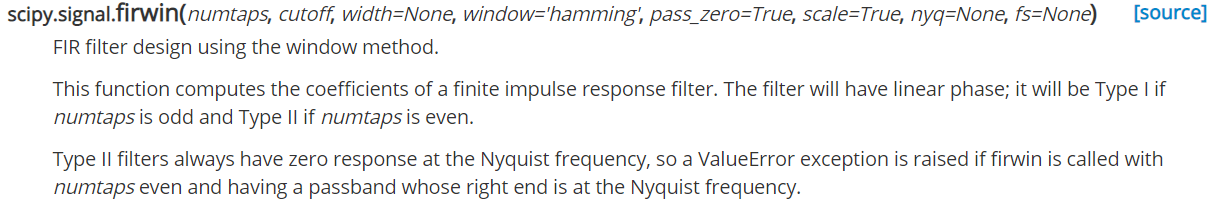
\includegraphics[width=\textwidth]{firwin.png}
    \caption{Function prototype and description for \texttt{firwin}.}
    \label{fig:firwin}
\end{figure}

\subsection{Optimal FIR Filter}
Digital filters designed via the window method have the largest ripples at the passband and stopband edges. The optimal method of FIR filter design aims to keep the ripple
constant in the passbands and stopbands. FIR filter coefficients are calculated by this method with the SciPy function remez, which is described in Fig. 2. For the same
reason described in Section 2.1, \texttt{numtaps} passed to \texttt{remez} was 399. The sampling frequency fs was 1024 Hz.\\

\noindent Ideally, the notch filters would attenuate only the additive noise frequencies, while not affecting frequencies. Zooming in on the ECG spectrum showed that
the noise existed almost entirely in the bands 32.5 – 32.7 Hz and 61.6 – 61.8 Hz; these frequencies define the stopband edges. To define the \texttt{bands} parameter, it is
also necessary to choose a transition bandwidth. Reducing the transition bandwidth results in less stop-band attenuation. By experimentation, it was found that a transition
bandwidth of 3.5 Hz eliminated the noise frequencies. The bands parameter was passed as $[0, 29, 32.5, 32.7, 36.2, 58.1, 61.6, 61.8, 65.3, 512]$. The desired gain in each
band of \texttt{bands} is defined by \texttt{desired}, which must be half the length of bands. The value for desired $[1, 0, 1, 0, 1]$.

\begin{figure}[H]
    \centering
    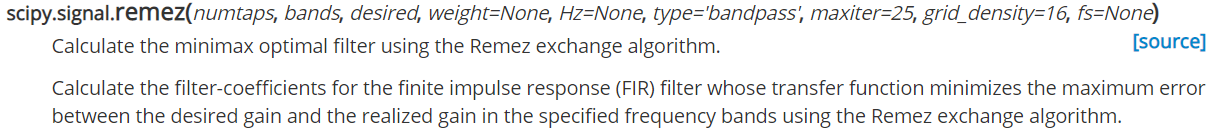
\includegraphics[width=\textwidth]{remez.png}
    \caption{Function prototype and description for \texttt{remez}.}
    \label{fig:remez}
\end{figure}

\subsection{Frequency Sampled FIR Filter}
ciPy does not define a function to design a frequency-sampled FIR filter, so a Python script was written to do this. The script was adapted from an example found in [2].
The script takes 400 equally spaced samples of the ideal frequency response with one sample taken at 0 Hz (i.e. a type 1 sampling scheme). Two transition samples were used,
though this can easily be changed with the \texttt{num\_transition\_samples} variable. The transition samples are equally spaced in magnitude, though ideal magnitude spacing may be
derived by extending the work in [3]. The inverse discrete Fourier transform of the ideal frequency response is calculated, giving the impulse response, which is then
shifted to make it symmetrical. The symmetrical impulse response is then tapered by a Hamming window.

\subsection{Pole-Zero Placed IIR Filters}
A simple method for IIR filter design is pole-zero placement on the z-plane. Zeros are placed in locations where the desired frequency response is zero. Poles are placed at
the same angle as the poles; their radii determine the transition bandwidth. To keep filter coefficients real, complex poles and zeros must come in complex-conjugate pairs.\\

\noindent For a notch filter, the angles the angle to place zeros (and poles) are:
\begin{equation}
    \textrm{arg}(z) = \pm \ang{360} \frac{f_{\textrm{notch}}}{f_s}
\end{equation}

\noindent With noise frequencies at 32.6 Hz and 61.7 Hz, zeros and poles were placed at ±11.46° for one notch filter and ±21.69° for the other notch filter. The 3 dB bandwidth of the
filters was specified as f3dB = 5 Hz, and the pole radius was calculated with:
\begin{equation}
    r = 1 - \frac{BW}{f_s}\pi
\end{equation}

\noindent Giving $r = 0.9847$ for both filters. To remove both noise frequencies, the IIR filters were cascaded together. Scaling factors of $0.99057$ and $0.98633$ were calculated and applied to
maintain unity passband gain. Figure 3 shows the final filter realisation.

\begin{figure}[H]
    \centering
    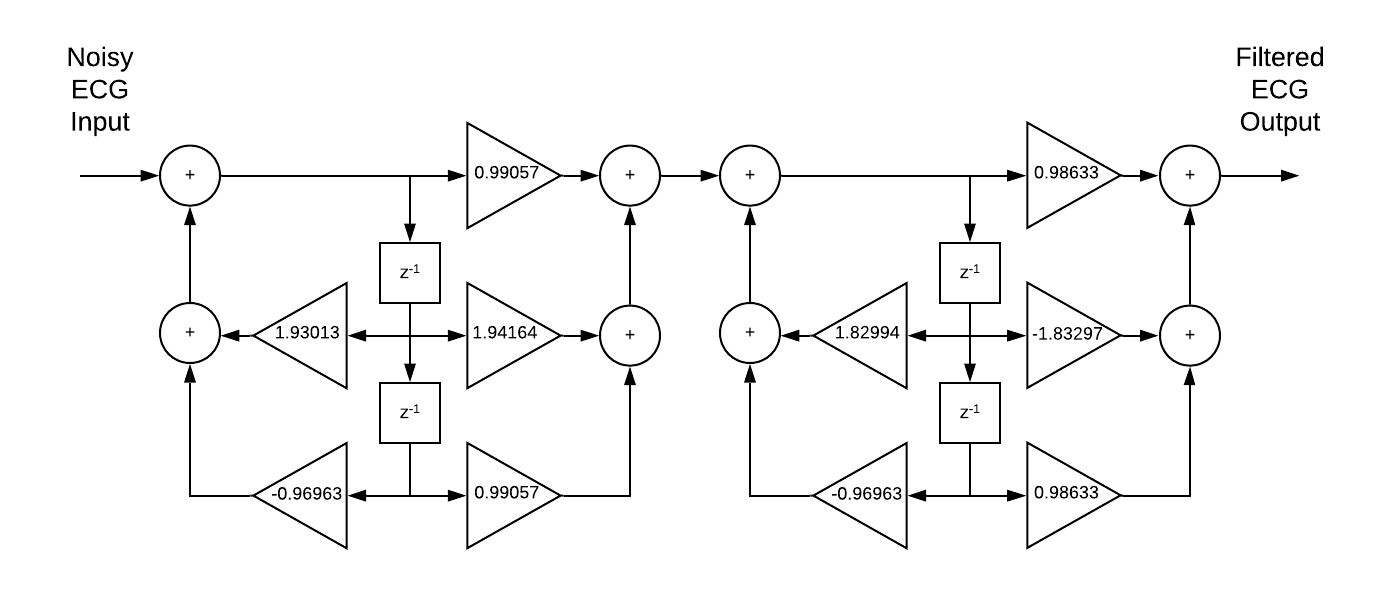
\includegraphics[width=\textwidth]{iir-block.png}
    \caption{Realisation of the cascaded IIR notch filters.}
    \label{fig:iir-filt}
\end{figure}
\section{Results}

\subsection{Noisy ECG Signal and Spectrum}
\begin{figure}[H]
    \centering
    \adjustbox{max width=0.75\textwidth}{
    %% Creator: Matplotlib, PGF backend
%%
%% To include the figure in your LaTeX document, write
%%   \input{<filename>.pgf}
%%
%% Make sure the required packages are loaded in your preamble
%%   \usepackage{pgf}
%%
%% and, on pdftex
%%   \usepackage[utf8]{inputenc}\DeclareUnicodeCharacter{2212}{-}
%%
%% or, on luatex and xetex
%%   \usepackage{unicode-math}
%%
%% Figures using additional raster images can only be included by \input if
%% they are in the same directory as the main LaTeX file. For loading figures
%% from other directories you can use the `import` package
%%   \usepackage{import}
%%
%% and then include the figures with
%%   \import{<path to file>}{<filename>.pgf}
%%
%% Matplotlib used the following preamble
%%
\begingroup%
\makeatletter%
\begin{pgfpicture}%
\pgfpathrectangle{\pgfpointorigin}{\pgfqpoint{6.400000in}{4.800000in}}%
\pgfusepath{use as bounding box, clip}%
\begin{pgfscope}%
\pgfsetbuttcap%
\pgfsetmiterjoin%
\definecolor{currentfill}{rgb}{1.000000,1.000000,1.000000}%
\pgfsetfillcolor{currentfill}%
\pgfsetlinewidth{0.000000pt}%
\definecolor{currentstroke}{rgb}{1.000000,1.000000,1.000000}%
\pgfsetstrokecolor{currentstroke}%
\pgfsetdash{}{0pt}%
\pgfpathmoveto{\pgfqpoint{0.000000in}{0.000000in}}%
\pgfpathlineto{\pgfqpoint{6.400000in}{0.000000in}}%
\pgfpathlineto{\pgfqpoint{6.400000in}{4.800000in}}%
\pgfpathlineto{\pgfqpoint{0.000000in}{4.800000in}}%
\pgfpathclose%
\pgfusepath{fill}%
\end{pgfscope}%
\begin{pgfscope}%
\pgfsetbuttcap%
\pgfsetmiterjoin%
\definecolor{currentfill}{rgb}{1.000000,1.000000,1.000000}%
\pgfsetfillcolor{currentfill}%
\pgfsetlinewidth{0.000000pt}%
\definecolor{currentstroke}{rgb}{0.000000,0.000000,0.000000}%
\pgfsetstrokecolor{currentstroke}%
\pgfsetstrokeopacity{0.000000}%
\pgfsetdash{}{0pt}%
\pgfpathmoveto{\pgfqpoint{0.825510in}{2.889143in}}%
\pgfpathlineto{\pgfqpoint{6.146222in}{2.889143in}}%
\pgfpathlineto{\pgfqpoint{6.146222in}{4.451359in}}%
\pgfpathlineto{\pgfqpoint{0.825510in}{4.451359in}}%
\pgfpathclose%
\pgfusepath{fill}%
\end{pgfscope}%
\begin{pgfscope}%
\pgfsetbuttcap%
\pgfsetroundjoin%
\definecolor{currentfill}{rgb}{0.000000,0.000000,0.000000}%
\pgfsetfillcolor{currentfill}%
\pgfsetlinewidth{0.803000pt}%
\definecolor{currentstroke}{rgb}{0.000000,0.000000,0.000000}%
\pgfsetstrokecolor{currentstroke}%
\pgfsetdash{}{0pt}%
\pgfsys@defobject{currentmarker}{\pgfqpoint{0.000000in}{-0.048611in}}{\pgfqpoint{0.000000in}{0.000000in}}{%
\pgfpathmoveto{\pgfqpoint{0.000000in}{0.000000in}}%
\pgfpathlineto{\pgfqpoint{0.000000in}{-0.048611in}}%
\pgfusepath{stroke,fill}%
}%
\begin{pgfscope}%
\pgfsys@transformshift{1.067361in}{2.889143in}%
\pgfsys@useobject{currentmarker}{}%
\end{pgfscope}%
\end{pgfscope}%
\begin{pgfscope}%
\definecolor{textcolor}{rgb}{0.000000,0.000000,0.000000}%
\pgfsetstrokecolor{textcolor}%
\pgfsetfillcolor{textcolor}%
\pgftext[x=1.067361in,y=2.791921in,,top]{\color{textcolor}\rmfamily\fontsize{10.000000}{12.000000}\selectfont \(\displaystyle {0}\)}%
\end{pgfscope}%
\begin{pgfscope}%
\pgfsetbuttcap%
\pgfsetroundjoin%
\definecolor{currentfill}{rgb}{0.000000,0.000000,0.000000}%
\pgfsetfillcolor{currentfill}%
\pgfsetlinewidth{0.803000pt}%
\definecolor{currentstroke}{rgb}{0.000000,0.000000,0.000000}%
\pgfsetstrokecolor{currentstroke}%
\pgfsetdash{}{0pt}%
\pgfsys@defobject{currentmarker}{\pgfqpoint{0.000000in}{-0.048611in}}{\pgfqpoint{0.000000in}{0.000000in}}{%
\pgfpathmoveto{\pgfqpoint{0.000000in}{0.000000in}}%
\pgfpathlineto{\pgfqpoint{0.000000in}{-0.048611in}}%
\pgfusepath{stroke,fill}%
}%
\begin{pgfscope}%
\pgfsys@transformshift{2.058000in}{2.889143in}%
\pgfsys@useobject{currentmarker}{}%
\end{pgfscope}%
\end{pgfscope}%
\begin{pgfscope}%
\definecolor{textcolor}{rgb}{0.000000,0.000000,0.000000}%
\pgfsetstrokecolor{textcolor}%
\pgfsetfillcolor{textcolor}%
\pgftext[x=2.058000in,y=2.791921in,,top]{\color{textcolor}\rmfamily\fontsize{10.000000}{12.000000}\selectfont \(\displaystyle {10}\)}%
\end{pgfscope}%
\begin{pgfscope}%
\pgfsetbuttcap%
\pgfsetroundjoin%
\definecolor{currentfill}{rgb}{0.000000,0.000000,0.000000}%
\pgfsetfillcolor{currentfill}%
\pgfsetlinewidth{0.803000pt}%
\definecolor{currentstroke}{rgb}{0.000000,0.000000,0.000000}%
\pgfsetstrokecolor{currentstroke}%
\pgfsetdash{}{0pt}%
\pgfsys@defobject{currentmarker}{\pgfqpoint{0.000000in}{-0.048611in}}{\pgfqpoint{0.000000in}{0.000000in}}{%
\pgfpathmoveto{\pgfqpoint{0.000000in}{0.000000in}}%
\pgfpathlineto{\pgfqpoint{0.000000in}{-0.048611in}}%
\pgfusepath{stroke,fill}%
}%
\begin{pgfscope}%
\pgfsys@transformshift{3.048640in}{2.889143in}%
\pgfsys@useobject{currentmarker}{}%
\end{pgfscope}%
\end{pgfscope}%
\begin{pgfscope}%
\definecolor{textcolor}{rgb}{0.000000,0.000000,0.000000}%
\pgfsetstrokecolor{textcolor}%
\pgfsetfillcolor{textcolor}%
\pgftext[x=3.048640in,y=2.791921in,,top]{\color{textcolor}\rmfamily\fontsize{10.000000}{12.000000}\selectfont \(\displaystyle {20}\)}%
\end{pgfscope}%
\begin{pgfscope}%
\pgfsetbuttcap%
\pgfsetroundjoin%
\definecolor{currentfill}{rgb}{0.000000,0.000000,0.000000}%
\pgfsetfillcolor{currentfill}%
\pgfsetlinewidth{0.803000pt}%
\definecolor{currentstroke}{rgb}{0.000000,0.000000,0.000000}%
\pgfsetstrokecolor{currentstroke}%
\pgfsetdash{}{0pt}%
\pgfsys@defobject{currentmarker}{\pgfqpoint{0.000000in}{-0.048611in}}{\pgfqpoint{0.000000in}{0.000000in}}{%
\pgfpathmoveto{\pgfqpoint{0.000000in}{0.000000in}}%
\pgfpathlineto{\pgfqpoint{0.000000in}{-0.048611in}}%
\pgfusepath{stroke,fill}%
}%
\begin{pgfscope}%
\pgfsys@transformshift{4.039280in}{2.889143in}%
\pgfsys@useobject{currentmarker}{}%
\end{pgfscope}%
\end{pgfscope}%
\begin{pgfscope}%
\definecolor{textcolor}{rgb}{0.000000,0.000000,0.000000}%
\pgfsetstrokecolor{textcolor}%
\pgfsetfillcolor{textcolor}%
\pgftext[x=4.039280in,y=2.791921in,,top]{\color{textcolor}\rmfamily\fontsize{10.000000}{12.000000}\selectfont \(\displaystyle {30}\)}%
\end{pgfscope}%
\begin{pgfscope}%
\pgfsetbuttcap%
\pgfsetroundjoin%
\definecolor{currentfill}{rgb}{0.000000,0.000000,0.000000}%
\pgfsetfillcolor{currentfill}%
\pgfsetlinewidth{0.803000pt}%
\definecolor{currentstroke}{rgb}{0.000000,0.000000,0.000000}%
\pgfsetstrokecolor{currentstroke}%
\pgfsetdash{}{0pt}%
\pgfsys@defobject{currentmarker}{\pgfqpoint{0.000000in}{-0.048611in}}{\pgfqpoint{0.000000in}{0.000000in}}{%
\pgfpathmoveto{\pgfqpoint{0.000000in}{0.000000in}}%
\pgfpathlineto{\pgfqpoint{0.000000in}{-0.048611in}}%
\pgfusepath{stroke,fill}%
}%
\begin{pgfscope}%
\pgfsys@transformshift{5.029919in}{2.889143in}%
\pgfsys@useobject{currentmarker}{}%
\end{pgfscope}%
\end{pgfscope}%
\begin{pgfscope}%
\definecolor{textcolor}{rgb}{0.000000,0.000000,0.000000}%
\pgfsetstrokecolor{textcolor}%
\pgfsetfillcolor{textcolor}%
\pgftext[x=5.029919in,y=2.791921in,,top]{\color{textcolor}\rmfamily\fontsize{10.000000}{12.000000}\selectfont \(\displaystyle {40}\)}%
\end{pgfscope}%
\begin{pgfscope}%
\pgfsetbuttcap%
\pgfsetroundjoin%
\definecolor{currentfill}{rgb}{0.000000,0.000000,0.000000}%
\pgfsetfillcolor{currentfill}%
\pgfsetlinewidth{0.803000pt}%
\definecolor{currentstroke}{rgb}{0.000000,0.000000,0.000000}%
\pgfsetstrokecolor{currentstroke}%
\pgfsetdash{}{0pt}%
\pgfsys@defobject{currentmarker}{\pgfqpoint{0.000000in}{-0.048611in}}{\pgfqpoint{0.000000in}{0.000000in}}{%
\pgfpathmoveto{\pgfqpoint{0.000000in}{0.000000in}}%
\pgfpathlineto{\pgfqpoint{0.000000in}{-0.048611in}}%
\pgfusepath{stroke,fill}%
}%
\begin{pgfscope}%
\pgfsys@transformshift{6.020559in}{2.889143in}%
\pgfsys@useobject{currentmarker}{}%
\end{pgfscope}%
\end{pgfscope}%
\begin{pgfscope}%
\definecolor{textcolor}{rgb}{0.000000,0.000000,0.000000}%
\pgfsetstrokecolor{textcolor}%
\pgfsetfillcolor{textcolor}%
\pgftext[x=6.020559in,y=2.791921in,,top]{\color{textcolor}\rmfamily\fontsize{10.000000}{12.000000}\selectfont \(\displaystyle {50}\)}%
\end{pgfscope}%
\begin{pgfscope}%
\definecolor{textcolor}{rgb}{0.000000,0.000000,0.000000}%
\pgfsetstrokecolor{textcolor}%
\pgfsetfillcolor{textcolor}%
\pgftext[x=3.485866in,y=2.612909in,,top]{\color{textcolor}\rmfamily\fontsize{10.000000}{12.000000}\selectfont Time (s)}%
\end{pgfscope}%
\begin{pgfscope}%
\pgfsetbuttcap%
\pgfsetroundjoin%
\definecolor{currentfill}{rgb}{0.000000,0.000000,0.000000}%
\pgfsetfillcolor{currentfill}%
\pgfsetlinewidth{0.803000pt}%
\definecolor{currentstroke}{rgb}{0.000000,0.000000,0.000000}%
\pgfsetstrokecolor{currentstroke}%
\pgfsetdash{}{0pt}%
\pgfsys@defobject{currentmarker}{\pgfqpoint{-0.048611in}{0.000000in}}{\pgfqpoint{0.000000in}{0.000000in}}{%
\pgfpathmoveto{\pgfqpoint{0.000000in}{0.000000in}}%
\pgfpathlineto{\pgfqpoint{-0.048611in}{0.000000in}}%
\pgfusepath{stroke,fill}%
}%
\begin{pgfscope}%
\pgfsys@transformshift{0.825510in}{3.013981in}%
\pgfsys@useobject{currentmarker}{}%
\end{pgfscope}%
\end{pgfscope}%
\begin{pgfscope}%
\definecolor{textcolor}{rgb}{0.000000,0.000000,0.000000}%
\pgfsetstrokecolor{textcolor}%
\pgfsetfillcolor{textcolor}%
\pgftext[x=0.342484in, y=2.965756in, left, base]{\color{textcolor}\rmfamily\fontsize{10.000000}{12.000000}\selectfont \(\displaystyle {-1000}\)}%
\end{pgfscope}%
\begin{pgfscope}%
\pgfsetbuttcap%
\pgfsetroundjoin%
\definecolor{currentfill}{rgb}{0.000000,0.000000,0.000000}%
\pgfsetfillcolor{currentfill}%
\pgfsetlinewidth{0.803000pt}%
\definecolor{currentstroke}{rgb}{0.000000,0.000000,0.000000}%
\pgfsetstrokecolor{currentstroke}%
\pgfsetdash{}{0pt}%
\pgfsys@defobject{currentmarker}{\pgfqpoint{-0.048611in}{0.000000in}}{\pgfqpoint{0.000000in}{0.000000in}}{%
\pgfpathmoveto{\pgfqpoint{0.000000in}{0.000000in}}%
\pgfpathlineto{\pgfqpoint{-0.048611in}{0.000000in}}%
\pgfusepath{stroke,fill}%
}%
\begin{pgfscope}%
\pgfsys@transformshift{0.825510in}{3.558604in}%
\pgfsys@useobject{currentmarker}{}%
\end{pgfscope}%
\end{pgfscope}%
\begin{pgfscope}%
\definecolor{textcolor}{rgb}{0.000000,0.000000,0.000000}%
\pgfsetstrokecolor{textcolor}%
\pgfsetfillcolor{textcolor}%
\pgftext[x=0.658843in, y=3.510378in, left, base]{\color{textcolor}\rmfamily\fontsize{10.000000}{12.000000}\selectfont \(\displaystyle {0}\)}%
\end{pgfscope}%
\begin{pgfscope}%
\pgfsetbuttcap%
\pgfsetroundjoin%
\definecolor{currentfill}{rgb}{0.000000,0.000000,0.000000}%
\pgfsetfillcolor{currentfill}%
\pgfsetlinewidth{0.803000pt}%
\definecolor{currentstroke}{rgb}{0.000000,0.000000,0.000000}%
\pgfsetstrokecolor{currentstroke}%
\pgfsetdash{}{0pt}%
\pgfsys@defobject{currentmarker}{\pgfqpoint{-0.048611in}{0.000000in}}{\pgfqpoint{0.000000in}{0.000000in}}{%
\pgfpathmoveto{\pgfqpoint{0.000000in}{0.000000in}}%
\pgfpathlineto{\pgfqpoint{-0.048611in}{0.000000in}}%
\pgfusepath{stroke,fill}%
}%
\begin{pgfscope}%
\pgfsys@transformshift{0.825510in}{4.103226in}%
\pgfsys@useobject{currentmarker}{}%
\end{pgfscope}%
\end{pgfscope}%
\begin{pgfscope}%
\definecolor{textcolor}{rgb}{0.000000,0.000000,0.000000}%
\pgfsetstrokecolor{textcolor}%
\pgfsetfillcolor{textcolor}%
\pgftext[x=0.450509in, y=4.055001in, left, base]{\color{textcolor}\rmfamily\fontsize{10.000000}{12.000000}\selectfont \(\displaystyle {1000}\)}%
\end{pgfscope}%
\begin{pgfscope}%
\definecolor{textcolor}{rgb}{0.000000,0.000000,0.000000}%
\pgfsetstrokecolor{textcolor}%
\pgfsetfillcolor{textcolor}%
\pgftext[x=0.286929in,y=3.670251in,,bottom,rotate=90.000000]{\color{textcolor}\rmfamily\fontsize{10.000000}{12.000000}\selectfont ECG Voltage (\(\displaystyle \mu V\))}%
\end{pgfscope}%
\begin{pgfscope}%
\pgfpathrectangle{\pgfqpoint{0.825510in}{2.889143in}}{\pgfqpoint{5.320712in}{1.562215in}}%
\pgfusepath{clip}%
\pgfsetrectcap%
\pgfsetroundjoin%
\pgfsetlinewidth{1.505625pt}%
\definecolor{currentstroke}{rgb}{0.121569,0.466667,0.705882}%
\pgfsetstrokecolor{currentstroke}%
\pgfsetdash{}{0pt}%
\pgfpathmoveto{\pgfqpoint{1.067361in}{3.806574in}}%
\pgfpathlineto{\pgfqpoint{1.067554in}{3.858633in}}%
\pgfpathlineto{\pgfqpoint{1.067941in}{3.702468in}}%
\pgfpathlineto{\pgfqpoint{1.068425in}{3.487366in}}%
\pgfpathlineto{\pgfqpoint{1.068908in}{3.746014in}}%
\pgfpathlineto{\pgfqpoint{1.069199in}{3.810703in}}%
\pgfpathlineto{\pgfqpoint{1.069586in}{3.651798in}}%
\pgfpathlineto{\pgfqpoint{1.069973in}{3.483372in}}%
\pgfpathlineto{\pgfqpoint{1.070456in}{3.696475in}}%
\pgfpathlineto{\pgfqpoint{1.070747in}{3.808175in}}%
\pgfpathlineto{\pgfqpoint{1.071230in}{3.609359in}}%
\pgfpathlineto{\pgfqpoint{1.071617in}{3.456683in}}%
\pgfpathlineto{\pgfqpoint{1.072101in}{3.665882in}}%
\pgfpathlineto{\pgfqpoint{1.072391in}{3.765746in}}%
\pgfpathlineto{\pgfqpoint{1.072875in}{3.563229in}}%
\pgfpathlineto{\pgfqpoint{1.073165in}{3.464959in}}%
\pgfpathlineto{\pgfqpoint{1.073649in}{3.644841in}}%
\pgfpathlineto{\pgfqpoint{1.073939in}{3.766650in}}%
\pgfpathlineto{\pgfqpoint{1.074520in}{3.524647in}}%
\pgfpathlineto{\pgfqpoint{1.074810in}{3.418420in}}%
\pgfpathlineto{\pgfqpoint{1.075293in}{3.628015in}}%
\pgfpathlineto{\pgfqpoint{1.075584in}{3.712466in}}%
\pgfpathlineto{\pgfqpoint{1.076067in}{3.514412in}}%
\pgfpathlineto{\pgfqpoint{1.076454in}{3.388224in}}%
\pgfpathlineto{\pgfqpoint{1.076938in}{3.607152in}}%
\pgfpathlineto{\pgfqpoint{1.077228in}{3.673891in}}%
\pgfpathlineto{\pgfqpoint{1.077615in}{3.499424in}}%
\pgfpathlineto{\pgfqpoint{1.078002in}{3.329392in}}%
\pgfpathlineto{\pgfqpoint{1.078583in}{3.592316in}}%
\pgfpathlineto{\pgfqpoint{1.078776in}{3.639266in}}%
\pgfpathlineto{\pgfqpoint{1.079260in}{3.481436in}}%
\pgfpathlineto{\pgfqpoint{1.079647in}{3.359776in}}%
\pgfpathlineto{\pgfqpoint{1.080131in}{3.552700in}}%
\pgfpathlineto{\pgfqpoint{1.080421in}{3.642304in}}%
\pgfpathlineto{\pgfqpoint{1.080905in}{3.414723in}}%
\pgfpathlineto{\pgfqpoint{1.081195in}{3.318450in}}%
\pgfpathlineto{\pgfqpoint{1.081678in}{3.520414in}}%
\pgfpathlineto{\pgfqpoint{1.082065in}{3.644260in}}%
\pgfpathlineto{\pgfqpoint{1.082549in}{3.435280in}}%
\pgfpathlineto{\pgfqpoint{1.082839in}{3.355348in}}%
\pgfpathlineto{\pgfqpoint{1.083323in}{3.580212in}}%
\pgfpathlineto{\pgfqpoint{1.083613in}{3.674911in}}%
\pgfpathlineto{\pgfqpoint{1.084097in}{3.452198in}}%
\pgfpathlineto{\pgfqpoint{1.084387in}{3.353673in}}%
\pgfpathlineto{\pgfqpoint{1.084871in}{3.536031in}}%
\pgfpathlineto{\pgfqpoint{1.085258in}{3.672629in}}%
\pgfpathlineto{\pgfqpoint{1.085742in}{3.454205in}}%
\pgfpathlineto{\pgfqpoint{1.086032in}{3.368296in}}%
\pgfpathlineto{\pgfqpoint{1.086516in}{3.562048in}}%
\pgfpathlineto{\pgfqpoint{1.086806in}{3.684463in}}%
\pgfpathlineto{\pgfqpoint{1.087386in}{3.436989in}}%
\pgfpathlineto{\pgfqpoint{1.087580in}{3.381223in}}%
\pgfpathlineto{\pgfqpoint{1.088063in}{3.570192in}}%
\pgfpathlineto{\pgfqpoint{1.088450in}{3.722713in}}%
\pgfpathlineto{\pgfqpoint{1.089031in}{3.486497in}}%
\pgfpathlineto{\pgfqpoint{1.089224in}{3.427517in}}%
\pgfpathlineto{\pgfqpoint{1.089708in}{3.618480in}}%
\pgfpathlineto{\pgfqpoint{1.089998in}{3.726427in}}%
\pgfpathlineto{\pgfqpoint{1.090482in}{3.536312in}}%
\pgfpathlineto{\pgfqpoint{1.090772in}{3.413551in}}%
\pgfpathlineto{\pgfqpoint{1.091353in}{3.621406in}}%
\pgfpathlineto{\pgfqpoint{1.091643in}{3.710747in}}%
\pgfpathlineto{\pgfqpoint{1.092127in}{3.486605in}}%
\pgfpathlineto{\pgfqpoint{1.092514in}{3.337359in}}%
\pgfpathlineto{\pgfqpoint{1.092997in}{3.561283in}}%
\pgfpathlineto{\pgfqpoint{1.093288in}{3.634213in}}%
\pgfpathlineto{\pgfqpoint{1.093674in}{3.457850in}}%
\pgfpathlineto{\pgfqpoint{1.094061in}{3.303476in}}%
\pgfpathlineto{\pgfqpoint{1.094545in}{3.533798in}}%
\pgfpathlineto{\pgfqpoint{1.094932in}{3.653376in}}%
\pgfpathlineto{\pgfqpoint{1.095319in}{3.452567in}}%
\pgfpathlineto{\pgfqpoint{1.095706in}{3.319894in}}%
\pgfpathlineto{\pgfqpoint{1.096190in}{3.567776in}}%
\pgfpathlineto{\pgfqpoint{1.096480in}{3.656270in}}%
\pgfpathlineto{\pgfqpoint{1.096964in}{3.422118in}}%
\pgfpathlineto{\pgfqpoint{1.097254in}{3.334173in}}%
\pgfpathlineto{\pgfqpoint{1.097738in}{3.547950in}}%
\pgfpathlineto{\pgfqpoint{1.098125in}{3.672543in}}%
\pgfpathlineto{\pgfqpoint{1.098608in}{3.428084in}}%
\pgfpathlineto{\pgfqpoint{1.098899in}{3.318884in}}%
\pgfpathlineto{\pgfqpoint{1.099382in}{3.558827in}}%
\pgfpathlineto{\pgfqpoint{1.101027in}{4.004826in}}%
\pgfpathlineto{\pgfqpoint{1.101220in}{4.051678in}}%
\pgfpathlineto{\pgfqpoint{1.101607in}{3.864960in}}%
\pgfpathlineto{\pgfqpoint{1.102285in}{3.318088in}}%
\pgfpathlineto{\pgfqpoint{1.102865in}{3.611174in}}%
\pgfpathlineto{\pgfqpoint{1.103058in}{3.649848in}}%
\pgfpathlineto{\pgfqpoint{1.103445in}{3.483198in}}%
\pgfpathlineto{\pgfqpoint{1.103639in}{3.421826in}}%
\pgfpathlineto{\pgfqpoint{1.104123in}{3.602652in}}%
\pgfpathlineto{\pgfqpoint{1.104510in}{3.723852in}}%
\pgfpathlineto{\pgfqpoint{1.104993in}{3.499593in}}%
\pgfpathlineto{\pgfqpoint{1.105284in}{3.380229in}}%
\pgfpathlineto{\pgfqpoint{1.105767in}{3.588832in}}%
\pgfpathlineto{\pgfqpoint{1.106154in}{3.711172in}}%
\pgfpathlineto{\pgfqpoint{1.106638in}{3.509365in}}%
\pgfpathlineto{\pgfqpoint{1.106928in}{3.422715in}}%
\pgfpathlineto{\pgfqpoint{1.107412in}{3.638371in}}%
\pgfpathlineto{\pgfqpoint{1.107702in}{3.718343in}}%
\pgfpathlineto{\pgfqpoint{1.108186in}{3.504428in}}%
\pgfpathlineto{\pgfqpoint{1.108476in}{3.399368in}}%
\pgfpathlineto{\pgfqpoint{1.108960in}{3.572387in}}%
\pgfpathlineto{\pgfqpoint{1.109347in}{3.713750in}}%
\pgfpathlineto{\pgfqpoint{1.109830in}{3.502858in}}%
\pgfpathlineto{\pgfqpoint{1.110121in}{3.408127in}}%
\pgfpathlineto{\pgfqpoint{1.110604in}{3.621084in}}%
\pgfpathlineto{\pgfqpoint{1.110895in}{3.703867in}}%
\pgfpathlineto{\pgfqpoint{1.111378in}{3.499606in}}%
\pgfpathlineto{\pgfqpoint{1.111669in}{3.378378in}}%
\pgfpathlineto{\pgfqpoint{1.112249in}{3.633468in}}%
\pgfpathlineto{\pgfqpoint{1.112539in}{3.717361in}}%
\pgfpathlineto{\pgfqpoint{1.113023in}{3.517117in}}%
\pgfpathlineto{\pgfqpoint{1.113313in}{3.434530in}}%
\pgfpathlineto{\pgfqpoint{1.113797in}{3.626505in}}%
\pgfpathlineto{\pgfqpoint{1.114087in}{3.732162in}}%
\pgfpathlineto{\pgfqpoint{1.114571in}{3.521977in}}%
\pgfpathlineto{\pgfqpoint{1.114861in}{3.408875in}}%
\pgfpathlineto{\pgfqpoint{1.115441in}{3.631851in}}%
\pgfpathlineto{\pgfqpoint{1.115732in}{3.742680in}}%
\pgfpathlineto{\pgfqpoint{1.116215in}{3.547435in}}%
\pgfpathlineto{\pgfqpoint{1.116506in}{3.434952in}}%
\pgfpathlineto{\pgfqpoint{1.117086in}{3.664942in}}%
\pgfpathlineto{\pgfqpoint{1.117280in}{3.734632in}}%
\pgfpathlineto{\pgfqpoint{1.117763in}{3.545075in}}%
\pgfpathlineto{\pgfqpoint{1.118150in}{3.418442in}}%
\pgfpathlineto{\pgfqpoint{1.118634in}{3.625632in}}%
\pgfpathlineto{\pgfqpoint{1.118924in}{3.716182in}}%
\pgfpathlineto{\pgfqpoint{1.119408in}{3.517920in}}%
\pgfpathlineto{\pgfqpoint{1.119795in}{3.364381in}}%
\pgfpathlineto{\pgfqpoint{1.120375in}{3.588940in}}%
\pgfpathlineto{\pgfqpoint{1.120569in}{3.609875in}}%
\pgfpathlineto{\pgfqpoint{1.120859in}{3.483415in}}%
\pgfpathlineto{\pgfqpoint{1.121343in}{3.281252in}}%
\pgfpathlineto{\pgfqpoint{1.121826in}{3.516789in}}%
\pgfpathlineto{\pgfqpoint{1.122213in}{3.645223in}}%
\pgfpathlineto{\pgfqpoint{1.122697in}{3.443277in}}%
\pgfpathlineto{\pgfqpoint{1.122891in}{3.386050in}}%
\pgfpathlineto{\pgfqpoint{1.123374in}{3.552186in}}%
\pgfpathlineto{\pgfqpoint{1.123761in}{3.705722in}}%
\pgfpathlineto{\pgfqpoint{1.124245in}{3.474175in}}%
\pgfpathlineto{\pgfqpoint{1.124535in}{3.366088in}}%
\pgfpathlineto{\pgfqpoint{1.125019in}{3.560792in}}%
\pgfpathlineto{\pgfqpoint{1.125309in}{3.669423in}}%
\pgfpathlineto{\pgfqpoint{1.125793in}{3.475116in}}%
\pgfpathlineto{\pgfqpoint{1.126180in}{3.323111in}}%
\pgfpathlineto{\pgfqpoint{1.126664in}{3.531376in}}%
\pgfpathlineto{\pgfqpoint{1.126954in}{3.611522in}}%
\pgfpathlineto{\pgfqpoint{1.127437in}{3.423421in}}%
\pgfpathlineto{\pgfqpoint{1.127824in}{3.316976in}}%
\pgfpathlineto{\pgfqpoint{1.128211in}{3.502346in}}%
\pgfpathlineto{\pgfqpoint{1.128598in}{3.630227in}}%
\pgfpathlineto{\pgfqpoint{1.129082in}{3.388208in}}%
\pgfpathlineto{\pgfqpoint{1.129372in}{3.282645in}}%
\pgfpathlineto{\pgfqpoint{1.129953in}{3.523166in}}%
\pgfpathlineto{\pgfqpoint{1.130243in}{3.586404in}}%
\pgfpathlineto{\pgfqpoint{1.130630in}{3.425222in}}%
\pgfpathlineto{\pgfqpoint{1.130920in}{3.307875in}}%
\pgfpathlineto{\pgfqpoint{1.131501in}{3.547808in}}%
\pgfpathlineto{\pgfqpoint{1.131791in}{3.611608in}}%
\pgfpathlineto{\pgfqpoint{1.132178in}{3.444253in}}%
\pgfpathlineto{\pgfqpoint{1.132565in}{3.288586in}}%
\pgfpathlineto{\pgfqpoint{1.133145in}{3.526692in}}%
\pgfpathlineto{\pgfqpoint{1.133436in}{3.600369in}}%
\pgfpathlineto{\pgfqpoint{1.133822in}{3.426080in}}%
\pgfpathlineto{\pgfqpoint{1.134113in}{3.307372in}}%
\pgfpathlineto{\pgfqpoint{1.134693in}{3.517848in}}%
\pgfpathlineto{\pgfqpoint{1.134983in}{3.609954in}}%
\pgfpathlineto{\pgfqpoint{1.135467in}{3.400825in}}%
\pgfpathlineto{\pgfqpoint{1.135757in}{3.296787in}}%
\pgfpathlineto{\pgfqpoint{1.136241in}{3.493810in}}%
\pgfpathlineto{\pgfqpoint{1.136628in}{3.652096in}}%
\pgfpathlineto{\pgfqpoint{1.137208in}{3.426517in}}%
\pgfpathlineto{\pgfqpoint{1.137402in}{3.389846in}}%
\pgfpathlineto{\pgfqpoint{1.137789in}{3.545017in}}%
\pgfpathlineto{\pgfqpoint{1.138176in}{3.688423in}}%
\pgfpathlineto{\pgfqpoint{1.138660in}{3.485350in}}%
\pgfpathlineto{\pgfqpoint{1.138950in}{3.380053in}}%
\pgfpathlineto{\pgfqpoint{1.139530in}{3.603885in}}%
\pgfpathlineto{\pgfqpoint{1.139820in}{3.682145in}}%
\pgfpathlineto{\pgfqpoint{1.140304in}{3.473128in}}%
\pgfpathlineto{\pgfqpoint{1.140594in}{3.358546in}}%
\pgfpathlineto{\pgfqpoint{1.141175in}{3.567789in}}%
\pgfpathlineto{\pgfqpoint{1.141465in}{3.619484in}}%
\pgfpathlineto{\pgfqpoint{1.141852in}{3.449659in}}%
\pgfpathlineto{\pgfqpoint{1.142239in}{3.321660in}}%
\pgfpathlineto{\pgfqpoint{1.142723in}{3.544397in}}%
\pgfpathlineto{\pgfqpoint{1.143013in}{3.653896in}}%
\pgfpathlineto{\pgfqpoint{1.143593in}{3.408161in}}%
\pgfpathlineto{\pgfqpoint{1.143884in}{3.336160in}}%
\pgfpathlineto{\pgfqpoint{1.144271in}{3.521990in}}%
\pgfpathlineto{\pgfqpoint{1.144561in}{3.616134in}}%
\pgfpathlineto{\pgfqpoint{1.145141in}{3.404385in}}%
\pgfpathlineto{\pgfqpoint{1.145432in}{3.306271in}}%
\pgfpathlineto{\pgfqpoint{1.145915in}{3.542025in}}%
\pgfpathlineto{\pgfqpoint{1.146205in}{3.645120in}}%
\pgfpathlineto{\pgfqpoint{1.146689in}{3.453009in}}%
\pgfpathlineto{\pgfqpoint{1.147076in}{3.275198in}}%
\pgfpathlineto{\pgfqpoint{1.147560in}{3.521033in}}%
\pgfpathlineto{\pgfqpoint{1.149398in}{4.014702in}}%
\pgfpathlineto{\pgfqpoint{1.149688in}{3.915533in}}%
\pgfpathlineto{\pgfqpoint{1.150462in}{3.294991in}}%
\pgfpathlineto{\pgfqpoint{1.151139in}{3.599776in}}%
\pgfpathlineto{\pgfqpoint{1.151623in}{3.414147in}}%
\pgfpathlineto{\pgfqpoint{1.151817in}{3.368328in}}%
\pgfpathlineto{\pgfqpoint{1.152203in}{3.507454in}}%
\pgfpathlineto{\pgfqpoint{1.152590in}{3.694751in}}%
\pgfpathlineto{\pgfqpoint{1.153171in}{3.456734in}}%
\pgfpathlineto{\pgfqpoint{1.153461in}{3.326685in}}%
\pgfpathlineto{\pgfqpoint{1.154042in}{3.596606in}}%
\pgfpathlineto{\pgfqpoint{1.154235in}{3.657906in}}%
\pgfpathlineto{\pgfqpoint{1.154719in}{3.457853in}}%
\pgfpathlineto{\pgfqpoint{1.155009in}{3.377540in}}%
\pgfpathlineto{\pgfqpoint{1.155493in}{3.548921in}}%
\pgfpathlineto{\pgfqpoint{1.155880in}{3.690142in}}%
\pgfpathlineto{\pgfqpoint{1.156363in}{3.436797in}}%
\pgfpathlineto{\pgfqpoint{1.156654in}{3.340855in}}%
\pgfpathlineto{\pgfqpoint{1.157137in}{3.521320in}}%
\pgfpathlineto{\pgfqpoint{1.157428in}{3.645136in}}%
\pgfpathlineto{\pgfqpoint{1.158008in}{3.439362in}}%
\pgfpathlineto{\pgfqpoint{1.158298in}{3.378717in}}%
\pgfpathlineto{\pgfqpoint{1.158685in}{3.549136in}}%
\pgfpathlineto{\pgfqpoint{1.159072in}{3.693290in}}%
\pgfpathlineto{\pgfqpoint{1.159556in}{3.469650in}}%
\pgfpathlineto{\pgfqpoint{1.159846in}{3.344274in}}%
\pgfpathlineto{\pgfqpoint{1.160427in}{3.606835in}}%
\pgfpathlineto{\pgfqpoint{1.160717in}{3.667891in}}%
\pgfpathlineto{\pgfqpoint{1.161104in}{3.516484in}}%
\pgfpathlineto{\pgfqpoint{1.161394in}{3.394983in}}%
\pgfpathlineto{\pgfqpoint{1.161974in}{3.620234in}}%
\pgfpathlineto{\pgfqpoint{1.162265in}{3.695632in}}%
\pgfpathlineto{\pgfqpoint{1.162748in}{3.496631in}}%
\pgfpathlineto{\pgfqpoint{1.163135in}{3.353703in}}%
\pgfpathlineto{\pgfqpoint{1.163619in}{3.629863in}}%
\pgfpathlineto{\pgfqpoint{1.163909in}{3.691338in}}%
\pgfpathlineto{\pgfqpoint{1.164393in}{3.517759in}}%
\pgfpathlineto{\pgfqpoint{1.164683in}{3.420198in}}%
\pgfpathlineto{\pgfqpoint{1.165167in}{3.608658in}}%
\pgfpathlineto{\pgfqpoint{1.165457in}{3.722263in}}%
\pgfpathlineto{\pgfqpoint{1.166038in}{3.473510in}}%
\pgfpathlineto{\pgfqpoint{1.166328in}{3.408859in}}%
\pgfpathlineto{\pgfqpoint{1.166715in}{3.590281in}}%
\pgfpathlineto{\pgfqpoint{1.167102in}{3.764677in}}%
\pgfpathlineto{\pgfqpoint{1.167682in}{3.539731in}}%
\pgfpathlineto{\pgfqpoint{1.167876in}{3.494228in}}%
\pgfpathlineto{\pgfqpoint{1.168263in}{3.638718in}}%
\pgfpathlineto{\pgfqpoint{1.168650in}{3.784260in}}%
\pgfpathlineto{\pgfqpoint{1.169230in}{3.571879in}}%
\pgfpathlineto{\pgfqpoint{1.169520in}{3.497127in}}%
\pgfpathlineto{\pgfqpoint{1.169907in}{3.686518in}}%
\pgfpathlineto{\pgfqpoint{1.170391in}{3.848389in}}%
\pgfpathlineto{\pgfqpoint{1.170875in}{3.633388in}}%
\pgfpathlineto{\pgfqpoint{1.171068in}{3.579105in}}%
\pgfpathlineto{\pgfqpoint{1.171552in}{3.717831in}}%
\pgfpathlineto{\pgfqpoint{1.171939in}{3.847415in}}%
\pgfpathlineto{\pgfqpoint{1.172326in}{3.658033in}}%
\pgfpathlineto{\pgfqpoint{1.172713in}{3.530679in}}%
\pgfpathlineto{\pgfqpoint{1.173197in}{3.730589in}}%
\pgfpathlineto{\pgfqpoint{1.173487in}{3.847697in}}%
\pgfpathlineto{\pgfqpoint{1.174067in}{3.598655in}}%
\pgfpathlineto{\pgfqpoint{1.174357in}{3.508167in}}%
\pgfpathlineto{\pgfqpoint{1.174938in}{3.706369in}}%
\pgfpathlineto{\pgfqpoint{1.175131in}{3.723470in}}%
\pgfpathlineto{\pgfqpoint{1.175422in}{3.631357in}}%
\pgfpathlineto{\pgfqpoint{1.175905in}{3.419802in}}%
\pgfpathlineto{\pgfqpoint{1.176389in}{3.629621in}}%
\pgfpathlineto{\pgfqpoint{1.176679in}{3.733919in}}%
\pgfpathlineto{\pgfqpoint{1.177260in}{3.499891in}}%
\pgfpathlineto{\pgfqpoint{1.177550in}{3.396241in}}%
\pgfpathlineto{\pgfqpoint{1.178130in}{3.633775in}}%
\pgfpathlineto{\pgfqpoint{1.178324in}{3.679361in}}%
\pgfpathlineto{\pgfqpoint{1.178711in}{3.551443in}}%
\pgfpathlineto{\pgfqpoint{1.179098in}{3.399166in}}%
\pgfpathlineto{\pgfqpoint{1.179582in}{3.601934in}}%
\pgfpathlineto{\pgfqpoint{1.179968in}{3.746026in}}%
\pgfpathlineto{\pgfqpoint{1.180452in}{3.519896in}}%
\pgfpathlineto{\pgfqpoint{1.180742in}{3.410204in}}%
\pgfpathlineto{\pgfqpoint{1.181226in}{3.607966in}}%
\pgfpathlineto{\pgfqpoint{1.181516in}{3.698014in}}%
\pgfpathlineto{\pgfqpoint{1.182097in}{3.493770in}}%
\pgfpathlineto{\pgfqpoint{1.182387in}{3.425747in}}%
\pgfpathlineto{\pgfqpoint{1.182774in}{3.585889in}}%
\pgfpathlineto{\pgfqpoint{1.183161in}{3.737305in}}%
\pgfpathlineto{\pgfqpoint{1.183645in}{3.517634in}}%
\pgfpathlineto{\pgfqpoint{1.183935in}{3.414184in}}%
\pgfpathlineto{\pgfqpoint{1.184419in}{3.590535in}}%
\pgfpathlineto{\pgfqpoint{1.184806in}{3.711019in}}%
\pgfpathlineto{\pgfqpoint{1.185289in}{3.510364in}}%
\pgfpathlineto{\pgfqpoint{1.185580in}{3.442920in}}%
\pgfpathlineto{\pgfqpoint{1.185966in}{3.618061in}}%
\pgfpathlineto{\pgfqpoint{1.186353in}{3.747164in}}%
\pgfpathlineto{\pgfqpoint{1.186837in}{3.528142in}}%
\pgfpathlineto{\pgfqpoint{1.187224in}{3.388194in}}%
\pgfpathlineto{\pgfqpoint{1.187708in}{3.597431in}}%
\pgfpathlineto{\pgfqpoint{1.187998in}{3.662200in}}%
\pgfpathlineto{\pgfqpoint{1.188385in}{3.508181in}}%
\pgfpathlineto{\pgfqpoint{1.188772in}{3.382965in}}%
\pgfpathlineto{\pgfqpoint{1.189256in}{3.587084in}}%
\pgfpathlineto{\pgfqpoint{1.189546in}{3.669796in}}%
\pgfpathlineto{\pgfqpoint{1.190030in}{3.462910in}}%
\pgfpathlineto{\pgfqpoint{1.190417in}{3.336115in}}%
\pgfpathlineto{\pgfqpoint{1.190900in}{3.566563in}}%
\pgfpathlineto{\pgfqpoint{1.191191in}{3.652345in}}%
\pgfpathlineto{\pgfqpoint{1.191674in}{3.453440in}}%
\pgfpathlineto{\pgfqpoint{1.191965in}{3.363990in}}%
\pgfpathlineto{\pgfqpoint{1.192448in}{3.534558in}}%
\pgfpathlineto{\pgfqpoint{1.192738in}{3.622384in}}%
\pgfpathlineto{\pgfqpoint{1.193222in}{3.429485in}}%
\pgfpathlineto{\pgfqpoint{1.193609in}{3.274814in}}%
\pgfpathlineto{\pgfqpoint{1.194093in}{3.474316in}}%
\pgfpathlineto{\pgfqpoint{1.194383in}{3.565764in}}%
\pgfpathlineto{\pgfqpoint{1.194867in}{3.318286in}}%
\pgfpathlineto{\pgfqpoint{1.195157in}{3.206405in}}%
\pgfpathlineto{\pgfqpoint{1.195641in}{3.516301in}}%
\pgfpathlineto{\pgfqpoint{1.196124in}{3.826821in}}%
\pgfpathlineto{\pgfqpoint{1.196898in}{3.660844in}}%
\pgfpathlineto{\pgfqpoint{1.197576in}{3.934774in}}%
\pgfpathlineto{\pgfqpoint{1.197866in}{3.741858in}}%
\pgfpathlineto{\pgfqpoint{1.198446in}{3.224656in}}%
\pgfpathlineto{\pgfqpoint{1.199027in}{3.609631in}}%
\pgfpathlineto{\pgfqpoint{1.199220in}{3.643384in}}%
\pgfpathlineto{\pgfqpoint{1.199607in}{3.483010in}}%
\pgfpathlineto{\pgfqpoint{1.199994in}{3.365199in}}%
\pgfpathlineto{\pgfqpoint{1.200478in}{3.573734in}}%
\pgfpathlineto{\pgfqpoint{1.200768in}{3.711160in}}%
\pgfpathlineto{\pgfqpoint{1.201349in}{3.491026in}}%
\pgfpathlineto{\pgfqpoint{1.201639in}{3.399839in}}%
\pgfpathlineto{\pgfqpoint{1.202122in}{3.615675in}}%
\pgfpathlineto{\pgfqpoint{1.202413in}{3.681346in}}%
\pgfpathlineto{\pgfqpoint{1.202896in}{3.486514in}}%
\pgfpathlineto{\pgfqpoint{1.203187in}{3.391126in}}%
\pgfpathlineto{\pgfqpoint{1.203670in}{3.614002in}}%
\pgfpathlineto{\pgfqpoint{1.204057in}{3.764831in}}%
\pgfpathlineto{\pgfqpoint{1.204541in}{3.537744in}}%
\pgfpathlineto{\pgfqpoint{1.204831in}{3.466157in}}%
\pgfpathlineto{\pgfqpoint{1.205315in}{3.671357in}}%
\pgfpathlineto{\pgfqpoint{1.205605in}{3.738319in}}%
\pgfpathlineto{\pgfqpoint{1.206089in}{3.566783in}}%
\pgfpathlineto{\pgfqpoint{1.206379in}{3.470602in}}%
\pgfpathlineto{\pgfqpoint{1.206863in}{3.672066in}}%
\pgfpathlineto{\pgfqpoint{1.207250in}{3.821524in}}%
\pgfpathlineto{\pgfqpoint{1.207733in}{3.608050in}}%
\pgfpathlineto{\pgfqpoint{1.208024in}{3.491400in}}%
\pgfpathlineto{\pgfqpoint{1.208507in}{3.692634in}}%
\pgfpathlineto{\pgfqpoint{1.208798in}{3.798969in}}%
\pgfpathlineto{\pgfqpoint{1.209378in}{3.598120in}}%
\pgfpathlineto{\pgfqpoint{1.209668in}{3.545297in}}%
\pgfpathlineto{\pgfqpoint{1.210055in}{3.726465in}}%
\pgfpathlineto{\pgfqpoint{1.210442in}{3.886543in}}%
\pgfpathlineto{\pgfqpoint{1.210926in}{3.684571in}}%
\pgfpathlineto{\pgfqpoint{1.211313in}{3.563158in}}%
\pgfpathlineto{\pgfqpoint{1.211797in}{3.772921in}}%
\pgfpathlineto{\pgfqpoint{1.212087in}{3.840872in}}%
\pgfpathlineto{\pgfqpoint{1.212474in}{3.674983in}}%
\pgfpathlineto{\pgfqpoint{1.212764in}{3.573222in}}%
\pgfpathlineto{\pgfqpoint{1.213345in}{3.793867in}}%
\pgfpathlineto{\pgfqpoint{1.213635in}{3.872822in}}%
\pgfpathlineto{\pgfqpoint{1.214118in}{3.658085in}}%
\pgfpathlineto{\pgfqpoint{1.214505in}{3.510537in}}%
\pgfpathlineto{\pgfqpoint{1.214989in}{3.754047in}}%
\pgfpathlineto{\pgfqpoint{1.215183in}{3.798827in}}%
\pgfpathlineto{\pgfqpoint{1.215666in}{3.682182in}}%
\pgfpathlineto{\pgfqpoint{1.216053in}{3.525182in}}%
\pgfpathlineto{\pgfqpoint{1.216537in}{3.739103in}}%
\pgfpathlineto{\pgfqpoint{1.216827in}{3.826494in}}%
\pgfpathlineto{\pgfqpoint{1.217311in}{3.604659in}}%
\pgfpathlineto{\pgfqpoint{1.217698in}{3.473401in}}%
\pgfpathlineto{\pgfqpoint{1.218182in}{3.698515in}}%
\pgfpathlineto{\pgfqpoint{1.218472in}{3.789530in}}%
\pgfpathlineto{\pgfqpoint{1.218956in}{3.584615in}}%
\pgfpathlineto{\pgfqpoint{1.219343in}{3.492743in}}%
\pgfpathlineto{\pgfqpoint{1.219730in}{3.649665in}}%
\pgfpathlineto{\pgfqpoint{1.220020in}{3.726978in}}%
\pgfpathlineto{\pgfqpoint{1.220503in}{3.507783in}}%
\pgfpathlineto{\pgfqpoint{1.220890in}{3.339579in}}%
\pgfpathlineto{\pgfqpoint{1.221471in}{3.595865in}}%
\pgfpathlineto{\pgfqpoint{1.221664in}{3.633887in}}%
\pgfpathlineto{\pgfqpoint{1.222051in}{3.512811in}}%
\pgfpathlineto{\pgfqpoint{1.222535in}{3.345156in}}%
\pgfpathlineto{\pgfqpoint{1.223019in}{3.541127in}}%
\pgfpathlineto{\pgfqpoint{1.223212in}{3.607826in}}%
\pgfpathlineto{\pgfqpoint{1.223696in}{3.400418in}}%
\pgfpathlineto{\pgfqpoint{1.224083in}{3.267296in}}%
\pgfpathlineto{\pgfqpoint{1.224567in}{3.474781in}}%
\pgfpathlineto{\pgfqpoint{1.224857in}{3.590962in}}%
\pgfpathlineto{\pgfqpoint{1.225437in}{3.356579in}}%
\pgfpathlineto{\pgfqpoint{1.225728in}{3.280726in}}%
\pgfpathlineto{\pgfqpoint{1.226211in}{3.477362in}}%
\pgfpathlineto{\pgfqpoint{1.226501in}{3.539345in}}%
\pgfpathlineto{\pgfqpoint{1.226888in}{3.365988in}}%
\pgfpathlineto{\pgfqpoint{1.227275in}{3.218385in}}%
\pgfpathlineto{\pgfqpoint{1.227759in}{3.434770in}}%
\pgfpathlineto{\pgfqpoint{1.228146in}{3.567213in}}%
\pgfpathlineto{\pgfqpoint{1.228630in}{3.315888in}}%
\pgfpathlineto{\pgfqpoint{1.228920in}{3.245845in}}%
\pgfpathlineto{\pgfqpoint{1.229404in}{3.441391in}}%
\pgfpathlineto{\pgfqpoint{1.229694in}{3.518573in}}%
\pgfpathlineto{\pgfqpoint{1.230178in}{3.300763in}}%
\pgfpathlineto{\pgfqpoint{1.230468in}{3.230055in}}%
\pgfpathlineto{\pgfqpoint{1.230952in}{3.454507in}}%
\pgfpathlineto{\pgfqpoint{1.231339in}{3.600461in}}%
\pgfpathlineto{\pgfqpoint{1.231822in}{3.369389in}}%
\pgfpathlineto{\pgfqpoint{1.232016in}{3.294463in}}%
\pgfpathlineto{\pgfqpoint{1.232596in}{3.479493in}}%
\pgfpathlineto{\pgfqpoint{1.232886in}{3.578475in}}%
\pgfpathlineto{\pgfqpoint{1.233370in}{3.382973in}}%
\pgfpathlineto{\pgfqpoint{1.233660in}{3.291290in}}%
\pgfpathlineto{\pgfqpoint{1.234144in}{3.493260in}}%
\pgfpathlineto{\pgfqpoint{1.234531in}{3.638260in}}%
\pgfpathlineto{\pgfqpoint{1.235015in}{3.420451in}}%
\pgfpathlineto{\pgfqpoint{1.235305in}{3.304986in}}%
\pgfpathlineto{\pgfqpoint{1.235885in}{3.526370in}}%
\pgfpathlineto{\pgfqpoint{1.236079in}{3.563319in}}%
\pgfpathlineto{\pgfqpoint{1.236563in}{3.408612in}}%
\pgfpathlineto{\pgfqpoint{1.236853in}{3.311873in}}%
\pgfpathlineto{\pgfqpoint{1.237337in}{3.503298in}}%
\pgfpathlineto{\pgfqpoint{1.237724in}{3.643787in}}%
\pgfpathlineto{\pgfqpoint{1.238207in}{3.446268in}}%
\pgfpathlineto{\pgfqpoint{1.238497in}{3.334415in}}%
\pgfpathlineto{\pgfqpoint{1.239078in}{3.554518in}}%
\pgfpathlineto{\pgfqpoint{1.239368in}{3.631044in}}%
\pgfpathlineto{\pgfqpoint{1.239852in}{3.434033in}}%
\pgfpathlineto{\pgfqpoint{1.240045in}{3.383890in}}%
\pgfpathlineto{\pgfqpoint{1.240529in}{3.541103in}}%
\pgfpathlineto{\pgfqpoint{1.240916in}{3.683493in}}%
\pgfpathlineto{\pgfqpoint{1.241400in}{3.483090in}}%
\pgfpathlineto{\pgfqpoint{1.241787in}{3.348413in}}%
\pgfpathlineto{\pgfqpoint{1.242367in}{3.555325in}}%
\pgfpathlineto{\pgfqpoint{1.244109in}{4.119366in}}%
\pgfpathlineto{\pgfqpoint{1.244496in}{3.945675in}}%
\pgfpathlineto{\pgfqpoint{1.246140in}{3.476750in}}%
\pgfpathlineto{\pgfqpoint{1.246430in}{3.456866in}}%
\pgfpathlineto{\pgfqpoint{1.246721in}{3.493750in}}%
\pgfpathlineto{\pgfqpoint{1.247301in}{3.736457in}}%
\pgfpathlineto{\pgfqpoint{1.247785in}{3.544740in}}%
\pgfpathlineto{\pgfqpoint{1.248172in}{3.396277in}}%
\pgfpathlineto{\pgfqpoint{1.248655in}{3.596837in}}%
\pgfpathlineto{\pgfqpoint{1.248946in}{3.694615in}}%
\pgfpathlineto{\pgfqpoint{1.249526in}{3.497833in}}%
\pgfpathlineto{\pgfqpoint{1.249816in}{3.439978in}}%
\pgfpathlineto{\pgfqpoint{1.250203in}{3.601489in}}%
\pgfpathlineto{\pgfqpoint{1.250494in}{3.687039in}}%
\pgfpathlineto{\pgfqpoint{1.250977in}{3.508922in}}%
\pgfpathlineto{\pgfqpoint{1.251364in}{3.359425in}}%
\pgfpathlineto{\pgfqpoint{1.251848in}{3.565813in}}%
\pgfpathlineto{\pgfqpoint{1.252138in}{3.679206in}}%
\pgfpathlineto{\pgfqpoint{1.252719in}{3.462634in}}%
\pgfpathlineto{\pgfqpoint{1.253009in}{3.395383in}}%
\pgfpathlineto{\pgfqpoint{1.253493in}{3.556886in}}%
\pgfpathlineto{\pgfqpoint{1.253783in}{3.607778in}}%
\pgfpathlineto{\pgfqpoint{1.254170in}{3.464984in}}%
\pgfpathlineto{\pgfqpoint{1.254557in}{3.298370in}}%
\pgfpathlineto{\pgfqpoint{1.255040in}{3.522893in}}%
\pgfpathlineto{\pgfqpoint{1.255427in}{3.658612in}}%
\pgfpathlineto{\pgfqpoint{1.255911in}{3.446178in}}%
\pgfpathlineto{\pgfqpoint{1.256201in}{3.352695in}}%
\pgfpathlineto{\pgfqpoint{1.256782in}{3.564452in}}%
\pgfpathlineto{\pgfqpoint{1.256975in}{3.607211in}}%
\pgfpathlineto{\pgfqpoint{1.257362in}{3.449369in}}%
\pgfpathlineto{\pgfqpoint{1.257749in}{3.309184in}}%
\pgfpathlineto{\pgfqpoint{1.258233in}{3.502990in}}%
\pgfpathlineto{\pgfqpoint{1.258620in}{3.648751in}}%
\pgfpathlineto{\pgfqpoint{1.259200in}{3.417201in}}%
\pgfpathlineto{\pgfqpoint{1.259394in}{3.369696in}}%
\pgfpathlineto{\pgfqpoint{1.259878in}{3.524107in}}%
\pgfpathlineto{\pgfqpoint{1.260168in}{3.608405in}}%
\pgfpathlineto{\pgfqpoint{1.260651in}{3.415831in}}%
\pgfpathlineto{\pgfqpoint{1.260942in}{3.347087in}}%
\pgfpathlineto{\pgfqpoint{1.261425in}{3.537153in}}%
\pgfpathlineto{\pgfqpoint{1.261812in}{3.699941in}}%
\pgfpathlineto{\pgfqpoint{1.262296in}{3.469477in}}%
\pgfpathlineto{\pgfqpoint{1.262586in}{3.375372in}}%
\pgfpathlineto{\pgfqpoint{1.263070in}{3.536374in}}%
\pgfpathlineto{\pgfqpoint{1.263360in}{3.627316in}}%
\pgfpathlineto{\pgfqpoint{1.263941in}{3.442476in}}%
\pgfpathlineto{\pgfqpoint{1.264134in}{3.391534in}}%
\pgfpathlineto{\pgfqpoint{1.264618in}{3.576981in}}%
\pgfpathlineto{\pgfqpoint{1.265005in}{3.736578in}}%
\pgfpathlineto{\pgfqpoint{1.265489in}{3.527534in}}%
\pgfpathlineto{\pgfqpoint{1.265876in}{3.384034in}}%
\pgfpathlineto{\pgfqpoint{1.266359in}{3.594605in}}%
\pgfpathlineto{\pgfqpoint{1.266553in}{3.658887in}}%
\pgfpathlineto{\pgfqpoint{1.267133in}{3.448487in}}%
\pgfpathlineto{\pgfqpoint{1.267423in}{3.377577in}}%
\pgfpathlineto{\pgfqpoint{1.267907in}{3.566530in}}%
\pgfpathlineto{\pgfqpoint{1.268197in}{3.642575in}}%
\pgfpathlineto{\pgfqpoint{1.268681in}{3.421366in}}%
\pgfpathlineto{\pgfqpoint{1.269068in}{3.304869in}}%
\pgfpathlineto{\pgfqpoint{1.269552in}{3.526177in}}%
\pgfpathlineto{\pgfqpoint{1.269939in}{3.659407in}}%
\pgfpathlineto{\pgfqpoint{1.270519in}{3.496058in}}%
\pgfpathlineto{\pgfqpoint{1.270616in}{3.493309in}}%
\pgfpathlineto{\pgfqpoint{1.270713in}{3.510179in}}%
\pgfpathlineto{\pgfqpoint{1.271390in}{3.814178in}}%
\pgfpathlineto{\pgfqpoint{1.271874in}{3.598636in}}%
\pgfpathlineto{\pgfqpoint{1.272261in}{3.460159in}}%
\pgfpathlineto{\pgfqpoint{1.272744in}{3.661494in}}%
\pgfpathlineto{\pgfqpoint{1.273131in}{3.780215in}}%
\pgfpathlineto{\pgfqpoint{1.273615in}{3.598659in}}%
\pgfpathlineto{\pgfqpoint{1.273808in}{3.574596in}}%
\pgfpathlineto{\pgfqpoint{1.274195in}{3.691951in}}%
\pgfpathlineto{\pgfqpoint{1.274582in}{3.851740in}}%
\pgfpathlineto{\pgfqpoint{1.275066in}{3.651463in}}%
\pgfpathlineto{\pgfqpoint{1.275453in}{3.520136in}}%
\pgfpathlineto{\pgfqpoint{1.275937in}{3.735627in}}%
\pgfpathlineto{\pgfqpoint{1.276227in}{3.835166in}}%
\pgfpathlineto{\pgfqpoint{1.276807in}{3.638218in}}%
\pgfpathlineto{\pgfqpoint{1.277001in}{3.586353in}}%
\pgfpathlineto{\pgfqpoint{1.277485in}{3.751834in}}%
\pgfpathlineto{\pgfqpoint{1.277872in}{3.850990in}}%
\pgfpathlineto{\pgfqpoint{1.278259in}{3.697477in}}%
\pgfpathlineto{\pgfqpoint{1.278645in}{3.572990in}}%
\pgfpathlineto{\pgfqpoint{1.279129in}{3.770856in}}%
\pgfpathlineto{\pgfqpoint{1.279516in}{3.913386in}}%
\pgfpathlineto{\pgfqpoint{1.280000in}{3.717528in}}%
\pgfpathlineto{\pgfqpoint{1.280290in}{3.636035in}}%
\pgfpathlineto{\pgfqpoint{1.280774in}{3.824784in}}%
\pgfpathlineto{\pgfqpoint{1.281064in}{3.876484in}}%
\pgfpathlineto{\pgfqpoint{1.281451in}{3.739217in}}%
\pgfpathlineto{\pgfqpoint{1.281838in}{3.574737in}}%
\pgfpathlineto{\pgfqpoint{1.282418in}{3.826896in}}%
\pgfpathlineto{\pgfqpoint{1.282709in}{3.907555in}}%
\pgfpathlineto{\pgfqpoint{1.283096in}{3.711952in}}%
\pgfpathlineto{\pgfqpoint{1.283483in}{3.588465in}}%
\pgfpathlineto{\pgfqpoint{1.283966in}{3.752575in}}%
\pgfpathlineto{\pgfqpoint{1.284257in}{3.810071in}}%
\pgfpathlineto{\pgfqpoint{1.284643in}{3.673829in}}%
\pgfpathlineto{\pgfqpoint{1.285030in}{3.516395in}}%
\pgfpathlineto{\pgfqpoint{1.285514in}{3.734440in}}%
\pgfpathlineto{\pgfqpoint{1.285901in}{3.873717in}}%
\pgfpathlineto{\pgfqpoint{1.286385in}{3.652014in}}%
\pgfpathlineto{\pgfqpoint{1.286675in}{3.552221in}}%
\pgfpathlineto{\pgfqpoint{1.287256in}{3.712314in}}%
\pgfpathlineto{\pgfqpoint{1.287449in}{3.761209in}}%
\pgfpathlineto{\pgfqpoint{1.287933in}{3.575034in}}%
\pgfpathlineto{\pgfqpoint{1.288223in}{3.473571in}}%
\pgfpathlineto{\pgfqpoint{1.288707in}{3.659970in}}%
\pgfpathlineto{\pgfqpoint{1.289094in}{3.799002in}}%
\pgfpathlineto{\pgfqpoint{1.289577in}{3.549134in}}%
\pgfpathlineto{\pgfqpoint{1.289964in}{3.410736in}}%
\pgfpathlineto{\pgfqpoint{1.290448in}{3.636120in}}%
\pgfpathlineto{\pgfqpoint{1.292189in}{4.064432in}}%
\pgfpathlineto{\pgfqpoint{1.292480in}{3.993744in}}%
\pgfpathlineto{\pgfqpoint{1.293447in}{3.318383in}}%
\pgfpathlineto{\pgfqpoint{1.294511in}{3.423970in}}%
\pgfpathlineto{\pgfqpoint{1.294705in}{3.400047in}}%
\pgfpathlineto{\pgfqpoint{1.295092in}{3.519283in}}%
\pgfpathlineto{\pgfqpoint{1.295479in}{3.673192in}}%
\pgfpathlineto{\pgfqpoint{1.295962in}{3.467931in}}%
\pgfpathlineto{\pgfqpoint{1.296349in}{3.321630in}}%
\pgfpathlineto{\pgfqpoint{1.296833in}{3.515564in}}%
\pgfpathlineto{\pgfqpoint{1.297123in}{3.615261in}}%
\pgfpathlineto{\pgfqpoint{1.297704in}{3.403531in}}%
\pgfpathlineto{\pgfqpoint{1.297897in}{3.382821in}}%
\pgfpathlineto{\pgfqpoint{1.298187in}{3.472241in}}%
\pgfpathlineto{\pgfqpoint{1.298671in}{3.677693in}}%
\pgfpathlineto{\pgfqpoint{1.299155in}{3.476380in}}%
\pgfpathlineto{\pgfqpoint{1.299542in}{3.323871in}}%
\pgfpathlineto{\pgfqpoint{1.300122in}{3.568201in}}%
\pgfpathlineto{\pgfqpoint{1.300412in}{3.621959in}}%
\pgfpathlineto{\pgfqpoint{1.300799in}{3.483504in}}%
\pgfpathlineto{\pgfqpoint{1.301090in}{3.405801in}}%
\pgfpathlineto{\pgfqpoint{1.301573in}{3.582640in}}%
\pgfpathlineto{\pgfqpoint{1.301960in}{3.655315in}}%
\pgfpathlineto{\pgfqpoint{1.302347in}{3.506061in}}%
\pgfpathlineto{\pgfqpoint{1.302734in}{3.332692in}}%
\pgfpathlineto{\pgfqpoint{1.303218in}{3.563909in}}%
\pgfpathlineto{\pgfqpoint{1.303508in}{3.673850in}}%
\pgfpathlineto{\pgfqpoint{1.304089in}{3.479025in}}%
\pgfpathlineto{\pgfqpoint{1.304282in}{3.435398in}}%
\pgfpathlineto{\pgfqpoint{1.304766in}{3.609909in}}%
\pgfpathlineto{\pgfqpoint{1.305056in}{3.703657in}}%
\pgfpathlineto{\pgfqpoint{1.305540in}{3.534754in}}%
\pgfpathlineto{\pgfqpoint{1.305927in}{3.393934in}}%
\pgfpathlineto{\pgfqpoint{1.306410in}{3.606387in}}%
\pgfpathlineto{\pgfqpoint{1.306797in}{3.746483in}}%
\pgfpathlineto{\pgfqpoint{1.307378in}{3.529825in}}%
\pgfpathlineto{\pgfqpoint{1.307475in}{3.516783in}}%
\pgfpathlineto{\pgfqpoint{1.307765in}{3.572755in}}%
\pgfpathlineto{\pgfqpoint{1.308345in}{3.780146in}}%
\pgfpathlineto{\pgfqpoint{1.308829in}{3.566841in}}%
\pgfpathlineto{\pgfqpoint{1.309119in}{3.482239in}}%
\pgfpathlineto{\pgfqpoint{1.309603in}{3.693388in}}%
\pgfpathlineto{\pgfqpoint{1.309990in}{3.844035in}}%
\pgfpathlineto{\pgfqpoint{1.310570in}{3.619525in}}%
\pgfpathlineto{\pgfqpoint{1.310764in}{3.583222in}}%
\pgfpathlineto{\pgfqpoint{1.311151in}{3.696694in}}%
\pgfpathlineto{\pgfqpoint{1.311538in}{3.816758in}}%
\pgfpathlineto{\pgfqpoint{1.312022in}{3.621500in}}%
\pgfpathlineto{\pgfqpoint{1.312312in}{3.517907in}}%
\pgfpathlineto{\pgfqpoint{1.312795in}{3.715385in}}%
\pgfpathlineto{\pgfqpoint{1.313182in}{3.862505in}}%
\pgfpathlineto{\pgfqpoint{1.313666in}{3.674111in}}%
\pgfpathlineto{\pgfqpoint{1.313956in}{3.564734in}}%
\pgfpathlineto{\pgfqpoint{1.314537in}{3.741940in}}%
\pgfpathlineto{\pgfqpoint{1.314730in}{3.789157in}}%
\pgfpathlineto{\pgfqpoint{1.315117in}{3.663591in}}%
\pgfpathlineto{\pgfqpoint{1.315601in}{3.482147in}}%
\pgfpathlineto{\pgfqpoint{1.316085in}{3.717243in}}%
\pgfpathlineto{\pgfqpoint{1.316375in}{3.817753in}}%
\pgfpathlineto{\pgfqpoint{1.316859in}{3.569976in}}%
\pgfpathlineto{\pgfqpoint{1.317246in}{3.446960in}}%
\pgfpathlineto{\pgfqpoint{1.317826in}{3.641051in}}%
\pgfpathlineto{\pgfqpoint{1.317923in}{3.658022in}}%
\pgfpathlineto{\pgfqpoint{1.318310in}{3.544684in}}%
\pgfpathlineto{\pgfqpoint{1.318697in}{3.386640in}}%
\pgfpathlineto{\pgfqpoint{1.319277in}{3.612157in}}%
\pgfpathlineto{\pgfqpoint{1.319567in}{3.682934in}}%
\pgfpathlineto{\pgfqpoint{1.320051in}{3.504611in}}%
\pgfpathlineto{\pgfqpoint{1.320438in}{3.378521in}}%
\pgfpathlineto{\pgfqpoint{1.321019in}{3.566219in}}%
\pgfpathlineto{\pgfqpoint{1.321212in}{3.596407in}}%
\pgfpathlineto{\pgfqpoint{1.321599in}{3.483090in}}%
\pgfpathlineto{\pgfqpoint{1.321889in}{3.383640in}}%
\pgfpathlineto{\pgfqpoint{1.322470in}{3.584662in}}%
\pgfpathlineto{\pgfqpoint{1.322760in}{3.684857in}}%
\pgfpathlineto{\pgfqpoint{1.323244in}{3.456035in}}%
\pgfpathlineto{\pgfqpoint{1.323631in}{3.318073in}}%
\pgfpathlineto{\pgfqpoint{1.324211in}{3.534762in}}%
\pgfpathlineto{\pgfqpoint{1.324405in}{3.575764in}}%
\pgfpathlineto{\pgfqpoint{1.324888in}{3.428973in}}%
\pgfpathlineto{\pgfqpoint{1.325178in}{3.347584in}}%
\pgfpathlineto{\pgfqpoint{1.325662in}{3.547007in}}%
\pgfpathlineto{\pgfqpoint{1.325952in}{3.634129in}}%
\pgfpathlineto{\pgfqpoint{1.326436in}{3.431401in}}%
\pgfpathlineto{\pgfqpoint{1.326823in}{3.239677in}}%
\pgfpathlineto{\pgfqpoint{1.327404in}{3.481961in}}%
\pgfpathlineto{\pgfqpoint{1.327597in}{3.523211in}}%
\pgfpathlineto{\pgfqpoint{1.327984in}{3.408139in}}%
\pgfpathlineto{\pgfqpoint{1.328468in}{3.254453in}}%
\pgfpathlineto{\pgfqpoint{1.328951in}{3.422439in}}%
\pgfpathlineto{\pgfqpoint{1.329145in}{3.481756in}}%
\pgfpathlineto{\pgfqpoint{1.329532in}{3.305862in}}%
\pgfpathlineto{\pgfqpoint{1.330016in}{3.050205in}}%
\pgfpathlineto{\pgfqpoint{1.330596in}{3.249528in}}%
\pgfpathlineto{\pgfqpoint{1.330886in}{3.304130in}}%
\pgfpathlineto{\pgfqpoint{1.331273in}{3.164335in}}%
\pgfpathlineto{\pgfqpoint{1.331563in}{3.064594in}}%
\pgfpathlineto{\pgfqpoint{1.332144in}{3.245020in}}%
\pgfpathlineto{\pgfqpoint{1.332434in}{3.298542in}}%
\pgfpathlineto{\pgfqpoint{1.332821in}{3.122060in}}%
\pgfpathlineto{\pgfqpoint{1.333208in}{2.986252in}}%
\pgfpathlineto{\pgfqpoint{1.333692in}{3.183083in}}%
\pgfpathlineto{\pgfqpoint{1.334079in}{3.327662in}}%
\pgfpathlineto{\pgfqpoint{1.334659in}{3.118360in}}%
\pgfpathlineto{\pgfqpoint{1.334853in}{3.086944in}}%
\pgfpathlineto{\pgfqpoint{1.335240in}{3.220792in}}%
\pgfpathlineto{\pgfqpoint{1.335627in}{3.342718in}}%
\pgfpathlineto{\pgfqpoint{1.336110in}{3.138929in}}%
\pgfpathlineto{\pgfqpoint{1.336401in}{3.032389in}}%
\pgfpathlineto{\pgfqpoint{1.336884in}{3.219875in}}%
\pgfpathlineto{\pgfqpoint{1.338819in}{3.791775in}}%
\pgfpathlineto{\pgfqpoint{1.338916in}{3.774435in}}%
\pgfpathlineto{\pgfqpoint{1.341238in}{3.132069in}}%
\pgfpathlineto{\pgfqpoint{1.341528in}{3.199395in}}%
\pgfpathlineto{\pgfqpoint{1.342108in}{3.427322in}}%
\pgfpathlineto{\pgfqpoint{1.342689in}{3.241135in}}%
\pgfpathlineto{\pgfqpoint{1.342786in}{3.236295in}}%
\pgfpathlineto{\pgfqpoint{1.342882in}{3.253575in}}%
\pgfpathlineto{\pgfqpoint{1.343656in}{3.625996in}}%
\pgfpathlineto{\pgfqpoint{1.344333in}{3.402873in}}%
\pgfpathlineto{\pgfqpoint{1.344527in}{3.375476in}}%
\pgfpathlineto{\pgfqpoint{1.344914in}{3.501359in}}%
\pgfpathlineto{\pgfqpoint{1.345301in}{3.622566in}}%
\pgfpathlineto{\pgfqpoint{1.345785in}{3.440094in}}%
\pgfpathlineto{\pgfqpoint{1.345978in}{3.402397in}}%
\pgfpathlineto{\pgfqpoint{1.346365in}{3.536248in}}%
\pgfpathlineto{\pgfqpoint{1.346849in}{3.772746in}}%
\pgfpathlineto{\pgfqpoint{1.347429in}{3.577383in}}%
\pgfpathlineto{\pgfqpoint{1.347719in}{3.493287in}}%
\pgfpathlineto{\pgfqpoint{1.348203in}{3.692836in}}%
\pgfpathlineto{\pgfqpoint{1.348493in}{3.774661in}}%
\pgfpathlineto{\pgfqpoint{1.349074in}{3.600017in}}%
\pgfpathlineto{\pgfqpoint{1.349171in}{3.582115in}}%
\pgfpathlineto{\pgfqpoint{1.349557in}{3.708274in}}%
\pgfpathlineto{\pgfqpoint{1.350041in}{3.941103in}}%
\pgfpathlineto{\pgfqpoint{1.350622in}{3.715565in}}%
\pgfpathlineto{\pgfqpoint{1.350912in}{3.627472in}}%
\pgfpathlineto{\pgfqpoint{1.351396in}{3.817555in}}%
\pgfpathlineto{\pgfqpoint{1.351686in}{3.897837in}}%
\pgfpathlineto{\pgfqpoint{1.352266in}{3.746411in}}%
\pgfpathlineto{\pgfqpoint{1.352460in}{3.700198in}}%
\pgfpathlineto{\pgfqpoint{1.352847in}{3.843639in}}%
\pgfpathlineto{\pgfqpoint{1.353234in}{3.977511in}}%
\pgfpathlineto{\pgfqpoint{1.353717in}{3.805106in}}%
\pgfpathlineto{\pgfqpoint{1.354104in}{3.637286in}}%
\pgfpathlineto{\pgfqpoint{1.354685in}{3.833208in}}%
\pgfpathlineto{\pgfqpoint{1.354878in}{3.883321in}}%
\pgfpathlineto{\pgfqpoint{1.355362in}{3.731116in}}%
\pgfpathlineto{\pgfqpoint{1.355652in}{3.661033in}}%
\pgfpathlineto{\pgfqpoint{1.356136in}{3.833419in}}%
\pgfpathlineto{\pgfqpoint{1.356426in}{3.918954in}}%
\pgfpathlineto{\pgfqpoint{1.356910in}{3.721200in}}%
\pgfpathlineto{\pgfqpoint{1.357297in}{3.558266in}}%
\pgfpathlineto{\pgfqpoint{1.357877in}{3.788157in}}%
\pgfpathlineto{\pgfqpoint{1.358168in}{3.855681in}}%
\pgfpathlineto{\pgfqpoint{1.358651in}{3.700611in}}%
\pgfpathlineto{\pgfqpoint{1.358941in}{3.629619in}}%
\pgfpathlineto{\pgfqpoint{1.359425in}{3.821104in}}%
\pgfpathlineto{\pgfqpoint{1.359619in}{3.862204in}}%
\pgfpathlineto{\pgfqpoint{1.360006in}{3.727356in}}%
\pgfpathlineto{\pgfqpoint{1.360489in}{3.513322in}}%
\pgfpathlineto{\pgfqpoint{1.361070in}{3.712964in}}%
\pgfpathlineto{\pgfqpoint{1.361360in}{3.801813in}}%
\pgfpathlineto{\pgfqpoint{1.361844in}{3.596079in}}%
\pgfpathlineto{\pgfqpoint{1.362134in}{3.530011in}}%
\pgfpathlineto{\pgfqpoint{1.362714in}{3.676801in}}%
\pgfpathlineto{\pgfqpoint{1.362811in}{3.693591in}}%
\pgfpathlineto{\pgfqpoint{1.363101in}{3.612247in}}%
\pgfpathlineto{\pgfqpoint{1.363779in}{3.272103in}}%
\pgfpathlineto{\pgfqpoint{1.364359in}{3.517178in}}%
\pgfpathlineto{\pgfqpoint{1.364456in}{3.533765in}}%
\pgfpathlineto{\pgfqpoint{1.364843in}{3.442878in}}%
\pgfpathlineto{\pgfqpoint{1.365423in}{3.218609in}}%
\pgfpathlineto{\pgfqpoint{1.366004in}{3.373720in}}%
\pgfpathlineto{\pgfqpoint{1.366100in}{3.380033in}}%
\pgfpathlineto{\pgfqpoint{1.366294in}{3.336901in}}%
\pgfpathlineto{\pgfqpoint{1.366971in}{3.034505in}}%
\pgfpathlineto{\pgfqpoint{1.367455in}{3.234519in}}%
\pgfpathlineto{\pgfqpoint{1.367745in}{3.349958in}}%
\pgfpathlineto{\pgfqpoint{1.368325in}{3.105015in}}%
\pgfpathlineto{\pgfqpoint{1.368616in}{3.050229in}}%
\pgfpathlineto{\pgfqpoint{1.369099in}{3.209964in}}%
\pgfpathlineto{\pgfqpoint{1.369293in}{3.250126in}}%
\pgfpathlineto{\pgfqpoint{1.369680in}{3.119605in}}%
\pgfpathlineto{\pgfqpoint{1.370067in}{2.993588in}}%
\pgfpathlineto{\pgfqpoint{1.370551in}{3.179350in}}%
\pgfpathlineto{\pgfqpoint{1.370938in}{3.346805in}}%
\pgfpathlineto{\pgfqpoint{1.371518in}{3.125887in}}%
\pgfpathlineto{\pgfqpoint{1.371808in}{3.064921in}}%
\pgfpathlineto{\pgfqpoint{1.372292in}{3.251747in}}%
\pgfpathlineto{\pgfqpoint{1.372582in}{3.310775in}}%
\pgfpathlineto{\pgfqpoint{1.373066in}{3.130876in}}%
\pgfpathlineto{\pgfqpoint{1.373259in}{3.085801in}}%
\pgfpathlineto{\pgfqpoint{1.373743in}{3.260034in}}%
\pgfpathlineto{\pgfqpoint{1.374227in}{3.439431in}}%
\pgfpathlineto{\pgfqpoint{1.374710in}{3.193008in}}%
\pgfpathlineto{\pgfqpoint{1.375001in}{3.107717in}}%
\pgfpathlineto{\pgfqpoint{1.375581in}{3.317784in}}%
\pgfpathlineto{\pgfqpoint{1.375775in}{3.359500in}}%
\pgfpathlineto{\pgfqpoint{1.376162in}{3.229312in}}%
\pgfpathlineto{\pgfqpoint{1.376549in}{3.131271in}}%
\pgfpathlineto{\pgfqpoint{1.377032in}{3.309803in}}%
\pgfpathlineto{\pgfqpoint{1.377322in}{3.411426in}}%
\pgfpathlineto{\pgfqpoint{1.377806in}{3.223774in}}%
\pgfpathlineto{\pgfqpoint{1.378193in}{3.094609in}}%
\pgfpathlineto{\pgfqpoint{1.378677in}{3.278542in}}%
\pgfpathlineto{\pgfqpoint{1.378967in}{3.346926in}}%
\pgfpathlineto{\pgfqpoint{1.379548in}{3.191933in}}%
\pgfpathlineto{\pgfqpoint{1.379741in}{3.169494in}}%
\pgfpathlineto{\pgfqpoint{1.380031in}{3.269392in}}%
\pgfpathlineto{\pgfqpoint{1.380515in}{3.495962in}}%
\pgfpathlineto{\pgfqpoint{1.381095in}{3.268450in}}%
\pgfpathlineto{\pgfqpoint{1.381386in}{3.194307in}}%
\pgfpathlineto{\pgfqpoint{1.381869in}{3.386712in}}%
\pgfpathlineto{\pgfqpoint{1.382256in}{3.517969in}}%
\pgfpathlineto{\pgfqpoint{1.382837in}{3.359607in}}%
\pgfpathlineto{\pgfqpoint{1.382934in}{3.349725in}}%
\pgfpathlineto{\pgfqpoint{1.383127in}{3.395008in}}%
\pgfpathlineto{\pgfqpoint{1.383707in}{3.682856in}}%
\pgfpathlineto{\pgfqpoint{1.384288in}{3.479469in}}%
\pgfpathlineto{\pgfqpoint{1.384481in}{3.448414in}}%
\pgfpathlineto{\pgfqpoint{1.384772in}{3.606223in}}%
\pgfpathlineto{\pgfqpoint{1.385449in}{4.203574in}}%
\pgfpathlineto{\pgfqpoint{1.386126in}{3.962018in}}%
\pgfpathlineto{\pgfqpoint{1.386803in}{4.044967in}}%
\pgfpathlineto{\pgfqpoint{1.387384in}{3.522619in}}%
\pgfpathlineto{\pgfqpoint{1.387674in}{3.335982in}}%
\pgfpathlineto{\pgfqpoint{1.388254in}{3.677423in}}%
\pgfpathlineto{\pgfqpoint{1.388641in}{3.836315in}}%
\pgfpathlineto{\pgfqpoint{1.389222in}{3.666334in}}%
\pgfpathlineto{\pgfqpoint{1.389415in}{3.642748in}}%
\pgfpathlineto{\pgfqpoint{1.389705in}{3.740028in}}%
\pgfpathlineto{\pgfqpoint{1.390189in}{3.888253in}}%
\pgfpathlineto{\pgfqpoint{1.390673in}{3.714995in}}%
\pgfpathlineto{\pgfqpoint{1.390963in}{3.593962in}}%
\pgfpathlineto{\pgfqpoint{1.391447in}{3.815825in}}%
\pgfpathlineto{\pgfqpoint{1.391834in}{3.948891in}}%
\pgfpathlineto{\pgfqpoint{1.392414in}{3.752859in}}%
\pgfpathlineto{\pgfqpoint{1.392608in}{3.698477in}}%
\pgfpathlineto{\pgfqpoint{1.393188in}{3.869637in}}%
\pgfpathlineto{\pgfqpoint{1.393285in}{3.884999in}}%
\pgfpathlineto{\pgfqpoint{1.393672in}{3.801595in}}%
\pgfpathlineto{\pgfqpoint{1.394252in}{3.569178in}}%
\pgfpathlineto{\pgfqpoint{1.394736in}{3.812605in}}%
\pgfpathlineto{\pgfqpoint{1.395123in}{3.895065in}}%
\pgfpathlineto{\pgfqpoint{1.395510in}{3.753380in}}%
\pgfpathlineto{\pgfqpoint{1.395800in}{3.616274in}}%
\pgfpathlineto{\pgfqpoint{1.396477in}{3.811178in}}%
\pgfpathlineto{\pgfqpoint{1.396574in}{3.823126in}}%
\pgfpathlineto{\pgfqpoint{1.396864in}{3.753679in}}%
\pgfpathlineto{\pgfqpoint{1.397348in}{3.566361in}}%
\pgfpathlineto{\pgfqpoint{1.397929in}{3.766612in}}%
\pgfpathlineto{\pgfqpoint{1.398316in}{3.893656in}}%
\pgfpathlineto{\pgfqpoint{1.398799in}{3.656203in}}%
\pgfpathlineto{\pgfqpoint{1.399089in}{3.587561in}}%
\pgfpathlineto{\pgfqpoint{1.399573in}{3.745505in}}%
\pgfpathlineto{\pgfqpoint{1.399767in}{3.787327in}}%
\pgfpathlineto{\pgfqpoint{1.400250in}{3.639945in}}%
\pgfpathlineto{\pgfqpoint{1.400637in}{3.550884in}}%
\pgfpathlineto{\pgfqpoint{1.401024in}{3.698644in}}%
\pgfpathlineto{\pgfqpoint{1.401411in}{3.859748in}}%
\pgfpathlineto{\pgfqpoint{1.401992in}{3.619645in}}%
\pgfpathlineto{\pgfqpoint{1.402282in}{3.505953in}}%
\pgfpathlineto{\pgfqpoint{1.402959in}{3.685378in}}%
\pgfpathlineto{\pgfqpoint{1.403443in}{3.533827in}}%
\pgfpathlineto{\pgfqpoint{1.403830in}{3.421331in}}%
\pgfpathlineto{\pgfqpoint{1.404314in}{3.597413in}}%
\pgfpathlineto{\pgfqpoint{1.404604in}{3.680655in}}%
\pgfpathlineto{\pgfqpoint{1.405087in}{3.493361in}}%
\pgfpathlineto{\pgfqpoint{1.405571in}{3.323888in}}%
\pgfpathlineto{\pgfqpoint{1.406152in}{3.508680in}}%
\pgfpathlineto{\pgfqpoint{1.406248in}{3.520003in}}%
\pgfpathlineto{\pgfqpoint{1.406539in}{3.448906in}}%
\pgfpathlineto{\pgfqpoint{1.407022in}{3.291345in}}%
\pgfpathlineto{\pgfqpoint{1.407506in}{3.439130in}}%
\pgfpathlineto{\pgfqpoint{1.407796in}{3.533568in}}%
\pgfpathlineto{\pgfqpoint{1.408280in}{3.339951in}}%
\pgfpathlineto{\pgfqpoint{1.408667in}{3.167706in}}%
\pgfpathlineto{\pgfqpoint{1.409247in}{3.349321in}}%
\pgfpathlineto{\pgfqpoint{1.409441in}{3.395805in}}%
\pgfpathlineto{\pgfqpoint{1.409925in}{3.258931in}}%
\pgfpathlineto{\pgfqpoint{1.410215in}{3.184928in}}%
\pgfpathlineto{\pgfqpoint{1.410699in}{3.318983in}}%
\pgfpathlineto{\pgfqpoint{1.410989in}{3.421501in}}%
\pgfpathlineto{\pgfqpoint{1.411472in}{3.235552in}}%
\pgfpathlineto{\pgfqpoint{1.411956in}{3.058855in}}%
\pgfpathlineto{\pgfqpoint{1.412440in}{3.275453in}}%
\pgfpathlineto{\pgfqpoint{1.412730in}{3.356150in}}%
\pgfpathlineto{\pgfqpoint{1.413311in}{3.168744in}}%
\pgfpathlineto{\pgfqpoint{1.413504in}{3.151069in}}%
\pgfpathlineto{\pgfqpoint{1.413794in}{3.237059in}}%
\pgfpathlineto{\pgfqpoint{1.414181in}{3.384454in}}%
\pgfpathlineto{\pgfqpoint{1.414762in}{3.187866in}}%
\pgfpathlineto{\pgfqpoint{1.415149in}{3.080551in}}%
\pgfpathlineto{\pgfqpoint{1.415632in}{3.274185in}}%
\pgfpathlineto{\pgfqpoint{1.415923in}{3.333234in}}%
\pgfpathlineto{\pgfqpoint{1.416406in}{3.211472in}}%
\pgfpathlineto{\pgfqpoint{1.416697in}{3.151114in}}%
\pgfpathlineto{\pgfqpoint{1.417180in}{3.314868in}}%
\pgfpathlineto{\pgfqpoint{1.417470in}{3.390828in}}%
\pgfpathlineto{\pgfqpoint{1.417954in}{3.249579in}}%
\pgfpathlineto{\pgfqpoint{1.418148in}{3.202281in}}%
\pgfpathlineto{\pgfqpoint{1.418631in}{3.386718in}}%
\pgfpathlineto{\pgfqpoint{1.419309in}{3.722962in}}%
\pgfpathlineto{\pgfqpoint{1.420083in}{3.653128in}}%
\pgfpathlineto{\pgfqpoint{1.420663in}{3.892816in}}%
\pgfpathlineto{\pgfqpoint{1.421243in}{3.716333in}}%
\pgfpathlineto{\pgfqpoint{1.421534in}{3.660362in}}%
\pgfpathlineto{\pgfqpoint{1.421921in}{3.855581in}}%
\pgfpathlineto{\pgfqpoint{1.422308in}{4.000090in}}%
\pgfpathlineto{\pgfqpoint{1.422888in}{3.771496in}}%
\pgfpathlineto{\pgfqpoint{1.423178in}{3.709004in}}%
\pgfpathlineto{\pgfqpoint{1.423759in}{3.855035in}}%
\pgfpathlineto{\pgfqpoint{1.423855in}{3.866742in}}%
\pgfpathlineto{\pgfqpoint{1.424146in}{3.792127in}}%
\pgfpathlineto{\pgfqpoint{1.424726in}{3.581265in}}%
\pgfpathlineto{\pgfqpoint{1.425210in}{3.803967in}}%
\pgfpathlineto{\pgfqpoint{1.425597in}{3.916756in}}%
\pgfpathlineto{\pgfqpoint{1.426081in}{3.750556in}}%
\pgfpathlineto{\pgfqpoint{1.426371in}{3.675378in}}%
\pgfpathlineto{\pgfqpoint{1.426854in}{3.833657in}}%
\pgfpathlineto{\pgfqpoint{1.427048in}{3.880535in}}%
\pgfpathlineto{\pgfqpoint{1.427628in}{3.729378in}}%
\pgfpathlineto{\pgfqpoint{1.427919in}{3.675620in}}%
\pgfpathlineto{\pgfqpoint{1.428306in}{3.827448in}}%
\pgfpathlineto{\pgfqpoint{1.428789in}{4.007333in}}%
\pgfpathlineto{\pgfqpoint{1.429273in}{3.766823in}}%
\pgfpathlineto{\pgfqpoint{1.429563in}{3.695573in}}%
\pgfpathlineto{\pgfqpoint{1.430144in}{3.854920in}}%
\pgfpathlineto{\pgfqpoint{1.430337in}{3.877128in}}%
\pgfpathlineto{\pgfqpoint{1.430627in}{3.769845in}}%
\pgfpathlineto{\pgfqpoint{1.431014in}{3.615922in}}%
\pgfpathlineto{\pgfqpoint{1.431401in}{3.813369in}}%
\pgfpathlineto{\pgfqpoint{1.431982in}{4.300282in}}%
\pgfpathlineto{\pgfqpoint{1.432659in}{4.014551in}}%
\pgfpathlineto{\pgfqpoint{1.434304in}{3.373553in}}%
\pgfpathlineto{\pgfqpoint{1.433433in}{4.049099in}}%
\pgfpathlineto{\pgfqpoint{1.434787in}{3.672315in}}%
\pgfpathlineto{\pgfqpoint{1.435078in}{3.803252in}}%
\pgfpathlineto{\pgfqpoint{1.435658in}{3.562784in}}%
\pgfpathlineto{\pgfqpoint{1.436045in}{3.458133in}}%
\pgfpathlineto{\pgfqpoint{1.436529in}{3.612914in}}%
\pgfpathlineto{\pgfqpoint{1.436819in}{3.660788in}}%
\pgfpathlineto{\pgfqpoint{1.437206in}{3.527717in}}%
\pgfpathlineto{\pgfqpoint{1.437496in}{3.435142in}}%
\pgfpathlineto{\pgfqpoint{1.438077in}{3.636049in}}%
\pgfpathlineto{\pgfqpoint{1.438270in}{3.676730in}}%
\pgfpathlineto{\pgfqpoint{1.438657in}{3.568199in}}%
\pgfpathlineto{\pgfqpoint{1.439237in}{3.315025in}}%
\pgfpathlineto{\pgfqpoint{1.439818in}{3.522752in}}%
\pgfpathlineto{\pgfqpoint{1.440011in}{3.555776in}}%
\pgfpathlineto{\pgfqpoint{1.440398in}{3.417511in}}%
\pgfpathlineto{\pgfqpoint{1.440785in}{3.327687in}}%
\pgfpathlineto{\pgfqpoint{1.441269in}{3.492988in}}%
\pgfpathlineto{\pgfqpoint{1.441463in}{3.535504in}}%
\pgfpathlineto{\pgfqpoint{1.441946in}{3.359763in}}%
\pgfpathlineto{\pgfqpoint{1.442430in}{3.168801in}}%
\pgfpathlineto{\pgfqpoint{1.442914in}{3.353104in}}%
\pgfpathlineto{\pgfqpoint{1.443204in}{3.421701in}}%
\pgfpathlineto{\pgfqpoint{1.443688in}{3.276762in}}%
\pgfpathlineto{\pgfqpoint{1.443978in}{3.220542in}}%
\pgfpathlineto{\pgfqpoint{1.444462in}{3.325022in}}%
\pgfpathlineto{\pgfqpoint{1.444752in}{3.391432in}}%
\pgfpathlineto{\pgfqpoint{1.445139in}{3.242147in}}%
\pgfpathlineto{\pgfqpoint{1.445526in}{3.079138in}}%
\pgfpathlineto{\pgfqpoint{1.446106in}{3.280605in}}%
\pgfpathlineto{\pgfqpoint{1.446396in}{3.388786in}}%
\pgfpathlineto{\pgfqpoint{1.446977in}{3.220247in}}%
\pgfpathlineto{\pgfqpoint{1.447267in}{3.188635in}}%
\pgfpathlineto{\pgfqpoint{1.447654in}{3.294989in}}%
\pgfpathlineto{\pgfqpoint{1.447944in}{3.378918in}}%
\pgfpathlineto{\pgfqpoint{1.448428in}{3.178452in}}%
\pgfpathlineto{\pgfqpoint{1.448718in}{3.085631in}}%
\pgfpathlineto{\pgfqpoint{1.449202in}{3.248064in}}%
\pgfpathlineto{\pgfqpoint{1.449589in}{3.431374in}}%
\pgfpathlineto{\pgfqpoint{1.450266in}{3.225812in}}%
\pgfpathlineto{\pgfqpoint{1.450460in}{3.197289in}}%
\pgfpathlineto{\pgfqpoint{1.450847in}{3.300323in}}%
\pgfpathlineto{\pgfqpoint{1.451137in}{3.384237in}}%
\pgfpathlineto{\pgfqpoint{1.451620in}{3.236183in}}%
\pgfpathlineto{\pgfqpoint{1.452007in}{3.139698in}}%
\pgfpathlineto{\pgfqpoint{1.452394in}{3.306666in}}%
\pgfpathlineto{\pgfqpoint{1.452878in}{3.487526in}}%
\pgfpathlineto{\pgfqpoint{1.453459in}{3.283344in}}%
\pgfpathlineto{\pgfqpoint{1.453652in}{3.237841in}}%
\pgfpathlineto{\pgfqpoint{1.454136in}{3.382744in}}%
\pgfpathlineto{\pgfqpoint{1.454426in}{3.416847in}}%
\pgfpathlineto{\pgfqpoint{1.454813in}{3.318269in}}%
\pgfpathlineto{\pgfqpoint{1.455200in}{3.220331in}}%
\pgfpathlineto{\pgfqpoint{1.455587in}{3.388891in}}%
\pgfpathlineto{\pgfqpoint{1.456071in}{3.577757in}}%
\pgfpathlineto{\pgfqpoint{1.456554in}{3.385532in}}%
\pgfpathlineto{\pgfqpoint{1.456845in}{3.299037in}}%
\pgfpathlineto{\pgfqpoint{1.457425in}{3.491361in}}%
\pgfpathlineto{\pgfqpoint{1.457618in}{3.523107in}}%
\pgfpathlineto{\pgfqpoint{1.458102in}{3.416490in}}%
\pgfpathlineto{\pgfqpoint{1.458296in}{3.377188in}}%
\pgfpathlineto{\pgfqpoint{1.458683in}{3.513677in}}%
\pgfpathlineto{\pgfqpoint{1.459263in}{3.762451in}}%
\pgfpathlineto{\pgfqpoint{1.459844in}{3.563808in}}%
\pgfpathlineto{\pgfqpoint{1.460037in}{3.532226in}}%
\pgfpathlineto{\pgfqpoint{1.460424in}{3.656691in}}%
\pgfpathlineto{\pgfqpoint{1.460811in}{3.783768in}}%
\pgfpathlineto{\pgfqpoint{1.461488in}{3.640049in}}%
\pgfpathlineto{\pgfqpoint{1.461585in}{3.626927in}}%
\pgfpathlineto{\pgfqpoint{1.461875in}{3.693047in}}%
\pgfpathlineto{\pgfqpoint{1.462359in}{3.890506in}}%
\pgfpathlineto{\pgfqpoint{1.462939in}{3.670562in}}%
\pgfpathlineto{\pgfqpoint{1.463326in}{3.554014in}}%
\pgfpathlineto{\pgfqpoint{1.463810in}{3.721300in}}%
\pgfpathlineto{\pgfqpoint{1.464100in}{3.774413in}}%
\pgfpathlineto{\pgfqpoint{1.464584in}{3.629087in}}%
\pgfpathlineto{\pgfqpoint{1.464777in}{3.600412in}}%
\pgfpathlineto{\pgfqpoint{1.465164in}{3.709846in}}%
\pgfpathlineto{\pgfqpoint{1.465648in}{3.918245in}}%
\pgfpathlineto{\pgfqpoint{1.466132in}{3.711637in}}%
\pgfpathlineto{\pgfqpoint{1.466519in}{3.570923in}}%
\pgfpathlineto{\pgfqpoint{1.467002in}{3.794971in}}%
\pgfpathlineto{\pgfqpoint{1.467293in}{3.866894in}}%
\pgfpathlineto{\pgfqpoint{1.467776in}{3.733115in}}%
\pgfpathlineto{\pgfqpoint{1.468067in}{3.658974in}}%
\pgfpathlineto{\pgfqpoint{1.468550in}{3.813680in}}%
\pgfpathlineto{\pgfqpoint{1.468841in}{3.860625in}}%
\pgfpathlineto{\pgfqpoint{1.469228in}{3.699919in}}%
\pgfpathlineto{\pgfqpoint{1.469711in}{3.464239in}}%
\pgfpathlineto{\pgfqpoint{1.470292in}{3.665148in}}%
\pgfpathlineto{\pgfqpoint{1.470485in}{3.697711in}}%
\pgfpathlineto{\pgfqpoint{1.470872in}{3.597956in}}%
\pgfpathlineto{\pgfqpoint{1.471259in}{3.473542in}}%
\pgfpathlineto{\pgfqpoint{1.471840in}{3.643310in}}%
\pgfpathlineto{\pgfqpoint{1.472033in}{3.668888in}}%
\pgfpathlineto{\pgfqpoint{1.472323in}{3.570792in}}%
\pgfpathlineto{\pgfqpoint{1.472904in}{3.329006in}}%
\pgfpathlineto{\pgfqpoint{1.473387in}{3.516258in}}%
\pgfpathlineto{\pgfqpoint{1.473678in}{3.608955in}}%
\pgfpathlineto{\pgfqpoint{1.474258in}{3.445029in}}%
\pgfpathlineto{\pgfqpoint{1.474548in}{3.392816in}}%
\pgfpathlineto{\pgfqpoint{1.474935in}{3.519690in}}%
\pgfpathlineto{\pgfqpoint{1.475129in}{3.574916in}}%
\pgfpathlineto{\pgfqpoint{1.475613in}{3.428707in}}%
\pgfpathlineto{\pgfqpoint{1.476096in}{3.262454in}}%
\pgfpathlineto{\pgfqpoint{1.476580in}{3.461877in}}%
\pgfpathlineto{\pgfqpoint{1.476870in}{3.562397in}}%
\pgfpathlineto{\pgfqpoint{1.477451in}{3.352104in}}%
\pgfpathlineto{\pgfqpoint{1.477644in}{3.382586in}}%
\pgfpathlineto{\pgfqpoint{1.478515in}{3.887159in}}%
\pgfpathlineto{\pgfqpoint{1.479192in}{3.601815in}}%
\pgfpathlineto{\pgfqpoint{1.479289in}{3.587809in}}%
\pgfpathlineto{\pgfqpoint{1.479676in}{3.676145in}}%
\pgfpathlineto{\pgfqpoint{1.479869in}{3.727892in}}%
\pgfpathlineto{\pgfqpoint{1.480256in}{3.514518in}}%
\pgfpathlineto{\pgfqpoint{1.480837in}{3.116713in}}%
\pgfpathlineto{\pgfqpoint{1.481417in}{3.347469in}}%
\pgfpathlineto{\pgfqpoint{1.481611in}{3.392865in}}%
\pgfpathlineto{\pgfqpoint{1.482094in}{3.242031in}}%
\pgfpathlineto{\pgfqpoint{1.482481in}{3.133830in}}%
\pgfpathlineto{\pgfqpoint{1.482965in}{3.321998in}}%
\pgfpathlineto{\pgfqpoint{1.483255in}{3.442122in}}%
\pgfpathlineto{\pgfqpoint{1.483836in}{3.242507in}}%
\pgfpathlineto{\pgfqpoint{1.484223in}{3.158532in}}%
\pgfpathlineto{\pgfqpoint{1.484610in}{3.299198in}}%
\pgfpathlineto{\pgfqpoint{1.484900in}{3.360792in}}%
\pgfpathlineto{\pgfqpoint{1.485383in}{3.209242in}}%
\pgfpathlineto{\pgfqpoint{1.485674in}{3.142615in}}%
\pgfpathlineto{\pgfqpoint{1.486061in}{3.284842in}}%
\pgfpathlineto{\pgfqpoint{1.486544in}{3.469574in}}%
\pgfpathlineto{\pgfqpoint{1.487028in}{3.278568in}}%
\pgfpathlineto{\pgfqpoint{1.487318in}{3.185927in}}%
\pgfpathlineto{\pgfqpoint{1.487899in}{3.352547in}}%
\pgfpathlineto{\pgfqpoint{1.488189in}{3.398860in}}%
\pgfpathlineto{\pgfqpoint{1.488673in}{3.279567in}}%
\pgfpathlineto{\pgfqpoint{1.488866in}{3.256898in}}%
\pgfpathlineto{\pgfqpoint{1.489253in}{3.369761in}}%
\pgfpathlineto{\pgfqpoint{1.489737in}{3.542709in}}%
\pgfpathlineto{\pgfqpoint{1.490221in}{3.325862in}}%
\pgfpathlineto{\pgfqpoint{1.490608in}{3.207299in}}%
\pgfpathlineto{\pgfqpoint{1.491091in}{3.381535in}}%
\pgfpathlineto{\pgfqpoint{1.491285in}{3.407644in}}%
\pgfpathlineto{\pgfqpoint{1.491768in}{3.338023in}}%
\pgfpathlineto{\pgfqpoint{1.492059in}{3.266297in}}%
\pgfpathlineto{\pgfqpoint{1.492446in}{3.406016in}}%
\pgfpathlineto{\pgfqpoint{1.493026in}{3.608435in}}%
\pgfpathlineto{\pgfqpoint{1.493510in}{3.432681in}}%
\pgfpathlineto{\pgfqpoint{1.493703in}{3.396243in}}%
\pgfpathlineto{\pgfqpoint{1.494090in}{3.532617in}}%
\pgfpathlineto{\pgfqpoint{1.494671in}{3.729464in}}%
\pgfpathlineto{\pgfqpoint{1.495251in}{3.596578in}}%
\pgfpathlineto{\pgfqpoint{1.495638in}{3.729277in}}%
\pgfpathlineto{\pgfqpoint{1.496122in}{3.887699in}}%
\pgfpathlineto{\pgfqpoint{1.496606in}{3.722026in}}%
\pgfpathlineto{\pgfqpoint{1.496993in}{3.597597in}}%
\pgfpathlineto{\pgfqpoint{1.497573in}{3.796759in}}%
\pgfpathlineto{\pgfqpoint{1.497863in}{3.842629in}}%
\pgfpathlineto{\pgfqpoint{1.498250in}{3.725388in}}%
\pgfpathlineto{\pgfqpoint{1.498540in}{3.664982in}}%
\pgfpathlineto{\pgfqpoint{1.499024in}{3.815204in}}%
\pgfpathlineto{\pgfqpoint{1.499314in}{3.871300in}}%
\pgfpathlineto{\pgfqpoint{1.499701in}{3.717966in}}%
\pgfpathlineto{\pgfqpoint{1.500088in}{3.548974in}}%
\pgfpathlineto{\pgfqpoint{1.500669in}{3.752049in}}%
\pgfpathlineto{\pgfqpoint{1.501056in}{3.853249in}}%
\pgfpathlineto{\pgfqpoint{1.501636in}{3.702004in}}%
\pgfpathlineto{\pgfqpoint{1.501830in}{3.678333in}}%
\pgfpathlineto{\pgfqpoint{1.502217in}{3.790802in}}%
\pgfpathlineto{\pgfqpoint{1.502410in}{3.832711in}}%
\pgfpathlineto{\pgfqpoint{1.502894in}{3.706305in}}%
\pgfpathlineto{\pgfqpoint{1.503378in}{3.537574in}}%
\pgfpathlineto{\pgfqpoint{1.503861in}{3.721596in}}%
\pgfpathlineto{\pgfqpoint{1.504248in}{3.821047in}}%
\pgfpathlineto{\pgfqpoint{1.504732in}{3.665394in}}%
\pgfpathlineto{\pgfqpoint{1.505022in}{3.581879in}}%
\pgfpathlineto{\pgfqpoint{1.505603in}{3.736438in}}%
\pgfpathlineto{\pgfqpoint{1.505699in}{3.740384in}}%
\pgfpathlineto{\pgfqpoint{1.505893in}{3.710160in}}%
\pgfpathlineto{\pgfqpoint{1.506570in}{3.470402in}}%
\pgfpathlineto{\pgfqpoint{1.507054in}{3.668256in}}%
\pgfpathlineto{\pgfqpoint{1.507441in}{3.778052in}}%
\pgfpathlineto{\pgfqpoint{1.507924in}{3.597003in}}%
\pgfpathlineto{\pgfqpoint{1.508215in}{3.525740in}}%
\pgfpathlineto{\pgfqpoint{1.508795in}{3.654697in}}%
\pgfpathlineto{\pgfqpoint{1.508989in}{3.668209in}}%
\pgfpathlineto{\pgfqpoint{1.509279in}{3.582927in}}%
\pgfpathlineto{\pgfqpoint{1.509762in}{3.436878in}}%
\pgfpathlineto{\pgfqpoint{1.510246in}{3.630577in}}%
\pgfpathlineto{\pgfqpoint{1.510633in}{3.753832in}}%
\pgfpathlineto{\pgfqpoint{1.511117in}{3.580014in}}%
\pgfpathlineto{\pgfqpoint{1.511407in}{3.495246in}}%
\pgfpathlineto{\pgfqpoint{1.511988in}{3.642093in}}%
\pgfpathlineto{\pgfqpoint{1.512181in}{3.672340in}}%
\pgfpathlineto{\pgfqpoint{1.512568in}{3.542867in}}%
\pgfpathlineto{\pgfqpoint{1.512955in}{3.451578in}}%
\pgfpathlineto{\pgfqpoint{1.513439in}{3.644919in}}%
\pgfpathlineto{\pgfqpoint{1.513826in}{3.773472in}}%
\pgfpathlineto{\pgfqpoint{1.514309in}{3.564973in}}%
\pgfpathlineto{\pgfqpoint{1.514696in}{3.448070in}}%
\pgfpathlineto{\pgfqpoint{1.515277in}{3.616106in}}%
\pgfpathlineto{\pgfqpoint{1.515374in}{3.627253in}}%
\pgfpathlineto{\pgfqpoint{1.515664in}{3.550627in}}%
\pgfpathlineto{\pgfqpoint{1.516147in}{3.391451in}}%
\pgfpathlineto{\pgfqpoint{1.516631in}{3.539770in}}%
\pgfpathlineto{\pgfqpoint{1.516921in}{3.618357in}}%
\pgfpathlineto{\pgfqpoint{1.517405in}{3.491531in}}%
\pgfpathlineto{\pgfqpoint{1.517889in}{3.308928in}}%
\pgfpathlineto{\pgfqpoint{1.518469in}{3.486408in}}%
\pgfpathlineto{\pgfqpoint{1.518663in}{3.520759in}}%
\pgfpathlineto{\pgfqpoint{1.519146in}{3.384636in}}%
\pgfpathlineto{\pgfqpoint{1.519340in}{3.349448in}}%
\pgfpathlineto{\pgfqpoint{1.519824in}{3.491991in}}%
\pgfpathlineto{\pgfqpoint{1.520211in}{3.594257in}}%
\pgfpathlineto{\pgfqpoint{1.520694in}{3.411769in}}%
\pgfpathlineto{\pgfqpoint{1.521081in}{3.289311in}}%
\pgfpathlineto{\pgfqpoint{1.521662in}{3.483411in}}%
\pgfpathlineto{\pgfqpoint{1.521855in}{3.528930in}}%
\pgfpathlineto{\pgfqpoint{1.522436in}{3.388104in}}%
\pgfpathlineto{\pgfqpoint{1.522532in}{3.375467in}}%
\pgfpathlineto{\pgfqpoint{1.522919in}{3.451908in}}%
\pgfpathlineto{\pgfqpoint{1.523306in}{3.550935in}}%
\pgfpathlineto{\pgfqpoint{1.523984in}{3.443798in}}%
\pgfpathlineto{\pgfqpoint{1.524274in}{3.513846in}}%
\pgfpathlineto{\pgfqpoint{1.525144in}{3.986661in}}%
\pgfpathlineto{\pgfqpoint{1.525725in}{3.772273in}}%
\pgfpathlineto{\pgfqpoint{1.526886in}{3.399779in}}%
\pgfpathlineto{\pgfqpoint{1.527273in}{3.300809in}}%
\pgfpathlineto{\pgfqpoint{1.527757in}{3.447256in}}%
\pgfpathlineto{\pgfqpoint{1.528337in}{3.682619in}}%
\pgfpathlineto{\pgfqpoint{1.528917in}{3.521696in}}%
\pgfpathlineto{\pgfqpoint{1.529014in}{3.511857in}}%
\pgfpathlineto{\pgfqpoint{1.529304in}{3.574152in}}%
\pgfpathlineto{\pgfqpoint{1.529788in}{3.701326in}}%
\pgfpathlineto{\pgfqpoint{1.530272in}{3.547602in}}%
\pgfpathlineto{\pgfqpoint{1.530659in}{3.436923in}}%
\pgfpathlineto{\pgfqpoint{1.531143in}{3.629521in}}%
\pgfpathlineto{\pgfqpoint{1.531529in}{3.737091in}}%
\pgfpathlineto{\pgfqpoint{1.532110in}{3.572705in}}%
\pgfpathlineto{\pgfqpoint{1.532207in}{3.556466in}}%
\pgfpathlineto{\pgfqpoint{1.532594in}{3.630200in}}%
\pgfpathlineto{\pgfqpoint{1.533077in}{3.729420in}}%
\pgfpathlineto{\pgfqpoint{1.533464in}{3.595554in}}%
\pgfpathlineto{\pgfqpoint{1.533851in}{3.499901in}}%
\pgfpathlineto{\pgfqpoint{1.534335in}{3.682140in}}%
\pgfpathlineto{\pgfqpoint{1.534722in}{3.825831in}}%
\pgfpathlineto{\pgfqpoint{1.535302in}{3.617283in}}%
\pgfpathlineto{\pgfqpoint{1.535496in}{3.581604in}}%
\pgfpathlineto{\pgfqpoint{1.535980in}{3.700150in}}%
\pgfpathlineto{\pgfqpoint{1.536270in}{3.737559in}}%
\pgfpathlineto{\pgfqpoint{1.536657in}{3.622276in}}%
\pgfpathlineto{\pgfqpoint{1.537044in}{3.510833in}}%
\pgfpathlineto{\pgfqpoint{1.537527in}{3.719897in}}%
\pgfpathlineto{\pgfqpoint{1.537914in}{3.848661in}}%
\pgfpathlineto{\pgfqpoint{1.538495in}{3.656276in}}%
\pgfpathlineto{\pgfqpoint{1.538785in}{3.616585in}}%
\pgfpathlineto{\pgfqpoint{1.539269in}{3.730466in}}%
\pgfpathlineto{\pgfqpoint{1.539462in}{3.751935in}}%
\pgfpathlineto{\pgfqpoint{1.539849in}{3.663434in}}%
\pgfpathlineto{\pgfqpoint{1.540236in}{3.558461in}}%
\pgfpathlineto{\pgfqpoint{1.540720in}{3.749679in}}%
\pgfpathlineto{\pgfqpoint{1.541107in}{3.880073in}}%
\pgfpathlineto{\pgfqpoint{1.541591in}{3.700777in}}%
\pgfpathlineto{\pgfqpoint{1.541978in}{3.600930in}}%
\pgfpathlineto{\pgfqpoint{1.542558in}{3.768429in}}%
\pgfpathlineto{\pgfqpoint{1.542655in}{3.776397in}}%
\pgfpathlineto{\pgfqpoint{1.542945in}{3.722901in}}%
\pgfpathlineto{\pgfqpoint{1.543429in}{3.596571in}}%
\pgfpathlineto{\pgfqpoint{1.543912in}{3.743646in}}%
\pgfpathlineto{\pgfqpoint{1.544299in}{3.862192in}}%
\pgfpathlineto{\pgfqpoint{1.544783in}{3.663031in}}%
\pgfpathlineto{\pgfqpoint{1.545170in}{3.534222in}}%
\pgfpathlineto{\pgfqpoint{1.545751in}{3.718218in}}%
\pgfpathlineto{\pgfqpoint{1.545944in}{3.734788in}}%
\pgfpathlineto{\pgfqpoint{1.546234in}{3.659126in}}%
\pgfpathlineto{\pgfqpoint{1.546718in}{3.573580in}}%
\pgfpathlineto{\pgfqpoint{1.547105in}{3.695519in}}%
\pgfpathlineto{\pgfqpoint{1.547492in}{3.817796in}}%
\pgfpathlineto{\pgfqpoint{1.547976in}{3.623950in}}%
\pgfpathlineto{\pgfqpoint{1.548363in}{3.491302in}}%
\pgfpathlineto{\pgfqpoint{1.548943in}{3.678872in}}%
\pgfpathlineto{\pgfqpoint{1.549137in}{3.720426in}}%
\pgfpathlineto{\pgfqpoint{1.549620in}{3.581560in}}%
\pgfpathlineto{\pgfqpoint{1.549910in}{3.533479in}}%
\pgfpathlineto{\pgfqpoint{1.550297in}{3.657756in}}%
\pgfpathlineto{\pgfqpoint{1.550684in}{3.749033in}}%
\pgfpathlineto{\pgfqpoint{1.551168in}{3.570053in}}%
\pgfpathlineto{\pgfqpoint{1.551555in}{3.425358in}}%
\pgfpathlineto{\pgfqpoint{1.552136in}{3.643086in}}%
\pgfpathlineto{\pgfqpoint{1.552426in}{3.686622in}}%
\pgfpathlineto{\pgfqpoint{1.552909in}{3.556076in}}%
\pgfpathlineto{\pgfqpoint{1.553103in}{3.521039in}}%
\pgfpathlineto{\pgfqpoint{1.553587in}{3.666960in}}%
\pgfpathlineto{\pgfqpoint{1.553877in}{3.713616in}}%
\pgfpathlineto{\pgfqpoint{1.554264in}{3.595087in}}%
\pgfpathlineto{\pgfqpoint{1.554748in}{3.426448in}}%
\pgfpathlineto{\pgfqpoint{1.555231in}{3.591021in}}%
\pgfpathlineto{\pgfqpoint{1.555618in}{3.694060in}}%
\pgfpathlineto{\pgfqpoint{1.556199in}{3.540592in}}%
\pgfpathlineto{\pgfqpoint{1.556295in}{3.529613in}}%
\pgfpathlineto{\pgfqpoint{1.556682in}{3.607642in}}%
\pgfpathlineto{\pgfqpoint{1.557069in}{3.706528in}}%
\pgfpathlineto{\pgfqpoint{1.557553in}{3.547112in}}%
\pgfpathlineto{\pgfqpoint{1.557940in}{3.444696in}}%
\pgfpathlineto{\pgfqpoint{1.558327in}{3.584157in}}%
\pgfpathlineto{\pgfqpoint{1.558811in}{3.758259in}}%
\pgfpathlineto{\pgfqpoint{1.559391in}{3.593281in}}%
\pgfpathlineto{\pgfqpoint{1.559488in}{3.578129in}}%
\pgfpathlineto{\pgfqpoint{1.559875in}{3.668297in}}%
\pgfpathlineto{\pgfqpoint{1.560262in}{3.746471in}}%
\pgfpathlineto{\pgfqpoint{1.560746in}{3.593243in}}%
\pgfpathlineto{\pgfqpoint{1.561133in}{3.488991in}}%
\pgfpathlineto{\pgfqpoint{1.561616in}{3.620800in}}%
\pgfpathlineto{\pgfqpoint{1.562003in}{3.763499in}}%
\pgfpathlineto{\pgfqpoint{1.562487in}{3.570898in}}%
\pgfpathlineto{\pgfqpoint{1.562874in}{3.518190in}}%
\pgfpathlineto{\pgfqpoint{1.563358in}{3.613265in}}%
\pgfpathlineto{\pgfqpoint{1.563454in}{3.628406in}}%
\pgfpathlineto{\pgfqpoint{1.563841in}{3.551502in}}%
\pgfpathlineto{\pgfqpoint{1.564325in}{3.393874in}}%
\pgfpathlineto{\pgfqpoint{1.564809in}{3.591125in}}%
\pgfpathlineto{\pgfqpoint{1.565196in}{3.717868in}}%
\pgfpathlineto{\pgfqpoint{1.565776in}{3.530953in}}%
\pgfpathlineto{\pgfqpoint{1.566066in}{3.466273in}}%
\pgfpathlineto{\pgfqpoint{1.566647in}{3.606876in}}%
\pgfpathlineto{\pgfqpoint{1.566744in}{3.611025in}}%
\pgfpathlineto{\pgfqpoint{1.566840in}{3.596855in}}%
\pgfpathlineto{\pgfqpoint{1.567518in}{3.364202in}}%
\pgfpathlineto{\pgfqpoint{1.568001in}{3.546887in}}%
\pgfpathlineto{\pgfqpoint{1.568388in}{3.665758in}}%
\pgfpathlineto{\pgfqpoint{1.568969in}{3.493071in}}%
\pgfpathlineto{\pgfqpoint{1.569259in}{3.424619in}}%
\pgfpathlineto{\pgfqpoint{1.569646in}{3.574599in}}%
\pgfpathlineto{\pgfqpoint{1.571484in}{4.160816in}}%
\pgfpathlineto{\pgfqpoint{1.571677in}{4.134302in}}%
\pgfpathlineto{\pgfqpoint{1.572742in}{3.436388in}}%
\pgfpathlineto{\pgfqpoint{1.574193in}{3.617191in}}%
\pgfpathlineto{\pgfqpoint{1.574773in}{3.834465in}}%
\pgfpathlineto{\pgfqpoint{1.575257in}{3.637907in}}%
\pgfpathlineto{\pgfqpoint{1.575644in}{3.532143in}}%
\pgfpathlineto{\pgfqpoint{1.576224in}{3.702794in}}%
\pgfpathlineto{\pgfqpoint{1.576515in}{3.757073in}}%
\pgfpathlineto{\pgfqpoint{1.576998in}{3.632177in}}%
\pgfpathlineto{\pgfqpoint{1.577192in}{3.613078in}}%
\pgfpathlineto{\pgfqpoint{1.577482in}{3.703423in}}%
\pgfpathlineto{\pgfqpoint{1.577966in}{3.829359in}}%
\pgfpathlineto{\pgfqpoint{1.578449in}{3.673864in}}%
\pgfpathlineto{\pgfqpoint{1.578836in}{3.519442in}}%
\pgfpathlineto{\pgfqpoint{1.579417in}{3.726694in}}%
\pgfpathlineto{\pgfqpoint{1.579610in}{3.782543in}}%
\pgfpathlineto{\pgfqpoint{1.580288in}{3.650900in}}%
\pgfpathlineto{\pgfqpoint{1.580384in}{3.649115in}}%
\pgfpathlineto{\pgfqpoint{1.580481in}{3.657276in}}%
\pgfpathlineto{\pgfqpoint{1.581158in}{3.857727in}}%
\pgfpathlineto{\pgfqpoint{1.581642in}{3.690902in}}%
\pgfpathlineto{\pgfqpoint{1.582029in}{3.550682in}}%
\pgfpathlineto{\pgfqpoint{1.582609in}{3.773905in}}%
\pgfpathlineto{\pgfqpoint{1.582900in}{3.845190in}}%
\pgfpathlineto{\pgfqpoint{1.583480in}{3.700948in}}%
\pgfpathlineto{\pgfqpoint{1.583577in}{3.685625in}}%
\pgfpathlineto{\pgfqpoint{1.583964in}{3.772462in}}%
\pgfpathlineto{\pgfqpoint{1.584351in}{3.868730in}}%
\pgfpathlineto{\pgfqpoint{1.584834in}{3.711547in}}%
\pgfpathlineto{\pgfqpoint{1.585221in}{3.582684in}}%
\pgfpathlineto{\pgfqpoint{1.585705in}{3.766092in}}%
\pgfpathlineto{\pgfqpoint{1.586092in}{3.879194in}}%
\pgfpathlineto{\pgfqpoint{1.586673in}{3.732460in}}%
\pgfpathlineto{\pgfqpoint{1.586866in}{3.703248in}}%
\pgfpathlineto{\pgfqpoint{1.587350in}{3.814020in}}%
\pgfpathlineto{\pgfqpoint{1.587543in}{3.842372in}}%
\pgfpathlineto{\pgfqpoint{1.587930in}{3.752643in}}%
\pgfpathlineto{\pgfqpoint{1.588414in}{3.577129in}}%
\pgfpathlineto{\pgfqpoint{1.588898in}{3.779511in}}%
\pgfpathlineto{\pgfqpoint{1.589188in}{3.879498in}}%
\pgfpathlineto{\pgfqpoint{1.589865in}{3.709396in}}%
\pgfpathlineto{\pgfqpoint{1.590058in}{3.674073in}}%
\pgfpathlineto{\pgfqpoint{1.590639in}{3.798057in}}%
\pgfpathlineto{\pgfqpoint{1.590832in}{3.810366in}}%
\pgfpathlineto{\pgfqpoint{1.591123in}{3.735859in}}%
\pgfpathlineto{\pgfqpoint{1.591606in}{3.575670in}}%
\pgfpathlineto{\pgfqpoint{1.592090in}{3.753020in}}%
\pgfpathlineto{\pgfqpoint{1.592477in}{3.878358in}}%
\pgfpathlineto{\pgfqpoint{1.593057in}{3.704716in}}%
\pgfpathlineto{\pgfqpoint{1.593348in}{3.672194in}}%
\pgfpathlineto{\pgfqpoint{1.593831in}{3.747917in}}%
\pgfpathlineto{\pgfqpoint{1.594025in}{3.774089in}}%
\pgfpathlineto{\pgfqpoint{1.594412in}{3.673601in}}%
\pgfpathlineto{\pgfqpoint{1.594799in}{3.552370in}}%
\pgfpathlineto{\pgfqpoint{1.595283in}{3.721751in}}%
\pgfpathlineto{\pgfqpoint{1.595670in}{3.841841in}}%
\pgfpathlineto{\pgfqpoint{1.596153in}{3.674935in}}%
\pgfpathlineto{\pgfqpoint{1.596637in}{3.564486in}}%
\pgfpathlineto{\pgfqpoint{1.597121in}{3.682452in}}%
\pgfpathlineto{\pgfqpoint{1.597217in}{3.695844in}}%
\pgfpathlineto{\pgfqpoint{1.597604in}{3.601467in}}%
\pgfpathlineto{\pgfqpoint{1.597991in}{3.514543in}}%
\pgfpathlineto{\pgfqpoint{1.598475in}{3.665316in}}%
\pgfpathlineto{\pgfqpoint{1.598862in}{3.795353in}}%
\pgfpathlineto{\pgfqpoint{1.599346in}{3.641685in}}%
\pgfpathlineto{\pgfqpoint{1.599733in}{3.511271in}}%
\pgfpathlineto{\pgfqpoint{1.600313in}{3.677869in}}%
\pgfpathlineto{\pgfqpoint{1.600507in}{3.701754in}}%
\pgfpathlineto{\pgfqpoint{1.600894in}{3.610419in}}%
\pgfpathlineto{\pgfqpoint{1.601184in}{3.560086in}}%
\pgfpathlineto{\pgfqpoint{1.601571in}{3.668302in}}%
\pgfpathlineto{\pgfqpoint{1.602055in}{3.830504in}}%
\pgfpathlineto{\pgfqpoint{1.602538in}{3.671955in}}%
\pgfpathlineto{\pgfqpoint{1.602925in}{3.544650in}}%
\pgfpathlineto{\pgfqpoint{1.603506in}{3.737680in}}%
\pgfpathlineto{\pgfqpoint{1.603699in}{3.779688in}}%
\pgfpathlineto{\pgfqpoint{1.604376in}{3.664165in}}%
\pgfpathlineto{\pgfqpoint{1.604570in}{3.679787in}}%
\pgfpathlineto{\pgfqpoint{1.605247in}{3.938233in}}%
\pgfpathlineto{\pgfqpoint{1.605731in}{3.747848in}}%
\pgfpathlineto{\pgfqpoint{1.606118in}{3.605424in}}%
\pgfpathlineto{\pgfqpoint{1.606698in}{3.769405in}}%
\pgfpathlineto{\pgfqpoint{1.606988in}{3.812900in}}%
\pgfpathlineto{\pgfqpoint{1.607472in}{3.686707in}}%
\pgfpathlineto{\pgfqpoint{1.607762in}{3.649660in}}%
\pgfpathlineto{\pgfqpoint{1.608149in}{3.771396in}}%
\pgfpathlineto{\pgfqpoint{1.608343in}{3.823829in}}%
\pgfpathlineto{\pgfqpoint{1.608826in}{3.666027in}}%
\pgfpathlineto{\pgfqpoint{1.609407in}{3.473455in}}%
\pgfpathlineto{\pgfqpoint{1.609891in}{3.665774in}}%
\pgfpathlineto{\pgfqpoint{1.610181in}{3.709662in}}%
\pgfpathlineto{\pgfqpoint{1.610665in}{3.602909in}}%
\pgfpathlineto{\pgfqpoint{1.610858in}{3.560511in}}%
\pgfpathlineto{\pgfqpoint{1.611438in}{3.694844in}}%
\pgfpathlineto{\pgfqpoint{1.611632in}{3.720034in}}%
\pgfpathlineto{\pgfqpoint{1.612019in}{3.618428in}}%
\pgfpathlineto{\pgfqpoint{1.612503in}{3.442412in}}%
\pgfpathlineto{\pgfqpoint{1.613083in}{3.632106in}}%
\pgfpathlineto{\pgfqpoint{1.613373in}{3.698594in}}%
\pgfpathlineto{\pgfqpoint{1.613954in}{3.554516in}}%
\pgfpathlineto{\pgfqpoint{1.614147in}{3.530555in}}%
\pgfpathlineto{\pgfqpoint{1.614534in}{3.599443in}}%
\pgfpathlineto{\pgfqpoint{1.614824in}{3.650998in}}%
\pgfpathlineto{\pgfqpoint{1.615211in}{3.503099in}}%
\pgfpathlineto{\pgfqpoint{1.615502in}{3.408144in}}%
\pgfpathlineto{\pgfqpoint{1.615985in}{3.637385in}}%
\pgfpathlineto{\pgfqpoint{1.616663in}{4.087466in}}%
\pgfpathlineto{\pgfqpoint{1.617243in}{3.888385in}}%
\pgfpathlineto{\pgfqpoint{1.618791in}{3.261977in}}%
\pgfpathlineto{\pgfqpoint{1.619371in}{3.591860in}}%
\pgfpathlineto{\pgfqpoint{1.619758in}{3.728370in}}%
\pgfpathlineto{\pgfqpoint{1.620339in}{3.546819in}}%
\pgfpathlineto{\pgfqpoint{1.620629in}{3.496823in}}%
\pgfpathlineto{\pgfqpoint{1.621209in}{3.622276in}}%
\pgfpathlineto{\pgfqpoint{1.621403in}{3.636595in}}%
\pgfpathlineto{\pgfqpoint{1.621693in}{3.545306in}}%
\pgfpathlineto{\pgfqpoint{1.622080in}{3.407915in}}%
\pgfpathlineto{\pgfqpoint{1.622564in}{3.598990in}}%
\pgfpathlineto{\pgfqpoint{1.622951in}{3.730288in}}%
\pgfpathlineto{\pgfqpoint{1.623435in}{3.573063in}}%
\pgfpathlineto{\pgfqpoint{1.623821in}{3.454925in}}%
\pgfpathlineto{\pgfqpoint{1.624402in}{3.593922in}}%
\pgfpathlineto{\pgfqpoint{1.624499in}{3.601252in}}%
\pgfpathlineto{\pgfqpoint{1.624789in}{3.558180in}}%
\pgfpathlineto{\pgfqpoint{1.625273in}{3.425213in}}%
\pgfpathlineto{\pgfqpoint{1.625756in}{3.603769in}}%
\pgfpathlineto{\pgfqpoint{1.626143in}{3.726741in}}%
\pgfpathlineto{\pgfqpoint{1.626724in}{3.542377in}}%
\pgfpathlineto{\pgfqpoint{1.627111in}{3.464309in}}%
\pgfpathlineto{\pgfqpoint{1.627498in}{3.593022in}}%
\pgfpathlineto{\pgfqpoint{1.627691in}{3.641359in}}%
\pgfpathlineto{\pgfqpoint{1.628272in}{3.524441in}}%
\pgfpathlineto{\pgfqpoint{1.628562in}{3.482182in}}%
\pgfpathlineto{\pgfqpoint{1.628949in}{3.624055in}}%
\pgfpathlineto{\pgfqpoint{1.629433in}{3.768526in}}%
\pgfpathlineto{\pgfqpoint{1.629916in}{3.554021in}}%
\pgfpathlineto{\pgfqpoint{1.630206in}{3.471560in}}%
\pgfpathlineto{\pgfqpoint{1.630787in}{3.644687in}}%
\pgfpathlineto{\pgfqpoint{1.630980in}{3.678106in}}%
\pgfpathlineto{\pgfqpoint{1.631464in}{3.577576in}}%
\pgfpathlineto{\pgfqpoint{1.631658in}{3.553218in}}%
\pgfpathlineto{\pgfqpoint{1.632045in}{3.644711in}}%
\pgfpathlineto{\pgfqpoint{1.632528in}{3.774984in}}%
\pgfpathlineto{\pgfqpoint{1.633012in}{3.620370in}}%
\pgfpathlineto{\pgfqpoint{1.633496in}{3.495337in}}%
\pgfpathlineto{\pgfqpoint{1.633979in}{3.650913in}}%
\pgfpathlineto{\pgfqpoint{1.634173in}{3.694638in}}%
\pgfpathlineto{\pgfqpoint{1.634850in}{3.577176in}}%
\pgfpathlineto{\pgfqpoint{1.634947in}{3.569050in}}%
\pgfpathlineto{\pgfqpoint{1.635237in}{3.622079in}}%
\pgfpathlineto{\pgfqpoint{1.635721in}{3.777909in}}%
\pgfpathlineto{\pgfqpoint{1.636204in}{3.611808in}}%
\pgfpathlineto{\pgfqpoint{1.636688in}{3.463850in}}%
\pgfpathlineto{\pgfqpoint{1.637172in}{3.641920in}}%
\pgfpathlineto{\pgfqpoint{1.637462in}{3.700400in}}%
\pgfpathlineto{\pgfqpoint{1.638043in}{3.571930in}}%
\pgfpathlineto{\pgfqpoint{1.638139in}{3.563826in}}%
\pgfpathlineto{\pgfqpoint{1.638430in}{3.600740in}}%
\pgfpathlineto{\pgfqpoint{1.638913in}{3.720597in}}%
\pgfpathlineto{\pgfqpoint{1.639300in}{3.604939in}}%
\pgfpathlineto{\pgfqpoint{1.639881in}{3.427321in}}%
\pgfpathlineto{\pgfqpoint{1.640364in}{3.590602in}}%
\pgfpathlineto{\pgfqpoint{1.640655in}{3.675672in}}%
\pgfpathlineto{\pgfqpoint{1.641235in}{3.504948in}}%
\pgfpathlineto{\pgfqpoint{1.641429in}{3.481493in}}%
\pgfpathlineto{\pgfqpoint{1.642009in}{3.567184in}}%
\pgfpathlineto{\pgfqpoint{1.642203in}{3.549502in}}%
\pgfpathlineto{\pgfqpoint{1.643073in}{3.249911in}}%
\pgfpathlineto{\pgfqpoint{1.643654in}{3.451130in}}%
\pgfpathlineto{\pgfqpoint{1.643847in}{3.488431in}}%
\pgfpathlineto{\pgfqpoint{1.644331in}{3.350054in}}%
\pgfpathlineto{\pgfqpoint{1.644524in}{3.320696in}}%
\pgfpathlineto{\pgfqpoint{1.645008in}{3.428572in}}%
\pgfpathlineto{\pgfqpoint{1.645395in}{3.515904in}}%
\pgfpathlineto{\pgfqpoint{1.645879in}{3.386619in}}%
\pgfpathlineto{\pgfqpoint{1.646169in}{3.311794in}}%
\pgfpathlineto{\pgfqpoint{1.646653in}{3.465540in}}%
\pgfpathlineto{\pgfqpoint{1.647040in}{3.605091in}}%
\pgfpathlineto{\pgfqpoint{1.647620in}{3.431371in}}%
\pgfpathlineto{\pgfqpoint{1.647910in}{3.389394in}}%
\pgfpathlineto{\pgfqpoint{1.648394in}{3.496412in}}%
\pgfpathlineto{\pgfqpoint{1.648587in}{3.522516in}}%
\pgfpathlineto{\pgfqpoint{1.648974in}{3.440867in}}%
\pgfpathlineto{\pgfqpoint{1.649361in}{3.359510in}}%
\pgfpathlineto{\pgfqpoint{1.649845in}{3.515249in}}%
\pgfpathlineto{\pgfqpoint{1.650329in}{3.660102in}}%
\pgfpathlineto{\pgfqpoint{1.650813in}{3.491672in}}%
\pgfpathlineto{\pgfqpoint{1.651103in}{3.434243in}}%
\pgfpathlineto{\pgfqpoint{1.651683in}{3.548537in}}%
\pgfpathlineto{\pgfqpoint{1.651780in}{3.557411in}}%
\pgfpathlineto{\pgfqpoint{1.652070in}{3.516805in}}%
\pgfpathlineto{\pgfqpoint{1.652554in}{3.384897in}}%
\pgfpathlineto{\pgfqpoint{1.653038in}{3.516834in}}%
\pgfpathlineto{\pgfqpoint{1.653425in}{3.630873in}}%
\pgfpathlineto{\pgfqpoint{1.653908in}{3.462176in}}%
\pgfpathlineto{\pgfqpoint{1.654295in}{3.343597in}}%
\pgfpathlineto{\pgfqpoint{1.654972in}{3.474248in}}%
\pgfpathlineto{\pgfqpoint{1.655069in}{3.481278in}}%
\pgfpathlineto{\pgfqpoint{1.655359in}{3.444280in}}%
\pgfpathlineto{\pgfqpoint{1.655746in}{3.330762in}}%
\pgfpathlineto{\pgfqpoint{1.656230in}{3.504392in}}%
\pgfpathlineto{\pgfqpoint{1.656617in}{3.627202in}}%
\pgfpathlineto{\pgfqpoint{1.657198in}{3.461725in}}%
\pgfpathlineto{\pgfqpoint{1.657488in}{3.397210in}}%
\pgfpathlineto{\pgfqpoint{1.657971in}{3.517303in}}%
\pgfpathlineto{\pgfqpoint{1.658358in}{3.570621in}}%
\pgfpathlineto{\pgfqpoint{1.658842in}{3.485105in}}%
\pgfpathlineto{\pgfqpoint{1.659036in}{3.463872in}}%
\pgfpathlineto{\pgfqpoint{1.659326in}{3.566433in}}%
\pgfpathlineto{\pgfqpoint{1.659810in}{3.725184in}}%
\pgfpathlineto{\pgfqpoint{1.660293in}{3.562043in}}%
\pgfpathlineto{\pgfqpoint{1.660680in}{3.373235in}}%
\pgfpathlineto{\pgfqpoint{1.661164in}{3.586884in}}%
\pgfpathlineto{\pgfqpoint{1.662905in}{4.092389in}}%
\pgfpathlineto{\pgfqpoint{1.663099in}{4.073749in}}%
\pgfpathlineto{\pgfqpoint{1.663873in}{3.427054in}}%
\pgfpathlineto{\pgfqpoint{1.664163in}{3.336267in}}%
\pgfpathlineto{\pgfqpoint{1.664647in}{3.618078in}}%
\pgfpathlineto{\pgfqpoint{1.665421in}{3.562143in}}%
\pgfpathlineto{\pgfqpoint{1.665904in}{3.673589in}}%
\pgfpathlineto{\pgfqpoint{1.666195in}{3.730396in}}%
\pgfpathlineto{\pgfqpoint{1.666582in}{3.614024in}}%
\pgfpathlineto{\pgfqpoint{1.667162in}{3.405916in}}%
\pgfpathlineto{\pgfqpoint{1.667646in}{3.573362in}}%
\pgfpathlineto{\pgfqpoint{1.667936in}{3.653662in}}%
\pgfpathlineto{\pgfqpoint{1.668613in}{3.525299in}}%
\pgfpathlineto{\pgfqpoint{1.668710in}{3.521715in}}%
\pgfpathlineto{\pgfqpoint{1.669000in}{3.550064in}}%
\pgfpathlineto{\pgfqpoint{1.669387in}{3.623448in}}%
\pgfpathlineto{\pgfqpoint{1.669774in}{3.536240in}}%
\pgfpathlineto{\pgfqpoint{1.670354in}{3.362095in}}%
\pgfpathlineto{\pgfqpoint{1.670838in}{3.539926in}}%
\pgfpathlineto{\pgfqpoint{1.671128in}{3.614363in}}%
\pgfpathlineto{\pgfqpoint{1.671709in}{3.486827in}}%
\pgfpathlineto{\pgfqpoint{1.671902in}{3.464490in}}%
\pgfpathlineto{\pgfqpoint{1.672386in}{3.551746in}}%
\pgfpathlineto{\pgfqpoint{1.672580in}{3.592246in}}%
\pgfpathlineto{\pgfqpoint{1.673063in}{3.446347in}}%
\pgfpathlineto{\pgfqpoint{1.673450in}{3.349265in}}%
\pgfpathlineto{\pgfqpoint{1.673934in}{3.492857in}}%
\pgfpathlineto{\pgfqpoint{1.674418in}{3.632487in}}%
\pgfpathlineto{\pgfqpoint{1.674901in}{3.474339in}}%
\pgfpathlineto{\pgfqpoint{1.675192in}{3.434791in}}%
\pgfpathlineto{\pgfqpoint{1.675675in}{3.520065in}}%
\pgfpathlineto{\pgfqpoint{1.675869in}{3.553883in}}%
\pgfpathlineto{\pgfqpoint{1.676256in}{3.450163in}}%
\pgfpathlineto{\pgfqpoint{1.676643in}{3.339659in}}%
\pgfpathlineto{\pgfqpoint{1.677126in}{3.511983in}}%
\pgfpathlineto{\pgfqpoint{1.677610in}{3.632295in}}%
\pgfpathlineto{\pgfqpoint{1.678094in}{3.489754in}}%
\pgfpathlineto{\pgfqpoint{1.678384in}{3.409708in}}%
\pgfpathlineto{\pgfqpoint{1.679061in}{3.531090in}}%
\pgfpathlineto{\pgfqpoint{1.679448in}{3.461738in}}%
\pgfpathlineto{\pgfqpoint{1.679835in}{3.374584in}}%
\pgfpathlineto{\pgfqpoint{1.680319in}{3.512397in}}%
\pgfpathlineto{\pgfqpoint{1.680803in}{3.652064in}}%
\pgfpathlineto{\pgfqpoint{1.681286in}{3.456478in}}%
\pgfpathlineto{\pgfqpoint{1.681577in}{3.391807in}}%
\pgfpathlineto{\pgfqpoint{1.682157in}{3.498662in}}%
\pgfpathlineto{\pgfqpoint{1.682447in}{3.541933in}}%
\pgfpathlineto{\pgfqpoint{1.682834in}{3.437601in}}%
\pgfpathlineto{\pgfqpoint{1.683028in}{3.394215in}}%
\pgfpathlineto{\pgfqpoint{1.683511in}{3.542819in}}%
\pgfpathlineto{\pgfqpoint{1.683898in}{3.669127in}}%
\pgfpathlineto{\pgfqpoint{1.684382in}{3.514289in}}%
\pgfpathlineto{\pgfqpoint{1.684866in}{3.394522in}}%
\pgfpathlineto{\pgfqpoint{1.685446in}{3.509010in}}%
\pgfpathlineto{\pgfqpoint{1.685640in}{3.527875in}}%
\pgfpathlineto{\pgfqpoint{1.686027in}{3.431912in}}%
\pgfpathlineto{\pgfqpoint{1.686220in}{3.396649in}}%
\pgfpathlineto{\pgfqpoint{1.686704in}{3.493220in}}%
\pgfpathlineto{\pgfqpoint{1.687091in}{3.606906in}}%
\pgfpathlineto{\pgfqpoint{1.687575in}{3.457339in}}%
\pgfpathlineto{\pgfqpoint{1.688058in}{3.297725in}}%
\pgfpathlineto{\pgfqpoint{1.688639in}{3.471598in}}%
\pgfpathlineto{\pgfqpoint{1.688735in}{3.479537in}}%
\pgfpathlineto{\pgfqpoint{1.689122in}{3.425114in}}%
\pgfpathlineto{\pgfqpoint{1.689509in}{3.366355in}}%
\pgfpathlineto{\pgfqpoint{1.689896in}{3.453359in}}%
\pgfpathlineto{\pgfqpoint{1.690283in}{3.561081in}}%
\pgfpathlineto{\pgfqpoint{1.690767in}{3.411909in}}%
\pgfpathlineto{\pgfqpoint{1.691251in}{3.277639in}}%
\pgfpathlineto{\pgfqpoint{1.691734in}{3.421380in}}%
\pgfpathlineto{\pgfqpoint{1.692025in}{3.479898in}}%
\pgfpathlineto{\pgfqpoint{1.692702in}{3.373022in}}%
\pgfpathlineto{\pgfqpoint{1.692799in}{3.371731in}}%
\pgfpathlineto{\pgfqpoint{1.692895in}{3.382161in}}%
\pgfpathlineto{\pgfqpoint{1.693476in}{3.535886in}}%
\pgfpathlineto{\pgfqpoint{1.693960in}{3.413776in}}%
\pgfpathlineto{\pgfqpoint{1.694347in}{3.278230in}}%
\pgfpathlineto{\pgfqpoint{1.694927in}{3.471523in}}%
\pgfpathlineto{\pgfqpoint{1.695314in}{3.566617in}}%
\pgfpathlineto{\pgfqpoint{1.695894in}{3.444156in}}%
\pgfpathlineto{\pgfqpoint{1.696088in}{3.458589in}}%
\pgfpathlineto{\pgfqpoint{1.696668in}{3.588370in}}%
\pgfpathlineto{\pgfqpoint{1.697055in}{3.491527in}}%
\pgfpathlineto{\pgfqpoint{1.697539in}{3.300132in}}%
\pgfpathlineto{\pgfqpoint{1.698119in}{3.486511in}}%
\pgfpathlineto{\pgfqpoint{1.698410in}{3.569567in}}%
\pgfpathlineto{\pgfqpoint{1.698990in}{3.407085in}}%
\pgfpathlineto{\pgfqpoint{1.699280in}{3.386972in}}%
\pgfpathlineto{\pgfqpoint{1.699667in}{3.440894in}}%
\pgfpathlineto{\pgfqpoint{1.699861in}{3.472058in}}%
\pgfpathlineto{\pgfqpoint{1.700248in}{3.393188in}}%
\pgfpathlineto{\pgfqpoint{1.700732in}{3.248807in}}%
\pgfpathlineto{\pgfqpoint{1.701215in}{3.384675in}}%
\pgfpathlineto{\pgfqpoint{1.701699in}{3.535796in}}%
\pgfpathlineto{\pgfqpoint{1.702279in}{3.370367in}}%
\pgfpathlineto{\pgfqpoint{1.702473in}{3.354095in}}%
\pgfpathlineto{\pgfqpoint{1.702860in}{3.435966in}}%
\pgfpathlineto{\pgfqpoint{1.703053in}{3.467866in}}%
\pgfpathlineto{\pgfqpoint{1.703537in}{3.355893in}}%
\pgfpathlineto{\pgfqpoint{1.703924in}{3.267247in}}%
\pgfpathlineto{\pgfqpoint{1.704408in}{3.417694in}}%
\pgfpathlineto{\pgfqpoint{1.704891in}{3.563617in}}%
\pgfpathlineto{\pgfqpoint{1.705375in}{3.406692in}}%
\pgfpathlineto{\pgfqpoint{1.705762in}{3.328038in}}%
\pgfpathlineto{\pgfqpoint{1.706343in}{3.439488in}}%
\pgfpathlineto{\pgfqpoint{1.707987in}{4.001222in}}%
\pgfpathlineto{\pgfqpoint{1.708568in}{3.790128in}}%
\pgfpathlineto{\pgfqpoint{1.709535in}{3.388726in}}%
\pgfpathlineto{\pgfqpoint{1.710309in}{3.431975in}}%
\pgfpathlineto{\pgfqpoint{1.710889in}{3.594004in}}%
\pgfpathlineto{\pgfqpoint{1.711276in}{3.690461in}}%
\pgfpathlineto{\pgfqpoint{1.711760in}{3.505363in}}%
\pgfpathlineto{\pgfqpoint{1.712147in}{3.435158in}}%
\pgfpathlineto{\pgfqpoint{1.712728in}{3.540718in}}%
\pgfpathlineto{\pgfqpoint{1.712824in}{3.547392in}}%
\pgfpathlineto{\pgfqpoint{1.713115in}{3.513598in}}%
\pgfpathlineto{\pgfqpoint{1.713598in}{3.444229in}}%
\pgfpathlineto{\pgfqpoint{1.713985in}{3.555890in}}%
\pgfpathlineto{\pgfqpoint{1.714372in}{3.687004in}}%
\pgfpathlineto{\pgfqpoint{1.714856in}{3.514247in}}%
\pgfpathlineto{\pgfqpoint{1.715340in}{3.362517in}}%
\pgfpathlineto{\pgfqpoint{1.715920in}{3.502107in}}%
\pgfpathlineto{\pgfqpoint{1.716017in}{3.512885in}}%
\pgfpathlineto{\pgfqpoint{1.716404in}{3.440423in}}%
\pgfpathlineto{\pgfqpoint{1.716887in}{3.338549in}}%
\pgfpathlineto{\pgfqpoint{1.717274in}{3.461089in}}%
\pgfpathlineto{\pgfqpoint{1.717565in}{3.517885in}}%
\pgfpathlineto{\pgfqpoint{1.718048in}{3.352627in}}%
\pgfpathlineto{\pgfqpoint{1.718435in}{3.226877in}}%
\pgfpathlineto{\pgfqpoint{1.719016in}{3.416495in}}%
\pgfpathlineto{\pgfqpoint{1.719306in}{3.507363in}}%
\pgfpathlineto{\pgfqpoint{1.719983in}{3.407682in}}%
\pgfpathlineto{\pgfqpoint{1.720080in}{3.408833in}}%
\pgfpathlineto{\pgfqpoint{1.720660in}{3.543240in}}%
\pgfpathlineto{\pgfqpoint{1.720757in}{3.551485in}}%
\pgfpathlineto{\pgfqpoint{1.721047in}{3.492546in}}%
\pgfpathlineto{\pgfqpoint{1.721725in}{3.249896in}}%
\pgfpathlineto{\pgfqpoint{1.722305in}{3.424917in}}%
\pgfpathlineto{\pgfqpoint{1.722498in}{3.455850in}}%
\pgfpathlineto{\pgfqpoint{1.723079in}{3.360810in}}%
\pgfpathlineto{\pgfqpoint{1.723272in}{3.342190in}}%
\pgfpathlineto{\pgfqpoint{1.723659in}{3.396268in}}%
\pgfpathlineto{\pgfqpoint{1.723950in}{3.439532in}}%
\pgfpathlineto{\pgfqpoint{1.724337in}{3.355617in}}%
\pgfpathlineto{\pgfqpoint{1.724917in}{3.158806in}}%
\pgfpathlineto{\pgfqpoint{1.725401in}{3.329863in}}%
\pgfpathlineto{\pgfqpoint{1.725788in}{3.390661in}}%
\pgfpathlineto{\pgfqpoint{1.726271in}{3.274908in}}%
\pgfpathlineto{\pgfqpoint{1.726465in}{3.245723in}}%
\pgfpathlineto{\pgfqpoint{1.726949in}{3.330647in}}%
\pgfpathlineto{\pgfqpoint{1.727142in}{3.353761in}}%
\pgfpathlineto{\pgfqpoint{1.727529in}{3.260705in}}%
\pgfpathlineto{\pgfqpoint{1.728013in}{3.112822in}}%
\pgfpathlineto{\pgfqpoint{1.728497in}{3.249433in}}%
\pgfpathlineto{\pgfqpoint{1.728980in}{3.389089in}}%
\pgfpathlineto{\pgfqpoint{1.729464in}{3.251154in}}%
\pgfpathlineto{\pgfqpoint{1.729754in}{3.205522in}}%
\pgfpathlineto{\pgfqpoint{1.730431in}{3.277197in}}%
\pgfpathlineto{\pgfqpoint{1.730722in}{3.233125in}}%
\pgfpathlineto{\pgfqpoint{1.731205in}{3.073137in}}%
\pgfpathlineto{\pgfqpoint{1.731689in}{3.216642in}}%
\pgfpathlineto{\pgfqpoint{1.732076in}{3.337607in}}%
\pgfpathlineto{\pgfqpoint{1.732656in}{3.194523in}}%
\pgfpathlineto{\pgfqpoint{1.732947in}{3.136909in}}%
\pgfpathlineto{\pgfqpoint{1.733624in}{3.222126in}}%
\pgfpathlineto{\pgfqpoint{1.734011in}{3.144926in}}%
\pgfpathlineto{\pgfqpoint{1.734398in}{3.040580in}}%
\pgfpathlineto{\pgfqpoint{1.734881in}{3.169554in}}%
\pgfpathlineto{\pgfqpoint{1.735365in}{3.325536in}}%
\pgfpathlineto{\pgfqpoint{1.735849in}{3.147360in}}%
\pgfpathlineto{\pgfqpoint{1.736139in}{3.091280in}}%
\pgfpathlineto{\pgfqpoint{1.736816in}{3.187645in}}%
\pgfpathlineto{\pgfqpoint{1.737010in}{3.197447in}}%
\pgfpathlineto{\pgfqpoint{1.737300in}{3.142307in}}%
\pgfpathlineto{\pgfqpoint{1.737590in}{3.078103in}}%
\pgfpathlineto{\pgfqpoint{1.738074in}{3.204705in}}%
\pgfpathlineto{\pgfqpoint{1.738558in}{3.364610in}}%
\pgfpathlineto{\pgfqpoint{1.739041in}{3.215815in}}%
\pgfpathlineto{\pgfqpoint{1.739428in}{3.138967in}}%
\pgfpathlineto{\pgfqpoint{1.739912in}{3.291036in}}%
\pgfpathlineto{\pgfqpoint{1.740106in}{3.324315in}}%
\pgfpathlineto{\pgfqpoint{1.740686in}{3.236044in}}%
\pgfpathlineto{\pgfqpoint{1.740783in}{3.229140in}}%
\pgfpathlineto{\pgfqpoint{1.740976in}{3.257261in}}%
\pgfpathlineto{\pgfqpoint{1.741750in}{3.523651in}}%
\pgfpathlineto{\pgfqpoint{1.742234in}{3.379652in}}%
\pgfpathlineto{\pgfqpoint{1.742621in}{3.251820in}}%
\pgfpathlineto{\pgfqpoint{1.743201in}{3.424290in}}%
\pgfpathlineto{\pgfqpoint{1.743298in}{3.434538in}}%
\pgfpathlineto{\pgfqpoint{1.743685in}{3.377230in}}%
\pgfpathlineto{\pgfqpoint{1.744072in}{3.307622in}}%
\pgfpathlineto{\pgfqpoint{1.744556in}{3.425087in}}%
\pgfpathlineto{\pgfqpoint{1.744846in}{3.483092in}}%
\pgfpathlineto{\pgfqpoint{1.745330in}{3.329278in}}%
\pgfpathlineto{\pgfqpoint{1.745813in}{3.190562in}}%
\pgfpathlineto{\pgfqpoint{1.746297in}{3.335405in}}%
\pgfpathlineto{\pgfqpoint{1.746684in}{3.370426in}}%
\pgfpathlineto{\pgfqpoint{1.747071in}{3.306702in}}%
\pgfpathlineto{\pgfqpoint{1.747264in}{3.275106in}}%
\pgfpathlineto{\pgfqpoint{1.747748in}{3.371564in}}%
\pgfpathlineto{\pgfqpoint{1.748135in}{3.426048in}}%
\pgfpathlineto{\pgfqpoint{1.748425in}{3.336141in}}%
\pgfpathlineto{\pgfqpoint{1.749006in}{3.140835in}}%
\pgfpathlineto{\pgfqpoint{1.749586in}{3.299120in}}%
\pgfpathlineto{\pgfqpoint{1.749877in}{3.353589in}}%
\pgfpathlineto{\pgfqpoint{1.750457in}{3.252128in}}%
\pgfpathlineto{\pgfqpoint{1.750650in}{3.266062in}}%
\pgfpathlineto{\pgfqpoint{1.753069in}{3.824519in}}%
\pgfpathlineto{\pgfqpoint{1.753746in}{3.637337in}}%
\pgfpathlineto{\pgfqpoint{1.754520in}{3.368414in}}%
\pgfpathlineto{\pgfqpoint{1.755004in}{3.177260in}}%
\pgfpathlineto{\pgfqpoint{1.755584in}{3.296156in}}%
\pgfpathlineto{\pgfqpoint{1.756165in}{3.527960in}}%
\pgfpathlineto{\pgfqpoint{1.756842in}{3.393650in}}%
\pgfpathlineto{\pgfqpoint{1.757035in}{3.361547in}}%
\pgfpathlineto{\pgfqpoint{1.757519in}{3.463063in}}%
\pgfpathlineto{\pgfqpoint{1.757713in}{3.480472in}}%
\pgfpathlineto{\pgfqpoint{1.758100in}{3.378962in}}%
\pgfpathlineto{\pgfqpoint{1.758487in}{3.285099in}}%
\pgfpathlineto{\pgfqpoint{1.758970in}{3.413210in}}%
\pgfpathlineto{\pgfqpoint{1.759454in}{3.565236in}}%
\pgfpathlineto{\pgfqpoint{1.760034in}{3.408758in}}%
\pgfpathlineto{\pgfqpoint{1.760228in}{3.381405in}}%
\pgfpathlineto{\pgfqpoint{1.760712in}{3.465676in}}%
\pgfpathlineto{\pgfqpoint{1.760905in}{3.489504in}}%
\pgfpathlineto{\pgfqpoint{1.761389in}{3.394644in}}%
\pgfpathlineto{\pgfqpoint{1.761679in}{3.322603in}}%
\pgfpathlineto{\pgfqpoint{1.762163in}{3.461929in}}%
\pgfpathlineto{\pgfqpoint{1.762646in}{3.633130in}}%
\pgfpathlineto{\pgfqpoint{1.763227in}{3.440778in}}%
\pgfpathlineto{\pgfqpoint{1.763517in}{3.406542in}}%
\pgfpathlineto{\pgfqpoint{1.764001in}{3.497635in}}%
\pgfpathlineto{\pgfqpoint{1.764194in}{3.515875in}}%
\pgfpathlineto{\pgfqpoint{1.764581in}{3.423633in}}%
\pgfpathlineto{\pgfqpoint{1.764872in}{3.366357in}}%
\pgfpathlineto{\pgfqpoint{1.765259in}{3.484346in}}%
\pgfpathlineto{\pgfqpoint{1.765839in}{3.648792in}}%
\pgfpathlineto{\pgfqpoint{1.766323in}{3.512510in}}%
\pgfpathlineto{\pgfqpoint{1.766613in}{3.421190in}}%
\pgfpathlineto{\pgfqpoint{1.767290in}{3.553820in}}%
\pgfpathlineto{\pgfqpoint{1.767387in}{3.560420in}}%
\pgfpathlineto{\pgfqpoint{1.767677in}{3.528083in}}%
\pgfpathlineto{\pgfqpoint{1.768161in}{3.468044in}}%
\pgfpathlineto{\pgfqpoint{1.768548in}{3.563988in}}%
\pgfpathlineto{\pgfqpoint{1.768935in}{3.716306in}}%
\pgfpathlineto{\pgfqpoint{1.769515in}{3.546652in}}%
\pgfpathlineto{\pgfqpoint{1.769902in}{3.439948in}}%
\pgfpathlineto{\pgfqpoint{1.770483in}{3.573662in}}%
\pgfpathlineto{\pgfqpoint{1.770676in}{3.606462in}}%
\pgfpathlineto{\pgfqpoint{1.771160in}{3.497650in}}%
\pgfpathlineto{\pgfqpoint{1.771257in}{3.487909in}}%
\pgfpathlineto{\pgfqpoint{1.771547in}{3.535264in}}%
\pgfpathlineto{\pgfqpoint{1.772224in}{3.713877in}}%
\pgfpathlineto{\pgfqpoint{1.772611in}{3.597242in}}%
\pgfpathlineto{\pgfqpoint{1.773095in}{3.433672in}}%
\pgfpathlineto{\pgfqpoint{1.773675in}{3.588208in}}%
\pgfpathlineto{\pgfqpoint{1.773965in}{3.636403in}}%
\pgfpathlineto{\pgfqpoint{1.774546in}{3.554267in}}%
\pgfpathlineto{\pgfqpoint{1.774643in}{3.559740in}}%
\pgfpathlineto{\pgfqpoint{1.775416in}{3.737667in}}%
\pgfpathlineto{\pgfqpoint{1.775803in}{3.599536in}}%
\pgfpathlineto{\pgfqpoint{1.776190in}{3.483448in}}%
\pgfpathlineto{\pgfqpoint{1.776771in}{3.596752in}}%
\pgfpathlineto{\pgfqpoint{1.777158in}{3.683775in}}%
\pgfpathlineto{\pgfqpoint{1.777835in}{3.586650in}}%
\pgfpathlineto{\pgfqpoint{1.778319in}{3.694472in}}%
\pgfpathlineto{\pgfqpoint{1.778609in}{3.733011in}}%
\pgfpathlineto{\pgfqpoint{1.778996in}{3.626038in}}%
\pgfpathlineto{\pgfqpoint{1.779480in}{3.457493in}}%
\pgfpathlineto{\pgfqpoint{1.779963in}{3.636759in}}%
\pgfpathlineto{\pgfqpoint{1.780350in}{3.735329in}}%
\pgfpathlineto{\pgfqpoint{1.781027in}{3.636752in}}%
\pgfpathlineto{\pgfqpoint{1.781414in}{3.689592in}}%
\pgfpathlineto{\pgfqpoint{1.781801in}{3.754593in}}%
\pgfpathlineto{\pgfqpoint{1.782285in}{3.643360in}}%
\pgfpathlineto{\pgfqpoint{1.782672in}{3.554718in}}%
\pgfpathlineto{\pgfqpoint{1.783059in}{3.666985in}}%
\pgfpathlineto{\pgfqpoint{1.783543in}{3.833604in}}%
\pgfpathlineto{\pgfqpoint{1.784123in}{3.702541in}}%
\pgfpathlineto{\pgfqpoint{1.784317in}{3.681614in}}%
\pgfpathlineto{\pgfqpoint{1.784704in}{3.753268in}}%
\pgfpathlineto{\pgfqpoint{1.785091in}{3.816175in}}%
\pgfpathlineto{\pgfqpoint{1.785478in}{3.683751in}}%
\pgfpathlineto{\pgfqpoint{1.785768in}{3.618860in}}%
\pgfpathlineto{\pgfqpoint{1.786252in}{3.745478in}}%
\pgfpathlineto{\pgfqpoint{1.786735in}{3.898131in}}%
\pgfpathlineto{\pgfqpoint{1.787316in}{3.752036in}}%
\pgfpathlineto{\pgfqpoint{1.788186in}{3.778654in}}%
\pgfpathlineto{\pgfqpoint{1.789057in}{3.564734in}}%
\pgfpathlineto{\pgfqpoint{1.789638in}{3.742638in}}%
\pgfpathlineto{\pgfqpoint{1.789928in}{3.797536in}}%
\pgfpathlineto{\pgfqpoint{1.790411in}{3.645650in}}%
\pgfpathlineto{\pgfqpoint{1.791959in}{3.451629in}}%
\pgfpathlineto{\pgfqpoint{1.792250in}{3.406218in}}%
\pgfpathlineto{\pgfqpoint{1.792637in}{3.503209in}}%
\pgfpathlineto{\pgfqpoint{1.793120in}{3.626400in}}%
\pgfpathlineto{\pgfqpoint{1.793604in}{3.486959in}}%
\pgfpathlineto{\pgfqpoint{1.793991in}{3.416998in}}%
\pgfpathlineto{\pgfqpoint{1.794475in}{3.516710in}}%
\pgfpathlineto{\pgfqpoint{1.794765in}{3.559921in}}%
\pgfpathlineto{\pgfqpoint{1.795345in}{3.467216in}}%
\pgfpathlineto{\pgfqpoint{1.795442in}{3.466279in}}%
\pgfpathlineto{\pgfqpoint{1.796216in}{3.639904in}}%
\pgfpathlineto{\pgfqpoint{1.796796in}{3.510306in}}%
\pgfpathlineto{\pgfqpoint{1.796893in}{3.496874in}}%
\pgfpathlineto{\pgfqpoint{1.797183in}{3.556499in}}%
\pgfpathlineto{\pgfqpoint{1.797957in}{3.960336in}}%
\pgfpathlineto{\pgfqpoint{1.798731in}{3.814422in}}%
\pgfpathlineto{\pgfqpoint{1.799118in}{3.871919in}}%
\pgfpathlineto{\pgfqpoint{1.799409in}{3.804072in}}%
\pgfpathlineto{\pgfqpoint{1.800182in}{3.325740in}}%
\pgfpathlineto{\pgfqpoint{1.800860in}{3.560127in}}%
\pgfpathlineto{\pgfqpoint{1.801247in}{3.608463in}}%
\pgfpathlineto{\pgfqpoint{1.801827in}{3.536092in}}%
\pgfpathlineto{\pgfqpoint{1.802698in}{3.737580in}}%
\pgfpathlineto{\pgfqpoint{1.803181in}{3.589235in}}%
\pgfpathlineto{\pgfqpoint{1.803568in}{3.482457in}}%
\pgfpathlineto{\pgfqpoint{1.804149in}{3.640773in}}%
\pgfpathlineto{\pgfqpoint{1.804439in}{3.689927in}}%
\pgfpathlineto{\pgfqpoint{1.805116in}{3.606397in}}%
\pgfpathlineto{\pgfqpoint{1.805213in}{3.605565in}}%
\pgfpathlineto{\pgfqpoint{1.805890in}{3.767934in}}%
\pgfpathlineto{\pgfqpoint{1.806374in}{3.614091in}}%
\pgfpathlineto{\pgfqpoint{1.806761in}{3.519341in}}%
\pgfpathlineto{\pgfqpoint{1.807245in}{3.673402in}}%
\pgfpathlineto{\pgfqpoint{1.807632in}{3.748389in}}%
\pgfpathlineto{\pgfqpoint{1.808309in}{3.672041in}}%
\pgfpathlineto{\pgfqpoint{1.808889in}{3.773109in}}%
\pgfpathlineto{\pgfqpoint{1.809083in}{3.788030in}}%
\pgfpathlineto{\pgfqpoint{1.809373in}{3.723274in}}%
\pgfpathlineto{\pgfqpoint{1.809953in}{3.557147in}}%
\pgfpathlineto{\pgfqpoint{1.810437in}{3.723198in}}%
\pgfpathlineto{\pgfqpoint{1.810921in}{3.824997in}}%
\pgfpathlineto{\pgfqpoint{1.811405in}{3.719416in}}%
\pgfpathlineto{\pgfqpoint{1.811598in}{3.691314in}}%
\pgfpathlineto{\pgfqpoint{1.812082in}{3.796308in}}%
\pgfpathlineto{\pgfqpoint{1.812275in}{3.811914in}}%
\pgfpathlineto{\pgfqpoint{1.812662in}{3.731147in}}%
\pgfpathlineto{\pgfqpoint{1.813146in}{3.595415in}}%
\pgfpathlineto{\pgfqpoint{1.813630in}{3.761035in}}%
\pgfpathlineto{\pgfqpoint{1.814113in}{3.847716in}}%
\pgfpathlineto{\pgfqpoint{1.814597in}{3.722760in}}%
\pgfpathlineto{\pgfqpoint{1.814791in}{3.691881in}}%
\pgfpathlineto{\pgfqpoint{1.815468in}{3.767116in}}%
\pgfpathlineto{\pgfqpoint{1.816048in}{3.611867in}}%
\pgfpathlineto{\pgfqpoint{1.816338in}{3.570913in}}%
\pgfpathlineto{\pgfqpoint{1.816725in}{3.692988in}}%
\pgfpathlineto{\pgfqpoint{1.817209in}{3.830219in}}%
\pgfpathlineto{\pgfqpoint{1.817790in}{3.693959in}}%
\pgfpathlineto{\pgfqpoint{1.818080in}{3.619155in}}%
\pgfpathlineto{\pgfqpoint{1.818660in}{3.712824in}}%
\pgfpathlineto{\pgfqpoint{1.818854in}{3.694943in}}%
\pgfpathlineto{\pgfqpoint{1.819531in}{3.583718in}}%
\pgfpathlineto{\pgfqpoint{1.819918in}{3.680176in}}%
\pgfpathlineto{\pgfqpoint{1.820402in}{3.820289in}}%
\pgfpathlineto{\pgfqpoint{1.820885in}{3.664148in}}%
\pgfpathlineto{\pgfqpoint{1.821272in}{3.557573in}}%
\pgfpathlineto{\pgfqpoint{1.822046in}{3.638980in}}%
\pgfpathlineto{\pgfqpoint{1.822723in}{3.498127in}}%
\pgfpathlineto{\pgfqpoint{1.823110in}{3.605466in}}%
\pgfpathlineto{\pgfqpoint{1.823594in}{3.727788in}}%
\pgfpathlineto{\pgfqpoint{1.824078in}{3.563579in}}%
\pgfpathlineto{\pgfqpoint{1.824465in}{3.452190in}}%
\pgfpathlineto{\pgfqpoint{1.825142in}{3.561168in}}%
\pgfpathlineto{\pgfqpoint{1.825239in}{3.562562in}}%
\pgfpathlineto{\pgfqpoint{1.825335in}{3.556981in}}%
\pgfpathlineto{\pgfqpoint{1.825916in}{3.478206in}}%
\pgfpathlineto{\pgfqpoint{1.826303in}{3.562300in}}%
\pgfpathlineto{\pgfqpoint{1.826787in}{3.680523in}}%
\pgfpathlineto{\pgfqpoint{1.827270in}{3.518256in}}%
\pgfpathlineto{\pgfqpoint{1.827657in}{3.419505in}}%
\pgfpathlineto{\pgfqpoint{1.828238in}{3.544374in}}%
\pgfpathlineto{\pgfqpoint{1.828431in}{3.558986in}}%
\pgfpathlineto{\pgfqpoint{1.828818in}{3.504897in}}%
\pgfpathlineto{\pgfqpoint{1.829108in}{3.474963in}}%
\pgfpathlineto{\pgfqpoint{1.829495in}{3.582988in}}%
\pgfpathlineto{\pgfqpoint{1.829979in}{3.709504in}}%
\pgfpathlineto{\pgfqpoint{1.830463in}{3.536171in}}%
\pgfpathlineto{\pgfqpoint{1.830850in}{3.438560in}}%
\pgfpathlineto{\pgfqpoint{1.831333in}{3.580427in}}%
\pgfpathlineto{\pgfqpoint{1.831624in}{3.659357in}}%
\pgfpathlineto{\pgfqpoint{1.832398in}{3.593420in}}%
\pgfpathlineto{\pgfqpoint{1.832688in}{3.633421in}}%
\pgfpathlineto{\pgfqpoint{1.833075in}{3.717481in}}%
\pgfpathlineto{\pgfqpoint{1.833558in}{3.610309in}}%
\pgfpathlineto{\pgfqpoint{1.834042in}{3.429714in}}%
\pgfpathlineto{\pgfqpoint{1.834623in}{3.569702in}}%
\pgfpathlineto{\pgfqpoint{1.834913in}{3.626297in}}%
\pgfpathlineto{\pgfqpoint{1.835590in}{3.531343in}}%
\pgfpathlineto{\pgfqpoint{1.836267in}{3.645658in}}%
\pgfpathlineto{\pgfqpoint{1.836751in}{3.540109in}}%
\pgfpathlineto{\pgfqpoint{1.837235in}{3.391729in}}%
\pgfpathlineto{\pgfqpoint{1.837718in}{3.545887in}}%
\pgfpathlineto{\pgfqpoint{1.838105in}{3.618511in}}%
\pgfpathlineto{\pgfqpoint{1.838686in}{3.521063in}}%
\pgfpathlineto{\pgfqpoint{1.838879in}{3.495731in}}%
\pgfpathlineto{\pgfqpoint{1.839363in}{3.569916in}}%
\pgfpathlineto{\pgfqpoint{1.839556in}{3.589789in}}%
\pgfpathlineto{\pgfqpoint{1.839943in}{3.512207in}}%
\pgfpathlineto{\pgfqpoint{1.840427in}{3.385338in}}%
\pgfpathlineto{\pgfqpoint{1.840911in}{3.526760in}}%
\pgfpathlineto{\pgfqpoint{1.842846in}{3.986434in}}%
\pgfpathlineto{\pgfqpoint{1.843039in}{3.950629in}}%
\pgfpathlineto{\pgfqpoint{1.845071in}{3.413538in}}%
\pgfpathlineto{\pgfqpoint{1.845361in}{3.464725in}}%
\pgfpathlineto{\pgfqpoint{1.846038in}{3.613274in}}%
\pgfpathlineto{\pgfqpoint{1.846522in}{3.481856in}}%
\pgfpathlineto{\pgfqpoint{1.846812in}{3.428521in}}%
\pgfpathlineto{\pgfqpoint{1.847296in}{3.578611in}}%
\pgfpathlineto{\pgfqpoint{1.847683in}{3.688561in}}%
\pgfpathlineto{\pgfqpoint{1.848167in}{3.545162in}}%
\pgfpathlineto{\pgfqpoint{1.848554in}{3.460746in}}%
\pgfpathlineto{\pgfqpoint{1.849231in}{3.544249in}}%
\pgfpathlineto{\pgfqpoint{1.849327in}{3.549224in}}%
\pgfpathlineto{\pgfqpoint{1.849521in}{3.526978in}}%
\pgfpathlineto{\pgfqpoint{1.849908in}{3.439764in}}%
\pgfpathlineto{\pgfqpoint{1.850392in}{3.555192in}}%
\pgfpathlineto{\pgfqpoint{1.850875in}{3.697458in}}%
\pgfpathlineto{\pgfqpoint{1.851359in}{3.555568in}}%
\pgfpathlineto{\pgfqpoint{1.851746in}{3.447760in}}%
\pgfpathlineto{\pgfqpoint{1.852423in}{3.565151in}}%
\pgfpathlineto{\pgfqpoint{1.852520in}{3.574318in}}%
\pgfpathlineto{\pgfqpoint{1.852907in}{3.512240in}}%
\pgfpathlineto{\pgfqpoint{1.853100in}{3.478374in}}%
\pgfpathlineto{\pgfqpoint{1.853584in}{3.602396in}}%
\pgfpathlineto{\pgfqpoint{1.854165in}{3.733828in}}%
\pgfpathlineto{\pgfqpoint{1.854552in}{3.609232in}}%
\pgfpathlineto{\pgfqpoint{1.854939in}{3.492739in}}%
\pgfpathlineto{\pgfqpoint{1.855519in}{3.648066in}}%
\pgfpathlineto{\pgfqpoint{1.857260in}{3.814069in}}%
\pgfpathlineto{\pgfqpoint{1.856293in}{3.623717in}}%
\pgfpathlineto{\pgfqpoint{1.857357in}{3.810881in}}%
\pgfpathlineto{\pgfqpoint{1.858131in}{3.554124in}}%
\pgfpathlineto{\pgfqpoint{1.858808in}{3.724557in}}%
\pgfpathlineto{\pgfqpoint{1.859002in}{3.749360in}}%
\pgfpathlineto{\pgfqpoint{1.859485in}{3.660114in}}%
\pgfpathlineto{\pgfqpoint{1.859679in}{3.647409in}}%
\pgfpathlineto{\pgfqpoint{1.860066in}{3.720031in}}%
\pgfpathlineto{\pgfqpoint{1.860356in}{3.743097in}}%
\pgfpathlineto{\pgfqpoint{1.860743in}{3.669253in}}%
\pgfpathlineto{\pgfqpoint{1.861420in}{3.411181in}}%
\pgfpathlineto{\pgfqpoint{1.862001in}{3.568521in}}%
\pgfpathlineto{\pgfqpoint{1.862097in}{3.577515in}}%
\pgfpathlineto{\pgfqpoint{1.862484in}{3.511083in}}%
\pgfpathlineto{\pgfqpoint{1.863065in}{3.435279in}}%
\pgfpathlineto{\pgfqpoint{1.863549in}{3.496271in}}%
\pgfpathlineto{\pgfqpoint{1.863645in}{3.500686in}}%
\pgfpathlineto{\pgfqpoint{1.863839in}{3.462378in}}%
\pgfpathlineto{\pgfqpoint{1.864613in}{3.220401in}}%
\pgfpathlineto{\pgfqpoint{1.865096in}{3.366356in}}%
\pgfpathlineto{\pgfqpoint{1.865483in}{3.411587in}}%
\pgfpathlineto{\pgfqpoint{1.865870in}{3.334520in}}%
\pgfpathlineto{\pgfqpoint{1.867805in}{3.014880in}}%
\pgfpathlineto{\pgfqpoint{1.870127in}{3.242565in}}%
\pgfpathlineto{\pgfqpoint{1.870417in}{3.208590in}}%
\pgfpathlineto{\pgfqpoint{1.870804in}{3.133536in}}%
\pgfpathlineto{\pgfqpoint{1.871288in}{3.253052in}}%
\pgfpathlineto{\pgfqpoint{1.871772in}{3.428083in}}%
\pgfpathlineto{\pgfqpoint{1.872449in}{3.298502in}}%
\pgfpathlineto{\pgfqpoint{1.872642in}{3.286174in}}%
\pgfpathlineto{\pgfqpoint{1.872933in}{3.338648in}}%
\pgfpathlineto{\pgfqpoint{1.873320in}{3.400530in}}%
\pgfpathlineto{\pgfqpoint{1.873803in}{3.325893in}}%
\pgfpathlineto{\pgfqpoint{1.873997in}{3.289485in}}%
\pgfpathlineto{\pgfqpoint{1.874384in}{3.416055in}}%
\pgfpathlineto{\pgfqpoint{1.875061in}{3.615286in}}%
\pgfpathlineto{\pgfqpoint{1.875545in}{3.501076in}}%
\pgfpathlineto{\pgfqpoint{1.875738in}{3.462985in}}%
\pgfpathlineto{\pgfqpoint{1.876319in}{3.569107in}}%
\pgfpathlineto{\pgfqpoint{1.876609in}{3.607633in}}%
\pgfpathlineto{\pgfqpoint{1.877092in}{3.516711in}}%
\pgfpathlineto{\pgfqpoint{1.877189in}{3.509111in}}%
\pgfpathlineto{\pgfqpoint{1.877479in}{3.572392in}}%
\pgfpathlineto{\pgfqpoint{1.878157in}{3.819169in}}%
\pgfpathlineto{\pgfqpoint{1.878737in}{3.643866in}}%
\pgfpathlineto{\pgfqpoint{1.879124in}{3.575106in}}%
\pgfpathlineto{\pgfqpoint{1.879704in}{3.674849in}}%
\pgfpathlineto{\pgfqpoint{1.879801in}{3.678105in}}%
\pgfpathlineto{\pgfqpoint{1.879995in}{3.659875in}}%
\pgfpathlineto{\pgfqpoint{1.880382in}{3.608274in}}%
\pgfpathlineto{\pgfqpoint{1.880769in}{3.685619in}}%
\pgfpathlineto{\pgfqpoint{1.881349in}{3.842294in}}%
\pgfpathlineto{\pgfqpoint{1.881833in}{3.733275in}}%
\pgfpathlineto{\pgfqpoint{1.882317in}{3.638659in}}%
\pgfpathlineto{\pgfqpoint{1.882800in}{3.743109in}}%
\pgfpathlineto{\pgfqpoint{1.882994in}{3.761928in}}%
\pgfpathlineto{\pgfqpoint{1.883574in}{3.708011in}}%
\pgfpathlineto{\pgfqpoint{1.883671in}{3.699471in}}%
\pgfpathlineto{\pgfqpoint{1.883961in}{3.735843in}}%
\pgfpathlineto{\pgfqpoint{1.884445in}{3.869780in}}%
\pgfpathlineto{\pgfqpoint{1.885025in}{3.734084in}}%
\pgfpathlineto{\pgfqpoint{1.885412in}{3.598745in}}%
\pgfpathlineto{\pgfqpoint{1.886089in}{3.722891in}}%
\pgfpathlineto{\pgfqpoint{1.886670in}{3.706528in}}%
\pgfpathlineto{\pgfqpoint{1.887250in}{3.991768in}}%
\pgfpathlineto{\pgfqpoint{1.887734in}{4.257286in}}%
\pgfpathlineto{\pgfqpoint{1.888411in}{4.041520in}}%
\pgfpathlineto{\pgfqpoint{1.889862in}{3.611560in}}%
\pgfpathlineto{\pgfqpoint{1.890249in}{3.709990in}}%
\pgfpathlineto{\pgfqpoint{1.890927in}{3.915057in}}%
\pgfpathlineto{\pgfqpoint{1.891410in}{3.782130in}}%
\pgfpathlineto{\pgfqpoint{1.891797in}{3.673878in}}%
\pgfpathlineto{\pgfqpoint{1.892281in}{3.800023in}}%
\pgfpathlineto{\pgfqpoint{1.892765in}{3.910555in}}%
\pgfpathlineto{\pgfqpoint{1.893442in}{3.824070in}}%
\pgfpathlineto{\pgfqpoint{1.893732in}{3.857802in}}%
\pgfpathlineto{\pgfqpoint{1.894119in}{3.926707in}}%
\pgfpathlineto{\pgfqpoint{1.894506in}{3.818944in}}%
\pgfpathlineto{\pgfqpoint{1.894990in}{3.706511in}}%
\pgfpathlineto{\pgfqpoint{1.895473in}{3.859260in}}%
\pgfpathlineto{\pgfqpoint{1.895957in}{3.972678in}}%
\pgfpathlineto{\pgfqpoint{1.896538in}{3.864806in}}%
\pgfpathlineto{\pgfqpoint{1.896634in}{3.855015in}}%
\pgfpathlineto{\pgfqpoint{1.897021in}{3.915400in}}%
\pgfpathlineto{\pgfqpoint{1.897312in}{3.950720in}}%
\pgfpathlineto{\pgfqpoint{1.897699in}{3.874198in}}%
\pgfpathlineto{\pgfqpoint{1.898182in}{3.760911in}}%
\pgfpathlineto{\pgfqpoint{1.898666in}{3.902512in}}%
\pgfpathlineto{\pgfqpoint{1.899053in}{4.037916in}}%
\pgfpathlineto{\pgfqpoint{1.899633in}{3.899542in}}%
\pgfpathlineto{\pgfqpoint{1.899827in}{3.864419in}}%
\pgfpathlineto{\pgfqpoint{1.900504in}{3.952793in}}%
\pgfpathlineto{\pgfqpoint{1.900601in}{3.957337in}}%
\pgfpathlineto{\pgfqpoint{1.900891in}{3.919407in}}%
\pgfpathlineto{\pgfqpoint{1.901375in}{3.776982in}}%
\pgfpathlineto{\pgfqpoint{1.901762in}{3.929179in}}%
\pgfpathlineto{\pgfqpoint{1.902245in}{4.082731in}}%
\pgfpathlineto{\pgfqpoint{1.902826in}{3.951425in}}%
\pgfpathlineto{\pgfqpoint{1.903213in}{3.895044in}}%
\pgfpathlineto{\pgfqpoint{1.903793in}{3.980568in}}%
\pgfpathlineto{\pgfqpoint{1.904084in}{3.946018in}}%
\pgfpathlineto{\pgfqpoint{1.904567in}{3.877000in}}%
\pgfpathlineto{\pgfqpoint{1.904954in}{3.954889in}}%
\pgfpathlineto{\pgfqpoint{1.905438in}{4.118512in}}%
\pgfpathlineto{\pgfqpoint{1.906018in}{3.963430in}}%
\pgfpathlineto{\pgfqpoint{1.906309in}{3.893572in}}%
\pgfpathlineto{\pgfqpoint{1.907083in}{3.971972in}}%
\pgfpathlineto{\pgfqpoint{1.907469in}{3.923863in}}%
\pgfpathlineto{\pgfqpoint{1.907760in}{3.879400in}}%
\pgfpathlineto{\pgfqpoint{1.908147in}{3.973889in}}%
\pgfpathlineto{\pgfqpoint{1.908630in}{4.109101in}}%
\pgfpathlineto{\pgfqpoint{1.909114in}{3.961693in}}%
\pgfpathlineto{\pgfqpoint{1.909501in}{3.842681in}}%
\pgfpathlineto{\pgfqpoint{1.910178in}{3.972467in}}%
\pgfpathlineto{\pgfqpoint{1.910275in}{3.977105in}}%
\pgfpathlineto{\pgfqpoint{1.910468in}{3.954244in}}%
\pgfpathlineto{\pgfqpoint{1.910855in}{3.874830in}}%
\pgfpathlineto{\pgfqpoint{1.911436in}{3.980957in}}%
\pgfpathlineto{\pgfqpoint{1.911823in}{4.057159in}}%
\pgfpathlineto{\pgfqpoint{1.912210in}{3.952777in}}%
\pgfpathlineto{\pgfqpoint{1.912694in}{3.781537in}}%
\pgfpathlineto{\pgfqpoint{1.913371in}{3.903598in}}%
\pgfpathlineto{\pgfqpoint{1.913564in}{3.924967in}}%
\pgfpathlineto{\pgfqpoint{1.914145in}{3.858877in}}%
\pgfpathlineto{\pgfqpoint{1.914241in}{3.854531in}}%
\pgfpathlineto{\pgfqpoint{1.914435in}{3.873554in}}%
\pgfpathlineto{\pgfqpoint{1.915015in}{3.998730in}}%
\pgfpathlineto{\pgfqpoint{1.915402in}{3.892475in}}%
\pgfpathlineto{\pgfqpoint{1.915886in}{3.728381in}}%
\pgfpathlineto{\pgfqpoint{1.916467in}{3.868282in}}%
\pgfpathlineto{\pgfqpoint{1.916757in}{3.918484in}}%
\pgfpathlineto{\pgfqpoint{1.917337in}{3.852938in}}%
\pgfpathlineto{\pgfqpoint{1.917531in}{3.862043in}}%
\pgfpathlineto{\pgfqpoint{1.918305in}{3.964446in}}%
\pgfpathlineto{\pgfqpoint{1.918595in}{3.886022in}}%
\pgfpathlineto{\pgfqpoint{1.919079in}{3.720065in}}%
\pgfpathlineto{\pgfqpoint{1.919659in}{3.892203in}}%
\pgfpathlineto{\pgfqpoint{1.920046in}{3.986105in}}%
\pgfpathlineto{\pgfqpoint{1.920626in}{3.887477in}}%
\pgfpathlineto{\pgfqpoint{1.920723in}{3.892105in}}%
\pgfpathlineto{\pgfqpoint{1.921400in}{4.012906in}}%
\pgfpathlineto{\pgfqpoint{1.921787in}{3.904517in}}%
\pgfpathlineto{\pgfqpoint{1.922271in}{3.771058in}}%
\pgfpathlineto{\pgfqpoint{1.922755in}{3.899457in}}%
\pgfpathlineto{\pgfqpoint{1.923238in}{4.021719in}}%
\pgfpathlineto{\pgfqpoint{1.923722in}{3.869229in}}%
\pgfpathlineto{\pgfqpoint{1.924496in}{3.891577in}}%
\pgfpathlineto{\pgfqpoint{1.925367in}{3.677886in}}%
\pgfpathlineto{\pgfqpoint{1.925464in}{3.676193in}}%
\pgfpathlineto{\pgfqpoint{1.925560in}{3.687365in}}%
\pgfpathlineto{\pgfqpoint{1.926334in}{3.924655in}}%
\pgfpathlineto{\pgfqpoint{1.927108in}{3.781889in}}%
\pgfpathlineto{\pgfqpoint{1.927205in}{3.773695in}}%
\pgfpathlineto{\pgfqpoint{1.927689in}{3.824807in}}%
\pgfpathlineto{\pgfqpoint{1.927882in}{3.835494in}}%
\pgfpathlineto{\pgfqpoint{1.928172in}{3.781770in}}%
\pgfpathlineto{\pgfqpoint{1.928656in}{3.662033in}}%
\pgfpathlineto{\pgfqpoint{1.929140in}{3.804635in}}%
\pgfpathlineto{\pgfqpoint{1.929527in}{3.932758in}}%
\pgfpathlineto{\pgfqpoint{1.930107in}{3.793516in}}%
\pgfpathlineto{\pgfqpoint{1.931462in}{3.732453in}}%
\pgfpathlineto{\pgfqpoint{1.931655in}{3.752684in}}%
\pgfpathlineto{\pgfqpoint{1.932719in}{4.380349in}}%
\pgfpathlineto{\pgfqpoint{1.933687in}{4.075374in}}%
\pgfpathlineto{\pgfqpoint{1.934364in}{3.778408in}}%
\pgfpathlineto{\pgfqpoint{1.934751in}{3.644373in}}%
\pgfpathlineto{\pgfqpoint{1.935331in}{3.805250in}}%
\pgfpathlineto{\pgfqpoint{1.936008in}{3.985341in}}%
\pgfpathlineto{\pgfqpoint{1.936395in}{3.862554in}}%
\pgfpathlineto{\pgfqpoint{1.936879in}{3.751341in}}%
\pgfpathlineto{\pgfqpoint{1.937460in}{3.830334in}}%
\pgfpathlineto{\pgfqpoint{1.937653in}{3.854405in}}%
\pgfpathlineto{\pgfqpoint{1.938137in}{3.752244in}}%
\pgfpathlineto{\pgfqpoint{1.938233in}{3.752145in}}%
\pgfpathlineto{\pgfqpoint{1.939104in}{3.911314in}}%
\pgfpathlineto{\pgfqpoint{1.939491in}{3.786571in}}%
\pgfpathlineto{\pgfqpoint{1.940168in}{3.568945in}}%
\pgfpathlineto{\pgfqpoint{1.940749in}{3.689623in}}%
\pgfpathlineto{\pgfqpoint{1.941039in}{3.660205in}}%
\pgfpathlineto{\pgfqpoint{1.941619in}{3.567510in}}%
\pgfpathlineto{\pgfqpoint{1.942006in}{3.664904in}}%
\pgfpathlineto{\pgfqpoint{1.942200in}{3.703072in}}%
\pgfpathlineto{\pgfqpoint{1.942684in}{3.553666in}}%
\pgfpathlineto{\pgfqpoint{1.943361in}{3.375481in}}%
\pgfpathlineto{\pgfqpoint{1.943845in}{3.494459in}}%
\pgfpathlineto{\pgfqpoint{1.944038in}{3.514975in}}%
\pgfpathlineto{\pgfqpoint{1.944522in}{3.447788in}}%
\pgfpathlineto{\pgfqpoint{1.944812in}{3.397010in}}%
\pgfpathlineto{\pgfqpoint{1.945392in}{3.497449in}}%
\pgfpathlineto{\pgfqpoint{1.945779in}{3.411912in}}%
\pgfpathlineto{\pgfqpoint{1.946457in}{3.165732in}}%
\pgfpathlineto{\pgfqpoint{1.947037in}{3.340717in}}%
\pgfpathlineto{\pgfqpoint{1.947231in}{3.367237in}}%
\pgfpathlineto{\pgfqpoint{1.947908in}{3.302981in}}%
\pgfpathlineto{\pgfqpoint{1.948295in}{3.374883in}}%
\pgfpathlineto{\pgfqpoint{1.948682in}{3.482135in}}%
\pgfpathlineto{\pgfqpoint{1.949262in}{3.366014in}}%
\pgfpathlineto{\pgfqpoint{1.949552in}{3.307222in}}%
\pgfpathlineto{\pgfqpoint{1.950036in}{3.435036in}}%
\pgfpathlineto{\pgfqpoint{1.950520in}{3.570449in}}%
\pgfpathlineto{\pgfqpoint{1.951100in}{3.446496in}}%
\pgfpathlineto{\pgfqpoint{1.951197in}{3.445447in}}%
\pgfpathlineto{\pgfqpoint{1.951294in}{3.452821in}}%
\pgfpathlineto{\pgfqpoint{1.951971in}{3.537686in}}%
\pgfpathlineto{\pgfqpoint{1.952358in}{3.449569in}}%
\pgfpathlineto{\pgfqpoint{1.952745in}{3.361475in}}%
\pgfpathlineto{\pgfqpoint{1.953229in}{3.489624in}}%
\pgfpathlineto{\pgfqpoint{1.953616in}{3.642757in}}%
\pgfpathlineto{\pgfqpoint{1.954293in}{3.514301in}}%
\pgfpathlineto{\pgfqpoint{1.954486in}{3.505642in}}%
\pgfpathlineto{\pgfqpoint{1.954873in}{3.542512in}}%
\pgfpathlineto{\pgfqpoint{1.955163in}{3.562170in}}%
\pgfpathlineto{\pgfqpoint{1.955454in}{3.513909in}}%
\pgfpathlineto{\pgfqpoint{1.955937in}{3.412819in}}%
\pgfpathlineto{\pgfqpoint{1.956421in}{3.541530in}}%
\pgfpathlineto{\pgfqpoint{1.956808in}{3.667975in}}%
\pgfpathlineto{\pgfqpoint{1.957388in}{3.541999in}}%
\pgfpathlineto{\pgfqpoint{1.957679in}{3.463540in}}%
\pgfpathlineto{\pgfqpoint{1.958356in}{3.546165in}}%
\pgfpathlineto{\pgfqpoint{1.958453in}{3.540637in}}%
\pgfpathlineto{\pgfqpoint{1.959130in}{3.407929in}}%
\pgfpathlineto{\pgfqpoint{1.959517in}{3.502467in}}%
\pgfpathlineto{\pgfqpoint{1.960097in}{3.659324in}}%
\pgfpathlineto{\pgfqpoint{1.960581in}{3.517799in}}%
\pgfpathlineto{\pgfqpoint{1.960871in}{3.436702in}}%
\pgfpathlineto{\pgfqpoint{1.961548in}{3.543552in}}%
\pgfpathlineto{\pgfqpoint{1.961839in}{3.512062in}}%
\pgfpathlineto{\pgfqpoint{1.962322in}{3.429061in}}%
\pgfpathlineto{\pgfqpoint{1.962709in}{3.536293in}}%
\pgfpathlineto{\pgfqpoint{1.963193in}{3.674100in}}%
\pgfpathlineto{\pgfqpoint{1.963773in}{3.540330in}}%
\pgfpathlineto{\pgfqpoint{1.964160in}{3.486036in}}%
\pgfpathlineto{\pgfqpoint{1.964644in}{3.577730in}}%
\pgfpathlineto{\pgfqpoint{1.965515in}{3.544992in}}%
\pgfpathlineto{\pgfqpoint{1.966385in}{3.779231in}}%
\pgfpathlineto{\pgfqpoint{1.966869in}{3.618955in}}%
\pgfpathlineto{\pgfqpoint{1.967256in}{3.501695in}}%
\pgfpathlineto{\pgfqpoint{1.968030in}{3.587597in}}%
\pgfpathlineto{\pgfqpoint{1.968224in}{3.580103in}}%
\pgfpathlineto{\pgfqpoint{1.968804in}{3.476405in}}%
\pgfpathlineto{\pgfqpoint{1.969288in}{3.572220in}}%
\pgfpathlineto{\pgfqpoint{1.969578in}{3.610486in}}%
\pgfpathlineto{\pgfqpoint{1.969965in}{3.515480in}}%
\pgfpathlineto{\pgfqpoint{1.970545in}{3.330247in}}%
\pgfpathlineto{\pgfqpoint{1.971126in}{3.471977in}}%
\pgfpathlineto{\pgfqpoint{1.971416in}{3.502664in}}%
\pgfpathlineto{\pgfqpoint{1.971900in}{3.433122in}}%
\pgfpathlineto{\pgfqpoint{1.971997in}{3.426726in}}%
\pgfpathlineto{\pgfqpoint{1.972287in}{3.465390in}}%
\pgfpathlineto{\pgfqpoint{1.972770in}{3.551152in}}%
\pgfpathlineto{\pgfqpoint{1.973157in}{3.457944in}}%
\pgfpathlineto{\pgfqpoint{1.973641in}{3.299197in}}%
\pgfpathlineto{\pgfqpoint{1.974222in}{3.437363in}}%
\pgfpathlineto{\pgfqpoint{1.974512in}{3.489991in}}%
\pgfpathlineto{\pgfqpoint{1.975286in}{3.427386in}}%
\pgfpathlineto{\pgfqpoint{1.975479in}{3.421541in}}%
\pgfpathlineto{\pgfqpoint{1.975769in}{3.445470in}}%
\pgfpathlineto{\pgfqpoint{1.977317in}{3.806918in}}%
\pgfpathlineto{\pgfqpoint{1.977704in}{3.899762in}}%
\pgfpathlineto{\pgfqpoint{1.978285in}{3.784349in}}%
\pgfpathlineto{\pgfqpoint{1.980026in}{3.298250in}}%
\pgfpathlineto{\pgfqpoint{1.980413in}{3.374991in}}%
\pgfpathlineto{\pgfqpoint{1.980994in}{3.545511in}}%
\pgfpathlineto{\pgfqpoint{1.981574in}{3.432535in}}%
\pgfpathlineto{\pgfqpoint{1.981767in}{3.409372in}}%
\pgfpathlineto{\pgfqpoint{1.982251in}{3.476143in}}%
\pgfpathlineto{\pgfqpoint{1.982348in}{3.486148in}}%
\pgfpathlineto{\pgfqpoint{1.982735in}{3.417547in}}%
\pgfpathlineto{\pgfqpoint{1.983219in}{3.304429in}}%
\pgfpathlineto{\pgfqpoint{1.983702in}{3.434683in}}%
\pgfpathlineto{\pgfqpoint{1.984186in}{3.580289in}}%
\pgfpathlineto{\pgfqpoint{1.984766in}{3.442545in}}%
\pgfpathlineto{\pgfqpoint{1.985637in}{3.473294in}}%
\pgfpathlineto{\pgfqpoint{1.986314in}{3.343387in}}%
\pgfpathlineto{\pgfqpoint{1.986411in}{3.334818in}}%
\pgfpathlineto{\pgfqpoint{1.986701in}{3.383238in}}%
\pgfpathlineto{\pgfqpoint{1.987379in}{3.573505in}}%
\pgfpathlineto{\pgfqpoint{1.987959in}{3.439018in}}%
\pgfpathlineto{\pgfqpoint{1.988249in}{3.408121in}}%
\pgfpathlineto{\pgfqpoint{1.988830in}{3.481376in}}%
\pgfpathlineto{\pgfqpoint{1.988926in}{3.482301in}}%
\pgfpathlineto{\pgfqpoint{1.989023in}{3.474137in}}%
\pgfpathlineto{\pgfqpoint{1.989604in}{3.380855in}}%
\pgfpathlineto{\pgfqpoint{1.989991in}{3.451565in}}%
\pgfpathlineto{\pgfqpoint{1.990474in}{3.618722in}}%
\pgfpathlineto{\pgfqpoint{1.991055in}{3.462781in}}%
\pgfpathlineto{\pgfqpoint{1.991442in}{3.377334in}}%
\pgfpathlineto{\pgfqpoint{1.992119in}{3.463999in}}%
\pgfpathlineto{\pgfqpoint{1.992216in}{3.464263in}}%
\pgfpathlineto{\pgfqpoint{1.992893in}{3.415387in}}%
\pgfpathlineto{\pgfqpoint{1.993183in}{3.465607in}}%
\pgfpathlineto{\pgfqpoint{1.993667in}{3.616754in}}%
\pgfpathlineto{\pgfqpoint{1.994150in}{3.476863in}}%
\pgfpathlineto{\pgfqpoint{1.994634in}{3.369068in}}%
\pgfpathlineto{\pgfqpoint{1.995215in}{3.479858in}}%
\pgfpathlineto{\pgfqpoint{1.995311in}{3.488197in}}%
\pgfpathlineto{\pgfqpoint{1.995795in}{3.435395in}}%
\pgfpathlineto{\pgfqpoint{1.995989in}{3.417591in}}%
\pgfpathlineto{\pgfqpoint{1.996376in}{3.478886in}}%
\pgfpathlineto{\pgfqpoint{1.996859in}{3.608142in}}%
\pgfpathlineto{\pgfqpoint{1.997343in}{3.465817in}}%
\pgfpathlineto{\pgfqpoint{1.997827in}{3.322717in}}%
\pgfpathlineto{\pgfqpoint{1.998407in}{3.461907in}}%
\pgfpathlineto{\pgfqpoint{1.998697in}{3.490414in}}%
\pgfpathlineto{\pgfqpoint{1.999181in}{3.421804in}}%
\pgfpathlineto{\pgfqpoint{1.999375in}{3.410776in}}%
\pgfpathlineto{\pgfqpoint{1.999665in}{3.475850in}}%
\pgfpathlineto{\pgfqpoint{2.000052in}{3.547366in}}%
\pgfpathlineto{\pgfqpoint{2.000439in}{3.445069in}}%
\pgfpathlineto{\pgfqpoint{2.001019in}{3.272564in}}%
\pgfpathlineto{\pgfqpoint{2.001600in}{3.381446in}}%
\pgfpathlineto{\pgfqpoint{2.001890in}{3.439985in}}%
\pgfpathlineto{\pgfqpoint{2.002567in}{3.345581in}}%
\pgfpathlineto{\pgfqpoint{2.002857in}{3.377489in}}%
\pgfpathlineto{\pgfqpoint{2.003244in}{3.437473in}}%
\pgfpathlineto{\pgfqpoint{2.003631in}{3.339663in}}%
\pgfpathlineto{\pgfqpoint{2.004212in}{3.182049in}}%
\pgfpathlineto{\pgfqpoint{2.004695in}{3.322128in}}%
\pgfpathlineto{\pgfqpoint{2.005082in}{3.385378in}}%
\pgfpathlineto{\pgfqpoint{2.005663in}{3.296512in}}%
\pgfpathlineto{\pgfqpoint{2.005760in}{3.289752in}}%
\pgfpathlineto{\pgfqpoint{2.006050in}{3.324490in}}%
\pgfpathlineto{\pgfqpoint{2.006437in}{3.384935in}}%
\pgfpathlineto{\pgfqpoint{2.006824in}{3.290631in}}%
\pgfpathlineto{\pgfqpoint{2.007307in}{3.168493in}}%
\pgfpathlineto{\pgfqpoint{2.007791in}{3.272760in}}%
\pgfpathlineto{\pgfqpoint{2.008275in}{3.406580in}}%
\pgfpathlineto{\pgfqpoint{2.008952in}{3.320983in}}%
\pgfpathlineto{\pgfqpoint{2.009242in}{3.343589in}}%
\pgfpathlineto{\pgfqpoint{2.009726in}{3.394755in}}%
\pgfpathlineto{\pgfqpoint{2.010113in}{3.312538in}}%
\pgfpathlineto{\pgfqpoint{2.010403in}{3.251696in}}%
\pgfpathlineto{\pgfqpoint{2.010984in}{3.356694in}}%
\pgfpathlineto{\pgfqpoint{2.011467in}{3.491712in}}%
\pgfpathlineto{\pgfqpoint{2.012048in}{3.363613in}}%
\pgfpathlineto{\pgfqpoint{2.013789in}{3.185394in}}%
\pgfpathlineto{\pgfqpoint{2.012822in}{3.364379in}}%
\pgfpathlineto{\pgfqpoint{2.013886in}{3.198621in}}%
\pgfpathlineto{\pgfqpoint{2.014660in}{3.425597in}}%
\pgfpathlineto{\pgfqpoint{2.015144in}{3.285792in}}%
\pgfpathlineto{\pgfqpoint{2.015530in}{3.218172in}}%
\pgfpathlineto{\pgfqpoint{2.016401in}{3.240158in}}%
\pgfpathlineto{\pgfqpoint{2.016788in}{3.178637in}}%
\pgfpathlineto{\pgfqpoint{2.017272in}{3.250575in}}%
\pgfpathlineto{\pgfqpoint{2.017949in}{3.410893in}}%
\pgfpathlineto{\pgfqpoint{2.018336in}{3.274414in}}%
\pgfpathlineto{\pgfqpoint{2.018626in}{3.185136in}}%
\pgfpathlineto{\pgfqpoint{2.019400in}{3.268445in}}%
\pgfpathlineto{\pgfqpoint{2.019594in}{3.258692in}}%
\pgfpathlineto{\pgfqpoint{2.020077in}{3.185745in}}%
\pgfpathlineto{\pgfqpoint{2.020561in}{3.262172in}}%
\pgfpathlineto{\pgfqpoint{2.022593in}{3.691543in}}%
\pgfpathlineto{\pgfqpoint{2.022689in}{3.685446in}}%
\pgfpathlineto{\pgfqpoint{2.023367in}{3.466981in}}%
\pgfpathlineto{\pgfqpoint{2.023947in}{3.281062in}}%
\pgfpathlineto{\pgfqpoint{2.024624in}{3.367332in}}%
\pgfpathlineto{\pgfqpoint{2.025108in}{3.242165in}}%
\pgfpathlineto{\pgfqpoint{2.025592in}{3.362909in}}%
\pgfpathlineto{\pgfqpoint{2.025882in}{3.401301in}}%
\pgfpathlineto{\pgfqpoint{2.026462in}{3.323443in}}%
\pgfpathlineto{\pgfqpoint{2.026559in}{3.313300in}}%
\pgfpathlineto{\pgfqpoint{2.026946in}{3.372921in}}%
\pgfpathlineto{\pgfqpoint{2.027333in}{3.427865in}}%
\pgfpathlineto{\pgfqpoint{2.027720in}{3.336405in}}%
\pgfpathlineto{\pgfqpoint{2.028204in}{3.171671in}}%
\pgfpathlineto{\pgfqpoint{2.028784in}{3.344648in}}%
\pgfpathlineto{\pgfqpoint{2.030332in}{3.530816in}}%
\pgfpathlineto{\pgfqpoint{2.030526in}{3.542760in}}%
\pgfpathlineto{\pgfqpoint{2.030912in}{3.477587in}}%
\pgfpathlineto{\pgfqpoint{2.031493in}{3.291932in}}%
\pgfpathlineto{\pgfqpoint{2.031977in}{3.453455in}}%
\pgfpathlineto{\pgfqpoint{2.032460in}{3.517720in}}%
\pgfpathlineto{\pgfqpoint{2.033041in}{3.459430in}}%
\pgfpathlineto{\pgfqpoint{2.033138in}{3.457683in}}%
\pgfpathlineto{\pgfqpoint{2.033234in}{3.464667in}}%
\pgfpathlineto{\pgfqpoint{2.033718in}{3.545597in}}%
\pgfpathlineto{\pgfqpoint{2.034105in}{3.468698in}}%
\pgfpathlineto{\pgfqpoint{2.034589in}{3.320809in}}%
\pgfpathlineto{\pgfqpoint{2.035169in}{3.475370in}}%
\pgfpathlineto{\pgfqpoint{2.035556in}{3.587499in}}%
\pgfpathlineto{\pgfqpoint{2.036137in}{3.466135in}}%
\pgfpathlineto{\pgfqpoint{2.036330in}{3.448830in}}%
\pgfpathlineto{\pgfqpoint{2.036814in}{3.502044in}}%
\pgfpathlineto{\pgfqpoint{2.036910in}{3.508790in}}%
\pgfpathlineto{\pgfqpoint{2.037201in}{3.472714in}}%
\pgfpathlineto{\pgfqpoint{2.037781in}{3.334416in}}%
\pgfpathlineto{\pgfqpoint{2.038265in}{3.445401in}}%
\pgfpathlineto{\pgfqpoint{2.038749in}{3.562210in}}%
\pgfpathlineto{\pgfqpoint{2.039329in}{3.436156in}}%
\pgfpathlineto{\pgfqpoint{2.040103in}{3.445518in}}%
\pgfpathlineto{\pgfqpoint{2.040974in}{3.306423in}}%
\pgfpathlineto{\pgfqpoint{2.041070in}{3.303307in}}%
\pgfpathlineto{\pgfqpoint{2.041167in}{3.312041in}}%
\pgfpathlineto{\pgfqpoint{2.041844in}{3.526424in}}%
\pgfpathlineto{\pgfqpoint{2.042522in}{3.397888in}}%
\pgfpathlineto{\pgfqpoint{2.043392in}{3.413760in}}%
\pgfpathlineto{\pgfqpoint{2.044069in}{3.287074in}}%
\pgfpathlineto{\pgfqpoint{2.044166in}{3.281949in}}%
\pgfpathlineto{\pgfqpoint{2.044456in}{3.320511in}}%
\pgfpathlineto{\pgfqpoint{2.045134in}{3.507607in}}%
\pgfpathlineto{\pgfqpoint{2.045521in}{3.381126in}}%
\pgfpathlineto{\pgfqpoint{2.046004in}{3.256540in}}%
\pgfpathlineto{\pgfqpoint{2.046778in}{3.286253in}}%
\pgfpathlineto{\pgfqpoint{2.047359in}{3.209146in}}%
\pgfpathlineto{\pgfqpoint{2.047746in}{3.270692in}}%
\pgfpathlineto{\pgfqpoint{2.048229in}{3.370387in}}%
\pgfpathlineto{\pgfqpoint{2.048713in}{3.255767in}}%
\pgfpathlineto{\pgfqpoint{2.049197in}{3.109071in}}%
\pgfpathlineto{\pgfqpoint{2.049971in}{3.196647in}}%
\pgfpathlineto{\pgfqpoint{2.050551in}{3.121289in}}%
\pgfpathlineto{\pgfqpoint{2.050938in}{3.185545in}}%
\pgfpathlineto{\pgfqpoint{2.051519in}{3.288101in}}%
\pgfpathlineto{\pgfqpoint{2.051906in}{3.176739in}}%
\pgfpathlineto{\pgfqpoint{2.052389in}{3.041748in}}%
\pgfpathlineto{\pgfqpoint{2.052970in}{3.154529in}}%
\pgfpathlineto{\pgfqpoint{2.054614in}{3.297698in}}%
\pgfpathlineto{\pgfqpoint{2.054808in}{3.275916in}}%
\pgfpathlineto{\pgfqpoint{2.055678in}{3.050307in}}%
\pgfpathlineto{\pgfqpoint{2.056162in}{3.176213in}}%
\pgfpathlineto{\pgfqpoint{2.056452in}{3.217965in}}%
\pgfpathlineto{\pgfqpoint{2.057130in}{3.166121in}}%
\pgfpathlineto{\pgfqpoint{2.057226in}{3.162932in}}%
\pgfpathlineto{\pgfqpoint{2.057517in}{3.186346in}}%
\pgfpathlineto{\pgfqpoint{2.057807in}{3.224712in}}%
\pgfpathlineto{\pgfqpoint{2.058194in}{3.131522in}}%
\pgfpathlineto{\pgfqpoint{2.058774in}{2.960153in}}%
\pgfpathlineto{\pgfqpoint{2.059258in}{3.098208in}}%
\pgfpathlineto{\pgfqpoint{2.059645in}{3.172638in}}%
\pgfpathlineto{\pgfqpoint{2.060419in}{3.128450in}}%
\pgfpathlineto{\pgfqpoint{2.061096in}{3.237788in}}%
\pgfpathlineto{\pgfqpoint{2.061483in}{3.148091in}}%
\pgfpathlineto{\pgfqpoint{2.061967in}{3.044385in}}%
\pgfpathlineto{\pgfqpoint{2.062354in}{3.160256in}}%
\pgfpathlineto{\pgfqpoint{2.062934in}{3.305440in}}%
\pgfpathlineto{\pgfqpoint{2.063515in}{3.195403in}}%
\pgfpathlineto{\pgfqpoint{2.063805in}{3.241183in}}%
\pgfpathlineto{\pgfqpoint{2.064192in}{3.289261in}}%
\pgfpathlineto{\pgfqpoint{2.064579in}{3.217878in}}%
\pgfpathlineto{\pgfqpoint{2.065159in}{3.058624in}}%
\pgfpathlineto{\pgfqpoint{2.065546in}{3.236290in}}%
\pgfpathlineto{\pgfqpoint{2.066417in}{3.682649in}}%
\pgfpathlineto{\pgfqpoint{2.066997in}{3.605559in}}%
\pgfpathlineto{\pgfqpoint{2.067384in}{3.614176in}}%
\pgfpathlineto{\pgfqpoint{2.067675in}{3.555441in}}%
\pgfpathlineto{\pgfqpoint{2.068448in}{2.993776in}}%
\pgfpathlineto{\pgfqpoint{2.069029in}{3.314080in}}%
\pgfpathlineto{\pgfqpoint{2.069222in}{3.375895in}}%
\pgfpathlineto{\pgfqpoint{2.069900in}{3.213759in}}%
\pgfpathlineto{\pgfqpoint{2.070674in}{3.250338in}}%
\pgfpathlineto{\pgfqpoint{2.071447in}{3.113746in}}%
\pgfpathlineto{\pgfqpoint{2.071641in}{3.125219in}}%
\pgfpathlineto{\pgfqpoint{2.072318in}{3.370978in}}%
\pgfpathlineto{\pgfqpoint{2.072995in}{3.192104in}}%
\pgfpathlineto{\pgfqpoint{2.073382in}{3.124914in}}%
\pgfpathlineto{\pgfqpoint{2.073963in}{3.221596in}}%
\pgfpathlineto{\pgfqpoint{2.074253in}{3.183254in}}%
\pgfpathlineto{\pgfqpoint{2.074640in}{3.127442in}}%
\pgfpathlineto{\pgfqpoint{2.075027in}{3.202692in}}%
\pgfpathlineto{\pgfqpoint{2.075607in}{3.378352in}}%
\pgfpathlineto{\pgfqpoint{2.076091in}{3.236046in}}%
\pgfpathlineto{\pgfqpoint{2.076478in}{3.170514in}}%
\pgfpathlineto{\pgfqpoint{2.076962in}{3.261775in}}%
\pgfpathlineto{\pgfqpoint{2.078800in}{3.531088in}}%
\pgfpathlineto{\pgfqpoint{2.078993in}{3.507084in}}%
\pgfpathlineto{\pgfqpoint{2.079574in}{3.364128in}}%
\pgfpathlineto{\pgfqpoint{2.080154in}{3.485798in}}%
\pgfpathlineto{\pgfqpoint{2.081896in}{3.717226in}}%
\pgfpathlineto{\pgfqpoint{2.082186in}{3.675453in}}%
\pgfpathlineto{\pgfqpoint{2.082863in}{3.488455in}}%
\pgfpathlineto{\pgfqpoint{2.083347in}{3.612726in}}%
\pgfpathlineto{\pgfqpoint{2.084895in}{3.770131in}}%
\pgfpathlineto{\pgfqpoint{2.085088in}{3.785471in}}%
\pgfpathlineto{\pgfqpoint{2.085475in}{3.698393in}}%
\pgfpathlineto{\pgfqpoint{2.086056in}{3.567381in}}%
\pgfpathlineto{\pgfqpoint{2.086539in}{3.706789in}}%
\pgfpathlineto{\pgfqpoint{2.086926in}{3.769109in}}%
\pgfpathlineto{\pgfqpoint{2.087700in}{3.734913in}}%
\pgfpathlineto{\pgfqpoint{2.088281in}{3.824449in}}%
\pgfpathlineto{\pgfqpoint{2.088668in}{3.749559in}}%
\pgfpathlineto{\pgfqpoint{2.089151in}{3.614022in}}%
\pgfpathlineto{\pgfqpoint{2.089732in}{3.749301in}}%
\pgfpathlineto{\pgfqpoint{2.090119in}{3.858387in}}%
\pgfpathlineto{\pgfqpoint{2.090796in}{3.749434in}}%
\pgfpathlineto{\pgfqpoint{2.090893in}{3.744754in}}%
\pgfpathlineto{\pgfqpoint{2.091280in}{3.777771in}}%
\pgfpathlineto{\pgfqpoint{2.091570in}{3.810503in}}%
\pgfpathlineto{\pgfqpoint{2.091957in}{3.735413in}}%
\pgfpathlineto{\pgfqpoint{2.092344in}{3.612998in}}%
\pgfpathlineto{\pgfqpoint{2.092924in}{3.772230in}}%
\pgfpathlineto{\pgfqpoint{2.093408in}{3.865040in}}%
\pgfpathlineto{\pgfqpoint{2.093988in}{3.777806in}}%
\pgfpathlineto{\pgfqpoint{2.095536in}{3.644332in}}%
\pgfpathlineto{\pgfqpoint{2.095826in}{3.701498in}}%
\pgfpathlineto{\pgfqpoint{2.096504in}{3.893990in}}%
\pgfpathlineto{\pgfqpoint{2.097084in}{3.789286in}}%
\pgfpathlineto{\pgfqpoint{2.097374in}{3.763341in}}%
\pgfpathlineto{\pgfqpoint{2.097858in}{3.816395in}}%
\pgfpathlineto{\pgfqpoint{2.098052in}{3.841755in}}%
\pgfpathlineto{\pgfqpoint{2.098535in}{3.749478in}}%
\pgfpathlineto{\pgfqpoint{2.098729in}{3.735522in}}%
\pgfpathlineto{\pgfqpoint{2.099116in}{3.814231in}}%
\pgfpathlineto{\pgfqpoint{2.099793in}{4.007154in}}%
\pgfpathlineto{\pgfqpoint{2.100277in}{3.863531in}}%
\pgfpathlineto{\pgfqpoint{2.100664in}{3.800302in}}%
\pgfpathlineto{\pgfqpoint{2.101438in}{3.847439in}}%
\pgfpathlineto{\pgfqpoint{2.101921in}{3.750573in}}%
\pgfpathlineto{\pgfqpoint{2.102405in}{3.833222in}}%
\pgfpathlineto{\pgfqpoint{2.102889in}{3.929473in}}%
\pgfpathlineto{\pgfqpoint{2.103276in}{3.834072in}}%
\pgfpathlineto{\pgfqpoint{2.103856in}{3.699322in}}%
\pgfpathlineto{\pgfqpoint{2.104533in}{3.769326in}}%
\pgfpathlineto{\pgfqpoint{2.105114in}{3.691332in}}%
\pgfpathlineto{\pgfqpoint{2.105501in}{3.765684in}}%
\pgfpathlineto{\pgfqpoint{2.106081in}{3.899361in}}%
\pgfpathlineto{\pgfqpoint{2.106565in}{3.767303in}}%
\pgfpathlineto{\pgfqpoint{2.107049in}{3.656823in}}%
\pgfpathlineto{\pgfqpoint{2.107629in}{3.781344in}}%
\pgfpathlineto{\pgfqpoint{2.107822in}{3.797938in}}%
\pgfpathlineto{\pgfqpoint{2.108209in}{3.737943in}}%
\pgfpathlineto{\pgfqpoint{2.108500in}{3.702469in}}%
\pgfpathlineto{\pgfqpoint{2.108983in}{3.796975in}}%
\pgfpathlineto{\pgfqpoint{2.109177in}{3.817695in}}%
\pgfpathlineto{\pgfqpoint{2.109467in}{3.739743in}}%
\pgfpathlineto{\pgfqpoint{2.109951in}{3.557260in}}%
\pgfpathlineto{\pgfqpoint{2.110435in}{3.767511in}}%
\pgfpathlineto{\pgfqpoint{2.111982in}{4.117633in}}%
\pgfpathlineto{\pgfqpoint{2.112176in}{4.135628in}}%
\pgfpathlineto{\pgfqpoint{2.112369in}{4.071435in}}%
\pgfpathlineto{\pgfqpoint{2.113240in}{3.448290in}}%
\pgfpathlineto{\pgfqpoint{2.113917in}{3.709159in}}%
\pgfpathlineto{\pgfqpoint{2.114207in}{3.755462in}}%
\pgfpathlineto{\pgfqpoint{2.114885in}{3.685671in}}%
\pgfpathlineto{\pgfqpoint{2.114981in}{3.685650in}}%
\pgfpathlineto{\pgfqpoint{2.115562in}{3.753503in}}%
\pgfpathlineto{\pgfqpoint{2.115949in}{3.675255in}}%
\pgfpathlineto{\pgfqpoint{2.116529in}{3.495987in}}%
\pgfpathlineto{\pgfqpoint{2.117013in}{3.633382in}}%
\pgfpathlineto{\pgfqpoint{2.117497in}{3.708044in}}%
\pgfpathlineto{\pgfqpoint{2.118077in}{3.623215in}}%
\pgfpathlineto{\pgfqpoint{2.118271in}{3.636513in}}%
\pgfpathlineto{\pgfqpoint{2.118754in}{3.696377in}}%
\pgfpathlineto{\pgfqpoint{2.119141in}{3.624463in}}%
\pgfpathlineto{\pgfqpoint{2.119722in}{3.464729in}}%
\pgfpathlineto{\pgfqpoint{2.120205in}{3.586611in}}%
\pgfpathlineto{\pgfqpoint{2.120592in}{3.688537in}}%
\pgfpathlineto{\pgfqpoint{2.121270in}{3.589835in}}%
\pgfpathlineto{\pgfqpoint{2.122818in}{3.489648in}}%
\pgfpathlineto{\pgfqpoint{2.121947in}{3.608741in}}%
\pgfpathlineto{\pgfqpoint{2.122914in}{3.490204in}}%
\pgfpathlineto{\pgfqpoint{2.123882in}{3.724164in}}%
\pgfpathlineto{\pgfqpoint{2.124559in}{3.574426in}}%
\pgfpathlineto{\pgfqpoint{2.124656in}{3.571163in}}%
\pgfpathlineto{\pgfqpoint{2.124849in}{3.592498in}}%
\pgfpathlineto{\pgfqpoint{2.125236in}{3.653172in}}%
\pgfpathlineto{\pgfqpoint{2.125720in}{3.555577in}}%
\pgfpathlineto{\pgfqpoint{2.126010in}{3.518360in}}%
\pgfpathlineto{\pgfqpoint{2.126494in}{3.624896in}}%
\pgfpathlineto{\pgfqpoint{2.126977in}{3.793764in}}%
\pgfpathlineto{\pgfqpoint{2.127558in}{3.649061in}}%
\pgfpathlineto{\pgfqpoint{2.127945in}{3.591995in}}%
\pgfpathlineto{\pgfqpoint{2.128719in}{3.627467in}}%
\pgfpathlineto{\pgfqpoint{2.129203in}{3.553106in}}%
\pgfpathlineto{\pgfqpoint{2.129589in}{3.623630in}}%
\pgfpathlineto{\pgfqpoint{2.130073in}{3.774039in}}%
\pgfpathlineto{\pgfqpoint{2.130654in}{3.667749in}}%
\pgfpathlineto{\pgfqpoint{2.131137in}{3.535749in}}%
\pgfpathlineto{\pgfqpoint{2.131911in}{3.612926in}}%
\pgfpathlineto{\pgfqpoint{2.132395in}{3.545731in}}%
\pgfpathlineto{\pgfqpoint{2.132782in}{3.617298in}}%
\pgfpathlineto{\pgfqpoint{2.133266in}{3.732760in}}%
\pgfpathlineto{\pgfqpoint{2.133749in}{3.610449in}}%
\pgfpathlineto{\pgfqpoint{2.134427in}{3.484274in}}%
\pgfpathlineto{\pgfqpoint{2.135007in}{3.548000in}}%
\pgfpathlineto{\pgfqpoint{2.135491in}{3.516487in}}%
\pgfpathlineto{\pgfqpoint{2.135781in}{3.500402in}}%
\pgfpathlineto{\pgfqpoint{2.135974in}{3.526865in}}%
\pgfpathlineto{\pgfqpoint{2.136458in}{3.636076in}}%
\pgfpathlineto{\pgfqpoint{2.136942in}{3.531253in}}%
\pgfpathlineto{\pgfqpoint{2.137522in}{3.372435in}}%
\pgfpathlineto{\pgfqpoint{2.138006in}{3.494300in}}%
\pgfpathlineto{\pgfqpoint{2.138296in}{3.538428in}}%
\pgfpathlineto{\pgfqpoint{2.138973in}{3.479496in}}%
\pgfpathlineto{\pgfqpoint{2.139070in}{3.477201in}}%
\pgfpathlineto{\pgfqpoint{2.139167in}{3.485241in}}%
\pgfpathlineto{\pgfqpoint{2.139747in}{3.605259in}}%
\pgfpathlineto{\pgfqpoint{2.140134in}{3.506232in}}%
\pgfpathlineto{\pgfqpoint{2.140618in}{3.363913in}}%
\pgfpathlineto{\pgfqpoint{2.141199in}{3.515338in}}%
\pgfpathlineto{\pgfqpoint{2.142843in}{3.647501in}}%
\pgfpathlineto{\pgfqpoint{2.142166in}{3.505070in}}%
\pgfpathlineto{\pgfqpoint{2.142940in}{3.643647in}}%
\pgfpathlineto{\pgfqpoint{2.143811in}{3.439288in}}%
\pgfpathlineto{\pgfqpoint{2.144294in}{3.605474in}}%
\pgfpathlineto{\pgfqpoint{2.144681in}{3.701039in}}%
\pgfpathlineto{\pgfqpoint{2.145358in}{3.621695in}}%
\pgfpathlineto{\pgfqpoint{2.145552in}{3.633361in}}%
\pgfpathlineto{\pgfqpoint{2.146036in}{3.685658in}}%
\pgfpathlineto{\pgfqpoint{2.146423in}{3.623243in}}%
\pgfpathlineto{\pgfqpoint{2.147003in}{3.437751in}}%
\pgfpathlineto{\pgfqpoint{2.147584in}{3.583491in}}%
\pgfpathlineto{\pgfqpoint{2.147970in}{3.643650in}}%
\pgfpathlineto{\pgfqpoint{2.148551in}{3.552764in}}%
\pgfpathlineto{\pgfqpoint{2.150099in}{3.404135in}}%
\pgfpathlineto{\pgfqpoint{2.149325in}{3.574766in}}%
\pgfpathlineto{\pgfqpoint{2.150389in}{3.435759in}}%
\pgfpathlineto{\pgfqpoint{2.151066in}{3.654534in}}%
\pgfpathlineto{\pgfqpoint{2.151840in}{3.523737in}}%
\pgfpathlineto{\pgfqpoint{2.153291in}{3.402915in}}%
\pgfpathlineto{\pgfqpoint{2.152517in}{3.553810in}}%
\pgfpathlineto{\pgfqpoint{2.153582in}{3.445346in}}%
\pgfpathlineto{\pgfqpoint{2.155807in}{3.939558in}}%
\pgfpathlineto{\pgfqpoint{2.156000in}{3.919963in}}%
\pgfpathlineto{\pgfqpoint{2.157935in}{3.447117in}}%
\pgfpathlineto{\pgfqpoint{2.158806in}{3.548633in}}%
\pgfpathlineto{\pgfqpoint{2.159096in}{3.570056in}}%
\pgfpathlineto{\pgfqpoint{2.159676in}{3.528161in}}%
\pgfpathlineto{\pgfqpoint{2.159773in}{3.531589in}}%
\pgfpathlineto{\pgfqpoint{2.160644in}{3.715844in}}%
\pgfpathlineto{\pgfqpoint{2.161224in}{3.578206in}}%
\pgfpathlineto{\pgfqpoint{2.161611in}{3.507869in}}%
\pgfpathlineto{\pgfqpoint{2.162192in}{3.616945in}}%
\pgfpathlineto{\pgfqpoint{2.162385in}{3.624241in}}%
\pgfpathlineto{\pgfqpoint{2.162772in}{3.584154in}}%
\pgfpathlineto{\pgfqpoint{2.162869in}{3.576671in}}%
\pgfpathlineto{\pgfqpoint{2.163159in}{3.616192in}}%
\pgfpathlineto{\pgfqpoint{2.163933in}{3.756508in}}%
\pgfpathlineto{\pgfqpoint{2.164320in}{3.643147in}}%
\pgfpathlineto{\pgfqpoint{2.164707in}{3.542914in}}%
\pgfpathlineto{\pgfqpoint{2.165287in}{3.659248in}}%
\pgfpathlineto{\pgfqpoint{2.167029in}{3.812549in}}%
\pgfpathlineto{\pgfqpoint{2.166255in}{3.652708in}}%
\pgfpathlineto{\pgfqpoint{2.167125in}{3.807055in}}%
\pgfpathlineto{\pgfqpoint{2.167899in}{3.593499in}}%
\pgfpathlineto{\pgfqpoint{2.168577in}{3.747589in}}%
\pgfpathlineto{\pgfqpoint{2.169254in}{3.740194in}}%
\pgfpathlineto{\pgfqpoint{2.170124in}{3.840218in}}%
\pgfpathlineto{\pgfqpoint{2.170415in}{3.822143in}}%
\pgfpathlineto{\pgfqpoint{2.171092in}{3.645261in}}%
\pgfpathlineto{\pgfqpoint{2.171576in}{3.777293in}}%
\pgfpathlineto{\pgfqpoint{2.172059in}{3.875401in}}%
\pgfpathlineto{\pgfqpoint{2.172736in}{3.806461in}}%
\pgfpathlineto{\pgfqpoint{2.173317in}{3.879092in}}%
\pgfpathlineto{\pgfqpoint{2.173704in}{3.829274in}}%
\pgfpathlineto{\pgfqpoint{2.174284in}{3.686485in}}%
\pgfpathlineto{\pgfqpoint{2.174768in}{3.802442in}}%
\pgfpathlineto{\pgfqpoint{2.175252in}{3.925639in}}%
\pgfpathlineto{\pgfqpoint{2.175832in}{3.823418in}}%
\pgfpathlineto{\pgfqpoint{2.177477in}{3.703619in}}%
\pgfpathlineto{\pgfqpoint{2.176509in}{3.856800in}}%
\pgfpathlineto{\pgfqpoint{2.177574in}{3.712756in}}%
\pgfpathlineto{\pgfqpoint{2.178348in}{3.921447in}}%
\pgfpathlineto{\pgfqpoint{2.179025in}{3.800910in}}%
\pgfpathlineto{\pgfqpoint{2.180669in}{3.672019in}}%
\pgfpathlineto{\pgfqpoint{2.180863in}{3.697666in}}%
\pgfpathlineto{\pgfqpoint{2.181540in}{3.908088in}}%
\pgfpathlineto{\pgfqpoint{2.182120in}{3.764105in}}%
\pgfpathlineto{\pgfqpoint{2.182411in}{3.709820in}}%
\pgfpathlineto{\pgfqpoint{2.183281in}{3.737521in}}%
\pgfpathlineto{\pgfqpoint{2.183765in}{3.648600in}}%
\pgfpathlineto{\pgfqpoint{2.184249in}{3.738643in}}%
\pgfpathlineto{\pgfqpoint{2.184733in}{3.876826in}}%
\pgfpathlineto{\pgfqpoint{2.185313in}{3.731751in}}%
\pgfpathlineto{\pgfqpoint{2.185603in}{3.678996in}}%
\pgfpathlineto{\pgfqpoint{2.186377in}{3.724191in}}%
\pgfpathlineto{\pgfqpoint{2.186474in}{3.724733in}}%
\pgfpathlineto{\pgfqpoint{2.186958in}{3.657767in}}%
\pgfpathlineto{\pgfqpoint{2.187345in}{3.729188in}}%
\pgfpathlineto{\pgfqpoint{2.187925in}{3.901368in}}%
\pgfpathlineto{\pgfqpoint{2.188505in}{3.752619in}}%
\pgfpathlineto{\pgfqpoint{2.188892in}{3.678180in}}%
\pgfpathlineto{\pgfqpoint{2.189763in}{3.711842in}}%
\pgfpathlineto{\pgfqpoint{2.190247in}{3.642844in}}%
\pgfpathlineto{\pgfqpoint{2.190731in}{3.722720in}}%
\pgfpathlineto{\pgfqpoint{2.191021in}{3.775920in}}%
\pgfpathlineto{\pgfqpoint{2.191504in}{3.652919in}}%
\pgfpathlineto{\pgfqpoint{2.192085in}{3.528023in}}%
\pgfpathlineto{\pgfqpoint{2.192569in}{3.665733in}}%
\pgfpathlineto{\pgfqpoint{2.194020in}{3.767850in}}%
\pgfpathlineto{\pgfqpoint{2.194310in}{3.811316in}}%
\pgfpathlineto{\pgfqpoint{2.194697in}{3.705208in}}%
\pgfpathlineto{\pgfqpoint{2.195181in}{3.559617in}}%
\pgfpathlineto{\pgfqpoint{2.195761in}{3.671968in}}%
\pgfpathlineto{\pgfqpoint{2.196148in}{3.707036in}}%
\pgfpathlineto{\pgfqpoint{2.196729in}{3.656389in}}%
\pgfpathlineto{\pgfqpoint{2.197116in}{3.719240in}}%
\pgfpathlineto{\pgfqpoint{2.197406in}{3.757532in}}%
\pgfpathlineto{\pgfqpoint{2.197889in}{3.671627in}}%
\pgfpathlineto{\pgfqpoint{2.198470in}{3.552752in}}%
\pgfpathlineto{\pgfqpoint{2.198954in}{3.638832in}}%
\pgfpathlineto{\pgfqpoint{2.200695in}{4.180023in}}%
\pgfpathlineto{\pgfqpoint{2.201082in}{4.064803in}}%
\pgfpathlineto{\pgfqpoint{2.202243in}{3.622914in}}%
\pgfpathlineto{\pgfqpoint{2.202727in}{3.704006in}}%
\pgfpathlineto{\pgfqpoint{2.203791in}{3.776973in}}%
\pgfpathlineto{\pgfqpoint{2.203984in}{3.759118in}}%
\pgfpathlineto{\pgfqpoint{2.204758in}{3.593415in}}%
\pgfpathlineto{\pgfqpoint{2.205242in}{3.683299in}}%
\pgfpathlineto{\pgfqpoint{2.205822in}{3.807779in}}%
\pgfpathlineto{\pgfqpoint{2.206306in}{3.722759in}}%
\pgfpathlineto{\pgfqpoint{2.207854in}{3.579317in}}%
\pgfpathlineto{\pgfqpoint{2.207951in}{3.581479in}}%
\pgfpathlineto{\pgfqpoint{2.208918in}{3.810282in}}%
\pgfpathlineto{\pgfqpoint{2.209692in}{3.666881in}}%
\pgfpathlineto{\pgfqpoint{2.209982in}{3.678762in}}%
\pgfpathlineto{\pgfqpoint{2.210466in}{3.696710in}}%
\pgfpathlineto{\pgfqpoint{2.210659in}{3.679361in}}%
\pgfpathlineto{\pgfqpoint{2.211143in}{3.591226in}}%
\pgfpathlineto{\pgfqpoint{2.211530in}{3.694401in}}%
\pgfpathlineto{\pgfqpoint{2.211917in}{3.808627in}}%
\pgfpathlineto{\pgfqpoint{2.212594in}{3.698191in}}%
\pgfpathlineto{\pgfqpoint{2.213078in}{3.628104in}}%
\pgfpathlineto{\pgfqpoint{2.213949in}{3.632173in}}%
\pgfpathlineto{\pgfqpoint{2.214239in}{3.610034in}}%
\pgfpathlineto{\pgfqpoint{2.214626in}{3.658457in}}%
\pgfpathlineto{\pgfqpoint{2.215110in}{3.800332in}}%
\pgfpathlineto{\pgfqpoint{2.215690in}{3.693393in}}%
\pgfpathlineto{\pgfqpoint{2.216174in}{3.583200in}}%
\pgfpathlineto{\pgfqpoint{2.216851in}{3.660066in}}%
\pgfpathlineto{\pgfqpoint{2.217431in}{3.615982in}}%
\pgfpathlineto{\pgfqpoint{2.217818in}{3.659526in}}%
\pgfpathlineto{\pgfqpoint{2.218399in}{3.760264in}}%
\pgfpathlineto{\pgfqpoint{2.218882in}{3.658371in}}%
\pgfpathlineto{\pgfqpoint{2.219366in}{3.531635in}}%
\pgfpathlineto{\pgfqpoint{2.220043in}{3.635354in}}%
\pgfpathlineto{\pgfqpoint{2.220140in}{3.641953in}}%
\pgfpathlineto{\pgfqpoint{2.220527in}{3.604424in}}%
\pgfpathlineto{\pgfqpoint{2.220721in}{3.595947in}}%
\pgfpathlineto{\pgfqpoint{2.221011in}{3.628415in}}%
\pgfpathlineto{\pgfqpoint{2.221495in}{3.750619in}}%
\pgfpathlineto{\pgfqpoint{2.221978in}{3.625675in}}%
\pgfpathlineto{\pgfqpoint{2.222559in}{3.477719in}}%
\pgfpathlineto{\pgfqpoint{2.223139in}{3.595108in}}%
\pgfpathlineto{\pgfqpoint{2.224010in}{3.584248in}}%
\pgfpathlineto{\pgfqpoint{2.224687in}{3.660237in}}%
\pgfpathlineto{\pgfqpoint{2.224784in}{3.661532in}}%
\pgfpathlineto{\pgfqpoint{2.224881in}{3.653110in}}%
\pgfpathlineto{\pgfqpoint{2.225751in}{3.414171in}}%
\pgfpathlineto{\pgfqpoint{2.226332in}{3.551279in}}%
\pgfpathlineto{\pgfqpoint{2.226622in}{3.605242in}}%
\pgfpathlineto{\pgfqpoint{2.227202in}{3.542360in}}%
\pgfpathlineto{\pgfqpoint{2.227396in}{3.552942in}}%
\pgfpathlineto{\pgfqpoint{2.227880in}{3.616168in}}%
\pgfpathlineto{\pgfqpoint{2.228266in}{3.555162in}}%
\pgfpathlineto{\pgfqpoint{2.228944in}{3.396765in}}%
\pgfpathlineto{\pgfqpoint{2.229427in}{3.518562in}}%
\pgfpathlineto{\pgfqpoint{2.229911in}{3.589466in}}%
\pgfpathlineto{\pgfqpoint{2.230492in}{3.523626in}}%
\pgfpathlineto{\pgfqpoint{2.230588in}{3.521700in}}%
\pgfpathlineto{\pgfqpoint{2.230782in}{3.532376in}}%
\pgfpathlineto{\pgfqpoint{2.231169in}{3.561509in}}%
\pgfpathlineto{\pgfqpoint{2.231556in}{3.514733in}}%
\pgfpathlineto{\pgfqpoint{2.232039in}{3.404411in}}%
\pgfpathlineto{\pgfqpoint{2.232523in}{3.534520in}}%
\pgfpathlineto{\pgfqpoint{2.233104in}{3.664032in}}%
\pgfpathlineto{\pgfqpoint{2.233684in}{3.561840in}}%
\pgfpathlineto{\pgfqpoint{2.233781in}{3.556517in}}%
\pgfpathlineto{\pgfqpoint{2.234168in}{3.587993in}}%
\pgfpathlineto{\pgfqpoint{2.234264in}{3.593780in}}%
\pgfpathlineto{\pgfqpoint{2.234555in}{3.562997in}}%
\pgfpathlineto{\pgfqpoint{2.235329in}{3.444145in}}%
\pgfpathlineto{\pgfqpoint{2.235716in}{3.536957in}}%
\pgfpathlineto{\pgfqpoint{2.236103in}{3.617227in}}%
\pgfpathlineto{\pgfqpoint{2.236683in}{3.505755in}}%
\pgfpathlineto{\pgfqpoint{2.238328in}{3.360667in}}%
\pgfpathlineto{\pgfqpoint{2.238424in}{3.357280in}}%
\pgfpathlineto{\pgfqpoint{2.238618in}{3.383867in}}%
\pgfpathlineto{\pgfqpoint{2.239392in}{3.593380in}}%
\pgfpathlineto{\pgfqpoint{2.239876in}{3.475779in}}%
\pgfpathlineto{\pgfqpoint{2.240359in}{3.409713in}}%
\pgfpathlineto{\pgfqpoint{2.241230in}{3.417419in}}%
\pgfpathlineto{\pgfqpoint{2.241617in}{3.377430in}}%
\pgfpathlineto{\pgfqpoint{2.241907in}{3.425315in}}%
\pgfpathlineto{\pgfqpoint{2.242584in}{3.601374in}}%
\pgfpathlineto{\pgfqpoint{2.243068in}{3.463143in}}%
\pgfpathlineto{\pgfqpoint{2.243552in}{3.331683in}}%
\pgfpathlineto{\pgfqpoint{2.243939in}{3.486312in}}%
\pgfpathlineto{\pgfqpoint{2.245680in}{3.945620in}}%
\pgfpathlineto{\pgfqpoint{2.245777in}{3.941144in}}%
\pgfpathlineto{\pgfqpoint{2.246261in}{3.666897in}}%
\pgfpathlineto{\pgfqpoint{2.246841in}{3.233516in}}%
\pgfpathlineto{\pgfqpoint{2.247518in}{3.491313in}}%
\pgfpathlineto{\pgfqpoint{2.248099in}{3.467551in}}%
\pgfpathlineto{\pgfqpoint{2.248582in}{3.592017in}}%
\pgfpathlineto{\pgfqpoint{2.248776in}{3.631486in}}%
\pgfpathlineto{\pgfqpoint{2.249356in}{3.511127in}}%
\pgfpathlineto{\pgfqpoint{2.249840in}{3.392881in}}%
\pgfpathlineto{\pgfqpoint{2.250420in}{3.497434in}}%
\pgfpathlineto{\pgfqpoint{2.252065in}{3.606030in}}%
\pgfpathlineto{\pgfqpoint{2.252452in}{3.528195in}}%
\pgfpathlineto{\pgfqpoint{2.253032in}{3.395144in}}%
\pgfpathlineto{\pgfqpoint{2.253516in}{3.493837in}}%
\pgfpathlineto{\pgfqpoint{2.254000in}{3.572035in}}%
\pgfpathlineto{\pgfqpoint{2.254871in}{3.569523in}}%
\pgfpathlineto{\pgfqpoint{2.255258in}{3.607046in}}%
\pgfpathlineto{\pgfqpoint{2.255645in}{3.524734in}}%
\pgfpathlineto{\pgfqpoint{2.256128in}{3.394786in}}%
\pgfpathlineto{\pgfqpoint{2.256709in}{3.527131in}}%
\pgfpathlineto{\pgfqpoint{2.257192in}{3.605660in}}%
\pgfpathlineto{\pgfqpoint{2.257870in}{3.546459in}}%
\pgfpathlineto{\pgfqpoint{2.258450in}{3.600867in}}%
\pgfpathlineto{\pgfqpoint{2.258740in}{3.565625in}}%
\pgfpathlineto{\pgfqpoint{2.259321in}{3.414972in}}%
\pgfpathlineto{\pgfqpoint{2.259804in}{3.535235in}}%
\pgfpathlineto{\pgfqpoint{2.260385in}{3.627422in}}%
\pgfpathlineto{\pgfqpoint{2.260965in}{3.559711in}}%
\pgfpathlineto{\pgfqpoint{2.262416in}{3.427097in}}%
\pgfpathlineto{\pgfqpoint{2.261546in}{3.566746in}}%
\pgfpathlineto{\pgfqpoint{2.262803in}{3.482722in}}%
\pgfpathlineto{\pgfqpoint{2.263481in}{3.643378in}}%
\pgfpathlineto{\pgfqpoint{2.264061in}{3.550791in}}%
\pgfpathlineto{\pgfqpoint{2.265706in}{3.426123in}}%
\pgfpathlineto{\pgfqpoint{2.266383in}{3.601590in}}%
\pgfpathlineto{\pgfqpoint{2.266770in}{3.661675in}}%
\pgfpathlineto{\pgfqpoint{2.267157in}{3.539366in}}%
\pgfpathlineto{\pgfqpoint{2.268608in}{3.428784in}}%
\pgfpathlineto{\pgfqpoint{2.268995in}{3.390063in}}%
\pgfpathlineto{\pgfqpoint{2.269382in}{3.442222in}}%
\pgfpathlineto{\pgfqpoint{2.269769in}{3.527971in}}%
\pgfpathlineto{\pgfqpoint{2.270253in}{3.396690in}}%
\pgfpathlineto{\pgfqpoint{2.270833in}{3.258008in}}%
\pgfpathlineto{\pgfqpoint{2.271413in}{3.335026in}}%
\pgfpathlineto{\pgfqpoint{2.272961in}{3.571383in}}%
\pgfpathlineto{\pgfqpoint{2.273445in}{3.459218in}}%
\pgfpathlineto{\pgfqpoint{2.273929in}{3.357159in}}%
\pgfpathlineto{\pgfqpoint{2.274606in}{3.439741in}}%
\pgfpathlineto{\pgfqpoint{2.275186in}{3.406841in}}%
\pgfpathlineto{\pgfqpoint{2.275573in}{3.434106in}}%
\pgfpathlineto{\pgfqpoint{2.276154in}{3.575750in}}%
\pgfpathlineto{\pgfqpoint{2.276638in}{3.465923in}}%
\pgfpathlineto{\pgfqpoint{2.277218in}{3.360984in}}%
\pgfpathlineto{\pgfqpoint{2.277702in}{3.469415in}}%
\pgfpathlineto{\pgfqpoint{2.279346in}{3.595713in}}%
\pgfpathlineto{\pgfqpoint{2.279443in}{3.598170in}}%
\pgfpathlineto{\pgfqpoint{2.279540in}{3.586680in}}%
\pgfpathlineto{\pgfqpoint{2.280411in}{3.352961in}}%
\pgfpathlineto{\pgfqpoint{2.281088in}{3.464466in}}%
\pgfpathlineto{\pgfqpoint{2.281378in}{3.444318in}}%
\pgfpathlineto{\pgfqpoint{2.281765in}{3.412280in}}%
\pgfpathlineto{\pgfqpoint{2.282249in}{3.460014in}}%
\pgfpathlineto{\pgfqpoint{2.282442in}{3.468421in}}%
\pgfpathlineto{\pgfqpoint{2.282829in}{3.437071in}}%
\pgfpathlineto{\pgfqpoint{2.283410in}{3.267041in}}%
\pgfpathlineto{\pgfqpoint{2.283990in}{3.396083in}}%
\pgfpathlineto{\pgfqpoint{2.284377in}{3.468444in}}%
\pgfpathlineto{\pgfqpoint{2.285151in}{3.423674in}}%
\pgfpathlineto{\pgfqpoint{2.285731in}{3.490853in}}%
\pgfpathlineto{\pgfqpoint{2.286022in}{3.434132in}}%
\pgfpathlineto{\pgfqpoint{2.286699in}{3.287806in}}%
\pgfpathlineto{\pgfqpoint{2.287086in}{3.401782in}}%
\pgfpathlineto{\pgfqpoint{2.287569in}{3.522420in}}%
\pgfpathlineto{\pgfqpoint{2.288150in}{3.411510in}}%
\pgfpathlineto{\pgfqpoint{2.288247in}{3.410039in}}%
\pgfpathlineto{\pgfqpoint{2.288343in}{3.422601in}}%
\pgfpathlineto{\pgfqpoint{2.290568in}{3.867763in}}%
\pgfpathlineto{\pgfqpoint{2.290762in}{3.842568in}}%
\pgfpathlineto{\pgfqpoint{2.291536in}{3.300208in}}%
\pgfpathlineto{\pgfqpoint{2.292793in}{3.380289in}}%
\pgfpathlineto{\pgfqpoint{2.292890in}{3.368002in}}%
\pgfpathlineto{\pgfqpoint{2.293277in}{3.436735in}}%
\pgfpathlineto{\pgfqpoint{2.294051in}{3.593191in}}%
\pgfpathlineto{\pgfqpoint{2.294535in}{3.491583in}}%
\pgfpathlineto{\pgfqpoint{2.294825in}{3.428258in}}%
\pgfpathlineto{\pgfqpoint{2.295696in}{3.468421in}}%
\pgfpathlineto{\pgfqpoint{2.296179in}{3.401361in}}%
\pgfpathlineto{\pgfqpoint{2.296566in}{3.492418in}}%
\pgfpathlineto{\pgfqpoint{2.297147in}{3.628348in}}%
\pgfpathlineto{\pgfqpoint{2.297631in}{3.514991in}}%
\pgfpathlineto{\pgfqpoint{2.298114in}{3.451114in}}%
\pgfpathlineto{\pgfqpoint{2.298792in}{3.495601in}}%
\pgfpathlineto{\pgfqpoint{2.299275in}{3.457672in}}%
\pgfpathlineto{\pgfqpoint{2.299565in}{3.494618in}}%
\pgfpathlineto{\pgfqpoint{2.300339in}{3.656473in}}%
\pgfpathlineto{\pgfqpoint{2.300726in}{3.564136in}}%
\pgfpathlineto{\pgfqpoint{2.301307in}{3.459080in}}%
\pgfpathlineto{\pgfqpoint{2.301887in}{3.542835in}}%
\pgfpathlineto{\pgfqpoint{2.301984in}{3.546850in}}%
\pgfpathlineto{\pgfqpoint{2.302371in}{3.526893in}}%
\pgfpathlineto{\pgfqpoint{2.302564in}{3.514753in}}%
\pgfpathlineto{\pgfqpoint{2.302855in}{3.553213in}}%
\pgfpathlineto{\pgfqpoint{2.303435in}{3.695458in}}%
\pgfpathlineto{\pgfqpoint{2.303919in}{3.596433in}}%
\pgfpathlineto{\pgfqpoint{2.304403in}{3.467233in}}%
\pgfpathlineto{\pgfqpoint{2.304983in}{3.582995in}}%
\pgfpathlineto{\pgfqpoint{2.306628in}{3.708378in}}%
\pgfpathlineto{\pgfqpoint{2.305854in}{3.578878in}}%
\pgfpathlineto{\pgfqpoint{2.306918in}{3.670550in}}%
\pgfpathlineto{\pgfqpoint{2.307692in}{3.501952in}}%
\pgfpathlineto{\pgfqpoint{2.308175in}{3.578164in}}%
\pgfpathlineto{\pgfqpoint{2.309530in}{3.658516in}}%
\pgfpathlineto{\pgfqpoint{2.309723in}{3.671036in}}%
\pgfpathlineto{\pgfqpoint{2.310110in}{3.635218in}}%
\pgfpathlineto{\pgfqpoint{2.310691in}{3.456018in}}%
\pgfpathlineto{\pgfqpoint{2.311271in}{3.574277in}}%
\pgfpathlineto{\pgfqpoint{2.311755in}{3.663882in}}%
\pgfpathlineto{\pgfqpoint{2.312432in}{3.589030in}}%
\pgfpathlineto{\pgfqpoint{2.312916in}{3.619232in}}%
\pgfpathlineto{\pgfqpoint{2.313206in}{3.589881in}}%
\pgfpathlineto{\pgfqpoint{2.313980in}{3.415492in}}%
\pgfpathlineto{\pgfqpoint{2.314464in}{3.540144in}}%
\pgfpathlineto{\pgfqpoint{2.314851in}{3.606661in}}%
\pgfpathlineto{\pgfqpoint{2.315528in}{3.531611in}}%
\pgfpathlineto{\pgfqpoint{2.317173in}{3.392668in}}%
\pgfpathlineto{\pgfqpoint{2.316205in}{3.546571in}}%
\pgfpathlineto{\pgfqpoint{2.317366in}{3.416788in}}%
\pgfpathlineto{\pgfqpoint{2.318043in}{3.575940in}}%
\pgfpathlineto{\pgfqpoint{2.318720in}{3.498478in}}%
\pgfpathlineto{\pgfqpoint{2.320268in}{3.395791in}}%
\pgfpathlineto{\pgfqpoint{2.320462in}{3.419594in}}%
\pgfpathlineto{\pgfqpoint{2.321332in}{3.646354in}}%
\pgfpathlineto{\pgfqpoint{2.321913in}{3.524997in}}%
\pgfpathlineto{\pgfqpoint{2.322106in}{3.510246in}}%
\pgfpathlineto{\pgfqpoint{2.322590in}{3.559557in}}%
\pgfpathlineto{\pgfqpoint{2.322687in}{3.563859in}}%
\pgfpathlineto{\pgfqpoint{2.322880in}{3.543127in}}%
\pgfpathlineto{\pgfqpoint{2.323267in}{3.484513in}}%
\pgfpathlineto{\pgfqpoint{2.323848in}{3.537545in}}%
\pgfpathlineto{\pgfqpoint{2.324331in}{3.673409in}}%
\pgfpathlineto{\pgfqpoint{2.324912in}{3.582177in}}%
\pgfpathlineto{\pgfqpoint{2.326363in}{3.426660in}}%
\pgfpathlineto{\pgfqpoint{2.326653in}{3.395094in}}%
\pgfpathlineto{\pgfqpoint{2.327040in}{3.480763in}}%
\pgfpathlineto{\pgfqpoint{2.327621in}{3.574078in}}%
\pgfpathlineto{\pgfqpoint{2.328008in}{3.484469in}}%
\pgfpathlineto{\pgfqpoint{2.328588in}{3.361680in}}%
\pgfpathlineto{\pgfqpoint{2.329265in}{3.424876in}}%
\pgfpathlineto{\pgfqpoint{2.329459in}{3.416592in}}%
\pgfpathlineto{\pgfqpoint{2.329749in}{3.390790in}}%
\pgfpathlineto{\pgfqpoint{2.330136in}{3.435712in}}%
\pgfpathlineto{\pgfqpoint{2.330716in}{3.559443in}}%
\pgfpathlineto{\pgfqpoint{2.331200in}{3.453777in}}%
\pgfpathlineto{\pgfqpoint{2.331781in}{3.333030in}}%
\pgfpathlineto{\pgfqpoint{2.332361in}{3.411754in}}%
\pgfpathlineto{\pgfqpoint{2.333038in}{3.376814in}}%
\pgfpathlineto{\pgfqpoint{2.333619in}{3.637978in}}%
\pgfpathlineto{\pgfqpoint{2.334102in}{3.863181in}}%
\pgfpathlineto{\pgfqpoint{2.334780in}{3.674136in}}%
\pgfpathlineto{\pgfqpoint{2.334876in}{3.669336in}}%
\pgfpathlineto{\pgfqpoint{2.335070in}{3.698105in}}%
\pgfpathlineto{\pgfqpoint{2.335457in}{3.765733in}}%
\pgfpathlineto{\pgfqpoint{2.335844in}{3.654653in}}%
\pgfpathlineto{\pgfqpoint{2.336424in}{3.312728in}}%
\pgfpathlineto{\pgfqpoint{2.337005in}{3.545738in}}%
\pgfpathlineto{\pgfqpoint{2.337101in}{3.554996in}}%
\pgfpathlineto{\pgfqpoint{2.337488in}{3.512945in}}%
\pgfpathlineto{\pgfqpoint{2.338069in}{3.371875in}}%
\pgfpathlineto{\pgfqpoint{2.338649in}{3.497684in}}%
\pgfpathlineto{\pgfqpoint{2.339036in}{3.551907in}}%
\pgfpathlineto{\pgfqpoint{2.339907in}{3.543376in}}%
\pgfpathlineto{\pgfqpoint{2.340391in}{3.561601in}}%
\pgfpathlineto{\pgfqpoint{2.340681in}{3.532332in}}%
\pgfpathlineto{\pgfqpoint{2.341261in}{3.408491in}}%
\pgfpathlineto{\pgfqpoint{2.341745in}{3.497737in}}%
\pgfpathlineto{\pgfqpoint{2.342132in}{3.585336in}}%
\pgfpathlineto{\pgfqpoint{2.342906in}{3.528747in}}%
\pgfpathlineto{\pgfqpoint{2.343003in}{3.524341in}}%
\pgfpathlineto{\pgfqpoint{2.343390in}{3.557269in}}%
\pgfpathlineto{\pgfqpoint{2.343583in}{3.568280in}}%
\pgfpathlineto{\pgfqpoint{2.343873in}{3.509756in}}%
\pgfpathlineto{\pgfqpoint{2.344357in}{3.401710in}}%
\pgfpathlineto{\pgfqpoint{2.344841in}{3.508611in}}%
\pgfpathlineto{\pgfqpoint{2.345324in}{3.621816in}}%
\pgfpathlineto{\pgfqpoint{2.346002in}{3.565917in}}%
\pgfpathlineto{\pgfqpoint{2.347550in}{3.434560in}}%
\pgfpathlineto{\pgfqpoint{2.346679in}{3.572163in}}%
\pgfpathlineto{\pgfqpoint{2.347840in}{3.467916in}}%
\pgfpathlineto{\pgfqpoint{2.348517in}{3.608321in}}%
\pgfpathlineto{\pgfqpoint{2.349001in}{3.500042in}}%
\pgfpathlineto{\pgfqpoint{2.349291in}{3.440204in}}%
\pgfpathlineto{\pgfqpoint{2.350065in}{3.476013in}}%
\pgfpathlineto{\pgfqpoint{2.350645in}{3.441291in}}%
\pgfpathlineto{\pgfqpoint{2.351516in}{3.701155in}}%
\pgfpathlineto{\pgfqpoint{2.351806in}{3.733074in}}%
\pgfpathlineto{\pgfqpoint{2.352193in}{3.619395in}}%
\pgfpathlineto{\pgfqpoint{2.352483in}{3.548183in}}%
\pgfpathlineto{\pgfqpoint{2.353451in}{3.556784in}}%
\pgfpathlineto{\pgfqpoint{2.354031in}{3.518513in}}%
\pgfpathlineto{\pgfqpoint{2.354225in}{3.543270in}}%
\pgfpathlineto{\pgfqpoint{2.354805in}{3.712507in}}%
\pgfpathlineto{\pgfqpoint{2.355386in}{3.605658in}}%
\pgfpathlineto{\pgfqpoint{2.355869in}{3.501745in}}%
\pgfpathlineto{\pgfqpoint{2.356643in}{3.547246in}}%
\pgfpathlineto{\pgfqpoint{2.357224in}{3.504709in}}%
\pgfpathlineto{\pgfqpoint{2.357417in}{3.530468in}}%
\pgfpathlineto{\pgfqpoint{2.357998in}{3.662189in}}%
\pgfpathlineto{\pgfqpoint{2.358481in}{3.566143in}}%
\pgfpathlineto{\pgfqpoint{2.359159in}{3.430024in}}%
\pgfpathlineto{\pgfqpoint{2.359642in}{3.508507in}}%
\pgfpathlineto{\pgfqpoint{2.361190in}{3.628102in}}%
\pgfpathlineto{\pgfqpoint{2.360320in}{3.488874in}}%
\pgfpathlineto{\pgfqpoint{2.361480in}{3.585995in}}%
\pgfpathlineto{\pgfqpoint{2.362158in}{3.395470in}}%
\pgfpathlineto{\pgfqpoint{2.362835in}{3.499596in}}%
\pgfpathlineto{\pgfqpoint{2.364383in}{3.608370in}}%
\pgfpathlineto{\pgfqpoint{2.364963in}{3.488750in}}%
\pgfpathlineto{\pgfqpoint{2.365350in}{3.400324in}}%
\pgfpathlineto{\pgfqpoint{2.365931in}{3.534534in}}%
\pgfpathlineto{\pgfqpoint{2.367478in}{3.649718in}}%
\pgfpathlineto{\pgfqpoint{2.367575in}{3.656219in}}%
\pgfpathlineto{\pgfqpoint{2.367865in}{3.626329in}}%
\pgfpathlineto{\pgfqpoint{2.368543in}{3.469433in}}%
\pgfpathlineto{\pgfqpoint{2.369123in}{3.589408in}}%
\pgfpathlineto{\pgfqpoint{2.369607in}{3.658654in}}%
\pgfpathlineto{\pgfqpoint{2.369994in}{3.579586in}}%
\pgfpathlineto{\pgfqpoint{2.371735in}{3.368329in}}%
\pgfpathlineto{\pgfqpoint{2.370574in}{3.583869in}}%
\pgfpathlineto{\pgfqpoint{2.371929in}{3.392339in}}%
\pgfpathlineto{\pgfqpoint{2.372703in}{3.545561in}}%
\pgfpathlineto{\pgfqpoint{2.373283in}{3.485235in}}%
\pgfpathlineto{\pgfqpoint{2.374831in}{3.349431in}}%
\pgfpathlineto{\pgfqpoint{2.375218in}{3.409339in}}%
\pgfpathlineto{\pgfqpoint{2.375798in}{3.560470in}}%
\pgfpathlineto{\pgfqpoint{2.376475in}{3.477616in}}%
\pgfpathlineto{\pgfqpoint{2.378023in}{3.355790in}}%
\pgfpathlineto{\pgfqpoint{2.378217in}{3.388995in}}%
\pgfpathlineto{\pgfqpoint{2.379184in}{3.930904in}}%
\pgfpathlineto{\pgfqpoint{2.380248in}{3.804424in}}%
\pgfpathlineto{\pgfqpoint{2.380345in}{3.810688in}}%
\pgfpathlineto{\pgfqpoint{2.380539in}{3.786135in}}%
\pgfpathlineto{\pgfqpoint{2.381409in}{3.299570in}}%
\pgfpathlineto{\pgfqpoint{2.381990in}{3.602625in}}%
\pgfpathlineto{\pgfqpoint{2.382183in}{3.632463in}}%
\pgfpathlineto{\pgfqpoint{2.382764in}{3.533453in}}%
\pgfpathlineto{\pgfqpoint{2.383054in}{3.480942in}}%
\pgfpathlineto{\pgfqpoint{2.383828in}{3.517372in}}%
\pgfpathlineto{\pgfqpoint{2.384312in}{3.511203in}}%
\pgfpathlineto{\pgfqpoint{2.384989in}{3.617741in}}%
\pgfpathlineto{\pgfqpoint{2.385376in}{3.678944in}}%
\pgfpathlineto{\pgfqpoint{2.385859in}{3.567983in}}%
\pgfpathlineto{\pgfqpoint{2.386343in}{3.493767in}}%
\pgfpathlineto{\pgfqpoint{2.386924in}{3.561145in}}%
\pgfpathlineto{\pgfqpoint{2.388568in}{3.678749in}}%
\pgfpathlineto{\pgfqpoint{2.387601in}{3.544288in}}%
\pgfpathlineto{\pgfqpoint{2.388762in}{3.659305in}}%
\pgfpathlineto{\pgfqpoint{2.389439in}{3.481273in}}%
\pgfpathlineto{\pgfqpoint{2.390116in}{3.595622in}}%
\pgfpathlineto{\pgfqpoint{2.391567in}{3.687966in}}%
\pgfpathlineto{\pgfqpoint{2.391954in}{3.660797in}}%
\pgfpathlineto{\pgfqpoint{2.392728in}{3.491475in}}%
\pgfpathlineto{\pgfqpoint{2.393212in}{3.586578in}}%
\pgfpathlineto{\pgfqpoint{2.394566in}{3.669018in}}%
\pgfpathlineto{\pgfqpoint{2.394663in}{3.670481in}}%
\pgfpathlineto{\pgfqpoint{2.394953in}{3.663549in}}%
\pgfpathlineto{\pgfqpoint{2.395437in}{3.575186in}}%
\pgfpathlineto{\pgfqpoint{2.395824in}{3.489950in}}%
\pgfpathlineto{\pgfqpoint{2.396404in}{3.616317in}}%
\pgfpathlineto{\pgfqpoint{2.396888in}{3.681145in}}%
\pgfpathlineto{\pgfqpoint{2.397565in}{3.638578in}}%
\pgfpathlineto{\pgfqpoint{2.397952in}{3.652204in}}%
\pgfpathlineto{\pgfqpoint{2.398242in}{3.624539in}}%
\pgfpathlineto{\pgfqpoint{2.399016in}{3.478488in}}%
\pgfpathlineto{\pgfqpoint{2.399500in}{3.597279in}}%
\pgfpathlineto{\pgfqpoint{2.399984in}{3.683188in}}%
\pgfpathlineto{\pgfqpoint{2.400661in}{3.618870in}}%
\pgfpathlineto{\pgfqpoint{2.401725in}{3.542785in}}%
\pgfpathlineto{\pgfqpoint{2.402209in}{3.477791in}}%
\pgfpathlineto{\pgfqpoint{2.402693in}{3.571992in}}%
\pgfpathlineto{\pgfqpoint{2.403080in}{3.636611in}}%
\pgfpathlineto{\pgfqpoint{2.403660in}{3.560834in}}%
\pgfpathlineto{\pgfqpoint{2.405305in}{3.399377in}}%
\pgfpathlineto{\pgfqpoint{2.405401in}{3.406825in}}%
\pgfpathlineto{\pgfqpoint{2.406369in}{3.586566in}}%
\pgfpathlineto{\pgfqpoint{2.406852in}{3.487516in}}%
\pgfpathlineto{\pgfqpoint{2.408304in}{3.423754in}}%
\pgfpathlineto{\pgfqpoint{2.408497in}{3.414247in}}%
\pgfpathlineto{\pgfqpoint{2.408884in}{3.454164in}}%
\pgfpathlineto{\pgfqpoint{2.409465in}{3.572795in}}%
\pgfpathlineto{\pgfqpoint{2.409948in}{3.485350in}}%
\pgfpathlineto{\pgfqpoint{2.410432in}{3.409079in}}%
\pgfpathlineto{\pgfqpoint{2.411206in}{3.442206in}}%
\pgfpathlineto{\pgfqpoint{2.411303in}{3.439918in}}%
\pgfpathlineto{\pgfqpoint{2.411690in}{3.451259in}}%
\pgfpathlineto{\pgfqpoint{2.412367in}{3.604889in}}%
\pgfpathlineto{\pgfqpoint{2.412657in}{3.641819in}}%
\pgfpathlineto{\pgfqpoint{2.413141in}{3.555086in}}%
\pgfpathlineto{\pgfqpoint{2.413721in}{3.479007in}}%
\pgfpathlineto{\pgfqpoint{2.414302in}{3.540094in}}%
\pgfpathlineto{\pgfqpoint{2.414398in}{3.543057in}}%
\pgfpathlineto{\pgfqpoint{2.414882in}{3.525724in}}%
\pgfpathlineto{\pgfqpoint{2.414979in}{3.524219in}}%
\pgfpathlineto{\pgfqpoint{2.415076in}{3.528839in}}%
\pgfpathlineto{\pgfqpoint{2.415656in}{3.610073in}}%
\pgfpathlineto{\pgfqpoint{2.416140in}{3.534773in}}%
\pgfpathlineto{\pgfqpoint{2.416817in}{3.361672in}}%
\pgfpathlineto{\pgfqpoint{2.417494in}{3.447326in}}%
\pgfpathlineto{\pgfqpoint{2.419042in}{3.538722in}}%
\pgfpathlineto{\pgfqpoint{2.418171in}{3.439699in}}%
\pgfpathlineto{\pgfqpoint{2.419332in}{3.506596in}}%
\pgfpathlineto{\pgfqpoint{2.419913in}{3.348224in}}%
\pgfpathlineto{\pgfqpoint{2.420493in}{3.440942in}}%
\pgfpathlineto{\pgfqpoint{2.422041in}{3.535829in}}%
\pgfpathlineto{\pgfqpoint{2.422331in}{3.525587in}}%
\pgfpathlineto{\pgfqpoint{2.423105in}{3.319718in}}%
\pgfpathlineto{\pgfqpoint{2.423589in}{3.484095in}}%
\pgfpathlineto{\pgfqpoint{2.425234in}{3.885872in}}%
\pgfpathlineto{\pgfqpoint{2.425330in}{3.884014in}}%
\pgfpathlineto{\pgfqpoint{2.425814in}{3.740051in}}%
\pgfpathlineto{\pgfqpoint{2.426491in}{3.262477in}}%
\pgfpathlineto{\pgfqpoint{2.427168in}{3.541570in}}%
\pgfpathlineto{\pgfqpoint{2.427362in}{3.585761in}}%
\pgfpathlineto{\pgfqpoint{2.428039in}{3.511249in}}%
\pgfpathlineto{\pgfqpoint{2.428136in}{3.511823in}}%
\pgfpathlineto{\pgfqpoint{2.428329in}{3.514333in}}%
\pgfpathlineto{\pgfqpoint{2.428523in}{3.508656in}}%
\pgfpathlineto{\pgfqpoint{2.429490in}{3.346935in}}%
\pgfpathlineto{\pgfqpoint{2.430071in}{3.442844in}}%
\pgfpathlineto{\pgfqpoint{2.430458in}{3.495743in}}%
\pgfpathlineto{\pgfqpoint{2.431135in}{3.433950in}}%
\pgfpathlineto{\pgfqpoint{2.431328in}{3.441252in}}%
\pgfpathlineto{\pgfqpoint{2.431909in}{3.507899in}}%
\pgfpathlineto{\pgfqpoint{2.432489in}{3.460284in}}%
\pgfpathlineto{\pgfqpoint{2.432683in}{3.452989in}}%
\pgfpathlineto{\pgfqpoint{2.432876in}{3.475074in}}%
\pgfpathlineto{\pgfqpoint{2.433553in}{3.643014in}}%
\pgfpathlineto{\pgfqpoint{2.434231in}{3.553935in}}%
\pgfpathlineto{\pgfqpoint{2.435682in}{3.485676in}}%
\pgfpathlineto{\pgfqpoint{2.436165in}{3.551097in}}%
\pgfpathlineto{\pgfqpoint{2.436746in}{3.704431in}}%
\pgfpathlineto{\pgfqpoint{2.437326in}{3.594784in}}%
\pgfpathlineto{\pgfqpoint{2.437713in}{3.529100in}}%
\pgfpathlineto{\pgfqpoint{2.438584in}{3.548124in}}%
\pgfpathlineto{\pgfqpoint{2.438681in}{3.548206in}}%
\pgfpathlineto{\pgfqpoint{2.438777in}{3.547071in}}%
\pgfpathlineto{\pgfqpoint{2.438971in}{3.541908in}}%
\pgfpathlineto{\pgfqpoint{2.439164in}{3.559835in}}%
\pgfpathlineto{\pgfqpoint{2.439938in}{3.712083in}}%
\pgfpathlineto{\pgfqpoint{2.440422in}{3.621739in}}%
\pgfpathlineto{\pgfqpoint{2.440906in}{3.539380in}}%
\pgfpathlineto{\pgfqpoint{2.441583in}{3.590774in}}%
\pgfpathlineto{\pgfqpoint{2.441680in}{3.591637in}}%
\pgfpathlineto{\pgfqpoint{2.441873in}{3.586170in}}%
\pgfpathlineto{\pgfqpoint{2.442067in}{3.581307in}}%
\pgfpathlineto{\pgfqpoint{2.442454in}{3.599822in}}%
\pgfpathlineto{\pgfqpoint{2.443131in}{3.705716in}}%
\pgfpathlineto{\pgfqpoint{2.443518in}{3.620111in}}%
\pgfpathlineto{\pgfqpoint{2.444001in}{3.514376in}}%
\pgfpathlineto{\pgfqpoint{2.444679in}{3.579027in}}%
\pgfpathlineto{\pgfqpoint{2.446323in}{3.700177in}}%
\pgfpathlineto{\pgfqpoint{2.447291in}{3.492141in}}%
\pgfpathlineto{\pgfqpoint{2.448355in}{3.581047in}}%
\pgfpathlineto{\pgfqpoint{2.448548in}{3.569604in}}%
\pgfpathlineto{\pgfqpoint{2.449032in}{3.609035in}}%
\pgfpathlineto{\pgfqpoint{2.449516in}{3.620531in}}%
\pgfpathlineto{\pgfqpoint{2.449709in}{3.605078in}}%
\pgfpathlineto{\pgfqpoint{2.450386in}{3.416201in}}%
\pgfpathlineto{\pgfqpoint{2.451064in}{3.513909in}}%
\pgfpathlineto{\pgfqpoint{2.451451in}{3.557587in}}%
\pgfpathlineto{\pgfqpoint{2.452031in}{3.491513in}}%
\pgfpathlineto{\pgfqpoint{2.452515in}{3.552069in}}%
\pgfpathlineto{\pgfqpoint{2.452902in}{3.488172in}}%
\pgfpathlineto{\pgfqpoint{2.453579in}{3.366279in}}%
\pgfpathlineto{\pgfqpoint{2.454063in}{3.442214in}}%
\pgfpathlineto{\pgfqpoint{2.454643in}{3.532704in}}%
\pgfpathlineto{\pgfqpoint{2.455320in}{3.486399in}}%
\pgfpathlineto{\pgfqpoint{2.456675in}{3.391282in}}%
\pgfpathlineto{\pgfqpoint{2.455901in}{3.491512in}}%
\pgfpathlineto{\pgfqpoint{2.456965in}{3.423639in}}%
\pgfpathlineto{\pgfqpoint{2.457836in}{3.588659in}}%
\pgfpathlineto{\pgfqpoint{2.458513in}{3.532364in}}%
\pgfpathlineto{\pgfqpoint{2.458610in}{3.531405in}}%
\pgfpathlineto{\pgfqpoint{2.458900in}{3.539095in}}%
\pgfpathlineto{\pgfqpoint{2.458997in}{3.541575in}}%
\pgfpathlineto{\pgfqpoint{2.459287in}{3.523655in}}%
\pgfpathlineto{\pgfqpoint{2.459867in}{3.437290in}}%
\pgfpathlineto{\pgfqpoint{2.460351in}{3.498150in}}%
\pgfpathlineto{\pgfqpoint{2.460738in}{3.575031in}}%
\pgfpathlineto{\pgfqpoint{2.461415in}{3.499208in}}%
\pgfpathlineto{\pgfqpoint{2.463060in}{3.364966in}}%
\pgfpathlineto{\pgfqpoint{2.463156in}{3.362728in}}%
\pgfpathlineto{\pgfqpoint{2.463253in}{3.370318in}}%
\pgfpathlineto{\pgfqpoint{2.464124in}{3.559454in}}%
\pgfpathlineto{\pgfqpoint{2.464704in}{3.452602in}}%
\pgfpathlineto{\pgfqpoint{2.465091in}{3.412766in}}%
\pgfpathlineto{\pgfqpoint{2.465865in}{3.440078in}}%
\pgfpathlineto{\pgfqpoint{2.466059in}{3.428414in}}%
\pgfpathlineto{\pgfqpoint{2.466542in}{3.468358in}}%
\pgfpathlineto{\pgfqpoint{2.467220in}{3.602720in}}%
\pgfpathlineto{\pgfqpoint{2.467800in}{3.501157in}}%
\pgfpathlineto{\pgfqpoint{2.468284in}{3.391757in}}%
\pgfpathlineto{\pgfqpoint{2.468767in}{3.522111in}}%
\pgfpathlineto{\pgfqpoint{2.470412in}{3.935863in}}%
\pgfpathlineto{\pgfqpoint{2.470606in}{3.917249in}}%
\pgfpathlineto{\pgfqpoint{2.471380in}{3.429191in}}%
\pgfpathlineto{\pgfqpoint{2.471670in}{3.297146in}}%
\pgfpathlineto{\pgfqpoint{2.472347in}{3.514155in}}%
\pgfpathlineto{\pgfqpoint{2.472637in}{3.510347in}}%
\pgfpathlineto{\pgfqpoint{2.472927in}{3.544700in}}%
\pgfpathlineto{\pgfqpoint{2.473508in}{3.621833in}}%
\pgfpathlineto{\pgfqpoint{2.473992in}{3.560290in}}%
\pgfpathlineto{\pgfqpoint{2.474572in}{3.441258in}}%
\pgfpathlineto{\pgfqpoint{2.475152in}{3.522366in}}%
\pgfpathlineto{\pgfqpoint{2.476507in}{3.612549in}}%
\pgfpathlineto{\pgfqpoint{2.476700in}{3.610643in}}%
\pgfpathlineto{\pgfqpoint{2.477184in}{3.548751in}}%
\pgfpathlineto{\pgfqpoint{2.477764in}{3.453533in}}%
\pgfpathlineto{\pgfqpoint{2.478248in}{3.544144in}}%
\pgfpathlineto{\pgfqpoint{2.479796in}{3.632154in}}%
\pgfpathlineto{\pgfqpoint{2.479893in}{3.634105in}}%
\pgfpathlineto{\pgfqpoint{2.479990in}{3.625708in}}%
\pgfpathlineto{\pgfqpoint{2.480860in}{3.502815in}}%
\pgfpathlineto{\pgfqpoint{2.481344in}{3.565501in}}%
\pgfpathlineto{\pgfqpoint{2.481924in}{3.660461in}}%
\pgfpathlineto{\pgfqpoint{2.482698in}{3.638274in}}%
\pgfpathlineto{\pgfqpoint{2.483085in}{3.659170in}}%
\pgfpathlineto{\pgfqpoint{2.483472in}{3.627576in}}%
\pgfpathlineto{\pgfqpoint{2.484053in}{3.548913in}}%
\pgfpathlineto{\pgfqpoint{2.484440in}{3.614967in}}%
\pgfpathlineto{\pgfqpoint{2.485117in}{3.723184in}}%
\pgfpathlineto{\pgfqpoint{2.485697in}{3.660521in}}%
\pgfpathlineto{\pgfqpoint{2.485794in}{3.660345in}}%
\pgfpathlineto{\pgfqpoint{2.486084in}{3.671118in}}%
\pgfpathlineto{\pgfqpoint{2.486471in}{3.651304in}}%
\pgfpathlineto{\pgfqpoint{2.487148in}{3.552046in}}%
\pgfpathlineto{\pgfqpoint{2.487729in}{3.636936in}}%
\pgfpathlineto{\pgfqpoint{2.488116in}{3.732584in}}%
\pgfpathlineto{\pgfqpoint{2.488793in}{3.657754in}}%
\pgfpathlineto{\pgfqpoint{2.490438in}{3.556726in}}%
\pgfpathlineto{\pgfqpoint{2.490534in}{3.565529in}}%
\pgfpathlineto{\pgfqpoint{2.491502in}{3.733009in}}%
\pgfpathlineto{\pgfqpoint{2.491889in}{3.653913in}}%
\pgfpathlineto{\pgfqpoint{2.493243in}{3.575208in}}%
\pgfpathlineto{\pgfqpoint{2.493533in}{3.564748in}}%
\pgfpathlineto{\pgfqpoint{2.493824in}{3.585741in}}%
\pgfpathlineto{\pgfqpoint{2.494501in}{3.680290in}}%
\pgfpathlineto{\pgfqpoint{2.494985in}{3.595174in}}%
\pgfpathlineto{\pgfqpoint{2.495468in}{3.517676in}}%
\pgfpathlineto{\pgfqpoint{2.496339in}{3.520047in}}%
\pgfpathlineto{\pgfqpoint{2.496919in}{3.543944in}}%
\pgfpathlineto{\pgfqpoint{2.497790in}{3.652239in}}%
\pgfpathlineto{\pgfqpoint{2.498177in}{3.582234in}}%
\pgfpathlineto{\pgfqpoint{2.498758in}{3.495316in}}%
\pgfpathlineto{\pgfqpoint{2.499338in}{3.542382in}}%
\pgfpathlineto{\pgfqpoint{2.501079in}{3.638407in}}%
\pgfpathlineto{\pgfqpoint{2.499822in}{3.531454in}}%
\pgfpathlineto{\pgfqpoint{2.501273in}{3.604619in}}%
\pgfpathlineto{\pgfqpoint{2.501757in}{3.504376in}}%
\pgfpathlineto{\pgfqpoint{2.502434in}{3.575876in}}%
\pgfpathlineto{\pgfqpoint{2.503885in}{3.716832in}}%
\pgfpathlineto{\pgfqpoint{2.504175in}{3.706753in}}%
\pgfpathlineto{\pgfqpoint{2.505046in}{3.558971in}}%
\pgfpathlineto{\pgfqpoint{2.506013in}{3.621835in}}%
\pgfpathlineto{\pgfqpoint{2.508142in}{3.395212in}}%
\pgfpathlineto{\pgfqpoint{2.508915in}{3.481329in}}%
\pgfpathlineto{\pgfqpoint{2.510463in}{3.554319in}}%
\pgfpathlineto{\pgfqpoint{2.509689in}{3.472408in}}%
\pgfpathlineto{\pgfqpoint{2.510850in}{3.535252in}}%
\pgfpathlineto{\pgfqpoint{2.511334in}{3.496712in}}%
\pgfpathlineto{\pgfqpoint{2.511721in}{3.553281in}}%
\pgfpathlineto{\pgfqpoint{2.512301in}{3.678508in}}%
\pgfpathlineto{\pgfqpoint{2.512979in}{3.602276in}}%
\pgfpathlineto{\pgfqpoint{2.513849in}{3.571565in}}%
\pgfpathlineto{\pgfqpoint{2.514043in}{3.585768in}}%
\pgfpathlineto{\pgfqpoint{2.515494in}{4.060949in}}%
\pgfpathlineto{\pgfqpoint{2.516365in}{3.860706in}}%
\pgfpathlineto{\pgfqpoint{2.517139in}{3.408609in}}%
\pgfpathlineto{\pgfqpoint{2.517912in}{3.559358in}}%
\pgfpathlineto{\pgfqpoint{2.518590in}{3.695413in}}%
\pgfpathlineto{\pgfqpoint{2.519267in}{3.619821in}}%
\pgfpathlineto{\pgfqpoint{2.520718in}{3.556737in}}%
\pgfpathlineto{\pgfqpoint{2.520815in}{3.556448in}}%
\pgfpathlineto{\pgfqpoint{2.521202in}{3.618821in}}%
\pgfpathlineto{\pgfqpoint{2.521879in}{3.731176in}}%
\pgfpathlineto{\pgfqpoint{2.522266in}{3.651555in}}%
\pgfpathlineto{\pgfqpoint{2.522943in}{3.576427in}}%
\pgfpathlineto{\pgfqpoint{2.523524in}{3.613941in}}%
\pgfpathlineto{\pgfqpoint{2.523911in}{3.601756in}}%
\pgfpathlineto{\pgfqpoint{2.524201in}{3.622540in}}%
\pgfpathlineto{\pgfqpoint{2.524975in}{3.740726in}}%
\pgfpathlineto{\pgfqpoint{2.525555in}{3.679711in}}%
\pgfpathlineto{\pgfqpoint{2.526136in}{3.602273in}}%
\pgfpathlineto{\pgfqpoint{2.526716in}{3.662237in}}%
\pgfpathlineto{\pgfqpoint{2.526910in}{3.656239in}}%
\pgfpathlineto{\pgfqpoint{2.527200in}{3.675537in}}%
\pgfpathlineto{\pgfqpoint{2.528070in}{3.775066in}}%
\pgfpathlineto{\pgfqpoint{2.528651in}{3.708966in}}%
\pgfpathlineto{\pgfqpoint{2.529135in}{3.625044in}}%
\pgfpathlineto{\pgfqpoint{2.529812in}{3.686711in}}%
\pgfpathlineto{\pgfqpoint{2.531166in}{3.778407in}}%
\pgfpathlineto{\pgfqpoint{2.531553in}{3.745859in}}%
\pgfpathlineto{\pgfqpoint{2.532327in}{3.588516in}}%
\pgfpathlineto{\pgfqpoint{2.532908in}{3.676505in}}%
\pgfpathlineto{\pgfqpoint{2.534262in}{3.746475in}}%
\pgfpathlineto{\pgfqpoint{2.534455in}{3.735656in}}%
\pgfpathlineto{\pgfqpoint{2.535423in}{3.580420in}}%
\pgfpathlineto{\pgfqpoint{2.536003in}{3.649547in}}%
\pgfpathlineto{\pgfqpoint{2.536584in}{3.722404in}}%
\pgfpathlineto{\pgfqpoint{2.537358in}{3.696102in}}%
\pgfpathlineto{\pgfqpoint{2.538228in}{3.599784in}}%
\pgfpathlineto{\pgfqpoint{2.538615in}{3.523357in}}%
\pgfpathlineto{\pgfqpoint{2.539196in}{3.609249in}}%
\pgfpathlineto{\pgfqpoint{2.539583in}{3.646894in}}%
\pgfpathlineto{\pgfqpoint{2.540260in}{3.606105in}}%
\pgfpathlineto{\pgfqpoint{2.540357in}{3.606661in}}%
\pgfpathlineto{\pgfqpoint{2.540550in}{3.601675in}}%
\pgfpathlineto{\pgfqpoint{2.541905in}{3.471779in}}%
\pgfpathlineto{\pgfqpoint{2.542292in}{3.530522in}}%
\pgfpathlineto{\pgfqpoint{2.542775in}{3.612723in}}%
\pgfpathlineto{\pgfqpoint{2.543452in}{3.556609in}}%
\pgfpathlineto{\pgfqpoint{2.544807in}{3.457518in}}%
\pgfpathlineto{\pgfqpoint{2.545097in}{3.481368in}}%
\pgfpathlineto{\pgfqpoint{2.545871in}{3.620099in}}%
\pgfpathlineto{\pgfqpoint{2.546645in}{3.533275in}}%
\pgfpathlineto{\pgfqpoint{2.546838in}{3.514199in}}%
\pgfpathlineto{\pgfqpoint{2.547419in}{3.539778in}}%
\pgfpathlineto{\pgfqpoint{2.547709in}{3.536155in}}%
\pgfpathlineto{\pgfqpoint{2.548193in}{3.519568in}}%
\pgfpathlineto{\pgfqpoint{2.548386in}{3.541648in}}%
\pgfpathlineto{\pgfqpoint{2.549063in}{3.697127in}}%
\pgfpathlineto{\pgfqpoint{2.549741in}{3.604068in}}%
\pgfpathlineto{\pgfqpoint{2.551385in}{3.524749in}}%
\pgfpathlineto{\pgfqpoint{2.551482in}{3.526227in}}%
\pgfpathlineto{\pgfqpoint{2.552062in}{3.607778in}}%
\pgfpathlineto{\pgfqpoint{2.552643in}{3.555117in}}%
\pgfpathlineto{\pgfqpoint{2.553514in}{3.439682in}}%
\pgfpathlineto{\pgfqpoint{2.554094in}{3.475693in}}%
\pgfpathlineto{\pgfqpoint{2.554191in}{3.474598in}}%
\pgfpathlineto{\pgfqpoint{2.554481in}{3.481333in}}%
\pgfpathlineto{\pgfqpoint{2.555448in}{3.567128in}}%
\pgfpathlineto{\pgfqpoint{2.555835in}{3.513064in}}%
\pgfpathlineto{\pgfqpoint{2.556513in}{3.414022in}}%
\pgfpathlineto{\pgfqpoint{2.557093in}{3.473841in}}%
\pgfpathlineto{\pgfqpoint{2.558544in}{3.542652in}}%
\pgfpathlineto{\pgfqpoint{2.558931in}{3.516751in}}%
\pgfpathlineto{\pgfqpoint{2.559318in}{3.410166in}}%
\pgfpathlineto{\pgfqpoint{2.559705in}{3.551845in}}%
\pgfpathlineto{\pgfqpoint{2.560576in}{3.881218in}}%
\pgfpathlineto{\pgfqpoint{2.561253in}{3.867258in}}%
\pgfpathlineto{\pgfqpoint{2.561543in}{3.889714in}}%
\pgfpathlineto{\pgfqpoint{2.561833in}{3.809861in}}%
\pgfpathlineto{\pgfqpoint{2.562607in}{3.270737in}}%
\pgfpathlineto{\pgfqpoint{2.563381in}{3.510527in}}%
\pgfpathlineto{\pgfqpoint{2.563962in}{3.591048in}}%
\pgfpathlineto{\pgfqpoint{2.564736in}{3.569725in}}%
\pgfpathlineto{\pgfqpoint{2.565703in}{3.477842in}}%
\pgfpathlineto{\pgfqpoint{2.565993in}{3.451417in}}%
\pgfpathlineto{\pgfqpoint{2.566380in}{3.517666in}}%
\pgfpathlineto{\pgfqpoint{2.567058in}{3.598872in}}%
\pgfpathlineto{\pgfqpoint{2.567735in}{3.574099in}}%
\pgfpathlineto{\pgfqpoint{2.568025in}{3.576591in}}%
\pgfpathlineto{\pgfqpoint{2.568315in}{3.571144in}}%
\pgfpathlineto{\pgfqpoint{2.568992in}{3.502318in}}%
\pgfpathlineto{\pgfqpoint{2.569476in}{3.547075in}}%
\pgfpathlineto{\pgfqpoint{2.570057in}{3.651916in}}%
\pgfpathlineto{\pgfqpoint{2.570830in}{3.607214in}}%
\pgfpathlineto{\pgfqpoint{2.572185in}{3.495931in}}%
\pgfpathlineto{\pgfqpoint{2.572572in}{3.558176in}}%
\pgfpathlineto{\pgfqpoint{2.573346in}{3.671661in}}%
\pgfpathlineto{\pgfqpoint{2.573829in}{3.607680in}}%
\pgfpathlineto{\pgfqpoint{2.575281in}{3.547576in}}%
\pgfpathlineto{\pgfqpoint{2.575571in}{3.564492in}}%
\pgfpathlineto{\pgfqpoint{2.576441in}{3.668843in}}%
\pgfpathlineto{\pgfqpoint{2.576925in}{3.626220in}}%
\pgfpathlineto{\pgfqpoint{2.578280in}{3.551022in}}%
\pgfpathlineto{\pgfqpoint{2.578473in}{3.545892in}}%
\pgfpathlineto{\pgfqpoint{2.578763in}{3.562816in}}%
\pgfpathlineto{\pgfqpoint{2.579634in}{3.654994in}}%
\pgfpathlineto{\pgfqpoint{2.580021in}{3.605881in}}%
\pgfpathlineto{\pgfqpoint{2.580505in}{3.550457in}}%
\pgfpathlineto{\pgfqpoint{2.581279in}{3.573642in}}%
\pgfpathlineto{\pgfqpoint{2.581762in}{3.565283in}}%
\pgfpathlineto{\pgfqpoint{2.582246in}{3.616455in}}%
\pgfpathlineto{\pgfqpoint{2.582730in}{3.657980in}}%
\pgfpathlineto{\pgfqpoint{2.583117in}{3.612816in}}%
\pgfpathlineto{\pgfqpoint{2.583891in}{3.489625in}}%
\pgfpathlineto{\pgfqpoint{2.584761in}{3.497072in}}%
\pgfpathlineto{\pgfqpoint{2.584858in}{3.494373in}}%
\pgfpathlineto{\pgfqpoint{2.585245in}{3.508170in}}%
\pgfpathlineto{\pgfqpoint{2.585535in}{3.517325in}}%
\pgfpathlineto{\pgfqpoint{2.585922in}{3.498507in}}%
\pgfpathlineto{\pgfqpoint{2.586890in}{3.318295in}}%
\pgfpathlineto{\pgfqpoint{2.587567in}{3.409864in}}%
\pgfpathlineto{\pgfqpoint{2.588921in}{3.562508in}}%
\pgfpathlineto{\pgfqpoint{2.589211in}{3.540467in}}%
\pgfpathlineto{\pgfqpoint{2.590179in}{3.401402in}}%
\pgfpathlineto{\pgfqpoint{2.590663in}{3.481798in}}%
\pgfpathlineto{\pgfqpoint{2.591146in}{3.533701in}}%
\pgfpathlineto{\pgfqpoint{2.591920in}{3.526254in}}%
\pgfpathlineto{\pgfqpoint{2.592404in}{3.517618in}}%
\pgfpathlineto{\pgfqpoint{2.593178in}{3.450263in}}%
\pgfpathlineto{\pgfqpoint{2.593662in}{3.488871in}}%
\pgfpathlineto{\pgfqpoint{2.594436in}{3.609199in}}%
\pgfpathlineto{\pgfqpoint{2.595113in}{3.574650in}}%
\pgfpathlineto{\pgfqpoint{2.595209in}{3.574796in}}%
\pgfpathlineto{\pgfqpoint{2.595596in}{3.543490in}}%
\pgfpathlineto{\pgfqpoint{2.596564in}{3.479127in}}%
\pgfpathlineto{\pgfqpoint{2.596854in}{3.514833in}}%
\pgfpathlineto{\pgfqpoint{2.597338in}{3.558311in}}%
\pgfpathlineto{\pgfqpoint{2.597918in}{3.507114in}}%
\pgfpathlineto{\pgfqpoint{2.599563in}{3.388898in}}%
\pgfpathlineto{\pgfqpoint{2.599950in}{3.432876in}}%
\pgfpathlineto{\pgfqpoint{2.600530in}{3.528241in}}%
\pgfpathlineto{\pgfqpoint{2.601304in}{3.481821in}}%
\pgfpathlineto{\pgfqpoint{2.602465in}{3.429016in}}%
\pgfpathlineto{\pgfqpoint{2.602852in}{3.446508in}}%
\pgfpathlineto{\pgfqpoint{2.603626in}{3.556239in}}%
\pgfpathlineto{\pgfqpoint{2.604206in}{3.494562in}}%
\pgfpathlineto{\pgfqpoint{2.604497in}{3.458151in}}%
\pgfpathlineto{\pgfqpoint{2.604884in}{3.569299in}}%
\pgfpathlineto{\pgfqpoint{2.606722in}{3.902283in}}%
\pgfpathlineto{\pgfqpoint{2.606819in}{3.910598in}}%
\pgfpathlineto{\pgfqpoint{2.607012in}{3.859285in}}%
\pgfpathlineto{\pgfqpoint{2.607883in}{3.276135in}}%
\pgfpathlineto{\pgfqpoint{2.608753in}{3.467234in}}%
\pgfpathlineto{\pgfqpoint{2.609044in}{3.479771in}}%
\pgfpathlineto{\pgfqpoint{2.610011in}{3.559497in}}%
\pgfpathlineto{\pgfqpoint{2.610591in}{3.530851in}}%
\pgfpathlineto{\pgfqpoint{2.611172in}{3.461991in}}%
\pgfpathlineto{\pgfqpoint{2.611752in}{3.502996in}}%
\pgfpathlineto{\pgfqpoint{2.613204in}{3.588086in}}%
\pgfpathlineto{\pgfqpoint{2.613590in}{3.554924in}}%
\pgfpathlineto{\pgfqpoint{2.614461in}{3.497627in}}%
\pgfpathlineto{\pgfqpoint{2.614751in}{3.521119in}}%
\pgfpathlineto{\pgfqpoint{2.616396in}{3.624629in}}%
\pgfpathlineto{\pgfqpoint{2.617170in}{3.512898in}}%
\pgfpathlineto{\pgfqpoint{2.617363in}{3.498456in}}%
\pgfpathlineto{\pgfqpoint{2.617847in}{3.551543in}}%
\pgfpathlineto{\pgfqpoint{2.619202in}{3.629014in}}%
\pgfpathlineto{\pgfqpoint{2.619298in}{3.625465in}}%
\pgfpathlineto{\pgfqpoint{2.620459in}{3.518114in}}%
\pgfpathlineto{\pgfqpoint{2.621040in}{3.554490in}}%
\pgfpathlineto{\pgfqpoint{2.621717in}{3.621292in}}%
\pgfpathlineto{\pgfqpoint{2.622394in}{3.605355in}}%
\pgfpathlineto{\pgfqpoint{2.623748in}{3.503931in}}%
\pgfpathlineto{\pgfqpoint{2.624232in}{3.557690in}}%
\pgfpathlineto{\pgfqpoint{2.624909in}{3.617038in}}%
\pgfpathlineto{\pgfqpoint{2.625393in}{3.582511in}}%
\pgfpathlineto{\pgfqpoint{2.626747in}{3.486759in}}%
\pgfpathlineto{\pgfqpoint{2.627231in}{3.527974in}}%
\pgfpathlineto{\pgfqpoint{2.627812in}{3.598667in}}%
\pgfpathlineto{\pgfqpoint{2.628392in}{3.562812in}}%
\pgfpathlineto{\pgfqpoint{2.630037in}{3.441509in}}%
\pgfpathlineto{\pgfqpoint{2.630133in}{3.439953in}}%
\pgfpathlineto{\pgfqpoint{2.630230in}{3.445839in}}%
\pgfpathlineto{\pgfqpoint{2.631004in}{3.555760in}}%
\pgfpathlineto{\pgfqpoint{2.631585in}{3.497500in}}%
\pgfpathlineto{\pgfqpoint{2.632745in}{3.417724in}}%
\pgfpathlineto{\pgfqpoint{2.633036in}{3.429271in}}%
\pgfpathlineto{\pgfqpoint{2.633519in}{3.477153in}}%
\pgfpathlineto{\pgfqpoint{2.634293in}{3.527811in}}%
\pgfpathlineto{\pgfqpoint{2.634680in}{3.493201in}}%
\pgfpathlineto{\pgfqpoint{2.635454in}{3.418857in}}%
\pgfpathlineto{\pgfqpoint{2.636131in}{3.444084in}}%
\pgfpathlineto{\pgfqpoint{2.636228in}{3.443572in}}%
\pgfpathlineto{\pgfqpoint{2.636325in}{3.444341in}}%
\pgfpathlineto{\pgfqpoint{2.637486in}{3.535393in}}%
\pgfpathlineto{\pgfqpoint{2.637970in}{3.483831in}}%
\pgfpathlineto{\pgfqpoint{2.638453in}{3.449103in}}%
\pgfpathlineto{\pgfqpoint{2.638937in}{3.489068in}}%
\pgfpathlineto{\pgfqpoint{2.640485in}{3.613076in}}%
\pgfpathlineto{\pgfqpoint{2.640872in}{3.556329in}}%
\pgfpathlineto{\pgfqpoint{2.641549in}{3.474047in}}%
\pgfpathlineto{\pgfqpoint{2.642420in}{3.488365in}}%
\pgfpathlineto{\pgfqpoint{2.643387in}{3.510534in}}%
\pgfpathlineto{\pgfqpoint{2.643581in}{3.498507in}}%
\pgfpathlineto{\pgfqpoint{2.644548in}{3.376868in}}%
\pgfpathlineto{\pgfqpoint{2.645225in}{3.419872in}}%
\pgfpathlineto{\pgfqpoint{2.646483in}{3.481319in}}%
\pgfpathlineto{\pgfqpoint{2.646870in}{3.473858in}}%
\pgfpathlineto{\pgfqpoint{2.647353in}{3.434954in}}%
\pgfpathlineto{\pgfqpoint{2.647837in}{3.367664in}}%
\pgfpathlineto{\pgfqpoint{2.648418in}{3.436991in}}%
\pgfpathlineto{\pgfqpoint{2.648998in}{3.482135in}}%
\pgfpathlineto{\pgfqpoint{2.649675in}{3.453117in}}%
\pgfpathlineto{\pgfqpoint{2.649869in}{3.447789in}}%
\pgfpathlineto{\pgfqpoint{2.650159in}{3.472614in}}%
\pgfpathlineto{\pgfqpoint{2.652191in}{3.825780in}}%
\pgfpathlineto{\pgfqpoint{2.652384in}{3.791336in}}%
\pgfpathlineto{\pgfqpoint{2.653352in}{3.276388in}}%
\pgfpathlineto{\pgfqpoint{2.654416in}{3.450949in}}%
\pgfpathlineto{\pgfqpoint{2.655286in}{3.532792in}}%
\pgfpathlineto{\pgfqpoint{2.655867in}{3.489971in}}%
\pgfpathlineto{\pgfqpoint{2.657221in}{3.423699in}}%
\pgfpathlineto{\pgfqpoint{2.657608in}{3.462832in}}%
\pgfpathlineto{\pgfqpoint{2.658382in}{3.504925in}}%
\pgfpathlineto{\pgfqpoint{2.658769in}{3.486840in}}%
\pgfpathlineto{\pgfqpoint{2.660317in}{3.329123in}}%
\pgfpathlineto{\pgfqpoint{2.660704in}{3.383704in}}%
\pgfpathlineto{\pgfqpoint{2.662252in}{3.515594in}}%
\pgfpathlineto{\pgfqpoint{2.662542in}{3.501996in}}%
\pgfpathlineto{\pgfqpoint{2.663219in}{3.494480in}}%
\pgfpathlineto{\pgfqpoint{2.663413in}{3.504072in}}%
\pgfpathlineto{\pgfqpoint{2.664767in}{3.604190in}}%
\pgfpathlineto{\pgfqpoint{2.665057in}{3.580593in}}%
\pgfpathlineto{\pgfqpoint{2.665735in}{3.524370in}}%
\pgfpathlineto{\pgfqpoint{2.666412in}{3.537054in}}%
\pgfpathlineto{\pgfqpoint{2.667863in}{3.649456in}}%
\pgfpathlineto{\pgfqpoint{2.668153in}{3.621074in}}%
\pgfpathlineto{\pgfqpoint{2.669217in}{3.522432in}}%
\pgfpathlineto{\pgfqpoint{2.669507in}{3.541395in}}%
\pgfpathlineto{\pgfqpoint{2.670862in}{3.636177in}}%
\pgfpathlineto{\pgfqpoint{2.671152in}{3.615042in}}%
\pgfpathlineto{\pgfqpoint{2.671733in}{3.555016in}}%
\pgfpathlineto{\pgfqpoint{2.672410in}{3.575384in}}%
\pgfpathlineto{\pgfqpoint{2.673377in}{3.681795in}}%
\pgfpathlineto{\pgfqpoint{2.674151in}{3.661109in}}%
\pgfpathlineto{\pgfqpoint{2.675215in}{3.547246in}}%
\pgfpathlineto{\pgfqpoint{2.675699in}{3.582855in}}%
\pgfpathlineto{\pgfqpoint{2.676473in}{3.620766in}}%
\pgfpathlineto{\pgfqpoint{2.676860in}{3.590303in}}%
\pgfpathlineto{\pgfqpoint{2.677440in}{3.550701in}}%
\pgfpathlineto{\pgfqpoint{2.678214in}{3.472662in}}%
\pgfpathlineto{\pgfqpoint{2.678698in}{3.518248in}}%
\pgfpathlineto{\pgfqpoint{2.678891in}{3.516824in}}%
\pgfpathlineto{\pgfqpoint{2.678988in}{3.520365in}}%
\pgfpathlineto{\pgfqpoint{2.679375in}{3.560784in}}%
\pgfpathlineto{\pgfqpoint{2.680246in}{3.535891in}}%
\pgfpathlineto{\pgfqpoint{2.681310in}{3.448764in}}%
\pgfpathlineto{\pgfqpoint{2.681697in}{3.490337in}}%
\pgfpathlineto{\pgfqpoint{2.682664in}{3.551114in}}%
\pgfpathlineto{\pgfqpoint{2.683148in}{3.532431in}}%
\pgfpathlineto{\pgfqpoint{2.684309in}{3.474855in}}%
\pgfpathlineto{\pgfqpoint{2.684696in}{3.496486in}}%
\pgfpathlineto{\pgfqpoint{2.685663in}{3.604120in}}%
\pgfpathlineto{\pgfqpoint{2.686437in}{3.559021in}}%
\pgfpathlineto{\pgfqpoint{2.687985in}{3.475209in}}%
\pgfpathlineto{\pgfqpoint{2.688566in}{3.489397in}}%
\pgfpathlineto{\pgfqpoint{2.689630in}{3.351716in}}%
\pgfpathlineto{\pgfqpoint{2.690597in}{3.299420in}}%
\pgfpathlineto{\pgfqpoint{2.690887in}{3.315282in}}%
\pgfpathlineto{\pgfqpoint{2.691758in}{3.382255in}}%
\pgfpathlineto{\pgfqpoint{2.692532in}{3.364042in}}%
\pgfpathlineto{\pgfqpoint{2.693596in}{3.312359in}}%
\pgfpathlineto{\pgfqpoint{2.693790in}{3.325326in}}%
\pgfpathlineto{\pgfqpoint{2.695047in}{3.425954in}}%
\pgfpathlineto{\pgfqpoint{2.695338in}{3.400114in}}%
\pgfpathlineto{\pgfqpoint{2.695918in}{3.336962in}}%
\pgfpathlineto{\pgfqpoint{2.696208in}{3.401198in}}%
\pgfpathlineto{\pgfqpoint{2.698046in}{3.765790in}}%
\pgfpathlineto{\pgfqpoint{2.698143in}{3.765579in}}%
\pgfpathlineto{\pgfqpoint{2.698433in}{3.717402in}}%
\pgfpathlineto{\pgfqpoint{2.699304in}{3.219986in}}%
\pgfpathlineto{\pgfqpoint{2.700078in}{3.431296in}}%
\pgfpathlineto{\pgfqpoint{2.701045in}{3.534924in}}%
\pgfpathlineto{\pgfqpoint{2.701529in}{3.486457in}}%
\pgfpathlineto{\pgfqpoint{2.702303in}{3.421759in}}%
\pgfpathlineto{\pgfqpoint{2.703174in}{3.455204in}}%
\pgfpathlineto{\pgfqpoint{2.704141in}{3.518064in}}%
\pgfpathlineto{\pgfqpoint{2.704528in}{3.496696in}}%
\pgfpathlineto{\pgfqpoint{2.705689in}{3.418924in}}%
\pgfpathlineto{\pgfqpoint{2.705979in}{3.443576in}}%
\pgfpathlineto{\pgfqpoint{2.707430in}{3.524744in}}%
\pgfpathlineto{\pgfqpoint{2.707817in}{3.489243in}}%
\pgfpathlineto{\pgfqpoint{2.708495in}{3.453284in}}%
\pgfpathlineto{\pgfqpoint{2.708978in}{3.469179in}}%
\pgfpathlineto{\pgfqpoint{2.709365in}{3.507901in}}%
\pgfpathlineto{\pgfqpoint{2.710042in}{3.569006in}}%
\pgfpathlineto{\pgfqpoint{2.710623in}{3.539385in}}%
\pgfpathlineto{\pgfqpoint{2.710720in}{3.539238in}}%
\pgfpathlineto{\pgfqpoint{2.711784in}{3.473681in}}%
\pgfpathlineto{\pgfqpoint{2.712267in}{3.521010in}}%
\pgfpathlineto{\pgfqpoint{2.712945in}{3.597640in}}%
\pgfpathlineto{\pgfqpoint{2.713815in}{3.550190in}}%
\pgfpathlineto{\pgfqpoint{2.714686in}{3.490249in}}%
\pgfpathlineto{\pgfqpoint{2.715073in}{3.518894in}}%
\pgfpathlineto{\pgfqpoint{2.715944in}{3.563403in}}%
\pgfpathlineto{\pgfqpoint{2.716524in}{3.538782in}}%
\pgfpathlineto{\pgfqpoint{2.717492in}{3.468277in}}%
\pgfpathlineto{\pgfqpoint{2.718362in}{3.505043in}}%
\pgfpathlineto{\pgfqpoint{2.719523in}{3.542472in}}%
\pgfpathlineto{\pgfqpoint{2.719717in}{3.528075in}}%
\pgfpathlineto{\pgfqpoint{2.720878in}{3.431954in}}%
\pgfpathlineto{\pgfqpoint{2.721168in}{3.455153in}}%
\pgfpathlineto{\pgfqpoint{2.721942in}{3.486391in}}%
\pgfpathlineto{\pgfqpoint{2.722329in}{3.463457in}}%
\pgfpathlineto{\pgfqpoint{2.723780in}{3.355443in}}%
\pgfpathlineto{\pgfqpoint{2.724650in}{3.392817in}}%
\pgfpathlineto{\pgfqpoint{2.725037in}{3.426502in}}%
\pgfpathlineto{\pgfqpoint{2.725715in}{3.396765in}}%
\pgfpathlineto{\pgfqpoint{2.725811in}{3.397248in}}%
\pgfpathlineto{\pgfqpoint{2.725908in}{3.393541in}}%
\pgfpathlineto{\pgfqpoint{2.727069in}{3.326209in}}%
\pgfpathlineto{\pgfqpoint{2.727359in}{3.346717in}}%
\pgfpathlineto{\pgfqpoint{2.728327in}{3.430277in}}%
\pgfpathlineto{\pgfqpoint{2.728714in}{3.395123in}}%
\pgfpathlineto{\pgfqpoint{2.729584in}{3.323716in}}%
\pgfpathlineto{\pgfqpoint{2.729971in}{3.372876in}}%
\pgfpathlineto{\pgfqpoint{2.731132in}{3.449479in}}%
\pgfpathlineto{\pgfqpoint{2.731519in}{3.417362in}}%
\pgfpathlineto{\pgfqpoint{2.732970in}{3.291880in}}%
\pgfpathlineto{\pgfqpoint{2.733357in}{3.312694in}}%
\pgfpathlineto{\pgfqpoint{2.734325in}{3.423335in}}%
\pgfpathlineto{\pgfqpoint{2.735002in}{3.381688in}}%
\pgfpathlineto{\pgfqpoint{2.735679in}{3.342023in}}%
\pgfpathlineto{\pgfqpoint{2.736550in}{3.349276in}}%
\pgfpathlineto{\pgfqpoint{2.737614in}{3.397491in}}%
\pgfpathlineto{\pgfqpoint{2.738001in}{3.373330in}}%
\pgfpathlineto{\pgfqpoint{2.738775in}{3.293264in}}%
\pgfpathlineto{\pgfqpoint{2.739355in}{3.338639in}}%
\pgfpathlineto{\pgfqpoint{2.740613in}{3.415985in}}%
\pgfpathlineto{\pgfqpoint{2.741000in}{3.380148in}}%
\pgfpathlineto{\pgfqpoint{2.741967in}{3.301452in}}%
\pgfpathlineto{\pgfqpoint{2.742354in}{3.351400in}}%
\pgfpathlineto{\pgfqpoint{2.743418in}{3.778404in}}%
\pgfpathlineto{\pgfqpoint{2.744386in}{3.693743in}}%
\pgfpathlineto{\pgfqpoint{2.744966in}{3.443327in}}%
\pgfpathlineto{\pgfqpoint{2.745547in}{3.194214in}}%
\pgfpathlineto{\pgfqpoint{2.746030in}{3.389005in}}%
\pgfpathlineto{\pgfqpoint{2.746321in}{3.436585in}}%
\pgfpathlineto{\pgfqpoint{2.747191in}{3.417673in}}%
\pgfpathlineto{\pgfqpoint{2.748062in}{3.361089in}}%
\pgfpathlineto{\pgfqpoint{2.748546in}{3.393168in}}%
\pgfpathlineto{\pgfqpoint{2.749707in}{3.475049in}}%
\pgfpathlineto{\pgfqpoint{2.749997in}{3.444556in}}%
\pgfpathlineto{\pgfqpoint{2.751061in}{3.387575in}}%
\pgfpathlineto{\pgfqpoint{2.751351in}{3.394331in}}%
\pgfpathlineto{\pgfqpoint{2.752415in}{3.484970in}}%
\pgfpathlineto{\pgfqpoint{2.753189in}{3.458639in}}%
\pgfpathlineto{\pgfqpoint{2.753673in}{3.427516in}}%
\pgfpathlineto{\pgfqpoint{2.754447in}{3.411155in}}%
\pgfpathlineto{\pgfqpoint{2.754641in}{3.432591in}}%
\pgfpathlineto{\pgfqpoint{2.755511in}{3.518257in}}%
\pgfpathlineto{\pgfqpoint{2.755995in}{3.498026in}}%
\pgfpathlineto{\pgfqpoint{2.757253in}{3.453241in}}%
\pgfpathlineto{\pgfqpoint{2.757543in}{3.465376in}}%
\pgfpathlineto{\pgfqpoint{2.758704in}{3.554982in}}%
\pgfpathlineto{\pgfqpoint{2.759187in}{3.521003in}}%
\pgfpathlineto{\pgfqpoint{2.760155in}{3.456875in}}%
\pgfpathlineto{\pgfqpoint{2.760639in}{3.475064in}}%
\pgfpathlineto{\pgfqpoint{2.761026in}{3.481923in}}%
\pgfpathlineto{\pgfqpoint{2.761606in}{3.530207in}}%
\pgfpathlineto{\pgfqpoint{2.762186in}{3.507884in}}%
\pgfpathlineto{\pgfqpoint{2.763347in}{3.452522in}}%
\pgfpathlineto{\pgfqpoint{2.763541in}{3.464032in}}%
\pgfpathlineto{\pgfqpoint{2.764605in}{3.521495in}}%
\pgfpathlineto{\pgfqpoint{2.765089in}{3.517980in}}%
\pgfpathlineto{\pgfqpoint{2.765476in}{3.487611in}}%
\pgfpathlineto{\pgfqpoint{2.766250in}{3.444156in}}%
\pgfpathlineto{\pgfqpoint{2.766733in}{3.473110in}}%
\pgfpathlineto{\pgfqpoint{2.767991in}{3.497527in}}%
\pgfpathlineto{\pgfqpoint{2.768281in}{3.480802in}}%
\pgfpathlineto{\pgfqpoint{2.769152in}{3.406496in}}%
\pgfpathlineto{\pgfqpoint{2.769829in}{3.432187in}}%
\pgfpathlineto{\pgfqpoint{2.770990in}{3.470074in}}%
\pgfpathlineto{\pgfqpoint{2.771377in}{3.458651in}}%
\pgfpathlineto{\pgfqpoint{2.772151in}{3.384559in}}%
\pgfpathlineto{\pgfqpoint{2.772828in}{3.430295in}}%
\pgfpathlineto{\pgfqpoint{2.773602in}{3.461498in}}%
\pgfpathlineto{\pgfqpoint{2.774086in}{3.454743in}}%
\pgfpathlineto{\pgfqpoint{2.774376in}{3.469548in}}%
\pgfpathlineto{\pgfqpoint{2.774666in}{3.451816in}}%
\pgfpathlineto{\pgfqpoint{2.775150in}{3.403285in}}%
\pgfpathlineto{\pgfqpoint{2.775827in}{3.423659in}}%
\pgfpathlineto{\pgfqpoint{2.777181in}{3.531777in}}%
\pgfpathlineto{\pgfqpoint{2.777665in}{3.531542in}}%
\pgfpathlineto{\pgfqpoint{2.777762in}{3.534071in}}%
\pgfpathlineto{\pgfqpoint{2.778052in}{3.521016in}}%
\pgfpathlineto{\pgfqpoint{2.778246in}{3.509033in}}%
\pgfpathlineto{\pgfqpoint{2.779020in}{3.529781in}}%
\pgfpathlineto{\pgfqpoint{2.779697in}{3.592469in}}%
\pgfpathlineto{\pgfqpoint{2.780084in}{3.545436in}}%
\pgfpathlineto{\pgfqpoint{2.781728in}{3.435099in}}%
\pgfpathlineto{\pgfqpoint{2.781825in}{3.439189in}}%
\pgfpathlineto{\pgfqpoint{2.782889in}{3.540705in}}%
\pgfpathlineto{\pgfqpoint{2.783373in}{3.503917in}}%
\pgfpathlineto{\pgfqpoint{2.785018in}{3.466284in}}%
\pgfpathlineto{\pgfqpoint{2.785114in}{3.469397in}}%
\pgfpathlineto{\pgfqpoint{2.786275in}{3.537624in}}%
\pgfpathlineto{\pgfqpoint{2.786565in}{3.505199in}}%
\pgfpathlineto{\pgfqpoint{2.787339in}{3.526172in}}%
\pgfpathlineto{\pgfqpoint{2.788017in}{3.453538in}}%
\pgfpathlineto{\pgfqpoint{2.788404in}{3.541286in}}%
\pgfpathlineto{\pgfqpoint{2.789371in}{3.947516in}}%
\pgfpathlineto{\pgfqpoint{2.790145in}{3.895338in}}%
\pgfpathlineto{\pgfqpoint{2.790822in}{3.771839in}}%
\pgfpathlineto{\pgfqpoint{2.791499in}{3.396951in}}%
\pgfpathlineto{\pgfqpoint{2.792177in}{3.622187in}}%
\pgfpathlineto{\pgfqpoint{2.792370in}{3.629579in}}%
\pgfpathlineto{\pgfqpoint{2.792854in}{3.599533in}}%
\pgfpathlineto{\pgfqpoint{2.793241in}{3.559648in}}%
\pgfpathlineto{\pgfqpoint{2.793918in}{3.606923in}}%
\pgfpathlineto{\pgfqpoint{2.795466in}{3.694615in}}%
\pgfpathlineto{\pgfqpoint{2.796046in}{3.642450in}}%
\pgfpathlineto{\pgfqpoint{2.796336in}{3.627421in}}%
\pgfpathlineto{\pgfqpoint{2.796627in}{3.604556in}}%
\pgfpathlineto{\pgfqpoint{2.797110in}{3.661432in}}%
\pgfpathlineto{\pgfqpoint{2.797497in}{3.672331in}}%
\pgfpathlineto{\pgfqpoint{2.798465in}{3.710213in}}%
\pgfpathlineto{\pgfqpoint{2.798755in}{3.693321in}}%
\pgfpathlineto{\pgfqpoint{2.799432in}{3.630597in}}%
\pgfpathlineto{\pgfqpoint{2.799916in}{3.681511in}}%
\pgfpathlineto{\pgfqpoint{2.800690in}{3.727174in}}%
\pgfpathlineto{\pgfqpoint{2.801464in}{3.699522in}}%
\pgfpathlineto{\pgfqpoint{2.802721in}{3.586980in}}%
\pgfpathlineto{\pgfqpoint{2.803399in}{3.649681in}}%
\pgfpathlineto{\pgfqpoint{2.806881in}{3.831021in}}%
\pgfpathlineto{\pgfqpoint{2.807172in}{3.824527in}}%
\pgfpathlineto{\pgfqpoint{2.808913in}{3.772075in}}%
\pgfpathlineto{\pgfqpoint{2.809010in}{3.772351in}}%
\pgfpathlineto{\pgfqpoint{2.810074in}{3.869863in}}%
\pgfpathlineto{\pgfqpoint{2.810751in}{3.808447in}}%
\pgfpathlineto{\pgfqpoint{2.810848in}{3.807531in}}%
\pgfpathlineto{\pgfqpoint{2.811041in}{3.815694in}}%
\pgfpathlineto{\pgfqpoint{2.811331in}{3.832618in}}%
\pgfpathlineto{\pgfqpoint{2.811815in}{3.802338in}}%
\pgfpathlineto{\pgfqpoint{2.812202in}{3.790274in}}%
\pgfpathlineto{\pgfqpoint{2.812492in}{3.809075in}}%
\pgfpathlineto{\pgfqpoint{2.813170in}{3.868453in}}%
\pgfpathlineto{\pgfqpoint{2.813653in}{3.818289in}}%
\pgfpathlineto{\pgfqpoint{2.814524in}{3.789582in}}%
\pgfpathlineto{\pgfqpoint{2.814814in}{3.803305in}}%
\pgfpathlineto{\pgfqpoint{2.815395in}{3.733912in}}%
\pgfpathlineto{\pgfqpoint{2.816072in}{3.793220in}}%
\pgfpathlineto{\pgfqpoint{2.816362in}{3.812791in}}%
\pgfpathlineto{\pgfqpoint{2.816749in}{3.772780in}}%
\pgfpathlineto{\pgfqpoint{2.817329in}{3.725443in}}%
\pgfpathlineto{\pgfqpoint{2.818103in}{3.736187in}}%
\pgfpathlineto{\pgfqpoint{2.818684in}{3.735083in}}%
\pgfpathlineto{\pgfqpoint{2.818781in}{3.738034in}}%
\pgfpathlineto{\pgfqpoint{2.819555in}{3.806861in}}%
\pgfpathlineto{\pgfqpoint{2.820038in}{3.755820in}}%
\pgfpathlineto{\pgfqpoint{2.820619in}{3.710014in}}%
\pgfpathlineto{\pgfqpoint{2.821102in}{3.755779in}}%
\pgfpathlineto{\pgfqpoint{2.821199in}{3.755476in}}%
\pgfpathlineto{\pgfqpoint{2.821586in}{3.724853in}}%
\pgfpathlineto{\pgfqpoint{2.822167in}{3.761028in}}%
\pgfpathlineto{\pgfqpoint{2.822650in}{3.809117in}}%
\pgfpathlineto{\pgfqpoint{2.823231in}{3.761563in}}%
\pgfpathlineto{\pgfqpoint{2.823327in}{3.761743in}}%
\pgfpathlineto{\pgfqpoint{2.823714in}{3.740504in}}%
\pgfpathlineto{\pgfqpoint{2.824005in}{3.768023in}}%
\pgfpathlineto{\pgfqpoint{2.824875in}{3.809559in}}%
\pgfpathlineto{\pgfqpoint{2.825359in}{3.801624in}}%
\pgfpathlineto{\pgfqpoint{2.825843in}{3.835862in}}%
\pgfpathlineto{\pgfqpoint{2.826230in}{3.793798in}}%
\pgfpathlineto{\pgfqpoint{2.826713in}{3.730712in}}%
\pgfpathlineto{\pgfqpoint{2.827487in}{3.757075in}}%
\pgfpathlineto{\pgfqpoint{2.827584in}{3.758572in}}%
\pgfpathlineto{\pgfqpoint{2.827778in}{3.747147in}}%
\pgfpathlineto{\pgfqpoint{2.828552in}{3.718451in}}%
\pgfpathlineto{\pgfqpoint{2.828842in}{3.745829in}}%
\pgfpathlineto{\pgfqpoint{2.829035in}{3.774597in}}%
\pgfpathlineto{\pgfqpoint{2.829616in}{3.708413in}}%
\pgfpathlineto{\pgfqpoint{2.830003in}{3.673299in}}%
\pgfpathlineto{\pgfqpoint{2.830486in}{3.729543in}}%
\pgfpathlineto{\pgfqpoint{2.830873in}{3.757859in}}%
\pgfpathlineto{\pgfqpoint{2.831067in}{3.779349in}}%
\pgfpathlineto{\pgfqpoint{2.831551in}{3.740353in}}%
\pgfpathlineto{\pgfqpoint{2.832034in}{3.765086in}}%
\pgfpathlineto{\pgfqpoint{2.832421in}{3.744636in}}%
\pgfpathlineto{\pgfqpoint{2.833098in}{3.696171in}}%
\pgfpathlineto{\pgfqpoint{2.833485in}{3.744551in}}%
\pgfpathlineto{\pgfqpoint{2.834163in}{3.802551in}}%
\pgfpathlineto{\pgfqpoint{2.834646in}{3.755994in}}%
\pgfpathlineto{\pgfqpoint{2.835130in}{3.723852in}}%
\pgfpathlineto{\pgfqpoint{2.835420in}{3.761235in}}%
\pgfpathlineto{\pgfqpoint{2.837065in}{4.232455in}}%
\pgfpathlineto{\pgfqpoint{2.837645in}{4.164574in}}%
\pgfpathlineto{\pgfqpoint{2.838613in}{3.662794in}}%
\pgfpathlineto{\pgfqpoint{2.839967in}{3.831666in}}%
\pgfpathlineto{\pgfqpoint{2.840451in}{3.890909in}}%
\pgfpathlineto{\pgfqpoint{2.841128in}{3.843781in}}%
\pgfpathlineto{\pgfqpoint{2.841805in}{3.848462in}}%
\pgfpathlineto{\pgfqpoint{2.842676in}{3.812576in}}%
\pgfpathlineto{\pgfqpoint{2.843063in}{3.852953in}}%
\pgfpathlineto{\pgfqpoint{2.843740in}{3.911762in}}%
\pgfpathlineto{\pgfqpoint{2.844224in}{3.875932in}}%
\pgfpathlineto{\pgfqpoint{2.844611in}{3.853080in}}%
\pgfpathlineto{\pgfqpoint{2.845094in}{3.892336in}}%
\pgfpathlineto{\pgfqpoint{2.845191in}{3.893593in}}%
\pgfpathlineto{\pgfqpoint{2.845288in}{3.888537in}}%
\pgfpathlineto{\pgfqpoint{2.845578in}{3.871773in}}%
\pgfpathlineto{\pgfqpoint{2.846255in}{3.898639in}}%
\pgfpathlineto{\pgfqpoint{2.846739in}{3.961395in}}%
\pgfpathlineto{\pgfqpoint{2.847320in}{3.914881in}}%
\pgfpathlineto{\pgfqpoint{2.847706in}{3.894299in}}%
\pgfpathlineto{\pgfqpoint{2.848287in}{3.926182in}}%
\pgfpathlineto{\pgfqpoint{2.849932in}{3.993209in}}%
\pgfpathlineto{\pgfqpoint{2.850028in}{3.993613in}}%
\pgfpathlineto{\pgfqpoint{2.850996in}{3.907014in}}%
\pgfpathlineto{\pgfqpoint{2.851576in}{3.958883in}}%
\pgfpathlineto{\pgfqpoint{2.853124in}{4.025859in}}%
\pgfpathlineto{\pgfqpoint{2.852447in}{3.950427in}}%
\pgfpathlineto{\pgfqpoint{2.853318in}{4.014316in}}%
\pgfpathlineto{\pgfqpoint{2.853995in}{3.936999in}}%
\pgfpathlineto{\pgfqpoint{2.854575in}{3.966629in}}%
\pgfpathlineto{\pgfqpoint{2.854962in}{4.012329in}}%
\pgfpathlineto{\pgfqpoint{2.855833in}{3.992031in}}%
\pgfpathlineto{\pgfqpoint{2.855930in}{3.991543in}}%
\pgfpathlineto{\pgfqpoint{2.856026in}{3.994541in}}%
\pgfpathlineto{\pgfqpoint{2.856510in}{4.046852in}}%
\pgfpathlineto{\pgfqpoint{2.856897in}{3.976874in}}%
\pgfpathlineto{\pgfqpoint{2.857187in}{3.947597in}}%
\pgfpathlineto{\pgfqpoint{2.857768in}{3.994458in}}%
\pgfpathlineto{\pgfqpoint{2.858155in}{4.035321in}}%
\pgfpathlineto{\pgfqpoint{2.858735in}{3.985608in}}%
\pgfpathlineto{\pgfqpoint{2.858832in}{3.985645in}}%
\pgfpathlineto{\pgfqpoint{2.859606in}{4.005311in}}%
\pgfpathlineto{\pgfqpoint{2.859799in}{3.995103in}}%
\pgfpathlineto{\pgfqpoint{2.860767in}{3.920102in}}%
\pgfpathlineto{\pgfqpoint{2.861057in}{3.953387in}}%
\pgfpathlineto{\pgfqpoint{2.861347in}{3.978119in}}%
\pgfpathlineto{\pgfqpoint{2.861928in}{3.921171in}}%
\pgfpathlineto{\pgfqpoint{2.863572in}{3.833323in}}%
\pgfpathlineto{\pgfqpoint{2.864153in}{3.876004in}}%
\pgfpathlineto{\pgfqpoint{2.864636in}{3.911022in}}%
\pgfpathlineto{\pgfqpoint{2.865023in}{3.864328in}}%
\pgfpathlineto{\pgfqpoint{2.865604in}{3.844546in}}%
\pgfpathlineto{\pgfqpoint{2.865894in}{3.868123in}}%
\pgfpathlineto{\pgfqpoint{2.866088in}{3.885385in}}%
\pgfpathlineto{\pgfqpoint{2.866571in}{3.820407in}}%
\pgfpathlineto{\pgfqpoint{2.866668in}{3.819921in}}%
\pgfpathlineto{\pgfqpoint{2.866861in}{3.823900in}}%
\pgfpathlineto{\pgfqpoint{2.867055in}{3.821465in}}%
\pgfpathlineto{\pgfqpoint{2.867345in}{3.841488in}}%
\pgfpathlineto{\pgfqpoint{2.867635in}{3.862999in}}%
\pgfpathlineto{\pgfqpoint{2.868216in}{3.819978in}}%
\pgfpathlineto{\pgfqpoint{2.869957in}{3.650247in}}%
\pgfpathlineto{\pgfqpoint{2.870054in}{3.648312in}}%
\pgfpathlineto{\pgfqpoint{2.870247in}{3.659906in}}%
\pgfpathlineto{\pgfqpoint{2.872569in}{3.888782in}}%
\pgfpathlineto{\pgfqpoint{2.872859in}{3.871736in}}%
\pgfpathlineto{\pgfqpoint{2.873343in}{3.826538in}}%
\pgfpathlineto{\pgfqpoint{2.874117in}{3.849910in}}%
\pgfpathlineto{\pgfqpoint{2.874601in}{3.782702in}}%
\pgfpathlineto{\pgfqpoint{2.875085in}{3.695042in}}%
\pgfpathlineto{\pgfqpoint{2.875955in}{3.701464in}}%
\pgfpathlineto{\pgfqpoint{2.876536in}{3.673976in}}%
\pgfpathlineto{\pgfqpoint{2.876923in}{3.700664in}}%
\pgfpathlineto{\pgfqpoint{2.877406in}{3.726741in}}%
\pgfpathlineto{\pgfqpoint{2.877697in}{3.692762in}}%
\pgfpathlineto{\pgfqpoint{2.878374in}{3.630849in}}%
\pgfpathlineto{\pgfqpoint{2.878857in}{3.670025in}}%
\pgfpathlineto{\pgfqpoint{2.879051in}{3.677225in}}%
\pgfpathlineto{\pgfqpoint{2.879438in}{3.648097in}}%
\pgfpathlineto{\pgfqpoint{2.879631in}{3.631989in}}%
\pgfpathlineto{\pgfqpoint{2.880115in}{3.680418in}}%
\pgfpathlineto{\pgfqpoint{2.880405in}{3.698280in}}%
\pgfpathlineto{\pgfqpoint{2.880889in}{3.661624in}}%
\pgfpathlineto{\pgfqpoint{2.882243in}{3.585079in}}%
\pgfpathlineto{\pgfqpoint{2.882437in}{3.600505in}}%
\pgfpathlineto{\pgfqpoint{2.883404in}{4.026345in}}%
\pgfpathlineto{\pgfqpoint{2.883695in}{4.105439in}}%
\pgfpathlineto{\pgfqpoint{2.884372in}{3.982158in}}%
\pgfpathlineto{\pgfqpoint{2.885339in}{3.662235in}}%
\pgfpathlineto{\pgfqpoint{2.885726in}{3.526820in}}%
\pgfpathlineto{\pgfqpoint{2.886403in}{3.665033in}}%
\pgfpathlineto{\pgfqpoint{2.886887in}{3.693643in}}%
\pgfpathlineto{\pgfqpoint{2.887371in}{3.653145in}}%
\pgfpathlineto{\pgfqpoint{2.887854in}{3.607527in}}%
\pgfpathlineto{\pgfqpoint{2.888241in}{3.668967in}}%
\pgfpathlineto{\pgfqpoint{2.888822in}{3.700739in}}%
\pgfpathlineto{\pgfqpoint{2.889209in}{3.667525in}}%
\pgfpathlineto{\pgfqpoint{2.889402in}{3.646867in}}%
\pgfpathlineto{\pgfqpoint{2.889983in}{3.694069in}}%
\pgfpathlineto{\pgfqpoint{2.890176in}{3.687563in}}%
\pgfpathlineto{\pgfqpoint{2.890563in}{3.650068in}}%
\pgfpathlineto{\pgfqpoint{2.890853in}{3.605949in}}%
\pgfpathlineto{\pgfqpoint{2.891531in}{3.674355in}}%
\pgfpathlineto{\pgfqpoint{2.891821in}{3.696137in}}%
\pgfpathlineto{\pgfqpoint{2.892305in}{3.658228in}}%
\pgfpathlineto{\pgfqpoint{2.892692in}{3.610316in}}%
\pgfpathlineto{\pgfqpoint{2.893175in}{3.661523in}}%
\pgfpathlineto{\pgfqpoint{2.893466in}{3.647588in}}%
\pgfpathlineto{\pgfqpoint{2.894143in}{3.568359in}}%
\pgfpathlineto{\pgfqpoint{2.894626in}{3.635392in}}%
\pgfpathlineto{\pgfqpoint{2.895207in}{3.679702in}}%
\pgfpathlineto{\pgfqpoint{2.895594in}{3.621398in}}%
\pgfpathlineto{\pgfqpoint{2.895884in}{3.588671in}}%
\pgfpathlineto{\pgfqpoint{2.896561in}{3.638270in}}%
\pgfpathlineto{\pgfqpoint{2.896948in}{3.646264in}}%
\pgfpathlineto{\pgfqpoint{2.897142in}{3.632542in}}%
\pgfpathlineto{\pgfqpoint{2.897432in}{3.603145in}}%
\pgfpathlineto{\pgfqpoint{2.897819in}{3.666804in}}%
\pgfpathlineto{\pgfqpoint{2.898109in}{3.708054in}}%
\pgfpathlineto{\pgfqpoint{2.898786in}{3.652632in}}%
\pgfpathlineto{\pgfqpoint{2.899077in}{3.642473in}}%
\pgfpathlineto{\pgfqpoint{2.899560in}{3.670516in}}%
\pgfpathlineto{\pgfqpoint{2.899754in}{3.676407in}}%
\pgfpathlineto{\pgfqpoint{2.900044in}{3.655206in}}%
\pgfpathlineto{\pgfqpoint{2.900528in}{3.613468in}}%
\pgfpathlineto{\pgfqpoint{2.901011in}{3.656628in}}%
\pgfpathlineto{\pgfqpoint{2.901302in}{3.690743in}}%
\pgfpathlineto{\pgfqpoint{2.901882in}{3.632725in}}%
\pgfpathlineto{\pgfqpoint{2.902366in}{3.582953in}}%
\pgfpathlineto{\pgfqpoint{2.902946in}{3.633492in}}%
\pgfpathlineto{\pgfqpoint{2.903043in}{3.638708in}}%
\pgfpathlineto{\pgfqpoint{2.903333in}{3.614705in}}%
\pgfpathlineto{\pgfqpoint{2.903623in}{3.574981in}}%
\pgfpathlineto{\pgfqpoint{2.904301in}{3.634035in}}%
\pgfpathlineto{\pgfqpoint{2.904591in}{3.682473in}}%
\pgfpathlineto{\pgfqpoint{2.905075in}{3.595766in}}%
\pgfpathlineto{\pgfqpoint{2.905558in}{3.549208in}}%
\pgfpathlineto{\pgfqpoint{2.906042in}{3.615636in}}%
\pgfpathlineto{\pgfqpoint{2.906236in}{3.633728in}}%
\pgfpathlineto{\pgfqpoint{2.906719in}{3.572143in}}%
\pgfpathlineto{\pgfqpoint{2.907106in}{3.560473in}}%
\pgfpathlineto{\pgfqpoint{2.907493in}{3.592201in}}%
\pgfpathlineto{\pgfqpoint{2.907783in}{3.606109in}}%
\pgfpathlineto{\pgfqpoint{2.908267in}{3.572484in}}%
\pgfpathlineto{\pgfqpoint{2.908751in}{3.489892in}}%
\pgfpathlineto{\pgfqpoint{2.909428in}{3.549776in}}%
\pgfpathlineto{\pgfqpoint{2.909718in}{3.536524in}}%
\pgfpathlineto{\pgfqpoint{2.911943in}{3.386712in}}%
\pgfpathlineto{\pgfqpoint{2.912137in}{3.403979in}}%
\pgfpathlineto{\pgfqpoint{2.912620in}{3.482187in}}%
\pgfpathlineto{\pgfqpoint{2.913201in}{3.420489in}}%
\pgfpathlineto{\pgfqpoint{2.913491in}{3.390400in}}%
\pgfpathlineto{\pgfqpoint{2.913975in}{3.466341in}}%
\pgfpathlineto{\pgfqpoint{2.914072in}{3.470484in}}%
\pgfpathlineto{\pgfqpoint{2.914459in}{3.440144in}}%
\pgfpathlineto{\pgfqpoint{2.915039in}{3.364760in}}%
\pgfpathlineto{\pgfqpoint{2.915619in}{3.415804in}}%
\pgfpathlineto{\pgfqpoint{2.915910in}{3.462205in}}%
\pgfpathlineto{\pgfqpoint{2.916490in}{3.413476in}}%
\pgfpathlineto{\pgfqpoint{2.916684in}{3.416298in}}%
\pgfpathlineto{\pgfqpoint{2.916877in}{3.413003in}}%
\pgfpathlineto{\pgfqpoint{2.917071in}{3.421925in}}%
\pgfpathlineto{\pgfqpoint{2.917554in}{3.475300in}}%
\pgfpathlineto{\pgfqpoint{2.918038in}{3.419112in}}%
\pgfpathlineto{\pgfqpoint{2.918135in}{3.415535in}}%
\pgfpathlineto{\pgfqpoint{2.918425in}{3.437245in}}%
\pgfpathlineto{\pgfqpoint{2.919102in}{3.530816in}}%
\pgfpathlineto{\pgfqpoint{2.919683in}{3.487216in}}%
\pgfpathlineto{\pgfqpoint{2.919973in}{3.447372in}}%
\pgfpathlineto{\pgfqpoint{2.920457in}{3.519478in}}%
\pgfpathlineto{\pgfqpoint{2.920650in}{3.512077in}}%
\pgfpathlineto{\pgfqpoint{2.921424in}{3.409340in}}%
\pgfpathlineto{\pgfqpoint{2.922101in}{3.471762in}}%
\pgfpathlineto{\pgfqpoint{2.922391in}{3.489122in}}%
\pgfpathlineto{\pgfqpoint{2.922778in}{3.438052in}}%
\pgfpathlineto{\pgfqpoint{2.923069in}{3.420829in}}%
\pgfpathlineto{\pgfqpoint{2.923649in}{3.454832in}}%
\pgfpathlineto{\pgfqpoint{2.923939in}{3.467838in}}%
\pgfpathlineto{\pgfqpoint{2.924423in}{3.433342in}}%
\pgfpathlineto{\pgfqpoint{2.924520in}{3.430376in}}%
\pgfpathlineto{\pgfqpoint{2.925003in}{3.449606in}}%
\pgfpathlineto{\pgfqpoint{2.925584in}{3.509636in}}%
\pgfpathlineto{\pgfqpoint{2.926068in}{3.457183in}}%
\pgfpathlineto{\pgfqpoint{2.926455in}{3.418592in}}%
\pgfpathlineto{\pgfqpoint{2.926938in}{3.485138in}}%
\pgfpathlineto{\pgfqpoint{2.927035in}{3.491865in}}%
\pgfpathlineto{\pgfqpoint{2.927422in}{3.447779in}}%
\pgfpathlineto{\pgfqpoint{2.928002in}{3.407368in}}%
\pgfpathlineto{\pgfqpoint{2.928486in}{3.444863in}}%
\pgfpathlineto{\pgfqpoint{2.929454in}{3.594857in}}%
\pgfpathlineto{\pgfqpoint{2.930228in}{3.841563in}}%
\pgfpathlineto{\pgfqpoint{2.930905in}{3.760593in}}%
\pgfpathlineto{\pgfqpoint{2.931872in}{3.416681in}}%
\pgfpathlineto{\pgfqpoint{2.932259in}{3.302616in}}%
\pgfpathlineto{\pgfqpoint{2.932936in}{3.400862in}}%
\pgfpathlineto{\pgfqpoint{2.933517in}{3.473422in}}%
\pgfpathlineto{\pgfqpoint{2.934001in}{3.402827in}}%
\pgfpathlineto{\pgfqpoint{2.934194in}{3.388154in}}%
\pgfpathlineto{\pgfqpoint{2.934871in}{3.420582in}}%
\pgfpathlineto{\pgfqpoint{2.934968in}{3.424580in}}%
\pgfpathlineto{\pgfqpoint{2.935258in}{3.404165in}}%
\pgfpathlineto{\pgfqpoint{2.936032in}{3.260276in}}%
\pgfpathlineto{\pgfqpoint{2.936806in}{3.331381in}}%
\pgfpathlineto{\pgfqpoint{2.937290in}{3.305413in}}%
\pgfpathlineto{\pgfqpoint{2.937580in}{3.330791in}}%
\pgfpathlineto{\pgfqpoint{2.938354in}{3.483440in}}%
\pgfpathlineto{\pgfqpoint{2.939031in}{3.407234in}}%
\pgfpathlineto{\pgfqpoint{2.939128in}{3.403215in}}%
\pgfpathlineto{\pgfqpoint{2.939418in}{3.425347in}}%
\pgfpathlineto{\pgfqpoint{2.939999in}{3.507368in}}%
\pgfpathlineto{\pgfqpoint{2.940482in}{3.431167in}}%
\pgfpathlineto{\pgfqpoint{2.940772in}{3.406960in}}%
\pgfpathlineto{\pgfqpoint{2.941256in}{3.462743in}}%
\pgfpathlineto{\pgfqpoint{2.941643in}{3.493177in}}%
\pgfpathlineto{\pgfqpoint{2.942030in}{3.437412in}}%
\pgfpathlineto{\pgfqpoint{2.942320in}{3.413908in}}%
\pgfpathlineto{\pgfqpoint{2.942804in}{3.456503in}}%
\pgfpathlineto{\pgfqpoint{2.943288in}{3.529854in}}%
\pgfpathlineto{\pgfqpoint{2.943771in}{3.454898in}}%
\pgfpathlineto{\pgfqpoint{2.943965in}{3.438907in}}%
\pgfpathlineto{\pgfqpoint{2.944449in}{3.483463in}}%
\pgfpathlineto{\pgfqpoint{2.944836in}{3.525012in}}%
\pgfpathlineto{\pgfqpoint{2.945223in}{3.450049in}}%
\pgfpathlineto{\pgfqpoint{2.945416in}{3.417773in}}%
\pgfpathlineto{\pgfqpoint{2.946093in}{3.498333in}}%
\pgfpathlineto{\pgfqpoint{2.946383in}{3.525949in}}%
\pgfpathlineto{\pgfqpoint{2.946867in}{3.471371in}}%
\pgfpathlineto{\pgfqpoint{2.947157in}{3.444207in}}%
\pgfpathlineto{\pgfqpoint{2.947738in}{3.499125in}}%
\pgfpathlineto{\pgfqpoint{2.947931in}{3.514859in}}%
\pgfpathlineto{\pgfqpoint{2.948318in}{3.448060in}}%
\pgfpathlineto{\pgfqpoint{2.948609in}{3.408494in}}%
\pgfpathlineto{\pgfqpoint{2.949189in}{3.466043in}}%
\pgfpathlineto{\pgfqpoint{2.949673in}{3.532017in}}%
\pgfpathlineto{\pgfqpoint{2.950156in}{3.443269in}}%
\pgfpathlineto{\pgfqpoint{2.950350in}{3.426947in}}%
\pgfpathlineto{\pgfqpoint{2.950834in}{3.488799in}}%
\pgfpathlineto{\pgfqpoint{2.951124in}{3.506591in}}%
\pgfpathlineto{\pgfqpoint{2.951608in}{3.458403in}}%
\pgfpathlineto{\pgfqpoint{2.951995in}{3.434837in}}%
\pgfpathlineto{\pgfqpoint{2.952382in}{3.474287in}}%
\pgfpathlineto{\pgfqpoint{2.952768in}{3.519148in}}%
\pgfpathlineto{\pgfqpoint{2.953349in}{3.458699in}}%
\pgfpathlineto{\pgfqpoint{2.953736in}{3.417991in}}%
\pgfpathlineto{\pgfqpoint{2.954220in}{3.485241in}}%
\pgfpathlineto{\pgfqpoint{2.954316in}{3.491593in}}%
\pgfpathlineto{\pgfqpoint{2.954703in}{3.450621in}}%
\pgfpathlineto{\pgfqpoint{2.955187in}{3.398330in}}%
\pgfpathlineto{\pgfqpoint{2.955767in}{3.455620in}}%
\pgfpathlineto{\pgfqpoint{2.956154in}{3.466981in}}%
\pgfpathlineto{\pgfqpoint{2.956445in}{3.439712in}}%
\pgfpathlineto{\pgfqpoint{2.956928in}{3.366004in}}%
\pgfpathlineto{\pgfqpoint{2.957509in}{3.442180in}}%
\pgfpathlineto{\pgfqpoint{2.957606in}{3.442044in}}%
\pgfpathlineto{\pgfqpoint{2.958476in}{3.347825in}}%
\pgfpathlineto{\pgfqpoint{2.958960in}{3.422558in}}%
\pgfpathlineto{\pgfqpoint{2.959250in}{3.452290in}}%
\pgfpathlineto{\pgfqpoint{2.959637in}{3.369779in}}%
\pgfpathlineto{\pgfqpoint{2.960024in}{3.325882in}}%
\pgfpathlineto{\pgfqpoint{2.960605in}{3.401068in}}%
\pgfpathlineto{\pgfqpoint{2.960798in}{3.420008in}}%
\pgfpathlineto{\pgfqpoint{2.961282in}{3.364536in}}%
\pgfpathlineto{\pgfqpoint{2.961475in}{3.350743in}}%
\pgfpathlineto{\pgfqpoint{2.961959in}{3.385338in}}%
\pgfpathlineto{\pgfqpoint{2.962443in}{3.463453in}}%
\pgfpathlineto{\pgfqpoint{2.962926in}{3.386345in}}%
\pgfpathlineto{\pgfqpoint{2.963120in}{3.364896in}}%
\pgfpathlineto{\pgfqpoint{2.963604in}{3.430735in}}%
\pgfpathlineto{\pgfqpoint{2.963991in}{3.492849in}}%
\pgfpathlineto{\pgfqpoint{2.964668in}{3.424760in}}%
\pgfpathlineto{\pgfqpoint{2.964765in}{3.418964in}}%
\pgfpathlineto{\pgfqpoint{2.965151in}{3.457635in}}%
\pgfpathlineto{\pgfqpoint{2.965635in}{3.517309in}}%
\pgfpathlineto{\pgfqpoint{2.966119in}{3.436834in}}%
\pgfpathlineto{\pgfqpoint{2.966409in}{3.410566in}}%
\pgfpathlineto{\pgfqpoint{2.966990in}{3.447835in}}%
\pgfpathlineto{\pgfqpoint{2.967183in}{3.463638in}}%
\pgfpathlineto{\pgfqpoint{2.967570in}{3.396261in}}%
\pgfpathlineto{\pgfqpoint{2.968054in}{3.333351in}}%
\pgfpathlineto{\pgfqpoint{2.968634in}{3.399339in}}%
\pgfpathlineto{\pgfqpoint{2.968828in}{3.412684in}}%
\pgfpathlineto{\pgfqpoint{2.969215in}{3.351634in}}%
\pgfpathlineto{\pgfqpoint{2.969602in}{3.291144in}}%
\pgfpathlineto{\pgfqpoint{2.970182in}{3.365801in}}%
\pgfpathlineto{\pgfqpoint{2.970472in}{3.386491in}}%
\pgfpathlineto{\pgfqpoint{2.970956in}{3.339115in}}%
\pgfpathlineto{\pgfqpoint{2.971246in}{3.312365in}}%
\pgfpathlineto{\pgfqpoint{2.971730in}{3.372508in}}%
\pgfpathlineto{\pgfqpoint{2.972020in}{3.394469in}}%
\pgfpathlineto{\pgfqpoint{2.972504in}{3.340199in}}%
\pgfpathlineto{\pgfqpoint{2.972794in}{3.303736in}}%
\pgfpathlineto{\pgfqpoint{2.973375in}{3.361757in}}%
\pgfpathlineto{\pgfqpoint{2.973762in}{3.391217in}}%
\pgfpathlineto{\pgfqpoint{2.974148in}{3.352510in}}%
\pgfpathlineto{\pgfqpoint{2.974632in}{3.277458in}}%
\pgfpathlineto{\pgfqpoint{2.975019in}{3.362980in}}%
\pgfpathlineto{\pgfqpoint{2.976761in}{3.724713in}}%
\pgfpathlineto{\pgfqpoint{2.977051in}{3.719214in}}%
\pgfpathlineto{\pgfqpoint{2.977438in}{3.615113in}}%
\pgfpathlineto{\pgfqpoint{2.978212in}{3.223066in}}%
\pgfpathlineto{\pgfqpoint{2.978986in}{3.362484in}}%
\pgfpathlineto{\pgfqpoint{2.979373in}{3.344802in}}%
\pgfpathlineto{\pgfqpoint{2.979663in}{3.373616in}}%
\pgfpathlineto{\pgfqpoint{2.980147in}{3.444737in}}%
\pgfpathlineto{\pgfqpoint{2.980630in}{3.375164in}}%
\pgfpathlineto{\pgfqpoint{2.980920in}{3.351296in}}%
\pgfpathlineto{\pgfqpoint{2.981404in}{3.416850in}}%
\pgfpathlineto{\pgfqpoint{2.981694in}{3.456167in}}%
\pgfpathlineto{\pgfqpoint{2.982275in}{3.386086in}}%
\pgfpathlineto{\pgfqpoint{2.982565in}{3.364993in}}%
\pgfpathlineto{\pgfqpoint{2.982952in}{3.423395in}}%
\pgfpathlineto{\pgfqpoint{2.983339in}{3.478234in}}%
\pgfpathlineto{\pgfqpoint{2.983823in}{3.405006in}}%
\pgfpathlineto{\pgfqpoint{2.984113in}{3.362310in}}%
\pgfpathlineto{\pgfqpoint{2.984693in}{3.444150in}}%
\pgfpathlineto{\pgfqpoint{2.984790in}{3.449302in}}%
\pgfpathlineto{\pgfqpoint{2.985080in}{3.421000in}}%
\pgfpathlineto{\pgfqpoint{2.985467in}{3.367052in}}%
\pgfpathlineto{\pgfqpoint{2.986048in}{3.425009in}}%
\pgfpathlineto{\pgfqpoint{2.986531in}{3.509546in}}%
\pgfpathlineto{\pgfqpoint{2.986918in}{3.419719in}}%
\pgfpathlineto{\pgfqpoint{2.987209in}{3.381605in}}%
\pgfpathlineto{\pgfqpoint{2.987789in}{3.457707in}}%
\pgfpathlineto{\pgfqpoint{2.988079in}{3.494580in}}%
\pgfpathlineto{\pgfqpoint{2.988563in}{3.417484in}}%
\pgfpathlineto{\pgfqpoint{2.988853in}{3.391257in}}%
\pgfpathlineto{\pgfqpoint{2.989240in}{3.461506in}}%
\pgfpathlineto{\pgfqpoint{2.989627in}{3.513506in}}%
\pgfpathlineto{\pgfqpoint{2.990208in}{3.466939in}}%
\pgfpathlineto{\pgfqpoint{2.990595in}{3.408818in}}%
\pgfpathlineto{\pgfqpoint{2.990982in}{3.496600in}}%
\pgfpathlineto{\pgfqpoint{2.991272in}{3.537621in}}%
\pgfpathlineto{\pgfqpoint{2.991852in}{3.451953in}}%
\pgfpathlineto{\pgfqpoint{2.992143in}{3.437722in}}%
\pgfpathlineto{\pgfqpoint{2.992530in}{3.475753in}}%
\pgfpathlineto{\pgfqpoint{2.992916in}{3.543394in}}%
\pgfpathlineto{\pgfqpoint{2.993400in}{3.454902in}}%
\pgfpathlineto{\pgfqpoint{2.993787in}{3.405331in}}%
\pgfpathlineto{\pgfqpoint{2.994271in}{3.499786in}}%
\pgfpathlineto{\pgfqpoint{2.994368in}{3.505407in}}%
\pgfpathlineto{\pgfqpoint{2.994851in}{3.484653in}}%
\pgfpathlineto{\pgfqpoint{2.995335in}{3.430053in}}%
\pgfpathlineto{\pgfqpoint{2.995722in}{3.484579in}}%
\pgfpathlineto{\pgfqpoint{2.996109in}{3.528418in}}%
\pgfpathlineto{\pgfqpoint{2.996593in}{3.441890in}}%
\pgfpathlineto{\pgfqpoint{2.996786in}{3.413500in}}%
\pgfpathlineto{\pgfqpoint{2.997463in}{3.485134in}}%
\pgfpathlineto{\pgfqpoint{2.997850in}{3.531989in}}%
\pgfpathlineto{\pgfqpoint{2.998237in}{3.441558in}}%
\pgfpathlineto{\pgfqpoint{2.998528in}{3.408263in}}%
\pgfpathlineto{\pgfqpoint{2.999011in}{3.485729in}}%
\pgfpathlineto{\pgfqpoint{2.999205in}{3.514174in}}%
\pgfpathlineto{\pgfqpoint{2.999785in}{3.443818in}}%
\pgfpathlineto{\pgfqpoint{3.000172in}{3.369208in}}%
\pgfpathlineto{\pgfqpoint{3.000656in}{3.467238in}}%
\pgfpathlineto{\pgfqpoint{3.000849in}{3.479343in}}%
\pgfpathlineto{\pgfqpoint{3.001333in}{3.426492in}}%
\pgfpathlineto{\pgfqpoint{3.001720in}{3.359911in}}%
\pgfpathlineto{\pgfqpoint{3.002300in}{3.434008in}}%
\pgfpathlineto{\pgfqpoint{3.002494in}{3.453333in}}%
\pgfpathlineto{\pgfqpoint{3.002978in}{3.383930in}}%
\pgfpathlineto{\pgfqpoint{3.003268in}{3.363351in}}%
\pgfpathlineto{\pgfqpoint{3.003752in}{3.408650in}}%
\pgfpathlineto{\pgfqpoint{3.004139in}{3.464160in}}%
\pgfpathlineto{\pgfqpoint{3.004719in}{3.388470in}}%
\pgfpathlineto{\pgfqpoint{3.005009in}{3.361179in}}%
\pgfpathlineto{\pgfqpoint{3.005493in}{3.434065in}}%
\pgfpathlineto{\pgfqpoint{3.005783in}{3.451147in}}%
\pgfpathlineto{\pgfqpoint{3.006170in}{3.411407in}}%
\pgfpathlineto{\pgfqpoint{3.006557in}{3.363053in}}%
\pgfpathlineto{\pgfqpoint{3.007041in}{3.432246in}}%
\pgfpathlineto{\pgfqpoint{3.007331in}{3.480579in}}%
\pgfpathlineto{\pgfqpoint{3.007815in}{3.390528in}}%
\pgfpathlineto{\pgfqpoint{3.008298in}{3.328732in}}%
\pgfpathlineto{\pgfqpoint{3.008782in}{3.406671in}}%
\pgfpathlineto{\pgfqpoint{3.008879in}{3.417004in}}%
\pgfpathlineto{\pgfqpoint{3.009363in}{3.353479in}}%
\pgfpathlineto{\pgfqpoint{3.009750in}{3.302474in}}%
\pgfpathlineto{\pgfqpoint{3.010233in}{3.387561in}}%
\pgfpathlineto{\pgfqpoint{3.011878in}{3.527507in}}%
\pgfpathlineto{\pgfqpoint{3.012265in}{3.560171in}}%
\pgfpathlineto{\pgfqpoint{3.012652in}{3.492617in}}%
\pgfpathlineto{\pgfqpoint{3.013039in}{3.457604in}}%
\pgfpathlineto{\pgfqpoint{3.013716in}{3.499870in}}%
\pgfpathlineto{\pgfqpoint{3.014200in}{3.427486in}}%
\pgfpathlineto{\pgfqpoint{3.014683in}{3.356734in}}%
\pgfpathlineto{\pgfqpoint{3.015167in}{3.442389in}}%
\pgfpathlineto{\pgfqpoint{3.015361in}{3.450817in}}%
\pgfpathlineto{\pgfqpoint{3.015748in}{3.402765in}}%
\pgfpathlineto{\pgfqpoint{3.016231in}{3.347763in}}%
\pgfpathlineto{\pgfqpoint{3.016715in}{3.430637in}}%
\pgfpathlineto{\pgfqpoint{3.017005in}{3.470430in}}%
\pgfpathlineto{\pgfqpoint{3.017489in}{3.371358in}}%
\pgfpathlineto{\pgfqpoint{3.017876in}{3.329990in}}%
\pgfpathlineto{\pgfqpoint{3.018360in}{3.415509in}}%
\pgfpathlineto{\pgfqpoint{3.018650in}{3.457889in}}%
\pgfpathlineto{\pgfqpoint{3.019134in}{3.359568in}}%
\pgfpathlineto{\pgfqpoint{3.019424in}{3.329244in}}%
\pgfpathlineto{\pgfqpoint{3.019908in}{3.406578in}}%
\pgfpathlineto{\pgfqpoint{3.020295in}{3.448361in}}%
\pgfpathlineto{\pgfqpoint{3.020681in}{3.377950in}}%
\pgfpathlineto{\pgfqpoint{3.021068in}{3.296357in}}%
\pgfpathlineto{\pgfqpoint{3.021455in}{3.460275in}}%
\pgfpathlineto{\pgfqpoint{3.022133in}{3.768686in}}%
\pgfpathlineto{\pgfqpoint{3.022810in}{3.680533in}}%
\pgfpathlineto{\pgfqpoint{3.023390in}{3.788237in}}%
\pgfpathlineto{\pgfqpoint{3.023680in}{3.700799in}}%
\pgfpathlineto{\pgfqpoint{3.024454in}{3.203654in}}%
\pgfpathlineto{\pgfqpoint{3.025132in}{3.464765in}}%
\pgfpathlineto{\pgfqpoint{3.025228in}{3.464994in}}%
\pgfpathlineto{\pgfqpoint{3.025809in}{3.375460in}}%
\pgfpathlineto{\pgfqpoint{3.026293in}{3.460479in}}%
\pgfpathlineto{\pgfqpoint{3.026583in}{3.502564in}}%
\pgfpathlineto{\pgfqpoint{3.027163in}{3.415180in}}%
\pgfpathlineto{\pgfqpoint{3.027357in}{3.389231in}}%
\pgfpathlineto{\pgfqpoint{3.027937in}{3.470509in}}%
\pgfpathlineto{\pgfqpoint{3.028421in}{3.517527in}}%
\pgfpathlineto{\pgfqpoint{3.028808in}{3.438353in}}%
\pgfpathlineto{\pgfqpoint{3.029001in}{3.411975in}}%
\pgfpathlineto{\pgfqpoint{3.029582in}{3.487841in}}%
\pgfpathlineto{\pgfqpoint{3.029872in}{3.498560in}}%
\pgfpathlineto{\pgfqpoint{3.030162in}{3.481252in}}%
\pgfpathlineto{\pgfqpoint{3.030646in}{3.397397in}}%
\pgfpathlineto{\pgfqpoint{3.031226in}{3.486163in}}%
\pgfpathlineto{\pgfqpoint{3.031420in}{3.507224in}}%
\pgfpathlineto{\pgfqpoint{3.031904in}{3.439543in}}%
\pgfpathlineto{\pgfqpoint{3.032194in}{3.398933in}}%
\pgfpathlineto{\pgfqpoint{3.032677in}{3.475471in}}%
\pgfpathlineto{\pgfqpoint{3.033064in}{3.525501in}}%
\pgfpathlineto{\pgfqpoint{3.033548in}{3.440526in}}%
\pgfpathlineto{\pgfqpoint{3.033742in}{3.413707in}}%
\pgfpathlineto{\pgfqpoint{3.034322in}{3.501158in}}%
\pgfpathlineto{\pgfqpoint{3.034709in}{3.561389in}}%
\pgfpathlineto{\pgfqpoint{3.035193in}{3.473495in}}%
\pgfpathlineto{\pgfqpoint{3.035483in}{3.448400in}}%
\pgfpathlineto{\pgfqpoint{3.035967in}{3.527788in}}%
\pgfpathlineto{\pgfqpoint{3.036257in}{3.571588in}}%
\pgfpathlineto{\pgfqpoint{3.036741in}{3.478124in}}%
\pgfpathlineto{\pgfqpoint{3.037031in}{3.440620in}}%
\pgfpathlineto{\pgfqpoint{3.037515in}{3.522962in}}%
\pgfpathlineto{\pgfqpoint{3.037902in}{3.579462in}}%
\pgfpathlineto{\pgfqpoint{3.038385in}{3.496811in}}%
\pgfpathlineto{\pgfqpoint{3.038676in}{3.466347in}}%
\pgfpathlineto{\pgfqpoint{3.039159in}{3.540041in}}%
\pgfpathlineto{\pgfqpoint{3.039546in}{3.596752in}}%
\pgfpathlineto{\pgfqpoint{3.039933in}{3.515992in}}%
\pgfpathlineto{\pgfqpoint{3.040223in}{3.480315in}}%
\pgfpathlineto{\pgfqpoint{3.040804in}{3.546470in}}%
\pgfpathlineto{\pgfqpoint{3.041094in}{3.584981in}}%
\pgfpathlineto{\pgfqpoint{3.041578in}{3.498512in}}%
\pgfpathlineto{\pgfqpoint{3.041965in}{3.446934in}}%
\pgfpathlineto{\pgfqpoint{3.042352in}{3.536658in}}%
\pgfpathlineto{\pgfqpoint{3.042642in}{3.576681in}}%
\pgfpathlineto{\pgfqpoint{3.043126in}{3.485364in}}%
\pgfpathlineto{\pgfqpoint{3.043416in}{3.442243in}}%
\pgfpathlineto{\pgfqpoint{3.043900in}{3.538042in}}%
\pgfpathlineto{\pgfqpoint{3.044287in}{3.583482in}}%
\pgfpathlineto{\pgfqpoint{3.044770in}{3.502664in}}%
\pgfpathlineto{\pgfqpoint{3.045060in}{3.448690in}}%
\pgfpathlineto{\pgfqpoint{3.045641in}{3.557789in}}%
\pgfpathlineto{\pgfqpoint{3.045834in}{3.565999in}}%
\pgfpathlineto{\pgfqpoint{3.046221in}{3.519229in}}%
\pgfpathlineto{\pgfqpoint{3.046705in}{3.438810in}}%
\pgfpathlineto{\pgfqpoint{3.047286in}{3.527711in}}%
\pgfpathlineto{\pgfqpoint{3.047479in}{3.535312in}}%
\pgfpathlineto{\pgfqpoint{3.047769in}{3.505930in}}%
\pgfpathlineto{\pgfqpoint{3.048350in}{3.399703in}}%
\pgfpathlineto{\pgfqpoint{3.048930in}{3.487568in}}%
\pgfpathlineto{\pgfqpoint{3.049027in}{3.490250in}}%
\pgfpathlineto{\pgfqpoint{3.049414in}{3.470575in}}%
\pgfpathlineto{\pgfqpoint{3.049994in}{3.360038in}}%
\pgfpathlineto{\pgfqpoint{3.050478in}{3.463280in}}%
\pgfpathlineto{\pgfqpoint{3.050672in}{3.478155in}}%
\pgfpathlineto{\pgfqpoint{3.051059in}{3.411857in}}%
\pgfpathlineto{\pgfqpoint{3.051445in}{3.358652in}}%
\pgfpathlineto{\pgfqpoint{3.051929in}{3.421347in}}%
\pgfpathlineto{\pgfqpoint{3.052316in}{3.488534in}}%
\pgfpathlineto{\pgfqpoint{3.052800in}{3.394714in}}%
\pgfpathlineto{\pgfqpoint{3.053187in}{3.339460in}}%
\pgfpathlineto{\pgfqpoint{3.053574in}{3.433556in}}%
\pgfpathlineto{\pgfqpoint{3.053767in}{3.477947in}}%
\pgfpathlineto{\pgfqpoint{3.054444in}{3.368462in}}%
\pgfpathlineto{\pgfqpoint{3.054735in}{3.336523in}}%
\pgfpathlineto{\pgfqpoint{3.055122in}{3.415863in}}%
\pgfpathlineto{\pgfqpoint{3.055509in}{3.478357in}}%
\pgfpathlineto{\pgfqpoint{3.056089in}{3.399935in}}%
\pgfpathlineto{\pgfqpoint{3.056379in}{3.357185in}}%
\pgfpathlineto{\pgfqpoint{3.056766in}{3.442075in}}%
\pgfpathlineto{\pgfqpoint{3.057153in}{3.505706in}}%
\pgfpathlineto{\pgfqpoint{3.057734in}{3.416283in}}%
\pgfpathlineto{\pgfqpoint{3.057927in}{3.398386in}}%
\pgfpathlineto{\pgfqpoint{3.058411in}{3.470807in}}%
\pgfpathlineto{\pgfqpoint{3.058701in}{3.500345in}}%
\pgfpathlineto{\pgfqpoint{3.059185in}{3.440074in}}%
\pgfpathlineto{\pgfqpoint{3.059669in}{3.397686in}}%
\pgfpathlineto{\pgfqpoint{3.060152in}{3.451183in}}%
\pgfpathlineto{\pgfqpoint{3.060249in}{3.454446in}}%
\pgfpathlineto{\pgfqpoint{3.060442in}{3.429794in}}%
\pgfpathlineto{\pgfqpoint{3.061216in}{3.308048in}}%
\pgfpathlineto{\pgfqpoint{3.061603in}{3.384057in}}%
\pgfpathlineto{\pgfqpoint{3.061894in}{3.427060in}}%
\pgfpathlineto{\pgfqpoint{3.062377in}{3.342175in}}%
\pgfpathlineto{\pgfqpoint{3.062668in}{3.289517in}}%
\pgfpathlineto{\pgfqpoint{3.063248in}{3.394413in}}%
\pgfpathlineto{\pgfqpoint{3.063538in}{3.418359in}}%
\pgfpathlineto{\pgfqpoint{3.063925in}{3.358357in}}%
\pgfpathlineto{\pgfqpoint{3.064409in}{3.290274in}}%
\pgfpathlineto{\pgfqpoint{3.064796in}{3.375406in}}%
\pgfpathlineto{\pgfqpoint{3.065183in}{3.425732in}}%
\pgfpathlineto{\pgfqpoint{3.065667in}{3.343163in}}%
\pgfpathlineto{\pgfqpoint{3.065957in}{3.301903in}}%
\pgfpathlineto{\pgfqpoint{3.066441in}{3.396617in}}%
\pgfpathlineto{\pgfqpoint{3.066731in}{3.437848in}}%
\pgfpathlineto{\pgfqpoint{3.067214in}{3.337845in}}%
\pgfpathlineto{\pgfqpoint{3.067505in}{3.302696in}}%
\pgfpathlineto{\pgfqpoint{3.067892in}{3.434515in}}%
\pgfpathlineto{\pgfqpoint{3.068569in}{3.785537in}}%
\pgfpathlineto{\pgfqpoint{3.069246in}{3.656155in}}%
\pgfpathlineto{\pgfqpoint{3.069923in}{3.763109in}}%
\pgfpathlineto{\pgfqpoint{3.070117in}{3.698834in}}%
\pgfpathlineto{\pgfqpoint{3.070794in}{3.184795in}}%
\pgfpathlineto{\pgfqpoint{3.071471in}{3.451995in}}%
\pgfpathlineto{\pgfqpoint{3.071665in}{3.473629in}}%
\pgfpathlineto{\pgfqpoint{3.072148in}{3.396818in}}%
\pgfpathlineto{\pgfqpoint{3.072342in}{3.380344in}}%
\pgfpathlineto{\pgfqpoint{3.072729in}{3.442293in}}%
\pgfpathlineto{\pgfqpoint{3.073212in}{3.522208in}}%
\pgfpathlineto{\pgfqpoint{3.073696in}{3.420780in}}%
\pgfpathlineto{\pgfqpoint{3.073986in}{3.385799in}}%
\pgfpathlineto{\pgfqpoint{3.074470in}{3.477988in}}%
\pgfpathlineto{\pgfqpoint{3.074857in}{3.540816in}}%
\pgfpathlineto{\pgfqpoint{3.075341in}{3.445689in}}%
\pgfpathlineto{\pgfqpoint{3.075534in}{3.422450in}}%
\pgfpathlineto{\pgfqpoint{3.076018in}{3.512723in}}%
\pgfpathlineto{\pgfqpoint{3.076405in}{3.574255in}}%
\pgfpathlineto{\pgfqpoint{3.076889in}{3.480436in}}%
\pgfpathlineto{\pgfqpoint{3.077179in}{3.451970in}}%
\pgfpathlineto{\pgfqpoint{3.077663in}{3.531907in}}%
\pgfpathlineto{\pgfqpoint{3.078050in}{3.583959in}}%
\pgfpathlineto{\pgfqpoint{3.078533in}{3.492204in}}%
\pgfpathlineto{\pgfqpoint{3.078727in}{3.472564in}}%
\pgfpathlineto{\pgfqpoint{3.079210in}{3.533416in}}%
\pgfpathlineto{\pgfqpoint{3.079694in}{3.594203in}}%
\pgfpathlineto{\pgfqpoint{3.080081in}{3.511829in}}%
\pgfpathlineto{\pgfqpoint{3.080371in}{3.466190in}}%
\pgfpathlineto{\pgfqpoint{3.080952in}{3.540886in}}%
\pgfpathlineto{\pgfqpoint{3.081145in}{3.566974in}}%
\pgfpathlineto{\pgfqpoint{3.081629in}{3.482554in}}%
\pgfpathlineto{\pgfqpoint{3.082016in}{3.410383in}}%
\pgfpathlineto{\pgfqpoint{3.082596in}{3.515613in}}%
\pgfpathlineto{\pgfqpoint{3.082887in}{3.536243in}}%
\pgfpathlineto{\pgfqpoint{3.083274in}{3.480172in}}%
\pgfpathlineto{\pgfqpoint{3.083564in}{3.436732in}}%
\pgfpathlineto{\pgfqpoint{3.083951in}{3.535234in}}%
\pgfpathlineto{\pgfqpoint{3.084435in}{3.669400in}}%
\pgfpathlineto{\pgfqpoint{3.085112in}{3.569743in}}%
\pgfpathlineto{\pgfqpoint{3.085208in}{3.562603in}}%
\pgfpathlineto{\pgfqpoint{3.085499in}{3.596456in}}%
\pgfpathlineto{\pgfqpoint{3.085982in}{3.689651in}}%
\pgfpathlineto{\pgfqpoint{3.086563in}{3.609941in}}%
\pgfpathlineto{\pgfqpoint{3.086853in}{3.565971in}}%
\pgfpathlineto{\pgfqpoint{3.087337in}{3.655159in}}%
\pgfpathlineto{\pgfqpoint{3.087627in}{3.699044in}}%
\pgfpathlineto{\pgfqpoint{3.088207in}{3.605092in}}%
\pgfpathlineto{\pgfqpoint{3.088401in}{3.586369in}}%
\pgfpathlineto{\pgfqpoint{3.088788in}{3.646577in}}%
\pgfpathlineto{\pgfqpoint{3.089175in}{3.713574in}}%
\pgfpathlineto{\pgfqpoint{3.089755in}{3.614694in}}%
\pgfpathlineto{\pgfqpoint{3.090046in}{3.572522in}}%
\pgfpathlineto{\pgfqpoint{3.090433in}{3.656509in}}%
\pgfpathlineto{\pgfqpoint{3.090723in}{3.721369in}}%
\pgfpathlineto{\pgfqpoint{3.091303in}{3.618263in}}%
\pgfpathlineto{\pgfqpoint{3.091690in}{3.578149in}}%
\pgfpathlineto{\pgfqpoint{3.092077in}{3.651835in}}%
\pgfpathlineto{\pgfqpoint{3.092367in}{3.694157in}}%
\pgfpathlineto{\pgfqpoint{3.092851in}{3.605701in}}%
\pgfpathlineto{\pgfqpoint{3.093238in}{3.528486in}}%
\pgfpathlineto{\pgfqpoint{3.093819in}{3.642762in}}%
\pgfpathlineto{\pgfqpoint{3.094012in}{3.667391in}}%
\pgfpathlineto{\pgfqpoint{3.094399in}{3.587274in}}%
\pgfpathlineto{\pgfqpoint{3.094979in}{3.494028in}}%
\pgfpathlineto{\pgfqpoint{3.095463in}{3.589203in}}%
\pgfpathlineto{\pgfqpoint{3.095657in}{3.619178in}}%
\pgfpathlineto{\pgfqpoint{3.096140in}{3.530918in}}%
\pgfpathlineto{\pgfqpoint{3.096527in}{3.474150in}}%
\pgfpathlineto{\pgfqpoint{3.096914in}{3.566865in}}%
\pgfpathlineto{\pgfqpoint{3.097205in}{3.621651in}}%
\pgfpathlineto{\pgfqpoint{3.097785in}{3.518921in}}%
\pgfpathlineto{\pgfqpoint{3.098075in}{3.474123in}}%
\pgfpathlineto{\pgfqpoint{3.098559in}{3.570996in}}%
\pgfpathlineto{\pgfqpoint{3.098849in}{3.602535in}}%
\pgfpathlineto{\pgfqpoint{3.099333in}{3.525155in}}%
\pgfpathlineto{\pgfqpoint{3.099720in}{3.477904in}}%
\pgfpathlineto{\pgfqpoint{3.100204in}{3.571296in}}%
\pgfpathlineto{\pgfqpoint{3.100397in}{3.595411in}}%
\pgfpathlineto{\pgfqpoint{3.100881in}{3.524208in}}%
\pgfpathlineto{\pgfqpoint{3.101268in}{3.450205in}}%
\pgfpathlineto{\pgfqpoint{3.101751in}{3.554315in}}%
\pgfpathlineto{\pgfqpoint{3.102138in}{3.626786in}}%
\pgfpathlineto{\pgfqpoint{3.102622in}{3.515206in}}%
\pgfpathlineto{\pgfqpoint{3.102816in}{3.502447in}}%
\pgfpathlineto{\pgfqpoint{3.103299in}{3.560778in}}%
\pgfpathlineto{\pgfqpoint{3.103686in}{3.640874in}}%
\pgfpathlineto{\pgfqpoint{3.104267in}{3.535740in}}%
\pgfpathlineto{\pgfqpoint{3.104557in}{3.501346in}}%
\pgfpathlineto{\pgfqpoint{3.105041in}{3.599663in}}%
\pgfpathlineto{\pgfqpoint{3.105331in}{3.624701in}}%
\pgfpathlineto{\pgfqpoint{3.105718in}{3.555531in}}%
\pgfpathlineto{\pgfqpoint{3.106202in}{3.471135in}}%
\pgfpathlineto{\pgfqpoint{3.106782in}{3.552228in}}%
\pgfpathlineto{\pgfqpoint{3.106879in}{3.561996in}}%
\pgfpathlineto{\pgfqpoint{3.107169in}{3.511003in}}%
\pgfpathlineto{\pgfqpoint{3.107653in}{3.400962in}}%
\pgfpathlineto{\pgfqpoint{3.108233in}{3.520797in}}%
\pgfpathlineto{\pgfqpoint{3.108427in}{3.553302in}}%
\pgfpathlineto{\pgfqpoint{3.109007in}{3.458341in}}%
\pgfpathlineto{\pgfqpoint{3.109297in}{3.420148in}}%
\pgfpathlineto{\pgfqpoint{3.109781in}{3.523151in}}%
\pgfpathlineto{\pgfqpoint{3.110071in}{3.550023in}}%
\pgfpathlineto{\pgfqpoint{3.110555in}{3.470364in}}%
\pgfpathlineto{\pgfqpoint{3.110845in}{3.426018in}}%
\pgfpathlineto{\pgfqpoint{3.111329in}{3.509500in}}%
\pgfpathlineto{\pgfqpoint{3.111716in}{3.576794in}}%
\pgfpathlineto{\pgfqpoint{3.112200in}{3.484690in}}%
\pgfpathlineto{\pgfqpoint{3.112587in}{3.437454in}}%
\pgfpathlineto{\pgfqpoint{3.112973in}{3.535019in}}%
\pgfpathlineto{\pgfqpoint{3.113264in}{3.586004in}}%
\pgfpathlineto{\pgfqpoint{3.113747in}{3.463907in}}%
\pgfpathlineto{\pgfqpoint{3.113941in}{3.430247in}}%
\pgfpathlineto{\pgfqpoint{3.114328in}{3.589357in}}%
\pgfpathlineto{\pgfqpoint{3.115005in}{3.959665in}}%
\pgfpathlineto{\pgfqpoint{3.115682in}{3.788410in}}%
\pgfpathlineto{\pgfqpoint{3.115779in}{3.788019in}}%
\pgfpathlineto{\pgfqpoint{3.116263in}{3.870639in}}%
\pgfpathlineto{\pgfqpoint{3.116553in}{3.793108in}}%
\pgfpathlineto{\pgfqpoint{3.117230in}{3.298755in}}%
\pgfpathlineto{\pgfqpoint{3.117907in}{3.609534in}}%
\pgfpathlineto{\pgfqpoint{3.118198in}{3.653877in}}%
\pgfpathlineto{\pgfqpoint{3.118778in}{3.541991in}}%
\pgfpathlineto{\pgfqpoint{3.118972in}{3.527389in}}%
\pgfpathlineto{\pgfqpoint{3.119358in}{3.592490in}}%
\pgfpathlineto{\pgfqpoint{3.119745in}{3.666618in}}%
\pgfpathlineto{\pgfqpoint{3.120229in}{3.546766in}}%
\pgfpathlineto{\pgfqpoint{3.120423in}{3.519556in}}%
\pgfpathlineto{\pgfqpoint{3.120906in}{3.597020in}}%
\pgfpathlineto{\pgfqpoint{3.121390in}{3.687272in}}%
\pgfpathlineto{\pgfqpoint{3.121874in}{3.585675in}}%
\pgfpathlineto{\pgfqpoint{3.122164in}{3.546673in}}%
\pgfpathlineto{\pgfqpoint{3.122551in}{3.629727in}}%
\pgfpathlineto{\pgfqpoint{3.122841in}{3.691833in}}%
\pgfpathlineto{\pgfqpoint{3.123518in}{3.591825in}}%
\pgfpathlineto{\pgfqpoint{3.123809in}{3.551293in}}%
\pgfpathlineto{\pgfqpoint{3.124196in}{3.665108in}}%
\pgfpathlineto{\pgfqpoint{3.124486in}{3.719699in}}%
\pgfpathlineto{\pgfqpoint{3.125066in}{3.629956in}}%
\pgfpathlineto{\pgfqpoint{3.125356in}{3.582957in}}%
\pgfpathlineto{\pgfqpoint{3.125840in}{3.676088in}}%
\pgfpathlineto{\pgfqpoint{3.126227in}{3.727789in}}%
\pgfpathlineto{\pgfqpoint{3.126614in}{3.637580in}}%
\pgfpathlineto{\pgfqpoint{3.126808in}{3.608718in}}%
\pgfpathlineto{\pgfqpoint{3.127388in}{3.693422in}}%
\pgfpathlineto{\pgfqpoint{3.127775in}{3.778807in}}%
\pgfpathlineto{\pgfqpoint{3.128259in}{3.653936in}}%
\pgfpathlineto{\pgfqpoint{3.128452in}{3.618515in}}%
\pgfpathlineto{\pgfqpoint{3.129033in}{3.709036in}}%
\pgfpathlineto{\pgfqpoint{3.129420in}{3.760735in}}%
\pgfpathlineto{\pgfqpoint{3.129807in}{3.684302in}}%
\pgfpathlineto{\pgfqpoint{3.130194in}{3.623730in}}%
\pgfpathlineto{\pgfqpoint{3.130581in}{3.715714in}}%
\pgfpathlineto{\pgfqpoint{3.130871in}{3.798193in}}%
\pgfpathlineto{\pgfqpoint{3.131548in}{3.663364in}}%
\pgfpathlineto{\pgfqpoint{3.131838in}{3.628665in}}%
\pgfpathlineto{\pgfqpoint{3.132225in}{3.712437in}}%
\pgfpathlineto{\pgfqpoint{3.132612in}{3.781346in}}%
\pgfpathlineto{\pgfqpoint{3.133096in}{3.674959in}}%
\pgfpathlineto{\pgfqpoint{3.133386in}{3.636149in}}%
\pgfpathlineto{\pgfqpoint{3.133870in}{3.724275in}}%
\pgfpathlineto{\pgfqpoint{3.134160in}{3.782360in}}%
\pgfpathlineto{\pgfqpoint{3.134740in}{3.669720in}}%
\pgfpathlineto{\pgfqpoint{3.135031in}{3.640358in}}%
\pgfpathlineto{\pgfqpoint{3.135418in}{3.699980in}}%
\pgfpathlineto{\pgfqpoint{3.135805in}{3.765543in}}%
\pgfpathlineto{\pgfqpoint{3.136288in}{3.677655in}}%
\pgfpathlineto{\pgfqpoint{3.136579in}{3.640284in}}%
\pgfpathlineto{\pgfqpoint{3.137062in}{3.733352in}}%
\pgfpathlineto{\pgfqpoint{3.137353in}{3.769070in}}%
\pgfpathlineto{\pgfqpoint{3.137836in}{3.679632in}}%
\pgfpathlineto{\pgfqpoint{3.138223in}{3.624633in}}%
\pgfpathlineto{\pgfqpoint{3.138707in}{3.718543in}}%
\pgfpathlineto{\pgfqpoint{3.138900in}{3.760628in}}%
\pgfpathlineto{\pgfqpoint{3.139481in}{3.637160in}}%
\pgfpathlineto{\pgfqpoint{3.139868in}{3.600152in}}%
\pgfpathlineto{\pgfqpoint{3.140255in}{3.670407in}}%
\pgfpathlineto{\pgfqpoint{3.140545in}{3.720891in}}%
\pgfpathlineto{\pgfqpoint{3.141029in}{3.595672in}}%
\pgfpathlineto{\pgfqpoint{3.141319in}{3.535691in}}%
\pgfpathlineto{\pgfqpoint{3.141899in}{3.638615in}}%
\pgfpathlineto{\pgfqpoint{3.142286in}{3.718241in}}%
\pgfpathlineto{\pgfqpoint{3.142770in}{3.583395in}}%
\pgfpathlineto{\pgfqpoint{3.142964in}{3.568257in}}%
\pgfpathlineto{\pgfqpoint{3.143351in}{3.607958in}}%
\pgfpathlineto{\pgfqpoint{3.143737in}{3.703933in}}%
\pgfpathlineto{\pgfqpoint{3.144318in}{3.586015in}}%
\pgfpathlineto{\pgfqpoint{3.144705in}{3.543263in}}%
\pgfpathlineto{\pgfqpoint{3.144995in}{3.606413in}}%
\pgfpathlineto{\pgfqpoint{3.145382in}{3.694932in}}%
\pgfpathlineto{\pgfqpoint{3.145963in}{3.575543in}}%
\pgfpathlineto{\pgfqpoint{3.146253in}{3.531718in}}%
\pgfpathlineto{\pgfqpoint{3.146736in}{3.645124in}}%
\pgfpathlineto{\pgfqpoint{3.146930in}{3.672130in}}%
\pgfpathlineto{\pgfqpoint{3.147414in}{3.598630in}}%
\pgfpathlineto{\pgfqpoint{3.147801in}{3.508788in}}%
\pgfpathlineto{\pgfqpoint{3.148284in}{3.630116in}}%
\pgfpathlineto{\pgfqpoint{3.148671in}{3.704657in}}%
\pgfpathlineto{\pgfqpoint{3.149155in}{3.578135in}}%
\pgfpathlineto{\pgfqpoint{3.149349in}{3.538699in}}%
\pgfpathlineto{\pgfqpoint{3.149832in}{3.648780in}}%
\pgfpathlineto{\pgfqpoint{3.150219in}{3.739335in}}%
\pgfpathlineto{\pgfqpoint{3.150703in}{3.621943in}}%
\pgfpathlineto{\pgfqpoint{3.151090in}{3.555459in}}%
\pgfpathlineto{\pgfqpoint{3.151670in}{3.656379in}}%
\pgfpathlineto{\pgfqpoint{3.151864in}{3.681748in}}%
\pgfpathlineto{\pgfqpoint{3.152154in}{3.599305in}}%
\pgfpathlineto{\pgfqpoint{3.152638in}{3.420335in}}%
\pgfpathlineto{\pgfqpoint{3.153412in}{3.510335in}}%
\pgfpathlineto{\pgfqpoint{3.153702in}{3.477320in}}%
\pgfpathlineto{\pgfqpoint{3.154186in}{3.418496in}}%
\pgfpathlineto{\pgfqpoint{3.154573in}{3.493611in}}%
\pgfpathlineto{\pgfqpoint{3.155153in}{3.637427in}}%
\pgfpathlineto{\pgfqpoint{3.155637in}{3.530776in}}%
\pgfpathlineto{\pgfqpoint{3.155830in}{3.507667in}}%
\pgfpathlineto{\pgfqpoint{3.156314in}{3.588221in}}%
\pgfpathlineto{\pgfqpoint{3.156701in}{3.629550in}}%
\pgfpathlineto{\pgfqpoint{3.157088in}{3.552405in}}%
\pgfpathlineto{\pgfqpoint{3.157475in}{3.494270in}}%
\pgfpathlineto{\pgfqpoint{3.157959in}{3.608696in}}%
\pgfpathlineto{\pgfqpoint{3.158152in}{3.643444in}}%
\pgfpathlineto{\pgfqpoint{3.158733in}{3.565016in}}%
\pgfpathlineto{\pgfqpoint{3.159119in}{3.494310in}}%
\pgfpathlineto{\pgfqpoint{3.159603in}{3.619148in}}%
\pgfpathlineto{\pgfqpoint{3.159797in}{3.632429in}}%
\pgfpathlineto{\pgfqpoint{3.160184in}{3.571109in}}%
\pgfpathlineto{\pgfqpoint{3.160377in}{3.554025in}}%
\pgfpathlineto{\pgfqpoint{3.160667in}{3.636406in}}%
\pgfpathlineto{\pgfqpoint{3.161441in}{4.035120in}}%
\pgfpathlineto{\pgfqpoint{3.162119in}{3.839118in}}%
\pgfpathlineto{\pgfqpoint{3.162602in}{3.878363in}}%
\pgfpathlineto{\pgfqpoint{3.163086in}{3.698064in}}%
\pgfpathlineto{\pgfqpoint{3.163570in}{3.388686in}}%
\pgfpathlineto{\pgfqpoint{3.164247in}{3.604179in}}%
\pgfpathlineto{\pgfqpoint{3.164634in}{3.694385in}}%
\pgfpathlineto{\pgfqpoint{3.165214in}{3.571983in}}%
\pgfpathlineto{\pgfqpoint{3.165504in}{3.537306in}}%
\pgfpathlineto{\pgfqpoint{3.165891in}{3.614108in}}%
\pgfpathlineto{\pgfqpoint{3.166278in}{3.680925in}}%
\pgfpathlineto{\pgfqpoint{3.166859in}{3.581619in}}%
\pgfpathlineto{\pgfqpoint{3.167052in}{3.548382in}}%
\pgfpathlineto{\pgfqpoint{3.167536in}{3.654896in}}%
\pgfpathlineto{\pgfqpoint{3.167826in}{3.700462in}}%
\pgfpathlineto{\pgfqpoint{3.168310in}{3.608747in}}%
\pgfpathlineto{\pgfqpoint{3.168697in}{3.527034in}}%
\pgfpathlineto{\pgfqpoint{3.169181in}{3.655555in}}%
\pgfpathlineto{\pgfqpoint{3.169471in}{3.703258in}}%
\pgfpathlineto{\pgfqpoint{3.169955in}{3.604333in}}%
\pgfpathlineto{\pgfqpoint{3.170342in}{3.549862in}}%
\pgfpathlineto{\pgfqpoint{3.170729in}{3.637592in}}%
\pgfpathlineto{\pgfqpoint{3.171019in}{3.684900in}}%
\pgfpathlineto{\pgfqpoint{3.171599in}{3.595632in}}%
\pgfpathlineto{\pgfqpoint{3.171889in}{3.540292in}}%
\pgfpathlineto{\pgfqpoint{3.172373in}{3.653875in}}%
\pgfpathlineto{\pgfqpoint{3.172760in}{3.697643in}}%
\pgfpathlineto{\pgfqpoint{3.173147in}{3.621093in}}%
\pgfpathlineto{\pgfqpoint{3.173437in}{3.562057in}}%
\pgfpathlineto{\pgfqpoint{3.174018in}{3.658812in}}%
\pgfpathlineto{\pgfqpoint{3.174308in}{3.701501in}}%
\pgfpathlineto{\pgfqpoint{3.174792in}{3.587215in}}%
\pgfpathlineto{\pgfqpoint{3.175082in}{3.548681in}}%
\pgfpathlineto{\pgfqpoint{3.175566in}{3.652083in}}%
\pgfpathlineto{\pgfqpoint{3.175856in}{3.702378in}}%
\pgfpathlineto{\pgfqpoint{3.176436in}{3.599801in}}%
\pgfpathlineto{\pgfqpoint{3.176727in}{3.567791in}}%
\pgfpathlineto{\pgfqpoint{3.177210in}{3.652211in}}%
\pgfpathlineto{\pgfqpoint{3.177597in}{3.702300in}}%
\pgfpathlineto{\pgfqpoint{3.177984in}{3.606504in}}%
\pgfpathlineto{\pgfqpoint{3.178274in}{3.549856in}}%
\pgfpathlineto{\pgfqpoint{3.178758in}{3.665164in}}%
\pgfpathlineto{\pgfqpoint{3.179145in}{3.730018in}}%
\pgfpathlineto{\pgfqpoint{3.179532in}{3.634333in}}%
\pgfpathlineto{\pgfqpoint{3.179919in}{3.552645in}}%
\pgfpathlineto{\pgfqpoint{3.180500in}{3.659732in}}%
\pgfpathlineto{\pgfqpoint{3.180693in}{3.690984in}}%
\pgfpathlineto{\pgfqpoint{3.181177in}{3.588559in}}%
\pgfpathlineto{\pgfqpoint{3.181467in}{3.540852in}}%
\pgfpathlineto{\pgfqpoint{3.181951in}{3.644943in}}%
\pgfpathlineto{\pgfqpoint{3.182338in}{3.708143in}}%
\pgfpathlineto{\pgfqpoint{3.182725in}{3.612394in}}%
\pgfpathlineto{\pgfqpoint{3.183015in}{3.550028in}}%
\pgfpathlineto{\pgfqpoint{3.183692in}{3.635916in}}%
\pgfpathlineto{\pgfqpoint{3.183982in}{3.682597in}}%
\pgfpathlineto{\pgfqpoint{3.184466in}{3.567651in}}%
\pgfpathlineto{\pgfqpoint{3.184756in}{3.521703in}}%
\pgfpathlineto{\pgfqpoint{3.185240in}{3.632005in}}%
\pgfpathlineto{\pgfqpoint{3.185530in}{3.663194in}}%
\pgfpathlineto{\pgfqpoint{3.185917in}{3.587784in}}%
\pgfpathlineto{\pgfqpoint{3.186304in}{3.473894in}}%
\pgfpathlineto{\pgfqpoint{3.186884in}{3.599705in}}%
\pgfpathlineto{\pgfqpoint{3.187078in}{3.625350in}}%
\pgfpathlineto{\pgfqpoint{3.187562in}{3.527722in}}%
\pgfpathlineto{\pgfqpoint{3.188045in}{3.469937in}}%
\pgfpathlineto{\pgfqpoint{3.188336in}{3.539275in}}%
\pgfpathlineto{\pgfqpoint{3.188626in}{3.622340in}}%
\pgfpathlineto{\pgfqpoint{3.189303in}{3.491666in}}%
\pgfpathlineto{\pgfqpoint{3.189593in}{3.437332in}}%
\pgfpathlineto{\pgfqpoint{3.189980in}{3.541169in}}%
\pgfpathlineto{\pgfqpoint{3.190270in}{3.603308in}}%
\pgfpathlineto{\pgfqpoint{3.190948in}{3.496539in}}%
\pgfpathlineto{\pgfqpoint{3.191141in}{3.468222in}}%
\pgfpathlineto{\pgfqpoint{3.191625in}{3.559979in}}%
\pgfpathlineto{\pgfqpoint{3.192012in}{3.610811in}}%
\pgfpathlineto{\pgfqpoint{3.192399in}{3.519548in}}%
\pgfpathlineto{\pgfqpoint{3.192689in}{3.432870in}}%
\pgfpathlineto{\pgfqpoint{3.193269in}{3.572384in}}%
\pgfpathlineto{\pgfqpoint{3.193560in}{3.610302in}}%
\pgfpathlineto{\pgfqpoint{3.194043in}{3.525037in}}%
\pgfpathlineto{\pgfqpoint{3.194334in}{3.481122in}}%
\pgfpathlineto{\pgfqpoint{3.194721in}{3.589914in}}%
\pgfpathlineto{\pgfqpoint{3.195108in}{3.670044in}}%
\pgfpathlineto{\pgfqpoint{3.195591in}{3.564667in}}%
\pgfpathlineto{\pgfqpoint{3.195882in}{3.502435in}}%
\pgfpathlineto{\pgfqpoint{3.196462in}{3.625163in}}%
\pgfpathlineto{\pgfqpoint{3.196849in}{3.690849in}}%
\pgfpathlineto{\pgfqpoint{3.197333in}{3.560024in}}%
\pgfpathlineto{\pgfqpoint{3.197623in}{3.514424in}}%
\pgfpathlineto{\pgfqpoint{3.198107in}{3.617224in}}%
\pgfpathlineto{\pgfqpoint{3.198300in}{3.640698in}}%
\pgfpathlineto{\pgfqpoint{3.198687in}{3.564310in}}%
\pgfpathlineto{\pgfqpoint{3.199171in}{3.418002in}}%
\pgfpathlineto{\pgfqpoint{3.199751in}{3.537758in}}%
\pgfpathlineto{\pgfqpoint{3.200041in}{3.562704in}}%
\pgfpathlineto{\pgfqpoint{3.200332in}{3.501634in}}%
\pgfpathlineto{\pgfqpoint{3.200719in}{3.393446in}}%
\pgfpathlineto{\pgfqpoint{3.201396in}{3.512942in}}%
\pgfpathlineto{\pgfqpoint{3.201589in}{3.538839in}}%
\pgfpathlineto{\pgfqpoint{3.201976in}{3.449031in}}%
\pgfpathlineto{\pgfqpoint{3.202460in}{3.385132in}}%
\pgfpathlineto{\pgfqpoint{3.202847in}{3.470842in}}%
\pgfpathlineto{\pgfqpoint{3.203137in}{3.553713in}}%
\pgfpathlineto{\pgfqpoint{3.203814in}{3.429880in}}%
\pgfpathlineto{\pgfqpoint{3.204105in}{3.407151in}}%
\pgfpathlineto{\pgfqpoint{3.204395in}{3.452508in}}%
\pgfpathlineto{\pgfqpoint{3.204782in}{3.548549in}}%
\pgfpathlineto{\pgfqpoint{3.205266in}{3.427430in}}%
\pgfpathlineto{\pgfqpoint{3.205556in}{3.373387in}}%
\pgfpathlineto{\pgfqpoint{3.206039in}{3.485351in}}%
\pgfpathlineto{\pgfqpoint{3.207974in}{3.895936in}}%
\pgfpathlineto{\pgfqpoint{3.208458in}{3.779618in}}%
\pgfpathlineto{\pgfqpoint{3.209909in}{3.398098in}}%
\pgfpathlineto{\pgfqpoint{3.210683in}{3.483036in}}%
\pgfpathlineto{\pgfqpoint{3.211264in}{3.596411in}}%
\pgfpathlineto{\pgfqpoint{3.211747in}{3.486261in}}%
\pgfpathlineto{\pgfqpoint{3.211941in}{3.446393in}}%
\pgfpathlineto{\pgfqpoint{3.212521in}{3.555577in}}%
\pgfpathlineto{\pgfqpoint{3.212908in}{3.609253in}}%
\pgfpathlineto{\pgfqpoint{3.213295in}{3.510370in}}%
\pgfpathlineto{\pgfqpoint{3.213585in}{3.470269in}}%
\pgfpathlineto{\pgfqpoint{3.214166in}{3.552923in}}%
\pgfpathlineto{\pgfqpoint{3.214456in}{3.611200in}}%
\pgfpathlineto{\pgfqpoint{3.214940in}{3.499845in}}%
\pgfpathlineto{\pgfqpoint{3.215133in}{3.474570in}}%
\pgfpathlineto{\pgfqpoint{3.215617in}{3.547001in}}%
\pgfpathlineto{\pgfqpoint{3.216101in}{3.632434in}}%
\pgfpathlineto{\pgfqpoint{3.216488in}{3.536218in}}%
\pgfpathlineto{\pgfqpoint{3.216875in}{3.472227in}}%
\pgfpathlineto{\pgfqpoint{3.217358in}{3.582515in}}%
\pgfpathlineto{\pgfqpoint{3.217648in}{3.634061in}}%
\pgfpathlineto{\pgfqpoint{3.218132in}{3.526526in}}%
\pgfpathlineto{\pgfqpoint{3.218519in}{3.469545in}}%
\pgfpathlineto{\pgfqpoint{3.219003in}{3.569347in}}%
\pgfpathlineto{\pgfqpoint{3.219196in}{3.584360in}}%
\pgfpathlineto{\pgfqpoint{3.219583in}{3.518649in}}%
\pgfpathlineto{\pgfqpoint{3.220067in}{3.386355in}}%
\pgfpathlineto{\pgfqpoint{3.220648in}{3.519910in}}%
\pgfpathlineto{\pgfqpoint{3.221615in}{3.519172in}}%
\pgfpathlineto{\pgfqpoint{3.222292in}{3.703356in}}%
\pgfpathlineto{\pgfqpoint{3.222389in}{3.715051in}}%
\pgfpathlineto{\pgfqpoint{3.222776in}{3.663120in}}%
\pgfpathlineto{\pgfqpoint{3.223260in}{3.570455in}}%
\pgfpathlineto{\pgfqpoint{3.223743in}{3.664640in}}%
\pgfpathlineto{\pgfqpoint{3.224130in}{3.722428in}}%
\pgfpathlineto{\pgfqpoint{3.224614in}{3.609114in}}%
\pgfpathlineto{\pgfqpoint{3.224807in}{3.587978in}}%
\pgfpathlineto{\pgfqpoint{3.225291in}{3.671759in}}%
\pgfpathlineto{\pgfqpoint{3.225678in}{3.729505in}}%
\pgfpathlineto{\pgfqpoint{3.226065in}{3.623463in}}%
\pgfpathlineto{\pgfqpoint{3.226452in}{3.555100in}}%
\pgfpathlineto{\pgfqpoint{3.226936in}{3.663370in}}%
\pgfpathlineto{\pgfqpoint{3.227226in}{3.725199in}}%
\pgfpathlineto{\pgfqpoint{3.227806in}{3.624184in}}%
\pgfpathlineto{\pgfqpoint{3.228097in}{3.589347in}}%
\pgfpathlineto{\pgfqpoint{3.228580in}{3.686882in}}%
\pgfpathlineto{\pgfqpoint{3.228871in}{3.724618in}}%
\pgfpathlineto{\pgfqpoint{3.229354in}{3.627854in}}%
\pgfpathlineto{\pgfqpoint{3.229741in}{3.564934in}}%
\pgfpathlineto{\pgfqpoint{3.230128in}{3.674680in}}%
\pgfpathlineto{\pgfqpoint{3.230515in}{3.723854in}}%
\pgfpathlineto{\pgfqpoint{3.230999in}{3.611091in}}%
\pgfpathlineto{\pgfqpoint{3.231289in}{3.556171in}}%
\pgfpathlineto{\pgfqpoint{3.231966in}{3.655511in}}%
\pgfpathlineto{\pgfqpoint{3.232063in}{3.658552in}}%
\pgfpathlineto{\pgfqpoint{3.232257in}{3.636583in}}%
\pgfpathlineto{\pgfqpoint{3.232934in}{3.499353in}}%
\pgfpathlineto{\pgfqpoint{3.233417in}{3.615048in}}%
\pgfpathlineto{\pgfqpoint{3.233708in}{3.666048in}}%
\pgfpathlineto{\pgfqpoint{3.234191in}{3.517605in}}%
\pgfpathlineto{\pgfqpoint{3.234482in}{3.457407in}}%
\pgfpathlineto{\pgfqpoint{3.235062in}{3.589907in}}%
\pgfpathlineto{\pgfqpoint{3.235256in}{3.624689in}}%
\pgfpathlineto{\pgfqpoint{3.235739in}{3.516098in}}%
\pgfpathlineto{\pgfqpoint{3.236126in}{3.455740in}}%
\pgfpathlineto{\pgfqpoint{3.236610in}{3.562903in}}%
\pgfpathlineto{\pgfqpoint{3.236900in}{3.619796in}}%
\pgfpathlineto{\pgfqpoint{3.237384in}{3.493667in}}%
\pgfpathlineto{\pgfqpoint{3.237771in}{3.430227in}}%
\pgfpathlineto{\pgfqpoint{3.238255in}{3.550271in}}%
\pgfpathlineto{\pgfqpoint{3.238448in}{3.585601in}}%
\pgfpathlineto{\pgfqpoint{3.238932in}{3.495742in}}%
\pgfpathlineto{\pgfqpoint{3.239319in}{3.431544in}}%
\pgfpathlineto{\pgfqpoint{3.239802in}{3.543334in}}%
\pgfpathlineto{\pgfqpoint{3.240093in}{3.593212in}}%
\pgfpathlineto{\pgfqpoint{3.240576in}{3.504689in}}%
\pgfpathlineto{\pgfqpoint{3.240867in}{3.453943in}}%
\pgfpathlineto{\pgfqpoint{3.241447in}{3.545315in}}%
\pgfpathlineto{\pgfqpoint{3.241737in}{3.600724in}}%
\pgfpathlineto{\pgfqpoint{3.242318in}{3.509871in}}%
\pgfpathlineto{\pgfqpoint{3.242608in}{3.495433in}}%
\pgfpathlineto{\pgfqpoint{3.242898in}{3.528222in}}%
\pgfpathlineto{\pgfqpoint{3.243285in}{3.616868in}}%
\pgfpathlineto{\pgfqpoint{3.243769in}{3.513967in}}%
\pgfpathlineto{\pgfqpoint{3.244156in}{3.425275in}}%
\pgfpathlineto{\pgfqpoint{3.244736in}{3.551294in}}%
\pgfpathlineto{\pgfqpoint{3.244833in}{3.557650in}}%
\pgfpathlineto{\pgfqpoint{3.245123in}{3.527850in}}%
\pgfpathlineto{\pgfqpoint{3.245800in}{3.382125in}}%
\pgfpathlineto{\pgfqpoint{3.246284in}{3.484419in}}%
\pgfpathlineto{\pgfqpoint{3.246574in}{3.532493in}}%
\pgfpathlineto{\pgfqpoint{3.246961in}{3.404771in}}%
\pgfpathlineto{\pgfqpoint{3.247348in}{3.356076in}}%
\pgfpathlineto{\pgfqpoint{3.247832in}{3.448467in}}%
\pgfpathlineto{\pgfqpoint{3.248122in}{3.509838in}}%
\pgfpathlineto{\pgfqpoint{3.248703in}{3.396064in}}%
\pgfpathlineto{\pgfqpoint{3.248993in}{3.345392in}}%
\pgfpathlineto{\pgfqpoint{3.249477in}{3.479212in}}%
\pgfpathlineto{\pgfqpoint{3.249670in}{3.491183in}}%
\pgfpathlineto{\pgfqpoint{3.250057in}{3.439822in}}%
\pgfpathlineto{\pgfqpoint{3.250541in}{3.328191in}}%
\pgfpathlineto{\pgfqpoint{3.251025in}{3.430433in}}%
\pgfpathlineto{\pgfqpoint{3.251412in}{3.509723in}}%
\pgfpathlineto{\pgfqpoint{3.251895in}{3.376610in}}%
\pgfpathlineto{\pgfqpoint{3.252282in}{3.330261in}}%
\pgfpathlineto{\pgfqpoint{3.252669in}{3.425165in}}%
\pgfpathlineto{\pgfqpoint{3.254507in}{3.843471in}}%
\pgfpathlineto{\pgfqpoint{3.254604in}{3.842892in}}%
\pgfpathlineto{\pgfqpoint{3.254991in}{3.731036in}}%
\pgfpathlineto{\pgfqpoint{3.255862in}{3.276363in}}%
\pgfpathlineto{\pgfqpoint{3.256636in}{3.400049in}}%
\pgfpathlineto{\pgfqpoint{3.256926in}{3.364367in}}%
\pgfpathlineto{\pgfqpoint{3.257410in}{3.454370in}}%
\pgfpathlineto{\pgfqpoint{3.257796in}{3.543223in}}%
\pgfpathlineto{\pgfqpoint{3.258377in}{3.405708in}}%
\pgfpathlineto{\pgfqpoint{3.258570in}{3.390554in}}%
\pgfpathlineto{\pgfqpoint{3.258957in}{3.440870in}}%
\pgfpathlineto{\pgfqpoint{3.259344in}{3.511325in}}%
\pgfpathlineto{\pgfqpoint{3.259925in}{3.408306in}}%
\pgfpathlineto{\pgfqpoint{3.260215in}{3.372833in}}%
\pgfpathlineto{\pgfqpoint{3.260602in}{3.468936in}}%
\pgfpathlineto{\pgfqpoint{3.260989in}{3.530287in}}%
\pgfpathlineto{\pgfqpoint{3.261473in}{3.433756in}}%
\pgfpathlineto{\pgfqpoint{3.261763in}{3.383332in}}%
\pgfpathlineto{\pgfqpoint{3.262247in}{3.481554in}}%
\pgfpathlineto{\pgfqpoint{3.262537in}{3.519912in}}%
\pgfpathlineto{\pgfqpoint{3.263021in}{3.435265in}}%
\pgfpathlineto{\pgfqpoint{3.263311in}{3.384661in}}%
\pgfpathlineto{\pgfqpoint{3.263795in}{3.488373in}}%
\pgfpathlineto{\pgfqpoint{3.264278in}{3.569254in}}%
\pgfpathlineto{\pgfqpoint{3.264665in}{3.475264in}}%
\pgfpathlineto{\pgfqpoint{3.264955in}{3.404986in}}%
\pgfpathlineto{\pgfqpoint{3.265536in}{3.525728in}}%
\pgfpathlineto{\pgfqpoint{3.265826in}{3.574527in}}%
\pgfpathlineto{\pgfqpoint{3.266310in}{3.464460in}}%
\pgfpathlineto{\pgfqpoint{3.266600in}{3.426849in}}%
\pgfpathlineto{\pgfqpoint{3.266987in}{3.513453in}}%
\pgfpathlineto{\pgfqpoint{3.267374in}{3.610688in}}%
\pgfpathlineto{\pgfqpoint{3.267954in}{3.478601in}}%
\pgfpathlineto{\pgfqpoint{3.268245in}{3.428809in}}%
\pgfpathlineto{\pgfqpoint{3.268728in}{3.540447in}}%
\pgfpathlineto{\pgfqpoint{3.269019in}{3.604009in}}%
\pgfpathlineto{\pgfqpoint{3.269599in}{3.465278in}}%
\pgfpathlineto{\pgfqpoint{3.269793in}{3.445678in}}%
\pgfpathlineto{\pgfqpoint{3.270179in}{3.526518in}}%
\pgfpathlineto{\pgfqpoint{3.270663in}{3.607734in}}%
\pgfpathlineto{\pgfqpoint{3.271147in}{3.488022in}}%
\pgfpathlineto{\pgfqpoint{3.271437in}{3.439722in}}%
\pgfpathlineto{\pgfqpoint{3.271921in}{3.549176in}}%
\pgfpathlineto{\pgfqpoint{3.272308in}{3.592693in}}%
\pgfpathlineto{\pgfqpoint{3.272695in}{3.515261in}}%
\pgfpathlineto{\pgfqpoint{3.272985in}{3.470158in}}%
\pgfpathlineto{\pgfqpoint{3.273469in}{3.559629in}}%
\pgfpathlineto{\pgfqpoint{3.273759in}{3.628680in}}%
\pgfpathlineto{\pgfqpoint{3.274339in}{3.496359in}}%
\pgfpathlineto{\pgfqpoint{3.274630in}{3.449289in}}%
\pgfpathlineto{\pgfqpoint{3.275113in}{3.548621in}}%
\pgfpathlineto{\pgfqpoint{3.275500in}{3.602768in}}%
\pgfpathlineto{\pgfqpoint{3.275984in}{3.506112in}}%
\pgfpathlineto{\pgfqpoint{3.276274in}{3.461800in}}%
\pgfpathlineto{\pgfqpoint{3.276758in}{3.560337in}}%
\pgfpathlineto{\pgfqpoint{3.277048in}{3.597761in}}%
\pgfpathlineto{\pgfqpoint{3.277435in}{3.499737in}}%
\pgfpathlineto{\pgfqpoint{3.277919in}{3.416888in}}%
\pgfpathlineto{\pgfqpoint{3.278403in}{3.530069in}}%
\pgfpathlineto{\pgfqpoint{3.278693in}{3.569083in}}%
\pgfpathlineto{\pgfqpoint{3.279080in}{3.483229in}}%
\pgfpathlineto{\pgfqpoint{3.279467in}{3.397462in}}%
\pgfpathlineto{\pgfqpoint{3.280047in}{3.529638in}}%
\pgfpathlineto{\pgfqpoint{3.280144in}{3.539327in}}%
\pgfpathlineto{\pgfqpoint{3.280531in}{3.469848in}}%
\pgfpathlineto{\pgfqpoint{3.281015in}{3.353507in}}%
\pgfpathlineto{\pgfqpoint{3.281498in}{3.468823in}}%
\pgfpathlineto{\pgfqpoint{3.281885in}{3.527697in}}%
\pgfpathlineto{\pgfqpoint{3.282369in}{3.407886in}}%
\pgfpathlineto{\pgfqpoint{3.282659in}{3.362736in}}%
\pgfpathlineto{\pgfqpoint{3.283143in}{3.469222in}}%
\pgfpathlineto{\pgfqpoint{3.283433in}{3.508474in}}%
\pgfpathlineto{\pgfqpoint{3.283917in}{3.409682in}}%
\pgfpathlineto{\pgfqpoint{3.284207in}{3.345154in}}%
\pgfpathlineto{\pgfqpoint{3.284788in}{3.471683in}}%
\pgfpathlineto{\pgfqpoint{3.285078in}{3.529942in}}%
\pgfpathlineto{\pgfqpoint{3.285561in}{3.418962in}}%
\pgfpathlineto{\pgfqpoint{3.285948in}{3.360266in}}%
\pgfpathlineto{\pgfqpoint{3.286432in}{3.467326in}}%
\pgfpathlineto{\pgfqpoint{3.286722in}{3.517632in}}%
\pgfpathlineto{\pgfqpoint{3.287206in}{3.398183in}}%
\pgfpathlineto{\pgfqpoint{3.287496in}{3.349253in}}%
\pgfpathlineto{\pgfqpoint{3.287883in}{3.477288in}}%
\pgfpathlineto{\pgfqpoint{3.288174in}{3.529041in}}%
\pgfpathlineto{\pgfqpoint{3.288754in}{3.431103in}}%
\pgfpathlineto{\pgfqpoint{3.289141in}{3.339895in}}%
\pgfpathlineto{\pgfqpoint{3.289721in}{3.463361in}}%
\pgfpathlineto{\pgfqpoint{3.289818in}{3.469403in}}%
\pgfpathlineto{\pgfqpoint{3.290108in}{3.429391in}}%
\pgfpathlineto{\pgfqpoint{3.290495in}{3.372498in}}%
\pgfpathlineto{\pgfqpoint{3.290979in}{3.465213in}}%
\pgfpathlineto{\pgfqpoint{3.291463in}{3.583455in}}%
\pgfpathlineto{\pgfqpoint{3.291946in}{3.458068in}}%
\pgfpathlineto{\pgfqpoint{3.292333in}{3.397003in}}%
\pgfpathlineto{\pgfqpoint{3.292817in}{3.478906in}}%
\pgfpathlineto{\pgfqpoint{3.293011in}{3.513138in}}%
\pgfpathlineto{\pgfqpoint{3.293591in}{3.410335in}}%
\pgfpathlineto{\pgfqpoint{3.293881in}{3.368038in}}%
\pgfpathlineto{\pgfqpoint{3.294365in}{3.486525in}}%
\pgfpathlineto{\pgfqpoint{3.294752in}{3.541872in}}%
\pgfpathlineto{\pgfqpoint{3.295139in}{3.449471in}}%
\pgfpathlineto{\pgfqpoint{3.295429in}{3.366132in}}%
\pgfpathlineto{\pgfqpoint{3.296106in}{3.489222in}}%
\pgfpathlineto{\pgfqpoint{3.296397in}{3.510064in}}%
\pgfpathlineto{\pgfqpoint{3.296784in}{3.445667in}}%
\pgfpathlineto{\pgfqpoint{3.297074in}{3.404239in}}%
\pgfpathlineto{\pgfqpoint{3.297558in}{3.501548in}}%
\pgfpathlineto{\pgfqpoint{3.297848in}{3.550163in}}%
\pgfpathlineto{\pgfqpoint{3.298428in}{3.452951in}}%
\pgfpathlineto{\pgfqpoint{3.298815in}{3.376146in}}%
\pgfpathlineto{\pgfqpoint{3.299202in}{3.493868in}}%
\pgfpathlineto{\pgfqpoint{3.301040in}{3.945886in}}%
\pgfpathlineto{\pgfqpoint{3.301137in}{3.946709in}}%
\pgfpathlineto{\pgfqpoint{3.301621in}{3.687118in}}%
\pgfpathlineto{\pgfqpoint{3.302298in}{3.339437in}}%
\pgfpathlineto{\pgfqpoint{3.302878in}{3.565380in}}%
\pgfpathlineto{\pgfqpoint{3.303265in}{3.493621in}}%
\pgfpathlineto{\pgfqpoint{3.303459in}{3.469990in}}%
\pgfpathlineto{\pgfqpoint{3.303943in}{3.551329in}}%
\pgfpathlineto{\pgfqpoint{3.304329in}{3.619688in}}%
\pgfpathlineto{\pgfqpoint{3.304813in}{3.504936in}}%
\pgfpathlineto{\pgfqpoint{3.305103in}{3.455332in}}%
\pgfpathlineto{\pgfqpoint{3.305587in}{3.557438in}}%
\pgfpathlineto{\pgfqpoint{3.305974in}{3.637500in}}%
\pgfpathlineto{\pgfqpoint{3.306555in}{3.511143in}}%
\pgfpathlineto{\pgfqpoint{3.306651in}{3.501685in}}%
\pgfpathlineto{\pgfqpoint{3.307038in}{3.548712in}}%
\pgfpathlineto{\pgfqpoint{3.307522in}{3.620475in}}%
\pgfpathlineto{\pgfqpoint{3.307909in}{3.544580in}}%
\pgfpathlineto{\pgfqpoint{3.308296in}{3.471333in}}%
\pgfpathlineto{\pgfqpoint{3.308780in}{3.580698in}}%
\pgfpathlineto{\pgfqpoint{3.309167in}{3.634833in}}%
\pgfpathlineto{\pgfqpoint{3.309650in}{3.535732in}}%
\pgfpathlineto{\pgfqpoint{3.310037in}{3.484894in}}%
\pgfpathlineto{\pgfqpoint{3.310424in}{3.584623in}}%
\pgfpathlineto{\pgfqpoint{3.310714in}{3.640160in}}%
\pgfpathlineto{\pgfqpoint{3.311198in}{3.521125in}}%
\pgfpathlineto{\pgfqpoint{3.311488in}{3.469446in}}%
\pgfpathlineto{\pgfqpoint{3.311972in}{3.563529in}}%
\pgfpathlineto{\pgfqpoint{3.312456in}{3.650709in}}%
\pgfpathlineto{\pgfqpoint{3.312940in}{3.526195in}}%
\pgfpathlineto{\pgfqpoint{3.313133in}{3.500260in}}%
\pgfpathlineto{\pgfqpoint{3.313617in}{3.579477in}}%
\pgfpathlineto{\pgfqpoint{3.314004in}{3.629660in}}%
\pgfpathlineto{\pgfqpoint{3.314391in}{3.556395in}}%
\pgfpathlineto{\pgfqpoint{3.314681in}{3.481102in}}%
\pgfpathlineto{\pgfqpoint{3.315261in}{3.626989in}}%
\pgfpathlineto{\pgfqpoint{3.315552in}{3.665463in}}%
\pgfpathlineto{\pgfqpoint{3.316035in}{3.577638in}}%
\pgfpathlineto{\pgfqpoint{3.316422in}{3.510282in}}%
\pgfpathlineto{\pgfqpoint{3.316906in}{3.620292in}}%
\pgfpathlineto{\pgfqpoint{3.317099in}{3.639257in}}%
\pgfpathlineto{\pgfqpoint{3.317583in}{3.566901in}}%
\pgfpathlineto{\pgfqpoint{3.317970in}{3.484591in}}%
\pgfpathlineto{\pgfqpoint{3.318454in}{3.608869in}}%
\pgfpathlineto{\pgfqpoint{3.318744in}{3.664354in}}%
\pgfpathlineto{\pgfqpoint{3.319228in}{3.562884in}}%
\pgfpathlineto{\pgfqpoint{3.319615in}{3.495595in}}%
\pgfpathlineto{\pgfqpoint{3.320098in}{3.597164in}}%
\pgfpathlineto{\pgfqpoint{3.320389in}{3.634896in}}%
\pgfpathlineto{\pgfqpoint{3.320776in}{3.551350in}}%
\pgfpathlineto{\pgfqpoint{3.321066in}{3.487703in}}%
\pgfpathlineto{\pgfqpoint{3.321646in}{3.583095in}}%
\pgfpathlineto{\pgfqpoint{3.322033in}{3.674467in}}%
\pgfpathlineto{\pgfqpoint{3.322517in}{3.517389in}}%
\pgfpathlineto{\pgfqpoint{3.322710in}{3.487865in}}%
\pgfpathlineto{\pgfqpoint{3.323291in}{3.575595in}}%
\pgfpathlineto{\pgfqpoint{3.323581in}{3.610631in}}%
\pgfpathlineto{\pgfqpoint{3.324065in}{3.519875in}}%
\pgfpathlineto{\pgfqpoint{3.324355in}{3.473156in}}%
\pgfpathlineto{\pgfqpoint{3.324839in}{3.554341in}}%
\pgfpathlineto{\pgfqpoint{3.325129in}{3.598095in}}%
\pgfpathlineto{\pgfqpoint{3.325613in}{3.496392in}}%
\pgfpathlineto{\pgfqpoint{3.326000in}{3.396215in}}%
\pgfpathlineto{\pgfqpoint{3.326580in}{3.527727in}}%
\pgfpathlineto{\pgfqpoint{3.326677in}{3.532699in}}%
\pgfpathlineto{\pgfqpoint{3.327064in}{3.498330in}}%
\pgfpathlineto{\pgfqpoint{3.327644in}{3.389964in}}%
\pgfpathlineto{\pgfqpoint{3.328031in}{3.512712in}}%
\pgfpathlineto{\pgfqpoint{3.328322in}{3.551068in}}%
\pgfpathlineto{\pgfqpoint{3.328805in}{3.460650in}}%
\pgfpathlineto{\pgfqpoint{3.329192in}{3.360263in}}%
\pgfpathlineto{\pgfqpoint{3.329773in}{3.500031in}}%
\pgfpathlineto{\pgfqpoint{3.329966in}{3.526299in}}%
\pgfpathlineto{\pgfqpoint{3.330450in}{3.435889in}}%
\pgfpathlineto{\pgfqpoint{3.330837in}{3.365759in}}%
\pgfpathlineto{\pgfqpoint{3.331321in}{3.478374in}}%
\pgfpathlineto{\pgfqpoint{3.331611in}{3.525027in}}%
\pgfpathlineto{\pgfqpoint{3.332094in}{3.398574in}}%
\pgfpathlineto{\pgfqpoint{3.332481in}{3.348553in}}%
\pgfpathlineto{\pgfqpoint{3.332868in}{3.435223in}}%
\pgfpathlineto{\pgfqpoint{3.333255in}{3.492278in}}%
\pgfpathlineto{\pgfqpoint{3.333739in}{3.411877in}}%
\pgfpathlineto{\pgfqpoint{3.333933in}{3.370055in}}%
\pgfpathlineto{\pgfqpoint{3.334513in}{3.493936in}}%
\pgfpathlineto{\pgfqpoint{3.334803in}{3.528834in}}%
\pgfpathlineto{\pgfqpoint{3.335287in}{3.447615in}}%
\pgfpathlineto{\pgfqpoint{3.335577in}{3.390200in}}%
\pgfpathlineto{\pgfqpoint{3.336061in}{3.498113in}}%
\pgfpathlineto{\pgfqpoint{3.336448in}{3.571796in}}%
\pgfpathlineto{\pgfqpoint{3.336932in}{3.457599in}}%
\pgfpathlineto{\pgfqpoint{3.337125in}{3.428518in}}%
\pgfpathlineto{\pgfqpoint{3.337706in}{3.514685in}}%
\pgfpathlineto{\pgfqpoint{3.337996in}{3.548718in}}%
\pgfpathlineto{\pgfqpoint{3.338383in}{3.450026in}}%
\pgfpathlineto{\pgfqpoint{3.338866in}{3.356586in}}%
\pgfpathlineto{\pgfqpoint{3.339350in}{3.469644in}}%
\pgfpathlineto{\pgfqpoint{3.339544in}{3.502463in}}%
\pgfpathlineto{\pgfqpoint{3.340124in}{3.408998in}}%
\pgfpathlineto{\pgfqpoint{3.340511in}{3.357943in}}%
\pgfpathlineto{\pgfqpoint{3.340898in}{3.438131in}}%
\pgfpathlineto{\pgfqpoint{3.341188in}{3.496884in}}%
\pgfpathlineto{\pgfqpoint{3.341769in}{3.375854in}}%
\pgfpathlineto{\pgfqpoint{3.342059in}{3.340055in}}%
\pgfpathlineto{\pgfqpoint{3.342446in}{3.429044in}}%
\pgfpathlineto{\pgfqpoint{3.342833in}{3.527410in}}%
\pgfpathlineto{\pgfqpoint{3.343413in}{3.409984in}}%
\pgfpathlineto{\pgfqpoint{3.343704in}{3.369679in}}%
\pgfpathlineto{\pgfqpoint{3.344187in}{3.479692in}}%
\pgfpathlineto{\pgfqpoint{3.344477in}{3.502311in}}%
\pgfpathlineto{\pgfqpoint{3.344864in}{3.443907in}}%
\pgfpathlineto{\pgfqpoint{3.345348in}{3.362936in}}%
\pgfpathlineto{\pgfqpoint{3.345832in}{3.460259in}}%
\pgfpathlineto{\pgfqpoint{3.347573in}{3.942509in}}%
\pgfpathlineto{\pgfqpoint{3.348057in}{3.805478in}}%
\pgfpathlineto{\pgfqpoint{3.349411in}{3.411054in}}%
\pgfpathlineto{\pgfqpoint{3.350282in}{3.436718in}}%
\pgfpathlineto{\pgfqpoint{3.350862in}{3.565014in}}%
\pgfpathlineto{\pgfqpoint{3.351443in}{3.467503in}}%
\pgfpathlineto{\pgfqpoint{3.351733in}{3.446212in}}%
\pgfpathlineto{\pgfqpoint{3.352023in}{3.494612in}}%
\pgfpathlineto{\pgfqpoint{3.352507in}{3.619451in}}%
\pgfpathlineto{\pgfqpoint{3.352991in}{3.473857in}}%
\pgfpathlineto{\pgfqpoint{3.353281in}{3.428590in}}%
\pgfpathlineto{\pgfqpoint{3.353765in}{3.542094in}}%
\pgfpathlineto{\pgfqpoint{3.354055in}{3.599941in}}%
\pgfpathlineto{\pgfqpoint{3.354635in}{3.479936in}}%
\pgfpathlineto{\pgfqpoint{3.354829in}{3.443630in}}%
\pgfpathlineto{\pgfqpoint{3.355313in}{3.577432in}}%
\pgfpathlineto{\pgfqpoint{3.355603in}{3.635830in}}%
\pgfpathlineto{\pgfqpoint{3.356183in}{3.518820in}}%
\pgfpathlineto{\pgfqpoint{3.356570in}{3.453643in}}%
\pgfpathlineto{\pgfqpoint{3.356957in}{3.563455in}}%
\pgfpathlineto{\pgfqpoint{3.357247in}{3.613227in}}%
\pgfpathlineto{\pgfqpoint{3.357828in}{3.518852in}}%
\pgfpathlineto{\pgfqpoint{3.358118in}{3.481228in}}%
\pgfpathlineto{\pgfqpoint{3.358505in}{3.584368in}}%
\pgfpathlineto{\pgfqpoint{3.358795in}{3.632748in}}%
\pgfpathlineto{\pgfqpoint{3.359279in}{3.554930in}}%
\pgfpathlineto{\pgfqpoint{3.359666in}{3.452817in}}%
\pgfpathlineto{\pgfqpoint{3.360246in}{3.559916in}}%
\pgfpathlineto{\pgfqpoint{3.360537in}{3.593694in}}%
\pgfpathlineto{\pgfqpoint{3.360924in}{3.493681in}}%
\pgfpathlineto{\pgfqpoint{3.361311in}{3.437026in}}%
\pgfpathlineto{\pgfqpoint{3.361794in}{3.516757in}}%
\pgfpathlineto{\pgfqpoint{3.362181in}{3.601756in}}%
\pgfpathlineto{\pgfqpoint{3.362858in}{3.509326in}}%
\pgfpathlineto{\pgfqpoint{3.363729in}{3.724792in}}%
\pgfpathlineto{\pgfqpoint{3.364406in}{3.588982in}}%
\pgfpathlineto{\pgfqpoint{3.364600in}{3.572876in}}%
\pgfpathlineto{\pgfqpoint{3.364890in}{3.644400in}}%
\pgfpathlineto{\pgfqpoint{3.365277in}{3.724791in}}%
\pgfpathlineto{\pgfqpoint{3.365761in}{3.600509in}}%
\pgfpathlineto{\pgfqpoint{3.366051in}{3.538168in}}%
\pgfpathlineto{\pgfqpoint{3.366631in}{3.673764in}}%
\pgfpathlineto{\pgfqpoint{3.366922in}{3.736396in}}%
\pgfpathlineto{\pgfqpoint{3.367405in}{3.626267in}}%
\pgfpathlineto{\pgfqpoint{3.367696in}{3.570666in}}%
\pgfpathlineto{\pgfqpoint{3.368276in}{3.690070in}}%
\pgfpathlineto{\pgfqpoint{3.368470in}{3.704215in}}%
\pgfpathlineto{\pgfqpoint{3.368856in}{3.650082in}}%
\pgfpathlineto{\pgfqpoint{3.369243in}{3.559391in}}%
\pgfpathlineto{\pgfqpoint{3.369824in}{3.663131in}}%
\pgfpathlineto{\pgfqpoint{3.370211in}{3.726527in}}%
\pgfpathlineto{\pgfqpoint{3.370598in}{3.615409in}}%
\pgfpathlineto{\pgfqpoint{3.370985in}{3.549256in}}%
\pgfpathlineto{\pgfqpoint{3.371469in}{3.652731in}}%
\pgfpathlineto{\pgfqpoint{3.371759in}{3.685700in}}%
\pgfpathlineto{\pgfqpoint{3.372146in}{3.584807in}}%
\pgfpathlineto{\pgfqpoint{3.372533in}{3.509133in}}%
\pgfpathlineto{\pgfqpoint{3.373016in}{3.611088in}}%
\pgfpathlineto{\pgfqpoint{3.373307in}{3.680103in}}%
\pgfpathlineto{\pgfqpoint{3.373887in}{3.538725in}}%
\pgfpathlineto{\pgfqpoint{3.374177in}{3.508964in}}%
\pgfpathlineto{\pgfqpoint{3.374661in}{3.596916in}}%
\pgfpathlineto{\pgfqpoint{3.374951in}{3.635417in}}%
\pgfpathlineto{\pgfqpoint{3.375435in}{3.535257in}}%
\pgfpathlineto{\pgfqpoint{3.375725in}{3.486435in}}%
\pgfpathlineto{\pgfqpoint{3.376209in}{3.605505in}}%
\pgfpathlineto{\pgfqpoint{3.376596in}{3.658625in}}%
\pgfpathlineto{\pgfqpoint{3.376983in}{3.563613in}}%
\pgfpathlineto{\pgfqpoint{3.377370in}{3.489635in}}%
\pgfpathlineto{\pgfqpoint{3.377950in}{3.592129in}}%
\pgfpathlineto{\pgfqpoint{3.378144in}{3.619331in}}%
\pgfpathlineto{\pgfqpoint{3.378627in}{3.529451in}}%
\pgfpathlineto{\pgfqpoint{3.378918in}{3.477215in}}%
\pgfpathlineto{\pgfqpoint{3.379401in}{3.576942in}}%
\pgfpathlineto{\pgfqpoint{3.379788in}{3.640893in}}%
\pgfpathlineto{\pgfqpoint{3.380272in}{3.520907in}}%
\pgfpathlineto{\pgfqpoint{3.380562in}{3.469923in}}%
\pgfpathlineto{\pgfqpoint{3.381046in}{3.579262in}}%
\pgfpathlineto{\pgfqpoint{3.381433in}{3.635270in}}%
\pgfpathlineto{\pgfqpoint{3.382013in}{3.553179in}}%
\pgfpathlineto{\pgfqpoint{3.382110in}{3.546933in}}%
\pgfpathlineto{\pgfqpoint{3.382400in}{3.577966in}}%
\pgfpathlineto{\pgfqpoint{3.382884in}{3.677842in}}%
\pgfpathlineto{\pgfqpoint{3.383465in}{3.583822in}}%
\pgfpathlineto{\pgfqpoint{3.383755in}{3.524298in}}%
\pgfpathlineto{\pgfqpoint{3.384335in}{3.629432in}}%
\pgfpathlineto{\pgfqpoint{3.384529in}{3.651300in}}%
\pgfpathlineto{\pgfqpoint{3.384916in}{3.568022in}}%
\pgfpathlineto{\pgfqpoint{3.385399in}{3.477720in}}%
\pgfpathlineto{\pgfqpoint{3.385980in}{3.567944in}}%
\pgfpathlineto{\pgfqpoint{3.386173in}{3.582016in}}%
\pgfpathlineto{\pgfqpoint{3.386464in}{3.527101in}}%
\pgfpathlineto{\pgfqpoint{3.386947in}{3.400370in}}%
\pgfpathlineto{\pgfqpoint{3.387528in}{3.506636in}}%
\pgfpathlineto{\pgfqpoint{3.387818in}{3.546959in}}%
\pgfpathlineto{\pgfqpoint{3.388302in}{3.437140in}}%
\pgfpathlineto{\pgfqpoint{3.388592in}{3.391013in}}%
\pgfpathlineto{\pgfqpoint{3.389076in}{3.488019in}}%
\pgfpathlineto{\pgfqpoint{3.389463in}{3.527150in}}%
\pgfpathlineto{\pgfqpoint{3.389850in}{3.432659in}}%
\pgfpathlineto{\pgfqpoint{3.390140in}{3.358679in}}%
\pgfpathlineto{\pgfqpoint{3.390720in}{3.471692in}}%
\pgfpathlineto{\pgfqpoint{3.391107in}{3.541016in}}%
\pgfpathlineto{\pgfqpoint{3.391591in}{3.424831in}}%
\pgfpathlineto{\pgfqpoint{3.391784in}{3.399745in}}%
\pgfpathlineto{\pgfqpoint{3.392268in}{3.484734in}}%
\pgfpathlineto{\pgfqpoint{3.392462in}{3.502288in}}%
\pgfpathlineto{\pgfqpoint{3.392945in}{3.442262in}}%
\pgfpathlineto{\pgfqpoint{3.393042in}{3.434352in}}%
\pgfpathlineto{\pgfqpoint{3.393332in}{3.479902in}}%
\pgfpathlineto{\pgfqpoint{3.394300in}{4.009382in}}%
\pgfpathlineto{\pgfqpoint{3.395074in}{3.790126in}}%
\pgfpathlineto{\pgfqpoint{3.395267in}{3.798158in}}%
\pgfpathlineto{\pgfqpoint{3.395461in}{3.781573in}}%
\pgfpathlineto{\pgfqpoint{3.396331in}{3.320398in}}%
\pgfpathlineto{\pgfqpoint{3.397105in}{3.578970in}}%
\pgfpathlineto{\pgfqpoint{3.397492in}{3.640492in}}%
\pgfpathlineto{\pgfqpoint{3.397976in}{3.526774in}}%
\pgfpathlineto{\pgfqpoint{3.398169in}{3.506634in}}%
\pgfpathlineto{\pgfqpoint{3.398653in}{3.593632in}}%
\pgfpathlineto{\pgfqpoint{3.399040in}{3.662358in}}%
\pgfpathlineto{\pgfqpoint{3.399524in}{3.535886in}}%
\pgfpathlineto{\pgfqpoint{3.399717in}{3.504276in}}%
\pgfpathlineto{\pgfqpoint{3.400201in}{3.589650in}}%
\pgfpathlineto{\pgfqpoint{3.400685in}{3.695981in}}%
\pgfpathlineto{\pgfqpoint{3.401168in}{3.551158in}}%
\pgfpathlineto{\pgfqpoint{3.401362in}{3.515373in}}%
\pgfpathlineto{\pgfqpoint{3.401846in}{3.624481in}}%
\pgfpathlineto{\pgfqpoint{3.402233in}{3.685100in}}%
\pgfpathlineto{\pgfqpoint{3.402813in}{3.588640in}}%
\pgfpathlineto{\pgfqpoint{3.403006in}{3.570862in}}%
\pgfpathlineto{\pgfqpoint{3.403393in}{3.641390in}}%
\pgfpathlineto{\pgfqpoint{3.403780in}{3.744475in}}%
\pgfpathlineto{\pgfqpoint{3.404361in}{3.627625in}}%
\pgfpathlineto{\pgfqpoint{3.404651in}{3.585953in}}%
\pgfpathlineto{\pgfqpoint{3.405135in}{3.700540in}}%
\pgfpathlineto{\pgfqpoint{3.405522in}{3.749647in}}%
\pgfpathlineto{\pgfqpoint{3.406005in}{3.652238in}}%
\pgfpathlineto{\pgfqpoint{3.406199in}{3.631426in}}%
\pgfpathlineto{\pgfqpoint{3.406586in}{3.703264in}}%
\pgfpathlineto{\pgfqpoint{3.406973in}{3.795463in}}%
\pgfpathlineto{\pgfqpoint{3.407553in}{3.692785in}}%
\pgfpathlineto{\pgfqpoint{3.407844in}{3.649762in}}%
\pgfpathlineto{\pgfqpoint{3.408327in}{3.739721in}}%
\pgfpathlineto{\pgfqpoint{3.408618in}{3.798738in}}%
\pgfpathlineto{\pgfqpoint{3.409295in}{3.714331in}}%
\pgfpathlineto{\pgfqpoint{3.409488in}{3.691810in}}%
\pgfpathlineto{\pgfqpoint{3.409875in}{3.784295in}}%
\pgfpathlineto{\pgfqpoint{3.410262in}{3.851995in}}%
\pgfpathlineto{\pgfqpoint{3.410746in}{3.759005in}}%
\pgfpathlineto{\pgfqpoint{3.411036in}{3.692226in}}%
\pgfpathlineto{\pgfqpoint{3.411617in}{3.817770in}}%
\pgfpathlineto{\pgfqpoint{3.411810in}{3.842633in}}%
\pgfpathlineto{\pgfqpoint{3.412294in}{3.771238in}}%
\pgfpathlineto{\pgfqpoint{3.412681in}{3.707652in}}%
\pgfpathlineto{\pgfqpoint{3.413068in}{3.810724in}}%
\pgfpathlineto{\pgfqpoint{3.413358in}{3.861747in}}%
\pgfpathlineto{\pgfqpoint{3.413938in}{3.772217in}}%
\pgfpathlineto{\pgfqpoint{3.414325in}{3.710167in}}%
\pgfpathlineto{\pgfqpoint{3.414809in}{3.815552in}}%
\pgfpathlineto{\pgfqpoint{3.415099in}{3.859191in}}%
\pgfpathlineto{\pgfqpoint{3.415583in}{3.770257in}}%
\pgfpathlineto{\pgfqpoint{3.415873in}{3.718906in}}%
\pgfpathlineto{\pgfqpoint{3.416454in}{3.822096in}}%
\pgfpathlineto{\pgfqpoint{3.416647in}{3.835281in}}%
\pgfpathlineto{\pgfqpoint{3.417034in}{3.788057in}}%
\pgfpathlineto{\pgfqpoint{3.417421in}{3.680554in}}%
\pgfpathlineto{\pgfqpoint{3.418098in}{3.789620in}}%
\pgfpathlineto{\pgfqpoint{3.418388in}{3.819923in}}%
\pgfpathlineto{\pgfqpoint{3.418775in}{3.737672in}}%
\pgfpathlineto{\pgfqpoint{3.419066in}{3.668251in}}%
\pgfpathlineto{\pgfqpoint{3.419646in}{3.788609in}}%
\pgfpathlineto{\pgfqpoint{3.419840in}{3.807944in}}%
\pgfpathlineto{\pgfqpoint{3.420227in}{3.717842in}}%
\pgfpathlineto{\pgfqpoint{3.420614in}{3.631637in}}%
\pgfpathlineto{\pgfqpoint{3.421194in}{3.723800in}}%
\pgfpathlineto{\pgfqpoint{3.421484in}{3.765060in}}%
\pgfpathlineto{\pgfqpoint{3.421968in}{3.699115in}}%
\pgfpathlineto{\pgfqpoint{3.422355in}{3.627913in}}%
\pgfpathlineto{\pgfqpoint{3.422839in}{3.742143in}}%
\pgfpathlineto{\pgfqpoint{3.423032in}{3.781586in}}%
\pgfpathlineto{\pgfqpoint{3.423516in}{3.668597in}}%
\pgfpathlineto{\pgfqpoint{3.423903in}{3.605660in}}%
\pgfpathlineto{\pgfqpoint{3.424386in}{3.713641in}}%
\pgfpathlineto{\pgfqpoint{3.424677in}{3.767735in}}%
\pgfpathlineto{\pgfqpoint{3.425257in}{3.650483in}}%
\pgfpathlineto{\pgfqpoint{3.425547in}{3.612817in}}%
\pgfpathlineto{\pgfqpoint{3.426031in}{3.718537in}}%
\pgfpathlineto{\pgfqpoint{3.426321in}{3.751393in}}%
\pgfpathlineto{\pgfqpoint{3.426708in}{3.672944in}}%
\pgfpathlineto{\pgfqpoint{3.426999in}{3.602659in}}%
\pgfpathlineto{\pgfqpoint{3.427579in}{3.712438in}}%
\pgfpathlineto{\pgfqpoint{3.427966in}{3.778525in}}%
\pgfpathlineto{\pgfqpoint{3.428546in}{3.672150in}}%
\pgfpathlineto{\pgfqpoint{3.428837in}{3.647178in}}%
\pgfpathlineto{\pgfqpoint{3.429127in}{3.708298in}}%
\pgfpathlineto{\pgfqpoint{3.429514in}{3.804195in}}%
\pgfpathlineto{\pgfqpoint{3.430094in}{3.676515in}}%
\pgfpathlineto{\pgfqpoint{3.430288in}{3.640193in}}%
\pgfpathlineto{\pgfqpoint{3.430868in}{3.747099in}}%
\pgfpathlineto{\pgfqpoint{3.431062in}{3.761490in}}%
\pgfpathlineto{\pgfqpoint{3.431352in}{3.705739in}}%
\pgfpathlineto{\pgfqpoint{3.432029in}{3.542827in}}%
\pgfpathlineto{\pgfqpoint{3.432706in}{3.592637in}}%
\pgfpathlineto{\pgfqpoint{3.433093in}{3.522131in}}%
\pgfpathlineto{\pgfqpoint{3.433480in}{3.457270in}}%
\pgfpathlineto{\pgfqpoint{3.433964in}{3.579227in}}%
\pgfpathlineto{\pgfqpoint{3.434351in}{3.687053in}}%
\pgfpathlineto{\pgfqpoint{3.434931in}{3.563667in}}%
\pgfpathlineto{\pgfqpoint{3.435125in}{3.546483in}}%
\pgfpathlineto{\pgfqpoint{3.435512in}{3.608883in}}%
\pgfpathlineto{\pgfqpoint{3.435899in}{3.680428in}}%
\pgfpathlineto{\pgfqpoint{3.436383in}{3.586751in}}%
\pgfpathlineto{\pgfqpoint{3.436769in}{3.544931in}}%
\pgfpathlineto{\pgfqpoint{3.437156in}{3.625376in}}%
\pgfpathlineto{\pgfqpoint{3.437447in}{3.678250in}}%
\pgfpathlineto{\pgfqpoint{3.438027in}{3.562261in}}%
\pgfpathlineto{\pgfqpoint{3.438414in}{3.508698in}}%
\pgfpathlineto{\pgfqpoint{3.438898in}{3.603144in}}%
\pgfpathlineto{\pgfqpoint{3.439091in}{3.639922in}}%
\pgfpathlineto{\pgfqpoint{3.439575in}{3.547643in}}%
\pgfpathlineto{\pgfqpoint{3.439962in}{3.454880in}}%
\pgfpathlineto{\pgfqpoint{3.440349in}{3.566835in}}%
\pgfpathlineto{\pgfqpoint{3.442187in}{3.998168in}}%
\pgfpathlineto{\pgfqpoint{3.442381in}{3.990725in}}%
\pgfpathlineto{\pgfqpoint{3.442864in}{3.739573in}}%
\pgfpathlineto{\pgfqpoint{3.443445in}{3.410308in}}%
\pgfpathlineto{\pgfqpoint{3.444025in}{3.637425in}}%
\pgfpathlineto{\pgfqpoint{3.444122in}{3.643809in}}%
\pgfpathlineto{\pgfqpoint{3.444315in}{3.610732in}}%
\pgfpathlineto{\pgfqpoint{3.444702in}{3.519067in}}%
\pgfpathlineto{\pgfqpoint{3.445283in}{3.632657in}}%
\pgfpathlineto{\pgfqpoint{3.445573in}{3.667628in}}%
\pgfpathlineto{\pgfqpoint{3.446057in}{3.601322in}}%
\pgfpathlineto{\pgfqpoint{3.446347in}{3.567222in}}%
\pgfpathlineto{\pgfqpoint{3.446831in}{3.635709in}}%
\pgfpathlineto{\pgfqpoint{3.447218in}{3.697017in}}%
\pgfpathlineto{\pgfqpoint{3.447701in}{3.586891in}}%
\pgfpathlineto{\pgfqpoint{3.447895in}{3.552729in}}%
\pgfpathlineto{\pgfqpoint{3.448475in}{3.655427in}}%
\pgfpathlineto{\pgfqpoint{3.448862in}{3.702324in}}%
\pgfpathlineto{\pgfqpoint{3.449249in}{3.620576in}}%
\pgfpathlineto{\pgfqpoint{3.449539in}{3.560836in}}%
\pgfpathlineto{\pgfqpoint{3.450120in}{3.675978in}}%
\pgfpathlineto{\pgfqpoint{3.450410in}{3.705433in}}%
\pgfpathlineto{\pgfqpoint{3.450797in}{3.615742in}}%
\pgfpathlineto{\pgfqpoint{3.451184in}{3.543788in}}%
\pgfpathlineto{\pgfqpoint{3.451668in}{3.645706in}}%
\pgfpathlineto{\pgfqpoint{3.452055in}{3.716027in}}%
\pgfpathlineto{\pgfqpoint{3.452538in}{3.610722in}}%
\pgfpathlineto{\pgfqpoint{3.452732in}{3.591258in}}%
\pgfpathlineto{\pgfqpoint{3.453216in}{3.650860in}}%
\pgfpathlineto{\pgfqpoint{3.453603in}{3.698419in}}%
\pgfpathlineto{\pgfqpoint{3.454086in}{3.619248in}}%
\pgfpathlineto{\pgfqpoint{3.454377in}{3.562261in}}%
\pgfpathlineto{\pgfqpoint{3.454957in}{3.676271in}}%
\pgfpathlineto{\pgfqpoint{3.455247in}{3.702847in}}%
\pgfpathlineto{\pgfqpoint{3.455634in}{3.637124in}}%
\pgfpathlineto{\pgfqpoint{3.456021in}{3.574986in}}%
\pgfpathlineto{\pgfqpoint{3.456505in}{3.656839in}}%
\pgfpathlineto{\pgfqpoint{3.456795in}{3.699662in}}%
\pgfpathlineto{\pgfqpoint{3.457279in}{3.597489in}}%
\pgfpathlineto{\pgfqpoint{3.457666in}{3.566758in}}%
\pgfpathlineto{\pgfqpoint{3.457956in}{3.620268in}}%
\pgfpathlineto{\pgfqpoint{3.458343in}{3.712368in}}%
\pgfpathlineto{\pgfqpoint{3.459020in}{3.604943in}}%
\pgfpathlineto{\pgfqpoint{3.459214in}{3.572095in}}%
\pgfpathlineto{\pgfqpoint{3.459794in}{3.656407in}}%
\pgfpathlineto{\pgfqpoint{3.460084in}{3.691291in}}%
\pgfpathlineto{\pgfqpoint{3.460471in}{3.608798in}}%
\pgfpathlineto{\pgfqpoint{3.460762in}{3.561507in}}%
\pgfpathlineto{\pgfqpoint{3.461342in}{3.670402in}}%
\pgfpathlineto{\pgfqpoint{3.461632in}{3.706890in}}%
\pgfpathlineto{\pgfqpoint{3.462116in}{3.611113in}}%
\pgfpathlineto{\pgfqpoint{3.462503in}{3.560118in}}%
\pgfpathlineto{\pgfqpoint{3.462890in}{3.636464in}}%
\pgfpathlineto{\pgfqpoint{3.463180in}{3.692589in}}%
\pgfpathlineto{\pgfqpoint{3.463761in}{3.598060in}}%
\pgfpathlineto{\pgfqpoint{3.464051in}{3.554339in}}%
\pgfpathlineto{\pgfqpoint{3.464534in}{3.667055in}}%
\pgfpathlineto{\pgfqpoint{3.464825in}{3.688178in}}%
\pgfpathlineto{\pgfqpoint{3.465212in}{3.605656in}}%
\pgfpathlineto{\pgfqpoint{3.465599in}{3.511104in}}%
\pgfpathlineto{\pgfqpoint{3.466276in}{3.606087in}}%
\pgfpathlineto{\pgfqpoint{3.466469in}{3.622072in}}%
\pgfpathlineto{\pgfqpoint{3.466760in}{3.560373in}}%
\pgfpathlineto{\pgfqpoint{3.467147in}{3.484915in}}%
\pgfpathlineto{\pgfqpoint{3.467824in}{3.564285in}}%
\pgfpathlineto{\pgfqpoint{3.468017in}{3.582688in}}%
\pgfpathlineto{\pgfqpoint{3.468404in}{3.531075in}}%
\pgfpathlineto{\pgfqpoint{3.468888in}{3.413274in}}%
\pgfpathlineto{\pgfqpoint{3.469468in}{3.533620in}}%
\pgfpathlineto{\pgfqpoint{3.469565in}{3.539757in}}%
\pgfpathlineto{\pgfqpoint{3.469952in}{3.503983in}}%
\pgfpathlineto{\pgfqpoint{3.470532in}{3.400882in}}%
\pgfpathlineto{\pgfqpoint{3.470919in}{3.501520in}}%
\pgfpathlineto{\pgfqpoint{3.471210in}{3.550823in}}%
\pgfpathlineto{\pgfqpoint{3.471693in}{3.445099in}}%
\pgfpathlineto{\pgfqpoint{3.472080in}{3.397957in}}%
\pgfpathlineto{\pgfqpoint{3.472564in}{3.474770in}}%
\pgfpathlineto{\pgfqpoint{3.472854in}{3.545585in}}%
\pgfpathlineto{\pgfqpoint{3.473435in}{3.421642in}}%
\pgfpathlineto{\pgfqpoint{3.473531in}{3.413084in}}%
\pgfpathlineto{\pgfqpoint{3.473918in}{3.456853in}}%
\pgfpathlineto{\pgfqpoint{3.474499in}{3.531624in}}%
\pgfpathlineto{\pgfqpoint{3.474886in}{3.455653in}}%
\pgfpathlineto{\pgfqpoint{3.475273in}{3.381927in}}%
\pgfpathlineto{\pgfqpoint{3.475757in}{3.483159in}}%
\pgfpathlineto{\pgfqpoint{3.476144in}{3.563126in}}%
\pgfpathlineto{\pgfqpoint{3.476724in}{3.472105in}}%
\pgfpathlineto{\pgfqpoint{3.476917in}{3.463387in}}%
\pgfpathlineto{\pgfqpoint{3.477208in}{3.505835in}}%
\pgfpathlineto{\pgfqpoint{3.477595in}{3.575399in}}%
\pgfpathlineto{\pgfqpoint{3.478175in}{3.482595in}}%
\pgfpathlineto{\pgfqpoint{3.478465in}{3.445193in}}%
\pgfpathlineto{\pgfqpoint{3.478949in}{3.530486in}}%
\pgfpathlineto{\pgfqpoint{3.479239in}{3.576271in}}%
\pgfpathlineto{\pgfqpoint{3.479723in}{3.482115in}}%
\pgfpathlineto{\pgfqpoint{3.480207in}{3.416580in}}%
\pgfpathlineto{\pgfqpoint{3.480690in}{3.498865in}}%
\pgfpathlineto{\pgfqpoint{3.480787in}{3.504592in}}%
\pgfpathlineto{\pgfqpoint{3.481077in}{3.463077in}}%
\pgfpathlineto{\pgfqpoint{3.481755in}{3.350466in}}%
\pgfpathlineto{\pgfqpoint{3.482142in}{3.443769in}}%
\pgfpathlineto{\pgfqpoint{3.482432in}{3.493652in}}%
\pgfpathlineto{\pgfqpoint{3.483012in}{3.396773in}}%
\pgfpathlineto{\pgfqpoint{3.483302in}{3.368815in}}%
\pgfpathlineto{\pgfqpoint{3.483786in}{3.439653in}}%
\pgfpathlineto{\pgfqpoint{3.484076in}{3.483120in}}%
\pgfpathlineto{\pgfqpoint{3.484560in}{3.392142in}}%
\pgfpathlineto{\pgfqpoint{3.484850in}{3.361158in}}%
\pgfpathlineto{\pgfqpoint{3.485237in}{3.434153in}}%
\pgfpathlineto{\pgfqpoint{3.485624in}{3.523119in}}%
\pgfpathlineto{\pgfqpoint{3.486205in}{3.437555in}}%
\pgfpathlineto{\pgfqpoint{3.486592in}{3.384680in}}%
\pgfpathlineto{\pgfqpoint{3.487075in}{3.467835in}}%
\pgfpathlineto{\pgfqpoint{3.487172in}{3.471749in}}%
\pgfpathlineto{\pgfqpoint{3.487559in}{3.443967in}}%
\pgfpathlineto{\pgfqpoint{3.487753in}{3.433862in}}%
\pgfpathlineto{\pgfqpoint{3.487946in}{3.461445in}}%
\pgfpathlineto{\pgfqpoint{3.488914in}{3.972060in}}%
\pgfpathlineto{\pgfqpoint{3.489784in}{3.768749in}}%
\pgfpathlineto{\pgfqpoint{3.490171in}{3.736008in}}%
\pgfpathlineto{\pgfqpoint{3.491042in}{3.328657in}}%
\pgfpathlineto{\pgfqpoint{3.491719in}{3.516841in}}%
\pgfpathlineto{\pgfqpoint{3.492106in}{3.595191in}}%
\pgfpathlineto{\pgfqpoint{3.492686in}{3.486405in}}%
\pgfpathlineto{\pgfqpoint{3.492977in}{3.476097in}}%
\pgfpathlineto{\pgfqpoint{3.493267in}{3.512510in}}%
\pgfpathlineto{\pgfqpoint{3.493751in}{3.597235in}}%
\pgfpathlineto{\pgfqpoint{3.494331in}{3.521657in}}%
\pgfpathlineto{\pgfqpoint{3.494525in}{3.502373in}}%
\pgfpathlineto{\pgfqpoint{3.494912in}{3.572655in}}%
\pgfpathlineto{\pgfqpoint{3.495298in}{3.644645in}}%
\pgfpathlineto{\pgfqpoint{3.495782in}{3.539570in}}%
\pgfpathlineto{\pgfqpoint{3.496072in}{3.495108in}}%
\pgfpathlineto{\pgfqpoint{3.496653in}{3.591628in}}%
\pgfpathlineto{\pgfqpoint{3.496943in}{3.631338in}}%
\pgfpathlineto{\pgfqpoint{3.497427in}{3.558516in}}%
\pgfpathlineto{\pgfqpoint{3.497717in}{3.517297in}}%
\pgfpathlineto{\pgfqpoint{3.498201in}{3.601072in}}%
\pgfpathlineto{\pgfqpoint{3.498491in}{3.628319in}}%
\pgfpathlineto{\pgfqpoint{3.498975in}{3.553658in}}%
\pgfpathlineto{\pgfqpoint{3.499265in}{3.490157in}}%
\pgfpathlineto{\pgfqpoint{3.499845in}{3.601930in}}%
\pgfpathlineto{\pgfqpoint{3.500136in}{3.642675in}}%
\pgfpathlineto{\pgfqpoint{3.500619in}{3.555475in}}%
\pgfpathlineto{\pgfqpoint{3.500910in}{3.497811in}}%
\pgfpathlineto{\pgfqpoint{3.501587in}{3.587490in}}%
\pgfpathlineto{\pgfqpoint{3.501683in}{3.592812in}}%
\pgfpathlineto{\pgfqpoint{3.501974in}{3.550095in}}%
\pgfpathlineto{\pgfqpoint{3.502554in}{3.426509in}}%
\pgfpathlineto{\pgfqpoint{3.503038in}{3.511525in}}%
\pgfpathlineto{\pgfqpoint{3.503909in}{3.507277in}}%
\pgfpathlineto{\pgfqpoint{3.504682in}{3.665796in}}%
\pgfpathlineto{\pgfqpoint{3.504973in}{3.707251in}}%
\pgfpathlineto{\pgfqpoint{3.505456in}{3.614120in}}%
\pgfpathlineto{\pgfqpoint{3.505747in}{3.578344in}}%
\pgfpathlineto{\pgfqpoint{3.506230in}{3.654551in}}%
\pgfpathlineto{\pgfqpoint{3.506521in}{3.698708in}}%
\pgfpathlineto{\pgfqpoint{3.507101in}{3.609838in}}%
\pgfpathlineto{\pgfqpoint{3.507391in}{3.569795in}}%
\pgfpathlineto{\pgfqpoint{3.507875in}{3.659152in}}%
\pgfpathlineto{\pgfqpoint{3.508165in}{3.699464in}}%
\pgfpathlineto{\pgfqpoint{3.508649in}{3.616313in}}%
\pgfpathlineto{\pgfqpoint{3.509036in}{3.560811in}}%
\pgfpathlineto{\pgfqpoint{3.509423in}{3.646745in}}%
\pgfpathlineto{\pgfqpoint{3.509713in}{3.698683in}}%
\pgfpathlineto{\pgfqpoint{3.510294in}{3.607496in}}%
\pgfpathlineto{\pgfqpoint{3.510584in}{3.552337in}}%
\pgfpathlineto{\pgfqpoint{3.511164in}{3.661051in}}%
\pgfpathlineto{\pgfqpoint{3.511261in}{3.669749in}}%
\pgfpathlineto{\pgfqpoint{3.511648in}{3.618452in}}%
\pgfpathlineto{\pgfqpoint{3.512228in}{3.521724in}}%
\pgfpathlineto{\pgfqpoint{3.512615in}{3.621247in}}%
\pgfpathlineto{\pgfqpoint{3.512809in}{3.647738in}}%
\pgfpathlineto{\pgfqpoint{3.513389in}{3.568693in}}%
\pgfpathlineto{\pgfqpoint{3.513776in}{3.501530in}}%
\pgfpathlineto{\pgfqpoint{3.514357in}{3.572184in}}%
\pgfpathlineto{\pgfqpoint{3.514647in}{3.594162in}}%
\pgfpathlineto{\pgfqpoint{3.514937in}{3.541824in}}%
\pgfpathlineto{\pgfqpoint{3.515421in}{3.460264in}}%
\pgfpathlineto{\pgfqpoint{3.515905in}{3.539519in}}%
\pgfpathlineto{\pgfqpoint{3.516195in}{3.582888in}}%
\pgfpathlineto{\pgfqpoint{3.516679in}{3.471036in}}%
\pgfpathlineto{\pgfqpoint{3.517065in}{3.432130in}}%
\pgfpathlineto{\pgfqpoint{3.517452in}{3.490987in}}%
\pgfpathlineto{\pgfqpoint{3.517839in}{3.540122in}}%
\pgfpathlineto{\pgfqpoint{3.518323in}{3.464773in}}%
\pgfpathlineto{\pgfqpoint{3.518613in}{3.438747in}}%
\pgfpathlineto{\pgfqpoint{3.519097in}{3.516221in}}%
\pgfpathlineto{\pgfqpoint{3.519387in}{3.565671in}}%
\pgfpathlineto{\pgfqpoint{3.519871in}{3.478953in}}%
\pgfpathlineto{\pgfqpoint{3.520161in}{3.447025in}}%
\pgfpathlineto{\pgfqpoint{3.520645in}{3.506708in}}%
\pgfpathlineto{\pgfqpoint{3.520935in}{3.552269in}}%
\pgfpathlineto{\pgfqpoint{3.521516in}{3.470577in}}%
\pgfpathlineto{\pgfqpoint{3.521806in}{3.417662in}}%
\pgfpathlineto{\pgfqpoint{3.522290in}{3.543141in}}%
\pgfpathlineto{\pgfqpoint{3.522580in}{3.585453in}}%
\pgfpathlineto{\pgfqpoint{3.523063in}{3.483532in}}%
\pgfpathlineto{\pgfqpoint{3.523257in}{3.461691in}}%
\pgfpathlineto{\pgfqpoint{3.523837in}{3.531016in}}%
\pgfpathlineto{\pgfqpoint{3.524224in}{3.579494in}}%
\pgfpathlineto{\pgfqpoint{3.524708in}{3.519292in}}%
\pgfpathlineto{\pgfqpoint{3.525095in}{3.473442in}}%
\pgfpathlineto{\pgfqpoint{3.525482in}{3.554975in}}%
\pgfpathlineto{\pgfqpoint{3.525772in}{3.602682in}}%
\pgfpathlineto{\pgfqpoint{3.526256in}{3.510647in}}%
\pgfpathlineto{\pgfqpoint{3.526740in}{3.412825in}}%
\pgfpathlineto{\pgfqpoint{3.527320in}{3.507332in}}%
\pgfpathlineto{\pgfqpoint{3.527417in}{3.511280in}}%
\pgfpathlineto{\pgfqpoint{3.527610in}{3.494228in}}%
\pgfpathlineto{\pgfqpoint{3.528191in}{3.383497in}}%
\pgfpathlineto{\pgfqpoint{3.528771in}{3.458543in}}%
\pgfpathlineto{\pgfqpoint{3.528965in}{3.477107in}}%
\pgfpathlineto{\pgfqpoint{3.529448in}{3.416763in}}%
\pgfpathlineto{\pgfqpoint{3.529835in}{3.350384in}}%
\pgfpathlineto{\pgfqpoint{3.530319in}{3.445401in}}%
\pgfpathlineto{\pgfqpoint{3.530609in}{3.495758in}}%
\pgfpathlineto{\pgfqpoint{3.531190in}{3.403975in}}%
\pgfpathlineto{\pgfqpoint{3.531480in}{3.371310in}}%
\pgfpathlineto{\pgfqpoint{3.531867in}{3.445271in}}%
\pgfpathlineto{\pgfqpoint{3.532254in}{3.500826in}}%
\pgfpathlineto{\pgfqpoint{3.532738in}{3.403801in}}%
\pgfpathlineto{\pgfqpoint{3.532931in}{3.379177in}}%
\pgfpathlineto{\pgfqpoint{3.533512in}{3.453744in}}%
\pgfpathlineto{\pgfqpoint{3.533899in}{3.535539in}}%
\pgfpathlineto{\pgfqpoint{3.534382in}{3.417771in}}%
\pgfpathlineto{\pgfqpoint{3.534673in}{3.351555in}}%
\pgfpathlineto{\pgfqpoint{3.535156in}{3.514238in}}%
\pgfpathlineto{\pgfqpoint{3.536801in}{3.892381in}}%
\pgfpathlineto{\pgfqpoint{3.536898in}{3.897656in}}%
\pgfpathlineto{\pgfqpoint{3.537188in}{3.863834in}}%
\pgfpathlineto{\pgfqpoint{3.538059in}{3.289270in}}%
\pgfpathlineto{\pgfqpoint{3.539316in}{3.442832in}}%
\pgfpathlineto{\pgfqpoint{3.539413in}{3.435300in}}%
\pgfpathlineto{\pgfqpoint{3.539800in}{3.478109in}}%
\pgfpathlineto{\pgfqpoint{3.540284in}{3.576040in}}%
\pgfpathlineto{\pgfqpoint{3.540864in}{3.469218in}}%
\pgfpathlineto{\pgfqpoint{3.541058in}{3.451681in}}%
\pgfpathlineto{\pgfqpoint{3.541444in}{3.508972in}}%
\pgfpathlineto{\pgfqpoint{3.541831in}{3.572895in}}%
\pgfpathlineto{\pgfqpoint{3.542412in}{3.486252in}}%
\pgfpathlineto{\pgfqpoint{3.542702in}{3.454771in}}%
\pgfpathlineto{\pgfqpoint{3.543089in}{3.541025in}}%
\pgfpathlineto{\pgfqpoint{3.543476in}{3.592769in}}%
\pgfpathlineto{\pgfqpoint{3.543960in}{3.522842in}}%
\pgfpathlineto{\pgfqpoint{3.544250in}{3.479992in}}%
\pgfpathlineto{\pgfqpoint{3.544830in}{3.556295in}}%
\pgfpathlineto{\pgfqpoint{3.545121in}{3.585612in}}%
\pgfpathlineto{\pgfqpoint{3.545604in}{3.516227in}}%
\pgfpathlineto{\pgfqpoint{3.545798in}{3.496348in}}%
\pgfpathlineto{\pgfqpoint{3.546282in}{3.549455in}}%
\pgfpathlineto{\pgfqpoint{3.546669in}{3.618198in}}%
\pgfpathlineto{\pgfqpoint{3.547152in}{3.534725in}}%
\pgfpathlineto{\pgfqpoint{3.547443in}{3.490155in}}%
\pgfpathlineto{\pgfqpoint{3.548023in}{3.582839in}}%
\pgfpathlineto{\pgfqpoint{3.548313in}{3.613264in}}%
\pgfpathlineto{\pgfqpoint{3.548797in}{3.551327in}}%
\pgfpathlineto{\pgfqpoint{3.549087in}{3.530643in}}%
\pgfpathlineto{\pgfqpoint{3.549571in}{3.592669in}}%
\pgfpathlineto{\pgfqpoint{3.549861in}{3.642072in}}%
\pgfpathlineto{\pgfqpoint{3.550442in}{3.553973in}}%
\pgfpathlineto{\pgfqpoint{3.550828in}{3.522833in}}%
\pgfpathlineto{\pgfqpoint{3.551119in}{3.578971in}}%
\pgfpathlineto{\pgfqpoint{3.551506in}{3.645618in}}%
\pgfpathlineto{\pgfqpoint{3.552086in}{3.552992in}}%
\pgfpathlineto{\pgfqpoint{3.552280in}{3.532086in}}%
\pgfpathlineto{\pgfqpoint{3.552763in}{3.609470in}}%
\pgfpathlineto{\pgfqpoint{3.553054in}{3.648222in}}%
\pgfpathlineto{\pgfqpoint{3.553537in}{3.561600in}}%
\pgfpathlineto{\pgfqpoint{3.553827in}{3.528292in}}%
\pgfpathlineto{\pgfqpoint{3.554408in}{3.577099in}}%
\pgfpathlineto{\pgfqpoint{3.554795in}{3.638310in}}%
\pgfpathlineto{\pgfqpoint{3.555279in}{3.544468in}}%
\pgfpathlineto{\pgfqpoint{3.555472in}{3.533653in}}%
\pgfpathlineto{\pgfqpoint{3.555859in}{3.575622in}}%
\pgfpathlineto{\pgfqpoint{3.556246in}{3.636326in}}%
\pgfpathlineto{\pgfqpoint{3.556826in}{3.561771in}}%
\pgfpathlineto{\pgfqpoint{3.557117in}{3.529813in}}%
\pgfpathlineto{\pgfqpoint{3.557600in}{3.593099in}}%
\pgfpathlineto{\pgfqpoint{3.557891in}{3.644096in}}%
\pgfpathlineto{\pgfqpoint{3.558471in}{3.545201in}}%
\pgfpathlineto{\pgfqpoint{3.558761in}{3.525839in}}%
\pgfpathlineto{\pgfqpoint{3.559245in}{3.569975in}}%
\pgfpathlineto{\pgfqpoint{3.559535in}{3.596029in}}%
\pgfpathlineto{\pgfqpoint{3.559922in}{3.533627in}}%
\pgfpathlineto{\pgfqpoint{3.560406in}{3.474675in}}%
\pgfpathlineto{\pgfqpoint{3.560793in}{3.549015in}}%
\pgfpathlineto{\pgfqpoint{3.560986in}{3.582789in}}%
\pgfpathlineto{\pgfqpoint{3.561664in}{3.509331in}}%
\pgfpathlineto{\pgfqpoint{3.562051in}{3.443796in}}%
\pgfpathlineto{\pgfqpoint{3.562631in}{3.539284in}}%
\pgfpathlineto{\pgfqpoint{3.562825in}{3.535484in}}%
\pgfpathlineto{\pgfqpoint{3.563598in}{3.436036in}}%
\pgfpathlineto{\pgfqpoint{3.564082in}{3.515152in}}%
\pgfpathlineto{\pgfqpoint{3.564372in}{3.537748in}}%
\pgfpathlineto{\pgfqpoint{3.564856in}{3.483120in}}%
\pgfpathlineto{\pgfqpoint{3.565146in}{3.439686in}}%
\pgfpathlineto{\pgfqpoint{3.565727in}{3.531088in}}%
\pgfpathlineto{\pgfqpoint{3.565920in}{3.540167in}}%
\pgfpathlineto{\pgfqpoint{3.566307in}{3.499783in}}%
\pgfpathlineto{\pgfqpoint{3.566694in}{3.431493in}}%
\pgfpathlineto{\pgfqpoint{3.567275in}{3.511511in}}%
\pgfpathlineto{\pgfqpoint{3.567662in}{3.544898in}}%
\pgfpathlineto{\pgfqpoint{3.568049in}{3.485131in}}%
\pgfpathlineto{\pgfqpoint{3.568339in}{3.449407in}}%
\pgfpathlineto{\pgfqpoint{3.568823in}{3.512969in}}%
\pgfpathlineto{\pgfqpoint{3.569113in}{3.561452in}}%
\pgfpathlineto{\pgfqpoint{3.569693in}{3.466264in}}%
\pgfpathlineto{\pgfqpoint{3.569790in}{3.460806in}}%
\pgfpathlineto{\pgfqpoint{3.570080in}{3.489141in}}%
\pgfpathlineto{\pgfqpoint{3.570854in}{3.613176in}}%
\pgfpathlineto{\pgfqpoint{3.571241in}{3.528006in}}%
\pgfpathlineto{\pgfqpoint{3.571435in}{3.499970in}}%
\pgfpathlineto{\pgfqpoint{3.572015in}{3.570559in}}%
\pgfpathlineto{\pgfqpoint{3.572402in}{3.596509in}}%
\pgfpathlineto{\pgfqpoint{3.572789in}{3.547136in}}%
\pgfpathlineto{\pgfqpoint{3.573273in}{3.506084in}}%
\pgfpathlineto{\pgfqpoint{3.573660in}{3.555478in}}%
\pgfpathlineto{\pgfqpoint{3.573950in}{3.590548in}}%
\pgfpathlineto{\pgfqpoint{3.574337in}{3.500200in}}%
\pgfpathlineto{\pgfqpoint{3.574917in}{3.412641in}}%
\pgfpathlineto{\pgfqpoint{3.575498in}{3.465965in}}%
\pgfpathlineto{\pgfqpoint{3.575885in}{3.415216in}}%
\pgfpathlineto{\pgfqpoint{3.576465in}{3.326877in}}%
\pgfpathlineto{\pgfqpoint{3.577046in}{3.400574in}}%
\pgfpathlineto{\pgfqpoint{3.577433in}{3.362991in}}%
\pgfpathlineto{\pgfqpoint{3.578013in}{3.259797in}}%
\pgfpathlineto{\pgfqpoint{3.578497in}{3.367818in}}%
\pgfpathlineto{\pgfqpoint{3.578787in}{3.412015in}}%
\pgfpathlineto{\pgfqpoint{3.579561in}{3.361231in}}%
\pgfpathlineto{\pgfqpoint{3.580432in}{3.486607in}}%
\pgfpathlineto{\pgfqpoint{3.580915in}{3.399963in}}%
\pgfpathlineto{\pgfqpoint{3.581109in}{3.379370in}}%
\pgfpathlineto{\pgfqpoint{3.581883in}{3.404164in}}%
\pgfpathlineto{\pgfqpoint{3.582560in}{3.476355in}}%
\pgfpathlineto{\pgfqpoint{3.583624in}{3.913596in}}%
\pgfpathlineto{\pgfqpoint{3.584205in}{3.751930in}}%
\pgfpathlineto{\pgfqpoint{3.585462in}{3.311409in}}%
\pgfpathlineto{\pgfqpoint{3.586623in}{3.498439in}}%
\pgfpathlineto{\pgfqpoint{3.586913in}{3.516696in}}%
\pgfpathlineto{\pgfqpoint{3.587204in}{3.469535in}}%
\pgfpathlineto{\pgfqpoint{3.587591in}{3.423337in}}%
\pgfpathlineto{\pgfqpoint{3.588171in}{3.493430in}}%
\pgfpathlineto{\pgfqpoint{3.588461in}{3.530418in}}%
\pgfpathlineto{\pgfqpoint{3.588945in}{3.452089in}}%
\pgfpathlineto{\pgfqpoint{3.589235in}{3.419529in}}%
\pgfpathlineto{\pgfqpoint{3.589719in}{3.494495in}}%
\pgfpathlineto{\pgfqpoint{3.590106in}{3.522730in}}%
\pgfpathlineto{\pgfqpoint{3.590493in}{3.467231in}}%
\pgfpathlineto{\pgfqpoint{3.590783in}{3.427945in}}%
\pgfpathlineto{\pgfqpoint{3.591363in}{3.513357in}}%
\pgfpathlineto{\pgfqpoint{3.591654in}{3.543581in}}%
\pgfpathlineto{\pgfqpoint{3.592137in}{3.469339in}}%
\pgfpathlineto{\pgfqpoint{3.592428in}{3.441356in}}%
\pgfpathlineto{\pgfqpoint{3.592911in}{3.523176in}}%
\pgfpathlineto{\pgfqpoint{3.593202in}{3.554484in}}%
\pgfpathlineto{\pgfqpoint{3.593782in}{3.492464in}}%
\pgfpathlineto{\pgfqpoint{3.594072in}{3.466235in}}%
\pgfpathlineto{\pgfqpoint{3.594459in}{3.527229in}}%
\pgfpathlineto{\pgfqpoint{3.594943in}{3.581269in}}%
\pgfpathlineto{\pgfqpoint{3.595427in}{3.523851in}}%
\pgfpathlineto{\pgfqpoint{3.595717in}{3.498538in}}%
\pgfpathlineto{\pgfqpoint{3.596104in}{3.557533in}}%
\pgfpathlineto{\pgfqpoint{3.596394in}{3.598138in}}%
\pgfpathlineto{\pgfqpoint{3.596974in}{3.533137in}}%
\pgfpathlineto{\pgfqpoint{3.597265in}{3.501483in}}%
\pgfpathlineto{\pgfqpoint{3.597748in}{3.580213in}}%
\pgfpathlineto{\pgfqpoint{3.598039in}{3.604232in}}%
\pgfpathlineto{\pgfqpoint{3.598522in}{3.554575in}}%
\pgfpathlineto{\pgfqpoint{3.598909in}{3.517412in}}%
\pgfpathlineto{\pgfqpoint{3.599393in}{3.572293in}}%
\pgfpathlineto{\pgfqpoint{3.599683in}{3.594043in}}%
\pgfpathlineto{\pgfqpoint{3.600167in}{3.527874in}}%
\pgfpathlineto{\pgfqpoint{3.600360in}{3.513747in}}%
\pgfpathlineto{\pgfqpoint{3.600941in}{3.560456in}}%
\pgfpathlineto{\pgfqpoint{3.601328in}{3.598023in}}%
\pgfpathlineto{\pgfqpoint{3.601715in}{3.533456in}}%
\pgfpathlineto{\pgfqpoint{3.602005in}{3.488284in}}%
\pgfpathlineto{\pgfqpoint{3.602586in}{3.567153in}}%
\pgfpathlineto{\pgfqpoint{3.602876in}{3.583744in}}%
\pgfpathlineto{\pgfqpoint{3.603359in}{3.536942in}}%
\pgfpathlineto{\pgfqpoint{3.603746in}{3.515297in}}%
\pgfpathlineto{\pgfqpoint{3.604133in}{3.551096in}}%
\pgfpathlineto{\pgfqpoint{3.604520in}{3.610753in}}%
\pgfpathlineto{\pgfqpoint{3.605101in}{3.525927in}}%
\pgfpathlineto{\pgfqpoint{3.605391in}{3.505548in}}%
\pgfpathlineto{\pgfqpoint{3.605778in}{3.559259in}}%
\pgfpathlineto{\pgfqpoint{3.606068in}{3.593267in}}%
\pgfpathlineto{\pgfqpoint{3.606552in}{3.529647in}}%
\pgfpathlineto{\pgfqpoint{3.606939in}{3.501998in}}%
\pgfpathlineto{\pgfqpoint{3.607423in}{3.541064in}}%
\pgfpathlineto{\pgfqpoint{3.607713in}{3.571172in}}%
\pgfpathlineto{\pgfqpoint{3.608197in}{3.487213in}}%
\pgfpathlineto{\pgfqpoint{3.608584in}{3.444412in}}%
\pgfpathlineto{\pgfqpoint{3.609067in}{3.513627in}}%
\pgfpathlineto{\pgfqpoint{3.609164in}{3.516237in}}%
\pgfpathlineto{\pgfqpoint{3.609454in}{3.498616in}}%
\pgfpathlineto{\pgfqpoint{3.610131in}{3.424201in}}%
\pgfpathlineto{\pgfqpoint{3.610712in}{3.484908in}}%
\pgfpathlineto{\pgfqpoint{3.610905in}{3.495233in}}%
\pgfpathlineto{\pgfqpoint{3.611292in}{3.457661in}}%
\pgfpathlineto{\pgfqpoint{3.611776in}{3.405242in}}%
\pgfpathlineto{\pgfqpoint{3.612260in}{3.469006in}}%
\pgfpathlineto{\pgfqpoint{3.612550in}{3.486797in}}%
\pgfpathlineto{\pgfqpoint{3.612937in}{3.439669in}}%
\pgfpathlineto{\pgfqpoint{3.613324in}{3.392436in}}%
\pgfpathlineto{\pgfqpoint{3.613808in}{3.473142in}}%
\pgfpathlineto{\pgfqpoint{3.614001in}{3.485765in}}%
\pgfpathlineto{\pgfqpoint{3.614485in}{3.427979in}}%
\pgfpathlineto{\pgfqpoint{3.614775in}{3.401830in}}%
\pgfpathlineto{\pgfqpoint{3.615355in}{3.450499in}}%
\pgfpathlineto{\pgfqpoint{3.615839in}{3.501215in}}%
\pgfpathlineto{\pgfqpoint{3.616226in}{3.438312in}}%
\pgfpathlineto{\pgfqpoint{3.616420in}{3.417194in}}%
\pgfpathlineto{\pgfqpoint{3.617000in}{3.474287in}}%
\pgfpathlineto{\pgfqpoint{3.617387in}{3.518098in}}%
\pgfpathlineto{\pgfqpoint{3.617968in}{3.462980in}}%
\pgfpathlineto{\pgfqpoint{3.618161in}{3.448204in}}%
\pgfpathlineto{\pgfqpoint{3.618451in}{3.494211in}}%
\pgfpathlineto{\pgfqpoint{3.618838in}{3.574234in}}%
\pgfpathlineto{\pgfqpoint{3.619515in}{3.510365in}}%
\pgfpathlineto{\pgfqpoint{3.619709in}{3.493275in}}%
\pgfpathlineto{\pgfqpoint{3.620386in}{3.535422in}}%
\pgfpathlineto{\pgfqpoint{3.620580in}{3.548840in}}%
\pgfpathlineto{\pgfqpoint{3.620870in}{3.517668in}}%
\pgfpathlineto{\pgfqpoint{3.621547in}{3.437643in}}%
\pgfpathlineto{\pgfqpoint{3.622031in}{3.489160in}}%
\pgfpathlineto{\pgfqpoint{3.622127in}{3.490452in}}%
\pgfpathlineto{\pgfqpoint{3.622224in}{3.482640in}}%
\pgfpathlineto{\pgfqpoint{3.623095in}{3.392031in}}%
\pgfpathlineto{\pgfqpoint{3.623482in}{3.450846in}}%
\pgfpathlineto{\pgfqpoint{3.623675in}{3.461823in}}%
\pgfpathlineto{\pgfqpoint{3.624159in}{3.423580in}}%
\pgfpathlineto{\pgfqpoint{3.624546in}{3.386439in}}%
\pgfpathlineto{\pgfqpoint{3.625030in}{3.443029in}}%
\pgfpathlineto{\pgfqpoint{3.625223in}{3.453139in}}%
\pgfpathlineto{\pgfqpoint{3.625804in}{3.432061in}}%
\pgfpathlineto{\pgfqpoint{3.626191in}{3.399241in}}%
\pgfpathlineto{\pgfqpoint{3.626674in}{3.456091in}}%
\pgfpathlineto{\pgfqpoint{3.626965in}{3.488887in}}%
\pgfpathlineto{\pgfqpoint{3.627545in}{3.429565in}}%
\pgfpathlineto{\pgfqpoint{3.627738in}{3.422679in}}%
\pgfpathlineto{\pgfqpoint{3.628125in}{3.452001in}}%
\pgfpathlineto{\pgfqpoint{3.628512in}{3.506406in}}%
\pgfpathlineto{\pgfqpoint{3.629093in}{3.428850in}}%
\pgfpathlineto{\pgfqpoint{3.629190in}{3.424522in}}%
\pgfpathlineto{\pgfqpoint{3.629383in}{3.452847in}}%
\pgfpathlineto{\pgfqpoint{3.630351in}{3.918061in}}%
\pgfpathlineto{\pgfqpoint{3.631511in}{3.855796in}}%
\pgfpathlineto{\pgfqpoint{3.631898in}{3.695041in}}%
\pgfpathlineto{\pgfqpoint{3.632479in}{3.317164in}}%
\pgfpathlineto{\pgfqpoint{3.633156in}{3.531022in}}%
\pgfpathlineto{\pgfqpoint{3.633446in}{3.581844in}}%
\pgfpathlineto{\pgfqpoint{3.634027in}{3.495373in}}%
\pgfpathlineto{\pgfqpoint{3.634123in}{3.497998in}}%
\pgfpathlineto{\pgfqpoint{3.634897in}{3.587206in}}%
\pgfpathlineto{\pgfqpoint{3.635575in}{3.553888in}}%
\pgfpathlineto{\pgfqpoint{3.635865in}{3.520914in}}%
\pgfpathlineto{\pgfqpoint{3.636349in}{3.595579in}}%
\pgfpathlineto{\pgfqpoint{3.636445in}{3.599488in}}%
\pgfpathlineto{\pgfqpoint{3.636929in}{3.579666in}}%
\pgfpathlineto{\pgfqpoint{3.637316in}{3.551573in}}%
\pgfpathlineto{\pgfqpoint{3.637800in}{3.584493in}}%
\pgfpathlineto{\pgfqpoint{3.638283in}{3.633672in}}%
\pgfpathlineto{\pgfqpoint{3.638767in}{3.579531in}}%
\pgfpathlineto{\pgfqpoint{3.639154in}{3.556395in}}%
\pgfpathlineto{\pgfqpoint{3.639444in}{3.601139in}}%
\pgfpathlineto{\pgfqpoint{3.639735in}{3.630312in}}%
\pgfpathlineto{\pgfqpoint{3.640412in}{3.579161in}}%
\pgfpathlineto{\pgfqpoint{3.640508in}{3.575559in}}%
\pgfpathlineto{\pgfqpoint{3.640799in}{3.598400in}}%
\pgfpathlineto{\pgfqpoint{3.641476in}{3.668330in}}%
\pgfpathlineto{\pgfqpoint{3.641960in}{3.613696in}}%
\pgfpathlineto{\pgfqpoint{3.642153in}{3.604865in}}%
\pgfpathlineto{\pgfqpoint{3.642540in}{3.630698in}}%
\pgfpathlineto{\pgfqpoint{3.643024in}{3.707841in}}%
\pgfpathlineto{\pgfqpoint{3.643701in}{3.641296in}}%
\pgfpathlineto{\pgfqpoint{3.644281in}{3.688683in}}%
\pgfpathlineto{\pgfqpoint{3.644572in}{3.713695in}}%
\pgfpathlineto{\pgfqpoint{3.645152in}{3.664544in}}%
\pgfpathlineto{\pgfqpoint{3.645442in}{3.656201in}}%
\pgfpathlineto{\pgfqpoint{3.645733in}{3.681612in}}%
\pgfpathlineto{\pgfqpoint{3.646216in}{3.743437in}}%
\pgfpathlineto{\pgfqpoint{3.646893in}{3.700882in}}%
\pgfpathlineto{\pgfqpoint{3.646990in}{3.700537in}}%
\pgfpathlineto{\pgfqpoint{3.647087in}{3.702822in}}%
\pgfpathlineto{\pgfqpoint{3.647861in}{3.754476in}}%
\pgfpathlineto{\pgfqpoint{3.648248in}{3.718590in}}%
\pgfpathlineto{\pgfqpoint{3.648538in}{3.700831in}}%
\pgfpathlineto{\pgfqpoint{3.649119in}{3.736597in}}%
\pgfpathlineto{\pgfqpoint{3.649409in}{3.770450in}}%
\pgfpathlineto{\pgfqpoint{3.649989in}{3.697615in}}%
\pgfpathlineto{\pgfqpoint{3.650376in}{3.674835in}}%
\pgfpathlineto{\pgfqpoint{3.650763in}{3.710876in}}%
\pgfpathlineto{\pgfqpoint{3.650860in}{3.715978in}}%
\pgfpathlineto{\pgfqpoint{3.651247in}{3.686026in}}%
\pgfpathlineto{\pgfqpoint{3.652891in}{3.605022in}}%
\pgfpathlineto{\pgfqpoint{3.653472in}{3.547518in}}%
\pgfpathlineto{\pgfqpoint{3.653762in}{3.599502in}}%
\pgfpathlineto{\pgfqpoint{3.654536in}{3.672359in}}%
\pgfpathlineto{\pgfqpoint{3.654923in}{3.645941in}}%
\pgfpathlineto{\pgfqpoint{3.655117in}{3.632908in}}%
\pgfpathlineto{\pgfqpoint{3.655503in}{3.684837in}}%
\pgfpathlineto{\pgfqpoint{3.655794in}{3.703377in}}%
\pgfpathlineto{\pgfqpoint{3.656181in}{3.662741in}}%
\pgfpathlineto{\pgfqpoint{3.656568in}{3.602711in}}%
\pgfpathlineto{\pgfqpoint{3.657245in}{3.655368in}}%
\pgfpathlineto{\pgfqpoint{3.657438in}{3.674295in}}%
\pgfpathlineto{\pgfqpoint{3.658019in}{3.618597in}}%
\pgfpathlineto{\pgfqpoint{3.658309in}{3.607449in}}%
\pgfpathlineto{\pgfqpoint{3.658599in}{3.634535in}}%
\pgfpathlineto{\pgfqpoint{3.658889in}{3.690515in}}%
\pgfpathlineto{\pgfqpoint{3.659567in}{3.630195in}}%
\pgfpathlineto{\pgfqpoint{3.659857in}{3.606160in}}%
\pgfpathlineto{\pgfqpoint{3.660437in}{3.656666in}}%
\pgfpathlineto{\pgfqpoint{3.660631in}{3.665101in}}%
\pgfpathlineto{\pgfqpoint{3.661018in}{3.633923in}}%
\pgfpathlineto{\pgfqpoint{3.661502in}{3.591241in}}%
\pgfpathlineto{\pgfqpoint{3.661985in}{3.636923in}}%
\pgfpathlineto{\pgfqpoint{3.662179in}{3.654466in}}%
\pgfpathlineto{\pgfqpoint{3.662759in}{3.602500in}}%
\pgfpathlineto{\pgfqpoint{3.663049in}{3.589151in}}%
\pgfpathlineto{\pgfqpoint{3.663533in}{3.625363in}}%
\pgfpathlineto{\pgfqpoint{3.664597in}{3.586028in}}%
\pgfpathlineto{\pgfqpoint{3.664210in}{3.630492in}}%
\pgfpathlineto{\pgfqpoint{3.664791in}{3.602498in}}%
\pgfpathlineto{\pgfqpoint{3.665468in}{3.675623in}}%
\pgfpathlineto{\pgfqpoint{3.666048in}{3.636134in}}%
\pgfpathlineto{\pgfqpoint{3.666435in}{3.634367in}}%
\pgfpathlineto{\pgfqpoint{3.666532in}{3.637341in}}%
\pgfpathlineto{\pgfqpoint{3.667016in}{3.692835in}}%
\pgfpathlineto{\pgfqpoint{3.667403in}{3.637694in}}%
\pgfpathlineto{\pgfqpoint{3.668080in}{3.606350in}}%
\pgfpathlineto{\pgfqpoint{3.668467in}{3.642515in}}%
\pgfpathlineto{\pgfqpoint{3.668564in}{3.648309in}}%
\pgfpathlineto{\pgfqpoint{3.668854in}{3.616932in}}%
\pgfpathlineto{\pgfqpoint{3.669531in}{3.528510in}}%
\pgfpathlineto{\pgfqpoint{3.670208in}{3.572781in}}%
\pgfpathlineto{\pgfqpoint{3.670402in}{3.568165in}}%
\pgfpathlineto{\pgfqpoint{3.670982in}{3.509882in}}%
\pgfpathlineto{\pgfqpoint{3.671659in}{3.544701in}}%
\pgfpathlineto{\pgfqpoint{3.671950in}{3.558788in}}%
\pgfpathlineto{\pgfqpoint{3.672433in}{3.531814in}}%
\pgfpathlineto{\pgfqpoint{3.672820in}{3.510380in}}%
\pgfpathlineto{\pgfqpoint{3.673207in}{3.547379in}}%
\pgfpathlineto{\pgfqpoint{3.673401in}{3.569615in}}%
\pgfpathlineto{\pgfqpoint{3.673885in}{3.503640in}}%
\pgfpathlineto{\pgfqpoint{3.674078in}{3.491635in}}%
\pgfpathlineto{\pgfqpoint{3.674755in}{3.523589in}}%
\pgfpathlineto{\pgfqpoint{3.675045in}{3.559834in}}%
\pgfpathlineto{\pgfqpoint{3.675626in}{3.502474in}}%
\pgfpathlineto{\pgfqpoint{3.675916in}{3.480041in}}%
\pgfpathlineto{\pgfqpoint{3.676593in}{3.501951in}}%
\pgfpathlineto{\pgfqpoint{3.677561in}{3.825920in}}%
\pgfpathlineto{\pgfqpoint{3.678238in}{3.988195in}}%
\pgfpathlineto{\pgfqpoint{3.678722in}{3.912200in}}%
\pgfpathlineto{\pgfqpoint{3.679786in}{3.442230in}}%
\pgfpathlineto{\pgfqpoint{3.679979in}{3.400101in}}%
\pgfpathlineto{\pgfqpoint{3.680656in}{3.511278in}}%
\pgfpathlineto{\pgfqpoint{3.681624in}{3.589150in}}%
\pgfpathlineto{\pgfqpoint{3.682108in}{3.539045in}}%
\pgfpathlineto{\pgfqpoint{3.682301in}{3.531829in}}%
\pgfpathlineto{\pgfqpoint{3.682785in}{3.560969in}}%
\pgfpathlineto{\pgfqpoint{3.683172in}{3.578779in}}%
\pgfpathlineto{\pgfqpoint{3.683462in}{3.554038in}}%
\pgfpathlineto{\pgfqpoint{3.683752in}{3.530040in}}%
\pgfpathlineto{\pgfqpoint{3.684429in}{3.565297in}}%
\pgfpathlineto{\pgfqpoint{3.684526in}{3.566218in}}%
\pgfpathlineto{\pgfqpoint{3.684623in}{3.561881in}}%
\pgfpathlineto{\pgfqpoint{3.685590in}{3.520425in}}%
\pgfpathlineto{\pgfqpoint{3.685784in}{3.537313in}}%
\pgfpathlineto{\pgfqpoint{3.686267in}{3.592133in}}%
\pgfpathlineto{\pgfqpoint{3.686945in}{3.550667in}}%
\pgfpathlineto{\pgfqpoint{3.687138in}{3.536696in}}%
\pgfpathlineto{\pgfqpoint{3.687719in}{3.578161in}}%
\pgfpathlineto{\pgfqpoint{3.687815in}{3.580200in}}%
\pgfpathlineto{\pgfqpoint{3.688202in}{3.567391in}}%
\pgfpathlineto{\pgfqpoint{3.688783in}{3.542134in}}%
\pgfpathlineto{\pgfqpoint{3.689170in}{3.572312in}}%
\pgfpathlineto{\pgfqpoint{3.689460in}{3.591764in}}%
\pgfpathlineto{\pgfqpoint{3.690234in}{3.567626in}}%
\pgfpathlineto{\pgfqpoint{3.690427in}{3.564259in}}%
\pgfpathlineto{\pgfqpoint{3.690621in}{3.570770in}}%
\pgfpathlineto{\pgfqpoint{3.692362in}{3.653740in}}%
\pgfpathlineto{\pgfqpoint{3.692943in}{3.674693in}}%
\pgfpathlineto{\pgfqpoint{3.693136in}{3.658467in}}%
\pgfpathlineto{\pgfqpoint{3.693523in}{3.631724in}}%
\pgfpathlineto{\pgfqpoint{3.694200in}{3.659141in}}%
\pgfpathlineto{\pgfqpoint{3.694394in}{3.676926in}}%
\pgfpathlineto{\pgfqpoint{3.695071in}{3.635040in}}%
\pgfpathlineto{\pgfqpoint{3.695361in}{3.626062in}}%
\pgfpathlineto{\pgfqpoint{3.695651in}{3.651222in}}%
\pgfpathlineto{\pgfqpoint{3.695845in}{3.667179in}}%
\pgfpathlineto{\pgfqpoint{3.696522in}{3.630665in}}%
\pgfpathlineto{\pgfqpoint{3.696812in}{3.612689in}}%
\pgfpathlineto{\pgfqpoint{3.697296in}{3.651099in}}%
\pgfpathlineto{\pgfqpoint{3.697393in}{3.651618in}}%
\pgfpathlineto{\pgfqpoint{3.697490in}{3.646952in}}%
\pgfpathlineto{\pgfqpoint{3.698457in}{3.609828in}}%
\pgfpathlineto{\pgfqpoint{3.697973in}{3.650375in}}%
\pgfpathlineto{\pgfqpoint{3.698941in}{3.628030in}}%
\pgfpathlineto{\pgfqpoint{3.699328in}{3.647186in}}%
\pgfpathlineto{\pgfqpoint{3.699715in}{3.609158in}}%
\pgfpathlineto{\pgfqpoint{3.699811in}{3.604677in}}%
\pgfpathlineto{\pgfqpoint{3.700489in}{3.622137in}}%
\pgfpathlineto{\pgfqpoint{3.700682in}{3.628173in}}%
\pgfpathlineto{\pgfqpoint{3.700972in}{3.611192in}}%
\pgfpathlineto{\pgfqpoint{3.701553in}{3.553319in}}%
\pgfpathlineto{\pgfqpoint{3.702133in}{3.589382in}}%
\pgfpathlineto{\pgfqpoint{3.702230in}{3.593010in}}%
\pgfpathlineto{\pgfqpoint{3.702617in}{3.567147in}}%
\pgfpathlineto{\pgfqpoint{3.703488in}{3.523915in}}%
\pgfpathlineto{\pgfqpoint{3.704068in}{3.533961in}}%
\pgfpathlineto{\pgfqpoint{3.704939in}{3.487098in}}%
\pgfpathlineto{\pgfqpoint{3.705326in}{3.527458in}}%
\pgfpathlineto{\pgfqpoint{3.705422in}{3.529078in}}%
\pgfpathlineto{\pgfqpoint{3.705519in}{3.521884in}}%
\pgfpathlineto{\pgfqpoint{3.706487in}{3.429272in}}%
\pgfpathlineto{\pgfqpoint{3.706970in}{3.469891in}}%
\pgfpathlineto{\pgfqpoint{3.707067in}{3.471449in}}%
\pgfpathlineto{\pgfqpoint{3.707454in}{3.459942in}}%
\pgfpathlineto{\pgfqpoint{3.708131in}{3.428947in}}%
\pgfpathlineto{\pgfqpoint{3.708518in}{3.455861in}}%
\pgfpathlineto{\pgfqpoint{3.708808in}{3.471108in}}%
\pgfpathlineto{\pgfqpoint{3.709292in}{3.431413in}}%
\pgfpathlineto{\pgfqpoint{3.709873in}{3.419882in}}%
\pgfpathlineto{\pgfqpoint{3.710066in}{3.431529in}}%
\pgfpathlineto{\pgfqpoint{3.710453in}{3.472132in}}%
\pgfpathlineto{\pgfqpoint{3.711033in}{3.416866in}}%
\pgfpathlineto{\pgfqpoint{3.711130in}{3.416778in}}%
\pgfpathlineto{\pgfqpoint{3.715193in}{3.529560in}}%
\pgfpathlineto{\pgfqpoint{3.715387in}{3.523306in}}%
\pgfpathlineto{\pgfqpoint{3.717418in}{3.420977in}}%
\pgfpathlineto{\pgfqpoint{3.717515in}{3.419405in}}%
\pgfpathlineto{\pgfqpoint{3.717902in}{3.430233in}}%
\pgfpathlineto{\pgfqpoint{3.718289in}{3.441798in}}%
\pgfpathlineto{\pgfqpoint{3.718483in}{3.448329in}}%
\pgfpathlineto{\pgfqpoint{3.719063in}{3.434836in}}%
\pgfpathlineto{\pgfqpoint{3.719450in}{3.418380in}}%
\pgfpathlineto{\pgfqpoint{3.719934in}{3.449277in}}%
\pgfpathlineto{\pgfqpoint{3.720031in}{3.453101in}}%
\pgfpathlineto{\pgfqpoint{3.720417in}{3.426545in}}%
\pgfpathlineto{\pgfqpoint{3.721191in}{3.412724in}}%
\pgfpathlineto{\pgfqpoint{3.721385in}{3.428318in}}%
\pgfpathlineto{\pgfqpoint{3.721675in}{3.449033in}}%
\pgfpathlineto{\pgfqpoint{3.722159in}{3.386464in}}%
\pgfpathlineto{\pgfqpoint{3.723900in}{3.250193in}}%
\pgfpathlineto{\pgfqpoint{3.724190in}{3.302081in}}%
\pgfpathlineto{\pgfqpoint{3.725545in}{3.807848in}}%
\pgfpathlineto{\pgfqpoint{3.726319in}{3.782433in}}%
\pgfpathlineto{\pgfqpoint{3.727286in}{3.268755in}}%
\pgfpathlineto{\pgfqpoint{3.728544in}{3.471504in}}%
\pgfpathlineto{\pgfqpoint{3.729028in}{3.456611in}}%
\pgfpathlineto{\pgfqpoint{3.729221in}{3.472156in}}%
\pgfpathlineto{\pgfqpoint{3.729511in}{3.499087in}}%
\pgfpathlineto{\pgfqpoint{3.730285in}{3.478186in}}%
\pgfpathlineto{\pgfqpoint{3.730672in}{3.470633in}}%
\pgfpathlineto{\pgfqpoint{3.731059in}{3.485117in}}%
\pgfpathlineto{\pgfqpoint{3.731349in}{3.501370in}}%
\pgfpathlineto{\pgfqpoint{3.731833in}{3.472086in}}%
\pgfpathlineto{\pgfqpoint{3.732123in}{3.482219in}}%
\pgfpathlineto{\pgfqpoint{3.732994in}{3.518686in}}%
\pgfpathlineto{\pgfqpoint{3.733284in}{3.492048in}}%
\pgfpathlineto{\pgfqpoint{3.733478in}{3.485380in}}%
\pgfpathlineto{\pgfqpoint{3.733768in}{3.493069in}}%
\pgfpathlineto{\pgfqpoint{3.734252in}{3.492457in}}%
\pgfpathlineto{\pgfqpoint{3.734639in}{3.508010in}}%
\pgfpathlineto{\pgfqpoint{3.735509in}{3.502237in}}%
\pgfpathlineto{\pgfqpoint{3.735703in}{3.499504in}}%
\pgfpathlineto{\pgfqpoint{3.735896in}{3.506638in}}%
\pgfpathlineto{\pgfqpoint{3.736283in}{3.537980in}}%
\pgfpathlineto{\pgfqpoint{3.736960in}{3.508784in}}%
\pgfpathlineto{\pgfqpoint{3.739185in}{3.563889in}}%
\pgfpathlineto{\pgfqpoint{3.739476in}{3.555366in}}%
\pgfpathlineto{\pgfqpoint{3.739572in}{3.553418in}}%
\pgfpathlineto{\pgfqpoint{3.739959in}{3.560804in}}%
\pgfpathlineto{\pgfqpoint{3.740250in}{3.558810in}}%
\pgfpathlineto{\pgfqpoint{3.740637in}{3.578793in}}%
\pgfpathlineto{\pgfqpoint{3.741604in}{3.568028in}}%
\pgfpathlineto{\pgfqpoint{3.741797in}{3.559990in}}%
\pgfpathlineto{\pgfqpoint{3.742281in}{3.593497in}}%
\pgfpathlineto{\pgfqpoint{3.742378in}{3.595705in}}%
\pgfpathlineto{\pgfqpoint{3.742765in}{3.580497in}}%
\pgfpathlineto{\pgfqpoint{3.743926in}{3.554481in}}%
\pgfpathlineto{\pgfqpoint{3.744119in}{3.560920in}}%
\pgfpathlineto{\pgfqpoint{3.745377in}{3.581432in}}%
\pgfpathlineto{\pgfqpoint{3.745570in}{3.577156in}}%
\pgfpathlineto{\pgfqpoint{3.746538in}{3.541196in}}%
\pgfpathlineto{\pgfqpoint{3.747312in}{3.557775in}}%
\pgfpathlineto{\pgfqpoint{3.747505in}{3.566296in}}%
\pgfpathlineto{\pgfqpoint{3.747892in}{3.531891in}}%
\pgfpathlineto{\pgfqpoint{3.748086in}{3.524155in}}%
\pgfpathlineto{\pgfqpoint{3.748473in}{3.542347in}}%
\pgfpathlineto{\pgfqpoint{3.748956in}{3.532149in}}%
\pgfpathlineto{\pgfqpoint{3.751278in}{3.488137in}}%
\pgfpathlineto{\pgfqpoint{3.751472in}{3.490310in}}%
\pgfpathlineto{\pgfqpoint{3.752246in}{3.503601in}}%
\pgfpathlineto{\pgfqpoint{3.752536in}{3.490598in}}%
\pgfpathlineto{\pgfqpoint{3.753116in}{3.467437in}}%
\pgfpathlineto{\pgfqpoint{3.753600in}{3.488819in}}%
\pgfpathlineto{\pgfqpoint{3.753890in}{3.497843in}}%
\pgfpathlineto{\pgfqpoint{3.754664in}{3.489120in}}%
\pgfpathlineto{\pgfqpoint{3.754954in}{3.482043in}}%
\pgfpathlineto{\pgfqpoint{3.755341in}{3.503580in}}%
\pgfpathlineto{\pgfqpoint{3.755535in}{3.497813in}}%
\pgfpathlineto{\pgfqpoint{3.755825in}{3.477885in}}%
\pgfpathlineto{\pgfqpoint{3.756696in}{3.486688in}}%
\pgfpathlineto{\pgfqpoint{3.757373in}{3.477005in}}%
\pgfpathlineto{\pgfqpoint{3.758437in}{3.514034in}}%
\pgfpathlineto{\pgfqpoint{3.759308in}{3.486044in}}%
\pgfpathlineto{\pgfqpoint{3.759598in}{3.502458in}}%
\pgfpathlineto{\pgfqpoint{3.761049in}{3.543688in}}%
\pgfpathlineto{\pgfqpoint{3.762017in}{3.584157in}}%
\pgfpathlineto{\pgfqpoint{3.762404in}{3.553992in}}%
\pgfpathlineto{\pgfqpoint{3.762500in}{3.551836in}}%
\pgfpathlineto{\pgfqpoint{3.762791in}{3.567443in}}%
\pgfpathlineto{\pgfqpoint{3.763178in}{3.577931in}}%
\pgfpathlineto{\pgfqpoint{3.763564in}{3.560386in}}%
\pgfpathlineto{\pgfqpoint{3.765886in}{3.445188in}}%
\pgfpathlineto{\pgfqpoint{3.766177in}{3.457607in}}%
\pgfpathlineto{\pgfqpoint{3.767821in}{3.424294in}}%
\pgfpathlineto{\pgfqpoint{3.766854in}{3.462581in}}%
\pgfpathlineto{\pgfqpoint{3.768305in}{3.440632in}}%
\pgfpathlineto{\pgfqpoint{3.768692in}{3.451886in}}%
\pgfpathlineto{\pgfqpoint{3.769176in}{3.434419in}}%
\pgfpathlineto{\pgfqpoint{3.769659in}{3.460221in}}%
\pgfpathlineto{\pgfqpoint{3.769949in}{3.474736in}}%
\pgfpathlineto{\pgfqpoint{3.770433in}{3.454363in}}%
\pgfpathlineto{\pgfqpoint{3.770627in}{3.455890in}}%
\pgfpathlineto{\pgfqpoint{3.770820in}{3.457473in}}%
\pgfpathlineto{\pgfqpoint{3.771207in}{3.476490in}}%
\pgfpathlineto{\pgfqpoint{3.771497in}{3.451838in}}%
\pgfpathlineto{\pgfqpoint{3.771788in}{3.433902in}}%
\pgfpathlineto{\pgfqpoint{3.772271in}{3.481724in}}%
\pgfpathlineto{\pgfqpoint{3.773432in}{3.917592in}}%
\pgfpathlineto{\pgfqpoint{3.774206in}{3.834286in}}%
\pgfpathlineto{\pgfqpoint{3.774593in}{3.740638in}}%
\pgfpathlineto{\pgfqpoint{3.775270in}{3.354115in}}%
\pgfpathlineto{\pgfqpoint{3.776044in}{3.519685in}}%
\pgfpathlineto{\pgfqpoint{3.776721in}{3.533080in}}%
\pgfpathlineto{\pgfqpoint{3.777205in}{3.521798in}}%
\pgfpathlineto{\pgfqpoint{3.777302in}{3.521816in}}%
\pgfpathlineto{\pgfqpoint{3.777399in}{3.521028in}}%
\pgfpathlineto{\pgfqpoint{3.777495in}{3.519871in}}%
\pgfpathlineto{\pgfqpoint{3.777689in}{3.525272in}}%
\pgfpathlineto{\pgfqpoint{3.778753in}{3.550734in}}%
\pgfpathlineto{\pgfqpoint{3.778946in}{3.538305in}}%
\pgfpathlineto{\pgfqpoint{3.779914in}{3.522975in}}%
\pgfpathlineto{\pgfqpoint{3.779527in}{3.542538in}}%
\pgfpathlineto{\pgfqpoint{3.780107in}{3.530575in}}%
\pgfpathlineto{\pgfqpoint{3.780978in}{3.538097in}}%
\pgfpathlineto{\pgfqpoint{3.780591in}{3.525868in}}%
\pgfpathlineto{\pgfqpoint{3.781172in}{3.534294in}}%
\pgfpathlineto{\pgfqpoint{3.781462in}{3.526484in}}%
\pgfpathlineto{\pgfqpoint{3.781849in}{3.548254in}}%
\pgfpathlineto{\pgfqpoint{3.781945in}{3.550916in}}%
\pgfpathlineto{\pgfqpoint{3.782236in}{3.528323in}}%
\pgfpathlineto{\pgfqpoint{3.782429in}{3.518419in}}%
\pgfpathlineto{\pgfqpoint{3.782816in}{3.539894in}}%
\pgfpathlineto{\pgfqpoint{3.783203in}{3.530528in}}%
\pgfpathlineto{\pgfqpoint{3.783784in}{3.524184in}}%
\pgfpathlineto{\pgfqpoint{3.784848in}{3.559529in}}%
\pgfpathlineto{\pgfqpoint{3.785622in}{3.572502in}}%
\pgfpathlineto{\pgfqpoint{3.785235in}{3.553330in}}%
\pgfpathlineto{\pgfqpoint{3.786009in}{3.560272in}}%
\pgfpathlineto{\pgfqpoint{3.786396in}{3.567708in}}%
\pgfpathlineto{\pgfqpoint{3.788040in}{3.603565in}}%
\pgfpathlineto{\pgfqpoint{3.788427in}{3.596951in}}%
\pgfpathlineto{\pgfqpoint{3.788524in}{3.596860in}}%
\pgfpathlineto{\pgfqpoint{3.788911in}{3.581273in}}%
\pgfpathlineto{\pgfqpoint{3.789298in}{3.599365in}}%
\pgfpathlineto{\pgfqpoint{3.790169in}{3.614185in}}%
\pgfpathlineto{\pgfqpoint{3.790846in}{3.612365in}}%
\pgfpathlineto{\pgfqpoint{3.791136in}{3.610418in}}%
\pgfpathlineto{\pgfqpoint{3.791426in}{3.614665in}}%
\pgfpathlineto{\pgfqpoint{3.792007in}{3.631291in}}%
\pgfpathlineto{\pgfqpoint{3.792297in}{3.616027in}}%
\pgfpathlineto{\pgfqpoint{3.792587in}{3.594994in}}%
\pgfpathlineto{\pgfqpoint{3.792974in}{3.628040in}}%
\pgfpathlineto{\pgfqpoint{3.793361in}{3.621171in}}%
\pgfpathlineto{\pgfqpoint{3.793555in}{3.625024in}}%
\pgfpathlineto{\pgfqpoint{3.793942in}{3.616355in}}%
\pgfpathlineto{\pgfqpoint{3.794328in}{3.617837in}}%
\pgfpathlineto{\pgfqpoint{3.794425in}{3.616879in}}%
\pgfpathlineto{\pgfqpoint{3.794619in}{3.622698in}}%
\pgfpathlineto{\pgfqpoint{3.794812in}{3.631856in}}%
\pgfpathlineto{\pgfqpoint{3.795199in}{3.593866in}}%
\pgfpathlineto{\pgfqpoint{3.797521in}{3.492882in}}%
\pgfpathlineto{\pgfqpoint{3.797618in}{3.490411in}}%
\pgfpathlineto{\pgfqpoint{3.798005in}{3.504708in}}%
\pgfpathlineto{\pgfqpoint{3.799746in}{3.589819in}}%
\pgfpathlineto{\pgfqpoint{3.800423in}{3.583738in}}%
\pgfpathlineto{\pgfqpoint{3.801294in}{3.565253in}}%
\pgfpathlineto{\pgfqpoint{3.801584in}{3.541358in}}%
\pgfpathlineto{\pgfqpoint{3.801971in}{3.570228in}}%
\pgfpathlineto{\pgfqpoint{3.802358in}{3.555219in}}%
\pgfpathlineto{\pgfqpoint{3.802745in}{3.601993in}}%
\pgfpathlineto{\pgfqpoint{3.803229in}{3.551281in}}%
\pgfpathlineto{\pgfqpoint{3.803422in}{3.556991in}}%
\pgfpathlineto{\pgfqpoint{3.803616in}{3.562397in}}%
\pgfpathlineto{\pgfqpoint{3.804196in}{3.549032in}}%
\pgfpathlineto{\pgfqpoint{3.805260in}{3.527427in}}%
\pgfpathlineto{\pgfqpoint{3.804777in}{3.553149in}}%
\pgfpathlineto{\pgfqpoint{3.805551in}{3.537739in}}%
\pgfpathlineto{\pgfqpoint{3.806034in}{3.552970in}}%
\pgfpathlineto{\pgfqpoint{3.806518in}{3.538132in}}%
\pgfpathlineto{\pgfqpoint{3.807195in}{3.526733in}}%
\pgfpathlineto{\pgfqpoint{3.807485in}{3.542701in}}%
\pgfpathlineto{\pgfqpoint{3.808937in}{3.602421in}}%
\pgfpathlineto{\pgfqpoint{3.809130in}{3.594342in}}%
\pgfpathlineto{\pgfqpoint{3.810484in}{3.574375in}}%
\pgfpathlineto{\pgfqpoint{3.810001in}{3.600513in}}%
\pgfpathlineto{\pgfqpoint{3.810581in}{3.574800in}}%
\pgfpathlineto{\pgfqpoint{3.810871in}{3.580936in}}%
\pgfpathlineto{\pgfqpoint{3.811162in}{3.556982in}}%
\pgfpathlineto{\pgfqpoint{3.812806in}{3.486353in}}%
\pgfpathlineto{\pgfqpoint{3.812903in}{3.489718in}}%
\pgfpathlineto{\pgfqpoint{3.813483in}{3.476820in}}%
\pgfpathlineto{\pgfqpoint{3.813870in}{3.493358in}}%
\pgfpathlineto{\pgfqpoint{3.814257in}{3.460187in}}%
\pgfpathlineto{\pgfqpoint{3.815128in}{3.481297in}}%
\pgfpathlineto{\pgfqpoint{3.815418in}{3.505423in}}%
\pgfpathlineto{\pgfqpoint{3.815999in}{3.457522in}}%
\pgfpathlineto{\pgfqpoint{3.816289in}{3.463930in}}%
\pgfpathlineto{\pgfqpoint{3.816579in}{3.453786in}}%
\pgfpathlineto{\pgfqpoint{3.816676in}{3.451421in}}%
\pgfpathlineto{\pgfqpoint{3.816869in}{3.462236in}}%
\pgfpathlineto{\pgfqpoint{3.817837in}{3.486234in}}%
\pgfpathlineto{\pgfqpoint{3.818127in}{3.479880in}}%
\pgfpathlineto{\pgfqpoint{3.818224in}{3.479873in}}%
\pgfpathlineto{\pgfqpoint{3.818611in}{3.497774in}}%
\pgfpathlineto{\pgfqpoint{3.818901in}{3.465260in}}%
\pgfpathlineto{\pgfqpoint{3.819288in}{3.406383in}}%
\pgfpathlineto{\pgfqpoint{3.819772in}{3.500248in}}%
\pgfpathlineto{\pgfqpoint{3.820739in}{3.894460in}}%
\pgfpathlineto{\pgfqpoint{3.821610in}{3.837610in}}%
\pgfpathlineto{\pgfqpoint{3.821997in}{3.738424in}}%
\pgfpathlineto{\pgfqpoint{3.822771in}{3.304613in}}%
\pgfpathlineto{\pgfqpoint{3.823448in}{3.503489in}}%
\pgfpathlineto{\pgfqpoint{3.823738in}{3.531571in}}%
\pgfpathlineto{\pgfqpoint{3.824415in}{3.493659in}}%
\pgfpathlineto{\pgfqpoint{3.826737in}{3.557259in}}%
\pgfpathlineto{\pgfqpoint{3.827511in}{3.539956in}}%
\pgfpathlineto{\pgfqpoint{3.827705in}{3.532798in}}%
\pgfpathlineto{\pgfqpoint{3.828188in}{3.555971in}}%
\pgfpathlineto{\pgfqpoint{3.828382in}{3.558474in}}%
\pgfpathlineto{\pgfqpoint{3.828672in}{3.544536in}}%
\pgfpathlineto{\pgfqpoint{3.829059in}{3.520334in}}%
\pgfpathlineto{\pgfqpoint{3.829543in}{3.564852in}}%
\pgfpathlineto{\pgfqpoint{3.829736in}{3.573468in}}%
\pgfpathlineto{\pgfqpoint{3.830510in}{3.555575in}}%
\pgfpathlineto{\pgfqpoint{3.830800in}{3.549888in}}%
\pgfpathlineto{\pgfqpoint{3.831091in}{3.562149in}}%
\pgfpathlineto{\pgfqpoint{3.831574in}{3.594002in}}%
\pgfpathlineto{\pgfqpoint{3.832251in}{3.575535in}}%
\pgfpathlineto{\pgfqpoint{3.832445in}{3.569744in}}%
\pgfpathlineto{\pgfqpoint{3.832735in}{3.600346in}}%
\pgfpathlineto{\pgfqpoint{3.833122in}{3.628075in}}%
\pgfpathlineto{\pgfqpoint{3.833799in}{3.605326in}}%
\pgfpathlineto{\pgfqpoint{3.833993in}{3.600090in}}%
\pgfpathlineto{\pgfqpoint{3.834380in}{3.623131in}}%
\pgfpathlineto{\pgfqpoint{3.834573in}{3.622035in}}%
\pgfpathlineto{\pgfqpoint{3.834670in}{3.621769in}}%
\pgfpathlineto{\pgfqpoint{3.834767in}{3.623956in}}%
\pgfpathlineto{\pgfqpoint{3.834960in}{3.629040in}}%
\pgfpathlineto{\pgfqpoint{3.835347in}{3.610156in}}%
\pgfpathlineto{\pgfqpoint{3.835541in}{3.604842in}}%
\pgfpathlineto{\pgfqpoint{3.835928in}{3.628656in}}%
\pgfpathlineto{\pgfqpoint{3.836315in}{3.655844in}}%
\pgfpathlineto{\pgfqpoint{3.836992in}{3.634778in}}%
\pgfpathlineto{\pgfqpoint{3.837475in}{3.610351in}}%
\pgfpathlineto{\pgfqpoint{3.837959in}{3.639769in}}%
\pgfpathlineto{\pgfqpoint{3.838636in}{3.625871in}}%
\pgfpathlineto{\pgfqpoint{3.838927in}{3.620037in}}%
\pgfpathlineto{\pgfqpoint{3.839314in}{3.631845in}}%
\pgfpathlineto{\pgfqpoint{3.839701in}{3.647183in}}%
\pgfpathlineto{\pgfqpoint{3.839991in}{3.621043in}}%
\pgfpathlineto{\pgfqpoint{3.840281in}{3.604760in}}%
\pgfpathlineto{\pgfqpoint{3.840958in}{3.621283in}}%
\pgfpathlineto{\pgfqpoint{3.841345in}{3.638771in}}%
\pgfpathlineto{\pgfqpoint{3.841829in}{3.610314in}}%
\pgfpathlineto{\pgfqpoint{3.842313in}{3.615988in}}%
\pgfpathlineto{\pgfqpoint{3.842796in}{3.652000in}}%
\pgfpathlineto{\pgfqpoint{3.843377in}{3.619508in}}%
\pgfpathlineto{\pgfqpoint{3.843860in}{3.589730in}}%
\pgfpathlineto{\pgfqpoint{3.844538in}{3.614408in}}%
\pgfpathlineto{\pgfqpoint{3.845118in}{3.594064in}}%
\pgfpathlineto{\pgfqpoint{3.845699in}{3.612881in}}%
\pgfpathlineto{\pgfqpoint{3.845892in}{3.608397in}}%
\pgfpathlineto{\pgfqpoint{3.846956in}{3.538051in}}%
\pgfpathlineto{\pgfqpoint{3.847537in}{3.565203in}}%
\pgfpathlineto{\pgfqpoint{3.847827in}{3.575922in}}%
\pgfpathlineto{\pgfqpoint{3.848214in}{3.557599in}}%
\pgfpathlineto{\pgfqpoint{3.848407in}{3.544627in}}%
\pgfpathlineto{\pgfqpoint{3.848891in}{3.582715in}}%
\pgfpathlineto{\pgfqpoint{3.849085in}{3.590910in}}%
\pgfpathlineto{\pgfqpoint{3.849568in}{3.559122in}}%
\pgfpathlineto{\pgfqpoint{3.850245in}{3.543253in}}%
\pgfpathlineto{\pgfqpoint{3.850439in}{3.553857in}}%
\pgfpathlineto{\pgfqpoint{3.850826in}{3.597249in}}%
\pgfpathlineto{\pgfqpoint{3.851503in}{3.558761in}}%
\pgfpathlineto{\pgfqpoint{3.851793in}{3.553290in}}%
\pgfpathlineto{\pgfqpoint{3.852084in}{3.571319in}}%
\pgfpathlineto{\pgfqpoint{3.852277in}{3.585300in}}%
\pgfpathlineto{\pgfqpoint{3.852857in}{3.549134in}}%
\pgfpathlineto{\pgfqpoint{3.852954in}{3.550902in}}%
\pgfpathlineto{\pgfqpoint{3.855566in}{3.664011in}}%
\pgfpathlineto{\pgfqpoint{3.856147in}{3.637654in}}%
\pgfpathlineto{\pgfqpoint{3.856630in}{3.613095in}}%
\pgfpathlineto{\pgfqpoint{3.856921in}{3.641123in}}%
\pgfpathlineto{\pgfqpoint{3.857211in}{3.662670in}}%
\pgfpathlineto{\pgfqpoint{3.857791in}{3.624912in}}%
\pgfpathlineto{\pgfqpoint{3.859726in}{3.518995in}}%
\pgfpathlineto{\pgfqpoint{3.860113in}{3.554789in}}%
\pgfpathlineto{\pgfqpoint{3.860694in}{3.585562in}}%
\pgfpathlineto{\pgfqpoint{3.861081in}{3.551933in}}%
\pgfpathlineto{\pgfqpoint{3.861371in}{3.524276in}}%
\pgfpathlineto{\pgfqpoint{3.861951in}{3.567740in}}%
\pgfpathlineto{\pgfqpoint{3.862145in}{3.578917in}}%
\pgfpathlineto{\pgfqpoint{3.862628in}{3.546786in}}%
\pgfpathlineto{\pgfqpoint{3.863015in}{3.533303in}}%
\pgfpathlineto{\pgfqpoint{3.863499in}{3.560929in}}%
\pgfpathlineto{\pgfqpoint{3.863886in}{3.579552in}}%
\pgfpathlineto{\pgfqpoint{3.864273in}{3.546798in}}%
\pgfpathlineto{\pgfqpoint{3.864467in}{3.537053in}}%
\pgfpathlineto{\pgfqpoint{3.865144in}{3.561320in}}%
\pgfpathlineto{\pgfqpoint{3.865434in}{3.581747in}}%
\pgfpathlineto{\pgfqpoint{3.865821in}{3.531175in}}%
\pgfpathlineto{\pgfqpoint{3.866305in}{3.498063in}}%
\pgfpathlineto{\pgfqpoint{3.866595in}{3.536027in}}%
\pgfpathlineto{\pgfqpoint{3.868143in}{3.911690in}}%
\pgfpathlineto{\pgfqpoint{3.868723in}{3.859784in}}%
\pgfpathlineto{\pgfqpoint{3.869207in}{3.656257in}}%
\pgfpathlineto{\pgfqpoint{3.869787in}{3.383826in}}%
\pgfpathlineto{\pgfqpoint{3.870465in}{3.544060in}}%
\pgfpathlineto{\pgfqpoint{3.870561in}{3.544263in}}%
\pgfpathlineto{\pgfqpoint{3.870658in}{3.543255in}}%
\pgfpathlineto{\pgfqpoint{3.871142in}{3.514916in}}%
\pgfpathlineto{\pgfqpoint{3.871529in}{3.546650in}}%
\pgfpathlineto{\pgfqpoint{3.871722in}{3.550478in}}%
\pgfpathlineto{\pgfqpoint{3.872012in}{3.535332in}}%
\pgfpathlineto{\pgfqpoint{3.872593in}{3.482677in}}%
\pgfpathlineto{\pgfqpoint{3.873367in}{3.505420in}}%
\pgfpathlineto{\pgfqpoint{3.874141in}{3.440692in}}%
\pgfpathlineto{\pgfqpoint{3.874624in}{3.491828in}}%
\pgfpathlineto{\pgfqpoint{3.876463in}{3.671099in}}%
\pgfpathlineto{\pgfqpoint{3.876656in}{3.654049in}}%
\pgfpathlineto{\pgfqpoint{3.877430in}{3.595468in}}%
\pgfpathlineto{\pgfqpoint{3.877817in}{3.628662in}}%
\pgfpathlineto{\pgfqpoint{3.878301in}{3.651815in}}%
\pgfpathlineto{\pgfqpoint{3.878784in}{3.616752in}}%
\pgfpathlineto{\pgfqpoint{3.878881in}{3.612585in}}%
\pgfpathlineto{\pgfqpoint{3.879268in}{3.640178in}}%
\pgfpathlineto{\pgfqpoint{3.879655in}{3.659929in}}%
\pgfpathlineto{\pgfqpoint{3.880139in}{3.623090in}}%
\pgfpathlineto{\pgfqpoint{3.880526in}{3.599357in}}%
\pgfpathlineto{\pgfqpoint{3.880913in}{3.635270in}}%
\pgfpathlineto{\pgfqpoint{3.881396in}{3.678424in}}%
\pgfpathlineto{\pgfqpoint{3.881880in}{3.620340in}}%
\pgfpathlineto{\pgfqpoint{3.882074in}{3.603251in}}%
\pgfpathlineto{\pgfqpoint{3.882654in}{3.659154in}}%
\pgfpathlineto{\pgfqpoint{3.882751in}{3.660177in}}%
\pgfpathlineto{\pgfqpoint{3.883041in}{3.652965in}}%
\pgfpathlineto{\pgfqpoint{3.883718in}{3.599369in}}%
\pgfpathlineto{\pgfqpoint{3.884202in}{3.649510in}}%
\pgfpathlineto{\pgfqpoint{3.884589in}{3.669561in}}%
\pgfpathlineto{\pgfqpoint{3.885169in}{3.643480in}}%
\pgfpathlineto{\pgfqpoint{3.885266in}{3.642158in}}%
\pgfpathlineto{\pgfqpoint{3.885750in}{3.648876in}}%
\pgfpathlineto{\pgfqpoint{3.886234in}{3.663434in}}%
\pgfpathlineto{\pgfqpoint{3.886524in}{3.648925in}}%
\pgfpathlineto{\pgfqpoint{3.886911in}{3.603143in}}%
\pgfpathlineto{\pgfqpoint{3.887394in}{3.664853in}}%
\pgfpathlineto{\pgfqpoint{3.887781in}{3.686230in}}%
\pgfpathlineto{\pgfqpoint{3.888168in}{3.643891in}}%
\pgfpathlineto{\pgfqpoint{3.888555in}{3.582883in}}%
\pgfpathlineto{\pgfqpoint{3.889233in}{3.635144in}}%
\pgfpathlineto{\pgfqpoint{3.889523in}{3.645363in}}%
\pgfpathlineto{\pgfqpoint{3.889716in}{3.626569in}}%
\pgfpathlineto{\pgfqpoint{3.890103in}{3.570800in}}%
\pgfpathlineto{\pgfqpoint{3.890780in}{3.626254in}}%
\pgfpathlineto{\pgfqpoint{3.891167in}{3.631593in}}%
\pgfpathlineto{\pgfqpoint{3.891361in}{3.616094in}}%
\pgfpathlineto{\pgfqpoint{3.891845in}{3.534468in}}%
\pgfpathlineto{\pgfqpoint{3.892715in}{3.566327in}}%
\pgfpathlineto{\pgfqpoint{3.893392in}{3.519804in}}%
\pgfpathlineto{\pgfqpoint{3.893876in}{3.552919in}}%
\pgfpathlineto{\pgfqpoint{3.894263in}{3.569363in}}%
\pgfpathlineto{\pgfqpoint{3.894650in}{3.531607in}}%
\pgfpathlineto{\pgfqpoint{3.895037in}{3.505249in}}%
\pgfpathlineto{\pgfqpoint{3.895521in}{3.546822in}}%
\pgfpathlineto{\pgfqpoint{3.895714in}{3.557437in}}%
\pgfpathlineto{\pgfqpoint{3.896295in}{3.524671in}}%
\pgfpathlineto{\pgfqpoint{3.896682in}{3.520639in}}%
\pgfpathlineto{\pgfqpoint{3.896778in}{3.523506in}}%
\pgfpathlineto{\pgfqpoint{3.897456in}{3.565721in}}%
\pgfpathlineto{\pgfqpoint{3.897746in}{3.534342in}}%
\pgfpathlineto{\pgfqpoint{3.898036in}{3.496297in}}%
\pgfpathlineto{\pgfqpoint{3.898810in}{3.539631in}}%
\pgfpathlineto{\pgfqpoint{3.899003in}{3.559417in}}%
\pgfpathlineto{\pgfqpoint{3.899584in}{3.508166in}}%
\pgfpathlineto{\pgfqpoint{3.899874in}{3.486916in}}%
\pgfpathlineto{\pgfqpoint{3.900358in}{3.536283in}}%
\pgfpathlineto{\pgfqpoint{3.900648in}{3.550186in}}%
\pgfpathlineto{\pgfqpoint{3.901035in}{3.515982in}}%
\pgfpathlineto{\pgfqpoint{3.901229in}{3.501197in}}%
\pgfpathlineto{\pgfqpoint{3.901809in}{3.537626in}}%
\pgfpathlineto{\pgfqpoint{3.902196in}{3.573061in}}%
\pgfpathlineto{\pgfqpoint{3.902970in}{3.553909in}}%
\pgfpathlineto{\pgfqpoint{3.903163in}{3.545361in}}%
\pgfpathlineto{\pgfqpoint{3.903550in}{3.586432in}}%
\pgfpathlineto{\pgfqpoint{3.903744in}{3.600855in}}%
\pgfpathlineto{\pgfqpoint{3.904228in}{3.545014in}}%
\pgfpathlineto{\pgfqpoint{3.904711in}{3.510402in}}%
\pgfpathlineto{\pgfqpoint{3.905195in}{3.557845in}}%
\pgfpathlineto{\pgfqpoint{3.905292in}{3.557702in}}%
\pgfpathlineto{\pgfqpoint{3.906453in}{3.466806in}}%
\pgfpathlineto{\pgfqpoint{3.906936in}{3.517360in}}%
\pgfpathlineto{\pgfqpoint{3.907033in}{3.522870in}}%
\pgfpathlineto{\pgfqpoint{3.907323in}{3.496736in}}%
\pgfpathlineto{\pgfqpoint{3.907807in}{3.429767in}}%
\pgfpathlineto{\pgfqpoint{3.908291in}{3.507416in}}%
\pgfpathlineto{\pgfqpoint{3.908581in}{3.537810in}}%
\pgfpathlineto{\pgfqpoint{3.909258in}{3.494835in}}%
\pgfpathlineto{\pgfqpoint{3.909548in}{3.485275in}}%
\pgfpathlineto{\pgfqpoint{3.909935in}{3.510610in}}%
\pgfpathlineto{\pgfqpoint{3.910322in}{3.538036in}}%
\pgfpathlineto{\pgfqpoint{3.910709in}{3.493628in}}%
\pgfpathlineto{\pgfqpoint{3.911000in}{3.467848in}}%
\pgfpathlineto{\pgfqpoint{3.911386in}{3.534215in}}%
\pgfpathlineto{\pgfqpoint{3.911580in}{3.549249in}}%
\pgfpathlineto{\pgfqpoint{3.912257in}{3.530057in}}%
\pgfpathlineto{\pgfqpoint{3.912741in}{3.475419in}}%
\pgfpathlineto{\pgfqpoint{3.913225in}{3.519136in}}%
\pgfpathlineto{\pgfqpoint{3.915063in}{3.911224in}}%
\pgfpathlineto{\pgfqpoint{3.915450in}{3.854617in}}%
\pgfpathlineto{\pgfqpoint{3.916417in}{3.382791in}}%
\pgfpathlineto{\pgfqpoint{3.917288in}{3.505167in}}%
\pgfpathlineto{\pgfqpoint{3.917385in}{3.504989in}}%
\pgfpathlineto{\pgfqpoint{3.917771in}{3.530156in}}%
\pgfpathlineto{\pgfqpoint{3.918255in}{3.606536in}}%
\pgfpathlineto{\pgfqpoint{3.918932in}{3.541642in}}%
\pgfpathlineto{\pgfqpoint{3.919126in}{3.535636in}}%
\pgfpathlineto{\pgfqpoint{3.919416in}{3.569059in}}%
\pgfpathlineto{\pgfqpoint{3.919997in}{3.628379in}}%
\pgfpathlineto{\pgfqpoint{3.920577in}{3.577790in}}%
\pgfpathlineto{\pgfqpoint{3.921641in}{3.663391in}}%
\pgfpathlineto{\pgfqpoint{3.922028in}{3.612743in}}%
\pgfpathlineto{\pgfqpoint{3.922222in}{3.591901in}}%
\pgfpathlineto{\pgfqpoint{3.922899in}{3.643306in}}%
\pgfpathlineto{\pgfqpoint{3.923189in}{3.658587in}}%
\pgfpathlineto{\pgfqpoint{3.923576in}{3.624321in}}%
\pgfpathlineto{\pgfqpoint{3.923963in}{3.594647in}}%
\pgfpathlineto{\pgfqpoint{3.924350in}{3.650387in}}%
\pgfpathlineto{\pgfqpoint{3.924640in}{3.673864in}}%
\pgfpathlineto{\pgfqpoint{3.925221in}{3.627653in}}%
\pgfpathlineto{\pgfqpoint{3.925608in}{3.588905in}}%
\pgfpathlineto{\pgfqpoint{3.925995in}{3.652456in}}%
\pgfpathlineto{\pgfqpoint{3.926285in}{3.676042in}}%
\pgfpathlineto{\pgfqpoint{3.926962in}{3.634911in}}%
\pgfpathlineto{\pgfqpoint{3.927059in}{3.630757in}}%
\pgfpathlineto{\pgfqpoint{3.927349in}{3.660405in}}%
\pgfpathlineto{\pgfqpoint{3.927929in}{3.742971in}}%
\pgfpathlineto{\pgfqpoint{3.928510in}{3.681840in}}%
\pgfpathlineto{\pgfqpoint{3.928703in}{3.675319in}}%
\pgfpathlineto{\pgfqpoint{3.928994in}{3.695140in}}%
\pgfpathlineto{\pgfqpoint{3.929477in}{3.744561in}}%
\pgfpathlineto{\pgfqpoint{3.930154in}{3.718760in}}%
\pgfpathlineto{\pgfqpoint{3.930251in}{3.715393in}}%
\pgfpathlineto{\pgfqpoint{3.930638in}{3.739402in}}%
\pgfpathlineto{\pgfqpoint{3.931219in}{3.771052in}}%
\pgfpathlineto{\pgfqpoint{3.931509in}{3.732712in}}%
\pgfpathlineto{\pgfqpoint{3.931896in}{3.691208in}}%
\pgfpathlineto{\pgfqpoint{3.932476in}{3.751047in}}%
\pgfpathlineto{\pgfqpoint{3.932767in}{3.777765in}}%
\pgfpathlineto{\pgfqpoint{3.933250in}{3.718893in}}%
\pgfpathlineto{\pgfqpoint{3.933444in}{3.694309in}}%
\pgfpathlineto{\pgfqpoint{3.934121in}{3.743408in}}%
\pgfpathlineto{\pgfqpoint{3.934411in}{3.747528in}}%
\pgfpathlineto{\pgfqpoint{3.934508in}{3.744148in}}%
\pgfpathlineto{\pgfqpoint{3.935088in}{3.658716in}}%
\pgfpathlineto{\pgfqpoint{3.935669in}{3.731805in}}%
\pgfpathlineto{\pgfqpoint{3.935959in}{3.767134in}}%
\pgfpathlineto{\pgfqpoint{3.936539in}{3.699726in}}%
\pgfpathlineto{\pgfqpoint{3.936636in}{3.697471in}}%
\pgfpathlineto{\pgfqpoint{3.937023in}{3.707169in}}%
\pgfpathlineto{\pgfqpoint{3.937604in}{3.775610in}}%
\pgfpathlineto{\pgfqpoint{3.937991in}{3.711926in}}%
\pgfpathlineto{\pgfqpoint{3.938378in}{3.659760in}}%
\pgfpathlineto{\pgfqpoint{3.938958in}{3.740008in}}%
\pgfpathlineto{\pgfqpoint{3.939248in}{3.761258in}}%
\pgfpathlineto{\pgfqpoint{3.939732in}{3.704793in}}%
\pgfpathlineto{\pgfqpoint{3.940022in}{3.683537in}}%
\pgfpathlineto{\pgfqpoint{3.940506in}{3.731869in}}%
\pgfpathlineto{\pgfqpoint{3.940699in}{3.739839in}}%
\pgfpathlineto{\pgfqpoint{3.941086in}{3.710670in}}%
\pgfpathlineto{\pgfqpoint{3.941473in}{3.669037in}}%
\pgfpathlineto{\pgfqpoint{3.942054in}{3.723526in}}%
\pgfpathlineto{\pgfqpoint{3.942441in}{3.751357in}}%
\pgfpathlineto{\pgfqpoint{3.942828in}{3.715039in}}%
\pgfpathlineto{\pgfqpoint{3.943215in}{3.674010in}}%
\pgfpathlineto{\pgfqpoint{3.943795in}{3.728871in}}%
\pgfpathlineto{\pgfqpoint{3.943892in}{3.734428in}}%
\pgfpathlineto{\pgfqpoint{3.944182in}{3.705577in}}%
\pgfpathlineto{\pgfqpoint{3.944763in}{3.659090in}}%
\pgfpathlineto{\pgfqpoint{3.945150in}{3.707098in}}%
\pgfpathlineto{\pgfqpoint{3.945536in}{3.745311in}}%
\pgfpathlineto{\pgfqpoint{3.946020in}{3.679925in}}%
\pgfpathlineto{\pgfqpoint{3.946407in}{3.641115in}}%
\pgfpathlineto{\pgfqpoint{3.946891in}{3.700178in}}%
\pgfpathlineto{\pgfqpoint{3.947181in}{3.726703in}}%
\pgfpathlineto{\pgfqpoint{3.947762in}{3.671848in}}%
\pgfpathlineto{\pgfqpoint{3.947955in}{3.660644in}}%
\pgfpathlineto{\pgfqpoint{3.948342in}{3.706315in}}%
\pgfpathlineto{\pgfqpoint{3.948729in}{3.733251in}}%
\pgfpathlineto{\pgfqpoint{3.949213in}{3.682601in}}%
\pgfpathlineto{\pgfqpoint{3.949696in}{3.619613in}}%
\pgfpathlineto{\pgfqpoint{3.950470in}{3.655805in}}%
\pgfpathlineto{\pgfqpoint{3.951148in}{3.593508in}}%
\pgfpathlineto{\pgfqpoint{3.951438in}{3.642559in}}%
\pgfpathlineto{\pgfqpoint{3.952018in}{3.727663in}}%
\pgfpathlineto{\pgfqpoint{3.952599in}{3.678348in}}%
\pgfpathlineto{\pgfqpoint{3.952889in}{3.658996in}}%
\pgfpathlineto{\pgfqpoint{3.953276in}{3.702804in}}%
\pgfpathlineto{\pgfqpoint{3.953566in}{3.726599in}}%
\pgfpathlineto{\pgfqpoint{3.954050in}{3.669932in}}%
\pgfpathlineto{\pgfqpoint{3.954437in}{3.607775in}}%
\pgfpathlineto{\pgfqpoint{3.955017in}{3.681129in}}%
\pgfpathlineto{\pgfqpoint{3.955114in}{3.678319in}}%
\pgfpathlineto{\pgfqpoint{3.955791in}{3.602200in}}%
\pgfpathlineto{\pgfqpoint{3.956081in}{3.566809in}}%
\pgfpathlineto{\pgfqpoint{3.956662in}{3.644644in}}%
\pgfpathlineto{\pgfqpoint{3.956855in}{3.653356in}}%
\pgfpathlineto{\pgfqpoint{3.957146in}{3.618903in}}%
\pgfpathlineto{\pgfqpoint{3.957533in}{3.573578in}}%
\pgfpathlineto{\pgfqpoint{3.958210in}{3.618753in}}%
\pgfpathlineto{\pgfqpoint{3.958500in}{3.649063in}}%
\pgfpathlineto{\pgfqpoint{3.958887in}{3.589502in}}%
\pgfpathlineto{\pgfqpoint{3.959274in}{3.529081in}}%
\pgfpathlineto{\pgfqpoint{3.959758in}{3.619832in}}%
\pgfpathlineto{\pgfqpoint{3.961305in}{4.035841in}}%
\pgfpathlineto{\pgfqpoint{3.961692in}{4.018089in}}%
\pgfpathlineto{\pgfqpoint{3.962370in}{3.728573in}}%
\pgfpathlineto{\pgfqpoint{3.962853in}{3.481334in}}%
\pgfpathlineto{\pgfqpoint{3.963531in}{3.650858in}}%
\pgfpathlineto{\pgfqpoint{3.964111in}{3.616109in}}%
\pgfpathlineto{\pgfqpoint{3.964401in}{3.641855in}}%
\pgfpathlineto{\pgfqpoint{3.964788in}{3.696136in}}%
\pgfpathlineto{\pgfqpoint{3.965272in}{3.617091in}}%
\pgfpathlineto{\pgfqpoint{3.965756in}{3.548437in}}%
\pgfpathlineto{\pgfqpoint{3.966143in}{3.631040in}}%
\pgfpathlineto{\pgfqpoint{3.966433in}{3.665215in}}%
\pgfpathlineto{\pgfqpoint{3.967013in}{3.602343in}}%
\pgfpathlineto{\pgfqpoint{3.967303in}{3.568242in}}%
\pgfpathlineto{\pgfqpoint{3.967884in}{3.643397in}}%
\pgfpathlineto{\pgfqpoint{3.967981in}{3.648542in}}%
\pgfpathlineto{\pgfqpoint{3.968368in}{3.621314in}}%
\pgfpathlineto{\pgfqpoint{3.968851in}{3.572125in}}%
\pgfpathlineto{\pgfqpoint{3.969238in}{3.628734in}}%
\pgfpathlineto{\pgfqpoint{3.969625in}{3.688824in}}%
\pgfpathlineto{\pgfqpoint{3.970206in}{3.625689in}}%
\pgfpathlineto{\pgfqpoint{3.970399in}{3.609063in}}%
\pgfpathlineto{\pgfqpoint{3.970883in}{3.669976in}}%
\pgfpathlineto{\pgfqpoint{3.971173in}{3.691562in}}%
\pgfpathlineto{\pgfqpoint{3.971657in}{3.635753in}}%
\pgfpathlineto{\pgfqpoint{3.971947in}{3.596480in}}%
\pgfpathlineto{\pgfqpoint{3.972431in}{3.676060in}}%
\pgfpathlineto{\pgfqpoint{3.972915in}{3.702626in}}%
\pgfpathlineto{\pgfqpoint{3.973301in}{3.665469in}}%
\pgfpathlineto{\pgfqpoint{3.973785in}{3.608339in}}%
\pgfpathlineto{\pgfqpoint{3.974172in}{3.686177in}}%
\pgfpathlineto{\pgfqpoint{3.974366in}{3.711161in}}%
\pgfpathlineto{\pgfqpoint{3.974946in}{3.621483in}}%
\pgfpathlineto{\pgfqpoint{3.975236in}{3.598117in}}%
\pgfpathlineto{\pgfqpoint{3.975720in}{3.664839in}}%
\pgfpathlineto{\pgfqpoint{3.976107in}{3.732153in}}%
\pgfpathlineto{\pgfqpoint{3.976494in}{3.650218in}}%
\pgfpathlineto{\pgfqpoint{3.976881in}{3.580268in}}%
\pgfpathlineto{\pgfqpoint{3.977461in}{3.667793in}}%
\pgfpathlineto{\pgfqpoint{3.977655in}{3.674004in}}%
\pgfpathlineto{\pgfqpoint{3.977945in}{3.647985in}}%
\pgfpathlineto{\pgfqpoint{3.978429in}{3.588529in}}%
\pgfpathlineto{\pgfqpoint{3.978913in}{3.644538in}}%
\pgfpathlineto{\pgfqpoint{3.979299in}{3.697049in}}%
\pgfpathlineto{\pgfqpoint{3.979783in}{3.616070in}}%
\pgfpathlineto{\pgfqpoint{3.979977in}{3.592249in}}%
\pgfpathlineto{\pgfqpoint{3.980654in}{3.655053in}}%
\pgfpathlineto{\pgfqpoint{3.980847in}{3.664776in}}%
\pgfpathlineto{\pgfqpoint{3.981234in}{3.626009in}}%
\pgfpathlineto{\pgfqpoint{3.981621in}{3.588437in}}%
\pgfpathlineto{\pgfqpoint{3.982105in}{3.652443in}}%
\pgfpathlineto{\pgfqpoint{3.982492in}{3.698081in}}%
\pgfpathlineto{\pgfqpoint{3.982976in}{3.617835in}}%
\pgfpathlineto{\pgfqpoint{3.983363in}{3.572538in}}%
\pgfpathlineto{\pgfqpoint{3.983846in}{3.650953in}}%
\pgfpathlineto{\pgfqpoint{3.984040in}{3.679366in}}%
\pgfpathlineto{\pgfqpoint{3.984524in}{3.600404in}}%
\pgfpathlineto{\pgfqpoint{3.984814in}{3.578386in}}%
\pgfpathlineto{\pgfqpoint{3.985394in}{3.626963in}}%
\pgfpathlineto{\pgfqpoint{3.985684in}{3.669491in}}%
\pgfpathlineto{\pgfqpoint{3.986168in}{3.557696in}}%
\pgfpathlineto{\pgfqpoint{3.986555in}{3.511510in}}%
\pgfpathlineto{\pgfqpoint{3.987039in}{3.593390in}}%
\pgfpathlineto{\pgfqpoint{3.987232in}{3.611385in}}%
\pgfpathlineto{\pgfqpoint{3.987813in}{3.561182in}}%
\pgfpathlineto{\pgfqpoint{3.988200in}{3.517384in}}%
\pgfpathlineto{\pgfqpoint{3.988587in}{3.598162in}}%
\pgfpathlineto{\pgfqpoint{3.988780in}{3.619274in}}%
\pgfpathlineto{\pgfqpoint{3.989361in}{3.550960in}}%
\pgfpathlineto{\pgfqpoint{3.989748in}{3.505765in}}%
\pgfpathlineto{\pgfqpoint{3.990231in}{3.575357in}}%
\pgfpathlineto{\pgfqpoint{3.990618in}{3.607916in}}%
\pgfpathlineto{\pgfqpoint{3.990909in}{3.561715in}}%
\pgfpathlineto{\pgfqpoint{3.991199in}{3.505272in}}%
\pgfpathlineto{\pgfqpoint{3.991876in}{3.584106in}}%
\pgfpathlineto{\pgfqpoint{3.992166in}{3.603806in}}%
\pgfpathlineto{\pgfqpoint{3.992553in}{3.553322in}}%
\pgfpathlineto{\pgfqpoint{3.992843in}{3.507204in}}%
\pgfpathlineto{\pgfqpoint{3.993424in}{3.602589in}}%
\pgfpathlineto{\pgfqpoint{3.993811in}{3.671008in}}%
\pgfpathlineto{\pgfqpoint{3.994391in}{3.570833in}}%
\pgfpathlineto{\pgfqpoint{3.994681in}{3.590998in}}%
\pgfpathlineto{\pgfqpoint{3.995359in}{3.672231in}}%
\pgfpathlineto{\pgfqpoint{3.995842in}{3.626117in}}%
\pgfpathlineto{\pgfqpoint{3.996229in}{3.582653in}}%
\pgfpathlineto{\pgfqpoint{3.996616in}{3.657315in}}%
\pgfpathlineto{\pgfqpoint{3.996907in}{3.685222in}}%
\pgfpathlineto{\pgfqpoint{3.997390in}{3.619547in}}%
\pgfpathlineto{\pgfqpoint{3.997777in}{3.571130in}}%
\pgfpathlineto{\pgfqpoint{3.998454in}{3.617507in}}%
\pgfpathlineto{\pgfqpoint{3.998551in}{3.624479in}}%
\pgfpathlineto{\pgfqpoint{3.998841in}{3.582354in}}%
\pgfpathlineto{\pgfqpoint{3.999228in}{3.495788in}}%
\pgfpathlineto{\pgfqpoint{3.999906in}{3.589009in}}%
\pgfpathlineto{\pgfqpoint{4.000196in}{3.626292in}}%
\pgfpathlineto{\pgfqpoint{4.000680in}{3.552682in}}%
\pgfpathlineto{\pgfqpoint{4.000970in}{3.528399in}}%
\pgfpathlineto{\pgfqpoint{4.001453in}{3.589761in}}%
\pgfpathlineto{\pgfqpoint{4.001744in}{3.631887in}}%
\pgfpathlineto{\pgfqpoint{4.002227in}{3.544164in}}%
\pgfpathlineto{\pgfqpoint{4.002518in}{3.504803in}}%
\pgfpathlineto{\pgfqpoint{4.003001in}{3.603673in}}%
\pgfpathlineto{\pgfqpoint{4.003292in}{3.645261in}}%
\pgfpathlineto{\pgfqpoint{4.003775in}{3.566913in}}%
\pgfpathlineto{\pgfqpoint{4.004259in}{3.529680in}}%
\pgfpathlineto{\pgfqpoint{4.004646in}{3.575346in}}%
\pgfpathlineto{\pgfqpoint{4.004936in}{3.622247in}}%
\pgfpathlineto{\pgfqpoint{4.005420in}{3.530787in}}%
\pgfpathlineto{\pgfqpoint{4.005710in}{3.470484in}}%
\pgfpathlineto{\pgfqpoint{4.006194in}{3.623066in}}%
\pgfpathlineto{\pgfqpoint{4.006871in}{3.950904in}}%
\pgfpathlineto{\pgfqpoint{4.007742in}{3.909619in}}%
\pgfpathlineto{\pgfqpoint{4.008129in}{3.946953in}}%
\pgfpathlineto{\pgfqpoint{4.008419in}{3.875378in}}%
\pgfpathlineto{\pgfqpoint{4.009096in}{3.395422in}}%
\pgfpathlineto{\pgfqpoint{4.009870in}{3.634555in}}%
\pgfpathlineto{\pgfqpoint{4.009967in}{3.639954in}}%
\pgfpathlineto{\pgfqpoint{4.010257in}{3.598351in}}%
\pgfpathlineto{\pgfqpoint{4.010644in}{3.529146in}}%
\pgfpathlineto{\pgfqpoint{4.011224in}{3.618018in}}%
\pgfpathlineto{\pgfqpoint{4.011418in}{3.630748in}}%
\pgfpathlineto{\pgfqpoint{4.011805in}{3.572489in}}%
\pgfpathlineto{\pgfqpoint{4.012192in}{3.518419in}}%
\pgfpathlineto{\pgfqpoint{4.012676in}{3.608414in}}%
\pgfpathlineto{\pgfqpoint{4.012966in}{3.632079in}}%
\pgfpathlineto{\pgfqpoint{4.013353in}{3.580265in}}%
\pgfpathlineto{\pgfqpoint{4.013836in}{3.468265in}}%
\pgfpathlineto{\pgfqpoint{4.014417in}{3.567191in}}%
\pgfpathlineto{\pgfqpoint{4.014610in}{3.583017in}}%
\pgfpathlineto{\pgfqpoint{4.014997in}{3.536879in}}%
\pgfpathlineto{\pgfqpoint{4.015384in}{3.489481in}}%
\pgfpathlineto{\pgfqpoint{4.015868in}{3.559246in}}%
\pgfpathlineto{\pgfqpoint{4.016158in}{3.593584in}}%
\pgfpathlineto{\pgfqpoint{4.016642in}{3.516003in}}%
\pgfpathlineto{\pgfqpoint{4.017029in}{3.476324in}}%
\pgfpathlineto{\pgfqpoint{4.017513in}{3.550195in}}%
\pgfpathlineto{\pgfqpoint{4.017803in}{3.599920in}}%
\pgfpathlineto{\pgfqpoint{4.018383in}{3.512167in}}%
\pgfpathlineto{\pgfqpoint{4.018577in}{3.497209in}}%
\pgfpathlineto{\pgfqpoint{4.019061in}{3.555041in}}%
\pgfpathlineto{\pgfqpoint{4.019447in}{3.627249in}}%
\pgfpathlineto{\pgfqpoint{4.019931in}{3.528959in}}%
\pgfpathlineto{\pgfqpoint{4.020221in}{3.497399in}}%
\pgfpathlineto{\pgfqpoint{4.020705in}{3.587314in}}%
\pgfpathlineto{\pgfqpoint{4.020995in}{3.626032in}}%
\pgfpathlineto{\pgfqpoint{4.021576in}{3.541896in}}%
\pgfpathlineto{\pgfqpoint{4.021866in}{3.523206in}}%
\pgfpathlineto{\pgfqpoint{4.022253in}{3.580840in}}%
\pgfpathlineto{\pgfqpoint{4.022543in}{3.626088in}}%
\pgfpathlineto{\pgfqpoint{4.023124in}{3.537002in}}%
\pgfpathlineto{\pgfqpoint{4.023511in}{3.499822in}}%
\pgfpathlineto{\pgfqpoint{4.023801in}{3.568096in}}%
\pgfpathlineto{\pgfqpoint{4.024188in}{3.657096in}}%
\pgfpathlineto{\pgfqpoint{4.024768in}{3.552585in}}%
\pgfpathlineto{\pgfqpoint{4.024962in}{3.530251in}}%
\pgfpathlineto{\pgfqpoint{4.025542in}{3.597001in}}%
\pgfpathlineto{\pgfqpoint{4.025832in}{3.619358in}}%
\pgfpathlineto{\pgfqpoint{4.026219in}{3.566768in}}%
\pgfpathlineto{\pgfqpoint{4.026606in}{3.502355in}}%
\pgfpathlineto{\pgfqpoint{4.027187in}{3.589714in}}%
\pgfpathlineto{\pgfqpoint{4.027380in}{3.604456in}}%
\pgfpathlineto{\pgfqpoint{4.027767in}{3.550709in}}%
\pgfpathlineto{\pgfqpoint{4.028348in}{3.452024in}}%
\pgfpathlineto{\pgfqpoint{4.028928in}{3.520712in}}%
\pgfpathlineto{\pgfqpoint{4.029412in}{3.447395in}}%
\pgfpathlineto{\pgfqpoint{4.029799in}{3.409647in}}%
\pgfpathlineto{\pgfqpoint{4.030186in}{3.491771in}}%
\pgfpathlineto{\pgfqpoint{4.030670in}{3.620553in}}%
\pgfpathlineto{\pgfqpoint{4.031347in}{3.515229in}}%
\pgfpathlineto{\pgfqpoint{4.031540in}{3.490649in}}%
\pgfpathlineto{\pgfqpoint{4.032024in}{3.571123in}}%
\pgfpathlineto{\pgfqpoint{4.032217in}{3.586115in}}%
\pgfpathlineto{\pgfqpoint{4.032604in}{3.537450in}}%
\pgfpathlineto{\pgfqpoint{4.033088in}{3.459242in}}%
\pgfpathlineto{\pgfqpoint{4.033572in}{3.531837in}}%
\pgfpathlineto{\pgfqpoint{4.033862in}{3.577836in}}%
\pgfpathlineto{\pgfqpoint{4.034346in}{3.468515in}}%
\pgfpathlineto{\pgfqpoint{4.034636in}{3.429532in}}%
\pgfpathlineto{\pgfqpoint{4.035216in}{3.511037in}}%
\pgfpathlineto{\pgfqpoint{4.035507in}{3.547434in}}%
\pgfpathlineto{\pgfqpoint{4.035990in}{3.458964in}}%
\pgfpathlineto{\pgfqpoint{4.036184in}{3.452640in}}%
\pgfpathlineto{\pgfqpoint{4.036571in}{3.480043in}}%
\pgfpathlineto{\pgfqpoint{4.037055in}{3.582470in}}%
\pgfpathlineto{\pgfqpoint{4.037538in}{3.475312in}}%
\pgfpathlineto{\pgfqpoint{4.037925in}{3.425227in}}%
\pgfpathlineto{\pgfqpoint{4.038312in}{3.507844in}}%
\pgfpathlineto{\pgfqpoint{4.038699in}{3.558088in}}%
\pgfpathlineto{\pgfqpoint{4.039183in}{3.477024in}}%
\pgfpathlineto{\pgfqpoint{4.039376in}{3.455687in}}%
\pgfpathlineto{\pgfqpoint{4.039763in}{3.528178in}}%
\pgfpathlineto{\pgfqpoint{4.040247in}{3.644895in}}%
\pgfpathlineto{\pgfqpoint{4.040827in}{3.532269in}}%
\pgfpathlineto{\pgfqpoint{4.041118in}{3.504504in}}%
\pgfpathlineto{\pgfqpoint{4.041505in}{3.584463in}}%
\pgfpathlineto{\pgfqpoint{4.041988in}{3.678238in}}%
\pgfpathlineto{\pgfqpoint{4.042569in}{3.586381in}}%
\pgfpathlineto{\pgfqpoint{4.042666in}{3.583427in}}%
\pgfpathlineto{\pgfqpoint{4.042859in}{3.596342in}}%
\pgfpathlineto{\pgfqpoint{4.043536in}{3.709351in}}%
\pgfpathlineto{\pgfqpoint{4.043923in}{3.611194in}}%
\pgfpathlineto{\pgfqpoint{4.044310in}{3.524203in}}%
\pgfpathlineto{\pgfqpoint{4.044891in}{3.660204in}}%
\pgfpathlineto{\pgfqpoint{4.045084in}{3.681130in}}%
\pgfpathlineto{\pgfqpoint{4.045568in}{3.585937in}}%
\pgfpathlineto{\pgfqpoint{4.045858in}{3.562849in}}%
\pgfpathlineto{\pgfqpoint{4.046245in}{3.621143in}}%
\pgfpathlineto{\pgfqpoint{4.046632in}{3.668005in}}%
\pgfpathlineto{\pgfqpoint{4.047116in}{3.596790in}}%
\pgfpathlineto{\pgfqpoint{4.047503in}{3.548259in}}%
\pgfpathlineto{\pgfqpoint{4.047986in}{3.620111in}}%
\pgfpathlineto{\pgfqpoint{4.048277in}{3.679477in}}%
\pgfpathlineto{\pgfqpoint{4.048857in}{3.575739in}}%
\pgfpathlineto{\pgfqpoint{4.049147in}{3.536326in}}%
\pgfpathlineto{\pgfqpoint{4.049825in}{3.602755in}}%
\pgfpathlineto{\pgfqpoint{4.050308in}{3.525789in}}%
\pgfpathlineto{\pgfqpoint{4.050695in}{3.444947in}}%
\pgfpathlineto{\pgfqpoint{4.051372in}{3.534475in}}%
\pgfpathlineto{\pgfqpoint{4.052146in}{3.431467in}}%
\pgfpathlineto{\pgfqpoint{4.052437in}{3.514580in}}%
\pgfpathlineto{\pgfqpoint{4.053114in}{3.847177in}}%
\pgfpathlineto{\pgfqpoint{4.053791in}{3.682102in}}%
\pgfpathlineto{\pgfqpoint{4.054371in}{3.701540in}}%
\pgfpathlineto{\pgfqpoint{4.054758in}{3.577771in}}%
\pgfpathlineto{\pgfqpoint{4.055339in}{3.168407in}}%
\pgfpathlineto{\pgfqpoint{4.056016in}{3.374528in}}%
\pgfpathlineto{\pgfqpoint{4.056306in}{3.435269in}}%
\pgfpathlineto{\pgfqpoint{4.056790in}{3.323941in}}%
\pgfpathlineto{\pgfqpoint{4.057080in}{3.276232in}}%
\pgfpathlineto{\pgfqpoint{4.057564in}{3.379534in}}%
\pgfpathlineto{\pgfqpoint{4.057854in}{3.433919in}}%
\pgfpathlineto{\pgfqpoint{4.058435in}{3.344250in}}%
\pgfpathlineto{\pgfqpoint{4.058725in}{3.295697in}}%
\pgfpathlineto{\pgfqpoint{4.059305in}{3.389278in}}%
\pgfpathlineto{\pgfqpoint{4.059499in}{3.403817in}}%
\pgfpathlineto{\pgfqpoint{4.059886in}{3.369244in}}%
\pgfpathlineto{\pgfqpoint{4.060273in}{3.283263in}}%
\pgfpathlineto{\pgfqpoint{4.060756in}{3.391731in}}%
\pgfpathlineto{\pgfqpoint{4.061143in}{3.447179in}}%
\pgfpathlineto{\pgfqpoint{4.061627in}{3.347675in}}%
\pgfpathlineto{\pgfqpoint{4.061917in}{3.310990in}}%
\pgfpathlineto{\pgfqpoint{4.062401in}{3.402121in}}%
\pgfpathlineto{\pgfqpoint{4.062788in}{3.467775in}}%
\pgfpathlineto{\pgfqpoint{4.063368in}{3.374440in}}%
\pgfpathlineto{\pgfqpoint{4.063465in}{3.369936in}}%
\pgfpathlineto{\pgfqpoint{4.063755in}{3.403897in}}%
\pgfpathlineto{\pgfqpoint{4.064336in}{3.523364in}}%
\pgfpathlineto{\pgfqpoint{4.064916in}{3.428904in}}%
\pgfpathlineto{\pgfqpoint{4.065110in}{3.399632in}}%
\pgfpathlineto{\pgfqpoint{4.065690in}{3.484801in}}%
\pgfpathlineto{\pgfqpoint{4.066077in}{3.524626in}}%
\pgfpathlineto{\pgfqpoint{4.066464in}{3.450247in}}%
\pgfpathlineto{\pgfqpoint{4.066658in}{3.421424in}}%
\pgfpathlineto{\pgfqpoint{4.067141in}{3.513311in}}%
\pgfpathlineto{\pgfqpoint{4.067528in}{3.591869in}}%
\pgfpathlineto{\pgfqpoint{4.068012in}{3.478459in}}%
\pgfpathlineto{\pgfqpoint{4.068399in}{3.426914in}}%
\pgfpathlineto{\pgfqpoint{4.068883in}{3.526932in}}%
\pgfpathlineto{\pgfqpoint{4.069173in}{3.575326in}}%
\pgfpathlineto{\pgfqpoint{4.069753in}{3.484809in}}%
\pgfpathlineto{\pgfqpoint{4.069947in}{3.466800in}}%
\pgfpathlineto{\pgfqpoint{4.070334in}{3.547150in}}%
\pgfpathlineto{\pgfqpoint{4.070721in}{3.613681in}}%
\pgfpathlineto{\pgfqpoint{4.071205in}{3.520062in}}%
\pgfpathlineto{\pgfqpoint{4.071495in}{3.471979in}}%
\pgfpathlineto{\pgfqpoint{4.071978in}{3.550703in}}%
\pgfpathlineto{\pgfqpoint{4.072365in}{3.640449in}}%
\pgfpathlineto{\pgfqpoint{4.073043in}{3.560342in}}%
\pgfpathlineto{\pgfqpoint{4.073236in}{3.548307in}}%
\pgfpathlineto{\pgfqpoint{4.073526in}{3.593139in}}%
\pgfpathlineto{\pgfqpoint{4.073913in}{3.677357in}}%
\pgfpathlineto{\pgfqpoint{4.074494in}{3.594318in}}%
\pgfpathlineto{\pgfqpoint{4.074784in}{3.562110in}}%
\pgfpathlineto{\pgfqpoint{4.075171in}{3.651384in}}%
\pgfpathlineto{\pgfqpoint{4.075655in}{3.734921in}}%
\pgfpathlineto{\pgfqpoint{4.076138in}{3.650124in}}%
\pgfpathlineto{\pgfqpoint{4.076429in}{3.618265in}}%
\pgfpathlineto{\pgfqpoint{4.076912in}{3.718379in}}%
\pgfpathlineto{\pgfqpoint{4.077203in}{3.756211in}}%
\pgfpathlineto{\pgfqpoint{4.077590in}{3.672168in}}%
\pgfpathlineto{\pgfqpoint{4.077976in}{3.614350in}}%
\pgfpathlineto{\pgfqpoint{4.078460in}{3.709387in}}%
\pgfpathlineto{\pgfqpoint{4.078847in}{3.749701in}}%
\pgfpathlineto{\pgfqpoint{4.079331in}{3.673296in}}%
\pgfpathlineto{\pgfqpoint{4.079621in}{3.607610in}}%
\pgfpathlineto{\pgfqpoint{4.080202in}{3.707187in}}%
\pgfpathlineto{\pgfqpoint{4.080395in}{3.718041in}}%
\pgfpathlineto{\pgfqpoint{4.080685in}{3.671506in}}%
\pgfpathlineto{\pgfqpoint{4.081169in}{3.544156in}}%
\pgfpathlineto{\pgfqpoint{4.081749in}{3.683023in}}%
\pgfpathlineto{\pgfqpoint{4.081943in}{3.709556in}}%
\pgfpathlineto{\pgfqpoint{4.082427in}{3.630241in}}%
\pgfpathlineto{\pgfqpoint{4.082910in}{3.546163in}}%
\pgfpathlineto{\pgfqpoint{4.083394in}{3.649239in}}%
\pgfpathlineto{\pgfqpoint{4.083491in}{3.658241in}}%
\pgfpathlineto{\pgfqpoint{4.083878in}{3.602698in}}%
\pgfpathlineto{\pgfqpoint{4.084458in}{3.495294in}}%
\pgfpathlineto{\pgfqpoint{4.084942in}{3.602731in}}%
\pgfpathlineto{\pgfqpoint{4.085135in}{3.628715in}}%
\pgfpathlineto{\pgfqpoint{4.085522in}{3.543223in}}%
\pgfpathlineto{\pgfqpoint{4.086103in}{3.440332in}}%
\pgfpathlineto{\pgfqpoint{4.086490in}{3.533637in}}%
\pgfpathlineto{\pgfqpoint{4.086683in}{3.576769in}}%
\pgfpathlineto{\pgfqpoint{4.087264in}{3.475465in}}%
\pgfpathlineto{\pgfqpoint{4.087651in}{3.398576in}}%
\pgfpathlineto{\pgfqpoint{4.088134in}{3.530683in}}%
\pgfpathlineto{\pgfqpoint{4.088231in}{3.542802in}}%
\pgfpathlineto{\pgfqpoint{4.088715in}{3.495818in}}%
\pgfpathlineto{\pgfqpoint{4.089295in}{3.335621in}}%
\pgfpathlineto{\pgfqpoint{4.089973in}{3.457662in}}%
\pgfpathlineto{\pgfqpoint{4.090359in}{3.365802in}}%
\pgfpathlineto{\pgfqpoint{4.090843in}{3.250635in}}%
\pgfpathlineto{\pgfqpoint{4.091424in}{3.357088in}}%
\pgfpathlineto{\pgfqpoint{4.091617in}{3.369462in}}%
\pgfpathlineto{\pgfqpoint{4.091907in}{3.324523in}}%
\pgfpathlineto{\pgfqpoint{4.092488in}{3.197663in}}%
\pgfpathlineto{\pgfqpoint{4.093068in}{3.305067in}}%
\pgfpathlineto{\pgfqpoint{4.093358in}{3.337440in}}%
\pgfpathlineto{\pgfqpoint{4.093745in}{3.238612in}}%
\pgfpathlineto{\pgfqpoint{4.094036in}{3.193154in}}%
\pgfpathlineto{\pgfqpoint{4.094519in}{3.316397in}}%
\pgfpathlineto{\pgfqpoint{4.094810in}{3.362383in}}%
\pgfpathlineto{\pgfqpoint{4.095293in}{3.261232in}}%
\pgfpathlineto{\pgfqpoint{4.095680in}{3.168530in}}%
\pgfpathlineto{\pgfqpoint{4.096164in}{3.286381in}}%
\pgfpathlineto{\pgfqpoint{4.096454in}{3.325316in}}%
\pgfpathlineto{\pgfqpoint{4.096938in}{3.248162in}}%
\pgfpathlineto{\pgfqpoint{4.097228in}{3.199557in}}%
\pgfpathlineto{\pgfqpoint{4.097809in}{3.291942in}}%
\pgfpathlineto{\pgfqpoint{4.098679in}{3.373475in}}%
\pgfpathlineto{\pgfqpoint{4.099647in}{3.761624in}}%
\pgfpathlineto{\pgfqpoint{4.100324in}{3.629537in}}%
\pgfpathlineto{\pgfqpoint{4.101872in}{3.261829in}}%
\pgfpathlineto{\pgfqpoint{4.102452in}{3.361475in}}%
\pgfpathlineto{\pgfqpoint{4.102936in}{3.472494in}}%
\pgfpathlineto{\pgfqpoint{4.103516in}{3.366812in}}%
\pgfpathlineto{\pgfqpoint{4.103613in}{3.365638in}}%
\pgfpathlineto{\pgfqpoint{4.103807in}{3.373509in}}%
\pgfpathlineto{\pgfqpoint{4.104387in}{3.494540in}}%
\pgfpathlineto{\pgfqpoint{4.104968in}{3.393023in}}%
\pgfpathlineto{\pgfqpoint{4.105258in}{3.368796in}}%
\pgfpathlineto{\pgfqpoint{4.105645in}{3.443574in}}%
\pgfpathlineto{\pgfqpoint{4.106128in}{3.539178in}}%
\pgfpathlineto{\pgfqpoint{4.106709in}{3.431959in}}%
\pgfpathlineto{\pgfqpoint{4.106806in}{3.422561in}}%
\pgfpathlineto{\pgfqpoint{4.107193in}{3.467343in}}%
\pgfpathlineto{\pgfqpoint{4.107676in}{3.536886in}}%
\pgfpathlineto{\pgfqpoint{4.108063in}{3.448603in}}%
\pgfpathlineto{\pgfqpoint{4.108450in}{3.363823in}}%
\pgfpathlineto{\pgfqpoint{4.109031in}{3.485940in}}%
\pgfpathlineto{\pgfqpoint{4.109224in}{3.511978in}}%
\pgfpathlineto{\pgfqpoint{4.109708in}{3.433036in}}%
\pgfpathlineto{\pgfqpoint{4.109998in}{3.387462in}}%
\pgfpathlineto{\pgfqpoint{4.110482in}{3.497525in}}%
\pgfpathlineto{\pgfqpoint{4.111062in}{3.614950in}}%
\pgfpathlineto{\pgfqpoint{4.111933in}{3.607724in}}%
\pgfpathlineto{\pgfqpoint{4.112513in}{3.735176in}}%
\pgfpathlineto{\pgfqpoint{4.112997in}{3.635028in}}%
\pgfpathlineto{\pgfqpoint{4.113191in}{3.609094in}}%
\pgfpathlineto{\pgfqpoint{4.113674in}{3.687008in}}%
\pgfpathlineto{\pgfqpoint{4.114061in}{3.748655in}}%
\pgfpathlineto{\pgfqpoint{4.114642in}{3.654469in}}%
\pgfpathlineto{\pgfqpoint{4.114835in}{3.634730in}}%
\pgfpathlineto{\pgfqpoint{4.115222in}{3.696147in}}%
\pgfpathlineto{\pgfqpoint{4.115706in}{3.820738in}}%
\pgfpathlineto{\pgfqpoint{4.116190in}{3.708260in}}%
\pgfpathlineto{\pgfqpoint{4.116480in}{3.629359in}}%
\pgfpathlineto{\pgfqpoint{4.117157in}{3.742546in}}%
\pgfpathlineto{\pgfqpoint{4.117351in}{3.759842in}}%
\pgfpathlineto{\pgfqpoint{4.117641in}{3.705200in}}%
\pgfpathlineto{\pgfqpoint{4.118028in}{3.615811in}}%
\pgfpathlineto{\pgfqpoint{4.118608in}{3.737155in}}%
\pgfpathlineto{\pgfqpoint{4.118898in}{3.781908in}}%
\pgfpathlineto{\pgfqpoint{4.119382in}{3.675001in}}%
\pgfpathlineto{\pgfqpoint{4.119672in}{3.620054in}}%
\pgfpathlineto{\pgfqpoint{4.120253in}{3.715195in}}%
\pgfpathlineto{\pgfqpoint{4.120543in}{3.732223in}}%
\pgfpathlineto{\pgfqpoint{4.120930in}{3.687886in}}%
\pgfpathlineto{\pgfqpoint{4.121317in}{3.590143in}}%
\pgfpathlineto{\pgfqpoint{4.121897in}{3.728829in}}%
\pgfpathlineto{\pgfqpoint{4.121994in}{3.738431in}}%
\pgfpathlineto{\pgfqpoint{4.122381in}{3.680685in}}%
\pgfpathlineto{\pgfqpoint{4.122962in}{3.507102in}}%
\pgfpathlineto{\pgfqpoint{4.123639in}{3.618291in}}%
\pgfpathlineto{\pgfqpoint{4.123736in}{3.620652in}}%
\pgfpathlineto{\pgfqpoint{4.123929in}{3.602595in}}%
\pgfpathlineto{\pgfqpoint{4.124509in}{3.431492in}}%
\pgfpathlineto{\pgfqpoint{4.125283in}{3.543016in}}%
\pgfpathlineto{\pgfqpoint{4.125864in}{3.388954in}}%
\pgfpathlineto{\pgfqpoint{4.126154in}{3.324976in}}%
\pgfpathlineto{\pgfqpoint{4.126735in}{3.435588in}}%
\pgfpathlineto{\pgfqpoint{4.126928in}{3.455905in}}%
\pgfpathlineto{\pgfqpoint{4.127315in}{3.392054in}}%
\pgfpathlineto{\pgfqpoint{4.127702in}{3.299413in}}%
\pgfpathlineto{\pgfqpoint{4.128282in}{3.400482in}}%
\pgfpathlineto{\pgfqpoint{4.128476in}{3.422349in}}%
\pgfpathlineto{\pgfqpoint{4.128863in}{3.343615in}}%
\pgfpathlineto{\pgfqpoint{4.129443in}{3.230671in}}%
\pgfpathlineto{\pgfqpoint{4.129927in}{3.343805in}}%
\pgfpathlineto{\pgfqpoint{4.130217in}{3.376262in}}%
\pgfpathlineto{\pgfqpoint{4.130701in}{3.275701in}}%
\pgfpathlineto{\pgfqpoint{4.130991in}{3.238759in}}%
\pgfpathlineto{\pgfqpoint{4.131475in}{3.331839in}}%
\pgfpathlineto{\pgfqpoint{4.131765in}{3.357313in}}%
\pgfpathlineto{\pgfqpoint{4.132152in}{3.278301in}}%
\pgfpathlineto{\pgfqpoint{4.132539in}{3.204475in}}%
\pgfpathlineto{\pgfqpoint{4.133023in}{3.329029in}}%
\pgfpathlineto{\pgfqpoint{4.133313in}{3.380819in}}%
\pgfpathlineto{\pgfqpoint{4.133990in}{3.293809in}}%
\pgfpathlineto{\pgfqpoint{4.134184in}{3.274263in}}%
\pgfpathlineto{\pgfqpoint{4.134571in}{3.332204in}}%
\pgfpathlineto{\pgfqpoint{4.134958in}{3.411495in}}%
\pgfpathlineto{\pgfqpoint{4.135441in}{3.285795in}}%
\pgfpathlineto{\pgfqpoint{4.135732in}{3.236378in}}%
\pgfpathlineto{\pgfqpoint{4.136215in}{3.332606in}}%
\pgfpathlineto{\pgfqpoint{4.136505in}{3.386742in}}%
\pgfpathlineto{\pgfqpoint{4.137086in}{3.265140in}}%
\pgfpathlineto{\pgfqpoint{4.137376in}{3.209061in}}%
\pgfpathlineto{\pgfqpoint{4.138053in}{3.299399in}}%
\pgfpathlineto{\pgfqpoint{4.138247in}{3.308872in}}%
\pgfpathlineto{\pgfqpoint{4.138537in}{3.253352in}}%
\pgfpathlineto{\pgfqpoint{4.138924in}{3.176385in}}%
\pgfpathlineto{\pgfqpoint{4.139408in}{3.272000in}}%
\pgfpathlineto{\pgfqpoint{4.139795in}{3.376390in}}%
\pgfpathlineto{\pgfqpoint{4.140375in}{3.247833in}}%
\pgfpathlineto{\pgfqpoint{4.140569in}{3.232938in}}%
\pgfpathlineto{\pgfqpoint{4.140956in}{3.293273in}}%
\pgfpathlineto{\pgfqpoint{4.141439in}{3.387972in}}%
\pgfpathlineto{\pgfqpoint{4.141923in}{3.266609in}}%
\pgfpathlineto{\pgfqpoint{4.142117in}{3.248615in}}%
\pgfpathlineto{\pgfqpoint{4.142504in}{3.307465in}}%
\pgfpathlineto{\pgfqpoint{4.142987in}{3.444776in}}%
\pgfpathlineto{\pgfqpoint{4.143568in}{3.295239in}}%
\pgfpathlineto{\pgfqpoint{4.143858in}{3.226360in}}%
\pgfpathlineto{\pgfqpoint{4.144342in}{3.366631in}}%
\pgfpathlineto{\pgfqpoint{4.146083in}{3.882426in}}%
\pgfpathlineto{\pgfqpoint{4.146470in}{3.807816in}}%
\pgfpathlineto{\pgfqpoint{4.147437in}{3.294406in}}%
\pgfpathlineto{\pgfqpoint{4.148308in}{3.466093in}}%
\pgfpathlineto{\pgfqpoint{4.148598in}{3.425430in}}%
\pgfpathlineto{\pgfqpoint{4.148985in}{3.526276in}}%
\pgfpathlineto{\pgfqpoint{4.149469in}{3.633445in}}%
\pgfpathlineto{\pgfqpoint{4.149953in}{3.519907in}}%
\pgfpathlineto{\pgfqpoint{4.150243in}{3.478098in}}%
\pgfpathlineto{\pgfqpoint{4.150630in}{3.577641in}}%
\pgfpathlineto{\pgfqpoint{4.151017in}{3.665074in}}%
\pgfpathlineto{\pgfqpoint{4.151597in}{3.574551in}}%
\pgfpathlineto{\pgfqpoint{4.151791in}{3.541221in}}%
\pgfpathlineto{\pgfqpoint{4.152178in}{3.636689in}}%
\pgfpathlineto{\pgfqpoint{4.152661in}{3.735159in}}%
\pgfpathlineto{\pgfqpoint{4.153145in}{3.616907in}}%
\pgfpathlineto{\pgfqpoint{4.153435in}{3.583323in}}%
\pgfpathlineto{\pgfqpoint{4.153822in}{3.658073in}}%
\pgfpathlineto{\pgfqpoint{4.154209in}{3.779872in}}%
\pgfpathlineto{\pgfqpoint{4.154790in}{3.646799in}}%
\pgfpathlineto{\pgfqpoint{4.155080in}{3.620842in}}%
\pgfpathlineto{\pgfqpoint{4.155370in}{3.681312in}}%
\pgfpathlineto{\pgfqpoint{4.155757in}{3.803834in}}%
\pgfpathlineto{\pgfqpoint{4.156338in}{3.654203in}}%
\pgfpathlineto{\pgfqpoint{4.156628in}{3.607950in}}%
\pgfpathlineto{\pgfqpoint{4.157112in}{3.744781in}}%
\pgfpathlineto{\pgfqpoint{4.157499in}{3.805676in}}%
\pgfpathlineto{\pgfqpoint{4.157982in}{3.690144in}}%
\pgfpathlineto{\pgfqpoint{4.158176in}{3.659696in}}%
\pgfpathlineto{\pgfqpoint{4.158756in}{3.763991in}}%
\pgfpathlineto{\pgfqpoint{4.159046in}{3.798850in}}%
\pgfpathlineto{\pgfqpoint{4.159433in}{3.712852in}}%
\pgfpathlineto{\pgfqpoint{4.159820in}{3.612667in}}%
\pgfpathlineto{\pgfqpoint{4.160401in}{3.724168in}}%
\pgfpathlineto{\pgfqpoint{4.160691in}{3.768994in}}%
\pgfpathlineto{\pgfqpoint{4.161078in}{3.664817in}}%
\pgfpathlineto{\pgfqpoint{4.161465in}{3.576460in}}%
\pgfpathlineto{\pgfqpoint{4.162045in}{3.684393in}}%
\pgfpathlineto{\pgfqpoint{4.162239in}{3.694744in}}%
\pgfpathlineto{\pgfqpoint{4.162529in}{3.644944in}}%
\pgfpathlineto{\pgfqpoint{4.163013in}{3.506600in}}%
\pgfpathlineto{\pgfqpoint{4.163690in}{3.624444in}}%
\pgfpathlineto{\pgfqpoint{4.163884in}{3.649304in}}%
\pgfpathlineto{\pgfqpoint{4.164270in}{3.548595in}}%
\pgfpathlineto{\pgfqpoint{4.164657in}{3.456757in}}%
\pgfpathlineto{\pgfqpoint{4.165238in}{3.563883in}}%
\pgfpathlineto{\pgfqpoint{4.165431in}{3.590696in}}%
\pgfpathlineto{\pgfqpoint{4.165818in}{3.486627in}}%
\pgfpathlineto{\pgfqpoint{4.166205in}{3.375174in}}%
\pgfpathlineto{\pgfqpoint{4.166786in}{3.510047in}}%
\pgfpathlineto{\pgfqpoint{4.167076in}{3.564321in}}%
\pgfpathlineto{\pgfqpoint{4.167560in}{3.444795in}}%
\pgfpathlineto{\pgfqpoint{4.167850in}{3.379759in}}%
\pgfpathlineto{\pgfqpoint{4.168527in}{3.488047in}}%
\pgfpathlineto{\pgfqpoint{4.168624in}{3.498043in}}%
\pgfpathlineto{\pgfqpoint{4.169011in}{3.430467in}}%
\pgfpathlineto{\pgfqpoint{4.169495in}{3.322680in}}%
\pgfpathlineto{\pgfqpoint{4.169978in}{3.436235in}}%
\pgfpathlineto{\pgfqpoint{4.170269in}{3.484800in}}%
\pgfpathlineto{\pgfqpoint{4.170752in}{3.370612in}}%
\pgfpathlineto{\pgfqpoint{4.171139in}{3.276458in}}%
\pgfpathlineto{\pgfqpoint{4.171720in}{3.414045in}}%
\pgfpathlineto{\pgfqpoint{4.171913in}{3.426137in}}%
\pgfpathlineto{\pgfqpoint{4.172203in}{3.367616in}}%
\pgfpathlineto{\pgfqpoint{4.172590in}{3.243210in}}%
\pgfpathlineto{\pgfqpoint{4.173171in}{3.376561in}}%
\pgfpathlineto{\pgfqpoint{4.173461in}{3.423011in}}%
\pgfpathlineto{\pgfqpoint{4.173945in}{3.318234in}}%
\pgfpathlineto{\pgfqpoint{4.174332in}{3.226558in}}%
\pgfpathlineto{\pgfqpoint{4.174815in}{3.359182in}}%
\pgfpathlineto{\pgfqpoint{4.175106in}{3.407763in}}%
\pgfpathlineto{\pgfqpoint{4.175589in}{3.289785in}}%
\pgfpathlineto{\pgfqpoint{4.175880in}{3.249133in}}%
\pgfpathlineto{\pgfqpoint{4.176267in}{3.326452in}}%
\pgfpathlineto{\pgfqpoint{4.176653in}{3.426782in}}%
\pgfpathlineto{\pgfqpoint{4.177234in}{3.290657in}}%
\pgfpathlineto{\pgfqpoint{4.177524in}{3.239462in}}%
\pgfpathlineto{\pgfqpoint{4.178008in}{3.366124in}}%
\pgfpathlineto{\pgfqpoint{4.178395in}{3.432362in}}%
\pgfpathlineto{\pgfqpoint{4.178879in}{3.338846in}}%
\pgfpathlineto{\pgfqpoint{4.179072in}{3.306029in}}%
\pgfpathlineto{\pgfqpoint{4.179556in}{3.430776in}}%
\pgfpathlineto{\pgfqpoint{4.179943in}{3.513042in}}%
\pgfpathlineto{\pgfqpoint{4.180426in}{3.381853in}}%
\pgfpathlineto{\pgfqpoint{4.180717in}{3.328720in}}%
\pgfpathlineto{\pgfqpoint{4.181200in}{3.438675in}}%
\pgfpathlineto{\pgfqpoint{4.181491in}{3.511916in}}%
\pgfpathlineto{\pgfqpoint{4.182071in}{3.366986in}}%
\pgfpathlineto{\pgfqpoint{4.182361in}{3.323128in}}%
\pgfpathlineto{\pgfqpoint{4.182845in}{3.426348in}}%
\pgfpathlineto{\pgfqpoint{4.183038in}{3.456042in}}%
\pgfpathlineto{\pgfqpoint{4.183522in}{3.342527in}}%
\pgfpathlineto{\pgfqpoint{4.183909in}{3.232763in}}%
\pgfpathlineto{\pgfqpoint{4.184393in}{3.377468in}}%
\pgfpathlineto{\pgfqpoint{4.184683in}{3.443835in}}%
\pgfpathlineto{\pgfqpoint{4.185264in}{3.336914in}}%
\pgfpathlineto{\pgfqpoint{4.185554in}{3.308081in}}%
\pgfpathlineto{\pgfqpoint{4.185941in}{3.393969in}}%
\pgfpathlineto{\pgfqpoint{4.186328in}{3.473097in}}%
\pgfpathlineto{\pgfqpoint{4.186811in}{3.352496in}}%
\pgfpathlineto{\pgfqpoint{4.187102in}{3.298250in}}%
\pgfpathlineto{\pgfqpoint{4.187585in}{3.410517in}}%
\pgfpathlineto{\pgfqpoint{4.187972in}{3.511109in}}%
\pgfpathlineto{\pgfqpoint{4.188456in}{3.384912in}}%
\pgfpathlineto{\pgfqpoint{4.188746in}{3.343092in}}%
\pgfpathlineto{\pgfqpoint{4.189230in}{3.451424in}}%
\pgfpathlineto{\pgfqpoint{4.189423in}{3.488774in}}%
\pgfpathlineto{\pgfqpoint{4.189907in}{3.359200in}}%
\pgfpathlineto{\pgfqpoint{4.190101in}{3.327077in}}%
\pgfpathlineto{\pgfqpoint{4.190488in}{3.420556in}}%
\pgfpathlineto{\pgfqpoint{4.191262in}{3.881645in}}%
\pgfpathlineto{\pgfqpoint{4.191939in}{3.695595in}}%
\pgfpathlineto{\pgfqpoint{4.192035in}{3.696578in}}%
\pgfpathlineto{\pgfqpoint{4.192422in}{3.779269in}}%
\pgfpathlineto{\pgfqpoint{4.192713in}{3.702602in}}%
\pgfpathlineto{\pgfqpoint{4.193293in}{3.330901in}}%
\pgfpathlineto{\pgfqpoint{4.193970in}{3.577729in}}%
\pgfpathlineto{\pgfqpoint{4.194357in}{3.693341in}}%
\pgfpathlineto{\pgfqpoint{4.194938in}{3.528161in}}%
\pgfpathlineto{\pgfqpoint{4.195228in}{3.482595in}}%
\pgfpathlineto{\pgfqpoint{4.195712in}{3.597818in}}%
\pgfpathlineto{\pgfqpoint{4.195905in}{3.618635in}}%
\pgfpathlineto{\pgfqpoint{4.196389in}{3.531889in}}%
\pgfpathlineto{\pgfqpoint{4.196776in}{3.426323in}}%
\pgfpathlineto{\pgfqpoint{4.197260in}{3.557726in}}%
\pgfpathlineto{\pgfqpoint{4.197453in}{3.591664in}}%
\pgfpathlineto{\pgfqpoint{4.197937in}{3.482559in}}%
\pgfpathlineto{\pgfqpoint{4.198420in}{3.356441in}}%
\pgfpathlineto{\pgfqpoint{4.199001in}{3.483473in}}%
\pgfpathlineto{\pgfqpoint{4.199098in}{3.494047in}}%
\pgfpathlineto{\pgfqpoint{4.199485in}{3.423651in}}%
\pgfpathlineto{\pgfqpoint{4.199968in}{3.285138in}}%
\pgfpathlineto{\pgfqpoint{4.200549in}{3.426661in}}%
\pgfpathlineto{\pgfqpoint{4.200742in}{3.448987in}}%
\pgfpathlineto{\pgfqpoint{4.201129in}{3.356560in}}%
\pgfpathlineto{\pgfqpoint{4.201613in}{3.248888in}}%
\pgfpathlineto{\pgfqpoint{4.202097in}{3.355943in}}%
\pgfpathlineto{\pgfqpoint{4.202387in}{3.424185in}}%
\pgfpathlineto{\pgfqpoint{4.202967in}{3.286883in}}%
\pgfpathlineto{\pgfqpoint{4.203161in}{3.253542in}}%
\pgfpathlineto{\pgfqpoint{4.203645in}{3.378850in}}%
\pgfpathlineto{\pgfqpoint{4.203935in}{3.442610in}}%
\pgfpathlineto{\pgfqpoint{4.204515in}{3.323789in}}%
\pgfpathlineto{\pgfqpoint{4.204805in}{3.252496in}}%
\pgfpathlineto{\pgfqpoint{4.205386in}{3.399843in}}%
\pgfpathlineto{\pgfqpoint{4.205676in}{3.431139in}}%
\pgfpathlineto{\pgfqpoint{4.206063in}{3.339428in}}%
\pgfpathlineto{\pgfqpoint{4.206353in}{3.278202in}}%
\pgfpathlineto{\pgfqpoint{4.206934in}{3.402480in}}%
\pgfpathlineto{\pgfqpoint{4.207224in}{3.459756in}}%
\pgfpathlineto{\pgfqpoint{4.207708in}{3.342207in}}%
\pgfpathlineto{\pgfqpoint{4.207998in}{3.293694in}}%
\pgfpathlineto{\pgfqpoint{4.208482in}{3.389887in}}%
\pgfpathlineto{\pgfqpoint{4.208869in}{3.472840in}}%
\pgfpathlineto{\pgfqpoint{4.209352in}{3.353259in}}%
\pgfpathlineto{\pgfqpoint{4.209546in}{3.325958in}}%
\pgfpathlineto{\pgfqpoint{4.210030in}{3.416461in}}%
\pgfpathlineto{\pgfqpoint{4.210416in}{3.497533in}}%
\pgfpathlineto{\pgfqpoint{4.210900in}{3.376352in}}%
\pgfpathlineto{\pgfqpoint{4.211287in}{3.324912in}}%
\pgfpathlineto{\pgfqpoint{4.211674in}{3.424436in}}%
\pgfpathlineto{\pgfqpoint{4.212061in}{3.497025in}}%
\pgfpathlineto{\pgfqpoint{4.212545in}{3.364089in}}%
\pgfpathlineto{\pgfqpoint{4.212835in}{3.329896in}}%
\pgfpathlineto{\pgfqpoint{4.213319in}{3.427231in}}%
\pgfpathlineto{\pgfqpoint{4.213609in}{3.482898in}}%
\pgfpathlineto{\pgfqpoint{4.214093in}{3.343898in}}%
\pgfpathlineto{\pgfqpoint{4.214383in}{3.266615in}}%
\pgfpathlineto{\pgfqpoint{4.214963in}{3.398281in}}%
\pgfpathlineto{\pgfqpoint{4.215254in}{3.433502in}}%
\pgfpathlineto{\pgfqpoint{4.215641in}{3.344556in}}%
\pgfpathlineto{\pgfqpoint{4.216028in}{3.258234in}}%
\pgfpathlineto{\pgfqpoint{4.216608in}{3.385679in}}%
\pgfpathlineto{\pgfqpoint{4.216801in}{3.405434in}}%
\pgfpathlineto{\pgfqpoint{4.217188in}{3.318094in}}%
\pgfpathlineto{\pgfqpoint{4.217575in}{3.220058in}}%
\pgfpathlineto{\pgfqpoint{4.218156in}{3.366058in}}%
\pgfpathlineto{\pgfqpoint{4.218446in}{3.415188in}}%
\pgfpathlineto{\pgfqpoint{4.218930in}{3.317581in}}%
\pgfpathlineto{\pgfqpoint{4.219220in}{3.261132in}}%
\pgfpathlineto{\pgfqpoint{4.219704in}{3.362310in}}%
\pgfpathlineto{\pgfqpoint{4.220091in}{3.426441in}}%
\pgfpathlineto{\pgfqpoint{4.220478in}{3.304443in}}%
\pgfpathlineto{\pgfqpoint{4.220768in}{3.242498in}}%
\pgfpathlineto{\pgfqpoint{4.221252in}{3.356635in}}%
\pgfpathlineto{\pgfqpoint{4.221639in}{3.444299in}}%
\pgfpathlineto{\pgfqpoint{4.222219in}{3.335238in}}%
\pgfpathlineto{\pgfqpoint{4.222509in}{3.299192in}}%
\pgfpathlineto{\pgfqpoint{4.222896in}{3.400902in}}%
\pgfpathlineto{\pgfqpoint{4.223283in}{3.478367in}}%
\pgfpathlineto{\pgfqpoint{4.223767in}{3.362950in}}%
\pgfpathlineto{\pgfqpoint{4.224057in}{3.329527in}}%
\pgfpathlineto{\pgfqpoint{4.224444in}{3.432632in}}%
\pgfpathlineto{\pgfqpoint{4.224831in}{3.550892in}}%
\pgfpathlineto{\pgfqpoint{4.225508in}{3.419638in}}%
\pgfpathlineto{\pgfqpoint{4.225702in}{3.410215in}}%
\pgfpathlineto{\pgfqpoint{4.225992in}{3.450943in}}%
\pgfpathlineto{\pgfqpoint{4.226476in}{3.558961in}}%
\pgfpathlineto{\pgfqpoint{4.226959in}{3.427348in}}%
\pgfpathlineto{\pgfqpoint{4.227153in}{3.389539in}}%
\pgfpathlineto{\pgfqpoint{4.227733in}{3.508141in}}%
\pgfpathlineto{\pgfqpoint{4.228024in}{3.560353in}}%
\pgfpathlineto{\pgfqpoint{4.228507in}{3.423068in}}%
\pgfpathlineto{\pgfqpoint{4.228894in}{3.321317in}}%
\pgfpathlineto{\pgfqpoint{4.229378in}{3.446173in}}%
\pgfpathlineto{\pgfqpoint{4.229668in}{3.509398in}}%
\pgfpathlineto{\pgfqpoint{4.230152in}{3.379855in}}%
\pgfpathlineto{\pgfqpoint{4.230442in}{3.334114in}}%
\pgfpathlineto{\pgfqpoint{4.230926in}{3.446228in}}%
\pgfpathlineto{\pgfqpoint{4.231313in}{3.530276in}}%
\pgfpathlineto{\pgfqpoint{4.231797in}{3.381804in}}%
\pgfpathlineto{\pgfqpoint{4.232087in}{3.332565in}}%
\pgfpathlineto{\pgfqpoint{4.232570in}{3.430997in}}%
\pgfpathlineto{\pgfqpoint{4.232957in}{3.512343in}}%
\pgfpathlineto{\pgfqpoint{4.233441in}{3.375042in}}%
\pgfpathlineto{\pgfqpoint{4.233635in}{3.349380in}}%
\pgfpathlineto{\pgfqpoint{4.234022in}{3.428293in}}%
\pgfpathlineto{\pgfqpoint{4.234409in}{3.547081in}}%
\pgfpathlineto{\pgfqpoint{4.234989in}{3.409697in}}%
\pgfpathlineto{\pgfqpoint{4.235376in}{3.312679in}}%
\pgfpathlineto{\pgfqpoint{4.235860in}{3.475015in}}%
\pgfpathlineto{\pgfqpoint{4.237698in}{3.918658in}}%
\pgfpathlineto{\pgfqpoint{4.237795in}{3.909022in}}%
\pgfpathlineto{\pgfqpoint{4.238472in}{3.473407in}}%
\pgfpathlineto{\pgfqpoint{4.238859in}{3.320274in}}%
\pgfpathlineto{\pgfqpoint{4.239439in}{3.510750in}}%
\pgfpathlineto{\pgfqpoint{4.239536in}{3.510818in}}%
\pgfpathlineto{\pgfqpoint{4.240116in}{3.423966in}}%
\pgfpathlineto{\pgfqpoint{4.240503in}{3.486104in}}%
\pgfpathlineto{\pgfqpoint{4.240890in}{3.597311in}}%
\pgfpathlineto{\pgfqpoint{4.241374in}{3.462040in}}%
\pgfpathlineto{\pgfqpoint{4.241664in}{3.390857in}}%
\pgfpathlineto{\pgfqpoint{4.242148in}{3.511934in}}%
\pgfpathlineto{\pgfqpoint{4.242535in}{3.613514in}}%
\pgfpathlineto{\pgfqpoint{4.243115in}{3.467763in}}%
\pgfpathlineto{\pgfqpoint{4.243309in}{3.449887in}}%
\pgfpathlineto{\pgfqpoint{4.243696in}{3.526776in}}%
\pgfpathlineto{\pgfqpoint{4.244083in}{3.623084in}}%
\pgfpathlineto{\pgfqpoint{4.244566in}{3.494456in}}%
\pgfpathlineto{\pgfqpoint{4.244953in}{3.410478in}}%
\pgfpathlineto{\pgfqpoint{4.245437in}{3.564390in}}%
\pgfpathlineto{\pgfqpoint{4.245727in}{3.631106in}}%
\pgfpathlineto{\pgfqpoint{4.246308in}{3.495637in}}%
\pgfpathlineto{\pgfqpoint{4.246598in}{3.450845in}}%
\pgfpathlineto{\pgfqpoint{4.246985in}{3.572532in}}%
\pgfpathlineto{\pgfqpoint{4.247275in}{3.630499in}}%
\pgfpathlineto{\pgfqpoint{4.247759in}{3.513683in}}%
\pgfpathlineto{\pgfqpoint{4.248146in}{3.444889in}}%
\pgfpathlineto{\pgfqpoint{4.248630in}{3.557081in}}%
\pgfpathlineto{\pgfqpoint{4.248920in}{3.648311in}}%
\pgfpathlineto{\pgfqpoint{4.249500in}{3.489554in}}%
\pgfpathlineto{\pgfqpoint{4.249694in}{3.462946in}}%
\pgfpathlineto{\pgfqpoint{4.250178in}{3.568923in}}%
\pgfpathlineto{\pgfqpoint{4.250468in}{3.633138in}}%
\pgfpathlineto{\pgfqpoint{4.251048in}{3.510703in}}%
\pgfpathlineto{\pgfqpoint{4.251338in}{3.458753in}}%
\pgfpathlineto{\pgfqpoint{4.251822in}{3.588735in}}%
\pgfpathlineto{\pgfqpoint{4.252209in}{3.663431in}}%
\pgfpathlineto{\pgfqpoint{4.252693in}{3.514351in}}%
\pgfpathlineto{\pgfqpoint{4.252886in}{3.472203in}}%
\pgfpathlineto{\pgfqpoint{4.253467in}{3.591805in}}%
\pgfpathlineto{\pgfqpoint{4.253757in}{3.646610in}}%
\pgfpathlineto{\pgfqpoint{4.254241in}{3.535769in}}%
\pgfpathlineto{\pgfqpoint{4.254531in}{3.490932in}}%
\pgfpathlineto{\pgfqpoint{4.255015in}{3.612577in}}%
\pgfpathlineto{\pgfqpoint{4.255402in}{3.687117in}}%
\pgfpathlineto{\pgfqpoint{4.255885in}{3.558231in}}%
\pgfpathlineto{\pgfqpoint{4.256079in}{3.512603in}}%
\pgfpathlineto{\pgfqpoint{4.256659in}{3.623350in}}%
\pgfpathlineto{\pgfqpoint{4.256949in}{3.686263in}}%
\pgfpathlineto{\pgfqpoint{4.257433in}{3.565047in}}%
\pgfpathlineto{\pgfqpoint{4.257723in}{3.521908in}}%
\pgfpathlineto{\pgfqpoint{4.258207in}{3.643430in}}%
\pgfpathlineto{\pgfqpoint{4.258594in}{3.733261in}}%
\pgfpathlineto{\pgfqpoint{4.259078in}{3.568691in}}%
\pgfpathlineto{\pgfqpoint{4.259368in}{3.511248in}}%
\pgfpathlineto{\pgfqpoint{4.259948in}{3.631788in}}%
\pgfpathlineto{\pgfqpoint{4.260142in}{3.659544in}}%
\pgfpathlineto{\pgfqpoint{4.260626in}{3.556196in}}%
\pgfpathlineto{\pgfqpoint{4.260916in}{3.501606in}}%
\pgfpathlineto{\pgfqpoint{4.261496in}{3.619127in}}%
\pgfpathlineto{\pgfqpoint{4.261787in}{3.677710in}}%
\pgfpathlineto{\pgfqpoint{4.262174in}{3.549514in}}%
\pgfpathlineto{\pgfqpoint{4.262561in}{3.435743in}}%
\pgfpathlineto{\pgfqpoint{4.263141in}{3.579795in}}%
\pgfpathlineto{\pgfqpoint{4.263431in}{3.610602in}}%
\pgfpathlineto{\pgfqpoint{4.263818in}{3.527232in}}%
\pgfpathlineto{\pgfqpoint{4.264205in}{3.442875in}}%
\pgfpathlineto{\pgfqpoint{4.264689in}{3.576318in}}%
\pgfpathlineto{\pgfqpoint{4.264882in}{3.604108in}}%
\pgfpathlineto{\pgfqpoint{4.265366in}{3.536834in}}%
\pgfpathlineto{\pgfqpoint{4.265753in}{3.417687in}}%
\pgfpathlineto{\pgfqpoint{4.266333in}{3.568301in}}%
\pgfpathlineto{\pgfqpoint{4.266624in}{3.610184in}}%
\pgfpathlineto{\pgfqpoint{4.267011in}{3.513006in}}%
\pgfpathlineto{\pgfqpoint{4.267301in}{3.445657in}}%
\pgfpathlineto{\pgfqpoint{4.267881in}{3.577476in}}%
\pgfpathlineto{\pgfqpoint{4.268172in}{3.638228in}}%
\pgfpathlineto{\pgfqpoint{4.268655in}{3.500463in}}%
\pgfpathlineto{\pgfqpoint{4.269042in}{3.418004in}}%
\pgfpathlineto{\pgfqpoint{4.269526in}{3.575354in}}%
\pgfpathlineto{\pgfqpoint{4.269816in}{3.634507in}}%
\pgfpathlineto{\pgfqpoint{4.270300in}{3.515897in}}%
\pgfpathlineto{\pgfqpoint{4.270687in}{3.445165in}}%
\pgfpathlineto{\pgfqpoint{4.271171in}{3.583603in}}%
\pgfpathlineto{\pgfqpoint{4.271364in}{3.606609in}}%
\pgfpathlineto{\pgfqpoint{4.271751in}{3.495578in}}%
\pgfpathlineto{\pgfqpoint{4.272138in}{3.384867in}}%
\pgfpathlineto{\pgfqpoint{4.272622in}{3.513379in}}%
\pgfpathlineto{\pgfqpoint{4.273105in}{3.662273in}}%
\pgfpathlineto{\pgfqpoint{4.273686in}{3.511522in}}%
\pgfpathlineto{\pgfqpoint{4.273879in}{3.494377in}}%
\pgfpathlineto{\pgfqpoint{4.274170in}{3.569086in}}%
\pgfpathlineto{\pgfqpoint{4.274557in}{3.653967in}}%
\pgfpathlineto{\pgfqpoint{4.275040in}{3.499363in}}%
\pgfpathlineto{\pgfqpoint{4.275427in}{3.411375in}}%
\pgfpathlineto{\pgfqpoint{4.275911in}{3.541914in}}%
\pgfpathlineto{\pgfqpoint{4.276298in}{3.630827in}}%
\pgfpathlineto{\pgfqpoint{4.276782in}{3.478592in}}%
\pgfpathlineto{\pgfqpoint{4.277072in}{3.440707in}}%
\pgfpathlineto{\pgfqpoint{4.277459in}{3.539650in}}%
\pgfpathlineto{\pgfqpoint{4.277749in}{3.596742in}}%
\pgfpathlineto{\pgfqpoint{4.278329in}{3.467147in}}%
\pgfpathlineto{\pgfqpoint{4.278620in}{3.419147in}}%
\pgfpathlineto{\pgfqpoint{4.279007in}{3.532801in}}%
\pgfpathlineto{\pgfqpoint{4.279490in}{3.637064in}}%
\pgfpathlineto{\pgfqpoint{4.279974in}{3.489856in}}%
\pgfpathlineto{\pgfqpoint{4.280264in}{3.448943in}}%
\pgfpathlineto{\pgfqpoint{4.280748in}{3.552602in}}%
\pgfpathlineto{\pgfqpoint{4.280942in}{3.589004in}}%
\pgfpathlineto{\pgfqpoint{4.281425in}{3.479060in}}%
\pgfpathlineto{\pgfqpoint{4.281619in}{3.448527in}}%
\pgfpathlineto{\pgfqpoint{4.282006in}{3.575451in}}%
\pgfpathlineto{\pgfqpoint{4.282683in}{4.039010in}}%
\pgfpathlineto{\pgfqpoint{4.283360in}{3.844567in}}%
\pgfpathlineto{\pgfqpoint{4.283941in}{3.893481in}}%
\pgfpathlineto{\pgfqpoint{4.284521in}{3.558792in}}%
\pgfpathlineto{\pgfqpoint{4.284908in}{3.336456in}}%
\pgfpathlineto{\pgfqpoint{4.285488in}{3.613223in}}%
\pgfpathlineto{\pgfqpoint{4.285875in}{3.718346in}}%
\pgfpathlineto{\pgfqpoint{4.286359in}{3.564170in}}%
\pgfpathlineto{\pgfqpoint{4.286649in}{3.511864in}}%
\pgfpathlineto{\pgfqpoint{4.287133in}{3.622133in}}%
\pgfpathlineto{\pgfqpoint{4.287520in}{3.704671in}}%
\pgfpathlineto{\pgfqpoint{4.288004in}{3.548805in}}%
\pgfpathlineto{\pgfqpoint{4.288197in}{3.531190in}}%
\pgfpathlineto{\pgfqpoint{4.288584in}{3.597709in}}%
\pgfpathlineto{\pgfqpoint{4.289068in}{3.739803in}}%
\pgfpathlineto{\pgfqpoint{4.289552in}{3.579448in}}%
\pgfpathlineto{\pgfqpoint{4.289842in}{3.503867in}}%
\pgfpathlineto{\pgfqpoint{4.290422in}{3.650529in}}%
\pgfpathlineto{\pgfqpoint{4.290712in}{3.704711in}}%
\pgfpathlineto{\pgfqpoint{4.291196in}{3.575259in}}%
\pgfpathlineto{\pgfqpoint{4.291486in}{3.532746in}}%
\pgfpathlineto{\pgfqpoint{4.291873in}{3.641515in}}%
\pgfpathlineto{\pgfqpoint{4.292260in}{3.730457in}}%
\pgfpathlineto{\pgfqpoint{4.292744in}{3.591467in}}%
\pgfpathlineto{\pgfqpoint{4.293034in}{3.511274in}}%
\pgfpathlineto{\pgfqpoint{4.293615in}{3.635686in}}%
\pgfpathlineto{\pgfqpoint{4.293905in}{3.709343in}}%
\pgfpathlineto{\pgfqpoint{4.294389in}{3.579384in}}%
\pgfpathlineto{\pgfqpoint{4.294679in}{3.540275in}}%
\pgfpathlineto{\pgfqpoint{4.295066in}{3.638465in}}%
\pgfpathlineto{\pgfqpoint{4.295453in}{3.726558in}}%
\pgfpathlineto{\pgfqpoint{4.295937in}{3.599637in}}%
\pgfpathlineto{\pgfqpoint{4.296227in}{3.518168in}}%
\pgfpathlineto{\pgfqpoint{4.296807in}{3.672169in}}%
\pgfpathlineto{\pgfqpoint{4.297097in}{3.728500in}}%
\pgfpathlineto{\pgfqpoint{4.297581in}{3.611294in}}%
\pgfpathlineto{\pgfqpoint{4.297871in}{3.568060in}}%
\pgfpathlineto{\pgfqpoint{4.298355in}{3.671456in}}%
\pgfpathlineto{\pgfqpoint{4.298645in}{3.728536in}}%
\pgfpathlineto{\pgfqpoint{4.299129in}{3.625117in}}%
\pgfpathlineto{\pgfqpoint{4.299419in}{3.536282in}}%
\pgfpathlineto{\pgfqpoint{4.300000in}{3.678010in}}%
\pgfpathlineto{\pgfqpoint{4.300387in}{3.752598in}}%
\pgfpathlineto{\pgfqpoint{4.300870in}{3.619672in}}%
\pgfpathlineto{\pgfqpoint{4.301161in}{3.584046in}}%
\pgfpathlineto{\pgfqpoint{4.301548in}{3.681387in}}%
\pgfpathlineto{\pgfqpoint{4.301838in}{3.753238in}}%
\pgfpathlineto{\pgfqpoint{4.302418in}{3.608106in}}%
\pgfpathlineto{\pgfqpoint{4.302709in}{3.551080in}}%
\pgfpathlineto{\pgfqpoint{4.303192in}{3.690391in}}%
\pgfpathlineto{\pgfqpoint{4.303579in}{3.765408in}}%
\pgfpathlineto{\pgfqpoint{4.304063in}{3.629654in}}%
\pgfpathlineto{\pgfqpoint{4.304353in}{3.580461in}}%
\pgfpathlineto{\pgfqpoint{4.304837in}{3.697241in}}%
\pgfpathlineto{\pgfqpoint{4.305127in}{3.738167in}}%
\pgfpathlineto{\pgfqpoint{4.305514in}{3.617732in}}%
\pgfpathlineto{\pgfqpoint{4.305901in}{3.527681in}}%
\pgfpathlineto{\pgfqpoint{4.306385in}{3.673437in}}%
\pgfpathlineto{\pgfqpoint{4.306675in}{3.738914in}}%
\pgfpathlineto{\pgfqpoint{4.307159in}{3.630705in}}%
\pgfpathlineto{\pgfqpoint{4.307546in}{3.515044in}}%
\pgfpathlineto{\pgfqpoint{4.308126in}{3.643903in}}%
\pgfpathlineto{\pgfqpoint{4.308320in}{3.651907in}}%
\pgfpathlineto{\pgfqpoint{4.308610in}{3.614883in}}%
\pgfpathlineto{\pgfqpoint{4.309093in}{3.443347in}}%
\pgfpathlineto{\pgfqpoint{4.309577in}{3.612484in}}%
\pgfpathlineto{\pgfqpoint{4.309867in}{3.676026in}}%
\pgfpathlineto{\pgfqpoint{4.310351in}{3.551046in}}%
\pgfpathlineto{\pgfqpoint{4.310738in}{3.469349in}}%
\pgfpathlineto{\pgfqpoint{4.311319in}{3.596963in}}%
\pgfpathlineto{\pgfqpoint{4.311609in}{3.632783in}}%
\pgfpathlineto{\pgfqpoint{4.311996in}{3.508675in}}%
\pgfpathlineto{\pgfqpoint{4.312286in}{3.449066in}}%
\pgfpathlineto{\pgfqpoint{4.312770in}{3.568056in}}%
\pgfpathlineto{\pgfqpoint{4.313157in}{3.659822in}}%
\pgfpathlineto{\pgfqpoint{4.313640in}{3.503276in}}%
\pgfpathlineto{\pgfqpoint{4.313931in}{3.453128in}}%
\pgfpathlineto{\pgfqpoint{4.314414in}{3.567469in}}%
\pgfpathlineto{\pgfqpoint{4.314705in}{3.628955in}}%
\pgfpathlineto{\pgfqpoint{4.315188in}{3.512328in}}%
\pgfpathlineto{\pgfqpoint{4.315478in}{3.459370in}}%
\pgfpathlineto{\pgfqpoint{4.315962in}{3.563722in}}%
\pgfpathlineto{\pgfqpoint{4.316349in}{3.660814in}}%
\pgfpathlineto{\pgfqpoint{4.316930in}{3.518459in}}%
\pgfpathlineto{\pgfqpoint{4.317220in}{3.477242in}}%
\pgfpathlineto{\pgfqpoint{4.317607in}{3.593675in}}%
\pgfpathlineto{\pgfqpoint{4.317994in}{3.682381in}}%
\pgfpathlineto{\pgfqpoint{4.318477in}{3.557744in}}%
\pgfpathlineto{\pgfqpoint{4.318671in}{3.522189in}}%
\pgfpathlineto{\pgfqpoint{4.319155in}{3.612829in}}%
\pgfpathlineto{\pgfqpoint{4.319542in}{3.714242in}}%
\pgfpathlineto{\pgfqpoint{4.320025in}{3.547210in}}%
\pgfpathlineto{\pgfqpoint{4.320316in}{3.452966in}}%
\pgfpathlineto{\pgfqpoint{4.320993in}{3.596498in}}%
\pgfpathlineto{\pgfqpoint{4.321186in}{3.611960in}}%
\pgfpathlineto{\pgfqpoint{4.321476in}{3.539205in}}%
\pgfpathlineto{\pgfqpoint{4.321960in}{3.425281in}}%
\pgfpathlineto{\pgfqpoint{4.322444in}{3.558687in}}%
\pgfpathlineto{\pgfqpoint{4.322734in}{3.617226in}}%
\pgfpathlineto{\pgfqpoint{4.323218in}{3.483394in}}%
\pgfpathlineto{\pgfqpoint{4.323605in}{3.389643in}}%
\pgfpathlineto{\pgfqpoint{4.324089in}{3.531274in}}%
\pgfpathlineto{\pgfqpoint{4.324379in}{3.610115in}}%
\pgfpathlineto{\pgfqpoint{4.324959in}{3.449588in}}%
\pgfpathlineto{\pgfqpoint{4.325153in}{3.423237in}}%
\pgfpathlineto{\pgfqpoint{4.325540in}{3.531238in}}%
\pgfpathlineto{\pgfqpoint{4.325927in}{3.618525in}}%
\pgfpathlineto{\pgfqpoint{4.326410in}{3.498293in}}%
\pgfpathlineto{\pgfqpoint{4.326797in}{3.419600in}}%
\pgfpathlineto{\pgfqpoint{4.327281in}{3.559597in}}%
\pgfpathlineto{\pgfqpoint{4.327571in}{3.638235in}}%
\pgfpathlineto{\pgfqpoint{4.328055in}{3.491599in}}%
\pgfpathlineto{\pgfqpoint{4.328345in}{3.403707in}}%
\pgfpathlineto{\pgfqpoint{4.328829in}{3.600230in}}%
\pgfpathlineto{\pgfqpoint{4.329506in}{3.917833in}}%
\pgfpathlineto{\pgfqpoint{4.330280in}{3.873293in}}%
\pgfpathlineto{\pgfqpoint{4.330764in}{3.978445in}}%
\pgfpathlineto{\pgfqpoint{4.331054in}{3.873818in}}%
\pgfpathlineto{\pgfqpoint{4.331731in}{3.340484in}}%
\pgfpathlineto{\pgfqpoint{4.332312in}{3.620204in}}%
\pgfpathlineto{\pgfqpoint{4.332505in}{3.642772in}}%
\pgfpathlineto{\pgfqpoint{4.332892in}{3.528138in}}%
\pgfpathlineto{\pgfqpoint{4.333182in}{3.452118in}}%
\pgfpathlineto{\pgfqpoint{4.333666in}{3.625531in}}%
\pgfpathlineto{\pgfqpoint{4.334053in}{3.687718in}}%
\pgfpathlineto{\pgfqpoint{4.334440in}{3.588020in}}%
\pgfpathlineto{\pgfqpoint{4.334827in}{3.498291in}}%
\pgfpathlineto{\pgfqpoint{4.335311in}{3.631007in}}%
\pgfpathlineto{\pgfqpoint{4.335601in}{3.675752in}}%
\pgfpathlineto{\pgfqpoint{4.336085in}{3.544867in}}%
\pgfpathlineto{\pgfqpoint{4.336375in}{3.503365in}}%
\pgfpathlineto{\pgfqpoint{4.336762in}{3.591967in}}%
\pgfpathlineto{\pgfqpoint{4.337245in}{3.692630in}}%
\pgfpathlineto{\pgfqpoint{4.337729in}{3.580218in}}%
\pgfpathlineto{\pgfqpoint{4.338019in}{3.531347in}}%
\pgfpathlineto{\pgfqpoint{4.338503in}{3.635419in}}%
\pgfpathlineto{\pgfqpoint{4.338890in}{3.703830in}}%
\pgfpathlineto{\pgfqpoint{4.339374in}{3.566515in}}%
\pgfpathlineto{\pgfqpoint{4.339567in}{3.527717in}}%
\pgfpathlineto{\pgfqpoint{4.340051in}{3.659920in}}%
\pgfpathlineto{\pgfqpoint{4.340438in}{3.743967in}}%
\pgfpathlineto{\pgfqpoint{4.340922in}{3.602197in}}%
\pgfpathlineto{\pgfqpoint{4.341212in}{3.527282in}}%
\pgfpathlineto{\pgfqpoint{4.341696in}{3.657041in}}%
\pgfpathlineto{\pgfqpoint{4.341986in}{3.723331in}}%
\pgfpathlineto{\pgfqpoint{4.342566in}{3.589279in}}%
\pgfpathlineto{\pgfqpoint{4.342760in}{3.558990in}}%
\pgfpathlineto{\pgfqpoint{4.343243in}{3.674455in}}%
\pgfpathlineto{\pgfqpoint{4.343630in}{3.782243in}}%
\pgfpathlineto{\pgfqpoint{4.344114in}{3.634279in}}%
\pgfpathlineto{\pgfqpoint{4.344501in}{3.558609in}}%
\pgfpathlineto{\pgfqpoint{4.344985in}{3.704656in}}%
\pgfpathlineto{\pgfqpoint{4.345275in}{3.759832in}}%
\pgfpathlineto{\pgfqpoint{4.345759in}{3.609616in}}%
\pgfpathlineto{\pgfqpoint{4.345952in}{3.580296in}}%
\pgfpathlineto{\pgfqpoint{4.346436in}{3.672780in}}%
\pgfpathlineto{\pgfqpoint{4.346823in}{3.768850in}}%
\pgfpathlineto{\pgfqpoint{4.347307in}{3.631174in}}%
\pgfpathlineto{\pgfqpoint{4.347694in}{3.561096in}}%
\pgfpathlineto{\pgfqpoint{4.348177in}{3.698384in}}%
\pgfpathlineto{\pgfqpoint{4.348468in}{3.756468in}}%
\pgfpathlineto{\pgfqpoint{4.348951in}{3.637306in}}%
\pgfpathlineto{\pgfqpoint{4.349338in}{3.568583in}}%
\pgfpathlineto{\pgfqpoint{4.349822in}{3.696692in}}%
\pgfpathlineto{\pgfqpoint{4.350015in}{3.724712in}}%
\pgfpathlineto{\pgfqpoint{4.350402in}{3.625114in}}%
\pgfpathlineto{\pgfqpoint{4.350886in}{3.474902in}}%
\pgfpathlineto{\pgfqpoint{4.351467in}{3.641965in}}%
\pgfpathlineto{\pgfqpoint{4.351660in}{3.670952in}}%
\pgfpathlineto{\pgfqpoint{4.352047in}{3.545200in}}%
\pgfpathlineto{\pgfqpoint{4.352337in}{3.476510in}}%
\pgfpathlineto{\pgfqpoint{4.352918in}{3.631338in}}%
\pgfpathlineto{\pgfqpoint{4.353305in}{3.728068in}}%
\pgfpathlineto{\pgfqpoint{4.353788in}{3.579276in}}%
\pgfpathlineto{\pgfqpoint{4.354079in}{3.529623in}}%
\pgfpathlineto{\pgfqpoint{4.354562in}{3.663172in}}%
\pgfpathlineto{\pgfqpoint{4.354853in}{3.730470in}}%
\pgfpathlineto{\pgfqpoint{4.355336in}{3.595951in}}%
\pgfpathlineto{\pgfqpoint{4.355626in}{3.524661in}}%
\pgfpathlineto{\pgfqpoint{4.356207in}{3.648766in}}%
\pgfpathlineto{\pgfqpoint{4.356400in}{3.679268in}}%
\pgfpathlineto{\pgfqpoint{4.356884in}{3.569350in}}%
\pgfpathlineto{\pgfqpoint{4.357271in}{3.461803in}}%
\pgfpathlineto{\pgfqpoint{4.357755in}{3.605921in}}%
\pgfpathlineto{\pgfqpoint{4.358045in}{3.678510in}}%
\pgfpathlineto{\pgfqpoint{4.358625in}{3.538173in}}%
\pgfpathlineto{\pgfqpoint{4.358916in}{3.468040in}}%
\pgfpathlineto{\pgfqpoint{4.359496in}{3.623374in}}%
\pgfpathlineto{\pgfqpoint{4.359690in}{3.635821in}}%
\pgfpathlineto{\pgfqpoint{4.359980in}{3.578891in}}%
\pgfpathlineto{\pgfqpoint{4.360464in}{3.433710in}}%
\pgfpathlineto{\pgfqpoint{4.360947in}{3.576320in}}%
\pgfpathlineto{\pgfqpoint{4.361334in}{3.673262in}}%
\pgfpathlineto{\pgfqpoint{4.361818in}{3.513704in}}%
\pgfpathlineto{\pgfqpoint{4.362108in}{3.449871in}}%
\pgfpathlineto{\pgfqpoint{4.362592in}{3.592909in}}%
\pgfpathlineto{\pgfqpoint{4.362882in}{3.649109in}}%
\pgfpathlineto{\pgfqpoint{4.363366in}{3.522628in}}%
\pgfpathlineto{\pgfqpoint{4.363656in}{3.463105in}}%
\pgfpathlineto{\pgfqpoint{4.364140in}{3.613071in}}%
\pgfpathlineto{\pgfqpoint{4.364527in}{3.696412in}}%
\pgfpathlineto{\pgfqpoint{4.365010in}{3.586366in}}%
\pgfpathlineto{\pgfqpoint{4.365301in}{3.506704in}}%
\pgfpathlineto{\pgfqpoint{4.365881in}{3.672258in}}%
\pgfpathlineto{\pgfqpoint{4.366075in}{3.698612in}}%
\pgfpathlineto{\pgfqpoint{4.366558in}{3.582734in}}%
\pgfpathlineto{\pgfqpoint{4.366945in}{3.490407in}}%
\pgfpathlineto{\pgfqpoint{4.367429in}{3.631997in}}%
\pgfpathlineto{\pgfqpoint{4.367622in}{3.668242in}}%
\pgfpathlineto{\pgfqpoint{4.368106in}{3.543338in}}%
\pgfpathlineto{\pgfqpoint{4.368590in}{3.439494in}}%
\pgfpathlineto{\pgfqpoint{4.369074in}{3.574439in}}%
\pgfpathlineto{\pgfqpoint{4.369267in}{3.611439in}}%
\pgfpathlineto{\pgfqpoint{4.369751in}{3.494047in}}%
\pgfpathlineto{\pgfqpoint{4.370138in}{3.438319in}}%
\pgfpathlineto{\pgfqpoint{4.370525in}{3.531788in}}%
\pgfpathlineto{\pgfqpoint{4.370912in}{3.642807in}}%
\pgfpathlineto{\pgfqpoint{4.371492in}{3.475548in}}%
\pgfpathlineto{\pgfqpoint{4.371782in}{3.433007in}}%
\pgfpathlineto{\pgfqpoint{4.372169in}{3.531434in}}%
\pgfpathlineto{\pgfqpoint{4.372556in}{3.617914in}}%
\pgfpathlineto{\pgfqpoint{4.373040in}{3.467237in}}%
\pgfpathlineto{\pgfqpoint{4.373234in}{3.425824in}}%
\pgfpathlineto{\pgfqpoint{4.373814in}{3.556721in}}%
\pgfpathlineto{\pgfqpoint{4.374104in}{3.609461in}}%
\pgfpathlineto{\pgfqpoint{4.374588in}{3.486049in}}%
\pgfpathlineto{\pgfqpoint{4.374975in}{3.349260in}}%
\pgfpathlineto{\pgfqpoint{4.375459in}{3.545613in}}%
\pgfpathlineto{\pgfqpoint{4.377200in}{3.986616in}}%
\pgfpathlineto{\pgfqpoint{4.377297in}{3.986408in}}%
\pgfpathlineto{\pgfqpoint{4.377684in}{3.843375in}}%
\pgfpathlineto{\pgfqpoint{4.378458in}{3.347121in}}%
\pgfpathlineto{\pgfqpoint{4.379038in}{3.578839in}}%
\pgfpathlineto{\pgfqpoint{4.379135in}{3.585689in}}%
\pgfpathlineto{\pgfqpoint{4.379425in}{3.534412in}}%
\pgfpathlineto{\pgfqpoint{4.379715in}{3.489853in}}%
\pgfpathlineto{\pgfqpoint{4.380199in}{3.603689in}}%
\pgfpathlineto{\pgfqpoint{4.380586in}{3.675208in}}%
\pgfpathlineto{\pgfqpoint{4.380973in}{3.564359in}}%
\pgfpathlineto{\pgfqpoint{4.381360in}{3.447934in}}%
\pgfpathlineto{\pgfqpoint{4.381844in}{3.602620in}}%
\pgfpathlineto{\pgfqpoint{4.382231in}{3.684468in}}%
\pgfpathlineto{\pgfqpoint{4.382714in}{3.537456in}}%
\pgfpathlineto{\pgfqpoint{4.382908in}{3.516380in}}%
\pgfpathlineto{\pgfqpoint{4.383295in}{3.588946in}}%
\pgfpathlineto{\pgfqpoint{4.383778in}{3.689017in}}%
\pgfpathlineto{\pgfqpoint{4.384262in}{3.553865in}}%
\pgfpathlineto{\pgfqpoint{4.384552in}{3.486035in}}%
\pgfpathlineto{\pgfqpoint{4.385036in}{3.624655in}}%
\pgfpathlineto{\pgfqpoint{4.385423in}{3.701326in}}%
\pgfpathlineto{\pgfqpoint{4.385907in}{3.579325in}}%
\pgfpathlineto{\pgfqpoint{4.386197in}{3.513767in}}%
\pgfpathlineto{\pgfqpoint{4.386681in}{3.635597in}}%
\pgfpathlineto{\pgfqpoint{4.386971in}{3.702540in}}%
\pgfpathlineto{\pgfqpoint{4.387455in}{3.573387in}}%
\pgfpathlineto{\pgfqpoint{4.387745in}{3.519814in}}%
\pgfpathlineto{\pgfqpoint{4.388229in}{3.663625in}}%
\pgfpathlineto{\pgfqpoint{4.388616in}{3.761741in}}%
\pgfpathlineto{\pgfqpoint{4.389099in}{3.615365in}}%
\pgfpathlineto{\pgfqpoint{4.389389in}{3.565840in}}%
\pgfpathlineto{\pgfqpoint{4.389873in}{3.713189in}}%
\pgfpathlineto{\pgfqpoint{4.390163in}{3.764249in}}%
\pgfpathlineto{\pgfqpoint{4.390647in}{3.623667in}}%
\pgfpathlineto{\pgfqpoint{4.390937in}{3.561632in}}%
\pgfpathlineto{\pgfqpoint{4.391421in}{3.698325in}}%
\pgfpathlineto{\pgfqpoint{4.391808in}{3.799316in}}%
\pgfpathlineto{\pgfqpoint{4.392292in}{3.659682in}}%
\pgfpathlineto{\pgfqpoint{4.392582in}{3.597467in}}%
\pgfpathlineto{\pgfqpoint{4.393162in}{3.729726in}}%
\pgfpathlineto{\pgfqpoint{4.393453in}{3.769679in}}%
\pgfpathlineto{\pgfqpoint{4.393840in}{3.649655in}}%
\pgfpathlineto{\pgfqpoint{4.394130in}{3.575209in}}%
\pgfpathlineto{\pgfqpoint{4.394614in}{3.703713in}}%
\pgfpathlineto{\pgfqpoint{4.395001in}{3.791888in}}%
\pgfpathlineto{\pgfqpoint{4.395484in}{3.667740in}}%
\pgfpathlineto{\pgfqpoint{4.395774in}{3.585666in}}%
\pgfpathlineto{\pgfqpoint{4.396355in}{3.727716in}}%
\pgfpathlineto{\pgfqpoint{4.396645in}{3.762222in}}%
\pgfpathlineto{\pgfqpoint{4.397032in}{3.656031in}}%
\pgfpathlineto{\pgfqpoint{4.397322in}{3.581319in}}%
\pgfpathlineto{\pgfqpoint{4.397903in}{3.737516in}}%
\pgfpathlineto{\pgfqpoint{4.398193in}{3.800776in}}%
\pgfpathlineto{\pgfqpoint{4.398677in}{3.661071in}}%
\pgfpathlineto{\pgfqpoint{4.399064in}{3.566088in}}%
\pgfpathlineto{\pgfqpoint{4.399547in}{3.712770in}}%
\pgfpathlineto{\pgfqpoint{4.399741in}{3.744251in}}%
\pgfpathlineto{\pgfqpoint{4.400225in}{3.650580in}}%
\pgfpathlineto{\pgfqpoint{4.400612in}{3.548097in}}%
\pgfpathlineto{\pgfqpoint{4.401095in}{3.675739in}}%
\pgfpathlineto{\pgfqpoint{4.401386in}{3.736618in}}%
\pgfpathlineto{\pgfqpoint{4.401869in}{3.594348in}}%
\pgfpathlineto{\pgfqpoint{4.402256in}{3.495241in}}%
\pgfpathlineto{\pgfqpoint{4.402837in}{3.658930in}}%
\pgfpathlineto{\pgfqpoint{4.403030in}{3.678663in}}%
\pgfpathlineto{\pgfqpoint{4.403417in}{3.596845in}}%
\pgfpathlineto{\pgfqpoint{4.403804in}{3.488861in}}%
\pgfpathlineto{\pgfqpoint{4.404288in}{3.635488in}}%
\pgfpathlineto{\pgfqpoint{4.404578in}{3.673082in}}%
\pgfpathlineto{\pgfqpoint{4.405062in}{3.567205in}}%
\pgfpathlineto{\pgfqpoint{4.405449in}{3.459165in}}%
\pgfpathlineto{\pgfqpoint{4.406029in}{3.621230in}}%
\pgfpathlineto{\pgfqpoint{4.406319in}{3.671623in}}%
\pgfpathlineto{\pgfqpoint{4.406706in}{3.541419in}}%
\pgfpathlineto{\pgfqpoint{4.406997in}{3.472507in}}%
\pgfpathlineto{\pgfqpoint{4.407577in}{3.609018in}}%
\pgfpathlineto{\pgfqpoint{4.407867in}{3.669891in}}%
\pgfpathlineto{\pgfqpoint{4.408351in}{3.494848in}}%
\pgfpathlineto{\pgfqpoint{4.408641in}{3.452274in}}%
\pgfpathlineto{\pgfqpoint{4.409125in}{3.573494in}}%
\pgfpathlineto{\pgfqpoint{4.409415in}{3.641079in}}%
\pgfpathlineto{\pgfqpoint{4.409996in}{3.498085in}}%
\pgfpathlineto{\pgfqpoint{4.410189in}{3.457266in}}%
\pgfpathlineto{\pgfqpoint{4.410673in}{3.594213in}}%
\pgfpathlineto{\pgfqpoint{4.411060in}{3.660532in}}%
\pgfpathlineto{\pgfqpoint{4.411543in}{3.544341in}}%
\pgfpathlineto{\pgfqpoint{4.411834in}{3.469915in}}%
\pgfpathlineto{\pgfqpoint{4.412317in}{3.619261in}}%
\pgfpathlineto{\pgfqpoint{4.412704in}{3.724295in}}%
\pgfpathlineto{\pgfqpoint{4.413188in}{3.554729in}}%
\pgfpathlineto{\pgfqpoint{4.413382in}{3.522974in}}%
\pgfpathlineto{\pgfqpoint{4.413865in}{3.618807in}}%
\pgfpathlineto{\pgfqpoint{4.414252in}{3.677959in}}%
\pgfpathlineto{\pgfqpoint{4.414639in}{3.554724in}}%
\pgfpathlineto{\pgfqpoint{4.415123in}{3.434651in}}%
\pgfpathlineto{\pgfqpoint{4.415607in}{3.599444in}}%
\pgfpathlineto{\pgfqpoint{4.415800in}{3.647949in}}%
\pgfpathlineto{\pgfqpoint{4.416381in}{3.500955in}}%
\pgfpathlineto{\pgfqpoint{4.416671in}{3.443702in}}%
\pgfpathlineto{\pgfqpoint{4.417154in}{3.551824in}}%
\pgfpathlineto{\pgfqpoint{4.417541in}{3.624126in}}%
\pgfpathlineto{\pgfqpoint{4.417928in}{3.497205in}}%
\pgfpathlineto{\pgfqpoint{4.418219in}{3.418763in}}%
\pgfpathlineto{\pgfqpoint{4.418799in}{3.577856in}}%
\pgfpathlineto{\pgfqpoint{4.419089in}{3.637546in}}%
\pgfpathlineto{\pgfqpoint{4.419573in}{3.513658in}}%
\pgfpathlineto{\pgfqpoint{4.419863in}{3.452331in}}%
\pgfpathlineto{\pgfqpoint{4.420444in}{3.590412in}}%
\pgfpathlineto{\pgfqpoint{4.420734in}{3.631069in}}%
\pgfpathlineto{\pgfqpoint{4.421121in}{3.516244in}}%
\pgfpathlineto{\pgfqpoint{4.421411in}{3.453032in}}%
\pgfpathlineto{\pgfqpoint{4.421992in}{3.559280in}}%
\pgfpathlineto{\pgfqpoint{4.423926in}{4.049336in}}%
\pgfpathlineto{\pgfqpoint{4.424217in}{3.954284in}}%
\pgfpathlineto{\pgfqpoint{4.426152in}{3.465309in}}%
\pgfpathlineto{\pgfqpoint{4.426248in}{3.460230in}}%
\pgfpathlineto{\pgfqpoint{4.426442in}{3.483417in}}%
\pgfpathlineto{\pgfqpoint{4.427119in}{3.655269in}}%
\pgfpathlineto{\pgfqpoint{4.427603in}{3.532523in}}%
\pgfpathlineto{\pgfqpoint{4.427893in}{3.499314in}}%
\pgfpathlineto{\pgfqpoint{4.428280in}{3.599423in}}%
\pgfpathlineto{\pgfqpoint{4.428667in}{3.712466in}}%
\pgfpathlineto{\pgfqpoint{4.429151in}{3.570449in}}%
\pgfpathlineto{\pgfqpoint{4.429537in}{3.481081in}}%
\pgfpathlineto{\pgfqpoint{4.430021in}{3.606696in}}%
\pgfpathlineto{\pgfqpoint{4.430311in}{3.660073in}}%
\pgfpathlineto{\pgfqpoint{4.430795in}{3.530345in}}%
\pgfpathlineto{\pgfqpoint{4.431085in}{3.454821in}}%
\pgfpathlineto{\pgfqpoint{4.431666in}{3.595609in}}%
\pgfpathlineto{\pgfqpoint{4.431859in}{3.621321in}}%
\pgfpathlineto{\pgfqpoint{4.432246in}{3.519516in}}%
\pgfpathlineto{\pgfqpoint{4.432730in}{3.378833in}}%
\pgfpathlineto{\pgfqpoint{4.433214in}{3.538180in}}%
\pgfpathlineto{\pgfqpoint{4.433601in}{3.645761in}}%
\pgfpathlineto{\pgfqpoint{4.434181in}{3.510832in}}%
\pgfpathlineto{\pgfqpoint{4.434278in}{3.507224in}}%
\pgfpathlineto{\pgfqpoint{4.434375in}{3.519892in}}%
\pgfpathlineto{\pgfqpoint{4.435052in}{3.727585in}}%
\pgfpathlineto{\pgfqpoint{4.435632in}{3.597652in}}%
\pgfpathlineto{\pgfqpoint{4.435922in}{3.517025in}}%
\pgfpathlineto{\pgfqpoint{4.436503in}{3.678593in}}%
\pgfpathlineto{\pgfqpoint{4.436793in}{3.718419in}}%
\pgfpathlineto{\pgfqpoint{4.437180in}{3.619392in}}%
\pgfpathlineto{\pgfqpoint{4.437470in}{3.565141in}}%
\pgfpathlineto{\pgfqpoint{4.437954in}{3.663671in}}%
\pgfpathlineto{\pgfqpoint{4.438341in}{3.746632in}}%
\pgfpathlineto{\pgfqpoint{4.438825in}{3.583520in}}%
\pgfpathlineto{\pgfqpoint{4.439115in}{3.535961in}}%
\pgfpathlineto{\pgfqpoint{4.439599in}{3.667649in}}%
\pgfpathlineto{\pgfqpoint{4.439986in}{3.753831in}}%
\pgfpathlineto{\pgfqpoint{4.440469in}{3.619567in}}%
\pgfpathlineto{\pgfqpoint{4.440760in}{3.563402in}}%
\pgfpathlineto{\pgfqpoint{4.441243in}{3.694940in}}%
\pgfpathlineto{\pgfqpoint{4.441534in}{3.741294in}}%
\pgfpathlineto{\pgfqpoint{4.441920in}{3.639341in}}%
\pgfpathlineto{\pgfqpoint{4.442307in}{3.545236in}}%
\pgfpathlineto{\pgfqpoint{4.442791in}{3.666769in}}%
\pgfpathlineto{\pgfqpoint{4.443178in}{3.767190in}}%
\pgfpathlineto{\pgfqpoint{4.443662in}{3.638276in}}%
\pgfpathlineto{\pgfqpoint{4.443952in}{3.579051in}}%
\pgfpathlineto{\pgfqpoint{4.444436in}{3.698148in}}%
\pgfpathlineto{\pgfqpoint{4.444823in}{3.760421in}}%
\pgfpathlineto{\pgfqpoint{4.445210in}{3.623574in}}%
\pgfpathlineto{\pgfqpoint{4.445500in}{3.548050in}}%
\pgfpathlineto{\pgfqpoint{4.446080in}{3.697883in}}%
\pgfpathlineto{\pgfqpoint{4.446371in}{3.778624in}}%
\pgfpathlineto{\pgfqpoint{4.446854in}{3.612288in}}%
\pgfpathlineto{\pgfqpoint{4.447145in}{3.551640in}}%
\pgfpathlineto{\pgfqpoint{4.447725in}{3.673728in}}%
\pgfpathlineto{\pgfqpoint{4.447918in}{3.694089in}}%
\pgfpathlineto{\pgfqpoint{4.448305in}{3.630870in}}%
\pgfpathlineto{\pgfqpoint{4.448789in}{3.509054in}}%
\pgfpathlineto{\pgfqpoint{4.449273in}{3.647516in}}%
\pgfpathlineto{\pgfqpoint{4.449563in}{3.701605in}}%
\pgfpathlineto{\pgfqpoint{4.450047in}{3.575937in}}%
\pgfpathlineto{\pgfqpoint{4.450434in}{3.490136in}}%
\pgfpathlineto{\pgfqpoint{4.450917in}{3.595989in}}%
\pgfpathlineto{\pgfqpoint{4.451208in}{3.644967in}}%
\pgfpathlineto{\pgfqpoint{4.451691in}{3.491450in}}%
\pgfpathlineto{\pgfqpoint{4.451982in}{3.452903in}}%
\pgfpathlineto{\pgfqpoint{4.452369in}{3.559579in}}%
\pgfpathlineto{\pgfqpoint{4.452756in}{3.671415in}}%
\pgfpathlineto{\pgfqpoint{4.453239in}{3.520174in}}%
\pgfpathlineto{\pgfqpoint{4.453626in}{3.441656in}}%
\pgfpathlineto{\pgfqpoint{4.454110in}{3.554239in}}%
\pgfpathlineto{\pgfqpoint{4.454400in}{3.617274in}}%
\pgfpathlineto{\pgfqpoint{4.454884in}{3.466154in}}%
\pgfpathlineto{\pgfqpoint{4.455174in}{3.411068in}}%
\pgfpathlineto{\pgfqpoint{4.455658in}{3.562470in}}%
\pgfpathlineto{\pgfqpoint{4.455948in}{3.627989in}}%
\pgfpathlineto{\pgfqpoint{4.456432in}{3.501470in}}%
\pgfpathlineto{\pgfqpoint{4.456819in}{3.402077in}}%
\pgfpathlineto{\pgfqpoint{4.457302in}{3.534145in}}%
\pgfpathlineto{\pgfqpoint{4.457593in}{3.616566in}}%
\pgfpathlineto{\pgfqpoint{4.458173in}{3.469518in}}%
\pgfpathlineto{\pgfqpoint{4.458367in}{3.452108in}}%
\pgfpathlineto{\pgfqpoint{4.458657in}{3.516220in}}%
\pgfpathlineto{\pgfqpoint{4.459141in}{3.659056in}}%
\pgfpathlineto{\pgfqpoint{4.459721in}{3.497473in}}%
\pgfpathlineto{\pgfqpoint{4.460011in}{3.434616in}}%
\pgfpathlineto{\pgfqpoint{4.460495in}{3.558236in}}%
\pgfpathlineto{\pgfqpoint{4.460785in}{3.613240in}}%
\pgfpathlineto{\pgfqpoint{4.461269in}{3.475349in}}%
\pgfpathlineto{\pgfqpoint{4.461559in}{3.404978in}}%
\pgfpathlineto{\pgfqpoint{4.462140in}{3.546782in}}%
\pgfpathlineto{\pgfqpoint{4.462333in}{3.566059in}}%
\pgfpathlineto{\pgfqpoint{4.462720in}{3.488107in}}%
\pgfpathlineto{\pgfqpoint{4.463204in}{3.330636in}}%
\pgfpathlineto{\pgfqpoint{4.463784in}{3.487952in}}%
\pgfpathlineto{\pgfqpoint{4.464074in}{3.536149in}}%
\pgfpathlineto{\pgfqpoint{4.464558in}{3.410417in}}%
\pgfpathlineto{\pgfqpoint{4.464848in}{3.376358in}}%
\pgfpathlineto{\pgfqpoint{4.465235in}{3.466284in}}%
\pgfpathlineto{\pgfqpoint{4.465622in}{3.531801in}}%
\pgfpathlineto{\pgfqpoint{4.466009in}{3.431699in}}%
\pgfpathlineto{\pgfqpoint{4.466396in}{3.326322in}}%
\pgfpathlineto{\pgfqpoint{4.466880in}{3.459948in}}%
\pgfpathlineto{\pgfqpoint{4.467267in}{3.540507in}}%
\pgfpathlineto{\pgfqpoint{4.467751in}{3.430134in}}%
\pgfpathlineto{\pgfqpoint{4.468041in}{3.383722in}}%
\pgfpathlineto{\pgfqpoint{4.468525in}{3.501505in}}%
\pgfpathlineto{\pgfqpoint{4.468718in}{3.530852in}}%
\pgfpathlineto{\pgfqpoint{4.469202in}{3.411909in}}%
\pgfpathlineto{\pgfqpoint{4.469395in}{3.370738in}}%
\pgfpathlineto{\pgfqpoint{4.469782in}{3.488398in}}%
\pgfpathlineto{\pgfqpoint{4.470556in}{3.989029in}}%
\pgfpathlineto{\pgfqpoint{4.471233in}{3.779606in}}%
\pgfpathlineto{\pgfqpoint{4.471330in}{3.772601in}}%
\pgfpathlineto{\pgfqpoint{4.471524in}{3.809005in}}%
\pgfpathlineto{\pgfqpoint{4.471717in}{3.842308in}}%
\pgfpathlineto{\pgfqpoint{4.472007in}{3.739071in}}%
\pgfpathlineto{\pgfqpoint{4.472684in}{3.261243in}}%
\pgfpathlineto{\pgfqpoint{4.473362in}{3.546971in}}%
\pgfpathlineto{\pgfqpoint{4.473652in}{3.621293in}}%
\pgfpathlineto{\pgfqpoint{4.474232in}{3.455392in}}%
\pgfpathlineto{\pgfqpoint{4.474426in}{3.410649in}}%
\pgfpathlineto{\pgfqpoint{4.474910in}{3.540092in}}%
\pgfpathlineto{\pgfqpoint{4.475200in}{3.585983in}}%
\pgfpathlineto{\pgfqpoint{4.475683in}{3.475046in}}%
\pgfpathlineto{\pgfqpoint{4.475974in}{3.424786in}}%
\pgfpathlineto{\pgfqpoint{4.476457in}{3.541934in}}%
\pgfpathlineto{\pgfqpoint{4.476941in}{3.638053in}}%
\pgfpathlineto{\pgfqpoint{4.477425in}{3.507628in}}%
\pgfpathlineto{\pgfqpoint{4.477715in}{3.453156in}}%
\pgfpathlineto{\pgfqpoint{4.478199in}{3.564874in}}%
\pgfpathlineto{\pgfqpoint{4.478489in}{3.607912in}}%
\pgfpathlineto{\pgfqpoint{4.478973in}{3.484588in}}%
\pgfpathlineto{\pgfqpoint{4.479263in}{3.428231in}}%
\pgfpathlineto{\pgfqpoint{4.479747in}{3.573932in}}%
\pgfpathlineto{\pgfqpoint{4.480037in}{3.645015in}}%
\pgfpathlineto{\pgfqpoint{4.480617in}{3.496007in}}%
\pgfpathlineto{\pgfqpoint{4.480908in}{3.443909in}}%
\pgfpathlineto{\pgfqpoint{4.481391in}{3.570461in}}%
\pgfpathlineto{\pgfqpoint{4.481681in}{3.629040in}}%
\pgfpathlineto{\pgfqpoint{4.482165in}{3.517988in}}%
\pgfpathlineto{\pgfqpoint{4.482359in}{3.472665in}}%
\pgfpathlineto{\pgfqpoint{4.482939in}{3.602005in}}%
\pgfpathlineto{\pgfqpoint{4.483326in}{3.680006in}}%
\pgfpathlineto{\pgfqpoint{4.483713in}{3.556228in}}%
\pgfpathlineto{\pgfqpoint{4.484100in}{3.484782in}}%
\pgfpathlineto{\pgfqpoint{4.484584in}{3.593344in}}%
\pgfpathlineto{\pgfqpoint{4.484874in}{3.650560in}}%
\pgfpathlineto{\pgfqpoint{4.485358in}{3.539927in}}%
\pgfpathlineto{\pgfqpoint{4.485648in}{3.486126in}}%
\pgfpathlineto{\pgfqpoint{4.486132in}{3.603178in}}%
\pgfpathlineto{\pgfqpoint{4.486519in}{3.693114in}}%
\pgfpathlineto{\pgfqpoint{4.487002in}{3.536313in}}%
\pgfpathlineto{\pgfqpoint{4.487389in}{3.472391in}}%
\pgfpathlineto{\pgfqpoint{4.487776in}{3.585310in}}%
\pgfpathlineto{\pgfqpoint{4.488163in}{3.678753in}}%
\pgfpathlineto{\pgfqpoint{4.488647in}{3.545473in}}%
\pgfpathlineto{\pgfqpoint{4.488937in}{3.499855in}}%
\pgfpathlineto{\pgfqpoint{4.489421in}{3.641532in}}%
\pgfpathlineto{\pgfqpoint{4.489711in}{3.697128in}}%
\pgfpathlineto{\pgfqpoint{4.490098in}{3.571091in}}%
\pgfpathlineto{\pgfqpoint{4.490485in}{3.469852in}}%
\pgfpathlineto{\pgfqpoint{4.491065in}{3.625495in}}%
\pgfpathlineto{\pgfqpoint{4.491259in}{3.660266in}}%
\pgfpathlineto{\pgfqpoint{4.491743in}{3.558317in}}%
\pgfpathlineto{\pgfqpoint{4.492130in}{3.483269in}}%
\pgfpathlineto{\pgfqpoint{4.492613in}{3.605533in}}%
\pgfpathlineto{\pgfqpoint{4.492904in}{3.632599in}}%
\pgfpathlineto{\pgfqpoint{4.493291in}{3.557311in}}%
\pgfpathlineto{\pgfqpoint{4.493678in}{3.435170in}}%
\pgfpathlineto{\pgfqpoint{4.494258in}{3.572737in}}%
\pgfpathlineto{\pgfqpoint{4.494548in}{3.620251in}}%
\pgfpathlineto{\pgfqpoint{4.495032in}{3.494523in}}%
\pgfpathlineto{\pgfqpoint{4.495322in}{3.428212in}}%
\pgfpathlineto{\pgfqpoint{4.495903in}{3.576646in}}%
\pgfpathlineto{\pgfqpoint{4.496096in}{3.586703in}}%
\pgfpathlineto{\pgfqpoint{4.496386in}{3.519970in}}%
\pgfpathlineto{\pgfqpoint{4.496870in}{3.389263in}}%
\pgfpathlineto{\pgfqpoint{4.497450in}{3.518692in}}%
\pgfpathlineto{\pgfqpoint{4.497741in}{3.593069in}}%
\pgfpathlineto{\pgfqpoint{4.498224in}{3.457779in}}%
\pgfpathlineto{\pgfqpoint{4.498515in}{3.397224in}}%
\pgfpathlineto{\pgfqpoint{4.499095in}{3.517393in}}%
\pgfpathlineto{\pgfqpoint{4.499289in}{3.548643in}}%
\pgfpathlineto{\pgfqpoint{4.499772in}{3.428354in}}%
\pgfpathlineto{\pgfqpoint{4.500159in}{3.363896in}}%
\pgfpathlineto{\pgfqpoint{4.500643in}{3.502568in}}%
\pgfpathlineto{\pgfqpoint{4.500933in}{3.580579in}}%
\pgfpathlineto{\pgfqpoint{4.501514in}{3.432994in}}%
\pgfpathlineto{\pgfqpoint{4.501804in}{3.382545in}}%
\pgfpathlineto{\pgfqpoint{4.502191in}{3.498939in}}%
\pgfpathlineto{\pgfqpoint{4.502481in}{3.563171in}}%
\pgfpathlineto{\pgfqpoint{4.502965in}{3.433231in}}%
\pgfpathlineto{\pgfqpoint{4.503352in}{3.351703in}}%
\pgfpathlineto{\pgfqpoint{4.503835in}{3.509596in}}%
\pgfpathlineto{\pgfqpoint{4.504222in}{3.596799in}}%
\pgfpathlineto{\pgfqpoint{4.504706in}{3.453516in}}%
\pgfpathlineto{\pgfqpoint{4.504900in}{3.425530in}}%
\pgfpathlineto{\pgfqpoint{4.505287in}{3.523129in}}%
\pgfpathlineto{\pgfqpoint{4.505770in}{3.614154in}}%
\pgfpathlineto{\pgfqpoint{4.506254in}{3.520251in}}%
\pgfpathlineto{\pgfqpoint{4.506544in}{3.446274in}}%
\pgfpathlineto{\pgfqpoint{4.507028in}{3.597991in}}%
\pgfpathlineto{\pgfqpoint{4.507415in}{3.661307in}}%
\pgfpathlineto{\pgfqpoint{4.507802in}{3.557771in}}%
\pgfpathlineto{\pgfqpoint{4.508189in}{3.435205in}}%
\pgfpathlineto{\pgfqpoint{4.508866in}{3.568584in}}%
\pgfpathlineto{\pgfqpoint{4.509060in}{3.550047in}}%
\pgfpathlineto{\pgfqpoint{4.509833in}{3.346276in}}%
\pgfpathlineto{\pgfqpoint{4.510317in}{3.494769in}}%
\pgfpathlineto{\pgfqpoint{4.510511in}{3.518362in}}%
\pgfpathlineto{\pgfqpoint{4.510898in}{3.456358in}}%
\pgfpathlineto{\pgfqpoint{4.511381in}{3.295656in}}%
\pgfpathlineto{\pgfqpoint{4.511865in}{3.477709in}}%
\pgfpathlineto{\pgfqpoint{4.512252in}{3.563113in}}%
\pgfpathlineto{\pgfqpoint{4.512832in}{3.439745in}}%
\pgfpathlineto{\pgfqpoint{4.512929in}{3.436459in}}%
\pgfpathlineto{\pgfqpoint{4.513026in}{3.452574in}}%
\pgfpathlineto{\pgfqpoint{4.513703in}{3.658946in}}%
\pgfpathlineto{\pgfqpoint{4.514284in}{3.506213in}}%
\pgfpathlineto{\pgfqpoint{4.514671in}{3.435844in}}%
\pgfpathlineto{\pgfqpoint{4.515058in}{3.551365in}}%
\pgfpathlineto{\pgfqpoint{4.515348in}{3.623210in}}%
\pgfpathlineto{\pgfqpoint{4.515928in}{3.465521in}}%
\pgfpathlineto{\pgfqpoint{4.516122in}{3.414642in}}%
\pgfpathlineto{\pgfqpoint{4.516509in}{3.563336in}}%
\pgfpathlineto{\pgfqpoint{4.517283in}{3.981398in}}%
\pgfpathlineto{\pgfqpoint{4.518057in}{3.897186in}}%
\pgfpathlineto{\pgfqpoint{4.518540in}{3.994216in}}%
\pgfpathlineto{\pgfqpoint{4.518830in}{3.875920in}}%
\pgfpathlineto{\pgfqpoint{4.519508in}{3.372211in}}%
\pgfpathlineto{\pgfqpoint{4.520088in}{3.667651in}}%
\pgfpathlineto{\pgfqpoint{4.520282in}{3.691516in}}%
\pgfpathlineto{\pgfqpoint{4.520669in}{3.553545in}}%
\pgfpathlineto{\pgfqpoint{4.520959in}{3.483962in}}%
\pgfpathlineto{\pgfqpoint{4.521443in}{3.602010in}}%
\pgfpathlineto{\pgfqpoint{4.521829in}{3.708782in}}%
\pgfpathlineto{\pgfqpoint{4.522410in}{3.561138in}}%
\pgfpathlineto{\pgfqpoint{4.522603in}{3.539432in}}%
\pgfpathlineto{\pgfqpoint{4.522990in}{3.622543in}}%
\pgfpathlineto{\pgfqpoint{4.523377in}{3.714165in}}%
\pgfpathlineto{\pgfqpoint{4.523861in}{3.570243in}}%
\pgfpathlineto{\pgfqpoint{4.524151in}{3.516589in}}%
\pgfpathlineto{\pgfqpoint{4.524635in}{3.605313in}}%
\pgfpathlineto{\pgfqpoint{4.525022in}{3.708977in}}%
\pgfpathlineto{\pgfqpoint{4.525602in}{3.573700in}}%
\pgfpathlineto{\pgfqpoint{4.525893in}{3.531906in}}%
\pgfpathlineto{\pgfqpoint{4.526280in}{3.646120in}}%
\pgfpathlineto{\pgfqpoint{4.526570in}{3.700081in}}%
\pgfpathlineto{\pgfqpoint{4.527054in}{3.581649in}}%
\pgfpathlineto{\pgfqpoint{4.527441in}{3.508404in}}%
\pgfpathlineto{\pgfqpoint{4.527924in}{3.644209in}}%
\pgfpathlineto{\pgfqpoint{4.528311in}{3.729150in}}%
\pgfpathlineto{\pgfqpoint{4.528795in}{3.593196in}}%
\pgfpathlineto{\pgfqpoint{4.529085in}{3.556959in}}%
\pgfpathlineto{\pgfqpoint{4.529472in}{3.652908in}}%
\pgfpathlineto{\pgfqpoint{4.529762in}{3.715573in}}%
\pgfpathlineto{\pgfqpoint{4.530246in}{3.596192in}}%
\pgfpathlineto{\pgfqpoint{4.530633in}{3.517395in}}%
\pgfpathlineto{\pgfqpoint{4.531117in}{3.666347in}}%
\pgfpathlineto{\pgfqpoint{4.531407in}{3.734801in}}%
\pgfpathlineto{\pgfqpoint{4.531987in}{3.588019in}}%
\pgfpathlineto{\pgfqpoint{4.532278in}{3.524338in}}%
\pgfpathlineto{\pgfqpoint{4.532761in}{3.658987in}}%
\pgfpathlineto{\pgfqpoint{4.532955in}{3.693725in}}%
\pgfpathlineto{\pgfqpoint{4.533439in}{3.592689in}}%
\pgfpathlineto{\pgfqpoint{4.533922in}{3.491073in}}%
\pgfpathlineto{\pgfqpoint{4.534309in}{3.628960in}}%
\pgfpathlineto{\pgfqpoint{4.534599in}{3.713547in}}%
\pgfpathlineto{\pgfqpoint{4.535180in}{3.565987in}}%
\pgfpathlineto{\pgfqpoint{4.535470in}{3.509748in}}%
\pgfpathlineto{\pgfqpoint{4.535954in}{3.614393in}}%
\pgfpathlineto{\pgfqpoint{4.536244in}{3.675114in}}%
\pgfpathlineto{\pgfqpoint{4.536728in}{3.552389in}}%
\pgfpathlineto{\pgfqpoint{4.537018in}{3.497852in}}%
\pgfpathlineto{\pgfqpoint{4.537502in}{3.603897in}}%
\pgfpathlineto{\pgfqpoint{4.537889in}{3.694994in}}%
\pgfpathlineto{\pgfqpoint{4.538372in}{3.532388in}}%
\pgfpathlineto{\pgfqpoint{4.538663in}{3.471903in}}%
\pgfpathlineto{\pgfqpoint{4.539243in}{3.605547in}}%
\pgfpathlineto{\pgfqpoint{4.539533in}{3.651524in}}%
\pgfpathlineto{\pgfqpoint{4.540017in}{3.516636in}}%
\pgfpathlineto{\pgfqpoint{4.540211in}{3.487140in}}%
\pgfpathlineto{\pgfqpoint{4.540694in}{3.607029in}}%
\pgfpathlineto{\pgfqpoint{4.540984in}{3.665826in}}%
\pgfpathlineto{\pgfqpoint{4.541468in}{3.541692in}}%
\pgfpathlineto{\pgfqpoint{4.541952in}{3.428613in}}%
\pgfpathlineto{\pgfqpoint{4.542436in}{3.575942in}}%
\pgfpathlineto{\pgfqpoint{4.542629in}{3.615136in}}%
\pgfpathlineto{\pgfqpoint{4.543113in}{3.492363in}}%
\pgfpathlineto{\pgfqpoint{4.543403in}{3.423509in}}%
\pgfpathlineto{\pgfqpoint{4.543983in}{3.551361in}}%
\pgfpathlineto{\pgfqpoint{4.544274in}{3.605392in}}%
\pgfpathlineto{\pgfqpoint{4.544661in}{3.509350in}}%
\pgfpathlineto{\pgfqpoint{4.545048in}{3.380883in}}%
\pgfpathlineto{\pgfqpoint{4.545628in}{3.536226in}}%
\pgfpathlineto{\pgfqpoint{4.545822in}{3.562583in}}%
\pgfpathlineto{\pgfqpoint{4.546305in}{3.480839in}}%
\pgfpathlineto{\pgfqpoint{4.546692in}{3.403691in}}%
\pgfpathlineto{\pgfqpoint{4.547176in}{3.526561in}}%
\pgfpathlineto{\pgfqpoint{4.547466in}{3.586884in}}%
\pgfpathlineto{\pgfqpoint{4.547950in}{3.467106in}}%
\pgfpathlineto{\pgfqpoint{4.548337in}{3.382568in}}%
\pgfpathlineto{\pgfqpoint{4.548821in}{3.536881in}}%
\pgfpathlineto{\pgfqpoint{4.549111in}{3.591533in}}%
\pgfpathlineto{\pgfqpoint{4.549691in}{3.469600in}}%
\pgfpathlineto{\pgfqpoint{4.549885in}{3.432492in}}%
\pgfpathlineto{\pgfqpoint{4.550368in}{3.558033in}}%
\pgfpathlineto{\pgfqpoint{4.550659in}{3.599135in}}%
\pgfpathlineto{\pgfqpoint{4.551142in}{3.483094in}}%
\pgfpathlineto{\pgfqpoint{4.551529in}{3.391844in}}%
\pgfpathlineto{\pgfqpoint{4.552013in}{3.572635in}}%
\pgfpathlineto{\pgfqpoint{4.552303in}{3.628902in}}%
\pgfpathlineto{\pgfqpoint{4.552884in}{3.508997in}}%
\pgfpathlineto{\pgfqpoint{4.553077in}{3.480289in}}%
\pgfpathlineto{\pgfqpoint{4.553464in}{3.573593in}}%
\pgfpathlineto{\pgfqpoint{4.553851in}{3.644997in}}%
\pgfpathlineto{\pgfqpoint{4.554335in}{3.542204in}}%
\pgfpathlineto{\pgfqpoint{4.554722in}{3.448936in}}%
\pgfpathlineto{\pgfqpoint{4.555206in}{3.571064in}}%
\pgfpathlineto{\pgfqpoint{4.555496in}{3.636108in}}%
\pgfpathlineto{\pgfqpoint{4.555979in}{3.515409in}}%
\pgfpathlineto{\pgfqpoint{4.556366in}{3.417497in}}%
\pgfpathlineto{\pgfqpoint{4.556947in}{3.558879in}}%
\pgfpathlineto{\pgfqpoint{4.557044in}{3.566150in}}%
\pgfpathlineto{\pgfqpoint{4.557334in}{3.518709in}}%
\pgfpathlineto{\pgfqpoint{4.557914in}{3.368491in}}%
\pgfpathlineto{\pgfqpoint{4.558398in}{3.499395in}}%
\pgfpathlineto{\pgfqpoint{4.558785in}{3.572933in}}%
\pgfpathlineto{\pgfqpoint{4.559269in}{3.445983in}}%
\pgfpathlineto{\pgfqpoint{4.559559in}{3.393364in}}%
\pgfpathlineto{\pgfqpoint{4.560043in}{3.514184in}}%
\pgfpathlineto{\pgfqpoint{4.560236in}{3.543539in}}%
\pgfpathlineto{\pgfqpoint{4.560720in}{3.457601in}}%
\pgfpathlineto{\pgfqpoint{4.561107in}{3.365793in}}%
\pgfpathlineto{\pgfqpoint{4.561591in}{3.523607in}}%
\pgfpathlineto{\pgfqpoint{4.561977in}{3.588249in}}%
\pgfpathlineto{\pgfqpoint{4.562461in}{3.455277in}}%
\pgfpathlineto{\pgfqpoint{4.562751in}{3.401194in}}%
\pgfpathlineto{\pgfqpoint{4.563332in}{3.506840in}}%
\pgfpathlineto{\pgfqpoint{4.564590in}{3.831990in}}%
\pgfpathlineto{\pgfqpoint{4.565170in}{4.045944in}}%
\pgfpathlineto{\pgfqpoint{4.565654in}{3.855802in}}%
\pgfpathlineto{\pgfqpoint{4.567202in}{3.421553in}}%
\pgfpathlineto{\pgfqpoint{4.567589in}{3.474086in}}%
\pgfpathlineto{\pgfqpoint{4.568266in}{3.689892in}}%
\pgfpathlineto{\pgfqpoint{4.568846in}{3.552288in}}%
\pgfpathlineto{\pgfqpoint{4.569233in}{3.456142in}}%
\pgfpathlineto{\pgfqpoint{4.569717in}{3.617123in}}%
\pgfpathlineto{\pgfqpoint{4.569910in}{3.655235in}}%
\pgfpathlineto{\pgfqpoint{4.570491in}{3.549945in}}%
\pgfpathlineto{\pgfqpoint{4.570781in}{3.523629in}}%
\pgfpathlineto{\pgfqpoint{4.571168in}{3.594932in}}%
\pgfpathlineto{\pgfqpoint{4.571555in}{3.685039in}}%
\pgfpathlineto{\pgfqpoint{4.572039in}{3.531161in}}%
\pgfpathlineto{\pgfqpoint{4.572329in}{3.462018in}}%
\pgfpathlineto{\pgfqpoint{4.572909in}{3.579635in}}%
\pgfpathlineto{\pgfqpoint{4.573200in}{3.639138in}}%
\pgfpathlineto{\pgfqpoint{4.573683in}{3.530226in}}%
\pgfpathlineto{\pgfqpoint{4.573974in}{3.489411in}}%
\pgfpathlineto{\pgfqpoint{4.574457in}{3.612362in}}%
\pgfpathlineto{\pgfqpoint{4.574747in}{3.643603in}}%
\pgfpathlineto{\pgfqpoint{4.575134in}{3.561429in}}%
\pgfpathlineto{\pgfqpoint{4.575618in}{3.435803in}}%
\pgfpathlineto{\pgfqpoint{4.576102in}{3.589793in}}%
\pgfpathlineto{\pgfqpoint{4.576392in}{3.649768in}}%
\pgfpathlineto{\pgfqpoint{4.576973in}{3.517478in}}%
\pgfpathlineto{\pgfqpoint{4.577166in}{3.506006in}}%
\pgfpathlineto{\pgfqpoint{4.577456in}{3.541551in}}%
\pgfpathlineto{\pgfqpoint{4.577940in}{3.675190in}}%
\pgfpathlineto{\pgfqpoint{4.578424in}{3.550195in}}%
\pgfpathlineto{\pgfqpoint{4.578811in}{3.477294in}}%
\pgfpathlineto{\pgfqpoint{4.579294in}{3.612407in}}%
\pgfpathlineto{\pgfqpoint{4.579585in}{3.683995in}}%
\pgfpathlineto{\pgfqpoint{4.580165in}{3.545064in}}%
\pgfpathlineto{\pgfqpoint{4.580358in}{3.519191in}}%
\pgfpathlineto{\pgfqpoint{4.580842in}{3.602963in}}%
\pgfpathlineto{\pgfqpoint{4.581132in}{3.663389in}}%
\pgfpathlineto{\pgfqpoint{4.581616in}{3.560550in}}%
\pgfpathlineto{\pgfqpoint{4.582003in}{3.465954in}}%
\pgfpathlineto{\pgfqpoint{4.582487in}{3.591953in}}%
\pgfpathlineto{\pgfqpoint{4.582874in}{3.675183in}}%
\pgfpathlineto{\pgfqpoint{4.583358in}{3.530973in}}%
\pgfpathlineto{\pgfqpoint{4.583648in}{3.478254in}}%
\pgfpathlineto{\pgfqpoint{4.584228in}{3.595143in}}%
\pgfpathlineto{\pgfqpoint{4.584325in}{3.605131in}}%
\pgfpathlineto{\pgfqpoint{4.584615in}{3.542809in}}%
\pgfpathlineto{\pgfqpoint{4.585196in}{3.362994in}}%
\pgfpathlineto{\pgfqpoint{4.585776in}{3.518894in}}%
\pgfpathlineto{\pgfqpoint{4.585970in}{3.545846in}}%
\pgfpathlineto{\pgfqpoint{4.586550in}{3.460343in}}%
\pgfpathlineto{\pgfqpoint{4.586743in}{3.432862in}}%
\pgfpathlineto{\pgfqpoint{4.587130in}{3.516153in}}%
\pgfpathlineto{\pgfqpoint{4.587614in}{3.653525in}}%
\pgfpathlineto{\pgfqpoint{4.588195in}{3.519257in}}%
\pgfpathlineto{\pgfqpoint{4.588388in}{3.488306in}}%
\pgfpathlineto{\pgfqpoint{4.588775in}{3.570463in}}%
\pgfpathlineto{\pgfqpoint{4.589162in}{3.680916in}}%
\pgfpathlineto{\pgfqpoint{4.589742in}{3.528233in}}%
\pgfpathlineto{\pgfqpoint{4.590033in}{3.459172in}}%
\pgfpathlineto{\pgfqpoint{4.590613in}{3.580444in}}%
\pgfpathlineto{\pgfqpoint{4.590807in}{3.591824in}}%
\pgfpathlineto{\pgfqpoint{4.591194in}{3.526692in}}%
\pgfpathlineto{\pgfqpoint{4.591581in}{3.442674in}}%
\pgfpathlineto{\pgfqpoint{4.592064in}{3.562826in}}%
\pgfpathlineto{\pgfqpoint{4.592451in}{3.644461in}}%
\pgfpathlineto{\pgfqpoint{4.592935in}{3.507300in}}%
\pgfpathlineto{\pgfqpoint{4.593322in}{3.434353in}}%
\pgfpathlineto{\pgfqpoint{4.593806in}{3.568828in}}%
\pgfpathlineto{\pgfqpoint{4.593999in}{3.601645in}}%
\pgfpathlineto{\pgfqpoint{4.594483in}{3.506132in}}%
\pgfpathlineto{\pgfqpoint{4.594870in}{3.438932in}}%
\pgfpathlineto{\pgfqpoint{4.595257in}{3.563252in}}%
\pgfpathlineto{\pgfqpoint{4.595644in}{3.653281in}}%
\pgfpathlineto{\pgfqpoint{4.596127in}{3.500442in}}%
\pgfpathlineto{\pgfqpoint{4.596418in}{3.449864in}}%
\pgfpathlineto{\pgfqpoint{4.596998in}{3.553714in}}%
\pgfpathlineto{\pgfqpoint{4.597288in}{3.585858in}}%
\pgfpathlineto{\pgfqpoint{4.597772in}{3.501816in}}%
\pgfpathlineto{\pgfqpoint{4.598062in}{3.460404in}}%
\pgfpathlineto{\pgfqpoint{4.598449in}{3.545823in}}%
\pgfpathlineto{\pgfqpoint{4.598836in}{3.637088in}}%
\pgfpathlineto{\pgfqpoint{4.599320in}{3.513757in}}%
\pgfpathlineto{\pgfqpoint{4.599707in}{3.435818in}}%
\pgfpathlineto{\pgfqpoint{4.600191in}{3.592481in}}%
\pgfpathlineto{\pgfqpoint{4.600578in}{3.634519in}}%
\pgfpathlineto{\pgfqpoint{4.600965in}{3.539711in}}%
\pgfpathlineto{\pgfqpoint{4.601158in}{3.498371in}}%
\pgfpathlineto{\pgfqpoint{4.601739in}{3.612145in}}%
\pgfpathlineto{\pgfqpoint{4.602029in}{3.669190in}}%
\pgfpathlineto{\pgfqpoint{4.602512in}{3.526186in}}%
\pgfpathlineto{\pgfqpoint{4.602899in}{3.424587in}}%
\pgfpathlineto{\pgfqpoint{4.603480in}{3.551891in}}%
\pgfpathlineto{\pgfqpoint{4.603673in}{3.565993in}}%
\pgfpathlineto{\pgfqpoint{4.604060in}{3.491880in}}%
\pgfpathlineto{\pgfqpoint{4.604447in}{3.407535in}}%
\pgfpathlineto{\pgfqpoint{4.604931in}{3.524627in}}%
\pgfpathlineto{\pgfqpoint{4.605221in}{3.562770in}}%
\pgfpathlineto{\pgfqpoint{4.605608in}{3.492372in}}%
\pgfpathlineto{\pgfqpoint{4.606092in}{3.371872in}}%
\pgfpathlineto{\pgfqpoint{4.606576in}{3.513154in}}%
\pgfpathlineto{\pgfqpoint{4.606866in}{3.560569in}}%
\pgfpathlineto{\pgfqpoint{4.607350in}{3.464893in}}%
\pgfpathlineto{\pgfqpoint{4.607737in}{3.401935in}}%
\pgfpathlineto{\pgfqpoint{4.608220in}{3.521554in}}%
\pgfpathlineto{\pgfqpoint{4.608414in}{3.547262in}}%
\pgfpathlineto{\pgfqpoint{4.608801in}{3.460753in}}%
\pgfpathlineto{\pgfqpoint{4.609284in}{3.349757in}}%
\pgfpathlineto{\pgfqpoint{4.609768in}{3.484139in}}%
\pgfpathlineto{\pgfqpoint{4.610058in}{3.560813in}}%
\pgfpathlineto{\pgfqpoint{4.610542in}{3.431485in}}%
\pgfpathlineto{\pgfqpoint{4.610832in}{3.335554in}}%
\pgfpathlineto{\pgfqpoint{4.611316in}{3.544737in}}%
\pgfpathlineto{\pgfqpoint{4.611993in}{3.859907in}}%
\pgfpathlineto{\pgfqpoint{4.612767in}{3.818248in}}%
\pgfpathlineto{\pgfqpoint{4.613251in}{3.886200in}}%
\pgfpathlineto{\pgfqpoint{4.613541in}{3.795084in}}%
\pgfpathlineto{\pgfqpoint{4.614218in}{3.286705in}}%
\pgfpathlineto{\pgfqpoint{4.614895in}{3.566619in}}%
\pgfpathlineto{\pgfqpoint{4.614992in}{3.577912in}}%
\pgfpathlineto{\pgfqpoint{4.615282in}{3.523748in}}%
\pgfpathlineto{\pgfqpoint{4.615669in}{3.427348in}}%
\pgfpathlineto{\pgfqpoint{4.616153in}{3.559673in}}%
\pgfpathlineto{\pgfqpoint{4.616540in}{3.642815in}}%
\pgfpathlineto{\pgfqpoint{4.617024in}{3.506512in}}%
\pgfpathlineto{\pgfqpoint{4.617411in}{3.451508in}}%
\pgfpathlineto{\pgfqpoint{4.617894in}{3.551217in}}%
\pgfpathlineto{\pgfqpoint{4.618185in}{3.585927in}}%
\pgfpathlineto{\pgfqpoint{4.618572in}{3.482126in}}%
\pgfpathlineto{\pgfqpoint{4.618862in}{3.416757in}}%
\pgfpathlineto{\pgfqpoint{4.619346in}{3.557619in}}%
\pgfpathlineto{\pgfqpoint{4.619733in}{3.632643in}}%
\pgfpathlineto{\pgfqpoint{4.620216in}{3.507492in}}%
\pgfpathlineto{\pgfqpoint{4.620506in}{3.433602in}}%
\pgfpathlineto{\pgfqpoint{4.621087in}{3.561176in}}%
\pgfpathlineto{\pgfqpoint{4.621377in}{3.608475in}}%
\pgfpathlineto{\pgfqpoint{4.621861in}{3.473890in}}%
\pgfpathlineto{\pgfqpoint{4.622054in}{3.450440in}}%
\pgfpathlineto{\pgfqpoint{4.622441in}{3.537970in}}%
\pgfpathlineto{\pgfqpoint{4.622925in}{3.655003in}}%
\pgfpathlineto{\pgfqpoint{4.623409in}{3.521738in}}%
\pgfpathlineto{\pgfqpoint{4.623699in}{3.463692in}}%
\pgfpathlineto{\pgfqpoint{4.624183in}{3.569285in}}%
\pgfpathlineto{\pgfqpoint{4.624570in}{3.643948in}}%
\pgfpathlineto{\pgfqpoint{4.625053in}{3.532461in}}%
\pgfpathlineto{\pgfqpoint{4.625247in}{3.499286in}}%
\pgfpathlineto{\pgfqpoint{4.625731in}{3.613801in}}%
\pgfpathlineto{\pgfqpoint{4.626118in}{3.700112in}}%
\pgfpathlineto{\pgfqpoint{4.626601in}{3.571142in}}%
\pgfpathlineto{\pgfqpoint{4.626988in}{3.493101in}}%
\pgfpathlineto{\pgfqpoint{4.627472in}{3.632544in}}%
\pgfpathlineto{\pgfqpoint{4.627762in}{3.668698in}}%
\pgfpathlineto{\pgfqpoint{4.628246in}{3.588180in}}%
\pgfpathlineto{\pgfqpoint{4.628633in}{3.553145in}}%
\pgfpathlineto{\pgfqpoint{4.629020in}{3.635386in}}%
\pgfpathlineto{\pgfqpoint{4.629310in}{3.708884in}}%
\pgfpathlineto{\pgfqpoint{4.629890in}{3.565949in}}%
\pgfpathlineto{\pgfqpoint{4.630181in}{3.513395in}}%
\pgfpathlineto{\pgfqpoint{4.630664in}{3.617452in}}%
\pgfpathlineto{\pgfqpoint{4.631051in}{3.686722in}}%
\pgfpathlineto{\pgfqpoint{4.631535in}{3.555764in}}%
\pgfpathlineto{\pgfqpoint{4.631729in}{3.538406in}}%
\pgfpathlineto{\pgfqpoint{4.632116in}{3.617758in}}%
\pgfpathlineto{\pgfqpoint{4.632503in}{3.695990in}}%
\pgfpathlineto{\pgfqpoint{4.632986in}{3.575317in}}%
\pgfpathlineto{\pgfqpoint{4.633373in}{3.483500in}}%
\pgfpathlineto{\pgfqpoint{4.633857in}{3.610941in}}%
\pgfpathlineto{\pgfqpoint{4.634244in}{3.663722in}}%
\pgfpathlineto{\pgfqpoint{4.634631in}{3.580483in}}%
\pgfpathlineto{\pgfqpoint{4.635018in}{3.513721in}}%
\pgfpathlineto{\pgfqpoint{4.635502in}{3.615352in}}%
\pgfpathlineto{\pgfqpoint{4.635792in}{3.652323in}}%
\pgfpathlineto{\pgfqpoint{4.636179in}{3.534295in}}%
\pgfpathlineto{\pgfqpoint{4.636566in}{3.448894in}}%
\pgfpathlineto{\pgfqpoint{4.637049in}{3.562437in}}%
\pgfpathlineto{\pgfqpoint{4.637436in}{3.635790in}}%
\pgfpathlineto{\pgfqpoint{4.637920in}{3.517186in}}%
\pgfpathlineto{\pgfqpoint{4.638210in}{3.461729in}}%
\pgfpathlineto{\pgfqpoint{4.638694in}{3.573050in}}%
\pgfpathlineto{\pgfqpoint{4.638888in}{3.618965in}}%
\pgfpathlineto{\pgfqpoint{4.639371in}{3.484404in}}%
\pgfpathlineto{\pgfqpoint{4.639758in}{3.424840in}}%
\pgfpathlineto{\pgfqpoint{4.640242in}{3.545902in}}%
\pgfpathlineto{\pgfqpoint{4.640532in}{3.611277in}}%
\pgfpathlineto{\pgfqpoint{4.641113in}{3.501654in}}%
\pgfpathlineto{\pgfqpoint{4.641403in}{3.440495in}}%
\pgfpathlineto{\pgfqpoint{4.641983in}{3.561249in}}%
\pgfpathlineto{\pgfqpoint{4.642177in}{3.568505in}}%
\pgfpathlineto{\pgfqpoint{4.642467in}{3.522796in}}%
\pgfpathlineto{\pgfqpoint{4.642951in}{3.412723in}}%
\pgfpathlineto{\pgfqpoint{4.643434in}{3.527892in}}%
\pgfpathlineto{\pgfqpoint{4.643821in}{3.607748in}}%
\pgfpathlineto{\pgfqpoint{4.644305in}{3.496272in}}%
\pgfpathlineto{\pgfqpoint{4.644595in}{3.431398in}}%
\pgfpathlineto{\pgfqpoint{4.645176in}{3.552657in}}%
\pgfpathlineto{\pgfqpoint{4.645369in}{3.574095in}}%
\pgfpathlineto{\pgfqpoint{4.645756in}{3.503002in}}%
\pgfpathlineto{\pgfqpoint{4.646143in}{3.438192in}}%
\pgfpathlineto{\pgfqpoint{4.646627in}{3.547910in}}%
\pgfpathlineto{\pgfqpoint{4.647014in}{3.645050in}}%
\pgfpathlineto{\pgfqpoint{4.647594in}{3.519454in}}%
\pgfpathlineto{\pgfqpoint{4.647885in}{3.483680in}}%
\pgfpathlineto{\pgfqpoint{4.648368in}{3.591246in}}%
\pgfpathlineto{\pgfqpoint{4.648658in}{3.625699in}}%
\pgfpathlineto{\pgfqpoint{4.649142in}{3.527596in}}%
\pgfpathlineto{\pgfqpoint{4.649432in}{3.493838in}}%
\pgfpathlineto{\pgfqpoint{4.649819in}{3.598674in}}%
\pgfpathlineto{\pgfqpoint{4.650110in}{3.658428in}}%
\pgfpathlineto{\pgfqpoint{4.650690in}{3.521936in}}%
\pgfpathlineto{\pgfqpoint{4.651077in}{3.422096in}}%
\pgfpathlineto{\pgfqpoint{4.651657in}{3.537733in}}%
\pgfpathlineto{\pgfqpoint{4.651851in}{3.566205in}}%
\pgfpathlineto{\pgfqpoint{4.652335in}{3.454490in}}%
\pgfpathlineto{\pgfqpoint{4.652625in}{3.424295in}}%
\pgfpathlineto{\pgfqpoint{4.653012in}{3.503656in}}%
\pgfpathlineto{\pgfqpoint{4.653399in}{3.612705in}}%
\pgfpathlineto{\pgfqpoint{4.653883in}{3.455503in}}%
\pgfpathlineto{\pgfqpoint{4.654270in}{3.371063in}}%
\pgfpathlineto{\pgfqpoint{4.654850in}{3.506374in}}%
\pgfpathlineto{\pgfqpoint{4.655043in}{3.534344in}}%
\pgfpathlineto{\pgfqpoint{4.655527in}{3.436496in}}%
\pgfpathlineto{\pgfqpoint{4.655817in}{3.404766in}}%
\pgfpathlineto{\pgfqpoint{4.656204in}{3.481933in}}%
\pgfpathlineto{\pgfqpoint{4.656591in}{3.575905in}}%
\pgfpathlineto{\pgfqpoint{4.657075in}{3.457404in}}%
\pgfpathlineto{\pgfqpoint{4.657559in}{3.386840in}}%
\pgfpathlineto{\pgfqpoint{4.658139in}{3.462320in}}%
\pgfpathlineto{\pgfqpoint{4.658623in}{3.450577in}}%
\pgfpathlineto{\pgfqpoint{4.659203in}{3.650487in}}%
\pgfpathlineto{\pgfqpoint{4.659784in}{3.875009in}}%
\pgfpathlineto{\pgfqpoint{4.660268in}{3.729431in}}%
\pgfpathlineto{\pgfqpoint{4.661719in}{3.365334in}}%
\pgfpathlineto{\pgfqpoint{4.662009in}{3.387494in}}%
\pgfpathlineto{\pgfqpoint{4.662976in}{3.597356in}}%
\pgfpathlineto{\pgfqpoint{4.663557in}{3.454234in}}%
\pgfpathlineto{\pgfqpoint{4.663944in}{3.381584in}}%
\pgfpathlineto{\pgfqpoint{4.664331in}{3.487017in}}%
\pgfpathlineto{\pgfqpoint{4.664718in}{3.585491in}}%
\pgfpathlineto{\pgfqpoint{4.665298in}{3.445005in}}%
\pgfpathlineto{\pgfqpoint{4.665395in}{3.440021in}}%
\pgfpathlineto{\pgfqpoint{4.665685in}{3.464297in}}%
\pgfpathlineto{\pgfqpoint{4.666266in}{3.554677in}}%
\pgfpathlineto{\pgfqpoint{4.666652in}{3.464407in}}%
\pgfpathlineto{\pgfqpoint{4.667039in}{3.391391in}}%
\pgfpathlineto{\pgfqpoint{4.667523in}{3.523124in}}%
\pgfpathlineto{\pgfqpoint{4.667910in}{3.587797in}}%
\pgfpathlineto{\pgfqpoint{4.668394in}{3.503989in}}%
\pgfpathlineto{\pgfqpoint{4.668781in}{3.426788in}}%
\pgfpathlineto{\pgfqpoint{4.669265in}{3.545120in}}%
\pgfpathlineto{\pgfqpoint{4.669458in}{3.562852in}}%
\pgfpathlineto{\pgfqpoint{4.669845in}{3.485625in}}%
\pgfpathlineto{\pgfqpoint{4.670232in}{3.398113in}}%
\pgfpathlineto{\pgfqpoint{4.670716in}{3.517721in}}%
\pgfpathlineto{\pgfqpoint{4.671103in}{3.625154in}}%
\pgfpathlineto{\pgfqpoint{4.671683in}{3.496794in}}%
\pgfpathlineto{\pgfqpoint{4.671877in}{3.455590in}}%
\pgfpathlineto{\pgfqpoint{4.672360in}{3.578557in}}%
\pgfpathlineto{\pgfqpoint{4.672651in}{3.609935in}}%
\pgfpathlineto{\pgfqpoint{4.673134in}{3.534516in}}%
\pgfpathlineto{\pgfqpoint{4.673424in}{3.465005in}}%
\pgfpathlineto{\pgfqpoint{4.673908in}{3.618102in}}%
\pgfpathlineto{\pgfqpoint{4.674295in}{3.694206in}}%
\pgfpathlineto{\pgfqpoint{4.674779in}{3.575129in}}%
\pgfpathlineto{\pgfqpoint{4.675069in}{3.520252in}}%
\pgfpathlineto{\pgfqpoint{4.675650in}{3.630236in}}%
\pgfpathlineto{\pgfqpoint{4.675940in}{3.671156in}}%
\pgfpathlineto{\pgfqpoint{4.676327in}{3.594150in}}%
\pgfpathlineto{\pgfqpoint{4.676617in}{3.533117in}}%
\pgfpathlineto{\pgfqpoint{4.677101in}{3.654068in}}%
\pgfpathlineto{\pgfqpoint{4.677488in}{3.719389in}}%
\pgfpathlineto{\pgfqpoint{4.677971in}{3.617020in}}%
\pgfpathlineto{\pgfqpoint{4.678358in}{3.543953in}}%
\pgfpathlineto{\pgfqpoint{4.678842in}{3.649887in}}%
\pgfpathlineto{\pgfqpoint{4.679132in}{3.686547in}}%
\pgfpathlineto{\pgfqpoint{4.679616in}{3.596284in}}%
\pgfpathlineto{\pgfqpoint{4.679906in}{3.556945in}}%
\pgfpathlineto{\pgfqpoint{4.680293in}{3.637992in}}%
\pgfpathlineto{\pgfqpoint{4.680777in}{3.728350in}}%
\pgfpathlineto{\pgfqpoint{4.681164in}{3.622688in}}%
\pgfpathlineto{\pgfqpoint{4.681551in}{3.529915in}}%
\pgfpathlineto{\pgfqpoint{4.682131in}{3.627040in}}%
\pgfpathlineto{\pgfqpoint{4.682421in}{3.662150in}}%
\pgfpathlineto{\pgfqpoint{4.682808in}{3.557359in}}%
\pgfpathlineto{\pgfqpoint{4.683002in}{3.525811in}}%
\pgfpathlineto{\pgfqpoint{4.683582in}{3.619323in}}%
\pgfpathlineto{\pgfqpoint{4.683873in}{3.676566in}}%
\pgfpathlineto{\pgfqpoint{4.684356in}{3.556984in}}%
\pgfpathlineto{\pgfqpoint{4.684743in}{3.478584in}}%
\pgfpathlineto{\pgfqpoint{4.685227in}{3.585118in}}%
\pgfpathlineto{\pgfqpoint{4.685614in}{3.634241in}}%
\pgfpathlineto{\pgfqpoint{4.686098in}{3.530624in}}%
\pgfpathlineto{\pgfqpoint{4.686291in}{3.501019in}}%
\pgfpathlineto{\pgfqpoint{4.686775in}{3.621952in}}%
\pgfpathlineto{\pgfqpoint{4.687065in}{3.690297in}}%
\pgfpathlineto{\pgfqpoint{4.687549in}{3.562926in}}%
\pgfpathlineto{\pgfqpoint{4.687936in}{3.491391in}}%
\pgfpathlineto{\pgfqpoint{4.688419in}{3.602070in}}%
\pgfpathlineto{\pgfqpoint{4.688806in}{3.686657in}}%
\pgfpathlineto{\pgfqpoint{4.689387in}{3.563119in}}%
\pgfpathlineto{\pgfqpoint{4.689580in}{3.550232in}}%
\pgfpathlineto{\pgfqpoint{4.689871in}{3.597302in}}%
\pgfpathlineto{\pgfqpoint{4.690258in}{3.690687in}}%
\pgfpathlineto{\pgfqpoint{4.690741in}{3.566208in}}%
\pgfpathlineto{\pgfqpoint{4.691128in}{3.512693in}}%
\pgfpathlineto{\pgfqpoint{4.691612in}{3.605377in}}%
\pgfpathlineto{\pgfqpoint{4.691999in}{3.686179in}}%
\pgfpathlineto{\pgfqpoint{4.692579in}{3.577389in}}%
\pgfpathlineto{\pgfqpoint{4.692773in}{3.558154in}}%
\pgfpathlineto{\pgfqpoint{4.693160in}{3.639957in}}%
\pgfpathlineto{\pgfqpoint{4.693547in}{3.711854in}}%
\pgfpathlineto{\pgfqpoint{4.694031in}{3.616376in}}%
\pgfpathlineto{\pgfqpoint{4.694321in}{3.577525in}}%
\pgfpathlineto{\pgfqpoint{4.694708in}{3.672412in}}%
\pgfpathlineto{\pgfqpoint{4.695288in}{3.784304in}}%
\pgfpathlineto{\pgfqpoint{4.695772in}{3.692062in}}%
\pgfpathlineto{\pgfqpoint{4.695965in}{3.666086in}}%
\pgfpathlineto{\pgfqpoint{4.696449in}{3.742178in}}%
\pgfpathlineto{\pgfqpoint{4.696739in}{3.782831in}}%
\pgfpathlineto{\pgfqpoint{4.697126in}{3.690655in}}%
\pgfpathlineto{\pgfqpoint{4.697610in}{3.587688in}}%
\pgfpathlineto{\pgfqpoint{4.698094in}{3.723693in}}%
\pgfpathlineto{\pgfqpoint{4.698384in}{3.762019in}}%
\pgfpathlineto{\pgfqpoint{4.698868in}{3.651654in}}%
\pgfpathlineto{\pgfqpoint{4.699255in}{3.559892in}}%
\pgfpathlineto{\pgfqpoint{4.699835in}{3.672290in}}%
\pgfpathlineto{\pgfqpoint{4.699932in}{3.673679in}}%
\pgfpathlineto{\pgfqpoint{4.700029in}{3.667574in}}%
\pgfpathlineto{\pgfqpoint{4.700706in}{3.533662in}}%
\pgfpathlineto{\pgfqpoint{4.701189in}{3.635830in}}%
\pgfpathlineto{\pgfqpoint{4.701673in}{3.700564in}}%
\pgfpathlineto{\pgfqpoint{4.702060in}{3.612001in}}%
\pgfpathlineto{\pgfqpoint{4.702350in}{3.534405in}}%
\pgfpathlineto{\pgfqpoint{4.703028in}{3.661329in}}%
\pgfpathlineto{\pgfqpoint{4.703221in}{3.681741in}}%
\pgfpathlineto{\pgfqpoint{4.703608in}{3.611992in}}%
\pgfpathlineto{\pgfqpoint{4.703898in}{3.567684in}}%
\pgfpathlineto{\pgfqpoint{4.704382in}{3.672278in}}%
\pgfpathlineto{\pgfqpoint{4.704769in}{3.790770in}}%
\pgfpathlineto{\pgfqpoint{4.705253in}{3.603818in}}%
\pgfpathlineto{\pgfqpoint{4.705543in}{3.527109in}}%
\pgfpathlineto{\pgfqpoint{4.706027in}{3.758123in}}%
\pgfpathlineto{\pgfqpoint{4.706607in}{4.090188in}}%
\pgfpathlineto{\pgfqpoint{4.707478in}{4.031285in}}%
\pgfpathlineto{\pgfqpoint{4.707865in}{4.103551in}}%
\pgfpathlineto{\pgfqpoint{4.708155in}{4.000329in}}%
\pgfpathlineto{\pgfqpoint{4.708832in}{3.433738in}}%
\pgfpathlineto{\pgfqpoint{4.709509in}{3.741157in}}%
\pgfpathlineto{\pgfqpoint{4.709703in}{3.774801in}}%
\pgfpathlineto{\pgfqpoint{4.710186in}{3.666817in}}%
\pgfpathlineto{\pgfqpoint{4.710380in}{3.651571in}}%
\pgfpathlineto{\pgfqpoint{4.710767in}{3.734678in}}%
\pgfpathlineto{\pgfqpoint{4.711251in}{3.825625in}}%
\pgfpathlineto{\pgfqpoint{4.711638in}{3.718290in}}%
\pgfpathlineto{\pgfqpoint{4.712025in}{3.633822in}}%
\pgfpathlineto{\pgfqpoint{4.712605in}{3.755722in}}%
\pgfpathlineto{\pgfqpoint{4.712895in}{3.797287in}}%
\pgfpathlineto{\pgfqpoint{4.713379in}{3.698426in}}%
\pgfpathlineto{\pgfqpoint{4.713572in}{3.677367in}}%
\pgfpathlineto{\pgfqpoint{4.713959in}{3.751515in}}%
\pgfpathlineto{\pgfqpoint{4.714443in}{3.832680in}}%
\pgfpathlineto{\pgfqpoint{4.714830in}{3.726111in}}%
\pgfpathlineto{\pgfqpoint{4.715120in}{3.657517in}}%
\pgfpathlineto{\pgfqpoint{4.715798in}{3.769959in}}%
\pgfpathlineto{\pgfqpoint{4.716088in}{3.826887in}}%
\pgfpathlineto{\pgfqpoint{4.716668in}{3.717293in}}%
\pgfpathlineto{\pgfqpoint{4.716765in}{3.713227in}}%
\pgfpathlineto{\pgfqpoint{4.717055in}{3.738823in}}%
\pgfpathlineto{\pgfqpoint{4.717539in}{3.839213in}}%
\pgfpathlineto{\pgfqpoint{4.718023in}{3.734347in}}%
\pgfpathlineto{\pgfqpoint{4.718410in}{3.655999in}}%
\pgfpathlineto{\pgfqpoint{4.718893in}{3.751431in}}%
\pgfpathlineto{\pgfqpoint{4.719280in}{3.835477in}}%
\pgfpathlineto{\pgfqpoint{4.719861in}{3.715612in}}%
\pgfpathlineto{\pgfqpoint{4.719957in}{3.710164in}}%
\pgfpathlineto{\pgfqpoint{4.720248in}{3.748601in}}%
\pgfpathlineto{\pgfqpoint{4.720731in}{3.835899in}}%
\pgfpathlineto{\pgfqpoint{4.721215in}{3.749820in}}%
\pgfpathlineto{\pgfqpoint{4.721699in}{3.671745in}}%
\pgfpathlineto{\pgfqpoint{4.722086in}{3.773935in}}%
\pgfpathlineto{\pgfqpoint{4.722473in}{3.883087in}}%
\pgfpathlineto{\pgfqpoint{4.723053in}{3.749944in}}%
\pgfpathlineto{\pgfqpoint{4.723247in}{3.724664in}}%
\pgfpathlineto{\pgfqpoint{4.723730in}{3.808649in}}%
\pgfpathlineto{\pgfqpoint{4.724021in}{3.836917in}}%
\pgfpathlineto{\pgfqpoint{4.724408in}{3.756841in}}%
\pgfpathlineto{\pgfqpoint{4.724795in}{3.661345in}}%
\pgfpathlineto{\pgfqpoint{4.725375in}{3.787451in}}%
\pgfpathlineto{\pgfqpoint{4.725762in}{3.872878in}}%
\pgfpathlineto{\pgfqpoint{4.726246in}{3.719952in}}%
\pgfpathlineto{\pgfqpoint{4.726439in}{3.697548in}}%
\pgfpathlineto{\pgfqpoint{4.727020in}{3.773716in}}%
\pgfpathlineto{\pgfqpoint{4.727310in}{3.796963in}}%
\pgfpathlineto{\pgfqpoint{4.727600in}{3.740012in}}%
\pgfpathlineto{\pgfqpoint{4.727987in}{3.653945in}}%
\pgfpathlineto{\pgfqpoint{4.728567in}{3.762565in}}%
\pgfpathlineto{\pgfqpoint{4.728858in}{3.820508in}}%
\pgfpathlineto{\pgfqpoint{4.729341in}{3.704407in}}%
\pgfpathlineto{\pgfqpoint{4.729728in}{3.623367in}}%
\pgfpathlineto{\pgfqpoint{4.730309in}{3.714790in}}%
\pgfpathlineto{\pgfqpoint{4.730406in}{3.712660in}}%
\pgfpathlineto{\pgfqpoint{4.733018in}{3.399669in}}%
\pgfpathlineto{\pgfqpoint{4.733405in}{3.472106in}}%
\pgfpathlineto{\pgfqpoint{4.735243in}{3.659778in}}%
\pgfpathlineto{\pgfqpoint{4.735339in}{3.659750in}}%
\pgfpathlineto{\pgfqpoint{4.736113in}{3.473029in}}%
\pgfpathlineto{\pgfqpoint{4.736887in}{3.590331in}}%
\pgfpathlineto{\pgfqpoint{4.737178in}{3.553436in}}%
\pgfpathlineto{\pgfqpoint{4.737661in}{3.458472in}}%
\pgfpathlineto{\pgfqpoint{4.738145in}{3.565120in}}%
\pgfpathlineto{\pgfqpoint{4.738435in}{3.614856in}}%
\pgfpathlineto{\pgfqpoint{4.738919in}{3.506163in}}%
\pgfpathlineto{\pgfqpoint{4.739306in}{3.416354in}}%
\pgfpathlineto{\pgfqpoint{4.739886in}{3.540953in}}%
\pgfpathlineto{\pgfqpoint{4.740080in}{3.570909in}}%
\pgfpathlineto{\pgfqpoint{4.740660in}{3.492244in}}%
\pgfpathlineto{\pgfqpoint{4.740757in}{3.492768in}}%
\pgfpathlineto{\pgfqpoint{4.741337in}{3.565714in}}%
\pgfpathlineto{\pgfqpoint{4.741724in}{3.641137in}}%
\pgfpathlineto{\pgfqpoint{4.742208in}{3.518471in}}%
\pgfpathlineto{\pgfqpoint{4.742595in}{3.448251in}}%
\pgfpathlineto{\pgfqpoint{4.743079in}{3.580423in}}%
\pgfpathlineto{\pgfqpoint{4.743369in}{3.624191in}}%
\pgfpathlineto{\pgfqpoint{4.743853in}{3.523532in}}%
\pgfpathlineto{\pgfqpoint{4.744046in}{3.503195in}}%
\pgfpathlineto{\pgfqpoint{4.744627in}{3.556808in}}%
\pgfpathlineto{\pgfqpoint{4.744820in}{3.580023in}}%
\pgfpathlineto{\pgfqpoint{4.745207in}{3.502018in}}%
\pgfpathlineto{\pgfqpoint{4.745788in}{3.357297in}}%
\pgfpathlineto{\pgfqpoint{4.746271in}{3.473478in}}%
\pgfpathlineto{\pgfqpoint{4.746562in}{3.510555in}}%
\pgfpathlineto{\pgfqpoint{4.747045in}{3.433645in}}%
\pgfpathlineto{\pgfqpoint{4.747335in}{3.395567in}}%
\pgfpathlineto{\pgfqpoint{4.747819in}{3.484690in}}%
\pgfpathlineto{\pgfqpoint{4.748013in}{3.516409in}}%
\pgfpathlineto{\pgfqpoint{4.748496in}{3.418087in}}%
\pgfpathlineto{\pgfqpoint{4.748883in}{3.318329in}}%
\pgfpathlineto{\pgfqpoint{4.749367in}{3.447370in}}%
\pgfpathlineto{\pgfqpoint{4.749754in}{3.511919in}}%
\pgfpathlineto{\pgfqpoint{4.750334in}{3.407920in}}%
\pgfpathlineto{\pgfqpoint{4.750528in}{3.389008in}}%
\pgfpathlineto{\pgfqpoint{4.751012in}{3.465388in}}%
\pgfpathlineto{\pgfqpoint{4.751302in}{3.510041in}}%
\pgfpathlineto{\pgfqpoint{4.751689in}{3.411367in}}%
\pgfpathlineto{\pgfqpoint{4.752173in}{3.289885in}}%
\pgfpathlineto{\pgfqpoint{4.752656in}{3.417988in}}%
\pgfpathlineto{\pgfqpoint{4.754398in}{3.850660in}}%
\pgfpathlineto{\pgfqpoint{4.754785in}{3.764546in}}%
\pgfpathlineto{\pgfqpoint{4.755752in}{3.256220in}}%
\pgfpathlineto{\pgfqpoint{4.756623in}{3.417686in}}%
\pgfpathlineto{\pgfqpoint{4.757010in}{3.352943in}}%
\pgfpathlineto{\pgfqpoint{4.757493in}{3.440792in}}%
\pgfpathlineto{\pgfqpoint{4.757687in}{3.464780in}}%
\pgfpathlineto{\pgfqpoint{4.758171in}{3.369368in}}%
\pgfpathlineto{\pgfqpoint{4.758364in}{3.339092in}}%
\pgfpathlineto{\pgfqpoint{4.758945in}{3.439631in}}%
\pgfpathlineto{\pgfqpoint{4.759428in}{3.551195in}}%
\pgfpathlineto{\pgfqpoint{4.759912in}{3.423489in}}%
\pgfpathlineto{\pgfqpoint{4.760202in}{3.374396in}}%
\pgfpathlineto{\pgfqpoint{4.760686in}{3.483917in}}%
\pgfpathlineto{\pgfqpoint{4.760976in}{3.521184in}}%
\pgfpathlineto{\pgfqpoint{4.761460in}{3.419727in}}%
\pgfpathlineto{\pgfqpoint{4.761750in}{3.382285in}}%
\pgfpathlineto{\pgfqpoint{4.762137in}{3.485308in}}%
\pgfpathlineto{\pgfqpoint{4.762524in}{3.581759in}}%
\pgfpathlineto{\pgfqpoint{4.763104in}{3.459596in}}%
\pgfpathlineto{\pgfqpoint{4.763491in}{3.411078in}}%
\pgfpathlineto{\pgfqpoint{4.763878in}{3.495337in}}%
\pgfpathlineto{\pgfqpoint{4.764169in}{3.533297in}}%
\pgfpathlineto{\pgfqpoint{4.764749in}{3.445521in}}%
\pgfpathlineto{\pgfqpoint{4.764943in}{3.433901in}}%
\pgfpathlineto{\pgfqpoint{4.765233in}{3.494202in}}%
\pgfpathlineto{\pgfqpoint{4.765716in}{3.598986in}}%
\pgfpathlineto{\pgfqpoint{4.766200in}{3.502267in}}%
\pgfpathlineto{\pgfqpoint{4.766587in}{3.411120in}}%
\pgfpathlineto{\pgfqpoint{4.767168in}{3.537043in}}%
\pgfpathlineto{\pgfqpoint{4.767458in}{3.576290in}}%
\pgfpathlineto{\pgfqpoint{4.767942in}{3.487710in}}%
\pgfpathlineto{\pgfqpoint{4.768135in}{3.467234in}}%
\pgfpathlineto{\pgfqpoint{4.768522in}{3.537373in}}%
\pgfpathlineto{\pgfqpoint{4.768909in}{3.615560in}}%
\pgfpathlineto{\pgfqpoint{4.769489in}{3.499387in}}%
\pgfpathlineto{\pgfqpoint{4.769876in}{3.422147in}}%
\pgfpathlineto{\pgfqpoint{4.770360in}{3.552086in}}%
\pgfpathlineto{\pgfqpoint{4.770650in}{3.590012in}}%
\pgfpathlineto{\pgfqpoint{4.771134in}{3.510037in}}%
\pgfpathlineto{\pgfqpoint{4.771328in}{3.472629in}}%
\pgfpathlineto{\pgfqpoint{4.771908in}{3.579703in}}%
\pgfpathlineto{\pgfqpoint{4.772101in}{3.594465in}}%
\pgfpathlineto{\pgfqpoint{4.772488in}{3.543693in}}%
\pgfpathlineto{\pgfqpoint{4.772972in}{3.419882in}}%
\pgfpathlineto{\pgfqpoint{4.773553in}{3.540321in}}%
\pgfpathlineto{\pgfqpoint{4.773843in}{3.594826in}}%
\pgfpathlineto{\pgfqpoint{4.774423in}{3.508228in}}%
\pgfpathlineto{\pgfqpoint{4.774617in}{3.493088in}}%
\pgfpathlineto{\pgfqpoint{4.775004in}{3.552580in}}%
\pgfpathlineto{\pgfqpoint{4.775294in}{3.593723in}}%
\pgfpathlineto{\pgfqpoint{4.775778in}{3.508093in}}%
\pgfpathlineto{\pgfqpoint{4.776165in}{3.426368in}}%
\pgfpathlineto{\pgfqpoint{4.776745in}{3.545707in}}%
\pgfpathlineto{\pgfqpoint{4.777132in}{3.598894in}}%
\pgfpathlineto{\pgfqpoint{4.777616in}{3.487770in}}%
\pgfpathlineto{\pgfqpoint{4.777809in}{3.461830in}}%
\pgfpathlineto{\pgfqpoint{4.778390in}{3.528462in}}%
\pgfpathlineto{\pgfqpoint{4.778583in}{3.538053in}}%
\pgfpathlineto{\pgfqpoint{4.778873in}{3.502142in}}%
\pgfpathlineto{\pgfqpoint{4.779357in}{3.360319in}}%
\pgfpathlineto{\pgfqpoint{4.779938in}{3.484540in}}%
\pgfpathlineto{\pgfqpoint{4.780325in}{3.524654in}}%
\pgfpathlineto{\pgfqpoint{4.780711in}{3.449449in}}%
\pgfpathlineto{\pgfqpoint{4.781098in}{3.390566in}}%
\pgfpathlineto{\pgfqpoint{4.781679in}{3.481553in}}%
\pgfpathlineto{\pgfqpoint{4.781776in}{3.490582in}}%
\pgfpathlineto{\pgfqpoint{4.782163in}{3.423171in}}%
\pgfpathlineto{\pgfqpoint{4.782550in}{3.334817in}}%
\pgfpathlineto{\pgfqpoint{4.783130in}{3.458158in}}%
\pgfpathlineto{\pgfqpoint{4.783517in}{3.519003in}}%
\pgfpathlineto{\pgfqpoint{4.784001in}{3.411258in}}%
\pgfpathlineto{\pgfqpoint{4.784388in}{3.362368in}}%
\pgfpathlineto{\pgfqpoint{4.784871in}{3.448554in}}%
\pgfpathlineto{\pgfqpoint{4.785065in}{3.461434in}}%
\pgfpathlineto{\pgfqpoint{4.785452in}{3.388907in}}%
\pgfpathlineto{\pgfqpoint{4.785839in}{3.343775in}}%
\pgfpathlineto{\pgfqpoint{4.786226in}{3.433798in}}%
\pgfpathlineto{\pgfqpoint{4.786613in}{3.539032in}}%
\pgfpathlineto{\pgfqpoint{4.787193in}{3.410057in}}%
\pgfpathlineto{\pgfqpoint{4.787483in}{3.360557in}}%
\pgfpathlineto{\pgfqpoint{4.787967in}{3.477068in}}%
\pgfpathlineto{\pgfqpoint{4.788161in}{3.504591in}}%
\pgfpathlineto{\pgfqpoint{4.788741in}{3.438351in}}%
\pgfpathlineto{\pgfqpoint{4.788935in}{3.420983in}}%
\pgfpathlineto{\pgfqpoint{4.789322in}{3.473213in}}%
\pgfpathlineto{\pgfqpoint{4.789902in}{3.601121in}}%
\pgfpathlineto{\pgfqpoint{4.790386in}{3.478661in}}%
\pgfpathlineto{\pgfqpoint{4.790773in}{3.417606in}}%
\pgfpathlineto{\pgfqpoint{4.791353in}{3.508537in}}%
\pgfpathlineto{\pgfqpoint{4.791450in}{3.516052in}}%
\pgfpathlineto{\pgfqpoint{4.791740in}{3.475041in}}%
\pgfpathlineto{\pgfqpoint{4.792224in}{3.401892in}}%
\pgfpathlineto{\pgfqpoint{4.792804in}{3.485409in}}%
\pgfpathlineto{\pgfqpoint{4.792998in}{3.510124in}}%
\pgfpathlineto{\pgfqpoint{4.793385in}{3.436510in}}%
\pgfpathlineto{\pgfqpoint{4.793965in}{3.306787in}}%
\pgfpathlineto{\pgfqpoint{4.794449in}{3.417280in}}%
\pgfpathlineto{\pgfqpoint{4.794642in}{3.444747in}}%
\pgfpathlineto{\pgfqpoint{4.795223in}{3.370537in}}%
\pgfpathlineto{\pgfqpoint{4.795416in}{3.360018in}}%
\pgfpathlineto{\pgfqpoint{4.795803in}{3.396452in}}%
\pgfpathlineto{\pgfqpoint{4.796287in}{3.508992in}}%
\pgfpathlineto{\pgfqpoint{4.796771in}{3.371091in}}%
\pgfpathlineto{\pgfqpoint{4.797061in}{3.318537in}}%
\pgfpathlineto{\pgfqpoint{4.797641in}{3.424127in}}%
\pgfpathlineto{\pgfqpoint{4.797932in}{3.473864in}}%
\pgfpathlineto{\pgfqpoint{4.798512in}{3.389254in}}%
\pgfpathlineto{\pgfqpoint{4.798706in}{3.380042in}}%
\pgfpathlineto{\pgfqpoint{4.799093in}{3.438623in}}%
\pgfpathlineto{\pgfqpoint{4.799286in}{3.450893in}}%
\pgfpathlineto{\pgfqpoint{4.799673in}{3.387256in}}%
\pgfpathlineto{\pgfqpoint{4.799963in}{3.355580in}}%
\pgfpathlineto{\pgfqpoint{4.800350in}{3.443641in}}%
\pgfpathlineto{\pgfqpoint{4.801124in}{3.820359in}}%
\pgfpathlineto{\pgfqpoint{4.801801in}{3.661427in}}%
\pgfpathlineto{\pgfqpoint{4.802188in}{3.664670in}}%
\pgfpathlineto{\pgfqpoint{4.802575in}{3.546102in}}%
\pgfpathlineto{\pgfqpoint{4.803059in}{3.307501in}}%
\pgfpathlineto{\pgfqpoint{4.803736in}{3.437751in}}%
\pgfpathlineto{\pgfqpoint{4.804413in}{3.587796in}}%
\pgfpathlineto{\pgfqpoint{4.804897in}{3.517228in}}%
\pgfpathlineto{\pgfqpoint{4.805091in}{3.487201in}}%
\pgfpathlineto{\pgfqpoint{4.805671in}{3.575630in}}%
\pgfpathlineto{\pgfqpoint{4.805864in}{3.589319in}}%
\pgfpathlineto{\pgfqpoint{4.806155in}{3.543811in}}%
\pgfpathlineto{\pgfqpoint{4.806638in}{3.432313in}}%
\pgfpathlineto{\pgfqpoint{4.807219in}{3.559037in}}%
\pgfpathlineto{\pgfqpoint{4.807606in}{3.626614in}}%
\pgfpathlineto{\pgfqpoint{4.808186in}{3.531485in}}%
\pgfpathlineto{\pgfqpoint{4.808380in}{3.514238in}}%
\pgfpathlineto{\pgfqpoint{4.808767in}{3.569782in}}%
\pgfpathlineto{\pgfqpoint{4.809057in}{3.602358in}}%
\pgfpathlineto{\pgfqpoint{4.809541in}{3.511639in}}%
\pgfpathlineto{\pgfqpoint{4.809831in}{3.477085in}}%
\pgfpathlineto{\pgfqpoint{4.810315in}{3.570662in}}%
\pgfpathlineto{\pgfqpoint{4.810702in}{3.665300in}}%
\pgfpathlineto{\pgfqpoint{4.811282in}{3.555511in}}%
\pgfpathlineto{\pgfqpoint{4.811572in}{3.505711in}}%
\pgfpathlineto{\pgfqpoint{4.812153in}{3.594638in}}%
\pgfpathlineto{\pgfqpoint{4.812249in}{3.596856in}}%
\pgfpathlineto{\pgfqpoint{4.812443in}{3.586788in}}%
\pgfpathlineto{\pgfqpoint{4.813023in}{3.491388in}}%
\pgfpathlineto{\pgfqpoint{4.813410in}{3.573158in}}%
\pgfpathlineto{\pgfqpoint{4.813991in}{3.675379in}}%
\pgfpathlineto{\pgfqpoint{4.814475in}{3.582382in}}%
\pgfpathlineto{\pgfqpoint{4.814765in}{3.531129in}}%
\pgfpathlineto{\pgfqpoint{4.815345in}{3.616616in}}%
\pgfpathlineto{\pgfqpoint{4.815539in}{3.627679in}}%
\pgfpathlineto{\pgfqpoint{4.815926in}{3.581375in}}%
\pgfpathlineto{\pgfqpoint{4.816313in}{3.531397in}}%
\pgfpathlineto{\pgfqpoint{4.816796in}{3.628475in}}%
\pgfpathlineto{\pgfqpoint{4.817183in}{3.712405in}}%
\pgfpathlineto{\pgfqpoint{4.817667in}{3.587184in}}%
\pgfpathlineto{\pgfqpoint{4.818054in}{3.531853in}}%
\pgfpathlineto{\pgfqpoint{4.818538in}{3.613700in}}%
\pgfpathlineto{\pgfqpoint{4.818828in}{3.651534in}}%
\pgfpathlineto{\pgfqpoint{4.819312in}{3.570670in}}%
\pgfpathlineto{\pgfqpoint{4.819505in}{3.554659in}}%
\pgfpathlineto{\pgfqpoint{4.819795in}{3.605830in}}%
\pgfpathlineto{\pgfqpoint{4.820279in}{3.714235in}}%
\pgfpathlineto{\pgfqpoint{4.820859in}{3.617674in}}%
\pgfpathlineto{\pgfqpoint{4.821246in}{3.537258in}}%
\pgfpathlineto{\pgfqpoint{4.821827in}{3.648187in}}%
\pgfpathlineto{\pgfqpoint{4.822020in}{3.660641in}}%
\pgfpathlineto{\pgfqpoint{4.822407in}{3.608370in}}%
\pgfpathlineto{\pgfqpoint{4.822698in}{3.584062in}}%
\pgfpathlineto{\pgfqpoint{4.823085in}{3.644262in}}%
\pgfpathlineto{\pgfqpoint{4.823568in}{3.730139in}}%
\pgfpathlineto{\pgfqpoint{4.823955in}{3.616902in}}%
\pgfpathlineto{\pgfqpoint{4.824342in}{3.500403in}}%
\pgfpathlineto{\pgfqpoint{4.825019in}{3.631591in}}%
\pgfpathlineto{\pgfqpoint{4.825213in}{3.643965in}}%
\pgfpathlineto{\pgfqpoint{4.825600in}{3.589697in}}%
\pgfpathlineto{\pgfqpoint{4.825987in}{3.553234in}}%
\pgfpathlineto{\pgfqpoint{4.826374in}{3.611984in}}%
\pgfpathlineto{\pgfqpoint{4.826761in}{3.659493in}}%
\pgfpathlineto{\pgfqpoint{4.827148in}{3.567122in}}%
\pgfpathlineto{\pgfqpoint{4.827535in}{3.454913in}}%
\pgfpathlineto{\pgfqpoint{4.828212in}{3.572595in}}%
\pgfpathlineto{\pgfqpoint{4.828502in}{3.613081in}}%
\pgfpathlineto{\pgfqpoint{4.828986in}{3.516709in}}%
\pgfpathlineto{\pgfqpoint{4.829083in}{3.514786in}}%
\pgfpathlineto{\pgfqpoint{4.829373in}{3.526855in}}%
\pgfpathlineto{\pgfqpoint{4.829953in}{3.621594in}}%
\pgfpathlineto{\pgfqpoint{4.830340in}{3.537988in}}%
\pgfpathlineto{\pgfqpoint{4.830824in}{3.440718in}}%
\pgfpathlineto{\pgfqpoint{4.831308in}{3.557959in}}%
\pgfpathlineto{\pgfqpoint{4.831695in}{3.619299in}}%
\pgfpathlineto{\pgfqpoint{4.832178in}{3.531082in}}%
\pgfpathlineto{\pgfqpoint{4.832372in}{3.509702in}}%
\pgfpathlineto{\pgfqpoint{4.832856in}{3.577241in}}%
\pgfpathlineto{\pgfqpoint{4.833146in}{3.609412in}}%
\pgfpathlineto{\pgfqpoint{4.833533in}{3.525668in}}%
\pgfpathlineto{\pgfqpoint{4.834016in}{3.435634in}}%
\pgfpathlineto{\pgfqpoint{4.834500in}{3.562522in}}%
\pgfpathlineto{\pgfqpoint{4.834887in}{3.659536in}}%
\pgfpathlineto{\pgfqpoint{4.835564in}{3.553354in}}%
\pgfpathlineto{\pgfqpoint{4.836048in}{3.619564in}}%
\pgfpathlineto{\pgfqpoint{4.836338in}{3.651402in}}%
\pgfpathlineto{\pgfqpoint{4.836822in}{3.574670in}}%
\pgfpathlineto{\pgfqpoint{4.837209in}{3.518269in}}%
\pgfpathlineto{\pgfqpoint{4.837596in}{3.606895in}}%
\pgfpathlineto{\pgfqpoint{4.838080in}{3.705989in}}%
\pgfpathlineto{\pgfqpoint{4.838563in}{3.593426in}}%
\pgfpathlineto{\pgfqpoint{4.840111in}{3.475003in}}%
\pgfpathlineto{\pgfqpoint{4.840401in}{3.450548in}}%
\pgfpathlineto{\pgfqpoint{4.840788in}{3.525890in}}%
\pgfpathlineto{\pgfqpoint{4.841272in}{3.630318in}}%
\pgfpathlineto{\pgfqpoint{4.841756in}{3.516691in}}%
\pgfpathlineto{\pgfqpoint{4.842143in}{3.462954in}}%
\pgfpathlineto{\pgfqpoint{4.842723in}{3.541369in}}%
\pgfpathlineto{\pgfqpoint{4.842820in}{3.547062in}}%
\pgfpathlineto{\pgfqpoint{4.843110in}{3.503388in}}%
\pgfpathlineto{\pgfqpoint{4.843497in}{3.453462in}}%
\pgfpathlineto{\pgfqpoint{4.843981in}{3.527856in}}%
\pgfpathlineto{\pgfqpoint{4.844368in}{3.625090in}}%
\pgfpathlineto{\pgfqpoint{4.844948in}{3.511181in}}%
\pgfpathlineto{\pgfqpoint{4.845335in}{3.460799in}}%
\pgfpathlineto{\pgfqpoint{4.845819in}{3.536870in}}%
\pgfpathlineto{\pgfqpoint{4.846012in}{3.558210in}}%
\pgfpathlineto{\pgfqpoint{4.846399in}{3.462193in}}%
\pgfpathlineto{\pgfqpoint{4.846593in}{3.429217in}}%
\pgfpathlineto{\pgfqpoint{4.846980in}{3.558412in}}%
\pgfpathlineto{\pgfqpoint{4.847754in}{4.031308in}}%
\pgfpathlineto{\pgfqpoint{4.848431in}{3.840457in}}%
\pgfpathlineto{\pgfqpoint{4.848915in}{3.857807in}}%
\pgfpathlineto{\pgfqpoint{4.849495in}{3.599733in}}%
\pgfpathlineto{\pgfqpoint{4.849882in}{3.358515in}}%
\pgfpathlineto{\pgfqpoint{4.850559in}{3.621009in}}%
\pgfpathlineto{\pgfqpoint{4.850850in}{3.661651in}}%
\pgfpathlineto{\pgfqpoint{4.851333in}{3.558083in}}%
\pgfpathlineto{\pgfqpoint{4.851720in}{3.483164in}}%
\pgfpathlineto{\pgfqpoint{4.852204in}{3.586862in}}%
\pgfpathlineto{\pgfqpoint{4.852494in}{3.639614in}}%
\pgfpathlineto{\pgfqpoint{4.853171in}{3.567648in}}%
\pgfpathlineto{\pgfqpoint{4.853558in}{3.598850in}}%
\pgfpathlineto{\pgfqpoint{4.854042in}{3.694037in}}%
\pgfpathlineto{\pgfqpoint{4.854526in}{3.567648in}}%
\pgfpathlineto{\pgfqpoint{4.854816in}{3.486213in}}%
\pgfpathlineto{\pgfqpoint{4.855396in}{3.624125in}}%
\pgfpathlineto{\pgfqpoint{4.855783in}{3.667018in}}%
\pgfpathlineto{\pgfqpoint{4.856267in}{3.593235in}}%
\pgfpathlineto{\pgfqpoint{4.856364in}{3.587217in}}%
\pgfpathlineto{\pgfqpoint{4.856751in}{3.622288in}}%
\pgfpathlineto{\pgfqpoint{4.857235in}{3.678181in}}%
\pgfpathlineto{\pgfqpoint{4.857525in}{3.624399in}}%
\pgfpathlineto{\pgfqpoint{4.858105in}{3.501252in}}%
\pgfpathlineto{\pgfqpoint{4.858589in}{3.600159in}}%
\pgfpathlineto{\pgfqpoint{4.858976in}{3.669452in}}%
\pgfpathlineto{\pgfqpoint{4.859556in}{3.573072in}}%
\pgfpathlineto{\pgfqpoint{4.859750in}{3.563829in}}%
\pgfpathlineto{\pgfqpoint{4.860040in}{3.603030in}}%
\pgfpathlineto{\pgfqpoint{4.860330in}{3.645993in}}%
\pgfpathlineto{\pgfqpoint{4.860814in}{3.566638in}}%
\pgfpathlineto{\pgfqpoint{4.861201in}{3.496433in}}%
\pgfpathlineto{\pgfqpoint{4.861685in}{3.573919in}}%
\pgfpathlineto{\pgfqpoint{4.862168in}{3.669163in}}%
\pgfpathlineto{\pgfqpoint{4.862749in}{3.581402in}}%
\pgfpathlineto{\pgfqpoint{4.863039in}{3.555417in}}%
\pgfpathlineto{\pgfqpoint{4.863523in}{3.617662in}}%
\pgfpathlineto{\pgfqpoint{4.863620in}{3.627405in}}%
\pgfpathlineto{\pgfqpoint{4.864006in}{3.567277in}}%
\pgfpathlineto{\pgfqpoint{4.864490in}{3.471251in}}%
\pgfpathlineto{\pgfqpoint{4.864974in}{3.582060in}}%
\pgfpathlineto{\pgfqpoint{4.865361in}{3.637703in}}%
\pgfpathlineto{\pgfqpoint{4.865845in}{3.552169in}}%
\pgfpathlineto{\pgfqpoint{4.867683in}{3.434951in}}%
\pgfpathlineto{\pgfqpoint{4.868166in}{3.530528in}}%
\pgfpathlineto{\pgfqpoint{4.868553in}{3.603464in}}%
\pgfpathlineto{\pgfqpoint{4.869037in}{3.486878in}}%
\pgfpathlineto{\pgfqpoint{4.869327in}{3.429225in}}%
\pgfpathlineto{\pgfqpoint{4.870005in}{3.503482in}}%
\pgfpathlineto{\pgfqpoint{4.870101in}{3.496760in}}%
\pgfpathlineto{\pgfqpoint{4.870875in}{3.326183in}}%
\pgfpathlineto{\pgfqpoint{4.871456in}{3.444814in}}%
\pgfpathlineto{\pgfqpoint{4.871649in}{3.458125in}}%
\pgfpathlineto{\pgfqpoint{4.872036in}{3.399277in}}%
\pgfpathlineto{\pgfqpoint{4.872617in}{3.264887in}}%
\pgfpathlineto{\pgfqpoint{4.873100in}{3.382062in}}%
\pgfpathlineto{\pgfqpoint{4.873971in}{3.380330in}}%
\pgfpathlineto{\pgfqpoint{4.874938in}{3.552489in}}%
\pgfpathlineto{\pgfqpoint{4.875906in}{3.348585in}}%
\pgfpathlineto{\pgfqpoint{4.877260in}{3.377704in}}%
\pgfpathlineto{\pgfqpoint{4.877357in}{3.376740in}}%
\pgfpathlineto{\pgfqpoint{4.877454in}{3.379477in}}%
\pgfpathlineto{\pgfqpoint{4.878034in}{3.504225in}}%
\pgfpathlineto{\pgfqpoint{4.878518in}{3.409284in}}%
\pgfpathlineto{\pgfqpoint{4.879002in}{3.309834in}}%
\pgfpathlineto{\pgfqpoint{4.879582in}{3.421368in}}%
\pgfpathlineto{\pgfqpoint{4.879969in}{3.447966in}}%
\pgfpathlineto{\pgfqpoint{4.880356in}{3.405134in}}%
\pgfpathlineto{\pgfqpoint{4.880549in}{3.388066in}}%
\pgfpathlineto{\pgfqpoint{4.880936in}{3.463564in}}%
\pgfpathlineto{\pgfqpoint{4.881323in}{3.524568in}}%
\pgfpathlineto{\pgfqpoint{4.881807in}{3.435866in}}%
\pgfpathlineto{\pgfqpoint{4.882194in}{3.359823in}}%
\pgfpathlineto{\pgfqpoint{4.882678in}{3.493872in}}%
\pgfpathlineto{\pgfqpoint{4.883161in}{3.565615in}}%
\pgfpathlineto{\pgfqpoint{4.883839in}{3.524151in}}%
\pgfpathlineto{\pgfqpoint{4.884516in}{3.604953in}}%
\pgfpathlineto{\pgfqpoint{4.884903in}{3.534269in}}%
\pgfpathlineto{\pgfqpoint{4.885387in}{3.442188in}}%
\pgfpathlineto{\pgfqpoint{4.885870in}{3.527946in}}%
\pgfpathlineto{\pgfqpoint{4.886257in}{3.581415in}}%
\pgfpathlineto{\pgfqpoint{4.886838in}{3.496536in}}%
\pgfpathlineto{\pgfqpoint{4.886934in}{3.495678in}}%
\pgfpathlineto{\pgfqpoint{4.887031in}{3.503064in}}%
\pgfpathlineto{\pgfqpoint{4.887708in}{3.579042in}}%
\pgfpathlineto{\pgfqpoint{4.888095in}{3.515903in}}%
\pgfpathlineto{\pgfqpoint{4.888482in}{3.426549in}}%
\pgfpathlineto{\pgfqpoint{4.889063in}{3.545533in}}%
\pgfpathlineto{\pgfqpoint{4.889546in}{3.644900in}}%
\pgfpathlineto{\pgfqpoint{4.890127in}{3.531555in}}%
\pgfpathlineto{\pgfqpoint{4.890224in}{3.527687in}}%
\pgfpathlineto{\pgfqpoint{4.890514in}{3.557082in}}%
\pgfpathlineto{\pgfqpoint{4.890998in}{3.619474in}}%
\pgfpathlineto{\pgfqpoint{4.891385in}{3.539479in}}%
\pgfpathlineto{\pgfqpoint{4.891675in}{3.509766in}}%
\pgfpathlineto{\pgfqpoint{4.892158in}{3.563760in}}%
\pgfpathlineto{\pgfqpoint{4.892642in}{3.691010in}}%
\pgfpathlineto{\pgfqpoint{4.893126in}{3.566743in}}%
\pgfpathlineto{\pgfqpoint{4.893416in}{3.507450in}}%
\pgfpathlineto{\pgfqpoint{4.893900in}{3.647324in}}%
\pgfpathlineto{\pgfqpoint{4.895738in}{4.043906in}}%
\pgfpathlineto{\pgfqpoint{4.895931in}{4.021138in}}%
\pgfpathlineto{\pgfqpoint{4.896899in}{3.418359in}}%
\pgfpathlineto{\pgfqpoint{4.898060in}{3.564175in}}%
\pgfpathlineto{\pgfqpoint{4.898156in}{3.558271in}}%
\pgfpathlineto{\pgfqpoint{4.898447in}{3.606987in}}%
\pgfpathlineto{\pgfqpoint{4.898930in}{3.738582in}}%
\pgfpathlineto{\pgfqpoint{4.899511in}{3.641434in}}%
\pgfpathlineto{\pgfqpoint{4.899995in}{3.564970in}}%
\pgfpathlineto{\pgfqpoint{4.900575in}{3.637366in}}%
\pgfpathlineto{\pgfqpoint{4.900672in}{3.641351in}}%
\pgfpathlineto{\pgfqpoint{4.900962in}{3.613768in}}%
\pgfpathlineto{\pgfqpoint{4.901349in}{3.553371in}}%
\pgfpathlineto{\pgfqpoint{4.901736in}{3.641236in}}%
\pgfpathlineto{\pgfqpoint{4.902220in}{3.721374in}}%
\pgfpathlineto{\pgfqpoint{4.902703in}{3.615634in}}%
\pgfpathlineto{\pgfqpoint{4.903187in}{3.557480in}}%
\pgfpathlineto{\pgfqpoint{4.903671in}{3.624515in}}%
\pgfpathlineto{\pgfqpoint{4.903864in}{3.639623in}}%
\pgfpathlineto{\pgfqpoint{4.904348in}{3.588215in}}%
\pgfpathlineto{\pgfqpoint{4.904541in}{3.572477in}}%
\pgfpathlineto{\pgfqpoint{4.904928in}{3.631951in}}%
\pgfpathlineto{\pgfqpoint{4.905412in}{3.716042in}}%
\pgfpathlineto{\pgfqpoint{4.905896in}{3.608327in}}%
\pgfpathlineto{\pgfqpoint{4.906283in}{3.527416in}}%
\pgfpathlineto{\pgfqpoint{4.906863in}{3.628870in}}%
\pgfpathlineto{\pgfqpoint{4.907153in}{3.654504in}}%
\pgfpathlineto{\pgfqpoint{4.907831in}{3.610558in}}%
\pgfpathlineto{\pgfqpoint{4.908314in}{3.709392in}}%
\pgfpathlineto{\pgfqpoint{4.908508in}{3.735733in}}%
\pgfpathlineto{\pgfqpoint{4.908992in}{3.636645in}}%
\pgfpathlineto{\pgfqpoint{4.909475in}{3.563117in}}%
\pgfpathlineto{\pgfqpoint{4.909959in}{3.638816in}}%
\pgfpathlineto{\pgfqpoint{4.910346in}{3.705862in}}%
\pgfpathlineto{\pgfqpoint{4.911023in}{3.644423in}}%
\pgfpathlineto{\pgfqpoint{4.911120in}{3.643149in}}%
\pgfpathlineto{\pgfqpoint{4.911217in}{3.648961in}}%
\pgfpathlineto{\pgfqpoint{4.911797in}{3.712880in}}%
\pgfpathlineto{\pgfqpoint{4.912184in}{3.645414in}}%
\pgfpathlineto{\pgfqpoint{4.912571in}{3.566376in}}%
\pgfpathlineto{\pgfqpoint{4.913152in}{3.643641in}}%
\pgfpathlineto{\pgfqpoint{4.913635in}{3.707207in}}%
\pgfpathlineto{\pgfqpoint{4.914119in}{3.637926in}}%
\pgfpathlineto{\pgfqpoint{4.914216in}{3.632737in}}%
\pgfpathlineto{\pgfqpoint{4.914506in}{3.665252in}}%
\pgfpathlineto{\pgfqpoint{4.914893in}{3.701352in}}%
\pgfpathlineto{\pgfqpoint{4.915377in}{3.630573in}}%
\pgfpathlineto{\pgfqpoint{4.915860in}{3.541553in}}%
\pgfpathlineto{\pgfqpoint{4.916344in}{3.624243in}}%
\pgfpathlineto{\pgfqpoint{4.916731in}{3.709481in}}%
\pgfpathlineto{\pgfqpoint{4.917311in}{3.605626in}}%
\pgfpathlineto{\pgfqpoint{4.917505in}{3.594097in}}%
\pgfpathlineto{\pgfqpoint{4.917892in}{3.633652in}}%
\pgfpathlineto{\pgfqpoint{4.918085in}{3.647934in}}%
\pgfpathlineto{\pgfqpoint{4.918472in}{3.594358in}}%
\pgfpathlineto{\pgfqpoint{4.919053in}{3.472384in}}%
\pgfpathlineto{\pgfqpoint{4.919536in}{3.561524in}}%
\pgfpathlineto{\pgfqpoint{4.919923in}{3.627347in}}%
\pgfpathlineto{\pgfqpoint{4.920407in}{3.531424in}}%
\pgfpathlineto{\pgfqpoint{4.920794in}{3.503621in}}%
\pgfpathlineto{\pgfqpoint{4.921278in}{3.547514in}}%
\pgfpathlineto{\pgfqpoint{4.921375in}{3.555595in}}%
\pgfpathlineto{\pgfqpoint{4.921665in}{3.512668in}}%
\pgfpathlineto{\pgfqpoint{4.922245in}{3.422224in}}%
\pgfpathlineto{\pgfqpoint{4.922729in}{3.521676in}}%
\pgfpathlineto{\pgfqpoint{4.923213in}{3.611215in}}%
\pgfpathlineto{\pgfqpoint{4.923696in}{3.496973in}}%
\pgfpathlineto{\pgfqpoint{4.923890in}{3.465352in}}%
\pgfpathlineto{\pgfqpoint{4.924567in}{3.526228in}}%
\pgfpathlineto{\pgfqpoint{4.924664in}{3.528222in}}%
\pgfpathlineto{\pgfqpoint{4.924857in}{3.515931in}}%
\pgfpathlineto{\pgfqpoint{4.925438in}{3.424589in}}%
\pgfpathlineto{\pgfqpoint{4.925825in}{3.504853in}}%
\pgfpathlineto{\pgfqpoint{4.926308in}{3.600541in}}%
\pgfpathlineto{\pgfqpoint{4.926792in}{3.506651in}}%
\pgfpathlineto{\pgfqpoint{4.927179in}{3.446057in}}%
\pgfpathlineto{\pgfqpoint{4.927856in}{3.510870in}}%
\pgfpathlineto{\pgfqpoint{4.927953in}{3.510826in}}%
\pgfpathlineto{\pgfqpoint{4.928340in}{3.478319in}}%
\pgfpathlineto{\pgfqpoint{4.928630in}{3.448923in}}%
\pgfpathlineto{\pgfqpoint{4.929017in}{3.537255in}}%
\pgfpathlineto{\pgfqpoint{4.929501in}{3.628135in}}%
\pgfpathlineto{\pgfqpoint{4.930081in}{3.534501in}}%
\pgfpathlineto{\pgfqpoint{4.930468in}{3.491814in}}%
\pgfpathlineto{\pgfqpoint{4.930952in}{3.563780in}}%
\pgfpathlineto{\pgfqpoint{4.931049in}{3.567929in}}%
\pgfpathlineto{\pgfqpoint{4.931339in}{3.542782in}}%
\pgfpathlineto{\pgfqpoint{4.931823in}{3.499842in}}%
\pgfpathlineto{\pgfqpoint{4.932210in}{3.544751in}}%
\pgfpathlineto{\pgfqpoint{4.932597in}{3.610918in}}%
\pgfpathlineto{\pgfqpoint{4.933080in}{3.515118in}}%
\pgfpathlineto{\pgfqpoint{4.933661in}{3.383983in}}%
\pgfpathlineto{\pgfqpoint{4.934241in}{3.481076in}}%
\pgfpathlineto{\pgfqpoint{4.935886in}{3.578850in}}%
\pgfpathlineto{\pgfqpoint{4.935015in}{3.457689in}}%
\pgfpathlineto{\pgfqpoint{4.936079in}{3.566597in}}%
\pgfpathlineto{\pgfqpoint{4.936757in}{3.408432in}}%
\pgfpathlineto{\pgfqpoint{4.937337in}{3.515173in}}%
\pgfpathlineto{\pgfqpoint{4.937627in}{3.567775in}}%
\pgfpathlineto{\pgfqpoint{4.938208in}{3.502417in}}%
\pgfpathlineto{\pgfqpoint{4.938401in}{3.513361in}}%
\pgfpathlineto{\pgfqpoint{4.939078in}{3.603262in}}%
\pgfpathlineto{\pgfqpoint{4.939465in}{3.533644in}}%
\pgfpathlineto{\pgfqpoint{4.940046in}{3.409806in}}%
\pgfpathlineto{\pgfqpoint{4.940530in}{3.525767in}}%
\pgfpathlineto{\pgfqpoint{4.942174in}{4.015283in}}%
\pgfpathlineto{\pgfqpoint{4.942464in}{3.960648in}}%
\pgfpathlineto{\pgfqpoint{4.943625in}{3.423471in}}%
\pgfpathlineto{\pgfqpoint{4.944593in}{3.583895in}}%
\pgfpathlineto{\pgfqpoint{4.946334in}{3.420962in}}%
\pgfpathlineto{\pgfqpoint{4.945270in}{3.612598in}}%
\pgfpathlineto{\pgfqpoint{4.946624in}{3.461464in}}%
\pgfpathlineto{\pgfqpoint{4.947205in}{3.586128in}}%
\pgfpathlineto{\pgfqpoint{4.947979in}{3.541978in}}%
\pgfpathlineto{\pgfqpoint{4.948656in}{3.658480in}}%
\pgfpathlineto{\pgfqpoint{4.949333in}{3.583581in}}%
\pgfpathlineto{\pgfqpoint{4.949527in}{3.568413in}}%
\pgfpathlineto{\pgfqpoint{4.949914in}{3.642206in}}%
\pgfpathlineto{\pgfqpoint{4.950397in}{3.751653in}}%
\pgfpathlineto{\pgfqpoint{4.950978in}{3.641147in}}%
\pgfpathlineto{\pgfqpoint{4.951268in}{3.596492in}}%
\pgfpathlineto{\pgfqpoint{4.951945in}{3.662935in}}%
\pgfpathlineto{\pgfqpoint{4.952622in}{3.572545in}}%
\pgfpathlineto{\pgfqpoint{4.953106in}{3.651285in}}%
\pgfpathlineto{\pgfqpoint{4.953590in}{3.738387in}}%
\pgfpathlineto{\pgfqpoint{4.954170in}{3.645485in}}%
\pgfpathlineto{\pgfqpoint{4.954460in}{3.612306in}}%
\pgfpathlineto{\pgfqpoint{4.955041in}{3.676410in}}%
\pgfpathlineto{\pgfqpoint{4.955138in}{3.681136in}}%
\pgfpathlineto{\pgfqpoint{4.955428in}{3.655201in}}%
\pgfpathlineto{\pgfqpoint{4.955912in}{3.609826in}}%
\pgfpathlineto{\pgfqpoint{4.956299in}{3.665944in}}%
\pgfpathlineto{\pgfqpoint{4.956782in}{3.785763in}}%
\pgfpathlineto{\pgfqpoint{4.957363in}{3.663790in}}%
\pgfpathlineto{\pgfqpoint{4.957750in}{3.615612in}}%
\pgfpathlineto{\pgfqpoint{4.958330in}{3.693265in}}%
\pgfpathlineto{\pgfqpoint{4.958717in}{3.669758in}}%
\pgfpathlineto{\pgfqpoint{4.959104in}{3.635261in}}%
\pgfpathlineto{\pgfqpoint{4.959491in}{3.700574in}}%
\pgfpathlineto{\pgfqpoint{4.959975in}{3.785103in}}%
\pgfpathlineto{\pgfqpoint{4.960458in}{3.676920in}}%
\pgfpathlineto{\pgfqpoint{4.960942in}{3.583967in}}%
\pgfpathlineto{\pgfqpoint{4.961426in}{3.684762in}}%
\pgfpathlineto{\pgfqpoint{4.961523in}{3.691911in}}%
\pgfpathlineto{\pgfqpoint{4.962103in}{3.662239in}}%
\pgfpathlineto{\pgfqpoint{4.962393in}{3.629578in}}%
\pgfpathlineto{\pgfqpoint{4.962780in}{3.698070in}}%
\pgfpathlineto{\pgfqpoint{4.963167in}{3.762207in}}%
\pgfpathlineto{\pgfqpoint{4.963651in}{3.653526in}}%
\pgfpathlineto{\pgfqpoint{4.964135in}{3.571574in}}%
\pgfpathlineto{\pgfqpoint{4.964618in}{3.648866in}}%
\pgfpathlineto{\pgfqpoint{4.964909in}{3.680579in}}%
\pgfpathlineto{\pgfqpoint{4.965489in}{3.608032in}}%
\pgfpathlineto{\pgfqpoint{4.965779in}{3.623212in}}%
\pgfpathlineto{\pgfqpoint{4.966263in}{3.690555in}}%
\pgfpathlineto{\pgfqpoint{4.966650in}{3.619567in}}%
\pgfpathlineto{\pgfqpoint{4.967327in}{3.477570in}}%
\pgfpathlineto{\pgfqpoint{4.967811in}{3.577270in}}%
\pgfpathlineto{\pgfqpoint{4.968101in}{3.633257in}}%
\pgfpathlineto{\pgfqpoint{4.968682in}{3.531827in}}%
\pgfpathlineto{\pgfqpoint{4.968778in}{3.529106in}}%
\pgfpathlineto{\pgfqpoint{4.969068in}{3.544859in}}%
\pgfpathlineto{\pgfqpoint{4.969552in}{3.603270in}}%
\pgfpathlineto{\pgfqpoint{4.969939in}{3.526786in}}%
\pgfpathlineto{\pgfqpoint{4.970423in}{3.443075in}}%
\pgfpathlineto{\pgfqpoint{4.970907in}{3.516217in}}%
\pgfpathlineto{\pgfqpoint{4.971294in}{3.592948in}}%
\pgfpathlineto{\pgfqpoint{4.971971in}{3.516604in}}%
\pgfpathlineto{\pgfqpoint{4.972164in}{3.519760in}}%
\pgfpathlineto{\pgfqpoint{4.972745in}{3.587899in}}%
\pgfpathlineto{\pgfqpoint{4.973035in}{3.526642in}}%
\pgfpathlineto{\pgfqpoint{4.973712in}{3.412457in}}%
\pgfpathlineto{\pgfqpoint{4.974099in}{3.501448in}}%
\pgfpathlineto{\pgfqpoint{4.974583in}{3.583656in}}%
\pgfpathlineto{\pgfqpoint{4.975163in}{3.518558in}}%
\pgfpathlineto{\pgfqpoint{4.975357in}{3.507816in}}%
\pgfpathlineto{\pgfqpoint{4.975744in}{3.549230in}}%
\pgfpathlineto{\pgfqpoint{4.976034in}{3.583054in}}%
\pgfpathlineto{\pgfqpoint{4.976518in}{3.519333in}}%
\pgfpathlineto{\pgfqpoint{4.976808in}{3.463454in}}%
\pgfpathlineto{\pgfqpoint{4.977292in}{3.594877in}}%
\pgfpathlineto{\pgfqpoint{4.977679in}{3.659534in}}%
\pgfpathlineto{\pgfqpoint{4.978259in}{3.572144in}}%
\pgfpathlineto{\pgfqpoint{4.980000in}{3.418373in}}%
\pgfpathlineto{\pgfqpoint{4.980194in}{3.435321in}}%
\pgfpathlineto{\pgfqpoint{4.980871in}{3.587212in}}%
\pgfpathlineto{\pgfqpoint{4.981451in}{3.475213in}}%
\pgfpathlineto{\pgfqpoint{4.981838in}{3.448241in}}%
\pgfpathlineto{\pgfqpoint{4.982322in}{3.492331in}}%
\pgfpathlineto{\pgfqpoint{4.982419in}{3.497935in}}%
\pgfpathlineto{\pgfqpoint{4.982806in}{3.458492in}}%
\pgfpathlineto{\pgfqpoint{4.983193in}{3.420679in}}%
\pgfpathlineto{\pgfqpoint{4.983580in}{3.482650in}}%
\pgfpathlineto{\pgfqpoint{4.984064in}{3.603277in}}%
\pgfpathlineto{\pgfqpoint{4.984644in}{3.475654in}}%
\pgfpathlineto{\pgfqpoint{4.985128in}{3.429998in}}%
\pgfpathlineto{\pgfqpoint{4.985611in}{3.484097in}}%
\pgfpathlineto{\pgfqpoint{4.985708in}{3.488886in}}%
\pgfpathlineto{\pgfqpoint{4.986192in}{3.459876in}}%
\pgfpathlineto{\pgfqpoint{4.986289in}{3.463088in}}%
\pgfpathlineto{\pgfqpoint{4.986869in}{3.521146in}}%
\pgfpathlineto{\pgfqpoint{4.987159in}{3.576042in}}%
\pgfpathlineto{\pgfqpoint{4.987740in}{3.458781in}}%
\pgfpathlineto{\pgfqpoint{4.987836in}{3.449997in}}%
\pgfpathlineto{\pgfqpoint{4.988127in}{3.500864in}}%
\pgfpathlineto{\pgfqpoint{4.989094in}{3.917805in}}%
\pgfpathlineto{\pgfqpoint{4.989868in}{3.851831in}}%
\pgfpathlineto{\pgfqpoint{4.990062in}{3.867697in}}%
\pgfpathlineto{\pgfqpoint{4.990352in}{3.790951in}}%
\pgfpathlineto{\pgfqpoint{4.991126in}{3.310592in}}%
\pgfpathlineto{\pgfqpoint{4.991803in}{3.526242in}}%
\pgfpathlineto{\pgfqpoint{4.992190in}{3.583578in}}%
\pgfpathlineto{\pgfqpoint{4.992964in}{3.548510in}}%
\pgfpathlineto{\pgfqpoint{4.993641in}{3.647828in}}%
\pgfpathlineto{\pgfqpoint{4.994028in}{3.577587in}}%
\pgfpathlineto{\pgfqpoint{4.994512in}{3.471482in}}%
\pgfpathlineto{\pgfqpoint{4.995092in}{3.572227in}}%
\pgfpathlineto{\pgfqpoint{4.995382in}{3.627811in}}%
\pgfpathlineto{\pgfqpoint{4.996060in}{3.562240in}}%
\pgfpathlineto{\pgfqpoint{4.996156in}{3.563272in}}%
\pgfpathlineto{\pgfqpoint{4.996737in}{3.637103in}}%
\pgfpathlineto{\pgfqpoint{4.997220in}{3.580146in}}%
\pgfpathlineto{\pgfqpoint{4.997801in}{3.440173in}}%
\pgfpathlineto{\pgfqpoint{4.998285in}{3.564043in}}%
\pgfpathlineto{\pgfqpoint{4.998672in}{3.608852in}}%
\pgfpathlineto{\pgfqpoint{4.999252in}{3.547977in}}%
\pgfpathlineto{\pgfqpoint{4.999929in}{3.610162in}}%
\pgfpathlineto{\pgfqpoint{5.000316in}{3.566004in}}%
\pgfpathlineto{\pgfqpoint{5.000897in}{3.468772in}}%
\pgfpathlineto{\pgfqpoint{5.001380in}{3.568656in}}%
\pgfpathlineto{\pgfqpoint{5.001864in}{3.660151in}}%
\pgfpathlineto{\pgfqpoint{5.002541in}{3.587381in}}%
\pgfpathlineto{\pgfqpoint{5.002638in}{3.587454in}}%
\pgfpathlineto{\pgfqpoint{5.003122in}{3.644396in}}%
\pgfpathlineto{\pgfqpoint{5.003605in}{3.596789in}}%
\pgfpathlineto{\pgfqpoint{5.004186in}{3.512673in}}%
\pgfpathlineto{\pgfqpoint{5.004476in}{3.585921in}}%
\pgfpathlineto{\pgfqpoint{5.005057in}{3.701778in}}%
\pgfpathlineto{\pgfqpoint{5.005637in}{3.605311in}}%
\pgfpathlineto{\pgfqpoint{5.007282in}{3.487124in}}%
\pgfpathlineto{\pgfqpoint{5.006314in}{3.613464in}}%
\pgfpathlineto{\pgfqpoint{5.007475in}{3.501858in}}%
\pgfpathlineto{\pgfqpoint{5.008249in}{3.678062in}}%
\pgfpathlineto{\pgfqpoint{5.008733in}{3.567324in}}%
\pgfpathlineto{\pgfqpoint{5.009216in}{3.536094in}}%
\pgfpathlineto{\pgfqpoint{5.009603in}{3.579036in}}%
\pgfpathlineto{\pgfqpoint{5.009797in}{3.587986in}}%
\pgfpathlineto{\pgfqpoint{5.010087in}{3.548117in}}%
\pgfpathlineto{\pgfqpoint{5.010474in}{3.493147in}}%
\pgfpathlineto{\pgfqpoint{5.010958in}{3.590773in}}%
\pgfpathlineto{\pgfqpoint{5.011442in}{3.656292in}}%
\pgfpathlineto{\pgfqpoint{5.011829in}{3.574017in}}%
\pgfpathlineto{\pgfqpoint{5.012215in}{3.494448in}}%
\pgfpathlineto{\pgfqpoint{5.012989in}{3.548268in}}%
\pgfpathlineto{\pgfqpoint{5.013763in}{3.480427in}}%
\pgfpathlineto{\pgfqpoint{5.014054in}{3.534769in}}%
\pgfpathlineto{\pgfqpoint{5.014537in}{3.629831in}}%
\pgfpathlineto{\pgfqpoint{5.015021in}{3.537591in}}%
\pgfpathlineto{\pgfqpoint{5.015601in}{3.450648in}}%
\pgfpathlineto{\pgfqpoint{5.016182in}{3.502024in}}%
\pgfpathlineto{\pgfqpoint{5.016472in}{3.481246in}}%
\pgfpathlineto{\pgfqpoint{5.016859in}{3.449660in}}%
\pgfpathlineto{\pgfqpoint{5.017343in}{3.507000in}}%
\pgfpathlineto{\pgfqpoint{5.017633in}{3.536732in}}%
\pgfpathlineto{\pgfqpoint{5.018020in}{3.482722in}}%
\pgfpathlineto{\pgfqpoint{5.018697in}{3.299360in}}%
\pgfpathlineto{\pgfqpoint{5.019374in}{3.366116in}}%
\pgfpathlineto{\pgfqpoint{5.020245in}{3.389291in}}%
\pgfpathlineto{\pgfqpoint{5.021019in}{3.557815in}}%
\pgfpathlineto{\pgfqpoint{5.021599in}{3.440915in}}%
\pgfpathlineto{\pgfqpoint{5.021696in}{3.434513in}}%
\pgfpathlineto{\pgfqpoint{5.022083in}{3.469496in}}%
\pgfpathlineto{\pgfqpoint{5.024308in}{3.736741in}}%
\pgfpathlineto{\pgfqpoint{5.024405in}{3.721046in}}%
\pgfpathlineto{\pgfqpoint{5.024985in}{3.578861in}}%
\pgfpathlineto{\pgfqpoint{5.025566in}{3.694950in}}%
\pgfpathlineto{\pgfqpoint{5.025856in}{3.727116in}}%
\pgfpathlineto{\pgfqpoint{5.026533in}{3.674664in}}%
\pgfpathlineto{\pgfqpoint{5.028178in}{3.479902in}}%
\pgfpathlineto{\pgfqpoint{5.027211in}{3.691370in}}%
\pgfpathlineto{\pgfqpoint{5.028468in}{3.508513in}}%
\pgfpathlineto{\pgfqpoint{5.029145in}{3.641929in}}%
\pgfpathlineto{\pgfqpoint{5.029823in}{3.567745in}}%
\pgfpathlineto{\pgfqpoint{5.029919in}{3.567275in}}%
\pgfpathlineto{\pgfqpoint{5.030500in}{3.599877in}}%
\pgfpathlineto{\pgfqpoint{5.030887in}{3.565799in}}%
\pgfpathlineto{\pgfqpoint{5.031370in}{3.473605in}}%
\pgfpathlineto{\pgfqpoint{5.031854in}{3.572707in}}%
\pgfpathlineto{\pgfqpoint{5.032241in}{3.641143in}}%
\pgfpathlineto{\pgfqpoint{5.032822in}{3.573694in}}%
\pgfpathlineto{\pgfqpoint{5.034563in}{3.391279in}}%
\pgfpathlineto{\pgfqpoint{5.033692in}{3.585122in}}%
\pgfpathlineto{\pgfqpoint{5.034660in}{3.398126in}}%
\pgfpathlineto{\pgfqpoint{5.035821in}{3.958527in}}%
\pgfpathlineto{\pgfqpoint{5.037175in}{3.789333in}}%
\pgfpathlineto{\pgfqpoint{5.037949in}{3.320915in}}%
\pgfpathlineto{\pgfqpoint{5.038529in}{3.596391in}}%
\pgfpathlineto{\pgfqpoint{5.038723in}{3.634153in}}%
\pgfpathlineto{\pgfqpoint{5.039303in}{3.520232in}}%
\pgfpathlineto{\pgfqpoint{5.039690in}{3.473756in}}%
\pgfpathlineto{\pgfqpoint{5.040174in}{3.521569in}}%
\pgfpathlineto{\pgfqpoint{5.040367in}{3.517915in}}%
\pgfpathlineto{\pgfqpoint{5.041045in}{3.449450in}}%
\pgfpathlineto{\pgfqpoint{5.041335in}{3.511542in}}%
\pgfpathlineto{\pgfqpoint{5.041819in}{3.595693in}}%
\pgfpathlineto{\pgfqpoint{5.042302in}{3.525523in}}%
\pgfpathlineto{\pgfqpoint{5.042786in}{3.428749in}}%
\pgfpathlineto{\pgfqpoint{5.043463in}{3.500049in}}%
\pgfpathlineto{\pgfqpoint{5.044140in}{3.466674in}}%
\pgfpathlineto{\pgfqpoint{5.044431in}{3.493523in}}%
\pgfpathlineto{\pgfqpoint{5.044914in}{3.583511in}}%
\pgfpathlineto{\pgfqpoint{5.045495in}{3.501313in}}%
\pgfpathlineto{\pgfqpoint{5.045978in}{3.407453in}}%
\pgfpathlineto{\pgfqpoint{5.046559in}{3.479925in}}%
\pgfpathlineto{\pgfqpoint{5.047333in}{3.477623in}}%
\pgfpathlineto{\pgfqpoint{5.048204in}{3.610756in}}%
\pgfpathlineto{\pgfqpoint{5.048300in}{3.609700in}}%
\pgfpathlineto{\pgfqpoint{5.049268in}{3.436903in}}%
\pgfpathlineto{\pgfqpoint{5.049751in}{3.538869in}}%
\pgfpathlineto{\pgfqpoint{5.051299in}{3.649790in}}%
\pgfpathlineto{\pgfqpoint{5.051396in}{3.648782in}}%
\pgfpathlineto{\pgfqpoint{5.052363in}{3.465404in}}%
\pgfpathlineto{\pgfqpoint{5.052847in}{3.580821in}}%
\pgfpathlineto{\pgfqpoint{5.053234in}{3.619988in}}%
\pgfpathlineto{\pgfqpoint{5.053815in}{3.577456in}}%
\pgfpathlineto{\pgfqpoint{5.053911in}{3.578905in}}%
\pgfpathlineto{\pgfqpoint{5.054492in}{3.649824in}}%
\pgfpathlineto{\pgfqpoint{5.054976in}{3.598419in}}%
\pgfpathlineto{\pgfqpoint{5.055556in}{3.490658in}}%
\pgfpathlineto{\pgfqpoint{5.056040in}{3.606165in}}%
\pgfpathlineto{\pgfqpoint{5.056427in}{3.679858in}}%
\pgfpathlineto{\pgfqpoint{5.057104in}{3.592946in}}%
\pgfpathlineto{\pgfqpoint{5.057201in}{3.584448in}}%
\pgfpathlineto{\pgfqpoint{5.057588in}{3.629120in}}%
\pgfpathlineto{\pgfqpoint{5.057781in}{3.646320in}}%
\pgfpathlineto{\pgfqpoint{5.058168in}{3.581109in}}%
\pgfpathlineto{\pgfqpoint{5.058652in}{3.495183in}}%
\pgfpathlineto{\pgfqpoint{5.059135in}{3.592588in}}%
\pgfpathlineto{\pgfqpoint{5.059522in}{3.678361in}}%
\pgfpathlineto{\pgfqpoint{5.060200in}{3.593306in}}%
\pgfpathlineto{\pgfqpoint{5.061747in}{3.504095in}}%
\pgfpathlineto{\pgfqpoint{5.060974in}{3.605435in}}%
\pgfpathlineto{\pgfqpoint{5.061941in}{3.516652in}}%
\pgfpathlineto{\pgfqpoint{5.062812in}{3.690869in}}%
\pgfpathlineto{\pgfqpoint{5.063392in}{3.600177in}}%
\pgfpathlineto{\pgfqpoint{5.065037in}{3.514177in}}%
\pgfpathlineto{\pgfqpoint{5.065327in}{3.544100in}}%
\pgfpathlineto{\pgfqpoint{5.066004in}{3.664992in}}%
\pgfpathlineto{\pgfqpoint{5.066488in}{3.579525in}}%
\pgfpathlineto{\pgfqpoint{5.066875in}{3.505303in}}%
\pgfpathlineto{\pgfqpoint{5.067842in}{3.511052in}}%
\pgfpathlineto{\pgfqpoint{5.068229in}{3.455307in}}%
\pgfpathlineto{\pgfqpoint{5.068616in}{3.530257in}}%
\pgfpathlineto{\pgfqpoint{5.069100in}{3.629860in}}%
\pgfpathlineto{\pgfqpoint{5.069680in}{3.543377in}}%
\pgfpathlineto{\pgfqpoint{5.069971in}{3.486297in}}%
\pgfpathlineto{\pgfqpoint{5.070744in}{3.555663in}}%
\pgfpathlineto{\pgfqpoint{5.072292in}{3.687138in}}%
\pgfpathlineto{\pgfqpoint{5.071325in}{3.546651in}}%
\pgfpathlineto{\pgfqpoint{5.072583in}{3.646733in}}%
\pgfpathlineto{\pgfqpoint{5.073550in}{3.482101in}}%
\pgfpathlineto{\pgfqpoint{5.074034in}{3.520745in}}%
\pgfpathlineto{\pgfqpoint{5.074614in}{3.467880in}}%
\pgfpathlineto{\pgfqpoint{5.075195in}{3.516407in}}%
\pgfpathlineto{\pgfqpoint{5.075485in}{3.532356in}}%
\pgfpathlineto{\pgfqpoint{5.075775in}{3.497792in}}%
\pgfpathlineto{\pgfqpoint{5.076452in}{3.354690in}}%
\pgfpathlineto{\pgfqpoint{5.077033in}{3.442420in}}%
\pgfpathlineto{\pgfqpoint{5.077903in}{3.434474in}}%
\pgfpathlineto{\pgfqpoint{5.078581in}{3.521495in}}%
\pgfpathlineto{\pgfqpoint{5.078774in}{3.513548in}}%
\pgfpathlineto{\pgfqpoint{5.079645in}{3.330757in}}%
\pgfpathlineto{\pgfqpoint{5.080225in}{3.455668in}}%
\pgfpathlineto{\pgfqpoint{5.080515in}{3.480647in}}%
\pgfpathlineto{\pgfqpoint{5.081096in}{3.427864in}}%
\pgfpathlineto{\pgfqpoint{5.081386in}{3.405018in}}%
\pgfpathlineto{\pgfqpoint{5.081870in}{3.470269in}}%
\pgfpathlineto{\pgfqpoint{5.083514in}{3.877805in}}%
\pgfpathlineto{\pgfqpoint{5.084192in}{3.742023in}}%
\pgfpathlineto{\pgfqpoint{5.085062in}{3.327841in}}%
\pgfpathlineto{\pgfqpoint{5.085933in}{3.376454in}}%
\pgfpathlineto{\pgfqpoint{5.086513in}{3.491168in}}%
\pgfpathlineto{\pgfqpoint{5.086997in}{3.572921in}}%
\pgfpathlineto{\pgfqpoint{5.087578in}{3.502095in}}%
\pgfpathlineto{\pgfqpoint{5.087674in}{3.498097in}}%
\pgfpathlineto{\pgfqpoint{5.088158in}{3.521614in}}%
\pgfpathlineto{\pgfqpoint{5.088255in}{3.523996in}}%
\pgfpathlineto{\pgfqpoint{5.088448in}{3.514999in}}%
\pgfpathlineto{\pgfqpoint{5.089125in}{3.412486in}}%
\pgfpathlineto{\pgfqpoint{5.089609in}{3.480566in}}%
\pgfpathlineto{\pgfqpoint{5.089996in}{3.570120in}}%
\pgfpathlineto{\pgfqpoint{5.090577in}{3.453890in}}%
\pgfpathlineto{\pgfqpoint{5.092124in}{3.369938in}}%
\pgfpathlineto{\pgfqpoint{5.092608in}{3.443622in}}%
\pgfpathlineto{\pgfqpoint{5.093382in}{3.630527in}}%
\pgfpathlineto{\pgfqpoint{5.093963in}{3.535790in}}%
\pgfpathlineto{\pgfqpoint{5.094253in}{3.497193in}}%
\pgfpathlineto{\pgfqpoint{5.094737in}{3.556071in}}%
\pgfpathlineto{\pgfqpoint{5.095027in}{3.537859in}}%
\pgfpathlineto{\pgfqpoint{5.095510in}{3.493199in}}%
\pgfpathlineto{\pgfqpoint{5.095801in}{3.536868in}}%
\pgfpathlineto{\pgfqpoint{5.096478in}{3.660914in}}%
\pgfpathlineto{\pgfqpoint{5.096962in}{3.575940in}}%
\pgfpathlineto{\pgfqpoint{5.097445in}{3.514321in}}%
\pgfpathlineto{\pgfqpoint{5.098026in}{3.566000in}}%
\pgfpathlineto{\pgfqpoint{5.098123in}{3.566959in}}%
\pgfpathlineto{\pgfqpoint{5.098316in}{3.561158in}}%
\pgfpathlineto{\pgfqpoint{5.098800in}{3.528420in}}%
\pgfpathlineto{\pgfqpoint{5.098993in}{3.558701in}}%
\pgfpathlineto{\pgfqpoint{5.099670in}{3.683038in}}%
\pgfpathlineto{\pgfqpoint{5.100154in}{3.576606in}}%
\pgfpathlineto{\pgfqpoint{5.100444in}{3.515147in}}%
\pgfpathlineto{\pgfqpoint{5.101218in}{3.585076in}}%
\pgfpathlineto{\pgfqpoint{5.102863in}{3.695169in}}%
\pgfpathlineto{\pgfqpoint{5.101895in}{3.563716in}}%
\pgfpathlineto{\pgfqpoint{5.103056in}{3.656529in}}%
\pgfpathlineto{\pgfqpoint{5.103734in}{3.501538in}}%
\pgfpathlineto{\pgfqpoint{5.104314in}{3.600028in}}%
\pgfpathlineto{\pgfqpoint{5.105185in}{3.587476in}}%
\pgfpathlineto{\pgfqpoint{5.105959in}{3.676194in}}%
\pgfpathlineto{\pgfqpoint{5.106152in}{3.660741in}}%
\pgfpathlineto{\pgfqpoint{5.106926in}{3.473803in}}%
\pgfpathlineto{\pgfqpoint{5.107506in}{3.581021in}}%
\pgfpathlineto{\pgfqpoint{5.107700in}{3.599235in}}%
\pgfpathlineto{\pgfqpoint{5.108184in}{3.576853in}}%
\pgfpathlineto{\pgfqpoint{5.108571in}{3.578742in}}%
\pgfpathlineto{\pgfqpoint{5.109054in}{3.595220in}}%
\pgfpathlineto{\pgfqpoint{5.109248in}{3.582698in}}%
\pgfpathlineto{\pgfqpoint{5.110119in}{3.414345in}}%
\pgfpathlineto{\pgfqpoint{5.110699in}{3.531204in}}%
\pgfpathlineto{\pgfqpoint{5.110989in}{3.569136in}}%
\pgfpathlineto{\pgfqpoint{5.111666in}{3.512348in}}%
\pgfpathlineto{\pgfqpoint{5.112247in}{3.549731in}}%
\pgfpathlineto{\pgfqpoint{5.112537in}{3.519783in}}%
\pgfpathlineto{\pgfqpoint{5.113311in}{3.384998in}}%
\pgfpathlineto{\pgfqpoint{5.113698in}{3.460878in}}%
\pgfpathlineto{\pgfqpoint{5.114085in}{3.558610in}}%
\pgfpathlineto{\pgfqpoint{5.114859in}{3.483101in}}%
\pgfpathlineto{\pgfqpoint{5.116310in}{3.385435in}}%
\pgfpathlineto{\pgfqpoint{5.115633in}{3.499407in}}%
\pgfpathlineto{\pgfqpoint{5.116600in}{3.418475in}}%
\pgfpathlineto{\pgfqpoint{5.117471in}{3.596023in}}%
\pgfpathlineto{\pgfqpoint{5.118051in}{3.518323in}}%
\pgfpathlineto{\pgfqpoint{5.118148in}{3.514762in}}%
\pgfpathlineto{\pgfqpoint{5.118729in}{3.532432in}}%
\pgfpathlineto{\pgfqpoint{5.118922in}{3.539759in}}%
\pgfpathlineto{\pgfqpoint{5.119116in}{3.515292in}}%
\pgfpathlineto{\pgfqpoint{5.119599in}{3.427853in}}%
\pgfpathlineto{\pgfqpoint{5.120083in}{3.531022in}}%
\pgfpathlineto{\pgfqpoint{5.120567in}{3.592929in}}%
\pgfpathlineto{\pgfqpoint{5.121050in}{3.501094in}}%
\pgfpathlineto{\pgfqpoint{5.122405in}{3.426358in}}%
\pgfpathlineto{\pgfqpoint{5.122792in}{3.379964in}}%
\pgfpathlineto{\pgfqpoint{5.123179in}{3.436464in}}%
\pgfpathlineto{\pgfqpoint{5.123662in}{3.557563in}}%
\pgfpathlineto{\pgfqpoint{5.124243in}{3.465246in}}%
\pgfpathlineto{\pgfqpoint{5.124630in}{3.404740in}}%
\pgfpathlineto{\pgfqpoint{5.125404in}{3.431956in}}%
\pgfpathlineto{\pgfqpoint{5.125501in}{3.431611in}}%
\pgfpathlineto{\pgfqpoint{5.125888in}{3.390174in}}%
\pgfpathlineto{\pgfqpoint{5.126274in}{3.437067in}}%
\pgfpathlineto{\pgfqpoint{5.126952in}{3.562912in}}%
\pgfpathlineto{\pgfqpoint{5.127435in}{3.451173in}}%
\pgfpathlineto{\pgfqpoint{5.127919in}{3.352228in}}%
\pgfpathlineto{\pgfqpoint{5.128500in}{3.422909in}}%
\pgfpathlineto{\pgfqpoint{5.129467in}{3.820352in}}%
\pgfpathlineto{\pgfqpoint{5.129951in}{3.978717in}}%
\pgfpathlineto{\pgfqpoint{5.130531in}{3.832257in}}%
\pgfpathlineto{\pgfqpoint{5.131789in}{3.316598in}}%
\pgfpathlineto{\pgfqpoint{5.132466in}{3.478348in}}%
\pgfpathlineto{\pgfqpoint{5.133240in}{3.595764in}}%
\pgfpathlineto{\pgfqpoint{5.133724in}{3.494207in}}%
\pgfpathlineto{\pgfqpoint{5.134304in}{3.409072in}}%
\pgfpathlineto{\pgfqpoint{5.134788in}{3.482124in}}%
\pgfpathlineto{\pgfqpoint{5.136239in}{3.567880in}}%
\pgfpathlineto{\pgfqpoint{5.136529in}{3.588960in}}%
\pgfpathlineto{\pgfqpoint{5.136819in}{3.539217in}}%
\pgfpathlineto{\pgfqpoint{5.137400in}{3.401035in}}%
\pgfpathlineto{\pgfqpoint{5.137884in}{3.513448in}}%
\pgfpathlineto{\pgfqpoint{5.138464in}{3.563634in}}%
\pgfpathlineto{\pgfqpoint{5.138948in}{3.525151in}}%
\pgfpathlineto{\pgfqpoint{5.139044in}{3.523831in}}%
\pgfpathlineto{\pgfqpoint{5.139141in}{3.532492in}}%
\pgfpathlineto{\pgfqpoint{5.139528in}{3.575986in}}%
\pgfpathlineto{\pgfqpoint{5.140012in}{3.528177in}}%
\pgfpathlineto{\pgfqpoint{5.140496in}{3.422047in}}%
\pgfpathlineto{\pgfqpoint{5.140979in}{3.514735in}}%
\pgfpathlineto{\pgfqpoint{5.141656in}{3.619752in}}%
\pgfpathlineto{\pgfqpoint{5.142140in}{3.542659in}}%
\pgfpathlineto{\pgfqpoint{5.142237in}{3.533192in}}%
\pgfpathlineto{\pgfqpoint{5.142721in}{3.588319in}}%
\pgfpathlineto{\pgfqpoint{5.142817in}{3.587830in}}%
\pgfpathlineto{\pgfqpoint{5.143688in}{3.476106in}}%
\pgfpathlineto{\pgfqpoint{5.144172in}{3.552398in}}%
\pgfpathlineto{\pgfqpoint{5.144752in}{3.671644in}}%
\pgfpathlineto{\pgfqpoint{5.145333in}{3.571429in}}%
\pgfpathlineto{\pgfqpoint{5.146881in}{3.507213in}}%
\pgfpathlineto{\pgfqpoint{5.146107in}{3.589934in}}%
\pgfpathlineto{\pgfqpoint{5.146977in}{3.514138in}}%
\pgfpathlineto{\pgfqpoint{5.147945in}{3.688167in}}%
\pgfpathlineto{\pgfqpoint{5.148525in}{3.581311in}}%
\pgfpathlineto{\pgfqpoint{5.150073in}{3.511085in}}%
\pgfpathlineto{\pgfqpoint{5.150170in}{3.510312in}}%
\pgfpathlineto{\pgfqpoint{5.151040in}{3.691331in}}%
\pgfpathlineto{\pgfqpoint{5.151621in}{3.592959in}}%
\pgfpathlineto{\pgfqpoint{5.152008in}{3.532245in}}%
\pgfpathlineto{\pgfqpoint{5.152879in}{3.536090in}}%
\pgfpathlineto{\pgfqpoint{5.153266in}{3.517793in}}%
\pgfpathlineto{\pgfqpoint{5.153556in}{3.542506in}}%
\pgfpathlineto{\pgfqpoint{5.154136in}{3.660096in}}%
\pgfpathlineto{\pgfqpoint{5.154620in}{3.570367in}}%
\pgfpathlineto{\pgfqpoint{5.155200in}{3.469102in}}%
\pgfpathlineto{\pgfqpoint{5.155878in}{3.510631in}}%
\pgfpathlineto{\pgfqpoint{5.156071in}{3.516094in}}%
\pgfpathlineto{\pgfqpoint{5.156555in}{3.496131in}}%
\pgfpathlineto{\pgfqpoint{5.156652in}{3.496718in}}%
\pgfpathlineto{\pgfqpoint{5.157329in}{3.640021in}}%
\pgfpathlineto{\pgfqpoint{5.157812in}{3.533233in}}%
\pgfpathlineto{\pgfqpoint{5.158393in}{3.408799in}}%
\pgfpathlineto{\pgfqpoint{5.158973in}{3.495919in}}%
\pgfpathlineto{\pgfqpoint{5.160231in}{3.557946in}}%
\pgfpathlineto{\pgfqpoint{5.160618in}{3.591503in}}%
\pgfpathlineto{\pgfqpoint{5.160908in}{3.533717in}}%
\pgfpathlineto{\pgfqpoint{5.161585in}{3.400680in}}%
\pgfpathlineto{\pgfqpoint{5.162069in}{3.492364in}}%
\pgfpathlineto{\pgfqpoint{5.162263in}{3.512320in}}%
\pgfpathlineto{\pgfqpoint{5.163036in}{3.483756in}}%
\pgfpathlineto{\pgfqpoint{5.163133in}{3.483741in}}%
\pgfpathlineto{\pgfqpoint{5.163617in}{3.530118in}}%
\pgfpathlineto{\pgfqpoint{5.164004in}{3.472860in}}%
\pgfpathlineto{\pgfqpoint{5.164681in}{3.326127in}}%
\pgfpathlineto{\pgfqpoint{5.165165in}{3.421154in}}%
\pgfpathlineto{\pgfqpoint{5.166809in}{3.574675in}}%
\pgfpathlineto{\pgfqpoint{5.166906in}{3.574801in}}%
\pgfpathlineto{\pgfqpoint{5.167390in}{3.508059in}}%
\pgfpathlineto{\pgfqpoint{5.167970in}{3.399598in}}%
\pgfpathlineto{\pgfqpoint{5.168454in}{3.492075in}}%
\pgfpathlineto{\pgfqpoint{5.168744in}{3.536026in}}%
\pgfpathlineto{\pgfqpoint{5.169421in}{3.466664in}}%
\pgfpathlineto{\pgfqpoint{5.170969in}{3.355808in}}%
\pgfpathlineto{\pgfqpoint{5.171356in}{3.418965in}}%
\pgfpathlineto{\pgfqpoint{5.172034in}{3.562022in}}%
\pgfpathlineto{\pgfqpoint{5.172614in}{3.485342in}}%
\pgfpathlineto{\pgfqpoint{5.174259in}{3.387507in}}%
\pgfpathlineto{\pgfqpoint{5.173194in}{3.499036in}}%
\pgfpathlineto{\pgfqpoint{5.174355in}{3.397804in}}%
\pgfpathlineto{\pgfqpoint{5.176580in}{3.925145in}}%
\pgfpathlineto{\pgfqpoint{5.177354in}{3.818572in}}%
\pgfpathlineto{\pgfqpoint{5.178128in}{3.668250in}}%
\pgfpathlineto{\pgfqpoint{5.178612in}{3.458496in}}%
\pgfpathlineto{\pgfqpoint{5.179386in}{3.528076in}}%
\pgfpathlineto{\pgfqpoint{5.181514in}{3.694682in}}%
\pgfpathlineto{\pgfqpoint{5.181901in}{3.638992in}}%
\pgfpathlineto{\pgfqpoint{5.182482in}{3.526646in}}%
\pgfpathlineto{\pgfqpoint{5.183062in}{3.617395in}}%
\pgfpathlineto{\pgfqpoint{5.183352in}{3.615036in}}%
\pgfpathlineto{\pgfqpoint{5.184223in}{3.674022in}}%
\pgfpathlineto{\pgfqpoint{5.184610in}{3.737815in}}%
\pgfpathlineto{\pgfqpoint{5.185190in}{3.636941in}}%
\pgfpathlineto{\pgfqpoint{5.185674in}{3.556312in}}%
\pgfpathlineto{\pgfqpoint{5.186158in}{3.632325in}}%
\pgfpathlineto{\pgfqpoint{5.187802in}{3.778291in}}%
\pgfpathlineto{\pgfqpoint{5.187899in}{3.773111in}}%
\pgfpathlineto{\pgfqpoint{5.188963in}{3.588223in}}%
\pgfpathlineto{\pgfqpoint{5.189350in}{3.671722in}}%
\pgfpathlineto{\pgfqpoint{5.190801in}{3.771520in}}%
\pgfpathlineto{\pgfqpoint{5.191092in}{3.800404in}}%
\pgfpathlineto{\pgfqpoint{5.191479in}{3.714966in}}%
\pgfpathlineto{\pgfqpoint{5.191962in}{3.630281in}}%
\pgfpathlineto{\pgfqpoint{5.192543in}{3.726525in}}%
\pgfpathlineto{\pgfqpoint{5.193994in}{3.787632in}}%
\pgfpathlineto{\pgfqpoint{5.194187in}{3.799703in}}%
\pgfpathlineto{\pgfqpoint{5.194478in}{3.771023in}}%
\pgfpathlineto{\pgfqpoint{5.195058in}{3.627297in}}%
\pgfpathlineto{\pgfqpoint{5.195639in}{3.722470in}}%
\pgfpathlineto{\pgfqpoint{5.196219in}{3.816577in}}%
\pgfpathlineto{\pgfqpoint{5.196800in}{3.755848in}}%
\pgfpathlineto{\pgfqpoint{5.197283in}{3.767165in}}%
\pgfpathlineto{\pgfqpoint{5.197767in}{3.717654in}}%
\pgfpathlineto{\pgfqpoint{5.198251in}{3.610584in}}%
\pgfpathlineto{\pgfqpoint{5.198831in}{3.720758in}}%
\pgfpathlineto{\pgfqpoint{5.199315in}{3.807419in}}%
\pgfpathlineto{\pgfqpoint{5.199895in}{3.717481in}}%
\pgfpathlineto{\pgfqpoint{5.201540in}{3.562141in}}%
\pgfpathlineto{\pgfqpoint{5.201830in}{3.612547in}}%
\pgfpathlineto{\pgfqpoint{5.202411in}{3.732055in}}%
\pgfpathlineto{\pgfqpoint{5.202991in}{3.639159in}}%
\pgfpathlineto{\pgfqpoint{5.204732in}{3.528556in}}%
\pgfpathlineto{\pgfqpoint{5.205023in}{3.571560in}}%
\pgfpathlineto{\pgfqpoint{5.205603in}{3.708793in}}%
\pgfpathlineto{\pgfqpoint{5.206183in}{3.601681in}}%
\pgfpathlineto{\pgfqpoint{5.206764in}{3.562677in}}%
\pgfpathlineto{\pgfqpoint{5.207441in}{3.581309in}}%
\pgfpathlineto{\pgfqpoint{5.207925in}{3.536547in}}%
\pgfpathlineto{\pgfqpoint{5.208118in}{3.570423in}}%
\pgfpathlineto{\pgfqpoint{5.208796in}{3.707884in}}%
\pgfpathlineto{\pgfqpoint{5.209279in}{3.606304in}}%
\pgfpathlineto{\pgfqpoint{5.209763in}{3.559152in}}%
\pgfpathlineto{\pgfqpoint{5.210343in}{3.597284in}}%
\pgfpathlineto{\pgfqpoint{5.211408in}{3.678026in}}%
\pgfpathlineto{\pgfqpoint{5.211891in}{3.757863in}}%
\pgfpathlineto{\pgfqpoint{5.212472in}{3.666860in}}%
\pgfpathlineto{\pgfqpoint{5.212859in}{3.576069in}}%
\pgfpathlineto{\pgfqpoint{5.213633in}{3.635098in}}%
\pgfpathlineto{\pgfqpoint{5.213729in}{3.638642in}}%
\pgfpathlineto{\pgfqpoint{5.214020in}{3.615921in}}%
\pgfpathlineto{\pgfqpoint{5.214310in}{3.593472in}}%
\pgfpathlineto{\pgfqpoint{5.214794in}{3.638872in}}%
\pgfpathlineto{\pgfqpoint{5.215084in}{3.660915in}}%
\pgfpathlineto{\pgfqpoint{5.215471in}{3.605258in}}%
\pgfpathlineto{\pgfqpoint{5.216051in}{3.474777in}}%
\pgfpathlineto{\pgfqpoint{5.216632in}{3.547530in}}%
\pgfpathlineto{\pgfqpoint{5.218180in}{3.640063in}}%
\pgfpathlineto{\pgfqpoint{5.218276in}{3.632542in}}%
\pgfpathlineto{\pgfqpoint{5.219244in}{3.442134in}}%
\pgfpathlineto{\pgfqpoint{5.219824in}{3.562729in}}%
\pgfpathlineto{\pgfqpoint{5.220308in}{3.618294in}}%
\pgfpathlineto{\pgfqpoint{5.221082in}{3.606177in}}%
\pgfpathlineto{\pgfqpoint{5.221275in}{3.624482in}}%
\pgfpathlineto{\pgfqpoint{5.221662in}{3.566728in}}%
\pgfpathlineto{\pgfqpoint{5.222049in}{3.487850in}}%
\pgfpathlineto{\pgfqpoint{5.222436in}{3.578836in}}%
\pgfpathlineto{\pgfqpoint{5.223404in}{4.042663in}}%
\pgfpathlineto{\pgfqpoint{5.224081in}{3.929918in}}%
\pgfpathlineto{\pgfqpoint{5.224661in}{3.740304in}}%
\pgfpathlineto{\pgfqpoint{5.225338in}{3.348510in}}%
\pgfpathlineto{\pgfqpoint{5.225919in}{3.540807in}}%
\pgfpathlineto{\pgfqpoint{5.226596in}{3.668224in}}%
\pgfpathlineto{\pgfqpoint{5.227177in}{3.593526in}}%
\pgfpathlineto{\pgfqpoint{5.227273in}{3.591613in}}%
\pgfpathlineto{\pgfqpoint{5.227564in}{3.605380in}}%
\pgfpathlineto{\pgfqpoint{5.227660in}{3.606135in}}%
\pgfpathlineto{\pgfqpoint{5.227757in}{3.603578in}}%
\pgfpathlineto{\pgfqpoint{5.228724in}{3.509924in}}%
\pgfpathlineto{\pgfqpoint{5.229208in}{3.566823in}}%
\pgfpathlineto{\pgfqpoint{5.229789in}{3.701331in}}%
\pgfpathlineto{\pgfqpoint{5.230369in}{3.587003in}}%
\pgfpathlineto{\pgfqpoint{5.230466in}{3.586664in}}%
\pgfpathlineto{\pgfqpoint{5.230563in}{3.589177in}}%
\pgfpathlineto{\pgfqpoint{5.230659in}{3.590716in}}%
\pgfpathlineto{\pgfqpoint{5.230949in}{3.580272in}}%
\pgfpathlineto{\pgfqpoint{5.231820in}{3.526178in}}%
\pgfpathlineto{\pgfqpoint{5.232207in}{3.566042in}}%
\pgfpathlineto{\pgfqpoint{5.232981in}{3.738699in}}%
\pgfpathlineto{\pgfqpoint{5.233562in}{3.632723in}}%
\pgfpathlineto{\pgfqpoint{5.234432in}{3.633228in}}%
\pgfpathlineto{\pgfqpoint{5.235109in}{3.576514in}}%
\pgfpathlineto{\pgfqpoint{5.235206in}{3.575348in}}%
\pgfpathlineto{\pgfqpoint{5.235303in}{3.578475in}}%
\pgfpathlineto{\pgfqpoint{5.236077in}{3.714559in}}%
\pgfpathlineto{\pgfqpoint{5.236561in}{3.595281in}}%
\pgfpathlineto{\pgfqpoint{5.237238in}{3.507468in}}%
\pgfpathlineto{\pgfqpoint{5.237818in}{3.547744in}}%
\pgfpathlineto{\pgfqpoint{5.238012in}{3.543913in}}%
\pgfpathlineto{\pgfqpoint{5.238205in}{3.559864in}}%
\pgfpathlineto{\pgfqpoint{5.239269in}{3.809833in}}%
\pgfpathlineto{\pgfqpoint{5.239850in}{3.691321in}}%
\pgfpathlineto{\pgfqpoint{5.240237in}{3.614124in}}%
\pgfpathlineto{\pgfqpoint{5.241011in}{3.665670in}}%
\pgfpathlineto{\pgfqpoint{5.241204in}{3.651282in}}%
\pgfpathlineto{\pgfqpoint{5.241688in}{3.687860in}}%
\pgfpathlineto{\pgfqpoint{5.242365in}{3.789928in}}%
\pgfpathlineto{\pgfqpoint{5.242849in}{3.708428in}}%
\pgfpathlineto{\pgfqpoint{5.243332in}{3.574975in}}%
\pgfpathlineto{\pgfqpoint{5.244010in}{3.657847in}}%
\pgfpathlineto{\pgfqpoint{5.245558in}{3.755688in}}%
\pgfpathlineto{\pgfqpoint{5.245751in}{3.735133in}}%
\pgfpathlineto{\pgfqpoint{5.246718in}{3.537644in}}%
\pgfpathlineto{\pgfqpoint{5.247202in}{3.625299in}}%
\pgfpathlineto{\pgfqpoint{5.248653in}{3.661515in}}%
\pgfpathlineto{\pgfqpoint{5.248170in}{3.617722in}}%
\pgfpathlineto{\pgfqpoint{5.248750in}{3.658441in}}%
\pgfpathlineto{\pgfqpoint{5.249427in}{3.494112in}}%
\pgfpathlineto{\pgfqpoint{5.249717in}{3.455355in}}%
\pgfpathlineto{\pgfqpoint{5.250298in}{3.539933in}}%
\pgfpathlineto{\pgfqpoint{5.250588in}{3.596359in}}%
\pgfpathlineto{\pgfqpoint{5.251459in}{3.556771in}}%
\pgfpathlineto{\pgfqpoint{5.251943in}{3.568506in}}%
\pgfpathlineto{\pgfqpoint{5.252136in}{3.558819in}}%
\pgfpathlineto{\pgfqpoint{5.252910in}{3.407671in}}%
\pgfpathlineto{\pgfqpoint{5.253394in}{3.496773in}}%
\pgfpathlineto{\pgfqpoint{5.253781in}{3.581153in}}%
\pgfpathlineto{\pgfqpoint{5.254458in}{3.524610in}}%
\pgfpathlineto{\pgfqpoint{5.256006in}{3.386554in}}%
\pgfpathlineto{\pgfqpoint{5.256296in}{3.426477in}}%
\pgfpathlineto{\pgfqpoint{5.257070in}{3.606209in}}%
\pgfpathlineto{\pgfqpoint{5.257747in}{3.529324in}}%
\pgfpathlineto{\pgfqpoint{5.258134in}{3.543541in}}%
\pgfpathlineto{\pgfqpoint{5.258424in}{3.512041in}}%
\pgfpathlineto{\pgfqpoint{5.259295in}{3.407251in}}%
\pgfpathlineto{\pgfqpoint{5.259682in}{3.479466in}}%
\pgfpathlineto{\pgfqpoint{5.260166in}{3.575688in}}%
\pgfpathlineto{\pgfqpoint{5.260649in}{3.463416in}}%
\pgfpathlineto{\pgfqpoint{5.262197in}{3.326389in}}%
\pgfpathlineto{\pgfqpoint{5.262391in}{3.307803in}}%
\pgfpathlineto{\pgfqpoint{5.262874in}{3.373166in}}%
\pgfpathlineto{\pgfqpoint{5.263455in}{3.477902in}}%
\pgfpathlineto{\pgfqpoint{5.263939in}{3.371757in}}%
\pgfpathlineto{\pgfqpoint{5.264519in}{3.312840in}}%
\pgfpathlineto{\pgfqpoint{5.265196in}{3.350087in}}%
\pgfpathlineto{\pgfqpoint{5.265583in}{3.334975in}}%
\pgfpathlineto{\pgfqpoint{5.265777in}{3.345820in}}%
\pgfpathlineto{\pgfqpoint{5.266551in}{3.483847in}}%
\pgfpathlineto{\pgfqpoint{5.267034in}{3.413807in}}%
\pgfpathlineto{\pgfqpoint{5.267518in}{3.318532in}}%
\pgfpathlineto{\pgfqpoint{5.268292in}{3.348233in}}%
\pgfpathlineto{\pgfqpoint{5.269743in}{3.933905in}}%
\pgfpathlineto{\pgfqpoint{5.270614in}{3.680148in}}%
\pgfpathlineto{\pgfqpoint{5.271678in}{3.298877in}}%
\pgfpathlineto{\pgfqpoint{5.272258in}{3.486636in}}%
\pgfpathlineto{\pgfqpoint{5.272936in}{3.558034in}}%
\pgfpathlineto{\pgfqpoint{5.273226in}{3.504116in}}%
\pgfpathlineto{\pgfqpoint{5.273903in}{3.364277in}}%
\pgfpathlineto{\pgfqpoint{5.274483in}{3.446847in}}%
\pgfpathlineto{\pgfqpoint{5.275935in}{3.559380in}}%
\pgfpathlineto{\pgfqpoint{5.276225in}{3.543338in}}%
\pgfpathlineto{\pgfqpoint{5.276902in}{3.382781in}}%
\pgfpathlineto{\pgfqpoint{5.277579in}{3.494599in}}%
\pgfpathlineto{\pgfqpoint{5.278160in}{3.556686in}}%
\pgfpathlineto{\pgfqpoint{5.278740in}{3.505408in}}%
\pgfpathlineto{\pgfqpoint{5.279224in}{3.537417in}}%
\pgfpathlineto{\pgfqpoint{5.279514in}{3.514476in}}%
\pgfpathlineto{\pgfqpoint{5.280191in}{3.384814in}}%
\pgfpathlineto{\pgfqpoint{5.280675in}{3.455271in}}%
\pgfpathlineto{\pgfqpoint{5.281255in}{3.584919in}}%
\pgfpathlineto{\pgfqpoint{5.281933in}{3.519361in}}%
\pgfpathlineto{\pgfqpoint{5.282029in}{3.517614in}}%
\pgfpathlineto{\pgfqpoint{5.282320in}{3.530344in}}%
\pgfpathlineto{\pgfqpoint{5.282416in}{3.532255in}}%
\pgfpathlineto{\pgfqpoint{5.282610in}{3.520705in}}%
\pgfpathlineto{\pgfqpoint{5.283384in}{3.426292in}}%
\pgfpathlineto{\pgfqpoint{5.283771in}{3.494363in}}%
\pgfpathlineto{\pgfqpoint{5.284254in}{3.592840in}}%
\pgfpathlineto{\pgfqpoint{5.285028in}{3.542516in}}%
\pgfpathlineto{\pgfqpoint{5.286479in}{3.443316in}}%
\pgfpathlineto{\pgfqpoint{5.286770in}{3.477634in}}%
\pgfpathlineto{\pgfqpoint{5.287544in}{3.653312in}}%
\pgfpathlineto{\pgfqpoint{5.288027in}{3.553796in}}%
\pgfpathlineto{\pgfqpoint{5.289478in}{3.494020in}}%
\pgfpathlineto{\pgfqpoint{5.289672in}{3.489027in}}%
\pgfpathlineto{\pgfqpoint{5.289962in}{3.504338in}}%
\pgfpathlineto{\pgfqpoint{5.290639in}{3.664000in}}%
\pgfpathlineto{\pgfqpoint{5.291220in}{3.559167in}}%
\pgfpathlineto{\pgfqpoint{5.292574in}{3.489831in}}%
\pgfpathlineto{\pgfqpoint{5.292961in}{3.472603in}}%
\pgfpathlineto{\pgfqpoint{5.293251in}{3.502679in}}%
\pgfpathlineto{\pgfqpoint{5.293832in}{3.612624in}}%
\pgfpathlineto{\pgfqpoint{5.294316in}{3.522814in}}%
\pgfpathlineto{\pgfqpoint{5.294896in}{3.415185in}}%
\pgfpathlineto{\pgfqpoint{5.295670in}{3.451577in}}%
\pgfpathlineto{\pgfqpoint{5.296057in}{3.446940in}}%
\pgfpathlineto{\pgfqpoint{5.296250in}{3.453945in}}%
\pgfpathlineto{\pgfqpoint{5.296928in}{3.582070in}}%
\pgfpathlineto{\pgfqpoint{5.297411in}{3.487952in}}%
\pgfpathlineto{\pgfqpoint{5.297992in}{3.366006in}}%
\pgfpathlineto{\pgfqpoint{5.298669in}{3.432878in}}%
\pgfpathlineto{\pgfqpoint{5.300120in}{3.550784in}}%
\pgfpathlineto{\pgfqpoint{5.300507in}{3.511047in}}%
\pgfpathlineto{\pgfqpoint{5.301184in}{3.357273in}}%
\pgfpathlineto{\pgfqpoint{5.301765in}{3.450544in}}%
\pgfpathlineto{\pgfqpoint{5.303409in}{3.584746in}}%
\pgfpathlineto{\pgfqpoint{5.303796in}{3.514548in}}%
\pgfpathlineto{\pgfqpoint{5.304280in}{3.448829in}}%
\pgfpathlineto{\pgfqpoint{5.304860in}{3.525680in}}%
\pgfpathlineto{\pgfqpoint{5.305247in}{3.588008in}}%
\pgfpathlineto{\pgfqpoint{5.306118in}{3.570204in}}%
\pgfpathlineto{\pgfqpoint{5.306505in}{3.588125in}}%
\pgfpathlineto{\pgfqpoint{5.306699in}{3.569816in}}%
\pgfpathlineto{\pgfqpoint{5.307569in}{3.377471in}}%
\pgfpathlineto{\pgfqpoint{5.308053in}{3.489081in}}%
\pgfpathlineto{\pgfqpoint{5.308440in}{3.537865in}}%
\pgfpathlineto{\pgfqpoint{5.309117in}{3.481087in}}%
\pgfpathlineto{\pgfqpoint{5.310665in}{3.278659in}}%
\pgfpathlineto{\pgfqpoint{5.311245in}{3.380547in}}%
\pgfpathlineto{\pgfqpoint{5.311826in}{3.474851in}}%
\pgfpathlineto{\pgfqpoint{5.312697in}{3.461424in}}%
\pgfpathlineto{\pgfqpoint{5.313084in}{3.481697in}}%
\pgfpathlineto{\pgfqpoint{5.313471in}{3.438483in}}%
\pgfpathlineto{\pgfqpoint{5.313761in}{3.413505in}}%
\pgfpathlineto{\pgfqpoint{5.314341in}{3.456764in}}%
\pgfpathlineto{\pgfqpoint{5.316083in}{3.892296in}}%
\pgfpathlineto{\pgfqpoint{5.316857in}{3.746106in}}%
\pgfpathlineto{\pgfqpoint{5.317824in}{3.450672in}}%
\pgfpathlineto{\pgfqpoint{5.319372in}{3.490920in}}%
\pgfpathlineto{\pgfqpoint{5.319662in}{3.503910in}}%
\pgfpathlineto{\pgfqpoint{5.319952in}{3.479025in}}%
\pgfpathlineto{\pgfqpoint{5.320146in}{3.463417in}}%
\pgfpathlineto{\pgfqpoint{5.320533in}{3.528667in}}%
\pgfpathlineto{\pgfqpoint{5.321210in}{3.668901in}}%
\pgfpathlineto{\pgfqpoint{5.321694in}{3.561046in}}%
\pgfpathlineto{\pgfqpoint{5.322177in}{3.476097in}}%
\pgfpathlineto{\pgfqpoint{5.322951in}{3.515777in}}%
\pgfpathlineto{\pgfqpoint{5.323822in}{3.594498in}}%
\pgfpathlineto{\pgfqpoint{5.324209in}{3.663877in}}%
\pgfpathlineto{\pgfqpoint{5.324789in}{3.579487in}}%
\pgfpathlineto{\pgfqpoint{5.325273in}{3.455704in}}%
\pgfpathlineto{\pgfqpoint{5.325950in}{3.539502in}}%
\pgfpathlineto{\pgfqpoint{5.327401in}{3.662076in}}%
\pgfpathlineto{\pgfqpoint{5.327885in}{3.589637in}}%
\pgfpathlineto{\pgfqpoint{5.328466in}{3.483859in}}%
\pgfpathlineto{\pgfqpoint{5.329046in}{3.561307in}}%
\pgfpathlineto{\pgfqpoint{5.330594in}{3.654189in}}%
\pgfpathlineto{\pgfqpoint{5.330691in}{3.651723in}}%
\pgfpathlineto{\pgfqpoint{5.331755in}{3.452808in}}%
\pgfpathlineto{\pgfqpoint{5.332335in}{3.595155in}}%
\pgfpathlineto{\pgfqpoint{5.333399in}{3.620212in}}%
\pgfpathlineto{\pgfqpoint{5.333593in}{3.614658in}}%
\pgfpathlineto{\pgfqpoint{5.334270in}{3.561614in}}%
\pgfpathlineto{\pgfqpoint{5.334657in}{3.444747in}}%
\pgfpathlineto{\pgfqpoint{5.335334in}{3.551367in}}%
\pgfpathlineto{\pgfqpoint{5.335721in}{3.632197in}}%
\pgfpathlineto{\pgfqpoint{5.336495in}{3.576414in}}%
\pgfpathlineto{\pgfqpoint{5.336979in}{3.580890in}}%
\pgfpathlineto{\pgfqpoint{5.337269in}{3.552600in}}%
\pgfpathlineto{\pgfqpoint{5.337946in}{3.432723in}}%
\pgfpathlineto{\pgfqpoint{5.338430in}{3.520995in}}%
\pgfpathlineto{\pgfqpoint{5.338914in}{3.602255in}}%
\pgfpathlineto{\pgfqpoint{5.339591in}{3.537301in}}%
\pgfpathlineto{\pgfqpoint{5.341042in}{3.391764in}}%
\pgfpathlineto{\pgfqpoint{5.340268in}{3.540371in}}%
\pgfpathlineto{\pgfqpoint{5.341332in}{3.418684in}}%
\pgfpathlineto{\pgfqpoint{5.342106in}{3.580955in}}%
\pgfpathlineto{\pgfqpoint{5.342687in}{3.505551in}}%
\pgfpathlineto{\pgfqpoint{5.344138in}{3.386084in}}%
\pgfpathlineto{\pgfqpoint{5.344331in}{3.390665in}}%
\pgfpathlineto{\pgfqpoint{5.345299in}{3.559707in}}%
\pgfpathlineto{\pgfqpoint{5.345976in}{3.452144in}}%
\pgfpathlineto{\pgfqpoint{5.346847in}{3.454969in}}%
\pgfpathlineto{\pgfqpoint{5.347234in}{3.417778in}}%
\pgfpathlineto{\pgfqpoint{5.347330in}{3.414710in}}%
\pgfpathlineto{\pgfqpoint{5.347621in}{3.437388in}}%
\pgfpathlineto{\pgfqpoint{5.348491in}{3.591030in}}%
\pgfpathlineto{\pgfqpoint{5.349072in}{3.495004in}}%
\pgfpathlineto{\pgfqpoint{5.349555in}{3.439488in}}%
\pgfpathlineto{\pgfqpoint{5.350136in}{3.502876in}}%
\pgfpathlineto{\pgfqpoint{5.350620in}{3.490684in}}%
\pgfpathlineto{\pgfqpoint{5.350716in}{3.495233in}}%
\pgfpathlineto{\pgfqpoint{5.351490in}{3.653030in}}%
\pgfpathlineto{\pgfqpoint{5.352071in}{3.541586in}}%
\pgfpathlineto{\pgfqpoint{5.352554in}{3.456714in}}%
\pgfpathlineto{\pgfqpoint{5.353328in}{3.480124in}}%
\pgfpathlineto{\pgfqpoint{5.353522in}{3.487367in}}%
\pgfpathlineto{\pgfqpoint{5.353812in}{3.455192in}}%
\pgfpathlineto{\pgfqpoint{5.354006in}{3.442874in}}%
\pgfpathlineto{\pgfqpoint{5.354392in}{3.501468in}}%
\pgfpathlineto{\pgfqpoint{5.354683in}{3.530525in}}%
\pgfpathlineto{\pgfqpoint{5.355166in}{3.458245in}}%
\pgfpathlineto{\pgfqpoint{5.355844in}{3.329993in}}%
\pgfpathlineto{\pgfqpoint{5.356327in}{3.412127in}}%
\pgfpathlineto{\pgfqpoint{5.357875in}{3.518672in}}%
\pgfpathlineto{\pgfqpoint{5.358165in}{3.504627in}}%
\pgfpathlineto{\pgfqpoint{5.358843in}{3.328477in}}%
\pgfpathlineto{\pgfqpoint{5.359617in}{3.444702in}}%
\pgfpathlineto{\pgfqpoint{5.359907in}{3.473696in}}%
\pgfpathlineto{\pgfqpoint{5.360681in}{3.447448in}}%
\pgfpathlineto{\pgfqpoint{5.360971in}{3.465577in}}%
\pgfpathlineto{\pgfqpoint{5.362229in}{3.751472in}}%
\pgfpathlineto{\pgfqpoint{5.362809in}{3.899034in}}%
\pgfpathlineto{\pgfqpoint{5.363390in}{3.808894in}}%
\pgfpathlineto{\pgfqpoint{5.364357in}{3.356096in}}%
\pgfpathlineto{\pgfqpoint{5.365615in}{3.429919in}}%
\pgfpathlineto{\pgfqpoint{5.366389in}{3.580951in}}%
\pgfpathlineto{\pgfqpoint{5.366872in}{3.512220in}}%
\pgfpathlineto{\pgfqpoint{5.368420in}{3.410184in}}%
\pgfpathlineto{\pgfqpoint{5.367356in}{3.512377in}}%
\pgfpathlineto{\pgfqpoint{5.368710in}{3.461026in}}%
\pgfpathlineto{\pgfqpoint{5.369388in}{3.613435in}}%
\pgfpathlineto{\pgfqpoint{5.370065in}{3.552014in}}%
\pgfpathlineto{\pgfqpoint{5.371709in}{3.431229in}}%
\pgfpathlineto{\pgfqpoint{5.371806in}{3.444012in}}%
\pgfpathlineto{\pgfqpoint{5.372677in}{3.609087in}}%
\pgfpathlineto{\pgfqpoint{5.373160in}{3.535791in}}%
\pgfpathlineto{\pgfqpoint{5.373838in}{3.499726in}}%
\pgfpathlineto{\pgfqpoint{5.374225in}{3.541628in}}%
\pgfpathlineto{\pgfqpoint{5.374418in}{3.529444in}}%
\pgfpathlineto{\pgfqpoint{5.374708in}{3.503788in}}%
\pgfpathlineto{\pgfqpoint{5.375192in}{3.569060in}}%
\pgfpathlineto{\pgfqpoint{5.375772in}{3.684600in}}%
\pgfpathlineto{\pgfqpoint{5.376256in}{3.593091in}}%
\pgfpathlineto{\pgfqpoint{5.376643in}{3.518925in}}%
\pgfpathlineto{\pgfqpoint{5.377417in}{3.553272in}}%
\pgfpathlineto{\pgfqpoint{5.377901in}{3.542597in}}%
\pgfpathlineto{\pgfqpoint{5.378385in}{3.620030in}}%
\pgfpathlineto{\pgfqpoint{5.378772in}{3.681283in}}%
\pgfpathlineto{\pgfqpoint{5.379352in}{3.614722in}}%
\pgfpathlineto{\pgfqpoint{5.379836in}{3.492088in}}%
\pgfpathlineto{\pgfqpoint{5.380610in}{3.554418in}}%
\pgfpathlineto{\pgfqpoint{5.382061in}{3.713956in}}%
\pgfpathlineto{\pgfqpoint{5.382448in}{3.640035in}}%
\pgfpathlineto{\pgfqpoint{5.383028in}{3.510938in}}%
\pgfpathlineto{\pgfqpoint{5.383705in}{3.571434in}}%
\pgfpathlineto{\pgfqpoint{5.385156in}{3.620772in}}%
\pgfpathlineto{\pgfqpoint{5.385253in}{3.620565in}}%
\pgfpathlineto{\pgfqpoint{5.385640in}{3.538864in}}%
\pgfpathlineto{\pgfqpoint{5.386317in}{3.366981in}}%
\pgfpathlineto{\pgfqpoint{5.386801in}{3.462059in}}%
\pgfpathlineto{\pgfqpoint{5.388446in}{3.596994in}}%
\pgfpathlineto{\pgfqpoint{5.388542in}{3.594586in}}%
\pgfpathlineto{\pgfqpoint{5.389413in}{3.457976in}}%
\pgfpathlineto{\pgfqpoint{5.389897in}{3.533108in}}%
\pgfpathlineto{\pgfqpoint{5.390284in}{3.590231in}}%
\pgfpathlineto{\pgfqpoint{5.391154in}{3.576668in}}%
\pgfpathlineto{\pgfqpoint{5.391348in}{3.592036in}}%
\pgfpathlineto{\pgfqpoint{5.391832in}{3.543006in}}%
\pgfpathlineto{\pgfqpoint{5.392509in}{3.415328in}}%
\pgfpathlineto{\pgfqpoint{5.392993in}{3.514716in}}%
\pgfpathlineto{\pgfqpoint{5.393573in}{3.604644in}}%
\pgfpathlineto{\pgfqpoint{5.394154in}{3.553590in}}%
\pgfpathlineto{\pgfqpoint{5.395701in}{3.454729in}}%
\pgfpathlineto{\pgfqpoint{5.394637in}{3.555981in}}%
\pgfpathlineto{\pgfqpoint{5.395992in}{3.501645in}}%
\pgfpathlineto{\pgfqpoint{5.396766in}{3.681011in}}%
\pgfpathlineto{\pgfqpoint{5.397346in}{3.612957in}}%
\pgfpathlineto{\pgfqpoint{5.398700in}{3.493670in}}%
\pgfpathlineto{\pgfqpoint{5.398991in}{3.502310in}}%
\pgfpathlineto{\pgfqpoint{5.399861in}{3.641397in}}%
\pgfpathlineto{\pgfqpoint{5.400442in}{3.539140in}}%
\pgfpathlineto{\pgfqpoint{5.401796in}{3.436481in}}%
\pgfpathlineto{\pgfqpoint{5.402086in}{3.423974in}}%
\pgfpathlineto{\pgfqpoint{5.402377in}{3.454518in}}%
\pgfpathlineto{\pgfqpoint{5.403054in}{3.603185in}}%
\pgfpathlineto{\pgfqpoint{5.403634in}{3.501801in}}%
\pgfpathlineto{\pgfqpoint{5.404021in}{3.440031in}}%
\pgfpathlineto{\pgfqpoint{5.404892in}{3.458764in}}%
\pgfpathlineto{\pgfqpoint{5.405085in}{3.453777in}}%
\pgfpathlineto{\pgfqpoint{5.405376in}{3.474239in}}%
\pgfpathlineto{\pgfqpoint{5.406150in}{3.622079in}}%
\pgfpathlineto{\pgfqpoint{5.406633in}{3.535204in}}%
\pgfpathlineto{\pgfqpoint{5.407214in}{3.367633in}}%
\pgfpathlineto{\pgfqpoint{5.407601in}{3.496656in}}%
\pgfpathlineto{\pgfqpoint{5.409052in}{3.991796in}}%
\pgfpathlineto{\pgfqpoint{5.409439in}{3.956000in}}%
\pgfpathlineto{\pgfqpoint{5.409922in}{3.704677in}}%
\pgfpathlineto{\pgfqpoint{5.410600in}{3.279604in}}%
\pgfpathlineto{\pgfqpoint{5.411180in}{3.509911in}}%
\pgfpathlineto{\pgfqpoint{5.412438in}{3.634724in}}%
\pgfpathlineto{\pgfqpoint{5.412728in}{3.592733in}}%
\pgfpathlineto{\pgfqpoint{5.413502in}{3.432291in}}%
\pgfpathlineto{\pgfqpoint{5.414179in}{3.521643in}}%
\pgfpathlineto{\pgfqpoint{5.415630in}{3.634332in}}%
\pgfpathlineto{\pgfqpoint{5.415824in}{3.624182in}}%
\pgfpathlineto{\pgfqpoint{5.416694in}{3.476031in}}%
\pgfpathlineto{\pgfqpoint{5.417178in}{3.548041in}}%
\pgfpathlineto{\pgfqpoint{5.418339in}{3.632891in}}%
\pgfpathlineto{\pgfqpoint{5.418533in}{3.626621in}}%
\pgfpathlineto{\pgfqpoint{5.418919in}{3.632709in}}%
\pgfpathlineto{\pgfqpoint{5.419210in}{3.586159in}}%
\pgfpathlineto{\pgfqpoint{5.419790in}{3.482516in}}%
\pgfpathlineto{\pgfqpoint{5.420274in}{3.557853in}}%
\pgfpathlineto{\pgfqpoint{5.420854in}{3.674869in}}%
\pgfpathlineto{\pgfqpoint{5.421532in}{3.636194in}}%
\pgfpathlineto{\pgfqpoint{5.421628in}{3.634830in}}%
\pgfpathlineto{\pgfqpoint{5.421822in}{3.646588in}}%
\pgfpathlineto{\pgfqpoint{5.422015in}{3.654459in}}%
\pgfpathlineto{\pgfqpoint{5.422305in}{3.624369in}}%
\pgfpathlineto{\pgfqpoint{5.423079in}{3.546160in}}%
\pgfpathlineto{\pgfqpoint{5.423370in}{3.585073in}}%
\pgfpathlineto{\pgfqpoint{5.423950in}{3.730826in}}%
\pgfpathlineto{\pgfqpoint{5.424724in}{3.679819in}}%
\pgfpathlineto{\pgfqpoint{5.426078in}{3.584085in}}%
\pgfpathlineto{\pgfqpoint{5.426369in}{3.613107in}}%
\pgfpathlineto{\pgfqpoint{5.427239in}{3.761327in}}%
\pgfpathlineto{\pgfqpoint{5.427723in}{3.689704in}}%
\pgfpathlineto{\pgfqpoint{5.429368in}{3.591103in}}%
\pgfpathlineto{\pgfqpoint{5.429464in}{3.594813in}}%
\pgfpathlineto{\pgfqpoint{5.430335in}{3.768847in}}%
\pgfpathlineto{\pgfqpoint{5.430916in}{3.635974in}}%
\pgfpathlineto{\pgfqpoint{5.432560in}{3.545486in}}%
\pgfpathlineto{\pgfqpoint{5.432657in}{3.542117in}}%
\pgfpathlineto{\pgfqpoint{5.432850in}{3.554911in}}%
\pgfpathlineto{\pgfqpoint{5.433431in}{3.685250in}}%
\pgfpathlineto{\pgfqpoint{5.434011in}{3.581960in}}%
\pgfpathlineto{\pgfqpoint{5.434592in}{3.475599in}}%
\pgfpathlineto{\pgfqpoint{5.435462in}{3.489699in}}%
\pgfpathlineto{\pgfqpoint{5.436236in}{3.574258in}}%
\pgfpathlineto{\pgfqpoint{5.436623in}{3.633518in}}%
\pgfpathlineto{\pgfqpoint{5.437107in}{3.545974in}}%
\pgfpathlineto{\pgfqpoint{5.437784in}{3.433515in}}%
\pgfpathlineto{\pgfqpoint{5.438268in}{3.502724in}}%
\pgfpathlineto{\pgfqpoint{5.439719in}{3.653591in}}%
\pgfpathlineto{\pgfqpoint{5.439913in}{3.632981in}}%
\pgfpathlineto{\pgfqpoint{5.440783in}{3.464522in}}%
\pgfpathlineto{\pgfqpoint{5.441364in}{3.560163in}}%
\pgfpathlineto{\pgfqpoint{5.443105in}{3.705412in}}%
\pgfpathlineto{\pgfqpoint{5.443395in}{3.666291in}}%
\pgfpathlineto{\pgfqpoint{5.443976in}{3.541663in}}%
\pgfpathlineto{\pgfqpoint{5.444653in}{3.616354in}}%
\pgfpathlineto{\pgfqpoint{5.445040in}{3.650741in}}%
\pgfpathlineto{\pgfqpoint{5.445814in}{3.630677in}}%
\pgfpathlineto{\pgfqpoint{5.446007in}{3.633493in}}%
\pgfpathlineto{\pgfqpoint{5.446201in}{3.620193in}}%
\pgfpathlineto{\pgfqpoint{5.447168in}{3.417335in}}%
\pgfpathlineto{\pgfqpoint{5.447749in}{3.533652in}}%
\pgfpathlineto{\pgfqpoint{5.448329in}{3.580553in}}%
\pgfpathlineto{\pgfqpoint{5.448910in}{3.541417in}}%
\pgfpathlineto{\pgfqpoint{5.449200in}{3.552843in}}%
\pgfpathlineto{\pgfqpoint{5.449490in}{3.532916in}}%
\pgfpathlineto{\pgfqpoint{5.450264in}{3.389272in}}%
\pgfpathlineto{\pgfqpoint{5.450844in}{3.485019in}}%
\pgfpathlineto{\pgfqpoint{5.451328in}{3.609516in}}%
\pgfpathlineto{\pgfqpoint{5.452102in}{3.529789in}}%
\pgfpathlineto{\pgfqpoint{5.453360in}{3.345474in}}%
\pgfpathlineto{\pgfqpoint{5.453747in}{3.453190in}}%
\pgfpathlineto{\pgfqpoint{5.454617in}{3.975299in}}%
\pgfpathlineto{\pgfqpoint{5.455391in}{3.859798in}}%
\pgfpathlineto{\pgfqpoint{5.456746in}{3.281657in}}%
\pgfpathlineto{\pgfqpoint{5.457423in}{3.592631in}}%
\pgfpathlineto{\pgfqpoint{5.457713in}{3.632076in}}%
\pgfpathlineto{\pgfqpoint{5.458197in}{3.521544in}}%
\pgfpathlineto{\pgfqpoint{5.459745in}{3.354486in}}%
\pgfpathlineto{\pgfqpoint{5.459841in}{3.362515in}}%
\pgfpathlineto{\pgfqpoint{5.460906in}{3.525949in}}%
\pgfpathlineto{\pgfqpoint{5.461486in}{3.441658in}}%
\pgfpathlineto{\pgfqpoint{5.461680in}{3.424259in}}%
\pgfpathlineto{\pgfqpoint{5.462163in}{3.467344in}}%
\pgfpathlineto{\pgfqpoint{5.463905in}{3.659342in}}%
\pgfpathlineto{\pgfqpoint{5.464195in}{3.623828in}}%
\pgfpathlineto{\pgfqpoint{5.464969in}{3.451920in}}%
\pgfpathlineto{\pgfqpoint{5.465743in}{3.524625in}}%
\pgfpathlineto{\pgfqpoint{5.467097in}{3.658644in}}%
\pgfpathlineto{\pgfqpoint{5.467484in}{3.588000in}}%
\pgfpathlineto{\pgfqpoint{5.468161in}{3.478815in}}%
\pgfpathlineto{\pgfqpoint{5.468645in}{3.532301in}}%
\pgfpathlineto{\pgfqpoint{5.470193in}{3.657311in}}%
\pgfpathlineto{\pgfqpoint{5.470290in}{3.653385in}}%
\pgfpathlineto{\pgfqpoint{5.471354in}{3.461740in}}%
\pgfpathlineto{\pgfqpoint{5.471934in}{3.566590in}}%
\pgfpathlineto{\pgfqpoint{5.473192in}{3.633229in}}%
\pgfpathlineto{\pgfqpoint{5.473289in}{3.630732in}}%
\pgfpathlineto{\pgfqpoint{5.473772in}{3.594106in}}%
\pgfpathlineto{\pgfqpoint{5.474546in}{3.465558in}}%
\pgfpathlineto{\pgfqpoint{5.474933in}{3.560371in}}%
\pgfpathlineto{\pgfqpoint{5.475610in}{3.630031in}}%
\pgfpathlineto{\pgfqpoint{5.476191in}{3.613074in}}%
\pgfpathlineto{\pgfqpoint{5.476384in}{3.622731in}}%
\pgfpathlineto{\pgfqpoint{5.476868in}{3.593673in}}%
\pgfpathlineto{\pgfqpoint{5.477545in}{3.448203in}}%
\pgfpathlineto{\pgfqpoint{5.478029in}{3.540838in}}%
\pgfpathlineto{\pgfqpoint{5.478609in}{3.637572in}}%
\pgfpathlineto{\pgfqpoint{5.479190in}{3.578867in}}%
\pgfpathlineto{\pgfqpoint{5.480738in}{3.404923in}}%
\pgfpathlineto{\pgfqpoint{5.481125in}{3.463136in}}%
\pgfpathlineto{\pgfqpoint{5.481802in}{3.576713in}}%
\pgfpathlineto{\pgfqpoint{5.482382in}{3.524859in}}%
\pgfpathlineto{\pgfqpoint{5.483833in}{3.389629in}}%
\pgfpathlineto{\pgfqpoint{5.484124in}{3.414128in}}%
\pgfpathlineto{\pgfqpoint{5.484898in}{3.574551in}}%
\pgfpathlineto{\pgfqpoint{5.485478in}{3.501002in}}%
\pgfpathlineto{\pgfqpoint{5.486832in}{3.413705in}}%
\pgfpathlineto{\pgfqpoint{5.487123in}{3.417685in}}%
\pgfpathlineto{\pgfqpoint{5.487606in}{3.488232in}}%
\pgfpathlineto{\pgfqpoint{5.488090in}{3.579432in}}%
\pgfpathlineto{\pgfqpoint{5.488671in}{3.488161in}}%
\pgfpathlineto{\pgfqpoint{5.489058in}{3.432814in}}%
\pgfpathlineto{\pgfqpoint{5.489735in}{3.495098in}}%
\pgfpathlineto{\pgfqpoint{5.490122in}{3.483410in}}%
\pgfpathlineto{\pgfqpoint{5.490315in}{3.495192in}}%
\pgfpathlineto{\pgfqpoint{5.491186in}{3.658340in}}%
\pgfpathlineto{\pgfqpoint{5.491670in}{3.541194in}}%
\pgfpathlineto{\pgfqpoint{5.492347in}{3.394453in}}%
\pgfpathlineto{\pgfqpoint{5.493121in}{3.437494in}}%
\pgfpathlineto{\pgfqpoint{5.493411in}{3.430288in}}%
\pgfpathlineto{\pgfqpoint{5.493701in}{3.448050in}}%
\pgfpathlineto{\pgfqpoint{5.494475in}{3.535442in}}%
\pgfpathlineto{\pgfqpoint{5.494862in}{3.462303in}}%
\pgfpathlineto{\pgfqpoint{5.495443in}{3.328950in}}%
\pgfpathlineto{\pgfqpoint{5.496023in}{3.435352in}}%
\pgfpathlineto{\pgfqpoint{5.497474in}{3.555355in}}%
\pgfpathlineto{\pgfqpoint{5.497861in}{3.509872in}}%
\pgfpathlineto{\pgfqpoint{5.498635in}{3.366507in}}%
\pgfpathlineto{\pgfqpoint{5.499119in}{3.439817in}}%
\pgfpathlineto{\pgfqpoint{5.502118in}{3.833626in}}%
\pgfpathlineto{\pgfqpoint{5.502698in}{3.846950in}}%
\pgfpathlineto{\pgfqpoint{5.502795in}{3.832273in}}%
\pgfpathlineto{\pgfqpoint{5.503569in}{3.382132in}}%
\pgfpathlineto{\pgfqpoint{5.504923in}{3.412527in}}%
\pgfpathlineto{\pgfqpoint{5.505987in}{3.602875in}}%
\pgfpathlineto{\pgfqpoint{5.506858in}{3.534947in}}%
\pgfpathlineto{\pgfqpoint{5.507632in}{3.482182in}}%
\pgfpathlineto{\pgfqpoint{5.508019in}{3.429350in}}%
\pgfpathlineto{\pgfqpoint{5.508406in}{3.493415in}}%
\pgfpathlineto{\pgfqpoint{5.509180in}{3.638467in}}%
\pgfpathlineto{\pgfqpoint{5.509664in}{3.562600in}}%
\pgfpathlineto{\pgfqpoint{5.511115in}{3.474426in}}%
\pgfpathlineto{\pgfqpoint{5.511405in}{3.507503in}}%
\pgfpathlineto{\pgfqpoint{5.512179in}{3.680812in}}%
\pgfpathlineto{\pgfqpoint{5.512856in}{3.587234in}}%
\pgfpathlineto{\pgfqpoint{5.513340in}{3.555847in}}%
\pgfpathlineto{\pgfqpoint{5.514211in}{3.526003in}}%
\pgfpathlineto{\pgfqpoint{5.513824in}{3.558405in}}%
\pgfpathlineto{\pgfqpoint{5.514501in}{3.545188in}}%
\pgfpathlineto{\pgfqpoint{5.515371in}{3.717161in}}%
\pgfpathlineto{\pgfqpoint{5.515952in}{3.619127in}}%
\pgfpathlineto{\pgfqpoint{5.516436in}{3.539670in}}%
\pgfpathlineto{\pgfqpoint{5.517306in}{3.558832in}}%
\pgfpathlineto{\pgfqpoint{5.517403in}{3.558997in}}%
\pgfpathlineto{\pgfqpoint{5.518177in}{3.664220in}}%
\pgfpathlineto{\pgfqpoint{5.518564in}{3.710763in}}%
\pgfpathlineto{\pgfqpoint{5.519048in}{3.624894in}}%
\pgfpathlineto{\pgfqpoint{5.519628in}{3.525992in}}%
\pgfpathlineto{\pgfqpoint{5.520305in}{3.581059in}}%
\pgfpathlineto{\pgfqpoint{5.521273in}{3.659220in}}%
\pgfpathlineto{\pgfqpoint{5.521660in}{3.707269in}}%
\pgfpathlineto{\pgfqpoint{5.522143in}{3.622633in}}%
\pgfpathlineto{\pgfqpoint{5.522724in}{3.507653in}}%
\pgfpathlineto{\pgfqpoint{5.523304in}{3.576507in}}%
\pgfpathlineto{\pgfqpoint{5.524949in}{3.651325in}}%
\pgfpathlineto{\pgfqpoint{5.525046in}{3.650061in}}%
\pgfpathlineto{\pgfqpoint{5.525916in}{3.473538in}}%
\pgfpathlineto{\pgfqpoint{5.526690in}{3.584676in}}%
\pgfpathlineto{\pgfqpoint{5.528141in}{3.622701in}}%
\pgfpathlineto{\pgfqpoint{5.528238in}{3.612736in}}%
\pgfpathlineto{\pgfqpoint{5.529109in}{3.382283in}}%
\pgfpathlineto{\pgfqpoint{5.529883in}{3.474243in}}%
\pgfpathlineto{\pgfqpoint{5.530173in}{3.493996in}}%
\pgfpathlineto{\pgfqpoint{5.530657in}{3.459344in}}%
\pgfpathlineto{\pgfqpoint{5.530850in}{3.462102in}}%
\pgfpathlineto{\pgfqpoint{5.531818in}{3.378313in}}%
\pgfpathlineto{\pgfqpoint{5.532011in}{3.368426in}}%
\pgfpathlineto{\pgfqpoint{5.532398in}{3.405149in}}%
\pgfpathlineto{\pgfqpoint{5.533172in}{3.618933in}}%
\pgfpathlineto{\pgfqpoint{5.534139in}{3.552535in}}%
\pgfpathlineto{\pgfqpoint{5.535010in}{3.489596in}}%
\pgfpathlineto{\pgfqpoint{5.535397in}{3.447990in}}%
\pgfpathlineto{\pgfqpoint{5.535687in}{3.499422in}}%
\pgfpathlineto{\pgfqpoint{5.536364in}{3.647397in}}%
\pgfpathlineto{\pgfqpoint{5.536945in}{3.603080in}}%
\pgfpathlineto{\pgfqpoint{5.538590in}{3.449529in}}%
\pgfpathlineto{\pgfqpoint{5.539073in}{3.542379in}}%
\pgfpathlineto{\pgfqpoint{5.539557in}{3.599680in}}%
\pgfpathlineto{\pgfqpoint{5.540041in}{3.513626in}}%
\pgfpathlineto{\pgfqpoint{5.541589in}{3.417603in}}%
\pgfpathlineto{\pgfqpoint{5.542169in}{3.506722in}}%
\pgfpathlineto{\pgfqpoint{5.542653in}{3.615605in}}%
\pgfpathlineto{\pgfqpoint{5.543233in}{3.510171in}}%
\pgfpathlineto{\pgfqpoint{5.543620in}{3.437197in}}%
\pgfpathlineto{\pgfqpoint{5.544491in}{3.453576in}}%
\pgfpathlineto{\pgfqpoint{5.544781in}{3.451014in}}%
\pgfpathlineto{\pgfqpoint{5.545071in}{3.475437in}}%
\pgfpathlineto{\pgfqpoint{5.545845in}{3.638530in}}%
\pgfpathlineto{\pgfqpoint{5.546232in}{3.534227in}}%
\pgfpathlineto{\pgfqpoint{5.546716in}{3.409108in}}%
\pgfpathlineto{\pgfqpoint{5.547200in}{3.565284in}}%
\pgfpathlineto{\pgfqpoint{5.548844in}{3.980947in}}%
\pgfpathlineto{\pgfqpoint{5.548941in}{3.972711in}}%
\pgfpathlineto{\pgfqpoint{5.549521in}{3.620376in}}%
\pgfpathlineto{\pgfqpoint{5.550005in}{3.275817in}}%
\pgfpathlineto{\pgfqpoint{5.550682in}{3.498191in}}%
\pgfpathlineto{\pgfqpoint{5.552230in}{3.611482in}}%
\pgfpathlineto{\pgfqpoint{5.552327in}{3.607443in}}%
\pgfpathlineto{\pgfqpoint{5.553198in}{3.429896in}}%
\pgfpathlineto{\pgfqpoint{5.553875in}{3.533762in}}%
\pgfpathlineto{\pgfqpoint{5.555229in}{3.594677in}}%
\pgfpathlineto{\pgfqpoint{5.555423in}{3.583378in}}%
\pgfpathlineto{\pgfqpoint{5.556390in}{3.412821in}}%
\pgfpathlineto{\pgfqpoint{5.556874in}{3.508878in}}%
\pgfpathlineto{\pgfqpoint{5.558325in}{3.593420in}}%
\pgfpathlineto{\pgfqpoint{5.558422in}{3.594055in}}%
\pgfpathlineto{\pgfqpoint{5.558518in}{3.587906in}}%
\pgfpathlineto{\pgfqpoint{5.559389in}{3.453860in}}%
\pgfpathlineto{\pgfqpoint{5.559970in}{3.537658in}}%
\pgfpathlineto{\pgfqpoint{5.560937in}{3.636477in}}%
\pgfpathlineto{\pgfqpoint{5.561324in}{3.604493in}}%
\pgfpathlineto{\pgfqpoint{5.562678in}{3.481015in}}%
\pgfpathlineto{\pgfqpoint{5.563065in}{3.554177in}}%
\pgfpathlineto{\pgfqpoint{5.563646in}{3.673598in}}%
\pgfpathlineto{\pgfqpoint{5.564323in}{3.635231in}}%
\pgfpathlineto{\pgfqpoint{5.565774in}{3.521754in}}%
\pgfpathlineto{\pgfqpoint{5.566161in}{3.564509in}}%
\pgfpathlineto{\pgfqpoint{5.566838in}{3.721938in}}%
\pgfpathlineto{\pgfqpoint{5.567419in}{3.654400in}}%
\pgfpathlineto{\pgfqpoint{5.568580in}{3.566364in}}%
\pgfpathlineto{\pgfqpoint{5.568870in}{3.567673in}}%
\pgfpathlineto{\pgfqpoint{5.569063in}{3.574291in}}%
\pgfpathlineto{\pgfqpoint{5.570031in}{3.761822in}}%
\pgfpathlineto{\pgfqpoint{5.570611in}{3.641014in}}%
\pgfpathlineto{\pgfqpoint{5.571579in}{3.594535in}}%
\pgfpathlineto{\pgfqpoint{5.571966in}{3.599034in}}%
\pgfpathlineto{\pgfqpoint{5.572159in}{3.594178in}}%
\pgfpathlineto{\pgfqpoint{5.572353in}{3.600702in}}%
\pgfpathlineto{\pgfqpoint{5.573126in}{3.726251in}}%
\pgfpathlineto{\pgfqpoint{5.573610in}{3.647246in}}%
\pgfpathlineto{\pgfqpoint{5.574287in}{3.515840in}}%
\pgfpathlineto{\pgfqpoint{5.575061in}{3.554645in}}%
\pgfpathlineto{\pgfqpoint{5.575448in}{3.572532in}}%
\pgfpathlineto{\pgfqpoint{5.576029in}{3.680168in}}%
\pgfpathlineto{\pgfqpoint{5.576706in}{3.613850in}}%
\pgfpathlineto{\pgfqpoint{5.577383in}{3.486819in}}%
\pgfpathlineto{\pgfqpoint{5.577964in}{3.565565in}}%
\pgfpathlineto{\pgfqpoint{5.579415in}{3.664752in}}%
\pgfpathlineto{\pgfqpoint{5.579608in}{3.645595in}}%
\pgfpathlineto{\pgfqpoint{5.580479in}{3.459393in}}%
\pgfpathlineto{\pgfqpoint{5.581059in}{3.548695in}}%
\pgfpathlineto{\pgfqpoint{5.582607in}{3.684194in}}%
\pgfpathlineto{\pgfqpoint{5.582897in}{3.660373in}}%
\pgfpathlineto{\pgfqpoint{5.583575in}{3.522936in}}%
\pgfpathlineto{\pgfqpoint{5.584252in}{3.600666in}}%
\pgfpathlineto{\pgfqpoint{5.584736in}{3.679352in}}%
\pgfpathlineto{\pgfqpoint{5.585413in}{3.623015in}}%
\pgfpathlineto{\pgfqpoint{5.586283in}{3.502653in}}%
\pgfpathlineto{\pgfqpoint{5.586767in}{3.404277in}}%
\pgfpathlineto{\pgfqpoint{5.587348in}{3.513345in}}%
\pgfpathlineto{\pgfqpoint{5.587735in}{3.563525in}}%
\pgfpathlineto{\pgfqpoint{5.588605in}{3.544107in}}%
\pgfpathlineto{\pgfqpoint{5.588702in}{3.544840in}}%
\pgfpathlineto{\pgfqpoint{5.588799in}{3.539528in}}%
\pgfpathlineto{\pgfqpoint{5.589863in}{3.395440in}}%
\pgfpathlineto{\pgfqpoint{5.590443in}{3.468730in}}%
\pgfpathlineto{\pgfqpoint{5.591024in}{3.578494in}}%
\pgfpathlineto{\pgfqpoint{5.591701in}{3.523707in}}%
\pgfpathlineto{\pgfqpoint{5.592572in}{3.459631in}}%
\pgfpathlineto{\pgfqpoint{5.593055in}{3.352264in}}%
\pgfpathlineto{\pgfqpoint{5.593442in}{3.465835in}}%
\pgfpathlineto{\pgfqpoint{5.594410in}{4.001472in}}%
\pgfpathlineto{\pgfqpoint{5.595184in}{3.881771in}}%
\pgfpathlineto{\pgfqpoint{5.595958in}{3.596465in}}%
\pgfpathlineto{\pgfqpoint{5.596441in}{3.322142in}}%
\pgfpathlineto{\pgfqpoint{5.597022in}{3.556310in}}%
\pgfpathlineto{\pgfqpoint{5.597312in}{3.621807in}}%
\pgfpathlineto{\pgfqpoint{5.597892in}{3.488382in}}%
\pgfpathlineto{\pgfqpoint{5.599247in}{3.392601in}}%
\pgfpathlineto{\pgfqpoint{5.599440in}{3.402235in}}%
\pgfpathlineto{\pgfqpoint{5.600505in}{3.654762in}}%
\pgfpathlineto{\pgfqpoint{5.601278in}{3.529822in}}%
\pgfpathlineto{\pgfqpoint{5.601569in}{3.491463in}}%
\pgfpathlineto{\pgfqpoint{5.602343in}{3.528109in}}%
\pgfpathlineto{\pgfqpoint{5.603213in}{3.628940in}}%
\pgfpathlineto{\pgfqpoint{5.603504in}{3.668821in}}%
\pgfpathlineto{\pgfqpoint{5.604084in}{3.597668in}}%
\pgfpathlineto{\pgfqpoint{5.604664in}{3.493815in}}%
\pgfpathlineto{\pgfqpoint{5.605245in}{3.563796in}}%
\pgfpathlineto{\pgfqpoint{5.606890in}{3.710541in}}%
\pgfpathlineto{\pgfqpoint{5.606986in}{3.702819in}}%
\pgfpathlineto{\pgfqpoint{5.607760in}{3.520594in}}%
\pgfpathlineto{\pgfqpoint{5.608437in}{3.631172in}}%
\pgfpathlineto{\pgfqpoint{5.609792in}{3.732997in}}%
\pgfpathlineto{\pgfqpoint{5.610179in}{3.718393in}}%
\pgfpathlineto{\pgfqpoint{5.610953in}{3.556142in}}%
\pgfpathlineto{\pgfqpoint{5.611533in}{3.665251in}}%
\pgfpathlineto{\pgfqpoint{5.612888in}{3.733957in}}%
\pgfpathlineto{\pgfqpoint{5.613081in}{3.728325in}}%
\pgfpathlineto{\pgfqpoint{5.614048in}{3.559433in}}%
\pgfpathlineto{\pgfqpoint{5.614726in}{3.665415in}}%
\pgfpathlineto{\pgfqpoint{5.615209in}{3.724328in}}%
\pgfpathlineto{\pgfqpoint{5.615983in}{3.713302in}}%
\pgfpathlineto{\pgfqpoint{5.616080in}{3.715026in}}%
\pgfpathlineto{\pgfqpoint{5.616273in}{3.708232in}}%
\pgfpathlineto{\pgfqpoint{5.617338in}{3.555377in}}%
\pgfpathlineto{\pgfqpoint{5.617725in}{3.631407in}}%
\pgfpathlineto{\pgfqpoint{5.618305in}{3.730780in}}%
\pgfpathlineto{\pgfqpoint{5.618886in}{3.647471in}}%
\pgfpathlineto{\pgfqpoint{5.620337in}{3.488928in}}%
\pgfpathlineto{\pgfqpoint{5.620820in}{3.571234in}}%
\pgfpathlineto{\pgfqpoint{5.621498in}{3.662146in}}%
\pgfpathlineto{\pgfqpoint{5.621981in}{3.594874in}}%
\pgfpathlineto{\pgfqpoint{5.623432in}{3.477292in}}%
\pgfpathlineto{\pgfqpoint{5.623819in}{3.510110in}}%
\pgfpathlineto{\pgfqpoint{5.624497in}{3.658016in}}%
\pgfpathlineto{\pgfqpoint{5.625174in}{3.583172in}}%
\pgfpathlineto{\pgfqpoint{5.626335in}{3.502496in}}%
\pgfpathlineto{\pgfqpoint{5.626528in}{3.504201in}}%
\pgfpathlineto{\pgfqpoint{5.626915in}{3.526074in}}%
\pgfpathlineto{\pgfqpoint{5.627786in}{3.675712in}}%
\pgfpathlineto{\pgfqpoint{5.628270in}{3.605741in}}%
\pgfpathlineto{\pgfqpoint{5.628656in}{3.542190in}}%
\pgfpathlineto{\pgfqpoint{5.629430in}{3.586987in}}%
\pgfpathlineto{\pgfqpoint{5.629624in}{3.585362in}}%
\pgfpathlineto{\pgfqpoint{5.629817in}{3.589860in}}%
\pgfpathlineto{\pgfqpoint{5.630882in}{3.754200in}}%
\pgfpathlineto{\pgfqpoint{5.631365in}{3.648359in}}%
\pgfpathlineto{\pgfqpoint{5.632913in}{3.521596in}}%
\pgfpathlineto{\pgfqpoint{5.633203in}{3.539241in}}%
\pgfpathlineto{\pgfqpoint{5.634074in}{3.631572in}}%
\pgfpathlineto{\pgfqpoint{5.634461in}{3.565252in}}%
\pgfpathlineto{\pgfqpoint{5.635041in}{3.445153in}}%
\pgfpathlineto{\pgfqpoint{5.635719in}{3.497017in}}%
\pgfpathlineto{\pgfqpoint{5.637267in}{3.618107in}}%
\pgfpathlineto{\pgfqpoint{5.637460in}{3.600863in}}%
\pgfpathlineto{\pgfqpoint{5.638234in}{3.447212in}}%
\pgfpathlineto{\pgfqpoint{5.638814in}{3.542904in}}%
\pgfpathlineto{\pgfqpoint{5.639395in}{3.598498in}}%
\pgfpathlineto{\pgfqpoint{5.639879in}{3.543074in}}%
\pgfpathlineto{\pgfqpoint{5.639975in}{3.537899in}}%
\pgfpathlineto{\pgfqpoint{5.640266in}{3.581376in}}%
\pgfpathlineto{\pgfqpoint{5.642394in}{3.939441in}}%
\pgfpathlineto{\pgfqpoint{5.642684in}{3.867501in}}%
\pgfpathlineto{\pgfqpoint{5.643458in}{3.442746in}}%
\pgfpathlineto{\pgfqpoint{5.644425in}{3.481888in}}%
\pgfpathlineto{\pgfqpoint{5.644522in}{3.481073in}}%
\pgfpathlineto{\pgfqpoint{5.644619in}{3.486978in}}%
\pgfpathlineto{\pgfqpoint{5.645683in}{3.665402in}}%
\pgfpathlineto{\pgfqpoint{5.646554in}{3.608790in}}%
\pgfpathlineto{\pgfqpoint{5.646941in}{3.579450in}}%
\pgfpathlineto{\pgfqpoint{5.647715in}{3.463270in}}%
\pgfpathlineto{\pgfqpoint{5.648198in}{3.521971in}}%
\pgfpathlineto{\pgfqpoint{5.648682in}{3.639310in}}%
\pgfpathlineto{\pgfqpoint{5.649553in}{3.586264in}}%
\pgfpathlineto{\pgfqpoint{5.650810in}{3.485647in}}%
\pgfpathlineto{\pgfqpoint{5.651004in}{3.506054in}}%
\pgfpathlineto{\pgfqpoint{5.651875in}{3.696984in}}%
\pgfpathlineto{\pgfqpoint{5.652455in}{3.605615in}}%
\pgfpathlineto{\pgfqpoint{5.654003in}{3.505656in}}%
\pgfpathlineto{\pgfqpoint{5.654100in}{3.507592in}}%
\pgfpathlineto{\pgfqpoint{5.654583in}{3.604079in}}%
\pgfpathlineto{\pgfqpoint{5.654970in}{3.685130in}}%
\pgfpathlineto{\pgfqpoint{5.655551in}{3.603617in}}%
\pgfpathlineto{\pgfqpoint{5.657002in}{3.527165in}}%
\pgfpathlineto{\pgfqpoint{5.657099in}{3.529853in}}%
\pgfpathlineto{\pgfqpoint{5.657873in}{3.636619in}}%
\pgfpathlineto{\pgfqpoint{5.658163in}{3.668766in}}%
\pgfpathlineto{\pgfqpoint{5.658647in}{3.584368in}}%
\pgfpathlineto{\pgfqpoint{5.659614in}{3.478721in}}%
\pgfpathlineto{\pgfqpoint{5.659904in}{3.517359in}}%
\pgfpathlineto{\pgfqpoint{5.661259in}{3.662822in}}%
\pgfpathlineto{\pgfqpoint{5.661646in}{3.628090in}}%
\pgfpathlineto{\pgfqpoint{5.662323in}{3.488438in}}%
\pgfpathlineto{\pgfqpoint{5.663097in}{3.537849in}}%
\pgfpathlineto{\pgfqpoint{5.664354in}{3.617924in}}%
\pgfpathlineto{\pgfqpoint{5.664548in}{3.601790in}}%
\pgfpathlineto{\pgfqpoint{5.665612in}{3.349073in}}%
\pgfpathlineto{\pgfqpoint{5.666676in}{3.442952in}}%
\pgfpathlineto{\pgfqpoint{5.667740in}{3.523893in}}%
\pgfpathlineto{\pgfqpoint{5.668224in}{3.460824in}}%
\pgfpathlineto{\pgfqpoint{5.668708in}{3.405363in}}%
\pgfpathlineto{\pgfqpoint{5.669191in}{3.467437in}}%
\pgfpathlineto{\pgfqpoint{5.669965in}{3.536817in}}%
\pgfpathlineto{\pgfqpoint{5.670546in}{3.513331in}}%
\pgfpathlineto{\pgfqpoint{5.670739in}{3.515113in}}%
\pgfpathlineto{\pgfqpoint{5.670933in}{3.503835in}}%
\pgfpathlineto{\pgfqpoint{5.671900in}{3.355499in}}%
\pgfpathlineto{\pgfqpoint{5.672384in}{3.465224in}}%
\pgfpathlineto{\pgfqpoint{5.672674in}{3.518992in}}%
\pgfpathlineto{\pgfqpoint{5.673545in}{3.494920in}}%
\pgfpathlineto{\pgfqpoint{5.674899in}{3.344793in}}%
\pgfpathlineto{\pgfqpoint{5.675383in}{3.426948in}}%
\pgfpathlineto{\pgfqpoint{5.676157in}{3.602157in}}%
\pgfpathlineto{\pgfqpoint{5.676931in}{3.527747in}}%
\pgfpathlineto{\pgfqpoint{5.678092in}{3.464723in}}%
\pgfpathlineto{\pgfqpoint{5.678382in}{3.480432in}}%
\pgfpathlineto{\pgfqpoint{5.679253in}{3.607717in}}%
\pgfpathlineto{\pgfqpoint{5.679640in}{3.539135in}}%
\pgfpathlineto{\pgfqpoint{5.681187in}{3.412201in}}%
\pgfpathlineto{\pgfqpoint{5.681574in}{3.459236in}}%
\pgfpathlineto{\pgfqpoint{5.682445in}{3.587321in}}%
\pgfpathlineto{\pgfqpoint{5.682832in}{3.513352in}}%
\pgfpathlineto{\pgfqpoint{5.683606in}{3.423530in}}%
\pgfpathlineto{\pgfqpoint{5.684186in}{3.437323in}}%
\pgfpathlineto{\pgfqpoint{5.684283in}{3.435503in}}%
\pgfpathlineto{\pgfqpoint{5.684477in}{3.446712in}}%
\pgfpathlineto{\pgfqpoint{5.685444in}{3.613180in}}%
\pgfpathlineto{\pgfqpoint{5.686025in}{3.499761in}}%
\pgfpathlineto{\pgfqpoint{5.687185in}{3.378270in}}%
\pgfpathlineto{\pgfqpoint{5.687379in}{3.413134in}}%
\pgfpathlineto{\pgfqpoint{5.688637in}{3.997351in}}%
\pgfpathlineto{\pgfqpoint{5.689411in}{3.790202in}}%
\pgfpathlineto{\pgfqpoint{5.690571in}{3.344682in}}%
\pgfpathlineto{\pgfqpoint{5.691249in}{3.541388in}}%
\pgfpathlineto{\pgfqpoint{5.691636in}{3.611747in}}%
\pgfpathlineto{\pgfqpoint{5.692216in}{3.520277in}}%
\pgfpathlineto{\pgfqpoint{5.692893in}{3.405921in}}%
\pgfpathlineto{\pgfqpoint{5.693377in}{3.492537in}}%
\pgfpathlineto{\pgfqpoint{5.694828in}{3.603984in}}%
\pgfpathlineto{\pgfqpoint{5.695022in}{3.592928in}}%
\pgfpathlineto{\pgfqpoint{5.695989in}{3.443815in}}%
\pgfpathlineto{\pgfqpoint{5.696569in}{3.544730in}}%
\pgfpathlineto{\pgfqpoint{5.697343in}{3.608105in}}%
\pgfpathlineto{\pgfqpoint{5.697924in}{3.597452in}}%
\pgfpathlineto{\pgfqpoint{5.698117in}{3.604385in}}%
\pgfpathlineto{\pgfqpoint{5.698408in}{3.582062in}}%
\pgfpathlineto{\pgfqpoint{5.699182in}{3.449590in}}%
\pgfpathlineto{\pgfqpoint{5.699665in}{3.551900in}}%
\pgfpathlineto{\pgfqpoint{5.700149in}{3.637352in}}%
\pgfpathlineto{\pgfqpoint{5.701020in}{3.615921in}}%
\pgfpathlineto{\pgfqpoint{5.702277in}{3.502209in}}%
\pgfpathlineto{\pgfqpoint{5.702664in}{3.547498in}}%
\pgfpathlineto{\pgfqpoint{5.703341in}{3.703054in}}%
\pgfpathlineto{\pgfqpoint{5.704019in}{3.628398in}}%
\pgfpathlineto{\pgfqpoint{5.704309in}{3.633724in}}%
\pgfpathlineto{\pgfqpoint{5.704406in}{3.628166in}}%
\pgfpathlineto{\pgfqpoint{5.705470in}{3.525297in}}%
\pgfpathlineto{\pgfqpoint{5.705760in}{3.575701in}}%
\pgfpathlineto{\pgfqpoint{5.706727in}{3.714558in}}%
\pgfpathlineto{\pgfqpoint{5.707018in}{3.658689in}}%
\pgfpathlineto{\pgfqpoint{5.708566in}{3.560051in}}%
\pgfpathlineto{\pgfqpoint{5.708759in}{3.554822in}}%
\pgfpathlineto{\pgfqpoint{5.708952in}{3.578845in}}%
\pgfpathlineto{\pgfqpoint{5.709533in}{3.721691in}}%
\pgfpathlineto{\pgfqpoint{5.710210in}{3.620847in}}%
\pgfpathlineto{\pgfqpoint{5.711371in}{3.546860in}}%
\pgfpathlineto{\pgfqpoint{5.711565in}{3.554581in}}%
\pgfpathlineto{\pgfqpoint{5.712532in}{3.650783in}}%
\pgfpathlineto{\pgfqpoint{5.712725in}{3.657724in}}%
\pgfpathlineto{\pgfqpoint{5.713112in}{3.624370in}}%
\pgfpathlineto{\pgfqpoint{5.713886in}{3.456057in}}%
\pgfpathlineto{\pgfqpoint{5.714854in}{3.483624in}}%
\pgfpathlineto{\pgfqpoint{5.715434in}{3.554664in}}%
\pgfpathlineto{\pgfqpoint{5.715918in}{3.618639in}}%
\pgfpathlineto{\pgfqpoint{5.716402in}{3.535727in}}%
\pgfpathlineto{\pgfqpoint{5.717272in}{3.439184in}}%
\pgfpathlineto{\pgfqpoint{5.717659in}{3.483274in}}%
\pgfpathlineto{\pgfqpoint{5.719014in}{3.610901in}}%
\pgfpathlineto{\pgfqpoint{5.719304in}{3.579384in}}%
\pgfpathlineto{\pgfqpoint{5.720175in}{3.423069in}}%
\pgfpathlineto{\pgfqpoint{5.720755in}{3.501916in}}%
\pgfpathlineto{\pgfqpoint{5.722303in}{3.613668in}}%
\pgfpathlineto{\pgfqpoint{5.722593in}{3.574351in}}%
\pgfpathlineto{\pgfqpoint{5.723270in}{3.469804in}}%
\pgfpathlineto{\pgfqpoint{5.723851in}{3.533072in}}%
\pgfpathlineto{\pgfqpoint{5.725302in}{3.648869in}}%
\pgfpathlineto{\pgfqpoint{5.725399in}{3.646755in}}%
\pgfpathlineto{\pgfqpoint{5.726366in}{3.425454in}}%
\pgfpathlineto{\pgfqpoint{5.727237in}{3.534233in}}%
\pgfpathlineto{\pgfqpoint{5.727624in}{3.586137in}}%
\pgfpathlineto{\pgfqpoint{5.728301in}{3.531817in}}%
\pgfpathlineto{\pgfqpoint{5.728978in}{3.481104in}}%
\pgfpathlineto{\pgfqpoint{5.729559in}{3.369812in}}%
\pgfpathlineto{\pgfqpoint{5.730139in}{3.462935in}}%
\pgfpathlineto{\pgfqpoint{5.730719in}{3.558959in}}%
\pgfpathlineto{\pgfqpoint{5.731300in}{3.502615in}}%
\pgfpathlineto{\pgfqpoint{5.732751in}{3.340276in}}%
\pgfpathlineto{\pgfqpoint{5.733332in}{3.423642in}}%
\pgfpathlineto{\pgfqpoint{5.733622in}{3.489763in}}%
\pgfpathlineto{\pgfqpoint{5.734202in}{3.383472in}}%
\pgfpathlineto{\pgfqpoint{5.734396in}{3.410897in}}%
\pgfpathlineto{\pgfqpoint{5.736621in}{3.928427in}}%
\pgfpathlineto{\pgfqpoint{5.737008in}{3.806540in}}%
\pgfpathlineto{\pgfqpoint{5.737685in}{3.373617in}}%
\pgfpathlineto{\pgfqpoint{5.738459in}{3.499451in}}%
\pgfpathlineto{\pgfqpoint{5.738943in}{3.495905in}}%
\pgfpathlineto{\pgfqpoint{5.739330in}{3.525700in}}%
\pgfpathlineto{\pgfqpoint{5.740103in}{3.669109in}}%
\pgfpathlineto{\pgfqpoint{5.740587in}{3.582192in}}%
\pgfpathlineto{\pgfqpoint{5.741168in}{3.496856in}}%
\pgfpathlineto{\pgfqpoint{5.742038in}{3.520251in}}%
\pgfpathlineto{\pgfqpoint{5.743296in}{3.679925in}}%
\pgfpathlineto{\pgfqpoint{5.743780in}{3.591409in}}%
\pgfpathlineto{\pgfqpoint{5.744457in}{3.511445in}}%
\pgfpathlineto{\pgfqpoint{5.744941in}{3.566340in}}%
\pgfpathlineto{\pgfqpoint{5.746392in}{3.691421in}}%
\pgfpathlineto{\pgfqpoint{5.746779in}{3.641689in}}%
\pgfpathlineto{\pgfqpoint{5.747456in}{3.517557in}}%
\pgfpathlineto{\pgfqpoint{5.748036in}{3.588431in}}%
\pgfpathlineto{\pgfqpoint{5.749391in}{3.716422in}}%
\pgfpathlineto{\pgfqpoint{5.749778in}{3.683395in}}%
\pgfpathlineto{\pgfqpoint{5.750552in}{3.539921in}}%
\pgfpathlineto{\pgfqpoint{5.751132in}{3.626484in}}%
\pgfpathlineto{\pgfqpoint{5.752390in}{3.729309in}}%
\pgfpathlineto{\pgfqpoint{5.752680in}{3.705111in}}%
\pgfpathlineto{\pgfqpoint{5.753647in}{3.540814in}}%
\pgfpathlineto{\pgfqpoint{5.754228in}{3.616379in}}%
\pgfpathlineto{\pgfqpoint{5.755098in}{3.700158in}}%
\pgfpathlineto{\pgfqpoint{5.755485in}{3.660276in}}%
\pgfpathlineto{\pgfqpoint{5.756840in}{3.491251in}}%
\pgfpathlineto{\pgfqpoint{5.757324in}{3.561798in}}%
\pgfpathlineto{\pgfqpoint{5.758001in}{3.669737in}}%
\pgfpathlineto{\pgfqpoint{5.758581in}{3.620199in}}%
\pgfpathlineto{\pgfqpoint{5.759645in}{3.519438in}}%
\pgfpathlineto{\pgfqpoint{5.760129in}{3.461469in}}%
\pgfpathlineto{\pgfqpoint{5.760516in}{3.533391in}}%
\pgfpathlineto{\pgfqpoint{5.761000in}{3.634035in}}%
\pgfpathlineto{\pgfqpoint{5.761677in}{3.553917in}}%
\pgfpathlineto{\pgfqpoint{5.763128in}{3.426290in}}%
\pgfpathlineto{\pgfqpoint{5.763418in}{3.453280in}}%
\pgfpathlineto{\pgfqpoint{5.764289in}{3.609171in}}%
\pgfpathlineto{\pgfqpoint{5.764773in}{3.521697in}}%
\pgfpathlineto{\pgfqpoint{5.766417in}{3.433926in}}%
\pgfpathlineto{\pgfqpoint{5.766804in}{3.485942in}}%
\pgfpathlineto{\pgfqpoint{5.767385in}{3.581692in}}%
\pgfpathlineto{\pgfqpoint{5.767965in}{3.506687in}}%
\pgfpathlineto{\pgfqpoint{5.768546in}{3.425512in}}%
\pgfpathlineto{\pgfqpoint{5.769320in}{3.454633in}}%
\pgfpathlineto{\pgfqpoint{5.770094in}{3.567607in}}%
\pgfpathlineto{\pgfqpoint{5.770480in}{3.638823in}}%
\pgfpathlineto{\pgfqpoint{5.771061in}{3.576586in}}%
\pgfpathlineto{\pgfqpoint{5.771641in}{3.478298in}}%
\pgfpathlineto{\pgfqpoint{5.772319in}{3.517152in}}%
\pgfpathlineto{\pgfqpoint{5.773673in}{3.606598in}}%
\pgfpathlineto{\pgfqpoint{5.773963in}{3.558748in}}%
\pgfpathlineto{\pgfqpoint{5.774737in}{3.381602in}}%
\pgfpathlineto{\pgfqpoint{5.775414in}{3.466098in}}%
\pgfpathlineto{\pgfqpoint{5.776769in}{3.562963in}}%
\pgfpathlineto{\pgfqpoint{5.777156in}{3.516526in}}%
\pgfpathlineto{\pgfqpoint{5.777833in}{3.369264in}}%
\pgfpathlineto{\pgfqpoint{5.778413in}{3.479173in}}%
\pgfpathlineto{\pgfqpoint{5.780058in}{3.563173in}}%
\pgfpathlineto{\pgfqpoint{5.780542in}{3.437776in}}%
\pgfpathlineto{\pgfqpoint{5.781025in}{3.331892in}}%
\pgfpathlineto{\pgfqpoint{5.781412in}{3.483034in}}%
\pgfpathlineto{\pgfqpoint{5.782477in}{3.973214in}}%
\pgfpathlineto{\pgfqpoint{5.783057in}{3.903854in}}%
\pgfpathlineto{\pgfqpoint{5.783637in}{3.729423in}}%
\pgfpathlineto{\pgfqpoint{5.784315in}{3.287784in}}%
\pgfpathlineto{\pgfqpoint{5.784895in}{3.537218in}}%
\pgfpathlineto{\pgfqpoint{5.785379in}{3.610499in}}%
\pgfpathlineto{\pgfqpoint{5.786056in}{3.555349in}}%
\pgfpathlineto{\pgfqpoint{5.786443in}{3.569694in}}%
\pgfpathlineto{\pgfqpoint{5.786636in}{3.554892in}}%
\pgfpathlineto{\pgfqpoint{5.787217in}{3.461953in}}%
\pgfpathlineto{\pgfqpoint{5.787894in}{3.531083in}}%
\pgfpathlineto{\pgfqpoint{5.788378in}{3.638401in}}%
\pgfpathlineto{\pgfqpoint{5.789152in}{3.571359in}}%
\pgfpathlineto{\pgfqpoint{5.790506in}{3.492167in}}%
\pgfpathlineto{\pgfqpoint{5.790700in}{3.497308in}}%
\pgfpathlineto{\pgfqpoint{5.791570in}{3.647638in}}%
\pgfpathlineto{\pgfqpoint{5.792247in}{3.577913in}}%
\pgfpathlineto{\pgfqpoint{5.793505in}{3.505034in}}%
\pgfpathlineto{\pgfqpoint{5.793699in}{3.512465in}}%
\pgfpathlineto{\pgfqpoint{5.794763in}{3.691945in}}%
\pgfpathlineto{\pgfqpoint{5.795343in}{3.583223in}}%
\pgfpathlineto{\pgfqpoint{5.796698in}{3.531458in}}%
\pgfpathlineto{\pgfqpoint{5.796794in}{3.533943in}}%
\pgfpathlineto{\pgfqpoint{5.797762in}{3.652171in}}%
\pgfpathlineto{\pgfqpoint{5.798245in}{3.563922in}}%
\pgfpathlineto{\pgfqpoint{5.798826in}{3.429070in}}%
\pgfpathlineto{\pgfqpoint{5.799600in}{3.474315in}}%
\pgfpathlineto{\pgfqpoint{5.800277in}{3.569238in}}%
\pgfpathlineto{\pgfqpoint{5.801051in}{3.709495in}}%
\pgfpathlineto{\pgfqpoint{5.801535in}{3.624552in}}%
\pgfpathlineto{\pgfqpoint{5.802018in}{3.527087in}}%
\pgfpathlineto{\pgfqpoint{5.802792in}{3.585814in}}%
\pgfpathlineto{\pgfqpoint{5.804147in}{3.687548in}}%
\pgfpathlineto{\pgfqpoint{5.804534in}{3.632065in}}%
\pgfpathlineto{\pgfqpoint{5.805211in}{3.484285in}}%
\pgfpathlineto{\pgfqpoint{5.805791in}{3.569658in}}%
\pgfpathlineto{\pgfqpoint{5.807146in}{3.625357in}}%
\pgfpathlineto{\pgfqpoint{5.807243in}{3.621282in}}%
\pgfpathlineto{\pgfqpoint{5.808016in}{3.481574in}}%
\pgfpathlineto{\pgfqpoint{5.808307in}{3.449502in}}%
\pgfpathlineto{\pgfqpoint{5.808887in}{3.514735in}}%
\pgfpathlineto{\pgfqpoint{5.809371in}{3.579242in}}%
\pgfpathlineto{\pgfqpoint{5.810145in}{3.549424in}}%
\pgfpathlineto{\pgfqpoint{5.810725in}{3.512747in}}%
\pgfpathlineto{\pgfqpoint{5.811499in}{3.407925in}}%
\pgfpathlineto{\pgfqpoint{5.811983in}{3.475768in}}%
\pgfpathlineto{\pgfqpoint{5.812563in}{3.563300in}}%
\pgfpathlineto{\pgfqpoint{5.813337in}{3.537661in}}%
\pgfpathlineto{\pgfqpoint{5.814498in}{3.393780in}}%
\pgfpathlineto{\pgfqpoint{5.815079in}{3.470692in}}%
\pgfpathlineto{\pgfqpoint{5.815756in}{3.589382in}}%
\pgfpathlineto{\pgfqpoint{5.816336in}{3.531337in}}%
\pgfpathlineto{\pgfqpoint{5.817691in}{3.444913in}}%
\pgfpathlineto{\pgfqpoint{5.817013in}{3.535568in}}%
\pgfpathlineto{\pgfqpoint{5.817884in}{3.454972in}}%
\pgfpathlineto{\pgfqpoint{5.818852in}{3.631167in}}%
\pgfpathlineto{\pgfqpoint{5.819432in}{3.524965in}}%
\pgfpathlineto{\pgfqpoint{5.820980in}{3.362583in}}%
\pgfpathlineto{\pgfqpoint{5.821173in}{3.377384in}}%
\pgfpathlineto{\pgfqpoint{5.821947in}{3.522947in}}%
\pgfpathlineto{\pgfqpoint{5.822528in}{3.432653in}}%
\pgfpathlineto{\pgfqpoint{5.823882in}{3.364178in}}%
\pgfpathlineto{\pgfqpoint{5.824076in}{3.356500in}}%
\pgfpathlineto{\pgfqpoint{5.824366in}{3.398649in}}%
\pgfpathlineto{\pgfqpoint{5.825140in}{3.531774in}}%
\pgfpathlineto{\pgfqpoint{5.825624in}{3.460454in}}%
\pgfpathlineto{\pgfqpoint{5.826301in}{3.365257in}}%
\pgfpathlineto{\pgfqpoint{5.826978in}{3.400158in}}%
\pgfpathlineto{\pgfqpoint{5.827268in}{3.370641in}}%
\pgfpathlineto{\pgfqpoint{5.827655in}{3.430387in}}%
\pgfpathlineto{\pgfqpoint{5.828623in}{3.906371in}}%
\pgfpathlineto{\pgfqpoint{5.829396in}{3.760839in}}%
\pgfpathlineto{\pgfqpoint{5.829880in}{3.770078in}}%
\pgfpathlineto{\pgfqpoint{5.830364in}{3.551092in}}%
\pgfpathlineto{\pgfqpoint{5.830848in}{3.346291in}}%
\pgfpathlineto{\pgfqpoint{5.831428in}{3.545355in}}%
\pgfpathlineto{\pgfqpoint{5.831525in}{3.550887in}}%
\pgfpathlineto{\pgfqpoint{5.831815in}{3.513515in}}%
\pgfpathlineto{\pgfqpoint{5.832395in}{3.395176in}}%
\pgfpathlineto{\pgfqpoint{5.833073in}{3.456485in}}%
\pgfpathlineto{\pgfqpoint{5.834621in}{3.572098in}}%
\pgfpathlineto{\pgfqpoint{5.834814in}{3.559310in}}%
\pgfpathlineto{\pgfqpoint{5.835588in}{3.410171in}}%
\pgfpathlineto{\pgfqpoint{5.836168in}{3.496676in}}%
\pgfpathlineto{\pgfqpoint{5.837039in}{3.577965in}}%
\pgfpathlineto{\pgfqpoint{5.837716in}{3.575628in}}%
\pgfpathlineto{\pgfqpoint{5.838490in}{3.483045in}}%
\pgfpathlineto{\pgfqpoint{5.838877in}{3.431359in}}%
\pgfpathlineto{\pgfqpoint{5.839264in}{3.503978in}}%
\pgfpathlineto{\pgfqpoint{5.839941in}{3.626434in}}%
\pgfpathlineto{\pgfqpoint{5.840619in}{3.600556in}}%
\pgfpathlineto{\pgfqpoint{5.841489in}{3.513633in}}%
\pgfpathlineto{\pgfqpoint{5.841876in}{3.452336in}}%
\pgfpathlineto{\pgfqpoint{5.842360in}{3.534477in}}%
\pgfpathlineto{\pgfqpoint{5.843037in}{3.657544in}}%
\pgfpathlineto{\pgfqpoint{5.843714in}{3.602935in}}%
\pgfpathlineto{\pgfqpoint{5.844875in}{3.486432in}}%
\pgfpathlineto{\pgfqpoint{5.845456in}{3.550830in}}%
\pgfpathlineto{\pgfqpoint{5.846133in}{3.678549in}}%
\pgfpathlineto{\pgfqpoint{5.846810in}{3.600130in}}%
\pgfpathlineto{\pgfqpoint{5.848261in}{3.517498in}}%
\pgfpathlineto{\pgfqpoint{5.848358in}{3.526978in}}%
\pgfpathlineto{\pgfqpoint{5.849325in}{3.674512in}}%
\pgfpathlineto{\pgfqpoint{5.849809in}{3.608401in}}%
\pgfpathlineto{\pgfqpoint{5.851260in}{3.516939in}}%
\pgfpathlineto{\pgfqpoint{5.851357in}{3.517064in}}%
\pgfpathlineto{\pgfqpoint{5.851647in}{3.530527in}}%
\pgfpathlineto{\pgfqpoint{5.852421in}{3.658949in}}%
\pgfpathlineto{\pgfqpoint{5.852905in}{3.568745in}}%
\pgfpathlineto{\pgfqpoint{5.853582in}{3.458978in}}%
\pgfpathlineto{\pgfqpoint{5.854453in}{3.486461in}}%
\pgfpathlineto{\pgfqpoint{5.854743in}{3.476719in}}%
\pgfpathlineto{\pgfqpoint{5.854936in}{3.491346in}}%
\pgfpathlineto{\pgfqpoint{5.855517in}{3.583789in}}%
\pgfpathlineto{\pgfqpoint{5.856097in}{3.504925in}}%
\pgfpathlineto{\pgfqpoint{5.856678in}{3.397665in}}%
\pgfpathlineto{\pgfqpoint{5.857355in}{3.449687in}}%
\pgfpathlineto{\pgfqpoint{5.858709in}{3.559021in}}%
\pgfpathlineto{\pgfqpoint{5.859000in}{3.521575in}}%
\pgfpathlineto{\pgfqpoint{5.859870in}{3.373973in}}%
\pgfpathlineto{\pgfqpoint{5.860451in}{3.435199in}}%
\pgfpathlineto{\pgfqpoint{5.860547in}{3.435330in}}%
\pgfpathlineto{\pgfqpoint{5.861515in}{3.514074in}}%
\pgfpathlineto{\pgfqpoint{5.861805in}{3.542214in}}%
\pgfpathlineto{\pgfqpoint{5.862289in}{3.474509in}}%
\pgfpathlineto{\pgfqpoint{5.862966in}{3.338137in}}%
\pgfpathlineto{\pgfqpoint{5.863546in}{3.419458in}}%
\pgfpathlineto{\pgfqpoint{5.864901in}{3.483101in}}%
\pgfpathlineto{\pgfqpoint{5.865191in}{3.504789in}}%
\pgfpathlineto{\pgfqpoint{5.865578in}{3.459111in}}%
\pgfpathlineto{\pgfqpoint{5.866158in}{3.417256in}}%
\pgfpathlineto{\pgfqpoint{5.866545in}{3.475956in}}%
\pgfpathlineto{\pgfqpoint{5.866932in}{3.532120in}}%
\pgfpathlineto{\pgfqpoint{5.867706in}{3.506352in}}%
\pgfpathlineto{\pgfqpoint{5.868867in}{3.396749in}}%
\pgfpathlineto{\pgfqpoint{5.869157in}{3.365720in}}%
\pgfpathlineto{\pgfqpoint{5.869641in}{3.419912in}}%
\pgfpathlineto{\pgfqpoint{5.870318in}{3.537469in}}%
\pgfpathlineto{\pgfqpoint{5.870996in}{3.473253in}}%
\pgfpathlineto{\pgfqpoint{5.871383in}{3.475988in}}%
\pgfpathlineto{\pgfqpoint{5.872060in}{3.396506in}}%
\pgfpathlineto{\pgfqpoint{5.872253in}{3.382827in}}%
\pgfpathlineto{\pgfqpoint{5.872737in}{3.432164in}}%
\pgfpathlineto{\pgfqpoint{5.873414in}{3.551301in}}%
\pgfpathlineto{\pgfqpoint{5.873898in}{3.465068in}}%
\pgfpathlineto{\pgfqpoint{5.874091in}{3.443501in}}%
\pgfpathlineto{\pgfqpoint{5.874478in}{3.534997in}}%
\pgfpathlineto{\pgfqpoint{5.876413in}{3.908313in}}%
\pgfpathlineto{\pgfqpoint{5.876510in}{3.905268in}}%
\pgfpathlineto{\pgfqpoint{5.877090in}{3.471002in}}%
\pgfpathlineto{\pgfqpoint{5.877381in}{3.323594in}}%
\pgfpathlineto{\pgfqpoint{5.878058in}{3.471661in}}%
\pgfpathlineto{\pgfqpoint{5.878155in}{3.471016in}}%
\pgfpathlineto{\pgfqpoint{5.878251in}{3.470136in}}%
\pgfpathlineto{\pgfqpoint{5.878541in}{3.476906in}}%
\pgfpathlineto{\pgfqpoint{5.879122in}{3.538291in}}%
\pgfpathlineto{\pgfqpoint{5.879702in}{3.633195in}}%
\pgfpathlineto{\pgfqpoint{5.880283in}{3.556920in}}%
\pgfpathlineto{\pgfqpoint{5.880960in}{3.479529in}}%
\pgfpathlineto{\pgfqpoint{5.881540in}{3.520119in}}%
\pgfpathlineto{\pgfqpoint{5.881637in}{3.519960in}}%
\pgfpathlineto{\pgfqpoint{5.881831in}{3.521730in}}%
\pgfpathlineto{\pgfqpoint{5.882314in}{3.575824in}}%
\pgfpathlineto{\pgfqpoint{5.882895in}{3.646699in}}%
\pgfpathlineto{\pgfqpoint{5.883379in}{3.570289in}}%
\pgfpathlineto{\pgfqpoint{5.883959in}{3.471591in}}%
\pgfpathlineto{\pgfqpoint{5.884636in}{3.534474in}}%
\pgfpathlineto{\pgfqpoint{5.884830in}{3.530445in}}%
\pgfpathlineto{\pgfqpoint{5.885120in}{3.542904in}}%
\pgfpathlineto{\pgfqpoint{5.886087in}{3.641556in}}%
\pgfpathlineto{\pgfqpoint{5.886378in}{3.593443in}}%
\pgfpathlineto{\pgfqpoint{5.887055in}{3.460260in}}%
\pgfpathlineto{\pgfqpoint{5.887635in}{3.522247in}}%
\pgfpathlineto{\pgfqpoint{5.889086in}{3.642495in}}%
\pgfpathlineto{\pgfqpoint{5.889473in}{3.627372in}}%
\pgfpathlineto{\pgfqpoint{5.890151in}{3.465001in}}%
\pgfpathlineto{\pgfqpoint{5.890828in}{3.557589in}}%
\pgfpathlineto{\pgfqpoint{5.892279in}{3.649707in}}%
\pgfpathlineto{\pgfqpoint{5.892472in}{3.640239in}}%
\pgfpathlineto{\pgfqpoint{5.893343in}{3.475253in}}%
\pgfpathlineto{\pgfqpoint{5.893923in}{3.574307in}}%
\pgfpathlineto{\pgfqpoint{5.894601in}{3.640236in}}%
\pgfpathlineto{\pgfqpoint{5.895278in}{3.617349in}}%
\pgfpathlineto{\pgfqpoint{5.895471in}{3.620864in}}%
\pgfpathlineto{\pgfqpoint{5.895665in}{3.603598in}}%
\pgfpathlineto{\pgfqpoint{5.896536in}{3.485252in}}%
\pgfpathlineto{\pgfqpoint{5.896922in}{3.544204in}}%
\pgfpathlineto{\pgfqpoint{5.897696in}{3.639978in}}%
\pgfpathlineto{\pgfqpoint{5.898277in}{3.604912in}}%
\pgfpathlineto{\pgfqpoint{5.899631in}{3.461450in}}%
\pgfpathlineto{\pgfqpoint{5.900212in}{3.535491in}}%
\pgfpathlineto{\pgfqpoint{5.900695in}{3.648705in}}%
\pgfpathlineto{\pgfqpoint{5.901373in}{3.553696in}}%
\pgfpathlineto{\pgfqpoint{5.902824in}{3.460806in}}%
\pgfpathlineto{\pgfqpoint{5.903017in}{3.463848in}}%
\pgfpathlineto{\pgfqpoint{5.903791in}{3.609301in}}%
\pgfpathlineto{\pgfqpoint{5.904372in}{3.558535in}}%
\pgfusepath{stroke}%
\end{pgfscope}%
\begin{pgfscope}%
\pgfsetrectcap%
\pgfsetmiterjoin%
\pgfsetlinewidth{0.803000pt}%
\definecolor{currentstroke}{rgb}{0.000000,0.000000,0.000000}%
\pgfsetstrokecolor{currentstroke}%
\pgfsetdash{}{0pt}%
\pgfpathmoveto{\pgfqpoint{0.825510in}{2.889143in}}%
\pgfpathlineto{\pgfqpoint{0.825510in}{4.451359in}}%
\pgfusepath{stroke}%
\end{pgfscope}%
\begin{pgfscope}%
\pgfsetrectcap%
\pgfsetmiterjoin%
\pgfsetlinewidth{0.803000pt}%
\definecolor{currentstroke}{rgb}{0.000000,0.000000,0.000000}%
\pgfsetstrokecolor{currentstroke}%
\pgfsetdash{}{0pt}%
\pgfpathmoveto{\pgfqpoint{6.146222in}{2.889143in}}%
\pgfpathlineto{\pgfqpoint{6.146222in}{4.451359in}}%
\pgfusepath{stroke}%
\end{pgfscope}%
\begin{pgfscope}%
\pgfsetrectcap%
\pgfsetmiterjoin%
\pgfsetlinewidth{0.803000pt}%
\definecolor{currentstroke}{rgb}{0.000000,0.000000,0.000000}%
\pgfsetstrokecolor{currentstroke}%
\pgfsetdash{}{0pt}%
\pgfpathmoveto{\pgfqpoint{0.825510in}{2.889143in}}%
\pgfpathlineto{\pgfqpoint{6.146222in}{2.889143in}}%
\pgfusepath{stroke}%
\end{pgfscope}%
\begin{pgfscope}%
\pgfsetrectcap%
\pgfsetmiterjoin%
\pgfsetlinewidth{0.803000pt}%
\definecolor{currentstroke}{rgb}{0.000000,0.000000,0.000000}%
\pgfsetstrokecolor{currentstroke}%
\pgfsetdash{}{0pt}%
\pgfpathmoveto{\pgfqpoint{0.825510in}{4.451359in}}%
\pgfpathlineto{\pgfqpoint{6.146222in}{4.451359in}}%
\pgfusepath{stroke}%
\end{pgfscope}%
\begin{pgfscope}%
\definecolor{textcolor}{rgb}{0.000000,0.000000,0.000000}%
\pgfsetstrokecolor{textcolor}%
\pgfsetfillcolor{textcolor}%
\pgftext[x=3.485866in,y=4.534692in,,base]{\color{textcolor}\rmfamily\fontsize{12.000000}{14.400000}\selectfont Noisy ECG Signal}%
\end{pgfscope}%
\begin{pgfscope}%
\pgfsetbuttcap%
\pgfsetmiterjoin%
\definecolor{currentfill}{rgb}{1.000000,1.000000,1.000000}%
\pgfsetfillcolor{currentfill}%
\pgfsetlinewidth{0.000000pt}%
\definecolor{currentstroke}{rgb}{0.000000,0.000000,0.000000}%
\pgfsetstrokecolor{currentstroke}%
\pgfsetstrokeopacity{0.000000}%
\pgfsetdash{}{0pt}%
\pgfpathmoveto{\pgfqpoint{0.825510in}{0.564143in}}%
\pgfpathlineto{\pgfqpoint{6.146222in}{0.564143in}}%
\pgfpathlineto{\pgfqpoint{6.146222in}{2.126359in}}%
\pgfpathlineto{\pgfqpoint{0.825510in}{2.126359in}}%
\pgfpathclose%
\pgfusepath{fill}%
\end{pgfscope}%
\begin{pgfscope}%
\pgfsetbuttcap%
\pgfsetroundjoin%
\definecolor{currentfill}{rgb}{0.000000,0.000000,0.000000}%
\pgfsetfillcolor{currentfill}%
\pgfsetlinewidth{0.803000pt}%
\definecolor{currentstroke}{rgb}{0.000000,0.000000,0.000000}%
\pgfsetstrokecolor{currentstroke}%
\pgfsetdash{}{0pt}%
\pgfsys@defobject{currentmarker}{\pgfqpoint{0.000000in}{-0.048611in}}{\pgfqpoint{0.000000in}{0.000000in}}{%
\pgfpathmoveto{\pgfqpoint{0.000000in}{0.000000in}}%
\pgfpathlineto{\pgfqpoint{0.000000in}{-0.048611in}}%
\pgfusepath{stroke,fill}%
}%
\begin{pgfscope}%
\pgfsys@transformshift{0.825510in}{0.564143in}%
\pgfsys@useobject{currentmarker}{}%
\end{pgfscope}%
\end{pgfscope}%
\begin{pgfscope}%
\definecolor{textcolor}{rgb}{0.000000,0.000000,0.000000}%
\pgfsetstrokecolor{textcolor}%
\pgfsetfillcolor{textcolor}%
\pgftext[x=0.825510in,y=0.466921in,,top]{\color{textcolor}\rmfamily\fontsize{10.000000}{12.000000}\selectfont \(\displaystyle {-100}\)}%
\end{pgfscope}%
\begin{pgfscope}%
\pgfsetbuttcap%
\pgfsetroundjoin%
\definecolor{currentfill}{rgb}{0.000000,0.000000,0.000000}%
\pgfsetfillcolor{currentfill}%
\pgfsetlinewidth{0.803000pt}%
\definecolor{currentstroke}{rgb}{0.000000,0.000000,0.000000}%
\pgfsetstrokecolor{currentstroke}%
\pgfsetdash{}{0pt}%
\pgfsys@defobject{currentmarker}{\pgfqpoint{0.000000in}{-0.048611in}}{\pgfqpoint{0.000000in}{0.000000in}}{%
\pgfpathmoveto{\pgfqpoint{0.000000in}{0.000000in}}%
\pgfpathlineto{\pgfqpoint{0.000000in}{-0.048611in}}%
\pgfusepath{stroke,fill}%
}%
\begin{pgfscope}%
\pgfsys@transformshift{1.490599in}{0.564143in}%
\pgfsys@useobject{currentmarker}{}%
\end{pgfscope}%
\end{pgfscope}%
\begin{pgfscope}%
\definecolor{textcolor}{rgb}{0.000000,0.000000,0.000000}%
\pgfsetstrokecolor{textcolor}%
\pgfsetfillcolor{textcolor}%
\pgftext[x=1.490599in,y=0.466921in,,top]{\color{textcolor}\rmfamily\fontsize{10.000000}{12.000000}\selectfont \(\displaystyle {-75}\)}%
\end{pgfscope}%
\begin{pgfscope}%
\pgfsetbuttcap%
\pgfsetroundjoin%
\definecolor{currentfill}{rgb}{0.000000,0.000000,0.000000}%
\pgfsetfillcolor{currentfill}%
\pgfsetlinewidth{0.803000pt}%
\definecolor{currentstroke}{rgb}{0.000000,0.000000,0.000000}%
\pgfsetstrokecolor{currentstroke}%
\pgfsetdash{}{0pt}%
\pgfsys@defobject{currentmarker}{\pgfqpoint{0.000000in}{-0.048611in}}{\pgfqpoint{0.000000in}{0.000000in}}{%
\pgfpathmoveto{\pgfqpoint{0.000000in}{0.000000in}}%
\pgfpathlineto{\pgfqpoint{0.000000in}{-0.048611in}}%
\pgfusepath{stroke,fill}%
}%
\begin{pgfscope}%
\pgfsys@transformshift{2.155688in}{0.564143in}%
\pgfsys@useobject{currentmarker}{}%
\end{pgfscope}%
\end{pgfscope}%
\begin{pgfscope}%
\definecolor{textcolor}{rgb}{0.000000,0.000000,0.000000}%
\pgfsetstrokecolor{textcolor}%
\pgfsetfillcolor{textcolor}%
\pgftext[x=2.155688in,y=0.466921in,,top]{\color{textcolor}\rmfamily\fontsize{10.000000}{12.000000}\selectfont \(\displaystyle {-50}\)}%
\end{pgfscope}%
\begin{pgfscope}%
\pgfsetbuttcap%
\pgfsetroundjoin%
\definecolor{currentfill}{rgb}{0.000000,0.000000,0.000000}%
\pgfsetfillcolor{currentfill}%
\pgfsetlinewidth{0.803000pt}%
\definecolor{currentstroke}{rgb}{0.000000,0.000000,0.000000}%
\pgfsetstrokecolor{currentstroke}%
\pgfsetdash{}{0pt}%
\pgfsys@defobject{currentmarker}{\pgfqpoint{0.000000in}{-0.048611in}}{\pgfqpoint{0.000000in}{0.000000in}}{%
\pgfpathmoveto{\pgfqpoint{0.000000in}{0.000000in}}%
\pgfpathlineto{\pgfqpoint{0.000000in}{-0.048611in}}%
\pgfusepath{stroke,fill}%
}%
\begin{pgfscope}%
\pgfsys@transformshift{2.820777in}{0.564143in}%
\pgfsys@useobject{currentmarker}{}%
\end{pgfscope}%
\end{pgfscope}%
\begin{pgfscope}%
\definecolor{textcolor}{rgb}{0.000000,0.000000,0.000000}%
\pgfsetstrokecolor{textcolor}%
\pgfsetfillcolor{textcolor}%
\pgftext[x=2.820777in,y=0.466921in,,top]{\color{textcolor}\rmfamily\fontsize{10.000000}{12.000000}\selectfont \(\displaystyle {-25}\)}%
\end{pgfscope}%
\begin{pgfscope}%
\pgfsetbuttcap%
\pgfsetroundjoin%
\definecolor{currentfill}{rgb}{0.000000,0.000000,0.000000}%
\pgfsetfillcolor{currentfill}%
\pgfsetlinewidth{0.803000pt}%
\definecolor{currentstroke}{rgb}{0.000000,0.000000,0.000000}%
\pgfsetstrokecolor{currentstroke}%
\pgfsetdash{}{0pt}%
\pgfsys@defobject{currentmarker}{\pgfqpoint{0.000000in}{-0.048611in}}{\pgfqpoint{0.000000in}{0.000000in}}{%
\pgfpathmoveto{\pgfqpoint{0.000000in}{0.000000in}}%
\pgfpathlineto{\pgfqpoint{0.000000in}{-0.048611in}}%
\pgfusepath{stroke,fill}%
}%
\begin{pgfscope}%
\pgfsys@transformshift{3.485866in}{0.564143in}%
\pgfsys@useobject{currentmarker}{}%
\end{pgfscope}%
\end{pgfscope}%
\begin{pgfscope}%
\definecolor{textcolor}{rgb}{0.000000,0.000000,0.000000}%
\pgfsetstrokecolor{textcolor}%
\pgfsetfillcolor{textcolor}%
\pgftext[x=3.485866in,y=0.466921in,,top]{\color{textcolor}\rmfamily\fontsize{10.000000}{12.000000}\selectfont \(\displaystyle {0}\)}%
\end{pgfscope}%
\begin{pgfscope}%
\pgfsetbuttcap%
\pgfsetroundjoin%
\definecolor{currentfill}{rgb}{0.000000,0.000000,0.000000}%
\pgfsetfillcolor{currentfill}%
\pgfsetlinewidth{0.803000pt}%
\definecolor{currentstroke}{rgb}{0.000000,0.000000,0.000000}%
\pgfsetstrokecolor{currentstroke}%
\pgfsetdash{}{0pt}%
\pgfsys@defobject{currentmarker}{\pgfqpoint{0.000000in}{-0.048611in}}{\pgfqpoint{0.000000in}{0.000000in}}{%
\pgfpathmoveto{\pgfqpoint{0.000000in}{0.000000in}}%
\pgfpathlineto{\pgfqpoint{0.000000in}{-0.048611in}}%
\pgfusepath{stroke,fill}%
}%
\begin{pgfscope}%
\pgfsys@transformshift{4.150955in}{0.564143in}%
\pgfsys@useobject{currentmarker}{}%
\end{pgfscope}%
\end{pgfscope}%
\begin{pgfscope}%
\definecolor{textcolor}{rgb}{0.000000,0.000000,0.000000}%
\pgfsetstrokecolor{textcolor}%
\pgfsetfillcolor{textcolor}%
\pgftext[x=4.150955in,y=0.466921in,,top]{\color{textcolor}\rmfamily\fontsize{10.000000}{12.000000}\selectfont \(\displaystyle {25}\)}%
\end{pgfscope}%
\begin{pgfscope}%
\pgfsetbuttcap%
\pgfsetroundjoin%
\definecolor{currentfill}{rgb}{0.000000,0.000000,0.000000}%
\pgfsetfillcolor{currentfill}%
\pgfsetlinewidth{0.803000pt}%
\definecolor{currentstroke}{rgb}{0.000000,0.000000,0.000000}%
\pgfsetstrokecolor{currentstroke}%
\pgfsetdash{}{0pt}%
\pgfsys@defobject{currentmarker}{\pgfqpoint{0.000000in}{-0.048611in}}{\pgfqpoint{0.000000in}{0.000000in}}{%
\pgfpathmoveto{\pgfqpoint{0.000000in}{0.000000in}}%
\pgfpathlineto{\pgfqpoint{0.000000in}{-0.048611in}}%
\pgfusepath{stroke,fill}%
}%
\begin{pgfscope}%
\pgfsys@transformshift{4.816044in}{0.564143in}%
\pgfsys@useobject{currentmarker}{}%
\end{pgfscope}%
\end{pgfscope}%
\begin{pgfscope}%
\definecolor{textcolor}{rgb}{0.000000,0.000000,0.000000}%
\pgfsetstrokecolor{textcolor}%
\pgfsetfillcolor{textcolor}%
\pgftext[x=4.816044in,y=0.466921in,,top]{\color{textcolor}\rmfamily\fontsize{10.000000}{12.000000}\selectfont \(\displaystyle {50}\)}%
\end{pgfscope}%
\begin{pgfscope}%
\pgfsetbuttcap%
\pgfsetroundjoin%
\definecolor{currentfill}{rgb}{0.000000,0.000000,0.000000}%
\pgfsetfillcolor{currentfill}%
\pgfsetlinewidth{0.803000pt}%
\definecolor{currentstroke}{rgb}{0.000000,0.000000,0.000000}%
\pgfsetstrokecolor{currentstroke}%
\pgfsetdash{}{0pt}%
\pgfsys@defobject{currentmarker}{\pgfqpoint{0.000000in}{-0.048611in}}{\pgfqpoint{0.000000in}{0.000000in}}{%
\pgfpathmoveto{\pgfqpoint{0.000000in}{0.000000in}}%
\pgfpathlineto{\pgfqpoint{0.000000in}{-0.048611in}}%
\pgfusepath{stroke,fill}%
}%
\begin{pgfscope}%
\pgfsys@transformshift{5.481133in}{0.564143in}%
\pgfsys@useobject{currentmarker}{}%
\end{pgfscope}%
\end{pgfscope}%
\begin{pgfscope}%
\definecolor{textcolor}{rgb}{0.000000,0.000000,0.000000}%
\pgfsetstrokecolor{textcolor}%
\pgfsetfillcolor{textcolor}%
\pgftext[x=5.481133in,y=0.466921in,,top]{\color{textcolor}\rmfamily\fontsize{10.000000}{12.000000}\selectfont \(\displaystyle {75}\)}%
\end{pgfscope}%
\begin{pgfscope}%
\pgfsetbuttcap%
\pgfsetroundjoin%
\definecolor{currentfill}{rgb}{0.000000,0.000000,0.000000}%
\pgfsetfillcolor{currentfill}%
\pgfsetlinewidth{0.803000pt}%
\definecolor{currentstroke}{rgb}{0.000000,0.000000,0.000000}%
\pgfsetstrokecolor{currentstroke}%
\pgfsetdash{}{0pt}%
\pgfsys@defobject{currentmarker}{\pgfqpoint{0.000000in}{-0.048611in}}{\pgfqpoint{0.000000in}{0.000000in}}{%
\pgfpathmoveto{\pgfqpoint{0.000000in}{0.000000in}}%
\pgfpathlineto{\pgfqpoint{0.000000in}{-0.048611in}}%
\pgfusepath{stroke,fill}%
}%
\begin{pgfscope}%
\pgfsys@transformshift{6.146222in}{0.564143in}%
\pgfsys@useobject{currentmarker}{}%
\end{pgfscope}%
\end{pgfscope}%
\begin{pgfscope}%
\definecolor{textcolor}{rgb}{0.000000,0.000000,0.000000}%
\pgfsetstrokecolor{textcolor}%
\pgfsetfillcolor{textcolor}%
\pgftext[x=6.146222in,y=0.466921in,,top]{\color{textcolor}\rmfamily\fontsize{10.000000}{12.000000}\selectfont \(\displaystyle {100}\)}%
\end{pgfscope}%
\begin{pgfscope}%
\definecolor{textcolor}{rgb}{0.000000,0.000000,0.000000}%
\pgfsetstrokecolor{textcolor}%
\pgfsetfillcolor{textcolor}%
\pgftext[x=3.485866in,y=0.287909in,,top]{\color{textcolor}\rmfamily\fontsize{10.000000}{12.000000}\selectfont Frequency (Hz)}%
\end{pgfscope}%
\begin{pgfscope}%
\pgfsetbuttcap%
\pgfsetroundjoin%
\definecolor{currentfill}{rgb}{0.000000,0.000000,0.000000}%
\pgfsetfillcolor{currentfill}%
\pgfsetlinewidth{0.803000pt}%
\definecolor{currentstroke}{rgb}{0.000000,0.000000,0.000000}%
\pgfsetstrokecolor{currentstroke}%
\pgfsetdash{}{0pt}%
\pgfsys@defobject{currentmarker}{\pgfqpoint{-0.048611in}{0.000000in}}{\pgfqpoint{0.000000in}{0.000000in}}{%
\pgfpathmoveto{\pgfqpoint{0.000000in}{0.000000in}}%
\pgfpathlineto{\pgfqpoint{-0.048611in}{0.000000in}}%
\pgfusepath{stroke,fill}%
}%
\begin{pgfscope}%
\pgfsys@transformshift{0.825510in}{0.635109in}%
\pgfsys@useobject{currentmarker}{}%
\end{pgfscope}%
\end{pgfscope}%
\begin{pgfscope}%
\definecolor{textcolor}{rgb}{0.000000,0.000000,0.000000}%
\pgfsetstrokecolor{textcolor}%
\pgfsetfillcolor{textcolor}%
\pgftext[x=0.658843in, y=0.586884in, left, base]{\color{textcolor}\rmfamily\fontsize{10.000000}{12.000000}\selectfont \(\displaystyle {0}\)}%
\end{pgfscope}%
\begin{pgfscope}%
\pgfsetbuttcap%
\pgfsetroundjoin%
\definecolor{currentfill}{rgb}{0.000000,0.000000,0.000000}%
\pgfsetfillcolor{currentfill}%
\pgfsetlinewidth{0.803000pt}%
\definecolor{currentstroke}{rgb}{0.000000,0.000000,0.000000}%
\pgfsetstrokecolor{currentstroke}%
\pgfsetdash{}{0pt}%
\pgfsys@defobject{currentmarker}{\pgfqpoint{-0.048611in}{0.000000in}}{\pgfqpoint{0.000000in}{0.000000in}}{%
\pgfpathmoveto{\pgfqpoint{0.000000in}{0.000000in}}%
\pgfpathlineto{\pgfqpoint{-0.048611in}{0.000000in}}%
\pgfusepath{stroke,fill}%
}%
\begin{pgfscope}%
\pgfsys@transformshift{0.825510in}{1.246702in}%
\pgfsys@useobject{currentmarker}{}%
\end{pgfscope}%
\end{pgfscope}%
\begin{pgfscope}%
\definecolor{textcolor}{rgb}{0.000000,0.000000,0.000000}%
\pgfsetstrokecolor{textcolor}%
\pgfsetfillcolor{textcolor}%
\pgftext[x=0.658843in, y=1.198476in, left, base]{\color{textcolor}\rmfamily\fontsize{10.000000}{12.000000}\selectfont \(\displaystyle {1}\)}%
\end{pgfscope}%
\begin{pgfscope}%
\pgfsetbuttcap%
\pgfsetroundjoin%
\definecolor{currentfill}{rgb}{0.000000,0.000000,0.000000}%
\pgfsetfillcolor{currentfill}%
\pgfsetlinewidth{0.803000pt}%
\definecolor{currentstroke}{rgb}{0.000000,0.000000,0.000000}%
\pgfsetstrokecolor{currentstroke}%
\pgfsetdash{}{0pt}%
\pgfsys@defobject{currentmarker}{\pgfqpoint{-0.048611in}{0.000000in}}{\pgfqpoint{0.000000in}{0.000000in}}{%
\pgfpathmoveto{\pgfqpoint{0.000000in}{0.000000in}}%
\pgfpathlineto{\pgfqpoint{-0.048611in}{0.000000in}}%
\pgfusepath{stroke,fill}%
}%
\begin{pgfscope}%
\pgfsys@transformshift{0.825510in}{1.858294in}%
\pgfsys@useobject{currentmarker}{}%
\end{pgfscope}%
\end{pgfscope}%
\begin{pgfscope}%
\definecolor{textcolor}{rgb}{0.000000,0.000000,0.000000}%
\pgfsetstrokecolor{textcolor}%
\pgfsetfillcolor{textcolor}%
\pgftext[x=0.658843in, y=1.810069in, left, base]{\color{textcolor}\rmfamily\fontsize{10.000000}{12.000000}\selectfont \(\displaystyle {2}\)}%
\end{pgfscope}%
\begin{pgfscope}%
\definecolor{textcolor}{rgb}{0.000000,0.000000,0.000000}%
\pgfsetstrokecolor{textcolor}%
\pgfsetfillcolor{textcolor}%
\pgftext[x=0.603288in,y=1.345251in,,bottom,rotate=90.000000]{\color{textcolor}\rmfamily\fontsize{10.000000}{12.000000}\selectfont abs(X(f)) (\(\displaystyle \mu V^2\))}%
\end{pgfscope}%
\begin{pgfscope}%
\definecolor{textcolor}{rgb}{0.000000,0.000000,0.000000}%
\pgfsetstrokecolor{textcolor}%
\pgfsetfillcolor{textcolor}%
\pgftext[x=0.825510in,y=2.168025in,left,base]{\color{textcolor}\rmfamily\fontsize{10.000000}{12.000000}\selectfont \(\displaystyle \times{10^{6}}{}\)}%
\end{pgfscope}%
\begin{pgfscope}%
\pgfpathrectangle{\pgfqpoint{0.825510in}{0.564143in}}{\pgfqpoint{5.320712in}{1.562215in}}%
\pgfusepath{clip}%
\pgfsetrectcap%
\pgfsetroundjoin%
\pgfsetlinewidth{1.505625pt}%
\definecolor{currentstroke}{rgb}{0.121569,0.466667,0.705882}%
\pgfsetstrokecolor{currentstroke}%
\pgfsetdash{}{0pt}%
\pgfpathmoveto{\pgfqpoint{3.485866in}{0.692992in}}%
\pgfpathlineto{\pgfqpoint{3.486411in}{0.681478in}}%
\pgfpathlineto{\pgfqpoint{3.486956in}{0.757387in}}%
\pgfpathlineto{\pgfqpoint{3.487501in}{0.748295in}}%
\pgfpathlineto{\pgfqpoint{3.488045in}{0.693540in}}%
\pgfpathlineto{\pgfqpoint{3.488590in}{0.910344in}}%
\pgfpathlineto{\pgfqpoint{3.489135in}{0.793365in}}%
\pgfpathlineto{\pgfqpoint{3.489680in}{0.679389in}}%
\pgfpathlineto{\pgfqpoint{3.490770in}{1.221637in}}%
\pgfpathlineto{\pgfqpoint{3.491315in}{1.079498in}}%
\pgfpathlineto{\pgfqpoint{3.491859in}{0.660007in}}%
\pgfpathlineto{\pgfqpoint{3.494039in}{1.733996in}}%
\pgfpathlineto{\pgfqpoint{3.494584in}{2.055349in}}%
\pgfpathlineto{\pgfqpoint{3.495128in}{0.897930in}}%
\pgfpathlineto{\pgfqpoint{3.495673in}{0.996736in}}%
\pgfpathlineto{\pgfqpoint{3.496218in}{1.662308in}}%
\pgfpathlineto{\pgfqpoint{3.496763in}{1.159759in}}%
\pgfpathlineto{\pgfqpoint{3.498397in}{0.948857in}}%
\pgfpathlineto{\pgfqpoint{3.498942in}{0.711344in}}%
\pgfpathlineto{\pgfqpoint{3.499487in}{0.854957in}}%
\pgfpathlineto{\pgfqpoint{3.500577in}{1.216794in}}%
\pgfpathlineto{\pgfqpoint{3.501122in}{1.177348in}}%
\pgfpathlineto{\pgfqpoint{3.501667in}{0.701277in}}%
\pgfpathlineto{\pgfqpoint{3.502211in}{0.836953in}}%
\pgfpathlineto{\pgfqpoint{3.503301in}{0.826055in}}%
\pgfpathlineto{\pgfqpoint{3.503846in}{1.167222in}}%
\pgfpathlineto{\pgfqpoint{3.504936in}{0.829117in}}%
\pgfpathlineto{\pgfqpoint{3.505480in}{0.838546in}}%
\pgfpathlineto{\pgfqpoint{3.506025in}{1.173789in}}%
\pgfpathlineto{\pgfqpoint{3.506570in}{0.930970in}}%
\pgfpathlineto{\pgfqpoint{3.507660in}{0.833676in}}%
\pgfpathlineto{\pgfqpoint{3.508205in}{1.077489in}}%
\pgfpathlineto{\pgfqpoint{3.508749in}{0.669806in}}%
\pgfpathlineto{\pgfqpoint{3.509294in}{0.737341in}}%
\pgfpathlineto{\pgfqpoint{3.512018in}{1.279587in}}%
\pgfpathlineto{\pgfqpoint{3.513653in}{0.906588in}}%
\pgfpathlineto{\pgfqpoint{3.514198in}{1.005451in}}%
\pgfpathlineto{\pgfqpoint{3.514743in}{0.743178in}}%
\pgfpathlineto{\pgfqpoint{3.515288in}{0.781352in}}%
\pgfpathlineto{\pgfqpoint{3.515832in}{0.876048in}}%
\pgfpathlineto{\pgfqpoint{3.516377in}{0.859217in}}%
\pgfpathlineto{\pgfqpoint{3.516922in}{0.793772in}}%
\pgfpathlineto{\pgfqpoint{3.517467in}{0.863504in}}%
\pgfpathlineto{\pgfqpoint{3.518012in}{0.861028in}}%
\pgfpathlineto{\pgfqpoint{3.519101in}{0.712356in}}%
\pgfpathlineto{\pgfqpoint{3.519646in}{0.731172in}}%
\pgfpathlineto{\pgfqpoint{3.520191in}{0.711654in}}%
\pgfpathlineto{\pgfqpoint{3.520736in}{0.727648in}}%
\pgfpathlineto{\pgfqpoint{3.521281in}{0.737995in}}%
\pgfpathlineto{\pgfqpoint{3.521826in}{0.805059in}}%
\pgfpathlineto{\pgfqpoint{3.522370in}{0.666013in}}%
\pgfpathlineto{\pgfqpoint{3.522915in}{0.720688in}}%
\pgfpathlineto{\pgfqpoint{3.523460in}{0.967087in}}%
\pgfpathlineto{\pgfqpoint{3.524005in}{0.866458in}}%
\pgfpathlineto{\pgfqpoint{3.524550in}{0.938380in}}%
\pgfpathlineto{\pgfqpoint{3.525095in}{0.879471in}}%
\pgfpathlineto{\pgfqpoint{3.525640in}{0.856511in}}%
\pgfpathlineto{\pgfqpoint{3.526184in}{0.888958in}}%
\pgfpathlineto{\pgfqpoint{3.526729in}{0.701780in}}%
\pgfpathlineto{\pgfqpoint{3.527274in}{0.934572in}}%
\pgfpathlineto{\pgfqpoint{3.527819in}{0.857373in}}%
\pgfpathlineto{\pgfqpoint{3.528909in}{0.925650in}}%
\pgfpathlineto{\pgfqpoint{3.529453in}{0.675064in}}%
\pgfpathlineto{\pgfqpoint{3.530543in}{0.677552in}}%
\pgfpathlineto{\pgfqpoint{3.531633in}{0.783163in}}%
\pgfpathlineto{\pgfqpoint{3.533267in}{0.673145in}}%
\pgfpathlineto{\pgfqpoint{3.533812in}{0.815423in}}%
\pgfpathlineto{\pgfqpoint{3.534357in}{0.786723in}}%
\pgfpathlineto{\pgfqpoint{3.535991in}{0.696863in}}%
\pgfpathlineto{\pgfqpoint{3.536536in}{0.772274in}}%
\pgfpathlineto{\pgfqpoint{3.537081in}{0.727488in}}%
\pgfpathlineto{\pgfqpoint{3.538171in}{0.653176in}}%
\pgfpathlineto{\pgfqpoint{3.538716in}{0.874099in}}%
\pgfpathlineto{\pgfqpoint{3.539261in}{0.764541in}}%
\pgfpathlineto{\pgfqpoint{3.539805in}{0.861548in}}%
\pgfpathlineto{\pgfqpoint{3.540350in}{0.674808in}}%
\pgfpathlineto{\pgfqpoint{3.540895in}{0.841183in}}%
\pgfpathlineto{\pgfqpoint{3.541440in}{0.761392in}}%
\pgfpathlineto{\pgfqpoint{3.541985in}{1.352518in}}%
\pgfpathlineto{\pgfqpoint{3.542530in}{1.207660in}}%
\pgfpathlineto{\pgfqpoint{3.543619in}{0.943916in}}%
\pgfpathlineto{\pgfqpoint{3.544164in}{1.040537in}}%
\pgfpathlineto{\pgfqpoint{3.545254in}{0.706986in}}%
\pgfpathlineto{\pgfqpoint{3.545799in}{0.822940in}}%
\pgfpathlineto{\pgfqpoint{3.546343in}{0.679641in}}%
\pgfpathlineto{\pgfqpoint{3.546888in}{0.816524in}}%
\pgfpathlineto{\pgfqpoint{3.547433in}{0.831190in}}%
\pgfpathlineto{\pgfqpoint{3.547978in}{0.785290in}}%
\pgfpathlineto{\pgfqpoint{3.548523in}{0.830879in}}%
\pgfpathlineto{\pgfqpoint{3.549068in}{0.824117in}}%
\pgfpathlineto{\pgfqpoint{3.549613in}{1.070616in}}%
\pgfpathlineto{\pgfqpoint{3.550157in}{0.675217in}}%
\pgfpathlineto{\pgfqpoint{3.550702in}{0.965560in}}%
\pgfpathlineto{\pgfqpoint{3.551247in}{0.777734in}}%
\pgfpathlineto{\pgfqpoint{3.551792in}{0.869342in}}%
\pgfpathlineto{\pgfqpoint{3.552337in}{1.009309in}}%
\pgfpathlineto{\pgfqpoint{3.552882in}{0.811315in}}%
\pgfpathlineto{\pgfqpoint{3.554516in}{1.199479in}}%
\pgfpathlineto{\pgfqpoint{3.555061in}{0.832937in}}%
\pgfpathlineto{\pgfqpoint{3.555606in}{1.179134in}}%
\pgfpathlineto{\pgfqpoint{3.556151in}{0.929724in}}%
\pgfpathlineto{\pgfqpoint{3.556695in}{0.984101in}}%
\pgfpathlineto{\pgfqpoint{3.557240in}{1.005663in}}%
\pgfpathlineto{\pgfqpoint{3.557785in}{0.871213in}}%
\pgfpathlineto{\pgfqpoint{3.559420in}{1.181330in}}%
\pgfpathlineto{\pgfqpoint{3.561599in}{0.896023in}}%
\pgfpathlineto{\pgfqpoint{3.562144in}{0.852655in}}%
\pgfpathlineto{\pgfqpoint{3.562689in}{0.692226in}}%
\pgfpathlineto{\pgfqpoint{3.563234in}{0.944442in}}%
\pgfpathlineto{\pgfqpoint{3.563778in}{0.739121in}}%
\pgfpathlineto{\pgfqpoint{3.564323in}{0.754372in}}%
\pgfpathlineto{\pgfqpoint{3.565958in}{0.705081in}}%
\pgfpathlineto{\pgfqpoint{3.566503in}{0.770886in}}%
\pgfpathlineto{\pgfqpoint{3.567047in}{0.744665in}}%
\pgfpathlineto{\pgfqpoint{3.567592in}{0.656309in}}%
\pgfpathlineto{\pgfqpoint{3.568137in}{0.743243in}}%
\pgfpathlineto{\pgfqpoint{3.568682in}{0.774322in}}%
\pgfpathlineto{\pgfqpoint{3.569772in}{0.695860in}}%
\pgfpathlineto{\pgfqpoint{3.570316in}{0.704906in}}%
\pgfpathlineto{\pgfqpoint{3.570861in}{0.748307in}}%
\pgfpathlineto{\pgfqpoint{3.572496in}{0.651300in}}%
\pgfpathlineto{\pgfqpoint{3.573041in}{0.676906in}}%
\pgfpathlineto{\pgfqpoint{3.573586in}{0.769855in}}%
\pgfpathlineto{\pgfqpoint{3.574130in}{0.745730in}}%
\pgfpathlineto{\pgfqpoint{3.574675in}{0.658667in}}%
\pgfpathlineto{\pgfqpoint{3.575220in}{0.671881in}}%
\pgfpathlineto{\pgfqpoint{3.576310in}{0.716081in}}%
\pgfpathlineto{\pgfqpoint{3.576855in}{0.697692in}}%
\pgfpathlineto{\pgfqpoint{3.577399in}{0.690101in}}%
\pgfpathlineto{\pgfqpoint{3.577944in}{0.644547in}}%
\pgfpathlineto{\pgfqpoint{3.578489in}{0.686691in}}%
\pgfpathlineto{\pgfqpoint{3.579034in}{0.692393in}}%
\pgfpathlineto{\pgfqpoint{3.579579in}{0.761942in}}%
\pgfpathlineto{\pgfqpoint{3.580124in}{0.664871in}}%
\pgfpathlineto{\pgfqpoint{3.580668in}{0.719205in}}%
\pgfpathlineto{\pgfqpoint{3.581758in}{0.703231in}}%
\pgfpathlineto{\pgfqpoint{3.582848in}{0.752633in}}%
\pgfpathlineto{\pgfqpoint{3.583393in}{0.715438in}}%
\pgfpathlineto{\pgfqpoint{3.584482in}{0.791057in}}%
\pgfpathlineto{\pgfqpoint{3.586117in}{0.679622in}}%
\pgfpathlineto{\pgfqpoint{3.586662in}{0.647526in}}%
\pgfpathlineto{\pgfqpoint{3.588841in}{0.795147in}}%
\pgfpathlineto{\pgfqpoint{3.590476in}{0.725464in}}%
\pgfpathlineto{\pgfqpoint{3.591020in}{0.743619in}}%
\pgfpathlineto{\pgfqpoint{3.591565in}{0.739247in}}%
\pgfpathlineto{\pgfqpoint{3.592110in}{0.745188in}}%
\pgfpathlineto{\pgfqpoint{3.593200in}{0.707580in}}%
\pgfpathlineto{\pgfqpoint{3.593745in}{0.754848in}}%
\pgfpathlineto{\pgfqpoint{3.594289in}{0.681107in}}%
\pgfpathlineto{\pgfqpoint{3.594834in}{0.763971in}}%
\pgfpathlineto{\pgfqpoint{3.595379in}{0.760962in}}%
\pgfpathlineto{\pgfqpoint{3.596469in}{0.706833in}}%
\pgfpathlineto{\pgfqpoint{3.597014in}{0.746908in}}%
\pgfpathlineto{\pgfqpoint{3.597559in}{0.686064in}}%
\pgfpathlineto{\pgfqpoint{3.598103in}{0.755478in}}%
\pgfpathlineto{\pgfqpoint{3.598648in}{1.052081in}}%
\pgfpathlineto{\pgfqpoint{3.599193in}{0.737152in}}%
\pgfpathlineto{\pgfqpoint{3.599738in}{0.811558in}}%
\pgfpathlineto{\pgfqpoint{3.600828in}{0.751124in}}%
\pgfpathlineto{\pgfqpoint{3.601372in}{0.756138in}}%
\pgfpathlineto{\pgfqpoint{3.602462in}{0.791317in}}%
\pgfpathlineto{\pgfqpoint{3.603007in}{0.734562in}}%
\pgfpathlineto{\pgfqpoint{3.603552in}{0.759390in}}%
\pgfpathlineto{\pgfqpoint{3.606821in}{0.652424in}}%
\pgfpathlineto{\pgfqpoint{3.608455in}{0.696364in}}%
\pgfpathlineto{\pgfqpoint{3.609000in}{0.705428in}}%
\pgfpathlineto{\pgfqpoint{3.610090in}{0.660161in}}%
\pgfpathlineto{\pgfqpoint{3.610635in}{0.699980in}}%
\pgfpathlineto{\pgfqpoint{3.611180in}{0.670799in}}%
\pgfpathlineto{\pgfqpoint{3.612269in}{0.721186in}}%
\pgfpathlineto{\pgfqpoint{3.612814in}{0.669506in}}%
\pgfpathlineto{\pgfqpoint{3.613359in}{0.698793in}}%
\pgfpathlineto{\pgfqpoint{3.616083in}{0.661738in}}%
\pgfpathlineto{\pgfqpoint{3.616628in}{0.707963in}}%
\pgfpathlineto{\pgfqpoint{3.617173in}{0.679144in}}%
\pgfpathlineto{\pgfqpoint{3.617718in}{0.687390in}}%
\pgfpathlineto{\pgfqpoint{3.618262in}{0.677219in}}%
\pgfpathlineto{\pgfqpoint{3.618807in}{0.740566in}}%
\pgfpathlineto{\pgfqpoint{3.619352in}{0.657850in}}%
\pgfpathlineto{\pgfqpoint{3.619897in}{0.711734in}}%
\pgfpathlineto{\pgfqpoint{3.621532in}{0.645571in}}%
\pgfpathlineto{\pgfqpoint{3.623711in}{0.749810in}}%
\pgfpathlineto{\pgfqpoint{3.624256in}{0.700628in}}%
\pgfpathlineto{\pgfqpoint{3.624801in}{0.778380in}}%
\pgfpathlineto{\pgfqpoint{3.625345in}{0.691742in}}%
\pgfpathlineto{\pgfqpoint{3.625890in}{0.720960in}}%
\pgfpathlineto{\pgfqpoint{3.627525in}{0.668473in}}%
\pgfpathlineto{\pgfqpoint{3.628070in}{0.673688in}}%
\pgfpathlineto{\pgfqpoint{3.629704in}{0.733251in}}%
\pgfpathlineto{\pgfqpoint{3.630249in}{0.658921in}}%
\pgfpathlineto{\pgfqpoint{3.630794in}{0.737161in}}%
\pgfpathlineto{\pgfqpoint{3.631339in}{0.700504in}}%
\pgfpathlineto{\pgfqpoint{3.631883in}{0.695318in}}%
\pgfpathlineto{\pgfqpoint{3.632973in}{0.640059in}}%
\pgfpathlineto{\pgfqpoint{3.634608in}{0.696829in}}%
\pgfpathlineto{\pgfqpoint{3.635153in}{0.644220in}}%
\pgfpathlineto{\pgfqpoint{3.635697in}{0.650388in}}%
\pgfpathlineto{\pgfqpoint{3.636787in}{0.678474in}}%
\pgfpathlineto{\pgfqpoint{3.637332in}{0.650952in}}%
\pgfpathlineto{\pgfqpoint{3.637877in}{0.656273in}}%
\pgfpathlineto{\pgfqpoint{3.638966in}{0.666447in}}%
\pgfpathlineto{\pgfqpoint{3.639511in}{0.685026in}}%
\pgfpathlineto{\pgfqpoint{3.640056in}{0.641493in}}%
\pgfpathlineto{\pgfqpoint{3.640601in}{0.668543in}}%
\pgfpathlineto{\pgfqpoint{3.641691in}{0.678972in}}%
\pgfpathlineto{\pgfqpoint{3.642235in}{0.706379in}}%
\pgfpathlineto{\pgfqpoint{3.642780in}{0.686487in}}%
\pgfpathlineto{\pgfqpoint{3.643325in}{0.641835in}}%
\pgfpathlineto{\pgfqpoint{3.644415in}{0.707831in}}%
\pgfpathlineto{\pgfqpoint{3.644960in}{0.652775in}}%
\pgfpathlineto{\pgfqpoint{3.646049in}{0.653762in}}%
\pgfpathlineto{\pgfqpoint{3.646594in}{0.653992in}}%
\pgfpathlineto{\pgfqpoint{3.648229in}{0.682818in}}%
\pgfpathlineto{\pgfqpoint{3.648774in}{0.670972in}}%
\pgfpathlineto{\pgfqpoint{3.649318in}{0.773743in}}%
\pgfpathlineto{\pgfqpoint{3.649863in}{0.642160in}}%
\pgfpathlineto{\pgfqpoint{3.650408in}{0.731605in}}%
\pgfpathlineto{\pgfqpoint{3.650953in}{0.662495in}}%
\pgfpathlineto{\pgfqpoint{3.651498in}{0.681888in}}%
\pgfpathlineto{\pgfqpoint{3.652043in}{0.697389in}}%
\pgfpathlineto{\pgfqpoint{3.652587in}{0.925873in}}%
\pgfpathlineto{\pgfqpoint{3.653132in}{0.734617in}}%
\pgfpathlineto{\pgfqpoint{3.654222in}{0.815785in}}%
\pgfpathlineto{\pgfqpoint{3.654767in}{1.178039in}}%
\pgfpathlineto{\pgfqpoint{3.655312in}{0.865274in}}%
\pgfpathlineto{\pgfqpoint{3.656401in}{0.688765in}}%
\pgfpathlineto{\pgfqpoint{3.656946in}{0.901801in}}%
\pgfpathlineto{\pgfqpoint{3.657491in}{0.786005in}}%
\pgfpathlineto{\pgfqpoint{3.658036in}{0.828383in}}%
\pgfpathlineto{\pgfqpoint{3.658581in}{0.812282in}}%
\pgfpathlineto{\pgfqpoint{3.660215in}{0.708808in}}%
\pgfpathlineto{\pgfqpoint{3.661850in}{0.890035in}}%
\pgfpathlineto{\pgfqpoint{3.664029in}{0.701937in}}%
\pgfpathlineto{\pgfqpoint{3.664574in}{0.712678in}}%
\pgfpathlineto{\pgfqpoint{3.666208in}{0.679607in}}%
\pgfpathlineto{\pgfqpoint{3.666753in}{0.692561in}}%
\pgfpathlineto{\pgfqpoint{3.667298in}{0.684604in}}%
\pgfpathlineto{\pgfqpoint{3.668933in}{0.647653in}}%
\pgfpathlineto{\pgfqpoint{3.670567in}{0.678788in}}%
\pgfpathlineto{\pgfqpoint{3.671657in}{0.642592in}}%
\pgfpathlineto{\pgfqpoint{3.672202in}{0.650700in}}%
\pgfpathlineto{\pgfqpoint{3.672747in}{0.676689in}}%
\pgfpathlineto{\pgfqpoint{3.673291in}{0.645629in}}%
\pgfpathlineto{\pgfqpoint{3.673836in}{0.671551in}}%
\pgfpathlineto{\pgfqpoint{3.674381in}{0.701345in}}%
\pgfpathlineto{\pgfqpoint{3.674926in}{0.646356in}}%
\pgfpathlineto{\pgfqpoint{3.675471in}{0.665834in}}%
\pgfpathlineto{\pgfqpoint{3.676560in}{0.651350in}}%
\pgfpathlineto{\pgfqpoint{3.677105in}{0.671232in}}%
\pgfpathlineto{\pgfqpoint{3.677650in}{0.647011in}}%
\pgfpathlineto{\pgfqpoint{3.678195in}{0.659727in}}%
\pgfpathlineto{\pgfqpoint{3.678740in}{0.657238in}}%
\pgfpathlineto{\pgfqpoint{3.679285in}{0.666396in}}%
\pgfpathlineto{\pgfqpoint{3.680374in}{0.649301in}}%
\pgfpathlineto{\pgfqpoint{3.680919in}{0.692439in}}%
\pgfpathlineto{\pgfqpoint{3.681464in}{0.655457in}}%
\pgfpathlineto{\pgfqpoint{3.682009in}{0.660166in}}%
\pgfpathlineto{\pgfqpoint{3.682554in}{0.654851in}}%
\pgfpathlineto{\pgfqpoint{3.683099in}{0.709786in}}%
\pgfpathlineto{\pgfqpoint{3.683643in}{0.692286in}}%
\pgfpathlineto{\pgfqpoint{3.685823in}{0.652390in}}%
\pgfpathlineto{\pgfqpoint{3.686368in}{0.677319in}}%
\pgfpathlineto{\pgfqpoint{3.686912in}{0.668708in}}%
\pgfpathlineto{\pgfqpoint{3.687457in}{0.667709in}}%
\pgfpathlineto{\pgfqpoint{3.688002in}{0.680156in}}%
\pgfpathlineto{\pgfqpoint{3.688547in}{0.645439in}}%
\pgfpathlineto{\pgfqpoint{3.689092in}{0.653052in}}%
\pgfpathlineto{\pgfqpoint{3.691271in}{0.674375in}}%
\pgfpathlineto{\pgfqpoint{3.692906in}{0.650566in}}%
\pgfpathlineto{\pgfqpoint{3.693451in}{0.661463in}}%
\pgfpathlineto{\pgfqpoint{3.693995in}{0.646360in}}%
\pgfpathlineto{\pgfqpoint{3.694540in}{0.646898in}}%
\pgfpathlineto{\pgfqpoint{3.695630in}{0.692920in}}%
\pgfpathlineto{\pgfqpoint{3.696175in}{0.670885in}}%
\pgfpathlineto{\pgfqpoint{3.698899in}{0.718236in}}%
\pgfpathlineto{\pgfqpoint{3.701078in}{0.651066in}}%
\pgfpathlineto{\pgfqpoint{3.701623in}{0.682376in}}%
\pgfpathlineto{\pgfqpoint{3.702168in}{0.675159in}}%
\pgfpathlineto{\pgfqpoint{3.702713in}{0.650170in}}%
\pgfpathlineto{\pgfqpoint{3.704347in}{0.706507in}}%
\pgfpathlineto{\pgfqpoint{3.704892in}{0.685188in}}%
\pgfpathlineto{\pgfqpoint{3.705437in}{0.757550in}}%
\pgfpathlineto{\pgfqpoint{3.705982in}{0.650935in}}%
\pgfpathlineto{\pgfqpoint{3.706527in}{0.745829in}}%
\pgfpathlineto{\pgfqpoint{3.707072in}{0.663508in}}%
\pgfpathlineto{\pgfqpoint{3.708706in}{1.024803in}}%
\pgfpathlineto{\pgfqpoint{3.709251in}{0.740294in}}%
\pgfpathlineto{\pgfqpoint{3.709796in}{0.790533in}}%
\pgfpathlineto{\pgfqpoint{3.710341in}{0.765002in}}%
\pgfpathlineto{\pgfqpoint{3.710885in}{0.951717in}}%
\pgfpathlineto{\pgfqpoint{3.711430in}{0.941365in}}%
\pgfpathlineto{\pgfqpoint{3.711975in}{0.702648in}}%
\pgfpathlineto{\pgfqpoint{3.712520in}{0.884028in}}%
\pgfpathlineto{\pgfqpoint{3.713065in}{0.997517in}}%
\pgfpathlineto{\pgfqpoint{3.713610in}{0.903362in}}%
\pgfpathlineto{\pgfqpoint{3.714699in}{0.754725in}}%
\pgfpathlineto{\pgfqpoint{3.715244in}{0.815808in}}%
\pgfpathlineto{\pgfqpoint{3.716334in}{0.704604in}}%
\pgfpathlineto{\pgfqpoint{3.716879in}{0.764894in}}%
\pgfpathlineto{\pgfqpoint{3.717424in}{0.823257in}}%
\pgfpathlineto{\pgfqpoint{3.717968in}{0.767881in}}%
\pgfpathlineto{\pgfqpoint{3.718513in}{0.660200in}}%
\pgfpathlineto{\pgfqpoint{3.719058in}{0.768806in}}%
\pgfpathlineto{\pgfqpoint{3.719603in}{0.761226in}}%
\pgfpathlineto{\pgfqpoint{3.720693in}{0.887250in}}%
\pgfpathlineto{\pgfqpoint{3.721237in}{0.862549in}}%
\pgfpathlineto{\pgfqpoint{3.724506in}{0.663350in}}%
\pgfpathlineto{\pgfqpoint{3.725051in}{0.648463in}}%
\pgfpathlineto{\pgfqpoint{3.725596in}{0.658860in}}%
\pgfpathlineto{\pgfqpoint{3.726141in}{0.682837in}}%
\pgfpathlineto{\pgfqpoint{3.726686in}{0.648469in}}%
\pgfpathlineto{\pgfqpoint{3.727231in}{0.668154in}}%
\pgfpathlineto{\pgfqpoint{3.727775in}{0.662620in}}%
\pgfpathlineto{\pgfqpoint{3.728320in}{0.670822in}}%
\pgfpathlineto{\pgfqpoint{3.728865in}{0.638061in}}%
\pgfpathlineto{\pgfqpoint{3.729410in}{0.671911in}}%
\pgfpathlineto{\pgfqpoint{3.731045in}{0.643287in}}%
\pgfpathlineto{\pgfqpoint{3.732134in}{0.679540in}}%
\pgfpathlineto{\pgfqpoint{3.732679in}{0.659037in}}%
\pgfpathlineto{\pgfqpoint{3.733224in}{0.667189in}}%
\pgfpathlineto{\pgfqpoint{3.733769in}{0.672045in}}%
\pgfpathlineto{\pgfqpoint{3.734314in}{0.644517in}}%
\pgfpathlineto{\pgfqpoint{3.734858in}{0.668174in}}%
\pgfpathlineto{\pgfqpoint{3.735948in}{0.661061in}}%
\pgfpathlineto{\pgfqpoint{3.736493in}{0.684189in}}%
\pgfpathlineto{\pgfqpoint{3.737038in}{0.664805in}}%
\pgfpathlineto{\pgfqpoint{3.737583in}{0.669225in}}%
\pgfpathlineto{\pgfqpoint{3.739762in}{0.644689in}}%
\pgfpathlineto{\pgfqpoint{3.740307in}{0.693007in}}%
\pgfpathlineto{\pgfqpoint{3.740852in}{0.646004in}}%
\pgfpathlineto{\pgfqpoint{3.741397in}{0.651769in}}%
\pgfpathlineto{\pgfqpoint{3.741941in}{0.672723in}}%
\pgfpathlineto{\pgfqpoint{3.742486in}{0.642856in}}%
\pgfpathlineto{\pgfqpoint{3.743031in}{0.683728in}}%
\pgfpathlineto{\pgfqpoint{3.743576in}{0.663811in}}%
\pgfpathlineto{\pgfqpoint{3.744121in}{0.640023in}}%
\pgfpathlineto{\pgfqpoint{3.744666in}{0.647462in}}%
\pgfpathlineto{\pgfqpoint{3.746300in}{0.688047in}}%
\pgfpathlineto{\pgfqpoint{3.746845in}{0.638197in}}%
\pgfpathlineto{\pgfqpoint{3.747390in}{0.673717in}}%
\pgfpathlineto{\pgfqpoint{3.747935in}{0.679076in}}%
\pgfpathlineto{\pgfqpoint{3.748479in}{0.698275in}}%
\pgfpathlineto{\pgfqpoint{3.749024in}{0.693196in}}%
\pgfpathlineto{\pgfqpoint{3.750114in}{0.647786in}}%
\pgfpathlineto{\pgfqpoint{3.750659in}{0.650047in}}%
\pgfpathlineto{\pgfqpoint{3.751204in}{0.666166in}}%
\pgfpathlineto{\pgfqpoint{3.752838in}{0.640280in}}%
\pgfpathlineto{\pgfqpoint{3.753383in}{0.641788in}}%
\pgfpathlineto{\pgfqpoint{3.754473in}{0.705573in}}%
\pgfpathlineto{\pgfqpoint{3.755018in}{0.666110in}}%
\pgfpathlineto{\pgfqpoint{3.755562in}{0.672320in}}%
\pgfpathlineto{\pgfqpoint{3.756107in}{0.687423in}}%
\pgfpathlineto{\pgfqpoint{3.756652in}{0.659522in}}%
\pgfpathlineto{\pgfqpoint{3.757197in}{0.667440in}}%
\pgfpathlineto{\pgfqpoint{3.757742in}{0.684656in}}%
\pgfpathlineto{\pgfqpoint{3.758287in}{0.650539in}}%
\pgfpathlineto{\pgfqpoint{3.758831in}{0.662817in}}%
\pgfpathlineto{\pgfqpoint{3.759921in}{0.677027in}}%
\pgfpathlineto{\pgfqpoint{3.760466in}{0.661519in}}%
\pgfpathlineto{\pgfqpoint{3.761011in}{0.669932in}}%
\pgfpathlineto{\pgfqpoint{3.762645in}{0.744182in}}%
\pgfpathlineto{\pgfqpoint{3.763190in}{0.652526in}}%
\pgfpathlineto{\pgfqpoint{3.764825in}{0.872115in}}%
\pgfpathlineto{\pgfqpoint{3.765370in}{0.855916in}}%
\pgfpathlineto{\pgfqpoint{3.766459in}{0.651223in}}%
\pgfpathlineto{\pgfqpoint{3.767004in}{0.742045in}}%
\pgfpathlineto{\pgfqpoint{3.767549in}{0.965027in}}%
\pgfpathlineto{\pgfqpoint{3.768094in}{0.771053in}}%
\pgfpathlineto{\pgfqpoint{3.768639in}{0.853968in}}%
\pgfpathlineto{\pgfqpoint{3.769183in}{0.757945in}}%
\pgfpathlineto{\pgfqpoint{3.769728in}{0.842182in}}%
\pgfpathlineto{\pgfqpoint{3.771363in}{0.759079in}}%
\pgfpathlineto{\pgfqpoint{3.771908in}{0.774190in}}%
\pgfpathlineto{\pgfqpoint{3.772452in}{0.765046in}}%
\pgfpathlineto{\pgfqpoint{3.774087in}{0.689190in}}%
\pgfpathlineto{\pgfqpoint{3.774632in}{0.671817in}}%
\pgfpathlineto{\pgfqpoint{3.775721in}{0.746460in}}%
\pgfpathlineto{\pgfqpoint{3.776811in}{0.732056in}}%
\pgfpathlineto{\pgfqpoint{3.777356in}{0.674885in}}%
\pgfpathlineto{\pgfqpoint{3.777901in}{0.723324in}}%
\pgfpathlineto{\pgfqpoint{3.779535in}{0.757344in}}%
\pgfpathlineto{\pgfqpoint{3.780080in}{0.748096in}}%
\pgfpathlineto{\pgfqpoint{3.780625in}{0.775625in}}%
\pgfpathlineto{\pgfqpoint{3.782260in}{0.699063in}}%
\pgfpathlineto{\pgfqpoint{3.783349in}{0.648786in}}%
\pgfpathlineto{\pgfqpoint{3.783894in}{0.668411in}}%
\pgfpathlineto{\pgfqpoint{3.784984in}{0.647189in}}%
\pgfpathlineto{\pgfqpoint{3.785529in}{0.654253in}}%
\pgfpathlineto{\pgfqpoint{3.786618in}{0.667410in}}%
\pgfpathlineto{\pgfqpoint{3.787163in}{0.636209in}}%
\pgfpathlineto{\pgfqpoint{3.787708in}{0.650431in}}%
\pgfpathlineto{\pgfqpoint{3.788253in}{0.667827in}}%
\pgfpathlineto{\pgfqpoint{3.788798in}{0.650109in}}%
\pgfpathlineto{\pgfqpoint{3.789343in}{0.650175in}}%
\pgfpathlineto{\pgfqpoint{3.789887in}{0.641042in}}%
\pgfpathlineto{\pgfqpoint{3.790432in}{0.665223in}}%
\pgfpathlineto{\pgfqpoint{3.791522in}{0.664418in}}%
\pgfpathlineto{\pgfqpoint{3.792067in}{0.656704in}}%
\pgfpathlineto{\pgfqpoint{3.792612in}{0.672788in}}%
\pgfpathlineto{\pgfqpoint{3.793156in}{0.660951in}}%
\pgfpathlineto{\pgfqpoint{3.793701in}{0.646485in}}%
\pgfpathlineto{\pgfqpoint{3.794246in}{0.659841in}}%
\pgfpathlineto{\pgfqpoint{3.794791in}{0.668250in}}%
\pgfpathlineto{\pgfqpoint{3.795336in}{0.645539in}}%
\pgfpathlineto{\pgfqpoint{3.795881in}{0.685253in}}%
\pgfpathlineto{\pgfqpoint{3.796425in}{0.663915in}}%
\pgfpathlineto{\pgfqpoint{3.798605in}{0.647879in}}%
\pgfpathlineto{\pgfqpoint{3.799694in}{0.679212in}}%
\pgfpathlineto{\pgfqpoint{3.800239in}{0.672525in}}%
\pgfpathlineto{\pgfqpoint{3.800784in}{0.680480in}}%
\pgfpathlineto{\pgfqpoint{3.801329in}{0.648645in}}%
\pgfpathlineto{\pgfqpoint{3.801874in}{0.665750in}}%
\pgfpathlineto{\pgfqpoint{3.802419in}{0.679221in}}%
\pgfpathlineto{\pgfqpoint{3.802964in}{0.652451in}}%
\pgfpathlineto{\pgfqpoint{3.803508in}{0.672033in}}%
\pgfpathlineto{\pgfqpoint{3.804053in}{0.659363in}}%
\pgfpathlineto{\pgfqpoint{3.804598in}{0.671017in}}%
\pgfpathlineto{\pgfqpoint{3.805143in}{0.685160in}}%
\pgfpathlineto{\pgfqpoint{3.806233in}{0.643001in}}%
\pgfpathlineto{\pgfqpoint{3.806777in}{0.651779in}}%
\pgfpathlineto{\pgfqpoint{3.807867in}{0.655552in}}%
\pgfpathlineto{\pgfqpoint{3.808412in}{0.685716in}}%
\pgfpathlineto{\pgfqpoint{3.809502in}{0.649734in}}%
\pgfpathlineto{\pgfqpoint{3.811136in}{0.682062in}}%
\pgfpathlineto{\pgfqpoint{3.811681in}{0.639399in}}%
\pgfpathlineto{\pgfqpoint{3.812226in}{0.669943in}}%
\pgfpathlineto{\pgfqpoint{3.813316in}{0.647279in}}%
\pgfpathlineto{\pgfqpoint{3.813860in}{0.708072in}}%
\pgfpathlineto{\pgfqpoint{3.814405in}{0.669146in}}%
\pgfpathlineto{\pgfqpoint{3.814950in}{0.656018in}}%
\pgfpathlineto{\pgfqpoint{3.815495in}{0.668250in}}%
\pgfpathlineto{\pgfqpoint{3.816040in}{0.679608in}}%
\pgfpathlineto{\pgfqpoint{3.817129in}{0.655971in}}%
\pgfpathlineto{\pgfqpoint{3.817674in}{0.658840in}}%
\pgfpathlineto{\pgfqpoint{3.818219in}{0.740210in}}%
\pgfpathlineto{\pgfqpoint{3.819309in}{0.737216in}}%
\pgfpathlineto{\pgfqpoint{3.820943in}{0.709366in}}%
\pgfpathlineto{\pgfqpoint{3.821488in}{0.902721in}}%
\pgfpathlineto{\pgfqpoint{3.822033in}{0.742523in}}%
\pgfpathlineto{\pgfqpoint{3.822578in}{0.675986in}}%
\pgfpathlineto{\pgfqpoint{3.823123in}{0.741145in}}%
\pgfpathlineto{\pgfqpoint{3.823667in}{0.801318in}}%
\pgfpathlineto{\pgfqpoint{3.824212in}{0.691548in}}%
\pgfpathlineto{\pgfqpoint{3.824757in}{0.736034in}}%
\pgfpathlineto{\pgfqpoint{3.825302in}{0.723970in}}%
\pgfpathlineto{\pgfqpoint{3.825847in}{0.850337in}}%
\pgfpathlineto{\pgfqpoint{3.826392in}{0.749289in}}%
\pgfpathlineto{\pgfqpoint{3.826937in}{0.769102in}}%
\pgfpathlineto{\pgfqpoint{3.827481in}{0.676000in}}%
\pgfpathlineto{\pgfqpoint{3.828026in}{0.748987in}}%
\pgfpathlineto{\pgfqpoint{3.828571in}{0.790538in}}%
\pgfpathlineto{\pgfqpoint{3.829116in}{0.670061in}}%
\pgfpathlineto{\pgfqpoint{3.829661in}{0.696731in}}%
\pgfpathlineto{\pgfqpoint{3.830206in}{0.693813in}}%
\pgfpathlineto{\pgfqpoint{3.831295in}{0.674386in}}%
\pgfpathlineto{\pgfqpoint{3.831840in}{0.756148in}}%
\pgfpathlineto{\pgfqpoint{3.832385in}{0.687611in}}%
\pgfpathlineto{\pgfqpoint{3.832930in}{0.686809in}}%
\pgfpathlineto{\pgfqpoint{3.833475in}{0.679496in}}%
\pgfpathlineto{\pgfqpoint{3.835109in}{0.756439in}}%
\pgfpathlineto{\pgfqpoint{3.836199in}{0.670275in}}%
\pgfpathlineto{\pgfqpoint{3.836744in}{0.693169in}}%
\pgfpathlineto{\pgfqpoint{3.837833in}{0.752871in}}%
\pgfpathlineto{\pgfqpoint{3.838378in}{0.748389in}}%
\pgfpathlineto{\pgfqpoint{3.840558in}{0.689745in}}%
\pgfpathlineto{\pgfqpoint{3.841102in}{0.694561in}}%
\pgfpathlineto{\pgfqpoint{3.841647in}{0.662242in}}%
\pgfpathlineto{\pgfqpoint{3.842192in}{0.687265in}}%
\pgfpathlineto{\pgfqpoint{3.843282in}{0.655588in}}%
\pgfpathlineto{\pgfqpoint{3.843827in}{0.669376in}}%
\pgfpathlineto{\pgfqpoint{3.844371in}{0.668371in}}%
\pgfpathlineto{\pgfqpoint{3.844916in}{0.657436in}}%
\pgfpathlineto{\pgfqpoint{3.845461in}{0.679801in}}%
\pgfpathlineto{\pgfqpoint{3.846006in}{0.637062in}}%
\pgfpathlineto{\pgfqpoint{3.846551in}{0.673436in}}%
\pgfpathlineto{\pgfqpoint{3.847096in}{0.649360in}}%
\pgfpathlineto{\pgfqpoint{3.847640in}{0.663023in}}%
\pgfpathlineto{\pgfqpoint{3.848185in}{0.664686in}}%
\pgfpathlineto{\pgfqpoint{3.848730in}{0.662599in}}%
\pgfpathlineto{\pgfqpoint{3.849275in}{0.679410in}}%
\pgfpathlineto{\pgfqpoint{3.849820in}{0.642011in}}%
\pgfpathlineto{\pgfqpoint{3.850365in}{0.671409in}}%
\pgfpathlineto{\pgfqpoint{3.852544in}{0.643337in}}%
\pgfpathlineto{\pgfqpoint{3.853634in}{0.662810in}}%
\pgfpathlineto{\pgfqpoint{3.854179in}{0.642899in}}%
\pgfpathlineto{\pgfqpoint{3.854723in}{0.650655in}}%
\pgfpathlineto{\pgfqpoint{3.855268in}{0.662098in}}%
\pgfpathlineto{\pgfqpoint{3.855813in}{0.651227in}}%
\pgfpathlineto{\pgfqpoint{3.857448in}{0.664915in}}%
\pgfpathlineto{\pgfqpoint{3.857992in}{0.661093in}}%
\pgfpathlineto{\pgfqpoint{3.859082in}{0.644400in}}%
\pgfpathlineto{\pgfqpoint{3.859627in}{0.653945in}}%
\pgfpathlineto{\pgfqpoint{3.860172in}{0.652701in}}%
\pgfpathlineto{\pgfqpoint{3.860717in}{0.652445in}}%
\pgfpathlineto{\pgfqpoint{3.861262in}{0.645841in}}%
\pgfpathlineto{\pgfqpoint{3.861806in}{0.649328in}}%
\pgfpathlineto{\pgfqpoint{3.862351in}{0.655699in}}%
\pgfpathlineto{\pgfqpoint{3.862896in}{0.645880in}}%
\pgfpathlineto{\pgfqpoint{3.863441in}{0.648803in}}%
\pgfpathlineto{\pgfqpoint{3.863986in}{0.665216in}}%
\pgfpathlineto{\pgfqpoint{3.864531in}{0.662493in}}%
\pgfpathlineto{\pgfqpoint{3.865075in}{0.658674in}}%
\pgfpathlineto{\pgfqpoint{3.867255in}{0.677933in}}%
\pgfpathlineto{\pgfqpoint{3.867800in}{0.637561in}}%
\pgfpathlineto{\pgfqpoint{3.868344in}{0.675045in}}%
\pgfpathlineto{\pgfqpoint{3.868889in}{0.664978in}}%
\pgfpathlineto{\pgfqpoint{3.869434in}{0.678068in}}%
\pgfpathlineto{\pgfqpoint{3.869979in}{0.648597in}}%
\pgfpathlineto{\pgfqpoint{3.870524in}{0.669495in}}%
\pgfpathlineto{\pgfqpoint{3.872158in}{0.690133in}}%
\pgfpathlineto{\pgfqpoint{3.872703in}{0.643941in}}%
\pgfpathlineto{\pgfqpoint{3.874338in}{0.752079in}}%
\pgfpathlineto{\pgfqpoint{3.874883in}{0.733114in}}%
\pgfpathlineto{\pgfqpoint{3.875427in}{0.794663in}}%
\pgfpathlineto{\pgfqpoint{3.875972in}{0.663075in}}%
\pgfpathlineto{\pgfqpoint{3.876517in}{0.723150in}}%
\pgfpathlineto{\pgfqpoint{3.877062in}{0.741959in}}%
\pgfpathlineto{\pgfqpoint{3.877607in}{0.844590in}}%
\pgfpathlineto{\pgfqpoint{3.878152in}{0.780023in}}%
\pgfpathlineto{\pgfqpoint{3.879786in}{0.655712in}}%
\pgfpathlineto{\pgfqpoint{3.881421in}{0.821897in}}%
\pgfpathlineto{\pgfqpoint{3.883600in}{0.696079in}}%
\pgfpathlineto{\pgfqpoint{3.884690in}{0.770145in}}%
\pgfpathlineto{\pgfqpoint{3.885779in}{0.673110in}}%
\pgfpathlineto{\pgfqpoint{3.886324in}{0.700822in}}%
\pgfpathlineto{\pgfqpoint{3.886869in}{0.744656in}}%
\pgfpathlineto{\pgfqpoint{3.887414in}{0.660988in}}%
\pgfpathlineto{\pgfqpoint{3.887959in}{0.720420in}}%
\pgfpathlineto{\pgfqpoint{3.889048in}{0.655347in}}%
\pgfpathlineto{\pgfqpoint{3.889593in}{0.661996in}}%
\pgfpathlineto{\pgfqpoint{3.890138in}{0.751875in}}%
\pgfpathlineto{\pgfqpoint{3.890683in}{0.693462in}}%
\pgfpathlineto{\pgfqpoint{3.891773in}{0.661966in}}%
\pgfpathlineto{\pgfqpoint{3.893407in}{0.741231in}}%
\pgfpathlineto{\pgfqpoint{3.894497in}{0.665304in}}%
\pgfpathlineto{\pgfqpoint{3.895042in}{0.673311in}}%
\pgfpathlineto{\pgfqpoint{3.895586in}{0.672942in}}%
\pgfpathlineto{\pgfqpoint{3.897221in}{0.725477in}}%
\pgfpathlineto{\pgfqpoint{3.897766in}{0.761397in}}%
\pgfpathlineto{\pgfqpoint{3.899400in}{0.690009in}}%
\pgfpathlineto{\pgfqpoint{3.899945in}{0.706416in}}%
\pgfpathlineto{\pgfqpoint{3.900490in}{0.692406in}}%
\pgfpathlineto{\pgfqpoint{3.901580in}{0.665034in}}%
\pgfpathlineto{\pgfqpoint{3.902125in}{0.670439in}}%
\pgfpathlineto{\pgfqpoint{3.902669in}{0.673709in}}%
\pgfpathlineto{\pgfqpoint{3.903214in}{0.645623in}}%
\pgfpathlineto{\pgfqpoint{3.903759in}{0.657780in}}%
\pgfpathlineto{\pgfqpoint{3.904304in}{0.667929in}}%
\pgfpathlineto{\pgfqpoint{3.904849in}{0.657282in}}%
\pgfpathlineto{\pgfqpoint{3.905394in}{0.673087in}}%
\pgfpathlineto{\pgfqpoint{3.905938in}{0.643675in}}%
\pgfpathlineto{\pgfqpoint{3.906483in}{0.652355in}}%
\pgfpathlineto{\pgfqpoint{3.908118in}{0.659670in}}%
\pgfpathlineto{\pgfqpoint{3.908663in}{0.647171in}}%
\pgfpathlineto{\pgfqpoint{3.909752in}{0.672889in}}%
\pgfpathlineto{\pgfqpoint{3.910297in}{0.671930in}}%
\pgfpathlineto{\pgfqpoint{3.910842in}{0.675223in}}%
\pgfpathlineto{\pgfqpoint{3.911387in}{0.646562in}}%
\pgfpathlineto{\pgfqpoint{3.911932in}{0.652634in}}%
\pgfpathlineto{\pgfqpoint{3.912477in}{0.670460in}}%
\pgfpathlineto{\pgfqpoint{3.913021in}{0.654713in}}%
\pgfpathlineto{\pgfqpoint{3.913566in}{0.658075in}}%
\pgfpathlineto{\pgfqpoint{3.914111in}{0.670249in}}%
\pgfpathlineto{\pgfqpoint{3.914656in}{0.643397in}}%
\pgfpathlineto{\pgfqpoint{3.915201in}{0.655836in}}%
\pgfpathlineto{\pgfqpoint{3.915746in}{0.662194in}}%
\pgfpathlineto{\pgfqpoint{3.916290in}{0.644016in}}%
\pgfpathlineto{\pgfqpoint{3.916835in}{0.659603in}}%
\pgfpathlineto{\pgfqpoint{3.917380in}{0.690555in}}%
\pgfpathlineto{\pgfqpoint{3.917925in}{0.661876in}}%
\pgfpathlineto{\pgfqpoint{3.918470in}{0.666396in}}%
\pgfpathlineto{\pgfqpoint{3.919015in}{0.662711in}}%
\pgfpathlineto{\pgfqpoint{3.919559in}{0.654755in}}%
\pgfpathlineto{\pgfqpoint{3.920104in}{0.673716in}}%
\pgfpathlineto{\pgfqpoint{3.920649in}{0.644345in}}%
\pgfpathlineto{\pgfqpoint{3.921194in}{0.675808in}}%
\pgfpathlineto{\pgfqpoint{3.921739in}{0.672320in}}%
\pgfpathlineto{\pgfqpoint{3.922284in}{0.671523in}}%
\pgfpathlineto{\pgfqpoint{3.922829in}{0.676422in}}%
\pgfpathlineto{\pgfqpoint{3.923918in}{0.644907in}}%
\pgfpathlineto{\pgfqpoint{3.924463in}{0.689415in}}%
\pgfpathlineto{\pgfqpoint{3.925008in}{0.657913in}}%
\pgfpathlineto{\pgfqpoint{3.925553in}{0.669301in}}%
\pgfpathlineto{\pgfqpoint{3.926098in}{0.650687in}}%
\pgfpathlineto{\pgfqpoint{3.926642in}{0.667334in}}%
\pgfpathlineto{\pgfqpoint{3.928822in}{0.690159in}}%
\pgfpathlineto{\pgfqpoint{3.929367in}{0.763725in}}%
\pgfpathlineto{\pgfqpoint{3.929911in}{0.689462in}}%
\pgfpathlineto{\pgfqpoint{3.931546in}{0.791954in}}%
\pgfpathlineto{\pgfqpoint{3.933181in}{0.693843in}}%
\pgfpathlineto{\pgfqpoint{3.934270in}{0.916135in}}%
\pgfpathlineto{\pgfqpoint{3.935360in}{0.664345in}}%
\pgfpathlineto{\pgfqpoint{3.935905in}{0.769783in}}%
\pgfpathlineto{\pgfqpoint{3.936994in}{0.769394in}}%
\pgfpathlineto{\pgfqpoint{3.937539in}{0.801435in}}%
\pgfpathlineto{\pgfqpoint{3.938084in}{0.655524in}}%
\pgfpathlineto{\pgfqpoint{3.938629in}{0.846225in}}%
\pgfpathlineto{\pgfqpoint{3.939174in}{0.725095in}}%
\pgfpathlineto{\pgfqpoint{3.939719in}{0.822752in}}%
\pgfpathlineto{\pgfqpoint{3.940263in}{0.750758in}}%
\pgfpathlineto{\pgfqpoint{3.941353in}{0.847386in}}%
\pgfpathlineto{\pgfqpoint{3.941898in}{0.697292in}}%
\pgfpathlineto{\pgfqpoint{3.942443in}{0.719625in}}%
\pgfpathlineto{\pgfqpoint{3.942988in}{0.762942in}}%
\pgfpathlineto{\pgfqpoint{3.943532in}{0.722787in}}%
\pgfpathlineto{\pgfqpoint{3.944077in}{0.673667in}}%
\pgfpathlineto{\pgfqpoint{3.944622in}{0.753024in}}%
\pgfpathlineto{\pgfqpoint{3.945167in}{0.676269in}}%
\pgfpathlineto{\pgfqpoint{3.945712in}{0.651071in}}%
\pgfpathlineto{\pgfqpoint{3.946257in}{0.778116in}}%
\pgfpathlineto{\pgfqpoint{3.946802in}{0.700000in}}%
\pgfpathlineto{\pgfqpoint{3.947346in}{0.657430in}}%
\pgfpathlineto{\pgfqpoint{3.947891in}{0.687877in}}%
\pgfpathlineto{\pgfqpoint{3.949526in}{0.730175in}}%
\pgfpathlineto{\pgfqpoint{3.950071in}{0.675846in}}%
\pgfpathlineto{\pgfqpoint{3.950615in}{0.683470in}}%
\pgfpathlineto{\pgfqpoint{3.951705in}{0.781667in}}%
\pgfpathlineto{\pgfqpoint{3.953884in}{0.652310in}}%
\pgfpathlineto{\pgfqpoint{3.954429in}{0.673014in}}%
\pgfpathlineto{\pgfqpoint{3.956064in}{0.758973in}}%
\pgfpathlineto{\pgfqpoint{3.956609in}{0.757903in}}%
\pgfpathlineto{\pgfqpoint{3.958243in}{0.716612in}}%
\pgfpathlineto{\pgfqpoint{3.958788in}{0.698225in}}%
\pgfpathlineto{\pgfqpoint{3.959333in}{0.739242in}}%
\pgfpathlineto{\pgfqpoint{3.959878in}{0.719452in}}%
\pgfpathlineto{\pgfqpoint{3.961512in}{0.645660in}}%
\pgfpathlineto{\pgfqpoint{3.962057in}{0.650829in}}%
\pgfpathlineto{\pgfqpoint{3.962602in}{0.645979in}}%
\pgfpathlineto{\pgfqpoint{3.964236in}{0.662747in}}%
\pgfpathlineto{\pgfqpoint{3.964781in}{0.645995in}}%
\pgfpathlineto{\pgfqpoint{3.965326in}{0.653736in}}%
\pgfpathlineto{\pgfqpoint{3.965871in}{0.653515in}}%
\pgfpathlineto{\pgfqpoint{3.966961in}{0.659161in}}%
\pgfpathlineto{\pgfqpoint{3.967505in}{0.650522in}}%
\pgfpathlineto{\pgfqpoint{3.968050in}{0.671753in}}%
\pgfpathlineto{\pgfqpoint{3.968595in}{0.644052in}}%
\pgfpathlineto{\pgfqpoint{3.969140in}{0.650969in}}%
\pgfpathlineto{\pgfqpoint{3.969685in}{0.652277in}}%
\pgfpathlineto{\pgfqpoint{3.971319in}{0.641399in}}%
\pgfpathlineto{\pgfqpoint{3.972409in}{0.669865in}}%
\pgfpathlineto{\pgfqpoint{3.974044in}{0.649905in}}%
\pgfpathlineto{\pgfqpoint{3.975678in}{0.678959in}}%
\pgfpathlineto{\pgfqpoint{3.976223in}{0.640133in}}%
\pgfpathlineto{\pgfqpoint{3.976768in}{0.671830in}}%
\pgfpathlineto{\pgfqpoint{3.977313in}{0.678243in}}%
\pgfpathlineto{\pgfqpoint{3.977857in}{0.673721in}}%
\pgfpathlineto{\pgfqpoint{3.978402in}{0.659503in}}%
\pgfpathlineto{\pgfqpoint{3.978947in}{0.674860in}}%
\pgfpathlineto{\pgfqpoint{3.979492in}{0.641426in}}%
\pgfpathlineto{\pgfqpoint{3.980037in}{0.663569in}}%
\pgfpathlineto{\pgfqpoint{3.980582in}{0.664891in}}%
\pgfpathlineto{\pgfqpoint{3.981127in}{0.676755in}}%
\pgfpathlineto{\pgfqpoint{3.981671in}{0.662811in}}%
\pgfpathlineto{\pgfqpoint{3.982761in}{0.692786in}}%
\pgfpathlineto{\pgfqpoint{3.983306in}{0.648457in}}%
\pgfpathlineto{\pgfqpoint{3.984940in}{0.756391in}}%
\pgfpathlineto{\pgfqpoint{3.986575in}{0.693420in}}%
\pgfpathlineto{\pgfqpoint{3.988209in}{0.837458in}}%
\pgfpathlineto{\pgfqpoint{3.989299in}{0.700811in}}%
\pgfpathlineto{\pgfqpoint{3.990389in}{0.902493in}}%
\pgfpathlineto{\pgfqpoint{3.991478in}{0.670812in}}%
\pgfpathlineto{\pgfqpoint{3.992023in}{0.679347in}}%
\pgfpathlineto{\pgfqpoint{3.992568in}{0.682698in}}%
\pgfpathlineto{\pgfqpoint{3.993113in}{0.677362in}}%
\pgfpathlineto{\pgfqpoint{3.994748in}{0.815056in}}%
\pgfpathlineto{\pgfqpoint{3.996382in}{0.688205in}}%
\pgfpathlineto{\pgfqpoint{3.997472in}{0.835427in}}%
\pgfpathlineto{\pgfqpoint{3.998561in}{0.680779in}}%
\pgfpathlineto{\pgfqpoint{3.999106in}{0.685146in}}%
\pgfpathlineto{\pgfqpoint{3.999651in}{0.788812in}}%
\pgfpathlineto{\pgfqpoint{4.000196in}{0.653997in}}%
\pgfpathlineto{\pgfqpoint{4.000741in}{0.743846in}}%
\pgfpathlineto{\pgfqpoint{4.001286in}{0.675680in}}%
\pgfpathlineto{\pgfqpoint{4.001830in}{0.692342in}}%
\pgfpathlineto{\pgfqpoint{4.002375in}{0.691741in}}%
\pgfpathlineto{\pgfqpoint{4.002920in}{0.732189in}}%
\pgfpathlineto{\pgfqpoint{4.004010in}{0.650480in}}%
\pgfpathlineto{\pgfqpoint{4.004555in}{0.733515in}}%
\pgfpathlineto{\pgfqpoint{4.005100in}{0.715130in}}%
\pgfpathlineto{\pgfqpoint{4.006189in}{0.651023in}}%
\pgfpathlineto{\pgfqpoint{4.007824in}{0.736179in}}%
\pgfpathlineto{\pgfqpoint{4.008913in}{0.644465in}}%
\pgfpathlineto{\pgfqpoint{4.009458in}{0.672762in}}%
\pgfpathlineto{\pgfqpoint{4.010548in}{0.741802in}}%
\pgfpathlineto{\pgfqpoint{4.011093in}{0.729690in}}%
\pgfpathlineto{\pgfqpoint{4.012727in}{0.639448in}}%
\pgfpathlineto{\pgfqpoint{4.014907in}{0.724334in}}%
\pgfpathlineto{\pgfqpoint{4.015451in}{0.708678in}}%
\pgfpathlineto{\pgfqpoint{4.015996in}{0.713278in}}%
\pgfpathlineto{\pgfqpoint{4.016541in}{0.727802in}}%
\pgfpathlineto{\pgfqpoint{4.017631in}{0.686793in}}%
\pgfpathlineto{\pgfqpoint{4.018721in}{0.687223in}}%
\pgfpathlineto{\pgfqpoint{4.021990in}{0.650029in}}%
\pgfpathlineto{\pgfqpoint{4.022534in}{0.655835in}}%
\pgfpathlineto{\pgfqpoint{4.023079in}{0.637706in}}%
\pgfpathlineto{\pgfqpoint{4.024169in}{0.638424in}}%
\pgfpathlineto{\pgfqpoint{4.024714in}{0.639027in}}%
\pgfpathlineto{\pgfqpoint{4.025803in}{0.653320in}}%
\pgfpathlineto{\pgfqpoint{4.026348in}{0.643383in}}%
\pgfpathlineto{\pgfqpoint{4.027438in}{0.663329in}}%
\pgfpathlineto{\pgfqpoint{4.027983in}{0.646077in}}%
\pgfpathlineto{\pgfqpoint{4.028528in}{0.651414in}}%
\pgfpathlineto{\pgfqpoint{4.029073in}{0.664576in}}%
\pgfpathlineto{\pgfqpoint{4.029617in}{0.651727in}}%
\pgfpathlineto{\pgfqpoint{4.030162in}{0.645490in}}%
\pgfpathlineto{\pgfqpoint{4.031797in}{0.664496in}}%
\pgfpathlineto{\pgfqpoint{4.032342in}{0.662515in}}%
\pgfpathlineto{\pgfqpoint{4.032886in}{0.663582in}}%
\pgfpathlineto{\pgfqpoint{4.034521in}{0.647274in}}%
\pgfpathlineto{\pgfqpoint{4.036155in}{0.692694in}}%
\pgfpathlineto{\pgfqpoint{4.037790in}{0.654230in}}%
\pgfpathlineto{\pgfqpoint{4.038880in}{0.705383in}}%
\pgfpathlineto{\pgfqpoint{4.039424in}{0.651561in}}%
\pgfpathlineto{\pgfqpoint{4.041059in}{0.727398in}}%
\pgfpathlineto{\pgfqpoint{4.041604in}{0.679382in}}%
\pgfpathlineto{\pgfqpoint{4.042149in}{0.753041in}}%
\pgfpathlineto{\pgfqpoint{4.042694in}{0.655865in}}%
\pgfpathlineto{\pgfqpoint{4.043238in}{0.732834in}}%
\pgfpathlineto{\pgfqpoint{4.043783in}{0.721280in}}%
\pgfpathlineto{\pgfqpoint{4.044328in}{0.827672in}}%
\pgfpathlineto{\pgfqpoint{4.044873in}{0.741493in}}%
\pgfpathlineto{\pgfqpoint{4.045418in}{0.737395in}}%
\pgfpathlineto{\pgfqpoint{4.045963in}{0.724124in}}%
\pgfpathlineto{\pgfqpoint{4.047052in}{0.780990in}}%
\pgfpathlineto{\pgfqpoint{4.048142in}{0.680216in}}%
\pgfpathlineto{\pgfqpoint{4.048687in}{0.741130in}}%
\pgfpathlineto{\pgfqpoint{4.049232in}{0.650827in}}%
\pgfpathlineto{\pgfqpoint{4.050321in}{0.788995in}}%
\pgfpathlineto{\pgfqpoint{4.050866in}{0.673185in}}%
\pgfpathlineto{\pgfqpoint{4.051411in}{0.686941in}}%
\pgfpathlineto{\pgfqpoint{4.051956in}{0.680518in}}%
\pgfpathlineto{\pgfqpoint{4.053590in}{0.780150in}}%
\pgfpathlineto{\pgfqpoint{4.055225in}{0.685000in}}%
\pgfpathlineto{\pgfqpoint{4.055770in}{0.785794in}}%
\pgfpathlineto{\pgfqpoint{4.056315in}{0.692700in}}%
\pgfpathlineto{\pgfqpoint{4.057949in}{0.716260in}}%
\pgfpathlineto{\pgfqpoint{4.058494in}{0.648705in}}%
\pgfpathlineto{\pgfqpoint{4.059039in}{0.738912in}}%
\pgfpathlineto{\pgfqpoint{4.059584in}{0.656847in}}%
\pgfpathlineto{\pgfqpoint{4.061218in}{0.696571in}}%
\pgfpathlineto{\pgfqpoint{4.061763in}{0.660248in}}%
\pgfpathlineto{\pgfqpoint{4.062308in}{0.667799in}}%
\pgfpathlineto{\pgfqpoint{4.063398in}{0.735066in}}%
\pgfpathlineto{\pgfqpoint{4.063942in}{0.699643in}}%
\pgfpathlineto{\pgfqpoint{4.064487in}{0.648374in}}%
\pgfpathlineto{\pgfqpoint{4.065032in}{0.686278in}}%
\pgfpathlineto{\pgfqpoint{4.066122in}{0.714000in}}%
\pgfpathlineto{\pgfqpoint{4.067756in}{0.649356in}}%
\pgfpathlineto{\pgfqpoint{4.069391in}{0.715248in}}%
\pgfpathlineto{\pgfqpoint{4.071025in}{0.644303in}}%
\pgfpathlineto{\pgfqpoint{4.070480in}{0.715620in}}%
\pgfpathlineto{\pgfqpoint{4.071570in}{0.655439in}}%
\pgfpathlineto{\pgfqpoint{4.072115in}{0.668560in}}%
\pgfpathlineto{\pgfqpoint{4.072660in}{0.712502in}}%
\pgfpathlineto{\pgfqpoint{4.073205in}{0.701309in}}%
\pgfpathlineto{\pgfqpoint{4.073749in}{0.699541in}}%
\pgfpathlineto{\pgfqpoint{4.074839in}{0.733915in}}%
\pgfpathlineto{\pgfqpoint{4.076474in}{0.701375in}}%
\pgfpathlineto{\pgfqpoint{4.077019in}{0.705757in}}%
\pgfpathlineto{\pgfqpoint{4.078108in}{0.704342in}}%
\pgfpathlineto{\pgfqpoint{4.079198in}{0.660952in}}%
\pgfpathlineto{\pgfqpoint{4.079743in}{0.662278in}}%
\pgfpathlineto{\pgfqpoint{4.080288in}{0.650934in}}%
\pgfpathlineto{\pgfqpoint{4.081922in}{0.672646in}}%
\pgfpathlineto{\pgfqpoint{4.083012in}{0.639323in}}%
\pgfpathlineto{\pgfqpoint{4.084101in}{0.649626in}}%
\pgfpathlineto{\pgfqpoint{4.084646in}{0.650075in}}%
\pgfpathlineto{\pgfqpoint{4.085191in}{0.673458in}}%
\pgfpathlineto{\pgfqpoint{4.085736in}{0.654941in}}%
\pgfpathlineto{\pgfqpoint{4.086281in}{0.670447in}}%
\pgfpathlineto{\pgfqpoint{4.086826in}{0.661123in}}%
\pgfpathlineto{\pgfqpoint{4.087371in}{0.658217in}}%
\pgfpathlineto{\pgfqpoint{4.088460in}{0.671325in}}%
\pgfpathlineto{\pgfqpoint{4.089550in}{0.654352in}}%
\pgfpathlineto{\pgfqpoint{4.091184in}{0.698613in}}%
\pgfpathlineto{\pgfqpoint{4.091729in}{0.647427in}}%
\pgfpathlineto{\pgfqpoint{4.092274in}{0.665146in}}%
\pgfpathlineto{\pgfqpoint{4.093364in}{0.668951in}}%
\pgfpathlineto{\pgfqpoint{4.093909in}{0.637775in}}%
\pgfpathlineto{\pgfqpoint{4.094453in}{0.662374in}}%
\pgfpathlineto{\pgfqpoint{4.094998in}{0.671462in}}%
\pgfpathlineto{\pgfqpoint{4.095543in}{0.706898in}}%
\pgfpathlineto{\pgfqpoint{4.096088in}{0.691522in}}%
\pgfpathlineto{\pgfqpoint{4.096633in}{0.692926in}}%
\pgfpathlineto{\pgfqpoint{4.097178in}{0.688292in}}%
\pgfpathlineto{\pgfqpoint{4.098267in}{0.745086in}}%
\pgfpathlineto{\pgfqpoint{4.099357in}{0.714111in}}%
\pgfpathlineto{\pgfqpoint{4.100992in}{0.775672in}}%
\pgfpathlineto{\pgfqpoint{4.102081in}{0.697630in}}%
\pgfpathlineto{\pgfqpoint{4.103171in}{0.775111in}}%
\pgfpathlineto{\pgfqpoint{4.104805in}{0.679351in}}%
\pgfpathlineto{\pgfqpoint{4.105350in}{0.684967in}}%
\pgfpathlineto{\pgfqpoint{4.106985in}{0.759785in}}%
\pgfpathlineto{\pgfqpoint{4.107530in}{0.706232in}}%
\pgfpathlineto{\pgfqpoint{4.108074in}{0.742408in}}%
\pgfpathlineto{\pgfqpoint{4.108619in}{0.772541in}}%
\pgfpathlineto{\pgfqpoint{4.109164in}{0.675284in}}%
\pgfpathlineto{\pgfqpoint{4.109709in}{0.748472in}}%
\pgfpathlineto{\pgfqpoint{4.110799in}{0.728500in}}%
\pgfpathlineto{\pgfqpoint{4.111344in}{0.658841in}}%
\pgfpathlineto{\pgfqpoint{4.112433in}{0.764972in}}%
\pgfpathlineto{\pgfqpoint{4.112978in}{0.659322in}}%
\pgfpathlineto{\pgfqpoint{4.113523in}{0.750221in}}%
\pgfpathlineto{\pgfqpoint{4.114613in}{0.651743in}}%
\pgfpathlineto{\pgfqpoint{4.115157in}{0.733707in}}%
\pgfpathlineto{\pgfqpoint{4.115702in}{0.687758in}}%
\pgfpathlineto{\pgfqpoint{4.116247in}{0.692045in}}%
\pgfpathlineto{\pgfqpoint{4.116792in}{0.648064in}}%
\pgfpathlineto{\pgfqpoint{4.117337in}{0.700325in}}%
\pgfpathlineto{\pgfqpoint{4.117882in}{0.683340in}}%
\pgfpathlineto{\pgfqpoint{4.118426in}{0.680234in}}%
\pgfpathlineto{\pgfqpoint{4.118971in}{0.689334in}}%
\pgfpathlineto{\pgfqpoint{4.119516in}{0.736892in}}%
\pgfpathlineto{\pgfqpoint{4.120606in}{0.650541in}}%
\pgfpathlineto{\pgfqpoint{4.121695in}{0.710188in}}%
\pgfpathlineto{\pgfqpoint{4.122240in}{0.688134in}}%
\pgfpathlineto{\pgfqpoint{4.122785in}{0.688121in}}%
\pgfpathlineto{\pgfqpoint{4.123875in}{0.657754in}}%
\pgfpathlineto{\pgfqpoint{4.124420in}{0.734533in}}%
\pgfpathlineto{\pgfqpoint{4.124965in}{0.700816in}}%
\pgfpathlineto{\pgfqpoint{4.126599in}{0.659531in}}%
\pgfpathlineto{\pgfqpoint{4.127144in}{0.671819in}}%
\pgfpathlineto{\pgfqpoint{4.128234in}{0.733907in}}%
\pgfpathlineto{\pgfqpoint{4.128778in}{0.727946in}}%
\pgfpathlineto{\pgfqpoint{4.130413in}{0.653247in}}%
\pgfpathlineto{\pgfqpoint{4.130958in}{0.662311in}}%
\pgfpathlineto{\pgfqpoint{4.132592in}{0.716733in}}%
\pgfpathlineto{\pgfqpoint{4.133137in}{0.717397in}}%
\pgfpathlineto{\pgfqpoint{4.133682in}{0.690206in}}%
\pgfpathlineto{\pgfqpoint{4.134227in}{0.714047in}}%
\pgfpathlineto{\pgfqpoint{4.134772in}{0.711192in}}%
\pgfpathlineto{\pgfqpoint{4.135317in}{0.731773in}}%
\pgfpathlineto{\pgfqpoint{4.136406in}{0.691623in}}%
\pgfpathlineto{\pgfqpoint{4.136951in}{0.697190in}}%
\pgfpathlineto{\pgfqpoint{4.139130in}{0.648965in}}%
\pgfpathlineto{\pgfqpoint{4.139675in}{0.650651in}}%
\pgfpathlineto{\pgfqpoint{4.140220in}{0.672414in}}%
\pgfpathlineto{\pgfqpoint{4.140765in}{0.638854in}}%
\pgfpathlineto{\pgfqpoint{4.141310in}{0.654499in}}%
\pgfpathlineto{\pgfqpoint{4.141855in}{0.645725in}}%
\pgfpathlineto{\pgfqpoint{4.142399in}{0.667607in}}%
\pgfpathlineto{\pgfqpoint{4.142944in}{0.642184in}}%
\pgfpathlineto{\pgfqpoint{4.143489in}{0.654992in}}%
\pgfpathlineto{\pgfqpoint{4.144034in}{0.647954in}}%
\pgfpathlineto{\pgfqpoint{4.144579in}{0.669570in}}%
\pgfpathlineto{\pgfqpoint{4.145124in}{0.650720in}}%
\pgfpathlineto{\pgfqpoint{4.145668in}{0.639476in}}%
\pgfpathlineto{\pgfqpoint{4.146213in}{0.673157in}}%
\pgfpathlineto{\pgfqpoint{4.146758in}{0.654416in}}%
\pgfpathlineto{\pgfqpoint{4.147848in}{0.669697in}}%
\pgfpathlineto{\pgfqpoint{4.148938in}{0.653783in}}%
\pgfpathlineto{\pgfqpoint{4.149482in}{0.722107in}}%
\pgfpathlineto{\pgfqpoint{4.150027in}{0.663092in}}%
\pgfpathlineto{\pgfqpoint{4.150572in}{0.683807in}}%
\pgfpathlineto{\pgfqpoint{4.151117in}{0.652617in}}%
\pgfpathlineto{\pgfqpoint{4.151662in}{0.717949in}}%
\pgfpathlineto{\pgfqpoint{4.152207in}{0.710479in}}%
\pgfpathlineto{\pgfqpoint{4.153296in}{0.678029in}}%
\pgfpathlineto{\pgfqpoint{4.154931in}{0.770930in}}%
\pgfpathlineto{\pgfqpoint{4.156020in}{0.692115in}}%
\pgfpathlineto{\pgfqpoint{4.157110in}{0.818159in}}%
\pgfpathlineto{\pgfqpoint{4.157655in}{0.677201in}}%
\pgfpathlineto{\pgfqpoint{4.158200in}{0.706754in}}%
\pgfpathlineto{\pgfqpoint{4.158745in}{0.754327in}}%
\pgfpathlineto{\pgfqpoint{4.159290in}{0.730515in}}%
\pgfpathlineto{\pgfqpoint{4.159834in}{0.660211in}}%
\pgfpathlineto{\pgfqpoint{4.160379in}{0.735727in}}%
\pgfpathlineto{\pgfqpoint{4.160924in}{0.707811in}}%
\pgfpathlineto{\pgfqpoint{4.161469in}{0.727286in}}%
\pgfpathlineto{\pgfqpoint{4.162014in}{0.654627in}}%
\pgfpathlineto{\pgfqpoint{4.162559in}{0.723552in}}%
\pgfpathlineto{\pgfqpoint{4.163103in}{0.775876in}}%
\pgfpathlineto{\pgfqpoint{4.163648in}{0.671730in}}%
\pgfpathlineto{\pgfqpoint{4.164193in}{0.717614in}}%
\pgfpathlineto{\pgfqpoint{4.164738in}{0.720635in}}%
\pgfpathlineto{\pgfqpoint{4.166372in}{0.748225in}}%
\pgfpathlineto{\pgfqpoint{4.168007in}{0.671925in}}%
\pgfpathlineto{\pgfqpoint{4.168552in}{0.818897in}}%
\pgfpathlineto{\pgfqpoint{4.169097in}{0.656410in}}%
\pgfpathlineto{\pgfqpoint{4.169641in}{0.730188in}}%
\pgfpathlineto{\pgfqpoint{4.171276in}{0.675583in}}%
\pgfpathlineto{\pgfqpoint{4.171821in}{0.736792in}}%
\pgfpathlineto{\pgfqpoint{4.172911in}{0.651206in}}%
\pgfpathlineto{\pgfqpoint{4.173455in}{0.701749in}}%
\pgfpathlineto{\pgfqpoint{4.174000in}{0.691357in}}%
\pgfpathlineto{\pgfqpoint{4.174545in}{0.691546in}}%
\pgfpathlineto{\pgfqpoint{4.175090in}{0.647589in}}%
\pgfpathlineto{\pgfqpoint{4.175635in}{0.697307in}}%
\pgfpathlineto{\pgfqpoint{4.176180in}{0.669718in}}%
\pgfpathlineto{\pgfqpoint{4.176724in}{0.653706in}}%
\pgfpathlineto{\pgfqpoint{4.177269in}{0.662108in}}%
\pgfpathlineto{\pgfqpoint{4.177814in}{0.709879in}}%
\pgfpathlineto{\pgfqpoint{4.178359in}{0.677459in}}%
\pgfpathlineto{\pgfqpoint{4.178904in}{0.654870in}}%
\pgfpathlineto{\pgfqpoint{4.179993in}{0.697632in}}%
\pgfpathlineto{\pgfqpoint{4.180538in}{0.685696in}}%
\pgfpathlineto{\pgfqpoint{4.181083in}{0.708494in}}%
\pgfpathlineto{\pgfqpoint{4.182173in}{0.641335in}}%
\pgfpathlineto{\pgfqpoint{4.183807in}{0.711108in}}%
\pgfpathlineto{\pgfqpoint{4.185442in}{0.662546in}}%
\pgfpathlineto{\pgfqpoint{4.185987in}{0.673806in}}%
\pgfpathlineto{\pgfqpoint{4.186532in}{0.696556in}}%
\pgfpathlineto{\pgfqpoint{4.187076in}{0.695053in}}%
\pgfpathlineto{\pgfqpoint{4.188711in}{0.674070in}}%
\pgfpathlineto{\pgfqpoint{4.189256in}{0.656183in}}%
\pgfpathlineto{\pgfqpoint{4.189801in}{0.667642in}}%
\pgfpathlineto{\pgfqpoint{4.190345in}{0.672341in}}%
\pgfpathlineto{\pgfqpoint{4.190890in}{0.670971in}}%
\pgfpathlineto{\pgfqpoint{4.192525in}{0.718257in}}%
\pgfpathlineto{\pgfqpoint{4.193070in}{0.719133in}}%
\pgfpathlineto{\pgfqpoint{4.194159in}{0.690683in}}%
\pgfpathlineto{\pgfqpoint{4.194704in}{0.716219in}}%
\pgfpathlineto{\pgfqpoint{4.196339in}{0.661713in}}%
\pgfpathlineto{\pgfqpoint{4.196884in}{0.666068in}}%
\pgfpathlineto{\pgfqpoint{4.197428in}{0.690325in}}%
\pgfpathlineto{\pgfqpoint{4.197973in}{0.687246in}}%
\pgfpathlineto{\pgfqpoint{4.199063in}{0.645563in}}%
\pgfpathlineto{\pgfqpoint{4.199608in}{0.681156in}}%
\pgfpathlineto{\pgfqpoint{4.200153in}{0.660150in}}%
\pgfpathlineto{\pgfqpoint{4.200697in}{0.676979in}}%
\pgfpathlineto{\pgfqpoint{4.201242in}{0.651048in}}%
\pgfpathlineto{\pgfqpoint{4.201787in}{0.689799in}}%
\pgfpathlineto{\pgfqpoint{4.202332in}{0.651948in}}%
\pgfpathlineto{\pgfqpoint{4.203422in}{0.651639in}}%
\pgfpathlineto{\pgfqpoint{4.203966in}{0.679598in}}%
\pgfpathlineto{\pgfqpoint{4.204511in}{0.667447in}}%
\pgfpathlineto{\pgfqpoint{4.205601in}{0.718610in}}%
\pgfpathlineto{\pgfqpoint{4.206146in}{0.644526in}}%
\pgfpathlineto{\pgfqpoint{4.206691in}{0.691622in}}%
\pgfpathlineto{\pgfqpoint{4.207236in}{0.648537in}}%
\pgfpathlineto{\pgfqpoint{4.208870in}{0.727975in}}%
\pgfpathlineto{\pgfqpoint{4.209415in}{0.673259in}}%
\pgfpathlineto{\pgfqpoint{4.209960in}{0.709791in}}%
\pgfpathlineto{\pgfqpoint{4.210505in}{0.700362in}}%
\pgfpathlineto{\pgfqpoint{4.211049in}{0.746517in}}%
\pgfpathlineto{\pgfqpoint{4.211594in}{0.699791in}}%
\pgfpathlineto{\pgfqpoint{4.212139in}{0.699952in}}%
\pgfpathlineto{\pgfqpoint{4.212684in}{0.717951in}}%
\pgfpathlineto{\pgfqpoint{4.213229in}{0.778770in}}%
\pgfpathlineto{\pgfqpoint{4.213774in}{0.719366in}}%
\pgfpathlineto{\pgfqpoint{4.214318in}{0.716279in}}%
\pgfpathlineto{\pgfqpoint{4.214863in}{0.703234in}}%
\pgfpathlineto{\pgfqpoint{4.217043in}{0.766518in}}%
\pgfpathlineto{\pgfqpoint{4.218132in}{0.657367in}}%
\pgfpathlineto{\pgfqpoint{4.218677in}{0.692917in}}%
\pgfpathlineto{\pgfqpoint{4.219222in}{0.682222in}}%
\pgfpathlineto{\pgfqpoint{4.219767in}{0.704631in}}%
\pgfpathlineto{\pgfqpoint{4.220312in}{0.657454in}}%
\pgfpathlineto{\pgfqpoint{4.220857in}{0.747304in}}%
\pgfpathlineto{\pgfqpoint{4.221401in}{0.747214in}}%
\pgfpathlineto{\pgfqpoint{4.221946in}{0.671531in}}%
\pgfpathlineto{\pgfqpoint{4.223036in}{0.671675in}}%
\pgfpathlineto{\pgfqpoint{4.223581in}{0.750954in}}%
\pgfpathlineto{\pgfqpoint{4.224126in}{0.649254in}}%
\pgfpathlineto{\pgfqpoint{4.224670in}{0.790400in}}%
\pgfpathlineto{\pgfqpoint{4.225215in}{0.678966in}}%
\pgfpathlineto{\pgfqpoint{4.226305in}{0.682814in}}%
\pgfpathlineto{\pgfqpoint{4.226850in}{0.731395in}}%
\pgfpathlineto{\pgfqpoint{4.227395in}{0.642719in}}%
\pgfpathlineto{\pgfqpoint{4.227939in}{0.730014in}}%
\pgfpathlineto{\pgfqpoint{4.228484in}{0.662034in}}%
\pgfpathlineto{\pgfqpoint{4.229029in}{0.665431in}}%
\pgfpathlineto{\pgfqpoint{4.229574in}{0.668108in}}%
\pgfpathlineto{\pgfqpoint{4.230664in}{0.697728in}}%
\pgfpathlineto{\pgfqpoint{4.231753in}{0.686446in}}%
\pgfpathlineto{\pgfqpoint{4.232298in}{0.701733in}}%
\pgfpathlineto{\pgfqpoint{4.233388in}{0.647415in}}%
\pgfpathlineto{\pgfqpoint{4.233933in}{0.692932in}}%
\pgfpathlineto{\pgfqpoint{4.234478in}{0.679325in}}%
\pgfpathlineto{\pgfqpoint{4.235022in}{0.644509in}}%
\pgfpathlineto{\pgfqpoint{4.235567in}{0.666808in}}%
\pgfpathlineto{\pgfqpoint{4.236112in}{0.697733in}}%
\pgfpathlineto{\pgfqpoint{4.237747in}{0.649193in}}%
\pgfpathlineto{\pgfqpoint{4.239926in}{0.690910in}}%
\pgfpathlineto{\pgfqpoint{4.240471in}{0.661070in}}%
\pgfpathlineto{\pgfqpoint{4.241016in}{0.667195in}}%
\pgfpathlineto{\pgfqpoint{4.241560in}{0.667916in}}%
\pgfpathlineto{\pgfqpoint{4.242105in}{0.720526in}}%
\pgfpathlineto{\pgfqpoint{4.242650in}{0.693231in}}%
\pgfpathlineto{\pgfqpoint{4.244285in}{0.636654in}}%
\pgfpathlineto{\pgfqpoint{4.244830in}{0.654068in}}%
\pgfpathlineto{\pgfqpoint{4.245374in}{0.713937in}}%
\pgfpathlineto{\pgfqpoint{4.245919in}{0.699695in}}%
\pgfpathlineto{\pgfqpoint{4.246464in}{0.709617in}}%
\pgfpathlineto{\pgfqpoint{4.248099in}{0.653161in}}%
\pgfpathlineto{\pgfqpoint{4.249188in}{0.662816in}}%
\pgfpathlineto{\pgfqpoint{4.250278in}{0.694191in}}%
\pgfpathlineto{\pgfqpoint{4.250823in}{0.686406in}}%
\pgfpathlineto{\pgfqpoint{4.251368in}{0.688457in}}%
\pgfpathlineto{\pgfqpoint{4.251912in}{0.717711in}}%
\pgfpathlineto{\pgfqpoint{4.252457in}{0.703589in}}%
\pgfpathlineto{\pgfqpoint{4.253002in}{0.715260in}}%
\pgfpathlineto{\pgfqpoint{4.253547in}{0.670291in}}%
\pgfpathlineto{\pgfqpoint{4.254092in}{0.672169in}}%
\pgfpathlineto{\pgfqpoint{4.255182in}{0.704597in}}%
\pgfpathlineto{\pgfqpoint{4.256271in}{0.669416in}}%
\pgfpathlineto{\pgfqpoint{4.256816in}{0.672571in}}%
\pgfpathlineto{\pgfqpoint{4.257361in}{0.660001in}}%
\pgfpathlineto{\pgfqpoint{4.257906in}{0.681983in}}%
\pgfpathlineto{\pgfqpoint{4.258451in}{0.656471in}}%
\pgfpathlineto{\pgfqpoint{4.258995in}{0.671171in}}%
\pgfpathlineto{\pgfqpoint{4.259540in}{0.668034in}}%
\pgfpathlineto{\pgfqpoint{4.260085in}{0.676129in}}%
\pgfpathlineto{\pgfqpoint{4.260630in}{0.655693in}}%
\pgfpathlineto{\pgfqpoint{4.261175in}{0.659792in}}%
\pgfpathlineto{\pgfqpoint{4.262264in}{0.693185in}}%
\pgfpathlineto{\pgfqpoint{4.262809in}{0.668261in}}%
\pgfpathlineto{\pgfqpoint{4.263354in}{0.675068in}}%
\pgfpathlineto{\pgfqpoint{4.263899in}{0.673603in}}%
\pgfpathlineto{\pgfqpoint{4.264444in}{0.724030in}}%
\pgfpathlineto{\pgfqpoint{4.264989in}{0.723068in}}%
\pgfpathlineto{\pgfqpoint{4.266078in}{0.686026in}}%
\pgfpathlineto{\pgfqpoint{4.267713in}{0.722085in}}%
\pgfpathlineto{\pgfqpoint{4.268803in}{0.665439in}}%
\pgfpathlineto{\pgfqpoint{4.269347in}{0.759317in}}%
\pgfpathlineto{\pgfqpoint{4.269892in}{0.758251in}}%
\pgfpathlineto{\pgfqpoint{4.270982in}{0.677412in}}%
\pgfpathlineto{\pgfqpoint{4.271527in}{0.713445in}}%
\pgfpathlineto{\pgfqpoint{4.272072in}{0.682575in}}%
\pgfpathlineto{\pgfqpoint{4.273161in}{0.732893in}}%
\pgfpathlineto{\pgfqpoint{4.274796in}{0.649641in}}%
\pgfpathlineto{\pgfqpoint{4.275885in}{0.723789in}}%
\pgfpathlineto{\pgfqpoint{4.276430in}{0.656065in}}%
\pgfpathlineto{\pgfqpoint{4.276975in}{0.730528in}}%
\pgfpathlineto{\pgfqpoint{4.277520in}{0.715245in}}%
\pgfpathlineto{\pgfqpoint{4.278065in}{0.674333in}}%
\pgfpathlineto{\pgfqpoint{4.278610in}{0.695773in}}%
\pgfpathlineto{\pgfqpoint{4.279155in}{0.700178in}}%
\pgfpathlineto{\pgfqpoint{4.279699in}{0.744700in}}%
\pgfpathlineto{\pgfqpoint{4.280244in}{0.684835in}}%
\pgfpathlineto{\pgfqpoint{4.280789in}{0.709576in}}%
\pgfpathlineto{\pgfqpoint{4.281334in}{0.758860in}}%
\pgfpathlineto{\pgfqpoint{4.281879in}{0.688106in}}%
\pgfpathlineto{\pgfqpoint{4.282424in}{0.721958in}}%
\pgfpathlineto{\pgfqpoint{4.282968in}{0.718558in}}%
\pgfpathlineto{\pgfqpoint{4.283513in}{0.668637in}}%
\pgfpathlineto{\pgfqpoint{4.284058in}{0.688877in}}%
\pgfpathlineto{\pgfqpoint{4.284603in}{0.700580in}}%
\pgfpathlineto{\pgfqpoint{4.285693in}{0.641763in}}%
\pgfpathlineto{\pgfqpoint{4.287327in}{0.714272in}}%
\pgfpathlineto{\pgfqpoint{4.287872in}{0.656542in}}%
\pgfpathlineto{\pgfqpoint{4.288417in}{0.694975in}}%
\pgfpathlineto{\pgfqpoint{4.290051in}{0.663039in}}%
\pgfpathlineto{\pgfqpoint{4.290596in}{0.686866in}}%
\pgfpathlineto{\pgfqpoint{4.291686in}{0.646744in}}%
\pgfpathlineto{\pgfqpoint{4.292231in}{0.709672in}}%
\pgfpathlineto{\pgfqpoint{4.292776in}{0.676247in}}%
\pgfpathlineto{\pgfqpoint{4.293320in}{0.674420in}}%
\pgfpathlineto{\pgfqpoint{4.294955in}{0.643383in}}%
\pgfpathlineto{\pgfqpoint{4.295500in}{0.674273in}}%
\pgfpathlineto{\pgfqpoint{4.296045in}{0.657564in}}%
\pgfpathlineto{\pgfqpoint{4.296589in}{0.651208in}}%
\pgfpathlineto{\pgfqpoint{4.297679in}{0.707108in}}%
\pgfpathlineto{\pgfqpoint{4.298224in}{0.699939in}}%
\pgfpathlineto{\pgfqpoint{4.299858in}{0.652924in}}%
\pgfpathlineto{\pgfqpoint{4.301493in}{0.702914in}}%
\pgfpathlineto{\pgfqpoint{4.303128in}{0.656413in}}%
\pgfpathlineto{\pgfqpoint{4.304762in}{0.704826in}}%
\pgfpathlineto{\pgfqpoint{4.305307in}{0.695575in}}%
\pgfpathlineto{\pgfqpoint{4.305852in}{0.686189in}}%
\pgfpathlineto{\pgfqpoint{4.307486in}{0.642170in}}%
\pgfpathlineto{\pgfqpoint{4.308576in}{0.664967in}}%
\pgfpathlineto{\pgfqpoint{4.310210in}{0.706308in}}%
\pgfpathlineto{\pgfqpoint{4.311300in}{0.669352in}}%
\pgfpathlineto{\pgfqpoint{4.311845in}{0.704125in}}%
\pgfpathlineto{\pgfqpoint{4.312390in}{0.693300in}}%
\pgfpathlineto{\pgfqpoint{4.312935in}{0.684854in}}%
\pgfpathlineto{\pgfqpoint{4.313479in}{0.694993in}}%
\pgfpathlineto{\pgfqpoint{4.314569in}{0.658756in}}%
\pgfpathlineto{\pgfqpoint{4.315114in}{0.691915in}}%
\pgfpathlineto{\pgfqpoint{4.316749in}{0.642245in}}%
\pgfpathlineto{\pgfqpoint{4.317293in}{0.646042in}}%
\pgfpathlineto{\pgfqpoint{4.317838in}{0.641152in}}%
\pgfpathlineto{\pgfqpoint{4.318383in}{0.734915in}}%
\pgfpathlineto{\pgfqpoint{4.318928in}{0.655611in}}%
\pgfpathlineto{\pgfqpoint{4.319473in}{0.693631in}}%
\pgfpathlineto{\pgfqpoint{4.320018in}{0.644658in}}%
\pgfpathlineto{\pgfqpoint{4.321652in}{0.711649in}}%
\pgfpathlineto{\pgfqpoint{4.322197in}{0.655340in}}%
\pgfpathlineto{\pgfqpoint{4.322742in}{0.695427in}}%
\pgfpathlineto{\pgfqpoint{4.323287in}{0.701770in}}%
\pgfpathlineto{\pgfqpoint{4.323831in}{0.731440in}}%
\pgfpathlineto{\pgfqpoint{4.324921in}{0.674578in}}%
\pgfpathlineto{\pgfqpoint{4.325466in}{0.746045in}}%
\pgfpathlineto{\pgfqpoint{4.326011in}{0.739435in}}%
\pgfpathlineto{\pgfqpoint{4.326556in}{0.650169in}}%
\pgfpathlineto{\pgfqpoint{4.327101in}{0.701755in}}%
\pgfpathlineto{\pgfqpoint{4.328190in}{0.651571in}}%
\pgfpathlineto{\pgfqpoint{4.328735in}{0.659553in}}%
\pgfpathlineto{\pgfqpoint{4.329825in}{0.758197in}}%
\pgfpathlineto{\pgfqpoint{4.330914in}{0.663190in}}%
\pgfpathlineto{\pgfqpoint{4.331459in}{0.689886in}}%
\pgfpathlineto{\pgfqpoint{4.332549in}{0.664526in}}%
\pgfpathlineto{\pgfqpoint{4.333094in}{0.679399in}}%
\pgfpathlineto{\pgfqpoint{4.333639in}{0.682392in}}%
\pgfpathlineto{\pgfqpoint{4.334183in}{0.698174in}}%
\pgfpathlineto{\pgfqpoint{4.334728in}{0.665690in}}%
\pgfpathlineto{\pgfqpoint{4.335273in}{0.695069in}}%
\pgfpathlineto{\pgfqpoint{4.335818in}{0.677533in}}%
\pgfpathlineto{\pgfqpoint{4.336363in}{0.718671in}}%
\pgfpathlineto{\pgfqpoint{4.336908in}{0.650603in}}%
\pgfpathlineto{\pgfqpoint{4.337452in}{0.777882in}}%
\pgfpathlineto{\pgfqpoint{4.337997in}{0.666221in}}%
\pgfpathlineto{\pgfqpoint{4.338542in}{0.699417in}}%
\pgfpathlineto{\pgfqpoint{4.339087in}{0.654116in}}%
\pgfpathlineto{\pgfqpoint{4.339632in}{0.713005in}}%
\pgfpathlineto{\pgfqpoint{4.340177in}{0.651811in}}%
\pgfpathlineto{\pgfqpoint{4.340722in}{0.703632in}}%
\pgfpathlineto{\pgfqpoint{4.341266in}{0.653319in}}%
\pgfpathlineto{\pgfqpoint{4.341811in}{0.646018in}}%
\pgfpathlineto{\pgfqpoint{4.342901in}{0.701824in}}%
\pgfpathlineto{\pgfqpoint{4.343446in}{0.679140in}}%
\pgfpathlineto{\pgfqpoint{4.343991in}{0.669883in}}%
\pgfpathlineto{\pgfqpoint{4.344535in}{0.698596in}}%
\pgfpathlineto{\pgfqpoint{4.345080in}{0.661902in}}%
\pgfpathlineto{\pgfqpoint{4.345625in}{0.703110in}}%
\pgfpathlineto{\pgfqpoint{4.346170in}{0.648154in}}%
\pgfpathlineto{\pgfqpoint{4.346715in}{0.669612in}}%
\pgfpathlineto{\pgfqpoint{4.347260in}{0.664413in}}%
\pgfpathlineto{\pgfqpoint{4.347804in}{0.640902in}}%
\pgfpathlineto{\pgfqpoint{4.348349in}{0.655637in}}%
\pgfpathlineto{\pgfqpoint{4.348894in}{0.697462in}}%
\pgfpathlineto{\pgfqpoint{4.349439in}{0.654614in}}%
\pgfpathlineto{\pgfqpoint{4.350529in}{0.714360in}}%
\pgfpathlineto{\pgfqpoint{4.351618in}{0.647881in}}%
\pgfpathlineto{\pgfqpoint{4.353798in}{1.630931in}}%
\pgfpathlineto{\pgfqpoint{4.354343in}{0.755313in}}%
\pgfpathlineto{\pgfqpoint{4.354887in}{1.099046in}}%
\pgfpathlineto{\pgfqpoint{4.356522in}{0.764362in}}%
\pgfpathlineto{\pgfqpoint{4.359246in}{0.644204in}}%
\pgfpathlineto{\pgfqpoint{4.360336in}{0.701500in}}%
\pgfpathlineto{\pgfqpoint{4.360881in}{0.693654in}}%
\pgfpathlineto{\pgfqpoint{4.362515in}{0.653646in}}%
\pgfpathlineto{\pgfqpoint{4.363605in}{0.677116in}}%
\pgfpathlineto{\pgfqpoint{4.364150in}{0.675985in}}%
\pgfpathlineto{\pgfqpoint{4.365784in}{0.642684in}}%
\pgfpathlineto{\pgfqpoint{4.367419in}{0.680293in}}%
\pgfpathlineto{\pgfqpoint{4.367964in}{0.679939in}}%
\pgfpathlineto{\pgfqpoint{4.369053in}{0.674603in}}%
\pgfpathlineto{\pgfqpoint{4.370688in}{0.712191in}}%
\pgfpathlineto{\pgfqpoint{4.371233in}{0.660052in}}%
\pgfpathlineto{\pgfqpoint{4.371777in}{0.660182in}}%
\pgfpathlineto{\pgfqpoint{4.372322in}{0.700586in}}%
\pgfpathlineto{\pgfqpoint{4.372867in}{0.687314in}}%
\pgfpathlineto{\pgfqpoint{4.373412in}{0.694065in}}%
\pgfpathlineto{\pgfqpoint{4.373957in}{0.671683in}}%
\pgfpathlineto{\pgfqpoint{4.374502in}{0.695166in}}%
\pgfpathlineto{\pgfqpoint{4.375047in}{0.670728in}}%
\pgfpathlineto{\pgfqpoint{4.375591in}{0.702512in}}%
\pgfpathlineto{\pgfqpoint{4.376136in}{0.655440in}}%
\pgfpathlineto{\pgfqpoint{4.376681in}{0.676715in}}%
\pgfpathlineto{\pgfqpoint{4.377226in}{0.681983in}}%
\pgfpathlineto{\pgfqpoint{4.377771in}{0.712478in}}%
\pgfpathlineto{\pgfqpoint{4.378860in}{0.653189in}}%
\pgfpathlineto{\pgfqpoint{4.379950in}{0.703340in}}%
\pgfpathlineto{\pgfqpoint{4.380495in}{0.682904in}}%
\pgfpathlineto{\pgfqpoint{4.381040in}{0.695255in}}%
\pgfpathlineto{\pgfqpoint{4.381585in}{0.695471in}}%
\pgfpathlineto{\pgfqpoint{4.382129in}{0.716608in}}%
\pgfpathlineto{\pgfqpoint{4.383764in}{0.655954in}}%
\pgfpathlineto{\pgfqpoint{4.385943in}{0.731644in}}%
\pgfpathlineto{\pgfqpoint{4.387033in}{0.647879in}}%
\pgfpathlineto{\pgfqpoint{4.387578in}{0.677290in}}%
\pgfpathlineto{\pgfqpoint{4.388123in}{0.674670in}}%
\pgfpathlineto{\pgfqpoint{4.388668in}{0.687459in}}%
\pgfpathlineto{\pgfqpoint{4.389212in}{0.641407in}}%
\pgfpathlineto{\pgfqpoint{4.389757in}{0.693053in}}%
\pgfpathlineto{\pgfqpoint{4.390302in}{0.681741in}}%
\pgfpathlineto{\pgfqpoint{4.390847in}{0.647469in}}%
\pgfpathlineto{\pgfqpoint{4.391392in}{0.655689in}}%
\pgfpathlineto{\pgfqpoint{4.392481in}{0.713993in}}%
\pgfpathlineto{\pgfqpoint{4.393026in}{0.649444in}}%
\pgfpathlineto{\pgfqpoint{4.393571in}{0.706045in}}%
\pgfpathlineto{\pgfqpoint{4.394116in}{0.671670in}}%
\pgfpathlineto{\pgfqpoint{4.394661in}{0.687797in}}%
\pgfpathlineto{\pgfqpoint{4.395206in}{0.675022in}}%
\pgfpathlineto{\pgfqpoint{4.395750in}{0.719192in}}%
\pgfpathlineto{\pgfqpoint{4.396295in}{0.651840in}}%
\pgfpathlineto{\pgfqpoint{4.396840in}{0.670719in}}%
\pgfpathlineto{\pgfqpoint{4.397930in}{0.652097in}}%
\pgfpathlineto{\pgfqpoint{4.400109in}{0.682662in}}%
\pgfpathlineto{\pgfqpoint{4.401199in}{0.664951in}}%
\pgfpathlineto{\pgfqpoint{4.401744in}{0.678232in}}%
\pgfpathlineto{\pgfqpoint{4.402833in}{0.655972in}}%
\pgfpathlineto{\pgfqpoint{4.403378in}{0.667239in}}%
\pgfpathlineto{\pgfqpoint{4.403923in}{0.655681in}}%
\pgfpathlineto{\pgfqpoint{4.404468in}{0.640286in}}%
\pgfpathlineto{\pgfqpoint{4.405013in}{0.690978in}}%
\pgfpathlineto{\pgfqpoint{4.405558in}{0.650778in}}%
\pgfpathlineto{\pgfqpoint{4.406102in}{0.673273in}}%
\pgfpathlineto{\pgfqpoint{4.406647in}{0.658539in}}%
\pgfpathlineto{\pgfqpoint{4.407192in}{0.666467in}}%
\pgfpathlineto{\pgfqpoint{4.408827in}{0.644749in}}%
\pgfpathlineto{\pgfqpoint{4.409371in}{0.669186in}}%
\pgfpathlineto{\pgfqpoint{4.409916in}{0.668167in}}%
\pgfpathlineto{\pgfqpoint{4.410461in}{0.648441in}}%
\pgfpathlineto{\pgfqpoint{4.411006in}{0.660275in}}%
\pgfpathlineto{\pgfqpoint{4.411551in}{0.655397in}}%
\pgfpathlineto{\pgfqpoint{4.412096in}{0.660694in}}%
\pgfpathlineto{\pgfqpoint{4.412641in}{0.642149in}}%
\pgfpathlineto{\pgfqpoint{4.413185in}{0.658553in}}%
\pgfpathlineto{\pgfqpoint{4.413730in}{0.645870in}}%
\pgfpathlineto{\pgfqpoint{4.415365in}{0.678609in}}%
\pgfpathlineto{\pgfqpoint{4.417544in}{0.643580in}}%
\pgfpathlineto{\pgfqpoint{4.418634in}{0.688847in}}%
\pgfpathlineto{\pgfqpoint{4.419179in}{0.687841in}}%
\pgfpathlineto{\pgfqpoint{4.420268in}{0.640820in}}%
\pgfpathlineto{\pgfqpoint{4.421358in}{0.648003in}}%
\pgfpathlineto{\pgfqpoint{4.423537in}{0.681022in}}%
\pgfpathlineto{\pgfqpoint{4.425172in}{0.641196in}}%
\pgfpathlineto{\pgfqpoint{4.425717in}{0.649808in}}%
\pgfpathlineto{\pgfqpoint{4.426262in}{0.646786in}}%
\pgfpathlineto{\pgfqpoint{4.427896in}{0.701421in}}%
\pgfpathlineto{\pgfqpoint{4.428441in}{0.649271in}}%
\pgfpathlineto{\pgfqpoint{4.428986in}{0.678080in}}%
\pgfpathlineto{\pgfqpoint{4.430075in}{0.672545in}}%
\pgfpathlineto{\pgfqpoint{4.430620in}{0.678942in}}%
\pgfpathlineto{\pgfqpoint{4.431165in}{0.715219in}}%
\pgfpathlineto{\pgfqpoint{4.431710in}{0.647055in}}%
\pgfpathlineto{\pgfqpoint{4.432255in}{0.667573in}}%
\pgfpathlineto{\pgfqpoint{4.432800in}{0.664088in}}%
\pgfpathlineto{\pgfqpoint{4.433889in}{0.696597in}}%
\pgfpathlineto{\pgfqpoint{4.434434in}{0.690585in}}%
\pgfpathlineto{\pgfqpoint{4.434979in}{0.636615in}}%
\pgfpathlineto{\pgfqpoint{4.435524in}{0.677759in}}%
\pgfpathlineto{\pgfqpoint{4.436614in}{0.690408in}}%
\pgfpathlineto{\pgfqpoint{4.437158in}{0.673765in}}%
\pgfpathlineto{\pgfqpoint{4.437703in}{0.674174in}}%
\pgfpathlineto{\pgfqpoint{4.438248in}{0.711668in}}%
\pgfpathlineto{\pgfqpoint{4.438793in}{0.686099in}}%
\pgfpathlineto{\pgfqpoint{4.440427in}{0.638692in}}%
\pgfpathlineto{\pgfqpoint{4.440972in}{0.660520in}}%
\pgfpathlineto{\pgfqpoint{4.441517in}{0.655751in}}%
\pgfpathlineto{\pgfqpoint{4.442607in}{0.709302in}}%
\pgfpathlineto{\pgfqpoint{4.443152in}{0.666262in}}%
\pgfpathlineto{\pgfqpoint{4.443696in}{0.673542in}}%
\pgfpathlineto{\pgfqpoint{4.444241in}{0.688769in}}%
\pgfpathlineto{\pgfqpoint{4.445331in}{0.641375in}}%
\pgfpathlineto{\pgfqpoint{4.446966in}{0.677786in}}%
\pgfpathlineto{\pgfqpoint{4.447510in}{0.648328in}}%
\pgfpathlineto{\pgfqpoint{4.448055in}{0.690917in}}%
\pgfpathlineto{\pgfqpoint{4.448600in}{0.684497in}}%
\pgfpathlineto{\pgfqpoint{4.449690in}{0.651589in}}%
\pgfpathlineto{\pgfqpoint{4.450235in}{0.701116in}}%
\pgfpathlineto{\pgfqpoint{4.450779in}{0.672579in}}%
\pgfpathlineto{\pgfqpoint{4.451324in}{0.690556in}}%
\pgfpathlineto{\pgfqpoint{4.451869in}{0.683384in}}%
\pgfpathlineto{\pgfqpoint{4.452414in}{0.684042in}}%
\pgfpathlineto{\pgfqpoint{4.452959in}{0.647121in}}%
\pgfpathlineto{\pgfqpoint{4.453504in}{0.676213in}}%
\pgfpathlineto{\pgfqpoint{4.454593in}{0.652805in}}%
\pgfpathlineto{\pgfqpoint{4.456228in}{0.679528in}}%
\pgfpathlineto{\pgfqpoint{4.456773in}{0.646178in}}%
\pgfpathlineto{\pgfqpoint{4.457317in}{0.665462in}}%
\pgfpathlineto{\pgfqpoint{4.457862in}{0.665777in}}%
\pgfpathlineto{\pgfqpoint{4.458407in}{0.672153in}}%
\pgfpathlineto{\pgfqpoint{4.460042in}{0.640890in}}%
\pgfpathlineto{\pgfqpoint{4.461131in}{0.676783in}}%
\pgfpathlineto{\pgfqpoint{4.462766in}{0.635874in}}%
\pgfpathlineto{\pgfqpoint{4.463856in}{0.658656in}}%
\pgfpathlineto{\pgfqpoint{4.464945in}{0.641187in}}%
\pgfpathlineto{\pgfqpoint{4.466580in}{0.662796in}}%
\pgfpathlineto{\pgfqpoint{4.467125in}{0.662490in}}%
\pgfpathlineto{\pgfqpoint{4.469849in}{0.636045in}}%
\pgfpathlineto{\pgfqpoint{4.470394in}{0.671124in}}%
\pgfpathlineto{\pgfqpoint{4.470939in}{0.651409in}}%
\pgfpathlineto{\pgfqpoint{4.471483in}{0.662613in}}%
\pgfpathlineto{\pgfqpoint{4.472028in}{0.644298in}}%
\pgfpathlineto{\pgfqpoint{4.472573in}{0.651149in}}%
\pgfpathlineto{\pgfqpoint{4.474752in}{0.672068in}}%
\pgfpathlineto{\pgfqpoint{4.475297in}{0.639987in}}%
\pgfpathlineto{\pgfqpoint{4.475842in}{0.647783in}}%
\pgfpathlineto{\pgfqpoint{4.476932in}{0.681635in}}%
\pgfpathlineto{\pgfqpoint{4.477477in}{0.663958in}}%
\pgfpathlineto{\pgfqpoint{4.478021in}{0.646805in}}%
\pgfpathlineto{\pgfqpoint{4.478566in}{0.666706in}}%
\pgfpathlineto{\pgfqpoint{4.479111in}{0.648863in}}%
\pgfpathlineto{\pgfqpoint{4.480201in}{0.658555in}}%
\pgfpathlineto{\pgfqpoint{4.480746in}{0.672818in}}%
\pgfpathlineto{\pgfqpoint{4.481290in}{0.668136in}}%
\pgfpathlineto{\pgfqpoint{4.482925in}{0.651119in}}%
\pgfpathlineto{\pgfqpoint{4.484015in}{0.658444in}}%
\pgfpathlineto{\pgfqpoint{4.484560in}{0.652711in}}%
\pgfpathlineto{\pgfqpoint{4.485104in}{0.680420in}}%
\pgfpathlineto{\pgfqpoint{4.485649in}{0.648492in}}%
\pgfpathlineto{\pgfqpoint{4.486194in}{0.677670in}}%
\pgfpathlineto{\pgfqpoint{4.486739in}{0.663547in}}%
\pgfpathlineto{\pgfqpoint{4.487284in}{0.670246in}}%
\pgfpathlineto{\pgfqpoint{4.488373in}{0.700827in}}%
\pgfpathlineto{\pgfqpoint{4.489463in}{0.662178in}}%
\pgfpathlineto{\pgfqpoint{4.490008in}{0.697101in}}%
\pgfpathlineto{\pgfqpoint{4.491642in}{0.651588in}}%
\pgfpathlineto{\pgfqpoint{4.492187in}{0.721285in}}%
\pgfpathlineto{\pgfqpoint{4.492732in}{0.666084in}}%
\pgfpathlineto{\pgfqpoint{4.493277in}{0.660269in}}%
\pgfpathlineto{\pgfqpoint{4.493822in}{0.664131in}}%
\pgfpathlineto{\pgfqpoint{4.494367in}{0.697275in}}%
\pgfpathlineto{\pgfqpoint{4.494912in}{0.673506in}}%
\pgfpathlineto{\pgfqpoint{4.495456in}{0.640693in}}%
\pgfpathlineto{\pgfqpoint{4.496001in}{0.677480in}}%
\pgfpathlineto{\pgfqpoint{4.496546in}{0.659484in}}%
\pgfpathlineto{\pgfqpoint{4.498181in}{0.670101in}}%
\pgfpathlineto{\pgfqpoint{4.498725in}{0.701712in}}%
\pgfpathlineto{\pgfqpoint{4.499815in}{0.648631in}}%
\pgfpathlineto{\pgfqpoint{4.500360in}{0.676788in}}%
\pgfpathlineto{\pgfqpoint{4.500905in}{0.670009in}}%
\pgfpathlineto{\pgfqpoint{4.501994in}{0.649680in}}%
\pgfpathlineto{\pgfqpoint{4.503084in}{0.667595in}}%
\pgfpathlineto{\pgfqpoint{4.503629in}{0.654446in}}%
\pgfpathlineto{\pgfqpoint{4.504174in}{0.674307in}}%
\pgfpathlineto{\pgfqpoint{4.505808in}{0.639960in}}%
\pgfpathlineto{\pgfqpoint{4.506353in}{0.678884in}}%
\pgfpathlineto{\pgfqpoint{4.507443in}{0.678210in}}%
\pgfpathlineto{\pgfqpoint{4.507988in}{0.646168in}}%
\pgfpathlineto{\pgfqpoint{4.508533in}{0.693374in}}%
\pgfpathlineto{\pgfqpoint{4.509077in}{0.647533in}}%
\pgfpathlineto{\pgfqpoint{4.509622in}{0.673335in}}%
\pgfpathlineto{\pgfqpoint{4.510167in}{0.645632in}}%
\pgfpathlineto{\pgfqpoint{4.510712in}{0.649119in}}%
\pgfpathlineto{\pgfqpoint{4.512346in}{0.662705in}}%
\pgfpathlineto{\pgfqpoint{4.512891in}{0.647062in}}%
\pgfpathlineto{\pgfqpoint{4.513436in}{0.659631in}}%
\pgfpathlineto{\pgfqpoint{4.513981in}{0.661162in}}%
\pgfpathlineto{\pgfqpoint{4.514526in}{0.672506in}}%
\pgfpathlineto{\pgfqpoint{4.516160in}{0.636336in}}%
\pgfpathlineto{\pgfqpoint{4.516705in}{0.666545in}}%
\pgfpathlineto{\pgfqpoint{4.517250in}{0.653844in}}%
\pgfpathlineto{\pgfqpoint{4.518340in}{0.647752in}}%
\pgfpathlineto{\pgfqpoint{4.519429in}{0.659449in}}%
\pgfpathlineto{\pgfqpoint{4.519974in}{0.654736in}}%
\pgfpathlineto{\pgfqpoint{4.522154in}{0.642187in}}%
\pgfpathlineto{\pgfqpoint{4.522698in}{0.652908in}}%
\pgfpathlineto{\pgfqpoint{4.523243in}{0.645019in}}%
\pgfpathlineto{\pgfqpoint{4.523788in}{0.650993in}}%
\pgfpathlineto{\pgfqpoint{4.524333in}{0.646269in}}%
\pgfpathlineto{\pgfqpoint{4.524878in}{0.648431in}}%
\pgfpathlineto{\pgfqpoint{4.525967in}{0.636423in}}%
\pgfpathlineto{\pgfqpoint{4.527057in}{0.665889in}}%
\pgfpathlineto{\pgfqpoint{4.528147in}{0.639401in}}%
\pgfpathlineto{\pgfqpoint{4.529781in}{0.655193in}}%
\pgfpathlineto{\pgfqpoint{4.530326in}{0.639286in}}%
\pgfpathlineto{\pgfqpoint{4.530871in}{0.644086in}}%
\pgfpathlineto{\pgfqpoint{4.531416in}{0.646976in}}%
\pgfpathlineto{\pgfqpoint{4.533050in}{0.675067in}}%
\pgfpathlineto{\pgfqpoint{4.534685in}{0.638848in}}%
\pgfpathlineto{\pgfqpoint{4.536319in}{0.660643in}}%
\pgfpathlineto{\pgfqpoint{4.536864in}{0.656526in}}%
\pgfpathlineto{\pgfqpoint{4.537409in}{0.662277in}}%
\pgfpathlineto{\pgfqpoint{4.539044in}{0.649055in}}%
\pgfpathlineto{\pgfqpoint{4.540678in}{0.640899in}}%
\pgfpathlineto{\pgfqpoint{4.541223in}{0.694682in}}%
\pgfpathlineto{\pgfqpoint{4.541768in}{0.639561in}}%
\pgfpathlineto{\pgfqpoint{4.543402in}{0.666023in}}%
\pgfpathlineto{\pgfqpoint{4.543947in}{0.672269in}}%
\pgfpathlineto{\pgfqpoint{4.545582in}{0.649527in}}%
\pgfpathlineto{\pgfqpoint{4.547216in}{0.679596in}}%
\pgfpathlineto{\pgfqpoint{4.547761in}{0.656417in}}%
\pgfpathlineto{\pgfqpoint{4.548306in}{0.678302in}}%
\pgfpathlineto{\pgfqpoint{4.548851in}{0.680985in}}%
\pgfpathlineto{\pgfqpoint{4.550485in}{0.644286in}}%
\pgfpathlineto{\pgfqpoint{4.551030in}{0.674682in}}%
\pgfpathlineto{\pgfqpoint{4.551575in}{0.642336in}}%
\pgfpathlineto{\pgfqpoint{4.552120in}{0.668671in}}%
\pgfpathlineto{\pgfqpoint{4.552665in}{0.679767in}}%
\pgfpathlineto{\pgfqpoint{4.554299in}{0.648704in}}%
\pgfpathlineto{\pgfqpoint{4.555389in}{0.666557in}}%
\pgfpathlineto{\pgfqpoint{4.555934in}{0.648093in}}%
\pgfpathlineto{\pgfqpoint{4.556479in}{0.666618in}}%
\pgfpathlineto{\pgfqpoint{4.557023in}{0.671844in}}%
\pgfpathlineto{\pgfqpoint{4.557568in}{0.644623in}}%
\pgfpathlineto{\pgfqpoint{4.558113in}{0.646821in}}%
\pgfpathlineto{\pgfqpoint{4.559203in}{0.658794in}}%
\pgfpathlineto{\pgfqpoint{4.560292in}{0.635934in}}%
\pgfpathlineto{\pgfqpoint{4.561382in}{0.659544in}}%
\pgfpathlineto{\pgfqpoint{4.561927in}{0.640575in}}%
\pgfpathlineto{\pgfqpoint{4.562472in}{0.643826in}}%
\pgfpathlineto{\pgfqpoint{4.563561in}{0.660279in}}%
\pgfpathlineto{\pgfqpoint{4.564106in}{0.659524in}}%
\pgfpathlineto{\pgfqpoint{4.564651in}{0.670892in}}%
\pgfpathlineto{\pgfqpoint{4.565741in}{0.650004in}}%
\pgfpathlineto{\pgfqpoint{4.566286in}{0.658483in}}%
\pgfpathlineto{\pgfqpoint{4.566831in}{0.659606in}}%
\pgfpathlineto{\pgfqpoint{4.567375in}{0.657034in}}%
\pgfpathlineto{\pgfqpoint{4.567920in}{0.644720in}}%
\pgfpathlineto{\pgfqpoint{4.568465in}{0.649338in}}%
\pgfpathlineto{\pgfqpoint{4.569010in}{0.655439in}}%
\pgfpathlineto{\pgfqpoint{4.569555in}{0.651124in}}%
\pgfpathlineto{\pgfqpoint{4.570100in}{0.642509in}}%
\pgfpathlineto{\pgfqpoint{4.570644in}{0.659731in}}%
\pgfpathlineto{\pgfqpoint{4.571189in}{0.658472in}}%
\pgfpathlineto{\pgfqpoint{4.571734in}{0.642524in}}%
\pgfpathlineto{\pgfqpoint{4.572279in}{0.645931in}}%
\pgfpathlineto{\pgfqpoint{4.573913in}{0.652498in}}%
\pgfpathlineto{\pgfqpoint{4.574458in}{0.638212in}}%
\pgfpathlineto{\pgfqpoint{4.575003in}{0.656245in}}%
\pgfpathlineto{\pgfqpoint{4.575548in}{0.642980in}}%
\pgfpathlineto{\pgfqpoint{4.577182in}{0.657868in}}%
\pgfpathlineto{\pgfqpoint{4.577727in}{0.636312in}}%
\pgfpathlineto{\pgfqpoint{4.578272in}{0.653456in}}%
\pgfpathlineto{\pgfqpoint{4.579362in}{0.643056in}}%
\pgfpathlineto{\pgfqpoint{4.579907in}{0.650512in}}%
\pgfpathlineto{\pgfqpoint{4.580452in}{0.644341in}}%
\pgfpathlineto{\pgfqpoint{4.581541in}{0.635738in}}%
\pgfpathlineto{\pgfqpoint{4.583176in}{0.657040in}}%
\pgfpathlineto{\pgfqpoint{4.583721in}{0.638430in}}%
\pgfpathlineto{\pgfqpoint{4.584265in}{0.648098in}}%
\pgfpathlineto{\pgfqpoint{4.584810in}{0.652720in}}%
\pgfpathlineto{\pgfqpoint{4.586445in}{0.637315in}}%
\pgfpathlineto{\pgfqpoint{4.586990in}{0.641694in}}%
\pgfpathlineto{\pgfqpoint{4.587534in}{0.639541in}}%
\pgfpathlineto{\pgfqpoint{4.588079in}{0.659878in}}%
\pgfpathlineto{\pgfqpoint{4.589169in}{0.659702in}}%
\pgfpathlineto{\pgfqpoint{4.589714in}{0.640042in}}%
\pgfpathlineto{\pgfqpoint{4.590259in}{0.650730in}}%
\pgfpathlineto{\pgfqpoint{4.590804in}{0.654550in}}%
\pgfpathlineto{\pgfqpoint{4.591348in}{0.638340in}}%
\pgfpathlineto{\pgfqpoint{4.591893in}{0.650181in}}%
\pgfpathlineto{\pgfqpoint{4.592438in}{0.650116in}}%
\pgfpathlineto{\pgfqpoint{4.592983in}{0.638334in}}%
\pgfpathlineto{\pgfqpoint{4.593528in}{0.646612in}}%
\pgfpathlineto{\pgfqpoint{4.594073in}{0.649784in}}%
\pgfpathlineto{\pgfqpoint{4.594617in}{0.659903in}}%
\pgfpathlineto{\pgfqpoint{4.595162in}{0.650683in}}%
\pgfpathlineto{\pgfqpoint{4.595707in}{0.652958in}}%
\pgfpathlineto{\pgfqpoint{4.596797in}{0.641486in}}%
\pgfpathlineto{\pgfqpoint{4.597342in}{0.654813in}}%
\pgfpathlineto{\pgfqpoint{4.597886in}{0.651223in}}%
\pgfpathlineto{\pgfqpoint{4.598431in}{0.651167in}}%
\pgfpathlineto{\pgfqpoint{4.598976in}{0.641624in}}%
\pgfpathlineto{\pgfqpoint{4.599521in}{0.644708in}}%
\pgfpathlineto{\pgfqpoint{4.600066in}{0.672957in}}%
\pgfpathlineto{\pgfqpoint{4.601700in}{0.641753in}}%
\pgfpathlineto{\pgfqpoint{4.602245in}{0.652266in}}%
\pgfpathlineto{\pgfqpoint{4.602790in}{0.646393in}}%
\pgfpathlineto{\pgfqpoint{4.603880in}{0.653092in}}%
\pgfpathlineto{\pgfqpoint{4.604425in}{0.640510in}}%
\pgfpathlineto{\pgfqpoint{4.604969in}{0.685641in}}%
\pgfpathlineto{\pgfqpoint{4.605514in}{0.643017in}}%
\pgfpathlineto{\pgfqpoint{4.606059in}{0.654557in}}%
\pgfpathlineto{\pgfqpoint{4.606604in}{0.647034in}}%
\pgfpathlineto{\pgfqpoint{4.607694in}{0.660139in}}%
\pgfpathlineto{\pgfqpoint{4.608238in}{0.647652in}}%
\pgfpathlineto{\pgfqpoint{4.608783in}{0.661945in}}%
\pgfpathlineto{\pgfqpoint{4.609328in}{0.660482in}}%
\pgfpathlineto{\pgfqpoint{4.610418in}{0.642550in}}%
\pgfpathlineto{\pgfqpoint{4.610963in}{0.642695in}}%
\pgfpathlineto{\pgfqpoint{4.611507in}{0.664535in}}%
\pgfpathlineto{\pgfqpoint{4.612052in}{0.645846in}}%
\pgfpathlineto{\pgfqpoint{4.612597in}{0.652540in}}%
\pgfpathlineto{\pgfqpoint{4.613142in}{0.650081in}}%
\pgfpathlineto{\pgfqpoint{4.614232in}{0.640997in}}%
\pgfpathlineto{\pgfqpoint{4.614777in}{0.641698in}}%
\pgfpathlineto{\pgfqpoint{4.615321in}{0.655251in}}%
\pgfpathlineto{\pgfqpoint{4.615866in}{0.651654in}}%
\pgfpathlineto{\pgfqpoint{4.617501in}{0.640964in}}%
\pgfpathlineto{\pgfqpoint{4.618046in}{0.641461in}}%
\pgfpathlineto{\pgfqpoint{4.618590in}{0.638578in}}%
\pgfpathlineto{\pgfqpoint{4.620225in}{0.651611in}}%
\pgfpathlineto{\pgfqpoint{4.620770in}{0.639986in}}%
\pgfpathlineto{\pgfqpoint{4.621315in}{0.659314in}}%
\pgfpathlineto{\pgfqpoint{4.621859in}{0.649247in}}%
\pgfpathlineto{\pgfqpoint{4.622404in}{0.654827in}}%
\pgfpathlineto{\pgfqpoint{4.622949in}{0.644639in}}%
\pgfpathlineto{\pgfqpoint{4.623494in}{0.658878in}}%
\pgfpathlineto{\pgfqpoint{4.624584in}{0.637006in}}%
\pgfpathlineto{\pgfqpoint{4.625128in}{0.639950in}}%
\pgfpathlineto{\pgfqpoint{4.625673in}{0.638938in}}%
\pgfpathlineto{\pgfqpoint{4.627308in}{0.660654in}}%
\pgfpathlineto{\pgfqpoint{4.627853in}{0.640645in}}%
\pgfpathlineto{\pgfqpoint{4.628398in}{0.645099in}}%
\pgfpathlineto{\pgfqpoint{4.628942in}{0.645226in}}%
\pgfpathlineto{\pgfqpoint{4.629487in}{0.647449in}}%
\pgfpathlineto{\pgfqpoint{4.630032in}{0.646047in}}%
\pgfpathlineto{\pgfqpoint{4.630577in}{0.638924in}}%
\pgfpathlineto{\pgfqpoint{4.631122in}{0.643756in}}%
\pgfpathlineto{\pgfqpoint{4.631667in}{0.642839in}}%
\pgfpathlineto{\pgfqpoint{4.632211in}{0.643596in}}%
\pgfpathlineto{\pgfqpoint{4.633301in}{0.647353in}}%
\pgfpathlineto{\pgfqpoint{4.633846in}{0.644847in}}%
\pgfpathlineto{\pgfqpoint{4.634391in}{0.641210in}}%
\pgfpathlineto{\pgfqpoint{4.634936in}{0.641629in}}%
\pgfpathlineto{\pgfqpoint{4.635480in}{0.647211in}}%
\pgfpathlineto{\pgfqpoint{4.636025in}{0.645855in}}%
\pgfpathlineto{\pgfqpoint{4.637660in}{0.639042in}}%
\pgfpathlineto{\pgfqpoint{4.638205in}{0.640856in}}%
\pgfpathlineto{\pgfqpoint{4.638750in}{0.639594in}}%
\pgfpathlineto{\pgfqpoint{4.639294in}{0.637470in}}%
\pgfpathlineto{\pgfqpoint{4.639839in}{0.637692in}}%
\pgfpathlineto{\pgfqpoint{4.640384in}{0.649890in}}%
\pgfpathlineto{\pgfqpoint{4.640929in}{0.640679in}}%
\pgfpathlineto{\pgfqpoint{4.641474in}{0.644541in}}%
\pgfpathlineto{\pgfqpoint{4.643108in}{0.637314in}}%
\pgfpathlineto{\pgfqpoint{4.644198in}{0.645842in}}%
\pgfpathlineto{\pgfqpoint{4.644743in}{0.644587in}}%
\pgfpathlineto{\pgfqpoint{4.645832in}{0.636164in}}%
\pgfpathlineto{\pgfqpoint{4.646377in}{0.649595in}}%
\pgfpathlineto{\pgfqpoint{4.646922in}{0.648483in}}%
\pgfpathlineto{\pgfqpoint{4.648012in}{0.638525in}}%
\pgfpathlineto{\pgfqpoint{4.648557in}{0.638960in}}%
\pgfpathlineto{\pgfqpoint{4.649101in}{0.640245in}}%
\pgfpathlineto{\pgfqpoint{4.650736in}{0.650275in}}%
\pgfpathlineto{\pgfqpoint{4.651826in}{0.639090in}}%
\pgfpathlineto{\pgfqpoint{4.652915in}{0.647938in}}%
\pgfpathlineto{\pgfqpoint{4.653460in}{0.645561in}}%
\pgfpathlineto{\pgfqpoint{4.654005in}{0.643934in}}%
\pgfpathlineto{\pgfqpoint{4.654550in}{0.646346in}}%
\pgfpathlineto{\pgfqpoint{4.655095in}{0.642972in}}%
\pgfpathlineto{\pgfqpoint{4.655640in}{0.643082in}}%
\pgfpathlineto{\pgfqpoint{4.656184in}{0.649821in}}%
\pgfpathlineto{\pgfqpoint{4.656729in}{0.649431in}}%
\pgfpathlineto{\pgfqpoint{4.657819in}{0.641995in}}%
\pgfpathlineto{\pgfqpoint{4.658364in}{0.644316in}}%
\pgfpathlineto{\pgfqpoint{4.659453in}{0.645580in}}%
\pgfpathlineto{\pgfqpoint{4.660543in}{0.640398in}}%
\pgfpathlineto{\pgfqpoint{4.661088in}{0.654087in}}%
\pgfpathlineto{\pgfqpoint{4.661633in}{0.643274in}}%
\pgfpathlineto{\pgfqpoint{4.662178in}{0.646334in}}%
\pgfpathlineto{\pgfqpoint{4.662723in}{0.645465in}}%
\pgfpathlineto{\pgfqpoint{4.663267in}{0.638802in}}%
\pgfpathlineto{\pgfqpoint{4.663812in}{0.648189in}}%
\pgfpathlineto{\pgfqpoint{4.664357in}{0.641315in}}%
\pgfpathlineto{\pgfqpoint{4.664902in}{0.643094in}}%
\pgfpathlineto{\pgfqpoint{4.665447in}{0.660702in}}%
\pgfpathlineto{\pgfqpoint{4.665992in}{0.639201in}}%
\pgfpathlineto{\pgfqpoint{4.666536in}{0.657931in}}%
\pgfpathlineto{\pgfqpoint{4.668171in}{0.638745in}}%
\pgfpathlineto{\pgfqpoint{4.668716in}{0.641047in}}%
\pgfpathlineto{\pgfqpoint{4.669261in}{0.637828in}}%
\pgfpathlineto{\pgfqpoint{4.669805in}{0.655083in}}%
\pgfpathlineto{\pgfqpoint{4.670350in}{0.645433in}}%
\pgfpathlineto{\pgfqpoint{4.670895in}{0.640395in}}%
\pgfpathlineto{\pgfqpoint{4.671440in}{0.644741in}}%
\pgfpathlineto{\pgfqpoint{4.673074in}{0.640735in}}%
\pgfpathlineto{\pgfqpoint{4.673619in}{0.645288in}}%
\pgfpathlineto{\pgfqpoint{4.674164in}{0.638074in}}%
\pgfpathlineto{\pgfqpoint{4.674709in}{0.640256in}}%
\pgfpathlineto{\pgfqpoint{4.675254in}{0.639896in}}%
\pgfpathlineto{\pgfqpoint{4.676344in}{0.636987in}}%
\pgfpathlineto{\pgfqpoint{4.676888in}{0.644959in}}%
\pgfpathlineto{\pgfqpoint{4.677433in}{0.644878in}}%
\pgfpathlineto{\pgfqpoint{4.679068in}{0.641411in}}%
\pgfpathlineto{\pgfqpoint{4.679613in}{0.644999in}}%
\pgfpathlineto{\pgfqpoint{4.680157in}{0.643066in}}%
\pgfpathlineto{\pgfqpoint{4.680702in}{0.636084in}}%
\pgfpathlineto{\pgfqpoint{4.681247in}{0.637407in}}%
\pgfpathlineto{\pgfqpoint{4.681792in}{0.637873in}}%
\pgfpathlineto{\pgfqpoint{4.682337in}{0.647258in}}%
\pgfpathlineto{\pgfqpoint{4.682882in}{0.636890in}}%
\pgfpathlineto{\pgfqpoint{4.683426in}{0.643543in}}%
\pgfpathlineto{\pgfqpoint{4.683971in}{0.641530in}}%
\pgfpathlineto{\pgfqpoint{4.684516in}{0.642884in}}%
\pgfpathlineto{\pgfqpoint{4.685061in}{0.642329in}}%
\pgfpathlineto{\pgfqpoint{4.686696in}{0.638744in}}%
\pgfpathlineto{\pgfqpoint{4.687240in}{0.640025in}}%
\pgfpathlineto{\pgfqpoint{4.687785in}{0.636694in}}%
\pgfpathlineto{\pgfqpoint{4.688330in}{0.644335in}}%
\pgfpathlineto{\pgfqpoint{4.688875in}{0.639312in}}%
\pgfpathlineto{\pgfqpoint{4.690509in}{0.642446in}}%
\pgfpathlineto{\pgfqpoint{4.692144in}{0.638368in}}%
\pgfpathlineto{\pgfqpoint{4.693778in}{0.639560in}}%
\pgfpathlineto{\pgfqpoint{4.694323in}{0.638513in}}%
\pgfpathlineto{\pgfqpoint{4.694868in}{0.648066in}}%
\pgfpathlineto{\pgfqpoint{4.695413in}{0.637006in}}%
\pgfpathlineto{\pgfqpoint{4.695958in}{0.638887in}}%
\pgfpathlineto{\pgfqpoint{4.696503in}{0.645712in}}%
\pgfpathlineto{\pgfqpoint{4.697047in}{0.644150in}}%
\pgfpathlineto{\pgfqpoint{4.697592in}{0.640335in}}%
\pgfpathlineto{\pgfqpoint{4.698137in}{0.641238in}}%
\pgfpathlineto{\pgfqpoint{4.698682in}{0.643793in}}%
\pgfpathlineto{\pgfqpoint{4.699227in}{0.642579in}}%
\pgfpathlineto{\pgfqpoint{4.700317in}{0.638662in}}%
\pgfpathlineto{\pgfqpoint{4.700861in}{0.643843in}}%
\pgfpathlineto{\pgfqpoint{4.701406in}{0.635604in}}%
\pgfpathlineto{\pgfqpoint{4.701951in}{0.636106in}}%
\pgfpathlineto{\pgfqpoint{4.703586in}{0.639201in}}%
\pgfpathlineto{\pgfqpoint{4.704130in}{0.646481in}}%
\pgfpathlineto{\pgfqpoint{4.704675in}{0.642316in}}%
\pgfpathlineto{\pgfqpoint{4.705220in}{0.637543in}}%
\pgfpathlineto{\pgfqpoint{4.705765in}{0.638626in}}%
\pgfpathlineto{\pgfqpoint{4.706310in}{0.639808in}}%
\pgfpathlineto{\pgfqpoint{4.706855in}{0.637950in}}%
\pgfpathlineto{\pgfqpoint{4.707944in}{0.644114in}}%
\pgfpathlineto{\pgfqpoint{4.708489in}{0.639316in}}%
\pgfpathlineto{\pgfqpoint{4.709034in}{0.644347in}}%
\pgfpathlineto{\pgfqpoint{4.709579in}{0.643314in}}%
\pgfpathlineto{\pgfqpoint{4.710124in}{0.645622in}}%
\pgfpathlineto{\pgfqpoint{4.711213in}{0.639154in}}%
\pgfpathlineto{\pgfqpoint{4.711758in}{0.639728in}}%
\pgfpathlineto{\pgfqpoint{4.712303in}{0.640842in}}%
\pgfpathlineto{\pgfqpoint{4.713393in}{0.638760in}}%
\pgfpathlineto{\pgfqpoint{4.715027in}{0.648514in}}%
\pgfpathlineto{\pgfqpoint{4.716662in}{0.635645in}}%
\pgfpathlineto{\pgfqpoint{4.718296in}{0.648367in}}%
\pgfpathlineto{\pgfqpoint{4.719386in}{0.636343in}}%
\pgfpathlineto{\pgfqpoint{4.720476in}{0.645089in}}%
\pgfpathlineto{\pgfqpoint{4.721020in}{0.637271in}}%
\pgfpathlineto{\pgfqpoint{4.721565in}{0.643006in}}%
\pgfpathlineto{\pgfqpoint{4.722110in}{0.646798in}}%
\pgfpathlineto{\pgfqpoint{4.723200in}{0.636975in}}%
\pgfpathlineto{\pgfqpoint{4.724834in}{0.648942in}}%
\pgfpathlineto{\pgfqpoint{4.725924in}{0.640043in}}%
\pgfpathlineto{\pgfqpoint{4.726469in}{0.647464in}}%
\pgfpathlineto{\pgfqpoint{4.727014in}{0.645446in}}%
\pgfpathlineto{\pgfqpoint{4.727559in}{0.636016in}}%
\pgfpathlineto{\pgfqpoint{4.728103in}{0.645641in}}%
\pgfpathlineto{\pgfqpoint{4.729193in}{0.636337in}}%
\pgfpathlineto{\pgfqpoint{4.730828in}{0.642624in}}%
\pgfpathlineto{\pgfqpoint{4.732462in}{0.640494in}}%
\pgfpathlineto{\pgfqpoint{4.733007in}{0.646054in}}%
\pgfpathlineto{\pgfqpoint{4.734642in}{0.640222in}}%
\pgfpathlineto{\pgfqpoint{4.735186in}{0.642168in}}%
\pgfpathlineto{\pgfqpoint{4.736276in}{0.648770in}}%
\pgfpathlineto{\pgfqpoint{4.736821in}{0.637640in}}%
\pgfpathlineto{\pgfqpoint{4.737366in}{0.641850in}}%
\pgfpathlineto{\pgfqpoint{4.737911in}{0.639414in}}%
\pgfpathlineto{\pgfqpoint{4.739545in}{0.644640in}}%
\pgfpathlineto{\pgfqpoint{4.740635in}{0.646558in}}%
\pgfpathlineto{\pgfqpoint{4.741180in}{0.642869in}}%
\pgfpathlineto{\pgfqpoint{4.741724in}{0.649453in}}%
\pgfpathlineto{\pgfqpoint{4.742814in}{0.638457in}}%
\pgfpathlineto{\pgfqpoint{4.743359in}{0.639773in}}%
\pgfpathlineto{\pgfqpoint{4.743904in}{0.645242in}}%
\pgfpathlineto{\pgfqpoint{4.744449in}{0.638607in}}%
\pgfpathlineto{\pgfqpoint{4.744993in}{0.642316in}}%
\pgfpathlineto{\pgfqpoint{4.745538in}{0.639686in}}%
\pgfpathlineto{\pgfqpoint{4.746083in}{0.645679in}}%
\pgfpathlineto{\pgfqpoint{4.746628in}{0.637568in}}%
\pgfpathlineto{\pgfqpoint{4.747173in}{0.638875in}}%
\pgfpathlineto{\pgfqpoint{4.747718in}{0.638651in}}%
\pgfpathlineto{\pgfqpoint{4.748263in}{0.640022in}}%
\pgfpathlineto{\pgfqpoint{4.748807in}{0.636138in}}%
\pgfpathlineto{\pgfqpoint{4.749352in}{0.643491in}}%
\pgfpathlineto{\pgfqpoint{4.749897in}{0.637154in}}%
\pgfpathlineto{\pgfqpoint{4.750987in}{0.646517in}}%
\pgfpathlineto{\pgfqpoint{4.751532in}{0.643961in}}%
\pgfpathlineto{\pgfqpoint{4.753711in}{0.637113in}}%
\pgfpathlineto{\pgfqpoint{4.754801in}{0.646286in}}%
\pgfpathlineto{\pgfqpoint{4.755345in}{0.640489in}}%
\pgfpathlineto{\pgfqpoint{4.755890in}{0.644881in}}%
\pgfpathlineto{\pgfqpoint{4.756980in}{0.639482in}}%
\pgfpathlineto{\pgfqpoint{4.757525in}{0.639742in}}%
\pgfpathlineto{\pgfqpoint{4.758070in}{0.641814in}}%
\pgfpathlineto{\pgfqpoint{4.758615in}{0.640895in}}%
\pgfpathlineto{\pgfqpoint{4.759704in}{0.636339in}}%
\pgfpathlineto{\pgfqpoint{4.760794in}{0.643420in}}%
\pgfpathlineto{\pgfqpoint{4.761339in}{0.636972in}}%
\pgfpathlineto{\pgfqpoint{4.761884in}{0.641438in}}%
\pgfpathlineto{\pgfqpoint{4.762428in}{0.641197in}}%
\pgfpathlineto{\pgfqpoint{4.763518in}{0.637225in}}%
\pgfpathlineto{\pgfqpoint{4.764063in}{0.654258in}}%
\pgfpathlineto{\pgfqpoint{4.764608in}{0.649681in}}%
\pgfpathlineto{\pgfqpoint{4.765697in}{0.641011in}}%
\pgfpathlineto{\pgfqpoint{4.766242in}{0.645458in}}%
\pgfpathlineto{\pgfqpoint{4.766787in}{0.647746in}}%
\pgfpathlineto{\pgfqpoint{4.768422in}{0.642234in}}%
\pgfpathlineto{\pgfqpoint{4.768966in}{0.648390in}}%
\pgfpathlineto{\pgfqpoint{4.769511in}{0.635947in}}%
\pgfpathlineto{\pgfqpoint{4.770056in}{0.640352in}}%
\pgfpathlineto{\pgfqpoint{4.771691in}{0.651718in}}%
\pgfpathlineto{\pgfqpoint{4.772780in}{0.640198in}}%
\pgfpathlineto{\pgfqpoint{4.773325in}{0.643612in}}%
\pgfpathlineto{\pgfqpoint{4.773870in}{0.645868in}}%
\pgfpathlineto{\pgfqpoint{4.775505in}{0.637241in}}%
\pgfpathlineto{\pgfqpoint{4.776049in}{0.640489in}}%
\pgfpathlineto{\pgfqpoint{4.776594in}{0.656242in}}%
\pgfpathlineto{\pgfqpoint{4.777139in}{0.642265in}}%
\pgfpathlineto{\pgfqpoint{4.777684in}{0.651058in}}%
\pgfpathlineto{\pgfqpoint{4.778229in}{0.649217in}}%
\pgfpathlineto{\pgfqpoint{4.778774in}{0.640342in}}%
\pgfpathlineto{\pgfqpoint{4.779318in}{0.643473in}}%
\pgfpathlineto{\pgfqpoint{4.780408in}{0.639429in}}%
\pgfpathlineto{\pgfqpoint{4.782588in}{0.650792in}}%
\pgfpathlineto{\pgfqpoint{4.783677in}{0.639567in}}%
\pgfpathlineto{\pgfqpoint{4.785312in}{0.649887in}}%
\pgfpathlineto{\pgfqpoint{4.785857in}{0.643827in}}%
\pgfpathlineto{\pgfqpoint{4.786401in}{0.646720in}}%
\pgfpathlineto{\pgfqpoint{4.786946in}{0.648052in}}%
\pgfpathlineto{\pgfqpoint{4.788036in}{0.641133in}}%
\pgfpathlineto{\pgfqpoint{4.788581in}{0.642123in}}%
\pgfpathlineto{\pgfqpoint{4.789126in}{0.639253in}}%
\pgfpathlineto{\pgfqpoint{4.790215in}{0.657130in}}%
\pgfpathlineto{\pgfqpoint{4.790760in}{0.646586in}}%
\pgfpathlineto{\pgfqpoint{4.792395in}{0.659229in}}%
\pgfpathlineto{\pgfqpoint{4.792939in}{0.638879in}}%
\pgfpathlineto{\pgfqpoint{4.793484in}{0.643479in}}%
\pgfpathlineto{\pgfqpoint{4.794029in}{0.640941in}}%
\pgfpathlineto{\pgfqpoint{4.795119in}{0.659411in}}%
\pgfpathlineto{\pgfqpoint{4.795664in}{0.642092in}}%
\pgfpathlineto{\pgfqpoint{4.796209in}{0.649802in}}%
\pgfpathlineto{\pgfqpoint{4.797298in}{0.646572in}}%
\pgfpathlineto{\pgfqpoint{4.797843in}{0.656795in}}%
\pgfpathlineto{\pgfqpoint{4.798388in}{0.646334in}}%
\pgfpathlineto{\pgfqpoint{4.800022in}{0.638809in}}%
\pgfpathlineto{\pgfqpoint{4.801112in}{0.643252in}}%
\pgfpathlineto{\pgfqpoint{4.801657in}{0.638274in}}%
\pgfpathlineto{\pgfqpoint{4.802202in}{0.644118in}}%
\pgfpathlineto{\pgfqpoint{4.802747in}{0.640928in}}%
\pgfpathlineto{\pgfqpoint{4.804381in}{0.645448in}}%
\pgfpathlineto{\pgfqpoint{4.804926in}{0.641515in}}%
\pgfpathlineto{\pgfqpoint{4.805471in}{0.642667in}}%
\pgfpathlineto{\pgfqpoint{4.806016in}{0.643312in}}%
\pgfpathlineto{\pgfqpoint{4.806561in}{0.639125in}}%
\pgfpathlineto{\pgfqpoint{4.807105in}{0.648572in}}%
\pgfpathlineto{\pgfqpoint{4.807650in}{0.647142in}}%
\pgfpathlineto{\pgfqpoint{4.808195in}{0.637040in}}%
\pgfpathlineto{\pgfqpoint{4.808740in}{0.638875in}}%
\pgfpathlineto{\pgfqpoint{4.809285in}{0.647316in}}%
\pgfpathlineto{\pgfqpoint{4.809830in}{0.640790in}}%
\pgfpathlineto{\pgfqpoint{4.810374in}{0.639510in}}%
\pgfpathlineto{\pgfqpoint{4.811464in}{0.651446in}}%
\pgfpathlineto{\pgfqpoint{4.812009in}{0.635266in}}%
\pgfpathlineto{\pgfqpoint{4.812554in}{0.640332in}}%
\pgfpathlineto{\pgfqpoint{4.813099in}{0.637261in}}%
\pgfpathlineto{\pgfqpoint{4.814188in}{0.643177in}}%
\pgfpathlineto{\pgfqpoint{4.814733in}{0.641069in}}%
\pgfpathlineto{\pgfqpoint{4.815278in}{0.649358in}}%
\pgfpathlineto{\pgfqpoint{4.815823in}{0.645487in}}%
\pgfpathlineto{\pgfqpoint{4.816912in}{0.641959in}}%
\pgfpathlineto{\pgfqpoint{4.817457in}{0.645401in}}%
\pgfpathlineto{\pgfqpoint{4.818547in}{0.636925in}}%
\pgfpathlineto{\pgfqpoint{4.819092in}{0.639170in}}%
\pgfpathlineto{\pgfqpoint{4.819637in}{0.637755in}}%
\pgfpathlineto{\pgfqpoint{4.820726in}{0.652348in}}%
\pgfpathlineto{\pgfqpoint{4.821271in}{0.638293in}}%
\pgfpathlineto{\pgfqpoint{4.821816in}{0.640631in}}%
\pgfpathlineto{\pgfqpoint{4.822361in}{0.647058in}}%
\pgfpathlineto{\pgfqpoint{4.822906in}{0.666707in}}%
\pgfpathlineto{\pgfqpoint{4.823451in}{0.640214in}}%
\pgfpathlineto{\pgfqpoint{4.824540in}{0.640578in}}%
\pgfpathlineto{\pgfqpoint{4.825630in}{0.650370in}}%
\pgfpathlineto{\pgfqpoint{4.826720in}{0.637842in}}%
\pgfpathlineto{\pgfqpoint{4.827264in}{0.639523in}}%
\pgfpathlineto{\pgfqpoint{4.827809in}{0.659337in}}%
\pgfpathlineto{\pgfqpoint{4.828354in}{0.638938in}}%
\pgfpathlineto{\pgfqpoint{4.828899in}{0.638109in}}%
\pgfpathlineto{\pgfqpoint{4.830534in}{0.650547in}}%
\pgfpathlineto{\pgfqpoint{4.831623in}{0.638624in}}%
\pgfpathlineto{\pgfqpoint{4.832713in}{0.651898in}}%
\pgfpathlineto{\pgfqpoint{4.833258in}{0.647153in}}%
\pgfpathlineto{\pgfqpoint{4.833803in}{0.648889in}}%
\pgfpathlineto{\pgfqpoint{4.834347in}{0.655816in}}%
\pgfpathlineto{\pgfqpoint{4.834892in}{0.636569in}}%
\pgfpathlineto{\pgfqpoint{4.835437in}{0.648382in}}%
\pgfpathlineto{\pgfqpoint{4.835982in}{0.651975in}}%
\pgfpathlineto{\pgfqpoint{4.836527in}{0.651508in}}%
\pgfpathlineto{\pgfqpoint{4.837072in}{0.641383in}}%
\pgfpathlineto{\pgfqpoint{4.838161in}{0.641809in}}%
\pgfpathlineto{\pgfqpoint{4.839251in}{0.652325in}}%
\pgfpathlineto{\pgfqpoint{4.840341in}{0.636663in}}%
\pgfpathlineto{\pgfqpoint{4.840885in}{0.646298in}}%
\pgfpathlineto{\pgfqpoint{4.841430in}{0.640486in}}%
\pgfpathlineto{\pgfqpoint{4.841975in}{0.637727in}}%
\pgfpathlineto{\pgfqpoint{4.842520in}{0.639322in}}%
\pgfpathlineto{\pgfqpoint{4.843610in}{0.638320in}}%
\pgfpathlineto{\pgfqpoint{4.844155in}{0.640205in}}%
\pgfpathlineto{\pgfqpoint{4.844699in}{0.638899in}}%
\pgfpathlineto{\pgfqpoint{4.845789in}{0.637615in}}%
\pgfpathlineto{\pgfqpoint{4.846334in}{0.639262in}}%
\pgfpathlineto{\pgfqpoint{4.846879in}{0.638429in}}%
\pgfpathlineto{\pgfqpoint{4.849058in}{0.636789in}}%
\pgfpathlineto{\pgfqpoint{4.851237in}{0.639483in}}%
\pgfpathlineto{\pgfqpoint{4.852327in}{0.638729in}}%
\pgfpathlineto{\pgfqpoint{4.854507in}{0.648423in}}%
\pgfpathlineto{\pgfqpoint{4.855596in}{0.640687in}}%
\pgfpathlineto{\pgfqpoint{4.856686in}{0.650901in}}%
\pgfpathlineto{\pgfqpoint{4.857231in}{0.638187in}}%
\pgfpathlineto{\pgfqpoint{4.857776in}{0.639286in}}%
\pgfpathlineto{\pgfqpoint{4.858865in}{0.651957in}}%
\pgfpathlineto{\pgfqpoint{4.859410in}{0.648729in}}%
\pgfpathlineto{\pgfqpoint{4.859955in}{0.642076in}}%
\pgfpathlineto{\pgfqpoint{4.860500in}{0.650264in}}%
\pgfpathlineto{\pgfqpoint{4.861045in}{0.640276in}}%
\pgfpathlineto{\pgfqpoint{4.861589in}{0.646913in}}%
\pgfpathlineto{\pgfqpoint{4.862679in}{0.640297in}}%
\pgfpathlineto{\pgfqpoint{4.863769in}{0.647183in}}%
\pgfpathlineto{\pgfqpoint{4.864314in}{0.646655in}}%
\pgfpathlineto{\pgfqpoint{4.864858in}{0.638515in}}%
\pgfpathlineto{\pgfqpoint{4.865403in}{0.648147in}}%
\pgfpathlineto{\pgfqpoint{4.865948in}{0.646902in}}%
\pgfpathlineto{\pgfqpoint{4.866493in}{0.640936in}}%
\pgfpathlineto{\pgfqpoint{4.867038in}{0.645314in}}%
\pgfpathlineto{\pgfqpoint{4.867583in}{0.646184in}}%
\pgfpathlineto{\pgfqpoint{4.868128in}{0.642063in}}%
\pgfpathlineto{\pgfqpoint{4.869217in}{0.642273in}}%
\pgfpathlineto{\pgfqpoint{4.869762in}{0.638773in}}%
\pgfpathlineto{\pgfqpoint{4.870307in}{0.642491in}}%
\pgfpathlineto{\pgfqpoint{4.870852in}{0.647935in}}%
\pgfpathlineto{\pgfqpoint{4.871941in}{0.638502in}}%
\pgfpathlineto{\pgfqpoint{4.873576in}{0.646119in}}%
\pgfpathlineto{\pgfqpoint{4.875210in}{0.637830in}}%
\pgfpathlineto{\pgfqpoint{4.876300in}{0.643120in}}%
\pgfpathlineto{\pgfqpoint{4.876845in}{0.655819in}}%
\pgfpathlineto{\pgfqpoint{4.877390in}{0.648615in}}%
\pgfpathlineto{\pgfqpoint{4.877935in}{0.644155in}}%
\pgfpathlineto{\pgfqpoint{4.879569in}{0.660066in}}%
\pgfpathlineto{\pgfqpoint{4.880114in}{0.641449in}}%
\pgfpathlineto{\pgfqpoint{4.880659in}{0.649341in}}%
\pgfpathlineto{\pgfqpoint{4.881204in}{0.649304in}}%
\pgfpathlineto{\pgfqpoint{4.882293in}{0.652761in}}%
\pgfpathlineto{\pgfqpoint{4.883383in}{0.644647in}}%
\pgfpathlineto{\pgfqpoint{4.883928in}{0.661499in}}%
\pgfpathlineto{\pgfqpoint{4.884473in}{0.653182in}}%
\pgfpathlineto{\pgfqpoint{4.886107in}{0.648434in}}%
\pgfpathlineto{\pgfqpoint{4.886652in}{0.663721in}}%
\pgfpathlineto{\pgfqpoint{4.888287in}{0.636314in}}%
\pgfpathlineto{\pgfqpoint{4.888831in}{0.665246in}}%
\pgfpathlineto{\pgfqpoint{4.889376in}{0.652615in}}%
\pgfpathlineto{\pgfqpoint{4.889921in}{0.650789in}}%
\pgfpathlineto{\pgfqpoint{4.890466in}{0.641494in}}%
\pgfpathlineto{\pgfqpoint{4.891011in}{0.646595in}}%
\pgfpathlineto{\pgfqpoint{4.892645in}{0.641167in}}%
\pgfpathlineto{\pgfqpoint{4.893190in}{0.641029in}}%
\pgfpathlineto{\pgfqpoint{4.893735in}{0.656475in}}%
\pgfpathlineto{\pgfqpoint{4.894280in}{0.653237in}}%
\pgfpathlineto{\pgfqpoint{4.895914in}{0.640553in}}%
\pgfpathlineto{\pgfqpoint{4.896459in}{0.661269in}}%
\pgfpathlineto{\pgfqpoint{4.897004in}{0.652129in}}%
\pgfpathlineto{\pgfqpoint{4.898639in}{0.636177in}}%
\pgfpathlineto{\pgfqpoint{4.899183in}{0.652438in}}%
\pgfpathlineto{\pgfqpoint{4.899728in}{0.643254in}}%
\pgfpathlineto{\pgfqpoint{4.900818in}{0.639734in}}%
\pgfpathlineto{\pgfqpoint{4.901908in}{0.655028in}}%
\pgfpathlineto{\pgfqpoint{4.902453in}{0.647709in}}%
\pgfpathlineto{\pgfqpoint{4.903542in}{0.666489in}}%
\pgfpathlineto{\pgfqpoint{4.904087in}{0.646402in}}%
\pgfpathlineto{\pgfqpoint{4.904632in}{0.648262in}}%
\pgfpathlineto{\pgfqpoint{4.905177in}{0.661621in}}%
\pgfpathlineto{\pgfqpoint{4.905722in}{0.642226in}}%
\pgfpathlineto{\pgfqpoint{4.906266in}{0.655942in}}%
\pgfpathlineto{\pgfqpoint{4.906811in}{0.657555in}}%
\pgfpathlineto{\pgfqpoint{4.907356in}{0.655593in}}%
\pgfpathlineto{\pgfqpoint{4.907901in}{0.658390in}}%
\pgfpathlineto{\pgfqpoint{4.908446in}{0.644275in}}%
\pgfpathlineto{\pgfqpoint{4.908991in}{0.645678in}}%
\pgfpathlineto{\pgfqpoint{4.909535in}{0.661320in}}%
\pgfpathlineto{\pgfqpoint{4.910080in}{0.641558in}}%
\pgfpathlineto{\pgfqpoint{4.910625in}{0.661861in}}%
\pgfpathlineto{\pgfqpoint{4.911715in}{0.639336in}}%
\pgfpathlineto{\pgfqpoint{4.912260in}{0.660240in}}%
\pgfpathlineto{\pgfqpoint{4.912804in}{0.655382in}}%
\pgfpathlineto{\pgfqpoint{4.914439in}{0.637491in}}%
\pgfpathlineto{\pgfqpoint{4.914984in}{0.650917in}}%
\pgfpathlineto{\pgfqpoint{4.915529in}{0.646116in}}%
\pgfpathlineto{\pgfqpoint{4.916074in}{0.647736in}}%
\pgfpathlineto{\pgfqpoint{4.916618in}{0.656528in}}%
\pgfpathlineto{\pgfqpoint{4.917708in}{0.638752in}}%
\pgfpathlineto{\pgfqpoint{4.918253in}{0.641504in}}%
\pgfpathlineto{\pgfqpoint{4.920432in}{0.653494in}}%
\pgfpathlineto{\pgfqpoint{4.920977in}{0.642701in}}%
\pgfpathlineto{\pgfqpoint{4.921522in}{0.647905in}}%
\pgfpathlineto{\pgfqpoint{4.922067in}{0.649356in}}%
\pgfpathlineto{\pgfqpoint{4.922612in}{0.638516in}}%
\pgfpathlineto{\pgfqpoint{4.923156in}{0.646435in}}%
\pgfpathlineto{\pgfqpoint{4.923701in}{0.657659in}}%
\pgfpathlineto{\pgfqpoint{4.924246in}{0.648098in}}%
\pgfpathlineto{\pgfqpoint{4.924791in}{0.646078in}}%
\pgfpathlineto{\pgfqpoint{4.925336in}{0.648766in}}%
\pgfpathlineto{\pgfqpoint{4.925881in}{0.641275in}}%
\pgfpathlineto{\pgfqpoint{4.926426in}{0.648234in}}%
\pgfpathlineto{\pgfqpoint{4.926970in}{0.647827in}}%
\pgfpathlineto{\pgfqpoint{4.927515in}{0.637269in}}%
\pgfpathlineto{\pgfqpoint{4.928060in}{0.640689in}}%
\pgfpathlineto{\pgfqpoint{4.928605in}{0.648463in}}%
\pgfpathlineto{\pgfqpoint{4.929150in}{0.645458in}}%
\pgfpathlineto{\pgfqpoint{4.929695in}{0.639876in}}%
\pgfpathlineto{\pgfqpoint{4.931329in}{0.649037in}}%
\pgfpathlineto{\pgfqpoint{4.932419in}{0.637880in}}%
\pgfpathlineto{\pgfqpoint{4.933508in}{0.663143in}}%
\pgfpathlineto{\pgfqpoint{4.934598in}{0.640530in}}%
\pgfpathlineto{\pgfqpoint{4.935143in}{0.643823in}}%
\pgfpathlineto{\pgfqpoint{4.935688in}{0.667676in}}%
\pgfpathlineto{\pgfqpoint{4.936233in}{0.640455in}}%
\pgfpathlineto{\pgfqpoint{4.936777in}{0.659651in}}%
\pgfpathlineto{\pgfqpoint{4.937322in}{0.667330in}}%
\pgfpathlineto{\pgfqpoint{4.937867in}{0.643311in}}%
\pgfpathlineto{\pgfqpoint{4.938412in}{0.655222in}}%
\pgfpathlineto{\pgfqpoint{4.938957in}{0.657983in}}%
\pgfpathlineto{\pgfqpoint{4.939502in}{0.643165in}}%
\pgfpathlineto{\pgfqpoint{4.940047in}{0.676469in}}%
\pgfpathlineto{\pgfqpoint{4.940591in}{0.646554in}}%
\pgfpathlineto{\pgfqpoint{4.941136in}{0.668296in}}%
\pgfpathlineto{\pgfqpoint{4.941681in}{0.637624in}}%
\pgfpathlineto{\pgfqpoint{4.942226in}{0.644675in}}%
\pgfpathlineto{\pgfqpoint{4.942771in}{0.645389in}}%
\pgfpathlineto{\pgfqpoint{4.943316in}{0.656803in}}%
\pgfpathlineto{\pgfqpoint{4.943860in}{0.637933in}}%
\pgfpathlineto{\pgfqpoint{4.944405in}{0.667915in}}%
\pgfpathlineto{\pgfqpoint{4.945495in}{0.667292in}}%
\pgfpathlineto{\pgfqpoint{4.947129in}{0.650366in}}%
\pgfpathlineto{\pgfqpoint{4.947674in}{0.648374in}}%
\pgfpathlineto{\pgfqpoint{4.948219in}{0.661562in}}%
\pgfpathlineto{\pgfqpoint{4.948764in}{0.650039in}}%
\pgfpathlineto{\pgfqpoint{4.949854in}{0.645504in}}%
\pgfpathlineto{\pgfqpoint{4.950399in}{0.664530in}}%
\pgfpathlineto{\pgfqpoint{4.950943in}{0.639708in}}%
\pgfpathlineto{\pgfqpoint{4.951488in}{0.655207in}}%
\pgfpathlineto{\pgfqpoint{4.953123in}{0.642451in}}%
\pgfpathlineto{\pgfqpoint{4.953668in}{0.646183in}}%
\pgfpathlineto{\pgfqpoint{4.954212in}{0.664705in}}%
\pgfpathlineto{\pgfqpoint{4.954757in}{0.656592in}}%
\pgfpathlineto{\pgfqpoint{4.955847in}{0.639673in}}%
\pgfpathlineto{\pgfqpoint{4.956392in}{0.639994in}}%
\pgfpathlineto{\pgfqpoint{4.956937in}{0.652273in}}%
\pgfpathlineto{\pgfqpoint{4.957481in}{0.640606in}}%
\pgfpathlineto{\pgfqpoint{4.959116in}{0.651206in}}%
\pgfpathlineto{\pgfqpoint{4.959661in}{0.653020in}}%
\pgfpathlineto{\pgfqpoint{4.960206in}{0.664220in}}%
\pgfpathlineto{\pgfqpoint{4.960750in}{0.650341in}}%
\pgfpathlineto{\pgfqpoint{4.961295in}{0.677732in}}%
\pgfpathlineto{\pgfqpoint{4.961840in}{0.663880in}}%
\pgfpathlineto{\pgfqpoint{4.962930in}{0.639251in}}%
\pgfpathlineto{\pgfqpoint{4.963475in}{0.667419in}}%
\pgfpathlineto{\pgfqpoint{4.964020in}{0.666236in}}%
\pgfpathlineto{\pgfqpoint{4.964564in}{0.648532in}}%
\pgfpathlineto{\pgfqpoint{4.965109in}{0.651121in}}%
\pgfpathlineto{\pgfqpoint{4.965654in}{0.652985in}}%
\pgfpathlineto{\pgfqpoint{4.966199in}{0.671272in}}%
\pgfpathlineto{\pgfqpoint{4.966744in}{0.661363in}}%
\pgfpathlineto{\pgfqpoint{4.967289in}{0.664292in}}%
\pgfpathlineto{\pgfqpoint{4.968378in}{0.648958in}}%
\pgfpathlineto{\pgfqpoint{4.968923in}{0.667110in}}%
\pgfpathlineto{\pgfqpoint{4.969468in}{0.663570in}}%
\pgfpathlineto{\pgfqpoint{4.971102in}{0.643274in}}%
\pgfpathlineto{\pgfqpoint{4.971647in}{0.640709in}}%
\pgfpathlineto{\pgfqpoint{4.972192in}{0.658791in}}%
\pgfpathlineto{\pgfqpoint{4.972737in}{0.653782in}}%
\pgfpathlineto{\pgfqpoint{4.973282in}{0.657699in}}%
\pgfpathlineto{\pgfqpoint{4.973827in}{0.640340in}}%
\pgfpathlineto{\pgfqpoint{4.974372in}{0.641147in}}%
\pgfpathlineto{\pgfqpoint{4.975461in}{0.648678in}}%
\pgfpathlineto{\pgfqpoint{4.976006in}{0.642905in}}%
\pgfpathlineto{\pgfqpoint{4.976551in}{0.653069in}}%
\pgfpathlineto{\pgfqpoint{4.977096in}{0.650724in}}%
\pgfpathlineto{\pgfqpoint{4.977641in}{0.642213in}}%
\pgfpathlineto{\pgfqpoint{4.978185in}{0.662370in}}%
\pgfpathlineto{\pgfqpoint{4.978730in}{0.650414in}}%
\pgfpathlineto{\pgfqpoint{4.979275in}{0.658149in}}%
\pgfpathlineto{\pgfqpoint{4.979820in}{0.649072in}}%
\pgfpathlineto{\pgfqpoint{4.980365in}{0.660313in}}%
\pgfpathlineto{\pgfqpoint{4.980910in}{0.650094in}}%
\pgfpathlineto{\pgfqpoint{4.982544in}{0.639052in}}%
\pgfpathlineto{\pgfqpoint{4.983634in}{0.652568in}}%
\pgfpathlineto{\pgfqpoint{4.984179in}{0.651663in}}%
\pgfpathlineto{\pgfqpoint{4.984723in}{0.650033in}}%
\pgfpathlineto{\pgfqpoint{4.985268in}{0.656945in}}%
\pgfpathlineto{\pgfqpoint{4.985813in}{0.638667in}}%
\pgfpathlineto{\pgfqpoint{4.986358in}{0.653366in}}%
\pgfpathlineto{\pgfqpoint{4.987993in}{0.641323in}}%
\pgfpathlineto{\pgfqpoint{4.988537in}{0.642412in}}%
\pgfpathlineto{\pgfqpoint{4.989627in}{0.656550in}}%
\pgfpathlineto{\pgfqpoint{4.990172in}{0.656400in}}%
\pgfpathlineto{\pgfqpoint{4.990717in}{0.642181in}}%
\pgfpathlineto{\pgfqpoint{4.991262in}{0.651177in}}%
\pgfpathlineto{\pgfqpoint{4.991806in}{0.655555in}}%
\pgfpathlineto{\pgfqpoint{4.992351in}{0.646877in}}%
\pgfpathlineto{\pgfqpoint{4.992896in}{0.647423in}}%
\pgfpathlineto{\pgfqpoint{4.993441in}{0.669765in}}%
\pgfpathlineto{\pgfqpoint{4.993986in}{0.659162in}}%
\pgfpathlineto{\pgfqpoint{4.994531in}{0.660742in}}%
\pgfpathlineto{\pgfqpoint{4.995075in}{0.652987in}}%
\pgfpathlineto{\pgfqpoint{4.996710in}{0.676037in}}%
\pgfpathlineto{\pgfqpoint{4.998345in}{0.641962in}}%
\pgfpathlineto{\pgfqpoint{4.999979in}{0.669554in}}%
\pgfpathlineto{\pgfqpoint{5.000524in}{0.665018in}}%
\pgfpathlineto{\pgfqpoint{5.001069in}{0.651455in}}%
\pgfpathlineto{\pgfqpoint{5.001614in}{0.657072in}}%
\pgfpathlineto{\pgfqpoint{5.002158in}{0.674822in}}%
\pgfpathlineto{\pgfqpoint{5.002703in}{0.645791in}}%
\pgfpathlineto{\pgfqpoint{5.003248in}{0.658431in}}%
\pgfpathlineto{\pgfqpoint{5.004338in}{0.646104in}}%
\pgfpathlineto{\pgfqpoint{5.004883in}{0.646547in}}%
\pgfpathlineto{\pgfqpoint{5.007607in}{0.665124in}}%
\pgfpathlineto{\pgfqpoint{5.008152in}{0.642617in}}%
\pgfpathlineto{\pgfqpoint{5.008696in}{0.666703in}}%
\pgfpathlineto{\pgfqpoint{5.009241in}{0.650316in}}%
\pgfpathlineto{\pgfqpoint{5.009786in}{0.653251in}}%
\pgfpathlineto{\pgfqpoint{5.010331in}{0.650215in}}%
\pgfpathlineto{\pgfqpoint{5.011421in}{0.640239in}}%
\pgfpathlineto{\pgfqpoint{5.011966in}{0.645175in}}%
\pgfpathlineto{\pgfqpoint{5.012510in}{0.672650in}}%
\pgfpathlineto{\pgfqpoint{5.013055in}{0.662517in}}%
\pgfpathlineto{\pgfqpoint{5.014145in}{0.647726in}}%
\pgfpathlineto{\pgfqpoint{5.014690in}{0.650632in}}%
\pgfpathlineto{\pgfqpoint{5.015235in}{0.658379in}}%
\pgfpathlineto{\pgfqpoint{5.015779in}{0.648480in}}%
\pgfpathlineto{\pgfqpoint{5.016324in}{0.666969in}}%
\pgfpathlineto{\pgfqpoint{5.016869in}{0.652983in}}%
\pgfpathlineto{\pgfqpoint{5.018504in}{0.657352in}}%
\pgfpathlineto{\pgfqpoint{5.019048in}{0.673108in}}%
\pgfpathlineto{\pgfqpoint{5.019593in}{0.661223in}}%
\pgfpathlineto{\pgfqpoint{5.020138in}{0.663327in}}%
\pgfpathlineto{\pgfqpoint{5.020683in}{0.645404in}}%
\pgfpathlineto{\pgfqpoint{5.021228in}{0.663556in}}%
\pgfpathlineto{\pgfqpoint{5.021773in}{0.664885in}}%
\pgfpathlineto{\pgfqpoint{5.022318in}{0.659849in}}%
\pgfpathlineto{\pgfqpoint{5.022862in}{0.643767in}}%
\pgfpathlineto{\pgfqpoint{5.023407in}{0.670121in}}%
\pgfpathlineto{\pgfqpoint{5.023952in}{0.665377in}}%
\pgfpathlineto{\pgfqpoint{5.024497in}{0.657328in}}%
\pgfpathlineto{\pgfqpoint{5.025042in}{0.659141in}}%
\pgfpathlineto{\pgfqpoint{5.025587in}{0.666230in}}%
\pgfpathlineto{\pgfqpoint{5.026131in}{0.648562in}}%
\pgfpathlineto{\pgfqpoint{5.026676in}{0.654030in}}%
\pgfpathlineto{\pgfqpoint{5.027221in}{0.655645in}}%
\pgfpathlineto{\pgfqpoint{5.027766in}{0.647077in}}%
\pgfpathlineto{\pgfqpoint{5.028311in}{0.652659in}}%
\pgfpathlineto{\pgfqpoint{5.030490in}{0.643131in}}%
\pgfpathlineto{\pgfqpoint{5.031035in}{0.644177in}}%
\pgfpathlineto{\pgfqpoint{5.031580in}{0.652581in}}%
\pgfpathlineto{\pgfqpoint{5.032125in}{0.640872in}}%
\pgfpathlineto{\pgfqpoint{5.032669in}{0.652362in}}%
\pgfpathlineto{\pgfqpoint{5.033214in}{0.642435in}}%
\pgfpathlineto{\pgfqpoint{5.033759in}{0.647617in}}%
\pgfpathlineto{\pgfqpoint{5.034304in}{0.658024in}}%
\pgfpathlineto{\pgfqpoint{5.034849in}{0.651834in}}%
\pgfpathlineto{\pgfqpoint{5.035939in}{0.641599in}}%
\pgfpathlineto{\pgfqpoint{5.036483in}{0.662778in}}%
\pgfpathlineto{\pgfqpoint{5.037028in}{0.657983in}}%
\pgfpathlineto{\pgfqpoint{5.037573in}{0.658326in}}%
\pgfpathlineto{\pgfqpoint{5.038663in}{0.642858in}}%
\pgfpathlineto{\pgfqpoint{5.039208in}{0.648802in}}%
\pgfpathlineto{\pgfqpoint{5.040842in}{0.635667in}}%
\pgfpathlineto{\pgfqpoint{5.042477in}{0.659689in}}%
\pgfpathlineto{\pgfqpoint{5.043021in}{0.644582in}}%
\pgfpathlineto{\pgfqpoint{5.043566in}{0.661253in}}%
\pgfpathlineto{\pgfqpoint{5.044656in}{0.642841in}}%
\pgfpathlineto{\pgfqpoint{5.045201in}{0.645074in}}%
\pgfpathlineto{\pgfqpoint{5.045746in}{0.664285in}}%
\pgfpathlineto{\pgfqpoint{5.046291in}{0.650094in}}%
\pgfpathlineto{\pgfqpoint{5.046835in}{0.650011in}}%
\pgfpathlineto{\pgfqpoint{5.047380in}{0.645507in}}%
\pgfpathlineto{\pgfqpoint{5.047925in}{0.655431in}}%
\pgfpathlineto{\pgfqpoint{5.049015in}{0.638786in}}%
\pgfpathlineto{\pgfqpoint{5.050104in}{0.666277in}}%
\pgfpathlineto{\pgfqpoint{5.050649in}{0.664883in}}%
\pgfpathlineto{\pgfqpoint{5.052284in}{0.642851in}}%
\pgfpathlineto{\pgfqpoint{5.052829in}{0.664263in}}%
\pgfpathlineto{\pgfqpoint{5.053373in}{0.661461in}}%
\pgfpathlineto{\pgfqpoint{5.054463in}{0.648809in}}%
\pgfpathlineto{\pgfqpoint{5.055008in}{0.655709in}}%
\pgfpathlineto{\pgfqpoint{5.055553in}{0.638477in}}%
\pgfpathlineto{\pgfqpoint{5.056098in}{0.667673in}}%
\pgfpathlineto{\pgfqpoint{5.056642in}{0.658649in}}%
\pgfpathlineto{\pgfqpoint{5.057187in}{0.654037in}}%
\pgfpathlineto{\pgfqpoint{5.058277in}{0.663072in}}%
\pgfpathlineto{\pgfqpoint{5.058822in}{0.660972in}}%
\pgfpathlineto{\pgfqpoint{5.059367in}{0.662716in}}%
\pgfpathlineto{\pgfqpoint{5.059912in}{0.640145in}}%
\pgfpathlineto{\pgfqpoint{5.060456in}{0.670434in}}%
\pgfpathlineto{\pgfqpoint{5.061001in}{0.639174in}}%
\pgfpathlineto{\pgfqpoint{5.062636in}{0.656940in}}%
\pgfpathlineto{\pgfqpoint{5.063181in}{0.642494in}}%
\pgfpathlineto{\pgfqpoint{5.063725in}{0.655789in}}%
\pgfpathlineto{\pgfqpoint{5.064270in}{0.643169in}}%
\pgfpathlineto{\pgfqpoint{5.064815in}{0.647588in}}%
\pgfpathlineto{\pgfqpoint{5.065905in}{0.661170in}}%
\pgfpathlineto{\pgfqpoint{5.066450in}{0.645433in}}%
\pgfpathlineto{\pgfqpoint{5.066994in}{0.648177in}}%
\pgfpathlineto{\pgfqpoint{5.067539in}{0.646227in}}%
\pgfpathlineto{\pgfqpoint{5.068084in}{0.652607in}}%
\pgfpathlineto{\pgfqpoint{5.068629in}{0.648622in}}%
\pgfpathlineto{\pgfqpoint{5.069174in}{0.640304in}}%
\pgfpathlineto{\pgfqpoint{5.069719in}{0.643932in}}%
\pgfpathlineto{\pgfqpoint{5.070264in}{0.641079in}}%
\pgfpathlineto{\pgfqpoint{5.070808in}{0.661351in}}%
\pgfpathlineto{\pgfqpoint{5.071353in}{0.655548in}}%
\pgfpathlineto{\pgfqpoint{5.072443in}{0.643042in}}%
\pgfpathlineto{\pgfqpoint{5.073533in}{0.659759in}}%
\pgfpathlineto{\pgfqpoint{5.074077in}{0.658893in}}%
\pgfpathlineto{\pgfqpoint{5.075167in}{0.661578in}}%
\pgfpathlineto{\pgfqpoint{5.076802in}{0.650968in}}%
\pgfpathlineto{\pgfqpoint{5.079526in}{0.670940in}}%
\pgfpathlineto{\pgfqpoint{5.080615in}{0.645432in}}%
\pgfpathlineto{\pgfqpoint{5.081160in}{0.651282in}}%
\pgfpathlineto{\pgfqpoint{5.081705in}{0.692311in}}%
\pgfpathlineto{\pgfqpoint{5.082250in}{0.674466in}}%
\pgfpathlineto{\pgfqpoint{5.082795in}{0.649053in}}%
\pgfpathlineto{\pgfqpoint{5.083340in}{0.671983in}}%
\pgfpathlineto{\pgfqpoint{5.084974in}{0.644569in}}%
\pgfpathlineto{\pgfqpoint{5.085519in}{0.652633in}}%
\pgfpathlineto{\pgfqpoint{5.086064in}{0.648459in}}%
\pgfpathlineto{\pgfqpoint{5.086609in}{0.644783in}}%
\pgfpathlineto{\pgfqpoint{5.087154in}{0.658819in}}%
\pgfpathlineto{\pgfqpoint{5.087698in}{0.637984in}}%
\pgfpathlineto{\pgfqpoint{5.088788in}{0.660541in}}%
\pgfpathlineto{\pgfqpoint{5.089878in}{0.651879in}}%
\pgfpathlineto{\pgfqpoint{5.090423in}{0.660755in}}%
\pgfpathlineto{\pgfqpoint{5.092057in}{0.642575in}}%
\pgfpathlineto{\pgfqpoint{5.092602in}{0.638768in}}%
\pgfpathlineto{\pgfqpoint{5.093147in}{0.670830in}}%
\pgfpathlineto{\pgfqpoint{5.093692in}{0.646639in}}%
\pgfpathlineto{\pgfqpoint{5.094237in}{0.650788in}}%
\pgfpathlineto{\pgfqpoint{5.094781in}{0.664211in}}%
\pgfpathlineto{\pgfqpoint{5.095326in}{0.644786in}}%
\pgfpathlineto{\pgfqpoint{5.095871in}{0.650672in}}%
\pgfpathlineto{\pgfqpoint{5.096416in}{0.648670in}}%
\pgfpathlineto{\pgfqpoint{5.098050in}{0.659270in}}%
\pgfpathlineto{\pgfqpoint{5.098595in}{0.645772in}}%
\pgfpathlineto{\pgfqpoint{5.099140in}{0.669504in}}%
\pgfpathlineto{\pgfqpoint{5.099685in}{0.657850in}}%
\pgfpathlineto{\pgfqpoint{5.100230in}{0.666210in}}%
\pgfpathlineto{\pgfqpoint{5.100775in}{0.661166in}}%
\pgfpathlineto{\pgfqpoint{5.101319in}{0.657424in}}%
\pgfpathlineto{\pgfqpoint{5.101864in}{0.642677in}}%
\pgfpathlineto{\pgfqpoint{5.102409in}{0.668568in}}%
\pgfpathlineto{\pgfqpoint{5.102954in}{0.663861in}}%
\pgfpathlineto{\pgfqpoint{5.104044in}{0.645053in}}%
\pgfpathlineto{\pgfqpoint{5.104588in}{0.669096in}}%
\pgfpathlineto{\pgfqpoint{5.105133in}{0.655298in}}%
\pgfpathlineto{\pgfqpoint{5.105678in}{0.660435in}}%
\pgfpathlineto{\pgfqpoint{5.106223in}{0.649293in}}%
\pgfpathlineto{\pgfqpoint{5.106768in}{0.681871in}}%
\pgfpathlineto{\pgfqpoint{5.107313in}{0.672215in}}%
\pgfpathlineto{\pgfqpoint{5.107858in}{0.657242in}}%
\pgfpathlineto{\pgfqpoint{5.108402in}{0.679293in}}%
\pgfpathlineto{\pgfqpoint{5.108947in}{0.674322in}}%
\pgfpathlineto{\pgfqpoint{5.109492in}{0.677606in}}%
\pgfpathlineto{\pgfqpoint{5.110582in}{0.639342in}}%
\pgfpathlineto{\pgfqpoint{5.111127in}{0.660054in}}%
\pgfpathlineto{\pgfqpoint{5.112216in}{0.682098in}}%
\pgfpathlineto{\pgfqpoint{5.112761in}{0.654505in}}%
\pgfpathlineto{\pgfqpoint{5.113306in}{0.667637in}}%
\pgfpathlineto{\pgfqpoint{5.113851in}{0.680454in}}%
\pgfpathlineto{\pgfqpoint{5.114396in}{0.667420in}}%
\pgfpathlineto{\pgfqpoint{5.115485in}{0.665944in}}%
\pgfpathlineto{\pgfqpoint{5.116575in}{0.662826in}}%
\pgfpathlineto{\pgfqpoint{5.117120in}{0.712461in}}%
\pgfpathlineto{\pgfqpoint{5.117665in}{0.686506in}}%
\pgfpathlineto{\pgfqpoint{5.119299in}{0.702828in}}%
\pgfpathlineto{\pgfqpoint{5.119844in}{0.691341in}}%
\pgfpathlineto{\pgfqpoint{5.120934in}{0.727580in}}%
\pgfpathlineto{\pgfqpoint{5.121479in}{0.721863in}}%
\pgfpathlineto{\pgfqpoint{5.122023in}{0.705053in}}%
\pgfpathlineto{\pgfqpoint{5.122568in}{0.718574in}}%
\pgfpathlineto{\pgfqpoint{5.123113in}{0.718375in}}%
\pgfpathlineto{\pgfqpoint{5.123658in}{0.726251in}}%
\pgfpathlineto{\pgfqpoint{5.125292in}{0.846556in}}%
\pgfpathlineto{\pgfqpoint{5.125837in}{1.007364in}}%
\pgfpathlineto{\pgfqpoint{5.126382in}{0.766644in}}%
\pgfpathlineto{\pgfqpoint{5.126927in}{1.862432in}}%
\pgfpathlineto{\pgfqpoint{5.127472in}{1.054242in}}%
\pgfpathlineto{\pgfqpoint{5.128017in}{1.239425in}}%
\pgfpathlineto{\pgfqpoint{5.128562in}{1.895647in}}%
\pgfpathlineto{\pgfqpoint{5.129106in}{0.832177in}}%
\pgfpathlineto{\pgfqpoint{5.130196in}{0.849312in}}%
\pgfpathlineto{\pgfqpoint{5.132920in}{0.722116in}}%
\pgfpathlineto{\pgfqpoint{5.134555in}{0.693877in}}%
\pgfpathlineto{\pgfqpoint{5.135100in}{0.723561in}}%
\pgfpathlineto{\pgfqpoint{5.135644in}{0.690088in}}%
\pgfpathlineto{\pgfqpoint{5.136189in}{0.717371in}}%
\pgfpathlineto{\pgfqpoint{5.136734in}{0.711947in}}%
\pgfpathlineto{\pgfqpoint{5.137279in}{0.653003in}}%
\pgfpathlineto{\pgfqpoint{5.137824in}{0.703145in}}%
\pgfpathlineto{\pgfqpoint{5.138369in}{0.671439in}}%
\pgfpathlineto{\pgfqpoint{5.138913in}{0.698677in}}%
\pgfpathlineto{\pgfqpoint{5.139458in}{0.702731in}}%
\pgfpathlineto{\pgfqpoint{5.140003in}{0.643044in}}%
\pgfpathlineto{\pgfqpoint{5.140548in}{0.680667in}}%
\pgfpathlineto{\pgfqpoint{5.142727in}{0.654161in}}%
\pgfpathlineto{\pgfqpoint{5.143817in}{0.675107in}}%
\pgfpathlineto{\pgfqpoint{5.146541in}{0.650505in}}%
\pgfpathlineto{\pgfqpoint{5.147631in}{0.666598in}}%
\pgfpathlineto{\pgfqpoint{5.148176in}{0.657914in}}%
\pgfpathlineto{\pgfqpoint{5.148721in}{0.664677in}}%
\pgfpathlineto{\pgfqpoint{5.149265in}{0.676190in}}%
\pgfpathlineto{\pgfqpoint{5.149810in}{0.650329in}}%
\pgfpathlineto{\pgfqpoint{5.150355in}{0.671520in}}%
\pgfpathlineto{\pgfqpoint{5.150900in}{0.671787in}}%
\pgfpathlineto{\pgfqpoint{5.151445in}{0.646453in}}%
\pgfpathlineto{\pgfqpoint{5.151990in}{0.661135in}}%
\pgfpathlineto{\pgfqpoint{5.153079in}{0.661895in}}%
\pgfpathlineto{\pgfqpoint{5.153624in}{0.660240in}}%
\pgfpathlineto{\pgfqpoint{5.154169in}{0.660787in}}%
\pgfpathlineto{\pgfqpoint{5.154714in}{0.650973in}}%
\pgfpathlineto{\pgfqpoint{5.155259in}{0.677678in}}%
\pgfpathlineto{\pgfqpoint{5.155804in}{0.642838in}}%
\pgfpathlineto{\pgfqpoint{5.156348in}{0.657084in}}%
\pgfpathlineto{\pgfqpoint{5.156893in}{0.664942in}}%
\pgfpathlineto{\pgfqpoint{5.157438in}{0.640992in}}%
\pgfpathlineto{\pgfqpoint{5.157983in}{0.644275in}}%
\pgfpathlineto{\pgfqpoint{5.158528in}{0.667177in}}%
\pgfpathlineto{\pgfqpoint{5.159073in}{0.658406in}}%
\pgfpathlineto{\pgfqpoint{5.160162in}{0.642463in}}%
\pgfpathlineto{\pgfqpoint{5.160707in}{0.651023in}}%
\pgfpathlineto{\pgfqpoint{5.161252in}{0.650627in}}%
\pgfpathlineto{\pgfqpoint{5.161797in}{0.643766in}}%
\pgfpathlineto{\pgfqpoint{5.163431in}{0.687136in}}%
\pgfpathlineto{\pgfqpoint{5.163976in}{0.640623in}}%
\pgfpathlineto{\pgfqpoint{5.164521in}{0.664774in}}%
\pgfpathlineto{\pgfqpoint{5.165066in}{0.664504in}}%
\pgfpathlineto{\pgfqpoint{5.166156in}{0.642570in}}%
\pgfpathlineto{\pgfqpoint{5.166700in}{0.657279in}}%
\pgfpathlineto{\pgfqpoint{5.167245in}{0.651724in}}%
\pgfpathlineto{\pgfqpoint{5.167790in}{0.653768in}}%
\pgfpathlineto{\pgfqpoint{5.168335in}{0.672442in}}%
\pgfpathlineto{\pgfqpoint{5.168880in}{0.648387in}}%
\pgfpathlineto{\pgfqpoint{5.169969in}{0.648506in}}%
\pgfpathlineto{\pgfqpoint{5.170514in}{0.658230in}}%
\pgfpathlineto{\pgfqpoint{5.171604in}{0.643979in}}%
\pgfpathlineto{\pgfqpoint{5.173238in}{0.679712in}}%
\pgfpathlineto{\pgfqpoint{5.174873in}{0.646131in}}%
\pgfpathlineto{\pgfqpoint{5.175963in}{0.656734in}}%
\pgfpathlineto{\pgfqpoint{5.177052in}{0.642478in}}%
\pgfpathlineto{\pgfqpoint{5.177597in}{0.653919in}}%
\pgfpathlineto{\pgfqpoint{5.178142in}{0.643816in}}%
\pgfpathlineto{\pgfqpoint{5.180321in}{0.665854in}}%
\pgfpathlineto{\pgfqpoint{5.180866in}{0.646986in}}%
\pgfpathlineto{\pgfqpoint{5.181411in}{0.659815in}}%
\pgfpathlineto{\pgfqpoint{5.181956in}{0.658346in}}%
\pgfpathlineto{\pgfqpoint{5.182501in}{0.641644in}}%
\pgfpathlineto{\pgfqpoint{5.183046in}{0.651712in}}%
\pgfpathlineto{\pgfqpoint{5.183590in}{0.642389in}}%
\pgfpathlineto{\pgfqpoint{5.184135in}{0.659412in}}%
\pgfpathlineto{\pgfqpoint{5.185225in}{0.638172in}}%
\pgfpathlineto{\pgfqpoint{5.185770in}{0.671903in}}%
\pgfpathlineto{\pgfqpoint{5.186315in}{0.643587in}}%
\pgfpathlineto{\pgfqpoint{5.186859in}{0.640881in}}%
\pgfpathlineto{\pgfqpoint{5.187404in}{0.642597in}}%
\pgfpathlineto{\pgfqpoint{5.187949in}{0.666941in}}%
\pgfpathlineto{\pgfqpoint{5.188494in}{0.656901in}}%
\pgfpathlineto{\pgfqpoint{5.189039in}{0.646962in}}%
\pgfpathlineto{\pgfqpoint{5.189584in}{0.649356in}}%
\pgfpathlineto{\pgfqpoint{5.191218in}{0.662197in}}%
\pgfpathlineto{\pgfqpoint{5.191763in}{0.646174in}}%
\pgfpathlineto{\pgfqpoint{5.192308in}{0.649507in}}%
\pgfpathlineto{\pgfqpoint{5.193398in}{0.662309in}}%
\pgfpathlineto{\pgfqpoint{5.193942in}{0.654394in}}%
\pgfpathlineto{\pgfqpoint{5.194487in}{0.686217in}}%
\pgfpathlineto{\pgfqpoint{5.195032in}{0.642143in}}%
\pgfpathlineto{\pgfqpoint{5.195577in}{0.650865in}}%
\pgfpathlineto{\pgfqpoint{5.196122in}{0.654819in}}%
\pgfpathlineto{\pgfqpoint{5.196667in}{0.652709in}}%
\pgfpathlineto{\pgfqpoint{5.197211in}{0.680878in}}%
\pgfpathlineto{\pgfqpoint{5.197756in}{0.653155in}}%
\pgfpathlineto{\pgfqpoint{5.199391in}{0.661711in}}%
\pgfpathlineto{\pgfqpoint{5.199936in}{0.662112in}}%
\pgfpathlineto{\pgfqpoint{5.201025in}{0.640538in}}%
\pgfpathlineto{\pgfqpoint{5.201570in}{0.657081in}}%
\pgfpathlineto{\pgfqpoint{5.202115in}{0.654836in}}%
\pgfpathlineto{\pgfqpoint{5.202660in}{0.655180in}}%
\pgfpathlineto{\pgfqpoint{5.204839in}{0.644473in}}%
\pgfpathlineto{\pgfqpoint{5.206474in}{0.661838in}}%
\pgfpathlineto{\pgfqpoint{5.207019in}{0.639735in}}%
\pgfpathlineto{\pgfqpoint{5.207563in}{0.654153in}}%
\pgfpathlineto{\pgfqpoint{5.209743in}{0.636292in}}%
\pgfpathlineto{\pgfqpoint{5.210288in}{0.658348in}}%
\pgfpathlineto{\pgfqpoint{5.210832in}{0.651464in}}%
\pgfpathlineto{\pgfqpoint{5.211377in}{0.650381in}}%
\pgfpathlineto{\pgfqpoint{5.212467in}{0.658933in}}%
\pgfpathlineto{\pgfqpoint{5.213012in}{0.648993in}}%
\pgfpathlineto{\pgfqpoint{5.213557in}{0.651627in}}%
\pgfpathlineto{\pgfqpoint{5.214102in}{0.649542in}}%
\pgfpathlineto{\pgfqpoint{5.214646in}{0.661913in}}%
\pgfpathlineto{\pgfqpoint{5.215191in}{0.649896in}}%
\pgfpathlineto{\pgfqpoint{5.215736in}{0.650201in}}%
\pgfpathlineto{\pgfqpoint{5.216281in}{0.639901in}}%
\pgfpathlineto{\pgfqpoint{5.216826in}{0.653607in}}%
\pgfpathlineto{\pgfqpoint{5.217371in}{0.646708in}}%
\pgfpathlineto{\pgfqpoint{5.217915in}{0.645960in}}%
\pgfpathlineto{\pgfqpoint{5.219550in}{0.662605in}}%
\pgfpathlineto{\pgfqpoint{5.220095in}{0.658338in}}%
\pgfpathlineto{\pgfqpoint{5.221184in}{0.643137in}}%
\pgfpathlineto{\pgfqpoint{5.221729in}{0.651034in}}%
\pgfpathlineto{\pgfqpoint{5.222819in}{0.659748in}}%
\pgfpathlineto{\pgfqpoint{5.223909in}{0.644444in}}%
\pgfpathlineto{\pgfqpoint{5.225543in}{0.666824in}}%
\pgfpathlineto{\pgfqpoint{5.226633in}{0.639093in}}%
\pgfpathlineto{\pgfqpoint{5.227178in}{0.639203in}}%
\pgfpathlineto{\pgfqpoint{5.227723in}{0.651048in}}%
\pgfpathlineto{\pgfqpoint{5.228267in}{0.648601in}}%
\pgfpathlineto{\pgfqpoint{5.228812in}{0.648099in}}%
\pgfpathlineto{\pgfqpoint{5.229357in}{0.653804in}}%
\pgfpathlineto{\pgfqpoint{5.229902in}{0.642391in}}%
\pgfpathlineto{\pgfqpoint{5.230447in}{0.652328in}}%
\pgfpathlineto{\pgfqpoint{5.230992in}{0.654426in}}%
\pgfpathlineto{\pgfqpoint{5.231536in}{0.664985in}}%
\pgfpathlineto{\pgfqpoint{5.232081in}{0.642608in}}%
\pgfpathlineto{\pgfqpoint{5.232626in}{0.653192in}}%
\pgfpathlineto{\pgfqpoint{5.233716in}{0.641045in}}%
\pgfpathlineto{\pgfqpoint{5.234805in}{0.658717in}}%
\pgfpathlineto{\pgfqpoint{5.236985in}{0.637492in}}%
\pgfpathlineto{\pgfqpoint{5.238619in}{0.654340in}}%
\pgfpathlineto{\pgfqpoint{5.240254in}{0.641648in}}%
\pgfpathlineto{\pgfqpoint{5.240799in}{0.650760in}}%
\pgfpathlineto{\pgfqpoint{5.241344in}{0.648034in}}%
\pgfpathlineto{\pgfqpoint{5.241888in}{0.645418in}}%
\pgfpathlineto{\pgfqpoint{5.242433in}{0.659132in}}%
\pgfpathlineto{\pgfqpoint{5.242978in}{0.642501in}}%
\pgfpathlineto{\pgfqpoint{5.243523in}{0.645749in}}%
\pgfpathlineto{\pgfqpoint{5.244068in}{0.668012in}}%
\pgfpathlineto{\pgfqpoint{5.244613in}{0.647554in}}%
\pgfpathlineto{\pgfqpoint{5.245702in}{0.637402in}}%
\pgfpathlineto{\pgfqpoint{5.246247in}{0.655221in}}%
\pgfpathlineto{\pgfqpoint{5.246792in}{0.640462in}}%
\pgfpathlineto{\pgfqpoint{5.248427in}{0.652510in}}%
\pgfpathlineto{\pgfqpoint{5.248971in}{0.648098in}}%
\pgfpathlineto{\pgfqpoint{5.249516in}{0.655507in}}%
\pgfpathlineto{\pgfqpoint{5.250061in}{0.640514in}}%
\pgfpathlineto{\pgfqpoint{5.250606in}{0.665725in}}%
\pgfpathlineto{\pgfqpoint{5.251151in}{0.661240in}}%
\pgfpathlineto{\pgfqpoint{5.251696in}{0.637670in}}%
\pgfpathlineto{\pgfqpoint{5.252240in}{0.671469in}}%
\pgfpathlineto{\pgfqpoint{5.252785in}{0.649682in}}%
\pgfpathlineto{\pgfqpoint{5.253330in}{0.650631in}}%
\pgfpathlineto{\pgfqpoint{5.253875in}{0.640677in}}%
\pgfpathlineto{\pgfqpoint{5.254420in}{0.644570in}}%
\pgfpathlineto{\pgfqpoint{5.254965in}{0.654965in}}%
\pgfpathlineto{\pgfqpoint{5.255509in}{0.653845in}}%
\pgfpathlineto{\pgfqpoint{5.256054in}{0.640905in}}%
\pgfpathlineto{\pgfqpoint{5.257144in}{0.674393in}}%
\pgfpathlineto{\pgfqpoint{5.258778in}{0.640604in}}%
\pgfpathlineto{\pgfqpoint{5.259323in}{0.649986in}}%
\pgfpathlineto{\pgfqpoint{5.259868in}{0.643893in}}%
\pgfpathlineto{\pgfqpoint{5.260958in}{0.650114in}}%
\pgfpathlineto{\pgfqpoint{5.261503in}{0.647094in}}%
\pgfpathlineto{\pgfqpoint{5.262048in}{0.650258in}}%
\pgfpathlineto{\pgfqpoint{5.262592in}{0.654226in}}%
\pgfpathlineto{\pgfqpoint{5.263137in}{0.646560in}}%
\pgfpathlineto{\pgfqpoint{5.263682in}{0.652421in}}%
\pgfpathlineto{\pgfqpoint{5.265317in}{0.636135in}}%
\pgfpathlineto{\pgfqpoint{5.266406in}{0.645632in}}%
\pgfpathlineto{\pgfqpoint{5.267496in}{0.639144in}}%
\pgfpathlineto{\pgfqpoint{5.269130in}{0.660830in}}%
\pgfpathlineto{\pgfqpoint{5.270220in}{0.643390in}}%
\pgfpathlineto{\pgfqpoint{5.270765in}{0.658897in}}%
\pgfpathlineto{\pgfqpoint{5.271310in}{0.653906in}}%
\pgfpathlineto{\pgfqpoint{5.271855in}{0.644558in}}%
\pgfpathlineto{\pgfqpoint{5.272400in}{0.647535in}}%
\pgfpathlineto{\pgfqpoint{5.272944in}{0.647097in}}%
\pgfpathlineto{\pgfqpoint{5.273489in}{0.657718in}}%
\pgfpathlineto{\pgfqpoint{5.275124in}{0.641177in}}%
\pgfpathlineto{\pgfqpoint{5.275669in}{0.658490in}}%
\pgfpathlineto{\pgfqpoint{5.276213in}{0.652553in}}%
\pgfpathlineto{\pgfqpoint{5.276758in}{0.644241in}}%
\pgfpathlineto{\pgfqpoint{5.277303in}{0.652759in}}%
\pgfpathlineto{\pgfqpoint{5.278393in}{0.652759in}}%
\pgfpathlineto{\pgfqpoint{5.278938in}{0.639818in}}%
\pgfpathlineto{\pgfqpoint{5.279482in}{0.652385in}}%
\pgfpathlineto{\pgfqpoint{5.280027in}{0.653381in}}%
\pgfpathlineto{\pgfqpoint{5.280572in}{0.661638in}}%
\pgfpathlineto{\pgfqpoint{5.281117in}{0.656250in}}%
\pgfpathlineto{\pgfqpoint{5.281662in}{0.644562in}}%
\pgfpathlineto{\pgfqpoint{5.282207in}{0.660976in}}%
\pgfpathlineto{\pgfqpoint{5.282751in}{0.645398in}}%
\pgfpathlineto{\pgfqpoint{5.283841in}{0.647144in}}%
\pgfpathlineto{\pgfqpoint{5.284386in}{0.643866in}}%
\pgfpathlineto{\pgfqpoint{5.284931in}{0.649996in}}%
\pgfpathlineto{\pgfqpoint{5.285476in}{0.645906in}}%
\pgfpathlineto{\pgfqpoint{5.286021in}{0.645101in}}%
\pgfpathlineto{\pgfqpoint{5.287110in}{0.661651in}}%
\pgfpathlineto{\pgfqpoint{5.287655in}{0.654888in}}%
\pgfpathlineto{\pgfqpoint{5.288200in}{0.648200in}}%
\pgfpathlineto{\pgfqpoint{5.288745in}{0.648260in}}%
\pgfpathlineto{\pgfqpoint{5.289290in}{0.650543in}}%
\pgfpathlineto{\pgfqpoint{5.289834in}{0.643201in}}%
\pgfpathlineto{\pgfqpoint{5.290379in}{0.646948in}}%
\pgfpathlineto{\pgfqpoint{5.292014in}{0.639005in}}%
\pgfpathlineto{\pgfqpoint{5.292559in}{0.656690in}}%
\pgfpathlineto{\pgfqpoint{5.293103in}{0.644594in}}%
\pgfpathlineto{\pgfqpoint{5.294193in}{0.656019in}}%
\pgfpathlineto{\pgfqpoint{5.295283in}{0.637733in}}%
\pgfpathlineto{\pgfqpoint{5.295828in}{0.642817in}}%
\pgfpathlineto{\pgfqpoint{5.297462in}{0.652632in}}%
\pgfpathlineto{\pgfqpoint{5.298552in}{0.639810in}}%
\pgfpathlineto{\pgfqpoint{5.299097in}{0.651327in}}%
\pgfpathlineto{\pgfqpoint{5.299642in}{0.643770in}}%
\pgfpathlineto{\pgfqpoint{5.300731in}{0.651779in}}%
\pgfpathlineto{\pgfqpoint{5.301276in}{0.644221in}}%
\pgfpathlineto{\pgfqpoint{5.301821in}{0.644697in}}%
\pgfpathlineto{\pgfqpoint{5.302366in}{0.658145in}}%
\pgfpathlineto{\pgfqpoint{5.302911in}{0.645166in}}%
\pgfpathlineto{\pgfqpoint{5.304000in}{0.659404in}}%
\pgfpathlineto{\pgfqpoint{5.305090in}{0.646162in}}%
\pgfpathlineto{\pgfqpoint{5.306724in}{0.652645in}}%
\pgfpathlineto{\pgfqpoint{5.307269in}{0.650641in}}%
\pgfpathlineto{\pgfqpoint{5.307814in}{0.637612in}}%
\pgfpathlineto{\pgfqpoint{5.308904in}{0.663853in}}%
\pgfpathlineto{\pgfqpoint{5.309449in}{0.647715in}}%
\pgfpathlineto{\pgfqpoint{5.310538in}{0.647781in}}%
\pgfpathlineto{\pgfqpoint{5.311083in}{0.645951in}}%
\pgfpathlineto{\pgfqpoint{5.311628in}{0.653365in}}%
\pgfpathlineto{\pgfqpoint{5.312173in}{0.642784in}}%
\pgfpathlineto{\pgfqpoint{5.312718in}{0.654149in}}%
\pgfpathlineto{\pgfqpoint{5.313263in}{0.638423in}}%
\pgfpathlineto{\pgfqpoint{5.313807in}{0.648942in}}%
\pgfpathlineto{\pgfqpoint{5.314352in}{0.647028in}}%
\pgfpathlineto{\pgfqpoint{5.315987in}{0.663075in}}%
\pgfpathlineto{\pgfqpoint{5.316532in}{0.646211in}}%
\pgfpathlineto{\pgfqpoint{5.317076in}{0.648477in}}%
\pgfpathlineto{\pgfqpoint{5.317621in}{0.649383in}}%
\pgfpathlineto{\pgfqpoint{5.318166in}{0.640642in}}%
\pgfpathlineto{\pgfqpoint{5.318711in}{0.643513in}}%
\pgfpathlineto{\pgfqpoint{5.319256in}{0.654451in}}%
\pgfpathlineto{\pgfqpoint{5.319801in}{0.638638in}}%
\pgfpathlineto{\pgfqpoint{5.320346in}{0.657210in}}%
\pgfpathlineto{\pgfqpoint{5.320890in}{0.648899in}}%
\pgfpathlineto{\pgfqpoint{5.321980in}{0.637918in}}%
\pgfpathlineto{\pgfqpoint{5.322525in}{0.641658in}}%
\pgfpathlineto{\pgfqpoint{5.323615in}{0.636955in}}%
\pgfpathlineto{\pgfqpoint{5.324704in}{0.658574in}}%
\pgfpathlineto{\pgfqpoint{5.325249in}{0.649553in}}%
\pgfpathlineto{\pgfqpoint{5.326339in}{0.641276in}}%
\pgfpathlineto{\pgfqpoint{5.326884in}{0.657249in}}%
\pgfpathlineto{\pgfqpoint{5.327428in}{0.650382in}}%
\pgfpathlineto{\pgfqpoint{5.327973in}{0.655714in}}%
\pgfpathlineto{\pgfqpoint{5.330153in}{0.642061in}}%
\pgfpathlineto{\pgfqpoint{5.330697in}{0.641805in}}%
\pgfpathlineto{\pgfqpoint{5.331787in}{0.645776in}}%
\pgfpathlineto{\pgfqpoint{5.332332in}{0.661224in}}%
\pgfpathlineto{\pgfqpoint{5.332877in}{0.640387in}}%
\pgfpathlineto{\pgfqpoint{5.333422in}{0.644182in}}%
\pgfpathlineto{\pgfqpoint{5.336146in}{0.661519in}}%
\pgfpathlineto{\pgfqpoint{5.336691in}{0.641682in}}%
\pgfpathlineto{\pgfqpoint{5.337236in}{0.659066in}}%
\pgfpathlineto{\pgfqpoint{5.339415in}{0.640177in}}%
\pgfpathlineto{\pgfqpoint{5.339960in}{0.641514in}}%
\pgfpathlineto{\pgfqpoint{5.340505in}{0.648828in}}%
\pgfpathlineto{\pgfqpoint{5.341049in}{0.639069in}}%
\pgfpathlineto{\pgfqpoint{5.341594in}{0.642985in}}%
\pgfpathlineto{\pgfqpoint{5.342139in}{0.645467in}}%
\pgfpathlineto{\pgfqpoint{5.342684in}{0.640447in}}%
\pgfpathlineto{\pgfqpoint{5.343229in}{0.646950in}}%
\pgfpathlineto{\pgfqpoint{5.343774in}{0.636692in}}%
\pgfpathlineto{\pgfqpoint{5.345408in}{0.659825in}}%
\pgfpathlineto{\pgfqpoint{5.346498in}{0.642282in}}%
\pgfpathlineto{\pgfqpoint{5.347043in}{0.644729in}}%
\pgfpathlineto{\pgfqpoint{5.347588in}{0.653683in}}%
\pgfpathlineto{\pgfqpoint{5.348132in}{0.637949in}}%
\pgfpathlineto{\pgfqpoint{5.348677in}{0.657872in}}%
\pgfpathlineto{\pgfqpoint{5.349222in}{0.646641in}}%
\pgfpathlineto{\pgfqpoint{5.349767in}{0.642666in}}%
\pgfpathlineto{\pgfqpoint{5.350312in}{0.645562in}}%
\pgfpathlineto{\pgfqpoint{5.350857in}{0.654676in}}%
\pgfpathlineto{\pgfqpoint{5.351946in}{0.643183in}}%
\pgfpathlineto{\pgfqpoint{5.352491in}{0.670652in}}%
\pgfpathlineto{\pgfqpoint{5.353036in}{0.649857in}}%
\pgfpathlineto{\pgfqpoint{5.354126in}{0.646849in}}%
\pgfpathlineto{\pgfqpoint{5.354670in}{0.648783in}}%
\pgfpathlineto{\pgfqpoint{5.355215in}{0.641970in}}%
\pgfpathlineto{\pgfqpoint{5.355760in}{0.646832in}}%
\pgfpathlineto{\pgfqpoint{5.356305in}{0.649566in}}%
\pgfpathlineto{\pgfqpoint{5.356850in}{0.642279in}}%
\pgfpathlineto{\pgfqpoint{5.357395in}{0.649496in}}%
\pgfpathlineto{\pgfqpoint{5.358484in}{0.642571in}}%
\pgfpathlineto{\pgfqpoint{5.359029in}{0.653382in}}%
\pgfpathlineto{\pgfqpoint{5.359574in}{0.646526in}}%
\pgfpathlineto{\pgfqpoint{5.360119in}{0.651628in}}%
\pgfpathlineto{\pgfqpoint{5.360664in}{0.647245in}}%
\pgfpathlineto{\pgfqpoint{5.361753in}{0.642598in}}%
\pgfpathlineto{\pgfqpoint{5.363388in}{0.648927in}}%
\pgfpathlineto{\pgfqpoint{5.363933in}{0.636915in}}%
\pgfpathlineto{\pgfqpoint{5.365022in}{0.655002in}}%
\pgfpathlineto{\pgfqpoint{5.365567in}{0.639358in}}%
\pgfpathlineto{\pgfqpoint{5.366112in}{0.654466in}}%
\pgfpathlineto{\pgfqpoint{5.366657in}{0.647674in}}%
\pgfpathlineto{\pgfqpoint{5.367202in}{0.661104in}}%
\pgfpathlineto{\pgfqpoint{5.367747in}{0.643732in}}%
\pgfpathlineto{\pgfqpoint{5.368292in}{0.651518in}}%
\pgfpathlineto{\pgfqpoint{5.368836in}{0.651465in}}%
\pgfpathlineto{\pgfqpoint{5.370471in}{0.639920in}}%
\pgfpathlineto{\pgfqpoint{5.372105in}{0.646183in}}%
\pgfpathlineto{\pgfqpoint{5.372650in}{0.641173in}}%
\pgfpathlineto{\pgfqpoint{5.374285in}{0.655014in}}%
\pgfpathlineto{\pgfqpoint{5.374830in}{0.654457in}}%
\pgfpathlineto{\pgfqpoint{5.375374in}{0.655081in}}%
\pgfpathlineto{\pgfqpoint{5.376464in}{0.641807in}}%
\pgfpathlineto{\pgfqpoint{5.377009in}{0.650140in}}%
\pgfpathlineto{\pgfqpoint{5.377554in}{0.656281in}}%
\pgfpathlineto{\pgfqpoint{5.378099in}{0.647300in}}%
\pgfpathlineto{\pgfqpoint{5.378643in}{0.651617in}}%
\pgfpathlineto{\pgfqpoint{5.379188in}{0.648295in}}%
\pgfpathlineto{\pgfqpoint{5.379733in}{0.637864in}}%
\pgfpathlineto{\pgfqpoint{5.380278in}{0.640360in}}%
\pgfpathlineto{\pgfqpoint{5.381368in}{0.655920in}}%
\pgfpathlineto{\pgfqpoint{5.381913in}{0.651002in}}%
\pgfpathlineto{\pgfqpoint{5.383002in}{0.638961in}}%
\pgfpathlineto{\pgfqpoint{5.383547in}{0.654609in}}%
\pgfpathlineto{\pgfqpoint{5.384092in}{0.646109in}}%
\pgfpathlineto{\pgfqpoint{5.384637in}{0.648622in}}%
\pgfpathlineto{\pgfqpoint{5.385182in}{0.639092in}}%
\pgfpathlineto{\pgfqpoint{5.385726in}{0.642454in}}%
\pgfpathlineto{\pgfqpoint{5.386816in}{0.641276in}}%
\pgfpathlineto{\pgfqpoint{5.388451in}{0.649762in}}%
\pgfpathlineto{\pgfqpoint{5.388995in}{0.648870in}}%
\pgfpathlineto{\pgfqpoint{5.390085in}{0.643899in}}%
\pgfpathlineto{\pgfqpoint{5.392265in}{0.656138in}}%
\pgfpathlineto{\pgfqpoint{5.392809in}{0.654873in}}%
\pgfpathlineto{\pgfqpoint{5.393354in}{0.655586in}}%
\pgfpathlineto{\pgfqpoint{5.394444in}{0.639187in}}%
\pgfpathlineto{\pgfqpoint{5.394989in}{0.657221in}}%
\pgfpathlineto{\pgfqpoint{5.395534in}{0.647541in}}%
\pgfpathlineto{\pgfqpoint{5.396078in}{0.650184in}}%
\pgfpathlineto{\pgfqpoint{5.397168in}{0.641582in}}%
\pgfpathlineto{\pgfqpoint{5.397713in}{0.643764in}}%
\pgfpathlineto{\pgfqpoint{5.398258in}{0.649409in}}%
\pgfpathlineto{\pgfqpoint{5.398803in}{0.644649in}}%
\pgfpathlineto{\pgfqpoint{5.399347in}{0.636719in}}%
\pgfpathlineto{\pgfqpoint{5.399892in}{0.637541in}}%
\pgfpathlineto{\pgfqpoint{5.400982in}{0.653532in}}%
\pgfpathlineto{\pgfqpoint{5.402072in}{0.637688in}}%
\pgfpathlineto{\pgfqpoint{5.402616in}{0.640343in}}%
\pgfpathlineto{\pgfqpoint{5.403161in}{0.649195in}}%
\pgfpathlineto{\pgfqpoint{5.403706in}{0.641375in}}%
\pgfpathlineto{\pgfqpoint{5.404251in}{0.641392in}}%
\pgfpathlineto{\pgfqpoint{5.405341in}{0.648475in}}%
\pgfpathlineto{\pgfqpoint{5.405886in}{0.637831in}}%
\pgfpathlineto{\pgfqpoint{5.406430in}{0.645013in}}%
\pgfpathlineto{\pgfqpoint{5.406975in}{0.646568in}}%
\pgfpathlineto{\pgfqpoint{5.407520in}{0.651708in}}%
\pgfpathlineto{\pgfqpoint{5.408065in}{0.644284in}}%
\pgfpathlineto{\pgfqpoint{5.408610in}{0.655205in}}%
\pgfpathlineto{\pgfqpoint{5.409155in}{0.647015in}}%
\pgfpathlineto{\pgfqpoint{5.409699in}{0.637545in}}%
\pgfpathlineto{\pgfqpoint{5.410244in}{0.640660in}}%
\pgfpathlineto{\pgfqpoint{5.411334in}{0.648170in}}%
\pgfpathlineto{\pgfqpoint{5.412424in}{0.637558in}}%
\pgfpathlineto{\pgfqpoint{5.413513in}{0.649265in}}%
\pgfpathlineto{\pgfqpoint{5.415693in}{0.641173in}}%
\pgfpathlineto{\pgfqpoint{5.417327in}{0.649668in}}%
\pgfpathlineto{\pgfqpoint{5.417872in}{0.645613in}}%
\pgfpathlineto{\pgfqpoint{5.418417in}{0.655177in}}%
\pgfpathlineto{\pgfqpoint{5.420051in}{0.644924in}}%
\pgfpathlineto{\pgfqpoint{5.420596in}{0.645950in}}%
\pgfpathlineto{\pgfqpoint{5.421141in}{0.657710in}}%
\pgfpathlineto{\pgfqpoint{5.421686in}{0.639879in}}%
\pgfpathlineto{\pgfqpoint{5.422776in}{0.640287in}}%
\pgfpathlineto{\pgfqpoint{5.424410in}{0.655459in}}%
\pgfpathlineto{\pgfqpoint{5.425500in}{0.644002in}}%
\pgfpathlineto{\pgfqpoint{5.426045in}{0.649364in}}%
\pgfpathlineto{\pgfqpoint{5.427679in}{0.639741in}}%
\pgfpathlineto{\pgfqpoint{5.428769in}{0.643284in}}%
\pgfpathlineto{\pgfqpoint{5.429859in}{0.640844in}}%
\pgfpathlineto{\pgfqpoint{5.430403in}{0.649728in}}%
\pgfpathlineto{\pgfqpoint{5.430948in}{0.638008in}}%
\pgfpathlineto{\pgfqpoint{5.431493in}{0.647092in}}%
\pgfpathlineto{\pgfqpoint{5.432038in}{0.647051in}}%
\pgfpathlineto{\pgfqpoint{5.432583in}{0.642072in}}%
\pgfpathlineto{\pgfqpoint{5.433128in}{0.653343in}}%
\pgfpathlineto{\pgfqpoint{5.433672in}{0.648667in}}%
\pgfpathlineto{\pgfqpoint{5.434217in}{0.648946in}}%
\pgfpathlineto{\pgfqpoint{5.434762in}{0.640441in}}%
\pgfpathlineto{\pgfqpoint{5.435307in}{0.641211in}}%
\pgfpathlineto{\pgfqpoint{5.436941in}{0.657049in}}%
\pgfpathlineto{\pgfqpoint{5.439121in}{0.642105in}}%
\pgfpathlineto{\pgfqpoint{5.440755in}{0.649168in}}%
\pgfpathlineto{\pgfqpoint{5.441300in}{0.638673in}}%
\pgfpathlineto{\pgfqpoint{5.441845in}{0.642862in}}%
\pgfpathlineto{\pgfqpoint{5.442390in}{0.646779in}}%
\pgfpathlineto{\pgfqpoint{5.444024in}{0.636407in}}%
\pgfpathlineto{\pgfqpoint{5.445114in}{0.650856in}}%
\pgfpathlineto{\pgfqpoint{5.445659in}{0.645119in}}%
\pgfpathlineto{\pgfqpoint{5.446204in}{0.639685in}}%
\pgfpathlineto{\pgfqpoint{5.447838in}{0.652604in}}%
\pgfpathlineto{\pgfqpoint{5.448383in}{0.647103in}}%
\pgfpathlineto{\pgfqpoint{5.448928in}{0.653854in}}%
\pgfpathlineto{\pgfqpoint{5.450562in}{0.637829in}}%
\pgfpathlineto{\pgfqpoint{5.451652in}{0.646282in}}%
\pgfpathlineto{\pgfqpoint{5.452197in}{0.641205in}}%
\pgfpathlineto{\pgfqpoint{5.453287in}{0.647102in}}%
\pgfpathlineto{\pgfqpoint{5.453832in}{0.637178in}}%
\pgfpathlineto{\pgfqpoint{5.454376in}{0.641031in}}%
\pgfpathlineto{\pgfqpoint{5.454921in}{0.647225in}}%
\pgfpathlineto{\pgfqpoint{5.455466in}{0.641768in}}%
\pgfpathlineto{\pgfqpoint{5.456011in}{0.636407in}}%
\pgfpathlineto{\pgfqpoint{5.456556in}{0.647555in}}%
\pgfpathlineto{\pgfqpoint{5.457101in}{0.646626in}}%
\pgfpathlineto{\pgfqpoint{5.458735in}{0.638151in}}%
\pgfpathlineto{\pgfqpoint{5.459280in}{0.657866in}}%
\pgfpathlineto{\pgfqpoint{5.459825in}{0.648316in}}%
\pgfpathlineto{\pgfqpoint{5.460914in}{0.638651in}}%
\pgfpathlineto{\pgfqpoint{5.461459in}{0.646829in}}%
\pgfpathlineto{\pgfqpoint{5.462004in}{0.642866in}}%
\pgfpathlineto{\pgfqpoint{5.463639in}{0.646410in}}%
\pgfpathlineto{\pgfqpoint{5.464184in}{0.636143in}}%
\pgfpathlineto{\pgfqpoint{5.464728in}{0.644617in}}%
\pgfpathlineto{\pgfqpoint{5.465818in}{0.641265in}}%
\pgfpathlineto{\pgfqpoint{5.466363in}{0.650710in}}%
\pgfpathlineto{\pgfqpoint{5.466908in}{0.647950in}}%
\pgfpathlineto{\pgfqpoint{5.468542in}{0.641614in}}%
\pgfpathlineto{\pgfqpoint{5.469087in}{0.639750in}}%
\pgfpathlineto{\pgfqpoint{5.469632in}{0.648961in}}%
\pgfpathlineto{\pgfqpoint{5.470177in}{0.640576in}}%
\pgfpathlineto{\pgfqpoint{5.470722in}{0.642222in}}%
\pgfpathlineto{\pgfqpoint{5.471266in}{0.640788in}}%
\pgfpathlineto{\pgfqpoint{5.471811in}{0.641757in}}%
\pgfpathlineto{\pgfqpoint{5.472901in}{0.649443in}}%
\pgfpathlineto{\pgfqpoint{5.473991in}{0.640984in}}%
\pgfpathlineto{\pgfqpoint{5.474535in}{0.650418in}}%
\pgfpathlineto{\pgfqpoint{5.475625in}{0.638976in}}%
\pgfpathlineto{\pgfqpoint{5.476170in}{0.645170in}}%
\pgfpathlineto{\pgfqpoint{5.476715in}{0.637127in}}%
\pgfpathlineto{\pgfqpoint{5.477260in}{0.654643in}}%
\pgfpathlineto{\pgfqpoint{5.477805in}{0.648033in}}%
\pgfpathlineto{\pgfqpoint{5.478349in}{0.646120in}}%
\pgfpathlineto{\pgfqpoint{5.478894in}{0.639969in}}%
\pgfpathlineto{\pgfqpoint{5.479984in}{0.650301in}}%
\pgfpathlineto{\pgfqpoint{5.481618in}{0.637587in}}%
\pgfpathlineto{\pgfqpoint{5.482163in}{0.646067in}}%
\pgfpathlineto{\pgfqpoint{5.482708in}{0.635634in}}%
\pgfpathlineto{\pgfqpoint{5.483253in}{0.646370in}}%
\pgfpathlineto{\pgfqpoint{5.483798in}{0.646743in}}%
\pgfpathlineto{\pgfqpoint{5.484343in}{0.648963in}}%
\pgfpathlineto{\pgfqpoint{5.485977in}{0.639942in}}%
\pgfpathlineto{\pgfqpoint{5.486522in}{0.644524in}}%
\pgfpathlineto{\pgfqpoint{5.487067in}{0.639269in}}%
\pgfpathlineto{\pgfqpoint{5.487612in}{0.644578in}}%
\pgfpathlineto{\pgfqpoint{5.488157in}{0.652384in}}%
\pgfpathlineto{\pgfqpoint{5.488701in}{0.640407in}}%
\pgfpathlineto{\pgfqpoint{5.489246in}{0.643908in}}%
\pgfpathlineto{\pgfqpoint{5.489791in}{0.644343in}}%
\pgfpathlineto{\pgfqpoint{5.490336in}{0.651096in}}%
\pgfpathlineto{\pgfqpoint{5.490881in}{0.645908in}}%
\pgfpathlineto{\pgfqpoint{5.492515in}{0.638967in}}%
\pgfpathlineto{\pgfqpoint{5.494150in}{0.658078in}}%
\pgfpathlineto{\pgfqpoint{5.495239in}{0.639514in}}%
\pgfpathlineto{\pgfqpoint{5.495784in}{0.640945in}}%
\pgfpathlineto{\pgfqpoint{5.496329in}{0.644849in}}%
\pgfpathlineto{\pgfqpoint{5.496874in}{0.636959in}}%
\pgfpathlineto{\pgfqpoint{5.497419in}{0.642198in}}%
\pgfpathlineto{\pgfqpoint{5.497964in}{0.638450in}}%
\pgfpathlineto{\pgfqpoint{5.499053in}{0.644969in}}%
\pgfpathlineto{\pgfqpoint{5.499598in}{0.637292in}}%
\pgfpathlineto{\pgfqpoint{5.500143in}{0.642249in}}%
\pgfpathlineto{\pgfqpoint{5.500688in}{0.646507in}}%
\pgfpathlineto{\pgfqpoint{5.501778in}{0.640814in}}%
\pgfpathlineto{\pgfqpoint{5.502322in}{0.642588in}}%
\pgfpathlineto{\pgfqpoint{5.502867in}{0.639539in}}%
\pgfpathlineto{\pgfqpoint{5.505047in}{0.653286in}}%
\pgfpathlineto{\pgfqpoint{5.506681in}{0.637440in}}%
\pgfpathlineto{\pgfqpoint{5.507226in}{0.639838in}}%
\pgfpathlineto{\pgfqpoint{5.507771in}{0.644050in}}%
\pgfpathlineto{\pgfqpoint{5.508316in}{0.639301in}}%
\pgfpathlineto{\pgfqpoint{5.508860in}{0.649860in}}%
\pgfpathlineto{\pgfqpoint{5.509405in}{0.641883in}}%
\pgfpathlineto{\pgfqpoint{5.509950in}{0.642753in}}%
\pgfpathlineto{\pgfqpoint{5.510495in}{0.638143in}}%
\pgfpathlineto{\pgfqpoint{5.511040in}{0.640512in}}%
\pgfpathlineto{\pgfqpoint{5.511585in}{0.641982in}}%
\pgfpathlineto{\pgfqpoint{5.512130in}{0.637237in}}%
\pgfpathlineto{\pgfqpoint{5.512674in}{0.646203in}}%
\pgfpathlineto{\pgfqpoint{5.513219in}{0.639594in}}%
\pgfpathlineto{\pgfqpoint{5.514854in}{0.648616in}}%
\pgfpathlineto{\pgfqpoint{5.515399in}{0.646954in}}%
\pgfpathlineto{\pgfqpoint{5.516488in}{0.636085in}}%
\pgfpathlineto{\pgfqpoint{5.517578in}{0.639524in}}%
\pgfpathlineto{\pgfqpoint{5.518123in}{0.646134in}}%
\pgfpathlineto{\pgfqpoint{5.518668in}{0.643650in}}%
\pgfpathlineto{\pgfqpoint{5.519212in}{0.637603in}}%
\pgfpathlineto{\pgfqpoint{5.519757in}{0.639727in}}%
\pgfpathlineto{\pgfqpoint{5.520302in}{0.639827in}}%
\pgfpathlineto{\pgfqpoint{5.520847in}{0.636020in}}%
\pgfpathlineto{\pgfqpoint{5.521937in}{0.647621in}}%
\pgfpathlineto{\pgfqpoint{5.524116in}{0.638405in}}%
\pgfpathlineto{\pgfqpoint{5.524661in}{0.638615in}}%
\pgfpathlineto{\pgfqpoint{5.525206in}{0.638958in}}%
\pgfpathlineto{\pgfqpoint{5.525751in}{0.648308in}}%
\pgfpathlineto{\pgfqpoint{5.526295in}{0.640914in}}%
\pgfpathlineto{\pgfqpoint{5.526840in}{0.636899in}}%
\pgfpathlineto{\pgfqpoint{5.528475in}{0.645805in}}%
\pgfpathlineto{\pgfqpoint{5.529564in}{0.639145in}}%
\pgfpathlineto{\pgfqpoint{5.531199in}{0.645566in}}%
\pgfpathlineto{\pgfqpoint{5.531744in}{0.643158in}}%
\pgfpathlineto{\pgfqpoint{5.532289in}{0.650782in}}%
\pgfpathlineto{\pgfqpoint{5.532833in}{0.644164in}}%
\pgfpathlineto{\pgfqpoint{5.533378in}{0.637503in}}%
\pgfpathlineto{\pgfqpoint{5.533923in}{0.648953in}}%
\pgfpathlineto{\pgfqpoint{5.534468in}{0.642470in}}%
\pgfpathlineto{\pgfqpoint{5.535013in}{0.647280in}}%
\pgfpathlineto{\pgfqpoint{5.535558in}{0.646789in}}%
\pgfpathlineto{\pgfqpoint{5.536103in}{0.646839in}}%
\pgfpathlineto{\pgfqpoint{5.536647in}{0.652289in}}%
\pgfpathlineto{\pgfqpoint{5.537192in}{0.643672in}}%
\pgfpathlineto{\pgfqpoint{5.537737in}{0.644597in}}%
\pgfpathlineto{\pgfqpoint{5.538282in}{0.645066in}}%
\pgfpathlineto{\pgfqpoint{5.539916in}{0.640343in}}%
\pgfpathlineto{\pgfqpoint{5.540461in}{0.643410in}}%
\pgfpathlineto{\pgfqpoint{5.541551in}{0.638401in}}%
\pgfpathlineto{\pgfqpoint{5.542096in}{0.644701in}}%
\pgfpathlineto{\pgfqpoint{5.542641in}{0.635966in}}%
\pgfpathlineto{\pgfqpoint{5.543185in}{0.640074in}}%
\pgfpathlineto{\pgfqpoint{5.545910in}{0.643630in}}%
\pgfpathlineto{\pgfqpoint{5.546454in}{0.643005in}}%
\pgfpathlineto{\pgfqpoint{5.548089in}{0.640378in}}%
\pgfpathlineto{\pgfqpoint{5.548634in}{0.639698in}}%
\pgfpathlineto{\pgfqpoint{5.550268in}{0.647079in}}%
\pgfpathlineto{\pgfqpoint{5.550813in}{0.644742in}}%
\pgfpathlineto{\pgfqpoint{5.551903in}{0.636442in}}%
\pgfpathlineto{\pgfqpoint{5.553537in}{0.650461in}}%
\pgfpathlineto{\pgfqpoint{5.554082in}{0.639631in}}%
\pgfpathlineto{\pgfqpoint{5.554627in}{0.641829in}}%
\pgfpathlineto{\pgfqpoint{5.555172in}{0.642267in}}%
\pgfpathlineto{\pgfqpoint{5.555717in}{0.636751in}}%
\pgfpathlineto{\pgfqpoint{5.556262in}{0.641544in}}%
\pgfpathlineto{\pgfqpoint{5.556806in}{0.644138in}}%
\pgfpathlineto{\pgfqpoint{5.557351in}{0.643787in}}%
\pgfpathlineto{\pgfqpoint{5.558441in}{0.639670in}}%
\pgfpathlineto{\pgfqpoint{5.558986in}{0.641239in}}%
\pgfpathlineto{\pgfqpoint{5.559531in}{0.643176in}}%
\pgfpathlineto{\pgfqpoint{5.560076in}{0.651622in}}%
\pgfpathlineto{\pgfqpoint{5.560620in}{0.646371in}}%
\pgfpathlineto{\pgfqpoint{5.561165in}{0.642789in}}%
\pgfpathlineto{\pgfqpoint{5.561710in}{0.650284in}}%
\pgfpathlineto{\pgfqpoint{5.563345in}{0.637726in}}%
\pgfpathlineto{\pgfqpoint{5.563889in}{0.641168in}}%
\pgfpathlineto{\pgfqpoint{5.564434in}{0.638979in}}%
\pgfpathlineto{\pgfqpoint{5.564979in}{0.637398in}}%
\pgfpathlineto{\pgfqpoint{5.565524in}{0.645255in}}%
\pgfpathlineto{\pgfqpoint{5.566069in}{0.636150in}}%
\pgfpathlineto{\pgfqpoint{5.566614in}{0.637070in}}%
\pgfpathlineto{\pgfqpoint{5.567158in}{0.643293in}}%
\pgfpathlineto{\pgfqpoint{5.567703in}{0.641974in}}%
\pgfpathlineto{\pgfqpoint{5.568793in}{0.638641in}}%
\pgfpathlineto{\pgfqpoint{5.569338in}{0.643242in}}%
\pgfpathlineto{\pgfqpoint{5.570972in}{0.636725in}}%
\pgfpathlineto{\pgfqpoint{5.572062in}{0.644856in}}%
\pgfpathlineto{\pgfqpoint{5.572607in}{0.638359in}}%
\pgfpathlineto{\pgfqpoint{5.573152in}{0.639400in}}%
\pgfpathlineto{\pgfqpoint{5.573697in}{0.640709in}}%
\pgfpathlineto{\pgfqpoint{5.574241in}{0.639905in}}%
\pgfpathlineto{\pgfqpoint{5.575876in}{0.640163in}}%
\pgfpathlineto{\pgfqpoint{5.576421in}{0.642418in}}%
\pgfpathlineto{\pgfqpoint{5.576966in}{0.636355in}}%
\pgfpathlineto{\pgfqpoint{5.577510in}{0.649220in}}%
\pgfpathlineto{\pgfqpoint{5.578055in}{0.646076in}}%
\pgfpathlineto{\pgfqpoint{5.579145in}{0.637866in}}%
\pgfpathlineto{\pgfqpoint{5.580779in}{0.644102in}}%
\pgfpathlineto{\pgfqpoint{5.581869in}{0.636052in}}%
\pgfpathlineto{\pgfqpoint{5.584049in}{0.652392in}}%
\pgfpathlineto{\pgfqpoint{5.585138in}{0.637192in}}%
\pgfpathlineto{\pgfqpoint{5.586228in}{0.642547in}}%
\pgfpathlineto{\pgfqpoint{5.586773in}{0.639194in}}%
\pgfpathlineto{\pgfqpoint{5.587318in}{0.643507in}}%
\pgfpathlineto{\pgfqpoint{5.588952in}{0.637081in}}%
\pgfpathlineto{\pgfqpoint{5.589497in}{0.637506in}}%
\pgfpathlineto{\pgfqpoint{5.590042in}{0.643169in}}%
\pgfpathlineto{\pgfqpoint{5.590587in}{0.637292in}}%
\pgfpathlineto{\pgfqpoint{5.591131in}{0.635554in}}%
\pgfpathlineto{\pgfqpoint{5.592221in}{0.646415in}}%
\pgfpathlineto{\pgfqpoint{5.592766in}{0.645794in}}%
\pgfpathlineto{\pgfqpoint{5.593311in}{0.644461in}}%
\pgfpathlineto{\pgfqpoint{5.593856in}{0.638744in}}%
\pgfpathlineto{\pgfqpoint{5.594945in}{0.638940in}}%
\pgfpathlineto{\pgfqpoint{5.595490in}{0.637033in}}%
\pgfpathlineto{\pgfqpoint{5.596580in}{0.641524in}}%
\pgfpathlineto{\pgfqpoint{5.597125in}{0.639063in}}%
\pgfpathlineto{\pgfqpoint{5.597670in}{0.644581in}}%
\pgfpathlineto{\pgfqpoint{5.598214in}{0.644357in}}%
\pgfpathlineto{\pgfqpoint{5.598759in}{0.637525in}}%
\pgfpathlineto{\pgfqpoint{5.599304in}{0.639159in}}%
\pgfpathlineto{\pgfqpoint{5.600939in}{0.641381in}}%
\pgfpathlineto{\pgfqpoint{5.601483in}{0.637616in}}%
\pgfpathlineto{\pgfqpoint{5.602028in}{0.642771in}}%
\pgfpathlineto{\pgfqpoint{5.602573in}{0.641199in}}%
\pgfpathlineto{\pgfqpoint{5.603118in}{0.636716in}}%
\pgfpathlineto{\pgfqpoint{5.603663in}{0.638928in}}%
\pgfpathlineto{\pgfqpoint{5.604208in}{0.644941in}}%
\pgfpathlineto{\pgfqpoint{5.604752in}{0.641012in}}%
\pgfpathlineto{\pgfqpoint{5.605297in}{0.639966in}}%
\pgfpathlineto{\pgfqpoint{5.606932in}{0.648300in}}%
\pgfpathlineto{\pgfqpoint{5.608566in}{0.639826in}}%
\pgfpathlineto{\pgfqpoint{5.609656in}{0.636489in}}%
\pgfpathlineto{\pgfqpoint{5.611291in}{0.644739in}}%
\pgfpathlineto{\pgfqpoint{5.611835in}{0.645235in}}%
\pgfpathlineto{\pgfqpoint{5.612380in}{0.639370in}}%
\pgfpathlineto{\pgfqpoint{5.612925in}{0.644809in}}%
\pgfpathlineto{\pgfqpoint{5.613470in}{0.646771in}}%
\pgfpathlineto{\pgfqpoint{5.614560in}{0.638618in}}%
\pgfpathlineto{\pgfqpoint{5.615649in}{0.640207in}}%
\pgfpathlineto{\pgfqpoint{5.616194in}{0.641742in}}%
\pgfpathlineto{\pgfqpoint{5.616739in}{0.641430in}}%
\pgfpathlineto{\pgfqpoint{5.617829in}{0.652397in}}%
\pgfpathlineto{\pgfqpoint{5.618373in}{0.636375in}}%
\pgfpathlineto{\pgfqpoint{5.619463in}{0.637001in}}%
\pgfpathlineto{\pgfqpoint{5.620553in}{0.637540in}}%
\pgfpathlineto{\pgfqpoint{5.621643in}{0.645212in}}%
\pgfpathlineto{\pgfqpoint{5.622187in}{0.637589in}}%
\pgfpathlineto{\pgfqpoint{5.622732in}{0.639390in}}%
\pgfpathlineto{\pgfqpoint{5.623277in}{0.639934in}}%
\pgfpathlineto{\pgfqpoint{5.624912in}{0.636504in}}%
\pgfpathlineto{\pgfqpoint{5.626546in}{0.642568in}}%
\pgfpathlineto{\pgfqpoint{5.627636in}{0.639672in}}%
\pgfpathlineto{\pgfqpoint{5.628181in}{0.646956in}}%
\pgfpathlineto{\pgfqpoint{5.628725in}{0.641213in}}%
\pgfpathlineto{\pgfqpoint{5.629815in}{0.635790in}}%
\pgfpathlineto{\pgfqpoint{5.630360in}{0.641089in}}%
\pgfpathlineto{\pgfqpoint{5.630905in}{0.639124in}}%
\pgfpathlineto{\pgfqpoint{5.631995in}{0.637095in}}%
\pgfpathlineto{\pgfqpoint{5.632539in}{0.644345in}}%
\pgfpathlineto{\pgfqpoint{5.633084in}{0.640960in}}%
\pgfpathlineto{\pgfqpoint{5.633629in}{0.643833in}}%
\pgfpathlineto{\pgfqpoint{5.634174in}{0.641239in}}%
\pgfpathlineto{\pgfqpoint{5.634719in}{0.642283in}}%
\pgfpathlineto{\pgfqpoint{5.635264in}{0.639216in}}%
\pgfpathlineto{\pgfqpoint{5.635808in}{0.643709in}}%
\pgfpathlineto{\pgfqpoint{5.636353in}{0.640490in}}%
\pgfpathlineto{\pgfqpoint{5.636898in}{0.643406in}}%
\pgfpathlineto{\pgfqpoint{5.637443in}{0.642376in}}%
\pgfpathlineto{\pgfqpoint{5.637988in}{0.641000in}}%
\pgfpathlineto{\pgfqpoint{5.638533in}{0.642987in}}%
\pgfpathlineto{\pgfqpoint{5.639077in}{0.638021in}}%
\pgfpathlineto{\pgfqpoint{5.639622in}{0.644056in}}%
\pgfpathlineto{\pgfqpoint{5.640167in}{0.635877in}}%
\pgfpathlineto{\pgfqpoint{5.640712in}{0.636099in}}%
\pgfpathlineto{\pgfqpoint{5.641257in}{0.638086in}}%
\pgfpathlineto{\pgfqpoint{5.641802in}{0.646629in}}%
\pgfpathlineto{\pgfqpoint{5.642346in}{0.641898in}}%
\pgfpathlineto{\pgfqpoint{5.642891in}{0.637789in}}%
\pgfpathlineto{\pgfqpoint{5.643436in}{0.640956in}}%
\pgfpathlineto{\pgfqpoint{5.643981in}{0.642495in}}%
\pgfpathlineto{\pgfqpoint{5.644526in}{0.635653in}}%
\pgfpathlineto{\pgfqpoint{5.645071in}{0.640171in}}%
\pgfpathlineto{\pgfqpoint{5.645616in}{0.637423in}}%
\pgfpathlineto{\pgfqpoint{5.646160in}{0.644366in}}%
\pgfpathlineto{\pgfqpoint{5.646705in}{0.635841in}}%
\pgfpathlineto{\pgfqpoint{5.647250in}{0.643767in}}%
\pgfpathlineto{\pgfqpoint{5.647795in}{0.640720in}}%
\pgfpathlineto{\pgfqpoint{5.648340in}{0.643683in}}%
\pgfpathlineto{\pgfqpoint{5.648885in}{0.642163in}}%
\pgfpathlineto{\pgfqpoint{5.649429in}{0.643685in}}%
\pgfpathlineto{\pgfqpoint{5.649974in}{0.644926in}}%
\pgfpathlineto{\pgfqpoint{5.651609in}{0.637887in}}%
\pgfpathlineto{\pgfqpoint{5.652154in}{0.638173in}}%
\pgfpathlineto{\pgfqpoint{5.653788in}{0.642813in}}%
\pgfpathlineto{\pgfqpoint{5.655968in}{0.635981in}}%
\pgfpathlineto{\pgfqpoint{5.656512in}{0.642566in}}%
\pgfpathlineto{\pgfqpoint{5.657057in}{0.638690in}}%
\pgfpathlineto{\pgfqpoint{5.658147in}{0.644075in}}%
\pgfpathlineto{\pgfqpoint{5.659237in}{0.637987in}}%
\pgfpathlineto{\pgfqpoint{5.660871in}{0.644661in}}%
\pgfpathlineto{\pgfqpoint{5.662506in}{0.637557in}}%
\pgfpathlineto{\pgfqpoint{5.663595in}{0.649702in}}%
\pgfpathlineto{\pgfqpoint{5.664685in}{0.637650in}}%
\pgfpathlineto{\pgfqpoint{5.665775in}{0.640972in}}%
\pgfpathlineto{\pgfqpoint{5.666319in}{0.638990in}}%
\pgfpathlineto{\pgfqpoint{5.666864in}{0.639785in}}%
\pgfpathlineto{\pgfqpoint{5.667409in}{0.640769in}}%
\pgfpathlineto{\pgfqpoint{5.667954in}{0.639327in}}%
\pgfpathlineto{\pgfqpoint{5.668499in}{0.642384in}}%
\pgfpathlineto{\pgfqpoint{5.669044in}{0.639848in}}%
\pgfpathlineto{\pgfqpoint{5.669589in}{0.639035in}}%
\pgfpathlineto{\pgfqpoint{5.670678in}{0.648492in}}%
\pgfpathlineto{\pgfqpoint{5.672313in}{0.637358in}}%
\pgfpathlineto{\pgfqpoint{5.672858in}{0.649569in}}%
\pgfpathlineto{\pgfqpoint{5.673402in}{0.636985in}}%
\pgfpathlineto{\pgfqpoint{5.673947in}{0.643627in}}%
\pgfpathlineto{\pgfqpoint{5.674492in}{0.641709in}}%
\pgfpathlineto{\pgfqpoint{5.675037in}{0.639436in}}%
\pgfpathlineto{\pgfqpoint{5.676127in}{0.644308in}}%
\pgfpathlineto{\pgfqpoint{5.677216in}{0.639008in}}%
\pgfpathlineto{\pgfqpoint{5.677761in}{0.641680in}}%
\pgfpathlineto{\pgfqpoint{5.678306in}{0.639030in}}%
\pgfpathlineto{\pgfqpoint{5.678851in}{0.639292in}}%
\pgfpathlineto{\pgfqpoint{5.679396in}{0.636141in}}%
\pgfpathlineto{\pgfqpoint{5.679941in}{0.643346in}}%
\pgfpathlineto{\pgfqpoint{5.680485in}{0.637267in}}%
\pgfpathlineto{\pgfqpoint{5.681030in}{0.641798in}}%
\pgfpathlineto{\pgfqpoint{5.681575in}{0.638616in}}%
\pgfpathlineto{\pgfqpoint{5.682665in}{0.638963in}}%
\pgfpathlineto{\pgfqpoint{5.683210in}{0.643015in}}%
\pgfpathlineto{\pgfqpoint{5.683754in}{0.638854in}}%
\pgfpathlineto{\pgfqpoint{5.684299in}{0.637751in}}%
\pgfpathlineto{\pgfqpoint{5.684844in}{0.638947in}}%
\pgfpathlineto{\pgfqpoint{5.685389in}{0.642771in}}%
\pgfpathlineto{\pgfqpoint{5.685934in}{0.639621in}}%
\pgfpathlineto{\pgfqpoint{5.686479in}{0.638920in}}%
\pgfpathlineto{\pgfqpoint{5.687023in}{0.640739in}}%
\pgfpathlineto{\pgfqpoint{5.687568in}{0.639951in}}%
\pgfpathlineto{\pgfqpoint{5.688113in}{0.636903in}}%
\pgfpathlineto{\pgfqpoint{5.688658in}{0.640268in}}%
\pgfpathlineto{\pgfqpoint{5.689203in}{0.637158in}}%
\pgfpathlineto{\pgfqpoint{5.691382in}{0.641494in}}%
\pgfpathlineto{\pgfqpoint{5.691927in}{0.639476in}}%
\pgfpathlineto{\pgfqpoint{5.692472in}{0.647034in}}%
\pgfpathlineto{\pgfqpoint{5.693017in}{0.642430in}}%
\pgfpathlineto{\pgfqpoint{5.694651in}{0.638956in}}%
\pgfpathlineto{\pgfqpoint{5.695196in}{0.641984in}}%
\pgfpathlineto{\pgfqpoint{5.695741in}{0.638439in}}%
\pgfpathlineto{\pgfqpoint{5.696286in}{0.640219in}}%
\pgfpathlineto{\pgfqpoint{5.697375in}{0.645715in}}%
\pgfpathlineto{\pgfqpoint{5.699010in}{0.640433in}}%
\pgfpathlineto{\pgfqpoint{5.699555in}{0.638057in}}%
\pgfpathlineto{\pgfqpoint{5.700100in}{0.645237in}}%
\pgfpathlineto{\pgfqpoint{5.700644in}{0.639469in}}%
\pgfpathlineto{\pgfqpoint{5.701189in}{0.644444in}}%
\pgfpathlineto{\pgfqpoint{5.701734in}{0.643016in}}%
\pgfpathlineto{\pgfqpoint{5.702824in}{0.637360in}}%
\pgfpathlineto{\pgfqpoint{5.703369in}{0.638569in}}%
\pgfpathlineto{\pgfqpoint{5.703914in}{0.639766in}}%
\pgfpathlineto{\pgfqpoint{5.704458in}{0.637621in}}%
\pgfpathlineto{\pgfqpoint{5.705003in}{0.639160in}}%
\pgfpathlineto{\pgfqpoint{5.705548in}{0.638621in}}%
\pgfpathlineto{\pgfqpoint{5.706093in}{0.644377in}}%
\pgfpathlineto{\pgfqpoint{5.706638in}{0.642634in}}%
\pgfpathlineto{\pgfqpoint{5.707183in}{0.642573in}}%
\pgfpathlineto{\pgfqpoint{5.707727in}{0.636074in}}%
\pgfpathlineto{\pgfqpoint{5.708817in}{0.644288in}}%
\pgfpathlineto{\pgfqpoint{5.710452in}{0.638734in}}%
\pgfpathlineto{\pgfqpoint{5.710996in}{0.640023in}}%
\pgfpathlineto{\pgfqpoint{5.711541in}{0.636157in}}%
\pgfpathlineto{\pgfqpoint{5.712086in}{0.639118in}}%
\pgfpathlineto{\pgfqpoint{5.713176in}{0.642673in}}%
\pgfpathlineto{\pgfqpoint{5.713721in}{0.637601in}}%
\pgfpathlineto{\pgfqpoint{5.714265in}{0.640746in}}%
\pgfpathlineto{\pgfqpoint{5.714810in}{0.640993in}}%
\pgfpathlineto{\pgfqpoint{5.715355in}{0.637904in}}%
\pgfpathlineto{\pgfqpoint{5.715900in}{0.640070in}}%
\pgfpathlineto{\pgfqpoint{5.716445in}{0.646388in}}%
\pgfpathlineto{\pgfqpoint{5.716990in}{0.642846in}}%
\pgfpathlineto{\pgfqpoint{5.717535in}{0.645660in}}%
\pgfpathlineto{\pgfqpoint{5.718079in}{0.639579in}}%
\pgfpathlineto{\pgfqpoint{5.718624in}{0.640518in}}%
\pgfpathlineto{\pgfqpoint{5.719169in}{0.643238in}}%
\pgfpathlineto{\pgfqpoint{5.720804in}{0.636046in}}%
\pgfpathlineto{\pgfqpoint{5.722438in}{0.644810in}}%
\pgfpathlineto{\pgfqpoint{5.723528in}{0.637467in}}%
\pgfpathlineto{\pgfqpoint{5.724073in}{0.644021in}}%
\pgfpathlineto{\pgfqpoint{5.724617in}{0.637327in}}%
\pgfpathlineto{\pgfqpoint{5.725162in}{0.640302in}}%
\pgfpathlineto{\pgfqpoint{5.725707in}{0.638169in}}%
\pgfpathlineto{\pgfqpoint{5.726252in}{0.637964in}}%
\pgfpathlineto{\pgfqpoint{5.727342in}{0.642994in}}%
\pgfpathlineto{\pgfqpoint{5.727887in}{0.649580in}}%
\pgfpathlineto{\pgfqpoint{5.728431in}{0.646525in}}%
\pgfpathlineto{\pgfqpoint{5.728976in}{0.639517in}}%
\pgfpathlineto{\pgfqpoint{5.729521in}{0.643976in}}%
\pgfpathlineto{\pgfqpoint{5.730066in}{0.640219in}}%
\pgfpathlineto{\pgfqpoint{5.730611in}{0.653221in}}%
\pgfpathlineto{\pgfqpoint{5.731156in}{0.641925in}}%
\pgfpathlineto{\pgfqpoint{5.732245in}{0.637302in}}%
\pgfpathlineto{\pgfqpoint{5.732790in}{0.640996in}}%
\pgfpathlineto{\pgfqpoint{5.733880in}{0.643763in}}%
\pgfpathlineto{\pgfqpoint{5.734425in}{0.641380in}}%
\pgfpathlineto{\pgfqpoint{5.734969in}{0.643077in}}%
\pgfpathlineto{\pgfqpoint{5.737694in}{0.636174in}}%
\pgfpathlineto{\pgfqpoint{5.739328in}{0.640005in}}%
\pgfpathlineto{\pgfqpoint{5.739873in}{0.639479in}}%
\pgfpathlineto{\pgfqpoint{5.740418in}{0.641929in}}%
\pgfpathlineto{\pgfqpoint{5.740963in}{0.639762in}}%
\pgfpathlineto{\pgfqpoint{5.741508in}{0.636323in}}%
\pgfpathlineto{\pgfqpoint{5.742052in}{0.639764in}}%
\pgfpathlineto{\pgfqpoint{5.742597in}{0.638831in}}%
\pgfpathlineto{\pgfqpoint{5.743142in}{0.639447in}}%
\pgfpathlineto{\pgfqpoint{5.743687in}{0.642230in}}%
\pgfpathlineto{\pgfqpoint{5.744232in}{0.640572in}}%
\pgfpathlineto{\pgfqpoint{5.745321in}{0.636303in}}%
\pgfpathlineto{\pgfqpoint{5.745866in}{0.639560in}}%
\pgfpathlineto{\pgfqpoint{5.746956in}{0.641288in}}%
\pgfpathlineto{\pgfqpoint{5.747501in}{0.643700in}}%
\pgfpathlineto{\pgfqpoint{5.748046in}{0.638275in}}%
\pgfpathlineto{\pgfqpoint{5.748590in}{0.640950in}}%
\pgfpathlineto{\pgfqpoint{5.749135in}{0.644921in}}%
\pgfpathlineto{\pgfqpoint{5.750770in}{0.637683in}}%
\pgfpathlineto{\pgfqpoint{5.751315in}{0.636251in}}%
\pgfpathlineto{\pgfqpoint{5.751860in}{0.638916in}}%
\pgfpathlineto{\pgfqpoint{5.752404in}{0.637460in}}%
\pgfpathlineto{\pgfqpoint{5.753494in}{0.638392in}}%
\pgfpathlineto{\pgfqpoint{5.754039in}{0.643717in}}%
\pgfpathlineto{\pgfqpoint{5.754584in}{0.639537in}}%
\pgfpathlineto{\pgfqpoint{5.755129in}{0.636654in}}%
\pgfpathlineto{\pgfqpoint{5.755673in}{0.644085in}}%
\pgfpathlineto{\pgfqpoint{5.756218in}{0.643786in}}%
\pgfpathlineto{\pgfqpoint{5.757308in}{0.639989in}}%
\pgfpathlineto{\pgfqpoint{5.757853in}{0.643158in}}%
\pgfpathlineto{\pgfqpoint{5.758398in}{0.640244in}}%
\pgfpathlineto{\pgfqpoint{5.758942in}{0.641852in}}%
\pgfpathlineto{\pgfqpoint{5.759487in}{0.637926in}}%
\pgfpathlineto{\pgfqpoint{5.760032in}{0.642970in}}%
\pgfpathlineto{\pgfqpoint{5.760577in}{0.638218in}}%
\pgfpathlineto{\pgfqpoint{5.762211in}{0.641013in}}%
\pgfpathlineto{\pgfqpoint{5.762756in}{0.638821in}}%
\pgfpathlineto{\pgfqpoint{5.763301in}{0.643490in}}%
\pgfpathlineto{\pgfqpoint{5.763846in}{0.642599in}}%
\pgfpathlineto{\pgfqpoint{5.764391in}{0.640698in}}%
\pgfpathlineto{\pgfqpoint{5.764936in}{0.645609in}}%
\pgfpathlineto{\pgfqpoint{5.765481in}{0.640591in}}%
\pgfpathlineto{\pgfqpoint{5.767115in}{0.636584in}}%
\pgfpathlineto{\pgfqpoint{5.767660in}{0.638051in}}%
\pgfpathlineto{\pgfqpoint{5.769294in}{0.643247in}}%
\pgfpathlineto{\pgfqpoint{5.769839in}{0.637778in}}%
\pgfpathlineto{\pgfqpoint{5.770384in}{0.643551in}}%
\pgfpathlineto{\pgfqpoint{5.770929in}{0.636360in}}%
\pgfpathlineto{\pgfqpoint{5.771474in}{0.640806in}}%
\pgfpathlineto{\pgfqpoint{5.772563in}{0.638795in}}%
\pgfpathlineto{\pgfqpoint{5.773653in}{0.647007in}}%
\pgfpathlineto{\pgfqpoint{5.774198in}{0.645903in}}%
\pgfpathlineto{\pgfqpoint{5.775833in}{0.641782in}}%
\pgfpathlineto{\pgfqpoint{5.776377in}{0.641845in}}%
\pgfpathlineto{\pgfqpoint{5.777467in}{0.637306in}}%
\pgfpathlineto{\pgfqpoint{5.778012in}{0.642951in}}%
\pgfpathlineto{\pgfqpoint{5.778557in}{0.637009in}}%
\pgfpathlineto{\pgfqpoint{5.779102in}{0.639719in}}%
\pgfpathlineto{\pgfqpoint{5.779646in}{0.642977in}}%
\pgfpathlineto{\pgfqpoint{5.780191in}{0.640847in}}%
\pgfpathlineto{\pgfqpoint{5.780736in}{0.640556in}}%
\pgfpathlineto{\pgfqpoint{5.781281in}{0.642378in}}%
\pgfpathlineto{\pgfqpoint{5.782371in}{0.637604in}}%
\pgfpathlineto{\pgfqpoint{5.782915in}{0.645778in}}%
\pgfpathlineto{\pgfqpoint{5.783460in}{0.638453in}}%
\pgfpathlineto{\pgfqpoint{5.784550in}{0.642869in}}%
\pgfpathlineto{\pgfqpoint{5.785095in}{0.637282in}}%
\pgfpathlineto{\pgfqpoint{5.785640in}{0.640012in}}%
\pgfpathlineto{\pgfqpoint{5.786729in}{0.639876in}}%
\pgfpathlineto{\pgfqpoint{5.787274in}{0.636876in}}%
\pgfpathlineto{\pgfqpoint{5.788364in}{0.648021in}}%
\pgfpathlineto{\pgfqpoint{5.788909in}{0.643469in}}%
\pgfpathlineto{\pgfqpoint{5.789998in}{0.640521in}}%
\pgfpathlineto{\pgfqpoint{5.790543in}{0.643850in}}%
\pgfpathlineto{\pgfqpoint{5.791088in}{0.637317in}}%
\pgfpathlineto{\pgfqpoint{5.791633in}{0.645045in}}%
\pgfpathlineto{\pgfqpoint{5.792178in}{0.643921in}}%
\pgfpathlineto{\pgfqpoint{5.793812in}{0.640765in}}%
\pgfpathlineto{\pgfqpoint{5.794902in}{0.635504in}}%
\pgfpathlineto{\pgfqpoint{5.795447in}{0.638835in}}%
\pgfpathlineto{\pgfqpoint{5.795992in}{0.642289in}}%
\pgfpathlineto{\pgfqpoint{5.796536in}{0.641253in}}%
\pgfpathlineto{\pgfqpoint{5.797081in}{0.640345in}}%
\pgfpathlineto{\pgfqpoint{5.797626in}{0.642985in}}%
\pgfpathlineto{\pgfqpoint{5.798171in}{0.637053in}}%
\pgfpathlineto{\pgfqpoint{5.798716in}{0.641397in}}%
\pgfpathlineto{\pgfqpoint{5.799261in}{0.638006in}}%
\pgfpathlineto{\pgfqpoint{5.799806in}{0.639951in}}%
\pgfpathlineto{\pgfqpoint{5.800350in}{0.643606in}}%
\pgfpathlineto{\pgfqpoint{5.801440in}{0.636987in}}%
\pgfpathlineto{\pgfqpoint{5.801985in}{0.638787in}}%
\pgfpathlineto{\pgfqpoint{5.802530in}{0.637060in}}%
\pgfpathlineto{\pgfqpoint{5.804164in}{0.639197in}}%
\pgfpathlineto{\pgfqpoint{5.804709in}{0.637398in}}%
\pgfpathlineto{\pgfqpoint{5.806344in}{0.642276in}}%
\pgfpathlineto{\pgfqpoint{5.806888in}{0.642656in}}%
\pgfpathlineto{\pgfqpoint{5.807433in}{0.639950in}}%
\pgfpathlineto{\pgfqpoint{5.807978in}{0.643388in}}%
\pgfpathlineto{\pgfqpoint{5.809613in}{0.638721in}}%
\pgfpathlineto{\pgfqpoint{5.810157in}{0.638756in}}%
\pgfpathlineto{\pgfqpoint{5.810702in}{0.644010in}}%
\pgfpathlineto{\pgfqpoint{5.811247in}{0.641029in}}%
\pgfpathlineto{\pgfqpoint{5.813427in}{0.639308in}}%
\pgfpathlineto{\pgfqpoint{5.813971in}{0.642227in}}%
\pgfpathlineto{\pgfqpoint{5.814516in}{0.639568in}}%
\pgfpathlineto{\pgfqpoint{5.815061in}{0.636940in}}%
\pgfpathlineto{\pgfqpoint{5.815606in}{0.638363in}}%
\pgfpathlineto{\pgfqpoint{5.816151in}{0.640625in}}%
\pgfpathlineto{\pgfqpoint{5.816696in}{0.637570in}}%
\pgfpathlineto{\pgfqpoint{5.817240in}{0.639745in}}%
\pgfpathlineto{\pgfqpoint{5.817785in}{0.637993in}}%
\pgfpathlineto{\pgfqpoint{5.818330in}{0.649009in}}%
\pgfpathlineto{\pgfqpoint{5.818875in}{0.639314in}}%
\pgfpathlineto{\pgfqpoint{5.819420in}{0.644199in}}%
\pgfpathlineto{\pgfqpoint{5.821054in}{0.637554in}}%
\pgfpathlineto{\pgfqpoint{5.822144in}{0.645606in}}%
\pgfpathlineto{\pgfqpoint{5.822689in}{0.635666in}}%
\pgfpathlineto{\pgfqpoint{5.823234in}{0.638085in}}%
\pgfpathlineto{\pgfqpoint{5.823779in}{0.640543in}}%
\pgfpathlineto{\pgfqpoint{5.824323in}{0.640314in}}%
\pgfpathlineto{\pgfqpoint{5.825958in}{0.636941in}}%
\pgfpathlineto{\pgfqpoint{5.827048in}{0.640297in}}%
\pgfpathlineto{\pgfqpoint{5.828682in}{0.637426in}}%
\pgfpathlineto{\pgfqpoint{5.830317in}{0.646212in}}%
\pgfpathlineto{\pgfqpoint{5.830861in}{0.638344in}}%
\pgfpathlineto{\pgfqpoint{5.831406in}{0.640265in}}%
\pgfpathlineto{\pgfqpoint{5.831951in}{0.639020in}}%
\pgfpathlineto{\pgfqpoint{5.832496in}{0.644273in}}%
\pgfpathlineto{\pgfqpoint{5.833041in}{0.635489in}}%
\pgfpathlineto{\pgfqpoint{5.833586in}{0.639325in}}%
\pgfpathlineto{\pgfqpoint{5.834675in}{0.636337in}}%
\pgfpathlineto{\pgfqpoint{5.835220in}{0.640189in}}%
\pgfpathlineto{\pgfqpoint{5.835765in}{0.636456in}}%
\pgfpathlineto{\pgfqpoint{5.837944in}{0.644444in}}%
\pgfpathlineto{\pgfqpoint{5.838489in}{0.642888in}}%
\pgfpathlineto{\pgfqpoint{5.839034in}{0.643471in}}%
\pgfpathlineto{\pgfqpoint{5.839579in}{0.639659in}}%
\pgfpathlineto{\pgfqpoint{5.840124in}{0.642466in}}%
\pgfpathlineto{\pgfqpoint{5.840669in}{0.648359in}}%
\pgfpathlineto{\pgfqpoint{5.841758in}{0.637343in}}%
\pgfpathlineto{\pgfqpoint{5.843393in}{0.644541in}}%
\pgfpathlineto{\pgfqpoint{5.845027in}{0.637715in}}%
\pgfpathlineto{\pgfqpoint{5.845572in}{0.639039in}}%
\pgfpathlineto{\pgfqpoint{5.846117in}{0.645195in}}%
\pgfpathlineto{\pgfqpoint{5.846662in}{0.639853in}}%
\pgfpathlineto{\pgfqpoint{5.847207in}{0.644449in}}%
\pgfpathlineto{\pgfqpoint{5.847752in}{0.636832in}}%
\pgfpathlineto{\pgfqpoint{5.848296in}{0.641578in}}%
\pgfpathlineto{\pgfqpoint{5.849386in}{0.639096in}}%
\pgfpathlineto{\pgfqpoint{5.851021in}{0.640388in}}%
\pgfpathlineto{\pgfqpoint{5.851565in}{0.639890in}}%
\pgfpathlineto{\pgfqpoint{5.852110in}{0.642930in}}%
\pgfpathlineto{\pgfqpoint{5.852655in}{0.638313in}}%
\pgfpathlineto{\pgfqpoint{5.853200in}{0.641723in}}%
\pgfpathlineto{\pgfqpoint{5.854290in}{0.642295in}}%
\pgfpathlineto{\pgfqpoint{5.855379in}{0.638744in}}%
\pgfpathlineto{\pgfqpoint{5.856469in}{0.642560in}}%
\pgfpathlineto{\pgfqpoint{5.857014in}{0.637605in}}%
\pgfpathlineto{\pgfqpoint{5.857559in}{0.644464in}}%
\pgfpathlineto{\pgfqpoint{5.858103in}{0.642893in}}%
\pgfpathlineto{\pgfqpoint{5.858648in}{0.638363in}}%
\pgfpathlineto{\pgfqpoint{5.859193in}{0.639114in}}%
\pgfpathlineto{\pgfqpoint{5.859738in}{0.639834in}}%
\pgfpathlineto{\pgfqpoint{5.860283in}{0.636661in}}%
\pgfpathlineto{\pgfqpoint{5.861373in}{0.644360in}}%
\pgfpathlineto{\pgfqpoint{5.862462in}{0.638157in}}%
\pgfpathlineto{\pgfqpoint{5.863007in}{0.638244in}}%
\pgfpathlineto{\pgfqpoint{5.863552in}{0.640911in}}%
\pgfpathlineto{\pgfqpoint{5.864097in}{0.638639in}}%
\pgfpathlineto{\pgfqpoint{5.864642in}{0.637035in}}%
\pgfpathlineto{\pgfqpoint{5.865186in}{0.641833in}}%
\pgfpathlineto{\pgfqpoint{5.865731in}{0.640927in}}%
\pgfpathlineto{\pgfqpoint{5.866276in}{0.639274in}}%
\pgfpathlineto{\pgfqpoint{5.867366in}{0.641678in}}%
\pgfpathlineto{\pgfqpoint{5.867911in}{0.639611in}}%
\pgfpathlineto{\pgfqpoint{5.869000in}{0.642728in}}%
\pgfpathlineto{\pgfqpoint{5.869545in}{0.638443in}}%
\pgfpathlineto{\pgfqpoint{5.870090in}{0.642449in}}%
\pgfpathlineto{\pgfqpoint{5.871725in}{0.636535in}}%
\pgfpathlineto{\pgfqpoint{5.872814in}{0.643437in}}%
\pgfpathlineto{\pgfqpoint{5.873359in}{0.641406in}}%
\pgfpathlineto{\pgfqpoint{5.874994in}{0.637186in}}%
\pgfpathlineto{\pgfqpoint{5.876083in}{0.647235in}}%
\pgfpathlineto{\pgfqpoint{5.877173in}{0.644328in}}%
\pgfpathlineto{\pgfqpoint{5.877718in}{0.641959in}}%
\pgfpathlineto{\pgfqpoint{5.878263in}{0.642361in}}%
\pgfpathlineto{\pgfqpoint{5.878807in}{0.645010in}}%
\pgfpathlineto{\pgfqpoint{5.879897in}{0.638983in}}%
\pgfpathlineto{\pgfqpoint{5.880442in}{0.639635in}}%
\pgfpathlineto{\pgfqpoint{5.880987in}{0.637136in}}%
\pgfpathlineto{\pgfqpoint{5.882076in}{0.647136in}}%
\pgfpathlineto{\pgfqpoint{5.882621in}{0.643168in}}%
\pgfpathlineto{\pgfqpoint{5.883166in}{0.642460in}}%
\pgfpathlineto{\pgfqpoint{5.884256in}{0.635496in}}%
\pgfpathlineto{\pgfqpoint{5.884801in}{0.636995in}}%
\pgfpathlineto{\pgfqpoint{5.885890in}{0.647367in}}%
\pgfpathlineto{\pgfqpoint{5.886435in}{0.637553in}}%
\pgfpathlineto{\pgfqpoint{5.886980in}{0.637734in}}%
\pgfpathlineto{\pgfqpoint{5.888070in}{0.639221in}}%
\pgfpathlineto{\pgfqpoint{5.888615in}{0.642376in}}%
\pgfpathlineto{\pgfqpoint{5.889159in}{0.637072in}}%
\pgfpathlineto{\pgfqpoint{5.889704in}{0.639083in}}%
\pgfpathlineto{\pgfqpoint{5.890249in}{0.637977in}}%
\pgfpathlineto{\pgfqpoint{5.890794in}{0.639105in}}%
\pgfpathlineto{\pgfqpoint{5.891339in}{0.640899in}}%
\pgfpathlineto{\pgfqpoint{5.891884in}{0.637626in}}%
\pgfpathlineto{\pgfqpoint{5.892428in}{0.638692in}}%
\pgfpathlineto{\pgfqpoint{5.894063in}{0.639764in}}%
\pgfpathlineto{\pgfqpoint{5.894608in}{0.637467in}}%
\pgfpathlineto{\pgfqpoint{5.895698in}{0.642867in}}%
\pgfpathlineto{\pgfqpoint{5.896242in}{0.639338in}}%
\pgfpathlineto{\pgfqpoint{5.896787in}{0.646511in}}%
\pgfpathlineto{\pgfqpoint{5.897332in}{0.639452in}}%
\pgfpathlineto{\pgfqpoint{5.897877in}{0.639663in}}%
\pgfpathlineto{\pgfqpoint{5.898422in}{0.641313in}}%
\pgfpathlineto{\pgfqpoint{5.898967in}{0.636735in}}%
\pgfpathlineto{\pgfqpoint{5.899511in}{0.640749in}}%
\pgfpathlineto{\pgfqpoint{5.900056in}{0.644848in}}%
\pgfpathlineto{\pgfqpoint{5.900601in}{0.644694in}}%
\pgfpathlineto{\pgfqpoint{5.902236in}{0.638136in}}%
\pgfpathlineto{\pgfqpoint{5.902780in}{0.639396in}}%
\pgfpathlineto{\pgfqpoint{5.903325in}{0.644482in}}%
\pgfpathlineto{\pgfqpoint{5.903870in}{0.636814in}}%
\pgfpathlineto{\pgfqpoint{5.904415in}{0.645514in}}%
\pgfpathlineto{\pgfqpoint{5.904960in}{0.643531in}}%
\pgfpathlineto{\pgfqpoint{5.905505in}{0.644254in}}%
\pgfpathlineto{\pgfqpoint{5.906049in}{0.643413in}}%
\pgfpathlineto{\pgfqpoint{5.907684in}{0.638390in}}%
\pgfpathlineto{\pgfqpoint{5.908774in}{0.644540in}}%
\pgfpathlineto{\pgfqpoint{5.909319in}{0.639844in}}%
\pgfpathlineto{\pgfqpoint{5.909863in}{0.641083in}}%
\pgfpathlineto{\pgfqpoint{5.910953in}{0.640752in}}%
\pgfpathlineto{\pgfqpoint{5.911498in}{0.637207in}}%
\pgfpathlineto{\pgfqpoint{5.912043in}{0.643482in}}%
\pgfpathlineto{\pgfqpoint{5.912588in}{0.638783in}}%
\pgfpathlineto{\pgfqpoint{5.913132in}{0.636457in}}%
\pgfpathlineto{\pgfqpoint{5.914222in}{0.639935in}}%
\pgfpathlineto{\pgfqpoint{5.914767in}{0.636534in}}%
\pgfpathlineto{\pgfqpoint{5.915312in}{0.637810in}}%
\pgfpathlineto{\pgfqpoint{5.915857in}{0.638907in}}%
\pgfpathlineto{\pgfqpoint{5.916401in}{0.636825in}}%
\pgfpathlineto{\pgfqpoint{5.918036in}{0.642727in}}%
\pgfpathlineto{\pgfqpoint{5.918581in}{0.642013in}}%
\pgfpathlineto{\pgfqpoint{5.919126in}{0.636775in}}%
\pgfpathlineto{\pgfqpoint{5.919671in}{0.642436in}}%
\pgfpathlineto{\pgfqpoint{5.920215in}{0.641032in}}%
\pgfpathlineto{\pgfqpoint{5.920760in}{0.639937in}}%
\pgfpathlineto{\pgfqpoint{5.921305in}{0.641895in}}%
\pgfpathlineto{\pgfqpoint{5.921850in}{0.640726in}}%
\pgfpathlineto{\pgfqpoint{5.922395in}{0.641538in}}%
\pgfpathlineto{\pgfqpoint{5.922940in}{0.645933in}}%
\pgfpathlineto{\pgfqpoint{5.923484in}{0.639806in}}%
\pgfpathlineto{\pgfqpoint{5.924029in}{0.648143in}}%
\pgfpathlineto{\pgfqpoint{5.924574in}{0.640237in}}%
\pgfpathlineto{\pgfqpoint{5.925119in}{0.642196in}}%
\pgfpathlineto{\pgfqpoint{5.926209in}{0.637435in}}%
\pgfpathlineto{\pgfqpoint{5.926753in}{0.643061in}}%
\pgfpathlineto{\pgfqpoint{5.927298in}{0.637660in}}%
\pgfpathlineto{\pgfqpoint{5.927843in}{0.637876in}}%
\pgfpathlineto{\pgfqpoint{5.928933in}{0.649326in}}%
\pgfpathlineto{\pgfqpoint{5.929478in}{0.639859in}}%
\pgfpathlineto{\pgfqpoint{5.930022in}{0.640773in}}%
\pgfpathlineto{\pgfqpoint{5.930567in}{0.640592in}}%
\pgfpathlineto{\pgfqpoint{5.931657in}{0.643241in}}%
\pgfpathlineto{\pgfqpoint{5.932202in}{0.651730in}}%
\pgfpathlineto{\pgfqpoint{5.932747in}{0.640967in}}%
\pgfpathlineto{\pgfqpoint{5.933292in}{0.645333in}}%
\pgfpathlineto{\pgfqpoint{5.934381in}{0.638893in}}%
\pgfpathlineto{\pgfqpoint{5.934926in}{0.647779in}}%
\pgfpathlineto{\pgfqpoint{5.935471in}{0.639997in}}%
\pgfpathlineto{\pgfqpoint{5.936016in}{0.645952in}}%
\pgfpathlineto{\pgfqpoint{5.936561in}{0.641850in}}%
\pgfpathlineto{\pgfqpoint{5.937105in}{0.643299in}}%
\pgfpathlineto{\pgfqpoint{5.937650in}{0.637334in}}%
\pgfpathlineto{\pgfqpoint{5.938195in}{0.638600in}}%
\pgfpathlineto{\pgfqpoint{5.939285in}{0.638921in}}%
\pgfpathlineto{\pgfqpoint{5.939830in}{0.642220in}}%
\pgfpathlineto{\pgfqpoint{5.940374in}{0.639939in}}%
\pgfpathlineto{\pgfqpoint{5.940919in}{0.639043in}}%
\pgfpathlineto{\pgfqpoint{5.941464in}{0.639496in}}%
\pgfpathlineto{\pgfqpoint{5.942009in}{0.650285in}}%
\pgfpathlineto{\pgfqpoint{5.943099in}{0.638836in}}%
\pgfpathlineto{\pgfqpoint{5.943644in}{0.640357in}}%
\pgfpathlineto{\pgfqpoint{5.944188in}{0.637415in}}%
\pgfpathlineto{\pgfqpoint{5.944733in}{0.643914in}}%
\pgfpathlineto{\pgfqpoint{5.945278in}{0.635668in}}%
\pgfpathlineto{\pgfqpoint{5.945823in}{0.642035in}}%
\pgfpathlineto{\pgfqpoint{5.948002in}{0.636690in}}%
\pgfpathlineto{\pgfqpoint{5.949092in}{0.639957in}}%
\pgfpathlineto{\pgfqpoint{5.950182in}{0.637283in}}%
\pgfpathlineto{\pgfqpoint{5.951271in}{0.642720in}}%
\pgfpathlineto{\pgfqpoint{5.952361in}{0.638084in}}%
\pgfpathlineto{\pgfqpoint{5.952906in}{0.649184in}}%
\pgfpathlineto{\pgfqpoint{5.953451in}{0.642546in}}%
\pgfpathlineto{\pgfqpoint{5.953995in}{0.635232in}}%
\pgfpathlineto{\pgfqpoint{5.954540in}{0.637116in}}%
\pgfpathlineto{\pgfqpoint{5.955085in}{0.636723in}}%
\pgfpathlineto{\pgfqpoint{5.956175in}{0.641319in}}%
\pgfpathlineto{\pgfqpoint{5.956720in}{0.638346in}}%
\pgfpathlineto{\pgfqpoint{5.957265in}{0.644354in}}%
\pgfpathlineto{\pgfqpoint{5.957809in}{0.640096in}}%
\pgfpathlineto{\pgfqpoint{5.958354in}{0.640532in}}%
\pgfpathlineto{\pgfqpoint{5.959444in}{0.637715in}}%
\pgfpathlineto{\pgfqpoint{5.959989in}{0.641771in}}%
\pgfpathlineto{\pgfqpoint{5.960534in}{0.639121in}}%
\pgfpathlineto{\pgfqpoint{5.961078in}{0.640147in}}%
\pgfpathlineto{\pgfqpoint{5.961623in}{0.638109in}}%
\pgfpathlineto{\pgfqpoint{5.963258in}{0.641997in}}%
\pgfpathlineto{\pgfqpoint{5.964347in}{0.637427in}}%
\pgfpathlineto{\pgfqpoint{5.964892in}{0.638836in}}%
\pgfpathlineto{\pgfqpoint{5.965437in}{0.642693in}}%
\pgfpathlineto{\pgfqpoint{5.965982in}{0.642521in}}%
\pgfpathlineto{\pgfqpoint{5.967072in}{0.640017in}}%
\pgfpathlineto{\pgfqpoint{5.967617in}{0.644492in}}%
\pgfpathlineto{\pgfqpoint{5.968161in}{0.640048in}}%
\pgfpathlineto{\pgfqpoint{5.969251in}{0.638298in}}%
\pgfpathlineto{\pgfqpoint{5.970341in}{0.642361in}}%
\pgfpathlineto{\pgfqpoint{5.971975in}{0.637672in}}%
\pgfpathlineto{\pgfqpoint{5.972520in}{0.639349in}}%
\pgfpathlineto{\pgfqpoint{5.973065in}{0.637153in}}%
\pgfpathlineto{\pgfqpoint{5.973610in}{0.639028in}}%
\pgfpathlineto{\pgfqpoint{5.974155in}{0.641873in}}%
\pgfpathlineto{\pgfqpoint{5.975789in}{0.636604in}}%
\pgfpathlineto{\pgfqpoint{5.976334in}{0.637345in}}%
\pgfpathlineto{\pgfqpoint{5.977968in}{0.640870in}}%
\pgfpathlineto{\pgfqpoint{5.978513in}{0.638305in}}%
\pgfpathlineto{\pgfqpoint{5.979058in}{0.643744in}}%
\pgfpathlineto{\pgfqpoint{5.979603in}{0.642697in}}%
\pgfpathlineto{\pgfqpoint{5.981238in}{0.636951in}}%
\pgfpathlineto{\pgfqpoint{5.982327in}{0.643092in}}%
\pgfpathlineto{\pgfqpoint{5.982872in}{0.639712in}}%
\pgfpathlineto{\pgfqpoint{5.983962in}{0.637273in}}%
\pgfpathlineto{\pgfqpoint{5.984507in}{0.648025in}}%
\pgfpathlineto{\pgfqpoint{5.985051in}{0.643422in}}%
\pgfpathlineto{\pgfqpoint{5.985596in}{0.636413in}}%
\pgfpathlineto{\pgfqpoint{5.986141in}{0.639734in}}%
\pgfpathlineto{\pgfqpoint{5.986686in}{0.639488in}}%
\pgfpathlineto{\pgfqpoint{5.987231in}{0.637806in}}%
\pgfpathlineto{\pgfqpoint{5.989410in}{0.642974in}}%
\pgfpathlineto{\pgfqpoint{5.990500in}{0.639112in}}%
\pgfpathlineto{\pgfqpoint{5.991045in}{0.642654in}}%
\pgfpathlineto{\pgfqpoint{5.991590in}{0.636010in}}%
\pgfpathlineto{\pgfqpoint{5.992134in}{0.637696in}}%
\pgfpathlineto{\pgfqpoint{5.993769in}{0.641157in}}%
\pgfpathlineto{\pgfqpoint{5.994859in}{0.637295in}}%
\pgfpathlineto{\pgfqpoint{5.996493in}{0.639623in}}%
\pgfpathlineto{\pgfqpoint{5.997038in}{0.638056in}}%
\pgfpathlineto{\pgfqpoint{5.998128in}{0.644045in}}%
\pgfpathlineto{\pgfqpoint{5.998672in}{0.642710in}}%
\pgfpathlineto{\pgfqpoint{5.999217in}{0.642799in}}%
\pgfpathlineto{\pgfqpoint{5.999762in}{0.638371in}}%
\pgfpathlineto{\pgfqpoint{6.000307in}{0.639963in}}%
\pgfpathlineto{\pgfqpoint{6.000852in}{0.639509in}}%
\pgfpathlineto{\pgfqpoint{6.001397in}{0.641586in}}%
\pgfpathlineto{\pgfqpoint{6.001941in}{0.636092in}}%
\pgfpathlineto{\pgfqpoint{6.002486in}{0.636715in}}%
\pgfpathlineto{\pgfqpoint{6.005755in}{0.640605in}}%
\pgfpathlineto{\pgfqpoint{6.006300in}{0.639515in}}%
\pgfpathlineto{\pgfqpoint{6.006845in}{0.640698in}}%
\pgfpathlineto{\pgfqpoint{6.007935in}{0.639730in}}%
\pgfpathlineto{\pgfqpoint{6.008480in}{0.638152in}}%
\pgfpathlineto{\pgfqpoint{6.009024in}{0.638913in}}%
\pgfpathlineto{\pgfqpoint{6.010114in}{0.639918in}}%
\pgfpathlineto{\pgfqpoint{6.011204in}{0.641684in}}%
\pgfpathlineto{\pgfqpoint{6.011749in}{0.637308in}}%
\pgfpathlineto{\pgfqpoint{6.012293in}{0.640715in}}%
\pgfpathlineto{\pgfqpoint{6.014473in}{0.638064in}}%
\pgfpathlineto{\pgfqpoint{6.015563in}{0.642850in}}%
\pgfpathlineto{\pgfqpoint{6.016107in}{0.640556in}}%
\pgfpathlineto{\pgfqpoint{6.017197in}{0.637539in}}%
\pgfpathlineto{\pgfqpoint{6.018287in}{0.641087in}}%
\pgfpathlineto{\pgfqpoint{6.018832in}{0.636488in}}%
\pgfpathlineto{\pgfqpoint{6.019376in}{0.636633in}}%
\pgfpathlineto{\pgfqpoint{6.020466in}{0.642165in}}%
\pgfpathlineto{\pgfqpoint{6.021011in}{0.635859in}}%
\pgfpathlineto{\pgfqpoint{6.021556in}{0.642399in}}%
\pgfpathlineto{\pgfqpoint{6.023190in}{0.636342in}}%
\pgfpathlineto{\pgfqpoint{6.024280in}{0.643081in}}%
\pgfpathlineto{\pgfqpoint{6.024825in}{0.637050in}}%
\pgfpathlineto{\pgfqpoint{6.025370in}{0.637174in}}%
\pgfpathlineto{\pgfqpoint{6.027004in}{0.642549in}}%
\pgfpathlineto{\pgfqpoint{6.027549in}{0.636361in}}%
\pgfpathlineto{\pgfqpoint{6.028094in}{0.640340in}}%
\pgfpathlineto{\pgfqpoint{6.028639in}{0.637453in}}%
\pgfpathlineto{\pgfqpoint{6.029184in}{0.644462in}}%
\pgfpathlineto{\pgfqpoint{6.029728in}{0.639431in}}%
\pgfpathlineto{\pgfqpoint{6.031363in}{0.636266in}}%
\pgfpathlineto{\pgfqpoint{6.031908in}{0.644975in}}%
\pgfpathlineto{\pgfqpoint{6.032453in}{0.641972in}}%
\pgfpathlineto{\pgfqpoint{6.032997in}{0.636597in}}%
\pgfpathlineto{\pgfqpoint{6.033542in}{0.638421in}}%
\pgfpathlineto{\pgfqpoint{6.034632in}{0.637005in}}%
\pgfpathlineto{\pgfqpoint{6.035722in}{0.639822in}}%
\pgfpathlineto{\pgfqpoint{6.037356in}{0.636059in}}%
\pgfpathlineto{\pgfqpoint{6.037901in}{0.642054in}}%
\pgfpathlineto{\pgfqpoint{6.038446in}{0.640055in}}%
\pgfpathlineto{\pgfqpoint{6.040080in}{0.635923in}}%
\pgfpathlineto{\pgfqpoint{6.041715in}{0.641524in}}%
\pgfpathlineto{\pgfqpoint{6.043349in}{0.638044in}}%
\pgfpathlineto{\pgfqpoint{6.043894in}{0.637637in}}%
\pgfpathlineto{\pgfqpoint{6.044439in}{0.639759in}}%
\pgfpathlineto{\pgfqpoint{6.044984in}{0.637906in}}%
\pgfpathlineto{\pgfqpoint{6.045529in}{0.637874in}}%
\pgfpathlineto{\pgfqpoint{6.046074in}{0.642581in}}%
\pgfpathlineto{\pgfqpoint{6.046618in}{0.639389in}}%
\pgfpathlineto{\pgfqpoint{6.048253in}{0.641474in}}%
\pgfpathlineto{\pgfqpoint{6.049343in}{0.635538in}}%
\pgfpathlineto{\pgfqpoint{6.049887in}{0.639368in}}%
\pgfpathlineto{\pgfqpoint{6.050432in}{0.637563in}}%
\pgfpathlineto{\pgfqpoint{6.050977in}{0.646208in}}%
\pgfpathlineto{\pgfqpoint{6.051522in}{0.641942in}}%
\pgfpathlineto{\pgfqpoint{6.052067in}{0.637262in}}%
\pgfpathlineto{\pgfqpoint{6.052612in}{0.639956in}}%
\pgfpathlineto{\pgfqpoint{6.053701in}{0.637331in}}%
\pgfpathlineto{\pgfqpoint{6.054246in}{0.638498in}}%
\pgfpathlineto{\pgfqpoint{6.054791in}{0.636910in}}%
\pgfpathlineto{\pgfqpoint{6.055336in}{0.639711in}}%
\pgfpathlineto{\pgfqpoint{6.055881in}{0.638107in}}%
\pgfpathlineto{\pgfqpoint{6.056426in}{0.637520in}}%
\pgfpathlineto{\pgfqpoint{6.056970in}{0.640722in}}%
\pgfpathlineto{\pgfqpoint{6.058060in}{0.635743in}}%
\pgfpathlineto{\pgfqpoint{6.059695in}{0.641808in}}%
\pgfpathlineto{\pgfqpoint{6.060239in}{0.637320in}}%
\pgfpathlineto{\pgfqpoint{6.060784in}{0.639590in}}%
\pgfpathlineto{\pgfqpoint{6.062419in}{0.643219in}}%
\pgfpathlineto{\pgfqpoint{6.062964in}{0.639917in}}%
\pgfpathlineto{\pgfqpoint{6.063509in}{0.643889in}}%
\pgfpathlineto{\pgfqpoint{6.064053in}{0.642734in}}%
\pgfpathlineto{\pgfqpoint{6.064598in}{0.637600in}}%
\pgfpathlineto{\pgfqpoint{6.065143in}{0.638372in}}%
\pgfpathlineto{\pgfqpoint{6.065688in}{0.643885in}}%
\pgfpathlineto{\pgfqpoint{6.066233in}{0.641156in}}%
\pgfpathlineto{\pgfqpoint{6.066778in}{0.641899in}}%
\pgfpathlineto{\pgfqpoint{6.067867in}{0.636358in}}%
\pgfpathlineto{\pgfqpoint{6.068412in}{0.638004in}}%
\pgfpathlineto{\pgfqpoint{6.070047in}{0.641544in}}%
\pgfpathlineto{\pgfqpoint{6.071136in}{0.637379in}}%
\pgfpathlineto{\pgfqpoint{6.071681in}{0.640416in}}%
\pgfpathlineto{\pgfqpoint{6.072226in}{0.637990in}}%
\pgfpathlineto{\pgfqpoint{6.072771in}{0.638838in}}%
\pgfpathlineto{\pgfqpoint{6.073316in}{0.638103in}}%
\pgfpathlineto{\pgfqpoint{6.073860in}{0.636565in}}%
\pgfpathlineto{\pgfqpoint{6.074950in}{0.640769in}}%
\pgfpathlineto{\pgfqpoint{6.075495in}{0.640259in}}%
\pgfpathlineto{\pgfqpoint{6.076040in}{0.640418in}}%
\pgfpathlineto{\pgfqpoint{6.076585in}{0.636175in}}%
\pgfpathlineto{\pgfqpoint{6.077130in}{0.638264in}}%
\pgfpathlineto{\pgfqpoint{6.077674in}{0.638451in}}%
\pgfpathlineto{\pgfqpoint{6.079309in}{0.636144in}}%
\pgfpathlineto{\pgfqpoint{6.080399in}{0.640760in}}%
\pgfpathlineto{\pgfqpoint{6.080943in}{0.637579in}}%
\pgfpathlineto{\pgfqpoint{6.082033in}{0.642125in}}%
\pgfpathlineto{\pgfqpoint{6.083668in}{0.637694in}}%
\pgfpathlineto{\pgfqpoint{6.084757in}{0.645067in}}%
\pgfpathlineto{\pgfqpoint{6.085847in}{0.636889in}}%
\pgfpathlineto{\pgfqpoint{6.086392in}{0.642380in}}%
\pgfpathlineto{\pgfqpoint{6.086937in}{0.638576in}}%
\pgfpathlineto{\pgfqpoint{6.087482in}{0.637827in}}%
\pgfpathlineto{\pgfqpoint{6.089116in}{0.640078in}}%
\pgfpathlineto{\pgfqpoint{6.089661in}{0.640869in}}%
\pgfpathlineto{\pgfqpoint{6.090751in}{0.636206in}}%
\pgfpathlineto{\pgfqpoint{6.091295in}{0.637511in}}%
\pgfpathlineto{\pgfqpoint{6.091840in}{0.637099in}}%
\pgfpathlineto{\pgfqpoint{6.092385in}{0.642526in}}%
\pgfpathlineto{\pgfqpoint{6.092930in}{0.637026in}}%
\pgfpathlineto{\pgfqpoint{6.093475in}{0.636057in}}%
\pgfpathlineto{\pgfqpoint{6.094564in}{0.644601in}}%
\pgfpathlineto{\pgfqpoint{6.095109in}{0.636713in}}%
\pgfpathlineto{\pgfqpoint{6.095654in}{0.638189in}}%
\pgfpathlineto{\pgfqpoint{6.096199in}{0.639058in}}%
\pgfpathlineto{\pgfqpoint{6.096744in}{0.637784in}}%
\pgfpathlineto{\pgfqpoint{6.097833in}{0.645607in}}%
\pgfpathlineto{\pgfqpoint{6.099468in}{0.638535in}}%
\pgfpathlineto{\pgfqpoint{6.100013in}{0.644506in}}%
\pgfpathlineto{\pgfqpoint{6.101647in}{0.637336in}}%
\pgfpathlineto{\pgfqpoint{6.102192in}{0.636463in}}%
\pgfpathlineto{\pgfqpoint{6.102737in}{0.643034in}}%
\pgfpathlineto{\pgfqpoint{6.103282in}{0.640059in}}%
\pgfpathlineto{\pgfqpoint{6.104372in}{0.642772in}}%
\pgfpathlineto{\pgfqpoint{6.104916in}{0.647370in}}%
\pgfpathlineto{\pgfqpoint{6.106006in}{0.638224in}}%
\pgfpathlineto{\pgfqpoint{6.106551in}{0.646543in}}%
\pgfpathlineto{\pgfqpoint{6.107096in}{0.641254in}}%
\pgfpathlineto{\pgfqpoint{6.107641in}{0.640438in}}%
\pgfpathlineto{\pgfqpoint{6.108185in}{0.637131in}}%
\pgfpathlineto{\pgfqpoint{6.108730in}{0.646277in}}%
\pgfpathlineto{\pgfqpoint{6.109275in}{0.640997in}}%
\pgfpathlineto{\pgfqpoint{6.109820in}{0.636494in}}%
\pgfpathlineto{\pgfqpoint{6.110365in}{0.639197in}}%
\pgfpathlineto{\pgfqpoint{6.111455in}{0.643126in}}%
\pgfpathlineto{\pgfqpoint{6.111999in}{0.637604in}}%
\pgfpathlineto{\pgfqpoint{6.112544in}{0.639476in}}%
\pgfpathlineto{\pgfqpoint{6.114724in}{0.640897in}}%
\pgfpathlineto{\pgfqpoint{6.115268in}{0.640342in}}%
\pgfpathlineto{\pgfqpoint{6.115813in}{0.636876in}}%
\pgfpathlineto{\pgfqpoint{6.116358in}{0.639377in}}%
\pgfpathlineto{\pgfqpoint{6.116903in}{0.640068in}}%
\pgfpathlineto{\pgfqpoint{6.117448in}{0.638223in}}%
\pgfpathlineto{\pgfqpoint{6.117993in}{0.641425in}}%
\pgfpathlineto{\pgfqpoint{6.118537in}{0.640633in}}%
\pgfpathlineto{\pgfqpoint{6.119082in}{0.636006in}}%
\pgfpathlineto{\pgfqpoint{6.119627in}{0.638068in}}%
\pgfpathlineto{\pgfqpoint{6.121262in}{0.642210in}}%
\pgfpathlineto{\pgfqpoint{6.121806in}{0.641373in}}%
\pgfpathlineto{\pgfqpoint{6.123986in}{0.636266in}}%
\pgfpathlineto{\pgfqpoint{6.125076in}{0.645096in}}%
\pgfpathlineto{\pgfqpoint{6.125620in}{0.640229in}}%
\pgfpathlineto{\pgfqpoint{6.126165in}{0.635498in}}%
\pgfpathlineto{\pgfqpoint{6.126710in}{0.637206in}}%
\pgfpathlineto{\pgfqpoint{6.127255in}{0.637269in}}%
\pgfpathlineto{\pgfqpoint{6.128345in}{0.640683in}}%
\pgfpathlineto{\pgfqpoint{6.128889in}{0.637820in}}%
\pgfpathlineto{\pgfqpoint{6.129434in}{0.640466in}}%
\pgfpathlineto{\pgfqpoint{6.131069in}{0.638000in}}%
\pgfpathlineto{\pgfqpoint{6.131614in}{0.640887in}}%
\pgfpathlineto{\pgfqpoint{6.132158in}{0.637874in}}%
\pgfpathlineto{\pgfqpoint{6.132703in}{0.640115in}}%
\pgfpathlineto{\pgfqpoint{6.133248in}{0.639353in}}%
\pgfpathlineto{\pgfqpoint{6.133793in}{0.638178in}}%
\pgfpathlineto{\pgfqpoint{6.134338in}{0.639113in}}%
\pgfpathlineto{\pgfqpoint{6.135428in}{0.639181in}}%
\pgfpathlineto{\pgfqpoint{6.135972in}{0.641375in}}%
\pgfpathlineto{\pgfqpoint{6.136517in}{0.639465in}}%
\pgfpathlineto{\pgfqpoint{6.137607in}{0.642201in}}%
\pgfpathlineto{\pgfqpoint{6.138152in}{0.636699in}}%
\pgfpathlineto{\pgfqpoint{6.138697in}{0.640348in}}%
\pgfpathlineto{\pgfqpoint{6.140331in}{0.637108in}}%
\pgfpathlineto{\pgfqpoint{6.141421in}{0.639438in}}%
\pgfpathlineto{\pgfqpoint{6.141966in}{0.636049in}}%
\pgfpathlineto{\pgfqpoint{6.142510in}{0.641121in}}%
\pgfpathlineto{\pgfqpoint{6.143055in}{0.637375in}}%
\pgfpathlineto{\pgfqpoint{6.143600in}{0.637218in}}%
\pgfpathlineto{\pgfqpoint{6.144145in}{0.641624in}}%
\pgfpathlineto{\pgfqpoint{6.144690in}{0.637087in}}%
\pgfpathlineto{\pgfqpoint{6.147414in}{0.640785in}}%
\pgfpathlineto{\pgfqpoint{6.149049in}{0.637401in}}%
\pgfpathlineto{\pgfqpoint{6.150138in}{0.645634in}}%
\pgfpathlineto{\pgfqpoint{6.151773in}{0.637764in}}%
\pgfpathlineto{\pgfqpoint{6.152318in}{0.637592in}}%
\pgfpathlineto{\pgfqpoint{6.152862in}{0.640548in}}%
\pgfpathlineto{\pgfqpoint{6.153407in}{0.639187in}}%
\pgfpathlineto{\pgfqpoint{6.154497in}{0.637962in}}%
\pgfpathlineto{\pgfqpoint{6.156131in}{0.639928in}}%
\pgfpathlineto{\pgfqpoint{6.156222in}{0.639542in}}%
\pgfpathmoveto{\pgfqpoint{6.156222in}{0.635242in}}%
\pgfpathlineto{\pgfqpoint{0.815510in}{0.635246in}}%
\pgfpathmoveto{\pgfqpoint{0.815510in}{0.639542in}}%
\pgfpathlineto{\pgfqpoint{0.816146in}{0.638672in}}%
\pgfpathlineto{\pgfqpoint{0.816690in}{0.639782in}}%
\pgfpathlineto{\pgfqpoint{0.817235in}{0.637962in}}%
\pgfpathlineto{\pgfqpoint{0.817780in}{0.638456in}}%
\pgfpathlineto{\pgfqpoint{0.818870in}{0.640548in}}%
\pgfpathlineto{\pgfqpoint{0.819415in}{0.637592in}}%
\pgfpathlineto{\pgfqpoint{0.819960in}{0.637764in}}%
\pgfpathlineto{\pgfqpoint{0.821594in}{0.645634in}}%
\pgfpathlineto{\pgfqpoint{0.822139in}{0.641620in}}%
\pgfpathlineto{\pgfqpoint{0.822684in}{0.637401in}}%
\pgfpathlineto{\pgfqpoint{0.823229in}{0.637756in}}%
\pgfpathlineto{\pgfqpoint{0.824318in}{0.640785in}}%
\pgfpathlineto{\pgfqpoint{0.825408in}{0.639511in}}%
\pgfpathlineto{\pgfqpoint{0.827042in}{0.637087in}}%
\pgfpathlineto{\pgfqpoint{0.827587in}{0.641624in}}%
\pgfpathlineto{\pgfqpoint{0.828132in}{0.637218in}}%
\pgfpathlineto{\pgfqpoint{0.828677in}{0.637375in}}%
\pgfpathlineto{\pgfqpoint{0.829222in}{0.641121in}}%
\pgfpathlineto{\pgfqpoint{0.829767in}{0.636049in}}%
\pgfpathlineto{\pgfqpoint{0.830311in}{0.639438in}}%
\pgfpathlineto{\pgfqpoint{0.831946in}{0.637233in}}%
\pgfpathlineto{\pgfqpoint{0.832491in}{0.638589in}}%
\pgfpathlineto{\pgfqpoint{0.833036in}{0.640348in}}%
\pgfpathlineto{\pgfqpoint{0.833581in}{0.636699in}}%
\pgfpathlineto{\pgfqpoint{0.834125in}{0.642201in}}%
\pgfpathlineto{\pgfqpoint{0.834670in}{0.640713in}}%
\pgfpathlineto{\pgfqpoint{0.835215in}{0.639465in}}%
\pgfpathlineto{\pgfqpoint{0.835760in}{0.641375in}}%
\pgfpathlineto{\pgfqpoint{0.836850in}{0.638951in}}%
\pgfpathlineto{\pgfqpoint{0.837394in}{0.639113in}}%
\pgfpathlineto{\pgfqpoint{0.837939in}{0.638178in}}%
\pgfpathlineto{\pgfqpoint{0.838484in}{0.639353in}}%
\pgfpathlineto{\pgfqpoint{0.839029in}{0.640115in}}%
\pgfpathlineto{\pgfqpoint{0.839574in}{0.637874in}}%
\pgfpathlineto{\pgfqpoint{0.840119in}{0.640887in}}%
\pgfpathlineto{\pgfqpoint{0.840663in}{0.638000in}}%
\pgfpathlineto{\pgfqpoint{0.842298in}{0.640466in}}%
\pgfpathlineto{\pgfqpoint{0.842843in}{0.637820in}}%
\pgfpathlineto{\pgfqpoint{0.843388in}{0.640683in}}%
\pgfpathlineto{\pgfqpoint{0.843933in}{0.640263in}}%
\pgfpathlineto{\pgfqpoint{0.845567in}{0.635498in}}%
\pgfpathlineto{\pgfqpoint{0.846657in}{0.645096in}}%
\pgfpathlineto{\pgfqpoint{0.847746in}{0.636266in}}%
\pgfpathlineto{\pgfqpoint{0.849381in}{0.639902in}}%
\pgfpathlineto{\pgfqpoint{0.850471in}{0.642210in}}%
\pgfpathlineto{\pgfqpoint{0.851015in}{0.641593in}}%
\pgfpathlineto{\pgfqpoint{0.852650in}{0.636006in}}%
\pgfpathlineto{\pgfqpoint{0.853740in}{0.641425in}}%
\pgfpathlineto{\pgfqpoint{0.854284in}{0.638223in}}%
\pgfpathlineto{\pgfqpoint{0.854829in}{0.640068in}}%
\pgfpathlineto{\pgfqpoint{0.855374in}{0.639377in}}%
\pgfpathlineto{\pgfqpoint{0.855919in}{0.636876in}}%
\pgfpathlineto{\pgfqpoint{0.857009in}{0.640897in}}%
\pgfpathlineto{\pgfqpoint{0.858098in}{0.639513in}}%
\pgfpathlineto{\pgfqpoint{0.858643in}{0.640075in}}%
\pgfpathlineto{\pgfqpoint{0.859733in}{0.637604in}}%
\pgfpathlineto{\pgfqpoint{0.860278in}{0.643126in}}%
\pgfpathlineto{\pgfqpoint{0.860823in}{0.640361in}}%
\pgfpathlineto{\pgfqpoint{0.861912in}{0.636494in}}%
\pgfpathlineto{\pgfqpoint{0.863002in}{0.646277in}}%
\pgfpathlineto{\pgfqpoint{0.863547in}{0.637131in}}%
\pgfpathlineto{\pgfqpoint{0.864092in}{0.640438in}}%
\pgfpathlineto{\pgfqpoint{0.864636in}{0.641254in}}%
\pgfpathlineto{\pgfqpoint{0.865181in}{0.646543in}}%
\pgfpathlineto{\pgfqpoint{0.865726in}{0.638224in}}%
\pgfpathlineto{\pgfqpoint{0.866271in}{0.641795in}}%
\pgfpathlineto{\pgfqpoint{0.866816in}{0.647370in}}%
\pgfpathlineto{\pgfqpoint{0.867361in}{0.642772in}}%
\pgfpathlineto{\pgfqpoint{0.868450in}{0.640059in}}%
\pgfpathlineto{\pgfqpoint{0.868995in}{0.643034in}}%
\pgfpathlineto{\pgfqpoint{0.869540in}{0.636463in}}%
\pgfpathlineto{\pgfqpoint{0.870085in}{0.637336in}}%
\pgfpathlineto{\pgfqpoint{0.871719in}{0.644506in}}%
\pgfpathlineto{\pgfqpoint{0.872264in}{0.638535in}}%
\pgfpathlineto{\pgfqpoint{0.872809in}{0.640483in}}%
\pgfpathlineto{\pgfqpoint{0.873354in}{0.640147in}}%
\pgfpathlineto{\pgfqpoint{0.873899in}{0.645607in}}%
\pgfpathlineto{\pgfqpoint{0.874444in}{0.640741in}}%
\pgfpathlineto{\pgfqpoint{0.874988in}{0.637784in}}%
\pgfpathlineto{\pgfqpoint{0.875533in}{0.639058in}}%
\pgfpathlineto{\pgfqpoint{0.876623in}{0.636713in}}%
\pgfpathlineto{\pgfqpoint{0.877168in}{0.644601in}}%
\pgfpathlineto{\pgfqpoint{0.877713in}{0.638778in}}%
\pgfpathlineto{\pgfqpoint{0.878257in}{0.636057in}}%
\pgfpathlineto{\pgfqpoint{0.878802in}{0.637026in}}%
\pgfpathlineto{\pgfqpoint{0.879347in}{0.642526in}}%
\pgfpathlineto{\pgfqpoint{0.879892in}{0.637099in}}%
\pgfpathlineto{\pgfqpoint{0.880437in}{0.637511in}}%
\pgfpathlineto{\pgfqpoint{0.880982in}{0.636206in}}%
\pgfpathlineto{\pgfqpoint{0.882071in}{0.640869in}}%
\pgfpathlineto{\pgfqpoint{0.882616in}{0.640078in}}%
\pgfpathlineto{\pgfqpoint{0.884251in}{0.637827in}}%
\pgfpathlineto{\pgfqpoint{0.884796in}{0.638576in}}%
\pgfpathlineto{\pgfqpoint{0.885340in}{0.642380in}}%
\pgfpathlineto{\pgfqpoint{0.885885in}{0.636889in}}%
\pgfpathlineto{\pgfqpoint{0.886430in}{0.639004in}}%
\pgfpathlineto{\pgfqpoint{0.886975in}{0.645067in}}%
\pgfpathlineto{\pgfqpoint{0.887520in}{0.641703in}}%
\pgfpathlineto{\pgfqpoint{0.889154in}{0.637684in}}%
\pgfpathlineto{\pgfqpoint{0.889699in}{0.642125in}}%
\pgfpathlineto{\pgfqpoint{0.890244in}{0.641428in}}%
\pgfpathlineto{\pgfqpoint{0.890789in}{0.637579in}}%
\pgfpathlineto{\pgfqpoint{0.891334in}{0.640760in}}%
\pgfpathlineto{\pgfqpoint{0.891879in}{0.640421in}}%
\pgfpathlineto{\pgfqpoint{0.893513in}{0.636070in}}%
\pgfpathlineto{\pgfqpoint{0.894058in}{0.638451in}}%
\pgfpathlineto{\pgfqpoint{0.894603in}{0.638264in}}%
\pgfpathlineto{\pgfqpoint{0.895148in}{0.636175in}}%
\pgfpathlineto{\pgfqpoint{0.896782in}{0.640769in}}%
\pgfpathlineto{\pgfqpoint{0.897327in}{0.639966in}}%
\pgfpathlineto{\pgfqpoint{0.897872in}{0.636565in}}%
\pgfpathlineto{\pgfqpoint{0.898417in}{0.638103in}}%
\pgfpathlineto{\pgfqpoint{0.900051in}{0.640416in}}%
\pgfpathlineto{\pgfqpoint{0.900596in}{0.637379in}}%
\pgfpathlineto{\pgfqpoint{0.901141in}{0.638696in}}%
\pgfpathlineto{\pgfqpoint{0.901686in}{0.641544in}}%
\pgfpathlineto{\pgfqpoint{0.902230in}{0.640824in}}%
\pgfpathlineto{\pgfqpoint{0.902775in}{0.640723in}}%
\pgfpathlineto{\pgfqpoint{0.903865in}{0.636358in}}%
\pgfpathlineto{\pgfqpoint{0.906044in}{0.643885in}}%
\pgfpathlineto{\pgfqpoint{0.907134in}{0.637600in}}%
\pgfpathlineto{\pgfqpoint{0.908224in}{0.643889in}}%
\pgfpathlineto{\pgfqpoint{0.908769in}{0.639917in}}%
\pgfpathlineto{\pgfqpoint{0.909313in}{0.643219in}}%
\pgfpathlineto{\pgfqpoint{0.910948in}{0.639590in}}%
\pgfpathlineto{\pgfqpoint{0.911493in}{0.637320in}}%
\pgfpathlineto{\pgfqpoint{0.912038in}{0.641808in}}%
\pgfpathlineto{\pgfqpoint{0.912582in}{0.640779in}}%
\pgfpathlineto{\pgfqpoint{0.913672in}{0.635743in}}%
\pgfpathlineto{\pgfqpoint{0.914217in}{0.636100in}}%
\pgfpathlineto{\pgfqpoint{0.914762in}{0.640722in}}%
\pgfpathlineto{\pgfqpoint{0.915307in}{0.637520in}}%
\pgfpathlineto{\pgfqpoint{0.916396in}{0.639711in}}%
\pgfpathlineto{\pgfqpoint{0.916941in}{0.636910in}}%
\pgfpathlineto{\pgfqpoint{0.917486in}{0.638498in}}%
\pgfpathlineto{\pgfqpoint{0.918031in}{0.637331in}}%
\pgfpathlineto{\pgfqpoint{0.918576in}{0.637953in}}%
\pgfpathlineto{\pgfqpoint{0.919121in}{0.639956in}}%
\pgfpathlineto{\pgfqpoint{0.919665in}{0.637262in}}%
\pgfpathlineto{\pgfqpoint{0.920755in}{0.646208in}}%
\pgfpathlineto{\pgfqpoint{0.922390in}{0.635538in}}%
\pgfpathlineto{\pgfqpoint{0.923479in}{0.641474in}}%
\pgfpathlineto{\pgfqpoint{0.924024in}{0.639848in}}%
\pgfpathlineto{\pgfqpoint{0.924569in}{0.640999in}}%
\pgfpathlineto{\pgfqpoint{0.925114in}{0.639389in}}%
\pgfpathlineto{\pgfqpoint{0.925659in}{0.642581in}}%
\pgfpathlineto{\pgfqpoint{0.926748in}{0.637906in}}%
\pgfpathlineto{\pgfqpoint{0.927293in}{0.639759in}}%
\pgfpathlineto{\pgfqpoint{0.927838in}{0.637637in}}%
\pgfpathlineto{\pgfqpoint{0.928383in}{0.638044in}}%
\pgfpathlineto{\pgfqpoint{0.930017in}{0.641524in}}%
\pgfpathlineto{\pgfqpoint{0.931652in}{0.635923in}}%
\pgfpathlineto{\pgfqpoint{0.932197in}{0.636339in}}%
\pgfpathlineto{\pgfqpoint{0.933831in}{0.642054in}}%
\pgfpathlineto{\pgfqpoint{0.934376in}{0.636059in}}%
\pgfpathlineto{\pgfqpoint{0.934921in}{0.637546in}}%
\pgfpathlineto{\pgfqpoint{0.935466in}{0.637152in}}%
\pgfpathlineto{\pgfqpoint{0.936011in}{0.639822in}}%
\pgfpathlineto{\pgfqpoint{0.936555in}{0.638051in}}%
\pgfpathlineto{\pgfqpoint{0.937645in}{0.636928in}}%
\pgfpathlineto{\pgfqpoint{0.938190in}{0.638421in}}%
\pgfpathlineto{\pgfqpoint{0.938735in}{0.636597in}}%
\pgfpathlineto{\pgfqpoint{0.939825in}{0.644975in}}%
\pgfpathlineto{\pgfqpoint{0.940914in}{0.636136in}}%
\pgfpathlineto{\pgfqpoint{0.942549in}{0.644462in}}%
\pgfpathlineto{\pgfqpoint{0.944183in}{0.636361in}}%
\pgfpathlineto{\pgfqpoint{0.944728in}{0.642549in}}%
\pgfpathlineto{\pgfqpoint{0.945273in}{0.641512in}}%
\pgfpathlineto{\pgfqpoint{0.946907in}{0.637050in}}%
\pgfpathlineto{\pgfqpoint{0.947452in}{0.643081in}}%
\pgfpathlineto{\pgfqpoint{0.947997in}{0.639355in}}%
\pgfpathlineto{\pgfqpoint{0.948542in}{0.636342in}}%
\pgfpathlineto{\pgfqpoint{0.949087in}{0.637697in}}%
\pgfpathlineto{\pgfqpoint{0.950176in}{0.642399in}}%
\pgfpathlineto{\pgfqpoint{0.950721in}{0.635859in}}%
\pgfpathlineto{\pgfqpoint{0.951266in}{0.642165in}}%
\pgfpathlineto{\pgfqpoint{0.952901in}{0.636488in}}%
\pgfpathlineto{\pgfqpoint{0.953446in}{0.641087in}}%
\pgfpathlineto{\pgfqpoint{0.953990in}{0.639951in}}%
\pgfpathlineto{\pgfqpoint{0.954535in}{0.637539in}}%
\pgfpathlineto{\pgfqpoint{0.955080in}{0.637732in}}%
\pgfpathlineto{\pgfqpoint{0.956170in}{0.642850in}}%
\pgfpathlineto{\pgfqpoint{0.957259in}{0.638064in}}%
\pgfpathlineto{\pgfqpoint{0.957804in}{0.638300in}}%
\pgfpathlineto{\pgfqpoint{0.959439in}{0.640715in}}%
\pgfpathlineto{\pgfqpoint{0.959984in}{0.637308in}}%
\pgfpathlineto{\pgfqpoint{0.961073in}{0.641813in}}%
\pgfpathlineto{\pgfqpoint{0.963253in}{0.638152in}}%
\pgfpathlineto{\pgfqpoint{0.964887in}{0.640698in}}%
\pgfpathlineto{\pgfqpoint{0.965432in}{0.639515in}}%
\pgfpathlineto{\pgfqpoint{0.965977in}{0.640605in}}%
\pgfpathlineto{\pgfqpoint{0.967067in}{0.640695in}}%
\pgfpathlineto{\pgfqpoint{0.968156in}{0.640134in}}%
\pgfpathlineto{\pgfqpoint{0.969791in}{0.636092in}}%
\pgfpathlineto{\pgfqpoint{0.970336in}{0.641586in}}%
\pgfpathlineto{\pgfqpoint{0.970880in}{0.639509in}}%
\pgfpathlineto{\pgfqpoint{0.971425in}{0.639963in}}%
\pgfpathlineto{\pgfqpoint{0.971970in}{0.638371in}}%
\pgfpathlineto{\pgfqpoint{0.973605in}{0.644045in}}%
\pgfpathlineto{\pgfqpoint{0.974694in}{0.638056in}}%
\pgfpathlineto{\pgfqpoint{0.975239in}{0.639623in}}%
\pgfpathlineto{\pgfqpoint{0.976874in}{0.637295in}}%
\pgfpathlineto{\pgfqpoint{0.977419in}{0.638097in}}%
\pgfpathlineto{\pgfqpoint{0.977963in}{0.641157in}}%
\pgfpathlineto{\pgfqpoint{0.978508in}{0.637943in}}%
\pgfpathlineto{\pgfqpoint{0.979053in}{0.640658in}}%
\pgfpathlineto{\pgfqpoint{0.980143in}{0.636010in}}%
\pgfpathlineto{\pgfqpoint{0.980688in}{0.642654in}}%
\pgfpathlineto{\pgfqpoint{0.981232in}{0.639112in}}%
\pgfpathlineto{\pgfqpoint{0.982322in}{0.642974in}}%
\pgfpathlineto{\pgfqpoint{0.984501in}{0.637806in}}%
\pgfpathlineto{\pgfqpoint{0.985591in}{0.639734in}}%
\pgfpathlineto{\pgfqpoint{0.986136in}{0.636413in}}%
\pgfpathlineto{\pgfqpoint{0.987226in}{0.648025in}}%
\pgfpathlineto{\pgfqpoint{0.987771in}{0.637273in}}%
\pgfpathlineto{\pgfqpoint{0.988315in}{0.638184in}}%
\pgfpathlineto{\pgfqpoint{0.989405in}{0.643092in}}%
\pgfpathlineto{\pgfqpoint{0.989950in}{0.639790in}}%
\pgfpathlineto{\pgfqpoint{0.990495in}{0.636951in}}%
\pgfpathlineto{\pgfqpoint{0.991040in}{0.639119in}}%
\pgfpathlineto{\pgfqpoint{0.991584in}{0.638811in}}%
\pgfpathlineto{\pgfqpoint{0.992674in}{0.643744in}}%
\pgfpathlineto{\pgfqpoint{0.993219in}{0.638305in}}%
\pgfpathlineto{\pgfqpoint{0.993764in}{0.640870in}}%
\pgfpathlineto{\pgfqpoint{0.996488in}{0.636748in}}%
\pgfpathlineto{\pgfqpoint{0.997033in}{0.637242in}}%
\pgfpathlineto{\pgfqpoint{0.997578in}{0.641873in}}%
\pgfpathlineto{\pgfqpoint{0.998122in}{0.639028in}}%
\pgfpathlineto{\pgfqpoint{0.998667in}{0.637153in}}%
\pgfpathlineto{\pgfqpoint{1.000302in}{0.639655in}}%
\pgfpathlineto{\pgfqpoint{1.000847in}{0.639164in}}%
\pgfpathlineto{\pgfqpoint{1.001392in}{0.642361in}}%
\pgfpathlineto{\pgfqpoint{1.001936in}{0.640526in}}%
\pgfpathlineto{\pgfqpoint{1.002481in}{0.638298in}}%
\pgfpathlineto{\pgfqpoint{1.003026in}{0.639680in}}%
\pgfpathlineto{\pgfqpoint{1.003571in}{0.640048in}}%
\pgfpathlineto{\pgfqpoint{1.004116in}{0.644492in}}%
\pgfpathlineto{\pgfqpoint{1.004661in}{0.640017in}}%
\pgfpathlineto{\pgfqpoint{1.006295in}{0.642693in}}%
\pgfpathlineto{\pgfqpoint{1.007385in}{0.637427in}}%
\pgfpathlineto{\pgfqpoint{1.007930in}{0.638677in}}%
\pgfpathlineto{\pgfqpoint{1.008474in}{0.641997in}}%
\pgfpathlineto{\pgfqpoint{1.009019in}{0.641609in}}%
\pgfpathlineto{\pgfqpoint{1.010109in}{0.638109in}}%
\pgfpathlineto{\pgfqpoint{1.011199in}{0.639121in}}%
\pgfpathlineto{\pgfqpoint{1.011744in}{0.641771in}}%
\pgfpathlineto{\pgfqpoint{1.012288in}{0.637715in}}%
\pgfpathlineto{\pgfqpoint{1.012833in}{0.639092in}}%
\pgfpathlineto{\pgfqpoint{1.014468in}{0.644354in}}%
\pgfpathlineto{\pgfqpoint{1.015013in}{0.638346in}}%
\pgfpathlineto{\pgfqpoint{1.015557in}{0.641319in}}%
\pgfpathlineto{\pgfqpoint{1.016102in}{0.640378in}}%
\pgfpathlineto{\pgfqpoint{1.017737in}{0.635232in}}%
\pgfpathlineto{\pgfqpoint{1.018826in}{0.649184in}}%
\pgfpathlineto{\pgfqpoint{1.019371in}{0.638084in}}%
\pgfpathlineto{\pgfqpoint{1.019916in}{0.640395in}}%
\pgfpathlineto{\pgfqpoint{1.020461in}{0.642720in}}%
\pgfpathlineto{\pgfqpoint{1.021006in}{0.641751in}}%
\pgfpathlineto{\pgfqpoint{1.021551in}{0.637283in}}%
\pgfpathlineto{\pgfqpoint{1.022095in}{0.637469in}}%
\pgfpathlineto{\pgfqpoint{1.023185in}{0.639934in}}%
\pgfpathlineto{\pgfqpoint{1.023730in}{0.636690in}}%
\pgfpathlineto{\pgfqpoint{1.024275in}{0.638708in}}%
\pgfpathlineto{\pgfqpoint{1.025909in}{0.642035in}}%
\pgfpathlineto{\pgfqpoint{1.026454in}{0.635668in}}%
\pgfpathlineto{\pgfqpoint{1.026999in}{0.643914in}}%
\pgfpathlineto{\pgfqpoint{1.027544in}{0.637415in}}%
\pgfpathlineto{\pgfqpoint{1.028089in}{0.640357in}}%
\pgfpathlineto{\pgfqpoint{1.028634in}{0.638836in}}%
\pgfpathlineto{\pgfqpoint{1.029178in}{0.638848in}}%
\pgfpathlineto{\pgfqpoint{1.029723in}{0.650285in}}%
\pgfpathlineto{\pgfqpoint{1.030268in}{0.639496in}}%
\pgfpathlineto{\pgfqpoint{1.030813in}{0.639043in}}%
\pgfpathlineto{\pgfqpoint{1.031358in}{0.639939in}}%
\pgfpathlineto{\pgfqpoint{1.031903in}{0.642220in}}%
\pgfpathlineto{\pgfqpoint{1.033537in}{0.638600in}}%
\pgfpathlineto{\pgfqpoint{1.034082in}{0.637334in}}%
\pgfpathlineto{\pgfqpoint{1.035717in}{0.645952in}}%
\pgfpathlineto{\pgfqpoint{1.036261in}{0.639997in}}%
\pgfpathlineto{\pgfqpoint{1.036806in}{0.647779in}}%
\pgfpathlineto{\pgfqpoint{1.037351in}{0.638893in}}%
\pgfpathlineto{\pgfqpoint{1.037896in}{0.643128in}}%
\pgfpathlineto{\pgfqpoint{1.038441in}{0.645333in}}%
\pgfpathlineto{\pgfqpoint{1.038986in}{0.640967in}}%
\pgfpathlineto{\pgfqpoint{1.039530in}{0.651730in}}%
\pgfpathlineto{\pgfqpoint{1.040075in}{0.643241in}}%
\pgfpathlineto{\pgfqpoint{1.042255in}{0.639859in}}%
\pgfpathlineto{\pgfqpoint{1.042799in}{0.649326in}}%
\pgfpathlineto{\pgfqpoint{1.043344in}{0.641188in}}%
\pgfpathlineto{\pgfqpoint{1.044434in}{0.637660in}}%
\pgfpathlineto{\pgfqpoint{1.044979in}{0.643061in}}%
\pgfpathlineto{\pgfqpoint{1.045524in}{0.637435in}}%
\pgfpathlineto{\pgfqpoint{1.046613in}{0.642196in}}%
\pgfpathlineto{\pgfqpoint{1.047158in}{0.640237in}}%
\pgfpathlineto{\pgfqpoint{1.047703in}{0.648143in}}%
\pgfpathlineto{\pgfqpoint{1.048248in}{0.639806in}}%
\pgfpathlineto{\pgfqpoint{1.048793in}{0.645933in}}%
\pgfpathlineto{\pgfqpoint{1.049882in}{0.640726in}}%
\pgfpathlineto{\pgfqpoint{1.050427in}{0.641895in}}%
\pgfpathlineto{\pgfqpoint{1.050972in}{0.639937in}}%
\pgfpathlineto{\pgfqpoint{1.051517in}{0.641032in}}%
\pgfpathlineto{\pgfqpoint{1.052062in}{0.642436in}}%
\pgfpathlineto{\pgfqpoint{1.052607in}{0.636775in}}%
\pgfpathlineto{\pgfqpoint{1.053151in}{0.642013in}}%
\pgfpathlineto{\pgfqpoint{1.053696in}{0.642727in}}%
\pgfpathlineto{\pgfqpoint{1.055331in}{0.636825in}}%
\pgfpathlineto{\pgfqpoint{1.055876in}{0.638907in}}%
\pgfpathlineto{\pgfqpoint{1.056420in}{0.637810in}}%
\pgfpathlineto{\pgfqpoint{1.056965in}{0.636534in}}%
\pgfpathlineto{\pgfqpoint{1.057510in}{0.639935in}}%
\pgfpathlineto{\pgfqpoint{1.058055in}{0.639536in}}%
\pgfpathlineto{\pgfqpoint{1.058600in}{0.636457in}}%
\pgfpathlineto{\pgfqpoint{1.059145in}{0.638783in}}%
\pgfpathlineto{\pgfqpoint{1.059690in}{0.643482in}}%
\pgfpathlineto{\pgfqpoint{1.060234in}{0.637207in}}%
\pgfpathlineto{\pgfqpoint{1.060779in}{0.640752in}}%
\pgfpathlineto{\pgfqpoint{1.062414in}{0.639844in}}%
\pgfpathlineto{\pgfqpoint{1.062959in}{0.644540in}}%
\pgfpathlineto{\pgfqpoint{1.063503in}{0.641113in}}%
\pgfpathlineto{\pgfqpoint{1.064048in}{0.638390in}}%
\pgfpathlineto{\pgfqpoint{1.064593in}{0.640266in}}%
\pgfpathlineto{\pgfqpoint{1.065138in}{0.640102in}}%
\pgfpathlineto{\pgfqpoint{1.066228in}{0.644254in}}%
\pgfpathlineto{\pgfqpoint{1.066772in}{0.643531in}}%
\pgfpathlineto{\pgfqpoint{1.067317in}{0.645514in}}%
\pgfpathlineto{\pgfqpoint{1.067862in}{0.636814in}}%
\pgfpathlineto{\pgfqpoint{1.068407in}{0.644482in}}%
\pgfpathlineto{\pgfqpoint{1.069497in}{0.638136in}}%
\pgfpathlineto{\pgfqpoint{1.070041in}{0.638253in}}%
\pgfpathlineto{\pgfqpoint{1.071676in}{0.644848in}}%
\pgfpathlineto{\pgfqpoint{1.072766in}{0.636735in}}%
\pgfpathlineto{\pgfqpoint{1.073311in}{0.641313in}}%
\pgfpathlineto{\pgfqpoint{1.073855in}{0.639663in}}%
\pgfpathlineto{\pgfqpoint{1.074400in}{0.639452in}}%
\pgfpathlineto{\pgfqpoint{1.074945in}{0.646511in}}%
\pgfpathlineto{\pgfqpoint{1.075490in}{0.639338in}}%
\pgfpathlineto{\pgfqpoint{1.076035in}{0.642867in}}%
\pgfpathlineto{\pgfqpoint{1.076580in}{0.641552in}}%
\pgfpathlineto{\pgfqpoint{1.077124in}{0.637467in}}%
\pgfpathlineto{\pgfqpoint{1.077669in}{0.639764in}}%
\pgfpathlineto{\pgfqpoint{1.078214in}{0.638376in}}%
\pgfpathlineto{\pgfqpoint{1.078759in}{0.638706in}}%
\pgfpathlineto{\pgfqpoint{1.079849in}{0.637626in}}%
\pgfpathlineto{\pgfqpoint{1.080393in}{0.640899in}}%
\pgfpathlineto{\pgfqpoint{1.080938in}{0.639105in}}%
\pgfpathlineto{\pgfqpoint{1.082573in}{0.637072in}}%
\pgfpathlineto{\pgfqpoint{1.083118in}{0.642376in}}%
\pgfpathlineto{\pgfqpoint{1.083663in}{0.639221in}}%
\pgfpathlineto{\pgfqpoint{1.085297in}{0.637553in}}%
\pgfpathlineto{\pgfqpoint{1.085842in}{0.647367in}}%
\pgfpathlineto{\pgfqpoint{1.086387in}{0.640413in}}%
\pgfpathlineto{\pgfqpoint{1.087476in}{0.635496in}}%
\pgfpathlineto{\pgfqpoint{1.089656in}{0.647136in}}%
\pgfpathlineto{\pgfqpoint{1.090745in}{0.637136in}}%
\pgfpathlineto{\pgfqpoint{1.091835in}{0.638983in}}%
\pgfpathlineto{\pgfqpoint{1.092380in}{0.639990in}}%
\pgfpathlineto{\pgfqpoint{1.092925in}{0.645010in}}%
\pgfpathlineto{\pgfqpoint{1.093470in}{0.642361in}}%
\pgfpathlineto{\pgfqpoint{1.094014in}{0.641959in}}%
\pgfpathlineto{\pgfqpoint{1.095649in}{0.647235in}}%
\pgfpathlineto{\pgfqpoint{1.096739in}{0.637186in}}%
\pgfpathlineto{\pgfqpoint{1.097284in}{0.639147in}}%
\pgfpathlineto{\pgfqpoint{1.098918in}{0.643437in}}%
\pgfpathlineto{\pgfqpoint{1.100008in}{0.636535in}}%
\pgfpathlineto{\pgfqpoint{1.101642in}{0.642449in}}%
\pgfpathlineto{\pgfqpoint{1.102187in}{0.638443in}}%
\pgfpathlineto{\pgfqpoint{1.102732in}{0.642728in}}%
\pgfpathlineto{\pgfqpoint{1.103277in}{0.642399in}}%
\pgfpathlineto{\pgfqpoint{1.103822in}{0.639611in}}%
\pgfpathlineto{\pgfqpoint{1.104366in}{0.641678in}}%
\pgfpathlineto{\pgfqpoint{1.104911in}{0.641692in}}%
\pgfpathlineto{\pgfqpoint{1.105456in}{0.639274in}}%
\pgfpathlineto{\pgfqpoint{1.106001in}{0.640927in}}%
\pgfpathlineto{\pgfqpoint{1.106546in}{0.641833in}}%
\pgfpathlineto{\pgfqpoint{1.107091in}{0.637035in}}%
\pgfpathlineto{\pgfqpoint{1.107636in}{0.638639in}}%
\pgfpathlineto{\pgfqpoint{1.108180in}{0.640911in}}%
\pgfpathlineto{\pgfqpoint{1.109270in}{0.638157in}}%
\pgfpathlineto{\pgfqpoint{1.109815in}{0.638334in}}%
\pgfpathlineto{\pgfqpoint{1.110360in}{0.644360in}}%
\pgfpathlineto{\pgfqpoint{1.110905in}{0.640765in}}%
\pgfpathlineto{\pgfqpoint{1.111449in}{0.636661in}}%
\pgfpathlineto{\pgfqpoint{1.111994in}{0.639834in}}%
\pgfpathlineto{\pgfqpoint{1.113084in}{0.638363in}}%
\pgfpathlineto{\pgfqpoint{1.114174in}{0.644464in}}%
\pgfpathlineto{\pgfqpoint{1.114718in}{0.637605in}}%
\pgfpathlineto{\pgfqpoint{1.115263in}{0.642560in}}%
\pgfpathlineto{\pgfqpoint{1.115808in}{0.642214in}}%
\pgfpathlineto{\pgfqpoint{1.116353in}{0.638744in}}%
\pgfpathlineto{\pgfqpoint{1.116898in}{0.638835in}}%
\pgfpathlineto{\pgfqpoint{1.117443in}{0.642295in}}%
\pgfpathlineto{\pgfqpoint{1.117987in}{0.641767in}}%
\pgfpathlineto{\pgfqpoint{1.118532in}{0.641723in}}%
\pgfpathlineto{\pgfqpoint{1.119077in}{0.638313in}}%
\pgfpathlineto{\pgfqpoint{1.119622in}{0.642930in}}%
\pgfpathlineto{\pgfqpoint{1.120167in}{0.639890in}}%
\pgfpathlineto{\pgfqpoint{1.120712in}{0.640388in}}%
\pgfpathlineto{\pgfqpoint{1.122346in}{0.639096in}}%
\pgfpathlineto{\pgfqpoint{1.122891in}{0.639556in}}%
\pgfpathlineto{\pgfqpoint{1.123436in}{0.641578in}}%
\pgfpathlineto{\pgfqpoint{1.123981in}{0.636832in}}%
\pgfpathlineto{\pgfqpoint{1.125615in}{0.645195in}}%
\pgfpathlineto{\pgfqpoint{1.126705in}{0.637715in}}%
\pgfpathlineto{\pgfqpoint{1.128339in}{0.644541in}}%
\pgfpathlineto{\pgfqpoint{1.129974in}{0.637343in}}%
\pgfpathlineto{\pgfqpoint{1.131064in}{0.648359in}}%
\pgfpathlineto{\pgfqpoint{1.131609in}{0.642466in}}%
\pgfpathlineto{\pgfqpoint{1.132153in}{0.639659in}}%
\pgfpathlineto{\pgfqpoint{1.133788in}{0.644444in}}%
\pgfpathlineto{\pgfqpoint{1.135967in}{0.636456in}}%
\pgfpathlineto{\pgfqpoint{1.136512in}{0.640189in}}%
\pgfpathlineto{\pgfqpoint{1.137057in}{0.636337in}}%
\pgfpathlineto{\pgfqpoint{1.138147in}{0.639325in}}%
\pgfpathlineto{\pgfqpoint{1.138691in}{0.635489in}}%
\pgfpathlineto{\pgfqpoint{1.139236in}{0.644273in}}%
\pgfpathlineto{\pgfqpoint{1.139781in}{0.639020in}}%
\pgfpathlineto{\pgfqpoint{1.140326in}{0.640265in}}%
\pgfpathlineto{\pgfqpoint{1.140871in}{0.638344in}}%
\pgfpathlineto{\pgfqpoint{1.141416in}{0.646212in}}%
\pgfpathlineto{\pgfqpoint{1.141960in}{0.642603in}}%
\pgfpathlineto{\pgfqpoint{1.142505in}{0.644584in}}%
\pgfpathlineto{\pgfqpoint{1.143050in}{0.637426in}}%
\pgfpathlineto{\pgfqpoint{1.143595in}{0.639551in}}%
\pgfpathlineto{\pgfqpoint{1.144140in}{0.638980in}}%
\pgfpathlineto{\pgfqpoint{1.144685in}{0.640297in}}%
\pgfpathlineto{\pgfqpoint{1.145230in}{0.639513in}}%
\pgfpathlineto{\pgfqpoint{1.145774in}{0.636941in}}%
\pgfpathlineto{\pgfqpoint{1.147409in}{0.640314in}}%
\pgfpathlineto{\pgfqpoint{1.147954in}{0.640543in}}%
\pgfpathlineto{\pgfqpoint{1.149043in}{0.635666in}}%
\pgfpathlineto{\pgfqpoint{1.149588in}{0.645606in}}%
\pgfpathlineto{\pgfqpoint{1.150133in}{0.640921in}}%
\pgfpathlineto{\pgfqpoint{1.151768in}{0.637570in}}%
\pgfpathlineto{\pgfqpoint{1.153402in}{0.649009in}}%
\pgfpathlineto{\pgfqpoint{1.155037in}{0.637570in}}%
\pgfpathlineto{\pgfqpoint{1.155582in}{0.640625in}}%
\pgfpathlineto{\pgfqpoint{1.156126in}{0.638363in}}%
\pgfpathlineto{\pgfqpoint{1.156671in}{0.636940in}}%
\pgfpathlineto{\pgfqpoint{1.157761in}{0.642227in}}%
\pgfpathlineto{\pgfqpoint{1.158306in}{0.639308in}}%
\pgfpathlineto{\pgfqpoint{1.158851in}{0.640849in}}%
\pgfpathlineto{\pgfqpoint{1.161030in}{0.644010in}}%
\pgfpathlineto{\pgfqpoint{1.162120in}{0.638721in}}%
\pgfpathlineto{\pgfqpoint{1.163754in}{0.643388in}}%
\pgfpathlineto{\pgfqpoint{1.164299in}{0.639950in}}%
\pgfpathlineto{\pgfqpoint{1.164844in}{0.642656in}}%
\pgfpathlineto{\pgfqpoint{1.166478in}{0.641776in}}%
\pgfpathlineto{\pgfqpoint{1.167023in}{0.637398in}}%
\pgfpathlineto{\pgfqpoint{1.167568in}{0.639197in}}%
\pgfpathlineto{\pgfqpoint{1.168113in}{0.639289in}}%
\pgfpathlineto{\pgfqpoint{1.169203in}{0.637060in}}%
\pgfpathlineto{\pgfqpoint{1.169747in}{0.638787in}}%
\pgfpathlineto{\pgfqpoint{1.170292in}{0.636987in}}%
\pgfpathlineto{\pgfqpoint{1.170837in}{0.638364in}}%
\pgfpathlineto{\pgfqpoint{1.171382in}{0.643606in}}%
\pgfpathlineto{\pgfqpoint{1.171927in}{0.639951in}}%
\pgfpathlineto{\pgfqpoint{1.172472in}{0.638006in}}%
\pgfpathlineto{\pgfqpoint{1.173016in}{0.641397in}}%
\pgfpathlineto{\pgfqpoint{1.173561in}{0.637053in}}%
\pgfpathlineto{\pgfqpoint{1.174106in}{0.642985in}}%
\pgfpathlineto{\pgfqpoint{1.174651in}{0.640345in}}%
\pgfpathlineto{\pgfqpoint{1.175741in}{0.642289in}}%
\pgfpathlineto{\pgfqpoint{1.176830in}{0.635504in}}%
\pgfpathlineto{\pgfqpoint{1.178465in}{0.640693in}}%
\pgfpathlineto{\pgfqpoint{1.179010in}{0.640907in}}%
\pgfpathlineto{\pgfqpoint{1.180099in}{0.645045in}}%
\pgfpathlineto{\pgfqpoint{1.180644in}{0.637317in}}%
\pgfpathlineto{\pgfqpoint{1.181189in}{0.643850in}}%
\pgfpathlineto{\pgfqpoint{1.181734in}{0.640521in}}%
\pgfpathlineto{\pgfqpoint{1.182279in}{0.642791in}}%
\pgfpathlineto{\pgfqpoint{1.182824in}{0.643469in}}%
\pgfpathlineto{\pgfqpoint{1.183368in}{0.648021in}}%
\pgfpathlineto{\pgfqpoint{1.184458in}{0.636876in}}%
\pgfpathlineto{\pgfqpoint{1.185003in}{0.639876in}}%
\pgfpathlineto{\pgfqpoint{1.186093in}{0.640012in}}%
\pgfpathlineto{\pgfqpoint{1.186637in}{0.637282in}}%
\pgfpathlineto{\pgfqpoint{1.187182in}{0.642869in}}%
\pgfpathlineto{\pgfqpoint{1.187727in}{0.641305in}}%
\pgfpathlineto{\pgfqpoint{1.188272in}{0.638453in}}%
\pgfpathlineto{\pgfqpoint{1.188817in}{0.645778in}}%
\pgfpathlineto{\pgfqpoint{1.189362in}{0.637604in}}%
\pgfpathlineto{\pgfqpoint{1.189906in}{0.637834in}}%
\pgfpathlineto{\pgfqpoint{1.190451in}{0.642378in}}%
\pgfpathlineto{\pgfqpoint{1.190996in}{0.640556in}}%
\pgfpathlineto{\pgfqpoint{1.191541in}{0.640847in}}%
\pgfpathlineto{\pgfqpoint{1.192086in}{0.642977in}}%
\pgfpathlineto{\pgfqpoint{1.193176in}{0.637009in}}%
\pgfpathlineto{\pgfqpoint{1.193720in}{0.642951in}}%
\pgfpathlineto{\pgfqpoint{1.194265in}{0.637306in}}%
\pgfpathlineto{\pgfqpoint{1.196445in}{0.642335in}}%
\pgfpathlineto{\pgfqpoint{1.196989in}{0.643005in}}%
\pgfpathlineto{\pgfqpoint{1.198079in}{0.647007in}}%
\pgfpathlineto{\pgfqpoint{1.199169in}{0.638795in}}%
\pgfpathlineto{\pgfqpoint{1.199714in}{0.639409in}}%
\pgfpathlineto{\pgfqpoint{1.200258in}{0.640806in}}%
\pgfpathlineto{\pgfqpoint{1.200803in}{0.636360in}}%
\pgfpathlineto{\pgfqpoint{1.201348in}{0.643551in}}%
\pgfpathlineto{\pgfqpoint{1.202438in}{0.643247in}}%
\pgfpathlineto{\pgfqpoint{1.204617in}{0.636584in}}%
\pgfpathlineto{\pgfqpoint{1.206797in}{0.645609in}}%
\pgfpathlineto{\pgfqpoint{1.207341in}{0.640698in}}%
\pgfpathlineto{\pgfqpoint{1.207886in}{0.642599in}}%
\pgfpathlineto{\pgfqpoint{1.208431in}{0.643490in}}%
\pgfpathlineto{\pgfqpoint{1.210066in}{0.638834in}}%
\pgfpathlineto{\pgfqpoint{1.210610in}{0.640576in}}%
\pgfpathlineto{\pgfqpoint{1.211155in}{0.638218in}}%
\pgfpathlineto{\pgfqpoint{1.211700in}{0.642970in}}%
\pgfpathlineto{\pgfqpoint{1.212245in}{0.637926in}}%
\pgfpathlineto{\pgfqpoint{1.212790in}{0.641852in}}%
\pgfpathlineto{\pgfqpoint{1.213335in}{0.640244in}}%
\pgfpathlineto{\pgfqpoint{1.213879in}{0.643158in}}%
\pgfpathlineto{\pgfqpoint{1.214424in}{0.639989in}}%
\pgfpathlineto{\pgfqpoint{1.214969in}{0.640740in}}%
\pgfpathlineto{\pgfqpoint{1.216059in}{0.644085in}}%
\pgfpathlineto{\pgfqpoint{1.216604in}{0.636654in}}%
\pgfpathlineto{\pgfqpoint{1.217149in}{0.639537in}}%
\pgfpathlineto{\pgfqpoint{1.217693in}{0.643717in}}%
\pgfpathlineto{\pgfqpoint{1.219328in}{0.637460in}}%
\pgfpathlineto{\pgfqpoint{1.219873in}{0.638916in}}%
\pgfpathlineto{\pgfqpoint{1.220418in}{0.636251in}}%
\pgfpathlineto{\pgfqpoint{1.220962in}{0.637683in}}%
\pgfpathlineto{\pgfqpoint{1.222597in}{0.644921in}}%
\pgfpathlineto{\pgfqpoint{1.223687in}{0.638275in}}%
\pgfpathlineto{\pgfqpoint{1.224231in}{0.643700in}}%
\pgfpathlineto{\pgfqpoint{1.224776in}{0.641288in}}%
\pgfpathlineto{\pgfqpoint{1.226411in}{0.636303in}}%
\pgfpathlineto{\pgfqpoint{1.228045in}{0.642230in}}%
\pgfpathlineto{\pgfqpoint{1.229135in}{0.638831in}}%
\pgfpathlineto{\pgfqpoint{1.229680in}{0.639764in}}%
\pgfpathlineto{\pgfqpoint{1.230225in}{0.636323in}}%
\pgfpathlineto{\pgfqpoint{1.230770in}{0.639762in}}%
\pgfpathlineto{\pgfqpoint{1.231314in}{0.641929in}}%
\pgfpathlineto{\pgfqpoint{1.232949in}{0.637384in}}%
\pgfpathlineto{\pgfqpoint{1.233494in}{0.638585in}}%
\pgfpathlineto{\pgfqpoint{1.234039in}{0.636174in}}%
\pgfpathlineto{\pgfqpoint{1.235673in}{0.640905in}}%
\pgfpathlineto{\pgfqpoint{1.237852in}{0.643763in}}%
\pgfpathlineto{\pgfqpoint{1.239487in}{0.637302in}}%
\pgfpathlineto{\pgfqpoint{1.240032in}{0.640765in}}%
\pgfpathlineto{\pgfqpoint{1.240577in}{0.641925in}}%
\pgfpathlineto{\pgfqpoint{1.241122in}{0.653221in}}%
\pgfpathlineto{\pgfqpoint{1.242756in}{0.639517in}}%
\pgfpathlineto{\pgfqpoint{1.243846in}{0.649580in}}%
\pgfpathlineto{\pgfqpoint{1.245480in}{0.637964in}}%
\pgfpathlineto{\pgfqpoint{1.246025in}{0.638169in}}%
\pgfpathlineto{\pgfqpoint{1.246570in}{0.640302in}}%
\pgfpathlineto{\pgfqpoint{1.247115in}{0.637327in}}%
\pgfpathlineto{\pgfqpoint{1.247660in}{0.644021in}}%
\pgfpathlineto{\pgfqpoint{1.248204in}{0.637467in}}%
\pgfpathlineto{\pgfqpoint{1.249294in}{0.644810in}}%
\pgfpathlineto{\pgfqpoint{1.249839in}{0.642000in}}%
\pgfpathlineto{\pgfqpoint{1.250384in}{0.642294in}}%
\pgfpathlineto{\pgfqpoint{1.250929in}{0.636046in}}%
\pgfpathlineto{\pgfqpoint{1.251474in}{0.637439in}}%
\pgfpathlineto{\pgfqpoint{1.252018in}{0.638669in}}%
\pgfpathlineto{\pgfqpoint{1.252563in}{0.643238in}}%
\pgfpathlineto{\pgfqpoint{1.253108in}{0.640518in}}%
\pgfpathlineto{\pgfqpoint{1.253653in}{0.639579in}}%
\pgfpathlineto{\pgfqpoint{1.255287in}{0.646388in}}%
\pgfpathlineto{\pgfqpoint{1.256377in}{0.637904in}}%
\pgfpathlineto{\pgfqpoint{1.256922in}{0.640993in}}%
\pgfpathlineto{\pgfqpoint{1.257467in}{0.640746in}}%
\pgfpathlineto{\pgfqpoint{1.258012in}{0.637601in}}%
\pgfpathlineto{\pgfqpoint{1.258556in}{0.642673in}}%
\pgfpathlineto{\pgfqpoint{1.259101in}{0.641711in}}%
\pgfpathlineto{\pgfqpoint{1.260191in}{0.636157in}}%
\pgfpathlineto{\pgfqpoint{1.261825in}{0.640493in}}%
\pgfpathlineto{\pgfqpoint{1.262370in}{0.640741in}}%
\pgfpathlineto{\pgfqpoint{1.262915in}{0.644288in}}%
\pgfpathlineto{\pgfqpoint{1.263460in}{0.643858in}}%
\pgfpathlineto{\pgfqpoint{1.264005in}{0.636074in}}%
\pgfpathlineto{\pgfqpoint{1.264550in}{0.642573in}}%
\pgfpathlineto{\pgfqpoint{1.265095in}{0.642634in}}%
\pgfpathlineto{\pgfqpoint{1.265639in}{0.644377in}}%
\pgfpathlineto{\pgfqpoint{1.267274in}{0.637621in}}%
\pgfpathlineto{\pgfqpoint{1.267819in}{0.639766in}}%
\pgfpathlineto{\pgfqpoint{1.268364in}{0.638569in}}%
\pgfpathlineto{\pgfqpoint{1.268908in}{0.637360in}}%
\pgfpathlineto{\pgfqpoint{1.270543in}{0.644444in}}%
\pgfpathlineto{\pgfqpoint{1.271088in}{0.639469in}}%
\pgfpathlineto{\pgfqpoint{1.271633in}{0.645237in}}%
\pgfpathlineto{\pgfqpoint{1.272177in}{0.638057in}}%
\pgfpathlineto{\pgfqpoint{1.272722in}{0.640433in}}%
\pgfpathlineto{\pgfqpoint{1.273812in}{0.640579in}}%
\pgfpathlineto{\pgfqpoint{1.274357in}{0.645715in}}%
\pgfpathlineto{\pgfqpoint{1.274902in}{0.642816in}}%
\pgfpathlineto{\pgfqpoint{1.275991in}{0.638439in}}%
\pgfpathlineto{\pgfqpoint{1.276536in}{0.641984in}}%
\pgfpathlineto{\pgfqpoint{1.277081in}{0.638956in}}%
\pgfpathlineto{\pgfqpoint{1.279260in}{0.647034in}}%
\pgfpathlineto{\pgfqpoint{1.280895in}{0.638610in}}%
\pgfpathlineto{\pgfqpoint{1.281985in}{0.638658in}}%
\pgfpathlineto{\pgfqpoint{1.282529in}{0.637158in}}%
\pgfpathlineto{\pgfqpoint{1.283074in}{0.640268in}}%
\pgfpathlineto{\pgfqpoint{1.283619in}{0.636903in}}%
\pgfpathlineto{\pgfqpoint{1.284164in}{0.639951in}}%
\pgfpathlineto{\pgfqpoint{1.284709in}{0.640739in}}%
\pgfpathlineto{\pgfqpoint{1.285254in}{0.638920in}}%
\pgfpathlineto{\pgfqpoint{1.285798in}{0.639621in}}%
\pgfpathlineto{\pgfqpoint{1.286343in}{0.642771in}}%
\pgfpathlineto{\pgfqpoint{1.287433in}{0.637751in}}%
\pgfpathlineto{\pgfqpoint{1.287978in}{0.638854in}}%
\pgfpathlineto{\pgfqpoint{1.288523in}{0.643015in}}%
\pgfpathlineto{\pgfqpoint{1.289068in}{0.638963in}}%
\pgfpathlineto{\pgfqpoint{1.290157in}{0.638616in}}%
\pgfpathlineto{\pgfqpoint{1.290702in}{0.641798in}}%
\pgfpathlineto{\pgfqpoint{1.291247in}{0.637267in}}%
\pgfpathlineto{\pgfqpoint{1.291792in}{0.643346in}}%
\pgfpathlineto{\pgfqpoint{1.292337in}{0.636141in}}%
\pgfpathlineto{\pgfqpoint{1.292881in}{0.639292in}}%
\pgfpathlineto{\pgfqpoint{1.293426in}{0.639030in}}%
\pgfpathlineto{\pgfqpoint{1.293971in}{0.641680in}}%
\pgfpathlineto{\pgfqpoint{1.294516in}{0.639008in}}%
\pgfpathlineto{\pgfqpoint{1.295606in}{0.644308in}}%
\pgfpathlineto{\pgfqpoint{1.296150in}{0.643850in}}%
\pgfpathlineto{\pgfqpoint{1.296695in}{0.639436in}}%
\pgfpathlineto{\pgfqpoint{1.297240in}{0.641709in}}%
\pgfpathlineto{\pgfqpoint{1.297785in}{0.643627in}}%
\pgfpathlineto{\pgfqpoint{1.298330in}{0.636985in}}%
\pgfpathlineto{\pgfqpoint{1.298875in}{0.649569in}}%
\pgfpathlineto{\pgfqpoint{1.299420in}{0.637358in}}%
\pgfpathlineto{\pgfqpoint{1.301054in}{0.648492in}}%
\pgfpathlineto{\pgfqpoint{1.302144in}{0.639035in}}%
\pgfpathlineto{\pgfqpoint{1.302689in}{0.639848in}}%
\pgfpathlineto{\pgfqpoint{1.303233in}{0.642384in}}%
\pgfpathlineto{\pgfqpoint{1.303778in}{0.639327in}}%
\pgfpathlineto{\pgfqpoint{1.304323in}{0.640769in}}%
\pgfpathlineto{\pgfqpoint{1.305413in}{0.638990in}}%
\pgfpathlineto{\pgfqpoint{1.306502in}{0.640920in}}%
\pgfpathlineto{\pgfqpoint{1.307047in}{0.637650in}}%
\pgfpathlineto{\pgfqpoint{1.307592in}{0.638672in}}%
\pgfpathlineto{\pgfqpoint{1.308137in}{0.649702in}}%
\pgfpathlineto{\pgfqpoint{1.308682in}{0.648643in}}%
\pgfpathlineto{\pgfqpoint{1.309227in}{0.637557in}}%
\pgfpathlineto{\pgfqpoint{1.309771in}{0.641128in}}%
\pgfpathlineto{\pgfqpoint{1.310316in}{0.640215in}}%
\pgfpathlineto{\pgfqpoint{1.310861in}{0.644661in}}%
\pgfpathlineto{\pgfqpoint{1.311406in}{0.644401in}}%
\pgfpathlineto{\pgfqpoint{1.312496in}{0.637987in}}%
\pgfpathlineto{\pgfqpoint{1.313041in}{0.640512in}}%
\pgfpathlineto{\pgfqpoint{1.313585in}{0.644075in}}%
\pgfpathlineto{\pgfqpoint{1.314130in}{0.641291in}}%
\pgfpathlineto{\pgfqpoint{1.314675in}{0.638690in}}%
\pgfpathlineto{\pgfqpoint{1.315220in}{0.642566in}}%
\pgfpathlineto{\pgfqpoint{1.315765in}{0.635981in}}%
\pgfpathlineto{\pgfqpoint{1.316310in}{0.639904in}}%
\pgfpathlineto{\pgfqpoint{1.316854in}{0.638729in}}%
\pgfpathlineto{\pgfqpoint{1.317399in}{0.639761in}}%
\pgfpathlineto{\pgfqpoint{1.317944in}{0.642813in}}%
\pgfpathlineto{\pgfqpoint{1.318489in}{0.641463in}}%
\pgfpathlineto{\pgfqpoint{1.320123in}{0.637887in}}%
\pgfpathlineto{\pgfqpoint{1.320668in}{0.638084in}}%
\pgfpathlineto{\pgfqpoint{1.321758in}{0.644926in}}%
\pgfpathlineto{\pgfqpoint{1.322303in}{0.643685in}}%
\pgfpathlineto{\pgfqpoint{1.323937in}{0.640720in}}%
\pgfpathlineto{\pgfqpoint{1.324482in}{0.643767in}}%
\pgfpathlineto{\pgfqpoint{1.325027in}{0.635841in}}%
\pgfpathlineto{\pgfqpoint{1.325572in}{0.644366in}}%
\pgfpathlineto{\pgfqpoint{1.326117in}{0.637423in}}%
\pgfpathlineto{\pgfqpoint{1.326662in}{0.640171in}}%
\pgfpathlineto{\pgfqpoint{1.327206in}{0.635653in}}%
\pgfpathlineto{\pgfqpoint{1.327751in}{0.642495in}}%
\pgfpathlineto{\pgfqpoint{1.328296in}{0.640956in}}%
\pgfpathlineto{\pgfqpoint{1.328841in}{0.637789in}}%
\pgfpathlineto{\pgfqpoint{1.329931in}{0.646629in}}%
\pgfpathlineto{\pgfqpoint{1.331565in}{0.635877in}}%
\pgfpathlineto{\pgfqpoint{1.332110in}{0.644056in}}%
\pgfpathlineto{\pgfqpoint{1.332655in}{0.638021in}}%
\pgfpathlineto{\pgfqpoint{1.333200in}{0.642987in}}%
\pgfpathlineto{\pgfqpoint{1.333744in}{0.641000in}}%
\pgfpathlineto{\pgfqpoint{1.334834in}{0.643406in}}%
\pgfpathlineto{\pgfqpoint{1.335379in}{0.640490in}}%
\pgfpathlineto{\pgfqpoint{1.335924in}{0.643709in}}%
\pgfpathlineto{\pgfqpoint{1.336469in}{0.639216in}}%
\pgfpathlineto{\pgfqpoint{1.337014in}{0.642283in}}%
\pgfpathlineto{\pgfqpoint{1.337558in}{0.641239in}}%
\pgfpathlineto{\pgfqpoint{1.338103in}{0.643833in}}%
\pgfpathlineto{\pgfqpoint{1.338648in}{0.640960in}}%
\pgfpathlineto{\pgfqpoint{1.339193in}{0.644345in}}%
\pgfpathlineto{\pgfqpoint{1.339738in}{0.637095in}}%
\pgfpathlineto{\pgfqpoint{1.340283in}{0.638330in}}%
\pgfpathlineto{\pgfqpoint{1.341372in}{0.641089in}}%
\pgfpathlineto{\pgfqpoint{1.341917in}{0.635790in}}%
\pgfpathlineto{\pgfqpoint{1.342462in}{0.639700in}}%
\pgfpathlineto{\pgfqpoint{1.343007in}{0.641213in}}%
\pgfpathlineto{\pgfqpoint{1.343552in}{0.646956in}}%
\pgfpathlineto{\pgfqpoint{1.344096in}{0.639672in}}%
\pgfpathlineto{\pgfqpoint{1.344641in}{0.639961in}}%
\pgfpathlineto{\pgfqpoint{1.345186in}{0.642568in}}%
\pgfpathlineto{\pgfqpoint{1.345731in}{0.636377in}}%
\pgfpathlineto{\pgfqpoint{1.346821in}{0.636504in}}%
\pgfpathlineto{\pgfqpoint{1.348455in}{0.639934in}}%
\pgfpathlineto{\pgfqpoint{1.349000in}{0.639390in}}%
\pgfpathlineto{\pgfqpoint{1.349545in}{0.637589in}}%
\pgfpathlineto{\pgfqpoint{1.350090in}{0.645212in}}%
\pgfpathlineto{\pgfqpoint{1.350635in}{0.642927in}}%
\pgfpathlineto{\pgfqpoint{1.352269in}{0.637001in}}%
\pgfpathlineto{\pgfqpoint{1.352814in}{0.638393in}}%
\pgfpathlineto{\pgfqpoint{1.353359in}{0.636375in}}%
\pgfpathlineto{\pgfqpoint{1.353904in}{0.652397in}}%
\pgfpathlineto{\pgfqpoint{1.354448in}{0.651746in}}%
\pgfpathlineto{\pgfqpoint{1.356083in}{0.640207in}}%
\pgfpathlineto{\pgfqpoint{1.356628in}{0.643141in}}%
\pgfpathlineto{\pgfqpoint{1.357173in}{0.638618in}}%
\pgfpathlineto{\pgfqpoint{1.358262in}{0.646771in}}%
\pgfpathlineto{\pgfqpoint{1.358807in}{0.644809in}}%
\pgfpathlineto{\pgfqpoint{1.359352in}{0.639370in}}%
\pgfpathlineto{\pgfqpoint{1.359897in}{0.645235in}}%
\pgfpathlineto{\pgfqpoint{1.360442in}{0.644739in}}%
\pgfpathlineto{\pgfqpoint{1.362076in}{0.636489in}}%
\pgfpathlineto{\pgfqpoint{1.363711in}{0.640556in}}%
\pgfpathlineto{\pgfqpoint{1.364256in}{0.640186in}}%
\pgfpathlineto{\pgfqpoint{1.364800in}{0.648300in}}%
\pgfpathlineto{\pgfqpoint{1.365345in}{0.643039in}}%
\pgfpathlineto{\pgfqpoint{1.365890in}{0.643692in}}%
\pgfpathlineto{\pgfqpoint{1.366435in}{0.639966in}}%
\pgfpathlineto{\pgfqpoint{1.366980in}{0.641012in}}%
\pgfpathlineto{\pgfqpoint{1.367525in}{0.644941in}}%
\pgfpathlineto{\pgfqpoint{1.368614in}{0.636716in}}%
\pgfpathlineto{\pgfqpoint{1.369704in}{0.642771in}}%
\pgfpathlineto{\pgfqpoint{1.370249in}{0.637616in}}%
\pgfpathlineto{\pgfqpoint{1.370794in}{0.641381in}}%
\pgfpathlineto{\pgfqpoint{1.372428in}{0.639159in}}%
\pgfpathlineto{\pgfqpoint{1.372973in}{0.637525in}}%
\pgfpathlineto{\pgfqpoint{1.374063in}{0.644581in}}%
\pgfpathlineto{\pgfqpoint{1.374608in}{0.639063in}}%
\pgfpathlineto{\pgfqpoint{1.375152in}{0.641524in}}%
\pgfpathlineto{\pgfqpoint{1.375697in}{0.641584in}}%
\pgfpathlineto{\pgfqpoint{1.376242in}{0.637033in}}%
\pgfpathlineto{\pgfqpoint{1.376787in}{0.638940in}}%
\pgfpathlineto{\pgfqpoint{1.377877in}{0.638744in}}%
\pgfpathlineto{\pgfqpoint{1.378421in}{0.644461in}}%
\pgfpathlineto{\pgfqpoint{1.379511in}{0.646415in}}%
\pgfpathlineto{\pgfqpoint{1.380601in}{0.635554in}}%
\pgfpathlineto{\pgfqpoint{1.381146in}{0.637292in}}%
\pgfpathlineto{\pgfqpoint{1.381690in}{0.643169in}}%
\pgfpathlineto{\pgfqpoint{1.382235in}{0.637506in}}%
\pgfpathlineto{\pgfqpoint{1.382780in}{0.637081in}}%
\pgfpathlineto{\pgfqpoint{1.384415in}{0.643507in}}%
\pgfpathlineto{\pgfqpoint{1.384960in}{0.639194in}}%
\pgfpathlineto{\pgfqpoint{1.385504in}{0.642547in}}%
\pgfpathlineto{\pgfqpoint{1.386049in}{0.641507in}}%
\pgfpathlineto{\pgfqpoint{1.386594in}{0.637192in}}%
\pgfpathlineto{\pgfqpoint{1.387139in}{0.640131in}}%
\pgfpathlineto{\pgfqpoint{1.387684in}{0.652392in}}%
\pgfpathlineto{\pgfqpoint{1.388229in}{0.643814in}}%
\pgfpathlineto{\pgfqpoint{1.389863in}{0.636052in}}%
\pgfpathlineto{\pgfqpoint{1.390408in}{0.636996in}}%
\pgfpathlineto{\pgfqpoint{1.390953in}{0.644102in}}%
\pgfpathlineto{\pgfqpoint{1.391498in}{0.639682in}}%
\pgfpathlineto{\pgfqpoint{1.392042in}{0.639547in}}%
\pgfpathlineto{\pgfqpoint{1.392587in}{0.637866in}}%
\pgfpathlineto{\pgfqpoint{1.393132in}{0.638632in}}%
\pgfpathlineto{\pgfqpoint{1.394222in}{0.649220in}}%
\pgfpathlineto{\pgfqpoint{1.394767in}{0.636355in}}%
\pgfpathlineto{\pgfqpoint{1.395312in}{0.642418in}}%
\pgfpathlineto{\pgfqpoint{1.396946in}{0.639895in}}%
\pgfpathlineto{\pgfqpoint{1.398581in}{0.639400in}}%
\pgfpathlineto{\pgfqpoint{1.399125in}{0.638359in}}%
\pgfpathlineto{\pgfqpoint{1.399670in}{0.644856in}}%
\pgfpathlineto{\pgfqpoint{1.400215in}{0.639735in}}%
\pgfpathlineto{\pgfqpoint{1.400760in}{0.636725in}}%
\pgfpathlineto{\pgfqpoint{1.402394in}{0.643242in}}%
\pgfpathlineto{\pgfqpoint{1.403484in}{0.638634in}}%
\pgfpathlineto{\pgfqpoint{1.404574in}{0.643293in}}%
\pgfpathlineto{\pgfqpoint{1.405663in}{0.636150in}}%
\pgfpathlineto{\pgfqpoint{1.406208in}{0.645255in}}%
\pgfpathlineto{\pgfqpoint{1.406753in}{0.637398in}}%
\pgfpathlineto{\pgfqpoint{1.407843in}{0.641168in}}%
\pgfpathlineto{\pgfqpoint{1.408388in}{0.637726in}}%
\pgfpathlineto{\pgfqpoint{1.408933in}{0.638698in}}%
\pgfpathlineto{\pgfqpoint{1.409477in}{0.638407in}}%
\pgfpathlineto{\pgfqpoint{1.410022in}{0.650284in}}%
\pgfpathlineto{\pgfqpoint{1.410567in}{0.642789in}}%
\pgfpathlineto{\pgfqpoint{1.411657in}{0.651622in}}%
\pgfpathlineto{\pgfqpoint{1.413291in}{0.639670in}}%
\pgfpathlineto{\pgfqpoint{1.414926in}{0.644138in}}%
\pgfpathlineto{\pgfqpoint{1.416015in}{0.636751in}}%
\pgfpathlineto{\pgfqpoint{1.416560in}{0.642267in}}%
\pgfpathlineto{\pgfqpoint{1.417105in}{0.641829in}}%
\pgfpathlineto{\pgfqpoint{1.417650in}{0.639631in}}%
\pgfpathlineto{\pgfqpoint{1.418195in}{0.650461in}}%
\pgfpathlineto{\pgfqpoint{1.418740in}{0.643268in}}%
\pgfpathlineto{\pgfqpoint{1.419829in}{0.636442in}}%
\pgfpathlineto{\pgfqpoint{1.420374in}{0.639947in}}%
\pgfpathlineto{\pgfqpoint{1.421464in}{0.647079in}}%
\pgfpathlineto{\pgfqpoint{1.422009in}{0.645494in}}%
\pgfpathlineto{\pgfqpoint{1.423098in}{0.639698in}}%
\pgfpathlineto{\pgfqpoint{1.423643in}{0.640378in}}%
\pgfpathlineto{\pgfqpoint{1.425823in}{0.643630in}}%
\pgfpathlineto{\pgfqpoint{1.428002in}{0.640612in}}%
\pgfpathlineto{\pgfqpoint{1.428547in}{0.640074in}}%
\pgfpathlineto{\pgfqpoint{1.429092in}{0.635966in}}%
\pgfpathlineto{\pgfqpoint{1.429636in}{0.644701in}}%
\pgfpathlineto{\pgfqpoint{1.430181in}{0.638401in}}%
\pgfpathlineto{\pgfqpoint{1.430726in}{0.638555in}}%
\pgfpathlineto{\pgfqpoint{1.432361in}{0.643898in}}%
\pgfpathlineto{\pgfqpoint{1.432906in}{0.642522in}}%
\pgfpathlineto{\pgfqpoint{1.433450in}{0.645066in}}%
\pgfpathlineto{\pgfqpoint{1.433995in}{0.644597in}}%
\pgfpathlineto{\pgfqpoint{1.434540in}{0.643672in}}%
\pgfpathlineto{\pgfqpoint{1.435085in}{0.652289in}}%
\pgfpathlineto{\pgfqpoint{1.435630in}{0.646839in}}%
\pgfpathlineto{\pgfqpoint{1.436719in}{0.647280in}}%
\pgfpathlineto{\pgfqpoint{1.437264in}{0.642470in}}%
\pgfpathlineto{\pgfqpoint{1.437809in}{0.648953in}}%
\pgfpathlineto{\pgfqpoint{1.438354in}{0.637503in}}%
\pgfpathlineto{\pgfqpoint{1.438899in}{0.644164in}}%
\pgfpathlineto{\pgfqpoint{1.439444in}{0.650782in}}%
\pgfpathlineto{\pgfqpoint{1.439988in}{0.643158in}}%
\pgfpathlineto{\pgfqpoint{1.441078in}{0.643269in}}%
\pgfpathlineto{\pgfqpoint{1.441623in}{0.643736in}}%
\pgfpathlineto{\pgfqpoint{1.442168in}{0.639145in}}%
\pgfpathlineto{\pgfqpoint{1.442713in}{0.641242in}}%
\pgfpathlineto{\pgfqpoint{1.443258in}{0.645805in}}%
\pgfpathlineto{\pgfqpoint{1.443802in}{0.645058in}}%
\pgfpathlineto{\pgfqpoint{1.444892in}{0.636899in}}%
\pgfpathlineto{\pgfqpoint{1.445437in}{0.640914in}}%
\pgfpathlineto{\pgfqpoint{1.445982in}{0.648308in}}%
\pgfpathlineto{\pgfqpoint{1.447616in}{0.638405in}}%
\pgfpathlineto{\pgfqpoint{1.449796in}{0.647621in}}%
\pgfpathlineto{\pgfqpoint{1.450340in}{0.645809in}}%
\pgfpathlineto{\pgfqpoint{1.450885in}{0.636020in}}%
\pgfpathlineto{\pgfqpoint{1.451430in}{0.639827in}}%
\pgfpathlineto{\pgfqpoint{1.451975in}{0.639727in}}%
\pgfpathlineto{\pgfqpoint{1.452520in}{0.637603in}}%
\pgfpathlineto{\pgfqpoint{1.453609in}{0.646134in}}%
\pgfpathlineto{\pgfqpoint{1.455244in}{0.636085in}}%
\pgfpathlineto{\pgfqpoint{1.456879in}{0.648616in}}%
\pgfpathlineto{\pgfqpoint{1.458513in}{0.639594in}}%
\pgfpathlineto{\pgfqpoint{1.459058in}{0.646203in}}%
\pgfpathlineto{\pgfqpoint{1.459603in}{0.637237in}}%
\pgfpathlineto{\pgfqpoint{1.460148in}{0.641982in}}%
\pgfpathlineto{\pgfqpoint{1.461237in}{0.638143in}}%
\pgfpathlineto{\pgfqpoint{1.462872in}{0.649860in}}%
\pgfpathlineto{\pgfqpoint{1.463417in}{0.639301in}}%
\pgfpathlineto{\pgfqpoint{1.463961in}{0.644050in}}%
\pgfpathlineto{\pgfqpoint{1.465051in}{0.637440in}}%
\pgfpathlineto{\pgfqpoint{1.466686in}{0.653286in}}%
\pgfpathlineto{\pgfqpoint{1.468865in}{0.639539in}}%
\pgfpathlineto{\pgfqpoint{1.469410in}{0.642588in}}%
\pgfpathlineto{\pgfqpoint{1.469955in}{0.640814in}}%
\pgfpathlineto{\pgfqpoint{1.470500in}{0.641885in}}%
\pgfpathlineto{\pgfqpoint{1.471044in}{0.646507in}}%
\pgfpathlineto{\pgfqpoint{1.471589in}{0.642249in}}%
\pgfpathlineto{\pgfqpoint{1.472134in}{0.637292in}}%
\pgfpathlineto{\pgfqpoint{1.472679in}{0.644969in}}%
\pgfpathlineto{\pgfqpoint{1.473224in}{0.643175in}}%
\pgfpathlineto{\pgfqpoint{1.474858in}{0.636959in}}%
\pgfpathlineto{\pgfqpoint{1.475403in}{0.644849in}}%
\pgfpathlineto{\pgfqpoint{1.475948in}{0.640945in}}%
\pgfpathlineto{\pgfqpoint{1.476493in}{0.639514in}}%
\pgfpathlineto{\pgfqpoint{1.477582in}{0.658078in}}%
\pgfpathlineto{\pgfqpoint{1.479217in}{0.638967in}}%
\pgfpathlineto{\pgfqpoint{1.481396in}{0.651096in}}%
\pgfpathlineto{\pgfqpoint{1.483031in}{0.640407in}}%
\pgfpathlineto{\pgfqpoint{1.483576in}{0.652384in}}%
\pgfpathlineto{\pgfqpoint{1.484121in}{0.644578in}}%
\pgfpathlineto{\pgfqpoint{1.484665in}{0.639269in}}%
\pgfpathlineto{\pgfqpoint{1.485210in}{0.644524in}}%
\pgfpathlineto{\pgfqpoint{1.485755in}{0.639942in}}%
\pgfpathlineto{\pgfqpoint{1.486300in}{0.644386in}}%
\pgfpathlineto{\pgfqpoint{1.486845in}{0.640644in}}%
\pgfpathlineto{\pgfqpoint{1.487390in}{0.648963in}}%
\pgfpathlineto{\pgfqpoint{1.487934in}{0.646743in}}%
\pgfpathlineto{\pgfqpoint{1.488479in}{0.646370in}}%
\pgfpathlineto{\pgfqpoint{1.489024in}{0.635634in}}%
\pgfpathlineto{\pgfqpoint{1.489569in}{0.646067in}}%
\pgfpathlineto{\pgfqpoint{1.490114in}{0.637587in}}%
\pgfpathlineto{\pgfqpoint{1.491748in}{0.650301in}}%
\pgfpathlineto{\pgfqpoint{1.492293in}{0.650239in}}%
\pgfpathlineto{\pgfqpoint{1.492838in}{0.639969in}}%
\pgfpathlineto{\pgfqpoint{1.493383in}{0.646120in}}%
\pgfpathlineto{\pgfqpoint{1.493928in}{0.648033in}}%
\pgfpathlineto{\pgfqpoint{1.494473in}{0.654643in}}%
\pgfpathlineto{\pgfqpoint{1.495017in}{0.637127in}}%
\pgfpathlineto{\pgfqpoint{1.495562in}{0.645170in}}%
\pgfpathlineto{\pgfqpoint{1.496107in}{0.638976in}}%
\pgfpathlineto{\pgfqpoint{1.496652in}{0.640486in}}%
\pgfpathlineto{\pgfqpoint{1.497197in}{0.650418in}}%
\pgfpathlineto{\pgfqpoint{1.497742in}{0.640984in}}%
\pgfpathlineto{\pgfqpoint{1.498831in}{0.649443in}}%
\pgfpathlineto{\pgfqpoint{1.499376in}{0.646940in}}%
\pgfpathlineto{\pgfqpoint{1.500466in}{0.640788in}}%
\pgfpathlineto{\pgfqpoint{1.501011in}{0.642222in}}%
\pgfpathlineto{\pgfqpoint{1.501555in}{0.640576in}}%
\pgfpathlineto{\pgfqpoint{1.502100in}{0.648961in}}%
\pgfpathlineto{\pgfqpoint{1.502645in}{0.639750in}}%
\pgfpathlineto{\pgfqpoint{1.503190in}{0.641614in}}%
\pgfpathlineto{\pgfqpoint{1.503735in}{0.641699in}}%
\pgfpathlineto{\pgfqpoint{1.504825in}{0.647950in}}%
\pgfpathlineto{\pgfqpoint{1.505369in}{0.650710in}}%
\pgfpathlineto{\pgfqpoint{1.505914in}{0.641265in}}%
\pgfpathlineto{\pgfqpoint{1.506459in}{0.643808in}}%
\pgfpathlineto{\pgfqpoint{1.507004in}{0.644617in}}%
\pgfpathlineto{\pgfqpoint{1.507549in}{0.636143in}}%
\pgfpathlineto{\pgfqpoint{1.508094in}{0.646410in}}%
\pgfpathlineto{\pgfqpoint{1.508638in}{0.642831in}}%
\pgfpathlineto{\pgfqpoint{1.510273in}{0.646829in}}%
\pgfpathlineto{\pgfqpoint{1.510818in}{0.638651in}}%
\pgfpathlineto{\pgfqpoint{1.511363in}{0.642427in}}%
\pgfpathlineto{\pgfqpoint{1.512452in}{0.657866in}}%
\pgfpathlineto{\pgfqpoint{1.512997in}{0.638151in}}%
\pgfpathlineto{\pgfqpoint{1.514087in}{0.638240in}}%
\pgfpathlineto{\pgfqpoint{1.515177in}{0.647555in}}%
\pgfpathlineto{\pgfqpoint{1.515721in}{0.636407in}}%
\pgfpathlineto{\pgfqpoint{1.516266in}{0.641768in}}%
\pgfpathlineto{\pgfqpoint{1.516811in}{0.647225in}}%
\pgfpathlineto{\pgfqpoint{1.517901in}{0.637178in}}%
\pgfpathlineto{\pgfqpoint{1.518446in}{0.647102in}}%
\pgfpathlineto{\pgfqpoint{1.518990in}{0.646723in}}%
\pgfpathlineto{\pgfqpoint{1.519535in}{0.641205in}}%
\pgfpathlineto{\pgfqpoint{1.520080in}{0.646282in}}%
\pgfpathlineto{\pgfqpoint{1.521170in}{0.637829in}}%
\pgfpathlineto{\pgfqpoint{1.522804in}{0.653854in}}%
\pgfpathlineto{\pgfqpoint{1.524439in}{0.643171in}}%
\pgfpathlineto{\pgfqpoint{1.524984in}{0.649330in}}%
\pgfpathlineto{\pgfqpoint{1.525528in}{0.639685in}}%
\pgfpathlineto{\pgfqpoint{1.526073in}{0.645119in}}%
\pgfpathlineto{\pgfqpoint{1.526618in}{0.650856in}}%
\pgfpathlineto{\pgfqpoint{1.527163in}{0.645214in}}%
\pgfpathlineto{\pgfqpoint{1.527708in}{0.636407in}}%
\pgfpathlineto{\pgfqpoint{1.528253in}{0.638187in}}%
\pgfpathlineto{\pgfqpoint{1.529342in}{0.646779in}}%
\pgfpathlineto{\pgfqpoint{1.529887in}{0.642862in}}%
\pgfpathlineto{\pgfqpoint{1.530432in}{0.638673in}}%
\pgfpathlineto{\pgfqpoint{1.530977in}{0.649168in}}%
\pgfpathlineto{\pgfqpoint{1.531522in}{0.645480in}}%
\pgfpathlineto{\pgfqpoint{1.532611in}{0.642105in}}%
\pgfpathlineto{\pgfqpoint{1.534791in}{0.657049in}}%
\pgfpathlineto{\pgfqpoint{1.536425in}{0.641211in}}%
\pgfpathlineto{\pgfqpoint{1.536970in}{0.640441in}}%
\pgfpathlineto{\pgfqpoint{1.538605in}{0.653343in}}%
\pgfpathlineto{\pgfqpoint{1.539150in}{0.642072in}}%
\pgfpathlineto{\pgfqpoint{1.539694in}{0.647051in}}%
\pgfpathlineto{\pgfqpoint{1.540239in}{0.647092in}}%
\pgfpathlineto{\pgfqpoint{1.540784in}{0.638008in}}%
\pgfpathlineto{\pgfqpoint{1.541329in}{0.649728in}}%
\pgfpathlineto{\pgfqpoint{1.541874in}{0.640844in}}%
\pgfpathlineto{\pgfqpoint{1.542419in}{0.641307in}}%
\pgfpathlineto{\pgfqpoint{1.542963in}{0.643284in}}%
\pgfpathlineto{\pgfqpoint{1.543508in}{0.642923in}}%
\pgfpathlineto{\pgfqpoint{1.544053in}{0.639741in}}%
\pgfpathlineto{\pgfqpoint{1.545688in}{0.649364in}}%
\pgfpathlineto{\pgfqpoint{1.546232in}{0.644002in}}%
\pgfpathlineto{\pgfqpoint{1.546777in}{0.646675in}}%
\pgfpathlineto{\pgfqpoint{1.547322in}{0.655459in}}%
\pgfpathlineto{\pgfqpoint{1.547867in}{0.646856in}}%
\pgfpathlineto{\pgfqpoint{1.548412in}{0.651438in}}%
\pgfpathlineto{\pgfqpoint{1.548957in}{0.640287in}}%
\pgfpathlineto{\pgfqpoint{1.550046in}{0.639879in}}%
\pgfpathlineto{\pgfqpoint{1.550591in}{0.657710in}}%
\pgfpathlineto{\pgfqpoint{1.551681in}{0.644924in}}%
\pgfpathlineto{\pgfqpoint{1.553315in}{0.655177in}}%
\pgfpathlineto{\pgfqpoint{1.553860in}{0.645613in}}%
\pgfpathlineto{\pgfqpoint{1.554950in}{0.645841in}}%
\pgfpathlineto{\pgfqpoint{1.555495in}{0.645516in}}%
\pgfpathlineto{\pgfqpoint{1.556040in}{0.641173in}}%
\pgfpathlineto{\pgfqpoint{1.556584in}{0.641979in}}%
\pgfpathlineto{\pgfqpoint{1.558219in}{0.649265in}}%
\pgfpathlineto{\pgfqpoint{1.558764in}{0.648589in}}%
\pgfpathlineto{\pgfqpoint{1.559309in}{0.637558in}}%
\pgfpathlineto{\pgfqpoint{1.559853in}{0.641541in}}%
\pgfpathlineto{\pgfqpoint{1.560398in}{0.648170in}}%
\pgfpathlineto{\pgfqpoint{1.560943in}{0.646800in}}%
\pgfpathlineto{\pgfqpoint{1.562033in}{0.637545in}}%
\pgfpathlineto{\pgfqpoint{1.563123in}{0.655205in}}%
\pgfpathlineto{\pgfqpoint{1.563667in}{0.644284in}}%
\pgfpathlineto{\pgfqpoint{1.564212in}{0.651708in}}%
\pgfpathlineto{\pgfqpoint{1.565847in}{0.637831in}}%
\pgfpathlineto{\pgfqpoint{1.566392in}{0.648475in}}%
\pgfpathlineto{\pgfqpoint{1.566936in}{0.644953in}}%
\pgfpathlineto{\pgfqpoint{1.568026in}{0.641375in}}%
\pgfpathlineto{\pgfqpoint{1.568571in}{0.649195in}}%
\pgfpathlineto{\pgfqpoint{1.569661in}{0.637688in}}%
\pgfpathlineto{\pgfqpoint{1.570750in}{0.653532in}}%
\pgfpathlineto{\pgfqpoint{1.571295in}{0.650916in}}%
\pgfpathlineto{\pgfqpoint{1.572385in}{0.636719in}}%
\pgfpathlineto{\pgfqpoint{1.573474in}{0.649409in}}%
\pgfpathlineto{\pgfqpoint{1.574564in}{0.641582in}}%
\pgfpathlineto{\pgfqpoint{1.576744in}{0.657221in}}%
\pgfpathlineto{\pgfqpoint{1.577288in}{0.639187in}}%
\pgfpathlineto{\pgfqpoint{1.577833in}{0.646614in}}%
\pgfpathlineto{\pgfqpoint{1.579468in}{0.656138in}}%
\pgfpathlineto{\pgfqpoint{1.581647in}{0.643899in}}%
\pgfpathlineto{\pgfqpoint{1.583282in}{0.649762in}}%
\pgfpathlineto{\pgfqpoint{1.584916in}{0.641276in}}%
\pgfpathlineto{\pgfqpoint{1.585461in}{0.641105in}}%
\pgfpathlineto{\pgfqpoint{1.586006in}{0.642454in}}%
\pgfpathlineto{\pgfqpoint{1.586551in}{0.639092in}}%
\pgfpathlineto{\pgfqpoint{1.588185in}{0.654609in}}%
\pgfpathlineto{\pgfqpoint{1.588730in}{0.638961in}}%
\pgfpathlineto{\pgfqpoint{1.589275in}{0.643019in}}%
\pgfpathlineto{\pgfqpoint{1.590365in}{0.655920in}}%
\pgfpathlineto{\pgfqpoint{1.591999in}{0.637864in}}%
\pgfpathlineto{\pgfqpoint{1.593089in}{0.651617in}}%
\pgfpathlineto{\pgfqpoint{1.593634in}{0.647300in}}%
\pgfpathlineto{\pgfqpoint{1.594178in}{0.656281in}}%
\pgfpathlineto{\pgfqpoint{1.594723in}{0.650140in}}%
\pgfpathlineto{\pgfqpoint{1.595268in}{0.641807in}}%
\pgfpathlineto{\pgfqpoint{1.595813in}{0.650277in}}%
\pgfpathlineto{\pgfqpoint{1.597447in}{0.655014in}}%
\pgfpathlineto{\pgfqpoint{1.598537in}{0.650777in}}%
\pgfpathlineto{\pgfqpoint{1.599082in}{0.641173in}}%
\pgfpathlineto{\pgfqpoint{1.599627in}{0.646183in}}%
\pgfpathlineto{\pgfqpoint{1.601261in}{0.639920in}}%
\pgfpathlineto{\pgfqpoint{1.602896in}{0.651465in}}%
\pgfpathlineto{\pgfqpoint{1.603441in}{0.651518in}}%
\pgfpathlineto{\pgfqpoint{1.603986in}{0.643732in}}%
\pgfpathlineto{\pgfqpoint{1.604530in}{0.661104in}}%
\pgfpathlineto{\pgfqpoint{1.605075in}{0.647674in}}%
\pgfpathlineto{\pgfqpoint{1.605620in}{0.654466in}}%
\pgfpathlineto{\pgfqpoint{1.606165in}{0.639358in}}%
\pgfpathlineto{\pgfqpoint{1.606710in}{0.655002in}}%
\pgfpathlineto{\pgfqpoint{1.607799in}{0.636915in}}%
\pgfpathlineto{\pgfqpoint{1.608889in}{0.643425in}}%
\pgfpathlineto{\pgfqpoint{1.609434in}{0.648013in}}%
\pgfpathlineto{\pgfqpoint{1.609979in}{0.642598in}}%
\pgfpathlineto{\pgfqpoint{1.610524in}{0.643337in}}%
\pgfpathlineto{\pgfqpoint{1.611613in}{0.651628in}}%
\pgfpathlineto{\pgfqpoint{1.612158in}{0.646526in}}%
\pgfpathlineto{\pgfqpoint{1.612703in}{0.653382in}}%
\pgfpathlineto{\pgfqpoint{1.613248in}{0.642571in}}%
\pgfpathlineto{\pgfqpoint{1.613793in}{0.644526in}}%
\pgfpathlineto{\pgfqpoint{1.614338in}{0.649496in}}%
\pgfpathlineto{\pgfqpoint{1.614882in}{0.642279in}}%
\pgfpathlineto{\pgfqpoint{1.615427in}{0.649566in}}%
\pgfpathlineto{\pgfqpoint{1.616517in}{0.641970in}}%
\pgfpathlineto{\pgfqpoint{1.618151in}{0.648809in}}%
\pgfpathlineto{\pgfqpoint{1.618696in}{0.649857in}}%
\pgfpathlineto{\pgfqpoint{1.619241in}{0.670652in}}%
\pgfpathlineto{\pgfqpoint{1.619786in}{0.643183in}}%
\pgfpathlineto{\pgfqpoint{1.620331in}{0.644121in}}%
\pgfpathlineto{\pgfqpoint{1.620876in}{0.654676in}}%
\pgfpathlineto{\pgfqpoint{1.621420in}{0.645562in}}%
\pgfpathlineto{\pgfqpoint{1.621965in}{0.642666in}}%
\pgfpathlineto{\pgfqpoint{1.623055in}{0.657872in}}%
\pgfpathlineto{\pgfqpoint{1.623600in}{0.637949in}}%
\pgfpathlineto{\pgfqpoint{1.624145in}{0.653683in}}%
\pgfpathlineto{\pgfqpoint{1.625234in}{0.642282in}}%
\pgfpathlineto{\pgfqpoint{1.625779in}{0.644396in}}%
\pgfpathlineto{\pgfqpoint{1.626324in}{0.659825in}}%
\pgfpathlineto{\pgfqpoint{1.626869in}{0.653489in}}%
\pgfpathlineto{\pgfqpoint{1.627414in}{0.652411in}}%
\pgfpathlineto{\pgfqpoint{1.627959in}{0.636692in}}%
\pgfpathlineto{\pgfqpoint{1.628503in}{0.646950in}}%
\pgfpathlineto{\pgfqpoint{1.629048in}{0.640447in}}%
\pgfpathlineto{\pgfqpoint{1.629593in}{0.645467in}}%
\pgfpathlineto{\pgfqpoint{1.630683in}{0.639069in}}%
\pgfpathlineto{\pgfqpoint{1.631228in}{0.648828in}}%
\pgfpathlineto{\pgfqpoint{1.631772in}{0.641514in}}%
\pgfpathlineto{\pgfqpoint{1.632317in}{0.640177in}}%
\pgfpathlineto{\pgfqpoint{1.633952in}{0.652820in}}%
\pgfpathlineto{\pgfqpoint{1.634497in}{0.659066in}}%
\pgfpathlineto{\pgfqpoint{1.635042in}{0.641682in}}%
\pgfpathlineto{\pgfqpoint{1.635586in}{0.661519in}}%
\pgfpathlineto{\pgfqpoint{1.636131in}{0.660293in}}%
\pgfpathlineto{\pgfqpoint{1.637221in}{0.645819in}}%
\pgfpathlineto{\pgfqpoint{1.637766in}{0.647492in}}%
\pgfpathlineto{\pgfqpoint{1.638855in}{0.640387in}}%
\pgfpathlineto{\pgfqpoint{1.639400in}{0.661224in}}%
\pgfpathlineto{\pgfqpoint{1.639945in}{0.645776in}}%
\pgfpathlineto{\pgfqpoint{1.641035in}{0.641805in}}%
\pgfpathlineto{\pgfqpoint{1.641580in}{0.642061in}}%
\pgfpathlineto{\pgfqpoint{1.642669in}{0.643522in}}%
\pgfpathlineto{\pgfqpoint{1.644849in}{0.657249in}}%
\pgfpathlineto{\pgfqpoint{1.645393in}{0.641276in}}%
\pgfpathlineto{\pgfqpoint{1.645938in}{0.644899in}}%
\pgfpathlineto{\pgfqpoint{1.647028in}{0.658574in}}%
\pgfpathlineto{\pgfqpoint{1.647573in}{0.649623in}}%
\pgfpathlineto{\pgfqpoint{1.648118in}{0.636955in}}%
\pgfpathlineto{\pgfqpoint{1.648663in}{0.637095in}}%
\pgfpathlineto{\pgfqpoint{1.649207in}{0.641658in}}%
\pgfpathlineto{\pgfqpoint{1.649752in}{0.637918in}}%
\pgfpathlineto{\pgfqpoint{1.650297in}{0.638757in}}%
\pgfpathlineto{\pgfqpoint{1.651387in}{0.657210in}}%
\pgfpathlineto{\pgfqpoint{1.651932in}{0.638638in}}%
\pgfpathlineto{\pgfqpoint{1.652476in}{0.654451in}}%
\pgfpathlineto{\pgfqpoint{1.653566in}{0.640642in}}%
\pgfpathlineto{\pgfqpoint{1.654111in}{0.649383in}}%
\pgfpathlineto{\pgfqpoint{1.654656in}{0.648477in}}%
\pgfpathlineto{\pgfqpoint{1.655201in}{0.646211in}}%
\pgfpathlineto{\pgfqpoint{1.655745in}{0.663075in}}%
\pgfpathlineto{\pgfqpoint{1.656290in}{0.653953in}}%
\pgfpathlineto{\pgfqpoint{1.656835in}{0.658745in}}%
\pgfpathlineto{\pgfqpoint{1.658470in}{0.638423in}}%
\pgfpathlineto{\pgfqpoint{1.659015in}{0.654149in}}%
\pgfpathlineto{\pgfqpoint{1.659559in}{0.642784in}}%
\pgfpathlineto{\pgfqpoint{1.660104in}{0.653365in}}%
\pgfpathlineto{\pgfqpoint{1.660649in}{0.645951in}}%
\pgfpathlineto{\pgfqpoint{1.661739in}{0.647904in}}%
\pgfpathlineto{\pgfqpoint{1.662284in}{0.647715in}}%
\pgfpathlineto{\pgfqpoint{1.662828in}{0.663853in}}%
\pgfpathlineto{\pgfqpoint{1.663373in}{0.659790in}}%
\pgfpathlineto{\pgfqpoint{1.663918in}{0.637612in}}%
\pgfpathlineto{\pgfqpoint{1.664463in}{0.650641in}}%
\pgfpathlineto{\pgfqpoint{1.665008in}{0.652645in}}%
\pgfpathlineto{\pgfqpoint{1.666642in}{0.646162in}}%
\pgfpathlineto{\pgfqpoint{1.667187in}{0.646752in}}%
\pgfpathlineto{\pgfqpoint{1.667732in}{0.659404in}}%
\pgfpathlineto{\pgfqpoint{1.668277in}{0.649733in}}%
\pgfpathlineto{\pgfqpoint{1.668822in}{0.645166in}}%
\pgfpathlineto{\pgfqpoint{1.669366in}{0.658145in}}%
\pgfpathlineto{\pgfqpoint{1.669911in}{0.644697in}}%
\pgfpathlineto{\pgfqpoint{1.670456in}{0.644221in}}%
\pgfpathlineto{\pgfqpoint{1.671001in}{0.651779in}}%
\pgfpathlineto{\pgfqpoint{1.671546in}{0.650050in}}%
\pgfpathlineto{\pgfqpoint{1.672091in}{0.643770in}}%
\pgfpathlineto{\pgfqpoint{1.672636in}{0.651327in}}%
\pgfpathlineto{\pgfqpoint{1.673180in}{0.639810in}}%
\pgfpathlineto{\pgfqpoint{1.673725in}{0.640480in}}%
\pgfpathlineto{\pgfqpoint{1.674270in}{0.652632in}}%
\pgfpathlineto{\pgfqpoint{1.674815in}{0.642836in}}%
\pgfpathlineto{\pgfqpoint{1.675360in}{0.649351in}}%
\pgfpathlineto{\pgfqpoint{1.675905in}{0.642817in}}%
\pgfpathlineto{\pgfqpoint{1.676449in}{0.637733in}}%
\pgfpathlineto{\pgfqpoint{1.676994in}{0.642792in}}%
\pgfpathlineto{\pgfqpoint{1.677539in}{0.656019in}}%
\pgfpathlineto{\pgfqpoint{1.678084in}{0.650681in}}%
\pgfpathlineto{\pgfqpoint{1.678629in}{0.644594in}}%
\pgfpathlineto{\pgfqpoint{1.679174in}{0.656690in}}%
\pgfpathlineto{\pgfqpoint{1.679718in}{0.639005in}}%
\pgfpathlineto{\pgfqpoint{1.680263in}{0.643011in}}%
\pgfpathlineto{\pgfqpoint{1.681353in}{0.646948in}}%
\pgfpathlineto{\pgfqpoint{1.681898in}{0.643201in}}%
\pgfpathlineto{\pgfqpoint{1.682443in}{0.650543in}}%
\pgfpathlineto{\pgfqpoint{1.682988in}{0.648260in}}%
\pgfpathlineto{\pgfqpoint{1.683532in}{0.648200in}}%
\pgfpathlineto{\pgfqpoint{1.684622in}{0.661651in}}%
\pgfpathlineto{\pgfqpoint{1.685712in}{0.645101in}}%
\pgfpathlineto{\pgfqpoint{1.686257in}{0.645906in}}%
\pgfpathlineto{\pgfqpoint{1.686801in}{0.649996in}}%
\pgfpathlineto{\pgfqpoint{1.687346in}{0.643866in}}%
\pgfpathlineto{\pgfqpoint{1.687891in}{0.647144in}}%
\pgfpathlineto{\pgfqpoint{1.688981in}{0.645398in}}%
\pgfpathlineto{\pgfqpoint{1.689526in}{0.660976in}}%
\pgfpathlineto{\pgfqpoint{1.690070in}{0.644562in}}%
\pgfpathlineto{\pgfqpoint{1.690615in}{0.656250in}}%
\pgfpathlineto{\pgfqpoint{1.691160in}{0.661638in}}%
\pgfpathlineto{\pgfqpoint{1.692795in}{0.639818in}}%
\pgfpathlineto{\pgfqpoint{1.694429in}{0.652759in}}%
\pgfpathlineto{\pgfqpoint{1.694974in}{0.644241in}}%
\pgfpathlineto{\pgfqpoint{1.695519in}{0.652553in}}%
\pgfpathlineto{\pgfqpoint{1.696064in}{0.658490in}}%
\pgfpathlineto{\pgfqpoint{1.696609in}{0.641177in}}%
\pgfpathlineto{\pgfqpoint{1.697153in}{0.646785in}}%
\pgfpathlineto{\pgfqpoint{1.697698in}{0.646049in}}%
\pgfpathlineto{\pgfqpoint{1.698243in}{0.657718in}}%
\pgfpathlineto{\pgfqpoint{1.698788in}{0.647097in}}%
\pgfpathlineto{\pgfqpoint{1.699333in}{0.647535in}}%
\pgfpathlineto{\pgfqpoint{1.699878in}{0.644558in}}%
\pgfpathlineto{\pgfqpoint{1.700967in}{0.658897in}}%
\pgfpathlineto{\pgfqpoint{1.701512in}{0.643390in}}%
\pgfpathlineto{\pgfqpoint{1.702057in}{0.643808in}}%
\pgfpathlineto{\pgfqpoint{1.702602in}{0.660830in}}%
\pgfpathlineto{\pgfqpoint{1.703147in}{0.644226in}}%
\pgfpathlineto{\pgfqpoint{1.703691in}{0.649216in}}%
\pgfpathlineto{\pgfqpoint{1.704236in}{0.639144in}}%
\pgfpathlineto{\pgfqpoint{1.704781in}{0.642111in}}%
\pgfpathlineto{\pgfqpoint{1.705326in}{0.645632in}}%
\pgfpathlineto{\pgfqpoint{1.705871in}{0.643641in}}%
\pgfpathlineto{\pgfqpoint{1.706416in}{0.636135in}}%
\pgfpathlineto{\pgfqpoint{1.706961in}{0.652496in}}%
\pgfpathlineto{\pgfqpoint{1.708050in}{0.652421in}}%
\pgfpathlineto{\pgfqpoint{1.708595in}{0.646560in}}%
\pgfpathlineto{\pgfqpoint{1.709140in}{0.654226in}}%
\pgfpathlineto{\pgfqpoint{1.709685in}{0.650258in}}%
\pgfpathlineto{\pgfqpoint{1.710230in}{0.647094in}}%
\pgfpathlineto{\pgfqpoint{1.710774in}{0.650114in}}%
\pgfpathlineto{\pgfqpoint{1.711319in}{0.649082in}}%
\pgfpathlineto{\pgfqpoint{1.711864in}{0.643893in}}%
\pgfpathlineto{\pgfqpoint{1.712409in}{0.649986in}}%
\pgfpathlineto{\pgfqpoint{1.712954in}{0.640604in}}%
\pgfpathlineto{\pgfqpoint{1.714588in}{0.674393in}}%
\pgfpathlineto{\pgfqpoint{1.715678in}{0.640905in}}%
\pgfpathlineto{\pgfqpoint{1.716223in}{0.653845in}}%
\pgfpathlineto{\pgfqpoint{1.716768in}{0.654965in}}%
\pgfpathlineto{\pgfqpoint{1.717857in}{0.640677in}}%
\pgfpathlineto{\pgfqpoint{1.719492in}{0.671469in}}%
\pgfpathlineto{\pgfqpoint{1.720037in}{0.637670in}}%
\pgfpathlineto{\pgfqpoint{1.720582in}{0.661240in}}%
\pgfpathlineto{\pgfqpoint{1.721126in}{0.665725in}}%
\pgfpathlineto{\pgfqpoint{1.721671in}{0.640514in}}%
\pgfpathlineto{\pgfqpoint{1.722216in}{0.655507in}}%
\pgfpathlineto{\pgfqpoint{1.722761in}{0.648098in}}%
\pgfpathlineto{\pgfqpoint{1.723306in}{0.652510in}}%
\pgfpathlineto{\pgfqpoint{1.724395in}{0.649676in}}%
\pgfpathlineto{\pgfqpoint{1.724940in}{0.640462in}}%
\pgfpathlineto{\pgfqpoint{1.725485in}{0.655221in}}%
\pgfpathlineto{\pgfqpoint{1.726030in}{0.637402in}}%
\pgfpathlineto{\pgfqpoint{1.726575in}{0.640708in}}%
\pgfpathlineto{\pgfqpoint{1.727664in}{0.668012in}}%
\pgfpathlineto{\pgfqpoint{1.728754in}{0.642501in}}%
\pgfpathlineto{\pgfqpoint{1.729299in}{0.659132in}}%
\pgfpathlineto{\pgfqpoint{1.729844in}{0.645418in}}%
\pgfpathlineto{\pgfqpoint{1.730934in}{0.650760in}}%
\pgfpathlineto{\pgfqpoint{1.731478in}{0.641648in}}%
\pgfpathlineto{\pgfqpoint{1.732023in}{0.646219in}}%
\pgfpathlineto{\pgfqpoint{1.732568in}{0.648082in}}%
\pgfpathlineto{\pgfqpoint{1.733113in}{0.654340in}}%
\pgfpathlineto{\pgfqpoint{1.733658in}{0.651100in}}%
\pgfpathlineto{\pgfqpoint{1.734203in}{0.650077in}}%
\pgfpathlineto{\pgfqpoint{1.734747in}{0.637492in}}%
\pgfpathlineto{\pgfqpoint{1.735292in}{0.651648in}}%
\pgfpathlineto{\pgfqpoint{1.736382in}{0.651473in}}%
\pgfpathlineto{\pgfqpoint{1.736927in}{0.658717in}}%
\pgfpathlineto{\pgfqpoint{1.737472in}{0.652303in}}%
\pgfpathlineto{\pgfqpoint{1.738016in}{0.641045in}}%
\pgfpathlineto{\pgfqpoint{1.738561in}{0.646033in}}%
\pgfpathlineto{\pgfqpoint{1.739106in}{0.653192in}}%
\pgfpathlineto{\pgfqpoint{1.739651in}{0.642608in}}%
\pgfpathlineto{\pgfqpoint{1.740196in}{0.664985in}}%
\pgfpathlineto{\pgfqpoint{1.740741in}{0.654426in}}%
\pgfpathlineto{\pgfqpoint{1.741285in}{0.652328in}}%
\pgfpathlineto{\pgfqpoint{1.741830in}{0.642391in}}%
\pgfpathlineto{\pgfqpoint{1.742375in}{0.653804in}}%
\pgfpathlineto{\pgfqpoint{1.742920in}{0.648099in}}%
\pgfpathlineto{\pgfqpoint{1.743465in}{0.648601in}}%
\pgfpathlineto{\pgfqpoint{1.744010in}{0.651048in}}%
\pgfpathlineto{\pgfqpoint{1.745099in}{0.639093in}}%
\pgfpathlineto{\pgfqpoint{1.746189in}{0.666824in}}%
\pgfpathlineto{\pgfqpoint{1.746734in}{0.661107in}}%
\pgfpathlineto{\pgfqpoint{1.747279in}{0.660517in}}%
\pgfpathlineto{\pgfqpoint{1.747824in}{0.644444in}}%
\pgfpathlineto{\pgfqpoint{1.748368in}{0.654446in}}%
\pgfpathlineto{\pgfqpoint{1.748913in}{0.659748in}}%
\pgfpathlineto{\pgfqpoint{1.749458in}{0.656921in}}%
\pgfpathlineto{\pgfqpoint{1.750548in}{0.643137in}}%
\pgfpathlineto{\pgfqpoint{1.752182in}{0.662605in}}%
\pgfpathlineto{\pgfqpoint{1.753817in}{0.645960in}}%
\pgfpathlineto{\pgfqpoint{1.754362in}{0.646708in}}%
\pgfpathlineto{\pgfqpoint{1.754907in}{0.653607in}}%
\pgfpathlineto{\pgfqpoint{1.755451in}{0.639901in}}%
\pgfpathlineto{\pgfqpoint{1.755996in}{0.650201in}}%
\pgfpathlineto{\pgfqpoint{1.756541in}{0.649896in}}%
\pgfpathlineto{\pgfqpoint{1.757086in}{0.661913in}}%
\pgfpathlineto{\pgfqpoint{1.757631in}{0.649542in}}%
\pgfpathlineto{\pgfqpoint{1.758176in}{0.651627in}}%
\pgfpathlineto{\pgfqpoint{1.758720in}{0.648993in}}%
\pgfpathlineto{\pgfqpoint{1.759265in}{0.658933in}}%
\pgfpathlineto{\pgfqpoint{1.759810in}{0.653370in}}%
\pgfpathlineto{\pgfqpoint{1.760355in}{0.650381in}}%
\pgfpathlineto{\pgfqpoint{1.760900in}{0.651464in}}%
\pgfpathlineto{\pgfqpoint{1.761445in}{0.658348in}}%
\pgfpathlineto{\pgfqpoint{1.761989in}{0.636292in}}%
\pgfpathlineto{\pgfqpoint{1.762534in}{0.639589in}}%
\pgfpathlineto{\pgfqpoint{1.764169in}{0.654153in}}%
\pgfpathlineto{\pgfqpoint{1.764714in}{0.639735in}}%
\pgfpathlineto{\pgfqpoint{1.765258in}{0.661838in}}%
\pgfpathlineto{\pgfqpoint{1.765803in}{0.651218in}}%
\pgfpathlineto{\pgfqpoint{1.766348in}{0.655067in}}%
\pgfpathlineto{\pgfqpoint{1.766893in}{0.644473in}}%
\pgfpathlineto{\pgfqpoint{1.767438in}{0.647996in}}%
\pgfpathlineto{\pgfqpoint{1.767983in}{0.647901in}}%
\pgfpathlineto{\pgfqpoint{1.769072in}{0.655180in}}%
\pgfpathlineto{\pgfqpoint{1.769617in}{0.654836in}}%
\pgfpathlineto{\pgfqpoint{1.770162in}{0.657081in}}%
\pgfpathlineto{\pgfqpoint{1.770707in}{0.640538in}}%
\pgfpathlineto{\pgfqpoint{1.771252in}{0.643246in}}%
\pgfpathlineto{\pgfqpoint{1.771797in}{0.662112in}}%
\pgfpathlineto{\pgfqpoint{1.772341in}{0.661711in}}%
\pgfpathlineto{\pgfqpoint{1.773976in}{0.653155in}}%
\pgfpathlineto{\pgfqpoint{1.774521in}{0.680878in}}%
\pgfpathlineto{\pgfqpoint{1.775066in}{0.652709in}}%
\pgfpathlineto{\pgfqpoint{1.775610in}{0.654819in}}%
\pgfpathlineto{\pgfqpoint{1.776700in}{0.642143in}}%
\pgfpathlineto{\pgfqpoint{1.777245in}{0.686217in}}%
\pgfpathlineto{\pgfqpoint{1.777790in}{0.654394in}}%
\pgfpathlineto{\pgfqpoint{1.778335in}{0.662309in}}%
\pgfpathlineto{\pgfqpoint{1.778880in}{0.654650in}}%
\pgfpathlineto{\pgfqpoint{1.779969in}{0.646174in}}%
\pgfpathlineto{\pgfqpoint{1.780514in}{0.662197in}}%
\pgfpathlineto{\pgfqpoint{1.781059in}{0.657401in}}%
\pgfpathlineto{\pgfqpoint{1.782693in}{0.646962in}}%
\pgfpathlineto{\pgfqpoint{1.783783in}{0.666941in}}%
\pgfpathlineto{\pgfqpoint{1.784873in}{0.640881in}}%
\pgfpathlineto{\pgfqpoint{1.785418in}{0.643587in}}%
\pgfpathlineto{\pgfqpoint{1.785962in}{0.671903in}}%
\pgfpathlineto{\pgfqpoint{1.786507in}{0.638172in}}%
\pgfpathlineto{\pgfqpoint{1.787052in}{0.639515in}}%
\pgfpathlineto{\pgfqpoint{1.787597in}{0.659412in}}%
\pgfpathlineto{\pgfqpoint{1.788142in}{0.642389in}}%
\pgfpathlineto{\pgfqpoint{1.788687in}{0.651712in}}%
\pgfpathlineto{\pgfqpoint{1.789231in}{0.641644in}}%
\pgfpathlineto{\pgfqpoint{1.790321in}{0.659815in}}%
\pgfpathlineto{\pgfqpoint{1.790866in}{0.646986in}}%
\pgfpathlineto{\pgfqpoint{1.791411in}{0.665854in}}%
\pgfpathlineto{\pgfqpoint{1.791956in}{0.655320in}}%
\pgfpathlineto{\pgfqpoint{1.792501in}{0.661874in}}%
\pgfpathlineto{\pgfqpoint{1.793590in}{0.643816in}}%
\pgfpathlineto{\pgfqpoint{1.794135in}{0.653919in}}%
\pgfpathlineto{\pgfqpoint{1.794680in}{0.642478in}}%
\pgfpathlineto{\pgfqpoint{1.795225in}{0.643830in}}%
\pgfpathlineto{\pgfqpoint{1.795770in}{0.656734in}}%
\pgfpathlineto{\pgfqpoint{1.796314in}{0.650169in}}%
\pgfpathlineto{\pgfqpoint{1.796859in}{0.646131in}}%
\pgfpathlineto{\pgfqpoint{1.798494in}{0.679712in}}%
\pgfpathlineto{\pgfqpoint{1.800128in}{0.643979in}}%
\pgfpathlineto{\pgfqpoint{1.802308in}{0.665891in}}%
\pgfpathlineto{\pgfqpoint{1.802853in}{0.648387in}}%
\pgfpathlineto{\pgfqpoint{1.803397in}{0.672442in}}%
\pgfpathlineto{\pgfqpoint{1.803942in}{0.653768in}}%
\pgfpathlineto{\pgfqpoint{1.804487in}{0.651724in}}%
\pgfpathlineto{\pgfqpoint{1.805032in}{0.657279in}}%
\pgfpathlineto{\pgfqpoint{1.805577in}{0.642570in}}%
\pgfpathlineto{\pgfqpoint{1.806122in}{0.656401in}}%
\pgfpathlineto{\pgfqpoint{1.807211in}{0.664774in}}%
\pgfpathlineto{\pgfqpoint{1.807756in}{0.640623in}}%
\pgfpathlineto{\pgfqpoint{1.808301in}{0.687136in}}%
\pgfpathlineto{\pgfqpoint{1.808846in}{0.663737in}}%
\pgfpathlineto{\pgfqpoint{1.809391in}{0.658974in}}%
\pgfpathlineto{\pgfqpoint{1.809935in}{0.643766in}}%
\pgfpathlineto{\pgfqpoint{1.810480in}{0.650627in}}%
\pgfpathlineto{\pgfqpoint{1.811025in}{0.651023in}}%
\pgfpathlineto{\pgfqpoint{1.811570in}{0.642463in}}%
\pgfpathlineto{\pgfqpoint{1.812115in}{0.645688in}}%
\pgfpathlineto{\pgfqpoint{1.813204in}{0.667177in}}%
\pgfpathlineto{\pgfqpoint{1.814294in}{0.640992in}}%
\pgfpathlineto{\pgfqpoint{1.814839in}{0.664942in}}%
\pgfpathlineto{\pgfqpoint{1.815384in}{0.657084in}}%
\pgfpathlineto{\pgfqpoint{1.815929in}{0.642838in}}%
\pgfpathlineto{\pgfqpoint{1.816474in}{0.677678in}}%
\pgfpathlineto{\pgfqpoint{1.817018in}{0.650973in}}%
\pgfpathlineto{\pgfqpoint{1.818653in}{0.661895in}}%
\pgfpathlineto{\pgfqpoint{1.819743in}{0.661135in}}%
\pgfpathlineto{\pgfqpoint{1.820287in}{0.646453in}}%
\pgfpathlineto{\pgfqpoint{1.820832in}{0.671787in}}%
\pgfpathlineto{\pgfqpoint{1.821377in}{0.671520in}}%
\pgfpathlineto{\pgfqpoint{1.821922in}{0.650329in}}%
\pgfpathlineto{\pgfqpoint{1.822467in}{0.676190in}}%
\pgfpathlineto{\pgfqpoint{1.823012in}{0.664677in}}%
\pgfpathlineto{\pgfqpoint{1.823556in}{0.657914in}}%
\pgfpathlineto{\pgfqpoint{1.824101in}{0.666598in}}%
\pgfpathlineto{\pgfqpoint{1.824646in}{0.661984in}}%
\pgfpathlineto{\pgfqpoint{1.826281in}{0.650413in}}%
\pgfpathlineto{\pgfqpoint{1.827915in}{0.675107in}}%
\pgfpathlineto{\pgfqpoint{1.828460in}{0.674008in}}%
\pgfpathlineto{\pgfqpoint{1.829005in}{0.654161in}}%
\pgfpathlineto{\pgfqpoint{1.829550in}{0.660683in}}%
\pgfpathlineto{\pgfqpoint{1.831184in}{0.680667in}}%
\pgfpathlineto{\pgfqpoint{1.831729in}{0.643044in}}%
\pgfpathlineto{\pgfqpoint{1.832274in}{0.702731in}}%
\pgfpathlineto{\pgfqpoint{1.832819in}{0.698677in}}%
\pgfpathlineto{\pgfqpoint{1.833364in}{0.671439in}}%
\pgfpathlineto{\pgfqpoint{1.833908in}{0.703145in}}%
\pgfpathlineto{\pgfqpoint{1.834453in}{0.653003in}}%
\pgfpathlineto{\pgfqpoint{1.835543in}{0.717371in}}%
\pgfpathlineto{\pgfqpoint{1.836088in}{0.690088in}}%
\pgfpathlineto{\pgfqpoint{1.836633in}{0.723561in}}%
\pgfpathlineto{\pgfqpoint{1.837177in}{0.693877in}}%
\pgfpathlineto{\pgfqpoint{1.838812in}{0.722116in}}%
\pgfpathlineto{\pgfqpoint{1.840991in}{0.807254in}}%
\pgfpathlineto{\pgfqpoint{1.841536in}{0.849312in}}%
\pgfpathlineto{\pgfqpoint{1.842081in}{1.070618in}}%
\pgfpathlineto{\pgfqpoint{1.842626in}{0.832177in}}%
\pgfpathlineto{\pgfqpoint{1.843171in}{1.895647in}}%
\pgfpathlineto{\pgfqpoint{1.843716in}{1.239425in}}%
\pgfpathlineto{\pgfqpoint{1.844260in}{1.054242in}}%
\pgfpathlineto{\pgfqpoint{1.844805in}{1.862432in}}%
\pgfpathlineto{\pgfqpoint{1.845350in}{0.766644in}}%
\pgfpathlineto{\pgfqpoint{1.845895in}{1.007364in}}%
\pgfpathlineto{\pgfqpoint{1.847529in}{0.761837in}}%
\pgfpathlineto{\pgfqpoint{1.848619in}{0.718375in}}%
\pgfpathlineto{\pgfqpoint{1.849164in}{0.718574in}}%
\pgfpathlineto{\pgfqpoint{1.849709in}{0.705053in}}%
\pgfpathlineto{\pgfqpoint{1.850799in}{0.727580in}}%
\pgfpathlineto{\pgfqpoint{1.851888in}{0.691341in}}%
\pgfpathlineto{\pgfqpoint{1.852433in}{0.702828in}}%
\pgfpathlineto{\pgfqpoint{1.854068in}{0.686506in}}%
\pgfpathlineto{\pgfqpoint{1.854612in}{0.712461in}}%
\pgfpathlineto{\pgfqpoint{1.855157in}{0.662826in}}%
\pgfpathlineto{\pgfqpoint{1.855702in}{0.664088in}}%
\pgfpathlineto{\pgfqpoint{1.857337in}{0.667420in}}%
\pgfpathlineto{\pgfqpoint{1.857881in}{0.680454in}}%
\pgfpathlineto{\pgfqpoint{1.858426in}{0.667637in}}%
\pgfpathlineto{\pgfqpoint{1.858971in}{0.654505in}}%
\pgfpathlineto{\pgfqpoint{1.859516in}{0.682098in}}%
\pgfpathlineto{\pgfqpoint{1.860061in}{0.677768in}}%
\pgfpathlineto{\pgfqpoint{1.861150in}{0.639342in}}%
\pgfpathlineto{\pgfqpoint{1.862240in}{0.677606in}}%
\pgfpathlineto{\pgfqpoint{1.862785in}{0.674322in}}%
\pgfpathlineto{\pgfqpoint{1.863330in}{0.679293in}}%
\pgfpathlineto{\pgfqpoint{1.863875in}{0.657242in}}%
\pgfpathlineto{\pgfqpoint{1.864420in}{0.672215in}}%
\pgfpathlineto{\pgfqpoint{1.864964in}{0.681871in}}%
\pgfpathlineto{\pgfqpoint{1.865509in}{0.649293in}}%
\pgfpathlineto{\pgfqpoint{1.866054in}{0.660435in}}%
\pgfpathlineto{\pgfqpoint{1.866599in}{0.655298in}}%
\pgfpathlineto{\pgfqpoint{1.867144in}{0.669096in}}%
\pgfpathlineto{\pgfqpoint{1.867689in}{0.645053in}}%
\pgfpathlineto{\pgfqpoint{1.868233in}{0.655447in}}%
\pgfpathlineto{\pgfqpoint{1.869323in}{0.668568in}}%
\pgfpathlineto{\pgfqpoint{1.869868in}{0.642677in}}%
\pgfpathlineto{\pgfqpoint{1.870413in}{0.657424in}}%
\pgfpathlineto{\pgfqpoint{1.871502in}{0.666210in}}%
\pgfpathlineto{\pgfqpoint{1.872047in}{0.657850in}}%
\pgfpathlineto{\pgfqpoint{1.872592in}{0.669504in}}%
\pgfpathlineto{\pgfqpoint{1.873137in}{0.645772in}}%
\pgfpathlineto{\pgfqpoint{1.873682in}{0.659270in}}%
\pgfpathlineto{\pgfqpoint{1.875316in}{0.648670in}}%
\pgfpathlineto{\pgfqpoint{1.875861in}{0.650672in}}%
\pgfpathlineto{\pgfqpoint{1.876406in}{0.644786in}}%
\pgfpathlineto{\pgfqpoint{1.876951in}{0.664211in}}%
\pgfpathlineto{\pgfqpoint{1.877496in}{0.650788in}}%
\pgfpathlineto{\pgfqpoint{1.878041in}{0.646639in}}%
\pgfpathlineto{\pgfqpoint{1.878585in}{0.670830in}}%
\pgfpathlineto{\pgfqpoint{1.879130in}{0.638768in}}%
\pgfpathlineto{\pgfqpoint{1.879675in}{0.642575in}}%
\pgfpathlineto{\pgfqpoint{1.881310in}{0.660755in}}%
\pgfpathlineto{\pgfqpoint{1.881854in}{0.651879in}}%
\pgfpathlineto{\pgfqpoint{1.882399in}{0.653398in}}%
\pgfpathlineto{\pgfqpoint{1.882944in}{0.660541in}}%
\pgfpathlineto{\pgfqpoint{1.883489in}{0.660053in}}%
\pgfpathlineto{\pgfqpoint{1.884034in}{0.637984in}}%
\pgfpathlineto{\pgfqpoint{1.884579in}{0.658819in}}%
\pgfpathlineto{\pgfqpoint{1.885123in}{0.644783in}}%
\pgfpathlineto{\pgfqpoint{1.885668in}{0.648459in}}%
\pgfpathlineto{\pgfqpoint{1.886213in}{0.652633in}}%
\pgfpathlineto{\pgfqpoint{1.886758in}{0.644569in}}%
\pgfpathlineto{\pgfqpoint{1.888393in}{0.671983in}}%
\pgfpathlineto{\pgfqpoint{1.888937in}{0.649053in}}%
\pgfpathlineto{\pgfqpoint{1.890027in}{0.692311in}}%
\pgfpathlineto{\pgfqpoint{1.891117in}{0.645432in}}%
\pgfpathlineto{\pgfqpoint{1.891662in}{0.646312in}}%
\pgfpathlineto{\pgfqpoint{1.892206in}{0.670940in}}%
\pgfpathlineto{\pgfqpoint{1.892751in}{0.670812in}}%
\pgfpathlineto{\pgfqpoint{1.893841in}{0.652354in}}%
\pgfpathlineto{\pgfqpoint{1.894386in}{0.657473in}}%
\pgfpathlineto{\pgfqpoint{1.894931in}{0.650968in}}%
\pgfpathlineto{\pgfqpoint{1.896565in}{0.661578in}}%
\pgfpathlineto{\pgfqpoint{1.898745in}{0.652427in}}%
\pgfpathlineto{\pgfqpoint{1.899289in}{0.643042in}}%
\pgfpathlineto{\pgfqpoint{1.899834in}{0.649785in}}%
\pgfpathlineto{\pgfqpoint{1.900924in}{0.661351in}}%
\pgfpathlineto{\pgfqpoint{1.902558in}{0.640304in}}%
\pgfpathlineto{\pgfqpoint{1.903648in}{0.652607in}}%
\pgfpathlineto{\pgfqpoint{1.905283in}{0.645433in}}%
\pgfpathlineto{\pgfqpoint{1.905827in}{0.661170in}}%
\pgfpathlineto{\pgfqpoint{1.906372in}{0.657319in}}%
\pgfpathlineto{\pgfqpoint{1.907462in}{0.643169in}}%
\pgfpathlineto{\pgfqpoint{1.908007in}{0.655789in}}%
\pgfpathlineto{\pgfqpoint{1.908552in}{0.642494in}}%
\pgfpathlineto{\pgfqpoint{1.909097in}{0.656940in}}%
\pgfpathlineto{\pgfqpoint{1.909641in}{0.647439in}}%
\pgfpathlineto{\pgfqpoint{1.910731in}{0.639174in}}%
\pgfpathlineto{\pgfqpoint{1.911276in}{0.670434in}}%
\pgfpathlineto{\pgfqpoint{1.911821in}{0.640145in}}%
\pgfpathlineto{\pgfqpoint{1.913455in}{0.663072in}}%
\pgfpathlineto{\pgfqpoint{1.914545in}{0.654037in}}%
\pgfpathlineto{\pgfqpoint{1.915090in}{0.658649in}}%
\pgfpathlineto{\pgfqpoint{1.915635in}{0.667673in}}%
\pgfpathlineto{\pgfqpoint{1.916179in}{0.638477in}}%
\pgfpathlineto{\pgfqpoint{1.916724in}{0.655709in}}%
\pgfpathlineto{\pgfqpoint{1.917269in}{0.648809in}}%
\pgfpathlineto{\pgfqpoint{1.917814in}{0.652898in}}%
\pgfpathlineto{\pgfqpoint{1.918904in}{0.664263in}}%
\pgfpathlineto{\pgfqpoint{1.919448in}{0.642851in}}%
\pgfpathlineto{\pgfqpoint{1.919993in}{0.662615in}}%
\pgfpathlineto{\pgfqpoint{1.920538in}{0.645311in}}%
\pgfpathlineto{\pgfqpoint{1.921628in}{0.666277in}}%
\pgfpathlineto{\pgfqpoint{1.922173in}{0.660099in}}%
\pgfpathlineto{\pgfqpoint{1.922718in}{0.638786in}}%
\pgfpathlineto{\pgfqpoint{1.923262in}{0.642417in}}%
\pgfpathlineto{\pgfqpoint{1.923807in}{0.655431in}}%
\pgfpathlineto{\pgfqpoint{1.924352in}{0.645507in}}%
\pgfpathlineto{\pgfqpoint{1.925987in}{0.664285in}}%
\pgfpathlineto{\pgfqpoint{1.927076in}{0.642841in}}%
\pgfpathlineto{\pgfqpoint{1.927621in}{0.643500in}}%
\pgfpathlineto{\pgfqpoint{1.928166in}{0.661253in}}%
\pgfpathlineto{\pgfqpoint{1.928711in}{0.644582in}}%
\pgfpathlineto{\pgfqpoint{1.929256in}{0.659689in}}%
\pgfpathlineto{\pgfqpoint{1.929800in}{0.652357in}}%
\pgfpathlineto{\pgfqpoint{1.930345in}{0.650670in}}%
\pgfpathlineto{\pgfqpoint{1.930890in}{0.635667in}}%
\pgfpathlineto{\pgfqpoint{1.931435in}{0.642174in}}%
\pgfpathlineto{\pgfqpoint{1.931980in}{0.642312in}}%
\pgfpathlineto{\pgfqpoint{1.932525in}{0.648802in}}%
\pgfpathlineto{\pgfqpoint{1.933070in}{0.642858in}}%
\pgfpathlineto{\pgfqpoint{1.933614in}{0.644498in}}%
\pgfpathlineto{\pgfqpoint{1.935249in}{0.662778in}}%
\pgfpathlineto{\pgfqpoint{1.935794in}{0.641599in}}%
\pgfpathlineto{\pgfqpoint{1.936339in}{0.646225in}}%
\pgfpathlineto{\pgfqpoint{1.937428in}{0.658024in}}%
\pgfpathlineto{\pgfqpoint{1.938518in}{0.642435in}}%
\pgfpathlineto{\pgfqpoint{1.939063in}{0.652362in}}%
\pgfpathlineto{\pgfqpoint{1.939608in}{0.640872in}}%
\pgfpathlineto{\pgfqpoint{1.940152in}{0.652581in}}%
\pgfpathlineto{\pgfqpoint{1.941242in}{0.643131in}}%
\pgfpathlineto{\pgfqpoint{1.943421in}{0.652659in}}%
\pgfpathlineto{\pgfqpoint{1.943966in}{0.647077in}}%
\pgfpathlineto{\pgfqpoint{1.944511in}{0.655645in}}%
\pgfpathlineto{\pgfqpoint{1.945056in}{0.654030in}}%
\pgfpathlineto{\pgfqpoint{1.945601in}{0.648562in}}%
\pgfpathlineto{\pgfqpoint{1.946146in}{0.666230in}}%
\pgfpathlineto{\pgfqpoint{1.946691in}{0.659141in}}%
\pgfpathlineto{\pgfqpoint{1.947235in}{0.657328in}}%
\pgfpathlineto{\pgfqpoint{1.948325in}{0.670121in}}%
\pgfpathlineto{\pgfqpoint{1.948870in}{0.643767in}}%
\pgfpathlineto{\pgfqpoint{1.949415in}{0.659849in}}%
\pgfpathlineto{\pgfqpoint{1.949960in}{0.664885in}}%
\pgfpathlineto{\pgfqpoint{1.950504in}{0.663556in}}%
\pgfpathlineto{\pgfqpoint{1.951049in}{0.645404in}}%
\pgfpathlineto{\pgfqpoint{1.951594in}{0.663327in}}%
\pgfpathlineto{\pgfqpoint{1.952139in}{0.661223in}}%
\pgfpathlineto{\pgfqpoint{1.952684in}{0.673108in}}%
\pgfpathlineto{\pgfqpoint{1.953773in}{0.653990in}}%
\pgfpathlineto{\pgfqpoint{1.954318in}{0.655503in}}%
\pgfpathlineto{\pgfqpoint{1.954863in}{0.652983in}}%
\pgfpathlineto{\pgfqpoint{1.955408in}{0.666969in}}%
\pgfpathlineto{\pgfqpoint{1.955953in}{0.648480in}}%
\pgfpathlineto{\pgfqpoint{1.956498in}{0.658379in}}%
\pgfpathlineto{\pgfqpoint{1.957587in}{0.647726in}}%
\pgfpathlineto{\pgfqpoint{1.958677in}{0.662517in}}%
\pgfpathlineto{\pgfqpoint{1.959222in}{0.672650in}}%
\pgfpathlineto{\pgfqpoint{1.960312in}{0.640239in}}%
\pgfpathlineto{\pgfqpoint{1.960856in}{0.645403in}}%
\pgfpathlineto{\pgfqpoint{1.963036in}{0.666703in}}%
\pgfpathlineto{\pgfqpoint{1.963581in}{0.642617in}}%
\pgfpathlineto{\pgfqpoint{1.964125in}{0.665124in}}%
\pgfpathlineto{\pgfqpoint{1.966850in}{0.646547in}}%
\pgfpathlineto{\pgfqpoint{1.967394in}{0.646104in}}%
\pgfpathlineto{\pgfqpoint{1.968484in}{0.658431in}}%
\pgfpathlineto{\pgfqpoint{1.969029in}{0.645791in}}%
\pgfpathlineto{\pgfqpoint{1.969574in}{0.674822in}}%
\pgfpathlineto{\pgfqpoint{1.970119in}{0.657072in}}%
\pgfpathlineto{\pgfqpoint{1.970664in}{0.651455in}}%
\pgfpathlineto{\pgfqpoint{1.971753in}{0.669554in}}%
\pgfpathlineto{\pgfqpoint{1.973388in}{0.641962in}}%
\pgfpathlineto{\pgfqpoint{1.974477in}{0.653122in}}%
\pgfpathlineto{\pgfqpoint{1.975022in}{0.676037in}}%
\pgfpathlineto{\pgfqpoint{1.975567in}{0.655078in}}%
\pgfpathlineto{\pgfqpoint{1.976112in}{0.664883in}}%
\pgfpathlineto{\pgfqpoint{1.976657in}{0.652987in}}%
\pgfpathlineto{\pgfqpoint{1.977202in}{0.660742in}}%
\pgfpathlineto{\pgfqpoint{1.977746in}{0.659162in}}%
\pgfpathlineto{\pgfqpoint{1.978291in}{0.669765in}}%
\pgfpathlineto{\pgfqpoint{1.979381in}{0.646877in}}%
\pgfpathlineto{\pgfqpoint{1.979926in}{0.655555in}}%
\pgfpathlineto{\pgfqpoint{1.980471in}{0.651177in}}%
\pgfpathlineto{\pgfqpoint{1.981016in}{0.642181in}}%
\pgfpathlineto{\pgfqpoint{1.982105in}{0.656550in}}%
\pgfpathlineto{\pgfqpoint{1.983740in}{0.641323in}}%
\pgfpathlineto{\pgfqpoint{1.985374in}{0.653366in}}%
\pgfpathlineto{\pgfqpoint{1.985919in}{0.638667in}}%
\pgfpathlineto{\pgfqpoint{1.986464in}{0.656945in}}%
\pgfpathlineto{\pgfqpoint{1.987009in}{0.650033in}}%
\pgfpathlineto{\pgfqpoint{1.988098in}{0.652568in}}%
\pgfpathlineto{\pgfqpoint{1.989188in}{0.639052in}}%
\pgfpathlineto{\pgfqpoint{1.991367in}{0.660313in}}%
\pgfpathlineto{\pgfqpoint{1.991912in}{0.649072in}}%
\pgfpathlineto{\pgfqpoint{1.992457in}{0.658149in}}%
\pgfpathlineto{\pgfqpoint{1.993002in}{0.650414in}}%
\pgfpathlineto{\pgfqpoint{1.993547in}{0.662370in}}%
\pgfpathlineto{\pgfqpoint{1.994092in}{0.642213in}}%
\pgfpathlineto{\pgfqpoint{1.994637in}{0.650724in}}%
\pgfpathlineto{\pgfqpoint{1.995181in}{0.653069in}}%
\pgfpathlineto{\pgfqpoint{1.995726in}{0.642905in}}%
\pgfpathlineto{\pgfqpoint{1.996816in}{0.643257in}}%
\pgfpathlineto{\pgfqpoint{1.997906in}{0.640340in}}%
\pgfpathlineto{\pgfqpoint{1.999540in}{0.658791in}}%
\pgfpathlineto{\pgfqpoint{2.000085in}{0.640709in}}%
\pgfpathlineto{\pgfqpoint{2.000630in}{0.643274in}}%
\pgfpathlineto{\pgfqpoint{2.002809in}{0.667110in}}%
\pgfpathlineto{\pgfqpoint{2.003354in}{0.648958in}}%
\pgfpathlineto{\pgfqpoint{2.003899in}{0.652331in}}%
\pgfpathlineto{\pgfqpoint{2.005533in}{0.671272in}}%
\pgfpathlineto{\pgfqpoint{2.007168in}{0.648532in}}%
\pgfpathlineto{\pgfqpoint{2.008258in}{0.667419in}}%
\pgfpathlineto{\pgfqpoint{2.008802in}{0.639251in}}%
\pgfpathlineto{\pgfqpoint{2.009347in}{0.643289in}}%
\pgfpathlineto{\pgfqpoint{2.010437in}{0.677732in}}%
\pgfpathlineto{\pgfqpoint{2.010982in}{0.650341in}}%
\pgfpathlineto{\pgfqpoint{2.011527in}{0.664220in}}%
\pgfpathlineto{\pgfqpoint{2.013161in}{0.647271in}}%
\pgfpathlineto{\pgfqpoint{2.013706in}{0.647481in}}%
\pgfpathlineto{\pgfqpoint{2.014251in}{0.640606in}}%
\pgfpathlineto{\pgfqpoint{2.014796in}{0.652273in}}%
\pgfpathlineto{\pgfqpoint{2.015885in}{0.639673in}}%
\pgfpathlineto{\pgfqpoint{2.017520in}{0.664705in}}%
\pgfpathlineto{\pgfqpoint{2.018610in}{0.642451in}}%
\pgfpathlineto{\pgfqpoint{2.019154in}{0.643442in}}%
\pgfpathlineto{\pgfqpoint{2.020244in}{0.655207in}}%
\pgfpathlineto{\pgfqpoint{2.020789in}{0.639708in}}%
\pgfpathlineto{\pgfqpoint{2.021334in}{0.664530in}}%
\pgfpathlineto{\pgfqpoint{2.021879in}{0.645504in}}%
\pgfpathlineto{\pgfqpoint{2.022423in}{0.645970in}}%
\pgfpathlineto{\pgfqpoint{2.023513in}{0.661562in}}%
\pgfpathlineto{\pgfqpoint{2.024058in}{0.648374in}}%
\pgfpathlineto{\pgfqpoint{2.024603in}{0.650366in}}%
\pgfpathlineto{\pgfqpoint{2.027327in}{0.667915in}}%
\pgfpathlineto{\pgfqpoint{2.027872in}{0.637933in}}%
\pgfpathlineto{\pgfqpoint{2.028417in}{0.656803in}}%
\pgfpathlineto{\pgfqpoint{2.030051in}{0.637624in}}%
\pgfpathlineto{\pgfqpoint{2.031686in}{0.676469in}}%
\pgfpathlineto{\pgfqpoint{2.032231in}{0.643165in}}%
\pgfpathlineto{\pgfqpoint{2.032775in}{0.657983in}}%
\pgfpathlineto{\pgfqpoint{2.033320in}{0.655222in}}%
\pgfpathlineto{\pgfqpoint{2.033865in}{0.643311in}}%
\pgfpathlineto{\pgfqpoint{2.034410in}{0.667330in}}%
\pgfpathlineto{\pgfqpoint{2.034955in}{0.659651in}}%
\pgfpathlineto{\pgfqpoint{2.035500in}{0.640455in}}%
\pgfpathlineto{\pgfqpoint{2.036044in}{0.667676in}}%
\pgfpathlineto{\pgfqpoint{2.036589in}{0.643823in}}%
\pgfpathlineto{\pgfqpoint{2.037134in}{0.640530in}}%
\pgfpathlineto{\pgfqpoint{2.038224in}{0.663143in}}%
\pgfpathlineto{\pgfqpoint{2.038769in}{0.655144in}}%
\pgfpathlineto{\pgfqpoint{2.039313in}{0.637880in}}%
\pgfpathlineto{\pgfqpoint{2.039858in}{0.644353in}}%
\pgfpathlineto{\pgfqpoint{2.040403in}{0.649037in}}%
\pgfpathlineto{\pgfqpoint{2.040948in}{0.644788in}}%
\pgfpathlineto{\pgfqpoint{2.041493in}{0.647449in}}%
\pgfpathlineto{\pgfqpoint{2.042038in}{0.639876in}}%
\pgfpathlineto{\pgfqpoint{2.042583in}{0.645458in}}%
\pgfpathlineto{\pgfqpoint{2.043127in}{0.648463in}}%
\pgfpathlineto{\pgfqpoint{2.044217in}{0.637269in}}%
\pgfpathlineto{\pgfqpoint{2.045307in}{0.648234in}}%
\pgfpathlineto{\pgfqpoint{2.045852in}{0.641275in}}%
\pgfpathlineto{\pgfqpoint{2.046396in}{0.648766in}}%
\pgfpathlineto{\pgfqpoint{2.046941in}{0.646078in}}%
\pgfpathlineto{\pgfqpoint{2.047486in}{0.648098in}}%
\pgfpathlineto{\pgfqpoint{2.048031in}{0.657659in}}%
\pgfpathlineto{\pgfqpoint{2.049121in}{0.638516in}}%
\pgfpathlineto{\pgfqpoint{2.049665in}{0.649356in}}%
\pgfpathlineto{\pgfqpoint{2.050210in}{0.647905in}}%
\pgfpathlineto{\pgfqpoint{2.050755in}{0.642701in}}%
\pgfpathlineto{\pgfqpoint{2.051300in}{0.653494in}}%
\pgfpathlineto{\pgfqpoint{2.051845in}{0.648351in}}%
\pgfpathlineto{\pgfqpoint{2.053479in}{0.641504in}}%
\pgfpathlineto{\pgfqpoint{2.054024in}{0.638752in}}%
\pgfpathlineto{\pgfqpoint{2.055114in}{0.656528in}}%
\pgfpathlineto{\pgfqpoint{2.055659in}{0.647736in}}%
\pgfpathlineto{\pgfqpoint{2.056204in}{0.646116in}}%
\pgfpathlineto{\pgfqpoint{2.056748in}{0.650917in}}%
\pgfpathlineto{\pgfqpoint{2.057293in}{0.637491in}}%
\pgfpathlineto{\pgfqpoint{2.057838in}{0.638809in}}%
\pgfpathlineto{\pgfqpoint{2.059473in}{0.660240in}}%
\pgfpathlineto{\pgfqpoint{2.060017in}{0.639336in}}%
\pgfpathlineto{\pgfqpoint{2.060562in}{0.648128in}}%
\pgfpathlineto{\pgfqpoint{2.061107in}{0.661861in}}%
\pgfpathlineto{\pgfqpoint{2.061652in}{0.641558in}}%
\pgfpathlineto{\pgfqpoint{2.062197in}{0.661320in}}%
\pgfpathlineto{\pgfqpoint{2.063286in}{0.644275in}}%
\pgfpathlineto{\pgfqpoint{2.063831in}{0.658390in}}%
\pgfpathlineto{\pgfqpoint{2.064376in}{0.655593in}}%
\pgfpathlineto{\pgfqpoint{2.064921in}{0.657555in}}%
\pgfpathlineto{\pgfqpoint{2.065466in}{0.655942in}}%
\pgfpathlineto{\pgfqpoint{2.066011in}{0.642226in}}%
\pgfpathlineto{\pgfqpoint{2.066556in}{0.661621in}}%
\pgfpathlineto{\pgfqpoint{2.067100in}{0.648262in}}%
\pgfpathlineto{\pgfqpoint{2.067645in}{0.646402in}}%
\pgfpathlineto{\pgfqpoint{2.068190in}{0.666489in}}%
\pgfpathlineto{\pgfqpoint{2.068735in}{0.664923in}}%
\pgfpathlineto{\pgfqpoint{2.069280in}{0.647709in}}%
\pgfpathlineto{\pgfqpoint{2.069825in}{0.655028in}}%
\pgfpathlineto{\pgfqpoint{2.070369in}{0.653325in}}%
\pgfpathlineto{\pgfqpoint{2.070914in}{0.639734in}}%
\pgfpathlineto{\pgfqpoint{2.071459in}{0.641461in}}%
\pgfpathlineto{\pgfqpoint{2.072004in}{0.643254in}}%
\pgfpathlineto{\pgfqpoint{2.072549in}{0.652438in}}%
\pgfpathlineto{\pgfqpoint{2.073094in}{0.636177in}}%
\pgfpathlineto{\pgfqpoint{2.073638in}{0.642737in}}%
\pgfpathlineto{\pgfqpoint{2.074183in}{0.640553in}}%
\pgfpathlineto{\pgfqpoint{2.075273in}{0.661269in}}%
\pgfpathlineto{\pgfqpoint{2.075818in}{0.640553in}}%
\pgfpathlineto{\pgfqpoint{2.076363in}{0.649817in}}%
\pgfpathlineto{\pgfqpoint{2.076908in}{0.645597in}}%
\pgfpathlineto{\pgfqpoint{2.077997in}{0.656475in}}%
\pgfpathlineto{\pgfqpoint{2.078542in}{0.641029in}}%
\pgfpathlineto{\pgfqpoint{2.079087in}{0.641167in}}%
\pgfpathlineto{\pgfqpoint{2.080721in}{0.646595in}}%
\pgfpathlineto{\pgfqpoint{2.081266in}{0.641494in}}%
\pgfpathlineto{\pgfqpoint{2.082901in}{0.665246in}}%
\pgfpathlineto{\pgfqpoint{2.083446in}{0.636314in}}%
\pgfpathlineto{\pgfqpoint{2.083990in}{0.652930in}}%
\pgfpathlineto{\pgfqpoint{2.084535in}{0.641973in}}%
\pgfpathlineto{\pgfqpoint{2.085080in}{0.663721in}}%
\pgfpathlineto{\pgfqpoint{2.085625in}{0.648434in}}%
\pgfpathlineto{\pgfqpoint{2.087804in}{0.661499in}}%
\pgfpathlineto{\pgfqpoint{2.088349in}{0.644647in}}%
\pgfpathlineto{\pgfqpoint{2.088894in}{0.648168in}}%
\pgfpathlineto{\pgfqpoint{2.089439in}{0.652761in}}%
\pgfpathlineto{\pgfqpoint{2.089984in}{0.650973in}}%
\pgfpathlineto{\pgfqpoint{2.091073in}{0.649341in}}%
\pgfpathlineto{\pgfqpoint{2.091618in}{0.641449in}}%
\pgfpathlineto{\pgfqpoint{2.092163in}{0.660066in}}%
\pgfpathlineto{\pgfqpoint{2.092708in}{0.654490in}}%
\pgfpathlineto{\pgfqpoint{2.093253in}{0.652827in}}%
\pgfpathlineto{\pgfqpoint{2.093798in}{0.644155in}}%
\pgfpathlineto{\pgfqpoint{2.094342in}{0.648615in}}%
\pgfpathlineto{\pgfqpoint{2.094887in}{0.655819in}}%
\pgfpathlineto{\pgfqpoint{2.096522in}{0.637830in}}%
\pgfpathlineto{\pgfqpoint{2.098156in}{0.646119in}}%
\pgfpathlineto{\pgfqpoint{2.099791in}{0.638502in}}%
\pgfpathlineto{\pgfqpoint{2.100336in}{0.639349in}}%
\pgfpathlineto{\pgfqpoint{2.100881in}{0.647935in}}%
\pgfpathlineto{\pgfqpoint{2.101425in}{0.642491in}}%
\pgfpathlineto{\pgfqpoint{2.101970in}{0.638773in}}%
\pgfpathlineto{\pgfqpoint{2.102515in}{0.642273in}}%
\pgfpathlineto{\pgfqpoint{2.103060in}{0.642879in}}%
\pgfpathlineto{\pgfqpoint{2.103605in}{0.642063in}}%
\pgfpathlineto{\pgfqpoint{2.104150in}{0.646184in}}%
\pgfpathlineto{\pgfqpoint{2.104694in}{0.645314in}}%
\pgfpathlineto{\pgfqpoint{2.105239in}{0.640936in}}%
\pgfpathlineto{\pgfqpoint{2.106329in}{0.648147in}}%
\pgfpathlineto{\pgfqpoint{2.106874in}{0.638515in}}%
\pgfpathlineto{\pgfqpoint{2.107419in}{0.646655in}}%
\pgfpathlineto{\pgfqpoint{2.107963in}{0.647183in}}%
\pgfpathlineto{\pgfqpoint{2.109053in}{0.640297in}}%
\pgfpathlineto{\pgfqpoint{2.109598in}{0.643469in}}%
\pgfpathlineto{\pgfqpoint{2.110143in}{0.646913in}}%
\pgfpathlineto{\pgfqpoint{2.110688in}{0.640276in}}%
\pgfpathlineto{\pgfqpoint{2.111232in}{0.650264in}}%
\pgfpathlineto{\pgfqpoint{2.111777in}{0.642076in}}%
\pgfpathlineto{\pgfqpoint{2.112867in}{0.651957in}}%
\pgfpathlineto{\pgfqpoint{2.114502in}{0.638187in}}%
\pgfpathlineto{\pgfqpoint{2.115046in}{0.650901in}}%
\pgfpathlineto{\pgfqpoint{2.115591in}{0.648950in}}%
\pgfpathlineto{\pgfqpoint{2.116136in}{0.640687in}}%
\pgfpathlineto{\pgfqpoint{2.116681in}{0.642850in}}%
\pgfpathlineto{\pgfqpoint{2.117226in}{0.648423in}}%
\pgfpathlineto{\pgfqpoint{2.117771in}{0.642720in}}%
\pgfpathlineto{\pgfqpoint{2.118860in}{0.642556in}}%
\pgfpathlineto{\pgfqpoint{2.119405in}{0.638729in}}%
\pgfpathlineto{\pgfqpoint{2.119950in}{0.639618in}}%
\pgfpathlineto{\pgfqpoint{2.121040in}{0.638208in}}%
\pgfpathlineto{\pgfqpoint{2.122674in}{0.636789in}}%
\pgfpathlineto{\pgfqpoint{2.123764in}{0.637450in}}%
\pgfpathlineto{\pgfqpoint{2.127578in}{0.640205in}}%
\pgfpathlineto{\pgfqpoint{2.128667in}{0.638435in}}%
\pgfpathlineto{\pgfqpoint{2.129212in}{0.639322in}}%
\pgfpathlineto{\pgfqpoint{2.129757in}{0.637727in}}%
\pgfpathlineto{\pgfqpoint{2.130847in}{0.646298in}}%
\pgfpathlineto{\pgfqpoint{2.131392in}{0.636663in}}%
\pgfpathlineto{\pgfqpoint{2.131936in}{0.641789in}}%
\pgfpathlineto{\pgfqpoint{2.132481in}{0.652325in}}%
\pgfpathlineto{\pgfqpoint{2.133026in}{0.647077in}}%
\pgfpathlineto{\pgfqpoint{2.134661in}{0.641383in}}%
\pgfpathlineto{\pgfqpoint{2.135750in}{0.651975in}}%
\pgfpathlineto{\pgfqpoint{2.136295in}{0.648382in}}%
\pgfpathlineto{\pgfqpoint{2.136840in}{0.636569in}}%
\pgfpathlineto{\pgfqpoint{2.137385in}{0.655816in}}%
\pgfpathlineto{\pgfqpoint{2.137930in}{0.648889in}}%
\pgfpathlineto{\pgfqpoint{2.138475in}{0.647153in}}%
\pgfpathlineto{\pgfqpoint{2.139019in}{0.651898in}}%
\pgfpathlineto{\pgfqpoint{2.140109in}{0.638624in}}%
\pgfpathlineto{\pgfqpoint{2.140654in}{0.644466in}}%
\pgfpathlineto{\pgfqpoint{2.141199in}{0.650547in}}%
\pgfpathlineto{\pgfqpoint{2.141744in}{0.645376in}}%
\pgfpathlineto{\pgfqpoint{2.142288in}{0.646744in}}%
\pgfpathlineto{\pgfqpoint{2.142833in}{0.638109in}}%
\pgfpathlineto{\pgfqpoint{2.143378in}{0.638938in}}%
\pgfpathlineto{\pgfqpoint{2.143923in}{0.659337in}}%
\pgfpathlineto{\pgfqpoint{2.144468in}{0.639523in}}%
\pgfpathlineto{\pgfqpoint{2.145013in}{0.637842in}}%
\pgfpathlineto{\pgfqpoint{2.146102in}{0.650370in}}%
\pgfpathlineto{\pgfqpoint{2.146647in}{0.645519in}}%
\pgfpathlineto{\pgfqpoint{2.147192in}{0.640578in}}%
\pgfpathlineto{\pgfqpoint{2.147737in}{0.646807in}}%
\pgfpathlineto{\pgfqpoint{2.148282in}{0.640214in}}%
\pgfpathlineto{\pgfqpoint{2.148827in}{0.666707in}}%
\pgfpathlineto{\pgfqpoint{2.149371in}{0.647058in}}%
\pgfpathlineto{\pgfqpoint{2.150461in}{0.638293in}}%
\pgfpathlineto{\pgfqpoint{2.151006in}{0.652348in}}%
\pgfpathlineto{\pgfqpoint{2.151551in}{0.644764in}}%
\pgfpathlineto{\pgfqpoint{2.153185in}{0.636925in}}%
\pgfpathlineto{\pgfqpoint{2.153730in}{0.638897in}}%
\pgfpathlineto{\pgfqpoint{2.154275in}{0.645401in}}%
\pgfpathlineto{\pgfqpoint{2.154820in}{0.641959in}}%
\pgfpathlineto{\pgfqpoint{2.155909in}{0.645487in}}%
\pgfpathlineto{\pgfqpoint{2.156454in}{0.649358in}}%
\pgfpathlineto{\pgfqpoint{2.156999in}{0.641069in}}%
\pgfpathlineto{\pgfqpoint{2.158089in}{0.641388in}}%
\pgfpathlineto{\pgfqpoint{2.159723in}{0.635266in}}%
\pgfpathlineto{\pgfqpoint{2.160268in}{0.651446in}}%
\pgfpathlineto{\pgfqpoint{2.160813in}{0.645800in}}%
\pgfpathlineto{\pgfqpoint{2.161358in}{0.639510in}}%
\pgfpathlineto{\pgfqpoint{2.161903in}{0.640790in}}%
\pgfpathlineto{\pgfqpoint{2.162448in}{0.647316in}}%
\pgfpathlineto{\pgfqpoint{2.163537in}{0.637040in}}%
\pgfpathlineto{\pgfqpoint{2.164627in}{0.648572in}}%
\pgfpathlineto{\pgfqpoint{2.165172in}{0.639125in}}%
\pgfpathlineto{\pgfqpoint{2.165717in}{0.643312in}}%
\pgfpathlineto{\pgfqpoint{2.166806in}{0.641515in}}%
\pgfpathlineto{\pgfqpoint{2.167351in}{0.645448in}}%
\pgfpathlineto{\pgfqpoint{2.167896in}{0.644250in}}%
\pgfpathlineto{\pgfqpoint{2.168986in}{0.640928in}}%
\pgfpathlineto{\pgfqpoint{2.169530in}{0.644118in}}%
\pgfpathlineto{\pgfqpoint{2.170075in}{0.638274in}}%
\pgfpathlineto{\pgfqpoint{2.170620in}{0.643252in}}%
\pgfpathlineto{\pgfqpoint{2.171165in}{0.643302in}}%
\pgfpathlineto{\pgfqpoint{2.171710in}{0.638809in}}%
\pgfpathlineto{\pgfqpoint{2.172255in}{0.642105in}}%
\pgfpathlineto{\pgfqpoint{2.172800in}{0.642086in}}%
\pgfpathlineto{\pgfqpoint{2.173889in}{0.656795in}}%
\pgfpathlineto{\pgfqpoint{2.174434in}{0.646572in}}%
\pgfpathlineto{\pgfqpoint{2.174979in}{0.647201in}}%
\pgfpathlineto{\pgfqpoint{2.175524in}{0.649802in}}%
\pgfpathlineto{\pgfqpoint{2.176069in}{0.642092in}}%
\pgfpathlineto{\pgfqpoint{2.176613in}{0.659411in}}%
\pgfpathlineto{\pgfqpoint{2.177158in}{0.647686in}}%
\pgfpathlineto{\pgfqpoint{2.178793in}{0.638879in}}%
\pgfpathlineto{\pgfqpoint{2.179338in}{0.659229in}}%
\pgfpathlineto{\pgfqpoint{2.179882in}{0.648504in}}%
\pgfpathlineto{\pgfqpoint{2.180427in}{0.650885in}}%
\pgfpathlineto{\pgfqpoint{2.180972in}{0.646586in}}%
\pgfpathlineto{\pgfqpoint{2.181517in}{0.657130in}}%
\pgfpathlineto{\pgfqpoint{2.182062in}{0.646164in}}%
\pgfpathlineto{\pgfqpoint{2.182607in}{0.639253in}}%
\pgfpathlineto{\pgfqpoint{2.183151in}{0.642123in}}%
\pgfpathlineto{\pgfqpoint{2.183696in}{0.641133in}}%
\pgfpathlineto{\pgfqpoint{2.184786in}{0.648052in}}%
\pgfpathlineto{\pgfqpoint{2.185331in}{0.646720in}}%
\pgfpathlineto{\pgfqpoint{2.185876in}{0.643827in}}%
\pgfpathlineto{\pgfqpoint{2.186421in}{0.649887in}}%
\pgfpathlineto{\pgfqpoint{2.188055in}{0.639567in}}%
\pgfpathlineto{\pgfqpoint{2.189145in}{0.650792in}}%
\pgfpathlineto{\pgfqpoint{2.189690in}{0.645543in}}%
\pgfpathlineto{\pgfqpoint{2.190234in}{0.646668in}}%
\pgfpathlineto{\pgfqpoint{2.191324in}{0.639429in}}%
\pgfpathlineto{\pgfqpoint{2.191869in}{0.641178in}}%
\pgfpathlineto{\pgfqpoint{2.192414in}{0.643473in}}%
\pgfpathlineto{\pgfqpoint{2.192959in}{0.640342in}}%
\pgfpathlineto{\pgfqpoint{2.194048in}{0.651058in}}%
\pgfpathlineto{\pgfqpoint{2.194593in}{0.642265in}}%
\pgfpathlineto{\pgfqpoint{2.195138in}{0.656242in}}%
\pgfpathlineto{\pgfqpoint{2.196228in}{0.637241in}}%
\pgfpathlineto{\pgfqpoint{2.196773in}{0.639569in}}%
\pgfpathlineto{\pgfqpoint{2.197317in}{0.639780in}}%
\pgfpathlineto{\pgfqpoint{2.197862in}{0.645868in}}%
\pgfpathlineto{\pgfqpoint{2.198407in}{0.643612in}}%
\pgfpathlineto{\pgfqpoint{2.198952in}{0.640198in}}%
\pgfpathlineto{\pgfqpoint{2.200042in}{0.651718in}}%
\pgfpathlineto{\pgfqpoint{2.200586in}{0.644846in}}%
\pgfpathlineto{\pgfqpoint{2.202221in}{0.635947in}}%
\pgfpathlineto{\pgfqpoint{2.202766in}{0.648390in}}%
\pgfpathlineto{\pgfqpoint{2.203311in}{0.642234in}}%
\pgfpathlineto{\pgfqpoint{2.204945in}{0.647746in}}%
\pgfpathlineto{\pgfqpoint{2.206035in}{0.641011in}}%
\pgfpathlineto{\pgfqpoint{2.206580in}{0.645277in}}%
\pgfpathlineto{\pgfqpoint{2.207669in}{0.654258in}}%
\pgfpathlineto{\pgfqpoint{2.208214in}{0.637225in}}%
\pgfpathlineto{\pgfqpoint{2.208759in}{0.638672in}}%
\pgfpathlineto{\pgfqpoint{2.209849in}{0.641438in}}%
\pgfpathlineto{\pgfqpoint{2.210394in}{0.636972in}}%
\pgfpathlineto{\pgfqpoint{2.210938in}{0.643420in}}%
\pgfpathlineto{\pgfqpoint{2.211483in}{0.640735in}}%
\pgfpathlineto{\pgfqpoint{2.212028in}{0.636339in}}%
\pgfpathlineto{\pgfqpoint{2.212573in}{0.638525in}}%
\pgfpathlineto{\pgfqpoint{2.213663in}{0.641814in}}%
\pgfpathlineto{\pgfqpoint{2.214752in}{0.639482in}}%
\pgfpathlineto{\pgfqpoint{2.215842in}{0.644881in}}%
\pgfpathlineto{\pgfqpoint{2.216387in}{0.640489in}}%
\pgfpathlineto{\pgfqpoint{2.216932in}{0.646286in}}%
\pgfpathlineto{\pgfqpoint{2.217476in}{0.645123in}}%
\pgfpathlineto{\pgfqpoint{2.218021in}{0.637113in}}%
\pgfpathlineto{\pgfqpoint{2.218566in}{0.639795in}}%
\pgfpathlineto{\pgfqpoint{2.220746in}{0.646517in}}%
\pgfpathlineto{\pgfqpoint{2.221835in}{0.637154in}}%
\pgfpathlineto{\pgfqpoint{2.222380in}{0.643491in}}%
\pgfpathlineto{\pgfqpoint{2.222925in}{0.636138in}}%
\pgfpathlineto{\pgfqpoint{2.223470in}{0.640022in}}%
\pgfpathlineto{\pgfqpoint{2.225104in}{0.637568in}}%
\pgfpathlineto{\pgfqpoint{2.225649in}{0.645679in}}%
\pgfpathlineto{\pgfqpoint{2.226194in}{0.639686in}}%
\pgfpathlineto{\pgfqpoint{2.226739in}{0.642316in}}%
\pgfpathlineto{\pgfqpoint{2.227284in}{0.638607in}}%
\pgfpathlineto{\pgfqpoint{2.227828in}{0.645242in}}%
\pgfpathlineto{\pgfqpoint{2.228373in}{0.639773in}}%
\pgfpathlineto{\pgfqpoint{2.228918in}{0.638457in}}%
\pgfpathlineto{\pgfqpoint{2.229463in}{0.640636in}}%
\pgfpathlineto{\pgfqpoint{2.230008in}{0.649453in}}%
\pgfpathlineto{\pgfqpoint{2.230553in}{0.642869in}}%
\pgfpathlineto{\pgfqpoint{2.231097in}{0.646558in}}%
\pgfpathlineto{\pgfqpoint{2.231642in}{0.645511in}}%
\pgfpathlineto{\pgfqpoint{2.233277in}{0.644183in}}%
\pgfpathlineto{\pgfqpoint{2.234911in}{0.637640in}}%
\pgfpathlineto{\pgfqpoint{2.235456in}{0.648770in}}%
\pgfpathlineto{\pgfqpoint{2.236001in}{0.648590in}}%
\pgfpathlineto{\pgfqpoint{2.237091in}{0.640222in}}%
\pgfpathlineto{\pgfqpoint{2.238725in}{0.646054in}}%
\pgfpathlineto{\pgfqpoint{2.240360in}{0.640318in}}%
\pgfpathlineto{\pgfqpoint{2.240905in}{0.642624in}}%
\pgfpathlineto{\pgfqpoint{2.241449in}{0.640457in}}%
\pgfpathlineto{\pgfqpoint{2.242539in}{0.636337in}}%
\pgfpathlineto{\pgfqpoint{2.243084in}{0.637893in}}%
\pgfpathlineto{\pgfqpoint{2.243629in}{0.645641in}}%
\pgfpathlineto{\pgfqpoint{2.244174in}{0.636016in}}%
\pgfpathlineto{\pgfqpoint{2.244719in}{0.645446in}}%
\pgfpathlineto{\pgfqpoint{2.245263in}{0.647464in}}%
\pgfpathlineto{\pgfqpoint{2.245808in}{0.640043in}}%
\pgfpathlineto{\pgfqpoint{2.246353in}{0.643481in}}%
\pgfpathlineto{\pgfqpoint{2.246898in}{0.648942in}}%
\pgfpathlineto{\pgfqpoint{2.247443in}{0.647286in}}%
\pgfpathlineto{\pgfqpoint{2.247988in}{0.648054in}}%
\pgfpathlineto{\pgfqpoint{2.248532in}{0.636975in}}%
\pgfpathlineto{\pgfqpoint{2.249077in}{0.642340in}}%
\pgfpathlineto{\pgfqpoint{2.249622in}{0.646798in}}%
\pgfpathlineto{\pgfqpoint{2.250167in}{0.643006in}}%
\pgfpathlineto{\pgfqpoint{2.250712in}{0.637271in}}%
\pgfpathlineto{\pgfqpoint{2.251257in}{0.645089in}}%
\pgfpathlineto{\pgfqpoint{2.251801in}{0.639315in}}%
\pgfpathlineto{\pgfqpoint{2.252346in}{0.636343in}}%
\pgfpathlineto{\pgfqpoint{2.252891in}{0.637598in}}%
\pgfpathlineto{\pgfqpoint{2.253436in}{0.648367in}}%
\pgfpathlineto{\pgfqpoint{2.253981in}{0.639752in}}%
\pgfpathlineto{\pgfqpoint{2.254526in}{0.646468in}}%
\pgfpathlineto{\pgfqpoint{2.255070in}{0.635645in}}%
\pgfpathlineto{\pgfqpoint{2.255615in}{0.645693in}}%
\pgfpathlineto{\pgfqpoint{2.256160in}{0.637053in}}%
\pgfpathlineto{\pgfqpoint{2.256705in}{0.648514in}}%
\pgfpathlineto{\pgfqpoint{2.257250in}{0.642050in}}%
\pgfpathlineto{\pgfqpoint{2.257795in}{0.643403in}}%
\pgfpathlineto{\pgfqpoint{2.258340in}{0.638760in}}%
\pgfpathlineto{\pgfqpoint{2.258884in}{0.638866in}}%
\pgfpathlineto{\pgfqpoint{2.259429in}{0.640842in}}%
\pgfpathlineto{\pgfqpoint{2.259974in}{0.639728in}}%
\pgfpathlineto{\pgfqpoint{2.260519in}{0.639154in}}%
\pgfpathlineto{\pgfqpoint{2.261609in}{0.645622in}}%
\pgfpathlineto{\pgfqpoint{2.262153in}{0.643314in}}%
\pgfpathlineto{\pgfqpoint{2.262698in}{0.644347in}}%
\pgfpathlineto{\pgfqpoint{2.263243in}{0.639316in}}%
\pgfpathlineto{\pgfqpoint{2.263788in}{0.644114in}}%
\pgfpathlineto{\pgfqpoint{2.264333in}{0.643616in}}%
\pgfpathlineto{\pgfqpoint{2.264878in}{0.637950in}}%
\pgfpathlineto{\pgfqpoint{2.265422in}{0.639808in}}%
\pgfpathlineto{\pgfqpoint{2.266512in}{0.637543in}}%
\pgfpathlineto{\pgfqpoint{2.267602in}{0.646481in}}%
\pgfpathlineto{\pgfqpoint{2.269236in}{0.637710in}}%
\pgfpathlineto{\pgfqpoint{2.270326in}{0.635604in}}%
\pgfpathlineto{\pgfqpoint{2.270871in}{0.643843in}}%
\pgfpathlineto{\pgfqpoint{2.271416in}{0.638662in}}%
\pgfpathlineto{\pgfqpoint{2.273050in}{0.643793in}}%
\pgfpathlineto{\pgfqpoint{2.274140in}{0.640335in}}%
\pgfpathlineto{\pgfqpoint{2.275230in}{0.645712in}}%
\pgfpathlineto{\pgfqpoint{2.276319in}{0.637006in}}%
\pgfpathlineto{\pgfqpoint{2.276864in}{0.648066in}}%
\pgfpathlineto{\pgfqpoint{2.277409in}{0.638513in}}%
\pgfpathlineto{\pgfqpoint{2.279043in}{0.639522in}}%
\pgfpathlineto{\pgfqpoint{2.279588in}{0.638368in}}%
\pgfpathlineto{\pgfqpoint{2.280133in}{0.639474in}}%
\pgfpathlineto{\pgfqpoint{2.281223in}{0.642446in}}%
\pgfpathlineto{\pgfqpoint{2.281768in}{0.640991in}}%
\pgfpathlineto{\pgfqpoint{2.282857in}{0.639312in}}%
\pgfpathlineto{\pgfqpoint{2.283402in}{0.644335in}}%
\pgfpathlineto{\pgfqpoint{2.283947in}{0.636694in}}%
\pgfpathlineto{\pgfqpoint{2.284492in}{0.640025in}}%
\pgfpathlineto{\pgfqpoint{2.285037in}{0.638744in}}%
\pgfpathlineto{\pgfqpoint{2.285582in}{0.639940in}}%
\pgfpathlineto{\pgfqpoint{2.286126in}{0.639786in}}%
\pgfpathlineto{\pgfqpoint{2.287216in}{0.642884in}}%
\pgfpathlineto{\pgfqpoint{2.287761in}{0.641530in}}%
\pgfpathlineto{\pgfqpoint{2.288306in}{0.643543in}}%
\pgfpathlineto{\pgfqpoint{2.288851in}{0.636890in}}%
\pgfpathlineto{\pgfqpoint{2.289395in}{0.647258in}}%
\pgfpathlineto{\pgfqpoint{2.289940in}{0.637873in}}%
\pgfpathlineto{\pgfqpoint{2.291030in}{0.636084in}}%
\pgfpathlineto{\pgfqpoint{2.292120in}{0.644999in}}%
\pgfpathlineto{\pgfqpoint{2.292665in}{0.641411in}}%
\pgfpathlineto{\pgfqpoint{2.293209in}{0.644518in}}%
\pgfpathlineto{\pgfqpoint{2.293754in}{0.643366in}}%
\pgfpathlineto{\pgfqpoint{2.294844in}{0.644959in}}%
\pgfpathlineto{\pgfqpoint{2.295389in}{0.636987in}}%
\pgfpathlineto{\pgfqpoint{2.295934in}{0.638052in}}%
\pgfpathlineto{\pgfqpoint{2.297023in}{0.640256in}}%
\pgfpathlineto{\pgfqpoint{2.297568in}{0.638074in}}%
\pgfpathlineto{\pgfqpoint{2.298113in}{0.645288in}}%
\pgfpathlineto{\pgfqpoint{2.298658in}{0.640735in}}%
\pgfpathlineto{\pgfqpoint{2.300292in}{0.644741in}}%
\pgfpathlineto{\pgfqpoint{2.300837in}{0.640395in}}%
\pgfpathlineto{\pgfqpoint{2.301927in}{0.655083in}}%
\pgfpathlineto{\pgfqpoint{2.302472in}{0.637828in}}%
\pgfpathlineto{\pgfqpoint{2.303016in}{0.641047in}}%
\pgfpathlineto{\pgfqpoint{2.303561in}{0.638745in}}%
\pgfpathlineto{\pgfqpoint{2.305196in}{0.657931in}}%
\pgfpathlineto{\pgfqpoint{2.305741in}{0.639201in}}%
\pgfpathlineto{\pgfqpoint{2.306286in}{0.660702in}}%
\pgfpathlineto{\pgfqpoint{2.306830in}{0.643094in}}%
\pgfpathlineto{\pgfqpoint{2.307375in}{0.641315in}}%
\pgfpathlineto{\pgfqpoint{2.307920in}{0.648189in}}%
\pgfpathlineto{\pgfqpoint{2.308465in}{0.638802in}}%
\pgfpathlineto{\pgfqpoint{2.309010in}{0.645465in}}%
\pgfpathlineto{\pgfqpoint{2.309555in}{0.646334in}}%
\pgfpathlineto{\pgfqpoint{2.310099in}{0.643274in}}%
\pgfpathlineto{\pgfqpoint{2.310644in}{0.654087in}}%
\pgfpathlineto{\pgfqpoint{2.311189in}{0.640398in}}%
\pgfpathlineto{\pgfqpoint{2.311734in}{0.641080in}}%
\pgfpathlineto{\pgfqpoint{2.312279in}{0.645580in}}%
\pgfpathlineto{\pgfqpoint{2.312824in}{0.645232in}}%
\pgfpathlineto{\pgfqpoint{2.313913in}{0.641995in}}%
\pgfpathlineto{\pgfqpoint{2.315548in}{0.649821in}}%
\pgfpathlineto{\pgfqpoint{2.316638in}{0.642972in}}%
\pgfpathlineto{\pgfqpoint{2.317182in}{0.646346in}}%
\pgfpathlineto{\pgfqpoint{2.317727in}{0.643934in}}%
\pgfpathlineto{\pgfqpoint{2.318817in}{0.647938in}}%
\pgfpathlineto{\pgfqpoint{2.319907in}{0.639090in}}%
\pgfpathlineto{\pgfqpoint{2.320451in}{0.640514in}}%
\pgfpathlineto{\pgfqpoint{2.320996in}{0.650275in}}%
\pgfpathlineto{\pgfqpoint{2.321541in}{0.648591in}}%
\pgfpathlineto{\pgfqpoint{2.322086in}{0.647800in}}%
\pgfpathlineto{\pgfqpoint{2.323720in}{0.638525in}}%
\pgfpathlineto{\pgfqpoint{2.324265in}{0.639900in}}%
\pgfpathlineto{\pgfqpoint{2.325355in}{0.649595in}}%
\pgfpathlineto{\pgfqpoint{2.325900in}{0.636164in}}%
\pgfpathlineto{\pgfqpoint{2.326445in}{0.640433in}}%
\pgfpathlineto{\pgfqpoint{2.327534in}{0.645842in}}%
\pgfpathlineto{\pgfqpoint{2.328624in}{0.637314in}}%
\pgfpathlineto{\pgfqpoint{2.329169in}{0.640422in}}%
\pgfpathlineto{\pgfqpoint{2.329714in}{0.638603in}}%
\pgfpathlineto{\pgfqpoint{2.331348in}{0.649890in}}%
\pgfpathlineto{\pgfqpoint{2.332438in}{0.637470in}}%
\pgfpathlineto{\pgfqpoint{2.333528in}{0.640856in}}%
\pgfpathlineto{\pgfqpoint{2.334072in}{0.639042in}}%
\pgfpathlineto{\pgfqpoint{2.334617in}{0.640771in}}%
\pgfpathlineto{\pgfqpoint{2.336252in}{0.647211in}}%
\pgfpathlineto{\pgfqpoint{2.337341in}{0.641210in}}%
\pgfpathlineto{\pgfqpoint{2.338431in}{0.647353in}}%
\pgfpathlineto{\pgfqpoint{2.340066in}{0.642839in}}%
\pgfpathlineto{\pgfqpoint{2.340611in}{0.643756in}}%
\pgfpathlineto{\pgfqpoint{2.341155in}{0.638924in}}%
\pgfpathlineto{\pgfqpoint{2.342245in}{0.647449in}}%
\pgfpathlineto{\pgfqpoint{2.343880in}{0.640645in}}%
\pgfpathlineto{\pgfqpoint{2.344424in}{0.660654in}}%
\pgfpathlineto{\pgfqpoint{2.344969in}{0.643847in}}%
\pgfpathlineto{\pgfqpoint{2.345514in}{0.645245in}}%
\pgfpathlineto{\pgfqpoint{2.347149in}{0.637006in}}%
\pgfpathlineto{\pgfqpoint{2.348238in}{0.658878in}}%
\pgfpathlineto{\pgfqpoint{2.349328in}{0.654827in}}%
\pgfpathlineto{\pgfqpoint{2.349873in}{0.649247in}}%
\pgfpathlineto{\pgfqpoint{2.350418in}{0.659314in}}%
\pgfpathlineto{\pgfqpoint{2.350962in}{0.639986in}}%
\pgfpathlineto{\pgfqpoint{2.351507in}{0.651611in}}%
\pgfpathlineto{\pgfqpoint{2.352597in}{0.647815in}}%
\pgfpathlineto{\pgfqpoint{2.353142in}{0.638578in}}%
\pgfpathlineto{\pgfqpoint{2.353687in}{0.641461in}}%
\pgfpathlineto{\pgfqpoint{2.354232in}{0.640964in}}%
\pgfpathlineto{\pgfqpoint{2.355866in}{0.651654in}}%
\pgfpathlineto{\pgfqpoint{2.356411in}{0.655251in}}%
\pgfpathlineto{\pgfqpoint{2.357501in}{0.640997in}}%
\pgfpathlineto{\pgfqpoint{2.359135in}{0.652540in}}%
\pgfpathlineto{\pgfqpoint{2.359680in}{0.645846in}}%
\pgfpathlineto{\pgfqpoint{2.360225in}{0.664535in}}%
\pgfpathlineto{\pgfqpoint{2.361314in}{0.642550in}}%
\pgfpathlineto{\pgfqpoint{2.362949in}{0.661945in}}%
\pgfpathlineto{\pgfqpoint{2.363494in}{0.647652in}}%
\pgfpathlineto{\pgfqpoint{2.364039in}{0.660139in}}%
\pgfpathlineto{\pgfqpoint{2.365128in}{0.647034in}}%
\pgfpathlineto{\pgfqpoint{2.365673in}{0.654557in}}%
\pgfpathlineto{\pgfqpoint{2.366218in}{0.643017in}}%
\pgfpathlineto{\pgfqpoint{2.366763in}{0.685641in}}%
\pgfpathlineto{\pgfqpoint{2.367308in}{0.640510in}}%
\pgfpathlineto{\pgfqpoint{2.367853in}{0.653092in}}%
\pgfpathlineto{\pgfqpoint{2.368942in}{0.646393in}}%
\pgfpathlineto{\pgfqpoint{2.369487in}{0.652266in}}%
\pgfpathlineto{\pgfqpoint{2.370032in}{0.641753in}}%
\pgfpathlineto{\pgfqpoint{2.370577in}{0.643068in}}%
\pgfpathlineto{\pgfqpoint{2.371122in}{0.643093in}}%
\pgfpathlineto{\pgfqpoint{2.371666in}{0.672957in}}%
\pgfpathlineto{\pgfqpoint{2.372211in}{0.644708in}}%
\pgfpathlineto{\pgfqpoint{2.372756in}{0.641624in}}%
\pgfpathlineto{\pgfqpoint{2.374391in}{0.654813in}}%
\pgfpathlineto{\pgfqpoint{2.374935in}{0.641486in}}%
\pgfpathlineto{\pgfqpoint{2.375480in}{0.643294in}}%
\pgfpathlineto{\pgfqpoint{2.377115in}{0.659903in}}%
\pgfpathlineto{\pgfqpoint{2.378749in}{0.638334in}}%
\pgfpathlineto{\pgfqpoint{2.379839in}{0.650181in}}%
\pgfpathlineto{\pgfqpoint{2.380384in}{0.638340in}}%
\pgfpathlineto{\pgfqpoint{2.380929in}{0.654550in}}%
\pgfpathlineto{\pgfqpoint{2.381474in}{0.650730in}}%
\pgfpathlineto{\pgfqpoint{2.382018in}{0.640042in}}%
\pgfpathlineto{\pgfqpoint{2.383653in}{0.659878in}}%
\pgfpathlineto{\pgfqpoint{2.385287in}{0.637315in}}%
\pgfpathlineto{\pgfqpoint{2.386922in}{0.652720in}}%
\pgfpathlineto{\pgfqpoint{2.388012in}{0.638430in}}%
\pgfpathlineto{\pgfqpoint{2.388557in}{0.657040in}}%
\pgfpathlineto{\pgfqpoint{2.389101in}{0.638755in}}%
\pgfpathlineto{\pgfqpoint{2.389646in}{0.641870in}}%
\pgfpathlineto{\pgfqpoint{2.390191in}{0.635738in}}%
\pgfpathlineto{\pgfqpoint{2.390736in}{0.639928in}}%
\pgfpathlineto{\pgfqpoint{2.391826in}{0.650512in}}%
\pgfpathlineto{\pgfqpoint{2.392370in}{0.643056in}}%
\pgfpathlineto{\pgfqpoint{2.392915in}{0.649674in}}%
\pgfpathlineto{\pgfqpoint{2.393460in}{0.653456in}}%
\pgfpathlineto{\pgfqpoint{2.394005in}{0.636312in}}%
\pgfpathlineto{\pgfqpoint{2.394550in}{0.657868in}}%
\pgfpathlineto{\pgfqpoint{2.395095in}{0.654996in}}%
\pgfpathlineto{\pgfqpoint{2.395639in}{0.652232in}}%
\pgfpathlineto{\pgfqpoint{2.396184in}{0.642980in}}%
\pgfpathlineto{\pgfqpoint{2.396729in}{0.656245in}}%
\pgfpathlineto{\pgfqpoint{2.397274in}{0.638212in}}%
\pgfpathlineto{\pgfqpoint{2.397819in}{0.652498in}}%
\pgfpathlineto{\pgfqpoint{2.398364in}{0.645754in}}%
\pgfpathlineto{\pgfqpoint{2.399453in}{0.645931in}}%
\pgfpathlineto{\pgfqpoint{2.399998in}{0.642524in}}%
\pgfpathlineto{\pgfqpoint{2.401088in}{0.659731in}}%
\pgfpathlineto{\pgfqpoint{2.401633in}{0.642509in}}%
\pgfpathlineto{\pgfqpoint{2.402178in}{0.651124in}}%
\pgfpathlineto{\pgfqpoint{2.402722in}{0.655439in}}%
\pgfpathlineto{\pgfqpoint{2.403812in}{0.644720in}}%
\pgfpathlineto{\pgfqpoint{2.404902in}{0.659606in}}%
\pgfpathlineto{\pgfqpoint{2.405447in}{0.658483in}}%
\pgfpathlineto{\pgfqpoint{2.405991in}{0.650004in}}%
\pgfpathlineto{\pgfqpoint{2.406536in}{0.658350in}}%
\pgfpathlineto{\pgfqpoint{2.407081in}{0.670892in}}%
\pgfpathlineto{\pgfqpoint{2.407626in}{0.659524in}}%
\pgfpathlineto{\pgfqpoint{2.408171in}{0.660279in}}%
\pgfpathlineto{\pgfqpoint{2.408716in}{0.658793in}}%
\pgfpathlineto{\pgfqpoint{2.409805in}{0.640575in}}%
\pgfpathlineto{\pgfqpoint{2.410350in}{0.659544in}}%
\pgfpathlineto{\pgfqpoint{2.410895in}{0.655196in}}%
\pgfpathlineto{\pgfqpoint{2.411440in}{0.635934in}}%
\pgfpathlineto{\pgfqpoint{2.411985in}{0.649056in}}%
\pgfpathlineto{\pgfqpoint{2.412530in}{0.658794in}}%
\pgfpathlineto{\pgfqpoint{2.413074in}{0.651061in}}%
\pgfpathlineto{\pgfqpoint{2.414164in}{0.644623in}}%
\pgfpathlineto{\pgfqpoint{2.414709in}{0.671844in}}%
\pgfpathlineto{\pgfqpoint{2.415254in}{0.666618in}}%
\pgfpathlineto{\pgfqpoint{2.415799in}{0.648093in}}%
\pgfpathlineto{\pgfqpoint{2.416343in}{0.666557in}}%
\pgfpathlineto{\pgfqpoint{2.417433in}{0.648704in}}%
\pgfpathlineto{\pgfqpoint{2.419068in}{0.679767in}}%
\pgfpathlineto{\pgfqpoint{2.420157in}{0.642336in}}%
\pgfpathlineto{\pgfqpoint{2.421792in}{0.677107in}}%
\pgfpathlineto{\pgfqpoint{2.422337in}{0.666874in}}%
\pgfpathlineto{\pgfqpoint{2.422881in}{0.680985in}}%
\pgfpathlineto{\pgfqpoint{2.423426in}{0.678302in}}%
\pgfpathlineto{\pgfqpoint{2.423971in}{0.656417in}}%
\pgfpathlineto{\pgfqpoint{2.424516in}{0.679596in}}%
\pgfpathlineto{\pgfqpoint{2.425061in}{0.668365in}}%
\pgfpathlineto{\pgfqpoint{2.425606in}{0.675530in}}%
\pgfpathlineto{\pgfqpoint{2.426151in}{0.649527in}}%
\pgfpathlineto{\pgfqpoint{2.427240in}{0.650218in}}%
\pgfpathlineto{\pgfqpoint{2.427785in}{0.672269in}}%
\pgfpathlineto{\pgfqpoint{2.428330in}{0.666023in}}%
\pgfpathlineto{\pgfqpoint{2.429964in}{0.639561in}}%
\pgfpathlineto{\pgfqpoint{2.430509in}{0.694682in}}%
\pgfpathlineto{\pgfqpoint{2.431054in}{0.640899in}}%
\pgfpathlineto{\pgfqpoint{2.433233in}{0.653336in}}%
\pgfpathlineto{\pgfqpoint{2.433778in}{0.651826in}}%
\pgfpathlineto{\pgfqpoint{2.434323in}{0.662277in}}%
\pgfpathlineto{\pgfqpoint{2.434868in}{0.656526in}}%
\pgfpathlineto{\pgfqpoint{2.435413in}{0.660643in}}%
\pgfpathlineto{\pgfqpoint{2.437047in}{0.638848in}}%
\pgfpathlineto{\pgfqpoint{2.437592in}{0.642112in}}%
\pgfpathlineto{\pgfqpoint{2.438682in}{0.675067in}}%
\pgfpathlineto{\pgfqpoint{2.439227in}{0.658570in}}%
\pgfpathlineto{\pgfqpoint{2.439772in}{0.657932in}}%
\pgfpathlineto{\pgfqpoint{2.441406in}{0.639286in}}%
\pgfpathlineto{\pgfqpoint{2.441951in}{0.655193in}}%
\pgfpathlineto{\pgfqpoint{2.442496in}{0.645157in}}%
\pgfpathlineto{\pgfqpoint{2.443041in}{0.651947in}}%
\pgfpathlineto{\pgfqpoint{2.443585in}{0.639401in}}%
\pgfpathlineto{\pgfqpoint{2.444130in}{0.647531in}}%
\pgfpathlineto{\pgfqpoint{2.444675in}{0.665889in}}%
\pgfpathlineto{\pgfqpoint{2.445220in}{0.648702in}}%
\pgfpathlineto{\pgfqpoint{2.445765in}{0.636423in}}%
\pgfpathlineto{\pgfqpoint{2.446310in}{0.641741in}}%
\pgfpathlineto{\pgfqpoint{2.447944in}{0.650993in}}%
\pgfpathlineto{\pgfqpoint{2.448489in}{0.645019in}}%
\pgfpathlineto{\pgfqpoint{2.449034in}{0.652908in}}%
\pgfpathlineto{\pgfqpoint{2.449579in}{0.642187in}}%
\pgfpathlineto{\pgfqpoint{2.450124in}{0.651791in}}%
\pgfpathlineto{\pgfqpoint{2.450668in}{0.646849in}}%
\pgfpathlineto{\pgfqpoint{2.451213in}{0.651881in}}%
\pgfpathlineto{\pgfqpoint{2.452303in}{0.659449in}}%
\pgfpathlineto{\pgfqpoint{2.452848in}{0.654970in}}%
\pgfpathlineto{\pgfqpoint{2.453393in}{0.647752in}}%
\pgfpathlineto{\pgfqpoint{2.453937in}{0.650805in}}%
\pgfpathlineto{\pgfqpoint{2.454482in}{0.653844in}}%
\pgfpathlineto{\pgfqpoint{2.455027in}{0.666545in}}%
\pgfpathlineto{\pgfqpoint{2.455572in}{0.636336in}}%
\pgfpathlineto{\pgfqpoint{2.456117in}{0.657089in}}%
\pgfpathlineto{\pgfqpoint{2.456662in}{0.649534in}}%
\pgfpathlineto{\pgfqpoint{2.457206in}{0.672506in}}%
\pgfpathlineto{\pgfqpoint{2.457751in}{0.661162in}}%
\pgfpathlineto{\pgfqpoint{2.458296in}{0.659631in}}%
\pgfpathlineto{\pgfqpoint{2.458841in}{0.647062in}}%
\pgfpathlineto{\pgfqpoint{2.459386in}{0.662705in}}%
\pgfpathlineto{\pgfqpoint{2.460476in}{0.662251in}}%
\pgfpathlineto{\pgfqpoint{2.461565in}{0.645632in}}%
\pgfpathlineto{\pgfqpoint{2.463200in}{0.693374in}}%
\pgfpathlineto{\pgfqpoint{2.463745in}{0.646168in}}%
\pgfpathlineto{\pgfqpoint{2.464289in}{0.678210in}}%
\pgfpathlineto{\pgfqpoint{2.465379in}{0.678884in}}%
\pgfpathlineto{\pgfqpoint{2.465924in}{0.639960in}}%
\pgfpathlineto{\pgfqpoint{2.467558in}{0.674307in}}%
\pgfpathlineto{\pgfqpoint{2.468103in}{0.654446in}}%
\pgfpathlineto{\pgfqpoint{2.468648in}{0.667595in}}%
\pgfpathlineto{\pgfqpoint{2.469738in}{0.649680in}}%
\pgfpathlineto{\pgfqpoint{2.470283in}{0.658284in}}%
\pgfpathlineto{\pgfqpoint{2.471372in}{0.676788in}}%
\pgfpathlineto{\pgfqpoint{2.471917in}{0.648631in}}%
\pgfpathlineto{\pgfqpoint{2.472462in}{0.663875in}}%
\pgfpathlineto{\pgfqpoint{2.473007in}{0.701712in}}%
\pgfpathlineto{\pgfqpoint{2.473552in}{0.670101in}}%
\pgfpathlineto{\pgfqpoint{2.474097in}{0.668835in}}%
\pgfpathlineto{\pgfqpoint{2.475186in}{0.659484in}}%
\pgfpathlineto{\pgfqpoint{2.475731in}{0.677480in}}%
\pgfpathlineto{\pgfqpoint{2.476276in}{0.640693in}}%
\pgfpathlineto{\pgfqpoint{2.476821in}{0.673506in}}%
\pgfpathlineto{\pgfqpoint{2.477366in}{0.697275in}}%
\pgfpathlineto{\pgfqpoint{2.478455in}{0.660269in}}%
\pgfpathlineto{\pgfqpoint{2.479000in}{0.666084in}}%
\pgfpathlineto{\pgfqpoint{2.479545in}{0.721285in}}%
\pgfpathlineto{\pgfqpoint{2.480090in}{0.651588in}}%
\pgfpathlineto{\pgfqpoint{2.480635in}{0.659085in}}%
\pgfpathlineto{\pgfqpoint{2.481179in}{0.658639in}}%
\pgfpathlineto{\pgfqpoint{2.481724in}{0.697101in}}%
\pgfpathlineto{\pgfqpoint{2.482269in}{0.662178in}}%
\pgfpathlineto{\pgfqpoint{2.482814in}{0.664431in}}%
\pgfpathlineto{\pgfqpoint{2.483904in}{0.700821in}}%
\pgfpathlineto{\pgfqpoint{2.484993in}{0.663547in}}%
\pgfpathlineto{\pgfqpoint{2.485538in}{0.677670in}}%
\pgfpathlineto{\pgfqpoint{2.486083in}{0.648492in}}%
\pgfpathlineto{\pgfqpoint{2.486628in}{0.680420in}}%
\pgfpathlineto{\pgfqpoint{2.487173in}{0.652711in}}%
\pgfpathlineto{\pgfqpoint{2.487718in}{0.658444in}}%
\pgfpathlineto{\pgfqpoint{2.488262in}{0.653656in}}%
\pgfpathlineto{\pgfqpoint{2.488807in}{0.651119in}}%
\pgfpathlineto{\pgfqpoint{2.489352in}{0.653825in}}%
\pgfpathlineto{\pgfqpoint{2.490987in}{0.672818in}}%
\pgfpathlineto{\pgfqpoint{2.492621in}{0.648863in}}%
\pgfpathlineto{\pgfqpoint{2.493166in}{0.666706in}}%
\pgfpathlineto{\pgfqpoint{2.493711in}{0.646805in}}%
\pgfpathlineto{\pgfqpoint{2.494256in}{0.663958in}}%
\pgfpathlineto{\pgfqpoint{2.494800in}{0.681635in}}%
\pgfpathlineto{\pgfqpoint{2.496435in}{0.639987in}}%
\pgfpathlineto{\pgfqpoint{2.496980in}{0.672068in}}%
\pgfpathlineto{\pgfqpoint{2.497525in}{0.657570in}}%
\pgfpathlineto{\pgfqpoint{2.499704in}{0.644298in}}%
\pgfpathlineto{\pgfqpoint{2.501339in}{0.671124in}}%
\pgfpathlineto{\pgfqpoint{2.501883in}{0.636045in}}%
\pgfpathlineto{\pgfqpoint{2.502428in}{0.639218in}}%
\pgfpathlineto{\pgfqpoint{2.504063in}{0.656047in}}%
\pgfpathlineto{\pgfqpoint{2.505152in}{0.662796in}}%
\pgfpathlineto{\pgfqpoint{2.506787in}{0.641187in}}%
\pgfpathlineto{\pgfqpoint{2.507877in}{0.658656in}}%
\pgfpathlineto{\pgfqpoint{2.508422in}{0.658233in}}%
\pgfpathlineto{\pgfqpoint{2.508966in}{0.635874in}}%
\pgfpathlineto{\pgfqpoint{2.510601in}{0.676783in}}%
\pgfpathlineto{\pgfqpoint{2.511691in}{0.640890in}}%
\pgfpathlineto{\pgfqpoint{2.513325in}{0.672153in}}%
\pgfpathlineto{\pgfqpoint{2.514960in}{0.646178in}}%
\pgfpathlineto{\pgfqpoint{2.515504in}{0.679528in}}%
\pgfpathlineto{\pgfqpoint{2.516049in}{0.663508in}}%
\pgfpathlineto{\pgfqpoint{2.516594in}{0.669682in}}%
\pgfpathlineto{\pgfqpoint{2.517139in}{0.652805in}}%
\pgfpathlineto{\pgfqpoint{2.517684in}{0.660662in}}%
\pgfpathlineto{\pgfqpoint{2.518229in}{0.676213in}}%
\pgfpathlineto{\pgfqpoint{2.518773in}{0.647121in}}%
\pgfpathlineto{\pgfqpoint{2.520408in}{0.690556in}}%
\pgfpathlineto{\pgfqpoint{2.520953in}{0.672579in}}%
\pgfpathlineto{\pgfqpoint{2.521498in}{0.701116in}}%
\pgfpathlineto{\pgfqpoint{2.522043in}{0.651589in}}%
\pgfpathlineto{\pgfqpoint{2.522587in}{0.660406in}}%
\pgfpathlineto{\pgfqpoint{2.523677in}{0.690917in}}%
\pgfpathlineto{\pgfqpoint{2.525312in}{0.642466in}}%
\pgfpathlineto{\pgfqpoint{2.525856in}{0.654800in}}%
\pgfpathlineto{\pgfqpoint{2.526401in}{0.641375in}}%
\pgfpathlineto{\pgfqpoint{2.526946in}{0.650774in}}%
\pgfpathlineto{\pgfqpoint{2.527491in}{0.688769in}}%
\pgfpathlineto{\pgfqpoint{2.528036in}{0.673542in}}%
\pgfpathlineto{\pgfqpoint{2.528581in}{0.666262in}}%
\pgfpathlineto{\pgfqpoint{2.529125in}{0.709302in}}%
\pgfpathlineto{\pgfqpoint{2.529670in}{0.680761in}}%
\pgfpathlineto{\pgfqpoint{2.531305in}{0.638692in}}%
\pgfpathlineto{\pgfqpoint{2.533484in}{0.711668in}}%
\pgfpathlineto{\pgfqpoint{2.534574in}{0.673765in}}%
\pgfpathlineto{\pgfqpoint{2.535119in}{0.690408in}}%
\pgfpathlineto{\pgfqpoint{2.535664in}{0.684433in}}%
\pgfpathlineto{\pgfqpoint{2.536208in}{0.677759in}}%
\pgfpathlineto{\pgfqpoint{2.536753in}{0.636615in}}%
\pgfpathlineto{\pgfqpoint{2.537843in}{0.696597in}}%
\pgfpathlineto{\pgfqpoint{2.538388in}{0.690000in}}%
\pgfpathlineto{\pgfqpoint{2.540022in}{0.647055in}}%
\pgfpathlineto{\pgfqpoint{2.540567in}{0.715219in}}%
\pgfpathlineto{\pgfqpoint{2.541112in}{0.678942in}}%
\pgfpathlineto{\pgfqpoint{2.541657in}{0.672545in}}%
\pgfpathlineto{\pgfqpoint{2.542202in}{0.673201in}}%
\pgfpathlineto{\pgfqpoint{2.542746in}{0.678080in}}%
\pgfpathlineto{\pgfqpoint{2.543291in}{0.649271in}}%
\pgfpathlineto{\pgfqpoint{2.543836in}{0.701421in}}%
\pgfpathlineto{\pgfqpoint{2.544381in}{0.676944in}}%
\pgfpathlineto{\pgfqpoint{2.546560in}{0.641196in}}%
\pgfpathlineto{\pgfqpoint{2.548195in}{0.681022in}}%
\pgfpathlineto{\pgfqpoint{2.550374in}{0.648003in}}%
\pgfpathlineto{\pgfqpoint{2.550919in}{0.658012in}}%
\pgfpathlineto{\pgfqpoint{2.551464in}{0.640820in}}%
\pgfpathlineto{\pgfqpoint{2.553098in}{0.688847in}}%
\pgfpathlineto{\pgfqpoint{2.554188in}{0.643580in}}%
\pgfpathlineto{\pgfqpoint{2.554733in}{0.650921in}}%
\pgfpathlineto{\pgfqpoint{2.555278in}{0.651884in}}%
\pgfpathlineto{\pgfqpoint{2.556368in}{0.678609in}}%
\pgfpathlineto{\pgfqpoint{2.556912in}{0.666737in}}%
\pgfpathlineto{\pgfqpoint{2.557457in}{0.663316in}}%
\pgfpathlineto{\pgfqpoint{2.559092in}{0.642149in}}%
\pgfpathlineto{\pgfqpoint{2.559637in}{0.660694in}}%
\pgfpathlineto{\pgfqpoint{2.560726in}{0.660275in}}%
\pgfpathlineto{\pgfqpoint{2.561271in}{0.648441in}}%
\pgfpathlineto{\pgfqpoint{2.562361in}{0.669186in}}%
\pgfpathlineto{\pgfqpoint{2.562906in}{0.644749in}}%
\pgfpathlineto{\pgfqpoint{2.563450in}{0.654853in}}%
\pgfpathlineto{\pgfqpoint{2.563995in}{0.652668in}}%
\pgfpathlineto{\pgfqpoint{2.565630in}{0.673273in}}%
\pgfpathlineto{\pgfqpoint{2.566175in}{0.650778in}}%
\pgfpathlineto{\pgfqpoint{2.566719in}{0.690978in}}%
\pgfpathlineto{\pgfqpoint{2.567264in}{0.640286in}}%
\pgfpathlineto{\pgfqpoint{2.567809in}{0.655681in}}%
\pgfpathlineto{\pgfqpoint{2.568354in}{0.667239in}}%
\pgfpathlineto{\pgfqpoint{2.568899in}{0.655972in}}%
\pgfpathlineto{\pgfqpoint{2.569444in}{0.659295in}}%
\pgfpathlineto{\pgfqpoint{2.569989in}{0.678232in}}%
\pgfpathlineto{\pgfqpoint{2.570533in}{0.664951in}}%
\pgfpathlineto{\pgfqpoint{2.571623in}{0.682662in}}%
\pgfpathlineto{\pgfqpoint{2.573802in}{0.652097in}}%
\pgfpathlineto{\pgfqpoint{2.574892in}{0.670719in}}%
\pgfpathlineto{\pgfqpoint{2.575437in}{0.651840in}}%
\pgfpathlineto{\pgfqpoint{2.575982in}{0.719192in}}%
\pgfpathlineto{\pgfqpoint{2.576527in}{0.675022in}}%
\pgfpathlineto{\pgfqpoint{2.577071in}{0.687797in}}%
\pgfpathlineto{\pgfqpoint{2.577616in}{0.671670in}}%
\pgfpathlineto{\pgfqpoint{2.578161in}{0.706045in}}%
\pgfpathlineto{\pgfqpoint{2.578706in}{0.649444in}}%
\pgfpathlineto{\pgfqpoint{2.579251in}{0.713993in}}%
\pgfpathlineto{\pgfqpoint{2.579796in}{0.675388in}}%
\pgfpathlineto{\pgfqpoint{2.580885in}{0.647469in}}%
\pgfpathlineto{\pgfqpoint{2.581975in}{0.693053in}}%
\pgfpathlineto{\pgfqpoint{2.582520in}{0.641407in}}%
\pgfpathlineto{\pgfqpoint{2.583065in}{0.687459in}}%
\pgfpathlineto{\pgfqpoint{2.584699in}{0.647879in}}%
\pgfpathlineto{\pgfqpoint{2.585789in}{0.731644in}}%
\pgfpathlineto{\pgfqpoint{2.586334in}{0.697386in}}%
\pgfpathlineto{\pgfqpoint{2.587968in}{0.655954in}}%
\pgfpathlineto{\pgfqpoint{2.589603in}{0.716608in}}%
\pgfpathlineto{\pgfqpoint{2.591237in}{0.682904in}}%
\pgfpathlineto{\pgfqpoint{2.591782in}{0.703340in}}%
\pgfpathlineto{\pgfqpoint{2.592327in}{0.702996in}}%
\pgfpathlineto{\pgfqpoint{2.592872in}{0.653189in}}%
\pgfpathlineto{\pgfqpoint{2.593417in}{0.658421in}}%
\pgfpathlineto{\pgfqpoint{2.593962in}{0.712478in}}%
\pgfpathlineto{\pgfqpoint{2.594506in}{0.681983in}}%
\pgfpathlineto{\pgfqpoint{2.595051in}{0.676715in}}%
\pgfpathlineto{\pgfqpoint{2.595596in}{0.655440in}}%
\pgfpathlineto{\pgfqpoint{2.596141in}{0.702512in}}%
\pgfpathlineto{\pgfqpoint{2.596686in}{0.670728in}}%
\pgfpathlineto{\pgfqpoint{2.597231in}{0.695166in}}%
\pgfpathlineto{\pgfqpoint{2.597775in}{0.671683in}}%
\pgfpathlineto{\pgfqpoint{2.599410in}{0.700586in}}%
\pgfpathlineto{\pgfqpoint{2.600500in}{0.660052in}}%
\pgfpathlineto{\pgfqpoint{2.601044in}{0.712191in}}%
\pgfpathlineto{\pgfqpoint{2.601589in}{0.691005in}}%
\pgfpathlineto{\pgfqpoint{2.602134in}{0.690810in}}%
\pgfpathlineto{\pgfqpoint{2.602679in}{0.674603in}}%
\pgfpathlineto{\pgfqpoint{2.603224in}{0.675324in}}%
\pgfpathlineto{\pgfqpoint{2.604314in}{0.680293in}}%
\pgfpathlineto{\pgfqpoint{2.605948in}{0.642684in}}%
\pgfpathlineto{\pgfqpoint{2.607583in}{0.675985in}}%
\pgfpathlineto{\pgfqpoint{2.608127in}{0.677116in}}%
\pgfpathlineto{\pgfqpoint{2.608672in}{0.676643in}}%
\pgfpathlineto{\pgfqpoint{2.609217in}{0.653646in}}%
\pgfpathlineto{\pgfqpoint{2.609762in}{0.661152in}}%
\pgfpathlineto{\pgfqpoint{2.610307in}{0.658227in}}%
\pgfpathlineto{\pgfqpoint{2.611396in}{0.701500in}}%
\pgfpathlineto{\pgfqpoint{2.612486in}{0.644204in}}%
\pgfpathlineto{\pgfqpoint{2.613031in}{0.684080in}}%
\pgfpathlineto{\pgfqpoint{2.613576in}{0.664497in}}%
\pgfpathlineto{\pgfqpoint{2.614121in}{0.679281in}}%
\pgfpathlineto{\pgfqpoint{2.616300in}{0.855118in}}%
\pgfpathlineto{\pgfqpoint{2.616845in}{1.099046in}}%
\pgfpathlineto{\pgfqpoint{2.617390in}{0.755313in}}%
\pgfpathlineto{\pgfqpoint{2.617935in}{1.630931in}}%
\pgfpathlineto{\pgfqpoint{2.618479in}{1.336096in}}%
\pgfpathlineto{\pgfqpoint{2.620114in}{0.647881in}}%
\pgfpathlineto{\pgfqpoint{2.621204in}{0.714360in}}%
\pgfpathlineto{\pgfqpoint{2.621748in}{0.679913in}}%
\pgfpathlineto{\pgfqpoint{2.622293in}{0.654614in}}%
\pgfpathlineto{\pgfqpoint{2.622838in}{0.697462in}}%
\pgfpathlineto{\pgfqpoint{2.623383in}{0.655637in}}%
\pgfpathlineto{\pgfqpoint{2.623928in}{0.640902in}}%
\pgfpathlineto{\pgfqpoint{2.625017in}{0.669612in}}%
\pgfpathlineto{\pgfqpoint{2.625562in}{0.648154in}}%
\pgfpathlineto{\pgfqpoint{2.626107in}{0.703110in}}%
\pgfpathlineto{\pgfqpoint{2.626652in}{0.661902in}}%
\pgfpathlineto{\pgfqpoint{2.627197in}{0.698596in}}%
\pgfpathlineto{\pgfqpoint{2.627742in}{0.669883in}}%
\pgfpathlineto{\pgfqpoint{2.628831in}{0.701824in}}%
\pgfpathlineto{\pgfqpoint{2.629921in}{0.646018in}}%
\pgfpathlineto{\pgfqpoint{2.630466in}{0.653319in}}%
\pgfpathlineto{\pgfqpoint{2.631556in}{0.651811in}}%
\pgfpathlineto{\pgfqpoint{2.632100in}{0.713005in}}%
\pgfpathlineto{\pgfqpoint{2.632645in}{0.654116in}}%
\pgfpathlineto{\pgfqpoint{2.633190in}{0.699417in}}%
\pgfpathlineto{\pgfqpoint{2.633735in}{0.666221in}}%
\pgfpathlineto{\pgfqpoint{2.634280in}{0.777882in}}%
\pgfpathlineto{\pgfqpoint{2.634825in}{0.650603in}}%
\pgfpathlineto{\pgfqpoint{2.635369in}{0.718671in}}%
\pgfpathlineto{\pgfqpoint{2.637004in}{0.665690in}}%
\pgfpathlineto{\pgfqpoint{2.637549in}{0.698174in}}%
\pgfpathlineto{\pgfqpoint{2.638094in}{0.682392in}}%
\pgfpathlineto{\pgfqpoint{2.638638in}{0.679399in}}%
\pgfpathlineto{\pgfqpoint{2.639183in}{0.664526in}}%
\pgfpathlineto{\pgfqpoint{2.639728in}{0.679309in}}%
\pgfpathlineto{\pgfqpoint{2.640273in}{0.689886in}}%
\pgfpathlineto{\pgfqpoint{2.640818in}{0.663190in}}%
\pgfpathlineto{\pgfqpoint{2.641908in}{0.758197in}}%
\pgfpathlineto{\pgfqpoint{2.642452in}{0.732528in}}%
\pgfpathlineto{\pgfqpoint{2.643542in}{0.651571in}}%
\pgfpathlineto{\pgfqpoint{2.644632in}{0.701755in}}%
\pgfpathlineto{\pgfqpoint{2.645177in}{0.650169in}}%
\pgfpathlineto{\pgfqpoint{2.646266in}{0.746045in}}%
\pgfpathlineto{\pgfqpoint{2.646811in}{0.674578in}}%
\pgfpathlineto{\pgfqpoint{2.647356in}{0.690712in}}%
\pgfpathlineto{\pgfqpoint{2.647901in}{0.731440in}}%
\pgfpathlineto{\pgfqpoint{2.648446in}{0.701770in}}%
\pgfpathlineto{\pgfqpoint{2.648990in}{0.695427in}}%
\pgfpathlineto{\pgfqpoint{2.649535in}{0.655340in}}%
\pgfpathlineto{\pgfqpoint{2.650080in}{0.711649in}}%
\pgfpathlineto{\pgfqpoint{2.650625in}{0.691998in}}%
\pgfpathlineto{\pgfqpoint{2.651170in}{0.708487in}}%
\pgfpathlineto{\pgfqpoint{2.651715in}{0.644658in}}%
\pgfpathlineto{\pgfqpoint{2.652260in}{0.693631in}}%
\pgfpathlineto{\pgfqpoint{2.652804in}{0.655611in}}%
\pgfpathlineto{\pgfqpoint{2.653349in}{0.734915in}}%
\pgfpathlineto{\pgfqpoint{2.653894in}{0.641152in}}%
\pgfpathlineto{\pgfqpoint{2.654984in}{0.642245in}}%
\pgfpathlineto{\pgfqpoint{2.656618in}{0.691915in}}%
\pgfpathlineto{\pgfqpoint{2.657163in}{0.658756in}}%
\pgfpathlineto{\pgfqpoint{2.657708in}{0.674558in}}%
\pgfpathlineto{\pgfqpoint{2.658253in}{0.694993in}}%
\pgfpathlineto{\pgfqpoint{2.658798in}{0.684854in}}%
\pgfpathlineto{\pgfqpoint{2.659887in}{0.704125in}}%
\pgfpathlineto{\pgfqpoint{2.660432in}{0.669352in}}%
\pgfpathlineto{\pgfqpoint{2.660977in}{0.690297in}}%
\pgfpathlineto{\pgfqpoint{2.661522in}{0.706308in}}%
\pgfpathlineto{\pgfqpoint{2.662067in}{0.695883in}}%
\pgfpathlineto{\pgfqpoint{2.662611in}{0.693532in}}%
\pgfpathlineto{\pgfqpoint{2.664246in}{0.642170in}}%
\pgfpathlineto{\pgfqpoint{2.664791in}{0.642296in}}%
\pgfpathlineto{\pgfqpoint{2.665336in}{0.652999in}}%
\pgfpathlineto{\pgfqpoint{2.666970in}{0.704826in}}%
\pgfpathlineto{\pgfqpoint{2.668605in}{0.656413in}}%
\pgfpathlineto{\pgfqpoint{2.669150in}{0.658491in}}%
\pgfpathlineto{\pgfqpoint{2.670239in}{0.702914in}}%
\pgfpathlineto{\pgfqpoint{2.670784in}{0.690782in}}%
\pgfpathlineto{\pgfqpoint{2.671874in}{0.652924in}}%
\pgfpathlineto{\pgfqpoint{2.672963in}{0.657064in}}%
\pgfpathlineto{\pgfqpoint{2.674053in}{0.707108in}}%
\pgfpathlineto{\pgfqpoint{2.675143in}{0.651208in}}%
\pgfpathlineto{\pgfqpoint{2.675688in}{0.657564in}}%
\pgfpathlineto{\pgfqpoint{2.676233in}{0.674273in}}%
\pgfpathlineto{\pgfqpoint{2.676777in}{0.643383in}}%
\pgfpathlineto{\pgfqpoint{2.677322in}{0.671712in}}%
\pgfpathlineto{\pgfqpoint{2.677867in}{0.656262in}}%
\pgfpathlineto{\pgfqpoint{2.679502in}{0.709672in}}%
\pgfpathlineto{\pgfqpoint{2.680046in}{0.646744in}}%
\pgfpathlineto{\pgfqpoint{2.680591in}{0.650057in}}%
\pgfpathlineto{\pgfqpoint{2.681136in}{0.686866in}}%
\pgfpathlineto{\pgfqpoint{2.681681in}{0.663039in}}%
\pgfpathlineto{\pgfqpoint{2.682226in}{0.664510in}}%
\pgfpathlineto{\pgfqpoint{2.683315in}{0.694975in}}%
\pgfpathlineto{\pgfqpoint{2.683860in}{0.656542in}}%
\pgfpathlineto{\pgfqpoint{2.684405in}{0.714272in}}%
\pgfpathlineto{\pgfqpoint{2.684950in}{0.683370in}}%
\pgfpathlineto{\pgfqpoint{2.685495in}{0.709904in}}%
\pgfpathlineto{\pgfqpoint{2.686040in}{0.641763in}}%
\pgfpathlineto{\pgfqpoint{2.686584in}{0.656267in}}%
\pgfpathlineto{\pgfqpoint{2.687129in}{0.700580in}}%
\pgfpathlineto{\pgfqpoint{2.687674in}{0.688877in}}%
\pgfpathlineto{\pgfqpoint{2.688219in}{0.668637in}}%
\pgfpathlineto{\pgfqpoint{2.689309in}{0.721958in}}%
\pgfpathlineto{\pgfqpoint{2.689854in}{0.688106in}}%
\pgfpathlineto{\pgfqpoint{2.690398in}{0.758860in}}%
\pgfpathlineto{\pgfqpoint{2.690943in}{0.709576in}}%
\pgfpathlineto{\pgfqpoint{2.691488in}{0.684835in}}%
\pgfpathlineto{\pgfqpoint{2.692033in}{0.744700in}}%
\pgfpathlineto{\pgfqpoint{2.692578in}{0.700178in}}%
\pgfpathlineto{\pgfqpoint{2.693123in}{0.695773in}}%
\pgfpathlineto{\pgfqpoint{2.693667in}{0.674333in}}%
\pgfpathlineto{\pgfqpoint{2.694757in}{0.730528in}}%
\pgfpathlineto{\pgfqpoint{2.695302in}{0.656065in}}%
\pgfpathlineto{\pgfqpoint{2.695847in}{0.723789in}}%
\pgfpathlineto{\pgfqpoint{2.696936in}{0.649641in}}%
\pgfpathlineto{\pgfqpoint{2.698571in}{0.732893in}}%
\pgfpathlineto{\pgfqpoint{2.699661in}{0.682575in}}%
\pgfpathlineto{\pgfqpoint{2.700206in}{0.713445in}}%
\pgfpathlineto{\pgfqpoint{2.700750in}{0.677412in}}%
\pgfpathlineto{\pgfqpoint{2.701295in}{0.696266in}}%
\pgfpathlineto{\pgfqpoint{2.702385in}{0.759317in}}%
\pgfpathlineto{\pgfqpoint{2.702930in}{0.665439in}}%
\pgfpathlineto{\pgfqpoint{2.703475in}{0.697937in}}%
\pgfpathlineto{\pgfqpoint{2.704019in}{0.722085in}}%
\pgfpathlineto{\pgfqpoint{2.704564in}{0.703124in}}%
\pgfpathlineto{\pgfqpoint{2.705109in}{0.711329in}}%
\pgfpathlineto{\pgfqpoint{2.705654in}{0.686026in}}%
\pgfpathlineto{\pgfqpoint{2.706199in}{0.687259in}}%
\pgfpathlineto{\pgfqpoint{2.707288in}{0.724030in}}%
\pgfpathlineto{\pgfqpoint{2.708923in}{0.668261in}}%
\pgfpathlineto{\pgfqpoint{2.709468in}{0.693185in}}%
\pgfpathlineto{\pgfqpoint{2.710013in}{0.685914in}}%
\pgfpathlineto{\pgfqpoint{2.711102in}{0.655693in}}%
\pgfpathlineto{\pgfqpoint{2.711647in}{0.676129in}}%
\pgfpathlineto{\pgfqpoint{2.712192in}{0.668034in}}%
\pgfpathlineto{\pgfqpoint{2.712737in}{0.671171in}}%
\pgfpathlineto{\pgfqpoint{2.713282in}{0.656471in}}%
\pgfpathlineto{\pgfqpoint{2.713827in}{0.681983in}}%
\pgfpathlineto{\pgfqpoint{2.714371in}{0.660001in}}%
\pgfpathlineto{\pgfqpoint{2.716551in}{0.704597in}}%
\pgfpathlineto{\pgfqpoint{2.717096in}{0.699351in}}%
\pgfpathlineto{\pgfqpoint{2.718185in}{0.670291in}}%
\pgfpathlineto{\pgfqpoint{2.719820in}{0.717711in}}%
\pgfpathlineto{\pgfqpoint{2.720909in}{0.686406in}}%
\pgfpathlineto{\pgfqpoint{2.721454in}{0.694191in}}%
\pgfpathlineto{\pgfqpoint{2.721999in}{0.687284in}}%
\pgfpathlineto{\pgfqpoint{2.723634in}{0.653161in}}%
\pgfpathlineto{\pgfqpoint{2.724179in}{0.654122in}}%
\pgfpathlineto{\pgfqpoint{2.726358in}{0.713937in}}%
\pgfpathlineto{\pgfqpoint{2.727448in}{0.636654in}}%
\pgfpathlineto{\pgfqpoint{2.729627in}{0.720526in}}%
\pgfpathlineto{\pgfqpoint{2.731261in}{0.661070in}}%
\pgfpathlineto{\pgfqpoint{2.731806in}{0.690910in}}%
\pgfpathlineto{\pgfqpoint{2.732351in}{0.688245in}}%
\pgfpathlineto{\pgfqpoint{2.733986in}{0.649193in}}%
\pgfpathlineto{\pgfqpoint{2.735620in}{0.697733in}}%
\pgfpathlineto{\pgfqpoint{2.736710in}{0.644509in}}%
\pgfpathlineto{\pgfqpoint{2.737800in}{0.692932in}}%
\pgfpathlineto{\pgfqpoint{2.738344in}{0.647415in}}%
\pgfpathlineto{\pgfqpoint{2.738889in}{0.661782in}}%
\pgfpathlineto{\pgfqpoint{2.739434in}{0.701733in}}%
\pgfpathlineto{\pgfqpoint{2.739979in}{0.686446in}}%
\pgfpathlineto{\pgfqpoint{2.741069in}{0.697728in}}%
\pgfpathlineto{\pgfqpoint{2.741613in}{0.693992in}}%
\pgfpathlineto{\pgfqpoint{2.743248in}{0.662034in}}%
\pgfpathlineto{\pgfqpoint{2.743793in}{0.730014in}}%
\pgfpathlineto{\pgfqpoint{2.744338in}{0.642719in}}%
\pgfpathlineto{\pgfqpoint{2.744882in}{0.731395in}}%
\pgfpathlineto{\pgfqpoint{2.746517in}{0.678966in}}%
\pgfpathlineto{\pgfqpoint{2.747062in}{0.790400in}}%
\pgfpathlineto{\pgfqpoint{2.747607in}{0.649254in}}%
\pgfpathlineto{\pgfqpoint{2.748152in}{0.750954in}}%
\pgfpathlineto{\pgfqpoint{2.749786in}{0.671531in}}%
\pgfpathlineto{\pgfqpoint{2.750876in}{0.747304in}}%
\pgfpathlineto{\pgfqpoint{2.751421in}{0.657454in}}%
\pgfpathlineto{\pgfqpoint{2.751965in}{0.704631in}}%
\pgfpathlineto{\pgfqpoint{2.753600in}{0.657367in}}%
\pgfpathlineto{\pgfqpoint{2.754690in}{0.766518in}}%
\pgfpathlineto{\pgfqpoint{2.755234in}{0.757074in}}%
\pgfpathlineto{\pgfqpoint{2.756869in}{0.703234in}}%
\pgfpathlineto{\pgfqpoint{2.757959in}{0.719366in}}%
\pgfpathlineto{\pgfqpoint{2.758503in}{0.778770in}}%
\pgfpathlineto{\pgfqpoint{2.759048in}{0.717951in}}%
\pgfpathlineto{\pgfqpoint{2.760138in}{0.699791in}}%
\pgfpathlineto{\pgfqpoint{2.760683in}{0.746517in}}%
\pgfpathlineto{\pgfqpoint{2.761228in}{0.700362in}}%
\pgfpathlineto{\pgfqpoint{2.761773in}{0.709791in}}%
\pgfpathlineto{\pgfqpoint{2.762317in}{0.673259in}}%
\pgfpathlineto{\pgfqpoint{2.762862in}{0.727975in}}%
\pgfpathlineto{\pgfqpoint{2.763407in}{0.698315in}}%
\pgfpathlineto{\pgfqpoint{2.763952in}{0.700279in}}%
\pgfpathlineto{\pgfqpoint{2.765586in}{0.644526in}}%
\pgfpathlineto{\pgfqpoint{2.766131in}{0.718610in}}%
\pgfpathlineto{\pgfqpoint{2.766676in}{0.682428in}}%
\pgfpathlineto{\pgfqpoint{2.768311in}{0.651639in}}%
\pgfpathlineto{\pgfqpoint{2.769945in}{0.689799in}}%
\pgfpathlineto{\pgfqpoint{2.770490in}{0.651048in}}%
\pgfpathlineto{\pgfqpoint{2.771035in}{0.676979in}}%
\pgfpathlineto{\pgfqpoint{2.771580in}{0.660150in}}%
\pgfpathlineto{\pgfqpoint{2.772125in}{0.681156in}}%
\pgfpathlineto{\pgfqpoint{2.772669in}{0.645563in}}%
\pgfpathlineto{\pgfqpoint{2.773214in}{0.653084in}}%
\pgfpathlineto{\pgfqpoint{2.774304in}{0.690325in}}%
\pgfpathlineto{\pgfqpoint{2.775394in}{0.661713in}}%
\pgfpathlineto{\pgfqpoint{2.777028in}{0.716219in}}%
\pgfpathlineto{\pgfqpoint{2.777573in}{0.690683in}}%
\pgfpathlineto{\pgfqpoint{2.778118in}{0.710120in}}%
\pgfpathlineto{\pgfqpoint{2.778663in}{0.719133in}}%
\pgfpathlineto{\pgfqpoint{2.779207in}{0.718257in}}%
\pgfpathlineto{\pgfqpoint{2.780842in}{0.670971in}}%
\pgfpathlineto{\pgfqpoint{2.781387in}{0.672341in}}%
\pgfpathlineto{\pgfqpoint{2.782476in}{0.656183in}}%
\pgfpathlineto{\pgfqpoint{2.784656in}{0.695053in}}%
\pgfpathlineto{\pgfqpoint{2.785201in}{0.696556in}}%
\pgfpathlineto{\pgfqpoint{2.786290in}{0.662546in}}%
\pgfpathlineto{\pgfqpoint{2.786835in}{0.671722in}}%
\pgfpathlineto{\pgfqpoint{2.787925in}{0.711108in}}%
\pgfpathlineto{\pgfqpoint{2.789559in}{0.641335in}}%
\pgfpathlineto{\pgfqpoint{2.790104in}{0.647045in}}%
\pgfpathlineto{\pgfqpoint{2.790649in}{0.708494in}}%
\pgfpathlineto{\pgfqpoint{2.791194in}{0.685696in}}%
\pgfpathlineto{\pgfqpoint{2.791739in}{0.697632in}}%
\pgfpathlineto{\pgfqpoint{2.792284in}{0.688483in}}%
\pgfpathlineto{\pgfqpoint{2.792828in}{0.654870in}}%
\pgfpathlineto{\pgfqpoint{2.793373in}{0.677459in}}%
\pgfpathlineto{\pgfqpoint{2.793918in}{0.709879in}}%
\pgfpathlineto{\pgfqpoint{2.795008in}{0.653706in}}%
\pgfpathlineto{\pgfqpoint{2.796098in}{0.697307in}}%
\pgfpathlineto{\pgfqpoint{2.796642in}{0.647589in}}%
\pgfpathlineto{\pgfqpoint{2.797187in}{0.691546in}}%
\pgfpathlineto{\pgfqpoint{2.797732in}{0.691357in}}%
\pgfpathlineto{\pgfqpoint{2.798277in}{0.701749in}}%
\pgfpathlineto{\pgfqpoint{2.798822in}{0.651206in}}%
\pgfpathlineto{\pgfqpoint{2.799367in}{0.672620in}}%
\pgfpathlineto{\pgfqpoint{2.799911in}{0.736792in}}%
\pgfpathlineto{\pgfqpoint{2.800456in}{0.675583in}}%
\pgfpathlineto{\pgfqpoint{2.802091in}{0.730188in}}%
\pgfpathlineto{\pgfqpoint{2.802636in}{0.656410in}}%
\pgfpathlineto{\pgfqpoint{2.803180in}{0.818897in}}%
\pgfpathlineto{\pgfqpoint{2.803725in}{0.671925in}}%
\pgfpathlineto{\pgfqpoint{2.805360in}{0.748225in}}%
\pgfpathlineto{\pgfqpoint{2.805905in}{0.741361in}}%
\pgfpathlineto{\pgfqpoint{2.806449in}{0.746337in}}%
\pgfpathlineto{\pgfqpoint{2.808084in}{0.671730in}}%
\pgfpathlineto{\pgfqpoint{2.808629in}{0.775876in}}%
\pgfpathlineto{\pgfqpoint{2.809174in}{0.723552in}}%
\pgfpathlineto{\pgfqpoint{2.809719in}{0.654627in}}%
\pgfpathlineto{\pgfqpoint{2.811353in}{0.735727in}}%
\pgfpathlineto{\pgfqpoint{2.811898in}{0.660211in}}%
\pgfpathlineto{\pgfqpoint{2.812443in}{0.730515in}}%
\pgfpathlineto{\pgfqpoint{2.812988in}{0.754327in}}%
\pgfpathlineto{\pgfqpoint{2.814077in}{0.677201in}}%
\pgfpathlineto{\pgfqpoint{2.814622in}{0.818159in}}%
\pgfpathlineto{\pgfqpoint{2.815167in}{0.760540in}}%
\pgfpathlineto{\pgfqpoint{2.815712in}{0.692115in}}%
\pgfpathlineto{\pgfqpoint{2.816257in}{0.694542in}}%
\pgfpathlineto{\pgfqpoint{2.816801in}{0.770930in}}%
\pgfpathlineto{\pgfqpoint{2.817346in}{0.701086in}}%
\pgfpathlineto{\pgfqpoint{2.817891in}{0.727026in}}%
\pgfpathlineto{\pgfqpoint{2.818436in}{0.678029in}}%
\pgfpathlineto{\pgfqpoint{2.818981in}{0.701479in}}%
\pgfpathlineto{\pgfqpoint{2.820071in}{0.717949in}}%
\pgfpathlineto{\pgfqpoint{2.820615in}{0.652617in}}%
\pgfpathlineto{\pgfqpoint{2.821160in}{0.683807in}}%
\pgfpathlineto{\pgfqpoint{2.821705in}{0.663092in}}%
\pgfpathlineto{\pgfqpoint{2.822250in}{0.722107in}}%
\pgfpathlineto{\pgfqpoint{2.822795in}{0.653783in}}%
\pgfpathlineto{\pgfqpoint{2.823340in}{0.660076in}}%
\pgfpathlineto{\pgfqpoint{2.823884in}{0.669697in}}%
\pgfpathlineto{\pgfqpoint{2.824429in}{0.666208in}}%
\pgfpathlineto{\pgfqpoint{2.824974in}{0.654416in}}%
\pgfpathlineto{\pgfqpoint{2.825519in}{0.673157in}}%
\pgfpathlineto{\pgfqpoint{2.826064in}{0.639476in}}%
\pgfpathlineto{\pgfqpoint{2.826609in}{0.650720in}}%
\pgfpathlineto{\pgfqpoint{2.827153in}{0.669570in}}%
\pgfpathlineto{\pgfqpoint{2.828788in}{0.642184in}}%
\pgfpathlineto{\pgfqpoint{2.829333in}{0.667607in}}%
\pgfpathlineto{\pgfqpoint{2.829878in}{0.645725in}}%
\pgfpathlineto{\pgfqpoint{2.830422in}{0.654499in}}%
\pgfpathlineto{\pgfqpoint{2.830967in}{0.638854in}}%
\pgfpathlineto{\pgfqpoint{2.831512in}{0.672414in}}%
\pgfpathlineto{\pgfqpoint{2.832057in}{0.650651in}}%
\pgfpathlineto{\pgfqpoint{2.832602in}{0.648965in}}%
\pgfpathlineto{\pgfqpoint{2.834781in}{0.697190in}}%
\pgfpathlineto{\pgfqpoint{2.835326in}{0.691623in}}%
\pgfpathlineto{\pgfqpoint{2.835871in}{0.699874in}}%
\pgfpathlineto{\pgfqpoint{2.836416in}{0.731773in}}%
\pgfpathlineto{\pgfqpoint{2.836961in}{0.711192in}}%
\pgfpathlineto{\pgfqpoint{2.837505in}{0.714047in}}%
\pgfpathlineto{\pgfqpoint{2.838050in}{0.690206in}}%
\pgfpathlineto{\pgfqpoint{2.838595in}{0.717397in}}%
\pgfpathlineto{\pgfqpoint{2.839140in}{0.716733in}}%
\pgfpathlineto{\pgfqpoint{2.840230in}{0.695459in}}%
\pgfpathlineto{\pgfqpoint{2.841319in}{0.653247in}}%
\pgfpathlineto{\pgfqpoint{2.841864in}{0.661769in}}%
\pgfpathlineto{\pgfqpoint{2.842409in}{0.659523in}}%
\pgfpathlineto{\pgfqpoint{2.843499in}{0.733907in}}%
\pgfpathlineto{\pgfqpoint{2.845133in}{0.659531in}}%
\pgfpathlineto{\pgfqpoint{2.847313in}{0.734533in}}%
\pgfpathlineto{\pgfqpoint{2.847857in}{0.657754in}}%
\pgfpathlineto{\pgfqpoint{2.848402in}{0.659220in}}%
\pgfpathlineto{\pgfqpoint{2.850037in}{0.710188in}}%
\pgfpathlineto{\pgfqpoint{2.851126in}{0.650541in}}%
\pgfpathlineto{\pgfqpoint{2.851671in}{0.663372in}}%
\pgfpathlineto{\pgfqpoint{2.852216in}{0.736892in}}%
\pgfpathlineto{\pgfqpoint{2.852761in}{0.689334in}}%
\pgfpathlineto{\pgfqpoint{2.853306in}{0.680234in}}%
\pgfpathlineto{\pgfqpoint{2.853851in}{0.683340in}}%
\pgfpathlineto{\pgfqpoint{2.854395in}{0.700325in}}%
\pgfpathlineto{\pgfqpoint{2.854940in}{0.648064in}}%
\pgfpathlineto{\pgfqpoint{2.855485in}{0.692045in}}%
\pgfpathlineto{\pgfqpoint{2.856030in}{0.687758in}}%
\pgfpathlineto{\pgfqpoint{2.856575in}{0.733707in}}%
\pgfpathlineto{\pgfqpoint{2.857120in}{0.651743in}}%
\pgfpathlineto{\pgfqpoint{2.857665in}{0.698362in}}%
\pgfpathlineto{\pgfqpoint{2.858209in}{0.750221in}}%
\pgfpathlineto{\pgfqpoint{2.858754in}{0.659322in}}%
\pgfpathlineto{\pgfqpoint{2.859299in}{0.764972in}}%
\pgfpathlineto{\pgfqpoint{2.859844in}{0.742959in}}%
\pgfpathlineto{\pgfqpoint{2.860389in}{0.658841in}}%
\pgfpathlineto{\pgfqpoint{2.860934in}{0.728500in}}%
\pgfpathlineto{\pgfqpoint{2.862023in}{0.748472in}}%
\pgfpathlineto{\pgfqpoint{2.862568in}{0.675284in}}%
\pgfpathlineto{\pgfqpoint{2.863113in}{0.772541in}}%
\pgfpathlineto{\pgfqpoint{2.863658in}{0.742408in}}%
\pgfpathlineto{\pgfqpoint{2.864203in}{0.706232in}}%
\pgfpathlineto{\pgfqpoint{2.864747in}{0.759785in}}%
\pgfpathlineto{\pgfqpoint{2.865292in}{0.706993in}}%
\pgfpathlineto{\pgfqpoint{2.865837in}{0.710323in}}%
\pgfpathlineto{\pgfqpoint{2.866927in}{0.679351in}}%
\pgfpathlineto{\pgfqpoint{2.868561in}{0.775111in}}%
\pgfpathlineto{\pgfqpoint{2.869106in}{0.752218in}}%
\pgfpathlineto{\pgfqpoint{2.869651in}{0.697630in}}%
\pgfpathlineto{\pgfqpoint{2.870196in}{0.727561in}}%
\pgfpathlineto{\pgfqpoint{2.870741in}{0.775672in}}%
\pgfpathlineto{\pgfqpoint{2.871286in}{0.757617in}}%
\pgfpathlineto{\pgfqpoint{2.872375in}{0.714111in}}%
\pgfpathlineto{\pgfqpoint{2.872920in}{0.717830in}}%
\pgfpathlineto{\pgfqpoint{2.873465in}{0.745086in}}%
\pgfpathlineto{\pgfqpoint{2.874010in}{0.730933in}}%
\pgfpathlineto{\pgfqpoint{2.874555in}{0.688292in}}%
\pgfpathlineto{\pgfqpoint{2.875099in}{0.692926in}}%
\pgfpathlineto{\pgfqpoint{2.875644in}{0.691522in}}%
\pgfpathlineto{\pgfqpoint{2.876189in}{0.706898in}}%
\pgfpathlineto{\pgfqpoint{2.877824in}{0.637775in}}%
\pgfpathlineto{\pgfqpoint{2.878368in}{0.668951in}}%
\pgfpathlineto{\pgfqpoint{2.878913in}{0.666252in}}%
\pgfpathlineto{\pgfqpoint{2.879458in}{0.665146in}}%
\pgfpathlineto{\pgfqpoint{2.880003in}{0.647427in}}%
\pgfpathlineto{\pgfqpoint{2.880548in}{0.698613in}}%
\pgfpathlineto{\pgfqpoint{2.881093in}{0.661422in}}%
\pgfpathlineto{\pgfqpoint{2.881638in}{0.669421in}}%
\pgfpathlineto{\pgfqpoint{2.882182in}{0.654352in}}%
\pgfpathlineto{\pgfqpoint{2.882727in}{0.664711in}}%
\pgfpathlineto{\pgfqpoint{2.883272in}{0.671325in}}%
\pgfpathlineto{\pgfqpoint{2.883817in}{0.669137in}}%
\pgfpathlineto{\pgfqpoint{2.884362in}{0.658217in}}%
\pgfpathlineto{\pgfqpoint{2.884907in}{0.661123in}}%
\pgfpathlineto{\pgfqpoint{2.885451in}{0.670447in}}%
\pgfpathlineto{\pgfqpoint{2.885996in}{0.654941in}}%
\pgfpathlineto{\pgfqpoint{2.886541in}{0.673458in}}%
\pgfpathlineto{\pgfqpoint{2.888176in}{0.649270in}}%
\pgfpathlineto{\pgfqpoint{2.888720in}{0.639323in}}%
\pgfpathlineto{\pgfqpoint{2.889810in}{0.672646in}}%
\pgfpathlineto{\pgfqpoint{2.890355in}{0.666645in}}%
\pgfpathlineto{\pgfqpoint{2.890900in}{0.665337in}}%
\pgfpathlineto{\pgfqpoint{2.891445in}{0.650934in}}%
\pgfpathlineto{\pgfqpoint{2.891990in}{0.662278in}}%
\pgfpathlineto{\pgfqpoint{2.892534in}{0.660952in}}%
\pgfpathlineto{\pgfqpoint{2.893079in}{0.666874in}}%
\pgfpathlineto{\pgfqpoint{2.894714in}{0.705757in}}%
\pgfpathlineto{\pgfqpoint{2.895259in}{0.701375in}}%
\pgfpathlineto{\pgfqpoint{2.895803in}{0.704101in}}%
\pgfpathlineto{\pgfqpoint{2.896893in}{0.733915in}}%
\pgfpathlineto{\pgfqpoint{2.897438in}{0.727524in}}%
\pgfpathlineto{\pgfqpoint{2.897983in}{0.699541in}}%
\pgfpathlineto{\pgfqpoint{2.898528in}{0.701309in}}%
\pgfpathlineto{\pgfqpoint{2.899072in}{0.712502in}}%
\pgfpathlineto{\pgfqpoint{2.900707in}{0.644303in}}%
\pgfpathlineto{\pgfqpoint{2.901252in}{0.715620in}}%
\pgfpathlineto{\pgfqpoint{2.902341in}{0.715248in}}%
\pgfpathlineto{\pgfqpoint{2.903976in}{0.649356in}}%
\pgfpathlineto{\pgfqpoint{2.905611in}{0.714000in}}%
\pgfpathlineto{\pgfqpoint{2.906155in}{0.710868in}}%
\pgfpathlineto{\pgfqpoint{2.907245in}{0.648374in}}%
\pgfpathlineto{\pgfqpoint{2.908335in}{0.735066in}}%
\pgfpathlineto{\pgfqpoint{2.908880in}{0.699382in}}%
\pgfpathlineto{\pgfqpoint{2.909969in}{0.660248in}}%
\pgfpathlineto{\pgfqpoint{2.910514in}{0.696571in}}%
\pgfpathlineto{\pgfqpoint{2.911059in}{0.678467in}}%
\pgfpathlineto{\pgfqpoint{2.911604in}{0.688737in}}%
\pgfpathlineto{\pgfqpoint{2.912149in}{0.656847in}}%
\pgfpathlineto{\pgfqpoint{2.912693in}{0.738912in}}%
\pgfpathlineto{\pgfqpoint{2.913238in}{0.648705in}}%
\pgfpathlineto{\pgfqpoint{2.913783in}{0.716260in}}%
\pgfpathlineto{\pgfqpoint{2.915418in}{0.692700in}}%
\pgfpathlineto{\pgfqpoint{2.915963in}{0.785794in}}%
\pgfpathlineto{\pgfqpoint{2.916507in}{0.685000in}}%
\pgfpathlineto{\pgfqpoint{2.917052in}{0.726825in}}%
\pgfpathlineto{\pgfqpoint{2.917597in}{0.737679in}}%
\pgfpathlineto{\pgfqpoint{2.918142in}{0.780150in}}%
\pgfpathlineto{\pgfqpoint{2.918687in}{0.749330in}}%
\pgfpathlineto{\pgfqpoint{2.919232in}{0.774933in}}%
\pgfpathlineto{\pgfqpoint{2.920866in}{0.673185in}}%
\pgfpathlineto{\pgfqpoint{2.921411in}{0.788995in}}%
\pgfpathlineto{\pgfqpoint{2.921956in}{0.763281in}}%
\pgfpathlineto{\pgfqpoint{2.922501in}{0.650827in}}%
\pgfpathlineto{\pgfqpoint{2.923045in}{0.741130in}}%
\pgfpathlineto{\pgfqpoint{2.923590in}{0.680216in}}%
\pgfpathlineto{\pgfqpoint{2.924135in}{0.722928in}}%
\pgfpathlineto{\pgfqpoint{2.924680in}{0.780990in}}%
\pgfpathlineto{\pgfqpoint{2.925225in}{0.768369in}}%
\pgfpathlineto{\pgfqpoint{2.925770in}{0.724124in}}%
\pgfpathlineto{\pgfqpoint{2.926314in}{0.737395in}}%
\pgfpathlineto{\pgfqpoint{2.926859in}{0.741493in}}%
\pgfpathlineto{\pgfqpoint{2.927404in}{0.827672in}}%
\pgfpathlineto{\pgfqpoint{2.929039in}{0.655865in}}%
\pgfpathlineto{\pgfqpoint{2.929584in}{0.753041in}}%
\pgfpathlineto{\pgfqpoint{2.930128in}{0.679382in}}%
\pgfpathlineto{\pgfqpoint{2.930673in}{0.727398in}}%
\pgfpathlineto{\pgfqpoint{2.932308in}{0.651561in}}%
\pgfpathlineto{\pgfqpoint{2.932853in}{0.705383in}}%
\pgfpathlineto{\pgfqpoint{2.933397in}{0.678354in}}%
\pgfpathlineto{\pgfqpoint{2.933942in}{0.654230in}}%
\pgfpathlineto{\pgfqpoint{2.934487in}{0.663763in}}%
\pgfpathlineto{\pgfqpoint{2.935577in}{0.692694in}}%
\pgfpathlineto{\pgfqpoint{2.937211in}{0.647274in}}%
\pgfpathlineto{\pgfqpoint{2.939936in}{0.664496in}}%
\pgfpathlineto{\pgfqpoint{2.941570in}{0.645490in}}%
\pgfpathlineto{\pgfqpoint{2.942115in}{0.651727in}}%
\pgfpathlineto{\pgfqpoint{2.942660in}{0.664576in}}%
\pgfpathlineto{\pgfqpoint{2.943205in}{0.651414in}}%
\pgfpathlineto{\pgfqpoint{2.943749in}{0.646077in}}%
\pgfpathlineto{\pgfqpoint{2.944294in}{0.663329in}}%
\pgfpathlineto{\pgfqpoint{2.944839in}{0.660622in}}%
\pgfpathlineto{\pgfqpoint{2.945384in}{0.643383in}}%
\pgfpathlineto{\pgfqpoint{2.945929in}{0.653320in}}%
\pgfpathlineto{\pgfqpoint{2.948653in}{0.637706in}}%
\pgfpathlineto{\pgfqpoint{2.950287in}{0.663932in}}%
\pgfpathlineto{\pgfqpoint{2.950832in}{0.651139in}}%
\pgfpathlineto{\pgfqpoint{2.953557in}{0.704819in}}%
\pgfpathlineto{\pgfqpoint{2.954101in}{0.686793in}}%
\pgfpathlineto{\pgfqpoint{2.955191in}{0.727802in}}%
\pgfpathlineto{\pgfqpoint{2.955736in}{0.713278in}}%
\pgfpathlineto{\pgfqpoint{2.956281in}{0.708678in}}%
\pgfpathlineto{\pgfqpoint{2.956826in}{0.724334in}}%
\pgfpathlineto{\pgfqpoint{2.957370in}{0.722557in}}%
\pgfpathlineto{\pgfqpoint{2.959005in}{0.639448in}}%
\pgfpathlineto{\pgfqpoint{2.961184in}{0.741802in}}%
\pgfpathlineto{\pgfqpoint{2.962819in}{0.644465in}}%
\pgfpathlineto{\pgfqpoint{2.963909in}{0.736179in}}%
\pgfpathlineto{\pgfqpoint{2.964453in}{0.716807in}}%
\pgfpathlineto{\pgfqpoint{2.964998in}{0.711769in}}%
\pgfpathlineto{\pgfqpoint{2.965543in}{0.651023in}}%
\pgfpathlineto{\pgfqpoint{2.966088in}{0.663625in}}%
\pgfpathlineto{\pgfqpoint{2.967178in}{0.733515in}}%
\pgfpathlineto{\pgfqpoint{2.967722in}{0.650480in}}%
\pgfpathlineto{\pgfqpoint{2.968267in}{0.653792in}}%
\pgfpathlineto{\pgfqpoint{2.968812in}{0.732189in}}%
\pgfpathlineto{\pgfqpoint{2.969357in}{0.691741in}}%
\pgfpathlineto{\pgfqpoint{2.969902in}{0.692342in}}%
\pgfpathlineto{\pgfqpoint{2.970447in}{0.675680in}}%
\pgfpathlineto{\pgfqpoint{2.970991in}{0.743846in}}%
\pgfpathlineto{\pgfqpoint{2.971536in}{0.653997in}}%
\pgfpathlineto{\pgfqpoint{2.972081in}{0.788812in}}%
\pgfpathlineto{\pgfqpoint{2.972626in}{0.685146in}}%
\pgfpathlineto{\pgfqpoint{2.973171in}{0.680779in}}%
\pgfpathlineto{\pgfqpoint{2.974261in}{0.835427in}}%
\pgfpathlineto{\pgfqpoint{2.974805in}{0.799046in}}%
\pgfpathlineto{\pgfqpoint{2.975350in}{0.688205in}}%
\pgfpathlineto{\pgfqpoint{2.975895in}{0.783491in}}%
\pgfpathlineto{\pgfqpoint{2.976440in}{0.749688in}}%
\pgfpathlineto{\pgfqpoint{2.976985in}{0.815056in}}%
\pgfpathlineto{\pgfqpoint{2.977530in}{0.797104in}}%
\pgfpathlineto{\pgfqpoint{2.978074in}{0.772445in}}%
\pgfpathlineto{\pgfqpoint{2.978619in}{0.677362in}}%
\pgfpathlineto{\pgfqpoint{2.979709in}{0.679347in}}%
\pgfpathlineto{\pgfqpoint{2.980254in}{0.670812in}}%
\pgfpathlineto{\pgfqpoint{2.980799in}{0.697470in}}%
\pgfpathlineto{\pgfqpoint{2.981343in}{0.902493in}}%
\pgfpathlineto{\pgfqpoint{2.981888in}{0.799498in}}%
\pgfpathlineto{\pgfqpoint{2.982433in}{0.700811in}}%
\pgfpathlineto{\pgfqpoint{2.982978in}{0.740916in}}%
\pgfpathlineto{\pgfqpoint{2.983523in}{0.837458in}}%
\pgfpathlineto{\pgfqpoint{2.985157in}{0.693420in}}%
\pgfpathlineto{\pgfqpoint{2.986792in}{0.756391in}}%
\pgfpathlineto{\pgfqpoint{2.988426in}{0.648457in}}%
\pgfpathlineto{\pgfqpoint{2.988971in}{0.692786in}}%
\pgfpathlineto{\pgfqpoint{2.989516in}{0.680004in}}%
\pgfpathlineto{\pgfqpoint{2.990061in}{0.662811in}}%
\pgfpathlineto{\pgfqpoint{2.990606in}{0.676755in}}%
\pgfpathlineto{\pgfqpoint{2.992240in}{0.641426in}}%
\pgfpathlineto{\pgfqpoint{2.992785in}{0.674860in}}%
\pgfpathlineto{\pgfqpoint{2.993875in}{0.673721in}}%
\pgfpathlineto{\pgfqpoint{2.994420in}{0.678243in}}%
\pgfpathlineto{\pgfqpoint{2.994964in}{0.671830in}}%
\pgfpathlineto{\pgfqpoint{2.995509in}{0.640133in}}%
\pgfpathlineto{\pgfqpoint{2.996054in}{0.678959in}}%
\pgfpathlineto{\pgfqpoint{2.996599in}{0.654573in}}%
\pgfpathlineto{\pgfqpoint{2.997144in}{0.671605in}}%
\pgfpathlineto{\pgfqpoint{2.997689in}{0.649905in}}%
\pgfpathlineto{\pgfqpoint{2.998234in}{0.650248in}}%
\pgfpathlineto{\pgfqpoint{2.998778in}{0.653408in}}%
\pgfpathlineto{\pgfqpoint{2.999323in}{0.669865in}}%
\pgfpathlineto{\pgfqpoint{2.999868in}{0.655695in}}%
\pgfpathlineto{\pgfqpoint{3.000413in}{0.641399in}}%
\pgfpathlineto{\pgfqpoint{3.000958in}{0.641430in}}%
\pgfpathlineto{\pgfqpoint{3.001503in}{0.643413in}}%
\pgfpathlineto{\pgfqpoint{3.002047in}{0.652277in}}%
\pgfpathlineto{\pgfqpoint{3.002592in}{0.650969in}}%
\pgfpathlineto{\pgfqpoint{3.003137in}{0.644052in}}%
\pgfpathlineto{\pgfqpoint{3.003682in}{0.671753in}}%
\pgfpathlineto{\pgfqpoint{3.004227in}{0.650522in}}%
\pgfpathlineto{\pgfqpoint{3.004772in}{0.659161in}}%
\pgfpathlineto{\pgfqpoint{3.005316in}{0.655730in}}%
\pgfpathlineto{\pgfqpoint{3.006951in}{0.645995in}}%
\pgfpathlineto{\pgfqpoint{3.007496in}{0.662747in}}%
\pgfpathlineto{\pgfqpoint{3.008041in}{0.649259in}}%
\pgfpathlineto{\pgfqpoint{3.008585in}{0.660483in}}%
\pgfpathlineto{\pgfqpoint{3.010220in}{0.645660in}}%
\pgfpathlineto{\pgfqpoint{3.012399in}{0.739242in}}%
\pgfpathlineto{\pgfqpoint{3.012944in}{0.698225in}}%
\pgfpathlineto{\pgfqpoint{3.013489in}{0.716612in}}%
\pgfpathlineto{\pgfqpoint{3.015124in}{0.757903in}}%
\pgfpathlineto{\pgfqpoint{3.015668in}{0.758973in}}%
\pgfpathlineto{\pgfqpoint{3.017848in}{0.652310in}}%
\pgfpathlineto{\pgfqpoint{3.018393in}{0.665834in}}%
\pgfpathlineto{\pgfqpoint{3.020027in}{0.781667in}}%
\pgfpathlineto{\pgfqpoint{3.021662in}{0.675846in}}%
\pgfpathlineto{\pgfqpoint{3.022207in}{0.730175in}}%
\pgfpathlineto{\pgfqpoint{3.022751in}{0.716504in}}%
\pgfpathlineto{\pgfqpoint{3.023296in}{0.714157in}}%
\pgfpathlineto{\pgfqpoint{3.024386in}{0.657430in}}%
\pgfpathlineto{\pgfqpoint{3.025476in}{0.778116in}}%
\pgfpathlineto{\pgfqpoint{3.026020in}{0.651071in}}%
\pgfpathlineto{\pgfqpoint{3.026565in}{0.676269in}}%
\pgfpathlineto{\pgfqpoint{3.027110in}{0.753024in}}%
\pgfpathlineto{\pgfqpoint{3.027655in}{0.673667in}}%
\pgfpathlineto{\pgfqpoint{3.028745in}{0.762942in}}%
\pgfpathlineto{\pgfqpoint{3.029834in}{0.697292in}}%
\pgfpathlineto{\pgfqpoint{3.030379in}{0.847386in}}%
\pgfpathlineto{\pgfqpoint{3.030924in}{0.799491in}}%
\pgfpathlineto{\pgfqpoint{3.031469in}{0.750758in}}%
\pgfpathlineto{\pgfqpoint{3.032014in}{0.822752in}}%
\pgfpathlineto{\pgfqpoint{3.032558in}{0.725095in}}%
\pgfpathlineto{\pgfqpoint{3.033103in}{0.846225in}}%
\pgfpathlineto{\pgfqpoint{3.033648in}{0.655524in}}%
\pgfpathlineto{\pgfqpoint{3.034193in}{0.801435in}}%
\pgfpathlineto{\pgfqpoint{3.036372in}{0.664345in}}%
\pgfpathlineto{\pgfqpoint{3.037462in}{0.916135in}}%
\pgfpathlineto{\pgfqpoint{3.038007in}{0.797747in}}%
\pgfpathlineto{\pgfqpoint{3.038552in}{0.693843in}}%
\pgfpathlineto{\pgfqpoint{3.039097in}{0.745930in}}%
\pgfpathlineto{\pgfqpoint{3.039641in}{0.755357in}}%
\pgfpathlineto{\pgfqpoint{3.040186in}{0.791954in}}%
\pgfpathlineto{\pgfqpoint{3.040731in}{0.775308in}}%
\pgfpathlineto{\pgfqpoint{3.041276in}{0.755560in}}%
\pgfpathlineto{\pgfqpoint{3.041821in}{0.689462in}}%
\pgfpathlineto{\pgfqpoint{3.042366in}{0.763725in}}%
\pgfpathlineto{\pgfqpoint{3.042910in}{0.690159in}}%
\pgfpathlineto{\pgfqpoint{3.045635in}{0.650687in}}%
\pgfpathlineto{\pgfqpoint{3.047269in}{0.689415in}}%
\pgfpathlineto{\pgfqpoint{3.047814in}{0.644907in}}%
\pgfpathlineto{\pgfqpoint{3.048359in}{0.657283in}}%
\pgfpathlineto{\pgfqpoint{3.048904in}{0.676422in}}%
\pgfpathlineto{\pgfqpoint{3.049449in}{0.671523in}}%
\pgfpathlineto{\pgfqpoint{3.049993in}{0.672320in}}%
\pgfpathlineto{\pgfqpoint{3.050538in}{0.675808in}}%
\pgfpathlineto{\pgfqpoint{3.051083in}{0.644345in}}%
\pgfpathlineto{\pgfqpoint{3.051628in}{0.673716in}}%
\pgfpathlineto{\pgfqpoint{3.052173in}{0.654755in}}%
\pgfpathlineto{\pgfqpoint{3.052718in}{0.662711in}}%
\pgfpathlineto{\pgfqpoint{3.053262in}{0.666396in}}%
\pgfpathlineto{\pgfqpoint{3.053807in}{0.661876in}}%
\pgfpathlineto{\pgfqpoint{3.054352in}{0.690555in}}%
\pgfpathlineto{\pgfqpoint{3.055442in}{0.644016in}}%
\pgfpathlineto{\pgfqpoint{3.055987in}{0.662194in}}%
\pgfpathlineto{\pgfqpoint{3.056531in}{0.655836in}}%
\pgfpathlineto{\pgfqpoint{3.057076in}{0.643397in}}%
\pgfpathlineto{\pgfqpoint{3.057621in}{0.670249in}}%
\pgfpathlineto{\pgfqpoint{3.058166in}{0.658075in}}%
\pgfpathlineto{\pgfqpoint{3.058711in}{0.654713in}}%
\pgfpathlineto{\pgfqpoint{3.059256in}{0.670460in}}%
\pgfpathlineto{\pgfqpoint{3.060345in}{0.646562in}}%
\pgfpathlineto{\pgfqpoint{3.060890in}{0.675223in}}%
\pgfpathlineto{\pgfqpoint{3.061435in}{0.671930in}}%
\pgfpathlineto{\pgfqpoint{3.061980in}{0.672889in}}%
\pgfpathlineto{\pgfqpoint{3.062525in}{0.669432in}}%
\pgfpathlineto{\pgfqpoint{3.063070in}{0.647171in}}%
\pgfpathlineto{\pgfqpoint{3.063614in}{0.659670in}}%
\pgfpathlineto{\pgfqpoint{3.065794in}{0.643675in}}%
\pgfpathlineto{\pgfqpoint{3.066339in}{0.673087in}}%
\pgfpathlineto{\pgfqpoint{3.066883in}{0.657282in}}%
\pgfpathlineto{\pgfqpoint{3.067428in}{0.667929in}}%
\pgfpathlineto{\pgfqpoint{3.067973in}{0.657780in}}%
\pgfpathlineto{\pgfqpoint{3.068518in}{0.645623in}}%
\pgfpathlineto{\pgfqpoint{3.069063in}{0.673709in}}%
\pgfpathlineto{\pgfqpoint{3.069608in}{0.670439in}}%
\pgfpathlineto{\pgfqpoint{3.070153in}{0.665034in}}%
\pgfpathlineto{\pgfqpoint{3.072877in}{0.720134in}}%
\pgfpathlineto{\pgfqpoint{3.073422in}{0.713279in}}%
\pgfpathlineto{\pgfqpoint{3.073966in}{0.761397in}}%
\pgfpathlineto{\pgfqpoint{3.074511in}{0.725477in}}%
\pgfpathlineto{\pgfqpoint{3.077235in}{0.665304in}}%
\pgfpathlineto{\pgfqpoint{3.077780in}{0.670412in}}%
\pgfpathlineto{\pgfqpoint{3.078325in}{0.741231in}}%
\pgfpathlineto{\pgfqpoint{3.078870in}{0.734248in}}%
\pgfpathlineto{\pgfqpoint{3.079960in}{0.661966in}}%
\pgfpathlineto{\pgfqpoint{3.080504in}{0.682468in}}%
\pgfpathlineto{\pgfqpoint{3.081049in}{0.693462in}}%
\pgfpathlineto{\pgfqpoint{3.081594in}{0.751875in}}%
\pgfpathlineto{\pgfqpoint{3.082684in}{0.655347in}}%
\pgfpathlineto{\pgfqpoint{3.083774in}{0.720420in}}%
\pgfpathlineto{\pgfqpoint{3.084318in}{0.660988in}}%
\pgfpathlineto{\pgfqpoint{3.084863in}{0.744656in}}%
\pgfpathlineto{\pgfqpoint{3.085408in}{0.700822in}}%
\pgfpathlineto{\pgfqpoint{3.085953in}{0.673110in}}%
\pgfpathlineto{\pgfqpoint{3.087043in}{0.770145in}}%
\pgfpathlineto{\pgfqpoint{3.087587in}{0.746712in}}%
\pgfpathlineto{\pgfqpoint{3.088132in}{0.696079in}}%
\pgfpathlineto{\pgfqpoint{3.088677in}{0.702404in}}%
\pgfpathlineto{\pgfqpoint{3.090312in}{0.821897in}}%
\pgfpathlineto{\pgfqpoint{3.091401in}{0.730879in}}%
\pgfpathlineto{\pgfqpoint{3.091946in}{0.655712in}}%
\pgfpathlineto{\pgfqpoint{3.092491in}{0.670330in}}%
\pgfpathlineto{\pgfqpoint{3.093036in}{0.682603in}}%
\pgfpathlineto{\pgfqpoint{3.094126in}{0.844590in}}%
\pgfpathlineto{\pgfqpoint{3.095760in}{0.663075in}}%
\pgfpathlineto{\pgfqpoint{3.096305in}{0.794663in}}%
\pgfpathlineto{\pgfqpoint{3.096850in}{0.733114in}}%
\pgfpathlineto{\pgfqpoint{3.097395in}{0.752079in}}%
\pgfpathlineto{\pgfqpoint{3.099029in}{0.643941in}}%
\pgfpathlineto{\pgfqpoint{3.099574in}{0.690133in}}%
\pgfpathlineto{\pgfqpoint{3.100119in}{0.686887in}}%
\pgfpathlineto{\pgfqpoint{3.100664in}{0.688042in}}%
\pgfpathlineto{\pgfqpoint{3.101753in}{0.648597in}}%
\pgfpathlineto{\pgfqpoint{3.102298in}{0.678068in}}%
\pgfpathlineto{\pgfqpoint{3.102843in}{0.664978in}}%
\pgfpathlineto{\pgfqpoint{3.103388in}{0.675045in}}%
\pgfpathlineto{\pgfqpoint{3.103933in}{0.637561in}}%
\pgfpathlineto{\pgfqpoint{3.104477in}{0.677933in}}%
\pgfpathlineto{\pgfqpoint{3.105022in}{0.663950in}}%
\pgfpathlineto{\pgfqpoint{3.106657in}{0.658674in}}%
\pgfpathlineto{\pgfqpoint{3.107747in}{0.665216in}}%
\pgfpathlineto{\pgfqpoint{3.108836in}{0.645880in}}%
\pgfpathlineto{\pgfqpoint{3.109381in}{0.655699in}}%
\pgfpathlineto{\pgfqpoint{3.109926in}{0.649328in}}%
\pgfpathlineto{\pgfqpoint{3.110471in}{0.645841in}}%
\pgfpathlineto{\pgfqpoint{3.112105in}{0.653945in}}%
\pgfpathlineto{\pgfqpoint{3.112650in}{0.644400in}}%
\pgfpathlineto{\pgfqpoint{3.113195in}{0.646747in}}%
\pgfpathlineto{\pgfqpoint{3.114285in}{0.664915in}}%
\pgfpathlineto{\pgfqpoint{3.115919in}{0.651227in}}%
\pgfpathlineto{\pgfqpoint{3.116464in}{0.662098in}}%
\pgfpathlineto{\pgfqpoint{3.117554in}{0.642899in}}%
\pgfpathlineto{\pgfqpoint{3.118099in}{0.662810in}}%
\pgfpathlineto{\pgfqpoint{3.118643in}{0.658467in}}%
\pgfpathlineto{\pgfqpoint{3.119188in}{0.643337in}}%
\pgfpathlineto{\pgfqpoint{3.119733in}{0.657122in}}%
\pgfpathlineto{\pgfqpoint{3.120278in}{0.644332in}}%
\pgfpathlineto{\pgfqpoint{3.121368in}{0.671409in}}%
\pgfpathlineto{\pgfqpoint{3.121912in}{0.642011in}}%
\pgfpathlineto{\pgfqpoint{3.122457in}{0.679410in}}%
\pgfpathlineto{\pgfqpoint{3.123002in}{0.662599in}}%
\pgfpathlineto{\pgfqpoint{3.123547in}{0.664686in}}%
\pgfpathlineto{\pgfqpoint{3.124092in}{0.663023in}}%
\pgfpathlineto{\pgfqpoint{3.124637in}{0.649360in}}%
\pgfpathlineto{\pgfqpoint{3.125181in}{0.673436in}}%
\pgfpathlineto{\pgfqpoint{3.125726in}{0.637062in}}%
\pgfpathlineto{\pgfqpoint{3.126271in}{0.679801in}}%
\pgfpathlineto{\pgfqpoint{3.126816in}{0.657436in}}%
\pgfpathlineto{\pgfqpoint{3.127906in}{0.669376in}}%
\pgfpathlineto{\pgfqpoint{3.128450in}{0.655588in}}%
\pgfpathlineto{\pgfqpoint{3.128995in}{0.664595in}}%
\pgfpathlineto{\pgfqpoint{3.129540in}{0.687265in}}%
\pgfpathlineto{\pgfqpoint{3.130085in}{0.662242in}}%
\pgfpathlineto{\pgfqpoint{3.132264in}{0.729367in}}%
\pgfpathlineto{\pgfqpoint{3.132809in}{0.724056in}}%
\pgfpathlineto{\pgfqpoint{3.133899in}{0.752871in}}%
\pgfpathlineto{\pgfqpoint{3.135533in}{0.670275in}}%
\pgfpathlineto{\pgfqpoint{3.136078in}{0.690850in}}%
\pgfpathlineto{\pgfqpoint{3.136623in}{0.756439in}}%
\pgfpathlineto{\pgfqpoint{3.137168in}{0.724225in}}%
\pgfpathlineto{\pgfqpoint{3.138258in}{0.679496in}}%
\pgfpathlineto{\pgfqpoint{3.138802in}{0.686809in}}%
\pgfpathlineto{\pgfqpoint{3.139347in}{0.687611in}}%
\pgfpathlineto{\pgfqpoint{3.139892in}{0.756148in}}%
\pgfpathlineto{\pgfqpoint{3.140437in}{0.674386in}}%
\pgfpathlineto{\pgfqpoint{3.140982in}{0.677866in}}%
\pgfpathlineto{\pgfqpoint{3.142072in}{0.696731in}}%
\pgfpathlineto{\pgfqpoint{3.142616in}{0.670061in}}%
\pgfpathlineto{\pgfqpoint{3.143161in}{0.790538in}}%
\pgfpathlineto{\pgfqpoint{3.143706in}{0.748987in}}%
\pgfpathlineto{\pgfqpoint{3.144251in}{0.676000in}}%
\pgfpathlineto{\pgfqpoint{3.145885in}{0.850337in}}%
\pgfpathlineto{\pgfqpoint{3.147520in}{0.691548in}}%
\pgfpathlineto{\pgfqpoint{3.148065in}{0.801318in}}%
\pgfpathlineto{\pgfqpoint{3.148610in}{0.741145in}}%
\pgfpathlineto{\pgfqpoint{3.149154in}{0.675986in}}%
\pgfpathlineto{\pgfqpoint{3.149699in}{0.742523in}}%
\pgfpathlineto{\pgfqpoint{3.150244in}{0.902721in}}%
\pgfpathlineto{\pgfqpoint{3.150789in}{0.709366in}}%
\pgfpathlineto{\pgfqpoint{3.151879in}{0.716896in}}%
\pgfpathlineto{\pgfqpoint{3.152423in}{0.737216in}}%
\pgfpathlineto{\pgfqpoint{3.152968in}{0.680089in}}%
\pgfpathlineto{\pgfqpoint{3.153513in}{0.740210in}}%
\pgfpathlineto{\pgfqpoint{3.154603in}{0.655971in}}%
\pgfpathlineto{\pgfqpoint{3.155148in}{0.656983in}}%
\pgfpathlineto{\pgfqpoint{3.155693in}{0.679608in}}%
\pgfpathlineto{\pgfqpoint{3.156237in}{0.668250in}}%
\pgfpathlineto{\pgfqpoint{3.156782in}{0.656018in}}%
\pgfpathlineto{\pgfqpoint{3.157872in}{0.708072in}}%
\pgfpathlineto{\pgfqpoint{3.158417in}{0.647279in}}%
\pgfpathlineto{\pgfqpoint{3.158962in}{0.656429in}}%
\pgfpathlineto{\pgfqpoint{3.159506in}{0.669943in}}%
\pgfpathlineto{\pgfqpoint{3.160051in}{0.639399in}}%
\pgfpathlineto{\pgfqpoint{3.160596in}{0.682062in}}%
\pgfpathlineto{\pgfqpoint{3.161141in}{0.657040in}}%
\pgfpathlineto{\pgfqpoint{3.161686in}{0.679705in}}%
\pgfpathlineto{\pgfqpoint{3.162231in}{0.649734in}}%
\pgfpathlineto{\pgfqpoint{3.162775in}{0.651744in}}%
\pgfpathlineto{\pgfqpoint{3.163320in}{0.685716in}}%
\pgfpathlineto{\pgfqpoint{3.163865in}{0.655552in}}%
\pgfpathlineto{\pgfqpoint{3.164955in}{0.651779in}}%
\pgfpathlineto{\pgfqpoint{3.165500in}{0.643001in}}%
\pgfpathlineto{\pgfqpoint{3.166589in}{0.685160in}}%
\pgfpathlineto{\pgfqpoint{3.167134in}{0.671017in}}%
\pgfpathlineto{\pgfqpoint{3.167679in}{0.659363in}}%
\pgfpathlineto{\pgfqpoint{3.168224in}{0.672033in}}%
\pgfpathlineto{\pgfqpoint{3.168769in}{0.652451in}}%
\pgfpathlineto{\pgfqpoint{3.169314in}{0.679221in}}%
\pgfpathlineto{\pgfqpoint{3.169858in}{0.665750in}}%
\pgfpathlineto{\pgfqpoint{3.170403in}{0.648645in}}%
\pgfpathlineto{\pgfqpoint{3.170948in}{0.680480in}}%
\pgfpathlineto{\pgfqpoint{3.171493in}{0.672525in}}%
\pgfpathlineto{\pgfqpoint{3.172038in}{0.679212in}}%
\pgfpathlineto{\pgfqpoint{3.172583in}{0.678862in}}%
\pgfpathlineto{\pgfqpoint{3.173127in}{0.647879in}}%
\pgfpathlineto{\pgfqpoint{3.173672in}{0.655024in}}%
\pgfpathlineto{\pgfqpoint{3.174217in}{0.655624in}}%
\pgfpathlineto{\pgfqpoint{3.175307in}{0.663915in}}%
\pgfpathlineto{\pgfqpoint{3.175852in}{0.685253in}}%
\pgfpathlineto{\pgfqpoint{3.176396in}{0.645539in}}%
\pgfpathlineto{\pgfqpoint{3.176941in}{0.668250in}}%
\pgfpathlineto{\pgfqpoint{3.178031in}{0.646485in}}%
\pgfpathlineto{\pgfqpoint{3.179121in}{0.672788in}}%
\pgfpathlineto{\pgfqpoint{3.180755in}{0.645455in}}%
\pgfpathlineto{\pgfqpoint{3.181300in}{0.665223in}}%
\pgfpathlineto{\pgfqpoint{3.181845in}{0.641042in}}%
\pgfpathlineto{\pgfqpoint{3.182390in}{0.650175in}}%
\pgfpathlineto{\pgfqpoint{3.182935in}{0.650109in}}%
\pgfpathlineto{\pgfqpoint{3.183479in}{0.667827in}}%
\pgfpathlineto{\pgfqpoint{3.184024in}{0.650431in}}%
\pgfpathlineto{\pgfqpoint{3.184569in}{0.636209in}}%
\pgfpathlineto{\pgfqpoint{3.185114in}{0.667410in}}%
\pgfpathlineto{\pgfqpoint{3.185659in}{0.663939in}}%
\pgfpathlineto{\pgfqpoint{3.186748in}{0.647189in}}%
\pgfpathlineto{\pgfqpoint{3.187838in}{0.668411in}}%
\pgfpathlineto{\pgfqpoint{3.188383in}{0.648786in}}%
\pgfpathlineto{\pgfqpoint{3.188928in}{0.668295in}}%
\pgfpathlineto{\pgfqpoint{3.191107in}{0.775625in}}%
\pgfpathlineto{\pgfqpoint{3.192742in}{0.737319in}}%
\pgfpathlineto{\pgfqpoint{3.193287in}{0.738714in}}%
\pgfpathlineto{\pgfqpoint{3.193831in}{0.723324in}}%
\pgfpathlineto{\pgfqpoint{3.194376in}{0.674885in}}%
\pgfpathlineto{\pgfqpoint{3.196011in}{0.746460in}}%
\pgfpathlineto{\pgfqpoint{3.197100in}{0.671817in}}%
\pgfpathlineto{\pgfqpoint{3.197645in}{0.689190in}}%
\pgfpathlineto{\pgfqpoint{3.199280in}{0.765046in}}%
\pgfpathlineto{\pgfqpoint{3.199825in}{0.774190in}}%
\pgfpathlineto{\pgfqpoint{3.200369in}{0.759079in}}%
\pgfpathlineto{\pgfqpoint{3.200914in}{0.766840in}}%
\pgfpathlineto{\pgfqpoint{3.201459in}{0.781969in}}%
\pgfpathlineto{\pgfqpoint{3.202004in}{0.842182in}}%
\pgfpathlineto{\pgfqpoint{3.202549in}{0.757945in}}%
\pgfpathlineto{\pgfqpoint{3.204183in}{0.965027in}}%
\pgfpathlineto{\pgfqpoint{3.205273in}{0.651223in}}%
\pgfpathlineto{\pgfqpoint{3.206908in}{0.872115in}}%
\pgfpathlineto{\pgfqpoint{3.208542in}{0.652526in}}%
\pgfpathlineto{\pgfqpoint{3.209087in}{0.744182in}}%
\pgfpathlineto{\pgfqpoint{3.209632in}{0.712804in}}%
\pgfpathlineto{\pgfqpoint{3.210177in}{0.713255in}}%
\pgfpathlineto{\pgfqpoint{3.211266in}{0.661519in}}%
\pgfpathlineto{\pgfqpoint{3.211811in}{0.677027in}}%
\pgfpathlineto{\pgfqpoint{3.212356in}{0.675354in}}%
\pgfpathlineto{\pgfqpoint{3.213446in}{0.650539in}}%
\pgfpathlineto{\pgfqpoint{3.213991in}{0.684656in}}%
\pgfpathlineto{\pgfqpoint{3.214535in}{0.667440in}}%
\pgfpathlineto{\pgfqpoint{3.215080in}{0.659522in}}%
\pgfpathlineto{\pgfqpoint{3.215625in}{0.687423in}}%
\pgfpathlineto{\pgfqpoint{3.216170in}{0.672320in}}%
\pgfpathlineto{\pgfqpoint{3.216715in}{0.666110in}}%
\pgfpathlineto{\pgfqpoint{3.217260in}{0.705573in}}%
\pgfpathlineto{\pgfqpoint{3.217804in}{0.671965in}}%
\pgfpathlineto{\pgfqpoint{3.218894in}{0.640280in}}%
\pgfpathlineto{\pgfqpoint{3.220529in}{0.666166in}}%
\pgfpathlineto{\pgfqpoint{3.221618in}{0.647786in}}%
\pgfpathlineto{\pgfqpoint{3.223253in}{0.698275in}}%
\pgfpathlineto{\pgfqpoint{3.224887in}{0.638197in}}%
\pgfpathlineto{\pgfqpoint{3.225432in}{0.688047in}}%
\pgfpathlineto{\pgfqpoint{3.225977in}{0.658404in}}%
\pgfpathlineto{\pgfqpoint{3.226522in}{0.661407in}}%
\pgfpathlineto{\pgfqpoint{3.227612in}{0.640023in}}%
\pgfpathlineto{\pgfqpoint{3.228701in}{0.683728in}}%
\pgfpathlineto{\pgfqpoint{3.229246in}{0.642856in}}%
\pgfpathlineto{\pgfqpoint{3.229791in}{0.672723in}}%
\pgfpathlineto{\pgfqpoint{3.230881in}{0.646004in}}%
\pgfpathlineto{\pgfqpoint{3.231425in}{0.693007in}}%
\pgfpathlineto{\pgfqpoint{3.231970in}{0.644689in}}%
\pgfpathlineto{\pgfqpoint{3.234150in}{0.669225in}}%
\pgfpathlineto{\pgfqpoint{3.234694in}{0.664805in}}%
\pgfpathlineto{\pgfqpoint{3.235239in}{0.684189in}}%
\pgfpathlineto{\pgfqpoint{3.235784in}{0.661061in}}%
\pgfpathlineto{\pgfqpoint{3.236329in}{0.663459in}}%
\pgfpathlineto{\pgfqpoint{3.236874in}{0.668174in}}%
\pgfpathlineto{\pgfqpoint{3.237419in}{0.644517in}}%
\pgfpathlineto{\pgfqpoint{3.237964in}{0.672045in}}%
\pgfpathlineto{\pgfqpoint{3.238508in}{0.667189in}}%
\pgfpathlineto{\pgfqpoint{3.239053in}{0.659037in}}%
\pgfpathlineto{\pgfqpoint{3.239598in}{0.679540in}}%
\pgfpathlineto{\pgfqpoint{3.240143in}{0.659779in}}%
\pgfpathlineto{\pgfqpoint{3.240688in}{0.643287in}}%
\pgfpathlineto{\pgfqpoint{3.242322in}{0.671911in}}%
\pgfpathlineto{\pgfqpoint{3.242867in}{0.638061in}}%
\pgfpathlineto{\pgfqpoint{3.243412in}{0.670822in}}%
\pgfpathlineto{\pgfqpoint{3.245046in}{0.648469in}}%
\pgfpathlineto{\pgfqpoint{3.245591in}{0.682837in}}%
\pgfpathlineto{\pgfqpoint{3.246136in}{0.658860in}}%
\pgfpathlineto{\pgfqpoint{3.246681in}{0.648463in}}%
\pgfpathlineto{\pgfqpoint{3.247771in}{0.697588in}}%
\pgfpathlineto{\pgfqpoint{3.248860in}{0.729840in}}%
\pgfpathlineto{\pgfqpoint{3.249405in}{0.717120in}}%
\pgfpathlineto{\pgfqpoint{3.251040in}{0.887250in}}%
\pgfpathlineto{\pgfqpoint{3.253219in}{0.660200in}}%
\pgfpathlineto{\pgfqpoint{3.254309in}{0.823257in}}%
\pgfpathlineto{\pgfqpoint{3.254854in}{0.764894in}}%
\pgfpathlineto{\pgfqpoint{3.255398in}{0.704604in}}%
\pgfpathlineto{\pgfqpoint{3.256488in}{0.815808in}}%
\pgfpathlineto{\pgfqpoint{3.257033in}{0.754725in}}%
\pgfpathlineto{\pgfqpoint{3.258667in}{0.997517in}}%
\pgfpathlineto{\pgfqpoint{3.259757in}{0.702648in}}%
\pgfpathlineto{\pgfqpoint{3.260847in}{0.951717in}}%
\pgfpathlineto{\pgfqpoint{3.262481in}{0.740294in}}%
\pgfpathlineto{\pgfqpoint{3.263026in}{1.024803in}}%
\pgfpathlineto{\pgfqpoint{3.263571in}{0.780180in}}%
\pgfpathlineto{\pgfqpoint{3.264116in}{0.781482in}}%
\pgfpathlineto{\pgfqpoint{3.265750in}{0.650935in}}%
\pgfpathlineto{\pgfqpoint{3.266295in}{0.757550in}}%
\pgfpathlineto{\pgfqpoint{3.266840in}{0.685188in}}%
\pgfpathlineto{\pgfqpoint{3.267385in}{0.706507in}}%
\pgfpathlineto{\pgfqpoint{3.269019in}{0.650170in}}%
\pgfpathlineto{\pgfqpoint{3.270109in}{0.682376in}}%
\pgfpathlineto{\pgfqpoint{3.270654in}{0.651066in}}%
\pgfpathlineto{\pgfqpoint{3.271199in}{0.673863in}}%
\pgfpathlineto{\pgfqpoint{3.271744in}{0.653382in}}%
\pgfpathlineto{\pgfqpoint{3.272833in}{0.718236in}}%
\pgfpathlineto{\pgfqpoint{3.273378in}{0.702858in}}%
\pgfpathlineto{\pgfqpoint{3.273923in}{0.708142in}}%
\pgfpathlineto{\pgfqpoint{3.275558in}{0.670885in}}%
\pgfpathlineto{\pgfqpoint{3.276102in}{0.692920in}}%
\pgfpathlineto{\pgfqpoint{3.277737in}{0.646360in}}%
\pgfpathlineto{\pgfqpoint{3.279371in}{0.662171in}}%
\pgfpathlineto{\pgfqpoint{3.279916in}{0.653498in}}%
\pgfpathlineto{\pgfqpoint{3.280461in}{0.674375in}}%
\pgfpathlineto{\pgfqpoint{3.281006in}{0.665520in}}%
\pgfpathlineto{\pgfqpoint{3.283185in}{0.645439in}}%
\pgfpathlineto{\pgfqpoint{3.283730in}{0.680156in}}%
\pgfpathlineto{\pgfqpoint{3.284275in}{0.667709in}}%
\pgfpathlineto{\pgfqpoint{3.284820in}{0.668708in}}%
\pgfpathlineto{\pgfqpoint{3.285365in}{0.677319in}}%
\pgfpathlineto{\pgfqpoint{3.285910in}{0.652390in}}%
\pgfpathlineto{\pgfqpoint{3.286454in}{0.666069in}}%
\pgfpathlineto{\pgfqpoint{3.288089in}{0.692286in}}%
\pgfpathlineto{\pgfqpoint{3.288634in}{0.709786in}}%
\pgfpathlineto{\pgfqpoint{3.289179in}{0.654851in}}%
\pgfpathlineto{\pgfqpoint{3.290268in}{0.655457in}}%
\pgfpathlineto{\pgfqpoint{3.290813in}{0.692439in}}%
\pgfpathlineto{\pgfqpoint{3.291358in}{0.649301in}}%
\pgfpathlineto{\pgfqpoint{3.291903in}{0.656398in}}%
\pgfpathlineto{\pgfqpoint{3.292448in}{0.666396in}}%
\pgfpathlineto{\pgfqpoint{3.292992in}{0.657238in}}%
\pgfpathlineto{\pgfqpoint{3.293537in}{0.659727in}}%
\pgfpathlineto{\pgfqpoint{3.294082in}{0.647011in}}%
\pgfpathlineto{\pgfqpoint{3.294627in}{0.671232in}}%
\pgfpathlineto{\pgfqpoint{3.295172in}{0.651350in}}%
\pgfpathlineto{\pgfqpoint{3.295717in}{0.653717in}}%
\pgfpathlineto{\pgfqpoint{3.296261in}{0.665834in}}%
\pgfpathlineto{\pgfqpoint{3.296806in}{0.646356in}}%
\pgfpathlineto{\pgfqpoint{3.297351in}{0.701345in}}%
\pgfpathlineto{\pgfqpoint{3.297896in}{0.671551in}}%
\pgfpathlineto{\pgfqpoint{3.298441in}{0.645629in}}%
\pgfpathlineto{\pgfqpoint{3.298986in}{0.676689in}}%
\pgfpathlineto{\pgfqpoint{3.299531in}{0.650700in}}%
\pgfpathlineto{\pgfqpoint{3.300075in}{0.642592in}}%
\pgfpathlineto{\pgfqpoint{3.300620in}{0.645172in}}%
\pgfpathlineto{\pgfqpoint{3.301165in}{0.678788in}}%
\pgfpathlineto{\pgfqpoint{3.301710in}{0.663999in}}%
\pgfpathlineto{\pgfqpoint{3.302255in}{0.671879in}}%
\pgfpathlineto{\pgfqpoint{3.302800in}{0.647653in}}%
\pgfpathlineto{\pgfqpoint{3.304434in}{0.684604in}}%
\pgfpathlineto{\pgfqpoint{3.304979in}{0.692561in}}%
\pgfpathlineto{\pgfqpoint{3.305524in}{0.679607in}}%
\pgfpathlineto{\pgfqpoint{3.307158in}{0.712678in}}%
\pgfpathlineto{\pgfqpoint{3.307703in}{0.701937in}}%
\pgfpathlineto{\pgfqpoint{3.309883in}{0.890035in}}%
\pgfpathlineto{\pgfqpoint{3.311517in}{0.708808in}}%
\pgfpathlineto{\pgfqpoint{3.312062in}{0.731198in}}%
\pgfpathlineto{\pgfqpoint{3.313696in}{0.828383in}}%
\pgfpathlineto{\pgfqpoint{3.314241in}{0.786005in}}%
\pgfpathlineto{\pgfqpoint{3.314786in}{0.901801in}}%
\pgfpathlineto{\pgfqpoint{3.315331in}{0.688765in}}%
\pgfpathlineto{\pgfqpoint{3.315876in}{0.816193in}}%
\pgfpathlineto{\pgfqpoint{3.316421in}{0.865274in}}%
\pgfpathlineto{\pgfqpoint{3.316965in}{1.178039in}}%
\pgfpathlineto{\pgfqpoint{3.318600in}{0.734617in}}%
\pgfpathlineto{\pgfqpoint{3.319145in}{0.925873in}}%
\pgfpathlineto{\pgfqpoint{3.320779in}{0.662495in}}%
\pgfpathlineto{\pgfqpoint{3.321324in}{0.731605in}}%
\pgfpathlineto{\pgfqpoint{3.321869in}{0.642160in}}%
\pgfpathlineto{\pgfqpoint{3.322414in}{0.773743in}}%
\pgfpathlineto{\pgfqpoint{3.322959in}{0.670972in}}%
\pgfpathlineto{\pgfqpoint{3.323504in}{0.682818in}}%
\pgfpathlineto{\pgfqpoint{3.325138in}{0.653992in}}%
\pgfpathlineto{\pgfqpoint{3.325683in}{0.653762in}}%
\pgfpathlineto{\pgfqpoint{3.326228in}{0.658480in}}%
\pgfpathlineto{\pgfqpoint{3.326773in}{0.652775in}}%
\pgfpathlineto{\pgfqpoint{3.327317in}{0.707831in}}%
\pgfpathlineto{\pgfqpoint{3.327862in}{0.691431in}}%
\pgfpathlineto{\pgfqpoint{3.328407in}{0.641835in}}%
\pgfpathlineto{\pgfqpoint{3.328952in}{0.686487in}}%
\pgfpathlineto{\pgfqpoint{3.329497in}{0.706379in}}%
\pgfpathlineto{\pgfqpoint{3.331676in}{0.641493in}}%
\pgfpathlineto{\pgfqpoint{3.332221in}{0.685026in}}%
\pgfpathlineto{\pgfqpoint{3.332766in}{0.666447in}}%
\pgfpathlineto{\pgfqpoint{3.334400in}{0.650952in}}%
\pgfpathlineto{\pgfqpoint{3.334945in}{0.678474in}}%
\pgfpathlineto{\pgfqpoint{3.335490in}{0.663583in}}%
\pgfpathlineto{\pgfqpoint{3.336580in}{0.644220in}}%
\pgfpathlineto{\pgfqpoint{3.337125in}{0.696829in}}%
\pgfpathlineto{\pgfqpoint{3.337669in}{0.658526in}}%
\pgfpathlineto{\pgfqpoint{3.338214in}{0.690114in}}%
\pgfpathlineto{\pgfqpoint{3.338759in}{0.640059in}}%
\pgfpathlineto{\pgfqpoint{3.339304in}{0.665114in}}%
\pgfpathlineto{\pgfqpoint{3.340938in}{0.737161in}}%
\pgfpathlineto{\pgfqpoint{3.341483in}{0.658921in}}%
\pgfpathlineto{\pgfqpoint{3.342028in}{0.733251in}}%
\pgfpathlineto{\pgfqpoint{3.343118in}{0.706164in}}%
\pgfpathlineto{\pgfqpoint{3.344207in}{0.668473in}}%
\pgfpathlineto{\pgfqpoint{3.345842in}{0.720960in}}%
\pgfpathlineto{\pgfqpoint{3.346387in}{0.691742in}}%
\pgfpathlineto{\pgfqpoint{3.346932in}{0.778380in}}%
\pgfpathlineto{\pgfqpoint{3.347477in}{0.700628in}}%
\pgfpathlineto{\pgfqpoint{3.348021in}{0.749810in}}%
\pgfpathlineto{\pgfqpoint{3.348566in}{0.705844in}}%
\pgfpathlineto{\pgfqpoint{3.349111in}{0.700690in}}%
\pgfpathlineto{\pgfqpoint{3.350201in}{0.645571in}}%
\pgfpathlineto{\pgfqpoint{3.351835in}{0.711734in}}%
\pgfpathlineto{\pgfqpoint{3.352380in}{0.657850in}}%
\pgfpathlineto{\pgfqpoint{3.352925in}{0.740566in}}%
\pgfpathlineto{\pgfqpoint{3.353470in}{0.677219in}}%
\pgfpathlineto{\pgfqpoint{3.355104in}{0.707963in}}%
\pgfpathlineto{\pgfqpoint{3.355649in}{0.661738in}}%
\pgfpathlineto{\pgfqpoint{3.356194in}{0.676952in}}%
\pgfpathlineto{\pgfqpoint{3.356739in}{0.663769in}}%
\pgfpathlineto{\pgfqpoint{3.358373in}{0.698793in}}%
\pgfpathlineto{\pgfqpoint{3.358918in}{0.669506in}}%
\pgfpathlineto{\pgfqpoint{3.359463in}{0.721186in}}%
\pgfpathlineto{\pgfqpoint{3.360008in}{0.687312in}}%
\pgfpathlineto{\pgfqpoint{3.360553in}{0.670799in}}%
\pgfpathlineto{\pgfqpoint{3.361098in}{0.699980in}}%
\pgfpathlineto{\pgfqpoint{3.361642in}{0.660161in}}%
\pgfpathlineto{\pgfqpoint{3.362187in}{0.692446in}}%
\pgfpathlineto{\pgfqpoint{3.362732in}{0.705428in}}%
\pgfpathlineto{\pgfqpoint{3.363277in}{0.696364in}}%
\pgfpathlineto{\pgfqpoint{3.364911in}{0.652424in}}%
\pgfpathlineto{\pgfqpoint{3.366546in}{0.696312in}}%
\pgfpathlineto{\pgfqpoint{3.367636in}{0.743306in}}%
\pgfpathlineto{\pgfqpoint{3.368180in}{0.759390in}}%
\pgfpathlineto{\pgfqpoint{3.368725in}{0.734562in}}%
\pgfpathlineto{\pgfqpoint{3.369270in}{0.791317in}}%
\pgfpathlineto{\pgfqpoint{3.369815in}{0.766346in}}%
\pgfpathlineto{\pgfqpoint{3.370905in}{0.751124in}}%
\pgfpathlineto{\pgfqpoint{3.371994in}{0.811558in}}%
\pgfpathlineto{\pgfqpoint{3.372539in}{0.737152in}}%
\pgfpathlineto{\pgfqpoint{3.373084in}{1.052081in}}%
\pgfpathlineto{\pgfqpoint{3.373629in}{0.755478in}}%
\pgfpathlineto{\pgfqpoint{3.374174in}{0.686064in}}%
\pgfpathlineto{\pgfqpoint{3.374719in}{0.746908in}}%
\pgfpathlineto{\pgfqpoint{3.375263in}{0.706833in}}%
\pgfpathlineto{\pgfqpoint{3.375808in}{0.714145in}}%
\pgfpathlineto{\pgfqpoint{3.376898in}{0.763971in}}%
\pgfpathlineto{\pgfqpoint{3.377443in}{0.681107in}}%
\pgfpathlineto{\pgfqpoint{3.377988in}{0.754848in}}%
\pgfpathlineto{\pgfqpoint{3.378532in}{0.707580in}}%
\pgfpathlineto{\pgfqpoint{3.379077in}{0.735064in}}%
\pgfpathlineto{\pgfqpoint{3.379622in}{0.745188in}}%
\pgfpathlineto{\pgfqpoint{3.380167in}{0.739247in}}%
\pgfpathlineto{\pgfqpoint{3.380712in}{0.743619in}}%
\pgfpathlineto{\pgfqpoint{3.381257in}{0.725464in}}%
\pgfpathlineto{\pgfqpoint{3.382891in}{0.795147in}}%
\pgfpathlineto{\pgfqpoint{3.383981in}{0.678959in}}%
\pgfpathlineto{\pgfqpoint{3.384526in}{0.693928in}}%
\pgfpathlineto{\pgfqpoint{3.385071in}{0.647526in}}%
\pgfpathlineto{\pgfqpoint{3.385615in}{0.679622in}}%
\pgfpathlineto{\pgfqpoint{3.387250in}{0.791057in}}%
\pgfpathlineto{\pgfqpoint{3.388340in}{0.715438in}}%
\pgfpathlineto{\pgfqpoint{3.388884in}{0.752633in}}%
\pgfpathlineto{\pgfqpoint{3.389974in}{0.703231in}}%
\pgfpathlineto{\pgfqpoint{3.390519in}{0.706623in}}%
\pgfpathlineto{\pgfqpoint{3.391064in}{0.719205in}}%
\pgfpathlineto{\pgfqpoint{3.391609in}{0.664871in}}%
\pgfpathlineto{\pgfqpoint{3.392153in}{0.761942in}}%
\pgfpathlineto{\pgfqpoint{3.392698in}{0.692393in}}%
\pgfpathlineto{\pgfqpoint{3.393243in}{0.686691in}}%
\pgfpathlineto{\pgfqpoint{3.393788in}{0.644547in}}%
\pgfpathlineto{\pgfqpoint{3.395423in}{0.716081in}}%
\pgfpathlineto{\pgfqpoint{3.397057in}{0.658667in}}%
\pgfpathlineto{\pgfqpoint{3.398147in}{0.769855in}}%
\pgfpathlineto{\pgfqpoint{3.399236in}{0.651300in}}%
\pgfpathlineto{\pgfqpoint{3.400871in}{0.748307in}}%
\pgfpathlineto{\pgfqpoint{3.401961in}{0.695860in}}%
\pgfpathlineto{\pgfqpoint{3.403050in}{0.774322in}}%
\pgfpathlineto{\pgfqpoint{3.403595in}{0.743243in}}%
\pgfpathlineto{\pgfqpoint{3.404140in}{0.656309in}}%
\pgfpathlineto{\pgfqpoint{3.404685in}{0.744665in}}%
\pgfpathlineto{\pgfqpoint{3.405230in}{0.770886in}}%
\pgfpathlineto{\pgfqpoint{3.405775in}{0.705081in}}%
\pgfpathlineto{\pgfqpoint{3.406319in}{0.708818in}}%
\pgfpathlineto{\pgfqpoint{3.406864in}{0.712057in}}%
\pgfpathlineto{\pgfqpoint{3.407409in}{0.754372in}}%
\pgfpathlineto{\pgfqpoint{3.407954in}{0.739121in}}%
\pgfpathlineto{\pgfqpoint{3.408499in}{0.944442in}}%
\pgfpathlineto{\pgfqpoint{3.409044in}{0.692226in}}%
\pgfpathlineto{\pgfqpoint{3.409588in}{0.852655in}}%
\pgfpathlineto{\pgfqpoint{3.410678in}{0.972856in}}%
\pgfpathlineto{\pgfqpoint{3.412313in}{1.181330in}}%
\pgfpathlineto{\pgfqpoint{3.413947in}{0.871213in}}%
\pgfpathlineto{\pgfqpoint{3.414492in}{1.005663in}}%
\pgfpathlineto{\pgfqpoint{3.415037in}{0.984101in}}%
\pgfpathlineto{\pgfqpoint{3.415582in}{0.929724in}}%
\pgfpathlineto{\pgfqpoint{3.416126in}{1.179134in}}%
\pgfpathlineto{\pgfqpoint{3.416671in}{0.832937in}}%
\pgfpathlineto{\pgfqpoint{3.417216in}{1.199479in}}%
\pgfpathlineto{\pgfqpoint{3.417761in}{0.914528in}}%
\pgfpathlineto{\pgfqpoint{3.418306in}{1.158170in}}%
\pgfpathlineto{\pgfqpoint{3.418851in}{0.811315in}}%
\pgfpathlineto{\pgfqpoint{3.419396in}{1.009309in}}%
\pgfpathlineto{\pgfqpoint{3.420485in}{0.777734in}}%
\pgfpathlineto{\pgfqpoint{3.421030in}{0.965560in}}%
\pgfpathlineto{\pgfqpoint{3.421575in}{0.675217in}}%
\pgfpathlineto{\pgfqpoint{3.422120in}{1.070616in}}%
\pgfpathlineto{\pgfqpoint{3.422665in}{0.824117in}}%
\pgfpathlineto{\pgfqpoint{3.423209in}{0.830879in}}%
\pgfpathlineto{\pgfqpoint{3.423754in}{0.785290in}}%
\pgfpathlineto{\pgfqpoint{3.424299in}{0.831190in}}%
\pgfpathlineto{\pgfqpoint{3.424844in}{0.816524in}}%
\pgfpathlineto{\pgfqpoint{3.425389in}{0.679641in}}%
\pgfpathlineto{\pgfqpoint{3.425934in}{0.822940in}}%
\pgfpathlineto{\pgfqpoint{3.426478in}{0.706986in}}%
\pgfpathlineto{\pgfqpoint{3.427023in}{0.788045in}}%
\pgfpathlineto{\pgfqpoint{3.427568in}{1.040537in}}%
\pgfpathlineto{\pgfqpoint{3.428113in}{0.943916in}}%
\pgfpathlineto{\pgfqpoint{3.428658in}{0.956382in}}%
\pgfpathlineto{\pgfqpoint{3.429748in}{1.352518in}}%
\pgfpathlineto{\pgfqpoint{3.431382in}{0.674808in}}%
\pgfpathlineto{\pgfqpoint{3.433017in}{0.874099in}}%
\pgfpathlineto{\pgfqpoint{3.433561in}{0.653176in}}%
\pgfpathlineto{\pgfqpoint{3.434106in}{0.680045in}}%
\pgfpathlineto{\pgfqpoint{3.435196in}{0.772274in}}%
\pgfpathlineto{\pgfqpoint{3.435741in}{0.696863in}}%
\pgfpathlineto{\pgfqpoint{3.436286in}{0.750718in}}%
\pgfpathlineto{\pgfqpoint{3.436830in}{0.747431in}}%
\pgfpathlineto{\pgfqpoint{3.437920in}{0.815423in}}%
\pgfpathlineto{\pgfqpoint{3.438465in}{0.673145in}}%
\pgfpathlineto{\pgfqpoint{3.439010in}{0.770206in}}%
\pgfpathlineto{\pgfqpoint{3.439555in}{0.734796in}}%
\pgfpathlineto{\pgfqpoint{3.440099in}{0.783163in}}%
\pgfpathlineto{\pgfqpoint{3.440644in}{0.752901in}}%
\pgfpathlineto{\pgfqpoint{3.441189in}{0.677552in}}%
\pgfpathlineto{\pgfqpoint{3.442279in}{0.675064in}}%
\pgfpathlineto{\pgfqpoint{3.442824in}{0.925650in}}%
\pgfpathlineto{\pgfqpoint{3.443913in}{0.857373in}}%
\pgfpathlineto{\pgfqpoint{3.444458in}{0.934572in}}%
\pgfpathlineto{\pgfqpoint{3.445003in}{0.701780in}}%
\pgfpathlineto{\pgfqpoint{3.445548in}{0.888958in}}%
\pgfpathlineto{\pgfqpoint{3.446093in}{0.856511in}}%
\pgfpathlineto{\pgfqpoint{3.446638in}{0.879471in}}%
\pgfpathlineto{\pgfqpoint{3.447182in}{0.938380in}}%
\pgfpathlineto{\pgfqpoint{3.447727in}{0.866458in}}%
\pgfpathlineto{\pgfqpoint{3.448272in}{0.967087in}}%
\pgfpathlineto{\pgfqpoint{3.449362in}{0.666013in}}%
\pgfpathlineto{\pgfqpoint{3.449907in}{0.805059in}}%
\pgfpathlineto{\pgfqpoint{3.450451in}{0.737995in}}%
\pgfpathlineto{\pgfqpoint{3.451541in}{0.711654in}}%
\pgfpathlineto{\pgfqpoint{3.453176in}{0.774249in}}%
\pgfpathlineto{\pgfqpoint{3.454265in}{0.863504in}}%
\pgfpathlineto{\pgfqpoint{3.454810in}{0.793772in}}%
\pgfpathlineto{\pgfqpoint{3.455355in}{0.859217in}}%
\pgfpathlineto{\pgfqpoint{3.455900in}{0.876048in}}%
\pgfpathlineto{\pgfqpoint{3.456990in}{0.743178in}}%
\pgfpathlineto{\pgfqpoint{3.458624in}{1.015338in}}%
\pgfpathlineto{\pgfqpoint{3.459169in}{0.939491in}}%
\pgfpathlineto{\pgfqpoint{3.459714in}{1.279587in}}%
\pgfpathlineto{\pgfqpoint{3.460259in}{1.235358in}}%
\pgfpathlineto{\pgfqpoint{3.461893in}{0.844391in}}%
\pgfpathlineto{\pgfqpoint{3.462983in}{0.669806in}}%
\pgfpathlineto{\pgfqpoint{3.463528in}{1.077489in}}%
\pgfpathlineto{\pgfqpoint{3.464072in}{0.833676in}}%
\pgfpathlineto{\pgfqpoint{3.464617in}{0.854347in}}%
\pgfpathlineto{\pgfqpoint{3.465162in}{0.930970in}}%
\pgfpathlineto{\pgfqpoint{3.465707in}{1.173789in}}%
\pgfpathlineto{\pgfqpoint{3.466797in}{0.829117in}}%
\pgfpathlineto{\pgfqpoint{3.467342in}{0.901466in}}%
\pgfpathlineto{\pgfqpoint{3.467886in}{1.167222in}}%
\pgfpathlineto{\pgfqpoint{3.468431in}{0.826055in}}%
\pgfpathlineto{\pgfqpoint{3.469521in}{0.836953in}}%
\pgfpathlineto{\pgfqpoint{3.470066in}{0.701277in}}%
\pgfpathlineto{\pgfqpoint{3.471155in}{1.216794in}}%
\pgfpathlineto{\pgfqpoint{3.472790in}{0.711344in}}%
\pgfpathlineto{\pgfqpoint{3.473335in}{0.948857in}}%
\pgfpathlineto{\pgfqpoint{3.474969in}{1.159759in}}%
\pgfpathlineto{\pgfqpoint{3.475514in}{1.662308in}}%
\pgfpathlineto{\pgfqpoint{3.476604in}{0.897930in}}%
\pgfpathlineto{\pgfqpoint{3.477149in}{2.055349in}}%
\pgfpathlineto{\pgfqpoint{3.477694in}{1.733996in}}%
\pgfpathlineto{\pgfqpoint{3.478238in}{1.654769in}}%
\pgfpathlineto{\pgfqpoint{3.479873in}{0.660007in}}%
\pgfpathlineto{\pgfqpoint{3.480963in}{1.221637in}}%
\pgfpathlineto{\pgfqpoint{3.482052in}{0.679389in}}%
\pgfpathlineto{\pgfqpoint{3.482597in}{0.793365in}}%
\pgfpathlineto{\pgfqpoint{3.483142in}{0.910344in}}%
\pgfpathlineto{\pgfqpoint{3.483687in}{0.693540in}}%
\pgfpathlineto{\pgfqpoint{3.484232in}{0.748295in}}%
\pgfpathlineto{\pgfqpoint{3.484776in}{0.757387in}}%
\pgfpathlineto{\pgfqpoint{3.485321in}{0.681478in}}%
\pgfpathlineto{\pgfqpoint{3.485321in}{0.681478in}}%
\pgfusepath{stroke}%
\end{pgfscope}%
\begin{pgfscope}%
\pgfsetrectcap%
\pgfsetmiterjoin%
\pgfsetlinewidth{0.803000pt}%
\definecolor{currentstroke}{rgb}{0.000000,0.000000,0.000000}%
\pgfsetstrokecolor{currentstroke}%
\pgfsetdash{}{0pt}%
\pgfpathmoveto{\pgfqpoint{0.825510in}{0.564143in}}%
\pgfpathlineto{\pgfqpoint{0.825510in}{2.126359in}}%
\pgfusepath{stroke}%
\end{pgfscope}%
\begin{pgfscope}%
\pgfsetrectcap%
\pgfsetmiterjoin%
\pgfsetlinewidth{0.803000pt}%
\definecolor{currentstroke}{rgb}{0.000000,0.000000,0.000000}%
\pgfsetstrokecolor{currentstroke}%
\pgfsetdash{}{0pt}%
\pgfpathmoveto{\pgfqpoint{6.146222in}{0.564143in}}%
\pgfpathlineto{\pgfqpoint{6.146222in}{2.126359in}}%
\pgfusepath{stroke}%
\end{pgfscope}%
\begin{pgfscope}%
\pgfsetrectcap%
\pgfsetmiterjoin%
\pgfsetlinewidth{0.803000pt}%
\definecolor{currentstroke}{rgb}{0.000000,0.000000,0.000000}%
\pgfsetstrokecolor{currentstroke}%
\pgfsetdash{}{0pt}%
\pgfpathmoveto{\pgfqpoint{0.825510in}{0.564143in}}%
\pgfpathlineto{\pgfqpoint{6.146222in}{0.564143in}}%
\pgfusepath{stroke}%
\end{pgfscope}%
\begin{pgfscope}%
\pgfsetrectcap%
\pgfsetmiterjoin%
\pgfsetlinewidth{0.803000pt}%
\definecolor{currentstroke}{rgb}{0.000000,0.000000,0.000000}%
\pgfsetstrokecolor{currentstroke}%
\pgfsetdash{}{0pt}%
\pgfpathmoveto{\pgfqpoint{0.825510in}{2.126359in}}%
\pgfpathlineto{\pgfqpoint{6.146222in}{2.126359in}}%
\pgfusepath{stroke}%
\end{pgfscope}%
\begin{pgfscope}%
\definecolor{textcolor}{rgb}{0.000000,0.000000,0.000000}%
\pgfsetstrokecolor{textcolor}%
\pgfsetfillcolor{textcolor}%
\pgftext[x=3.485866in,y=2.209692in,,base]{\color{textcolor}\rmfamily\fontsize{12.000000}{14.400000}\selectfont Noisy ECG Spectrum}%
\end{pgfscope}%
\end{pgfpicture}%
\makeatother%
\endgroup%

    }
    \caption{Sampled time domain ECG signal with additive noise at 32.6 Hz and 61.7 Hz (top) and its spectrum (bottom).}
    \label{fig:noisy}
\end{figure}

\subsection{Window FIR Filter}
\begin{figure}[H]
    \centering
    \adjustbox{max width=0.75\textwidth}{
    %% Creator: Matplotlib, PGF backend
%%
%% To include the figure in your LaTeX document, write
%%   \input{<filename>.pgf}
%%
%% Make sure the required packages are loaded in your preamble
%%   \usepackage{pgf}
%%
%% Figures using additional raster images can only be included by \input if
%% they are in the same directory as the main LaTeX file. For loading figures
%% from other directories you can use the `import` package
%%   \usepackage{import}
%% and then include the figures with
%%   \import{<path to file>}{<filename>.pgf}
%%
%% Matplotlib used the following preamble
%%
\begingroup%
\makeatletter%
\begin{pgfpicture}%
\pgfpathrectangle{\pgfpointorigin}{\pgfqpoint{6.400000in}{4.800000in}}%
\pgfusepath{use as bounding box, clip}%
\begin{pgfscope}%
\pgfsetbuttcap%
\pgfsetmiterjoin%
\definecolor{currentfill}{rgb}{1.000000,1.000000,1.000000}%
\pgfsetfillcolor{currentfill}%
\pgfsetlinewidth{0.000000pt}%
\definecolor{currentstroke}{rgb}{1.000000,1.000000,1.000000}%
\pgfsetstrokecolor{currentstroke}%
\pgfsetdash{}{0pt}%
\pgfpathmoveto{\pgfqpoint{0.000000in}{0.000000in}}%
\pgfpathlineto{\pgfqpoint{6.400000in}{0.000000in}}%
\pgfpathlineto{\pgfqpoint{6.400000in}{4.800000in}}%
\pgfpathlineto{\pgfqpoint{0.000000in}{4.800000in}}%
\pgfpathclose%
\pgfusepath{fill}%
\end{pgfscope}%
\begin{pgfscope}%
\pgfsetbuttcap%
\pgfsetmiterjoin%
\definecolor{currentfill}{rgb}{1.000000,1.000000,1.000000}%
\pgfsetfillcolor{currentfill}%
\pgfsetlinewidth{0.000000pt}%
\definecolor{currentstroke}{rgb}{0.000000,0.000000,0.000000}%
\pgfsetstrokecolor{currentstroke}%
\pgfsetstrokeopacity{0.000000}%
\pgfsetdash{}{0pt}%
\pgfpathmoveto{\pgfqpoint{0.934300in}{3.664143in}}%
\pgfpathlineto{\pgfqpoint{6.146222in}{3.664143in}}%
\pgfpathlineto{\pgfqpoint{6.146222in}{4.451359in}}%
\pgfpathlineto{\pgfqpoint{0.934300in}{4.451359in}}%
\pgfpathclose%
\pgfusepath{fill}%
\end{pgfscope}%
\begin{pgfscope}%
\pgfsetbuttcap%
\pgfsetroundjoin%
\definecolor{currentfill}{rgb}{0.000000,0.000000,0.000000}%
\pgfsetfillcolor{currentfill}%
\pgfsetlinewidth{0.803000pt}%
\definecolor{currentstroke}{rgb}{0.000000,0.000000,0.000000}%
\pgfsetstrokecolor{currentstroke}%
\pgfsetdash{}{0pt}%
\pgfsys@defobject{currentmarker}{\pgfqpoint{0.000000in}{-0.048611in}}{\pgfqpoint{0.000000in}{0.000000in}}{%
\pgfpathmoveto{\pgfqpoint{0.000000in}{0.000000in}}%
\pgfpathlineto{\pgfqpoint{0.000000in}{-0.048611in}}%
\pgfusepath{stroke,fill}%
}%
\begin{pgfscope}%
\pgfsys@transformshift{0.934300in}{3.664143in}%
\pgfsys@useobject{currentmarker}{}%
\end{pgfscope}%
\end{pgfscope}%
\begin{pgfscope}%
\definecolor{textcolor}{rgb}{0.000000,0.000000,0.000000}%
\pgfsetstrokecolor{textcolor}%
\pgfsetfillcolor{textcolor}%
\pgftext[x=0.934300in,y=3.566921in,,top]{\color{textcolor}\rmfamily\fontsize{10.000000}{12.000000}\selectfont \(\displaystyle 0\)}%
\end{pgfscope}%
\begin{pgfscope}%
\pgfsetbuttcap%
\pgfsetroundjoin%
\definecolor{currentfill}{rgb}{0.000000,0.000000,0.000000}%
\pgfsetfillcolor{currentfill}%
\pgfsetlinewidth{0.803000pt}%
\definecolor{currentstroke}{rgb}{0.000000,0.000000,0.000000}%
\pgfsetstrokecolor{currentstroke}%
\pgfsetdash{}{0pt}%
\pgfsys@defobject{currentmarker}{\pgfqpoint{0.000000in}{-0.048611in}}{\pgfqpoint{0.000000in}{0.000000in}}{%
\pgfpathmoveto{\pgfqpoint{0.000000in}{0.000000in}}%
\pgfpathlineto{\pgfqpoint{0.000000in}{-0.048611in}}%
\pgfusepath{stroke,fill}%
}%
\begin{pgfscope}%
\pgfsys@transformshift{1.976685in}{3.664143in}%
\pgfsys@useobject{currentmarker}{}%
\end{pgfscope}%
\end{pgfscope}%
\begin{pgfscope}%
\definecolor{textcolor}{rgb}{0.000000,0.000000,0.000000}%
\pgfsetstrokecolor{textcolor}%
\pgfsetfillcolor{textcolor}%
\pgftext[x=1.976685in,y=3.566921in,,top]{\color{textcolor}\rmfamily\fontsize{10.000000}{12.000000}\selectfont \(\displaystyle 20\)}%
\end{pgfscope}%
\begin{pgfscope}%
\pgfsetbuttcap%
\pgfsetroundjoin%
\definecolor{currentfill}{rgb}{0.000000,0.000000,0.000000}%
\pgfsetfillcolor{currentfill}%
\pgfsetlinewidth{0.803000pt}%
\definecolor{currentstroke}{rgb}{0.000000,0.000000,0.000000}%
\pgfsetstrokecolor{currentstroke}%
\pgfsetdash{}{0pt}%
\pgfsys@defobject{currentmarker}{\pgfqpoint{0.000000in}{-0.048611in}}{\pgfqpoint{0.000000in}{0.000000in}}{%
\pgfpathmoveto{\pgfqpoint{0.000000in}{0.000000in}}%
\pgfpathlineto{\pgfqpoint{0.000000in}{-0.048611in}}%
\pgfusepath{stroke,fill}%
}%
\begin{pgfscope}%
\pgfsys@transformshift{3.019069in}{3.664143in}%
\pgfsys@useobject{currentmarker}{}%
\end{pgfscope}%
\end{pgfscope}%
\begin{pgfscope}%
\definecolor{textcolor}{rgb}{0.000000,0.000000,0.000000}%
\pgfsetstrokecolor{textcolor}%
\pgfsetfillcolor{textcolor}%
\pgftext[x=3.019069in,y=3.566921in,,top]{\color{textcolor}\rmfamily\fontsize{10.000000}{12.000000}\selectfont \(\displaystyle 40\)}%
\end{pgfscope}%
\begin{pgfscope}%
\pgfsetbuttcap%
\pgfsetroundjoin%
\definecolor{currentfill}{rgb}{0.000000,0.000000,0.000000}%
\pgfsetfillcolor{currentfill}%
\pgfsetlinewidth{0.803000pt}%
\definecolor{currentstroke}{rgb}{0.000000,0.000000,0.000000}%
\pgfsetstrokecolor{currentstroke}%
\pgfsetdash{}{0pt}%
\pgfsys@defobject{currentmarker}{\pgfqpoint{0.000000in}{-0.048611in}}{\pgfqpoint{0.000000in}{0.000000in}}{%
\pgfpathmoveto{\pgfqpoint{0.000000in}{0.000000in}}%
\pgfpathlineto{\pgfqpoint{0.000000in}{-0.048611in}}%
\pgfusepath{stroke,fill}%
}%
\begin{pgfscope}%
\pgfsys@transformshift{4.061453in}{3.664143in}%
\pgfsys@useobject{currentmarker}{}%
\end{pgfscope}%
\end{pgfscope}%
\begin{pgfscope}%
\definecolor{textcolor}{rgb}{0.000000,0.000000,0.000000}%
\pgfsetstrokecolor{textcolor}%
\pgfsetfillcolor{textcolor}%
\pgftext[x=4.061453in,y=3.566921in,,top]{\color{textcolor}\rmfamily\fontsize{10.000000}{12.000000}\selectfont \(\displaystyle 60\)}%
\end{pgfscope}%
\begin{pgfscope}%
\pgfsetbuttcap%
\pgfsetroundjoin%
\definecolor{currentfill}{rgb}{0.000000,0.000000,0.000000}%
\pgfsetfillcolor{currentfill}%
\pgfsetlinewidth{0.803000pt}%
\definecolor{currentstroke}{rgb}{0.000000,0.000000,0.000000}%
\pgfsetstrokecolor{currentstroke}%
\pgfsetdash{}{0pt}%
\pgfsys@defobject{currentmarker}{\pgfqpoint{0.000000in}{-0.048611in}}{\pgfqpoint{0.000000in}{0.000000in}}{%
\pgfpathmoveto{\pgfqpoint{0.000000in}{0.000000in}}%
\pgfpathlineto{\pgfqpoint{0.000000in}{-0.048611in}}%
\pgfusepath{stroke,fill}%
}%
\begin{pgfscope}%
\pgfsys@transformshift{5.103838in}{3.664143in}%
\pgfsys@useobject{currentmarker}{}%
\end{pgfscope}%
\end{pgfscope}%
\begin{pgfscope}%
\definecolor{textcolor}{rgb}{0.000000,0.000000,0.000000}%
\pgfsetstrokecolor{textcolor}%
\pgfsetfillcolor{textcolor}%
\pgftext[x=5.103838in,y=3.566921in,,top]{\color{textcolor}\rmfamily\fontsize{10.000000}{12.000000}\selectfont \(\displaystyle 80\)}%
\end{pgfscope}%
\begin{pgfscope}%
\pgfsetbuttcap%
\pgfsetroundjoin%
\definecolor{currentfill}{rgb}{0.000000,0.000000,0.000000}%
\pgfsetfillcolor{currentfill}%
\pgfsetlinewidth{0.803000pt}%
\definecolor{currentstroke}{rgb}{0.000000,0.000000,0.000000}%
\pgfsetstrokecolor{currentstroke}%
\pgfsetdash{}{0pt}%
\pgfsys@defobject{currentmarker}{\pgfqpoint{0.000000in}{-0.048611in}}{\pgfqpoint{0.000000in}{0.000000in}}{%
\pgfpathmoveto{\pgfqpoint{0.000000in}{0.000000in}}%
\pgfpathlineto{\pgfqpoint{0.000000in}{-0.048611in}}%
\pgfusepath{stroke,fill}%
}%
\begin{pgfscope}%
\pgfsys@transformshift{6.146222in}{3.664143in}%
\pgfsys@useobject{currentmarker}{}%
\end{pgfscope}%
\end{pgfscope}%
\begin{pgfscope}%
\definecolor{textcolor}{rgb}{0.000000,0.000000,0.000000}%
\pgfsetstrokecolor{textcolor}%
\pgfsetfillcolor{textcolor}%
\pgftext[x=6.146222in,y=3.566921in,,top]{\color{textcolor}\rmfamily\fontsize{10.000000}{12.000000}\selectfont \(\displaystyle 100\)}%
\end{pgfscope}%
\begin{pgfscope}%
\definecolor{textcolor}{rgb}{0.000000,0.000000,0.000000}%
\pgfsetstrokecolor{textcolor}%
\pgfsetfillcolor{textcolor}%
\pgftext[x=3.540261in,y=3.387909in,,top]{\color{textcolor}\rmfamily\fontsize{10.000000}{12.000000}\selectfont Frequency (Hz)}%
\end{pgfscope}%
\begin{pgfscope}%
\pgfsetbuttcap%
\pgfsetroundjoin%
\definecolor{currentfill}{rgb}{0.000000,0.000000,0.000000}%
\pgfsetfillcolor{currentfill}%
\pgfsetlinewidth{0.803000pt}%
\definecolor{currentstroke}{rgb}{0.000000,0.000000,0.000000}%
\pgfsetstrokecolor{currentstroke}%
\pgfsetdash{}{0pt}%
\pgfsys@defobject{currentmarker}{\pgfqpoint{-0.048611in}{0.000000in}}{\pgfqpoint{0.000000in}{0.000000in}}{%
\pgfpathmoveto{\pgfqpoint{0.000000in}{0.000000in}}%
\pgfpathlineto{\pgfqpoint{-0.048611in}{0.000000in}}%
\pgfusepath{stroke,fill}%
}%
\begin{pgfscope}%
\pgfsys@transformshift{0.934300in}{3.929497in}%
\pgfsys@useobject{currentmarker}{}%
\end{pgfscope}%
\end{pgfscope}%
\begin{pgfscope}%
\definecolor{textcolor}{rgb}{0.000000,0.000000,0.000000}%
\pgfsetstrokecolor{textcolor}%
\pgfsetfillcolor{textcolor}%
\pgftext[x=0.590164in,y=3.881272in,left,base]{\color{textcolor}\rmfamily\fontsize{10.000000}{12.000000}\selectfont \(\displaystyle -25\)}%
\end{pgfscope}%
\begin{pgfscope}%
\pgfsetbuttcap%
\pgfsetroundjoin%
\definecolor{currentfill}{rgb}{0.000000,0.000000,0.000000}%
\pgfsetfillcolor{currentfill}%
\pgfsetlinewidth{0.803000pt}%
\definecolor{currentstroke}{rgb}{0.000000,0.000000,0.000000}%
\pgfsetstrokecolor{currentstroke}%
\pgfsetdash{}{0pt}%
\pgfsys@defobject{currentmarker}{\pgfqpoint{-0.048611in}{0.000000in}}{\pgfqpoint{0.000000in}{0.000000in}}{%
\pgfpathmoveto{\pgfqpoint{0.000000in}{0.000000in}}%
\pgfpathlineto{\pgfqpoint{-0.048611in}{0.000000in}}%
\pgfusepath{stroke,fill}%
}%
\begin{pgfscope}%
\pgfsys@transformshift{0.934300in}{4.415389in}%
\pgfsys@useobject{currentmarker}{}%
\end{pgfscope}%
\end{pgfscope}%
\begin{pgfscope}%
\definecolor{textcolor}{rgb}{0.000000,0.000000,0.000000}%
\pgfsetstrokecolor{textcolor}%
\pgfsetfillcolor{textcolor}%
\pgftext[x=0.767633in,y=4.367164in,left,base]{\color{textcolor}\rmfamily\fontsize{10.000000}{12.000000}\selectfont \(\displaystyle 0\)}%
\end{pgfscope}%
\begin{pgfscope}%
\definecolor{textcolor}{rgb}{0.000000,0.000000,0.000000}%
\pgfsetstrokecolor{textcolor}%
\pgfsetfillcolor{textcolor}%
\pgftext[x=0.534608in,y=4.057751in,,bottom,rotate=90.000000]{\color{textcolor}\rmfamily\fontsize{10.000000}{12.000000}\selectfont Amplitude (dB)}%
\end{pgfscope}%
\begin{pgfscope}%
\pgfpathrectangle{\pgfqpoint{0.934300in}{3.664143in}}{\pgfqpoint{5.211922in}{0.787215in}}%
\pgfusepath{clip}%
\pgfsetrectcap%
\pgfsetroundjoin%
\pgfsetlinewidth{1.505625pt}%
\definecolor{currentstroke}{rgb}{0.121569,0.466667,0.705882}%
\pgfsetstrokecolor{currentstroke}%
\pgfsetdash{}{0pt}%
\pgfpathmoveto{\pgfqpoint{0.934300in}{4.415389in}}%
\pgfpathlineto{\pgfqpoint{1.142777in}{4.415079in}}%
\pgfpathlineto{\pgfqpoint{1.247016in}{4.415222in}}%
\pgfpathlineto{\pgfqpoint{1.403373in}{4.415003in}}%
\pgfpathlineto{\pgfqpoint{1.507612in}{4.415301in}}%
\pgfpathlineto{\pgfqpoint{1.663969in}{4.414914in}}%
\pgfpathlineto{\pgfqpoint{1.768208in}{4.415388in}}%
\pgfpathlineto{\pgfqpoint{1.924566in}{4.414815in}}%
\pgfpathlineto{\pgfqpoint{2.028804in}{4.415390in}}%
\pgfpathlineto{\pgfqpoint{2.185162in}{4.415026in}}%
\pgfpathlineto{\pgfqpoint{2.237281in}{4.412373in}}%
\pgfpathlineto{\pgfqpoint{2.289400in}{4.402037in}}%
\pgfpathlineto{\pgfqpoint{2.341519in}{4.378160in}}%
\pgfpathlineto{\pgfqpoint{2.393638in}{4.335088in}}%
\pgfpathlineto{\pgfqpoint{2.445758in}{4.267010in}}%
\pgfpathlineto{\pgfqpoint{2.497877in}{4.165732in}}%
\pgfpathlineto{\pgfqpoint{2.549996in}{4.014085in}}%
\pgfpathlineto{\pgfqpoint{2.602115in}{3.774443in}}%
\pgfpathlineto{\pgfqpoint{2.654235in}{3.720850in}}%
\pgfpathlineto{\pgfqpoint{2.706354in}{3.975673in}}%
\pgfpathlineto{\pgfqpoint{2.758473in}{4.140485in}}%
\pgfpathlineto{\pgfqpoint{2.810592in}{4.249641in}}%
\pgfpathlineto{\pgfqpoint{2.862711in}{4.323525in}}%
\pgfpathlineto{\pgfqpoint{2.914831in}{4.371221in}}%
\pgfpathlineto{\pgfqpoint{2.966950in}{4.398620in}}%
\pgfpathlineto{\pgfqpoint{3.019069in}{4.411213in}}%
\pgfpathlineto{\pgfqpoint{3.071188in}{4.414836in}}%
\pgfpathlineto{\pgfqpoint{3.644500in}{4.414911in}}%
\pgfpathlineto{\pgfqpoint{3.696619in}{4.414921in}}%
\pgfpathlineto{\pgfqpoint{3.748738in}{4.412858in}}%
\pgfpathlineto{\pgfqpoint{3.800857in}{4.403725in}}%
\pgfpathlineto{\pgfqpoint{3.852977in}{4.381491in}}%
\pgfpathlineto{\pgfqpoint{3.905096in}{4.340384in}}%
\pgfpathlineto{\pgfqpoint{3.957215in}{4.274766in}}%
\pgfpathlineto{\pgfqpoint{4.009334in}{4.177269in}}%
\pgfpathlineto{\pgfqpoint{4.061453in}{4.033241in}}%
\pgfpathlineto{\pgfqpoint{4.113573in}{3.809595in}}%
\pgfpathlineto{\pgfqpoint{4.165692in}{3.699926in}}%
\pgfpathlineto{\pgfqpoint{4.217811in}{3.952179in}}%
\pgfpathlineto{\pgfqpoint{4.269930in}{4.126022in}}%
\pgfpathlineto{\pgfqpoint{4.322050in}{4.240602in}}%
\pgfpathlineto{\pgfqpoint{4.374169in}{4.317819in}}%
\pgfpathlineto{\pgfqpoint{4.426288in}{4.367633in}}%
\pgfpathlineto{\pgfqpoint{4.478407in}{4.396484in}}%
\pgfpathlineto{\pgfqpoint{4.530526in}{4.410195in}}%
\pgfpathlineto{\pgfqpoint{4.582646in}{4.414675in}}%
\pgfpathlineto{\pgfqpoint{4.739003in}{4.415260in}}%
\pgfpathlineto{\pgfqpoint{6.156222in}{4.415068in}}%
\pgfpathlineto{\pgfqpoint{6.156222in}{4.415068in}}%
\pgfusepath{stroke}%
\end{pgfscope}%
\begin{pgfscope}%
\pgfsetrectcap%
\pgfsetmiterjoin%
\pgfsetlinewidth{0.803000pt}%
\definecolor{currentstroke}{rgb}{0.000000,0.000000,0.000000}%
\pgfsetstrokecolor{currentstroke}%
\pgfsetdash{}{0pt}%
\pgfpathmoveto{\pgfqpoint{0.934300in}{3.664143in}}%
\pgfpathlineto{\pgfqpoint{0.934300in}{4.451359in}}%
\pgfusepath{stroke}%
\end{pgfscope}%
\begin{pgfscope}%
\pgfsetrectcap%
\pgfsetmiterjoin%
\pgfsetlinewidth{0.803000pt}%
\definecolor{currentstroke}{rgb}{0.000000,0.000000,0.000000}%
\pgfsetstrokecolor{currentstroke}%
\pgfsetdash{}{0pt}%
\pgfpathmoveto{\pgfqpoint{6.146222in}{3.664143in}}%
\pgfpathlineto{\pgfqpoint{6.146222in}{4.451359in}}%
\pgfusepath{stroke}%
\end{pgfscope}%
\begin{pgfscope}%
\pgfsetrectcap%
\pgfsetmiterjoin%
\pgfsetlinewidth{0.803000pt}%
\definecolor{currentstroke}{rgb}{0.000000,0.000000,0.000000}%
\pgfsetstrokecolor{currentstroke}%
\pgfsetdash{}{0pt}%
\pgfpathmoveto{\pgfqpoint{0.934300in}{3.664143in}}%
\pgfpathlineto{\pgfqpoint{6.146222in}{3.664143in}}%
\pgfusepath{stroke}%
\end{pgfscope}%
\begin{pgfscope}%
\pgfsetrectcap%
\pgfsetmiterjoin%
\pgfsetlinewidth{0.803000pt}%
\definecolor{currentstroke}{rgb}{0.000000,0.000000,0.000000}%
\pgfsetstrokecolor{currentstroke}%
\pgfsetdash{}{0pt}%
\pgfpathmoveto{\pgfqpoint{0.934300in}{4.451359in}}%
\pgfpathlineto{\pgfqpoint{6.146222in}{4.451359in}}%
\pgfusepath{stroke}%
\end{pgfscope}%
\begin{pgfscope}%
\definecolor{textcolor}{rgb}{0.000000,0.000000,0.000000}%
\pgfsetstrokecolor{textcolor}%
\pgfsetfillcolor{textcolor}%
\pgftext[x=3.540261in,y=4.534692in,,base]{\color{textcolor}\rmfamily\fontsize{12.000000}{14.400000}\selectfont Filter Frequency Response}%
\end{pgfscope}%
\begin{pgfscope}%
\pgfsetbuttcap%
\pgfsetmiterjoin%
\definecolor{currentfill}{rgb}{1.000000,1.000000,1.000000}%
\pgfsetfillcolor{currentfill}%
\pgfsetlinewidth{0.000000pt}%
\definecolor{currentstroke}{rgb}{0.000000,0.000000,0.000000}%
\pgfsetstrokecolor{currentstroke}%
\pgfsetstrokeopacity{0.000000}%
\pgfsetdash{}{0pt}%
\pgfpathmoveto{\pgfqpoint{0.934300in}{2.114143in}}%
\pgfpathlineto{\pgfqpoint{6.146222in}{2.114143in}}%
\pgfpathlineto{\pgfqpoint{6.146222in}{2.901359in}}%
\pgfpathlineto{\pgfqpoint{0.934300in}{2.901359in}}%
\pgfpathclose%
\pgfusepath{fill}%
\end{pgfscope}%
\begin{pgfscope}%
\pgfsetbuttcap%
\pgfsetroundjoin%
\definecolor{currentfill}{rgb}{0.000000,0.000000,0.000000}%
\pgfsetfillcolor{currentfill}%
\pgfsetlinewidth{0.803000pt}%
\definecolor{currentstroke}{rgb}{0.000000,0.000000,0.000000}%
\pgfsetstrokecolor{currentstroke}%
\pgfsetdash{}{0pt}%
\pgfsys@defobject{currentmarker}{\pgfqpoint{0.000000in}{-0.048611in}}{\pgfqpoint{0.000000in}{0.000000in}}{%
\pgfpathmoveto{\pgfqpoint{0.000000in}{0.000000in}}%
\pgfpathlineto{\pgfqpoint{0.000000in}{-0.048611in}}%
\pgfusepath{stroke,fill}%
}%
\begin{pgfscope}%
\pgfsys@transformshift{1.171206in}{2.114143in}%
\pgfsys@useobject{currentmarker}{}%
\end{pgfscope}%
\end{pgfscope}%
\begin{pgfscope}%
\definecolor{textcolor}{rgb}{0.000000,0.000000,0.000000}%
\pgfsetstrokecolor{textcolor}%
\pgfsetfillcolor{textcolor}%
\pgftext[x=1.171206in,y=2.016921in,,top]{\color{textcolor}\rmfamily\fontsize{10.000000}{12.000000}\selectfont \(\displaystyle 0\)}%
\end{pgfscope}%
\begin{pgfscope}%
\pgfsetbuttcap%
\pgfsetroundjoin%
\definecolor{currentfill}{rgb}{0.000000,0.000000,0.000000}%
\pgfsetfillcolor{currentfill}%
\pgfsetlinewidth{0.803000pt}%
\definecolor{currentstroke}{rgb}{0.000000,0.000000,0.000000}%
\pgfsetstrokecolor{currentstroke}%
\pgfsetdash{}{0pt}%
\pgfsys@defobject{currentmarker}{\pgfqpoint{0.000000in}{-0.048611in}}{\pgfqpoint{0.000000in}{0.000000in}}{%
\pgfpathmoveto{\pgfqpoint{0.000000in}{0.000000in}}%
\pgfpathlineto{\pgfqpoint{0.000000in}{-0.048611in}}%
\pgfusepath{stroke,fill}%
}%
\begin{pgfscope}%
\pgfsys@transformshift{2.141590in}{2.114143in}%
\pgfsys@useobject{currentmarker}{}%
\end{pgfscope}%
\end{pgfscope}%
\begin{pgfscope}%
\definecolor{textcolor}{rgb}{0.000000,0.000000,0.000000}%
\pgfsetstrokecolor{textcolor}%
\pgfsetfillcolor{textcolor}%
\pgftext[x=2.141590in,y=2.016921in,,top]{\color{textcolor}\rmfamily\fontsize{10.000000}{12.000000}\selectfont \(\displaystyle 10\)}%
\end{pgfscope}%
\begin{pgfscope}%
\pgfsetbuttcap%
\pgfsetroundjoin%
\definecolor{currentfill}{rgb}{0.000000,0.000000,0.000000}%
\pgfsetfillcolor{currentfill}%
\pgfsetlinewidth{0.803000pt}%
\definecolor{currentstroke}{rgb}{0.000000,0.000000,0.000000}%
\pgfsetstrokecolor{currentstroke}%
\pgfsetdash{}{0pt}%
\pgfsys@defobject{currentmarker}{\pgfqpoint{0.000000in}{-0.048611in}}{\pgfqpoint{0.000000in}{0.000000in}}{%
\pgfpathmoveto{\pgfqpoint{0.000000in}{0.000000in}}%
\pgfpathlineto{\pgfqpoint{0.000000in}{-0.048611in}}%
\pgfusepath{stroke,fill}%
}%
\begin{pgfscope}%
\pgfsys@transformshift{3.111975in}{2.114143in}%
\pgfsys@useobject{currentmarker}{}%
\end{pgfscope}%
\end{pgfscope}%
\begin{pgfscope}%
\definecolor{textcolor}{rgb}{0.000000,0.000000,0.000000}%
\pgfsetstrokecolor{textcolor}%
\pgfsetfillcolor{textcolor}%
\pgftext[x=3.111975in,y=2.016921in,,top]{\color{textcolor}\rmfamily\fontsize{10.000000}{12.000000}\selectfont \(\displaystyle 20\)}%
\end{pgfscope}%
\begin{pgfscope}%
\pgfsetbuttcap%
\pgfsetroundjoin%
\definecolor{currentfill}{rgb}{0.000000,0.000000,0.000000}%
\pgfsetfillcolor{currentfill}%
\pgfsetlinewidth{0.803000pt}%
\definecolor{currentstroke}{rgb}{0.000000,0.000000,0.000000}%
\pgfsetstrokecolor{currentstroke}%
\pgfsetdash{}{0pt}%
\pgfsys@defobject{currentmarker}{\pgfqpoint{0.000000in}{-0.048611in}}{\pgfqpoint{0.000000in}{0.000000in}}{%
\pgfpathmoveto{\pgfqpoint{0.000000in}{0.000000in}}%
\pgfpathlineto{\pgfqpoint{0.000000in}{-0.048611in}}%
\pgfusepath{stroke,fill}%
}%
\begin{pgfscope}%
\pgfsys@transformshift{4.082359in}{2.114143in}%
\pgfsys@useobject{currentmarker}{}%
\end{pgfscope}%
\end{pgfscope}%
\begin{pgfscope}%
\definecolor{textcolor}{rgb}{0.000000,0.000000,0.000000}%
\pgfsetstrokecolor{textcolor}%
\pgfsetfillcolor{textcolor}%
\pgftext[x=4.082359in,y=2.016921in,,top]{\color{textcolor}\rmfamily\fontsize{10.000000}{12.000000}\selectfont \(\displaystyle 30\)}%
\end{pgfscope}%
\begin{pgfscope}%
\pgfsetbuttcap%
\pgfsetroundjoin%
\definecolor{currentfill}{rgb}{0.000000,0.000000,0.000000}%
\pgfsetfillcolor{currentfill}%
\pgfsetlinewidth{0.803000pt}%
\definecolor{currentstroke}{rgb}{0.000000,0.000000,0.000000}%
\pgfsetstrokecolor{currentstroke}%
\pgfsetdash{}{0pt}%
\pgfsys@defobject{currentmarker}{\pgfqpoint{0.000000in}{-0.048611in}}{\pgfqpoint{0.000000in}{0.000000in}}{%
\pgfpathmoveto{\pgfqpoint{0.000000in}{0.000000in}}%
\pgfpathlineto{\pgfqpoint{0.000000in}{-0.048611in}}%
\pgfusepath{stroke,fill}%
}%
\begin{pgfscope}%
\pgfsys@transformshift{5.052744in}{2.114143in}%
\pgfsys@useobject{currentmarker}{}%
\end{pgfscope}%
\end{pgfscope}%
\begin{pgfscope}%
\definecolor{textcolor}{rgb}{0.000000,0.000000,0.000000}%
\pgfsetstrokecolor{textcolor}%
\pgfsetfillcolor{textcolor}%
\pgftext[x=5.052744in,y=2.016921in,,top]{\color{textcolor}\rmfamily\fontsize{10.000000}{12.000000}\selectfont \(\displaystyle 40\)}%
\end{pgfscope}%
\begin{pgfscope}%
\pgfsetbuttcap%
\pgfsetroundjoin%
\definecolor{currentfill}{rgb}{0.000000,0.000000,0.000000}%
\pgfsetfillcolor{currentfill}%
\pgfsetlinewidth{0.803000pt}%
\definecolor{currentstroke}{rgb}{0.000000,0.000000,0.000000}%
\pgfsetstrokecolor{currentstroke}%
\pgfsetdash{}{0pt}%
\pgfsys@defobject{currentmarker}{\pgfqpoint{0.000000in}{-0.048611in}}{\pgfqpoint{0.000000in}{0.000000in}}{%
\pgfpathmoveto{\pgfqpoint{0.000000in}{0.000000in}}%
\pgfpathlineto{\pgfqpoint{0.000000in}{-0.048611in}}%
\pgfusepath{stroke,fill}%
}%
\begin{pgfscope}%
\pgfsys@transformshift{6.023128in}{2.114143in}%
\pgfsys@useobject{currentmarker}{}%
\end{pgfscope}%
\end{pgfscope}%
\begin{pgfscope}%
\definecolor{textcolor}{rgb}{0.000000,0.000000,0.000000}%
\pgfsetstrokecolor{textcolor}%
\pgfsetfillcolor{textcolor}%
\pgftext[x=6.023128in,y=2.016921in,,top]{\color{textcolor}\rmfamily\fontsize{10.000000}{12.000000}\selectfont \(\displaystyle 50\)}%
\end{pgfscope}%
\begin{pgfscope}%
\definecolor{textcolor}{rgb}{0.000000,0.000000,0.000000}%
\pgfsetstrokecolor{textcolor}%
\pgfsetfillcolor{textcolor}%
\pgftext[x=3.540261in,y=1.837909in,,top]{\color{textcolor}\rmfamily\fontsize{10.000000}{12.000000}\selectfont Time (s)}%
\end{pgfscope}%
\begin{pgfscope}%
\pgfsetbuttcap%
\pgfsetroundjoin%
\definecolor{currentfill}{rgb}{0.000000,0.000000,0.000000}%
\pgfsetfillcolor{currentfill}%
\pgfsetlinewidth{0.803000pt}%
\definecolor{currentstroke}{rgb}{0.000000,0.000000,0.000000}%
\pgfsetstrokecolor{currentstroke}%
\pgfsetdash{}{0pt}%
\pgfsys@defobject{currentmarker}{\pgfqpoint{-0.048611in}{0.000000in}}{\pgfqpoint{0.000000in}{0.000000in}}{%
\pgfpathmoveto{\pgfqpoint{0.000000in}{0.000000in}}%
\pgfpathlineto{\pgfqpoint{-0.048611in}{0.000000in}}%
\pgfusepath{stroke,fill}%
}%
\begin{pgfscope}%
\pgfsys@transformshift{0.934300in}{2.454909in}%
\pgfsys@useobject{currentmarker}{}%
\end{pgfscope}%
\end{pgfscope}%
\begin{pgfscope}%
\definecolor{textcolor}{rgb}{0.000000,0.000000,0.000000}%
\pgfsetstrokecolor{textcolor}%
\pgfsetfillcolor{textcolor}%
\pgftext[x=0.767633in,y=2.406684in,left,base]{\color{textcolor}\rmfamily\fontsize{10.000000}{12.000000}\selectfont \(\displaystyle 0\)}%
\end{pgfscope}%
\begin{pgfscope}%
\pgfsetbuttcap%
\pgfsetroundjoin%
\definecolor{currentfill}{rgb}{0.000000,0.000000,0.000000}%
\pgfsetfillcolor{currentfill}%
\pgfsetlinewidth{0.803000pt}%
\definecolor{currentstroke}{rgb}{0.000000,0.000000,0.000000}%
\pgfsetstrokecolor{currentstroke}%
\pgfsetdash{}{0pt}%
\pgfsys@defobject{currentmarker}{\pgfqpoint{-0.048611in}{0.000000in}}{\pgfqpoint{0.000000in}{0.000000in}}{%
\pgfpathmoveto{\pgfqpoint{0.000000in}{0.000000in}}%
\pgfpathlineto{\pgfqpoint{-0.048611in}{0.000000in}}%
\pgfusepath{stroke,fill}%
}%
\begin{pgfscope}%
\pgfsys@transformshift{0.934300in}{2.807082in}%
\pgfsys@useobject{currentmarker}{}%
\end{pgfscope}%
\end{pgfscope}%
\begin{pgfscope}%
\definecolor{textcolor}{rgb}{0.000000,0.000000,0.000000}%
\pgfsetstrokecolor{textcolor}%
\pgfsetfillcolor{textcolor}%
\pgftext[x=0.559300in,y=2.758857in,left,base]{\color{textcolor}\rmfamily\fontsize{10.000000}{12.000000}\selectfont \(\displaystyle 1000\)}%
\end{pgfscope}%
\begin{pgfscope}%
\definecolor{textcolor}{rgb}{0.000000,0.000000,0.000000}%
\pgfsetstrokecolor{textcolor}%
\pgfsetfillcolor{textcolor}%
\pgftext[x=0.503744in,y=2.507751in,,bottom,rotate=90.000000]{\color{textcolor}\rmfamily\fontsize{10.000000}{12.000000}\selectfont ECG Voltage (\(\displaystyle \mu V\))}%
\end{pgfscope}%
\begin{pgfscope}%
\pgfpathrectangle{\pgfqpoint{0.934300in}{2.114143in}}{\pgfqpoint{5.211922in}{0.787215in}}%
\pgfusepath{clip}%
\pgfsetrectcap%
\pgfsetroundjoin%
\pgfsetlinewidth{1.505625pt}%
\definecolor{currentstroke}{rgb}{0.121569,0.466667,0.705882}%
\pgfsetstrokecolor{currentstroke}%
\pgfsetdash{}{0pt}%
\pgfpathmoveto{\pgfqpoint{1.171206in}{2.454929in}}%
\pgfpathlineto{\pgfqpoint{1.173480in}{2.454624in}}%
\pgfpathlineto{\pgfqpoint{1.173859in}{2.454210in}}%
\pgfpathlineto{\pgfqpoint{1.174333in}{2.455264in}}%
\pgfpathlineto{\pgfqpoint{1.174617in}{2.455675in}}%
\pgfpathlineto{\pgfqpoint{1.175091in}{2.454661in}}%
\pgfpathlineto{\pgfqpoint{1.175376in}{2.454270in}}%
\pgfpathlineto{\pgfqpoint{1.175849in}{2.455630in}}%
\pgfpathlineto{\pgfqpoint{1.176134in}{2.456127in}}%
\pgfpathlineto{\pgfqpoint{1.176513in}{2.454803in}}%
\pgfpathlineto{\pgfqpoint{1.176892in}{2.453471in}}%
\pgfpathlineto{\pgfqpoint{1.177460in}{2.455680in}}%
\pgfpathlineto{\pgfqpoint{1.177745in}{2.456210in}}%
\pgfpathlineto{\pgfqpoint{1.178218in}{2.454225in}}%
\pgfpathlineto{\pgfqpoint{1.178503in}{2.453623in}}%
\pgfpathlineto{\pgfqpoint{1.178977in}{2.455189in}}%
\pgfpathlineto{\pgfqpoint{1.180208in}{2.455987in}}%
\pgfpathlineto{\pgfqpoint{1.180303in}{2.455885in}}%
\pgfpathlineto{\pgfqpoint{1.181061in}{2.452272in}}%
\pgfpathlineto{\pgfqpoint{1.181535in}{2.455407in}}%
\pgfpathlineto{\pgfqpoint{1.181725in}{2.456288in}}%
\pgfpathlineto{\pgfqpoint{1.182199in}{2.452556in}}%
\pgfpathlineto{\pgfqpoint{1.182388in}{2.451363in}}%
\pgfpathlineto{\pgfqpoint{1.182767in}{2.456915in}}%
\pgfpathlineto{\pgfqpoint{1.183241in}{2.465934in}}%
\pgfpathlineto{\pgfqpoint{1.183620in}{2.453913in}}%
\pgfpathlineto{\pgfqpoint{1.184094in}{2.439059in}}%
\pgfpathlineto{\pgfqpoint{1.184568in}{2.459783in}}%
\pgfpathlineto{\pgfqpoint{1.184852in}{2.468006in}}%
\pgfpathlineto{\pgfqpoint{1.185326in}{2.446847in}}%
\pgfpathlineto{\pgfqpoint{1.185515in}{2.439840in}}%
\pgfpathlineto{\pgfqpoint{1.185989in}{2.464669in}}%
\pgfpathlineto{\pgfqpoint{1.186368in}{2.484843in}}%
\pgfpathlineto{\pgfqpoint{1.186747in}{2.451689in}}%
\pgfpathlineto{\pgfqpoint{1.187126in}{2.414449in}}%
\pgfpathlineto{\pgfqpoint{1.187695in}{2.470948in}}%
\pgfpathlineto{\pgfqpoint{1.187979in}{2.491637in}}%
\pgfpathlineto{\pgfqpoint{1.188453in}{2.439718in}}%
\pgfpathlineto{\pgfqpoint{1.188737in}{2.419437in}}%
\pgfpathlineto{\pgfqpoint{1.189116in}{2.465884in}}%
\pgfpathlineto{\pgfqpoint{1.190253in}{2.579042in}}%
\pgfpathlineto{\pgfqpoint{1.189969in}{2.428562in}}%
\pgfpathlineto{\pgfqpoint{1.190538in}{2.546128in}}%
\pgfpathlineto{\pgfqpoint{1.191106in}{2.475488in}}%
\pgfpathlineto{\pgfqpoint{1.191580in}{2.554178in}}%
\pgfpathlineto{\pgfqpoint{1.191770in}{2.561838in}}%
\pgfpathlineto{\pgfqpoint{1.192244in}{2.520722in}}%
\pgfpathlineto{\pgfqpoint{1.192623in}{2.481013in}}%
\pgfpathlineto{\pgfqpoint{1.193286in}{2.521771in}}%
\pgfpathlineto{\pgfqpoint{1.193381in}{2.524248in}}%
\pgfpathlineto{\pgfqpoint{1.193760in}{2.505634in}}%
\pgfpathlineto{\pgfqpoint{1.194234in}{2.480755in}}%
\pgfpathlineto{\pgfqpoint{1.194802in}{2.503443in}}%
\pgfpathlineto{\pgfqpoint{1.194992in}{2.507115in}}%
\pgfpathlineto{\pgfqpoint{1.195371in}{2.489566in}}%
\pgfpathlineto{\pgfqpoint{1.196034in}{2.478395in}}%
\pgfpathlineto{\pgfqpoint{1.196508in}{2.487608in}}%
\pgfpathlineto{\pgfqpoint{1.197171in}{2.475218in}}%
\pgfpathlineto{\pgfqpoint{1.199635in}{2.425339in}}%
\pgfpathlineto{\pgfqpoint{1.199919in}{2.426280in}}%
\pgfpathlineto{\pgfqpoint{1.200014in}{2.424911in}}%
\pgfpathlineto{\pgfqpoint{1.201436in}{2.404182in}}%
\pgfpathlineto{\pgfqpoint{1.201530in}{2.406852in}}%
\pgfpathlineto{\pgfqpoint{1.201909in}{2.423731in}}%
\pgfpathlineto{\pgfqpoint{1.202478in}{2.405247in}}%
\pgfpathlineto{\pgfqpoint{1.202668in}{2.402000in}}%
\pgfpathlineto{\pgfqpoint{1.203047in}{2.411926in}}%
\pgfpathlineto{\pgfqpoint{1.203520in}{2.403839in}}%
\pgfpathlineto{\pgfqpoint{1.204942in}{2.417048in}}%
\pgfpathlineto{\pgfqpoint{1.205131in}{2.416534in}}%
\pgfpathlineto{\pgfqpoint{1.205416in}{2.418274in}}%
\pgfpathlineto{\pgfqpoint{1.205890in}{2.433043in}}%
\pgfpathlineto{\pgfqpoint{1.206932in}{2.431785in}}%
\pgfpathlineto{\pgfqpoint{1.207027in}{2.431716in}}%
\pgfpathlineto{\pgfqpoint{1.207406in}{2.420339in}}%
\pgfpathlineto{\pgfqpoint{1.208259in}{2.425436in}}%
\pgfpathlineto{\pgfqpoint{1.211860in}{2.475660in}}%
\pgfpathlineto{\pgfqpoint{1.208638in}{2.422144in}}%
\pgfpathlineto{\pgfqpoint{1.212334in}{2.473002in}}%
\pgfpathlineto{\pgfqpoint{1.213471in}{2.453660in}}%
\pgfpathlineto{\pgfqpoint{1.214797in}{2.415309in}}%
\pgfpathlineto{\pgfqpoint{1.214987in}{2.419233in}}%
\pgfpathlineto{\pgfqpoint{1.215271in}{2.424968in}}%
\pgfpathlineto{\pgfqpoint{1.215745in}{2.411010in}}%
\pgfpathlineto{\pgfqpoint{1.216787in}{2.384082in}}%
\pgfpathlineto{\pgfqpoint{1.217072in}{2.389342in}}%
\pgfpathlineto{\pgfqpoint{1.217640in}{2.402691in}}%
\pgfpathlineto{\pgfqpoint{1.218398in}{2.461437in}}%
\pgfpathlineto{\pgfqpoint{1.218777in}{2.421297in}}%
\pgfpathlineto{\pgfqpoint{1.219536in}{2.389827in}}%
\pgfpathlineto{\pgfqpoint{1.220104in}{2.391419in}}%
\pgfpathlineto{\pgfqpoint{1.220578in}{2.407567in}}%
\pgfpathlineto{\pgfqpoint{1.221999in}{2.574680in}}%
\pgfpathlineto{\pgfqpoint{1.222568in}{2.670860in}}%
\pgfpathlineto{\pgfqpoint{1.223326in}{2.633531in}}%
\pgfpathlineto{\pgfqpoint{1.224179in}{2.460813in}}%
\pgfpathlineto{\pgfqpoint{1.224558in}{2.390214in}}%
\pgfpathlineto{\pgfqpoint{1.225316in}{2.430396in}}%
\pgfpathlineto{\pgfqpoint{1.225600in}{2.420844in}}%
\pgfpathlineto{\pgfqpoint{1.226169in}{2.444657in}}%
\pgfpathlineto{\pgfqpoint{1.226453in}{2.444042in}}%
\pgfpathlineto{\pgfqpoint{1.226832in}{2.459820in}}%
\pgfpathlineto{\pgfqpoint{1.227591in}{2.493909in}}%
\pgfpathlineto{\pgfqpoint{1.227970in}{2.471481in}}%
\pgfpathlineto{\pgfqpoint{1.228728in}{2.431455in}}%
\pgfpathlineto{\pgfqpoint{1.229296in}{2.450587in}}%
\pgfpathlineto{\pgfqpoint{1.229581in}{2.453622in}}%
\pgfpathlineto{\pgfqpoint{1.230433in}{2.476709in}}%
\pgfpathlineto{\pgfqpoint{1.231002in}{2.466549in}}%
\pgfpathlineto{\pgfqpoint{1.232044in}{2.435106in}}%
\pgfpathlineto{\pgfqpoint{1.232424in}{2.453528in}}%
\pgfpathlineto{\pgfqpoint{1.232518in}{2.454102in}}%
\pgfpathlineto{\pgfqpoint{1.232803in}{2.449419in}}%
\pgfpathlineto{\pgfqpoint{1.233182in}{2.452146in}}%
\pgfpathlineto{\pgfqpoint{1.233371in}{2.449496in}}%
\pgfpathlineto{\pgfqpoint{1.233655in}{2.458988in}}%
\pgfpathlineto{\pgfqpoint{1.233845in}{2.463790in}}%
\pgfpathlineto{\pgfqpoint{1.234508in}{2.451366in}}%
\pgfpathlineto{\pgfqpoint{1.234603in}{2.450622in}}%
\pgfpathlineto{\pgfqpoint{1.234793in}{2.454488in}}%
\pgfpathlineto{\pgfqpoint{1.235740in}{2.471752in}}%
\pgfpathlineto{\pgfqpoint{1.236025in}{2.463726in}}%
\pgfpathlineto{\pgfqpoint{1.236309in}{2.458774in}}%
\pgfpathlineto{\pgfqpoint{1.236783in}{2.470268in}}%
\pgfpathlineto{\pgfqpoint{1.237162in}{2.460682in}}%
\pgfpathlineto{\pgfqpoint{1.237256in}{2.460562in}}%
\pgfpathlineto{\pgfqpoint{1.237636in}{2.478742in}}%
\pgfpathlineto{\pgfqpoint{1.238299in}{2.463588in}}%
\pgfpathlineto{\pgfqpoint{1.238488in}{2.459123in}}%
\pgfpathlineto{\pgfqpoint{1.238962in}{2.474337in}}%
\pgfpathlineto{\pgfqpoint{1.239057in}{2.474224in}}%
\pgfpathlineto{\pgfqpoint{1.242658in}{2.374420in}}%
\pgfpathlineto{\pgfqpoint{1.243511in}{2.395986in}}%
\pgfpathlineto{\pgfqpoint{1.245027in}{2.447813in}}%
\pgfpathlineto{\pgfqpoint{1.245311in}{2.458336in}}%
\pgfpathlineto{\pgfqpoint{1.245880in}{2.440555in}}%
\pgfpathlineto{\pgfqpoint{1.247775in}{2.401894in}}%
\pgfpathlineto{\pgfqpoint{1.247965in}{2.404936in}}%
\pgfpathlineto{\pgfqpoint{1.248060in}{2.406426in}}%
\pgfpathlineto{\pgfqpoint{1.248439in}{2.398385in}}%
\pgfpathlineto{\pgfqpoint{1.249481in}{2.389143in}}%
\pgfpathlineto{\pgfqpoint{1.249007in}{2.401026in}}%
\pgfpathlineto{\pgfqpoint{1.249671in}{2.392696in}}%
\pgfpathlineto{\pgfqpoint{1.249860in}{2.394875in}}%
\pgfpathlineto{\pgfqpoint{1.250429in}{2.389928in}}%
\pgfpathlineto{\pgfqpoint{1.251376in}{2.377263in}}%
\pgfpathlineto{\pgfqpoint{1.251661in}{2.384715in}}%
\pgfpathlineto{\pgfqpoint{1.252798in}{2.393951in}}%
\pgfpathlineto{\pgfqpoint{1.252324in}{2.383952in}}%
\pgfpathlineto{\pgfqpoint{1.252893in}{2.391884in}}%
\pgfpathlineto{\pgfqpoint{1.254314in}{2.381247in}}%
\pgfpathlineto{\pgfqpoint{1.254788in}{2.389308in}}%
\pgfpathlineto{\pgfqpoint{1.255167in}{2.379754in}}%
\pgfpathlineto{\pgfqpoint{1.255356in}{2.376489in}}%
\pgfpathlineto{\pgfqpoint{1.255735in}{2.384045in}}%
\pgfpathlineto{\pgfqpoint{1.256115in}{2.382479in}}%
\pgfpathlineto{\pgfqpoint{1.259242in}{2.452077in}}%
\pgfpathlineto{\pgfqpoint{1.259431in}{2.447230in}}%
\pgfpathlineto{\pgfqpoint{1.260000in}{2.440305in}}%
\pgfpathlineto{\pgfqpoint{1.260379in}{2.450039in}}%
\pgfpathlineto{\pgfqpoint{1.260663in}{2.440475in}}%
\pgfpathlineto{\pgfqpoint{1.261706in}{2.414044in}}%
\pgfpathlineto{\pgfqpoint{1.261990in}{2.425545in}}%
\pgfpathlineto{\pgfqpoint{1.262085in}{2.429364in}}%
\pgfpathlineto{\pgfqpoint{1.262558in}{2.417211in}}%
\pgfpathlineto{\pgfqpoint{1.262843in}{2.418559in}}%
\pgfpathlineto{\pgfqpoint{1.264359in}{2.387011in}}%
\pgfpathlineto{\pgfqpoint{1.264549in}{2.391817in}}%
\pgfpathlineto{\pgfqpoint{1.265401in}{2.452709in}}%
\pgfpathlineto{\pgfqpoint{1.265970in}{2.414375in}}%
\pgfpathlineto{\pgfqpoint{1.267486in}{2.369449in}}%
\pgfpathlineto{\pgfqpoint{1.267676in}{2.378962in}}%
\pgfpathlineto{\pgfqpoint{1.268908in}{2.488754in}}%
\pgfpathlineto{\pgfqpoint{1.269855in}{2.643315in}}%
\pgfpathlineto{\pgfqpoint{1.270424in}{2.613061in}}%
\pgfpathlineto{\pgfqpoint{1.271182in}{2.514427in}}%
\pgfpathlineto{\pgfqpoint{1.271656in}{2.372026in}}%
\pgfpathlineto{\pgfqpoint{1.272603in}{2.395468in}}%
\pgfpathlineto{\pgfqpoint{1.272698in}{2.394158in}}%
\pgfpathlineto{\pgfqpoint{1.273077in}{2.400468in}}%
\pgfpathlineto{\pgfqpoint{1.274878in}{2.457006in}}%
\pgfpathlineto{\pgfqpoint{1.275067in}{2.453560in}}%
\pgfpathlineto{\pgfqpoint{1.275636in}{2.393012in}}%
\pgfpathlineto{\pgfqpoint{1.276584in}{2.419046in}}%
\pgfpathlineto{\pgfqpoint{1.277626in}{2.441085in}}%
\pgfpathlineto{\pgfqpoint{1.278005in}{2.432709in}}%
\pgfpathlineto{\pgfqpoint{1.278479in}{2.416291in}}%
\pgfpathlineto{\pgfqpoint{1.278668in}{2.408700in}}%
\pgfpathlineto{\pgfqpoint{1.279047in}{2.418537in}}%
\pgfpathlineto{\pgfqpoint{1.279427in}{2.418219in}}%
\pgfpathlineto{\pgfqpoint{1.280943in}{2.443875in}}%
\pgfpathlineto{\pgfqpoint{1.281132in}{2.447557in}}%
\pgfpathlineto{\pgfqpoint{1.281511in}{2.433085in}}%
\pgfpathlineto{\pgfqpoint{1.281701in}{2.433875in}}%
\pgfpathlineto{\pgfqpoint{1.281985in}{2.429330in}}%
\pgfpathlineto{\pgfqpoint{1.282080in}{2.428126in}}%
\pgfpathlineto{\pgfqpoint{1.282269in}{2.433972in}}%
\pgfpathlineto{\pgfqpoint{1.283501in}{2.450233in}}%
\pgfpathlineto{\pgfqpoint{1.283596in}{2.447596in}}%
\pgfpathlineto{\pgfqpoint{1.283880in}{2.433549in}}%
\pgfpathlineto{\pgfqpoint{1.284259in}{2.459817in}}%
\pgfpathlineto{\pgfqpoint{1.284733in}{2.444465in}}%
\pgfpathlineto{\pgfqpoint{1.285112in}{2.458863in}}%
\pgfpathlineto{\pgfqpoint{1.285681in}{2.438603in}}%
\pgfpathlineto{\pgfqpoint{1.288998in}{2.515257in}}%
\pgfpathlineto{\pgfqpoint{1.289092in}{2.514505in}}%
\pgfpathlineto{\pgfqpoint{1.289282in}{2.509901in}}%
\pgfpathlineto{\pgfqpoint{1.289661in}{2.524754in}}%
\pgfpathlineto{\pgfqpoint{1.290040in}{2.522725in}}%
\pgfpathlineto{\pgfqpoint{1.291841in}{2.553412in}}%
\pgfpathlineto{\pgfqpoint{1.293641in}{2.531607in}}%
\pgfpathlineto{\pgfqpoint{1.292599in}{2.559656in}}%
\pgfpathlineto{\pgfqpoint{1.293736in}{2.531707in}}%
\pgfpathlineto{\pgfqpoint{1.293925in}{2.535188in}}%
\pgfpathlineto{\pgfqpoint{1.294304in}{2.520335in}}%
\pgfpathlineto{\pgfqpoint{1.295252in}{2.500798in}}%
\pgfpathlineto{\pgfqpoint{1.296579in}{2.465557in}}%
\pgfpathlineto{\pgfqpoint{1.296863in}{2.469344in}}%
\pgfpathlineto{\pgfqpoint{1.298000in}{2.443549in}}%
\pgfpathlineto{\pgfqpoint{1.298853in}{2.455911in}}%
\pgfpathlineto{\pgfqpoint{1.298948in}{2.457889in}}%
\pgfpathlineto{\pgfqpoint{1.299327in}{2.446412in}}%
\pgfpathlineto{\pgfqpoint{1.299896in}{2.455231in}}%
\pgfpathlineto{\pgfqpoint{1.300085in}{2.455889in}}%
\pgfpathlineto{\pgfqpoint{1.301601in}{2.470970in}}%
\pgfpathlineto{\pgfqpoint{1.301696in}{2.470617in}}%
\pgfpathlineto{\pgfqpoint{1.303212in}{2.449139in}}%
\pgfpathlineto{\pgfqpoint{1.302359in}{2.472559in}}%
\pgfpathlineto{\pgfqpoint{1.303307in}{2.450787in}}%
\pgfpathlineto{\pgfqpoint{1.304823in}{2.467960in}}%
\pgfpathlineto{\pgfqpoint{1.306150in}{2.480828in}}%
\pgfpathlineto{\pgfqpoint{1.306340in}{2.477505in}}%
\pgfpathlineto{\pgfqpoint{1.308330in}{2.426962in}}%
\pgfpathlineto{\pgfqpoint{1.308803in}{2.429985in}}%
\pgfpathlineto{\pgfqpoint{1.309182in}{2.448971in}}%
\pgfpathlineto{\pgfqpoint{1.309751in}{2.428034in}}%
\pgfpathlineto{\pgfqpoint{1.311267in}{2.403659in}}%
\pgfpathlineto{\pgfqpoint{1.311362in}{2.406199in}}%
\pgfpathlineto{\pgfqpoint{1.312310in}{2.448740in}}%
\pgfpathlineto{\pgfqpoint{1.312689in}{2.418665in}}%
\pgfpathlineto{\pgfqpoint{1.314300in}{2.337475in}}%
\pgfpathlineto{\pgfqpoint{1.314584in}{2.342953in}}%
\pgfpathlineto{\pgfqpoint{1.315342in}{2.371003in}}%
\pgfpathlineto{\pgfqpoint{1.316953in}{2.594854in}}%
\pgfpathlineto{\pgfqpoint{1.317616in}{2.579032in}}%
\pgfpathlineto{\pgfqpoint{1.318469in}{2.374632in}}%
\pgfpathlineto{\pgfqpoint{1.320175in}{2.410487in}}%
\pgfpathlineto{\pgfqpoint{1.320270in}{2.409316in}}%
\pgfpathlineto{\pgfqpoint{1.320459in}{2.419524in}}%
\pgfpathlineto{\pgfqpoint{1.321407in}{2.483605in}}%
\pgfpathlineto{\pgfqpoint{1.321976in}{2.462193in}}%
\pgfpathlineto{\pgfqpoint{1.322544in}{2.426170in}}%
\pgfpathlineto{\pgfqpoint{1.323302in}{2.450134in}}%
\pgfpathlineto{\pgfqpoint{1.325008in}{2.508624in}}%
\pgfpathlineto{\pgfqpoint{1.325292in}{2.494656in}}%
\pgfpathlineto{\pgfqpoint{1.325671in}{2.476183in}}%
\pgfpathlineto{\pgfqpoint{1.326145in}{2.497293in}}%
\pgfpathlineto{\pgfqpoint{1.326335in}{2.495025in}}%
\pgfpathlineto{\pgfqpoint{1.326430in}{2.494651in}}%
\pgfpathlineto{\pgfqpoint{1.326524in}{2.495867in}}%
\pgfpathlineto{\pgfqpoint{1.328514in}{2.531069in}}%
\pgfpathlineto{\pgfqpoint{1.328609in}{2.529543in}}%
\pgfpathlineto{\pgfqpoint{1.328799in}{2.525686in}}%
\pgfpathlineto{\pgfqpoint{1.329178in}{2.540347in}}%
\pgfpathlineto{\pgfqpoint{1.330694in}{2.562639in}}%
\pgfpathlineto{\pgfqpoint{1.329651in}{2.535334in}}%
\pgfpathlineto{\pgfqpoint{1.330978in}{2.558888in}}%
\pgfpathlineto{\pgfqpoint{1.332305in}{2.546182in}}%
\pgfpathlineto{\pgfqpoint{1.332494in}{2.551317in}}%
\pgfpathlineto{\pgfqpoint{1.332684in}{2.555266in}}%
\pgfpathlineto{\pgfqpoint{1.333347in}{2.545194in}}%
\pgfpathlineto{\pgfqpoint{1.334200in}{2.530654in}}%
\pgfpathlineto{\pgfqpoint{1.333821in}{2.545839in}}%
\pgfpathlineto{\pgfqpoint{1.334390in}{2.538559in}}%
\pgfpathlineto{\pgfqpoint{1.334579in}{2.549792in}}%
\pgfpathlineto{\pgfqpoint{1.334958in}{2.524993in}}%
\pgfpathlineto{\pgfqpoint{1.335432in}{2.536611in}}%
\pgfpathlineto{\pgfqpoint{1.336854in}{2.513289in}}%
\pgfpathlineto{\pgfqpoint{1.337612in}{2.504234in}}%
\pgfpathlineto{\pgfqpoint{1.337233in}{2.514437in}}%
\pgfpathlineto{\pgfqpoint{1.337801in}{2.513434in}}%
\pgfpathlineto{\pgfqpoint{1.337896in}{2.517634in}}%
\pgfpathlineto{\pgfqpoint{1.338370in}{2.492948in}}%
\pgfpathlineto{\pgfqpoint{1.338654in}{2.498109in}}%
\pgfpathlineto{\pgfqpoint{1.338844in}{2.492960in}}%
\pgfpathlineto{\pgfqpoint{1.341307in}{2.404216in}}%
\pgfpathlineto{\pgfqpoint{1.341402in}{2.405362in}}%
\pgfpathlineto{\pgfqpoint{1.341497in}{2.405926in}}%
\pgfpathlineto{\pgfqpoint{1.341781in}{2.401160in}}%
\pgfpathlineto{\pgfqpoint{1.346614in}{2.346271in}}%
\pgfpathlineto{\pgfqpoint{1.346804in}{2.348356in}}%
\pgfpathlineto{\pgfqpoint{1.347562in}{2.350881in}}%
\pgfpathlineto{\pgfqpoint{1.347278in}{2.344421in}}%
\pgfpathlineto{\pgfqpoint{1.347751in}{2.348113in}}%
\pgfpathlineto{\pgfqpoint{1.348130in}{2.332785in}}%
\pgfpathlineto{\pgfqpoint{1.348889in}{2.342965in}}%
\pgfpathlineto{\pgfqpoint{1.350879in}{2.381182in}}%
\pgfpathlineto{\pgfqpoint{1.349552in}{2.338351in}}%
\pgfpathlineto{\pgfqpoint{1.351163in}{2.362871in}}%
\pgfpathlineto{\pgfqpoint{1.351258in}{2.360892in}}%
\pgfpathlineto{\pgfqpoint{1.351447in}{2.375509in}}%
\pgfpathlineto{\pgfqpoint{1.352300in}{2.394224in}}%
\pgfpathlineto{\pgfqpoint{1.352679in}{2.386179in}}%
\pgfpathlineto{\pgfqpoint{1.352869in}{2.387067in}}%
\pgfpathlineto{\pgfqpoint{1.353058in}{2.382887in}}%
\pgfpathlineto{\pgfqpoint{1.353248in}{2.377334in}}%
\pgfpathlineto{\pgfqpoint{1.353627in}{2.393259in}}%
\pgfpathlineto{\pgfqpoint{1.354101in}{2.381641in}}%
\pgfpathlineto{\pgfqpoint{1.355806in}{2.402388in}}%
\pgfpathlineto{\pgfqpoint{1.354669in}{2.376452in}}%
\pgfpathlineto{\pgfqpoint{1.355901in}{2.400681in}}%
\pgfpathlineto{\pgfqpoint{1.357038in}{2.385726in}}%
\pgfpathlineto{\pgfqpoint{1.357417in}{2.388710in}}%
\pgfpathlineto{\pgfqpoint{1.357796in}{2.392329in}}%
\pgfpathlineto{\pgfqpoint{1.358649in}{2.463039in}}%
\pgfpathlineto{\pgfqpoint{1.359407in}{2.426589in}}%
\pgfpathlineto{\pgfqpoint{1.360734in}{2.400073in}}%
\pgfpathlineto{\pgfqpoint{1.360829in}{2.400753in}}%
\pgfpathlineto{\pgfqpoint{1.361587in}{2.441773in}}%
\pgfpathlineto{\pgfqpoint{1.363198in}{2.683561in}}%
\pgfpathlineto{\pgfqpoint{1.364051in}{2.627466in}}%
\pgfpathlineto{\pgfqpoint{1.364430in}{2.560158in}}%
\pgfpathlineto{\pgfqpoint{1.364998in}{2.401347in}}%
\pgfpathlineto{\pgfqpoint{1.365851in}{2.431033in}}%
\pgfpathlineto{\pgfqpoint{1.365946in}{2.427701in}}%
\pgfpathlineto{\pgfqpoint{1.366325in}{2.445411in}}%
\pgfpathlineto{\pgfqpoint{1.367936in}{2.491299in}}%
\pgfpathlineto{\pgfqpoint{1.368126in}{2.488610in}}%
\pgfpathlineto{\pgfqpoint{1.368979in}{2.423542in}}%
\pgfpathlineto{\pgfqpoint{1.370116in}{2.444999in}}%
\pgfpathlineto{\pgfqpoint{1.370400in}{2.438058in}}%
\pgfpathlineto{\pgfqpoint{1.370779in}{2.453134in}}%
\pgfpathlineto{\pgfqpoint{1.370969in}{2.456901in}}%
\pgfpathlineto{\pgfqpoint{1.371348in}{2.438765in}}%
\pgfpathlineto{\pgfqpoint{1.372580in}{2.397404in}}%
\pgfpathlineto{\pgfqpoint{1.372864in}{2.408843in}}%
\pgfpathlineto{\pgfqpoint{1.373906in}{2.414329in}}%
\pgfpathlineto{\pgfqpoint{1.373433in}{2.399743in}}%
\pgfpathlineto{\pgfqpoint{1.374096in}{2.413417in}}%
\pgfpathlineto{\pgfqpoint{1.374475in}{2.420466in}}%
\pgfpathlineto{\pgfqpoint{1.374664in}{2.412533in}}%
\pgfpathlineto{\pgfqpoint{1.375423in}{2.394101in}}%
\pgfpathlineto{\pgfqpoint{1.375802in}{2.408936in}}%
\pgfpathlineto{\pgfqpoint{1.375991in}{2.405272in}}%
\pgfpathlineto{\pgfqpoint{1.376844in}{2.389585in}}%
\pgfpathlineto{\pgfqpoint{1.377128in}{2.401397in}}%
\pgfpathlineto{\pgfqpoint{1.378076in}{2.418084in}}%
\pgfpathlineto{\pgfqpoint{1.377602in}{2.395477in}}%
\pgfpathlineto{\pgfqpoint{1.378645in}{2.414845in}}%
\pgfpathlineto{\pgfqpoint{1.378834in}{2.417083in}}%
\pgfpathlineto{\pgfqpoint{1.379118in}{2.406417in}}%
\pgfpathlineto{\pgfqpoint{1.379308in}{2.400761in}}%
\pgfpathlineto{\pgfqpoint{1.379782in}{2.419181in}}%
\pgfpathlineto{\pgfqpoint{1.380066in}{2.413239in}}%
\pgfpathlineto{\pgfqpoint{1.381772in}{2.436149in}}%
\pgfpathlineto{\pgfqpoint{1.380824in}{2.413198in}}%
\pgfpathlineto{\pgfqpoint{1.381961in}{2.434338in}}%
\pgfpathlineto{\pgfqpoint{1.382151in}{2.430934in}}%
\pgfpathlineto{\pgfqpoint{1.382909in}{2.437631in}}%
\pgfpathlineto{\pgfqpoint{1.384141in}{2.456131in}}%
\pgfpathlineto{\pgfqpoint{1.384520in}{2.445811in}}%
\pgfpathlineto{\pgfqpoint{1.387173in}{2.389195in}}%
\pgfpathlineto{\pgfqpoint{1.385088in}{2.455239in}}%
\pgfpathlineto{\pgfqpoint{1.387268in}{2.390288in}}%
\pgfpathlineto{\pgfqpoint{1.388595in}{2.453424in}}%
\pgfpathlineto{\pgfqpoint{1.390016in}{2.513065in}}%
\pgfpathlineto{\pgfqpoint{1.390585in}{2.503443in}}%
\pgfpathlineto{\pgfqpoint{1.394375in}{2.550231in}}%
\pgfpathlineto{\pgfqpoint{1.394470in}{2.550057in}}%
\pgfpathlineto{\pgfqpoint{1.394849in}{2.538182in}}%
\pgfpathlineto{\pgfqpoint{1.395607in}{2.546398in}}%
\pgfpathlineto{\pgfqpoint{1.397218in}{2.581274in}}%
\pgfpathlineto{\pgfqpoint{1.397408in}{2.573503in}}%
\pgfpathlineto{\pgfqpoint{1.397597in}{2.568893in}}%
\pgfpathlineto{\pgfqpoint{1.398071in}{2.590323in}}%
\pgfpathlineto{\pgfqpoint{1.398166in}{2.590640in}}%
\pgfpathlineto{\pgfqpoint{1.398261in}{2.588858in}}%
\pgfpathlineto{\pgfqpoint{1.398640in}{2.578154in}}%
\pgfpathlineto{\pgfqpoint{1.399019in}{2.589510in}}%
\pgfpathlineto{\pgfqpoint{1.399398in}{2.582741in}}%
\pgfpathlineto{\pgfqpoint{1.399682in}{2.594773in}}%
\pgfpathlineto{\pgfqpoint{1.400061in}{2.572947in}}%
\pgfpathlineto{\pgfqpoint{1.400346in}{2.579165in}}%
\pgfpathlineto{\pgfqpoint{1.401293in}{2.541463in}}%
\pgfpathlineto{\pgfqpoint{1.401388in}{2.537164in}}%
\pgfpathlineto{\pgfqpoint{1.401957in}{2.557400in}}%
\pgfpathlineto{\pgfqpoint{1.402241in}{2.566353in}}%
\pgfpathlineto{\pgfqpoint{1.402715in}{2.548203in}}%
\pgfpathlineto{\pgfqpoint{1.403094in}{2.537534in}}%
\pgfpathlineto{\pgfqpoint{1.403378in}{2.525662in}}%
\pgfpathlineto{\pgfqpoint{1.404326in}{2.525714in}}%
\pgfpathlineto{\pgfqpoint{1.404515in}{2.522591in}}%
\pgfpathlineto{\pgfqpoint{1.404799in}{2.534305in}}%
\pgfpathlineto{\pgfqpoint{1.405084in}{2.551122in}}%
\pgfpathlineto{\pgfqpoint{1.405842in}{2.535847in}}%
\pgfpathlineto{\pgfqpoint{1.407642in}{2.457116in}}%
\pgfpathlineto{\pgfqpoint{1.407737in}{2.453470in}}%
\pgfpathlineto{\pgfqpoint{1.408116in}{2.476500in}}%
\pgfpathlineto{\pgfqpoint{1.409159in}{2.606877in}}%
\pgfpathlineto{\pgfqpoint{1.409632in}{2.676374in}}%
\pgfpathlineto{\pgfqpoint{1.410391in}{2.637743in}}%
\pgfpathlineto{\pgfqpoint{1.411243in}{2.488274in}}%
\pgfpathlineto{\pgfqpoint{1.411717in}{2.375529in}}%
\pgfpathlineto{\pgfqpoint{1.412570in}{2.401408in}}%
\pgfpathlineto{\pgfqpoint{1.412760in}{2.398464in}}%
\pgfpathlineto{\pgfqpoint{1.413044in}{2.385952in}}%
\pgfpathlineto{\pgfqpoint{1.413518in}{2.402565in}}%
\pgfpathlineto{\pgfqpoint{1.413707in}{2.400521in}}%
\pgfpathlineto{\pgfqpoint{1.414465in}{2.437486in}}%
\pgfpathlineto{\pgfqpoint{1.414750in}{2.443535in}}%
\pgfpathlineto{\pgfqpoint{1.415129in}{2.433293in}}%
\pgfpathlineto{\pgfqpoint{1.415697in}{2.383925in}}%
\pgfpathlineto{\pgfqpoint{1.416361in}{2.411331in}}%
\pgfpathlineto{\pgfqpoint{1.417782in}{2.445244in}}%
\pgfpathlineto{\pgfqpoint{1.417972in}{2.435620in}}%
\pgfpathlineto{\pgfqpoint{1.418825in}{2.412303in}}%
\pgfpathlineto{\pgfqpoint{1.419204in}{2.424343in}}%
\pgfpathlineto{\pgfqpoint{1.420246in}{2.442711in}}%
\pgfpathlineto{\pgfqpoint{1.419772in}{2.414974in}}%
\pgfpathlineto{\pgfqpoint{1.420436in}{2.433622in}}%
\pgfpathlineto{\pgfqpoint{1.420625in}{2.427667in}}%
\pgfpathlineto{\pgfqpoint{1.421099in}{2.448408in}}%
\pgfpathlineto{\pgfqpoint{1.421194in}{2.450555in}}%
\pgfpathlineto{\pgfqpoint{1.421573in}{2.436616in}}%
\pgfpathlineto{\pgfqpoint{1.421762in}{2.433213in}}%
\pgfpathlineto{\pgfqpoint{1.422331in}{2.443423in}}%
\pgfpathlineto{\pgfqpoint{1.424037in}{2.469970in}}%
\pgfpathlineto{\pgfqpoint{1.427353in}{2.528329in}}%
\pgfpathlineto{\pgfqpoint{1.428585in}{2.541900in}}%
\pgfpathlineto{\pgfqpoint{1.428775in}{2.539652in}}%
\pgfpathlineto{\pgfqpoint{1.428964in}{2.537954in}}%
\pgfpathlineto{\pgfqpoint{1.429438in}{2.545041in}}%
\pgfpathlineto{\pgfqpoint{1.429533in}{2.545132in}}%
\pgfpathlineto{\pgfqpoint{1.429817in}{2.543909in}}%
\pgfpathlineto{\pgfqpoint{1.430765in}{2.537357in}}%
\pgfpathlineto{\pgfqpoint{1.430954in}{2.543507in}}%
\pgfpathlineto{\pgfqpoint{1.431144in}{2.549563in}}%
\pgfpathlineto{\pgfqpoint{1.431523in}{2.533050in}}%
\pgfpathlineto{\pgfqpoint{1.431902in}{2.539743in}}%
\pgfpathlineto{\pgfqpoint{1.433513in}{2.499185in}}%
\pgfpathlineto{\pgfqpoint{1.433797in}{2.504901in}}%
\pgfpathlineto{\pgfqpoint{1.433892in}{2.506737in}}%
\pgfpathlineto{\pgfqpoint{1.434176in}{2.494660in}}%
\pgfpathlineto{\pgfqpoint{1.435787in}{2.449784in}}%
\pgfpathlineto{\pgfqpoint{1.437114in}{2.417428in}}%
\pgfpathlineto{\pgfqpoint{1.437398in}{2.423853in}}%
\pgfpathlineto{\pgfqpoint{1.438062in}{2.434984in}}%
\pgfpathlineto{\pgfqpoint{1.438346in}{2.426988in}}%
\pgfpathlineto{\pgfqpoint{1.438630in}{2.413323in}}%
\pgfpathlineto{\pgfqpoint{1.439388in}{2.421460in}}%
\pgfpathlineto{\pgfqpoint{1.439578in}{2.430670in}}%
\pgfpathlineto{\pgfqpoint{1.440052in}{2.414577in}}%
\pgfpathlineto{\pgfqpoint{1.440336in}{2.419493in}}%
\pgfpathlineto{\pgfqpoint{1.441757in}{2.397487in}}%
\pgfpathlineto{\pgfqpoint{1.441947in}{2.400733in}}%
\pgfpathlineto{\pgfqpoint{1.442136in}{2.403965in}}%
\pgfpathlineto{\pgfqpoint{1.442610in}{2.391204in}}%
\pgfpathlineto{\pgfqpoint{1.443558in}{2.387179in}}%
\pgfpathlineto{\pgfqpoint{1.443179in}{2.396389in}}%
\pgfpathlineto{\pgfqpoint{1.443747in}{2.389720in}}%
\pgfpathlineto{\pgfqpoint{1.445548in}{2.338125in}}%
\pgfpathlineto{\pgfqpoint{1.450191in}{2.170267in}}%
\pgfpathlineto{\pgfqpoint{1.450286in}{2.170819in}}%
\pgfpathlineto{\pgfqpoint{1.451423in}{2.245134in}}%
\pgfpathlineto{\pgfqpoint{1.452087in}{2.221003in}}%
\pgfpathlineto{\pgfqpoint{1.452371in}{2.204642in}}%
\pgfpathlineto{\pgfqpoint{1.453319in}{2.209046in}}%
\pgfpathlineto{\pgfqpoint{1.453508in}{2.204125in}}%
\pgfpathlineto{\pgfqpoint{1.453887in}{2.220132in}}%
\pgfpathlineto{\pgfqpoint{1.455309in}{2.436250in}}%
\pgfpathlineto{\pgfqpoint{1.455783in}{2.506111in}}%
\pgfpathlineto{\pgfqpoint{1.456446in}{2.472684in}}%
\pgfpathlineto{\pgfqpoint{1.457394in}{2.280797in}}%
\pgfpathlineto{\pgfqpoint{1.457773in}{2.207563in}}%
\pgfpathlineto{\pgfqpoint{1.458625in}{2.233440in}}%
\pgfpathlineto{\pgfqpoint{1.459289in}{2.291245in}}%
\pgfpathlineto{\pgfqpoint{1.460995in}{2.429526in}}%
\pgfpathlineto{\pgfqpoint{1.461753in}{2.390487in}}%
\pgfpathlineto{\pgfqpoint{1.461847in}{2.389856in}}%
\pgfpathlineto{\pgfqpoint{1.461942in}{2.393256in}}%
\pgfpathlineto{\pgfqpoint{1.464406in}{2.507537in}}%
\pgfpathlineto{\pgfqpoint{1.464501in}{2.504373in}}%
\pgfpathlineto{\pgfqpoint{1.464785in}{2.494250in}}%
\pgfpathlineto{\pgfqpoint{1.465259in}{2.520922in}}%
\pgfpathlineto{\pgfqpoint{1.468291in}{2.612893in}}%
\pgfpathlineto{\pgfqpoint{1.469049in}{2.630247in}}%
\pgfpathlineto{\pgfqpoint{1.468576in}{2.612090in}}%
\pgfpathlineto{\pgfqpoint{1.469429in}{2.613156in}}%
\pgfpathlineto{\pgfqpoint{1.470566in}{2.623063in}}%
\pgfpathlineto{\pgfqpoint{1.470187in}{2.612289in}}%
\pgfpathlineto{\pgfqpoint{1.470850in}{2.616335in}}%
\pgfpathlineto{\pgfqpoint{1.471987in}{2.590108in}}%
\pgfpathlineto{\pgfqpoint{1.472271in}{2.579399in}}%
\pgfpathlineto{\pgfqpoint{1.473219in}{2.582220in}}%
\pgfpathlineto{\pgfqpoint{1.474735in}{2.568310in}}%
\pgfpathlineto{\pgfqpoint{1.474830in}{2.567706in}}%
\pgfpathlineto{\pgfqpoint{1.475020in}{2.573323in}}%
\pgfpathlineto{\pgfqpoint{1.475209in}{2.578669in}}%
\pgfpathlineto{\pgfqpoint{1.475588in}{2.560701in}}%
\pgfpathlineto{\pgfqpoint{1.476915in}{2.536221in}}%
\pgfpathlineto{\pgfqpoint{1.476157in}{2.561766in}}%
\pgfpathlineto{\pgfqpoint{1.477104in}{2.539895in}}%
\pgfpathlineto{\pgfqpoint{1.477294in}{2.544804in}}%
\pgfpathlineto{\pgfqpoint{1.477673in}{2.522483in}}%
\pgfpathlineto{\pgfqpoint{1.478052in}{2.523342in}}%
\pgfpathlineto{\pgfqpoint{1.480326in}{2.391749in}}%
\pgfpathlineto{\pgfqpoint{1.483927in}{2.200924in}}%
\pgfpathlineto{\pgfqpoint{1.484022in}{2.203508in}}%
\pgfpathlineto{\pgfqpoint{1.484307in}{2.213298in}}%
\pgfpathlineto{\pgfqpoint{1.484780in}{2.191522in}}%
\pgfpathlineto{\pgfqpoint{1.484970in}{2.196214in}}%
\pgfpathlineto{\pgfqpoint{1.485065in}{2.196143in}}%
\pgfpathlineto{\pgfqpoint{1.486202in}{2.178872in}}%
\pgfpathlineto{\pgfqpoint{1.486391in}{2.185326in}}%
\pgfpathlineto{\pgfqpoint{1.487813in}{2.210898in}}%
\pgfpathlineto{\pgfqpoint{1.487908in}{2.209977in}}%
\pgfpathlineto{\pgfqpoint{1.488002in}{2.209091in}}%
\pgfpathlineto{\pgfqpoint{1.488287in}{2.214536in}}%
\pgfpathlineto{\pgfqpoint{1.490371in}{2.252393in}}%
\pgfpathlineto{\pgfqpoint{1.490845in}{2.274726in}}%
\pgfpathlineto{\pgfqpoint{1.491698in}{2.263389in}}%
\pgfpathlineto{\pgfqpoint{1.493404in}{2.237339in}}%
\pgfpathlineto{\pgfqpoint{1.492267in}{2.266669in}}%
\pgfpathlineto{\pgfqpoint{1.493593in}{2.241730in}}%
\pgfpathlineto{\pgfqpoint{1.494825in}{2.270407in}}%
\pgfpathlineto{\pgfqpoint{1.495110in}{2.260710in}}%
\pgfpathlineto{\pgfqpoint{1.495394in}{2.248038in}}%
\pgfpathlineto{\pgfqpoint{1.496152in}{2.264143in}}%
\pgfpathlineto{\pgfqpoint{1.496910in}{2.310021in}}%
\pgfpathlineto{\pgfqpoint{1.497668in}{2.360889in}}%
\pgfpathlineto{\pgfqpoint{1.498237in}{2.334969in}}%
\pgfpathlineto{\pgfqpoint{1.498332in}{2.334011in}}%
\pgfpathlineto{\pgfqpoint{1.498521in}{2.340697in}}%
\pgfpathlineto{\pgfqpoint{1.500701in}{2.538792in}}%
\pgfpathlineto{\pgfqpoint{1.501838in}{2.764023in}}%
\pgfpathlineto{\pgfqpoint{1.502596in}{2.712903in}}%
\pgfpathlineto{\pgfqpoint{1.503165in}{2.634034in}}%
\pgfpathlineto{\pgfqpoint{1.503733in}{2.466032in}}%
\pgfpathlineto{\pgfqpoint{1.504586in}{2.508864in}}%
\pgfpathlineto{\pgfqpoint{1.504681in}{2.506650in}}%
\pgfpathlineto{\pgfqpoint{1.504965in}{2.518557in}}%
\pgfpathlineto{\pgfqpoint{1.506671in}{2.646866in}}%
\pgfpathlineto{\pgfqpoint{1.507239in}{2.615435in}}%
\pgfpathlineto{\pgfqpoint{1.507524in}{2.604853in}}%
\pgfpathlineto{\pgfqpoint{1.507903in}{2.580107in}}%
\pgfpathlineto{\pgfqpoint{1.508661in}{2.598216in}}%
\pgfpathlineto{\pgfqpoint{1.509798in}{2.611211in}}%
\pgfpathlineto{\pgfqpoint{1.509988in}{2.604002in}}%
\pgfpathlineto{\pgfqpoint{1.510935in}{2.546350in}}%
\pgfpathlineto{\pgfqpoint{1.511314in}{2.579146in}}%
\pgfpathlineto{\pgfqpoint{1.511409in}{2.580539in}}%
\pgfpathlineto{\pgfqpoint{1.511504in}{2.573420in}}%
\pgfpathlineto{\pgfqpoint{1.511788in}{2.552501in}}%
\pgfpathlineto{\pgfqpoint{1.512641in}{2.566131in}}%
\pgfpathlineto{\pgfqpoint{1.512736in}{2.566045in}}%
\pgfpathlineto{\pgfqpoint{1.513873in}{2.543150in}}%
\pgfpathlineto{\pgfqpoint{1.513399in}{2.566924in}}%
\pgfpathlineto{\pgfqpoint{1.514157in}{2.554013in}}%
\pgfpathlineto{\pgfqpoint{1.514347in}{2.561706in}}%
\pgfpathlineto{\pgfqpoint{1.514821in}{2.540647in}}%
\pgfpathlineto{\pgfqpoint{1.515200in}{2.550230in}}%
\pgfpathlineto{\pgfqpoint{1.515294in}{2.550920in}}%
\pgfpathlineto{\pgfqpoint{1.515768in}{2.546469in}}%
\pgfpathlineto{\pgfqpoint{1.518801in}{2.487174in}}%
\pgfpathlineto{\pgfqpoint{1.520506in}{2.419611in}}%
\pgfpathlineto{\pgfqpoint{1.527708in}{2.237498in}}%
\pgfpathlineto{\pgfqpoint{1.528940in}{2.244759in}}%
\pgfpathlineto{\pgfqpoint{1.529225in}{2.244538in}}%
\pgfpathlineto{\pgfqpoint{1.530267in}{2.257308in}}%
\pgfpathlineto{\pgfqpoint{1.530457in}{2.264004in}}%
\pgfpathlineto{\pgfqpoint{1.531120in}{2.247658in}}%
\pgfpathlineto{\pgfqpoint{1.531594in}{2.225448in}}%
\pgfpathlineto{\pgfqpoint{1.532257in}{2.241883in}}%
\pgfpathlineto{\pgfqpoint{1.533584in}{2.313620in}}%
\pgfpathlineto{\pgfqpoint{1.537374in}{2.649765in}}%
\pgfpathlineto{\pgfqpoint{1.537469in}{2.651149in}}%
\pgfpathlineto{\pgfqpoint{1.537659in}{2.643218in}}%
\pgfpathlineto{\pgfqpoint{1.539649in}{2.586448in}}%
\pgfpathlineto{\pgfqpoint{1.539744in}{2.586322in}}%
\pgfpathlineto{\pgfqpoint{1.539933in}{2.587664in}}%
\pgfpathlineto{\pgfqpoint{1.540028in}{2.588034in}}%
\pgfpathlineto{\pgfqpoint{1.540407in}{2.587018in}}%
\pgfpathlineto{\pgfqpoint{1.540881in}{2.571400in}}%
\pgfpathlineto{\pgfqpoint{1.541355in}{2.588818in}}%
\pgfpathlineto{\pgfqpoint{1.541449in}{2.589015in}}%
\pgfpathlineto{\pgfqpoint{1.541544in}{2.587759in}}%
\pgfpathlineto{\pgfqpoint{1.541828in}{2.582406in}}%
\pgfpathlineto{\pgfqpoint{1.542302in}{2.593197in}}%
\pgfpathlineto{\pgfqpoint{1.542871in}{2.639481in}}%
\pgfpathlineto{\pgfqpoint{1.543250in}{2.661031in}}%
\pgfpathlineto{\pgfqpoint{1.543818in}{2.626297in}}%
\pgfpathlineto{\pgfqpoint{1.545240in}{2.585346in}}%
\pgfpathlineto{\pgfqpoint{1.545524in}{2.594972in}}%
\pgfpathlineto{\pgfqpoint{1.546756in}{2.698639in}}%
\pgfpathlineto{\pgfqpoint{1.547798in}{2.802323in}}%
\pgfpathlineto{\pgfqpoint{1.548083in}{2.774571in}}%
\pgfpathlineto{\pgfqpoint{1.550641in}{2.452766in}}%
\pgfpathlineto{\pgfqpoint{1.550926in}{2.464925in}}%
\pgfpathlineto{\pgfqpoint{1.552252in}{2.489772in}}%
\pgfpathlineto{\pgfqpoint{1.551589in}{2.461403in}}%
\pgfpathlineto{\pgfqpoint{1.552442in}{2.484470in}}%
\pgfpathlineto{\pgfqpoint{1.554716in}{2.381687in}}%
\pgfpathlineto{\pgfqpoint{1.555474in}{2.383152in}}%
\pgfpathlineto{\pgfqpoint{1.555569in}{2.383568in}}%
\pgfpathlineto{\pgfqpoint{1.555759in}{2.379798in}}%
\pgfpathlineto{\pgfqpoint{1.557843in}{2.306917in}}%
\pgfpathlineto{\pgfqpoint{1.560307in}{2.252046in}}%
\pgfpathlineto{\pgfqpoint{1.561065in}{2.253519in}}%
\pgfpathlineto{\pgfqpoint{1.562108in}{2.262922in}}%
\pgfpathlineto{\pgfqpoint{1.561729in}{2.250053in}}%
\pgfpathlineto{\pgfqpoint{1.562297in}{2.258424in}}%
\pgfpathlineto{\pgfqpoint{1.562487in}{2.253455in}}%
\pgfpathlineto{\pgfqpoint{1.562961in}{2.271628in}}%
\pgfpathlineto{\pgfqpoint{1.563435in}{2.253509in}}%
\pgfpathlineto{\pgfqpoint{1.565235in}{2.276312in}}%
\pgfpathlineto{\pgfqpoint{1.565519in}{2.269585in}}%
\pgfpathlineto{\pgfqpoint{1.565898in}{2.284012in}}%
\pgfpathlineto{\pgfqpoint{1.568078in}{2.320118in}}%
\pgfpathlineto{\pgfqpoint{1.568268in}{2.315701in}}%
\pgfpathlineto{\pgfqpoint{1.568457in}{2.309897in}}%
\pgfpathlineto{\pgfqpoint{1.568836in}{2.322475in}}%
\pgfpathlineto{\pgfqpoint{1.569215in}{2.315916in}}%
\pgfpathlineto{\pgfqpoint{1.571300in}{2.359568in}}%
\pgfpathlineto{\pgfqpoint{1.571489in}{2.359099in}}%
\pgfpathlineto{\pgfqpoint{1.572532in}{2.398604in}}%
\pgfpathlineto{\pgfqpoint{1.576038in}{2.576708in}}%
\pgfpathlineto{\pgfqpoint{1.576322in}{2.567393in}}%
\pgfpathlineto{\pgfqpoint{1.578313in}{2.544853in}}%
\pgfpathlineto{\pgfqpoint{1.578502in}{2.545767in}}%
\pgfpathlineto{\pgfqpoint{1.578692in}{2.541854in}}%
\pgfpathlineto{\pgfqpoint{1.578976in}{2.533599in}}%
\pgfpathlineto{\pgfqpoint{1.579355in}{2.544680in}}%
\pgfpathlineto{\pgfqpoint{1.579639in}{2.542865in}}%
\pgfpathlineto{\pgfqpoint{1.582103in}{2.600203in}}%
\pgfpathlineto{\pgfqpoint{1.582198in}{2.599181in}}%
\pgfpathlineto{\pgfqpoint{1.587694in}{2.393458in}}%
\pgfpathlineto{\pgfqpoint{1.588358in}{2.418114in}}%
\pgfpathlineto{\pgfqpoint{1.588642in}{2.439375in}}%
\pgfpathlineto{\pgfqpoint{1.589116in}{2.401225in}}%
\pgfpathlineto{\pgfqpoint{1.590727in}{2.342683in}}%
\pgfpathlineto{\pgfqpoint{1.591011in}{2.357865in}}%
\pgfpathlineto{\pgfqpoint{1.592906in}{2.579591in}}%
\pgfpathlineto{\pgfqpoint{1.593854in}{2.525746in}}%
\pgfpathlineto{\pgfqpoint{1.594422in}{2.408674in}}%
\pgfpathlineto{\pgfqpoint{1.595844in}{2.262817in}}%
\pgfpathlineto{\pgfqpoint{1.596412in}{2.256076in}}%
\pgfpathlineto{\pgfqpoint{1.596792in}{2.264041in}}%
\pgfpathlineto{\pgfqpoint{1.596981in}{2.261743in}}%
\pgfpathlineto{\pgfqpoint{1.597076in}{2.260807in}}%
\pgfpathlineto{\pgfqpoint{1.597171in}{2.263342in}}%
\pgfpathlineto{\pgfqpoint{1.598023in}{2.303262in}}%
\pgfpathlineto{\pgfqpoint{1.598403in}{2.276050in}}%
\pgfpathlineto{\pgfqpoint{1.599161in}{2.253459in}}%
\pgfpathlineto{\pgfqpoint{1.599540in}{2.265011in}}%
\pgfpathlineto{\pgfqpoint{1.600582in}{2.291254in}}%
\pgfpathlineto{\pgfqpoint{1.600961in}{2.311688in}}%
\pgfpathlineto{\pgfqpoint{1.601624in}{2.296298in}}%
\pgfpathlineto{\pgfqpoint{1.601909in}{2.289033in}}%
\pgfpathlineto{\pgfqpoint{1.602383in}{2.302732in}}%
\pgfpathlineto{\pgfqpoint{1.603804in}{2.339412in}}%
\pgfpathlineto{\pgfqpoint{1.603994in}{2.336353in}}%
\pgfpathlineto{\pgfqpoint{1.605415in}{2.306001in}}%
\pgfpathlineto{\pgfqpoint{1.605605in}{2.315767in}}%
\pgfpathlineto{\pgfqpoint{1.608637in}{2.516766in}}%
\pgfpathlineto{\pgfqpoint{1.610438in}{2.589382in}}%
\pgfpathlineto{\pgfqpoint{1.610911in}{2.584828in}}%
\pgfpathlineto{\pgfqpoint{1.611101in}{2.588434in}}%
\pgfpathlineto{\pgfqpoint{1.611480in}{2.574341in}}%
\pgfpathlineto{\pgfqpoint{1.612333in}{2.567176in}}%
\pgfpathlineto{\pgfqpoint{1.611859in}{2.579610in}}%
\pgfpathlineto{\pgfqpoint{1.612807in}{2.571776in}}%
\pgfpathlineto{\pgfqpoint{1.613280in}{2.569849in}}%
\pgfpathlineto{\pgfqpoint{1.613754in}{2.552037in}}%
\pgfpathlineto{\pgfqpoint{1.614418in}{2.566986in}}%
\pgfpathlineto{\pgfqpoint{1.615365in}{2.582172in}}%
\pgfpathlineto{\pgfqpoint{1.615650in}{2.570124in}}%
\pgfpathlineto{\pgfqpoint{1.617071in}{2.548308in}}%
\pgfpathlineto{\pgfqpoint{1.617261in}{2.554440in}}%
\pgfpathlineto{\pgfqpoint{1.617355in}{2.557584in}}%
\pgfpathlineto{\pgfqpoint{1.617734in}{2.534986in}}%
\pgfpathlineto{\pgfqpoint{1.618872in}{2.510945in}}%
\pgfpathlineto{\pgfqpoint{1.618208in}{2.541994in}}%
\pgfpathlineto{\pgfqpoint{1.619156in}{2.518978in}}%
\pgfpathlineto{\pgfqpoint{1.619251in}{2.519500in}}%
\pgfpathlineto{\pgfqpoint{1.619345in}{2.517008in}}%
\pgfpathlineto{\pgfqpoint{1.620483in}{2.500980in}}%
\pgfpathlineto{\pgfqpoint{1.619914in}{2.519311in}}%
\pgfpathlineto{\pgfqpoint{1.620767in}{2.502845in}}%
\pgfpathlineto{\pgfqpoint{1.624084in}{2.467824in}}%
\pgfpathlineto{\pgfqpoint{1.624178in}{2.469339in}}%
\pgfpathlineto{\pgfqpoint{1.624463in}{2.482134in}}%
\pgfpathlineto{\pgfqpoint{1.625410in}{2.480265in}}%
\pgfpathlineto{\pgfqpoint{1.625789in}{2.483020in}}%
\pgfpathlineto{\pgfqpoint{1.626168in}{2.465893in}}%
\pgfpathlineto{\pgfqpoint{1.626263in}{2.463797in}}%
\pgfpathlineto{\pgfqpoint{1.626832in}{2.473788in}}%
\pgfpathlineto{\pgfqpoint{1.627306in}{2.487919in}}%
\pgfpathlineto{\pgfqpoint{1.627779in}{2.473413in}}%
\pgfpathlineto{\pgfqpoint{1.628348in}{2.455501in}}%
\pgfpathlineto{\pgfqpoint{1.628822in}{2.456667in}}%
\pgfpathlineto{\pgfqpoint{1.630528in}{2.394727in}}%
\pgfpathlineto{\pgfqpoint{1.630907in}{2.408243in}}%
\pgfpathlineto{\pgfqpoint{1.631380in}{2.388237in}}%
\pgfpathlineto{\pgfqpoint{1.632802in}{2.359345in}}%
\pgfpathlineto{\pgfqpoint{1.632991in}{2.361085in}}%
\pgfpathlineto{\pgfqpoint{1.634034in}{2.415993in}}%
\pgfpathlineto{\pgfqpoint{1.634602in}{2.382066in}}%
\pgfpathlineto{\pgfqpoint{1.635740in}{2.354072in}}%
\pgfpathlineto{\pgfqpoint{1.636024in}{2.357143in}}%
\pgfpathlineto{\pgfqpoint{1.637066in}{2.425250in}}%
\pgfpathlineto{\pgfqpoint{1.638488in}{2.641645in}}%
\pgfpathlineto{\pgfqpoint{1.639056in}{2.604100in}}%
\pgfpathlineto{\pgfqpoint{1.639625in}{2.543156in}}%
\pgfpathlineto{\pgfqpoint{1.640193in}{2.373135in}}%
\pgfpathlineto{\pgfqpoint{1.641046in}{2.411909in}}%
\pgfpathlineto{\pgfqpoint{1.641331in}{2.413400in}}%
\pgfpathlineto{\pgfqpoint{1.643321in}{2.516437in}}%
\pgfpathlineto{\pgfqpoint{1.643795in}{2.489702in}}%
\pgfpathlineto{\pgfqpoint{1.644363in}{2.462891in}}%
\pgfpathlineto{\pgfqpoint{1.644932in}{2.477994in}}%
\pgfpathlineto{\pgfqpoint{1.646448in}{2.531995in}}%
\pgfpathlineto{\pgfqpoint{1.647016in}{2.518449in}}%
\pgfpathlineto{\pgfqpoint{1.647490in}{2.505193in}}%
\pgfpathlineto{\pgfqpoint{1.647775in}{2.519147in}}%
\pgfpathlineto{\pgfqpoint{1.648059in}{2.528030in}}%
\pgfpathlineto{\pgfqpoint{1.648533in}{2.516333in}}%
\pgfpathlineto{\pgfqpoint{1.648912in}{2.525162in}}%
\pgfpathlineto{\pgfqpoint{1.649670in}{2.531242in}}%
\pgfpathlineto{\pgfqpoint{1.649954in}{2.524512in}}%
\pgfpathlineto{\pgfqpoint{1.650144in}{2.521434in}}%
\pgfpathlineto{\pgfqpoint{1.650712in}{2.533435in}}%
\pgfpathlineto{\pgfqpoint{1.650902in}{2.534609in}}%
\pgfpathlineto{\pgfqpoint{1.651755in}{2.549949in}}%
\pgfpathlineto{\pgfqpoint{1.652229in}{2.540097in}}%
\pgfpathlineto{\pgfqpoint{1.652608in}{2.537755in}}%
\pgfpathlineto{\pgfqpoint{1.652797in}{2.542808in}}%
\pgfpathlineto{\pgfqpoint{1.653366in}{2.542182in}}%
\pgfpathlineto{\pgfqpoint{1.654124in}{2.553529in}}%
\pgfpathlineto{\pgfqpoint{1.654313in}{2.553575in}}%
\pgfpathlineto{\pgfqpoint{1.654408in}{2.552875in}}%
\pgfpathlineto{\pgfqpoint{1.654787in}{2.549128in}}%
\pgfpathlineto{\pgfqpoint{1.655071in}{2.557381in}}%
\pgfpathlineto{\pgfqpoint{1.655261in}{2.563941in}}%
\pgfpathlineto{\pgfqpoint{1.655924in}{2.550727in}}%
\pgfpathlineto{\pgfqpoint{1.658009in}{2.524286in}}%
\pgfpathlineto{\pgfqpoint{1.656493in}{2.555450in}}%
\pgfpathlineto{\pgfqpoint{1.658578in}{2.529973in}}%
\pgfpathlineto{\pgfqpoint{1.658672in}{2.530210in}}%
\pgfpathlineto{\pgfqpoint{1.658767in}{2.528775in}}%
\pgfpathlineto{\pgfqpoint{1.659904in}{2.510980in}}%
\pgfpathlineto{\pgfqpoint{1.660189in}{2.516724in}}%
\pgfpathlineto{\pgfqpoint{1.660378in}{2.518415in}}%
\pgfpathlineto{\pgfqpoint{1.660947in}{2.512142in}}%
\pgfpathlineto{\pgfqpoint{1.662842in}{2.487710in}}%
\pgfpathlineto{\pgfqpoint{1.663032in}{2.489770in}}%
\pgfpathlineto{\pgfqpoint{1.663126in}{2.491219in}}%
\pgfpathlineto{\pgfqpoint{1.663600in}{2.481964in}}%
\pgfpathlineto{\pgfqpoint{1.663885in}{2.486635in}}%
\pgfpathlineto{\pgfqpoint{1.664074in}{2.483443in}}%
\pgfpathlineto{\pgfqpoint{1.664358in}{2.471633in}}%
\pgfpathlineto{\pgfqpoint{1.665211in}{2.479086in}}%
\pgfpathlineto{\pgfqpoint{1.665495in}{2.486105in}}%
\pgfpathlineto{\pgfqpoint{1.665875in}{2.472768in}}%
\pgfpathlineto{\pgfqpoint{1.666254in}{2.479404in}}%
\pgfpathlineto{\pgfqpoint{1.666348in}{2.479720in}}%
\pgfpathlineto{\pgfqpoint{1.666443in}{2.478143in}}%
\pgfpathlineto{\pgfqpoint{1.666822in}{2.467813in}}%
\pgfpathlineto{\pgfqpoint{1.667201in}{2.478367in}}%
\pgfpathlineto{\pgfqpoint{1.667580in}{2.475238in}}%
\pgfpathlineto{\pgfqpoint{1.667770in}{2.476988in}}%
\pgfpathlineto{\pgfqpoint{1.668054in}{2.466726in}}%
\pgfpathlineto{\pgfqpoint{1.668149in}{2.465679in}}%
\pgfpathlineto{\pgfqpoint{1.668338in}{2.473162in}}%
\pgfpathlineto{\pgfqpoint{1.669570in}{2.480170in}}%
\pgfpathlineto{\pgfqpoint{1.669665in}{2.480908in}}%
\pgfpathlineto{\pgfqpoint{1.669855in}{2.473739in}}%
\pgfpathlineto{\pgfqpoint{1.670044in}{2.467854in}}%
\pgfpathlineto{\pgfqpoint{1.670423in}{2.489977in}}%
\pgfpathlineto{\pgfqpoint{1.670708in}{2.482590in}}%
\pgfpathlineto{\pgfqpoint{1.670992in}{2.494514in}}%
\pgfpathlineto{\pgfqpoint{1.672603in}{2.529667in}}%
\pgfpathlineto{\pgfqpoint{1.672698in}{2.527699in}}%
\pgfpathlineto{\pgfqpoint{1.674972in}{2.456017in}}%
\pgfpathlineto{\pgfqpoint{1.675161in}{2.467445in}}%
\pgfpathlineto{\pgfqpoint{1.675351in}{2.479077in}}%
\pgfpathlineto{\pgfqpoint{1.675730in}{2.461712in}}%
\pgfpathlineto{\pgfqpoint{1.676109in}{2.464403in}}%
\pgfpathlineto{\pgfqpoint{1.676962in}{2.437707in}}%
\pgfpathlineto{\pgfqpoint{1.677720in}{2.441766in}}%
\pgfpathlineto{\pgfqpoint{1.679142in}{2.481238in}}%
\pgfpathlineto{\pgfqpoint{1.679426in}{2.453965in}}%
\pgfpathlineto{\pgfqpoint{1.680942in}{2.393073in}}%
\pgfpathlineto{\pgfqpoint{1.681416in}{2.435428in}}%
\pgfpathlineto{\pgfqpoint{1.682648in}{2.640362in}}%
\pgfpathlineto{\pgfqpoint{1.683501in}{2.752360in}}%
\pgfpathlineto{\pgfqpoint{1.683974in}{2.709152in}}%
\pgfpathlineto{\pgfqpoint{1.684733in}{2.597395in}}%
\pgfpathlineto{\pgfqpoint{1.685301in}{2.457981in}}%
\pgfpathlineto{\pgfqpoint{1.686059in}{2.485448in}}%
\pgfpathlineto{\pgfqpoint{1.686249in}{2.479979in}}%
\pgfpathlineto{\pgfqpoint{1.686817in}{2.495873in}}%
\pgfpathlineto{\pgfqpoint{1.688144in}{2.564726in}}%
\pgfpathlineto{\pgfqpoint{1.688902in}{2.537457in}}%
\pgfpathlineto{\pgfqpoint{1.689376in}{2.511963in}}%
\pgfpathlineto{\pgfqpoint{1.689945in}{2.538302in}}%
\pgfpathlineto{\pgfqpoint{1.690229in}{2.526533in}}%
\pgfpathlineto{\pgfqpoint{1.690703in}{2.548879in}}%
\pgfpathlineto{\pgfqpoint{1.690892in}{2.546960in}}%
\pgfpathlineto{\pgfqpoint{1.690987in}{2.546388in}}%
\pgfpathlineto{\pgfqpoint{1.691177in}{2.550014in}}%
\pgfpathlineto{\pgfqpoint{1.691650in}{2.556156in}}%
\pgfpathlineto{\pgfqpoint{1.691935in}{2.545795in}}%
\pgfpathlineto{\pgfqpoint{1.692219in}{2.525990in}}%
\pgfpathlineto{\pgfqpoint{1.692977in}{2.546723in}}%
\pgfpathlineto{\pgfqpoint{1.694967in}{2.574025in}}%
\pgfpathlineto{\pgfqpoint{1.695062in}{2.573236in}}%
\pgfpathlineto{\pgfqpoint{1.695820in}{2.568884in}}%
\pgfpathlineto{\pgfqpoint{1.696010in}{2.574480in}}%
\pgfpathlineto{\pgfqpoint{1.696862in}{2.582555in}}%
\pgfpathlineto{\pgfqpoint{1.697147in}{2.579242in}}%
\pgfpathlineto{\pgfqpoint{1.697241in}{2.578950in}}%
\pgfpathlineto{\pgfqpoint{1.697431in}{2.581731in}}%
\pgfpathlineto{\pgfqpoint{1.698758in}{2.588611in}}%
\pgfpathlineto{\pgfqpoint{1.699705in}{2.574041in}}%
\pgfpathlineto{\pgfqpoint{1.699990in}{2.580412in}}%
\pgfpathlineto{\pgfqpoint{1.701032in}{2.591275in}}%
\pgfpathlineto{\pgfqpoint{1.700558in}{2.568360in}}%
\pgfpathlineto{\pgfqpoint{1.701127in}{2.587267in}}%
\pgfpathlineto{\pgfqpoint{1.701980in}{2.568571in}}%
\pgfpathlineto{\pgfqpoint{1.702359in}{2.576489in}}%
\pgfpathlineto{\pgfqpoint{1.704728in}{2.561286in}}%
\pgfpathlineto{\pgfqpoint{1.704823in}{2.561324in}}%
\pgfpathlineto{\pgfqpoint{1.705296in}{2.575526in}}%
\pgfpathlineto{\pgfqpoint{1.705581in}{2.559560in}}%
\pgfpathlineto{\pgfqpoint{1.706813in}{2.539403in}}%
\pgfpathlineto{\pgfqpoint{1.707002in}{2.540351in}}%
\pgfpathlineto{\pgfqpoint{1.707192in}{2.539381in}}%
\pgfpathlineto{\pgfqpoint{1.710508in}{2.494949in}}%
\pgfpathlineto{\pgfqpoint{1.710603in}{2.496659in}}%
\pgfpathlineto{\pgfqpoint{1.712214in}{2.514781in}}%
\pgfpathlineto{\pgfqpoint{1.712593in}{2.512297in}}%
\pgfpathlineto{\pgfqpoint{1.712972in}{2.519806in}}%
\pgfpathlineto{\pgfqpoint{1.717142in}{2.602423in}}%
\pgfpathlineto{\pgfqpoint{1.717521in}{2.588018in}}%
\pgfpathlineto{\pgfqpoint{1.720364in}{2.519974in}}%
\pgfpathlineto{\pgfqpoint{1.717995in}{2.592554in}}%
\pgfpathlineto{\pgfqpoint{1.720553in}{2.526899in}}%
\pgfpathlineto{\pgfqpoint{1.720743in}{2.532409in}}%
\pgfpathlineto{\pgfqpoint{1.721217in}{2.509783in}}%
\pgfpathlineto{\pgfqpoint{1.721312in}{2.510031in}}%
\pgfpathlineto{\pgfqpoint{1.722354in}{2.475396in}}%
\pgfpathlineto{\pgfqpoint{1.722543in}{2.469573in}}%
\pgfpathlineto{\pgfqpoint{1.723207in}{2.480190in}}%
\pgfpathlineto{\pgfqpoint{1.723870in}{2.524286in}}%
\pgfpathlineto{\pgfqpoint{1.724344in}{2.490947in}}%
\pgfpathlineto{\pgfqpoint{1.725955in}{2.430977in}}%
\pgfpathlineto{\pgfqpoint{1.727187in}{2.522090in}}%
\pgfpathlineto{\pgfqpoint{1.728419in}{2.688712in}}%
\pgfpathlineto{\pgfqpoint{1.728987in}{2.652151in}}%
\pgfpathlineto{\pgfqpoint{1.729461in}{2.572878in}}%
\pgfpathlineto{\pgfqpoint{1.730125in}{2.402228in}}%
\pgfpathlineto{\pgfqpoint{1.730977in}{2.434058in}}%
\pgfpathlineto{\pgfqpoint{1.731167in}{2.431382in}}%
\pgfpathlineto{\pgfqpoint{1.731641in}{2.443658in}}%
\pgfpathlineto{\pgfqpoint{1.732209in}{2.453220in}}%
\pgfpathlineto{\pgfqpoint{1.732588in}{2.470691in}}%
\pgfpathlineto{\pgfqpoint{1.732968in}{2.512649in}}%
\pgfpathlineto{\pgfqpoint{1.733631in}{2.467603in}}%
\pgfpathlineto{\pgfqpoint{1.734199in}{2.432298in}}%
\pgfpathlineto{\pgfqpoint{1.735147in}{2.444422in}}%
\pgfpathlineto{\pgfqpoint{1.736190in}{2.468484in}}%
\pgfpathlineto{\pgfqpoint{1.736948in}{2.454575in}}%
\pgfpathlineto{\pgfqpoint{1.737516in}{2.444682in}}%
\pgfpathlineto{\pgfqpoint{1.737801in}{2.453812in}}%
\pgfpathlineto{\pgfqpoint{1.738938in}{2.481721in}}%
\pgfpathlineto{\pgfqpoint{1.739222in}{2.475898in}}%
\pgfpathlineto{\pgfqpoint{1.739506in}{2.480736in}}%
\pgfpathlineto{\pgfqpoint{1.739791in}{2.470443in}}%
\pgfpathlineto{\pgfqpoint{1.739980in}{2.467946in}}%
\pgfpathlineto{\pgfqpoint{1.740454in}{2.477381in}}%
\pgfpathlineto{\pgfqpoint{1.741875in}{2.495416in}}%
\pgfpathlineto{\pgfqpoint{1.743107in}{2.514036in}}%
\pgfpathlineto{\pgfqpoint{1.742539in}{2.493781in}}%
\pgfpathlineto{\pgfqpoint{1.743392in}{2.503503in}}%
\pgfpathlineto{\pgfqpoint{1.743960in}{2.496388in}}%
\pgfpathlineto{\pgfqpoint{1.744339in}{2.509265in}}%
\pgfpathlineto{\pgfqpoint{1.744434in}{2.511423in}}%
\pgfpathlineto{\pgfqpoint{1.744718in}{2.497894in}}%
\pgfpathlineto{\pgfqpoint{1.744813in}{2.494570in}}%
\pgfpathlineto{\pgfqpoint{1.745192in}{2.504470in}}%
\pgfpathlineto{\pgfqpoint{1.745666in}{2.498961in}}%
\pgfpathlineto{\pgfqpoint{1.746708in}{2.508130in}}%
\pgfpathlineto{\pgfqpoint{1.746235in}{2.496321in}}%
\pgfpathlineto{\pgfqpoint{1.746898in}{2.505064in}}%
\pgfpathlineto{\pgfqpoint{1.747751in}{2.490293in}}%
\pgfpathlineto{\pgfqpoint{1.748319in}{2.495007in}}%
\pgfpathlineto{\pgfqpoint{1.751162in}{2.458579in}}%
\pgfpathlineto{\pgfqpoint{1.751731in}{2.467033in}}%
\pgfpathlineto{\pgfqpoint{1.753058in}{2.394406in}}%
\pgfpathlineto{\pgfqpoint{1.755048in}{2.321372in}}%
\pgfpathlineto{\pgfqpoint{1.755237in}{2.317225in}}%
\pgfpathlineto{\pgfqpoint{1.755521in}{2.340705in}}%
\pgfpathlineto{\pgfqpoint{1.756659in}{2.391839in}}%
\pgfpathlineto{\pgfqpoint{1.757038in}{2.387852in}}%
\pgfpathlineto{\pgfqpoint{1.757985in}{2.401280in}}%
\pgfpathlineto{\pgfqpoint{1.758364in}{2.390605in}}%
\pgfpathlineto{\pgfqpoint{1.759217in}{2.387289in}}%
\pgfpathlineto{\pgfqpoint{1.759407in}{2.390297in}}%
\pgfpathlineto{\pgfqpoint{1.761965in}{2.431658in}}%
\pgfpathlineto{\pgfqpoint{1.762439in}{2.426088in}}%
\pgfpathlineto{\pgfqpoint{1.764050in}{2.396104in}}%
\pgfpathlineto{\pgfqpoint{1.764524in}{2.380422in}}%
\pgfpathlineto{\pgfqpoint{1.765187in}{2.394205in}}%
\pgfpathlineto{\pgfqpoint{1.765282in}{2.395193in}}%
\pgfpathlineto{\pgfqpoint{1.765566in}{2.389524in}}%
\pgfpathlineto{\pgfqpoint{1.766514in}{2.363484in}}%
\pgfpathlineto{\pgfqpoint{1.767177in}{2.377038in}}%
\pgfpathlineto{\pgfqpoint{1.767272in}{2.376887in}}%
\pgfpathlineto{\pgfqpoint{1.767746in}{2.405743in}}%
\pgfpathlineto{\pgfqpoint{1.768504in}{2.474232in}}%
\pgfpathlineto{\pgfqpoint{1.769073in}{2.443133in}}%
\pgfpathlineto{\pgfqpoint{1.769262in}{2.442348in}}%
\pgfpathlineto{\pgfqpoint{1.769641in}{2.422316in}}%
\pgfpathlineto{\pgfqpoint{1.770399in}{2.434273in}}%
\pgfpathlineto{\pgfqpoint{1.771631in}{2.518839in}}%
\pgfpathlineto{\pgfqpoint{1.772958in}{2.720451in}}%
\pgfpathlineto{\pgfqpoint{1.773432in}{2.687608in}}%
\pgfpathlineto{\pgfqpoint{1.774285in}{2.542590in}}%
\pgfpathlineto{\pgfqpoint{1.774759in}{2.430004in}}%
\pgfpathlineto{\pgfqpoint{1.775611in}{2.454263in}}%
\pgfpathlineto{\pgfqpoint{1.775801in}{2.448537in}}%
\pgfpathlineto{\pgfqpoint{1.776370in}{2.469206in}}%
\pgfpathlineto{\pgfqpoint{1.777317in}{2.486217in}}%
\pgfpathlineto{\pgfqpoint{1.777601in}{2.495513in}}%
\pgfpathlineto{\pgfqpoint{1.778075in}{2.476900in}}%
\pgfpathlineto{\pgfqpoint{1.779591in}{2.424263in}}%
\pgfpathlineto{\pgfqpoint{1.779781in}{2.427942in}}%
\pgfpathlineto{\pgfqpoint{1.780539in}{2.452172in}}%
\pgfpathlineto{\pgfqpoint{1.781108in}{2.435859in}}%
\pgfpathlineto{\pgfqpoint{1.781866in}{2.396037in}}%
\pgfpathlineto{\pgfqpoint{1.782719in}{2.419810in}}%
\pgfpathlineto{\pgfqpoint{1.782908in}{2.426609in}}%
\pgfpathlineto{\pgfqpoint{1.783382in}{2.408473in}}%
\pgfpathlineto{\pgfqpoint{1.783856in}{2.424540in}}%
\pgfpathlineto{\pgfqpoint{1.783951in}{2.424859in}}%
\pgfpathlineto{\pgfqpoint{1.784045in}{2.423398in}}%
\pgfpathlineto{\pgfqpoint{1.785751in}{2.397727in}}%
\pgfpathlineto{\pgfqpoint{1.785846in}{2.399039in}}%
\pgfpathlineto{\pgfqpoint{1.786130in}{2.413970in}}%
\pgfpathlineto{\pgfqpoint{1.786888in}{2.402111in}}%
\pgfpathlineto{\pgfqpoint{1.786983in}{2.399984in}}%
\pgfpathlineto{\pgfqpoint{1.787267in}{2.412473in}}%
\pgfpathlineto{\pgfqpoint{1.788215in}{2.420782in}}%
\pgfpathlineto{\pgfqpoint{1.787741in}{2.407568in}}%
\pgfpathlineto{\pgfqpoint{1.788405in}{2.414765in}}%
\pgfpathlineto{\pgfqpoint{1.789447in}{2.405712in}}%
\pgfpathlineto{\pgfqpoint{1.789636in}{2.408279in}}%
\pgfpathlineto{\pgfqpoint{1.790963in}{2.415905in}}%
\pgfpathlineto{\pgfqpoint{1.791153in}{2.413347in}}%
\pgfpathlineto{\pgfqpoint{1.791532in}{2.401895in}}%
\pgfpathlineto{\pgfqpoint{1.791911in}{2.414804in}}%
\pgfpathlineto{\pgfqpoint{1.792290in}{2.404738in}}%
\pgfpathlineto{\pgfqpoint{1.792764in}{2.429797in}}%
\pgfpathlineto{\pgfqpoint{1.793806in}{2.424690in}}%
\pgfpathlineto{\pgfqpoint{1.793996in}{2.425684in}}%
\pgfpathlineto{\pgfqpoint{1.794185in}{2.422743in}}%
\pgfpathlineto{\pgfqpoint{1.795417in}{2.403000in}}%
\pgfpathlineto{\pgfqpoint{1.794849in}{2.424446in}}%
\pgfpathlineto{\pgfqpoint{1.795607in}{2.406801in}}%
\pgfpathlineto{\pgfqpoint{1.795796in}{2.410287in}}%
\pgfpathlineto{\pgfqpoint{1.796175in}{2.398435in}}%
\pgfpathlineto{\pgfqpoint{1.796459in}{2.401688in}}%
\pgfpathlineto{\pgfqpoint{1.799018in}{2.364129in}}%
\pgfpathlineto{\pgfqpoint{1.799302in}{2.368778in}}%
\pgfpathlineto{\pgfqpoint{1.799397in}{2.369500in}}%
\pgfpathlineto{\pgfqpoint{1.799871in}{2.365465in}}%
\pgfpathlineto{\pgfqpoint{1.800724in}{2.364048in}}%
\pgfpathlineto{\pgfqpoint{1.800440in}{2.368686in}}%
\pgfpathlineto{\pgfqpoint{1.800819in}{2.364318in}}%
\pgfpathlineto{\pgfqpoint{1.801103in}{2.369046in}}%
\pgfpathlineto{\pgfqpoint{1.801482in}{2.355543in}}%
\pgfpathlineto{\pgfqpoint{1.801861in}{2.363194in}}%
\pgfpathlineto{\pgfqpoint{1.802145in}{2.352353in}}%
\pgfpathlineto{\pgfqpoint{1.802524in}{2.365341in}}%
\pgfpathlineto{\pgfqpoint{1.802998in}{2.359241in}}%
\pgfpathlineto{\pgfqpoint{1.806599in}{2.412699in}}%
\pgfpathlineto{\pgfqpoint{1.806789in}{2.411008in}}%
\pgfpathlineto{\pgfqpoint{1.808589in}{2.349374in}}%
\pgfpathlineto{\pgfqpoint{1.809253in}{2.358489in}}%
\pgfpathlineto{\pgfqpoint{1.811148in}{2.331924in}}%
\pgfpathlineto{\pgfqpoint{1.809821in}{2.365823in}}%
\pgfpathlineto{\pgfqpoint{1.811432in}{2.340151in}}%
\pgfpathlineto{\pgfqpoint{1.811906in}{2.333337in}}%
\pgfpathlineto{\pgfqpoint{1.812380in}{2.366958in}}%
\pgfpathlineto{\pgfqpoint{1.812759in}{2.395777in}}%
\pgfpathlineto{\pgfqpoint{1.813422in}{2.360630in}}%
\pgfpathlineto{\pgfqpoint{1.814938in}{2.333160in}}%
\pgfpathlineto{\pgfqpoint{1.815697in}{2.364993in}}%
\pgfpathlineto{\pgfqpoint{1.817497in}{2.617938in}}%
\pgfpathlineto{\pgfqpoint{1.818445in}{2.545840in}}%
\pgfpathlineto{\pgfqpoint{1.819203in}{2.378695in}}%
\pgfpathlineto{\pgfqpoint{1.819961in}{2.413837in}}%
\pgfpathlineto{\pgfqpoint{1.820340in}{2.402138in}}%
\pgfpathlineto{\pgfqpoint{1.820719in}{2.419491in}}%
\pgfpathlineto{\pgfqpoint{1.821951in}{2.469728in}}%
\pgfpathlineto{\pgfqpoint{1.822425in}{2.450295in}}%
\pgfpathlineto{\pgfqpoint{1.823278in}{2.401032in}}%
\pgfpathlineto{\pgfqpoint{1.823752in}{2.428174in}}%
\pgfpathlineto{\pgfqpoint{1.823941in}{2.432621in}}%
\pgfpathlineto{\pgfqpoint{1.824415in}{2.418175in}}%
\pgfpathlineto{\pgfqpoint{1.824699in}{2.422209in}}%
\pgfpathlineto{\pgfqpoint{1.825457in}{2.410815in}}%
\pgfpathlineto{\pgfqpoint{1.827447in}{2.326756in}}%
\pgfpathlineto{\pgfqpoint{1.827542in}{2.325454in}}%
\pgfpathlineto{\pgfqpoint{1.827826in}{2.335378in}}%
\pgfpathlineto{\pgfqpoint{1.829343in}{2.381008in}}%
\pgfpathlineto{\pgfqpoint{1.829532in}{2.375811in}}%
\pgfpathlineto{\pgfqpoint{1.831143in}{2.352303in}}%
\pgfpathlineto{\pgfqpoint{1.836829in}{2.260199in}}%
\pgfpathlineto{\pgfqpoint{1.837587in}{2.262188in}}%
\pgfpathlineto{\pgfqpoint{1.838250in}{2.265970in}}%
\pgfpathlineto{\pgfqpoint{1.838440in}{2.262179in}}%
\pgfpathlineto{\pgfqpoint{1.839482in}{2.236042in}}%
\pgfpathlineto{\pgfqpoint{1.839861in}{2.245868in}}%
\pgfpathlineto{\pgfqpoint{1.839956in}{2.247042in}}%
\pgfpathlineto{\pgfqpoint{1.840146in}{2.240505in}}%
\pgfpathlineto{\pgfqpoint{1.841662in}{2.219102in}}%
\pgfpathlineto{\pgfqpoint{1.841852in}{2.218469in}}%
\pgfpathlineto{\pgfqpoint{1.842136in}{2.220941in}}%
\pgfpathlineto{\pgfqpoint{1.842231in}{2.221791in}}%
\pgfpathlineto{\pgfqpoint{1.842515in}{2.216321in}}%
\pgfpathlineto{\pgfqpoint{1.843936in}{2.197529in}}%
\pgfpathlineto{\pgfqpoint{1.844031in}{2.198120in}}%
\pgfpathlineto{\pgfqpoint{1.844410in}{2.208022in}}%
\pgfpathlineto{\pgfqpoint{1.844884in}{2.191610in}}%
\pgfpathlineto{\pgfqpoint{1.845358in}{2.206869in}}%
\pgfpathlineto{\pgfqpoint{1.845737in}{2.192491in}}%
\pgfpathlineto{\pgfqpoint{1.846116in}{2.210679in}}%
\pgfpathlineto{\pgfqpoint{1.847727in}{2.235672in}}%
\pgfpathlineto{\pgfqpoint{1.849812in}{2.300474in}}%
\pgfpathlineto{\pgfqpoint{1.851044in}{2.363661in}}%
\pgfpathlineto{\pgfqpoint{1.851517in}{2.336194in}}%
\pgfpathlineto{\pgfqpoint{1.851991in}{2.352783in}}%
\pgfpathlineto{\pgfqpoint{1.852560in}{2.334156in}}%
\pgfpathlineto{\pgfqpoint{1.854076in}{2.319338in}}%
\pgfpathlineto{\pgfqpoint{1.854171in}{2.319645in}}%
\pgfpathlineto{\pgfqpoint{1.854360in}{2.317191in}}%
\pgfpathlineto{\pgfqpoint{1.856066in}{2.279212in}}%
\pgfpathlineto{\pgfqpoint{1.856256in}{2.282919in}}%
\pgfpathlineto{\pgfqpoint{1.857109in}{2.328370in}}%
\pgfpathlineto{\pgfqpoint{1.857582in}{2.294628in}}%
\pgfpathlineto{\pgfqpoint{1.858340in}{2.244345in}}%
\pgfpathlineto{\pgfqpoint{1.859288in}{2.252441in}}%
\pgfpathlineto{\pgfqpoint{1.860804in}{2.424543in}}%
\pgfpathlineto{\pgfqpoint{1.861562in}{2.535839in}}%
\pgfpathlineto{\pgfqpoint{1.862226in}{2.513612in}}%
\pgfpathlineto{\pgfqpoint{1.862794in}{2.448682in}}%
\pgfpathlineto{\pgfqpoint{1.863458in}{2.275335in}}%
\pgfpathlineto{\pgfqpoint{1.864311in}{2.325590in}}%
\pgfpathlineto{\pgfqpoint{1.866395in}{2.401767in}}%
\pgfpathlineto{\pgfqpoint{1.866869in}{2.381663in}}%
\pgfpathlineto{\pgfqpoint{1.867533in}{2.338169in}}%
\pgfpathlineto{\pgfqpoint{1.868196in}{2.363024in}}%
\pgfpathlineto{\pgfqpoint{1.869807in}{2.402344in}}%
\pgfpathlineto{\pgfqpoint{1.870186in}{2.382852in}}%
\pgfpathlineto{\pgfqpoint{1.870470in}{2.374132in}}%
\pgfpathlineto{\pgfqpoint{1.870944in}{2.392810in}}%
\pgfpathlineto{\pgfqpoint{1.871892in}{2.406458in}}%
\pgfpathlineto{\pgfqpoint{1.871513in}{2.391940in}}%
\pgfpathlineto{\pgfqpoint{1.872176in}{2.401205in}}%
\pgfpathlineto{\pgfqpoint{1.872271in}{2.401366in}}%
\pgfpathlineto{\pgfqpoint{1.873787in}{2.423708in}}%
\pgfpathlineto{\pgfqpoint{1.873218in}{2.400991in}}%
\pgfpathlineto{\pgfqpoint{1.873882in}{2.420566in}}%
\pgfpathlineto{\pgfqpoint{1.874166in}{2.409079in}}%
\pgfpathlineto{\pgfqpoint{1.874640in}{2.430197in}}%
\pgfpathlineto{\pgfqpoint{1.874924in}{2.423194in}}%
\pgfpathlineto{\pgfqpoint{1.877293in}{2.458630in}}%
\pgfpathlineto{\pgfqpoint{1.878430in}{2.454674in}}%
\pgfpathlineto{\pgfqpoint{1.878715in}{2.451937in}}%
\pgfpathlineto{\pgfqpoint{1.878904in}{2.459401in}}%
\pgfpathlineto{\pgfqpoint{1.879947in}{2.465345in}}%
\pgfpathlineto{\pgfqpoint{1.879473in}{2.448104in}}%
\pgfpathlineto{\pgfqpoint{1.880041in}{2.463591in}}%
\pgfpathlineto{\pgfqpoint{1.881179in}{2.455412in}}%
\pgfpathlineto{\pgfqpoint{1.880800in}{2.470066in}}%
\pgfpathlineto{\pgfqpoint{1.881273in}{2.456496in}}%
\pgfpathlineto{\pgfqpoint{1.882884in}{2.482024in}}%
\pgfpathlineto{\pgfqpoint{1.883737in}{2.489031in}}%
\pgfpathlineto{\pgfqpoint{1.883358in}{2.478582in}}%
\pgfpathlineto{\pgfqpoint{1.883927in}{2.482724in}}%
\pgfpathlineto{\pgfqpoint{1.884116in}{2.476583in}}%
\pgfpathlineto{\pgfqpoint{1.884495in}{2.501205in}}%
\pgfpathlineto{\pgfqpoint{1.884874in}{2.486017in}}%
\pgfpathlineto{\pgfqpoint{1.885064in}{2.488634in}}%
\pgfpathlineto{\pgfqpoint{1.885538in}{2.485497in}}%
\pgfpathlineto{\pgfqpoint{1.886296in}{2.493532in}}%
\pgfpathlineto{\pgfqpoint{1.887054in}{2.503589in}}%
\pgfpathlineto{\pgfqpoint{1.887338in}{2.495248in}}%
\pgfpathlineto{\pgfqpoint{1.887528in}{2.487514in}}%
\pgfpathlineto{\pgfqpoint{1.888096in}{2.507438in}}%
\pgfpathlineto{\pgfqpoint{1.888191in}{2.506551in}}%
\pgfpathlineto{\pgfqpoint{1.888286in}{2.506074in}}%
\pgfpathlineto{\pgfqpoint{1.888570in}{2.510153in}}%
\pgfpathlineto{\pgfqpoint{1.894540in}{2.595435in}}%
\pgfpathlineto{\pgfqpoint{1.894730in}{2.591051in}}%
\pgfpathlineto{\pgfqpoint{1.895109in}{2.595411in}}%
\pgfpathlineto{\pgfqpoint{1.896436in}{2.559905in}}%
\pgfpathlineto{\pgfqpoint{1.897573in}{2.519405in}}%
\pgfpathlineto{\pgfqpoint{1.898141in}{2.523435in}}%
\pgfpathlineto{\pgfqpoint{1.898426in}{2.515585in}}%
\pgfpathlineto{\pgfqpoint{1.900416in}{2.397968in}}%
\pgfpathlineto{\pgfqpoint{1.900795in}{2.405021in}}%
\pgfpathlineto{\pgfqpoint{1.901648in}{2.444231in}}%
\pgfpathlineto{\pgfqpoint{1.902121in}{2.422107in}}%
\pgfpathlineto{\pgfqpoint{1.902406in}{2.414785in}}%
\pgfpathlineto{\pgfqpoint{1.902880in}{2.428311in}}%
\pgfpathlineto{\pgfqpoint{1.903164in}{2.423298in}}%
\pgfpathlineto{\pgfqpoint{1.903732in}{2.421045in}}%
\pgfpathlineto{\pgfqpoint{1.903922in}{2.425811in}}%
\pgfpathlineto{\pgfqpoint{1.904964in}{2.544344in}}%
\pgfpathlineto{\pgfqpoint{1.905912in}{2.668907in}}%
\pgfpathlineto{\pgfqpoint{1.906481in}{2.631945in}}%
\pgfpathlineto{\pgfqpoint{1.907049in}{2.572981in}}%
\pgfpathlineto{\pgfqpoint{1.907713in}{2.388063in}}%
\pgfpathlineto{\pgfqpoint{1.908660in}{2.429516in}}%
\pgfpathlineto{\pgfqpoint{1.908755in}{2.426524in}}%
\pgfpathlineto{\pgfqpoint{1.909229in}{2.446326in}}%
\pgfpathlineto{\pgfqpoint{1.910271in}{2.502361in}}%
\pgfpathlineto{\pgfqpoint{1.910650in}{2.536867in}}%
\pgfpathlineto{\pgfqpoint{1.911219in}{2.501426in}}%
\pgfpathlineto{\pgfqpoint{1.911598in}{2.467933in}}%
\pgfpathlineto{\pgfqpoint{1.912261in}{2.491449in}}%
\pgfpathlineto{\pgfqpoint{1.913872in}{2.535528in}}%
\pgfpathlineto{\pgfqpoint{1.913967in}{2.535861in}}%
\pgfpathlineto{\pgfqpoint{1.914062in}{2.534642in}}%
\pgfpathlineto{\pgfqpoint{1.915104in}{2.516310in}}%
\pgfpathlineto{\pgfqpoint{1.915388in}{2.526251in}}%
\pgfpathlineto{\pgfqpoint{1.916810in}{2.550311in}}%
\pgfpathlineto{\pgfqpoint{1.916905in}{2.549597in}}%
\pgfpathlineto{\pgfqpoint{1.917189in}{2.545729in}}%
\pgfpathlineto{\pgfqpoint{1.917663in}{2.555318in}}%
\pgfpathlineto{\pgfqpoint{1.918705in}{2.571365in}}%
\pgfpathlineto{\pgfqpoint{1.918895in}{2.562793in}}%
\pgfpathlineto{\pgfqpoint{1.919084in}{2.555778in}}%
\pgfpathlineto{\pgfqpoint{1.919653in}{2.575524in}}%
\pgfpathlineto{\pgfqpoint{1.919748in}{2.574942in}}%
\pgfpathlineto{\pgfqpoint{1.919842in}{2.574387in}}%
\pgfpathlineto{\pgfqpoint{1.920032in}{2.577418in}}%
\pgfpathlineto{\pgfqpoint{1.920316in}{2.583420in}}%
\pgfpathlineto{\pgfqpoint{1.920695in}{2.568866in}}%
\pgfpathlineto{\pgfqpoint{1.921074in}{2.577220in}}%
\pgfpathlineto{\pgfqpoint{1.921453in}{2.562493in}}%
\pgfpathlineto{\pgfqpoint{1.922401in}{2.565448in}}%
\pgfpathlineto{\pgfqpoint{1.922496in}{2.565766in}}%
\pgfpathlineto{\pgfqpoint{1.922780in}{2.562865in}}%
\pgfpathlineto{\pgfqpoint{1.924675in}{2.540540in}}%
\pgfpathlineto{\pgfqpoint{1.925054in}{2.552961in}}%
\pgfpathlineto{\pgfqpoint{1.925433in}{2.530887in}}%
\pgfpathlineto{\pgfqpoint{1.925528in}{2.529598in}}%
\pgfpathlineto{\pgfqpoint{1.925813in}{2.539923in}}%
\pgfpathlineto{\pgfqpoint{1.925907in}{2.540477in}}%
\pgfpathlineto{\pgfqpoint{1.926002in}{2.538282in}}%
\pgfpathlineto{\pgfqpoint{1.926665in}{2.546676in}}%
\pgfpathlineto{\pgfqpoint{1.927234in}{2.531226in}}%
\pgfpathlineto{\pgfqpoint{1.928182in}{2.515030in}}%
\pgfpathlineto{\pgfqpoint{1.929982in}{2.474818in}}%
\pgfpathlineto{\pgfqpoint{1.930172in}{2.475655in}}%
\pgfpathlineto{\pgfqpoint{1.930266in}{2.475886in}}%
\pgfpathlineto{\pgfqpoint{1.930361in}{2.474243in}}%
\pgfpathlineto{\pgfqpoint{1.932446in}{2.444743in}}%
\pgfpathlineto{\pgfqpoint{1.932920in}{2.453853in}}%
\pgfpathlineto{\pgfqpoint{1.933204in}{2.444951in}}%
\pgfpathlineto{\pgfqpoint{1.934247in}{2.437182in}}%
\pgfpathlineto{\pgfqpoint{1.934531in}{2.437799in}}%
\pgfpathlineto{\pgfqpoint{1.935099in}{2.450890in}}%
\pgfpathlineto{\pgfqpoint{1.935478in}{2.440142in}}%
\pgfpathlineto{\pgfqpoint{1.936047in}{2.430605in}}%
\pgfpathlineto{\pgfqpoint{1.936426in}{2.441466in}}%
\pgfpathlineto{\pgfqpoint{1.937184in}{2.464614in}}%
\pgfpathlineto{\pgfqpoint{1.937942in}{2.464397in}}%
\pgfpathlineto{\pgfqpoint{1.939364in}{2.503505in}}%
\pgfpathlineto{\pgfqpoint{1.939932in}{2.485595in}}%
\pgfpathlineto{\pgfqpoint{1.941638in}{2.445711in}}%
\pgfpathlineto{\pgfqpoint{1.942112in}{2.461274in}}%
\pgfpathlineto{\pgfqpoint{1.942681in}{2.466705in}}%
\pgfpathlineto{\pgfqpoint{1.942965in}{2.460916in}}%
\pgfpathlineto{\pgfqpoint{1.944292in}{2.421002in}}%
\pgfpathlineto{\pgfqpoint{1.944671in}{2.435505in}}%
\pgfpathlineto{\pgfqpoint{1.945050in}{2.442047in}}%
\pgfpathlineto{\pgfqpoint{1.945523in}{2.474156in}}%
\pgfpathlineto{\pgfqpoint{1.945997in}{2.441720in}}%
\pgfpathlineto{\pgfqpoint{1.947324in}{2.407284in}}%
\pgfpathlineto{\pgfqpoint{1.947513in}{2.407954in}}%
\pgfpathlineto{\pgfqpoint{1.947608in}{2.407564in}}%
\pgfpathlineto{\pgfqpoint{1.947798in}{2.410693in}}%
\pgfpathlineto{\pgfqpoint{1.949219in}{2.570904in}}%
\pgfpathlineto{\pgfqpoint{1.949788in}{2.674169in}}%
\pgfpathlineto{\pgfqpoint{1.950641in}{2.658859in}}%
\pgfpathlineto{\pgfqpoint{1.951209in}{2.563991in}}%
\pgfpathlineto{\pgfqpoint{1.951778in}{2.412736in}}%
\pgfpathlineto{\pgfqpoint{1.952631in}{2.432016in}}%
\pgfpathlineto{\pgfqpoint{1.952820in}{2.435703in}}%
\pgfpathlineto{\pgfqpoint{1.953010in}{2.440757in}}%
\pgfpathlineto{\pgfqpoint{1.953578in}{2.429216in}}%
\pgfpathlineto{\pgfqpoint{1.953768in}{2.429693in}}%
\pgfpathlineto{\pgfqpoint{1.954147in}{2.446770in}}%
\pgfpathlineto{\pgfqpoint{1.954716in}{2.476843in}}%
\pgfpathlineto{\pgfqpoint{1.955284in}{2.449804in}}%
\pgfpathlineto{\pgfqpoint{1.955853in}{2.403121in}}%
\pgfpathlineto{\pgfqpoint{1.956611in}{2.431340in}}%
\pgfpathlineto{\pgfqpoint{1.957843in}{2.466939in}}%
\pgfpathlineto{\pgfqpoint{1.958127in}{2.460959in}}%
\pgfpathlineto{\pgfqpoint{1.958980in}{2.434352in}}%
\pgfpathlineto{\pgfqpoint{1.959549in}{2.445846in}}%
\pgfpathlineto{\pgfqpoint{1.959643in}{2.444775in}}%
\pgfpathlineto{\pgfqpoint{1.959833in}{2.450020in}}%
\pgfpathlineto{\pgfqpoint{1.961065in}{2.498399in}}%
\pgfpathlineto{\pgfqpoint{1.961444in}{2.484950in}}%
\pgfpathlineto{\pgfqpoint{1.963150in}{2.533881in}}%
\pgfpathlineto{\pgfqpoint{1.963339in}{2.529957in}}%
\pgfpathlineto{\pgfqpoint{1.963529in}{2.526050in}}%
\pgfpathlineto{\pgfqpoint{1.964002in}{2.541546in}}%
\pgfpathlineto{\pgfqpoint{1.964192in}{2.547434in}}%
\pgfpathlineto{\pgfqpoint{1.964666in}{2.539680in}}%
\pgfpathlineto{\pgfqpoint{1.965140in}{2.543821in}}%
\pgfpathlineto{\pgfqpoint{1.965519in}{2.547092in}}%
\pgfpathlineto{\pgfqpoint{1.965708in}{2.543852in}}%
\pgfpathlineto{\pgfqpoint{1.975279in}{2.169226in}}%
\pgfpathlineto{\pgfqpoint{1.975374in}{2.171276in}}%
\pgfpathlineto{\pgfqpoint{1.978786in}{2.307541in}}%
\pgfpathlineto{\pgfqpoint{1.979354in}{2.327509in}}%
\pgfpathlineto{\pgfqpoint{1.981439in}{2.423506in}}%
\pgfpathlineto{\pgfqpoint{1.984377in}{2.529817in}}%
\pgfpathlineto{\pgfqpoint{1.985040in}{2.518833in}}%
\pgfpathlineto{\pgfqpoint{1.985419in}{2.510074in}}%
\pgfpathlineto{\pgfqpoint{1.985798in}{2.525527in}}%
\pgfpathlineto{\pgfqpoint{1.986935in}{2.554712in}}%
\pgfpathlineto{\pgfqpoint{1.987314in}{2.542893in}}%
\pgfpathlineto{\pgfqpoint{1.987504in}{2.539157in}}%
\pgfpathlineto{\pgfqpoint{1.987883in}{2.553862in}}%
\pgfpathlineto{\pgfqpoint{1.989494in}{2.618464in}}%
\pgfpathlineto{\pgfqpoint{1.988452in}{2.552751in}}%
\pgfpathlineto{\pgfqpoint{1.989684in}{2.609394in}}%
\pgfpathlineto{\pgfqpoint{1.991389in}{2.531865in}}%
\pgfpathlineto{\pgfqpoint{1.991579in}{2.536391in}}%
\pgfpathlineto{\pgfqpoint{1.992811in}{2.638837in}}%
\pgfpathlineto{\pgfqpoint{1.994232in}{2.809764in}}%
\pgfpathlineto{\pgfqpoint{1.994516in}{2.785149in}}%
\pgfpathlineto{\pgfqpoint{1.995464in}{2.587001in}}%
\pgfpathlineto{\pgfqpoint{1.995748in}{2.533041in}}%
\pgfpathlineto{\pgfqpoint{1.996507in}{2.581401in}}%
\pgfpathlineto{\pgfqpoint{1.997359in}{2.607448in}}%
\pgfpathlineto{\pgfqpoint{1.997738in}{2.607257in}}%
\pgfpathlineto{\pgfqpoint{1.998591in}{2.664392in}}%
\pgfpathlineto{\pgfqpoint{1.998781in}{2.669380in}}%
\pgfpathlineto{\pgfqpoint{1.999160in}{2.654074in}}%
\pgfpathlineto{\pgfqpoint{1.999729in}{2.611694in}}%
\pgfpathlineto{\pgfqpoint{2.000487in}{2.628430in}}%
\pgfpathlineto{\pgfqpoint{2.002003in}{2.686603in}}%
\pgfpathlineto{\pgfqpoint{2.002192in}{2.675979in}}%
\pgfpathlineto{\pgfqpoint{2.002950in}{2.659061in}}%
\pgfpathlineto{\pgfqpoint{2.003424in}{2.665594in}}%
\pgfpathlineto{\pgfqpoint{2.004751in}{2.687034in}}%
\pgfpathlineto{\pgfqpoint{2.005130in}{2.680383in}}%
\pgfpathlineto{\pgfqpoint{2.005414in}{2.675627in}}%
\pgfpathlineto{\pgfqpoint{2.005888in}{2.685083in}}%
\pgfpathlineto{\pgfqpoint{2.005983in}{2.684905in}}%
\pgfpathlineto{\pgfqpoint{2.006078in}{2.684279in}}%
\pgfpathlineto{\pgfqpoint{2.006267in}{2.688363in}}%
\pgfpathlineto{\pgfqpoint{2.007594in}{2.713148in}}%
\pgfpathlineto{\pgfqpoint{2.007025in}{2.676244in}}%
\pgfpathlineto{\pgfqpoint{2.007689in}{2.711422in}}%
\pgfpathlineto{\pgfqpoint{2.008068in}{2.695215in}}%
\pgfpathlineto{\pgfqpoint{2.008542in}{2.716686in}}%
\pgfpathlineto{\pgfqpoint{2.008636in}{2.718412in}}%
\pgfpathlineto{\pgfqpoint{2.008921in}{2.707241in}}%
\pgfpathlineto{\pgfqpoint{2.009015in}{2.704892in}}%
\pgfpathlineto{\pgfqpoint{2.009679in}{2.715754in}}%
\pgfpathlineto{\pgfqpoint{2.010058in}{2.728177in}}%
\pgfpathlineto{\pgfqpoint{2.010532in}{2.713179in}}%
\pgfpathlineto{\pgfqpoint{2.011100in}{2.722951in}}%
\pgfpathlineto{\pgfqpoint{2.011479in}{2.727086in}}%
\pgfpathlineto{\pgfqpoint{2.012237in}{2.723451in}}%
\pgfpathlineto{\pgfqpoint{2.012616in}{2.712818in}}%
\pgfpathlineto{\pgfqpoint{2.013469in}{2.714785in}}%
\pgfpathlineto{\pgfqpoint{2.014322in}{2.718510in}}%
\pgfpathlineto{\pgfqpoint{2.013943in}{2.714733in}}%
\pgfpathlineto{\pgfqpoint{2.014417in}{2.716178in}}%
\pgfpathlineto{\pgfqpoint{2.014891in}{2.705324in}}%
\pgfpathlineto{\pgfqpoint{2.015554in}{2.715206in}}%
\pgfpathlineto{\pgfqpoint{2.015744in}{2.712229in}}%
\pgfpathlineto{\pgfqpoint{2.017070in}{2.686633in}}%
\pgfpathlineto{\pgfqpoint{2.017355in}{2.690721in}}%
\pgfpathlineto{\pgfqpoint{2.017449in}{2.690949in}}%
\pgfpathlineto{\pgfqpoint{2.017544in}{2.689001in}}%
\pgfpathlineto{\pgfqpoint{2.018871in}{2.666069in}}%
\pgfpathlineto{\pgfqpoint{2.019155in}{2.671982in}}%
\pgfpathlineto{\pgfqpoint{2.019345in}{2.673990in}}%
\pgfpathlineto{\pgfqpoint{2.019724in}{2.665040in}}%
\pgfpathlineto{\pgfqpoint{2.021050in}{2.650780in}}%
\pgfpathlineto{\pgfqpoint{2.021145in}{2.651176in}}%
\pgfpathlineto{\pgfqpoint{2.021524in}{2.658879in}}%
\pgfpathlineto{\pgfqpoint{2.022093in}{2.647733in}}%
\pgfpathlineto{\pgfqpoint{2.022282in}{2.647512in}}%
\pgfpathlineto{\pgfqpoint{2.022472in}{2.648697in}}%
\pgfpathlineto{\pgfqpoint{2.022851in}{2.662866in}}%
\pgfpathlineto{\pgfqpoint{2.023230in}{2.642582in}}%
\pgfpathlineto{\pgfqpoint{2.023325in}{2.639627in}}%
\pgfpathlineto{\pgfqpoint{2.023609in}{2.656690in}}%
\pgfpathlineto{\pgfqpoint{2.023799in}{2.666201in}}%
\pgfpathlineto{\pgfqpoint{2.024178in}{2.649497in}}%
\pgfpathlineto{\pgfqpoint{2.024746in}{2.661278in}}%
\pgfpathlineto{\pgfqpoint{2.024936in}{2.658797in}}%
\pgfpathlineto{\pgfqpoint{2.025220in}{2.672525in}}%
\pgfpathlineto{\pgfqpoint{2.026736in}{2.697440in}}%
\pgfpathlineto{\pgfqpoint{2.025694in}{2.668322in}}%
\pgfpathlineto{\pgfqpoint{2.026926in}{2.691592in}}%
\pgfpathlineto{\pgfqpoint{2.028063in}{2.679782in}}%
\pgfpathlineto{\pgfqpoint{2.028253in}{2.681178in}}%
\pgfpathlineto{\pgfqpoint{2.028347in}{2.681897in}}%
\pgfpathlineto{\pgfqpoint{2.028537in}{2.679368in}}%
\pgfpathlineto{\pgfqpoint{2.029200in}{2.631318in}}%
\pgfpathlineto{\pgfqpoint{2.030622in}{2.632655in}}%
\pgfpathlineto{\pgfqpoint{2.030811in}{2.628719in}}%
\pgfpathlineto{\pgfqpoint{2.031759in}{2.594764in}}%
\pgfpathlineto{\pgfqpoint{2.032422in}{2.596075in}}%
\pgfpathlineto{\pgfqpoint{2.032517in}{2.596131in}}%
\pgfpathlineto{\pgfqpoint{2.033370in}{2.647703in}}%
\pgfpathlineto{\pgfqpoint{2.033938in}{2.605350in}}%
\pgfpathlineto{\pgfqpoint{2.034981in}{2.578120in}}%
\pgfpathlineto{\pgfqpoint{2.035265in}{2.580819in}}%
\pgfpathlineto{\pgfqpoint{2.035739in}{2.589000in}}%
\pgfpathlineto{\pgfqpoint{2.037255in}{2.808831in}}%
\pgfpathlineto{\pgfqpoint{2.037634in}{2.865576in}}%
\pgfpathlineto{\pgfqpoint{2.038392in}{2.838688in}}%
\pgfpathlineto{\pgfqpoint{2.039056in}{2.744872in}}%
\pgfpathlineto{\pgfqpoint{2.039624in}{2.584045in}}%
\pgfpathlineto{\pgfqpoint{2.040477in}{2.601759in}}%
\pgfpathlineto{\pgfqpoint{2.040667in}{2.595199in}}%
\pgfpathlineto{\pgfqpoint{2.041140in}{2.622549in}}%
\pgfpathlineto{\pgfqpoint{2.041425in}{2.620757in}}%
\pgfpathlineto{\pgfqpoint{2.041614in}{2.626402in}}%
\pgfpathlineto{\pgfqpoint{2.042562in}{2.674864in}}%
\pgfpathlineto{\pgfqpoint{2.042941in}{2.640825in}}%
\pgfpathlineto{\pgfqpoint{2.045121in}{2.533469in}}%
\pgfpathlineto{\pgfqpoint{2.045500in}{2.543739in}}%
\pgfpathlineto{\pgfqpoint{2.045784in}{2.531117in}}%
\pgfpathlineto{\pgfqpoint{2.051280in}{2.289685in}}%
\pgfpathlineto{\pgfqpoint{2.051754in}{2.291924in}}%
\pgfpathlineto{\pgfqpoint{2.052133in}{2.280984in}}%
\pgfpathlineto{\pgfqpoint{2.052512in}{2.296408in}}%
\pgfpathlineto{\pgfqpoint{2.055260in}{2.404461in}}%
\pgfpathlineto{\pgfqpoint{2.055355in}{2.402889in}}%
\pgfpathlineto{\pgfqpoint{2.055639in}{2.390328in}}%
\pgfpathlineto{\pgfqpoint{2.056492in}{2.397046in}}%
\pgfpathlineto{\pgfqpoint{2.058198in}{2.437028in}}%
\pgfpathlineto{\pgfqpoint{2.058293in}{2.434492in}}%
\pgfpathlineto{\pgfqpoint{2.058577in}{2.424509in}}%
\pgfpathlineto{\pgfqpoint{2.059051in}{2.441954in}}%
\pgfpathlineto{\pgfqpoint{2.059430in}{2.432632in}}%
\pgfpathlineto{\pgfqpoint{2.059619in}{2.428942in}}%
\pgfpathlineto{\pgfqpoint{2.060283in}{2.436070in}}%
\pgfpathlineto{\pgfqpoint{2.061230in}{2.445507in}}%
\pgfpathlineto{\pgfqpoint{2.060851in}{2.435455in}}%
\pgfpathlineto{\pgfqpoint{2.061420in}{2.438930in}}%
\pgfpathlineto{\pgfqpoint{2.062273in}{2.426078in}}%
\pgfpathlineto{\pgfqpoint{2.061799in}{2.444376in}}%
\pgfpathlineto{\pgfqpoint{2.062936in}{2.430354in}}%
\pgfpathlineto{\pgfqpoint{2.063789in}{2.432372in}}%
\pgfpathlineto{\pgfqpoint{2.063410in}{2.426664in}}%
\pgfpathlineto{\pgfqpoint{2.063884in}{2.431461in}}%
\pgfpathlineto{\pgfqpoint{2.064168in}{2.426388in}}%
\pgfpathlineto{\pgfqpoint{2.064737in}{2.434515in}}%
\pgfpathlineto{\pgfqpoint{2.064831in}{2.436006in}}%
\pgfpathlineto{\pgfqpoint{2.065116in}{2.427181in}}%
\pgfpathlineto{\pgfqpoint{2.065305in}{2.420706in}}%
\pgfpathlineto{\pgfqpoint{2.065779in}{2.437470in}}%
\pgfpathlineto{\pgfqpoint{2.066063in}{2.432266in}}%
\pgfpathlineto{\pgfqpoint{2.066632in}{2.430375in}}%
\pgfpathlineto{\pgfqpoint{2.066916in}{2.435052in}}%
\pgfpathlineto{\pgfqpoint{2.068432in}{2.468040in}}%
\pgfpathlineto{\pgfqpoint{2.068622in}{2.462029in}}%
\pgfpathlineto{\pgfqpoint{2.068812in}{2.456654in}}%
\pgfpathlineto{\pgfqpoint{2.069191in}{2.483631in}}%
\pgfpathlineto{\pgfqpoint{2.070612in}{2.512938in}}%
\pgfpathlineto{\pgfqpoint{2.070802in}{2.508333in}}%
\pgfpathlineto{\pgfqpoint{2.073645in}{2.418271in}}%
\pgfpathlineto{\pgfqpoint{2.073834in}{2.421187in}}%
\pgfpathlineto{\pgfqpoint{2.074024in}{2.424978in}}%
\pgfpathlineto{\pgfqpoint{2.074403in}{2.410105in}}%
\pgfpathlineto{\pgfqpoint{2.076203in}{2.366659in}}%
\pgfpathlineto{\pgfqpoint{2.077151in}{2.422635in}}%
\pgfpathlineto{\pgfqpoint{2.077530in}{2.386325in}}%
\pgfpathlineto{\pgfqpoint{2.078951in}{2.339623in}}%
\pgfpathlineto{\pgfqpoint{2.079046in}{2.342402in}}%
\pgfpathlineto{\pgfqpoint{2.080657in}{2.476917in}}%
\pgfpathlineto{\pgfqpoint{2.081605in}{2.607206in}}%
\pgfpathlineto{\pgfqpoint{2.082173in}{2.569098in}}%
\pgfpathlineto{\pgfqpoint{2.082268in}{2.571215in}}%
\pgfpathlineto{\pgfqpoint{2.082458in}{2.563922in}}%
\pgfpathlineto{\pgfqpoint{2.083405in}{2.318480in}}%
\pgfpathlineto{\pgfqpoint{2.084732in}{2.353508in}}%
\pgfpathlineto{\pgfqpoint{2.086343in}{2.420621in}}%
\pgfpathlineto{\pgfqpoint{2.086722in}{2.396559in}}%
\pgfpathlineto{\pgfqpoint{2.087480in}{2.348711in}}%
\pgfpathlineto{\pgfqpoint{2.087954in}{2.371711in}}%
\pgfpathlineto{\pgfqpoint{2.089470in}{2.404333in}}%
\pgfpathlineto{\pgfqpoint{2.089565in}{2.402569in}}%
\pgfpathlineto{\pgfqpoint{2.090892in}{2.369778in}}%
\pgfpathlineto{\pgfqpoint{2.091271in}{2.375829in}}%
\pgfpathlineto{\pgfqpoint{2.092692in}{2.402126in}}%
\pgfpathlineto{\pgfqpoint{2.093640in}{2.393447in}}%
\pgfpathlineto{\pgfqpoint{2.093829in}{2.391216in}}%
\pgfpathlineto{\pgfqpoint{2.094208in}{2.404393in}}%
\pgfpathlineto{\pgfqpoint{2.094398in}{2.402818in}}%
\pgfpathlineto{\pgfqpoint{2.095914in}{2.387257in}}%
\pgfpathlineto{\pgfqpoint{2.096009in}{2.388701in}}%
\pgfpathlineto{\pgfqpoint{2.096483in}{2.410393in}}%
\pgfpathlineto{\pgfqpoint{2.097430in}{2.402895in}}%
\pgfpathlineto{\pgfqpoint{2.097809in}{2.386333in}}%
\pgfpathlineto{\pgfqpoint{2.098567in}{2.400021in}}%
\pgfpathlineto{\pgfqpoint{2.098852in}{2.403246in}}%
\pgfpathlineto{\pgfqpoint{2.099136in}{2.396650in}}%
\pgfpathlineto{\pgfqpoint{2.099420in}{2.391937in}}%
\pgfpathlineto{\pgfqpoint{2.100178in}{2.397442in}}%
\pgfpathlineto{\pgfqpoint{2.100463in}{2.403455in}}%
\pgfpathlineto{\pgfqpoint{2.101031in}{2.390921in}}%
\pgfpathlineto{\pgfqpoint{2.101126in}{2.391252in}}%
\pgfpathlineto{\pgfqpoint{2.101316in}{2.389158in}}%
\pgfpathlineto{\pgfqpoint{2.101600in}{2.381362in}}%
\pgfpathlineto{\pgfqpoint{2.102358in}{2.387804in}}%
\pgfpathlineto{\pgfqpoint{2.102548in}{2.390175in}}%
\pgfpathlineto{\pgfqpoint{2.102832in}{2.381299in}}%
\pgfpathlineto{\pgfqpoint{2.104348in}{2.352458in}}%
\pgfpathlineto{\pgfqpoint{2.104632in}{2.357806in}}%
\pgfpathlineto{\pgfqpoint{2.104822in}{2.344683in}}%
\pgfpathlineto{\pgfqpoint{2.106054in}{2.325758in}}%
\pgfpathlineto{\pgfqpoint{2.107949in}{2.295910in}}%
\pgfpathlineto{\pgfqpoint{2.108233in}{2.303383in}}%
\pgfpathlineto{\pgfqpoint{2.108328in}{2.303224in}}%
\pgfpathlineto{\pgfqpoint{2.109276in}{2.284286in}}%
\pgfpathlineto{\pgfqpoint{2.109750in}{2.291798in}}%
\pgfpathlineto{\pgfqpoint{2.109939in}{2.295201in}}%
\pgfpathlineto{\pgfqpoint{2.110318in}{2.283748in}}%
\pgfpathlineto{\pgfqpoint{2.110413in}{2.280598in}}%
\pgfpathlineto{\pgfqpoint{2.110792in}{2.292315in}}%
\pgfpathlineto{\pgfqpoint{2.111266in}{2.287145in}}%
\pgfpathlineto{\pgfqpoint{2.114109in}{2.348090in}}%
\pgfpathlineto{\pgfqpoint{2.114204in}{2.344651in}}%
\pgfpathlineto{\pgfqpoint{2.115530in}{2.327179in}}%
\pgfpathlineto{\pgfqpoint{2.116383in}{2.299762in}}%
\pgfpathlineto{\pgfqpoint{2.117141in}{2.284382in}}%
\pgfpathlineto{\pgfqpoint{2.117520in}{2.294198in}}%
\pgfpathlineto{\pgfqpoint{2.117805in}{2.300255in}}%
\pgfpathlineto{\pgfqpoint{2.118184in}{2.290146in}}%
\pgfpathlineto{\pgfqpoint{2.119795in}{2.237551in}}%
\pgfpathlineto{\pgfqpoint{2.119889in}{2.239151in}}%
\pgfpathlineto{\pgfqpoint{2.121216in}{2.302781in}}%
\pgfpathlineto{\pgfqpoint{2.121500in}{2.282399in}}%
\pgfpathlineto{\pgfqpoint{2.122827in}{2.237191in}}%
\pgfpathlineto{\pgfqpoint{2.123017in}{2.238600in}}%
\pgfpathlineto{\pgfqpoint{2.123680in}{2.277198in}}%
\pgfpathlineto{\pgfqpoint{2.124249in}{2.353699in}}%
\pgfpathlineto{\pgfqpoint{2.125291in}{2.522768in}}%
\pgfpathlineto{\pgfqpoint{2.126049in}{2.492801in}}%
\pgfpathlineto{\pgfqpoint{2.126333in}{2.475081in}}%
\pgfpathlineto{\pgfqpoint{2.127186in}{2.257943in}}%
\pgfpathlineto{\pgfqpoint{2.128229in}{2.298199in}}%
\pgfpathlineto{\pgfqpoint{2.130124in}{2.343822in}}%
\pgfpathlineto{\pgfqpoint{2.130313in}{2.335412in}}%
\pgfpathlineto{\pgfqpoint{2.131166in}{2.265582in}}%
\pgfpathlineto{\pgfqpoint{2.131640in}{2.298463in}}%
\pgfpathlineto{\pgfqpoint{2.133251in}{2.406263in}}%
\pgfpathlineto{\pgfqpoint{2.133630in}{2.392982in}}%
\pgfpathlineto{\pgfqpoint{2.134483in}{2.366268in}}%
\pgfpathlineto{\pgfqpoint{2.134009in}{2.393279in}}%
\pgfpathlineto{\pgfqpoint{2.135431in}{2.374296in}}%
\pgfpathlineto{\pgfqpoint{2.136757in}{2.405072in}}%
\pgfpathlineto{\pgfqpoint{2.136947in}{2.402121in}}%
\pgfpathlineto{\pgfqpoint{2.137895in}{2.389861in}}%
\pgfpathlineto{\pgfqpoint{2.138179in}{2.397269in}}%
\pgfpathlineto{\pgfqpoint{2.138463in}{2.404322in}}%
\pgfpathlineto{\pgfqpoint{2.138937in}{2.389751in}}%
\pgfpathlineto{\pgfqpoint{2.139032in}{2.389846in}}%
\pgfpathlineto{\pgfqpoint{2.140548in}{2.395807in}}%
\pgfpathlineto{\pgfqpoint{2.140738in}{2.394067in}}%
\pgfpathlineto{\pgfqpoint{2.143201in}{2.363501in}}%
\pgfpathlineto{\pgfqpoint{2.143296in}{2.364934in}}%
\pgfpathlineto{\pgfqpoint{2.143580in}{2.370629in}}%
\pgfpathlineto{\pgfqpoint{2.143959in}{2.356549in}}%
\pgfpathlineto{\pgfqpoint{2.144907in}{2.343169in}}%
\pgfpathlineto{\pgfqpoint{2.144433in}{2.356794in}}%
\pgfpathlineto{\pgfqpoint{2.145097in}{2.349164in}}%
\pgfpathlineto{\pgfqpoint{2.146044in}{2.358020in}}%
\pgfpathlineto{\pgfqpoint{2.145665in}{2.344286in}}%
\pgfpathlineto{\pgfqpoint{2.146234in}{2.352064in}}%
\pgfpathlineto{\pgfqpoint{2.147466in}{2.324161in}}%
\pgfpathlineto{\pgfqpoint{2.147655in}{2.326887in}}%
\pgfpathlineto{\pgfqpoint{2.147940in}{2.335447in}}%
\pgfpathlineto{\pgfqpoint{2.148224in}{2.312694in}}%
\pgfpathlineto{\pgfqpoint{2.149266in}{2.274268in}}%
\pgfpathlineto{\pgfqpoint{2.149645in}{2.281214in}}%
\pgfpathlineto{\pgfqpoint{2.153246in}{2.198617in}}%
\pgfpathlineto{\pgfqpoint{2.153531in}{2.204369in}}%
\pgfpathlineto{\pgfqpoint{2.153625in}{2.204477in}}%
\pgfpathlineto{\pgfqpoint{2.153720in}{2.203101in}}%
\pgfpathlineto{\pgfqpoint{2.154763in}{2.193720in}}%
\pgfpathlineto{\pgfqpoint{2.154289in}{2.203209in}}%
\pgfpathlineto{\pgfqpoint{2.155047in}{2.196118in}}%
\pgfpathlineto{\pgfqpoint{2.155331in}{2.198932in}}%
\pgfpathlineto{\pgfqpoint{2.155710in}{2.193286in}}%
\pgfpathlineto{\pgfqpoint{2.155900in}{2.190595in}}%
\pgfpathlineto{\pgfqpoint{2.156184in}{2.202808in}}%
\pgfpathlineto{\pgfqpoint{2.157132in}{2.212319in}}%
\pgfpathlineto{\pgfqpoint{2.156753in}{2.197680in}}%
\pgfpathlineto{\pgfqpoint{2.157321in}{2.210174in}}%
\pgfpathlineto{\pgfqpoint{2.158364in}{2.201772in}}%
\pgfpathlineto{\pgfqpoint{2.157890in}{2.220611in}}%
\pgfpathlineto{\pgfqpoint{2.158553in}{2.206023in}}%
\pgfpathlineto{\pgfqpoint{2.158743in}{2.210768in}}%
\pgfpathlineto{\pgfqpoint{2.159122in}{2.203222in}}%
\pgfpathlineto{\pgfqpoint{2.159501in}{2.206917in}}%
\pgfpathlineto{\pgfqpoint{2.160638in}{2.159170in}}%
\pgfpathlineto{\pgfqpoint{2.161301in}{2.168715in}}%
\pgfpathlineto{\pgfqpoint{2.161775in}{2.181099in}}%
\pgfpathlineto{\pgfqpoint{2.162059in}{2.164925in}}%
\pgfpathlineto{\pgfqpoint{2.162344in}{2.149926in}}%
\pgfpathlineto{\pgfqpoint{2.163102in}{2.169221in}}%
\pgfpathlineto{\pgfqpoint{2.163765in}{2.192347in}}%
\pgfpathlineto{\pgfqpoint{2.164713in}{2.256133in}}%
\pgfpathlineto{\pgfqpoint{2.165281in}{2.228791in}}%
\pgfpathlineto{\pgfqpoint{2.165376in}{2.228968in}}%
\pgfpathlineto{\pgfqpoint{2.165850in}{2.204067in}}%
\pgfpathlineto{\pgfqpoint{2.166798in}{2.217921in}}%
\pgfpathlineto{\pgfqpoint{2.168124in}{2.367158in}}%
\pgfpathlineto{\pgfqpoint{2.168977in}{2.492101in}}%
\pgfpathlineto{\pgfqpoint{2.169641in}{2.445408in}}%
\pgfpathlineto{\pgfqpoint{2.169830in}{2.441054in}}%
\pgfpathlineto{\pgfqpoint{2.170493in}{2.269172in}}%
\pgfpathlineto{\pgfqpoint{2.170872in}{2.193546in}}%
\pgfpathlineto{\pgfqpoint{2.171725in}{2.220006in}}%
\pgfpathlineto{\pgfqpoint{2.171820in}{2.218604in}}%
\pgfpathlineto{\pgfqpoint{2.172483in}{2.224573in}}%
\pgfpathlineto{\pgfqpoint{2.173715in}{2.271056in}}%
\pgfpathlineto{\pgfqpoint{2.174284in}{2.256897in}}%
\pgfpathlineto{\pgfqpoint{2.174947in}{2.200756in}}%
\pgfpathlineto{\pgfqpoint{2.175800in}{2.216977in}}%
\pgfpathlineto{\pgfqpoint{2.176937in}{2.248093in}}%
\pgfpathlineto{\pgfqpoint{2.177222in}{2.242738in}}%
\pgfpathlineto{\pgfqpoint{2.177980in}{2.230047in}}%
\pgfpathlineto{\pgfqpoint{2.178169in}{2.236760in}}%
\pgfpathlineto{\pgfqpoint{2.180444in}{2.338611in}}%
\pgfpathlineto{\pgfqpoint{2.184519in}{2.499939in}}%
\pgfpathlineto{\pgfqpoint{2.184898in}{2.489689in}}%
\pgfpathlineto{\pgfqpoint{2.185277in}{2.504286in}}%
\pgfpathlineto{\pgfqpoint{2.186888in}{2.542403in}}%
\pgfpathlineto{\pgfqpoint{2.186982in}{2.539135in}}%
\pgfpathlineto{\pgfqpoint{2.187267in}{2.528986in}}%
\pgfpathlineto{\pgfqpoint{2.187741in}{2.550028in}}%
\pgfpathlineto{\pgfqpoint{2.187930in}{2.547163in}}%
\pgfpathlineto{\pgfqpoint{2.188025in}{2.546093in}}%
\pgfpathlineto{\pgfqpoint{2.188214in}{2.551702in}}%
\pgfpathlineto{\pgfqpoint{2.188878in}{2.547093in}}%
\pgfpathlineto{\pgfqpoint{2.189636in}{2.569253in}}%
\pgfpathlineto{\pgfqpoint{2.190015in}{2.579345in}}%
\pgfpathlineto{\pgfqpoint{2.190868in}{2.573848in}}%
\pgfpathlineto{\pgfqpoint{2.191910in}{2.590672in}}%
\pgfpathlineto{\pgfqpoint{2.192194in}{2.581618in}}%
\pgfpathlineto{\pgfqpoint{2.192953in}{2.573370in}}%
\pgfpathlineto{\pgfqpoint{2.193237in}{2.580586in}}%
\pgfpathlineto{\pgfqpoint{2.193616in}{2.594045in}}%
\pgfpathlineto{\pgfqpoint{2.194090in}{2.572224in}}%
\pgfpathlineto{\pgfqpoint{2.194469in}{2.587466in}}%
\pgfpathlineto{\pgfqpoint{2.194564in}{2.588337in}}%
\pgfpathlineto{\pgfqpoint{2.194848in}{2.580945in}}%
\pgfpathlineto{\pgfqpoint{2.194943in}{2.579754in}}%
\pgfpathlineto{\pgfqpoint{2.195227in}{2.587611in}}%
\pgfpathlineto{\pgfqpoint{2.195701in}{2.599628in}}%
\pgfpathlineto{\pgfqpoint{2.196175in}{2.582812in}}%
\pgfpathlineto{\pgfqpoint{2.196364in}{2.575588in}}%
\pgfpathlineto{\pgfqpoint{2.196838in}{2.593119in}}%
\pgfpathlineto{\pgfqpoint{2.197217in}{2.584652in}}%
\pgfpathlineto{\pgfqpoint{2.199112in}{2.612480in}}%
\pgfpathlineto{\pgfqpoint{2.199302in}{2.611920in}}%
\pgfpathlineto{\pgfqpoint{2.199396in}{2.612740in}}%
\pgfpathlineto{\pgfqpoint{2.201481in}{2.666227in}}%
\pgfpathlineto{\pgfqpoint{2.201671in}{2.664518in}}%
\pgfpathlineto{\pgfqpoint{2.204229in}{2.599351in}}%
\pgfpathlineto{\pgfqpoint{2.204798in}{2.613686in}}%
\pgfpathlineto{\pgfqpoint{2.205082in}{2.618718in}}%
\pgfpathlineto{\pgfqpoint{2.205556in}{2.609064in}}%
\pgfpathlineto{\pgfqpoint{2.206599in}{2.564834in}}%
\pgfpathlineto{\pgfqpoint{2.207357in}{2.575243in}}%
\pgfpathlineto{\pgfqpoint{2.208115in}{2.629185in}}%
\pgfpathlineto{\pgfqpoint{2.208683in}{2.598096in}}%
\pgfpathlineto{\pgfqpoint{2.210200in}{2.522802in}}%
\pgfpathlineto{\pgfqpoint{2.210673in}{2.537901in}}%
\pgfpathlineto{\pgfqpoint{2.211337in}{2.567050in}}%
\pgfpathlineto{\pgfqpoint{2.212758in}{2.780234in}}%
\pgfpathlineto{\pgfqpoint{2.213516in}{2.754758in}}%
\pgfpathlineto{\pgfqpoint{2.214464in}{2.510417in}}%
\pgfpathlineto{\pgfqpoint{2.215885in}{2.521773in}}%
\pgfpathlineto{\pgfqpoint{2.216359in}{2.516100in}}%
\pgfpathlineto{\pgfqpoint{2.217117in}{2.546700in}}%
\pgfpathlineto{\pgfqpoint{2.217307in}{2.553569in}}%
\pgfpathlineto{\pgfqpoint{2.217781in}{2.528934in}}%
\pgfpathlineto{\pgfqpoint{2.218539in}{2.473892in}}%
\pgfpathlineto{\pgfqpoint{2.219581in}{2.501333in}}%
\pgfpathlineto{\pgfqpoint{2.220434in}{2.514096in}}%
\pgfpathlineto{\pgfqpoint{2.220718in}{2.503500in}}%
\pgfpathlineto{\pgfqpoint{2.221571in}{2.461424in}}%
\pgfpathlineto{\pgfqpoint{2.222235in}{2.476521in}}%
\pgfpathlineto{\pgfqpoint{2.222329in}{2.477081in}}%
\pgfpathlineto{\pgfqpoint{2.222424in}{2.474405in}}%
\pgfpathlineto{\pgfqpoint{2.222803in}{2.461349in}}%
\pgfpathlineto{\pgfqpoint{2.223467in}{2.475780in}}%
\pgfpathlineto{\pgfqpoint{2.224225in}{2.493949in}}%
\pgfpathlineto{\pgfqpoint{2.224604in}{2.484743in}}%
\pgfpathlineto{\pgfqpoint{2.224793in}{2.480225in}}%
\pgfpathlineto{\pgfqpoint{2.225172in}{2.486995in}}%
\pgfpathlineto{\pgfqpoint{2.225741in}{2.482440in}}%
\pgfpathlineto{\pgfqpoint{2.226404in}{2.507241in}}%
\pgfpathlineto{\pgfqpoint{2.227352in}{2.501767in}}%
\pgfpathlineto{\pgfqpoint{2.227541in}{2.499255in}}%
\pgfpathlineto{\pgfqpoint{2.227826in}{2.516606in}}%
\pgfpathlineto{\pgfqpoint{2.228015in}{2.521331in}}%
\pgfpathlineto{\pgfqpoint{2.228773in}{2.512000in}}%
\pgfpathlineto{\pgfqpoint{2.230384in}{2.505706in}}%
\pgfpathlineto{\pgfqpoint{2.229531in}{2.512221in}}%
\pgfpathlineto{\pgfqpoint{2.230574in}{2.509001in}}%
\pgfpathlineto{\pgfqpoint{2.230858in}{2.516545in}}%
\pgfpathlineto{\pgfqpoint{2.231237in}{2.503184in}}%
\pgfpathlineto{\pgfqpoint{2.231711in}{2.513470in}}%
\pgfpathlineto{\pgfqpoint{2.233227in}{2.483815in}}%
\pgfpathlineto{\pgfqpoint{2.233322in}{2.485764in}}%
\pgfpathlineto{\pgfqpoint{2.233606in}{2.493435in}}%
\pgfpathlineto{\pgfqpoint{2.234175in}{2.482338in}}%
\pgfpathlineto{\pgfqpoint{2.237492in}{2.416746in}}%
\pgfpathlineto{\pgfqpoint{2.237586in}{2.417361in}}%
\pgfpathlineto{\pgfqpoint{2.237871in}{2.426298in}}%
\pgfpathlineto{\pgfqpoint{2.238439in}{2.412312in}}%
\pgfpathlineto{\pgfqpoint{2.238629in}{2.415222in}}%
\pgfpathlineto{\pgfqpoint{2.239482in}{2.425719in}}%
\pgfpathlineto{\pgfqpoint{2.239671in}{2.419718in}}%
\pgfpathlineto{\pgfqpoint{2.240050in}{2.397693in}}%
\pgfpathlineto{\pgfqpoint{2.240808in}{2.415739in}}%
\pgfpathlineto{\pgfqpoint{2.241756in}{2.434095in}}%
\pgfpathlineto{\pgfqpoint{2.241282in}{2.415697in}}%
\pgfpathlineto{\pgfqpoint{2.242040in}{2.420425in}}%
\pgfpathlineto{\pgfqpoint{2.242135in}{2.417759in}}%
\pgfpathlineto{\pgfqpoint{2.242514in}{2.432906in}}%
\pgfpathlineto{\pgfqpoint{2.242893in}{2.423668in}}%
\pgfpathlineto{\pgfqpoint{2.245168in}{2.504333in}}%
\pgfpathlineto{\pgfqpoint{2.245262in}{2.502131in}}%
\pgfpathlineto{\pgfqpoint{2.245452in}{2.498054in}}%
\pgfpathlineto{\pgfqpoint{2.246305in}{2.503712in}}%
\pgfpathlineto{\pgfqpoint{2.246494in}{2.499812in}}%
\pgfpathlineto{\pgfqpoint{2.248105in}{2.449440in}}%
\pgfpathlineto{\pgfqpoint{2.248484in}{2.455578in}}%
\pgfpathlineto{\pgfqpoint{2.248958in}{2.469807in}}%
\pgfpathlineto{\pgfqpoint{2.249337in}{2.449429in}}%
\pgfpathlineto{\pgfqpoint{2.250664in}{2.418441in}}%
\pgfpathlineto{\pgfqpoint{2.250853in}{2.419288in}}%
\pgfpathlineto{\pgfqpoint{2.251138in}{2.416431in}}%
\pgfpathlineto{\pgfqpoint{2.251232in}{2.419736in}}%
\pgfpathlineto{\pgfqpoint{2.251706in}{2.466879in}}%
\pgfpathlineto{\pgfqpoint{2.252464in}{2.452986in}}%
\pgfpathlineto{\pgfqpoint{2.253791in}{2.399219in}}%
\pgfpathlineto{\pgfqpoint{2.253886in}{2.399428in}}%
\pgfpathlineto{\pgfqpoint{2.254833in}{2.447552in}}%
\pgfpathlineto{\pgfqpoint{2.256444in}{2.670190in}}%
\pgfpathlineto{\pgfqpoint{2.257392in}{2.617422in}}%
\pgfpathlineto{\pgfqpoint{2.258245in}{2.407306in}}%
\pgfpathlineto{\pgfqpoint{2.259382in}{2.431839in}}%
\pgfpathlineto{\pgfqpoint{2.261372in}{2.515297in}}%
\pgfpathlineto{\pgfqpoint{2.261846in}{2.477726in}}%
\pgfpathlineto{\pgfqpoint{2.262130in}{2.465364in}}%
\pgfpathlineto{\pgfqpoint{2.262794in}{2.482502in}}%
\pgfpathlineto{\pgfqpoint{2.264405in}{2.537344in}}%
\pgfpathlineto{\pgfqpoint{2.264784in}{2.518645in}}%
\pgfpathlineto{\pgfqpoint{2.265163in}{2.508135in}}%
\pgfpathlineto{\pgfqpoint{2.265826in}{2.521126in}}%
\pgfpathlineto{\pgfqpoint{2.267532in}{2.562253in}}%
\pgfpathlineto{\pgfqpoint{2.267816in}{2.554893in}}%
\pgfpathlineto{\pgfqpoint{2.267911in}{2.552602in}}%
\pgfpathlineto{\pgfqpoint{2.268385in}{2.563365in}}%
\pgfpathlineto{\pgfqpoint{2.268574in}{2.562529in}}%
\pgfpathlineto{\pgfqpoint{2.268669in}{2.562186in}}%
\pgfpathlineto{\pgfqpoint{2.268953in}{2.563619in}}%
\pgfpathlineto{\pgfqpoint{2.269238in}{2.563252in}}%
\pgfpathlineto{\pgfqpoint{2.272270in}{2.614660in}}%
\pgfpathlineto{\pgfqpoint{2.272460in}{2.610269in}}%
\pgfpathlineto{\pgfqpoint{2.272649in}{2.605152in}}%
\pgfpathlineto{\pgfqpoint{2.273123in}{2.625536in}}%
\pgfpathlineto{\pgfqpoint{2.274165in}{2.619309in}}%
\pgfpathlineto{\pgfqpoint{2.274355in}{2.622211in}}%
\pgfpathlineto{\pgfqpoint{2.275397in}{2.631337in}}%
\pgfpathlineto{\pgfqpoint{2.274829in}{2.617305in}}%
\pgfpathlineto{\pgfqpoint{2.275776in}{2.626811in}}%
\pgfpathlineto{\pgfqpoint{2.276155in}{2.614601in}}%
\pgfpathlineto{\pgfqpoint{2.276914in}{2.621259in}}%
\pgfpathlineto{\pgfqpoint{2.277861in}{2.630075in}}%
\pgfpathlineto{\pgfqpoint{2.278051in}{2.626992in}}%
\pgfpathlineto{\pgfqpoint{2.279851in}{2.598614in}}%
\pgfpathlineto{\pgfqpoint{2.280325in}{2.603703in}}%
\pgfpathlineto{\pgfqpoint{2.280609in}{2.598271in}}%
\pgfpathlineto{\pgfqpoint{2.282220in}{2.578396in}}%
\pgfpathlineto{\pgfqpoint{2.281273in}{2.600723in}}%
\pgfpathlineto{\pgfqpoint{2.282315in}{2.580580in}}%
\pgfpathlineto{\pgfqpoint{2.282505in}{2.585623in}}%
\pgfpathlineto{\pgfqpoint{2.282884in}{2.575793in}}%
\pgfpathlineto{\pgfqpoint{2.283263in}{2.580116in}}%
\pgfpathlineto{\pgfqpoint{2.284116in}{2.566996in}}%
\pgfpathlineto{\pgfqpoint{2.284495in}{2.573880in}}%
\pgfpathlineto{\pgfqpoint{2.285632in}{2.580851in}}%
\pgfpathlineto{\pgfqpoint{2.285253in}{2.570318in}}%
\pgfpathlineto{\pgfqpoint{2.285727in}{2.577420in}}%
\pgfpathlineto{\pgfqpoint{2.286011in}{2.559706in}}%
\pgfpathlineto{\pgfqpoint{2.286864in}{2.566854in}}%
\pgfpathlineto{\pgfqpoint{2.288380in}{2.597521in}}%
\pgfpathlineto{\pgfqpoint{2.288570in}{2.593871in}}%
\pgfpathlineto{\pgfqpoint{2.291128in}{2.487995in}}%
\pgfpathlineto{\pgfqpoint{2.291886in}{2.503404in}}%
\pgfpathlineto{\pgfqpoint{2.292644in}{2.559828in}}%
\pgfpathlineto{\pgfqpoint{2.293402in}{2.545638in}}%
\pgfpathlineto{\pgfqpoint{2.294634in}{2.512786in}}%
\pgfpathlineto{\pgfqpoint{2.294824in}{2.519843in}}%
\pgfpathlineto{\pgfqpoint{2.295393in}{2.560318in}}%
\pgfpathlineto{\pgfqpoint{2.296056in}{2.546590in}}%
\pgfpathlineto{\pgfqpoint{2.297383in}{2.498966in}}%
\pgfpathlineto{\pgfqpoint{2.297572in}{2.502128in}}%
\pgfpathlineto{\pgfqpoint{2.298804in}{2.586630in}}%
\pgfpathlineto{\pgfqpoint{2.300320in}{2.788717in}}%
\pgfpathlineto{\pgfqpoint{2.300794in}{2.733928in}}%
\pgfpathlineto{\pgfqpoint{2.301457in}{2.601774in}}%
\pgfpathlineto{\pgfqpoint{2.301931in}{2.509542in}}%
\pgfpathlineto{\pgfqpoint{2.302784in}{2.524194in}}%
\pgfpathlineto{\pgfqpoint{2.302879in}{2.522996in}}%
\pgfpathlineto{\pgfqpoint{2.303068in}{2.532029in}}%
\pgfpathlineto{\pgfqpoint{2.304964in}{2.579441in}}%
\pgfpathlineto{\pgfqpoint{2.305153in}{2.578083in}}%
\pgfpathlineto{\pgfqpoint{2.305817in}{2.525882in}}%
\pgfpathlineto{\pgfqpoint{2.306006in}{2.513092in}}%
\pgfpathlineto{\pgfqpoint{2.306669in}{2.534991in}}%
\pgfpathlineto{\pgfqpoint{2.306764in}{2.534554in}}%
\pgfpathlineto{\pgfqpoint{2.307049in}{2.533166in}}%
\pgfpathlineto{\pgfqpoint{2.307238in}{2.538425in}}%
\pgfpathlineto{\pgfqpoint{2.307901in}{2.564784in}}%
\pgfpathlineto{\pgfqpoint{2.308470in}{2.550090in}}%
\pgfpathlineto{\pgfqpoint{2.308944in}{2.530128in}}%
\pgfpathlineto{\pgfqpoint{2.309702in}{2.539805in}}%
\pgfpathlineto{\pgfqpoint{2.310555in}{2.534939in}}%
\pgfpathlineto{\pgfqpoint{2.311029in}{2.557372in}}%
\pgfpathlineto{\pgfqpoint{2.312545in}{2.529450in}}%
\pgfpathlineto{\pgfqpoint{2.312829in}{2.534979in}}%
\pgfpathlineto{\pgfqpoint{2.312924in}{2.535209in}}%
\pgfpathlineto{\pgfqpoint{2.313019in}{2.532667in}}%
\pgfpathlineto{\pgfqpoint{2.313208in}{2.527772in}}%
\pgfpathlineto{\pgfqpoint{2.314061in}{2.534143in}}%
\pgfpathlineto{\pgfqpoint{2.314156in}{2.537013in}}%
\pgfpathlineto{\pgfqpoint{2.314630in}{2.520614in}}%
\pgfpathlineto{\pgfqpoint{2.315009in}{2.530934in}}%
\pgfpathlineto{\pgfqpoint{2.315103in}{2.530956in}}%
\pgfpathlineto{\pgfqpoint{2.317567in}{2.504682in}}%
\pgfpathlineto{\pgfqpoint{2.317662in}{2.507222in}}%
\pgfpathlineto{\pgfqpoint{2.317946in}{2.517057in}}%
\pgfpathlineto{\pgfqpoint{2.318610in}{2.504746in}}%
\pgfpathlineto{\pgfqpoint{2.320126in}{2.491825in}}%
\pgfpathlineto{\pgfqpoint{2.320221in}{2.493519in}}%
\pgfpathlineto{\pgfqpoint{2.320505in}{2.506856in}}%
\pgfpathlineto{\pgfqpoint{2.320979in}{2.481020in}}%
\pgfpathlineto{\pgfqpoint{2.321168in}{2.484601in}}%
\pgfpathlineto{\pgfqpoint{2.321358in}{2.488464in}}%
\pgfpathlineto{\pgfqpoint{2.321737in}{2.480275in}}%
\pgfpathlineto{\pgfqpoint{2.322116in}{2.482032in}}%
\pgfpathlineto{\pgfqpoint{2.323727in}{2.458977in}}%
\pgfpathlineto{\pgfqpoint{2.323822in}{2.459325in}}%
\pgfpathlineto{\pgfqpoint{2.323917in}{2.459568in}}%
\pgfpathlineto{\pgfqpoint{2.324011in}{2.458694in}}%
\pgfpathlineto{\pgfqpoint{2.325148in}{2.436486in}}%
\pgfpathlineto{\pgfqpoint{2.325433in}{2.446106in}}%
\pgfpathlineto{\pgfqpoint{2.325622in}{2.448955in}}%
\pgfpathlineto{\pgfqpoint{2.326096in}{2.436197in}}%
\pgfpathlineto{\pgfqpoint{2.326380in}{2.441240in}}%
\pgfpathlineto{\pgfqpoint{2.326759in}{2.445034in}}%
\pgfpathlineto{\pgfqpoint{2.327139in}{2.438668in}}%
\pgfpathlineto{\pgfqpoint{2.328655in}{2.423196in}}%
\pgfpathlineto{\pgfqpoint{2.328844in}{2.425353in}}%
\pgfpathlineto{\pgfqpoint{2.329223in}{2.428994in}}%
\pgfpathlineto{\pgfqpoint{2.329887in}{2.424434in}}%
\pgfpathlineto{\pgfqpoint{2.330171in}{2.427165in}}%
\pgfpathlineto{\pgfqpoint{2.332161in}{2.467436in}}%
\pgfpathlineto{\pgfqpoint{2.332256in}{2.465905in}}%
\pgfpathlineto{\pgfqpoint{2.333582in}{2.446914in}}%
\pgfpathlineto{\pgfqpoint{2.333014in}{2.467852in}}%
\pgfpathlineto{\pgfqpoint{2.333677in}{2.448523in}}%
\pgfpathlineto{\pgfqpoint{2.333962in}{2.456014in}}%
\pgfpathlineto{\pgfqpoint{2.334435in}{2.437548in}}%
\pgfpathlineto{\pgfqpoint{2.337942in}{2.374601in}}%
\pgfpathlineto{\pgfqpoint{2.338415in}{2.375691in}}%
\pgfpathlineto{\pgfqpoint{2.339268in}{2.428568in}}%
\pgfpathlineto{\pgfqpoint{2.339837in}{2.389811in}}%
\pgfpathlineto{\pgfqpoint{2.340500in}{2.368090in}}%
\pgfpathlineto{\pgfqpoint{2.341448in}{2.371643in}}%
\pgfpathlineto{\pgfqpoint{2.342585in}{2.467705in}}%
\pgfpathlineto{\pgfqpoint{2.343817in}{2.629596in}}%
\pgfpathlineto{\pgfqpoint{2.344291in}{2.595570in}}%
\pgfpathlineto{\pgfqpoint{2.344670in}{2.579511in}}%
\pgfpathlineto{\pgfqpoint{2.345523in}{2.349040in}}%
\pgfpathlineto{\pgfqpoint{2.346755in}{2.382869in}}%
\pgfpathlineto{\pgfqpoint{2.348555in}{2.463593in}}%
\pgfpathlineto{\pgfqpoint{2.348934in}{2.437545in}}%
\pgfpathlineto{\pgfqpoint{2.349692in}{2.394933in}}%
\pgfpathlineto{\pgfqpoint{2.350261in}{2.410988in}}%
\pgfpathlineto{\pgfqpoint{2.351493in}{2.446883in}}%
\pgfpathlineto{\pgfqpoint{2.352251in}{2.429146in}}%
\pgfpathlineto{\pgfqpoint{2.352725in}{2.421688in}}%
\pgfpathlineto{\pgfqpoint{2.353199in}{2.429187in}}%
\pgfpathlineto{\pgfqpoint{2.353862in}{2.436588in}}%
\pgfpathlineto{\pgfqpoint{2.354241in}{2.429920in}}%
\pgfpathlineto{\pgfqpoint{2.354336in}{2.429092in}}%
\pgfpathlineto{\pgfqpoint{2.354525in}{2.434173in}}%
\pgfpathlineto{\pgfqpoint{2.354810in}{2.445343in}}%
\pgfpathlineto{\pgfqpoint{2.355663in}{2.438597in}}%
\pgfpathlineto{\pgfqpoint{2.356515in}{2.434151in}}%
\pgfpathlineto{\pgfqpoint{2.356610in}{2.436531in}}%
\pgfpathlineto{\pgfqpoint{2.356989in}{2.455244in}}%
\pgfpathlineto{\pgfqpoint{2.357842in}{2.444696in}}%
\pgfpathlineto{\pgfqpoint{2.359074in}{2.455671in}}%
\pgfpathlineto{\pgfqpoint{2.358600in}{2.438896in}}%
\pgfpathlineto{\pgfqpoint{2.359169in}{2.454051in}}%
\pgfpathlineto{\pgfqpoint{2.360401in}{2.430687in}}%
\pgfpathlineto{\pgfqpoint{2.360685in}{2.440889in}}%
\pgfpathlineto{\pgfqpoint{2.361348in}{2.450715in}}%
\pgfpathlineto{\pgfqpoint{2.361633in}{2.439851in}}%
\pgfpathlineto{\pgfqpoint{2.361727in}{2.437376in}}%
\pgfpathlineto{\pgfqpoint{2.362106in}{2.446050in}}%
\pgfpathlineto{\pgfqpoint{2.362580in}{2.442941in}}%
\pgfpathlineto{\pgfqpoint{2.362865in}{2.445596in}}%
\pgfpathlineto{\pgfqpoint{2.363338in}{2.439940in}}%
\pgfpathlineto{\pgfqpoint{2.364570in}{2.427020in}}%
\pgfpathlineto{\pgfqpoint{2.364760in}{2.432351in}}%
\pgfpathlineto{\pgfqpoint{2.365044in}{2.446128in}}%
\pgfpathlineto{\pgfqpoint{2.365423in}{2.425448in}}%
\pgfpathlineto{\pgfqpoint{2.365802in}{2.432393in}}%
\pgfpathlineto{\pgfqpoint{2.369024in}{2.310345in}}%
\pgfpathlineto{\pgfqpoint{2.369498in}{2.321793in}}%
\pgfpathlineto{\pgfqpoint{2.370920in}{2.382355in}}%
\pgfpathlineto{\pgfqpoint{2.371299in}{2.374273in}}%
\pgfpathlineto{\pgfqpoint{2.371393in}{2.373360in}}%
\pgfpathlineto{\pgfqpoint{2.371678in}{2.379802in}}%
\pgfpathlineto{\pgfqpoint{2.372436in}{2.389623in}}%
\pgfpathlineto{\pgfqpoint{2.372720in}{2.380135in}}%
\pgfpathlineto{\pgfqpoint{2.373004in}{2.370836in}}%
\pgfpathlineto{\pgfqpoint{2.373762in}{2.374541in}}%
\pgfpathlineto{\pgfqpoint{2.374900in}{2.403677in}}%
\pgfpathlineto{\pgfqpoint{2.375184in}{2.395628in}}%
\pgfpathlineto{\pgfqpoint{2.375279in}{2.393613in}}%
\pgfpathlineto{\pgfqpoint{2.375658in}{2.405386in}}%
\pgfpathlineto{\pgfqpoint{2.376321in}{2.415642in}}%
\pgfpathlineto{\pgfqpoint{2.376890in}{2.410609in}}%
\pgfpathlineto{\pgfqpoint{2.379259in}{2.359689in}}%
\pgfpathlineto{\pgfqpoint{2.377458in}{2.419890in}}%
\pgfpathlineto{\pgfqpoint{2.379448in}{2.364405in}}%
\pgfpathlineto{\pgfqpoint{2.379922in}{2.373475in}}%
\pgfpathlineto{\pgfqpoint{2.380206in}{2.358356in}}%
\pgfpathlineto{\pgfqpoint{2.381154in}{2.336193in}}%
\pgfpathlineto{\pgfqpoint{2.381438in}{2.341990in}}%
\pgfpathlineto{\pgfqpoint{2.381912in}{2.337300in}}%
\pgfpathlineto{\pgfqpoint{2.382576in}{2.371058in}}%
\pgfpathlineto{\pgfqpoint{2.382955in}{2.394524in}}%
\pgfpathlineto{\pgfqpoint{2.383618in}{2.372139in}}%
\pgfpathlineto{\pgfqpoint{2.384566in}{2.339652in}}%
\pgfpathlineto{\pgfqpoint{2.384945in}{2.346596in}}%
\pgfpathlineto{\pgfqpoint{2.385608in}{2.377708in}}%
\pgfpathlineto{\pgfqpoint{2.386271in}{2.445022in}}%
\pgfpathlineto{\pgfqpoint{2.387598in}{2.617211in}}%
\pgfpathlineto{\pgfqpoint{2.388167in}{2.582366in}}%
\pgfpathlineto{\pgfqpoint{2.388451in}{2.560822in}}%
\pgfpathlineto{\pgfqpoint{2.389209in}{2.348512in}}%
\pgfpathlineto{\pgfqpoint{2.390441in}{2.367833in}}%
\pgfpathlineto{\pgfqpoint{2.391768in}{2.421925in}}%
\pgfpathlineto{\pgfqpoint{2.392052in}{2.448368in}}%
\pgfpathlineto{\pgfqpoint{2.392810in}{2.414578in}}%
\pgfpathlineto{\pgfqpoint{2.393189in}{2.389231in}}%
\pgfpathlineto{\pgfqpoint{2.393947in}{2.399570in}}%
\pgfpathlineto{\pgfqpoint{2.395463in}{2.443268in}}%
\pgfpathlineto{\pgfqpoint{2.395653in}{2.437497in}}%
\pgfpathlineto{\pgfqpoint{2.396316in}{2.412776in}}%
\pgfpathlineto{\pgfqpoint{2.396885in}{2.425637in}}%
\pgfpathlineto{\pgfqpoint{2.398306in}{2.443597in}}%
\pgfpathlineto{\pgfqpoint{2.399728in}{2.452559in}}%
\pgfpathlineto{\pgfqpoint{2.399823in}{2.452864in}}%
\pgfpathlineto{\pgfqpoint{2.400012in}{2.450011in}}%
\pgfpathlineto{\pgfqpoint{2.400107in}{2.448854in}}%
\pgfpathlineto{\pgfqpoint{2.400391in}{2.457609in}}%
\pgfpathlineto{\pgfqpoint{2.400675in}{2.470431in}}%
\pgfpathlineto{\pgfqpoint{2.401623in}{2.466069in}}%
\pgfpathlineto{\pgfqpoint{2.401813in}{2.462085in}}%
\pgfpathlineto{\pgfqpoint{2.402192in}{2.479524in}}%
\pgfpathlineto{\pgfqpoint{2.402286in}{2.482067in}}%
\pgfpathlineto{\pgfqpoint{2.402666in}{2.473537in}}%
\pgfpathlineto{\pgfqpoint{2.403139in}{2.477155in}}%
\pgfpathlineto{\pgfqpoint{2.403329in}{2.473362in}}%
\pgfpathlineto{\pgfqpoint{2.403897in}{2.481131in}}%
\pgfpathlineto{\pgfqpoint{2.404940in}{2.495201in}}%
\pgfpathlineto{\pgfqpoint{2.405035in}{2.490720in}}%
\pgfpathlineto{\pgfqpoint{2.405414in}{2.468518in}}%
\pgfpathlineto{\pgfqpoint{2.406267in}{2.480336in}}%
\pgfpathlineto{\pgfqpoint{2.407119in}{2.472425in}}%
\pgfpathlineto{\pgfqpoint{2.406740in}{2.481453in}}%
\pgfpathlineto{\pgfqpoint{2.407404in}{2.479855in}}%
\pgfpathlineto{\pgfqpoint{2.407498in}{2.481814in}}%
\pgfpathlineto{\pgfqpoint{2.407783in}{2.467946in}}%
\pgfpathlineto{\pgfqpoint{2.407878in}{2.464254in}}%
\pgfpathlineto{\pgfqpoint{2.408351in}{2.483070in}}%
\pgfpathlineto{\pgfqpoint{2.408636in}{2.473483in}}%
\pgfpathlineto{\pgfqpoint{2.409015in}{2.483084in}}%
\pgfpathlineto{\pgfqpoint{2.409299in}{2.466970in}}%
\pgfpathlineto{\pgfqpoint{2.411289in}{2.438003in}}%
\pgfpathlineto{\pgfqpoint{2.411384in}{2.437942in}}%
\pgfpathlineto{\pgfqpoint{2.411479in}{2.439040in}}%
\pgfpathlineto{\pgfqpoint{2.411763in}{2.443316in}}%
\pgfpathlineto{\pgfqpoint{2.412142in}{2.429061in}}%
\pgfpathlineto{\pgfqpoint{2.412995in}{2.420857in}}%
\pgfpathlineto{\pgfqpoint{2.412521in}{2.432057in}}%
\pgfpathlineto{\pgfqpoint{2.413279in}{2.427255in}}%
\pgfpathlineto{\pgfqpoint{2.413374in}{2.427132in}}%
\pgfpathlineto{\pgfqpoint{2.415269in}{2.400480in}}%
\pgfpathlineto{\pgfqpoint{2.415364in}{2.403320in}}%
\pgfpathlineto{\pgfqpoint{2.416122in}{2.412852in}}%
\pgfpathlineto{\pgfqpoint{2.416501in}{2.405436in}}%
\pgfpathlineto{\pgfqpoint{2.416691in}{2.407038in}}%
\pgfpathlineto{\pgfqpoint{2.418396in}{2.438159in}}%
\pgfpathlineto{\pgfqpoint{2.418681in}{2.432023in}}%
\pgfpathlineto{\pgfqpoint{2.418775in}{2.431975in}}%
\pgfpathlineto{\pgfqpoint{2.420576in}{2.469377in}}%
\pgfpathlineto{\pgfqpoint{2.420765in}{2.457756in}}%
\pgfpathlineto{\pgfqpoint{2.422376in}{2.409680in}}%
\pgfpathlineto{\pgfqpoint{2.422471in}{2.413382in}}%
\pgfpathlineto{\pgfqpoint{2.422566in}{2.415986in}}%
\pgfpathlineto{\pgfqpoint{2.423040in}{2.398742in}}%
\pgfpathlineto{\pgfqpoint{2.423229in}{2.403926in}}%
\pgfpathlineto{\pgfqpoint{2.423893in}{2.414035in}}%
\pgfpathlineto{\pgfqpoint{2.423514in}{2.401803in}}%
\pgfpathlineto{\pgfqpoint{2.424082in}{2.408670in}}%
\pgfpathlineto{\pgfqpoint{2.425788in}{2.357669in}}%
\pgfpathlineto{\pgfqpoint{2.425883in}{2.356216in}}%
\pgfpathlineto{\pgfqpoint{2.426167in}{2.367114in}}%
\pgfpathlineto{\pgfqpoint{2.426925in}{2.410249in}}%
\pgfpathlineto{\pgfqpoint{2.427494in}{2.381706in}}%
\pgfpathlineto{\pgfqpoint{2.429010in}{2.338730in}}%
\pgfpathlineto{\pgfqpoint{2.429199in}{2.345909in}}%
\pgfpathlineto{\pgfqpoint{2.430716in}{2.544258in}}%
\pgfpathlineto{\pgfqpoint{2.431948in}{2.588795in}}%
\pgfpathlineto{\pgfqpoint{2.432042in}{2.587817in}}%
\pgfpathlineto{\pgfqpoint{2.432516in}{2.534163in}}%
\pgfpathlineto{\pgfqpoint{2.433180in}{2.342554in}}%
\pgfpathlineto{\pgfqpoint{2.434127in}{2.376237in}}%
\pgfpathlineto{\pgfqpoint{2.436307in}{2.456704in}}%
\pgfpathlineto{\pgfqpoint{2.436496in}{2.452540in}}%
\pgfpathlineto{\pgfqpoint{2.437065in}{2.399547in}}%
\pgfpathlineto{\pgfqpoint{2.437823in}{2.423509in}}%
\pgfpathlineto{\pgfqpoint{2.439339in}{2.451209in}}%
\pgfpathlineto{\pgfqpoint{2.438392in}{2.417864in}}%
\pgfpathlineto{\pgfqpoint{2.439624in}{2.438070in}}%
\pgfpathlineto{\pgfqpoint{2.440761in}{2.414407in}}%
\pgfpathlineto{\pgfqpoint{2.440950in}{2.421817in}}%
\pgfpathlineto{\pgfqpoint{2.442561in}{2.461118in}}%
\pgfpathlineto{\pgfqpoint{2.442751in}{2.457533in}}%
\pgfpathlineto{\pgfqpoint{2.445688in}{2.389903in}}%
\pgfpathlineto{\pgfqpoint{2.446541in}{2.408330in}}%
\pgfpathlineto{\pgfqpoint{2.448342in}{2.492343in}}%
\pgfpathlineto{\pgfqpoint{2.449763in}{2.471363in}}%
\pgfpathlineto{\pgfqpoint{2.449289in}{2.493327in}}%
\pgfpathlineto{\pgfqpoint{2.450048in}{2.478570in}}%
\pgfpathlineto{\pgfqpoint{2.450142in}{2.481581in}}%
\pgfpathlineto{\pgfqpoint{2.450616in}{2.462453in}}%
\pgfpathlineto{\pgfqpoint{2.450995in}{2.477612in}}%
\pgfpathlineto{\pgfqpoint{2.454881in}{2.438434in}}%
\pgfpathlineto{\pgfqpoint{2.454975in}{2.439149in}}%
\pgfpathlineto{\pgfqpoint{2.455165in}{2.439799in}}%
\pgfpathlineto{\pgfqpoint{2.455354in}{2.435394in}}%
\pgfpathlineto{\pgfqpoint{2.456397in}{2.421370in}}%
\pgfpathlineto{\pgfqpoint{2.456681in}{2.423556in}}%
\pgfpathlineto{\pgfqpoint{2.457439in}{2.429188in}}%
\pgfpathlineto{\pgfqpoint{2.457060in}{2.420433in}}%
\pgfpathlineto{\pgfqpoint{2.457723in}{2.423776in}}%
\pgfpathlineto{\pgfqpoint{2.458955in}{2.417125in}}%
\pgfpathlineto{\pgfqpoint{2.458008in}{2.424974in}}%
\pgfpathlineto{\pgfqpoint{2.459145in}{2.421129in}}%
\pgfpathlineto{\pgfqpoint{2.460377in}{2.432577in}}%
\pgfpathlineto{\pgfqpoint{2.460756in}{2.426647in}}%
\pgfpathlineto{\pgfqpoint{2.461135in}{2.434983in}}%
\pgfpathlineto{\pgfqpoint{2.461514in}{2.430124in}}%
\pgfpathlineto{\pgfqpoint{2.463315in}{2.464400in}}%
\pgfpathlineto{\pgfqpoint{2.464167in}{2.483280in}}%
\pgfpathlineto{\pgfqpoint{2.464357in}{2.485973in}}%
\pgfpathlineto{\pgfqpoint{2.464641in}{2.478443in}}%
\pgfpathlineto{\pgfqpoint{2.465020in}{2.484077in}}%
\pgfpathlineto{\pgfqpoint{2.467105in}{2.408782in}}%
\pgfpathlineto{\pgfqpoint{2.467484in}{2.415064in}}%
\pgfpathlineto{\pgfqpoint{2.467768in}{2.419788in}}%
\pgfpathlineto{\pgfqpoint{2.468242in}{2.413113in}}%
\pgfpathlineto{\pgfqpoint{2.469853in}{2.373475in}}%
\pgfpathlineto{\pgfqpoint{2.469948in}{2.373730in}}%
\pgfpathlineto{\pgfqpoint{2.470990in}{2.423564in}}%
\pgfpathlineto{\pgfqpoint{2.471559in}{2.397404in}}%
\pgfpathlineto{\pgfqpoint{2.472886in}{2.368719in}}%
\pgfpathlineto{\pgfqpoint{2.473075in}{2.373820in}}%
\pgfpathlineto{\pgfqpoint{2.473833in}{2.416865in}}%
\pgfpathlineto{\pgfqpoint{2.475539in}{2.618467in}}%
\pgfpathlineto{\pgfqpoint{2.476487in}{2.581573in}}%
\pgfpathlineto{\pgfqpoint{2.477340in}{2.370121in}}%
\pgfpathlineto{\pgfqpoint{2.478287in}{2.405065in}}%
\pgfpathlineto{\pgfqpoint{2.480372in}{2.493767in}}%
\pgfpathlineto{\pgfqpoint{2.480562in}{2.482300in}}%
\pgfpathlineto{\pgfqpoint{2.481414in}{2.432086in}}%
\pgfpathlineto{\pgfqpoint{2.481888in}{2.455898in}}%
\pgfpathlineto{\pgfqpoint{2.483594in}{2.480886in}}%
\pgfpathlineto{\pgfqpoint{2.483689in}{2.479277in}}%
\pgfpathlineto{\pgfqpoint{2.484163in}{2.458017in}}%
\pgfpathlineto{\pgfqpoint{2.485016in}{2.465074in}}%
\pgfpathlineto{\pgfqpoint{2.485205in}{2.467974in}}%
\pgfpathlineto{\pgfqpoint{2.486721in}{2.491583in}}%
\pgfpathlineto{\pgfqpoint{2.486911in}{2.495262in}}%
\pgfpathlineto{\pgfqpoint{2.487385in}{2.480249in}}%
\pgfpathlineto{\pgfqpoint{2.487669in}{2.486726in}}%
\pgfpathlineto{\pgfqpoint{2.488617in}{2.477844in}}%
\pgfpathlineto{\pgfqpoint{2.488806in}{2.482514in}}%
\pgfpathlineto{\pgfqpoint{2.490038in}{2.496531in}}%
\pgfpathlineto{\pgfqpoint{2.490133in}{2.493637in}}%
\pgfpathlineto{\pgfqpoint{2.490417in}{2.482343in}}%
\pgfpathlineto{\pgfqpoint{2.490891in}{2.497433in}}%
\pgfpathlineto{\pgfqpoint{2.491365in}{2.484450in}}%
\pgfpathlineto{\pgfqpoint{2.491459in}{2.484202in}}%
\pgfpathlineto{\pgfqpoint{2.491554in}{2.485740in}}%
\pgfpathlineto{\pgfqpoint{2.492502in}{2.493005in}}%
\pgfpathlineto{\pgfqpoint{2.492691in}{2.488122in}}%
\pgfpathlineto{\pgfqpoint{2.493829in}{2.479848in}}%
\pgfpathlineto{\pgfqpoint{2.493165in}{2.491502in}}%
\pgfpathlineto{\pgfqpoint{2.493923in}{2.481310in}}%
\pgfpathlineto{\pgfqpoint{2.494208in}{2.490147in}}%
\pgfpathlineto{\pgfqpoint{2.494587in}{2.470560in}}%
\pgfpathlineto{\pgfqpoint{2.495061in}{2.487074in}}%
\pgfpathlineto{\pgfqpoint{2.496672in}{2.479732in}}%
\pgfpathlineto{\pgfqpoint{2.497051in}{2.474420in}}%
\pgfpathlineto{\pgfqpoint{2.499893in}{2.426296in}}%
\pgfpathlineto{\pgfqpoint{2.499988in}{2.426306in}}%
\pgfpathlineto{\pgfqpoint{2.500178in}{2.429507in}}%
\pgfpathlineto{\pgfqpoint{2.500462in}{2.414965in}}%
\pgfpathlineto{\pgfqpoint{2.501504in}{2.405731in}}%
\pgfpathlineto{\pgfqpoint{2.501031in}{2.420258in}}%
\pgfpathlineto{\pgfqpoint{2.501599in}{2.406743in}}%
\pgfpathlineto{\pgfqpoint{2.501694in}{2.407811in}}%
\pgfpathlineto{\pgfqpoint{2.502073in}{2.400578in}}%
\pgfpathlineto{\pgfqpoint{2.502926in}{2.391597in}}%
\pgfpathlineto{\pgfqpoint{2.502452in}{2.403735in}}%
\pgfpathlineto{\pgfqpoint{2.503210in}{2.396955in}}%
\pgfpathlineto{\pgfqpoint{2.503589in}{2.405125in}}%
\pgfpathlineto{\pgfqpoint{2.504063in}{2.393833in}}%
\pgfpathlineto{\pgfqpoint{2.504347in}{2.389238in}}%
\pgfpathlineto{\pgfqpoint{2.504916in}{2.397986in}}%
\pgfpathlineto{\pgfqpoint{2.505200in}{2.392900in}}%
\pgfpathlineto{\pgfqpoint{2.505390in}{2.391982in}}%
\pgfpathlineto{\pgfqpoint{2.505769in}{2.397711in}}%
\pgfpathlineto{\pgfqpoint{2.506432in}{2.395445in}}%
\pgfpathlineto{\pgfqpoint{2.507759in}{2.437951in}}%
\pgfpathlineto{\pgfqpoint{2.508707in}{2.456742in}}%
\pgfpathlineto{\pgfqpoint{2.509749in}{2.453393in}}%
\pgfpathlineto{\pgfqpoint{2.510697in}{2.429395in}}%
\pgfpathlineto{\pgfqpoint{2.512023in}{2.399436in}}%
\pgfpathlineto{\pgfqpoint{2.512118in}{2.401338in}}%
\pgfpathlineto{\pgfqpoint{2.512308in}{2.404945in}}%
\pgfpathlineto{\pgfqpoint{2.512687in}{2.388980in}}%
\pgfpathlineto{\pgfqpoint{2.514013in}{2.365151in}}%
\pgfpathlineto{\pgfqpoint{2.514203in}{2.373372in}}%
\pgfpathlineto{\pgfqpoint{2.515340in}{2.425844in}}%
\pgfpathlineto{\pgfqpoint{2.515719in}{2.404832in}}%
\pgfpathlineto{\pgfqpoint{2.517235in}{2.366963in}}%
\pgfpathlineto{\pgfqpoint{2.517330in}{2.369390in}}%
\pgfpathlineto{\pgfqpoint{2.518562in}{2.471599in}}%
\pgfpathlineto{\pgfqpoint{2.519510in}{2.618220in}}%
\pgfpathlineto{\pgfqpoint{2.520457in}{2.596054in}}%
\pgfpathlineto{\pgfqpoint{2.521026in}{2.500268in}}%
\pgfpathlineto{\pgfqpoint{2.521500in}{2.364367in}}%
\pgfpathlineto{\pgfqpoint{2.522353in}{2.404890in}}%
\pgfpathlineto{\pgfqpoint{2.523679in}{2.380220in}}%
\pgfpathlineto{\pgfqpoint{2.523774in}{2.380306in}}%
\pgfpathlineto{\pgfqpoint{2.524437in}{2.412209in}}%
\pgfpathlineto{\pgfqpoint{2.524911in}{2.383212in}}%
\pgfpathlineto{\pgfqpoint{2.525575in}{2.337986in}}%
\pgfpathlineto{\pgfqpoint{2.526048in}{2.365327in}}%
\pgfpathlineto{\pgfqpoint{2.527944in}{2.467850in}}%
\pgfpathlineto{\pgfqpoint{2.528133in}{2.461995in}}%
\pgfpathlineto{\pgfqpoint{2.528512in}{2.433965in}}%
\pgfpathlineto{\pgfqpoint{2.529460in}{2.437154in}}%
\pgfpathlineto{\pgfqpoint{2.529555in}{2.435589in}}%
\pgfpathlineto{\pgfqpoint{2.529839in}{2.446740in}}%
\pgfpathlineto{\pgfqpoint{2.531355in}{2.480552in}}%
\pgfpathlineto{\pgfqpoint{2.531450in}{2.479798in}}%
\pgfpathlineto{\pgfqpoint{2.531734in}{2.468051in}}%
\pgfpathlineto{\pgfqpoint{2.532587in}{2.472055in}}%
\pgfpathlineto{\pgfqpoint{2.533156in}{2.465127in}}%
\pgfpathlineto{\pgfqpoint{2.534198in}{2.494082in}}%
\pgfpathlineto{\pgfqpoint{2.534482in}{2.483986in}}%
\pgfpathlineto{\pgfqpoint{2.535430in}{2.487983in}}%
\pgfpathlineto{\pgfqpoint{2.535525in}{2.489419in}}%
\pgfpathlineto{\pgfqpoint{2.536378in}{2.485722in}}%
\pgfpathlineto{\pgfqpoint{2.536472in}{2.485577in}}%
\pgfpathlineto{\pgfqpoint{2.536662in}{2.486915in}}%
\pgfpathlineto{\pgfqpoint{2.536757in}{2.487276in}}%
\pgfpathlineto{\pgfqpoint{2.536946in}{2.484533in}}%
\pgfpathlineto{\pgfqpoint{2.537325in}{2.471745in}}%
\pgfpathlineto{\pgfqpoint{2.537799in}{2.486017in}}%
\pgfpathlineto{\pgfqpoint{2.538273in}{2.472334in}}%
\pgfpathlineto{\pgfqpoint{2.538557in}{2.481323in}}%
\pgfpathlineto{\pgfqpoint{2.538747in}{2.486594in}}%
\pgfpathlineto{\pgfqpoint{2.539126in}{2.476073in}}%
\pgfpathlineto{\pgfqpoint{2.539600in}{2.483084in}}%
\pgfpathlineto{\pgfqpoint{2.540453in}{2.476367in}}%
\pgfpathlineto{\pgfqpoint{2.540073in}{2.494062in}}%
\pgfpathlineto{\pgfqpoint{2.540642in}{2.481282in}}%
\pgfpathlineto{\pgfqpoint{2.540832in}{2.488835in}}%
\pgfpathlineto{\pgfqpoint{2.541211in}{2.477718in}}%
\pgfpathlineto{\pgfqpoint{2.541684in}{2.479377in}}%
\pgfpathlineto{\pgfqpoint{2.543011in}{2.453143in}}%
\pgfpathlineto{\pgfqpoint{2.543201in}{2.458778in}}%
\pgfpathlineto{\pgfqpoint{2.543390in}{2.463118in}}%
\pgfpathlineto{\pgfqpoint{2.543864in}{2.446307in}}%
\pgfpathlineto{\pgfqpoint{2.544243in}{2.457304in}}%
\pgfpathlineto{\pgfqpoint{2.546423in}{2.396812in}}%
\pgfpathlineto{\pgfqpoint{2.546802in}{2.416979in}}%
\pgfpathlineto{\pgfqpoint{2.547370in}{2.394667in}}%
\pgfpathlineto{\pgfqpoint{2.547655in}{2.401617in}}%
\pgfpathlineto{\pgfqpoint{2.547844in}{2.399537in}}%
\pgfpathlineto{\pgfqpoint{2.548507in}{2.391685in}}%
\pgfpathlineto{\pgfqpoint{2.548981in}{2.397526in}}%
\pgfpathlineto{\pgfqpoint{2.549360in}{2.406748in}}%
\pgfpathlineto{\pgfqpoint{2.549739in}{2.390227in}}%
\pgfpathlineto{\pgfqpoint{2.549929in}{2.384504in}}%
\pgfpathlineto{\pgfqpoint{2.550308in}{2.398013in}}%
\pgfpathlineto{\pgfqpoint{2.550687in}{2.396112in}}%
\pgfpathlineto{\pgfqpoint{2.553246in}{2.443821in}}%
\pgfpathlineto{\pgfqpoint{2.553435in}{2.445283in}}%
\pgfpathlineto{\pgfqpoint{2.553625in}{2.439049in}}%
\pgfpathlineto{\pgfqpoint{2.555330in}{2.386349in}}%
\pgfpathlineto{\pgfqpoint{2.555520in}{2.393498in}}%
\pgfpathlineto{\pgfqpoint{2.556373in}{2.405965in}}%
\pgfpathlineto{\pgfqpoint{2.555994in}{2.387462in}}%
\pgfpathlineto{\pgfqpoint{2.556562in}{2.397160in}}%
\pgfpathlineto{\pgfqpoint{2.557415in}{2.365449in}}%
\pgfpathlineto{\pgfqpoint{2.557889in}{2.371601in}}%
\pgfpathlineto{\pgfqpoint{2.558079in}{2.369459in}}%
\pgfpathlineto{\pgfqpoint{2.558363in}{2.373491in}}%
\pgfpathlineto{\pgfqpoint{2.558647in}{2.373336in}}%
\pgfpathlineto{\pgfqpoint{2.559595in}{2.428766in}}%
\pgfpathlineto{\pgfqpoint{2.560163in}{2.395374in}}%
\pgfpathlineto{\pgfqpoint{2.560543in}{2.398811in}}%
\pgfpathlineto{\pgfqpoint{2.561585in}{2.389231in}}%
\pgfpathlineto{\pgfqpoint{2.562627in}{2.458495in}}%
\pgfpathlineto{\pgfqpoint{2.563575in}{2.620012in}}%
\pgfpathlineto{\pgfqpoint{2.564712in}{2.606831in}}%
\pgfpathlineto{\pgfqpoint{2.565281in}{2.491976in}}%
\pgfpathlineto{\pgfqpoint{2.565755in}{2.371028in}}%
\pgfpathlineto{\pgfqpoint{2.566607in}{2.398219in}}%
\pgfpathlineto{\pgfqpoint{2.566702in}{2.397896in}}%
\pgfpathlineto{\pgfqpoint{2.568787in}{2.476473in}}%
\pgfpathlineto{\pgfqpoint{2.569071in}{2.464316in}}%
\pgfpathlineto{\pgfqpoint{2.569829in}{2.417793in}}%
\pgfpathlineto{\pgfqpoint{2.570588in}{2.437699in}}%
\pgfpathlineto{\pgfqpoint{2.570682in}{2.437770in}}%
\pgfpathlineto{\pgfqpoint{2.572009in}{2.472230in}}%
\pgfpathlineto{\pgfqpoint{2.572388in}{2.455079in}}%
\pgfpathlineto{\pgfqpoint{2.573051in}{2.444091in}}%
\pgfpathlineto{\pgfqpoint{2.573430in}{2.455753in}}%
\pgfpathlineto{\pgfqpoint{2.574757in}{2.484252in}}%
\pgfpathlineto{\pgfqpoint{2.574094in}{2.454325in}}%
\pgfpathlineto{\pgfqpoint{2.574852in}{2.483079in}}%
\pgfpathlineto{\pgfqpoint{2.575136in}{2.479044in}}%
\pgfpathlineto{\pgfqpoint{2.575515in}{2.484841in}}%
\pgfpathlineto{\pgfqpoint{2.575800in}{2.483966in}}%
\pgfpathlineto{\pgfqpoint{2.577126in}{2.501556in}}%
\pgfpathlineto{\pgfqpoint{2.578074in}{2.513569in}}%
\pgfpathlineto{\pgfqpoint{2.578453in}{2.510226in}}%
\pgfpathlineto{\pgfqpoint{2.579685in}{2.521548in}}%
\pgfpathlineto{\pgfqpoint{2.579969in}{2.513581in}}%
\pgfpathlineto{\pgfqpoint{2.581296in}{2.498441in}}%
\pgfpathlineto{\pgfqpoint{2.581391in}{2.500711in}}%
\pgfpathlineto{\pgfqpoint{2.581675in}{2.516092in}}%
\pgfpathlineto{\pgfqpoint{2.582623in}{2.511161in}}%
\pgfpathlineto{\pgfqpoint{2.582907in}{2.508388in}}%
\pgfpathlineto{\pgfqpoint{2.583475in}{2.514595in}}%
\pgfpathlineto{\pgfqpoint{2.583665in}{2.519306in}}%
\pgfpathlineto{\pgfqpoint{2.584044in}{2.497289in}}%
\pgfpathlineto{\pgfqpoint{2.584139in}{2.497112in}}%
\pgfpathlineto{\pgfqpoint{2.584518in}{2.514816in}}%
\pgfpathlineto{\pgfqpoint{2.585371in}{2.509396in}}%
\pgfpathlineto{\pgfqpoint{2.586224in}{2.487963in}}%
\pgfpathlineto{\pgfqpoint{2.586697in}{2.493432in}}%
\pgfpathlineto{\pgfqpoint{2.586887in}{2.493761in}}%
\pgfpathlineto{\pgfqpoint{2.587076in}{2.492794in}}%
\pgfpathlineto{\pgfqpoint{2.589730in}{2.448571in}}%
\pgfpathlineto{\pgfqpoint{2.590393in}{2.457116in}}%
\pgfpathlineto{\pgfqpoint{2.590678in}{2.468189in}}%
\pgfpathlineto{\pgfqpoint{2.591057in}{2.453259in}}%
\pgfpathlineto{\pgfqpoint{2.591625in}{2.462672in}}%
\pgfpathlineto{\pgfqpoint{2.592478in}{2.451159in}}%
\pgfpathlineto{\pgfqpoint{2.592762in}{2.457772in}}%
\pgfpathlineto{\pgfqpoint{2.592857in}{2.459324in}}%
\pgfpathlineto{\pgfqpoint{2.593236in}{2.448544in}}%
\pgfpathlineto{\pgfqpoint{2.593331in}{2.448660in}}%
\pgfpathlineto{\pgfqpoint{2.594563in}{2.473498in}}%
\pgfpathlineto{\pgfqpoint{2.594184in}{2.444048in}}%
\pgfpathlineto{\pgfqpoint{2.594752in}{2.467649in}}%
\pgfpathlineto{\pgfqpoint{2.594942in}{2.458217in}}%
\pgfpathlineto{\pgfqpoint{2.595416in}{2.480583in}}%
\pgfpathlineto{\pgfqpoint{2.595700in}{2.474352in}}%
\pgfpathlineto{\pgfqpoint{2.597785in}{2.520960in}}%
\pgfpathlineto{\pgfqpoint{2.598259in}{2.509954in}}%
\pgfpathlineto{\pgfqpoint{2.600912in}{2.439547in}}%
\pgfpathlineto{\pgfqpoint{2.602807in}{2.367057in}}%
\pgfpathlineto{\pgfqpoint{2.602902in}{2.368126in}}%
\pgfpathlineto{\pgfqpoint{2.603471in}{2.435927in}}%
\pgfpathlineto{\pgfqpoint{2.604134in}{2.489591in}}%
\pgfpathlineto{\pgfqpoint{2.604703in}{2.462531in}}%
\pgfpathlineto{\pgfqpoint{2.604892in}{2.458950in}}%
\pgfpathlineto{\pgfqpoint{2.605366in}{2.476594in}}%
\pgfpathlineto{\pgfqpoint{2.605840in}{2.461388in}}%
\pgfpathlineto{\pgfqpoint{2.606219in}{2.449738in}}%
\pgfpathlineto{\pgfqpoint{2.606408in}{2.461057in}}%
\pgfpathlineto{\pgfqpoint{2.608398in}{2.708483in}}%
\pgfpathlineto{\pgfqpoint{2.609157in}{2.689450in}}%
\pgfpathlineto{\pgfqpoint{2.609536in}{2.620226in}}%
\pgfpathlineto{\pgfqpoint{2.610199in}{2.427804in}}%
\pgfpathlineto{\pgfqpoint{2.611052in}{2.453454in}}%
\pgfpathlineto{\pgfqpoint{2.611147in}{2.451870in}}%
\pgfpathlineto{\pgfqpoint{2.611431in}{2.463851in}}%
\pgfpathlineto{\pgfqpoint{2.613137in}{2.529169in}}%
\pgfpathlineto{\pgfqpoint{2.613610in}{2.504778in}}%
\pgfpathlineto{\pgfqpoint{2.614463in}{2.472959in}}%
\pgfpathlineto{\pgfqpoint{2.614748in}{2.488899in}}%
\pgfpathlineto{\pgfqpoint{2.615221in}{2.487538in}}%
\pgfpathlineto{\pgfqpoint{2.616264in}{2.528523in}}%
\pgfpathlineto{\pgfqpoint{2.616359in}{2.530193in}}%
\pgfpathlineto{\pgfqpoint{2.616643in}{2.518711in}}%
\pgfpathlineto{\pgfqpoint{2.617117in}{2.501522in}}%
\pgfpathlineto{\pgfqpoint{2.617875in}{2.508730in}}%
\pgfpathlineto{\pgfqpoint{2.619486in}{2.542809in}}%
\pgfpathlineto{\pgfqpoint{2.619770in}{2.532882in}}%
\pgfpathlineto{\pgfqpoint{2.619865in}{2.532678in}}%
\pgfpathlineto{\pgfqpoint{2.620149in}{2.541788in}}%
\pgfpathlineto{\pgfqpoint{2.620528in}{2.532246in}}%
\pgfpathlineto{\pgfqpoint{2.621002in}{2.537149in}}%
\pgfpathlineto{\pgfqpoint{2.621097in}{2.536259in}}%
\pgfpathlineto{\pgfqpoint{2.621286in}{2.542293in}}%
\pgfpathlineto{\pgfqpoint{2.622139in}{2.551082in}}%
\pgfpathlineto{\pgfqpoint{2.622423in}{2.547766in}}%
\pgfpathlineto{\pgfqpoint{2.622708in}{2.548550in}}%
\pgfpathlineto{\pgfqpoint{2.622992in}{2.544477in}}%
\pgfpathlineto{\pgfqpoint{2.623276in}{2.538625in}}%
\pgfpathlineto{\pgfqpoint{2.623750in}{2.552895in}}%
\pgfpathlineto{\pgfqpoint{2.623845in}{2.553260in}}%
\pgfpathlineto{\pgfqpoint{2.623940in}{2.551218in}}%
\pgfpathlineto{\pgfqpoint{2.624982in}{2.530214in}}%
\pgfpathlineto{\pgfqpoint{2.625361in}{2.537339in}}%
\pgfpathlineto{\pgfqpoint{2.626309in}{2.545700in}}%
\pgfpathlineto{\pgfqpoint{2.625930in}{2.534498in}}%
\pgfpathlineto{\pgfqpoint{2.626498in}{2.539591in}}%
\pgfpathlineto{\pgfqpoint{2.627351in}{2.524800in}}%
\pgfpathlineto{\pgfqpoint{2.626972in}{2.542002in}}%
\pgfpathlineto{\pgfqpoint{2.627636in}{2.534560in}}%
\pgfpathlineto{\pgfqpoint{2.627730in}{2.535826in}}%
\pgfpathlineto{\pgfqpoint{2.628109in}{2.526858in}}%
\pgfpathlineto{\pgfqpoint{2.628299in}{2.529317in}}%
\pgfpathlineto{\pgfqpoint{2.628394in}{2.529774in}}%
\pgfpathlineto{\pgfqpoint{2.628583in}{2.526943in}}%
\pgfpathlineto{\pgfqpoint{2.630384in}{2.501265in}}%
\pgfpathlineto{\pgfqpoint{2.629246in}{2.530572in}}%
\pgfpathlineto{\pgfqpoint{2.630668in}{2.508290in}}%
\pgfpathlineto{\pgfqpoint{2.630763in}{2.510378in}}%
\pgfpathlineto{\pgfqpoint{2.631047in}{2.498948in}}%
\pgfpathlineto{\pgfqpoint{2.632658in}{2.462828in}}%
\pgfpathlineto{\pgfqpoint{2.633037in}{2.473519in}}%
\pgfpathlineto{\pgfqpoint{2.633321in}{2.459771in}}%
\pgfpathlineto{\pgfqpoint{2.633985in}{2.462946in}}%
\pgfpathlineto{\pgfqpoint{2.634743in}{2.438772in}}%
\pgfpathlineto{\pgfqpoint{2.635122in}{2.446411in}}%
\pgfpathlineto{\pgfqpoint{2.636070in}{2.443252in}}%
\pgfpathlineto{\pgfqpoint{2.637112in}{2.425632in}}%
\pgfpathlineto{\pgfqpoint{2.637396in}{2.437594in}}%
\pgfpathlineto{\pgfqpoint{2.638249in}{2.448722in}}%
\pgfpathlineto{\pgfqpoint{2.638439in}{2.441507in}}%
\pgfpathlineto{\pgfqpoint{2.638628in}{2.436552in}}%
\pgfpathlineto{\pgfqpoint{2.639007in}{2.442494in}}%
\pgfpathlineto{\pgfqpoint{2.639386in}{2.440643in}}%
\pgfpathlineto{\pgfqpoint{2.641376in}{2.492615in}}%
\pgfpathlineto{\pgfqpoint{2.641566in}{2.490106in}}%
\pgfpathlineto{\pgfqpoint{2.642324in}{2.495683in}}%
\pgfpathlineto{\pgfqpoint{2.642893in}{2.482581in}}%
\pgfpathlineto{\pgfqpoint{2.643177in}{2.485437in}}%
\pgfpathlineto{\pgfqpoint{2.643366in}{2.481140in}}%
\pgfpathlineto{\pgfqpoint{2.644598in}{2.425588in}}%
\pgfpathlineto{\pgfqpoint{2.645167in}{2.439507in}}%
\pgfpathlineto{\pgfqpoint{2.645451in}{2.445417in}}%
\pgfpathlineto{\pgfqpoint{2.645641in}{2.432939in}}%
\pgfpathlineto{\pgfqpoint{2.646967in}{2.405151in}}%
\pgfpathlineto{\pgfqpoint{2.647346in}{2.392588in}}%
\pgfpathlineto{\pgfqpoint{2.647820in}{2.408192in}}%
\pgfpathlineto{\pgfqpoint{2.648484in}{2.439313in}}%
\pgfpathlineto{\pgfqpoint{2.648957in}{2.413015in}}%
\pgfpathlineto{\pgfqpoint{2.650379in}{2.374354in}}%
\pgfpathlineto{\pgfqpoint{2.650663in}{2.379802in}}%
\pgfpathlineto{\pgfqpoint{2.651706in}{2.469548in}}%
\pgfpathlineto{\pgfqpoint{2.652748in}{2.626911in}}%
\pgfpathlineto{\pgfqpoint{2.653222in}{2.609507in}}%
\pgfpathlineto{\pgfqpoint{2.653601in}{2.614803in}}%
\pgfpathlineto{\pgfqpoint{2.653790in}{2.608807in}}%
\pgfpathlineto{\pgfqpoint{2.654454in}{2.407949in}}%
\pgfpathlineto{\pgfqpoint{2.654738in}{2.365315in}}%
\pgfpathlineto{\pgfqpoint{2.655591in}{2.398936in}}%
\pgfpathlineto{\pgfqpoint{2.655970in}{2.425272in}}%
\pgfpathlineto{\pgfqpoint{2.657676in}{2.484561in}}%
\pgfpathlineto{\pgfqpoint{2.656918in}{2.424228in}}%
\pgfpathlineto{\pgfqpoint{2.657865in}{2.478868in}}%
\pgfpathlineto{\pgfqpoint{2.658813in}{2.417033in}}%
\pgfpathlineto{\pgfqpoint{2.659381in}{2.439279in}}%
\pgfpathlineto{\pgfqpoint{2.660140in}{2.453949in}}%
\pgfpathlineto{\pgfqpoint{2.660898in}{2.483947in}}%
\pgfpathlineto{\pgfqpoint{2.661372in}{2.467844in}}%
\pgfpathlineto{\pgfqpoint{2.662319in}{2.454371in}}%
\pgfpathlineto{\pgfqpoint{2.662509in}{2.462146in}}%
\pgfpathlineto{\pgfqpoint{2.662793in}{2.475796in}}%
\pgfpathlineto{\pgfqpoint{2.663741in}{2.471869in}}%
\pgfpathlineto{\pgfqpoint{2.663835in}{2.471752in}}%
\pgfpathlineto{\pgfqpoint{2.664120in}{2.462000in}}%
\pgfpathlineto{\pgfqpoint{2.664594in}{2.475537in}}%
\pgfpathlineto{\pgfqpoint{2.664878in}{2.469773in}}%
\pgfpathlineto{\pgfqpoint{2.666110in}{2.487335in}}%
\pgfpathlineto{\pgfqpoint{2.666299in}{2.481026in}}%
\pgfpathlineto{\pgfqpoint{2.666584in}{2.472003in}}%
\pgfpathlineto{\pgfqpoint{2.667247in}{2.483416in}}%
\pgfpathlineto{\pgfqpoint{2.667721in}{2.488417in}}%
\pgfpathlineto{\pgfqpoint{2.668100in}{2.481414in}}%
\pgfpathlineto{\pgfqpoint{2.669142in}{2.468573in}}%
\pgfpathlineto{\pgfqpoint{2.668668in}{2.488802in}}%
\pgfpathlineto{\pgfqpoint{2.669332in}{2.478812in}}%
\pgfpathlineto{\pgfqpoint{2.669521in}{2.486102in}}%
\pgfpathlineto{\pgfqpoint{2.670279in}{2.472087in}}%
\pgfpathlineto{\pgfqpoint{2.670564in}{2.473289in}}%
\pgfpathlineto{\pgfqpoint{2.670753in}{2.471086in}}%
\pgfpathlineto{\pgfqpoint{2.671132in}{2.458046in}}%
\pgfpathlineto{\pgfqpoint{2.671606in}{2.473638in}}%
\pgfpathlineto{\pgfqpoint{2.671890in}{2.469166in}}%
\pgfpathlineto{\pgfqpoint{2.672175in}{2.474993in}}%
\pgfpathlineto{\pgfqpoint{2.672459in}{2.481861in}}%
\pgfpathlineto{\pgfqpoint{2.673312in}{2.477126in}}%
\pgfpathlineto{\pgfqpoint{2.674259in}{2.467458in}}%
\pgfpathlineto{\pgfqpoint{2.674544in}{2.471820in}}%
\pgfpathlineto{\pgfqpoint{2.674639in}{2.471947in}}%
\pgfpathlineto{\pgfqpoint{2.674828in}{2.470503in}}%
\pgfpathlineto{\pgfqpoint{2.675302in}{2.461143in}}%
\pgfpathlineto{\pgfqpoint{2.678240in}{2.343602in}}%
\pgfpathlineto{\pgfqpoint{2.678903in}{2.352320in}}%
\pgfpathlineto{\pgfqpoint{2.681272in}{2.433030in}}%
\pgfpathlineto{\pgfqpoint{2.681651in}{2.410085in}}%
\pgfpathlineto{\pgfqpoint{2.681841in}{2.403234in}}%
\pgfpathlineto{\pgfqpoint{2.682409in}{2.418171in}}%
\pgfpathlineto{\pgfqpoint{2.682693in}{2.414010in}}%
\pgfpathlineto{\pgfqpoint{2.683073in}{2.405285in}}%
\pgfpathlineto{\pgfqpoint{2.683831in}{2.412294in}}%
\pgfpathlineto{\pgfqpoint{2.686010in}{2.454471in}}%
\pgfpathlineto{\pgfqpoint{2.686200in}{2.449692in}}%
\pgfpathlineto{\pgfqpoint{2.687242in}{2.437989in}}%
\pgfpathlineto{\pgfqpoint{2.686674in}{2.454595in}}%
\pgfpathlineto{\pgfqpoint{2.687432in}{2.441064in}}%
\pgfpathlineto{\pgfqpoint{2.687716in}{2.452589in}}%
\pgfpathlineto{\pgfqpoint{2.688285in}{2.431724in}}%
\pgfpathlineto{\pgfqpoint{2.690085in}{2.393377in}}%
\pgfpathlineto{\pgfqpoint{2.691507in}{2.371845in}}%
\pgfpathlineto{\pgfqpoint{2.691696in}{2.374169in}}%
\pgfpathlineto{\pgfqpoint{2.692359in}{2.407788in}}%
\pgfpathlineto{\pgfqpoint{2.692738in}{2.434077in}}%
\pgfpathlineto{\pgfqpoint{2.693402in}{2.403125in}}%
\pgfpathlineto{\pgfqpoint{2.693781in}{2.387356in}}%
\pgfpathlineto{\pgfqpoint{2.694634in}{2.393990in}}%
\pgfpathlineto{\pgfqpoint{2.694918in}{2.386310in}}%
\pgfpathlineto{\pgfqpoint{2.695202in}{2.398316in}}%
\pgfpathlineto{\pgfqpoint{2.696813in}{2.624060in}}%
\pgfpathlineto{\pgfqpoint{2.698235in}{2.593207in}}%
\pgfpathlineto{\pgfqpoint{2.699088in}{2.345489in}}%
\pgfpathlineto{\pgfqpoint{2.700130in}{2.385880in}}%
\pgfpathlineto{\pgfqpoint{2.702025in}{2.463457in}}%
\pgfpathlineto{\pgfqpoint{2.702310in}{2.455962in}}%
\pgfpathlineto{\pgfqpoint{2.703163in}{2.408169in}}%
\pgfpathlineto{\pgfqpoint{2.703636in}{2.435208in}}%
\pgfpathlineto{\pgfqpoint{2.705247in}{2.475973in}}%
\pgfpathlineto{\pgfqpoint{2.704110in}{2.432752in}}%
\pgfpathlineto{\pgfqpoint{2.705532in}{2.460941in}}%
\pgfpathlineto{\pgfqpoint{2.706290in}{2.439811in}}%
\pgfpathlineto{\pgfqpoint{2.706669in}{2.455690in}}%
\pgfpathlineto{\pgfqpoint{2.707522in}{2.469103in}}%
\pgfpathlineto{\pgfqpoint{2.707995in}{2.465907in}}%
\pgfpathlineto{\pgfqpoint{2.708280in}{2.461222in}}%
\pgfpathlineto{\pgfqpoint{2.708754in}{2.467980in}}%
\pgfpathlineto{\pgfqpoint{2.709133in}{2.479698in}}%
\pgfpathlineto{\pgfqpoint{2.709512in}{2.460395in}}%
\pgfpathlineto{\pgfqpoint{2.710175in}{2.476893in}}%
\pgfpathlineto{\pgfqpoint{2.710649in}{2.454762in}}%
\pgfpathlineto{\pgfqpoint{2.711597in}{2.472337in}}%
\pgfpathlineto{\pgfqpoint{2.712355in}{2.470941in}}%
\pgfpathlineto{\pgfqpoint{2.713587in}{2.464471in}}%
\pgfpathlineto{\pgfqpoint{2.713776in}{2.466946in}}%
\pgfpathlineto{\pgfqpoint{2.714060in}{2.472355in}}%
\pgfpathlineto{\pgfqpoint{2.714534in}{2.461765in}}%
\pgfpathlineto{\pgfqpoint{2.715387in}{2.451625in}}%
\pgfpathlineto{\pgfqpoint{2.715671in}{2.457295in}}%
\pgfpathlineto{\pgfqpoint{2.715861in}{2.459719in}}%
\pgfpathlineto{\pgfqpoint{2.716429in}{2.452538in}}%
\pgfpathlineto{\pgfqpoint{2.716714in}{2.438225in}}%
\pgfpathlineto{\pgfqpoint{2.717567in}{2.445710in}}%
\pgfpathlineto{\pgfqpoint{2.718325in}{2.452609in}}%
\pgfpathlineto{\pgfqpoint{2.718514in}{2.446837in}}%
\pgfpathlineto{\pgfqpoint{2.719462in}{2.424163in}}%
\pgfpathlineto{\pgfqpoint{2.719746in}{2.436947in}}%
\pgfpathlineto{\pgfqpoint{2.719841in}{2.438605in}}%
\pgfpathlineto{\pgfqpoint{2.720125in}{2.427035in}}%
\pgfpathlineto{\pgfqpoint{2.720410in}{2.427075in}}%
\pgfpathlineto{\pgfqpoint{2.722589in}{2.397164in}}%
\pgfpathlineto{\pgfqpoint{2.722968in}{2.414851in}}%
\pgfpathlineto{\pgfqpoint{2.723347in}{2.390616in}}%
\pgfpathlineto{\pgfqpoint{2.723442in}{2.388496in}}%
\pgfpathlineto{\pgfqpoint{2.723821in}{2.398451in}}%
\pgfpathlineto{\pgfqpoint{2.724011in}{2.396860in}}%
\pgfpathlineto{\pgfqpoint{2.724390in}{2.410189in}}%
\pgfpathlineto{\pgfqpoint{2.724863in}{2.391894in}}%
\pgfpathlineto{\pgfqpoint{2.725243in}{2.400382in}}%
\pgfpathlineto{\pgfqpoint{2.725527in}{2.401436in}}%
\pgfpathlineto{\pgfqpoint{2.725716in}{2.398397in}}%
\pgfpathlineto{\pgfqpoint{2.726095in}{2.388658in}}%
\pgfpathlineto{\pgfqpoint{2.726664in}{2.401493in}}%
\pgfpathlineto{\pgfqpoint{2.726759in}{2.400734in}}%
\pgfpathlineto{\pgfqpoint{2.727801in}{2.391869in}}%
\pgfpathlineto{\pgfqpoint{2.727896in}{2.395124in}}%
\pgfpathlineto{\pgfqpoint{2.729696in}{2.430782in}}%
\pgfpathlineto{\pgfqpoint{2.730076in}{2.442120in}}%
\pgfpathlineto{\pgfqpoint{2.731023in}{2.457783in}}%
\pgfpathlineto{\pgfqpoint{2.731213in}{2.454029in}}%
\pgfpathlineto{\pgfqpoint{2.733487in}{2.393809in}}%
\pgfpathlineto{\pgfqpoint{2.733771in}{2.401195in}}%
\pgfpathlineto{\pgfqpoint{2.733866in}{2.403179in}}%
\pgfpathlineto{\pgfqpoint{2.734245in}{2.391503in}}%
\pgfpathlineto{\pgfqpoint{2.736330in}{2.356353in}}%
\pgfpathlineto{\pgfqpoint{2.736425in}{2.358884in}}%
\pgfpathlineto{\pgfqpoint{2.737467in}{2.417013in}}%
\pgfpathlineto{\pgfqpoint{2.737846in}{2.388909in}}%
\pgfpathlineto{\pgfqpoint{2.738225in}{2.354010in}}%
\pgfpathlineto{\pgfqpoint{2.739078in}{2.360711in}}%
\pgfpathlineto{\pgfqpoint{2.739457in}{2.358568in}}%
\pgfpathlineto{\pgfqpoint{2.739647in}{2.362919in}}%
\pgfpathlineto{\pgfqpoint{2.740689in}{2.474909in}}%
\pgfpathlineto{\pgfqpoint{2.741447in}{2.592532in}}%
\pgfpathlineto{\pgfqpoint{2.742205in}{2.572198in}}%
\pgfpathlineto{\pgfqpoint{2.742395in}{2.577965in}}%
\pgfpathlineto{\pgfqpoint{2.742679in}{2.560965in}}%
\pgfpathlineto{\pgfqpoint{2.743627in}{2.325824in}}%
\pgfpathlineto{\pgfqpoint{2.744953in}{2.384290in}}%
\pgfpathlineto{\pgfqpoint{2.746564in}{2.437591in}}%
\pgfpathlineto{\pgfqpoint{2.747038in}{2.412326in}}%
\pgfpathlineto{\pgfqpoint{2.747607in}{2.376584in}}%
\pgfpathlineto{\pgfqpoint{2.748460in}{2.384264in}}%
\pgfpathlineto{\pgfqpoint{2.750071in}{2.360667in}}%
\pgfpathlineto{\pgfqpoint{2.750545in}{2.327992in}}%
\pgfpathlineto{\pgfqpoint{2.751208in}{2.353899in}}%
\pgfpathlineto{\pgfqpoint{2.753672in}{2.448350in}}%
\pgfpathlineto{\pgfqpoint{2.753956in}{2.444956in}}%
\pgfpathlineto{\pgfqpoint{2.754525in}{2.441551in}}%
\pgfpathlineto{\pgfqpoint{2.754714in}{2.446186in}}%
\pgfpathlineto{\pgfqpoint{2.755283in}{2.443623in}}%
\pgfpathlineto{\pgfqpoint{2.756136in}{2.462447in}}%
\pgfpathlineto{\pgfqpoint{2.756325in}{2.463015in}}%
\pgfpathlineto{\pgfqpoint{2.757936in}{2.483958in}}%
\pgfpathlineto{\pgfqpoint{2.758126in}{2.479155in}}%
\pgfpathlineto{\pgfqpoint{2.759263in}{2.459126in}}%
\pgfpathlineto{\pgfqpoint{2.759452in}{2.461903in}}%
\pgfpathlineto{\pgfqpoint{2.760305in}{2.456295in}}%
\pgfpathlineto{\pgfqpoint{2.760874in}{2.475379in}}%
\pgfpathlineto{\pgfqpoint{2.761348in}{2.468202in}}%
\pgfpathlineto{\pgfqpoint{2.761632in}{2.476640in}}%
\pgfpathlineto{\pgfqpoint{2.763243in}{2.510728in}}%
\pgfpathlineto{\pgfqpoint{2.764191in}{2.494949in}}%
\pgfpathlineto{\pgfqpoint{2.764475in}{2.503549in}}%
\pgfpathlineto{\pgfqpoint{2.764570in}{2.505257in}}%
\pgfpathlineto{\pgfqpoint{2.764759in}{2.495849in}}%
\pgfpathlineto{\pgfqpoint{2.765991in}{2.466055in}}%
\pgfpathlineto{\pgfqpoint{2.766181in}{2.469512in}}%
\pgfpathlineto{\pgfqpoint{2.766370in}{2.465469in}}%
\pgfpathlineto{\pgfqpoint{2.767981in}{2.431418in}}%
\pgfpathlineto{\pgfqpoint{2.768360in}{2.447343in}}%
\pgfpathlineto{\pgfqpoint{2.768834in}{2.425915in}}%
\pgfpathlineto{\pgfqpoint{2.769118in}{2.432566in}}%
\pgfpathlineto{\pgfqpoint{2.770350in}{2.413824in}}%
\pgfpathlineto{\pgfqpoint{2.770540in}{2.421045in}}%
\pgfpathlineto{\pgfqpoint{2.771487in}{2.429365in}}%
\pgfpathlineto{\pgfqpoint{2.771014in}{2.412649in}}%
\pgfpathlineto{\pgfqpoint{2.771582in}{2.425712in}}%
\pgfpathlineto{\pgfqpoint{2.771866in}{2.417914in}}%
\pgfpathlineto{\pgfqpoint{2.772719in}{2.422276in}}%
\pgfpathlineto{\pgfqpoint{2.772909in}{2.421101in}}%
\pgfpathlineto{\pgfqpoint{2.773193in}{2.426608in}}%
\pgfpathlineto{\pgfqpoint{2.774425in}{2.434880in}}%
\pgfpathlineto{\pgfqpoint{2.773762in}{2.425434in}}%
\pgfpathlineto{\pgfqpoint{2.774520in}{2.434417in}}%
\pgfpathlineto{\pgfqpoint{2.774804in}{2.429438in}}%
\pgfpathlineto{\pgfqpoint{2.775088in}{2.446049in}}%
\pgfpathlineto{\pgfqpoint{2.775941in}{2.458217in}}%
\pgfpathlineto{\pgfqpoint{2.776131in}{2.450379in}}%
\pgfpathlineto{\pgfqpoint{2.778689in}{2.354530in}}%
\pgfpathlineto{\pgfqpoint{2.778879in}{2.356145in}}%
\pgfpathlineto{\pgfqpoint{2.779069in}{2.348564in}}%
\pgfpathlineto{\pgfqpoint{2.780206in}{2.300823in}}%
\pgfpathlineto{\pgfqpoint{2.780774in}{2.302871in}}%
\pgfpathlineto{\pgfqpoint{2.781438in}{2.292375in}}%
\pgfpathlineto{\pgfqpoint{2.781627in}{2.301389in}}%
\pgfpathlineto{\pgfqpoint{2.782101in}{2.350505in}}%
\pgfpathlineto{\pgfqpoint{2.782859in}{2.327431in}}%
\pgfpathlineto{\pgfqpoint{2.783143in}{2.303355in}}%
\pgfpathlineto{\pgfqpoint{2.784091in}{2.311848in}}%
\pgfpathlineto{\pgfqpoint{2.784944in}{2.339142in}}%
\pgfpathlineto{\pgfqpoint{2.786460in}{2.566673in}}%
\pgfpathlineto{\pgfqpoint{2.787787in}{2.526761in}}%
\pgfpathlineto{\pgfqpoint{2.788640in}{2.312294in}}%
\pgfpathlineto{\pgfqpoint{2.789777in}{2.367559in}}%
\pgfpathlineto{\pgfqpoint{2.791767in}{2.435634in}}%
\pgfpathlineto{\pgfqpoint{2.791956in}{2.422745in}}%
\pgfpathlineto{\pgfqpoint{2.792430in}{2.372893in}}%
\pgfpathlineto{\pgfqpoint{2.793188in}{2.391662in}}%
\pgfpathlineto{\pgfqpoint{2.794610in}{2.421016in}}%
\pgfpathlineto{\pgfqpoint{2.794894in}{2.411137in}}%
\pgfpathlineto{\pgfqpoint{2.795937in}{2.391953in}}%
\pgfpathlineto{\pgfqpoint{2.796221in}{2.394816in}}%
\pgfpathlineto{\pgfqpoint{2.797927in}{2.428206in}}%
\pgfpathlineto{\pgfqpoint{2.798116in}{2.422040in}}%
\pgfpathlineto{\pgfqpoint{2.798306in}{2.415649in}}%
\pgfpathlineto{\pgfqpoint{2.799064in}{2.428067in}}%
\pgfpathlineto{\pgfqpoint{2.799917in}{2.437237in}}%
\pgfpathlineto{\pgfqpoint{2.799538in}{2.423385in}}%
\pgfpathlineto{\pgfqpoint{2.800106in}{2.432560in}}%
\pgfpathlineto{\pgfqpoint{2.800959in}{2.426480in}}%
\pgfpathlineto{\pgfqpoint{2.801149in}{2.434630in}}%
\pgfpathlineto{\pgfqpoint{2.802001in}{2.453661in}}%
\pgfpathlineto{\pgfqpoint{2.801528in}{2.431867in}}%
\pgfpathlineto{\pgfqpoint{2.802286in}{2.436143in}}%
\pgfpathlineto{\pgfqpoint{2.802381in}{2.436303in}}%
\pgfpathlineto{\pgfqpoint{2.802665in}{2.453361in}}%
\pgfpathlineto{\pgfqpoint{2.803518in}{2.446816in}}%
\pgfpathlineto{\pgfqpoint{2.804560in}{2.433497in}}%
\pgfpathlineto{\pgfqpoint{2.804750in}{2.435298in}}%
\pgfpathlineto{\pgfqpoint{2.804844in}{2.435459in}}%
\pgfpathlineto{\pgfqpoint{2.804939in}{2.434811in}}%
\pgfpathlineto{\pgfqpoint{2.806266in}{2.419740in}}%
\pgfpathlineto{\pgfqpoint{2.806455in}{2.422379in}}%
\pgfpathlineto{\pgfqpoint{2.807213in}{2.421620in}}%
\pgfpathlineto{\pgfqpoint{2.807687in}{2.426742in}}%
\pgfpathlineto{\pgfqpoint{2.809109in}{2.403100in}}%
\pgfpathlineto{\pgfqpoint{2.809298in}{2.407726in}}%
\pgfpathlineto{\pgfqpoint{2.809393in}{2.409728in}}%
\pgfpathlineto{\pgfqpoint{2.809867in}{2.397041in}}%
\pgfpathlineto{\pgfqpoint{2.810056in}{2.401070in}}%
\pgfpathlineto{\pgfqpoint{2.810151in}{2.401827in}}%
\pgfpathlineto{\pgfqpoint{2.810341in}{2.395358in}}%
\pgfpathlineto{\pgfqpoint{2.811952in}{2.367566in}}%
\pgfpathlineto{\pgfqpoint{2.812331in}{2.358761in}}%
\pgfpathlineto{\pgfqpoint{2.813373in}{2.335469in}}%
\pgfpathlineto{\pgfqpoint{2.813752in}{2.345343in}}%
\pgfpathlineto{\pgfqpoint{2.813942in}{2.341466in}}%
\pgfpathlineto{\pgfqpoint{2.814321in}{2.328878in}}%
\pgfpathlineto{\pgfqpoint{2.814700in}{2.343153in}}%
\pgfpathlineto{\pgfqpoint{2.815268in}{2.330283in}}%
\pgfpathlineto{\pgfqpoint{2.815553in}{2.334716in}}%
\pgfpathlineto{\pgfqpoint{2.815932in}{2.325229in}}%
\pgfpathlineto{\pgfqpoint{2.816027in}{2.324997in}}%
\pgfpathlineto{\pgfqpoint{2.816121in}{2.327311in}}%
\pgfpathlineto{\pgfqpoint{2.817164in}{2.346535in}}%
\pgfpathlineto{\pgfqpoint{2.816690in}{2.324451in}}%
\pgfpathlineto{\pgfqpoint{2.817353in}{2.338891in}}%
\pgfpathlineto{\pgfqpoint{2.818206in}{2.324846in}}%
\pgfpathlineto{\pgfqpoint{2.818396in}{2.334447in}}%
\pgfpathlineto{\pgfqpoint{2.818775in}{2.365362in}}%
\pgfpathlineto{\pgfqpoint{2.819628in}{2.355564in}}%
\pgfpathlineto{\pgfqpoint{2.819722in}{2.356072in}}%
\pgfpathlineto{\pgfqpoint{2.819912in}{2.353568in}}%
\pgfpathlineto{\pgfqpoint{2.821807in}{2.310481in}}%
\pgfpathlineto{\pgfqpoint{2.822660in}{2.327534in}}%
\pgfpathlineto{\pgfqpoint{2.823418in}{2.322558in}}%
\pgfpathlineto{\pgfqpoint{2.824555in}{2.359816in}}%
\pgfpathlineto{\pgfqpoint{2.826545in}{2.304952in}}%
\pgfpathlineto{\pgfqpoint{2.827114in}{2.320601in}}%
\pgfpathlineto{\pgfqpoint{2.827683in}{2.359651in}}%
\pgfpathlineto{\pgfqpoint{2.828251in}{2.331121in}}%
\pgfpathlineto{\pgfqpoint{2.829578in}{2.298349in}}%
\pgfpathlineto{\pgfqpoint{2.829767in}{2.304238in}}%
\pgfpathlineto{\pgfqpoint{2.831189in}{2.461353in}}%
\pgfpathlineto{\pgfqpoint{2.831852in}{2.546974in}}%
\pgfpathlineto{\pgfqpoint{2.832516in}{2.527668in}}%
\pgfpathlineto{\pgfqpoint{2.833084in}{2.502162in}}%
\pgfpathlineto{\pgfqpoint{2.834032in}{2.278456in}}%
\pgfpathlineto{\pgfqpoint{2.834979in}{2.317159in}}%
\pgfpathlineto{\pgfqpoint{2.836969in}{2.399832in}}%
\pgfpathlineto{\pgfqpoint{2.837159in}{2.395619in}}%
\pgfpathlineto{\pgfqpoint{2.837728in}{2.342735in}}%
\pgfpathlineto{\pgfqpoint{2.838675in}{2.357847in}}%
\pgfpathlineto{\pgfqpoint{2.840097in}{2.401522in}}%
\pgfpathlineto{\pgfqpoint{2.840381in}{2.394301in}}%
\pgfpathlineto{\pgfqpoint{2.841044in}{2.369928in}}%
\pgfpathlineto{\pgfqpoint{2.841613in}{2.383722in}}%
\pgfpathlineto{\pgfqpoint{2.843129in}{2.408934in}}%
\pgfpathlineto{\pgfqpoint{2.841992in}{2.380348in}}%
\pgfpathlineto{\pgfqpoint{2.843887in}{2.399904in}}%
\pgfpathlineto{\pgfqpoint{2.844077in}{2.398366in}}%
\pgfpathlineto{\pgfqpoint{2.844361in}{2.403385in}}%
\pgfpathlineto{\pgfqpoint{2.845782in}{2.416478in}}%
\pgfpathlineto{\pgfqpoint{2.845972in}{2.413383in}}%
\pgfpathlineto{\pgfqpoint{2.846256in}{2.406103in}}%
\pgfpathlineto{\pgfqpoint{2.846825in}{2.424195in}}%
\pgfpathlineto{\pgfqpoint{2.847109in}{2.426387in}}%
\pgfpathlineto{\pgfqpoint{2.847393in}{2.420546in}}%
\pgfpathlineto{\pgfqpoint{2.848246in}{2.407285in}}%
\pgfpathlineto{\pgfqpoint{2.848720in}{2.415077in}}%
\pgfpathlineto{\pgfqpoint{2.849857in}{2.406316in}}%
\pgfpathlineto{\pgfqpoint{2.850142in}{2.408687in}}%
\pgfpathlineto{\pgfqpoint{2.850236in}{2.409352in}}%
\pgfpathlineto{\pgfqpoint{2.850521in}{2.403633in}}%
\pgfpathlineto{\pgfqpoint{2.850615in}{2.402735in}}%
\pgfpathlineto{\pgfqpoint{2.850900in}{2.409696in}}%
\pgfpathlineto{\pgfqpoint{2.851847in}{2.418535in}}%
\pgfpathlineto{\pgfqpoint{2.851468in}{2.402669in}}%
\pgfpathlineto{\pgfqpoint{2.852037in}{2.412561in}}%
\pgfpathlineto{\pgfqpoint{2.852890in}{2.402908in}}%
\pgfpathlineto{\pgfqpoint{2.853174in}{2.408857in}}%
\pgfpathlineto{\pgfqpoint{2.853837in}{2.414142in}}%
\pgfpathlineto{\pgfqpoint{2.853458in}{2.408433in}}%
\pgfpathlineto{\pgfqpoint{2.854027in}{2.409015in}}%
\pgfpathlineto{\pgfqpoint{2.855543in}{2.390180in}}%
\pgfpathlineto{\pgfqpoint{2.856301in}{2.386111in}}%
\pgfpathlineto{\pgfqpoint{2.855922in}{2.392952in}}%
\pgfpathlineto{\pgfqpoint{2.856586in}{2.389449in}}%
\pgfpathlineto{\pgfqpoint{2.856680in}{2.390140in}}%
\pgfpathlineto{\pgfqpoint{2.856965in}{2.385657in}}%
\pgfpathlineto{\pgfqpoint{2.858481in}{2.366826in}}%
\pgfpathlineto{\pgfqpoint{2.858576in}{2.369905in}}%
\pgfpathlineto{\pgfqpoint{2.858860in}{2.380144in}}%
\pgfpathlineto{\pgfqpoint{2.859618in}{2.370410in}}%
\pgfpathlineto{\pgfqpoint{2.859808in}{2.366408in}}%
\pgfpathlineto{\pgfqpoint{2.860566in}{2.375046in}}%
\pgfpathlineto{\pgfqpoint{2.860850in}{2.379317in}}%
\pgfpathlineto{\pgfqpoint{2.861229in}{2.374719in}}%
\pgfpathlineto{\pgfqpoint{2.861608in}{2.375435in}}%
\pgfpathlineto{\pgfqpoint{2.861798in}{2.372804in}}%
\pgfpathlineto{\pgfqpoint{2.862177in}{2.384926in}}%
\pgfpathlineto{\pgfqpoint{2.862271in}{2.386808in}}%
\pgfpathlineto{\pgfqpoint{2.862650in}{2.374001in}}%
\pgfpathlineto{\pgfqpoint{2.862745in}{2.372959in}}%
\pgfpathlineto{\pgfqpoint{2.862935in}{2.379270in}}%
\pgfpathlineto{\pgfqpoint{2.864830in}{2.422793in}}%
\pgfpathlineto{\pgfqpoint{2.866346in}{2.460489in}}%
\pgfpathlineto{\pgfqpoint{2.866631in}{2.449076in}}%
\pgfpathlineto{\pgfqpoint{2.868810in}{2.401146in}}%
\pgfpathlineto{\pgfqpoint{2.867389in}{2.450289in}}%
\pgfpathlineto{\pgfqpoint{2.869379in}{2.412793in}}%
\pgfpathlineto{\pgfqpoint{2.869758in}{2.427416in}}%
\pgfpathlineto{\pgfqpoint{2.870232in}{2.406546in}}%
\pgfpathlineto{\pgfqpoint{2.870421in}{2.412427in}}%
\pgfpathlineto{\pgfqpoint{2.870516in}{2.413378in}}%
\pgfpathlineto{\pgfqpoint{2.870800in}{2.405519in}}%
\pgfpathlineto{\pgfqpoint{2.871748in}{2.392573in}}%
\pgfpathlineto{\pgfqpoint{2.872032in}{2.403472in}}%
\pgfpathlineto{\pgfqpoint{2.872695in}{2.446685in}}%
\pgfpathlineto{\pgfqpoint{2.873169in}{2.422916in}}%
\pgfpathlineto{\pgfqpoint{2.874306in}{2.392842in}}%
\pgfpathlineto{\pgfqpoint{2.874496in}{2.397394in}}%
\pgfpathlineto{\pgfqpoint{2.876486in}{2.604419in}}%
\pgfpathlineto{\pgfqpoint{2.877434in}{2.671159in}}%
\pgfpathlineto{\pgfqpoint{2.877813in}{2.652677in}}%
\pgfpathlineto{\pgfqpoint{2.878381in}{2.577126in}}%
\pgfpathlineto{\pgfqpoint{2.879045in}{2.403803in}}%
\pgfpathlineto{\pgfqpoint{2.879898in}{2.447668in}}%
\pgfpathlineto{\pgfqpoint{2.881982in}{2.538400in}}%
\pgfpathlineto{\pgfqpoint{2.882551in}{2.506800in}}%
\pgfpathlineto{\pgfqpoint{2.883120in}{2.486985in}}%
\pgfpathlineto{\pgfqpoint{2.883499in}{2.511208in}}%
\pgfpathlineto{\pgfqpoint{2.885110in}{2.552011in}}%
\pgfpathlineto{\pgfqpoint{2.883972in}{2.504497in}}%
\pgfpathlineto{\pgfqpoint{2.885204in}{2.550702in}}%
\pgfpathlineto{\pgfqpoint{2.886152in}{2.513258in}}%
\pgfpathlineto{\pgfqpoint{2.886815in}{2.528614in}}%
\pgfpathlineto{\pgfqpoint{2.887953in}{2.557259in}}%
\pgfpathlineto{\pgfqpoint{2.888142in}{2.554527in}}%
\pgfpathlineto{\pgfqpoint{2.889658in}{2.511327in}}%
\pgfpathlineto{\pgfqpoint{2.889943in}{2.501039in}}%
\pgfpathlineto{\pgfqpoint{2.890416in}{2.512939in}}%
\pgfpathlineto{\pgfqpoint{2.890701in}{2.510139in}}%
\pgfpathlineto{\pgfqpoint{2.891269in}{2.549810in}}%
\pgfpathlineto{\pgfqpoint{2.892880in}{2.634533in}}%
\pgfpathlineto{\pgfqpoint{2.893544in}{2.620905in}}%
\pgfpathlineto{\pgfqpoint{2.893828in}{2.614928in}}%
\pgfpathlineto{\pgfqpoint{2.894776in}{2.605352in}}%
\pgfpathlineto{\pgfqpoint{2.895060in}{2.609249in}}%
\pgfpathlineto{\pgfqpoint{2.897145in}{2.632408in}}%
\pgfpathlineto{\pgfqpoint{2.897524in}{2.622617in}}%
\pgfpathlineto{\pgfqpoint{2.897808in}{2.619366in}}%
\pgfpathlineto{\pgfqpoint{2.898282in}{2.628928in}}%
\pgfpathlineto{\pgfqpoint{2.898377in}{2.629848in}}%
\pgfpathlineto{\pgfqpoint{2.898756in}{2.623125in}}%
\pgfpathlineto{\pgfqpoint{2.898850in}{2.622926in}}%
\pgfpathlineto{\pgfqpoint{2.898945in}{2.624494in}}%
\pgfpathlineto{\pgfqpoint{2.899703in}{2.631949in}}%
\pgfpathlineto{\pgfqpoint{2.900177in}{2.626618in}}%
\pgfpathlineto{\pgfqpoint{2.900272in}{2.627357in}}%
\pgfpathlineto{\pgfqpoint{2.900556in}{2.620949in}}%
\pgfpathlineto{\pgfqpoint{2.901504in}{2.606969in}}%
\pgfpathlineto{\pgfqpoint{2.901125in}{2.622205in}}%
\pgfpathlineto{\pgfqpoint{2.901693in}{2.612528in}}%
\pgfpathlineto{\pgfqpoint{2.901788in}{2.616505in}}%
\pgfpathlineto{\pgfqpoint{2.902167in}{2.592588in}}%
\pgfpathlineto{\pgfqpoint{2.903115in}{2.584636in}}%
\pgfpathlineto{\pgfqpoint{2.902641in}{2.600966in}}%
\pgfpathlineto{\pgfqpoint{2.903304in}{2.588546in}}%
\pgfpathlineto{\pgfqpoint{2.903399in}{2.588535in}}%
\pgfpathlineto{\pgfqpoint{2.904915in}{2.574459in}}%
\pgfpathlineto{\pgfqpoint{2.905010in}{2.574877in}}%
\pgfpathlineto{\pgfqpoint{2.906526in}{2.585802in}}%
\pgfpathlineto{\pgfqpoint{2.906621in}{2.585860in}}%
\pgfpathlineto{\pgfqpoint{2.906716in}{2.585061in}}%
\pgfpathlineto{\pgfqpoint{2.907569in}{2.571975in}}%
\pgfpathlineto{\pgfqpoint{2.907853in}{2.582367in}}%
\pgfpathlineto{\pgfqpoint{2.907948in}{2.584509in}}%
\pgfpathlineto{\pgfqpoint{2.908327in}{2.569244in}}%
\pgfpathlineto{\pgfqpoint{2.908422in}{2.569563in}}%
\pgfpathlineto{\pgfqpoint{2.908801in}{2.589159in}}%
\pgfpathlineto{\pgfqpoint{2.909653in}{2.580419in}}%
\pgfpathlineto{\pgfqpoint{2.909748in}{2.576461in}}%
\pgfpathlineto{\pgfqpoint{2.910127in}{2.599022in}}%
\pgfpathlineto{\pgfqpoint{2.910601in}{2.596754in}}%
\pgfpathlineto{\pgfqpoint{2.911644in}{2.618043in}}%
\pgfpathlineto{\pgfqpoint{2.911738in}{2.619174in}}%
\pgfpathlineto{\pgfqpoint{2.912023in}{2.610615in}}%
\pgfpathlineto{\pgfqpoint{2.913349in}{2.591879in}}%
\pgfpathlineto{\pgfqpoint{2.912686in}{2.614089in}}%
\pgfpathlineto{\pgfqpoint{2.913539in}{2.594934in}}%
\pgfpathlineto{\pgfqpoint{2.913634in}{2.595065in}}%
\pgfpathlineto{\pgfqpoint{2.914676in}{2.552825in}}%
\pgfpathlineto{\pgfqpoint{2.915434in}{2.562334in}}%
\pgfpathlineto{\pgfqpoint{2.915813in}{2.593250in}}%
\pgfpathlineto{\pgfqpoint{2.916477in}{2.563744in}}%
\pgfpathlineto{\pgfqpoint{2.917424in}{2.543829in}}%
\pgfpathlineto{\pgfqpoint{2.917614in}{2.555174in}}%
\pgfpathlineto{\pgfqpoint{2.918751in}{2.609845in}}%
\pgfpathlineto{\pgfqpoint{2.919225in}{2.593122in}}%
\pgfpathlineto{\pgfqpoint{2.919793in}{2.560728in}}%
\pgfpathlineto{\pgfqpoint{2.921025in}{2.563164in}}%
\pgfpathlineto{\pgfqpoint{2.921309in}{2.571921in}}%
\pgfpathlineto{\pgfqpoint{2.922541in}{2.734313in}}%
\pgfpathlineto{\pgfqpoint{2.923205in}{2.850498in}}%
\pgfpathlineto{\pgfqpoint{2.923963in}{2.817346in}}%
\pgfpathlineto{\pgfqpoint{2.924342in}{2.795018in}}%
\pgfpathlineto{\pgfqpoint{2.925100in}{2.575508in}}%
\pgfpathlineto{\pgfqpoint{2.926237in}{2.605002in}}%
\pgfpathlineto{\pgfqpoint{2.926427in}{2.601670in}}%
\pgfpathlineto{\pgfqpoint{2.926711in}{2.618421in}}%
\pgfpathlineto{\pgfqpoint{2.928132in}{2.686215in}}%
\pgfpathlineto{\pgfqpoint{2.928512in}{2.658445in}}%
\pgfpathlineto{\pgfqpoint{2.929175in}{2.613612in}}%
\pgfpathlineto{\pgfqpoint{2.929743in}{2.639029in}}%
\pgfpathlineto{\pgfqpoint{2.931449in}{2.689065in}}%
\pgfpathlineto{\pgfqpoint{2.932302in}{2.668504in}}%
\pgfpathlineto{\pgfqpoint{2.932492in}{2.664654in}}%
\pgfpathlineto{\pgfqpoint{2.932776in}{2.676863in}}%
\pgfpathlineto{\pgfqpoint{2.934197in}{2.699704in}}%
\pgfpathlineto{\pgfqpoint{2.934292in}{2.698987in}}%
\pgfpathlineto{\pgfqpoint{2.934482in}{2.697574in}}%
\pgfpathlineto{\pgfqpoint{2.934861in}{2.704851in}}%
\pgfpathlineto{\pgfqpoint{2.935145in}{2.700164in}}%
\pgfpathlineto{\pgfqpoint{2.935524in}{2.707893in}}%
\pgfpathlineto{\pgfqpoint{2.935808in}{2.697977in}}%
\pgfpathlineto{\pgfqpoint{2.936377in}{2.704390in}}%
\pgfpathlineto{\pgfqpoint{2.937040in}{2.707969in}}%
\pgfpathlineto{\pgfqpoint{2.937514in}{2.702133in}}%
\pgfpathlineto{\pgfqpoint{2.939315in}{2.730228in}}%
\pgfpathlineto{\pgfqpoint{2.939694in}{2.717321in}}%
\pgfpathlineto{\pgfqpoint{2.939788in}{2.716152in}}%
\pgfpathlineto{\pgfqpoint{2.940073in}{2.723772in}}%
\pgfpathlineto{\pgfqpoint{2.941115in}{2.734911in}}%
\pgfpathlineto{\pgfqpoint{2.940736in}{2.723595in}}%
\pgfpathlineto{\pgfqpoint{2.941399in}{2.731923in}}%
\pgfpathlineto{\pgfqpoint{2.941684in}{2.737915in}}%
\pgfpathlineto{\pgfqpoint{2.942726in}{2.752017in}}%
\pgfpathlineto{\pgfqpoint{2.942252in}{2.727203in}}%
\pgfpathlineto{\pgfqpoint{2.942916in}{2.741780in}}%
\pgfpathlineto{\pgfqpoint{2.943105in}{2.731569in}}%
\pgfpathlineto{\pgfqpoint{2.943579in}{2.744840in}}%
\pgfpathlineto{\pgfqpoint{2.943958in}{2.740361in}}%
\pgfpathlineto{\pgfqpoint{2.944148in}{2.744218in}}%
\pgfpathlineto{\pgfqpoint{2.944621in}{2.731745in}}%
\pgfpathlineto{\pgfqpoint{2.944716in}{2.730942in}}%
\pgfpathlineto{\pgfqpoint{2.945001in}{2.736006in}}%
\pgfpathlineto{\pgfqpoint{2.945095in}{2.737260in}}%
\pgfpathlineto{\pgfqpoint{2.945380in}{2.729780in}}%
\pgfpathlineto{\pgfqpoint{2.946991in}{2.699090in}}%
\pgfpathlineto{\pgfqpoint{2.947180in}{2.704420in}}%
\pgfpathlineto{\pgfqpoint{2.947275in}{2.705082in}}%
\pgfpathlineto{\pgfqpoint{2.947464in}{2.699286in}}%
\pgfpathlineto{\pgfqpoint{2.949265in}{2.662381in}}%
\pgfpathlineto{\pgfqpoint{2.950307in}{2.655525in}}%
\pgfpathlineto{\pgfqpoint{2.949833in}{2.663442in}}%
\pgfpathlineto{\pgfqpoint{2.950497in}{2.656794in}}%
\pgfpathlineto{\pgfqpoint{2.950592in}{2.657799in}}%
\pgfpathlineto{\pgfqpoint{2.950876in}{2.651548in}}%
\pgfpathlineto{\pgfqpoint{2.951634in}{2.641043in}}%
\pgfpathlineto{\pgfqpoint{2.951918in}{2.652576in}}%
\pgfpathlineto{\pgfqpoint{2.952013in}{2.655720in}}%
\pgfpathlineto{\pgfqpoint{2.952392in}{2.638515in}}%
\pgfpathlineto{\pgfqpoint{2.952866in}{2.650574in}}%
\pgfpathlineto{\pgfqpoint{2.955804in}{2.537320in}}%
\pgfpathlineto{\pgfqpoint{2.955898in}{2.537488in}}%
\pgfpathlineto{\pgfqpoint{2.956467in}{2.552980in}}%
\pgfpathlineto{\pgfqpoint{2.958552in}{2.665508in}}%
\pgfpathlineto{\pgfqpoint{2.959405in}{2.645652in}}%
\pgfpathlineto{\pgfqpoint{2.960826in}{2.554148in}}%
\pgfpathlineto{\pgfqpoint{2.961869in}{2.565217in}}%
\pgfpathlineto{\pgfqpoint{2.961963in}{2.567008in}}%
\pgfpathlineto{\pgfqpoint{2.962248in}{2.556911in}}%
\pgfpathlineto{\pgfqpoint{2.964048in}{2.504531in}}%
\pgfpathlineto{\pgfqpoint{2.964238in}{2.508428in}}%
\pgfpathlineto{\pgfqpoint{2.964901in}{2.560010in}}%
\pgfpathlineto{\pgfqpoint{2.965564in}{2.525669in}}%
\pgfpathlineto{\pgfqpoint{2.966986in}{2.480208in}}%
\pgfpathlineto{\pgfqpoint{2.967270in}{2.492016in}}%
\pgfpathlineto{\pgfqpoint{2.968597in}{2.629975in}}%
\pgfpathlineto{\pgfqpoint{2.969355in}{2.753548in}}%
\pgfpathlineto{\pgfqpoint{2.970113in}{2.717406in}}%
\pgfpathlineto{\pgfqpoint{2.970492in}{2.681962in}}%
\pgfpathlineto{\pgfqpoint{2.971250in}{2.478368in}}%
\pgfpathlineto{\pgfqpoint{2.972293in}{2.486115in}}%
\pgfpathlineto{\pgfqpoint{2.972861in}{2.506148in}}%
\pgfpathlineto{\pgfqpoint{2.973809in}{2.547577in}}%
\pgfpathlineto{\pgfqpoint{2.974377in}{2.567839in}}%
\pgfpathlineto{\pgfqpoint{2.974662in}{2.544943in}}%
\pgfpathlineto{\pgfqpoint{2.975515in}{2.500349in}}%
\pgfpathlineto{\pgfqpoint{2.975894in}{2.514843in}}%
\pgfpathlineto{\pgfqpoint{2.976178in}{2.511472in}}%
\pgfpathlineto{\pgfqpoint{2.976462in}{2.521771in}}%
\pgfpathlineto{\pgfqpoint{2.977410in}{2.534175in}}%
\pgfpathlineto{\pgfqpoint{2.977599in}{2.530669in}}%
\pgfpathlineto{\pgfqpoint{2.979495in}{2.490721in}}%
\pgfpathlineto{\pgfqpoint{2.980632in}{2.512737in}}%
\pgfpathlineto{\pgfqpoint{2.980916in}{2.502033in}}%
\pgfpathlineto{\pgfqpoint{2.981200in}{2.490511in}}%
\pgfpathlineto{\pgfqpoint{2.981959in}{2.496360in}}%
\pgfpathlineto{\pgfqpoint{2.982432in}{2.522075in}}%
\pgfpathlineto{\pgfqpoint{2.983380in}{2.519962in}}%
\pgfpathlineto{\pgfqpoint{2.983664in}{2.510450in}}%
\pgfpathlineto{\pgfqpoint{2.984233in}{2.530196in}}%
\pgfpathlineto{\pgfqpoint{2.984422in}{2.531809in}}%
\pgfpathlineto{\pgfqpoint{2.984801in}{2.525673in}}%
\pgfpathlineto{\pgfqpoint{2.986791in}{2.493643in}}%
\pgfpathlineto{\pgfqpoint{2.986886in}{2.494038in}}%
\pgfpathlineto{\pgfqpoint{2.987171in}{2.505003in}}%
\pgfpathlineto{\pgfqpoint{2.987929in}{2.492411in}}%
\pgfpathlineto{\pgfqpoint{2.988308in}{2.495417in}}%
\pgfpathlineto{\pgfqpoint{2.988592in}{2.484836in}}%
\pgfpathlineto{\pgfqpoint{2.988687in}{2.481993in}}%
\pgfpathlineto{\pgfqpoint{2.989066in}{2.491551in}}%
\pgfpathlineto{\pgfqpoint{2.989445in}{2.486349in}}%
\pgfpathlineto{\pgfqpoint{2.989729in}{2.500713in}}%
\pgfpathlineto{\pgfqpoint{2.990203in}{2.480147in}}%
\pgfpathlineto{\pgfqpoint{2.990393in}{2.481784in}}%
\pgfpathlineto{\pgfqpoint{2.990487in}{2.482034in}}%
\pgfpathlineto{\pgfqpoint{2.990582in}{2.480864in}}%
\pgfpathlineto{\pgfqpoint{2.991719in}{2.469955in}}%
\pgfpathlineto{\pgfqpoint{2.991245in}{2.488215in}}%
\pgfpathlineto{\pgfqpoint{2.991909in}{2.471968in}}%
\pgfpathlineto{\pgfqpoint{2.992004in}{2.473756in}}%
\pgfpathlineto{\pgfqpoint{2.992477in}{2.463555in}}%
\pgfpathlineto{\pgfqpoint{2.996268in}{2.385487in}}%
\pgfpathlineto{\pgfqpoint{2.993330in}{2.467083in}}%
\pgfpathlineto{\pgfqpoint{2.996552in}{2.389763in}}%
\pgfpathlineto{\pgfqpoint{2.996647in}{2.389793in}}%
\pgfpathlineto{\pgfqpoint{2.998447in}{2.360207in}}%
\pgfpathlineto{\pgfqpoint{2.998637in}{2.367098in}}%
\pgfpathlineto{\pgfqpoint{2.998921in}{2.379636in}}%
\pgfpathlineto{\pgfqpoint{2.999300in}{2.363971in}}%
\pgfpathlineto{\pgfqpoint{2.999679in}{2.365792in}}%
\pgfpathlineto{\pgfqpoint{3.000532in}{2.353569in}}%
\pgfpathlineto{\pgfqpoint{3.000058in}{2.365870in}}%
\pgfpathlineto{\pgfqpoint{3.000722in}{2.362308in}}%
\pgfpathlineto{\pgfqpoint{3.001575in}{2.377436in}}%
\pgfpathlineto{\pgfqpoint{3.001196in}{2.359460in}}%
\pgfpathlineto{\pgfqpoint{3.001859in}{2.365198in}}%
\pgfpathlineto{\pgfqpoint{3.001954in}{2.362665in}}%
\pgfpathlineto{\pgfqpoint{3.002333in}{2.377801in}}%
\pgfpathlineto{\pgfqpoint{3.004418in}{2.422018in}}%
\pgfpathlineto{\pgfqpoint{3.006218in}{2.379532in}}%
\pgfpathlineto{\pgfqpoint{3.006787in}{2.382040in}}%
\pgfpathlineto{\pgfqpoint{3.007261in}{2.395600in}}%
\pgfpathlineto{\pgfqpoint{3.008113in}{2.384964in}}%
\pgfpathlineto{\pgfqpoint{3.008587in}{2.371841in}}%
\pgfpathlineto{\pgfqpoint{3.009345in}{2.379434in}}%
\pgfpathlineto{\pgfqpoint{3.010009in}{2.402368in}}%
\pgfpathlineto{\pgfqpoint{3.010577in}{2.431647in}}%
\pgfpathlineto{\pgfqpoint{3.010956in}{2.401375in}}%
\pgfpathlineto{\pgfqpoint{3.012378in}{2.356889in}}%
\pgfpathlineto{\pgfqpoint{3.012757in}{2.355670in}}%
\pgfpathlineto{\pgfqpoint{3.012852in}{2.358054in}}%
\pgfpathlineto{\pgfqpoint{3.013894in}{2.469737in}}%
\pgfpathlineto{\pgfqpoint{3.014747in}{2.596588in}}%
\pgfpathlineto{\pgfqpoint{3.015505in}{2.580201in}}%
\pgfpathlineto{\pgfqpoint{3.016168in}{2.479904in}}%
\pgfpathlineto{\pgfqpoint{3.016737in}{2.321847in}}%
\pgfpathlineto{\pgfqpoint{3.017590in}{2.350865in}}%
\pgfpathlineto{\pgfqpoint{3.017779in}{2.349629in}}%
\pgfpathlineto{\pgfqpoint{3.017969in}{2.353774in}}%
\pgfpathlineto{\pgfqpoint{3.019011in}{2.360800in}}%
\pgfpathlineto{\pgfqpoint{3.018537in}{2.350383in}}%
\pgfpathlineto{\pgfqpoint{3.019201in}{2.360653in}}%
\pgfpathlineto{\pgfqpoint{3.019580in}{2.366752in}}%
\pgfpathlineto{\pgfqpoint{3.019864in}{2.359276in}}%
\pgfpathlineto{\pgfqpoint{3.021191in}{2.273598in}}%
\pgfpathlineto{\pgfqpoint{3.021759in}{2.301712in}}%
\pgfpathlineto{\pgfqpoint{3.022991in}{2.395427in}}%
\pgfpathlineto{\pgfqpoint{3.023749in}{2.379266in}}%
\pgfpathlineto{\pgfqpoint{3.023844in}{2.378593in}}%
\pgfpathlineto{\pgfqpoint{3.024034in}{2.381950in}}%
\pgfpathlineto{\pgfqpoint{3.024413in}{2.392102in}}%
\pgfpathlineto{\pgfqpoint{3.024981in}{2.380100in}}%
\pgfpathlineto{\pgfqpoint{3.025645in}{2.378457in}}%
\pgfpathlineto{\pgfqpoint{3.025360in}{2.380765in}}%
\pgfpathlineto{\pgfqpoint{3.025834in}{2.380368in}}%
\pgfpathlineto{\pgfqpoint{3.026782in}{2.397916in}}%
\pgfpathlineto{\pgfqpoint{3.027066in}{2.388682in}}%
\pgfpathlineto{\pgfqpoint{3.027161in}{2.387073in}}%
\pgfpathlineto{\pgfqpoint{3.027445in}{2.399820in}}%
\pgfpathlineto{\pgfqpoint{3.027730in}{2.409074in}}%
\pgfpathlineto{\pgfqpoint{3.028488in}{2.397235in}}%
\pgfpathlineto{\pgfqpoint{3.028772in}{2.393374in}}%
\pgfpathlineto{\pgfqpoint{3.029056in}{2.402555in}}%
\pgfpathlineto{\pgfqpoint{3.030099in}{2.412093in}}%
\pgfpathlineto{\pgfqpoint{3.029625in}{2.395067in}}%
\pgfpathlineto{\pgfqpoint{3.030193in}{2.410274in}}%
\pgfpathlineto{\pgfqpoint{3.031141in}{2.400784in}}%
\pgfpathlineto{\pgfqpoint{3.031425in}{2.402590in}}%
\pgfpathlineto{\pgfqpoint{3.031520in}{2.403168in}}%
\pgfpathlineto{\pgfqpoint{3.031899in}{2.399404in}}%
\pgfpathlineto{\pgfqpoint{3.032183in}{2.402078in}}%
\pgfpathlineto{\pgfqpoint{3.032657in}{2.382310in}}%
\pgfpathlineto{\pgfqpoint{3.033510in}{2.395046in}}%
\pgfpathlineto{\pgfqpoint{3.033984in}{2.404749in}}%
\pgfpathlineto{\pgfqpoint{3.034363in}{2.391003in}}%
\pgfpathlineto{\pgfqpoint{3.034458in}{2.390679in}}%
\pgfpathlineto{\pgfqpoint{3.034553in}{2.392578in}}%
\pgfpathlineto{\pgfqpoint{3.035026in}{2.406626in}}%
\pgfpathlineto{\pgfqpoint{3.035974in}{2.405062in}}%
\pgfpathlineto{\pgfqpoint{3.036069in}{2.406210in}}%
\pgfpathlineto{\pgfqpoint{3.036543in}{2.399022in}}%
\pgfpathlineto{\pgfqpoint{3.037206in}{2.393110in}}%
\pgfpathlineto{\pgfqpoint{3.037490in}{2.400643in}}%
\pgfpathlineto{\pgfqpoint{3.037585in}{2.401904in}}%
\pgfpathlineto{\pgfqpoint{3.037775in}{2.394159in}}%
\pgfpathlineto{\pgfqpoint{3.038817in}{2.380797in}}%
\pgfpathlineto{\pgfqpoint{3.039007in}{2.384446in}}%
\pgfpathlineto{\pgfqpoint{3.039101in}{2.384500in}}%
\pgfpathlineto{\pgfqpoint{3.039196in}{2.383343in}}%
\pgfpathlineto{\pgfqpoint{3.040049in}{2.359416in}}%
\pgfpathlineto{\pgfqpoint{3.040428in}{2.376138in}}%
\pgfpathlineto{\pgfqpoint{3.040523in}{2.377863in}}%
\pgfpathlineto{\pgfqpoint{3.040807in}{2.364987in}}%
\pgfpathlineto{\pgfqpoint{3.042039in}{2.351640in}}%
\pgfpathlineto{\pgfqpoint{3.042134in}{2.351964in}}%
\pgfpathlineto{\pgfqpoint{3.042228in}{2.352338in}}%
\pgfpathlineto{\pgfqpoint{3.042418in}{2.349095in}}%
\pgfpathlineto{\pgfqpoint{3.043745in}{2.330476in}}%
\pgfpathlineto{\pgfqpoint{3.043176in}{2.351842in}}%
\pgfpathlineto{\pgfqpoint{3.043934in}{2.332928in}}%
\pgfpathlineto{\pgfqpoint{3.045640in}{2.352216in}}%
\pgfpathlineto{\pgfqpoint{3.045735in}{2.351366in}}%
\pgfpathlineto{\pgfqpoint{3.046019in}{2.344153in}}%
\pgfpathlineto{\pgfqpoint{3.046398in}{2.359411in}}%
\pgfpathlineto{\pgfqpoint{3.046872in}{2.355529in}}%
\pgfpathlineto{\pgfqpoint{3.048578in}{2.392666in}}%
\pgfpathlineto{\pgfqpoint{3.049525in}{2.398290in}}%
\pgfpathlineto{\pgfqpoint{3.049715in}{2.394275in}}%
\pgfpathlineto{\pgfqpoint{3.051610in}{2.331517in}}%
\pgfpathlineto{\pgfqpoint{3.052653in}{2.342762in}}%
\pgfpathlineto{\pgfqpoint{3.054358in}{2.301842in}}%
\pgfpathlineto{\pgfqpoint{3.054927in}{2.313122in}}%
\pgfpathlineto{\pgfqpoint{3.055590in}{2.354359in}}%
\pgfpathlineto{\pgfqpoint{3.056159in}{2.327340in}}%
\pgfpathlineto{\pgfqpoint{3.057391in}{2.295741in}}%
\pgfpathlineto{\pgfqpoint{3.057580in}{2.298253in}}%
\pgfpathlineto{\pgfqpoint{3.058623in}{2.346694in}}%
\pgfpathlineto{\pgfqpoint{3.060139in}{2.529197in}}%
\pgfpathlineto{\pgfqpoint{3.060707in}{2.509181in}}%
\pgfpathlineto{\pgfqpoint{3.060802in}{2.511082in}}%
\pgfpathlineto{\pgfqpoint{3.060992in}{2.503475in}}%
\pgfpathlineto{\pgfqpoint{3.061939in}{2.269892in}}%
\pgfpathlineto{\pgfqpoint{3.063361in}{2.321527in}}%
\pgfpathlineto{\pgfqpoint{3.065067in}{2.392327in}}%
\pgfpathlineto{\pgfqpoint{3.065446in}{2.366966in}}%
\pgfpathlineto{\pgfqpoint{3.066204in}{2.335238in}}%
\pgfpathlineto{\pgfqpoint{3.066583in}{2.354147in}}%
\pgfpathlineto{\pgfqpoint{3.068004in}{2.382280in}}%
\pgfpathlineto{\pgfqpoint{3.068099in}{2.381955in}}%
\pgfpathlineto{\pgfqpoint{3.068762in}{2.338212in}}%
\pgfpathlineto{\pgfqpoint{3.069615in}{2.363872in}}%
\pgfpathlineto{\pgfqpoint{3.071037in}{2.386597in}}%
\pgfpathlineto{\pgfqpoint{3.070468in}{2.363820in}}%
\pgfpathlineto{\pgfqpoint{3.071226in}{2.386303in}}%
\pgfpathlineto{\pgfqpoint{3.071511in}{2.389061in}}%
\pgfpathlineto{\pgfqpoint{3.071795in}{2.379619in}}%
\pgfpathlineto{\pgfqpoint{3.072079in}{2.375050in}}%
\pgfpathlineto{\pgfqpoint{3.072553in}{2.387815in}}%
\pgfpathlineto{\pgfqpoint{3.073595in}{2.409143in}}%
\pgfpathlineto{\pgfqpoint{3.073122in}{2.382795in}}%
\pgfpathlineto{\pgfqpoint{3.073785in}{2.403653in}}%
\pgfpathlineto{\pgfqpoint{3.073974in}{2.392213in}}%
\pgfpathlineto{\pgfqpoint{3.074543in}{2.413180in}}%
\pgfpathlineto{\pgfqpoint{3.074733in}{2.411550in}}%
\pgfpathlineto{\pgfqpoint{3.075870in}{2.391473in}}%
\pgfpathlineto{\pgfqpoint{3.076154in}{2.405256in}}%
\pgfpathlineto{\pgfqpoint{3.076249in}{2.406267in}}%
\pgfpathlineto{\pgfqpoint{3.076533in}{2.400565in}}%
\pgfpathlineto{\pgfqpoint{3.076817in}{2.400896in}}%
\pgfpathlineto{\pgfqpoint{3.077860in}{2.385477in}}%
\pgfpathlineto{\pgfqpoint{3.077481in}{2.401623in}}%
\pgfpathlineto{\pgfqpoint{3.078049in}{2.392897in}}%
\pgfpathlineto{\pgfqpoint{3.078334in}{2.407102in}}%
\pgfpathlineto{\pgfqpoint{3.079186in}{2.399849in}}%
\pgfpathlineto{\pgfqpoint{3.079755in}{2.394169in}}%
\pgfpathlineto{\pgfqpoint{3.079945in}{2.392468in}}%
\pgfpathlineto{\pgfqpoint{3.080229in}{2.403480in}}%
\pgfpathlineto{\pgfqpoint{3.081177in}{2.406858in}}%
\pgfpathlineto{\pgfqpoint{3.080797in}{2.390730in}}%
\pgfpathlineto{\pgfqpoint{3.081271in}{2.402294in}}%
\pgfpathlineto{\pgfqpoint{3.081650in}{2.386959in}}%
\pgfpathlineto{\pgfqpoint{3.082598in}{2.387472in}}%
\pgfpathlineto{\pgfqpoint{3.084209in}{2.364256in}}%
\pgfpathlineto{\pgfqpoint{3.082977in}{2.391841in}}%
\pgfpathlineto{\pgfqpoint{3.084399in}{2.365497in}}%
\pgfpathlineto{\pgfqpoint{3.084683in}{2.359528in}}%
\pgfpathlineto{\pgfqpoint{3.086104in}{2.350138in}}%
\pgfpathlineto{\pgfqpoint{3.086578in}{2.368388in}}%
\pgfpathlineto{\pgfqpoint{3.087431in}{2.357021in}}%
\pgfpathlineto{\pgfqpoint{3.087526in}{2.357019in}}%
\pgfpathlineto{\pgfqpoint{3.087810in}{2.362058in}}%
\pgfpathlineto{\pgfqpoint{3.088189in}{2.356694in}}%
\pgfpathlineto{\pgfqpoint{3.088568in}{2.357977in}}%
\pgfpathlineto{\pgfqpoint{3.088758in}{2.353746in}}%
\pgfpathlineto{\pgfqpoint{3.089231in}{2.363705in}}%
\pgfpathlineto{\pgfqpoint{3.089516in}{2.361196in}}%
\pgfpathlineto{\pgfqpoint{3.090369in}{2.371490in}}%
\pgfpathlineto{\pgfqpoint{3.090653in}{2.362088in}}%
\pgfpathlineto{\pgfqpoint{3.092359in}{2.322720in}}%
\pgfpathlineto{\pgfqpoint{3.092927in}{2.324630in}}%
\pgfpathlineto{\pgfqpoint{3.093970in}{2.392805in}}%
\pgfpathlineto{\pgfqpoint{3.094633in}{2.431727in}}%
\pgfpathlineto{\pgfqpoint{3.095486in}{2.422821in}}%
\pgfpathlineto{\pgfqpoint{3.095865in}{2.422923in}}%
\pgfpathlineto{\pgfqpoint{3.096623in}{2.376607in}}%
\pgfpathlineto{\pgfqpoint{3.097002in}{2.365306in}}%
\pgfpathlineto{\pgfqpoint{3.097760in}{2.373689in}}%
\pgfpathlineto{\pgfqpoint{3.097855in}{2.375305in}}%
\pgfpathlineto{\pgfqpoint{3.098139in}{2.363108in}}%
\pgfpathlineto{\pgfqpoint{3.099466in}{2.342318in}}%
\pgfpathlineto{\pgfqpoint{3.100129in}{2.337188in}}%
\pgfpathlineto{\pgfqpoint{3.100603in}{2.367387in}}%
\pgfpathlineto{\pgfqpoint{3.100793in}{2.372859in}}%
\pgfpathlineto{\pgfqpoint{3.101361in}{2.361558in}}%
\pgfpathlineto{\pgfqpoint{3.102878in}{2.318627in}}%
\pgfpathlineto{\pgfqpoint{3.103067in}{2.323036in}}%
\pgfpathlineto{\pgfqpoint{3.104583in}{2.514695in}}%
\pgfpathlineto{\pgfqpoint{3.105057in}{2.560006in}}%
\pgfpathlineto{\pgfqpoint{3.105720in}{2.535104in}}%
\pgfpathlineto{\pgfqpoint{3.105815in}{2.534592in}}%
\pgfpathlineto{\pgfqpoint{3.105910in}{2.537058in}}%
\pgfpathlineto{\pgfqpoint{3.106099in}{2.542338in}}%
\pgfpathlineto{\pgfqpoint{3.106384in}{2.514638in}}%
\pgfpathlineto{\pgfqpoint{3.107237in}{2.303014in}}%
\pgfpathlineto{\pgfqpoint{3.108279in}{2.338078in}}%
\pgfpathlineto{\pgfqpoint{3.110269in}{2.427769in}}%
\pgfpathlineto{\pgfqpoint{3.110553in}{2.406494in}}%
\pgfpathlineto{\pgfqpoint{3.111406in}{2.374744in}}%
\pgfpathlineto{\pgfqpoint{3.111691in}{2.385051in}}%
\pgfpathlineto{\pgfqpoint{3.112354in}{2.374583in}}%
\pgfpathlineto{\pgfqpoint{3.113017in}{2.408384in}}%
\pgfpathlineto{\pgfqpoint{3.113112in}{2.408718in}}%
\pgfpathlineto{\pgfqpoint{3.113302in}{2.406120in}}%
\pgfpathlineto{\pgfqpoint{3.114344in}{2.371633in}}%
\pgfpathlineto{\pgfqpoint{3.115007in}{2.391761in}}%
\pgfpathlineto{\pgfqpoint{3.116618in}{2.414036in}}%
\pgfpathlineto{\pgfqpoint{3.116808in}{2.411254in}}%
\pgfpathlineto{\pgfqpoint{3.116903in}{2.410568in}}%
\pgfpathlineto{\pgfqpoint{3.117092in}{2.414529in}}%
\pgfpathlineto{\pgfqpoint{3.117376in}{2.419196in}}%
\pgfpathlineto{\pgfqpoint{3.117661in}{2.414311in}}%
\pgfpathlineto{\pgfqpoint{3.118229in}{2.416550in}}%
\pgfpathlineto{\pgfqpoint{3.118514in}{2.421239in}}%
\pgfpathlineto{\pgfqpoint{3.118703in}{2.425877in}}%
\pgfpathlineto{\pgfqpoint{3.119177in}{2.417185in}}%
\pgfpathlineto{\pgfqpoint{3.119461in}{2.418892in}}%
\pgfpathlineto{\pgfqpoint{3.119746in}{2.419516in}}%
\pgfpathlineto{\pgfqpoint{3.121262in}{2.435078in}}%
\pgfpathlineto{\pgfqpoint{3.121357in}{2.434271in}}%
\pgfpathlineto{\pgfqpoint{3.121641in}{2.427836in}}%
\pgfpathlineto{\pgfqpoint{3.122020in}{2.447163in}}%
\pgfpathlineto{\pgfqpoint{3.122873in}{2.436779in}}%
\pgfpathlineto{\pgfqpoint{3.123157in}{2.426468in}}%
\pgfpathlineto{\pgfqpoint{3.124105in}{2.427832in}}%
\pgfpathlineto{\pgfqpoint{3.124768in}{2.432364in}}%
\pgfpathlineto{\pgfqpoint{3.125431in}{2.416457in}}%
\pgfpathlineto{\pgfqpoint{3.125526in}{2.415971in}}%
\pgfpathlineto{\pgfqpoint{3.125716in}{2.418041in}}%
\pgfpathlineto{\pgfqpoint{3.126189in}{2.436752in}}%
\pgfpathlineto{\pgfqpoint{3.127042in}{2.431699in}}%
\pgfpathlineto{\pgfqpoint{3.128274in}{2.416893in}}%
\pgfpathlineto{\pgfqpoint{3.127800in}{2.434798in}}%
\pgfpathlineto{\pgfqpoint{3.128464in}{2.419975in}}%
\pgfpathlineto{\pgfqpoint{3.128559in}{2.420917in}}%
\pgfpathlineto{\pgfqpoint{3.128938in}{2.415486in}}%
\pgfpathlineto{\pgfqpoint{3.129222in}{2.416517in}}%
\pgfpathlineto{\pgfqpoint{3.131307in}{2.371356in}}%
\pgfpathlineto{\pgfqpoint{3.131591in}{2.384462in}}%
\pgfpathlineto{\pgfqpoint{3.131686in}{2.386370in}}%
\pgfpathlineto{\pgfqpoint{3.131970in}{2.370045in}}%
\pgfpathlineto{\pgfqpoint{3.133202in}{2.355628in}}%
\pgfpathlineto{\pgfqpoint{3.133297in}{2.356173in}}%
\pgfpathlineto{\pgfqpoint{3.134434in}{2.368900in}}%
\pgfpathlineto{\pgfqpoint{3.134623in}{2.363481in}}%
\pgfpathlineto{\pgfqpoint{3.135382in}{2.346389in}}%
\pgfpathlineto{\pgfqpoint{3.135571in}{2.356630in}}%
\pgfpathlineto{\pgfqpoint{3.135855in}{2.372249in}}%
\pgfpathlineto{\pgfqpoint{3.136234in}{2.349277in}}%
\pgfpathlineto{\pgfqpoint{3.136614in}{2.353567in}}%
\pgfpathlineto{\pgfqpoint{3.136803in}{2.351420in}}%
\pgfpathlineto{\pgfqpoint{3.137087in}{2.358256in}}%
\pgfpathlineto{\pgfqpoint{3.138035in}{2.373815in}}%
\pgfpathlineto{\pgfqpoint{3.138319in}{2.364560in}}%
\pgfpathlineto{\pgfqpoint{3.138509in}{2.357956in}}%
\pgfpathlineto{\pgfqpoint{3.138983in}{2.381421in}}%
\pgfpathlineto{\pgfqpoint{3.139646in}{2.397147in}}%
\pgfpathlineto{\pgfqpoint{3.140404in}{2.387152in}}%
\pgfpathlineto{\pgfqpoint{3.142489in}{2.331179in}}%
\pgfpathlineto{\pgfqpoint{3.141352in}{2.387962in}}%
\pgfpathlineto{\pgfqpoint{3.142584in}{2.332326in}}%
\pgfpathlineto{\pgfqpoint{3.142963in}{2.350725in}}%
\pgfpathlineto{\pgfqpoint{3.143721in}{2.335845in}}%
\pgfpathlineto{\pgfqpoint{3.144479in}{2.309878in}}%
\pgfpathlineto{\pgfqpoint{3.145332in}{2.310845in}}%
\pgfpathlineto{\pgfqpoint{3.145427in}{2.310191in}}%
\pgfpathlineto{\pgfqpoint{3.145616in}{2.315891in}}%
\pgfpathlineto{\pgfqpoint{3.146374in}{2.353448in}}%
\pgfpathlineto{\pgfqpoint{3.146848in}{2.335183in}}%
\pgfpathlineto{\pgfqpoint{3.148270in}{2.311977in}}%
\pgfpathlineto{\pgfqpoint{3.148364in}{2.310387in}}%
\pgfpathlineto{\pgfqpoint{3.148649in}{2.319515in}}%
\pgfpathlineto{\pgfqpoint{3.149786in}{2.440275in}}%
\pgfpathlineto{\pgfqpoint{3.150449in}{2.551549in}}%
\pgfpathlineto{\pgfqpoint{3.151207in}{2.532593in}}%
\pgfpathlineto{\pgfqpoint{3.151965in}{2.481053in}}%
\pgfpathlineto{\pgfqpoint{3.152629in}{2.302200in}}%
\pgfpathlineto{\pgfqpoint{3.153482in}{2.337950in}}%
\pgfpathlineto{\pgfqpoint{3.154998in}{2.388845in}}%
\pgfpathlineto{\pgfqpoint{3.155661in}{2.423377in}}%
\pgfpathlineto{\pgfqpoint{3.156135in}{2.398216in}}%
\pgfpathlineto{\pgfqpoint{3.156514in}{2.383728in}}%
\pgfpathlineto{\pgfqpoint{3.157177in}{2.394607in}}%
\pgfpathlineto{\pgfqpoint{3.158883in}{2.447939in}}%
\pgfpathlineto{\pgfqpoint{3.158978in}{2.445108in}}%
\pgfpathlineto{\pgfqpoint{3.159641in}{2.419974in}}%
\pgfpathlineto{\pgfqpoint{3.160305in}{2.431207in}}%
\pgfpathlineto{\pgfqpoint{3.161442in}{2.445514in}}%
\pgfpathlineto{\pgfqpoint{3.160968in}{2.429685in}}%
\pgfpathlineto{\pgfqpoint{3.161537in}{2.444875in}}%
\pgfpathlineto{\pgfqpoint{3.162389in}{2.424690in}}%
\pgfpathlineto{\pgfqpoint{3.163716in}{2.394024in}}%
\pgfpathlineto{\pgfqpoint{3.164190in}{2.400030in}}%
\pgfpathlineto{\pgfqpoint{3.164474in}{2.407226in}}%
\pgfpathlineto{\pgfqpoint{3.167222in}{2.501686in}}%
\pgfpathlineto{\pgfqpoint{3.167317in}{2.500714in}}%
\pgfpathlineto{\pgfqpoint{3.167507in}{2.498850in}}%
\pgfpathlineto{\pgfqpoint{3.167791in}{2.508276in}}%
\pgfpathlineto{\pgfqpoint{3.167980in}{2.512898in}}%
\pgfpathlineto{\pgfqpoint{3.168549in}{2.497893in}}%
\pgfpathlineto{\pgfqpoint{3.169307in}{2.505039in}}%
\pgfpathlineto{\pgfqpoint{3.170255in}{2.518390in}}%
\pgfpathlineto{\pgfqpoint{3.170729in}{2.512274in}}%
\pgfpathlineto{\pgfqpoint{3.171013in}{2.514422in}}%
\pgfpathlineto{\pgfqpoint{3.171297in}{2.511003in}}%
\pgfpathlineto{\pgfqpoint{3.171487in}{2.508176in}}%
\pgfpathlineto{\pgfqpoint{3.171866in}{2.521637in}}%
\pgfpathlineto{\pgfqpoint{3.171961in}{2.522306in}}%
\pgfpathlineto{\pgfqpoint{3.172055in}{2.518424in}}%
\pgfpathlineto{\pgfqpoint{3.172434in}{2.495096in}}%
\pgfpathlineto{\pgfqpoint{3.173192in}{2.510265in}}%
\pgfpathlineto{\pgfqpoint{3.173287in}{2.510506in}}%
\pgfpathlineto{\pgfqpoint{3.173382in}{2.509297in}}%
\pgfpathlineto{\pgfqpoint{3.176509in}{2.437966in}}%
\pgfpathlineto{\pgfqpoint{3.177267in}{2.451285in}}%
\pgfpathlineto{\pgfqpoint{3.177362in}{2.451931in}}%
\pgfpathlineto{\pgfqpoint{3.177552in}{2.449450in}}%
\pgfpathlineto{\pgfqpoint{3.177836in}{2.439631in}}%
\pgfpathlineto{\pgfqpoint{3.178310in}{2.452988in}}%
\pgfpathlineto{\pgfqpoint{3.178689in}{2.443611in}}%
\pgfpathlineto{\pgfqpoint{3.179068in}{2.450181in}}%
\pgfpathlineto{\pgfqpoint{3.179826in}{2.448193in}}%
\pgfpathlineto{\pgfqpoint{3.180205in}{2.435827in}}%
\pgfpathlineto{\pgfqpoint{3.181058in}{2.440627in}}%
\pgfpathlineto{\pgfqpoint{3.181342in}{2.441162in}}%
\pgfpathlineto{\pgfqpoint{3.181437in}{2.440005in}}%
\pgfpathlineto{\pgfqpoint{3.182385in}{2.432296in}}%
\pgfpathlineto{\pgfqpoint{3.182574in}{2.435747in}}%
\pgfpathlineto{\pgfqpoint{3.183996in}{2.459234in}}%
\pgfpathlineto{\pgfqpoint{3.184280in}{2.453192in}}%
\pgfpathlineto{\pgfqpoint{3.184375in}{2.452040in}}%
\pgfpathlineto{\pgfqpoint{3.184564in}{2.458646in}}%
\pgfpathlineto{\pgfqpoint{3.185228in}{2.476290in}}%
\pgfpathlineto{\pgfqpoint{3.185701in}{2.464945in}}%
\pgfpathlineto{\pgfqpoint{3.187218in}{2.429932in}}%
\pgfpathlineto{\pgfqpoint{3.187597in}{2.403971in}}%
\pgfpathlineto{\pgfqpoint{3.188544in}{2.414281in}}%
\pgfpathlineto{\pgfqpoint{3.188639in}{2.415261in}}%
\pgfpathlineto{\pgfqpoint{3.189018in}{2.408840in}}%
\pgfpathlineto{\pgfqpoint{3.189492in}{2.398983in}}%
\pgfpathlineto{\pgfqpoint{3.189681in}{2.393701in}}%
\pgfpathlineto{\pgfqpoint{3.190534in}{2.396755in}}%
\pgfpathlineto{\pgfqpoint{3.191482in}{2.438459in}}%
\pgfpathlineto{\pgfqpoint{3.191766in}{2.450142in}}%
\pgfpathlineto{\pgfqpoint{3.192240in}{2.424736in}}%
\pgfpathlineto{\pgfqpoint{3.193662in}{2.391308in}}%
\pgfpathlineto{\pgfqpoint{3.193756in}{2.395175in}}%
\pgfpathlineto{\pgfqpoint{3.195557in}{2.605857in}}%
\pgfpathlineto{\pgfqpoint{3.195936in}{2.644714in}}%
\pgfpathlineto{\pgfqpoint{3.196694in}{2.623302in}}%
\pgfpathlineto{\pgfqpoint{3.196978in}{2.618746in}}%
\pgfpathlineto{\pgfqpoint{3.197547in}{2.512138in}}%
\pgfpathlineto{\pgfqpoint{3.198021in}{2.385457in}}%
\pgfpathlineto{\pgfqpoint{3.198779in}{2.435163in}}%
\pgfpathlineto{\pgfqpoint{3.199347in}{2.450354in}}%
\pgfpathlineto{\pgfqpoint{3.201148in}{2.512852in}}%
\pgfpathlineto{\pgfqpoint{3.201432in}{2.499754in}}%
\pgfpathlineto{\pgfqpoint{3.202001in}{2.462097in}}%
\pgfpathlineto{\pgfqpoint{3.202664in}{2.484169in}}%
\pgfpathlineto{\pgfqpoint{3.203991in}{2.522288in}}%
\pgfpathlineto{\pgfqpoint{3.204180in}{2.529694in}}%
\pgfpathlineto{\pgfqpoint{3.204654in}{2.502292in}}%
\pgfpathlineto{\pgfqpoint{3.204844in}{2.505460in}}%
\pgfpathlineto{\pgfqpoint{3.205223in}{2.494366in}}%
\pgfpathlineto{\pgfqpoint{3.205507in}{2.507256in}}%
\pgfpathlineto{\pgfqpoint{3.206929in}{2.529211in}}%
\pgfpathlineto{\pgfqpoint{3.207023in}{2.528448in}}%
\pgfpathlineto{\pgfqpoint{3.207213in}{2.526437in}}%
\pgfpathlineto{\pgfqpoint{3.207497in}{2.538240in}}%
\pgfpathlineto{\pgfqpoint{3.208445in}{2.545980in}}%
\pgfpathlineto{\pgfqpoint{3.207971in}{2.531171in}}%
\pgfpathlineto{\pgfqpoint{3.208634in}{2.541127in}}%
\pgfpathlineto{\pgfqpoint{3.208919in}{2.530134in}}%
\pgfpathlineto{\pgfqpoint{3.209298in}{2.552747in}}%
\pgfpathlineto{\pgfqpoint{3.209677in}{2.539345in}}%
\pgfpathlineto{\pgfqpoint{3.209866in}{2.541951in}}%
\pgfpathlineto{\pgfqpoint{3.210435in}{2.547147in}}%
\pgfpathlineto{\pgfqpoint{3.210814in}{2.539034in}}%
\pgfpathlineto{\pgfqpoint{3.210909in}{2.539011in}}%
\pgfpathlineto{\pgfqpoint{3.211288in}{2.563746in}}%
\pgfpathlineto{\pgfqpoint{3.212235in}{2.549641in}}%
\pgfpathlineto{\pgfqpoint{3.212520in}{2.543535in}}%
\pgfpathlineto{\pgfqpoint{3.213088in}{2.556583in}}%
\pgfpathlineto{\pgfqpoint{3.213183in}{2.556721in}}%
\pgfpathlineto{\pgfqpoint{3.213278in}{2.555699in}}%
\pgfpathlineto{\pgfqpoint{3.214131in}{2.537718in}}%
\pgfpathlineto{\pgfqpoint{3.214889in}{2.542613in}}%
\pgfpathlineto{\pgfqpoint{3.215268in}{2.559841in}}%
\pgfpathlineto{\pgfqpoint{3.216026in}{2.543303in}}%
\pgfpathlineto{\pgfqpoint{3.217163in}{2.556492in}}%
\pgfpathlineto{\pgfqpoint{3.217447in}{2.549106in}}%
\pgfpathlineto{\pgfqpoint{3.217637in}{2.542629in}}%
\pgfpathlineto{\pgfqpoint{3.218490in}{2.550162in}}%
\pgfpathlineto{\pgfqpoint{3.222091in}{2.487834in}}%
\pgfpathlineto{\pgfqpoint{3.222280in}{2.494719in}}%
\pgfpathlineto{\pgfqpoint{3.222565in}{2.510211in}}%
\pgfpathlineto{\pgfqpoint{3.222944in}{2.493975in}}%
\pgfpathlineto{\pgfqpoint{3.223417in}{2.502741in}}%
\pgfpathlineto{\pgfqpoint{3.224365in}{2.490700in}}%
\pgfpathlineto{\pgfqpoint{3.223986in}{2.503123in}}%
\pgfpathlineto{\pgfqpoint{3.224555in}{2.499111in}}%
\pgfpathlineto{\pgfqpoint{3.224744in}{2.504957in}}%
\pgfpathlineto{\pgfqpoint{3.225123in}{2.487284in}}%
\pgfpathlineto{\pgfqpoint{3.225502in}{2.493944in}}%
\pgfpathlineto{\pgfqpoint{3.225881in}{2.478026in}}%
\pgfpathlineto{\pgfqpoint{3.226734in}{2.486391in}}%
\pgfpathlineto{\pgfqpoint{3.226924in}{2.491002in}}%
\pgfpathlineto{\pgfqpoint{3.227303in}{2.478277in}}%
\pgfpathlineto{\pgfqpoint{3.227777in}{2.485355in}}%
\pgfpathlineto{\pgfqpoint{3.228061in}{2.475577in}}%
\pgfpathlineto{\pgfqpoint{3.228724in}{2.489064in}}%
\pgfpathlineto{\pgfqpoint{3.230430in}{2.530073in}}%
\pgfpathlineto{\pgfqpoint{3.229388in}{2.482944in}}%
\pgfpathlineto{\pgfqpoint{3.230714in}{2.521268in}}%
\pgfpathlineto{\pgfqpoint{3.232231in}{2.454619in}}%
\pgfpathlineto{\pgfqpoint{3.233368in}{2.384016in}}%
\pgfpathlineto{\pgfqpoint{3.233652in}{2.391022in}}%
\pgfpathlineto{\pgfqpoint{3.235453in}{2.456748in}}%
\pgfpathlineto{\pgfqpoint{3.236116in}{2.456654in}}%
\pgfpathlineto{\pgfqpoint{3.236305in}{2.455363in}}%
\pgfpathlineto{\pgfqpoint{3.236495in}{2.460645in}}%
\pgfpathlineto{\pgfqpoint{3.237158in}{2.497070in}}%
\pgfpathlineto{\pgfqpoint{3.237537in}{2.469366in}}%
\pgfpathlineto{\pgfqpoint{3.238295in}{2.435312in}}%
\pgfpathlineto{\pgfqpoint{3.238864in}{2.446637in}}%
\pgfpathlineto{\pgfqpoint{3.239054in}{2.435526in}}%
\pgfpathlineto{\pgfqpoint{3.239622in}{2.470566in}}%
\pgfpathlineto{\pgfqpoint{3.240570in}{2.576191in}}%
\pgfpathlineto{\pgfqpoint{3.241328in}{2.683593in}}%
\pgfpathlineto{\pgfqpoint{3.242086in}{2.657154in}}%
\pgfpathlineto{\pgfqpoint{3.242370in}{2.662174in}}%
\pgfpathlineto{\pgfqpoint{3.242560in}{2.645699in}}%
\pgfpathlineto{\pgfqpoint{3.243413in}{2.414456in}}%
\pgfpathlineto{\pgfqpoint{3.244455in}{2.461876in}}%
\pgfpathlineto{\pgfqpoint{3.246445in}{2.536992in}}%
\pgfpathlineto{\pgfqpoint{3.246729in}{2.517734in}}%
\pgfpathlineto{\pgfqpoint{3.247582in}{2.475429in}}%
\pgfpathlineto{\pgfqpoint{3.247961in}{2.487955in}}%
\pgfpathlineto{\pgfqpoint{3.249193in}{2.512744in}}%
\pgfpathlineto{\pgfqpoint{3.248530in}{2.482131in}}%
\pgfpathlineto{\pgfqpoint{3.249857in}{2.505561in}}%
\pgfpathlineto{\pgfqpoint{3.250710in}{2.480812in}}%
\pgfpathlineto{\pgfqpoint{3.251089in}{2.497396in}}%
\pgfpathlineto{\pgfqpoint{3.251941in}{2.503659in}}%
\pgfpathlineto{\pgfqpoint{3.251562in}{2.494581in}}%
\pgfpathlineto{\pgfqpoint{3.252131in}{2.497820in}}%
\pgfpathlineto{\pgfqpoint{3.252226in}{2.495458in}}%
\pgfpathlineto{\pgfqpoint{3.252700in}{2.507243in}}%
\pgfpathlineto{\pgfqpoint{3.253079in}{2.500918in}}%
\pgfpathlineto{\pgfqpoint{3.253173in}{2.501067in}}%
\pgfpathlineto{\pgfqpoint{3.253268in}{2.500125in}}%
\pgfpathlineto{\pgfqpoint{3.253552in}{2.494795in}}%
\pgfpathlineto{\pgfqpoint{3.253932in}{2.502234in}}%
\pgfpathlineto{\pgfqpoint{3.254500in}{2.497540in}}%
\pgfpathlineto{\pgfqpoint{3.255163in}{2.500111in}}%
\pgfpathlineto{\pgfqpoint{3.255448in}{2.495636in}}%
\pgfpathlineto{\pgfqpoint{3.255637in}{2.492523in}}%
\pgfpathlineto{\pgfqpoint{3.256111in}{2.503963in}}%
\pgfpathlineto{\pgfqpoint{3.257343in}{2.515009in}}%
\pgfpathlineto{\pgfqpoint{3.256869in}{2.498419in}}%
\pgfpathlineto{\pgfqpoint{3.257438in}{2.511409in}}%
\pgfpathlineto{\pgfqpoint{3.257722in}{2.496461in}}%
\pgfpathlineto{\pgfqpoint{3.258575in}{2.509301in}}%
\pgfpathlineto{\pgfqpoint{3.258764in}{2.512096in}}%
\pgfpathlineto{\pgfqpoint{3.259144in}{2.500058in}}%
\pgfpathlineto{\pgfqpoint{3.260755in}{2.489574in}}%
\pgfpathlineto{\pgfqpoint{3.260849in}{2.490160in}}%
\pgfpathlineto{\pgfqpoint{3.261418in}{2.498348in}}%
\pgfpathlineto{\pgfqpoint{3.262081in}{2.492050in}}%
\pgfpathlineto{\pgfqpoint{3.263124in}{2.480203in}}%
\pgfpathlineto{\pgfqpoint{3.262650in}{2.508469in}}%
\pgfpathlineto{\pgfqpoint{3.263218in}{2.482704in}}%
\pgfpathlineto{\pgfqpoint{3.263503in}{2.494562in}}%
\pgfpathlineto{\pgfqpoint{3.264166in}{2.476936in}}%
\pgfpathlineto{\pgfqpoint{3.265682in}{2.452814in}}%
\pgfpathlineto{\pgfqpoint{3.265872in}{2.457800in}}%
\pgfpathlineto{\pgfqpoint{3.266061in}{2.460609in}}%
\pgfpathlineto{\pgfqpoint{3.266535in}{2.450098in}}%
\pgfpathlineto{\pgfqpoint{3.267578in}{2.432322in}}%
\pgfpathlineto{\pgfqpoint{3.267767in}{2.441255in}}%
\pgfpathlineto{\pgfqpoint{3.268620in}{2.445685in}}%
\pgfpathlineto{\pgfqpoint{3.268241in}{2.429653in}}%
\pgfpathlineto{\pgfqpoint{3.268809in}{2.438742in}}%
\pgfpathlineto{\pgfqpoint{3.268999in}{2.428547in}}%
\pgfpathlineto{\pgfqpoint{3.269378in}{2.445144in}}%
\pgfpathlineto{\pgfqpoint{3.269852in}{2.434565in}}%
\pgfpathlineto{\pgfqpoint{3.270231in}{2.447649in}}%
\pgfpathlineto{\pgfqpoint{3.270894in}{2.432610in}}%
\pgfpathlineto{\pgfqpoint{3.271084in}{2.431202in}}%
\pgfpathlineto{\pgfqpoint{3.271368in}{2.441208in}}%
\pgfpathlineto{\pgfqpoint{3.272316in}{2.450986in}}%
\pgfpathlineto{\pgfqpoint{3.271937in}{2.431333in}}%
\pgfpathlineto{\pgfqpoint{3.272505in}{2.446590in}}%
\pgfpathlineto{\pgfqpoint{3.272695in}{2.438894in}}%
\pgfpathlineto{\pgfqpoint{3.273548in}{2.448977in}}%
\pgfpathlineto{\pgfqpoint{3.275064in}{2.475603in}}%
\pgfpathlineto{\pgfqpoint{3.276106in}{2.495177in}}%
\pgfpathlineto{\pgfqpoint{3.276296in}{2.492440in}}%
\pgfpathlineto{\pgfqpoint{3.278949in}{2.413404in}}%
\pgfpathlineto{\pgfqpoint{3.279044in}{2.414631in}}%
\pgfpathlineto{\pgfqpoint{3.279234in}{2.420913in}}%
\pgfpathlineto{\pgfqpoint{3.279613in}{2.400171in}}%
\pgfpathlineto{\pgfqpoint{3.281034in}{2.378328in}}%
\pgfpathlineto{\pgfqpoint{3.281129in}{2.378566in}}%
\pgfpathlineto{\pgfqpoint{3.282266in}{2.427478in}}%
\pgfpathlineto{\pgfqpoint{3.283024in}{2.403091in}}%
\pgfpathlineto{\pgfqpoint{3.284351in}{2.367161in}}%
\pgfpathlineto{\pgfqpoint{3.284540in}{2.364932in}}%
\pgfpathlineto{\pgfqpoint{3.284730in}{2.375781in}}%
\pgfpathlineto{\pgfqpoint{3.286625in}{2.617114in}}%
\pgfpathlineto{\pgfqpoint{3.287762in}{2.597581in}}%
\pgfpathlineto{\pgfqpoint{3.288236in}{2.483186in}}%
\pgfpathlineto{\pgfqpoint{3.288710in}{2.364724in}}%
\pgfpathlineto{\pgfqpoint{3.289468in}{2.405940in}}%
\pgfpathlineto{\pgfqpoint{3.289658in}{2.402381in}}%
\pgfpathlineto{\pgfqpoint{3.290037in}{2.417171in}}%
\pgfpathlineto{\pgfqpoint{3.291742in}{2.472212in}}%
\pgfpathlineto{\pgfqpoint{3.290795in}{2.416155in}}%
\pgfpathlineto{\pgfqpoint{3.291837in}{2.471310in}}%
\pgfpathlineto{\pgfqpoint{3.292880in}{2.412750in}}%
\pgfpathlineto{\pgfqpoint{3.293353in}{2.442378in}}%
\pgfpathlineto{\pgfqpoint{3.293543in}{2.438602in}}%
\pgfpathlineto{\pgfqpoint{3.293732in}{2.432283in}}%
\pgfpathlineto{\pgfqpoint{3.294301in}{2.451670in}}%
\pgfpathlineto{\pgfqpoint{3.294491in}{2.452865in}}%
\pgfpathlineto{\pgfqpoint{3.294870in}{2.467023in}}%
\pgfpathlineto{\pgfqpoint{3.295438in}{2.448749in}}%
\pgfpathlineto{\pgfqpoint{3.295817in}{2.441482in}}%
\pgfpathlineto{\pgfqpoint{3.296102in}{2.451038in}}%
\pgfpathlineto{\pgfqpoint{3.296291in}{2.459467in}}%
\pgfpathlineto{\pgfqpoint{3.297049in}{2.444799in}}%
\pgfpathlineto{\pgfqpoint{3.298850in}{2.398684in}}%
\pgfpathlineto{\pgfqpoint{3.299039in}{2.399379in}}%
\pgfpathlineto{\pgfqpoint{3.299229in}{2.401086in}}%
\pgfpathlineto{\pgfqpoint{3.302072in}{2.524899in}}%
\pgfpathlineto{\pgfqpoint{3.302830in}{2.514671in}}%
\pgfpathlineto{\pgfqpoint{3.303209in}{2.504614in}}%
\pgfpathlineto{\pgfqpoint{3.303683in}{2.516901in}}%
\pgfpathlineto{\pgfqpoint{3.303872in}{2.514520in}}%
\pgfpathlineto{\pgfqpoint{3.304062in}{2.515425in}}%
\pgfpathlineto{\pgfqpoint{3.304156in}{2.516497in}}%
\pgfpathlineto{\pgfqpoint{3.304441in}{2.509954in}}%
\pgfpathlineto{\pgfqpoint{3.304630in}{2.504399in}}%
\pgfpathlineto{\pgfqpoint{3.305388in}{2.513546in}}%
\pgfpathlineto{\pgfqpoint{3.305578in}{2.515775in}}%
\pgfpathlineto{\pgfqpoint{3.306052in}{2.508251in}}%
\pgfpathlineto{\pgfqpoint{3.306526in}{2.515248in}}%
\pgfpathlineto{\pgfqpoint{3.306905in}{2.512381in}}%
\pgfpathlineto{\pgfqpoint{3.307189in}{2.517073in}}%
\pgfpathlineto{\pgfqpoint{3.307284in}{2.517388in}}%
\pgfpathlineto{\pgfqpoint{3.307473in}{2.514406in}}%
\pgfpathlineto{\pgfqpoint{3.307568in}{2.514179in}}%
\pgfpathlineto{\pgfqpoint{3.307663in}{2.516191in}}%
\pgfpathlineto{\pgfqpoint{3.307947in}{2.524436in}}%
\pgfpathlineto{\pgfqpoint{3.308326in}{2.512450in}}%
\pgfpathlineto{\pgfqpoint{3.308705in}{2.517372in}}%
\pgfpathlineto{\pgfqpoint{3.310600in}{2.473746in}}%
\pgfpathlineto{\pgfqpoint{3.311074in}{2.474369in}}%
\pgfpathlineto{\pgfqpoint{3.312496in}{2.449391in}}%
\pgfpathlineto{\pgfqpoint{3.312780in}{2.437874in}}%
\pgfpathlineto{\pgfqpoint{3.313538in}{2.451756in}}%
\pgfpathlineto{\pgfqpoint{3.313728in}{2.454076in}}%
\pgfpathlineto{\pgfqpoint{3.314107in}{2.440035in}}%
\pgfpathlineto{\pgfqpoint{3.316192in}{2.421421in}}%
\pgfpathlineto{\pgfqpoint{3.316381in}{2.422622in}}%
\pgfpathlineto{\pgfqpoint{3.316760in}{2.428582in}}%
\pgfpathlineto{\pgfqpoint{3.317234in}{2.421169in}}%
\pgfpathlineto{\pgfqpoint{3.317423in}{2.421299in}}%
\pgfpathlineto{\pgfqpoint{3.317803in}{2.422970in}}%
\pgfpathlineto{\pgfqpoint{3.319224in}{2.439593in}}%
\pgfpathlineto{\pgfqpoint{3.318276in}{2.421832in}}%
\pgfpathlineto{\pgfqpoint{3.319508in}{2.430154in}}%
\pgfpathlineto{\pgfqpoint{3.319698in}{2.426359in}}%
\pgfpathlineto{\pgfqpoint{3.320266in}{2.437050in}}%
\pgfpathlineto{\pgfqpoint{3.320740in}{2.462567in}}%
\pgfpathlineto{\pgfqpoint{3.321214in}{2.436941in}}%
\pgfpathlineto{\pgfqpoint{3.321498in}{2.443543in}}%
\pgfpathlineto{\pgfqpoint{3.321593in}{2.444526in}}%
\pgfpathlineto{\pgfqpoint{3.321877in}{2.439881in}}%
\pgfpathlineto{\pgfqpoint{3.323678in}{2.380978in}}%
\pgfpathlineto{\pgfqpoint{3.324246in}{2.383225in}}%
\pgfpathlineto{\pgfqpoint{3.324626in}{2.402376in}}%
\pgfpathlineto{\pgfqpoint{3.324910in}{2.381816in}}%
\pgfpathlineto{\pgfqpoint{3.325857in}{2.359940in}}%
\pgfpathlineto{\pgfqpoint{3.326142in}{2.362269in}}%
\pgfpathlineto{\pgfqpoint{3.326426in}{2.353832in}}%
\pgfpathlineto{\pgfqpoint{3.327089in}{2.366390in}}%
\pgfpathlineto{\pgfqpoint{3.327468in}{2.412001in}}%
\pgfpathlineto{\pgfqpoint{3.328132in}{2.373193in}}%
\pgfpathlineto{\pgfqpoint{3.329553in}{2.342370in}}%
\pgfpathlineto{\pgfqpoint{3.329743in}{2.332947in}}%
\pgfpathlineto{\pgfqpoint{3.330217in}{2.365099in}}%
\pgfpathlineto{\pgfqpoint{3.330975in}{2.444553in}}%
\pgfpathlineto{\pgfqpoint{3.332207in}{2.570982in}}%
\pgfpathlineto{\pgfqpoint{3.332586in}{2.560870in}}%
\pgfpathlineto{\pgfqpoint{3.333060in}{2.531340in}}%
\pgfpathlineto{\pgfqpoint{3.333912in}{2.303030in}}%
\pgfpathlineto{\pgfqpoint{3.334955in}{2.351299in}}%
\pgfpathlineto{\pgfqpoint{3.335144in}{2.351230in}}%
\pgfpathlineto{\pgfqpoint{3.336471in}{2.407613in}}%
\pgfpathlineto{\pgfqpoint{3.336945in}{2.422692in}}%
\pgfpathlineto{\pgfqpoint{3.337324in}{2.395450in}}%
\pgfpathlineto{\pgfqpoint{3.338082in}{2.361977in}}%
\pgfpathlineto{\pgfqpoint{3.338556in}{2.379225in}}%
\pgfpathlineto{\pgfqpoint{3.338840in}{2.375431in}}%
\pgfpathlineto{\pgfqpoint{3.339124in}{2.380022in}}%
\pgfpathlineto{\pgfqpoint{3.339977in}{2.416646in}}%
\pgfpathlineto{\pgfqpoint{3.340451in}{2.392697in}}%
\pgfpathlineto{\pgfqpoint{3.340925in}{2.378593in}}%
\pgfpathlineto{\pgfqpoint{3.341399in}{2.393649in}}%
\pgfpathlineto{\pgfqpoint{3.343105in}{2.416285in}}%
\pgfpathlineto{\pgfqpoint{3.343578in}{2.424744in}}%
\pgfpathlineto{\pgfqpoint{3.344242in}{2.417709in}}%
\pgfpathlineto{\pgfqpoint{3.344526in}{2.415246in}}%
\pgfpathlineto{\pgfqpoint{3.344716in}{2.420580in}}%
\pgfpathlineto{\pgfqpoint{3.345000in}{2.430971in}}%
\pgfpathlineto{\pgfqpoint{3.345853in}{2.428784in}}%
\pgfpathlineto{\pgfqpoint{3.346137in}{2.416616in}}%
\pgfpathlineto{\pgfqpoint{3.346611in}{2.439854in}}%
\pgfpathlineto{\pgfqpoint{3.346706in}{2.441145in}}%
\pgfpathlineto{\pgfqpoint{3.346990in}{2.432322in}}%
\pgfpathlineto{\pgfqpoint{3.347843in}{2.432637in}}%
\pgfpathlineto{\pgfqpoint{3.348222in}{2.428106in}}%
\pgfpathlineto{\pgfqpoint{3.349359in}{2.442971in}}%
\pgfpathlineto{\pgfqpoint{3.349548in}{2.437135in}}%
\pgfpathlineto{\pgfqpoint{3.349738in}{2.429843in}}%
\pgfpathlineto{\pgfqpoint{3.350496in}{2.440177in}}%
\pgfpathlineto{\pgfqpoint{3.351349in}{2.446262in}}%
\pgfpathlineto{\pgfqpoint{3.350970in}{2.438950in}}%
\pgfpathlineto{\pgfqpoint{3.351539in}{2.439267in}}%
\pgfpathlineto{\pgfqpoint{3.351728in}{2.434076in}}%
\pgfpathlineto{\pgfqpoint{3.352107in}{2.444002in}}%
\pgfpathlineto{\pgfqpoint{3.352581in}{2.441373in}}%
\pgfpathlineto{\pgfqpoint{3.353339in}{2.448454in}}%
\pgfpathlineto{\pgfqpoint{3.354192in}{2.427617in}}%
\pgfpathlineto{\pgfqpoint{3.354287in}{2.427537in}}%
\pgfpathlineto{\pgfqpoint{3.354381in}{2.428584in}}%
\pgfpathlineto{\pgfqpoint{3.354476in}{2.429366in}}%
\pgfpathlineto{\pgfqpoint{3.354761in}{2.424808in}}%
\pgfpathlineto{\pgfqpoint{3.356940in}{2.393540in}}%
\pgfpathlineto{\pgfqpoint{3.357130in}{2.398325in}}%
\pgfpathlineto{\pgfqpoint{3.357319in}{2.402378in}}%
\pgfpathlineto{\pgfqpoint{3.357793in}{2.390625in}}%
\pgfpathlineto{\pgfqpoint{3.358267in}{2.377420in}}%
\pgfpathlineto{\pgfqpoint{3.359025in}{2.385666in}}%
\pgfpathlineto{\pgfqpoint{3.359878in}{2.369450in}}%
\pgfpathlineto{\pgfqpoint{3.360162in}{2.378222in}}%
\pgfpathlineto{\pgfqpoint{3.360352in}{2.385439in}}%
\pgfpathlineto{\pgfqpoint{3.360731in}{2.377479in}}%
\pgfpathlineto{\pgfqpoint{3.361299in}{2.381305in}}%
\pgfpathlineto{\pgfqpoint{3.362057in}{2.367069in}}%
\pgfpathlineto{\pgfqpoint{3.362626in}{2.374448in}}%
\pgfpathlineto{\pgfqpoint{3.363574in}{2.359969in}}%
\pgfpathlineto{\pgfqpoint{3.363100in}{2.380410in}}%
\pgfpathlineto{\pgfqpoint{3.363763in}{2.373350in}}%
\pgfpathlineto{\pgfqpoint{3.364237in}{2.393536in}}%
\pgfpathlineto{\pgfqpoint{3.364806in}{2.371731in}}%
\pgfpathlineto{\pgfqpoint{3.365185in}{2.390121in}}%
\pgfpathlineto{\pgfqpoint{3.365658in}{2.367758in}}%
\pgfpathlineto{\pgfqpoint{3.366132in}{2.376482in}}%
\pgfpathlineto{\pgfqpoint{3.367364in}{2.356622in}}%
\pgfpathlineto{\pgfqpoint{3.367554in}{2.362744in}}%
\pgfpathlineto{\pgfqpoint{3.368217in}{2.401091in}}%
\pgfpathlineto{\pgfqpoint{3.368975in}{2.392629in}}%
\pgfpathlineto{\pgfqpoint{3.369070in}{2.388929in}}%
\pgfpathlineto{\pgfqpoint{3.369544in}{2.406915in}}%
\pgfpathlineto{\pgfqpoint{3.369733in}{2.404313in}}%
\pgfpathlineto{\pgfqpoint{3.369828in}{2.404137in}}%
\pgfpathlineto{\pgfqpoint{3.369923in}{2.406127in}}%
\pgfpathlineto{\pgfqpoint{3.370112in}{2.409725in}}%
\pgfpathlineto{\pgfqpoint{3.370397in}{2.396383in}}%
\pgfpathlineto{\pgfqpoint{3.371818in}{2.365274in}}%
\pgfpathlineto{\pgfqpoint{3.371913in}{2.366784in}}%
\pgfpathlineto{\pgfqpoint{3.373050in}{2.432308in}}%
\pgfpathlineto{\pgfqpoint{3.373808in}{2.396020in}}%
\pgfpathlineto{\pgfqpoint{3.375040in}{2.367205in}}%
\pgfpathlineto{\pgfqpoint{3.375230in}{2.373719in}}%
\pgfpathlineto{\pgfqpoint{3.377314in}{2.630708in}}%
\pgfpathlineto{\pgfqpoint{3.378546in}{2.580346in}}%
\pgfpathlineto{\pgfqpoint{3.379399in}{2.368712in}}%
\pgfpathlineto{\pgfqpoint{3.380347in}{2.402104in}}%
\pgfpathlineto{\pgfqpoint{3.381863in}{2.454798in}}%
\pgfpathlineto{\pgfqpoint{3.382526in}{2.482244in}}%
\pgfpathlineto{\pgfqpoint{3.382905in}{2.462466in}}%
\pgfpathlineto{\pgfqpoint{3.383379in}{2.428177in}}%
\pgfpathlineto{\pgfqpoint{3.384232in}{2.441514in}}%
\pgfpathlineto{\pgfqpoint{3.384990in}{2.454446in}}%
\pgfpathlineto{\pgfqpoint{3.385464in}{2.484262in}}%
\pgfpathlineto{\pgfqpoint{3.386033in}{2.452364in}}%
\pgfpathlineto{\pgfqpoint{3.386980in}{2.437153in}}%
\pgfpathlineto{\pgfqpoint{3.387170in}{2.445262in}}%
\pgfpathlineto{\pgfqpoint{3.387454in}{2.464233in}}%
\pgfpathlineto{\pgfqpoint{3.388402in}{2.458485in}}%
\pgfpathlineto{\pgfqpoint{3.389349in}{2.463399in}}%
\pgfpathlineto{\pgfqpoint{3.388970in}{2.452445in}}%
\pgfpathlineto{\pgfqpoint{3.389539in}{2.460416in}}%
\pgfpathlineto{\pgfqpoint{3.390581in}{2.455490in}}%
\pgfpathlineto{\pgfqpoint{3.390676in}{2.456607in}}%
\pgfpathlineto{\pgfqpoint{3.391908in}{2.475691in}}%
\pgfpathlineto{\pgfqpoint{3.392192in}{2.470115in}}%
\pgfpathlineto{\pgfqpoint{3.392382in}{2.466360in}}%
\pgfpathlineto{\pgfqpoint{3.392856in}{2.475818in}}%
\pgfpathlineto{\pgfqpoint{3.393330in}{2.469085in}}%
\pgfpathlineto{\pgfqpoint{3.393993in}{2.462372in}}%
\pgfpathlineto{\pgfqpoint{3.394372in}{2.472606in}}%
\pgfpathlineto{\pgfqpoint{3.394846in}{2.455522in}}%
\pgfpathlineto{\pgfqpoint{3.395699in}{2.463985in}}%
\pgfpathlineto{\pgfqpoint{3.395793in}{2.464063in}}%
\pgfpathlineto{\pgfqpoint{3.395888in}{2.463161in}}%
\pgfpathlineto{\pgfqpoint{3.396172in}{2.460787in}}%
\pgfpathlineto{\pgfqpoint{3.396551in}{2.466219in}}%
\pgfpathlineto{\pgfqpoint{3.396931in}{2.461777in}}%
\pgfpathlineto{\pgfqpoint{3.397120in}{2.465133in}}%
\pgfpathlineto{\pgfqpoint{3.397594in}{2.454756in}}%
\pgfpathlineto{\pgfqpoint{3.397878in}{2.461265in}}%
\pgfpathlineto{\pgfqpoint{3.398257in}{2.449106in}}%
\pgfpathlineto{\pgfqpoint{3.398542in}{2.467817in}}%
\pgfpathlineto{\pgfqpoint{3.398636in}{2.472210in}}%
\pgfpathlineto{\pgfqpoint{3.399110in}{2.450915in}}%
\pgfpathlineto{\pgfqpoint{3.399489in}{2.461144in}}%
\pgfpathlineto{\pgfqpoint{3.403280in}{2.393817in}}%
\pgfpathlineto{\pgfqpoint{3.404133in}{2.388485in}}%
\pgfpathlineto{\pgfqpoint{3.403754in}{2.407227in}}%
\pgfpathlineto{\pgfqpoint{3.404322in}{2.396468in}}%
\pgfpathlineto{\pgfqpoint{3.404512in}{2.408582in}}%
\pgfpathlineto{\pgfqpoint{3.404986in}{2.390585in}}%
\pgfpathlineto{\pgfqpoint{3.405365in}{2.393606in}}%
\pgfpathlineto{\pgfqpoint{3.405744in}{2.381566in}}%
\pgfpathlineto{\pgfqpoint{3.406786in}{2.382277in}}%
\pgfpathlineto{\pgfqpoint{3.406881in}{2.383249in}}%
\pgfpathlineto{\pgfqpoint{3.407165in}{2.376910in}}%
\pgfpathlineto{\pgfqpoint{3.407449in}{2.363197in}}%
\pgfpathlineto{\pgfqpoint{3.407923in}{2.380143in}}%
\pgfpathlineto{\pgfqpoint{3.408302in}{2.371758in}}%
\pgfpathlineto{\pgfqpoint{3.408681in}{2.378065in}}%
\pgfpathlineto{\pgfqpoint{3.409155in}{2.371771in}}%
\pgfpathlineto{\pgfqpoint{3.409534in}{2.364119in}}%
\pgfpathlineto{\pgfqpoint{3.409818in}{2.376056in}}%
\pgfpathlineto{\pgfqpoint{3.410766in}{2.388982in}}%
\pgfpathlineto{\pgfqpoint{3.410292in}{2.372206in}}%
\pgfpathlineto{\pgfqpoint{3.411050in}{2.382259in}}%
\pgfpathlineto{\pgfqpoint{3.412756in}{2.418253in}}%
\pgfpathlineto{\pgfqpoint{3.413704in}{2.412751in}}%
\pgfpathlineto{\pgfqpoint{3.415220in}{2.374008in}}%
\pgfpathlineto{\pgfqpoint{3.415694in}{2.385795in}}%
\pgfpathlineto{\pgfqpoint{3.416641in}{2.369778in}}%
\pgfpathlineto{\pgfqpoint{3.417779in}{2.347541in}}%
\pgfpathlineto{\pgfqpoint{3.417968in}{2.349673in}}%
\pgfpathlineto{\pgfqpoint{3.418632in}{2.382832in}}%
\pgfpathlineto{\pgfqpoint{3.419011in}{2.415951in}}%
\pgfpathlineto{\pgfqpoint{3.419674in}{2.384585in}}%
\pgfpathlineto{\pgfqpoint{3.420527in}{2.355125in}}%
\pgfpathlineto{\pgfqpoint{3.420906in}{2.363540in}}%
\pgfpathlineto{\pgfqpoint{3.421948in}{2.396490in}}%
\pgfpathlineto{\pgfqpoint{3.423465in}{2.643701in}}%
\pgfpathlineto{\pgfqpoint{3.424507in}{2.577746in}}%
\pgfpathlineto{\pgfqpoint{3.425360in}{2.356605in}}%
\pgfpathlineto{\pgfqpoint{3.426592in}{2.385390in}}%
\pgfpathlineto{\pgfqpoint{3.428487in}{2.472653in}}%
\pgfpathlineto{\pgfqpoint{3.428771in}{2.447349in}}%
\pgfpathlineto{\pgfqpoint{3.429340in}{2.402047in}}%
\pgfpathlineto{\pgfqpoint{3.430003in}{2.426802in}}%
\pgfpathlineto{\pgfqpoint{3.431330in}{2.472259in}}%
\pgfpathlineto{\pgfqpoint{3.431804in}{2.455724in}}%
\pgfpathlineto{\pgfqpoint{3.432562in}{2.426743in}}%
\pgfpathlineto{\pgfqpoint{3.433415in}{2.435652in}}%
\pgfpathlineto{\pgfqpoint{3.434362in}{2.467073in}}%
\pgfpathlineto{\pgfqpoint{3.434741in}{2.454313in}}%
\pgfpathlineto{\pgfqpoint{3.435026in}{2.456603in}}%
\pgfpathlineto{\pgfqpoint{3.435120in}{2.454164in}}%
\pgfpathlineto{\pgfqpoint{3.436826in}{2.413043in}}%
\pgfpathlineto{\pgfqpoint{3.436921in}{2.415813in}}%
\pgfpathlineto{\pgfqpoint{3.439953in}{2.519837in}}%
\pgfpathlineto{\pgfqpoint{3.437490in}{2.406885in}}%
\pgfpathlineto{\pgfqpoint{3.440333in}{2.507128in}}%
\pgfpathlineto{\pgfqpoint{3.440427in}{2.506451in}}%
\pgfpathlineto{\pgfqpoint{3.440617in}{2.513002in}}%
\pgfpathlineto{\pgfqpoint{3.440806in}{2.518066in}}%
\pgfpathlineto{\pgfqpoint{3.441375in}{2.504854in}}%
\pgfpathlineto{\pgfqpoint{3.441659in}{2.495039in}}%
\pgfpathlineto{\pgfqpoint{3.442417in}{2.506501in}}%
\pgfpathlineto{\pgfqpoint{3.443744in}{2.519660in}}%
\pgfpathlineto{\pgfqpoint{3.443839in}{2.518077in}}%
\pgfpathlineto{\pgfqpoint{3.444218in}{2.504090in}}%
\pgfpathlineto{\pgfqpoint{3.444976in}{2.511766in}}%
\pgfpathlineto{\pgfqpoint{3.445071in}{2.513350in}}%
\pgfpathlineto{\pgfqpoint{3.445355in}{2.503276in}}%
\pgfpathlineto{\pgfqpoint{3.446397in}{2.494730in}}%
\pgfpathlineto{\pgfqpoint{3.445924in}{2.508100in}}%
\pgfpathlineto{\pgfqpoint{3.446587in}{2.495388in}}%
\pgfpathlineto{\pgfqpoint{3.446682in}{2.495901in}}%
\pgfpathlineto{\pgfqpoint{3.447061in}{2.494142in}}%
\pgfpathlineto{\pgfqpoint{3.447345in}{2.494653in}}%
\pgfpathlineto{\pgfqpoint{3.447819in}{2.478822in}}%
\pgfpathlineto{\pgfqpoint{3.449335in}{2.461998in}}%
\pgfpathlineto{\pgfqpoint{3.449430in}{2.464112in}}%
\pgfpathlineto{\pgfqpoint{3.449714in}{2.471068in}}%
\pgfpathlineto{\pgfqpoint{3.450093in}{2.463303in}}%
\pgfpathlineto{\pgfqpoint{3.450472in}{2.463768in}}%
\pgfpathlineto{\pgfqpoint{3.450757in}{2.467757in}}%
\pgfpathlineto{\pgfqpoint{3.451041in}{2.459192in}}%
\pgfpathlineto{\pgfqpoint{3.451136in}{2.457254in}}%
\pgfpathlineto{\pgfqpoint{3.451515in}{2.470252in}}%
\pgfpathlineto{\pgfqpoint{3.451989in}{2.461669in}}%
\pgfpathlineto{\pgfqpoint{3.452178in}{2.464525in}}%
\pgfpathlineto{\pgfqpoint{3.452652in}{2.458285in}}%
\pgfpathlineto{\pgfqpoint{3.452936in}{2.459691in}}%
\pgfpathlineto{\pgfqpoint{3.454547in}{2.445917in}}%
\pgfpathlineto{\pgfqpoint{3.454737in}{2.448901in}}%
\pgfpathlineto{\pgfqpoint{3.455116in}{2.455220in}}%
\pgfpathlineto{\pgfqpoint{3.455779in}{2.449644in}}%
\pgfpathlineto{\pgfqpoint{3.455874in}{2.448612in}}%
\pgfpathlineto{\pgfqpoint{3.456253in}{2.455738in}}%
\pgfpathlineto{\pgfqpoint{3.457959in}{2.490634in}}%
\pgfpathlineto{\pgfqpoint{3.458338in}{2.479579in}}%
\pgfpathlineto{\pgfqpoint{3.458432in}{2.479098in}}%
\pgfpathlineto{\pgfqpoint{3.458527in}{2.482413in}}%
\pgfpathlineto{\pgfqpoint{3.458812in}{2.495068in}}%
\pgfpathlineto{\pgfqpoint{3.459570in}{2.480517in}}%
\pgfpathlineto{\pgfqpoint{3.463834in}{2.367051in}}%
\pgfpathlineto{\pgfqpoint{3.464213in}{2.377039in}}%
\pgfpathlineto{\pgfqpoint{3.464782in}{2.422379in}}%
\pgfpathlineto{\pgfqpoint{3.464971in}{2.432932in}}%
\pgfpathlineto{\pgfqpoint{3.465540in}{2.400598in}}%
\pgfpathlineto{\pgfqpoint{3.466014in}{2.364574in}}%
\pgfpathlineto{\pgfqpoint{3.467056in}{2.364881in}}%
\pgfpathlineto{\pgfqpoint{3.467909in}{2.406613in}}%
\pgfpathlineto{\pgfqpoint{3.469520in}{2.665269in}}%
\pgfpathlineto{\pgfqpoint{3.470468in}{2.603308in}}%
\pgfpathlineto{\pgfqpoint{3.471320in}{2.379120in}}%
\pgfpathlineto{\pgfqpoint{3.472458in}{2.416413in}}%
\pgfpathlineto{\pgfqpoint{3.474258in}{2.517232in}}%
\pgfpathlineto{\pgfqpoint{3.474732in}{2.488035in}}%
\pgfpathlineto{\pgfqpoint{3.475300in}{2.448309in}}%
\pgfpathlineto{\pgfqpoint{3.476153in}{2.467469in}}%
\pgfpathlineto{\pgfqpoint{3.476248in}{2.467371in}}%
\pgfpathlineto{\pgfqpoint{3.477670in}{2.522130in}}%
\pgfpathlineto{\pgfqpoint{3.478807in}{2.510185in}}%
\pgfpathlineto{\pgfqpoint{3.479091in}{2.514513in}}%
\pgfpathlineto{\pgfqpoint{3.480892in}{2.547987in}}%
\pgfpathlineto{\pgfqpoint{3.481176in}{2.547118in}}%
\pgfpathlineto{\pgfqpoint{3.481271in}{2.546544in}}%
\pgfpathlineto{\pgfqpoint{3.481460in}{2.549961in}}%
\pgfpathlineto{\pgfqpoint{3.482597in}{2.564268in}}%
\pgfpathlineto{\pgfqpoint{3.482029in}{2.548584in}}%
\pgfpathlineto{\pgfqpoint{3.482882in}{2.561890in}}%
\pgfpathlineto{\pgfqpoint{3.482976in}{2.561302in}}%
\pgfpathlineto{\pgfqpoint{3.483261in}{2.566275in}}%
\pgfpathlineto{\pgfqpoint{3.485440in}{2.601934in}}%
\pgfpathlineto{\pgfqpoint{3.485630in}{2.597353in}}%
\pgfpathlineto{\pgfqpoint{3.486388in}{2.601764in}}%
\pgfpathlineto{\pgfqpoint{3.486862in}{2.588373in}}%
\pgfpathlineto{\pgfqpoint{3.487904in}{2.615583in}}%
\pgfpathlineto{\pgfqpoint{3.488188in}{2.596562in}}%
\pgfpathlineto{\pgfqpoint{3.488283in}{2.591433in}}%
\pgfpathlineto{\pgfqpoint{3.488757in}{2.608851in}}%
\pgfpathlineto{\pgfqpoint{3.489136in}{2.602959in}}%
\pgfpathlineto{\pgfqpoint{3.489610in}{2.603173in}}%
\pgfpathlineto{\pgfqpoint{3.490084in}{2.607162in}}%
\pgfpathlineto{\pgfqpoint{3.490463in}{2.601134in}}%
\pgfpathlineto{\pgfqpoint{3.491316in}{2.586018in}}%
\pgfpathlineto{\pgfqpoint{3.491600in}{2.595744in}}%
\pgfpathlineto{\pgfqpoint{3.492358in}{2.598168in}}%
\pgfpathlineto{\pgfqpoint{3.492074in}{2.584418in}}%
\pgfpathlineto{\pgfqpoint{3.492453in}{2.596799in}}%
\pgfpathlineto{\pgfqpoint{3.493779in}{2.564193in}}%
\pgfpathlineto{\pgfqpoint{3.493874in}{2.565089in}}%
\pgfpathlineto{\pgfqpoint{3.494253in}{2.573674in}}%
\pgfpathlineto{\pgfqpoint{3.494632in}{2.559486in}}%
\pgfpathlineto{\pgfqpoint{3.496054in}{2.539991in}}%
\pgfpathlineto{\pgfqpoint{3.496528in}{2.553206in}}%
\pgfpathlineto{\pgfqpoint{3.496907in}{2.540050in}}%
\pgfpathlineto{\pgfqpoint{3.497096in}{2.534815in}}%
\pgfpathlineto{\pgfqpoint{3.497570in}{2.555183in}}%
\pgfpathlineto{\pgfqpoint{3.498044in}{2.536021in}}%
\pgfpathlineto{\pgfqpoint{3.498991in}{2.541788in}}%
\pgfpathlineto{\pgfqpoint{3.498707in}{2.534779in}}%
\pgfpathlineto{\pgfqpoint{3.499181in}{2.538781in}}%
\pgfpathlineto{\pgfqpoint{3.499939in}{2.530494in}}%
\pgfpathlineto{\pgfqpoint{3.500318in}{2.537896in}}%
\pgfpathlineto{\pgfqpoint{3.500982in}{2.542738in}}%
\pgfpathlineto{\pgfqpoint{3.500602in}{2.535603in}}%
\pgfpathlineto{\pgfqpoint{3.501171in}{2.538451in}}%
\pgfpathlineto{\pgfqpoint{3.501361in}{2.533258in}}%
\pgfpathlineto{\pgfqpoint{3.501740in}{2.543912in}}%
\pgfpathlineto{\pgfqpoint{3.502119in}{2.539895in}}%
\pgfpathlineto{\pgfqpoint{3.504298in}{2.575021in}}%
\pgfpathlineto{\pgfqpoint{3.502593in}{2.539802in}}%
\pgfpathlineto{\pgfqpoint{3.504583in}{2.565894in}}%
\pgfpathlineto{\pgfqpoint{3.507426in}{2.430227in}}%
\pgfpathlineto{\pgfqpoint{3.507994in}{2.456134in}}%
\pgfpathlineto{\pgfqpoint{3.508752in}{2.493245in}}%
\pgfpathlineto{\pgfqpoint{3.509605in}{2.485524in}}%
\pgfpathlineto{\pgfqpoint{3.510458in}{2.470533in}}%
\pgfpathlineto{\pgfqpoint{3.510647in}{2.480500in}}%
\pgfpathlineto{\pgfqpoint{3.511406in}{2.522744in}}%
\pgfpathlineto{\pgfqpoint{3.511785in}{2.496721in}}%
\pgfpathlineto{\pgfqpoint{3.513017in}{2.437227in}}%
\pgfpathlineto{\pgfqpoint{3.513396in}{2.441695in}}%
\pgfpathlineto{\pgfqpoint{3.513490in}{2.440351in}}%
\pgfpathlineto{\pgfqpoint{3.513775in}{2.449640in}}%
\pgfpathlineto{\pgfqpoint{3.515007in}{2.590875in}}%
\pgfpathlineto{\pgfqpoint{3.515954in}{2.715965in}}%
\pgfpathlineto{\pgfqpoint{3.516428in}{2.674478in}}%
\pgfpathlineto{\pgfqpoint{3.516997in}{2.598717in}}%
\pgfpathlineto{\pgfqpoint{3.517660in}{2.421744in}}%
\pgfpathlineto{\pgfqpoint{3.518513in}{2.449394in}}%
\pgfpathlineto{\pgfqpoint{3.518702in}{2.441917in}}%
\pgfpathlineto{\pgfqpoint{3.519176in}{2.470051in}}%
\pgfpathlineto{\pgfqpoint{3.519555in}{2.468274in}}%
\pgfpathlineto{\pgfqpoint{3.520029in}{2.496997in}}%
\pgfpathlineto{\pgfqpoint{3.520503in}{2.534664in}}%
\pgfpathlineto{\pgfqpoint{3.521166in}{2.504265in}}%
\pgfpathlineto{\pgfqpoint{3.521830in}{2.472243in}}%
\pgfpathlineto{\pgfqpoint{3.522303in}{2.495541in}}%
\pgfpathlineto{\pgfqpoint{3.523914in}{2.521022in}}%
\pgfpathlineto{\pgfqpoint{3.524199in}{2.511860in}}%
\pgfpathlineto{\pgfqpoint{3.524957in}{2.482115in}}%
\pgfpathlineto{\pgfqpoint{3.525620in}{2.498241in}}%
\pgfpathlineto{\pgfqpoint{3.526852in}{2.522627in}}%
\pgfpathlineto{\pgfqpoint{3.527231in}{2.507606in}}%
\pgfpathlineto{\pgfqpoint{3.527421in}{2.504174in}}%
\pgfpathlineto{\pgfqpoint{3.527895in}{2.516590in}}%
\pgfpathlineto{\pgfqpoint{3.528274in}{2.504778in}}%
\pgfpathlineto{\pgfqpoint{3.528558in}{2.514881in}}%
\pgfpathlineto{\pgfqpoint{3.529032in}{2.496917in}}%
\pgfpathlineto{\pgfqpoint{3.529411in}{2.505944in}}%
\pgfpathlineto{\pgfqpoint{3.529695in}{2.500213in}}%
\pgfpathlineto{\pgfqpoint{3.530358in}{2.504940in}}%
\pgfpathlineto{\pgfqpoint{3.530548in}{2.510935in}}%
\pgfpathlineto{\pgfqpoint{3.531022in}{2.496864in}}%
\pgfpathlineto{\pgfqpoint{3.531401in}{2.507649in}}%
\pgfpathlineto{\pgfqpoint{3.532348in}{2.498557in}}%
\pgfpathlineto{\pgfqpoint{3.532064in}{2.508820in}}%
\pgfpathlineto{\pgfqpoint{3.532538in}{2.505481in}}%
\pgfpathlineto{\pgfqpoint{3.532728in}{2.512774in}}%
\pgfpathlineto{\pgfqpoint{3.533486in}{2.500292in}}%
\pgfpathlineto{\pgfqpoint{3.534433in}{2.495982in}}%
\pgfpathlineto{\pgfqpoint{3.534054in}{2.513604in}}%
\pgfpathlineto{\pgfqpoint{3.534528in}{2.499593in}}%
\pgfpathlineto{\pgfqpoint{3.534812in}{2.509023in}}%
\pgfpathlineto{\pgfqpoint{3.535570in}{2.497584in}}%
\pgfpathlineto{\pgfqpoint{3.536423in}{2.494714in}}%
\pgfpathlineto{\pgfqpoint{3.536044in}{2.505046in}}%
\pgfpathlineto{\pgfqpoint{3.536518in}{2.497275in}}%
\pgfpathlineto{\pgfqpoint{3.536802in}{2.507006in}}%
\pgfpathlineto{\pgfqpoint{3.537560in}{2.497942in}}%
\pgfpathlineto{\pgfqpoint{3.538129in}{2.502969in}}%
\pgfpathlineto{\pgfqpoint{3.539171in}{2.469429in}}%
\pgfpathlineto{\pgfqpoint{3.539361in}{2.471764in}}%
\pgfpathlineto{\pgfqpoint{3.539645in}{2.464710in}}%
\pgfpathlineto{\pgfqpoint{3.541635in}{2.421329in}}%
\pgfpathlineto{\pgfqpoint{3.541730in}{2.421887in}}%
\pgfpathlineto{\pgfqpoint{3.542109in}{2.431472in}}%
\pgfpathlineto{\pgfqpoint{3.542393in}{2.417498in}}%
\pgfpathlineto{\pgfqpoint{3.543341in}{2.400105in}}%
\pgfpathlineto{\pgfqpoint{3.543625in}{2.405437in}}%
\pgfpathlineto{\pgfqpoint{3.543815in}{2.401739in}}%
\pgfpathlineto{\pgfqpoint{3.544194in}{2.387031in}}%
\pgfpathlineto{\pgfqpoint{3.544668in}{2.404715in}}%
\pgfpathlineto{\pgfqpoint{3.545047in}{2.392569in}}%
\pgfpathlineto{\pgfqpoint{3.545994in}{2.387795in}}%
\pgfpathlineto{\pgfqpoint{3.545615in}{2.402054in}}%
\pgfpathlineto{\pgfqpoint{3.546089in}{2.389954in}}%
\pgfpathlineto{\pgfqpoint{3.546374in}{2.405355in}}%
\pgfpathlineto{\pgfqpoint{3.546847in}{2.385241in}}%
\pgfpathlineto{\pgfqpoint{3.547416in}{2.405195in}}%
\pgfpathlineto{\pgfqpoint{3.548648in}{2.391005in}}%
\pgfpathlineto{\pgfqpoint{3.548932in}{2.394991in}}%
\pgfpathlineto{\pgfqpoint{3.549122in}{2.394702in}}%
\pgfpathlineto{\pgfqpoint{3.549216in}{2.395628in}}%
\pgfpathlineto{\pgfqpoint{3.551207in}{2.429001in}}%
\pgfpathlineto{\pgfqpoint{3.551775in}{2.436323in}}%
\pgfpathlineto{\pgfqpoint{3.552154in}{2.430032in}}%
\pgfpathlineto{\pgfqpoint{3.553765in}{2.380559in}}%
\pgfpathlineto{\pgfqpoint{3.554618in}{2.391118in}}%
\pgfpathlineto{\pgfqpoint{3.554713in}{2.394084in}}%
\pgfpathlineto{\pgfqpoint{3.555092in}{2.375035in}}%
\pgfpathlineto{\pgfqpoint{3.556134in}{2.345070in}}%
\pgfpathlineto{\pgfqpoint{3.556608in}{2.349167in}}%
\pgfpathlineto{\pgfqpoint{3.556798in}{2.347443in}}%
\pgfpathlineto{\pgfqpoint{3.556987in}{2.352039in}}%
\pgfpathlineto{\pgfqpoint{3.557745in}{2.405188in}}%
\pgfpathlineto{\pgfqpoint{3.558409in}{2.381893in}}%
\pgfpathlineto{\pgfqpoint{3.559830in}{2.352901in}}%
\pgfpathlineto{\pgfqpoint{3.559925in}{2.354504in}}%
\pgfpathlineto{\pgfqpoint{3.561252in}{2.487869in}}%
\pgfpathlineto{\pgfqpoint{3.562199in}{2.643661in}}%
\pgfpathlineto{\pgfqpoint{3.562863in}{2.614308in}}%
\pgfpathlineto{\pgfqpoint{3.563526in}{2.507675in}}%
\pgfpathlineto{\pgfqpoint{3.564000in}{2.367902in}}%
\pgfpathlineto{\pgfqpoint{3.564853in}{2.390889in}}%
\pgfpathlineto{\pgfqpoint{3.565800in}{2.420006in}}%
\pgfpathlineto{\pgfqpoint{3.567222in}{2.493432in}}%
\pgfpathlineto{\pgfqpoint{3.567411in}{2.481810in}}%
\pgfpathlineto{\pgfqpoint{3.568075in}{2.432284in}}%
\pgfpathlineto{\pgfqpoint{3.568738in}{2.447178in}}%
\pgfpathlineto{\pgfqpoint{3.569022in}{2.453533in}}%
\pgfpathlineto{\pgfqpoint{3.570254in}{2.484895in}}%
\pgfpathlineto{\pgfqpoint{3.570538in}{2.475380in}}%
\pgfpathlineto{\pgfqpoint{3.571391in}{2.444510in}}%
\pgfpathlineto{\pgfqpoint{3.571770in}{2.458989in}}%
\pgfpathlineto{\pgfqpoint{3.573287in}{2.476177in}}%
\pgfpathlineto{\pgfqpoint{3.572149in}{2.457105in}}%
\pgfpathlineto{\pgfqpoint{3.573381in}{2.475321in}}%
\pgfpathlineto{\pgfqpoint{3.575845in}{2.412922in}}%
\pgfpathlineto{\pgfqpoint{3.576035in}{2.417220in}}%
\pgfpathlineto{\pgfqpoint{3.578593in}{2.513955in}}%
\pgfpathlineto{\pgfqpoint{3.578783in}{2.512357in}}%
\pgfpathlineto{\pgfqpoint{3.580299in}{2.497928in}}%
\pgfpathlineto{\pgfqpoint{3.580583in}{2.498823in}}%
\pgfpathlineto{\pgfqpoint{3.581531in}{2.510880in}}%
\pgfpathlineto{\pgfqpoint{3.581721in}{2.505023in}}%
\pgfpathlineto{\pgfqpoint{3.581910in}{2.495883in}}%
\pgfpathlineto{\pgfqpoint{3.582289in}{2.506916in}}%
\pgfpathlineto{\pgfqpoint{3.582763in}{2.504263in}}%
\pgfpathlineto{\pgfqpoint{3.582858in}{2.505676in}}%
\pgfpathlineto{\pgfqpoint{3.583142in}{2.497158in}}%
\pgfpathlineto{\pgfqpoint{3.584279in}{2.476944in}}%
\pgfpathlineto{\pgfqpoint{3.584469in}{2.480916in}}%
\pgfpathlineto{\pgfqpoint{3.585322in}{2.488257in}}%
\pgfpathlineto{\pgfqpoint{3.585037in}{2.471567in}}%
\pgfpathlineto{\pgfqpoint{3.585511in}{2.478774in}}%
\pgfpathlineto{\pgfqpoint{3.586838in}{2.449764in}}%
\pgfpathlineto{\pgfqpoint{3.588449in}{2.419958in}}%
\pgfpathlineto{\pgfqpoint{3.588733in}{2.428259in}}%
\pgfpathlineto{\pgfqpoint{3.589112in}{2.411319in}}%
\pgfpathlineto{\pgfqpoint{3.589965in}{2.404454in}}%
\pgfpathlineto{\pgfqpoint{3.589491in}{2.414666in}}%
\pgfpathlineto{\pgfqpoint{3.590344in}{2.406989in}}%
\pgfpathlineto{\pgfqpoint{3.591197in}{2.416729in}}%
\pgfpathlineto{\pgfqpoint{3.591576in}{2.409551in}}%
\pgfpathlineto{\pgfqpoint{3.591671in}{2.408241in}}%
\pgfpathlineto{\pgfqpoint{3.592050in}{2.417854in}}%
\pgfpathlineto{\pgfqpoint{3.592239in}{2.415680in}}%
\pgfpathlineto{\pgfqpoint{3.592429in}{2.411723in}}%
\pgfpathlineto{\pgfqpoint{3.592808in}{2.422899in}}%
\pgfpathlineto{\pgfqpoint{3.593187in}{2.417925in}}%
\pgfpathlineto{\pgfqpoint{3.593945in}{2.420361in}}%
\pgfpathlineto{\pgfqpoint{3.593661in}{2.416201in}}%
\pgfpathlineto{\pgfqpoint{3.594040in}{2.418307in}}%
\pgfpathlineto{\pgfqpoint{3.594324in}{2.403252in}}%
\pgfpathlineto{\pgfqpoint{3.594893in}{2.428152in}}%
\pgfpathlineto{\pgfqpoint{3.594988in}{2.428195in}}%
\pgfpathlineto{\pgfqpoint{3.595082in}{2.427346in}}%
\pgfpathlineto{\pgfqpoint{3.595556in}{2.411977in}}%
\pgfpathlineto{\pgfqpoint{3.595840in}{2.432823in}}%
\pgfpathlineto{\pgfqpoint{3.596030in}{2.443063in}}%
\pgfpathlineto{\pgfqpoint{3.597072in}{2.442611in}}%
\pgfpathlineto{\pgfqpoint{3.597262in}{2.445564in}}%
\pgfpathlineto{\pgfqpoint{3.597641in}{2.434626in}}%
\pgfpathlineto{\pgfqpoint{3.598115in}{2.444422in}}%
\pgfpathlineto{\pgfqpoint{3.599347in}{2.391185in}}%
\pgfpathlineto{\pgfqpoint{3.600200in}{2.374939in}}%
\pgfpathlineto{\pgfqpoint{3.600579in}{2.383578in}}%
\pgfpathlineto{\pgfqpoint{3.600863in}{2.389087in}}%
\pgfpathlineto{\pgfqpoint{3.601337in}{2.373269in}}%
\pgfpathlineto{\pgfqpoint{3.602948in}{2.353837in}}%
\pgfpathlineto{\pgfqpoint{3.603042in}{2.352751in}}%
\pgfpathlineto{\pgfqpoint{3.603327in}{2.359417in}}%
\pgfpathlineto{\pgfqpoint{3.604180in}{2.413338in}}%
\pgfpathlineto{\pgfqpoint{3.604653in}{2.387474in}}%
\pgfpathlineto{\pgfqpoint{3.605791in}{2.353554in}}%
\pgfpathlineto{\pgfqpoint{3.605980in}{2.358553in}}%
\pgfpathlineto{\pgfqpoint{3.607591in}{2.498614in}}%
\pgfpathlineto{\pgfqpoint{3.608634in}{2.642161in}}%
\pgfpathlineto{\pgfqpoint{3.609107in}{2.612342in}}%
\pgfpathlineto{\pgfqpoint{3.609866in}{2.490453in}}%
\pgfpathlineto{\pgfqpoint{3.610339in}{2.354753in}}%
\pgfpathlineto{\pgfqpoint{3.611192in}{2.386135in}}%
\pgfpathlineto{\pgfqpoint{3.611382in}{2.379889in}}%
\pgfpathlineto{\pgfqpoint{3.612045in}{2.393653in}}%
\pgfpathlineto{\pgfqpoint{3.613467in}{2.465908in}}%
\pgfpathlineto{\pgfqpoint{3.613940in}{2.434364in}}%
\pgfpathlineto{\pgfqpoint{3.614604in}{2.402117in}}%
\pgfpathlineto{\pgfqpoint{3.615078in}{2.425112in}}%
\pgfpathlineto{\pgfqpoint{3.616499in}{2.461247in}}%
\pgfpathlineto{\pgfqpoint{3.616689in}{2.457486in}}%
\pgfpathlineto{\pgfqpoint{3.617636in}{2.432730in}}%
\pgfpathlineto{\pgfqpoint{3.618015in}{2.445220in}}%
\pgfpathlineto{\pgfqpoint{3.618110in}{2.445408in}}%
\pgfpathlineto{\pgfqpoint{3.618205in}{2.444246in}}%
\pgfpathlineto{\pgfqpoint{3.618300in}{2.443118in}}%
\pgfpathlineto{\pgfqpoint{3.618584in}{2.449688in}}%
\pgfpathlineto{\pgfqpoint{3.619816in}{2.461633in}}%
\pgfpathlineto{\pgfqpoint{3.620005in}{2.459570in}}%
\pgfpathlineto{\pgfqpoint{3.620195in}{2.456518in}}%
\pgfpathlineto{\pgfqpoint{3.620858in}{2.463553in}}%
\pgfpathlineto{\pgfqpoint{3.621806in}{2.469737in}}%
\pgfpathlineto{\pgfqpoint{3.621427in}{2.458461in}}%
\pgfpathlineto{\pgfqpoint{3.621901in}{2.466544in}}%
\pgfpathlineto{\pgfqpoint{3.622090in}{2.459376in}}%
\pgfpathlineto{\pgfqpoint{3.622469in}{2.476011in}}%
\pgfpathlineto{\pgfqpoint{3.622943in}{2.467268in}}%
\pgfpathlineto{\pgfqpoint{3.623512in}{2.478364in}}%
\pgfpathlineto{\pgfqpoint{3.624080in}{2.469985in}}%
\pgfpathlineto{\pgfqpoint{3.624270in}{2.467801in}}%
\pgfpathlineto{\pgfqpoint{3.624649in}{2.475734in}}%
\pgfpathlineto{\pgfqpoint{3.624838in}{2.478395in}}%
\pgfpathlineto{\pgfqpoint{3.625217in}{2.465600in}}%
\pgfpathlineto{\pgfqpoint{3.626260in}{2.456864in}}%
\pgfpathlineto{\pgfqpoint{3.625786in}{2.474555in}}%
\pgfpathlineto{\pgfqpoint{3.626354in}{2.460391in}}%
\pgfpathlineto{\pgfqpoint{3.626639in}{2.472865in}}%
\pgfpathlineto{\pgfqpoint{3.627586in}{2.470886in}}%
\pgfpathlineto{\pgfqpoint{3.628724in}{2.475386in}}%
\pgfpathlineto{\pgfqpoint{3.628345in}{2.470321in}}%
\pgfpathlineto{\pgfqpoint{3.629008in}{2.472439in}}%
\pgfpathlineto{\pgfqpoint{3.630240in}{2.459676in}}%
\pgfpathlineto{\pgfqpoint{3.629671in}{2.474490in}}%
\pgfpathlineto{\pgfqpoint{3.630335in}{2.461127in}}%
\pgfpathlineto{\pgfqpoint{3.630524in}{2.463887in}}%
\pgfpathlineto{\pgfqpoint{3.630808in}{2.453366in}}%
\pgfpathlineto{\pgfqpoint{3.632230in}{2.432158in}}%
\pgfpathlineto{\pgfqpoint{3.632325in}{2.432428in}}%
\pgfpathlineto{\pgfqpoint{3.632609in}{2.443834in}}%
\pgfpathlineto{\pgfqpoint{3.632988in}{2.425281in}}%
\pgfpathlineto{\pgfqpoint{3.633367in}{2.434839in}}%
\pgfpathlineto{\pgfqpoint{3.633746in}{2.408800in}}%
\pgfpathlineto{\pgfqpoint{3.634694in}{2.417581in}}%
\pgfpathlineto{\pgfqpoint{3.634883in}{2.421217in}}%
\pgfpathlineto{\pgfqpoint{3.635357in}{2.409561in}}%
\pgfpathlineto{\pgfqpoint{3.635547in}{2.410042in}}%
\pgfpathlineto{\pgfqpoint{3.635926in}{2.405162in}}%
\pgfpathlineto{\pgfqpoint{3.636115in}{2.407981in}}%
\pgfpathlineto{\pgfqpoint{3.637158in}{2.423911in}}%
\pgfpathlineto{\pgfqpoint{3.637347in}{2.417631in}}%
\pgfpathlineto{\pgfqpoint{3.638200in}{2.406446in}}%
\pgfpathlineto{\pgfqpoint{3.637821in}{2.418193in}}%
\pgfpathlineto{\pgfqpoint{3.638484in}{2.414449in}}%
\pgfpathlineto{\pgfqpoint{3.638579in}{2.415140in}}%
\pgfpathlineto{\pgfqpoint{3.638769in}{2.408724in}}%
\pgfpathlineto{\pgfqpoint{3.638958in}{2.403591in}}%
\pgfpathlineto{\pgfqpoint{3.639527in}{2.416709in}}%
\pgfpathlineto{\pgfqpoint{3.639621in}{2.416599in}}%
\pgfpathlineto{\pgfqpoint{3.640285in}{2.417588in}}%
\pgfpathlineto{\pgfqpoint{3.642464in}{2.452824in}}%
\pgfpathlineto{\pgfqpoint{3.641138in}{2.414750in}}%
\pgfpathlineto{\pgfqpoint{3.642654in}{2.446067in}}%
\pgfpathlineto{\pgfqpoint{3.642843in}{2.441912in}}%
\pgfpathlineto{\pgfqpoint{3.643222in}{2.462870in}}%
\pgfpathlineto{\pgfqpoint{3.643317in}{2.464847in}}%
\pgfpathlineto{\pgfqpoint{3.643791in}{2.455316in}}%
\pgfpathlineto{\pgfqpoint{3.644075in}{2.458138in}}%
\pgfpathlineto{\pgfqpoint{3.644360in}{2.459814in}}%
\pgfpathlineto{\pgfqpoint{3.644644in}{2.454403in}}%
\pgfpathlineto{\pgfqpoint{3.647013in}{2.377101in}}%
\pgfpathlineto{\pgfqpoint{3.647487in}{2.362899in}}%
\pgfpathlineto{\pgfqpoint{3.649382in}{2.279671in}}%
\pgfpathlineto{\pgfqpoint{3.649572in}{2.287455in}}%
\pgfpathlineto{\pgfqpoint{3.650614in}{2.386907in}}%
\pgfpathlineto{\pgfqpoint{3.651277in}{2.364919in}}%
\pgfpathlineto{\pgfqpoint{3.652320in}{2.342579in}}%
\pgfpathlineto{\pgfqpoint{3.652604in}{2.359558in}}%
\pgfpathlineto{\pgfqpoint{3.652983in}{2.355044in}}%
\pgfpathlineto{\pgfqpoint{3.653647in}{2.418771in}}%
\pgfpathlineto{\pgfqpoint{3.654973in}{2.625366in}}%
\pgfpathlineto{\pgfqpoint{3.655637in}{2.574824in}}%
\pgfpathlineto{\pgfqpoint{3.655921in}{2.554871in}}%
\pgfpathlineto{\pgfqpoint{3.656679in}{2.332414in}}%
\pgfpathlineto{\pgfqpoint{3.657911in}{2.360062in}}%
\pgfpathlineto{\pgfqpoint{3.659711in}{2.445323in}}%
\pgfpathlineto{\pgfqpoint{3.659901in}{2.436804in}}%
\pgfpathlineto{\pgfqpoint{3.660943in}{2.373040in}}%
\pgfpathlineto{\pgfqpoint{3.661417in}{2.400276in}}%
\pgfpathlineto{\pgfqpoint{3.661701in}{2.398222in}}%
\pgfpathlineto{\pgfqpoint{3.662460in}{2.423298in}}%
\pgfpathlineto{\pgfqpoint{3.662839in}{2.432668in}}%
\pgfpathlineto{\pgfqpoint{3.663218in}{2.415256in}}%
\pgfpathlineto{\pgfqpoint{3.663502in}{2.404057in}}%
\pgfpathlineto{\pgfqpoint{3.664260in}{2.415089in}}%
\pgfpathlineto{\pgfqpoint{3.667293in}{2.452585in}}%
\pgfpathlineto{\pgfqpoint{3.667482in}{2.449584in}}%
\pgfpathlineto{\pgfqpoint{3.668240in}{2.448123in}}%
\pgfpathlineto{\pgfqpoint{3.667956in}{2.452811in}}%
\pgfpathlineto{\pgfqpoint{3.668335in}{2.449404in}}%
\pgfpathlineto{\pgfqpoint{3.669662in}{2.459334in}}%
\pgfpathlineto{\pgfqpoint{3.669756in}{2.459210in}}%
\pgfpathlineto{\pgfqpoint{3.670704in}{2.448895in}}%
\pgfpathlineto{\pgfqpoint{3.670988in}{2.444578in}}%
\pgfpathlineto{\pgfqpoint{3.671462in}{2.454496in}}%
\pgfpathlineto{\pgfqpoint{3.671936in}{2.445811in}}%
\pgfpathlineto{\pgfqpoint{3.672220in}{2.448716in}}%
\pgfpathlineto{\pgfqpoint{3.672599in}{2.441490in}}%
\pgfpathlineto{\pgfqpoint{3.672884in}{2.438057in}}%
\pgfpathlineto{\pgfqpoint{3.673168in}{2.448896in}}%
\pgfpathlineto{\pgfqpoint{3.673737in}{2.445158in}}%
\pgfpathlineto{\pgfqpoint{3.674400in}{2.453756in}}%
\pgfpathlineto{\pgfqpoint{3.674495in}{2.454502in}}%
\pgfpathlineto{\pgfqpoint{3.674684in}{2.448925in}}%
\pgfpathlineto{\pgfqpoint{3.674874in}{2.441638in}}%
\pgfpathlineto{\pgfqpoint{3.675348in}{2.458108in}}%
\pgfpathlineto{\pgfqpoint{3.675632in}{2.454893in}}%
\pgfpathlineto{\pgfqpoint{3.675821in}{2.455751in}}%
\pgfpathlineto{\pgfqpoint{3.675916in}{2.454949in}}%
\pgfpathlineto{\pgfqpoint{3.677432in}{2.441682in}}%
\pgfpathlineto{\pgfqpoint{3.677527in}{2.442947in}}%
\pgfpathlineto{\pgfqpoint{3.677622in}{2.444333in}}%
\pgfpathlineto{\pgfqpoint{3.677906in}{2.435704in}}%
\pgfpathlineto{\pgfqpoint{3.679422in}{2.407991in}}%
\pgfpathlineto{\pgfqpoint{3.679707in}{2.413029in}}%
\pgfpathlineto{\pgfqpoint{3.679896in}{2.404880in}}%
\pgfpathlineto{\pgfqpoint{3.681223in}{2.388831in}}%
\pgfpathlineto{\pgfqpoint{3.682076in}{2.391075in}}%
\pgfpathlineto{\pgfqpoint{3.682644in}{2.382352in}}%
\pgfpathlineto{\pgfqpoint{3.682929in}{2.383156in}}%
\pgfpathlineto{\pgfqpoint{3.683308in}{2.381351in}}%
\pgfpathlineto{\pgfqpoint{3.683687in}{2.377757in}}%
\pgfpathlineto{\pgfqpoint{3.683971in}{2.372213in}}%
\pgfpathlineto{\pgfqpoint{3.684350in}{2.386325in}}%
\pgfpathlineto{\pgfqpoint{3.684445in}{2.388757in}}%
\pgfpathlineto{\pgfqpoint{3.684824in}{2.371296in}}%
\pgfpathlineto{\pgfqpoint{3.685013in}{2.367331in}}%
\pgfpathlineto{\pgfqpoint{3.685487in}{2.382215in}}%
\pgfpathlineto{\pgfqpoint{3.686530in}{2.395216in}}%
\pgfpathlineto{\pgfqpoint{3.686056in}{2.380691in}}%
\pgfpathlineto{\pgfqpoint{3.686719in}{2.389505in}}%
\pgfpathlineto{\pgfqpoint{3.686909in}{2.385002in}}%
\pgfpathlineto{\pgfqpoint{3.687667in}{2.395307in}}%
\pgfpathlineto{\pgfqpoint{3.689278in}{2.443143in}}%
\pgfpathlineto{\pgfqpoint{3.690036in}{2.441578in}}%
\pgfpathlineto{\pgfqpoint{3.690415in}{2.441778in}}%
\pgfpathlineto{\pgfqpoint{3.690794in}{2.423965in}}%
\pgfpathlineto{\pgfqpoint{3.692310in}{2.377265in}}%
\pgfpathlineto{\pgfqpoint{3.691173in}{2.426079in}}%
\pgfpathlineto{\pgfqpoint{3.692879in}{2.379405in}}%
\pgfpathlineto{\pgfqpoint{3.693258in}{2.395315in}}%
\pgfpathlineto{\pgfqpoint{3.693921in}{2.378384in}}%
\pgfpathlineto{\pgfqpoint{3.695627in}{2.350432in}}%
\pgfpathlineto{\pgfqpoint{3.695722in}{2.351733in}}%
\pgfpathlineto{\pgfqpoint{3.696480in}{2.411119in}}%
\pgfpathlineto{\pgfqpoint{3.697143in}{2.380400in}}%
\pgfpathlineto{\pgfqpoint{3.698470in}{2.361940in}}%
\pgfpathlineto{\pgfqpoint{3.698565in}{2.365042in}}%
\pgfpathlineto{\pgfqpoint{3.699986in}{2.519297in}}%
\pgfpathlineto{\pgfqpoint{3.701029in}{2.653089in}}%
\pgfpathlineto{\pgfqpoint{3.701408in}{2.633050in}}%
\pgfpathlineto{\pgfqpoint{3.702166in}{2.534899in}}%
\pgfpathlineto{\pgfqpoint{3.702734in}{2.373981in}}%
\pgfpathlineto{\pgfqpoint{3.703492in}{2.410325in}}%
\pgfpathlineto{\pgfqpoint{3.705767in}{2.506303in}}%
\pgfpathlineto{\pgfqpoint{3.704061in}{2.408643in}}%
\pgfpathlineto{\pgfqpoint{3.706146in}{2.472369in}}%
\pgfpathlineto{\pgfqpoint{3.706809in}{2.431829in}}%
\pgfpathlineto{\pgfqpoint{3.707378in}{2.459789in}}%
\pgfpathlineto{\pgfqpoint{3.708989in}{2.501933in}}%
\pgfpathlineto{\pgfqpoint{3.709178in}{2.489393in}}%
\pgfpathlineto{\pgfqpoint{3.710031in}{2.466460in}}%
\pgfpathlineto{\pgfqpoint{3.710410in}{2.478613in}}%
\pgfpathlineto{\pgfqpoint{3.713064in}{2.529228in}}%
\pgfpathlineto{\pgfqpoint{3.713348in}{2.517126in}}%
\pgfpathlineto{\pgfqpoint{3.713443in}{2.515110in}}%
\pgfpathlineto{\pgfqpoint{3.713822in}{2.528453in}}%
\pgfpathlineto{\pgfqpoint{3.717044in}{2.566968in}}%
\pgfpathlineto{\pgfqpoint{3.717233in}{2.562779in}}%
\pgfpathlineto{\pgfqpoint{3.717518in}{2.554467in}}%
\pgfpathlineto{\pgfqpoint{3.717991in}{2.563762in}}%
\pgfpathlineto{\pgfqpoint{3.718276in}{2.561859in}}%
\pgfpathlineto{\pgfqpoint{3.719318in}{2.569875in}}%
\pgfpathlineto{\pgfqpoint{3.718939in}{2.557058in}}%
\pgfpathlineto{\pgfqpoint{3.719413in}{2.566221in}}%
\pgfpathlineto{\pgfqpoint{3.721213in}{2.520738in}}%
\pgfpathlineto{\pgfqpoint{3.722540in}{2.472349in}}%
\pgfpathlineto{\pgfqpoint{3.723488in}{2.481752in}}%
\pgfpathlineto{\pgfqpoint{3.724625in}{2.530217in}}%
\pgfpathlineto{\pgfqpoint{3.725004in}{2.518647in}}%
\pgfpathlineto{\pgfqpoint{3.725383in}{2.528853in}}%
\pgfpathlineto{\pgfqpoint{3.725952in}{2.520929in}}%
\pgfpathlineto{\pgfqpoint{3.726899in}{2.501761in}}%
\pgfpathlineto{\pgfqpoint{3.727278in}{2.507894in}}%
\pgfpathlineto{\pgfqpoint{3.727563in}{2.500320in}}%
\pgfpathlineto{\pgfqpoint{3.728321in}{2.505444in}}%
\pgfpathlineto{\pgfqpoint{3.728605in}{2.522434in}}%
\pgfpathlineto{\pgfqpoint{3.729458in}{2.510112in}}%
\pgfpathlineto{\pgfqpoint{3.731448in}{2.488102in}}%
\pgfpathlineto{\pgfqpoint{3.731543in}{2.489826in}}%
\pgfpathlineto{\pgfqpoint{3.732111in}{2.488324in}}%
\pgfpathlineto{\pgfqpoint{3.732964in}{2.500750in}}%
\pgfpathlineto{\pgfqpoint{3.733438in}{2.471518in}}%
\pgfpathlineto{\pgfqpoint{3.733912in}{2.500840in}}%
\pgfpathlineto{\pgfqpoint{3.734291in}{2.494087in}}%
\pgfpathlineto{\pgfqpoint{3.735807in}{2.522852in}}%
\pgfpathlineto{\pgfqpoint{3.735902in}{2.521662in}}%
\pgfpathlineto{\pgfqpoint{3.737134in}{2.503914in}}%
\pgfpathlineto{\pgfqpoint{3.736565in}{2.527270in}}%
\pgfpathlineto{\pgfqpoint{3.737323in}{2.508815in}}%
\pgfpathlineto{\pgfqpoint{3.737608in}{2.497617in}}%
\pgfpathlineto{\pgfqpoint{3.739124in}{2.445923in}}%
\pgfpathlineto{\pgfqpoint{3.739408in}{2.454958in}}%
\pgfpathlineto{\pgfqpoint{3.739977in}{2.462601in}}%
\pgfpathlineto{\pgfqpoint{3.740261in}{2.454348in}}%
\pgfpathlineto{\pgfqpoint{3.741303in}{2.422250in}}%
\pgfpathlineto{\pgfqpoint{3.742156in}{2.425632in}}%
\pgfpathlineto{\pgfqpoint{3.742630in}{2.456785in}}%
\pgfpathlineto{\pgfqpoint{3.742914in}{2.478756in}}%
\pgfpathlineto{\pgfqpoint{3.743578in}{2.439870in}}%
\pgfpathlineto{\pgfqpoint{3.745094in}{2.396129in}}%
\pgfpathlineto{\pgfqpoint{3.745283in}{2.402067in}}%
\pgfpathlineto{\pgfqpoint{3.746705in}{2.577696in}}%
\pgfpathlineto{\pgfqpoint{3.747558in}{2.685139in}}%
\pgfpathlineto{\pgfqpoint{3.748032in}{2.655888in}}%
\pgfpathlineto{\pgfqpoint{3.748695in}{2.561816in}}%
\pgfpathlineto{\pgfqpoint{3.749264in}{2.392304in}}%
\pgfpathlineto{\pgfqpoint{3.750116in}{2.416607in}}%
\pgfpathlineto{\pgfqpoint{3.750401in}{2.410329in}}%
\pgfpathlineto{\pgfqpoint{3.750780in}{2.432594in}}%
\pgfpathlineto{\pgfqpoint{3.752391in}{2.490926in}}%
\pgfpathlineto{\pgfqpoint{3.752485in}{2.486889in}}%
\pgfpathlineto{\pgfqpoint{3.754002in}{2.424246in}}%
\pgfpathlineto{\pgfqpoint{3.754191in}{2.431663in}}%
\pgfpathlineto{\pgfqpoint{3.755328in}{2.480660in}}%
\pgfpathlineto{\pgfqpoint{3.755707in}{2.469899in}}%
\pgfpathlineto{\pgfqpoint{3.756371in}{2.443552in}}%
\pgfpathlineto{\pgfqpoint{3.757413in}{2.454785in}}%
\pgfpathlineto{\pgfqpoint{3.759214in}{2.471299in}}%
\pgfpathlineto{\pgfqpoint{3.762057in}{2.521198in}}%
\pgfpathlineto{\pgfqpoint{3.759593in}{2.469398in}}%
\pgfpathlineto{\pgfqpoint{3.762530in}{2.518043in}}%
\pgfpathlineto{\pgfqpoint{3.762625in}{2.519533in}}%
\pgfpathlineto{\pgfqpoint{3.763004in}{2.508403in}}%
\pgfpathlineto{\pgfqpoint{3.763099in}{2.507494in}}%
\pgfpathlineto{\pgfqpoint{3.763289in}{2.514145in}}%
\pgfpathlineto{\pgfqpoint{3.763478in}{2.518751in}}%
\pgfpathlineto{\pgfqpoint{3.764236in}{2.509987in}}%
\pgfpathlineto{\pgfqpoint{3.765184in}{2.501953in}}%
\pgfpathlineto{\pgfqpoint{3.764805in}{2.513524in}}%
\pgfpathlineto{\pgfqpoint{3.765373in}{2.507171in}}%
\pgfpathlineto{\pgfqpoint{3.765468in}{2.509796in}}%
\pgfpathlineto{\pgfqpoint{3.765847in}{2.501975in}}%
\pgfpathlineto{\pgfqpoint{3.766321in}{2.505451in}}%
\pgfpathlineto{\pgfqpoint{3.766511in}{2.495945in}}%
\pgfpathlineto{\pgfqpoint{3.766984in}{2.514728in}}%
\pgfpathlineto{\pgfqpoint{3.767458in}{2.499881in}}%
\pgfpathlineto{\pgfqpoint{3.767837in}{2.492137in}}%
\pgfpathlineto{\pgfqpoint{3.768216in}{2.500885in}}%
\pgfpathlineto{\pgfqpoint{3.768785in}{2.496130in}}%
\pgfpathlineto{\pgfqpoint{3.768974in}{2.500114in}}%
\pgfpathlineto{\pgfqpoint{3.769543in}{2.488962in}}%
\pgfpathlineto{\pgfqpoint{3.770017in}{2.471802in}}%
\pgfpathlineto{\pgfqpoint{3.771628in}{2.448348in}}%
\pgfpathlineto{\pgfqpoint{3.771723in}{2.449015in}}%
\pgfpathlineto{\pgfqpoint{3.771817in}{2.449093in}}%
\pgfpathlineto{\pgfqpoint{3.771912in}{2.448949in}}%
\pgfpathlineto{\pgfqpoint{3.777029in}{2.377885in}}%
\pgfpathlineto{\pgfqpoint{3.777314in}{2.382728in}}%
\pgfpathlineto{\pgfqpoint{3.777408in}{2.383713in}}%
\pgfpathlineto{\pgfqpoint{3.777693in}{2.377184in}}%
\pgfpathlineto{\pgfqpoint{3.778640in}{2.371484in}}%
\pgfpathlineto{\pgfqpoint{3.778261in}{2.383954in}}%
\pgfpathlineto{\pgfqpoint{3.778735in}{2.373093in}}%
\pgfpathlineto{\pgfqpoint{3.779114in}{2.389346in}}%
\pgfpathlineto{\pgfqpoint{3.779588in}{2.371127in}}%
\pgfpathlineto{\pgfqpoint{3.779872in}{2.377650in}}%
\pgfpathlineto{\pgfqpoint{3.782905in}{2.431439in}}%
\pgfpathlineto{\pgfqpoint{3.783094in}{2.428968in}}%
\pgfpathlineto{\pgfqpoint{3.785179in}{2.374400in}}%
\pgfpathlineto{\pgfqpoint{3.786032in}{2.389705in}}%
\pgfpathlineto{\pgfqpoint{3.786316in}{2.399166in}}%
\pgfpathlineto{\pgfqpoint{3.786790in}{2.376673in}}%
\pgfpathlineto{\pgfqpoint{3.788117in}{2.350093in}}%
\pgfpathlineto{\pgfqpoint{3.788496in}{2.360387in}}%
\pgfpathlineto{\pgfqpoint{3.789349in}{2.415662in}}%
\pgfpathlineto{\pgfqpoint{3.789917in}{2.379713in}}%
\pgfpathlineto{\pgfqpoint{3.791434in}{2.294295in}}%
\pgfpathlineto{\pgfqpoint{3.792286in}{2.315095in}}%
\pgfpathlineto{\pgfqpoint{3.793424in}{2.544298in}}%
\pgfpathlineto{\pgfqpoint{3.793992in}{2.594477in}}%
\pgfpathlineto{\pgfqpoint{3.794656in}{2.569597in}}%
\pgfpathlineto{\pgfqpoint{3.795603in}{2.335142in}}%
\pgfpathlineto{\pgfqpoint{3.797309in}{2.375126in}}%
\pgfpathlineto{\pgfqpoint{3.798257in}{2.420992in}}%
\pgfpathlineto{\pgfqpoint{3.798636in}{2.450855in}}%
\pgfpathlineto{\pgfqpoint{3.799204in}{2.405837in}}%
\pgfpathlineto{\pgfqpoint{3.799962in}{2.380704in}}%
\pgfpathlineto{\pgfqpoint{3.800341in}{2.401571in}}%
\pgfpathlineto{\pgfqpoint{3.801858in}{2.437369in}}%
\pgfpathlineto{\pgfqpoint{3.802047in}{2.431176in}}%
\pgfpathlineto{\pgfqpoint{3.802616in}{2.404572in}}%
\pgfpathlineto{\pgfqpoint{3.803279in}{2.411629in}}%
\pgfpathlineto{\pgfqpoint{3.804416in}{2.437534in}}%
\pgfpathlineto{\pgfqpoint{3.804795in}{2.430569in}}%
\pgfpathlineto{\pgfqpoint{3.805364in}{2.438600in}}%
\pgfpathlineto{\pgfqpoint{3.806406in}{2.452328in}}%
\pgfpathlineto{\pgfqpoint{3.805932in}{2.434670in}}%
\pgfpathlineto{\pgfqpoint{3.806596in}{2.446551in}}%
\pgfpathlineto{\pgfqpoint{3.806691in}{2.443907in}}%
\pgfpathlineto{\pgfqpoint{3.807164in}{2.450685in}}%
\pgfpathlineto{\pgfqpoint{3.807638in}{2.446179in}}%
\pgfpathlineto{\pgfqpoint{3.808681in}{2.469612in}}%
\pgfpathlineto{\pgfqpoint{3.809533in}{2.468152in}}%
\pgfpathlineto{\pgfqpoint{3.809913in}{2.457650in}}%
\pgfpathlineto{\pgfqpoint{3.810386in}{2.470272in}}%
\pgfpathlineto{\pgfqpoint{3.810765in}{2.463566in}}%
\pgfpathlineto{\pgfqpoint{3.811903in}{2.453101in}}%
\pgfpathlineto{\pgfqpoint{3.811429in}{2.464370in}}%
\pgfpathlineto{\pgfqpoint{3.812187in}{2.457516in}}%
\pgfpathlineto{\pgfqpoint{3.813135in}{2.465928in}}%
\pgfpathlineto{\pgfqpoint{3.813419in}{2.462084in}}%
\pgfpathlineto{\pgfqpoint{3.814461in}{2.451093in}}%
\pgfpathlineto{\pgfqpoint{3.814746in}{2.454479in}}%
\pgfpathlineto{\pgfqpoint{3.815409in}{2.457397in}}%
\pgfpathlineto{\pgfqpoint{3.815788in}{2.439066in}}%
\pgfpathlineto{\pgfqpoint{3.816262in}{2.443353in}}%
\pgfpathlineto{\pgfqpoint{3.817115in}{2.427288in}}%
\pgfpathlineto{\pgfqpoint{3.817494in}{2.428781in}}%
\pgfpathlineto{\pgfqpoint{3.818347in}{2.417863in}}%
\pgfpathlineto{\pgfqpoint{3.819673in}{2.406635in}}%
\pgfpathlineto{\pgfqpoint{3.819768in}{2.406417in}}%
\pgfpathlineto{\pgfqpoint{3.819863in}{2.408257in}}%
\pgfpathlineto{\pgfqpoint{3.820147in}{2.414160in}}%
\pgfpathlineto{\pgfqpoint{3.820810in}{2.404217in}}%
\pgfpathlineto{\pgfqpoint{3.821000in}{2.402020in}}%
\pgfpathlineto{\pgfqpoint{3.821474in}{2.410133in}}%
\pgfpathlineto{\pgfqpoint{3.822232in}{2.413968in}}%
\pgfpathlineto{\pgfqpoint{3.822421in}{2.411934in}}%
\pgfpathlineto{\pgfqpoint{3.822706in}{2.403736in}}%
\pgfpathlineto{\pgfqpoint{3.823180in}{2.414845in}}%
\pgfpathlineto{\pgfqpoint{3.823653in}{2.406835in}}%
\pgfpathlineto{\pgfqpoint{3.823938in}{2.415399in}}%
\pgfpathlineto{\pgfqpoint{3.824696in}{2.408512in}}%
\pgfpathlineto{\pgfqpoint{3.825075in}{2.399831in}}%
\pgfpathlineto{\pgfqpoint{3.825454in}{2.411979in}}%
\pgfpathlineto{\pgfqpoint{3.826022in}{2.424418in}}%
\pgfpathlineto{\pgfqpoint{3.826781in}{2.419434in}}%
\pgfpathlineto{\pgfqpoint{3.826970in}{2.413760in}}%
\pgfpathlineto{\pgfqpoint{3.827444in}{2.429752in}}%
\pgfpathlineto{\pgfqpoint{3.827918in}{2.417648in}}%
\pgfpathlineto{\pgfqpoint{3.829718in}{2.472746in}}%
\pgfpathlineto{\pgfqpoint{3.829908in}{2.463001in}}%
\pgfpathlineto{\pgfqpoint{3.832561in}{2.390941in}}%
\pgfpathlineto{\pgfqpoint{3.830476in}{2.467953in}}%
\pgfpathlineto{\pgfqpoint{3.832751in}{2.395135in}}%
\pgfpathlineto{\pgfqpoint{3.833035in}{2.406135in}}%
\pgfpathlineto{\pgfqpoint{3.833793in}{2.393109in}}%
\pgfpathlineto{\pgfqpoint{3.835309in}{2.353620in}}%
\pgfpathlineto{\pgfqpoint{3.835404in}{2.353517in}}%
\pgfpathlineto{\pgfqpoint{3.836067in}{2.405398in}}%
\pgfpathlineto{\pgfqpoint{3.836352in}{2.420908in}}%
\pgfpathlineto{\pgfqpoint{3.836920in}{2.391486in}}%
\pgfpathlineto{\pgfqpoint{3.837773in}{2.366632in}}%
\pgfpathlineto{\pgfqpoint{3.838342in}{2.370255in}}%
\pgfpathlineto{\pgfqpoint{3.839668in}{2.455293in}}%
\pgfpathlineto{\pgfqpoint{3.840900in}{2.655580in}}%
\pgfpathlineto{\pgfqpoint{3.841564in}{2.614203in}}%
\pgfpathlineto{\pgfqpoint{3.841943in}{2.572372in}}%
\pgfpathlineto{\pgfqpoint{3.842701in}{2.375520in}}%
\pgfpathlineto{\pgfqpoint{3.843649in}{2.394778in}}%
\pgfpathlineto{\pgfqpoint{3.845070in}{2.443494in}}%
\pgfpathlineto{\pgfqpoint{3.845923in}{2.476507in}}%
\pgfpathlineto{\pgfqpoint{3.846112in}{2.460842in}}%
\pgfpathlineto{\pgfqpoint{3.846965in}{2.413078in}}%
\pgfpathlineto{\pgfqpoint{3.847344in}{2.428969in}}%
\pgfpathlineto{\pgfqpoint{3.848955in}{2.456572in}}%
\pgfpathlineto{\pgfqpoint{3.849050in}{2.458189in}}%
\pgfpathlineto{\pgfqpoint{3.849240in}{2.450767in}}%
\pgfpathlineto{\pgfqpoint{3.849619in}{2.419848in}}%
\pgfpathlineto{\pgfqpoint{3.850472in}{2.438821in}}%
\pgfpathlineto{\pgfqpoint{3.850945in}{2.434088in}}%
\pgfpathlineto{\pgfqpoint{3.851988in}{2.456127in}}%
\pgfpathlineto{\pgfqpoint{3.852083in}{2.456190in}}%
\pgfpathlineto{\pgfqpoint{3.852367in}{2.450084in}}%
\pgfpathlineto{\pgfqpoint{3.852746in}{2.463470in}}%
\pgfpathlineto{\pgfqpoint{3.853030in}{2.459127in}}%
\pgfpathlineto{\pgfqpoint{3.853125in}{2.458107in}}%
\pgfpathlineto{\pgfqpoint{3.853599in}{2.463676in}}%
\pgfpathlineto{\pgfqpoint{3.855115in}{2.481342in}}%
\pgfpathlineto{\pgfqpoint{3.855305in}{2.478491in}}%
\pgfpathlineto{\pgfqpoint{3.855968in}{2.473431in}}%
\pgfpathlineto{\pgfqpoint{3.856157in}{2.478677in}}%
\pgfpathlineto{\pgfqpoint{3.856442in}{2.487662in}}%
\pgfpathlineto{\pgfqpoint{3.857389in}{2.486800in}}%
\pgfpathlineto{\pgfqpoint{3.859095in}{2.505635in}}%
\pgfpathlineto{\pgfqpoint{3.859285in}{2.497845in}}%
\pgfpathlineto{\pgfqpoint{3.859569in}{2.483378in}}%
\pgfpathlineto{\pgfqpoint{3.860422in}{2.490605in}}%
\pgfpathlineto{\pgfqpoint{3.861749in}{2.502053in}}%
\pgfpathlineto{\pgfqpoint{3.861843in}{2.500126in}}%
\pgfpathlineto{\pgfqpoint{3.864497in}{2.414545in}}%
\pgfpathlineto{\pgfqpoint{3.864591in}{2.414313in}}%
\pgfpathlineto{\pgfqpoint{3.864686in}{2.415557in}}%
\pgfpathlineto{\pgfqpoint{3.867340in}{2.474897in}}%
\pgfpathlineto{\pgfqpoint{3.867529in}{2.469934in}}%
\pgfpathlineto{\pgfqpoint{3.868382in}{2.447874in}}%
\pgfpathlineto{\pgfqpoint{3.867908in}{2.471562in}}%
\pgfpathlineto{\pgfqpoint{3.869235in}{2.455972in}}%
\pgfpathlineto{\pgfqpoint{3.869519in}{2.474340in}}%
\pgfpathlineto{\pgfqpoint{3.869993in}{2.447589in}}%
\pgfpathlineto{\pgfqpoint{3.870372in}{2.461069in}}%
\pgfpathlineto{\pgfqpoint{3.870562in}{2.459875in}}%
\pgfpathlineto{\pgfqpoint{3.872078in}{2.435923in}}%
\pgfpathlineto{\pgfqpoint{3.872646in}{2.443532in}}%
\pgfpathlineto{\pgfqpoint{3.872931in}{2.446509in}}%
\pgfpathlineto{\pgfqpoint{3.873499in}{2.440656in}}%
\pgfpathlineto{\pgfqpoint{3.873878in}{2.436544in}}%
\pgfpathlineto{\pgfqpoint{3.874068in}{2.440253in}}%
\pgfpathlineto{\pgfqpoint{3.875489in}{2.476940in}}%
\pgfpathlineto{\pgfqpoint{3.875774in}{2.471066in}}%
\pgfpathlineto{\pgfqpoint{3.875963in}{2.467774in}}%
\pgfpathlineto{\pgfqpoint{3.876342in}{2.478514in}}%
\pgfpathlineto{\pgfqpoint{3.876626in}{2.490229in}}%
\pgfpathlineto{\pgfqpoint{3.877195in}{2.466662in}}%
\pgfpathlineto{\pgfqpoint{3.877385in}{2.468902in}}%
\pgfpathlineto{\pgfqpoint{3.877669in}{2.460522in}}%
\pgfpathlineto{\pgfqpoint{3.879185in}{2.410014in}}%
\pgfpathlineto{\pgfqpoint{3.879375in}{2.418133in}}%
\pgfpathlineto{\pgfqpoint{3.879659in}{2.434111in}}%
\pgfpathlineto{\pgfqpoint{3.880417in}{2.413315in}}%
\pgfpathlineto{\pgfqpoint{3.881554in}{2.378217in}}%
\pgfpathlineto{\pgfqpoint{3.881839in}{2.389511in}}%
\pgfpathlineto{\pgfqpoint{3.882881in}{2.440384in}}%
\pgfpathlineto{\pgfqpoint{3.883355in}{2.406711in}}%
\pgfpathlineto{\pgfqpoint{3.884776in}{2.372683in}}%
\pgfpathlineto{\pgfqpoint{3.885155in}{2.386655in}}%
\pgfpathlineto{\pgfqpoint{3.885913in}{2.429537in}}%
\pgfpathlineto{\pgfqpoint{3.887145in}{2.636452in}}%
\pgfpathlineto{\pgfqpoint{3.888188in}{2.592135in}}%
\pgfpathlineto{\pgfqpoint{3.889135in}{2.359651in}}%
\pgfpathlineto{\pgfqpoint{3.890746in}{2.397730in}}%
\pgfpathlineto{\pgfqpoint{3.891694in}{2.441555in}}%
\pgfpathlineto{\pgfqpoint{3.892168in}{2.474898in}}%
\pgfpathlineto{\pgfqpoint{3.892736in}{2.439072in}}%
\pgfpathlineto{\pgfqpoint{3.893210in}{2.413954in}}%
\pgfpathlineto{\pgfqpoint{3.893779in}{2.437260in}}%
\pgfpathlineto{\pgfqpoint{3.894063in}{2.437897in}}%
\pgfpathlineto{\pgfqpoint{3.895674in}{2.463225in}}%
\pgfpathlineto{\pgfqpoint{3.895864in}{2.456961in}}%
\pgfpathlineto{\pgfqpoint{3.896337in}{2.429742in}}%
\pgfpathlineto{\pgfqpoint{3.897001in}{2.454837in}}%
\pgfpathlineto{\pgfqpoint{3.899749in}{2.490835in}}%
\pgfpathlineto{\pgfqpoint{3.899938in}{2.488936in}}%
\pgfpathlineto{\pgfqpoint{3.900033in}{2.488445in}}%
\pgfpathlineto{\pgfqpoint{3.900223in}{2.492938in}}%
\pgfpathlineto{\pgfqpoint{3.900412in}{2.498807in}}%
\pgfpathlineto{\pgfqpoint{3.900791in}{2.490295in}}%
\pgfpathlineto{\pgfqpoint{3.901360in}{2.497211in}}%
\pgfpathlineto{\pgfqpoint{3.901644in}{2.495176in}}%
\pgfpathlineto{\pgfqpoint{3.902023in}{2.501425in}}%
\pgfpathlineto{\pgfqpoint{3.903066in}{2.508414in}}%
\pgfpathlineto{\pgfqpoint{3.903255in}{2.505421in}}%
\pgfpathlineto{\pgfqpoint{3.903634in}{2.494838in}}%
\pgfpathlineto{\pgfqpoint{3.904392in}{2.501092in}}%
\pgfpathlineto{\pgfqpoint{3.904677in}{2.505728in}}%
\pgfpathlineto{\pgfqpoint{3.905245in}{2.495693in}}%
\pgfpathlineto{\pgfqpoint{3.906098in}{2.489729in}}%
\pgfpathlineto{\pgfqpoint{3.905719in}{2.498856in}}%
\pgfpathlineto{\pgfqpoint{3.906288in}{2.493262in}}%
\pgfpathlineto{\pgfqpoint{3.907330in}{2.501937in}}%
\pgfpathlineto{\pgfqpoint{3.907520in}{2.498475in}}%
\pgfpathlineto{\pgfqpoint{3.908372in}{2.490856in}}%
\pgfpathlineto{\pgfqpoint{3.908562in}{2.496540in}}%
\pgfpathlineto{\pgfqpoint{3.908752in}{2.500465in}}%
\pgfpathlineto{\pgfqpoint{3.909036in}{2.495816in}}%
\pgfpathlineto{\pgfqpoint{3.909510in}{2.497494in}}%
\pgfpathlineto{\pgfqpoint{3.910836in}{2.482000in}}%
\pgfpathlineto{\pgfqpoint{3.910931in}{2.482352in}}%
\pgfpathlineto{\pgfqpoint{3.911405in}{2.483338in}}%
\pgfpathlineto{\pgfqpoint{3.911594in}{2.481639in}}%
\pgfpathlineto{\pgfqpoint{3.913395in}{2.453805in}}%
\pgfpathlineto{\pgfqpoint{3.913490in}{2.454317in}}%
\pgfpathlineto{\pgfqpoint{3.914816in}{2.464833in}}%
\pgfpathlineto{\pgfqpoint{3.914343in}{2.449671in}}%
\pgfpathlineto{\pgfqpoint{3.914911in}{2.463921in}}%
\pgfpathlineto{\pgfqpoint{3.915290in}{2.454033in}}%
\pgfpathlineto{\pgfqpoint{3.915764in}{2.465873in}}%
\pgfpathlineto{\pgfqpoint{3.916143in}{2.457043in}}%
\pgfpathlineto{\pgfqpoint{3.916427in}{2.465000in}}%
\pgfpathlineto{\pgfqpoint{3.916617in}{2.470083in}}%
\pgfpathlineto{\pgfqpoint{3.917186in}{2.457333in}}%
\pgfpathlineto{\pgfqpoint{3.917280in}{2.457588in}}%
\pgfpathlineto{\pgfqpoint{3.917659in}{2.453387in}}%
\pgfpathlineto{\pgfqpoint{3.917944in}{2.459681in}}%
\pgfpathlineto{\pgfqpoint{3.918038in}{2.461274in}}%
\pgfpathlineto{\pgfqpoint{3.918417in}{2.449977in}}%
\pgfpathlineto{\pgfqpoint{3.918607in}{2.454056in}}%
\pgfpathlineto{\pgfqpoint{3.920028in}{2.474111in}}%
\pgfpathlineto{\pgfqpoint{3.922018in}{2.517507in}}%
\pgfpathlineto{\pgfqpoint{3.922208in}{2.510629in}}%
\pgfpathlineto{\pgfqpoint{3.923914in}{2.488732in}}%
\pgfpathlineto{\pgfqpoint{3.922777in}{2.515609in}}%
\pgfpathlineto{\pgfqpoint{3.924009in}{2.488855in}}%
\pgfpathlineto{\pgfqpoint{3.924103in}{2.488724in}}%
\pgfpathlineto{\pgfqpoint{3.925240in}{2.449104in}}%
\pgfpathlineto{\pgfqpoint{3.925904in}{2.467213in}}%
\pgfpathlineto{\pgfqpoint{3.926946in}{2.436447in}}%
\pgfpathlineto{\pgfqpoint{3.927989in}{2.438284in}}%
\pgfpathlineto{\pgfqpoint{3.928842in}{2.484863in}}%
\pgfpathlineto{\pgfqpoint{3.929600in}{2.453644in}}%
\pgfpathlineto{\pgfqpoint{3.930547in}{2.427068in}}%
\pgfpathlineto{\pgfqpoint{3.930926in}{2.433110in}}%
\pgfpathlineto{\pgfqpoint{3.931211in}{2.429891in}}%
\pgfpathlineto{\pgfqpoint{3.931400in}{2.437527in}}%
\pgfpathlineto{\pgfqpoint{3.932822in}{2.626693in}}%
\pgfpathlineto{\pgfqpoint{3.933485in}{2.664980in}}%
\pgfpathlineto{\pgfqpoint{3.933864in}{2.637232in}}%
\pgfpathlineto{\pgfqpoint{3.935191in}{2.386205in}}%
\pgfpathlineto{\pgfqpoint{3.936802in}{2.426963in}}%
\pgfpathlineto{\pgfqpoint{3.938128in}{2.449335in}}%
\pgfpathlineto{\pgfqpoint{3.937276in}{2.424156in}}%
\pgfpathlineto{\pgfqpoint{3.938413in}{2.435742in}}%
\pgfpathlineto{\pgfqpoint{3.939266in}{2.373684in}}%
\pgfpathlineto{\pgfqpoint{3.939834in}{2.401395in}}%
\pgfpathlineto{\pgfqpoint{3.941635in}{2.517409in}}%
\pgfpathlineto{\pgfqpoint{3.942677in}{2.495321in}}%
\pgfpathlineto{\pgfqpoint{3.942772in}{2.494204in}}%
\pgfpathlineto{\pgfqpoint{3.943151in}{2.498765in}}%
\pgfpathlineto{\pgfqpoint{3.943435in}{2.498245in}}%
\pgfpathlineto{\pgfqpoint{3.944572in}{2.508067in}}%
\pgfpathlineto{\pgfqpoint{3.944762in}{2.505614in}}%
\pgfpathlineto{\pgfqpoint{3.945141in}{2.501088in}}%
\pgfpathlineto{\pgfqpoint{3.945710in}{2.506452in}}%
\pgfpathlineto{\pgfqpoint{3.946657in}{2.512431in}}%
\pgfpathlineto{\pgfqpoint{3.946847in}{2.507539in}}%
\pgfpathlineto{\pgfqpoint{3.947226in}{2.493109in}}%
\pgfpathlineto{\pgfqpoint{3.947700in}{2.510709in}}%
\pgfpathlineto{\pgfqpoint{3.947984in}{2.504618in}}%
\pgfpathlineto{\pgfqpoint{3.948079in}{2.503595in}}%
\pgfpathlineto{\pgfqpoint{3.948458in}{2.509995in}}%
\pgfpathlineto{\pgfqpoint{3.948742in}{2.507283in}}%
\pgfpathlineto{\pgfqpoint{3.948931in}{2.509338in}}%
\pgfpathlineto{\pgfqpoint{3.950448in}{2.522475in}}%
\pgfpathlineto{\pgfqpoint{3.949595in}{2.501512in}}%
\pgfpathlineto{\pgfqpoint{3.950542in}{2.522171in}}%
\pgfpathlineto{\pgfqpoint{3.951111in}{2.506989in}}%
\pgfpathlineto{\pgfqpoint{3.952059in}{2.507797in}}%
\pgfpathlineto{\pgfqpoint{3.952438in}{2.517632in}}%
\pgfpathlineto{\pgfqpoint{3.953101in}{2.510067in}}%
\pgfpathlineto{\pgfqpoint{3.953480in}{2.487245in}}%
\pgfpathlineto{\pgfqpoint{3.954428in}{2.497021in}}%
\pgfpathlineto{\pgfqpoint{3.954617in}{2.502779in}}%
\pgfpathlineto{\pgfqpoint{3.955091in}{2.482704in}}%
\pgfpathlineto{\pgfqpoint{3.955186in}{2.482835in}}%
\pgfpathlineto{\pgfqpoint{3.955470in}{2.485641in}}%
\pgfpathlineto{\pgfqpoint{3.955755in}{2.479260in}}%
\pgfpathlineto{\pgfqpoint{3.957745in}{2.447688in}}%
\pgfpathlineto{\pgfqpoint{3.956323in}{2.487177in}}%
\pgfpathlineto{\pgfqpoint{3.957839in}{2.448510in}}%
\pgfpathlineto{\pgfqpoint{3.958029in}{2.451019in}}%
\pgfpathlineto{\pgfqpoint{3.958597in}{2.443442in}}%
\pgfpathlineto{\pgfqpoint{3.958976in}{2.437895in}}%
\pgfpathlineto{\pgfqpoint{3.959829in}{2.440988in}}%
\pgfpathlineto{\pgfqpoint{3.960114in}{2.440213in}}%
\pgfpathlineto{\pgfqpoint{3.960303in}{2.441565in}}%
\pgfpathlineto{\pgfqpoint{3.960493in}{2.443314in}}%
\pgfpathlineto{\pgfqpoint{3.960777in}{2.433165in}}%
\pgfpathlineto{\pgfqpoint{3.960872in}{2.430583in}}%
\pgfpathlineto{\pgfqpoint{3.961346in}{2.447138in}}%
\pgfpathlineto{\pgfqpoint{3.961630in}{2.442593in}}%
\pgfpathlineto{\pgfqpoint{3.962767in}{2.428643in}}%
\pgfpathlineto{\pgfqpoint{3.962957in}{2.434942in}}%
\pgfpathlineto{\pgfqpoint{3.963146in}{2.439895in}}%
\pgfpathlineto{\pgfqpoint{3.963430in}{2.427442in}}%
\pgfpathlineto{\pgfqpoint{3.963999in}{2.435896in}}%
\pgfpathlineto{\pgfqpoint{3.964852in}{2.420758in}}%
\pgfpathlineto{\pgfqpoint{3.965231in}{2.428399in}}%
\pgfpathlineto{\pgfqpoint{3.966179in}{2.443667in}}%
\pgfpathlineto{\pgfqpoint{3.967600in}{2.468501in}}%
\pgfpathlineto{\pgfqpoint{3.966652in}{2.442523in}}%
\pgfpathlineto{\pgfqpoint{3.967790in}{2.464054in}}%
\pgfpathlineto{\pgfqpoint{3.968453in}{2.466937in}}%
\pgfpathlineto{\pgfqpoint{3.969306in}{2.446071in}}%
\pgfpathlineto{\pgfqpoint{3.970443in}{2.406587in}}%
\pgfpathlineto{\pgfqpoint{3.971391in}{2.415730in}}%
\pgfpathlineto{\pgfqpoint{3.971675in}{2.427779in}}%
\pgfpathlineto{\pgfqpoint{3.972149in}{2.406302in}}%
\pgfpathlineto{\pgfqpoint{3.972528in}{2.389935in}}%
\pgfpathlineto{\pgfqpoint{3.973002in}{2.410276in}}%
\pgfpathlineto{\pgfqpoint{3.973381in}{2.399165in}}%
\pgfpathlineto{\pgfqpoint{3.973475in}{2.399220in}}%
\pgfpathlineto{\pgfqpoint{3.974044in}{2.427869in}}%
\pgfpathlineto{\pgfqpoint{3.974707in}{2.454222in}}%
\pgfpathlineto{\pgfqpoint{3.975181in}{2.431065in}}%
\pgfpathlineto{\pgfqpoint{3.976413in}{2.397700in}}%
\pgfpathlineto{\pgfqpoint{3.976508in}{2.398040in}}%
\pgfpathlineto{\pgfqpoint{3.977835in}{2.479185in}}%
\pgfpathlineto{\pgfqpoint{3.979066in}{2.651134in}}%
\pgfpathlineto{\pgfqpoint{3.979730in}{2.632643in}}%
\pgfpathlineto{\pgfqpoint{3.980109in}{2.587503in}}%
\pgfpathlineto{\pgfqpoint{3.980962in}{2.383870in}}%
\pgfpathlineto{\pgfqpoint{3.981909in}{2.411683in}}%
\pgfpathlineto{\pgfqpoint{3.983236in}{2.458303in}}%
\pgfpathlineto{\pgfqpoint{3.983899in}{2.510437in}}%
\pgfpathlineto{\pgfqpoint{3.984563in}{2.480882in}}%
\pgfpathlineto{\pgfqpoint{3.984847in}{2.460165in}}%
\pgfpathlineto{\pgfqpoint{3.985321in}{2.486049in}}%
\pgfpathlineto{\pgfqpoint{3.985605in}{2.481011in}}%
\pgfpathlineto{\pgfqpoint{3.985889in}{2.490964in}}%
\pgfpathlineto{\pgfqpoint{3.986932in}{2.529578in}}%
\pgfpathlineto{\pgfqpoint{3.987216in}{2.513407in}}%
\pgfpathlineto{\pgfqpoint{3.988259in}{2.487058in}}%
\pgfpathlineto{\pgfqpoint{3.988543in}{2.497006in}}%
\pgfpathlineto{\pgfqpoint{3.989585in}{2.510726in}}%
\pgfpathlineto{\pgfqpoint{3.989775in}{2.504843in}}%
\pgfpathlineto{\pgfqpoint{3.989870in}{2.502016in}}%
\pgfpathlineto{\pgfqpoint{3.990343in}{2.519833in}}%
\pgfpathlineto{\pgfqpoint{3.990722in}{2.512681in}}%
\pgfpathlineto{\pgfqpoint{3.991007in}{2.520731in}}%
\pgfpathlineto{\pgfqpoint{3.991386in}{2.519764in}}%
\pgfpathlineto{\pgfqpoint{3.993376in}{2.562389in}}%
\pgfpathlineto{\pgfqpoint{3.993565in}{2.560057in}}%
\pgfpathlineto{\pgfqpoint{3.993755in}{2.555236in}}%
\pgfpathlineto{\pgfqpoint{3.994229in}{2.572651in}}%
\pgfpathlineto{\pgfqpoint{3.994608in}{2.575542in}}%
\pgfpathlineto{\pgfqpoint{3.994797in}{2.572558in}}%
\pgfpathlineto{\pgfqpoint{3.995082in}{2.561597in}}%
\pgfpathlineto{\pgfqpoint{3.995934in}{2.568225in}}%
\pgfpathlineto{\pgfqpoint{3.996977in}{2.574518in}}%
\pgfpathlineto{\pgfqpoint{3.997166in}{2.572163in}}%
\pgfpathlineto{\pgfqpoint{3.998398in}{2.551022in}}%
\pgfpathlineto{\pgfqpoint{3.998588in}{2.557303in}}%
\pgfpathlineto{\pgfqpoint{3.999915in}{2.563479in}}%
\pgfpathlineto{\pgfqpoint{3.999062in}{2.550137in}}%
\pgfpathlineto{\pgfqpoint{4.000009in}{2.563387in}}%
\pgfpathlineto{\pgfqpoint{4.000388in}{2.551392in}}%
\pgfpathlineto{\pgfqpoint{4.000862in}{2.563674in}}%
\pgfpathlineto{\pgfqpoint{4.001336in}{2.557329in}}%
\pgfpathlineto{\pgfqpoint{4.001715in}{2.574948in}}%
\pgfpathlineto{\pgfqpoint{4.002284in}{2.554552in}}%
\pgfpathlineto{\pgfqpoint{4.002663in}{2.547638in}}%
\pgfpathlineto{\pgfqpoint{4.003231in}{2.556758in}}%
\pgfpathlineto{\pgfqpoint{4.003516in}{2.558728in}}%
\pgfpathlineto{\pgfqpoint{4.003989in}{2.554545in}}%
\pgfpathlineto{\pgfqpoint{4.004368in}{2.556899in}}%
\pgfpathlineto{\pgfqpoint{4.004748in}{2.551942in}}%
\pgfpathlineto{\pgfqpoint{4.005411in}{2.555904in}}%
\pgfpathlineto{\pgfqpoint{4.005695in}{2.559243in}}%
\pgfpathlineto{\pgfqpoint{4.005979in}{2.550390in}}%
\pgfpathlineto{\pgfqpoint{4.006169in}{2.544783in}}%
\pgfpathlineto{\pgfqpoint{4.006643in}{2.555795in}}%
\pgfpathlineto{\pgfqpoint{4.007022in}{2.552702in}}%
\pgfpathlineto{\pgfqpoint{4.008159in}{2.539541in}}%
\pgfpathlineto{\pgfqpoint{4.008443in}{2.545864in}}%
\pgfpathlineto{\pgfqpoint{4.009107in}{2.549484in}}%
\pgfpathlineto{\pgfqpoint{4.009296in}{2.546528in}}%
\pgfpathlineto{\pgfqpoint{4.010054in}{2.531781in}}%
\pgfpathlineto{\pgfqpoint{4.010623in}{2.538385in}}%
\pgfpathlineto{\pgfqpoint{4.011476in}{2.548550in}}%
\pgfpathlineto{\pgfqpoint{4.012044in}{2.547720in}}%
\pgfpathlineto{\pgfqpoint{4.012139in}{2.547715in}}%
\pgfpathlineto{\pgfqpoint{4.014793in}{2.500758in}}%
\pgfpathlineto{\pgfqpoint{4.015077in}{2.511053in}}%
\pgfpathlineto{\pgfqpoint{4.016877in}{2.557654in}}%
\pgfpathlineto{\pgfqpoint{4.017067in}{2.560394in}}%
\pgfpathlineto{\pgfqpoint{4.017541in}{2.547791in}}%
\pgfpathlineto{\pgfqpoint{4.018962in}{2.478201in}}%
\pgfpathlineto{\pgfqpoint{4.019626in}{2.496045in}}%
\pgfpathlineto{\pgfqpoint{4.020194in}{2.527161in}}%
\pgfpathlineto{\pgfqpoint{4.020668in}{2.501190in}}%
\pgfpathlineto{\pgfqpoint{4.021900in}{2.448453in}}%
\pgfpathlineto{\pgfqpoint{4.022089in}{2.457150in}}%
\pgfpathlineto{\pgfqpoint{4.023606in}{2.592958in}}%
\pgfpathlineto{\pgfqpoint{4.024648in}{2.733452in}}%
\pgfpathlineto{\pgfqpoint{4.025122in}{2.702727in}}%
\pgfpathlineto{\pgfqpoint{4.025880in}{2.614949in}}%
\pgfpathlineto{\pgfqpoint{4.026449in}{2.453882in}}%
\pgfpathlineto{\pgfqpoint{4.027301in}{2.484936in}}%
\pgfpathlineto{\pgfqpoint{4.027491in}{2.483352in}}%
\pgfpathlineto{\pgfqpoint{4.027965in}{2.490378in}}%
\pgfpathlineto{\pgfqpoint{4.029576in}{2.528036in}}%
\pgfpathlineto{\pgfqpoint{4.029671in}{2.525728in}}%
\pgfpathlineto{\pgfqpoint{4.030713in}{2.461727in}}%
\pgfpathlineto{\pgfqpoint{4.031282in}{2.479823in}}%
\pgfpathlineto{\pgfqpoint{4.031850in}{2.497859in}}%
\pgfpathlineto{\pgfqpoint{4.032703in}{2.520889in}}%
\pgfpathlineto{\pgfqpoint{4.033082in}{2.504844in}}%
\pgfpathlineto{\pgfqpoint{4.033366in}{2.496375in}}%
\pgfpathlineto{\pgfqpoint{4.034030in}{2.510346in}}%
\pgfpathlineto{\pgfqpoint{4.034693in}{2.509816in}}%
\pgfpathlineto{\pgfqpoint{4.035641in}{2.537426in}}%
\pgfpathlineto{\pgfqpoint{4.035925in}{2.520789in}}%
\pgfpathlineto{\pgfqpoint{4.036588in}{2.522041in}}%
\pgfpathlineto{\pgfqpoint{4.037157in}{2.509698in}}%
\pgfpathlineto{\pgfqpoint{4.037536in}{2.529499in}}%
\pgfpathlineto{\pgfqpoint{4.038389in}{2.515018in}}%
\pgfpathlineto{\pgfqpoint{4.038673in}{2.516200in}}%
\pgfpathlineto{\pgfqpoint{4.038863in}{2.512703in}}%
\pgfpathlineto{\pgfqpoint{4.039052in}{2.510143in}}%
\pgfpathlineto{\pgfqpoint{4.039336in}{2.528530in}}%
\pgfpathlineto{\pgfqpoint{4.039431in}{2.532896in}}%
\pgfpathlineto{\pgfqpoint{4.039810in}{2.505015in}}%
\pgfpathlineto{\pgfqpoint{4.040000in}{2.498174in}}%
\pgfpathlineto{\pgfqpoint{4.040474in}{2.510746in}}%
\pgfpathlineto{\pgfqpoint{4.040853in}{2.504356in}}%
\pgfpathlineto{\pgfqpoint{4.040947in}{2.504178in}}%
\pgfpathlineto{\pgfqpoint{4.041137in}{2.505931in}}%
\pgfpathlineto{\pgfqpoint{4.041421in}{2.508202in}}%
\pgfpathlineto{\pgfqpoint{4.041895in}{2.502072in}}%
\pgfpathlineto{\pgfqpoint{4.042179in}{2.496180in}}%
\pgfpathlineto{\pgfqpoint{4.042653in}{2.508067in}}%
\pgfpathlineto{\pgfqpoint{4.042843in}{2.505461in}}%
\pgfpathlineto{\pgfqpoint{4.042937in}{2.504091in}}%
\pgfpathlineto{\pgfqpoint{4.043317in}{2.514034in}}%
\pgfpathlineto{\pgfqpoint{4.043411in}{2.515035in}}%
\pgfpathlineto{\pgfqpoint{4.043696in}{2.506997in}}%
\pgfpathlineto{\pgfqpoint{4.044075in}{2.498674in}}%
\pgfpathlineto{\pgfqpoint{4.044738in}{2.504868in}}%
\pgfpathlineto{\pgfqpoint{4.044928in}{2.508509in}}%
\pgfpathlineto{\pgfqpoint{4.045307in}{2.502202in}}%
\pgfpathlineto{\pgfqpoint{4.045780in}{2.504650in}}%
\pgfpathlineto{\pgfqpoint{4.046633in}{2.494077in}}%
\pgfpathlineto{\pgfqpoint{4.046159in}{2.505726in}}%
\pgfpathlineto{\pgfqpoint{4.046918in}{2.502438in}}%
\pgfpathlineto{\pgfqpoint{4.047107in}{2.507476in}}%
\pgfpathlineto{\pgfqpoint{4.047581in}{2.487622in}}%
\pgfpathlineto{\pgfqpoint{4.047960in}{2.496784in}}%
\pgfpathlineto{\pgfqpoint{4.048150in}{2.489786in}}%
\pgfpathlineto{\pgfqpoint{4.049666in}{2.459972in}}%
\pgfpathlineto{\pgfqpoint{4.050424in}{2.456204in}}%
\pgfpathlineto{\pgfqpoint{4.050045in}{2.465955in}}%
\pgfpathlineto{\pgfqpoint{4.050519in}{2.457648in}}%
\pgfpathlineto{\pgfqpoint{4.050803in}{2.466943in}}%
\pgfpathlineto{\pgfqpoint{4.051182in}{2.451576in}}%
\pgfpathlineto{\pgfqpoint{4.051656in}{2.465179in}}%
\pgfpathlineto{\pgfqpoint{4.052035in}{2.452798in}}%
\pgfpathlineto{\pgfqpoint{4.052793in}{2.461327in}}%
\pgfpathlineto{\pgfqpoint{4.052888in}{2.463213in}}%
\pgfpathlineto{\pgfqpoint{4.053172in}{2.453865in}}%
\pgfpathlineto{\pgfqpoint{4.054025in}{2.440999in}}%
\pgfpathlineto{\pgfqpoint{4.053646in}{2.457995in}}%
\pgfpathlineto{\pgfqpoint{4.054214in}{2.448567in}}%
\pgfpathlineto{\pgfqpoint{4.055352in}{2.464439in}}%
\pgfpathlineto{\pgfqpoint{4.055446in}{2.463192in}}%
\pgfpathlineto{\pgfqpoint{4.055636in}{2.459726in}}%
\pgfpathlineto{\pgfqpoint{4.056204in}{2.469418in}}%
\pgfpathlineto{\pgfqpoint{4.058668in}{2.519985in}}%
\pgfpathlineto{\pgfqpoint{4.058953in}{2.511436in}}%
\pgfpathlineto{\pgfqpoint{4.061796in}{2.451731in}}%
\pgfpathlineto{\pgfqpoint{4.061890in}{2.452229in}}%
\pgfpathlineto{\pgfqpoint{4.062269in}{2.471978in}}%
\pgfpathlineto{\pgfqpoint{4.063027in}{2.460305in}}%
\pgfpathlineto{\pgfqpoint{4.064070in}{2.448955in}}%
\pgfpathlineto{\pgfqpoint{4.064354in}{2.453393in}}%
\pgfpathlineto{\pgfqpoint{4.065207in}{2.481311in}}%
\pgfpathlineto{\pgfqpoint{4.065586in}{2.507850in}}%
\pgfpathlineto{\pgfqpoint{4.066060in}{2.472947in}}%
\pgfpathlineto{\pgfqpoint{4.067292in}{2.436569in}}%
\pgfpathlineto{\pgfqpoint{4.067387in}{2.437894in}}%
\pgfpathlineto{\pgfqpoint{4.068429in}{2.481371in}}%
\pgfpathlineto{\pgfqpoint{4.069945in}{2.683886in}}%
\pgfpathlineto{\pgfqpoint{4.070798in}{2.651667in}}%
\pgfpathlineto{\pgfqpoint{4.071272in}{2.564077in}}%
\pgfpathlineto{\pgfqpoint{4.071746in}{2.423433in}}%
\pgfpathlineto{\pgfqpoint{4.072599in}{2.454923in}}%
\pgfpathlineto{\pgfqpoint{4.074873in}{2.502415in}}%
\pgfpathlineto{\pgfqpoint{4.072978in}{2.449999in}}%
\pgfpathlineto{\pgfqpoint{4.075063in}{2.496927in}}%
\pgfpathlineto{\pgfqpoint{4.076200in}{2.422460in}}%
\pgfpathlineto{\pgfqpoint{4.076768in}{2.437685in}}%
\pgfpathlineto{\pgfqpoint{4.076958in}{2.435208in}}%
\pgfpathlineto{\pgfqpoint{4.077337in}{2.444849in}}%
\pgfpathlineto{\pgfqpoint{4.078000in}{2.461673in}}%
\pgfpathlineto{\pgfqpoint{4.078285in}{2.447620in}}%
\pgfpathlineto{\pgfqpoint{4.078948in}{2.422471in}}%
\pgfpathlineto{\pgfqpoint{4.079516in}{2.438753in}}%
\pgfpathlineto{\pgfqpoint{4.079706in}{2.435063in}}%
\pgfpathlineto{\pgfqpoint{4.080275in}{2.446740in}}%
\pgfpathlineto{\pgfqpoint{4.081033in}{2.451286in}}%
\pgfpathlineto{\pgfqpoint{4.080654in}{2.446147in}}%
\pgfpathlineto{\pgfqpoint{4.081222in}{2.448510in}}%
\pgfpathlineto{\pgfqpoint{4.081412in}{2.442372in}}%
\pgfpathlineto{\pgfqpoint{4.081791in}{2.462160in}}%
\pgfpathlineto{\pgfqpoint{4.081886in}{2.465900in}}%
\pgfpathlineto{\pgfqpoint{4.082359in}{2.457277in}}%
\pgfpathlineto{\pgfqpoint{4.082833in}{2.461095in}}%
\pgfpathlineto{\pgfqpoint{4.083117in}{2.462147in}}%
\pgfpathlineto{\pgfqpoint{4.083307in}{2.459076in}}%
\pgfpathlineto{\pgfqpoint{4.083591in}{2.449894in}}%
\pgfpathlineto{\pgfqpoint{4.084065in}{2.463283in}}%
\pgfpathlineto{\pgfqpoint{4.084444in}{2.457449in}}%
\pgfpathlineto{\pgfqpoint{4.084728in}{2.467860in}}%
\pgfpathlineto{\pgfqpoint{4.085108in}{2.456310in}}%
\pgfpathlineto{\pgfqpoint{4.085581in}{2.466308in}}%
\pgfpathlineto{\pgfqpoint{4.085866in}{2.456871in}}%
\pgfpathlineto{\pgfqpoint{4.086339in}{2.477510in}}%
\pgfpathlineto{\pgfqpoint{4.086719in}{2.464905in}}%
\pgfpathlineto{\pgfqpoint{4.087003in}{2.461685in}}%
\pgfpathlineto{\pgfqpoint{4.087382in}{2.470197in}}%
\pgfpathlineto{\pgfqpoint{4.087477in}{2.471696in}}%
\pgfpathlineto{\pgfqpoint{4.087856in}{2.463284in}}%
\pgfpathlineto{\pgfqpoint{4.088424in}{2.471338in}}%
\pgfpathlineto{\pgfqpoint{4.089182in}{2.458791in}}%
\pgfpathlineto{\pgfqpoint{4.091457in}{2.389022in}}%
\pgfpathlineto{\pgfqpoint{4.091551in}{2.391491in}}%
\pgfpathlineto{\pgfqpoint{4.093352in}{2.459389in}}%
\pgfpathlineto{\pgfqpoint{4.093921in}{2.442768in}}%
\pgfpathlineto{\pgfqpoint{4.094110in}{2.447401in}}%
\pgfpathlineto{\pgfqpoint{4.094868in}{2.440421in}}%
\pgfpathlineto{\pgfqpoint{4.096384in}{2.404638in}}%
\pgfpathlineto{\pgfqpoint{4.096669in}{2.412454in}}%
\pgfpathlineto{\pgfqpoint{4.097616in}{2.419877in}}%
\pgfpathlineto{\pgfqpoint{4.097237in}{2.411654in}}%
\pgfpathlineto{\pgfqpoint{4.097806in}{2.413906in}}%
\pgfpathlineto{\pgfqpoint{4.097901in}{2.412455in}}%
\pgfpathlineto{\pgfqpoint{4.098185in}{2.424881in}}%
\pgfpathlineto{\pgfqpoint{4.098280in}{2.425253in}}%
\pgfpathlineto{\pgfqpoint{4.099322in}{2.403766in}}%
\pgfpathlineto{\pgfqpoint{4.099606in}{2.414099in}}%
\pgfpathlineto{\pgfqpoint{4.100365in}{2.427218in}}%
\pgfpathlineto{\pgfqpoint{4.101028in}{2.420804in}}%
\pgfpathlineto{\pgfqpoint{4.101217in}{2.421647in}}%
\pgfpathlineto{\pgfqpoint{4.101881in}{2.452099in}}%
\pgfpathlineto{\pgfqpoint{4.104155in}{2.501788in}}%
\pgfpathlineto{\pgfqpoint{4.104534in}{2.506824in}}%
\pgfpathlineto{\pgfqpoint{4.105008in}{2.498156in}}%
\pgfpathlineto{\pgfqpoint{4.105482in}{2.506762in}}%
\pgfpathlineto{\pgfqpoint{4.105766in}{2.498431in}}%
\pgfpathlineto{\pgfqpoint{4.106335in}{2.473967in}}%
\pgfpathlineto{\pgfqpoint{4.106998in}{2.491117in}}%
\pgfpathlineto{\pgfqpoint{4.107188in}{2.485269in}}%
\pgfpathlineto{\pgfqpoint{4.107756in}{2.502326in}}%
\pgfpathlineto{\pgfqpoint{4.107851in}{2.501480in}}%
\pgfpathlineto{\pgfqpoint{4.108325in}{2.481825in}}%
\pgfpathlineto{\pgfqpoint{4.109651in}{2.464858in}}%
\pgfpathlineto{\pgfqpoint{4.109178in}{2.486738in}}%
\pgfpathlineto{\pgfqpoint{4.109746in}{2.468236in}}%
\pgfpathlineto{\pgfqpoint{4.110599in}{2.513956in}}%
\pgfpathlineto{\pgfqpoint{4.110978in}{2.488155in}}%
\pgfpathlineto{\pgfqpoint{4.113158in}{2.392007in}}%
\pgfpathlineto{\pgfqpoint{4.113442in}{2.406676in}}%
\pgfpathlineto{\pgfqpoint{4.114769in}{2.579312in}}%
\pgfpathlineto{\pgfqpoint{4.115716in}{2.545432in}}%
\pgfpathlineto{\pgfqpoint{4.116474in}{2.402418in}}%
\pgfpathlineto{\pgfqpoint{4.116948in}{2.277582in}}%
\pgfpathlineto{\pgfqpoint{4.117801in}{2.304632in}}%
\pgfpathlineto{\pgfqpoint{4.119981in}{2.365899in}}%
\pgfpathlineto{\pgfqpoint{4.118464in}{2.304104in}}%
\pgfpathlineto{\pgfqpoint{4.120075in}{2.363254in}}%
\pgfpathlineto{\pgfqpoint{4.121023in}{2.296655in}}%
\pgfpathlineto{\pgfqpoint{4.121781in}{2.316302in}}%
\pgfpathlineto{\pgfqpoint{4.122729in}{2.346378in}}%
\pgfpathlineto{\pgfqpoint{4.122918in}{2.352304in}}%
\pgfpathlineto{\pgfqpoint{4.123771in}{2.343699in}}%
\pgfpathlineto{\pgfqpoint{4.123866in}{2.341542in}}%
\pgfpathlineto{\pgfqpoint{4.124340in}{2.355480in}}%
\pgfpathlineto{\pgfqpoint{4.125856in}{2.385376in}}%
\pgfpathlineto{\pgfqpoint{4.126330in}{2.402761in}}%
\pgfpathlineto{\pgfqpoint{4.127088in}{2.392447in}}%
\pgfpathlineto{\pgfqpoint{4.127183in}{2.391060in}}%
\pgfpathlineto{\pgfqpoint{4.127467in}{2.401114in}}%
\pgfpathlineto{\pgfqpoint{4.128889in}{2.425122in}}%
\pgfpathlineto{\pgfqpoint{4.129078in}{2.421754in}}%
\pgfpathlineto{\pgfqpoint{4.129362in}{2.415102in}}%
\pgfpathlineto{\pgfqpoint{4.130120in}{2.422724in}}%
\pgfpathlineto{\pgfqpoint{4.132111in}{2.443869in}}%
\pgfpathlineto{\pgfqpoint{4.132205in}{2.444038in}}%
\pgfpathlineto{\pgfqpoint{4.132395in}{2.442221in}}%
\pgfpathlineto{\pgfqpoint{4.132490in}{2.442098in}}%
\pgfpathlineto{\pgfqpoint{4.132584in}{2.443744in}}%
\pgfpathlineto{\pgfqpoint{4.134290in}{2.483477in}}%
\pgfpathlineto{\pgfqpoint{4.134669in}{2.475679in}}%
\pgfpathlineto{\pgfqpoint{4.139313in}{2.545038in}}%
\pgfpathlineto{\pgfqpoint{4.139407in}{2.544304in}}%
\pgfpathlineto{\pgfqpoint{4.142345in}{2.495025in}}%
\pgfpathlineto{\pgfqpoint{4.140355in}{2.544869in}}%
\pgfpathlineto{\pgfqpoint{4.142629in}{2.501680in}}%
\pgfpathlineto{\pgfqpoint{4.142819in}{2.505740in}}%
\pgfpathlineto{\pgfqpoint{4.143293in}{2.495825in}}%
\pgfpathlineto{\pgfqpoint{4.143577in}{2.498686in}}%
\pgfpathlineto{\pgfqpoint{4.146420in}{2.426665in}}%
\pgfpathlineto{\pgfqpoint{4.147273in}{2.416947in}}%
\pgfpathlineto{\pgfqpoint{4.146894in}{2.430315in}}%
\pgfpathlineto{\pgfqpoint{4.147462in}{2.426497in}}%
\pgfpathlineto{\pgfqpoint{4.147557in}{2.430035in}}%
\pgfpathlineto{\pgfqpoint{4.148031in}{2.408585in}}%
\pgfpathlineto{\pgfqpoint{4.148220in}{2.415841in}}%
\pgfpathlineto{\pgfqpoint{4.148315in}{2.416580in}}%
\pgfpathlineto{\pgfqpoint{4.148410in}{2.412548in}}%
\pgfpathlineto{\pgfqpoint{4.149452in}{2.385291in}}%
\pgfpathlineto{\pgfqpoint{4.149737in}{2.395910in}}%
\pgfpathlineto{\pgfqpoint{4.151158in}{2.326902in}}%
\pgfpathlineto{\pgfqpoint{4.152390in}{2.288785in}}%
\pgfpathlineto{\pgfqpoint{4.152580in}{2.289538in}}%
\pgfpathlineto{\pgfqpoint{4.152864in}{2.292881in}}%
\pgfpathlineto{\pgfqpoint{4.153148in}{2.285969in}}%
\pgfpathlineto{\pgfqpoint{4.154759in}{2.242073in}}%
\pgfpathlineto{\pgfqpoint{4.154854in}{2.244219in}}%
\pgfpathlineto{\pgfqpoint{4.155896in}{2.305077in}}%
\pgfpathlineto{\pgfqpoint{4.156370in}{2.269731in}}%
\pgfpathlineto{\pgfqpoint{4.157697in}{2.241031in}}%
\pgfpathlineto{\pgfqpoint{4.157886in}{2.236278in}}%
\pgfpathlineto{\pgfqpoint{4.158265in}{2.259794in}}%
\pgfpathlineto{\pgfqpoint{4.159687in}{2.464042in}}%
\pgfpathlineto{\pgfqpoint{4.160255in}{2.519373in}}%
\pgfpathlineto{\pgfqpoint{4.160919in}{2.510088in}}%
\pgfpathlineto{\pgfqpoint{4.161203in}{2.490176in}}%
\pgfpathlineto{\pgfqpoint{4.162056in}{2.286583in}}%
\pgfpathlineto{\pgfqpoint{4.163288in}{2.312357in}}%
\pgfpathlineto{\pgfqpoint{4.165088in}{2.407999in}}%
\pgfpathlineto{\pgfqpoint{4.165278in}{2.397116in}}%
\pgfpathlineto{\pgfqpoint{4.166131in}{2.361323in}}%
\pgfpathlineto{\pgfqpoint{4.166605in}{2.377945in}}%
\pgfpathlineto{\pgfqpoint{4.168121in}{2.418933in}}%
\pgfpathlineto{\pgfqpoint{4.168310in}{2.414475in}}%
\pgfpathlineto{\pgfqpoint{4.169163in}{2.364861in}}%
\pgfpathlineto{\pgfqpoint{4.170206in}{2.373488in}}%
\pgfpathlineto{\pgfqpoint{4.170680in}{2.398466in}}%
\pgfpathlineto{\pgfqpoint{4.173143in}{2.520435in}}%
\pgfpathlineto{\pgfqpoint{4.173238in}{2.519629in}}%
\pgfpathlineto{\pgfqpoint{4.173333in}{2.518177in}}%
\pgfpathlineto{\pgfqpoint{4.173617in}{2.527046in}}%
\pgfpathlineto{\pgfqpoint{4.175039in}{2.548326in}}%
\pgfpathlineto{\pgfqpoint{4.176365in}{2.572602in}}%
\pgfpathlineto{\pgfqpoint{4.176555in}{2.563016in}}%
\pgfpathlineto{\pgfqpoint{4.177503in}{2.541027in}}%
\pgfpathlineto{\pgfqpoint{4.177787in}{2.548896in}}%
\pgfpathlineto{\pgfqpoint{4.177882in}{2.548753in}}%
\pgfpathlineto{\pgfqpoint{4.178261in}{2.535762in}}%
\pgfpathlineto{\pgfqpoint{4.179114in}{2.542187in}}%
\pgfpathlineto{\pgfqpoint{4.179493in}{2.537533in}}%
\pgfpathlineto{\pgfqpoint{4.179966in}{2.544397in}}%
\pgfpathlineto{\pgfqpoint{4.180251in}{2.550378in}}%
\pgfpathlineto{\pgfqpoint{4.180535in}{2.540177in}}%
\pgfpathlineto{\pgfqpoint{4.181672in}{2.515438in}}%
\pgfpathlineto{\pgfqpoint{4.181198in}{2.544011in}}%
\pgfpathlineto{\pgfqpoint{4.181862in}{2.519479in}}%
\pgfpathlineto{\pgfqpoint{4.182051in}{2.524544in}}%
\pgfpathlineto{\pgfqpoint{4.182525in}{2.504577in}}%
\pgfpathlineto{\pgfqpoint{4.183094in}{2.482167in}}%
\pgfpathlineto{\pgfqpoint{4.186221in}{2.364365in}}%
\pgfpathlineto{\pgfqpoint{4.189822in}{2.288946in}}%
\pgfpathlineto{\pgfqpoint{4.189917in}{2.289307in}}%
\pgfpathlineto{\pgfqpoint{4.190580in}{2.293373in}}%
\pgfpathlineto{\pgfqpoint{4.190864in}{2.288769in}}%
\pgfpathlineto{\pgfqpoint{4.191717in}{2.278923in}}%
\pgfpathlineto{\pgfqpoint{4.192191in}{2.282293in}}%
\pgfpathlineto{\pgfqpoint{4.192949in}{2.294023in}}%
\pgfpathlineto{\pgfqpoint{4.194086in}{2.312100in}}%
\pgfpathlineto{\pgfqpoint{4.193518in}{2.283330in}}%
\pgfpathlineto{\pgfqpoint{4.194371in}{2.304855in}}%
\pgfpathlineto{\pgfqpoint{4.194465in}{2.304158in}}%
\pgfpathlineto{\pgfqpoint{4.194655in}{2.309791in}}%
\pgfpathlineto{\pgfqpoint{4.194939in}{2.321172in}}%
\pgfpathlineto{\pgfqpoint{4.195602in}{2.303754in}}%
\pgfpathlineto{\pgfqpoint{4.196455in}{2.286136in}}%
\pgfpathlineto{\pgfqpoint{4.197213in}{2.266687in}}%
\pgfpathlineto{\pgfqpoint{4.197593in}{2.282588in}}%
\pgfpathlineto{\pgfqpoint{4.199204in}{2.250245in}}%
\pgfpathlineto{\pgfqpoint{4.199488in}{2.257894in}}%
\pgfpathlineto{\pgfqpoint{4.201194in}{2.337445in}}%
\pgfpathlineto{\pgfqpoint{4.199962in}{2.253284in}}%
\pgfpathlineto{\pgfqpoint{4.201762in}{2.294600in}}%
\pgfpathlineto{\pgfqpoint{4.203089in}{2.283998in}}%
\pgfpathlineto{\pgfqpoint{4.202710in}{2.295798in}}%
\pgfpathlineto{\pgfqpoint{4.203184in}{2.287269in}}%
\pgfpathlineto{\pgfqpoint{4.204605in}{2.439111in}}%
\pgfpathlineto{\pgfqpoint{4.205647in}{2.585928in}}%
\pgfpathlineto{\pgfqpoint{4.206121in}{2.563254in}}%
\pgfpathlineto{\pgfqpoint{4.206690in}{2.496183in}}%
\pgfpathlineto{\pgfqpoint{4.207258in}{2.333454in}}%
\pgfpathlineto{\pgfqpoint{4.208111in}{2.387180in}}%
\pgfpathlineto{\pgfqpoint{4.208301in}{2.382385in}}%
\pgfpathlineto{\pgfqpoint{4.208680in}{2.405215in}}%
\pgfpathlineto{\pgfqpoint{4.210386in}{2.517004in}}%
\pgfpathlineto{\pgfqpoint{4.210954in}{2.474632in}}%
\pgfpathlineto{\pgfqpoint{4.211049in}{2.474837in}}%
\pgfpathlineto{\pgfqpoint{4.211144in}{2.474619in}}%
\pgfpathlineto{\pgfqpoint{4.211428in}{2.464447in}}%
\pgfpathlineto{\pgfqpoint{4.211712in}{2.480858in}}%
\pgfpathlineto{\pgfqpoint{4.213229in}{2.546992in}}%
\pgfpathlineto{\pgfqpoint{4.213418in}{2.545094in}}%
\pgfpathlineto{\pgfqpoint{4.213702in}{2.555449in}}%
\pgfpathlineto{\pgfqpoint{4.213987in}{2.541110in}}%
\pgfpathlineto{\pgfqpoint{4.214271in}{2.524983in}}%
\pgfpathlineto{\pgfqpoint{4.215029in}{2.540292in}}%
\pgfpathlineto{\pgfqpoint{4.216356in}{2.561989in}}%
\pgfpathlineto{\pgfqpoint{4.216545in}{2.569033in}}%
\pgfpathlineto{\pgfqpoint{4.216924in}{2.560562in}}%
\pgfpathlineto{\pgfqpoint{4.217398in}{2.563917in}}%
\pgfpathlineto{\pgfqpoint{4.218441in}{2.552957in}}%
\pgfpathlineto{\pgfqpoint{4.217967in}{2.572506in}}%
\pgfpathlineto{\pgfqpoint{4.218630in}{2.559313in}}%
\pgfpathlineto{\pgfqpoint{4.218725in}{2.561952in}}%
\pgfpathlineto{\pgfqpoint{4.219199in}{2.549086in}}%
\pgfpathlineto{\pgfqpoint{4.219483in}{2.552612in}}%
\pgfpathlineto{\pgfqpoint{4.222326in}{2.480749in}}%
\pgfpathlineto{\pgfqpoint{4.222515in}{2.482771in}}%
\pgfpathlineto{\pgfqpoint{4.222705in}{2.476337in}}%
\pgfpathlineto{\pgfqpoint{4.224411in}{2.425903in}}%
\pgfpathlineto{\pgfqpoint{4.224790in}{2.426250in}}%
\pgfpathlineto{\pgfqpoint{4.225264in}{2.401004in}}%
\pgfpathlineto{\pgfqpoint{4.225453in}{2.395263in}}%
\pgfpathlineto{\pgfqpoint{4.225832in}{2.401559in}}%
\pgfpathlineto{\pgfqpoint{4.226401in}{2.397514in}}%
\pgfpathlineto{\pgfqpoint{4.226590in}{2.399825in}}%
\pgfpathlineto{\pgfqpoint{4.226969in}{2.388321in}}%
\pgfpathlineto{\pgfqpoint{4.231802in}{2.304856in}}%
\pgfpathlineto{\pgfqpoint{4.227348in}{2.390310in}}%
\pgfpathlineto{\pgfqpoint{4.232181in}{2.317051in}}%
\pgfpathlineto{\pgfqpoint{4.233603in}{2.297384in}}%
\pgfpathlineto{\pgfqpoint{4.233887in}{2.304895in}}%
\pgfpathlineto{\pgfqpoint{4.234077in}{2.311909in}}%
\pgfpathlineto{\pgfqpoint{4.234551in}{2.298533in}}%
\pgfpathlineto{\pgfqpoint{4.235024in}{2.307054in}}%
\pgfpathlineto{\pgfqpoint{4.236067in}{2.297972in}}%
\pgfpathlineto{\pgfqpoint{4.235688in}{2.310566in}}%
\pgfpathlineto{\pgfqpoint{4.236162in}{2.300774in}}%
\pgfpathlineto{\pgfqpoint{4.237867in}{2.343533in}}%
\pgfpathlineto{\pgfqpoint{4.237962in}{2.342140in}}%
\pgfpathlineto{\pgfqpoint{4.238152in}{2.339128in}}%
\pgfpathlineto{\pgfqpoint{4.238531in}{2.351637in}}%
\pgfpathlineto{\pgfqpoint{4.239668in}{2.376860in}}%
\pgfpathlineto{\pgfqpoint{4.240615in}{2.366173in}}%
\pgfpathlineto{\pgfqpoint{4.242037in}{2.329151in}}%
\pgfpathlineto{\pgfqpoint{4.242226in}{2.330747in}}%
\pgfpathlineto{\pgfqpoint{4.242511in}{2.333699in}}%
\pgfpathlineto{\pgfqpoint{4.242890in}{2.325954in}}%
\pgfpathlineto{\pgfqpoint{4.243364in}{2.331894in}}%
\pgfpathlineto{\pgfqpoint{4.243932in}{2.315666in}}%
\pgfpathlineto{\pgfqpoint{4.244785in}{2.320712in}}%
\pgfpathlineto{\pgfqpoint{4.245164in}{2.338870in}}%
\pgfpathlineto{\pgfqpoint{4.245922in}{2.384350in}}%
\pgfpathlineto{\pgfqpoint{4.246396in}{2.360663in}}%
\pgfpathlineto{\pgfqpoint{4.247438in}{2.336425in}}%
\pgfpathlineto{\pgfqpoint{4.247723in}{2.339185in}}%
\pgfpathlineto{\pgfqpoint{4.247817in}{2.339072in}}%
\pgfpathlineto{\pgfqpoint{4.247912in}{2.339567in}}%
\pgfpathlineto{\pgfqpoint{4.248955in}{2.397628in}}%
\pgfpathlineto{\pgfqpoint{4.250376in}{2.586811in}}%
\pgfpathlineto{\pgfqpoint{4.251229in}{2.571469in}}%
\pgfpathlineto{\pgfqpoint{4.251987in}{2.393036in}}%
\pgfpathlineto{\pgfqpoint{4.253314in}{2.439509in}}%
\pgfpathlineto{\pgfqpoint{4.253503in}{2.442329in}}%
\pgfpathlineto{\pgfqpoint{4.255114in}{2.485584in}}%
\pgfpathlineto{\pgfqpoint{4.255304in}{2.473867in}}%
\pgfpathlineto{\pgfqpoint{4.256441in}{2.377252in}}%
\pgfpathlineto{\pgfqpoint{4.256915in}{2.384003in}}%
\pgfpathlineto{\pgfqpoint{4.260611in}{2.304774in}}%
\pgfpathlineto{\pgfqpoint{4.260800in}{2.312514in}}%
\pgfpathlineto{\pgfqpoint{4.261179in}{2.321199in}}%
\pgfpathlineto{\pgfqpoint{4.261843in}{2.309876in}}%
\pgfpathlineto{\pgfqpoint{4.262127in}{2.316501in}}%
\pgfpathlineto{\pgfqpoint{4.263075in}{2.328696in}}%
\pgfpathlineto{\pgfqpoint{4.263264in}{2.320662in}}%
\pgfpathlineto{\pgfqpoint{4.263454in}{2.315224in}}%
\pgfpathlineto{\pgfqpoint{4.264212in}{2.322432in}}%
\pgfpathlineto{\pgfqpoint{4.265159in}{2.330420in}}%
\pgfpathlineto{\pgfqpoint{4.265349in}{2.325117in}}%
\pgfpathlineto{\pgfqpoint{4.265444in}{2.323259in}}%
\pgfpathlineto{\pgfqpoint{4.265728in}{2.333209in}}%
\pgfpathlineto{\pgfqpoint{4.266581in}{2.344862in}}%
\pgfpathlineto{\pgfqpoint{4.266865in}{2.337623in}}%
\pgfpathlineto{\pgfqpoint{4.266960in}{2.335611in}}%
\pgfpathlineto{\pgfqpoint{4.267339in}{2.348171in}}%
\pgfpathlineto{\pgfqpoint{4.268760in}{2.360459in}}%
\pgfpathlineto{\pgfqpoint{4.267718in}{2.347083in}}%
\pgfpathlineto{\pgfqpoint{4.268855in}{2.358302in}}%
\pgfpathlineto{\pgfqpoint{4.269139in}{2.349465in}}%
\pgfpathlineto{\pgfqpoint{4.269518in}{2.366040in}}%
\pgfpathlineto{\pgfqpoint{4.269898in}{2.358817in}}%
\pgfpathlineto{\pgfqpoint{4.270277in}{2.363645in}}%
\pgfpathlineto{\pgfqpoint{4.270656in}{2.358856in}}%
\pgfpathlineto{\pgfqpoint{4.271793in}{2.343251in}}%
\pgfpathlineto{\pgfqpoint{4.271982in}{2.349537in}}%
\pgfpathlineto{\pgfqpoint{4.272172in}{2.353012in}}%
\pgfpathlineto{\pgfqpoint{4.272456in}{2.337055in}}%
\pgfpathlineto{\pgfqpoint{4.273878in}{2.316846in}}%
\pgfpathlineto{\pgfqpoint{4.275678in}{2.296535in}}%
\pgfpathlineto{\pgfqpoint{4.275962in}{2.301038in}}%
\pgfpathlineto{\pgfqpoint{4.277100in}{2.313689in}}%
\pgfpathlineto{\pgfqpoint{4.277384in}{2.310534in}}%
\pgfpathlineto{\pgfqpoint{4.277479in}{2.310434in}}%
\pgfpathlineto{\pgfqpoint{4.277573in}{2.311340in}}%
\pgfpathlineto{\pgfqpoint{4.278332in}{2.319981in}}%
\pgfpathlineto{\pgfqpoint{4.277952in}{2.310071in}}%
\pgfpathlineto{\pgfqpoint{4.278616in}{2.312219in}}%
\pgfpathlineto{\pgfqpoint{4.278805in}{2.307824in}}%
\pgfpathlineto{\pgfqpoint{4.279469in}{2.321154in}}%
\pgfpathlineto{\pgfqpoint{4.281459in}{2.354844in}}%
\pgfpathlineto{\pgfqpoint{4.279943in}{2.317387in}}%
\pgfpathlineto{\pgfqpoint{4.281648in}{2.354533in}}%
\pgfpathlineto{\pgfqpoint{4.283354in}{2.387594in}}%
\pgfpathlineto{\pgfqpoint{4.283828in}{2.413566in}}%
\pgfpathlineto{\pgfqpoint{4.284776in}{2.408568in}}%
\pgfpathlineto{\pgfqpoint{4.286766in}{2.362083in}}%
\pgfpathlineto{\pgfqpoint{4.287145in}{2.364678in}}%
\pgfpathlineto{\pgfqpoint{4.287618in}{2.390312in}}%
\pgfpathlineto{\pgfqpoint{4.288187in}{2.362200in}}%
\pgfpathlineto{\pgfqpoint{4.289135in}{2.348428in}}%
\pgfpathlineto{\pgfqpoint{4.289798in}{2.352454in}}%
\pgfpathlineto{\pgfqpoint{4.290840in}{2.402512in}}%
\pgfpathlineto{\pgfqpoint{4.291219in}{2.375225in}}%
\pgfpathlineto{\pgfqpoint{4.292546in}{2.351203in}}%
\pgfpathlineto{\pgfqpoint{4.292925in}{2.366881in}}%
\pgfpathlineto{\pgfqpoint{4.293873in}{2.439018in}}%
\pgfpathlineto{\pgfqpoint{4.295010in}{2.623127in}}%
\pgfpathlineto{\pgfqpoint{4.295768in}{2.595425in}}%
\pgfpathlineto{\pgfqpoint{4.296242in}{2.515871in}}%
\pgfpathlineto{\pgfqpoint{4.296905in}{2.354459in}}%
\pgfpathlineto{\pgfqpoint{4.297758in}{2.380193in}}%
\pgfpathlineto{\pgfqpoint{4.299843in}{2.462861in}}%
\pgfpathlineto{\pgfqpoint{4.298232in}{2.376844in}}%
\pgfpathlineto{\pgfqpoint{4.300506in}{2.429635in}}%
\pgfpathlineto{\pgfqpoint{4.300885in}{2.404387in}}%
\pgfpathlineto{\pgfqpoint{4.301549in}{2.424237in}}%
\pgfpathlineto{\pgfqpoint{4.303255in}{2.452599in}}%
\pgfpathlineto{\pgfqpoint{4.304297in}{2.424849in}}%
\pgfpathlineto{\pgfqpoint{4.304676in}{2.444746in}}%
\pgfpathlineto{\pgfqpoint{4.305718in}{2.452389in}}%
\pgfpathlineto{\pgfqpoint{4.305245in}{2.437651in}}%
\pgfpathlineto{\pgfqpoint{4.305908in}{2.449610in}}%
\pgfpathlineto{\pgfqpoint{4.307045in}{2.434813in}}%
\pgfpathlineto{\pgfqpoint{4.306666in}{2.450877in}}%
\pgfpathlineto{\pgfqpoint{4.307140in}{2.435190in}}%
\pgfpathlineto{\pgfqpoint{4.308751in}{2.457580in}}%
\pgfpathlineto{\pgfqpoint{4.308846in}{2.456512in}}%
\pgfpathlineto{\pgfqpoint{4.309130in}{2.451133in}}%
\pgfpathlineto{\pgfqpoint{4.309793in}{2.458570in}}%
\pgfpathlineto{\pgfqpoint{4.309983in}{2.460161in}}%
\pgfpathlineto{\pgfqpoint{4.310267in}{2.451552in}}%
\pgfpathlineto{\pgfqpoint{4.310362in}{2.449966in}}%
\pgfpathlineto{\pgfqpoint{4.310741in}{2.458977in}}%
\pgfpathlineto{\pgfqpoint{4.311120in}{2.455007in}}%
\pgfpathlineto{\pgfqpoint{4.312352in}{2.476538in}}%
\pgfpathlineto{\pgfqpoint{4.312541in}{2.469601in}}%
\pgfpathlineto{\pgfqpoint{4.312731in}{2.462888in}}%
\pgfpathlineto{\pgfqpoint{4.313205in}{2.485319in}}%
\pgfpathlineto{\pgfqpoint{4.313489in}{2.476615in}}%
\pgfpathlineto{\pgfqpoint{4.314531in}{2.489333in}}%
\pgfpathlineto{\pgfqpoint{4.314816in}{2.481437in}}%
\pgfpathlineto{\pgfqpoint{4.314910in}{2.481326in}}%
\pgfpathlineto{\pgfqpoint{4.316142in}{2.502655in}}%
\pgfpathlineto{\pgfqpoint{4.316427in}{2.490072in}}%
\pgfpathlineto{\pgfqpoint{4.317564in}{2.471734in}}%
\pgfpathlineto{\pgfqpoint{4.317753in}{2.471995in}}%
\pgfpathlineto{\pgfqpoint{4.318701in}{2.460484in}}%
\pgfpathlineto{\pgfqpoint{4.319838in}{2.439791in}}%
\pgfpathlineto{\pgfqpoint{4.319175in}{2.464923in}}%
\pgfpathlineto{\pgfqpoint{4.320123in}{2.446596in}}%
\pgfpathlineto{\pgfqpoint{4.320312in}{2.449031in}}%
\pgfpathlineto{\pgfqpoint{4.320691in}{2.436918in}}%
\pgfpathlineto{\pgfqpoint{4.321070in}{2.443946in}}%
\pgfpathlineto{\pgfqpoint{4.322207in}{2.421460in}}%
\pgfpathlineto{\pgfqpoint{4.322302in}{2.418489in}}%
\pgfpathlineto{\pgfqpoint{4.322681in}{2.440352in}}%
\pgfpathlineto{\pgfqpoint{4.323439in}{2.445638in}}%
\pgfpathlineto{\pgfqpoint{4.323060in}{2.433709in}}%
\pgfpathlineto{\pgfqpoint{4.323534in}{2.442252in}}%
\pgfpathlineto{\pgfqpoint{4.324387in}{2.422694in}}%
\pgfpathlineto{\pgfqpoint{4.324766in}{2.433880in}}%
\pgfpathlineto{\pgfqpoint{4.325524in}{2.443371in}}%
\pgfpathlineto{\pgfqpoint{4.326282in}{2.438807in}}%
\pgfpathlineto{\pgfqpoint{4.326377in}{2.437323in}}%
\pgfpathlineto{\pgfqpoint{4.326851in}{2.444052in}}%
\pgfpathlineto{\pgfqpoint{4.327325in}{2.439735in}}%
\pgfpathlineto{\pgfqpoint{4.327798in}{2.427239in}}%
\pgfpathlineto{\pgfqpoint{4.328841in}{2.416675in}}%
\pgfpathlineto{\pgfqpoint{4.328462in}{2.427791in}}%
\pgfpathlineto{\pgfqpoint{4.329030in}{2.417956in}}%
\pgfpathlineto{\pgfqpoint{4.330547in}{2.462615in}}%
\pgfpathlineto{\pgfqpoint{4.331873in}{2.454943in}}%
\pgfpathlineto{\pgfqpoint{4.332916in}{2.430480in}}%
\pgfpathlineto{\pgfqpoint{4.334242in}{2.409119in}}%
\pgfpathlineto{\pgfqpoint{4.334337in}{2.409727in}}%
\pgfpathlineto{\pgfqpoint{4.335000in}{2.437269in}}%
\pgfpathlineto{\pgfqpoint{4.335474in}{2.471265in}}%
\pgfpathlineto{\pgfqpoint{4.336043in}{2.449486in}}%
\pgfpathlineto{\pgfqpoint{4.337559in}{2.404542in}}%
\pgfpathlineto{\pgfqpoint{4.337938in}{2.425008in}}%
\pgfpathlineto{\pgfqpoint{4.339170in}{2.585422in}}%
\pgfpathlineto{\pgfqpoint{4.340023in}{2.682729in}}%
\pgfpathlineto{\pgfqpoint{4.340592in}{2.665069in}}%
\pgfpathlineto{\pgfqpoint{4.340781in}{2.656700in}}%
\pgfpathlineto{\pgfqpoint{4.341823in}{2.417438in}}%
\pgfpathlineto{\pgfqpoint{4.343150in}{2.460464in}}%
\pgfpathlineto{\pgfqpoint{4.343245in}{2.457908in}}%
\pgfpathlineto{\pgfqpoint{4.343529in}{2.471696in}}%
\pgfpathlineto{\pgfqpoint{4.344477in}{2.526594in}}%
\pgfpathlineto{\pgfqpoint{4.345140in}{2.517341in}}%
\pgfpathlineto{\pgfqpoint{4.345614in}{2.469596in}}%
\pgfpathlineto{\pgfqpoint{4.346562in}{2.478063in}}%
\pgfpathlineto{\pgfqpoint{4.347699in}{2.514504in}}%
\pgfpathlineto{\pgfqpoint{4.348267in}{2.500322in}}%
\pgfpathlineto{\pgfqpoint{4.349026in}{2.484615in}}%
\pgfpathlineto{\pgfqpoint{4.349499in}{2.491733in}}%
\pgfpathlineto{\pgfqpoint{4.350352in}{2.483788in}}%
\pgfpathlineto{\pgfqpoint{4.349973in}{2.497042in}}%
\pgfpathlineto{\pgfqpoint{4.350447in}{2.486784in}}%
\pgfpathlineto{\pgfqpoint{4.350731in}{2.503130in}}%
\pgfpathlineto{\pgfqpoint{4.351679in}{2.495454in}}%
\pgfpathlineto{\pgfqpoint{4.351963in}{2.501423in}}%
\pgfpathlineto{\pgfqpoint{4.352248in}{2.493121in}}%
\pgfpathlineto{\pgfqpoint{4.352816in}{2.497824in}}%
\pgfpathlineto{\pgfqpoint{4.353006in}{2.500329in}}%
\pgfpathlineto{\pgfqpoint{4.353290in}{2.509722in}}%
\pgfpathlineto{\pgfqpoint{4.354048in}{2.500668in}}%
\pgfpathlineto{\pgfqpoint{4.354143in}{2.500084in}}%
\pgfpathlineto{\pgfqpoint{4.354332in}{2.505061in}}%
\pgfpathlineto{\pgfqpoint{4.355659in}{2.516537in}}%
\pgfpathlineto{\pgfqpoint{4.356038in}{2.509532in}}%
\pgfpathlineto{\pgfqpoint{4.356322in}{2.518809in}}%
\pgfpathlineto{\pgfqpoint{4.356891in}{2.514521in}}%
\pgfpathlineto{\pgfqpoint{4.358218in}{2.523128in}}%
\pgfpathlineto{\pgfqpoint{4.358976in}{2.525995in}}%
\pgfpathlineto{\pgfqpoint{4.358692in}{2.521570in}}%
\pgfpathlineto{\pgfqpoint{4.359260in}{2.521747in}}%
\pgfpathlineto{\pgfqpoint{4.359450in}{2.519416in}}%
\pgfpathlineto{\pgfqpoint{4.360208in}{2.523896in}}%
\pgfpathlineto{\pgfqpoint{4.360397in}{2.525492in}}%
\pgfpathlineto{\pgfqpoint{4.360871in}{2.519737in}}%
\pgfpathlineto{\pgfqpoint{4.362198in}{2.502642in}}%
\pgfpathlineto{\pgfqpoint{4.362482in}{2.507932in}}%
\pgfpathlineto{\pgfqpoint{4.362672in}{2.511633in}}%
\pgfpathlineto{\pgfqpoint{4.363240in}{2.500337in}}%
\pgfpathlineto{\pgfqpoint{4.363524in}{2.501509in}}%
\pgfpathlineto{\pgfqpoint{4.363619in}{2.500432in}}%
\pgfpathlineto{\pgfqpoint{4.365515in}{2.447399in}}%
\pgfpathlineto{\pgfqpoint{4.365799in}{2.461865in}}%
\pgfpathlineto{\pgfqpoint{4.365988in}{2.470073in}}%
\pgfpathlineto{\pgfqpoint{4.366652in}{2.449830in}}%
\pgfpathlineto{\pgfqpoint{4.366841in}{2.446751in}}%
\pgfpathlineto{\pgfqpoint{4.367220in}{2.459714in}}%
\pgfpathlineto{\pgfqpoint{4.367315in}{2.460268in}}%
\pgfpathlineto{\pgfqpoint{4.367410in}{2.457861in}}%
\pgfpathlineto{\pgfqpoint{4.368452in}{2.445405in}}%
\pgfpathlineto{\pgfqpoint{4.368073in}{2.457939in}}%
\pgfpathlineto{\pgfqpoint{4.368642in}{2.447846in}}%
\pgfpathlineto{\pgfqpoint{4.368737in}{2.449579in}}%
\pgfpathlineto{\pgfqpoint{4.369116in}{2.443424in}}%
\pgfpathlineto{\pgfqpoint{4.369589in}{2.446147in}}%
\pgfpathlineto{\pgfqpoint{4.369874in}{2.437693in}}%
\pgfpathlineto{\pgfqpoint{4.370442in}{2.452446in}}%
\pgfpathlineto{\pgfqpoint{4.370537in}{2.452617in}}%
\pgfpathlineto{\pgfqpoint{4.370632in}{2.451680in}}%
\pgfpathlineto{\pgfqpoint{4.371485in}{2.444404in}}%
\pgfpathlineto{\pgfqpoint{4.371674in}{2.448350in}}%
\pgfpathlineto{\pgfqpoint{4.373190in}{2.467657in}}%
\pgfpathlineto{\pgfqpoint{4.372243in}{2.443987in}}%
\pgfpathlineto{\pgfqpoint{4.373285in}{2.466861in}}%
\pgfpathlineto{\pgfqpoint{4.373475in}{2.464971in}}%
\pgfpathlineto{\pgfqpoint{4.373949in}{2.473367in}}%
\pgfpathlineto{\pgfqpoint{4.375086in}{2.492454in}}%
\pgfpathlineto{\pgfqpoint{4.375370in}{2.482935in}}%
\pgfpathlineto{\pgfqpoint{4.377644in}{2.419706in}}%
\pgfpathlineto{\pgfqpoint{4.375844in}{2.488386in}}%
\pgfpathlineto{\pgfqpoint{4.377929in}{2.431628in}}%
\pgfpathlineto{\pgfqpoint{4.378592in}{2.440203in}}%
\pgfpathlineto{\pgfqpoint{4.378876in}{2.430891in}}%
\pgfpathlineto{\pgfqpoint{4.380108in}{2.399114in}}%
\pgfpathlineto{\pgfqpoint{4.380392in}{2.406985in}}%
\pgfpathlineto{\pgfqpoint{4.381624in}{2.471215in}}%
\pgfpathlineto{\pgfqpoint{4.382098in}{2.430798in}}%
\pgfpathlineto{\pgfqpoint{4.383330in}{2.411305in}}%
\pgfpathlineto{\pgfqpoint{4.383614in}{2.417775in}}%
\pgfpathlineto{\pgfqpoint{4.384846in}{2.508606in}}%
\pgfpathlineto{\pgfqpoint{4.386078in}{2.681938in}}%
\pgfpathlineto{\pgfqpoint{4.386552in}{2.631080in}}%
\pgfpathlineto{\pgfqpoint{4.386836in}{2.641298in}}%
\pgfpathlineto{\pgfqpoint{4.386931in}{2.633901in}}%
\pgfpathlineto{\pgfqpoint{4.387784in}{2.408021in}}%
\pgfpathlineto{\pgfqpoint{4.389016in}{2.426474in}}%
\pgfpathlineto{\pgfqpoint{4.389300in}{2.445299in}}%
\pgfpathlineto{\pgfqpoint{4.390817in}{2.511845in}}%
\pgfpathlineto{\pgfqpoint{4.390911in}{2.511449in}}%
\pgfpathlineto{\pgfqpoint{4.391669in}{2.447261in}}%
\pgfpathlineto{\pgfqpoint{4.391764in}{2.442547in}}%
\pgfpathlineto{\pgfqpoint{4.392238in}{2.467246in}}%
\pgfpathlineto{\pgfqpoint{4.393849in}{2.514757in}}%
\pgfpathlineto{\pgfqpoint{4.394228in}{2.500945in}}%
\pgfpathlineto{\pgfqpoint{4.395270in}{2.489449in}}%
\pgfpathlineto{\pgfqpoint{4.395460in}{2.492162in}}%
\pgfpathlineto{\pgfqpoint{4.396597in}{2.507075in}}%
\pgfpathlineto{\pgfqpoint{4.396787in}{2.505400in}}%
\pgfpathlineto{\pgfqpoint{4.397071in}{2.501884in}}%
\pgfpathlineto{\pgfqpoint{4.397450in}{2.511105in}}%
\pgfpathlineto{\pgfqpoint{4.397545in}{2.511857in}}%
\pgfpathlineto{\pgfqpoint{4.397829in}{2.507120in}}%
\pgfpathlineto{\pgfqpoint{4.398019in}{2.505245in}}%
\pgfpathlineto{\pgfqpoint{4.398492in}{2.512138in}}%
\pgfpathlineto{\pgfqpoint{4.398777in}{2.511242in}}%
\pgfpathlineto{\pgfqpoint{4.399061in}{2.521068in}}%
\pgfpathlineto{\pgfqpoint{4.399251in}{2.528363in}}%
\pgfpathlineto{\pgfqpoint{4.399630in}{2.520470in}}%
\pgfpathlineto{\pgfqpoint{4.400103in}{2.522104in}}%
\pgfpathlineto{\pgfqpoint{4.400388in}{2.518317in}}%
\pgfpathlineto{\pgfqpoint{4.400767in}{2.527467in}}%
\pgfpathlineto{\pgfqpoint{4.400956in}{2.531749in}}%
\pgfpathlineto{\pgfqpoint{4.401430in}{2.517476in}}%
\pgfpathlineto{\pgfqpoint{4.401809in}{2.529704in}}%
\pgfpathlineto{\pgfqpoint{4.402283in}{2.515851in}}%
\pgfpathlineto{\pgfqpoint{4.403136in}{2.524379in}}%
\pgfpathlineto{\pgfqpoint{4.403610in}{2.515939in}}%
\pgfpathlineto{\pgfqpoint{4.404557in}{2.529935in}}%
\pgfpathlineto{\pgfqpoint{4.406074in}{2.482876in}}%
\pgfpathlineto{\pgfqpoint{4.407685in}{2.438380in}}%
\pgfpathlineto{\pgfqpoint{4.407874in}{2.452539in}}%
\pgfpathlineto{\pgfqpoint{4.409011in}{2.509220in}}%
\pgfpathlineto{\pgfqpoint{4.409296in}{2.504862in}}%
\pgfpathlineto{\pgfqpoint{4.409485in}{2.506390in}}%
\pgfpathlineto{\pgfqpoint{4.409675in}{2.508434in}}%
\pgfpathlineto{\pgfqpoint{4.410243in}{2.502642in}}%
\pgfpathlineto{\pgfqpoint{4.410338in}{2.502796in}}%
\pgfpathlineto{\pgfqpoint{4.410812in}{2.490149in}}%
\pgfpathlineto{\pgfqpoint{4.412897in}{2.460619in}}%
\pgfpathlineto{\pgfqpoint{4.413086in}{2.464982in}}%
\pgfpathlineto{\pgfqpoint{4.413939in}{2.472892in}}%
\pgfpathlineto{\pgfqpoint{4.413560in}{2.464912in}}%
\pgfpathlineto{\pgfqpoint{4.414034in}{2.468859in}}%
\pgfpathlineto{\pgfqpoint{4.415076in}{2.445459in}}%
\pgfpathlineto{\pgfqpoint{4.415360in}{2.450792in}}%
\pgfpathlineto{\pgfqpoint{4.415740in}{2.443760in}}%
\pgfpathlineto{\pgfqpoint{4.416403in}{2.449548in}}%
\pgfpathlineto{\pgfqpoint{4.416877in}{2.462350in}}%
\pgfpathlineto{\pgfqpoint{4.417256in}{2.446345in}}%
\pgfpathlineto{\pgfqpoint{4.417350in}{2.444666in}}%
\pgfpathlineto{\pgfqpoint{4.417824in}{2.454989in}}%
\pgfpathlineto{\pgfqpoint{4.421141in}{2.497916in}}%
\pgfpathlineto{\pgfqpoint{4.421331in}{2.493682in}}%
\pgfpathlineto{\pgfqpoint{4.423226in}{2.430637in}}%
\pgfpathlineto{\pgfqpoint{4.423984in}{2.446089in}}%
\pgfpathlineto{\pgfqpoint{4.424363in}{2.451905in}}%
\pgfpathlineto{\pgfqpoint{4.424553in}{2.444267in}}%
\pgfpathlineto{\pgfqpoint{4.425690in}{2.416526in}}%
\pgfpathlineto{\pgfqpoint{4.425974in}{2.419654in}}%
\pgfpathlineto{\pgfqpoint{4.426258in}{2.418557in}}%
\pgfpathlineto{\pgfqpoint{4.426543in}{2.426648in}}%
\pgfpathlineto{\pgfqpoint{4.427395in}{2.470442in}}%
\pgfpathlineto{\pgfqpoint{4.427869in}{2.447180in}}%
\pgfpathlineto{\pgfqpoint{4.429291in}{2.388585in}}%
\pgfpathlineto{\pgfqpoint{4.429386in}{2.390083in}}%
\pgfpathlineto{\pgfqpoint{4.430807in}{2.522488in}}%
\pgfpathlineto{\pgfqpoint{4.431849in}{2.670080in}}%
\pgfpathlineto{\pgfqpoint{4.432418in}{2.632540in}}%
\pgfpathlineto{\pgfqpoint{4.432797in}{2.593415in}}%
\pgfpathlineto{\pgfqpoint{4.433650in}{2.386515in}}%
\pgfpathlineto{\pgfqpoint{4.434503in}{2.426221in}}%
\pgfpathlineto{\pgfqpoint{4.435640in}{2.457357in}}%
\pgfpathlineto{\pgfqpoint{4.436682in}{2.506991in}}%
\pgfpathlineto{\pgfqpoint{4.437061in}{2.487801in}}%
\pgfpathlineto{\pgfqpoint{4.437535in}{2.442017in}}%
\pgfpathlineto{\pgfqpoint{4.438293in}{2.469187in}}%
\pgfpathlineto{\pgfqpoint{4.438483in}{2.469292in}}%
\pgfpathlineto{\pgfqpoint{4.439715in}{2.503932in}}%
\pgfpathlineto{\pgfqpoint{4.440283in}{2.481069in}}%
\pgfpathlineto{\pgfqpoint{4.441042in}{2.469868in}}%
\pgfpathlineto{\pgfqpoint{4.440568in}{2.481592in}}%
\pgfpathlineto{\pgfqpoint{4.441610in}{2.477379in}}%
\pgfpathlineto{\pgfqpoint{4.443316in}{2.516655in}}%
\pgfpathlineto{\pgfqpoint{4.443411in}{2.515961in}}%
\pgfpathlineto{\pgfqpoint{4.443884in}{2.508887in}}%
\pgfpathlineto{\pgfqpoint{4.444263in}{2.517265in}}%
\pgfpathlineto{\pgfqpoint{4.444737in}{2.535104in}}%
\pgfpathlineto{\pgfqpoint{4.445685in}{2.526992in}}%
\pgfpathlineto{\pgfqpoint{4.446727in}{2.541946in}}%
\pgfpathlineto{\pgfqpoint{4.447580in}{2.535157in}}%
\pgfpathlineto{\pgfqpoint{4.447770in}{2.530299in}}%
\pgfpathlineto{\pgfqpoint{4.448244in}{2.539481in}}%
\pgfpathlineto{\pgfqpoint{4.448717in}{2.532434in}}%
\pgfpathlineto{\pgfqpoint{4.448812in}{2.532317in}}%
\pgfpathlineto{\pgfqpoint{4.449002in}{2.533730in}}%
\pgfpathlineto{\pgfqpoint{4.450044in}{2.541059in}}%
\pgfpathlineto{\pgfqpoint{4.449665in}{2.531410in}}%
\pgfpathlineto{\pgfqpoint{4.450234in}{2.538430in}}%
\pgfpathlineto{\pgfqpoint{4.451181in}{2.532129in}}%
\pgfpathlineto{\pgfqpoint{4.450802in}{2.540714in}}%
\pgfpathlineto{\pgfqpoint{4.451371in}{2.535953in}}%
\pgfpathlineto{\pgfqpoint{4.452224in}{2.542408in}}%
\pgfpathlineto{\pgfqpoint{4.451845in}{2.530047in}}%
\pgfpathlineto{\pgfqpoint{4.452508in}{2.536678in}}%
\pgfpathlineto{\pgfqpoint{4.453550in}{2.524504in}}%
\pgfpathlineto{\pgfqpoint{4.452982in}{2.541122in}}%
\pgfpathlineto{\pgfqpoint{4.453835in}{2.530567in}}%
\pgfpathlineto{\pgfqpoint{4.453929in}{2.532750in}}%
\pgfpathlineto{\pgfqpoint{4.454403in}{2.519046in}}%
\pgfpathlineto{\pgfqpoint{4.457625in}{2.474467in}}%
\pgfpathlineto{\pgfqpoint{4.454782in}{2.521457in}}%
\pgfpathlineto{\pgfqpoint{4.457815in}{2.477983in}}%
\pgfpathlineto{\pgfqpoint{4.457910in}{2.478919in}}%
\pgfpathlineto{\pgfqpoint{4.458194in}{2.470944in}}%
\pgfpathlineto{\pgfqpoint{4.459141in}{2.456703in}}%
\pgfpathlineto{\pgfqpoint{4.458762in}{2.480901in}}%
\pgfpathlineto{\pgfqpoint{4.459331in}{2.463567in}}%
\pgfpathlineto{\pgfqpoint{4.459521in}{2.471975in}}%
\pgfpathlineto{\pgfqpoint{4.460279in}{2.461038in}}%
\pgfpathlineto{\pgfqpoint{4.461321in}{2.454211in}}%
\pgfpathlineto{\pgfqpoint{4.460847in}{2.472107in}}%
\pgfpathlineto{\pgfqpoint{4.461511in}{2.455559in}}%
\pgfpathlineto{\pgfqpoint{4.461890in}{2.444122in}}%
\pgfpathlineto{\pgfqpoint{4.462269in}{2.460761in}}%
\pgfpathlineto{\pgfqpoint{4.462743in}{2.448029in}}%
\pgfpathlineto{\pgfqpoint{4.463122in}{2.461906in}}%
\pgfpathlineto{\pgfqpoint{4.463785in}{2.446115in}}%
\pgfpathlineto{\pgfqpoint{4.464069in}{2.447280in}}%
\pgfpathlineto{\pgfqpoint{4.464448in}{2.444414in}}%
\pgfpathlineto{\pgfqpoint{4.464543in}{2.444001in}}%
\pgfpathlineto{\pgfqpoint{4.464638in}{2.445363in}}%
\pgfpathlineto{\pgfqpoint{4.466533in}{2.483555in}}%
\pgfpathlineto{\pgfqpoint{4.466628in}{2.482750in}}%
\pgfpathlineto{\pgfqpoint{4.466817in}{2.487101in}}%
\pgfpathlineto{\pgfqpoint{4.467102in}{2.503669in}}%
\pgfpathlineto{\pgfqpoint{4.467481in}{2.479715in}}%
\pgfpathlineto{\pgfqpoint{4.467955in}{2.496153in}}%
\pgfpathlineto{\pgfqpoint{4.469471in}{2.437035in}}%
\pgfpathlineto{\pgfqpoint{4.469850in}{2.453688in}}%
\pgfpathlineto{\pgfqpoint{4.470039in}{2.460252in}}%
\pgfpathlineto{\pgfqpoint{4.470703in}{2.447892in}}%
\pgfpathlineto{\pgfqpoint{4.472314in}{2.412293in}}%
\pgfpathlineto{\pgfqpoint{4.472503in}{2.421781in}}%
\pgfpathlineto{\pgfqpoint{4.473451in}{2.476813in}}%
\pgfpathlineto{\pgfqpoint{4.473925in}{2.451034in}}%
\pgfpathlineto{\pgfqpoint{4.475346in}{2.418481in}}%
\pgfpathlineto{\pgfqpoint{4.475441in}{2.421967in}}%
\pgfpathlineto{\pgfqpoint{4.476862in}{2.558237in}}%
\pgfpathlineto{\pgfqpoint{4.478000in}{2.693233in}}%
\pgfpathlineto{\pgfqpoint{4.478379in}{2.664025in}}%
\pgfpathlineto{\pgfqpoint{4.479705in}{2.411539in}}%
\pgfpathlineto{\pgfqpoint{4.481411in}{2.446591in}}%
\pgfpathlineto{\pgfqpoint{4.482169in}{2.487243in}}%
\pgfpathlineto{\pgfqpoint{4.482643in}{2.518470in}}%
\pgfpathlineto{\pgfqpoint{4.483117in}{2.486685in}}%
\pgfpathlineto{\pgfqpoint{4.483780in}{2.442805in}}%
\pgfpathlineto{\pgfqpoint{4.484538in}{2.453653in}}%
\pgfpathlineto{\pgfqpoint{4.484633in}{2.454299in}}%
\pgfpathlineto{\pgfqpoint{4.484823in}{2.450554in}}%
\pgfpathlineto{\pgfqpoint{4.486813in}{2.403257in}}%
\pgfpathlineto{\pgfqpoint{4.487097in}{2.420871in}}%
\pgfpathlineto{\pgfqpoint{4.488613in}{2.509858in}}%
\pgfpathlineto{\pgfqpoint{4.488803in}{2.504488in}}%
\pgfpathlineto{\pgfqpoint{4.488992in}{2.498047in}}%
\pgfpathlineto{\pgfqpoint{4.489466in}{2.518235in}}%
\pgfpathlineto{\pgfqpoint{4.489940in}{2.500946in}}%
\pgfpathlineto{\pgfqpoint{4.490129in}{2.501056in}}%
\pgfpathlineto{\pgfqpoint{4.490224in}{2.499985in}}%
\pgfpathlineto{\pgfqpoint{4.490508in}{2.496857in}}%
\pgfpathlineto{\pgfqpoint{4.491172in}{2.502154in}}%
\pgfpathlineto{\pgfqpoint{4.492119in}{2.513346in}}%
\pgfpathlineto{\pgfqpoint{4.492309in}{2.507372in}}%
\pgfpathlineto{\pgfqpoint{4.492498in}{2.504516in}}%
\pgfpathlineto{\pgfqpoint{4.492877in}{2.518038in}}%
\pgfpathlineto{\pgfqpoint{4.493920in}{2.520416in}}%
\pgfpathlineto{\pgfqpoint{4.493541in}{2.513218in}}%
\pgfpathlineto{\pgfqpoint{4.494015in}{2.519732in}}%
\pgfpathlineto{\pgfqpoint{4.494394in}{2.506921in}}%
\pgfpathlineto{\pgfqpoint{4.495247in}{2.513976in}}%
\pgfpathlineto{\pgfqpoint{4.495531in}{2.513454in}}%
\pgfpathlineto{\pgfqpoint{4.495815in}{2.516020in}}%
\pgfpathlineto{\pgfqpoint{4.496194in}{2.521958in}}%
\pgfpathlineto{\pgfqpoint{4.497047in}{2.521286in}}%
\pgfpathlineto{\pgfqpoint{4.497142in}{2.520733in}}%
\pgfpathlineto{\pgfqpoint{4.497805in}{2.523116in}}%
\pgfpathlineto{\pgfqpoint{4.498563in}{2.537429in}}%
\pgfpathlineto{\pgfqpoint{4.498753in}{2.530451in}}%
\pgfpathlineto{\pgfqpoint{4.499701in}{2.511984in}}%
\pgfpathlineto{\pgfqpoint{4.499890in}{2.522405in}}%
\pgfpathlineto{\pgfqpoint{4.499985in}{2.525178in}}%
\pgfpathlineto{\pgfqpoint{4.500269in}{2.507989in}}%
\pgfpathlineto{\pgfqpoint{4.501596in}{2.489082in}}%
\pgfpathlineto{\pgfqpoint{4.501975in}{2.500269in}}%
\pgfpathlineto{\pgfqpoint{4.502543in}{2.487332in}}%
\pgfpathlineto{\pgfqpoint{4.507471in}{2.431407in}}%
\pgfpathlineto{\pgfqpoint{4.507661in}{2.435636in}}%
\pgfpathlineto{\pgfqpoint{4.507850in}{2.441006in}}%
\pgfpathlineto{\pgfqpoint{4.508419in}{2.422528in}}%
\pgfpathlineto{\pgfqpoint{4.508703in}{2.420601in}}%
\pgfpathlineto{\pgfqpoint{4.508987in}{2.426969in}}%
\pgfpathlineto{\pgfqpoint{4.509177in}{2.428906in}}%
\pgfpathlineto{\pgfqpoint{4.509556in}{2.424138in}}%
\pgfpathlineto{\pgfqpoint{4.509935in}{2.425172in}}%
\pgfpathlineto{\pgfqpoint{4.510504in}{2.419137in}}%
\pgfpathlineto{\pgfqpoint{4.510693in}{2.423364in}}%
\pgfpathlineto{\pgfqpoint{4.512209in}{2.450623in}}%
\pgfpathlineto{\pgfqpoint{4.512304in}{2.450586in}}%
\pgfpathlineto{\pgfqpoint{4.512494in}{2.447956in}}%
\pgfpathlineto{\pgfqpoint{4.512873in}{2.454502in}}%
\pgfpathlineto{\pgfqpoint{4.513347in}{2.450246in}}%
\pgfpathlineto{\pgfqpoint{4.513536in}{2.452769in}}%
\pgfpathlineto{\pgfqpoint{4.513915in}{2.440900in}}%
\pgfpathlineto{\pgfqpoint{4.515716in}{2.389460in}}%
\pgfpathlineto{\pgfqpoint{4.516474in}{2.396908in}}%
\pgfpathlineto{\pgfqpoint{4.518369in}{2.360530in}}%
\pgfpathlineto{\pgfqpoint{4.518843in}{2.377151in}}%
\pgfpathlineto{\pgfqpoint{4.519411in}{2.415137in}}%
\pgfpathlineto{\pgfqpoint{4.519980in}{2.393242in}}%
\pgfpathlineto{\pgfqpoint{4.521307in}{2.360481in}}%
\pgfpathlineto{\pgfqpoint{4.521496in}{2.363381in}}%
\pgfpathlineto{\pgfqpoint{4.522539in}{2.437064in}}%
\pgfpathlineto{\pgfqpoint{4.523960in}{2.658135in}}%
\pgfpathlineto{\pgfqpoint{4.524813in}{2.605522in}}%
\pgfpathlineto{\pgfqpoint{4.525761in}{2.375126in}}%
\pgfpathlineto{\pgfqpoint{4.526993in}{2.401077in}}%
\pgfpathlineto{\pgfqpoint{4.527087in}{2.401423in}}%
\pgfpathlineto{\pgfqpoint{4.527182in}{2.398520in}}%
\pgfpathlineto{\pgfqpoint{4.527372in}{2.391828in}}%
\pgfpathlineto{\pgfqpoint{4.527751in}{2.414372in}}%
\pgfpathlineto{\pgfqpoint{4.528888in}{2.463783in}}%
\pgfpathlineto{\pgfqpoint{4.529172in}{2.451724in}}%
\pgfpathlineto{\pgfqpoint{4.529741in}{2.406189in}}%
\pgfpathlineto{\pgfqpoint{4.530404in}{2.437958in}}%
\pgfpathlineto{\pgfqpoint{4.530878in}{2.435153in}}%
\pgfpathlineto{\pgfqpoint{4.531352in}{2.449085in}}%
\pgfpathlineto{\pgfqpoint{4.531826in}{2.458859in}}%
\pgfpathlineto{\pgfqpoint{4.532205in}{2.441021in}}%
\pgfpathlineto{\pgfqpoint{4.533057in}{2.427358in}}%
\pgfpathlineto{\pgfqpoint{4.533342in}{2.432698in}}%
\pgfpathlineto{\pgfqpoint{4.535521in}{2.466532in}}%
\pgfpathlineto{\pgfqpoint{4.535616in}{2.465520in}}%
\pgfpathlineto{\pgfqpoint{4.536564in}{2.454973in}}%
\pgfpathlineto{\pgfqpoint{4.536753in}{2.463029in}}%
\pgfpathlineto{\pgfqpoint{4.536943in}{2.471194in}}%
\pgfpathlineto{\pgfqpoint{4.537796in}{2.461434in}}%
\pgfpathlineto{\pgfqpoint{4.537985in}{2.459512in}}%
\pgfpathlineto{\pgfqpoint{4.538554in}{2.464888in}}%
\pgfpathlineto{\pgfqpoint{4.539407in}{2.475319in}}%
\pgfpathlineto{\pgfqpoint{4.538933in}{2.464463in}}%
\pgfpathlineto{\pgfqpoint{4.539691in}{2.467419in}}%
\pgfpathlineto{\pgfqpoint{4.540354in}{2.458626in}}%
\pgfpathlineto{\pgfqpoint{4.540639in}{2.468637in}}%
\pgfpathlineto{\pgfqpoint{4.541112in}{2.480800in}}%
\pgfpathlineto{\pgfqpoint{4.541681in}{2.467761in}}%
\pgfpathlineto{\pgfqpoint{4.541776in}{2.467517in}}%
\pgfpathlineto{\pgfqpoint{4.541965in}{2.469059in}}%
\pgfpathlineto{\pgfqpoint{4.542439in}{2.479292in}}%
\pgfpathlineto{\pgfqpoint{4.542723in}{2.469673in}}%
\pgfpathlineto{\pgfqpoint{4.542913in}{2.463583in}}%
\pgfpathlineto{\pgfqpoint{4.543766in}{2.470635in}}%
\pgfpathlineto{\pgfqpoint{4.544050in}{2.459885in}}%
\pgfpathlineto{\pgfqpoint{4.544240in}{2.453542in}}%
\pgfpathlineto{\pgfqpoint{4.544998in}{2.462259in}}%
\pgfpathlineto{\pgfqpoint{4.545093in}{2.463864in}}%
\pgfpathlineto{\pgfqpoint{4.545282in}{2.453227in}}%
\pgfpathlineto{\pgfqpoint{4.545472in}{2.439924in}}%
\pgfpathlineto{\pgfqpoint{4.545945in}{2.456123in}}%
\pgfpathlineto{\pgfqpoint{4.546419in}{2.445667in}}%
\pgfpathlineto{\pgfqpoint{4.547935in}{2.418969in}}%
\pgfpathlineto{\pgfqpoint{4.548220in}{2.428510in}}%
\pgfpathlineto{\pgfqpoint{4.548314in}{2.429615in}}%
\pgfpathlineto{\pgfqpoint{4.548504in}{2.423309in}}%
\pgfpathlineto{\pgfqpoint{4.549925in}{2.405303in}}%
\pgfpathlineto{\pgfqpoint{4.550873in}{2.397181in}}%
\pgfpathlineto{\pgfqpoint{4.550494in}{2.416469in}}%
\pgfpathlineto{\pgfqpoint{4.551157in}{2.402775in}}%
\pgfpathlineto{\pgfqpoint{4.551252in}{2.403806in}}%
\pgfpathlineto{\pgfqpoint{4.551442in}{2.397388in}}%
\pgfpathlineto{\pgfqpoint{4.551631in}{2.391190in}}%
\pgfpathlineto{\pgfqpoint{4.552484in}{2.398809in}}%
\pgfpathlineto{\pgfqpoint{4.552958in}{2.390979in}}%
\pgfpathlineto{\pgfqpoint{4.553811in}{2.402754in}}%
\pgfpathlineto{\pgfqpoint{4.554095in}{2.397468in}}%
\pgfpathlineto{\pgfqpoint{4.554379in}{2.390783in}}%
\pgfpathlineto{\pgfqpoint{4.554853in}{2.408558in}}%
\pgfpathlineto{\pgfqpoint{4.555232in}{2.394848in}}%
\pgfpathlineto{\pgfqpoint{4.555706in}{2.390381in}}%
\pgfpathlineto{\pgfqpoint{4.556085in}{2.397545in}}%
\pgfpathlineto{\pgfqpoint{4.556369in}{2.398731in}}%
\pgfpathlineto{\pgfqpoint{4.558644in}{2.464947in}}%
\pgfpathlineto{\pgfqpoint{4.559307in}{2.458242in}}%
\pgfpathlineto{\pgfqpoint{4.559402in}{2.458438in}}%
\pgfpathlineto{\pgfqpoint{4.563572in}{2.341143in}}%
\pgfpathlineto{\pgfqpoint{4.563951in}{2.368572in}}%
\pgfpathlineto{\pgfqpoint{4.565562in}{2.492542in}}%
\pgfpathlineto{\pgfqpoint{4.566320in}{2.430896in}}%
\pgfpathlineto{\pgfqpoint{4.567078in}{2.416259in}}%
\pgfpathlineto{\pgfqpoint{4.566604in}{2.432432in}}%
\pgfpathlineto{\pgfqpoint{4.567741in}{2.426286in}}%
\pgfpathlineto{\pgfqpoint{4.569163in}{2.605921in}}%
\pgfpathlineto{\pgfqpoint{4.570015in}{2.708915in}}%
\pgfpathlineto{\pgfqpoint{4.570395in}{2.666730in}}%
\pgfpathlineto{\pgfqpoint{4.571058in}{2.591005in}}%
\pgfpathlineto{\pgfqpoint{4.571721in}{2.422098in}}%
\pgfpathlineto{\pgfqpoint{4.572574in}{2.449110in}}%
\pgfpathlineto{\pgfqpoint{4.572764in}{2.442074in}}%
\pgfpathlineto{\pgfqpoint{4.573332in}{2.462290in}}%
\pgfpathlineto{\pgfqpoint{4.574469in}{2.519557in}}%
\pgfpathlineto{\pgfqpoint{4.574659in}{2.527845in}}%
\pgfpathlineto{\pgfqpoint{4.575227in}{2.500876in}}%
\pgfpathlineto{\pgfqpoint{4.575796in}{2.457793in}}%
\pgfpathlineto{\pgfqpoint{4.576459in}{2.486337in}}%
\pgfpathlineto{\pgfqpoint{4.576649in}{2.481961in}}%
\pgfpathlineto{\pgfqpoint{4.577312in}{2.493852in}}%
\pgfpathlineto{\pgfqpoint{4.577691in}{2.508798in}}%
\pgfpathlineto{\pgfqpoint{4.578355in}{2.496585in}}%
\pgfpathlineto{\pgfqpoint{4.578829in}{2.470442in}}%
\pgfpathlineto{\pgfqpoint{4.579587in}{2.488843in}}%
\pgfpathlineto{\pgfqpoint{4.579776in}{2.487090in}}%
\pgfpathlineto{\pgfqpoint{4.580060in}{2.495075in}}%
\pgfpathlineto{\pgfqpoint{4.580913in}{2.508357in}}%
\pgfpathlineto{\pgfqpoint{4.581482in}{2.507931in}}%
\pgfpathlineto{\pgfqpoint{4.581671in}{2.503816in}}%
\pgfpathlineto{\pgfqpoint{4.581956in}{2.491661in}}%
\pgfpathlineto{\pgfqpoint{4.582809in}{2.500171in}}%
\pgfpathlineto{\pgfqpoint{4.582998in}{2.501700in}}%
\pgfpathlineto{\pgfqpoint{4.583472in}{2.496852in}}%
\pgfpathlineto{\pgfqpoint{4.583662in}{2.497202in}}%
\pgfpathlineto{\pgfqpoint{4.583756in}{2.497242in}}%
\pgfpathlineto{\pgfqpoint{4.585083in}{2.484988in}}%
\pgfpathlineto{\pgfqpoint{4.584704in}{2.499070in}}%
\pgfpathlineto{\pgfqpoint{4.585272in}{2.488648in}}%
\pgfpathlineto{\pgfqpoint{4.585367in}{2.490995in}}%
\pgfpathlineto{\pgfqpoint{4.585652in}{2.479340in}}%
\pgfpathlineto{\pgfqpoint{4.585936in}{2.466386in}}%
\pgfpathlineto{\pgfqpoint{4.586315in}{2.484720in}}%
\pgfpathlineto{\pgfqpoint{4.586789in}{2.475858in}}%
\pgfpathlineto{\pgfqpoint{4.587168in}{2.483128in}}%
\pgfpathlineto{\pgfqpoint{4.588021in}{2.482200in}}%
\pgfpathlineto{\pgfqpoint{4.589063in}{2.473791in}}%
\pgfpathlineto{\pgfqpoint{4.590200in}{2.459323in}}%
\pgfpathlineto{\pgfqpoint{4.589821in}{2.475717in}}%
\pgfpathlineto{\pgfqpoint{4.590295in}{2.460661in}}%
\pgfpathlineto{\pgfqpoint{4.591337in}{2.466628in}}%
\pgfpathlineto{\pgfqpoint{4.590864in}{2.455278in}}%
\pgfpathlineto{\pgfqpoint{4.591527in}{2.464092in}}%
\pgfpathlineto{\pgfqpoint{4.591716in}{2.462722in}}%
\pgfpathlineto{\pgfqpoint{4.592190in}{2.467868in}}%
\pgfpathlineto{\pgfqpoint{4.592285in}{2.468303in}}%
\pgfpathlineto{\pgfqpoint{4.592475in}{2.464859in}}%
\pgfpathlineto{\pgfqpoint{4.593801in}{2.433654in}}%
\pgfpathlineto{\pgfqpoint{4.594086in}{2.440361in}}%
\pgfpathlineto{\pgfqpoint{4.594180in}{2.441603in}}%
\pgfpathlineto{\pgfqpoint{4.594465in}{2.432610in}}%
\pgfpathlineto{\pgfqpoint{4.595697in}{2.411193in}}%
\pgfpathlineto{\pgfqpoint{4.595886in}{2.417370in}}%
\pgfpathlineto{\pgfqpoint{4.596076in}{2.425584in}}%
\pgfpathlineto{\pgfqpoint{4.596644in}{2.409814in}}%
\pgfpathlineto{\pgfqpoint{4.597023in}{2.419134in}}%
\pgfpathlineto{\pgfqpoint{4.597118in}{2.419790in}}%
\pgfpathlineto{\pgfqpoint{4.597213in}{2.417034in}}%
\pgfpathlineto{\pgfqpoint{4.597592in}{2.401062in}}%
\pgfpathlineto{\pgfqpoint{4.598445in}{2.409203in}}%
\pgfpathlineto{\pgfqpoint{4.598824in}{2.401974in}}%
\pgfpathlineto{\pgfqpoint{4.599013in}{2.408710in}}%
\pgfpathlineto{\pgfqpoint{4.599298in}{2.419376in}}%
\pgfpathlineto{\pgfqpoint{4.600245in}{2.416259in}}%
\pgfpathlineto{\pgfqpoint{4.601098in}{2.430655in}}%
\pgfpathlineto{\pgfqpoint{4.601477in}{2.419642in}}%
\pgfpathlineto{\pgfqpoint{4.601761in}{2.427956in}}%
\pgfpathlineto{\pgfqpoint{4.601856in}{2.430242in}}%
\pgfpathlineto{\pgfqpoint{4.602235in}{2.418548in}}%
\pgfpathlineto{\pgfqpoint{4.602709in}{2.424191in}}%
\pgfpathlineto{\pgfqpoint{4.602899in}{2.417587in}}%
\pgfpathlineto{\pgfqpoint{4.603372in}{2.441198in}}%
\pgfpathlineto{\pgfqpoint{4.604983in}{2.468438in}}%
\pgfpathlineto{\pgfqpoint{4.603751in}{2.438259in}}%
\pgfpathlineto{\pgfqpoint{4.605362in}{2.455743in}}%
\pgfpathlineto{\pgfqpoint{4.605647in}{2.463567in}}%
\pgfpathlineto{\pgfqpoint{4.605836in}{2.466991in}}%
\pgfpathlineto{\pgfqpoint{4.606215in}{2.451612in}}%
\pgfpathlineto{\pgfqpoint{4.607826in}{2.401297in}}%
\pgfpathlineto{\pgfqpoint{4.608205in}{2.416049in}}%
\pgfpathlineto{\pgfqpoint{4.608869in}{2.421789in}}%
\pgfpathlineto{\pgfqpoint{4.609058in}{2.415372in}}%
\pgfpathlineto{\pgfqpoint{4.610764in}{2.380226in}}%
\pgfpathlineto{\pgfqpoint{4.610859in}{2.380304in}}%
\pgfpathlineto{\pgfqpoint{4.611238in}{2.405386in}}%
\pgfpathlineto{\pgfqpoint{4.611901in}{2.436530in}}%
\pgfpathlineto{\pgfqpoint{4.612280in}{2.411184in}}%
\pgfpathlineto{\pgfqpoint{4.613796in}{2.377523in}}%
\pgfpathlineto{\pgfqpoint{4.614176in}{2.400089in}}%
\pgfpathlineto{\pgfqpoint{4.615502in}{2.561431in}}%
\pgfpathlineto{\pgfqpoint{4.616355in}{2.667959in}}%
\pgfpathlineto{\pgfqpoint{4.616829in}{2.639517in}}%
\pgfpathlineto{\pgfqpoint{4.617492in}{2.552790in}}%
\pgfpathlineto{\pgfqpoint{4.618156in}{2.405442in}}%
\pgfpathlineto{\pgfqpoint{4.618914in}{2.426908in}}%
\pgfpathlineto{\pgfqpoint{4.619009in}{2.424351in}}%
\pgfpathlineto{\pgfqpoint{4.619482in}{2.441565in}}%
\pgfpathlineto{\pgfqpoint{4.619577in}{2.441274in}}%
\pgfpathlineto{\pgfqpoint{4.619672in}{2.441518in}}%
\pgfpathlineto{\pgfqpoint{4.620809in}{2.503445in}}%
\pgfpathlineto{\pgfqpoint{4.620999in}{2.512004in}}%
\pgfpathlineto{\pgfqpoint{4.621567in}{2.485870in}}%
\pgfpathlineto{\pgfqpoint{4.622325in}{2.433314in}}%
\pgfpathlineto{\pgfqpoint{4.623083in}{2.453820in}}%
\pgfpathlineto{\pgfqpoint{4.623273in}{2.456923in}}%
\pgfpathlineto{\pgfqpoint{4.624221in}{2.475781in}}%
\pgfpathlineto{\pgfqpoint{4.624505in}{2.469160in}}%
\pgfpathlineto{\pgfqpoint{4.625737in}{2.440434in}}%
\pgfpathlineto{\pgfqpoint{4.625926in}{2.444155in}}%
\pgfpathlineto{\pgfqpoint{4.627253in}{2.467197in}}%
\pgfpathlineto{\pgfqpoint{4.627348in}{2.464428in}}%
\pgfpathlineto{\pgfqpoint{4.627727in}{2.445549in}}%
\pgfpathlineto{\pgfqpoint{4.628485in}{2.457810in}}%
\pgfpathlineto{\pgfqpoint{4.629622in}{2.472733in}}%
\pgfpathlineto{\pgfqpoint{4.629812in}{2.471533in}}%
\pgfpathlineto{\pgfqpoint{4.630001in}{2.471062in}}%
\pgfpathlineto{\pgfqpoint{4.630191in}{2.473643in}}%
\pgfpathlineto{\pgfqpoint{4.630475in}{2.478729in}}%
\pgfpathlineto{\pgfqpoint{4.630854in}{2.468762in}}%
\pgfpathlineto{\pgfqpoint{4.631233in}{2.474698in}}%
\pgfpathlineto{\pgfqpoint{4.633413in}{2.460808in}}%
\pgfpathlineto{\pgfqpoint{4.633507in}{2.462323in}}%
\pgfpathlineto{\pgfqpoint{4.633886in}{2.474101in}}%
\pgfpathlineto{\pgfqpoint{4.634360in}{2.452924in}}%
\pgfpathlineto{\pgfqpoint{4.636824in}{2.383725in}}%
\pgfpathlineto{\pgfqpoint{4.637108in}{2.399615in}}%
\pgfpathlineto{\pgfqpoint{4.638909in}{2.475610in}}%
\pgfpathlineto{\pgfqpoint{4.639193in}{2.470177in}}%
\pgfpathlineto{\pgfqpoint{4.641562in}{2.427776in}}%
\pgfpathlineto{\pgfqpoint{4.639667in}{2.475722in}}%
\pgfpathlineto{\pgfqpoint{4.641752in}{2.432425in}}%
\pgfpathlineto{\pgfqpoint{4.642889in}{2.443509in}}%
\pgfpathlineto{\pgfqpoint{4.642984in}{2.443351in}}%
\pgfpathlineto{\pgfqpoint{4.644121in}{2.426223in}}%
\pgfpathlineto{\pgfqpoint{4.644405in}{2.438164in}}%
\pgfpathlineto{\pgfqpoint{4.644500in}{2.440453in}}%
\pgfpathlineto{\pgfqpoint{4.645258in}{2.435657in}}%
\pgfpathlineto{\pgfqpoint{4.645542in}{2.428300in}}%
\pgfpathlineto{\pgfqpoint{4.645922in}{2.445836in}}%
\pgfpathlineto{\pgfqpoint{4.646111in}{2.449280in}}%
\pgfpathlineto{\pgfqpoint{4.646585in}{2.432355in}}%
\pgfpathlineto{\pgfqpoint{4.646869in}{2.440334in}}%
\pgfpathlineto{\pgfqpoint{4.647153in}{2.450419in}}%
\pgfpathlineto{\pgfqpoint{4.647627in}{2.429045in}}%
\pgfpathlineto{\pgfqpoint{4.647722in}{2.427864in}}%
\pgfpathlineto{\pgfqpoint{4.647912in}{2.435489in}}%
\pgfpathlineto{\pgfqpoint{4.648196in}{2.446762in}}%
\pgfpathlineto{\pgfqpoint{4.648859in}{2.430939in}}%
\pgfpathlineto{\pgfqpoint{4.649049in}{2.433374in}}%
\pgfpathlineto{\pgfqpoint{4.651228in}{2.469607in}}%
\pgfpathlineto{\pgfqpoint{4.651323in}{2.467962in}}%
\pgfpathlineto{\pgfqpoint{4.652271in}{2.459997in}}%
\pgfpathlineto{\pgfqpoint{4.651892in}{2.470895in}}%
\pgfpathlineto{\pgfqpoint{4.652460in}{2.464166in}}%
\pgfpathlineto{\pgfqpoint{4.652555in}{2.465573in}}%
\pgfpathlineto{\pgfqpoint{4.652839in}{2.454373in}}%
\pgfpathlineto{\pgfqpoint{4.654166in}{2.400927in}}%
\pgfpathlineto{\pgfqpoint{4.654735in}{2.407497in}}%
\pgfpathlineto{\pgfqpoint{4.655114in}{2.427359in}}%
\pgfpathlineto{\pgfqpoint{4.655682in}{2.403557in}}%
\pgfpathlineto{\pgfqpoint{4.656061in}{2.399755in}}%
\pgfpathlineto{\pgfqpoint{4.657198in}{2.383057in}}%
\pgfpathlineto{\pgfqpoint{4.657388in}{2.387955in}}%
\pgfpathlineto{\pgfqpoint{4.658241in}{2.428801in}}%
\pgfpathlineto{\pgfqpoint{4.658715in}{2.405408in}}%
\pgfpathlineto{\pgfqpoint{4.659852in}{2.362461in}}%
\pgfpathlineto{\pgfqpoint{4.660041in}{2.366099in}}%
\pgfpathlineto{\pgfqpoint{4.661179in}{2.406257in}}%
\pgfpathlineto{\pgfqpoint{4.662790in}{2.636440in}}%
\pgfpathlineto{\pgfqpoint{4.663358in}{2.587748in}}%
\pgfpathlineto{\pgfqpoint{4.663927in}{2.516735in}}%
\pgfpathlineto{\pgfqpoint{4.664495in}{2.372252in}}%
\pgfpathlineto{\pgfqpoint{4.665348in}{2.409356in}}%
\pgfpathlineto{\pgfqpoint{4.665632in}{2.401663in}}%
\pgfpathlineto{\pgfqpoint{4.666012in}{2.417980in}}%
\pgfpathlineto{\pgfqpoint{4.667433in}{2.476717in}}%
\pgfpathlineto{\pgfqpoint{4.667717in}{2.457706in}}%
\pgfpathlineto{\pgfqpoint{4.668760in}{2.401802in}}%
\pgfpathlineto{\pgfqpoint{4.669139in}{2.416907in}}%
\pgfpathlineto{\pgfqpoint{4.670655in}{2.449499in}}%
\pgfpathlineto{\pgfqpoint{4.670939in}{2.443594in}}%
\pgfpathlineto{\pgfqpoint{4.671887in}{2.424182in}}%
\pgfpathlineto{\pgfqpoint{4.672171in}{2.438435in}}%
\pgfpathlineto{\pgfqpoint{4.673498in}{2.451198in}}%
\pgfpathlineto{\pgfqpoint{4.673972in}{2.466076in}}%
\pgfpathlineto{\pgfqpoint{4.674919in}{2.463840in}}%
\pgfpathlineto{\pgfqpoint{4.675109in}{2.463044in}}%
\pgfpathlineto{\pgfqpoint{4.675393in}{2.465865in}}%
\pgfpathlineto{\pgfqpoint{4.675867in}{2.482601in}}%
\pgfpathlineto{\pgfqpoint{4.676720in}{2.474750in}}%
\pgfpathlineto{\pgfqpoint{4.676815in}{2.474701in}}%
\pgfpathlineto{\pgfqpoint{4.678331in}{2.498943in}}%
\pgfpathlineto{\pgfqpoint{4.678520in}{2.491200in}}%
\pgfpathlineto{\pgfqpoint{4.678805in}{2.473911in}}%
\pgfpathlineto{\pgfqpoint{4.679563in}{2.494002in}}%
\pgfpathlineto{\pgfqpoint{4.679752in}{2.494739in}}%
\pgfpathlineto{\pgfqpoint{4.680037in}{2.491714in}}%
\pgfpathlineto{\pgfqpoint{4.681363in}{2.480267in}}%
\pgfpathlineto{\pgfqpoint{4.681458in}{2.481710in}}%
\pgfpathlineto{\pgfqpoint{4.681932in}{2.488818in}}%
\pgfpathlineto{\pgfqpoint{4.682595in}{2.483751in}}%
\pgfpathlineto{\pgfqpoint{4.685249in}{2.457516in}}%
\pgfpathlineto{\pgfqpoint{4.685343in}{2.458691in}}%
\pgfpathlineto{\pgfqpoint{4.685533in}{2.463297in}}%
\pgfpathlineto{\pgfqpoint{4.686007in}{2.451461in}}%
\pgfpathlineto{\pgfqpoint{4.686102in}{2.451588in}}%
\pgfpathlineto{\pgfqpoint{4.686196in}{2.452541in}}%
\pgfpathlineto{\pgfqpoint{4.686481in}{2.447445in}}%
\pgfpathlineto{\pgfqpoint{4.688092in}{2.426605in}}%
\pgfpathlineto{\pgfqpoint{4.686954in}{2.448190in}}%
\pgfpathlineto{\pgfqpoint{4.688186in}{2.427311in}}%
\pgfpathlineto{\pgfqpoint{4.688565in}{2.447187in}}%
\pgfpathlineto{\pgfqpoint{4.689039in}{2.420248in}}%
\pgfpathlineto{\pgfqpoint{4.689418in}{2.434778in}}%
\pgfpathlineto{\pgfqpoint{4.691029in}{2.422071in}}%
\pgfpathlineto{\pgfqpoint{4.691219in}{2.426685in}}%
\pgfpathlineto{\pgfqpoint{4.691408in}{2.432098in}}%
\pgfpathlineto{\pgfqpoint{4.691787in}{2.419667in}}%
\pgfpathlineto{\pgfqpoint{4.692166in}{2.422223in}}%
\pgfpathlineto{\pgfqpoint{4.693209in}{2.416013in}}%
\pgfpathlineto{\pgfqpoint{4.692735in}{2.426450in}}%
\pgfpathlineto{\pgfqpoint{4.693398in}{2.419271in}}%
\pgfpathlineto{\pgfqpoint{4.694630in}{2.429245in}}%
\pgfpathlineto{\pgfqpoint{4.694725in}{2.429133in}}%
\pgfpathlineto{\pgfqpoint{4.695199in}{2.424050in}}%
\pgfpathlineto{\pgfqpoint{4.695388in}{2.427486in}}%
\pgfpathlineto{\pgfqpoint{4.695957in}{2.426370in}}%
\pgfpathlineto{\pgfqpoint{4.697284in}{2.458410in}}%
\pgfpathlineto{\pgfqpoint{4.697852in}{2.461234in}}%
\pgfpathlineto{\pgfqpoint{4.698610in}{2.470894in}}%
\pgfpathlineto{\pgfqpoint{4.698989in}{2.462247in}}%
\pgfpathlineto{\pgfqpoint{4.699084in}{2.462069in}}%
\pgfpathlineto{\pgfqpoint{4.699179in}{2.463423in}}%
\pgfpathlineto{\pgfqpoint{4.699274in}{2.464492in}}%
\pgfpathlineto{\pgfqpoint{4.699463in}{2.458797in}}%
\pgfpathlineto{\pgfqpoint{4.700885in}{2.415479in}}%
\pgfpathlineto{\pgfqpoint{4.700979in}{2.416751in}}%
\pgfpathlineto{\pgfqpoint{4.701453in}{2.437645in}}%
\pgfpathlineto{\pgfqpoint{4.702022in}{2.420022in}}%
\pgfpathlineto{\pgfqpoint{4.703538in}{2.377298in}}%
\pgfpathlineto{\pgfqpoint{4.703728in}{2.384402in}}%
\pgfpathlineto{\pgfqpoint{4.704581in}{2.433747in}}%
\pgfpathlineto{\pgfqpoint{4.705149in}{2.407133in}}%
\pgfpathlineto{\pgfqpoint{4.706286in}{2.375192in}}%
\pgfpathlineto{\pgfqpoint{4.706476in}{2.382251in}}%
\pgfpathlineto{\pgfqpoint{4.707139in}{2.378695in}}%
\pgfpathlineto{\pgfqpoint{4.708371in}{2.507193in}}%
\pgfpathlineto{\pgfqpoint{4.709224in}{2.574195in}}%
\pgfpathlineto{\pgfqpoint{4.709603in}{2.545287in}}%
\pgfpathlineto{\pgfqpoint{4.710835in}{2.345481in}}%
\pgfpathlineto{\pgfqpoint{4.712256in}{2.394684in}}%
\pgfpathlineto{\pgfqpoint{4.712446in}{2.391949in}}%
\pgfpathlineto{\pgfqpoint{4.712730in}{2.410951in}}%
\pgfpathlineto{\pgfqpoint{4.713867in}{2.451062in}}%
\pgfpathlineto{\pgfqpoint{4.713204in}{2.400643in}}%
\pgfpathlineto{\pgfqpoint{4.714152in}{2.431915in}}%
\pgfpathlineto{\pgfqpoint{4.715099in}{2.380500in}}%
\pgfpathlineto{\pgfqpoint{4.715573in}{2.396256in}}%
\pgfpathlineto{\pgfqpoint{4.716710in}{2.433831in}}%
\pgfpathlineto{\pgfqpoint{4.717468in}{2.431349in}}%
\pgfpathlineto{\pgfqpoint{4.717942in}{2.394937in}}%
\pgfpathlineto{\pgfqpoint{4.718700in}{2.416061in}}%
\pgfpathlineto{\pgfqpoint{4.720596in}{2.441910in}}%
\pgfpathlineto{\pgfqpoint{4.720690in}{2.439775in}}%
\pgfpathlineto{\pgfqpoint{4.720975in}{2.431764in}}%
\pgfpathlineto{\pgfqpoint{4.721354in}{2.457674in}}%
\pgfpathlineto{\pgfqpoint{4.721733in}{2.448944in}}%
\pgfpathlineto{\pgfqpoint{4.721922in}{2.458148in}}%
\pgfpathlineto{\pgfqpoint{4.722965in}{2.481003in}}%
\pgfpathlineto{\pgfqpoint{4.722396in}{2.452879in}}%
\pgfpathlineto{\pgfqpoint{4.723344in}{2.474558in}}%
\pgfpathlineto{\pgfqpoint{4.725902in}{2.504460in}}%
\pgfpathlineto{\pgfqpoint{4.723818in}{2.471355in}}%
\pgfpathlineto{\pgfqpoint{4.726187in}{2.496744in}}%
\pgfpathlineto{\pgfqpoint{4.726376in}{2.490945in}}%
\pgfpathlineto{\pgfqpoint{4.726755in}{2.499321in}}%
\pgfpathlineto{\pgfqpoint{4.727134in}{2.499139in}}%
\pgfpathlineto{\pgfqpoint{4.728177in}{2.498617in}}%
\pgfpathlineto{\pgfqpoint{4.728556in}{2.506054in}}%
\pgfpathlineto{\pgfqpoint{4.729030in}{2.494902in}}%
\pgfpathlineto{\pgfqpoint{4.729693in}{2.504298in}}%
\pgfpathlineto{\pgfqpoint{4.729788in}{2.505951in}}%
\pgfpathlineto{\pgfqpoint{4.730262in}{2.496005in}}%
\pgfpathlineto{\pgfqpoint{4.730641in}{2.484807in}}%
\pgfpathlineto{\pgfqpoint{4.731683in}{2.470696in}}%
\pgfpathlineto{\pgfqpoint{4.731209in}{2.485613in}}%
\pgfpathlineto{\pgfqpoint{4.731873in}{2.477209in}}%
\pgfpathlineto{\pgfqpoint{4.731967in}{2.479372in}}%
\pgfpathlineto{\pgfqpoint{4.732346in}{2.466418in}}%
\pgfpathlineto{\pgfqpoint{4.732536in}{2.468002in}}%
\pgfpathlineto{\pgfqpoint{4.732631in}{2.468635in}}%
\pgfpathlineto{\pgfqpoint{4.732820in}{2.463022in}}%
\pgfpathlineto{\pgfqpoint{4.733010in}{2.459190in}}%
\pgfpathlineto{\pgfqpoint{4.733389in}{2.469081in}}%
\pgfpathlineto{\pgfqpoint{4.733768in}{2.463719in}}%
\pgfpathlineto{\pgfqpoint{4.734621in}{2.467197in}}%
\pgfpathlineto{\pgfqpoint{4.734242in}{2.461738in}}%
\pgfpathlineto{\pgfqpoint{4.734715in}{2.464310in}}%
\pgfpathlineto{\pgfqpoint{4.735000in}{2.455187in}}%
\pgfpathlineto{\pgfqpoint{4.735474in}{2.472832in}}%
\pgfpathlineto{\pgfqpoint{4.735758in}{2.482671in}}%
\pgfpathlineto{\pgfqpoint{4.736232in}{2.467763in}}%
\pgfpathlineto{\pgfqpoint{4.736611in}{2.477478in}}%
\pgfpathlineto{\pgfqpoint{4.736895in}{2.477280in}}%
\pgfpathlineto{\pgfqpoint{4.736990in}{2.478023in}}%
\pgfpathlineto{\pgfqpoint{4.737558in}{2.491569in}}%
\pgfpathlineto{\pgfqpoint{4.738317in}{2.481499in}}%
\pgfpathlineto{\pgfqpoint{4.739264in}{2.469445in}}%
\pgfpathlineto{\pgfqpoint{4.738885in}{2.489128in}}%
\pgfpathlineto{\pgfqpoint{4.739454in}{2.474676in}}%
\pgfpathlineto{\pgfqpoint{4.740780in}{2.492979in}}%
\pgfpathlineto{\pgfqpoint{4.744666in}{2.565359in}}%
\pgfpathlineto{\pgfqpoint{4.741254in}{2.488816in}}%
\pgfpathlineto{\pgfqpoint{4.744855in}{2.563319in}}%
\pgfpathlineto{\pgfqpoint{4.745708in}{2.542943in}}%
\pgfpathlineto{\pgfqpoint{4.746940in}{2.513822in}}%
\pgfpathlineto{\pgfqpoint{4.747224in}{2.521734in}}%
\pgfpathlineto{\pgfqpoint{4.747319in}{2.523916in}}%
\pgfpathlineto{\pgfqpoint{4.747793in}{2.513633in}}%
\pgfpathlineto{\pgfqpoint{4.747982in}{2.516178in}}%
\pgfpathlineto{\pgfqpoint{4.748267in}{2.505492in}}%
\pgfpathlineto{\pgfqpoint{4.749878in}{2.453146in}}%
\pgfpathlineto{\pgfqpoint{4.749973in}{2.458219in}}%
\pgfpathlineto{\pgfqpoint{4.751015in}{2.534078in}}%
\pgfpathlineto{\pgfqpoint{4.751394in}{2.506221in}}%
\pgfpathlineto{\pgfqpoint{4.752057in}{2.485172in}}%
\pgfpathlineto{\pgfqpoint{4.752721in}{2.488337in}}%
\pgfpathlineto{\pgfqpoint{4.753858in}{2.539722in}}%
\pgfpathlineto{\pgfqpoint{4.755374in}{2.764005in}}%
\pgfpathlineto{\pgfqpoint{4.755943in}{2.729818in}}%
\pgfpathlineto{\pgfqpoint{4.756416in}{2.686503in}}%
\pgfpathlineto{\pgfqpoint{4.757080in}{2.491039in}}%
\pgfpathlineto{\pgfqpoint{4.758027in}{2.528798in}}%
\pgfpathlineto{\pgfqpoint{4.758312in}{2.522559in}}%
\pgfpathlineto{\pgfqpoint{4.758691in}{2.537072in}}%
\pgfpathlineto{\pgfqpoint{4.760207in}{2.606242in}}%
\pgfpathlineto{\pgfqpoint{4.760586in}{2.580973in}}%
\pgfpathlineto{\pgfqpoint{4.761439in}{2.545928in}}%
\pgfpathlineto{\pgfqpoint{4.761818in}{2.559133in}}%
\pgfpathlineto{\pgfqpoint{4.763429in}{2.604978in}}%
\pgfpathlineto{\pgfqpoint{4.763524in}{2.601179in}}%
\pgfpathlineto{\pgfqpoint{4.764566in}{2.567450in}}%
\pgfpathlineto{\pgfqpoint{4.764850in}{2.581189in}}%
\pgfpathlineto{\pgfqpoint{4.765514in}{2.585933in}}%
\pgfpathlineto{\pgfqpoint{4.765703in}{2.580085in}}%
\pgfpathlineto{\pgfqpoint{4.765893in}{2.575152in}}%
\pgfpathlineto{\pgfqpoint{4.766367in}{2.590556in}}%
\pgfpathlineto{\pgfqpoint{4.766651in}{2.584650in}}%
\pgfpathlineto{\pgfqpoint{4.767788in}{2.574589in}}%
\pgfpathlineto{\pgfqpoint{4.767978in}{2.580124in}}%
\pgfpathlineto{\pgfqpoint{4.768357in}{2.593057in}}%
\pgfpathlineto{\pgfqpoint{4.769210in}{2.588818in}}%
\pgfpathlineto{\pgfqpoint{4.770347in}{2.610687in}}%
\pgfpathlineto{\pgfqpoint{4.769873in}{2.586388in}}%
\pgfpathlineto{\pgfqpoint{4.770631in}{2.601756in}}%
\pgfpathlineto{\pgfqpoint{4.771294in}{2.593129in}}%
\pgfpathlineto{\pgfqpoint{4.771863in}{2.595005in}}%
\pgfpathlineto{\pgfqpoint{4.773284in}{2.578216in}}%
\pgfpathlineto{\pgfqpoint{4.773474in}{2.586762in}}%
\pgfpathlineto{\pgfqpoint{4.773758in}{2.599055in}}%
\pgfpathlineto{\pgfqpoint{4.774137in}{2.575056in}}%
\pgfpathlineto{\pgfqpoint{4.774611in}{2.589600in}}%
\pgfpathlineto{\pgfqpoint{4.776317in}{2.558446in}}%
\pgfpathlineto{\pgfqpoint{4.776601in}{2.559591in}}%
\pgfpathlineto{\pgfqpoint{4.776696in}{2.558133in}}%
\pgfpathlineto{\pgfqpoint{4.780960in}{2.395672in}}%
\pgfpathlineto{\pgfqpoint{4.781718in}{2.426837in}}%
\pgfpathlineto{\pgfqpoint{4.783045in}{2.456060in}}%
\pgfpathlineto{\pgfqpoint{4.783235in}{2.453165in}}%
\pgfpathlineto{\pgfqpoint{4.785225in}{2.423654in}}%
\pgfpathlineto{\pgfqpoint{4.783898in}{2.457096in}}%
\pgfpathlineto{\pgfqpoint{4.785509in}{2.429427in}}%
\pgfpathlineto{\pgfqpoint{4.785604in}{2.430653in}}%
\pgfpathlineto{\pgfqpoint{4.785888in}{2.426903in}}%
\pgfpathlineto{\pgfqpoint{4.786457in}{2.427850in}}%
\pgfpathlineto{\pgfqpoint{4.787120in}{2.424642in}}%
\pgfpathlineto{\pgfqpoint{4.787404in}{2.429849in}}%
\pgfpathlineto{\pgfqpoint{4.787594in}{2.433212in}}%
\pgfpathlineto{\pgfqpoint{4.787973in}{2.417340in}}%
\pgfpathlineto{\pgfqpoint{4.788068in}{2.417132in}}%
\pgfpathlineto{\pgfqpoint{4.789868in}{2.458096in}}%
\pgfpathlineto{\pgfqpoint{4.789963in}{2.457033in}}%
\pgfpathlineto{\pgfqpoint{4.790816in}{2.462675in}}%
\pgfpathlineto{\pgfqpoint{4.791384in}{2.443944in}}%
\pgfpathlineto{\pgfqpoint{4.791574in}{2.444991in}}%
\pgfpathlineto{\pgfqpoint{4.791763in}{2.440754in}}%
\pgfpathlineto{\pgfqpoint{4.792995in}{2.392384in}}%
\pgfpathlineto{\pgfqpoint{4.793469in}{2.398232in}}%
\pgfpathlineto{\pgfqpoint{4.793659in}{2.401476in}}%
\pgfpathlineto{\pgfqpoint{4.794038in}{2.391486in}}%
\pgfpathlineto{\pgfqpoint{4.795838in}{2.354313in}}%
\pgfpathlineto{\pgfqpoint{4.796028in}{2.357262in}}%
\pgfpathlineto{\pgfqpoint{4.796502in}{2.392468in}}%
\pgfpathlineto{\pgfqpoint{4.796786in}{2.420466in}}%
\pgfpathlineto{\pgfqpoint{4.797449in}{2.377215in}}%
\pgfpathlineto{\pgfqpoint{4.798966in}{2.344976in}}%
\pgfpathlineto{\pgfqpoint{4.799060in}{2.344727in}}%
\pgfpathlineto{\pgfqpoint{4.799155in}{2.346995in}}%
\pgfpathlineto{\pgfqpoint{4.800197in}{2.433950in}}%
\pgfpathlineto{\pgfqpoint{4.801145in}{2.592659in}}%
\pgfpathlineto{\pgfqpoint{4.801903in}{2.566971in}}%
\pgfpathlineto{\pgfqpoint{4.802661in}{2.436452in}}%
\pgfpathlineto{\pgfqpoint{4.803135in}{2.302339in}}%
\pgfpathlineto{\pgfqpoint{4.803988in}{2.332519in}}%
\pgfpathlineto{\pgfqpoint{4.804178in}{2.326297in}}%
\pgfpathlineto{\pgfqpoint{4.804746in}{2.342094in}}%
\pgfpathlineto{\pgfqpoint{4.805694in}{2.386355in}}%
\pgfpathlineto{\pgfqpoint{4.805978in}{2.415112in}}%
\pgfpathlineto{\pgfqpoint{4.806736in}{2.387940in}}%
\pgfpathlineto{\pgfqpoint{4.807305in}{2.356058in}}%
\pgfpathlineto{\pgfqpoint{4.807779in}{2.380727in}}%
\pgfpathlineto{\pgfqpoint{4.809295in}{2.417223in}}%
\pgfpathlineto{\pgfqpoint{4.809390in}{2.418504in}}%
\pgfpathlineto{\pgfqpoint{4.809674in}{2.411302in}}%
\pgfpathlineto{\pgfqpoint{4.810053in}{2.387707in}}%
\pgfpathlineto{\pgfqpoint{4.810811in}{2.400112in}}%
\pgfpathlineto{\pgfqpoint{4.812422in}{2.428089in}}%
\pgfpathlineto{\pgfqpoint{4.812517in}{2.427931in}}%
\pgfpathlineto{\pgfqpoint{4.812991in}{2.415247in}}%
\pgfpathlineto{\pgfqpoint{4.813844in}{2.419843in}}%
\pgfpathlineto{\pgfqpoint{4.814602in}{2.433244in}}%
\pgfpathlineto{\pgfqpoint{4.815360in}{2.430118in}}%
\pgfpathlineto{\pgfqpoint{4.816402in}{2.444033in}}%
\pgfpathlineto{\pgfqpoint{4.816686in}{2.437258in}}%
\pgfpathlineto{\pgfqpoint{4.816971in}{2.429961in}}%
\pgfpathlineto{\pgfqpoint{4.817729in}{2.437954in}}%
\pgfpathlineto{\pgfqpoint{4.817918in}{2.441766in}}%
\pgfpathlineto{\pgfqpoint{4.818297in}{2.425016in}}%
\pgfpathlineto{\pgfqpoint{4.818771in}{2.438362in}}%
\pgfpathlineto{\pgfqpoint{4.819150in}{2.427184in}}%
\pgfpathlineto{\pgfqpoint{4.820003in}{2.430406in}}%
\pgfpathlineto{\pgfqpoint{4.820382in}{2.428326in}}%
\pgfpathlineto{\pgfqpoint{4.820761in}{2.432634in}}%
\pgfpathlineto{\pgfqpoint{4.821804in}{2.439352in}}%
\pgfpathlineto{\pgfqpoint{4.822183in}{2.434996in}}%
\pgfpathlineto{\pgfqpoint{4.822846in}{2.430832in}}%
\pgfpathlineto{\pgfqpoint{4.823225in}{2.435702in}}%
\pgfpathlineto{\pgfqpoint{4.823415in}{2.434583in}}%
\pgfpathlineto{\pgfqpoint{4.825405in}{2.405460in}}%
\pgfpathlineto{\pgfqpoint{4.825594in}{2.408267in}}%
\pgfpathlineto{\pgfqpoint{4.825689in}{2.410068in}}%
\pgfpathlineto{\pgfqpoint{4.825973in}{2.399074in}}%
\pgfpathlineto{\pgfqpoint{4.827016in}{2.372847in}}%
\pgfpathlineto{\pgfqpoint{4.826542in}{2.399547in}}%
\pgfpathlineto{\pgfqpoint{4.827300in}{2.381736in}}%
\pgfpathlineto{\pgfqpoint{4.828153in}{2.371161in}}%
\pgfpathlineto{\pgfqpoint{4.828532in}{2.380651in}}%
\pgfpathlineto{\pgfqpoint{4.828627in}{2.380764in}}%
\pgfpathlineto{\pgfqpoint{4.828721in}{2.379634in}}%
\pgfpathlineto{\pgfqpoint{4.829953in}{2.365152in}}%
\pgfpathlineto{\pgfqpoint{4.830238in}{2.368676in}}%
\pgfpathlineto{\pgfqpoint{4.830332in}{2.368752in}}%
\pgfpathlineto{\pgfqpoint{4.830427in}{2.367605in}}%
\pgfpathlineto{\pgfqpoint{4.831280in}{2.355526in}}%
\pgfpathlineto{\pgfqpoint{4.830806in}{2.372112in}}%
\pgfpathlineto{\pgfqpoint{4.832038in}{2.362195in}}%
\pgfpathlineto{\pgfqpoint{4.833175in}{2.381647in}}%
\pgfpathlineto{\pgfqpoint{4.833554in}{2.366693in}}%
\pgfpathlineto{\pgfqpoint{4.833649in}{2.366792in}}%
\pgfpathlineto{\pgfqpoint{4.836682in}{2.423922in}}%
\pgfpathlineto{\pgfqpoint{4.837061in}{2.422582in}}%
\pgfpathlineto{\pgfqpoint{4.837156in}{2.422563in}}%
\pgfpathlineto{\pgfqpoint{4.842273in}{2.329762in}}%
\pgfpathlineto{\pgfqpoint{4.842368in}{2.334846in}}%
\pgfpathlineto{\pgfqpoint{4.842936in}{2.397058in}}%
\pgfpathlineto{\pgfqpoint{4.843694in}{2.365856in}}%
\pgfpathlineto{\pgfqpoint{4.845116in}{2.338534in}}%
\pgfpathlineto{\pgfqpoint{4.846253in}{2.382569in}}%
\pgfpathlineto{\pgfqpoint{4.847580in}{2.554864in}}%
\pgfpathlineto{\pgfqpoint{4.848338in}{2.518246in}}%
\pgfpathlineto{\pgfqpoint{4.848622in}{2.505621in}}%
\pgfpathlineto{\pgfqpoint{4.849285in}{2.342828in}}%
\pgfpathlineto{\pgfqpoint{4.850328in}{2.399075in}}%
\pgfpathlineto{\pgfqpoint{4.850517in}{2.394922in}}%
\pgfpathlineto{\pgfqpoint{4.850802in}{2.410445in}}%
\pgfpathlineto{\pgfqpoint{4.852318in}{2.477956in}}%
\pgfpathlineto{\pgfqpoint{4.852507in}{2.469221in}}%
\pgfpathlineto{\pgfqpoint{4.853455in}{2.411537in}}%
\pgfpathlineto{\pgfqpoint{4.853929in}{2.433777in}}%
\pgfpathlineto{\pgfqpoint{4.855350in}{2.471323in}}%
\pgfpathlineto{\pgfqpoint{4.855635in}{2.466337in}}%
\pgfpathlineto{\pgfqpoint{4.856487in}{2.448630in}}%
\pgfpathlineto{\pgfqpoint{4.857056in}{2.456973in}}%
\pgfpathlineto{\pgfqpoint{4.857340in}{2.458909in}}%
\pgfpathlineto{\pgfqpoint{4.857625in}{2.453853in}}%
\pgfpathlineto{\pgfqpoint{4.857719in}{2.452771in}}%
\pgfpathlineto{\pgfqpoint{4.857909in}{2.458635in}}%
\pgfpathlineto{\pgfqpoint{4.858856in}{2.467545in}}%
\pgfpathlineto{\pgfqpoint{4.859046in}{2.463616in}}%
\pgfpathlineto{\pgfqpoint{4.859141in}{2.462623in}}%
\pgfpathlineto{\pgfqpoint{4.859330in}{2.468012in}}%
\pgfpathlineto{\pgfqpoint{4.859615in}{2.477102in}}%
\pgfpathlineto{\pgfqpoint{4.859994in}{2.464456in}}%
\pgfpathlineto{\pgfqpoint{4.860562in}{2.476428in}}%
\pgfpathlineto{\pgfqpoint{4.860752in}{2.475697in}}%
\pgfpathlineto{\pgfqpoint{4.860941in}{2.476493in}}%
\pgfpathlineto{\pgfqpoint{4.861984in}{2.484573in}}%
\pgfpathlineto{\pgfqpoint{4.862268in}{2.482097in}}%
\pgfpathlineto{\pgfqpoint{4.862647in}{2.478376in}}%
\pgfpathlineto{\pgfqpoint{4.862837in}{2.473992in}}%
\pgfpathlineto{\pgfqpoint{4.863310in}{2.490912in}}%
\pgfpathlineto{\pgfqpoint{4.864353in}{2.478851in}}%
\pgfpathlineto{\pgfqpoint{4.864542in}{2.484575in}}%
\pgfpathlineto{\pgfqpoint{4.865964in}{2.500016in}}%
\pgfpathlineto{\pgfqpoint{4.866153in}{2.496767in}}%
\pgfpathlineto{\pgfqpoint{4.866438in}{2.486509in}}%
\pgfpathlineto{\pgfqpoint{4.866911in}{2.506544in}}%
\pgfpathlineto{\pgfqpoint{4.867196in}{2.496813in}}%
\pgfpathlineto{\pgfqpoint{4.868143in}{2.494856in}}%
\pgfpathlineto{\pgfqpoint{4.867670in}{2.498259in}}%
\pgfpathlineto{\pgfqpoint{4.868333in}{2.496121in}}%
\pgfpathlineto{\pgfqpoint{4.869565in}{2.505449in}}%
\pgfpathlineto{\pgfqpoint{4.869660in}{2.503624in}}%
\pgfpathlineto{\pgfqpoint{4.871271in}{2.473728in}}%
\pgfpathlineto{\pgfqpoint{4.871365in}{2.473336in}}%
\pgfpathlineto{\pgfqpoint{4.871555in}{2.476430in}}%
\pgfpathlineto{\pgfqpoint{4.871650in}{2.477769in}}%
\pgfpathlineto{\pgfqpoint{4.872029in}{2.469123in}}%
\pgfpathlineto{\pgfqpoint{4.873261in}{2.451576in}}%
\pgfpathlineto{\pgfqpoint{4.873545in}{2.460475in}}%
\pgfpathlineto{\pgfqpoint{4.873640in}{2.461340in}}%
\pgfpathlineto{\pgfqpoint{4.873734in}{2.458221in}}%
\pgfpathlineto{\pgfqpoint{4.874682in}{2.437472in}}%
\pgfpathlineto{\pgfqpoint{4.874966in}{2.449964in}}%
\pgfpathlineto{\pgfqpoint{4.875156in}{2.443853in}}%
\pgfpathlineto{\pgfqpoint{4.875345in}{2.433979in}}%
\pgfpathlineto{\pgfqpoint{4.875724in}{2.447583in}}%
\pgfpathlineto{\pgfqpoint{4.876104in}{2.447335in}}%
\pgfpathlineto{\pgfqpoint{4.876293in}{2.449769in}}%
\pgfpathlineto{\pgfqpoint{4.876672in}{2.446488in}}%
\pgfpathlineto{\pgfqpoint{4.877051in}{2.446973in}}%
\pgfpathlineto{\pgfqpoint{4.877999in}{2.441979in}}%
\pgfpathlineto{\pgfqpoint{4.878283in}{2.443789in}}%
\pgfpathlineto{\pgfqpoint{4.878757in}{2.449731in}}%
\pgfpathlineto{\pgfqpoint{4.879231in}{2.443115in}}%
\pgfpathlineto{\pgfqpoint{4.879894in}{2.441081in}}%
\pgfpathlineto{\pgfqpoint{4.880084in}{2.442557in}}%
\pgfpathlineto{\pgfqpoint{4.882642in}{2.498036in}}%
\pgfpathlineto{\pgfqpoint{4.882832in}{2.495098in}}%
\pgfpathlineto{\pgfqpoint{4.884917in}{2.439289in}}%
\pgfpathlineto{\pgfqpoint{4.885769in}{2.455712in}}%
\pgfpathlineto{\pgfqpoint{4.885864in}{2.457896in}}%
\pgfpathlineto{\pgfqpoint{4.886243in}{2.444344in}}%
\pgfpathlineto{\pgfqpoint{4.887949in}{2.406260in}}%
\pgfpathlineto{\pgfqpoint{4.888139in}{2.410190in}}%
\pgfpathlineto{\pgfqpoint{4.889086in}{2.471921in}}%
\pgfpathlineto{\pgfqpoint{4.889560in}{2.438064in}}%
\pgfpathlineto{\pgfqpoint{4.891076in}{2.406548in}}%
\pgfpathlineto{\pgfqpoint{4.892119in}{2.467200in}}%
\pgfpathlineto{\pgfqpoint{4.893445in}{2.680000in}}%
\pgfpathlineto{\pgfqpoint{4.894203in}{2.645802in}}%
\pgfpathlineto{\pgfqpoint{4.894677in}{2.570560in}}%
\pgfpathlineto{\pgfqpoint{4.895246in}{2.407706in}}%
\pgfpathlineto{\pgfqpoint{4.896194in}{2.427168in}}%
\pgfpathlineto{\pgfqpoint{4.898184in}{2.506824in}}%
\pgfpathlineto{\pgfqpoint{4.898468in}{2.517530in}}%
\pgfpathlineto{\pgfqpoint{4.898752in}{2.488872in}}%
\pgfpathlineto{\pgfqpoint{4.899416in}{2.462148in}}%
\pgfpathlineto{\pgfqpoint{4.899984in}{2.464649in}}%
\pgfpathlineto{\pgfqpoint{4.900079in}{2.464530in}}%
\pgfpathlineto{\pgfqpoint{4.901216in}{2.507852in}}%
\pgfpathlineto{\pgfqpoint{4.901879in}{2.500702in}}%
\pgfpathlineto{\pgfqpoint{4.902258in}{2.471365in}}%
\pgfpathlineto{\pgfqpoint{4.903111in}{2.479883in}}%
\pgfpathlineto{\pgfqpoint{4.904154in}{2.484022in}}%
\pgfpathlineto{\pgfqpoint{4.903680in}{2.476504in}}%
\pgfpathlineto{\pgfqpoint{4.904343in}{2.482541in}}%
\pgfpathlineto{\pgfqpoint{4.905859in}{2.467575in}}%
\pgfpathlineto{\pgfqpoint{4.906239in}{2.473763in}}%
\pgfpathlineto{\pgfqpoint{4.906428in}{2.476785in}}%
\pgfpathlineto{\pgfqpoint{4.907281in}{2.473562in}}%
\pgfpathlineto{\pgfqpoint{4.908323in}{2.461602in}}%
\pgfpathlineto{\pgfqpoint{4.907850in}{2.479705in}}%
\pgfpathlineto{\pgfqpoint{4.908608in}{2.469992in}}%
\pgfpathlineto{\pgfqpoint{4.908797in}{2.475091in}}%
\pgfpathlineto{\pgfqpoint{4.909366in}{2.460400in}}%
\pgfpathlineto{\pgfqpoint{4.910692in}{2.443718in}}%
\pgfpathlineto{\pgfqpoint{4.910787in}{2.445715in}}%
\pgfpathlineto{\pgfqpoint{4.911072in}{2.456379in}}%
\pgfpathlineto{\pgfqpoint{4.911545in}{2.430517in}}%
\pgfpathlineto{\pgfqpoint{4.913251in}{2.415378in}}%
\pgfpathlineto{\pgfqpoint{4.913441in}{2.419345in}}%
\pgfpathlineto{\pgfqpoint{4.913630in}{2.422986in}}%
\pgfpathlineto{\pgfqpoint{4.914009in}{2.411940in}}%
\pgfpathlineto{\pgfqpoint{4.917515in}{2.312507in}}%
\pgfpathlineto{\pgfqpoint{4.914673in}{2.416563in}}%
\pgfpathlineto{\pgfqpoint{4.917610in}{2.314748in}}%
\pgfpathlineto{\pgfqpoint{4.919790in}{2.387948in}}%
\pgfpathlineto{\pgfqpoint{4.919979in}{2.380466in}}%
\pgfpathlineto{\pgfqpoint{4.921022in}{2.358347in}}%
\pgfpathlineto{\pgfqpoint{4.921306in}{2.362668in}}%
\pgfpathlineto{\pgfqpoint{4.921685in}{2.343178in}}%
\pgfpathlineto{\pgfqpoint{4.922064in}{2.362961in}}%
\pgfpathlineto{\pgfqpoint{4.922538in}{2.354834in}}%
\pgfpathlineto{\pgfqpoint{4.922727in}{2.362650in}}%
\pgfpathlineto{\pgfqpoint{4.923107in}{2.349186in}}%
\pgfpathlineto{\pgfqpoint{4.923580in}{2.355176in}}%
\pgfpathlineto{\pgfqpoint{4.923675in}{2.353421in}}%
\pgfpathlineto{\pgfqpoint{4.923959in}{2.364945in}}%
\pgfpathlineto{\pgfqpoint{4.924907in}{2.373371in}}%
\pgfpathlineto{\pgfqpoint{4.924433in}{2.352885in}}%
\pgfpathlineto{\pgfqpoint{4.925097in}{2.369911in}}%
\pgfpathlineto{\pgfqpoint{4.925381in}{2.360189in}}%
\pgfpathlineto{\pgfqpoint{4.925949in}{2.378757in}}%
\pgfpathlineto{\pgfqpoint{4.927371in}{2.414735in}}%
\pgfpathlineto{\pgfqpoint{4.928603in}{2.447566in}}%
\pgfpathlineto{\pgfqpoint{4.929361in}{2.445062in}}%
\pgfpathlineto{\pgfqpoint{4.930119in}{2.440723in}}%
\pgfpathlineto{\pgfqpoint{4.931161in}{2.417075in}}%
\pgfpathlineto{\pgfqpoint{4.931446in}{2.427260in}}%
\pgfpathlineto{\pgfqpoint{4.931920in}{2.454296in}}%
\pgfpathlineto{\pgfqpoint{4.932583in}{2.438120in}}%
\pgfpathlineto{\pgfqpoint{4.932962in}{2.422795in}}%
\pgfpathlineto{\pgfqpoint{4.933815in}{2.427561in}}%
\pgfpathlineto{\pgfqpoint{4.935047in}{2.492494in}}%
\pgfpathlineto{\pgfqpoint{4.935615in}{2.477456in}}%
\pgfpathlineto{\pgfqpoint{4.936753in}{2.442433in}}%
\pgfpathlineto{\pgfqpoint{4.936942in}{2.450601in}}%
\pgfpathlineto{\pgfqpoint{4.938269in}{2.536420in}}%
\pgfpathlineto{\pgfqpoint{4.939596in}{2.734921in}}%
\pgfpathlineto{\pgfqpoint{4.940354in}{2.676772in}}%
\pgfpathlineto{\pgfqpoint{4.941396in}{2.439692in}}%
\pgfpathlineto{\pgfqpoint{4.942817in}{2.479951in}}%
\pgfpathlineto{\pgfqpoint{4.944144in}{2.540651in}}%
\pgfpathlineto{\pgfqpoint{4.944428in}{2.531556in}}%
\pgfpathlineto{\pgfqpoint{4.945566in}{2.463864in}}%
\pgfpathlineto{\pgfqpoint{4.946134in}{2.494160in}}%
\pgfpathlineto{\pgfqpoint{4.946703in}{2.492903in}}%
\pgfpathlineto{\pgfqpoint{4.946892in}{2.496955in}}%
\pgfpathlineto{\pgfqpoint{4.947271in}{2.524251in}}%
\pgfpathlineto{\pgfqpoint{4.947935in}{2.497334in}}%
\pgfpathlineto{\pgfqpoint{4.948693in}{2.479515in}}%
\pgfpathlineto{\pgfqpoint{4.949167in}{2.488881in}}%
\pgfpathlineto{\pgfqpoint{4.950209in}{2.499551in}}%
\pgfpathlineto{\pgfqpoint{4.950493in}{2.495165in}}%
\pgfpathlineto{\pgfqpoint{4.950588in}{2.493848in}}%
\pgfpathlineto{\pgfqpoint{4.951062in}{2.498074in}}%
\pgfpathlineto{\pgfqpoint{4.951346in}{2.497059in}}%
\pgfpathlineto{\pgfqpoint{4.952673in}{2.516676in}}%
\pgfpathlineto{\pgfqpoint{4.952862in}{2.511506in}}%
\pgfpathlineto{\pgfqpoint{4.953147in}{2.502238in}}%
\pgfpathlineto{\pgfqpoint{4.953621in}{2.517998in}}%
\pgfpathlineto{\pgfqpoint{4.953905in}{2.510590in}}%
\pgfpathlineto{\pgfqpoint{4.954094in}{2.514423in}}%
\pgfpathlineto{\pgfqpoint{4.954947in}{2.524739in}}%
\pgfpathlineto{\pgfqpoint{4.955232in}{2.516194in}}%
\pgfpathlineto{\pgfqpoint{4.955800in}{2.509309in}}%
\pgfpathlineto{\pgfqpoint{4.956369in}{2.512624in}}%
\pgfpathlineto{\pgfqpoint{4.956464in}{2.512484in}}%
\pgfpathlineto{\pgfqpoint{4.956937in}{2.528817in}}%
\pgfpathlineto{\pgfqpoint{4.957316in}{2.510073in}}%
\pgfpathlineto{\pgfqpoint{4.957790in}{2.517831in}}%
\pgfpathlineto{\pgfqpoint{4.958264in}{2.511567in}}%
\pgfpathlineto{\pgfqpoint{4.958548in}{2.519761in}}%
\pgfpathlineto{\pgfqpoint{4.958643in}{2.521163in}}%
\pgfpathlineto{\pgfqpoint{4.958927in}{2.511399in}}%
\pgfpathlineto{\pgfqpoint{4.960254in}{2.495113in}}%
\pgfpathlineto{\pgfqpoint{4.960349in}{2.495497in}}%
\pgfpathlineto{\pgfqpoint{4.960633in}{2.507656in}}%
\pgfpathlineto{\pgfqpoint{4.961202in}{2.488323in}}%
\pgfpathlineto{\pgfqpoint{4.961391in}{2.489528in}}%
\pgfpathlineto{\pgfqpoint{4.961960in}{2.488182in}}%
\pgfpathlineto{\pgfqpoint{4.964992in}{2.425746in}}%
\pgfpathlineto{\pgfqpoint{4.965277in}{2.432068in}}%
\pgfpathlineto{\pgfqpoint{4.965561in}{2.422364in}}%
\pgfpathlineto{\pgfqpoint{4.966414in}{2.416954in}}%
\pgfpathlineto{\pgfqpoint{4.966035in}{2.424350in}}%
\pgfpathlineto{\pgfqpoint{4.966698in}{2.420713in}}%
\pgfpathlineto{\pgfqpoint{4.967172in}{2.434275in}}%
\pgfpathlineto{\pgfqpoint{4.967646in}{2.419042in}}%
\pgfpathlineto{\pgfqpoint{4.967740in}{2.418509in}}%
\pgfpathlineto{\pgfqpoint{4.967930in}{2.422147in}}%
\pgfpathlineto{\pgfqpoint{4.968878in}{2.428644in}}%
\pgfpathlineto{\pgfqpoint{4.968404in}{2.421108in}}%
\pgfpathlineto{\pgfqpoint{4.969067in}{2.425839in}}%
\pgfpathlineto{\pgfqpoint{4.969446in}{2.412972in}}%
\pgfpathlineto{\pgfqpoint{4.970394in}{2.414101in}}%
\pgfpathlineto{\pgfqpoint{4.970773in}{2.419451in}}%
\pgfpathlineto{\pgfqpoint{4.971531in}{2.416348in}}%
\pgfpathlineto{\pgfqpoint{4.971626in}{2.415257in}}%
\pgfpathlineto{\pgfqpoint{4.971910in}{2.423289in}}%
\pgfpathlineto{\pgfqpoint{4.973047in}{2.438584in}}%
\pgfpathlineto{\pgfqpoint{4.972384in}{2.421579in}}%
\pgfpathlineto{\pgfqpoint{4.973332in}{2.432972in}}%
\pgfpathlineto{\pgfqpoint{4.973426in}{2.431825in}}%
\pgfpathlineto{\pgfqpoint{4.973616in}{2.439370in}}%
\pgfpathlineto{\pgfqpoint{4.973995in}{2.462809in}}%
\pgfpathlineto{\pgfqpoint{4.974848in}{2.453238in}}%
\pgfpathlineto{\pgfqpoint{4.977122in}{2.397068in}}%
\pgfpathlineto{\pgfqpoint{4.977217in}{2.395897in}}%
\pgfpathlineto{\pgfqpoint{4.977406in}{2.403003in}}%
\pgfpathlineto{\pgfqpoint{4.977691in}{2.413917in}}%
\pgfpathlineto{\pgfqpoint{4.978544in}{2.405285in}}%
\pgfpathlineto{\pgfqpoint{4.979112in}{2.399271in}}%
\pgfpathlineto{\pgfqpoint{4.979396in}{2.394888in}}%
\pgfpathlineto{\pgfqpoint{4.979775in}{2.402295in}}%
\pgfpathlineto{\pgfqpoint{4.980060in}{2.402261in}}%
\pgfpathlineto{\pgfqpoint{4.980818in}{2.453809in}}%
\pgfpathlineto{\pgfqpoint{4.981102in}{2.469506in}}%
\pgfpathlineto{\pgfqpoint{4.981576in}{2.429299in}}%
\pgfpathlineto{\pgfqpoint{4.982618in}{2.409341in}}%
\pgfpathlineto{\pgfqpoint{4.982903in}{2.410360in}}%
\pgfpathlineto{\pgfqpoint{4.983187in}{2.412868in}}%
\pgfpathlineto{\pgfqpoint{4.984040in}{2.480459in}}%
\pgfpathlineto{\pgfqpoint{4.985556in}{2.684019in}}%
\pgfpathlineto{\pgfqpoint{4.986125in}{2.646292in}}%
\pgfpathlineto{\pgfqpoint{4.986788in}{2.516521in}}%
\pgfpathlineto{\pgfqpoint{4.987262in}{2.408831in}}%
\pgfpathlineto{\pgfqpoint{4.988115in}{2.438955in}}%
\pgfpathlineto{\pgfqpoint{4.989062in}{2.431198in}}%
\pgfpathlineto{\pgfqpoint{4.988589in}{2.440497in}}%
\pgfpathlineto{\pgfqpoint{4.989252in}{2.435187in}}%
\pgfpathlineto{\pgfqpoint{4.990200in}{2.468230in}}%
\pgfpathlineto{\pgfqpoint{4.990579in}{2.447033in}}%
\pgfpathlineto{\pgfqpoint{4.991052in}{2.424168in}}%
\pgfpathlineto{\pgfqpoint{4.991526in}{2.448565in}}%
\pgfpathlineto{\pgfqpoint{4.993327in}{2.540536in}}%
\pgfpathlineto{\pgfqpoint{4.993422in}{2.541917in}}%
\pgfpathlineto{\pgfqpoint{4.993706in}{2.533752in}}%
\pgfpathlineto{\pgfqpoint{4.994559in}{2.489864in}}%
\pgfpathlineto{\pgfqpoint{4.995412in}{2.505045in}}%
\pgfpathlineto{\pgfqpoint{4.995601in}{2.504003in}}%
\pgfpathlineto{\pgfqpoint{4.995791in}{2.509253in}}%
\pgfpathlineto{\pgfqpoint{4.996264in}{2.524192in}}%
\pgfpathlineto{\pgfqpoint{4.997023in}{2.515116in}}%
\pgfpathlineto{\pgfqpoint{4.999107in}{2.528316in}}%
\pgfpathlineto{\pgfqpoint{4.999202in}{2.527286in}}%
\pgfpathlineto{\pgfqpoint{4.999486in}{2.521220in}}%
\pgfpathlineto{\pgfqpoint{4.999865in}{2.536103in}}%
\pgfpathlineto{\pgfqpoint{5.000624in}{2.538408in}}%
\pgfpathlineto{\pgfqpoint{5.000245in}{2.534528in}}%
\pgfpathlineto{\pgfqpoint{5.000813in}{2.535186in}}%
\pgfpathlineto{\pgfqpoint{5.001666in}{2.528963in}}%
\pgfpathlineto{\pgfqpoint{5.001192in}{2.539377in}}%
\pgfpathlineto{\pgfqpoint{5.001950in}{2.534600in}}%
\pgfpathlineto{\pgfqpoint{5.002898in}{2.540236in}}%
\pgfpathlineto{\pgfqpoint{5.003182in}{2.535497in}}%
\pgfpathlineto{\pgfqpoint{5.004035in}{2.523327in}}%
\pgfpathlineto{\pgfqpoint{5.004319in}{2.532989in}}%
\pgfpathlineto{\pgfqpoint{5.004414in}{2.535693in}}%
\pgfpathlineto{\pgfqpoint{5.004793in}{2.523276in}}%
\pgfpathlineto{\pgfqpoint{5.005267in}{2.533465in}}%
\pgfpathlineto{\pgfqpoint{5.005646in}{2.514646in}}%
\pgfpathlineto{\pgfqpoint{5.006499in}{2.525872in}}%
\pgfpathlineto{\pgfqpoint{5.007257in}{2.518090in}}%
\pgfpathlineto{\pgfqpoint{5.008868in}{2.496281in}}%
\pgfpathlineto{\pgfqpoint{5.010574in}{2.456397in}}%
\pgfpathlineto{\pgfqpoint{5.010858in}{2.465541in}}%
\pgfpathlineto{\pgfqpoint{5.011048in}{2.470782in}}%
\pgfpathlineto{\pgfqpoint{5.011427in}{2.447876in}}%
\pgfpathlineto{\pgfqpoint{5.012848in}{2.434216in}}%
\pgfpathlineto{\pgfqpoint{5.013322in}{2.445413in}}%
\pgfpathlineto{\pgfqpoint{5.014175in}{2.436819in}}%
\pgfpathlineto{\pgfqpoint{5.014554in}{2.428854in}}%
\pgfpathlineto{\pgfqpoint{5.014933in}{2.437663in}}%
\pgfpathlineto{\pgfqpoint{5.015312in}{2.435086in}}%
\pgfpathlineto{\pgfqpoint{5.015502in}{2.439724in}}%
\pgfpathlineto{\pgfqpoint{5.015786in}{2.428304in}}%
\pgfpathlineto{\pgfqpoint{5.016733in}{2.417856in}}%
\pgfpathlineto{\pgfqpoint{5.016354in}{2.429038in}}%
\pgfpathlineto{\pgfqpoint{5.016923in}{2.422781in}}%
\pgfpathlineto{\pgfqpoint{5.020050in}{2.476301in}}%
\pgfpathlineto{\pgfqpoint{5.017302in}{2.422126in}}%
\pgfpathlineto{\pgfqpoint{5.020429in}{2.466027in}}%
\pgfpathlineto{\pgfqpoint{5.021187in}{2.466395in}}%
\pgfpathlineto{\pgfqpoint{5.022419in}{2.436381in}}%
\pgfpathlineto{\pgfqpoint{5.022798in}{2.407608in}}%
\pgfpathlineto{\pgfqpoint{5.023651in}{2.415629in}}%
\pgfpathlineto{\pgfqpoint{5.023936in}{2.414568in}}%
\pgfpathlineto{\pgfqpoint{5.024125in}{2.418086in}}%
\pgfpathlineto{\pgfqpoint{5.024409in}{2.424582in}}%
\pgfpathlineto{\pgfqpoint{5.024883in}{2.406572in}}%
\pgfpathlineto{\pgfqpoint{5.026210in}{2.386305in}}%
\pgfpathlineto{\pgfqpoint{5.026399in}{2.392321in}}%
\pgfpathlineto{\pgfqpoint{5.027347in}{2.446084in}}%
\pgfpathlineto{\pgfqpoint{5.027726in}{2.419611in}}%
\pgfpathlineto{\pgfqpoint{5.028484in}{2.385465in}}%
\pgfpathlineto{\pgfqpoint{5.028958in}{2.401301in}}%
\pgfpathlineto{\pgfqpoint{5.029337in}{2.381063in}}%
\pgfpathlineto{\pgfqpoint{5.029716in}{2.407038in}}%
\pgfpathlineto{\pgfqpoint{5.030474in}{2.466494in}}%
\pgfpathlineto{\pgfqpoint{5.031706in}{2.653910in}}%
\pgfpathlineto{\pgfqpoint{5.032464in}{2.617459in}}%
\pgfpathlineto{\pgfqpoint{5.033033in}{2.492697in}}%
\pgfpathlineto{\pgfqpoint{5.033507in}{2.375252in}}%
\pgfpathlineto{\pgfqpoint{5.034265in}{2.423230in}}%
\pgfpathlineto{\pgfqpoint{5.034739in}{2.420543in}}%
\pgfpathlineto{\pgfqpoint{5.035023in}{2.427908in}}%
\pgfpathlineto{\pgfqpoint{5.036539in}{2.501047in}}%
\pgfpathlineto{\pgfqpoint{5.036918in}{2.478397in}}%
\pgfpathlineto{\pgfqpoint{5.037392in}{2.437347in}}%
\pgfpathlineto{\pgfqpoint{5.038245in}{2.456134in}}%
\pgfpathlineto{\pgfqpoint{5.039477in}{2.481919in}}%
\pgfpathlineto{\pgfqpoint{5.039666in}{2.489900in}}%
\pgfpathlineto{\pgfqpoint{5.040045in}{2.452535in}}%
\pgfpathlineto{\pgfqpoint{5.040804in}{2.437863in}}%
\pgfpathlineto{\pgfqpoint{5.041183in}{2.445715in}}%
\pgfpathlineto{\pgfqpoint{5.041562in}{2.448966in}}%
\pgfpathlineto{\pgfqpoint{5.041941in}{2.459575in}}%
\pgfpathlineto{\pgfqpoint{5.042888in}{2.458452in}}%
\pgfpathlineto{\pgfqpoint{5.044689in}{2.478167in}}%
\pgfpathlineto{\pgfqpoint{5.044973in}{2.480552in}}%
\pgfpathlineto{\pgfqpoint{5.046110in}{2.499617in}}%
\pgfpathlineto{\pgfqpoint{5.046300in}{2.490536in}}%
\pgfpathlineto{\pgfqpoint{5.046489in}{2.484527in}}%
\pgfpathlineto{\pgfqpoint{5.046868in}{2.500294in}}%
\pgfpathlineto{\pgfqpoint{5.047342in}{2.492501in}}%
\pgfpathlineto{\pgfqpoint{5.047532in}{2.494605in}}%
\pgfpathlineto{\pgfqpoint{5.047911in}{2.486636in}}%
\pgfpathlineto{\pgfqpoint{5.048006in}{2.486667in}}%
\pgfpathlineto{\pgfqpoint{5.048195in}{2.487756in}}%
\pgfpathlineto{\pgfqpoint{5.048385in}{2.484354in}}%
\pgfpathlineto{\pgfqpoint{5.049522in}{2.461333in}}%
\pgfpathlineto{\pgfqpoint{5.049806in}{2.467236in}}%
\pgfpathlineto{\pgfqpoint{5.050375in}{2.470967in}}%
\pgfpathlineto{\pgfqpoint{5.050470in}{2.468732in}}%
\pgfpathlineto{\pgfqpoint{5.050754in}{2.455641in}}%
\pgfpathlineto{\pgfqpoint{5.051607in}{2.460124in}}%
\pgfpathlineto{\pgfqpoint{5.051891in}{2.469345in}}%
\pgfpathlineto{\pgfqpoint{5.052649in}{2.458107in}}%
\pgfpathlineto{\pgfqpoint{5.052933in}{2.463391in}}%
\pgfpathlineto{\pgfqpoint{5.053312in}{2.450623in}}%
\pgfpathlineto{\pgfqpoint{5.053597in}{2.456799in}}%
\pgfpathlineto{\pgfqpoint{5.053881in}{2.449725in}}%
\pgfpathlineto{\pgfqpoint{5.054071in}{2.443345in}}%
\pgfpathlineto{\pgfqpoint{5.054639in}{2.453426in}}%
\pgfpathlineto{\pgfqpoint{5.055018in}{2.446212in}}%
\pgfpathlineto{\pgfqpoint{5.055397in}{2.449337in}}%
\pgfpathlineto{\pgfqpoint{5.059093in}{2.406464in}}%
\pgfpathlineto{\pgfqpoint{5.061367in}{2.321429in}}%
\pgfpathlineto{\pgfqpoint{5.061936in}{2.346808in}}%
\pgfpathlineto{\pgfqpoint{5.067338in}{2.546412in}}%
\pgfpathlineto{\pgfqpoint{5.067622in}{2.533077in}}%
\pgfpathlineto{\pgfqpoint{5.069517in}{2.466790in}}%
\pgfpathlineto{\pgfqpoint{5.068190in}{2.533239in}}%
\pgfpathlineto{\pgfqpoint{5.069612in}{2.468516in}}%
\pgfpathlineto{\pgfqpoint{5.070086in}{2.483978in}}%
\pgfpathlineto{\pgfqpoint{5.070654in}{2.469615in}}%
\pgfpathlineto{\pgfqpoint{5.072170in}{2.436485in}}%
\pgfpathlineto{\pgfqpoint{5.072360in}{2.444073in}}%
\pgfpathlineto{\pgfqpoint{5.073308in}{2.500728in}}%
\pgfpathlineto{\pgfqpoint{5.073781in}{2.471169in}}%
\pgfpathlineto{\pgfqpoint{5.074824in}{2.421052in}}%
\pgfpathlineto{\pgfqpoint{5.075108in}{2.427517in}}%
\pgfpathlineto{\pgfqpoint{5.076530in}{2.497225in}}%
\pgfpathlineto{\pgfqpoint{5.077762in}{2.670244in}}%
\pgfpathlineto{\pgfqpoint{5.078235in}{2.630685in}}%
\pgfpathlineto{\pgfqpoint{5.078994in}{2.517744in}}%
\pgfpathlineto{\pgfqpoint{5.079562in}{2.386750in}}%
\pgfpathlineto{\pgfqpoint{5.080320in}{2.413332in}}%
\pgfpathlineto{\pgfqpoint{5.080510in}{2.405073in}}%
\pgfpathlineto{\pgfqpoint{5.081363in}{2.416464in}}%
\pgfpathlineto{\pgfqpoint{5.082310in}{2.463334in}}%
\pgfpathlineto{\pgfqpoint{5.082974in}{2.440773in}}%
\pgfpathlineto{\pgfqpoint{5.083447in}{2.393893in}}%
\pgfpathlineto{\pgfqpoint{5.084300in}{2.408381in}}%
\pgfpathlineto{\pgfqpoint{5.085532in}{2.436853in}}%
\pgfpathlineto{\pgfqpoint{5.086006in}{2.429001in}}%
\pgfpathlineto{\pgfqpoint{5.086575in}{2.395938in}}%
\pgfpathlineto{\pgfqpoint{5.087428in}{2.410637in}}%
\pgfpathlineto{\pgfqpoint{5.087617in}{2.407503in}}%
\pgfpathlineto{\pgfqpoint{5.087807in}{2.403048in}}%
\pgfpathlineto{\pgfqpoint{5.088186in}{2.427349in}}%
\pgfpathlineto{\pgfqpoint{5.088280in}{2.428162in}}%
\pgfpathlineto{\pgfqpoint{5.088470in}{2.420909in}}%
\pgfpathlineto{\pgfqpoint{5.089228in}{2.417400in}}%
\pgfpathlineto{\pgfqpoint{5.088849in}{2.423375in}}%
\pgfpathlineto{\pgfqpoint{5.089323in}{2.420727in}}%
\pgfpathlineto{\pgfqpoint{5.090365in}{2.442743in}}%
\pgfpathlineto{\pgfqpoint{5.090555in}{2.433456in}}%
\pgfpathlineto{\pgfqpoint{5.090744in}{2.427998in}}%
\pgfpathlineto{\pgfqpoint{5.091123in}{2.439696in}}%
\pgfpathlineto{\pgfqpoint{5.091408in}{2.439000in}}%
\pgfpathlineto{\pgfqpoint{5.092545in}{2.467030in}}%
\pgfpathlineto{\pgfqpoint{5.093398in}{2.464651in}}%
\pgfpathlineto{\pgfqpoint{5.093682in}{2.460010in}}%
\pgfpathlineto{\pgfqpoint{5.094061in}{2.471949in}}%
\pgfpathlineto{\pgfqpoint{5.094535in}{2.461955in}}%
\pgfpathlineto{\pgfqpoint{5.096335in}{2.486125in}}%
\pgfpathlineto{\pgfqpoint{5.096620in}{2.479523in}}%
\pgfpathlineto{\pgfqpoint{5.096904in}{2.474982in}}%
\pgfpathlineto{\pgfqpoint{5.097378in}{2.486510in}}%
\pgfpathlineto{\pgfqpoint{5.097852in}{2.491524in}}%
\pgfpathlineto{\pgfqpoint{5.098136in}{2.483589in}}%
\pgfpathlineto{\pgfqpoint{5.098420in}{2.470861in}}%
\pgfpathlineto{\pgfqpoint{5.098894in}{2.486500in}}%
\pgfpathlineto{\pgfqpoint{5.099368in}{2.475674in}}%
\pgfpathlineto{\pgfqpoint{5.099463in}{2.473815in}}%
\pgfpathlineto{\pgfqpoint{5.100031in}{2.481490in}}%
\pgfpathlineto{\pgfqpoint{5.100126in}{2.481335in}}%
\pgfpathlineto{\pgfqpoint{5.100410in}{2.483509in}}%
\pgfpathlineto{\pgfqpoint{5.100600in}{2.480051in}}%
\pgfpathlineto{\pgfqpoint{5.100884in}{2.471025in}}%
\pgfpathlineto{\pgfqpoint{5.101737in}{2.477808in}}%
\pgfpathlineto{\pgfqpoint{5.102685in}{2.471661in}}%
\pgfpathlineto{\pgfqpoint{5.102779in}{2.474100in}}%
\pgfpathlineto{\pgfqpoint{5.103064in}{2.483382in}}%
\pgfpathlineto{\pgfqpoint{5.103916in}{2.478595in}}%
\pgfpathlineto{\pgfqpoint{5.104011in}{2.478296in}}%
\pgfpathlineto{\pgfqpoint{5.104201in}{2.479574in}}%
\pgfpathlineto{\pgfqpoint{5.104485in}{2.482875in}}%
\pgfpathlineto{\pgfqpoint{5.104769in}{2.472532in}}%
\pgfpathlineto{\pgfqpoint{5.104959in}{2.468199in}}%
\pgfpathlineto{\pgfqpoint{5.105433in}{2.483607in}}%
\pgfpathlineto{\pgfqpoint{5.105717in}{2.478917in}}%
\pgfpathlineto{\pgfqpoint{5.109223in}{2.421665in}}%
\pgfpathlineto{\pgfqpoint{5.109508in}{2.434268in}}%
\pgfpathlineto{\pgfqpoint{5.110550in}{2.444844in}}%
\pgfpathlineto{\pgfqpoint{5.110076in}{2.434250in}}%
\pgfpathlineto{\pgfqpoint{5.110739in}{2.442302in}}%
\pgfpathlineto{\pgfqpoint{5.112635in}{2.482179in}}%
\pgfpathlineto{\pgfqpoint{5.113488in}{2.466866in}}%
\pgfpathlineto{\pgfqpoint{5.115288in}{2.400954in}}%
\pgfpathlineto{\pgfqpoint{5.115383in}{2.401972in}}%
\pgfpathlineto{\pgfqpoint{5.115478in}{2.403135in}}%
\pgfpathlineto{\pgfqpoint{5.116141in}{2.397975in}}%
\pgfpathlineto{\pgfqpoint{5.116615in}{2.395084in}}%
\pgfpathlineto{\pgfqpoint{5.118321in}{2.363107in}}%
\pgfpathlineto{\pgfqpoint{5.118510in}{2.364383in}}%
\pgfpathlineto{\pgfqpoint{5.119268in}{2.419514in}}%
\pgfpathlineto{\pgfqpoint{5.119932in}{2.381409in}}%
\pgfpathlineto{\pgfqpoint{5.121258in}{2.346723in}}%
\pgfpathlineto{\pgfqpoint{5.121353in}{2.347617in}}%
\pgfpathlineto{\pgfqpoint{5.122395in}{2.402205in}}%
\pgfpathlineto{\pgfqpoint{5.124006in}{2.609790in}}%
\pgfpathlineto{\pgfqpoint{5.124670in}{2.559343in}}%
\pgfpathlineto{\pgfqpoint{5.125333in}{2.385732in}}%
\pgfpathlineto{\pgfqpoint{5.125617in}{2.335124in}}%
\pgfpathlineto{\pgfqpoint{5.126470in}{2.370489in}}%
\pgfpathlineto{\pgfqpoint{5.126755in}{2.368283in}}%
\pgfpathlineto{\pgfqpoint{5.126944in}{2.371399in}}%
\pgfpathlineto{\pgfqpoint{5.128650in}{2.459901in}}%
\pgfpathlineto{\pgfqpoint{5.129124in}{2.430784in}}%
\pgfpathlineto{\pgfqpoint{5.129977in}{2.384229in}}%
\pgfpathlineto{\pgfqpoint{5.130545in}{2.393560in}}%
\pgfpathlineto{\pgfqpoint{5.130924in}{2.371628in}}%
\pgfpathlineto{\pgfqpoint{5.131682in}{2.391339in}}%
\pgfpathlineto{\pgfqpoint{5.132346in}{2.365555in}}%
\pgfpathlineto{\pgfqpoint{5.132820in}{2.388773in}}%
\pgfpathlineto{\pgfqpoint{5.134999in}{2.465128in}}%
\pgfpathlineto{\pgfqpoint{5.135662in}{2.458068in}}%
\pgfpathlineto{\pgfqpoint{5.135947in}{2.450005in}}%
\pgfpathlineto{\pgfqpoint{5.136326in}{2.460609in}}%
\pgfpathlineto{\pgfqpoint{5.136894in}{2.452898in}}%
\pgfpathlineto{\pgfqpoint{5.138790in}{2.472736in}}%
\pgfpathlineto{\pgfqpoint{5.138884in}{2.470078in}}%
\pgfpathlineto{\pgfqpoint{5.139169in}{2.461159in}}%
\pgfpathlineto{\pgfqpoint{5.139548in}{2.472293in}}%
\pgfpathlineto{\pgfqpoint{5.139927in}{2.468660in}}%
\pgfpathlineto{\pgfqpoint{5.140874in}{2.479820in}}%
\pgfpathlineto{\pgfqpoint{5.140495in}{2.467922in}}%
\pgfpathlineto{\pgfqpoint{5.141064in}{2.476294in}}%
\pgfpathlineto{\pgfqpoint{5.141254in}{2.470195in}}%
\pgfpathlineto{\pgfqpoint{5.141727in}{2.478107in}}%
\pgfpathlineto{\pgfqpoint{5.142106in}{2.475304in}}%
\pgfpathlineto{\pgfqpoint{5.142201in}{2.475457in}}%
\pgfpathlineto{\pgfqpoint{5.142296in}{2.474719in}}%
\pgfpathlineto{\pgfqpoint{5.142675in}{2.467272in}}%
\pgfpathlineto{\pgfqpoint{5.142959in}{2.480524in}}%
\pgfpathlineto{\pgfqpoint{5.143054in}{2.483967in}}%
\pgfpathlineto{\pgfqpoint{5.143528in}{2.467666in}}%
\pgfpathlineto{\pgfqpoint{5.143907in}{2.476816in}}%
\pgfpathlineto{\pgfqpoint{5.144002in}{2.476769in}}%
\pgfpathlineto{\pgfqpoint{5.144096in}{2.477392in}}%
\pgfpathlineto{\pgfqpoint{5.144476in}{2.484802in}}%
\pgfpathlineto{\pgfqpoint{5.145234in}{2.478242in}}%
\pgfpathlineto{\pgfqpoint{5.145802in}{2.475465in}}%
\pgfpathlineto{\pgfqpoint{5.146087in}{2.478372in}}%
\pgfpathlineto{\pgfqpoint{5.146276in}{2.480166in}}%
\pgfpathlineto{\pgfqpoint{5.146655in}{2.471981in}}%
\pgfpathlineto{\pgfqpoint{5.148077in}{2.450316in}}%
\pgfpathlineto{\pgfqpoint{5.148266in}{2.455673in}}%
\pgfpathlineto{\pgfqpoint{5.148456in}{2.463255in}}%
\pgfpathlineto{\pgfqpoint{5.149024in}{2.440818in}}%
\pgfpathlineto{\pgfqpoint{5.150256in}{2.427535in}}%
\pgfpathlineto{\pgfqpoint{5.149782in}{2.441690in}}%
\pgfpathlineto{\pgfqpoint{5.150446in}{2.429309in}}%
\pgfpathlineto{\pgfqpoint{5.152625in}{2.409927in}}%
\pgfpathlineto{\pgfqpoint{5.153573in}{2.400221in}}%
\pgfpathlineto{\pgfqpoint{5.153099in}{2.410310in}}%
\pgfpathlineto{\pgfqpoint{5.153762in}{2.408113in}}%
\pgfpathlineto{\pgfqpoint{5.153952in}{2.412795in}}%
\pgfpathlineto{\pgfqpoint{5.154331in}{2.398446in}}%
\pgfpathlineto{\pgfqpoint{5.154710in}{2.405129in}}%
\pgfpathlineto{\pgfqpoint{5.155184in}{2.391846in}}%
\pgfpathlineto{\pgfqpoint{5.155658in}{2.406117in}}%
\pgfpathlineto{\pgfqpoint{5.156131in}{2.396444in}}%
\pgfpathlineto{\pgfqpoint{5.158027in}{2.434289in}}%
\pgfpathlineto{\pgfqpoint{5.158880in}{2.449487in}}%
\pgfpathlineto{\pgfqpoint{5.159069in}{2.441810in}}%
\pgfpathlineto{\pgfqpoint{5.160585in}{2.406234in}}%
\pgfpathlineto{\pgfqpoint{5.161628in}{2.390229in}}%
\pgfpathlineto{\pgfqpoint{5.161817in}{2.396725in}}%
\pgfpathlineto{\pgfqpoint{5.162102in}{2.409229in}}%
\pgfpathlineto{\pgfqpoint{5.162670in}{2.382810in}}%
\pgfpathlineto{\pgfqpoint{5.163807in}{2.364397in}}%
\pgfpathlineto{\pgfqpoint{5.164092in}{2.367494in}}%
\pgfpathlineto{\pgfqpoint{5.165229in}{2.419738in}}%
\pgfpathlineto{\pgfqpoint{5.165703in}{2.384792in}}%
\pgfpathlineto{\pgfqpoint{5.167219in}{2.355866in}}%
\pgfpathlineto{\pgfqpoint{5.167408in}{2.359345in}}%
\pgfpathlineto{\pgfqpoint{5.168451in}{2.464752in}}%
\pgfpathlineto{\pgfqpoint{5.169493in}{2.638510in}}%
\pgfpathlineto{\pgfqpoint{5.170157in}{2.596304in}}%
\pgfpathlineto{\pgfqpoint{5.170725in}{2.533870in}}%
\pgfpathlineto{\pgfqpoint{5.171389in}{2.346817in}}%
\pgfpathlineto{\pgfqpoint{5.172336in}{2.372361in}}%
\pgfpathlineto{\pgfqpoint{5.172431in}{2.370471in}}%
\pgfpathlineto{\pgfqpoint{5.172620in}{2.381004in}}%
\pgfpathlineto{\pgfqpoint{5.174516in}{2.454702in}}%
\pgfpathlineto{\pgfqpoint{5.174610in}{2.455715in}}%
\pgfpathlineto{\pgfqpoint{5.174705in}{2.452317in}}%
\pgfpathlineto{\pgfqpoint{5.175558in}{2.397327in}}%
\pgfpathlineto{\pgfqpoint{5.176032in}{2.419749in}}%
\pgfpathlineto{\pgfqpoint{5.177359in}{2.453300in}}%
\pgfpathlineto{\pgfqpoint{5.176695in}{2.419646in}}%
\pgfpathlineto{\pgfqpoint{5.177548in}{2.448929in}}%
\pgfpathlineto{\pgfqpoint{5.178496in}{2.415420in}}%
\pgfpathlineto{\pgfqpoint{5.178875in}{2.429404in}}%
\pgfpathlineto{\pgfqpoint{5.179064in}{2.427403in}}%
\pgfpathlineto{\pgfqpoint{5.179349in}{2.433256in}}%
\pgfpathlineto{\pgfqpoint{5.181149in}{2.454735in}}%
\pgfpathlineto{\pgfqpoint{5.179823in}{2.431317in}}%
\pgfpathlineto{\pgfqpoint{5.181244in}{2.454498in}}%
\pgfpathlineto{\pgfqpoint{5.181623in}{2.436186in}}%
\pgfpathlineto{\pgfqpoint{5.182097in}{2.457048in}}%
\pgfpathlineto{\pgfqpoint{5.182381in}{2.449909in}}%
\pgfpathlineto{\pgfqpoint{5.186361in}{2.479205in}}%
\pgfpathlineto{\pgfqpoint{5.186551in}{2.476612in}}%
\pgfpathlineto{\pgfqpoint{5.186835in}{2.470333in}}%
\pgfpathlineto{\pgfqpoint{5.187498in}{2.479983in}}%
\pgfpathlineto{\pgfqpoint{5.187593in}{2.480096in}}%
\pgfpathlineto{\pgfqpoint{5.187688in}{2.478845in}}%
\pgfpathlineto{\pgfqpoint{5.188636in}{2.466670in}}%
\pgfpathlineto{\pgfqpoint{5.188920in}{2.476771in}}%
\pgfpathlineto{\pgfqpoint{5.189868in}{2.484049in}}%
\pgfpathlineto{\pgfqpoint{5.189394in}{2.465069in}}%
\pgfpathlineto{\pgfqpoint{5.190057in}{2.478553in}}%
\pgfpathlineto{\pgfqpoint{5.191099in}{2.470537in}}%
\pgfpathlineto{\pgfqpoint{5.190626in}{2.482662in}}%
\pgfpathlineto{\pgfqpoint{5.191194in}{2.471233in}}%
\pgfpathlineto{\pgfqpoint{5.191479in}{2.476118in}}%
\pgfpathlineto{\pgfqpoint{5.191763in}{2.463253in}}%
\pgfpathlineto{\pgfqpoint{5.192710in}{2.454115in}}%
\pgfpathlineto{\pgfqpoint{5.192237in}{2.464170in}}%
\pgfpathlineto{\pgfqpoint{5.192900in}{2.457392in}}%
\pgfpathlineto{\pgfqpoint{5.192995in}{2.458960in}}%
\pgfpathlineto{\pgfqpoint{5.193374in}{2.448161in}}%
\pgfpathlineto{\pgfqpoint{5.194890in}{2.431978in}}%
\pgfpathlineto{\pgfqpoint{5.195080in}{2.434408in}}%
\pgfpathlineto{\pgfqpoint{5.195364in}{2.441897in}}%
\pgfpathlineto{\pgfqpoint{5.195743in}{2.423943in}}%
\pgfpathlineto{\pgfqpoint{5.195932in}{2.419228in}}%
\pgfpathlineto{\pgfqpoint{5.196311in}{2.442442in}}%
\pgfpathlineto{\pgfqpoint{5.196785in}{2.423396in}}%
\pgfpathlineto{\pgfqpoint{5.197070in}{2.432509in}}%
\pgfpathlineto{\pgfqpoint{5.197449in}{2.416024in}}%
\pgfpathlineto{\pgfqpoint{5.197922in}{2.426182in}}%
\pgfpathlineto{\pgfqpoint{5.199249in}{2.412895in}}%
\pgfpathlineto{\pgfqpoint{5.199344in}{2.410782in}}%
\pgfpathlineto{\pgfqpoint{5.199723in}{2.421560in}}%
\pgfpathlineto{\pgfqpoint{5.200102in}{2.416210in}}%
\pgfpathlineto{\pgfqpoint{5.201050in}{2.423214in}}%
\pgfpathlineto{\pgfqpoint{5.201144in}{2.421091in}}%
\pgfpathlineto{\pgfqpoint{5.203134in}{2.372185in}}%
\pgfpathlineto{\pgfqpoint{5.203419in}{2.370541in}}%
\pgfpathlineto{\pgfqpoint{5.203703in}{2.375808in}}%
\pgfpathlineto{\pgfqpoint{5.206167in}{2.434854in}}%
\pgfpathlineto{\pgfqpoint{5.206546in}{2.421603in}}%
\pgfpathlineto{\pgfqpoint{5.208252in}{2.393999in}}%
\pgfpathlineto{\pgfqpoint{5.209768in}{2.367079in}}%
\pgfpathlineto{\pgfqpoint{5.209863in}{2.368659in}}%
\pgfpathlineto{\pgfqpoint{5.210905in}{2.437549in}}%
\pgfpathlineto{\pgfqpoint{5.211569in}{2.401768in}}%
\pgfpathlineto{\pgfqpoint{5.212327in}{2.369714in}}%
\pgfpathlineto{\pgfqpoint{5.213085in}{2.372251in}}%
\pgfpathlineto{\pgfqpoint{5.214601in}{2.550712in}}%
\pgfpathlineto{\pgfqpoint{5.215359in}{2.669041in}}%
\pgfpathlineto{\pgfqpoint{5.216117in}{2.633159in}}%
\pgfpathlineto{\pgfqpoint{5.216875in}{2.467942in}}%
\pgfpathlineto{\pgfqpoint{5.217160in}{2.397770in}}%
\pgfpathlineto{\pgfqpoint{5.218012in}{2.441276in}}%
\pgfpathlineto{\pgfqpoint{5.218297in}{2.431264in}}%
\pgfpathlineto{\pgfqpoint{5.218771in}{2.451978in}}%
\pgfpathlineto{\pgfqpoint{5.220003in}{2.506575in}}%
\pgfpathlineto{\pgfqpoint{5.220287in}{2.522404in}}%
\pgfpathlineto{\pgfqpoint{5.220761in}{2.490240in}}%
\pgfpathlineto{\pgfqpoint{5.221140in}{2.459334in}}%
\pgfpathlineto{\pgfqpoint{5.221898in}{2.487338in}}%
\pgfpathlineto{\pgfqpoint{5.223035in}{2.526262in}}%
\pgfpathlineto{\pgfqpoint{5.223604in}{2.521163in}}%
\pgfpathlineto{\pgfqpoint{5.224077in}{2.503179in}}%
\pgfpathlineto{\pgfqpoint{5.224362in}{2.498330in}}%
\pgfpathlineto{\pgfqpoint{5.224741in}{2.511571in}}%
\pgfpathlineto{\pgfqpoint{5.226257in}{2.544304in}}%
\pgfpathlineto{\pgfqpoint{5.226541in}{2.534142in}}%
\pgfpathlineto{\pgfqpoint{5.227584in}{2.526129in}}%
\pgfpathlineto{\pgfqpoint{5.227110in}{2.543770in}}%
\pgfpathlineto{\pgfqpoint{5.227678in}{2.529796in}}%
\pgfpathlineto{\pgfqpoint{5.228057in}{2.551074in}}%
\pgfpathlineto{\pgfqpoint{5.228910in}{2.545914in}}%
\pgfpathlineto{\pgfqpoint{5.229005in}{2.544610in}}%
\pgfpathlineto{\pgfqpoint{5.229195in}{2.550572in}}%
\pgfpathlineto{\pgfqpoint{5.230237in}{2.571151in}}%
\pgfpathlineto{\pgfqpoint{5.230521in}{2.568211in}}%
\pgfpathlineto{\pgfqpoint{5.230806in}{2.568618in}}%
\pgfpathlineto{\pgfqpoint{5.231279in}{2.553447in}}%
\pgfpathlineto{\pgfqpoint{5.231943in}{2.565988in}}%
\pgfpathlineto{\pgfqpoint{5.232701in}{2.576575in}}%
\pgfpathlineto{\pgfqpoint{5.232985in}{2.567645in}}%
\pgfpathlineto{\pgfqpoint{5.233175in}{2.561347in}}%
\pgfpathlineto{\pgfqpoint{5.233649in}{2.580875in}}%
\pgfpathlineto{\pgfqpoint{5.234028in}{2.568883in}}%
\pgfpathlineto{\pgfqpoint{5.234122in}{2.568763in}}%
\pgfpathlineto{\pgfqpoint{5.234596in}{2.580104in}}%
\pgfpathlineto{\pgfqpoint{5.235260in}{2.569508in}}%
\pgfpathlineto{\pgfqpoint{5.236491in}{2.555248in}}%
\pgfpathlineto{\pgfqpoint{5.237250in}{2.558207in}}%
\pgfpathlineto{\pgfqpoint{5.237439in}{2.561600in}}%
\pgfpathlineto{\pgfqpoint{5.238008in}{2.550045in}}%
\pgfpathlineto{\pgfqpoint{5.238861in}{2.532531in}}%
\pgfpathlineto{\pgfqpoint{5.240377in}{2.504838in}}%
\pgfpathlineto{\pgfqpoint{5.240661in}{2.503269in}}%
\pgfpathlineto{\pgfqpoint{5.241609in}{2.482965in}}%
\pgfpathlineto{\pgfqpoint{5.241988in}{2.494909in}}%
\pgfpathlineto{\pgfqpoint{5.242841in}{2.482438in}}%
\pgfpathlineto{\pgfqpoint{5.243599in}{2.487493in}}%
\pgfpathlineto{\pgfqpoint{5.244073in}{2.471614in}}%
\pgfpathlineto{\pgfqpoint{5.245589in}{2.493098in}}%
\pgfpathlineto{\pgfqpoint{5.245684in}{2.491536in}}%
\pgfpathlineto{\pgfqpoint{5.246063in}{2.474136in}}%
\pgfpathlineto{\pgfqpoint{5.246821in}{2.485768in}}%
\pgfpathlineto{\pgfqpoint{5.246916in}{2.486423in}}%
\pgfpathlineto{\pgfqpoint{5.247105in}{2.482591in}}%
\pgfpathlineto{\pgfqpoint{5.247295in}{2.477555in}}%
\pgfpathlineto{\pgfqpoint{5.247768in}{2.495523in}}%
\pgfpathlineto{\pgfqpoint{5.247863in}{2.494780in}}%
\pgfpathlineto{\pgfqpoint{5.248337in}{2.490002in}}%
\pgfpathlineto{\pgfqpoint{5.248621in}{2.496919in}}%
\pgfpathlineto{\pgfqpoint{5.250327in}{2.534600in}}%
\pgfpathlineto{\pgfqpoint{5.252791in}{2.461230in}}%
\pgfpathlineto{\pgfqpoint{5.253170in}{2.471065in}}%
\pgfpathlineto{\pgfqpoint{5.253454in}{2.477074in}}%
\pgfpathlineto{\pgfqpoint{5.254118in}{2.469605in}}%
\pgfpathlineto{\pgfqpoint{5.255444in}{2.433228in}}%
\pgfpathlineto{\pgfqpoint{5.255729in}{2.445664in}}%
\pgfpathlineto{\pgfqpoint{5.256676in}{2.502576in}}%
\pgfpathlineto{\pgfqpoint{5.257055in}{2.467253in}}%
\pgfpathlineto{\pgfqpoint{5.258571in}{2.434399in}}%
\pgfpathlineto{\pgfqpoint{5.258666in}{2.433108in}}%
\pgfpathlineto{\pgfqpoint{5.258856in}{2.440048in}}%
\pgfpathlineto{\pgfqpoint{5.260656in}{2.655638in}}%
\pgfpathlineto{\pgfqpoint{5.261130in}{2.697838in}}%
\pgfpathlineto{\pgfqpoint{5.261699in}{2.663950in}}%
\pgfpathlineto{\pgfqpoint{5.262362in}{2.567445in}}%
\pgfpathlineto{\pgfqpoint{5.262931in}{2.413985in}}%
\pgfpathlineto{\pgfqpoint{5.263784in}{2.443109in}}%
\pgfpathlineto{\pgfqpoint{5.263973in}{2.433082in}}%
\pgfpathlineto{\pgfqpoint{5.264447in}{2.453599in}}%
\pgfpathlineto{\pgfqpoint{5.264731in}{2.450338in}}%
\pgfpathlineto{\pgfqpoint{5.265489in}{2.489928in}}%
\pgfpathlineto{\pgfqpoint{5.265963in}{2.515310in}}%
\pgfpathlineto{\pgfqpoint{5.266437in}{2.491515in}}%
\pgfpathlineto{\pgfqpoint{5.266911in}{2.440947in}}%
\pgfpathlineto{\pgfqpoint{5.267764in}{2.455197in}}%
\pgfpathlineto{\pgfqpoint{5.269090in}{2.498014in}}%
\pgfpathlineto{\pgfqpoint{5.269754in}{2.483293in}}%
\pgfpathlineto{\pgfqpoint{5.270038in}{2.468367in}}%
\pgfpathlineto{\pgfqpoint{5.270512in}{2.497604in}}%
\pgfpathlineto{\pgfqpoint{5.270701in}{2.496463in}}%
\pgfpathlineto{\pgfqpoint{5.270796in}{2.496216in}}%
\pgfpathlineto{\pgfqpoint{5.270891in}{2.498038in}}%
\pgfpathlineto{\pgfqpoint{5.272028in}{2.524102in}}%
\pgfpathlineto{\pgfqpoint{5.272407in}{2.516424in}}%
\pgfpathlineto{\pgfqpoint{5.274776in}{2.454909in}}%
\pgfpathlineto{\pgfqpoint{5.275440in}{2.471860in}}%
\pgfpathlineto{\pgfqpoint{5.277145in}{2.550921in}}%
\pgfpathlineto{\pgfqpoint{5.277619in}{2.541430in}}%
\pgfpathlineto{\pgfqpoint{5.278093in}{2.553507in}}%
\pgfpathlineto{\pgfqpoint{5.278377in}{2.535949in}}%
\pgfpathlineto{\pgfqpoint{5.278567in}{2.528404in}}%
\pgfpathlineto{\pgfqpoint{5.278946in}{2.544249in}}%
\pgfpathlineto{\pgfqpoint{5.279420in}{2.534345in}}%
\pgfpathlineto{\pgfqpoint{5.280272in}{2.537159in}}%
\pgfpathlineto{\pgfqpoint{5.279893in}{2.533147in}}%
\pgfpathlineto{\pgfqpoint{5.280367in}{2.534306in}}%
\pgfpathlineto{\pgfqpoint{5.280652in}{2.524343in}}%
\pgfpathlineto{\pgfqpoint{5.281031in}{2.538285in}}%
\pgfpathlineto{\pgfqpoint{5.281504in}{2.531289in}}%
\pgfpathlineto{\pgfqpoint{5.281694in}{2.536000in}}%
\pgfpathlineto{\pgfqpoint{5.282168in}{2.523203in}}%
\pgfpathlineto{\pgfqpoint{5.283305in}{2.507551in}}%
\pgfpathlineto{\pgfqpoint{5.283494in}{2.514477in}}%
\pgfpathlineto{\pgfqpoint{5.283684in}{2.518617in}}%
\pgfpathlineto{\pgfqpoint{5.284063in}{2.499427in}}%
\pgfpathlineto{\pgfqpoint{5.284253in}{2.501485in}}%
\pgfpathlineto{\pgfqpoint{5.284442in}{2.498188in}}%
\pgfpathlineto{\pgfqpoint{5.286053in}{2.470118in}}%
\pgfpathlineto{\pgfqpoint{5.290412in}{2.418364in}}%
\pgfpathlineto{\pgfqpoint{5.290507in}{2.420566in}}%
\pgfpathlineto{\pgfqpoint{5.290791in}{2.427983in}}%
\pgfpathlineto{\pgfqpoint{5.291170in}{2.414553in}}%
\pgfpathlineto{\pgfqpoint{5.291549in}{2.419940in}}%
\pgfpathlineto{\pgfqpoint{5.292402in}{2.402800in}}%
\pgfpathlineto{\pgfqpoint{5.292876in}{2.410137in}}%
\pgfpathlineto{\pgfqpoint{5.293066in}{2.407769in}}%
\pgfpathlineto{\pgfqpoint{5.293445in}{2.416067in}}%
\pgfpathlineto{\pgfqpoint{5.293729in}{2.412646in}}%
\pgfpathlineto{\pgfqpoint{5.295056in}{2.448738in}}%
\pgfpathlineto{\pgfqpoint{5.295435in}{2.429149in}}%
\pgfpathlineto{\pgfqpoint{5.296667in}{2.403880in}}%
\pgfpathlineto{\pgfqpoint{5.296856in}{2.404399in}}%
\pgfpathlineto{\pgfqpoint{5.297140in}{2.397675in}}%
\pgfpathlineto{\pgfqpoint{5.298467in}{2.340792in}}%
\pgfpathlineto{\pgfqpoint{5.298751in}{2.356560in}}%
\pgfpathlineto{\pgfqpoint{5.298941in}{2.366801in}}%
\pgfpathlineto{\pgfqpoint{5.299510in}{2.340402in}}%
\pgfpathlineto{\pgfqpoint{5.300742in}{2.308130in}}%
\pgfpathlineto{\pgfqpoint{5.301026in}{2.318894in}}%
\pgfpathlineto{\pgfqpoint{5.301594in}{2.343983in}}%
\pgfpathlineto{\pgfqpoint{5.302163in}{2.377296in}}%
\pgfpathlineto{\pgfqpoint{5.302637in}{2.342224in}}%
\pgfpathlineto{\pgfqpoint{5.304058in}{2.317319in}}%
\pgfpathlineto{\pgfqpoint{5.304153in}{2.317806in}}%
\pgfpathlineto{\pgfqpoint{5.305195in}{2.398153in}}%
\pgfpathlineto{\pgfqpoint{5.306712in}{2.608135in}}%
\pgfpathlineto{\pgfqpoint{5.307185in}{2.580139in}}%
\pgfpathlineto{\pgfqpoint{5.307659in}{2.513634in}}%
\pgfpathlineto{\pgfqpoint{5.308417in}{2.333625in}}%
\pgfpathlineto{\pgfqpoint{5.309270in}{2.353550in}}%
\pgfpathlineto{\pgfqpoint{5.309365in}{2.353919in}}%
\pgfpathlineto{\pgfqpoint{5.311545in}{2.429284in}}%
\pgfpathlineto{\pgfqpoint{5.311639in}{2.425220in}}%
\pgfpathlineto{\pgfqpoint{5.312113in}{2.385927in}}%
\pgfpathlineto{\pgfqpoint{5.313061in}{2.396466in}}%
\pgfpathlineto{\pgfqpoint{5.313250in}{2.390954in}}%
\pgfpathlineto{\pgfqpoint{5.313629in}{2.409452in}}%
\pgfpathlineto{\pgfqpoint{5.314293in}{2.436161in}}%
\pgfpathlineto{\pgfqpoint{5.314956in}{2.426099in}}%
\pgfpathlineto{\pgfqpoint{5.315430in}{2.390569in}}%
\pgfpathlineto{\pgfqpoint{5.316188in}{2.412666in}}%
\pgfpathlineto{\pgfqpoint{5.317136in}{2.403706in}}%
\pgfpathlineto{\pgfqpoint{5.317325in}{2.407436in}}%
\pgfpathlineto{\pgfqpoint{5.317799in}{2.428957in}}%
\pgfpathlineto{\pgfqpoint{5.318557in}{2.416183in}}%
\pgfpathlineto{\pgfqpoint{5.318652in}{2.416156in}}%
\pgfpathlineto{\pgfqpoint{5.320452in}{2.433417in}}%
\pgfpathlineto{\pgfqpoint{5.320547in}{2.432039in}}%
\pgfpathlineto{\pgfqpoint{5.320926in}{2.418662in}}%
\pgfpathlineto{\pgfqpoint{5.321400in}{2.438898in}}%
\pgfpathlineto{\pgfqpoint{5.321590in}{2.440877in}}%
\pgfpathlineto{\pgfqpoint{5.322443in}{2.437902in}}%
\pgfpathlineto{\pgfqpoint{5.322916in}{2.435204in}}%
\pgfpathlineto{\pgfqpoint{5.323106in}{2.437326in}}%
\pgfpathlineto{\pgfqpoint{5.324053in}{2.452341in}}%
\pgfpathlineto{\pgfqpoint{5.324243in}{2.443314in}}%
\pgfpathlineto{\pgfqpoint{5.324433in}{2.435602in}}%
\pgfpathlineto{\pgfqpoint{5.324906in}{2.452652in}}%
\pgfpathlineto{\pgfqpoint{5.325191in}{2.450641in}}%
\pgfpathlineto{\pgfqpoint{5.325570in}{2.447509in}}%
\pgfpathlineto{\pgfqpoint{5.325854in}{2.452633in}}%
\pgfpathlineto{\pgfqpoint{5.326044in}{2.455934in}}%
\pgfpathlineto{\pgfqpoint{5.326517in}{2.443217in}}%
\pgfpathlineto{\pgfqpoint{5.326991in}{2.455093in}}%
\pgfpathlineto{\pgfqpoint{5.332677in}{2.393806in}}%
\pgfpathlineto{\pgfqpoint{5.332867in}{2.398272in}}%
\pgfpathlineto{\pgfqpoint{5.333056in}{2.404733in}}%
\pgfpathlineto{\pgfqpoint{5.333625in}{2.386660in}}%
\pgfpathlineto{\pgfqpoint{5.333719in}{2.388308in}}%
\pgfpathlineto{\pgfqpoint{5.333909in}{2.391424in}}%
\pgfpathlineto{\pgfqpoint{5.334288in}{2.387708in}}%
\pgfpathlineto{\pgfqpoint{5.334667in}{2.387847in}}%
\pgfpathlineto{\pgfqpoint{5.335709in}{2.380949in}}%
\pgfpathlineto{\pgfqpoint{5.335330in}{2.400094in}}%
\pgfpathlineto{\pgfqpoint{5.335804in}{2.382505in}}%
\pgfpathlineto{\pgfqpoint{5.336657in}{2.396571in}}%
\pgfpathlineto{\pgfqpoint{5.336941in}{2.387731in}}%
\pgfpathlineto{\pgfqpoint{5.337605in}{2.386213in}}%
\pgfpathlineto{\pgfqpoint{5.337320in}{2.391880in}}%
\pgfpathlineto{\pgfqpoint{5.337794in}{2.389168in}}%
\pgfpathlineto{\pgfqpoint{5.339500in}{2.423266in}}%
\pgfpathlineto{\pgfqpoint{5.340448in}{2.454882in}}%
\pgfpathlineto{\pgfqpoint{5.341206in}{2.453637in}}%
\pgfpathlineto{\pgfqpoint{5.343575in}{2.401261in}}%
\pgfpathlineto{\pgfqpoint{5.343859in}{2.411244in}}%
\pgfpathlineto{\pgfqpoint{5.344143in}{2.427743in}}%
\pgfpathlineto{\pgfqpoint{5.344807in}{2.403110in}}%
\pgfpathlineto{\pgfqpoint{5.346513in}{2.322718in}}%
\pgfpathlineto{\pgfqpoint{5.346892in}{2.346032in}}%
\pgfpathlineto{\pgfqpoint{5.347745in}{2.378664in}}%
\pgfpathlineto{\pgfqpoint{5.348124in}{2.363011in}}%
\pgfpathlineto{\pgfqpoint{5.348313in}{2.358714in}}%
\pgfpathlineto{\pgfqpoint{5.348787in}{2.376269in}}%
\pgfpathlineto{\pgfqpoint{5.350872in}{2.503153in}}%
\pgfpathlineto{\pgfqpoint{5.352009in}{2.651269in}}%
\pgfpathlineto{\pgfqpoint{5.352388in}{2.610024in}}%
\pgfpathlineto{\pgfqpoint{5.353146in}{2.510199in}}%
\pgfpathlineto{\pgfqpoint{5.353715in}{2.376008in}}%
\pgfpathlineto{\pgfqpoint{5.354473in}{2.408454in}}%
\pgfpathlineto{\pgfqpoint{5.354757in}{2.396827in}}%
\pgfpathlineto{\pgfqpoint{5.355326in}{2.418925in}}%
\pgfpathlineto{\pgfqpoint{5.356842in}{2.490385in}}%
\pgfpathlineto{\pgfqpoint{5.357126in}{2.470869in}}%
\pgfpathlineto{\pgfqpoint{5.357790in}{2.417936in}}%
\pgfpathlineto{\pgfqpoint{5.358453in}{2.435675in}}%
\pgfpathlineto{\pgfqpoint{5.359495in}{2.469838in}}%
\pgfpathlineto{\pgfqpoint{5.359780in}{2.477041in}}%
\pgfpathlineto{\pgfqpoint{5.360253in}{2.458725in}}%
\pgfpathlineto{\pgfqpoint{5.360538in}{2.451718in}}%
\pgfpathlineto{\pgfqpoint{5.360917in}{2.431039in}}%
\pgfpathlineto{\pgfqpoint{5.361391in}{2.456364in}}%
\pgfpathlineto{\pgfqpoint{5.361580in}{2.453550in}}%
\pgfpathlineto{\pgfqpoint{5.362243in}{2.450024in}}%
\pgfpathlineto{\pgfqpoint{5.361959in}{2.455583in}}%
\pgfpathlineto{\pgfqpoint{5.362433in}{2.452766in}}%
\pgfpathlineto{\pgfqpoint{5.362812in}{2.466597in}}%
\pgfpathlineto{\pgfqpoint{5.363760in}{2.465562in}}%
\pgfpathlineto{\pgfqpoint{5.364233in}{2.471150in}}%
\pgfpathlineto{\pgfqpoint{5.364897in}{2.467793in}}%
\pgfpathlineto{\pgfqpoint{5.365276in}{2.461499in}}%
\pgfpathlineto{\pgfqpoint{5.365560in}{2.471711in}}%
\pgfpathlineto{\pgfqpoint{5.365655in}{2.473939in}}%
\pgfpathlineto{\pgfqpoint{5.366129in}{2.465089in}}%
\pgfpathlineto{\pgfqpoint{5.366413in}{2.466962in}}%
\pgfpathlineto{\pgfqpoint{5.366887in}{2.473680in}}%
\pgfpathlineto{\pgfqpoint{5.367076in}{2.464838in}}%
\pgfpathlineto{\pgfqpoint{5.367361in}{2.450485in}}%
\pgfpathlineto{\pgfqpoint{5.367740in}{2.466768in}}%
\pgfpathlineto{\pgfqpoint{5.368214in}{2.460349in}}%
\pgfpathlineto{\pgfqpoint{5.368687in}{2.472580in}}%
\pgfpathlineto{\pgfqpoint{5.369066in}{2.455769in}}%
\pgfpathlineto{\pgfqpoint{5.370014in}{2.447456in}}%
\pgfpathlineto{\pgfqpoint{5.369635in}{2.470464in}}%
\pgfpathlineto{\pgfqpoint{5.370109in}{2.448345in}}%
\pgfpathlineto{\pgfqpoint{5.370393in}{2.468666in}}%
\pgfpathlineto{\pgfqpoint{5.371246in}{2.457486in}}%
\pgfpathlineto{\pgfqpoint{5.371530in}{2.442259in}}%
\pgfpathlineto{\pgfqpoint{5.372478in}{2.445912in}}%
\pgfpathlineto{\pgfqpoint{5.372573in}{2.446097in}}%
\pgfpathlineto{\pgfqpoint{5.372667in}{2.445094in}}%
\pgfpathlineto{\pgfqpoint{5.374468in}{2.426387in}}%
\pgfpathlineto{\pgfqpoint{5.374658in}{2.430140in}}%
\pgfpathlineto{\pgfqpoint{5.375700in}{2.437613in}}%
\pgfpathlineto{\pgfqpoint{5.375226in}{2.417168in}}%
\pgfpathlineto{\pgfqpoint{5.375795in}{2.434584in}}%
\pgfpathlineto{\pgfqpoint{5.376269in}{2.408545in}}%
\pgfpathlineto{\pgfqpoint{5.377216in}{2.410474in}}%
\pgfpathlineto{\pgfqpoint{5.378543in}{2.400351in}}%
\pgfpathlineto{\pgfqpoint{5.377785in}{2.412545in}}%
\pgfpathlineto{\pgfqpoint{5.378638in}{2.401100in}}%
\pgfpathlineto{\pgfqpoint{5.378732in}{2.402167in}}%
\pgfpathlineto{\pgfqpoint{5.379017in}{2.396025in}}%
\pgfpathlineto{\pgfqpoint{5.379206in}{2.389822in}}%
\pgfpathlineto{\pgfqpoint{5.379964in}{2.402707in}}%
\pgfpathlineto{\pgfqpoint{5.380059in}{2.405935in}}%
\pgfpathlineto{\pgfqpoint{5.380533in}{2.387475in}}%
\pgfpathlineto{\pgfqpoint{5.381007in}{2.402200in}}%
\pgfpathlineto{\pgfqpoint{5.381481in}{2.388167in}}%
\pgfpathlineto{\pgfqpoint{5.381954in}{2.404143in}}%
\pgfpathlineto{\pgfqpoint{5.382807in}{2.408242in}}%
\pgfpathlineto{\pgfqpoint{5.382428in}{2.400369in}}%
\pgfpathlineto{\pgfqpoint{5.382997in}{2.404990in}}%
\pgfpathlineto{\pgfqpoint{5.383281in}{2.397370in}}%
\pgfpathlineto{\pgfqpoint{5.383850in}{2.411390in}}%
\pgfpathlineto{\pgfqpoint{5.386408in}{2.460825in}}%
\pgfpathlineto{\pgfqpoint{5.386787in}{2.446482in}}%
\pgfpathlineto{\pgfqpoint{5.389062in}{2.378396in}}%
\pgfpathlineto{\pgfqpoint{5.389441in}{2.389371in}}%
\pgfpathlineto{\pgfqpoint{5.389820in}{2.391712in}}%
\pgfpathlineto{\pgfqpoint{5.390199in}{2.384247in}}%
\pgfpathlineto{\pgfqpoint{5.391146in}{2.354748in}}%
\pgfpathlineto{\pgfqpoint{5.391810in}{2.357810in}}%
\pgfpathlineto{\pgfqpoint{5.393231in}{2.417360in}}%
\pgfpathlineto{\pgfqpoint{5.393610in}{2.376794in}}%
\pgfpathlineto{\pgfqpoint{5.394937in}{2.346787in}}%
\pgfpathlineto{\pgfqpoint{5.395127in}{2.350065in}}%
\pgfpathlineto{\pgfqpoint{5.396548in}{2.498362in}}%
\pgfpathlineto{\pgfqpoint{5.397590in}{2.632833in}}%
\pgfpathlineto{\pgfqpoint{5.397970in}{2.591141in}}%
\pgfpathlineto{\pgfqpoint{5.398917in}{2.402544in}}%
\pgfpathlineto{\pgfqpoint{5.399201in}{2.353755in}}%
\pgfpathlineto{\pgfqpoint{5.400149in}{2.367465in}}%
\pgfpathlineto{\pgfqpoint{5.400244in}{2.361899in}}%
\pgfpathlineto{\pgfqpoint{5.400718in}{2.396093in}}%
\pgfpathlineto{\pgfqpoint{5.400907in}{2.395453in}}%
\pgfpathlineto{\pgfqpoint{5.401002in}{2.397070in}}%
\pgfpathlineto{\pgfqpoint{5.402139in}{2.454506in}}%
\pgfpathlineto{\pgfqpoint{5.402708in}{2.433498in}}%
\pgfpathlineto{\pgfqpoint{5.403182in}{2.395203in}}%
\pgfpathlineto{\pgfqpoint{5.403845in}{2.420577in}}%
\pgfpathlineto{\pgfqpoint{5.404887in}{2.452143in}}%
\pgfpathlineto{\pgfqpoint{5.405645in}{2.435275in}}%
\pgfpathlineto{\pgfqpoint{5.406498in}{2.405817in}}%
\pgfpathlineto{\pgfqpoint{5.406783in}{2.430707in}}%
\pgfpathlineto{\pgfqpoint{5.408204in}{2.456990in}}%
\pgfpathlineto{\pgfqpoint{5.407256in}{2.417629in}}%
\pgfpathlineto{\pgfqpoint{5.408394in}{2.448162in}}%
\pgfpathlineto{\pgfqpoint{5.408488in}{2.443476in}}%
\pgfpathlineto{\pgfqpoint{5.408962in}{2.468978in}}%
\pgfpathlineto{\pgfqpoint{5.409246in}{2.456875in}}%
\pgfpathlineto{\pgfqpoint{5.409815in}{2.454663in}}%
\pgfpathlineto{\pgfqpoint{5.409531in}{2.459606in}}%
\pgfpathlineto{\pgfqpoint{5.410005in}{2.457570in}}%
\pgfpathlineto{\pgfqpoint{5.411426in}{2.470604in}}%
\pgfpathlineto{\pgfqpoint{5.411710in}{2.464163in}}%
\pgfpathlineto{\pgfqpoint{5.412089in}{2.475088in}}%
\pgfpathlineto{\pgfqpoint{5.413037in}{2.477944in}}%
\pgfpathlineto{\pgfqpoint{5.412563in}{2.470492in}}%
\pgfpathlineto{\pgfqpoint{5.413132in}{2.476361in}}%
\pgfpathlineto{\pgfqpoint{5.414269in}{2.460261in}}%
\pgfpathlineto{\pgfqpoint{5.414458in}{2.466462in}}%
\pgfpathlineto{\pgfqpoint{5.415501in}{2.479036in}}%
\pgfpathlineto{\pgfqpoint{5.415027in}{2.466285in}}%
\pgfpathlineto{\pgfqpoint{5.415690in}{2.478526in}}%
\pgfpathlineto{\pgfqpoint{5.415785in}{2.477902in}}%
\pgfpathlineto{\pgfqpoint{5.416069in}{2.483159in}}%
\pgfpathlineto{\pgfqpoint{5.416449in}{2.489181in}}%
\pgfpathlineto{\pgfqpoint{5.417017in}{2.481587in}}%
\pgfpathlineto{\pgfqpoint{5.418154in}{2.473325in}}%
\pgfpathlineto{\pgfqpoint{5.417680in}{2.488408in}}%
\pgfpathlineto{\pgfqpoint{5.418249in}{2.475497in}}%
\pgfpathlineto{\pgfqpoint{5.418439in}{2.480589in}}%
\pgfpathlineto{\pgfqpoint{5.418912in}{2.463315in}}%
\pgfpathlineto{\pgfqpoint{5.419291in}{2.452479in}}%
\pgfpathlineto{\pgfqpoint{5.420808in}{2.395436in}}%
\pgfpathlineto{\pgfqpoint{5.420997in}{2.398316in}}%
\pgfpathlineto{\pgfqpoint{5.423745in}{2.459650in}}%
\pgfpathlineto{\pgfqpoint{5.424219in}{2.450975in}}%
\pgfpathlineto{\pgfqpoint{5.424314in}{2.451797in}}%
\pgfpathlineto{\pgfqpoint{5.424598in}{2.445573in}}%
\pgfpathlineto{\pgfqpoint{5.425641in}{2.446871in}}%
\pgfpathlineto{\pgfqpoint{5.426020in}{2.431613in}}%
\pgfpathlineto{\pgfqpoint{5.426399in}{2.443985in}}%
\pgfpathlineto{\pgfqpoint{5.426778in}{2.430224in}}%
\pgfpathlineto{\pgfqpoint{5.427820in}{2.438435in}}%
\pgfpathlineto{\pgfqpoint{5.428578in}{2.433298in}}%
\pgfpathlineto{\pgfqpoint{5.428863in}{2.438992in}}%
\pgfpathlineto{\pgfqpoint{5.428957in}{2.439135in}}%
\pgfpathlineto{\pgfqpoint{5.429052in}{2.437667in}}%
\pgfpathlineto{\pgfqpoint{5.429147in}{2.436295in}}%
\pgfpathlineto{\pgfqpoint{5.429431in}{2.445552in}}%
\pgfpathlineto{\pgfqpoint{5.431137in}{2.478055in}}%
\pgfpathlineto{\pgfqpoint{5.431421in}{2.484006in}}%
\pgfpathlineto{\pgfqpoint{5.431800in}{2.472430in}}%
\pgfpathlineto{\pgfqpoint{5.432179in}{2.478215in}}%
\pgfpathlineto{\pgfqpoint{5.434075in}{2.429729in}}%
\pgfpathlineto{\pgfqpoint{5.434264in}{2.432859in}}%
\pgfpathlineto{\pgfqpoint{5.435212in}{2.444038in}}%
\pgfpathlineto{\pgfqpoint{5.434738in}{2.423739in}}%
\pgfpathlineto{\pgfqpoint{5.435401in}{2.436202in}}%
\pgfpathlineto{\pgfqpoint{5.437107in}{2.390564in}}%
\pgfpathlineto{\pgfqpoint{5.437297in}{2.395026in}}%
\pgfpathlineto{\pgfqpoint{5.438339in}{2.455168in}}%
\pgfpathlineto{\pgfqpoint{5.438813in}{2.424750in}}%
\pgfpathlineto{\pgfqpoint{5.440234in}{2.394932in}}%
\pgfpathlineto{\pgfqpoint{5.440329in}{2.394519in}}%
\pgfpathlineto{\pgfqpoint{5.440424in}{2.395520in}}%
\pgfpathlineto{\pgfqpoint{5.441466in}{2.470960in}}%
\pgfpathlineto{\pgfqpoint{5.442793in}{2.668650in}}%
\pgfpathlineto{\pgfqpoint{5.443172in}{2.633766in}}%
\pgfpathlineto{\pgfqpoint{5.444120in}{2.467948in}}%
\pgfpathlineto{\pgfqpoint{5.444499in}{2.379125in}}%
\pgfpathlineto{\pgfqpoint{5.445352in}{2.408665in}}%
\pgfpathlineto{\pgfqpoint{5.445636in}{2.401667in}}%
\pgfpathlineto{\pgfqpoint{5.446015in}{2.421101in}}%
\pgfpathlineto{\pgfqpoint{5.447531in}{2.482787in}}%
\pgfpathlineto{\pgfqpoint{5.447721in}{2.477212in}}%
\pgfpathlineto{\pgfqpoint{5.448384in}{2.428888in}}%
\pgfpathlineto{\pgfqpoint{5.449142in}{2.439576in}}%
\pgfpathlineto{\pgfqpoint{5.450564in}{2.487748in}}%
\pgfpathlineto{\pgfqpoint{5.451132in}{2.476395in}}%
\pgfpathlineto{\pgfqpoint{5.451606in}{2.441066in}}%
\pgfpathlineto{\pgfqpoint{5.452459in}{2.463740in}}%
\pgfpathlineto{\pgfqpoint{5.453596in}{2.477386in}}%
\pgfpathlineto{\pgfqpoint{5.453122in}{2.461236in}}%
\pgfpathlineto{\pgfqpoint{5.453786in}{2.474743in}}%
\pgfpathlineto{\pgfqpoint{5.454070in}{2.485717in}}%
\pgfpathlineto{\pgfqpoint{5.454259in}{2.492886in}}%
\pgfpathlineto{\pgfqpoint{5.455112in}{2.486913in}}%
\pgfpathlineto{\pgfqpoint{5.455207in}{2.485755in}}%
\pgfpathlineto{\pgfqpoint{5.455491in}{2.493616in}}%
\pgfpathlineto{\pgfqpoint{5.456534in}{2.516332in}}%
\pgfpathlineto{\pgfqpoint{5.456723in}{2.506191in}}%
\pgfpathlineto{\pgfqpoint{5.456913in}{2.496907in}}%
\pgfpathlineto{\pgfqpoint{5.457387in}{2.521607in}}%
\pgfpathlineto{\pgfqpoint{5.457766in}{2.508430in}}%
\pgfpathlineto{\pgfqpoint{5.457860in}{2.508577in}}%
\pgfpathlineto{\pgfqpoint{5.459282in}{2.525865in}}%
\pgfpathlineto{\pgfqpoint{5.459471in}{2.525062in}}%
\pgfpathlineto{\pgfqpoint{5.459566in}{2.524392in}}%
\pgfpathlineto{\pgfqpoint{5.459850in}{2.529713in}}%
\pgfpathlineto{\pgfqpoint{5.460040in}{2.533303in}}%
\pgfpathlineto{\pgfqpoint{5.460419in}{2.519539in}}%
\pgfpathlineto{\pgfqpoint{5.460514in}{2.517462in}}%
\pgfpathlineto{\pgfqpoint{5.460893in}{2.528410in}}%
\pgfpathlineto{\pgfqpoint{5.461272in}{2.524388in}}%
\pgfpathlineto{\pgfqpoint{5.461651in}{2.534013in}}%
\pgfpathlineto{\pgfqpoint{5.462125in}{2.521537in}}%
\pgfpathlineto{\pgfqpoint{5.463262in}{2.512661in}}%
\pgfpathlineto{\pgfqpoint{5.462693in}{2.521796in}}%
\pgfpathlineto{\pgfqpoint{5.463452in}{2.516239in}}%
\pgfpathlineto{\pgfqpoint{5.463736in}{2.524824in}}%
\pgfpathlineto{\pgfqpoint{5.464115in}{2.505925in}}%
\pgfpathlineto{\pgfqpoint{5.465062in}{2.493050in}}%
\pgfpathlineto{\pgfqpoint{5.465347in}{2.496475in}}%
\pgfpathlineto{\pgfqpoint{5.465442in}{2.496415in}}%
\pgfpathlineto{\pgfqpoint{5.466105in}{2.469564in}}%
\pgfpathlineto{\pgfqpoint{5.467147in}{2.453109in}}%
\pgfpathlineto{\pgfqpoint{5.466768in}{2.473529in}}%
\pgfpathlineto{\pgfqpoint{5.467337in}{2.456088in}}%
\pgfpathlineto{\pgfqpoint{5.467432in}{2.458570in}}%
\pgfpathlineto{\pgfqpoint{5.468000in}{2.445955in}}%
\pgfpathlineto{\pgfqpoint{5.468758in}{2.427398in}}%
\pgfpathlineto{\pgfqpoint{5.469137in}{2.441869in}}%
\pgfpathlineto{\pgfqpoint{5.469232in}{2.444818in}}%
\pgfpathlineto{\pgfqpoint{5.469706in}{2.433617in}}%
\pgfpathlineto{\pgfqpoint{5.469990in}{2.438853in}}%
\pgfpathlineto{\pgfqpoint{5.471317in}{2.428346in}}%
\pgfpathlineto{\pgfqpoint{5.471412in}{2.429815in}}%
\pgfpathlineto{\pgfqpoint{5.472833in}{2.464824in}}%
\pgfpathlineto{\pgfqpoint{5.473117in}{2.454498in}}%
\pgfpathlineto{\pgfqpoint{5.473307in}{2.448333in}}%
\pgfpathlineto{\pgfqpoint{5.473686in}{2.461386in}}%
\pgfpathlineto{\pgfqpoint{5.474065in}{2.456015in}}%
\pgfpathlineto{\pgfqpoint{5.476624in}{2.518165in}}%
\pgfpathlineto{\pgfqpoint{5.476908in}{2.513076in}}%
\pgfpathlineto{\pgfqpoint{5.477287in}{2.515509in}}%
\pgfpathlineto{\pgfqpoint{5.477571in}{2.507600in}}%
\pgfpathlineto{\pgfqpoint{5.479656in}{2.444530in}}%
\pgfpathlineto{\pgfqpoint{5.479940in}{2.450375in}}%
\pgfpathlineto{\pgfqpoint{5.480130in}{2.453471in}}%
\pgfpathlineto{\pgfqpoint{5.480414in}{2.447533in}}%
\pgfpathlineto{\pgfqpoint{5.480793in}{2.448999in}}%
\pgfpathlineto{\pgfqpoint{5.482120in}{2.405795in}}%
\pgfpathlineto{\pgfqpoint{5.482499in}{2.407230in}}%
\pgfpathlineto{\pgfqpoint{5.482783in}{2.417124in}}%
\pgfpathlineto{\pgfqpoint{5.483541in}{2.461316in}}%
\pgfpathlineto{\pgfqpoint{5.483921in}{2.425261in}}%
\pgfpathlineto{\pgfqpoint{5.485437in}{2.375828in}}%
\pgfpathlineto{\pgfqpoint{5.485532in}{2.376017in}}%
\pgfpathlineto{\pgfqpoint{5.486858in}{2.491025in}}%
\pgfpathlineto{\pgfqpoint{5.488185in}{2.646880in}}%
\pgfpathlineto{\pgfqpoint{5.488469in}{2.616120in}}%
\pgfpathlineto{\pgfqpoint{5.489796in}{2.375233in}}%
\pgfpathlineto{\pgfqpoint{5.491407in}{2.394163in}}%
\pgfpathlineto{\pgfqpoint{5.491502in}{2.394266in}}%
\pgfpathlineto{\pgfqpoint{5.491596in}{2.393815in}}%
\pgfpathlineto{\pgfqpoint{5.492449in}{2.390827in}}%
\pgfpathlineto{\pgfqpoint{5.492070in}{2.395768in}}%
\pgfpathlineto{\pgfqpoint{5.492544in}{2.393017in}}%
\pgfpathlineto{\pgfqpoint{5.492828in}{2.404510in}}%
\pgfpathlineto{\pgfqpoint{5.493113in}{2.382773in}}%
\pgfpathlineto{\pgfqpoint{5.493681in}{2.340463in}}%
\pgfpathlineto{\pgfqpoint{5.494250in}{2.376309in}}%
\pgfpathlineto{\pgfqpoint{5.495861in}{2.478121in}}%
\pgfpathlineto{\pgfqpoint{5.496429in}{2.455972in}}%
\pgfpathlineto{\pgfqpoint{5.497567in}{2.434385in}}%
\pgfpathlineto{\pgfqpoint{5.497946in}{2.445560in}}%
\pgfpathlineto{\pgfqpoint{5.498040in}{2.445697in}}%
\pgfpathlineto{\pgfqpoint{5.498325in}{2.439383in}}%
\pgfpathlineto{\pgfqpoint{5.498799in}{2.450533in}}%
\pgfpathlineto{\pgfqpoint{5.499936in}{2.461537in}}%
\pgfpathlineto{\pgfqpoint{5.500125in}{2.456729in}}%
\pgfpathlineto{\pgfqpoint{5.500410in}{2.445469in}}%
\pgfpathlineto{\pgfqpoint{5.500883in}{2.465291in}}%
\pgfpathlineto{\pgfqpoint{5.501168in}{2.456699in}}%
\pgfpathlineto{\pgfqpoint{5.501262in}{2.455979in}}%
\pgfpathlineto{\pgfqpoint{5.501452in}{2.460204in}}%
\pgfpathlineto{\pgfqpoint{5.501831in}{2.467584in}}%
\pgfpathlineto{\pgfqpoint{5.502305in}{2.455102in}}%
\pgfpathlineto{\pgfqpoint{5.502400in}{2.453211in}}%
\pgfpathlineto{\pgfqpoint{5.502779in}{2.467468in}}%
\pgfpathlineto{\pgfqpoint{5.503726in}{2.473920in}}%
\pgfpathlineto{\pgfqpoint{5.503252in}{2.454307in}}%
\pgfpathlineto{\pgfqpoint{5.503821in}{2.471015in}}%
\pgfpathlineto{\pgfqpoint{5.504200in}{2.453161in}}%
\pgfpathlineto{\pgfqpoint{5.504958in}{2.466986in}}%
\pgfpathlineto{\pgfqpoint{5.505053in}{2.467060in}}%
\pgfpathlineto{\pgfqpoint{5.506001in}{2.462064in}}%
\pgfpathlineto{\pgfqpoint{5.505622in}{2.471182in}}%
\pgfpathlineto{\pgfqpoint{5.506190in}{2.466145in}}%
\pgfpathlineto{\pgfqpoint{5.506853in}{2.470403in}}%
\pgfpathlineto{\pgfqpoint{5.507138in}{2.461811in}}%
\pgfpathlineto{\pgfqpoint{5.507991in}{2.457146in}}%
\pgfpathlineto{\pgfqpoint{5.507612in}{2.473294in}}%
\pgfpathlineto{\pgfqpoint{5.508180in}{2.461604in}}%
\pgfpathlineto{\pgfqpoint{5.508938in}{2.471408in}}%
\pgfpathlineto{\pgfqpoint{5.508559in}{2.461121in}}%
\pgfpathlineto{\pgfqpoint{5.509507in}{2.467626in}}%
\pgfpathlineto{\pgfqpoint{5.509981in}{2.449792in}}%
\pgfpathlineto{\pgfqpoint{5.510644in}{2.465167in}}%
\pgfpathlineto{\pgfqpoint{5.511497in}{2.449508in}}%
\pgfpathlineto{\pgfqpoint{5.514150in}{2.405013in}}%
\pgfpathlineto{\pgfqpoint{5.514529in}{2.414364in}}%
\pgfpathlineto{\pgfqpoint{5.514719in}{2.419625in}}%
\pgfpathlineto{\pgfqpoint{5.515287in}{2.402013in}}%
\pgfpathlineto{\pgfqpoint{5.516235in}{2.399503in}}%
\pgfpathlineto{\pgfqpoint{5.516425in}{2.400500in}}%
\pgfpathlineto{\pgfqpoint{5.516898in}{2.406054in}}%
\pgfpathlineto{\pgfqpoint{5.517183in}{2.400063in}}%
\pgfpathlineto{\pgfqpoint{5.518130in}{2.393851in}}%
\pgfpathlineto{\pgfqpoint{5.517751in}{2.404592in}}%
\pgfpathlineto{\pgfqpoint{5.518225in}{2.397093in}}%
\pgfpathlineto{\pgfqpoint{5.518509in}{2.414665in}}%
\pgfpathlineto{\pgfqpoint{5.518983in}{2.393182in}}%
\pgfpathlineto{\pgfqpoint{5.519362in}{2.405278in}}%
\pgfpathlineto{\pgfqpoint{5.519552in}{2.403020in}}%
\pgfpathlineto{\pgfqpoint{5.520026in}{2.390719in}}%
\pgfpathlineto{\pgfqpoint{5.520594in}{2.401845in}}%
\pgfpathlineto{\pgfqpoint{5.522679in}{2.442956in}}%
\pgfpathlineto{\pgfqpoint{5.522963in}{2.437468in}}%
\pgfpathlineto{\pgfqpoint{5.523058in}{2.436658in}}%
\pgfpathlineto{\pgfqpoint{5.523153in}{2.439400in}}%
\pgfpathlineto{\pgfqpoint{5.523437in}{2.452626in}}%
\pgfpathlineto{\pgfqpoint{5.523911in}{2.419146in}}%
\pgfpathlineto{\pgfqpoint{5.524195in}{2.425344in}}%
\pgfpathlineto{\pgfqpoint{5.524385in}{2.413051in}}%
\pgfpathlineto{\pgfqpoint{5.525427in}{2.379712in}}%
\pgfpathlineto{\pgfqpoint{5.525712in}{2.383967in}}%
\pgfpathlineto{\pgfqpoint{5.526185in}{2.399131in}}%
\pgfpathlineto{\pgfqpoint{5.526849in}{2.386012in}}%
\pgfpathlineto{\pgfqpoint{5.527607in}{2.358619in}}%
\pgfpathlineto{\pgfqpoint{5.528460in}{2.363221in}}%
\pgfpathlineto{\pgfqpoint{5.529407in}{2.436516in}}%
\pgfpathlineto{\pgfqpoint{5.530071in}{2.390699in}}%
\pgfpathlineto{\pgfqpoint{5.531303in}{2.366007in}}%
\pgfpathlineto{\pgfqpoint{5.531492in}{2.373011in}}%
\pgfpathlineto{\pgfqpoint{5.533008in}{2.532818in}}%
\pgfpathlineto{\pgfqpoint{5.533956in}{2.650948in}}%
\pgfpathlineto{\pgfqpoint{5.534335in}{2.612756in}}%
\pgfpathlineto{\pgfqpoint{5.535567in}{2.373841in}}%
\pgfpathlineto{\pgfqpoint{5.536988in}{2.402619in}}%
\pgfpathlineto{\pgfqpoint{5.538599in}{2.470225in}}%
\pgfpathlineto{\pgfqpoint{5.538789in}{2.465527in}}%
\pgfpathlineto{\pgfqpoint{5.539926in}{2.407086in}}%
\pgfpathlineto{\pgfqpoint{5.540305in}{2.429799in}}%
\pgfpathlineto{\pgfqpoint{5.541821in}{2.468869in}}%
\pgfpathlineto{\pgfqpoint{5.542011in}{2.463245in}}%
\pgfpathlineto{\pgfqpoint{5.542864in}{2.439189in}}%
\pgfpathlineto{\pgfqpoint{5.543243in}{2.455286in}}%
\pgfpathlineto{\pgfqpoint{5.544001in}{2.469728in}}%
\pgfpathlineto{\pgfqpoint{5.544380in}{2.456414in}}%
\pgfpathlineto{\pgfqpoint{5.544570in}{2.462574in}}%
\pgfpathlineto{\pgfqpoint{5.544949in}{2.488964in}}%
\pgfpathlineto{\pgfqpoint{5.545802in}{2.476915in}}%
\pgfpathlineto{\pgfqpoint{5.546654in}{2.471919in}}%
\pgfpathlineto{\pgfqpoint{5.546370in}{2.480455in}}%
\pgfpathlineto{\pgfqpoint{5.546844in}{2.475687in}}%
\pgfpathlineto{\pgfqpoint{5.547223in}{2.488833in}}%
\pgfpathlineto{\pgfqpoint{5.547981in}{2.481270in}}%
\pgfpathlineto{\pgfqpoint{5.548171in}{2.479026in}}%
\pgfpathlineto{\pgfqpoint{5.548550in}{2.487732in}}%
\pgfpathlineto{\pgfqpoint{5.549497in}{2.496893in}}%
\pgfpathlineto{\pgfqpoint{5.549023in}{2.483331in}}%
\pgfpathlineto{\pgfqpoint{5.549687in}{2.490714in}}%
\pgfpathlineto{\pgfqpoint{5.549971in}{2.482592in}}%
\pgfpathlineto{\pgfqpoint{5.550824in}{2.486790in}}%
\pgfpathlineto{\pgfqpoint{5.551203in}{2.482007in}}%
\pgfpathlineto{\pgfqpoint{5.551582in}{2.487362in}}%
\pgfpathlineto{\pgfqpoint{5.551961in}{2.486065in}}%
\pgfpathlineto{\pgfqpoint{5.552151in}{2.487869in}}%
\pgfpathlineto{\pgfqpoint{5.552435in}{2.480609in}}%
\pgfpathlineto{\pgfqpoint{5.552625in}{2.476894in}}%
\pgfpathlineto{\pgfqpoint{5.553098in}{2.490423in}}%
\pgfpathlineto{\pgfqpoint{5.553288in}{2.487273in}}%
\pgfpathlineto{\pgfqpoint{5.553762in}{2.481109in}}%
\pgfpathlineto{\pgfqpoint{5.553951in}{2.475707in}}%
\pgfpathlineto{\pgfqpoint{5.554804in}{2.483145in}}%
\pgfpathlineto{\pgfqpoint{5.554899in}{2.483705in}}%
\pgfpathlineto{\pgfqpoint{5.555088in}{2.479670in}}%
\pgfpathlineto{\pgfqpoint{5.556320in}{2.458561in}}%
\pgfpathlineto{\pgfqpoint{5.556510in}{2.463987in}}%
\pgfpathlineto{\pgfqpoint{5.556794in}{2.477611in}}%
\pgfpathlineto{\pgfqpoint{5.557552in}{2.465549in}}%
\pgfpathlineto{\pgfqpoint{5.558405in}{2.455389in}}%
\pgfpathlineto{\pgfqpoint{5.558784in}{2.462704in}}%
\pgfpathlineto{\pgfqpoint{5.558879in}{2.464569in}}%
\pgfpathlineto{\pgfqpoint{5.559258in}{2.453501in}}%
\pgfpathlineto{\pgfqpoint{5.559732in}{2.464100in}}%
\pgfpathlineto{\pgfqpoint{5.560774in}{2.403629in}}%
\pgfpathlineto{\pgfqpoint{5.562670in}{2.349839in}}%
\pgfpathlineto{\pgfqpoint{5.562954in}{2.363151in}}%
\pgfpathlineto{\pgfqpoint{5.564375in}{2.447713in}}%
\pgfpathlineto{\pgfqpoint{5.565133in}{2.434844in}}%
\pgfpathlineto{\pgfqpoint{5.565512in}{2.441728in}}%
\pgfpathlineto{\pgfqpoint{5.565797in}{2.434656in}}%
\pgfpathlineto{\pgfqpoint{5.565986in}{2.431508in}}%
\pgfpathlineto{\pgfqpoint{5.566271in}{2.449673in}}%
\pgfpathlineto{\pgfqpoint{5.566839in}{2.438962in}}%
\pgfpathlineto{\pgfqpoint{5.567408in}{2.455454in}}%
\pgfpathlineto{\pgfqpoint{5.567692in}{2.449718in}}%
\pgfpathlineto{\pgfqpoint{5.567976in}{2.462015in}}%
\pgfpathlineto{\pgfqpoint{5.568166in}{2.470538in}}%
\pgfpathlineto{\pgfqpoint{5.568545in}{2.454371in}}%
\pgfpathlineto{\pgfqpoint{5.569019in}{2.458204in}}%
\pgfpathlineto{\pgfqpoint{5.570630in}{2.405226in}}%
\pgfpathlineto{\pgfqpoint{5.570724in}{2.404368in}}%
\pgfpathlineto{\pgfqpoint{5.571104in}{2.409399in}}%
\pgfpathlineto{\pgfqpoint{5.571767in}{2.427644in}}%
\pgfpathlineto{\pgfqpoint{5.572335in}{2.412978in}}%
\pgfpathlineto{\pgfqpoint{5.573473in}{2.390066in}}%
\pgfpathlineto{\pgfqpoint{5.573946in}{2.401425in}}%
\pgfpathlineto{\pgfqpoint{5.574610in}{2.438307in}}%
\pgfpathlineto{\pgfqpoint{5.574989in}{2.456046in}}%
\pgfpathlineto{\pgfqpoint{5.575273in}{2.430527in}}%
\pgfpathlineto{\pgfqpoint{5.576126in}{2.393641in}}%
\pgfpathlineto{\pgfqpoint{5.576600in}{2.395054in}}%
\pgfpathlineto{\pgfqpoint{5.576695in}{2.394516in}}%
\pgfpathlineto{\pgfqpoint{5.576789in}{2.396737in}}%
\pgfpathlineto{\pgfqpoint{5.578400in}{2.545826in}}%
\pgfpathlineto{\pgfqpoint{5.579064in}{2.668576in}}%
\pgfpathlineto{\pgfqpoint{5.579917in}{2.639380in}}%
\pgfpathlineto{\pgfqpoint{5.580580in}{2.518721in}}%
\pgfpathlineto{\pgfqpoint{5.581149in}{2.383435in}}%
\pgfpathlineto{\pgfqpoint{5.582001in}{2.409520in}}%
\pgfpathlineto{\pgfqpoint{5.582191in}{2.407869in}}%
\pgfpathlineto{\pgfqpoint{5.582475in}{2.415896in}}%
\pgfpathlineto{\pgfqpoint{5.584086in}{2.476685in}}%
\pgfpathlineto{\pgfqpoint{5.584371in}{2.463186in}}%
\pgfpathlineto{\pgfqpoint{5.585223in}{2.403217in}}%
\pgfpathlineto{\pgfqpoint{5.585887in}{2.425200in}}%
\pgfpathlineto{\pgfqpoint{5.586645in}{2.438473in}}%
\pgfpathlineto{\pgfqpoint{5.587024in}{2.456033in}}%
\pgfpathlineto{\pgfqpoint{5.587687in}{2.438686in}}%
\pgfpathlineto{\pgfqpoint{5.588066in}{2.423384in}}%
\pgfpathlineto{\pgfqpoint{5.588256in}{2.415158in}}%
\pgfpathlineto{\pgfqpoint{5.588919in}{2.436149in}}%
\pgfpathlineto{\pgfqpoint{5.590530in}{2.463190in}}%
\pgfpathlineto{\pgfqpoint{5.591288in}{2.457913in}}%
\pgfpathlineto{\pgfqpoint{5.591478in}{2.453295in}}%
\pgfpathlineto{\pgfqpoint{5.591857in}{2.472731in}}%
\pgfpathlineto{\pgfqpoint{5.592236in}{2.459382in}}%
\pgfpathlineto{\pgfqpoint{5.594131in}{2.485637in}}%
\pgfpathlineto{\pgfqpoint{5.594416in}{2.475628in}}%
\pgfpathlineto{\pgfqpoint{5.594605in}{2.471230in}}%
\pgfpathlineto{\pgfqpoint{5.595079in}{2.485258in}}%
\pgfpathlineto{\pgfqpoint{5.595268in}{2.484938in}}%
\pgfpathlineto{\pgfqpoint{5.595742in}{2.478903in}}%
\pgfpathlineto{\pgfqpoint{5.596216in}{2.485933in}}%
\pgfpathlineto{\pgfqpoint{5.598017in}{2.502296in}}%
\pgfpathlineto{\pgfqpoint{5.596879in}{2.481293in}}%
\pgfpathlineto{\pgfqpoint{5.598111in}{2.500540in}}%
\pgfpathlineto{\pgfqpoint{5.599059in}{2.492376in}}%
\pgfpathlineto{\pgfqpoint{5.598680in}{2.502471in}}%
\pgfpathlineto{\pgfqpoint{5.599248in}{2.496882in}}%
\pgfpathlineto{\pgfqpoint{5.600670in}{2.517126in}}%
\pgfpathlineto{\pgfqpoint{5.600859in}{2.512975in}}%
\pgfpathlineto{\pgfqpoint{5.601144in}{2.503642in}}%
\pgfpathlineto{\pgfqpoint{5.601807in}{2.514217in}}%
\pgfpathlineto{\pgfqpoint{5.601902in}{2.513713in}}%
\pgfpathlineto{\pgfqpoint{5.602565in}{2.513753in}}%
\pgfpathlineto{\pgfqpoint{5.603987in}{2.492681in}}%
\pgfpathlineto{\pgfqpoint{5.604176in}{2.493490in}}%
\pgfpathlineto{\pgfqpoint{5.604271in}{2.494019in}}%
\pgfpathlineto{\pgfqpoint{5.604461in}{2.491842in}}%
\pgfpathlineto{\pgfqpoint{5.605692in}{2.470530in}}%
\pgfpathlineto{\pgfqpoint{5.605977in}{2.471764in}}%
\pgfpathlineto{\pgfqpoint{5.606356in}{2.485961in}}%
\pgfpathlineto{\pgfqpoint{5.606640in}{2.472308in}}%
\pgfpathlineto{\pgfqpoint{5.606830in}{2.458765in}}%
\pgfpathlineto{\pgfqpoint{5.607777in}{2.467789in}}%
\pgfpathlineto{\pgfqpoint{5.608156in}{2.460742in}}%
\pgfpathlineto{\pgfqpoint{5.608441in}{2.474770in}}%
\pgfpathlineto{\pgfqpoint{5.608535in}{2.477893in}}%
\pgfpathlineto{\pgfqpoint{5.608914in}{2.459175in}}%
\pgfpathlineto{\pgfqpoint{5.609009in}{2.456047in}}%
\pgfpathlineto{\pgfqpoint{5.609483in}{2.469308in}}%
\pgfpathlineto{\pgfqpoint{5.609767in}{2.467445in}}%
\pgfpathlineto{\pgfqpoint{5.610904in}{2.455728in}}%
\pgfpathlineto{\pgfqpoint{5.611852in}{2.460866in}}%
\pgfpathlineto{\pgfqpoint{5.613463in}{2.498904in}}%
\pgfpathlineto{\pgfqpoint{5.613653in}{2.495129in}}%
\pgfpathlineto{\pgfqpoint{5.613747in}{2.494584in}}%
\pgfpathlineto{\pgfqpoint{5.613842in}{2.497123in}}%
\pgfpathlineto{\pgfqpoint{5.614126in}{2.511022in}}%
\pgfpathlineto{\pgfqpoint{5.614600in}{2.486004in}}%
\pgfpathlineto{\pgfqpoint{5.614979in}{2.502702in}}%
\pgfpathlineto{\pgfqpoint{5.615453in}{2.483924in}}%
\pgfpathlineto{\pgfqpoint{5.616685in}{2.434211in}}%
\pgfpathlineto{\pgfqpoint{5.617159in}{2.438911in}}%
\pgfpathlineto{\pgfqpoint{5.617443in}{2.444523in}}%
\pgfpathlineto{\pgfqpoint{5.617822in}{2.430739in}}%
\pgfpathlineto{\pgfqpoint{5.618486in}{2.391653in}}%
\pgfpathlineto{\pgfqpoint{5.619433in}{2.396553in}}%
\pgfpathlineto{\pgfqpoint{5.620381in}{2.453953in}}%
\pgfpathlineto{\pgfqpoint{5.620855in}{2.417624in}}%
\pgfpathlineto{\pgfqpoint{5.621992in}{2.393617in}}%
\pgfpathlineto{\pgfqpoint{5.622371in}{2.394861in}}%
\pgfpathlineto{\pgfqpoint{5.622750in}{2.406293in}}%
\pgfpathlineto{\pgfqpoint{5.623982in}{2.544877in}}%
\pgfpathlineto{\pgfqpoint{5.624930in}{2.669439in}}%
\pgfpathlineto{\pgfqpoint{5.625403in}{2.637648in}}%
\pgfpathlineto{\pgfqpoint{5.625972in}{2.573825in}}%
\pgfpathlineto{\pgfqpoint{5.627678in}{2.373208in}}%
\pgfpathlineto{\pgfqpoint{5.627867in}{2.367357in}}%
\pgfpathlineto{\pgfqpoint{5.628246in}{2.382110in}}%
\pgfpathlineto{\pgfqpoint{5.628720in}{2.371904in}}%
\pgfpathlineto{\pgfqpoint{5.629289in}{2.414747in}}%
\pgfpathlineto{\pgfqpoint{5.629857in}{2.454950in}}%
\pgfpathlineto{\pgfqpoint{5.630426in}{2.427467in}}%
\pgfpathlineto{\pgfqpoint{5.630710in}{2.419449in}}%
\pgfpathlineto{\pgfqpoint{5.630994in}{2.441128in}}%
\pgfpathlineto{\pgfqpoint{5.632511in}{2.483426in}}%
\pgfpathlineto{\pgfqpoint{5.632700in}{2.478826in}}%
\pgfpathlineto{\pgfqpoint{5.633743in}{2.438684in}}%
\pgfpathlineto{\pgfqpoint{5.634122in}{2.460069in}}%
\pgfpathlineto{\pgfqpoint{5.635354in}{2.489695in}}%
\pgfpathlineto{\pgfqpoint{5.635543in}{2.478870in}}%
\pgfpathlineto{\pgfqpoint{5.635733in}{2.469462in}}%
\pgfpathlineto{\pgfqpoint{5.636112in}{2.494817in}}%
\pgfpathlineto{\pgfqpoint{5.636586in}{2.482135in}}%
\pgfpathlineto{\pgfqpoint{5.638102in}{2.510543in}}%
\pgfpathlineto{\pgfqpoint{5.639334in}{2.525544in}}%
\pgfpathlineto{\pgfqpoint{5.639618in}{2.517377in}}%
\pgfpathlineto{\pgfqpoint{5.639713in}{2.516140in}}%
\pgfpathlineto{\pgfqpoint{5.639997in}{2.526666in}}%
\pgfpathlineto{\pgfqpoint{5.641134in}{2.535413in}}%
\pgfpathlineto{\pgfqpoint{5.640660in}{2.519231in}}%
\pgfpathlineto{\pgfqpoint{5.641229in}{2.534686in}}%
\pgfpathlineto{\pgfqpoint{5.641703in}{2.524751in}}%
\pgfpathlineto{\pgfqpoint{5.642461in}{2.530973in}}%
\pgfpathlineto{\pgfqpoint{5.642556in}{2.531369in}}%
\pgfpathlineto{\pgfqpoint{5.642745in}{2.529752in}}%
\pgfpathlineto{\pgfqpoint{5.644261in}{2.519456in}}%
\pgfpathlineto{\pgfqpoint{5.644356in}{2.518941in}}%
\pgfpathlineto{\pgfqpoint{5.644640in}{2.522515in}}%
\pgfpathlineto{\pgfqpoint{5.645872in}{2.531964in}}%
\pgfpathlineto{\pgfqpoint{5.644925in}{2.522446in}}%
\pgfpathlineto{\pgfqpoint{5.646062in}{2.526105in}}%
\pgfpathlineto{\pgfqpoint{5.647104in}{2.512743in}}%
\pgfpathlineto{\pgfqpoint{5.646631in}{2.534852in}}%
\pgfpathlineto{\pgfqpoint{5.647389in}{2.514715in}}%
\pgfpathlineto{\pgfqpoint{5.647862in}{2.515777in}}%
\pgfpathlineto{\pgfqpoint{5.648147in}{2.507383in}}%
\pgfpathlineto{\pgfqpoint{5.649853in}{2.470321in}}%
\pgfpathlineto{\pgfqpoint{5.651464in}{2.458018in}}%
\pgfpathlineto{\pgfqpoint{5.650326in}{2.479126in}}%
\pgfpathlineto{\pgfqpoint{5.651653in}{2.459693in}}%
\pgfpathlineto{\pgfqpoint{5.651748in}{2.460441in}}%
\pgfpathlineto{\pgfqpoint{5.652032in}{2.455661in}}%
\pgfpathlineto{\pgfqpoint{5.652790in}{2.451542in}}%
\pgfpathlineto{\pgfqpoint{5.653169in}{2.455172in}}%
\pgfpathlineto{\pgfqpoint{5.653548in}{2.451969in}}%
\pgfpathlineto{\pgfqpoint{5.653833in}{2.456546in}}%
\pgfpathlineto{\pgfqpoint{5.654591in}{2.460837in}}%
\pgfpathlineto{\pgfqpoint{5.654306in}{2.451593in}}%
\pgfpathlineto{\pgfqpoint{5.654780in}{2.456093in}}%
\pgfpathlineto{\pgfqpoint{5.654970in}{2.447779in}}%
\pgfpathlineto{\pgfqpoint{5.655349in}{2.465445in}}%
\pgfpathlineto{\pgfqpoint{5.655823in}{2.453778in}}%
\pgfpathlineto{\pgfqpoint{5.656676in}{2.464310in}}%
\pgfpathlineto{\pgfqpoint{5.657055in}{2.459275in}}%
\pgfpathlineto{\pgfqpoint{5.659329in}{2.507319in}}%
\pgfpathlineto{\pgfqpoint{5.660277in}{2.518176in}}%
\pgfpathlineto{\pgfqpoint{5.660466in}{2.512510in}}%
\pgfpathlineto{\pgfqpoint{5.662267in}{2.437734in}}%
\pgfpathlineto{\pgfqpoint{5.662551in}{2.444678in}}%
\pgfpathlineto{\pgfqpoint{5.663404in}{2.456360in}}%
\pgfpathlineto{\pgfqpoint{5.663688in}{2.450722in}}%
\pgfpathlineto{\pgfqpoint{5.665110in}{2.411083in}}%
\pgfpathlineto{\pgfqpoint{5.665394in}{2.418479in}}%
\pgfpathlineto{\pgfqpoint{5.666531in}{2.475734in}}%
\pgfpathlineto{\pgfqpoint{5.667005in}{2.441919in}}%
\pgfpathlineto{\pgfqpoint{5.668332in}{2.423739in}}%
\pgfpathlineto{\pgfqpoint{5.669469in}{2.481245in}}%
\pgfpathlineto{\pgfqpoint{5.670890in}{2.688146in}}%
\pgfpathlineto{\pgfqpoint{5.671364in}{2.648958in}}%
\pgfpathlineto{\pgfqpoint{5.671933in}{2.590840in}}%
\pgfpathlineto{\pgfqpoint{5.672596in}{2.405759in}}%
\pgfpathlineto{\pgfqpoint{5.673449in}{2.437077in}}%
\pgfpathlineto{\pgfqpoint{5.673544in}{2.435746in}}%
\pgfpathlineto{\pgfqpoint{5.673828in}{2.444486in}}%
\pgfpathlineto{\pgfqpoint{5.675628in}{2.510852in}}%
\pgfpathlineto{\pgfqpoint{5.675723in}{2.510087in}}%
\pgfpathlineto{\pgfqpoint{5.676197in}{2.461831in}}%
\pgfpathlineto{\pgfqpoint{5.677239in}{2.425806in}}%
\pgfpathlineto{\pgfqpoint{5.677429in}{2.433086in}}%
\pgfpathlineto{\pgfqpoint{5.678471in}{2.482793in}}%
\pgfpathlineto{\pgfqpoint{5.678850in}{2.466463in}}%
\pgfpathlineto{\pgfqpoint{5.679798in}{2.451320in}}%
\pgfpathlineto{\pgfqpoint{5.680082in}{2.462150in}}%
\pgfpathlineto{\pgfqpoint{5.680935in}{2.481200in}}%
\pgfpathlineto{\pgfqpoint{5.681409in}{2.469193in}}%
\pgfpathlineto{\pgfqpoint{5.681788in}{2.472594in}}%
\pgfpathlineto{\pgfqpoint{5.682167in}{2.467616in}}%
\pgfpathlineto{\pgfqpoint{5.682546in}{2.469588in}}%
\pgfpathlineto{\pgfqpoint{5.683115in}{2.458186in}}%
\pgfpathlineto{\pgfqpoint{5.683304in}{2.456409in}}%
\pgfpathlineto{\pgfqpoint{5.683589in}{2.466582in}}%
\pgfpathlineto{\pgfqpoint{5.684347in}{2.462322in}}%
\pgfpathlineto{\pgfqpoint{5.684915in}{2.477462in}}%
\pgfpathlineto{\pgfqpoint{5.687569in}{2.444882in}}%
\pgfpathlineto{\pgfqpoint{5.687758in}{2.450460in}}%
\pgfpathlineto{\pgfqpoint{5.688042in}{2.466502in}}%
\pgfpathlineto{\pgfqpoint{5.688422in}{2.439243in}}%
\pgfpathlineto{\pgfqpoint{5.688990in}{2.465222in}}%
\pgfpathlineto{\pgfqpoint{5.690791in}{2.454061in}}%
\pgfpathlineto{\pgfqpoint{5.690885in}{2.454503in}}%
\pgfpathlineto{\pgfqpoint{5.691264in}{2.463808in}}%
\pgfpathlineto{\pgfqpoint{5.691643in}{2.451717in}}%
\pgfpathlineto{\pgfqpoint{5.692117in}{2.459596in}}%
\pgfpathlineto{\pgfqpoint{5.695339in}{2.364354in}}%
\pgfpathlineto{\pgfqpoint{5.696003in}{2.371797in}}%
\pgfpathlineto{\pgfqpoint{5.697519in}{2.421620in}}%
\pgfpathlineto{\pgfqpoint{5.698182in}{2.406461in}}%
\pgfpathlineto{\pgfqpoint{5.698277in}{2.406486in}}%
\pgfpathlineto{\pgfqpoint{5.698561in}{2.410939in}}%
\pgfpathlineto{\pgfqpoint{5.698940in}{2.400397in}}%
\pgfpathlineto{\pgfqpoint{5.700551in}{2.384595in}}%
\pgfpathlineto{\pgfqpoint{5.700930in}{2.402014in}}%
\pgfpathlineto{\pgfqpoint{5.701025in}{2.405056in}}%
\pgfpathlineto{\pgfqpoint{5.701404in}{2.382492in}}%
\pgfpathlineto{\pgfqpoint{5.701499in}{2.379249in}}%
\pgfpathlineto{\pgfqpoint{5.701973in}{2.394182in}}%
\pgfpathlineto{\pgfqpoint{5.702257in}{2.390626in}}%
\pgfpathlineto{\pgfqpoint{5.703299in}{2.373545in}}%
\pgfpathlineto{\pgfqpoint{5.703584in}{2.384598in}}%
\pgfpathlineto{\pgfqpoint{5.705384in}{2.433938in}}%
\pgfpathlineto{\pgfqpoint{5.705574in}{2.431909in}}%
\pgfpathlineto{\pgfqpoint{5.705858in}{2.441266in}}%
\pgfpathlineto{\pgfqpoint{5.706521in}{2.449039in}}%
\pgfpathlineto{\pgfqpoint{5.706901in}{2.441221in}}%
\pgfpathlineto{\pgfqpoint{5.707185in}{2.438109in}}%
\pgfpathlineto{\pgfqpoint{5.708227in}{2.398095in}}%
\pgfpathlineto{\pgfqpoint{5.708796in}{2.406272in}}%
\pgfpathlineto{\pgfqpoint{5.709270in}{2.426754in}}%
\pgfpathlineto{\pgfqpoint{5.710028in}{2.416210in}}%
\pgfpathlineto{\pgfqpoint{5.711354in}{2.383326in}}%
\pgfpathlineto{\pgfqpoint{5.711449in}{2.386516in}}%
\pgfpathlineto{\pgfqpoint{5.712492in}{2.442651in}}%
\pgfpathlineto{\pgfqpoint{5.713060in}{2.422776in}}%
\pgfpathlineto{\pgfqpoint{5.714292in}{2.381969in}}%
\pgfpathlineto{\pgfqpoint{5.714482in}{2.383570in}}%
\pgfpathlineto{\pgfqpoint{5.714861in}{2.395449in}}%
\pgfpathlineto{\pgfqpoint{5.716377in}{2.577112in}}%
\pgfpathlineto{\pgfqpoint{5.717230in}{2.649593in}}%
\pgfpathlineto{\pgfqpoint{5.717609in}{2.615127in}}%
\pgfpathlineto{\pgfqpoint{5.718367in}{2.471264in}}%
\pgfpathlineto{\pgfqpoint{5.718841in}{2.373810in}}%
\pgfpathlineto{\pgfqpoint{5.719599in}{2.409092in}}%
\pgfpathlineto{\pgfqpoint{5.720073in}{2.389603in}}%
\pgfpathlineto{\pgfqpoint{5.720736in}{2.404081in}}%
\pgfpathlineto{\pgfqpoint{5.721873in}{2.467308in}}%
\pgfpathlineto{\pgfqpoint{5.722442in}{2.430074in}}%
\pgfpathlineto{\pgfqpoint{5.723010in}{2.411563in}}%
\pgfpathlineto{\pgfqpoint{5.723389in}{2.430450in}}%
\pgfpathlineto{\pgfqpoint{5.724811in}{2.469025in}}%
\pgfpathlineto{\pgfqpoint{5.724906in}{2.468943in}}%
\pgfpathlineto{\pgfqpoint{5.725664in}{2.449361in}}%
\pgfpathlineto{\pgfqpoint{5.725948in}{2.437391in}}%
\pgfpathlineto{\pgfqpoint{5.726611in}{2.454803in}}%
\pgfpathlineto{\pgfqpoint{5.728033in}{2.466890in}}%
\pgfpathlineto{\pgfqpoint{5.727180in}{2.450248in}}%
\pgfpathlineto{\pgfqpoint{5.728222in}{2.464927in}}%
\pgfpathlineto{\pgfqpoint{5.728507in}{2.456574in}}%
\pgfpathlineto{\pgfqpoint{5.728886in}{2.474940in}}%
\pgfpathlineto{\pgfqpoint{5.729265in}{2.463979in}}%
\pgfpathlineto{\pgfqpoint{5.731160in}{2.494295in}}%
\pgfpathlineto{\pgfqpoint{5.731444in}{2.491546in}}%
\pgfpathlineto{\pgfqpoint{5.731729in}{2.484254in}}%
\pgfpathlineto{\pgfqpoint{5.732108in}{2.501039in}}%
\pgfpathlineto{\pgfqpoint{5.732203in}{2.503381in}}%
\pgfpathlineto{\pgfqpoint{5.732487in}{2.488666in}}%
\pgfpathlineto{\pgfqpoint{5.733434in}{2.482879in}}%
\pgfpathlineto{\pgfqpoint{5.733055in}{2.505612in}}%
\pgfpathlineto{\pgfqpoint{5.733529in}{2.486605in}}%
\pgfpathlineto{\pgfqpoint{5.733814in}{2.508379in}}%
\pgfpathlineto{\pgfqpoint{5.734193in}{2.478659in}}%
\pgfpathlineto{\pgfqpoint{5.734761in}{2.504565in}}%
\pgfpathlineto{\pgfqpoint{5.735804in}{2.489433in}}%
\pgfpathlineto{\pgfqpoint{5.735993in}{2.492804in}}%
\pgfpathlineto{\pgfqpoint{5.736751in}{2.483601in}}%
\pgfpathlineto{\pgfqpoint{5.737225in}{2.501466in}}%
\pgfpathlineto{\pgfqpoint{5.738267in}{2.480591in}}%
\pgfpathlineto{\pgfqpoint{5.738646in}{2.490666in}}%
\pgfpathlineto{\pgfqpoint{5.738836in}{2.486181in}}%
\pgfpathlineto{\pgfqpoint{5.739405in}{2.487152in}}%
\pgfpathlineto{\pgfqpoint{5.740447in}{2.454657in}}%
\pgfpathlineto{\pgfqpoint{5.741584in}{2.430450in}}%
\pgfpathlineto{\pgfqpoint{5.740921in}{2.458229in}}%
\pgfpathlineto{\pgfqpoint{5.741963in}{2.444806in}}%
\pgfpathlineto{\pgfqpoint{5.742058in}{2.446433in}}%
\pgfpathlineto{\pgfqpoint{5.742342in}{2.433179in}}%
\pgfpathlineto{\pgfqpoint{5.742532in}{2.425768in}}%
\pgfpathlineto{\pgfqpoint{5.743385in}{2.431681in}}%
\pgfpathlineto{\pgfqpoint{5.743479in}{2.431959in}}%
\pgfpathlineto{\pgfqpoint{5.743574in}{2.430763in}}%
\pgfpathlineto{\pgfqpoint{5.744332in}{2.419213in}}%
\pgfpathlineto{\pgfqpoint{5.744617in}{2.431918in}}%
\pgfpathlineto{\pgfqpoint{5.744711in}{2.432778in}}%
\pgfpathlineto{\pgfqpoint{5.744806in}{2.428486in}}%
\pgfpathlineto{\pgfqpoint{5.745090in}{2.414564in}}%
\pgfpathlineto{\pgfqpoint{5.745375in}{2.428975in}}%
\pgfpathlineto{\pgfqpoint{5.745943in}{2.424414in}}%
\pgfpathlineto{\pgfqpoint{5.746228in}{2.432464in}}%
\pgfpathlineto{\pgfqpoint{5.746891in}{2.422284in}}%
\pgfpathlineto{\pgfqpoint{5.746986in}{2.421155in}}%
\pgfpathlineto{\pgfqpoint{5.747270in}{2.427163in}}%
\pgfpathlineto{\pgfqpoint{5.748312in}{2.435852in}}%
\pgfpathlineto{\pgfqpoint{5.747839in}{2.426794in}}%
\pgfpathlineto{\pgfqpoint{5.748407in}{2.433225in}}%
\pgfpathlineto{\pgfqpoint{5.748691in}{2.421872in}}%
\pgfpathlineto{\pgfqpoint{5.749544in}{2.428958in}}%
\pgfpathlineto{\pgfqpoint{5.750871in}{2.463613in}}%
\pgfpathlineto{\pgfqpoint{5.751155in}{2.455154in}}%
\pgfpathlineto{\pgfqpoint{5.751250in}{2.453974in}}%
\pgfpathlineto{\pgfqpoint{5.751534in}{2.463102in}}%
\pgfpathlineto{\pgfqpoint{5.751913in}{2.479843in}}%
\pgfpathlineto{\pgfqpoint{5.752387in}{2.460046in}}%
\pgfpathlineto{\pgfqpoint{5.752766in}{2.475546in}}%
\pgfpathlineto{\pgfqpoint{5.753145in}{2.457933in}}%
\pgfpathlineto{\pgfqpoint{5.754567in}{2.411363in}}%
\pgfpathlineto{\pgfqpoint{5.754756in}{2.416740in}}%
\pgfpathlineto{\pgfqpoint{5.755135in}{2.443962in}}%
\pgfpathlineto{\pgfqpoint{5.755799in}{2.421981in}}%
\pgfpathlineto{\pgfqpoint{5.757505in}{2.376568in}}%
\pgfpathlineto{\pgfqpoint{5.758168in}{2.423628in}}%
\pgfpathlineto{\pgfqpoint{5.758547in}{2.439972in}}%
\pgfpathlineto{\pgfqpoint{5.759116in}{2.411217in}}%
\pgfpathlineto{\pgfqpoint{5.760537in}{2.327726in}}%
\pgfpathlineto{\pgfqpoint{5.760916in}{2.347445in}}%
\pgfpathlineto{\pgfqpoint{5.761295in}{2.338650in}}%
\pgfpathlineto{\pgfqpoint{5.761579in}{2.379521in}}%
\pgfpathlineto{\pgfqpoint{5.763096in}{2.671145in}}%
\pgfpathlineto{\pgfqpoint{5.763759in}{2.641784in}}%
\pgfpathlineto{\pgfqpoint{5.764328in}{2.533583in}}%
\pgfpathlineto{\pgfqpoint{5.764801in}{2.393178in}}%
\pgfpathlineto{\pgfqpoint{5.765654in}{2.412157in}}%
\pgfpathlineto{\pgfqpoint{5.765749in}{2.410453in}}%
\pgfpathlineto{\pgfqpoint{5.766128in}{2.419647in}}%
\pgfpathlineto{\pgfqpoint{5.767929in}{2.500181in}}%
\pgfpathlineto{\pgfqpoint{5.768402in}{2.456043in}}%
\pgfpathlineto{\pgfqpoint{5.768971in}{2.422296in}}%
\pgfpathlineto{\pgfqpoint{5.769445in}{2.455899in}}%
\pgfpathlineto{\pgfqpoint{5.771056in}{2.495492in}}%
\pgfpathlineto{\pgfqpoint{5.769919in}{2.448104in}}%
\pgfpathlineto{\pgfqpoint{5.771340in}{2.485437in}}%
\pgfpathlineto{\pgfqpoint{5.771719in}{2.465061in}}%
\pgfpathlineto{\pgfqpoint{5.772572in}{2.468163in}}%
\pgfpathlineto{\pgfqpoint{5.775415in}{2.494901in}}%
\pgfpathlineto{\pgfqpoint{5.775699in}{2.489653in}}%
\pgfpathlineto{\pgfqpoint{5.775984in}{2.499649in}}%
\pgfpathlineto{\pgfqpoint{5.776268in}{2.508156in}}%
\pgfpathlineto{\pgfqpoint{5.777215in}{2.507560in}}%
\pgfpathlineto{\pgfqpoint{5.777405in}{2.506666in}}%
\pgfpathlineto{\pgfqpoint{5.777595in}{2.508179in}}%
\pgfpathlineto{\pgfqpoint{5.777974in}{2.517110in}}%
\pgfpathlineto{\pgfqpoint{5.778732in}{2.513139in}}%
\pgfpathlineto{\pgfqpoint{5.778826in}{2.511489in}}%
\pgfpathlineto{\pgfqpoint{5.779111in}{2.521537in}}%
\pgfpathlineto{\pgfqpoint{5.779300in}{2.526861in}}%
\pgfpathlineto{\pgfqpoint{5.779774in}{2.503364in}}%
\pgfpathlineto{\pgfqpoint{5.780058in}{2.516820in}}%
\pgfpathlineto{\pgfqpoint{5.780153in}{2.518120in}}%
\pgfpathlineto{\pgfqpoint{5.780532in}{2.508645in}}%
\pgfpathlineto{\pgfqpoint{5.781006in}{2.515079in}}%
\pgfpathlineto{\pgfqpoint{5.782522in}{2.480742in}}%
\pgfpathlineto{\pgfqpoint{5.782712in}{2.485015in}}%
\pgfpathlineto{\pgfqpoint{5.782901in}{2.492280in}}%
\pgfpathlineto{\pgfqpoint{5.783565in}{2.476709in}}%
\pgfpathlineto{\pgfqpoint{5.783659in}{2.477188in}}%
\pgfpathlineto{\pgfqpoint{5.783944in}{2.479801in}}%
\pgfpathlineto{\pgfqpoint{5.784323in}{2.474083in}}%
\pgfpathlineto{\pgfqpoint{5.784418in}{2.473783in}}%
\pgfpathlineto{\pgfqpoint{5.784512in}{2.475024in}}%
\pgfpathlineto{\pgfqpoint{5.784702in}{2.478469in}}%
\pgfpathlineto{\pgfqpoint{5.785081in}{2.470518in}}%
\pgfpathlineto{\pgfqpoint{5.785460in}{2.474410in}}%
\pgfpathlineto{\pgfqpoint{5.787166in}{2.445476in}}%
\pgfpathlineto{\pgfqpoint{5.787450in}{2.453645in}}%
\pgfpathlineto{\pgfqpoint{5.787545in}{2.454562in}}%
\pgfpathlineto{\pgfqpoint{5.787734in}{2.448692in}}%
\pgfpathlineto{\pgfqpoint{5.788966in}{2.431415in}}%
\pgfpathlineto{\pgfqpoint{5.789156in}{2.432646in}}%
\pgfpathlineto{\pgfqpoint{5.789345in}{2.435109in}}%
\pgfpathlineto{\pgfqpoint{5.789724in}{2.424311in}}%
\pgfpathlineto{\pgfqpoint{5.789914in}{2.421348in}}%
\pgfpathlineto{\pgfqpoint{5.790293in}{2.431583in}}%
\pgfpathlineto{\pgfqpoint{5.790767in}{2.422517in}}%
\pgfpathlineto{\pgfqpoint{5.790956in}{2.425632in}}%
\pgfpathlineto{\pgfqpoint{5.791335in}{2.414070in}}%
\pgfpathlineto{\pgfqpoint{5.791430in}{2.412986in}}%
\pgfpathlineto{\pgfqpoint{5.791809in}{2.420995in}}%
\pgfpathlineto{\pgfqpoint{5.792093in}{2.416928in}}%
\pgfpathlineto{\pgfqpoint{5.793704in}{2.403230in}}%
\pgfpathlineto{\pgfqpoint{5.793799in}{2.402740in}}%
\pgfpathlineto{\pgfqpoint{5.793989in}{2.406026in}}%
\pgfpathlineto{\pgfqpoint{5.794747in}{2.418239in}}%
\pgfpathlineto{\pgfqpoint{5.795031in}{2.405573in}}%
\pgfpathlineto{\pgfqpoint{5.795126in}{2.403436in}}%
\pgfpathlineto{\pgfqpoint{5.795505in}{2.415512in}}%
\pgfpathlineto{\pgfqpoint{5.795789in}{2.412753in}}%
\pgfpathlineto{\pgfqpoint{5.797685in}{2.460080in}}%
\pgfpathlineto{\pgfqpoint{5.798822in}{2.445803in}}%
\pgfpathlineto{\pgfqpoint{5.799106in}{2.449805in}}%
\pgfpathlineto{\pgfqpoint{5.799296in}{2.445319in}}%
\pgfpathlineto{\pgfqpoint{5.800527in}{2.407900in}}%
\pgfpathlineto{\pgfqpoint{5.800812in}{2.414883in}}%
\pgfpathlineto{\pgfqpoint{5.801570in}{2.417574in}}%
\pgfpathlineto{\pgfqpoint{5.801759in}{2.412465in}}%
\pgfpathlineto{\pgfqpoint{5.803276in}{2.383252in}}%
\pgfpathlineto{\pgfqpoint{5.803465in}{2.384345in}}%
\pgfpathlineto{\pgfqpoint{5.804602in}{2.446157in}}%
\pgfpathlineto{\pgfqpoint{5.805076in}{2.402281in}}%
\pgfpathlineto{\pgfqpoint{5.806024in}{2.380393in}}%
\pgfpathlineto{\pgfqpoint{5.806308in}{2.386521in}}%
\pgfpathlineto{\pgfqpoint{5.807730in}{2.481802in}}%
\pgfpathlineto{\pgfqpoint{5.808867in}{2.668345in}}%
\pgfpathlineto{\pgfqpoint{5.809341in}{2.624223in}}%
\pgfpathlineto{\pgfqpoint{5.810099in}{2.518711in}}%
\pgfpathlineto{\pgfqpoint{5.810667in}{2.388871in}}%
\pgfpathlineto{\pgfqpoint{5.811520in}{2.410643in}}%
\pgfpathlineto{\pgfqpoint{5.811899in}{2.417336in}}%
\pgfpathlineto{\pgfqpoint{5.812183in}{2.416833in}}%
\pgfpathlineto{\pgfqpoint{5.813700in}{2.494319in}}%
\pgfpathlineto{\pgfqpoint{5.814079in}{2.450162in}}%
\pgfpathlineto{\pgfqpoint{5.814837in}{2.415055in}}%
\pgfpathlineto{\pgfqpoint{5.815216in}{2.444341in}}%
\pgfpathlineto{\pgfqpoint{5.816637in}{2.479124in}}%
\pgfpathlineto{\pgfqpoint{5.815595in}{2.440062in}}%
\pgfpathlineto{\pgfqpoint{5.817016in}{2.466410in}}%
\pgfpathlineto{\pgfqpoint{5.817490in}{2.449662in}}%
\pgfpathlineto{\pgfqpoint{5.817775in}{2.440927in}}%
\pgfpathlineto{\pgfqpoint{5.818343in}{2.463006in}}%
\pgfpathlineto{\pgfqpoint{5.818438in}{2.463818in}}%
\pgfpathlineto{\pgfqpoint{5.818627in}{2.457001in}}%
\pgfpathlineto{\pgfqpoint{5.818817in}{2.452178in}}%
\pgfpathlineto{\pgfqpoint{5.819196in}{2.463728in}}%
\pgfpathlineto{\pgfqpoint{5.819480in}{2.462699in}}%
\pgfpathlineto{\pgfqpoint{5.820902in}{2.475855in}}%
\pgfpathlineto{\pgfqpoint{5.820996in}{2.474586in}}%
\pgfpathlineto{\pgfqpoint{5.821186in}{2.469644in}}%
\pgfpathlineto{\pgfqpoint{5.821565in}{2.478463in}}%
\pgfpathlineto{\pgfqpoint{5.821944in}{2.478244in}}%
\pgfpathlineto{\pgfqpoint{5.822228in}{2.489753in}}%
\pgfpathlineto{\pgfqpoint{5.822702in}{2.468577in}}%
\pgfpathlineto{\pgfqpoint{5.822892in}{2.470061in}}%
\pgfpathlineto{\pgfqpoint{5.823081in}{2.467673in}}%
\pgfpathlineto{\pgfqpoint{5.824598in}{2.411936in}}%
\pgfpathlineto{\pgfqpoint{5.825545in}{2.422563in}}%
\pgfpathlineto{\pgfqpoint{5.826114in}{2.449360in}}%
\pgfpathlineto{\pgfqpoint{5.827535in}{2.499344in}}%
\pgfpathlineto{\pgfqpoint{5.827630in}{2.498335in}}%
\pgfpathlineto{\pgfqpoint{5.828767in}{2.481071in}}%
\pgfpathlineto{\pgfqpoint{5.829146in}{2.487492in}}%
\pgfpathlineto{\pgfqpoint{5.829241in}{2.488177in}}%
\pgfpathlineto{\pgfqpoint{5.829620in}{2.483134in}}%
\pgfpathlineto{\pgfqpoint{5.831136in}{2.468711in}}%
\pgfpathlineto{\pgfqpoint{5.830283in}{2.484524in}}%
\pgfpathlineto{\pgfqpoint{5.831421in}{2.473614in}}%
\pgfpathlineto{\pgfqpoint{5.831610in}{2.475258in}}%
\pgfpathlineto{\pgfqpoint{5.832179in}{2.469588in}}%
\pgfpathlineto{\pgfqpoint{5.833884in}{2.444363in}}%
\pgfpathlineto{\pgfqpoint{5.834263in}{2.450492in}}%
\pgfpathlineto{\pgfqpoint{5.834643in}{2.439342in}}%
\pgfpathlineto{\pgfqpoint{5.834927in}{2.440469in}}%
\pgfpathlineto{\pgfqpoint{5.835022in}{2.439384in}}%
\pgfpathlineto{\pgfqpoint{5.836538in}{2.413122in}}%
\pgfpathlineto{\pgfqpoint{5.836822in}{2.420381in}}%
\pgfpathlineto{\pgfqpoint{5.837012in}{2.424627in}}%
\pgfpathlineto{\pgfqpoint{5.837675in}{2.415289in}}%
\pgfpathlineto{\pgfqpoint{5.837959in}{2.409123in}}%
\pgfpathlineto{\pgfqpoint{5.838717in}{2.415057in}}%
\pgfpathlineto{\pgfqpoint{5.839002in}{2.423153in}}%
\pgfpathlineto{\pgfqpoint{5.839286in}{2.412199in}}%
\pgfpathlineto{\pgfqpoint{5.839760in}{2.420974in}}%
\pgfpathlineto{\pgfqpoint{5.840044in}{2.406326in}}%
\pgfpathlineto{\pgfqpoint{5.840897in}{2.416164in}}%
\pgfpathlineto{\pgfqpoint{5.841655in}{2.429276in}}%
\pgfpathlineto{\pgfqpoint{5.842034in}{2.417858in}}%
\pgfpathlineto{\pgfqpoint{5.842129in}{2.418087in}}%
\pgfpathlineto{\pgfqpoint{5.842697in}{2.448201in}}%
\pgfpathlineto{\pgfqpoint{5.843835in}{2.443327in}}%
\pgfpathlineto{\pgfqpoint{5.846014in}{2.374745in}}%
\pgfpathlineto{\pgfqpoint{5.846583in}{2.386268in}}%
\pgfpathlineto{\pgfqpoint{5.846678in}{2.386696in}}%
\pgfpathlineto{\pgfqpoint{5.847057in}{2.384615in}}%
\pgfpathlineto{\pgfqpoint{5.848383in}{2.341417in}}%
\pgfpathlineto{\pgfqpoint{5.849236in}{2.360671in}}%
\pgfpathlineto{\pgfqpoint{5.849900in}{2.409658in}}%
\pgfpathlineto{\pgfqpoint{5.850563in}{2.370487in}}%
\pgfpathlineto{\pgfqpoint{5.851795in}{2.341995in}}%
\pgfpathlineto{\pgfqpoint{5.851984in}{2.347001in}}%
\pgfpathlineto{\pgfqpoint{5.853690in}{2.550638in}}%
\pgfpathlineto{\pgfqpoint{5.854259in}{2.630939in}}%
\pgfpathlineto{\pgfqpoint{5.854922in}{2.596602in}}%
\pgfpathlineto{\pgfqpoint{5.855396in}{2.572903in}}%
\pgfpathlineto{\pgfqpoint{5.856154in}{2.354527in}}%
\pgfpathlineto{\pgfqpoint{5.857196in}{2.367694in}}%
\pgfpathlineto{\pgfqpoint{5.857291in}{2.366808in}}%
\pgfpathlineto{\pgfqpoint{5.857481in}{2.371302in}}%
\pgfpathlineto{\pgfqpoint{5.859092in}{2.452338in}}%
\pgfpathlineto{\pgfqpoint{5.859471in}{2.436669in}}%
\pgfpathlineto{\pgfqpoint{5.860324in}{2.395192in}}%
\pgfpathlineto{\pgfqpoint{5.860892in}{2.414004in}}%
\pgfpathlineto{\pgfqpoint{5.862314in}{2.456620in}}%
\pgfpathlineto{\pgfqpoint{5.862503in}{2.446245in}}%
\pgfpathlineto{\pgfqpoint{5.863261in}{2.415651in}}%
\pgfpathlineto{\pgfqpoint{5.863640in}{2.442263in}}%
\pgfpathlineto{\pgfqpoint{5.864114in}{2.431875in}}%
\pgfpathlineto{\pgfqpoint{5.865630in}{2.462581in}}%
\pgfpathlineto{\pgfqpoint{5.866862in}{2.444966in}}%
\pgfpathlineto{\pgfqpoint{5.867147in}{2.455736in}}%
\pgfpathlineto{\pgfqpoint{5.867999in}{2.467993in}}%
\pgfpathlineto{\pgfqpoint{5.868473in}{2.465343in}}%
\pgfpathlineto{\pgfqpoint{5.869421in}{2.487488in}}%
\pgfpathlineto{\pgfqpoint{5.869610in}{2.474549in}}%
\pgfpathlineto{\pgfqpoint{5.869895in}{2.457877in}}%
\pgfpathlineto{\pgfqpoint{5.870274in}{2.481919in}}%
\pgfpathlineto{\pgfqpoint{5.870842in}{2.462965in}}%
\pgfpathlineto{\pgfqpoint{5.871695in}{2.474316in}}%
\pgfpathlineto{\pgfqpoint{5.871980in}{2.470295in}}%
\pgfpathlineto{\pgfqpoint{5.872359in}{2.465940in}}%
\pgfpathlineto{\pgfqpoint{5.872548in}{2.471169in}}%
\pgfpathlineto{\pgfqpoint{5.873591in}{2.485346in}}%
\pgfpathlineto{\pgfqpoint{5.873780in}{2.478691in}}%
\pgfpathlineto{\pgfqpoint{5.874159in}{2.466197in}}%
\pgfpathlineto{\pgfqpoint{5.875012in}{2.468279in}}%
\pgfpathlineto{\pgfqpoint{5.875391in}{2.471626in}}%
\pgfpathlineto{\pgfqpoint{5.875675in}{2.467161in}}%
\pgfpathlineto{\pgfqpoint{5.876718in}{2.452490in}}%
\pgfpathlineto{\pgfqpoint{5.877002in}{2.457960in}}%
\pgfpathlineto{\pgfqpoint{5.877097in}{2.460101in}}%
\pgfpathlineto{\pgfqpoint{5.877476in}{2.444975in}}%
\pgfpathlineto{\pgfqpoint{5.878329in}{2.428319in}}%
\pgfpathlineto{\pgfqpoint{5.877950in}{2.445646in}}%
\pgfpathlineto{\pgfqpoint{5.878708in}{2.437241in}}%
\pgfpathlineto{\pgfqpoint{5.881835in}{2.392462in}}%
\pgfpathlineto{\pgfqpoint{5.882025in}{2.395009in}}%
\pgfpathlineto{\pgfqpoint{5.882404in}{2.405858in}}%
\pgfpathlineto{\pgfqpoint{5.883257in}{2.402285in}}%
\pgfpathlineto{\pgfqpoint{5.883351in}{2.402456in}}%
\pgfpathlineto{\pgfqpoint{5.883446in}{2.400703in}}%
\pgfpathlineto{\pgfqpoint{5.884583in}{2.388582in}}%
\pgfpathlineto{\pgfqpoint{5.884773in}{2.392925in}}%
\pgfpathlineto{\pgfqpoint{5.884868in}{2.395280in}}%
\pgfpathlineto{\pgfqpoint{5.885247in}{2.379184in}}%
\pgfpathlineto{\pgfqpoint{5.885341in}{2.377205in}}%
\pgfpathlineto{\pgfqpoint{5.885531in}{2.388031in}}%
\pgfpathlineto{\pgfqpoint{5.885815in}{2.403534in}}%
\pgfpathlineto{\pgfqpoint{5.886573in}{2.393468in}}%
\pgfpathlineto{\pgfqpoint{5.887995in}{2.364690in}}%
\pgfpathlineto{\pgfqpoint{5.888374in}{2.378524in}}%
\pgfpathlineto{\pgfqpoint{5.888753in}{2.360029in}}%
\pgfpathlineto{\pgfqpoint{5.888848in}{2.357274in}}%
\pgfpathlineto{\pgfqpoint{5.889321in}{2.375406in}}%
\pgfpathlineto{\pgfqpoint{5.889700in}{2.387148in}}%
\pgfpathlineto{\pgfqpoint{5.890648in}{2.418120in}}%
\pgfpathlineto{\pgfqpoint{5.891217in}{2.414867in}}%
\pgfpathlineto{\pgfqpoint{5.891311in}{2.414886in}}%
\pgfpathlineto{\pgfqpoint{5.892259in}{2.416363in}}%
\pgfpathlineto{\pgfqpoint{5.893017in}{2.393375in}}%
\pgfpathlineto{\pgfqpoint{5.894344in}{2.365689in}}%
\pgfpathlineto{\pgfqpoint{5.894628in}{2.377006in}}%
\pgfpathlineto{\pgfqpoint{5.895576in}{2.424695in}}%
\pgfpathlineto{\pgfqpoint{5.896050in}{2.407169in}}%
\pgfpathlineto{\pgfqpoint{5.897471in}{2.355183in}}%
\pgfpathlineto{\pgfqpoint{5.897566in}{2.356045in}}%
\pgfpathlineto{\pgfqpoint{5.899082in}{2.517257in}}%
\pgfpathlineto{\pgfqpoint{5.900219in}{2.649370in}}%
\pgfpathlineto{\pgfqpoint{5.900598in}{2.607675in}}%
\pgfpathlineto{\pgfqpoint{5.901072in}{2.570948in}}%
\pgfpathlineto{\pgfqpoint{5.901736in}{2.369925in}}%
\pgfpathlineto{\pgfqpoint{5.902588in}{2.397961in}}%
\pgfpathlineto{\pgfqpoint{5.902683in}{2.396404in}}%
\pgfpathlineto{\pgfqpoint{5.902967in}{2.407394in}}%
\pgfpathlineto{\pgfqpoint{5.904768in}{2.490158in}}%
\pgfpathlineto{\pgfqpoint{5.905147in}{2.462837in}}%
\pgfpathlineto{\pgfqpoint{5.905905in}{2.427406in}}%
\pgfpathlineto{\pgfqpoint{5.906379in}{2.439444in}}%
\pgfpathlineto{\pgfqpoint{5.907800in}{2.472367in}}%
\pgfpathlineto{\pgfqpoint{5.908085in}{2.464225in}}%
\pgfpathlineto{\pgfqpoint{5.909127in}{2.436003in}}%
\pgfpathlineto{\pgfqpoint{5.909317in}{2.442656in}}%
\pgfusepath{stroke}%
\end{pgfscope}%
\begin{pgfscope}%
\pgfsetrectcap%
\pgfsetmiterjoin%
\pgfsetlinewidth{0.803000pt}%
\definecolor{currentstroke}{rgb}{0.000000,0.000000,0.000000}%
\pgfsetstrokecolor{currentstroke}%
\pgfsetdash{}{0pt}%
\pgfpathmoveto{\pgfqpoint{0.934300in}{2.114143in}}%
\pgfpathlineto{\pgfqpoint{0.934300in}{2.901359in}}%
\pgfusepath{stroke}%
\end{pgfscope}%
\begin{pgfscope}%
\pgfsetrectcap%
\pgfsetmiterjoin%
\pgfsetlinewidth{0.803000pt}%
\definecolor{currentstroke}{rgb}{0.000000,0.000000,0.000000}%
\pgfsetstrokecolor{currentstroke}%
\pgfsetdash{}{0pt}%
\pgfpathmoveto{\pgfqpoint{6.146222in}{2.114143in}}%
\pgfpathlineto{\pgfqpoint{6.146222in}{2.901359in}}%
\pgfusepath{stroke}%
\end{pgfscope}%
\begin{pgfscope}%
\pgfsetrectcap%
\pgfsetmiterjoin%
\pgfsetlinewidth{0.803000pt}%
\definecolor{currentstroke}{rgb}{0.000000,0.000000,0.000000}%
\pgfsetstrokecolor{currentstroke}%
\pgfsetdash{}{0pt}%
\pgfpathmoveto{\pgfqpoint{0.934300in}{2.114143in}}%
\pgfpathlineto{\pgfqpoint{6.146222in}{2.114143in}}%
\pgfusepath{stroke}%
\end{pgfscope}%
\begin{pgfscope}%
\pgfsetrectcap%
\pgfsetmiterjoin%
\pgfsetlinewidth{0.803000pt}%
\definecolor{currentstroke}{rgb}{0.000000,0.000000,0.000000}%
\pgfsetstrokecolor{currentstroke}%
\pgfsetdash{}{0pt}%
\pgfpathmoveto{\pgfqpoint{0.934300in}{2.901359in}}%
\pgfpathlineto{\pgfqpoint{6.146222in}{2.901359in}}%
\pgfusepath{stroke}%
\end{pgfscope}%
\begin{pgfscope}%
\definecolor{textcolor}{rgb}{0.000000,0.000000,0.000000}%
\pgfsetstrokecolor{textcolor}%
\pgfsetfillcolor{textcolor}%
\pgftext[x=3.540261in,y=2.984692in,,base]{\color{textcolor}\rmfamily\fontsize{12.000000}{14.400000}\selectfont Filtered ECG Signal}%
\end{pgfscope}%
\begin{pgfscope}%
\pgfsetbuttcap%
\pgfsetmiterjoin%
\definecolor{currentfill}{rgb}{1.000000,1.000000,1.000000}%
\pgfsetfillcolor{currentfill}%
\pgfsetlinewidth{0.000000pt}%
\definecolor{currentstroke}{rgb}{0.000000,0.000000,0.000000}%
\pgfsetstrokecolor{currentstroke}%
\pgfsetstrokeopacity{0.000000}%
\pgfsetdash{}{0pt}%
\pgfpathmoveto{\pgfqpoint{0.934300in}{0.564143in}}%
\pgfpathlineto{\pgfqpoint{6.146222in}{0.564143in}}%
\pgfpathlineto{\pgfqpoint{6.146222in}{1.351359in}}%
\pgfpathlineto{\pgfqpoint{0.934300in}{1.351359in}}%
\pgfpathclose%
\pgfusepath{fill}%
\end{pgfscope}%
\begin{pgfscope}%
\pgfsetbuttcap%
\pgfsetroundjoin%
\definecolor{currentfill}{rgb}{0.000000,0.000000,0.000000}%
\pgfsetfillcolor{currentfill}%
\pgfsetlinewidth{0.803000pt}%
\definecolor{currentstroke}{rgb}{0.000000,0.000000,0.000000}%
\pgfsetstrokecolor{currentstroke}%
\pgfsetdash{}{0pt}%
\pgfsys@defobject{currentmarker}{\pgfqpoint{0.000000in}{-0.048611in}}{\pgfqpoint{0.000000in}{0.000000in}}{%
\pgfpathmoveto{\pgfqpoint{0.000000in}{0.000000in}}%
\pgfpathlineto{\pgfqpoint{0.000000in}{-0.048611in}}%
\pgfusepath{stroke,fill}%
}%
\begin{pgfscope}%
\pgfsys@transformshift{0.934300in}{0.564143in}%
\pgfsys@useobject{currentmarker}{}%
\end{pgfscope}%
\end{pgfscope}%
\begin{pgfscope}%
\definecolor{textcolor}{rgb}{0.000000,0.000000,0.000000}%
\pgfsetstrokecolor{textcolor}%
\pgfsetfillcolor{textcolor}%
\pgftext[x=0.934300in,y=0.466921in,,top]{\color{textcolor}\rmfamily\fontsize{10.000000}{12.000000}\selectfont \(\displaystyle -100\)}%
\end{pgfscope}%
\begin{pgfscope}%
\pgfsetbuttcap%
\pgfsetroundjoin%
\definecolor{currentfill}{rgb}{0.000000,0.000000,0.000000}%
\pgfsetfillcolor{currentfill}%
\pgfsetlinewidth{0.803000pt}%
\definecolor{currentstroke}{rgb}{0.000000,0.000000,0.000000}%
\pgfsetstrokecolor{currentstroke}%
\pgfsetdash{}{0pt}%
\pgfsys@defobject{currentmarker}{\pgfqpoint{0.000000in}{-0.048611in}}{\pgfqpoint{0.000000in}{0.000000in}}{%
\pgfpathmoveto{\pgfqpoint{0.000000in}{0.000000in}}%
\pgfpathlineto{\pgfqpoint{0.000000in}{-0.048611in}}%
\pgfusepath{stroke,fill}%
}%
\begin{pgfscope}%
\pgfsys@transformshift{1.585791in}{0.564143in}%
\pgfsys@useobject{currentmarker}{}%
\end{pgfscope}%
\end{pgfscope}%
\begin{pgfscope}%
\definecolor{textcolor}{rgb}{0.000000,0.000000,0.000000}%
\pgfsetstrokecolor{textcolor}%
\pgfsetfillcolor{textcolor}%
\pgftext[x=1.585791in,y=0.466921in,,top]{\color{textcolor}\rmfamily\fontsize{10.000000}{12.000000}\selectfont \(\displaystyle -75\)}%
\end{pgfscope}%
\begin{pgfscope}%
\pgfsetbuttcap%
\pgfsetroundjoin%
\definecolor{currentfill}{rgb}{0.000000,0.000000,0.000000}%
\pgfsetfillcolor{currentfill}%
\pgfsetlinewidth{0.803000pt}%
\definecolor{currentstroke}{rgb}{0.000000,0.000000,0.000000}%
\pgfsetstrokecolor{currentstroke}%
\pgfsetdash{}{0pt}%
\pgfsys@defobject{currentmarker}{\pgfqpoint{0.000000in}{-0.048611in}}{\pgfqpoint{0.000000in}{0.000000in}}{%
\pgfpathmoveto{\pgfqpoint{0.000000in}{0.000000in}}%
\pgfpathlineto{\pgfqpoint{0.000000in}{-0.048611in}}%
\pgfusepath{stroke,fill}%
}%
\begin{pgfscope}%
\pgfsys@transformshift{2.237281in}{0.564143in}%
\pgfsys@useobject{currentmarker}{}%
\end{pgfscope}%
\end{pgfscope}%
\begin{pgfscope}%
\definecolor{textcolor}{rgb}{0.000000,0.000000,0.000000}%
\pgfsetstrokecolor{textcolor}%
\pgfsetfillcolor{textcolor}%
\pgftext[x=2.237281in,y=0.466921in,,top]{\color{textcolor}\rmfamily\fontsize{10.000000}{12.000000}\selectfont \(\displaystyle -50\)}%
\end{pgfscope}%
\begin{pgfscope}%
\pgfsetbuttcap%
\pgfsetroundjoin%
\definecolor{currentfill}{rgb}{0.000000,0.000000,0.000000}%
\pgfsetfillcolor{currentfill}%
\pgfsetlinewidth{0.803000pt}%
\definecolor{currentstroke}{rgb}{0.000000,0.000000,0.000000}%
\pgfsetstrokecolor{currentstroke}%
\pgfsetdash{}{0pt}%
\pgfsys@defobject{currentmarker}{\pgfqpoint{0.000000in}{-0.048611in}}{\pgfqpoint{0.000000in}{0.000000in}}{%
\pgfpathmoveto{\pgfqpoint{0.000000in}{0.000000in}}%
\pgfpathlineto{\pgfqpoint{0.000000in}{-0.048611in}}%
\pgfusepath{stroke,fill}%
}%
\begin{pgfscope}%
\pgfsys@transformshift{2.888771in}{0.564143in}%
\pgfsys@useobject{currentmarker}{}%
\end{pgfscope}%
\end{pgfscope}%
\begin{pgfscope}%
\definecolor{textcolor}{rgb}{0.000000,0.000000,0.000000}%
\pgfsetstrokecolor{textcolor}%
\pgfsetfillcolor{textcolor}%
\pgftext[x=2.888771in,y=0.466921in,,top]{\color{textcolor}\rmfamily\fontsize{10.000000}{12.000000}\selectfont \(\displaystyle -25\)}%
\end{pgfscope}%
\begin{pgfscope}%
\pgfsetbuttcap%
\pgfsetroundjoin%
\definecolor{currentfill}{rgb}{0.000000,0.000000,0.000000}%
\pgfsetfillcolor{currentfill}%
\pgfsetlinewidth{0.803000pt}%
\definecolor{currentstroke}{rgb}{0.000000,0.000000,0.000000}%
\pgfsetstrokecolor{currentstroke}%
\pgfsetdash{}{0pt}%
\pgfsys@defobject{currentmarker}{\pgfqpoint{0.000000in}{-0.048611in}}{\pgfqpoint{0.000000in}{0.000000in}}{%
\pgfpathmoveto{\pgfqpoint{0.000000in}{0.000000in}}%
\pgfpathlineto{\pgfqpoint{0.000000in}{-0.048611in}}%
\pgfusepath{stroke,fill}%
}%
\begin{pgfscope}%
\pgfsys@transformshift{3.540261in}{0.564143in}%
\pgfsys@useobject{currentmarker}{}%
\end{pgfscope}%
\end{pgfscope}%
\begin{pgfscope}%
\definecolor{textcolor}{rgb}{0.000000,0.000000,0.000000}%
\pgfsetstrokecolor{textcolor}%
\pgfsetfillcolor{textcolor}%
\pgftext[x=3.540261in,y=0.466921in,,top]{\color{textcolor}\rmfamily\fontsize{10.000000}{12.000000}\selectfont \(\displaystyle 0\)}%
\end{pgfscope}%
\begin{pgfscope}%
\pgfsetbuttcap%
\pgfsetroundjoin%
\definecolor{currentfill}{rgb}{0.000000,0.000000,0.000000}%
\pgfsetfillcolor{currentfill}%
\pgfsetlinewidth{0.803000pt}%
\definecolor{currentstroke}{rgb}{0.000000,0.000000,0.000000}%
\pgfsetstrokecolor{currentstroke}%
\pgfsetdash{}{0pt}%
\pgfsys@defobject{currentmarker}{\pgfqpoint{0.000000in}{-0.048611in}}{\pgfqpoint{0.000000in}{0.000000in}}{%
\pgfpathmoveto{\pgfqpoint{0.000000in}{0.000000in}}%
\pgfpathlineto{\pgfqpoint{0.000000in}{-0.048611in}}%
\pgfusepath{stroke,fill}%
}%
\begin{pgfscope}%
\pgfsys@transformshift{4.191751in}{0.564143in}%
\pgfsys@useobject{currentmarker}{}%
\end{pgfscope}%
\end{pgfscope}%
\begin{pgfscope}%
\definecolor{textcolor}{rgb}{0.000000,0.000000,0.000000}%
\pgfsetstrokecolor{textcolor}%
\pgfsetfillcolor{textcolor}%
\pgftext[x=4.191751in,y=0.466921in,,top]{\color{textcolor}\rmfamily\fontsize{10.000000}{12.000000}\selectfont \(\displaystyle 25\)}%
\end{pgfscope}%
\begin{pgfscope}%
\pgfsetbuttcap%
\pgfsetroundjoin%
\definecolor{currentfill}{rgb}{0.000000,0.000000,0.000000}%
\pgfsetfillcolor{currentfill}%
\pgfsetlinewidth{0.803000pt}%
\definecolor{currentstroke}{rgb}{0.000000,0.000000,0.000000}%
\pgfsetstrokecolor{currentstroke}%
\pgfsetdash{}{0pt}%
\pgfsys@defobject{currentmarker}{\pgfqpoint{0.000000in}{-0.048611in}}{\pgfqpoint{0.000000in}{0.000000in}}{%
\pgfpathmoveto{\pgfqpoint{0.000000in}{0.000000in}}%
\pgfpathlineto{\pgfqpoint{0.000000in}{-0.048611in}}%
\pgfusepath{stroke,fill}%
}%
\begin{pgfscope}%
\pgfsys@transformshift{4.843242in}{0.564143in}%
\pgfsys@useobject{currentmarker}{}%
\end{pgfscope}%
\end{pgfscope}%
\begin{pgfscope}%
\definecolor{textcolor}{rgb}{0.000000,0.000000,0.000000}%
\pgfsetstrokecolor{textcolor}%
\pgfsetfillcolor{textcolor}%
\pgftext[x=4.843242in,y=0.466921in,,top]{\color{textcolor}\rmfamily\fontsize{10.000000}{12.000000}\selectfont \(\displaystyle 50\)}%
\end{pgfscope}%
\begin{pgfscope}%
\pgfsetbuttcap%
\pgfsetroundjoin%
\definecolor{currentfill}{rgb}{0.000000,0.000000,0.000000}%
\pgfsetfillcolor{currentfill}%
\pgfsetlinewidth{0.803000pt}%
\definecolor{currentstroke}{rgb}{0.000000,0.000000,0.000000}%
\pgfsetstrokecolor{currentstroke}%
\pgfsetdash{}{0pt}%
\pgfsys@defobject{currentmarker}{\pgfqpoint{0.000000in}{-0.048611in}}{\pgfqpoint{0.000000in}{0.000000in}}{%
\pgfpathmoveto{\pgfqpoint{0.000000in}{0.000000in}}%
\pgfpathlineto{\pgfqpoint{0.000000in}{-0.048611in}}%
\pgfusepath{stroke,fill}%
}%
\begin{pgfscope}%
\pgfsys@transformshift{5.494732in}{0.564143in}%
\pgfsys@useobject{currentmarker}{}%
\end{pgfscope}%
\end{pgfscope}%
\begin{pgfscope}%
\definecolor{textcolor}{rgb}{0.000000,0.000000,0.000000}%
\pgfsetstrokecolor{textcolor}%
\pgfsetfillcolor{textcolor}%
\pgftext[x=5.494732in,y=0.466921in,,top]{\color{textcolor}\rmfamily\fontsize{10.000000}{12.000000}\selectfont \(\displaystyle 75\)}%
\end{pgfscope}%
\begin{pgfscope}%
\pgfsetbuttcap%
\pgfsetroundjoin%
\definecolor{currentfill}{rgb}{0.000000,0.000000,0.000000}%
\pgfsetfillcolor{currentfill}%
\pgfsetlinewidth{0.803000pt}%
\definecolor{currentstroke}{rgb}{0.000000,0.000000,0.000000}%
\pgfsetstrokecolor{currentstroke}%
\pgfsetdash{}{0pt}%
\pgfsys@defobject{currentmarker}{\pgfqpoint{0.000000in}{-0.048611in}}{\pgfqpoint{0.000000in}{0.000000in}}{%
\pgfpathmoveto{\pgfqpoint{0.000000in}{0.000000in}}%
\pgfpathlineto{\pgfqpoint{0.000000in}{-0.048611in}}%
\pgfusepath{stroke,fill}%
}%
\begin{pgfscope}%
\pgfsys@transformshift{6.146222in}{0.564143in}%
\pgfsys@useobject{currentmarker}{}%
\end{pgfscope}%
\end{pgfscope}%
\begin{pgfscope}%
\definecolor{textcolor}{rgb}{0.000000,0.000000,0.000000}%
\pgfsetstrokecolor{textcolor}%
\pgfsetfillcolor{textcolor}%
\pgftext[x=6.146222in,y=0.466921in,,top]{\color{textcolor}\rmfamily\fontsize{10.000000}{12.000000}\selectfont \(\displaystyle 100\)}%
\end{pgfscope}%
\begin{pgfscope}%
\definecolor{textcolor}{rgb}{0.000000,0.000000,0.000000}%
\pgfsetstrokecolor{textcolor}%
\pgfsetfillcolor{textcolor}%
\pgftext[x=3.540261in,y=0.287909in,,top]{\color{textcolor}\rmfamily\fontsize{10.000000}{12.000000}\selectfont Frequency (Hz)}%
\end{pgfscope}%
\begin{pgfscope}%
\pgfsetbuttcap%
\pgfsetroundjoin%
\definecolor{currentfill}{rgb}{0.000000,0.000000,0.000000}%
\pgfsetfillcolor{currentfill}%
\pgfsetlinewidth{0.803000pt}%
\definecolor{currentstroke}{rgb}{0.000000,0.000000,0.000000}%
\pgfsetstrokecolor{currentstroke}%
\pgfsetdash{}{0pt}%
\pgfsys@defobject{currentmarker}{\pgfqpoint{-0.048611in}{0.000000in}}{\pgfqpoint{0.000000in}{0.000000in}}{%
\pgfpathmoveto{\pgfqpoint{0.000000in}{0.000000in}}%
\pgfpathlineto{\pgfqpoint{-0.048611in}{0.000000in}}%
\pgfusepath{stroke,fill}%
}%
\begin{pgfscope}%
\pgfsys@transformshift{0.934300in}{0.599919in}%
\pgfsys@useobject{currentmarker}{}%
\end{pgfscope}%
\end{pgfscope}%
\begin{pgfscope}%
\definecolor{textcolor}{rgb}{0.000000,0.000000,0.000000}%
\pgfsetstrokecolor{textcolor}%
\pgfsetfillcolor{textcolor}%
\pgftext[x=0.767633in,y=0.551693in,left,base]{\color{textcolor}\rmfamily\fontsize{10.000000}{12.000000}\selectfont \(\displaystyle 0\)}%
\end{pgfscope}%
\begin{pgfscope}%
\pgfsetbuttcap%
\pgfsetroundjoin%
\definecolor{currentfill}{rgb}{0.000000,0.000000,0.000000}%
\pgfsetfillcolor{currentfill}%
\pgfsetlinewidth{0.803000pt}%
\definecolor{currentstroke}{rgb}{0.000000,0.000000,0.000000}%
\pgfsetstrokecolor{currentstroke}%
\pgfsetdash{}{0pt}%
\pgfsys@defobject{currentmarker}{\pgfqpoint{-0.048611in}{0.000000in}}{\pgfqpoint{0.000000in}{0.000000in}}{%
\pgfpathmoveto{\pgfqpoint{0.000000in}{0.000000in}}%
\pgfpathlineto{\pgfqpoint{-0.048611in}{0.000000in}}%
\pgfusepath{stroke,fill}%
}%
\begin{pgfscope}%
\pgfsys@transformshift{0.934300in}{1.216536in}%
\pgfsys@useobject{currentmarker}{}%
\end{pgfscope}%
\end{pgfscope}%
\begin{pgfscope}%
\definecolor{textcolor}{rgb}{0.000000,0.000000,0.000000}%
\pgfsetstrokecolor{textcolor}%
\pgfsetfillcolor{textcolor}%
\pgftext[x=0.350966in,y=1.168311in,left,base]{\color{textcolor}\rmfamily\fontsize{10.000000}{12.000000}\selectfont \(\displaystyle 2000000\)}%
\end{pgfscope}%
\begin{pgfscope}%
\definecolor{textcolor}{rgb}{0.000000,0.000000,0.000000}%
\pgfsetstrokecolor{textcolor}%
\pgfsetfillcolor{textcolor}%
\pgftext[x=0.295410in,y=0.957751in,,bottom,rotate=90.000000]{\color{textcolor}\rmfamily\fontsize{10.000000}{12.000000}\selectfont abs(Y(f)) (\(\displaystyle \mu V^2\))}%
\end{pgfscope}%
\begin{pgfscope}%
\pgfpathrectangle{\pgfqpoint{0.934300in}{0.564143in}}{\pgfqpoint{5.211922in}{0.787215in}}%
\pgfusepath{clip}%
\pgfsetrectcap%
\pgfsetroundjoin%
\pgfsetlinewidth{1.505625pt}%
\definecolor{currentstroke}{rgb}{0.121569,0.466667,0.705882}%
\pgfsetstrokecolor{currentstroke}%
\pgfsetdash{}{0pt}%
\pgfpathmoveto{\pgfqpoint{3.540261in}{0.629520in}}%
\pgfpathlineto{\pgfqpoint{3.540795in}{0.623656in}}%
\pgfpathlineto{\pgfqpoint{3.541329in}{0.661978in}}%
\pgfpathlineto{\pgfqpoint{3.541862in}{0.657398in}}%
\pgfpathlineto{\pgfqpoint{3.542396in}{0.629125in}}%
\pgfpathlineto{\pgfqpoint{3.542930in}{0.738625in}}%
\pgfpathlineto{\pgfqpoint{3.543463in}{0.679923in}}%
\pgfpathlineto{\pgfqpoint{3.543997in}{0.622166in}}%
\pgfpathlineto{\pgfqpoint{3.545065in}{0.895775in}}%
\pgfpathlineto{\pgfqpoint{3.545598in}{0.823773in}}%
\pgfpathlineto{\pgfqpoint{3.546132in}{0.612411in}}%
\pgfpathlineto{\pgfqpoint{3.548267in}{1.154218in}}%
\pgfpathlineto{\pgfqpoint{3.548800in}{1.315576in}}%
\pgfpathlineto{\pgfqpoint{3.549334in}{0.732049in}}%
\pgfpathlineto{\pgfqpoint{3.549868in}{0.781863in}}%
\pgfpathlineto{\pgfqpoint{3.550402in}{1.117537in}}%
\pgfpathlineto{\pgfqpoint{3.550935in}{0.864768in}}%
\pgfpathlineto{\pgfqpoint{3.552536in}{0.758445in}}%
\pgfpathlineto{\pgfqpoint{3.553070in}{0.638562in}}%
\pgfpathlineto{\pgfqpoint{3.553604in}{0.711149in}}%
\pgfpathlineto{\pgfqpoint{3.554671in}{0.892694in}}%
\pgfpathlineto{\pgfqpoint{3.555205in}{0.873028in}}%
\pgfpathlineto{\pgfqpoint{3.555739in}{0.633691in}}%
\pgfpathlineto{\pgfqpoint{3.556272in}{0.701383in}}%
\pgfpathlineto{\pgfqpoint{3.556806in}{0.868118in}}%
\pgfpathlineto{\pgfqpoint{3.557340in}{0.695839in}}%
\pgfpathlineto{\pgfqpoint{3.557873in}{0.867531in}}%
\pgfpathlineto{\pgfqpoint{3.558941in}{0.697686in}}%
\pgfpathlineto{\pgfqpoint{3.559474in}{0.702838in}}%
\pgfpathlineto{\pgfqpoint{3.560008in}{0.871016in}}%
\pgfpathlineto{\pgfqpoint{3.560542in}{0.748850in}}%
\pgfpathlineto{\pgfqpoint{3.561609in}{0.699604in}}%
\pgfpathlineto{\pgfqpoint{3.562143in}{0.822450in}}%
\pgfpathlineto{\pgfqpoint{3.562677in}{0.617108in}}%
\pgfpathlineto{\pgfqpoint{3.563210in}{0.651860in}}%
\pgfpathlineto{\pgfqpoint{3.565879in}{0.924833in}}%
\pgfpathlineto{\pgfqpoint{3.567480in}{0.736076in}}%
\pgfpathlineto{\pgfqpoint{3.568014in}{0.786469in}}%
\pgfpathlineto{\pgfqpoint{3.568547in}{0.654834in}}%
\pgfpathlineto{\pgfqpoint{3.569081in}{0.673783in}}%
\pgfpathlineto{\pgfqpoint{3.569615in}{0.721071in}}%
\pgfpathlineto{\pgfqpoint{3.570149in}{0.712456in}}%
\pgfpathlineto{\pgfqpoint{3.570682in}{0.679929in}}%
\pgfpathlineto{\pgfqpoint{3.571216in}{0.715293in}}%
\pgfpathlineto{\pgfqpoint{3.571750in}{0.713447in}}%
\pgfpathlineto{\pgfqpoint{3.572817in}{0.638247in}}%
\pgfpathlineto{\pgfqpoint{3.573351in}{0.647732in}}%
\pgfpathlineto{\pgfqpoint{3.573884in}{0.638621in}}%
\pgfpathlineto{\pgfqpoint{3.574418in}{0.645913in}}%
\pgfpathlineto{\pgfqpoint{3.574952in}{0.651100in}}%
\pgfpathlineto{\pgfqpoint{3.575486in}{0.685964in}}%
\pgfpathlineto{\pgfqpoint{3.576019in}{0.615192in}}%
\pgfpathlineto{\pgfqpoint{3.576553in}{0.643030in}}%
\pgfpathlineto{\pgfqpoint{3.577087in}{0.766370in}}%
\pgfpathlineto{\pgfqpoint{3.577620in}{0.716574in}}%
\pgfpathlineto{\pgfqpoint{3.578154in}{0.753012in}}%
\pgfpathlineto{\pgfqpoint{3.578688in}{0.723355in}}%
\pgfpathlineto{\pgfqpoint{3.579221in}{0.710637in}}%
\pgfpathlineto{\pgfqpoint{3.579755in}{0.726963in}}%
\pgfpathlineto{\pgfqpoint{3.580289in}{0.633543in}}%
\pgfpathlineto{\pgfqpoint{3.580823in}{0.751041in}}%
\pgfpathlineto{\pgfqpoint{3.581356in}{0.711782in}}%
\pgfpathlineto{\pgfqpoint{3.582424in}{0.745569in}}%
\pgfpathlineto{\pgfqpoint{3.582957in}{0.619402in}}%
\pgfpathlineto{\pgfqpoint{3.584025in}{0.620587in}}%
\pgfpathlineto{\pgfqpoint{3.585092in}{0.673780in}}%
\pgfpathlineto{\pgfqpoint{3.586693in}{0.619577in}}%
\pgfpathlineto{\pgfqpoint{3.587227in}{0.689819in}}%
\pgfpathlineto{\pgfqpoint{3.587761in}{0.675876in}}%
\pgfpathlineto{\pgfqpoint{3.589362in}{0.630726in}}%
\pgfpathlineto{\pgfqpoint{3.589895in}{0.668155in}}%
\pgfpathlineto{\pgfqpoint{3.590429in}{0.645720in}}%
\pgfpathlineto{\pgfqpoint{3.591497in}{0.608801in}}%
\pgfpathlineto{\pgfqpoint{3.592030in}{0.719233in}}%
\pgfpathlineto{\pgfqpoint{3.593098in}{0.713098in}}%
\pgfpathlineto{\pgfqpoint{3.593631in}{0.620593in}}%
\pgfpathlineto{\pgfqpoint{3.594165in}{0.703727in}}%
\pgfpathlineto{\pgfqpoint{3.594699in}{0.662858in}}%
\pgfpathlineto{\pgfqpoint{3.595232in}{0.959602in}}%
\pgfpathlineto{\pgfqpoint{3.595766in}{0.887217in}}%
\pgfpathlineto{\pgfqpoint{3.596834in}{0.755675in}}%
\pgfpathlineto{\pgfqpoint{3.597367in}{0.803874in}}%
\pgfpathlineto{\pgfqpoint{3.598435in}{0.635312in}}%
\pgfpathlineto{\pgfqpoint{3.598968in}{0.694847in}}%
\pgfpathlineto{\pgfqpoint{3.599502in}{0.621865in}}%
\pgfpathlineto{\pgfqpoint{3.600036in}{0.690273in}}%
\pgfpathlineto{\pgfqpoint{3.600569in}{0.698770in}}%
\pgfpathlineto{\pgfqpoint{3.601103in}{0.675523in}}%
\pgfpathlineto{\pgfqpoint{3.601637in}{0.698032in}}%
\pgfpathlineto{\pgfqpoint{3.602171in}{0.694102in}}%
\pgfpathlineto{\pgfqpoint{3.602704in}{0.817804in}}%
\pgfpathlineto{\pgfqpoint{3.603238in}{0.619213in}}%
\pgfpathlineto{\pgfqpoint{3.603772in}{0.766098in}}%
\pgfpathlineto{\pgfqpoint{3.604305in}{0.671591in}}%
\pgfpathlineto{\pgfqpoint{3.604839in}{0.718337in}}%
\pgfpathlineto{\pgfqpoint{3.605373in}{0.788370in}}%
\pgfpathlineto{\pgfqpoint{3.605906in}{0.689152in}}%
\pgfpathlineto{\pgfqpoint{3.607508in}{0.882982in}}%
\pgfpathlineto{\pgfqpoint{3.608041in}{0.698591in}}%
\pgfpathlineto{\pgfqpoint{3.608575in}{0.872096in}}%
\pgfpathlineto{\pgfqpoint{3.609109in}{0.746891in}}%
\pgfpathlineto{\pgfqpoint{3.609642in}{0.774768in}}%
\pgfpathlineto{\pgfqpoint{3.610176in}{0.785012in}}%
\pgfpathlineto{\pgfqpoint{3.610710in}{0.718927in}}%
\pgfpathlineto{\pgfqpoint{3.612311in}{0.874743in}}%
\pgfpathlineto{\pgfqpoint{3.614446in}{0.730698in}}%
\pgfpathlineto{\pgfqpoint{3.614979in}{0.708979in}}%
\pgfpathlineto{\pgfqpoint{3.615513in}{0.628427in}}%
\pgfpathlineto{\pgfqpoint{3.616047in}{0.754861in}}%
\pgfpathlineto{\pgfqpoint{3.616580in}{0.652527in}}%
\pgfpathlineto{\pgfqpoint{3.617114in}{0.658963in}}%
\pgfpathlineto{\pgfqpoint{3.618715in}{0.635915in}}%
\pgfpathlineto{\pgfqpoint{3.619249in}{0.668994in}}%
\pgfpathlineto{\pgfqpoint{3.619783in}{0.655884in}}%
\pgfpathlineto{\pgfqpoint{3.620316in}{0.611188in}}%
\pgfpathlineto{\pgfqpoint{3.620850in}{0.654740in}}%
\pgfpathlineto{\pgfqpoint{3.621384in}{0.668982in}}%
\pgfpathlineto{\pgfqpoint{3.622451in}{0.629802in}}%
\pgfpathlineto{\pgfqpoint{3.622985in}{0.634517in}}%
\pgfpathlineto{\pgfqpoint{3.623519in}{0.657239in}}%
\pgfpathlineto{\pgfqpoint{3.625120in}{0.607239in}}%
\pgfpathlineto{\pgfqpoint{3.625653in}{0.620687in}}%
\pgfpathlineto{\pgfqpoint{3.626187in}{0.668321in}}%
\pgfpathlineto{\pgfqpoint{3.626721in}{0.656486in}}%
\pgfpathlineto{\pgfqpoint{3.627254in}{0.612585in}}%
\pgfpathlineto{\pgfqpoint{3.627788in}{0.617408in}}%
\pgfpathlineto{\pgfqpoint{3.628856in}{0.641681in}}%
\pgfpathlineto{\pgfqpoint{3.629389in}{0.631938in}}%
\pgfpathlineto{\pgfqpoint{3.629923in}{0.626766in}}%
\pgfpathlineto{\pgfqpoint{3.630457in}{0.605736in}}%
\pgfpathlineto{\pgfqpoint{3.630990in}{0.626483in}}%
\pgfpathlineto{\pgfqpoint{3.631524in}{0.629306in}}%
\pgfpathlineto{\pgfqpoint{3.632058in}{0.664772in}}%
\pgfpathlineto{\pgfqpoint{3.632592in}{0.614502in}}%
\pgfpathlineto{\pgfqpoint{3.633125in}{0.642243in}}%
\pgfpathlineto{\pgfqpoint{3.634193in}{0.633078in}}%
\pgfpathlineto{\pgfqpoint{3.635260in}{0.659237in}}%
\pgfpathlineto{\pgfqpoint{3.635794in}{0.641388in}}%
\pgfpathlineto{\pgfqpoint{3.636861in}{0.677530in}}%
\pgfpathlineto{\pgfqpoint{3.638462in}{0.623472in}}%
\pgfpathlineto{\pgfqpoint{3.638996in}{0.607293in}}%
\pgfpathlineto{\pgfqpoint{3.641131in}{0.681536in}}%
\pgfpathlineto{\pgfqpoint{3.642732in}{0.644674in}}%
\pgfpathlineto{\pgfqpoint{3.643266in}{0.653985in}}%
\pgfpathlineto{\pgfqpoint{3.643799in}{0.652100in}}%
\pgfpathlineto{\pgfqpoint{3.644333in}{0.656274in}}%
\pgfpathlineto{\pgfqpoint{3.645400in}{0.636333in}}%
\pgfpathlineto{\pgfqpoint{3.645934in}{0.659786in}}%
\pgfpathlineto{\pgfqpoint{3.646468in}{0.623845in}}%
\pgfpathlineto{\pgfqpoint{3.647001in}{0.665806in}}%
\pgfpathlineto{\pgfqpoint{3.647535in}{0.664360in}}%
\pgfpathlineto{\pgfqpoint{3.648603in}{0.636547in}}%
\pgfpathlineto{\pgfqpoint{3.649136in}{0.656588in}}%
\pgfpathlineto{\pgfqpoint{3.649670in}{0.625693in}}%
\pgfpathlineto{\pgfqpoint{3.650204in}{0.661773in}}%
\pgfpathlineto{\pgfqpoint{3.650737in}{0.808851in}}%
\pgfpathlineto{\pgfqpoint{3.651271in}{0.651136in}}%
\pgfpathlineto{\pgfqpoint{3.651805in}{0.687581in}}%
\pgfpathlineto{\pgfqpoint{3.652338in}{0.671676in}}%
\pgfpathlineto{\pgfqpoint{3.652872in}{0.658003in}}%
\pgfpathlineto{\pgfqpoint{3.653406in}{0.660340in}}%
\pgfpathlineto{\pgfqpoint{3.654473in}{0.679786in}}%
\pgfpathlineto{\pgfqpoint{3.655007in}{0.649659in}}%
\pgfpathlineto{\pgfqpoint{3.655541in}{0.661240in}}%
\pgfpathlineto{\pgfqpoint{3.658743in}{0.608741in}}%
\pgfpathlineto{\pgfqpoint{3.659277in}{0.621483in}}%
\pgfpathlineto{\pgfqpoint{3.660344in}{0.629482in}}%
\pgfpathlineto{\pgfqpoint{3.660878in}{0.635185in}}%
\pgfpathlineto{\pgfqpoint{3.661411in}{0.629161in}}%
\pgfpathlineto{\pgfqpoint{3.661945in}{0.613360in}}%
\pgfpathlineto{\pgfqpoint{3.662479in}{0.632629in}}%
\pgfpathlineto{\pgfqpoint{3.663012in}{0.616594in}}%
\pgfpathlineto{\pgfqpoint{3.664080in}{0.644620in}}%
\pgfpathlineto{\pgfqpoint{3.664614in}{0.618482in}}%
\pgfpathlineto{\pgfqpoint{3.665147in}{0.632429in}}%
\pgfpathlineto{\pgfqpoint{3.667816in}{0.613911in}}%
\pgfpathlineto{\pgfqpoint{3.668349in}{0.635425in}}%
\pgfpathlineto{\pgfqpoint{3.668883in}{0.620794in}}%
\pgfpathlineto{\pgfqpoint{3.669417in}{0.626832in}}%
\pgfpathlineto{\pgfqpoint{3.669951in}{0.622467in}}%
\pgfpathlineto{\pgfqpoint{3.670484in}{0.654411in}}%
\pgfpathlineto{\pgfqpoint{3.671018in}{0.612405in}}%
\pgfpathlineto{\pgfqpoint{3.671552in}{0.638771in}}%
\pgfpathlineto{\pgfqpoint{3.673153in}{0.604179in}}%
\pgfpathlineto{\pgfqpoint{3.675288in}{0.656467in}}%
\pgfpathlineto{\pgfqpoint{3.675821in}{0.631842in}}%
\pgfpathlineto{\pgfqpoint{3.676355in}{0.673101in}}%
\pgfpathlineto{\pgfqpoint{3.676889in}{0.628970in}}%
\pgfpathlineto{\pgfqpoint{3.677422in}{0.644014in}}%
\pgfpathlineto{\pgfqpoint{3.677956in}{0.634999in}}%
\pgfpathlineto{\pgfqpoint{3.679023in}{0.618072in}}%
\pgfpathlineto{\pgfqpoint{3.679557in}{0.620609in}}%
\pgfpathlineto{\pgfqpoint{3.681158in}{0.648079in}}%
\pgfpathlineto{\pgfqpoint{3.681692in}{0.610930in}}%
\pgfpathlineto{\pgfqpoint{3.682226in}{0.652166in}}%
\pgfpathlineto{\pgfqpoint{3.682759in}{0.632549in}}%
\pgfpathlineto{\pgfqpoint{3.683293in}{0.631631in}}%
\pgfpathlineto{\pgfqpoint{3.684360in}{0.601082in}}%
\pgfpathlineto{\pgfqpoint{3.685962in}{0.630557in}}%
\pgfpathlineto{\pgfqpoint{3.686495in}{0.604076in}}%
\pgfpathlineto{\pgfqpoint{3.687029in}{0.607598in}}%
\pgfpathlineto{\pgfqpoint{3.688096in}{0.622861in}}%
\pgfpathlineto{\pgfqpoint{3.688630in}{0.606759in}}%
\pgfpathlineto{\pgfqpoint{3.689164in}{0.610562in}}%
\pgfpathlineto{\pgfqpoint{3.690231in}{0.616759in}}%
\pgfpathlineto{\pgfqpoint{3.690765in}{0.625307in}}%
\pgfpathlineto{\pgfqpoint{3.691299in}{0.602375in}}%
\pgfpathlineto{\pgfqpoint{3.691832in}{0.617280in}}%
\pgfpathlineto{\pgfqpoint{3.692366in}{0.616864in}}%
\pgfpathlineto{\pgfqpoint{3.693433in}{0.635858in}}%
\pgfpathlineto{\pgfqpoint{3.693967in}{0.624471in}}%
\pgfpathlineto{\pgfqpoint{3.694501in}{0.601963in}}%
\pgfpathlineto{\pgfqpoint{3.695568in}{0.636417in}}%
\pgfpathlineto{\pgfqpoint{3.697169in}{0.609984in}}%
\pgfpathlineto{\pgfqpoint{3.697703in}{0.609871in}}%
\pgfpathlineto{\pgfqpoint{3.699304in}{0.624461in}}%
\pgfpathlineto{\pgfqpoint{3.699838in}{0.618876in}}%
\pgfpathlineto{\pgfqpoint{3.700372in}{0.670484in}}%
\pgfpathlineto{\pgfqpoint{3.700905in}{0.604233in}}%
\pgfpathlineto{\pgfqpoint{3.701439in}{0.647208in}}%
\pgfpathlineto{\pgfqpoint{3.701973in}{0.614832in}}%
\pgfpathlineto{\pgfqpoint{3.702506in}{0.623416in}}%
\pgfpathlineto{\pgfqpoint{3.703040in}{0.632076in}}%
\pgfpathlineto{\pgfqpoint{3.703574in}{0.745036in}}%
\pgfpathlineto{\pgfqpoint{3.704107in}{0.650027in}}%
\pgfpathlineto{\pgfqpoint{3.705175in}{0.690683in}}%
\pgfpathlineto{\pgfqpoint{3.705709in}{0.871824in}}%
\pgfpathlineto{\pgfqpoint{3.706242in}{0.715884in}}%
\pgfpathlineto{\pgfqpoint{3.707310in}{0.627592in}}%
\pgfpathlineto{\pgfqpoint{3.707843in}{0.735202in}}%
\pgfpathlineto{\pgfqpoint{3.708377in}{0.676335in}}%
\pgfpathlineto{\pgfqpoint{3.708911in}{0.698341in}}%
\pgfpathlineto{\pgfqpoint{3.709444in}{0.689556in}}%
\pgfpathlineto{\pgfqpoint{3.711046in}{0.636020in}}%
\pgfpathlineto{\pgfqpoint{3.712647in}{0.729344in}}%
\pgfpathlineto{\pgfqpoint{3.714781in}{0.634242in}}%
\pgfpathlineto{\pgfqpoint{3.715315in}{0.639793in}}%
\pgfpathlineto{\pgfqpoint{3.716916in}{0.621224in}}%
\pgfpathlineto{\pgfqpoint{3.717450in}{0.630031in}}%
\pgfpathlineto{\pgfqpoint{3.717984in}{0.623650in}}%
\pgfpathlineto{\pgfqpoint{3.719585in}{0.605037in}}%
\pgfpathlineto{\pgfqpoint{3.721186in}{0.620657in}}%
\pgfpathlineto{\pgfqpoint{3.722253in}{0.602595in}}%
\pgfpathlineto{\pgfqpoint{3.723321in}{0.620083in}}%
\pgfpathlineto{\pgfqpoint{3.723854in}{0.604364in}}%
\pgfpathlineto{\pgfqpoint{3.724388in}{0.617459in}}%
\pgfpathlineto{\pgfqpoint{3.724922in}{0.632730in}}%
\pgfpathlineto{\pgfqpoint{3.725455in}{0.604529in}}%
\pgfpathlineto{\pgfqpoint{3.725989in}{0.615701in}}%
\pgfpathlineto{\pgfqpoint{3.727057in}{0.606981in}}%
\pgfpathlineto{\pgfqpoint{3.727590in}{0.616901in}}%
\pgfpathlineto{\pgfqpoint{3.728124in}{0.606093in}}%
\pgfpathlineto{\pgfqpoint{3.728658in}{0.613198in}}%
\pgfpathlineto{\pgfqpoint{3.729191in}{0.612172in}}%
\pgfpathlineto{\pgfqpoint{3.729725in}{0.616647in}}%
\pgfpathlineto{\pgfqpoint{3.730792in}{0.607152in}}%
\pgfpathlineto{\pgfqpoint{3.731326in}{0.629665in}}%
\pgfpathlineto{\pgfqpoint{3.731860in}{0.609023in}}%
\pgfpathlineto{\pgfqpoint{3.732394in}{0.613307in}}%
\pgfpathlineto{\pgfqpoint{3.732927in}{0.609045in}}%
\pgfpathlineto{\pgfqpoint{3.733461in}{0.636433in}}%
\pgfpathlineto{\pgfqpoint{3.733995in}{0.629559in}}%
\pgfpathlineto{\pgfqpoint{3.736129in}{0.607780in}}%
\pgfpathlineto{\pgfqpoint{3.736663in}{0.620037in}}%
\pgfpathlineto{\pgfqpoint{3.737197in}{0.616266in}}%
\pgfpathlineto{\pgfqpoint{3.737731in}{0.616379in}}%
\pgfpathlineto{\pgfqpoint{3.738264in}{0.623577in}}%
\pgfpathlineto{\pgfqpoint{3.738798in}{0.604605in}}%
\pgfpathlineto{\pgfqpoint{3.739332in}{0.607899in}}%
\pgfpathlineto{\pgfqpoint{3.741466in}{0.620013in}}%
\pgfpathlineto{\pgfqpoint{3.743068in}{0.607839in}}%
\pgfpathlineto{\pgfqpoint{3.743601in}{0.612216in}}%
\pgfpathlineto{\pgfqpoint{3.744135in}{0.604645in}}%
\pgfpathlineto{\pgfqpoint{3.744669in}{0.605076in}}%
\pgfpathlineto{\pgfqpoint{3.745736in}{0.628015in}}%
\pgfpathlineto{\pgfqpoint{3.746270in}{0.617380in}}%
\pgfpathlineto{\pgfqpoint{3.748938in}{0.642359in}}%
\pgfpathlineto{\pgfqpoint{3.751073in}{0.607152in}}%
\pgfpathlineto{\pgfqpoint{3.751607in}{0.623557in}}%
\pgfpathlineto{\pgfqpoint{3.752140in}{0.620482in}}%
\pgfpathlineto{\pgfqpoint{3.752674in}{0.608329in}}%
\pgfpathlineto{\pgfqpoint{3.754275in}{0.635989in}}%
\pgfpathlineto{\pgfqpoint{3.754809in}{0.625318in}}%
\pgfpathlineto{\pgfqpoint{3.755343in}{0.662160in}}%
\pgfpathlineto{\pgfqpoint{3.755876in}{0.608087in}}%
\pgfpathlineto{\pgfqpoint{3.756410in}{0.656259in}}%
\pgfpathlineto{\pgfqpoint{3.756944in}{0.614342in}}%
\pgfpathlineto{\pgfqpoint{3.758545in}{0.796320in}}%
\pgfpathlineto{\pgfqpoint{3.759079in}{0.652463in}}%
\pgfpathlineto{\pgfqpoint{3.759612in}{0.677790in}}%
\pgfpathlineto{\pgfqpoint{3.760146in}{0.665045in}}%
\pgfpathlineto{\pgfqpoint{3.760680in}{0.759492in}}%
\pgfpathlineto{\pgfqpoint{3.761213in}{0.753940in}}%
\pgfpathlineto{\pgfqpoint{3.761747in}{0.633377in}}%
\pgfpathlineto{\pgfqpoint{3.762281in}{0.724325in}}%
\pgfpathlineto{\pgfqpoint{3.762815in}{0.781810in}}%
\pgfpathlineto{\pgfqpoint{3.763348in}{0.734020in}}%
\pgfpathlineto{\pgfqpoint{3.764416in}{0.660713in}}%
\pgfpathlineto{\pgfqpoint{3.764949in}{0.690628in}}%
\pgfpathlineto{\pgfqpoint{3.766017in}{0.635053in}}%
\pgfpathlineto{\pgfqpoint{3.766550in}{0.664819in}}%
\pgfpathlineto{\pgfqpoint{3.767084in}{0.693822in}}%
\pgfpathlineto{\pgfqpoint{3.767618in}{0.666442in}}%
\pgfpathlineto{\pgfqpoint{3.768152in}{0.613196in}}%
\pgfpathlineto{\pgfqpoint{3.768685in}{0.666614in}}%
\pgfpathlineto{\pgfqpoint{3.769219in}{0.663707in}}%
\pgfpathlineto{\pgfqpoint{3.770286in}{0.726113in}}%
\pgfpathlineto{\pgfqpoint{3.770820in}{0.713667in}}%
\pgfpathlineto{\pgfqpoint{3.774022in}{0.614714in}}%
\pgfpathlineto{\pgfqpoint{3.774556in}{0.606705in}}%
\pgfpathlineto{\pgfqpoint{3.775090in}{0.611625in}}%
\pgfpathlineto{\pgfqpoint{3.775623in}{0.623407in}}%
\pgfpathlineto{\pgfqpoint{3.776157in}{0.606271in}}%
\pgfpathlineto{\pgfqpoint{3.776691in}{0.616750in}}%
\pgfpathlineto{\pgfqpoint{3.777224in}{0.613485in}}%
\pgfpathlineto{\pgfqpoint{3.777758in}{0.617764in}}%
\pgfpathlineto{\pgfqpoint{3.778292in}{0.601813in}}%
\pgfpathlineto{\pgfqpoint{3.778826in}{0.618950in}}%
\pgfpathlineto{\pgfqpoint{3.780427in}{0.603576in}}%
\pgfpathlineto{\pgfqpoint{3.781494in}{0.621776in}}%
\pgfpathlineto{\pgfqpoint{3.782028in}{0.611921in}}%
\pgfpathlineto{\pgfqpoint{3.783095in}{0.618521in}}%
\pgfpathlineto{\pgfqpoint{3.783629in}{0.604832in}}%
\pgfpathlineto{\pgfqpoint{3.784163in}{0.616927in}}%
\pgfpathlineto{\pgfqpoint{3.785230in}{0.613427in}}%
\pgfpathlineto{\pgfqpoint{3.785764in}{0.624238in}}%
\pgfpathlineto{\pgfqpoint{3.786297in}{0.614784in}}%
\pgfpathlineto{\pgfqpoint{3.786831in}{0.617500in}}%
\pgfpathlineto{\pgfqpoint{3.788966in}{0.604324in}}%
\pgfpathlineto{\pgfqpoint{3.789500in}{0.628681in}}%
\pgfpathlineto{\pgfqpoint{3.790033in}{0.605175in}}%
\pgfpathlineto{\pgfqpoint{3.791101in}{0.618542in}}%
\pgfpathlineto{\pgfqpoint{3.791634in}{0.603449in}}%
\pgfpathlineto{\pgfqpoint{3.792168in}{0.624074in}}%
\pgfpathlineto{\pgfqpoint{3.792702in}{0.614043in}}%
\pgfpathlineto{\pgfqpoint{3.793235in}{0.602651in}}%
\pgfpathlineto{\pgfqpoint{3.793769in}{0.605770in}}%
\pgfpathlineto{\pgfqpoint{3.795370in}{0.626239in}}%
\pgfpathlineto{\pgfqpoint{3.795904in}{0.601769in}}%
\pgfpathlineto{\pgfqpoint{3.796438in}{0.619047in}}%
\pgfpathlineto{\pgfqpoint{3.796971in}{0.621808in}}%
\pgfpathlineto{\pgfqpoint{3.797505in}{0.631474in}}%
\pgfpathlineto{\pgfqpoint{3.798039in}{0.629154in}}%
\pgfpathlineto{\pgfqpoint{3.799106in}{0.606406in}}%
\pgfpathlineto{\pgfqpoint{3.799640in}{0.607709in}}%
\pgfpathlineto{\pgfqpoint{3.800174in}{0.615635in}}%
\pgfpathlineto{\pgfqpoint{3.801775in}{0.602272in}}%
\pgfpathlineto{\pgfqpoint{3.802308in}{0.602996in}}%
\pgfpathlineto{\pgfqpoint{3.803376in}{0.635130in}}%
\pgfpathlineto{\pgfqpoint{3.803909in}{0.615236in}}%
\pgfpathlineto{\pgfqpoint{3.804443in}{0.618462in}}%
\pgfpathlineto{\pgfqpoint{3.804977in}{0.626018in}}%
\pgfpathlineto{\pgfqpoint{3.805511in}{0.611919in}}%
\pgfpathlineto{\pgfqpoint{3.806044in}{0.615916in}}%
\pgfpathlineto{\pgfqpoint{3.806578in}{0.624737in}}%
\pgfpathlineto{\pgfqpoint{3.807112in}{0.607879in}}%
\pgfpathlineto{\pgfqpoint{3.807645in}{0.613675in}}%
\pgfpathlineto{\pgfqpoint{3.808713in}{0.621081in}}%
\pgfpathlineto{\pgfqpoint{3.809246in}{0.613141in}}%
\pgfpathlineto{\pgfqpoint{3.809780in}{0.617482in}}%
\pgfpathlineto{\pgfqpoint{3.811381in}{0.654607in}}%
\pgfpathlineto{\pgfqpoint{3.811915in}{0.609004in}}%
\pgfpathlineto{\pgfqpoint{3.813516in}{0.719108in}}%
\pgfpathlineto{\pgfqpoint{3.814050in}{0.711499in}}%
\pgfpathlineto{\pgfqpoint{3.815117in}{0.608318in}}%
\pgfpathlineto{\pgfqpoint{3.815651in}{0.653611in}}%
\pgfpathlineto{\pgfqpoint{3.816185in}{0.766332in}}%
\pgfpathlineto{\pgfqpoint{3.816718in}{0.668628in}}%
\pgfpathlineto{\pgfqpoint{3.817252in}{0.710535in}}%
\pgfpathlineto{\pgfqpoint{3.817786in}{0.661893in}}%
\pgfpathlineto{\pgfqpoint{3.818319in}{0.704388in}}%
\pgfpathlineto{\pgfqpoint{3.819920in}{0.662367in}}%
\pgfpathlineto{\pgfqpoint{3.820454in}{0.669749in}}%
\pgfpathlineto{\pgfqpoint{3.820988in}{0.665606in}}%
\pgfpathlineto{\pgfqpoint{3.822589in}{0.627492in}}%
\pgfpathlineto{\pgfqpoint{3.823123in}{0.618774in}}%
\pgfpathlineto{\pgfqpoint{3.824190in}{0.655671in}}%
\pgfpathlineto{\pgfqpoint{3.825257in}{0.649128in}}%
\pgfpathlineto{\pgfqpoint{3.825791in}{0.619862in}}%
\pgfpathlineto{\pgfqpoint{3.826325in}{0.644526in}}%
\pgfpathlineto{\pgfqpoint{3.827926in}{0.661134in}}%
\pgfpathlineto{\pgfqpoint{3.828460in}{0.656867in}}%
\pgfpathlineto{\pgfqpoint{3.828993in}{0.671098in}}%
\pgfpathlineto{\pgfqpoint{3.830595in}{0.631907in}}%
\pgfpathlineto{\pgfqpoint{3.831662in}{0.607196in}}%
\pgfpathlineto{\pgfqpoint{3.832196in}{0.617018in}}%
\pgfpathlineto{\pgfqpoint{3.833263in}{0.606087in}}%
\pgfpathlineto{\pgfqpoint{3.833797in}{0.609622in}}%
\pgfpathlineto{\pgfqpoint{3.834864in}{0.616203in}}%
\pgfpathlineto{\pgfqpoint{3.835398in}{0.600595in}}%
\pgfpathlineto{\pgfqpoint{3.835932in}{0.607205in}}%
\pgfpathlineto{\pgfqpoint{3.836465in}{0.616409in}}%
\pgfpathlineto{\pgfqpoint{3.836999in}{0.607901in}}%
\pgfpathlineto{\pgfqpoint{3.837533in}{0.607764in}}%
\pgfpathlineto{\pgfqpoint{3.838066in}{0.602500in}}%
\pgfpathlineto{\pgfqpoint{3.838600in}{0.615422in}}%
\pgfpathlineto{\pgfqpoint{3.839667in}{0.615051in}}%
\pgfpathlineto{\pgfqpoint{3.840201in}{0.611249in}}%
\pgfpathlineto{\pgfqpoint{3.840735in}{0.618821in}}%
\pgfpathlineto{\pgfqpoint{3.841269in}{0.613399in}}%
\pgfpathlineto{\pgfqpoint{3.841802in}{0.605949in}}%
\pgfpathlineto{\pgfqpoint{3.842336in}{0.611888in}}%
\pgfpathlineto{\pgfqpoint{3.842870in}{0.616854in}}%
\pgfpathlineto{\pgfqpoint{3.843403in}{0.604752in}}%
\pgfpathlineto{\pgfqpoint{3.843937in}{0.625364in}}%
\pgfpathlineto{\pgfqpoint{3.844471in}{0.614163in}}%
\pgfpathlineto{\pgfqpoint{3.846606in}{0.606819in}}%
\pgfpathlineto{\pgfqpoint{3.847139in}{0.622314in}}%
\pgfpathlineto{\pgfqpoint{3.847673in}{0.622276in}}%
\pgfpathlineto{\pgfqpoint{3.848207in}{0.618528in}}%
\pgfpathlineto{\pgfqpoint{3.848740in}{0.623100in}}%
\pgfpathlineto{\pgfqpoint{3.849274in}{0.606437in}}%
\pgfpathlineto{\pgfqpoint{3.849808in}{0.615027in}}%
\pgfpathlineto{\pgfqpoint{3.850341in}{0.622557in}}%
\pgfpathlineto{\pgfqpoint{3.850875in}{0.608784in}}%
\pgfpathlineto{\pgfqpoint{3.851409in}{0.619006in}}%
\pgfpathlineto{\pgfqpoint{3.851943in}{0.612637in}}%
\pgfpathlineto{\pgfqpoint{3.852476in}{0.618479in}}%
\pgfpathlineto{\pgfqpoint{3.853010in}{0.625575in}}%
\pgfpathlineto{\pgfqpoint{3.854077in}{0.603830in}}%
\pgfpathlineto{\pgfqpoint{3.854611in}{0.608751in}}%
\pgfpathlineto{\pgfqpoint{3.855678in}{0.610132in}}%
\pgfpathlineto{\pgfqpoint{3.856212in}{0.625047in}}%
\pgfpathlineto{\pgfqpoint{3.857280in}{0.607806in}}%
\pgfpathlineto{\pgfqpoint{3.858881in}{0.623165in}}%
\pgfpathlineto{\pgfqpoint{3.859414in}{0.602481in}}%
\pgfpathlineto{\pgfqpoint{3.859948in}{0.616926in}}%
\pgfpathlineto{\pgfqpoint{3.861015in}{0.606270in}}%
\pgfpathlineto{\pgfqpoint{3.861549in}{0.636029in}}%
\pgfpathlineto{\pgfqpoint{3.862083in}{0.616483in}}%
\pgfpathlineto{\pgfqpoint{3.862617in}{0.610492in}}%
\pgfpathlineto{\pgfqpoint{3.863150in}{0.616160in}}%
\pgfpathlineto{\pgfqpoint{3.863684in}{0.622250in}}%
\pgfpathlineto{\pgfqpoint{3.864751in}{0.609804in}}%
\pgfpathlineto{\pgfqpoint{3.865285in}{0.611800in}}%
\pgfpathlineto{\pgfqpoint{3.865819in}{0.652083in}}%
\pgfpathlineto{\pgfqpoint{3.866886in}{0.650710in}}%
\pgfpathlineto{\pgfqpoint{3.868487in}{0.637786in}}%
\pgfpathlineto{\pgfqpoint{3.869021in}{0.734084in}}%
\pgfpathlineto{\pgfqpoint{3.869555in}{0.653262in}}%
\pgfpathlineto{\pgfqpoint{3.870088in}{0.620903in}}%
\pgfpathlineto{\pgfqpoint{3.870622in}{0.653432in}}%
\pgfpathlineto{\pgfqpoint{3.871156in}{0.683398in}}%
\pgfpathlineto{\pgfqpoint{3.871689in}{0.627719in}}%
\pgfpathlineto{\pgfqpoint{3.872223in}{0.650086in}}%
\pgfpathlineto{\pgfqpoint{3.872757in}{0.644381in}}%
\pgfpathlineto{\pgfqpoint{3.873291in}{0.707400in}}%
\pgfpathlineto{\pgfqpoint{3.873824in}{0.657724in}}%
\pgfpathlineto{\pgfqpoint{3.874358in}{0.666765in}}%
\pgfpathlineto{\pgfqpoint{3.874892in}{0.619859in}}%
\pgfpathlineto{\pgfqpoint{3.875425in}{0.657659in}}%
\pgfpathlineto{\pgfqpoint{3.875959in}{0.677336in}}%
\pgfpathlineto{\pgfqpoint{3.876493in}{0.617874in}}%
\pgfpathlineto{\pgfqpoint{3.877026in}{0.630927in}}%
\pgfpathlineto{\pgfqpoint{3.877560in}{0.628765in}}%
\pgfpathlineto{\pgfqpoint{3.878628in}{0.620231in}}%
\pgfpathlineto{\pgfqpoint{3.879161in}{0.660396in}}%
\pgfpathlineto{\pgfqpoint{3.879695in}{0.625805in}}%
\pgfpathlineto{\pgfqpoint{3.880229in}{0.625255in}}%
\pgfpathlineto{\pgfqpoint{3.880762in}{0.621631in}}%
\pgfpathlineto{\pgfqpoint{3.882363in}{0.661101in}}%
\pgfpathlineto{\pgfqpoint{3.883431in}{0.617310in}}%
\pgfpathlineto{\pgfqpoint{3.883965in}{0.628821in}}%
\pgfpathlineto{\pgfqpoint{3.885032in}{0.658866in}}%
\pgfpathlineto{\pgfqpoint{3.885566in}{0.657297in}}%
\pgfpathlineto{\pgfqpoint{3.887700in}{0.627701in}}%
\pgfpathlineto{\pgfqpoint{3.888234in}{0.630364in}}%
\pgfpathlineto{\pgfqpoint{3.888768in}{0.613508in}}%
\pgfpathlineto{\pgfqpoint{3.889835in}{0.614213in}}%
\pgfpathlineto{\pgfqpoint{3.890369in}{0.610577in}}%
\pgfpathlineto{\pgfqpoint{3.890903in}{0.617176in}}%
\pgfpathlineto{\pgfqpoint{3.891436in}{0.616057in}}%
\pgfpathlineto{\pgfqpoint{3.891970in}{0.611137in}}%
\pgfpathlineto{\pgfqpoint{3.892504in}{0.622899in}}%
\pgfpathlineto{\pgfqpoint{3.893037in}{0.600751in}}%
\pgfpathlineto{\pgfqpoint{3.893571in}{0.618608in}}%
\pgfpathlineto{\pgfqpoint{3.894105in}{0.607665in}}%
\pgfpathlineto{\pgfqpoint{3.894639in}{0.613436in}}%
\pgfpathlineto{\pgfqpoint{3.896240in}{0.621593in}}%
\pgfpathlineto{\pgfqpoint{3.896773in}{0.602877in}}%
\pgfpathlineto{\pgfqpoint{3.897307in}{0.617993in}}%
\pgfpathlineto{\pgfqpoint{3.899442in}{0.604520in}}%
\pgfpathlineto{\pgfqpoint{3.900509in}{0.614194in}}%
\pgfpathlineto{\pgfqpoint{3.901043in}{0.603705in}}%
\pgfpathlineto{\pgfqpoint{3.901577in}{0.608163in}}%
\pgfpathlineto{\pgfqpoint{3.902110in}{0.613424in}}%
\pgfpathlineto{\pgfqpoint{3.902644in}{0.608379in}}%
\pgfpathlineto{\pgfqpoint{3.904245in}{0.615080in}}%
\pgfpathlineto{\pgfqpoint{3.904779in}{0.613424in}}%
\pgfpathlineto{\pgfqpoint{3.905846in}{0.604191in}}%
\pgfpathlineto{\pgfqpoint{3.907447in}{0.609131in}}%
\pgfpathlineto{\pgfqpoint{3.907981in}{0.604787in}}%
\pgfpathlineto{\pgfqpoint{3.908515in}{0.606580in}}%
\pgfpathlineto{\pgfqpoint{3.909049in}{0.609873in}}%
\pgfpathlineto{\pgfqpoint{3.909582in}{0.605767in}}%
\pgfpathlineto{\pgfqpoint{3.910116in}{0.607304in}}%
\pgfpathlineto{\pgfqpoint{3.910650in}{0.615288in}}%
\pgfpathlineto{\pgfqpoint{3.911183in}{0.614064in}}%
\pgfpathlineto{\pgfqpoint{3.912784in}{0.612309in}}%
\pgfpathlineto{\pgfqpoint{3.913318in}{0.614137in}}%
\pgfpathlineto{\pgfqpoint{3.913852in}{0.621713in}}%
\pgfpathlineto{\pgfqpoint{3.914386in}{0.601650in}}%
\pgfpathlineto{\pgfqpoint{3.914919in}{0.619902in}}%
\pgfpathlineto{\pgfqpoint{3.915453in}{0.614557in}}%
\pgfpathlineto{\pgfqpoint{3.915987in}{0.621325in}}%
\pgfpathlineto{\pgfqpoint{3.916520in}{0.607209in}}%
\pgfpathlineto{\pgfqpoint{3.917054in}{0.617665in}}%
\pgfpathlineto{\pgfqpoint{3.918655in}{0.627823in}}%
\pgfpathlineto{\pgfqpoint{3.919189in}{0.604770in}}%
\pgfpathlineto{\pgfqpoint{3.920790in}{0.658490in}}%
\pgfpathlineto{\pgfqpoint{3.921324in}{0.649131in}}%
\pgfpathlineto{\pgfqpoint{3.921857in}{0.679887in}}%
\pgfpathlineto{\pgfqpoint{3.922391in}{0.614452in}}%
\pgfpathlineto{\pgfqpoint{3.922925in}{0.643898in}}%
\pgfpathlineto{\pgfqpoint{3.923458in}{0.653427in}}%
\pgfpathlineto{\pgfqpoint{3.923992in}{0.705008in}}%
\pgfpathlineto{\pgfqpoint{3.924526in}{0.673377in}}%
\pgfpathlineto{\pgfqpoint{3.926127in}{0.610247in}}%
\pgfpathlineto{\pgfqpoint{3.927728in}{0.694493in}}%
\pgfpathlineto{\pgfqpoint{3.929863in}{0.630282in}}%
\pgfpathlineto{\pgfqpoint{3.930930in}{0.667823in}}%
\pgfpathlineto{\pgfqpoint{3.931998in}{0.618677in}}%
\pgfpathlineto{\pgfqpoint{3.932531in}{0.633464in}}%
\pgfpathlineto{\pgfqpoint{3.933065in}{0.655446in}}%
\pgfpathlineto{\pgfqpoint{3.933599in}{0.613286in}}%
\pgfpathlineto{\pgfqpoint{3.934132in}{0.643342in}}%
\pgfpathlineto{\pgfqpoint{3.935200in}{0.609767in}}%
\pgfpathlineto{\pgfqpoint{3.935734in}{0.613072in}}%
\pgfpathlineto{\pgfqpoint{3.936267in}{0.658450in}}%
\pgfpathlineto{\pgfqpoint{3.936801in}{0.629476in}}%
\pgfpathlineto{\pgfqpoint{3.937868in}{0.613169in}}%
\pgfpathlineto{\pgfqpoint{3.939469in}{0.653091in}}%
\pgfpathlineto{\pgfqpoint{3.940537in}{0.615041in}}%
\pgfpathlineto{\pgfqpoint{3.941071in}{0.618886in}}%
\pgfpathlineto{\pgfqpoint{3.941604in}{0.618941in}}%
\pgfpathlineto{\pgfqpoint{3.943205in}{0.645210in}}%
\pgfpathlineto{\pgfqpoint{3.943739in}{0.663310in}}%
\pgfpathlineto{\pgfqpoint{3.945340in}{0.627703in}}%
\pgfpathlineto{\pgfqpoint{3.945874in}{0.635537in}}%
\pgfpathlineto{\pgfqpoint{3.946408in}{0.628530in}}%
\pgfpathlineto{\pgfqpoint{3.947475in}{0.615253in}}%
\pgfpathlineto{\pgfqpoint{3.948009in}{0.617637in}}%
\pgfpathlineto{\pgfqpoint{3.948542in}{0.619085in}}%
\pgfpathlineto{\pgfqpoint{3.949076in}{0.605329in}}%
\pgfpathlineto{\pgfqpoint{3.949610in}{0.611696in}}%
\pgfpathlineto{\pgfqpoint{3.950143in}{0.616124in}}%
\pgfpathlineto{\pgfqpoint{3.950677in}{0.610752in}}%
\pgfpathlineto{\pgfqpoint{3.951211in}{0.618723in}}%
\pgfpathlineto{\pgfqpoint{3.951745in}{0.604374in}}%
\pgfpathlineto{\pgfqpoint{3.952278in}{0.608290in}}%
\pgfpathlineto{\pgfqpoint{3.953879in}{0.612634in}}%
\pgfpathlineto{\pgfqpoint{3.954413in}{0.606090in}}%
\pgfpathlineto{\pgfqpoint{3.955480in}{0.618627in}}%
\pgfpathlineto{\pgfqpoint{3.956014in}{0.618174in}}%
\pgfpathlineto{\pgfqpoint{3.956548in}{0.619876in}}%
\pgfpathlineto{\pgfqpoint{3.957082in}{0.606010in}}%
\pgfpathlineto{\pgfqpoint{3.957615in}{0.608556in}}%
\pgfpathlineto{\pgfqpoint{3.958149in}{0.617404in}}%
\pgfpathlineto{\pgfqpoint{3.958683in}{0.609949in}}%
\pgfpathlineto{\pgfqpoint{3.959216in}{0.611360in}}%
\pgfpathlineto{\pgfqpoint{3.959750in}{0.617360in}}%
\pgfpathlineto{\pgfqpoint{3.960284in}{0.604204in}}%
\pgfpathlineto{\pgfqpoint{3.960817in}{0.610458in}}%
\pgfpathlineto{\pgfqpoint{3.961351in}{0.613760in}}%
\pgfpathlineto{\pgfqpoint{3.961885in}{0.604110in}}%
\pgfpathlineto{\pgfqpoint{3.962419in}{0.612306in}}%
\pgfpathlineto{\pgfqpoint{3.962952in}{0.627963in}}%
\pgfpathlineto{\pgfqpoint{3.963486in}{0.613143in}}%
\pgfpathlineto{\pgfqpoint{3.964020in}{0.615406in}}%
\pgfpathlineto{\pgfqpoint{3.964553in}{0.613570in}}%
\pgfpathlineto{\pgfqpoint{3.965087in}{0.609965in}}%
\pgfpathlineto{\pgfqpoint{3.965621in}{0.619477in}}%
\pgfpathlineto{\pgfqpoint{3.966155in}{0.604360in}}%
\pgfpathlineto{\pgfqpoint{3.966688in}{0.620138in}}%
\pgfpathlineto{\pgfqpoint{3.967756in}{0.617928in}}%
\pgfpathlineto{\pgfqpoint{3.968289in}{0.620888in}}%
\pgfpathlineto{\pgfqpoint{3.969357in}{0.604524in}}%
\pgfpathlineto{\pgfqpoint{3.969890in}{0.627345in}}%
\pgfpathlineto{\pgfqpoint{3.970424in}{0.611507in}}%
\pgfpathlineto{\pgfqpoint{3.970958in}{0.617086in}}%
\pgfpathlineto{\pgfqpoint{3.971492in}{0.608009in}}%
\pgfpathlineto{\pgfqpoint{3.972025in}{0.616434in}}%
\pgfpathlineto{\pgfqpoint{3.974160in}{0.627781in}}%
\pgfpathlineto{\pgfqpoint{3.974694in}{0.664976in}}%
\pgfpathlineto{\pgfqpoint{3.975227in}{0.627276in}}%
\pgfpathlineto{\pgfqpoint{3.976829in}{0.679114in}}%
\pgfpathlineto{\pgfqpoint{3.978430in}{0.629702in}}%
\pgfpathlineto{\pgfqpoint{3.979497in}{0.740892in}}%
\pgfpathlineto{\pgfqpoint{3.980564in}{0.614330in}}%
\pgfpathlineto{\pgfqpoint{3.981098in}{0.667384in}}%
\pgfpathlineto{\pgfqpoint{3.982166in}{0.667180in}}%
\pgfpathlineto{\pgfqpoint{3.982699in}{0.683170in}}%
\pgfpathlineto{\pgfqpoint{3.983233in}{0.609807in}}%
\pgfpathlineto{\pgfqpoint{3.983767in}{0.706129in}}%
\pgfpathlineto{\pgfqpoint{3.984300in}{0.645511in}}%
\pgfpathlineto{\pgfqpoint{3.984834in}{0.694537in}}%
\pgfpathlineto{\pgfqpoint{3.985368in}{0.658078in}}%
\pgfpathlineto{\pgfqpoint{3.986435in}{0.706353in}}%
\pgfpathlineto{\pgfqpoint{3.986969in}{0.630832in}}%
\pgfpathlineto{\pgfqpoint{3.987503in}{0.641997in}}%
\pgfpathlineto{\pgfqpoint{3.988036in}{0.663832in}}%
\pgfpathlineto{\pgfqpoint{3.988570in}{0.644199in}}%
\pgfpathlineto{\pgfqpoint{3.989104in}{0.618950in}}%
\pgfpathlineto{\pgfqpoint{3.989637in}{0.659531in}}%
\pgfpathlineto{\pgfqpoint{3.990171in}{0.620989in}}%
\pgfpathlineto{\pgfqpoint{3.990705in}{0.608101in}}%
\pgfpathlineto{\pgfqpoint{3.991238in}{0.671951in}}%
\pgfpathlineto{\pgfqpoint{3.991772in}{0.632143in}}%
\pgfpathlineto{\pgfqpoint{3.992306in}{0.611178in}}%
\pgfpathlineto{\pgfqpoint{3.992840in}{0.626521in}}%
\pgfpathlineto{\pgfqpoint{3.994441in}{0.648057in}}%
\pgfpathlineto{\pgfqpoint{3.994974in}{0.619979in}}%
\pgfpathlineto{\pgfqpoint{3.995508in}{0.624606in}}%
\pgfpathlineto{\pgfqpoint{3.996575in}{0.673122in}}%
\pgfpathlineto{\pgfqpoint{3.998710in}{0.608246in}}%
\pgfpathlineto{\pgfqpoint{3.999244in}{0.619350in}}%
\pgfpathlineto{\pgfqpoint{4.000845in}{0.661829in}}%
\pgfpathlineto{\pgfqpoint{4.001379in}{0.661720in}}%
\pgfpathlineto{\pgfqpoint{4.002980in}{0.640406in}}%
\pgfpathlineto{\pgfqpoint{4.003514in}{0.631397in}}%
\pgfpathlineto{\pgfqpoint{4.004047in}{0.652510in}}%
\pgfpathlineto{\pgfqpoint{4.004581in}{0.642549in}}%
\pgfpathlineto{\pgfqpoint{4.006182in}{0.605627in}}%
\pgfpathlineto{\pgfqpoint{4.006716in}{0.608188in}}%
\pgfpathlineto{\pgfqpoint{4.007249in}{0.605365in}}%
\pgfpathlineto{\pgfqpoint{4.008851in}{0.613486in}}%
\pgfpathlineto{\pgfqpoint{4.009384in}{0.605072in}}%
\pgfpathlineto{\pgfqpoint{4.009918in}{0.609082in}}%
\pgfpathlineto{\pgfqpoint{4.010985in}{0.609919in}}%
\pgfpathlineto{\pgfqpoint{4.011519in}{0.611710in}}%
\pgfpathlineto{\pgfqpoint{4.012053in}{0.607391in}}%
\pgfpathlineto{\pgfqpoint{4.012586in}{0.617863in}}%
\pgfpathlineto{\pgfqpoint{4.013120in}{0.604426in}}%
\pgfpathlineto{\pgfqpoint{4.013654in}{0.607444in}}%
\pgfpathlineto{\pgfqpoint{4.014188in}{0.608408in}}%
\pgfpathlineto{\pgfqpoint{4.015789in}{0.602684in}}%
\pgfpathlineto{\pgfqpoint{4.016856in}{0.617261in}}%
\pgfpathlineto{\pgfqpoint{4.018457in}{0.606887in}}%
\pgfpathlineto{\pgfqpoint{4.020058in}{0.621499in}}%
\pgfpathlineto{\pgfqpoint{4.020592in}{0.602829in}}%
\pgfpathlineto{\pgfqpoint{4.021126in}{0.617897in}}%
\pgfpathlineto{\pgfqpoint{4.021659in}{0.621632in}}%
\pgfpathlineto{\pgfqpoint{4.022193in}{0.618851in}}%
\pgfpathlineto{\pgfqpoint{4.022727in}{0.612324in}}%
\pgfpathlineto{\pgfqpoint{4.023260in}{0.619499in}}%
\pgfpathlineto{\pgfqpoint{4.023794in}{0.602859in}}%
\pgfpathlineto{\pgfqpoint{4.024328in}{0.614246in}}%
\pgfpathlineto{\pgfqpoint{4.024862in}{0.614457in}}%
\pgfpathlineto{\pgfqpoint{4.025395in}{0.620876in}}%
\pgfpathlineto{\pgfqpoint{4.025929in}{0.613363in}}%
\pgfpathlineto{\pgfqpoint{4.026996in}{0.628909in}}%
\pgfpathlineto{\pgfqpoint{4.027530in}{0.606454in}}%
\pgfpathlineto{\pgfqpoint{4.029131in}{0.661001in}}%
\pgfpathlineto{\pgfqpoint{4.030732in}{0.628754in}}%
\pgfpathlineto{\pgfqpoint{4.032333in}{0.701966in}}%
\pgfpathlineto{\pgfqpoint{4.033401in}{0.632842in}}%
\pgfpathlineto{\pgfqpoint{4.034468in}{0.734600in}}%
\pgfpathlineto{\pgfqpoint{4.035536in}{0.618081in}}%
\pgfpathlineto{\pgfqpoint{4.036069in}{0.622045in}}%
\pgfpathlineto{\pgfqpoint{4.036603in}{0.623796in}}%
\pgfpathlineto{\pgfqpoint{4.037137in}{0.621222in}}%
\pgfpathlineto{\pgfqpoint{4.038738in}{0.690477in}}%
\pgfpathlineto{\pgfqpoint{4.040339in}{0.626898in}}%
\pgfpathlineto{\pgfqpoint{4.041406in}{0.701068in}}%
\pgfpathlineto{\pgfqpoint{4.042474in}{0.623285in}}%
\pgfpathlineto{\pgfqpoint{4.043007in}{0.625477in}}%
\pgfpathlineto{\pgfqpoint{4.043541in}{0.676793in}}%
\pgfpathlineto{\pgfqpoint{4.044075in}{0.609626in}}%
\pgfpathlineto{\pgfqpoint{4.044609in}{0.654382in}}%
\pgfpathlineto{\pgfqpoint{4.045142in}{0.619914in}}%
\pgfpathlineto{\pgfqpoint{4.045676in}{0.629056in}}%
\pgfpathlineto{\pgfqpoint{4.046210in}{0.628590in}}%
\pgfpathlineto{\pgfqpoint{4.046743in}{0.648772in}}%
\pgfpathlineto{\pgfqpoint{4.047811in}{0.607239in}}%
\pgfpathlineto{\pgfqpoint{4.048344in}{0.649141in}}%
\pgfpathlineto{\pgfqpoint{4.048878in}{0.639926in}}%
\pgfpathlineto{\pgfqpoint{4.049946in}{0.607921in}}%
\pgfpathlineto{\pgfqpoint{4.051547in}{0.650887in}}%
\pgfpathlineto{\pgfqpoint{4.052614in}{0.605040in}}%
\pgfpathlineto{\pgfqpoint{4.053148in}{0.618569in}}%
\pgfpathlineto{\pgfqpoint{4.054215in}{0.653562in}}%
\pgfpathlineto{\pgfqpoint{4.054749in}{0.647952in}}%
\pgfpathlineto{\pgfqpoint{4.056350in}{0.602216in}}%
\pgfpathlineto{\pgfqpoint{4.058485in}{0.645248in}}%
\pgfpathlineto{\pgfqpoint{4.059018in}{0.637035in}}%
\pgfpathlineto{\pgfqpoint{4.059552in}{0.638911in}}%
\pgfpathlineto{\pgfqpoint{4.060086in}{0.646305in}}%
\pgfpathlineto{\pgfqpoint{4.062221in}{0.625812in}}%
\pgfpathlineto{\pgfqpoint{4.063822in}{0.615526in}}%
\pgfpathlineto{\pgfqpoint{4.065423in}{0.607458in}}%
\pgfpathlineto{\pgfqpoint{4.065957in}{0.610538in}}%
\pgfpathlineto{\pgfqpoint{4.066490in}{0.601485in}}%
\pgfpathlineto{\pgfqpoint{4.067558in}{0.601556in}}%
\pgfpathlineto{\pgfqpoint{4.068091in}{0.602226in}}%
\pgfpathlineto{\pgfqpoint{4.069159in}{0.609360in}}%
\pgfpathlineto{\pgfqpoint{4.069692in}{0.604008in}}%
\pgfpathlineto{\pgfqpoint{4.070760in}{0.614376in}}%
\pgfpathlineto{\pgfqpoint{4.071294in}{0.605215in}}%
\pgfpathlineto{\pgfqpoint{4.071827in}{0.608048in}}%
\pgfpathlineto{\pgfqpoint{4.072361in}{0.614809in}}%
\pgfpathlineto{\pgfqpoint{4.072895in}{0.608322in}}%
\pgfpathlineto{\pgfqpoint{4.073428in}{0.605135in}}%
\pgfpathlineto{\pgfqpoint{4.075029in}{0.614877in}}%
\pgfpathlineto{\pgfqpoint{4.075563in}{0.613415in}}%
\pgfpathlineto{\pgfqpoint{4.076097in}{0.614196in}}%
\pgfpathlineto{\pgfqpoint{4.077698in}{0.605738in}}%
\pgfpathlineto{\pgfqpoint{4.079299in}{0.628686in}}%
\pgfpathlineto{\pgfqpoint{4.080900in}{0.609387in}}%
\pgfpathlineto{\pgfqpoint{4.081968in}{0.635145in}}%
\pgfpathlineto{\pgfqpoint{4.082501in}{0.608468in}}%
\pgfpathlineto{\pgfqpoint{4.084102in}{0.646148in}}%
\pgfpathlineto{\pgfqpoint{4.084636in}{0.622525in}}%
\pgfpathlineto{\pgfqpoint{4.085170in}{0.659162in}}%
\pgfpathlineto{\pgfqpoint{4.085703in}{0.610675in}}%
\pgfpathlineto{\pgfqpoint{4.086237in}{0.649023in}}%
\pgfpathlineto{\pgfqpoint{4.086771in}{0.643633in}}%
\pgfpathlineto{\pgfqpoint{4.087305in}{0.696812in}}%
\pgfpathlineto{\pgfqpoint{4.087838in}{0.653513in}}%
\pgfpathlineto{\pgfqpoint{4.088372in}{0.651756in}}%
\pgfpathlineto{\pgfqpoint{4.088906in}{0.644895in}}%
\pgfpathlineto{\pgfqpoint{4.089973in}{0.673332in}}%
\pgfpathlineto{\pgfqpoint{4.091040in}{0.622739in}}%
\pgfpathlineto{\pgfqpoint{4.091574in}{0.653238in}}%
\pgfpathlineto{\pgfqpoint{4.092108in}{0.608096in}}%
\pgfpathlineto{\pgfqpoint{4.093175in}{0.677404in}}%
\pgfpathlineto{\pgfqpoint{4.093709in}{0.619243in}}%
\pgfpathlineto{\pgfqpoint{4.094776in}{0.623024in}}%
\pgfpathlineto{\pgfqpoint{4.096377in}{0.672789in}}%
\pgfpathlineto{\pgfqpoint{4.097979in}{0.625071in}}%
\pgfpathlineto{\pgfqpoint{4.098512in}{0.675999in}}%
\pgfpathlineto{\pgfqpoint{4.099046in}{0.628687in}}%
\pgfpathlineto{\pgfqpoint{4.100647in}{0.640587in}}%
\pgfpathlineto{\pgfqpoint{4.101181in}{0.606996in}}%
\pgfpathlineto{\pgfqpoint{4.101715in}{0.652304in}}%
\pgfpathlineto{\pgfqpoint{4.102248in}{0.610610in}}%
\pgfpathlineto{\pgfqpoint{4.103849in}{0.630771in}}%
\pgfpathlineto{\pgfqpoint{4.104383in}{0.612712in}}%
\pgfpathlineto{\pgfqpoint{4.104917in}{0.616284in}}%
\pgfpathlineto{\pgfqpoint{4.105984in}{0.650159in}}%
\pgfpathlineto{\pgfqpoint{4.106518in}{0.632557in}}%
\pgfpathlineto{\pgfqpoint{4.107052in}{0.606560in}}%
\pgfpathlineto{\pgfqpoint{4.107585in}{0.625783in}}%
\pgfpathlineto{\pgfqpoint{4.108653in}{0.639710in}}%
\pgfpathlineto{\pgfqpoint{4.110254in}{0.607347in}}%
\pgfpathlineto{\pgfqpoint{4.111855in}{0.640540in}}%
\pgfpathlineto{\pgfqpoint{4.112389in}{0.630327in}}%
\pgfpathlineto{\pgfqpoint{4.112922in}{0.640135in}}%
\pgfpathlineto{\pgfqpoint{4.113456in}{0.604586in}}%
\pgfpathlineto{\pgfqpoint{4.113990in}{0.610020in}}%
\pgfpathlineto{\pgfqpoint{4.114523in}{0.616582in}}%
\pgfpathlineto{\pgfqpoint{4.115057in}{0.639038in}}%
\pgfpathlineto{\pgfqpoint{4.115591in}{0.633523in}}%
\pgfpathlineto{\pgfqpoint{4.116124in}{0.632294in}}%
\pgfpathlineto{\pgfqpoint{4.117192in}{0.649526in}}%
\pgfpathlineto{\pgfqpoint{4.118793in}{0.633163in}}%
\pgfpathlineto{\pgfqpoint{4.119327in}{0.635136in}}%
\pgfpathlineto{\pgfqpoint{4.120394in}{0.635024in}}%
\pgfpathlineto{\pgfqpoint{4.121461in}{0.612599in}}%
\pgfpathlineto{\pgfqpoint{4.121995in}{0.613565in}}%
\pgfpathlineto{\pgfqpoint{4.122529in}{0.607891in}}%
\pgfpathlineto{\pgfqpoint{4.124130in}{0.618623in}}%
\pgfpathlineto{\pgfqpoint{4.124664in}{0.614798in}}%
\pgfpathlineto{\pgfqpoint{4.125197in}{0.602289in}}%
\pgfpathlineto{\pgfqpoint{4.125731in}{0.606864in}}%
\pgfpathlineto{\pgfqpoint{4.126798in}{0.607742in}}%
\pgfpathlineto{\pgfqpoint{4.127332in}{0.619293in}}%
\pgfpathlineto{\pgfqpoint{4.127866in}{0.610115in}}%
\pgfpathlineto{\pgfqpoint{4.128400in}{0.617752in}}%
\pgfpathlineto{\pgfqpoint{4.128933in}{0.612832in}}%
\pgfpathlineto{\pgfqpoint{4.129467in}{0.611904in}}%
\pgfpathlineto{\pgfqpoint{4.130534in}{0.618497in}}%
\pgfpathlineto{\pgfqpoint{4.131602in}{0.609942in}}%
\pgfpathlineto{\pgfqpoint{4.133203in}{0.632159in}}%
\pgfpathlineto{\pgfqpoint{4.133737in}{0.606486in}}%
\pgfpathlineto{\pgfqpoint{4.134270in}{0.615415in}}%
\pgfpathlineto{\pgfqpoint{4.135338in}{0.617284in}}%
\pgfpathlineto{\pgfqpoint{4.135871in}{0.601350in}}%
\pgfpathlineto{\pgfqpoint{4.136405in}{0.613878in}}%
\pgfpathlineto{\pgfqpoint{4.136939in}{0.618607in}}%
\pgfpathlineto{\pgfqpoint{4.137472in}{0.635745in}}%
\pgfpathlineto{\pgfqpoint{4.138006in}{0.628595in}}%
\pgfpathlineto{\pgfqpoint{4.138540in}{0.628760in}}%
\pgfpathlineto{\pgfqpoint{4.139074in}{0.627016in}}%
\pgfpathlineto{\pgfqpoint{4.140141in}{0.655463in}}%
\pgfpathlineto{\pgfqpoint{4.141208in}{0.639581in}}%
\pgfpathlineto{\pgfqpoint{4.142809in}{0.670540in}}%
\pgfpathlineto{\pgfqpoint{4.143877in}{0.631432in}}%
\pgfpathlineto{\pgfqpoint{4.144944in}{0.670466in}}%
\pgfpathlineto{\pgfqpoint{4.146545in}{0.622552in}}%
\pgfpathlineto{\pgfqpoint{4.147079in}{0.624841in}}%
\pgfpathlineto{\pgfqpoint{4.148680in}{0.662217in}}%
\pgfpathlineto{\pgfqpoint{4.149214in}{0.635245in}}%
\pgfpathlineto{\pgfqpoint{4.149748in}{0.653497in}}%
\pgfpathlineto{\pgfqpoint{4.150281in}{0.668828in}}%
\pgfpathlineto{\pgfqpoint{4.150815in}{0.619683in}}%
\pgfpathlineto{\pgfqpoint{4.151349in}{0.657228in}}%
\pgfpathlineto{\pgfqpoint{4.152416in}{0.647321in}}%
\pgfpathlineto{\pgfqpoint{4.152950in}{0.611579in}}%
\pgfpathlineto{\pgfqpoint{4.154017in}{0.665303in}}%
\pgfpathlineto{\pgfqpoint{4.154551in}{0.611617in}}%
\pgfpathlineto{\pgfqpoint{4.155085in}{0.657708in}}%
\pgfpathlineto{\pgfqpoint{4.156152in}{0.607821in}}%
\pgfpathlineto{\pgfqpoint{4.156686in}{0.649254in}}%
\pgfpathlineto{\pgfqpoint{4.157219in}{0.626764in}}%
\pgfpathlineto{\pgfqpoint{4.157753in}{0.628094in}}%
\pgfpathlineto{\pgfqpoint{4.158287in}{0.605966in}}%
\pgfpathlineto{\pgfqpoint{4.158820in}{0.633190in}}%
\pgfpathlineto{\pgfqpoint{4.159354in}{0.623896in}}%
\pgfpathlineto{\pgfqpoint{4.159888in}{0.622899in}}%
\pgfpathlineto{\pgfqpoint{4.160422in}{0.627720in}}%
\pgfpathlineto{\pgfqpoint{4.160955in}{0.650796in}}%
\pgfpathlineto{\pgfqpoint{4.162023in}{0.607494in}}%
\pgfpathlineto{\pgfqpoint{4.163090in}{0.637737in}}%
\pgfpathlineto{\pgfqpoint{4.163624in}{0.627119in}}%
\pgfpathlineto{\pgfqpoint{4.164157in}{0.626491in}}%
\pgfpathlineto{\pgfqpoint{4.165225in}{0.611646in}}%
\pgfpathlineto{\pgfqpoint{4.165759in}{0.649717in}}%
\pgfpathlineto{\pgfqpoint{4.166292in}{0.632481in}}%
\pgfpathlineto{\pgfqpoint{4.167893in}{0.612670in}}%
\pgfpathlineto{\pgfqpoint{4.168427in}{0.618689in}}%
\pgfpathlineto{\pgfqpoint{4.169495in}{0.649311in}}%
\pgfpathlineto{\pgfqpoint{4.170028in}{0.646036in}}%
\pgfpathlineto{\pgfqpoint{4.171629in}{0.608982in}}%
\pgfpathlineto{\pgfqpoint{4.172163in}{0.614145in}}%
\pgfpathlineto{\pgfqpoint{4.173764in}{0.640370in}}%
\pgfpathlineto{\pgfqpoint{4.174298in}{0.641406in}}%
\pgfpathlineto{\pgfqpoint{4.174832in}{0.628140in}}%
\pgfpathlineto{\pgfqpoint{4.175365in}{0.639602in}}%
\pgfpathlineto{\pgfqpoint{4.175899in}{0.637606in}}%
\pgfpathlineto{\pgfqpoint{4.176433in}{0.647901in}}%
\pgfpathlineto{\pgfqpoint{4.177500in}{0.628650in}}%
\pgfpathlineto{\pgfqpoint{4.178034in}{0.630702in}}%
\pgfpathlineto{\pgfqpoint{4.180169in}{0.606958in}}%
\pgfpathlineto{\pgfqpoint{4.180702in}{0.607341in}}%
\pgfpathlineto{\pgfqpoint{4.181236in}{0.618014in}}%
\pgfpathlineto{\pgfqpoint{4.181770in}{0.601252in}}%
\pgfpathlineto{\pgfqpoint{4.182303in}{0.609039in}}%
\pgfpathlineto{\pgfqpoint{4.182837in}{0.604627in}}%
\pgfpathlineto{\pgfqpoint{4.183371in}{0.615567in}}%
\pgfpathlineto{\pgfqpoint{4.183904in}{0.602932in}}%
\pgfpathlineto{\pgfqpoint{4.184438in}{0.609583in}}%
\pgfpathlineto{\pgfqpoint{4.184972in}{0.605722in}}%
\pgfpathlineto{\pgfqpoint{4.185506in}{0.616789in}}%
\pgfpathlineto{\pgfqpoint{4.186039in}{0.607107in}}%
\pgfpathlineto{\pgfqpoint{4.186573in}{0.601741in}}%
\pgfpathlineto{\pgfqpoint{4.187107in}{0.618299in}}%
\pgfpathlineto{\pgfqpoint{4.187640in}{0.609658in}}%
\pgfpathlineto{\pgfqpoint{4.188708in}{0.617603in}}%
\pgfpathlineto{\pgfqpoint{4.189775in}{0.609289in}}%
\pgfpathlineto{\pgfqpoint{4.190309in}{0.643571in}}%
\pgfpathlineto{\pgfqpoint{4.190843in}{0.613966in}}%
\pgfpathlineto{\pgfqpoint{4.191376in}{0.624589in}}%
\pgfpathlineto{\pgfqpoint{4.191910in}{0.609088in}}%
\pgfpathlineto{\pgfqpoint{4.192444in}{0.641495in}}%
\pgfpathlineto{\pgfqpoint{4.192977in}{0.637197in}}%
\pgfpathlineto{\pgfqpoint{4.194045in}{0.620741in}}%
\pgfpathlineto{\pgfqpoint{4.195646in}{0.666661in}}%
\pgfpathlineto{\pgfqpoint{4.196713in}{0.627742in}}%
\pgfpathlineto{\pgfqpoint{4.197781in}{0.689568in}}%
\pgfpathlineto{\pgfqpoint{4.198314in}{0.621110in}}%
\pgfpathlineto{\pgfqpoint{4.198848in}{0.634996in}}%
\pgfpathlineto{\pgfqpoint{4.199382in}{0.657640in}}%
\pgfpathlineto{\pgfqpoint{4.199915in}{0.646249in}}%
\pgfpathlineto{\pgfqpoint{4.200449in}{0.611893in}}%
\pgfpathlineto{\pgfqpoint{4.200983in}{0.649408in}}%
\pgfpathlineto{\pgfqpoint{4.201517in}{0.635936in}}%
\pgfpathlineto{\pgfqpoint{4.202050in}{0.645410in}}%
\pgfpathlineto{\pgfqpoint{4.202584in}{0.608778in}}%
\pgfpathlineto{\pgfqpoint{4.203118in}{0.643422in}}%
\pgfpathlineto{\pgfqpoint{4.203651in}{0.668849in}}%
\pgfpathlineto{\pgfqpoint{4.204185in}{0.618047in}}%
\pgfpathlineto{\pgfqpoint{4.204719in}{0.640495in}}%
\pgfpathlineto{\pgfqpoint{4.205252in}{0.641714in}}%
\pgfpathlineto{\pgfqpoint{4.206854in}{0.653898in}}%
\pgfpathlineto{\pgfqpoint{4.208455in}{0.617549in}}%
\pgfpathlineto{\pgfqpoint{4.208988in}{0.688442in}}%
\pgfpathlineto{\pgfqpoint{4.209522in}{0.610717in}}%
\pgfpathlineto{\pgfqpoint{4.210056in}{0.645844in}}%
\pgfpathlineto{\pgfqpoint{4.210589in}{0.619369in}}%
\pgfpathlineto{\pgfqpoint{4.211657in}{0.619788in}}%
\pgfpathlineto{\pgfqpoint{4.212191in}{0.647537in}}%
\pgfpathlineto{\pgfqpoint{4.212724in}{0.617817in}}%
\pgfpathlineto{\pgfqpoint{4.213258in}{0.607045in}}%
\pgfpathlineto{\pgfqpoint{4.213792in}{0.630970in}}%
\pgfpathlineto{\pgfqpoint{4.214325in}{0.627078in}}%
\pgfpathlineto{\pgfqpoint{4.214859in}{0.626288in}}%
\pgfpathlineto{\pgfqpoint{4.215393in}{0.605144in}}%
\pgfpathlineto{\pgfqpoint{4.215926in}{0.629530in}}%
\pgfpathlineto{\pgfqpoint{4.216460in}{0.615480in}}%
\pgfpathlineto{\pgfqpoint{4.216994in}{0.608357in}}%
\pgfpathlineto{\pgfqpoint{4.217528in}{0.612642in}}%
\pgfpathlineto{\pgfqpoint{4.218061in}{0.634081in}}%
\pgfpathlineto{\pgfqpoint{4.218595in}{0.619710in}}%
\pgfpathlineto{\pgfqpoint{4.219129in}{0.609662in}}%
\pgfpathlineto{\pgfqpoint{4.220196in}{0.629412in}}%
\pgfpathlineto{\pgfqpoint{4.220730in}{0.623834in}}%
\pgfpathlineto{\pgfqpoint{4.221263in}{0.633273in}}%
\pgfpathlineto{\pgfqpoint{4.222331in}{0.603374in}}%
\pgfpathlineto{\pgfqpoint{4.223932in}{0.635035in}}%
\pgfpathlineto{\pgfqpoint{4.225533in}{0.612586in}}%
\pgfpathlineto{\pgfqpoint{4.226067in}{0.617031in}}%
\pgfpathlineto{\pgfqpoint{4.226600in}{0.626861in}}%
\pgfpathlineto{\pgfqpoint{4.227134in}{0.626557in}}%
\pgfpathlineto{\pgfqpoint{4.228735in}{0.616709in}}%
\pgfpathlineto{\pgfqpoint{4.229269in}{0.609220in}}%
\pgfpathlineto{\pgfqpoint{4.229803in}{0.614120in}}%
\pgfpathlineto{\pgfqpoint{4.230870in}{0.615562in}}%
\pgfpathlineto{\pgfqpoint{4.232471in}{0.635831in}}%
\pgfpathlineto{\pgfqpoint{4.233005in}{0.635810in}}%
\pgfpathlineto{\pgfqpoint{4.234072in}{0.624525in}}%
\pgfpathlineto{\pgfqpoint{4.234606in}{0.634888in}}%
\pgfpathlineto{\pgfqpoint{4.236207in}{0.611838in}}%
\pgfpathlineto{\pgfqpoint{4.236741in}{0.613610in}}%
\pgfpathlineto{\pgfqpoint{4.237275in}{0.623124in}}%
\pgfpathlineto{\pgfqpoint{4.237808in}{0.621279in}}%
\pgfpathlineto{\pgfqpoint{4.238876in}{0.604172in}}%
\pgfpathlineto{\pgfqpoint{4.239409in}{0.618702in}}%
\pgfpathlineto{\pgfqpoint{4.239943in}{0.609745in}}%
\pgfpathlineto{\pgfqpoint{4.240477in}{0.616698in}}%
\pgfpathlineto{\pgfqpoint{4.241010in}{0.606824in}}%
\pgfpathlineto{\pgfqpoint{4.241544in}{0.621786in}}%
\pgfpathlineto{\pgfqpoint{4.242078in}{0.606589in}}%
\pgfpathlineto{\pgfqpoint{4.243145in}{0.606024in}}%
\pgfpathlineto{\pgfqpoint{4.243679in}{0.617446in}}%
\pgfpathlineto{\pgfqpoint{4.244213in}{0.612470in}}%
\pgfpathlineto{\pgfqpoint{4.245280in}{0.632803in}}%
\pgfpathlineto{\pgfqpoint{4.245814in}{0.603544in}}%
\pgfpathlineto{\pgfqpoint{4.246881in}{0.605694in}}%
\pgfpathlineto{\pgfqpoint{4.248482in}{0.636481in}}%
\pgfpathlineto{\pgfqpoint{4.249016in}{0.614961in}}%
\pgfpathlineto{\pgfqpoint{4.249550in}{0.628891in}}%
\pgfpathlineto{\pgfqpoint{4.250083in}{0.625134in}}%
\pgfpathlineto{\pgfqpoint{4.250617in}{0.643124in}}%
\pgfpathlineto{\pgfqpoint{4.251151in}{0.623990in}}%
\pgfpathlineto{\pgfqpoint{4.251684in}{0.624938in}}%
\pgfpathlineto{\pgfqpoint{4.252218in}{0.631603in}}%
\pgfpathlineto{\pgfqpoint{4.252752in}{0.654310in}}%
\pgfpathlineto{\pgfqpoint{4.253286in}{0.630862in}}%
\pgfpathlineto{\pgfqpoint{4.253819in}{0.629635in}}%
\pgfpathlineto{\pgfqpoint{4.254353in}{0.625605in}}%
\pgfpathlineto{\pgfqpoint{4.255420in}{0.625359in}}%
\pgfpathlineto{\pgfqpoint{4.256488in}{0.647062in}}%
\pgfpathlineto{\pgfqpoint{4.257555in}{0.608419in}}%
\pgfpathlineto{\pgfqpoint{4.258089in}{0.620313in}}%
\pgfpathlineto{\pgfqpoint{4.258623in}{0.616202in}}%
\pgfpathlineto{\pgfqpoint{4.259156in}{0.624415in}}%
\pgfpathlineto{\pgfqpoint{4.259690in}{0.607209in}}%
\pgfpathlineto{\pgfqpoint{4.260757in}{0.639192in}}%
\pgfpathlineto{\pgfqpoint{4.262358in}{0.611945in}}%
\pgfpathlineto{\pgfqpoint{4.262892in}{0.639057in}}%
\pgfpathlineto{\pgfqpoint{4.263426in}{0.604308in}}%
\pgfpathlineto{\pgfqpoint{4.263960in}{0.651549in}}%
\pgfpathlineto{\pgfqpoint{4.264493in}{0.615085in}}%
\pgfpathlineto{\pgfqpoint{4.265027in}{0.614563in}}%
\pgfpathlineto{\pgfqpoint{4.265561in}{0.616147in}}%
\pgfpathlineto{\pgfqpoint{4.266094in}{0.632031in}}%
\pgfpathlineto{\pgfqpoint{4.266628in}{0.601970in}}%
\pgfpathlineto{\pgfqpoint{4.267162in}{0.631067in}}%
\pgfpathlineto{\pgfqpoint{4.267695in}{0.608344in}}%
\pgfpathlineto{\pgfqpoint{4.268763in}{0.610101in}}%
\pgfpathlineto{\pgfqpoint{4.269830in}{0.619426in}}%
\pgfpathlineto{\pgfqpoint{4.270898in}{0.616002in}}%
\pgfpathlineto{\pgfqpoint{4.271431in}{0.620727in}}%
\pgfpathlineto{\pgfqpoint{4.272499in}{0.603554in}}%
\pgfpathlineto{\pgfqpoint{4.273032in}{0.617396in}}%
\pgfpathlineto{\pgfqpoint{4.273566in}{0.612629in}}%
\pgfpathlineto{\pgfqpoint{4.274100in}{0.602219in}}%
\pgfpathlineto{\pgfqpoint{4.274634in}{0.608928in}}%
\pgfpathlineto{\pgfqpoint{4.275167in}{0.618171in}}%
\pgfpathlineto{\pgfqpoint{4.276768in}{0.604152in}}%
\pgfpathlineto{\pgfqpoint{4.278903in}{0.615290in}}%
\pgfpathlineto{\pgfqpoint{4.279437in}{0.607556in}}%
\pgfpathlineto{\pgfqpoint{4.279971in}{0.608330in}}%
\pgfpathlineto{\pgfqpoint{4.280504in}{0.609038in}}%
\pgfpathlineto{\pgfqpoint{4.281038in}{0.623399in}}%
\pgfpathlineto{\pgfqpoint{4.281572in}{0.615358in}}%
\pgfpathlineto{\pgfqpoint{4.283173in}{0.600744in}}%
\pgfpathlineto{\pgfqpoint{4.283706in}{0.604552in}}%
\pgfpathlineto{\pgfqpoint{4.284240in}{0.620390in}}%
\pgfpathlineto{\pgfqpoint{4.284774in}{0.616789in}}%
\pgfpathlineto{\pgfqpoint{4.285308in}{0.618619in}}%
\pgfpathlineto{\pgfqpoint{4.286375in}{0.604523in}}%
\pgfpathlineto{\pgfqpoint{4.286909in}{0.604797in}}%
\pgfpathlineto{\pgfqpoint{4.287976in}{0.607043in}}%
\pgfpathlineto{\pgfqpoint{4.289043in}{0.613934in}}%
\pgfpathlineto{\pgfqpoint{4.289577in}{0.611530in}}%
\pgfpathlineto{\pgfqpoint{4.290111in}{0.612152in}}%
\pgfpathlineto{\pgfqpoint{4.290645in}{0.619350in}}%
\pgfpathlineto{\pgfqpoint{4.291178in}{0.615883in}}%
\pgfpathlineto{\pgfqpoint{4.291712in}{0.617921in}}%
\pgfpathlineto{\pgfqpoint{4.292246in}{0.607423in}}%
\pgfpathlineto{\pgfqpoint{4.292779in}{0.608374in}}%
\pgfpathlineto{\pgfqpoint{4.293847in}{0.615223in}}%
\pgfpathlineto{\pgfqpoint{4.294914in}{0.606857in}}%
\pgfpathlineto{\pgfqpoint{4.295448in}{0.608252in}}%
\pgfpathlineto{\pgfqpoint{4.295982in}{0.605058in}}%
\pgfpathlineto{\pgfqpoint{4.296515in}{0.609683in}}%
\pgfpathlineto{\pgfqpoint{4.297049in}{0.603998in}}%
\pgfpathlineto{\pgfqpoint{4.297583in}{0.607166in}}%
\pgfpathlineto{\pgfqpoint{4.298116in}{0.606834in}}%
\pgfpathlineto{\pgfqpoint{4.298650in}{0.607918in}}%
\pgfpathlineto{\pgfqpoint{4.299184in}{0.603678in}}%
\pgfpathlineto{\pgfqpoint{4.299718in}{0.604482in}}%
\pgfpathlineto{\pgfqpoint{4.300785in}{0.610816in}}%
\pgfpathlineto{\pgfqpoint{4.301319in}{0.605990in}}%
\pgfpathlineto{\pgfqpoint{4.301852in}{0.607141in}}%
\pgfpathlineto{\pgfqpoint{4.302386in}{0.606728in}}%
\pgfpathlineto{\pgfqpoint{4.302920in}{0.616217in}}%
\pgfpathlineto{\pgfqpoint{4.303453in}{0.615415in}}%
\pgfpathlineto{\pgfqpoint{4.304521in}{0.608551in}}%
\pgfpathlineto{\pgfqpoint{4.306122in}{0.615075in}}%
\pgfpathlineto{\pgfqpoint{4.307189in}{0.604816in}}%
\pgfpathlineto{\pgfqpoint{4.308257in}{0.620225in}}%
\pgfpathlineto{\pgfqpoint{4.309324in}{0.606412in}}%
\pgfpathlineto{\pgfqpoint{4.309858in}{0.612127in}}%
\pgfpathlineto{\pgfqpoint{4.310392in}{0.607325in}}%
\pgfpathlineto{\pgfqpoint{4.311459in}{0.614983in}}%
\pgfpathlineto{\pgfqpoint{4.313060in}{0.602282in}}%
\pgfpathlineto{\pgfqpoint{4.314127in}{0.612621in}}%
\pgfpathlineto{\pgfqpoint{4.314661in}{0.602742in}}%
\pgfpathlineto{\pgfqpoint{4.315195in}{0.613251in}}%
\pgfpathlineto{\pgfqpoint{4.316262in}{0.604931in}}%
\pgfpathlineto{\pgfqpoint{4.317330in}{0.608345in}}%
\pgfpathlineto{\pgfqpoint{4.317863in}{0.613962in}}%
\pgfpathlineto{\pgfqpoint{4.318397in}{0.606329in}}%
\pgfpathlineto{\pgfqpoint{4.318931in}{0.609418in}}%
\pgfpathlineto{\pgfqpoint{4.319464in}{0.615039in}}%
\pgfpathlineto{\pgfqpoint{4.319998in}{0.606424in}}%
\pgfpathlineto{\pgfqpoint{4.320532in}{0.610098in}}%
\pgfpathlineto{\pgfqpoint{4.321066in}{0.609586in}}%
\pgfpathlineto{\pgfqpoint{4.321599in}{0.603774in}}%
\pgfpathlineto{\pgfqpoint{4.322133in}{0.606040in}}%
\pgfpathlineto{\pgfqpoint{4.322667in}{0.607327in}}%
\pgfpathlineto{\pgfqpoint{4.323734in}{0.600755in}}%
\pgfpathlineto{\pgfqpoint{4.325335in}{0.607955in}}%
\pgfpathlineto{\pgfqpoint{4.325869in}{0.601904in}}%
\pgfpathlineto{\pgfqpoint{4.326403in}{0.606036in}}%
\pgfpathlineto{\pgfqpoint{4.328004in}{0.602781in}}%
\pgfpathlineto{\pgfqpoint{4.328537in}{0.604789in}}%
\pgfpathlineto{\pgfqpoint{4.329605in}{0.600767in}}%
\pgfpathlineto{\pgfqpoint{4.330138in}{0.606478in}}%
\pgfpathlineto{\pgfqpoint{4.330672in}{0.603427in}}%
\pgfpathlineto{\pgfqpoint{4.331206in}{0.603174in}}%
\pgfpathlineto{\pgfqpoint{4.332807in}{0.600804in}}%
\pgfpathlineto{\pgfqpoint{4.333341in}{0.603178in}}%
\pgfpathlineto{\pgfqpoint{4.333874in}{0.601513in}}%
\pgfpathlineto{\pgfqpoint{4.334408in}{0.601014in}}%
\pgfpathlineto{\pgfqpoint{4.335475in}{0.605248in}}%
\pgfpathlineto{\pgfqpoint{4.336009in}{0.604695in}}%
\pgfpathlineto{\pgfqpoint{4.337610in}{0.601158in}}%
\pgfpathlineto{\pgfqpoint{4.339211in}{0.604246in}}%
\pgfpathlineto{\pgfqpoint{4.340812in}{0.601124in}}%
\pgfpathlineto{\pgfqpoint{4.342414in}{0.603909in}}%
\pgfpathlineto{\pgfqpoint{4.342947in}{0.603280in}}%
\pgfpathlineto{\pgfqpoint{4.345616in}{0.600425in}}%
\pgfpathlineto{\pgfqpoint{4.346149in}{0.601298in}}%
\pgfpathlineto{\pgfqpoint{4.347751in}{0.603444in}}%
\pgfpathlineto{\pgfqpoint{4.348818in}{0.601329in}}%
\pgfpathlineto{\pgfqpoint{4.349352in}{0.602894in}}%
\pgfpathlineto{\pgfqpoint{4.349885in}{0.602560in}}%
\pgfpathlineto{\pgfqpoint{4.352020in}{0.600838in}}%
\pgfpathlineto{\pgfqpoint{4.352554in}{0.602228in}}%
\pgfpathlineto{\pgfqpoint{4.353088in}{0.600623in}}%
\pgfpathlineto{\pgfqpoint{4.353621in}{0.601303in}}%
\pgfpathlineto{\pgfqpoint{4.355222in}{0.600137in}}%
\pgfpathlineto{\pgfqpoint{4.355756in}{0.603194in}}%
\pgfpathlineto{\pgfqpoint{4.356290in}{0.600697in}}%
\pgfpathlineto{\pgfqpoint{4.356823in}{0.601712in}}%
\pgfpathlineto{\pgfqpoint{4.357357in}{0.600322in}}%
\pgfpathlineto{\pgfqpoint{4.357891in}{0.602012in}}%
\pgfpathlineto{\pgfqpoint{4.359492in}{0.600577in}}%
\pgfpathlineto{\pgfqpoint{4.360026in}{0.601433in}}%
\pgfpathlineto{\pgfqpoint{4.361627in}{0.601250in}}%
\pgfpathlineto{\pgfqpoint{4.362160in}{0.600954in}}%
\pgfpathlineto{\pgfqpoint{4.362694in}{0.602499in}}%
\pgfpathlineto{\pgfqpoint{4.363228in}{0.602136in}}%
\pgfpathlineto{\pgfqpoint{4.363762in}{0.600150in}}%
\pgfpathlineto{\pgfqpoint{4.364295in}{0.601328in}}%
\pgfpathlineto{\pgfqpoint{4.365896in}{0.600291in}}%
\pgfpathlineto{\pgfqpoint{4.366964in}{0.602102in}}%
\pgfpathlineto{\pgfqpoint{4.368031in}{0.600325in}}%
\pgfpathlineto{\pgfqpoint{4.368565in}{0.600825in}}%
\pgfpathlineto{\pgfqpoint{4.370700in}{0.600665in}}%
\pgfpathlineto{\pgfqpoint{4.373368in}{0.600875in}}%
\pgfpathlineto{\pgfqpoint{4.373902in}{0.600054in}}%
\pgfpathlineto{\pgfqpoint{4.374436in}{0.601512in}}%
\pgfpathlineto{\pgfqpoint{4.374969in}{0.600238in}}%
\pgfpathlineto{\pgfqpoint{4.376570in}{0.600688in}}%
\pgfpathlineto{\pgfqpoint{4.378172in}{0.600019in}}%
\pgfpathlineto{\pgfqpoint{4.388312in}{0.599974in}}%
\pgfpathlineto{\pgfqpoint{4.390447in}{0.605534in}}%
\pgfpathlineto{\pgfqpoint{4.390980in}{0.600581in}}%
\pgfpathlineto{\pgfqpoint{4.391514in}{0.602594in}}%
\pgfpathlineto{\pgfqpoint{4.393115in}{0.600700in}}%
\pgfpathlineto{\pgfqpoint{4.396851in}{0.600378in}}%
\pgfpathlineto{\pgfqpoint{4.405390in}{0.600353in}}%
\pgfpathlineto{\pgfqpoint{4.406991in}{0.600879in}}%
\pgfpathlineto{\pgfqpoint{4.408059in}{0.600231in}}%
\pgfpathlineto{\pgfqpoint{4.409660in}{0.600758in}}%
\pgfpathlineto{\pgfqpoint{4.411261in}{0.600583in}}%
\pgfpathlineto{\pgfqpoint{4.412862in}{0.600600in}}%
\pgfpathlineto{\pgfqpoint{4.414463in}{0.600474in}}%
\pgfpathlineto{\pgfqpoint{4.414997in}{0.600199in}}%
\pgfpathlineto{\pgfqpoint{4.416064in}{0.601317in}}%
\pgfpathlineto{\pgfqpoint{4.417665in}{0.601395in}}%
\pgfpathlineto{\pgfqpoint{4.419266in}{0.601602in}}%
\pgfpathlineto{\pgfqpoint{4.420868in}{0.600861in}}%
\pgfpathlineto{\pgfqpoint{4.421935in}{0.602828in}}%
\pgfpathlineto{\pgfqpoint{4.422469in}{0.601318in}}%
\pgfpathlineto{\pgfqpoint{4.423002in}{0.600281in}}%
\pgfpathlineto{\pgfqpoint{4.423536in}{0.601420in}}%
\pgfpathlineto{\pgfqpoint{4.425137in}{0.600052in}}%
\pgfpathlineto{\pgfqpoint{4.425671in}{0.602170in}}%
\pgfpathlineto{\pgfqpoint{4.426205in}{0.601806in}}%
\pgfpathlineto{\pgfqpoint{4.426738in}{0.600304in}}%
\pgfpathlineto{\pgfqpoint{4.427272in}{0.600847in}}%
\pgfpathlineto{\pgfqpoint{4.428339in}{0.603013in}}%
\pgfpathlineto{\pgfqpoint{4.428873in}{0.600655in}}%
\pgfpathlineto{\pgfqpoint{4.429407in}{0.602902in}}%
\pgfpathlineto{\pgfqpoint{4.431008in}{0.601748in}}%
\pgfpathlineto{\pgfqpoint{4.431542in}{0.603987in}}%
\pgfpathlineto{\pgfqpoint{4.432075in}{0.600534in}}%
\pgfpathlineto{\pgfqpoint{4.432609in}{0.601727in}}%
\pgfpathlineto{\pgfqpoint{4.433676in}{0.600698in}}%
\pgfpathlineto{\pgfqpoint{4.435811in}{0.602411in}}%
\pgfpathlineto{\pgfqpoint{4.437946in}{0.601554in}}%
\pgfpathlineto{\pgfqpoint{4.440081in}{0.600248in}}%
\pgfpathlineto{\pgfqpoint{4.440615in}{0.603436in}}%
\pgfpathlineto{\pgfqpoint{4.441148in}{0.601122in}}%
\pgfpathlineto{\pgfqpoint{4.442749in}{0.602433in}}%
\pgfpathlineto{\pgfqpoint{4.444350in}{0.600912in}}%
\pgfpathlineto{\pgfqpoint{4.445418in}{0.602309in}}%
\pgfpathlineto{\pgfqpoint{4.445952in}{0.601104in}}%
\pgfpathlineto{\pgfqpoint{4.446485in}{0.601834in}}%
\pgfpathlineto{\pgfqpoint{4.448086in}{0.600516in}}%
\pgfpathlineto{\pgfqpoint{4.449687in}{0.602243in}}%
\pgfpathlineto{\pgfqpoint{4.450755in}{0.603894in}}%
\pgfpathlineto{\pgfqpoint{4.451289in}{0.602654in}}%
\pgfpathlineto{\pgfqpoint{4.452890in}{0.600805in}}%
\pgfpathlineto{\pgfqpoint{4.454491in}{0.605274in}}%
\pgfpathlineto{\pgfqpoint{4.455558in}{0.600266in}}%
\pgfpathlineto{\pgfqpoint{4.456626in}{0.601684in}}%
\pgfpathlineto{\pgfqpoint{4.458760in}{0.605536in}}%
\pgfpathlineto{\pgfqpoint{4.459294in}{0.604200in}}%
\pgfpathlineto{\pgfqpoint{4.460361in}{0.600410in}}%
\pgfpathlineto{\pgfqpoint{4.461429in}{0.601097in}}%
\pgfpathlineto{\pgfqpoint{4.463030in}{0.608983in}}%
\pgfpathlineto{\pgfqpoint{4.463564in}{0.601937in}}%
\pgfpathlineto{\pgfqpoint{4.464097in}{0.605437in}}%
\pgfpathlineto{\pgfqpoint{4.465698in}{0.606432in}}%
\pgfpathlineto{\pgfqpoint{4.466232in}{0.611093in}}%
\pgfpathlineto{\pgfqpoint{4.466766in}{0.601588in}}%
\pgfpathlineto{\pgfqpoint{4.467300in}{0.604522in}}%
\pgfpathlineto{\pgfqpoint{4.467833in}{0.604559in}}%
\pgfpathlineto{\pgfqpoint{4.468901in}{0.609207in}}%
\pgfpathlineto{\pgfqpoint{4.469434in}{0.608480in}}%
\pgfpathlineto{\pgfqpoint{4.469968in}{0.600524in}}%
\pgfpathlineto{\pgfqpoint{4.470502in}{0.606342in}}%
\pgfpathlineto{\pgfqpoint{4.471569in}{0.609072in}}%
\pgfpathlineto{\pgfqpoint{4.472103in}{0.606118in}}%
\pgfpathlineto{\pgfqpoint{4.472637in}{0.606297in}}%
\pgfpathlineto{\pgfqpoint{4.473170in}{0.613200in}}%
\pgfpathlineto{\pgfqpoint{4.473704in}{0.608856in}}%
\pgfpathlineto{\pgfqpoint{4.475305in}{0.600165in}}%
\pgfpathlineto{\pgfqpoint{4.475839in}{0.604547in}}%
\pgfpathlineto{\pgfqpoint{4.476372in}{0.603979in}}%
\pgfpathlineto{\pgfqpoint{4.477440in}{0.613313in}}%
\pgfpathlineto{\pgfqpoint{4.477974in}{0.605359in}}%
\pgfpathlineto{\pgfqpoint{4.478507in}{0.606996in}}%
\pgfpathlineto{\pgfqpoint{4.479041in}{0.609805in}}%
\pgfpathlineto{\pgfqpoint{4.480108in}{0.601151in}}%
\pgfpathlineto{\pgfqpoint{4.481709in}{0.608463in}}%
\pgfpathlineto{\pgfqpoint{4.482243in}{0.602703in}}%
\pgfpathlineto{\pgfqpoint{4.482777in}{0.611533in}}%
\pgfpathlineto{\pgfqpoint{4.483311in}{0.610536in}}%
\pgfpathlineto{\pgfqpoint{4.484378in}{0.603810in}}%
\pgfpathlineto{\pgfqpoint{4.484912in}{0.613687in}}%
\pgfpathlineto{\pgfqpoint{4.485445in}{0.607649in}}%
\pgfpathlineto{\pgfqpoint{4.485979in}{0.611839in}}%
\pgfpathlineto{\pgfqpoint{4.486513in}{0.610163in}}%
\pgfpathlineto{\pgfqpoint{4.487046in}{0.611090in}}%
\pgfpathlineto{\pgfqpoint{4.487580in}{0.602484in}}%
\pgfpathlineto{\pgfqpoint{4.488114in}{0.609642in}}%
\pgfpathlineto{\pgfqpoint{4.489181in}{0.604176in}}%
\pgfpathlineto{\pgfqpoint{4.490782in}{0.610367in}}%
\pgfpathlineto{\pgfqpoint{4.491316in}{0.602397in}}%
\pgfpathlineto{\pgfqpoint{4.491850in}{0.607249in}}%
\pgfpathlineto{\pgfqpoint{4.492383in}{0.607458in}}%
\pgfpathlineto{\pgfqpoint{4.492917in}{0.609250in}}%
\pgfpathlineto{\pgfqpoint{4.494518in}{0.601374in}}%
\pgfpathlineto{\pgfqpoint{4.495586in}{0.610640in}}%
\pgfpathlineto{\pgfqpoint{4.497187in}{0.600132in}}%
\pgfpathlineto{\pgfqpoint{4.498254in}{0.606290in}}%
\pgfpathlineto{\pgfqpoint{4.499322in}{0.601669in}}%
\pgfpathlineto{\pgfqpoint{4.500923in}{0.607234in}}%
\pgfpathlineto{\pgfqpoint{4.501456in}{0.607442in}}%
\pgfpathlineto{\pgfqpoint{4.504125in}{0.600362in}}%
\pgfpathlineto{\pgfqpoint{4.504659in}{0.610806in}}%
\pgfpathlineto{\pgfqpoint{4.505192in}{0.604550in}}%
\pgfpathlineto{\pgfqpoint{4.505726in}{0.607731in}}%
\pgfpathlineto{\pgfqpoint{4.506260in}{0.602442in}}%
\pgfpathlineto{\pgfqpoint{4.506793in}{0.604396in}}%
\pgfpathlineto{\pgfqpoint{4.508928in}{0.611159in}}%
\pgfpathlineto{\pgfqpoint{4.509462in}{0.601092in}}%
\pgfpathlineto{\pgfqpoint{4.509996in}{0.603529in}}%
\pgfpathlineto{\pgfqpoint{4.511063in}{0.614535in}}%
\pgfpathlineto{\pgfqpoint{4.511597in}{0.609351in}}%
\pgfpathlineto{\pgfqpoint{4.512130in}{0.604041in}}%
\pgfpathlineto{\pgfqpoint{4.512664in}{0.609893in}}%
\pgfpathlineto{\pgfqpoint{4.513198in}{0.604383in}}%
\pgfpathlineto{\pgfqpoint{4.514265in}{0.607558in}}%
\pgfpathlineto{\pgfqpoint{4.514799in}{0.612266in}}%
\pgfpathlineto{\pgfqpoint{4.515333in}{0.611283in}}%
\pgfpathlineto{\pgfqpoint{4.516934in}{0.605068in}}%
\pgfpathlineto{\pgfqpoint{4.518001in}{0.608258in}}%
\pgfpathlineto{\pgfqpoint{4.518535in}{0.605669in}}%
\pgfpathlineto{\pgfqpoint{4.519069in}{0.616061in}}%
\pgfpathlineto{\pgfqpoint{4.519602in}{0.604959in}}%
\pgfpathlineto{\pgfqpoint{4.520136in}{0.614924in}}%
\pgfpathlineto{\pgfqpoint{4.520670in}{0.609661in}}%
\pgfpathlineto{\pgfqpoint{4.521203in}{0.612729in}}%
\pgfpathlineto{\pgfqpoint{4.522271in}{0.623731in}}%
\pgfpathlineto{\pgfqpoint{4.523338in}{0.609485in}}%
\pgfpathlineto{\pgfqpoint{4.523872in}{0.622676in}}%
\pgfpathlineto{\pgfqpoint{4.525473in}{0.605761in}}%
\pgfpathlineto{\pgfqpoint{4.526007in}{0.631881in}}%
\pgfpathlineto{\pgfqpoint{4.526540in}{0.611343in}}%
\pgfpathlineto{\pgfqpoint{4.527074in}{0.609631in}}%
\pgfpathlineto{\pgfqpoint{4.527608in}{0.611128in}}%
\pgfpathlineto{\pgfqpoint{4.528141in}{0.623361in}}%
\pgfpathlineto{\pgfqpoint{4.528675in}{0.614343in}}%
\pgfpathlineto{\pgfqpoint{4.529209in}{0.602041in}}%
\pgfpathlineto{\pgfqpoint{4.529743in}{0.616335in}}%
\pgfpathlineto{\pgfqpoint{4.530276in}{0.609663in}}%
\pgfpathlineto{\pgfqpoint{4.531877in}{0.613665in}}%
\pgfpathlineto{\pgfqpoint{4.532411in}{0.626373in}}%
\pgfpathlineto{\pgfqpoint{4.533478in}{0.605508in}}%
\pgfpathlineto{\pgfqpoint{4.534012in}{0.616841in}}%
\pgfpathlineto{\pgfqpoint{4.534546in}{0.613760in}}%
\pgfpathlineto{\pgfqpoint{4.535613in}{0.606073in}}%
\pgfpathlineto{\pgfqpoint{4.536681in}{0.613348in}}%
\pgfpathlineto{\pgfqpoint{4.537214in}{0.607772in}}%
\pgfpathlineto{\pgfqpoint{4.537748in}{0.616158in}}%
\pgfpathlineto{\pgfqpoint{4.539349in}{0.602193in}}%
\pgfpathlineto{\pgfqpoint{4.539883in}{0.618325in}}%
\pgfpathlineto{\pgfqpoint{4.540950in}{0.618112in}}%
\pgfpathlineto{\pgfqpoint{4.541484in}{0.604300in}}%
\pgfpathlineto{\pgfqpoint{4.542018in}{0.624462in}}%
\pgfpathlineto{\pgfqpoint{4.542551in}{0.604947in}}%
\pgfpathlineto{\pgfqpoint{4.543085in}{0.615930in}}%
\pgfpathlineto{\pgfqpoint{4.543619in}{0.604243in}}%
\pgfpathlineto{\pgfqpoint{4.544152in}{0.605791in}}%
\pgfpathlineto{\pgfqpoint{4.545754in}{0.612040in}}%
\pgfpathlineto{\pgfqpoint{4.546287in}{0.604858in}}%
\pgfpathlineto{\pgfqpoint{4.546821in}{0.610390in}}%
\pgfpathlineto{\pgfqpoint{4.547355in}{0.611373in}}%
\pgfpathlineto{\pgfqpoint{4.547888in}{0.616049in}}%
\pgfpathlineto{\pgfqpoint{4.549489in}{0.600347in}}%
\pgfpathlineto{\pgfqpoint{4.550023in}{0.613983in}}%
\pgfpathlineto{\pgfqpoint{4.550557in}{0.608385in}}%
\pgfpathlineto{\pgfqpoint{4.551624in}{0.605735in}}%
\pgfpathlineto{\pgfqpoint{4.552692in}{0.610784in}}%
\pgfpathlineto{\pgfqpoint{4.553225in}{0.608752in}}%
\pgfpathlineto{\pgfqpoint{4.555360in}{0.603328in}}%
\pgfpathlineto{\pgfqpoint{4.555894in}{0.608282in}}%
\pgfpathlineto{\pgfqpoint{4.556428in}{0.604683in}}%
\pgfpathlineto{\pgfqpoint{4.556961in}{0.607319in}}%
\pgfpathlineto{\pgfqpoint{4.557495in}{0.604803in}}%
\pgfpathlineto{\pgfqpoint{4.558029in}{0.605880in}}%
\pgfpathlineto{\pgfqpoint{4.559096in}{0.600790in}}%
\pgfpathlineto{\pgfqpoint{4.560163in}{0.614428in}}%
\pgfpathlineto{\pgfqpoint{4.560697in}{0.605856in}}%
\pgfpathlineto{\pgfqpoint{4.561231in}{0.602184in}}%
\pgfpathlineto{\pgfqpoint{4.562832in}{0.609051in}}%
\pgfpathlineto{\pgfqpoint{4.563366in}{0.602099in}}%
\pgfpathlineto{\pgfqpoint{4.563899in}{0.604403in}}%
\pgfpathlineto{\pgfqpoint{4.564433in}{0.605273in}}%
\pgfpathlineto{\pgfqpoint{4.566034in}{0.618737in}}%
\pgfpathlineto{\pgfqpoint{4.567635in}{0.601425in}}%
\pgfpathlineto{\pgfqpoint{4.569236in}{0.612176in}}%
\pgfpathlineto{\pgfqpoint{4.569770in}{0.609999in}}%
\pgfpathlineto{\pgfqpoint{4.570304in}{0.612644in}}%
\pgfpathlineto{\pgfqpoint{4.571905in}{0.606448in}}%
\pgfpathlineto{\pgfqpoint{4.573506in}{0.602648in}}%
\pgfpathlineto{\pgfqpoint{4.574040in}{0.628430in}}%
\pgfpathlineto{\pgfqpoint{4.574573in}{0.602216in}}%
\pgfpathlineto{\pgfqpoint{4.576175in}{0.614764in}}%
\pgfpathlineto{\pgfqpoint{4.576708in}{0.618035in}}%
\pgfpathlineto{\pgfqpoint{4.578309in}{0.606843in}}%
\pgfpathlineto{\pgfqpoint{4.579910in}{0.621461in}}%
\pgfpathlineto{\pgfqpoint{4.580444in}{0.610044in}}%
\pgfpathlineto{\pgfqpoint{4.580978in}{0.621412in}}%
\pgfpathlineto{\pgfqpoint{4.581512in}{0.622568in}}%
\pgfpathlineto{\pgfqpoint{4.583113in}{0.604756in}}%
\pgfpathlineto{\pgfqpoint{4.583646in}{0.619495in}}%
\pgfpathlineto{\pgfqpoint{4.584180in}{0.603294in}}%
\pgfpathlineto{\pgfqpoint{4.584714in}{0.616203in}}%
\pgfpathlineto{\pgfqpoint{4.585247in}{0.621641in}}%
\pgfpathlineto{\pgfqpoint{4.586849in}{0.606374in}}%
\pgfpathlineto{\pgfqpoint{4.587916in}{0.615458in}}%
\pgfpathlineto{\pgfqpoint{4.588450in}{0.606414in}}%
\pgfpathlineto{\pgfqpoint{4.588983in}{0.615389in}}%
\pgfpathlineto{\pgfqpoint{4.589517in}{0.618324in}}%
\pgfpathlineto{\pgfqpoint{4.590051in}{0.604883in}}%
\pgfpathlineto{\pgfqpoint{4.590584in}{0.605650in}}%
\pgfpathlineto{\pgfqpoint{4.591652in}{0.611361in}}%
\pgfpathlineto{\pgfqpoint{4.592719in}{0.600675in}}%
\pgfpathlineto{\pgfqpoint{4.593787in}{0.612173in}}%
\pgfpathlineto{\pgfqpoint{4.594320in}{0.602719in}}%
\pgfpathlineto{\pgfqpoint{4.594854in}{0.604022in}}%
\pgfpathlineto{\pgfqpoint{4.596455in}{0.612455in}}%
\pgfpathlineto{\pgfqpoint{4.596989in}{0.617953in}}%
\pgfpathlineto{\pgfqpoint{4.598056in}{0.607730in}}%
\pgfpathlineto{\pgfqpoint{4.598590in}{0.611363in}}%
\pgfpathlineto{\pgfqpoint{4.599124in}{0.612309in}}%
\pgfpathlineto{\pgfqpoint{4.599657in}{0.610532in}}%
\pgfpathlineto{\pgfqpoint{4.600191in}{0.604844in}}%
\pgfpathlineto{\pgfqpoint{4.600725in}{0.606766in}}%
\pgfpathlineto{\pgfqpoint{4.601258in}{0.610451in}}%
\pgfpathlineto{\pgfqpoint{4.601792in}{0.608303in}}%
\pgfpathlineto{\pgfqpoint{4.602326in}{0.603271in}}%
\pgfpathlineto{\pgfqpoint{4.602860in}{0.612608in}}%
\pgfpathlineto{\pgfqpoint{4.603393in}{0.611267in}}%
\pgfpathlineto{\pgfqpoint{4.603927in}{0.603377in}}%
\pgfpathlineto{\pgfqpoint{4.604461in}{0.605385in}}%
\pgfpathlineto{\pgfqpoint{4.605528in}{0.605552in}}%
\pgfpathlineto{\pgfqpoint{4.606062in}{0.608836in}}%
\pgfpathlineto{\pgfqpoint{4.606595in}{0.601132in}}%
\pgfpathlineto{\pgfqpoint{4.607129in}{0.610882in}}%
\pgfpathlineto{\pgfqpoint{4.607663in}{0.603549in}}%
\pgfpathlineto{\pgfqpoint{4.609264in}{0.610982in}}%
\pgfpathlineto{\pgfqpoint{4.609798in}{0.600806in}}%
\pgfpathlineto{\pgfqpoint{4.610331in}{0.609267in}}%
\pgfpathlineto{\pgfqpoint{4.611399in}{0.604292in}}%
\pgfpathlineto{\pgfqpoint{4.611932in}{0.607989in}}%
\pgfpathlineto{\pgfqpoint{4.612466in}{0.604913in}}%
\pgfpathlineto{\pgfqpoint{4.613534in}{0.600181in}}%
\pgfpathlineto{\pgfqpoint{4.614067in}{0.602938in}}%
\pgfpathlineto{\pgfqpoint{4.614601in}{0.601697in}}%
\pgfpathlineto{\pgfqpoint{4.615135in}{0.610927in}}%
\pgfpathlineto{\pgfqpoint{4.615668in}{0.601772in}}%
\pgfpathlineto{\pgfqpoint{4.616736in}{0.609011in}}%
\pgfpathlineto{\pgfqpoint{4.617269in}{0.606422in}}%
\pgfpathlineto{\pgfqpoint{4.618337in}{0.601281in}}%
\pgfpathlineto{\pgfqpoint{4.619404in}{0.602530in}}%
\pgfpathlineto{\pgfqpoint{4.621005in}{0.612671in}}%
\pgfpathlineto{\pgfqpoint{4.621539in}{0.602519in}}%
\pgfpathlineto{\pgfqpoint{4.622073in}{0.608150in}}%
\pgfpathlineto{\pgfqpoint{4.622606in}{0.609832in}}%
\pgfpathlineto{\pgfqpoint{4.623140in}{0.601401in}}%
\pgfpathlineto{\pgfqpoint{4.623674in}{0.607456in}}%
\pgfpathlineto{\pgfqpoint{4.624208in}{0.607834in}}%
\pgfpathlineto{\pgfqpoint{4.624741in}{0.601164in}}%
\pgfpathlineto{\pgfqpoint{4.625275in}{0.606061in}}%
\pgfpathlineto{\pgfqpoint{4.626342in}{0.612174in}}%
\pgfpathlineto{\pgfqpoint{4.626876in}{0.607512in}}%
\pgfpathlineto{\pgfqpoint{4.627410in}{0.608636in}}%
\pgfpathlineto{\pgfqpoint{4.628477in}{0.603160in}}%
\pgfpathlineto{\pgfqpoint{4.629011in}{0.610085in}}%
\pgfpathlineto{\pgfqpoint{4.629545in}{0.608050in}}%
\pgfpathlineto{\pgfqpoint{4.630078in}{0.607843in}}%
\pgfpathlineto{\pgfqpoint{4.630612in}{0.602850in}}%
\pgfpathlineto{\pgfqpoint{4.631146in}{0.604392in}}%
\pgfpathlineto{\pgfqpoint{4.631679in}{0.619171in}}%
\pgfpathlineto{\pgfqpoint{4.632213in}{0.603705in}}%
\pgfpathlineto{\pgfqpoint{4.632747in}{0.603989in}}%
\pgfpathlineto{\pgfqpoint{4.633280in}{0.603008in}}%
\pgfpathlineto{\pgfqpoint{4.633814in}{0.608603in}}%
\pgfpathlineto{\pgfqpoint{4.634348in}{0.605228in}}%
\pgfpathlineto{\pgfqpoint{4.635415in}{0.609210in}}%
\pgfpathlineto{\pgfqpoint{4.635949in}{0.602960in}}%
\pgfpathlineto{\pgfqpoint{4.636483in}{0.625159in}}%
\pgfpathlineto{\pgfqpoint{4.637016in}{0.604154in}}%
\pgfpathlineto{\pgfqpoint{4.637550in}{0.609942in}}%
\pgfpathlineto{\pgfqpoint{4.638084in}{0.606056in}}%
\pgfpathlineto{\pgfqpoint{4.639151in}{0.612306in}}%
\pgfpathlineto{\pgfqpoint{4.639685in}{0.605972in}}%
\pgfpathlineto{\pgfqpoint{4.640219in}{0.613712in}}%
\pgfpathlineto{\pgfqpoint{4.640752in}{0.612969in}}%
\pgfpathlineto{\pgfqpoint{4.641820in}{0.603976in}}%
\pgfpathlineto{\pgfqpoint{4.642353in}{0.604055in}}%
\pgfpathlineto{\pgfqpoint{4.642887in}{0.614973in}}%
\pgfpathlineto{\pgfqpoint{4.643421in}{0.605659in}}%
\pgfpathlineto{\pgfqpoint{4.643955in}{0.608904in}}%
\pgfpathlineto{\pgfqpoint{4.644488in}{0.607347in}}%
\pgfpathlineto{\pgfqpoint{4.645556in}{0.602739in}}%
\pgfpathlineto{\pgfqpoint{4.646089in}{0.602955in}}%
\pgfpathlineto{\pgfqpoint{4.646623in}{0.609773in}}%
\pgfpathlineto{\pgfqpoint{4.647157in}{0.608255in}}%
\pgfpathlineto{\pgfqpoint{4.648758in}{0.602540in}}%
\pgfpathlineto{\pgfqpoint{4.649292in}{0.603344in}}%
\pgfpathlineto{\pgfqpoint{4.649825in}{0.601962in}}%
\pgfpathlineto{\pgfqpoint{4.651426in}{0.608045in}}%
\pgfpathlineto{\pgfqpoint{4.651960in}{0.602090in}}%
\pgfpathlineto{\pgfqpoint{4.652494in}{0.611759in}}%
\pgfpathlineto{\pgfqpoint{4.653027in}{0.606774in}}%
\pgfpathlineto{\pgfqpoint{4.653561in}{0.609698in}}%
\pgfpathlineto{\pgfqpoint{4.654095in}{0.604390in}}%
\pgfpathlineto{\pgfqpoint{4.654629in}{0.612026in}}%
\pgfpathlineto{\pgfqpoint{4.655162in}{0.604152in}}%
\pgfpathlineto{\pgfqpoint{4.655696in}{0.600979in}}%
\pgfpathlineto{\pgfqpoint{4.656230in}{0.602210in}}%
\pgfpathlineto{\pgfqpoint{4.656763in}{0.601981in}}%
\pgfpathlineto{\pgfqpoint{4.658364in}{0.612749in}}%
\pgfpathlineto{\pgfqpoint{4.658898in}{0.602430in}}%
\pgfpathlineto{\pgfqpoint{4.659432in}{0.604649in}}%
\pgfpathlineto{\pgfqpoint{4.661033in}{0.605168in}}%
\pgfpathlineto{\pgfqpoint{4.661567in}{0.602129in}}%
\pgfpathlineto{\pgfqpoint{4.662100in}{0.604139in}}%
\pgfpathlineto{\pgfqpoint{4.662634in}{0.603682in}}%
\pgfpathlineto{\pgfqpoint{4.663168in}{0.604350in}}%
\pgfpathlineto{\pgfqpoint{4.663701in}{0.604332in}}%
\pgfpathlineto{\pgfqpoint{4.664235in}{0.606088in}}%
\pgfpathlineto{\pgfqpoint{4.664769in}{0.604977in}}%
\pgfpathlineto{\pgfqpoint{4.665303in}{0.602722in}}%
\pgfpathlineto{\pgfqpoint{4.665836in}{0.603308in}}%
\pgfpathlineto{\pgfqpoint{4.666370in}{0.605969in}}%
\pgfpathlineto{\pgfqpoint{4.666904in}{0.605128in}}%
\pgfpathlineto{\pgfqpoint{4.668505in}{0.601651in}}%
\pgfpathlineto{\pgfqpoint{4.669038in}{0.602968in}}%
\pgfpathlineto{\pgfqpoint{4.669572in}{0.601913in}}%
\pgfpathlineto{\pgfqpoint{4.670106in}{0.600999in}}%
\pgfpathlineto{\pgfqpoint{4.670640in}{0.601429in}}%
\pgfpathlineto{\pgfqpoint{4.671173in}{0.607123in}}%
\pgfpathlineto{\pgfqpoint{4.671707in}{0.602700in}}%
\pgfpathlineto{\pgfqpoint{4.672241in}{0.604786in}}%
\pgfpathlineto{\pgfqpoint{4.673842in}{0.601192in}}%
\pgfpathlineto{\pgfqpoint{4.674909in}{0.605096in}}%
\pgfpathlineto{\pgfqpoint{4.675443in}{0.604856in}}%
\pgfpathlineto{\pgfqpoint{4.676510in}{0.600232in}}%
\pgfpathlineto{\pgfqpoint{4.677044in}{0.607420in}}%
\pgfpathlineto{\pgfqpoint{4.677578in}{0.606846in}}%
\pgfpathlineto{\pgfqpoint{4.678645in}{0.601696in}}%
\pgfpathlineto{\pgfqpoint{4.679179in}{0.602027in}}%
\pgfpathlineto{\pgfqpoint{4.679712in}{0.602438in}}%
\pgfpathlineto{\pgfqpoint{4.681314in}{0.607640in}}%
\pgfpathlineto{\pgfqpoint{4.682381in}{0.601859in}}%
\pgfpathlineto{\pgfqpoint{4.683448in}{0.606176in}}%
\pgfpathlineto{\pgfqpoint{4.683982in}{0.605287in}}%
\pgfpathlineto{\pgfqpoint{4.684516in}{0.604248in}}%
\pgfpathlineto{\pgfqpoint{4.685049in}{0.605730in}}%
\pgfpathlineto{\pgfqpoint{4.686117in}{0.603744in}}%
\pgfpathlineto{\pgfqpoint{4.687184in}{0.607274in}}%
\pgfpathlineto{\pgfqpoint{4.688252in}{0.603532in}}%
\pgfpathlineto{\pgfqpoint{4.688785in}{0.604540in}}%
\pgfpathlineto{\pgfqpoint{4.689853in}{0.605132in}}%
\pgfpathlineto{\pgfqpoint{4.690920in}{0.602659in}}%
\pgfpathlineto{\pgfqpoint{4.691454in}{0.609670in}}%
\pgfpathlineto{\pgfqpoint{4.691988in}{0.604069in}}%
\pgfpathlineto{\pgfqpoint{4.692521in}{0.605611in}}%
\pgfpathlineto{\pgfqpoint{4.693055in}{0.605151in}}%
\pgfpathlineto{\pgfqpoint{4.693589in}{0.601860in}}%
\pgfpathlineto{\pgfqpoint{4.694122in}{0.606626in}}%
\pgfpathlineto{\pgfqpoint{4.694656in}{0.603158in}}%
\pgfpathlineto{\pgfqpoint{4.695190in}{0.603832in}}%
\pgfpathlineto{\pgfqpoint{4.695723in}{0.612693in}}%
\pgfpathlineto{\pgfqpoint{4.696257in}{0.602074in}}%
\pgfpathlineto{\pgfqpoint{4.696791in}{0.611436in}}%
\pgfpathlineto{\pgfqpoint{4.698392in}{0.601596in}}%
\pgfpathlineto{\pgfqpoint{4.698926in}{0.602763in}}%
\pgfpathlineto{\pgfqpoint{4.699459in}{0.601246in}}%
\pgfpathlineto{\pgfqpoint{4.699993in}{0.610099in}}%
\pgfpathlineto{\pgfqpoint{4.700527in}{0.605195in}}%
\pgfpathlineto{\pgfqpoint{4.702128in}{0.602936in}}%
\pgfpathlineto{\pgfqpoint{4.703729in}{0.605094in}}%
\pgfpathlineto{\pgfqpoint{4.704263in}{0.601531in}}%
\pgfpathlineto{\pgfqpoint{4.704796in}{0.602477in}}%
\pgfpathlineto{\pgfqpoint{4.706398in}{0.600961in}}%
\pgfpathlineto{\pgfqpoint{4.707465in}{0.604985in}}%
\pgfpathlineto{\pgfqpoint{4.709066in}{0.603011in}}%
\pgfpathlineto{\pgfqpoint{4.709600in}{0.604935in}}%
\pgfpathlineto{\pgfqpoint{4.710133in}{0.603813in}}%
\pgfpathlineto{\pgfqpoint{4.710667in}{0.600312in}}%
\pgfpathlineto{\pgfqpoint{4.711201in}{0.601138in}}%
\pgfpathlineto{\pgfqpoint{4.711735in}{0.601388in}}%
\pgfpathlineto{\pgfqpoint{4.712268in}{0.606178in}}%
\pgfpathlineto{\pgfqpoint{4.712802in}{0.600689in}}%
\pgfpathlineto{\pgfqpoint{4.713336in}{0.604297in}}%
\pgfpathlineto{\pgfqpoint{4.713869in}{0.603128in}}%
\pgfpathlineto{\pgfqpoint{4.714403in}{0.603967in}}%
\pgfpathlineto{\pgfqpoint{4.717072in}{0.602411in}}%
\pgfpathlineto{\pgfqpoint{4.717605in}{0.600837in}}%
\pgfpathlineto{\pgfqpoint{4.718139in}{0.604518in}}%
\pgfpathlineto{\pgfqpoint{4.718673in}{0.602147in}}%
\pgfpathlineto{\pgfqpoint{4.720274in}{0.603741in}}%
\pgfpathlineto{\pgfqpoint{4.720807in}{0.602760in}}%
\pgfpathlineto{\pgfqpoint{4.722942in}{0.601704in}}%
\pgfpathlineto{\pgfqpoint{4.723476in}{0.602277in}}%
\pgfpathlineto{\pgfqpoint{4.724010in}{0.601553in}}%
\pgfpathlineto{\pgfqpoint{4.724543in}{0.606443in}}%
\pgfpathlineto{\pgfqpoint{4.725077in}{0.600895in}}%
\pgfpathlineto{\pgfqpoint{4.725611in}{0.601940in}}%
\pgfpathlineto{\pgfqpoint{4.726144in}{0.605302in}}%
\pgfpathlineto{\pgfqpoint{4.726678in}{0.604411in}}%
\pgfpathlineto{\pgfqpoint{4.727212in}{0.602429in}}%
\pgfpathlineto{\pgfqpoint{4.727746in}{0.603127in}}%
\pgfpathlineto{\pgfqpoint{4.728279in}{0.604249in}}%
\pgfpathlineto{\pgfqpoint{4.728813in}{0.603798in}}%
\pgfpathlineto{\pgfqpoint{4.729880in}{0.601595in}}%
\pgfpathlineto{\pgfqpoint{4.730414in}{0.604211in}}%
\pgfpathlineto{\pgfqpoint{4.730948in}{0.600204in}}%
\pgfpathlineto{\pgfqpoint{4.731481in}{0.600531in}}%
\pgfpathlineto{\pgfqpoint{4.733083in}{0.601854in}}%
\pgfpathlineto{\pgfqpoint{4.733616in}{0.605700in}}%
\pgfpathlineto{\pgfqpoint{4.734150in}{0.603669in}}%
\pgfpathlineto{\pgfqpoint{4.734684in}{0.601234in}}%
\pgfpathlineto{\pgfqpoint{4.735217in}{0.601609in}}%
\pgfpathlineto{\pgfqpoint{4.737352in}{0.604496in}}%
\pgfpathlineto{\pgfqpoint{4.737886in}{0.602136in}}%
\pgfpathlineto{\pgfqpoint{4.738420in}{0.604598in}}%
\pgfpathlineto{\pgfqpoint{4.738953in}{0.603922in}}%
\pgfpathlineto{\pgfqpoint{4.739487in}{0.605323in}}%
\pgfpathlineto{\pgfqpoint{4.740554in}{0.601833in}}%
\pgfpathlineto{\pgfqpoint{4.741088in}{0.602144in}}%
\pgfpathlineto{\pgfqpoint{4.741622in}{0.602926in}}%
\pgfpathlineto{\pgfqpoint{4.742689in}{0.601625in}}%
\pgfpathlineto{\pgfqpoint{4.744290in}{0.606526in}}%
\pgfpathlineto{\pgfqpoint{4.745891in}{0.600135in}}%
\pgfpathlineto{\pgfqpoint{4.747492in}{0.606654in}}%
\pgfpathlineto{\pgfqpoint{4.748560in}{0.600411in}}%
\pgfpathlineto{\pgfqpoint{4.749627in}{0.604982in}}%
\pgfpathlineto{\pgfqpoint{4.750161in}{0.600914in}}%
\pgfpathlineto{\pgfqpoint{4.750695in}{0.603940in}}%
\pgfpathlineto{\pgfqpoint{4.751228in}{0.605854in}}%
\pgfpathlineto{\pgfqpoint{4.752296in}{0.600873in}}%
\pgfpathlineto{\pgfqpoint{4.753897in}{0.606976in}}%
\pgfpathlineto{\pgfqpoint{4.754964in}{0.602344in}}%
\pgfpathlineto{\pgfqpoint{4.755498in}{0.606051in}}%
\pgfpathlineto{\pgfqpoint{4.756032in}{0.605154in}}%
\pgfpathlineto{\pgfqpoint{4.756565in}{0.600262in}}%
\pgfpathlineto{\pgfqpoint{4.757099in}{0.605189in}}%
\pgfpathlineto{\pgfqpoint{4.758166in}{0.600592in}}%
\pgfpathlineto{\pgfqpoint{4.759768in}{0.603638in}}%
\pgfpathlineto{\pgfqpoint{4.761369in}{0.602718in}}%
\pgfpathlineto{\pgfqpoint{4.761902in}{0.605371in}}%
\pgfpathlineto{\pgfqpoint{4.762436in}{0.602517in}}%
\pgfpathlineto{\pgfqpoint{4.765105in}{0.606884in}}%
\pgfpathlineto{\pgfqpoint{4.765638in}{0.601239in}}%
\pgfpathlineto{\pgfqpoint{4.766172in}{0.603348in}}%
\pgfpathlineto{\pgfqpoint{4.766706in}{0.602108in}}%
\pgfpathlineto{\pgfqpoint{4.768307in}{0.604617in}}%
\pgfpathlineto{\pgfqpoint{4.769374in}{0.605552in}}%
\pgfpathlineto{\pgfqpoint{4.769908in}{0.603872in}}%
\pgfpathlineto{\pgfqpoint{4.770442in}{0.607119in}}%
\pgfpathlineto{\pgfqpoint{4.771509in}{0.601543in}}%
\pgfpathlineto{\pgfqpoint{4.772043in}{0.602146in}}%
\pgfpathlineto{\pgfqpoint{4.772576in}{0.604962in}}%
\pgfpathlineto{\pgfqpoint{4.773110in}{0.601766in}}%
\pgfpathlineto{\pgfqpoint{4.774178in}{0.602114in}}%
\pgfpathlineto{\pgfqpoint{4.774711in}{0.605320in}}%
\pgfpathlineto{\pgfqpoint{4.775245in}{0.601198in}}%
\pgfpathlineto{\pgfqpoint{4.775779in}{0.601811in}}%
\pgfpathlineto{\pgfqpoint{4.776846in}{0.602314in}}%
\pgfpathlineto{\pgfqpoint{4.777380in}{0.600389in}}%
\pgfpathlineto{\pgfqpoint{4.777913in}{0.604206in}}%
\pgfpathlineto{\pgfqpoint{4.778447in}{0.600933in}}%
\pgfpathlineto{\pgfqpoint{4.779515in}{0.605743in}}%
\pgfpathlineto{\pgfqpoint{4.780048in}{0.604320in}}%
\pgfpathlineto{\pgfqpoint{4.782183in}{0.600969in}}%
\pgfpathlineto{\pgfqpoint{4.783250in}{0.605439in}}%
\pgfpathlineto{\pgfqpoint{4.784852in}{0.602715in}}%
\pgfpathlineto{\pgfqpoint{4.785919in}{0.602335in}}%
\pgfpathlineto{\pgfqpoint{4.786453in}{0.603190in}}%
\pgfpathlineto{\pgfqpoint{4.786986in}{0.602792in}}%
\pgfpathlineto{\pgfqpoint{4.788054in}{0.600606in}}%
\pgfpathlineto{\pgfqpoint{4.789121in}{0.604135in}}%
\pgfpathlineto{\pgfqpoint{4.789655in}{0.600937in}}%
\pgfpathlineto{\pgfqpoint{4.790189in}{0.603051in}}%
\pgfpathlineto{\pgfqpoint{4.790722in}{0.603035in}}%
\pgfpathlineto{\pgfqpoint{4.791790in}{0.600952in}}%
\pgfpathlineto{\pgfqpoint{4.792323in}{0.609508in}}%
\pgfpathlineto{\pgfqpoint{4.792857in}{0.607298in}}%
\pgfpathlineto{\pgfqpoint{4.793924in}{0.602815in}}%
\pgfpathlineto{\pgfqpoint{4.794458in}{0.605176in}}%
\pgfpathlineto{\pgfqpoint{4.794992in}{0.606228in}}%
\pgfpathlineto{\pgfqpoint{4.796593in}{0.603557in}}%
\pgfpathlineto{\pgfqpoint{4.797127in}{0.606531in}}%
\pgfpathlineto{\pgfqpoint{4.797660in}{0.600327in}}%
\pgfpathlineto{\pgfqpoint{4.798194in}{0.602498in}}%
\pgfpathlineto{\pgfqpoint{4.799795in}{0.608316in}}%
\pgfpathlineto{\pgfqpoint{4.800863in}{0.602510in}}%
\pgfpathlineto{\pgfqpoint{4.801396in}{0.604168in}}%
\pgfpathlineto{\pgfqpoint{4.801930in}{0.605378in}}%
\pgfpathlineto{\pgfqpoint{4.803531in}{0.601004in}}%
\pgfpathlineto{\pgfqpoint{4.804065in}{0.602616in}}%
\pgfpathlineto{\pgfqpoint{4.804598in}{0.610586in}}%
\pgfpathlineto{\pgfqpoint{4.805132in}{0.603477in}}%
\pgfpathlineto{\pgfqpoint{4.805666in}{0.607907in}}%
\pgfpathlineto{\pgfqpoint{4.806200in}{0.606979in}}%
\pgfpathlineto{\pgfqpoint{4.806733in}{0.602561in}}%
\pgfpathlineto{\pgfqpoint{4.807267in}{0.604136in}}%
\pgfpathlineto{\pgfqpoint{4.808334in}{0.602086in}}%
\pgfpathlineto{\pgfqpoint{4.808868in}{0.603143in}}%
\pgfpathlineto{\pgfqpoint{4.810469in}{0.607834in}}%
\pgfpathlineto{\pgfqpoint{4.811537in}{0.602152in}}%
\pgfpathlineto{\pgfqpoint{4.813138in}{0.607375in}}%
\pgfpathlineto{\pgfqpoint{4.813671in}{0.604295in}}%
\pgfpathlineto{\pgfqpoint{4.814205in}{0.605751in}}%
\pgfpathlineto{\pgfqpoint{4.814739in}{0.606450in}}%
\pgfpathlineto{\pgfqpoint{4.815806in}{0.602946in}}%
\pgfpathlineto{\pgfqpoint{4.816340in}{0.603448in}}%
\pgfpathlineto{\pgfqpoint{4.816874in}{0.602010in}}%
\pgfpathlineto{\pgfqpoint{4.817941in}{0.611022in}}%
\pgfpathlineto{\pgfqpoint{4.818475in}{0.605707in}}%
\pgfpathlineto{\pgfqpoint{4.820076in}{0.612073in}}%
\pgfpathlineto{\pgfqpoint{4.820609in}{0.601824in}}%
\pgfpathlineto{\pgfqpoint{4.821143in}{0.604147in}}%
\pgfpathlineto{\pgfqpoint{4.821677in}{0.602850in}}%
\pgfpathlineto{\pgfqpoint{4.822744in}{0.612160in}}%
\pgfpathlineto{\pgfqpoint{4.823278in}{0.603453in}}%
\pgfpathlineto{\pgfqpoint{4.823812in}{0.607313in}}%
\pgfpathlineto{\pgfqpoint{4.824879in}{0.605708in}}%
\pgfpathlineto{\pgfqpoint{4.825413in}{0.610836in}}%
\pgfpathlineto{\pgfqpoint{4.825946in}{0.605604in}}%
\pgfpathlineto{\pgfqpoint{4.827548in}{0.601809in}}%
\pgfpathlineto{\pgfqpoint{4.828615in}{0.603996in}}%
\pgfpathlineto{\pgfqpoint{4.829149in}{0.601483in}}%
\pgfpathlineto{\pgfqpoint{4.829682in}{0.604439in}}%
\pgfpathlineto{\pgfqpoint{4.830216in}{0.602829in}}%
\pgfpathlineto{\pgfqpoint{4.831817in}{0.605176in}}%
\pgfpathlineto{\pgfqpoint{4.832351in}{0.603107in}}%
\pgfpathlineto{\pgfqpoint{4.832885in}{0.603739in}}%
\pgfpathlineto{\pgfqpoint{4.833418in}{0.604045in}}%
\pgfpathlineto{\pgfqpoint{4.833952in}{0.601904in}}%
\pgfpathlineto{\pgfqpoint{4.834486in}{0.606678in}}%
\pgfpathlineto{\pgfqpoint{4.835019in}{0.605951in}}%
\pgfpathlineto{\pgfqpoint{4.835553in}{0.600933in}}%
\pgfpathlineto{\pgfqpoint{4.836087in}{0.601763in}}%
\pgfpathlineto{\pgfqpoint{4.836621in}{0.606100in}}%
\pgfpathlineto{\pgfqpoint{4.837154in}{0.602830in}}%
\pgfpathlineto{\pgfqpoint{4.837688in}{0.602193in}}%
\pgfpathlineto{\pgfqpoint{4.838755in}{0.608213in}}%
\pgfpathlineto{\pgfqpoint{4.839289in}{0.600015in}}%
\pgfpathlineto{\pgfqpoint{4.839823in}{0.602557in}}%
\pgfpathlineto{\pgfqpoint{4.840356in}{0.600948in}}%
\pgfpathlineto{\pgfqpoint{4.842491in}{0.607126in}}%
\pgfpathlineto{\pgfqpoint{4.844092in}{0.603305in}}%
\pgfpathlineto{\pgfqpoint{4.844626in}{0.605029in}}%
\pgfpathlineto{\pgfqpoint{4.845693in}{0.600862in}}%
\pgfpathlineto{\pgfqpoint{4.846227in}{0.601898in}}%
\pgfpathlineto{\pgfqpoint{4.846761in}{0.601196in}}%
\pgfpathlineto{\pgfqpoint{4.847828in}{0.608525in}}%
\pgfpathlineto{\pgfqpoint{4.848362in}{0.601523in}}%
\pgfpathlineto{\pgfqpoint{4.848896in}{0.602772in}}%
\pgfpathlineto{\pgfqpoint{4.849429in}{0.605849in}}%
\pgfpathlineto{\pgfqpoint{4.849963in}{0.615833in}}%
\pgfpathlineto{\pgfqpoint{4.850497in}{0.602567in}}%
\pgfpathlineto{\pgfqpoint{4.851564in}{0.602765in}}%
\pgfpathlineto{\pgfqpoint{4.852632in}{0.607554in}}%
\pgfpathlineto{\pgfqpoint{4.853699in}{0.601404in}}%
\pgfpathlineto{\pgfqpoint{4.854233in}{0.602201in}}%
\pgfpathlineto{\pgfqpoint{4.854766in}{0.612149in}}%
\pgfpathlineto{\pgfqpoint{4.855300in}{0.601764in}}%
\pgfpathlineto{\pgfqpoint{4.855834in}{0.601465in}}%
\pgfpathlineto{\pgfqpoint{4.857435in}{0.607783in}}%
\pgfpathlineto{\pgfqpoint{4.858502in}{0.601777in}}%
\pgfpathlineto{\pgfqpoint{4.859036in}{0.605063in}}%
\pgfpathlineto{\pgfqpoint{4.859570in}{0.608352in}}%
\pgfpathlineto{\pgfqpoint{4.860103in}{0.606107in}}%
\pgfpathlineto{\pgfqpoint{4.860637in}{0.606955in}}%
\pgfpathlineto{\pgfqpoint{4.861171in}{0.610326in}}%
\pgfpathlineto{\pgfqpoint{4.861704in}{0.600768in}}%
\pgfpathlineto{\pgfqpoint{4.862238in}{0.606703in}}%
\pgfpathlineto{\pgfqpoint{4.862772in}{0.608282in}}%
\pgfpathlineto{\pgfqpoint{4.863306in}{0.608059in}}%
\pgfpathlineto{\pgfqpoint{4.864373in}{0.603087in}}%
\pgfpathlineto{\pgfqpoint{4.864907in}{0.603259in}}%
\pgfpathlineto{\pgfqpoint{4.865974in}{0.608502in}}%
\pgfpathlineto{\pgfqpoint{4.867041in}{0.600555in}}%
\pgfpathlineto{\pgfqpoint{4.867575in}{0.605652in}}%
\pgfpathlineto{\pgfqpoint{4.868109in}{0.602485in}}%
\pgfpathlineto{\pgfqpoint{4.868643in}{0.601088in}}%
\pgfpathlineto{\pgfqpoint{4.869176in}{0.601889in}}%
\pgfpathlineto{\pgfqpoint{4.870244in}{0.601619in}}%
\pgfpathlineto{\pgfqpoint{4.870777in}{0.602510in}}%
\pgfpathlineto{\pgfqpoint{4.871311in}{0.601705in}}%
\pgfpathlineto{\pgfqpoint{4.872378in}{0.601026in}}%
\pgfpathlineto{\pgfqpoint{4.872912in}{0.601916in}}%
\pgfpathlineto{\pgfqpoint{4.873446in}{0.601491in}}%
\pgfpathlineto{\pgfqpoint{4.877182in}{0.601313in}}%
\pgfpathlineto{\pgfqpoint{4.879850in}{0.603738in}}%
\pgfpathlineto{\pgfqpoint{4.880384in}{0.603641in}}%
\pgfpathlineto{\pgfqpoint{4.880918in}{0.606588in}}%
\pgfpathlineto{\pgfqpoint{4.881451in}{0.603938in}}%
\pgfpathlineto{\pgfqpoint{4.881985in}{0.602546in}}%
\pgfpathlineto{\pgfqpoint{4.883052in}{0.607849in}}%
\pgfpathlineto{\pgfqpoint{4.883586in}{0.601646in}}%
\pgfpathlineto{\pgfqpoint{4.884120in}{0.601897in}}%
\pgfpathlineto{\pgfqpoint{4.885187in}{0.608236in}}%
\pgfpathlineto{\pgfqpoint{4.885721in}{0.606678in}}%
\pgfpathlineto{\pgfqpoint{4.886255in}{0.603499in}}%
\pgfpathlineto{\pgfqpoint{4.886788in}{0.607397in}}%
\pgfpathlineto{\pgfqpoint{4.887322in}{0.602346in}}%
\pgfpathlineto{\pgfqpoint{4.887856in}{0.605993in}}%
\pgfpathlineto{\pgfqpoint{4.888923in}{0.602575in}}%
\pgfpathlineto{\pgfqpoint{4.890524in}{0.605747in}}%
\pgfpathlineto{\pgfqpoint{4.891058in}{0.601778in}}%
\pgfpathlineto{\pgfqpoint{4.891592in}{0.606322in}}%
\pgfpathlineto{\pgfqpoint{4.892125in}{0.606008in}}%
\pgfpathlineto{\pgfqpoint{4.892659in}{0.602867in}}%
\pgfpathlineto{\pgfqpoint{4.893193in}{0.604924in}}%
\pgfpathlineto{\pgfqpoint{4.893726in}{0.605664in}}%
\pgfpathlineto{\pgfqpoint{4.894260in}{0.603283in}}%
\pgfpathlineto{\pgfqpoint{4.894794in}{0.603964in}}%
\pgfpathlineto{\pgfqpoint{4.895328in}{0.603693in}}%
\pgfpathlineto{\pgfqpoint{4.895861in}{0.601936in}}%
\pgfpathlineto{\pgfqpoint{4.896395in}{0.603496in}}%
\pgfpathlineto{\pgfqpoint{4.896929in}{0.606563in}}%
\pgfpathlineto{\pgfqpoint{4.897996in}{0.601497in}}%
\pgfpathlineto{\pgfqpoint{4.899597in}{0.605437in}}%
\pgfpathlineto{\pgfqpoint{4.901198in}{0.601160in}}%
\pgfpathlineto{\pgfqpoint{4.902266in}{0.604035in}}%
\pgfpathlineto{\pgfqpoint{4.902799in}{0.610316in}}%
\pgfpathlineto{\pgfqpoint{4.903333in}{0.606781in}}%
\pgfpathlineto{\pgfqpoint{4.903867in}{0.604305in}}%
\pgfpathlineto{\pgfqpoint{4.905468in}{0.612655in}}%
\pgfpathlineto{\pgfqpoint{4.906002in}{0.602913in}}%
\pgfpathlineto{\pgfqpoint{4.906535in}{0.607019in}}%
\pgfpathlineto{\pgfqpoint{4.908136in}{0.608590in}}%
\pgfpathlineto{\pgfqpoint{4.909204in}{0.604871in}}%
\pgfpathlineto{\pgfqpoint{4.909738in}{0.613258in}}%
\pgfpathlineto{\pgfqpoint{4.910271in}{0.608827in}}%
\pgfpathlineto{\pgfqpoint{4.911872in}{0.606476in}}%
\pgfpathlineto{\pgfqpoint{4.912406in}{0.614178in}}%
\pgfpathlineto{\pgfqpoint{4.914007in}{0.600607in}}%
\pgfpathlineto{\pgfqpoint{4.914541in}{0.615287in}}%
\pgfpathlineto{\pgfqpoint{4.915075in}{0.608518in}}%
\pgfpathlineto{\pgfqpoint{4.915608in}{0.607611in}}%
\pgfpathlineto{\pgfqpoint{4.916142in}{0.602913in}}%
\pgfpathlineto{\pgfqpoint{4.916676in}{0.605896in}}%
\pgfpathlineto{\pgfqpoint{4.918277in}{0.603178in}}%
\pgfpathlineto{\pgfqpoint{4.918810in}{0.603082in}}%
\pgfpathlineto{\pgfqpoint{4.919344in}{0.610685in}}%
\pgfpathlineto{\pgfqpoint{4.919878in}{0.609094in}}%
\pgfpathlineto{\pgfqpoint{4.921479in}{0.602444in}}%
\pgfpathlineto{\pgfqpoint{4.922013in}{0.612935in}}%
\pgfpathlineto{\pgfqpoint{4.922546in}{0.608312in}}%
\pgfpathlineto{\pgfqpoint{4.924147in}{0.600674in}}%
\pgfpathlineto{\pgfqpoint{4.924681in}{0.608841in}}%
\pgfpathlineto{\pgfqpoint{4.925215in}{0.603807in}}%
\pgfpathlineto{\pgfqpoint{4.926282in}{0.602192in}}%
\pgfpathlineto{\pgfqpoint{4.927350in}{0.610132in}}%
\pgfpathlineto{\pgfqpoint{4.927883in}{0.606032in}}%
\pgfpathlineto{\pgfqpoint{4.928951in}{0.615734in}}%
\pgfpathlineto{\pgfqpoint{4.929484in}{0.605372in}}%
\pgfpathlineto{\pgfqpoint{4.930018in}{0.606324in}}%
\pgfpathlineto{\pgfqpoint{4.930552in}{0.613056in}}%
\pgfpathlineto{\pgfqpoint{4.931086in}{0.603283in}}%
\pgfpathlineto{\pgfqpoint{4.931619in}{0.610592in}}%
\pgfpathlineto{\pgfqpoint{4.933220in}{0.611397in}}%
\pgfpathlineto{\pgfqpoint{4.933754in}{0.604495in}}%
\pgfpathlineto{\pgfqpoint{4.934288in}{0.605009in}}%
\pgfpathlineto{\pgfqpoint{4.934821in}{0.612829in}}%
\pgfpathlineto{\pgfqpoint{4.935355in}{0.603345in}}%
\pgfpathlineto{\pgfqpoint{4.935889in}{0.613106in}}%
\pgfpathlineto{\pgfqpoint{4.936956in}{0.602049in}}%
\pgfpathlineto{\pgfqpoint{4.937490in}{0.612345in}}%
\pgfpathlineto{\pgfqpoint{4.938024in}{0.610285in}}%
\pgfpathlineto{\pgfqpoint{4.939625in}{0.601288in}}%
\pgfpathlineto{\pgfqpoint{4.940158in}{0.607698in}}%
\pgfpathlineto{\pgfqpoint{4.940692in}{0.605257in}}%
\pgfpathlineto{\pgfqpoint{4.941226in}{0.606231in}}%
\pgfpathlineto{\pgfqpoint{4.941760in}{0.610449in}}%
\pgfpathlineto{\pgfqpoint{4.942827in}{0.601522in}}%
\pgfpathlineto{\pgfqpoint{4.943361in}{0.603069in}}%
\pgfpathlineto{\pgfqpoint{4.945495in}{0.608840in}}%
\pgfpathlineto{\pgfqpoint{4.946029in}{0.603466in}}%
\pgfpathlineto{\pgfqpoint{4.946563in}{0.606086in}}%
\pgfpathlineto{\pgfqpoint{4.947097in}{0.606881in}}%
\pgfpathlineto{\pgfqpoint{4.947630in}{0.601613in}}%
\pgfpathlineto{\pgfqpoint{4.948164in}{0.605700in}}%
\pgfpathlineto{\pgfqpoint{4.948698in}{0.610966in}}%
\pgfpathlineto{\pgfqpoint{4.949231in}{0.606547in}}%
\pgfpathlineto{\pgfqpoint{4.950832in}{0.602933in}}%
\pgfpathlineto{\pgfqpoint{4.951900in}{0.606187in}}%
\pgfpathlineto{\pgfqpoint{4.952434in}{0.600959in}}%
\pgfpathlineto{\pgfqpoint{4.952967in}{0.602901in}}%
\pgfpathlineto{\pgfqpoint{4.953501in}{0.606587in}}%
\pgfpathlineto{\pgfqpoint{4.954035in}{0.605241in}}%
\pgfpathlineto{\pgfqpoint{4.954568in}{0.602434in}}%
\pgfpathlineto{\pgfqpoint{4.956169in}{0.606557in}}%
\pgfpathlineto{\pgfqpoint{4.957237in}{0.601159in}}%
\pgfpathlineto{\pgfqpoint{4.958304in}{0.613398in}}%
\pgfpathlineto{\pgfqpoint{4.959372in}{0.602628in}}%
\pgfpathlineto{\pgfqpoint{4.959905in}{0.603937in}}%
\pgfpathlineto{\pgfqpoint{4.960439in}{0.615580in}}%
\pgfpathlineto{\pgfqpoint{4.960973in}{0.602396in}}%
\pgfpathlineto{\pgfqpoint{4.961506in}{0.611614in}}%
\pgfpathlineto{\pgfqpoint{4.962040in}{0.615616in}}%
\pgfpathlineto{\pgfqpoint{4.962574in}{0.603703in}}%
\pgfpathlineto{\pgfqpoint{4.963108in}{0.609693in}}%
\pgfpathlineto{\pgfqpoint{4.963641in}{0.610865in}}%
\pgfpathlineto{\pgfqpoint{4.964175in}{0.604011in}}%
\pgfpathlineto{\pgfqpoint{4.964709in}{0.619682in}}%
\pgfpathlineto{\pgfqpoint{4.965242in}{0.605666in}}%
\pgfpathlineto{\pgfqpoint{4.965776in}{0.616006in}}%
\pgfpathlineto{\pgfqpoint{4.966310in}{0.601076in}}%
\pgfpathlineto{\pgfqpoint{4.966843in}{0.604457in}}%
\pgfpathlineto{\pgfqpoint{4.967377in}{0.605029in}}%
\pgfpathlineto{\pgfqpoint{4.967911in}{0.610469in}}%
\pgfpathlineto{\pgfqpoint{4.968445in}{0.601133in}}%
\pgfpathlineto{\pgfqpoint{4.968978in}{0.615460in}}%
\pgfpathlineto{\pgfqpoint{4.970046in}{0.615312in}}%
\pgfpathlineto{\pgfqpoint{4.971647in}{0.606909in}}%
\pgfpathlineto{\pgfqpoint{4.972181in}{0.606012in}}%
\pgfpathlineto{\pgfqpoint{4.972714in}{0.612169in}}%
\pgfpathlineto{\pgfqpoint{4.973248in}{0.606833in}}%
\pgfpathlineto{\pgfqpoint{4.974315in}{0.605024in}}%
\pgfpathlineto{\pgfqpoint{4.974849in}{0.613483in}}%
\pgfpathlineto{\pgfqpoint{4.975383in}{0.602169in}}%
\pgfpathlineto{\pgfqpoint{4.975916in}{0.609148in}}%
\pgfpathlineto{\pgfqpoint{4.977518in}{0.603554in}}%
\pgfpathlineto{\pgfqpoint{4.978051in}{0.605188in}}%
\pgfpathlineto{\pgfqpoint{4.978585in}{0.613361in}}%
\pgfpathlineto{\pgfqpoint{4.979119in}{0.609726in}}%
\pgfpathlineto{\pgfqpoint{4.980186in}{0.602193in}}%
\pgfpathlineto{\pgfqpoint{4.980720in}{0.602343in}}%
\pgfpathlineto{\pgfqpoint{4.981253in}{0.607960in}}%
\pgfpathlineto{\pgfqpoint{4.981787in}{0.602431in}}%
\pgfpathlineto{\pgfqpoint{4.984456in}{0.613151in}}%
\pgfpathlineto{\pgfqpoint{4.984989in}{0.606536in}}%
\pgfpathlineto{\pgfqpoint{4.985523in}{0.619099in}}%
\pgfpathlineto{\pgfqpoint{4.986057in}{0.612886in}}%
\pgfpathlineto{\pgfqpoint{4.987124in}{0.601983in}}%
\pgfpathlineto{\pgfqpoint{4.987658in}{0.614022in}}%
\pgfpathlineto{\pgfqpoint{4.988192in}{0.613899in}}%
\pgfpathlineto{\pgfqpoint{4.988725in}{0.605966in}}%
\pgfpathlineto{\pgfqpoint{4.989259in}{0.607166in}}%
\pgfpathlineto{\pgfqpoint{4.989793in}{0.607852in}}%
\pgfpathlineto{\pgfqpoint{4.990326in}{0.615616in}}%
\pgfpathlineto{\pgfqpoint{4.990860in}{0.611557in}}%
\pgfpathlineto{\pgfqpoint{4.991394in}{0.612377in}}%
\pgfpathlineto{\pgfqpoint{4.992461in}{0.605894in}}%
\pgfpathlineto{\pgfqpoint{4.992995in}{0.613604in}}%
\pgfpathlineto{\pgfqpoint{4.993529in}{0.612343in}}%
\pgfpathlineto{\pgfqpoint{4.995130in}{0.603592in}}%
\pgfpathlineto{\pgfqpoint{4.995663in}{0.602078in}}%
\pgfpathlineto{\pgfqpoint{4.996197in}{0.609728in}}%
\pgfpathlineto{\pgfqpoint{4.997264in}{0.609180in}}%
\pgfpathlineto{\pgfqpoint{4.998332in}{0.602330in}}%
\pgfpathlineto{\pgfqpoint{5.000467in}{0.607371in}}%
\pgfpathlineto{\pgfqpoint{5.001000in}{0.606091in}}%
\pgfpathlineto{\pgfqpoint{5.001534in}{0.603001in}}%
\pgfpathlineto{\pgfqpoint{5.002068in}{0.610824in}}%
\pgfpathlineto{\pgfqpoint{5.002601in}{0.605954in}}%
\pgfpathlineto{\pgfqpoint{5.003135in}{0.608983in}}%
\pgfpathlineto{\pgfqpoint{5.003669in}{0.605382in}}%
\pgfpathlineto{\pgfqpoint{5.004203in}{0.609894in}}%
\pgfpathlineto{\pgfqpoint{5.004736in}{0.605846in}}%
\pgfpathlineto{\pgfqpoint{5.006337in}{0.601570in}}%
\pgfpathlineto{\pgfqpoint{5.007405in}{0.606687in}}%
\pgfpathlineto{\pgfqpoint{5.007938in}{0.606130in}}%
\pgfpathlineto{\pgfqpoint{5.008472in}{0.605491in}}%
\pgfpathlineto{\pgfqpoint{5.009006in}{0.608290in}}%
\pgfpathlineto{\pgfqpoint{5.009540in}{0.601294in}}%
\pgfpathlineto{\pgfqpoint{5.010073in}{0.606986in}}%
\pgfpathlineto{\pgfqpoint{5.011674in}{0.602119in}}%
\pgfpathlineto{\pgfqpoint{5.012208in}{0.602641in}}%
\pgfpathlineto{\pgfqpoint{5.013275in}{0.608026in}}%
\pgfpathlineto{\pgfqpoint{5.013809in}{0.607615in}}%
\pgfpathlineto{\pgfqpoint{5.014343in}{0.602698in}}%
\pgfpathlineto{\pgfqpoint{5.014877in}{0.605801in}}%
\pgfpathlineto{\pgfqpoint{5.015410in}{0.607406in}}%
\pgfpathlineto{\pgfqpoint{5.015944in}{0.604017in}}%
\pgfpathlineto{\pgfqpoint{5.016478in}{0.604302in}}%
\pgfpathlineto{\pgfqpoint{5.017011in}{0.612047in}}%
\pgfpathlineto{\pgfqpoint{5.017545in}{0.608531in}}%
\pgfpathlineto{\pgfqpoint{5.018079in}{0.608860in}}%
\pgfpathlineto{\pgfqpoint{5.018612in}{0.605987in}}%
\pgfpathlineto{\pgfqpoint{5.020214in}{0.613805in}}%
\pgfpathlineto{\pgfqpoint{5.021815in}{0.602051in}}%
\pgfpathlineto{\pgfqpoint{5.023416in}{0.611328in}}%
\pgfpathlineto{\pgfqpoint{5.023949in}{0.609771in}}%
\pgfpathlineto{\pgfqpoint{5.024483in}{0.605454in}}%
\pgfpathlineto{\pgfqpoint{5.025017in}{0.607032in}}%
\pgfpathlineto{\pgfqpoint{5.025551in}{0.612612in}}%
\pgfpathlineto{\pgfqpoint{5.026084in}{0.603207in}}%
\pgfpathlineto{\pgfqpoint{5.026618in}{0.607551in}}%
\pgfpathlineto{\pgfqpoint{5.028219in}{0.603432in}}%
\pgfpathlineto{\pgfqpoint{5.030888in}{0.609187in}}%
\pgfpathlineto{\pgfqpoint{5.031421in}{0.602005in}}%
\pgfpathlineto{\pgfqpoint{5.031955in}{0.609191in}}%
\pgfpathlineto{\pgfqpoint{5.033556in}{0.604246in}}%
\pgfpathlineto{\pgfqpoint{5.034623in}{0.601561in}}%
\pgfpathlineto{\pgfqpoint{5.035157in}{0.602626in}}%
\pgfpathlineto{\pgfqpoint{5.035691in}{0.610401in}}%
\pgfpathlineto{\pgfqpoint{5.036225in}{0.607526in}}%
\pgfpathlineto{\pgfqpoint{5.037292in}{0.603247in}}%
\pgfpathlineto{\pgfqpoint{5.037826in}{0.604179in}}%
\pgfpathlineto{\pgfqpoint{5.038359in}{0.606110in}}%
\pgfpathlineto{\pgfqpoint{5.038893in}{0.603375in}}%
\pgfpathlineto{\pgfqpoint{5.039427in}{0.608322in}}%
\pgfpathlineto{\pgfqpoint{5.039961in}{0.604553in}}%
\pgfpathlineto{\pgfqpoint{5.041562in}{0.605726in}}%
\pgfpathlineto{\pgfqpoint{5.042095in}{0.609583in}}%
\pgfpathlineto{\pgfqpoint{5.042629in}{0.606681in}}%
\pgfpathlineto{\pgfqpoint{5.043163in}{0.607037in}}%
\pgfpathlineto{\pgfqpoint{5.043696in}{0.602618in}}%
\pgfpathlineto{\pgfqpoint{5.044230in}{0.606849in}}%
\pgfpathlineto{\pgfqpoint{5.044764in}{0.607179in}}%
\pgfpathlineto{\pgfqpoint{5.045298in}{0.606085in}}%
\pgfpathlineto{\pgfqpoint{5.045831in}{0.602025in}}%
\pgfpathlineto{\pgfqpoint{5.046365in}{0.608419in}}%
\pgfpathlineto{\pgfqpoint{5.046899in}{0.606975in}}%
\pgfpathlineto{\pgfqpoint{5.047432in}{0.605178in}}%
\pgfpathlineto{\pgfqpoint{5.047966in}{0.605514in}}%
\pgfpathlineto{\pgfqpoint{5.048500in}{0.607042in}}%
\pgfpathlineto{\pgfqpoint{5.049033in}{0.602990in}}%
\pgfpathlineto{\pgfqpoint{5.049567in}{0.604071in}}%
\pgfpathlineto{\pgfqpoint{5.050101in}{0.604575in}}%
\pgfpathlineto{\pgfqpoint{5.051702in}{0.602587in}}%
\pgfpathlineto{\pgfqpoint{5.054904in}{0.601264in}}%
\pgfpathlineto{\pgfqpoint{5.055438in}{0.603515in}}%
\pgfpathlineto{\pgfqpoint{5.055972in}{0.601477in}}%
\pgfpathlineto{\pgfqpoint{5.057039in}{0.604616in}}%
\pgfpathlineto{\pgfqpoint{5.057573in}{0.603163in}}%
\pgfpathlineto{\pgfqpoint{5.058640in}{0.601030in}}%
\pgfpathlineto{\pgfqpoint{5.059174in}{0.605094in}}%
\pgfpathlineto{\pgfqpoint{5.059707in}{0.604153in}}%
\pgfpathlineto{\pgfqpoint{5.060241in}{0.604090in}}%
\pgfpathlineto{\pgfqpoint{5.061309in}{0.601445in}}%
\pgfpathlineto{\pgfqpoint{5.061842in}{0.602356in}}%
\pgfpathlineto{\pgfqpoint{5.062376in}{0.601102in}}%
\pgfpathlineto{\pgfqpoint{5.062910in}{0.601253in}}%
\pgfpathlineto{\pgfqpoint{5.063443in}{0.599991in}}%
\pgfpathlineto{\pgfqpoint{5.065044in}{0.603893in}}%
\pgfpathlineto{\pgfqpoint{5.066646in}{0.601318in}}%
\pgfpathlineto{\pgfqpoint{5.067713in}{0.601537in}}%
\pgfpathlineto{\pgfqpoint{5.068247in}{0.604324in}}%
\pgfpathlineto{\pgfqpoint{5.068780in}{0.602324in}}%
\pgfpathlineto{\pgfqpoint{5.071449in}{0.600357in}}%
\pgfpathlineto{\pgfqpoint{5.073050in}{0.604158in}}%
\pgfpathlineto{\pgfqpoint{5.074651in}{0.601080in}}%
\pgfpathlineto{\pgfqpoint{5.075185in}{0.603891in}}%
\pgfpathlineto{\pgfqpoint{5.075718in}{0.603302in}}%
\pgfpathlineto{\pgfqpoint{5.077853in}{0.600434in}}%
\pgfpathlineto{\pgfqpoint{5.078387in}{0.603922in}}%
\pgfpathlineto{\pgfqpoint{5.078921in}{0.602607in}}%
\pgfpathlineto{\pgfqpoint{5.079454in}{0.602005in}}%
\pgfpathlineto{\pgfqpoint{5.079988in}{0.602875in}}%
\pgfpathlineto{\pgfqpoint{5.081589in}{0.602834in}}%
\pgfpathlineto{\pgfqpoint{5.082123in}{0.600445in}}%
\pgfpathlineto{\pgfqpoint{5.082657in}{0.603576in}}%
\pgfpathlineto{\pgfqpoint{5.083190in}{0.600387in}}%
\pgfpathlineto{\pgfqpoint{5.084791in}{0.601991in}}%
\pgfpathlineto{\pgfqpoint{5.086392in}{0.600817in}}%
\pgfpathlineto{\pgfqpoint{5.087994in}{0.602406in}}%
\pgfpathlineto{\pgfqpoint{5.089595in}{0.600765in}}%
\pgfpathlineto{\pgfqpoint{5.090662in}{0.601083in}}%
\pgfpathlineto{\pgfqpoint{5.092263in}{0.600344in}}%
\pgfpathlineto{\pgfqpoint{5.092797in}{0.601850in}}%
\pgfpathlineto{\pgfqpoint{5.093331in}{0.601605in}}%
\pgfpathlineto{\pgfqpoint{5.094398in}{0.600483in}}%
\pgfpathlineto{\pgfqpoint{5.094932in}{0.601218in}}%
\pgfpathlineto{\pgfqpoint{5.097066in}{0.601607in}}%
\pgfpathlineto{\pgfqpoint{5.099735in}{0.600971in}}%
\pgfpathlineto{\pgfqpoint{5.101336in}{0.601907in}}%
\pgfpathlineto{\pgfqpoint{5.102403in}{0.600372in}}%
\pgfpathlineto{\pgfqpoint{5.103471in}{0.602869in}}%
\pgfpathlineto{\pgfqpoint{5.104005in}{0.601905in}}%
\pgfpathlineto{\pgfqpoint{5.105606in}{0.600599in}}%
\pgfpathlineto{\pgfqpoint{5.106139in}{0.601373in}}%
\pgfpathlineto{\pgfqpoint{5.106673in}{0.600250in}}%
\pgfpathlineto{\pgfqpoint{5.108808in}{0.600834in}}%
\pgfpathlineto{\pgfqpoint{5.109342in}{0.599926in}}%
\pgfpathlineto{\pgfqpoint{5.109875in}{0.600845in}}%
\pgfpathlineto{\pgfqpoint{5.144032in}{0.600461in}}%
\pgfpathlineto{\pgfqpoint{5.146167in}{0.601220in}}%
\pgfpathlineto{\pgfqpoint{5.146701in}{0.602189in}}%
\pgfpathlineto{\pgfqpoint{5.147234in}{0.600668in}}%
\pgfpathlineto{\pgfqpoint{5.147768in}{0.607310in}}%
\pgfpathlineto{\pgfqpoint{5.148302in}{0.602458in}}%
\pgfpathlineto{\pgfqpoint{5.148835in}{0.603547in}}%
\pgfpathlineto{\pgfqpoint{5.149369in}{0.607502in}}%
\pgfpathlineto{\pgfqpoint{5.149903in}{0.601067in}}%
\pgfpathlineto{\pgfqpoint{5.150970in}{0.601214in}}%
\pgfpathlineto{\pgfqpoint{5.155240in}{0.600288in}}%
\pgfpathlineto{\pgfqpoint{5.157375in}{0.600475in}}%
\pgfpathlineto{\pgfqpoint{5.158976in}{0.600183in}}%
\pgfpathlineto{\pgfqpoint{5.161644in}{0.600279in}}%
\pgfpathlineto{\pgfqpoint{5.167515in}{0.600283in}}%
\pgfpathlineto{\pgfqpoint{5.179790in}{0.600169in}}%
\pgfpathlineto{\pgfqpoint{5.182459in}{0.600628in}}%
\pgfpathlineto{\pgfqpoint{5.183526in}{0.601656in}}%
\pgfpathlineto{\pgfqpoint{5.184060in}{0.600037in}}%
\pgfpathlineto{\pgfqpoint{5.184593in}{0.600960in}}%
\pgfpathlineto{\pgfqpoint{5.192599in}{0.600543in}}%
\pgfpathlineto{\pgfqpoint{5.193133in}{0.602279in}}%
\pgfpathlineto{\pgfqpoint{5.193666in}{0.600500in}}%
\pgfpathlineto{\pgfqpoint{5.194200in}{0.601412in}}%
\pgfpathlineto{\pgfqpoint{5.194734in}{0.600504in}}%
\pgfpathlineto{\pgfqpoint{5.197402in}{0.601044in}}%
\pgfpathlineto{\pgfqpoint{5.198470in}{0.600968in}}%
\pgfpathlineto{\pgfqpoint{5.200071in}{0.601970in}}%
\pgfpathlineto{\pgfqpoint{5.200604in}{0.600659in}}%
\pgfpathlineto{\pgfqpoint{5.201138in}{0.601596in}}%
\pgfpathlineto{\pgfqpoint{5.204874in}{0.600269in}}%
\pgfpathlineto{\pgfqpoint{5.205408in}{0.602978in}}%
\pgfpathlineto{\pgfqpoint{5.205941in}{0.600610in}}%
\pgfpathlineto{\pgfqpoint{5.207009in}{0.600675in}}%
\pgfpathlineto{\pgfqpoint{5.207543in}{0.602685in}}%
\pgfpathlineto{\pgfqpoint{5.208076in}{0.601884in}}%
\pgfpathlineto{\pgfqpoint{5.209144in}{0.601158in}}%
\pgfpathlineto{\pgfqpoint{5.210745in}{0.602681in}}%
\pgfpathlineto{\pgfqpoint{5.211278in}{0.600994in}}%
\pgfpathlineto{\pgfqpoint{5.211812in}{0.601480in}}%
\pgfpathlineto{\pgfqpoint{5.212880in}{0.602712in}}%
\pgfpathlineto{\pgfqpoint{5.213413in}{0.601908in}}%
\pgfpathlineto{\pgfqpoint{5.213947in}{0.605385in}}%
\pgfpathlineto{\pgfqpoint{5.214481in}{0.600774in}}%
\pgfpathlineto{\pgfqpoint{5.215014in}{0.601633in}}%
\pgfpathlineto{\pgfqpoint{5.216082in}{0.601854in}}%
\pgfpathlineto{\pgfqpoint{5.216615in}{0.605263in}}%
\pgfpathlineto{\pgfqpoint{5.217149in}{0.602085in}}%
\pgfpathlineto{\pgfqpoint{5.219284in}{0.603352in}}%
\pgfpathlineto{\pgfqpoint{5.220351in}{0.600701in}}%
\pgfpathlineto{\pgfqpoint{5.221952in}{0.602670in}}%
\pgfpathlineto{\pgfqpoint{5.225155in}{0.602265in}}%
\pgfpathlineto{\pgfqpoint{5.225688in}{0.603833in}}%
\pgfpathlineto{\pgfqpoint{5.226222in}{0.600662in}}%
\pgfpathlineto{\pgfqpoint{5.226756in}{0.602817in}}%
\pgfpathlineto{\pgfqpoint{5.228891in}{0.600067in}}%
\pgfpathlineto{\pgfqpoint{5.229424in}{0.603601in}}%
\pgfpathlineto{\pgfqpoint{5.229958in}{0.602529in}}%
\pgfpathlineto{\pgfqpoint{5.231025in}{0.602932in}}%
\pgfpathlineto{\pgfqpoint{5.231559in}{0.603887in}}%
\pgfpathlineto{\pgfqpoint{5.233160in}{0.602403in}}%
\pgfpathlineto{\pgfqpoint{5.233694in}{0.604650in}}%
\pgfpathlineto{\pgfqpoint{5.234228in}{0.602596in}}%
\pgfpathlineto{\pgfqpoint{5.234761in}{0.602602in}}%
\pgfpathlineto{\pgfqpoint{5.235295in}{0.600813in}}%
\pgfpathlineto{\pgfqpoint{5.235829in}{0.603297in}}%
\pgfpathlineto{\pgfqpoint{5.236362in}{0.602151in}}%
\pgfpathlineto{\pgfqpoint{5.237963in}{0.602606in}}%
\pgfpathlineto{\pgfqpoint{5.238497in}{0.605352in}}%
\pgfpathlineto{\pgfqpoint{5.239031in}{0.604457in}}%
\pgfpathlineto{\pgfqpoint{5.240098in}{0.601585in}}%
\pgfpathlineto{\pgfqpoint{5.240632in}{0.603116in}}%
\pgfpathlineto{\pgfqpoint{5.241699in}{0.605015in}}%
\pgfpathlineto{\pgfqpoint{5.242767in}{0.601845in}}%
\pgfpathlineto{\pgfqpoint{5.244368in}{0.606819in}}%
\pgfpathlineto{\pgfqpoint{5.245969in}{0.600780in}}%
\pgfpathlineto{\pgfqpoint{5.246503in}{0.603548in}}%
\pgfpathlineto{\pgfqpoint{5.247036in}{0.603066in}}%
\pgfpathlineto{\pgfqpoint{5.247570in}{0.602892in}}%
\pgfpathlineto{\pgfqpoint{5.248104in}{0.604304in}}%
\pgfpathlineto{\pgfqpoint{5.248638in}{0.601671in}}%
\pgfpathlineto{\pgfqpoint{5.249171in}{0.603976in}}%
\pgfpathlineto{\pgfqpoint{5.249705in}{0.604508in}}%
\pgfpathlineto{\pgfqpoint{5.250239in}{0.607161in}}%
\pgfpathlineto{\pgfqpoint{5.250772in}{0.601702in}}%
\pgfpathlineto{\pgfqpoint{5.251306in}{0.604309in}}%
\pgfpathlineto{\pgfqpoint{5.252373in}{0.601389in}}%
\pgfpathlineto{\pgfqpoint{5.253441in}{0.605909in}}%
\pgfpathlineto{\pgfqpoint{5.253975in}{0.604089in}}%
\pgfpathlineto{\pgfqpoint{5.255042in}{0.604329in}}%
\pgfpathlineto{\pgfqpoint{5.255576in}{0.600567in}}%
\pgfpathlineto{\pgfqpoint{5.257177in}{0.605031in}}%
\pgfpathlineto{\pgfqpoint{5.258778in}{0.601689in}}%
\pgfpathlineto{\pgfqpoint{5.259312in}{0.604198in}}%
\pgfpathlineto{\pgfqpoint{5.259845in}{0.603609in}}%
\pgfpathlineto{\pgfqpoint{5.260379in}{0.602764in}}%
\pgfpathlineto{\pgfqpoint{5.260913in}{0.606718in}}%
\pgfpathlineto{\pgfqpoint{5.261446in}{0.601935in}}%
\pgfpathlineto{\pgfqpoint{5.261980in}{0.603083in}}%
\pgfpathlineto{\pgfqpoint{5.262514in}{0.609631in}}%
\pgfpathlineto{\pgfqpoint{5.263047in}{0.603638in}}%
\pgfpathlineto{\pgfqpoint{5.264115in}{0.600680in}}%
\pgfpathlineto{\pgfqpoint{5.264649in}{0.605839in}}%
\pgfpathlineto{\pgfqpoint{5.265182in}{0.601423in}}%
\pgfpathlineto{\pgfqpoint{5.266783in}{0.605241in}}%
\pgfpathlineto{\pgfqpoint{5.267317in}{0.604019in}}%
\pgfpathlineto{\pgfqpoint{5.267851in}{0.606435in}}%
\pgfpathlineto{\pgfqpoint{5.268384in}{0.601594in}}%
\pgfpathlineto{\pgfqpoint{5.268918in}{0.609765in}}%
\pgfpathlineto{\pgfqpoint{5.269452in}{0.608153in}}%
\pgfpathlineto{\pgfqpoint{5.269986in}{0.600604in}}%
\pgfpathlineto{\pgfqpoint{5.270519in}{0.611689in}}%
\pgfpathlineto{\pgfqpoint{5.271053in}{0.604513in}}%
\pgfpathlineto{\pgfqpoint{5.271587in}{0.605101in}}%
\pgfpathlineto{\pgfqpoint{5.272120in}{0.601910in}}%
\pgfpathlineto{\pgfqpoint{5.272654in}{0.602898in}}%
\pgfpathlineto{\pgfqpoint{5.273188in}{0.606443in}}%
\pgfpathlineto{\pgfqpoint{5.273721in}{0.606077in}}%
\pgfpathlineto{\pgfqpoint{5.274255in}{0.602008in}}%
\pgfpathlineto{\pgfqpoint{5.275323in}{0.613276in}}%
\pgfpathlineto{\pgfqpoint{5.276924in}{0.602006in}}%
\pgfpathlineto{\pgfqpoint{5.277457in}{0.605075in}}%
\pgfpathlineto{\pgfqpoint{5.277991in}{0.602822in}}%
\pgfpathlineto{\pgfqpoint{5.279058in}{0.605178in}}%
\pgfpathlineto{\pgfqpoint{5.279592in}{0.604353in}}%
\pgfpathlineto{\pgfqpoint{5.280126in}{0.605314in}}%
\pgfpathlineto{\pgfqpoint{5.280660in}{0.606736in}}%
\pgfpathlineto{\pgfqpoint{5.281193in}{0.603997in}}%
\pgfpathlineto{\pgfqpoint{5.282261in}{0.604261in}}%
\pgfpathlineto{\pgfqpoint{5.282794in}{0.606377in}}%
\pgfpathlineto{\pgfqpoint{5.283328in}{0.600114in}}%
\pgfpathlineto{\pgfqpoint{5.283862in}{0.603303in}}%
\pgfpathlineto{\pgfqpoint{5.284395in}{0.604064in}}%
\pgfpathlineto{\pgfqpoint{5.285463in}{0.601406in}}%
\pgfpathlineto{\pgfqpoint{5.287064in}{0.609602in}}%
\pgfpathlineto{\pgfqpoint{5.288131in}{0.603272in}}%
\pgfpathlineto{\pgfqpoint{5.288665in}{0.608975in}}%
\pgfpathlineto{\pgfqpoint{5.289199in}{0.607114in}}%
\pgfpathlineto{\pgfqpoint{5.289732in}{0.603767in}}%
\pgfpathlineto{\pgfqpoint{5.290266in}{0.604728in}}%
\pgfpathlineto{\pgfqpoint{5.290800in}{0.604464in}}%
\pgfpathlineto{\pgfqpoint{5.291334in}{0.608679in}}%
\pgfpathlineto{\pgfqpoint{5.291867in}{0.604488in}}%
\pgfpathlineto{\pgfqpoint{5.292401in}{0.604390in}}%
\pgfpathlineto{\pgfqpoint{5.292935in}{0.602206in}}%
\pgfpathlineto{\pgfqpoint{5.293468in}{0.609280in}}%
\pgfpathlineto{\pgfqpoint{5.294002in}{0.607220in}}%
\pgfpathlineto{\pgfqpoint{5.294536in}{0.603856in}}%
\pgfpathlineto{\pgfqpoint{5.295069in}{0.607029in}}%
\pgfpathlineto{\pgfqpoint{5.296137in}{0.607111in}}%
\pgfpathlineto{\pgfqpoint{5.296671in}{0.601958in}}%
\pgfpathlineto{\pgfqpoint{5.297204in}{0.607075in}}%
\pgfpathlineto{\pgfqpoint{5.297738in}{0.607241in}}%
\pgfpathlineto{\pgfqpoint{5.298272in}{0.610715in}}%
\pgfpathlineto{\pgfqpoint{5.298805in}{0.609023in}}%
\pgfpathlineto{\pgfqpoint{5.299339in}{0.603800in}}%
\pgfpathlineto{\pgfqpoint{5.299873in}{0.610565in}}%
\pgfpathlineto{\pgfqpoint{5.300406in}{0.604238in}}%
\pgfpathlineto{\pgfqpoint{5.301474in}{0.604882in}}%
\pgfpathlineto{\pgfqpoint{5.302008in}{0.603804in}}%
\pgfpathlineto{\pgfqpoint{5.302541in}{0.606497in}}%
\pgfpathlineto{\pgfqpoint{5.303075in}{0.604425in}}%
\pgfpathlineto{\pgfqpoint{5.303609in}{0.604067in}}%
\pgfpathlineto{\pgfqpoint{5.304676in}{0.611367in}}%
\pgfpathlineto{\pgfqpoint{5.305210in}{0.608350in}}%
\pgfpathlineto{\pgfqpoint{5.306277in}{0.605520in}}%
\pgfpathlineto{\pgfqpoint{5.306811in}{0.606517in}}%
\pgfpathlineto{\pgfqpoint{5.307345in}{0.603675in}}%
\pgfpathlineto{\pgfqpoint{5.308412in}{0.604009in}}%
\pgfpathlineto{\pgfqpoint{5.309479in}{0.601861in}}%
\pgfpathlineto{\pgfqpoint{5.310013in}{0.609363in}}%
\pgfpathlineto{\pgfqpoint{5.310547in}{0.603904in}}%
\pgfpathlineto{\pgfqpoint{5.311614in}{0.609424in}}%
\pgfpathlineto{\pgfqpoint{5.312682in}{0.600813in}}%
\pgfpathlineto{\pgfqpoint{5.313215in}{0.603648in}}%
\pgfpathlineto{\pgfqpoint{5.313749in}{0.606138in}}%
\pgfpathlineto{\pgfqpoint{5.314283in}{0.603209in}}%
\pgfpathlineto{\pgfqpoint{5.314816in}{0.607920in}}%
\pgfpathlineto{\pgfqpoint{5.315884in}{0.602092in}}%
\pgfpathlineto{\pgfqpoint{5.316418in}{0.607163in}}%
\pgfpathlineto{\pgfqpoint{5.316951in}{0.603814in}}%
\pgfpathlineto{\pgfqpoint{5.318019in}{0.607306in}}%
\pgfpathlineto{\pgfqpoint{5.318552in}{0.603830in}}%
\pgfpathlineto{\pgfqpoint{5.319086in}{0.604622in}}%
\pgfpathlineto{\pgfqpoint{5.319620in}{0.610653in}}%
\pgfpathlineto{\pgfqpoint{5.320153in}{0.604301in}}%
\pgfpathlineto{\pgfqpoint{5.321221in}{0.611283in}}%
\pgfpathlineto{\pgfqpoint{5.322288in}{0.604957in}}%
\pgfpathlineto{\pgfqpoint{5.322822in}{0.605862in}}%
\pgfpathlineto{\pgfqpoint{5.323356in}{0.605234in}}%
\pgfpathlineto{\pgfqpoint{5.323889in}{0.608161in}}%
\pgfpathlineto{\pgfqpoint{5.324423in}{0.607541in}}%
\pgfpathlineto{\pgfqpoint{5.324957in}{0.601422in}}%
\pgfpathlineto{\pgfqpoint{5.326024in}{0.613315in}}%
\pgfpathlineto{\pgfqpoint{5.327625in}{0.605740in}}%
\pgfpathlineto{\pgfqpoint{5.328159in}{0.605398in}}%
\pgfpathlineto{\pgfqpoint{5.328693in}{0.608494in}}%
\pgfpathlineto{\pgfqpoint{5.329760in}{0.608729in}}%
\pgfpathlineto{\pgfqpoint{5.330294in}{0.601753in}}%
\pgfpathlineto{\pgfqpoint{5.331895in}{0.611234in}}%
\pgfpathlineto{\pgfqpoint{5.332429in}{0.608706in}}%
\pgfpathlineto{\pgfqpoint{5.332962in}{0.613155in}}%
\pgfpathlineto{\pgfqpoint{5.333496in}{0.605613in}}%
\pgfpathlineto{\pgfqpoint{5.334030in}{0.606407in}}%
\pgfpathlineto{\pgfqpoint{5.334563in}{0.606519in}}%
\pgfpathlineto{\pgfqpoint{5.335097in}{0.602749in}}%
\pgfpathlineto{\pgfqpoint{5.335631in}{0.603742in}}%
\pgfpathlineto{\pgfqpoint{5.336164in}{0.609656in}}%
\pgfpathlineto{\pgfqpoint{5.336698in}{0.601719in}}%
\pgfpathlineto{\pgfqpoint{5.337232in}{0.610407in}}%
\pgfpathlineto{\pgfqpoint{5.337766in}{0.606750in}}%
\pgfpathlineto{\pgfqpoint{5.338833in}{0.601064in}}%
\pgfpathlineto{\pgfqpoint{5.339367in}{0.602814in}}%
\pgfpathlineto{\pgfqpoint{5.339900in}{0.601037in}}%
\pgfpathlineto{\pgfqpoint{5.340434in}{0.601134in}}%
\pgfpathlineto{\pgfqpoint{5.341501in}{0.611373in}}%
\pgfpathlineto{\pgfqpoint{5.342035in}{0.607344in}}%
\pgfpathlineto{\pgfqpoint{5.343103in}{0.602905in}}%
\pgfpathlineto{\pgfqpoint{5.343636in}{0.610641in}}%
\pgfpathlineto{\pgfqpoint{5.344170in}{0.607721in}}%
\pgfpathlineto{\pgfqpoint{5.344704in}{0.609779in}}%
\pgfpathlineto{\pgfqpoint{5.346838in}{0.603124in}}%
\pgfpathlineto{\pgfqpoint{5.347906in}{0.603566in}}%
\pgfpathlineto{\pgfqpoint{5.348440in}{0.605324in}}%
\pgfpathlineto{\pgfqpoint{5.348973in}{0.612615in}}%
\pgfpathlineto{\pgfqpoint{5.349507in}{0.602247in}}%
\pgfpathlineto{\pgfqpoint{5.350041in}{0.604640in}}%
\pgfpathlineto{\pgfqpoint{5.352709in}{0.613138in}}%
\pgfpathlineto{\pgfqpoint{5.353243in}{0.603501in}}%
\pgfpathlineto{\pgfqpoint{5.353777in}{0.611705in}}%
\pgfpathlineto{\pgfqpoint{5.355911in}{0.602678in}}%
\pgfpathlineto{\pgfqpoint{5.356445in}{0.603334in}}%
\pgfpathlineto{\pgfqpoint{5.356979in}{0.606477in}}%
\pgfpathlineto{\pgfqpoint{5.357512in}{0.602139in}}%
\pgfpathlineto{\pgfqpoint{5.358046in}{0.603621in}}%
\pgfpathlineto{\pgfqpoint{5.358580in}{0.605191in}}%
\pgfpathlineto{\pgfqpoint{5.359114in}{0.602894in}}%
\pgfpathlineto{\pgfqpoint{5.359647in}{0.606120in}}%
\pgfpathlineto{\pgfqpoint{5.360181in}{0.600837in}}%
\pgfpathlineto{\pgfqpoint{5.361782in}{0.612033in}}%
\pgfpathlineto{\pgfqpoint{5.362849in}{0.603343in}}%
\pgfpathlineto{\pgfqpoint{5.363383in}{0.604455in}}%
\pgfpathlineto{\pgfqpoint{5.363917in}{0.608977in}}%
\pgfpathlineto{\pgfqpoint{5.364451in}{0.601528in}}%
\pgfpathlineto{\pgfqpoint{5.364984in}{0.611165in}}%
\pgfpathlineto{\pgfqpoint{5.365518in}{0.605496in}}%
\pgfpathlineto{\pgfqpoint{5.366052in}{0.603422in}}%
\pgfpathlineto{\pgfqpoint{5.366585in}{0.605366in}}%
\pgfpathlineto{\pgfqpoint{5.367119in}{0.609461in}}%
\pgfpathlineto{\pgfqpoint{5.368186in}{0.603719in}}%
\pgfpathlineto{\pgfqpoint{5.368720in}{0.617607in}}%
\pgfpathlineto{\pgfqpoint{5.369254in}{0.607111in}}%
\pgfpathlineto{\pgfqpoint{5.371389in}{0.603453in}}%
\pgfpathlineto{\pgfqpoint{5.371922in}{0.605842in}}%
\pgfpathlineto{\pgfqpoint{5.372456in}{0.607106in}}%
\pgfpathlineto{\pgfqpoint{5.372990in}{0.603798in}}%
\pgfpathlineto{\pgfqpoint{5.373523in}{0.607235in}}%
\pgfpathlineto{\pgfqpoint{5.374591in}{0.603954in}}%
\pgfpathlineto{\pgfqpoint{5.375125in}{0.608849in}}%
\pgfpathlineto{\pgfqpoint{5.375658in}{0.605407in}}%
\pgfpathlineto{\pgfqpoint{5.376192in}{0.608149in}}%
\pgfpathlineto{\pgfqpoint{5.376726in}{0.605812in}}%
\pgfpathlineto{\pgfqpoint{5.377793in}{0.603766in}}%
\pgfpathlineto{\pgfqpoint{5.379394in}{0.606967in}}%
\pgfpathlineto{\pgfqpoint{5.379928in}{0.601024in}}%
\pgfpathlineto{\pgfqpoint{5.380462in}{0.606997in}}%
\pgfpathlineto{\pgfqpoint{5.380995in}{0.610199in}}%
\pgfpathlineto{\pgfqpoint{5.381529in}{0.602080in}}%
\pgfpathlineto{\pgfqpoint{5.382063in}{0.609925in}}%
\pgfpathlineto{\pgfqpoint{5.382596in}{0.606373in}}%
\pgfpathlineto{\pgfqpoint{5.383130in}{0.612809in}}%
\pgfpathlineto{\pgfqpoint{5.383664in}{0.604505in}}%
\pgfpathlineto{\pgfqpoint{5.384198in}{0.608069in}}%
\pgfpathlineto{\pgfqpoint{5.384731in}{0.608326in}}%
\pgfpathlineto{\pgfqpoint{5.386332in}{0.602472in}}%
\pgfpathlineto{\pgfqpoint{5.387933in}{0.605699in}}%
\pgfpathlineto{\pgfqpoint{5.388467in}{0.602960in}}%
\pgfpathlineto{\pgfqpoint{5.390068in}{0.609886in}}%
\pgfpathlineto{\pgfqpoint{5.391136in}{0.609725in}}%
\pgfpathlineto{\pgfqpoint{5.392203in}{0.603464in}}%
\pgfpathlineto{\pgfqpoint{5.392737in}{0.607492in}}%
\pgfpathlineto{\pgfqpoint{5.393270in}{0.610773in}}%
\pgfpathlineto{\pgfqpoint{5.393804in}{0.605804in}}%
\pgfpathlineto{\pgfqpoint{5.394338in}{0.608090in}}%
\pgfpathlineto{\pgfqpoint{5.394872in}{0.606537in}}%
\pgfpathlineto{\pgfqpoint{5.395405in}{0.601355in}}%
\pgfpathlineto{\pgfqpoint{5.395939in}{0.602321in}}%
\pgfpathlineto{\pgfqpoint{5.397006in}{0.610143in}}%
\pgfpathlineto{\pgfqpoint{5.397540in}{0.608053in}}%
\pgfpathlineto{\pgfqpoint{5.398607in}{0.602018in}}%
\pgfpathlineto{\pgfqpoint{5.399141in}{0.609489in}}%
\pgfpathlineto{\pgfqpoint{5.399675in}{0.605591in}}%
\pgfpathlineto{\pgfqpoint{5.400209in}{0.606511in}}%
\pgfpathlineto{\pgfqpoint{5.400742in}{0.601758in}}%
\pgfpathlineto{\pgfqpoint{5.401276in}{0.603432in}}%
\pgfpathlineto{\pgfqpoint{5.402343in}{0.603203in}}%
\pgfpathlineto{\pgfqpoint{5.403944in}{0.607484in}}%
\pgfpathlineto{\pgfqpoint{5.404478in}{0.606945in}}%
\pgfpathlineto{\pgfqpoint{5.405546in}{0.604521in}}%
\pgfpathlineto{\pgfqpoint{5.407680in}{0.610532in}}%
\pgfpathlineto{\pgfqpoint{5.408214in}{0.609645in}}%
\pgfpathlineto{\pgfqpoint{5.408748in}{0.610133in}}%
\pgfpathlineto{\pgfqpoint{5.409815in}{0.601811in}}%
\pgfpathlineto{\pgfqpoint{5.410349in}{0.610803in}}%
\pgfpathlineto{\pgfqpoint{5.410883in}{0.606351in}}%
\pgfpathlineto{\pgfqpoint{5.411416in}{0.607288in}}%
\pgfpathlineto{\pgfqpoint{5.412484in}{0.603172in}}%
\pgfpathlineto{\pgfqpoint{5.413017in}{0.604467in}}%
\pgfpathlineto{\pgfqpoint{5.413551in}{0.606878in}}%
\pgfpathlineto{\pgfqpoint{5.414085in}{0.604854in}}%
\pgfpathlineto{\pgfqpoint{5.414618in}{0.600819in}}%
\pgfpathlineto{\pgfqpoint{5.415152in}{0.601384in}}%
\pgfpathlineto{\pgfqpoint{5.416220in}{0.609441in}}%
\pgfpathlineto{\pgfqpoint{5.417287in}{0.601216in}}%
\pgfpathlineto{\pgfqpoint{5.417821in}{0.602803in}}%
\pgfpathlineto{\pgfqpoint{5.418354in}{0.606862in}}%
\pgfpathlineto{\pgfqpoint{5.418888in}{0.602836in}}%
\pgfpathlineto{\pgfqpoint{5.419955in}{0.604998in}}%
\pgfpathlineto{\pgfqpoint{5.420489in}{0.606399in}}%
\pgfpathlineto{\pgfqpoint{5.421023in}{0.601538in}}%
\pgfpathlineto{\pgfqpoint{5.421557in}{0.604718in}}%
\pgfpathlineto{\pgfqpoint{5.422624in}{0.608350in}}%
\pgfpathlineto{\pgfqpoint{5.423158in}{0.604673in}}%
\pgfpathlineto{\pgfqpoint{5.423691in}{0.610276in}}%
\pgfpathlineto{\pgfqpoint{5.424225in}{0.605769in}}%
\pgfpathlineto{\pgfqpoint{5.424759in}{0.600995in}}%
\pgfpathlineto{\pgfqpoint{5.425292in}{0.602887in}}%
\pgfpathlineto{\pgfqpoint{5.426360in}{0.606383in}}%
\pgfpathlineto{\pgfqpoint{5.427427in}{0.600934in}}%
\pgfpathlineto{\pgfqpoint{5.428495in}{0.606819in}}%
\pgfpathlineto{\pgfqpoint{5.430629in}{0.603114in}}%
\pgfpathlineto{\pgfqpoint{5.432231in}{0.606997in}}%
\pgfpathlineto{\pgfqpoint{5.432764in}{0.604956in}}%
\pgfpathlineto{\pgfqpoint{5.433298in}{0.609771in}}%
\pgfpathlineto{\pgfqpoint{5.433832in}{0.604696in}}%
\pgfpathlineto{\pgfqpoint{5.434365in}{0.606939in}}%
\pgfpathlineto{\pgfqpoint{5.434899in}{0.605103in}}%
\pgfpathlineto{\pgfqpoint{5.435433in}{0.605349in}}%
\pgfpathlineto{\pgfqpoint{5.435966in}{0.611223in}}%
\pgfpathlineto{\pgfqpoint{5.436500in}{0.602068in}}%
\pgfpathlineto{\pgfqpoint{5.437568in}{0.602775in}}%
\pgfpathlineto{\pgfqpoint{5.439169in}{0.610100in}}%
\pgfpathlineto{\pgfqpoint{5.440236in}{0.604171in}}%
\pgfpathlineto{\pgfqpoint{5.440770in}{0.607246in}}%
\pgfpathlineto{\pgfqpoint{5.442371in}{0.601998in}}%
\pgfpathlineto{\pgfqpoint{5.443438in}{0.603879in}}%
\pgfpathlineto{\pgfqpoint{5.444506in}{0.602869in}}%
\pgfpathlineto{\pgfqpoint{5.445039in}{0.607093in}}%
\pgfpathlineto{\pgfqpoint{5.445573in}{0.601604in}}%
\pgfpathlineto{\pgfqpoint{5.446107in}{0.605736in}}%
\pgfpathlineto{\pgfqpoint{5.446641in}{0.606029in}}%
\pgfpathlineto{\pgfqpoint{5.447174in}{0.603535in}}%
\pgfpathlineto{\pgfqpoint{5.447708in}{0.609085in}}%
\pgfpathlineto{\pgfqpoint{5.448242in}{0.606505in}}%
\pgfpathlineto{\pgfqpoint{5.448775in}{0.606644in}}%
\pgfpathlineto{\pgfqpoint{5.449309in}{0.602351in}}%
\pgfpathlineto{\pgfqpoint{5.449843in}{0.603178in}}%
\pgfpathlineto{\pgfqpoint{5.451444in}{0.610793in}}%
\pgfpathlineto{\pgfqpoint{5.453579in}{0.603531in}}%
\pgfpathlineto{\pgfqpoint{5.455180in}{0.606987in}}%
\pgfpathlineto{\pgfqpoint{5.455713in}{0.601753in}}%
\pgfpathlineto{\pgfqpoint{5.456247in}{0.603574in}}%
\pgfpathlineto{\pgfqpoint{5.456781in}{0.605738in}}%
\pgfpathlineto{\pgfqpoint{5.458382in}{0.600746in}}%
\pgfpathlineto{\pgfqpoint{5.459449in}{0.607615in}}%
\pgfpathlineto{\pgfqpoint{5.459983in}{0.604736in}}%
\pgfpathlineto{\pgfqpoint{5.460517in}{0.602061in}}%
\pgfpathlineto{\pgfqpoint{5.462118in}{0.608502in}}%
\pgfpathlineto{\pgfqpoint{5.462652in}{0.606000in}}%
\pgfpathlineto{\pgfqpoint{5.463185in}{0.609580in}}%
\pgfpathlineto{\pgfqpoint{5.464786in}{0.601406in}}%
\pgfpathlineto{\pgfqpoint{5.465854in}{0.605328in}}%
\pgfpathlineto{\pgfqpoint{5.466387in}{0.603167in}}%
\pgfpathlineto{\pgfqpoint{5.467455in}{0.605884in}}%
\pgfpathlineto{\pgfqpoint{5.467989in}{0.600747in}}%
\pgfpathlineto{\pgfqpoint{5.468522in}{0.602810in}}%
\pgfpathlineto{\pgfqpoint{5.469056in}{0.605900in}}%
\pgfpathlineto{\pgfqpoint{5.469590in}{0.603421in}}%
\pgfpathlineto{\pgfqpoint{5.470123in}{0.600740in}}%
\pgfpathlineto{\pgfqpoint{5.470657in}{0.606252in}}%
\pgfpathlineto{\pgfqpoint{5.471191in}{0.605610in}}%
\pgfpathlineto{\pgfqpoint{5.472792in}{0.601631in}}%
\pgfpathlineto{\pgfqpoint{5.473326in}{0.611531in}}%
\pgfpathlineto{\pgfqpoint{5.473859in}{0.606356in}}%
\pgfpathlineto{\pgfqpoint{5.474927in}{0.601523in}}%
\pgfpathlineto{\pgfqpoint{5.475460in}{0.605608in}}%
\pgfpathlineto{\pgfqpoint{5.476528in}{0.605249in}}%
\pgfpathlineto{\pgfqpoint{5.478129in}{0.600671in}}%
\pgfpathlineto{\pgfqpoint{5.478663in}{0.604482in}}%
\pgfpathlineto{\pgfqpoint{5.479196in}{0.604149in}}%
\pgfpathlineto{\pgfqpoint{5.479730in}{0.603233in}}%
\pgfpathlineto{\pgfqpoint{5.480264in}{0.607961in}}%
\pgfpathlineto{\pgfqpoint{5.480797in}{0.606352in}}%
\pgfpathlineto{\pgfqpoint{5.482398in}{0.603341in}}%
\pgfpathlineto{\pgfqpoint{5.482932in}{0.602135in}}%
\pgfpathlineto{\pgfqpoint{5.483466in}{0.607111in}}%
\pgfpathlineto{\pgfqpoint{5.484000in}{0.602885in}}%
\pgfpathlineto{\pgfqpoint{5.486134in}{0.605744in}}%
\pgfpathlineto{\pgfqpoint{5.486668in}{0.607133in}}%
\pgfpathlineto{\pgfqpoint{5.487735in}{0.603076in}}%
\pgfpathlineto{\pgfqpoint{5.488269in}{0.607674in}}%
\pgfpathlineto{\pgfqpoint{5.489337in}{0.601763in}}%
\pgfpathlineto{\pgfqpoint{5.489870in}{0.604858in}}%
\pgfpathlineto{\pgfqpoint{5.490404in}{0.600723in}}%
\pgfpathlineto{\pgfqpoint{5.490938in}{0.609539in}}%
\pgfpathlineto{\pgfqpoint{5.491471in}{0.606583in}}%
\pgfpathlineto{\pgfqpoint{5.492539in}{0.602350in}}%
\pgfpathlineto{\pgfqpoint{5.493072in}{0.607588in}}%
\pgfpathlineto{\pgfqpoint{5.493606in}{0.607355in}}%
\pgfpathlineto{\pgfqpoint{5.495207in}{0.601205in}}%
\pgfpathlineto{\pgfqpoint{5.495741in}{0.605233in}}%
\pgfpathlineto{\pgfqpoint{5.496275in}{0.600206in}}%
\pgfpathlineto{\pgfqpoint{5.497876in}{0.606999in}}%
\pgfpathlineto{\pgfqpoint{5.499477in}{0.602366in}}%
\pgfpathlineto{\pgfqpoint{5.500011in}{0.604767in}}%
\pgfpathlineto{\pgfqpoint{5.500544in}{0.601855in}}%
\pgfpathlineto{\pgfqpoint{5.501078in}{0.604714in}}%
\pgfpathlineto{\pgfqpoint{5.501612in}{0.608436in}}%
\pgfpathlineto{\pgfqpoint{5.502145in}{0.602398in}}%
\pgfpathlineto{\pgfqpoint{5.502679in}{0.604514in}}%
\pgfpathlineto{\pgfqpoint{5.503213in}{0.604404in}}%
\pgfpathlineto{\pgfqpoint{5.503746in}{0.608129in}}%
\pgfpathlineto{\pgfqpoint{5.504280in}{0.605444in}}%
\pgfpathlineto{\pgfqpoint{5.505881in}{0.601896in}}%
\pgfpathlineto{\pgfqpoint{5.507482in}{0.611289in}}%
\pgfpathlineto{\pgfqpoint{5.508550in}{0.602287in}}%
\pgfpathlineto{\pgfqpoint{5.509084in}{0.602929in}}%
\pgfpathlineto{\pgfqpoint{5.509617in}{0.604655in}}%
\pgfpathlineto{\pgfqpoint{5.510151in}{0.600786in}}%
\pgfpathlineto{\pgfqpoint{5.510685in}{0.603362in}}%
\pgfpathlineto{\pgfqpoint{5.511218in}{0.601616in}}%
\pgfpathlineto{\pgfqpoint{5.512286in}{0.604760in}}%
\pgfpathlineto{\pgfqpoint{5.512819in}{0.601109in}}%
\pgfpathlineto{\pgfqpoint{5.513353in}{0.603359in}}%
\pgfpathlineto{\pgfqpoint{5.513887in}{0.605670in}}%
\pgfpathlineto{\pgfqpoint{5.514421in}{0.603377in}}%
\pgfpathlineto{\pgfqpoint{5.516022in}{0.601993in}}%
\pgfpathlineto{\pgfqpoint{5.518156in}{0.609016in}}%
\pgfpathlineto{\pgfqpoint{5.519758in}{0.600948in}}%
\pgfpathlineto{\pgfqpoint{5.520291in}{0.602157in}}%
\pgfpathlineto{\pgfqpoint{5.521892in}{0.607205in}}%
\pgfpathlineto{\pgfqpoint{5.523493in}{0.601310in}}%
\pgfpathlineto{\pgfqpoint{5.524561in}{0.603277in}}%
\pgfpathlineto{\pgfqpoint{5.525095in}{0.600864in}}%
\pgfpathlineto{\pgfqpoint{5.525628in}{0.605379in}}%
\pgfpathlineto{\pgfqpoint{5.526162in}{0.602250in}}%
\pgfpathlineto{\pgfqpoint{5.527763in}{0.606771in}}%
\pgfpathlineto{\pgfqpoint{5.528297in}{0.605945in}}%
\pgfpathlineto{\pgfqpoint{5.529364in}{0.600516in}}%
\pgfpathlineto{\pgfqpoint{5.530432in}{0.602021in}}%
\pgfpathlineto{\pgfqpoint{5.530965in}{0.605371in}}%
\pgfpathlineto{\pgfqpoint{5.531499in}{0.604234in}}%
\pgfpathlineto{\pgfqpoint{5.532033in}{0.601178in}}%
\pgfpathlineto{\pgfqpoint{5.532566in}{0.602345in}}%
\pgfpathlineto{\pgfqpoint{5.533100in}{0.602365in}}%
\pgfpathlineto{\pgfqpoint{5.533634in}{0.600269in}}%
\pgfpathlineto{\pgfqpoint{5.534701in}{0.606189in}}%
\pgfpathlineto{\pgfqpoint{5.535235in}{0.604978in}}%
\pgfpathlineto{\pgfqpoint{5.536836in}{0.601577in}}%
\pgfpathlineto{\pgfqpoint{5.537903in}{0.601798in}}%
\pgfpathlineto{\pgfqpoint{5.538437in}{0.606535in}}%
\pgfpathlineto{\pgfqpoint{5.538971in}{0.602739in}}%
\pgfpathlineto{\pgfqpoint{5.539504in}{0.600890in}}%
\pgfpathlineto{\pgfqpoint{5.541106in}{0.605365in}}%
\pgfpathlineto{\pgfqpoint{5.542173in}{0.601855in}}%
\pgfpathlineto{\pgfqpoint{5.543774in}{0.605119in}}%
\pgfpathlineto{\pgfqpoint{5.544308in}{0.603925in}}%
\pgfpathlineto{\pgfqpoint{5.544841in}{0.607764in}}%
\pgfpathlineto{\pgfqpoint{5.545375in}{0.604383in}}%
\pgfpathlineto{\pgfqpoint{5.545909in}{0.601105in}}%
\pgfpathlineto{\pgfqpoint{5.546443in}{0.606904in}}%
\pgfpathlineto{\pgfqpoint{5.546976in}{0.603649in}}%
\pgfpathlineto{\pgfqpoint{5.549111in}{0.608477in}}%
\pgfpathlineto{\pgfqpoint{5.549645in}{0.604276in}}%
\pgfpathlineto{\pgfqpoint{5.550178in}{0.604618in}}%
\pgfpathlineto{\pgfqpoint{5.550712in}{0.604993in}}%
\pgfpathlineto{\pgfqpoint{5.552313in}{0.602472in}}%
\pgfpathlineto{\pgfqpoint{5.552847in}{0.604090in}}%
\pgfpathlineto{\pgfqpoint{5.553914in}{0.601631in}}%
\pgfpathlineto{\pgfqpoint{5.554448in}{0.604805in}}%
\pgfpathlineto{\pgfqpoint{5.554982in}{0.600424in}}%
\pgfpathlineto{\pgfqpoint{5.555515in}{0.602341in}}%
\pgfpathlineto{\pgfqpoint{5.558718in}{0.603830in}}%
\pgfpathlineto{\pgfqpoint{5.560852in}{0.602170in}}%
\pgfpathlineto{\pgfqpoint{5.562454in}{0.606001in}}%
\pgfpathlineto{\pgfqpoint{5.562987in}{0.604693in}}%
\pgfpathlineto{\pgfqpoint{5.564055in}{0.600515in}}%
\pgfpathlineto{\pgfqpoint{5.564588in}{0.602536in}}%
\pgfpathlineto{\pgfqpoint{5.565656in}{0.607707in}}%
\pgfpathlineto{\pgfqpoint{5.566189in}{0.602121in}}%
\pgfpathlineto{\pgfqpoint{5.566723in}{0.603233in}}%
\pgfpathlineto{\pgfqpoint{5.567257in}{0.603470in}}%
\pgfpathlineto{\pgfqpoint{5.567791in}{0.600683in}}%
\pgfpathlineto{\pgfqpoint{5.568324in}{0.603195in}}%
\pgfpathlineto{\pgfqpoint{5.569392in}{0.604215in}}%
\pgfpathlineto{\pgfqpoint{5.570459in}{0.602255in}}%
\pgfpathlineto{\pgfqpoint{5.570993in}{0.602978in}}%
\pgfpathlineto{\pgfqpoint{5.571526in}{0.604017in}}%
\pgfpathlineto{\pgfqpoint{5.572060in}{0.608167in}}%
\pgfpathlineto{\pgfqpoint{5.572594in}{0.605524in}}%
\pgfpathlineto{\pgfqpoint{5.573128in}{0.603796in}}%
\pgfpathlineto{\pgfqpoint{5.573661in}{0.607571in}}%
\pgfpathlineto{\pgfqpoint{5.575262in}{0.601235in}}%
\pgfpathlineto{\pgfqpoint{5.575796in}{0.603039in}}%
\pgfpathlineto{\pgfqpoint{5.576330in}{0.601885in}}%
\pgfpathlineto{\pgfqpoint{5.576864in}{0.601142in}}%
\pgfpathlineto{\pgfqpoint{5.577397in}{0.604955in}}%
\pgfpathlineto{\pgfqpoint{5.577931in}{0.600507in}}%
\pgfpathlineto{\pgfqpoint{5.578465in}{0.600984in}}%
\pgfpathlineto{\pgfqpoint{5.578998in}{0.604041in}}%
\pgfpathlineto{\pgfqpoint{5.579532in}{0.603305in}}%
\pgfpathlineto{\pgfqpoint{5.580599in}{0.601646in}}%
\pgfpathlineto{\pgfqpoint{5.581133in}{0.603950in}}%
\pgfpathlineto{\pgfqpoint{5.582734in}{0.600792in}}%
\pgfpathlineto{\pgfqpoint{5.583802in}{0.604910in}}%
\pgfpathlineto{\pgfqpoint{5.584335in}{0.601550in}}%
\pgfpathlineto{\pgfqpoint{5.584869in}{0.602142in}}%
\pgfpathlineto{\pgfqpoint{5.586470in}{0.602252in}}%
\pgfpathlineto{\pgfqpoint{5.588071in}{0.603516in}}%
\pgfpathlineto{\pgfqpoint{5.588605in}{0.600624in}}%
\pgfpathlineto{\pgfqpoint{5.589139in}{0.607005in}}%
\pgfpathlineto{\pgfqpoint{5.589672in}{0.605421in}}%
\pgfpathlineto{\pgfqpoint{5.590740in}{0.601362in}}%
\pgfpathlineto{\pgfqpoint{5.592341in}{0.604537in}}%
\pgfpathlineto{\pgfqpoint{5.593408in}{0.600445in}}%
\pgfpathlineto{\pgfqpoint{5.595543in}{0.608593in}}%
\pgfpathlineto{\pgfqpoint{5.596610in}{0.600915in}}%
\pgfpathlineto{\pgfqpoint{5.597678in}{0.603752in}}%
\pgfpathlineto{\pgfqpoint{5.598212in}{0.602054in}}%
\pgfpathlineto{\pgfqpoint{5.598745in}{0.604163in}}%
\pgfpathlineto{\pgfqpoint{5.600346in}{0.600906in}}%
\pgfpathlineto{\pgfqpoint{5.600880in}{0.601089in}}%
\pgfpathlineto{\pgfqpoint{5.601414in}{0.603909in}}%
\pgfpathlineto{\pgfqpoint{5.601947in}{0.601006in}}%
\pgfpathlineto{\pgfqpoint{5.602481in}{0.600078in}}%
\pgfpathlineto{\pgfqpoint{5.603549in}{0.605630in}}%
\pgfpathlineto{\pgfqpoint{5.604082in}{0.605317in}}%
\pgfpathlineto{\pgfqpoint{5.604616in}{0.604565in}}%
\pgfpathlineto{\pgfqpoint{5.606217in}{0.601823in}}%
\pgfpathlineto{\pgfqpoint{5.606751in}{0.600804in}}%
\pgfpathlineto{\pgfqpoint{5.607818in}{0.603061in}}%
\pgfpathlineto{\pgfqpoint{5.608352in}{0.601914in}}%
\pgfpathlineto{\pgfqpoint{5.608886in}{0.604636in}}%
\pgfpathlineto{\pgfqpoint{5.609419in}{0.604512in}}%
\pgfpathlineto{\pgfqpoint{5.609953in}{0.601190in}}%
\pgfpathlineto{\pgfqpoint{5.610487in}{0.602041in}}%
\pgfpathlineto{\pgfqpoint{5.612088in}{0.602994in}}%
\pgfpathlineto{\pgfqpoint{5.612621in}{0.601102in}}%
\pgfpathlineto{\pgfqpoint{5.613155in}{0.603836in}}%
\pgfpathlineto{\pgfqpoint{5.613689in}{0.602954in}}%
\pgfpathlineto{\pgfqpoint{5.614223in}{0.600716in}}%
\pgfpathlineto{\pgfqpoint{5.614756in}{0.601919in}}%
\pgfpathlineto{\pgfqpoint{5.615290in}{0.604788in}}%
\pgfpathlineto{\pgfqpoint{5.615824in}{0.602967in}}%
\pgfpathlineto{\pgfqpoint{5.616357in}{0.602299in}}%
\pgfpathlineto{\pgfqpoint{5.617958in}{0.606524in}}%
\pgfpathlineto{\pgfqpoint{5.619560in}{0.602337in}}%
\pgfpathlineto{\pgfqpoint{5.620627in}{0.600623in}}%
\pgfpathlineto{\pgfqpoint{5.622228in}{0.604842in}}%
\pgfpathlineto{\pgfqpoint{5.622762in}{0.605025in}}%
\pgfpathlineto{\pgfqpoint{5.623295in}{0.602097in}}%
\pgfpathlineto{\pgfqpoint{5.623829in}{0.604730in}}%
\pgfpathlineto{\pgfqpoint{5.624363in}{0.605858in}}%
\pgfpathlineto{\pgfqpoint{5.625430in}{0.601744in}}%
\pgfpathlineto{\pgfqpoint{5.626498in}{0.602556in}}%
\pgfpathlineto{\pgfqpoint{5.627565in}{0.603169in}}%
\pgfpathlineto{\pgfqpoint{5.628632in}{0.608541in}}%
\pgfpathlineto{\pgfqpoint{5.629166in}{0.600605in}}%
\pgfpathlineto{\pgfqpoint{5.630234in}{0.600828in}}%
\pgfpathlineto{\pgfqpoint{5.631301in}{0.601070in}}%
\pgfpathlineto{\pgfqpoint{5.632368in}{0.605031in}}%
\pgfpathlineto{\pgfqpoint{5.632902in}{0.601139in}}%
\pgfpathlineto{\pgfqpoint{5.633436in}{0.602093in}}%
\pgfpathlineto{\pgfqpoint{5.633969in}{0.602318in}}%
\pgfpathlineto{\pgfqpoint{5.635571in}{0.600672in}}%
\pgfpathlineto{\pgfqpoint{5.637172in}{0.603715in}}%
\pgfpathlineto{\pgfqpoint{5.638239in}{0.602227in}}%
\pgfpathlineto{\pgfqpoint{5.638773in}{0.605840in}}%
\pgfpathlineto{\pgfqpoint{5.639306in}{0.602936in}}%
\pgfpathlineto{\pgfqpoint{5.640374in}{0.600220in}}%
\pgfpathlineto{\pgfqpoint{5.640908in}{0.602972in}}%
\pgfpathlineto{\pgfqpoint{5.641441in}{0.601878in}}%
\pgfpathlineto{\pgfqpoint{5.642509in}{0.600862in}}%
\pgfpathlineto{\pgfqpoint{5.643042in}{0.604503in}}%
\pgfpathlineto{\pgfqpoint{5.644110in}{0.604271in}}%
\pgfpathlineto{\pgfqpoint{5.645711in}{0.601938in}}%
\pgfpathlineto{\pgfqpoint{5.647312in}{0.604117in}}%
\pgfpathlineto{\pgfqpoint{5.649447in}{0.601349in}}%
\pgfpathlineto{\pgfqpoint{5.649981in}{0.604372in}}%
\pgfpathlineto{\pgfqpoint{5.650514in}{0.600319in}}%
\pgfpathlineto{\pgfqpoint{5.651048in}{0.600443in}}%
\pgfpathlineto{\pgfqpoint{5.651582in}{0.601457in}}%
\pgfpathlineto{\pgfqpoint{5.652115in}{0.605710in}}%
\pgfpathlineto{\pgfqpoint{5.652649in}{0.603359in}}%
\pgfpathlineto{\pgfqpoint{5.653183in}{0.601234in}}%
\pgfpathlineto{\pgfqpoint{5.653716in}{0.602816in}}%
\pgfpathlineto{\pgfqpoint{5.654250in}{0.603598in}}%
\pgfpathlineto{\pgfqpoint{5.654784in}{0.600227in}}%
\pgfpathlineto{\pgfqpoint{5.655318in}{0.602474in}}%
\pgfpathlineto{\pgfqpoint{5.655851in}{0.601053in}}%
\pgfpathlineto{\pgfqpoint{5.656385in}{0.604588in}}%
\pgfpathlineto{\pgfqpoint{5.656919in}{0.600301in}}%
\pgfpathlineto{\pgfqpoint{5.657452in}{0.604237in}}%
\pgfpathlineto{\pgfqpoint{5.657986in}{0.602705in}}%
\pgfpathlineto{\pgfqpoint{5.658520in}{0.604195in}}%
\pgfpathlineto{\pgfqpoint{5.659053in}{0.603487in}}%
\pgfpathlineto{\pgfqpoint{5.659587in}{0.604197in}}%
\pgfpathlineto{\pgfqpoint{5.660121in}{0.604870in}}%
\pgfpathlineto{\pgfqpoint{5.660655in}{0.603774in}}%
\pgfpathlineto{\pgfqpoint{5.661722in}{0.601288in}}%
\pgfpathlineto{\pgfqpoint{5.662256in}{0.601432in}}%
\pgfpathlineto{\pgfqpoint{5.663857in}{0.603765in}}%
\pgfpathlineto{\pgfqpoint{5.665992in}{0.600362in}}%
\pgfpathlineto{\pgfqpoint{5.666525in}{0.603668in}}%
\pgfpathlineto{\pgfqpoint{5.667059in}{0.601714in}}%
\pgfpathlineto{\pgfqpoint{5.668126in}{0.604404in}}%
\pgfpathlineto{\pgfqpoint{5.669194in}{0.601347in}}%
\pgfpathlineto{\pgfqpoint{5.669727in}{0.602822in}}%
\pgfpathlineto{\pgfqpoint{5.670795in}{0.604714in}}%
\pgfpathlineto{\pgfqpoint{5.672396in}{0.601152in}}%
\pgfpathlineto{\pgfqpoint{5.673463in}{0.607246in}}%
\pgfpathlineto{\pgfqpoint{5.674531in}{0.601183in}}%
\pgfpathlineto{\pgfqpoint{5.675598in}{0.602853in}}%
\pgfpathlineto{\pgfqpoint{5.676132in}{0.601879in}}%
\pgfpathlineto{\pgfqpoint{5.676666in}{0.602280in}}%
\pgfpathlineto{\pgfqpoint{5.678267in}{0.603566in}}%
\pgfpathlineto{\pgfqpoint{5.679334in}{0.601899in}}%
\pgfpathlineto{\pgfqpoint{5.680401in}{0.606635in}}%
\pgfpathlineto{\pgfqpoint{5.682003in}{0.601031in}}%
\pgfpathlineto{\pgfqpoint{5.682536in}{0.607184in}}%
\pgfpathlineto{\pgfqpoint{5.683070in}{0.600883in}}%
\pgfpathlineto{\pgfqpoint{5.683604in}{0.604223in}}%
\pgfpathlineto{\pgfqpoint{5.684137in}{0.603221in}}%
\pgfpathlineto{\pgfqpoint{5.684671in}{0.602074in}}%
\pgfpathlineto{\pgfqpoint{5.685738in}{0.604529in}}%
\pgfpathlineto{\pgfqpoint{5.686806in}{0.601863in}}%
\pgfpathlineto{\pgfqpoint{5.687340in}{0.603206in}}%
\pgfpathlineto{\pgfqpoint{5.687873in}{0.601918in}}%
\pgfpathlineto{\pgfqpoint{5.688407in}{0.602002in}}%
\pgfpathlineto{\pgfqpoint{5.688941in}{0.600409in}}%
\pgfpathlineto{\pgfqpoint{5.689474in}{0.604080in}}%
\pgfpathlineto{\pgfqpoint{5.690008in}{0.601021in}}%
\pgfpathlineto{\pgfqpoint{5.690542in}{0.603299in}}%
\pgfpathlineto{\pgfqpoint{5.691075in}{0.601690in}}%
\pgfpathlineto{\pgfqpoint{5.692143in}{0.601831in}}%
\pgfpathlineto{\pgfqpoint{5.692677in}{0.603925in}}%
\pgfpathlineto{\pgfqpoint{5.693210in}{0.601818in}}%
\pgfpathlineto{\pgfqpoint{5.693744in}{0.601282in}}%
\pgfpathlineto{\pgfqpoint{5.694278in}{0.601823in}}%
\pgfpathlineto{\pgfqpoint{5.694811in}{0.603780in}}%
\pgfpathlineto{\pgfqpoint{5.695345in}{0.602154in}}%
\pgfpathlineto{\pgfqpoint{5.697480in}{0.600798in}}%
\pgfpathlineto{\pgfqpoint{5.698014in}{0.602521in}}%
\pgfpathlineto{\pgfqpoint{5.698547in}{0.600959in}}%
\pgfpathlineto{\pgfqpoint{5.700682in}{0.603145in}}%
\pgfpathlineto{\pgfqpoint{5.701216in}{0.602138in}}%
\pgfpathlineto{\pgfqpoint{5.701749in}{0.605940in}}%
\pgfpathlineto{\pgfqpoint{5.702283in}{0.603565in}}%
\pgfpathlineto{\pgfqpoint{5.703884in}{0.601823in}}%
\pgfpathlineto{\pgfqpoint{5.704418in}{0.603404in}}%
\pgfpathlineto{\pgfqpoint{5.704952in}{0.601610in}}%
\pgfpathlineto{\pgfqpoint{5.706553in}{0.605237in}}%
\pgfpathlineto{\pgfqpoint{5.708154in}{0.602572in}}%
\pgfpathlineto{\pgfqpoint{5.708688in}{0.601426in}}%
\pgfpathlineto{\pgfqpoint{5.709221in}{0.604973in}}%
\pgfpathlineto{\pgfqpoint{5.709755in}{0.602123in}}%
\pgfpathlineto{\pgfqpoint{5.710289in}{0.604570in}}%
\pgfpathlineto{\pgfqpoint{5.710822in}{0.603861in}}%
\pgfpathlineto{\pgfqpoint{5.711890in}{0.601038in}}%
\pgfpathlineto{\pgfqpoint{5.712424in}{0.601673in}}%
\pgfpathlineto{\pgfqpoint{5.714025in}{0.601912in}}%
\pgfpathlineto{\pgfqpoint{5.714558in}{0.601715in}}%
\pgfpathlineto{\pgfqpoint{5.715092in}{0.604535in}}%
\pgfpathlineto{\pgfqpoint{5.715626in}{0.603726in}}%
\pgfpathlineto{\pgfqpoint{5.716159in}{0.603718in}}%
\pgfpathlineto{\pgfqpoint{5.716693in}{0.600353in}}%
\pgfpathlineto{\pgfqpoint{5.717761in}{0.604514in}}%
\pgfpathlineto{\pgfqpoint{5.719362in}{0.601701in}}%
\pgfpathlineto{\pgfqpoint{5.719895in}{0.602356in}}%
\pgfpathlineto{\pgfqpoint{5.720429in}{0.600481in}}%
\pgfpathlineto{\pgfqpoint{5.720963in}{0.601907in}}%
\pgfpathlineto{\pgfqpoint{5.722030in}{0.603674in}}%
\pgfpathlineto{\pgfqpoint{5.722564in}{0.601165in}}%
\pgfpathlineto{\pgfqpoint{5.723098in}{0.602780in}}%
\pgfpathlineto{\pgfqpoint{5.723631in}{0.602865in}}%
\pgfpathlineto{\pgfqpoint{5.724165in}{0.601381in}}%
\pgfpathlineto{\pgfqpoint{5.724699in}{0.602369in}}%
\pgfpathlineto{\pgfqpoint{5.725232in}{0.605545in}}%
\pgfpathlineto{\pgfqpoint{5.726300in}{0.605222in}}%
\pgfpathlineto{\pgfqpoint{5.726833in}{0.602117in}}%
\pgfpathlineto{\pgfqpoint{5.727367in}{0.602633in}}%
\pgfpathlineto{\pgfqpoint{5.727901in}{0.603996in}}%
\pgfpathlineto{\pgfqpoint{5.729502in}{0.600444in}}%
\pgfpathlineto{\pgfqpoint{5.731103in}{0.604754in}}%
\pgfpathlineto{\pgfqpoint{5.732170in}{0.601143in}}%
\pgfpathlineto{\pgfqpoint{5.732704in}{0.604453in}}%
\pgfpathlineto{\pgfqpoint{5.733238in}{0.601077in}}%
\pgfpathlineto{\pgfqpoint{5.733772in}{0.602482in}}%
\pgfpathlineto{\pgfqpoint{5.734305in}{0.601497in}}%
\pgfpathlineto{\pgfqpoint{5.735373in}{0.602164in}}%
\pgfpathlineto{\pgfqpoint{5.736440in}{0.607159in}}%
\pgfpathlineto{\pgfqpoint{5.736974in}{0.605638in}}%
\pgfpathlineto{\pgfqpoint{5.737507in}{0.602174in}}%
\pgfpathlineto{\pgfqpoint{5.738575in}{0.602459in}}%
\pgfpathlineto{\pgfqpoint{5.739109in}{0.609046in}}%
\pgfpathlineto{\pgfqpoint{5.739642in}{0.603302in}}%
\pgfpathlineto{\pgfqpoint{5.740710in}{0.601053in}}%
\pgfpathlineto{\pgfqpoint{5.741243in}{0.602837in}}%
\pgfpathlineto{\pgfqpoint{5.742311in}{0.604230in}}%
\pgfpathlineto{\pgfqpoint{5.743912in}{0.603253in}}%
\pgfpathlineto{\pgfqpoint{5.747114in}{0.601067in}}%
\pgfpathlineto{\pgfqpoint{5.748715in}{0.603311in}}%
\pgfpathlineto{\pgfqpoint{5.749783in}{0.600492in}}%
\pgfpathlineto{\pgfqpoint{5.750316in}{0.602230in}}%
\pgfpathlineto{\pgfqpoint{5.751384in}{0.602095in}}%
\pgfpathlineto{\pgfqpoint{5.751917in}{0.603467in}}%
\pgfpathlineto{\pgfqpoint{5.752451in}{0.602659in}}%
\pgfpathlineto{\pgfqpoint{5.753518in}{0.600511in}}%
\pgfpathlineto{\pgfqpoint{5.754052in}{0.602143in}}%
\pgfpathlineto{\pgfqpoint{5.755120in}{0.602997in}}%
\pgfpathlineto{\pgfqpoint{5.755653in}{0.604213in}}%
\pgfpathlineto{\pgfqpoint{5.756187in}{0.601524in}}%
\pgfpathlineto{\pgfqpoint{5.756721in}{0.602852in}}%
\pgfpathlineto{\pgfqpoint{5.757254in}{0.604879in}}%
\pgfpathlineto{\pgfqpoint{5.758855in}{0.601228in}}%
\pgfpathlineto{\pgfqpoint{5.759389in}{0.600476in}}%
\pgfpathlineto{\pgfqpoint{5.759923in}{0.601849in}}%
\pgfpathlineto{\pgfqpoint{5.760457in}{0.601083in}}%
\pgfpathlineto{\pgfqpoint{5.761524in}{0.601570in}}%
\pgfpathlineto{\pgfqpoint{5.762058in}{0.604236in}}%
\pgfpathlineto{\pgfqpoint{5.762591in}{0.602134in}}%
\pgfpathlineto{\pgfqpoint{5.763125in}{0.600689in}}%
\pgfpathlineto{\pgfqpoint{5.763659in}{0.604420in}}%
\pgfpathlineto{\pgfqpoint{5.764192in}{0.604268in}}%
\pgfpathlineto{\pgfqpoint{5.765260in}{0.602370in}}%
\pgfpathlineto{\pgfqpoint{5.765794in}{0.603976in}}%
\pgfpathlineto{\pgfqpoint{5.766327in}{0.602511in}}%
\pgfpathlineto{\pgfqpoint{5.766861in}{0.603315in}}%
\pgfpathlineto{\pgfqpoint{5.767395in}{0.601329in}}%
\pgfpathlineto{\pgfqpoint{5.767928in}{0.603862in}}%
\pgfpathlineto{\pgfqpoint{5.768462in}{0.601485in}}%
\pgfpathlineto{\pgfqpoint{5.770063in}{0.602889in}}%
\pgfpathlineto{\pgfqpoint{5.770597in}{0.601786in}}%
\pgfpathlineto{\pgfqpoint{5.771131in}{0.604131in}}%
\pgfpathlineto{\pgfqpoint{5.771664in}{0.603683in}}%
\pgfpathlineto{\pgfqpoint{5.772198in}{0.602724in}}%
\pgfpathlineto{\pgfqpoint{5.772732in}{0.605196in}}%
\pgfpathlineto{\pgfqpoint{5.773265in}{0.602669in}}%
\pgfpathlineto{\pgfqpoint{5.774866in}{0.600652in}}%
\pgfpathlineto{\pgfqpoint{5.775400in}{0.601403in}}%
\pgfpathlineto{\pgfqpoint{5.777001in}{0.604020in}}%
\pgfpathlineto{\pgfqpoint{5.778602in}{0.600553in}}%
\pgfpathlineto{\pgfqpoint{5.779136in}{0.602780in}}%
\pgfpathlineto{\pgfqpoint{5.779670in}{0.602066in}}%
\pgfpathlineto{\pgfqpoint{5.780204in}{0.601754in}}%
\pgfpathlineto{\pgfqpoint{5.781271in}{0.605918in}}%
\pgfpathlineto{\pgfqpoint{5.781805in}{0.605320in}}%
\pgfpathlineto{\pgfqpoint{5.783406in}{0.603268in}}%
\pgfpathlineto{\pgfqpoint{5.783939in}{0.603331in}}%
\pgfpathlineto{\pgfqpoint{5.785007in}{0.601026in}}%
\pgfpathlineto{\pgfqpoint{5.785541in}{0.603863in}}%
\pgfpathlineto{\pgfqpoint{5.786074in}{0.600853in}}%
\pgfpathlineto{\pgfqpoint{5.787142in}{0.603906in}}%
\pgfpathlineto{\pgfqpoint{5.787675in}{0.602823in}}%
\pgfpathlineto{\pgfqpoint{5.789810in}{0.601137in}}%
\pgfpathlineto{\pgfqpoint{5.790344in}{0.605325in}}%
\pgfpathlineto{\pgfqpoint{5.790878in}{0.601594in}}%
\pgfpathlineto{\pgfqpoint{5.791945in}{0.603766in}}%
\pgfpathlineto{\pgfqpoint{5.792479in}{0.600982in}}%
\pgfpathlineto{\pgfqpoint{5.793012in}{0.602418in}}%
\pgfpathlineto{\pgfqpoint{5.794080in}{0.602297in}}%
\pgfpathlineto{\pgfqpoint{5.794613in}{0.600815in}}%
\pgfpathlineto{\pgfqpoint{5.795681in}{0.606467in}}%
\pgfpathlineto{\pgfqpoint{5.796215in}{0.604179in}}%
\pgfpathlineto{\pgfqpoint{5.797282in}{0.602575in}}%
\pgfpathlineto{\pgfqpoint{5.797816in}{0.604375in}}%
\pgfpathlineto{\pgfqpoint{5.798349in}{0.601048in}}%
\pgfpathlineto{\pgfqpoint{5.798883in}{0.604926in}}%
\pgfpathlineto{\pgfqpoint{5.799417in}{0.604320in}}%
\pgfpathlineto{\pgfqpoint{5.801018in}{0.602800in}}%
\pgfpathlineto{\pgfqpoint{5.802085in}{0.600038in}}%
\pgfpathlineto{\pgfqpoint{5.802619in}{0.601845in}}%
\pgfpathlineto{\pgfqpoint{5.803153in}{0.603607in}}%
\pgfpathlineto{\pgfqpoint{5.803686in}{0.603069in}}%
\pgfpathlineto{\pgfqpoint{5.804220in}{0.602554in}}%
\pgfpathlineto{\pgfqpoint{5.804754in}{0.603853in}}%
\pgfpathlineto{\pgfqpoint{5.805287in}{0.600835in}}%
\pgfpathlineto{\pgfqpoint{5.805821in}{0.603065in}}%
\pgfpathlineto{\pgfqpoint{5.806355in}{0.601396in}}%
\pgfpathlineto{\pgfqpoint{5.806889in}{0.602419in}}%
\pgfpathlineto{\pgfqpoint{5.807422in}{0.604153in}}%
\pgfpathlineto{\pgfqpoint{5.808490in}{0.600958in}}%
\pgfpathlineto{\pgfqpoint{5.809023in}{0.601699in}}%
\pgfpathlineto{\pgfqpoint{5.810091in}{0.601155in}}%
\pgfpathlineto{\pgfqpoint{5.811158in}{0.601875in}}%
\pgfpathlineto{\pgfqpoint{5.811692in}{0.600975in}}%
\pgfpathlineto{\pgfqpoint{5.813293in}{0.603413in}}%
\pgfpathlineto{\pgfqpoint{5.813827in}{0.603697in}}%
\pgfpathlineto{\pgfqpoint{5.815428in}{0.602127in}}%
\pgfpathlineto{\pgfqpoint{5.815961in}{0.603677in}}%
\pgfpathlineto{\pgfqpoint{5.817029in}{0.601764in}}%
\pgfpathlineto{\pgfqpoint{5.817563in}{0.604486in}}%
\pgfpathlineto{\pgfqpoint{5.818096in}{0.602949in}}%
\pgfpathlineto{\pgfqpoint{5.821298in}{0.602030in}}%
\pgfpathlineto{\pgfqpoint{5.821832in}{0.600888in}}%
\pgfpathlineto{\pgfqpoint{5.822366in}{0.601681in}}%
\pgfpathlineto{\pgfqpoint{5.822900in}{0.602648in}}%
\pgfpathlineto{\pgfqpoint{5.824501in}{0.601286in}}%
\pgfpathlineto{\pgfqpoint{5.825034in}{0.606771in}}%
\pgfpathlineto{\pgfqpoint{5.825568in}{0.602011in}}%
\pgfpathlineto{\pgfqpoint{5.826102in}{0.604544in}}%
\pgfpathlineto{\pgfqpoint{5.827703in}{0.601008in}}%
\pgfpathlineto{\pgfqpoint{5.828770in}{0.605052in}}%
\pgfpathlineto{\pgfqpoint{5.829304in}{0.600319in}}%
\pgfpathlineto{\pgfqpoint{5.829838in}{0.601263in}}%
\pgfpathlineto{\pgfqpoint{5.830371in}{0.602781in}}%
\pgfpathlineto{\pgfqpoint{5.830905in}{0.602400in}}%
\pgfpathlineto{\pgfqpoint{5.832506in}{0.600938in}}%
\pgfpathlineto{\pgfqpoint{5.833040in}{0.601981in}}%
\pgfpathlineto{\pgfqpoint{5.833574in}{0.602632in}}%
\pgfpathlineto{\pgfqpoint{5.834107in}{0.602022in}}%
\pgfpathlineto{\pgfqpoint{5.835175in}{0.600991in}}%
\pgfpathlineto{\pgfqpoint{5.836776in}{0.605405in}}%
\pgfpathlineto{\pgfqpoint{5.838377in}{0.601723in}}%
\pgfpathlineto{\pgfqpoint{5.838911in}{0.604371in}}%
\pgfpathlineto{\pgfqpoint{5.839444in}{0.600225in}}%
\pgfpathlineto{\pgfqpoint{5.839978in}{0.602094in}}%
\pgfpathlineto{\pgfqpoint{5.841045in}{0.600426in}}%
\pgfpathlineto{\pgfqpoint{5.841579in}{0.602362in}}%
\pgfpathlineto{\pgfqpoint{5.842113in}{0.600527in}}%
\pgfpathlineto{\pgfqpoint{5.844248in}{0.604613in}}%
\pgfpathlineto{\pgfqpoint{5.844781in}{0.603711in}}%
\pgfpathlineto{\pgfqpoint{5.845315in}{0.604100in}}%
\pgfpathlineto{\pgfqpoint{5.845849in}{0.602142in}}%
\pgfpathlineto{\pgfqpoint{5.846382in}{0.603486in}}%
\pgfpathlineto{\pgfqpoint{5.846916in}{0.606615in}}%
\pgfpathlineto{\pgfqpoint{5.847984in}{0.600854in}}%
\pgfpathlineto{\pgfqpoint{5.849585in}{0.604826in}}%
\pgfpathlineto{\pgfqpoint{5.851186in}{0.601324in}}%
\pgfpathlineto{\pgfqpoint{5.851719in}{0.601887in}}%
\pgfpathlineto{\pgfqpoint{5.852253in}{0.605196in}}%
\pgfpathlineto{\pgfqpoint{5.852787in}{0.602134in}}%
\pgfpathlineto{\pgfqpoint{5.853321in}{0.604439in}}%
\pgfpathlineto{\pgfqpoint{5.853854in}{0.600697in}}%
\pgfpathlineto{\pgfqpoint{5.854388in}{0.603245in}}%
\pgfpathlineto{\pgfqpoint{5.855455in}{0.601824in}}%
\pgfpathlineto{\pgfqpoint{5.855989in}{0.602296in}}%
\pgfpathlineto{\pgfqpoint{5.856523in}{0.601777in}}%
\pgfpathlineto{\pgfqpoint{5.857056in}{0.602710in}}%
\pgfpathlineto{\pgfqpoint{5.857590in}{0.602332in}}%
\pgfpathlineto{\pgfqpoint{5.858124in}{0.603654in}}%
\pgfpathlineto{\pgfqpoint{5.858658in}{0.601409in}}%
\pgfpathlineto{\pgfqpoint{5.859191in}{0.603246in}}%
\pgfpathlineto{\pgfqpoint{5.860259in}{0.603732in}}%
\pgfpathlineto{\pgfqpoint{5.861326in}{0.601753in}}%
\pgfpathlineto{\pgfqpoint{5.862393in}{0.603507in}}%
\pgfpathlineto{\pgfqpoint{5.862927in}{0.600978in}}%
\pgfpathlineto{\pgfqpoint{5.863461in}{0.604699in}}%
\pgfpathlineto{\pgfqpoint{5.863995in}{0.603717in}}%
\pgfpathlineto{\pgfqpoint{5.864528in}{0.601358in}}%
\pgfpathlineto{\pgfqpoint{5.865062in}{0.601895in}}%
\pgfpathlineto{\pgfqpoint{5.865596in}{0.602425in}}%
\pgfpathlineto{\pgfqpoint{5.866129in}{0.600809in}}%
\pgfpathlineto{\pgfqpoint{5.867197in}{0.604518in}}%
\pgfpathlineto{\pgfqpoint{5.868798in}{0.601463in}}%
\pgfpathlineto{\pgfqpoint{5.869332in}{0.602626in}}%
\pgfpathlineto{\pgfqpoint{5.869865in}{0.601906in}}%
\pgfpathlineto{\pgfqpoint{5.870399in}{0.601002in}}%
\pgfpathlineto{\pgfqpoint{5.870933in}{0.603301in}}%
\pgfpathlineto{\pgfqpoint{5.871466in}{0.602770in}}%
\pgfpathlineto{\pgfqpoint{5.872000in}{0.602033in}}%
\pgfpathlineto{\pgfqpoint{5.872534in}{0.603086in}}%
\pgfpathlineto{\pgfqpoint{5.874669in}{0.603973in}}%
\pgfpathlineto{\pgfqpoint{5.876270in}{0.601983in}}%
\pgfpathlineto{\pgfqpoint{5.876803in}{0.602606in}}%
\pgfpathlineto{\pgfqpoint{5.877337in}{0.600735in}}%
\pgfpathlineto{\pgfqpoint{5.877871in}{0.601936in}}%
\pgfpathlineto{\pgfqpoint{5.878404in}{0.604315in}}%
\pgfpathlineto{\pgfqpoint{5.878938in}{0.603139in}}%
\pgfpathlineto{\pgfqpoint{5.880539in}{0.601174in}}%
\pgfpathlineto{\pgfqpoint{5.881073in}{0.602348in}}%
\pgfpathlineto{\pgfqpoint{5.881607in}{0.605891in}}%
\pgfpathlineto{\pgfqpoint{5.882140in}{0.603761in}}%
\pgfpathlineto{\pgfqpoint{5.882674in}{0.604338in}}%
\pgfpathlineto{\pgfqpoint{5.883741in}{0.603348in}}%
\pgfpathlineto{\pgfqpoint{5.884275in}{0.604941in}}%
\pgfpathlineto{\pgfqpoint{5.885343in}{0.601832in}}%
\pgfpathlineto{\pgfqpoint{5.885876in}{0.601999in}}%
\pgfpathlineto{\pgfqpoint{5.886410in}{0.601006in}}%
\pgfpathlineto{\pgfqpoint{5.887477in}{0.605845in}}%
\pgfpathlineto{\pgfqpoint{5.888011in}{0.603757in}}%
\pgfpathlineto{\pgfqpoint{5.888545in}{0.603835in}}%
\pgfpathlineto{\pgfqpoint{5.889612in}{0.600135in}}%
\pgfpathlineto{\pgfqpoint{5.890146in}{0.600897in}}%
\pgfpathlineto{\pgfqpoint{5.891213in}{0.605974in}}%
\pgfpathlineto{\pgfqpoint{5.892281in}{0.601101in}}%
\pgfpathlineto{\pgfqpoint{5.892814in}{0.601465in}}%
\pgfpathlineto{\pgfqpoint{5.893882in}{0.603360in}}%
\pgfpathlineto{\pgfqpoint{5.894415in}{0.600729in}}%
\pgfpathlineto{\pgfqpoint{5.894949in}{0.601757in}}%
\pgfpathlineto{\pgfqpoint{5.895483in}{0.601155in}}%
\pgfpathlineto{\pgfqpoint{5.896017in}{0.602082in}}%
\pgfpathlineto{\pgfqpoint{5.896550in}{0.602967in}}%
\pgfpathlineto{\pgfqpoint{5.897084in}{0.601247in}}%
\pgfpathlineto{\pgfqpoint{5.897618in}{0.601923in}}%
\pgfpathlineto{\pgfqpoint{5.898685in}{0.601419in}}%
\pgfpathlineto{\pgfqpoint{5.899219in}{0.602406in}}%
\pgfpathlineto{\pgfqpoint{5.899752in}{0.600936in}}%
\pgfpathlineto{\pgfqpoint{5.900820in}{0.603822in}}%
\pgfpathlineto{\pgfqpoint{5.901354in}{0.602178in}}%
\pgfpathlineto{\pgfqpoint{5.901887in}{0.605829in}}%
\pgfpathlineto{\pgfqpoint{5.902421in}{0.602145in}}%
\pgfpathlineto{\pgfqpoint{5.904022in}{0.600846in}}%
\pgfpathlineto{\pgfqpoint{5.905089in}{0.604928in}}%
\pgfpathlineto{\pgfqpoint{5.905623in}{0.604667in}}%
\pgfpathlineto{\pgfqpoint{5.907224in}{0.601259in}}%
\pgfpathlineto{\pgfqpoint{5.907758in}{0.601874in}}%
\pgfpathlineto{\pgfqpoint{5.908292in}{0.604818in}}%
\pgfpathlineto{\pgfqpoint{5.908825in}{0.600812in}}%
\pgfpathlineto{\pgfqpoint{5.909359in}{0.605001in}}%
\pgfpathlineto{\pgfqpoint{5.911494in}{0.602623in}}%
\pgfpathlineto{\pgfqpoint{5.913095in}{0.603124in}}%
\pgfpathlineto{\pgfqpoint{5.913629in}{0.604834in}}%
\pgfpathlineto{\pgfqpoint{5.914162in}{0.602374in}}%
\pgfpathlineto{\pgfqpoint{5.914696in}{0.602902in}}%
\pgfpathlineto{\pgfqpoint{5.915764in}{0.602892in}}%
\pgfpathlineto{\pgfqpoint{5.916297in}{0.600806in}}%
\pgfpathlineto{\pgfqpoint{5.916831in}{0.604060in}}%
\pgfpathlineto{\pgfqpoint{5.917365in}{0.601919in}}%
\pgfpathlineto{\pgfqpoint{5.917898in}{0.600767in}}%
\pgfpathlineto{\pgfqpoint{5.918432in}{0.601959in}}%
\pgfpathlineto{\pgfqpoint{5.918966in}{0.602177in}}%
\pgfpathlineto{\pgfqpoint{5.919499in}{0.600454in}}%
\pgfpathlineto{\pgfqpoint{5.920033in}{0.601415in}}%
\pgfpathlineto{\pgfqpoint{5.920567in}{0.601701in}}%
\pgfpathlineto{\pgfqpoint{5.921101in}{0.600638in}}%
\pgfpathlineto{\pgfqpoint{5.922702in}{0.603642in}}%
\pgfpathlineto{\pgfqpoint{5.923235in}{0.603438in}}%
\pgfpathlineto{\pgfqpoint{5.923769in}{0.600594in}}%
\pgfpathlineto{\pgfqpoint{5.924303in}{0.603421in}}%
\pgfpathlineto{\pgfqpoint{5.925370in}{0.602522in}}%
\pgfpathlineto{\pgfqpoint{5.927505in}{0.605195in}}%
\pgfpathlineto{\pgfqpoint{5.928039in}{0.602415in}}%
\pgfpathlineto{\pgfqpoint{5.928572in}{0.606567in}}%
\pgfpathlineto{\pgfqpoint{5.929106in}{0.602424in}}%
\pgfpathlineto{\pgfqpoint{5.929640in}{0.603425in}}%
\pgfpathlineto{\pgfqpoint{5.930707in}{0.601184in}}%
\pgfpathlineto{\pgfqpoint{5.931241in}{0.603747in}}%
\pgfpathlineto{\pgfqpoint{5.931775in}{0.601035in}}%
\pgfpathlineto{\pgfqpoint{5.932308in}{0.601209in}}%
\pgfpathlineto{\pgfqpoint{5.933376in}{0.607212in}}%
\pgfpathlineto{\pgfqpoint{5.933909in}{0.602452in}}%
\pgfpathlineto{\pgfqpoint{5.934977in}{0.602662in}}%
\pgfpathlineto{\pgfqpoint{5.936044in}{0.603845in}}%
\pgfpathlineto{\pgfqpoint{5.936578in}{0.608115in}}%
\pgfpathlineto{\pgfqpoint{5.937112in}{0.603006in}}%
\pgfpathlineto{\pgfqpoint{5.937645in}{0.604903in}}%
\pgfpathlineto{\pgfqpoint{5.938713in}{0.601682in}}%
\pgfpathlineto{\pgfqpoint{5.939246in}{0.606239in}}%
\pgfpathlineto{\pgfqpoint{5.939780in}{0.602523in}}%
\pgfpathlineto{\pgfqpoint{5.940314in}{0.605228in}}%
\pgfpathlineto{\pgfqpoint{5.940847in}{0.603405in}}%
\pgfpathlineto{\pgfqpoint{5.941381in}{0.604181in}}%
\pgfpathlineto{\pgfqpoint{5.941915in}{0.600886in}}%
\pgfpathlineto{\pgfqpoint{5.942449in}{0.601801in}}%
\pgfpathlineto{\pgfqpoint{5.943516in}{0.601985in}}%
\pgfpathlineto{\pgfqpoint{5.944050in}{0.603496in}}%
\pgfpathlineto{\pgfqpoint{5.944583in}{0.602444in}}%
\pgfpathlineto{\pgfqpoint{5.945117in}{0.601761in}}%
\pgfpathlineto{\pgfqpoint{5.945651in}{0.602211in}}%
\pgfpathlineto{\pgfqpoint{5.946184in}{0.607423in}}%
\pgfpathlineto{\pgfqpoint{5.946718in}{0.601944in}}%
\pgfpathlineto{\pgfqpoint{5.948319in}{0.601116in}}%
\pgfpathlineto{\pgfqpoint{5.948853in}{0.604208in}}%
\pgfpathlineto{\pgfqpoint{5.949387in}{0.600146in}}%
\pgfpathlineto{\pgfqpoint{5.949920in}{0.603354in}}%
\pgfpathlineto{\pgfqpoint{5.952055in}{0.600726in}}%
\pgfpathlineto{\pgfqpoint{5.953123in}{0.602335in}}%
\pgfpathlineto{\pgfqpoint{5.954190in}{0.601114in}}%
\pgfpathlineto{\pgfqpoint{5.955257in}{0.603722in}}%
\pgfpathlineto{\pgfqpoint{5.956325in}{0.601383in}}%
\pgfpathlineto{\pgfqpoint{5.956858in}{0.607005in}}%
\pgfpathlineto{\pgfqpoint{5.957392in}{0.603546in}}%
\pgfpathlineto{\pgfqpoint{5.957926in}{0.600080in}}%
\pgfpathlineto{\pgfqpoint{5.958460in}{0.600909in}}%
\pgfpathlineto{\pgfqpoint{5.958993in}{0.600616in}}%
\pgfpathlineto{\pgfqpoint{5.960061in}{0.603007in}}%
\pgfpathlineto{\pgfqpoint{5.960594in}{0.601492in}}%
\pgfpathlineto{\pgfqpoint{5.961128in}{0.604671in}}%
\pgfpathlineto{\pgfqpoint{5.961662in}{0.602559in}}%
\pgfpathlineto{\pgfqpoint{5.962729in}{0.601814in}}%
\pgfpathlineto{\pgfqpoint{5.963263in}{0.601128in}}%
\pgfpathlineto{\pgfqpoint{5.963797in}{0.603150in}}%
\pgfpathlineto{\pgfqpoint{5.964330in}{0.601919in}}%
\pgfpathlineto{\pgfqpoint{5.966999in}{0.603502in}}%
\pgfpathlineto{\pgfqpoint{5.968066in}{0.601199in}}%
\pgfpathlineto{\pgfqpoint{5.968600in}{0.601881in}}%
\pgfpathlineto{\pgfqpoint{5.969134in}{0.603866in}}%
\pgfpathlineto{\pgfqpoint{5.969667in}{0.603709in}}%
\pgfpathlineto{\pgfqpoint{5.970735in}{0.602256in}}%
\pgfpathlineto{\pgfqpoint{5.971268in}{0.604728in}}%
\pgfpathlineto{\pgfqpoint{5.971802in}{0.602314in}}%
\pgfpathlineto{\pgfqpoint{5.973403in}{0.602666in}}%
\pgfpathlineto{\pgfqpoint{5.973937in}{0.603676in}}%
\pgfpathlineto{\pgfqpoint{5.975538in}{0.601075in}}%
\pgfpathlineto{\pgfqpoint{5.977673in}{0.603276in}}%
\pgfpathlineto{\pgfqpoint{5.979274in}{0.600556in}}%
\pgfpathlineto{\pgfqpoint{5.981409in}{0.602955in}}%
\pgfpathlineto{\pgfqpoint{5.981942in}{0.601538in}}%
\pgfpathlineto{\pgfqpoint{5.982476in}{0.604283in}}%
\pgfpathlineto{\pgfqpoint{5.983010in}{0.603878in}}%
\pgfpathlineto{\pgfqpoint{5.984611in}{0.600853in}}%
\pgfpathlineto{\pgfqpoint{5.985678in}{0.603800in}}%
\pgfpathlineto{\pgfqpoint{5.986212in}{0.602126in}}%
\pgfpathlineto{\pgfqpoint{5.987279in}{0.601138in}}%
\pgfpathlineto{\pgfqpoint{5.987813in}{0.606510in}}%
\pgfpathlineto{\pgfqpoint{5.988347in}{0.604245in}}%
\pgfpathlineto{\pgfqpoint{5.988881in}{0.600429in}}%
\pgfpathlineto{\pgfqpoint{5.989414in}{0.602145in}}%
\pgfpathlineto{\pgfqpoint{5.991549in}{0.601465in}}%
\pgfpathlineto{\pgfqpoint{5.992616in}{0.603745in}}%
\pgfpathlineto{\pgfqpoint{5.993150in}{0.603146in}}%
\pgfpathlineto{\pgfqpoint{5.993684in}{0.602045in}}%
\pgfpathlineto{\pgfqpoint{5.994218in}{0.603588in}}%
\pgfpathlineto{\pgfqpoint{5.994751in}{0.600295in}}%
\pgfpathlineto{\pgfqpoint{5.995285in}{0.601218in}}%
\pgfpathlineto{\pgfqpoint{5.996886in}{0.602895in}}%
\pgfpathlineto{\pgfqpoint{5.997953in}{0.600990in}}%
\pgfpathlineto{\pgfqpoint{5.999555in}{0.602332in}}%
\pgfpathlineto{\pgfqpoint{6.000088in}{0.601249in}}%
\pgfpathlineto{\pgfqpoint{6.001156in}{0.604294in}}%
\pgfpathlineto{\pgfqpoint{6.001689in}{0.603768in}}%
\pgfpathlineto{\pgfqpoint{6.002223in}{0.603624in}}%
\pgfpathlineto{\pgfqpoint{6.002757in}{0.601453in}}%
\pgfpathlineto{\pgfqpoint{6.003290in}{0.602461in}}%
\pgfpathlineto{\pgfqpoint{6.003824in}{0.601965in}}%
\pgfpathlineto{\pgfqpoint{6.004358in}{0.603336in}}%
\pgfpathlineto{\pgfqpoint{6.005425in}{0.600610in}}%
\pgfpathlineto{\pgfqpoint{6.008627in}{0.602653in}}%
\pgfpathlineto{\pgfqpoint{6.009695in}{0.602558in}}%
\pgfpathlineto{\pgfqpoint{6.010762in}{0.602381in}}%
\pgfpathlineto{\pgfqpoint{6.011296in}{0.601271in}}%
\pgfpathlineto{\pgfqpoint{6.011830in}{0.601664in}}%
\pgfpathlineto{\pgfqpoint{6.013964in}{0.603247in}}%
\pgfpathlineto{\pgfqpoint{6.014498in}{0.601096in}}%
\pgfpathlineto{\pgfqpoint{6.015032in}{0.602892in}}%
\pgfpathlineto{\pgfqpoint{6.017167in}{0.601250in}}%
\pgfpathlineto{\pgfqpoint{6.018234in}{0.603651in}}%
\pgfpathlineto{\pgfqpoint{6.018768in}{0.602594in}}%
\pgfpathlineto{\pgfqpoint{6.019835in}{0.601233in}}%
\pgfpathlineto{\pgfqpoint{6.020903in}{0.603115in}}%
\pgfpathlineto{\pgfqpoint{6.021436in}{0.600712in}}%
\pgfpathlineto{\pgfqpoint{6.021970in}{0.600877in}}%
\pgfpathlineto{\pgfqpoint{6.023037in}{0.603404in}}%
\pgfpathlineto{\pgfqpoint{6.023571in}{0.600335in}}%
\pgfpathlineto{\pgfqpoint{6.024105in}{0.603486in}}%
\pgfpathlineto{\pgfqpoint{6.025706in}{0.600625in}}%
\pgfpathlineto{\pgfqpoint{6.026773in}{0.603732in}}%
\pgfpathlineto{\pgfqpoint{6.027841in}{0.600952in}}%
\pgfpathlineto{\pgfqpoint{6.028374in}{0.601326in}}%
\pgfpathlineto{\pgfqpoint{6.029442in}{0.603463in}}%
\pgfpathlineto{\pgfqpoint{6.029975in}{0.600584in}}%
\pgfpathlineto{\pgfqpoint{6.030509in}{0.602589in}}%
\pgfpathlineto{\pgfqpoint{6.031043in}{0.601157in}}%
\pgfpathlineto{\pgfqpoint{6.031577in}{0.604435in}}%
\pgfpathlineto{\pgfqpoint{6.032110in}{0.601952in}}%
\pgfpathlineto{\pgfqpoint{6.032644in}{0.601740in}}%
\pgfpathlineto{\pgfqpoint{6.033178in}{0.600283in}}%
\pgfpathlineto{\pgfqpoint{6.033711in}{0.600649in}}%
\pgfpathlineto{\pgfqpoint{6.034245in}{0.605082in}}%
\pgfpathlineto{\pgfqpoint{6.034779in}{0.603571in}}%
\pgfpathlineto{\pgfqpoint{6.036380in}{0.600640in}}%
\pgfpathlineto{\pgfqpoint{6.039048in}{0.601160in}}%
\pgfpathlineto{\pgfqpoint{6.039582in}{0.600421in}}%
\pgfpathlineto{\pgfqpoint{6.040116in}{0.603384in}}%
\pgfpathlineto{\pgfqpoint{6.040649in}{0.602329in}}%
\pgfpathlineto{\pgfqpoint{6.042251in}{0.600521in}}%
\pgfpathlineto{\pgfqpoint{6.043852in}{0.602951in}}%
\pgfpathlineto{\pgfqpoint{6.045453in}{0.601221in}}%
\pgfpathlineto{\pgfqpoint{6.047588in}{0.601334in}}%
\pgfpathlineto{\pgfqpoint{6.048121in}{0.603704in}}%
\pgfpathlineto{\pgfqpoint{6.048655in}{0.601930in}}%
\pgfpathlineto{\pgfqpoint{6.050256in}{0.602962in}}%
\pgfpathlineto{\pgfqpoint{6.051324in}{0.600271in}}%
\pgfpathlineto{\pgfqpoint{6.051857in}{0.602132in}}%
\pgfpathlineto{\pgfqpoint{6.052391in}{0.601301in}}%
\pgfpathlineto{\pgfqpoint{6.052925in}{0.605291in}}%
\pgfpathlineto{\pgfqpoint{6.053458in}{0.603440in}}%
\pgfpathlineto{\pgfqpoint{6.053992in}{0.601057in}}%
\pgfpathlineto{\pgfqpoint{6.054526in}{0.602515in}}%
\pgfpathlineto{\pgfqpoint{6.055593in}{0.601142in}}%
\pgfpathlineto{\pgfqpoint{6.057194in}{0.602041in}}%
\pgfpathlineto{\pgfqpoint{6.058262in}{0.600971in}}%
\pgfpathlineto{\pgfqpoint{6.058795in}{0.602591in}}%
\pgfpathlineto{\pgfqpoint{6.059863in}{0.600157in}}%
\pgfpathlineto{\pgfqpoint{6.061464in}{0.603444in}}%
\pgfpathlineto{\pgfqpoint{6.061998in}{0.600844in}}%
\pgfpathlineto{\pgfqpoint{6.062531in}{0.602113in}}%
\pgfpathlineto{\pgfqpoint{6.064132in}{0.603820in}}%
\pgfpathlineto{\pgfqpoint{6.064666in}{0.602177in}}%
\pgfpathlineto{\pgfqpoint{6.065200in}{0.604467in}}%
\pgfpathlineto{\pgfqpoint{6.065733in}{0.603954in}}%
\pgfpathlineto{\pgfqpoint{6.066267in}{0.601067in}}%
\pgfpathlineto{\pgfqpoint{6.066801in}{0.601565in}}%
\pgfpathlineto{\pgfqpoint{6.067335in}{0.604521in}}%
\pgfpathlineto{\pgfqpoint{6.067868in}{0.603160in}}%
\pgfpathlineto{\pgfqpoint{6.068402in}{0.603504in}}%
\pgfpathlineto{\pgfqpoint{6.069469in}{0.600441in}}%
\pgfpathlineto{\pgfqpoint{6.070003in}{0.601265in}}%
\pgfpathlineto{\pgfqpoint{6.071604in}{0.603057in}}%
\pgfpathlineto{\pgfqpoint{6.072672in}{0.601073in}}%
\pgfpathlineto{\pgfqpoint{6.073205in}{0.602406in}}%
\pgfpathlineto{\pgfqpoint{6.073739in}{0.601564in}}%
\pgfpathlineto{\pgfqpoint{6.077475in}{0.602774in}}%
\pgfpathlineto{\pgfqpoint{6.078009in}{0.600579in}}%
\pgfpathlineto{\pgfqpoint{6.078542in}{0.601396in}}%
\pgfpathlineto{\pgfqpoint{6.079076in}{0.601425in}}%
\pgfpathlineto{\pgfqpoint{6.080677in}{0.600566in}}%
\pgfpathlineto{\pgfqpoint{6.081744in}{0.602918in}}%
\pgfpathlineto{\pgfqpoint{6.082278in}{0.601280in}}%
\pgfpathlineto{\pgfqpoint{6.082812in}{0.602911in}}%
\pgfpathlineto{\pgfqpoint{6.083346in}{0.603264in}}%
\pgfpathlineto{\pgfqpoint{6.084947in}{0.601360in}}%
\pgfpathlineto{\pgfqpoint{6.086014in}{0.605066in}}%
\pgfpathlineto{\pgfqpoint{6.087081in}{0.600973in}}%
\pgfpathlineto{\pgfqpoint{6.087615in}{0.603439in}}%
\pgfpathlineto{\pgfqpoint{6.088149in}{0.601844in}}%
\pgfpathlineto{\pgfqpoint{6.088683in}{0.601455in}}%
\pgfpathlineto{\pgfqpoint{6.090284in}{0.602297in}}%
\pgfpathlineto{\pgfqpoint{6.090817in}{0.602853in}}%
\pgfpathlineto{\pgfqpoint{6.091885in}{0.600295in}}%
\pgfpathlineto{\pgfqpoint{6.092418in}{0.601275in}}%
\pgfpathlineto{\pgfqpoint{6.092952in}{0.600751in}}%
\pgfpathlineto{\pgfqpoint{6.093486in}{0.603532in}}%
\pgfpathlineto{\pgfqpoint{6.094020in}{0.600832in}}%
\pgfpathlineto{\pgfqpoint{6.094553in}{0.600264in}}%
\pgfpathlineto{\pgfqpoint{6.095621in}{0.604523in}}%
\pgfpathlineto{\pgfqpoint{6.096154in}{0.600783in}}%
\pgfpathlineto{\pgfqpoint{6.096688in}{0.601613in}}%
\pgfpathlineto{\pgfqpoint{6.098289in}{0.602586in}}%
\pgfpathlineto{\pgfqpoint{6.098823in}{0.605052in}}%
\pgfpathlineto{\pgfqpoint{6.099357in}{0.602331in}}%
\pgfpathlineto{\pgfqpoint{6.099890in}{0.602602in}}%
\pgfpathlineto{\pgfqpoint{6.100424in}{0.601566in}}%
\pgfpathlineto{\pgfqpoint{6.100958in}{0.604575in}}%
\pgfpathlineto{\pgfqpoint{6.101491in}{0.601265in}}%
\pgfpathlineto{\pgfqpoint{6.102025in}{0.601968in}}%
\pgfpathlineto{\pgfqpoint{6.102559in}{0.601055in}}%
\pgfpathlineto{\pgfqpoint{6.103092in}{0.600597in}}%
\pgfpathlineto{\pgfqpoint{6.103626in}{0.604010in}}%
\pgfpathlineto{\pgfqpoint{6.104160in}{0.602316in}}%
\pgfpathlineto{\pgfqpoint{6.105761in}{0.606048in}}%
\pgfpathlineto{\pgfqpoint{6.106828in}{0.601616in}}%
\pgfpathlineto{\pgfqpoint{6.107362in}{0.605559in}}%
\pgfpathlineto{\pgfqpoint{6.107896in}{0.602874in}}%
\pgfpathlineto{\pgfqpoint{6.108963in}{0.601074in}}%
\pgfpathlineto{\pgfqpoint{6.109497in}{0.605455in}}%
\pgfpathlineto{\pgfqpoint{6.110031in}{0.602995in}}%
\pgfpathlineto{\pgfqpoint{6.110564in}{0.600581in}}%
\pgfpathlineto{\pgfqpoint{6.111098in}{0.601908in}}%
\pgfpathlineto{\pgfqpoint{6.112165in}{0.603883in}}%
\pgfpathlineto{\pgfqpoint{6.112699in}{0.601034in}}%
\pgfpathlineto{\pgfqpoint{6.113233in}{0.602021in}}%
\pgfpathlineto{\pgfqpoint{6.115901in}{0.602662in}}%
\pgfpathlineto{\pgfqpoint{6.116435in}{0.600675in}}%
\pgfpathlineto{\pgfqpoint{6.116969in}{0.602069in}}%
\pgfpathlineto{\pgfqpoint{6.117502in}{0.602437in}}%
\pgfpathlineto{\pgfqpoint{6.118036in}{0.601355in}}%
\pgfpathlineto{\pgfqpoint{6.118570in}{0.603042in}}%
\pgfpathlineto{\pgfqpoint{6.119104in}{0.602687in}}%
\pgfpathlineto{\pgfqpoint{6.119637in}{0.600291in}}%
\pgfpathlineto{\pgfqpoint{6.120171in}{0.601486in}}%
\pgfpathlineto{\pgfqpoint{6.121772in}{0.603587in}}%
\pgfpathlineto{\pgfqpoint{6.122306in}{0.603192in}}%
\pgfpathlineto{\pgfqpoint{6.124441in}{0.600623in}}%
\pgfpathlineto{\pgfqpoint{6.125508in}{0.604873in}}%
\pgfpathlineto{\pgfqpoint{6.126042in}{0.602413in}}%
\pgfpathlineto{\pgfqpoint{6.126575in}{0.600157in}}%
\pgfpathlineto{\pgfqpoint{6.127109in}{0.601091in}}%
\pgfpathlineto{\pgfqpoint{6.127643in}{0.601003in}}%
\pgfpathlineto{\pgfqpoint{6.128710in}{0.602676in}}%
\pgfpathlineto{\pgfqpoint{6.129244in}{0.601178in}}%
\pgfpathlineto{\pgfqpoint{6.129778in}{0.602504in}}%
\pgfpathlineto{\pgfqpoint{6.131379in}{0.601274in}}%
\pgfpathlineto{\pgfqpoint{6.131912in}{0.602723in}}%
\pgfpathlineto{\pgfqpoint{6.132446in}{0.601282in}}%
\pgfpathlineto{\pgfqpoint{6.132980in}{0.602347in}}%
\pgfpathlineto{\pgfqpoint{6.133513in}{0.602016in}}%
\pgfpathlineto{\pgfqpoint{6.135115in}{0.601760in}}%
\pgfpathlineto{\pgfqpoint{6.135648in}{0.601869in}}%
\pgfpathlineto{\pgfqpoint{6.136182in}{0.603131in}}%
\pgfpathlineto{\pgfqpoint{6.136716in}{0.602047in}}%
\pgfpathlineto{\pgfqpoint{6.137783in}{0.603400in}}%
\pgfpathlineto{\pgfqpoint{6.138317in}{0.600731in}}%
\pgfpathlineto{\pgfqpoint{6.138850in}{0.602471in}}%
\pgfpathlineto{\pgfqpoint{6.140452in}{0.601012in}}%
\pgfpathlineto{\pgfqpoint{6.141519in}{0.602030in}}%
\pgfpathlineto{\pgfqpoint{6.142053in}{0.600440in}}%
\pgfpathlineto{\pgfqpoint{6.142586in}{0.602918in}}%
\pgfpathlineto{\pgfqpoint{6.143120in}{0.601093in}}%
\pgfpathlineto{\pgfqpoint{6.143654in}{0.600911in}}%
\pgfpathlineto{\pgfqpoint{6.144187in}{0.603114in}}%
\pgfpathlineto{\pgfqpoint{6.144721in}{0.600935in}}%
\pgfpathlineto{\pgfqpoint{6.147390in}{0.602811in}}%
\pgfpathlineto{\pgfqpoint{6.148991in}{0.600999in}}%
\pgfpathlineto{\pgfqpoint{6.150058in}{0.605233in}}%
\pgfpathlineto{\pgfqpoint{6.151659in}{0.601246in}}%
\pgfpathlineto{\pgfqpoint{6.152193in}{0.601138in}}%
\pgfpathlineto{\pgfqpoint{6.152727in}{0.602668in}}%
\pgfpathlineto{\pgfqpoint{6.153260in}{0.601959in}}%
\pgfpathlineto{\pgfqpoint{6.154328in}{0.601377in}}%
\pgfpathlineto{\pgfqpoint{6.155929in}{0.602290in}}%
\pgfpathlineto{\pgfqpoint{6.156222in}{0.601677in}}%
\pgfpathmoveto{\pgfqpoint{6.156222in}{0.599978in}}%
\pgfpathlineto{\pgfqpoint{0.924300in}{0.599981in}}%
\pgfpathmoveto{\pgfqpoint{0.924300in}{0.601677in}}%
\pgfpathlineto{\pgfqpoint{0.925661in}{0.602222in}}%
\pgfpathlineto{\pgfqpoint{0.926728in}{0.601541in}}%
\pgfpathlineto{\pgfqpoint{0.927796in}{0.602668in}}%
\pgfpathlineto{\pgfqpoint{0.928863in}{0.601246in}}%
\pgfpathlineto{\pgfqpoint{0.930464in}{0.605233in}}%
\pgfpathlineto{\pgfqpoint{0.930998in}{0.603258in}}%
\pgfpathlineto{\pgfqpoint{0.931532in}{0.600999in}}%
\pgfpathlineto{\pgfqpoint{0.932065in}{0.601324in}}%
\pgfpathlineto{\pgfqpoint{0.934200in}{0.602207in}}%
\pgfpathlineto{\pgfqpoint{0.935801in}{0.600935in}}%
\pgfpathlineto{\pgfqpoint{0.936335in}{0.603114in}}%
\pgfpathlineto{\pgfqpoint{0.936869in}{0.600911in}}%
\pgfpathlineto{\pgfqpoint{0.937402in}{0.601093in}}%
\pgfpathlineto{\pgfqpoint{0.937936in}{0.602918in}}%
\pgfpathlineto{\pgfqpoint{0.938470in}{0.600440in}}%
\pgfpathlineto{\pgfqpoint{0.939004in}{0.602030in}}%
\pgfpathlineto{\pgfqpoint{0.941138in}{0.601665in}}%
\pgfpathlineto{\pgfqpoint{0.941672in}{0.602471in}}%
\pgfpathlineto{\pgfqpoint{0.942206in}{0.600731in}}%
\pgfpathlineto{\pgfqpoint{0.942739in}{0.603400in}}%
\pgfpathlineto{\pgfqpoint{0.943273in}{0.602690in}}%
\pgfpathlineto{\pgfqpoint{0.945408in}{0.601760in}}%
\pgfpathlineto{\pgfqpoint{0.947543in}{0.602347in}}%
\pgfpathlineto{\pgfqpoint{0.948077in}{0.601282in}}%
\pgfpathlineto{\pgfqpoint{0.949678in}{0.602676in}}%
\pgfpathlineto{\pgfqpoint{0.951279in}{0.601178in}}%
\pgfpathlineto{\pgfqpoint{0.952346in}{0.602596in}}%
\pgfpathlineto{\pgfqpoint{0.953947in}{0.600157in}}%
\pgfpathlineto{\pgfqpoint{0.955015in}{0.604873in}}%
\pgfpathlineto{\pgfqpoint{0.956082in}{0.600623in}}%
\pgfpathlineto{\pgfqpoint{0.956616in}{0.601849in}}%
\pgfpathlineto{\pgfqpoint{0.958217in}{0.603192in}}%
\pgfpathlineto{\pgfqpoint{0.959284in}{0.603259in}}%
\pgfpathlineto{\pgfqpoint{0.960885in}{0.600291in}}%
\pgfpathlineto{\pgfqpoint{0.961953in}{0.603042in}}%
\pgfpathlineto{\pgfqpoint{0.962486in}{0.601355in}}%
\pgfpathlineto{\pgfqpoint{0.963020in}{0.602437in}}%
\pgfpathlineto{\pgfqpoint{0.964088in}{0.600675in}}%
\pgfpathlineto{\pgfqpoint{0.964621in}{0.602662in}}%
\pgfpathlineto{\pgfqpoint{0.967290in}{0.602021in}}%
\pgfpathlineto{\pgfqpoint{0.967823in}{0.601034in}}%
\pgfpathlineto{\pgfqpoint{0.968357in}{0.603883in}}%
\pgfpathlineto{\pgfqpoint{0.968891in}{0.602522in}}%
\pgfpathlineto{\pgfqpoint{0.969958in}{0.600581in}}%
\pgfpathlineto{\pgfqpoint{0.971026in}{0.605455in}}%
\pgfpathlineto{\pgfqpoint{0.971559in}{0.601074in}}%
\pgfpathlineto{\pgfqpoint{0.972093in}{0.602460in}}%
\pgfpathlineto{\pgfqpoint{0.972627in}{0.602874in}}%
\pgfpathlineto{\pgfqpoint{0.973160in}{0.605559in}}%
\pgfpathlineto{\pgfqpoint{0.973694in}{0.601616in}}%
\pgfpathlineto{\pgfqpoint{0.974228in}{0.603138in}}%
\pgfpathlineto{\pgfqpoint{0.974762in}{0.606048in}}%
\pgfpathlineto{\pgfqpoint{0.975295in}{0.603640in}}%
\pgfpathlineto{\pgfqpoint{0.976363in}{0.602316in}}%
\pgfpathlineto{\pgfqpoint{0.976896in}{0.604010in}}%
\pgfpathlineto{\pgfqpoint{0.977430in}{0.600597in}}%
\pgfpathlineto{\pgfqpoint{0.977964in}{0.601055in}}%
\pgfpathlineto{\pgfqpoint{0.979565in}{0.604575in}}%
\pgfpathlineto{\pgfqpoint{0.980099in}{0.601566in}}%
\pgfpathlineto{\pgfqpoint{0.980632in}{0.602602in}}%
\pgfpathlineto{\pgfqpoint{0.981166in}{0.602331in}}%
\pgfpathlineto{\pgfqpoint{0.981700in}{0.605052in}}%
\pgfpathlineto{\pgfqpoint{0.982233in}{0.602586in}}%
\pgfpathlineto{\pgfqpoint{0.983834in}{0.601613in}}%
\pgfpathlineto{\pgfqpoint{0.984368in}{0.600783in}}%
\pgfpathlineto{\pgfqpoint{0.984902in}{0.604523in}}%
\pgfpathlineto{\pgfqpoint{0.985436in}{0.601885in}}%
\pgfpathlineto{\pgfqpoint{0.985969in}{0.600264in}}%
\pgfpathlineto{\pgfqpoint{0.986503in}{0.600832in}}%
\pgfpathlineto{\pgfqpoint{0.987037in}{0.603532in}}%
\pgfpathlineto{\pgfqpoint{0.987570in}{0.600751in}}%
\pgfpathlineto{\pgfqpoint{0.989705in}{0.602853in}}%
\pgfpathlineto{\pgfqpoint{0.990239in}{0.602297in}}%
\pgfpathlineto{\pgfqpoint{0.991840in}{0.601455in}}%
\pgfpathlineto{\pgfqpoint{0.992907in}{0.603439in}}%
\pgfpathlineto{\pgfqpoint{0.993441in}{0.600973in}}%
\pgfpathlineto{\pgfqpoint{0.993975in}{0.602016in}}%
\pgfpathlineto{\pgfqpoint{0.994508in}{0.605066in}}%
\pgfpathlineto{\pgfqpoint{0.995042in}{0.603054in}}%
\pgfpathlineto{\pgfqpoint{0.996643in}{0.601115in}}%
\pgfpathlineto{\pgfqpoint{0.997177in}{0.603264in}}%
\pgfpathlineto{\pgfqpoint{0.997711in}{0.602911in}}%
\pgfpathlineto{\pgfqpoint{0.998244in}{0.601280in}}%
\pgfpathlineto{\pgfqpoint{0.998778in}{0.602918in}}%
\pgfpathlineto{\pgfqpoint{0.999312in}{0.602624in}}%
\pgfpathlineto{\pgfqpoint{1.000913in}{0.600302in}}%
\pgfpathlineto{\pgfqpoint{1.001980in}{0.601396in}}%
\pgfpathlineto{\pgfqpoint{1.002514in}{0.600579in}}%
\pgfpathlineto{\pgfqpoint{1.004115in}{0.602626in}}%
\pgfpathlineto{\pgfqpoint{1.006784in}{0.601564in}}%
\pgfpathlineto{\pgfqpoint{1.007317in}{0.602406in}}%
\pgfpathlineto{\pgfqpoint{1.007851in}{0.601073in}}%
\pgfpathlineto{\pgfqpoint{1.008385in}{0.601917in}}%
\pgfpathlineto{\pgfqpoint{1.008918in}{0.603057in}}%
\pgfpathlineto{\pgfqpoint{1.009452in}{0.602707in}}%
\pgfpathlineto{\pgfqpoint{1.009986in}{0.602669in}}%
\pgfpathlineto{\pgfqpoint{1.011053in}{0.600441in}}%
\pgfpathlineto{\pgfqpoint{1.013188in}{0.604521in}}%
\pgfpathlineto{\pgfqpoint{1.014255in}{0.601067in}}%
\pgfpathlineto{\pgfqpoint{1.015323in}{0.604467in}}%
\pgfpathlineto{\pgfqpoint{1.015857in}{0.602177in}}%
\pgfpathlineto{\pgfqpoint{1.016390in}{0.603820in}}%
\pgfpathlineto{\pgfqpoint{1.017991in}{0.602113in}}%
\pgfpathlineto{\pgfqpoint{1.018525in}{0.600844in}}%
\pgfpathlineto{\pgfqpoint{1.019059in}{0.603444in}}%
\pgfpathlineto{\pgfqpoint{1.019592in}{0.602691in}}%
\pgfpathlineto{\pgfqpoint{1.021194in}{0.600211in}}%
\pgfpathlineto{\pgfqpoint{1.021727in}{0.602591in}}%
\pgfpathlineto{\pgfqpoint{1.022261in}{0.600971in}}%
\pgfpathlineto{\pgfqpoint{1.025997in}{0.602515in}}%
\pgfpathlineto{\pgfqpoint{1.026531in}{0.601057in}}%
\pgfpathlineto{\pgfqpoint{1.027598in}{0.605291in}}%
\pgfpathlineto{\pgfqpoint{1.029199in}{0.600271in}}%
\pgfpathlineto{\pgfqpoint{1.030266in}{0.602962in}}%
\pgfpathlineto{\pgfqpoint{1.030800in}{0.602493in}}%
\pgfpathlineto{\pgfqpoint{1.032401in}{0.603704in}}%
\pgfpathlineto{\pgfqpoint{1.033469in}{0.601167in}}%
\pgfpathlineto{\pgfqpoint{1.034002in}{0.602117in}}%
\pgfpathlineto{\pgfqpoint{1.034536in}{0.601118in}}%
\pgfpathlineto{\pgfqpoint{1.036137in}{0.601690in}}%
\pgfpathlineto{\pgfqpoint{1.037738in}{0.603081in}}%
\pgfpathlineto{\pgfqpoint{1.038806in}{0.600331in}}%
\pgfpathlineto{\pgfqpoint{1.040407in}{0.603384in}}%
\pgfpathlineto{\pgfqpoint{1.040940in}{0.600421in}}%
\pgfpathlineto{\pgfqpoint{1.041474in}{0.601160in}}%
\pgfpathlineto{\pgfqpoint{1.042008in}{0.601078in}}%
\pgfpathlineto{\pgfqpoint{1.042542in}{0.602151in}}%
\pgfpathlineto{\pgfqpoint{1.043075in}{0.601587in}}%
\pgfpathlineto{\pgfqpoint{1.044143in}{0.600640in}}%
\pgfpathlineto{\pgfqpoint{1.046277in}{0.605082in}}%
\pgfpathlineto{\pgfqpoint{1.047345in}{0.600283in}}%
\pgfpathlineto{\pgfqpoint{1.048946in}{0.604435in}}%
\pgfpathlineto{\pgfqpoint{1.050547in}{0.600584in}}%
\pgfpathlineto{\pgfqpoint{1.051081in}{0.603463in}}%
\pgfpathlineto{\pgfqpoint{1.051614in}{0.602979in}}%
\pgfpathlineto{\pgfqpoint{1.053216in}{0.601038in}}%
\pgfpathlineto{\pgfqpoint{1.053749in}{0.603732in}}%
\pgfpathlineto{\pgfqpoint{1.054283in}{0.601988in}}%
\pgfpathlineto{\pgfqpoint{1.054817in}{0.600625in}}%
\pgfpathlineto{\pgfqpoint{1.055350in}{0.601411in}}%
\pgfpathlineto{\pgfqpoint{1.056418in}{0.603486in}}%
\pgfpathlineto{\pgfqpoint{1.056951in}{0.600335in}}%
\pgfpathlineto{\pgfqpoint{1.057485in}{0.603404in}}%
\pgfpathlineto{\pgfqpoint{1.059086in}{0.600712in}}%
\pgfpathlineto{\pgfqpoint{1.059620in}{0.603115in}}%
\pgfpathlineto{\pgfqpoint{1.060154in}{0.602229in}}%
\pgfpathlineto{\pgfqpoint{1.061221in}{0.601147in}}%
\pgfpathlineto{\pgfqpoint{1.062288in}{0.603651in}}%
\pgfpathlineto{\pgfqpoint{1.063356in}{0.601250in}}%
\pgfpathlineto{\pgfqpoint{1.063890in}{0.601631in}}%
\pgfpathlineto{\pgfqpoint{1.065491in}{0.602892in}}%
\pgfpathlineto{\pgfqpoint{1.066024in}{0.601096in}}%
\pgfpathlineto{\pgfqpoint{1.067092in}{0.603259in}}%
\pgfpathlineto{\pgfqpoint{1.069227in}{0.601271in}}%
\pgfpathlineto{\pgfqpoint{1.070828in}{0.602558in}}%
\pgfpathlineto{\pgfqpoint{1.072429in}{0.602289in}}%
\pgfpathlineto{\pgfqpoint{1.074030in}{0.602340in}}%
\pgfpathlineto{\pgfqpoint{1.075631in}{0.600557in}}%
\pgfpathlineto{\pgfqpoint{1.076165in}{0.603336in}}%
\pgfpathlineto{\pgfqpoint{1.076698in}{0.601965in}}%
\pgfpathlineto{\pgfqpoint{1.079367in}{0.604294in}}%
\pgfpathlineto{\pgfqpoint{1.080434in}{0.601249in}}%
\pgfpathlineto{\pgfqpoint{1.080968in}{0.602332in}}%
\pgfpathlineto{\pgfqpoint{1.082569in}{0.600990in}}%
\pgfpathlineto{\pgfqpoint{1.084704in}{0.602810in}}%
\pgfpathlineto{\pgfqpoint{1.085771in}{0.600295in}}%
\pgfpathlineto{\pgfqpoint{1.086305in}{0.603588in}}%
\pgfpathlineto{\pgfqpoint{1.086839in}{0.602045in}}%
\pgfpathlineto{\pgfqpoint{1.087906in}{0.603745in}}%
\pgfpathlineto{\pgfqpoint{1.090041in}{0.601379in}}%
\pgfpathlineto{\pgfqpoint{1.091108in}{0.602145in}}%
\pgfpathlineto{\pgfqpoint{1.091642in}{0.600429in}}%
\pgfpathlineto{\pgfqpoint{1.092709in}{0.606510in}}%
\pgfpathlineto{\pgfqpoint{1.093243in}{0.601138in}}%
\pgfpathlineto{\pgfqpoint{1.093777in}{0.601400in}}%
\pgfpathlineto{\pgfqpoint{1.094844in}{0.603800in}}%
\pgfpathlineto{\pgfqpoint{1.095378in}{0.602153in}}%
\pgfpathlineto{\pgfqpoint{1.095912in}{0.600853in}}%
\pgfpathlineto{\pgfqpoint{1.096445in}{0.602072in}}%
\pgfpathlineto{\pgfqpoint{1.096979in}{0.601878in}}%
\pgfpathlineto{\pgfqpoint{1.098046in}{0.604283in}}%
\pgfpathlineto{\pgfqpoint{1.098580in}{0.601538in}}%
\pgfpathlineto{\pgfqpoint{1.099114in}{0.602955in}}%
\pgfpathlineto{\pgfqpoint{1.101782in}{0.600678in}}%
\pgfpathlineto{\pgfqpoint{1.102316in}{0.600892in}}%
\pgfpathlineto{\pgfqpoint{1.102850in}{0.603276in}}%
\pgfpathlineto{\pgfqpoint{1.103383in}{0.601769in}}%
\pgfpathlineto{\pgfqpoint{1.104985in}{0.601075in}}%
\pgfpathlineto{\pgfqpoint{1.106586in}{0.603676in}}%
\pgfpathlineto{\pgfqpoint{1.107653in}{0.601391in}}%
\pgfpathlineto{\pgfqpoint{1.108187in}{0.602199in}}%
\pgfpathlineto{\pgfqpoint{1.108720in}{0.602314in}}%
\pgfpathlineto{\pgfqpoint{1.109254in}{0.604728in}}%
\pgfpathlineto{\pgfqpoint{1.109788in}{0.602256in}}%
\pgfpathlineto{\pgfqpoint{1.111389in}{0.603866in}}%
\pgfpathlineto{\pgfqpoint{1.112456in}{0.601199in}}%
\pgfpathlineto{\pgfqpoint{1.112990in}{0.601632in}}%
\pgfpathlineto{\pgfqpoint{1.113524in}{0.603502in}}%
\pgfpathlineto{\pgfqpoint{1.114057in}{0.603227in}}%
\pgfpathlineto{\pgfqpoint{1.116192in}{0.601919in}}%
\pgfpathlineto{\pgfqpoint{1.116726in}{0.603150in}}%
\pgfpathlineto{\pgfqpoint{1.117260in}{0.601128in}}%
\pgfpathlineto{\pgfqpoint{1.117793in}{0.601814in}}%
\pgfpathlineto{\pgfqpoint{1.119394in}{0.604671in}}%
\pgfpathlineto{\pgfqpoint{1.119928in}{0.601492in}}%
\pgfpathlineto{\pgfqpoint{1.120462in}{0.603007in}}%
\pgfpathlineto{\pgfqpoint{1.120996in}{0.602635in}}%
\pgfpathlineto{\pgfqpoint{1.122597in}{0.600080in}}%
\pgfpathlineto{\pgfqpoint{1.123664in}{0.607005in}}%
\pgfpathlineto{\pgfqpoint{1.124198in}{0.601383in}}%
\pgfpathlineto{\pgfqpoint{1.124731in}{0.602679in}}%
\pgfpathlineto{\pgfqpoint{1.125265in}{0.603722in}}%
\pgfpathlineto{\pgfqpoint{1.125799in}{0.603154in}}%
\pgfpathlineto{\pgfqpoint{1.126866in}{0.601081in}}%
\pgfpathlineto{\pgfqpoint{1.127934in}{0.602446in}}%
\pgfpathlineto{\pgfqpoint{1.128467in}{0.600726in}}%
\pgfpathlineto{\pgfqpoint{1.129001in}{0.601685in}}%
\pgfpathlineto{\pgfqpoint{1.130602in}{0.603354in}}%
\pgfpathlineto{\pgfqpoint{1.131136in}{0.600146in}}%
\pgfpathlineto{\pgfqpoint{1.131670in}{0.604208in}}%
\pgfpathlineto{\pgfqpoint{1.132203in}{0.601116in}}%
\pgfpathlineto{\pgfqpoint{1.132737in}{0.602462in}}%
\pgfpathlineto{\pgfqpoint{1.133271in}{0.601749in}}%
\pgfpathlineto{\pgfqpoint{1.133804in}{0.601944in}}%
\pgfpathlineto{\pgfqpoint{1.134338in}{0.607423in}}%
\pgfpathlineto{\pgfqpoint{1.134872in}{0.602211in}}%
\pgfpathlineto{\pgfqpoint{1.135405in}{0.601761in}}%
\pgfpathlineto{\pgfqpoint{1.135939in}{0.602444in}}%
\pgfpathlineto{\pgfqpoint{1.136473in}{0.603496in}}%
\pgfpathlineto{\pgfqpoint{1.138074in}{0.601801in}}%
\pgfpathlineto{\pgfqpoint{1.138608in}{0.600886in}}%
\pgfpathlineto{\pgfqpoint{1.140209in}{0.605228in}}%
\pgfpathlineto{\pgfqpoint{1.140742in}{0.602523in}}%
\pgfpathlineto{\pgfqpoint{1.141276in}{0.606239in}}%
\pgfpathlineto{\pgfqpoint{1.141810in}{0.601682in}}%
\pgfpathlineto{\pgfqpoint{1.142344in}{0.603989in}}%
\pgfpathlineto{\pgfqpoint{1.142877in}{0.604903in}}%
\pgfpathlineto{\pgfqpoint{1.143411in}{0.603006in}}%
\pgfpathlineto{\pgfqpoint{1.143945in}{0.608115in}}%
\pgfpathlineto{\pgfqpoint{1.144478in}{0.603845in}}%
\pgfpathlineto{\pgfqpoint{1.146613in}{0.602452in}}%
\pgfpathlineto{\pgfqpoint{1.147147in}{0.607212in}}%
\pgfpathlineto{\pgfqpoint{1.147681in}{0.602830in}}%
\pgfpathlineto{\pgfqpoint{1.148748in}{0.601035in}}%
\pgfpathlineto{\pgfqpoint{1.149282in}{0.603747in}}%
\pgfpathlineto{\pgfqpoint{1.149815in}{0.601184in}}%
\pgfpathlineto{\pgfqpoint{1.150349in}{0.601506in}}%
\pgfpathlineto{\pgfqpoint{1.151950in}{0.606567in}}%
\pgfpathlineto{\pgfqpoint{1.152484in}{0.602415in}}%
\pgfpathlineto{\pgfqpoint{1.153018in}{0.605195in}}%
\pgfpathlineto{\pgfqpoint{1.154085in}{0.602756in}}%
\pgfpathlineto{\pgfqpoint{1.154619in}{0.603315in}}%
\pgfpathlineto{\pgfqpoint{1.155686in}{0.602811in}}%
\pgfpathlineto{\pgfqpoint{1.156220in}{0.603421in}}%
\pgfpathlineto{\pgfqpoint{1.156754in}{0.600594in}}%
\pgfpathlineto{\pgfqpoint{1.157287in}{0.603438in}}%
\pgfpathlineto{\pgfqpoint{1.157821in}{0.603642in}}%
\pgfpathlineto{\pgfqpoint{1.159422in}{0.600638in}}%
\pgfpathlineto{\pgfqpoint{1.159956in}{0.601701in}}%
\pgfpathlineto{\pgfqpoint{1.160489in}{0.601415in}}%
\pgfpathlineto{\pgfqpoint{1.161023in}{0.600454in}}%
\pgfpathlineto{\pgfqpoint{1.161557in}{0.602177in}}%
\pgfpathlineto{\pgfqpoint{1.162091in}{0.601959in}}%
\pgfpathlineto{\pgfqpoint{1.162624in}{0.600767in}}%
\pgfpathlineto{\pgfqpoint{1.163158in}{0.601919in}}%
\pgfpathlineto{\pgfqpoint{1.163692in}{0.604060in}}%
\pgfpathlineto{\pgfqpoint{1.164225in}{0.600806in}}%
\pgfpathlineto{\pgfqpoint{1.164759in}{0.602892in}}%
\pgfpathlineto{\pgfqpoint{1.166360in}{0.602374in}}%
\pgfpathlineto{\pgfqpoint{1.166894in}{0.604834in}}%
\pgfpathlineto{\pgfqpoint{1.167428in}{0.603124in}}%
\pgfpathlineto{\pgfqpoint{1.167961in}{0.601738in}}%
\pgfpathlineto{\pgfqpoint{1.168495in}{0.602557in}}%
\pgfpathlineto{\pgfqpoint{1.169029in}{0.602623in}}%
\pgfpathlineto{\pgfqpoint{1.170096in}{0.604597in}}%
\pgfpathlineto{\pgfqpoint{1.170630in}{0.603960in}}%
\pgfpathlineto{\pgfqpoint{1.171163in}{0.605001in}}%
\pgfpathlineto{\pgfqpoint{1.171697in}{0.600812in}}%
\pgfpathlineto{\pgfqpoint{1.172231in}{0.604818in}}%
\pgfpathlineto{\pgfqpoint{1.173298in}{0.601259in}}%
\pgfpathlineto{\pgfqpoint{1.173832in}{0.601685in}}%
\pgfpathlineto{\pgfqpoint{1.175433in}{0.604928in}}%
\pgfpathlineto{\pgfqpoint{1.176500in}{0.600846in}}%
\pgfpathlineto{\pgfqpoint{1.177034in}{0.602966in}}%
\pgfpathlineto{\pgfqpoint{1.178102in}{0.602145in}}%
\pgfpathlineto{\pgfqpoint{1.178635in}{0.605829in}}%
\pgfpathlineto{\pgfqpoint{1.179169in}{0.602178in}}%
\pgfpathlineto{\pgfqpoint{1.179703in}{0.603822in}}%
\pgfpathlineto{\pgfqpoint{1.180236in}{0.602997in}}%
\pgfpathlineto{\pgfqpoint{1.180770in}{0.600936in}}%
\pgfpathlineto{\pgfqpoint{1.181304in}{0.602406in}}%
\pgfpathlineto{\pgfqpoint{1.182371in}{0.601560in}}%
\pgfpathlineto{\pgfqpoint{1.183972in}{0.602967in}}%
\pgfpathlineto{\pgfqpoint{1.184506in}{0.602082in}}%
\pgfpathlineto{\pgfqpoint{1.186107in}{0.600729in}}%
\pgfpathlineto{\pgfqpoint{1.186641in}{0.603360in}}%
\pgfpathlineto{\pgfqpoint{1.187174in}{0.601780in}}%
\pgfpathlineto{\pgfqpoint{1.188776in}{0.601361in}}%
\pgfpathlineto{\pgfqpoint{1.189309in}{0.605974in}}%
\pgfpathlineto{\pgfqpoint{1.189843in}{0.602800in}}%
\pgfpathlineto{\pgfqpoint{1.190910in}{0.600135in}}%
\pgfpathlineto{\pgfqpoint{1.193045in}{0.605845in}}%
\pgfpathlineto{\pgfqpoint{1.194113in}{0.601006in}}%
\pgfpathlineto{\pgfqpoint{1.194646in}{0.601999in}}%
\pgfpathlineto{\pgfqpoint{1.195714in}{0.602219in}}%
\pgfpathlineto{\pgfqpoint{1.196247in}{0.604941in}}%
\pgfpathlineto{\pgfqpoint{1.196781in}{0.603348in}}%
\pgfpathlineto{\pgfqpoint{1.197315in}{0.603145in}}%
\pgfpathlineto{\pgfqpoint{1.198916in}{0.605891in}}%
\pgfpathlineto{\pgfqpoint{1.199983in}{0.601174in}}%
\pgfpathlineto{\pgfqpoint{1.200517in}{0.601782in}}%
\pgfpathlineto{\pgfqpoint{1.202118in}{0.604315in}}%
\pgfpathlineto{\pgfqpoint{1.203185in}{0.600735in}}%
\pgfpathlineto{\pgfqpoint{1.204787in}{0.603693in}}%
\pgfpathlineto{\pgfqpoint{1.205320in}{0.601748in}}%
\pgfpathlineto{\pgfqpoint{1.205854in}{0.603973in}}%
\pgfpathlineto{\pgfqpoint{1.209056in}{0.602770in}}%
\pgfpathlineto{\pgfqpoint{1.209590in}{0.603301in}}%
\pgfpathlineto{\pgfqpoint{1.210124in}{0.601002in}}%
\pgfpathlineto{\pgfqpoint{1.210657in}{0.601906in}}%
\pgfpathlineto{\pgfqpoint{1.211191in}{0.602626in}}%
\pgfpathlineto{\pgfqpoint{1.212792in}{0.601524in}}%
\pgfpathlineto{\pgfqpoint{1.213326in}{0.604518in}}%
\pgfpathlineto{\pgfqpoint{1.213860in}{0.602902in}}%
\pgfpathlineto{\pgfqpoint{1.214393in}{0.600809in}}%
\pgfpathlineto{\pgfqpoint{1.214927in}{0.602425in}}%
\pgfpathlineto{\pgfqpoint{1.215994in}{0.601358in}}%
\pgfpathlineto{\pgfqpoint{1.217062in}{0.604699in}}%
\pgfpathlineto{\pgfqpoint{1.217595in}{0.600978in}}%
\pgfpathlineto{\pgfqpoint{1.218129in}{0.603507in}}%
\pgfpathlineto{\pgfqpoint{1.218663in}{0.603361in}}%
\pgfpathlineto{\pgfqpoint{1.219730in}{0.601721in}}%
\pgfpathlineto{\pgfqpoint{1.220264in}{0.603732in}}%
\pgfpathlineto{\pgfqpoint{1.220798in}{0.603421in}}%
\pgfpathlineto{\pgfqpoint{1.221331in}{0.603246in}}%
\pgfpathlineto{\pgfqpoint{1.221865in}{0.601409in}}%
\pgfpathlineto{\pgfqpoint{1.222399in}{0.603654in}}%
\pgfpathlineto{\pgfqpoint{1.222932in}{0.602332in}}%
\pgfpathlineto{\pgfqpoint{1.224534in}{0.602296in}}%
\pgfpathlineto{\pgfqpoint{1.225601in}{0.602103in}}%
\pgfpathlineto{\pgfqpoint{1.226135in}{0.603245in}}%
\pgfpathlineto{\pgfqpoint{1.226668in}{0.600697in}}%
\pgfpathlineto{\pgfqpoint{1.228269in}{0.605196in}}%
\pgfpathlineto{\pgfqpoint{1.229337in}{0.601324in}}%
\pgfpathlineto{\pgfqpoint{1.230938in}{0.604826in}}%
\pgfpathlineto{\pgfqpoint{1.232539in}{0.600854in}}%
\pgfpathlineto{\pgfqpoint{1.233606in}{0.606615in}}%
\pgfpathlineto{\pgfqpoint{1.234140in}{0.603486in}}%
\pgfpathlineto{\pgfqpoint{1.234674in}{0.602142in}}%
\pgfpathlineto{\pgfqpoint{1.236275in}{0.604613in}}%
\pgfpathlineto{\pgfqpoint{1.238410in}{0.600527in}}%
\pgfpathlineto{\pgfqpoint{1.238943in}{0.602362in}}%
\pgfpathlineto{\pgfqpoint{1.239477in}{0.600426in}}%
\pgfpathlineto{\pgfqpoint{1.240545in}{0.602094in}}%
\pgfpathlineto{\pgfqpoint{1.241078in}{0.600225in}}%
\pgfpathlineto{\pgfqpoint{1.241612in}{0.604371in}}%
\pgfpathlineto{\pgfqpoint{1.242146in}{0.601723in}}%
\pgfpathlineto{\pgfqpoint{1.244814in}{0.604772in}}%
\pgfpathlineto{\pgfqpoint{1.245348in}{0.600991in}}%
\pgfpathlineto{\pgfqpoint{1.245882in}{0.602052in}}%
\pgfpathlineto{\pgfqpoint{1.250685in}{0.601263in}}%
\pgfpathlineto{\pgfqpoint{1.251219in}{0.600319in}}%
\pgfpathlineto{\pgfqpoint{1.251752in}{0.605052in}}%
\pgfpathlineto{\pgfqpoint{1.252286in}{0.602745in}}%
\pgfpathlineto{\pgfqpoint{1.253887in}{0.601111in}}%
\pgfpathlineto{\pgfqpoint{1.255488in}{0.606771in}}%
\pgfpathlineto{\pgfqpoint{1.257089in}{0.601251in}}%
\pgfpathlineto{\pgfqpoint{1.257623in}{0.602648in}}%
\pgfpathlineto{\pgfqpoint{1.258157in}{0.601681in}}%
\pgfpathlineto{\pgfqpoint{1.258690in}{0.600888in}}%
\pgfpathlineto{\pgfqpoint{1.259224in}{0.602030in}}%
\pgfpathlineto{\pgfqpoint{1.259758in}{0.603478in}}%
\pgfpathlineto{\pgfqpoint{1.260291in}{0.601967in}}%
\pgfpathlineto{\pgfqpoint{1.261893in}{0.602865in}}%
\pgfpathlineto{\pgfqpoint{1.262426in}{0.602949in}}%
\pgfpathlineto{\pgfqpoint{1.262960in}{0.604486in}}%
\pgfpathlineto{\pgfqpoint{1.264027in}{0.601766in}}%
\pgfpathlineto{\pgfqpoint{1.265628in}{0.603970in}}%
\pgfpathlineto{\pgfqpoint{1.266162in}{0.602423in}}%
\pgfpathlineto{\pgfqpoint{1.266696in}{0.603697in}}%
\pgfpathlineto{\pgfqpoint{1.268297in}{0.603190in}}%
\pgfpathlineto{\pgfqpoint{1.268831in}{0.600975in}}%
\pgfpathlineto{\pgfqpoint{1.269364in}{0.601875in}}%
\pgfpathlineto{\pgfqpoint{1.270432in}{0.601155in}}%
\pgfpathlineto{\pgfqpoint{1.272033in}{0.600958in}}%
\pgfpathlineto{\pgfqpoint{1.272567in}{0.601569in}}%
\pgfpathlineto{\pgfqpoint{1.273100in}{0.604153in}}%
\pgfpathlineto{\pgfqpoint{1.273634in}{0.602419in}}%
\pgfpathlineto{\pgfqpoint{1.274168in}{0.601396in}}%
\pgfpathlineto{\pgfqpoint{1.274701in}{0.603065in}}%
\pgfpathlineto{\pgfqpoint{1.275235in}{0.600835in}}%
\pgfpathlineto{\pgfqpoint{1.275769in}{0.603853in}}%
\pgfpathlineto{\pgfqpoint{1.276302in}{0.602554in}}%
\pgfpathlineto{\pgfqpoint{1.277370in}{0.603607in}}%
\pgfpathlineto{\pgfqpoint{1.278437in}{0.600038in}}%
\pgfpathlineto{\pgfqpoint{1.278971in}{0.602149in}}%
\pgfpathlineto{\pgfqpoint{1.281640in}{0.604926in}}%
\pgfpathlineto{\pgfqpoint{1.282173in}{0.601048in}}%
\pgfpathlineto{\pgfqpoint{1.282707in}{0.604375in}}%
\pgfpathlineto{\pgfqpoint{1.283241in}{0.602575in}}%
\pgfpathlineto{\pgfqpoint{1.283774in}{0.603747in}}%
\pgfpathlineto{\pgfqpoint{1.284308in}{0.604179in}}%
\pgfpathlineto{\pgfqpoint{1.284842in}{0.606467in}}%
\pgfpathlineto{\pgfqpoint{1.285909in}{0.600815in}}%
\pgfpathlineto{\pgfqpoint{1.286443in}{0.602297in}}%
\pgfpathlineto{\pgfqpoint{1.287510in}{0.602418in}}%
\pgfpathlineto{\pgfqpoint{1.288044in}{0.600982in}}%
\pgfpathlineto{\pgfqpoint{1.288578in}{0.603766in}}%
\pgfpathlineto{\pgfqpoint{1.289111in}{0.603042in}}%
\pgfpathlineto{\pgfqpoint{1.289645in}{0.601594in}}%
\pgfpathlineto{\pgfqpoint{1.290179in}{0.605325in}}%
\pgfpathlineto{\pgfqpoint{1.290712in}{0.601137in}}%
\pgfpathlineto{\pgfqpoint{1.291246in}{0.601306in}}%
\pgfpathlineto{\pgfqpoint{1.291780in}{0.603582in}}%
\pgfpathlineto{\pgfqpoint{1.292314in}{0.602645in}}%
\pgfpathlineto{\pgfqpoint{1.293381in}{0.603906in}}%
\pgfpathlineto{\pgfqpoint{1.293915in}{0.602261in}}%
\pgfpathlineto{\pgfqpoint{1.294448in}{0.600853in}}%
\pgfpathlineto{\pgfqpoint{1.294982in}{0.603863in}}%
\pgfpathlineto{\pgfqpoint{1.295516in}{0.601026in}}%
\pgfpathlineto{\pgfqpoint{1.297651in}{0.603523in}}%
\pgfpathlineto{\pgfqpoint{1.298718in}{0.605320in}}%
\pgfpathlineto{\pgfqpoint{1.299252in}{0.605918in}}%
\pgfpathlineto{\pgfqpoint{1.300319in}{0.601754in}}%
\pgfpathlineto{\pgfqpoint{1.300853in}{0.602066in}}%
\pgfpathlineto{\pgfqpoint{1.301386in}{0.602780in}}%
\pgfpathlineto{\pgfqpoint{1.301920in}{0.600553in}}%
\pgfpathlineto{\pgfqpoint{1.303521in}{0.604020in}}%
\pgfpathlineto{\pgfqpoint{1.305656in}{0.600652in}}%
\pgfpathlineto{\pgfqpoint{1.307791in}{0.605196in}}%
\pgfpathlineto{\pgfqpoint{1.308325in}{0.602724in}}%
\pgfpathlineto{\pgfqpoint{1.308858in}{0.603683in}}%
\pgfpathlineto{\pgfqpoint{1.309392in}{0.604131in}}%
\pgfpathlineto{\pgfqpoint{1.310993in}{0.601786in}}%
\pgfpathlineto{\pgfqpoint{1.312594in}{0.603862in}}%
\pgfpathlineto{\pgfqpoint{1.313128in}{0.601329in}}%
\pgfpathlineto{\pgfqpoint{1.313662in}{0.603315in}}%
\pgfpathlineto{\pgfqpoint{1.314195in}{0.602511in}}%
\pgfpathlineto{\pgfqpoint{1.314729in}{0.603976in}}%
\pgfpathlineto{\pgfqpoint{1.315263in}{0.602370in}}%
\pgfpathlineto{\pgfqpoint{1.316864in}{0.604420in}}%
\pgfpathlineto{\pgfqpoint{1.317397in}{0.600689in}}%
\pgfpathlineto{\pgfqpoint{1.317931in}{0.602134in}}%
\pgfpathlineto{\pgfqpoint{1.318465in}{0.604236in}}%
\pgfpathlineto{\pgfqpoint{1.320066in}{0.601083in}}%
\pgfpathlineto{\pgfqpoint{1.320600in}{0.601849in}}%
\pgfpathlineto{\pgfqpoint{1.321133in}{0.600476in}}%
\pgfpathlineto{\pgfqpoint{1.321667in}{0.601228in}}%
\pgfpathlineto{\pgfqpoint{1.323268in}{0.604879in}}%
\pgfpathlineto{\pgfqpoint{1.324336in}{0.601524in}}%
\pgfpathlineto{\pgfqpoint{1.324869in}{0.604213in}}%
\pgfpathlineto{\pgfqpoint{1.325403in}{0.602997in}}%
\pgfpathlineto{\pgfqpoint{1.327004in}{0.600511in}}%
\pgfpathlineto{\pgfqpoint{1.327538in}{0.602201in}}%
\pgfpathlineto{\pgfqpoint{1.328605in}{0.603467in}}%
\pgfpathlineto{\pgfqpoint{1.330740in}{0.600492in}}%
\pgfpathlineto{\pgfqpoint{1.331807in}{0.603311in}}%
\pgfpathlineto{\pgfqpoint{1.332341in}{0.602129in}}%
\pgfpathlineto{\pgfqpoint{1.332875in}{0.602355in}}%
\pgfpathlineto{\pgfqpoint{1.334476in}{0.600461in}}%
\pgfpathlineto{\pgfqpoint{1.336077in}{0.602843in}}%
\pgfpathlineto{\pgfqpoint{1.338745in}{0.603560in}}%
\pgfpathlineto{\pgfqpoint{1.339813in}{0.601053in}}%
\pgfpathlineto{\pgfqpoint{1.340347in}{0.602732in}}%
\pgfpathlineto{\pgfqpoint{1.340880in}{0.603302in}}%
\pgfpathlineto{\pgfqpoint{1.341414in}{0.609046in}}%
\pgfpathlineto{\pgfqpoint{1.343015in}{0.602174in}}%
\pgfpathlineto{\pgfqpoint{1.344082in}{0.607159in}}%
\pgfpathlineto{\pgfqpoint{1.345684in}{0.601409in}}%
\pgfpathlineto{\pgfqpoint{1.347285in}{0.601077in}}%
\pgfpathlineto{\pgfqpoint{1.347818in}{0.604453in}}%
\pgfpathlineto{\pgfqpoint{1.348352in}{0.601143in}}%
\pgfpathlineto{\pgfqpoint{1.349420in}{0.604754in}}%
\pgfpathlineto{\pgfqpoint{1.349953in}{0.603402in}}%
\pgfpathlineto{\pgfqpoint{1.350487in}{0.603584in}}%
\pgfpathlineto{\pgfqpoint{1.351021in}{0.600444in}}%
\pgfpathlineto{\pgfqpoint{1.351554in}{0.601131in}}%
\pgfpathlineto{\pgfqpoint{1.355290in}{0.605545in}}%
\pgfpathlineto{\pgfqpoint{1.356358in}{0.601381in}}%
\pgfpathlineto{\pgfqpoint{1.357425in}{0.602780in}}%
\pgfpathlineto{\pgfqpoint{1.357959in}{0.601165in}}%
\pgfpathlineto{\pgfqpoint{1.358492in}{0.603674in}}%
\pgfpathlineto{\pgfqpoint{1.359026in}{0.603249in}}%
\pgfpathlineto{\pgfqpoint{1.360094in}{0.600481in}}%
\pgfpathlineto{\pgfqpoint{1.361695in}{0.602587in}}%
\pgfpathlineto{\pgfqpoint{1.362228in}{0.602777in}}%
\pgfpathlineto{\pgfqpoint{1.363296in}{0.604379in}}%
\pgfpathlineto{\pgfqpoint{1.363829in}{0.600353in}}%
\pgfpathlineto{\pgfqpoint{1.364363in}{0.603718in}}%
\pgfpathlineto{\pgfqpoint{1.365431in}{0.604535in}}%
\pgfpathlineto{\pgfqpoint{1.367032in}{0.601213in}}%
\pgfpathlineto{\pgfqpoint{1.367565in}{0.602265in}}%
\pgfpathlineto{\pgfqpoint{1.368099in}{0.601673in}}%
\pgfpathlineto{\pgfqpoint{1.368633in}{0.601038in}}%
\pgfpathlineto{\pgfqpoint{1.370234in}{0.604570in}}%
\pgfpathlineto{\pgfqpoint{1.370768in}{0.602123in}}%
\pgfpathlineto{\pgfqpoint{1.371301in}{0.604973in}}%
\pgfpathlineto{\pgfqpoint{1.371835in}{0.601426in}}%
\pgfpathlineto{\pgfqpoint{1.372369in}{0.602572in}}%
\pgfpathlineto{\pgfqpoint{1.373436in}{0.602634in}}%
\pgfpathlineto{\pgfqpoint{1.373970in}{0.605237in}}%
\pgfpathlineto{\pgfqpoint{1.374503in}{0.603818in}}%
\pgfpathlineto{\pgfqpoint{1.375571in}{0.601610in}}%
\pgfpathlineto{\pgfqpoint{1.376105in}{0.603404in}}%
\pgfpathlineto{\pgfqpoint{1.376638in}{0.601823in}}%
\pgfpathlineto{\pgfqpoint{1.378773in}{0.605940in}}%
\pgfpathlineto{\pgfqpoint{1.380374in}{0.601722in}}%
\pgfpathlineto{\pgfqpoint{1.383576in}{0.602393in}}%
\pgfpathlineto{\pgfqpoint{1.384110in}{0.602790in}}%
\pgfpathlineto{\pgfqpoint{1.384644in}{0.601837in}}%
\pgfpathlineto{\pgfqpoint{1.385177in}{0.602154in}}%
\pgfpathlineto{\pgfqpoint{1.385711in}{0.603780in}}%
\pgfpathlineto{\pgfqpoint{1.386779in}{0.601282in}}%
\pgfpathlineto{\pgfqpoint{1.387312in}{0.601818in}}%
\pgfpathlineto{\pgfqpoint{1.387846in}{0.603925in}}%
\pgfpathlineto{\pgfqpoint{1.388380in}{0.601831in}}%
\pgfpathlineto{\pgfqpoint{1.389447in}{0.601690in}}%
\pgfpathlineto{\pgfqpoint{1.389981in}{0.603299in}}%
\pgfpathlineto{\pgfqpoint{1.390514in}{0.601021in}}%
\pgfpathlineto{\pgfqpoint{1.391048in}{0.604080in}}%
\pgfpathlineto{\pgfqpoint{1.391582in}{0.600409in}}%
\pgfpathlineto{\pgfqpoint{1.392116in}{0.602002in}}%
\pgfpathlineto{\pgfqpoint{1.392649in}{0.601918in}}%
\pgfpathlineto{\pgfqpoint{1.393183in}{0.603206in}}%
\pgfpathlineto{\pgfqpoint{1.393717in}{0.601863in}}%
\pgfpathlineto{\pgfqpoint{1.395318in}{0.604293in}}%
\pgfpathlineto{\pgfqpoint{1.395851in}{0.602074in}}%
\pgfpathlineto{\pgfqpoint{1.396385in}{0.603221in}}%
\pgfpathlineto{\pgfqpoint{1.396919in}{0.604223in}}%
\pgfpathlineto{\pgfqpoint{1.397453in}{0.600883in}}%
\pgfpathlineto{\pgfqpoint{1.397986in}{0.607184in}}%
\pgfpathlineto{\pgfqpoint{1.398520in}{0.601031in}}%
\pgfpathlineto{\pgfqpoint{1.400121in}{0.606635in}}%
\pgfpathlineto{\pgfqpoint{1.401188in}{0.601899in}}%
\pgfpathlineto{\pgfqpoint{1.401722in}{0.602310in}}%
\pgfpathlineto{\pgfqpoint{1.402256in}{0.603566in}}%
\pgfpathlineto{\pgfqpoint{1.402790in}{0.602023in}}%
\pgfpathlineto{\pgfqpoint{1.403323in}{0.602747in}}%
\pgfpathlineto{\pgfqpoint{1.403857in}{0.602280in}}%
\pgfpathlineto{\pgfqpoint{1.404391in}{0.601879in}}%
\pgfpathlineto{\pgfqpoint{1.404924in}{0.602853in}}%
\pgfpathlineto{\pgfqpoint{1.405458in}{0.602826in}}%
\pgfpathlineto{\pgfqpoint{1.405992in}{0.601183in}}%
\pgfpathlineto{\pgfqpoint{1.406525in}{0.601702in}}%
\pgfpathlineto{\pgfqpoint{1.407059in}{0.607246in}}%
\pgfpathlineto{\pgfqpoint{1.407593in}{0.606725in}}%
\pgfpathlineto{\pgfqpoint{1.408127in}{0.601152in}}%
\pgfpathlineto{\pgfqpoint{1.408660in}{0.602927in}}%
\pgfpathlineto{\pgfqpoint{1.409194in}{0.602491in}}%
\pgfpathlineto{\pgfqpoint{1.410261in}{0.604603in}}%
\pgfpathlineto{\pgfqpoint{1.411329in}{0.601347in}}%
\pgfpathlineto{\pgfqpoint{1.411862in}{0.602641in}}%
\pgfpathlineto{\pgfqpoint{1.412396in}{0.604404in}}%
\pgfpathlineto{\pgfqpoint{1.412930in}{0.603006in}}%
\pgfpathlineto{\pgfqpoint{1.413464in}{0.601714in}}%
\pgfpathlineto{\pgfqpoint{1.413997in}{0.603668in}}%
\pgfpathlineto{\pgfqpoint{1.414531in}{0.600362in}}%
\pgfpathlineto{\pgfqpoint{1.415065in}{0.602306in}}%
\pgfpathlineto{\pgfqpoint{1.415598in}{0.601732in}}%
\pgfpathlineto{\pgfqpoint{1.416132in}{0.602277in}}%
\pgfpathlineto{\pgfqpoint{1.416666in}{0.603765in}}%
\pgfpathlineto{\pgfqpoint{1.417200in}{0.603085in}}%
\pgfpathlineto{\pgfqpoint{1.419334in}{0.601390in}}%
\pgfpathlineto{\pgfqpoint{1.420402in}{0.604870in}}%
\pgfpathlineto{\pgfqpoint{1.420935in}{0.604197in}}%
\pgfpathlineto{\pgfqpoint{1.422537in}{0.602705in}}%
\pgfpathlineto{\pgfqpoint{1.423070in}{0.604237in}}%
\pgfpathlineto{\pgfqpoint{1.423604in}{0.600301in}}%
\pgfpathlineto{\pgfqpoint{1.424138in}{0.604588in}}%
\pgfpathlineto{\pgfqpoint{1.425739in}{0.600227in}}%
\pgfpathlineto{\pgfqpoint{1.426272in}{0.603598in}}%
\pgfpathlineto{\pgfqpoint{1.426806in}{0.602816in}}%
\pgfpathlineto{\pgfqpoint{1.427340in}{0.601234in}}%
\pgfpathlineto{\pgfqpoint{1.428407in}{0.605710in}}%
\pgfpathlineto{\pgfqpoint{1.430008in}{0.600319in}}%
\pgfpathlineto{\pgfqpoint{1.430542in}{0.604372in}}%
\pgfpathlineto{\pgfqpoint{1.431076in}{0.601349in}}%
\pgfpathlineto{\pgfqpoint{1.431609in}{0.603839in}}%
\pgfpathlineto{\pgfqpoint{1.432677in}{0.603527in}}%
\pgfpathlineto{\pgfqpoint{1.433211in}{0.604117in}}%
\pgfpathlineto{\pgfqpoint{1.434812in}{0.601938in}}%
\pgfpathlineto{\pgfqpoint{1.436413in}{0.604271in}}%
\pgfpathlineto{\pgfqpoint{1.438014in}{0.600862in}}%
\pgfpathlineto{\pgfqpoint{1.438548in}{0.601520in}}%
\pgfpathlineto{\pgfqpoint{1.439615in}{0.602972in}}%
\pgfpathlineto{\pgfqpoint{1.440149in}{0.600220in}}%
\pgfpathlineto{\pgfqpoint{1.440682in}{0.602285in}}%
\pgfpathlineto{\pgfqpoint{1.441216in}{0.602936in}}%
\pgfpathlineto{\pgfqpoint{1.441750in}{0.605840in}}%
\pgfpathlineto{\pgfqpoint{1.442283in}{0.602227in}}%
\pgfpathlineto{\pgfqpoint{1.442817in}{0.602358in}}%
\pgfpathlineto{\pgfqpoint{1.443351in}{0.603715in}}%
\pgfpathlineto{\pgfqpoint{1.444952in}{0.600672in}}%
\pgfpathlineto{\pgfqpoint{1.447087in}{0.602093in}}%
\pgfpathlineto{\pgfqpoint{1.447620in}{0.601139in}}%
\pgfpathlineto{\pgfqpoint{1.448154in}{0.605031in}}%
\pgfpathlineto{\pgfqpoint{1.448688in}{0.603789in}}%
\pgfpathlineto{\pgfqpoint{1.450289in}{0.600828in}}%
\pgfpathlineto{\pgfqpoint{1.450823in}{0.601500in}}%
\pgfpathlineto{\pgfqpoint{1.451356in}{0.600605in}}%
\pgfpathlineto{\pgfqpoint{1.451890in}{0.608541in}}%
\pgfpathlineto{\pgfqpoint{1.452424in}{0.608224in}}%
\pgfpathlineto{\pgfqpoint{1.454025in}{0.602556in}}%
\pgfpathlineto{\pgfqpoint{1.454559in}{0.603907in}}%
\pgfpathlineto{\pgfqpoint{1.455092in}{0.601744in}}%
\pgfpathlineto{\pgfqpoint{1.456160in}{0.605858in}}%
\pgfpathlineto{\pgfqpoint{1.456693in}{0.604730in}}%
\pgfpathlineto{\pgfqpoint{1.457227in}{0.602097in}}%
\pgfpathlineto{\pgfqpoint{1.457761in}{0.605025in}}%
\pgfpathlineto{\pgfqpoint{1.458294in}{0.604842in}}%
\pgfpathlineto{\pgfqpoint{1.459896in}{0.600623in}}%
\pgfpathlineto{\pgfqpoint{1.461497in}{0.602653in}}%
\pgfpathlineto{\pgfqpoint{1.462030in}{0.602391in}}%
\pgfpathlineto{\pgfqpoint{1.462564in}{0.606524in}}%
\pgfpathlineto{\pgfqpoint{1.463098in}{0.603854in}}%
\pgfpathlineto{\pgfqpoint{1.463631in}{0.604290in}}%
\pgfpathlineto{\pgfqpoint{1.464165in}{0.602299in}}%
\pgfpathlineto{\pgfqpoint{1.464699in}{0.602967in}}%
\pgfpathlineto{\pgfqpoint{1.465233in}{0.604788in}}%
\pgfpathlineto{\pgfqpoint{1.466300in}{0.600716in}}%
\pgfpathlineto{\pgfqpoint{1.467367in}{0.603836in}}%
\pgfpathlineto{\pgfqpoint{1.467901in}{0.601102in}}%
\pgfpathlineto{\pgfqpoint{1.468435in}{0.602994in}}%
\pgfpathlineto{\pgfqpoint{1.470036in}{0.602041in}}%
\pgfpathlineto{\pgfqpoint{1.470570in}{0.601190in}}%
\pgfpathlineto{\pgfqpoint{1.471637in}{0.604636in}}%
\pgfpathlineto{\pgfqpoint{1.472171in}{0.601914in}}%
\pgfpathlineto{\pgfqpoint{1.472704in}{0.603061in}}%
\pgfpathlineto{\pgfqpoint{1.473238in}{0.603175in}}%
\pgfpathlineto{\pgfqpoint{1.473772in}{0.600804in}}%
\pgfpathlineto{\pgfqpoint{1.474305in}{0.601823in}}%
\pgfpathlineto{\pgfqpoint{1.476440in}{0.605317in}}%
\pgfpathlineto{\pgfqpoint{1.476974in}{0.605630in}}%
\pgfpathlineto{\pgfqpoint{1.478041in}{0.600078in}}%
\pgfpathlineto{\pgfqpoint{1.478575in}{0.601006in}}%
\pgfpathlineto{\pgfqpoint{1.479109in}{0.603909in}}%
\pgfpathlineto{\pgfqpoint{1.479642in}{0.601089in}}%
\pgfpathlineto{\pgfqpoint{1.480176in}{0.600906in}}%
\pgfpathlineto{\pgfqpoint{1.481777in}{0.604163in}}%
\pgfpathlineto{\pgfqpoint{1.482311in}{0.602054in}}%
\pgfpathlineto{\pgfqpoint{1.482845in}{0.603752in}}%
\pgfpathlineto{\pgfqpoint{1.483378in}{0.603228in}}%
\pgfpathlineto{\pgfqpoint{1.483912in}{0.600915in}}%
\pgfpathlineto{\pgfqpoint{1.484446in}{0.602509in}}%
\pgfpathlineto{\pgfqpoint{1.484980in}{0.608593in}}%
\pgfpathlineto{\pgfqpoint{1.485513in}{0.604243in}}%
\pgfpathlineto{\pgfqpoint{1.487114in}{0.600445in}}%
\pgfpathlineto{\pgfqpoint{1.487648in}{0.600923in}}%
\pgfpathlineto{\pgfqpoint{1.488182in}{0.604537in}}%
\pgfpathlineto{\pgfqpoint{1.488715in}{0.602221in}}%
\pgfpathlineto{\pgfqpoint{1.490317in}{0.601756in}}%
\pgfpathlineto{\pgfqpoint{1.491384in}{0.607005in}}%
\pgfpathlineto{\pgfqpoint{1.491918in}{0.600624in}}%
\pgfpathlineto{\pgfqpoint{1.492451in}{0.603516in}}%
\pgfpathlineto{\pgfqpoint{1.494052in}{0.602252in}}%
\pgfpathlineto{\pgfqpoint{1.496187in}{0.601550in}}%
\pgfpathlineto{\pgfqpoint{1.496721in}{0.604910in}}%
\pgfpathlineto{\pgfqpoint{1.497255in}{0.602212in}}%
\pgfpathlineto{\pgfqpoint{1.497788in}{0.600792in}}%
\pgfpathlineto{\pgfqpoint{1.498322in}{0.602397in}}%
\pgfpathlineto{\pgfqpoint{1.498856in}{0.601190in}}%
\pgfpathlineto{\pgfqpoint{1.499389in}{0.603950in}}%
\pgfpathlineto{\pgfqpoint{1.499923in}{0.601646in}}%
\pgfpathlineto{\pgfqpoint{1.500457in}{0.601721in}}%
\pgfpathlineto{\pgfqpoint{1.501524in}{0.604041in}}%
\pgfpathlineto{\pgfqpoint{1.502592in}{0.600507in}}%
\pgfpathlineto{\pgfqpoint{1.503125in}{0.604955in}}%
\pgfpathlineto{\pgfqpoint{1.503659in}{0.601142in}}%
\pgfpathlineto{\pgfqpoint{1.504726in}{0.603039in}}%
\pgfpathlineto{\pgfqpoint{1.506328in}{0.601502in}}%
\pgfpathlineto{\pgfqpoint{1.506861in}{0.607571in}}%
\pgfpathlineto{\pgfqpoint{1.507395in}{0.603796in}}%
\pgfpathlineto{\pgfqpoint{1.508462in}{0.608167in}}%
\pgfpathlineto{\pgfqpoint{1.510063in}{0.602255in}}%
\pgfpathlineto{\pgfqpoint{1.511665in}{0.604397in}}%
\pgfpathlineto{\pgfqpoint{1.512732in}{0.600683in}}%
\pgfpathlineto{\pgfqpoint{1.513266in}{0.603470in}}%
\pgfpathlineto{\pgfqpoint{1.514333in}{0.602121in}}%
\pgfpathlineto{\pgfqpoint{1.514867in}{0.607707in}}%
\pgfpathlineto{\pgfqpoint{1.515400in}{0.603995in}}%
\pgfpathlineto{\pgfqpoint{1.516468in}{0.600515in}}%
\pgfpathlineto{\pgfqpoint{1.517002in}{0.602282in}}%
\pgfpathlineto{\pgfqpoint{1.518069in}{0.606001in}}%
\pgfpathlineto{\pgfqpoint{1.518603in}{0.605094in}}%
\pgfpathlineto{\pgfqpoint{1.519670in}{0.602170in}}%
\pgfpathlineto{\pgfqpoint{1.520204in}{0.602640in}}%
\pgfpathlineto{\pgfqpoint{1.522339in}{0.604209in}}%
\pgfpathlineto{\pgfqpoint{1.524473in}{0.602631in}}%
\pgfpathlineto{\pgfqpoint{1.525007in}{0.602341in}}%
\pgfpathlineto{\pgfqpoint{1.525541in}{0.600424in}}%
\pgfpathlineto{\pgfqpoint{1.526074in}{0.604805in}}%
\pgfpathlineto{\pgfqpoint{1.526608in}{0.601631in}}%
\pgfpathlineto{\pgfqpoint{1.527142in}{0.601583in}}%
\pgfpathlineto{\pgfqpoint{1.528743in}{0.604261in}}%
\pgfpathlineto{\pgfqpoint{1.529277in}{0.603590in}}%
\pgfpathlineto{\pgfqpoint{1.529810in}{0.604993in}}%
\pgfpathlineto{\pgfqpoint{1.530344in}{0.604618in}}%
\pgfpathlineto{\pgfqpoint{1.530878in}{0.604276in}}%
\pgfpathlineto{\pgfqpoint{1.531411in}{0.608477in}}%
\pgfpathlineto{\pgfqpoint{1.531945in}{0.605872in}}%
\pgfpathlineto{\pgfqpoint{1.533013in}{0.605957in}}%
\pgfpathlineto{\pgfqpoint{1.533546in}{0.603649in}}%
\pgfpathlineto{\pgfqpoint{1.534080in}{0.606904in}}%
\pgfpathlineto{\pgfqpoint{1.534614in}{0.601105in}}%
\pgfpathlineto{\pgfqpoint{1.535147in}{0.604383in}}%
\pgfpathlineto{\pgfqpoint{1.535681in}{0.607764in}}%
\pgfpathlineto{\pgfqpoint{1.537282in}{0.603931in}}%
\pgfpathlineto{\pgfqpoint{1.537816in}{0.604164in}}%
\pgfpathlineto{\pgfqpoint{1.538350in}{0.601855in}}%
\pgfpathlineto{\pgfqpoint{1.538883in}{0.602995in}}%
\pgfpathlineto{\pgfqpoint{1.539417in}{0.605365in}}%
\pgfpathlineto{\pgfqpoint{1.539951in}{0.605011in}}%
\pgfpathlineto{\pgfqpoint{1.541018in}{0.600890in}}%
\pgfpathlineto{\pgfqpoint{1.541552in}{0.602739in}}%
\pgfpathlineto{\pgfqpoint{1.542085in}{0.606535in}}%
\pgfpathlineto{\pgfqpoint{1.543687in}{0.601577in}}%
\pgfpathlineto{\pgfqpoint{1.545821in}{0.606189in}}%
\pgfpathlineto{\pgfqpoint{1.546355in}{0.605287in}}%
\pgfpathlineto{\pgfqpoint{1.546889in}{0.600269in}}%
\pgfpathlineto{\pgfqpoint{1.547423in}{0.602365in}}%
\pgfpathlineto{\pgfqpoint{1.547956in}{0.602345in}}%
\pgfpathlineto{\pgfqpoint{1.548490in}{0.601178in}}%
\pgfpathlineto{\pgfqpoint{1.549557in}{0.605371in}}%
\pgfpathlineto{\pgfqpoint{1.551158in}{0.600516in}}%
\pgfpathlineto{\pgfqpoint{1.552760in}{0.606771in}}%
\pgfpathlineto{\pgfqpoint{1.554361in}{0.602250in}}%
\pgfpathlineto{\pgfqpoint{1.554894in}{0.605379in}}%
\pgfpathlineto{\pgfqpoint{1.555428in}{0.600864in}}%
\pgfpathlineto{\pgfqpoint{1.555962in}{0.603277in}}%
\pgfpathlineto{\pgfqpoint{1.557029in}{0.601310in}}%
\pgfpathlineto{\pgfqpoint{1.558630in}{0.607205in}}%
\pgfpathlineto{\pgfqpoint{1.559164in}{0.601997in}}%
\pgfpathlineto{\pgfqpoint{1.560231in}{0.602157in}}%
\pgfpathlineto{\pgfqpoint{1.560765in}{0.600948in}}%
\pgfpathlineto{\pgfqpoint{1.562366in}{0.609016in}}%
\pgfpathlineto{\pgfqpoint{1.564501in}{0.601993in}}%
\pgfpathlineto{\pgfqpoint{1.566636in}{0.605670in}}%
\pgfpathlineto{\pgfqpoint{1.567703in}{0.601109in}}%
\pgfpathlineto{\pgfqpoint{1.568237in}{0.604760in}}%
\pgfpathlineto{\pgfqpoint{1.568771in}{0.603855in}}%
\pgfpathlineto{\pgfqpoint{1.570372in}{0.600786in}}%
\pgfpathlineto{\pgfqpoint{1.570905in}{0.604655in}}%
\pgfpathlineto{\pgfqpoint{1.571439in}{0.602929in}}%
\pgfpathlineto{\pgfqpoint{1.571973in}{0.602287in}}%
\pgfpathlineto{\pgfqpoint{1.573040in}{0.611289in}}%
\pgfpathlineto{\pgfqpoint{1.574641in}{0.601896in}}%
\pgfpathlineto{\pgfqpoint{1.576776in}{0.608129in}}%
\pgfpathlineto{\pgfqpoint{1.578377in}{0.602398in}}%
\pgfpathlineto{\pgfqpoint{1.578911in}{0.608436in}}%
\pgfpathlineto{\pgfqpoint{1.579445in}{0.604714in}}%
\pgfpathlineto{\pgfqpoint{1.579978in}{0.601855in}}%
\pgfpathlineto{\pgfqpoint{1.580512in}{0.604767in}}%
\pgfpathlineto{\pgfqpoint{1.581046in}{0.602366in}}%
\pgfpathlineto{\pgfqpoint{1.581579in}{0.604416in}}%
\pgfpathlineto{\pgfqpoint{1.582113in}{0.602701in}}%
\pgfpathlineto{\pgfqpoint{1.582647in}{0.606999in}}%
\pgfpathlineto{\pgfqpoint{1.583180in}{0.605873in}}%
\pgfpathlineto{\pgfqpoint{1.583714in}{0.605749in}}%
\pgfpathlineto{\pgfqpoint{1.584248in}{0.600206in}}%
\pgfpathlineto{\pgfqpoint{1.584782in}{0.605233in}}%
\pgfpathlineto{\pgfqpoint{1.585315in}{0.601205in}}%
\pgfpathlineto{\pgfqpoint{1.586916in}{0.607355in}}%
\pgfpathlineto{\pgfqpoint{1.587450in}{0.607588in}}%
\pgfpathlineto{\pgfqpoint{1.587984in}{0.602350in}}%
\pgfpathlineto{\pgfqpoint{1.588517in}{0.605436in}}%
\pgfpathlineto{\pgfqpoint{1.589585in}{0.609539in}}%
\pgfpathlineto{\pgfqpoint{1.590119in}{0.600723in}}%
\pgfpathlineto{\pgfqpoint{1.590652in}{0.604858in}}%
\pgfpathlineto{\pgfqpoint{1.591186in}{0.601763in}}%
\pgfpathlineto{\pgfqpoint{1.591720in}{0.602410in}}%
\pgfpathlineto{\pgfqpoint{1.592253in}{0.607674in}}%
\pgfpathlineto{\pgfqpoint{1.592787in}{0.603076in}}%
\pgfpathlineto{\pgfqpoint{1.593854in}{0.607133in}}%
\pgfpathlineto{\pgfqpoint{1.594388in}{0.605744in}}%
\pgfpathlineto{\pgfqpoint{1.595456in}{0.602574in}}%
\pgfpathlineto{\pgfqpoint{1.595989in}{0.603386in}}%
\pgfpathlineto{\pgfqpoint{1.596523in}{0.602885in}}%
\pgfpathlineto{\pgfqpoint{1.597057in}{0.607111in}}%
\pgfpathlineto{\pgfqpoint{1.597590in}{0.602135in}}%
\pgfpathlineto{\pgfqpoint{1.598124in}{0.603341in}}%
\pgfpathlineto{\pgfqpoint{1.599191in}{0.603856in}}%
\pgfpathlineto{\pgfqpoint{1.600259in}{0.607961in}}%
\pgfpathlineto{\pgfqpoint{1.600793in}{0.603233in}}%
\pgfpathlineto{\pgfqpoint{1.601326in}{0.604149in}}%
\pgfpathlineto{\pgfqpoint{1.601860in}{0.604482in}}%
\pgfpathlineto{\pgfqpoint{1.602394in}{0.600671in}}%
\pgfpathlineto{\pgfqpoint{1.602927in}{0.605433in}}%
\pgfpathlineto{\pgfqpoint{1.603995in}{0.605249in}}%
\pgfpathlineto{\pgfqpoint{1.604528in}{0.603879in}}%
\pgfpathlineto{\pgfqpoint{1.605062in}{0.605608in}}%
\pgfpathlineto{\pgfqpoint{1.605596in}{0.601523in}}%
\pgfpathlineto{\pgfqpoint{1.606130in}{0.603377in}}%
\pgfpathlineto{\pgfqpoint{1.607197in}{0.611531in}}%
\pgfpathlineto{\pgfqpoint{1.607731in}{0.601631in}}%
\pgfpathlineto{\pgfqpoint{1.608798in}{0.601716in}}%
\pgfpathlineto{\pgfqpoint{1.609865in}{0.606252in}}%
\pgfpathlineto{\pgfqpoint{1.610399in}{0.600740in}}%
\pgfpathlineto{\pgfqpoint{1.610933in}{0.603421in}}%
\pgfpathlineto{\pgfqpoint{1.611467in}{0.605900in}}%
\pgfpathlineto{\pgfqpoint{1.612534in}{0.600747in}}%
\pgfpathlineto{\pgfqpoint{1.613068in}{0.605884in}}%
\pgfpathlineto{\pgfqpoint{1.613601in}{0.605694in}}%
\pgfpathlineto{\pgfqpoint{1.614135in}{0.603167in}}%
\pgfpathlineto{\pgfqpoint{1.614669in}{0.605328in}}%
\pgfpathlineto{\pgfqpoint{1.615736in}{0.601406in}}%
\pgfpathlineto{\pgfqpoint{1.617337in}{0.609580in}}%
\pgfpathlineto{\pgfqpoint{1.618938in}{0.604070in}}%
\pgfpathlineto{\pgfqpoint{1.619472in}{0.606839in}}%
\pgfpathlineto{\pgfqpoint{1.620006in}{0.602061in}}%
\pgfpathlineto{\pgfqpoint{1.620540in}{0.604736in}}%
\pgfpathlineto{\pgfqpoint{1.621073in}{0.607615in}}%
\pgfpathlineto{\pgfqpoint{1.621607in}{0.604830in}}%
\pgfpathlineto{\pgfqpoint{1.622141in}{0.600746in}}%
\pgfpathlineto{\pgfqpoint{1.622674in}{0.601252in}}%
\pgfpathlineto{\pgfqpoint{1.623742in}{0.605738in}}%
\pgfpathlineto{\pgfqpoint{1.624275in}{0.603574in}}%
\pgfpathlineto{\pgfqpoint{1.624809in}{0.601753in}}%
\pgfpathlineto{\pgfqpoint{1.625343in}{0.606987in}}%
\pgfpathlineto{\pgfqpoint{1.625877in}{0.605167in}}%
\pgfpathlineto{\pgfqpoint{1.626944in}{0.603531in}}%
\pgfpathlineto{\pgfqpoint{1.629079in}{0.610793in}}%
\pgfpathlineto{\pgfqpoint{1.630680in}{0.603178in}}%
\pgfpathlineto{\pgfqpoint{1.631214in}{0.602351in}}%
\pgfpathlineto{\pgfqpoint{1.632815in}{0.609085in}}%
\pgfpathlineto{\pgfqpoint{1.633348in}{0.603535in}}%
\pgfpathlineto{\pgfqpoint{1.633882in}{0.606029in}}%
\pgfpathlineto{\pgfqpoint{1.634416in}{0.605736in}}%
\pgfpathlineto{\pgfqpoint{1.634949in}{0.601604in}}%
\pgfpathlineto{\pgfqpoint{1.635483in}{0.607093in}}%
\pgfpathlineto{\pgfqpoint{1.636017in}{0.602869in}}%
\pgfpathlineto{\pgfqpoint{1.637618in}{0.603640in}}%
\pgfpathlineto{\pgfqpoint{1.638152in}{0.601998in}}%
\pgfpathlineto{\pgfqpoint{1.639753in}{0.607246in}}%
\pgfpathlineto{\pgfqpoint{1.640286in}{0.604171in}}%
\pgfpathlineto{\pgfqpoint{1.640820in}{0.605567in}}%
\pgfpathlineto{\pgfqpoint{1.641354in}{0.610100in}}%
\pgfpathlineto{\pgfqpoint{1.641888in}{0.605835in}}%
\pgfpathlineto{\pgfqpoint{1.642421in}{0.608098in}}%
\pgfpathlineto{\pgfqpoint{1.643489in}{0.608419in}}%
\pgfpathlineto{\pgfqpoint{1.644022in}{0.602068in}}%
\pgfpathlineto{\pgfqpoint{1.644556in}{0.611223in}}%
\pgfpathlineto{\pgfqpoint{1.645090in}{0.605349in}}%
\pgfpathlineto{\pgfqpoint{1.645623in}{0.605103in}}%
\pgfpathlineto{\pgfqpoint{1.646157in}{0.606939in}}%
\pgfpathlineto{\pgfqpoint{1.646691in}{0.604696in}}%
\pgfpathlineto{\pgfqpoint{1.647225in}{0.609771in}}%
\pgfpathlineto{\pgfqpoint{1.647758in}{0.604956in}}%
\pgfpathlineto{\pgfqpoint{1.648292in}{0.606997in}}%
\pgfpathlineto{\pgfqpoint{1.648826in}{0.605077in}}%
\pgfpathlineto{\pgfqpoint{1.649359in}{0.605409in}}%
\pgfpathlineto{\pgfqpoint{1.649893in}{0.603114in}}%
\pgfpathlineto{\pgfqpoint{1.650427in}{0.603630in}}%
\pgfpathlineto{\pgfqpoint{1.652028in}{0.606819in}}%
\pgfpathlineto{\pgfqpoint{1.652562in}{0.606455in}}%
\pgfpathlineto{\pgfqpoint{1.653095in}{0.600934in}}%
\pgfpathlineto{\pgfqpoint{1.653629in}{0.603058in}}%
\pgfpathlineto{\pgfqpoint{1.654163in}{0.606383in}}%
\pgfpathlineto{\pgfqpoint{1.654696in}{0.605602in}}%
\pgfpathlineto{\pgfqpoint{1.655764in}{0.600995in}}%
\pgfpathlineto{\pgfqpoint{1.656831in}{0.610276in}}%
\pgfpathlineto{\pgfqpoint{1.657365in}{0.604673in}}%
\pgfpathlineto{\pgfqpoint{1.657899in}{0.608350in}}%
\pgfpathlineto{\pgfqpoint{1.659500in}{0.601538in}}%
\pgfpathlineto{\pgfqpoint{1.660033in}{0.606399in}}%
\pgfpathlineto{\pgfqpoint{1.660567in}{0.604998in}}%
\pgfpathlineto{\pgfqpoint{1.661634in}{0.602836in}}%
\pgfpathlineto{\pgfqpoint{1.662168in}{0.606862in}}%
\pgfpathlineto{\pgfqpoint{1.662702in}{0.602803in}}%
\pgfpathlineto{\pgfqpoint{1.663236in}{0.601216in}}%
\pgfpathlineto{\pgfqpoint{1.664303in}{0.609441in}}%
\pgfpathlineto{\pgfqpoint{1.664837in}{0.608065in}}%
\pgfpathlineto{\pgfqpoint{1.665904in}{0.600819in}}%
\pgfpathlineto{\pgfqpoint{1.666971in}{0.606878in}}%
\pgfpathlineto{\pgfqpoint{1.667505in}{0.604467in}}%
\pgfpathlineto{\pgfqpoint{1.668039in}{0.603172in}}%
\pgfpathlineto{\pgfqpoint{1.670174in}{0.610803in}}%
\pgfpathlineto{\pgfqpoint{1.670707in}{0.601811in}}%
\pgfpathlineto{\pgfqpoint{1.671241in}{0.605872in}}%
\pgfpathlineto{\pgfqpoint{1.672842in}{0.610532in}}%
\pgfpathlineto{\pgfqpoint{1.674977in}{0.604521in}}%
\pgfpathlineto{\pgfqpoint{1.676578in}{0.607484in}}%
\pgfpathlineto{\pgfqpoint{1.678179in}{0.603203in}}%
\pgfpathlineto{\pgfqpoint{1.679780in}{0.601758in}}%
\pgfpathlineto{\pgfqpoint{1.681381in}{0.609489in}}%
\pgfpathlineto{\pgfqpoint{1.681915in}{0.602018in}}%
\pgfpathlineto{\pgfqpoint{1.682449in}{0.604153in}}%
\pgfpathlineto{\pgfqpoint{1.683516in}{0.610143in}}%
\pgfpathlineto{\pgfqpoint{1.685117in}{0.601355in}}%
\pgfpathlineto{\pgfqpoint{1.686185in}{0.608090in}}%
\pgfpathlineto{\pgfqpoint{1.686718in}{0.605804in}}%
\pgfpathlineto{\pgfqpoint{1.687252in}{0.610773in}}%
\pgfpathlineto{\pgfqpoint{1.687786in}{0.607492in}}%
\pgfpathlineto{\pgfqpoint{1.688320in}{0.603464in}}%
\pgfpathlineto{\pgfqpoint{1.688853in}{0.607299in}}%
\pgfpathlineto{\pgfqpoint{1.690454in}{0.609886in}}%
\pgfpathlineto{\pgfqpoint{1.692055in}{0.602960in}}%
\pgfpathlineto{\pgfqpoint{1.693123in}{0.604125in}}%
\pgfpathlineto{\pgfqpoint{1.693657in}{0.605281in}}%
\pgfpathlineto{\pgfqpoint{1.694190in}{0.602472in}}%
\pgfpathlineto{\pgfqpoint{1.695791in}{0.608326in}}%
\pgfpathlineto{\pgfqpoint{1.696325in}{0.608069in}}%
\pgfpathlineto{\pgfqpoint{1.696859in}{0.604505in}}%
\pgfpathlineto{\pgfqpoint{1.697392in}{0.612809in}}%
\pgfpathlineto{\pgfqpoint{1.697926in}{0.606373in}}%
\pgfpathlineto{\pgfqpoint{1.698460in}{0.609925in}}%
\pgfpathlineto{\pgfqpoint{1.698994in}{0.602080in}}%
\pgfpathlineto{\pgfqpoint{1.699527in}{0.610199in}}%
\pgfpathlineto{\pgfqpoint{1.700595in}{0.601024in}}%
\pgfpathlineto{\pgfqpoint{1.701662in}{0.603856in}}%
\pgfpathlineto{\pgfqpoint{1.702196in}{0.606690in}}%
\pgfpathlineto{\pgfqpoint{1.702729in}{0.603766in}}%
\pgfpathlineto{\pgfqpoint{1.703263in}{0.603846in}}%
\pgfpathlineto{\pgfqpoint{1.704331in}{0.608149in}}%
\pgfpathlineto{\pgfqpoint{1.704864in}{0.605407in}}%
\pgfpathlineto{\pgfqpoint{1.705398in}{0.608849in}}%
\pgfpathlineto{\pgfqpoint{1.705932in}{0.603954in}}%
\pgfpathlineto{\pgfqpoint{1.706465in}{0.604898in}}%
\pgfpathlineto{\pgfqpoint{1.706999in}{0.607235in}}%
\pgfpathlineto{\pgfqpoint{1.707533in}{0.603798in}}%
\pgfpathlineto{\pgfqpoint{1.708066in}{0.607106in}}%
\pgfpathlineto{\pgfqpoint{1.709134in}{0.603453in}}%
\pgfpathlineto{\pgfqpoint{1.710735in}{0.606575in}}%
\pgfpathlineto{\pgfqpoint{1.711269in}{0.607111in}}%
\pgfpathlineto{\pgfqpoint{1.711802in}{0.617607in}}%
\pgfpathlineto{\pgfqpoint{1.712336in}{0.603719in}}%
\pgfpathlineto{\pgfqpoint{1.712870in}{0.604159in}}%
\pgfpathlineto{\pgfqpoint{1.713403in}{0.609461in}}%
\pgfpathlineto{\pgfqpoint{1.713937in}{0.605366in}}%
\pgfpathlineto{\pgfqpoint{1.714471in}{0.603422in}}%
\pgfpathlineto{\pgfqpoint{1.715005in}{0.605496in}}%
\pgfpathlineto{\pgfqpoint{1.715538in}{0.611165in}}%
\pgfpathlineto{\pgfqpoint{1.716072in}{0.601528in}}%
\pgfpathlineto{\pgfqpoint{1.716606in}{0.608977in}}%
\pgfpathlineto{\pgfqpoint{1.717673in}{0.603343in}}%
\pgfpathlineto{\pgfqpoint{1.718207in}{0.604399in}}%
\pgfpathlineto{\pgfqpoint{1.718740in}{0.612033in}}%
\pgfpathlineto{\pgfqpoint{1.719274in}{0.608964in}}%
\pgfpathlineto{\pgfqpoint{1.719808in}{0.608316in}}%
\pgfpathlineto{\pgfqpoint{1.720342in}{0.600837in}}%
\pgfpathlineto{\pgfqpoint{1.720875in}{0.606120in}}%
\pgfpathlineto{\pgfqpoint{1.721409in}{0.602894in}}%
\pgfpathlineto{\pgfqpoint{1.721943in}{0.605191in}}%
\pgfpathlineto{\pgfqpoint{1.723010in}{0.602139in}}%
\pgfpathlineto{\pgfqpoint{1.723544in}{0.606477in}}%
\pgfpathlineto{\pgfqpoint{1.724077in}{0.603334in}}%
\pgfpathlineto{\pgfqpoint{1.724611in}{0.602678in}}%
\pgfpathlineto{\pgfqpoint{1.726212in}{0.608562in}}%
\pgfpathlineto{\pgfqpoint{1.726746in}{0.611705in}}%
\pgfpathlineto{\pgfqpoint{1.727280in}{0.603501in}}%
\pgfpathlineto{\pgfqpoint{1.727813in}{0.613138in}}%
\pgfpathlineto{\pgfqpoint{1.728347in}{0.612240in}}%
\pgfpathlineto{\pgfqpoint{1.729414in}{0.605427in}}%
\pgfpathlineto{\pgfqpoint{1.729948in}{0.605858in}}%
\pgfpathlineto{\pgfqpoint{1.731016in}{0.602247in}}%
\pgfpathlineto{\pgfqpoint{1.731549in}{0.612615in}}%
\pgfpathlineto{\pgfqpoint{1.732083in}{0.605324in}}%
\pgfpathlineto{\pgfqpoint{1.733684in}{0.603124in}}%
\pgfpathlineto{\pgfqpoint{1.735285in}{0.607298in}}%
\pgfpathlineto{\pgfqpoint{1.736886in}{0.610641in}}%
\pgfpathlineto{\pgfqpoint{1.737420in}{0.602905in}}%
\pgfpathlineto{\pgfqpoint{1.737954in}{0.604541in}}%
\pgfpathlineto{\pgfqpoint{1.739021in}{0.611373in}}%
\pgfpathlineto{\pgfqpoint{1.739555in}{0.607339in}}%
\pgfpathlineto{\pgfqpoint{1.740622in}{0.601037in}}%
\pgfpathlineto{\pgfqpoint{1.741156in}{0.602814in}}%
\pgfpathlineto{\pgfqpoint{1.741690in}{0.601064in}}%
\pgfpathlineto{\pgfqpoint{1.742223in}{0.601379in}}%
\pgfpathlineto{\pgfqpoint{1.743291in}{0.610407in}}%
\pgfpathlineto{\pgfqpoint{1.743824in}{0.601719in}}%
\pgfpathlineto{\pgfqpoint{1.744358in}{0.609656in}}%
\pgfpathlineto{\pgfqpoint{1.745425in}{0.602749in}}%
\pgfpathlineto{\pgfqpoint{1.745959in}{0.606519in}}%
\pgfpathlineto{\pgfqpoint{1.746493in}{0.606407in}}%
\pgfpathlineto{\pgfqpoint{1.747027in}{0.605613in}}%
\pgfpathlineto{\pgfqpoint{1.747560in}{0.613155in}}%
\pgfpathlineto{\pgfqpoint{1.748094in}{0.608706in}}%
\pgfpathlineto{\pgfqpoint{1.748628in}{0.611234in}}%
\pgfpathlineto{\pgfqpoint{1.750229in}{0.601753in}}%
\pgfpathlineto{\pgfqpoint{1.750763in}{0.608729in}}%
\pgfpathlineto{\pgfqpoint{1.751830in}{0.608494in}}%
\pgfpathlineto{\pgfqpoint{1.752364in}{0.605398in}}%
\pgfpathlineto{\pgfqpoint{1.753431in}{0.605723in}}%
\pgfpathlineto{\pgfqpoint{1.753965in}{0.605906in}}%
\pgfpathlineto{\pgfqpoint{1.754498in}{0.613315in}}%
\pgfpathlineto{\pgfqpoint{1.755032in}{0.611933in}}%
\pgfpathlineto{\pgfqpoint{1.755566in}{0.601422in}}%
\pgfpathlineto{\pgfqpoint{1.756100in}{0.607541in}}%
\pgfpathlineto{\pgfqpoint{1.756633in}{0.608161in}}%
\pgfpathlineto{\pgfqpoint{1.758234in}{0.604957in}}%
\pgfpathlineto{\pgfqpoint{1.758768in}{0.605346in}}%
\pgfpathlineto{\pgfqpoint{1.759302in}{0.611283in}}%
\pgfpathlineto{\pgfqpoint{1.759835in}{0.607035in}}%
\pgfpathlineto{\pgfqpoint{1.760369in}{0.604301in}}%
\pgfpathlineto{\pgfqpoint{1.760903in}{0.610653in}}%
\pgfpathlineto{\pgfqpoint{1.761437in}{0.604622in}}%
\pgfpathlineto{\pgfqpoint{1.761970in}{0.603830in}}%
\pgfpathlineto{\pgfqpoint{1.762504in}{0.607306in}}%
\pgfpathlineto{\pgfqpoint{1.763038in}{0.606676in}}%
\pgfpathlineto{\pgfqpoint{1.763571in}{0.603814in}}%
\pgfpathlineto{\pgfqpoint{1.764105in}{0.607163in}}%
\pgfpathlineto{\pgfqpoint{1.764639in}{0.602092in}}%
\pgfpathlineto{\pgfqpoint{1.765172in}{0.602454in}}%
\pgfpathlineto{\pgfqpoint{1.765706in}{0.607920in}}%
\pgfpathlineto{\pgfqpoint{1.766240in}{0.603209in}}%
\pgfpathlineto{\pgfqpoint{1.766774in}{0.606138in}}%
\pgfpathlineto{\pgfqpoint{1.767307in}{0.603648in}}%
\pgfpathlineto{\pgfqpoint{1.767841in}{0.600813in}}%
\pgfpathlineto{\pgfqpoint{1.768375in}{0.603631in}}%
\pgfpathlineto{\pgfqpoint{1.768908in}{0.609424in}}%
\pgfpathlineto{\pgfqpoint{1.769442in}{0.606961in}}%
\pgfpathlineto{\pgfqpoint{1.769976in}{0.603904in}}%
\pgfpathlineto{\pgfqpoint{1.770509in}{0.609363in}}%
\pgfpathlineto{\pgfqpoint{1.771043in}{0.601861in}}%
\pgfpathlineto{\pgfqpoint{1.771577in}{0.603566in}}%
\pgfpathlineto{\pgfqpoint{1.774779in}{0.605839in}}%
\pgfpathlineto{\pgfqpoint{1.775846in}{0.611367in}}%
\pgfpathlineto{\pgfqpoint{1.776914in}{0.604067in}}%
\pgfpathlineto{\pgfqpoint{1.777448in}{0.604425in}}%
\pgfpathlineto{\pgfqpoint{1.777981in}{0.606497in}}%
\pgfpathlineto{\pgfqpoint{1.778515in}{0.603804in}}%
\pgfpathlineto{\pgfqpoint{1.779049in}{0.604882in}}%
\pgfpathlineto{\pgfqpoint{1.780116in}{0.604238in}}%
\pgfpathlineto{\pgfqpoint{1.780650in}{0.610565in}}%
\pgfpathlineto{\pgfqpoint{1.781183in}{0.603800in}}%
\pgfpathlineto{\pgfqpoint{1.782251in}{0.610715in}}%
\pgfpathlineto{\pgfqpoint{1.783852in}{0.601958in}}%
\pgfpathlineto{\pgfqpoint{1.784919in}{0.607229in}}%
\pgfpathlineto{\pgfqpoint{1.785453in}{0.607029in}}%
\pgfpathlineto{\pgfqpoint{1.785987in}{0.603856in}}%
\pgfpathlineto{\pgfqpoint{1.786520in}{0.607220in}}%
\pgfpathlineto{\pgfqpoint{1.787054in}{0.609280in}}%
\pgfpathlineto{\pgfqpoint{1.787588in}{0.602206in}}%
\pgfpathlineto{\pgfqpoint{1.788122in}{0.604390in}}%
\pgfpathlineto{\pgfqpoint{1.788655in}{0.604488in}}%
\pgfpathlineto{\pgfqpoint{1.789189in}{0.608679in}}%
\pgfpathlineto{\pgfqpoint{1.789723in}{0.604464in}}%
\pgfpathlineto{\pgfqpoint{1.790790in}{0.603767in}}%
\pgfpathlineto{\pgfqpoint{1.791857in}{0.608975in}}%
\pgfpathlineto{\pgfqpoint{1.792391in}{0.603272in}}%
\pgfpathlineto{\pgfqpoint{1.792925in}{0.603380in}}%
\pgfpathlineto{\pgfqpoint{1.793459in}{0.609602in}}%
\pgfpathlineto{\pgfqpoint{1.793992in}{0.603312in}}%
\pgfpathlineto{\pgfqpoint{1.794526in}{0.605337in}}%
\pgfpathlineto{\pgfqpoint{1.795060in}{0.601406in}}%
\pgfpathlineto{\pgfqpoint{1.795593in}{0.602484in}}%
\pgfpathlineto{\pgfqpoint{1.796127in}{0.604064in}}%
\pgfpathlineto{\pgfqpoint{1.796661in}{0.603303in}}%
\pgfpathlineto{\pgfqpoint{1.797194in}{0.600114in}}%
\pgfpathlineto{\pgfqpoint{1.798796in}{0.606301in}}%
\pgfpathlineto{\pgfqpoint{1.799329in}{0.603997in}}%
\pgfpathlineto{\pgfqpoint{1.799863in}{0.606736in}}%
\pgfpathlineto{\pgfqpoint{1.800397in}{0.605314in}}%
\pgfpathlineto{\pgfqpoint{1.802531in}{0.602822in}}%
\pgfpathlineto{\pgfqpoint{1.803065in}{0.605075in}}%
\pgfpathlineto{\pgfqpoint{1.803599in}{0.602006in}}%
\pgfpathlineto{\pgfqpoint{1.804133in}{0.605181in}}%
\pgfpathlineto{\pgfqpoint{1.804666in}{0.605911in}}%
\pgfpathlineto{\pgfqpoint{1.805200in}{0.613276in}}%
\pgfpathlineto{\pgfqpoint{1.805734in}{0.607246in}}%
\pgfpathlineto{\pgfqpoint{1.806267in}{0.602008in}}%
\pgfpathlineto{\pgfqpoint{1.806801in}{0.606077in}}%
\pgfpathlineto{\pgfqpoint{1.807335in}{0.606443in}}%
\pgfpathlineto{\pgfqpoint{1.808402in}{0.601910in}}%
\pgfpathlineto{\pgfqpoint{1.810003in}{0.611689in}}%
\pgfpathlineto{\pgfqpoint{1.810537in}{0.600604in}}%
\pgfpathlineto{\pgfqpoint{1.811071in}{0.608153in}}%
\pgfpathlineto{\pgfqpoint{1.811604in}{0.609765in}}%
\pgfpathlineto{\pgfqpoint{1.812138in}{0.601594in}}%
\pgfpathlineto{\pgfqpoint{1.812672in}{0.606435in}}%
\pgfpathlineto{\pgfqpoint{1.813205in}{0.604019in}}%
\pgfpathlineto{\pgfqpoint{1.813739in}{0.605241in}}%
\pgfpathlineto{\pgfqpoint{1.814807in}{0.604245in}}%
\pgfpathlineto{\pgfqpoint{1.815340in}{0.601423in}}%
\pgfpathlineto{\pgfqpoint{1.815874in}{0.605839in}}%
\pgfpathlineto{\pgfqpoint{1.816408in}{0.600680in}}%
\pgfpathlineto{\pgfqpoint{1.816941in}{0.601634in}}%
\pgfpathlineto{\pgfqpoint{1.818009in}{0.609631in}}%
\pgfpathlineto{\pgfqpoint{1.819076in}{0.601935in}}%
\pgfpathlineto{\pgfqpoint{1.819610in}{0.606718in}}%
\pgfpathlineto{\pgfqpoint{1.820144in}{0.602764in}}%
\pgfpathlineto{\pgfqpoint{1.821211in}{0.604198in}}%
\pgfpathlineto{\pgfqpoint{1.821745in}{0.601689in}}%
\pgfpathlineto{\pgfqpoint{1.822278in}{0.602882in}}%
\pgfpathlineto{\pgfqpoint{1.824413in}{0.603996in}}%
\pgfpathlineto{\pgfqpoint{1.824947in}{0.600567in}}%
\pgfpathlineto{\pgfqpoint{1.825481in}{0.604329in}}%
\pgfpathlineto{\pgfqpoint{1.826014in}{0.601224in}}%
\pgfpathlineto{\pgfqpoint{1.826548in}{0.604089in}}%
\pgfpathlineto{\pgfqpoint{1.827082in}{0.605909in}}%
\pgfpathlineto{\pgfqpoint{1.827615in}{0.604198in}}%
\pgfpathlineto{\pgfqpoint{1.828149in}{0.601389in}}%
\pgfpathlineto{\pgfqpoint{1.828683in}{0.602591in}}%
\pgfpathlineto{\pgfqpoint{1.829217in}{0.604309in}}%
\pgfpathlineto{\pgfqpoint{1.829750in}{0.601702in}}%
\pgfpathlineto{\pgfqpoint{1.830284in}{0.607161in}}%
\pgfpathlineto{\pgfqpoint{1.830818in}{0.604508in}}%
\pgfpathlineto{\pgfqpoint{1.831351in}{0.603976in}}%
\pgfpathlineto{\pgfqpoint{1.831885in}{0.601671in}}%
\pgfpathlineto{\pgfqpoint{1.832419in}{0.604304in}}%
\pgfpathlineto{\pgfqpoint{1.832952in}{0.602892in}}%
\pgfpathlineto{\pgfqpoint{1.834020in}{0.603548in}}%
\pgfpathlineto{\pgfqpoint{1.835087in}{0.600871in}}%
\pgfpathlineto{\pgfqpoint{1.836155in}{0.606819in}}%
\pgfpathlineto{\pgfqpoint{1.836688in}{0.605498in}}%
\pgfpathlineto{\pgfqpoint{1.837222in}{0.605425in}}%
\pgfpathlineto{\pgfqpoint{1.837756in}{0.601845in}}%
\pgfpathlineto{\pgfqpoint{1.838289in}{0.603948in}}%
\pgfpathlineto{\pgfqpoint{1.838823in}{0.605015in}}%
\pgfpathlineto{\pgfqpoint{1.839357in}{0.604376in}}%
\pgfpathlineto{\pgfqpoint{1.840424in}{0.601585in}}%
\pgfpathlineto{\pgfqpoint{1.842025in}{0.605352in}}%
\pgfpathlineto{\pgfqpoint{1.843626in}{0.601929in}}%
\pgfpathlineto{\pgfqpoint{1.844694in}{0.603297in}}%
\pgfpathlineto{\pgfqpoint{1.845228in}{0.600813in}}%
\pgfpathlineto{\pgfqpoint{1.845761in}{0.602602in}}%
\pgfpathlineto{\pgfqpoint{1.846295in}{0.602596in}}%
\pgfpathlineto{\pgfqpoint{1.846829in}{0.604650in}}%
\pgfpathlineto{\pgfqpoint{1.847362in}{0.602403in}}%
\pgfpathlineto{\pgfqpoint{1.848963in}{0.603887in}}%
\pgfpathlineto{\pgfqpoint{1.849497in}{0.602932in}}%
\pgfpathlineto{\pgfqpoint{1.850565in}{0.602529in}}%
\pgfpathlineto{\pgfqpoint{1.851098in}{0.603601in}}%
\pgfpathlineto{\pgfqpoint{1.851632in}{0.600067in}}%
\pgfpathlineto{\pgfqpoint{1.852166in}{0.600584in}}%
\pgfpathlineto{\pgfqpoint{1.853767in}{0.602817in}}%
\pgfpathlineto{\pgfqpoint{1.854300in}{0.600662in}}%
\pgfpathlineto{\pgfqpoint{1.854834in}{0.603833in}}%
\pgfpathlineto{\pgfqpoint{1.855368in}{0.602265in}}%
\pgfpathlineto{\pgfqpoint{1.855902in}{0.602754in}}%
\pgfpathlineto{\pgfqpoint{1.856435in}{0.601241in}}%
\pgfpathlineto{\pgfqpoint{1.856969in}{0.601683in}}%
\pgfpathlineto{\pgfqpoint{1.859104in}{0.602522in}}%
\pgfpathlineto{\pgfqpoint{1.859637in}{0.602755in}}%
\pgfpathlineto{\pgfqpoint{1.860171in}{0.600701in}}%
\pgfpathlineto{\pgfqpoint{1.860705in}{0.600873in}}%
\pgfpathlineto{\pgfqpoint{1.861239in}{0.603352in}}%
\pgfpathlineto{\pgfqpoint{1.861772in}{0.603129in}}%
\pgfpathlineto{\pgfqpoint{1.863373in}{0.602085in}}%
\pgfpathlineto{\pgfqpoint{1.863907in}{0.605263in}}%
\pgfpathlineto{\pgfqpoint{1.864441in}{0.601854in}}%
\pgfpathlineto{\pgfqpoint{1.865508in}{0.601633in}}%
\pgfpathlineto{\pgfqpoint{1.866042in}{0.600774in}}%
\pgfpathlineto{\pgfqpoint{1.866576in}{0.605385in}}%
\pgfpathlineto{\pgfqpoint{1.867109in}{0.601908in}}%
\pgfpathlineto{\pgfqpoint{1.867643in}{0.602712in}}%
\pgfpathlineto{\pgfqpoint{1.868177in}{0.601873in}}%
\pgfpathlineto{\pgfqpoint{1.869244in}{0.600994in}}%
\pgfpathlineto{\pgfqpoint{1.869778in}{0.602681in}}%
\pgfpathlineto{\pgfqpoint{1.870311in}{0.601986in}}%
\pgfpathlineto{\pgfqpoint{1.871913in}{0.600919in}}%
\pgfpathlineto{\pgfqpoint{1.872980in}{0.602685in}}%
\pgfpathlineto{\pgfqpoint{1.874047in}{0.600436in}}%
\pgfpathlineto{\pgfqpoint{1.874581in}{0.600610in}}%
\pgfpathlineto{\pgfqpoint{1.875115in}{0.602978in}}%
\pgfpathlineto{\pgfqpoint{1.876182in}{0.600216in}}%
\pgfpathlineto{\pgfqpoint{1.876716in}{0.601740in}}%
\pgfpathlineto{\pgfqpoint{1.877250in}{0.600421in}}%
\pgfpathlineto{\pgfqpoint{1.879384in}{0.601596in}}%
\pgfpathlineto{\pgfqpoint{1.879918in}{0.600659in}}%
\pgfpathlineto{\pgfqpoint{1.881519in}{0.601725in}}%
\pgfpathlineto{\pgfqpoint{1.883654in}{0.600387in}}%
\pgfpathlineto{\pgfqpoint{1.886856in}{0.600500in}}%
\pgfpathlineto{\pgfqpoint{1.887390in}{0.602279in}}%
\pgfpathlineto{\pgfqpoint{1.887924in}{0.600543in}}%
\pgfpathlineto{\pgfqpoint{1.888457in}{0.601056in}}%
\pgfpathlineto{\pgfqpoint{1.888991in}{0.600339in}}%
\pgfpathlineto{\pgfqpoint{1.895929in}{0.600960in}}%
\pgfpathlineto{\pgfqpoint{1.896463in}{0.600037in}}%
\pgfpathlineto{\pgfqpoint{1.896997in}{0.601656in}}%
\pgfpathlineto{\pgfqpoint{1.897530in}{0.600837in}}%
\pgfpathlineto{\pgfqpoint{1.901266in}{0.600502in}}%
\pgfpathlineto{\pgfqpoint{1.902334in}{0.600218in}}%
\pgfpathlineto{\pgfqpoint{1.904468in}{0.600050in}}%
\pgfpathlineto{\pgfqpoint{1.905002in}{0.600840in}}%
\pgfpathlineto{\pgfqpoint{1.905536in}{0.600195in}}%
\pgfpathlineto{\pgfqpoint{1.908204in}{0.600346in}}%
\pgfpathlineto{\pgfqpoint{1.910339in}{0.600175in}}%
\pgfpathlineto{\pgfqpoint{1.912474in}{0.600325in}}%
\pgfpathlineto{\pgfqpoint{1.924215in}{0.600294in}}%
\pgfpathlineto{\pgfqpoint{1.927417in}{0.600572in}}%
\pgfpathlineto{\pgfqpoint{1.929552in}{0.601214in}}%
\pgfpathlineto{\pgfqpoint{1.931153in}{0.607502in}}%
\pgfpathlineto{\pgfqpoint{1.932221in}{0.602458in}}%
\pgfpathlineto{\pgfqpoint{1.932754in}{0.607310in}}%
\pgfpathlineto{\pgfqpoint{1.933288in}{0.600668in}}%
\pgfpathlineto{\pgfqpoint{1.934356in}{0.601220in}}%
\pgfpathlineto{\pgfqpoint{1.937558in}{0.600392in}}%
\pgfpathlineto{\pgfqpoint{1.942361in}{0.600564in}}%
\pgfpathlineto{\pgfqpoint{1.944496in}{0.600179in}}%
\pgfpathlineto{\pgfqpoint{1.963175in}{0.600285in}}%
\pgfpathlineto{\pgfqpoint{1.967979in}{0.600283in}}%
\pgfpathlineto{\pgfqpoint{1.969580in}{0.600582in}}%
\pgfpathlineto{\pgfqpoint{1.970647in}{0.600845in}}%
\pgfpathlineto{\pgfqpoint{1.972248in}{0.600283in}}%
\pgfpathlineto{\pgfqpoint{1.976518in}{0.601905in}}%
\pgfpathlineto{\pgfqpoint{1.977052in}{0.602869in}}%
\pgfpathlineto{\pgfqpoint{1.978653in}{0.600448in}}%
\pgfpathlineto{\pgfqpoint{1.979720in}{0.601933in}}%
\pgfpathlineto{\pgfqpoint{1.981855in}{0.600805in}}%
\pgfpathlineto{\pgfqpoint{1.983456in}{0.601607in}}%
\pgfpathlineto{\pgfqpoint{1.987192in}{0.601605in}}%
\pgfpathlineto{\pgfqpoint{1.987726in}{0.601850in}}%
\pgfpathlineto{\pgfqpoint{1.989327in}{0.600266in}}%
\pgfpathlineto{\pgfqpoint{1.990394in}{0.601469in}}%
\pgfpathlineto{\pgfqpoint{1.990928in}{0.600765in}}%
\pgfpathlineto{\pgfqpoint{1.994664in}{0.601893in}}%
\pgfpathlineto{\pgfqpoint{1.995197in}{0.600772in}}%
\pgfpathlineto{\pgfqpoint{1.995731in}{0.601991in}}%
\pgfpathlineto{\pgfqpoint{1.997332in}{0.600387in}}%
\pgfpathlineto{\pgfqpoint{1.997866in}{0.603576in}}%
\pgfpathlineto{\pgfqpoint{1.998400in}{0.600445in}}%
\pgfpathlineto{\pgfqpoint{2.000001in}{0.603242in}}%
\pgfpathlineto{\pgfqpoint{2.001602in}{0.602607in}}%
\pgfpathlineto{\pgfqpoint{2.002136in}{0.603922in}}%
\pgfpathlineto{\pgfqpoint{2.002669in}{0.600434in}}%
\pgfpathlineto{\pgfqpoint{2.003203in}{0.602337in}}%
\pgfpathlineto{\pgfqpoint{2.003737in}{0.601652in}}%
\pgfpathlineto{\pgfqpoint{2.004270in}{0.602177in}}%
\pgfpathlineto{\pgfqpoint{2.005338in}{0.603891in}}%
\pgfpathlineto{\pgfqpoint{2.006939in}{0.601279in}}%
\pgfpathlineto{\pgfqpoint{2.008006in}{0.604165in}}%
\pgfpathlineto{\pgfqpoint{2.008540in}{0.603572in}}%
\pgfpathlineto{\pgfqpoint{2.009074in}{0.600357in}}%
\pgfpathlineto{\pgfqpoint{2.009607in}{0.601052in}}%
\pgfpathlineto{\pgfqpoint{2.010141in}{0.602802in}}%
\pgfpathlineto{\pgfqpoint{2.010675in}{0.601458in}}%
\pgfpathlineto{\pgfqpoint{2.012276in}{0.604324in}}%
\pgfpathlineto{\pgfqpoint{2.013343in}{0.601147in}}%
\pgfpathlineto{\pgfqpoint{2.013877in}{0.601318in}}%
\pgfpathlineto{\pgfqpoint{2.014411in}{0.604107in}}%
\pgfpathlineto{\pgfqpoint{2.015478in}{0.603893in}}%
\pgfpathlineto{\pgfqpoint{2.017079in}{0.599991in}}%
\pgfpathlineto{\pgfqpoint{2.017613in}{0.601253in}}%
\pgfpathlineto{\pgfqpoint{2.018147in}{0.601102in}}%
\pgfpathlineto{\pgfqpoint{2.018680in}{0.602356in}}%
\pgfpathlineto{\pgfqpoint{2.019214in}{0.601445in}}%
\pgfpathlineto{\pgfqpoint{2.019748in}{0.601604in}}%
\pgfpathlineto{\pgfqpoint{2.021349in}{0.605094in}}%
\pgfpathlineto{\pgfqpoint{2.021883in}{0.601030in}}%
\pgfpathlineto{\pgfqpoint{2.022416in}{0.602182in}}%
\pgfpathlineto{\pgfqpoint{2.023484in}{0.604616in}}%
\pgfpathlineto{\pgfqpoint{2.024551in}{0.601477in}}%
\pgfpathlineto{\pgfqpoint{2.026152in}{0.603406in}}%
\pgfpathlineto{\pgfqpoint{2.027220in}{0.601530in}}%
\pgfpathlineto{\pgfqpoint{2.029354in}{0.603872in}}%
\pgfpathlineto{\pgfqpoint{2.029888in}{0.602753in}}%
\pgfpathlineto{\pgfqpoint{2.030422in}{0.604575in}}%
\pgfpathlineto{\pgfqpoint{2.030955in}{0.604071in}}%
\pgfpathlineto{\pgfqpoint{2.031489in}{0.602990in}}%
\pgfpathlineto{\pgfqpoint{2.032023in}{0.607042in}}%
\pgfpathlineto{\pgfqpoint{2.032557in}{0.605514in}}%
\pgfpathlineto{\pgfqpoint{2.033090in}{0.605178in}}%
\pgfpathlineto{\pgfqpoint{2.034158in}{0.608419in}}%
\pgfpathlineto{\pgfqpoint{2.034691in}{0.602025in}}%
\pgfpathlineto{\pgfqpoint{2.035225in}{0.606085in}}%
\pgfpathlineto{\pgfqpoint{2.035759in}{0.607179in}}%
\pgfpathlineto{\pgfqpoint{2.036292in}{0.606849in}}%
\pgfpathlineto{\pgfqpoint{2.036826in}{0.602618in}}%
\pgfpathlineto{\pgfqpoint{2.037360in}{0.607037in}}%
\pgfpathlineto{\pgfqpoint{2.037894in}{0.606681in}}%
\pgfpathlineto{\pgfqpoint{2.038427in}{0.609583in}}%
\pgfpathlineto{\pgfqpoint{2.039495in}{0.604869in}}%
\pgfpathlineto{\pgfqpoint{2.040028in}{0.605173in}}%
\pgfpathlineto{\pgfqpoint{2.040562in}{0.604553in}}%
\pgfpathlineto{\pgfqpoint{2.041096in}{0.608322in}}%
\pgfpathlineto{\pgfqpoint{2.041629in}{0.603375in}}%
\pgfpathlineto{\pgfqpoint{2.042163in}{0.606110in}}%
\pgfpathlineto{\pgfqpoint{2.043231in}{0.603247in}}%
\pgfpathlineto{\pgfqpoint{2.044832in}{0.610401in}}%
\pgfpathlineto{\pgfqpoint{2.045899in}{0.601561in}}%
\pgfpathlineto{\pgfqpoint{2.046433in}{0.602801in}}%
\pgfpathlineto{\pgfqpoint{2.048568in}{0.609191in}}%
\pgfpathlineto{\pgfqpoint{2.049101in}{0.602005in}}%
\pgfpathlineto{\pgfqpoint{2.049635in}{0.609187in}}%
\pgfpathlineto{\pgfqpoint{2.052303in}{0.603432in}}%
\pgfpathlineto{\pgfqpoint{2.053371in}{0.604616in}}%
\pgfpathlineto{\pgfqpoint{2.053905in}{0.607551in}}%
\pgfpathlineto{\pgfqpoint{2.054438in}{0.603207in}}%
\pgfpathlineto{\pgfqpoint{2.054972in}{0.612612in}}%
\pgfpathlineto{\pgfqpoint{2.055506in}{0.607032in}}%
\pgfpathlineto{\pgfqpoint{2.056039in}{0.605454in}}%
\pgfpathlineto{\pgfqpoint{2.057107in}{0.611328in}}%
\pgfpathlineto{\pgfqpoint{2.058708in}{0.602051in}}%
\pgfpathlineto{\pgfqpoint{2.060309in}{0.613805in}}%
\pgfpathlineto{\pgfqpoint{2.061376in}{0.610331in}}%
\pgfpathlineto{\pgfqpoint{2.061910in}{0.605987in}}%
\pgfpathlineto{\pgfqpoint{2.062444in}{0.608860in}}%
\pgfpathlineto{\pgfqpoint{2.062977in}{0.608531in}}%
\pgfpathlineto{\pgfqpoint{2.063511in}{0.612047in}}%
\pgfpathlineto{\pgfqpoint{2.064579in}{0.604017in}}%
\pgfpathlineto{\pgfqpoint{2.065112in}{0.607406in}}%
\pgfpathlineto{\pgfqpoint{2.065646in}{0.605801in}}%
\pgfpathlineto{\pgfqpoint{2.066180in}{0.602698in}}%
\pgfpathlineto{\pgfqpoint{2.067247in}{0.608026in}}%
\pgfpathlineto{\pgfqpoint{2.068848in}{0.602119in}}%
\pgfpathlineto{\pgfqpoint{2.070449in}{0.606986in}}%
\pgfpathlineto{\pgfqpoint{2.070983in}{0.601294in}}%
\pgfpathlineto{\pgfqpoint{2.071517in}{0.608290in}}%
\pgfpathlineto{\pgfqpoint{2.072050in}{0.605491in}}%
\pgfpathlineto{\pgfqpoint{2.073118in}{0.606687in}}%
\pgfpathlineto{\pgfqpoint{2.074185in}{0.601570in}}%
\pgfpathlineto{\pgfqpoint{2.076320in}{0.609894in}}%
\pgfpathlineto{\pgfqpoint{2.076854in}{0.605382in}}%
\pgfpathlineto{\pgfqpoint{2.077387in}{0.608983in}}%
\pgfpathlineto{\pgfqpoint{2.077921in}{0.605954in}}%
\pgfpathlineto{\pgfqpoint{2.078455in}{0.610824in}}%
\pgfpathlineto{\pgfqpoint{2.078988in}{0.603001in}}%
\pgfpathlineto{\pgfqpoint{2.079522in}{0.606091in}}%
\pgfpathlineto{\pgfqpoint{2.080056in}{0.607371in}}%
\pgfpathlineto{\pgfqpoint{2.081657in}{0.603149in}}%
\pgfpathlineto{\pgfqpoint{2.082724in}{0.602319in}}%
\pgfpathlineto{\pgfqpoint{2.084326in}{0.609728in}}%
\pgfpathlineto{\pgfqpoint{2.084859in}{0.602078in}}%
\pgfpathlineto{\pgfqpoint{2.085393in}{0.603592in}}%
\pgfpathlineto{\pgfqpoint{2.087528in}{0.613604in}}%
\pgfpathlineto{\pgfqpoint{2.088061in}{0.605894in}}%
\pgfpathlineto{\pgfqpoint{2.088595in}{0.607433in}}%
\pgfpathlineto{\pgfqpoint{2.090196in}{0.615616in}}%
\pgfpathlineto{\pgfqpoint{2.091797in}{0.605966in}}%
\pgfpathlineto{\pgfqpoint{2.092865in}{0.614022in}}%
\pgfpathlineto{\pgfqpoint{2.093398in}{0.601983in}}%
\pgfpathlineto{\pgfqpoint{2.093932in}{0.603372in}}%
\pgfpathlineto{\pgfqpoint{2.095000in}{0.619099in}}%
\pgfpathlineto{\pgfqpoint{2.095533in}{0.606536in}}%
\pgfpathlineto{\pgfqpoint{2.096067in}{0.613151in}}%
\pgfpathlineto{\pgfqpoint{2.097668in}{0.605441in}}%
\pgfpathlineto{\pgfqpoint{2.098202in}{0.605446in}}%
\pgfpathlineto{\pgfqpoint{2.098735in}{0.602431in}}%
\pgfpathlineto{\pgfqpoint{2.099269in}{0.607960in}}%
\pgfpathlineto{\pgfqpoint{2.099803in}{0.602343in}}%
\pgfpathlineto{\pgfqpoint{2.100337in}{0.602193in}}%
\pgfpathlineto{\pgfqpoint{2.101938in}{0.613361in}}%
\pgfpathlineto{\pgfqpoint{2.103005in}{0.603554in}}%
\pgfpathlineto{\pgfqpoint{2.103539in}{0.603943in}}%
\pgfpathlineto{\pgfqpoint{2.104606in}{0.609148in}}%
\pgfpathlineto{\pgfqpoint{2.105140in}{0.602169in}}%
\pgfpathlineto{\pgfqpoint{2.105674in}{0.613483in}}%
\pgfpathlineto{\pgfqpoint{2.106207in}{0.605024in}}%
\pgfpathlineto{\pgfqpoint{2.106741in}{0.605255in}}%
\pgfpathlineto{\pgfqpoint{2.107275in}{0.606833in}}%
\pgfpathlineto{\pgfqpoint{2.107808in}{0.612169in}}%
\pgfpathlineto{\pgfqpoint{2.108342in}{0.606012in}}%
\pgfpathlineto{\pgfqpoint{2.108876in}{0.606909in}}%
\pgfpathlineto{\pgfqpoint{2.111544in}{0.615460in}}%
\pgfpathlineto{\pgfqpoint{2.112078in}{0.601133in}}%
\pgfpathlineto{\pgfqpoint{2.112612in}{0.610469in}}%
\pgfpathlineto{\pgfqpoint{2.114213in}{0.601076in}}%
\pgfpathlineto{\pgfqpoint{2.115814in}{0.619682in}}%
\pgfpathlineto{\pgfqpoint{2.116348in}{0.604011in}}%
\pgfpathlineto{\pgfqpoint{2.116881in}{0.610865in}}%
\pgfpathlineto{\pgfqpoint{2.117415in}{0.609693in}}%
\pgfpathlineto{\pgfqpoint{2.117949in}{0.603703in}}%
\pgfpathlineto{\pgfqpoint{2.118482in}{0.615616in}}%
\pgfpathlineto{\pgfqpoint{2.119016in}{0.611614in}}%
\pgfpathlineto{\pgfqpoint{2.119550in}{0.602396in}}%
\pgfpathlineto{\pgfqpoint{2.120083in}{0.615580in}}%
\pgfpathlineto{\pgfqpoint{2.120617in}{0.603937in}}%
\pgfpathlineto{\pgfqpoint{2.121151in}{0.602628in}}%
\pgfpathlineto{\pgfqpoint{2.122218in}{0.613398in}}%
\pgfpathlineto{\pgfqpoint{2.122752in}{0.609917in}}%
\pgfpathlineto{\pgfqpoint{2.123286in}{0.601159in}}%
\pgfpathlineto{\pgfqpoint{2.123819in}{0.604280in}}%
\pgfpathlineto{\pgfqpoint{2.124353in}{0.606557in}}%
\pgfpathlineto{\pgfqpoint{2.124887in}{0.604871in}}%
\pgfpathlineto{\pgfqpoint{2.125420in}{0.605813in}}%
\pgfpathlineto{\pgfqpoint{2.125954in}{0.602434in}}%
\pgfpathlineto{\pgfqpoint{2.126488in}{0.605241in}}%
\pgfpathlineto{\pgfqpoint{2.127022in}{0.606587in}}%
\pgfpathlineto{\pgfqpoint{2.128089in}{0.600959in}}%
\pgfpathlineto{\pgfqpoint{2.129156in}{0.606179in}}%
\pgfpathlineto{\pgfqpoint{2.129690in}{0.602933in}}%
\pgfpathlineto{\pgfqpoint{2.130224in}{0.606459in}}%
\pgfpathlineto{\pgfqpoint{2.130757in}{0.605297in}}%
\pgfpathlineto{\pgfqpoint{2.131291in}{0.606547in}}%
\pgfpathlineto{\pgfqpoint{2.131825in}{0.610966in}}%
\pgfpathlineto{\pgfqpoint{2.132892in}{0.601613in}}%
\pgfpathlineto{\pgfqpoint{2.133426in}{0.606881in}}%
\pgfpathlineto{\pgfqpoint{2.133960in}{0.606086in}}%
\pgfpathlineto{\pgfqpoint{2.134493in}{0.603466in}}%
\pgfpathlineto{\pgfqpoint{2.135027in}{0.608840in}}%
\pgfpathlineto{\pgfqpoint{2.135561in}{0.606449in}}%
\pgfpathlineto{\pgfqpoint{2.137162in}{0.603069in}}%
\pgfpathlineto{\pgfqpoint{2.137696in}{0.601522in}}%
\pgfpathlineto{\pgfqpoint{2.138763in}{0.610449in}}%
\pgfpathlineto{\pgfqpoint{2.139297in}{0.606231in}}%
\pgfpathlineto{\pgfqpoint{2.139830in}{0.605257in}}%
\pgfpathlineto{\pgfqpoint{2.140364in}{0.607698in}}%
\pgfpathlineto{\pgfqpoint{2.140898in}{0.601288in}}%
\pgfpathlineto{\pgfqpoint{2.141431in}{0.601566in}}%
\pgfpathlineto{\pgfqpoint{2.143033in}{0.612345in}}%
\pgfpathlineto{\pgfqpoint{2.143566in}{0.602049in}}%
\pgfpathlineto{\pgfqpoint{2.144100in}{0.606589in}}%
\pgfpathlineto{\pgfqpoint{2.144634in}{0.613106in}}%
\pgfpathlineto{\pgfqpoint{2.145167in}{0.603345in}}%
\pgfpathlineto{\pgfqpoint{2.145701in}{0.612829in}}%
\pgfpathlineto{\pgfqpoint{2.146768in}{0.604495in}}%
\pgfpathlineto{\pgfqpoint{2.147302in}{0.611397in}}%
\pgfpathlineto{\pgfqpoint{2.148370in}{0.611118in}}%
\pgfpathlineto{\pgfqpoint{2.148903in}{0.610592in}}%
\pgfpathlineto{\pgfqpoint{2.149437in}{0.603283in}}%
\pgfpathlineto{\pgfqpoint{2.149971in}{0.613056in}}%
\pgfpathlineto{\pgfqpoint{2.150504in}{0.606324in}}%
\pgfpathlineto{\pgfqpoint{2.151038in}{0.605372in}}%
\pgfpathlineto{\pgfqpoint{2.151572in}{0.615734in}}%
\pgfpathlineto{\pgfqpoint{2.152106in}{0.614722in}}%
\pgfpathlineto{\pgfqpoint{2.152639in}{0.606032in}}%
\pgfpathlineto{\pgfqpoint{2.153173in}{0.610132in}}%
\pgfpathlineto{\pgfqpoint{2.153707in}{0.609274in}}%
\pgfpathlineto{\pgfqpoint{2.154240in}{0.602192in}}%
\pgfpathlineto{\pgfqpoint{2.154774in}{0.602973in}}%
\pgfpathlineto{\pgfqpoint{2.155308in}{0.603807in}}%
\pgfpathlineto{\pgfqpoint{2.155841in}{0.608841in}}%
\pgfpathlineto{\pgfqpoint{2.156375in}{0.600674in}}%
\pgfpathlineto{\pgfqpoint{2.156909in}{0.603780in}}%
\pgfpathlineto{\pgfqpoint{2.157443in}{0.602473in}}%
\pgfpathlineto{\pgfqpoint{2.158510in}{0.612935in}}%
\pgfpathlineto{\pgfqpoint{2.159044in}{0.602444in}}%
\pgfpathlineto{\pgfqpoint{2.159577in}{0.607511in}}%
\pgfpathlineto{\pgfqpoint{2.160111in}{0.605400in}}%
\pgfpathlineto{\pgfqpoint{2.161178in}{0.610685in}}%
\pgfpathlineto{\pgfqpoint{2.161712in}{0.603082in}}%
\pgfpathlineto{\pgfqpoint{2.162246in}{0.603178in}}%
\pgfpathlineto{\pgfqpoint{2.163847in}{0.605896in}}%
\pgfpathlineto{\pgfqpoint{2.164381in}{0.602913in}}%
\pgfpathlineto{\pgfqpoint{2.165982in}{0.615287in}}%
\pgfpathlineto{\pgfqpoint{2.166515in}{0.600607in}}%
\pgfpathlineto{\pgfqpoint{2.167049in}{0.608700in}}%
\pgfpathlineto{\pgfqpoint{2.167583in}{0.603168in}}%
\pgfpathlineto{\pgfqpoint{2.168117in}{0.614178in}}%
\pgfpathlineto{\pgfqpoint{2.168650in}{0.606476in}}%
\pgfpathlineto{\pgfqpoint{2.170785in}{0.613258in}}%
\pgfpathlineto{\pgfqpoint{2.171319in}{0.604871in}}%
\pgfpathlineto{\pgfqpoint{2.171852in}{0.606522in}}%
\pgfpathlineto{\pgfqpoint{2.172386in}{0.608590in}}%
\pgfpathlineto{\pgfqpoint{2.172920in}{0.608103in}}%
\pgfpathlineto{\pgfqpoint{2.173987in}{0.607019in}}%
\pgfpathlineto{\pgfqpoint{2.174521in}{0.602913in}}%
\pgfpathlineto{\pgfqpoint{2.175055in}{0.612655in}}%
\pgfpathlineto{\pgfqpoint{2.175588in}{0.609456in}}%
\pgfpathlineto{\pgfqpoint{2.176122in}{0.608645in}}%
\pgfpathlineto{\pgfqpoint{2.176656in}{0.604305in}}%
\pgfpathlineto{\pgfqpoint{2.177189in}{0.606781in}}%
\pgfpathlineto{\pgfqpoint{2.177723in}{0.610316in}}%
\pgfpathlineto{\pgfqpoint{2.179324in}{0.601160in}}%
\pgfpathlineto{\pgfqpoint{2.180925in}{0.605437in}}%
\pgfpathlineto{\pgfqpoint{2.182526in}{0.601497in}}%
\pgfpathlineto{\pgfqpoint{2.183060in}{0.602245in}}%
\pgfpathlineto{\pgfqpoint{2.183594in}{0.606563in}}%
\pgfpathlineto{\pgfqpoint{2.184128in}{0.603496in}}%
\pgfpathlineto{\pgfqpoint{2.184661in}{0.601936in}}%
\pgfpathlineto{\pgfqpoint{2.185195in}{0.603693in}}%
\pgfpathlineto{\pgfqpoint{2.187330in}{0.604924in}}%
\pgfpathlineto{\pgfqpoint{2.187863in}{0.602867in}}%
\pgfpathlineto{\pgfqpoint{2.188931in}{0.606322in}}%
\pgfpathlineto{\pgfqpoint{2.189465in}{0.601778in}}%
\pgfpathlineto{\pgfqpoint{2.189998in}{0.605747in}}%
\pgfpathlineto{\pgfqpoint{2.191066in}{0.604807in}}%
\pgfpathlineto{\pgfqpoint{2.191599in}{0.602575in}}%
\pgfpathlineto{\pgfqpoint{2.192133in}{0.603976in}}%
\pgfpathlineto{\pgfqpoint{2.192667in}{0.605993in}}%
\pgfpathlineto{\pgfqpoint{2.193200in}{0.602346in}}%
\pgfpathlineto{\pgfqpoint{2.193734in}{0.607397in}}%
\pgfpathlineto{\pgfqpoint{2.194268in}{0.603499in}}%
\pgfpathlineto{\pgfqpoint{2.195335in}{0.608236in}}%
\pgfpathlineto{\pgfqpoint{2.196936in}{0.601646in}}%
\pgfpathlineto{\pgfqpoint{2.197470in}{0.607849in}}%
\pgfpathlineto{\pgfqpoint{2.198004in}{0.607034in}}%
\pgfpathlineto{\pgfqpoint{2.198537in}{0.602546in}}%
\pgfpathlineto{\pgfqpoint{2.199071in}{0.603938in}}%
\pgfpathlineto{\pgfqpoint{2.199605in}{0.606588in}}%
\pgfpathlineto{\pgfqpoint{2.200139in}{0.603641in}}%
\pgfpathlineto{\pgfqpoint{2.201206in}{0.603493in}}%
\pgfpathlineto{\pgfqpoint{2.202807in}{0.602047in}}%
\pgfpathlineto{\pgfqpoint{2.204942in}{0.600601in}}%
\pgfpathlineto{\pgfqpoint{2.206543in}{0.601359in}}%
\pgfpathlineto{\pgfqpoint{2.211346in}{0.601889in}}%
\pgfpathlineto{\pgfqpoint{2.211880in}{0.601088in}}%
\pgfpathlineto{\pgfqpoint{2.212947in}{0.605652in}}%
\pgfpathlineto{\pgfqpoint{2.213481in}{0.600555in}}%
\pgfpathlineto{\pgfqpoint{2.214015in}{0.603150in}}%
\pgfpathlineto{\pgfqpoint{2.214548in}{0.608502in}}%
\pgfpathlineto{\pgfqpoint{2.215082in}{0.605806in}}%
\pgfpathlineto{\pgfqpoint{2.216150in}{0.603087in}}%
\pgfpathlineto{\pgfqpoint{2.216683in}{0.603218in}}%
\pgfpathlineto{\pgfqpoint{2.217751in}{0.608282in}}%
\pgfpathlineto{\pgfqpoint{2.218284in}{0.606703in}}%
\pgfpathlineto{\pgfqpoint{2.218818in}{0.600768in}}%
\pgfpathlineto{\pgfqpoint{2.219352in}{0.610326in}}%
\pgfpathlineto{\pgfqpoint{2.219886in}{0.606955in}}%
\pgfpathlineto{\pgfqpoint{2.220419in}{0.606107in}}%
\pgfpathlineto{\pgfqpoint{2.220953in}{0.608352in}}%
\pgfpathlineto{\pgfqpoint{2.222020in}{0.601777in}}%
\pgfpathlineto{\pgfqpoint{2.222554in}{0.604726in}}%
\pgfpathlineto{\pgfqpoint{2.223088in}{0.607783in}}%
\pgfpathlineto{\pgfqpoint{2.223621in}{0.605025in}}%
\pgfpathlineto{\pgfqpoint{2.224155in}{0.605717in}}%
\pgfpathlineto{\pgfqpoint{2.224689in}{0.601465in}}%
\pgfpathlineto{\pgfqpoint{2.225223in}{0.601764in}}%
\pgfpathlineto{\pgfqpoint{2.225756in}{0.612149in}}%
\pgfpathlineto{\pgfqpoint{2.226290in}{0.602201in}}%
\pgfpathlineto{\pgfqpoint{2.226824in}{0.601404in}}%
\pgfpathlineto{\pgfqpoint{2.227891in}{0.607554in}}%
\pgfpathlineto{\pgfqpoint{2.228425in}{0.605204in}}%
\pgfpathlineto{\pgfqpoint{2.228958in}{0.602765in}}%
\pgfpathlineto{\pgfqpoint{2.230026in}{0.602567in}}%
\pgfpathlineto{\pgfqpoint{2.230560in}{0.615833in}}%
\pgfpathlineto{\pgfqpoint{2.232161in}{0.601523in}}%
\pgfpathlineto{\pgfqpoint{2.232694in}{0.608525in}}%
\pgfpathlineto{\pgfqpoint{2.233228in}{0.604846in}}%
\pgfpathlineto{\pgfqpoint{2.234829in}{0.600862in}}%
\pgfpathlineto{\pgfqpoint{2.235363in}{0.601808in}}%
\pgfpathlineto{\pgfqpoint{2.235897in}{0.605029in}}%
\pgfpathlineto{\pgfqpoint{2.236430in}{0.603305in}}%
\pgfpathlineto{\pgfqpoint{2.237498in}{0.605086in}}%
\pgfpathlineto{\pgfqpoint{2.238031in}{0.607126in}}%
\pgfpathlineto{\pgfqpoint{2.238565in}{0.602919in}}%
\pgfpathlineto{\pgfqpoint{2.239632in}{0.603083in}}%
\pgfpathlineto{\pgfqpoint{2.241234in}{0.600015in}}%
\pgfpathlineto{\pgfqpoint{2.241767in}{0.608213in}}%
\pgfpathlineto{\pgfqpoint{2.242301in}{0.605277in}}%
\pgfpathlineto{\pgfqpoint{2.242835in}{0.602193in}}%
\pgfpathlineto{\pgfqpoint{2.243368in}{0.602830in}}%
\pgfpathlineto{\pgfqpoint{2.243902in}{0.606100in}}%
\pgfpathlineto{\pgfqpoint{2.244969in}{0.600933in}}%
\pgfpathlineto{\pgfqpoint{2.246037in}{0.606678in}}%
\pgfpathlineto{\pgfqpoint{2.246571in}{0.601904in}}%
\pgfpathlineto{\pgfqpoint{2.247104in}{0.604045in}}%
\pgfpathlineto{\pgfqpoint{2.248172in}{0.603107in}}%
\pgfpathlineto{\pgfqpoint{2.248705in}{0.605176in}}%
\pgfpathlineto{\pgfqpoint{2.249239in}{0.604498in}}%
\pgfpathlineto{\pgfqpoint{2.251374in}{0.601483in}}%
\pgfpathlineto{\pgfqpoint{2.252441in}{0.604023in}}%
\pgfpathlineto{\pgfqpoint{2.252975in}{0.601809in}}%
\pgfpathlineto{\pgfqpoint{2.253509in}{0.603428in}}%
\pgfpathlineto{\pgfqpoint{2.254042in}{0.603414in}}%
\pgfpathlineto{\pgfqpoint{2.255110in}{0.610836in}}%
\pgfpathlineto{\pgfqpoint{2.255643in}{0.605708in}}%
\pgfpathlineto{\pgfqpoint{2.256711in}{0.607313in}}%
\pgfpathlineto{\pgfqpoint{2.257245in}{0.603453in}}%
\pgfpathlineto{\pgfqpoint{2.257778in}{0.612160in}}%
\pgfpathlineto{\pgfqpoint{2.258312in}{0.606271in}}%
\pgfpathlineto{\pgfqpoint{2.259913in}{0.601824in}}%
\pgfpathlineto{\pgfqpoint{2.260447in}{0.612073in}}%
\pgfpathlineto{\pgfqpoint{2.260980in}{0.606675in}}%
\pgfpathlineto{\pgfqpoint{2.261514in}{0.607869in}}%
\pgfpathlineto{\pgfqpoint{2.262048in}{0.605707in}}%
\pgfpathlineto{\pgfqpoint{2.262582in}{0.611022in}}%
\pgfpathlineto{\pgfqpoint{2.263115in}{0.605494in}}%
\pgfpathlineto{\pgfqpoint{2.263649in}{0.602010in}}%
\pgfpathlineto{\pgfqpoint{2.264183in}{0.603448in}}%
\pgfpathlineto{\pgfqpoint{2.264716in}{0.602946in}}%
\pgfpathlineto{\pgfqpoint{2.265250in}{0.603865in}}%
\pgfpathlineto{\pgfqpoint{2.265784in}{0.606450in}}%
\pgfpathlineto{\pgfqpoint{2.266317in}{0.605751in}}%
\pgfpathlineto{\pgfqpoint{2.266851in}{0.604295in}}%
\pgfpathlineto{\pgfqpoint{2.267385in}{0.607375in}}%
\pgfpathlineto{\pgfqpoint{2.268986in}{0.602152in}}%
\pgfpathlineto{\pgfqpoint{2.270053in}{0.607834in}}%
\pgfpathlineto{\pgfqpoint{2.270587in}{0.605191in}}%
\pgfpathlineto{\pgfqpoint{2.271121in}{0.605708in}}%
\pgfpathlineto{\pgfqpoint{2.272188in}{0.602086in}}%
\pgfpathlineto{\pgfqpoint{2.272722in}{0.603001in}}%
\pgfpathlineto{\pgfqpoint{2.273256in}{0.604136in}}%
\pgfpathlineto{\pgfqpoint{2.273789in}{0.602561in}}%
\pgfpathlineto{\pgfqpoint{2.274857in}{0.607907in}}%
\pgfpathlineto{\pgfqpoint{2.275390in}{0.603477in}}%
\pgfpathlineto{\pgfqpoint{2.275924in}{0.610586in}}%
\pgfpathlineto{\pgfqpoint{2.276991in}{0.601004in}}%
\pgfpathlineto{\pgfqpoint{2.277525in}{0.602190in}}%
\pgfpathlineto{\pgfqpoint{2.278059in}{0.602268in}}%
\pgfpathlineto{\pgfqpoint{2.278593in}{0.605378in}}%
\pgfpathlineto{\pgfqpoint{2.279126in}{0.604168in}}%
\pgfpathlineto{\pgfqpoint{2.279660in}{0.602510in}}%
\pgfpathlineto{\pgfqpoint{2.280727in}{0.608316in}}%
\pgfpathlineto{\pgfqpoint{2.281261in}{0.604751in}}%
\pgfpathlineto{\pgfqpoint{2.282862in}{0.600327in}}%
\pgfpathlineto{\pgfqpoint{2.283396in}{0.606531in}}%
\pgfpathlineto{\pgfqpoint{2.283930in}{0.603557in}}%
\pgfpathlineto{\pgfqpoint{2.285531in}{0.606228in}}%
\pgfpathlineto{\pgfqpoint{2.286598in}{0.602815in}}%
\pgfpathlineto{\pgfqpoint{2.287132in}{0.605068in}}%
\pgfpathlineto{\pgfqpoint{2.288199in}{0.609508in}}%
\pgfpathlineto{\pgfqpoint{2.288733in}{0.600952in}}%
\pgfpathlineto{\pgfqpoint{2.289267in}{0.601787in}}%
\pgfpathlineto{\pgfqpoint{2.290334in}{0.603051in}}%
\pgfpathlineto{\pgfqpoint{2.290868in}{0.600937in}}%
\pgfpathlineto{\pgfqpoint{2.291401in}{0.604135in}}%
\pgfpathlineto{\pgfqpoint{2.291935in}{0.602780in}}%
\pgfpathlineto{\pgfqpoint{2.292469in}{0.600606in}}%
\pgfpathlineto{\pgfqpoint{2.293003in}{0.601665in}}%
\pgfpathlineto{\pgfqpoint{2.294070in}{0.603190in}}%
\pgfpathlineto{\pgfqpoint{2.295137in}{0.602021in}}%
\pgfpathlineto{\pgfqpoint{2.295671in}{0.602715in}}%
\pgfpathlineto{\pgfqpoint{2.297272in}{0.605439in}}%
\pgfpathlineto{\pgfqpoint{2.297806in}{0.605022in}}%
\pgfpathlineto{\pgfqpoint{2.298340in}{0.600969in}}%
\pgfpathlineto{\pgfqpoint{2.298873in}{0.602217in}}%
\pgfpathlineto{\pgfqpoint{2.301008in}{0.605743in}}%
\pgfpathlineto{\pgfqpoint{2.302075in}{0.600933in}}%
\pgfpathlineto{\pgfqpoint{2.302609in}{0.604206in}}%
\pgfpathlineto{\pgfqpoint{2.303143in}{0.600389in}}%
\pgfpathlineto{\pgfqpoint{2.303677in}{0.602314in}}%
\pgfpathlineto{\pgfqpoint{2.305278in}{0.601198in}}%
\pgfpathlineto{\pgfqpoint{2.305811in}{0.605320in}}%
\pgfpathlineto{\pgfqpoint{2.306345in}{0.602114in}}%
\pgfpathlineto{\pgfqpoint{2.306879in}{0.603580in}}%
\pgfpathlineto{\pgfqpoint{2.307412in}{0.601766in}}%
\pgfpathlineto{\pgfqpoint{2.307946in}{0.604962in}}%
\pgfpathlineto{\pgfqpoint{2.308480in}{0.602146in}}%
\pgfpathlineto{\pgfqpoint{2.309014in}{0.601543in}}%
\pgfpathlineto{\pgfqpoint{2.309547in}{0.602606in}}%
\pgfpathlineto{\pgfqpoint{2.310081in}{0.607119in}}%
\pgfpathlineto{\pgfqpoint{2.310615in}{0.603872in}}%
\pgfpathlineto{\pgfqpoint{2.311148in}{0.605552in}}%
\pgfpathlineto{\pgfqpoint{2.311682in}{0.605238in}}%
\pgfpathlineto{\pgfqpoint{2.314884in}{0.601239in}}%
\pgfpathlineto{\pgfqpoint{2.315418in}{0.606884in}}%
\pgfpathlineto{\pgfqpoint{2.315952in}{0.606578in}}%
\pgfpathlineto{\pgfqpoint{2.317019in}{0.602374in}}%
\pgfpathlineto{\pgfqpoint{2.317553in}{0.603780in}}%
\pgfpathlineto{\pgfqpoint{2.318086in}{0.602517in}}%
\pgfpathlineto{\pgfqpoint{2.318620in}{0.605371in}}%
\pgfpathlineto{\pgfqpoint{2.319154in}{0.602718in}}%
\pgfpathlineto{\pgfqpoint{2.320755in}{0.603638in}}%
\pgfpathlineto{\pgfqpoint{2.322356in}{0.600592in}}%
\pgfpathlineto{\pgfqpoint{2.322890in}{0.601214in}}%
\pgfpathlineto{\pgfqpoint{2.323423in}{0.605189in}}%
\pgfpathlineto{\pgfqpoint{2.323957in}{0.600262in}}%
\pgfpathlineto{\pgfqpoint{2.324491in}{0.605154in}}%
\pgfpathlineto{\pgfqpoint{2.325025in}{0.606051in}}%
\pgfpathlineto{\pgfqpoint{2.325558in}{0.602344in}}%
\pgfpathlineto{\pgfqpoint{2.326092in}{0.604007in}}%
\pgfpathlineto{\pgfqpoint{2.326626in}{0.606976in}}%
\pgfpathlineto{\pgfqpoint{2.327159in}{0.606122in}}%
\pgfpathlineto{\pgfqpoint{2.327693in}{0.606382in}}%
\pgfpathlineto{\pgfqpoint{2.328227in}{0.600873in}}%
\pgfpathlineto{\pgfqpoint{2.328760in}{0.603433in}}%
\pgfpathlineto{\pgfqpoint{2.329294in}{0.605854in}}%
\pgfpathlineto{\pgfqpoint{2.329828in}{0.603940in}}%
\pgfpathlineto{\pgfqpoint{2.330362in}{0.600914in}}%
\pgfpathlineto{\pgfqpoint{2.330895in}{0.604982in}}%
\pgfpathlineto{\pgfqpoint{2.331429in}{0.601936in}}%
\pgfpathlineto{\pgfqpoint{2.331963in}{0.600411in}}%
\pgfpathlineto{\pgfqpoint{2.332496in}{0.601288in}}%
\pgfpathlineto{\pgfqpoint{2.333030in}{0.606654in}}%
\pgfpathlineto{\pgfqpoint{2.333564in}{0.602357in}}%
\pgfpathlineto{\pgfqpoint{2.334097in}{0.605495in}}%
\pgfpathlineto{\pgfqpoint{2.334631in}{0.600135in}}%
\pgfpathlineto{\pgfqpoint{2.335165in}{0.605361in}}%
\pgfpathlineto{\pgfqpoint{2.335699in}{0.600927in}}%
\pgfpathlineto{\pgfqpoint{2.336232in}{0.606526in}}%
\pgfpathlineto{\pgfqpoint{2.336766in}{0.603515in}}%
\pgfpathlineto{\pgfqpoint{2.337300in}{0.604084in}}%
\pgfpathlineto{\pgfqpoint{2.338367in}{0.601694in}}%
\pgfpathlineto{\pgfqpoint{2.338901in}{0.602926in}}%
\pgfpathlineto{\pgfqpoint{2.339434in}{0.602144in}}%
\pgfpathlineto{\pgfqpoint{2.339968in}{0.601833in}}%
\pgfpathlineto{\pgfqpoint{2.341036in}{0.605323in}}%
\pgfpathlineto{\pgfqpoint{2.341569in}{0.603922in}}%
\pgfpathlineto{\pgfqpoint{2.342103in}{0.604598in}}%
\pgfpathlineto{\pgfqpoint{2.342637in}{0.602136in}}%
\pgfpathlineto{\pgfqpoint{2.343170in}{0.604496in}}%
\pgfpathlineto{\pgfqpoint{2.343704in}{0.604072in}}%
\pgfpathlineto{\pgfqpoint{2.345305in}{0.601609in}}%
\pgfpathlineto{\pgfqpoint{2.345839in}{0.601234in}}%
\pgfpathlineto{\pgfqpoint{2.346906in}{0.605700in}}%
\pgfpathlineto{\pgfqpoint{2.348507in}{0.601257in}}%
\pgfpathlineto{\pgfqpoint{2.349575in}{0.600204in}}%
\pgfpathlineto{\pgfqpoint{2.350108in}{0.604211in}}%
\pgfpathlineto{\pgfqpoint{2.350642in}{0.601595in}}%
\pgfpathlineto{\pgfqpoint{2.352243in}{0.604249in}}%
\pgfpathlineto{\pgfqpoint{2.353311in}{0.602429in}}%
\pgfpathlineto{\pgfqpoint{2.354378in}{0.605302in}}%
\pgfpathlineto{\pgfqpoint{2.355446in}{0.600895in}}%
\pgfpathlineto{\pgfqpoint{2.355979in}{0.606443in}}%
\pgfpathlineto{\pgfqpoint{2.356513in}{0.601553in}}%
\pgfpathlineto{\pgfqpoint{2.358114in}{0.602170in}}%
\pgfpathlineto{\pgfqpoint{2.359181in}{0.602182in}}%
\pgfpathlineto{\pgfqpoint{2.360249in}{0.603741in}}%
\pgfpathlineto{\pgfqpoint{2.360783in}{0.602791in}}%
\pgfpathlineto{\pgfqpoint{2.361850in}{0.602147in}}%
\pgfpathlineto{\pgfqpoint{2.362384in}{0.604518in}}%
\pgfpathlineto{\pgfqpoint{2.362917in}{0.600837in}}%
\pgfpathlineto{\pgfqpoint{2.363451in}{0.602411in}}%
\pgfpathlineto{\pgfqpoint{2.363985in}{0.601633in}}%
\pgfpathlineto{\pgfqpoint{2.364518in}{0.602259in}}%
\pgfpathlineto{\pgfqpoint{2.365052in}{0.602182in}}%
\pgfpathlineto{\pgfqpoint{2.366120in}{0.603967in}}%
\pgfpathlineto{\pgfqpoint{2.367721in}{0.600689in}}%
\pgfpathlineto{\pgfqpoint{2.368254in}{0.606178in}}%
\pgfpathlineto{\pgfqpoint{2.368788in}{0.601388in}}%
\pgfpathlineto{\pgfqpoint{2.369855in}{0.600312in}}%
\pgfpathlineto{\pgfqpoint{2.370923in}{0.604935in}}%
\pgfpathlineto{\pgfqpoint{2.371457in}{0.603011in}}%
\pgfpathlineto{\pgfqpoint{2.371990in}{0.604802in}}%
\pgfpathlineto{\pgfqpoint{2.372524in}{0.604137in}}%
\pgfpathlineto{\pgfqpoint{2.373058in}{0.604985in}}%
\pgfpathlineto{\pgfqpoint{2.373591in}{0.605023in}}%
\pgfpathlineto{\pgfqpoint{2.374125in}{0.600961in}}%
\pgfpathlineto{\pgfqpoint{2.374659in}{0.601442in}}%
\pgfpathlineto{\pgfqpoint{2.375726in}{0.602477in}}%
\pgfpathlineto{\pgfqpoint{2.376260in}{0.601531in}}%
\pgfpathlineto{\pgfqpoint{2.376794in}{0.605094in}}%
\pgfpathlineto{\pgfqpoint{2.377327in}{0.602708in}}%
\pgfpathlineto{\pgfqpoint{2.378928in}{0.604929in}}%
\pgfpathlineto{\pgfqpoint{2.379462in}{0.602735in}}%
\pgfpathlineto{\pgfqpoint{2.379996in}{0.605195in}}%
\pgfpathlineto{\pgfqpoint{2.380529in}{0.610099in}}%
\pgfpathlineto{\pgfqpoint{2.381063in}{0.601246in}}%
\pgfpathlineto{\pgfqpoint{2.382131in}{0.601596in}}%
\pgfpathlineto{\pgfqpoint{2.383732in}{0.611436in}}%
\pgfpathlineto{\pgfqpoint{2.384265in}{0.602074in}}%
\pgfpathlineto{\pgfqpoint{2.384799in}{0.612693in}}%
\pgfpathlineto{\pgfqpoint{2.385333in}{0.603832in}}%
\pgfpathlineto{\pgfqpoint{2.385866in}{0.603158in}}%
\pgfpathlineto{\pgfqpoint{2.386400in}{0.606626in}}%
\pgfpathlineto{\pgfqpoint{2.386934in}{0.601860in}}%
\pgfpathlineto{\pgfqpoint{2.387468in}{0.605151in}}%
\pgfpathlineto{\pgfqpoint{2.388001in}{0.605611in}}%
\pgfpathlineto{\pgfqpoint{2.388535in}{0.604069in}}%
\pgfpathlineto{\pgfqpoint{2.389069in}{0.609670in}}%
\pgfpathlineto{\pgfqpoint{2.389602in}{0.602659in}}%
\pgfpathlineto{\pgfqpoint{2.390136in}{0.602962in}}%
\pgfpathlineto{\pgfqpoint{2.391203in}{0.605207in}}%
\pgfpathlineto{\pgfqpoint{2.392271in}{0.603532in}}%
\pgfpathlineto{\pgfqpoint{2.392805in}{0.604963in}}%
\pgfpathlineto{\pgfqpoint{2.393338in}{0.607274in}}%
\pgfpathlineto{\pgfqpoint{2.393872in}{0.607147in}}%
\pgfpathlineto{\pgfqpoint{2.394939in}{0.603683in}}%
\pgfpathlineto{\pgfqpoint{2.395473in}{0.605730in}}%
\pgfpathlineto{\pgfqpoint{2.396007in}{0.604248in}}%
\pgfpathlineto{\pgfqpoint{2.397074in}{0.606176in}}%
\pgfpathlineto{\pgfqpoint{2.397608in}{0.605185in}}%
\pgfpathlineto{\pgfqpoint{2.398142in}{0.601859in}}%
\pgfpathlineto{\pgfqpoint{2.398675in}{0.602457in}}%
\pgfpathlineto{\pgfqpoint{2.399209in}{0.607640in}}%
\pgfpathlineto{\pgfqpoint{2.399743in}{0.606921in}}%
\pgfpathlineto{\pgfqpoint{2.400276in}{0.606264in}}%
\pgfpathlineto{\pgfqpoint{2.401877in}{0.601696in}}%
\pgfpathlineto{\pgfqpoint{2.402411in}{0.602514in}}%
\pgfpathlineto{\pgfqpoint{2.403479in}{0.607420in}}%
\pgfpathlineto{\pgfqpoint{2.404012in}{0.600232in}}%
\pgfpathlineto{\pgfqpoint{2.404546in}{0.602453in}}%
\pgfpathlineto{\pgfqpoint{2.405613in}{0.605096in}}%
\pgfpathlineto{\pgfqpoint{2.406681in}{0.601192in}}%
\pgfpathlineto{\pgfqpoint{2.407214in}{0.602631in}}%
\pgfpathlineto{\pgfqpoint{2.407748in}{0.601540in}}%
\pgfpathlineto{\pgfqpoint{2.409349in}{0.607123in}}%
\pgfpathlineto{\pgfqpoint{2.410417in}{0.600999in}}%
\pgfpathlineto{\pgfqpoint{2.410950in}{0.601913in}}%
\pgfpathlineto{\pgfqpoint{2.411484in}{0.602968in}}%
\pgfpathlineto{\pgfqpoint{2.412018in}{0.601651in}}%
\pgfpathlineto{\pgfqpoint{2.414153in}{0.605969in}}%
\pgfpathlineto{\pgfqpoint{2.415220in}{0.602722in}}%
\pgfpathlineto{\pgfqpoint{2.416287in}{0.606088in}}%
\pgfpathlineto{\pgfqpoint{2.417888in}{0.603682in}}%
\pgfpathlineto{\pgfqpoint{2.418422in}{0.604139in}}%
\pgfpathlineto{\pgfqpoint{2.418956in}{0.602129in}}%
\pgfpathlineto{\pgfqpoint{2.420023in}{0.605970in}}%
\pgfpathlineto{\pgfqpoint{2.420557in}{0.604899in}}%
\pgfpathlineto{\pgfqpoint{2.421091in}{0.604649in}}%
\pgfpathlineto{\pgfqpoint{2.421624in}{0.602430in}}%
\pgfpathlineto{\pgfqpoint{2.422158in}{0.612749in}}%
\pgfpathlineto{\pgfqpoint{2.422692in}{0.604168in}}%
\pgfpathlineto{\pgfqpoint{2.423226in}{0.604965in}}%
\pgfpathlineto{\pgfqpoint{2.424827in}{0.600979in}}%
\pgfpathlineto{\pgfqpoint{2.425894in}{0.612026in}}%
\pgfpathlineto{\pgfqpoint{2.426961in}{0.609698in}}%
\pgfpathlineto{\pgfqpoint{2.427495in}{0.606774in}}%
\pgfpathlineto{\pgfqpoint{2.428029in}{0.611759in}}%
\pgfpathlineto{\pgfqpoint{2.428563in}{0.602090in}}%
\pgfpathlineto{\pgfqpoint{2.429096in}{0.608045in}}%
\pgfpathlineto{\pgfqpoint{2.430164in}{0.606609in}}%
\pgfpathlineto{\pgfqpoint{2.430697in}{0.601962in}}%
\pgfpathlineto{\pgfqpoint{2.431231in}{0.603344in}}%
\pgfpathlineto{\pgfqpoint{2.431765in}{0.602540in}}%
\pgfpathlineto{\pgfqpoint{2.433366in}{0.608255in}}%
\pgfpathlineto{\pgfqpoint{2.433900in}{0.609773in}}%
\pgfpathlineto{\pgfqpoint{2.434967in}{0.602739in}}%
\pgfpathlineto{\pgfqpoint{2.436568in}{0.608904in}}%
\pgfpathlineto{\pgfqpoint{2.437102in}{0.605659in}}%
\pgfpathlineto{\pgfqpoint{2.437635in}{0.614973in}}%
\pgfpathlineto{\pgfqpoint{2.438703in}{0.603976in}}%
\pgfpathlineto{\pgfqpoint{2.440304in}{0.613712in}}%
\pgfpathlineto{\pgfqpoint{2.440838in}{0.605972in}}%
\pgfpathlineto{\pgfqpoint{2.441371in}{0.612306in}}%
\pgfpathlineto{\pgfqpoint{2.442439in}{0.606056in}}%
\pgfpathlineto{\pgfqpoint{2.442972in}{0.609942in}}%
\pgfpathlineto{\pgfqpoint{2.443506in}{0.604154in}}%
\pgfpathlineto{\pgfqpoint{2.444040in}{0.625159in}}%
\pgfpathlineto{\pgfqpoint{2.444574in}{0.602960in}}%
\pgfpathlineto{\pgfqpoint{2.445107in}{0.609210in}}%
\pgfpathlineto{\pgfqpoint{2.445641in}{0.607745in}}%
\pgfpathlineto{\pgfqpoint{2.446175in}{0.605228in}}%
\pgfpathlineto{\pgfqpoint{2.446708in}{0.608603in}}%
\pgfpathlineto{\pgfqpoint{2.447242in}{0.603008in}}%
\pgfpathlineto{\pgfqpoint{2.447776in}{0.603989in}}%
\pgfpathlineto{\pgfqpoint{2.448309in}{0.603705in}}%
\pgfpathlineto{\pgfqpoint{2.448843in}{0.619171in}}%
\pgfpathlineto{\pgfqpoint{2.449377in}{0.604392in}}%
\pgfpathlineto{\pgfqpoint{2.449911in}{0.602850in}}%
\pgfpathlineto{\pgfqpoint{2.451512in}{0.610085in}}%
\pgfpathlineto{\pgfqpoint{2.452045in}{0.603160in}}%
\pgfpathlineto{\pgfqpoint{2.452579in}{0.604136in}}%
\pgfpathlineto{\pgfqpoint{2.454180in}{0.612174in}}%
\pgfpathlineto{\pgfqpoint{2.455781in}{0.601164in}}%
\pgfpathlineto{\pgfqpoint{2.456315in}{0.607834in}}%
\pgfpathlineto{\pgfqpoint{2.456849in}{0.607456in}}%
\pgfpathlineto{\pgfqpoint{2.457382in}{0.601401in}}%
\pgfpathlineto{\pgfqpoint{2.457916in}{0.609832in}}%
\pgfpathlineto{\pgfqpoint{2.458450in}{0.608150in}}%
\pgfpathlineto{\pgfqpoint{2.458983in}{0.602519in}}%
\pgfpathlineto{\pgfqpoint{2.459517in}{0.612671in}}%
\pgfpathlineto{\pgfqpoint{2.460585in}{0.612338in}}%
\pgfpathlineto{\pgfqpoint{2.462186in}{0.601281in}}%
\pgfpathlineto{\pgfqpoint{2.463787in}{0.609011in}}%
\pgfpathlineto{\pgfqpoint{2.464854in}{0.601772in}}%
\pgfpathlineto{\pgfqpoint{2.465388in}{0.610927in}}%
\pgfpathlineto{\pgfqpoint{2.465922in}{0.601697in}}%
\pgfpathlineto{\pgfqpoint{2.466455in}{0.602938in}}%
\pgfpathlineto{\pgfqpoint{2.466989in}{0.600181in}}%
\pgfpathlineto{\pgfqpoint{2.467523in}{0.602723in}}%
\pgfpathlineto{\pgfqpoint{2.468590in}{0.607989in}}%
\pgfpathlineto{\pgfqpoint{2.469124in}{0.604292in}}%
\pgfpathlineto{\pgfqpoint{2.469657in}{0.606963in}}%
\pgfpathlineto{\pgfqpoint{2.470191in}{0.609267in}}%
\pgfpathlineto{\pgfqpoint{2.470725in}{0.600806in}}%
\pgfpathlineto{\pgfqpoint{2.471259in}{0.610982in}}%
\pgfpathlineto{\pgfqpoint{2.471792in}{0.610166in}}%
\pgfpathlineto{\pgfqpoint{2.472860in}{0.603549in}}%
\pgfpathlineto{\pgfqpoint{2.473393in}{0.610882in}}%
\pgfpathlineto{\pgfqpoint{2.473927in}{0.601132in}}%
\pgfpathlineto{\pgfqpoint{2.474461in}{0.608836in}}%
\pgfpathlineto{\pgfqpoint{2.476062in}{0.605385in}}%
\pgfpathlineto{\pgfqpoint{2.476596in}{0.603377in}}%
\pgfpathlineto{\pgfqpoint{2.477663in}{0.612608in}}%
\pgfpathlineto{\pgfqpoint{2.478197in}{0.603271in}}%
\pgfpathlineto{\pgfqpoint{2.478730in}{0.608303in}}%
\pgfpathlineto{\pgfqpoint{2.479264in}{0.610451in}}%
\pgfpathlineto{\pgfqpoint{2.480331in}{0.604844in}}%
\pgfpathlineto{\pgfqpoint{2.481399in}{0.612309in}}%
\pgfpathlineto{\pgfqpoint{2.481933in}{0.611363in}}%
\pgfpathlineto{\pgfqpoint{2.482466in}{0.607730in}}%
\pgfpathlineto{\pgfqpoint{2.483534in}{0.617953in}}%
\pgfpathlineto{\pgfqpoint{2.484067in}{0.612455in}}%
\pgfpathlineto{\pgfqpoint{2.485135in}{0.611675in}}%
\pgfpathlineto{\pgfqpoint{2.486202in}{0.602719in}}%
\pgfpathlineto{\pgfqpoint{2.486736in}{0.612173in}}%
\pgfpathlineto{\pgfqpoint{2.487270in}{0.610118in}}%
\pgfpathlineto{\pgfqpoint{2.487803in}{0.600675in}}%
\pgfpathlineto{\pgfqpoint{2.488337in}{0.607152in}}%
\pgfpathlineto{\pgfqpoint{2.488871in}{0.611361in}}%
\pgfpathlineto{\pgfqpoint{2.489404in}{0.608009in}}%
\pgfpathlineto{\pgfqpoint{2.490472in}{0.604883in}}%
\pgfpathlineto{\pgfqpoint{2.491006in}{0.618324in}}%
\pgfpathlineto{\pgfqpoint{2.491539in}{0.615389in}}%
\pgfpathlineto{\pgfqpoint{2.492073in}{0.606414in}}%
\pgfpathlineto{\pgfqpoint{2.492607in}{0.615458in}}%
\pgfpathlineto{\pgfqpoint{2.493674in}{0.606374in}}%
\pgfpathlineto{\pgfqpoint{2.495275in}{0.621641in}}%
\pgfpathlineto{\pgfqpoint{2.496343in}{0.603294in}}%
\pgfpathlineto{\pgfqpoint{2.497944in}{0.620313in}}%
\pgfpathlineto{\pgfqpoint{2.498477in}{0.615394in}}%
\pgfpathlineto{\pgfqpoint{2.499011in}{0.622568in}}%
\pgfpathlineto{\pgfqpoint{2.499545in}{0.621412in}}%
\pgfpathlineto{\pgfqpoint{2.500078in}{0.610044in}}%
\pgfpathlineto{\pgfqpoint{2.500612in}{0.621461in}}%
\pgfpathlineto{\pgfqpoint{2.502213in}{0.606843in}}%
\pgfpathlineto{\pgfqpoint{2.502747in}{0.608482in}}%
\pgfpathlineto{\pgfqpoint{2.503281in}{0.607331in}}%
\pgfpathlineto{\pgfqpoint{2.503814in}{0.618035in}}%
\pgfpathlineto{\pgfqpoint{2.504348in}{0.614764in}}%
\pgfpathlineto{\pgfqpoint{2.505949in}{0.602216in}}%
\pgfpathlineto{\pgfqpoint{2.506483in}{0.628430in}}%
\pgfpathlineto{\pgfqpoint{2.507017in}{0.602648in}}%
\pgfpathlineto{\pgfqpoint{2.508618in}{0.606448in}}%
\pgfpathlineto{\pgfqpoint{2.510219in}{0.612644in}}%
\pgfpathlineto{\pgfqpoint{2.511820in}{0.609639in}}%
\pgfpathlineto{\pgfqpoint{2.512354in}{0.610403in}}%
\pgfpathlineto{\pgfqpoint{2.512887in}{0.601425in}}%
\pgfpathlineto{\pgfqpoint{2.513421in}{0.603140in}}%
\pgfpathlineto{\pgfqpoint{2.514488in}{0.618737in}}%
\pgfpathlineto{\pgfqpoint{2.515022in}{0.611214in}}%
\pgfpathlineto{\pgfqpoint{2.515556in}{0.610938in}}%
\pgfpathlineto{\pgfqpoint{2.517157in}{0.602099in}}%
\pgfpathlineto{\pgfqpoint{2.517691in}{0.609051in}}%
\pgfpathlineto{\pgfqpoint{2.518224in}{0.604553in}}%
\pgfpathlineto{\pgfqpoint{2.518758in}{0.608000in}}%
\pgfpathlineto{\pgfqpoint{2.519292in}{0.602184in}}%
\pgfpathlineto{\pgfqpoint{2.519825in}{0.605856in}}%
\pgfpathlineto{\pgfqpoint{2.520359in}{0.614428in}}%
\pgfpathlineto{\pgfqpoint{2.520893in}{0.606136in}}%
\pgfpathlineto{\pgfqpoint{2.521426in}{0.600790in}}%
\pgfpathlineto{\pgfqpoint{2.521960in}{0.603041in}}%
\pgfpathlineto{\pgfqpoint{2.523561in}{0.607319in}}%
\pgfpathlineto{\pgfqpoint{2.524095in}{0.604683in}}%
\pgfpathlineto{\pgfqpoint{2.524629in}{0.608282in}}%
\pgfpathlineto{\pgfqpoint{2.525162in}{0.603328in}}%
\pgfpathlineto{\pgfqpoint{2.525696in}{0.607560in}}%
\pgfpathlineto{\pgfqpoint{2.526230in}{0.605474in}}%
\pgfpathlineto{\pgfqpoint{2.526763in}{0.607290in}}%
\pgfpathlineto{\pgfqpoint{2.527831in}{0.610784in}}%
\pgfpathlineto{\pgfqpoint{2.528365in}{0.608716in}}%
\pgfpathlineto{\pgfqpoint{2.528898in}{0.605735in}}%
\pgfpathlineto{\pgfqpoint{2.529432in}{0.606872in}}%
\pgfpathlineto{\pgfqpoint{2.529966in}{0.608385in}}%
\pgfpathlineto{\pgfqpoint{2.530499in}{0.613983in}}%
\pgfpathlineto{\pgfqpoint{2.531033in}{0.600347in}}%
\pgfpathlineto{\pgfqpoint{2.531567in}{0.609592in}}%
\pgfpathlineto{\pgfqpoint{2.532100in}{0.606373in}}%
\pgfpathlineto{\pgfqpoint{2.532634in}{0.616049in}}%
\pgfpathlineto{\pgfqpoint{2.533168in}{0.611373in}}%
\pgfpathlineto{\pgfqpoint{2.533702in}{0.610390in}}%
\pgfpathlineto{\pgfqpoint{2.534235in}{0.604858in}}%
\pgfpathlineto{\pgfqpoint{2.534769in}{0.612040in}}%
\pgfpathlineto{\pgfqpoint{2.535836in}{0.611829in}}%
\pgfpathlineto{\pgfqpoint{2.536904in}{0.604243in}}%
\pgfpathlineto{\pgfqpoint{2.538505in}{0.624462in}}%
\pgfpathlineto{\pgfqpoint{2.539039in}{0.604300in}}%
\pgfpathlineto{\pgfqpoint{2.539572in}{0.618112in}}%
\pgfpathlineto{\pgfqpoint{2.540640in}{0.618325in}}%
\pgfpathlineto{\pgfqpoint{2.541173in}{0.602193in}}%
\pgfpathlineto{\pgfqpoint{2.542774in}{0.616158in}}%
\pgfpathlineto{\pgfqpoint{2.543308in}{0.607772in}}%
\pgfpathlineto{\pgfqpoint{2.543842in}{0.613348in}}%
\pgfpathlineto{\pgfqpoint{2.544909in}{0.606073in}}%
\pgfpathlineto{\pgfqpoint{2.545443in}{0.609305in}}%
\pgfpathlineto{\pgfqpoint{2.546510in}{0.616841in}}%
\pgfpathlineto{\pgfqpoint{2.547044in}{0.605508in}}%
\pgfpathlineto{\pgfqpoint{2.547578in}{0.611578in}}%
\pgfpathlineto{\pgfqpoint{2.548111in}{0.626373in}}%
\pgfpathlineto{\pgfqpoint{2.548645in}{0.613665in}}%
\pgfpathlineto{\pgfqpoint{2.550246in}{0.609663in}}%
\pgfpathlineto{\pgfqpoint{2.550780in}{0.616335in}}%
\pgfpathlineto{\pgfqpoint{2.551314in}{0.602041in}}%
\pgfpathlineto{\pgfqpoint{2.551847in}{0.614343in}}%
\pgfpathlineto{\pgfqpoint{2.552381in}{0.623361in}}%
\pgfpathlineto{\pgfqpoint{2.553448in}{0.609631in}}%
\pgfpathlineto{\pgfqpoint{2.553982in}{0.611343in}}%
\pgfpathlineto{\pgfqpoint{2.554516in}{0.631881in}}%
\pgfpathlineto{\pgfqpoint{2.555050in}{0.605761in}}%
\pgfpathlineto{\pgfqpoint{2.555583in}{0.608926in}}%
\pgfpathlineto{\pgfqpoint{2.556117in}{0.608377in}}%
\pgfpathlineto{\pgfqpoint{2.556651in}{0.622676in}}%
\pgfpathlineto{\pgfqpoint{2.557184in}{0.609485in}}%
\pgfpathlineto{\pgfqpoint{2.557718in}{0.610233in}}%
\pgfpathlineto{\pgfqpoint{2.558786in}{0.623722in}}%
\pgfpathlineto{\pgfqpoint{2.559853in}{0.609661in}}%
\pgfpathlineto{\pgfqpoint{2.560387in}{0.614924in}}%
\pgfpathlineto{\pgfqpoint{2.560920in}{0.604959in}}%
\pgfpathlineto{\pgfqpoint{2.561454in}{0.616061in}}%
\pgfpathlineto{\pgfqpoint{2.561988in}{0.605669in}}%
\pgfpathlineto{\pgfqpoint{2.562521in}{0.608258in}}%
\pgfpathlineto{\pgfqpoint{2.563055in}{0.606240in}}%
\pgfpathlineto{\pgfqpoint{2.563589in}{0.605068in}}%
\pgfpathlineto{\pgfqpoint{2.564123in}{0.606268in}}%
\pgfpathlineto{\pgfqpoint{2.565724in}{0.612266in}}%
\pgfpathlineto{\pgfqpoint{2.567325in}{0.604383in}}%
\pgfpathlineto{\pgfqpoint{2.567858in}{0.609893in}}%
\pgfpathlineto{\pgfqpoint{2.568392in}{0.604041in}}%
\pgfpathlineto{\pgfqpoint{2.569460in}{0.614535in}}%
\pgfpathlineto{\pgfqpoint{2.571061in}{0.601092in}}%
\pgfpathlineto{\pgfqpoint{2.571594in}{0.611159in}}%
\pgfpathlineto{\pgfqpoint{2.572128in}{0.607181in}}%
\pgfpathlineto{\pgfqpoint{2.574263in}{0.602442in}}%
\pgfpathlineto{\pgfqpoint{2.575864in}{0.610806in}}%
\pgfpathlineto{\pgfqpoint{2.576398in}{0.600362in}}%
\pgfpathlineto{\pgfqpoint{2.576931in}{0.601416in}}%
\pgfpathlineto{\pgfqpoint{2.578532in}{0.605442in}}%
\pgfpathlineto{\pgfqpoint{2.579066in}{0.607442in}}%
\pgfpathlineto{\pgfqpoint{2.579600in}{0.607234in}}%
\pgfpathlineto{\pgfqpoint{2.581201in}{0.601669in}}%
\pgfpathlineto{\pgfqpoint{2.582268in}{0.606290in}}%
\pgfpathlineto{\pgfqpoint{2.582802in}{0.605867in}}%
\pgfpathlineto{\pgfqpoint{2.583336in}{0.600132in}}%
\pgfpathlineto{\pgfqpoint{2.584937in}{0.610640in}}%
\pgfpathlineto{\pgfqpoint{2.586004in}{0.601374in}}%
\pgfpathlineto{\pgfqpoint{2.587605in}{0.609250in}}%
\pgfpathlineto{\pgfqpoint{2.589206in}{0.602397in}}%
\pgfpathlineto{\pgfqpoint{2.589740in}{0.610367in}}%
\pgfpathlineto{\pgfqpoint{2.590274in}{0.606467in}}%
\pgfpathlineto{\pgfqpoint{2.590808in}{0.607939in}}%
\pgfpathlineto{\pgfqpoint{2.591341in}{0.604176in}}%
\pgfpathlineto{\pgfqpoint{2.591875in}{0.606164in}}%
\pgfpathlineto{\pgfqpoint{2.592409in}{0.609642in}}%
\pgfpathlineto{\pgfqpoint{2.592942in}{0.602484in}}%
\pgfpathlineto{\pgfqpoint{2.594543in}{0.611839in}}%
\pgfpathlineto{\pgfqpoint{2.595077in}{0.607649in}}%
\pgfpathlineto{\pgfqpoint{2.595611in}{0.613687in}}%
\pgfpathlineto{\pgfqpoint{2.596145in}{0.603810in}}%
\pgfpathlineto{\pgfqpoint{2.596678in}{0.604938in}}%
\pgfpathlineto{\pgfqpoint{2.597746in}{0.611533in}}%
\pgfpathlineto{\pgfqpoint{2.599347in}{0.601262in}}%
\pgfpathlineto{\pgfqpoint{2.599880in}{0.603571in}}%
\pgfpathlineto{\pgfqpoint{2.600414in}{0.601151in}}%
\pgfpathlineto{\pgfqpoint{2.600948in}{0.602748in}}%
\pgfpathlineto{\pgfqpoint{2.601482in}{0.609805in}}%
\pgfpathlineto{\pgfqpoint{2.602015in}{0.606996in}}%
\pgfpathlineto{\pgfqpoint{2.602549in}{0.605359in}}%
\pgfpathlineto{\pgfqpoint{2.603083in}{0.613313in}}%
\pgfpathlineto{\pgfqpoint{2.603616in}{0.608418in}}%
\pgfpathlineto{\pgfqpoint{2.605217in}{0.600165in}}%
\pgfpathlineto{\pgfqpoint{2.607352in}{0.613200in}}%
\pgfpathlineto{\pgfqpoint{2.608420in}{0.606118in}}%
\pgfpathlineto{\pgfqpoint{2.608953in}{0.609072in}}%
\pgfpathlineto{\pgfqpoint{2.609487in}{0.608204in}}%
\pgfpathlineto{\pgfqpoint{2.610554in}{0.600524in}}%
\pgfpathlineto{\pgfqpoint{2.611622in}{0.609207in}}%
\pgfpathlineto{\pgfqpoint{2.612156in}{0.607869in}}%
\pgfpathlineto{\pgfqpoint{2.613757in}{0.601588in}}%
\pgfpathlineto{\pgfqpoint{2.614290in}{0.611093in}}%
\pgfpathlineto{\pgfqpoint{2.614824in}{0.606432in}}%
\pgfpathlineto{\pgfqpoint{2.616959in}{0.601937in}}%
\pgfpathlineto{\pgfqpoint{2.617493in}{0.608983in}}%
\pgfpathlineto{\pgfqpoint{2.618026in}{0.605724in}}%
\pgfpathlineto{\pgfqpoint{2.620161in}{0.600410in}}%
\pgfpathlineto{\pgfqpoint{2.621762in}{0.605536in}}%
\pgfpathlineto{\pgfqpoint{2.623897in}{0.601684in}}%
\pgfpathlineto{\pgfqpoint{2.624431in}{0.602645in}}%
\pgfpathlineto{\pgfqpoint{2.624964in}{0.600266in}}%
\pgfpathlineto{\pgfqpoint{2.626032in}{0.605274in}}%
\pgfpathlineto{\pgfqpoint{2.626566in}{0.605198in}}%
\pgfpathlineto{\pgfqpoint{2.627633in}{0.600805in}}%
\pgfpathlineto{\pgfqpoint{2.628167in}{0.601446in}}%
\pgfpathlineto{\pgfqpoint{2.629768in}{0.603894in}}%
\pgfpathlineto{\pgfqpoint{2.630835in}{0.602243in}}%
\pgfpathlineto{\pgfqpoint{2.632436in}{0.600516in}}%
\pgfpathlineto{\pgfqpoint{2.632970in}{0.602269in}}%
\pgfpathlineto{\pgfqpoint{2.633504in}{0.601462in}}%
\pgfpathlineto{\pgfqpoint{2.635638in}{0.602392in}}%
\pgfpathlineto{\pgfqpoint{2.637240in}{0.600986in}}%
\pgfpathlineto{\pgfqpoint{2.638841in}{0.602402in}}%
\pgfpathlineto{\pgfqpoint{2.639374in}{0.601122in}}%
\pgfpathlineto{\pgfqpoint{2.639908in}{0.603436in}}%
\pgfpathlineto{\pgfqpoint{2.640442in}{0.600248in}}%
\pgfpathlineto{\pgfqpoint{2.640975in}{0.601359in}}%
\pgfpathlineto{\pgfqpoint{2.643110in}{0.602313in}}%
\pgfpathlineto{\pgfqpoint{2.645245in}{0.601965in}}%
\pgfpathlineto{\pgfqpoint{2.646312in}{0.601691in}}%
\pgfpathlineto{\pgfqpoint{2.646846in}{0.600698in}}%
\pgfpathlineto{\pgfqpoint{2.647380in}{0.600992in}}%
\pgfpathlineto{\pgfqpoint{2.647914in}{0.601727in}}%
\pgfpathlineto{\pgfqpoint{2.648447in}{0.600534in}}%
\pgfpathlineto{\pgfqpoint{2.648981in}{0.603987in}}%
\pgfpathlineto{\pgfqpoint{2.649515in}{0.601748in}}%
\pgfpathlineto{\pgfqpoint{2.651116in}{0.602902in}}%
\pgfpathlineto{\pgfqpoint{2.651649in}{0.600655in}}%
\pgfpathlineto{\pgfqpoint{2.652183in}{0.603013in}}%
\pgfpathlineto{\pgfqpoint{2.653784in}{0.600304in}}%
\pgfpathlineto{\pgfqpoint{2.654852in}{0.602170in}}%
\pgfpathlineto{\pgfqpoint{2.655385in}{0.600052in}}%
\pgfpathlineto{\pgfqpoint{2.655919in}{0.601868in}}%
\pgfpathlineto{\pgfqpoint{2.657520in}{0.600281in}}%
\pgfpathlineto{\pgfqpoint{2.658588in}{0.602828in}}%
\pgfpathlineto{\pgfqpoint{2.659121in}{0.601650in}}%
\pgfpathlineto{\pgfqpoint{2.660722in}{0.600602in}}%
\pgfpathlineto{\pgfqpoint{2.662323in}{0.601825in}}%
\pgfpathlineto{\pgfqpoint{2.664458in}{0.601317in}}%
\pgfpathlineto{\pgfqpoint{2.664992in}{0.601422in}}%
\pgfpathlineto{\pgfqpoint{2.665526in}{0.600199in}}%
\pgfpathlineto{\pgfqpoint{2.666059in}{0.600474in}}%
\pgfpathlineto{\pgfqpoint{2.666593in}{0.601340in}}%
\pgfpathlineto{\pgfqpoint{2.667127in}{0.600888in}}%
\pgfpathlineto{\pgfqpoint{2.669262in}{0.600583in}}%
\pgfpathlineto{\pgfqpoint{2.671930in}{0.600881in}}%
\pgfpathlineto{\pgfqpoint{2.672997in}{0.600187in}}%
\pgfpathlineto{\pgfqpoint{2.674599in}{0.600628in}}%
\pgfpathlineto{\pgfqpoint{2.677267in}{0.600034in}}%
\pgfpathlineto{\pgfqpoint{2.679936in}{0.600260in}}%
\pgfpathlineto{\pgfqpoint{2.688475in}{0.601201in}}%
\pgfpathlineto{\pgfqpoint{2.689009in}{0.602594in}}%
\pgfpathlineto{\pgfqpoint{2.689542in}{0.600581in}}%
\pgfpathlineto{\pgfqpoint{2.690076in}{0.605534in}}%
\pgfpathlineto{\pgfqpoint{2.690610in}{0.603861in}}%
\pgfpathlineto{\pgfqpoint{2.692211in}{0.599974in}}%
\pgfpathlineto{\pgfqpoint{2.697014in}{0.600173in}}%
\pgfpathlineto{\pgfqpoint{2.699683in}{0.600128in}}%
\pgfpathlineto{\pgfqpoint{2.702885in}{0.600546in}}%
\pgfpathlineto{\pgfqpoint{2.704486in}{0.600125in}}%
\pgfpathlineto{\pgfqpoint{2.706087in}{0.601512in}}%
\pgfpathlineto{\pgfqpoint{2.706621in}{0.600054in}}%
\pgfpathlineto{\pgfqpoint{2.707154in}{0.600875in}}%
\pgfpathlineto{\pgfqpoint{2.708755in}{0.600398in}}%
\pgfpathlineto{\pgfqpoint{2.710357in}{0.600516in}}%
\pgfpathlineto{\pgfqpoint{2.713025in}{0.600930in}}%
\pgfpathlineto{\pgfqpoint{2.713559in}{0.602102in}}%
\pgfpathlineto{\pgfqpoint{2.714092in}{0.601626in}}%
\pgfpathlineto{\pgfqpoint{2.715160in}{0.600239in}}%
\pgfpathlineto{\pgfqpoint{2.716227in}{0.601328in}}%
\pgfpathlineto{\pgfqpoint{2.716761in}{0.600150in}}%
\pgfpathlineto{\pgfqpoint{2.717828in}{0.602499in}}%
\pgfpathlineto{\pgfqpoint{2.718362in}{0.600954in}}%
\pgfpathlineto{\pgfqpoint{2.718896in}{0.601250in}}%
\pgfpathlineto{\pgfqpoint{2.719429in}{0.602226in}}%
\pgfpathlineto{\pgfqpoint{2.719963in}{0.601715in}}%
\pgfpathlineto{\pgfqpoint{2.722098in}{0.601670in}}%
\pgfpathlineto{\pgfqpoint{2.722632in}{0.602012in}}%
\pgfpathlineto{\pgfqpoint{2.723165in}{0.600322in}}%
\pgfpathlineto{\pgfqpoint{2.723699in}{0.601712in}}%
\pgfpathlineto{\pgfqpoint{2.724233in}{0.600697in}}%
\pgfpathlineto{\pgfqpoint{2.724766in}{0.603194in}}%
\pgfpathlineto{\pgfqpoint{2.726368in}{0.600049in}}%
\pgfpathlineto{\pgfqpoint{2.727969in}{0.602228in}}%
\pgfpathlineto{\pgfqpoint{2.728502in}{0.600838in}}%
\pgfpathlineto{\pgfqpoint{2.729036in}{0.601376in}}%
\pgfpathlineto{\pgfqpoint{2.730637in}{0.602560in}}%
\pgfpathlineto{\pgfqpoint{2.731171in}{0.602894in}}%
\pgfpathlineto{\pgfqpoint{2.731705in}{0.601329in}}%
\pgfpathlineto{\pgfqpoint{2.732238in}{0.602512in}}%
\pgfpathlineto{\pgfqpoint{2.732772in}{0.603444in}}%
\pgfpathlineto{\pgfqpoint{2.733306in}{0.602845in}}%
\pgfpathlineto{\pgfqpoint{2.733839in}{0.602731in}}%
\pgfpathlineto{\pgfqpoint{2.735440in}{0.600454in}}%
\pgfpathlineto{\pgfqpoint{2.736508in}{0.601047in}}%
\pgfpathlineto{\pgfqpoint{2.738109in}{0.603909in}}%
\pgfpathlineto{\pgfqpoint{2.739710in}{0.601124in}}%
\pgfpathlineto{\pgfqpoint{2.740777in}{0.602867in}}%
\pgfpathlineto{\pgfqpoint{2.741311in}{0.604246in}}%
\pgfpathlineto{\pgfqpoint{2.741845in}{0.603528in}}%
\pgfpathlineto{\pgfqpoint{2.743446in}{0.601065in}}%
\pgfpathlineto{\pgfqpoint{2.743980in}{0.601697in}}%
\pgfpathlineto{\pgfqpoint{2.745047in}{0.605248in}}%
\pgfpathlineto{\pgfqpoint{2.746114in}{0.601014in}}%
\pgfpathlineto{\pgfqpoint{2.746648in}{0.601513in}}%
\pgfpathlineto{\pgfqpoint{2.747182in}{0.603178in}}%
\pgfpathlineto{\pgfqpoint{2.747716in}{0.600804in}}%
\pgfpathlineto{\pgfqpoint{2.748249in}{0.602991in}}%
\pgfpathlineto{\pgfqpoint{2.748783in}{0.601546in}}%
\pgfpathlineto{\pgfqpoint{2.749317in}{0.603174in}}%
\pgfpathlineto{\pgfqpoint{2.749850in}{0.603427in}}%
\pgfpathlineto{\pgfqpoint{2.750384in}{0.606478in}}%
\pgfpathlineto{\pgfqpoint{2.750918in}{0.600767in}}%
\pgfpathlineto{\pgfqpoint{2.751451in}{0.601150in}}%
\pgfpathlineto{\pgfqpoint{2.751985in}{0.604789in}}%
\pgfpathlineto{\pgfqpoint{2.752519in}{0.602781in}}%
\pgfpathlineto{\pgfqpoint{2.753586in}{0.603655in}}%
\pgfpathlineto{\pgfqpoint{2.754120in}{0.606036in}}%
\pgfpathlineto{\pgfqpoint{2.754654in}{0.601904in}}%
\pgfpathlineto{\pgfqpoint{2.755187in}{0.607955in}}%
\pgfpathlineto{\pgfqpoint{2.756255in}{0.607829in}}%
\pgfpathlineto{\pgfqpoint{2.756789in}{0.600755in}}%
\pgfpathlineto{\pgfqpoint{2.757322in}{0.602526in}}%
\pgfpathlineto{\pgfqpoint{2.757856in}{0.607327in}}%
\pgfpathlineto{\pgfqpoint{2.758390in}{0.606040in}}%
\pgfpathlineto{\pgfqpoint{2.758923in}{0.603774in}}%
\pgfpathlineto{\pgfqpoint{2.759991in}{0.610098in}}%
\pgfpathlineto{\pgfqpoint{2.760524in}{0.606424in}}%
\pgfpathlineto{\pgfqpoint{2.761058in}{0.615039in}}%
\pgfpathlineto{\pgfqpoint{2.761592in}{0.609418in}}%
\pgfpathlineto{\pgfqpoint{2.762126in}{0.606329in}}%
\pgfpathlineto{\pgfqpoint{2.762659in}{0.613962in}}%
\pgfpathlineto{\pgfqpoint{2.763193in}{0.608345in}}%
\pgfpathlineto{\pgfqpoint{2.763727in}{0.607648in}}%
\pgfpathlineto{\pgfqpoint{2.764260in}{0.604931in}}%
\pgfpathlineto{\pgfqpoint{2.765328in}{0.613251in}}%
\pgfpathlineto{\pgfqpoint{2.765861in}{0.602742in}}%
\pgfpathlineto{\pgfqpoint{2.766395in}{0.612621in}}%
\pgfpathlineto{\pgfqpoint{2.767463in}{0.602282in}}%
\pgfpathlineto{\pgfqpoint{2.769064in}{0.614983in}}%
\pgfpathlineto{\pgfqpoint{2.770131in}{0.607325in}}%
\pgfpathlineto{\pgfqpoint{2.770665in}{0.612127in}}%
\pgfpathlineto{\pgfqpoint{2.771198in}{0.606412in}}%
\pgfpathlineto{\pgfqpoint{2.771732in}{0.610065in}}%
\pgfpathlineto{\pgfqpoint{2.772266in}{0.620225in}}%
\pgfpathlineto{\pgfqpoint{2.772800in}{0.620163in}}%
\pgfpathlineto{\pgfqpoint{2.773333in}{0.604816in}}%
\pgfpathlineto{\pgfqpoint{2.773867in}{0.610566in}}%
\pgfpathlineto{\pgfqpoint{2.774401in}{0.615075in}}%
\pgfpathlineto{\pgfqpoint{2.774934in}{0.611288in}}%
\pgfpathlineto{\pgfqpoint{2.775468in}{0.613334in}}%
\pgfpathlineto{\pgfqpoint{2.776002in}{0.608551in}}%
\pgfpathlineto{\pgfqpoint{2.776535in}{0.609436in}}%
\pgfpathlineto{\pgfqpoint{2.777603in}{0.616217in}}%
\pgfpathlineto{\pgfqpoint{2.779204in}{0.605990in}}%
\pgfpathlineto{\pgfqpoint{2.779738in}{0.610816in}}%
\pgfpathlineto{\pgfqpoint{2.780271in}{0.609860in}}%
\pgfpathlineto{\pgfqpoint{2.781339in}{0.603678in}}%
\pgfpathlineto{\pgfqpoint{2.781872in}{0.607918in}}%
\pgfpathlineto{\pgfqpoint{2.782406in}{0.606834in}}%
\pgfpathlineto{\pgfqpoint{2.782940in}{0.607166in}}%
\pgfpathlineto{\pgfqpoint{2.783474in}{0.603998in}}%
\pgfpathlineto{\pgfqpoint{2.784007in}{0.609683in}}%
\pgfpathlineto{\pgfqpoint{2.784541in}{0.605058in}}%
\pgfpathlineto{\pgfqpoint{2.786676in}{0.615223in}}%
\pgfpathlineto{\pgfqpoint{2.787209in}{0.614471in}}%
\pgfpathlineto{\pgfqpoint{2.788277in}{0.607423in}}%
\pgfpathlineto{\pgfqpoint{2.789878in}{0.619350in}}%
\pgfpathlineto{\pgfqpoint{2.790945in}{0.611530in}}%
\pgfpathlineto{\pgfqpoint{2.791479in}{0.613934in}}%
\pgfpathlineto{\pgfqpoint{2.792013in}{0.612800in}}%
\pgfpathlineto{\pgfqpoint{2.793614in}{0.604797in}}%
\pgfpathlineto{\pgfqpoint{2.794148in}{0.604523in}}%
\pgfpathlineto{\pgfqpoint{2.796282in}{0.620390in}}%
\pgfpathlineto{\pgfqpoint{2.797350in}{0.600744in}}%
\pgfpathlineto{\pgfqpoint{2.799485in}{0.623399in}}%
\pgfpathlineto{\pgfqpoint{2.801086in}{0.607556in}}%
\pgfpathlineto{\pgfqpoint{2.801619in}{0.615290in}}%
\pgfpathlineto{\pgfqpoint{2.802153in}{0.614293in}}%
\pgfpathlineto{\pgfqpoint{2.803754in}{0.604152in}}%
\pgfpathlineto{\pgfqpoint{2.805355in}{0.618171in}}%
\pgfpathlineto{\pgfqpoint{2.806423in}{0.602219in}}%
\pgfpathlineto{\pgfqpoint{2.807490in}{0.617396in}}%
\pgfpathlineto{\pgfqpoint{2.808024in}{0.603554in}}%
\pgfpathlineto{\pgfqpoint{2.808557in}{0.608561in}}%
\pgfpathlineto{\pgfqpoint{2.809091in}{0.620727in}}%
\pgfpathlineto{\pgfqpoint{2.809625in}{0.616002in}}%
\pgfpathlineto{\pgfqpoint{2.810692in}{0.619426in}}%
\pgfpathlineto{\pgfqpoint{2.811226in}{0.618306in}}%
\pgfpathlineto{\pgfqpoint{2.812827in}{0.608344in}}%
\pgfpathlineto{\pgfqpoint{2.813361in}{0.631067in}}%
\pgfpathlineto{\pgfqpoint{2.813894in}{0.601970in}}%
\pgfpathlineto{\pgfqpoint{2.814428in}{0.632031in}}%
\pgfpathlineto{\pgfqpoint{2.815496in}{0.614563in}}%
\pgfpathlineto{\pgfqpoint{2.816029in}{0.615085in}}%
\pgfpathlineto{\pgfqpoint{2.816563in}{0.651549in}}%
\pgfpathlineto{\pgfqpoint{2.817097in}{0.604308in}}%
\pgfpathlineto{\pgfqpoint{2.817630in}{0.639057in}}%
\pgfpathlineto{\pgfqpoint{2.818164in}{0.611945in}}%
\pgfpathlineto{\pgfqpoint{2.819231in}{0.612141in}}%
\pgfpathlineto{\pgfqpoint{2.819765in}{0.639192in}}%
\pgfpathlineto{\pgfqpoint{2.820299in}{0.638956in}}%
\pgfpathlineto{\pgfqpoint{2.820833in}{0.607209in}}%
\pgfpathlineto{\pgfqpoint{2.821366in}{0.624415in}}%
\pgfpathlineto{\pgfqpoint{2.822967in}{0.608419in}}%
\pgfpathlineto{\pgfqpoint{2.824035in}{0.647062in}}%
\pgfpathlineto{\pgfqpoint{2.824569in}{0.644232in}}%
\pgfpathlineto{\pgfqpoint{2.825102in}{0.625359in}}%
\pgfpathlineto{\pgfqpoint{2.826170in}{0.625605in}}%
\pgfpathlineto{\pgfqpoint{2.827237in}{0.630862in}}%
\pgfpathlineto{\pgfqpoint{2.827771in}{0.654310in}}%
\pgfpathlineto{\pgfqpoint{2.828304in}{0.631603in}}%
\pgfpathlineto{\pgfqpoint{2.829372in}{0.623990in}}%
\pgfpathlineto{\pgfqpoint{2.829906in}{0.643124in}}%
\pgfpathlineto{\pgfqpoint{2.830439in}{0.625134in}}%
\pgfpathlineto{\pgfqpoint{2.830973in}{0.628891in}}%
\pgfpathlineto{\pgfqpoint{2.831507in}{0.614961in}}%
\pgfpathlineto{\pgfqpoint{2.832040in}{0.636481in}}%
\pgfpathlineto{\pgfqpoint{2.832574in}{0.624592in}}%
\pgfpathlineto{\pgfqpoint{2.833108in}{0.625448in}}%
\pgfpathlineto{\pgfqpoint{2.834709in}{0.603544in}}%
\pgfpathlineto{\pgfqpoint{2.835243in}{0.632803in}}%
\pgfpathlineto{\pgfqpoint{2.835776in}{0.618761in}}%
\pgfpathlineto{\pgfqpoint{2.837377in}{0.606024in}}%
\pgfpathlineto{\pgfqpoint{2.838978in}{0.621786in}}%
\pgfpathlineto{\pgfqpoint{2.839512in}{0.606824in}}%
\pgfpathlineto{\pgfqpoint{2.840046in}{0.616698in}}%
\pgfpathlineto{\pgfqpoint{2.840580in}{0.609745in}}%
\pgfpathlineto{\pgfqpoint{2.841113in}{0.618702in}}%
\pgfpathlineto{\pgfqpoint{2.841647in}{0.604172in}}%
\pgfpathlineto{\pgfqpoint{2.842181in}{0.606906in}}%
\pgfpathlineto{\pgfqpoint{2.843248in}{0.623124in}}%
\pgfpathlineto{\pgfqpoint{2.844315in}{0.611838in}}%
\pgfpathlineto{\pgfqpoint{2.845917in}{0.634888in}}%
\pgfpathlineto{\pgfqpoint{2.846450in}{0.624525in}}%
\pgfpathlineto{\pgfqpoint{2.846984in}{0.632546in}}%
\pgfpathlineto{\pgfqpoint{2.848051in}{0.635831in}}%
\pgfpathlineto{\pgfqpoint{2.849652in}{0.615562in}}%
\pgfpathlineto{\pgfqpoint{2.850186in}{0.615694in}}%
\pgfpathlineto{\pgfqpoint{2.851254in}{0.609220in}}%
\pgfpathlineto{\pgfqpoint{2.853388in}{0.626557in}}%
\pgfpathlineto{\pgfqpoint{2.853922in}{0.626861in}}%
\pgfpathlineto{\pgfqpoint{2.854989in}{0.612586in}}%
\pgfpathlineto{\pgfqpoint{2.855523in}{0.616478in}}%
\pgfpathlineto{\pgfqpoint{2.856591in}{0.635035in}}%
\pgfpathlineto{\pgfqpoint{2.858192in}{0.603374in}}%
\pgfpathlineto{\pgfqpoint{2.858725in}{0.604793in}}%
\pgfpathlineto{\pgfqpoint{2.859259in}{0.633273in}}%
\pgfpathlineto{\pgfqpoint{2.859793in}{0.623834in}}%
\pgfpathlineto{\pgfqpoint{2.860326in}{0.629412in}}%
\pgfpathlineto{\pgfqpoint{2.860860in}{0.624310in}}%
\pgfpathlineto{\pgfqpoint{2.861394in}{0.609662in}}%
\pgfpathlineto{\pgfqpoint{2.861928in}{0.619710in}}%
\pgfpathlineto{\pgfqpoint{2.862461in}{0.634081in}}%
\pgfpathlineto{\pgfqpoint{2.863529in}{0.608357in}}%
\pgfpathlineto{\pgfqpoint{2.864596in}{0.629530in}}%
\pgfpathlineto{\pgfqpoint{2.865130in}{0.605144in}}%
\pgfpathlineto{\pgfqpoint{2.865663in}{0.626288in}}%
\pgfpathlineto{\pgfqpoint{2.866197in}{0.627078in}}%
\pgfpathlineto{\pgfqpoint{2.866731in}{0.630970in}}%
\pgfpathlineto{\pgfqpoint{2.867265in}{0.607045in}}%
\pgfpathlineto{\pgfqpoint{2.867798in}{0.617817in}}%
\pgfpathlineto{\pgfqpoint{2.868332in}{0.647537in}}%
\pgfpathlineto{\pgfqpoint{2.868866in}{0.619788in}}%
\pgfpathlineto{\pgfqpoint{2.869933in}{0.619369in}}%
\pgfpathlineto{\pgfqpoint{2.870467in}{0.645844in}}%
\pgfpathlineto{\pgfqpoint{2.871000in}{0.610717in}}%
\pgfpathlineto{\pgfqpoint{2.871534in}{0.688442in}}%
\pgfpathlineto{\pgfqpoint{2.872068in}{0.617549in}}%
\pgfpathlineto{\pgfqpoint{2.873669in}{0.653898in}}%
\pgfpathlineto{\pgfqpoint{2.874203in}{0.651091in}}%
\pgfpathlineto{\pgfqpoint{2.874736in}{0.653051in}}%
\pgfpathlineto{\pgfqpoint{2.876337in}{0.618047in}}%
\pgfpathlineto{\pgfqpoint{2.876871in}{0.668849in}}%
\pgfpathlineto{\pgfqpoint{2.877405in}{0.643422in}}%
\pgfpathlineto{\pgfqpoint{2.877939in}{0.608778in}}%
\pgfpathlineto{\pgfqpoint{2.878472in}{0.645410in}}%
\pgfpathlineto{\pgfqpoint{2.879006in}{0.635936in}}%
\pgfpathlineto{\pgfqpoint{2.879540in}{0.649408in}}%
\pgfpathlineto{\pgfqpoint{2.880073in}{0.611893in}}%
\pgfpathlineto{\pgfqpoint{2.880607in}{0.646249in}}%
\pgfpathlineto{\pgfqpoint{2.881141in}{0.657640in}}%
\pgfpathlineto{\pgfqpoint{2.882208in}{0.621110in}}%
\pgfpathlineto{\pgfqpoint{2.882742in}{0.689568in}}%
\pgfpathlineto{\pgfqpoint{2.883276in}{0.661049in}}%
\pgfpathlineto{\pgfqpoint{2.883809in}{0.627742in}}%
\pgfpathlineto{\pgfqpoint{2.884343in}{0.629706in}}%
\pgfpathlineto{\pgfqpoint{2.884877in}{0.666661in}}%
\pgfpathlineto{\pgfqpoint{2.885410in}{0.632411in}}%
\pgfpathlineto{\pgfqpoint{2.885944in}{0.645745in}}%
\pgfpathlineto{\pgfqpoint{2.886478in}{0.620741in}}%
\pgfpathlineto{\pgfqpoint{2.887011in}{0.633140in}}%
\pgfpathlineto{\pgfqpoint{2.888079in}{0.641495in}}%
\pgfpathlineto{\pgfqpoint{2.888613in}{0.609088in}}%
\pgfpathlineto{\pgfqpoint{2.889146in}{0.624589in}}%
\pgfpathlineto{\pgfqpoint{2.889680in}{0.613966in}}%
\pgfpathlineto{\pgfqpoint{2.890214in}{0.643571in}}%
\pgfpathlineto{\pgfqpoint{2.890747in}{0.609289in}}%
\pgfpathlineto{\pgfqpoint{2.891281in}{0.611826in}}%
\pgfpathlineto{\pgfqpoint{2.891815in}{0.617603in}}%
\pgfpathlineto{\pgfqpoint{2.892349in}{0.614782in}}%
\pgfpathlineto{\pgfqpoint{2.892882in}{0.609658in}}%
\pgfpathlineto{\pgfqpoint{2.893416in}{0.618299in}}%
\pgfpathlineto{\pgfqpoint{2.893950in}{0.601741in}}%
\pgfpathlineto{\pgfqpoint{2.894483in}{0.607107in}}%
\pgfpathlineto{\pgfqpoint{2.895017in}{0.616789in}}%
\pgfpathlineto{\pgfqpoint{2.896618in}{0.602932in}}%
\pgfpathlineto{\pgfqpoint{2.897152in}{0.615567in}}%
\pgfpathlineto{\pgfqpoint{2.897686in}{0.604627in}}%
\pgfpathlineto{\pgfqpoint{2.898219in}{0.609039in}}%
\pgfpathlineto{\pgfqpoint{2.898753in}{0.601252in}}%
\pgfpathlineto{\pgfqpoint{2.899287in}{0.618014in}}%
\pgfpathlineto{\pgfqpoint{2.899820in}{0.607341in}}%
\pgfpathlineto{\pgfqpoint{2.900354in}{0.606958in}}%
\pgfpathlineto{\pgfqpoint{2.902489in}{0.630702in}}%
\pgfpathlineto{\pgfqpoint{2.903023in}{0.628650in}}%
\pgfpathlineto{\pgfqpoint{2.903556in}{0.632720in}}%
\pgfpathlineto{\pgfqpoint{2.904090in}{0.647901in}}%
\pgfpathlineto{\pgfqpoint{2.904624in}{0.637606in}}%
\pgfpathlineto{\pgfqpoint{2.905157in}{0.639602in}}%
\pgfpathlineto{\pgfqpoint{2.905691in}{0.628140in}}%
\pgfpathlineto{\pgfqpoint{2.906225in}{0.641406in}}%
\pgfpathlineto{\pgfqpoint{2.906758in}{0.640370in}}%
\pgfpathlineto{\pgfqpoint{2.907826in}{0.630499in}}%
\pgfpathlineto{\pgfqpoint{2.908893in}{0.608982in}}%
\pgfpathlineto{\pgfqpoint{2.909427in}{0.613872in}}%
\pgfpathlineto{\pgfqpoint{2.909961in}{0.612406in}}%
\pgfpathlineto{\pgfqpoint{2.911028in}{0.649311in}}%
\pgfpathlineto{\pgfqpoint{2.912629in}{0.612670in}}%
\pgfpathlineto{\pgfqpoint{2.914764in}{0.649717in}}%
\pgfpathlineto{\pgfqpoint{2.915298in}{0.611646in}}%
\pgfpathlineto{\pgfqpoint{2.915831in}{0.612527in}}%
\pgfpathlineto{\pgfqpoint{2.917432in}{0.637737in}}%
\pgfpathlineto{\pgfqpoint{2.918500in}{0.607494in}}%
\pgfpathlineto{\pgfqpoint{2.919034in}{0.613762in}}%
\pgfpathlineto{\pgfqpoint{2.919567in}{0.650796in}}%
\pgfpathlineto{\pgfqpoint{2.920101in}{0.627720in}}%
\pgfpathlineto{\pgfqpoint{2.920635in}{0.622899in}}%
\pgfpathlineto{\pgfqpoint{2.921168in}{0.623896in}}%
\pgfpathlineto{\pgfqpoint{2.921702in}{0.633190in}}%
\pgfpathlineto{\pgfqpoint{2.922236in}{0.605966in}}%
\pgfpathlineto{\pgfqpoint{2.922769in}{0.628094in}}%
\pgfpathlineto{\pgfqpoint{2.923303in}{0.626764in}}%
\pgfpathlineto{\pgfqpoint{2.923837in}{0.649254in}}%
\pgfpathlineto{\pgfqpoint{2.924371in}{0.607821in}}%
\pgfpathlineto{\pgfqpoint{2.924904in}{0.631888in}}%
\pgfpathlineto{\pgfqpoint{2.925438in}{0.657708in}}%
\pgfpathlineto{\pgfqpoint{2.925972in}{0.611617in}}%
\pgfpathlineto{\pgfqpoint{2.926505in}{0.665303in}}%
\pgfpathlineto{\pgfqpoint{2.927039in}{0.653952in}}%
\pgfpathlineto{\pgfqpoint{2.927573in}{0.611579in}}%
\pgfpathlineto{\pgfqpoint{2.928106in}{0.647321in}}%
\pgfpathlineto{\pgfqpoint{2.929174in}{0.657228in}}%
\pgfpathlineto{\pgfqpoint{2.929708in}{0.619683in}}%
\pgfpathlineto{\pgfqpoint{2.930241in}{0.668828in}}%
\pgfpathlineto{\pgfqpoint{2.930775in}{0.653497in}}%
\pgfpathlineto{\pgfqpoint{2.931309in}{0.635245in}}%
\pgfpathlineto{\pgfqpoint{2.931842in}{0.662217in}}%
\pgfpathlineto{\pgfqpoint{2.932376in}{0.635854in}}%
\pgfpathlineto{\pgfqpoint{2.932910in}{0.638147in}}%
\pgfpathlineto{\pgfqpoint{2.933977in}{0.622552in}}%
\pgfpathlineto{\pgfqpoint{2.935578in}{0.670466in}}%
\pgfpathlineto{\pgfqpoint{2.936112in}{0.659254in}}%
\pgfpathlineto{\pgfqpoint{2.936646in}{0.631432in}}%
\pgfpathlineto{\pgfqpoint{2.937179in}{0.645999in}}%
\pgfpathlineto{\pgfqpoint{2.937713in}{0.670540in}}%
\pgfpathlineto{\pgfqpoint{2.938247in}{0.661920in}}%
\pgfpathlineto{\pgfqpoint{2.939314in}{0.639581in}}%
\pgfpathlineto{\pgfqpoint{2.939848in}{0.641179in}}%
\pgfpathlineto{\pgfqpoint{2.940382in}{0.655463in}}%
\pgfpathlineto{\pgfqpoint{2.940915in}{0.647714in}}%
\pgfpathlineto{\pgfqpoint{2.941449in}{0.627016in}}%
\pgfpathlineto{\pgfqpoint{2.942516in}{0.628595in}}%
\pgfpathlineto{\pgfqpoint{2.943050in}{0.635745in}}%
\pgfpathlineto{\pgfqpoint{2.944651in}{0.601350in}}%
\pgfpathlineto{\pgfqpoint{2.945185in}{0.617284in}}%
\pgfpathlineto{\pgfqpoint{2.945719in}{0.615732in}}%
\pgfpathlineto{\pgfqpoint{2.946252in}{0.615415in}}%
\pgfpathlineto{\pgfqpoint{2.946786in}{0.606486in}}%
\pgfpathlineto{\pgfqpoint{2.947320in}{0.632159in}}%
\pgfpathlineto{\pgfqpoint{2.947853in}{0.613530in}}%
\pgfpathlineto{\pgfqpoint{2.948387in}{0.617523in}}%
\pgfpathlineto{\pgfqpoint{2.948921in}{0.609942in}}%
\pgfpathlineto{\pgfqpoint{2.949454in}{0.615059in}}%
\pgfpathlineto{\pgfqpoint{2.949988in}{0.618497in}}%
\pgfpathlineto{\pgfqpoint{2.950522in}{0.616828in}}%
\pgfpathlineto{\pgfqpoint{2.951056in}{0.611904in}}%
\pgfpathlineto{\pgfqpoint{2.951589in}{0.612832in}}%
\pgfpathlineto{\pgfqpoint{2.952123in}{0.617752in}}%
\pgfpathlineto{\pgfqpoint{2.952657in}{0.610115in}}%
\pgfpathlineto{\pgfqpoint{2.953190in}{0.619293in}}%
\pgfpathlineto{\pgfqpoint{2.954791in}{0.606864in}}%
\pgfpathlineto{\pgfqpoint{2.955325in}{0.602289in}}%
\pgfpathlineto{\pgfqpoint{2.956393in}{0.618623in}}%
\pgfpathlineto{\pgfqpoint{2.956926in}{0.616094in}}%
\pgfpathlineto{\pgfqpoint{2.957460in}{0.615231in}}%
\pgfpathlineto{\pgfqpoint{2.957994in}{0.607891in}}%
\pgfpathlineto{\pgfqpoint{2.958527in}{0.613565in}}%
\pgfpathlineto{\pgfqpoint{2.959061in}{0.612599in}}%
\pgfpathlineto{\pgfqpoint{2.959595in}{0.616004in}}%
\pgfpathlineto{\pgfqpoint{2.960662in}{0.635173in}}%
\pgfpathlineto{\pgfqpoint{2.961196in}{0.635136in}}%
\pgfpathlineto{\pgfqpoint{2.961730in}{0.633163in}}%
\pgfpathlineto{\pgfqpoint{2.962263in}{0.634934in}}%
\pgfpathlineto{\pgfqpoint{2.963331in}{0.649526in}}%
\pgfpathlineto{\pgfqpoint{2.963864in}{0.646106in}}%
\pgfpathlineto{\pgfqpoint{2.964398in}{0.632294in}}%
\pgfpathlineto{\pgfqpoint{2.964932in}{0.633523in}}%
\pgfpathlineto{\pgfqpoint{2.965466in}{0.639038in}}%
\pgfpathlineto{\pgfqpoint{2.967067in}{0.604586in}}%
\pgfpathlineto{\pgfqpoint{2.968668in}{0.640540in}}%
\pgfpathlineto{\pgfqpoint{2.970269in}{0.607347in}}%
\pgfpathlineto{\pgfqpoint{2.971870in}{0.639710in}}%
\pgfpathlineto{\pgfqpoint{2.972404in}{0.638324in}}%
\pgfpathlineto{\pgfqpoint{2.973471in}{0.606560in}}%
\pgfpathlineto{\pgfqpoint{2.974538in}{0.650159in}}%
\pgfpathlineto{\pgfqpoint{2.975072in}{0.632041in}}%
\pgfpathlineto{\pgfqpoint{2.976140in}{0.612712in}}%
\pgfpathlineto{\pgfqpoint{2.976673in}{0.630771in}}%
\pgfpathlineto{\pgfqpoint{2.977207in}{0.622018in}}%
\pgfpathlineto{\pgfqpoint{2.977741in}{0.627200in}}%
\pgfpathlineto{\pgfqpoint{2.978274in}{0.610610in}}%
\pgfpathlineto{\pgfqpoint{2.978808in}{0.652304in}}%
\pgfpathlineto{\pgfqpoint{2.979342in}{0.606996in}}%
\pgfpathlineto{\pgfqpoint{2.979875in}{0.640587in}}%
\pgfpathlineto{\pgfqpoint{2.981477in}{0.628687in}}%
\pgfpathlineto{\pgfqpoint{2.982010in}{0.675999in}}%
\pgfpathlineto{\pgfqpoint{2.982544in}{0.625071in}}%
\pgfpathlineto{\pgfqpoint{2.984145in}{0.672789in}}%
\pgfpathlineto{\pgfqpoint{2.986814in}{0.619243in}}%
\pgfpathlineto{\pgfqpoint{2.987347in}{0.677404in}}%
\pgfpathlineto{\pgfqpoint{2.987881in}{0.664278in}}%
\pgfpathlineto{\pgfqpoint{2.988415in}{0.608096in}}%
\pgfpathlineto{\pgfqpoint{2.988948in}{0.653238in}}%
\pgfpathlineto{\pgfqpoint{2.989482in}{0.622739in}}%
\pgfpathlineto{\pgfqpoint{2.990016in}{0.644072in}}%
\pgfpathlineto{\pgfqpoint{2.990549in}{0.673332in}}%
\pgfpathlineto{\pgfqpoint{2.991083in}{0.666858in}}%
\pgfpathlineto{\pgfqpoint{2.991617in}{0.644895in}}%
\pgfpathlineto{\pgfqpoint{2.992151in}{0.651756in}}%
\pgfpathlineto{\pgfqpoint{2.992684in}{0.653513in}}%
\pgfpathlineto{\pgfqpoint{2.993218in}{0.696812in}}%
\pgfpathlineto{\pgfqpoint{2.994819in}{0.610675in}}%
\pgfpathlineto{\pgfqpoint{2.995353in}{0.659162in}}%
\pgfpathlineto{\pgfqpoint{2.995886in}{0.622525in}}%
\pgfpathlineto{\pgfqpoint{2.996420in}{0.646148in}}%
\pgfpathlineto{\pgfqpoint{2.998021in}{0.608468in}}%
\pgfpathlineto{\pgfqpoint{2.998555in}{0.635145in}}%
\pgfpathlineto{\pgfqpoint{2.999089in}{0.621433in}}%
\pgfpathlineto{\pgfqpoint{2.999622in}{0.609387in}}%
\pgfpathlineto{\pgfqpoint{3.000156in}{0.614155in}}%
\pgfpathlineto{\pgfqpoint{3.001223in}{0.628686in}}%
\pgfpathlineto{\pgfqpoint{3.002825in}{0.605738in}}%
\pgfpathlineto{\pgfqpoint{3.005493in}{0.614877in}}%
\pgfpathlineto{\pgfqpoint{3.007094in}{0.605135in}}%
\pgfpathlineto{\pgfqpoint{3.007628in}{0.608322in}}%
\pgfpathlineto{\pgfqpoint{3.008162in}{0.614809in}}%
\pgfpathlineto{\pgfqpoint{3.008695in}{0.608048in}}%
\pgfpathlineto{\pgfqpoint{3.009229in}{0.605215in}}%
\pgfpathlineto{\pgfqpoint{3.009763in}{0.614376in}}%
\pgfpathlineto{\pgfqpoint{3.010296in}{0.613107in}}%
\pgfpathlineto{\pgfqpoint{3.010830in}{0.604008in}}%
\pgfpathlineto{\pgfqpoint{3.011364in}{0.609360in}}%
\pgfpathlineto{\pgfqpoint{3.014032in}{0.601485in}}%
\pgfpathlineto{\pgfqpoint{3.015633in}{0.614243in}}%
\pgfpathlineto{\pgfqpoint{3.016167in}{0.607939in}}%
\pgfpathlineto{\pgfqpoint{3.018836in}{0.635013in}}%
\pgfpathlineto{\pgfqpoint{3.019369in}{0.626341in}}%
\pgfpathlineto{\pgfqpoint{3.020437in}{0.646305in}}%
\pgfpathlineto{\pgfqpoint{3.020970in}{0.638911in}}%
\pgfpathlineto{\pgfqpoint{3.021504in}{0.637035in}}%
\pgfpathlineto{\pgfqpoint{3.022038in}{0.645248in}}%
\pgfpathlineto{\pgfqpoint{3.022571in}{0.644122in}}%
\pgfpathlineto{\pgfqpoint{3.024173in}{0.602216in}}%
\pgfpathlineto{\pgfqpoint{3.026307in}{0.653562in}}%
\pgfpathlineto{\pgfqpoint{3.027909in}{0.605040in}}%
\pgfpathlineto{\pgfqpoint{3.028976in}{0.650887in}}%
\pgfpathlineto{\pgfqpoint{3.029510in}{0.641446in}}%
\pgfpathlineto{\pgfqpoint{3.030043in}{0.638576in}}%
\pgfpathlineto{\pgfqpoint{3.030577in}{0.607921in}}%
\pgfpathlineto{\pgfqpoint{3.031111in}{0.614008in}}%
\pgfpathlineto{\pgfqpoint{3.032178in}{0.649141in}}%
\pgfpathlineto{\pgfqpoint{3.032712in}{0.607239in}}%
\pgfpathlineto{\pgfqpoint{3.033246in}{0.609525in}}%
\pgfpathlineto{\pgfqpoint{3.033779in}{0.648772in}}%
\pgfpathlineto{\pgfqpoint{3.034313in}{0.628590in}}%
\pgfpathlineto{\pgfqpoint{3.034847in}{0.629056in}}%
\pgfpathlineto{\pgfqpoint{3.035380in}{0.619914in}}%
\pgfpathlineto{\pgfqpoint{3.035914in}{0.654382in}}%
\pgfpathlineto{\pgfqpoint{3.036448in}{0.609626in}}%
\pgfpathlineto{\pgfqpoint{3.036981in}{0.676793in}}%
\pgfpathlineto{\pgfqpoint{3.037515in}{0.625477in}}%
\pgfpathlineto{\pgfqpoint{3.038049in}{0.623285in}}%
\pgfpathlineto{\pgfqpoint{3.039116in}{0.701068in}}%
\pgfpathlineto{\pgfqpoint{3.039650in}{0.681948in}}%
\pgfpathlineto{\pgfqpoint{3.040184in}{0.626898in}}%
\pgfpathlineto{\pgfqpoint{3.040717in}{0.674447in}}%
\pgfpathlineto{\pgfqpoint{3.041251in}{0.657139in}}%
\pgfpathlineto{\pgfqpoint{3.041785in}{0.690477in}}%
\pgfpathlineto{\pgfqpoint{3.042318in}{0.681295in}}%
\pgfpathlineto{\pgfqpoint{3.042852in}{0.669344in}}%
\pgfpathlineto{\pgfqpoint{3.043386in}{0.621222in}}%
\pgfpathlineto{\pgfqpoint{3.044453in}{0.622045in}}%
\pgfpathlineto{\pgfqpoint{3.044987in}{0.618081in}}%
\pgfpathlineto{\pgfqpoint{3.045521in}{0.631585in}}%
\pgfpathlineto{\pgfqpoint{3.046054in}{0.734600in}}%
\pgfpathlineto{\pgfqpoint{3.046588in}{0.682323in}}%
\pgfpathlineto{\pgfqpoint{3.047122in}{0.632842in}}%
\pgfpathlineto{\pgfqpoint{3.047655in}{0.653211in}}%
\pgfpathlineto{\pgfqpoint{3.048189in}{0.701966in}}%
\pgfpathlineto{\pgfqpoint{3.049790in}{0.628754in}}%
\pgfpathlineto{\pgfqpoint{3.051391in}{0.661001in}}%
\pgfpathlineto{\pgfqpoint{3.052992in}{0.606454in}}%
\pgfpathlineto{\pgfqpoint{3.053526in}{0.628909in}}%
\pgfpathlineto{\pgfqpoint{3.054060in}{0.622117in}}%
\pgfpathlineto{\pgfqpoint{3.054594in}{0.613363in}}%
\pgfpathlineto{\pgfqpoint{3.055127in}{0.620876in}}%
\pgfpathlineto{\pgfqpoint{3.056728in}{0.602859in}}%
\pgfpathlineto{\pgfqpoint{3.057262in}{0.619499in}}%
\pgfpathlineto{\pgfqpoint{3.058329in}{0.618851in}}%
\pgfpathlineto{\pgfqpoint{3.058863in}{0.621632in}}%
\pgfpathlineto{\pgfqpoint{3.059397in}{0.617897in}}%
\pgfpathlineto{\pgfqpoint{3.059931in}{0.602829in}}%
\pgfpathlineto{\pgfqpoint{3.060464in}{0.621499in}}%
\pgfpathlineto{\pgfqpoint{3.060998in}{0.609659in}}%
\pgfpathlineto{\pgfqpoint{3.061532in}{0.617836in}}%
\pgfpathlineto{\pgfqpoint{3.062065in}{0.606887in}}%
\pgfpathlineto{\pgfqpoint{3.062599in}{0.607161in}}%
\pgfpathlineto{\pgfqpoint{3.063133in}{0.608695in}}%
\pgfpathlineto{\pgfqpoint{3.063666in}{0.617261in}}%
\pgfpathlineto{\pgfqpoint{3.064200in}{0.609830in}}%
\pgfpathlineto{\pgfqpoint{3.065268in}{0.602637in}}%
\pgfpathlineto{\pgfqpoint{3.065801in}{0.603841in}}%
\pgfpathlineto{\pgfqpoint{3.066335in}{0.608408in}}%
\pgfpathlineto{\pgfqpoint{3.066869in}{0.607444in}}%
\pgfpathlineto{\pgfqpoint{3.067402in}{0.604426in}}%
\pgfpathlineto{\pgfqpoint{3.067936in}{0.617863in}}%
\pgfpathlineto{\pgfqpoint{3.068470in}{0.607391in}}%
\pgfpathlineto{\pgfqpoint{3.069003in}{0.611710in}}%
\pgfpathlineto{\pgfqpoint{3.069537in}{0.609919in}}%
\pgfpathlineto{\pgfqpoint{3.070605in}{0.609082in}}%
\pgfpathlineto{\pgfqpoint{3.071138in}{0.605072in}}%
\pgfpathlineto{\pgfqpoint{3.071672in}{0.613486in}}%
\pgfpathlineto{\pgfqpoint{3.072206in}{0.606657in}}%
\pgfpathlineto{\pgfqpoint{3.072739in}{0.612411in}}%
\pgfpathlineto{\pgfqpoint{3.073273in}{0.605365in}}%
\pgfpathlineto{\pgfqpoint{3.074340in}{0.605627in}}%
\pgfpathlineto{\pgfqpoint{3.076475in}{0.652510in}}%
\pgfpathlineto{\pgfqpoint{3.077009in}{0.631397in}}%
\pgfpathlineto{\pgfqpoint{3.077543in}{0.640406in}}%
\pgfpathlineto{\pgfqpoint{3.079144in}{0.661720in}}%
\pgfpathlineto{\pgfqpoint{3.079677in}{0.661829in}}%
\pgfpathlineto{\pgfqpoint{3.081812in}{0.608246in}}%
\pgfpathlineto{\pgfqpoint{3.082346in}{0.615673in}}%
\pgfpathlineto{\pgfqpoint{3.083947in}{0.673122in}}%
\pgfpathlineto{\pgfqpoint{3.085548in}{0.619979in}}%
\pgfpathlineto{\pgfqpoint{3.086082in}{0.648057in}}%
\pgfpathlineto{\pgfqpoint{3.086616in}{0.641098in}}%
\pgfpathlineto{\pgfqpoint{3.087149in}{0.639264in}}%
\pgfpathlineto{\pgfqpoint{3.088217in}{0.611178in}}%
\pgfpathlineto{\pgfqpoint{3.089284in}{0.671951in}}%
\pgfpathlineto{\pgfqpoint{3.089818in}{0.608101in}}%
\pgfpathlineto{\pgfqpoint{3.090351in}{0.620989in}}%
\pgfpathlineto{\pgfqpoint{3.090885in}{0.659531in}}%
\pgfpathlineto{\pgfqpoint{3.091419in}{0.618950in}}%
\pgfpathlineto{\pgfqpoint{3.092486in}{0.663832in}}%
\pgfpathlineto{\pgfqpoint{3.093554in}{0.630832in}}%
\pgfpathlineto{\pgfqpoint{3.094087in}{0.706353in}}%
\pgfpathlineto{\pgfqpoint{3.094621in}{0.682735in}}%
\pgfpathlineto{\pgfqpoint{3.095155in}{0.658078in}}%
\pgfpathlineto{\pgfqpoint{3.095689in}{0.694537in}}%
\pgfpathlineto{\pgfqpoint{3.096222in}{0.645511in}}%
\pgfpathlineto{\pgfqpoint{3.096756in}{0.706129in}}%
\pgfpathlineto{\pgfqpoint{3.097290in}{0.609807in}}%
\pgfpathlineto{\pgfqpoint{3.097823in}{0.683170in}}%
\pgfpathlineto{\pgfqpoint{3.099958in}{0.614330in}}%
\pgfpathlineto{\pgfqpoint{3.101026in}{0.740892in}}%
\pgfpathlineto{\pgfqpoint{3.101559in}{0.681906in}}%
\pgfpathlineto{\pgfqpoint{3.102093in}{0.629702in}}%
\pgfpathlineto{\pgfqpoint{3.102627in}{0.655846in}}%
\pgfpathlineto{\pgfqpoint{3.103160in}{0.660063in}}%
\pgfpathlineto{\pgfqpoint{3.103694in}{0.679114in}}%
\pgfpathlineto{\pgfqpoint{3.104228in}{0.670458in}}%
\pgfpathlineto{\pgfqpoint{3.104761in}{0.660822in}}%
\pgfpathlineto{\pgfqpoint{3.105295in}{0.627276in}}%
\pgfpathlineto{\pgfqpoint{3.105829in}{0.664976in}}%
\pgfpathlineto{\pgfqpoint{3.106363in}{0.627781in}}%
\pgfpathlineto{\pgfqpoint{3.109031in}{0.608009in}}%
\pgfpathlineto{\pgfqpoint{3.110632in}{0.627345in}}%
\pgfpathlineto{\pgfqpoint{3.111166in}{0.604524in}}%
\pgfpathlineto{\pgfqpoint{3.111700in}{0.611296in}}%
\pgfpathlineto{\pgfqpoint{3.112233in}{0.620888in}}%
\pgfpathlineto{\pgfqpoint{3.112767in}{0.617928in}}%
\pgfpathlineto{\pgfqpoint{3.113834in}{0.620138in}}%
\pgfpathlineto{\pgfqpoint{3.114368in}{0.604360in}}%
\pgfpathlineto{\pgfqpoint{3.114902in}{0.619477in}}%
\pgfpathlineto{\pgfqpoint{3.115435in}{0.609965in}}%
\pgfpathlineto{\pgfqpoint{3.115969in}{0.613570in}}%
\pgfpathlineto{\pgfqpoint{3.116503in}{0.615406in}}%
\pgfpathlineto{\pgfqpoint{3.117037in}{0.613143in}}%
\pgfpathlineto{\pgfqpoint{3.117570in}{0.627963in}}%
\pgfpathlineto{\pgfqpoint{3.118104in}{0.612306in}}%
\pgfpathlineto{\pgfqpoint{3.118638in}{0.604110in}}%
\pgfpathlineto{\pgfqpoint{3.119171in}{0.613760in}}%
\pgfpathlineto{\pgfqpoint{3.119705in}{0.610458in}}%
\pgfpathlineto{\pgfqpoint{3.120239in}{0.604204in}}%
\pgfpathlineto{\pgfqpoint{3.120772in}{0.617360in}}%
\pgfpathlineto{\pgfqpoint{3.121306in}{0.611360in}}%
\pgfpathlineto{\pgfqpoint{3.121840in}{0.609949in}}%
\pgfpathlineto{\pgfqpoint{3.122374in}{0.617404in}}%
\pgfpathlineto{\pgfqpoint{3.123441in}{0.606010in}}%
\pgfpathlineto{\pgfqpoint{3.123975in}{0.619876in}}%
\pgfpathlineto{\pgfqpoint{3.124508in}{0.618174in}}%
\pgfpathlineto{\pgfqpoint{3.125042in}{0.618627in}}%
\pgfpathlineto{\pgfqpoint{3.125576in}{0.616987in}}%
\pgfpathlineto{\pgfqpoint{3.126109in}{0.606090in}}%
\pgfpathlineto{\pgfqpoint{3.126643in}{0.612634in}}%
\pgfpathlineto{\pgfqpoint{3.128778in}{0.604374in}}%
\pgfpathlineto{\pgfqpoint{3.129312in}{0.618723in}}%
\pgfpathlineto{\pgfqpoint{3.129845in}{0.610752in}}%
\pgfpathlineto{\pgfqpoint{3.130379in}{0.616124in}}%
\pgfpathlineto{\pgfqpoint{3.130913in}{0.611696in}}%
\pgfpathlineto{\pgfqpoint{3.131446in}{0.605329in}}%
\pgfpathlineto{\pgfqpoint{3.131980in}{0.619085in}}%
\pgfpathlineto{\pgfqpoint{3.132514in}{0.617637in}}%
\pgfpathlineto{\pgfqpoint{3.133048in}{0.615253in}}%
\pgfpathlineto{\pgfqpoint{3.135716in}{0.643165in}}%
\pgfpathlineto{\pgfqpoint{3.136250in}{0.639424in}}%
\pgfpathlineto{\pgfqpoint{3.136783in}{0.663310in}}%
\pgfpathlineto{\pgfqpoint{3.137317in}{0.645210in}}%
\pgfpathlineto{\pgfqpoint{3.139986in}{0.615041in}}%
\pgfpathlineto{\pgfqpoint{3.140519in}{0.617421in}}%
\pgfpathlineto{\pgfqpoint{3.141053in}{0.653091in}}%
\pgfpathlineto{\pgfqpoint{3.141587in}{0.650177in}}%
\pgfpathlineto{\pgfqpoint{3.142654in}{0.613169in}}%
\pgfpathlineto{\pgfqpoint{3.143188in}{0.624076in}}%
\pgfpathlineto{\pgfqpoint{3.143722in}{0.629476in}}%
\pgfpathlineto{\pgfqpoint{3.144255in}{0.658450in}}%
\pgfpathlineto{\pgfqpoint{3.145323in}{0.609767in}}%
\pgfpathlineto{\pgfqpoint{3.146390in}{0.643342in}}%
\pgfpathlineto{\pgfqpoint{3.146924in}{0.613286in}}%
\pgfpathlineto{\pgfqpoint{3.147457in}{0.655446in}}%
\pgfpathlineto{\pgfqpoint{3.147991in}{0.633464in}}%
\pgfpathlineto{\pgfqpoint{3.148525in}{0.618677in}}%
\pgfpathlineto{\pgfqpoint{3.149592in}{0.667823in}}%
\pgfpathlineto{\pgfqpoint{3.150126in}{0.655979in}}%
\pgfpathlineto{\pgfqpoint{3.150660in}{0.630282in}}%
\pgfpathlineto{\pgfqpoint{3.151193in}{0.633952in}}%
\pgfpathlineto{\pgfqpoint{3.152794in}{0.694493in}}%
\pgfpathlineto{\pgfqpoint{3.153862in}{0.648366in}}%
\pgfpathlineto{\pgfqpoint{3.154396in}{0.610247in}}%
\pgfpathlineto{\pgfqpoint{3.154929in}{0.617412in}}%
\pgfpathlineto{\pgfqpoint{3.155463in}{0.624064in}}%
\pgfpathlineto{\pgfqpoint{3.156530in}{0.705008in}}%
\pgfpathlineto{\pgfqpoint{3.158131in}{0.614452in}}%
\pgfpathlineto{\pgfqpoint{3.158665in}{0.679887in}}%
\pgfpathlineto{\pgfqpoint{3.159199in}{0.649131in}}%
\pgfpathlineto{\pgfqpoint{3.159733in}{0.658490in}}%
\pgfpathlineto{\pgfqpoint{3.161334in}{0.604770in}}%
\pgfpathlineto{\pgfqpoint{3.161867in}{0.627823in}}%
\pgfpathlineto{\pgfqpoint{3.162935in}{0.627026in}}%
\pgfpathlineto{\pgfqpoint{3.164002in}{0.607209in}}%
\pgfpathlineto{\pgfqpoint{3.164536in}{0.621325in}}%
\pgfpathlineto{\pgfqpoint{3.165070in}{0.614557in}}%
\pgfpathlineto{\pgfqpoint{3.165603in}{0.619902in}}%
\pgfpathlineto{\pgfqpoint{3.166137in}{0.601650in}}%
\pgfpathlineto{\pgfqpoint{3.166671in}{0.621713in}}%
\pgfpathlineto{\pgfqpoint{3.167204in}{0.614137in}}%
\pgfpathlineto{\pgfqpoint{3.168806in}{0.612285in}}%
\pgfpathlineto{\pgfqpoint{3.169873in}{0.615288in}}%
\pgfpathlineto{\pgfqpoint{3.170940in}{0.605767in}}%
\pgfpathlineto{\pgfqpoint{3.171474in}{0.609873in}}%
\pgfpathlineto{\pgfqpoint{3.172008in}{0.606580in}}%
\pgfpathlineto{\pgfqpoint{3.172541in}{0.604787in}}%
\pgfpathlineto{\pgfqpoint{3.174143in}{0.609115in}}%
\pgfpathlineto{\pgfqpoint{3.174676in}{0.604191in}}%
\pgfpathlineto{\pgfqpoint{3.175210in}{0.605387in}}%
\pgfpathlineto{\pgfqpoint{3.176277in}{0.615080in}}%
\pgfpathlineto{\pgfqpoint{3.177878in}{0.608379in}}%
\pgfpathlineto{\pgfqpoint{3.178412in}{0.613424in}}%
\pgfpathlineto{\pgfqpoint{3.178946in}{0.608163in}}%
\pgfpathlineto{\pgfqpoint{3.179480in}{0.603705in}}%
\pgfpathlineto{\pgfqpoint{3.180013in}{0.614194in}}%
\pgfpathlineto{\pgfqpoint{3.180547in}{0.611134in}}%
\pgfpathlineto{\pgfqpoint{3.181081in}{0.604520in}}%
\pgfpathlineto{\pgfqpoint{3.181614in}{0.611406in}}%
\pgfpathlineto{\pgfqpoint{3.182148in}{0.604883in}}%
\pgfpathlineto{\pgfqpoint{3.183215in}{0.617993in}}%
\pgfpathlineto{\pgfqpoint{3.183749in}{0.602877in}}%
\pgfpathlineto{\pgfqpoint{3.184283in}{0.621593in}}%
\pgfpathlineto{\pgfqpoint{3.184817in}{0.613968in}}%
\pgfpathlineto{\pgfqpoint{3.185350in}{0.615096in}}%
\pgfpathlineto{\pgfqpoint{3.185884in}{0.613436in}}%
\pgfpathlineto{\pgfqpoint{3.186418in}{0.607665in}}%
\pgfpathlineto{\pgfqpoint{3.186951in}{0.618608in}}%
\pgfpathlineto{\pgfqpoint{3.187485in}{0.600751in}}%
\pgfpathlineto{\pgfqpoint{3.188019in}{0.622899in}}%
\pgfpathlineto{\pgfqpoint{3.188552in}{0.611137in}}%
\pgfpathlineto{\pgfqpoint{3.189620in}{0.617176in}}%
\pgfpathlineto{\pgfqpoint{3.190154in}{0.610577in}}%
\pgfpathlineto{\pgfqpoint{3.190687in}{0.614213in}}%
\pgfpathlineto{\pgfqpoint{3.191755in}{0.613508in}}%
\pgfpathlineto{\pgfqpoint{3.192288in}{0.630364in}}%
\pgfpathlineto{\pgfqpoint{3.192822in}{0.627701in}}%
\pgfpathlineto{\pgfqpoint{3.195491in}{0.658866in}}%
\pgfpathlineto{\pgfqpoint{3.197092in}{0.617310in}}%
\pgfpathlineto{\pgfqpoint{3.197625in}{0.627568in}}%
\pgfpathlineto{\pgfqpoint{3.198159in}{0.661101in}}%
\pgfpathlineto{\pgfqpoint{3.198693in}{0.645234in}}%
\pgfpathlineto{\pgfqpoint{3.199760in}{0.621631in}}%
\pgfpathlineto{\pgfqpoint{3.200294in}{0.625255in}}%
\pgfpathlineto{\pgfqpoint{3.200828in}{0.625805in}}%
\pgfpathlineto{\pgfqpoint{3.201361in}{0.660396in}}%
\pgfpathlineto{\pgfqpoint{3.201895in}{0.620231in}}%
\pgfpathlineto{\pgfqpoint{3.202429in}{0.621823in}}%
\pgfpathlineto{\pgfqpoint{3.203496in}{0.630927in}}%
\pgfpathlineto{\pgfqpoint{3.204030in}{0.617874in}}%
\pgfpathlineto{\pgfqpoint{3.204563in}{0.677336in}}%
\pgfpathlineto{\pgfqpoint{3.205097in}{0.657659in}}%
\pgfpathlineto{\pgfqpoint{3.205631in}{0.619859in}}%
\pgfpathlineto{\pgfqpoint{3.207232in}{0.707400in}}%
\pgfpathlineto{\pgfqpoint{3.208833in}{0.627719in}}%
\pgfpathlineto{\pgfqpoint{3.209367in}{0.683398in}}%
\pgfpathlineto{\pgfqpoint{3.209900in}{0.653432in}}%
\pgfpathlineto{\pgfqpoint{3.210434in}{0.620903in}}%
\pgfpathlineto{\pgfqpoint{3.210968in}{0.653262in}}%
\pgfpathlineto{\pgfqpoint{3.211502in}{0.734084in}}%
\pgfpathlineto{\pgfqpoint{3.212035in}{0.637786in}}%
\pgfpathlineto{\pgfqpoint{3.213103in}{0.640564in}}%
\pgfpathlineto{\pgfqpoint{3.213636in}{0.650710in}}%
\pgfpathlineto{\pgfqpoint{3.214704in}{0.652083in}}%
\pgfpathlineto{\pgfqpoint{3.215237in}{0.611800in}}%
\pgfpathlineto{\pgfqpoint{3.215771in}{0.609804in}}%
\pgfpathlineto{\pgfqpoint{3.216305in}{0.610314in}}%
\pgfpathlineto{\pgfqpoint{3.216839in}{0.622250in}}%
\pgfpathlineto{\pgfqpoint{3.217372in}{0.616160in}}%
\pgfpathlineto{\pgfqpoint{3.217906in}{0.610492in}}%
\pgfpathlineto{\pgfqpoint{3.218440in}{0.616483in}}%
\pgfpathlineto{\pgfqpoint{3.218973in}{0.636029in}}%
\pgfpathlineto{\pgfqpoint{3.219507in}{0.606270in}}%
\pgfpathlineto{\pgfqpoint{3.220041in}{0.610812in}}%
\pgfpathlineto{\pgfqpoint{3.220574in}{0.616926in}}%
\pgfpathlineto{\pgfqpoint{3.221108in}{0.602481in}}%
\pgfpathlineto{\pgfqpoint{3.221642in}{0.623165in}}%
\pgfpathlineto{\pgfqpoint{3.222709in}{0.622274in}}%
\pgfpathlineto{\pgfqpoint{3.223243in}{0.607806in}}%
\pgfpathlineto{\pgfqpoint{3.223777in}{0.608815in}}%
\pgfpathlineto{\pgfqpoint{3.224310in}{0.625047in}}%
\pgfpathlineto{\pgfqpoint{3.224844in}{0.610132in}}%
\pgfpathlineto{\pgfqpoint{3.225912in}{0.608751in}}%
\pgfpathlineto{\pgfqpoint{3.226445in}{0.603830in}}%
\pgfpathlineto{\pgfqpoint{3.227513in}{0.625575in}}%
\pgfpathlineto{\pgfqpoint{3.228046in}{0.618479in}}%
\pgfpathlineto{\pgfqpoint{3.229114in}{0.619006in}}%
\pgfpathlineto{\pgfqpoint{3.229647in}{0.608784in}}%
\pgfpathlineto{\pgfqpoint{3.230181in}{0.622557in}}%
\pgfpathlineto{\pgfqpoint{3.230715in}{0.615027in}}%
\pgfpathlineto{\pgfqpoint{3.231249in}{0.606437in}}%
\pgfpathlineto{\pgfqpoint{3.231782in}{0.623100in}}%
\pgfpathlineto{\pgfqpoint{3.232850in}{0.622276in}}%
\pgfpathlineto{\pgfqpoint{3.233383in}{0.622314in}}%
\pgfpathlineto{\pgfqpoint{3.233917in}{0.606819in}}%
\pgfpathlineto{\pgfqpoint{3.234451in}{0.610348in}}%
\pgfpathlineto{\pgfqpoint{3.234984in}{0.610155in}}%
\pgfpathlineto{\pgfqpoint{3.236052in}{0.614163in}}%
\pgfpathlineto{\pgfqpoint{3.236586in}{0.625364in}}%
\pgfpathlineto{\pgfqpoint{3.237119in}{0.604752in}}%
\pgfpathlineto{\pgfqpoint{3.237653in}{0.616854in}}%
\pgfpathlineto{\pgfqpoint{3.238720in}{0.605949in}}%
\pgfpathlineto{\pgfqpoint{3.239788in}{0.618821in}}%
\pgfpathlineto{\pgfqpoint{3.241389in}{0.604686in}}%
\pgfpathlineto{\pgfqpoint{3.241923in}{0.615422in}}%
\pgfpathlineto{\pgfqpoint{3.242456in}{0.602500in}}%
\pgfpathlineto{\pgfqpoint{3.242990in}{0.607764in}}%
\pgfpathlineto{\pgfqpoint{3.243524in}{0.607901in}}%
\pgfpathlineto{\pgfqpoint{3.244057in}{0.616409in}}%
\pgfpathlineto{\pgfqpoint{3.244591in}{0.607205in}}%
\pgfpathlineto{\pgfqpoint{3.245125in}{0.600595in}}%
\pgfpathlineto{\pgfqpoint{3.245658in}{0.616203in}}%
\pgfpathlineto{\pgfqpoint{3.246192in}{0.614865in}}%
\pgfpathlineto{\pgfqpoint{3.247260in}{0.606087in}}%
\pgfpathlineto{\pgfqpoint{3.247793in}{0.610020in}}%
\pgfpathlineto{\pgfqpoint{3.248327in}{0.617018in}}%
\pgfpathlineto{\pgfqpoint{3.248861in}{0.607196in}}%
\pgfpathlineto{\pgfqpoint{3.249394in}{0.616815in}}%
\pgfpathlineto{\pgfqpoint{3.251529in}{0.671098in}}%
\pgfpathlineto{\pgfqpoint{3.253130in}{0.651352in}}%
\pgfpathlineto{\pgfqpoint{3.253664in}{0.652445in}}%
\pgfpathlineto{\pgfqpoint{3.254198in}{0.644526in}}%
\pgfpathlineto{\pgfqpoint{3.254731in}{0.619862in}}%
\pgfpathlineto{\pgfqpoint{3.256332in}{0.655671in}}%
\pgfpathlineto{\pgfqpoint{3.257400in}{0.618774in}}%
\pgfpathlineto{\pgfqpoint{3.257934in}{0.627492in}}%
\pgfpathlineto{\pgfqpoint{3.259535in}{0.665606in}}%
\pgfpathlineto{\pgfqpoint{3.260068in}{0.669749in}}%
\pgfpathlineto{\pgfqpoint{3.260602in}{0.662367in}}%
\pgfpathlineto{\pgfqpoint{3.261136in}{0.666166in}}%
\pgfpathlineto{\pgfqpoint{3.261669in}{0.673705in}}%
\pgfpathlineto{\pgfqpoint{3.262203in}{0.704388in}}%
\pgfpathlineto{\pgfqpoint{3.262737in}{0.661893in}}%
\pgfpathlineto{\pgfqpoint{3.264338in}{0.766332in}}%
\pgfpathlineto{\pgfqpoint{3.265405in}{0.608318in}}%
\pgfpathlineto{\pgfqpoint{3.267006in}{0.719108in}}%
\pgfpathlineto{\pgfqpoint{3.268608in}{0.609004in}}%
\pgfpathlineto{\pgfqpoint{3.269141in}{0.654607in}}%
\pgfpathlineto{\pgfqpoint{3.269675in}{0.639199in}}%
\pgfpathlineto{\pgfqpoint{3.270209in}{0.639031in}}%
\pgfpathlineto{\pgfqpoint{3.271276in}{0.613141in}}%
\pgfpathlineto{\pgfqpoint{3.271810in}{0.621081in}}%
\pgfpathlineto{\pgfqpoint{3.272343in}{0.620501in}}%
\pgfpathlineto{\pgfqpoint{3.273411in}{0.607879in}}%
\pgfpathlineto{\pgfqpoint{3.273945in}{0.624737in}}%
\pgfpathlineto{\pgfqpoint{3.274478in}{0.615916in}}%
\pgfpathlineto{\pgfqpoint{3.275012in}{0.611919in}}%
\pgfpathlineto{\pgfqpoint{3.275546in}{0.626018in}}%
\pgfpathlineto{\pgfqpoint{3.276079in}{0.618462in}}%
\pgfpathlineto{\pgfqpoint{3.276613in}{0.615236in}}%
\pgfpathlineto{\pgfqpoint{3.277147in}{0.635130in}}%
\pgfpathlineto{\pgfqpoint{3.277680in}{0.618183in}}%
\pgfpathlineto{\pgfqpoint{3.278748in}{0.602272in}}%
\pgfpathlineto{\pgfqpoint{3.280349in}{0.615635in}}%
\pgfpathlineto{\pgfqpoint{3.281416in}{0.606406in}}%
\pgfpathlineto{\pgfqpoint{3.283017in}{0.631474in}}%
\pgfpathlineto{\pgfqpoint{3.284619in}{0.601769in}}%
\pgfpathlineto{\pgfqpoint{3.285152in}{0.626239in}}%
\pgfpathlineto{\pgfqpoint{3.285686in}{0.611648in}}%
\pgfpathlineto{\pgfqpoint{3.286220in}{0.612837in}}%
\pgfpathlineto{\pgfqpoint{3.287287in}{0.602651in}}%
\pgfpathlineto{\pgfqpoint{3.288354in}{0.624074in}}%
\pgfpathlineto{\pgfqpoint{3.288888in}{0.603449in}}%
\pgfpathlineto{\pgfqpoint{3.289422in}{0.618542in}}%
\pgfpathlineto{\pgfqpoint{3.290489in}{0.605175in}}%
\pgfpathlineto{\pgfqpoint{3.291023in}{0.628681in}}%
\pgfpathlineto{\pgfqpoint{3.291557in}{0.604324in}}%
\pgfpathlineto{\pgfqpoint{3.293692in}{0.617500in}}%
\pgfpathlineto{\pgfqpoint{3.294225in}{0.614784in}}%
\pgfpathlineto{\pgfqpoint{3.294759in}{0.624238in}}%
\pgfpathlineto{\pgfqpoint{3.295293in}{0.613427in}}%
\pgfpathlineto{\pgfqpoint{3.295826in}{0.614107in}}%
\pgfpathlineto{\pgfqpoint{3.296360in}{0.616927in}}%
\pgfpathlineto{\pgfqpoint{3.296894in}{0.604832in}}%
\pgfpathlineto{\pgfqpoint{3.297427in}{0.618521in}}%
\pgfpathlineto{\pgfqpoint{3.297961in}{0.616523in}}%
\pgfpathlineto{\pgfqpoint{3.298495in}{0.611921in}}%
\pgfpathlineto{\pgfqpoint{3.299029in}{0.621776in}}%
\pgfpathlineto{\pgfqpoint{3.299562in}{0.611870in}}%
\pgfpathlineto{\pgfqpoint{3.300096in}{0.603576in}}%
\pgfpathlineto{\pgfqpoint{3.301697in}{0.618950in}}%
\pgfpathlineto{\pgfqpoint{3.302231in}{0.601813in}}%
\pgfpathlineto{\pgfqpoint{3.302764in}{0.617764in}}%
\pgfpathlineto{\pgfqpoint{3.304366in}{0.606271in}}%
\pgfpathlineto{\pgfqpoint{3.304899in}{0.623407in}}%
\pgfpathlineto{\pgfqpoint{3.305433in}{0.611625in}}%
\pgfpathlineto{\pgfqpoint{3.305967in}{0.606705in}}%
\pgfpathlineto{\pgfqpoint{3.308101in}{0.647533in}}%
\pgfpathlineto{\pgfqpoint{3.308635in}{0.641731in}}%
\pgfpathlineto{\pgfqpoint{3.310236in}{0.726113in}}%
\pgfpathlineto{\pgfqpoint{3.312371in}{0.613196in}}%
\pgfpathlineto{\pgfqpoint{3.313438in}{0.693822in}}%
\pgfpathlineto{\pgfqpoint{3.313972in}{0.664819in}}%
\pgfpathlineto{\pgfqpoint{3.314506in}{0.635053in}}%
\pgfpathlineto{\pgfqpoint{3.315573in}{0.690628in}}%
\pgfpathlineto{\pgfqpoint{3.316107in}{0.660713in}}%
\pgfpathlineto{\pgfqpoint{3.317708in}{0.781810in}}%
\pgfpathlineto{\pgfqpoint{3.318775in}{0.633377in}}%
\pgfpathlineto{\pgfqpoint{3.319843in}{0.759492in}}%
\pgfpathlineto{\pgfqpoint{3.321444in}{0.652463in}}%
\pgfpathlineto{\pgfqpoint{3.321978in}{0.796320in}}%
\pgfpathlineto{\pgfqpoint{3.322511in}{0.672427in}}%
\pgfpathlineto{\pgfqpoint{3.323045in}{0.674073in}}%
\pgfpathlineto{\pgfqpoint{3.324646in}{0.608087in}}%
\pgfpathlineto{\pgfqpoint{3.325180in}{0.662160in}}%
\pgfpathlineto{\pgfqpoint{3.325714in}{0.625318in}}%
\pgfpathlineto{\pgfqpoint{3.326247in}{0.635989in}}%
\pgfpathlineto{\pgfqpoint{3.327848in}{0.608329in}}%
\pgfpathlineto{\pgfqpoint{3.328916in}{0.623557in}}%
\pgfpathlineto{\pgfqpoint{3.329449in}{0.607152in}}%
\pgfpathlineto{\pgfqpoint{3.329983in}{0.619402in}}%
\pgfpathlineto{\pgfqpoint{3.330517in}{0.608658in}}%
\pgfpathlineto{\pgfqpoint{3.331584in}{0.642359in}}%
\pgfpathlineto{\pgfqpoint{3.332118in}{0.634787in}}%
\pgfpathlineto{\pgfqpoint{3.332652in}{0.637042in}}%
\pgfpathlineto{\pgfqpoint{3.334253in}{0.617380in}}%
\pgfpathlineto{\pgfqpoint{3.334786in}{0.628015in}}%
\pgfpathlineto{\pgfqpoint{3.335320in}{0.616498in}}%
\pgfpathlineto{\pgfqpoint{3.336388in}{0.604645in}}%
\pgfpathlineto{\pgfqpoint{3.337989in}{0.612498in}}%
\pgfpathlineto{\pgfqpoint{3.338522in}{0.608582in}}%
\pgfpathlineto{\pgfqpoint{3.339056in}{0.620013in}}%
\pgfpathlineto{\pgfqpoint{3.339590in}{0.616199in}}%
\pgfpathlineto{\pgfqpoint{3.341725in}{0.604605in}}%
\pgfpathlineto{\pgfqpoint{3.342258in}{0.623577in}}%
\pgfpathlineto{\pgfqpoint{3.342792in}{0.616379in}}%
\pgfpathlineto{\pgfqpoint{3.343326in}{0.616266in}}%
\pgfpathlineto{\pgfqpoint{3.343859in}{0.620037in}}%
\pgfpathlineto{\pgfqpoint{3.344393in}{0.607780in}}%
\pgfpathlineto{\pgfqpoint{3.344927in}{0.616468in}}%
\pgfpathlineto{\pgfqpoint{3.345994in}{0.619531in}}%
\pgfpathlineto{\pgfqpoint{3.347062in}{0.636433in}}%
\pgfpathlineto{\pgfqpoint{3.348663in}{0.609023in}}%
\pgfpathlineto{\pgfqpoint{3.349196in}{0.629665in}}%
\pgfpathlineto{\pgfqpoint{3.349730in}{0.607152in}}%
\pgfpathlineto{\pgfqpoint{3.350264in}{0.609665in}}%
\pgfpathlineto{\pgfqpoint{3.350797in}{0.616647in}}%
\pgfpathlineto{\pgfqpoint{3.351331in}{0.612172in}}%
\pgfpathlineto{\pgfqpoint{3.351865in}{0.613198in}}%
\pgfpathlineto{\pgfqpoint{3.352399in}{0.606093in}}%
\pgfpathlineto{\pgfqpoint{3.352932in}{0.616901in}}%
\pgfpathlineto{\pgfqpoint{3.353466in}{0.606981in}}%
\pgfpathlineto{\pgfqpoint{3.354533in}{0.615701in}}%
\pgfpathlineto{\pgfqpoint{3.355067in}{0.604529in}}%
\pgfpathlineto{\pgfqpoint{3.355601in}{0.632730in}}%
\pgfpathlineto{\pgfqpoint{3.356134in}{0.617459in}}%
\pgfpathlineto{\pgfqpoint{3.356668in}{0.604364in}}%
\pgfpathlineto{\pgfqpoint{3.357202in}{0.620083in}}%
\pgfpathlineto{\pgfqpoint{3.357736in}{0.608520in}}%
\pgfpathlineto{\pgfqpoint{3.358269in}{0.602595in}}%
\pgfpathlineto{\pgfqpoint{3.358803in}{0.604118in}}%
\pgfpathlineto{\pgfqpoint{3.359337in}{0.620657in}}%
\pgfpathlineto{\pgfqpoint{3.359870in}{0.614352in}}%
\pgfpathlineto{\pgfqpoint{3.360404in}{0.619150in}}%
\pgfpathlineto{\pgfqpoint{3.360938in}{0.605037in}}%
\pgfpathlineto{\pgfqpoint{3.361472in}{0.619654in}}%
\pgfpathlineto{\pgfqpoint{3.362005in}{0.611879in}}%
\pgfpathlineto{\pgfqpoint{3.363073in}{0.630031in}}%
\pgfpathlineto{\pgfqpoint{3.363606in}{0.621224in}}%
\pgfpathlineto{\pgfqpoint{3.365207in}{0.639793in}}%
\pgfpathlineto{\pgfqpoint{3.365741in}{0.634242in}}%
\pgfpathlineto{\pgfqpoint{3.367876in}{0.729344in}}%
\pgfpathlineto{\pgfqpoint{3.369477in}{0.636020in}}%
\pgfpathlineto{\pgfqpoint{3.370011in}{0.647005in}}%
\pgfpathlineto{\pgfqpoint{3.371612in}{0.698341in}}%
\pgfpathlineto{\pgfqpoint{3.372146in}{0.676335in}}%
\pgfpathlineto{\pgfqpoint{3.372679in}{0.735202in}}%
\pgfpathlineto{\pgfqpoint{3.373213in}{0.627592in}}%
\pgfpathlineto{\pgfqpoint{3.373747in}{0.689715in}}%
\pgfpathlineto{\pgfqpoint{3.374280in}{0.715884in}}%
\pgfpathlineto{\pgfqpoint{3.374814in}{0.871824in}}%
\pgfpathlineto{\pgfqpoint{3.376415in}{0.650027in}}%
\pgfpathlineto{\pgfqpoint{3.376949in}{0.745036in}}%
\pgfpathlineto{\pgfqpoint{3.378550in}{0.614832in}}%
\pgfpathlineto{\pgfqpoint{3.379084in}{0.647208in}}%
\pgfpathlineto{\pgfqpoint{3.379617in}{0.604233in}}%
\pgfpathlineto{\pgfqpoint{3.380151in}{0.670484in}}%
\pgfpathlineto{\pgfqpoint{3.380685in}{0.618876in}}%
\pgfpathlineto{\pgfqpoint{3.381218in}{0.624461in}}%
\pgfpathlineto{\pgfqpoint{3.382820in}{0.609871in}}%
\pgfpathlineto{\pgfqpoint{3.383353in}{0.609984in}}%
\pgfpathlineto{\pgfqpoint{3.383887in}{0.612925in}}%
\pgfpathlineto{\pgfqpoint{3.384421in}{0.610150in}}%
\pgfpathlineto{\pgfqpoint{3.384954in}{0.636417in}}%
\pgfpathlineto{\pgfqpoint{3.385488in}{0.627038in}}%
\pgfpathlineto{\pgfqpoint{3.386022in}{0.601963in}}%
\pgfpathlineto{\pgfqpoint{3.386555in}{0.624471in}}%
\pgfpathlineto{\pgfqpoint{3.387089in}{0.635858in}}%
\pgfpathlineto{\pgfqpoint{3.389224in}{0.602375in}}%
\pgfpathlineto{\pgfqpoint{3.389758in}{0.625307in}}%
\pgfpathlineto{\pgfqpoint{3.390291in}{0.616759in}}%
\pgfpathlineto{\pgfqpoint{3.391892in}{0.606759in}}%
\pgfpathlineto{\pgfqpoint{3.392426in}{0.622861in}}%
\pgfpathlineto{\pgfqpoint{3.392960in}{0.613642in}}%
\pgfpathlineto{\pgfqpoint{3.394027in}{0.604076in}}%
\pgfpathlineto{\pgfqpoint{3.394561in}{0.630557in}}%
\pgfpathlineto{\pgfqpoint{3.395628in}{0.628517in}}%
\pgfpathlineto{\pgfqpoint{3.396162in}{0.601082in}}%
\pgfpathlineto{\pgfqpoint{3.396696in}{0.616225in}}%
\pgfpathlineto{\pgfqpoint{3.398297in}{0.652166in}}%
\pgfpathlineto{\pgfqpoint{3.398831in}{0.610930in}}%
\pgfpathlineto{\pgfqpoint{3.399364in}{0.648079in}}%
\pgfpathlineto{\pgfqpoint{3.400432in}{0.634590in}}%
\pgfpathlineto{\pgfqpoint{3.401499in}{0.618072in}}%
\pgfpathlineto{\pgfqpoint{3.403100in}{0.644014in}}%
\pgfpathlineto{\pgfqpoint{3.403634in}{0.628970in}}%
\pgfpathlineto{\pgfqpoint{3.404168in}{0.673101in}}%
\pgfpathlineto{\pgfqpoint{3.404701in}{0.631842in}}%
\pgfpathlineto{\pgfqpoint{3.405235in}{0.656467in}}%
\pgfpathlineto{\pgfqpoint{3.405769in}{0.634989in}}%
\pgfpathlineto{\pgfqpoint{3.406302in}{0.632565in}}%
\pgfpathlineto{\pgfqpoint{3.407370in}{0.604179in}}%
\pgfpathlineto{\pgfqpoint{3.408971in}{0.638771in}}%
\pgfpathlineto{\pgfqpoint{3.409505in}{0.612405in}}%
\pgfpathlineto{\pgfqpoint{3.410038in}{0.654411in}}%
\pgfpathlineto{\pgfqpoint{3.410572in}{0.622467in}}%
\pgfpathlineto{\pgfqpoint{3.411106in}{0.626832in}}%
\pgfpathlineto{\pgfqpoint{3.411639in}{0.620794in}}%
\pgfpathlineto{\pgfqpoint{3.412173in}{0.635425in}}%
\pgfpathlineto{\pgfqpoint{3.412707in}{0.613911in}}%
\pgfpathlineto{\pgfqpoint{3.413774in}{0.614922in}}%
\pgfpathlineto{\pgfqpoint{3.415375in}{0.632429in}}%
\pgfpathlineto{\pgfqpoint{3.415909in}{0.618482in}}%
\pgfpathlineto{\pgfqpoint{3.416443in}{0.644620in}}%
\pgfpathlineto{\pgfqpoint{3.416976in}{0.625693in}}%
\pgfpathlineto{\pgfqpoint{3.417510in}{0.616594in}}%
\pgfpathlineto{\pgfqpoint{3.418044in}{0.632629in}}%
\pgfpathlineto{\pgfqpoint{3.418577in}{0.613360in}}%
\pgfpathlineto{\pgfqpoint{3.419111in}{0.629161in}}%
\pgfpathlineto{\pgfqpoint{3.419645in}{0.635185in}}%
\pgfpathlineto{\pgfqpoint{3.420179in}{0.629482in}}%
\pgfpathlineto{\pgfqpoint{3.421780in}{0.608741in}}%
\pgfpathlineto{\pgfqpoint{3.423381in}{0.631485in}}%
\pgfpathlineto{\pgfqpoint{3.424982in}{0.661240in}}%
\pgfpathlineto{\pgfqpoint{3.425516in}{0.649659in}}%
\pgfpathlineto{\pgfqpoint{3.426049in}{0.679786in}}%
\pgfpathlineto{\pgfqpoint{3.426583in}{0.666668in}}%
\pgfpathlineto{\pgfqpoint{3.427650in}{0.658003in}}%
\pgfpathlineto{\pgfqpoint{3.428718in}{0.687581in}}%
\pgfpathlineto{\pgfqpoint{3.429252in}{0.651136in}}%
\pgfpathlineto{\pgfqpoint{3.429785in}{0.808851in}}%
\pgfpathlineto{\pgfqpoint{3.430319in}{0.661773in}}%
\pgfpathlineto{\pgfqpoint{3.430853in}{0.625693in}}%
\pgfpathlineto{\pgfqpoint{3.431386in}{0.656588in}}%
\pgfpathlineto{\pgfqpoint{3.431920in}{0.636547in}}%
\pgfpathlineto{\pgfqpoint{3.432454in}{0.640882in}}%
\pgfpathlineto{\pgfqpoint{3.433521in}{0.665806in}}%
\pgfpathlineto{\pgfqpoint{3.434055in}{0.623845in}}%
\pgfpathlineto{\pgfqpoint{3.434589in}{0.659786in}}%
\pgfpathlineto{\pgfqpoint{3.435122in}{0.636333in}}%
\pgfpathlineto{\pgfqpoint{3.435656in}{0.651390in}}%
\pgfpathlineto{\pgfqpoint{3.436190in}{0.656274in}}%
\pgfpathlineto{\pgfqpoint{3.436723in}{0.652100in}}%
\pgfpathlineto{\pgfqpoint{3.437257in}{0.653985in}}%
\pgfpathlineto{\pgfqpoint{3.437791in}{0.644674in}}%
\pgfpathlineto{\pgfqpoint{3.439392in}{0.681536in}}%
\pgfpathlineto{\pgfqpoint{3.440459in}{0.620854in}}%
\pgfpathlineto{\pgfqpoint{3.440993in}{0.629250in}}%
\pgfpathlineto{\pgfqpoint{3.441527in}{0.607293in}}%
\pgfpathlineto{\pgfqpoint{3.442060in}{0.623472in}}%
\pgfpathlineto{\pgfqpoint{3.443661in}{0.677530in}}%
\pgfpathlineto{\pgfqpoint{3.444729in}{0.641388in}}%
\pgfpathlineto{\pgfqpoint{3.445796in}{0.642632in}}%
\pgfpathlineto{\pgfqpoint{3.446330in}{0.633078in}}%
\pgfpathlineto{\pgfqpoint{3.446864in}{0.635981in}}%
\pgfpathlineto{\pgfqpoint{3.447397in}{0.642243in}}%
\pgfpathlineto{\pgfqpoint{3.447931in}{0.614502in}}%
\pgfpathlineto{\pgfqpoint{3.448465in}{0.664772in}}%
\pgfpathlineto{\pgfqpoint{3.448998in}{0.629306in}}%
\pgfpathlineto{\pgfqpoint{3.449532in}{0.626483in}}%
\pgfpathlineto{\pgfqpoint{3.450066in}{0.605736in}}%
\pgfpathlineto{\pgfqpoint{3.450600in}{0.626766in}}%
\pgfpathlineto{\pgfqpoint{3.451667in}{0.641681in}}%
\pgfpathlineto{\pgfqpoint{3.453268in}{0.612585in}}%
\pgfpathlineto{\pgfqpoint{3.454335in}{0.668321in}}%
\pgfpathlineto{\pgfqpoint{3.455403in}{0.607239in}}%
\pgfpathlineto{\pgfqpoint{3.457004in}{0.657239in}}%
\pgfpathlineto{\pgfqpoint{3.458071in}{0.629802in}}%
\pgfpathlineto{\pgfqpoint{3.459139in}{0.668982in}}%
\pgfpathlineto{\pgfqpoint{3.459672in}{0.654740in}}%
\pgfpathlineto{\pgfqpoint{3.460206in}{0.611188in}}%
\pgfpathlineto{\pgfqpoint{3.460740in}{0.655884in}}%
\pgfpathlineto{\pgfqpoint{3.461274in}{0.668994in}}%
\pgfpathlineto{\pgfqpoint{3.461807in}{0.635915in}}%
\pgfpathlineto{\pgfqpoint{3.462875in}{0.637926in}}%
\pgfpathlineto{\pgfqpoint{3.463408in}{0.658963in}}%
\pgfpathlineto{\pgfqpoint{3.463942in}{0.652527in}}%
\pgfpathlineto{\pgfqpoint{3.464476in}{0.754861in}}%
\pgfpathlineto{\pgfqpoint{3.465009in}{0.628427in}}%
\pgfpathlineto{\pgfqpoint{3.465543in}{0.708979in}}%
\pgfpathlineto{\pgfqpoint{3.466611in}{0.770371in}}%
\pgfpathlineto{\pgfqpoint{3.468212in}{0.874743in}}%
\pgfpathlineto{\pgfqpoint{3.469813in}{0.718927in}}%
\pgfpathlineto{\pgfqpoint{3.470346in}{0.785012in}}%
\pgfpathlineto{\pgfqpoint{3.470880in}{0.774768in}}%
\pgfpathlineto{\pgfqpoint{3.471414in}{0.746891in}}%
\pgfpathlineto{\pgfqpoint{3.471948in}{0.872096in}}%
\pgfpathlineto{\pgfqpoint{3.472481in}{0.698591in}}%
\pgfpathlineto{\pgfqpoint{3.473015in}{0.882982in}}%
\pgfpathlineto{\pgfqpoint{3.474616in}{0.689152in}}%
\pgfpathlineto{\pgfqpoint{3.475150in}{0.788370in}}%
\pgfpathlineto{\pgfqpoint{3.475683in}{0.718337in}}%
\pgfpathlineto{\pgfqpoint{3.476217in}{0.671591in}}%
\pgfpathlineto{\pgfqpoint{3.476751in}{0.766098in}}%
\pgfpathlineto{\pgfqpoint{3.477285in}{0.619213in}}%
\pgfpathlineto{\pgfqpoint{3.477818in}{0.817804in}}%
\pgfpathlineto{\pgfqpoint{3.478352in}{0.694102in}}%
\pgfpathlineto{\pgfqpoint{3.478886in}{0.698032in}}%
\pgfpathlineto{\pgfqpoint{3.479419in}{0.675523in}}%
\pgfpathlineto{\pgfqpoint{3.479953in}{0.698770in}}%
\pgfpathlineto{\pgfqpoint{3.480487in}{0.690273in}}%
\pgfpathlineto{\pgfqpoint{3.481020in}{0.621865in}}%
\pgfpathlineto{\pgfqpoint{3.481554in}{0.694847in}}%
\pgfpathlineto{\pgfqpoint{3.482088in}{0.635312in}}%
\pgfpathlineto{\pgfqpoint{3.482622in}{0.677151in}}%
\pgfpathlineto{\pgfqpoint{3.483155in}{0.803874in}}%
\pgfpathlineto{\pgfqpoint{3.483689in}{0.755675in}}%
\pgfpathlineto{\pgfqpoint{3.484223in}{0.761117in}}%
\pgfpathlineto{\pgfqpoint{3.485290in}{0.959602in}}%
\pgfpathlineto{\pgfqpoint{3.486891in}{0.620593in}}%
\pgfpathlineto{\pgfqpoint{3.488492in}{0.719233in}}%
\pgfpathlineto{\pgfqpoint{3.489026in}{0.608801in}}%
\pgfpathlineto{\pgfqpoint{3.489560in}{0.621910in}}%
\pgfpathlineto{\pgfqpoint{3.490627in}{0.668155in}}%
\pgfpathlineto{\pgfqpoint{3.491161in}{0.630726in}}%
\pgfpathlineto{\pgfqpoint{3.491694in}{0.658669in}}%
\pgfpathlineto{\pgfqpoint{3.492228in}{0.656742in}}%
\pgfpathlineto{\pgfqpoint{3.493296in}{0.689819in}}%
\pgfpathlineto{\pgfqpoint{3.493829in}{0.619577in}}%
\pgfpathlineto{\pgfqpoint{3.494363in}{0.668348in}}%
\pgfpathlineto{\pgfqpoint{3.494897in}{0.650657in}}%
\pgfpathlineto{\pgfqpoint{3.495430in}{0.673780in}}%
\pgfpathlineto{\pgfqpoint{3.495964in}{0.658671in}}%
\pgfpathlineto{\pgfqpoint{3.496498in}{0.620587in}}%
\pgfpathlineto{\pgfqpoint{3.497565in}{0.619402in}}%
\pgfpathlineto{\pgfqpoint{3.498099in}{0.745569in}}%
\pgfpathlineto{\pgfqpoint{3.499166in}{0.711782in}}%
\pgfpathlineto{\pgfqpoint{3.499700in}{0.751041in}}%
\pgfpathlineto{\pgfqpoint{3.500234in}{0.633543in}}%
\pgfpathlineto{\pgfqpoint{3.500767in}{0.726963in}}%
\pgfpathlineto{\pgfqpoint{3.501301in}{0.710637in}}%
\pgfpathlineto{\pgfqpoint{3.501835in}{0.723355in}}%
\pgfpathlineto{\pgfqpoint{3.502369in}{0.753012in}}%
\pgfpathlineto{\pgfqpoint{3.502902in}{0.716574in}}%
\pgfpathlineto{\pgfqpoint{3.503436in}{0.766370in}}%
\pgfpathlineto{\pgfqpoint{3.504503in}{0.615192in}}%
\pgfpathlineto{\pgfqpoint{3.505037in}{0.685964in}}%
\pgfpathlineto{\pgfqpoint{3.505571in}{0.651100in}}%
\pgfpathlineto{\pgfqpoint{3.506638in}{0.638621in}}%
\pgfpathlineto{\pgfqpoint{3.507706in}{0.638247in}}%
\pgfpathlineto{\pgfqpoint{3.508239in}{0.669717in}}%
\pgfpathlineto{\pgfqpoint{3.509307in}{0.715293in}}%
\pgfpathlineto{\pgfqpoint{3.509840in}{0.679929in}}%
\pgfpathlineto{\pgfqpoint{3.510374in}{0.712456in}}%
\pgfpathlineto{\pgfqpoint{3.510908in}{0.721071in}}%
\pgfpathlineto{\pgfqpoint{3.511975in}{0.654834in}}%
\pgfpathlineto{\pgfqpoint{3.513576in}{0.790967in}}%
\pgfpathlineto{\pgfqpoint{3.514110in}{0.753661in}}%
\pgfpathlineto{\pgfqpoint{3.514644in}{0.924833in}}%
\pgfpathlineto{\pgfqpoint{3.515177in}{0.902243in}}%
\pgfpathlineto{\pgfqpoint{3.516778in}{0.705720in}}%
\pgfpathlineto{\pgfqpoint{3.517846in}{0.617108in}}%
\pgfpathlineto{\pgfqpoint{3.518380in}{0.822450in}}%
\pgfpathlineto{\pgfqpoint{3.518913in}{0.699604in}}%
\pgfpathlineto{\pgfqpoint{3.519447in}{0.709908in}}%
\pgfpathlineto{\pgfqpoint{3.519981in}{0.748850in}}%
\pgfpathlineto{\pgfqpoint{3.520514in}{0.871016in}}%
\pgfpathlineto{\pgfqpoint{3.521582in}{0.697686in}}%
\pgfpathlineto{\pgfqpoint{3.522115in}{0.734561in}}%
\pgfpathlineto{\pgfqpoint{3.522649in}{0.867531in}}%
\pgfpathlineto{\pgfqpoint{3.523183in}{0.695839in}}%
\pgfpathlineto{\pgfqpoint{3.523717in}{0.868118in}}%
\pgfpathlineto{\pgfqpoint{3.524250in}{0.701383in}}%
\pgfpathlineto{\pgfqpoint{3.524784in}{0.633691in}}%
\pgfpathlineto{\pgfqpoint{3.525851in}{0.892694in}}%
\pgfpathlineto{\pgfqpoint{3.527452in}{0.638562in}}%
\pgfpathlineto{\pgfqpoint{3.527986in}{0.758445in}}%
\pgfpathlineto{\pgfqpoint{3.529587in}{0.864768in}}%
\pgfpathlineto{\pgfqpoint{3.530121in}{1.117537in}}%
\pgfpathlineto{\pgfqpoint{3.531188in}{0.732049in}}%
\pgfpathlineto{\pgfqpoint{3.531722in}{1.315576in}}%
\pgfpathlineto{\pgfqpoint{3.532256in}{1.154218in}}%
\pgfpathlineto{\pgfqpoint{3.532789in}{1.114064in}}%
\pgfpathlineto{\pgfqpoint{3.534391in}{0.612411in}}%
\pgfpathlineto{\pgfqpoint{3.535458in}{0.895775in}}%
\pgfpathlineto{\pgfqpoint{3.536525in}{0.622166in}}%
\pgfpathlineto{\pgfqpoint{3.537059in}{0.679923in}}%
\pgfpathlineto{\pgfqpoint{3.537593in}{0.738625in}}%
\pgfpathlineto{\pgfqpoint{3.538126in}{0.629125in}}%
\pgfpathlineto{\pgfqpoint{3.538660in}{0.657398in}}%
\pgfpathlineto{\pgfqpoint{3.539194in}{0.661978in}}%
\pgfpathlineto{\pgfqpoint{3.539728in}{0.623656in}}%
\pgfpathlineto{\pgfqpoint{3.539728in}{0.623656in}}%
\pgfusepath{stroke}%
\end{pgfscope}%
\begin{pgfscope}%
\pgfsetrectcap%
\pgfsetmiterjoin%
\pgfsetlinewidth{0.803000pt}%
\definecolor{currentstroke}{rgb}{0.000000,0.000000,0.000000}%
\pgfsetstrokecolor{currentstroke}%
\pgfsetdash{}{0pt}%
\pgfpathmoveto{\pgfqpoint{0.934300in}{0.564143in}}%
\pgfpathlineto{\pgfqpoint{0.934300in}{1.351359in}}%
\pgfusepath{stroke}%
\end{pgfscope}%
\begin{pgfscope}%
\pgfsetrectcap%
\pgfsetmiterjoin%
\pgfsetlinewidth{0.803000pt}%
\definecolor{currentstroke}{rgb}{0.000000,0.000000,0.000000}%
\pgfsetstrokecolor{currentstroke}%
\pgfsetdash{}{0pt}%
\pgfpathmoveto{\pgfqpoint{6.146222in}{0.564143in}}%
\pgfpathlineto{\pgfqpoint{6.146222in}{1.351359in}}%
\pgfusepath{stroke}%
\end{pgfscope}%
\begin{pgfscope}%
\pgfsetrectcap%
\pgfsetmiterjoin%
\pgfsetlinewidth{0.803000pt}%
\definecolor{currentstroke}{rgb}{0.000000,0.000000,0.000000}%
\pgfsetstrokecolor{currentstroke}%
\pgfsetdash{}{0pt}%
\pgfpathmoveto{\pgfqpoint{0.934300in}{0.564143in}}%
\pgfpathlineto{\pgfqpoint{6.146222in}{0.564143in}}%
\pgfusepath{stroke}%
\end{pgfscope}%
\begin{pgfscope}%
\pgfsetrectcap%
\pgfsetmiterjoin%
\pgfsetlinewidth{0.803000pt}%
\definecolor{currentstroke}{rgb}{0.000000,0.000000,0.000000}%
\pgfsetstrokecolor{currentstroke}%
\pgfsetdash{}{0pt}%
\pgfpathmoveto{\pgfqpoint{0.934300in}{1.351359in}}%
\pgfpathlineto{\pgfqpoint{6.146222in}{1.351359in}}%
\pgfusepath{stroke}%
\end{pgfscope}%
\begin{pgfscope}%
\definecolor{textcolor}{rgb}{0.000000,0.000000,0.000000}%
\pgfsetstrokecolor{textcolor}%
\pgfsetfillcolor{textcolor}%
\pgftext[x=3.540261in,y=1.434692in,,base]{\color{textcolor}\rmfamily\fontsize{12.000000}{14.400000}\selectfont Spectrum of Filtered ECG Signal}%
\end{pgfscope}%
\end{pgfpicture}%
\makeatother%
\endgroup%

    }
    \caption{Frequency response of the window FIR filter (top), window filtered ECG signal (middle), and spectrum of filtered ECG signal (bottom).}
    \label{fig:fir-window}
\end{figure}

\subsection{Optimal FIR Filter}
\begin{figure}[H]
    \centering
    \adjustbox{max width=0.75\textwidth}{
    %% Creator: Matplotlib, PGF backend
%%
%% To include the figure in your LaTeX document, write
%%   \input{<filename>.pgf}
%%
%% Make sure the required packages are loaded in your preamble
%%   \usepackage{pgf}
%%
%% and, on pdftex
%%   \usepackage[utf8]{inputenc}\DeclareUnicodeCharacter{2212}{-}
%%
%% or, on luatex and xetex
%%   \usepackage{unicode-math}
%%
%% Figures using additional raster images can only be included by \input if
%% they are in the same directory as the main LaTeX file. For loading figures
%% from other directories you can use the `import` package
%%   \usepackage{import}
%%
%% and then include the figures with
%%   \import{<path to file>}{<filename>.pgf}
%%
%% Matplotlib used the following preamble
%%
\begingroup%
\makeatletter%
\begin{pgfpicture}%
\pgfpathrectangle{\pgfpointorigin}{\pgfqpoint{6.400000in}{4.800000in}}%
\pgfusepath{use as bounding box, clip}%
\begin{pgfscope}%
\pgfsetbuttcap%
\pgfsetmiterjoin%
\definecolor{currentfill}{rgb}{1.000000,1.000000,1.000000}%
\pgfsetfillcolor{currentfill}%
\pgfsetlinewidth{0.000000pt}%
\definecolor{currentstroke}{rgb}{1.000000,1.000000,1.000000}%
\pgfsetstrokecolor{currentstroke}%
\pgfsetdash{}{0pt}%
\pgfpathmoveto{\pgfqpoint{0.000000in}{0.000000in}}%
\pgfpathlineto{\pgfqpoint{6.400000in}{0.000000in}}%
\pgfpathlineto{\pgfqpoint{6.400000in}{4.800000in}}%
\pgfpathlineto{\pgfqpoint{0.000000in}{4.800000in}}%
\pgfpathclose%
\pgfusepath{fill}%
\end{pgfscope}%
\begin{pgfscope}%
\pgfsetbuttcap%
\pgfsetmiterjoin%
\definecolor{currentfill}{rgb}{1.000000,1.000000,1.000000}%
\pgfsetfillcolor{currentfill}%
\pgfsetlinewidth{0.000000pt}%
\definecolor{currentstroke}{rgb}{0.000000,0.000000,0.000000}%
\pgfsetstrokecolor{currentstroke}%
\pgfsetstrokeopacity{0.000000}%
\pgfsetdash{}{0pt}%
\pgfpathmoveto{\pgfqpoint{0.717889in}{3.664143in}}%
\pgfpathlineto{\pgfqpoint{6.146222in}{3.664143in}}%
\pgfpathlineto{\pgfqpoint{6.146222in}{4.451359in}}%
\pgfpathlineto{\pgfqpoint{0.717889in}{4.451359in}}%
\pgfpathclose%
\pgfusepath{fill}%
\end{pgfscope}%
\begin{pgfscope}%
\pgfsetbuttcap%
\pgfsetroundjoin%
\definecolor{currentfill}{rgb}{0.000000,0.000000,0.000000}%
\pgfsetfillcolor{currentfill}%
\pgfsetlinewidth{0.803000pt}%
\definecolor{currentstroke}{rgb}{0.000000,0.000000,0.000000}%
\pgfsetstrokecolor{currentstroke}%
\pgfsetdash{}{0pt}%
\pgfsys@defobject{currentmarker}{\pgfqpoint{0.000000in}{-0.048611in}}{\pgfqpoint{0.000000in}{0.000000in}}{%
\pgfpathmoveto{\pgfqpoint{0.000000in}{0.000000in}}%
\pgfpathlineto{\pgfqpoint{0.000000in}{-0.048611in}}%
\pgfusepath{stroke,fill}%
}%
\begin{pgfscope}%
\pgfsys@transformshift{0.717889in}{3.664143in}%
\pgfsys@useobject{currentmarker}{}%
\end{pgfscope}%
\end{pgfscope}%
\begin{pgfscope}%
\definecolor{textcolor}{rgb}{0.000000,0.000000,0.000000}%
\pgfsetstrokecolor{textcolor}%
\pgfsetfillcolor{textcolor}%
\pgftext[x=0.717889in,y=3.566921in,,top]{\color{textcolor}\rmfamily\fontsize{10.000000}{12.000000}\selectfont \(\displaystyle {0}\)}%
\end{pgfscope}%
\begin{pgfscope}%
\pgfsetbuttcap%
\pgfsetroundjoin%
\definecolor{currentfill}{rgb}{0.000000,0.000000,0.000000}%
\pgfsetfillcolor{currentfill}%
\pgfsetlinewidth{0.803000pt}%
\definecolor{currentstroke}{rgb}{0.000000,0.000000,0.000000}%
\pgfsetstrokecolor{currentstroke}%
\pgfsetdash{}{0pt}%
\pgfsys@defobject{currentmarker}{\pgfqpoint{0.000000in}{-0.048611in}}{\pgfqpoint{0.000000in}{0.000000in}}{%
\pgfpathmoveto{\pgfqpoint{0.000000in}{0.000000in}}%
\pgfpathlineto{\pgfqpoint{0.000000in}{-0.048611in}}%
\pgfusepath{stroke,fill}%
}%
\begin{pgfscope}%
\pgfsys@transformshift{1.803555in}{3.664143in}%
\pgfsys@useobject{currentmarker}{}%
\end{pgfscope}%
\end{pgfscope}%
\begin{pgfscope}%
\definecolor{textcolor}{rgb}{0.000000,0.000000,0.000000}%
\pgfsetstrokecolor{textcolor}%
\pgfsetfillcolor{textcolor}%
\pgftext[x=1.803555in,y=3.566921in,,top]{\color{textcolor}\rmfamily\fontsize{10.000000}{12.000000}\selectfont \(\displaystyle {20}\)}%
\end{pgfscope}%
\begin{pgfscope}%
\pgfsetbuttcap%
\pgfsetroundjoin%
\definecolor{currentfill}{rgb}{0.000000,0.000000,0.000000}%
\pgfsetfillcolor{currentfill}%
\pgfsetlinewidth{0.803000pt}%
\definecolor{currentstroke}{rgb}{0.000000,0.000000,0.000000}%
\pgfsetstrokecolor{currentstroke}%
\pgfsetdash{}{0pt}%
\pgfsys@defobject{currentmarker}{\pgfqpoint{0.000000in}{-0.048611in}}{\pgfqpoint{0.000000in}{0.000000in}}{%
\pgfpathmoveto{\pgfqpoint{0.000000in}{0.000000in}}%
\pgfpathlineto{\pgfqpoint{0.000000in}{-0.048611in}}%
\pgfusepath{stroke,fill}%
}%
\begin{pgfscope}%
\pgfsys@transformshift{2.889222in}{3.664143in}%
\pgfsys@useobject{currentmarker}{}%
\end{pgfscope}%
\end{pgfscope}%
\begin{pgfscope}%
\definecolor{textcolor}{rgb}{0.000000,0.000000,0.000000}%
\pgfsetstrokecolor{textcolor}%
\pgfsetfillcolor{textcolor}%
\pgftext[x=2.889222in,y=3.566921in,,top]{\color{textcolor}\rmfamily\fontsize{10.000000}{12.000000}\selectfont \(\displaystyle {40}\)}%
\end{pgfscope}%
\begin{pgfscope}%
\pgfsetbuttcap%
\pgfsetroundjoin%
\definecolor{currentfill}{rgb}{0.000000,0.000000,0.000000}%
\pgfsetfillcolor{currentfill}%
\pgfsetlinewidth{0.803000pt}%
\definecolor{currentstroke}{rgb}{0.000000,0.000000,0.000000}%
\pgfsetstrokecolor{currentstroke}%
\pgfsetdash{}{0pt}%
\pgfsys@defobject{currentmarker}{\pgfqpoint{0.000000in}{-0.048611in}}{\pgfqpoint{0.000000in}{0.000000in}}{%
\pgfpathmoveto{\pgfqpoint{0.000000in}{0.000000in}}%
\pgfpathlineto{\pgfqpoint{0.000000in}{-0.048611in}}%
\pgfusepath{stroke,fill}%
}%
\begin{pgfscope}%
\pgfsys@transformshift{3.974889in}{3.664143in}%
\pgfsys@useobject{currentmarker}{}%
\end{pgfscope}%
\end{pgfscope}%
\begin{pgfscope}%
\definecolor{textcolor}{rgb}{0.000000,0.000000,0.000000}%
\pgfsetstrokecolor{textcolor}%
\pgfsetfillcolor{textcolor}%
\pgftext[x=3.974889in,y=3.566921in,,top]{\color{textcolor}\rmfamily\fontsize{10.000000}{12.000000}\selectfont \(\displaystyle {60}\)}%
\end{pgfscope}%
\begin{pgfscope}%
\pgfsetbuttcap%
\pgfsetroundjoin%
\definecolor{currentfill}{rgb}{0.000000,0.000000,0.000000}%
\pgfsetfillcolor{currentfill}%
\pgfsetlinewidth{0.803000pt}%
\definecolor{currentstroke}{rgb}{0.000000,0.000000,0.000000}%
\pgfsetstrokecolor{currentstroke}%
\pgfsetdash{}{0pt}%
\pgfsys@defobject{currentmarker}{\pgfqpoint{0.000000in}{-0.048611in}}{\pgfqpoint{0.000000in}{0.000000in}}{%
\pgfpathmoveto{\pgfqpoint{0.000000in}{0.000000in}}%
\pgfpathlineto{\pgfqpoint{0.000000in}{-0.048611in}}%
\pgfusepath{stroke,fill}%
}%
\begin{pgfscope}%
\pgfsys@transformshift{5.060555in}{3.664143in}%
\pgfsys@useobject{currentmarker}{}%
\end{pgfscope}%
\end{pgfscope}%
\begin{pgfscope}%
\definecolor{textcolor}{rgb}{0.000000,0.000000,0.000000}%
\pgfsetstrokecolor{textcolor}%
\pgfsetfillcolor{textcolor}%
\pgftext[x=5.060555in,y=3.566921in,,top]{\color{textcolor}\rmfamily\fontsize{10.000000}{12.000000}\selectfont \(\displaystyle {80}\)}%
\end{pgfscope}%
\begin{pgfscope}%
\pgfsetbuttcap%
\pgfsetroundjoin%
\definecolor{currentfill}{rgb}{0.000000,0.000000,0.000000}%
\pgfsetfillcolor{currentfill}%
\pgfsetlinewidth{0.803000pt}%
\definecolor{currentstroke}{rgb}{0.000000,0.000000,0.000000}%
\pgfsetstrokecolor{currentstroke}%
\pgfsetdash{}{0pt}%
\pgfsys@defobject{currentmarker}{\pgfqpoint{0.000000in}{-0.048611in}}{\pgfqpoint{0.000000in}{0.000000in}}{%
\pgfpathmoveto{\pgfqpoint{0.000000in}{0.000000in}}%
\pgfpathlineto{\pgfqpoint{0.000000in}{-0.048611in}}%
\pgfusepath{stroke,fill}%
}%
\begin{pgfscope}%
\pgfsys@transformshift{6.146222in}{3.664143in}%
\pgfsys@useobject{currentmarker}{}%
\end{pgfscope}%
\end{pgfscope}%
\begin{pgfscope}%
\definecolor{textcolor}{rgb}{0.000000,0.000000,0.000000}%
\pgfsetstrokecolor{textcolor}%
\pgfsetfillcolor{textcolor}%
\pgftext[x=6.146222in,y=3.566921in,,top]{\color{textcolor}\rmfamily\fontsize{10.000000}{12.000000}\selectfont \(\displaystyle {100}\)}%
\end{pgfscope}%
\begin{pgfscope}%
\definecolor{textcolor}{rgb}{0.000000,0.000000,0.000000}%
\pgfsetstrokecolor{textcolor}%
\pgfsetfillcolor{textcolor}%
\pgftext[x=3.432055in,y=3.387909in,,top]{\color{textcolor}\rmfamily\fontsize{10.000000}{12.000000}\selectfont Frequency (Hz)}%
\end{pgfscope}%
\begin{pgfscope}%
\pgfsetbuttcap%
\pgfsetroundjoin%
\definecolor{currentfill}{rgb}{0.000000,0.000000,0.000000}%
\pgfsetfillcolor{currentfill}%
\pgfsetlinewidth{0.803000pt}%
\definecolor{currentstroke}{rgb}{0.000000,0.000000,0.000000}%
\pgfsetstrokecolor{currentstroke}%
\pgfsetdash{}{0pt}%
\pgfsys@defobject{currentmarker}{\pgfqpoint{-0.048611in}{0.000000in}}{\pgfqpoint{0.000000in}{0.000000in}}{%
\pgfpathmoveto{\pgfqpoint{0.000000in}{0.000000in}}%
\pgfpathlineto{\pgfqpoint{-0.048611in}{0.000000in}}%
\pgfusepath{stroke,fill}%
}%
\begin{pgfscope}%
\pgfsys@transformshift{0.717889in}{3.896166in}%
\pgfsys@useobject{currentmarker}{}%
\end{pgfscope}%
\end{pgfscope}%
\begin{pgfscope}%
\definecolor{textcolor}{rgb}{0.000000,0.000000,0.000000}%
\pgfsetstrokecolor{textcolor}%
\pgfsetfillcolor{textcolor}%
\pgftext[x=0.373752in, y=3.847940in, left, base]{\color{textcolor}\rmfamily\fontsize{10.000000}{12.000000}\selectfont \(\displaystyle {-20}\)}%
\end{pgfscope}%
\begin{pgfscope}%
\pgfsetbuttcap%
\pgfsetroundjoin%
\definecolor{currentfill}{rgb}{0.000000,0.000000,0.000000}%
\pgfsetfillcolor{currentfill}%
\pgfsetlinewidth{0.803000pt}%
\definecolor{currentstroke}{rgb}{0.000000,0.000000,0.000000}%
\pgfsetstrokecolor{currentstroke}%
\pgfsetdash{}{0pt}%
\pgfsys@defobject{currentmarker}{\pgfqpoint{-0.048611in}{0.000000in}}{\pgfqpoint{0.000000in}{0.000000in}}{%
\pgfpathmoveto{\pgfqpoint{0.000000in}{0.000000in}}%
\pgfpathlineto{\pgfqpoint{-0.048611in}{0.000000in}}%
\pgfusepath{stroke,fill}%
}%
\begin{pgfscope}%
\pgfsys@transformshift{0.717889in}{4.408507in}%
\pgfsys@useobject{currentmarker}{}%
\end{pgfscope}%
\end{pgfscope}%
\begin{pgfscope}%
\definecolor{textcolor}{rgb}{0.000000,0.000000,0.000000}%
\pgfsetstrokecolor{textcolor}%
\pgfsetfillcolor{textcolor}%
\pgftext[x=0.551222in, y=4.360281in, left, base]{\color{textcolor}\rmfamily\fontsize{10.000000}{12.000000}\selectfont \(\displaystyle {0}\)}%
\end{pgfscope}%
\begin{pgfscope}%
\definecolor{textcolor}{rgb}{0.000000,0.000000,0.000000}%
\pgfsetstrokecolor{textcolor}%
\pgfsetfillcolor{textcolor}%
\pgftext[x=0.318197in,y=4.057751in,,bottom,rotate=90.000000]{\color{textcolor}\rmfamily\fontsize{10.000000}{12.000000}\selectfont Amplitude (dB)}%
\end{pgfscope}%
\begin{pgfscope}%
\pgfpathrectangle{\pgfqpoint{0.717889in}{3.664143in}}{\pgfqpoint{5.428334in}{0.787215in}}%
\pgfusepath{clip}%
\pgfsetrectcap%
\pgfsetroundjoin%
\pgfsetlinewidth{1.505625pt}%
\definecolor{currentstroke}{rgb}{0.121569,0.466667,0.705882}%
\pgfsetstrokecolor{currentstroke}%
\pgfsetdash{}{0pt}%
\pgfpathmoveto{\pgfqpoint{0.717889in}{4.401233in}}%
\pgfpathlineto{\pgfqpoint{0.772172in}{4.405787in}}%
\pgfpathlineto{\pgfqpoint{0.826455in}{4.413571in}}%
\pgfpathlineto{\pgfqpoint{0.880739in}{4.415005in}}%
\pgfpathlineto{\pgfqpoint{0.989305in}{4.401727in}}%
\pgfpathlineto{\pgfqpoint{1.043589in}{4.403532in}}%
\pgfpathlineto{\pgfqpoint{1.097872in}{4.411452in}}%
\pgfpathlineto{\pgfqpoint{1.152155in}{4.415551in}}%
\pgfpathlineto{\pgfqpoint{1.206439in}{4.410918in}}%
\pgfpathlineto{\pgfqpoint{1.260722in}{4.403102in}}%
\pgfpathlineto{\pgfqpoint{1.315005in}{4.401967in}}%
\pgfpathlineto{\pgfqpoint{1.423572in}{4.415219in}}%
\pgfpathlineto{\pgfqpoint{1.477855in}{4.413026in}}%
\pgfpathlineto{\pgfqpoint{1.532139in}{4.405040in}}%
\pgfpathlineto{\pgfqpoint{1.586422in}{4.401270in}}%
\pgfpathlineto{\pgfqpoint{1.640705in}{4.406706in}}%
\pgfpathlineto{\pgfqpoint{1.694989in}{4.414249in}}%
\pgfpathlineto{\pgfqpoint{1.749272in}{4.414420in}}%
\pgfpathlineto{\pgfqpoint{1.803555in}{4.406945in}}%
\pgfpathlineto{\pgfqpoint{1.857839in}{4.401298in}}%
\pgfpathlineto{\pgfqpoint{1.912122in}{4.405194in}}%
\pgfpathlineto{\pgfqpoint{1.966405in}{4.413406in}}%
\pgfpathlineto{\pgfqpoint{2.020689in}{4.414857in}}%
\pgfpathlineto{\pgfqpoint{2.074972in}{4.407268in}}%
\pgfpathlineto{\pgfqpoint{2.129255in}{4.401234in}}%
\pgfpathlineto{\pgfqpoint{2.183539in}{4.407102in}}%
\pgfpathlineto{\pgfqpoint{2.237822in}{4.415551in}}%
\pgfpathlineto{\pgfqpoint{2.292105in}{4.401233in}}%
\pgfpathlineto{\pgfqpoint{2.346389in}{4.336070in}}%
\pgfpathlineto{\pgfqpoint{2.400672in}{4.182205in}}%
\pgfpathlineto{\pgfqpoint{2.454955in}{3.849026in}}%
\pgfpathlineto{\pgfqpoint{2.509239in}{3.769396in}}%
\pgfpathlineto{\pgfqpoint{2.563522in}{4.142639in}}%
\pgfpathlineto{\pgfqpoint{2.617805in}{4.316544in}}%
\pgfpathlineto{\pgfqpoint{2.672089in}{4.393395in}}%
\pgfpathlineto{\pgfqpoint{2.726372in}{4.415282in}}%
\pgfpathlineto{\pgfqpoint{2.780655in}{4.409693in}}%
\pgfpathlineto{\pgfqpoint{2.834939in}{4.401600in}}%
\pgfpathlineto{\pgfqpoint{2.889222in}{4.404580in}}%
\pgfpathlineto{\pgfqpoint{2.943505in}{4.412958in}}%
\pgfpathlineto{\pgfqpoint{2.997789in}{4.415220in}}%
\pgfpathlineto{\pgfqpoint{3.106355in}{4.402000in}}%
\pgfpathlineto{\pgfqpoint{3.160639in}{4.402949in}}%
\pgfpathlineto{\pgfqpoint{3.214922in}{4.410468in}}%
\pgfpathlineto{\pgfqpoint{3.269205in}{4.415487in}}%
\pgfpathlineto{\pgfqpoint{3.323489in}{4.412349in}}%
\pgfpathlineto{\pgfqpoint{3.377772in}{4.404564in}}%
\pgfpathlineto{\pgfqpoint{3.432055in}{4.401304in}}%
\pgfpathlineto{\pgfqpoint{3.486339in}{4.406717in}}%
\pgfpathlineto{\pgfqpoint{3.540622in}{4.414161in}}%
\pgfpathlineto{\pgfqpoint{3.594905in}{4.414501in}}%
\pgfpathlineto{\pgfqpoint{3.649189in}{4.406940in}}%
\pgfpathlineto{\pgfqpoint{3.703472in}{4.401243in}}%
\pgfpathlineto{\pgfqpoint{3.757755in}{4.406632in}}%
\pgfpathlineto{\pgfqpoint{3.812039in}{4.415305in}}%
\pgfpathlineto{\pgfqpoint{3.866322in}{4.404400in}}%
\pgfpathlineto{\pgfqpoint{3.920605in}{4.347516in}}%
\pgfpathlineto{\pgfqpoint{3.974889in}{4.210087in}}%
\pgfpathlineto{\pgfqpoint{4.029172in}{3.912549in}}%
\pgfpathlineto{\pgfqpoint{4.083455in}{3.699926in}}%
\pgfpathlineto{\pgfqpoint{4.137739in}{4.106462in}}%
\pgfpathlineto{\pgfqpoint{4.192022in}{4.301255in}}%
\pgfpathlineto{\pgfqpoint{4.246305in}{4.388327in}}%
\pgfpathlineto{\pgfqpoint{4.300589in}{4.414894in}}%
\pgfpathlineto{\pgfqpoint{4.354872in}{4.410232in}}%
\pgfpathlineto{\pgfqpoint{4.409155in}{4.401620in}}%
\pgfpathlineto{\pgfqpoint{4.463439in}{4.404791in}}%
\pgfpathlineto{\pgfqpoint{4.517722in}{4.413454in}}%
\pgfpathlineto{\pgfqpoint{4.572005in}{4.414775in}}%
\pgfpathlineto{\pgfqpoint{4.626289in}{4.407324in}}%
\pgfpathlineto{\pgfqpoint{4.680572in}{4.401329in}}%
\pgfpathlineto{\pgfqpoint{4.734855in}{4.405044in}}%
\pgfpathlineto{\pgfqpoint{4.789139in}{4.413201in}}%
\pgfpathlineto{\pgfqpoint{4.843422in}{4.415072in}}%
\pgfpathlineto{\pgfqpoint{4.951989in}{4.401650in}}%
\pgfpathlineto{\pgfqpoint{5.006272in}{4.403858in}}%
\pgfpathlineto{\pgfqpoint{5.060555in}{4.411989in}}%
\pgfpathlineto{\pgfqpoint{5.114839in}{4.415492in}}%
\pgfpathlineto{\pgfqpoint{5.169122in}{4.410045in}}%
\pgfpathlineto{\pgfqpoint{5.223405in}{4.402431in}}%
\pgfpathlineto{\pgfqpoint{5.277689in}{4.402605in}}%
\pgfpathlineto{\pgfqpoint{5.331972in}{4.410323in}}%
\pgfpathlineto{\pgfqpoint{5.386255in}{4.415512in}}%
\pgfpathlineto{\pgfqpoint{5.440539in}{4.411739in}}%
\pgfpathlineto{\pgfqpoint{5.494822in}{4.403661in}}%
\pgfpathlineto{\pgfqpoint{5.549105in}{4.401720in}}%
\pgfpathlineto{\pgfqpoint{5.657672in}{4.415122in}}%
\pgfpathlineto{\pgfqpoint{5.711955in}{4.413259in}}%
\pgfpathlineto{\pgfqpoint{5.766239in}{4.405221in}}%
\pgfpathlineto{\pgfqpoint{5.820522in}{4.401271in}}%
\pgfpathlineto{\pgfqpoint{5.874806in}{4.406682in}}%
\pgfpathlineto{\pgfqpoint{5.929089in}{4.414253in}}%
\pgfpathlineto{\pgfqpoint{5.983372in}{4.414393in}}%
\pgfpathlineto{\pgfqpoint{6.037656in}{4.406923in}}%
\pgfpathlineto{\pgfqpoint{6.091939in}{4.401290in}}%
\pgfpathlineto{\pgfqpoint{6.156222in}{4.406478in}}%
\pgfpathlineto{\pgfqpoint{6.156222in}{4.406478in}}%
\pgfusepath{stroke}%
\end{pgfscope}%
\begin{pgfscope}%
\pgfsetrectcap%
\pgfsetmiterjoin%
\pgfsetlinewidth{0.803000pt}%
\definecolor{currentstroke}{rgb}{0.000000,0.000000,0.000000}%
\pgfsetstrokecolor{currentstroke}%
\pgfsetdash{}{0pt}%
\pgfpathmoveto{\pgfqpoint{0.717889in}{3.664143in}}%
\pgfpathlineto{\pgfqpoint{0.717889in}{4.451359in}}%
\pgfusepath{stroke}%
\end{pgfscope}%
\begin{pgfscope}%
\pgfsetrectcap%
\pgfsetmiterjoin%
\pgfsetlinewidth{0.803000pt}%
\definecolor{currentstroke}{rgb}{0.000000,0.000000,0.000000}%
\pgfsetstrokecolor{currentstroke}%
\pgfsetdash{}{0pt}%
\pgfpathmoveto{\pgfqpoint{6.146222in}{3.664143in}}%
\pgfpathlineto{\pgfqpoint{6.146222in}{4.451359in}}%
\pgfusepath{stroke}%
\end{pgfscope}%
\begin{pgfscope}%
\pgfsetrectcap%
\pgfsetmiterjoin%
\pgfsetlinewidth{0.803000pt}%
\definecolor{currentstroke}{rgb}{0.000000,0.000000,0.000000}%
\pgfsetstrokecolor{currentstroke}%
\pgfsetdash{}{0pt}%
\pgfpathmoveto{\pgfqpoint{0.717889in}{3.664143in}}%
\pgfpathlineto{\pgfqpoint{6.146222in}{3.664143in}}%
\pgfusepath{stroke}%
\end{pgfscope}%
\begin{pgfscope}%
\pgfsetrectcap%
\pgfsetmiterjoin%
\pgfsetlinewidth{0.803000pt}%
\definecolor{currentstroke}{rgb}{0.000000,0.000000,0.000000}%
\pgfsetstrokecolor{currentstroke}%
\pgfsetdash{}{0pt}%
\pgfpathmoveto{\pgfqpoint{0.717889in}{4.451359in}}%
\pgfpathlineto{\pgfqpoint{6.146222in}{4.451359in}}%
\pgfusepath{stroke}%
\end{pgfscope}%
\begin{pgfscope}%
\definecolor{textcolor}{rgb}{0.000000,0.000000,0.000000}%
\pgfsetstrokecolor{textcolor}%
\pgfsetfillcolor{textcolor}%
\pgftext[x=3.432055in,y=4.534692in,,base]{\color{textcolor}\rmfamily\fontsize{12.000000}{14.400000}\selectfont Filter Frequency Response}%
\end{pgfscope}%
\begin{pgfscope}%
\pgfsetbuttcap%
\pgfsetmiterjoin%
\definecolor{currentfill}{rgb}{1.000000,1.000000,1.000000}%
\pgfsetfillcolor{currentfill}%
\pgfsetlinewidth{0.000000pt}%
\definecolor{currentstroke}{rgb}{0.000000,0.000000,0.000000}%
\pgfsetstrokecolor{currentstroke}%
\pgfsetstrokeopacity{0.000000}%
\pgfsetdash{}{0pt}%
\pgfpathmoveto{\pgfqpoint{0.717889in}{2.114143in}}%
\pgfpathlineto{\pgfqpoint{6.146222in}{2.114143in}}%
\pgfpathlineto{\pgfqpoint{6.146222in}{2.901359in}}%
\pgfpathlineto{\pgfqpoint{0.717889in}{2.901359in}}%
\pgfpathclose%
\pgfusepath{fill}%
\end{pgfscope}%
\begin{pgfscope}%
\pgfsetbuttcap%
\pgfsetroundjoin%
\definecolor{currentfill}{rgb}{0.000000,0.000000,0.000000}%
\pgfsetfillcolor{currentfill}%
\pgfsetlinewidth{0.803000pt}%
\definecolor{currentstroke}{rgb}{0.000000,0.000000,0.000000}%
\pgfsetstrokecolor{currentstroke}%
\pgfsetdash{}{0pt}%
\pgfsys@defobject{currentmarker}{\pgfqpoint{0.000000in}{-0.048611in}}{\pgfqpoint{0.000000in}{0.000000in}}{%
\pgfpathmoveto{\pgfqpoint{0.000000in}{0.000000in}}%
\pgfpathlineto{\pgfqpoint{0.000000in}{-0.048611in}}%
\pgfusepath{stroke,fill}%
}%
\begin{pgfscope}%
\pgfsys@transformshift{0.964631in}{2.114143in}%
\pgfsys@useobject{currentmarker}{}%
\end{pgfscope}%
\end{pgfscope}%
\begin{pgfscope}%
\definecolor{textcolor}{rgb}{0.000000,0.000000,0.000000}%
\pgfsetstrokecolor{textcolor}%
\pgfsetfillcolor{textcolor}%
\pgftext[x=0.964631in,y=2.016921in,,top]{\color{textcolor}\rmfamily\fontsize{10.000000}{12.000000}\selectfont \(\displaystyle {0}\)}%
\end{pgfscope}%
\begin{pgfscope}%
\pgfsetbuttcap%
\pgfsetroundjoin%
\definecolor{currentfill}{rgb}{0.000000,0.000000,0.000000}%
\pgfsetfillcolor{currentfill}%
\pgfsetlinewidth{0.803000pt}%
\definecolor{currentstroke}{rgb}{0.000000,0.000000,0.000000}%
\pgfsetstrokecolor{currentstroke}%
\pgfsetdash{}{0pt}%
\pgfsys@defobject{currentmarker}{\pgfqpoint{0.000000in}{-0.048611in}}{\pgfqpoint{0.000000in}{0.000000in}}{%
\pgfpathmoveto{\pgfqpoint{0.000000in}{0.000000in}}%
\pgfpathlineto{\pgfqpoint{0.000000in}{-0.048611in}}%
\pgfusepath{stroke,fill}%
}%
\begin{pgfscope}%
\pgfsys@transformshift{1.975308in}{2.114143in}%
\pgfsys@useobject{currentmarker}{}%
\end{pgfscope}%
\end{pgfscope}%
\begin{pgfscope}%
\definecolor{textcolor}{rgb}{0.000000,0.000000,0.000000}%
\pgfsetstrokecolor{textcolor}%
\pgfsetfillcolor{textcolor}%
\pgftext[x=1.975308in,y=2.016921in,,top]{\color{textcolor}\rmfamily\fontsize{10.000000}{12.000000}\selectfont \(\displaystyle {10}\)}%
\end{pgfscope}%
\begin{pgfscope}%
\pgfsetbuttcap%
\pgfsetroundjoin%
\definecolor{currentfill}{rgb}{0.000000,0.000000,0.000000}%
\pgfsetfillcolor{currentfill}%
\pgfsetlinewidth{0.803000pt}%
\definecolor{currentstroke}{rgb}{0.000000,0.000000,0.000000}%
\pgfsetstrokecolor{currentstroke}%
\pgfsetdash{}{0pt}%
\pgfsys@defobject{currentmarker}{\pgfqpoint{0.000000in}{-0.048611in}}{\pgfqpoint{0.000000in}{0.000000in}}{%
\pgfpathmoveto{\pgfqpoint{0.000000in}{0.000000in}}%
\pgfpathlineto{\pgfqpoint{0.000000in}{-0.048611in}}%
\pgfusepath{stroke,fill}%
}%
\begin{pgfscope}%
\pgfsys@transformshift{2.985986in}{2.114143in}%
\pgfsys@useobject{currentmarker}{}%
\end{pgfscope}%
\end{pgfscope}%
\begin{pgfscope}%
\definecolor{textcolor}{rgb}{0.000000,0.000000,0.000000}%
\pgfsetstrokecolor{textcolor}%
\pgfsetfillcolor{textcolor}%
\pgftext[x=2.985986in,y=2.016921in,,top]{\color{textcolor}\rmfamily\fontsize{10.000000}{12.000000}\selectfont \(\displaystyle {20}\)}%
\end{pgfscope}%
\begin{pgfscope}%
\pgfsetbuttcap%
\pgfsetroundjoin%
\definecolor{currentfill}{rgb}{0.000000,0.000000,0.000000}%
\pgfsetfillcolor{currentfill}%
\pgfsetlinewidth{0.803000pt}%
\definecolor{currentstroke}{rgb}{0.000000,0.000000,0.000000}%
\pgfsetstrokecolor{currentstroke}%
\pgfsetdash{}{0pt}%
\pgfsys@defobject{currentmarker}{\pgfqpoint{0.000000in}{-0.048611in}}{\pgfqpoint{0.000000in}{0.000000in}}{%
\pgfpathmoveto{\pgfqpoint{0.000000in}{0.000000in}}%
\pgfpathlineto{\pgfqpoint{0.000000in}{-0.048611in}}%
\pgfusepath{stroke,fill}%
}%
\begin{pgfscope}%
\pgfsys@transformshift{3.996663in}{2.114143in}%
\pgfsys@useobject{currentmarker}{}%
\end{pgfscope}%
\end{pgfscope}%
\begin{pgfscope}%
\definecolor{textcolor}{rgb}{0.000000,0.000000,0.000000}%
\pgfsetstrokecolor{textcolor}%
\pgfsetfillcolor{textcolor}%
\pgftext[x=3.996663in,y=2.016921in,,top]{\color{textcolor}\rmfamily\fontsize{10.000000}{12.000000}\selectfont \(\displaystyle {30}\)}%
\end{pgfscope}%
\begin{pgfscope}%
\pgfsetbuttcap%
\pgfsetroundjoin%
\definecolor{currentfill}{rgb}{0.000000,0.000000,0.000000}%
\pgfsetfillcolor{currentfill}%
\pgfsetlinewidth{0.803000pt}%
\definecolor{currentstroke}{rgb}{0.000000,0.000000,0.000000}%
\pgfsetstrokecolor{currentstroke}%
\pgfsetdash{}{0pt}%
\pgfsys@defobject{currentmarker}{\pgfqpoint{0.000000in}{-0.048611in}}{\pgfqpoint{0.000000in}{0.000000in}}{%
\pgfpathmoveto{\pgfqpoint{0.000000in}{0.000000in}}%
\pgfpathlineto{\pgfqpoint{0.000000in}{-0.048611in}}%
\pgfusepath{stroke,fill}%
}%
\begin{pgfscope}%
\pgfsys@transformshift{5.007340in}{2.114143in}%
\pgfsys@useobject{currentmarker}{}%
\end{pgfscope}%
\end{pgfscope}%
\begin{pgfscope}%
\definecolor{textcolor}{rgb}{0.000000,0.000000,0.000000}%
\pgfsetstrokecolor{textcolor}%
\pgfsetfillcolor{textcolor}%
\pgftext[x=5.007340in,y=2.016921in,,top]{\color{textcolor}\rmfamily\fontsize{10.000000}{12.000000}\selectfont \(\displaystyle {40}\)}%
\end{pgfscope}%
\begin{pgfscope}%
\pgfsetbuttcap%
\pgfsetroundjoin%
\definecolor{currentfill}{rgb}{0.000000,0.000000,0.000000}%
\pgfsetfillcolor{currentfill}%
\pgfsetlinewidth{0.803000pt}%
\definecolor{currentstroke}{rgb}{0.000000,0.000000,0.000000}%
\pgfsetstrokecolor{currentstroke}%
\pgfsetdash{}{0pt}%
\pgfsys@defobject{currentmarker}{\pgfqpoint{0.000000in}{-0.048611in}}{\pgfqpoint{0.000000in}{0.000000in}}{%
\pgfpathmoveto{\pgfqpoint{0.000000in}{0.000000in}}%
\pgfpathlineto{\pgfqpoint{0.000000in}{-0.048611in}}%
\pgfusepath{stroke,fill}%
}%
\begin{pgfscope}%
\pgfsys@transformshift{6.018017in}{2.114143in}%
\pgfsys@useobject{currentmarker}{}%
\end{pgfscope}%
\end{pgfscope}%
\begin{pgfscope}%
\definecolor{textcolor}{rgb}{0.000000,0.000000,0.000000}%
\pgfsetstrokecolor{textcolor}%
\pgfsetfillcolor{textcolor}%
\pgftext[x=6.018017in,y=2.016921in,,top]{\color{textcolor}\rmfamily\fontsize{10.000000}{12.000000}\selectfont \(\displaystyle {50}\)}%
\end{pgfscope}%
\begin{pgfscope}%
\definecolor{textcolor}{rgb}{0.000000,0.000000,0.000000}%
\pgfsetstrokecolor{textcolor}%
\pgfsetfillcolor{textcolor}%
\pgftext[x=3.432055in,y=1.837909in,,top]{\color{textcolor}\rmfamily\fontsize{10.000000}{12.000000}\selectfont Time (s)}%
\end{pgfscope}%
\begin{pgfscope}%
\pgfsetbuttcap%
\pgfsetroundjoin%
\definecolor{currentfill}{rgb}{0.000000,0.000000,0.000000}%
\pgfsetfillcolor{currentfill}%
\pgfsetlinewidth{0.803000pt}%
\definecolor{currentstroke}{rgb}{0.000000,0.000000,0.000000}%
\pgfsetstrokecolor{currentstroke}%
\pgfsetdash{}{0pt}%
\pgfsys@defobject{currentmarker}{\pgfqpoint{-0.048611in}{0.000000in}}{\pgfqpoint{0.000000in}{0.000000in}}{%
\pgfpathmoveto{\pgfqpoint{0.000000in}{0.000000in}}%
\pgfpathlineto{\pgfqpoint{-0.048611in}{0.000000in}}%
\pgfusepath{stroke,fill}%
}%
\begin{pgfscope}%
\pgfsys@transformshift{0.717889in}{2.445466in}%
\pgfsys@useobject{currentmarker}{}%
\end{pgfscope}%
\end{pgfscope}%
\begin{pgfscope}%
\definecolor{textcolor}{rgb}{0.000000,0.000000,0.000000}%
\pgfsetstrokecolor{textcolor}%
\pgfsetfillcolor{textcolor}%
\pgftext[x=0.551222in, y=2.397241in, left, base]{\color{textcolor}\rmfamily\fontsize{10.000000}{12.000000}\selectfont \(\displaystyle {0}\)}%
\end{pgfscope}%
\begin{pgfscope}%
\pgfsetbuttcap%
\pgfsetroundjoin%
\definecolor{currentfill}{rgb}{0.000000,0.000000,0.000000}%
\pgfsetfillcolor{currentfill}%
\pgfsetlinewidth{0.803000pt}%
\definecolor{currentstroke}{rgb}{0.000000,0.000000,0.000000}%
\pgfsetstrokecolor{currentstroke}%
\pgfsetdash{}{0pt}%
\pgfsys@defobject{currentmarker}{\pgfqpoint{-0.048611in}{0.000000in}}{\pgfqpoint{0.000000in}{0.000000in}}{%
\pgfpathmoveto{\pgfqpoint{0.000000in}{0.000000in}}%
\pgfpathlineto{\pgfqpoint{-0.048611in}{0.000000in}}%
\pgfusepath{stroke,fill}%
}%
\begin{pgfscope}%
\pgfsys@transformshift{0.717889in}{2.793097in}%
\pgfsys@useobject{currentmarker}{}%
\end{pgfscope}%
\end{pgfscope}%
\begin{pgfscope}%
\definecolor{textcolor}{rgb}{0.000000,0.000000,0.000000}%
\pgfsetstrokecolor{textcolor}%
\pgfsetfillcolor{textcolor}%
\pgftext[x=0.342888in, y=2.744871in, left, base]{\color{textcolor}\rmfamily\fontsize{10.000000}{12.000000}\selectfont \(\displaystyle {1000}\)}%
\end{pgfscope}%
\begin{pgfscope}%
\definecolor{textcolor}{rgb}{0.000000,0.000000,0.000000}%
\pgfsetstrokecolor{textcolor}%
\pgfsetfillcolor{textcolor}%
\pgftext[x=0.287332in,y=2.507751in,,bottom,rotate=90.000000]{\color{textcolor}\rmfamily\fontsize{10.000000}{12.000000}\selectfont ECG Voltage (\(\displaystyle \mu V\))}%
\end{pgfscope}%
\begin{pgfscope}%
\pgfpathrectangle{\pgfqpoint{0.717889in}{2.114143in}}{\pgfqpoint{5.428334in}{0.787215in}}%
\pgfusepath{clip}%
\pgfsetrectcap%
\pgfsetroundjoin%
\pgfsetlinewidth{1.505625pt}%
\definecolor{currentstroke}{rgb}{0.121569,0.466667,0.705882}%
\pgfsetstrokecolor{currentstroke}%
\pgfsetdash{}{0pt}%
\pgfpathmoveto{\pgfqpoint{0.964631in}{2.447024in}}%
\pgfpathlineto{\pgfqpoint{0.965125in}{2.443690in}}%
\pgfpathlineto{\pgfqpoint{0.965914in}{2.444746in}}%
\pgfpathlineto{\pgfqpoint{0.966506in}{2.441287in}}%
\pgfpathlineto{\pgfqpoint{0.966901in}{2.445005in}}%
\pgfpathlineto{\pgfqpoint{0.967395in}{2.449169in}}%
\pgfpathlineto{\pgfqpoint{0.967789in}{2.444365in}}%
\pgfpathlineto{\pgfqpoint{0.968184in}{2.440133in}}%
\pgfpathlineto{\pgfqpoint{0.968678in}{2.446168in}}%
\pgfpathlineto{\pgfqpoint{0.968974in}{2.448857in}}%
\pgfpathlineto{\pgfqpoint{0.969369in}{2.443155in}}%
\pgfpathlineto{\pgfqpoint{0.969763in}{2.437688in}}%
\pgfpathlineto{\pgfqpoint{0.970158in}{2.445797in}}%
\pgfpathlineto{\pgfqpoint{0.970553in}{2.455510in}}%
\pgfpathlineto{\pgfqpoint{0.971046in}{2.444308in}}%
\pgfpathlineto{\pgfqpoint{0.971441in}{2.434290in}}%
\pgfpathlineto{\pgfqpoint{0.971935in}{2.447602in}}%
\pgfpathlineto{\pgfqpoint{0.972231in}{2.454238in}}%
\pgfpathlineto{\pgfqpoint{0.972724in}{2.439567in}}%
\pgfpathlineto{\pgfqpoint{0.973020in}{2.432260in}}%
\pgfpathlineto{\pgfqpoint{0.973415in}{2.446395in}}%
\pgfpathlineto{\pgfqpoint{0.973810in}{2.464120in}}%
\pgfpathlineto{\pgfqpoint{0.974304in}{2.444038in}}%
\pgfpathlineto{\pgfqpoint{0.974698in}{2.425813in}}%
\pgfpathlineto{\pgfqpoint{0.975192in}{2.449902in}}%
\pgfpathlineto{\pgfqpoint{0.975488in}{2.463095in}}%
\pgfpathlineto{\pgfqpoint{0.975981in}{2.439435in}}%
\pgfpathlineto{\pgfqpoint{0.976278in}{2.425700in}}%
\pgfpathlineto{\pgfqpoint{0.976771in}{2.455448in}}%
\pgfpathlineto{\pgfqpoint{0.977166in}{2.474610in}}%
\pgfpathlineto{\pgfqpoint{0.977561in}{2.443577in}}%
\pgfpathlineto{\pgfqpoint{0.977955in}{2.414159in}}%
\pgfpathlineto{\pgfqpoint{0.978449in}{2.451463in}}%
\pgfpathlineto{\pgfqpoint{0.978745in}{2.473921in}}%
\pgfpathlineto{\pgfqpoint{0.979337in}{2.429756in}}%
\pgfpathlineto{\pgfqpoint{0.979535in}{2.417468in}}%
\pgfpathlineto{\pgfqpoint{0.980028in}{2.456230in}}%
\pgfpathlineto{\pgfqpoint{0.980423in}{2.485474in}}%
\pgfpathlineto{\pgfqpoint{0.980818in}{2.443036in}}%
\pgfpathlineto{\pgfqpoint{0.981212in}{2.400113in}}%
\pgfpathlineto{\pgfqpoint{0.981706in}{2.452732in}}%
\pgfpathlineto{\pgfqpoint{0.982101in}{2.487297in}}%
\pgfpathlineto{\pgfqpoint{0.982594in}{2.426894in}}%
\pgfpathlineto{\pgfqpoint{0.982890in}{2.406569in}}%
\pgfpathlineto{\pgfqpoint{0.983285in}{2.454402in}}%
\pgfpathlineto{\pgfqpoint{0.984470in}{2.577935in}}%
\pgfpathlineto{\pgfqpoint{0.984173in}{2.423471in}}%
\pgfpathlineto{\pgfqpoint{0.984766in}{2.543542in}}%
\pgfpathlineto{\pgfqpoint{0.985358in}{2.456809in}}%
\pgfpathlineto{\pgfqpoint{0.985851in}{2.544949in}}%
\pgfpathlineto{\pgfqpoint{0.986049in}{2.558323in}}%
\pgfpathlineto{\pgfqpoint{0.986542in}{2.509112in}}%
\pgfpathlineto{\pgfqpoint{0.986937in}{2.457252in}}%
\pgfpathlineto{\pgfqpoint{0.987529in}{2.519871in}}%
\pgfpathlineto{\pgfqpoint{0.987727in}{2.533061in}}%
\pgfpathlineto{\pgfqpoint{0.988220in}{2.485594in}}%
\pgfpathlineto{\pgfqpoint{0.988615in}{2.451640in}}%
\pgfpathlineto{\pgfqpoint{0.989108in}{2.493183in}}%
\pgfpathlineto{\pgfqpoint{0.989404in}{2.514253in}}%
\pgfpathlineto{\pgfqpoint{0.989898in}{2.471016in}}%
\pgfpathlineto{\pgfqpoint{0.990293in}{2.452766in}}%
\pgfpathlineto{\pgfqpoint{0.990786in}{2.487565in}}%
\pgfpathlineto{\pgfqpoint{0.990984in}{2.498534in}}%
\pgfpathlineto{\pgfqpoint{0.991477in}{2.471120in}}%
\pgfpathlineto{\pgfqpoint{0.991872in}{2.441377in}}%
\pgfpathlineto{\pgfqpoint{0.992464in}{2.473898in}}%
\pgfpathlineto{\pgfqpoint{0.992563in}{2.473528in}}%
\pgfpathlineto{\pgfqpoint{0.995129in}{2.394199in}}%
\pgfpathlineto{\pgfqpoint{0.995425in}{2.405164in}}%
\pgfpathlineto{\pgfqpoint{0.995721in}{2.418702in}}%
\pgfpathlineto{\pgfqpoint{0.996215in}{2.403895in}}%
\pgfpathlineto{\pgfqpoint{0.996511in}{2.408123in}}%
\pgfpathlineto{\pgfqpoint{0.997202in}{2.397759in}}%
\pgfpathlineto{\pgfqpoint{0.997597in}{2.407528in}}%
\pgfpathlineto{\pgfqpoint{0.997695in}{2.410004in}}%
\pgfpathlineto{\pgfqpoint{0.997991in}{2.396390in}}%
\pgfpathlineto{\pgfqpoint{0.998189in}{2.388505in}}%
\pgfpathlineto{\pgfqpoint{0.998880in}{2.402842in}}%
\pgfpathlineto{\pgfqpoint{0.999077in}{2.404002in}}%
\pgfpathlineto{\pgfqpoint{0.999570in}{2.398996in}}%
\pgfpathlineto{\pgfqpoint{0.999965in}{2.396090in}}%
\pgfpathlineto{\pgfqpoint{1.000163in}{2.399621in}}%
\pgfpathlineto{\pgfqpoint{1.000755in}{2.429974in}}%
\pgfpathlineto{\pgfqpoint{1.001939in}{2.427257in}}%
\pgfpathlineto{\pgfqpoint{1.003025in}{2.401231in}}%
\pgfpathlineto{\pgfqpoint{1.003518in}{2.413962in}}%
\pgfpathlineto{\pgfqpoint{1.003815in}{2.420215in}}%
\pgfpathlineto{\pgfqpoint{1.004111in}{2.438789in}}%
\pgfpathlineto{\pgfqpoint{1.005098in}{2.436553in}}%
\pgfpathlineto{\pgfqpoint{1.007368in}{2.474322in}}%
\pgfpathlineto{\pgfqpoint{1.005789in}{2.436219in}}%
\pgfpathlineto{\pgfqpoint{1.007861in}{2.456602in}}%
\pgfpathlineto{\pgfqpoint{1.009934in}{2.400711in}}%
\pgfpathlineto{\pgfqpoint{1.008355in}{2.457066in}}%
\pgfpathlineto{\pgfqpoint{1.010131in}{2.405726in}}%
\pgfpathlineto{\pgfqpoint{1.010526in}{2.421475in}}%
\pgfpathlineto{\pgfqpoint{1.011020in}{2.405835in}}%
\pgfpathlineto{\pgfqpoint{1.011414in}{2.377594in}}%
\pgfpathlineto{\pgfqpoint{1.012303in}{2.383927in}}%
\pgfpathlineto{\pgfqpoint{1.012796in}{2.381151in}}%
\pgfpathlineto{\pgfqpoint{1.013586in}{2.428194in}}%
\pgfpathlineto{\pgfqpoint{1.013783in}{2.443999in}}%
\pgfpathlineto{\pgfqpoint{1.014375in}{2.396948in}}%
\pgfpathlineto{\pgfqpoint{1.014869in}{2.388233in}}%
\pgfpathlineto{\pgfqpoint{1.015461in}{2.396409in}}%
\pgfpathlineto{\pgfqpoint{1.016744in}{2.417321in}}%
\pgfpathlineto{\pgfqpoint{1.018126in}{2.674356in}}%
\pgfpathlineto{\pgfqpoint{1.019310in}{2.587792in}}%
\pgfpathlineto{\pgfqpoint{1.020199in}{2.356655in}}%
\pgfpathlineto{\pgfqpoint{1.021087in}{2.432372in}}%
\pgfpathlineto{\pgfqpoint{1.021284in}{2.428640in}}%
\pgfpathlineto{\pgfqpoint{1.021778in}{2.443247in}}%
\pgfpathlineto{\pgfqpoint{1.023456in}{2.468792in}}%
\pgfpathlineto{\pgfqpoint{1.023653in}{2.461926in}}%
\pgfpathlineto{\pgfqpoint{1.024640in}{2.429191in}}%
\pgfpathlineto{\pgfqpoint{1.025035in}{2.443833in}}%
\pgfpathlineto{\pgfqpoint{1.026318in}{2.465625in}}%
\pgfpathlineto{\pgfqpoint{1.026910in}{2.456489in}}%
\pgfpathlineto{\pgfqpoint{1.027897in}{2.423406in}}%
\pgfpathlineto{\pgfqpoint{1.028292in}{2.441883in}}%
\pgfpathlineto{\pgfqpoint{1.029575in}{2.452243in}}%
\pgfpathlineto{\pgfqpoint{1.029871in}{2.461507in}}%
\pgfpathlineto{\pgfqpoint{1.030365in}{2.444511in}}%
\pgfpathlineto{\pgfqpoint{1.030759in}{2.432456in}}%
\pgfpathlineto{\pgfqpoint{1.031352in}{2.448049in}}%
\pgfpathlineto{\pgfqpoint{1.031845in}{2.471217in}}%
\pgfpathlineto{\pgfqpoint{1.033029in}{2.466438in}}%
\pgfpathlineto{\pgfqpoint{1.034313in}{2.449585in}}%
\pgfpathlineto{\pgfqpoint{1.034609in}{2.452022in}}%
\pgfpathlineto{\pgfqpoint{1.035003in}{2.466688in}}%
\pgfpathlineto{\pgfqpoint{1.035201in}{2.475299in}}%
\pgfpathlineto{\pgfqpoint{1.035793in}{2.461364in}}%
\pgfpathlineto{\pgfqpoint{1.035990in}{2.462476in}}%
\pgfpathlineto{\pgfqpoint{1.036385in}{2.456892in}}%
\pgfpathlineto{\pgfqpoint{1.039149in}{2.363455in}}%
\pgfpathlineto{\pgfqpoint{1.039544in}{2.379502in}}%
\pgfpathlineto{\pgfqpoint{1.041814in}{2.453197in}}%
\pgfpathlineto{\pgfqpoint{1.042505in}{2.424516in}}%
\pgfpathlineto{\pgfqpoint{1.044281in}{2.393376in}}%
\pgfpathlineto{\pgfqpoint{1.044380in}{2.393568in}}%
\pgfpathlineto{\pgfqpoint{1.044775in}{2.400569in}}%
\pgfpathlineto{\pgfqpoint{1.045169in}{2.390195in}}%
\pgfpathlineto{\pgfqpoint{1.046058in}{2.379546in}}%
\pgfpathlineto{\pgfqpoint{1.045564in}{2.390420in}}%
\pgfpathlineto{\pgfqpoint{1.046354in}{2.385010in}}%
\pgfpathlineto{\pgfqpoint{1.046650in}{2.388822in}}%
\pgfpathlineto{\pgfqpoint{1.047143in}{2.381744in}}%
\pgfpathlineto{\pgfqpoint{1.048130in}{2.367691in}}%
\pgfpathlineto{\pgfqpoint{1.048426in}{2.372809in}}%
\pgfpathlineto{\pgfqpoint{1.049611in}{2.386840in}}%
\pgfpathlineto{\pgfqpoint{1.049117in}{2.367695in}}%
\pgfpathlineto{\pgfqpoint{1.050006in}{2.380509in}}%
\pgfpathlineto{\pgfqpoint{1.050400in}{2.375936in}}%
\pgfpathlineto{\pgfqpoint{1.050795in}{2.381321in}}%
\pgfpathlineto{\pgfqpoint{1.051289in}{2.376095in}}%
\pgfpathlineto{\pgfqpoint{1.051585in}{2.378239in}}%
\pgfpathlineto{\pgfqpoint{1.051881in}{2.370631in}}%
\pgfpathlineto{\pgfqpoint{1.052177in}{2.358709in}}%
\pgfpathlineto{\pgfqpoint{1.052769in}{2.377507in}}%
\pgfpathlineto{\pgfqpoint{1.055533in}{2.412078in}}%
\pgfpathlineto{\pgfqpoint{1.056322in}{2.452157in}}%
\pgfpathlineto{\pgfqpoint{1.057211in}{2.436451in}}%
\pgfpathlineto{\pgfqpoint{1.057507in}{2.444738in}}%
\pgfpathlineto{\pgfqpoint{1.057902in}{2.427323in}}%
\pgfpathlineto{\pgfqpoint{1.058889in}{2.399622in}}%
\pgfpathlineto{\pgfqpoint{1.059185in}{2.415499in}}%
\pgfpathlineto{\pgfqpoint{1.059382in}{2.421634in}}%
\pgfpathlineto{\pgfqpoint{1.060172in}{2.409580in}}%
\pgfpathlineto{\pgfqpoint{1.061652in}{2.381918in}}%
\pgfpathlineto{\pgfqpoint{1.061850in}{2.384687in}}%
\pgfpathlineto{\pgfqpoint{1.062837in}{2.431131in}}%
\pgfpathlineto{\pgfqpoint{1.063429in}{2.404608in}}%
\pgfpathlineto{\pgfqpoint{1.065600in}{2.370018in}}%
\pgfpathlineto{\pgfqpoint{1.066291in}{2.442849in}}%
\pgfpathlineto{\pgfqpoint{1.067278in}{2.646019in}}%
\pgfpathlineto{\pgfqpoint{1.068068in}{2.612128in}}%
\pgfpathlineto{\pgfqpoint{1.068660in}{2.526862in}}%
\pgfpathlineto{\pgfqpoint{1.069252in}{2.334745in}}%
\pgfpathlineto{\pgfqpoint{1.070042in}{2.402598in}}%
\pgfpathlineto{\pgfqpoint{1.070535in}{2.398331in}}%
\pgfpathlineto{\pgfqpoint{1.070831in}{2.406717in}}%
\pgfpathlineto{\pgfqpoint{1.071818in}{2.425989in}}%
\pgfpathlineto{\pgfqpoint{1.072016in}{2.419754in}}%
\pgfpathlineto{\pgfqpoint{1.072213in}{2.413646in}}%
\pgfpathlineto{\pgfqpoint{1.072706in}{2.435252in}}%
\pgfpathlineto{\pgfqpoint{1.072805in}{2.435116in}}%
\pgfpathlineto{\pgfqpoint{1.073397in}{2.388025in}}%
\pgfpathlineto{\pgfqpoint{1.074384in}{2.416532in}}%
\pgfpathlineto{\pgfqpoint{1.075470in}{2.428218in}}%
\pgfpathlineto{\pgfqpoint{1.074976in}{2.412671in}}%
\pgfpathlineto{\pgfqpoint{1.075667in}{2.425820in}}%
\pgfpathlineto{\pgfqpoint{1.076556in}{2.393497in}}%
\pgfpathlineto{\pgfqpoint{1.077345in}{2.409693in}}%
\pgfpathlineto{\pgfqpoint{1.078234in}{2.434804in}}%
\pgfpathlineto{\pgfqpoint{1.078628in}{2.427355in}}%
\pgfpathlineto{\pgfqpoint{1.079023in}{2.444572in}}%
\pgfpathlineto{\pgfqpoint{1.079418in}{2.426146in}}%
\pgfpathlineto{\pgfqpoint{1.080109in}{2.405106in}}%
\pgfpathlineto{\pgfqpoint{1.080405in}{2.422803in}}%
\pgfpathlineto{\pgfqpoint{1.081589in}{2.446301in}}%
\pgfpathlineto{\pgfqpoint{1.081688in}{2.443199in}}%
\pgfpathlineto{\pgfqpoint{1.082872in}{2.428960in}}%
\pgfpathlineto{\pgfqpoint{1.082379in}{2.455533in}}%
\pgfpathlineto{\pgfqpoint{1.082971in}{2.430031in}}%
\pgfpathlineto{\pgfqpoint{1.083761in}{2.429701in}}%
\pgfpathlineto{\pgfqpoint{1.085044in}{2.461648in}}%
\pgfpathlineto{\pgfqpoint{1.085142in}{2.461693in}}%
\pgfpathlineto{\pgfqpoint{1.085340in}{2.459519in}}%
\pgfpathlineto{\pgfqpoint{1.085735in}{2.468118in}}%
\pgfpathlineto{\pgfqpoint{1.088893in}{2.531293in}}%
\pgfpathlineto{\pgfqpoint{1.089090in}{2.527177in}}%
\pgfpathlineto{\pgfqpoint{1.089189in}{2.526482in}}%
\pgfpathlineto{\pgfqpoint{1.089387in}{2.531517in}}%
\pgfpathlineto{\pgfqpoint{1.090275in}{2.543835in}}%
\pgfpathlineto{\pgfqpoint{1.090472in}{2.537282in}}%
\pgfpathlineto{\pgfqpoint{1.091459in}{2.525235in}}%
\pgfpathlineto{\pgfqpoint{1.091064in}{2.549738in}}%
\pgfpathlineto{\pgfqpoint{1.091657in}{2.529980in}}%
\pgfpathlineto{\pgfqpoint{1.091755in}{2.533387in}}%
\pgfpathlineto{\pgfqpoint{1.092150in}{2.522574in}}%
\pgfpathlineto{\pgfqpoint{1.092545in}{2.526471in}}%
\pgfpathlineto{\pgfqpoint{1.095111in}{2.457701in}}%
\pgfpathlineto{\pgfqpoint{1.095210in}{2.457760in}}%
\pgfpathlineto{\pgfqpoint{1.095506in}{2.462922in}}%
\pgfpathlineto{\pgfqpoint{1.095802in}{2.453943in}}%
\pgfpathlineto{\pgfqpoint{1.096690in}{2.432892in}}%
\pgfpathlineto{\pgfqpoint{1.097282in}{2.436065in}}%
\pgfpathlineto{\pgfqpoint{1.097381in}{2.435634in}}%
\pgfpathlineto{\pgfqpoint{1.097480in}{2.437915in}}%
\pgfpathlineto{\pgfqpoint{1.098072in}{2.433131in}}%
\pgfpathlineto{\pgfqpoint{1.099355in}{2.464305in}}%
\pgfpathlineto{\pgfqpoint{1.100836in}{2.446127in}}%
\pgfpathlineto{\pgfqpoint{1.101132in}{2.456377in}}%
\pgfpathlineto{\pgfqpoint{1.101230in}{2.458294in}}%
\pgfpathlineto{\pgfqpoint{1.101823in}{2.450288in}}%
\pgfpathlineto{\pgfqpoint{1.102119in}{2.447170in}}%
\pgfpathlineto{\pgfqpoint{1.102316in}{2.453600in}}%
\pgfpathlineto{\pgfqpoint{1.102612in}{2.461064in}}%
\pgfpathlineto{\pgfqpoint{1.103303in}{2.452762in}}%
\pgfpathlineto{\pgfqpoint{1.103599in}{2.447280in}}%
\pgfpathlineto{\pgfqpoint{1.104290in}{2.453879in}}%
\pgfpathlineto{\pgfqpoint{1.105178in}{2.476515in}}%
\pgfpathlineto{\pgfqpoint{1.105771in}{2.465506in}}%
\pgfpathlineto{\pgfqpoint{1.106659in}{2.426780in}}%
\pgfpathlineto{\pgfqpoint{1.107448in}{2.409190in}}%
\pgfpathlineto{\pgfqpoint{1.107942in}{2.415918in}}%
\pgfpathlineto{\pgfqpoint{1.108435in}{2.437941in}}%
\pgfpathlineto{\pgfqpoint{1.109028in}{2.416022in}}%
\pgfpathlineto{\pgfqpoint{1.110508in}{2.395253in}}%
\pgfpathlineto{\pgfqpoint{1.111594in}{2.423206in}}%
\pgfpathlineto{\pgfqpoint{1.111890in}{2.407553in}}%
\pgfpathlineto{\pgfqpoint{1.114456in}{2.315491in}}%
\pgfpathlineto{\pgfqpoint{1.114653in}{2.322401in}}%
\pgfpathlineto{\pgfqpoint{1.116430in}{2.595782in}}%
\pgfpathlineto{\pgfqpoint{1.117318in}{2.540575in}}%
\pgfpathlineto{\pgfqpoint{1.118009in}{2.336795in}}%
\pgfpathlineto{\pgfqpoint{1.118799in}{2.402707in}}%
\pgfpathlineto{\pgfqpoint{1.119095in}{2.391623in}}%
\pgfpathlineto{\pgfqpoint{1.119490in}{2.415718in}}%
\pgfpathlineto{\pgfqpoint{1.119786in}{2.408645in}}%
\pgfpathlineto{\pgfqpoint{1.119885in}{2.408009in}}%
\pgfpathlineto{\pgfqpoint{1.119983in}{2.412158in}}%
\pgfpathlineto{\pgfqpoint{1.121069in}{2.458776in}}%
\pgfpathlineto{\pgfqpoint{1.121464in}{2.443281in}}%
\pgfpathlineto{\pgfqpoint{1.121661in}{2.446708in}}%
\pgfpathlineto{\pgfqpoint{1.121858in}{2.442511in}}%
\pgfpathlineto{\pgfqpoint{1.122253in}{2.423078in}}%
\pgfpathlineto{\pgfqpoint{1.122944in}{2.437429in}}%
\pgfpathlineto{\pgfqpoint{1.124721in}{2.497612in}}%
\pgfpathlineto{\pgfqpoint{1.125017in}{2.489826in}}%
\pgfpathlineto{\pgfqpoint{1.125510in}{2.461688in}}%
\pgfpathlineto{\pgfqpoint{1.126201in}{2.483546in}}%
\pgfpathlineto{\pgfqpoint{1.126695in}{2.502258in}}%
\pgfpathlineto{\pgfqpoint{1.127484in}{2.520007in}}%
\pgfpathlineto{\pgfqpoint{1.127780in}{2.508510in}}%
\pgfpathlineto{\pgfqpoint{1.127978in}{2.502653in}}%
\pgfpathlineto{\pgfqpoint{1.128373in}{2.514809in}}%
\pgfpathlineto{\pgfqpoint{1.128866in}{2.506863in}}%
\pgfpathlineto{\pgfqpoint{1.130741in}{2.563044in}}%
\pgfpathlineto{\pgfqpoint{1.131037in}{2.555485in}}%
\pgfpathlineto{\pgfqpoint{1.132419in}{2.533608in}}%
\pgfpathlineto{\pgfqpoint{1.132518in}{2.537528in}}%
\pgfpathlineto{\pgfqpoint{1.132913in}{2.550302in}}%
\pgfpathlineto{\pgfqpoint{1.133604in}{2.540015in}}%
\pgfpathlineto{\pgfqpoint{1.135183in}{2.509290in}}%
\pgfpathlineto{\pgfqpoint{1.133998in}{2.541253in}}%
\pgfpathlineto{\pgfqpoint{1.135380in}{2.515441in}}%
\pgfpathlineto{\pgfqpoint{1.135578in}{2.525887in}}%
\pgfpathlineto{\pgfqpoint{1.136071in}{2.505795in}}%
\pgfpathlineto{\pgfqpoint{1.136466in}{2.515634in}}%
\pgfpathlineto{\pgfqpoint{1.136959in}{2.510799in}}%
\pgfpathlineto{\pgfqpoint{1.137848in}{2.494979in}}%
\pgfpathlineto{\pgfqpoint{1.138144in}{2.505652in}}%
\pgfpathlineto{\pgfqpoint{1.138341in}{2.510766in}}%
\pgfpathlineto{\pgfqpoint{1.138835in}{2.485974in}}%
\pgfpathlineto{\pgfqpoint{1.139032in}{2.489336in}}%
\pgfpathlineto{\pgfqpoint{1.139328in}{2.477340in}}%
\pgfpathlineto{\pgfqpoint{1.141796in}{2.399058in}}%
\pgfpathlineto{\pgfqpoint{1.141894in}{2.399776in}}%
\pgfpathlineto{\pgfqpoint{1.142190in}{2.395291in}}%
\pgfpathlineto{\pgfqpoint{1.143671in}{2.366712in}}%
\pgfpathlineto{\pgfqpoint{1.143868in}{2.372694in}}%
\pgfpathlineto{\pgfqpoint{1.143967in}{2.376319in}}%
\pgfpathlineto{\pgfqpoint{1.144461in}{2.355438in}}%
\pgfpathlineto{\pgfqpoint{1.144757in}{2.366313in}}%
\pgfpathlineto{\pgfqpoint{1.144855in}{2.366656in}}%
\pgfpathlineto{\pgfqpoint{1.144954in}{2.364341in}}%
\pgfpathlineto{\pgfqpoint{1.146040in}{2.335270in}}%
\pgfpathlineto{\pgfqpoint{1.146435in}{2.343604in}}%
\pgfpathlineto{\pgfqpoint{1.146731in}{2.347245in}}%
\pgfpathlineto{\pgfqpoint{1.147125in}{2.340255in}}%
\pgfpathlineto{\pgfqpoint{1.147323in}{2.337339in}}%
\pgfpathlineto{\pgfqpoint{1.148014in}{2.342837in}}%
\pgfpathlineto{\pgfqpoint{1.148310in}{2.347829in}}%
\pgfpathlineto{\pgfqpoint{1.148507in}{2.339888in}}%
\pgfpathlineto{\pgfqpoint{1.148902in}{2.312370in}}%
\pgfpathlineto{\pgfqpoint{1.149692in}{2.332527in}}%
\pgfpathlineto{\pgfqpoint{1.150975in}{2.359758in}}%
\pgfpathlineto{\pgfqpoint{1.151172in}{2.354592in}}%
\pgfpathlineto{\pgfqpoint{1.152159in}{2.338302in}}%
\pgfpathlineto{\pgfqpoint{1.151764in}{2.370967in}}%
\pgfpathlineto{\pgfqpoint{1.152356in}{2.350429in}}%
\pgfpathlineto{\pgfqpoint{1.153343in}{2.392126in}}%
\pgfpathlineto{\pgfqpoint{1.153738in}{2.382486in}}%
\pgfpathlineto{\pgfqpoint{1.154232in}{2.371124in}}%
\pgfpathlineto{\pgfqpoint{1.154429in}{2.379965in}}%
\pgfpathlineto{\pgfqpoint{1.154627in}{2.389532in}}%
\pgfpathlineto{\pgfqpoint{1.155317in}{2.369937in}}%
\pgfpathlineto{\pgfqpoint{1.155712in}{2.357637in}}%
\pgfpathlineto{\pgfqpoint{1.156008in}{2.376468in}}%
\pgfpathlineto{\pgfqpoint{1.156798in}{2.394541in}}%
\pgfpathlineto{\pgfqpoint{1.157193in}{2.386899in}}%
\pgfpathlineto{\pgfqpoint{1.158278in}{2.382622in}}%
\pgfpathlineto{\pgfqpoint{1.158574in}{2.383224in}}%
\pgfpathlineto{\pgfqpoint{1.158772in}{2.382200in}}%
\pgfpathlineto{\pgfqpoint{1.158969in}{2.384339in}}%
\pgfpathlineto{\pgfqpoint{1.159858in}{2.443120in}}%
\pgfpathlineto{\pgfqpoint{1.160746in}{2.416764in}}%
\pgfpathlineto{\pgfqpoint{1.162128in}{2.403395in}}%
\pgfpathlineto{\pgfqpoint{1.162424in}{2.406498in}}%
\pgfpathlineto{\pgfqpoint{1.163016in}{2.422576in}}%
\pgfpathlineto{\pgfqpoint{1.164595in}{2.688574in}}%
\pgfpathlineto{\pgfqpoint{1.165483in}{2.625717in}}%
\pgfpathlineto{\pgfqpoint{1.165977in}{2.499128in}}%
\pgfpathlineto{\pgfqpoint{1.166372in}{2.368673in}}%
\pgfpathlineto{\pgfqpoint{1.167161in}{2.445834in}}%
\pgfpathlineto{\pgfqpoint{1.167457in}{2.435111in}}%
\pgfpathlineto{\pgfqpoint{1.167951in}{2.454665in}}%
\pgfpathlineto{\pgfqpoint{1.169530in}{2.469783in}}%
\pgfpathlineto{\pgfqpoint{1.168642in}{2.452007in}}%
\pgfpathlineto{\pgfqpoint{1.169629in}{2.469593in}}%
\pgfpathlineto{\pgfqpoint{1.170024in}{2.454330in}}%
\pgfpathlineto{\pgfqpoint{1.170517in}{2.421730in}}%
\pgfpathlineto{\pgfqpoint{1.171405in}{2.427743in}}%
\pgfpathlineto{\pgfqpoint{1.172688in}{2.448266in}}%
\pgfpathlineto{\pgfqpoint{1.172787in}{2.445841in}}%
\pgfpathlineto{\pgfqpoint{1.174268in}{2.386933in}}%
\pgfpathlineto{\pgfqpoint{1.174662in}{2.403697in}}%
\pgfpathlineto{\pgfqpoint{1.175255in}{2.394008in}}%
\pgfpathlineto{\pgfqpoint{1.175946in}{2.412036in}}%
\pgfpathlineto{\pgfqpoint{1.176242in}{2.415893in}}%
\pgfpathlineto{\pgfqpoint{1.176439in}{2.409263in}}%
\pgfpathlineto{\pgfqpoint{1.177229in}{2.373143in}}%
\pgfpathlineto{\pgfqpoint{1.177623in}{2.395656in}}%
\pgfpathlineto{\pgfqpoint{1.177821in}{2.402541in}}%
\pgfpathlineto{\pgfqpoint{1.178610in}{2.390372in}}%
\pgfpathlineto{\pgfqpoint{1.178808in}{2.383794in}}%
\pgfpathlineto{\pgfqpoint{1.179203in}{2.401622in}}%
\pgfpathlineto{\pgfqpoint{1.179696in}{2.388519in}}%
\pgfpathlineto{\pgfqpoint{1.180979in}{2.408580in}}%
\pgfpathlineto{\pgfqpoint{1.181177in}{2.401999in}}%
\pgfpathlineto{\pgfqpoint{1.181374in}{2.395803in}}%
\pgfpathlineto{\pgfqpoint{1.181867in}{2.409164in}}%
\pgfpathlineto{\pgfqpoint{1.182164in}{2.404221in}}%
\pgfpathlineto{\pgfqpoint{1.182558in}{2.421838in}}%
\pgfpathlineto{\pgfqpoint{1.183052in}{2.397995in}}%
\pgfpathlineto{\pgfqpoint{1.186013in}{2.445833in}}%
\pgfpathlineto{\pgfqpoint{1.186605in}{2.439076in}}%
\pgfpathlineto{\pgfqpoint{1.187395in}{2.443746in}}%
\pgfpathlineto{\pgfqpoint{1.188678in}{2.397311in}}%
\pgfpathlineto{\pgfqpoint{1.189665in}{2.378988in}}%
\pgfpathlineto{\pgfqpoint{1.190257in}{2.388269in}}%
\pgfpathlineto{\pgfqpoint{1.190553in}{2.403551in}}%
\pgfpathlineto{\pgfqpoint{1.192428in}{2.505325in}}%
\pgfpathlineto{\pgfqpoint{1.192527in}{2.505622in}}%
\pgfpathlineto{\pgfqpoint{1.192724in}{2.503002in}}%
\pgfpathlineto{\pgfqpoint{1.193909in}{2.489870in}}%
\pgfpathlineto{\pgfqpoint{1.194007in}{2.492510in}}%
\pgfpathlineto{\pgfqpoint{1.195784in}{2.541709in}}%
\pgfpathlineto{\pgfqpoint{1.195883in}{2.539559in}}%
\pgfpathlineto{\pgfqpoint{1.196080in}{2.533740in}}%
\pgfpathlineto{\pgfqpoint{1.196475in}{2.540501in}}%
\pgfpathlineto{\pgfqpoint{1.196870in}{2.539322in}}%
\pgfpathlineto{\pgfqpoint{1.197067in}{2.543009in}}%
\pgfpathlineto{\pgfqpoint{1.197363in}{2.531656in}}%
\pgfpathlineto{\pgfqpoint{1.197758in}{2.521076in}}%
\pgfpathlineto{\pgfqpoint{1.198350in}{2.533790in}}%
\pgfpathlineto{\pgfqpoint{1.200028in}{2.575828in}}%
\pgfpathlineto{\pgfqpoint{1.201410in}{2.558588in}}%
\pgfpathlineto{\pgfqpoint{1.201509in}{2.560634in}}%
\pgfpathlineto{\pgfqpoint{1.202594in}{2.593192in}}%
\pgfpathlineto{\pgfqpoint{1.202792in}{2.579921in}}%
\pgfpathlineto{\pgfqpoint{1.204371in}{2.516483in}}%
\pgfpathlineto{\pgfqpoint{1.204568in}{2.523726in}}%
\pgfpathlineto{\pgfqpoint{1.205358in}{2.560027in}}%
\pgfpathlineto{\pgfqpoint{1.205851in}{2.541311in}}%
\pgfpathlineto{\pgfqpoint{1.206246in}{2.523816in}}%
\pgfpathlineto{\pgfqpoint{1.206740in}{2.527884in}}%
\pgfpathlineto{\pgfqpoint{1.207529in}{2.515889in}}%
\pgfpathlineto{\pgfqpoint{1.207727in}{2.511611in}}%
\pgfpathlineto{\pgfqpoint{1.208121in}{2.528252in}}%
\pgfpathlineto{\pgfqpoint{1.208220in}{2.530280in}}%
\pgfpathlineto{\pgfqpoint{1.208516in}{2.526596in}}%
\pgfpathlineto{\pgfqpoint{1.208911in}{2.527191in}}%
\pgfpathlineto{\pgfqpoint{1.211082in}{2.443197in}}%
\pgfpathlineto{\pgfqpoint{1.211576in}{2.453869in}}%
\pgfpathlineto{\pgfqpoint{1.212365in}{2.570327in}}%
\pgfpathlineto{\pgfqpoint{1.212958in}{2.677015in}}%
\pgfpathlineto{\pgfqpoint{1.213649in}{2.648814in}}%
\pgfpathlineto{\pgfqpoint{1.214635in}{2.457754in}}%
\pgfpathlineto{\pgfqpoint{1.215129in}{2.337562in}}%
\pgfpathlineto{\pgfqpoint{1.215820in}{2.400206in}}%
\pgfpathlineto{\pgfqpoint{1.216116in}{2.404491in}}%
\pgfpathlineto{\pgfqpoint{1.216313in}{2.396213in}}%
\pgfpathlineto{\pgfqpoint{1.216511in}{2.386108in}}%
\pgfpathlineto{\pgfqpoint{1.217004in}{2.399954in}}%
\pgfpathlineto{\pgfqpoint{1.217300in}{2.397219in}}%
\pgfpathlineto{\pgfqpoint{1.218485in}{2.417210in}}%
\pgfpathlineto{\pgfqpoint{1.218682in}{2.414460in}}%
\pgfpathlineto{\pgfqpoint{1.219176in}{2.377870in}}%
\pgfpathlineto{\pgfqpoint{1.219965in}{2.404217in}}%
\pgfpathlineto{\pgfqpoint{1.221446in}{2.432754in}}%
\pgfpathlineto{\pgfqpoint{1.221544in}{2.429976in}}%
\pgfpathlineto{\pgfqpoint{1.222531in}{2.394173in}}%
\pgfpathlineto{\pgfqpoint{1.222926in}{2.410575in}}%
\pgfpathlineto{\pgfqpoint{1.224012in}{2.436893in}}%
\pgfpathlineto{\pgfqpoint{1.224209in}{2.427714in}}%
\pgfpathlineto{\pgfqpoint{1.224407in}{2.422857in}}%
\pgfpathlineto{\pgfqpoint{1.224900in}{2.442766in}}%
\pgfpathlineto{\pgfqpoint{1.224999in}{2.443262in}}%
\pgfpathlineto{\pgfqpoint{1.225098in}{2.440595in}}%
\pgfpathlineto{\pgfqpoint{1.225591in}{2.409652in}}%
\pgfpathlineto{\pgfqpoint{1.226282in}{2.434914in}}%
\pgfpathlineto{\pgfqpoint{1.227664in}{2.459452in}}%
\pgfpathlineto{\pgfqpoint{1.228453in}{2.468163in}}%
\pgfpathlineto{\pgfqpoint{1.228848in}{2.461692in}}%
\pgfpathlineto{\pgfqpoint{1.228947in}{2.459823in}}%
\pgfpathlineto{\pgfqpoint{1.229243in}{2.473527in}}%
\pgfpathlineto{\pgfqpoint{1.230131in}{2.511480in}}%
\pgfpathlineto{\pgfqpoint{1.230822in}{2.511378in}}%
\pgfpathlineto{\pgfqpoint{1.231217in}{2.512916in}}%
\pgfpathlineto{\pgfqpoint{1.233388in}{2.540749in}}%
\pgfpathlineto{\pgfqpoint{1.233487in}{2.542013in}}%
\pgfpathlineto{\pgfqpoint{1.233980in}{2.536465in}}%
\pgfpathlineto{\pgfqpoint{1.234375in}{2.529949in}}%
\pgfpathlineto{\pgfqpoint{1.235066in}{2.535865in}}%
\pgfpathlineto{\pgfqpoint{1.235362in}{2.545216in}}%
\pgfpathlineto{\pgfqpoint{1.235757in}{2.526728in}}%
\pgfpathlineto{\pgfqpoint{1.236053in}{2.533886in}}%
\pgfpathlineto{\pgfqpoint{1.236152in}{2.533714in}}%
\pgfpathlineto{\pgfqpoint{1.237830in}{2.492647in}}%
\pgfpathlineto{\pgfqpoint{1.236843in}{2.535552in}}%
\pgfpathlineto{\pgfqpoint{1.238126in}{2.500410in}}%
\pgfpathlineto{\pgfqpoint{1.238225in}{2.502813in}}%
\pgfpathlineto{\pgfqpoint{1.238521in}{2.491321in}}%
\pgfpathlineto{\pgfqpoint{1.240100in}{2.448471in}}%
\pgfpathlineto{\pgfqpoint{1.241679in}{2.411601in}}%
\pgfpathlineto{\pgfqpoint{1.242074in}{2.420052in}}%
\pgfpathlineto{\pgfqpoint{1.242271in}{2.420572in}}%
\pgfpathlineto{\pgfqpoint{1.242666in}{2.419193in}}%
\pgfpathlineto{\pgfqpoint{1.243159in}{2.404418in}}%
\pgfpathlineto{\pgfqpoint{1.243554in}{2.421945in}}%
\pgfpathlineto{\pgfqpoint{1.243850in}{2.417049in}}%
\pgfpathlineto{\pgfqpoint{1.244245in}{2.429971in}}%
\pgfpathlineto{\pgfqpoint{1.244640in}{2.416487in}}%
\pgfpathlineto{\pgfqpoint{1.244936in}{2.418880in}}%
\pgfpathlineto{\pgfqpoint{1.245627in}{2.386193in}}%
\pgfpathlineto{\pgfqpoint{1.246515in}{2.392666in}}%
\pgfpathlineto{\pgfqpoint{1.246910in}{2.403182in}}%
\pgfpathlineto{\pgfqpoint{1.247404in}{2.386974in}}%
\pgfpathlineto{\pgfqpoint{1.247502in}{2.386224in}}%
\pgfpathlineto{\pgfqpoint{1.247700in}{2.391074in}}%
\pgfpathlineto{\pgfqpoint{1.247897in}{2.395198in}}%
\pgfpathlineto{\pgfqpoint{1.248391in}{2.379453in}}%
\pgfpathlineto{\pgfqpoint{1.248785in}{2.351873in}}%
\pgfpathlineto{\pgfqpoint{1.248983in}{2.337283in}}%
\pgfpathlineto{\pgfqpoint{1.249476in}{2.355575in}}%
\pgfpathlineto{\pgfqpoint{1.249772in}{2.354496in}}%
\pgfpathlineto{\pgfqpoint{1.249970in}{2.355439in}}%
\pgfpathlineto{\pgfqpoint{1.250167in}{2.348140in}}%
\pgfpathlineto{\pgfqpoint{1.252832in}{2.206370in}}%
\pgfpathlineto{\pgfqpoint{1.253325in}{2.214958in}}%
\pgfpathlineto{\pgfqpoint{1.255003in}{2.174512in}}%
\pgfpathlineto{\pgfqpoint{1.255299in}{2.161485in}}%
\pgfpathlineto{\pgfqpoint{1.255892in}{2.189816in}}%
\pgfpathlineto{\pgfqpoint{1.256484in}{2.223419in}}%
\pgfpathlineto{\pgfqpoint{1.257175in}{2.207381in}}%
\pgfpathlineto{\pgfqpoint{1.257372in}{2.199878in}}%
\pgfpathlineto{\pgfqpoint{1.258063in}{2.216177in}}%
\pgfpathlineto{\pgfqpoint{1.258162in}{2.217009in}}%
\pgfpathlineto{\pgfqpoint{1.258458in}{2.211292in}}%
\pgfpathlineto{\pgfqpoint{1.258754in}{2.204002in}}%
\pgfpathlineto{\pgfqpoint{1.259247in}{2.222781in}}%
\pgfpathlineto{\pgfqpoint{1.260136in}{2.321805in}}%
\pgfpathlineto{\pgfqpoint{1.261024in}{2.510988in}}%
\pgfpathlineto{\pgfqpoint{1.261715in}{2.475546in}}%
\pgfpathlineto{\pgfqpoint{1.262603in}{2.292175in}}%
\pgfpathlineto{\pgfqpoint{1.263097in}{2.174231in}}%
\pgfpathlineto{\pgfqpoint{1.263788in}{2.237270in}}%
\pgfpathlineto{\pgfqpoint{1.263886in}{2.235869in}}%
\pgfpathlineto{\pgfqpoint{1.264084in}{2.242036in}}%
\pgfpathlineto{\pgfqpoint{1.266551in}{2.409513in}}%
\pgfpathlineto{\pgfqpoint{1.266847in}{2.404860in}}%
\pgfpathlineto{\pgfqpoint{1.267242in}{2.386455in}}%
\pgfpathlineto{\pgfqpoint{1.267637in}{2.406802in}}%
\pgfpathlineto{\pgfqpoint{1.269808in}{2.498007in}}%
\pgfpathlineto{\pgfqpoint{1.269907in}{2.499981in}}%
\pgfpathlineto{\pgfqpoint{1.270203in}{2.488769in}}%
\pgfpathlineto{\pgfqpoint{1.270400in}{2.482329in}}%
\pgfpathlineto{\pgfqpoint{1.270795in}{2.506736in}}%
\pgfpathlineto{\pgfqpoint{1.272769in}{2.597385in}}%
\pgfpathlineto{\pgfqpoint{1.273164in}{2.593660in}}%
\pgfpathlineto{\pgfqpoint{1.273657in}{2.582830in}}%
\pgfpathlineto{\pgfqpoint{1.273954in}{2.595658in}}%
\pgfpathlineto{\pgfqpoint{1.274842in}{2.632574in}}%
\pgfpathlineto{\pgfqpoint{1.275631in}{2.628597in}}%
\pgfpathlineto{\pgfqpoint{1.278198in}{2.580382in}}%
\pgfpathlineto{\pgfqpoint{1.278790in}{2.589017in}}%
\pgfpathlineto{\pgfqpoint{1.279678in}{2.563067in}}%
\pgfpathlineto{\pgfqpoint{1.280073in}{2.554586in}}%
\pgfpathlineto{\pgfqpoint{1.280862in}{2.561120in}}%
\pgfpathlineto{\pgfqpoint{1.281257in}{2.574481in}}%
\pgfpathlineto{\pgfqpoint{1.281652in}{2.556878in}}%
\pgfpathlineto{\pgfqpoint{1.283133in}{2.530107in}}%
\pgfpathlineto{\pgfqpoint{1.282244in}{2.561821in}}%
\pgfpathlineto{\pgfqpoint{1.283231in}{2.532589in}}%
\pgfpathlineto{\pgfqpoint{1.283429in}{2.537234in}}%
\pgfpathlineto{\pgfqpoint{1.283823in}{2.516741in}}%
\pgfpathlineto{\pgfqpoint{1.284218in}{2.519109in}}%
\pgfpathlineto{\pgfqpoint{1.285995in}{2.432891in}}%
\pgfpathlineto{\pgfqpoint{1.288758in}{2.262723in}}%
\pgfpathlineto{\pgfqpoint{1.291917in}{2.179259in}}%
\pgfpathlineto{\pgfqpoint{1.292213in}{2.185072in}}%
\pgfpathlineto{\pgfqpoint{1.292312in}{2.185147in}}%
\pgfpathlineto{\pgfqpoint{1.292706in}{2.173976in}}%
\pgfpathlineto{\pgfqpoint{1.293595in}{2.180055in}}%
\pgfpathlineto{\pgfqpoint{1.294878in}{2.208676in}}%
\pgfpathlineto{\pgfqpoint{1.295667in}{2.228531in}}%
\pgfpathlineto{\pgfqpoint{1.296358in}{2.226013in}}%
\pgfpathlineto{\pgfqpoint{1.296556in}{2.224915in}}%
\pgfpathlineto{\pgfqpoint{1.296753in}{2.223899in}}%
\pgfpathlineto{\pgfqpoint{1.297049in}{2.228099in}}%
\pgfpathlineto{\pgfqpoint{1.297641in}{2.261973in}}%
\pgfpathlineto{\pgfqpoint{1.298628in}{2.253677in}}%
\pgfpathlineto{\pgfqpoint{1.298727in}{2.253205in}}%
\pgfpathlineto{\pgfqpoint{1.298826in}{2.255512in}}%
\pgfpathlineto{\pgfqpoint{1.299023in}{2.260415in}}%
\pgfpathlineto{\pgfqpoint{1.299517in}{2.241535in}}%
\pgfpathlineto{\pgfqpoint{1.299714in}{2.240647in}}%
\pgfpathlineto{\pgfqpoint{1.300207in}{2.218248in}}%
\pgfpathlineto{\pgfqpoint{1.300800in}{2.234916in}}%
\pgfpathlineto{\pgfqpoint{1.301688in}{2.263058in}}%
\pgfpathlineto{\pgfqpoint{1.302083in}{2.249779in}}%
\pgfpathlineto{\pgfqpoint{1.302280in}{2.243568in}}%
\pgfpathlineto{\pgfqpoint{1.302971in}{2.253573in}}%
\pgfpathlineto{\pgfqpoint{1.303958in}{2.301603in}}%
\pgfpathlineto{\pgfqpoint{1.306228in}{2.361835in}}%
\pgfpathlineto{\pgfqpoint{1.306722in}{2.405486in}}%
\pgfpathlineto{\pgfqpoint{1.308301in}{2.646999in}}%
\pgfpathlineto{\pgfqpoint{1.308893in}{2.774333in}}%
\pgfpathlineto{\pgfqpoint{1.309584in}{2.738818in}}%
\pgfpathlineto{\pgfqpoint{1.310966in}{2.433053in}}%
\pgfpathlineto{\pgfqpoint{1.312249in}{2.533025in}}%
\pgfpathlineto{\pgfqpoint{1.314025in}{2.627021in}}%
\pgfpathlineto{\pgfqpoint{1.314519in}{2.599707in}}%
\pgfpathlineto{\pgfqpoint{1.314815in}{2.604888in}}%
\pgfpathlineto{\pgfqpoint{1.315012in}{2.596137in}}%
\pgfpathlineto{\pgfqpoint{1.315210in}{2.585148in}}%
\pgfpathlineto{\pgfqpoint{1.315703in}{2.605885in}}%
\pgfpathlineto{\pgfqpoint{1.316098in}{2.596896in}}%
\pgfpathlineto{\pgfqpoint{1.317282in}{2.606153in}}%
\pgfpathlineto{\pgfqpoint{1.317381in}{2.604130in}}%
\pgfpathlineto{\pgfqpoint{1.318467in}{2.537898in}}%
\pgfpathlineto{\pgfqpoint{1.318862in}{2.575461in}}%
\pgfpathlineto{\pgfqpoint{1.318960in}{2.577906in}}%
\pgfpathlineto{\pgfqpoint{1.319158in}{2.561977in}}%
\pgfpathlineto{\pgfqpoint{1.319355in}{2.552638in}}%
\pgfpathlineto{\pgfqpoint{1.319750in}{2.568946in}}%
\pgfpathlineto{\pgfqpoint{1.320145in}{2.568393in}}%
\pgfpathlineto{\pgfqpoint{1.320243in}{2.569753in}}%
\pgfpathlineto{\pgfqpoint{1.320737in}{2.561617in}}%
\pgfpathlineto{\pgfqpoint{1.320934in}{2.561175in}}%
\pgfpathlineto{\pgfqpoint{1.321526in}{2.527331in}}%
\pgfpathlineto{\pgfqpoint{1.322711in}{2.545857in}}%
\pgfpathlineto{\pgfqpoint{1.323007in}{2.552357in}}%
\pgfpathlineto{\pgfqpoint{1.323599in}{2.544358in}}%
\pgfpathlineto{\pgfqpoint{1.325376in}{2.509809in}}%
\pgfpathlineto{\pgfqpoint{1.325573in}{2.514414in}}%
\pgfpathlineto{\pgfqpoint{1.325672in}{2.514447in}}%
\pgfpathlineto{\pgfqpoint{1.331396in}{2.320225in}}%
\pgfpathlineto{\pgfqpoint{1.331692in}{2.318648in}}%
\pgfpathlineto{\pgfqpoint{1.335937in}{2.225214in}}%
\pgfpathlineto{\pgfqpoint{1.336233in}{2.232095in}}%
\pgfpathlineto{\pgfqpoint{1.336529in}{2.243751in}}%
\pgfpathlineto{\pgfqpoint{1.337022in}{2.230240in}}%
\pgfpathlineto{\pgfqpoint{1.337220in}{2.231168in}}%
\pgfpathlineto{\pgfqpoint{1.337614in}{2.227404in}}%
\pgfpathlineto{\pgfqpoint{1.337812in}{2.232248in}}%
\pgfpathlineto{\pgfqpoint{1.338897in}{2.251711in}}%
\pgfpathlineto{\pgfqpoint{1.338305in}{2.231641in}}%
\pgfpathlineto{\pgfqpoint{1.339194in}{2.244237in}}%
\pgfpathlineto{\pgfqpoint{1.339983in}{2.222659in}}%
\pgfpathlineto{\pgfqpoint{1.340773in}{2.234048in}}%
\pgfpathlineto{\pgfqpoint{1.341464in}{2.249023in}}%
\pgfpathlineto{\pgfqpoint{1.343043in}{2.436564in}}%
\pgfpathlineto{\pgfqpoint{1.345412in}{2.626084in}}%
\pgfpathlineto{\pgfqpoint{1.345806in}{2.636967in}}%
\pgfpathlineto{\pgfqpoint{1.346102in}{2.649674in}}%
\pgfpathlineto{\pgfqpoint{1.346596in}{2.624647in}}%
\pgfpathlineto{\pgfqpoint{1.347780in}{2.569395in}}%
\pgfpathlineto{\pgfqpoint{1.348570in}{2.577848in}}%
\pgfpathlineto{\pgfqpoint{1.349162in}{2.582745in}}%
\pgfpathlineto{\pgfqpoint{1.349458in}{2.575010in}}%
\pgfpathlineto{\pgfqpoint{1.349656in}{2.571942in}}%
\pgfpathlineto{\pgfqpoint{1.350050in}{2.586496in}}%
\pgfpathlineto{\pgfqpoint{1.350149in}{2.587931in}}%
\pgfpathlineto{\pgfqpoint{1.350544in}{2.580309in}}%
\pgfpathlineto{\pgfqpoint{1.350643in}{2.578764in}}%
\pgfpathlineto{\pgfqpoint{1.351037in}{2.586809in}}%
\pgfpathlineto{\pgfqpoint{1.352123in}{2.640590in}}%
\pgfpathlineto{\pgfqpoint{1.353110in}{2.622422in}}%
\pgfpathlineto{\pgfqpoint{1.354196in}{2.593231in}}%
\pgfpathlineto{\pgfqpoint{1.354591in}{2.600194in}}%
\pgfpathlineto{\pgfqpoint{1.355084in}{2.587216in}}%
\pgfpathlineto{\pgfqpoint{1.355380in}{2.602758in}}%
\pgfpathlineto{\pgfqpoint{1.356466in}{2.812064in}}%
\pgfpathlineto{\pgfqpoint{1.357453in}{2.742782in}}%
\pgfpathlineto{\pgfqpoint{1.357848in}{2.696369in}}%
\pgfpathlineto{\pgfqpoint{1.358637in}{2.429344in}}%
\pgfpathlineto{\pgfqpoint{1.359624in}{2.474805in}}%
\pgfpathlineto{\pgfqpoint{1.360315in}{2.475166in}}%
\pgfpathlineto{\pgfqpoint{1.360907in}{2.463800in}}%
\pgfpathlineto{\pgfqpoint{1.361203in}{2.468205in}}%
\pgfpathlineto{\pgfqpoint{1.361401in}{2.472157in}}%
\pgfpathlineto{\pgfqpoint{1.361697in}{2.460138in}}%
\pgfpathlineto{\pgfqpoint{1.364066in}{2.374958in}}%
\pgfpathlineto{\pgfqpoint{1.364164in}{2.378286in}}%
\pgfpathlineto{\pgfqpoint{1.364362in}{2.387303in}}%
\pgfpathlineto{\pgfqpoint{1.365053in}{2.368492in}}%
\pgfpathlineto{\pgfqpoint{1.368211in}{2.282219in}}%
\pgfpathlineto{\pgfqpoint{1.368507in}{2.278903in}}%
\pgfpathlineto{\pgfqpoint{1.369099in}{2.234110in}}%
\pgfpathlineto{\pgfqpoint{1.370086in}{2.246662in}}%
\pgfpathlineto{\pgfqpoint{1.370975in}{2.254944in}}%
\pgfpathlineto{\pgfqpoint{1.370580in}{2.246139in}}%
\pgfpathlineto{\pgfqpoint{1.371172in}{2.250198in}}%
\pgfpathlineto{\pgfqpoint{1.372258in}{2.233133in}}%
\pgfpathlineto{\pgfqpoint{1.371666in}{2.253449in}}%
\pgfpathlineto{\pgfqpoint{1.372455in}{2.241880in}}%
\pgfpathlineto{\pgfqpoint{1.373047in}{2.238111in}}%
\pgfpathlineto{\pgfqpoint{1.374133in}{2.267880in}}%
\pgfpathlineto{\pgfqpoint{1.374232in}{2.268483in}}%
\pgfpathlineto{\pgfqpoint{1.374330in}{2.266060in}}%
\pgfpathlineto{\pgfqpoint{1.375317in}{2.252008in}}%
\pgfpathlineto{\pgfqpoint{1.375613in}{2.258492in}}%
\pgfpathlineto{\pgfqpoint{1.377587in}{2.295800in}}%
\pgfpathlineto{\pgfqpoint{1.377982in}{2.313918in}}%
\pgfpathlineto{\pgfqpoint{1.378969in}{2.309068in}}%
\pgfpathlineto{\pgfqpoint{1.379167in}{2.306462in}}%
\pgfpathlineto{\pgfqpoint{1.379463in}{2.320295in}}%
\pgfpathlineto{\pgfqpoint{1.381338in}{2.351715in}}%
\pgfpathlineto{\pgfqpoint{1.381535in}{2.350583in}}%
\pgfpathlineto{\pgfqpoint{1.381733in}{2.357025in}}%
\pgfpathlineto{\pgfqpoint{1.385385in}{2.537947in}}%
\pgfpathlineto{\pgfqpoint{1.386273in}{2.570480in}}%
\pgfpathlineto{\pgfqpoint{1.387359in}{2.556849in}}%
\pgfpathlineto{\pgfqpoint{1.387753in}{2.552880in}}%
\pgfpathlineto{\pgfqpoint{1.388642in}{2.530384in}}%
\pgfpathlineto{\pgfqpoint{1.389333in}{2.531173in}}%
\pgfpathlineto{\pgfqpoint{1.390912in}{2.585505in}}%
\pgfpathlineto{\pgfqpoint{1.391307in}{2.564107in}}%
\pgfpathlineto{\pgfqpoint{1.391504in}{2.554989in}}%
\pgfpathlineto{\pgfqpoint{1.392096in}{2.577617in}}%
\pgfpathlineto{\pgfqpoint{1.392688in}{2.598572in}}%
\pgfpathlineto{\pgfqpoint{1.393083in}{2.578458in}}%
\pgfpathlineto{\pgfqpoint{1.394564in}{2.509885in}}%
\pgfpathlineto{\pgfqpoint{1.395452in}{2.463678in}}%
\pgfpathlineto{\pgfqpoint{1.395945in}{2.473840in}}%
\pgfpathlineto{\pgfqpoint{1.397426in}{2.423466in}}%
\pgfpathlineto{\pgfqpoint{1.398413in}{2.389068in}}%
\pgfpathlineto{\pgfqpoint{1.398808in}{2.399336in}}%
\pgfpathlineto{\pgfqpoint{1.399203in}{2.408855in}}%
\pgfpathlineto{\pgfqpoint{1.399400in}{2.420537in}}%
\pgfpathlineto{\pgfqpoint{1.399992in}{2.390634in}}%
\pgfpathlineto{\pgfqpoint{1.400091in}{2.390958in}}%
\pgfpathlineto{\pgfqpoint{1.400190in}{2.389733in}}%
\pgfpathlineto{\pgfqpoint{1.401571in}{2.344990in}}%
\pgfpathlineto{\pgfqpoint{1.401867in}{2.354574in}}%
\pgfpathlineto{\pgfqpoint{1.402460in}{2.334933in}}%
\pgfpathlineto{\pgfqpoint{1.403052in}{2.447703in}}%
\pgfpathlineto{\pgfqpoint{1.403841in}{2.580530in}}%
\pgfpathlineto{\pgfqpoint{1.404631in}{2.542788in}}%
\pgfpathlineto{\pgfqpoint{1.405421in}{2.386423in}}%
\pgfpathlineto{\pgfqpoint{1.406013in}{2.226952in}}%
\pgfpathlineto{\pgfqpoint{1.406704in}{2.269422in}}%
\pgfpathlineto{\pgfqpoint{1.407592in}{2.253721in}}%
\pgfpathlineto{\pgfqpoint{1.408283in}{2.258796in}}%
\pgfpathlineto{\pgfqpoint{1.408678in}{2.276540in}}%
\pgfpathlineto{\pgfqpoint{1.409467in}{2.264377in}}%
\pgfpathlineto{\pgfqpoint{1.409763in}{2.246791in}}%
\pgfpathlineto{\pgfqpoint{1.410652in}{2.256547in}}%
\pgfpathlineto{\pgfqpoint{1.411935in}{2.291031in}}%
\pgfpathlineto{\pgfqpoint{1.412231in}{2.301082in}}%
\pgfpathlineto{\pgfqpoint{1.412823in}{2.282806in}}%
\pgfpathlineto{\pgfqpoint{1.413218in}{2.272794in}}%
\pgfpathlineto{\pgfqpoint{1.413613in}{2.284149in}}%
\pgfpathlineto{\pgfqpoint{1.415290in}{2.338638in}}%
\pgfpathlineto{\pgfqpoint{1.415389in}{2.336553in}}%
\pgfpathlineto{\pgfqpoint{1.416870in}{2.289734in}}%
\pgfpathlineto{\pgfqpoint{1.417067in}{2.303286in}}%
\pgfpathlineto{\pgfqpoint{1.419436in}{2.450222in}}%
\pgfpathlineto{\pgfqpoint{1.422002in}{2.580124in}}%
\pgfpathlineto{\pgfqpoint{1.422101in}{2.582139in}}%
\pgfpathlineto{\pgfqpoint{1.422594in}{2.570410in}}%
\pgfpathlineto{\pgfqpoint{1.422792in}{2.571565in}}%
\pgfpathlineto{\pgfqpoint{1.422989in}{2.564748in}}%
\pgfpathlineto{\pgfqpoint{1.423285in}{2.556253in}}%
\pgfpathlineto{\pgfqpoint{1.423680in}{2.567389in}}%
\pgfpathlineto{\pgfqpoint{1.424173in}{2.560408in}}%
\pgfpathlineto{\pgfqpoint{1.424864in}{2.565919in}}%
\pgfpathlineto{\pgfqpoint{1.425160in}{2.561497in}}%
\pgfpathlineto{\pgfqpoint{1.425555in}{2.544418in}}%
\pgfpathlineto{\pgfqpoint{1.426246in}{2.559740in}}%
\pgfpathlineto{\pgfqpoint{1.427233in}{2.577181in}}%
\pgfpathlineto{\pgfqpoint{1.427529in}{2.565242in}}%
\pgfpathlineto{\pgfqpoint{1.429010in}{2.539624in}}%
\pgfpathlineto{\pgfqpoint{1.429207in}{2.546290in}}%
\pgfpathlineto{\pgfqpoint{1.429306in}{2.549859in}}%
\pgfpathlineto{\pgfqpoint{1.429701in}{2.530240in}}%
\pgfpathlineto{\pgfqpoint{1.430885in}{2.504901in}}%
\pgfpathlineto{\pgfqpoint{1.430194in}{2.538999in}}%
\pgfpathlineto{\pgfqpoint{1.431181in}{2.511815in}}%
\pgfpathlineto{\pgfqpoint{1.431280in}{2.511994in}}%
\pgfpathlineto{\pgfqpoint{1.432464in}{2.484878in}}%
\pgfpathlineto{\pgfqpoint{1.433155in}{2.489430in}}%
\pgfpathlineto{\pgfqpoint{1.433254in}{2.489715in}}%
\pgfpathlineto{\pgfqpoint{1.433451in}{2.489096in}}%
\pgfpathlineto{\pgfqpoint{1.435622in}{2.456363in}}%
\pgfpathlineto{\pgfqpoint{1.435919in}{2.459622in}}%
\pgfpathlineto{\pgfqpoint{1.436017in}{2.459630in}}%
\pgfpathlineto{\pgfqpoint{1.436215in}{2.457091in}}%
\pgfpathlineto{\pgfqpoint{1.436412in}{2.462031in}}%
\pgfpathlineto{\pgfqpoint{1.436807in}{2.481234in}}%
\pgfpathlineto{\pgfqpoint{1.437695in}{2.476610in}}%
\pgfpathlineto{\pgfqpoint{1.438090in}{2.479072in}}%
\pgfpathlineto{\pgfqpoint{1.438287in}{2.470249in}}%
\pgfpathlineto{\pgfqpoint{1.438682in}{2.446067in}}%
\pgfpathlineto{\pgfqpoint{1.439373in}{2.457146in}}%
\pgfpathlineto{\pgfqpoint{1.439768in}{2.477455in}}%
\pgfpathlineto{\pgfqpoint{1.440459in}{2.464158in}}%
\pgfpathlineto{\pgfqpoint{1.442334in}{2.381884in}}%
\pgfpathlineto{\pgfqpoint{1.443124in}{2.386918in}}%
\pgfpathlineto{\pgfqpoint{1.443420in}{2.399027in}}%
\pgfpathlineto{\pgfqpoint{1.443913in}{2.377929in}}%
\pgfpathlineto{\pgfqpoint{1.445492in}{2.348899in}}%
\pgfpathlineto{\pgfqpoint{1.445690in}{2.351031in}}%
\pgfpathlineto{\pgfqpoint{1.446677in}{2.391703in}}%
\pgfpathlineto{\pgfqpoint{1.447269in}{2.369504in}}%
\pgfpathlineto{\pgfqpoint{1.448453in}{2.354839in}}%
\pgfpathlineto{\pgfqpoint{1.448651in}{2.355524in}}%
\pgfpathlineto{\pgfqpoint{1.449736in}{2.373642in}}%
\pgfpathlineto{\pgfqpoint{1.451316in}{2.643565in}}%
\pgfpathlineto{\pgfqpoint{1.452204in}{2.585286in}}%
\pgfpathlineto{\pgfqpoint{1.453092in}{2.335691in}}%
\pgfpathlineto{\pgfqpoint{1.454474in}{2.429337in}}%
\pgfpathlineto{\pgfqpoint{1.456251in}{2.489036in}}%
\pgfpathlineto{\pgfqpoint{1.456349in}{2.489566in}}%
\pgfpathlineto{\pgfqpoint{1.456547in}{2.487116in}}%
\pgfpathlineto{\pgfqpoint{1.457238in}{2.456925in}}%
\pgfpathlineto{\pgfqpoint{1.458027in}{2.472682in}}%
\pgfpathlineto{\pgfqpoint{1.459606in}{2.519799in}}%
\pgfpathlineto{\pgfqpoint{1.460001in}{2.503147in}}%
\pgfpathlineto{\pgfqpoint{1.460593in}{2.488236in}}%
\pgfpathlineto{\pgfqpoint{1.460889in}{2.499249in}}%
\pgfpathlineto{\pgfqpoint{1.462271in}{2.523928in}}%
\pgfpathlineto{\pgfqpoint{1.462863in}{2.526208in}}%
\pgfpathlineto{\pgfqpoint{1.462962in}{2.524679in}}%
\pgfpathlineto{\pgfqpoint{1.463554in}{2.500407in}}%
\pgfpathlineto{\pgfqpoint{1.464146in}{2.517546in}}%
\pgfpathlineto{\pgfqpoint{1.465133in}{2.546660in}}%
\pgfpathlineto{\pgfqpoint{1.465726in}{2.537513in}}%
\pgfpathlineto{\pgfqpoint{1.466811in}{2.519464in}}%
\pgfpathlineto{\pgfqpoint{1.467206in}{2.530254in}}%
\pgfpathlineto{\pgfqpoint{1.468884in}{2.556405in}}%
\pgfpathlineto{\pgfqpoint{1.471746in}{2.512592in}}%
\pgfpathlineto{\pgfqpoint{1.471944in}{2.515349in}}%
\pgfpathlineto{\pgfqpoint{1.472338in}{2.523216in}}%
\pgfpathlineto{\pgfqpoint{1.472733in}{2.510251in}}%
\pgfpathlineto{\pgfqpoint{1.473622in}{2.499852in}}%
\pgfpathlineto{\pgfqpoint{1.473227in}{2.513692in}}%
\pgfpathlineto{\pgfqpoint{1.473918in}{2.508085in}}%
\pgfpathlineto{\pgfqpoint{1.474115in}{2.510267in}}%
\pgfpathlineto{\pgfqpoint{1.474609in}{2.503336in}}%
\pgfpathlineto{\pgfqpoint{1.475299in}{2.491023in}}%
\pgfpathlineto{\pgfqpoint{1.475694in}{2.501018in}}%
\pgfpathlineto{\pgfqpoint{1.475793in}{2.502186in}}%
\pgfpathlineto{\pgfqpoint{1.475990in}{2.496033in}}%
\pgfpathlineto{\pgfqpoint{1.477471in}{2.472069in}}%
\pgfpathlineto{\pgfqpoint{1.477767in}{2.474569in}}%
\pgfpathlineto{\pgfqpoint{1.477964in}{2.469675in}}%
\pgfpathlineto{\pgfqpoint{1.478260in}{2.456806in}}%
\pgfpathlineto{\pgfqpoint{1.478655in}{2.469737in}}%
\pgfpathlineto{\pgfqpoint{1.479149in}{2.464195in}}%
\pgfpathlineto{\pgfqpoint{1.479346in}{2.468577in}}%
\pgfpathlineto{\pgfqpoint{1.479840in}{2.453958in}}%
\pgfpathlineto{\pgfqpoint{1.481814in}{2.469502in}}%
\pgfpathlineto{\pgfqpoint{1.481912in}{2.466941in}}%
\pgfpathlineto{\pgfqpoint{1.482899in}{2.453217in}}%
\pgfpathlineto{\pgfqpoint{1.483195in}{2.457429in}}%
\pgfpathlineto{\pgfqpoint{1.485367in}{2.487825in}}%
\pgfpathlineto{\pgfqpoint{1.485465in}{2.485860in}}%
\pgfpathlineto{\pgfqpoint{1.486156in}{2.479280in}}%
\pgfpathlineto{\pgfqpoint{1.486354in}{2.483582in}}%
\pgfpathlineto{\pgfqpoint{1.486847in}{2.523519in}}%
\pgfpathlineto{\pgfqpoint{1.487637in}{2.500794in}}%
\pgfpathlineto{\pgfqpoint{1.489315in}{2.434505in}}%
\pgfpathlineto{\pgfqpoint{1.490104in}{2.452037in}}%
\pgfpathlineto{\pgfqpoint{1.490400in}{2.458411in}}%
\pgfpathlineto{\pgfqpoint{1.490894in}{2.447003in}}%
\pgfpathlineto{\pgfqpoint{1.491387in}{2.427136in}}%
\pgfpathlineto{\pgfqpoint{1.492473in}{2.434026in}}%
\pgfpathlineto{\pgfqpoint{1.492868in}{2.443320in}}%
\pgfpathlineto{\pgfqpoint{1.493657in}{2.459782in}}%
\pgfpathlineto{\pgfqpoint{1.493855in}{2.448378in}}%
\pgfpathlineto{\pgfqpoint{1.494743in}{2.389808in}}%
\pgfpathlineto{\pgfqpoint{1.495434in}{2.393956in}}%
\pgfpathlineto{\pgfqpoint{1.495533in}{2.392888in}}%
\pgfpathlineto{\pgfqpoint{1.495730in}{2.401764in}}%
\pgfpathlineto{\pgfqpoint{1.497211in}{2.595418in}}%
\pgfpathlineto{\pgfqpoint{1.498198in}{2.749872in}}%
\pgfpathlineto{\pgfqpoint{1.498691in}{2.707971in}}%
\pgfpathlineto{\pgfqpoint{1.499382in}{2.613190in}}%
\pgfpathlineto{\pgfqpoint{1.499974in}{2.420900in}}%
\pgfpathlineto{\pgfqpoint{1.500764in}{2.486803in}}%
\pgfpathlineto{\pgfqpoint{1.501060in}{2.482943in}}%
\pgfpathlineto{\pgfqpoint{1.501356in}{2.490765in}}%
\pgfpathlineto{\pgfqpoint{1.502935in}{2.535876in}}%
\pgfpathlineto{\pgfqpoint{1.503922in}{2.520574in}}%
\pgfpathlineto{\pgfqpoint{1.504317in}{2.506441in}}%
\pgfpathlineto{\pgfqpoint{1.504810in}{2.529355in}}%
\pgfpathlineto{\pgfqpoint{1.505699in}{2.538523in}}%
\pgfpathlineto{\pgfqpoint{1.505205in}{2.520536in}}%
\pgfpathlineto{\pgfqpoint{1.505995in}{2.531285in}}%
\pgfpathlineto{\pgfqpoint{1.506093in}{2.531074in}}%
\pgfpathlineto{\pgfqpoint{1.506192in}{2.533101in}}%
\pgfpathlineto{\pgfqpoint{1.506784in}{2.541753in}}%
\pgfpathlineto{\pgfqpoint{1.506982in}{2.532130in}}%
\pgfpathlineto{\pgfqpoint{1.507278in}{2.510134in}}%
\pgfpathlineto{\pgfqpoint{1.507969in}{2.532105in}}%
\pgfpathlineto{\pgfqpoint{1.508758in}{2.562540in}}%
\pgfpathlineto{\pgfqpoint{1.509844in}{2.561536in}}%
\pgfpathlineto{\pgfqpoint{1.510041in}{2.563447in}}%
\pgfpathlineto{\pgfqpoint{1.510338in}{2.554736in}}%
\pgfpathlineto{\pgfqpoint{1.510930in}{2.546399in}}%
\pgfpathlineto{\pgfqpoint{1.511226in}{2.559231in}}%
\pgfpathlineto{\pgfqpoint{1.512015in}{2.576175in}}%
\pgfpathlineto{\pgfqpoint{1.512410in}{2.570404in}}%
\pgfpathlineto{\pgfqpoint{1.512509in}{2.569970in}}%
\pgfpathlineto{\pgfqpoint{1.512706in}{2.573136in}}%
\pgfpathlineto{\pgfqpoint{1.513002in}{2.578944in}}%
\pgfpathlineto{\pgfqpoint{1.513496in}{2.567449in}}%
\pgfpathlineto{\pgfqpoint{1.513792in}{2.562084in}}%
\pgfpathlineto{\pgfqpoint{1.514582in}{2.566867in}}%
\pgfpathlineto{\pgfqpoint{1.515569in}{2.574424in}}%
\pgfpathlineto{\pgfqpoint{1.515667in}{2.571656in}}%
\pgfpathlineto{\pgfqpoint{1.516950in}{2.547719in}}%
\pgfpathlineto{\pgfqpoint{1.516457in}{2.576451in}}%
\pgfpathlineto{\pgfqpoint{1.517148in}{2.550151in}}%
\pgfpathlineto{\pgfqpoint{1.517345in}{2.548208in}}%
\pgfpathlineto{\pgfqpoint{1.517444in}{2.547544in}}%
\pgfpathlineto{\pgfqpoint{1.517543in}{2.549412in}}%
\pgfpathlineto{\pgfqpoint{1.517937in}{2.562791in}}%
\pgfpathlineto{\pgfqpoint{1.518727in}{2.556816in}}%
\pgfpathlineto{\pgfqpoint{1.520010in}{2.550955in}}%
\pgfpathlineto{\pgfqpoint{1.520306in}{2.548598in}}%
\pgfpathlineto{\pgfqpoint{1.520602in}{2.554174in}}%
\pgfpathlineto{\pgfqpoint{1.520898in}{2.564193in}}%
\pgfpathlineto{\pgfqpoint{1.521392in}{2.540650in}}%
\pgfpathlineto{\pgfqpoint{1.521787in}{2.546209in}}%
\pgfpathlineto{\pgfqpoint{1.521984in}{2.541876in}}%
\pgfpathlineto{\pgfqpoint{1.523761in}{2.512709in}}%
\pgfpathlineto{\pgfqpoint{1.523958in}{2.513497in}}%
\pgfpathlineto{\pgfqpoint{1.524057in}{2.512124in}}%
\pgfpathlineto{\pgfqpoint{1.526228in}{2.477084in}}%
\pgfpathlineto{\pgfqpoint{1.526327in}{2.477018in}}%
\pgfpathlineto{\pgfqpoint{1.528202in}{2.508310in}}%
\pgfpathlineto{\pgfqpoint{1.528399in}{2.505833in}}%
\pgfpathlineto{\pgfqpoint{1.529090in}{2.503765in}}%
\pgfpathlineto{\pgfqpoint{1.529386in}{2.506682in}}%
\pgfpathlineto{\pgfqpoint{1.530077in}{2.517836in}}%
\pgfpathlineto{\pgfqpoint{1.532150in}{2.553926in}}%
\pgfpathlineto{\pgfqpoint{1.532446in}{2.547722in}}%
\pgfpathlineto{\pgfqpoint{1.532742in}{2.558620in}}%
\pgfpathlineto{\pgfqpoint{1.533334in}{2.589514in}}%
\pgfpathlineto{\pgfqpoint{1.534124in}{2.585189in}}%
\pgfpathlineto{\pgfqpoint{1.535308in}{2.544607in}}%
\pgfpathlineto{\pgfqpoint{1.536591in}{2.506672in}}%
\pgfpathlineto{\pgfqpoint{1.536789in}{2.514950in}}%
\pgfpathlineto{\pgfqpoint{1.536986in}{2.520763in}}%
\pgfpathlineto{\pgfqpoint{1.537480in}{2.499280in}}%
\pgfpathlineto{\pgfqpoint{1.537578in}{2.500052in}}%
\pgfpathlineto{\pgfqpoint{1.537875in}{2.487524in}}%
\pgfpathlineto{\pgfqpoint{1.539355in}{2.459650in}}%
\pgfpathlineto{\pgfqpoint{1.539651in}{2.472900in}}%
\pgfpathlineto{\pgfqpoint{1.540243in}{2.498377in}}%
\pgfpathlineto{\pgfqpoint{1.540737in}{2.475512in}}%
\pgfpathlineto{\pgfqpoint{1.542415in}{2.430547in}}%
\pgfpathlineto{\pgfqpoint{1.543204in}{2.429331in}}%
\pgfpathlineto{\pgfqpoint{1.543599in}{2.470970in}}%
\pgfpathlineto{\pgfqpoint{1.544981in}{2.689987in}}%
\pgfpathlineto{\pgfqpoint{1.545672in}{2.643828in}}%
\pgfpathlineto{\pgfqpoint{1.546461in}{2.420868in}}%
\pgfpathlineto{\pgfqpoint{1.546757in}{2.363819in}}%
\pgfpathlineto{\pgfqpoint{1.547448in}{2.444543in}}%
\pgfpathlineto{\pgfqpoint{1.547744in}{2.438977in}}%
\pgfpathlineto{\pgfqpoint{1.548633in}{2.441399in}}%
\pgfpathlineto{\pgfqpoint{1.549422in}{2.466851in}}%
\pgfpathlineto{\pgfqpoint{1.549718in}{2.487319in}}%
\pgfpathlineto{\pgfqpoint{1.550311in}{2.449404in}}%
\pgfpathlineto{\pgfqpoint{1.550409in}{2.450049in}}%
\pgfpathlineto{\pgfqpoint{1.550607in}{2.444528in}}%
\pgfpathlineto{\pgfqpoint{1.550903in}{2.430523in}}%
\pgfpathlineto{\pgfqpoint{1.551791in}{2.435467in}}%
\pgfpathlineto{\pgfqpoint{1.551890in}{2.434601in}}%
\pgfpathlineto{\pgfqpoint{1.552186in}{2.440159in}}%
\pgfpathlineto{\pgfqpoint{1.553074in}{2.458696in}}%
\pgfpathlineto{\pgfqpoint{1.553370in}{2.447749in}}%
\pgfpathlineto{\pgfqpoint{1.554259in}{2.432543in}}%
\pgfpathlineto{\pgfqpoint{1.554653in}{2.438909in}}%
\pgfpathlineto{\pgfqpoint{1.555936in}{2.480382in}}%
\pgfpathlineto{\pgfqpoint{1.556430in}{2.476105in}}%
\pgfpathlineto{\pgfqpoint{1.556726in}{2.463645in}}%
\pgfpathlineto{\pgfqpoint{1.557121in}{2.449222in}}%
\pgfpathlineto{\pgfqpoint{1.557713in}{2.472102in}}%
\pgfpathlineto{\pgfqpoint{1.559194in}{2.494567in}}%
\pgfpathlineto{\pgfqpoint{1.559292in}{2.494723in}}%
\pgfpathlineto{\pgfqpoint{1.559391in}{2.493603in}}%
\pgfpathlineto{\pgfqpoint{1.560773in}{2.479133in}}%
\pgfpathlineto{\pgfqpoint{1.560279in}{2.496165in}}%
\pgfpathlineto{\pgfqpoint{1.560970in}{2.483405in}}%
\pgfpathlineto{\pgfqpoint{1.561661in}{2.506894in}}%
\pgfpathlineto{\pgfqpoint{1.562549in}{2.495095in}}%
\pgfpathlineto{\pgfqpoint{1.563635in}{2.480575in}}%
\pgfpathlineto{\pgfqpoint{1.563832in}{2.486111in}}%
\pgfpathlineto{\pgfqpoint{1.564128in}{2.493302in}}%
\pgfpathlineto{\pgfqpoint{1.564918in}{2.487559in}}%
\pgfpathlineto{\pgfqpoint{1.565214in}{2.480185in}}%
\pgfpathlineto{\pgfqpoint{1.566102in}{2.483982in}}%
\pgfpathlineto{\pgfqpoint{1.570248in}{2.419601in}}%
\pgfpathlineto{\pgfqpoint{1.572913in}{2.299250in}}%
\pgfpathlineto{\pgfqpoint{1.573011in}{2.304287in}}%
\pgfpathlineto{\pgfqpoint{1.574393in}{2.387988in}}%
\pgfpathlineto{\pgfqpoint{1.574887in}{2.384945in}}%
\pgfpathlineto{\pgfqpoint{1.574985in}{2.385232in}}%
\pgfpathlineto{\pgfqpoint{1.575183in}{2.382757in}}%
\pgfpathlineto{\pgfqpoint{1.576268in}{2.368493in}}%
\pgfpathlineto{\pgfqpoint{1.576565in}{2.376411in}}%
\pgfpathlineto{\pgfqpoint{1.578144in}{2.407132in}}%
\pgfpathlineto{\pgfqpoint{1.578440in}{2.403779in}}%
\pgfpathlineto{\pgfqpoint{1.578637in}{2.403314in}}%
\pgfpathlineto{\pgfqpoint{1.579131in}{2.405792in}}%
\pgfpathlineto{\pgfqpoint{1.579723in}{2.414263in}}%
\pgfpathlineto{\pgfqpoint{1.580216in}{2.428693in}}%
\pgfpathlineto{\pgfqpoint{1.580907in}{2.419280in}}%
\pgfpathlineto{\pgfqpoint{1.582585in}{2.362077in}}%
\pgfpathlineto{\pgfqpoint{1.583276in}{2.384435in}}%
\pgfpathlineto{\pgfqpoint{1.583473in}{2.387527in}}%
\pgfpathlineto{\pgfqpoint{1.583868in}{2.381992in}}%
\pgfpathlineto{\pgfqpoint{1.584164in}{2.382693in}}%
\pgfpathlineto{\pgfqpoint{1.584559in}{2.358611in}}%
\pgfpathlineto{\pgfqpoint{1.585447in}{2.374058in}}%
\pgfpathlineto{\pgfqpoint{1.585842in}{2.387537in}}%
\pgfpathlineto{\pgfqpoint{1.586829in}{2.451723in}}%
\pgfpathlineto{\pgfqpoint{1.587520in}{2.438469in}}%
\pgfpathlineto{\pgfqpoint{1.587915in}{2.422950in}}%
\pgfpathlineto{\pgfqpoint{1.588310in}{2.445117in}}%
\pgfpathlineto{\pgfqpoint{1.589001in}{2.450753in}}%
\pgfpathlineto{\pgfqpoint{1.588606in}{2.441313in}}%
\pgfpathlineto{\pgfqpoint{1.589198in}{2.446193in}}%
\pgfpathlineto{\pgfqpoint{1.589494in}{2.432343in}}%
\pgfpathlineto{\pgfqpoint{1.589889in}{2.462225in}}%
\pgfpathlineto{\pgfqpoint{1.591369in}{2.727240in}}%
\pgfpathlineto{\pgfqpoint{1.592060in}{2.682081in}}%
\pgfpathlineto{\pgfqpoint{1.592554in}{2.587475in}}%
\pgfpathlineto{\pgfqpoint{1.593245in}{2.393383in}}%
\pgfpathlineto{\pgfqpoint{1.593936in}{2.465892in}}%
\pgfpathlineto{\pgfqpoint{1.594330in}{2.457279in}}%
\pgfpathlineto{\pgfqpoint{1.594725in}{2.469052in}}%
\pgfpathlineto{\pgfqpoint{1.595317in}{2.475556in}}%
\pgfpathlineto{\pgfqpoint{1.595811in}{2.469447in}}%
\pgfpathlineto{\pgfqpoint{1.596107in}{2.472020in}}%
\pgfpathlineto{\pgfqpoint{1.596403in}{2.464865in}}%
\pgfpathlineto{\pgfqpoint{1.598278in}{2.422747in}}%
\pgfpathlineto{\pgfqpoint{1.598673in}{2.429147in}}%
\pgfpathlineto{\pgfqpoint{1.599265in}{2.444093in}}%
\pgfpathlineto{\pgfqpoint{1.599660in}{2.429134in}}%
\pgfpathlineto{\pgfqpoint{1.600647in}{2.382653in}}%
\pgfpathlineto{\pgfqpoint{1.601437in}{2.413221in}}%
\pgfpathlineto{\pgfqpoint{1.601733in}{2.425990in}}%
\pgfpathlineto{\pgfqpoint{1.602226in}{2.407897in}}%
\pgfpathlineto{\pgfqpoint{1.602720in}{2.424403in}}%
\pgfpathlineto{\pgfqpoint{1.602818in}{2.424477in}}%
\pgfpathlineto{\pgfqpoint{1.604003in}{2.383207in}}%
\pgfpathlineto{\pgfqpoint{1.604891in}{2.403638in}}%
\pgfpathlineto{\pgfqpoint{1.605089in}{2.414270in}}%
\pgfpathlineto{\pgfqpoint{1.605878in}{2.400511in}}%
\pgfpathlineto{\pgfqpoint{1.606865in}{2.391639in}}%
\pgfpathlineto{\pgfqpoint{1.606372in}{2.411718in}}%
\pgfpathlineto{\pgfqpoint{1.607063in}{2.397219in}}%
\pgfpathlineto{\pgfqpoint{1.608148in}{2.409564in}}%
\pgfpathlineto{\pgfqpoint{1.607655in}{2.395861in}}%
\pgfpathlineto{\pgfqpoint{1.608346in}{2.407016in}}%
\pgfpathlineto{\pgfqpoint{1.609036in}{2.407249in}}%
\pgfpathlineto{\pgfqpoint{1.609727in}{2.399982in}}%
\pgfpathlineto{\pgfqpoint{1.609925in}{2.400323in}}%
\pgfpathlineto{\pgfqpoint{1.610122in}{2.401491in}}%
\pgfpathlineto{\pgfqpoint{1.610320in}{2.397166in}}%
\pgfpathlineto{\pgfqpoint{1.610616in}{2.385574in}}%
\pgfpathlineto{\pgfqpoint{1.611109in}{2.402910in}}%
\pgfpathlineto{\pgfqpoint{1.611405in}{2.396899in}}%
\pgfpathlineto{\pgfqpoint{1.611603in}{2.401829in}}%
\pgfpathlineto{\pgfqpoint{1.611997in}{2.423300in}}%
\pgfpathlineto{\pgfqpoint{1.612886in}{2.417172in}}%
\pgfpathlineto{\pgfqpoint{1.613182in}{2.418195in}}%
\pgfpathlineto{\pgfqpoint{1.613281in}{2.418984in}}%
\pgfpathlineto{\pgfqpoint{1.613577in}{2.413005in}}%
\pgfpathlineto{\pgfqpoint{1.614761in}{2.395018in}}%
\pgfpathlineto{\pgfqpoint{1.614169in}{2.414761in}}%
\pgfpathlineto{\pgfqpoint{1.614958in}{2.400024in}}%
\pgfpathlineto{\pgfqpoint{1.615156in}{2.404050in}}%
\pgfpathlineto{\pgfqpoint{1.615551in}{2.391141in}}%
\pgfpathlineto{\pgfqpoint{1.615847in}{2.393173in}}%
\pgfpathlineto{\pgfqpoint{1.618512in}{2.352029in}}%
\pgfpathlineto{\pgfqpoint{1.619005in}{2.353303in}}%
\pgfpathlineto{\pgfqpoint{1.619301in}{2.352446in}}%
\pgfpathlineto{\pgfqpoint{1.619597in}{2.355146in}}%
\pgfpathlineto{\pgfqpoint{1.619992in}{2.365797in}}%
\pgfpathlineto{\pgfqpoint{1.620782in}{2.362534in}}%
\pgfpathlineto{\pgfqpoint{1.621867in}{2.339130in}}%
\pgfpathlineto{\pgfqpoint{1.622262in}{2.345531in}}%
\pgfpathlineto{\pgfqpoint{1.622460in}{2.342618in}}%
\pgfpathlineto{\pgfqpoint{1.622756in}{2.352782in}}%
\pgfpathlineto{\pgfqpoint{1.624828in}{2.391192in}}%
\pgfpathlineto{\pgfqpoint{1.625124in}{2.381195in}}%
\pgfpathlineto{\pgfqpoint{1.625322in}{2.375579in}}%
\pgfpathlineto{\pgfqpoint{1.625815in}{2.394653in}}%
\pgfpathlineto{\pgfqpoint{1.626506in}{2.414611in}}%
\pgfpathlineto{\pgfqpoint{1.626901in}{2.394570in}}%
\pgfpathlineto{\pgfqpoint{1.628579in}{2.336075in}}%
\pgfpathlineto{\pgfqpoint{1.628776in}{2.345657in}}%
\pgfpathlineto{\pgfqpoint{1.629665in}{2.362286in}}%
\pgfpathlineto{\pgfqpoint{1.629961in}{2.356512in}}%
\pgfpathlineto{\pgfqpoint{1.631145in}{2.331261in}}%
\pgfpathlineto{\pgfqpoint{1.631441in}{2.338777in}}%
\pgfpathlineto{\pgfqpoint{1.631540in}{2.339719in}}%
\pgfpathlineto{\pgfqpoint{1.631737in}{2.334057in}}%
\pgfpathlineto{\pgfqpoint{1.631935in}{2.329200in}}%
\pgfpathlineto{\pgfqpoint{1.632329in}{2.347507in}}%
\pgfpathlineto{\pgfqpoint{1.632823in}{2.377619in}}%
\pgfpathlineto{\pgfqpoint{1.633415in}{2.354187in}}%
\pgfpathlineto{\pgfqpoint{1.634303in}{2.342859in}}%
\pgfpathlineto{\pgfqpoint{1.634698in}{2.347724in}}%
\pgfpathlineto{\pgfqpoint{1.634994in}{2.342277in}}%
\pgfpathlineto{\pgfqpoint{1.635784in}{2.340261in}}%
\pgfpathlineto{\pgfqpoint{1.635488in}{2.345660in}}%
\pgfpathlineto{\pgfqpoint{1.635883in}{2.341223in}}%
\pgfpathlineto{\pgfqpoint{1.636475in}{2.432867in}}%
\pgfpathlineto{\pgfqpoint{1.637758in}{2.624870in}}%
\pgfpathlineto{\pgfqpoint{1.638350in}{2.600130in}}%
\pgfpathlineto{\pgfqpoint{1.638646in}{2.567630in}}%
\pgfpathlineto{\pgfqpoint{1.639436in}{2.348814in}}%
\pgfpathlineto{\pgfqpoint{1.640225in}{2.419111in}}%
\pgfpathlineto{\pgfqpoint{1.642298in}{2.453552in}}%
\pgfpathlineto{\pgfqpoint{1.640818in}{2.410697in}}%
\pgfpathlineto{\pgfqpoint{1.642693in}{2.445229in}}%
\pgfpathlineto{\pgfqpoint{1.643779in}{2.401405in}}%
\pgfpathlineto{\pgfqpoint{1.644173in}{2.423157in}}%
\pgfpathlineto{\pgfqpoint{1.644469in}{2.433702in}}%
\pgfpathlineto{\pgfqpoint{1.644963in}{2.416276in}}%
\pgfpathlineto{\pgfqpoint{1.645160in}{2.417114in}}%
\pgfpathlineto{\pgfqpoint{1.645259in}{2.417672in}}%
\pgfpathlineto{\pgfqpoint{1.645456in}{2.413966in}}%
\pgfpathlineto{\pgfqpoint{1.645851in}{2.414920in}}%
\pgfpathlineto{\pgfqpoint{1.646345in}{2.377527in}}%
\pgfpathlineto{\pgfqpoint{1.647036in}{2.318835in}}%
\pgfpathlineto{\pgfqpoint{1.647924in}{2.333026in}}%
\pgfpathlineto{\pgfqpoint{1.648220in}{2.325535in}}%
\pgfpathlineto{\pgfqpoint{1.648615in}{2.341756in}}%
\pgfpathlineto{\pgfqpoint{1.649404in}{2.382607in}}%
\pgfpathlineto{\pgfqpoint{1.650095in}{2.364942in}}%
\pgfpathlineto{\pgfqpoint{1.650391in}{2.358730in}}%
\pgfpathlineto{\pgfqpoint{1.650687in}{2.366585in}}%
\pgfpathlineto{\pgfqpoint{1.650885in}{2.371102in}}%
\pgfpathlineto{\pgfqpoint{1.651576in}{2.362351in}}%
\pgfpathlineto{\pgfqpoint{1.653648in}{2.315929in}}%
\pgfpathlineto{\pgfqpoint{1.657892in}{2.254671in}}%
\pgfpathlineto{\pgfqpoint{1.658682in}{2.258155in}}%
\pgfpathlineto{\pgfqpoint{1.659373in}{2.262240in}}%
\pgfpathlineto{\pgfqpoint{1.659570in}{2.258642in}}%
\pgfpathlineto{\pgfqpoint{1.660755in}{2.232343in}}%
\pgfpathlineto{\pgfqpoint{1.661051in}{2.241333in}}%
\pgfpathlineto{\pgfqpoint{1.661150in}{2.242219in}}%
\pgfpathlineto{\pgfqpoint{1.661347in}{2.235276in}}%
\pgfpathlineto{\pgfqpoint{1.662729in}{2.217513in}}%
\pgfpathlineto{\pgfqpoint{1.663518in}{2.218448in}}%
\pgfpathlineto{\pgfqpoint{1.663913in}{2.208806in}}%
\pgfpathlineto{\pgfqpoint{1.665295in}{2.185770in}}%
\pgfpathlineto{\pgfqpoint{1.665492in}{2.192300in}}%
\pgfpathlineto{\pgfqpoint{1.666775in}{2.207507in}}%
\pgfpathlineto{\pgfqpoint{1.667170in}{2.196428in}}%
\pgfpathlineto{\pgfqpoint{1.667565in}{2.211141in}}%
\pgfpathlineto{\pgfqpoint{1.667664in}{2.213131in}}%
\pgfpathlineto{\pgfqpoint{1.668058in}{2.200548in}}%
\pgfpathlineto{\pgfqpoint{1.668256in}{2.197559in}}%
\pgfpathlineto{\pgfqpoint{1.668651in}{2.203777in}}%
\pgfpathlineto{\pgfqpoint{1.670625in}{2.281341in}}%
\pgfpathlineto{\pgfqpoint{1.671019in}{2.279098in}}%
\pgfpathlineto{\pgfqpoint{1.671217in}{2.278213in}}%
\pgfpathlineto{\pgfqpoint{1.671414in}{2.281289in}}%
\pgfpathlineto{\pgfqpoint{1.672697in}{2.368415in}}%
\pgfpathlineto{\pgfqpoint{1.673882in}{2.346095in}}%
\pgfpathlineto{\pgfqpoint{1.674967in}{2.308047in}}%
\pgfpathlineto{\pgfqpoint{1.675560in}{2.319986in}}%
\pgfpathlineto{\pgfqpoint{1.677139in}{2.289947in}}%
\pgfpathlineto{\pgfqpoint{1.677928in}{2.277655in}}%
\pgfpathlineto{\pgfqpoint{1.677534in}{2.291744in}}%
\pgfpathlineto{\pgfqpoint{1.678323in}{2.285531in}}%
\pgfpathlineto{\pgfqpoint{1.678718in}{2.297396in}}%
\pgfpathlineto{\pgfqpoint{1.679014in}{2.312104in}}%
\pgfpathlineto{\pgfqpoint{1.679606in}{2.281949in}}%
\pgfpathlineto{\pgfqpoint{1.680297in}{2.250503in}}%
\pgfpathlineto{\pgfqpoint{1.681284in}{2.260044in}}%
\pgfpathlineto{\pgfqpoint{1.681876in}{2.256990in}}%
\pgfpathlineto{\pgfqpoint{1.682666in}{2.365134in}}%
\pgfpathlineto{\pgfqpoint{1.683653in}{2.545884in}}%
\pgfpathlineto{\pgfqpoint{1.684344in}{2.520866in}}%
\pgfpathlineto{\pgfqpoint{1.684936in}{2.438853in}}%
\pgfpathlineto{\pgfqpoint{1.685627in}{2.245127in}}%
\pgfpathlineto{\pgfqpoint{1.686318in}{2.330199in}}%
\pgfpathlineto{\pgfqpoint{1.688588in}{2.381866in}}%
\pgfpathlineto{\pgfqpoint{1.689081in}{2.369150in}}%
\pgfpathlineto{\pgfqpoint{1.689772in}{2.339301in}}%
\pgfpathlineto{\pgfqpoint{1.690463in}{2.359220in}}%
\pgfpathlineto{\pgfqpoint{1.691944in}{2.392787in}}%
\pgfpathlineto{\pgfqpoint{1.692437in}{2.382668in}}%
\pgfpathlineto{\pgfqpoint{1.692931in}{2.358852in}}%
\pgfpathlineto{\pgfqpoint{1.693424in}{2.384155in}}%
\pgfpathlineto{\pgfqpoint{1.694411in}{2.402085in}}%
\pgfpathlineto{\pgfqpoint{1.694707in}{2.399258in}}%
\pgfpathlineto{\pgfqpoint{1.695201in}{2.411015in}}%
\pgfpathlineto{\pgfqpoint{1.695497in}{2.399106in}}%
\pgfpathlineto{\pgfqpoint{1.695892in}{2.383208in}}%
\pgfpathlineto{\pgfqpoint{1.696385in}{2.403994in}}%
\pgfpathlineto{\pgfqpoint{1.696484in}{2.403368in}}%
\pgfpathlineto{\pgfqpoint{1.696681in}{2.399249in}}%
\pgfpathlineto{\pgfqpoint{1.696977in}{2.413481in}}%
\pgfpathlineto{\pgfqpoint{1.698162in}{2.439763in}}%
\pgfpathlineto{\pgfqpoint{1.698359in}{2.436927in}}%
\pgfpathlineto{\pgfqpoint{1.699543in}{2.422814in}}%
\pgfpathlineto{\pgfqpoint{1.699741in}{2.432567in}}%
\pgfpathlineto{\pgfqpoint{1.700530in}{2.455191in}}%
\pgfpathlineto{\pgfqpoint{1.701024in}{2.447938in}}%
\pgfpathlineto{\pgfqpoint{1.701814in}{2.454944in}}%
\pgfpathlineto{\pgfqpoint{1.701517in}{2.444878in}}%
\pgfpathlineto{\pgfqpoint{1.702011in}{2.450633in}}%
\pgfpathlineto{\pgfqpoint{1.702307in}{2.432285in}}%
\pgfpathlineto{\pgfqpoint{1.703097in}{2.446854in}}%
\pgfpathlineto{\pgfqpoint{1.703491in}{2.459561in}}%
\pgfpathlineto{\pgfqpoint{1.703689in}{2.464737in}}%
\pgfpathlineto{\pgfqpoint{1.704084in}{2.448109in}}%
\pgfpathlineto{\pgfqpoint{1.704577in}{2.461127in}}%
\pgfpathlineto{\pgfqpoint{1.704873in}{2.456459in}}%
\pgfpathlineto{\pgfqpoint{1.705268in}{2.470289in}}%
\pgfpathlineto{\pgfqpoint{1.706748in}{2.483385in}}%
\pgfpathlineto{\pgfqpoint{1.706946in}{2.476324in}}%
\pgfpathlineto{\pgfqpoint{1.707143in}{2.469083in}}%
\pgfpathlineto{\pgfqpoint{1.707538in}{2.491299in}}%
\pgfpathlineto{\pgfqpoint{1.708032in}{2.476981in}}%
\pgfpathlineto{\pgfqpoint{1.709413in}{2.485107in}}%
\pgfpathlineto{\pgfqpoint{1.710203in}{2.494745in}}%
\pgfpathlineto{\pgfqpoint{1.710400in}{2.489538in}}%
\pgfpathlineto{\pgfqpoint{1.710795in}{2.471913in}}%
\pgfpathlineto{\pgfqpoint{1.711387in}{2.490668in}}%
\pgfpathlineto{\pgfqpoint{1.712078in}{2.506760in}}%
\pgfpathlineto{\pgfqpoint{1.713756in}{2.541970in}}%
\pgfpathlineto{\pgfqpoint{1.714052in}{2.532113in}}%
\pgfpathlineto{\pgfqpoint{1.714250in}{2.522043in}}%
\pgfpathlineto{\pgfqpoint{1.714842in}{2.546319in}}%
\pgfpathlineto{\pgfqpoint{1.716618in}{2.577647in}}%
\pgfpathlineto{\pgfqpoint{1.716914in}{2.562253in}}%
\pgfpathlineto{\pgfqpoint{1.717013in}{2.559893in}}%
\pgfpathlineto{\pgfqpoint{1.717704in}{2.564861in}}%
\pgfpathlineto{\pgfqpoint{1.718691in}{2.591936in}}%
\pgfpathlineto{\pgfqpoint{1.718987in}{2.579417in}}%
\pgfpathlineto{\pgfqpoint{1.721060in}{2.500661in}}%
\pgfpathlineto{\pgfqpoint{1.721356in}{2.507041in}}%
\pgfpathlineto{\pgfqpoint{1.721751in}{2.513270in}}%
\pgfpathlineto{\pgfqpoint{1.722145in}{2.497951in}}%
\pgfpathlineto{\pgfqpoint{1.724218in}{2.388961in}}%
\pgfpathlineto{\pgfqpoint{1.724317in}{2.388991in}}%
\pgfpathlineto{\pgfqpoint{1.724613in}{2.395434in}}%
\pgfpathlineto{\pgfqpoint{1.725501in}{2.422059in}}%
\pgfpathlineto{\pgfqpoint{1.725896in}{2.412923in}}%
\pgfpathlineto{\pgfqpoint{1.726093in}{2.410084in}}%
\pgfpathlineto{\pgfqpoint{1.726488in}{2.422822in}}%
\pgfpathlineto{\pgfqpoint{1.726686in}{2.427021in}}%
\pgfpathlineto{\pgfqpoint{1.727475in}{2.418819in}}%
\pgfpathlineto{\pgfqpoint{1.727771in}{2.412183in}}%
\pgfpathlineto{\pgfqpoint{1.728265in}{2.424164in}}%
\pgfpathlineto{\pgfqpoint{1.728956in}{2.546546in}}%
\pgfpathlineto{\pgfqpoint{1.729844in}{2.669766in}}%
\pgfpathlineto{\pgfqpoint{1.730337in}{2.636134in}}%
\pgfpathlineto{\pgfqpoint{1.731028in}{2.556916in}}%
\pgfpathlineto{\pgfqpoint{1.731719in}{2.350240in}}%
\pgfpathlineto{\pgfqpoint{1.732410in}{2.437161in}}%
\pgfpathlineto{\pgfqpoint{1.732509in}{2.438275in}}%
\pgfpathlineto{\pgfqpoint{1.732805in}{2.430439in}}%
\pgfpathlineto{\pgfqpoint{1.732904in}{2.430105in}}%
\pgfpathlineto{\pgfqpoint{1.733002in}{2.432218in}}%
\pgfpathlineto{\pgfqpoint{1.734779in}{2.510319in}}%
\pgfpathlineto{\pgfqpoint{1.735272in}{2.490019in}}%
\pgfpathlineto{\pgfqpoint{1.735766in}{2.459255in}}%
\pgfpathlineto{\pgfqpoint{1.736457in}{2.482708in}}%
\pgfpathlineto{\pgfqpoint{1.737839in}{2.523608in}}%
\pgfpathlineto{\pgfqpoint{1.738135in}{2.523335in}}%
\pgfpathlineto{\pgfqpoint{1.738431in}{2.516253in}}%
\pgfpathlineto{\pgfqpoint{1.739418in}{2.499608in}}%
\pgfpathlineto{\pgfqpoint{1.739615in}{2.507172in}}%
\pgfpathlineto{\pgfqpoint{1.741194in}{2.548500in}}%
\pgfpathlineto{\pgfqpoint{1.741293in}{2.547049in}}%
\pgfpathlineto{\pgfqpoint{1.741984in}{2.532148in}}%
\pgfpathlineto{\pgfqpoint{1.742675in}{2.537034in}}%
\pgfpathlineto{\pgfqpoint{1.744550in}{2.573363in}}%
\pgfpathlineto{\pgfqpoint{1.744748in}{2.576272in}}%
\pgfpathlineto{\pgfqpoint{1.745044in}{2.560358in}}%
\pgfpathlineto{\pgfqpoint{1.745932in}{2.547008in}}%
\pgfpathlineto{\pgfqpoint{1.746129in}{2.553619in}}%
\pgfpathlineto{\pgfqpoint{1.746425in}{2.563609in}}%
\pgfpathlineto{\pgfqpoint{1.747215in}{2.556599in}}%
\pgfpathlineto{\pgfqpoint{1.748597in}{2.527106in}}%
\pgfpathlineto{\pgfqpoint{1.749584in}{2.538288in}}%
\pgfpathlineto{\pgfqpoint{1.749781in}{2.543773in}}%
\pgfpathlineto{\pgfqpoint{1.750176in}{2.519429in}}%
\pgfpathlineto{\pgfqpoint{1.750275in}{2.517683in}}%
\pgfpathlineto{\pgfqpoint{1.750669in}{2.528851in}}%
\pgfpathlineto{\pgfqpoint{1.751064in}{2.522077in}}%
\pgfpathlineto{\pgfqpoint{1.751459in}{2.536625in}}%
\pgfpathlineto{\pgfqpoint{1.752150in}{2.521955in}}%
\pgfpathlineto{\pgfqpoint{1.752841in}{2.515204in}}%
\pgfpathlineto{\pgfqpoint{1.754914in}{2.464605in}}%
\pgfpathlineto{\pgfqpoint{1.755210in}{2.466790in}}%
\pgfpathlineto{\pgfqpoint{1.755407in}{2.463353in}}%
\pgfpathlineto{\pgfqpoint{1.757480in}{2.427850in}}%
\pgfpathlineto{\pgfqpoint{1.757578in}{2.429140in}}%
\pgfpathlineto{\pgfqpoint{1.757973in}{2.441553in}}%
\pgfpathlineto{\pgfqpoint{1.758861in}{2.436682in}}%
\pgfpathlineto{\pgfqpoint{1.758960in}{2.436713in}}%
\pgfpathlineto{\pgfqpoint{1.759059in}{2.435685in}}%
\pgfpathlineto{\pgfqpoint{1.760835in}{2.417907in}}%
\pgfpathlineto{\pgfqpoint{1.761329in}{2.423968in}}%
\pgfpathlineto{\pgfqpoint{1.762415in}{2.461365in}}%
\pgfpathlineto{\pgfqpoint{1.762908in}{2.444641in}}%
\pgfpathlineto{\pgfqpoint{1.763007in}{2.443917in}}%
\pgfpathlineto{\pgfqpoint{1.763500in}{2.447022in}}%
\pgfpathlineto{\pgfqpoint{1.764685in}{2.498976in}}%
\pgfpathlineto{\pgfqpoint{1.765277in}{2.482312in}}%
\pgfpathlineto{\pgfqpoint{1.767054in}{2.425900in}}%
\pgfpathlineto{\pgfqpoint{1.767646in}{2.450321in}}%
\pgfpathlineto{\pgfqpoint{1.768139in}{2.457945in}}%
\pgfpathlineto{\pgfqpoint{1.768534in}{2.449449in}}%
\pgfpathlineto{\pgfqpoint{1.769817in}{2.411375in}}%
\pgfpathlineto{\pgfqpoint{1.770212in}{2.423409in}}%
\pgfpathlineto{\pgfqpoint{1.770508in}{2.421397in}}%
\pgfpathlineto{\pgfqpoint{1.770607in}{2.424851in}}%
\pgfpathlineto{\pgfqpoint{1.771001in}{2.450371in}}%
\pgfpathlineto{\pgfqpoint{1.771594in}{2.424835in}}%
\pgfpathlineto{\pgfqpoint{1.772877in}{2.407806in}}%
\pgfpathlineto{\pgfqpoint{1.772975in}{2.407989in}}%
\pgfpathlineto{\pgfqpoint{1.773370in}{2.406447in}}%
\pgfpathlineto{\pgfqpoint{1.773666in}{2.414676in}}%
\pgfpathlineto{\pgfqpoint{1.774752in}{2.511553in}}%
\pgfpathlineto{\pgfqpoint{1.775542in}{2.678791in}}%
\pgfpathlineto{\pgfqpoint{1.776529in}{2.653311in}}%
\pgfpathlineto{\pgfqpoint{1.777219in}{2.473604in}}%
\pgfpathlineto{\pgfqpoint{1.777614in}{2.378856in}}%
\pgfpathlineto{\pgfqpoint{1.778404in}{2.438226in}}%
\pgfpathlineto{\pgfqpoint{1.778503in}{2.438184in}}%
\pgfpathlineto{\pgfqpoint{1.778897in}{2.448998in}}%
\pgfpathlineto{\pgfqpoint{1.779292in}{2.432482in}}%
\pgfpathlineto{\pgfqpoint{1.779490in}{2.429847in}}%
\pgfpathlineto{\pgfqpoint{1.779983in}{2.437395in}}%
\pgfpathlineto{\pgfqpoint{1.780575in}{2.457929in}}%
\pgfpathlineto{\pgfqpoint{1.781069in}{2.441978in}}%
\pgfpathlineto{\pgfqpoint{1.781858in}{2.404972in}}%
\pgfpathlineto{\pgfqpoint{1.782648in}{2.428233in}}%
\pgfpathlineto{\pgfqpoint{1.783832in}{2.462182in}}%
\pgfpathlineto{\pgfqpoint{1.784128in}{2.456701in}}%
\pgfpathlineto{\pgfqpoint{1.785115in}{2.421452in}}%
\pgfpathlineto{\pgfqpoint{1.785510in}{2.438469in}}%
\pgfpathlineto{\pgfqpoint{1.786102in}{2.453003in}}%
\pgfpathlineto{\pgfqpoint{1.787188in}{2.498300in}}%
\pgfpathlineto{\pgfqpoint{1.787484in}{2.483578in}}%
\pgfpathlineto{\pgfqpoint{1.787682in}{2.472845in}}%
\pgfpathlineto{\pgfqpoint{1.788471in}{2.491246in}}%
\pgfpathlineto{\pgfqpoint{1.790544in}{2.542813in}}%
\pgfpathlineto{\pgfqpoint{1.790741in}{2.536103in}}%
\pgfpathlineto{\pgfqpoint{1.791235in}{2.517762in}}%
\pgfpathlineto{\pgfqpoint{1.791827in}{2.528495in}}%
\pgfpathlineto{\pgfqpoint{1.792123in}{2.534372in}}%
\pgfpathlineto{\pgfqpoint{1.792518in}{2.525251in}}%
\pgfpathlineto{\pgfqpoint{1.792814in}{2.527478in}}%
\pgfpathlineto{\pgfqpoint{1.793209in}{2.501728in}}%
\pgfpathlineto{\pgfqpoint{1.795676in}{2.384107in}}%
\pgfpathlineto{\pgfqpoint{1.795972in}{2.376149in}}%
\pgfpathlineto{\pgfqpoint{1.797848in}{2.306800in}}%
\pgfpathlineto{\pgfqpoint{1.798144in}{2.304447in}}%
\pgfpathlineto{\pgfqpoint{1.802092in}{2.156484in}}%
\pgfpathlineto{\pgfqpoint{1.802486in}{2.175601in}}%
\pgfpathlineto{\pgfqpoint{1.804855in}{2.287613in}}%
\pgfpathlineto{\pgfqpoint{1.805151in}{2.276641in}}%
\pgfpathlineto{\pgfqpoint{1.805250in}{2.275533in}}%
\pgfpathlineto{\pgfqpoint{1.805447in}{2.283137in}}%
\pgfpathlineto{\pgfqpoint{1.811468in}{2.519837in}}%
\pgfpathlineto{\pgfqpoint{1.811764in}{2.512249in}}%
\pgfpathlineto{\pgfqpoint{1.812652in}{2.485229in}}%
\pgfpathlineto{\pgfqpoint{1.813047in}{2.504184in}}%
\pgfpathlineto{\pgfqpoint{1.814232in}{2.546668in}}%
\pgfpathlineto{\pgfqpoint{1.814626in}{2.535693in}}%
\pgfpathlineto{\pgfqpoint{1.814824in}{2.531709in}}%
\pgfpathlineto{\pgfqpoint{1.815219in}{2.544062in}}%
\pgfpathlineto{\pgfqpoint{1.816896in}{2.593825in}}%
\pgfpathlineto{\pgfqpoint{1.815811in}{2.540361in}}%
\pgfpathlineto{\pgfqpoint{1.817094in}{2.587596in}}%
\pgfpathlineto{\pgfqpoint{1.818870in}{2.531722in}}%
\pgfpathlineto{\pgfqpoint{1.818969in}{2.531866in}}%
\pgfpathlineto{\pgfqpoint{1.820252in}{2.587197in}}%
\pgfpathlineto{\pgfqpoint{1.821733in}{2.810371in}}%
\pgfpathlineto{\pgfqpoint{1.822226in}{2.773593in}}%
\pgfpathlineto{\pgfqpoint{1.823016in}{2.594201in}}%
\pgfpathlineto{\pgfqpoint{1.823411in}{2.494775in}}%
\pgfpathlineto{\pgfqpoint{1.824101in}{2.575648in}}%
\pgfpathlineto{\pgfqpoint{1.826569in}{2.640012in}}%
\pgfpathlineto{\pgfqpoint{1.826865in}{2.634863in}}%
\pgfpathlineto{\pgfqpoint{1.827457in}{2.602760in}}%
\pgfpathlineto{\pgfqpoint{1.828346in}{2.616405in}}%
\pgfpathlineto{\pgfqpoint{1.829925in}{2.669286in}}%
\pgfpathlineto{\pgfqpoint{1.830122in}{2.656460in}}%
\pgfpathlineto{\pgfqpoint{1.830912in}{2.638213in}}%
\pgfpathlineto{\pgfqpoint{1.831307in}{2.646651in}}%
\pgfpathlineto{\pgfqpoint{1.832787in}{2.680789in}}%
\pgfpathlineto{\pgfqpoint{1.833182in}{2.669464in}}%
\pgfpathlineto{\pgfqpoint{1.833675in}{2.652737in}}%
\pgfpathlineto{\pgfqpoint{1.834366in}{2.663549in}}%
\pgfpathlineto{\pgfqpoint{1.835748in}{2.702360in}}%
\pgfpathlineto{\pgfqpoint{1.835156in}{2.661994in}}%
\pgfpathlineto{\pgfqpoint{1.835945in}{2.698746in}}%
\pgfpathlineto{\pgfqpoint{1.837228in}{2.674917in}}%
\pgfpathlineto{\pgfqpoint{1.837426in}{2.680299in}}%
\pgfpathlineto{\pgfqpoint{1.838314in}{2.714464in}}%
\pgfpathlineto{\pgfqpoint{1.838906in}{2.700514in}}%
\pgfpathlineto{\pgfqpoint{1.839597in}{2.710607in}}%
\pgfpathlineto{\pgfqpoint{1.839992in}{2.703840in}}%
\pgfpathlineto{\pgfqpoint{1.840880in}{2.688876in}}%
\pgfpathlineto{\pgfqpoint{1.841176in}{2.697395in}}%
\pgfpathlineto{\pgfqpoint{1.841374in}{2.702007in}}%
\pgfpathlineto{\pgfqpoint{1.841769in}{2.696344in}}%
\pgfpathlineto{\pgfqpoint{1.842262in}{2.698452in}}%
\pgfpathlineto{\pgfqpoint{1.842361in}{2.698365in}}%
\pgfpathlineto{\pgfqpoint{1.842460in}{2.699379in}}%
\pgfpathlineto{\pgfqpoint{1.842756in}{2.703306in}}%
\pgfpathlineto{\pgfqpoint{1.843150in}{2.689660in}}%
\pgfpathlineto{\pgfqpoint{1.843348in}{2.687863in}}%
\pgfpathlineto{\pgfqpoint{1.843841in}{2.693626in}}%
\pgfpathlineto{\pgfqpoint{1.844039in}{2.696966in}}%
\pgfpathlineto{\pgfqpoint{1.844433in}{2.685229in}}%
\pgfpathlineto{\pgfqpoint{1.845618in}{2.669608in}}%
\pgfpathlineto{\pgfqpoint{1.845223in}{2.685460in}}%
\pgfpathlineto{\pgfqpoint{1.845717in}{2.669959in}}%
\pgfpathlineto{\pgfqpoint{1.846013in}{2.673892in}}%
\pgfpathlineto{\pgfqpoint{1.846407in}{2.662782in}}%
\pgfpathlineto{\pgfqpoint{1.848776in}{2.632892in}}%
\pgfpathlineto{\pgfqpoint{1.848974in}{2.635726in}}%
\pgfpathlineto{\pgfqpoint{1.850257in}{2.643038in}}%
\pgfpathlineto{\pgfqpoint{1.849763in}{2.634429in}}%
\pgfpathlineto{\pgfqpoint{1.850355in}{2.642707in}}%
\pgfpathlineto{\pgfqpoint{1.852132in}{2.613459in}}%
\pgfpathlineto{\pgfqpoint{1.852329in}{2.626849in}}%
\pgfpathlineto{\pgfqpoint{1.852625in}{2.650396in}}%
\pgfpathlineto{\pgfqpoint{1.853612in}{2.648060in}}%
\pgfpathlineto{\pgfqpoint{1.853711in}{2.646618in}}%
\pgfpathlineto{\pgfqpoint{1.854007in}{2.656228in}}%
\pgfpathlineto{\pgfqpoint{1.854205in}{2.661939in}}%
\pgfpathlineto{\pgfqpoint{1.854599in}{2.645545in}}%
\pgfpathlineto{\pgfqpoint{1.854994in}{2.652127in}}%
\pgfpathlineto{\pgfqpoint{1.855784in}{2.680193in}}%
\pgfpathlineto{\pgfqpoint{1.857264in}{2.671068in}}%
\pgfpathlineto{\pgfqpoint{1.857363in}{2.671224in}}%
\pgfpathlineto{\pgfqpoint{1.857462in}{2.669442in}}%
\pgfpathlineto{\pgfqpoint{1.860916in}{2.585490in}}%
\pgfpathlineto{\pgfqpoint{1.861706in}{2.584060in}}%
\pgfpathlineto{\pgfqpoint{1.862002in}{2.595902in}}%
\pgfpathlineto{\pgfqpoint{1.862495in}{2.621620in}}%
\pgfpathlineto{\pgfqpoint{1.863088in}{2.596197in}}%
\pgfpathlineto{\pgfqpoint{1.864272in}{2.575975in}}%
\pgfpathlineto{\pgfqpoint{1.864469in}{2.577246in}}%
\pgfpathlineto{\pgfqpoint{1.865950in}{2.622527in}}%
\pgfpathlineto{\pgfqpoint{1.867036in}{2.865576in}}%
\pgfpathlineto{\pgfqpoint{1.867924in}{2.830007in}}%
\pgfpathlineto{\pgfqpoint{1.868516in}{2.720715in}}%
\pgfpathlineto{\pgfqpoint{1.869108in}{2.543067in}}%
\pgfpathlineto{\pgfqpoint{1.869898in}{2.606687in}}%
\pgfpathlineto{\pgfqpoint{1.870194in}{2.597438in}}%
\pgfpathlineto{\pgfqpoint{1.870687in}{2.619775in}}%
\pgfpathlineto{\pgfqpoint{1.870983in}{2.615395in}}%
\pgfpathlineto{\pgfqpoint{1.871181in}{2.619237in}}%
\pgfpathlineto{\pgfqpoint{1.872168in}{2.643893in}}%
\pgfpathlineto{\pgfqpoint{1.871773in}{2.618328in}}%
\pgfpathlineto{\pgfqpoint{1.872365in}{2.637135in}}%
\pgfpathlineto{\pgfqpoint{1.874339in}{2.541121in}}%
\pgfpathlineto{\pgfqpoint{1.876215in}{2.455099in}}%
\pgfpathlineto{\pgfqpoint{1.877202in}{2.417976in}}%
\pgfpathlineto{\pgfqpoint{1.877498in}{2.430857in}}%
\pgfpathlineto{\pgfqpoint{1.877596in}{2.434982in}}%
\pgfpathlineto{\pgfqpoint{1.877991in}{2.407681in}}%
\pgfpathlineto{\pgfqpoint{1.881248in}{2.283335in}}%
\pgfpathlineto{\pgfqpoint{1.881643in}{2.288504in}}%
\pgfpathlineto{\pgfqpoint{1.881939in}{2.281179in}}%
\pgfpathlineto{\pgfqpoint{1.882235in}{2.272745in}}%
\pgfpathlineto{\pgfqpoint{1.882827in}{2.286770in}}%
\pgfpathlineto{\pgfqpoint{1.885394in}{2.393311in}}%
\pgfpathlineto{\pgfqpoint{1.885788in}{2.372326in}}%
\pgfpathlineto{\pgfqpoint{1.885887in}{2.372212in}}%
\pgfpathlineto{\pgfqpoint{1.887664in}{2.404343in}}%
\pgfpathlineto{\pgfqpoint{1.887861in}{2.401366in}}%
\pgfpathlineto{\pgfqpoint{1.887960in}{2.400861in}}%
\pgfpathlineto{\pgfqpoint{1.888058in}{2.404045in}}%
\pgfpathlineto{\pgfqpoint{1.889440in}{2.429386in}}%
\pgfpathlineto{\pgfqpoint{1.889934in}{2.418249in}}%
\pgfpathlineto{\pgfqpoint{1.890625in}{2.424569in}}%
\pgfpathlineto{\pgfqpoint{1.891612in}{2.437065in}}%
\pgfpathlineto{\pgfqpoint{1.891908in}{2.429038in}}%
\pgfpathlineto{\pgfqpoint{1.892204in}{2.433949in}}%
\pgfpathlineto{\pgfqpoint{1.892401in}{2.425217in}}%
\pgfpathlineto{\pgfqpoint{1.892599in}{2.414147in}}%
\pgfpathlineto{\pgfqpoint{1.893586in}{2.417013in}}%
\pgfpathlineto{\pgfqpoint{1.893980in}{2.409082in}}%
\pgfpathlineto{\pgfqpoint{1.894671in}{2.415644in}}%
\pgfpathlineto{\pgfqpoint{1.895362in}{2.430908in}}%
\pgfpathlineto{\pgfqpoint{1.895757in}{2.416349in}}%
\pgfpathlineto{\pgfqpoint{1.895856in}{2.415128in}}%
\pgfpathlineto{\pgfqpoint{1.896053in}{2.423489in}}%
\pgfpathlineto{\pgfqpoint{1.896349in}{2.435772in}}%
\pgfpathlineto{\pgfqpoint{1.897040in}{2.415645in}}%
\pgfpathlineto{\pgfqpoint{1.897336in}{2.411329in}}%
\pgfpathlineto{\pgfqpoint{1.897632in}{2.422500in}}%
\pgfpathlineto{\pgfqpoint{1.899113in}{2.466119in}}%
\pgfpathlineto{\pgfqpoint{1.899310in}{2.460905in}}%
\pgfpathlineto{\pgfqpoint{1.899507in}{2.456564in}}%
\pgfpathlineto{\pgfqpoint{1.899902in}{2.479360in}}%
\pgfpathlineto{\pgfqpoint{1.900001in}{2.480580in}}%
\pgfpathlineto{\pgfqpoint{1.900198in}{2.472605in}}%
\pgfpathlineto{\pgfqpoint{1.900396in}{2.465530in}}%
\pgfpathlineto{\pgfqpoint{1.900988in}{2.483733in}}%
\pgfpathlineto{\pgfqpoint{1.901481in}{2.512931in}}%
\pgfpathlineto{\pgfqpoint{1.902074in}{2.488919in}}%
\pgfpathlineto{\pgfqpoint{1.906022in}{2.375112in}}%
\pgfpathlineto{\pgfqpoint{1.902567in}{2.491600in}}%
\pgfpathlineto{\pgfqpoint{1.906219in}{2.375819in}}%
\pgfpathlineto{\pgfqpoint{1.906910in}{2.368643in}}%
\pgfpathlineto{\pgfqpoint{1.907206in}{2.361259in}}%
\pgfpathlineto{\pgfqpoint{1.907700in}{2.378430in}}%
\pgfpathlineto{\pgfqpoint{1.908193in}{2.402734in}}%
\pgfpathlineto{\pgfqpoint{1.908588in}{2.372404in}}%
\pgfpathlineto{\pgfqpoint{1.909970in}{2.345445in}}%
\pgfpathlineto{\pgfqpoint{1.910068in}{2.345901in}}%
\pgfpathlineto{\pgfqpoint{1.911746in}{2.434249in}}%
\pgfpathlineto{\pgfqpoint{1.912832in}{2.611830in}}%
\pgfpathlineto{\pgfqpoint{1.913424in}{2.575590in}}%
\pgfpathlineto{\pgfqpoint{1.913523in}{2.576925in}}%
\pgfpathlineto{\pgfqpoint{1.913720in}{2.565214in}}%
\pgfpathlineto{\pgfqpoint{1.914707in}{2.285307in}}%
\pgfpathlineto{\pgfqpoint{1.915793in}{2.345535in}}%
\pgfpathlineto{\pgfqpoint{1.917767in}{2.398588in}}%
\pgfpathlineto{\pgfqpoint{1.917964in}{2.394500in}}%
\pgfpathlineto{\pgfqpoint{1.918951in}{2.346412in}}%
\pgfpathlineto{\pgfqpoint{1.919445in}{2.368729in}}%
\pgfpathlineto{\pgfqpoint{1.921024in}{2.397443in}}%
\pgfpathlineto{\pgfqpoint{1.922110in}{2.355331in}}%
\pgfpathlineto{\pgfqpoint{1.923097in}{2.376710in}}%
\pgfpathlineto{\pgfqpoint{1.924281in}{2.404206in}}%
\pgfpathlineto{\pgfqpoint{1.924774in}{2.391535in}}%
\pgfpathlineto{\pgfqpoint{1.925465in}{2.373362in}}%
\pgfpathlineto{\pgfqpoint{1.925761in}{2.386411in}}%
\pgfpathlineto{\pgfqpoint{1.926156in}{2.401849in}}%
\pgfpathlineto{\pgfqpoint{1.926847in}{2.390106in}}%
\pgfpathlineto{\pgfqpoint{1.926946in}{2.389509in}}%
\pgfpathlineto{\pgfqpoint{1.927143in}{2.394794in}}%
\pgfpathlineto{\pgfqpoint{1.927341in}{2.398266in}}%
\pgfpathlineto{\pgfqpoint{1.927834in}{2.385871in}}%
\pgfpathlineto{\pgfqpoint{1.928229in}{2.394679in}}%
\pgfpathlineto{\pgfqpoint{1.928426in}{2.391725in}}%
\pgfpathlineto{\pgfqpoint{1.928821in}{2.380083in}}%
\pgfpathlineto{\pgfqpoint{1.929216in}{2.400038in}}%
\pgfpathlineto{\pgfqpoint{1.929315in}{2.402663in}}%
\pgfpathlineto{\pgfqpoint{1.929709in}{2.387833in}}%
\pgfpathlineto{\pgfqpoint{1.930203in}{2.397717in}}%
\pgfpathlineto{\pgfqpoint{1.931683in}{2.379844in}}%
\pgfpathlineto{\pgfqpoint{1.930795in}{2.399695in}}%
\pgfpathlineto{\pgfqpoint{1.932177in}{2.387250in}}%
\pgfpathlineto{\pgfqpoint{1.932572in}{2.399312in}}%
\pgfpathlineto{\pgfqpoint{1.933164in}{2.386125in}}%
\pgfpathlineto{\pgfqpoint{1.933657in}{2.374559in}}%
\pgfpathlineto{\pgfqpoint{1.934348in}{2.385106in}}%
\pgfpathlineto{\pgfqpoint{1.934644in}{2.386867in}}%
\pgfpathlineto{\pgfqpoint{1.934743in}{2.385538in}}%
\pgfpathlineto{\pgfqpoint{1.937309in}{2.322164in}}%
\pgfpathlineto{\pgfqpoint{1.937408in}{2.326631in}}%
\pgfpathlineto{\pgfqpoint{1.937704in}{2.339157in}}%
\pgfpathlineto{\pgfqpoint{1.938395in}{2.318687in}}%
\pgfpathlineto{\pgfqpoint{1.940270in}{2.285846in}}%
\pgfpathlineto{\pgfqpoint{1.940665in}{2.299726in}}%
\pgfpathlineto{\pgfqpoint{1.941356in}{2.289445in}}%
\pgfpathlineto{\pgfqpoint{1.941652in}{2.284696in}}%
\pgfpathlineto{\pgfqpoint{1.942244in}{2.293261in}}%
\pgfpathlineto{\pgfqpoint{1.942442in}{2.290843in}}%
\pgfpathlineto{\pgfqpoint{1.942935in}{2.266293in}}%
\pgfpathlineto{\pgfqpoint{1.943725in}{2.283567in}}%
\pgfpathlineto{\pgfqpoint{1.945205in}{2.314116in}}%
\pgfpathlineto{\pgfqpoint{1.945403in}{2.311583in}}%
\pgfpathlineto{\pgfqpoint{1.946192in}{2.306175in}}%
\pgfpathlineto{\pgfqpoint{1.945797in}{2.312748in}}%
\pgfpathlineto{\pgfqpoint{1.946291in}{2.309189in}}%
\pgfpathlineto{\pgfqpoint{1.947475in}{2.341436in}}%
\pgfpathlineto{\pgfqpoint{1.947771in}{2.336741in}}%
\pgfpathlineto{\pgfqpoint{1.949745in}{2.270501in}}%
\pgfpathlineto{\pgfqpoint{1.950337in}{2.291857in}}%
\pgfpathlineto{\pgfqpoint{1.950634in}{2.296911in}}%
\pgfpathlineto{\pgfqpoint{1.951028in}{2.280672in}}%
\pgfpathlineto{\pgfqpoint{1.952608in}{2.233569in}}%
\pgfpathlineto{\pgfqpoint{1.952706in}{2.234393in}}%
\pgfpathlineto{\pgfqpoint{1.954187in}{2.290945in}}%
\pgfpathlineto{\pgfqpoint{1.954384in}{2.277505in}}%
\pgfpathlineto{\pgfqpoint{1.955667in}{2.245828in}}%
\pgfpathlineto{\pgfqpoint{1.956062in}{2.245008in}}%
\pgfpathlineto{\pgfqpoint{1.956161in}{2.246189in}}%
\pgfpathlineto{\pgfqpoint{1.957049in}{2.286921in}}%
\pgfpathlineto{\pgfqpoint{1.958332in}{2.530472in}}%
\pgfpathlineto{\pgfqpoint{1.959122in}{2.501162in}}%
\pgfpathlineto{\pgfqpoint{1.959516in}{2.452853in}}%
\pgfpathlineto{\pgfqpoint{1.960306in}{2.230249in}}%
\pgfpathlineto{\pgfqpoint{1.960997in}{2.316137in}}%
\pgfpathlineto{\pgfqpoint{1.961293in}{2.306527in}}%
\pgfpathlineto{\pgfqpoint{1.961787in}{2.325622in}}%
\pgfpathlineto{\pgfqpoint{1.961984in}{2.329984in}}%
\pgfpathlineto{\pgfqpoint{1.962675in}{2.318265in}}%
\pgfpathlineto{\pgfqpoint{1.962872in}{2.315054in}}%
\pgfpathlineto{\pgfqpoint{1.963267in}{2.325892in}}%
\pgfpathlineto{\pgfqpoint{1.963366in}{2.327059in}}%
\pgfpathlineto{\pgfqpoint{1.963563in}{2.319262in}}%
\pgfpathlineto{\pgfqpoint{1.964451in}{2.264285in}}%
\pgfpathlineto{\pgfqpoint{1.964945in}{2.297825in}}%
\pgfpathlineto{\pgfqpoint{1.966623in}{2.404232in}}%
\pgfpathlineto{\pgfqpoint{1.966919in}{2.393562in}}%
\pgfpathlineto{\pgfqpoint{1.967906in}{2.353522in}}%
\pgfpathlineto{\pgfqpoint{1.968301in}{2.379861in}}%
\pgfpathlineto{\pgfqpoint{1.968794in}{2.378474in}}%
\pgfpathlineto{\pgfqpoint{1.969781in}{2.400741in}}%
\pgfpathlineto{\pgfqpoint{1.970176in}{2.406777in}}%
\pgfpathlineto{\pgfqpoint{1.970472in}{2.396272in}}%
\pgfpathlineto{\pgfqpoint{1.970966in}{2.373168in}}%
\pgfpathlineto{\pgfqpoint{1.971558in}{2.386728in}}%
\pgfpathlineto{\pgfqpoint{1.972051in}{2.411204in}}%
\pgfpathlineto{\pgfqpoint{1.972742in}{2.395201in}}%
\pgfpathlineto{\pgfqpoint{1.973334in}{2.396505in}}%
\pgfpathlineto{\pgfqpoint{1.973433in}{2.395441in}}%
\pgfpathlineto{\pgfqpoint{1.974025in}{2.381075in}}%
\pgfpathlineto{\pgfqpoint{1.974716in}{2.385685in}}%
\pgfpathlineto{\pgfqpoint{1.975012in}{2.390262in}}%
\pgfpathlineto{\pgfqpoint{1.975604in}{2.381009in}}%
\pgfpathlineto{\pgfqpoint{1.976690in}{2.367046in}}%
\pgfpathlineto{\pgfqpoint{1.977874in}{2.347212in}}%
\pgfpathlineto{\pgfqpoint{1.978171in}{2.353437in}}%
\pgfpathlineto{\pgfqpoint{1.978269in}{2.355432in}}%
\pgfpathlineto{\pgfqpoint{1.978664in}{2.343705in}}%
\pgfpathlineto{\pgfqpoint{1.978763in}{2.341678in}}%
\pgfpathlineto{\pgfqpoint{1.979158in}{2.354573in}}%
\pgfpathlineto{\pgfqpoint{1.979651in}{2.344750in}}%
\pgfpathlineto{\pgfqpoint{1.979947in}{2.357169in}}%
\pgfpathlineto{\pgfqpoint{1.980441in}{2.334276in}}%
\pgfpathlineto{\pgfqpoint{1.981526in}{2.322604in}}%
\pgfpathlineto{\pgfqpoint{1.981724in}{2.328924in}}%
\pgfpathlineto{\pgfqpoint{1.981921in}{2.332809in}}%
\pgfpathlineto{\pgfqpoint{1.982217in}{2.310011in}}%
\pgfpathlineto{\pgfqpoint{1.983303in}{2.272691in}}%
\pgfpathlineto{\pgfqpoint{1.983599in}{2.279727in}}%
\pgfpathlineto{\pgfqpoint{1.984685in}{2.257798in}}%
\pgfpathlineto{\pgfqpoint{1.985968in}{2.221580in}}%
\pgfpathlineto{\pgfqpoint{1.986461in}{2.225096in}}%
\pgfpathlineto{\pgfqpoint{1.988731in}{2.188054in}}%
\pgfpathlineto{\pgfqpoint{1.988929in}{2.187265in}}%
\pgfpathlineto{\pgfqpoint{1.989126in}{2.191545in}}%
\pgfpathlineto{\pgfqpoint{1.990705in}{2.212655in}}%
\pgfpathlineto{\pgfqpoint{1.990804in}{2.210088in}}%
\pgfpathlineto{\pgfqpoint{1.991791in}{2.193199in}}%
\pgfpathlineto{\pgfqpoint{1.991988in}{2.198349in}}%
\pgfpathlineto{\pgfqpoint{1.992383in}{2.217730in}}%
\pgfpathlineto{\pgfqpoint{1.993271in}{2.213428in}}%
\pgfpathlineto{\pgfqpoint{1.995147in}{2.150112in}}%
\pgfpathlineto{\pgfqpoint{1.995739in}{2.165183in}}%
\pgfpathlineto{\pgfqpoint{1.996331in}{2.180344in}}%
\pgfpathlineto{\pgfqpoint{1.996627in}{2.164315in}}%
\pgfpathlineto{\pgfqpoint{1.996923in}{2.149926in}}%
\pgfpathlineto{\pgfqpoint{1.997614in}{2.169121in}}%
\pgfpathlineto{\pgfqpoint{1.997910in}{2.173669in}}%
\pgfpathlineto{\pgfqpoint{1.999391in}{2.238478in}}%
\pgfpathlineto{\pgfqpoint{2.000279in}{2.222079in}}%
\pgfpathlineto{\pgfqpoint{2.000575in}{2.207247in}}%
\pgfpathlineto{\pgfqpoint{2.001069in}{2.234002in}}%
\pgfpathlineto{\pgfqpoint{2.001365in}{2.223045in}}%
\pgfpathlineto{\pgfqpoint{2.001464in}{2.222258in}}%
\pgfpathlineto{\pgfqpoint{2.001760in}{2.227529in}}%
\pgfpathlineto{\pgfqpoint{2.002549in}{2.258570in}}%
\pgfpathlineto{\pgfqpoint{2.003832in}{2.498134in}}%
\pgfpathlineto{\pgfqpoint{2.004523in}{2.453569in}}%
\pgfpathlineto{\pgfqpoint{2.004721in}{2.446458in}}%
\pgfpathlineto{\pgfqpoint{2.005510in}{2.204846in}}%
\pgfpathlineto{\pgfqpoint{2.005806in}{2.161571in}}%
\pgfpathlineto{\pgfqpoint{2.006398in}{2.242198in}}%
\pgfpathlineto{\pgfqpoint{2.007287in}{2.225377in}}%
\pgfpathlineto{\pgfqpoint{2.007682in}{2.235433in}}%
\pgfpathlineto{\pgfqpoint{2.008767in}{2.248390in}}%
\pgfpathlineto{\pgfqpoint{2.008274in}{2.230707in}}%
\pgfpathlineto{\pgfqpoint{2.009063in}{2.243278in}}%
\pgfpathlineto{\pgfqpoint{2.009359in}{2.247507in}}%
\pgfpathlineto{\pgfqpoint{2.009557in}{2.238229in}}%
\pgfpathlineto{\pgfqpoint{2.010050in}{2.203044in}}%
\pgfpathlineto{\pgfqpoint{2.010840in}{2.209201in}}%
\pgfpathlineto{\pgfqpoint{2.012123in}{2.241541in}}%
\pgfpathlineto{\pgfqpoint{2.012419in}{2.236479in}}%
\pgfpathlineto{\pgfqpoint{2.013209in}{2.219427in}}%
\pgfpathlineto{\pgfqpoint{2.013505in}{2.234233in}}%
\pgfpathlineto{\pgfqpoint{2.015281in}{2.333320in}}%
\pgfpathlineto{\pgfqpoint{2.015577in}{2.331028in}}%
\pgfpathlineto{\pgfqpoint{2.015775in}{2.333247in}}%
\pgfpathlineto{\pgfqpoint{2.016861in}{2.377622in}}%
\pgfpathlineto{\pgfqpoint{2.019131in}{2.468220in}}%
\pgfpathlineto{\pgfqpoint{2.019229in}{2.468017in}}%
\pgfpathlineto{\pgfqpoint{2.019525in}{2.460918in}}%
\pgfpathlineto{\pgfqpoint{2.019822in}{2.472986in}}%
\pgfpathlineto{\pgfqpoint{2.021401in}{2.523123in}}%
\pgfpathlineto{\pgfqpoint{2.021598in}{2.519384in}}%
\pgfpathlineto{\pgfqpoint{2.021894in}{2.506659in}}%
\pgfpathlineto{\pgfqpoint{2.022388in}{2.528163in}}%
\pgfpathlineto{\pgfqpoint{2.022881in}{2.509153in}}%
\pgfpathlineto{\pgfqpoint{2.025743in}{2.569852in}}%
\pgfpathlineto{\pgfqpoint{2.026434in}{2.562961in}}%
\pgfpathlineto{\pgfqpoint{2.026533in}{2.562371in}}%
\pgfpathlineto{\pgfqpoint{2.026730in}{2.564703in}}%
\pgfpathlineto{\pgfqpoint{2.027717in}{2.582925in}}%
\pgfpathlineto{\pgfqpoint{2.028014in}{2.574115in}}%
\pgfpathlineto{\pgfqpoint{2.028803in}{2.565528in}}%
\pgfpathlineto{\pgfqpoint{2.029099in}{2.571876in}}%
\pgfpathlineto{\pgfqpoint{2.029395in}{2.583706in}}%
\pgfpathlineto{\pgfqpoint{2.029889in}{2.561593in}}%
\pgfpathlineto{\pgfqpoint{2.029988in}{2.559063in}}%
\pgfpathlineto{\pgfqpoint{2.030481in}{2.571996in}}%
\pgfpathlineto{\pgfqpoint{2.030876in}{2.564277in}}%
\pgfpathlineto{\pgfqpoint{2.031764in}{2.593182in}}%
\pgfpathlineto{\pgfqpoint{2.032258in}{2.572361in}}%
\pgfpathlineto{\pgfqpoint{2.032356in}{2.570088in}}%
\pgfpathlineto{\pgfqpoint{2.032652in}{2.581539in}}%
\pgfpathlineto{\pgfqpoint{2.032850in}{2.589205in}}%
\pgfpathlineto{\pgfqpoint{2.033245in}{2.575449in}}%
\pgfpathlineto{\pgfqpoint{2.033738in}{2.584931in}}%
\pgfpathlineto{\pgfqpoint{2.034133in}{2.575252in}}%
\pgfpathlineto{\pgfqpoint{2.034626in}{2.590411in}}%
\pgfpathlineto{\pgfqpoint{2.035909in}{2.628362in}}%
\pgfpathlineto{\pgfqpoint{2.036699in}{2.621752in}}%
\pgfpathlineto{\pgfqpoint{2.036995in}{2.615215in}}%
\pgfpathlineto{\pgfqpoint{2.037291in}{2.624175in}}%
\pgfpathlineto{\pgfqpoint{2.037883in}{2.655730in}}%
\pgfpathlineto{\pgfqpoint{2.038673in}{2.645157in}}%
\pgfpathlineto{\pgfqpoint{2.039759in}{2.612370in}}%
\pgfpathlineto{\pgfqpoint{2.040450in}{2.577780in}}%
\pgfpathlineto{\pgfqpoint{2.041140in}{2.601520in}}%
\pgfpathlineto{\pgfqpoint{2.041437in}{2.607673in}}%
\pgfpathlineto{\pgfqpoint{2.042029in}{2.595639in}}%
\pgfpathlineto{\pgfqpoint{2.043016in}{2.554740in}}%
\pgfpathlineto{\pgfqpoint{2.043805in}{2.563204in}}%
\pgfpathlineto{\pgfqpoint{2.044595in}{2.602427in}}%
\pgfpathlineto{\pgfqpoint{2.045187in}{2.580060in}}%
\pgfpathlineto{\pgfqpoint{2.047655in}{2.506279in}}%
\pgfpathlineto{\pgfqpoint{2.047951in}{2.525374in}}%
\pgfpathlineto{\pgfqpoint{2.049431in}{2.778106in}}%
\pgfpathlineto{\pgfqpoint{2.050221in}{2.751565in}}%
\pgfpathlineto{\pgfqpoint{2.051208in}{2.468377in}}%
\pgfpathlineto{\pgfqpoint{2.052491in}{2.515493in}}%
\pgfpathlineto{\pgfqpoint{2.052787in}{2.520540in}}%
\pgfpathlineto{\pgfqpoint{2.053182in}{2.513622in}}%
\pgfpathlineto{\pgfqpoint{2.053675in}{2.517780in}}%
\pgfpathlineto{\pgfqpoint{2.054070in}{2.526650in}}%
\pgfpathlineto{\pgfqpoint{2.054366in}{2.515903in}}%
\pgfpathlineto{\pgfqpoint{2.055452in}{2.466790in}}%
\pgfpathlineto{\pgfqpoint{2.056044in}{2.475967in}}%
\pgfpathlineto{\pgfqpoint{2.056340in}{2.482615in}}%
\pgfpathlineto{\pgfqpoint{2.057327in}{2.501293in}}%
\pgfpathlineto{\pgfqpoint{2.057623in}{2.494436in}}%
\pgfpathlineto{\pgfqpoint{2.058610in}{2.442743in}}%
\pgfpathlineto{\pgfqpoint{2.059202in}{2.460669in}}%
\pgfpathlineto{\pgfqpoint{2.059400in}{2.466651in}}%
\pgfpathlineto{\pgfqpoint{2.059893in}{2.455200in}}%
\pgfpathlineto{\pgfqpoint{2.060387in}{2.463867in}}%
\pgfpathlineto{\pgfqpoint{2.060880in}{2.486031in}}%
\pgfpathlineto{\pgfqpoint{2.061571in}{2.469933in}}%
\pgfpathlineto{\pgfqpoint{2.061966in}{2.457125in}}%
\pgfpathlineto{\pgfqpoint{2.062558in}{2.474381in}}%
\pgfpathlineto{\pgfqpoint{2.062756in}{2.473255in}}%
\pgfpathlineto{\pgfqpoint{2.062953in}{2.475513in}}%
\pgfpathlineto{\pgfqpoint{2.063644in}{2.501196in}}%
\pgfpathlineto{\pgfqpoint{2.064335in}{2.486862in}}%
\pgfpathlineto{\pgfqpoint{2.064433in}{2.488154in}}%
\pgfpathlineto{\pgfqpoint{2.064730in}{2.478180in}}%
\pgfpathlineto{\pgfqpoint{2.064828in}{2.476765in}}%
\pgfpathlineto{\pgfqpoint{2.065026in}{2.486592in}}%
\pgfpathlineto{\pgfqpoint{2.065914in}{2.506073in}}%
\pgfpathlineto{\pgfqpoint{2.066309in}{2.504226in}}%
\pgfpathlineto{\pgfqpoint{2.068677in}{2.487383in}}%
\pgfpathlineto{\pgfqpoint{2.068776in}{2.489975in}}%
\pgfpathlineto{\pgfqpoint{2.069072in}{2.502228in}}%
\pgfpathlineto{\pgfqpoint{2.069566in}{2.480043in}}%
\pgfpathlineto{\pgfqpoint{2.070651in}{2.473104in}}%
\pgfpathlineto{\pgfqpoint{2.070158in}{2.487027in}}%
\pgfpathlineto{\pgfqpoint{2.070750in}{2.473397in}}%
\pgfpathlineto{\pgfqpoint{2.071145in}{2.483739in}}%
\pgfpathlineto{\pgfqpoint{2.071737in}{2.473187in}}%
\pgfpathlineto{\pgfqpoint{2.074501in}{2.419598in}}%
\pgfpathlineto{\pgfqpoint{2.074599in}{2.421143in}}%
\pgfpathlineto{\pgfqpoint{2.074797in}{2.424905in}}%
\pgfpathlineto{\pgfqpoint{2.075093in}{2.409104in}}%
\pgfpathlineto{\pgfqpoint{2.076179in}{2.393886in}}%
\pgfpathlineto{\pgfqpoint{2.075586in}{2.412032in}}%
\pgfpathlineto{\pgfqpoint{2.076376in}{2.397601in}}%
\pgfpathlineto{\pgfqpoint{2.077264in}{2.419310in}}%
\pgfpathlineto{\pgfqpoint{2.077560in}{2.405883in}}%
\pgfpathlineto{\pgfqpoint{2.077856in}{2.391187in}}%
\pgfpathlineto{\pgfqpoint{2.078350in}{2.411358in}}%
\pgfpathlineto{\pgfqpoint{2.078547in}{2.409891in}}%
\pgfpathlineto{\pgfqpoint{2.078745in}{2.410789in}}%
\pgfpathlineto{\pgfqpoint{2.078843in}{2.410431in}}%
\pgfpathlineto{\pgfqpoint{2.079238in}{2.396855in}}%
\pgfpathlineto{\pgfqpoint{2.079633in}{2.414160in}}%
\pgfpathlineto{\pgfqpoint{2.080028in}{2.407448in}}%
\pgfpathlineto{\pgfqpoint{2.081410in}{2.450378in}}%
\pgfpathlineto{\pgfqpoint{2.081903in}{2.445167in}}%
\pgfpathlineto{\pgfqpoint{2.082594in}{2.441668in}}%
\pgfpathlineto{\pgfqpoint{2.082989in}{2.475561in}}%
\pgfpathlineto{\pgfqpoint{2.083778in}{2.497724in}}%
\pgfpathlineto{\pgfqpoint{2.084272in}{2.496064in}}%
\pgfpathlineto{\pgfqpoint{2.084371in}{2.497065in}}%
\pgfpathlineto{\pgfqpoint{2.084667in}{2.489431in}}%
\pgfpathlineto{\pgfqpoint{2.086147in}{2.428091in}}%
\pgfpathlineto{\pgfqpoint{2.086739in}{2.447320in}}%
\pgfpathlineto{\pgfqpoint{2.087134in}{2.460498in}}%
\pgfpathlineto{\pgfqpoint{2.087529in}{2.440640in}}%
\pgfpathlineto{\pgfqpoint{2.089207in}{2.405693in}}%
\pgfpathlineto{\pgfqpoint{2.089404in}{2.402598in}}%
\pgfpathlineto{\pgfqpoint{2.089602in}{2.413389in}}%
\pgfpathlineto{\pgfqpoint{2.090589in}{2.446963in}}%
\pgfpathlineto{\pgfqpoint{2.090786in}{2.439275in}}%
\pgfpathlineto{\pgfqpoint{2.092168in}{2.396857in}}%
\pgfpathlineto{\pgfqpoint{2.092267in}{2.397508in}}%
\pgfpathlineto{\pgfqpoint{2.093648in}{2.456863in}}%
\pgfpathlineto{\pgfqpoint{2.094833in}{2.669419in}}%
\pgfpathlineto{\pgfqpoint{2.095721in}{2.637871in}}%
\pgfpathlineto{\pgfqpoint{2.096412in}{2.449143in}}%
\pgfpathlineto{\pgfqpoint{2.096807in}{2.370655in}}%
\pgfpathlineto{\pgfqpoint{2.097498in}{2.431206in}}%
\pgfpathlineto{\pgfqpoint{2.097596in}{2.430512in}}%
\pgfpathlineto{\pgfqpoint{2.097991in}{2.433881in}}%
\pgfpathlineto{\pgfqpoint{2.100162in}{2.489112in}}%
\pgfpathlineto{\pgfqpoint{2.100557in}{2.463659in}}%
\pgfpathlineto{\pgfqpoint{2.100755in}{2.456831in}}%
\pgfpathlineto{\pgfqpoint{2.101446in}{2.469949in}}%
\pgfpathlineto{\pgfqpoint{2.103222in}{2.523703in}}%
\pgfpathlineto{\pgfqpoint{2.103518in}{2.508309in}}%
\pgfpathlineto{\pgfqpoint{2.104012in}{2.489543in}}%
\pgfpathlineto{\pgfqpoint{2.104604in}{2.503107in}}%
\pgfpathlineto{\pgfqpoint{2.106479in}{2.556912in}}%
\pgfpathlineto{\pgfqpoint{2.106775in}{2.542786in}}%
\pgfpathlineto{\pgfqpoint{2.107071in}{2.535545in}}%
\pgfpathlineto{\pgfqpoint{2.107762in}{2.542580in}}%
\pgfpathlineto{\pgfqpoint{2.109835in}{2.590177in}}%
\pgfpathlineto{\pgfqpoint{2.110032in}{2.581953in}}%
\pgfpathlineto{\pgfqpoint{2.110230in}{2.574232in}}%
\pgfpathlineto{\pgfqpoint{2.110921in}{2.590272in}}%
\pgfpathlineto{\pgfqpoint{2.112302in}{2.616692in}}%
\pgfpathlineto{\pgfqpoint{2.113092in}{2.609559in}}%
\pgfpathlineto{\pgfqpoint{2.113980in}{2.597027in}}%
\pgfpathlineto{\pgfqpoint{2.114276in}{2.604433in}}%
\pgfpathlineto{\pgfqpoint{2.114770in}{2.620077in}}%
\pgfpathlineto{\pgfqpoint{2.115263in}{2.606384in}}%
\pgfpathlineto{\pgfqpoint{2.115461in}{2.601127in}}%
\pgfpathlineto{\pgfqpoint{2.115856in}{2.609762in}}%
\pgfpathlineto{\pgfqpoint{2.116250in}{2.608083in}}%
\pgfpathlineto{\pgfqpoint{2.117336in}{2.617804in}}%
\pgfpathlineto{\pgfqpoint{2.117533in}{2.612853in}}%
\pgfpathlineto{\pgfqpoint{2.119310in}{2.584450in}}%
\pgfpathlineto{\pgfqpoint{2.119409in}{2.585265in}}%
\pgfpathlineto{\pgfqpoint{2.119804in}{2.588827in}}%
\pgfpathlineto{\pgfqpoint{2.120100in}{2.583168in}}%
\pgfpathlineto{\pgfqpoint{2.120297in}{2.579061in}}%
\pgfpathlineto{\pgfqpoint{2.120791in}{2.587774in}}%
\pgfpathlineto{\pgfqpoint{2.121087in}{2.585489in}}%
\pgfpathlineto{\pgfqpoint{2.121778in}{2.558014in}}%
\pgfpathlineto{\pgfqpoint{2.123850in}{2.559205in}}%
\pgfpathlineto{\pgfqpoint{2.124146in}{2.565930in}}%
\pgfpathlineto{\pgfqpoint{2.124640in}{2.557362in}}%
\pgfpathlineto{\pgfqpoint{2.124936in}{2.547225in}}%
\pgfpathlineto{\pgfqpoint{2.125331in}{2.559254in}}%
\pgfpathlineto{\pgfqpoint{2.125824in}{2.550019in}}%
\pgfpathlineto{\pgfqpoint{2.127403in}{2.580103in}}%
\pgfpathlineto{\pgfqpoint{2.127699in}{2.567717in}}%
\pgfpathlineto{\pgfqpoint{2.128193in}{2.569245in}}%
\pgfpathlineto{\pgfqpoint{2.128884in}{2.563016in}}%
\pgfpathlineto{\pgfqpoint{2.129476in}{2.548784in}}%
\pgfpathlineto{\pgfqpoint{2.131154in}{2.467880in}}%
\pgfpathlineto{\pgfqpoint{2.131746in}{2.478848in}}%
\pgfpathlineto{\pgfqpoint{2.132634in}{2.549551in}}%
\pgfpathlineto{\pgfqpoint{2.133720in}{2.522277in}}%
\pgfpathlineto{\pgfqpoint{2.134016in}{2.527221in}}%
\pgfpathlineto{\pgfqpoint{2.134214in}{2.522302in}}%
\pgfpathlineto{\pgfqpoint{2.134707in}{2.498042in}}%
\pgfpathlineto{\pgfqpoint{2.135201in}{2.527560in}}%
\pgfpathlineto{\pgfqpoint{2.135497in}{2.538314in}}%
\pgfpathlineto{\pgfqpoint{2.136188in}{2.527640in}}%
\pgfpathlineto{\pgfqpoint{2.137569in}{2.496658in}}%
\pgfpathlineto{\pgfqpoint{2.137668in}{2.497975in}}%
\pgfpathlineto{\pgfqpoint{2.138951in}{2.535200in}}%
\pgfpathlineto{\pgfqpoint{2.140629in}{2.787981in}}%
\pgfpathlineto{\pgfqpoint{2.141320in}{2.713290in}}%
\pgfpathlineto{\pgfqpoint{2.142307in}{2.471284in}}%
\pgfpathlineto{\pgfqpoint{2.143787in}{2.539532in}}%
\pgfpathlineto{\pgfqpoint{2.144083in}{2.534941in}}%
\pgfpathlineto{\pgfqpoint{2.144676in}{2.543436in}}%
\pgfpathlineto{\pgfqpoint{2.145761in}{2.553521in}}%
\pgfpathlineto{\pgfqpoint{2.145959in}{2.551238in}}%
\pgfpathlineto{\pgfqpoint{2.146551in}{2.508134in}}%
\pgfpathlineto{\pgfqpoint{2.147637in}{2.523657in}}%
\pgfpathlineto{\pgfqpoint{2.148229in}{2.545749in}}%
\pgfpathlineto{\pgfqpoint{2.148525in}{2.551010in}}%
\pgfpathlineto{\pgfqpoint{2.149018in}{2.539223in}}%
\pgfpathlineto{\pgfqpoint{2.149611in}{2.514317in}}%
\pgfpathlineto{\pgfqpoint{2.150400in}{2.529149in}}%
\pgfpathlineto{\pgfqpoint{2.151782in}{2.553845in}}%
\pgfpathlineto{\pgfqpoint{2.153262in}{2.510987in}}%
\pgfpathlineto{\pgfqpoint{2.153657in}{2.523972in}}%
\pgfpathlineto{\pgfqpoint{2.155039in}{2.534212in}}%
\pgfpathlineto{\pgfqpoint{2.154052in}{2.521140in}}%
\pgfpathlineto{\pgfqpoint{2.155138in}{2.533048in}}%
\pgfpathlineto{\pgfqpoint{2.156322in}{2.502565in}}%
\pgfpathlineto{\pgfqpoint{2.156618in}{2.511201in}}%
\pgfpathlineto{\pgfqpoint{2.156914in}{2.519367in}}%
\pgfpathlineto{\pgfqpoint{2.157704in}{2.513469in}}%
\pgfpathlineto{\pgfqpoint{2.158197in}{2.508596in}}%
\pgfpathlineto{\pgfqpoint{2.159481in}{2.483705in}}%
\pgfpathlineto{\pgfqpoint{2.159875in}{2.485293in}}%
\pgfpathlineto{\pgfqpoint{2.160073in}{2.486828in}}%
\pgfpathlineto{\pgfqpoint{2.160369in}{2.493434in}}%
\pgfpathlineto{\pgfqpoint{2.160862in}{2.481959in}}%
\pgfpathlineto{\pgfqpoint{2.160961in}{2.482147in}}%
\pgfpathlineto{\pgfqpoint{2.161455in}{2.490046in}}%
\pgfpathlineto{\pgfqpoint{2.161652in}{2.499899in}}%
\pgfpathlineto{\pgfqpoint{2.162145in}{2.471199in}}%
\pgfpathlineto{\pgfqpoint{2.162244in}{2.470663in}}%
\pgfpathlineto{\pgfqpoint{2.162441in}{2.475239in}}%
\pgfpathlineto{\pgfqpoint{2.162540in}{2.475313in}}%
\pgfpathlineto{\pgfqpoint{2.163626in}{2.466572in}}%
\pgfpathlineto{\pgfqpoint{2.163725in}{2.468600in}}%
\pgfpathlineto{\pgfqpoint{2.163922in}{2.472469in}}%
\pgfpathlineto{\pgfqpoint{2.164415in}{2.458841in}}%
\pgfpathlineto{\pgfqpoint{2.167475in}{2.420582in}}%
\pgfpathlineto{\pgfqpoint{2.167574in}{2.422689in}}%
\pgfpathlineto{\pgfqpoint{2.168265in}{2.438136in}}%
\pgfpathlineto{\pgfqpoint{2.168956in}{2.432119in}}%
\pgfpathlineto{\pgfqpoint{2.169153in}{2.430488in}}%
\pgfpathlineto{\pgfqpoint{2.170239in}{2.406045in}}%
\pgfpathlineto{\pgfqpoint{2.170831in}{2.413174in}}%
\pgfpathlineto{\pgfqpoint{2.173002in}{2.437921in}}%
\pgfpathlineto{\pgfqpoint{2.173298in}{2.427812in}}%
\pgfpathlineto{\pgfqpoint{2.173496in}{2.431859in}}%
\pgfpathlineto{\pgfqpoint{2.174779in}{2.465132in}}%
\pgfpathlineto{\pgfqpoint{2.174976in}{2.456748in}}%
\pgfpathlineto{\pgfqpoint{2.177049in}{2.382471in}}%
\pgfpathlineto{\pgfqpoint{2.177148in}{2.383880in}}%
\pgfpathlineto{\pgfqpoint{2.178135in}{2.407857in}}%
\pgfpathlineto{\pgfqpoint{2.178529in}{2.392262in}}%
\pgfpathlineto{\pgfqpoint{2.179813in}{2.369702in}}%
\pgfpathlineto{\pgfqpoint{2.180109in}{2.369767in}}%
\pgfpathlineto{\pgfqpoint{2.180306in}{2.367788in}}%
\pgfpathlineto{\pgfqpoint{2.180503in}{2.375294in}}%
\pgfpathlineto{\pgfqpoint{2.181194in}{2.406749in}}%
\pgfpathlineto{\pgfqpoint{2.181688in}{2.383437in}}%
\pgfpathlineto{\pgfqpoint{2.182477in}{2.366063in}}%
\pgfpathlineto{\pgfqpoint{2.182971in}{2.377593in}}%
\pgfpathlineto{\pgfqpoint{2.183366in}{2.375060in}}%
\pgfpathlineto{\pgfqpoint{2.183662in}{2.378498in}}%
\pgfpathlineto{\pgfqpoint{2.184155in}{2.372115in}}%
\pgfpathlineto{\pgfqpoint{2.184550in}{2.415320in}}%
\pgfpathlineto{\pgfqpoint{2.185932in}{2.630301in}}%
\pgfpathlineto{\pgfqpoint{2.186425in}{2.601520in}}%
\pgfpathlineto{\pgfqpoint{2.186721in}{2.592816in}}%
\pgfpathlineto{\pgfqpoint{2.187708in}{2.312824in}}%
\pgfpathlineto{\pgfqpoint{2.189189in}{2.395685in}}%
\pgfpathlineto{\pgfqpoint{2.190768in}{2.436905in}}%
\pgfpathlineto{\pgfqpoint{2.190867in}{2.438334in}}%
\pgfpathlineto{\pgfqpoint{2.191163in}{2.427920in}}%
\pgfpathlineto{\pgfqpoint{2.192051in}{2.393117in}}%
\pgfpathlineto{\pgfqpoint{2.192545in}{2.405629in}}%
\pgfpathlineto{\pgfqpoint{2.193926in}{2.438700in}}%
\pgfpathlineto{\pgfqpoint{2.194420in}{2.426660in}}%
\pgfpathlineto{\pgfqpoint{2.195111in}{2.406824in}}%
\pgfpathlineto{\pgfqpoint{2.195604in}{2.417567in}}%
\pgfpathlineto{\pgfqpoint{2.197381in}{2.444982in}}%
\pgfpathlineto{\pgfqpoint{2.197776in}{2.428691in}}%
\pgfpathlineto{\pgfqpoint{2.198467in}{2.416506in}}%
\pgfpathlineto{\pgfqpoint{2.198861in}{2.426795in}}%
\pgfpathlineto{\pgfqpoint{2.199651in}{2.453247in}}%
\pgfpathlineto{\pgfqpoint{2.200835in}{2.447769in}}%
\pgfpathlineto{\pgfqpoint{2.201329in}{2.421703in}}%
\pgfpathlineto{\pgfqpoint{2.202118in}{2.440074in}}%
\pgfpathlineto{\pgfqpoint{2.202612in}{2.442260in}}%
\pgfpathlineto{\pgfqpoint{2.202809in}{2.439682in}}%
\pgfpathlineto{\pgfqpoint{2.203204in}{2.424416in}}%
\pgfpathlineto{\pgfqpoint{2.203796in}{2.442627in}}%
\pgfpathlineto{\pgfqpoint{2.204092in}{2.443833in}}%
\pgfpathlineto{\pgfqpoint{2.204191in}{2.443107in}}%
\pgfpathlineto{\pgfqpoint{2.204685in}{2.423506in}}%
\pgfpathlineto{\pgfqpoint{2.205474in}{2.433306in}}%
\pgfpathlineto{\pgfqpoint{2.205770in}{2.437793in}}%
\pgfpathlineto{\pgfqpoint{2.206363in}{2.429438in}}%
\pgfpathlineto{\pgfqpoint{2.206757in}{2.425339in}}%
\pgfpathlineto{\pgfqpoint{2.207152in}{2.432434in}}%
\pgfpathlineto{\pgfqpoint{2.207251in}{2.432778in}}%
\pgfpathlineto{\pgfqpoint{2.207350in}{2.430362in}}%
\pgfpathlineto{\pgfqpoint{2.208435in}{2.417755in}}%
\pgfpathlineto{\pgfqpoint{2.208040in}{2.440743in}}%
\pgfpathlineto{\pgfqpoint{2.208633in}{2.420230in}}%
\pgfpathlineto{\pgfqpoint{2.208731in}{2.422372in}}%
\pgfpathlineto{\pgfqpoint{2.209126in}{2.408199in}}%
\pgfpathlineto{\pgfqpoint{2.212284in}{2.295287in}}%
\pgfpathlineto{\pgfqpoint{2.212975in}{2.327908in}}%
\pgfpathlineto{\pgfqpoint{2.214160in}{2.379777in}}%
\pgfpathlineto{\pgfqpoint{2.214949in}{2.376505in}}%
\pgfpathlineto{\pgfqpoint{2.215147in}{2.379251in}}%
\pgfpathlineto{\pgfqpoint{2.215739in}{2.372294in}}%
\pgfpathlineto{\pgfqpoint{2.216232in}{2.356257in}}%
\pgfpathlineto{\pgfqpoint{2.216923in}{2.369400in}}%
\pgfpathlineto{\pgfqpoint{2.218305in}{2.399171in}}%
\pgfpathlineto{\pgfqpoint{2.218700in}{2.380964in}}%
\pgfpathlineto{\pgfqpoint{2.218799in}{2.379394in}}%
\pgfpathlineto{\pgfqpoint{2.219292in}{2.388730in}}%
\pgfpathlineto{\pgfqpoint{2.220970in}{2.419024in}}%
\pgfpathlineto{\pgfqpoint{2.221167in}{2.409927in}}%
\pgfpathlineto{\pgfqpoint{2.222747in}{2.343857in}}%
\pgfpathlineto{\pgfqpoint{2.223043in}{2.351567in}}%
\pgfpathlineto{\pgfqpoint{2.223536in}{2.367003in}}%
\pgfpathlineto{\pgfqpoint{2.223931in}{2.348414in}}%
\pgfpathlineto{\pgfqpoint{2.224819in}{2.331891in}}%
\pgfpathlineto{\pgfqpoint{2.225313in}{2.336564in}}%
\pgfpathlineto{\pgfqpoint{2.225708in}{2.330888in}}%
\pgfpathlineto{\pgfqpoint{2.226102in}{2.342529in}}%
\pgfpathlineto{\pgfqpoint{2.226695in}{2.373576in}}%
\pgfpathlineto{\pgfqpoint{2.227484in}{2.359585in}}%
\pgfpathlineto{\pgfqpoint{2.228372in}{2.339613in}}%
\pgfpathlineto{\pgfqpoint{2.228668in}{2.348385in}}%
\pgfpathlineto{\pgfqpoint{2.230050in}{2.398876in}}%
\pgfpathlineto{\pgfqpoint{2.231531in}{2.618652in}}%
\pgfpathlineto{\pgfqpoint{2.232222in}{2.583571in}}%
\pgfpathlineto{\pgfqpoint{2.232715in}{2.463272in}}%
\pgfpathlineto{\pgfqpoint{2.233209in}{2.314534in}}%
\pgfpathlineto{\pgfqpoint{2.233998in}{2.376021in}}%
\pgfpathlineto{\pgfqpoint{2.234097in}{2.376316in}}%
\pgfpathlineto{\pgfqpoint{2.234294in}{2.374990in}}%
\pgfpathlineto{\pgfqpoint{2.234492in}{2.371970in}}%
\pgfpathlineto{\pgfqpoint{2.234788in}{2.385005in}}%
\pgfpathlineto{\pgfqpoint{2.236170in}{2.428191in}}%
\pgfpathlineto{\pgfqpoint{2.236268in}{2.425248in}}%
\pgfpathlineto{\pgfqpoint{2.237354in}{2.385632in}}%
\pgfpathlineto{\pgfqpoint{2.237847in}{2.390463in}}%
\pgfpathlineto{\pgfqpoint{2.237946in}{2.388970in}}%
\pgfpathlineto{\pgfqpoint{2.238144in}{2.395311in}}%
\pgfpathlineto{\pgfqpoint{2.239723in}{2.433913in}}%
\pgfpathlineto{\pgfqpoint{2.239821in}{2.431129in}}%
\pgfpathlineto{\pgfqpoint{2.240611in}{2.398536in}}%
\pgfpathlineto{\pgfqpoint{2.241203in}{2.415722in}}%
\pgfpathlineto{\pgfqpoint{2.242684in}{2.444426in}}%
\pgfpathlineto{\pgfqpoint{2.242881in}{2.448048in}}%
\pgfpathlineto{\pgfqpoint{2.243375in}{2.437338in}}%
\pgfpathlineto{\pgfqpoint{2.243868in}{2.429866in}}%
\pgfpathlineto{\pgfqpoint{2.244362in}{2.437921in}}%
\pgfpathlineto{\pgfqpoint{2.244756in}{2.447364in}}%
\pgfpathlineto{\pgfqpoint{2.245941in}{2.469645in}}%
\pgfpathlineto{\pgfqpoint{2.246039in}{2.467810in}}%
\pgfpathlineto{\pgfqpoint{2.247224in}{2.454802in}}%
\pgfpathlineto{\pgfqpoint{2.247323in}{2.456672in}}%
\pgfpathlineto{\pgfqpoint{2.248803in}{2.484888in}}%
\pgfpathlineto{\pgfqpoint{2.249000in}{2.481747in}}%
\pgfpathlineto{\pgfqpoint{2.250086in}{2.453126in}}%
\pgfpathlineto{\pgfqpoint{2.249494in}{2.486075in}}%
\pgfpathlineto{\pgfqpoint{2.250580in}{2.466027in}}%
\pgfpathlineto{\pgfqpoint{2.251468in}{2.474382in}}%
\pgfpathlineto{\pgfqpoint{2.251764in}{2.468027in}}%
\pgfpathlineto{\pgfqpoint{2.252652in}{2.456817in}}%
\pgfpathlineto{\pgfqpoint{2.252258in}{2.474656in}}%
\pgfpathlineto{\pgfqpoint{2.252850in}{2.462935in}}%
\pgfpathlineto{\pgfqpoint{2.253738in}{2.476980in}}%
\pgfpathlineto{\pgfqpoint{2.253935in}{2.472765in}}%
\pgfpathlineto{\pgfqpoint{2.255515in}{2.436036in}}%
\pgfpathlineto{\pgfqpoint{2.256205in}{2.431439in}}%
\pgfpathlineto{\pgfqpoint{2.256502in}{2.435272in}}%
\pgfpathlineto{\pgfqpoint{2.256699in}{2.437309in}}%
\pgfpathlineto{\pgfqpoint{2.256995in}{2.426314in}}%
\pgfpathlineto{\pgfqpoint{2.258574in}{2.405622in}}%
\pgfpathlineto{\pgfqpoint{2.258772in}{2.401722in}}%
\pgfpathlineto{\pgfqpoint{2.259265in}{2.414215in}}%
\pgfpathlineto{\pgfqpoint{2.259561in}{2.407438in}}%
\pgfpathlineto{\pgfqpoint{2.259857in}{2.409080in}}%
\pgfpathlineto{\pgfqpoint{2.260055in}{2.404187in}}%
\pgfpathlineto{\pgfqpoint{2.260252in}{2.396858in}}%
\pgfpathlineto{\pgfqpoint{2.260746in}{2.410026in}}%
\pgfpathlineto{\pgfqpoint{2.261140in}{2.404779in}}%
\pgfpathlineto{\pgfqpoint{2.261733in}{2.386447in}}%
\pgfpathlineto{\pgfqpoint{2.262226in}{2.400757in}}%
\pgfpathlineto{\pgfqpoint{2.263608in}{2.434951in}}%
\pgfpathlineto{\pgfqpoint{2.264398in}{2.431872in}}%
\pgfpathlineto{\pgfqpoint{2.264496in}{2.431452in}}%
\pgfpathlineto{\pgfqpoint{2.264694in}{2.434103in}}%
\pgfpathlineto{\pgfqpoint{2.265878in}{2.464937in}}%
\pgfpathlineto{\pgfqpoint{2.265384in}{2.433817in}}%
\pgfpathlineto{\pgfqpoint{2.266174in}{2.450510in}}%
\pgfpathlineto{\pgfqpoint{2.268345in}{2.379461in}}%
\pgfpathlineto{\pgfqpoint{2.266569in}{2.452362in}}%
\pgfpathlineto{\pgfqpoint{2.269234in}{2.402878in}}%
\pgfpathlineto{\pgfqpoint{2.269431in}{2.408056in}}%
\pgfpathlineto{\pgfqpoint{2.269826in}{2.382957in}}%
\pgfpathlineto{\pgfqpoint{2.271405in}{2.347604in}}%
\pgfpathlineto{\pgfqpoint{2.271701in}{2.356363in}}%
\pgfpathlineto{\pgfqpoint{2.272590in}{2.391322in}}%
\pgfpathlineto{\pgfqpoint{2.273182in}{2.374568in}}%
\pgfpathlineto{\pgfqpoint{2.274662in}{2.340061in}}%
\pgfpathlineto{\pgfqpoint{2.274860in}{2.344670in}}%
\pgfpathlineto{\pgfqpoint{2.276044in}{2.438628in}}%
\pgfpathlineto{\pgfqpoint{2.276834in}{2.589646in}}%
\pgfpathlineto{\pgfqpoint{2.277722in}{2.589037in}}%
\pgfpathlineto{\pgfqpoint{2.277919in}{2.584156in}}%
\pgfpathlineto{\pgfqpoint{2.278511in}{2.458460in}}%
\pgfpathlineto{\pgfqpoint{2.279005in}{2.308368in}}%
\pgfpathlineto{\pgfqpoint{2.279795in}{2.379382in}}%
\pgfpathlineto{\pgfqpoint{2.280091in}{2.389878in}}%
\pgfpathlineto{\pgfqpoint{2.280387in}{2.403395in}}%
\pgfpathlineto{\pgfqpoint{2.281374in}{2.403177in}}%
\pgfpathlineto{\pgfqpoint{2.282361in}{2.432994in}}%
\pgfpathlineto{\pgfqpoint{2.282657in}{2.415499in}}%
\pgfpathlineto{\pgfqpoint{2.282953in}{2.394263in}}%
\pgfpathlineto{\pgfqpoint{2.283644in}{2.418490in}}%
\pgfpathlineto{\pgfqpoint{2.283940in}{2.421894in}}%
\pgfpathlineto{\pgfqpoint{2.284236in}{2.414952in}}%
\pgfpathlineto{\pgfqpoint{2.284433in}{2.412043in}}%
\pgfpathlineto{\pgfqpoint{2.284927in}{2.423058in}}%
\pgfpathlineto{\pgfqpoint{2.285420in}{2.440143in}}%
\pgfpathlineto{\pgfqpoint{2.285716in}{2.426055in}}%
\pgfpathlineto{\pgfqpoint{2.286802in}{2.404677in}}%
\pgfpathlineto{\pgfqpoint{2.287000in}{2.410424in}}%
\pgfpathlineto{\pgfqpoint{2.288776in}{2.456855in}}%
\pgfpathlineto{\pgfqpoint{2.289763in}{2.426348in}}%
\pgfpathlineto{\pgfqpoint{2.290553in}{2.435228in}}%
\pgfpathlineto{\pgfqpoint{2.290750in}{2.433603in}}%
\pgfpathlineto{\pgfqpoint{2.292724in}{2.378097in}}%
\pgfpathlineto{\pgfqpoint{2.292921in}{2.388787in}}%
\pgfpathlineto{\pgfqpoint{2.294797in}{2.487828in}}%
\pgfpathlineto{\pgfqpoint{2.296277in}{2.454239in}}%
\pgfpathlineto{\pgfqpoint{2.296573in}{2.463461in}}%
\pgfpathlineto{\pgfqpoint{2.297560in}{2.474082in}}%
\pgfpathlineto{\pgfqpoint{2.297166in}{2.455255in}}%
\pgfpathlineto{\pgfqpoint{2.297758in}{2.469980in}}%
\pgfpathlineto{\pgfqpoint{2.298745in}{2.457941in}}%
\pgfpathlineto{\pgfqpoint{2.298350in}{2.470081in}}%
\pgfpathlineto{\pgfqpoint{2.299041in}{2.463567in}}%
\pgfpathlineto{\pgfqpoint{2.299238in}{2.459687in}}%
\pgfpathlineto{\pgfqpoint{2.300423in}{2.434793in}}%
\pgfpathlineto{\pgfqpoint{2.300719in}{2.439877in}}%
\pgfpathlineto{\pgfqpoint{2.300817in}{2.440447in}}%
\pgfpathlineto{\pgfqpoint{2.301212in}{2.437090in}}%
\pgfpathlineto{\pgfqpoint{2.303877in}{2.407549in}}%
\pgfpathlineto{\pgfqpoint{2.304074in}{2.411953in}}%
\pgfpathlineto{\pgfqpoint{2.304272in}{2.416620in}}%
\pgfpathlineto{\pgfqpoint{2.305160in}{2.412012in}}%
\pgfpathlineto{\pgfqpoint{2.305259in}{2.411736in}}%
\pgfpathlineto{\pgfqpoint{2.305456in}{2.413910in}}%
\pgfpathlineto{\pgfqpoint{2.305555in}{2.414221in}}%
\pgfpathlineto{\pgfqpoint{2.305654in}{2.412720in}}%
\pgfpathlineto{\pgfqpoint{2.305851in}{2.409214in}}%
\pgfpathlineto{\pgfqpoint{2.306147in}{2.421004in}}%
\pgfpathlineto{\pgfqpoint{2.306345in}{2.428551in}}%
\pgfpathlineto{\pgfqpoint{2.306838in}{2.420079in}}%
\pgfpathlineto{\pgfqpoint{2.307134in}{2.420601in}}%
\pgfpathlineto{\pgfqpoint{2.307726in}{2.410111in}}%
\pgfpathlineto{\pgfqpoint{2.308022in}{2.420403in}}%
\pgfpathlineto{\pgfqpoint{2.309700in}{2.460054in}}%
\pgfpathlineto{\pgfqpoint{2.310293in}{2.453209in}}%
\pgfpathlineto{\pgfqpoint{2.310589in}{2.450353in}}%
\pgfpathlineto{\pgfqpoint{2.310983in}{2.456896in}}%
\pgfpathlineto{\pgfqpoint{2.312069in}{2.481274in}}%
\pgfpathlineto{\pgfqpoint{2.312365in}{2.466814in}}%
\pgfpathlineto{\pgfqpoint{2.312957in}{2.470908in}}%
\pgfpathlineto{\pgfqpoint{2.314339in}{2.390028in}}%
\pgfpathlineto{\pgfqpoint{2.315227in}{2.410543in}}%
\pgfpathlineto{\pgfqpoint{2.315721in}{2.395197in}}%
\pgfpathlineto{\pgfqpoint{2.317201in}{2.367258in}}%
\pgfpathlineto{\pgfqpoint{2.317300in}{2.366916in}}%
\pgfpathlineto{\pgfqpoint{2.317399in}{2.370377in}}%
\pgfpathlineto{\pgfqpoint{2.318386in}{2.402226in}}%
\pgfpathlineto{\pgfqpoint{2.318781in}{2.391312in}}%
\pgfpathlineto{\pgfqpoint{2.319472in}{2.368884in}}%
\pgfpathlineto{\pgfqpoint{2.321051in}{2.373614in}}%
\pgfpathlineto{\pgfqpoint{2.321840in}{2.439664in}}%
\pgfpathlineto{\pgfqpoint{2.323025in}{2.617708in}}%
\pgfpathlineto{\pgfqpoint{2.323617in}{2.607168in}}%
\pgfpathlineto{\pgfqpoint{2.323814in}{2.609046in}}%
\pgfpathlineto{\pgfqpoint{2.323913in}{2.604869in}}%
\pgfpathlineto{\pgfqpoint{2.324505in}{2.443780in}}%
\pgfpathlineto{\pgfqpoint{2.324900in}{2.336676in}}%
\pgfpathlineto{\pgfqpoint{2.325690in}{2.408469in}}%
\pgfpathlineto{\pgfqpoint{2.325887in}{2.405302in}}%
\pgfpathlineto{\pgfqpoint{2.326282in}{2.420895in}}%
\pgfpathlineto{\pgfqpoint{2.327466in}{2.439870in}}%
\pgfpathlineto{\pgfqpoint{2.328157in}{2.468991in}}%
\pgfpathlineto{\pgfqpoint{2.328651in}{2.447148in}}%
\pgfpathlineto{\pgfqpoint{2.329243in}{2.428154in}}%
\pgfpathlineto{\pgfqpoint{2.329638in}{2.445825in}}%
\pgfpathlineto{\pgfqpoint{2.330921in}{2.471557in}}%
\pgfpathlineto{\pgfqpoint{2.331315in}{2.467397in}}%
\pgfpathlineto{\pgfqpoint{2.331513in}{2.469805in}}%
\pgfpathlineto{\pgfqpoint{2.331809in}{2.456700in}}%
\pgfpathlineto{\pgfqpoint{2.332105in}{2.444555in}}%
\pgfpathlineto{\pgfqpoint{2.332895in}{2.456362in}}%
\pgfpathlineto{\pgfqpoint{2.332993in}{2.456032in}}%
\pgfpathlineto{\pgfqpoint{2.333092in}{2.457231in}}%
\pgfpathlineto{\pgfqpoint{2.334869in}{2.489497in}}%
\pgfpathlineto{\pgfqpoint{2.334967in}{2.487867in}}%
\pgfpathlineto{\pgfqpoint{2.335461in}{2.462343in}}%
\pgfpathlineto{\pgfqpoint{2.336349in}{2.474587in}}%
\pgfpathlineto{\pgfqpoint{2.336448in}{2.474626in}}%
\pgfpathlineto{\pgfqpoint{2.336546in}{2.473971in}}%
\pgfpathlineto{\pgfqpoint{2.336744in}{2.472487in}}%
\pgfpathlineto{\pgfqpoint{2.337040in}{2.482230in}}%
\pgfpathlineto{\pgfqpoint{2.337435in}{2.491145in}}%
\pgfpathlineto{\pgfqpoint{2.338224in}{2.488100in}}%
\pgfpathlineto{\pgfqpoint{2.338619in}{2.465359in}}%
\pgfpathlineto{\pgfqpoint{2.339507in}{2.477579in}}%
\pgfpathlineto{\pgfqpoint{2.339606in}{2.476034in}}%
\pgfpathlineto{\pgfqpoint{2.340001in}{2.484788in}}%
\pgfpathlineto{\pgfqpoint{2.340790in}{2.489090in}}%
\pgfpathlineto{\pgfqpoint{2.340396in}{2.483352in}}%
\pgfpathlineto{\pgfqpoint{2.340988in}{2.483989in}}%
\pgfpathlineto{\pgfqpoint{2.342172in}{2.463318in}}%
\pgfpathlineto{\pgfqpoint{2.342468in}{2.473791in}}%
\pgfpathlineto{\pgfqpoint{2.343455in}{2.478441in}}%
\pgfpathlineto{\pgfqpoint{2.342962in}{2.460133in}}%
\pgfpathlineto{\pgfqpoint{2.343653in}{2.476046in}}%
\pgfpathlineto{\pgfqpoint{2.344146in}{2.478664in}}%
\pgfpathlineto{\pgfqpoint{2.346811in}{2.445670in}}%
\pgfpathlineto{\pgfqpoint{2.348588in}{2.418217in}}%
\pgfpathlineto{\pgfqpoint{2.348785in}{2.421190in}}%
\pgfpathlineto{\pgfqpoint{2.348983in}{2.413445in}}%
\pgfpathlineto{\pgfqpoint{2.350167in}{2.391482in}}%
\pgfpathlineto{\pgfqpoint{2.350364in}{2.391913in}}%
\pgfpathlineto{\pgfqpoint{2.350858in}{2.384401in}}%
\pgfpathlineto{\pgfqpoint{2.351253in}{2.393358in}}%
\pgfpathlineto{\pgfqpoint{2.351845in}{2.388439in}}%
\pgfpathlineto{\pgfqpoint{2.352437in}{2.400796in}}%
\pgfpathlineto{\pgfqpoint{2.352930in}{2.387924in}}%
\pgfpathlineto{\pgfqpoint{2.354016in}{2.374844in}}%
\pgfpathlineto{\pgfqpoint{2.354214in}{2.378088in}}%
\pgfpathlineto{\pgfqpoint{2.356484in}{2.423490in}}%
\pgfpathlineto{\pgfqpoint{2.356681in}{2.422429in}}%
\pgfpathlineto{\pgfqpoint{2.356977in}{2.419818in}}%
\pgfpathlineto{\pgfqpoint{2.357273in}{2.427094in}}%
\pgfpathlineto{\pgfqpoint{2.358260in}{2.451722in}}%
\pgfpathlineto{\pgfqpoint{2.358754in}{2.447255in}}%
\pgfpathlineto{\pgfqpoint{2.359642in}{2.427008in}}%
\pgfpathlineto{\pgfqpoint{2.360234in}{2.382952in}}%
\pgfpathlineto{\pgfqpoint{2.361221in}{2.391602in}}%
\pgfpathlineto{\pgfqpoint{2.361419in}{2.396389in}}%
\pgfpathlineto{\pgfqpoint{2.361912in}{2.379293in}}%
\pgfpathlineto{\pgfqpoint{2.362208in}{2.374343in}}%
\pgfpathlineto{\pgfqpoint{2.363195in}{2.361321in}}%
\pgfpathlineto{\pgfqpoint{2.362800in}{2.378293in}}%
\pgfpathlineto{\pgfqpoint{2.363393in}{2.368206in}}%
\pgfpathlineto{\pgfqpoint{2.364676in}{2.402537in}}%
\pgfpathlineto{\pgfqpoint{2.364873in}{2.395283in}}%
\pgfpathlineto{\pgfqpoint{2.366452in}{2.372020in}}%
\pgfpathlineto{\pgfqpoint{2.366551in}{2.371993in}}%
\pgfpathlineto{\pgfqpoint{2.367834in}{2.421643in}}%
\pgfpathlineto{\pgfqpoint{2.368920in}{2.620477in}}%
\pgfpathlineto{\pgfqpoint{2.369907in}{2.600563in}}%
\pgfpathlineto{\pgfqpoint{2.370499in}{2.482325in}}%
\pgfpathlineto{\pgfqpoint{2.370992in}{2.328797in}}%
\pgfpathlineto{\pgfqpoint{2.371683in}{2.401101in}}%
\pgfpathlineto{\pgfqpoint{2.371881in}{2.407037in}}%
\pgfpathlineto{\pgfqpoint{2.372275in}{2.393763in}}%
\pgfpathlineto{\pgfqpoint{2.372670in}{2.397945in}}%
\pgfpathlineto{\pgfqpoint{2.374447in}{2.371364in}}%
\pgfpathlineto{\pgfqpoint{2.375236in}{2.334367in}}%
\pgfpathlineto{\pgfqpoint{2.375631in}{2.352410in}}%
\pgfpathlineto{\pgfqpoint{2.377704in}{2.457482in}}%
\pgfpathlineto{\pgfqpoint{2.377901in}{2.450242in}}%
\pgfpathlineto{\pgfqpoint{2.378296in}{2.419692in}}%
\pgfpathlineto{\pgfqpoint{2.379184in}{2.431683in}}%
\pgfpathlineto{\pgfqpoint{2.379382in}{2.430051in}}%
\pgfpathlineto{\pgfqpoint{2.379579in}{2.436734in}}%
\pgfpathlineto{\pgfqpoint{2.381158in}{2.469638in}}%
\pgfpathlineto{\pgfqpoint{2.381257in}{2.469935in}}%
\pgfpathlineto{\pgfqpoint{2.381751in}{2.448182in}}%
\pgfpathlineto{\pgfqpoint{2.382441in}{2.461717in}}%
\pgfpathlineto{\pgfqpoint{2.383132in}{2.461126in}}%
\pgfpathlineto{\pgfqpoint{2.384119in}{2.491713in}}%
\pgfpathlineto{\pgfqpoint{2.384415in}{2.478309in}}%
\pgfpathlineto{\pgfqpoint{2.385205in}{2.467880in}}%
\pgfpathlineto{\pgfqpoint{2.385501in}{2.476169in}}%
\pgfpathlineto{\pgfqpoint{2.385896in}{2.482541in}}%
\pgfpathlineto{\pgfqpoint{2.386685in}{2.479587in}}%
\pgfpathlineto{\pgfqpoint{2.386883in}{2.481030in}}%
\pgfpathlineto{\pgfqpoint{2.387179in}{2.475160in}}%
\pgfpathlineto{\pgfqpoint{2.388462in}{2.456496in}}%
\pgfpathlineto{\pgfqpoint{2.388561in}{2.457954in}}%
\pgfpathlineto{\pgfqpoint{2.389646in}{2.478055in}}%
\pgfpathlineto{\pgfqpoint{2.389943in}{2.471637in}}%
\pgfpathlineto{\pgfqpoint{2.390041in}{2.471880in}}%
\pgfpathlineto{\pgfqpoint{2.390337in}{2.486684in}}%
\pgfpathlineto{\pgfqpoint{2.390732in}{2.470454in}}%
\pgfpathlineto{\pgfqpoint{2.391226in}{2.481397in}}%
\pgfpathlineto{\pgfqpoint{2.392311in}{2.463241in}}%
\pgfpathlineto{\pgfqpoint{2.392706in}{2.464947in}}%
\pgfpathlineto{\pgfqpoint{2.394285in}{2.441459in}}%
\pgfpathlineto{\pgfqpoint{2.394483in}{2.449044in}}%
\pgfpathlineto{\pgfqpoint{2.394581in}{2.451858in}}%
\pgfpathlineto{\pgfqpoint{2.394878in}{2.436507in}}%
\pgfpathlineto{\pgfqpoint{2.396062in}{2.406628in}}%
\pgfpathlineto{\pgfqpoint{2.396259in}{2.409364in}}%
\pgfpathlineto{\pgfqpoint{2.396358in}{2.409977in}}%
\pgfpathlineto{\pgfqpoint{2.396457in}{2.408340in}}%
\pgfpathlineto{\pgfqpoint{2.396950in}{2.383611in}}%
\pgfpathlineto{\pgfqpoint{2.397444in}{2.410630in}}%
\pgfpathlineto{\pgfqpoint{2.397937in}{2.388820in}}%
\pgfpathlineto{\pgfqpoint{2.398332in}{2.395345in}}%
\pgfpathlineto{\pgfqpoint{2.398924in}{2.387918in}}%
\pgfpathlineto{\pgfqpoint{2.399516in}{2.380497in}}%
\pgfpathlineto{\pgfqpoint{2.399911in}{2.386232in}}%
\pgfpathlineto{\pgfqpoint{2.400997in}{2.395170in}}%
\pgfpathlineto{\pgfqpoint{2.400503in}{2.379486in}}%
\pgfpathlineto{\pgfqpoint{2.401194in}{2.392035in}}%
\pgfpathlineto{\pgfqpoint{2.401293in}{2.389906in}}%
\pgfpathlineto{\pgfqpoint{2.401688in}{2.402481in}}%
\pgfpathlineto{\pgfqpoint{2.402280in}{2.414683in}}%
\pgfpathlineto{\pgfqpoint{2.402773in}{2.401487in}}%
\pgfpathlineto{\pgfqpoint{2.403070in}{2.408133in}}%
\pgfpathlineto{\pgfqpoint{2.404155in}{2.442577in}}%
\pgfpathlineto{\pgfqpoint{2.404550in}{2.428256in}}%
\pgfpathlineto{\pgfqpoint{2.406228in}{2.369065in}}%
\pgfpathlineto{\pgfqpoint{2.406623in}{2.379162in}}%
\pgfpathlineto{\pgfqpoint{2.406820in}{2.375472in}}%
\pgfpathlineto{\pgfqpoint{2.407116in}{2.387340in}}%
\pgfpathlineto{\pgfqpoint{2.407314in}{2.397948in}}%
\pgfpathlineto{\pgfqpoint{2.407906in}{2.371387in}}%
\pgfpathlineto{\pgfqpoint{2.408202in}{2.364712in}}%
\pgfpathlineto{\pgfqpoint{2.408399in}{2.358876in}}%
\pgfpathlineto{\pgfqpoint{2.408794in}{2.366933in}}%
\pgfpathlineto{\pgfqpoint{2.409189in}{2.364854in}}%
\pgfpathlineto{\pgfqpoint{2.410768in}{2.407547in}}%
\pgfpathlineto{\pgfqpoint{2.409584in}{2.364799in}}%
\pgfpathlineto{\pgfqpoint{2.411656in}{2.395106in}}%
\pgfpathlineto{\pgfqpoint{2.412051in}{2.385943in}}%
\pgfpathlineto{\pgfqpoint{2.412446in}{2.396128in}}%
\pgfpathlineto{\pgfqpoint{2.412742in}{2.393253in}}%
\pgfpathlineto{\pgfqpoint{2.413828in}{2.422590in}}%
\pgfpathlineto{\pgfqpoint{2.414815in}{2.621213in}}%
\pgfpathlineto{\pgfqpoint{2.415999in}{2.610243in}}%
\pgfpathlineto{\pgfqpoint{2.416591in}{2.467871in}}%
\pgfpathlineto{\pgfqpoint{2.417085in}{2.335073in}}%
\pgfpathlineto{\pgfqpoint{2.417776in}{2.411420in}}%
\pgfpathlineto{\pgfqpoint{2.417973in}{2.403023in}}%
\pgfpathlineto{\pgfqpoint{2.418467in}{2.428726in}}%
\pgfpathlineto{\pgfqpoint{2.418960in}{2.426328in}}%
\pgfpathlineto{\pgfqpoint{2.420243in}{2.450918in}}%
\pgfpathlineto{\pgfqpoint{2.421329in}{2.415383in}}%
\pgfpathlineto{\pgfqpoint{2.422217in}{2.432522in}}%
\pgfpathlineto{\pgfqpoint{2.423599in}{2.461659in}}%
\pgfpathlineto{\pgfqpoint{2.423895in}{2.448573in}}%
\pgfpathlineto{\pgfqpoint{2.424586in}{2.430138in}}%
\pgfpathlineto{\pgfqpoint{2.424981in}{2.440887in}}%
\pgfpathlineto{\pgfqpoint{2.426461in}{2.482805in}}%
\pgfpathlineto{\pgfqpoint{2.426560in}{2.482134in}}%
\pgfpathlineto{\pgfqpoint{2.427646in}{2.462802in}}%
\pgfpathlineto{\pgfqpoint{2.428040in}{2.473003in}}%
\pgfpathlineto{\pgfqpoint{2.429916in}{2.509835in}}%
\pgfpathlineto{\pgfqpoint{2.430212in}{2.503310in}}%
\pgfpathlineto{\pgfqpoint{2.431199in}{2.493145in}}%
\pgfpathlineto{\pgfqpoint{2.431396in}{2.500483in}}%
\pgfpathlineto{\pgfqpoint{2.431692in}{2.513428in}}%
\pgfpathlineto{\pgfqpoint{2.432383in}{2.504410in}}%
\pgfpathlineto{\pgfqpoint{2.433271in}{2.488815in}}%
\pgfpathlineto{\pgfqpoint{2.433469in}{2.496000in}}%
\pgfpathlineto{\pgfqpoint{2.433666in}{2.503599in}}%
\pgfpathlineto{\pgfqpoint{2.434160in}{2.485087in}}%
\pgfpathlineto{\pgfqpoint{2.434554in}{2.495329in}}%
\pgfpathlineto{\pgfqpoint{2.435443in}{2.504040in}}%
\pgfpathlineto{\pgfqpoint{2.435739in}{2.511219in}}%
\pgfpathlineto{\pgfqpoint{2.436035in}{2.493666in}}%
\pgfpathlineto{\pgfqpoint{2.436232in}{2.488507in}}%
\pgfpathlineto{\pgfqpoint{2.436627in}{2.507044in}}%
\pgfpathlineto{\pgfqpoint{2.437022in}{2.494258in}}%
\pgfpathlineto{\pgfqpoint{2.437318in}{2.507393in}}%
\pgfpathlineto{\pgfqpoint{2.437910in}{2.484248in}}%
\pgfpathlineto{\pgfqpoint{2.438404in}{2.476236in}}%
\pgfpathlineto{\pgfqpoint{2.438996in}{2.483191in}}%
\pgfpathlineto{\pgfqpoint{2.439095in}{2.483542in}}%
\pgfpathlineto{\pgfqpoint{2.439391in}{2.481686in}}%
\pgfpathlineto{\pgfqpoint{2.442056in}{2.433613in}}%
\pgfpathlineto{\pgfqpoint{2.442648in}{2.439954in}}%
\pgfpathlineto{\pgfqpoint{2.443832in}{2.459915in}}%
\pgfpathlineto{\pgfqpoint{2.444128in}{2.451491in}}%
\pgfpathlineto{\pgfqpoint{2.444918in}{2.444054in}}%
\pgfpathlineto{\pgfqpoint{2.445313in}{2.449057in}}%
\pgfpathlineto{\pgfqpoint{2.445806in}{2.431399in}}%
\pgfpathlineto{\pgfqpoint{2.446201in}{2.452831in}}%
\pgfpathlineto{\pgfqpoint{2.446694in}{2.434688in}}%
\pgfpathlineto{\pgfqpoint{2.447978in}{2.474480in}}%
\pgfpathlineto{\pgfqpoint{2.448175in}{2.468484in}}%
\pgfpathlineto{\pgfqpoint{2.448274in}{2.466566in}}%
\pgfpathlineto{\pgfqpoint{2.448570in}{2.477789in}}%
\pgfpathlineto{\pgfqpoint{2.450445in}{2.517690in}}%
\pgfpathlineto{\pgfqpoint{2.449162in}{2.472921in}}%
\pgfpathlineto{\pgfqpoint{2.450544in}{2.516470in}}%
\pgfpathlineto{\pgfqpoint{2.455676in}{2.354188in}}%
\pgfpathlineto{\pgfqpoint{2.456071in}{2.377130in}}%
\pgfpathlineto{\pgfqpoint{2.457157in}{2.470869in}}%
\pgfpathlineto{\pgfqpoint{2.457650in}{2.456147in}}%
\pgfpathlineto{\pgfqpoint{2.457749in}{2.454657in}}%
\pgfpathlineto{\pgfqpoint{2.458045in}{2.464806in}}%
\pgfpathlineto{\pgfqpoint{2.458341in}{2.474474in}}%
\pgfpathlineto{\pgfqpoint{2.458933in}{2.456825in}}%
\pgfpathlineto{\pgfqpoint{2.459328in}{2.441359in}}%
\pgfpathlineto{\pgfqpoint{2.459723in}{2.469385in}}%
\pgfpathlineto{\pgfqpoint{2.460315in}{2.526526in}}%
\pgfpathlineto{\pgfqpoint{2.461401in}{2.709547in}}%
\pgfpathlineto{\pgfqpoint{2.462091in}{2.690846in}}%
\pgfpathlineto{\pgfqpoint{2.462388in}{2.678868in}}%
\pgfpathlineto{\pgfqpoint{2.463375in}{2.391377in}}%
\pgfpathlineto{\pgfqpoint{2.464756in}{2.468788in}}%
\pgfpathlineto{\pgfqpoint{2.465151in}{2.466061in}}%
\pgfpathlineto{\pgfqpoint{2.465349in}{2.469759in}}%
\pgfpathlineto{\pgfqpoint{2.466434in}{2.500827in}}%
\pgfpathlineto{\pgfqpoint{2.466928in}{2.485306in}}%
\pgfpathlineto{\pgfqpoint{2.467323in}{2.466696in}}%
\pgfpathlineto{\pgfqpoint{2.468013in}{2.475277in}}%
\pgfpathlineto{\pgfqpoint{2.469099in}{2.500458in}}%
\pgfpathlineto{\pgfqpoint{2.469297in}{2.496085in}}%
\pgfpathlineto{\pgfqpoint{2.469790in}{2.515604in}}%
\pgfpathlineto{\pgfqpoint{2.470284in}{2.493831in}}%
\pgfpathlineto{\pgfqpoint{2.470580in}{2.484981in}}%
\pgfpathlineto{\pgfqpoint{2.471073in}{2.499393in}}%
\pgfpathlineto{\pgfqpoint{2.471172in}{2.499386in}}%
\pgfpathlineto{\pgfqpoint{2.471270in}{2.499212in}}%
\pgfpathlineto{\pgfqpoint{2.471369in}{2.500597in}}%
\pgfpathlineto{\pgfqpoint{2.473047in}{2.537550in}}%
\pgfpathlineto{\pgfqpoint{2.473146in}{2.534216in}}%
\pgfpathlineto{\pgfqpoint{2.474034in}{2.511940in}}%
\pgfpathlineto{\pgfqpoint{2.474330in}{2.522409in}}%
\pgfpathlineto{\pgfqpoint{2.475120in}{2.545369in}}%
\pgfpathlineto{\pgfqpoint{2.475909in}{2.544908in}}%
\pgfpathlineto{\pgfqpoint{2.477094in}{2.518086in}}%
\pgfpathlineto{\pgfqpoint{2.477587in}{2.537177in}}%
\pgfpathlineto{\pgfqpoint{2.478179in}{2.538548in}}%
\pgfpathlineto{\pgfqpoint{2.477883in}{2.536199in}}%
\pgfpathlineto{\pgfqpoint{2.478278in}{2.537392in}}%
\pgfpathlineto{\pgfqpoint{2.478870in}{2.520644in}}%
\pgfpathlineto{\pgfqpoint{2.479857in}{2.523447in}}%
\pgfpathlineto{\pgfqpoint{2.480055in}{2.529092in}}%
\pgfpathlineto{\pgfqpoint{2.480548in}{2.517714in}}%
\pgfpathlineto{\pgfqpoint{2.480943in}{2.524414in}}%
\pgfpathlineto{\pgfqpoint{2.481239in}{2.514015in}}%
\pgfpathlineto{\pgfqpoint{2.481634in}{2.525370in}}%
\pgfpathlineto{\pgfqpoint{2.482127in}{2.515865in}}%
\pgfpathlineto{\pgfqpoint{2.483213in}{2.521938in}}%
\pgfpathlineto{\pgfqpoint{2.482720in}{2.514431in}}%
\pgfpathlineto{\pgfqpoint{2.483312in}{2.520417in}}%
\pgfpathlineto{\pgfqpoint{2.485384in}{2.476965in}}%
\pgfpathlineto{\pgfqpoint{2.485582in}{2.479791in}}%
\pgfpathlineto{\pgfqpoint{2.485681in}{2.480913in}}%
\pgfpathlineto{\pgfqpoint{2.485977in}{2.473745in}}%
\pgfpathlineto{\pgfqpoint{2.487655in}{2.441911in}}%
\pgfpathlineto{\pgfqpoint{2.487852in}{2.445682in}}%
\pgfpathlineto{\pgfqpoint{2.488049in}{2.450816in}}%
\pgfpathlineto{\pgfqpoint{2.488543in}{2.437946in}}%
\pgfpathlineto{\pgfqpoint{2.488938in}{2.423063in}}%
\pgfpathlineto{\pgfqpoint{2.489727in}{2.427860in}}%
\pgfpathlineto{\pgfqpoint{2.490122in}{2.436766in}}%
\pgfpathlineto{\pgfqpoint{2.490714in}{2.426557in}}%
\pgfpathlineto{\pgfqpoint{2.490912in}{2.429230in}}%
\pgfpathlineto{\pgfqpoint{2.491010in}{2.430401in}}%
\pgfpathlineto{\pgfqpoint{2.491306in}{2.422918in}}%
\pgfpathlineto{\pgfqpoint{2.491405in}{2.420385in}}%
\pgfpathlineto{\pgfqpoint{2.491800in}{2.432868in}}%
\pgfpathlineto{\pgfqpoint{2.492293in}{2.422607in}}%
\pgfpathlineto{\pgfqpoint{2.494662in}{2.458463in}}%
\pgfpathlineto{\pgfqpoint{2.494761in}{2.459152in}}%
\pgfpathlineto{\pgfqpoint{2.494958in}{2.454402in}}%
\pgfpathlineto{\pgfqpoint{2.495254in}{2.446927in}}%
\pgfpathlineto{\pgfqpoint{2.495649in}{2.465047in}}%
\pgfpathlineto{\pgfqpoint{2.496834in}{2.490482in}}%
\pgfpathlineto{\pgfqpoint{2.497130in}{2.483397in}}%
\pgfpathlineto{\pgfqpoint{2.499202in}{2.407608in}}%
\pgfpathlineto{\pgfqpoint{2.499696in}{2.425150in}}%
\pgfpathlineto{\pgfqpoint{2.500091in}{2.436457in}}%
\pgfpathlineto{\pgfqpoint{2.500387in}{2.415018in}}%
\pgfpathlineto{\pgfqpoint{2.501670in}{2.396181in}}%
\pgfpathlineto{\pgfqpoint{2.502065in}{2.383055in}}%
\pgfpathlineto{\pgfqpoint{2.502657in}{2.399790in}}%
\pgfpathlineto{\pgfqpoint{2.503249in}{2.417814in}}%
\pgfpathlineto{\pgfqpoint{2.503742in}{2.401966in}}%
\pgfpathlineto{\pgfqpoint{2.505223in}{2.374729in}}%
\pgfpathlineto{\pgfqpoint{2.505618in}{2.381692in}}%
\pgfpathlineto{\pgfqpoint{2.506703in}{2.468524in}}%
\pgfpathlineto{\pgfqpoint{2.507690in}{2.628133in}}%
\pgfpathlineto{\pgfqpoint{2.508184in}{2.608782in}}%
\pgfpathlineto{\pgfqpoint{2.508579in}{2.616208in}}%
\pgfpathlineto{\pgfqpoint{2.508776in}{2.608122in}}%
\pgfpathlineto{\pgfqpoint{2.509763in}{2.330955in}}%
\pgfpathlineto{\pgfqpoint{2.511046in}{2.428817in}}%
\pgfpathlineto{\pgfqpoint{2.511244in}{2.433879in}}%
\pgfpathlineto{\pgfqpoint{2.511934in}{2.423835in}}%
\pgfpathlineto{\pgfqpoint{2.512033in}{2.421803in}}%
\pgfpathlineto{\pgfqpoint{2.512329in}{2.431156in}}%
\pgfpathlineto{\pgfqpoint{2.512823in}{2.459194in}}%
\pgfpathlineto{\pgfqpoint{2.513415in}{2.429372in}}%
\pgfpathlineto{\pgfqpoint{2.514007in}{2.415355in}}%
\pgfpathlineto{\pgfqpoint{2.514303in}{2.427772in}}%
\pgfpathlineto{\pgfqpoint{2.516179in}{2.471947in}}%
\pgfpathlineto{\pgfqpoint{2.516277in}{2.471600in}}%
\pgfpathlineto{\pgfqpoint{2.517560in}{2.445168in}}%
\pgfpathlineto{\pgfqpoint{2.517856in}{2.455904in}}%
\pgfpathlineto{\pgfqpoint{2.518251in}{2.471447in}}%
\pgfpathlineto{\pgfqpoint{2.519041in}{2.466410in}}%
\pgfpathlineto{\pgfqpoint{2.519238in}{2.468662in}}%
\pgfpathlineto{\pgfqpoint{2.519633in}{2.456555in}}%
\pgfpathlineto{\pgfqpoint{2.519929in}{2.462351in}}%
\pgfpathlineto{\pgfqpoint{2.520324in}{2.449983in}}%
\pgfpathlineto{\pgfqpoint{2.520719in}{2.464648in}}%
\pgfpathlineto{\pgfqpoint{2.521607in}{2.485394in}}%
\pgfpathlineto{\pgfqpoint{2.521015in}{2.464229in}}%
\pgfpathlineto{\pgfqpoint{2.522890in}{2.477909in}}%
\pgfpathlineto{\pgfqpoint{2.523581in}{2.464222in}}%
\pgfpathlineto{\pgfqpoint{2.523778in}{2.459868in}}%
\pgfpathlineto{\pgfqpoint{2.524173in}{2.475579in}}%
\pgfpathlineto{\pgfqpoint{2.525160in}{2.483024in}}%
\pgfpathlineto{\pgfqpoint{2.524667in}{2.465782in}}%
\pgfpathlineto{\pgfqpoint{2.525259in}{2.480845in}}%
\pgfpathlineto{\pgfqpoint{2.526838in}{2.440347in}}%
\pgfpathlineto{\pgfqpoint{2.527035in}{2.447777in}}%
\pgfpathlineto{\pgfqpoint{2.528318in}{2.475639in}}%
\pgfpathlineto{\pgfqpoint{2.528516in}{2.473458in}}%
\pgfpathlineto{\pgfqpoint{2.528911in}{2.474816in}}%
\pgfpathlineto{\pgfqpoint{2.529009in}{2.473060in}}%
\pgfpathlineto{\pgfqpoint{2.529996in}{2.460446in}}%
\pgfpathlineto{\pgfqpoint{2.530292in}{2.463882in}}%
\pgfpathlineto{\pgfqpoint{2.530391in}{2.464709in}}%
\pgfpathlineto{\pgfqpoint{2.530885in}{2.459802in}}%
\pgfpathlineto{\pgfqpoint{2.532365in}{2.409218in}}%
\pgfpathlineto{\pgfqpoint{2.534339in}{2.332031in}}%
\pgfpathlineto{\pgfqpoint{2.535129in}{2.344575in}}%
\pgfpathlineto{\pgfqpoint{2.536511in}{2.417110in}}%
\pgfpathlineto{\pgfqpoint{2.537004in}{2.409210in}}%
\pgfpathlineto{\pgfqpoint{2.537399in}{2.426737in}}%
\pgfpathlineto{\pgfqpoint{2.537794in}{2.401339in}}%
\pgfpathlineto{\pgfqpoint{2.537991in}{2.391402in}}%
\pgfpathlineto{\pgfqpoint{2.538781in}{2.401839in}}%
\pgfpathlineto{\pgfqpoint{2.538879in}{2.401370in}}%
\pgfpathlineto{\pgfqpoint{2.539077in}{2.399465in}}%
\pgfpathlineto{\pgfqpoint{2.539471in}{2.406456in}}%
\pgfpathlineto{\pgfqpoint{2.540952in}{2.425905in}}%
\pgfpathlineto{\pgfqpoint{2.539866in}{2.405291in}}%
\pgfpathlineto{\pgfqpoint{2.541347in}{2.416912in}}%
\pgfpathlineto{\pgfqpoint{2.541544in}{2.413921in}}%
\pgfpathlineto{\pgfqpoint{2.541939in}{2.423151in}}%
\pgfpathlineto{\pgfqpoint{2.543025in}{2.451801in}}%
\pgfpathlineto{\pgfqpoint{2.543321in}{2.443226in}}%
\pgfpathlineto{\pgfqpoint{2.544110in}{2.446716in}}%
\pgfpathlineto{\pgfqpoint{2.545295in}{2.393946in}}%
\pgfpathlineto{\pgfqpoint{2.545887in}{2.402420in}}%
\pgfpathlineto{\pgfqpoint{2.546183in}{2.414786in}}%
\pgfpathlineto{\pgfqpoint{2.546676in}{2.383956in}}%
\pgfpathlineto{\pgfqpoint{2.546973in}{2.387057in}}%
\pgfpathlineto{\pgfqpoint{2.547170in}{2.382203in}}%
\pgfpathlineto{\pgfqpoint{2.548058in}{2.365111in}}%
\pgfpathlineto{\pgfqpoint{2.548552in}{2.370676in}}%
\pgfpathlineto{\pgfqpoint{2.549045in}{2.398735in}}%
\pgfpathlineto{\pgfqpoint{2.549341in}{2.413650in}}%
\pgfpathlineto{\pgfqpoint{2.550032in}{2.398215in}}%
\pgfpathlineto{\pgfqpoint{2.550427in}{2.385325in}}%
\pgfpathlineto{\pgfqpoint{2.551217in}{2.393849in}}%
\pgfpathlineto{\pgfqpoint{2.551315in}{2.394601in}}%
\pgfpathlineto{\pgfqpoint{2.551611in}{2.388407in}}%
\pgfpathlineto{\pgfqpoint{2.551710in}{2.387043in}}%
\pgfpathlineto{\pgfqpoint{2.552006in}{2.396085in}}%
\pgfpathlineto{\pgfqpoint{2.552598in}{2.427956in}}%
\pgfpathlineto{\pgfqpoint{2.553585in}{2.626420in}}%
\pgfpathlineto{\pgfqpoint{2.554474in}{2.603821in}}%
\pgfpathlineto{\pgfqpoint{2.554572in}{2.603909in}}%
\pgfpathlineto{\pgfqpoint{2.554869in}{2.618248in}}%
\pgfpathlineto{\pgfqpoint{2.555066in}{2.591463in}}%
\pgfpathlineto{\pgfqpoint{2.555954in}{2.314485in}}%
\pgfpathlineto{\pgfqpoint{2.556842in}{2.387509in}}%
\pgfpathlineto{\pgfqpoint{2.556941in}{2.387027in}}%
\pgfpathlineto{\pgfqpoint{2.557040in}{2.389279in}}%
\pgfpathlineto{\pgfqpoint{2.558816in}{2.443237in}}%
\pgfpathlineto{\pgfqpoint{2.559211in}{2.438451in}}%
\pgfpathlineto{\pgfqpoint{2.560198in}{2.405240in}}%
\pgfpathlineto{\pgfqpoint{2.560593in}{2.426449in}}%
\pgfpathlineto{\pgfqpoint{2.562370in}{2.466472in}}%
\pgfpathlineto{\pgfqpoint{2.562468in}{2.464101in}}%
\pgfpathlineto{\pgfqpoint{2.563455in}{2.426734in}}%
\pgfpathlineto{\pgfqpoint{2.563751in}{2.441388in}}%
\pgfpathlineto{\pgfqpoint{2.565133in}{2.463778in}}%
\pgfpathlineto{\pgfqpoint{2.565232in}{2.463893in}}%
\pgfpathlineto{\pgfqpoint{2.565331in}{2.463266in}}%
\pgfpathlineto{\pgfqpoint{2.566910in}{2.443222in}}%
\pgfpathlineto{\pgfqpoint{2.567107in}{2.450919in}}%
\pgfpathlineto{\pgfqpoint{2.567502in}{2.473556in}}%
\pgfpathlineto{\pgfqpoint{2.567995in}{2.449748in}}%
\pgfpathlineto{\pgfqpoint{2.568390in}{2.465507in}}%
\pgfpathlineto{\pgfqpoint{2.568884in}{2.468613in}}%
\pgfpathlineto{\pgfqpoint{2.569081in}{2.464552in}}%
\pgfpathlineto{\pgfqpoint{2.569476in}{2.450908in}}%
\pgfpathlineto{\pgfqpoint{2.570266in}{2.457701in}}%
\pgfpathlineto{\pgfqpoint{2.571549in}{2.465451in}}%
\pgfpathlineto{\pgfqpoint{2.571746in}{2.463440in}}%
\pgfpathlineto{\pgfqpoint{2.572930in}{2.435911in}}%
\pgfpathlineto{\pgfqpoint{2.573424in}{2.447133in}}%
\pgfpathlineto{\pgfqpoint{2.573819in}{2.447220in}}%
\pgfpathlineto{\pgfqpoint{2.574115in}{2.439523in}}%
\pgfpathlineto{\pgfqpoint{2.574312in}{2.430753in}}%
\pgfpathlineto{\pgfqpoint{2.574806in}{2.443462in}}%
\pgfpathlineto{\pgfqpoint{2.575200in}{2.438191in}}%
\pgfpathlineto{\pgfqpoint{2.575990in}{2.445286in}}%
\pgfpathlineto{\pgfqpoint{2.576187in}{2.441259in}}%
\pgfpathlineto{\pgfqpoint{2.577174in}{2.416385in}}%
\pgfpathlineto{\pgfqpoint{2.577569in}{2.430879in}}%
\pgfpathlineto{\pgfqpoint{2.580432in}{2.388211in}}%
\pgfpathlineto{\pgfqpoint{2.580530in}{2.390022in}}%
\pgfpathlineto{\pgfqpoint{2.580826in}{2.404553in}}%
\pgfpathlineto{\pgfqpoint{2.581320in}{2.374837in}}%
\pgfpathlineto{\pgfqpoint{2.582307in}{2.400456in}}%
\pgfpathlineto{\pgfqpoint{2.583689in}{2.393739in}}%
\pgfpathlineto{\pgfqpoint{2.585070in}{2.377691in}}%
\pgfpathlineto{\pgfqpoint{2.585169in}{2.379626in}}%
\pgfpathlineto{\pgfqpoint{2.586946in}{2.409222in}}%
\pgfpathlineto{\pgfqpoint{2.587143in}{2.408592in}}%
\pgfpathlineto{\pgfqpoint{2.587340in}{2.411362in}}%
\pgfpathlineto{\pgfqpoint{2.589216in}{2.457508in}}%
\pgfpathlineto{\pgfqpoint{2.589512in}{2.447534in}}%
\pgfpathlineto{\pgfqpoint{2.591782in}{2.378418in}}%
\pgfpathlineto{\pgfqpoint{2.592275in}{2.394395in}}%
\pgfpathlineto{\pgfqpoint{2.592868in}{2.378313in}}%
\pgfpathlineto{\pgfqpoint{2.594545in}{2.353511in}}%
\pgfpathlineto{\pgfqpoint{2.594743in}{2.348737in}}%
\pgfpathlineto{\pgfqpoint{2.595138in}{2.367459in}}%
\pgfpathlineto{\pgfqpoint{2.595927in}{2.399071in}}%
\pgfpathlineto{\pgfqpoint{2.596322in}{2.380597in}}%
\pgfpathlineto{\pgfqpoint{2.596717in}{2.353064in}}%
\pgfpathlineto{\pgfqpoint{2.597605in}{2.362534in}}%
\pgfpathlineto{\pgfqpoint{2.597704in}{2.362644in}}%
\pgfpathlineto{\pgfqpoint{2.597901in}{2.361403in}}%
\pgfpathlineto{\pgfqpoint{2.598099in}{2.359075in}}%
\pgfpathlineto{\pgfqpoint{2.598493in}{2.365658in}}%
\pgfpathlineto{\pgfqpoint{2.599086in}{2.410306in}}%
\pgfpathlineto{\pgfqpoint{2.600073in}{2.595826in}}%
\pgfpathlineto{\pgfqpoint{2.601060in}{2.580058in}}%
\pgfpathlineto{\pgfqpoint{2.601257in}{2.573279in}}%
\pgfpathlineto{\pgfqpoint{2.602047in}{2.340755in}}%
\pgfpathlineto{\pgfqpoint{2.602343in}{2.293772in}}%
\pgfpathlineto{\pgfqpoint{2.603034in}{2.376745in}}%
\pgfpathlineto{\pgfqpoint{2.603231in}{2.377423in}}%
\pgfpathlineto{\pgfqpoint{2.605304in}{2.414395in}}%
\pgfpathlineto{\pgfqpoint{2.605600in}{2.406813in}}%
\pgfpathlineto{\pgfqpoint{2.606389in}{2.372181in}}%
\pgfpathlineto{\pgfqpoint{2.607278in}{2.378834in}}%
\pgfpathlineto{\pgfqpoint{2.608659in}{2.366958in}}%
\pgfpathlineto{\pgfqpoint{2.609548in}{2.312147in}}%
\pgfpathlineto{\pgfqpoint{2.610239in}{2.345552in}}%
\pgfpathlineto{\pgfqpoint{2.612015in}{2.442430in}}%
\pgfpathlineto{\pgfqpoint{2.612509in}{2.427685in}}%
\pgfpathlineto{\pgfqpoint{2.613002in}{2.425410in}}%
\pgfpathlineto{\pgfqpoint{2.613298in}{2.429617in}}%
\pgfpathlineto{\pgfqpoint{2.615174in}{2.458638in}}%
\pgfpathlineto{\pgfqpoint{2.615272in}{2.458295in}}%
\pgfpathlineto{\pgfqpoint{2.615667in}{2.451862in}}%
\pgfpathlineto{\pgfqpoint{2.616161in}{2.460073in}}%
\pgfpathlineto{\pgfqpoint{2.617246in}{2.482549in}}%
\pgfpathlineto{\pgfqpoint{2.617542in}{2.469325in}}%
\pgfpathlineto{\pgfqpoint{2.618727in}{2.450219in}}%
\pgfpathlineto{\pgfqpoint{2.618825in}{2.451347in}}%
\pgfpathlineto{\pgfqpoint{2.619122in}{2.458283in}}%
\pgfpathlineto{\pgfqpoint{2.619516in}{2.445551in}}%
\pgfpathlineto{\pgfqpoint{2.619615in}{2.443011in}}%
\pgfpathlineto{\pgfqpoint{2.620010in}{2.459222in}}%
\pgfpathlineto{\pgfqpoint{2.621490in}{2.483306in}}%
\pgfpathlineto{\pgfqpoint{2.621688in}{2.483125in}}%
\pgfpathlineto{\pgfqpoint{2.621786in}{2.484320in}}%
\pgfpathlineto{\pgfqpoint{2.622773in}{2.505315in}}%
\pgfpathlineto{\pgfqpoint{2.623464in}{2.499428in}}%
\pgfpathlineto{\pgfqpoint{2.625537in}{2.460870in}}%
\pgfpathlineto{\pgfqpoint{2.625636in}{2.460524in}}%
\pgfpathlineto{\pgfqpoint{2.625734in}{2.462210in}}%
\pgfpathlineto{\pgfqpoint{2.625833in}{2.463884in}}%
\pgfpathlineto{\pgfqpoint{2.626129in}{2.453468in}}%
\pgfpathlineto{\pgfqpoint{2.627708in}{2.423190in}}%
\pgfpathlineto{\pgfqpoint{2.628103in}{2.438080in}}%
\pgfpathlineto{\pgfqpoint{2.628498in}{2.414156in}}%
\pgfpathlineto{\pgfqpoint{2.628597in}{2.413710in}}%
\pgfpathlineto{\pgfqpoint{2.628695in}{2.416489in}}%
\pgfpathlineto{\pgfqpoint{2.629682in}{2.425209in}}%
\pgfpathlineto{\pgfqpoint{2.629288in}{2.411477in}}%
\pgfpathlineto{\pgfqpoint{2.629880in}{2.419807in}}%
\pgfpathlineto{\pgfqpoint{2.630176in}{2.407487in}}%
\pgfpathlineto{\pgfqpoint{2.630571in}{2.420074in}}%
\pgfpathlineto{\pgfqpoint{2.631064in}{2.415292in}}%
\pgfpathlineto{\pgfqpoint{2.631261in}{2.423013in}}%
\pgfpathlineto{\pgfqpoint{2.631755in}{2.401357in}}%
\pgfpathlineto{\pgfqpoint{2.631952in}{2.403825in}}%
\pgfpathlineto{\pgfqpoint{2.634321in}{2.428894in}}%
\pgfpathlineto{\pgfqpoint{2.634519in}{2.425766in}}%
\pgfpathlineto{\pgfqpoint{2.634815in}{2.413061in}}%
\pgfpathlineto{\pgfqpoint{2.635407in}{2.436163in}}%
\pgfpathlineto{\pgfqpoint{2.635604in}{2.437657in}}%
\pgfpathlineto{\pgfqpoint{2.635999in}{2.454976in}}%
\pgfpathlineto{\pgfqpoint{2.636591in}{2.434591in}}%
\pgfpathlineto{\pgfqpoint{2.636789in}{2.433831in}}%
\pgfpathlineto{\pgfqpoint{2.637776in}{2.388958in}}%
\pgfpathlineto{\pgfqpoint{2.639552in}{2.325996in}}%
\pgfpathlineto{\pgfqpoint{2.640144in}{2.308790in}}%
\pgfpathlineto{\pgfqpoint{2.641625in}{2.286117in}}%
\pgfpathlineto{\pgfqpoint{2.641724in}{2.284629in}}%
\pgfpathlineto{\pgfqpoint{2.641921in}{2.291595in}}%
\pgfpathlineto{\pgfqpoint{2.642414in}{2.331634in}}%
\pgfpathlineto{\pgfqpoint{2.643204in}{2.321095in}}%
\pgfpathlineto{\pgfqpoint{2.643500in}{2.303032in}}%
\pgfpathlineto{\pgfqpoint{2.644388in}{2.308948in}}%
\pgfpathlineto{\pgfqpoint{2.645770in}{2.344174in}}%
\pgfpathlineto{\pgfqpoint{2.646955in}{2.569467in}}%
\pgfpathlineto{\pgfqpoint{2.648336in}{2.524686in}}%
\pgfpathlineto{\pgfqpoint{2.649225in}{2.281658in}}%
\pgfpathlineto{\pgfqpoint{2.650212in}{2.361812in}}%
\pgfpathlineto{\pgfqpoint{2.652284in}{2.408389in}}%
\pgfpathlineto{\pgfqpoint{2.652482in}{2.412740in}}%
\pgfpathlineto{\pgfqpoint{2.652778in}{2.394981in}}%
\pgfpathlineto{\pgfqpoint{2.653173in}{2.368666in}}%
\pgfpathlineto{\pgfqpoint{2.653864in}{2.387001in}}%
\pgfpathlineto{\pgfqpoint{2.655443in}{2.410755in}}%
\pgfpathlineto{\pgfqpoint{2.655640in}{2.406236in}}%
\pgfpathlineto{\pgfqpoint{2.656825in}{2.383039in}}%
\pgfpathlineto{\pgfqpoint{2.657022in}{2.387593in}}%
\pgfpathlineto{\pgfqpoint{2.658897in}{2.426640in}}%
\pgfpathlineto{\pgfqpoint{2.658996in}{2.423786in}}%
\pgfpathlineto{\pgfqpoint{2.659391in}{2.406351in}}%
\pgfpathlineto{\pgfqpoint{2.660082in}{2.416404in}}%
\pgfpathlineto{\pgfqpoint{2.660970in}{2.437718in}}%
\pgfpathlineto{\pgfqpoint{2.661365in}{2.425826in}}%
\pgfpathlineto{\pgfqpoint{2.662352in}{2.433208in}}%
\pgfpathlineto{\pgfqpoint{2.662450in}{2.431304in}}%
\pgfpathlineto{\pgfqpoint{2.662746in}{2.419586in}}%
\pgfpathlineto{\pgfqpoint{2.663141in}{2.438993in}}%
\pgfpathlineto{\pgfqpoint{2.663536in}{2.429556in}}%
\pgfpathlineto{\pgfqpoint{2.663832in}{2.452248in}}%
\pgfpathlineto{\pgfqpoint{2.664720in}{2.443027in}}%
\pgfpathlineto{\pgfqpoint{2.666201in}{2.419417in}}%
\pgfpathlineto{\pgfqpoint{2.666596in}{2.410583in}}%
\pgfpathlineto{\pgfqpoint{2.667188in}{2.420161in}}%
\pgfpathlineto{\pgfqpoint{2.667484in}{2.415149in}}%
\pgfpathlineto{\pgfqpoint{2.667583in}{2.414502in}}%
\pgfpathlineto{\pgfqpoint{2.667879in}{2.418739in}}%
\pgfpathlineto{\pgfqpoint{2.668964in}{2.421003in}}%
\pgfpathlineto{\pgfqpoint{2.669063in}{2.420412in}}%
\pgfpathlineto{\pgfqpoint{2.670544in}{2.397458in}}%
\pgfpathlineto{\pgfqpoint{2.670642in}{2.399152in}}%
\pgfpathlineto{\pgfqpoint{2.670840in}{2.404022in}}%
\pgfpathlineto{\pgfqpoint{2.671333in}{2.392303in}}%
\pgfpathlineto{\pgfqpoint{2.671629in}{2.398155in}}%
\pgfpathlineto{\pgfqpoint{2.675873in}{2.315982in}}%
\pgfpathlineto{\pgfqpoint{2.676170in}{2.324945in}}%
\pgfpathlineto{\pgfqpoint{2.676466in}{2.334742in}}%
\pgfpathlineto{\pgfqpoint{2.677354in}{2.329916in}}%
\pgfpathlineto{\pgfqpoint{2.678538in}{2.320290in}}%
\pgfpathlineto{\pgfqpoint{2.678045in}{2.335256in}}%
\pgfpathlineto{\pgfqpoint{2.678637in}{2.323603in}}%
\pgfpathlineto{\pgfqpoint{2.678834in}{2.332834in}}%
\pgfpathlineto{\pgfqpoint{2.679328in}{2.318051in}}%
\pgfpathlineto{\pgfqpoint{2.679723in}{2.326443in}}%
\pgfpathlineto{\pgfqpoint{2.680019in}{2.322754in}}%
\pgfpathlineto{\pgfqpoint{2.680216in}{2.332586in}}%
\pgfpathlineto{\pgfqpoint{2.680611in}{2.361761in}}%
\pgfpathlineto{\pgfqpoint{2.681499in}{2.353360in}}%
\pgfpathlineto{\pgfqpoint{2.681795in}{2.345944in}}%
\pgfpathlineto{\pgfqpoint{2.682289in}{2.314048in}}%
\pgfpathlineto{\pgfqpoint{2.683177in}{2.324764in}}%
\pgfpathlineto{\pgfqpoint{2.683868in}{2.307745in}}%
\pgfpathlineto{\pgfqpoint{2.684362in}{2.315766in}}%
\pgfpathlineto{\pgfqpoint{2.684855in}{2.329008in}}%
\pgfpathlineto{\pgfqpoint{2.685349in}{2.312017in}}%
\pgfpathlineto{\pgfqpoint{2.685447in}{2.309849in}}%
\pgfpathlineto{\pgfqpoint{2.685842in}{2.321911in}}%
\pgfpathlineto{\pgfqpoint{2.686632in}{2.354472in}}%
\pgfpathlineto{\pgfqpoint{2.687026in}{2.332768in}}%
\pgfpathlineto{\pgfqpoint{2.688606in}{2.302711in}}%
\pgfpathlineto{\pgfqpoint{2.688704in}{2.302079in}}%
\pgfpathlineto{\pgfqpoint{2.689000in}{2.306244in}}%
\pgfpathlineto{\pgfqpoint{2.689691in}{2.330898in}}%
\pgfpathlineto{\pgfqpoint{2.689889in}{2.341806in}}%
\pgfpathlineto{\pgfqpoint{2.690580in}{2.322593in}}%
\pgfpathlineto{\pgfqpoint{2.691863in}{2.304281in}}%
\pgfpathlineto{\pgfqpoint{2.691369in}{2.322649in}}%
\pgfpathlineto{\pgfqpoint{2.691961in}{2.305943in}}%
\pgfpathlineto{\pgfqpoint{2.693343in}{2.393659in}}%
\pgfpathlineto{\pgfqpoint{2.694231in}{2.552201in}}%
\pgfpathlineto{\pgfqpoint{2.694922in}{2.530075in}}%
\pgfpathlineto{\pgfqpoint{2.695416in}{2.517800in}}%
\pgfpathlineto{\pgfqpoint{2.696403in}{2.248805in}}%
\pgfpathlineto{\pgfqpoint{2.697587in}{2.330539in}}%
\pgfpathlineto{\pgfqpoint{2.699462in}{2.377941in}}%
\pgfpathlineto{\pgfqpoint{2.699561in}{2.379202in}}%
\pgfpathlineto{\pgfqpoint{2.699857in}{2.373607in}}%
\pgfpathlineto{\pgfqpoint{2.700351in}{2.341873in}}%
\pgfpathlineto{\pgfqpoint{2.701239in}{2.349548in}}%
\pgfpathlineto{\pgfqpoint{2.702818in}{2.396397in}}%
\pgfpathlineto{\pgfqpoint{2.703016in}{2.392453in}}%
\pgfpathlineto{\pgfqpoint{2.703707in}{2.360039in}}%
\pgfpathlineto{\pgfqpoint{2.704299in}{2.375465in}}%
\pgfpathlineto{\pgfqpoint{2.705977in}{2.411240in}}%
\pgfpathlineto{\pgfqpoint{2.706075in}{2.410243in}}%
\pgfpathlineto{\pgfqpoint{2.706964in}{2.381520in}}%
\pgfpathlineto{\pgfqpoint{2.707358in}{2.395122in}}%
\pgfpathlineto{\pgfqpoint{2.708740in}{2.414069in}}%
\pgfpathlineto{\pgfqpoint{2.708839in}{2.414599in}}%
\pgfpathlineto{\pgfqpoint{2.708938in}{2.412784in}}%
\pgfpathlineto{\pgfqpoint{2.709234in}{2.406600in}}%
\pgfpathlineto{\pgfqpoint{2.709628in}{2.416147in}}%
\pgfpathlineto{\pgfqpoint{2.710122in}{2.410014in}}%
\pgfpathlineto{\pgfqpoint{2.710517in}{2.404203in}}%
\pgfpathlineto{\pgfqpoint{2.710912in}{2.411386in}}%
\pgfpathlineto{\pgfqpoint{2.711405in}{2.405547in}}%
\pgfpathlineto{\pgfqpoint{2.711701in}{2.410538in}}%
\pgfpathlineto{\pgfqpoint{2.712096in}{2.402175in}}%
\pgfpathlineto{\pgfqpoint{2.713675in}{2.389837in}}%
\pgfpathlineto{\pgfqpoint{2.712589in}{2.407825in}}%
\pgfpathlineto{\pgfqpoint{2.713873in}{2.391779in}}%
\pgfpathlineto{\pgfqpoint{2.715057in}{2.412884in}}%
\pgfpathlineto{\pgfqpoint{2.715254in}{2.406773in}}%
\pgfpathlineto{\pgfqpoint{2.716143in}{2.395097in}}%
\pgfpathlineto{\pgfqpoint{2.716439in}{2.401667in}}%
\pgfpathlineto{\pgfqpoint{2.717130in}{2.408508in}}%
\pgfpathlineto{\pgfqpoint{2.717327in}{2.403279in}}%
\pgfpathlineto{\pgfqpoint{2.718906in}{2.382194in}}%
\pgfpathlineto{\pgfqpoint{2.719696in}{2.379141in}}%
\pgfpathlineto{\pgfqpoint{2.719301in}{2.384918in}}%
\pgfpathlineto{\pgfqpoint{2.719893in}{2.381232in}}%
\pgfpathlineto{\pgfqpoint{2.720091in}{2.383553in}}%
\pgfpathlineto{\pgfqpoint{2.720683in}{2.376828in}}%
\pgfpathlineto{\pgfqpoint{2.720880in}{2.375426in}}%
\pgfpathlineto{\pgfqpoint{2.721966in}{2.356656in}}%
\pgfpathlineto{\pgfqpoint{2.722657in}{2.360888in}}%
\pgfpathlineto{\pgfqpoint{2.722953in}{2.361540in}}%
\pgfpathlineto{\pgfqpoint{2.723052in}{2.359872in}}%
\pgfpathlineto{\pgfqpoint{2.723249in}{2.354481in}}%
\pgfpathlineto{\pgfqpoint{2.723841in}{2.367832in}}%
\pgfpathlineto{\pgfqpoint{2.724039in}{2.368507in}}%
\pgfpathlineto{\pgfqpoint{2.724433in}{2.376216in}}%
\pgfpathlineto{\pgfqpoint{2.725223in}{2.371045in}}%
\pgfpathlineto{\pgfqpoint{2.726309in}{2.356577in}}%
\pgfpathlineto{\pgfqpoint{2.726506in}{2.360520in}}%
\pgfpathlineto{\pgfqpoint{2.727986in}{2.410541in}}%
\pgfpathlineto{\pgfqpoint{2.728283in}{2.407572in}}%
\pgfpathlineto{\pgfqpoint{2.730158in}{2.454420in}}%
\pgfpathlineto{\pgfqpoint{2.731244in}{2.446200in}}%
\pgfpathlineto{\pgfqpoint{2.731638in}{2.423380in}}%
\pgfpathlineto{\pgfqpoint{2.732724in}{2.382635in}}%
\pgfpathlineto{\pgfqpoint{2.733020in}{2.396053in}}%
\pgfpathlineto{\pgfqpoint{2.733711in}{2.419974in}}%
\pgfpathlineto{\pgfqpoint{2.734501in}{2.407176in}}%
\pgfpathlineto{\pgfqpoint{2.735882in}{2.385223in}}%
\pgfpathlineto{\pgfqpoint{2.736080in}{2.392501in}}%
\pgfpathlineto{\pgfqpoint{2.736672in}{2.425138in}}%
\pgfpathlineto{\pgfqpoint{2.737264in}{2.408944in}}%
\pgfpathlineto{\pgfqpoint{2.737560in}{2.388826in}}%
\pgfpathlineto{\pgfqpoint{2.738449in}{2.392283in}}%
\pgfpathlineto{\pgfqpoint{2.738843in}{2.413091in}}%
\pgfpathlineto{\pgfqpoint{2.739534in}{2.406739in}}%
\pgfpathlineto{\pgfqpoint{2.740423in}{2.530472in}}%
\pgfpathlineto{\pgfqpoint{2.741706in}{2.670137in}}%
\pgfpathlineto{\pgfqpoint{2.742002in}{2.659163in}}%
\pgfpathlineto{\pgfqpoint{2.742594in}{2.590524in}}%
\pgfpathlineto{\pgfqpoint{2.743383in}{2.368249in}}%
\pgfpathlineto{\pgfqpoint{2.744074in}{2.449153in}}%
\pgfpathlineto{\pgfqpoint{2.744173in}{2.448735in}}%
\pgfpathlineto{\pgfqpoint{2.744272in}{2.450659in}}%
\pgfpathlineto{\pgfqpoint{2.746542in}{2.512230in}}%
\pgfpathlineto{\pgfqpoint{2.746739in}{2.505900in}}%
\pgfpathlineto{\pgfqpoint{2.747726in}{2.481357in}}%
\pgfpathlineto{\pgfqpoint{2.747924in}{2.494185in}}%
\pgfpathlineto{\pgfqpoint{2.748516in}{2.492768in}}%
\pgfpathlineto{\pgfqpoint{2.749503in}{2.534665in}}%
\pgfpathlineto{\pgfqpoint{2.749700in}{2.541450in}}%
\pgfpathlineto{\pgfqpoint{2.750194in}{2.521793in}}%
\pgfpathlineto{\pgfqpoint{2.750687in}{2.495524in}}%
\pgfpathlineto{\pgfqpoint{2.751378in}{2.510869in}}%
\pgfpathlineto{\pgfqpoint{2.752661in}{2.553492in}}%
\pgfpathlineto{\pgfqpoint{2.753056in}{2.547651in}}%
\pgfpathlineto{\pgfqpoint{2.754734in}{2.491711in}}%
\pgfpathlineto{\pgfqpoint{2.755129in}{2.503714in}}%
\pgfpathlineto{\pgfqpoint{2.755425in}{2.501652in}}%
\pgfpathlineto{\pgfqpoint{2.755820in}{2.519304in}}%
\pgfpathlineto{\pgfqpoint{2.757794in}{2.621977in}}%
\pgfpathlineto{\pgfqpoint{2.757892in}{2.621922in}}%
\pgfpathlineto{\pgfqpoint{2.759768in}{2.589362in}}%
\pgfpathlineto{\pgfqpoint{2.759866in}{2.589215in}}%
\pgfpathlineto{\pgfqpoint{2.760162in}{2.590141in}}%
\pgfpathlineto{\pgfqpoint{2.760458in}{2.590073in}}%
\pgfpathlineto{\pgfqpoint{2.762235in}{2.618173in}}%
\pgfpathlineto{\pgfqpoint{2.762531in}{2.610594in}}%
\pgfpathlineto{\pgfqpoint{2.762926in}{2.604685in}}%
\pgfpathlineto{\pgfqpoint{2.763419in}{2.616190in}}%
\pgfpathlineto{\pgfqpoint{2.763518in}{2.617556in}}%
\pgfpathlineto{\pgfqpoint{2.764012in}{2.610343in}}%
\pgfpathlineto{\pgfqpoint{2.764209in}{2.612387in}}%
\pgfpathlineto{\pgfqpoint{2.764900in}{2.619007in}}%
\pgfpathlineto{\pgfqpoint{2.765492in}{2.613726in}}%
\pgfpathlineto{\pgfqpoint{2.767367in}{2.587498in}}%
\pgfpathlineto{\pgfqpoint{2.767565in}{2.572011in}}%
\pgfpathlineto{\pgfqpoint{2.768552in}{2.574799in}}%
\pgfpathlineto{\pgfqpoint{2.768650in}{2.576235in}}%
\pgfpathlineto{\pgfqpoint{2.769045in}{2.568267in}}%
\pgfpathlineto{\pgfqpoint{2.769243in}{2.569208in}}%
\pgfpathlineto{\pgfqpoint{2.769341in}{2.569171in}}%
\pgfpathlineto{\pgfqpoint{2.770427in}{2.554172in}}%
\pgfpathlineto{\pgfqpoint{2.771217in}{2.557619in}}%
\pgfpathlineto{\pgfqpoint{2.772006in}{2.574599in}}%
\pgfpathlineto{\pgfqpoint{2.772697in}{2.567853in}}%
\pgfpathlineto{\pgfqpoint{2.773980in}{2.544491in}}%
\pgfpathlineto{\pgfqpoint{2.773487in}{2.568712in}}%
\pgfpathlineto{\pgfqpoint{2.774178in}{2.556295in}}%
\pgfpathlineto{\pgfqpoint{2.775066in}{2.580355in}}%
\pgfpathlineto{\pgfqpoint{2.775461in}{2.569246in}}%
\pgfpathlineto{\pgfqpoint{2.775855in}{2.592369in}}%
\pgfpathlineto{\pgfqpoint{2.776842in}{2.585266in}}%
\pgfpathlineto{\pgfqpoint{2.777040in}{2.582050in}}%
\pgfpathlineto{\pgfqpoint{2.777533in}{2.588502in}}%
\pgfpathlineto{\pgfqpoint{2.777829in}{2.585375in}}%
\pgfpathlineto{\pgfqpoint{2.778422in}{2.605912in}}%
\pgfpathlineto{\pgfqpoint{2.778816in}{2.588257in}}%
\pgfpathlineto{\pgfqpoint{2.780494in}{2.527248in}}%
\pgfpathlineto{\pgfqpoint{2.780889in}{2.538394in}}%
\pgfpathlineto{\pgfqpoint{2.781086in}{2.534831in}}%
\pgfpathlineto{\pgfqpoint{2.781284in}{2.543807in}}%
\pgfpathlineto{\pgfqpoint{2.781679in}{2.577989in}}%
\pgfpathlineto{\pgfqpoint{2.782370in}{2.548322in}}%
\pgfpathlineto{\pgfqpoint{2.783357in}{2.531181in}}%
\pgfpathlineto{\pgfqpoint{2.782863in}{2.548643in}}%
\pgfpathlineto{\pgfqpoint{2.783554in}{2.541605in}}%
\pgfpathlineto{\pgfqpoint{2.784738in}{2.579412in}}%
\pgfpathlineto{\pgfqpoint{2.785133in}{2.568735in}}%
\pgfpathlineto{\pgfqpoint{2.785824in}{2.549877in}}%
\pgfpathlineto{\pgfqpoint{2.787305in}{2.553294in}}%
\pgfpathlineto{\pgfqpoint{2.787798in}{2.561676in}}%
\pgfpathlineto{\pgfqpoint{2.788193in}{2.607692in}}%
\pgfpathlineto{\pgfqpoint{2.789377in}{2.846014in}}%
\pgfpathlineto{\pgfqpoint{2.790167in}{2.810350in}}%
\pgfpathlineto{\pgfqpoint{2.790562in}{2.778829in}}%
\pgfpathlineto{\pgfqpoint{2.791351in}{2.529940in}}%
\pgfpathlineto{\pgfqpoint{2.792239in}{2.606365in}}%
\pgfpathlineto{\pgfqpoint{2.792338in}{2.606966in}}%
\pgfpathlineto{\pgfqpoint{2.792536in}{2.602721in}}%
\pgfpathlineto{\pgfqpoint{2.792733in}{2.596924in}}%
\pgfpathlineto{\pgfqpoint{2.793226in}{2.615151in}}%
\pgfpathlineto{\pgfqpoint{2.793325in}{2.614041in}}%
\pgfpathlineto{\pgfqpoint{2.793424in}{2.612592in}}%
\pgfpathlineto{\pgfqpoint{2.793720in}{2.622654in}}%
\pgfpathlineto{\pgfqpoint{2.794510in}{2.652073in}}%
\pgfpathlineto{\pgfqpoint{2.794904in}{2.629562in}}%
\pgfpathlineto{\pgfqpoint{2.795595in}{2.601487in}}%
\pgfpathlineto{\pgfqpoint{2.796089in}{2.622392in}}%
\pgfpathlineto{\pgfqpoint{2.797865in}{2.668873in}}%
\pgfpathlineto{\pgfqpoint{2.798260in}{2.647560in}}%
\pgfpathlineto{\pgfqpoint{2.798458in}{2.637936in}}%
\pgfpathlineto{\pgfqpoint{2.799247in}{2.650819in}}%
\pgfpathlineto{\pgfqpoint{2.800826in}{2.689735in}}%
\pgfpathlineto{\pgfqpoint{2.801813in}{2.671400in}}%
\pgfpathlineto{\pgfqpoint{2.802603in}{2.679817in}}%
\pgfpathlineto{\pgfqpoint{2.803787in}{2.697702in}}%
\pgfpathlineto{\pgfqpoint{2.803985in}{2.696458in}}%
\pgfpathlineto{\pgfqpoint{2.805070in}{2.687228in}}%
\pgfpathlineto{\pgfqpoint{2.805564in}{2.687887in}}%
\pgfpathlineto{\pgfqpoint{2.805959in}{2.709315in}}%
\pgfpathlineto{\pgfqpoint{2.806156in}{2.718438in}}%
\pgfpathlineto{\pgfqpoint{2.806748in}{2.702783in}}%
\pgfpathlineto{\pgfqpoint{2.807044in}{2.710131in}}%
\pgfpathlineto{\pgfqpoint{2.808031in}{2.713013in}}%
\pgfpathlineto{\pgfqpoint{2.807637in}{2.705196in}}%
\pgfpathlineto{\pgfqpoint{2.808130in}{2.711559in}}%
\pgfpathlineto{\pgfqpoint{2.808426in}{2.705685in}}%
\pgfpathlineto{\pgfqpoint{2.808821in}{2.713560in}}%
\pgfpathlineto{\pgfqpoint{2.809216in}{2.707849in}}%
\pgfpathlineto{\pgfqpoint{2.809709in}{2.734952in}}%
\pgfpathlineto{\pgfqpoint{2.810597in}{2.727816in}}%
\pgfpathlineto{\pgfqpoint{2.812670in}{2.708234in}}%
\pgfpathlineto{\pgfqpoint{2.811190in}{2.728808in}}%
\pgfpathlineto{\pgfqpoint{2.812769in}{2.709382in}}%
\pgfpathlineto{\pgfqpoint{2.812868in}{2.710059in}}%
\pgfpathlineto{\pgfqpoint{2.813065in}{2.705031in}}%
\pgfpathlineto{\pgfqpoint{2.814151in}{2.683205in}}%
\pgfpathlineto{\pgfqpoint{2.813657in}{2.710829in}}%
\pgfpathlineto{\pgfqpoint{2.814447in}{2.689677in}}%
\pgfpathlineto{\pgfqpoint{2.818987in}{2.616666in}}%
\pgfpathlineto{\pgfqpoint{2.819086in}{2.617943in}}%
\pgfpathlineto{\pgfqpoint{2.820171in}{2.638693in}}%
\pgfpathlineto{\pgfqpoint{2.820369in}{2.631139in}}%
\pgfpathlineto{\pgfqpoint{2.823330in}{2.528246in}}%
\pgfpathlineto{\pgfqpoint{2.823428in}{2.527941in}}%
\pgfpathlineto{\pgfqpoint{2.823724in}{2.530120in}}%
\pgfpathlineto{\pgfqpoint{2.825205in}{2.596855in}}%
\pgfpathlineto{\pgfqpoint{2.826291in}{2.655545in}}%
\pgfpathlineto{\pgfqpoint{2.826685in}{2.643129in}}%
\pgfpathlineto{\pgfqpoint{2.828166in}{2.561781in}}%
\pgfpathlineto{\pgfqpoint{2.828561in}{2.530495in}}%
\pgfpathlineto{\pgfqpoint{2.829350in}{2.540252in}}%
\pgfpathlineto{\pgfqpoint{2.829745in}{2.552564in}}%
\pgfpathlineto{\pgfqpoint{2.830140in}{2.537358in}}%
\pgfpathlineto{\pgfqpoint{2.832015in}{2.490200in}}%
\pgfpathlineto{\pgfqpoint{2.832114in}{2.492229in}}%
\pgfpathlineto{\pgfqpoint{2.832805in}{2.530866in}}%
\pgfpathlineto{\pgfqpoint{2.833496in}{2.510445in}}%
\pgfpathlineto{\pgfqpoint{2.835766in}{2.466695in}}%
\pgfpathlineto{\pgfqpoint{2.836062in}{2.487068in}}%
\pgfpathlineto{\pgfqpoint{2.837444in}{2.752702in}}%
\pgfpathlineto{\pgfqpoint{2.838332in}{2.708382in}}%
\pgfpathlineto{\pgfqpoint{2.838825in}{2.597451in}}%
\pgfpathlineto{\pgfqpoint{2.839418in}{2.438836in}}%
\pgfpathlineto{\pgfqpoint{2.840108in}{2.500721in}}%
\pgfpathlineto{\pgfqpoint{2.840503in}{2.489062in}}%
\pgfpathlineto{\pgfqpoint{2.841095in}{2.501901in}}%
\pgfpathlineto{\pgfqpoint{2.842675in}{2.542383in}}%
\pgfpathlineto{\pgfqpoint{2.841589in}{2.501063in}}%
\pgfpathlineto{\pgfqpoint{2.842971in}{2.525505in}}%
\pgfpathlineto{\pgfqpoint{2.843859in}{2.493099in}}%
\pgfpathlineto{\pgfqpoint{2.844254in}{2.505291in}}%
\pgfpathlineto{\pgfqpoint{2.844353in}{2.505437in}}%
\pgfpathlineto{\pgfqpoint{2.844550in}{2.501366in}}%
\pgfpathlineto{\pgfqpoint{2.844846in}{2.511523in}}%
\pgfpathlineto{\pgfqpoint{2.845833in}{2.522093in}}%
\pgfpathlineto{\pgfqpoint{2.846030in}{2.517233in}}%
\pgfpathlineto{\pgfqpoint{2.846623in}{2.474064in}}%
\pgfpathlineto{\pgfqpoint{2.847511in}{2.491182in}}%
\pgfpathlineto{\pgfqpoint{2.848399in}{2.499434in}}%
\pgfpathlineto{\pgfqpoint{2.848004in}{2.484945in}}%
\pgfpathlineto{\pgfqpoint{2.848695in}{2.494891in}}%
\pgfpathlineto{\pgfqpoint{2.849189in}{2.508213in}}%
\pgfpathlineto{\pgfqpoint{2.849386in}{2.498806in}}%
\pgfpathlineto{\pgfqpoint{2.849880in}{2.469659in}}%
\pgfpathlineto{\pgfqpoint{2.850571in}{2.482659in}}%
\pgfpathlineto{\pgfqpoint{2.851952in}{2.519639in}}%
\pgfpathlineto{\pgfqpoint{2.852051in}{2.517718in}}%
\pgfpathlineto{\pgfqpoint{2.852446in}{2.505270in}}%
\pgfpathlineto{\pgfqpoint{2.853334in}{2.508530in}}%
\pgfpathlineto{\pgfqpoint{2.854222in}{2.504649in}}%
\pgfpathlineto{\pgfqpoint{2.854519in}{2.507785in}}%
\pgfpathlineto{\pgfqpoint{2.854617in}{2.508170in}}%
\pgfpathlineto{\pgfqpoint{2.854815in}{2.505159in}}%
\pgfpathlineto{\pgfqpoint{2.857578in}{2.471754in}}%
\pgfpathlineto{\pgfqpoint{2.857776in}{2.475503in}}%
\pgfpathlineto{\pgfqpoint{2.858664in}{2.493307in}}%
\pgfpathlineto{\pgfqpoint{2.858269in}{2.475304in}}%
\pgfpathlineto{\pgfqpoint{2.858960in}{2.479365in}}%
\pgfpathlineto{\pgfqpoint{2.859848in}{2.464630in}}%
\pgfpathlineto{\pgfqpoint{2.860046in}{2.471034in}}%
\pgfpathlineto{\pgfqpoint{2.860243in}{2.479093in}}%
\pgfpathlineto{\pgfqpoint{2.860835in}{2.459786in}}%
\pgfpathlineto{\pgfqpoint{2.860934in}{2.461272in}}%
\pgfpathlineto{\pgfqpoint{2.861033in}{2.462792in}}%
\pgfpathlineto{\pgfqpoint{2.861526in}{2.453983in}}%
\pgfpathlineto{\pgfqpoint{2.867744in}{2.354307in}}%
\pgfpathlineto{\pgfqpoint{2.862316in}{2.457485in}}%
\pgfpathlineto{\pgfqpoint{2.867942in}{2.361752in}}%
\pgfpathlineto{\pgfqpoint{2.868238in}{2.376325in}}%
\pgfpathlineto{\pgfqpoint{2.868929in}{2.357487in}}%
\pgfpathlineto{\pgfqpoint{2.869817in}{2.339205in}}%
\pgfpathlineto{\pgfqpoint{2.870113in}{2.354706in}}%
\pgfpathlineto{\pgfqpoint{2.871001in}{2.375489in}}%
\pgfpathlineto{\pgfqpoint{2.871297in}{2.362169in}}%
\pgfpathlineto{\pgfqpoint{2.871396in}{2.359632in}}%
\pgfpathlineto{\pgfqpoint{2.871791in}{2.374355in}}%
\pgfpathlineto{\pgfqpoint{2.873962in}{2.421874in}}%
\pgfpathlineto{\pgfqpoint{2.872383in}{2.372794in}}%
\pgfpathlineto{\pgfqpoint{2.874061in}{2.418481in}}%
\pgfpathlineto{\pgfqpoint{2.875837in}{2.365419in}}%
\pgfpathlineto{\pgfqpoint{2.876627in}{2.374930in}}%
\pgfpathlineto{\pgfqpoint{2.876923in}{2.388315in}}%
\pgfpathlineto{\pgfqpoint{2.877811in}{2.379583in}}%
\pgfpathlineto{\pgfqpoint{2.878206in}{2.366756in}}%
\pgfpathlineto{\pgfqpoint{2.878996in}{2.372629in}}%
\pgfpathlineto{\pgfqpoint{2.880378in}{2.411907in}}%
\pgfpathlineto{\pgfqpoint{2.880772in}{2.391207in}}%
\pgfpathlineto{\pgfqpoint{2.882154in}{2.361070in}}%
\pgfpathlineto{\pgfqpoint{2.882253in}{2.361690in}}%
\pgfpathlineto{\pgfqpoint{2.882549in}{2.358596in}}%
\pgfpathlineto{\pgfqpoint{2.882746in}{2.354739in}}%
\pgfpathlineto{\pgfqpoint{2.883141in}{2.365811in}}%
\pgfpathlineto{\pgfqpoint{2.883832in}{2.446854in}}%
\pgfpathlineto{\pgfqpoint{2.884720in}{2.601360in}}%
\pgfpathlineto{\pgfqpoint{2.885411in}{2.588386in}}%
\pgfpathlineto{\pgfqpoint{2.886003in}{2.525855in}}%
\pgfpathlineto{\pgfqpoint{2.886793in}{2.290992in}}%
\pgfpathlineto{\pgfqpoint{2.887681in}{2.357881in}}%
\pgfpathlineto{\pgfqpoint{2.888274in}{2.362999in}}%
\pgfpathlineto{\pgfqpoint{2.888471in}{2.357561in}}%
\pgfpathlineto{\pgfqpoint{2.888668in}{2.350173in}}%
\pgfpathlineto{\pgfqpoint{2.889063in}{2.358925in}}%
\pgfpathlineto{\pgfqpoint{2.889655in}{2.352115in}}%
\pgfpathlineto{\pgfqpoint{2.890248in}{2.329120in}}%
\pgfpathlineto{\pgfqpoint{2.891432in}{2.272816in}}%
\pgfpathlineto{\pgfqpoint{2.891728in}{2.280365in}}%
\pgfpathlineto{\pgfqpoint{2.893307in}{2.389739in}}%
\pgfpathlineto{\pgfqpoint{2.894985in}{2.386233in}}%
\pgfpathlineto{\pgfqpoint{2.895479in}{2.375084in}}%
\pgfpathlineto{\pgfqpoint{2.896169in}{2.381654in}}%
\pgfpathlineto{\pgfqpoint{2.896564in}{2.393729in}}%
\pgfpathlineto{\pgfqpoint{2.897156in}{2.380288in}}%
\pgfpathlineto{\pgfqpoint{2.897453in}{2.373557in}}%
\pgfpathlineto{\pgfqpoint{2.897551in}{2.370834in}}%
\pgfpathlineto{\pgfqpoint{2.897847in}{2.383161in}}%
\pgfpathlineto{\pgfqpoint{2.898242in}{2.406953in}}%
\pgfpathlineto{\pgfqpoint{2.899032in}{2.394652in}}%
\pgfpathlineto{\pgfqpoint{2.899328in}{2.393038in}}%
\pgfpathlineto{\pgfqpoint{2.899525in}{2.398149in}}%
\pgfpathlineto{\pgfqpoint{2.899821in}{2.408641in}}%
\pgfpathlineto{\pgfqpoint{2.900315in}{2.382050in}}%
\pgfpathlineto{\pgfqpoint{2.901598in}{2.400757in}}%
\pgfpathlineto{\pgfqpoint{2.901993in}{2.399293in}}%
\pgfpathlineto{\pgfqpoint{2.902190in}{2.399056in}}%
\pgfpathlineto{\pgfqpoint{2.903276in}{2.375240in}}%
\pgfpathlineto{\pgfqpoint{2.903374in}{2.371679in}}%
\pgfpathlineto{\pgfqpoint{2.904164in}{2.381684in}}%
\pgfpathlineto{\pgfqpoint{2.905842in}{2.400363in}}%
\pgfpathlineto{\pgfqpoint{2.905941in}{2.399437in}}%
\pgfpathlineto{\pgfqpoint{2.906335in}{2.387904in}}%
\pgfpathlineto{\pgfqpoint{2.906928in}{2.401028in}}%
\pgfpathlineto{\pgfqpoint{2.907026in}{2.401143in}}%
\pgfpathlineto{\pgfqpoint{2.907125in}{2.400391in}}%
\pgfpathlineto{\pgfqpoint{2.908112in}{2.389640in}}%
\pgfpathlineto{\pgfqpoint{2.908408in}{2.396875in}}%
\pgfpathlineto{\pgfqpoint{2.908507in}{2.397894in}}%
\pgfpathlineto{\pgfqpoint{2.908704in}{2.389648in}}%
\pgfpathlineto{\pgfqpoint{2.909691in}{2.376351in}}%
\pgfpathlineto{\pgfqpoint{2.909889in}{2.378649in}}%
\pgfpathlineto{\pgfqpoint{2.910086in}{2.381166in}}%
\pgfpathlineto{\pgfqpoint{2.910580in}{2.372041in}}%
\pgfpathlineto{\pgfqpoint{2.911567in}{2.374189in}}%
\pgfpathlineto{\pgfqpoint{2.913244in}{2.339791in}}%
\pgfpathlineto{\pgfqpoint{2.913343in}{2.339874in}}%
\pgfpathlineto{\pgfqpoint{2.913442in}{2.338960in}}%
\pgfpathlineto{\pgfqpoint{2.913837in}{2.331067in}}%
\pgfpathlineto{\pgfqpoint{2.914133in}{2.341210in}}%
\pgfpathlineto{\pgfqpoint{2.914429in}{2.349959in}}%
\pgfpathlineto{\pgfqpoint{2.914922in}{2.327381in}}%
\pgfpathlineto{\pgfqpoint{2.915120in}{2.329976in}}%
\pgfpathlineto{\pgfqpoint{2.915909in}{2.336422in}}%
\pgfpathlineto{\pgfqpoint{2.916205in}{2.329748in}}%
\pgfpathlineto{\pgfqpoint{2.916403in}{2.324058in}}%
\pgfpathlineto{\pgfqpoint{2.916995in}{2.340051in}}%
\pgfpathlineto{\pgfqpoint{2.917390in}{2.344397in}}%
\pgfpathlineto{\pgfqpoint{2.919068in}{2.381975in}}%
\pgfpathlineto{\pgfqpoint{2.919166in}{2.380793in}}%
\pgfpathlineto{\pgfqpoint{2.919857in}{2.371688in}}%
\pgfpathlineto{\pgfqpoint{2.920153in}{2.377857in}}%
\pgfpathlineto{\pgfqpoint{2.920943in}{2.400986in}}%
\pgfpathlineto{\pgfqpoint{2.921338in}{2.387199in}}%
\pgfpathlineto{\pgfqpoint{2.922818in}{2.330027in}}%
\pgfpathlineto{\pgfqpoint{2.923114in}{2.314502in}}%
\pgfpathlineto{\pgfqpoint{2.923805in}{2.333377in}}%
\pgfpathlineto{\pgfqpoint{2.924101in}{2.340560in}}%
\pgfpathlineto{\pgfqpoint{2.924496in}{2.327497in}}%
\pgfpathlineto{\pgfqpoint{2.925977in}{2.297897in}}%
\pgfpathlineto{\pgfqpoint{2.926470in}{2.301492in}}%
\pgfpathlineto{\pgfqpoint{2.927161in}{2.337046in}}%
\pgfpathlineto{\pgfqpoint{2.927951in}{2.317872in}}%
\pgfpathlineto{\pgfqpoint{2.929036in}{2.297681in}}%
\pgfpathlineto{\pgfqpoint{2.929431in}{2.305844in}}%
\pgfpathlineto{\pgfqpoint{2.930122in}{2.298103in}}%
\pgfpathlineto{\pgfqpoint{2.930615in}{2.346031in}}%
\pgfpathlineto{\pgfqpoint{2.931898in}{2.530079in}}%
\pgfpathlineto{\pgfqpoint{2.932688in}{2.516878in}}%
\pgfpathlineto{\pgfqpoint{2.932885in}{2.507881in}}%
\pgfpathlineto{\pgfqpoint{2.933872in}{2.238758in}}%
\pgfpathlineto{\pgfqpoint{2.935057in}{2.323204in}}%
\pgfpathlineto{\pgfqpoint{2.935156in}{2.321284in}}%
\pgfpathlineto{\pgfqpoint{2.935550in}{2.330275in}}%
\pgfpathlineto{\pgfqpoint{2.937228in}{2.371441in}}%
\pgfpathlineto{\pgfqpoint{2.937426in}{2.363356in}}%
\pgfpathlineto{\pgfqpoint{2.938413in}{2.334393in}}%
\pgfpathlineto{\pgfqpoint{2.938610in}{2.344972in}}%
\pgfpathlineto{\pgfqpoint{2.939992in}{2.368774in}}%
\pgfpathlineto{\pgfqpoint{2.940189in}{2.375161in}}%
\pgfpathlineto{\pgfqpoint{2.940584in}{2.359031in}}%
\pgfpathlineto{\pgfqpoint{2.940979in}{2.325657in}}%
\pgfpathlineto{\pgfqpoint{2.941571in}{2.361400in}}%
\pgfpathlineto{\pgfqpoint{2.941670in}{2.360147in}}%
\pgfpathlineto{\pgfqpoint{2.941768in}{2.359187in}}%
\pgfpathlineto{\pgfqpoint{2.941966in}{2.366771in}}%
\pgfpathlineto{\pgfqpoint{2.942755in}{2.361954in}}%
\pgfpathlineto{\pgfqpoint{2.943249in}{2.387409in}}%
\pgfpathlineto{\pgfqpoint{2.943348in}{2.388595in}}%
\pgfpathlineto{\pgfqpoint{2.943841in}{2.384996in}}%
\pgfpathlineto{\pgfqpoint{2.944433in}{2.355274in}}%
\pgfpathlineto{\pgfqpoint{2.944927in}{2.378947in}}%
\pgfpathlineto{\pgfqpoint{2.946012in}{2.407598in}}%
\pgfpathlineto{\pgfqpoint{2.946210in}{2.402014in}}%
\pgfpathlineto{\pgfqpoint{2.946901in}{2.413040in}}%
\pgfpathlineto{\pgfqpoint{2.947493in}{2.390546in}}%
\pgfpathlineto{\pgfqpoint{2.948283in}{2.386847in}}%
\pgfpathlineto{\pgfqpoint{2.947986in}{2.393211in}}%
\pgfpathlineto{\pgfqpoint{2.948381in}{2.389328in}}%
\pgfpathlineto{\pgfqpoint{2.948776in}{2.407920in}}%
\pgfpathlineto{\pgfqpoint{2.949467in}{2.391344in}}%
\pgfpathlineto{\pgfqpoint{2.950553in}{2.377430in}}%
\pgfpathlineto{\pgfqpoint{2.950059in}{2.397804in}}%
\pgfpathlineto{\pgfqpoint{2.950750in}{2.385489in}}%
\pgfpathlineto{\pgfqpoint{2.952033in}{2.396326in}}%
\pgfpathlineto{\pgfqpoint{2.952329in}{2.391526in}}%
\pgfpathlineto{\pgfqpoint{2.952625in}{2.385558in}}%
\pgfpathlineto{\pgfqpoint{2.953020in}{2.400895in}}%
\pgfpathlineto{\pgfqpoint{2.953514in}{2.388642in}}%
\pgfpathlineto{\pgfqpoint{2.953908in}{2.403031in}}%
\pgfpathlineto{\pgfqpoint{2.954402in}{2.380910in}}%
\pgfpathlineto{\pgfqpoint{2.954994in}{2.389545in}}%
\pgfpathlineto{\pgfqpoint{2.955093in}{2.391720in}}%
\pgfpathlineto{\pgfqpoint{2.955488in}{2.378928in}}%
\pgfpathlineto{\pgfqpoint{2.955784in}{2.385447in}}%
\pgfpathlineto{\pgfqpoint{2.956080in}{2.370327in}}%
\pgfpathlineto{\pgfqpoint{2.957067in}{2.361311in}}%
\pgfpathlineto{\pgfqpoint{2.956672in}{2.376911in}}%
\pgfpathlineto{\pgfqpoint{2.957264in}{2.361677in}}%
\pgfpathlineto{\pgfqpoint{2.959041in}{2.343514in}}%
\pgfpathlineto{\pgfqpoint{2.959238in}{2.351520in}}%
\pgfpathlineto{\pgfqpoint{2.959534in}{2.361404in}}%
\pgfpathlineto{\pgfqpoint{2.959929in}{2.347317in}}%
\pgfpathlineto{\pgfqpoint{2.960225in}{2.348104in}}%
\pgfpathlineto{\pgfqpoint{2.960521in}{2.345297in}}%
\pgfpathlineto{\pgfqpoint{2.960916in}{2.352676in}}%
\pgfpathlineto{\pgfqpoint{2.961113in}{2.351278in}}%
\pgfpathlineto{\pgfqpoint{2.961311in}{2.354108in}}%
\pgfpathlineto{\pgfqpoint{2.961804in}{2.349386in}}%
\pgfpathlineto{\pgfqpoint{2.962791in}{2.363488in}}%
\pgfpathlineto{\pgfqpoint{2.963285in}{2.355391in}}%
\pgfpathlineto{\pgfqpoint{2.963581in}{2.355677in}}%
\pgfpathlineto{\pgfqpoint{2.965456in}{2.319474in}}%
\pgfpathlineto{\pgfqpoint{2.965555in}{2.319489in}}%
\pgfpathlineto{\pgfqpoint{2.966739in}{2.333698in}}%
\pgfpathlineto{\pgfqpoint{2.967924in}{2.434011in}}%
\pgfpathlineto{\pgfqpoint{2.969305in}{2.416951in}}%
\pgfpathlineto{\pgfqpoint{2.970292in}{2.350055in}}%
\pgfpathlineto{\pgfqpoint{2.971279in}{2.372233in}}%
\pgfpathlineto{\pgfqpoint{2.971575in}{2.360963in}}%
\pgfpathlineto{\pgfqpoint{2.972957in}{2.336749in}}%
\pgfpathlineto{\pgfqpoint{2.973253in}{2.339890in}}%
\pgfpathlineto{\pgfqpoint{2.973549in}{2.331777in}}%
\pgfpathlineto{\pgfqpoint{2.973648in}{2.330179in}}%
\pgfpathlineto{\pgfqpoint{2.973944in}{2.340173in}}%
\pgfpathlineto{\pgfqpoint{2.974833in}{2.356574in}}%
\pgfpathlineto{\pgfqpoint{2.975129in}{2.347706in}}%
\pgfpathlineto{\pgfqpoint{2.976510in}{2.323292in}}%
\pgfpathlineto{\pgfqpoint{2.977596in}{2.344830in}}%
\pgfpathlineto{\pgfqpoint{2.978780in}{2.565503in}}%
\pgfpathlineto{\pgfqpoint{2.980064in}{2.531833in}}%
\pgfpathlineto{\pgfqpoint{2.980952in}{2.270463in}}%
\pgfpathlineto{\pgfqpoint{2.982136in}{2.345371in}}%
\pgfpathlineto{\pgfqpoint{2.984209in}{2.405455in}}%
\pgfpathlineto{\pgfqpoint{2.984505in}{2.390093in}}%
\pgfpathlineto{\pgfqpoint{2.984801in}{2.373889in}}%
\pgfpathlineto{\pgfqpoint{2.985689in}{2.383596in}}%
\pgfpathlineto{\pgfqpoint{2.986380in}{2.371572in}}%
\pgfpathlineto{\pgfqpoint{2.986972in}{2.400322in}}%
\pgfpathlineto{\pgfqpoint{2.987071in}{2.400931in}}%
\pgfpathlineto{\pgfqpoint{2.987367in}{2.397120in}}%
\pgfpathlineto{\pgfqpoint{2.988453in}{2.360239in}}%
\pgfpathlineto{\pgfqpoint{2.988946in}{2.378157in}}%
\pgfpathlineto{\pgfqpoint{2.990526in}{2.406236in}}%
\pgfpathlineto{\pgfqpoint{2.990723in}{2.412387in}}%
\pgfpathlineto{\pgfqpoint{2.991217in}{2.400495in}}%
\pgfpathlineto{\pgfqpoint{2.991513in}{2.402095in}}%
\pgfpathlineto{\pgfqpoint{2.991809in}{2.400182in}}%
\pgfpathlineto{\pgfqpoint{2.991907in}{2.400767in}}%
\pgfpathlineto{\pgfqpoint{2.992993in}{2.425082in}}%
\pgfpathlineto{\pgfqpoint{2.993487in}{2.415318in}}%
\pgfpathlineto{\pgfqpoint{2.994375in}{2.418222in}}%
\pgfpathlineto{\pgfqpoint{2.994572in}{2.416333in}}%
\pgfpathlineto{\pgfqpoint{2.994770in}{2.414162in}}%
\pgfpathlineto{\pgfqpoint{2.995263in}{2.419471in}}%
\pgfpathlineto{\pgfqpoint{2.996448in}{2.442941in}}%
\pgfpathlineto{\pgfqpoint{2.996744in}{2.432676in}}%
\pgfpathlineto{\pgfqpoint{2.998816in}{2.411064in}}%
\pgfpathlineto{\pgfqpoint{2.997138in}{2.438111in}}%
\pgfpathlineto{\pgfqpoint{2.999014in}{2.414954in}}%
\pgfpathlineto{\pgfqpoint{2.999310in}{2.429223in}}%
\pgfpathlineto{\pgfqpoint{3.000001in}{2.410521in}}%
\pgfpathlineto{\pgfqpoint{3.000099in}{2.409852in}}%
\pgfpathlineto{\pgfqpoint{3.000297in}{2.411942in}}%
\pgfpathlineto{\pgfqpoint{3.000790in}{2.431433in}}%
\pgfpathlineto{\pgfqpoint{3.001679in}{2.425392in}}%
\pgfpathlineto{\pgfqpoint{3.002962in}{2.412462in}}%
\pgfpathlineto{\pgfqpoint{3.002468in}{2.430233in}}%
\pgfpathlineto{\pgfqpoint{3.003060in}{2.413221in}}%
\pgfpathlineto{\pgfqpoint{3.003258in}{2.414800in}}%
\pgfpathlineto{\pgfqpoint{3.003653in}{2.408320in}}%
\pgfpathlineto{\pgfqpoint{3.003850in}{2.410273in}}%
\pgfpathlineto{\pgfqpoint{3.003949in}{2.410202in}}%
\pgfpathlineto{\pgfqpoint{3.008094in}{2.343822in}}%
\pgfpathlineto{\pgfqpoint{3.008193in}{2.345332in}}%
\pgfpathlineto{\pgfqpoint{3.009377in}{2.366878in}}%
\pgfpathlineto{\pgfqpoint{3.009673in}{2.359661in}}%
\pgfpathlineto{\pgfqpoint{3.010265in}{2.344562in}}%
\pgfpathlineto{\pgfqpoint{3.011252in}{2.333907in}}%
\pgfpathlineto{\pgfqpoint{3.010759in}{2.357654in}}%
\pgfpathlineto{\pgfqpoint{3.011450in}{2.340329in}}%
\pgfpathlineto{\pgfqpoint{3.013128in}{2.371832in}}%
\pgfpathlineto{\pgfqpoint{3.013226in}{2.371001in}}%
\pgfpathlineto{\pgfqpoint{3.013720in}{2.351028in}}%
\pgfpathlineto{\pgfqpoint{3.014411in}{2.366703in}}%
\pgfpathlineto{\pgfqpoint{3.015299in}{2.395113in}}%
\pgfpathlineto{\pgfqpoint{3.015694in}{2.381143in}}%
\pgfpathlineto{\pgfqpoint{3.017767in}{2.314586in}}%
\pgfpathlineto{\pgfqpoint{3.016582in}{2.384499in}}%
\pgfpathlineto{\pgfqpoint{3.017964in}{2.322704in}}%
\pgfpathlineto{\pgfqpoint{3.018260in}{2.341543in}}%
\pgfpathlineto{\pgfqpoint{3.019050in}{2.332146in}}%
\pgfpathlineto{\pgfqpoint{3.020728in}{2.305587in}}%
\pgfpathlineto{\pgfqpoint{3.020925in}{2.303739in}}%
\pgfpathlineto{\pgfqpoint{3.021122in}{2.310902in}}%
\pgfpathlineto{\pgfqpoint{3.022011in}{2.337195in}}%
\pgfpathlineto{\pgfqpoint{3.022405in}{2.324420in}}%
\pgfpathlineto{\pgfqpoint{3.023195in}{2.313405in}}%
\pgfpathlineto{\pgfqpoint{3.023787in}{2.315040in}}%
\pgfpathlineto{\pgfqpoint{3.023886in}{2.313913in}}%
\pgfpathlineto{\pgfqpoint{3.024379in}{2.320690in}}%
\pgfpathlineto{\pgfqpoint{3.024675in}{2.328545in}}%
\pgfpathlineto{\pgfqpoint{3.025465in}{2.446964in}}%
\pgfpathlineto{\pgfqpoint{3.026057in}{2.554422in}}%
\pgfpathlineto{\pgfqpoint{3.026847in}{2.532225in}}%
\pgfpathlineto{\pgfqpoint{3.027538in}{2.500096in}}%
\pgfpathlineto{\pgfqpoint{3.028327in}{2.269448in}}%
\pgfpathlineto{\pgfqpoint{3.029117in}{2.341064in}}%
\pgfpathlineto{\pgfqpoint{3.031486in}{2.398943in}}%
\pgfpathlineto{\pgfqpoint{3.032078in}{2.381853in}}%
\pgfpathlineto{\pgfqpoint{3.032275in}{2.380106in}}%
\pgfpathlineto{\pgfqpoint{3.032868in}{2.384084in}}%
\pgfpathlineto{\pgfqpoint{3.034743in}{2.437072in}}%
\pgfpathlineto{\pgfqpoint{3.035335in}{2.413697in}}%
\pgfpathlineto{\pgfqpoint{3.035631in}{2.407250in}}%
\pgfpathlineto{\pgfqpoint{3.036223in}{2.418168in}}%
\pgfpathlineto{\pgfqpoint{3.037605in}{2.442836in}}%
\pgfpathlineto{\pgfqpoint{3.038099in}{2.439678in}}%
\pgfpathlineto{\pgfqpoint{3.039283in}{2.391453in}}%
\pgfpathlineto{\pgfqpoint{3.040073in}{2.395143in}}%
\pgfpathlineto{\pgfqpoint{3.041553in}{2.436439in}}%
\pgfpathlineto{\pgfqpoint{3.043428in}{2.497552in}}%
\pgfpathlineto{\pgfqpoint{3.043626in}{2.495818in}}%
\pgfpathlineto{\pgfqpoint{3.043823in}{2.492772in}}%
\pgfpathlineto{\pgfqpoint{3.044218in}{2.504295in}}%
\pgfpathlineto{\pgfqpoint{3.044317in}{2.505132in}}%
\pgfpathlineto{\pgfqpoint{3.044514in}{2.499226in}}%
\pgfpathlineto{\pgfqpoint{3.045106in}{2.484551in}}%
\pgfpathlineto{\pgfqpoint{3.045698in}{2.489934in}}%
\pgfpathlineto{\pgfqpoint{3.046685in}{2.513503in}}%
\pgfpathlineto{\pgfqpoint{3.047278in}{2.505504in}}%
\pgfpathlineto{\pgfqpoint{3.047475in}{2.506254in}}%
\pgfpathlineto{\pgfqpoint{3.047672in}{2.504132in}}%
\pgfpathlineto{\pgfqpoint{3.047968in}{2.498543in}}%
\pgfpathlineto{\pgfqpoint{3.048363in}{2.513422in}}%
\pgfpathlineto{\pgfqpoint{3.048462in}{2.514450in}}%
\pgfpathlineto{\pgfqpoint{3.048561in}{2.510859in}}%
\pgfpathlineto{\pgfqpoint{3.048955in}{2.487583in}}%
\pgfpathlineto{\pgfqpoint{3.049745in}{2.503838in}}%
\pgfpathlineto{\pgfqpoint{3.049844in}{2.504570in}}%
\pgfpathlineto{\pgfqpoint{3.050140in}{2.499209in}}%
\pgfpathlineto{\pgfqpoint{3.053199in}{2.430744in}}%
\pgfpathlineto{\pgfqpoint{3.053496in}{2.442256in}}%
\pgfpathlineto{\pgfqpoint{3.053693in}{2.444723in}}%
\pgfpathlineto{\pgfqpoint{3.054285in}{2.436117in}}%
\pgfpathlineto{\pgfqpoint{3.054581in}{2.424389in}}%
\pgfpathlineto{\pgfqpoint{3.055075in}{2.437469in}}%
\pgfpathlineto{\pgfqpoint{3.055470in}{2.431232in}}%
\pgfpathlineto{\pgfqpoint{3.056555in}{2.443121in}}%
\pgfpathlineto{\pgfqpoint{3.056753in}{2.438727in}}%
\pgfpathlineto{\pgfqpoint{3.057444in}{2.438934in}}%
\pgfpathlineto{\pgfqpoint{3.058529in}{2.417460in}}%
\pgfpathlineto{\pgfqpoint{3.058924in}{2.427326in}}%
\pgfpathlineto{\pgfqpoint{3.060207in}{2.450737in}}%
\pgfpathlineto{\pgfqpoint{3.060997in}{2.447256in}}%
\pgfpathlineto{\pgfqpoint{3.061392in}{2.428732in}}%
\pgfpathlineto{\pgfqpoint{3.061885in}{2.449069in}}%
\pgfpathlineto{\pgfqpoint{3.062378in}{2.469460in}}%
\pgfpathlineto{\pgfqpoint{3.063069in}{2.454862in}}%
\pgfpathlineto{\pgfqpoint{3.064846in}{2.382134in}}%
\pgfpathlineto{\pgfqpoint{3.065636in}{2.401627in}}%
\pgfpathlineto{\pgfqpoint{3.065833in}{2.406428in}}%
\pgfpathlineto{\pgfqpoint{3.066524in}{2.400011in}}%
\pgfpathlineto{\pgfqpoint{3.067708in}{2.385052in}}%
\pgfpathlineto{\pgfqpoint{3.068004in}{2.388881in}}%
\pgfpathlineto{\pgfqpoint{3.068300in}{2.386033in}}%
\pgfpathlineto{\pgfqpoint{3.068498in}{2.393670in}}%
\pgfpathlineto{\pgfqpoint{3.069189in}{2.427684in}}%
\pgfpathlineto{\pgfqpoint{3.069781in}{2.407325in}}%
\pgfpathlineto{\pgfqpoint{3.070965in}{2.390507in}}%
\pgfpathlineto{\pgfqpoint{3.071163in}{2.395308in}}%
\pgfpathlineto{\pgfqpoint{3.073038in}{2.602095in}}%
\pgfpathlineto{\pgfqpoint{3.073433in}{2.645762in}}%
\pgfpathlineto{\pgfqpoint{3.074222in}{2.621381in}}%
\pgfpathlineto{\pgfqpoint{3.074321in}{2.622081in}}%
\pgfpathlineto{\pgfqpoint{3.074518in}{2.619062in}}%
\pgfpathlineto{\pgfqpoint{3.075111in}{2.487960in}}%
\pgfpathlineto{\pgfqpoint{3.075604in}{2.347696in}}%
\pgfpathlineto{\pgfqpoint{3.076295in}{2.434028in}}%
\pgfpathlineto{\pgfqpoint{3.078861in}{2.484101in}}%
\pgfpathlineto{\pgfqpoint{3.078960in}{2.484187in}}%
\pgfpathlineto{\pgfqpoint{3.079651in}{2.458665in}}%
\pgfpathlineto{\pgfqpoint{3.080342in}{2.474956in}}%
\pgfpathlineto{\pgfqpoint{3.082020in}{2.515030in}}%
\pgfpathlineto{\pgfqpoint{3.082217in}{2.500450in}}%
\pgfpathlineto{\pgfqpoint{3.083105in}{2.480399in}}%
\pgfpathlineto{\pgfqpoint{3.083303in}{2.489264in}}%
\pgfpathlineto{\pgfqpoint{3.084882in}{2.525054in}}%
\pgfpathlineto{\pgfqpoint{3.085178in}{2.522227in}}%
\pgfpathlineto{\pgfqpoint{3.085375in}{2.526612in}}%
\pgfpathlineto{\pgfqpoint{3.085573in}{2.529433in}}%
\pgfpathlineto{\pgfqpoint{3.085869in}{2.515160in}}%
\pgfpathlineto{\pgfqpoint{3.086066in}{2.510600in}}%
\pgfpathlineto{\pgfqpoint{3.086560in}{2.529147in}}%
\pgfpathlineto{\pgfqpoint{3.086658in}{2.527520in}}%
\pgfpathlineto{\pgfqpoint{3.086856in}{2.521624in}}%
\pgfpathlineto{\pgfqpoint{3.087251in}{2.543397in}}%
\pgfpathlineto{\pgfqpoint{3.087349in}{2.547542in}}%
\pgfpathlineto{\pgfqpoint{3.087744in}{2.533666in}}%
\pgfpathlineto{\pgfqpoint{3.088336in}{2.542712in}}%
\pgfpathlineto{\pgfqpoint{3.088731in}{2.536445in}}%
\pgfpathlineto{\pgfqpoint{3.089027in}{2.522981in}}%
\pgfpathlineto{\pgfqpoint{3.089422in}{2.541448in}}%
\pgfpathlineto{\pgfqpoint{3.089916in}{2.527445in}}%
\pgfpathlineto{\pgfqpoint{3.091396in}{2.547779in}}%
\pgfpathlineto{\pgfqpoint{3.092186in}{2.530621in}}%
\pgfpathlineto{\pgfqpoint{3.092482in}{2.519455in}}%
\pgfpathlineto{\pgfqpoint{3.092876in}{2.532175in}}%
\pgfpathlineto{\pgfqpoint{3.093173in}{2.528290in}}%
\pgfpathlineto{\pgfqpoint{3.093666in}{2.551890in}}%
\pgfpathlineto{\pgfqpoint{3.094357in}{2.533818in}}%
\pgfpathlineto{\pgfqpoint{3.095541in}{2.545750in}}%
\pgfpathlineto{\pgfqpoint{3.095837in}{2.537806in}}%
\pgfpathlineto{\pgfqpoint{3.096035in}{2.531084in}}%
\pgfpathlineto{\pgfqpoint{3.096824in}{2.538526in}}%
\pgfpathlineto{\pgfqpoint{3.096923in}{2.539843in}}%
\pgfpathlineto{\pgfqpoint{3.097219in}{2.530082in}}%
\pgfpathlineto{\pgfqpoint{3.098996in}{2.500691in}}%
\pgfpathlineto{\pgfqpoint{3.097614in}{2.532808in}}%
\pgfpathlineto{\pgfqpoint{3.099193in}{2.503240in}}%
\pgfpathlineto{\pgfqpoint{3.099292in}{2.503515in}}%
\pgfpathlineto{\pgfqpoint{3.099391in}{2.501796in}}%
\pgfpathlineto{\pgfqpoint{3.099983in}{2.476635in}}%
\pgfpathlineto{\pgfqpoint{3.100871in}{2.485021in}}%
\pgfpathlineto{\pgfqpoint{3.101167in}{2.498888in}}%
\pgfpathlineto{\pgfqpoint{3.101562in}{2.478748in}}%
\pgfpathlineto{\pgfqpoint{3.101957in}{2.486980in}}%
\pgfpathlineto{\pgfqpoint{3.102253in}{2.475942in}}%
\pgfpathlineto{\pgfqpoint{3.102648in}{2.487661in}}%
\pgfpathlineto{\pgfqpoint{3.103141in}{2.482343in}}%
\pgfpathlineto{\pgfqpoint{3.103437in}{2.494289in}}%
\pgfpathlineto{\pgfqpoint{3.103832in}{2.477955in}}%
\pgfpathlineto{\pgfqpoint{3.104227in}{2.489194in}}%
\pgfpathlineto{\pgfqpoint{3.105411in}{2.460505in}}%
\pgfpathlineto{\pgfqpoint{3.105806in}{2.470148in}}%
\pgfpathlineto{\pgfqpoint{3.106003in}{2.466715in}}%
\pgfpathlineto{\pgfqpoint{3.106300in}{2.474180in}}%
\pgfpathlineto{\pgfqpoint{3.106892in}{2.467030in}}%
\pgfpathlineto{\pgfqpoint{3.107780in}{2.491890in}}%
\pgfpathlineto{\pgfqpoint{3.107879in}{2.492015in}}%
\pgfpathlineto{\pgfqpoint{3.108372in}{2.465898in}}%
\pgfpathlineto{\pgfqpoint{3.108866in}{2.488616in}}%
\pgfpathlineto{\pgfqpoint{3.109458in}{2.518630in}}%
\pgfpathlineto{\pgfqpoint{3.110149in}{2.498486in}}%
\pgfpathlineto{\pgfqpoint{3.112320in}{2.364477in}}%
\pgfpathlineto{\pgfqpoint{3.112616in}{2.374435in}}%
\pgfpathlineto{\pgfqpoint{3.114590in}{2.450919in}}%
\pgfpathlineto{\pgfqpoint{3.115182in}{2.445280in}}%
\pgfpathlineto{\pgfqpoint{3.115577in}{2.441425in}}%
\pgfpathlineto{\pgfqpoint{3.115676in}{2.443993in}}%
\pgfpathlineto{\pgfqpoint{3.116367in}{2.473452in}}%
\pgfpathlineto{\pgfqpoint{3.116762in}{2.454111in}}%
\pgfpathlineto{\pgfqpoint{3.117551in}{2.433138in}}%
\pgfpathlineto{\pgfqpoint{3.117847in}{2.447623in}}%
\pgfpathlineto{\pgfqpoint{3.118341in}{2.436380in}}%
\pgfpathlineto{\pgfqpoint{3.119130in}{2.457060in}}%
\pgfpathlineto{\pgfqpoint{3.119525in}{2.474284in}}%
\pgfpathlineto{\pgfqpoint{3.120710in}{2.684070in}}%
\pgfpathlineto{\pgfqpoint{3.121894in}{2.655746in}}%
\pgfpathlineto{\pgfqpoint{3.122881in}{2.377104in}}%
\pgfpathlineto{\pgfqpoint{3.124164in}{2.469561in}}%
\pgfpathlineto{\pgfqpoint{3.124460in}{2.472438in}}%
\pgfpathlineto{\pgfqpoint{3.126039in}{2.509138in}}%
\pgfpathlineto{\pgfqpoint{3.126335in}{2.494667in}}%
\pgfpathlineto{\pgfqpoint{3.127224in}{2.471151in}}%
\pgfpathlineto{\pgfqpoint{3.127520in}{2.477862in}}%
\pgfpathlineto{\pgfqpoint{3.128803in}{2.503988in}}%
\pgfpathlineto{\pgfqpoint{3.128211in}{2.475222in}}%
\pgfpathlineto{\pgfqpoint{3.129198in}{2.497997in}}%
\pgfpathlineto{\pgfqpoint{3.129395in}{2.497676in}}%
\pgfpathlineto{\pgfqpoint{3.130481in}{2.467273in}}%
\pgfpathlineto{\pgfqpoint{3.130876in}{2.489722in}}%
\pgfpathlineto{\pgfqpoint{3.131764in}{2.499215in}}%
\pgfpathlineto{\pgfqpoint{3.131369in}{2.489247in}}%
\pgfpathlineto{\pgfqpoint{3.131961in}{2.494787in}}%
\pgfpathlineto{\pgfqpoint{3.132060in}{2.493261in}}%
\pgfpathlineto{\pgfqpoint{3.132356in}{2.503141in}}%
\pgfpathlineto{\pgfqpoint{3.132455in}{2.505439in}}%
\pgfpathlineto{\pgfqpoint{3.132850in}{2.491070in}}%
\pgfpathlineto{\pgfqpoint{3.133442in}{2.472440in}}%
\pgfpathlineto{\pgfqpoint{3.134133in}{2.486148in}}%
\pgfpathlineto{\pgfqpoint{3.135120in}{2.494928in}}%
\pgfpathlineto{\pgfqpoint{3.135514in}{2.490945in}}%
\pgfpathlineto{\pgfqpoint{3.136896in}{2.477832in}}%
\pgfpathlineto{\pgfqpoint{3.136107in}{2.493479in}}%
\pgfpathlineto{\pgfqpoint{3.136995in}{2.480472in}}%
\pgfpathlineto{\pgfqpoint{3.137390in}{2.505517in}}%
\pgfpathlineto{\pgfqpoint{3.138377in}{2.501431in}}%
\pgfpathlineto{\pgfqpoint{3.140055in}{2.472578in}}%
\pgfpathlineto{\pgfqpoint{3.138870in}{2.504062in}}%
\pgfpathlineto{\pgfqpoint{3.140943in}{2.480852in}}%
\pgfpathlineto{\pgfqpoint{3.142127in}{2.489548in}}%
\pgfpathlineto{\pgfqpoint{3.142325in}{2.483641in}}%
\pgfpathlineto{\pgfqpoint{3.143410in}{2.471217in}}%
\pgfpathlineto{\pgfqpoint{3.142917in}{2.497749in}}%
\pgfpathlineto{\pgfqpoint{3.143509in}{2.473916in}}%
\pgfpathlineto{\pgfqpoint{3.143805in}{2.485754in}}%
\pgfpathlineto{\pgfqpoint{3.144496in}{2.467431in}}%
\pgfpathlineto{\pgfqpoint{3.146075in}{2.442722in}}%
\pgfpathlineto{\pgfqpoint{3.146174in}{2.444575in}}%
\pgfpathlineto{\pgfqpoint{3.146569in}{2.451629in}}%
\pgfpathlineto{\pgfqpoint{3.147062in}{2.436887in}}%
\pgfpathlineto{\pgfqpoint{3.148049in}{2.421959in}}%
\pgfpathlineto{\pgfqpoint{3.147556in}{2.438925in}}%
\pgfpathlineto{\pgfqpoint{3.148247in}{2.431170in}}%
\pgfpathlineto{\pgfqpoint{3.148345in}{2.435244in}}%
\pgfpathlineto{\pgfqpoint{3.148839in}{2.417944in}}%
\pgfpathlineto{\pgfqpoint{3.149234in}{2.427510in}}%
\pgfpathlineto{\pgfqpoint{3.149530in}{2.411333in}}%
\pgfpathlineto{\pgfqpoint{3.150023in}{2.433151in}}%
\pgfpathlineto{\pgfqpoint{3.150319in}{2.425327in}}%
\pgfpathlineto{\pgfqpoint{3.150714in}{2.439436in}}%
\pgfpathlineto{\pgfqpoint{3.151504in}{2.428049in}}%
\pgfpathlineto{\pgfqpoint{3.151602in}{2.427734in}}%
\pgfpathlineto{\pgfqpoint{3.151800in}{2.429410in}}%
\pgfpathlineto{\pgfqpoint{3.152096in}{2.437593in}}%
\pgfpathlineto{\pgfqpoint{3.152392in}{2.422450in}}%
\pgfpathlineto{\pgfqpoint{3.152589in}{2.411265in}}%
\pgfpathlineto{\pgfqpoint{3.153083in}{2.434367in}}%
\pgfpathlineto{\pgfqpoint{3.153379in}{2.431557in}}%
\pgfpathlineto{\pgfqpoint{3.154761in}{2.470746in}}%
\pgfpathlineto{\pgfqpoint{3.155452in}{2.459832in}}%
\pgfpathlineto{\pgfqpoint{3.155748in}{2.449175in}}%
\pgfpathlineto{\pgfqpoint{3.156340in}{2.467067in}}%
\pgfpathlineto{\pgfqpoint{3.156932in}{2.493174in}}%
\pgfpathlineto{\pgfqpoint{3.157426in}{2.471189in}}%
\pgfpathlineto{\pgfqpoint{3.159202in}{2.395598in}}%
\pgfpathlineto{\pgfqpoint{3.159597in}{2.405417in}}%
\pgfpathlineto{\pgfqpoint{3.159794in}{2.403687in}}%
\pgfpathlineto{\pgfqpoint{3.159992in}{2.407158in}}%
\pgfpathlineto{\pgfqpoint{3.160288in}{2.415610in}}%
\pgfpathlineto{\pgfqpoint{3.160683in}{2.388518in}}%
\pgfpathlineto{\pgfqpoint{3.162755in}{2.367149in}}%
\pgfpathlineto{\pgfqpoint{3.162854in}{2.370495in}}%
\pgfpathlineto{\pgfqpoint{3.163348in}{2.407769in}}%
\pgfpathlineto{\pgfqpoint{3.164137in}{2.394870in}}%
\pgfpathlineto{\pgfqpoint{3.165519in}{2.366708in}}%
\pgfpathlineto{\pgfqpoint{3.165716in}{2.364321in}}%
\pgfpathlineto{\pgfqpoint{3.165914in}{2.371608in}}%
\pgfpathlineto{\pgfqpoint{3.167394in}{2.560849in}}%
\pgfpathlineto{\pgfqpoint{3.167888in}{2.619394in}}%
\pgfpathlineto{\pgfqpoint{3.168579in}{2.596000in}}%
\pgfpathlineto{\pgfqpoint{3.168973in}{2.597279in}}%
\pgfpathlineto{\pgfqpoint{3.169368in}{2.535432in}}%
\pgfpathlineto{\pgfqpoint{3.170059in}{2.329900in}}%
\pgfpathlineto{\pgfqpoint{3.170750in}{2.406975in}}%
\pgfpathlineto{\pgfqpoint{3.171540in}{2.422343in}}%
\pgfpathlineto{\pgfqpoint{3.172230in}{2.413940in}}%
\pgfpathlineto{\pgfqpoint{3.172823in}{2.431347in}}%
\pgfpathlineto{\pgfqpoint{3.173217in}{2.446235in}}%
\pgfpathlineto{\pgfqpoint{3.173612in}{2.430012in}}%
\pgfpathlineto{\pgfqpoint{3.174402in}{2.408477in}}%
\pgfpathlineto{\pgfqpoint{3.174698in}{2.426179in}}%
\pgfpathlineto{\pgfqpoint{3.175784in}{2.443220in}}%
\pgfpathlineto{\pgfqpoint{3.175981in}{2.442030in}}%
\pgfpathlineto{\pgfqpoint{3.176178in}{2.445677in}}%
\pgfpathlineto{\pgfqpoint{3.176474in}{2.456298in}}%
\pgfpathlineto{\pgfqpoint{3.176968in}{2.438127in}}%
\pgfpathlineto{\pgfqpoint{3.177461in}{2.424308in}}%
\pgfpathlineto{\pgfqpoint{3.177856in}{2.443644in}}%
\pgfpathlineto{\pgfqpoint{3.178054in}{2.450516in}}%
\pgfpathlineto{\pgfqpoint{3.178745in}{2.441323in}}%
\pgfpathlineto{\pgfqpoint{3.180620in}{2.376959in}}%
\pgfpathlineto{\pgfqpoint{3.181015in}{2.383193in}}%
\pgfpathlineto{\pgfqpoint{3.183482in}{2.503612in}}%
\pgfpathlineto{\pgfqpoint{3.183680in}{2.501840in}}%
\pgfpathlineto{\pgfqpoint{3.184370in}{2.500041in}}%
\pgfpathlineto{\pgfqpoint{3.184074in}{2.502475in}}%
\pgfpathlineto{\pgfqpoint{3.184469in}{2.501450in}}%
\pgfpathlineto{\pgfqpoint{3.185653in}{2.512327in}}%
\pgfpathlineto{\pgfqpoint{3.185160in}{2.501378in}}%
\pgfpathlineto{\pgfqpoint{3.185851in}{2.510292in}}%
\pgfpathlineto{\pgfqpoint{3.186147in}{2.511345in}}%
\pgfpathlineto{\pgfqpoint{3.186246in}{2.510123in}}%
\pgfpathlineto{\pgfqpoint{3.186739in}{2.489507in}}%
\pgfpathlineto{\pgfqpoint{3.187529in}{2.499611in}}%
\pgfpathlineto{\pgfqpoint{3.188614in}{2.507552in}}%
\pgfpathlineto{\pgfqpoint{3.188812in}{2.506453in}}%
\pgfpathlineto{\pgfqpoint{3.188911in}{2.505838in}}%
\pgfpathlineto{\pgfqpoint{3.189207in}{2.510170in}}%
\pgfpathlineto{\pgfqpoint{3.190095in}{2.513322in}}%
\pgfpathlineto{\pgfqpoint{3.189700in}{2.505981in}}%
\pgfpathlineto{\pgfqpoint{3.190194in}{2.510393in}}%
\pgfpathlineto{\pgfqpoint{3.191181in}{2.499743in}}%
\pgfpathlineto{\pgfqpoint{3.190786in}{2.512824in}}%
\pgfpathlineto{\pgfqpoint{3.191378in}{2.503138in}}%
\pgfpathlineto{\pgfqpoint{3.191477in}{2.503250in}}%
\pgfpathlineto{\pgfqpoint{3.193944in}{2.452731in}}%
\pgfpathlineto{\pgfqpoint{3.194043in}{2.453915in}}%
\pgfpathlineto{\pgfqpoint{3.194438in}{2.461401in}}%
\pgfpathlineto{\pgfqpoint{3.194734in}{2.447727in}}%
\pgfpathlineto{\pgfqpoint{3.195129in}{2.426134in}}%
\pgfpathlineto{\pgfqpoint{3.195819in}{2.440313in}}%
\pgfpathlineto{\pgfqpoint{3.196017in}{2.443958in}}%
\pgfpathlineto{\pgfqpoint{3.196412in}{2.430224in}}%
\pgfpathlineto{\pgfqpoint{3.197201in}{2.420381in}}%
\pgfpathlineto{\pgfqpoint{3.197497in}{2.428778in}}%
\pgfpathlineto{\pgfqpoint{3.197695in}{2.433419in}}%
\pgfpathlineto{\pgfqpoint{3.198287in}{2.418726in}}%
\pgfpathlineto{\pgfqpoint{3.198682in}{2.417478in}}%
\pgfpathlineto{\pgfqpoint{3.198879in}{2.419969in}}%
\pgfpathlineto{\pgfqpoint{3.199175in}{2.424647in}}%
\pgfpathlineto{\pgfqpoint{3.199570in}{2.410690in}}%
\pgfpathlineto{\pgfqpoint{3.199965in}{2.404609in}}%
\pgfpathlineto{\pgfqpoint{3.200458in}{2.414912in}}%
\pgfpathlineto{\pgfqpoint{3.201840in}{2.434549in}}%
\pgfpathlineto{\pgfqpoint{3.202038in}{2.430271in}}%
\pgfpathlineto{\pgfqpoint{3.202926in}{2.417677in}}%
\pgfpathlineto{\pgfqpoint{3.203123in}{2.426522in}}%
\pgfpathlineto{\pgfqpoint{3.203419in}{2.443844in}}%
\pgfpathlineto{\pgfqpoint{3.204406in}{2.442886in}}%
\pgfpathlineto{\pgfqpoint{3.205887in}{2.389229in}}%
\pgfpathlineto{\pgfqpoint{3.206479in}{2.363023in}}%
\pgfpathlineto{\pgfqpoint{3.207170in}{2.376892in}}%
\pgfpathlineto{\pgfqpoint{3.207466in}{2.396421in}}%
\pgfpathlineto{\pgfqpoint{3.207959in}{2.359839in}}%
\pgfpathlineto{\pgfqpoint{3.208058in}{2.359764in}}%
\pgfpathlineto{\pgfqpoint{3.208354in}{2.368319in}}%
\pgfpathlineto{\pgfqpoint{3.208749in}{2.354780in}}%
\pgfpathlineto{\pgfqpoint{3.209045in}{2.357534in}}%
\pgfpathlineto{\pgfqpoint{3.209933in}{2.347504in}}%
\pgfpathlineto{\pgfqpoint{3.210032in}{2.351048in}}%
\pgfpathlineto{\pgfqpoint{3.210427in}{2.391140in}}%
\pgfpathlineto{\pgfqpoint{3.211118in}{2.363518in}}%
\pgfpathlineto{\pgfqpoint{3.211513in}{2.343054in}}%
\pgfpathlineto{\pgfqpoint{3.212401in}{2.350736in}}%
\pgfpathlineto{\pgfqpoint{3.212500in}{2.350798in}}%
\pgfpathlineto{\pgfqpoint{3.212894in}{2.335540in}}%
\pgfpathlineto{\pgfqpoint{3.213585in}{2.349357in}}%
\pgfpathlineto{\pgfqpoint{3.214177in}{2.441662in}}%
\pgfpathlineto{\pgfqpoint{3.215362in}{2.572225in}}%
\pgfpathlineto{\pgfqpoint{3.215658in}{2.566895in}}%
\pgfpathlineto{\pgfqpoint{3.216250in}{2.528538in}}%
\pgfpathlineto{\pgfqpoint{3.217138in}{2.269893in}}%
\pgfpathlineto{\pgfqpoint{3.218027in}{2.355595in}}%
\pgfpathlineto{\pgfqpoint{3.220297in}{2.399823in}}%
\pgfpathlineto{\pgfqpoint{3.220692in}{2.379551in}}%
\pgfpathlineto{\pgfqpoint{3.221481in}{2.360024in}}%
\pgfpathlineto{\pgfqpoint{3.221777in}{2.371017in}}%
\pgfpathlineto{\pgfqpoint{3.223455in}{2.409348in}}%
\pgfpathlineto{\pgfqpoint{3.223653in}{2.403592in}}%
\pgfpathlineto{\pgfqpoint{3.224442in}{2.364053in}}%
\pgfpathlineto{\pgfqpoint{3.224936in}{2.383842in}}%
\pgfpathlineto{\pgfqpoint{3.226614in}{2.416153in}}%
\pgfpathlineto{\pgfqpoint{3.227107in}{2.418263in}}%
\pgfpathlineto{\pgfqpoint{3.227304in}{2.413308in}}%
\pgfpathlineto{\pgfqpoint{3.227699in}{2.396655in}}%
\pgfpathlineto{\pgfqpoint{3.228390in}{2.413929in}}%
\pgfpathlineto{\pgfqpoint{3.228686in}{2.430878in}}%
\pgfpathlineto{\pgfqpoint{3.229575in}{2.427443in}}%
\pgfpathlineto{\pgfqpoint{3.230364in}{2.433754in}}%
\pgfpathlineto{\pgfqpoint{3.231055in}{2.410140in}}%
\pgfpathlineto{\pgfqpoint{3.232239in}{2.433539in}}%
\pgfpathlineto{\pgfqpoint{3.233226in}{2.437126in}}%
\pgfpathlineto{\pgfqpoint{3.232832in}{2.427931in}}%
\pgfpathlineto{\pgfqpoint{3.233325in}{2.434944in}}%
\pgfpathlineto{\pgfqpoint{3.233720in}{2.420165in}}%
\pgfpathlineto{\pgfqpoint{3.234509in}{2.425781in}}%
\pgfpathlineto{\pgfqpoint{3.235299in}{2.441315in}}%
\pgfpathlineto{\pgfqpoint{3.236089in}{2.437939in}}%
\pgfpathlineto{\pgfqpoint{3.236878in}{2.425370in}}%
\pgfpathlineto{\pgfqpoint{3.237174in}{2.435059in}}%
\pgfpathlineto{\pgfqpoint{3.237372in}{2.441216in}}%
\pgfpathlineto{\pgfqpoint{3.237964in}{2.423769in}}%
\pgfpathlineto{\pgfqpoint{3.240135in}{2.402424in}}%
\pgfpathlineto{\pgfqpoint{3.238655in}{2.423928in}}%
\pgfpathlineto{\pgfqpoint{3.240333in}{2.403139in}}%
\pgfpathlineto{\pgfqpoint{3.240431in}{2.403468in}}%
\pgfpathlineto{\pgfqpoint{3.240629in}{2.401258in}}%
\pgfpathlineto{\pgfqpoint{3.242504in}{2.369856in}}%
\pgfpathlineto{\pgfqpoint{3.242603in}{2.371017in}}%
\pgfpathlineto{\pgfqpoint{3.243096in}{2.379978in}}%
\pgfpathlineto{\pgfqpoint{3.243491in}{2.370731in}}%
\pgfpathlineto{\pgfqpoint{3.244182in}{2.353005in}}%
\pgfpathlineto{\pgfqpoint{3.244577in}{2.370437in}}%
\pgfpathlineto{\pgfqpoint{3.245465in}{2.380037in}}%
\pgfpathlineto{\pgfqpoint{3.245662in}{2.376195in}}%
\pgfpathlineto{\pgfqpoint{3.247242in}{2.355902in}}%
\pgfpathlineto{\pgfqpoint{3.247340in}{2.357057in}}%
\pgfpathlineto{\pgfqpoint{3.248623in}{2.390043in}}%
\pgfpathlineto{\pgfqpoint{3.247933in}{2.351974in}}%
\pgfpathlineto{\pgfqpoint{3.249018in}{2.381378in}}%
\pgfpathlineto{\pgfqpoint{3.250203in}{2.354490in}}%
\pgfpathlineto{\pgfqpoint{3.249709in}{2.386052in}}%
\pgfpathlineto{\pgfqpoint{3.250400in}{2.357251in}}%
\pgfpathlineto{\pgfqpoint{3.251486in}{2.367814in}}%
\pgfpathlineto{\pgfqpoint{3.250992in}{2.351059in}}%
\pgfpathlineto{\pgfqpoint{3.251683in}{2.364465in}}%
\pgfpathlineto{\pgfqpoint{3.251979in}{2.352129in}}%
\pgfpathlineto{\pgfqpoint{3.252473in}{2.377806in}}%
\pgfpathlineto{\pgfqpoint{3.252867in}{2.397038in}}%
\pgfpathlineto{\pgfqpoint{3.253558in}{2.383786in}}%
\pgfpathlineto{\pgfqpoint{3.253756in}{2.373999in}}%
\pgfpathlineto{\pgfqpoint{3.254348in}{2.394551in}}%
\pgfpathlineto{\pgfqpoint{3.254447in}{2.393723in}}%
\pgfpathlineto{\pgfqpoint{3.254841in}{2.400609in}}%
\pgfpathlineto{\pgfqpoint{3.255039in}{2.393925in}}%
\pgfpathlineto{\pgfqpoint{3.256618in}{2.361800in}}%
\pgfpathlineto{\pgfqpoint{3.257506in}{2.382571in}}%
\pgfpathlineto{\pgfqpoint{3.257901in}{2.410668in}}%
\pgfpathlineto{\pgfqpoint{3.258592in}{2.391819in}}%
\pgfpathlineto{\pgfqpoint{3.259875in}{2.371234in}}%
\pgfpathlineto{\pgfqpoint{3.260171in}{2.378005in}}%
\pgfpathlineto{\pgfqpoint{3.261849in}{2.558449in}}%
\pgfpathlineto{\pgfqpoint{3.262343in}{2.633388in}}%
\pgfpathlineto{\pgfqpoint{3.263231in}{2.631539in}}%
\pgfpathlineto{\pgfqpoint{3.263626in}{2.578351in}}%
\pgfpathlineto{\pgfqpoint{3.264514in}{2.337067in}}%
\pgfpathlineto{\pgfqpoint{3.265304in}{2.408830in}}%
\pgfpathlineto{\pgfqpoint{3.265402in}{2.406890in}}%
\pgfpathlineto{\pgfqpoint{3.265896in}{2.414979in}}%
\pgfpathlineto{\pgfqpoint{3.267870in}{2.461842in}}%
\pgfpathlineto{\pgfqpoint{3.268166in}{2.451264in}}%
\pgfpathlineto{\pgfqpoint{3.268659in}{2.425068in}}%
\pgfpathlineto{\pgfqpoint{3.269449in}{2.438756in}}%
\pgfpathlineto{\pgfqpoint{3.269548in}{2.437279in}}%
\pgfpathlineto{\pgfqpoint{3.270041in}{2.446472in}}%
\pgfpathlineto{\pgfqpoint{3.270140in}{2.446076in}}%
\pgfpathlineto{\pgfqpoint{3.270337in}{2.448861in}}%
\pgfpathlineto{\pgfqpoint{3.270831in}{2.477426in}}%
\pgfpathlineto{\pgfqpoint{3.271324in}{2.450091in}}%
\pgfpathlineto{\pgfqpoint{3.271818in}{2.426188in}}%
\pgfpathlineto{\pgfqpoint{3.272607in}{2.438083in}}%
\pgfpathlineto{\pgfqpoint{3.272903in}{2.460136in}}%
\pgfpathlineto{\pgfqpoint{3.273890in}{2.457767in}}%
\pgfpathlineto{\pgfqpoint{3.274088in}{2.460864in}}%
\pgfpathlineto{\pgfqpoint{3.274483in}{2.447738in}}%
\pgfpathlineto{\pgfqpoint{3.275272in}{2.438703in}}%
\pgfpathlineto{\pgfqpoint{3.274779in}{2.448865in}}%
\pgfpathlineto{\pgfqpoint{3.275568in}{2.445253in}}%
\pgfpathlineto{\pgfqpoint{3.277542in}{2.472268in}}%
\pgfpathlineto{\pgfqpoint{3.277641in}{2.470553in}}%
\pgfpathlineto{\pgfqpoint{3.278134in}{2.452222in}}%
\pgfpathlineto{\pgfqpoint{3.278924in}{2.458359in}}%
\pgfpathlineto{\pgfqpoint{3.279319in}{2.470019in}}%
\pgfpathlineto{\pgfqpoint{3.280108in}{2.465991in}}%
\pgfpathlineto{\pgfqpoint{3.281688in}{2.446876in}}%
\pgfpathlineto{\pgfqpoint{3.281885in}{2.445576in}}%
\pgfpathlineto{\pgfqpoint{3.282082in}{2.449094in}}%
\pgfpathlineto{\pgfqpoint{3.282971in}{2.458400in}}%
\pgfpathlineto{\pgfqpoint{3.283168in}{2.454553in}}%
\pgfpathlineto{\pgfqpoint{3.284155in}{2.442372in}}%
\pgfpathlineto{\pgfqpoint{3.284254in}{2.446242in}}%
\pgfpathlineto{\pgfqpoint{3.284550in}{2.466048in}}%
\pgfpathlineto{\pgfqpoint{3.285043in}{2.443373in}}%
\pgfpathlineto{\pgfqpoint{3.285438in}{2.452369in}}%
\pgfpathlineto{\pgfqpoint{3.288300in}{2.407002in}}%
\pgfpathlineto{\pgfqpoint{3.289485in}{2.383464in}}%
\pgfpathlineto{\pgfqpoint{3.288991in}{2.407465in}}%
\pgfpathlineto{\pgfqpoint{3.289682in}{2.389506in}}%
\pgfpathlineto{\pgfqpoint{3.290669in}{2.400313in}}%
\pgfpathlineto{\pgfqpoint{3.290274in}{2.379543in}}%
\pgfpathlineto{\pgfqpoint{3.290768in}{2.399228in}}%
\pgfpathlineto{\pgfqpoint{3.291952in}{2.364933in}}%
\pgfpathlineto{\pgfqpoint{3.292248in}{2.373245in}}%
\pgfpathlineto{\pgfqpoint{3.292544in}{2.384458in}}%
\pgfpathlineto{\pgfqpoint{3.293334in}{2.375509in}}%
\pgfpathlineto{\pgfqpoint{3.294222in}{2.376908in}}%
\pgfpathlineto{\pgfqpoint{3.294815in}{2.358517in}}%
\pgfpathlineto{\pgfqpoint{3.295308in}{2.355702in}}%
\pgfpathlineto{\pgfqpoint{3.296098in}{2.369112in}}%
\pgfpathlineto{\pgfqpoint{3.297183in}{2.385521in}}%
\pgfpathlineto{\pgfqpoint{3.296690in}{2.368933in}}%
\pgfpathlineto{\pgfqpoint{3.297381in}{2.379622in}}%
\pgfpathlineto{\pgfqpoint{3.297479in}{2.377331in}}%
\pgfpathlineto{\pgfqpoint{3.297973in}{2.384994in}}%
\pgfpathlineto{\pgfqpoint{3.298368in}{2.380416in}}%
\pgfpathlineto{\pgfqpoint{3.298960in}{2.406924in}}%
\pgfpathlineto{\pgfqpoint{3.299355in}{2.416335in}}%
\pgfpathlineto{\pgfqpoint{3.299848in}{2.404328in}}%
\pgfpathlineto{\pgfqpoint{3.300046in}{2.408399in}}%
\pgfpathlineto{\pgfqpoint{3.300144in}{2.409513in}}%
\pgfpathlineto{\pgfqpoint{3.300440in}{2.402148in}}%
\pgfpathlineto{\pgfqpoint{3.301723in}{2.356875in}}%
\pgfpathlineto{\pgfqpoint{3.302316in}{2.376389in}}%
\pgfpathlineto{\pgfqpoint{3.302414in}{2.376686in}}%
\pgfpathlineto{\pgfqpoint{3.302513in}{2.375241in}}%
\pgfpathlineto{\pgfqpoint{3.304586in}{2.342686in}}%
\pgfpathlineto{\pgfqpoint{3.304981in}{2.346734in}}%
\pgfpathlineto{\pgfqpoint{3.305277in}{2.358105in}}%
\pgfpathlineto{\pgfqpoint{3.305770in}{2.396161in}}%
\pgfpathlineto{\pgfqpoint{3.306461in}{2.376755in}}%
\pgfpathlineto{\pgfqpoint{3.307349in}{2.356480in}}%
\pgfpathlineto{\pgfqpoint{3.307645in}{2.363142in}}%
\pgfpathlineto{\pgfqpoint{3.307843in}{2.367827in}}%
\pgfpathlineto{\pgfqpoint{3.308534in}{2.357777in}}%
\pgfpathlineto{\pgfqpoint{3.308731in}{2.361811in}}%
\pgfpathlineto{\pgfqpoint{3.309422in}{2.457315in}}%
\pgfpathlineto{\pgfqpoint{3.310409in}{2.647012in}}%
\pgfpathlineto{\pgfqpoint{3.311001in}{2.601423in}}%
\pgfpathlineto{\pgfqpoint{3.311593in}{2.549478in}}%
\pgfpathlineto{\pgfqpoint{3.312383in}{2.324947in}}%
\pgfpathlineto{\pgfqpoint{3.313173in}{2.389700in}}%
\pgfpathlineto{\pgfqpoint{3.313370in}{2.384323in}}%
\pgfpathlineto{\pgfqpoint{3.313962in}{2.398180in}}%
\pgfpathlineto{\pgfqpoint{3.314357in}{2.406428in}}%
\pgfpathlineto{\pgfqpoint{3.315640in}{2.451982in}}%
\pgfpathlineto{\pgfqpoint{3.315936in}{2.432302in}}%
\pgfpathlineto{\pgfqpoint{3.316430in}{2.397633in}}%
\pgfpathlineto{\pgfqpoint{3.317120in}{2.418742in}}%
\pgfpathlineto{\pgfqpoint{3.318601in}{2.464169in}}%
\pgfpathlineto{\pgfqpoint{3.318996in}{2.450367in}}%
\pgfpathlineto{\pgfqpoint{3.319884in}{2.411824in}}%
\pgfpathlineto{\pgfqpoint{3.320476in}{2.433863in}}%
\pgfpathlineto{\pgfqpoint{3.320674in}{2.429141in}}%
\pgfpathlineto{\pgfqpoint{3.321068in}{2.448438in}}%
\pgfpathlineto{\pgfqpoint{3.321365in}{2.446773in}}%
\pgfpathlineto{\pgfqpoint{3.321562in}{2.454854in}}%
\pgfpathlineto{\pgfqpoint{3.321759in}{2.464960in}}%
\pgfpathlineto{\pgfqpoint{3.322450in}{2.446637in}}%
\pgfpathlineto{\pgfqpoint{3.324128in}{2.415034in}}%
\pgfpathlineto{\pgfqpoint{3.325016in}{2.403601in}}%
\pgfpathlineto{\pgfqpoint{3.324622in}{2.417190in}}%
\pgfpathlineto{\pgfqpoint{3.325214in}{2.409460in}}%
\pgfpathlineto{\pgfqpoint{3.327484in}{2.514878in}}%
\pgfpathlineto{\pgfqpoint{3.327681in}{2.511795in}}%
\pgfpathlineto{\pgfqpoint{3.329359in}{2.476570in}}%
\pgfpathlineto{\pgfqpoint{3.329458in}{2.478446in}}%
\pgfpathlineto{\pgfqpoint{3.330445in}{2.507662in}}%
\pgfpathlineto{\pgfqpoint{3.330938in}{2.498291in}}%
\pgfpathlineto{\pgfqpoint{3.331037in}{2.497692in}}%
\pgfpathlineto{\pgfqpoint{3.331234in}{2.500395in}}%
\pgfpathlineto{\pgfqpoint{3.331531in}{2.510543in}}%
\pgfpathlineto{\pgfqpoint{3.332024in}{2.497071in}}%
\pgfpathlineto{\pgfqpoint{3.332320in}{2.500203in}}%
\pgfpathlineto{\pgfqpoint{3.333406in}{2.491661in}}%
\pgfpathlineto{\pgfqpoint{3.332912in}{2.503312in}}%
\pgfpathlineto{\pgfqpoint{3.333505in}{2.494435in}}%
\pgfpathlineto{\pgfqpoint{3.333801in}{2.502331in}}%
\pgfpathlineto{\pgfqpoint{3.334393in}{2.485671in}}%
\pgfpathlineto{\pgfqpoint{3.335182in}{2.487498in}}%
\pgfpathlineto{\pgfqpoint{3.335380in}{2.485744in}}%
\pgfpathlineto{\pgfqpoint{3.337354in}{2.455422in}}%
\pgfpathlineto{\pgfqpoint{3.337650in}{2.462387in}}%
\pgfpathlineto{\pgfqpoint{3.338143in}{2.454569in}}%
\pgfpathlineto{\pgfqpoint{3.338341in}{2.454895in}}%
\pgfpathlineto{\pgfqpoint{3.338736in}{2.455433in}}%
\pgfpathlineto{\pgfqpoint{3.339032in}{2.448873in}}%
\pgfpathlineto{\pgfqpoint{3.339229in}{2.441204in}}%
\pgfpathlineto{\pgfqpoint{3.339624in}{2.452801in}}%
\pgfpathlineto{\pgfqpoint{3.340117in}{2.448510in}}%
\pgfpathlineto{\pgfqpoint{3.340413in}{2.454731in}}%
\pgfpathlineto{\pgfqpoint{3.341203in}{2.452596in}}%
\pgfpathlineto{\pgfqpoint{3.342782in}{2.427972in}}%
\pgfpathlineto{\pgfqpoint{3.342980in}{2.429562in}}%
\pgfpathlineto{\pgfqpoint{3.344954in}{2.456350in}}%
\pgfpathlineto{\pgfqpoint{3.345447in}{2.462075in}}%
\pgfpathlineto{\pgfqpoint{3.345743in}{2.470466in}}%
\pgfpathlineto{\pgfqpoint{3.346533in}{2.465518in}}%
\pgfpathlineto{\pgfqpoint{3.346730in}{2.463160in}}%
\pgfpathlineto{\pgfqpoint{3.346928in}{2.472379in}}%
\pgfpathlineto{\pgfqpoint{3.347322in}{2.492817in}}%
\pgfpathlineto{\pgfqpoint{3.348013in}{2.473876in}}%
\pgfpathlineto{\pgfqpoint{3.351566in}{2.385031in}}%
\pgfpathlineto{\pgfqpoint{3.351665in}{2.385532in}}%
\pgfpathlineto{\pgfqpoint{3.351764in}{2.385930in}}%
\pgfpathlineto{\pgfqpoint{3.351863in}{2.384664in}}%
\pgfpathlineto{\pgfqpoint{3.352455in}{2.358593in}}%
\pgfpathlineto{\pgfqpoint{3.353146in}{2.373067in}}%
\pgfpathlineto{\pgfqpoint{3.353639in}{2.409613in}}%
\pgfpathlineto{\pgfqpoint{3.354330in}{2.380048in}}%
\pgfpathlineto{\pgfqpoint{3.354626in}{2.361122in}}%
\pgfpathlineto{\pgfqpoint{3.355613in}{2.367153in}}%
\pgfpathlineto{\pgfqpoint{3.355810in}{2.364628in}}%
\pgfpathlineto{\pgfqpoint{3.356205in}{2.374157in}}%
\pgfpathlineto{\pgfqpoint{3.356501in}{2.370235in}}%
\pgfpathlineto{\pgfqpoint{3.356699in}{2.375445in}}%
\pgfpathlineto{\pgfqpoint{3.357488in}{2.514932in}}%
\pgfpathlineto{\pgfqpoint{3.358377in}{2.667881in}}%
\pgfpathlineto{\pgfqpoint{3.358969in}{2.622318in}}%
\pgfpathlineto{\pgfqpoint{3.359462in}{2.574490in}}%
\pgfpathlineto{\pgfqpoint{3.360252in}{2.339856in}}%
\pgfpathlineto{\pgfqpoint{3.361042in}{2.421284in}}%
\pgfpathlineto{\pgfqpoint{3.361239in}{2.417887in}}%
\pgfpathlineto{\pgfqpoint{3.361634in}{2.430284in}}%
\pgfpathlineto{\pgfqpoint{3.362917in}{2.476670in}}%
\pgfpathlineto{\pgfqpoint{3.363213in}{2.492138in}}%
\pgfpathlineto{\pgfqpoint{3.363805in}{2.464598in}}%
\pgfpathlineto{\pgfqpoint{3.364397in}{2.444106in}}%
\pgfpathlineto{\pgfqpoint{3.364792in}{2.462357in}}%
\pgfpathlineto{\pgfqpoint{3.366766in}{2.507496in}}%
\pgfpathlineto{\pgfqpoint{3.365384in}{2.456271in}}%
\pgfpathlineto{\pgfqpoint{3.367062in}{2.502122in}}%
\pgfpathlineto{\pgfqpoint{3.367556in}{2.481051in}}%
\pgfpathlineto{\pgfqpoint{3.368148in}{2.497048in}}%
\pgfpathlineto{\pgfqpoint{3.369924in}{2.543407in}}%
\pgfpathlineto{\pgfqpoint{3.370615in}{2.526072in}}%
\pgfpathlineto{\pgfqpoint{3.370714in}{2.525314in}}%
\pgfpathlineto{\pgfqpoint{3.370911in}{2.529917in}}%
\pgfpathlineto{\pgfqpoint{3.372885in}{2.564938in}}%
\pgfpathlineto{\pgfqpoint{3.372984in}{2.564283in}}%
\pgfpathlineto{\pgfqpoint{3.373083in}{2.564218in}}%
\pgfpathlineto{\pgfqpoint{3.373478in}{2.579689in}}%
\pgfpathlineto{\pgfqpoint{3.373872in}{2.558956in}}%
\pgfpathlineto{\pgfqpoint{3.373971in}{2.558304in}}%
\pgfpathlineto{\pgfqpoint{3.374070in}{2.562232in}}%
\pgfpathlineto{\pgfqpoint{3.375057in}{2.594604in}}%
\pgfpathlineto{\pgfqpoint{3.375452in}{2.584272in}}%
\pgfpathlineto{\pgfqpoint{3.375748in}{2.588138in}}%
\pgfpathlineto{\pgfqpoint{3.375945in}{2.591364in}}%
\pgfpathlineto{\pgfqpoint{3.376340in}{2.578315in}}%
\pgfpathlineto{\pgfqpoint{3.377129in}{2.571262in}}%
\pgfpathlineto{\pgfqpoint{3.376735in}{2.585681in}}%
\pgfpathlineto{\pgfqpoint{3.377228in}{2.574195in}}%
\pgfpathlineto{\pgfqpoint{3.378413in}{2.599789in}}%
\pgfpathlineto{\pgfqpoint{3.378511in}{2.598302in}}%
\pgfpathlineto{\pgfqpoint{3.379103in}{2.591315in}}%
\pgfpathlineto{\pgfqpoint{3.379597in}{2.596777in}}%
\pgfpathlineto{\pgfqpoint{3.379794in}{2.597396in}}%
\pgfpathlineto{\pgfqpoint{3.380090in}{2.593338in}}%
\pgfpathlineto{\pgfqpoint{3.381077in}{2.574074in}}%
\pgfpathlineto{\pgfqpoint{3.381373in}{2.584789in}}%
\pgfpathlineto{\pgfqpoint{3.381472in}{2.586831in}}%
\pgfpathlineto{\pgfqpoint{3.381867in}{2.573413in}}%
\pgfpathlineto{\pgfqpoint{3.382262in}{2.584765in}}%
\pgfpathlineto{\pgfqpoint{3.383644in}{2.551209in}}%
\pgfpathlineto{\pgfqpoint{3.383742in}{2.552064in}}%
\pgfpathlineto{\pgfqpoint{3.384137in}{2.561915in}}%
\pgfpathlineto{\pgfqpoint{3.384532in}{2.549694in}}%
\pgfpathlineto{\pgfqpoint{3.386012in}{2.529779in}}%
\pgfpathlineto{\pgfqpoint{3.386506in}{2.539925in}}%
\pgfpathlineto{\pgfqpoint{3.386802in}{2.529815in}}%
\pgfpathlineto{\pgfqpoint{3.387592in}{2.538906in}}%
\pgfpathlineto{\pgfqpoint{3.388085in}{2.517282in}}%
\pgfpathlineto{\pgfqpoint{3.389171in}{2.534013in}}%
\pgfpathlineto{\pgfqpoint{3.389862in}{2.524511in}}%
\pgfpathlineto{\pgfqpoint{3.390454in}{2.526642in}}%
\pgfpathlineto{\pgfqpoint{3.391539in}{2.511409in}}%
\pgfpathlineto{\pgfqpoint{3.393316in}{2.549319in}}%
\pgfpathlineto{\pgfqpoint{3.393513in}{2.538098in}}%
\pgfpathlineto{\pgfqpoint{3.393711in}{2.531075in}}%
\pgfpathlineto{\pgfqpoint{3.394106in}{2.550156in}}%
\pgfpathlineto{\pgfqpoint{3.394402in}{2.546585in}}%
\pgfpathlineto{\pgfqpoint{3.394698in}{2.547066in}}%
\pgfpathlineto{\pgfqpoint{3.394797in}{2.545363in}}%
\pgfpathlineto{\pgfqpoint{3.395389in}{2.551188in}}%
\pgfpathlineto{\pgfqpoint{3.396474in}{2.485223in}}%
\pgfpathlineto{\pgfqpoint{3.397067in}{2.438945in}}%
\pgfpathlineto{\pgfqpoint{3.397856in}{2.406128in}}%
\pgfpathlineto{\pgfqpoint{3.398251in}{2.425846in}}%
\pgfpathlineto{\pgfqpoint{3.399238in}{2.486027in}}%
\pgfpathlineto{\pgfqpoint{3.399929in}{2.475014in}}%
\pgfpathlineto{\pgfqpoint{3.400028in}{2.476218in}}%
\pgfpathlineto{\pgfqpoint{3.400521in}{2.471561in}}%
\pgfpathlineto{\pgfqpoint{3.401015in}{2.456404in}}%
\pgfpathlineto{\pgfqpoint{3.401311in}{2.471291in}}%
\pgfpathlineto{\pgfqpoint{3.402002in}{2.499488in}}%
\pgfpathlineto{\pgfqpoint{3.402396in}{2.480268in}}%
\pgfpathlineto{\pgfqpoint{3.403581in}{2.436524in}}%
\pgfpathlineto{\pgfqpoint{3.403976in}{2.442732in}}%
\pgfpathlineto{\pgfqpoint{3.404864in}{2.434280in}}%
\pgfpathlineto{\pgfqpoint{3.405061in}{2.440905in}}%
\pgfpathlineto{\pgfqpoint{3.406739in}{2.716986in}}%
\pgfpathlineto{\pgfqpoint{3.407627in}{2.636176in}}%
\pgfpathlineto{\pgfqpoint{3.408516in}{2.383036in}}%
\pgfpathlineto{\pgfqpoint{3.409404in}{2.451790in}}%
\pgfpathlineto{\pgfqpoint{3.409601in}{2.446256in}}%
\pgfpathlineto{\pgfqpoint{3.409996in}{2.466422in}}%
\pgfpathlineto{\pgfqpoint{3.411477in}{2.506360in}}%
\pgfpathlineto{\pgfqpoint{3.410490in}{2.465968in}}%
\pgfpathlineto{\pgfqpoint{3.411773in}{2.498130in}}%
\pgfpathlineto{\pgfqpoint{3.412858in}{2.467192in}}%
\pgfpathlineto{\pgfqpoint{3.413253in}{2.484946in}}%
\pgfpathlineto{\pgfqpoint{3.415030in}{2.508186in}}%
\pgfpathlineto{\pgfqpoint{3.415721in}{2.482946in}}%
\pgfpathlineto{\pgfqpoint{3.416116in}{2.467019in}}%
\pgfpathlineto{\pgfqpoint{3.416609in}{2.488378in}}%
\pgfpathlineto{\pgfqpoint{3.418090in}{2.520011in}}%
\pgfpathlineto{\pgfqpoint{3.418386in}{2.505671in}}%
\pgfpathlineto{\pgfqpoint{3.419471in}{2.486649in}}%
\pgfpathlineto{\pgfqpoint{3.419669in}{2.492872in}}%
\pgfpathlineto{\pgfqpoint{3.419965in}{2.506817in}}%
\pgfpathlineto{\pgfqpoint{3.420853in}{2.500918in}}%
\pgfpathlineto{\pgfqpoint{3.422432in}{2.476040in}}%
\pgfpathlineto{\pgfqpoint{3.421347in}{2.501510in}}%
\pgfpathlineto{\pgfqpoint{3.422531in}{2.479863in}}%
\pgfpathlineto{\pgfqpoint{3.423518in}{2.505816in}}%
\pgfpathlineto{\pgfqpoint{3.423814in}{2.494145in}}%
\pgfpathlineto{\pgfqpoint{3.424209in}{2.505539in}}%
\pgfpathlineto{\pgfqpoint{3.424801in}{2.494335in}}%
\pgfpathlineto{\pgfqpoint{3.425887in}{2.479647in}}%
\pgfpathlineto{\pgfqpoint{3.426084in}{2.485046in}}%
\pgfpathlineto{\pgfqpoint{3.426380in}{2.498551in}}%
\pgfpathlineto{\pgfqpoint{3.427170in}{2.488237in}}%
\pgfpathlineto{\pgfqpoint{3.428058in}{2.486007in}}%
\pgfpathlineto{\pgfqpoint{3.427663in}{2.495615in}}%
\pgfpathlineto{\pgfqpoint{3.428157in}{2.488634in}}%
\pgfpathlineto{\pgfqpoint{3.428453in}{2.498551in}}%
\pgfpathlineto{\pgfqpoint{3.429242in}{2.489126in}}%
\pgfpathlineto{\pgfqpoint{3.429835in}{2.494118in}}%
\pgfpathlineto{\pgfqpoint{3.430920in}{2.459383in}}%
\pgfpathlineto{\pgfqpoint{3.431118in}{2.461664in}}%
\pgfpathlineto{\pgfqpoint{3.431414in}{2.455420in}}%
\pgfpathlineto{\pgfqpoint{3.433388in}{2.413588in}}%
\pgfpathlineto{\pgfqpoint{3.433585in}{2.414607in}}%
\pgfpathlineto{\pgfqpoint{3.433980in}{2.423298in}}%
\pgfpathlineto{\pgfqpoint{3.434276in}{2.407876in}}%
\pgfpathlineto{\pgfqpoint{3.435263in}{2.390924in}}%
\pgfpathlineto{\pgfqpoint{3.435559in}{2.393875in}}%
\pgfpathlineto{\pgfqpoint{3.436151in}{2.369502in}}%
\pgfpathlineto{\pgfqpoint{3.437237in}{2.384377in}}%
\pgfpathlineto{\pgfqpoint{3.438421in}{2.401664in}}%
\pgfpathlineto{\pgfqpoint{3.438027in}{2.381269in}}%
\pgfpathlineto{\pgfqpoint{3.438619in}{2.396259in}}%
\pgfpathlineto{\pgfqpoint{3.439014in}{2.376228in}}%
\pgfpathlineto{\pgfqpoint{3.439902in}{2.377809in}}%
\pgfpathlineto{\pgfqpoint{3.441876in}{2.410552in}}%
\pgfpathlineto{\pgfqpoint{3.442172in}{2.409553in}}%
\pgfpathlineto{\pgfqpoint{3.442271in}{2.409762in}}%
\pgfpathlineto{\pgfqpoint{3.442468in}{2.407588in}}%
\pgfpathlineto{\pgfqpoint{3.442764in}{2.401680in}}%
\pgfpathlineto{\pgfqpoint{3.443258in}{2.413434in}}%
\pgfpathlineto{\pgfqpoint{3.443949in}{2.433708in}}%
\pgfpathlineto{\pgfqpoint{3.444541in}{2.422158in}}%
\pgfpathlineto{\pgfqpoint{3.448587in}{2.340318in}}%
\pgfpathlineto{\pgfqpoint{3.448884in}{2.344429in}}%
\pgfpathlineto{\pgfqpoint{3.448982in}{2.344634in}}%
\pgfpathlineto{\pgfqpoint{3.449081in}{2.343438in}}%
\pgfpathlineto{\pgfqpoint{3.449278in}{2.341066in}}%
\pgfpathlineto{\pgfqpoint{3.449574in}{2.348906in}}%
\pgfpathlineto{\pgfqpoint{3.450167in}{2.384368in}}%
\pgfpathlineto{\pgfqpoint{3.450956in}{2.373983in}}%
\pgfpathlineto{\pgfqpoint{3.452437in}{2.355124in}}%
\pgfpathlineto{\pgfqpoint{3.452535in}{2.355877in}}%
\pgfpathlineto{\pgfqpoint{3.453819in}{2.440610in}}%
\pgfpathlineto{\pgfqpoint{3.454904in}{2.647162in}}%
\pgfpathlineto{\pgfqpoint{3.455595in}{2.615225in}}%
\pgfpathlineto{\pgfqpoint{3.456187in}{2.525353in}}%
\pgfpathlineto{\pgfqpoint{3.456779in}{2.333331in}}%
\pgfpathlineto{\pgfqpoint{3.457569in}{2.391695in}}%
\pgfpathlineto{\pgfqpoint{3.460135in}{2.471407in}}%
\pgfpathlineto{\pgfqpoint{3.460431in}{2.455279in}}%
\pgfpathlineto{\pgfqpoint{3.461024in}{2.429940in}}%
\pgfpathlineto{\pgfqpoint{3.461616in}{2.441607in}}%
\pgfpathlineto{\pgfqpoint{3.461813in}{2.440466in}}%
\pgfpathlineto{\pgfqpoint{3.462011in}{2.445878in}}%
\pgfpathlineto{\pgfqpoint{3.463294in}{2.476451in}}%
\pgfpathlineto{\pgfqpoint{3.463590in}{2.465171in}}%
\pgfpathlineto{\pgfqpoint{3.464478in}{2.432254in}}%
\pgfpathlineto{\pgfqpoint{3.464873in}{2.450435in}}%
\pgfpathlineto{\pgfqpoint{3.466353in}{2.476010in}}%
\pgfpathlineto{\pgfqpoint{3.466551in}{2.473685in}}%
\pgfpathlineto{\pgfqpoint{3.468426in}{2.412752in}}%
\pgfpathlineto{\pgfqpoint{3.468722in}{2.414310in}}%
\pgfpathlineto{\pgfqpoint{3.468919in}{2.412820in}}%
\pgfpathlineto{\pgfqpoint{3.469117in}{2.410818in}}%
\pgfpathlineto{\pgfqpoint{3.469413in}{2.421631in}}%
\pgfpathlineto{\pgfqpoint{3.471880in}{2.509160in}}%
\pgfpathlineto{\pgfqpoint{3.471979in}{2.509035in}}%
\pgfpathlineto{\pgfqpoint{3.473756in}{2.480007in}}%
\pgfpathlineto{\pgfqpoint{3.474348in}{2.491799in}}%
\pgfpathlineto{\pgfqpoint{3.475039in}{2.503513in}}%
\pgfpathlineto{\pgfqpoint{3.475335in}{2.490768in}}%
\pgfpathlineto{\pgfqpoint{3.475434in}{2.486893in}}%
\pgfpathlineto{\pgfqpoint{3.475927in}{2.498654in}}%
\pgfpathlineto{\pgfqpoint{3.476223in}{2.495338in}}%
\pgfpathlineto{\pgfqpoint{3.476421in}{2.497515in}}%
\pgfpathlineto{\pgfqpoint{3.476717in}{2.487844in}}%
\pgfpathlineto{\pgfqpoint{3.477901in}{2.471074in}}%
\pgfpathlineto{\pgfqpoint{3.478000in}{2.471505in}}%
\pgfpathlineto{\pgfqpoint{3.478987in}{2.480064in}}%
\pgfpathlineto{\pgfqpoint{3.478691in}{2.464072in}}%
\pgfpathlineto{\pgfqpoint{3.479085in}{2.478181in}}%
\pgfpathlineto{\pgfqpoint{3.480763in}{2.432492in}}%
\pgfpathlineto{\pgfqpoint{3.481158in}{2.436468in}}%
\pgfpathlineto{\pgfqpoint{3.482935in}{2.401351in}}%
\pgfpathlineto{\pgfqpoint{3.484119in}{2.392799in}}%
\pgfpathlineto{\pgfqpoint{3.483330in}{2.404209in}}%
\pgfpathlineto{\pgfqpoint{3.484316in}{2.393877in}}%
\pgfpathlineto{\pgfqpoint{3.485994in}{2.412587in}}%
\pgfpathlineto{\pgfqpoint{3.486093in}{2.412454in}}%
\pgfpathlineto{\pgfqpoint{3.486389in}{2.407688in}}%
\pgfpathlineto{\pgfqpoint{3.486685in}{2.418257in}}%
\pgfpathlineto{\pgfqpoint{3.486784in}{2.420247in}}%
\pgfpathlineto{\pgfqpoint{3.487277in}{2.408947in}}%
\pgfpathlineto{\pgfqpoint{3.488363in}{2.392223in}}%
\pgfpathlineto{\pgfqpoint{3.488561in}{2.404856in}}%
\pgfpathlineto{\pgfqpoint{3.489054in}{2.428624in}}%
\pgfpathlineto{\pgfqpoint{3.489745in}{2.412996in}}%
\pgfpathlineto{\pgfqpoint{3.490140in}{2.436899in}}%
\pgfpathlineto{\pgfqpoint{3.490732in}{2.413199in}}%
\pgfpathlineto{\pgfqpoint{3.490929in}{2.410130in}}%
\pgfpathlineto{\pgfqpoint{3.491324in}{2.422652in}}%
\pgfpathlineto{\pgfqpoint{3.492311in}{2.445742in}}%
\pgfpathlineto{\pgfqpoint{3.492607in}{2.434510in}}%
\pgfpathlineto{\pgfqpoint{3.494384in}{2.356710in}}%
\pgfpathlineto{\pgfqpoint{3.495075in}{2.379393in}}%
\pgfpathlineto{\pgfqpoint{3.495272in}{2.380884in}}%
\pgfpathlineto{\pgfqpoint{3.495568in}{2.372584in}}%
\pgfpathlineto{\pgfqpoint{3.496753in}{2.348436in}}%
\pgfpathlineto{\pgfqpoint{3.497246in}{2.350211in}}%
\pgfpathlineto{\pgfqpoint{3.497542in}{2.347702in}}%
\pgfpathlineto{\pgfqpoint{3.497740in}{2.351644in}}%
\pgfpathlineto{\pgfqpoint{3.498727in}{2.392430in}}%
\pgfpathlineto{\pgfqpoint{3.499220in}{2.371989in}}%
\pgfpathlineto{\pgfqpoint{3.500306in}{2.356694in}}%
\pgfpathlineto{\pgfqpoint{3.500404in}{2.358883in}}%
\pgfpathlineto{\pgfqpoint{3.502280in}{2.502035in}}%
\pgfpathlineto{\pgfqpoint{3.503267in}{2.644780in}}%
\pgfpathlineto{\pgfqpoint{3.503760in}{2.617024in}}%
\pgfpathlineto{\pgfqpoint{3.504451in}{2.506770in}}%
\pgfpathlineto{\pgfqpoint{3.505043in}{2.317495in}}%
\pgfpathlineto{\pgfqpoint{3.505833in}{2.392384in}}%
\pgfpathlineto{\pgfqpoint{3.506228in}{2.386937in}}%
\pgfpathlineto{\pgfqpoint{3.506721in}{2.392822in}}%
\pgfpathlineto{\pgfqpoint{3.508399in}{2.442429in}}%
\pgfpathlineto{\pgfqpoint{3.508893in}{2.414216in}}%
\pgfpathlineto{\pgfqpoint{3.509583in}{2.398817in}}%
\pgfpathlineto{\pgfqpoint{3.509880in}{2.413102in}}%
\pgfpathlineto{\pgfqpoint{3.511459in}{2.452320in}}%
\pgfpathlineto{\pgfqpoint{3.511755in}{2.442556in}}%
\pgfpathlineto{\pgfqpoint{3.512643in}{2.417797in}}%
\pgfpathlineto{\pgfqpoint{3.512939in}{2.431157in}}%
\pgfpathlineto{\pgfqpoint{3.513827in}{2.451731in}}%
\pgfpathlineto{\pgfqpoint{3.514420in}{2.451451in}}%
\pgfpathlineto{\pgfqpoint{3.514814in}{2.458860in}}%
\pgfpathlineto{\pgfqpoint{3.515209in}{2.446948in}}%
\pgfpathlineto{\pgfqpoint{3.515703in}{2.438599in}}%
\pgfpathlineto{\pgfqpoint{3.516098in}{2.450813in}}%
\pgfpathlineto{\pgfqpoint{3.517677in}{2.474295in}}%
\pgfpathlineto{\pgfqpoint{3.519256in}{2.455344in}}%
\pgfpathlineto{\pgfqpoint{3.519749in}{2.465051in}}%
\pgfpathlineto{\pgfqpoint{3.520144in}{2.475698in}}%
\pgfpathlineto{\pgfqpoint{3.520638in}{2.457564in}}%
\pgfpathlineto{\pgfqpoint{3.520736in}{2.456825in}}%
\pgfpathlineto{\pgfqpoint{3.520934in}{2.461782in}}%
\pgfpathlineto{\pgfqpoint{3.521131in}{2.466662in}}%
\pgfpathlineto{\pgfqpoint{3.521526in}{2.447109in}}%
\pgfpathlineto{\pgfqpoint{3.522414in}{2.444576in}}%
\pgfpathlineto{\pgfqpoint{3.522019in}{2.456383in}}%
\pgfpathlineto{\pgfqpoint{3.522513in}{2.447389in}}%
\pgfpathlineto{\pgfqpoint{3.523993in}{2.465712in}}%
\pgfpathlineto{\pgfqpoint{3.524290in}{2.469184in}}%
\pgfpathlineto{\pgfqpoint{3.524783in}{2.460673in}}%
\pgfpathlineto{\pgfqpoint{3.525178in}{2.468434in}}%
\pgfpathlineto{\pgfqpoint{3.525573in}{2.456556in}}%
\pgfpathlineto{\pgfqpoint{3.527152in}{2.434770in}}%
\pgfpathlineto{\pgfqpoint{3.527349in}{2.438385in}}%
\pgfpathlineto{\pgfqpoint{3.527448in}{2.440601in}}%
\pgfpathlineto{\pgfqpoint{3.527843in}{2.425441in}}%
\pgfpathlineto{\pgfqpoint{3.527941in}{2.425314in}}%
\pgfpathlineto{\pgfqpoint{3.528238in}{2.435902in}}%
\pgfpathlineto{\pgfqpoint{3.528632in}{2.417991in}}%
\pgfpathlineto{\pgfqpoint{3.529027in}{2.427125in}}%
\pgfpathlineto{\pgfqpoint{3.529422in}{2.400389in}}%
\pgfpathlineto{\pgfqpoint{3.530310in}{2.408515in}}%
\pgfpathlineto{\pgfqpoint{3.530606in}{2.415892in}}%
\pgfpathlineto{\pgfqpoint{3.531198in}{2.401212in}}%
\pgfpathlineto{\pgfqpoint{3.531495in}{2.399035in}}%
\pgfpathlineto{\pgfqpoint{3.532580in}{2.394352in}}%
\pgfpathlineto{\pgfqpoint{3.532185in}{2.405988in}}%
\pgfpathlineto{\pgfqpoint{3.532679in}{2.396964in}}%
\pgfpathlineto{\pgfqpoint{3.533666in}{2.412316in}}%
\pgfpathlineto{\pgfqpoint{3.533863in}{2.407043in}}%
\pgfpathlineto{\pgfqpoint{3.534850in}{2.400516in}}%
\pgfpathlineto{\pgfqpoint{3.534456in}{2.409860in}}%
\pgfpathlineto{\pgfqpoint{3.534949in}{2.401689in}}%
\pgfpathlineto{\pgfqpoint{3.535344in}{2.409000in}}%
\pgfpathlineto{\pgfqpoint{3.535936in}{2.398790in}}%
\pgfpathlineto{\pgfqpoint{3.536035in}{2.398435in}}%
\pgfpathlineto{\pgfqpoint{3.536232in}{2.400362in}}%
\pgfpathlineto{\pgfqpoint{3.538404in}{2.447529in}}%
\pgfpathlineto{\pgfqpoint{3.538502in}{2.446287in}}%
\pgfpathlineto{\pgfqpoint{3.538897in}{2.424788in}}%
\pgfpathlineto{\pgfqpoint{3.539687in}{2.442177in}}%
\pgfpathlineto{\pgfqpoint{3.540476in}{2.458046in}}%
\pgfpathlineto{\pgfqpoint{3.540871in}{2.446823in}}%
\pgfpathlineto{\pgfqpoint{3.542746in}{2.361096in}}%
\pgfpathlineto{\pgfqpoint{3.543141in}{2.366327in}}%
\pgfpathlineto{\pgfqpoint{3.543338in}{2.366960in}}%
\pgfpathlineto{\pgfqpoint{3.543536in}{2.364434in}}%
\pgfpathlineto{\pgfqpoint{3.545707in}{2.271638in}}%
\pgfpathlineto{\pgfqpoint{3.546102in}{2.300564in}}%
\pgfpathlineto{\pgfqpoint{3.546990in}{2.367906in}}%
\pgfpathlineto{\pgfqpoint{3.547681in}{2.365733in}}%
\pgfpathlineto{\pgfqpoint{3.547780in}{2.365473in}}%
\pgfpathlineto{\pgfqpoint{3.548767in}{2.345530in}}%
\pgfpathlineto{\pgfqpoint{3.548964in}{2.354818in}}%
\pgfpathlineto{\pgfqpoint{3.549557in}{2.337685in}}%
\pgfpathlineto{\pgfqpoint{3.550543in}{2.484862in}}%
\pgfpathlineto{\pgfqpoint{3.551530in}{2.629746in}}%
\pgfpathlineto{\pgfqpoint{3.551925in}{2.592394in}}%
\pgfpathlineto{\pgfqpoint{3.552814in}{2.444574in}}%
\pgfpathlineto{\pgfqpoint{3.553307in}{2.297218in}}%
\pgfpathlineto{\pgfqpoint{3.553998in}{2.366489in}}%
\pgfpathlineto{\pgfqpoint{3.556465in}{2.420776in}}%
\pgfpathlineto{\pgfqpoint{3.554491in}{2.365109in}}%
\pgfpathlineto{\pgfqpoint{3.556564in}{2.418107in}}%
\pgfpathlineto{\pgfqpoint{3.557749in}{2.371950in}}%
\pgfpathlineto{\pgfqpoint{3.558143in}{2.393746in}}%
\pgfpathlineto{\pgfqpoint{3.559722in}{2.423867in}}%
\pgfpathlineto{\pgfqpoint{3.559821in}{2.422124in}}%
\pgfpathlineto{\pgfqpoint{3.560413in}{2.388862in}}%
\pgfpathlineto{\pgfqpoint{3.561203in}{2.407371in}}%
\pgfpathlineto{\pgfqpoint{3.563177in}{2.445616in}}%
\pgfpathlineto{\pgfqpoint{3.563374in}{2.443078in}}%
\pgfpathlineto{\pgfqpoint{3.563967in}{2.420732in}}%
\pgfpathlineto{\pgfqpoint{3.564460in}{2.442386in}}%
\pgfpathlineto{\pgfqpoint{3.565842in}{2.456864in}}%
\pgfpathlineto{\pgfqpoint{3.566434in}{2.451439in}}%
\pgfpathlineto{\pgfqpoint{3.567322in}{2.434947in}}%
\pgfpathlineto{\pgfqpoint{3.568112in}{2.443033in}}%
\pgfpathlineto{\pgfqpoint{3.568408in}{2.447119in}}%
\pgfpathlineto{\pgfqpoint{3.568605in}{2.451158in}}%
\pgfpathlineto{\pgfqpoint{3.569099in}{2.440536in}}%
\pgfpathlineto{\pgfqpoint{3.569198in}{2.440539in}}%
\pgfpathlineto{\pgfqpoint{3.569494in}{2.442904in}}%
\pgfpathlineto{\pgfqpoint{3.569790in}{2.434627in}}%
\pgfpathlineto{\pgfqpoint{3.570185in}{2.422271in}}%
\pgfpathlineto{\pgfqpoint{3.570678in}{2.436981in}}%
\pgfpathlineto{\pgfqpoint{3.570875in}{2.435431in}}%
\pgfpathlineto{\pgfqpoint{3.570974in}{2.434308in}}%
\pgfpathlineto{\pgfqpoint{3.571369in}{2.440628in}}%
\pgfpathlineto{\pgfqpoint{3.571862in}{2.447340in}}%
\pgfpathlineto{\pgfqpoint{3.572159in}{2.437320in}}%
\pgfpathlineto{\pgfqpoint{3.572257in}{2.434883in}}%
\pgfpathlineto{\pgfqpoint{3.572652in}{2.451381in}}%
\pgfpathlineto{\pgfqpoint{3.572751in}{2.452730in}}%
\pgfpathlineto{\pgfqpoint{3.573343in}{2.448079in}}%
\pgfpathlineto{\pgfqpoint{3.574922in}{2.434714in}}%
\pgfpathlineto{\pgfqpoint{3.575120in}{2.437017in}}%
\pgfpathlineto{\pgfqpoint{3.575416in}{2.428520in}}%
\pgfpathlineto{\pgfqpoint{3.576995in}{2.400472in}}%
\pgfpathlineto{\pgfqpoint{3.577291in}{2.406288in}}%
\pgfpathlineto{\pgfqpoint{3.577587in}{2.392272in}}%
\pgfpathlineto{\pgfqpoint{3.578969in}{2.380358in}}%
\pgfpathlineto{\pgfqpoint{3.581041in}{2.367505in}}%
\pgfpathlineto{\pgfqpoint{3.579758in}{2.380990in}}%
\pgfpathlineto{\pgfqpoint{3.581140in}{2.367792in}}%
\pgfpathlineto{\pgfqpoint{3.581338in}{2.368061in}}%
\pgfpathlineto{\pgfqpoint{3.581634in}{2.365784in}}%
\pgfpathlineto{\pgfqpoint{3.581732in}{2.365745in}}%
\pgfpathlineto{\pgfqpoint{3.582226in}{2.384124in}}%
\pgfpathlineto{\pgfqpoint{3.582719in}{2.364193in}}%
\pgfpathlineto{\pgfqpoint{3.582818in}{2.363569in}}%
\pgfpathlineto{\pgfqpoint{3.583015in}{2.366789in}}%
\pgfpathlineto{\pgfqpoint{3.583509in}{2.377762in}}%
\pgfpathlineto{\pgfqpoint{3.583904in}{2.363455in}}%
\pgfpathlineto{\pgfqpoint{3.584002in}{2.363436in}}%
\pgfpathlineto{\pgfqpoint{3.586075in}{2.402004in}}%
\pgfpathlineto{\pgfqpoint{3.588444in}{2.440586in}}%
\pgfpathlineto{\pgfqpoint{3.586766in}{2.394795in}}%
\pgfpathlineto{\pgfqpoint{3.588641in}{2.434672in}}%
\pgfpathlineto{\pgfqpoint{3.590418in}{2.359284in}}%
\pgfpathlineto{\pgfqpoint{3.590714in}{2.363829in}}%
\pgfpathlineto{\pgfqpoint{3.590813in}{2.363269in}}%
\pgfpathlineto{\pgfqpoint{3.591010in}{2.366590in}}%
\pgfpathlineto{\pgfqpoint{3.591405in}{2.387295in}}%
\pgfpathlineto{\pgfqpoint{3.592096in}{2.371327in}}%
\pgfpathlineto{\pgfqpoint{3.593872in}{2.340597in}}%
\pgfpathlineto{\pgfqpoint{3.593971in}{2.340923in}}%
\pgfpathlineto{\pgfqpoint{3.594761in}{2.389026in}}%
\pgfpathlineto{\pgfqpoint{3.595649in}{2.372593in}}%
\pgfpathlineto{\pgfqpoint{3.596833in}{2.363287in}}%
\pgfpathlineto{\pgfqpoint{3.596932in}{2.365942in}}%
\pgfpathlineto{\pgfqpoint{3.598314in}{2.468056in}}%
\pgfpathlineto{\pgfqpoint{3.599498in}{2.653794in}}%
\pgfpathlineto{\pgfqpoint{3.599893in}{2.632942in}}%
\pgfpathlineto{\pgfqpoint{3.600683in}{2.517842in}}%
\pgfpathlineto{\pgfqpoint{3.601275in}{2.338621in}}%
\pgfpathlineto{\pgfqpoint{3.601966in}{2.405952in}}%
\pgfpathlineto{\pgfqpoint{3.603446in}{2.441725in}}%
\pgfpathlineto{\pgfqpoint{3.603545in}{2.441635in}}%
\pgfpathlineto{\pgfqpoint{3.603841in}{2.445890in}}%
\pgfpathlineto{\pgfqpoint{3.604334in}{2.481642in}}%
\pgfpathlineto{\pgfqpoint{3.605025in}{2.450354in}}%
\pgfpathlineto{\pgfqpoint{3.605519in}{2.426855in}}%
\pgfpathlineto{\pgfqpoint{3.606012in}{2.448623in}}%
\pgfpathlineto{\pgfqpoint{3.607690in}{2.490618in}}%
\pgfpathlineto{\pgfqpoint{3.607888in}{2.484365in}}%
\pgfpathlineto{\pgfqpoint{3.608875in}{2.449116in}}%
\pgfpathlineto{\pgfqpoint{3.609171in}{2.462843in}}%
\pgfpathlineto{\pgfqpoint{3.610651in}{2.507062in}}%
\pgfpathlineto{\pgfqpoint{3.611145in}{2.505438in}}%
\pgfpathlineto{\pgfqpoint{3.611638in}{2.490930in}}%
\pgfpathlineto{\pgfqpoint{3.612033in}{2.505742in}}%
\pgfpathlineto{\pgfqpoint{3.612329in}{2.500405in}}%
\pgfpathlineto{\pgfqpoint{3.612625in}{2.513275in}}%
\pgfpathlineto{\pgfqpoint{3.613612in}{2.529553in}}%
\pgfpathlineto{\pgfqpoint{3.613908in}{2.528863in}}%
\pgfpathlineto{\pgfqpoint{3.614402in}{2.532973in}}%
\pgfpathlineto{\pgfqpoint{3.614599in}{2.527977in}}%
\pgfpathlineto{\pgfqpoint{3.614797in}{2.524821in}}%
\pgfpathlineto{\pgfqpoint{3.615389in}{2.533043in}}%
\pgfpathlineto{\pgfqpoint{3.615685in}{2.541815in}}%
\pgfpathlineto{\pgfqpoint{3.616178in}{2.562071in}}%
\pgfpathlineto{\pgfqpoint{3.616968in}{2.552580in}}%
\pgfpathlineto{\pgfqpoint{3.617659in}{2.555071in}}%
\pgfpathlineto{\pgfqpoint{3.617856in}{2.551123in}}%
\pgfpathlineto{\pgfqpoint{3.618942in}{2.539013in}}%
\pgfpathlineto{\pgfqpoint{3.619041in}{2.541781in}}%
\pgfpathlineto{\pgfqpoint{3.619238in}{2.547384in}}%
\pgfpathlineto{\pgfqpoint{3.619830in}{2.533080in}}%
\pgfpathlineto{\pgfqpoint{3.620126in}{2.526213in}}%
\pgfpathlineto{\pgfqpoint{3.622692in}{2.459288in}}%
\pgfpathlineto{\pgfqpoint{3.624074in}{2.522774in}}%
\pgfpathlineto{\pgfqpoint{3.625357in}{2.513578in}}%
\pgfpathlineto{\pgfqpoint{3.626443in}{2.491686in}}%
\pgfpathlineto{\pgfqpoint{3.626739in}{2.499430in}}%
\pgfpathlineto{\pgfqpoint{3.626838in}{2.500091in}}%
\pgfpathlineto{\pgfqpoint{3.627035in}{2.493988in}}%
\pgfpathlineto{\pgfqpoint{3.627825in}{2.490727in}}%
\pgfpathlineto{\pgfqpoint{3.627430in}{2.498635in}}%
\pgfpathlineto{\pgfqpoint{3.627923in}{2.494893in}}%
\pgfpathlineto{\pgfqpoint{3.628220in}{2.511137in}}%
\pgfpathlineto{\pgfqpoint{3.629009in}{2.493654in}}%
\pgfpathlineto{\pgfqpoint{3.629305in}{2.488084in}}%
\pgfpathlineto{\pgfqpoint{3.630095in}{2.493413in}}%
\pgfpathlineto{\pgfqpoint{3.630194in}{2.494493in}}%
\pgfpathlineto{\pgfqpoint{3.630786in}{2.488990in}}%
\pgfpathlineto{\pgfqpoint{3.632464in}{2.474162in}}%
\pgfpathlineto{\pgfqpoint{3.631477in}{2.491244in}}%
\pgfpathlineto{\pgfqpoint{3.632562in}{2.475644in}}%
\pgfpathlineto{\pgfqpoint{3.632760in}{2.480690in}}%
\pgfpathlineto{\pgfqpoint{3.633155in}{2.463308in}}%
\pgfpathlineto{\pgfqpoint{3.633253in}{2.461392in}}%
\pgfpathlineto{\pgfqpoint{3.633451in}{2.475592in}}%
\pgfpathlineto{\pgfqpoint{3.634438in}{2.501008in}}%
\pgfpathlineto{\pgfqpoint{3.634734in}{2.499537in}}%
\pgfpathlineto{\pgfqpoint{3.634931in}{2.500676in}}%
\pgfpathlineto{\pgfqpoint{3.635128in}{2.496560in}}%
\pgfpathlineto{\pgfqpoint{3.635326in}{2.490660in}}%
\pgfpathlineto{\pgfqpoint{3.635721in}{2.497930in}}%
\pgfpathlineto{\pgfqpoint{3.636115in}{2.494789in}}%
\pgfpathlineto{\pgfqpoint{3.636609in}{2.518015in}}%
\pgfpathlineto{\pgfqpoint{3.637300in}{2.502701in}}%
\pgfpathlineto{\pgfqpoint{3.637596in}{2.491249in}}%
\pgfpathlineto{\pgfqpoint{3.639076in}{2.426717in}}%
\pgfpathlineto{\pgfqpoint{3.639471in}{2.440068in}}%
\pgfpathlineto{\pgfqpoint{3.640063in}{2.453890in}}%
\pgfpathlineto{\pgfqpoint{3.640557in}{2.440092in}}%
\pgfpathlineto{\pgfqpoint{3.642334in}{2.415722in}}%
\pgfpathlineto{\pgfqpoint{3.642630in}{2.423020in}}%
\pgfpathlineto{\pgfqpoint{3.643123in}{2.455917in}}%
\pgfpathlineto{\pgfqpoint{3.643715in}{2.424680in}}%
\pgfpathlineto{\pgfqpoint{3.643814in}{2.424500in}}%
\pgfpathlineto{\pgfqpoint{3.645492in}{2.397218in}}%
\pgfpathlineto{\pgfqpoint{3.645689in}{2.401921in}}%
\pgfpathlineto{\pgfqpoint{3.646578in}{2.458761in}}%
\pgfpathlineto{\pgfqpoint{3.647959in}{2.687447in}}%
\pgfpathlineto{\pgfqpoint{3.648749in}{2.636167in}}%
\pgfpathlineto{\pgfqpoint{3.649440in}{2.415193in}}%
\pgfpathlineto{\pgfqpoint{3.649736in}{2.354766in}}%
\pgfpathlineto{\pgfqpoint{3.650427in}{2.421021in}}%
\pgfpathlineto{\pgfqpoint{3.650526in}{2.420225in}}%
\pgfpathlineto{\pgfqpoint{3.650822in}{2.415342in}}%
\pgfpathlineto{\pgfqpoint{3.651216in}{2.427431in}}%
\pgfpathlineto{\pgfqpoint{3.652894in}{2.464754in}}%
\pgfpathlineto{\pgfqpoint{3.652993in}{2.465054in}}%
\pgfpathlineto{\pgfqpoint{3.653092in}{2.462283in}}%
\pgfpathlineto{\pgfqpoint{3.654671in}{2.416820in}}%
\pgfpathlineto{\pgfqpoint{3.654868in}{2.423901in}}%
\pgfpathlineto{\pgfqpoint{3.656053in}{2.471604in}}%
\pgfpathlineto{\pgfqpoint{3.656447in}{2.458705in}}%
\pgfpathlineto{\pgfqpoint{3.657138in}{2.427540in}}%
\pgfpathlineto{\pgfqpoint{3.657928in}{2.443820in}}%
\pgfpathlineto{\pgfqpoint{3.659310in}{2.468023in}}%
\pgfpathlineto{\pgfqpoint{3.659606in}{2.456592in}}%
\pgfpathlineto{\pgfqpoint{3.660494in}{2.446898in}}%
\pgfpathlineto{\pgfqpoint{3.660692in}{2.452635in}}%
\pgfpathlineto{\pgfqpoint{3.662271in}{2.515829in}}%
\pgfpathlineto{\pgfqpoint{3.662468in}{2.509093in}}%
\pgfpathlineto{\pgfqpoint{3.662962in}{2.512013in}}%
\pgfpathlineto{\pgfqpoint{3.664047in}{2.493497in}}%
\pgfpathlineto{\pgfqpoint{3.664541in}{2.515275in}}%
\pgfpathlineto{\pgfqpoint{3.665429in}{2.500503in}}%
\pgfpathlineto{\pgfqpoint{3.667008in}{2.483829in}}%
\pgfpathlineto{\pgfqpoint{3.665824in}{2.504032in}}%
\pgfpathlineto{\pgfqpoint{3.667107in}{2.486096in}}%
\pgfpathlineto{\pgfqpoint{3.668193in}{2.506501in}}%
\pgfpathlineto{\pgfqpoint{3.668390in}{2.497363in}}%
\pgfpathlineto{\pgfqpoint{3.669081in}{2.484187in}}%
\pgfpathlineto{\pgfqpoint{3.669673in}{2.489616in}}%
\pgfpathlineto{\pgfqpoint{3.670265in}{2.492334in}}%
\pgfpathlineto{\pgfqpoint{3.671844in}{2.455778in}}%
\pgfpathlineto{\pgfqpoint{3.672338in}{2.459406in}}%
\pgfpathlineto{\pgfqpoint{3.672535in}{2.455364in}}%
\pgfpathlineto{\pgfqpoint{3.674213in}{2.420020in}}%
\pgfpathlineto{\pgfqpoint{3.674509in}{2.420080in}}%
\pgfpathlineto{\pgfqpoint{3.675102in}{2.415039in}}%
\pgfpathlineto{\pgfqpoint{3.677668in}{2.370239in}}%
\pgfpathlineto{\pgfqpoint{3.675595in}{2.422065in}}%
\pgfpathlineto{\pgfqpoint{3.678161in}{2.376893in}}%
\pgfpathlineto{\pgfqpoint{3.679050in}{2.381946in}}%
\pgfpathlineto{\pgfqpoint{3.678655in}{2.374582in}}%
\pgfpathlineto{\pgfqpoint{3.679247in}{2.378700in}}%
\pgfpathlineto{\pgfqpoint{3.680431in}{2.356926in}}%
\pgfpathlineto{\pgfqpoint{3.680629in}{2.365558in}}%
\pgfpathlineto{\pgfqpoint{3.681221in}{2.358082in}}%
\pgfpathlineto{\pgfqpoint{3.682010in}{2.380685in}}%
\pgfpathlineto{\pgfqpoint{3.682208in}{2.379515in}}%
\pgfpathlineto{\pgfqpoint{3.682405in}{2.382781in}}%
\pgfpathlineto{\pgfqpoint{3.683886in}{2.397030in}}%
\pgfpathlineto{\pgfqpoint{3.684083in}{2.396247in}}%
\pgfpathlineto{\pgfqpoint{3.684281in}{2.398787in}}%
\pgfpathlineto{\pgfqpoint{3.684873in}{2.426113in}}%
\pgfpathlineto{\pgfqpoint{3.685761in}{2.420948in}}%
\pgfpathlineto{\pgfqpoint{3.687143in}{2.356459in}}%
\pgfpathlineto{\pgfqpoint{3.688031in}{2.379142in}}%
\pgfpathlineto{\pgfqpoint{3.688327in}{2.390828in}}%
\pgfpathlineto{\pgfqpoint{3.688919in}{2.369037in}}%
\pgfpathlineto{\pgfqpoint{3.690301in}{2.344654in}}%
\pgfpathlineto{\pgfqpoint{3.690696in}{2.355598in}}%
\pgfpathlineto{\pgfqpoint{3.691486in}{2.391849in}}%
\pgfpathlineto{\pgfqpoint{3.692176in}{2.369092in}}%
\pgfpathlineto{\pgfqpoint{3.694447in}{2.278773in}}%
\pgfpathlineto{\pgfqpoint{3.694743in}{2.301297in}}%
\pgfpathlineto{\pgfqpoint{3.696322in}{2.600129in}}%
\pgfpathlineto{\pgfqpoint{3.697210in}{2.538456in}}%
\pgfpathlineto{\pgfqpoint{3.698000in}{2.298083in}}%
\pgfpathlineto{\pgfqpoint{3.698987in}{2.370814in}}%
\pgfpathlineto{\pgfqpoint{3.699184in}{2.372452in}}%
\pgfpathlineto{\pgfqpoint{3.701158in}{2.425873in}}%
\pgfpathlineto{\pgfqpoint{3.701454in}{2.413425in}}%
\pgfpathlineto{\pgfqpoint{3.702540in}{2.379511in}}%
\pgfpathlineto{\pgfqpoint{3.702836in}{2.393202in}}%
\pgfpathlineto{\pgfqpoint{3.704514in}{2.427995in}}%
\pgfpathlineto{\pgfqpoint{3.705007in}{2.396330in}}%
\pgfpathlineto{\pgfqpoint{3.705303in}{2.389402in}}%
\pgfpathlineto{\pgfqpoint{3.705896in}{2.398928in}}%
\pgfpathlineto{\pgfqpoint{3.707277in}{2.437491in}}%
\pgfpathlineto{\pgfqpoint{3.707672in}{2.431454in}}%
\pgfpathlineto{\pgfqpoint{3.707870in}{2.430141in}}%
\pgfpathlineto{\pgfqpoint{3.708758in}{2.413272in}}%
\pgfpathlineto{\pgfqpoint{3.708955in}{2.422729in}}%
\pgfpathlineto{\pgfqpoint{3.710041in}{2.450029in}}%
\pgfpathlineto{\pgfqpoint{3.710238in}{2.447840in}}%
\pgfpathlineto{\pgfqpoint{3.710436in}{2.445368in}}%
\pgfpathlineto{\pgfqpoint{3.710732in}{2.453614in}}%
\pgfpathlineto{\pgfqpoint{3.710929in}{2.459505in}}%
\pgfpathlineto{\pgfqpoint{3.711620in}{2.451804in}}%
\pgfpathlineto{\pgfqpoint{3.712015in}{2.439691in}}%
\pgfpathlineto{\pgfqpoint{3.712410in}{2.459297in}}%
\pgfpathlineto{\pgfqpoint{3.713298in}{2.469165in}}%
\pgfpathlineto{\pgfqpoint{3.712805in}{2.457293in}}%
\pgfpathlineto{\pgfqpoint{3.713594in}{2.464493in}}%
\pgfpathlineto{\pgfqpoint{3.714976in}{2.434824in}}%
\pgfpathlineto{\pgfqpoint{3.715371in}{2.441793in}}%
\pgfpathlineto{\pgfqpoint{3.716259in}{2.459954in}}%
\pgfpathlineto{\pgfqpoint{3.717049in}{2.453835in}}%
\pgfpathlineto{\pgfqpoint{3.717147in}{2.455226in}}%
\pgfpathlineto{\pgfqpoint{3.717443in}{2.447252in}}%
\pgfpathlineto{\pgfqpoint{3.718233in}{2.441717in}}%
\pgfpathlineto{\pgfqpoint{3.718529in}{2.447301in}}%
\pgfpathlineto{\pgfqpoint{3.718628in}{2.449668in}}%
\pgfpathlineto{\pgfqpoint{3.718924in}{2.438476in}}%
\pgfpathlineto{\pgfqpoint{3.720207in}{2.423658in}}%
\pgfpathlineto{\pgfqpoint{3.721984in}{2.401102in}}%
\pgfpathlineto{\pgfqpoint{3.722674in}{2.404922in}}%
\pgfpathlineto{\pgfqpoint{3.722773in}{2.404921in}}%
\pgfpathlineto{\pgfqpoint{3.723563in}{2.408039in}}%
\pgfpathlineto{\pgfqpoint{3.724550in}{2.394990in}}%
\pgfpathlineto{\pgfqpoint{3.725142in}{2.402699in}}%
\pgfpathlineto{\pgfqpoint{3.725932in}{2.399619in}}%
\pgfpathlineto{\pgfqpoint{3.726228in}{2.390367in}}%
\pgfpathlineto{\pgfqpoint{3.726721in}{2.400498in}}%
\pgfpathlineto{\pgfqpoint{3.727116in}{2.394974in}}%
\pgfpathlineto{\pgfqpoint{3.727609in}{2.409991in}}%
\pgfpathlineto{\pgfqpoint{3.728399in}{2.401576in}}%
\pgfpathlineto{\pgfqpoint{3.728695in}{2.394907in}}%
\pgfpathlineto{\pgfqpoint{3.729189in}{2.404000in}}%
\pgfpathlineto{\pgfqpoint{3.729386in}{2.403147in}}%
\pgfpathlineto{\pgfqpoint{3.730077in}{2.401943in}}%
\pgfpathlineto{\pgfqpoint{3.730965in}{2.421608in}}%
\pgfpathlineto{\pgfqpoint{3.732150in}{2.435301in}}%
\pgfpathlineto{\pgfqpoint{3.731557in}{2.412378in}}%
\pgfpathlineto{\pgfqpoint{3.732248in}{2.434883in}}%
\pgfpathlineto{\pgfqpoint{3.732939in}{2.422861in}}%
\pgfpathlineto{\pgfqpoint{3.733137in}{2.428437in}}%
\pgfpathlineto{\pgfqpoint{3.734321in}{2.467479in}}%
\pgfpathlineto{\pgfqpoint{3.734518in}{2.464357in}}%
\pgfpathlineto{\pgfqpoint{3.736098in}{2.384793in}}%
\pgfpathlineto{\pgfqpoint{3.736492in}{2.374392in}}%
\pgfpathlineto{\pgfqpoint{3.736887in}{2.394205in}}%
\pgfpathlineto{\pgfqpoint{3.737085in}{2.398949in}}%
\pgfpathlineto{\pgfqpoint{3.737775in}{2.388139in}}%
\pgfpathlineto{\pgfqpoint{3.739355in}{2.345607in}}%
\pgfpathlineto{\pgfqpoint{3.739453in}{2.345421in}}%
\pgfpathlineto{\pgfqpoint{3.740144in}{2.389235in}}%
\pgfpathlineto{\pgfqpoint{3.740440in}{2.400243in}}%
\pgfpathlineto{\pgfqpoint{3.741032in}{2.380562in}}%
\pgfpathlineto{\pgfqpoint{3.741921in}{2.368359in}}%
\pgfpathlineto{\pgfqpoint{3.742513in}{2.372367in}}%
\pgfpathlineto{\pgfqpoint{3.743993in}{2.443505in}}%
\pgfpathlineto{\pgfqpoint{3.745178in}{2.659453in}}%
\pgfpathlineto{\pgfqpoint{3.745671in}{2.623736in}}%
\pgfpathlineto{\pgfqpoint{3.746362in}{2.531567in}}%
\pgfpathlineto{\pgfqpoint{3.747053in}{2.340316in}}%
\pgfpathlineto{\pgfqpoint{3.747744in}{2.406613in}}%
\pgfpathlineto{\pgfqpoint{3.748040in}{2.402449in}}%
\pgfpathlineto{\pgfqpoint{3.748336in}{2.412532in}}%
\pgfpathlineto{\pgfqpoint{3.750409in}{2.454896in}}%
\pgfpathlineto{\pgfqpoint{3.750508in}{2.452137in}}%
\pgfpathlineto{\pgfqpoint{3.751593in}{2.410302in}}%
\pgfpathlineto{\pgfqpoint{3.751889in}{2.424344in}}%
\pgfpathlineto{\pgfqpoint{3.753370in}{2.441290in}}%
\pgfpathlineto{\pgfqpoint{3.753666in}{2.447377in}}%
\pgfpathlineto{\pgfqpoint{3.753962in}{2.428251in}}%
\pgfpathlineto{\pgfqpoint{3.754258in}{2.404417in}}%
\pgfpathlineto{\pgfqpoint{3.755048in}{2.425857in}}%
\pgfpathlineto{\pgfqpoint{3.756133in}{2.450531in}}%
\pgfpathlineto{\pgfqpoint{3.756528in}{2.449847in}}%
\pgfpathlineto{\pgfqpoint{3.756726in}{2.454366in}}%
\pgfpathlineto{\pgfqpoint{3.757219in}{2.439566in}}%
\pgfpathlineto{\pgfqpoint{3.757318in}{2.440964in}}%
\pgfpathlineto{\pgfqpoint{3.759884in}{2.478280in}}%
\pgfpathlineto{\pgfqpoint{3.757811in}{2.438637in}}%
\pgfpathlineto{\pgfqpoint{3.759983in}{2.478021in}}%
\pgfpathlineto{\pgfqpoint{3.760871in}{2.454332in}}%
\pgfpathlineto{\pgfqpoint{3.761266in}{2.471917in}}%
\pgfpathlineto{\pgfqpoint{3.762055in}{2.483545in}}%
\pgfpathlineto{\pgfqpoint{3.762648in}{2.481528in}}%
\pgfpathlineto{\pgfqpoint{3.763240in}{2.477451in}}%
\pgfpathlineto{\pgfqpoint{3.763635in}{2.480579in}}%
\pgfpathlineto{\pgfqpoint{3.764128in}{2.487899in}}%
\pgfpathlineto{\pgfqpoint{3.764325in}{2.480314in}}%
\pgfpathlineto{\pgfqpoint{3.764622in}{2.468760in}}%
\pgfpathlineto{\pgfqpoint{3.765016in}{2.488453in}}%
\pgfpathlineto{\pgfqpoint{3.765411in}{2.481707in}}%
\pgfpathlineto{\pgfqpoint{3.766892in}{2.493327in}}%
\pgfpathlineto{\pgfqpoint{3.766990in}{2.491809in}}%
\pgfpathlineto{\pgfqpoint{3.769853in}{2.404168in}}%
\pgfpathlineto{\pgfqpoint{3.770840in}{2.437152in}}%
\pgfpathlineto{\pgfqpoint{3.772616in}{2.465400in}}%
\pgfpathlineto{\pgfqpoint{3.772715in}{2.465185in}}%
\pgfpathlineto{\pgfqpoint{3.774491in}{2.435717in}}%
\pgfpathlineto{\pgfqpoint{3.774689in}{2.441821in}}%
\pgfpathlineto{\pgfqpoint{3.774985in}{2.459472in}}%
\pgfpathlineto{\pgfqpoint{3.775380in}{2.436430in}}%
\pgfpathlineto{\pgfqpoint{3.775873in}{2.453921in}}%
\pgfpathlineto{\pgfqpoint{3.775972in}{2.454202in}}%
\pgfpathlineto{\pgfqpoint{3.776169in}{2.451778in}}%
\pgfpathlineto{\pgfqpoint{3.778045in}{2.421537in}}%
\pgfpathlineto{\pgfqpoint{3.778439in}{2.428496in}}%
\pgfpathlineto{\pgfqpoint{3.780315in}{2.450887in}}%
\pgfpathlineto{\pgfqpoint{3.781104in}{2.455588in}}%
\pgfpathlineto{\pgfqpoint{3.781302in}{2.452348in}}%
\pgfpathlineto{\pgfqpoint{3.781598in}{2.445788in}}%
\pgfpathlineto{\pgfqpoint{3.781993in}{2.463302in}}%
\pgfpathlineto{\pgfqpoint{3.782387in}{2.490558in}}%
\pgfpathlineto{\pgfqpoint{3.783078in}{2.463228in}}%
\pgfpathlineto{\pgfqpoint{3.783276in}{2.462060in}}%
\pgfpathlineto{\pgfqpoint{3.784953in}{2.393749in}}%
\pgfpathlineto{\pgfqpoint{3.785447in}{2.423632in}}%
\pgfpathlineto{\pgfqpoint{3.785546in}{2.427601in}}%
\pgfpathlineto{\pgfqpoint{3.786138in}{2.411300in}}%
\pgfpathlineto{\pgfqpoint{3.786533in}{2.390044in}}%
\pgfpathlineto{\pgfqpoint{3.787520in}{2.372452in}}%
\pgfpathlineto{\pgfqpoint{3.787125in}{2.391023in}}%
\pgfpathlineto{\pgfqpoint{3.787717in}{2.377646in}}%
\pgfpathlineto{\pgfqpoint{3.788901in}{2.419000in}}%
\pgfpathlineto{\pgfqpoint{3.789198in}{2.400943in}}%
\pgfpathlineto{\pgfqpoint{3.790777in}{2.376345in}}%
\pgfpathlineto{\pgfqpoint{3.790875in}{2.376135in}}%
\pgfpathlineto{\pgfqpoint{3.790974in}{2.377752in}}%
\pgfpathlineto{\pgfqpoint{3.791665in}{2.373040in}}%
\pgfpathlineto{\pgfqpoint{3.792356in}{2.438370in}}%
\pgfpathlineto{\pgfqpoint{3.793343in}{2.640876in}}%
\pgfpathlineto{\pgfqpoint{3.794231in}{2.605858in}}%
\pgfpathlineto{\pgfqpoint{3.794725in}{2.522103in}}%
\pgfpathlineto{\pgfqpoint{3.795416in}{2.321390in}}%
\pgfpathlineto{\pgfqpoint{3.796106in}{2.392449in}}%
\pgfpathlineto{\pgfqpoint{3.798574in}{2.447837in}}%
\pgfpathlineto{\pgfqpoint{3.799660in}{2.411656in}}%
\pgfpathlineto{\pgfqpoint{3.800548in}{2.430757in}}%
\pgfpathlineto{\pgfqpoint{3.801436in}{2.452146in}}%
\pgfpathlineto{\pgfqpoint{3.802325in}{2.448793in}}%
\pgfpathlineto{\pgfqpoint{3.802917in}{2.413930in}}%
\pgfpathlineto{\pgfqpoint{3.803509in}{2.442855in}}%
\pgfpathlineto{\pgfqpoint{3.804989in}{2.481712in}}%
\pgfpathlineto{\pgfqpoint{3.805285in}{2.470248in}}%
\pgfpathlineto{\pgfqpoint{3.806075in}{2.460632in}}%
\pgfpathlineto{\pgfqpoint{3.806371in}{2.469944in}}%
\pgfpathlineto{\pgfqpoint{3.807950in}{2.496577in}}%
\pgfpathlineto{\pgfqpoint{3.808049in}{2.496487in}}%
\pgfpathlineto{\pgfqpoint{3.809431in}{2.482937in}}%
\pgfpathlineto{\pgfqpoint{3.809628in}{2.487649in}}%
\pgfpathlineto{\pgfqpoint{3.810023in}{2.500379in}}%
\pgfpathlineto{\pgfqpoint{3.810911in}{2.495925in}}%
\pgfpathlineto{\pgfqpoint{3.812392in}{2.475761in}}%
\pgfpathlineto{\pgfqpoint{3.811504in}{2.496963in}}%
\pgfpathlineto{\pgfqpoint{3.813181in}{2.479268in}}%
\pgfpathlineto{\pgfqpoint{3.814366in}{2.493075in}}%
\pgfpathlineto{\pgfqpoint{3.814563in}{2.490703in}}%
\pgfpathlineto{\pgfqpoint{3.815451in}{2.481762in}}%
\pgfpathlineto{\pgfqpoint{3.815649in}{2.487144in}}%
\pgfpathlineto{\pgfqpoint{3.816438in}{2.491135in}}%
\pgfpathlineto{\pgfqpoint{3.816142in}{2.486680in}}%
\pgfpathlineto{\pgfqpoint{3.816636in}{2.487925in}}%
\pgfpathlineto{\pgfqpoint{3.817919in}{2.473211in}}%
\pgfpathlineto{\pgfqpoint{3.818018in}{2.473367in}}%
\pgfpathlineto{\pgfqpoint{3.818511in}{2.475091in}}%
\pgfpathlineto{\pgfqpoint{3.818807in}{2.472910in}}%
\pgfpathlineto{\pgfqpoint{3.820683in}{2.444570in}}%
\pgfpathlineto{\pgfqpoint{3.821176in}{2.451612in}}%
\pgfpathlineto{\pgfqpoint{3.821472in}{2.443913in}}%
\pgfpathlineto{\pgfqpoint{3.822656in}{2.436703in}}%
\pgfpathlineto{\pgfqpoint{3.822163in}{2.453385in}}%
\pgfpathlineto{\pgfqpoint{3.822755in}{2.436949in}}%
\pgfpathlineto{\pgfqpoint{3.824038in}{2.463107in}}%
\pgfpathlineto{\pgfqpoint{3.824334in}{2.454099in}}%
\pgfpathlineto{\pgfqpoint{3.826012in}{2.429883in}}%
\pgfpathlineto{\pgfqpoint{3.826111in}{2.432866in}}%
\pgfpathlineto{\pgfqpoint{3.828085in}{2.487165in}}%
\pgfpathlineto{\pgfqpoint{3.828381in}{2.483564in}}%
\pgfpathlineto{\pgfqpoint{3.828578in}{2.488099in}}%
\pgfpathlineto{\pgfqpoint{3.828875in}{2.497924in}}%
\pgfpathlineto{\pgfqpoint{3.829269in}{2.481993in}}%
\pgfpathlineto{\pgfqpoint{3.829763in}{2.496705in}}%
\pgfpathlineto{\pgfqpoint{3.829862in}{2.495356in}}%
\pgfpathlineto{\pgfqpoint{3.830158in}{2.502422in}}%
\pgfpathlineto{\pgfqpoint{3.830454in}{2.511790in}}%
\pgfpathlineto{\pgfqpoint{3.830947in}{2.490305in}}%
\pgfpathlineto{\pgfqpoint{3.832033in}{2.467567in}}%
\pgfpathlineto{\pgfqpoint{3.833020in}{2.432567in}}%
\pgfpathlineto{\pgfqpoint{3.833316in}{2.448172in}}%
\pgfpathlineto{\pgfqpoint{3.833612in}{2.458068in}}%
\pgfpathlineto{\pgfqpoint{3.834402in}{2.449186in}}%
\pgfpathlineto{\pgfqpoint{3.834796in}{2.429126in}}%
\pgfpathlineto{\pgfqpoint{3.835685in}{2.433023in}}%
\pgfpathlineto{\pgfqpoint{3.835882in}{2.431380in}}%
\pgfpathlineto{\pgfqpoint{3.836080in}{2.435544in}}%
\pgfpathlineto{\pgfqpoint{3.836770in}{2.459153in}}%
\pgfpathlineto{\pgfqpoint{3.837461in}{2.449383in}}%
\pgfpathlineto{\pgfqpoint{3.838547in}{2.426415in}}%
\pgfpathlineto{\pgfqpoint{3.838843in}{2.435521in}}%
\pgfpathlineto{\pgfqpoint{3.838942in}{2.436765in}}%
\pgfpathlineto{\pgfqpoint{3.839337in}{2.428110in}}%
\pgfpathlineto{\pgfqpoint{3.839830in}{2.434427in}}%
\pgfpathlineto{\pgfqpoint{3.840126in}{2.447972in}}%
\pgfpathlineto{\pgfqpoint{3.841607in}{2.663728in}}%
\pgfpathlineto{\pgfqpoint{3.842396in}{2.616973in}}%
\pgfpathlineto{\pgfqpoint{3.842890in}{2.485967in}}%
\pgfpathlineto{\pgfqpoint{3.843383in}{2.349222in}}%
\pgfpathlineto{\pgfqpoint{3.844074in}{2.419829in}}%
\pgfpathlineto{\pgfqpoint{3.844469in}{2.428249in}}%
\pgfpathlineto{\pgfqpoint{3.844864in}{2.419068in}}%
\pgfpathlineto{\pgfqpoint{3.845259in}{2.425072in}}%
\pgfpathlineto{\pgfqpoint{3.846048in}{2.420551in}}%
\pgfpathlineto{\pgfqpoint{3.846246in}{2.424019in}}%
\pgfpathlineto{\pgfqpoint{3.846443in}{2.426400in}}%
\pgfpathlineto{\pgfqpoint{3.846739in}{2.413680in}}%
\pgfpathlineto{\pgfqpoint{3.847627in}{2.368666in}}%
\pgfpathlineto{\pgfqpoint{3.848121in}{2.388448in}}%
\pgfpathlineto{\pgfqpoint{3.849996in}{2.507532in}}%
\pgfpathlineto{\pgfqpoint{3.850983in}{2.479938in}}%
\pgfpathlineto{\pgfqpoint{3.851180in}{2.479250in}}%
\pgfpathlineto{\pgfqpoint{3.851279in}{2.479900in}}%
\pgfpathlineto{\pgfqpoint{3.853056in}{2.507648in}}%
\pgfpathlineto{\pgfqpoint{3.853253in}{2.504099in}}%
\pgfpathlineto{\pgfqpoint{3.853944in}{2.478873in}}%
\pgfpathlineto{\pgfqpoint{3.854536in}{2.493484in}}%
\pgfpathlineto{\pgfqpoint{3.855326in}{2.508906in}}%
\pgfpathlineto{\pgfqpoint{3.855622in}{2.497448in}}%
\pgfpathlineto{\pgfqpoint{3.856313in}{2.507618in}}%
\pgfpathlineto{\pgfqpoint{3.856905in}{2.488413in}}%
\pgfpathlineto{\pgfqpoint{3.857399in}{2.485344in}}%
\pgfpathlineto{\pgfqpoint{3.857596in}{2.488498in}}%
\pgfpathlineto{\pgfqpoint{3.859175in}{2.511451in}}%
\pgfpathlineto{\pgfqpoint{3.859274in}{2.513155in}}%
\pgfpathlineto{\pgfqpoint{3.859669in}{2.503198in}}%
\pgfpathlineto{\pgfqpoint{3.860853in}{2.489956in}}%
\pgfpathlineto{\pgfqpoint{3.860952in}{2.492025in}}%
\pgfpathlineto{\pgfqpoint{3.861346in}{2.509004in}}%
\pgfpathlineto{\pgfqpoint{3.862136in}{2.495797in}}%
\pgfpathlineto{\pgfqpoint{3.862432in}{2.477374in}}%
\pgfpathlineto{\pgfqpoint{3.863320in}{2.485291in}}%
\pgfpathlineto{\pgfqpoint{3.863617in}{2.494330in}}%
\pgfpathlineto{\pgfqpoint{3.864011in}{2.475725in}}%
\pgfpathlineto{\pgfqpoint{3.864998in}{2.468262in}}%
\pgfpathlineto{\pgfqpoint{3.864505in}{2.476695in}}%
\pgfpathlineto{\pgfqpoint{3.865097in}{2.470825in}}%
\pgfpathlineto{\pgfqpoint{3.865393in}{2.478557in}}%
\pgfpathlineto{\pgfqpoint{3.865689in}{2.457855in}}%
\pgfpathlineto{\pgfqpoint{3.866874in}{2.440793in}}%
\pgfpathlineto{\pgfqpoint{3.866972in}{2.441529in}}%
\pgfpathlineto{\pgfqpoint{3.867170in}{2.443461in}}%
\pgfpathlineto{\pgfqpoint{3.867663in}{2.435333in}}%
\pgfpathlineto{\pgfqpoint{3.868157in}{2.428608in}}%
\pgfpathlineto{\pgfqpoint{3.869341in}{2.429093in}}%
\pgfpathlineto{\pgfqpoint{3.869637in}{2.430417in}}%
\pgfpathlineto{\pgfqpoint{3.869835in}{2.427563in}}%
\pgfpathlineto{\pgfqpoint{3.870131in}{2.415237in}}%
\pgfpathlineto{\pgfqpoint{3.870723in}{2.430603in}}%
\pgfpathlineto{\pgfqpoint{3.870920in}{2.428023in}}%
\pgfpathlineto{\pgfqpoint{3.871315in}{2.425331in}}%
\pgfpathlineto{\pgfqpoint{3.871611in}{2.431192in}}%
\pgfpathlineto{\pgfqpoint{3.872499in}{2.436198in}}%
\pgfpathlineto{\pgfqpoint{3.872105in}{2.422834in}}%
\pgfpathlineto{\pgfqpoint{3.872598in}{2.432801in}}%
\pgfpathlineto{\pgfqpoint{3.874079in}{2.407679in}}%
\pgfpathlineto{\pgfqpoint{3.874177in}{2.406754in}}%
\pgfpathlineto{\pgfqpoint{3.874375in}{2.413185in}}%
\pgfpathlineto{\pgfqpoint{3.875757in}{2.442181in}}%
\pgfpathlineto{\pgfqpoint{3.875954in}{2.438998in}}%
\pgfpathlineto{\pgfqpoint{3.876744in}{2.422847in}}%
\pgfpathlineto{\pgfqpoint{3.876941in}{2.433861in}}%
\pgfpathlineto{\pgfqpoint{3.878027in}{2.463465in}}%
\pgfpathlineto{\pgfqpoint{3.878224in}{2.458131in}}%
\pgfpathlineto{\pgfqpoint{3.880099in}{2.387463in}}%
\pgfpathlineto{\pgfqpoint{3.880494in}{2.396041in}}%
\pgfpathlineto{\pgfqpoint{3.881382in}{2.419633in}}%
\pgfpathlineto{\pgfqpoint{3.881777in}{2.403598in}}%
\pgfpathlineto{\pgfqpoint{3.882271in}{2.382282in}}%
\pgfpathlineto{\pgfqpoint{3.882764in}{2.403968in}}%
\pgfpathlineto{\pgfqpoint{3.882962in}{2.398553in}}%
\pgfpathlineto{\pgfqpoint{3.883258in}{2.391491in}}%
\pgfpathlineto{\pgfqpoint{3.883751in}{2.407309in}}%
\pgfpathlineto{\pgfqpoint{3.884639in}{2.432740in}}%
\pgfpathlineto{\pgfqpoint{3.885034in}{2.419258in}}%
\pgfpathlineto{\pgfqpoint{3.886317in}{2.399278in}}%
\pgfpathlineto{\pgfqpoint{3.885824in}{2.424455in}}%
\pgfpathlineto{\pgfqpoint{3.886416in}{2.400046in}}%
\pgfpathlineto{\pgfqpoint{3.887896in}{2.464038in}}%
\pgfpathlineto{\pgfqpoint{3.889081in}{2.650524in}}%
\pgfpathlineto{\pgfqpoint{3.889574in}{2.633521in}}%
\pgfpathlineto{\pgfqpoint{3.889673in}{2.633765in}}%
\pgfpathlineto{\pgfqpoint{3.889772in}{2.632989in}}%
\pgfpathlineto{\pgfqpoint{3.890167in}{2.578281in}}%
\pgfpathlineto{\pgfqpoint{3.890956in}{2.349148in}}%
\pgfpathlineto{\pgfqpoint{3.891844in}{2.412183in}}%
\pgfpathlineto{\pgfqpoint{3.893522in}{2.454951in}}%
\pgfpathlineto{\pgfqpoint{3.894213in}{2.484829in}}%
\pgfpathlineto{\pgfqpoint{3.894805in}{2.469942in}}%
\pgfpathlineto{\pgfqpoint{3.895102in}{2.454017in}}%
\pgfpathlineto{\pgfqpoint{3.895595in}{2.478675in}}%
\pgfpathlineto{\pgfqpoint{3.895792in}{2.474164in}}%
\pgfpathlineto{\pgfqpoint{3.895891in}{2.472477in}}%
\pgfpathlineto{\pgfqpoint{3.896187in}{2.482418in}}%
\pgfpathlineto{\pgfqpoint{3.897273in}{2.517955in}}%
\pgfpathlineto{\pgfqpoint{3.897569in}{2.500486in}}%
\pgfpathlineto{\pgfqpoint{3.898556in}{2.470440in}}%
\pgfpathlineto{\pgfqpoint{3.898951in}{2.484956in}}%
\pgfpathlineto{\pgfqpoint{3.900036in}{2.505388in}}%
\pgfpathlineto{\pgfqpoint{3.900234in}{2.501092in}}%
\pgfpathlineto{\pgfqpoint{3.900333in}{2.498923in}}%
\pgfpathlineto{\pgfqpoint{3.900727in}{2.512404in}}%
\pgfpathlineto{\pgfqpoint{3.900826in}{2.512799in}}%
\pgfpathlineto{\pgfqpoint{3.900925in}{2.509236in}}%
\pgfpathlineto{\pgfqpoint{3.901320in}{2.494745in}}%
\pgfpathlineto{\pgfqpoint{3.902010in}{2.505204in}}%
\pgfpathlineto{\pgfqpoint{3.903787in}{2.554212in}}%
\pgfpathlineto{\pgfqpoint{3.903984in}{2.554788in}}%
\pgfpathlineto{\pgfqpoint{3.904083in}{2.552824in}}%
\pgfpathlineto{\pgfqpoint{3.904478in}{2.537650in}}%
\pgfpathlineto{\pgfqpoint{3.905070in}{2.553423in}}%
\pgfpathlineto{\pgfqpoint{3.906156in}{2.563389in}}%
\pgfpathlineto{\pgfqpoint{3.906353in}{2.560014in}}%
\pgfpathlineto{\pgfqpoint{3.906551in}{2.557573in}}%
\pgfpathlineto{\pgfqpoint{3.906847in}{2.560301in}}%
\pgfpathlineto{\pgfqpoint{3.907538in}{2.558264in}}%
\pgfpathlineto{\pgfqpoint{3.908031in}{2.548323in}}%
\pgfpathlineto{\pgfqpoint{3.908327in}{2.539102in}}%
\pgfpathlineto{\pgfqpoint{3.908722in}{2.555030in}}%
\pgfpathlineto{\pgfqpoint{3.909215in}{2.541078in}}%
\pgfpathlineto{\pgfqpoint{3.909512in}{2.548453in}}%
\pgfpathlineto{\pgfqpoint{3.909906in}{2.537765in}}%
\pgfpathlineto{\pgfqpoint{3.910301in}{2.542617in}}%
\pgfpathlineto{\pgfqpoint{3.910696in}{2.550073in}}%
\pgfpathlineto{\pgfqpoint{3.910893in}{2.552967in}}%
\pgfpathlineto{\pgfqpoint{3.911288in}{2.541472in}}%
\pgfpathlineto{\pgfqpoint{3.911782in}{2.551643in}}%
\pgfpathlineto{\pgfqpoint{3.912176in}{2.542919in}}%
\pgfpathlineto{\pgfqpoint{3.912473in}{2.558593in}}%
\pgfpathlineto{\pgfqpoint{3.912670in}{2.564397in}}%
\pgfpathlineto{\pgfqpoint{3.913163in}{2.545354in}}%
\pgfpathlineto{\pgfqpoint{3.913558in}{2.534785in}}%
\pgfpathlineto{\pgfqpoint{3.914150in}{2.546295in}}%
\pgfpathlineto{\pgfqpoint{3.914447in}{2.548593in}}%
\pgfpathlineto{\pgfqpoint{3.914841in}{2.543668in}}%
\pgfpathlineto{\pgfqpoint{3.915828in}{2.539946in}}%
\pgfpathlineto{\pgfqpoint{3.915335in}{2.544802in}}%
\pgfpathlineto{\pgfqpoint{3.916124in}{2.541118in}}%
\pgfpathlineto{\pgfqpoint{3.916519in}{2.542255in}}%
\pgfpathlineto{\pgfqpoint{3.916815in}{2.545796in}}%
\pgfpathlineto{\pgfqpoint{3.917111in}{2.536686in}}%
\pgfpathlineto{\pgfqpoint{3.917309in}{2.530126in}}%
\pgfpathlineto{\pgfqpoint{3.917802in}{2.537310in}}%
\pgfpathlineto{\pgfqpoint{3.918296in}{2.532916in}}%
\pgfpathlineto{\pgfqpoint{3.918493in}{2.531088in}}%
\pgfpathlineto{\pgfqpoint{3.918888in}{2.539319in}}%
\pgfpathlineto{\pgfqpoint{3.918987in}{2.540079in}}%
\pgfpathlineto{\pgfqpoint{3.919184in}{2.533993in}}%
\pgfpathlineto{\pgfqpoint{3.919381in}{2.528805in}}%
\pgfpathlineto{\pgfqpoint{3.919875in}{2.539582in}}%
\pgfpathlineto{\pgfqpoint{3.920072in}{2.539569in}}%
\pgfpathlineto{\pgfqpoint{3.920368in}{2.541686in}}%
\pgfpathlineto{\pgfqpoint{3.920566in}{2.535199in}}%
\pgfpathlineto{\pgfqpoint{3.921257in}{2.509896in}}%
\pgfpathlineto{\pgfqpoint{3.921849in}{2.525112in}}%
\pgfpathlineto{\pgfqpoint{3.922935in}{2.539756in}}%
\pgfpathlineto{\pgfqpoint{3.923329in}{2.539511in}}%
\pgfpathlineto{\pgfqpoint{3.923428in}{2.540121in}}%
\pgfpathlineto{\pgfqpoint{3.923626in}{2.536193in}}%
\pgfpathlineto{\pgfqpoint{3.925007in}{2.504954in}}%
\pgfpathlineto{\pgfqpoint{3.925205in}{2.505863in}}%
\pgfpathlineto{\pgfqpoint{3.925303in}{2.505847in}}%
\pgfpathlineto{\pgfqpoint{3.926290in}{2.490983in}}%
\pgfpathlineto{\pgfqpoint{3.926586in}{2.501483in}}%
\pgfpathlineto{\pgfqpoint{3.928363in}{2.542577in}}%
\pgfpathlineto{\pgfqpoint{3.928659in}{2.550120in}}%
\pgfpathlineto{\pgfqpoint{3.929153in}{2.536965in}}%
\pgfpathlineto{\pgfqpoint{3.930633in}{2.468490in}}%
\pgfpathlineto{\pgfqpoint{3.931324in}{2.480032in}}%
\pgfpathlineto{\pgfqpoint{3.931916in}{2.503724in}}%
\pgfpathlineto{\pgfqpoint{3.932410in}{2.486527in}}%
\pgfpathlineto{\pgfqpoint{3.933594in}{2.445219in}}%
\pgfpathlineto{\pgfqpoint{3.933890in}{2.457105in}}%
\pgfpathlineto{\pgfqpoint{3.935568in}{2.592378in}}%
\pgfpathlineto{\pgfqpoint{3.936555in}{2.729119in}}%
\pgfpathlineto{\pgfqpoint{3.937049in}{2.700781in}}%
\pgfpathlineto{\pgfqpoint{3.937641in}{2.646577in}}%
\pgfpathlineto{\pgfqpoint{3.938430in}{2.416312in}}%
\pgfpathlineto{\pgfqpoint{3.939417in}{2.485637in}}%
\pgfpathlineto{\pgfqpoint{3.939812in}{2.482575in}}%
\pgfpathlineto{\pgfqpoint{3.940010in}{2.486302in}}%
\pgfpathlineto{\pgfqpoint{3.940306in}{2.495857in}}%
\pgfpathlineto{\pgfqpoint{3.941095in}{2.489837in}}%
\pgfpathlineto{\pgfqpoint{3.941293in}{2.486954in}}%
\pgfpathlineto{\pgfqpoint{3.941589in}{2.497806in}}%
\pgfpathlineto{\pgfqpoint{3.941687in}{2.501275in}}%
\pgfpathlineto{\pgfqpoint{3.942082in}{2.482691in}}%
\pgfpathlineto{\pgfqpoint{3.942872in}{2.455224in}}%
\pgfpathlineto{\pgfqpoint{3.943365in}{2.469810in}}%
\pgfpathlineto{\pgfqpoint{3.944944in}{2.509218in}}%
\pgfpathlineto{\pgfqpoint{3.945339in}{2.491130in}}%
\pgfpathlineto{\pgfqpoint{3.945734in}{2.479935in}}%
\pgfpathlineto{\pgfqpoint{3.946326in}{2.497069in}}%
\pgfpathlineto{\pgfqpoint{3.948004in}{2.532815in}}%
\pgfpathlineto{\pgfqpoint{3.948300in}{2.513777in}}%
\pgfpathlineto{\pgfqpoint{3.949485in}{2.493308in}}%
\pgfpathlineto{\pgfqpoint{3.949583in}{2.495324in}}%
\pgfpathlineto{\pgfqpoint{3.950077in}{2.523886in}}%
\pgfpathlineto{\pgfqpoint{3.950866in}{2.507980in}}%
\pgfpathlineto{\pgfqpoint{3.951163in}{2.511050in}}%
\pgfpathlineto{\pgfqpoint{3.951459in}{2.504300in}}%
\pgfpathlineto{\pgfqpoint{3.951557in}{2.502724in}}%
\pgfpathlineto{\pgfqpoint{3.951853in}{2.513749in}}%
\pgfpathlineto{\pgfqpoint{3.951952in}{2.515413in}}%
\pgfpathlineto{\pgfqpoint{3.952150in}{2.502291in}}%
\pgfpathlineto{\pgfqpoint{3.952446in}{2.477342in}}%
\pgfpathlineto{\pgfqpoint{3.953136in}{2.503905in}}%
\pgfpathlineto{\pgfqpoint{3.953235in}{2.502834in}}%
\pgfpathlineto{\pgfqpoint{3.954814in}{2.485300in}}%
\pgfpathlineto{\pgfqpoint{3.955012in}{2.487169in}}%
\pgfpathlineto{\pgfqpoint{3.956196in}{2.500310in}}%
\pgfpathlineto{\pgfqpoint{3.955604in}{2.483570in}}%
\pgfpathlineto{\pgfqpoint{3.956394in}{2.496289in}}%
\pgfpathlineto{\pgfqpoint{3.957084in}{2.486496in}}%
\pgfpathlineto{\pgfqpoint{3.957479in}{2.492665in}}%
\pgfpathlineto{\pgfqpoint{3.957775in}{2.497821in}}%
\pgfpathlineto{\pgfqpoint{3.958565in}{2.494382in}}%
\pgfpathlineto{\pgfqpoint{3.959453in}{2.483199in}}%
\pgfpathlineto{\pgfqpoint{3.959749in}{2.491764in}}%
\pgfpathlineto{\pgfqpoint{3.959947in}{2.496659in}}%
\pgfpathlineto{\pgfqpoint{3.960342in}{2.478876in}}%
\pgfpathlineto{\pgfqpoint{3.961329in}{2.468618in}}%
\pgfpathlineto{\pgfqpoint{3.960835in}{2.485454in}}%
\pgfpathlineto{\pgfqpoint{3.961427in}{2.472360in}}%
\pgfpathlineto{\pgfqpoint{3.961625in}{2.479342in}}%
\pgfpathlineto{\pgfqpoint{3.962118in}{2.455683in}}%
\pgfpathlineto{\pgfqpoint{3.962316in}{2.456228in}}%
\pgfpathlineto{\pgfqpoint{3.962414in}{2.455111in}}%
\pgfpathlineto{\pgfqpoint{3.963401in}{2.446290in}}%
\pgfpathlineto{\pgfqpoint{3.963006in}{2.456231in}}%
\pgfpathlineto{\pgfqpoint{3.963599in}{2.451107in}}%
\pgfpathlineto{\pgfqpoint{3.963796in}{2.455454in}}%
\pgfpathlineto{\pgfqpoint{3.964289in}{2.438856in}}%
\pgfpathlineto{\pgfqpoint{3.964586in}{2.448990in}}%
\pgfpathlineto{\pgfqpoint{3.964684in}{2.448788in}}%
\pgfpathlineto{\pgfqpoint{3.965079in}{2.434270in}}%
\pgfpathlineto{\pgfqpoint{3.965770in}{2.447136in}}%
\pgfpathlineto{\pgfqpoint{3.966066in}{2.454506in}}%
\pgfpathlineto{\pgfqpoint{3.966461in}{2.440154in}}%
\pgfpathlineto{\pgfqpoint{3.966856in}{2.449981in}}%
\pgfpathlineto{\pgfqpoint{3.968040in}{2.431702in}}%
\pgfpathlineto{\pgfqpoint{3.967547in}{2.452052in}}%
\pgfpathlineto{\pgfqpoint{3.968237in}{2.434455in}}%
\pgfpathlineto{\pgfqpoint{3.969915in}{2.487403in}}%
\pgfpathlineto{\pgfqpoint{3.970310in}{2.473250in}}%
\pgfpathlineto{\pgfqpoint{3.970409in}{2.473280in}}%
\pgfpathlineto{\pgfqpoint{3.972087in}{2.505024in}}%
\pgfpathlineto{\pgfqpoint{3.972383in}{2.502845in}}%
\pgfpathlineto{\pgfqpoint{3.972778in}{2.509388in}}%
\pgfpathlineto{\pgfqpoint{3.973074in}{2.497566in}}%
\pgfpathlineto{\pgfqpoint{3.975245in}{2.436514in}}%
\pgfpathlineto{\pgfqpoint{3.975344in}{2.438357in}}%
\pgfpathlineto{\pgfqpoint{3.975837in}{2.462975in}}%
\pgfpathlineto{\pgfqpoint{3.976627in}{2.450481in}}%
\pgfpathlineto{\pgfqpoint{3.977614in}{2.441759in}}%
\pgfpathlineto{\pgfqpoint{3.977120in}{2.452171in}}%
\pgfpathlineto{\pgfqpoint{3.977910in}{2.445847in}}%
\pgfpathlineto{\pgfqpoint{3.978897in}{2.468716in}}%
\pgfpathlineto{\pgfqpoint{3.979193in}{2.485744in}}%
\pgfpathlineto{\pgfqpoint{3.979785in}{2.454886in}}%
\pgfpathlineto{\pgfqpoint{3.980871in}{2.436953in}}%
\pgfpathlineto{\pgfqpoint{3.981068in}{2.439204in}}%
\pgfpathlineto{\pgfqpoint{3.982549in}{2.499613in}}%
\pgfpathlineto{\pgfqpoint{3.983634in}{2.683911in}}%
\pgfpathlineto{\pgfqpoint{3.984424in}{2.658588in}}%
\pgfpathlineto{\pgfqpoint{3.984819in}{2.629146in}}%
\pgfpathlineto{\pgfqpoint{3.985608in}{2.387956in}}%
\pgfpathlineto{\pgfqpoint{3.986694in}{2.463151in}}%
\pgfpathlineto{\pgfqpoint{3.986990in}{2.452805in}}%
\pgfpathlineto{\pgfqpoint{3.987879in}{2.459286in}}%
\pgfpathlineto{\pgfqpoint{3.988964in}{2.476694in}}%
\pgfpathlineto{\pgfqpoint{3.989162in}{2.468018in}}%
\pgfpathlineto{\pgfqpoint{3.990247in}{2.417342in}}%
\pgfpathlineto{\pgfqpoint{3.990642in}{2.431995in}}%
\pgfpathlineto{\pgfqpoint{3.991037in}{2.429503in}}%
\pgfpathlineto{\pgfqpoint{3.991629in}{2.439619in}}%
\pgfpathlineto{\pgfqpoint{3.992024in}{2.449422in}}%
\pgfpathlineto{\pgfqpoint{3.992419in}{2.434463in}}%
\pgfpathlineto{\pgfqpoint{3.993110in}{2.408610in}}%
\pgfpathlineto{\pgfqpoint{3.993504in}{2.428769in}}%
\pgfpathlineto{\pgfqpoint{3.995281in}{2.446816in}}%
\pgfpathlineto{\pgfqpoint{3.995380in}{2.445894in}}%
\pgfpathlineto{\pgfqpoint{3.995774in}{2.430602in}}%
\pgfpathlineto{\pgfqpoint{3.996564in}{2.440290in}}%
\pgfpathlineto{\pgfqpoint{3.997452in}{2.459851in}}%
\pgfpathlineto{\pgfqpoint{3.997946in}{2.445278in}}%
\pgfpathlineto{\pgfqpoint{3.998143in}{2.448757in}}%
\pgfpathlineto{\pgfqpoint{3.998439in}{2.458104in}}%
\pgfpathlineto{\pgfqpoint{3.999229in}{2.447587in}}%
\pgfpathlineto{\pgfqpoint{3.999525in}{2.434780in}}%
\pgfpathlineto{\pgfqpoint{4.000018in}{2.453643in}}%
\pgfpathlineto{\pgfqpoint{4.000216in}{2.450986in}}%
\pgfpathlineto{\pgfqpoint{4.000413in}{2.455487in}}%
\pgfpathlineto{\pgfqpoint{4.000808in}{2.473295in}}%
\pgfpathlineto{\pgfqpoint{4.001400in}{2.453281in}}%
\pgfpathlineto{\pgfqpoint{4.001499in}{2.452607in}}%
\pgfpathlineto{\pgfqpoint{4.001795in}{2.457600in}}%
\pgfpathlineto{\pgfqpoint{4.001992in}{2.460305in}}%
\pgfpathlineto{\pgfqpoint{4.002289in}{2.449244in}}%
\pgfpathlineto{\pgfqpoint{4.002486in}{2.444126in}}%
\pgfpathlineto{\pgfqpoint{4.003078in}{2.451830in}}%
\pgfpathlineto{\pgfqpoint{4.003276in}{2.450611in}}%
\pgfpathlineto{\pgfqpoint{4.003473in}{2.451356in}}%
\pgfpathlineto{\pgfqpoint{4.003572in}{2.452203in}}%
\pgfpathlineto{\pgfqpoint{4.003868in}{2.445558in}}%
\pgfpathlineto{\pgfqpoint{4.006039in}{2.377599in}}%
\pgfpathlineto{\pgfqpoint{4.006138in}{2.377146in}}%
\pgfpathlineto{\pgfqpoint{4.006237in}{2.379913in}}%
\pgfpathlineto{\pgfqpoint{4.008112in}{2.451158in}}%
\pgfpathlineto{\pgfqpoint{4.008507in}{2.432612in}}%
\pgfpathlineto{\pgfqpoint{4.008605in}{2.431366in}}%
\pgfpathlineto{\pgfqpoint{4.008901in}{2.437421in}}%
\pgfpathlineto{\pgfqpoint{4.009296in}{2.434898in}}%
\pgfpathlineto{\pgfqpoint{4.009395in}{2.435822in}}%
\pgfpathlineto{\pgfqpoint{4.009691in}{2.430747in}}%
\pgfpathlineto{\pgfqpoint{4.011369in}{2.395985in}}%
\pgfpathlineto{\pgfqpoint{4.011665in}{2.403700in}}%
\pgfpathlineto{\pgfqpoint{4.012553in}{2.408271in}}%
\pgfpathlineto{\pgfqpoint{4.012158in}{2.397211in}}%
\pgfpathlineto{\pgfqpoint{4.012751in}{2.403997in}}%
\pgfpathlineto{\pgfqpoint{4.012849in}{2.403354in}}%
\pgfpathlineto{\pgfqpoint{4.012948in}{2.406536in}}%
\pgfpathlineto{\pgfqpoint{4.013244in}{2.418580in}}%
\pgfpathlineto{\pgfqpoint{4.013540in}{2.403579in}}%
\pgfpathlineto{\pgfqpoint{4.014132in}{2.411947in}}%
\pgfpathlineto{\pgfqpoint{4.015021in}{2.402838in}}%
\pgfpathlineto{\pgfqpoint{4.015218in}{2.406840in}}%
\pgfpathlineto{\pgfqpoint{4.017291in}{2.458087in}}%
\pgfpathlineto{\pgfqpoint{4.017982in}{2.456801in}}%
\pgfpathlineto{\pgfqpoint{4.018377in}{2.453222in}}%
\pgfpathlineto{\pgfqpoint{4.018574in}{2.456925in}}%
\pgfpathlineto{\pgfqpoint{4.019758in}{2.505490in}}%
\pgfpathlineto{\pgfqpoint{4.020548in}{2.500541in}}%
\pgfpathlineto{\pgfqpoint{4.020745in}{2.503309in}}%
\pgfpathlineto{\pgfqpoint{4.021041in}{2.491572in}}%
\pgfpathlineto{\pgfqpoint{4.021634in}{2.457213in}}%
\pgfpathlineto{\pgfqpoint{4.022226in}{2.481120in}}%
\pgfpathlineto{\pgfqpoint{4.022522in}{2.476425in}}%
\pgfpathlineto{\pgfqpoint{4.022818in}{2.490665in}}%
\pgfpathlineto{\pgfqpoint{4.023114in}{2.496300in}}%
\pgfpathlineto{\pgfqpoint{4.023608in}{2.481793in}}%
\pgfpathlineto{\pgfqpoint{4.025088in}{2.458521in}}%
\pgfpathlineto{\pgfqpoint{4.026075in}{2.494615in}}%
\pgfpathlineto{\pgfqpoint{4.026470in}{2.473613in}}%
\pgfpathlineto{\pgfqpoint{4.028839in}{2.377461in}}%
\pgfpathlineto{\pgfqpoint{4.029036in}{2.381182in}}%
\pgfpathlineto{\pgfqpoint{4.029924in}{2.509771in}}%
\pgfpathlineto{\pgfqpoint{4.030418in}{2.582593in}}%
\pgfpathlineto{\pgfqpoint{4.031207in}{2.557894in}}%
\pgfpathlineto{\pgfqpoint{4.031800in}{2.501988in}}%
\pgfpathlineto{\pgfqpoint{4.032688in}{2.244257in}}%
\pgfpathlineto{\pgfqpoint{4.033774in}{2.319612in}}%
\pgfpathlineto{\pgfqpoint{4.033971in}{2.315518in}}%
\pgfpathlineto{\pgfqpoint{4.034366in}{2.303034in}}%
\pgfpathlineto{\pgfqpoint{4.034958in}{2.315886in}}%
\pgfpathlineto{\pgfqpoint{4.035846in}{2.340306in}}%
\pgfpathlineto{\pgfqpoint{4.036142in}{2.327130in}}%
\pgfpathlineto{\pgfqpoint{4.036932in}{2.294939in}}%
\pgfpathlineto{\pgfqpoint{4.037425in}{2.315586in}}%
\pgfpathlineto{\pgfqpoint{4.037721in}{2.307718in}}%
\pgfpathlineto{\pgfqpoint{4.038116in}{2.325452in}}%
\pgfpathlineto{\pgfqpoint{4.038906in}{2.342111in}}%
\pgfpathlineto{\pgfqpoint{4.039597in}{2.335171in}}%
\pgfpathlineto{\pgfqpoint{4.039893in}{2.326778in}}%
\pgfpathlineto{\pgfqpoint{4.040386in}{2.342162in}}%
\pgfpathlineto{\pgfqpoint{4.042360in}{2.398373in}}%
\pgfpathlineto{\pgfqpoint{4.043150in}{2.374994in}}%
\pgfpathlineto{\pgfqpoint{4.043347in}{2.369673in}}%
\pgfpathlineto{\pgfqpoint{4.043742in}{2.389577in}}%
\pgfpathlineto{\pgfqpoint{4.045124in}{2.423449in}}%
\pgfpathlineto{\pgfqpoint{4.045420in}{2.416682in}}%
\pgfpathlineto{\pgfqpoint{4.046308in}{2.402195in}}%
\pgfpathlineto{\pgfqpoint{4.046703in}{2.409647in}}%
\pgfpathlineto{\pgfqpoint{4.048480in}{2.439188in}}%
\pgfpathlineto{\pgfqpoint{4.048677in}{2.437807in}}%
\pgfpathlineto{\pgfqpoint{4.048874in}{2.435770in}}%
\pgfpathlineto{\pgfqpoint{4.049269in}{2.441214in}}%
\pgfpathlineto{\pgfqpoint{4.049565in}{2.439473in}}%
\pgfpathlineto{\pgfqpoint{4.050552in}{2.472278in}}%
\pgfpathlineto{\pgfqpoint{4.051145in}{2.471511in}}%
\pgfpathlineto{\pgfqpoint{4.051934in}{2.488509in}}%
\pgfpathlineto{\pgfqpoint{4.053809in}{2.527534in}}%
\pgfpathlineto{\pgfqpoint{4.054106in}{2.523060in}}%
\pgfpathlineto{\pgfqpoint{4.054698in}{2.529357in}}%
\pgfpathlineto{\pgfqpoint{4.055981in}{2.540080in}}%
\pgfpathlineto{\pgfqpoint{4.056178in}{2.537838in}}%
\pgfpathlineto{\pgfqpoint{4.057066in}{2.540720in}}%
\pgfpathlineto{\pgfqpoint{4.058251in}{2.511071in}}%
\pgfpathlineto{\pgfqpoint{4.058744in}{2.501320in}}%
\pgfpathlineto{\pgfqpoint{4.059139in}{2.481483in}}%
\pgfpathlineto{\pgfqpoint{4.060027in}{2.490572in}}%
\pgfpathlineto{\pgfqpoint{4.060324in}{2.493473in}}%
\pgfpathlineto{\pgfqpoint{4.060521in}{2.491315in}}%
\pgfpathlineto{\pgfqpoint{4.062692in}{2.442057in}}%
\pgfpathlineto{\pgfqpoint{4.062890in}{2.444367in}}%
\pgfpathlineto{\pgfqpoint{4.062988in}{2.444596in}}%
\pgfpathlineto{\pgfqpoint{4.063087in}{2.442338in}}%
\pgfpathlineto{\pgfqpoint{4.064173in}{2.414993in}}%
\pgfpathlineto{\pgfqpoint{4.064469in}{2.426894in}}%
\pgfpathlineto{\pgfqpoint{4.064568in}{2.430874in}}%
\pgfpathlineto{\pgfqpoint{4.064962in}{2.405386in}}%
\pgfpathlineto{\pgfqpoint{4.065752in}{2.376132in}}%
\pgfpathlineto{\pgfqpoint{4.066542in}{2.384460in}}%
\pgfpathlineto{\pgfqpoint{4.066838in}{2.395627in}}%
\pgfpathlineto{\pgfqpoint{4.067134in}{2.372004in}}%
\pgfpathlineto{\pgfqpoint{4.068910in}{2.277208in}}%
\pgfpathlineto{\pgfqpoint{4.069108in}{2.278665in}}%
\pgfpathlineto{\pgfqpoint{4.069601in}{2.282597in}}%
\pgfpathlineto{\pgfqpoint{4.070095in}{2.288206in}}%
\pgfpathlineto{\pgfqpoint{4.070391in}{2.278962in}}%
\pgfpathlineto{\pgfqpoint{4.072069in}{2.233125in}}%
\pgfpathlineto{\pgfqpoint{4.072167in}{2.234458in}}%
\pgfpathlineto{\pgfqpoint{4.073253in}{2.285590in}}%
\pgfpathlineto{\pgfqpoint{4.073747in}{2.255889in}}%
\pgfpathlineto{\pgfqpoint{4.074043in}{2.241054in}}%
\pgfpathlineto{\pgfqpoint{4.074931in}{2.246145in}}%
\pgfpathlineto{\pgfqpoint{4.075326in}{2.237573in}}%
\pgfpathlineto{\pgfqpoint{4.075622in}{2.245718in}}%
\pgfpathlineto{\pgfqpoint{4.076806in}{2.349802in}}%
\pgfpathlineto{\pgfqpoint{4.077793in}{2.518763in}}%
\pgfpathlineto{\pgfqpoint{4.078484in}{2.512747in}}%
\pgfpathlineto{\pgfqpoint{4.078780in}{2.487582in}}%
\pgfpathlineto{\pgfqpoint{4.079669in}{2.251560in}}%
\pgfpathlineto{\pgfqpoint{4.080656in}{2.306403in}}%
\pgfpathlineto{\pgfqpoint{4.080952in}{2.314682in}}%
\pgfpathlineto{\pgfqpoint{4.082728in}{2.384253in}}%
\pgfpathlineto{\pgfqpoint{4.082926in}{2.379996in}}%
\pgfpathlineto{\pgfqpoint{4.083913in}{2.360112in}}%
\pgfpathlineto{\pgfqpoint{4.084209in}{2.366560in}}%
\pgfpathlineto{\pgfqpoint{4.085887in}{2.412984in}}%
\pgfpathlineto{\pgfqpoint{4.086281in}{2.402447in}}%
\pgfpathlineto{\pgfqpoint{4.087071in}{2.356321in}}%
\pgfpathlineto{\pgfqpoint{4.087861in}{2.366233in}}%
\pgfpathlineto{\pgfqpoint{4.088453in}{2.382134in}}%
\pgfpathlineto{\pgfqpoint{4.091216in}{2.517455in}}%
\pgfpathlineto{\pgfqpoint{4.091414in}{2.516438in}}%
\pgfpathlineto{\pgfqpoint{4.091512in}{2.517222in}}%
\pgfpathlineto{\pgfqpoint{4.092203in}{2.545356in}}%
\pgfpathlineto{\pgfqpoint{4.093190in}{2.537567in}}%
\pgfpathlineto{\pgfqpoint{4.093585in}{2.534333in}}%
\pgfpathlineto{\pgfqpoint{4.093881in}{2.545367in}}%
\pgfpathlineto{\pgfqpoint{4.094572in}{2.572370in}}%
\pgfpathlineto{\pgfqpoint{4.094967in}{2.547155in}}%
\pgfpathlineto{\pgfqpoint{4.096546in}{2.521622in}}%
\pgfpathlineto{\pgfqpoint{4.095362in}{2.551865in}}%
\pgfpathlineto{\pgfqpoint{4.096743in}{2.526360in}}%
\pgfpathlineto{\pgfqpoint{4.097533in}{2.537382in}}%
\pgfpathlineto{\pgfqpoint{4.098125in}{2.536565in}}%
\pgfpathlineto{\pgfqpoint{4.098421in}{2.539523in}}%
\pgfpathlineto{\pgfqpoint{4.098717in}{2.544173in}}%
\pgfpathlineto{\pgfqpoint{4.099014in}{2.529952in}}%
\pgfpathlineto{\pgfqpoint{4.100099in}{2.508442in}}%
\pgfpathlineto{\pgfqpoint{4.099606in}{2.537982in}}%
\pgfpathlineto{\pgfqpoint{4.100297in}{2.513573in}}%
\pgfpathlineto{\pgfqpoint{4.100494in}{2.520293in}}%
\pgfpathlineto{\pgfqpoint{4.101086in}{2.500405in}}%
\pgfpathlineto{\pgfqpoint{4.101481in}{2.482399in}}%
\pgfpathlineto{\pgfqpoint{4.103554in}{2.402597in}}%
\pgfpathlineto{\pgfqpoint{4.103948in}{2.391584in}}%
\pgfpathlineto{\pgfqpoint{4.106515in}{2.313180in}}%
\pgfpathlineto{\pgfqpoint{4.106712in}{2.314597in}}%
\pgfpathlineto{\pgfqpoint{4.107107in}{2.315360in}}%
\pgfpathlineto{\pgfqpoint{4.107403in}{2.312043in}}%
\pgfpathlineto{\pgfqpoint{4.109772in}{2.269837in}}%
\pgfpathlineto{\pgfqpoint{4.109870in}{2.270734in}}%
\pgfpathlineto{\pgfqpoint{4.111154in}{2.279250in}}%
\pgfpathlineto{\pgfqpoint{4.111252in}{2.279074in}}%
\pgfpathlineto{\pgfqpoint{4.111450in}{2.278789in}}%
\pgfpathlineto{\pgfqpoint{4.111548in}{2.279231in}}%
\pgfpathlineto{\pgfqpoint{4.111943in}{2.289369in}}%
\pgfpathlineto{\pgfqpoint{4.112239in}{2.275827in}}%
\pgfpathlineto{\pgfqpoint{4.112437in}{2.263776in}}%
\pgfpathlineto{\pgfqpoint{4.113029in}{2.292254in}}%
\pgfpathlineto{\pgfqpoint{4.113522in}{2.300068in}}%
\pgfpathlineto{\pgfqpoint{4.113917in}{2.318396in}}%
\pgfpathlineto{\pgfqpoint{4.114509in}{2.297549in}}%
\pgfpathlineto{\pgfqpoint{4.115299in}{2.285203in}}%
\pgfpathlineto{\pgfqpoint{4.116187in}{2.249411in}}%
\pgfpathlineto{\pgfqpoint{4.116582in}{2.268566in}}%
\pgfpathlineto{\pgfqpoint{4.116681in}{2.271692in}}%
\pgfpathlineto{\pgfqpoint{4.117075in}{2.258499in}}%
\pgfpathlineto{\pgfqpoint{4.117470in}{2.262515in}}%
\pgfpathlineto{\pgfqpoint{4.118359in}{2.244084in}}%
\pgfpathlineto{\pgfqpoint{4.118753in}{2.254357in}}%
\pgfpathlineto{\pgfqpoint{4.118852in}{2.254721in}}%
\pgfpathlineto{\pgfqpoint{4.118951in}{2.252223in}}%
\pgfpathlineto{\pgfqpoint{4.119148in}{2.245584in}}%
\pgfpathlineto{\pgfqpoint{4.119543in}{2.267700in}}%
\pgfpathlineto{\pgfqpoint{4.120530in}{2.316215in}}%
\pgfpathlineto{\pgfqpoint{4.120826in}{2.299000in}}%
\pgfpathlineto{\pgfqpoint{4.121616in}{2.285900in}}%
\pgfpathlineto{\pgfqpoint{4.121912in}{2.296219in}}%
\pgfpathlineto{\pgfqpoint{4.122010in}{2.299758in}}%
\pgfpathlineto{\pgfqpoint{4.122405in}{2.288924in}}%
\pgfpathlineto{\pgfqpoint{4.122899in}{2.292881in}}%
\pgfpathlineto{\pgfqpoint{4.122997in}{2.290493in}}%
\pgfpathlineto{\pgfqpoint{4.123293in}{2.306821in}}%
\pgfpathlineto{\pgfqpoint{4.125070in}{2.591414in}}%
\pgfpathlineto{\pgfqpoint{4.125958in}{2.532983in}}%
\pgfpathlineto{\pgfqpoint{4.126748in}{2.301414in}}%
\pgfpathlineto{\pgfqpoint{4.127636in}{2.394361in}}%
\pgfpathlineto{\pgfqpoint{4.127834in}{2.391476in}}%
\pgfpathlineto{\pgfqpoint{4.128130in}{2.405158in}}%
\pgfpathlineto{\pgfqpoint{4.130104in}{2.497879in}}%
\pgfpathlineto{\pgfqpoint{4.130400in}{2.475844in}}%
\pgfpathlineto{\pgfqpoint{4.131091in}{2.463317in}}%
\pgfpathlineto{\pgfqpoint{4.131387in}{2.478807in}}%
\pgfpathlineto{\pgfqpoint{4.132966in}{2.541259in}}%
\pgfpathlineto{\pgfqpoint{4.133065in}{2.539987in}}%
\pgfpathlineto{\pgfqpoint{4.133163in}{2.539872in}}%
\pgfpathlineto{\pgfqpoint{4.133459in}{2.550252in}}%
\pgfpathlineto{\pgfqpoint{4.133756in}{2.533283in}}%
\pgfpathlineto{\pgfqpoint{4.134052in}{2.512740in}}%
\pgfpathlineto{\pgfqpoint{4.134841in}{2.535078in}}%
\pgfpathlineto{\pgfqpoint{4.136223in}{2.564771in}}%
\pgfpathlineto{\pgfqpoint{4.136420in}{2.572377in}}%
\pgfpathlineto{\pgfqpoint{4.137111in}{2.554437in}}%
\pgfpathlineto{\pgfqpoint{4.137506in}{2.540836in}}%
\pgfpathlineto{\pgfqpoint{4.138000in}{2.561712in}}%
\pgfpathlineto{\pgfqpoint{4.139184in}{2.548961in}}%
\pgfpathlineto{\pgfqpoint{4.138691in}{2.563167in}}%
\pgfpathlineto{\pgfqpoint{4.139381in}{2.553469in}}%
\pgfpathlineto{\pgfqpoint{4.139480in}{2.553813in}}%
\pgfpathlineto{\pgfqpoint{4.139579in}{2.550139in}}%
\pgfpathlineto{\pgfqpoint{4.140862in}{2.497056in}}%
\pgfpathlineto{\pgfqpoint{4.141257in}{2.506326in}}%
\pgfpathlineto{\pgfqpoint{4.142046in}{2.490626in}}%
\pgfpathlineto{\pgfqpoint{4.144711in}{2.420026in}}%
\pgfpathlineto{\pgfqpoint{4.144810in}{2.420641in}}%
\pgfpathlineto{\pgfqpoint{4.145007in}{2.422519in}}%
\pgfpathlineto{\pgfqpoint{4.145205in}{2.416535in}}%
\pgfpathlineto{\pgfqpoint{4.145698in}{2.388251in}}%
\pgfpathlineto{\pgfqpoint{4.146685in}{2.391246in}}%
\pgfpathlineto{\pgfqpoint{4.146883in}{2.393820in}}%
\pgfpathlineto{\pgfqpoint{4.147277in}{2.382587in}}%
\pgfpathlineto{\pgfqpoint{4.153199in}{2.289889in}}%
\pgfpathlineto{\pgfqpoint{4.147672in}{2.384500in}}%
\pgfpathlineto{\pgfqpoint{4.153495in}{2.293840in}}%
\pgfpathlineto{\pgfqpoint{4.154778in}{2.307906in}}%
\pgfpathlineto{\pgfqpoint{4.154186in}{2.289643in}}%
\pgfpathlineto{\pgfqpoint{4.154877in}{2.305862in}}%
\pgfpathlineto{\pgfqpoint{4.155963in}{2.285191in}}%
\pgfpathlineto{\pgfqpoint{4.156259in}{2.291181in}}%
\pgfpathlineto{\pgfqpoint{4.156654in}{2.286710in}}%
\pgfpathlineto{\pgfqpoint{4.158332in}{2.326828in}}%
\pgfpathlineto{\pgfqpoint{4.159023in}{2.325027in}}%
\pgfpathlineto{\pgfqpoint{4.160009in}{2.363368in}}%
\pgfpathlineto{\pgfqpoint{4.160503in}{2.374691in}}%
\pgfpathlineto{\pgfqpoint{4.160996in}{2.362780in}}%
\pgfpathlineto{\pgfqpoint{4.161293in}{2.370793in}}%
\pgfpathlineto{\pgfqpoint{4.162082in}{2.342447in}}%
\pgfpathlineto{\pgfqpoint{4.162773in}{2.317131in}}%
\pgfpathlineto{\pgfqpoint{4.163464in}{2.328464in}}%
\pgfpathlineto{\pgfqpoint{4.164944in}{2.315702in}}%
\pgfpathlineto{\pgfqpoint{4.164352in}{2.328525in}}%
\pgfpathlineto{\pgfqpoint{4.165142in}{2.317310in}}%
\pgfpathlineto{\pgfqpoint{4.166622in}{2.357079in}}%
\pgfpathlineto{\pgfqpoint{4.167116in}{2.366146in}}%
\pgfpathlineto{\pgfqpoint{4.167511in}{2.353543in}}%
\pgfpathlineto{\pgfqpoint{4.168596in}{2.341814in}}%
\pgfpathlineto{\pgfqpoint{4.168202in}{2.356113in}}%
\pgfpathlineto{\pgfqpoint{4.168695in}{2.343129in}}%
\pgfpathlineto{\pgfqpoint{4.169485in}{2.356523in}}%
\pgfpathlineto{\pgfqpoint{4.169781in}{2.344904in}}%
\pgfpathlineto{\pgfqpoint{4.169879in}{2.342270in}}%
\pgfpathlineto{\pgfqpoint{4.170077in}{2.354204in}}%
\pgfpathlineto{\pgfqpoint{4.171656in}{2.592906in}}%
\pgfpathlineto{\pgfqpoint{4.172643in}{2.556909in}}%
\pgfpathlineto{\pgfqpoint{4.173334in}{2.362088in}}%
\pgfpathlineto{\pgfqpoint{4.174123in}{2.446885in}}%
\pgfpathlineto{\pgfqpoint{4.174420in}{2.457181in}}%
\pgfpathlineto{\pgfqpoint{4.174814in}{2.446398in}}%
\pgfpathlineto{\pgfqpoint{4.175209in}{2.450975in}}%
\pgfpathlineto{\pgfqpoint{4.175505in}{2.444484in}}%
\pgfpathlineto{\pgfqpoint{4.175999in}{2.453243in}}%
\pgfpathlineto{\pgfqpoint{4.176196in}{2.451807in}}%
\pgfpathlineto{\pgfqpoint{4.176591in}{2.466007in}}%
\pgfpathlineto{\pgfqpoint{4.176788in}{2.455907in}}%
\pgfpathlineto{\pgfqpoint{4.178071in}{2.377521in}}%
\pgfpathlineto{\pgfqpoint{4.178466in}{2.379582in}}%
\pgfpathlineto{\pgfqpoint{4.181427in}{2.299915in}}%
\pgfpathlineto{\pgfqpoint{4.182315in}{2.305857in}}%
\pgfpathlineto{\pgfqpoint{4.182908in}{2.327315in}}%
\pgfpathlineto{\pgfqpoint{4.183401in}{2.312054in}}%
\pgfpathlineto{\pgfqpoint{4.183796in}{2.298516in}}%
\pgfpathlineto{\pgfqpoint{4.184487in}{2.306466in}}%
\pgfpathlineto{\pgfqpoint{4.184882in}{2.327056in}}%
\pgfpathlineto{\pgfqpoint{4.185869in}{2.320994in}}%
\pgfpathlineto{\pgfqpoint{4.186263in}{2.330790in}}%
\pgfpathlineto{\pgfqpoint{4.186658in}{2.317757in}}%
\pgfpathlineto{\pgfqpoint{4.187349in}{2.305295in}}%
\pgfpathlineto{\pgfqpoint{4.187546in}{2.313064in}}%
\pgfpathlineto{\pgfqpoint{4.188533in}{2.344625in}}%
\pgfpathlineto{\pgfqpoint{4.188830in}{2.335083in}}%
\pgfpathlineto{\pgfqpoint{4.188928in}{2.332666in}}%
\pgfpathlineto{\pgfqpoint{4.189422in}{2.346688in}}%
\pgfpathlineto{\pgfqpoint{4.190409in}{2.337277in}}%
\pgfpathlineto{\pgfqpoint{4.190606in}{2.341620in}}%
\pgfpathlineto{\pgfqpoint{4.191593in}{2.361919in}}%
\pgfpathlineto{\pgfqpoint{4.191889in}{2.353686in}}%
\pgfpathlineto{\pgfqpoint{4.193074in}{2.343864in}}%
\pgfpathlineto{\pgfqpoint{4.192481in}{2.356851in}}%
\pgfpathlineto{\pgfqpoint{4.193271in}{2.345611in}}%
\pgfpathlineto{\pgfqpoint{4.193468in}{2.348311in}}%
\pgfpathlineto{\pgfqpoint{4.193863in}{2.337034in}}%
\pgfpathlineto{\pgfqpoint{4.193962in}{2.337063in}}%
\pgfpathlineto{\pgfqpoint{4.194357in}{2.347149in}}%
\pgfpathlineto{\pgfqpoint{4.194653in}{2.330538in}}%
\pgfpathlineto{\pgfqpoint{4.196035in}{2.310333in}}%
\pgfpathlineto{\pgfqpoint{4.198009in}{2.289504in}}%
\pgfpathlineto{\pgfqpoint{4.198502in}{2.298012in}}%
\pgfpathlineto{\pgfqpoint{4.199489in}{2.300315in}}%
\pgfpathlineto{\pgfqpoint{4.199094in}{2.294851in}}%
\pgfpathlineto{\pgfqpoint{4.199588in}{2.299735in}}%
\pgfpathlineto{\pgfqpoint{4.199785in}{2.298307in}}%
\pgfpathlineto{\pgfqpoint{4.200081in}{2.304536in}}%
\pgfpathlineto{\pgfqpoint{4.200772in}{2.318620in}}%
\pgfpathlineto{\pgfqpoint{4.201167in}{2.305544in}}%
\pgfpathlineto{\pgfqpoint{4.201266in}{2.304699in}}%
\pgfpathlineto{\pgfqpoint{4.201463in}{2.310077in}}%
\pgfpathlineto{\pgfqpoint{4.202055in}{2.322551in}}%
\pgfpathlineto{\pgfqpoint{4.202450in}{2.307231in}}%
\pgfpathlineto{\pgfqpoint{4.202549in}{2.305196in}}%
\pgfpathlineto{\pgfqpoint{4.202845in}{2.319745in}}%
\pgfpathlineto{\pgfqpoint{4.204720in}{2.365258in}}%
\pgfpathlineto{\pgfqpoint{4.204918in}{2.363691in}}%
\pgfpathlineto{\pgfqpoint{4.205016in}{2.363183in}}%
\pgfpathlineto{\pgfqpoint{4.205214in}{2.367874in}}%
\pgfpathlineto{\pgfqpoint{4.207286in}{2.413001in}}%
\pgfpathlineto{\pgfqpoint{4.205905in}{2.366311in}}%
\pgfpathlineto{\pgfqpoint{4.207385in}{2.412293in}}%
\pgfpathlineto{\pgfqpoint{4.209556in}{2.346655in}}%
\pgfpathlineto{\pgfqpoint{4.210050in}{2.360803in}}%
\pgfpathlineto{\pgfqpoint{4.210445in}{2.386977in}}%
\pgfpathlineto{\pgfqpoint{4.211037in}{2.358574in}}%
\pgfpathlineto{\pgfqpoint{4.212715in}{2.344826in}}%
\pgfpathlineto{\pgfqpoint{4.212813in}{2.347347in}}%
\pgfpathlineto{\pgfqpoint{4.213899in}{2.388378in}}%
\pgfpathlineto{\pgfqpoint{4.214195in}{2.370340in}}%
\pgfpathlineto{\pgfqpoint{4.214787in}{2.356336in}}%
\pgfpathlineto{\pgfqpoint{4.215380in}{2.363877in}}%
\pgfpathlineto{\pgfqpoint{4.215577in}{2.358467in}}%
\pgfpathlineto{\pgfqpoint{4.215972in}{2.366017in}}%
\pgfpathlineto{\pgfqpoint{4.216367in}{2.363477in}}%
\pgfpathlineto{\pgfqpoint{4.216860in}{2.394341in}}%
\pgfpathlineto{\pgfqpoint{4.218143in}{2.627664in}}%
\pgfpathlineto{\pgfqpoint{4.219130in}{2.580331in}}%
\pgfpathlineto{\pgfqpoint{4.220117in}{2.322078in}}%
\pgfpathlineto{\pgfqpoint{4.221104in}{2.389799in}}%
\pgfpathlineto{\pgfqpoint{4.221499in}{2.381089in}}%
\pgfpathlineto{\pgfqpoint{4.222979in}{2.430236in}}%
\pgfpathlineto{\pgfqpoint{4.223276in}{2.438812in}}%
\pgfpathlineto{\pgfqpoint{4.223868in}{2.421376in}}%
\pgfpathlineto{\pgfqpoint{4.224263in}{2.401065in}}%
\pgfpathlineto{\pgfqpoint{4.224953in}{2.420579in}}%
\pgfpathlineto{\pgfqpoint{4.226335in}{2.435852in}}%
\pgfpathlineto{\pgfqpoint{4.226730in}{2.442847in}}%
\pgfpathlineto{\pgfqpoint{4.227026in}{2.427603in}}%
\pgfpathlineto{\pgfqpoint{4.227816in}{2.411085in}}%
\pgfpathlineto{\pgfqpoint{4.228013in}{2.420796in}}%
\pgfpathlineto{\pgfqpoint{4.229395in}{2.450163in}}%
\pgfpathlineto{\pgfqpoint{4.230777in}{2.414137in}}%
\pgfpathlineto{\pgfqpoint{4.231171in}{2.433315in}}%
\pgfpathlineto{\pgfqpoint{4.232455in}{2.455530in}}%
\pgfpathlineto{\pgfqpoint{4.232652in}{2.452458in}}%
\pgfpathlineto{\pgfqpoint{4.234132in}{2.432396in}}%
\pgfpathlineto{\pgfqpoint{4.234330in}{2.440421in}}%
\pgfpathlineto{\pgfqpoint{4.235317in}{2.464206in}}%
\pgfpathlineto{\pgfqpoint{4.235810in}{2.463445in}}%
\pgfpathlineto{\pgfqpoint{4.236106in}{2.468585in}}%
\pgfpathlineto{\pgfqpoint{4.236402in}{2.459785in}}%
\pgfpathlineto{\pgfqpoint{4.236600in}{2.450316in}}%
\pgfpathlineto{\pgfqpoint{4.236995in}{2.467275in}}%
\pgfpathlineto{\pgfqpoint{4.237389in}{2.459619in}}%
\pgfpathlineto{\pgfqpoint{4.238376in}{2.481529in}}%
\pgfpathlineto{\pgfqpoint{4.239067in}{2.477768in}}%
\pgfpathlineto{\pgfqpoint{4.240153in}{2.492779in}}%
\pgfpathlineto{\pgfqpoint{4.240350in}{2.487302in}}%
\pgfpathlineto{\pgfqpoint{4.241634in}{2.463989in}}%
\pgfpathlineto{\pgfqpoint{4.241732in}{2.464142in}}%
\pgfpathlineto{\pgfqpoint{4.242028in}{2.461404in}}%
\pgfpathlineto{\pgfqpoint{4.242522in}{2.462707in}}%
\pgfpathlineto{\pgfqpoint{4.246470in}{2.404998in}}%
\pgfpathlineto{\pgfqpoint{4.246568in}{2.402626in}}%
\pgfpathlineto{\pgfqpoint{4.246865in}{2.420814in}}%
\pgfpathlineto{\pgfqpoint{4.247753in}{2.439580in}}%
\pgfpathlineto{\pgfqpoint{4.248049in}{2.429533in}}%
\pgfpathlineto{\pgfqpoint{4.248839in}{2.415697in}}%
\pgfpathlineto{\pgfqpoint{4.248345in}{2.430220in}}%
\pgfpathlineto{\pgfqpoint{4.249727in}{2.423831in}}%
\pgfpathlineto{\pgfqpoint{4.251306in}{2.441166in}}%
\pgfpathlineto{\pgfqpoint{4.251405in}{2.441000in}}%
\pgfpathlineto{\pgfqpoint{4.252096in}{2.425780in}}%
\pgfpathlineto{\pgfqpoint{4.252589in}{2.400035in}}%
\pgfpathlineto{\pgfqpoint{4.253477in}{2.406590in}}%
\pgfpathlineto{\pgfqpoint{4.255057in}{2.458932in}}%
\pgfpathlineto{\pgfqpoint{4.255649in}{2.436796in}}%
\pgfpathlineto{\pgfqpoint{4.255747in}{2.434322in}}%
\pgfpathlineto{\pgfqpoint{4.256142in}{2.443480in}}%
\pgfpathlineto{\pgfqpoint{4.256636in}{2.439421in}}%
\pgfpathlineto{\pgfqpoint{4.256734in}{2.439482in}}%
\pgfpathlineto{\pgfqpoint{4.256932in}{2.438525in}}%
\pgfpathlineto{\pgfqpoint{4.257228in}{2.438889in}}%
\pgfpathlineto{\pgfqpoint{4.257425in}{2.433454in}}%
\pgfpathlineto{\pgfqpoint{4.259005in}{2.402582in}}%
\pgfpathlineto{\pgfqpoint{4.259301in}{2.406247in}}%
\pgfpathlineto{\pgfqpoint{4.260288in}{2.445874in}}%
\pgfpathlineto{\pgfqpoint{4.261077in}{2.423584in}}%
\pgfpathlineto{\pgfqpoint{4.262558in}{2.406555in}}%
\pgfpathlineto{\pgfqpoint{4.263545in}{2.450050in}}%
\pgfpathlineto{\pgfqpoint{4.265025in}{2.682835in}}%
\pgfpathlineto{\pgfqpoint{4.265913in}{2.638987in}}%
\pgfpathlineto{\pgfqpoint{4.266900in}{2.382141in}}%
\pgfpathlineto{\pgfqpoint{4.267690in}{2.448344in}}%
\pgfpathlineto{\pgfqpoint{4.269664in}{2.507581in}}%
\pgfpathlineto{\pgfqpoint{4.270355in}{2.495118in}}%
\pgfpathlineto{\pgfqpoint{4.270848in}{2.462902in}}%
\pgfpathlineto{\pgfqpoint{4.271737in}{2.470371in}}%
\pgfpathlineto{\pgfqpoint{4.272131in}{2.479487in}}%
\pgfpathlineto{\pgfqpoint{4.273020in}{2.506313in}}%
\pgfpathlineto{\pgfqpoint{4.273513in}{2.491406in}}%
\pgfpathlineto{\pgfqpoint{4.274402in}{2.470273in}}%
\pgfpathlineto{\pgfqpoint{4.274698in}{2.479718in}}%
\pgfpathlineto{\pgfqpoint{4.276178in}{2.502000in}}%
\pgfpathlineto{\pgfqpoint{4.276376in}{2.496103in}}%
\pgfpathlineto{\pgfqpoint{4.277757in}{2.475433in}}%
\pgfpathlineto{\pgfqpoint{4.277856in}{2.477892in}}%
\pgfpathlineto{\pgfqpoint{4.278843in}{2.505126in}}%
\pgfpathlineto{\pgfqpoint{4.279435in}{2.502335in}}%
\pgfpathlineto{\pgfqpoint{4.280718in}{2.484431in}}%
\pgfpathlineto{\pgfqpoint{4.281014in}{2.490032in}}%
\pgfpathlineto{\pgfqpoint{4.282001in}{2.512774in}}%
\pgfpathlineto{\pgfqpoint{4.282297in}{2.505103in}}%
\pgfpathlineto{\pgfqpoint{4.282396in}{2.502989in}}%
\pgfpathlineto{\pgfqpoint{4.282791in}{2.513364in}}%
\pgfpathlineto{\pgfqpoint{4.283186in}{2.509559in}}%
\pgfpathlineto{\pgfqpoint{4.283581in}{2.499702in}}%
\pgfpathlineto{\pgfqpoint{4.283778in}{2.496661in}}%
\pgfpathlineto{\pgfqpoint{4.284173in}{2.506780in}}%
\pgfpathlineto{\pgfqpoint{4.284370in}{2.505752in}}%
\pgfpathlineto{\pgfqpoint{4.286245in}{2.518476in}}%
\pgfpathlineto{\pgfqpoint{4.286443in}{2.514914in}}%
\pgfpathlineto{\pgfqpoint{4.288121in}{2.490915in}}%
\pgfpathlineto{\pgfqpoint{4.288318in}{2.493576in}}%
\pgfpathlineto{\pgfqpoint{4.288614in}{2.501911in}}%
\pgfpathlineto{\pgfqpoint{4.289305in}{2.492406in}}%
\pgfpathlineto{\pgfqpoint{4.289404in}{2.492692in}}%
\pgfpathlineto{\pgfqpoint{4.289601in}{2.490612in}}%
\pgfpathlineto{\pgfqpoint{4.291575in}{2.436659in}}%
\pgfpathlineto{\pgfqpoint{4.291773in}{2.444565in}}%
\pgfpathlineto{\pgfqpoint{4.292069in}{2.461969in}}%
\pgfpathlineto{\pgfqpoint{4.292760in}{2.439104in}}%
\pgfpathlineto{\pgfqpoint{4.293845in}{2.432260in}}%
\pgfpathlineto{\pgfqpoint{4.293450in}{2.447211in}}%
\pgfpathlineto{\pgfqpoint{4.293944in}{2.433076in}}%
\pgfpathlineto{\pgfqpoint{4.294240in}{2.440595in}}%
\pgfpathlineto{\pgfqpoint{4.294635in}{2.428101in}}%
\pgfpathlineto{\pgfqpoint{4.295128in}{2.438320in}}%
\pgfpathlineto{\pgfqpoint{4.296115in}{2.431116in}}%
\pgfpathlineto{\pgfqpoint{4.295622in}{2.441683in}}%
\pgfpathlineto{\pgfqpoint{4.296313in}{2.434186in}}%
\pgfpathlineto{\pgfqpoint{4.296708in}{2.445514in}}%
\pgfpathlineto{\pgfqpoint{4.297300in}{2.432956in}}%
\pgfpathlineto{\pgfqpoint{4.297793in}{2.424965in}}%
\pgfpathlineto{\pgfqpoint{4.297991in}{2.432420in}}%
\pgfpathlineto{\pgfqpoint{4.299570in}{2.461538in}}%
\pgfpathlineto{\pgfqpoint{4.300458in}{2.456119in}}%
\pgfpathlineto{\pgfqpoint{4.300655in}{2.459941in}}%
\pgfpathlineto{\pgfqpoint{4.302333in}{2.485102in}}%
\pgfpathlineto{\pgfqpoint{4.302432in}{2.483788in}}%
\pgfpathlineto{\pgfqpoint{4.304209in}{2.401045in}}%
\pgfpathlineto{\pgfqpoint{4.304505in}{2.415536in}}%
\pgfpathlineto{\pgfqpoint{4.305196in}{2.432599in}}%
\pgfpathlineto{\pgfqpoint{4.305590in}{2.420606in}}%
\pgfpathlineto{\pgfqpoint{4.306775in}{2.389880in}}%
\pgfpathlineto{\pgfqpoint{4.307071in}{2.399041in}}%
\pgfpathlineto{\pgfqpoint{4.308354in}{2.448273in}}%
\pgfpathlineto{\pgfqpoint{4.308848in}{2.421847in}}%
\pgfpathlineto{\pgfqpoint{4.310032in}{2.411809in}}%
\pgfpathlineto{\pgfqpoint{4.310131in}{2.411865in}}%
\pgfpathlineto{\pgfqpoint{4.311512in}{2.441025in}}%
\pgfpathlineto{\pgfqpoint{4.312993in}{2.680986in}}%
\pgfpathlineto{\pgfqpoint{4.313782in}{2.639336in}}%
\pgfpathlineto{\pgfqpoint{4.314276in}{2.491180in}}%
\pgfpathlineto{\pgfqpoint{4.314769in}{2.372246in}}%
\pgfpathlineto{\pgfqpoint{4.315460in}{2.441890in}}%
\pgfpathlineto{\pgfqpoint{4.315658in}{2.443400in}}%
\pgfpathlineto{\pgfqpoint{4.315855in}{2.439279in}}%
\pgfpathlineto{\pgfqpoint{4.316053in}{2.430777in}}%
\pgfpathlineto{\pgfqpoint{4.316447in}{2.455596in}}%
\pgfpathlineto{\pgfqpoint{4.317928in}{2.485572in}}%
\pgfpathlineto{\pgfqpoint{4.318027in}{2.485747in}}%
\pgfpathlineto{\pgfqpoint{4.318125in}{2.483910in}}%
\pgfpathlineto{\pgfqpoint{4.318915in}{2.436846in}}%
\pgfpathlineto{\pgfqpoint{4.319704in}{2.469778in}}%
\pgfpathlineto{\pgfqpoint{4.321086in}{2.502587in}}%
\pgfpathlineto{\pgfqpoint{4.320297in}{2.464324in}}%
\pgfpathlineto{\pgfqpoint{4.321580in}{2.482413in}}%
\pgfpathlineto{\pgfqpoint{4.321876in}{2.474599in}}%
\pgfpathlineto{\pgfqpoint{4.322665in}{2.478002in}}%
\pgfpathlineto{\pgfqpoint{4.323948in}{2.503171in}}%
\pgfpathlineto{\pgfqpoint{4.324245in}{2.500294in}}%
\pgfpathlineto{\pgfqpoint{4.325429in}{2.483449in}}%
\pgfpathlineto{\pgfqpoint{4.325725in}{2.489694in}}%
\pgfpathlineto{\pgfqpoint{4.326712in}{2.525904in}}%
\pgfpathlineto{\pgfqpoint{4.327403in}{2.519234in}}%
\pgfpathlineto{\pgfqpoint{4.327699in}{2.514173in}}%
\pgfpathlineto{\pgfqpoint{4.328883in}{2.499493in}}%
\pgfpathlineto{\pgfqpoint{4.329081in}{2.504921in}}%
\pgfpathlineto{\pgfqpoint{4.329476in}{2.521284in}}%
\pgfpathlineto{\pgfqpoint{4.330265in}{2.514589in}}%
\pgfpathlineto{\pgfqpoint{4.331252in}{2.502927in}}%
\pgfpathlineto{\pgfqpoint{4.330857in}{2.515346in}}%
\pgfpathlineto{\pgfqpoint{4.331548in}{2.508779in}}%
\pgfpathlineto{\pgfqpoint{4.332239in}{2.511539in}}%
\pgfpathlineto{\pgfqpoint{4.331943in}{2.506135in}}%
\pgfpathlineto{\pgfqpoint{4.332338in}{2.510742in}}%
\pgfpathlineto{\pgfqpoint{4.335496in}{2.427063in}}%
\pgfpathlineto{\pgfqpoint{4.335595in}{2.430083in}}%
\pgfpathlineto{\pgfqpoint{4.336878in}{2.501188in}}%
\pgfpathlineto{\pgfqpoint{4.337273in}{2.494530in}}%
\pgfpathlineto{\pgfqpoint{4.337569in}{2.497339in}}%
\pgfpathlineto{\pgfqpoint{4.338062in}{2.493240in}}%
\pgfpathlineto{\pgfqpoint{4.338260in}{2.493736in}}%
\pgfpathlineto{\pgfqpoint{4.338753in}{2.479042in}}%
\pgfpathlineto{\pgfqpoint{4.340925in}{2.447560in}}%
\pgfpathlineto{\pgfqpoint{4.341023in}{2.448810in}}%
\pgfpathlineto{\pgfqpoint{4.341319in}{2.456899in}}%
\pgfpathlineto{\pgfqpoint{4.342109in}{2.450796in}}%
\pgfpathlineto{\pgfqpoint{4.342405in}{2.436418in}}%
\pgfpathlineto{\pgfqpoint{4.343293in}{2.441551in}}%
\pgfpathlineto{\pgfqpoint{4.343491in}{2.444492in}}%
\pgfpathlineto{\pgfqpoint{4.343886in}{2.436541in}}%
\pgfpathlineto{\pgfqpoint{4.344379in}{2.442736in}}%
\pgfpathlineto{\pgfqpoint{4.345564in}{2.425035in}}%
\pgfpathlineto{\pgfqpoint{4.344971in}{2.446563in}}%
\pgfpathlineto{\pgfqpoint{4.345860in}{2.436895in}}%
\pgfpathlineto{\pgfqpoint{4.347340in}{2.456267in}}%
\pgfpathlineto{\pgfqpoint{4.348130in}{2.453810in}}%
\pgfpathlineto{\pgfqpoint{4.348623in}{2.469390in}}%
\pgfpathlineto{\pgfqpoint{4.348919in}{2.465608in}}%
\pgfpathlineto{\pgfqpoint{4.349117in}{2.471653in}}%
\pgfpathlineto{\pgfqpoint{4.349511in}{2.494877in}}%
\pgfpathlineto{\pgfqpoint{4.350301in}{2.481873in}}%
\pgfpathlineto{\pgfqpoint{4.351683in}{2.410313in}}%
\pgfpathlineto{\pgfqpoint{4.352275in}{2.431274in}}%
\pgfpathlineto{\pgfqpoint{4.352867in}{2.445387in}}%
\pgfpathlineto{\pgfqpoint{4.353163in}{2.431381in}}%
\pgfpathlineto{\pgfqpoint{4.354348in}{2.409172in}}%
\pgfpathlineto{\pgfqpoint{4.354545in}{2.411771in}}%
\pgfpathlineto{\pgfqpoint{4.354940in}{2.409699in}}%
\pgfpathlineto{\pgfqpoint{4.355137in}{2.415060in}}%
\pgfpathlineto{\pgfqpoint{4.356124in}{2.448445in}}%
\pgfpathlineto{\pgfqpoint{4.356519in}{2.433613in}}%
\pgfpathlineto{\pgfqpoint{4.358000in}{2.390203in}}%
\pgfpathlineto{\pgfqpoint{4.358098in}{2.391058in}}%
\pgfpathlineto{\pgfqpoint{4.358789in}{2.390731in}}%
\pgfpathlineto{\pgfqpoint{4.359480in}{2.476761in}}%
\pgfpathlineto{\pgfqpoint{4.360664in}{2.672117in}}%
\pgfpathlineto{\pgfqpoint{4.361355in}{2.630097in}}%
\pgfpathlineto{\pgfqpoint{4.361948in}{2.492171in}}%
\pgfpathlineto{\pgfqpoint{4.362540in}{2.350139in}}%
\pgfpathlineto{\pgfqpoint{4.363231in}{2.423765in}}%
\pgfpathlineto{\pgfqpoint{4.365698in}{2.479518in}}%
\pgfpathlineto{\pgfqpoint{4.365895in}{2.476058in}}%
\pgfpathlineto{\pgfqpoint{4.366586in}{2.437317in}}%
\pgfpathlineto{\pgfqpoint{4.367573in}{2.462984in}}%
\pgfpathlineto{\pgfqpoint{4.368856in}{2.491111in}}%
\pgfpathlineto{\pgfqpoint{4.369251in}{2.477645in}}%
\pgfpathlineto{\pgfqpoint{4.370238in}{2.454381in}}%
\pgfpathlineto{\pgfqpoint{4.370534in}{2.462135in}}%
\pgfpathlineto{\pgfqpoint{4.372410in}{2.508095in}}%
\pgfpathlineto{\pgfqpoint{4.372903in}{2.493598in}}%
\pgfpathlineto{\pgfqpoint{4.373199in}{2.486267in}}%
\pgfpathlineto{\pgfqpoint{4.373693in}{2.506110in}}%
\pgfpathlineto{\pgfqpoint{4.374186in}{2.530914in}}%
\pgfpathlineto{\pgfqpoint{4.374976in}{2.521608in}}%
\pgfpathlineto{\pgfqpoint{4.375469in}{2.527302in}}%
\pgfpathlineto{\pgfqpoint{4.376160in}{2.524024in}}%
\pgfpathlineto{\pgfqpoint{4.376555in}{2.516950in}}%
\pgfpathlineto{\pgfqpoint{4.376950in}{2.526367in}}%
\pgfpathlineto{\pgfqpoint{4.377147in}{2.525128in}}%
\pgfpathlineto{\pgfqpoint{4.377345in}{2.526903in}}%
\pgfpathlineto{\pgfqpoint{4.377641in}{2.534600in}}%
\pgfpathlineto{\pgfqpoint{4.378233in}{2.522765in}}%
\pgfpathlineto{\pgfqpoint{4.378332in}{2.522436in}}%
\pgfpathlineto{\pgfqpoint{4.378628in}{2.524703in}}%
\pgfpathlineto{\pgfqpoint{4.378825in}{2.526248in}}%
\pgfpathlineto{\pgfqpoint{4.379121in}{2.518977in}}%
\pgfpathlineto{\pgfqpoint{4.379319in}{2.516694in}}%
\pgfpathlineto{\pgfqpoint{4.379615in}{2.521886in}}%
\pgfpathlineto{\pgfqpoint{4.380108in}{2.519935in}}%
\pgfpathlineto{\pgfqpoint{4.380404in}{2.529596in}}%
\pgfpathlineto{\pgfqpoint{4.381194in}{2.525347in}}%
\pgfpathlineto{\pgfqpoint{4.381490in}{2.519119in}}%
\pgfpathlineto{\pgfqpoint{4.381983in}{2.532939in}}%
\pgfpathlineto{\pgfqpoint{4.382181in}{2.528260in}}%
\pgfpathlineto{\pgfqpoint{4.383267in}{2.513592in}}%
\pgfpathlineto{\pgfqpoint{4.382674in}{2.532254in}}%
\pgfpathlineto{\pgfqpoint{4.383661in}{2.522401in}}%
\pgfpathlineto{\pgfqpoint{4.383760in}{2.522559in}}%
\pgfpathlineto{\pgfqpoint{4.387511in}{2.466429in}}%
\pgfpathlineto{\pgfqpoint{4.387807in}{2.469747in}}%
\pgfpathlineto{\pgfqpoint{4.388103in}{2.459685in}}%
\pgfpathlineto{\pgfqpoint{4.389090in}{2.444534in}}%
\pgfpathlineto{\pgfqpoint{4.388695in}{2.468943in}}%
\pgfpathlineto{\pgfqpoint{4.389287in}{2.449655in}}%
\pgfpathlineto{\pgfqpoint{4.389485in}{2.455863in}}%
\pgfpathlineto{\pgfqpoint{4.389879in}{2.443526in}}%
\pgfpathlineto{\pgfqpoint{4.390274in}{2.445555in}}%
\pgfpathlineto{\pgfqpoint{4.390373in}{2.443687in}}%
\pgfpathlineto{\pgfqpoint{4.390669in}{2.454738in}}%
\pgfpathlineto{\pgfqpoint{4.390866in}{2.464693in}}%
\pgfpathlineto{\pgfqpoint{4.391360in}{2.445452in}}%
\pgfpathlineto{\pgfqpoint{4.391557in}{2.446572in}}%
\pgfpathlineto{\pgfqpoint{4.391952in}{2.437854in}}%
\pgfpathlineto{\pgfqpoint{4.392248in}{2.451821in}}%
\pgfpathlineto{\pgfqpoint{4.392347in}{2.453923in}}%
\pgfpathlineto{\pgfqpoint{4.392643in}{2.439306in}}%
\pgfpathlineto{\pgfqpoint{4.392840in}{2.430667in}}%
\pgfpathlineto{\pgfqpoint{4.393334in}{2.440263in}}%
\pgfpathlineto{\pgfqpoint{4.393729in}{2.435996in}}%
\pgfpathlineto{\pgfqpoint{4.395209in}{2.457344in}}%
\pgfpathlineto{\pgfqpoint{4.395505in}{2.449519in}}%
\pgfpathlineto{\pgfqpoint{4.395604in}{2.448059in}}%
\pgfpathlineto{\pgfqpoint{4.395900in}{2.459076in}}%
\pgfpathlineto{\pgfqpoint{4.395999in}{2.459448in}}%
\pgfpathlineto{\pgfqpoint{4.396097in}{2.455703in}}%
\pgfpathlineto{\pgfqpoint{4.396393in}{2.444648in}}%
\pgfpathlineto{\pgfqpoint{4.396887in}{2.467457in}}%
\pgfpathlineto{\pgfqpoint{4.397380in}{2.501184in}}%
\pgfpathlineto{\pgfqpoint{4.398367in}{2.485004in}}%
\pgfpathlineto{\pgfqpoint{4.399848in}{2.416653in}}%
\pgfpathlineto{\pgfqpoint{4.400144in}{2.431505in}}%
\pgfpathlineto{\pgfqpoint{4.400440in}{2.448971in}}%
\pgfpathlineto{\pgfqpoint{4.401230in}{2.435286in}}%
\pgfpathlineto{\pgfqpoint{4.402809in}{2.402996in}}%
\pgfpathlineto{\pgfqpoint{4.402908in}{2.404805in}}%
\pgfpathlineto{\pgfqpoint{4.403993in}{2.453447in}}%
\pgfpathlineto{\pgfqpoint{4.404585in}{2.434990in}}%
\pgfpathlineto{\pgfqpoint{4.405967in}{2.420468in}}%
\pgfpathlineto{\pgfqpoint{4.406066in}{2.422777in}}%
\pgfpathlineto{\pgfqpoint{4.407448in}{2.504404in}}%
\pgfpathlineto{\pgfqpoint{4.408731in}{2.695008in}}%
\pgfpathlineto{\pgfqpoint{4.409027in}{2.677096in}}%
\pgfpathlineto{\pgfqpoint{4.410507in}{2.376716in}}%
\pgfpathlineto{\pgfqpoint{4.411988in}{2.444445in}}%
\pgfpathlineto{\pgfqpoint{4.412383in}{2.446747in}}%
\pgfpathlineto{\pgfqpoint{4.413567in}{2.494582in}}%
\pgfpathlineto{\pgfqpoint{4.414061in}{2.468168in}}%
\pgfpathlineto{\pgfqpoint{4.414751in}{2.436644in}}%
\pgfpathlineto{\pgfqpoint{4.415541in}{2.447117in}}%
\pgfpathlineto{\pgfqpoint{4.415640in}{2.447626in}}%
\pgfpathlineto{\pgfqpoint{4.415837in}{2.443763in}}%
\pgfpathlineto{\pgfqpoint{4.417910in}{2.384237in}}%
\pgfpathlineto{\pgfqpoint{4.418009in}{2.386962in}}%
\pgfpathlineto{\pgfqpoint{4.419785in}{2.511003in}}%
\pgfpathlineto{\pgfqpoint{4.420575in}{2.502524in}}%
\pgfpathlineto{\pgfqpoint{4.421068in}{2.476468in}}%
\pgfpathlineto{\pgfqpoint{4.421957in}{2.493449in}}%
\pgfpathlineto{\pgfqpoint{4.423338in}{2.510847in}}%
\pgfpathlineto{\pgfqpoint{4.423536in}{2.505297in}}%
\pgfpathlineto{\pgfqpoint{4.423930in}{2.489567in}}%
\pgfpathlineto{\pgfqpoint{4.424621in}{2.500400in}}%
\pgfpathlineto{\pgfqpoint{4.425312in}{2.516196in}}%
\pgfpathlineto{\pgfqpoint{4.425707in}{2.503071in}}%
\pgfpathlineto{\pgfqpoint{4.425904in}{2.500511in}}%
\pgfpathlineto{\pgfqpoint{4.426398in}{2.506147in}}%
\pgfpathlineto{\pgfqpoint{4.426694in}{2.505098in}}%
\pgfpathlineto{\pgfqpoint{4.427188in}{2.498367in}}%
\pgfpathlineto{\pgfqpoint{4.428076in}{2.502127in}}%
\pgfpathlineto{\pgfqpoint{4.429655in}{2.516371in}}%
\pgfpathlineto{\pgfqpoint{4.429754in}{2.516197in}}%
\pgfpathlineto{\pgfqpoint{4.429852in}{2.517351in}}%
\pgfpathlineto{\pgfqpoint{4.430149in}{2.530196in}}%
\pgfpathlineto{\pgfqpoint{4.430642in}{2.505589in}}%
\pgfpathlineto{\pgfqpoint{4.430938in}{2.516796in}}%
\pgfpathlineto{\pgfqpoint{4.432912in}{2.491664in}}%
\pgfpathlineto{\pgfqpoint{4.434886in}{2.465309in}}%
\pgfpathlineto{\pgfqpoint{4.433702in}{2.492886in}}%
\pgfpathlineto{\pgfqpoint{4.435083in}{2.466660in}}%
\pgfpathlineto{\pgfqpoint{4.435478in}{2.468087in}}%
\pgfpathlineto{\pgfqpoint{4.435676in}{2.465840in}}%
\pgfpathlineto{\pgfqpoint{4.437255in}{2.435972in}}%
\pgfpathlineto{\pgfqpoint{4.437354in}{2.436338in}}%
\pgfpathlineto{\pgfqpoint{4.437452in}{2.436526in}}%
\pgfpathlineto{\pgfqpoint{4.437551in}{2.435869in}}%
\pgfpathlineto{\pgfqpoint{4.438735in}{2.427352in}}%
\pgfpathlineto{\pgfqpoint{4.438242in}{2.439612in}}%
\pgfpathlineto{\pgfqpoint{4.438834in}{2.429808in}}%
\pgfpathlineto{\pgfqpoint{4.439821in}{2.438164in}}%
\pgfpathlineto{\pgfqpoint{4.439426in}{2.425438in}}%
\pgfpathlineto{\pgfqpoint{4.439920in}{2.436526in}}%
\pgfpathlineto{\pgfqpoint{4.440808in}{2.404341in}}%
\pgfpathlineto{\pgfqpoint{4.441499in}{2.410851in}}%
\pgfpathlineto{\pgfqpoint{4.443177in}{2.436638in}}%
\pgfpathlineto{\pgfqpoint{4.443473in}{2.425732in}}%
\pgfpathlineto{\pgfqpoint{4.443572in}{2.423607in}}%
\pgfpathlineto{\pgfqpoint{4.444361in}{2.429096in}}%
\pgfpathlineto{\pgfqpoint{4.444953in}{2.441712in}}%
\pgfpathlineto{\pgfqpoint{4.445743in}{2.450431in}}%
\pgfpathlineto{\pgfqpoint{4.446039in}{2.441384in}}%
\pgfpathlineto{\pgfqpoint{4.447914in}{2.374511in}}%
\pgfpathlineto{\pgfqpoint{4.448408in}{2.392810in}}%
\pgfpathlineto{\pgfqpoint{4.448507in}{2.393225in}}%
\pgfpathlineto{\pgfqpoint{4.448704in}{2.389818in}}%
\pgfpathlineto{\pgfqpoint{4.450875in}{2.353522in}}%
\pgfpathlineto{\pgfqpoint{4.451270in}{2.364311in}}%
\pgfpathlineto{\pgfqpoint{4.451862in}{2.391541in}}%
\pgfpathlineto{\pgfqpoint{4.452553in}{2.378817in}}%
\pgfpathlineto{\pgfqpoint{4.453836in}{2.363709in}}%
\pgfpathlineto{\pgfqpoint{4.453935in}{2.364380in}}%
\pgfpathlineto{\pgfqpoint{4.455119in}{2.400481in}}%
\pgfpathlineto{\pgfqpoint{4.456600in}{2.661967in}}%
\pgfpathlineto{\pgfqpoint{4.457488in}{2.601451in}}%
\pgfpathlineto{\pgfqpoint{4.458475in}{2.340229in}}%
\pgfpathlineto{\pgfqpoint{4.459462in}{2.399497in}}%
\pgfpathlineto{\pgfqpoint{4.460153in}{2.393253in}}%
\pgfpathlineto{\pgfqpoint{4.461831in}{2.440277in}}%
\pgfpathlineto{\pgfqpoint{4.462324in}{2.419582in}}%
\pgfpathlineto{\pgfqpoint{4.462620in}{2.404414in}}%
\pgfpathlineto{\pgfqpoint{4.463213in}{2.432655in}}%
\pgfpathlineto{\pgfqpoint{4.464693in}{2.449688in}}%
\pgfpathlineto{\pgfqpoint{4.463805in}{2.429470in}}%
\pgfpathlineto{\pgfqpoint{4.464989in}{2.443557in}}%
\pgfpathlineto{\pgfqpoint{4.465581in}{2.413092in}}%
\pgfpathlineto{\pgfqpoint{4.466272in}{2.420543in}}%
\pgfpathlineto{\pgfqpoint{4.467950in}{2.463934in}}%
\pgfpathlineto{\pgfqpoint{4.468148in}{2.456204in}}%
\pgfpathlineto{\pgfqpoint{4.469036in}{2.434610in}}%
\pgfpathlineto{\pgfqpoint{4.469431in}{2.447482in}}%
\pgfpathlineto{\pgfqpoint{4.469628in}{2.446846in}}%
\pgfpathlineto{\pgfqpoint{4.469727in}{2.448098in}}%
\pgfpathlineto{\pgfqpoint{4.470220in}{2.469166in}}%
\pgfpathlineto{\pgfqpoint{4.471109in}{2.461201in}}%
\pgfpathlineto{\pgfqpoint{4.472194in}{2.444417in}}%
\pgfpathlineto{\pgfqpoint{4.472490in}{2.453688in}}%
\pgfpathlineto{\pgfqpoint{4.473280in}{2.464089in}}%
\pgfpathlineto{\pgfqpoint{4.473576in}{2.457031in}}%
\pgfpathlineto{\pgfqpoint{4.473675in}{2.454869in}}%
\pgfpathlineto{\pgfqpoint{4.474070in}{2.469131in}}%
\pgfpathlineto{\pgfqpoint{4.474366in}{2.475804in}}%
\pgfpathlineto{\pgfqpoint{4.474859in}{2.459228in}}%
\pgfpathlineto{\pgfqpoint{4.475254in}{2.450056in}}%
\pgfpathlineto{\pgfqpoint{4.475846in}{2.463555in}}%
\pgfpathlineto{\pgfqpoint{4.475945in}{2.463835in}}%
\pgfpathlineto{\pgfqpoint{4.476044in}{2.461571in}}%
\pgfpathlineto{\pgfqpoint{4.476340in}{2.453831in}}%
\pgfpathlineto{\pgfqpoint{4.477129in}{2.462070in}}%
\pgfpathlineto{\pgfqpoint{4.477228in}{2.464332in}}%
\pgfpathlineto{\pgfqpoint{4.477623in}{2.450941in}}%
\pgfpathlineto{\pgfqpoint{4.478215in}{2.446917in}}%
\pgfpathlineto{\pgfqpoint{4.478511in}{2.454184in}}%
\pgfpathlineto{\pgfqpoint{4.478610in}{2.455840in}}%
\pgfpathlineto{\pgfqpoint{4.478807in}{2.445435in}}%
\pgfpathlineto{\pgfqpoint{4.479004in}{2.432305in}}%
\pgfpathlineto{\pgfqpoint{4.479399in}{2.447796in}}%
\pgfpathlineto{\pgfqpoint{4.479991in}{2.436659in}}%
\pgfpathlineto{\pgfqpoint{4.481571in}{2.410065in}}%
\pgfpathlineto{\pgfqpoint{4.481867in}{2.419973in}}%
\pgfpathlineto{\pgfqpoint{4.481965in}{2.421308in}}%
\pgfpathlineto{\pgfqpoint{4.482163in}{2.415171in}}%
\pgfpathlineto{\pgfqpoint{4.482755in}{2.397551in}}%
\pgfpathlineto{\pgfqpoint{4.483545in}{2.400501in}}%
\pgfpathlineto{\pgfqpoint{4.484729in}{2.387292in}}%
\pgfpathlineto{\pgfqpoint{4.484137in}{2.407656in}}%
\pgfpathlineto{\pgfqpoint{4.484828in}{2.389688in}}%
\pgfpathlineto{\pgfqpoint{4.485025in}{2.393059in}}%
\pgfpathlineto{\pgfqpoint{4.485420in}{2.378426in}}%
\pgfpathlineto{\pgfqpoint{4.486012in}{2.376224in}}%
\pgfpathlineto{\pgfqpoint{4.485716in}{2.380065in}}%
\pgfpathlineto{\pgfqpoint{4.486210in}{2.379520in}}%
\pgfpathlineto{\pgfqpoint{4.487690in}{2.398049in}}%
\pgfpathlineto{\pgfqpoint{4.487887in}{2.396277in}}%
\pgfpathlineto{\pgfqpoint{4.489368in}{2.375150in}}%
\pgfpathlineto{\pgfqpoint{4.489565in}{2.376034in}}%
\pgfpathlineto{\pgfqpoint{4.491342in}{2.414946in}}%
\pgfpathlineto{\pgfqpoint{4.492724in}{2.447352in}}%
\pgfpathlineto{\pgfqpoint{4.492822in}{2.445698in}}%
\pgfpathlineto{\pgfqpoint{4.493020in}{2.440618in}}%
\pgfpathlineto{\pgfqpoint{4.493513in}{2.456900in}}%
\pgfpathlineto{\pgfqpoint{4.493809in}{2.447838in}}%
\pgfpathlineto{\pgfqpoint{4.493908in}{2.447391in}}%
\pgfpathlineto{\pgfqpoint{4.494105in}{2.451214in}}%
\pgfpathlineto{\pgfqpoint{4.494204in}{2.451413in}}%
\pgfpathlineto{\pgfqpoint{4.495290in}{2.395756in}}%
\pgfpathlineto{\pgfqpoint{4.495783in}{2.373806in}}%
\pgfpathlineto{\pgfqpoint{4.496672in}{2.380905in}}%
\pgfpathlineto{\pgfqpoint{4.496968in}{2.366227in}}%
\pgfpathlineto{\pgfqpoint{4.497856in}{2.332539in}}%
\pgfpathlineto{\pgfqpoint{4.498152in}{2.352117in}}%
\pgfpathlineto{\pgfqpoint{4.499929in}{2.471764in}}%
\pgfpathlineto{\pgfqpoint{4.500323in}{2.450024in}}%
\pgfpathlineto{\pgfqpoint{4.501508in}{2.415906in}}%
\pgfpathlineto{\pgfqpoint{4.501804in}{2.422310in}}%
\pgfpathlineto{\pgfqpoint{4.502199in}{2.425639in}}%
\pgfpathlineto{\pgfqpoint{4.502692in}{2.423372in}}%
\pgfpathlineto{\pgfqpoint{4.503284in}{2.495691in}}%
\pgfpathlineto{\pgfqpoint{4.504568in}{2.708939in}}%
\pgfpathlineto{\pgfqpoint{4.505258in}{2.662916in}}%
\pgfpathlineto{\pgfqpoint{4.505653in}{2.578004in}}%
\pgfpathlineto{\pgfqpoint{4.506344in}{2.388277in}}%
\pgfpathlineto{\pgfqpoint{4.507035in}{2.463201in}}%
\pgfpathlineto{\pgfqpoint{4.507430in}{2.448115in}}%
\pgfpathlineto{\pgfqpoint{4.508121in}{2.463799in}}%
\pgfpathlineto{\pgfqpoint{4.509404in}{2.503793in}}%
\pgfpathlineto{\pgfqpoint{4.509996in}{2.488559in}}%
\pgfpathlineto{\pgfqpoint{4.510588in}{2.455026in}}%
\pgfpathlineto{\pgfqpoint{4.511279in}{2.479526in}}%
\pgfpathlineto{\pgfqpoint{4.511476in}{2.475409in}}%
\pgfpathlineto{\pgfqpoint{4.512069in}{2.483656in}}%
\pgfpathlineto{\pgfqpoint{4.512562in}{2.499530in}}%
\pgfpathlineto{\pgfqpoint{4.513253in}{2.485538in}}%
\pgfpathlineto{\pgfqpoint{4.513747in}{2.455710in}}%
\pgfpathlineto{\pgfqpoint{4.514437in}{2.479976in}}%
\pgfpathlineto{\pgfqpoint{4.515030in}{2.491509in}}%
\pgfpathlineto{\pgfqpoint{4.515918in}{2.508085in}}%
\pgfpathlineto{\pgfqpoint{4.516214in}{2.498989in}}%
\pgfpathlineto{\pgfqpoint{4.516806in}{2.480313in}}%
\pgfpathlineto{\pgfqpoint{4.517004in}{2.471468in}}%
\pgfpathlineto{\pgfqpoint{4.517694in}{2.487699in}}%
\pgfpathlineto{\pgfqpoint{4.518089in}{2.498496in}}%
\pgfpathlineto{\pgfqpoint{4.518879in}{2.495571in}}%
\pgfpathlineto{\pgfqpoint{4.521050in}{2.459788in}}%
\pgfpathlineto{\pgfqpoint{4.521248in}{2.466512in}}%
\pgfpathlineto{\pgfqpoint{4.521544in}{2.481260in}}%
\pgfpathlineto{\pgfqpoint{4.522432in}{2.472803in}}%
\pgfpathlineto{\pgfqpoint{4.523814in}{2.460202in}}%
\pgfpathlineto{\pgfqpoint{4.524011in}{2.461595in}}%
\pgfpathlineto{\pgfqpoint{4.524307in}{2.465473in}}%
\pgfpathlineto{\pgfqpoint{4.524603in}{2.454315in}}%
\pgfpathlineto{\pgfqpoint{4.525590in}{2.449545in}}%
\pgfpathlineto{\pgfqpoint{4.525196in}{2.467332in}}%
\pgfpathlineto{\pgfqpoint{4.525689in}{2.450524in}}%
\pgfpathlineto{\pgfqpoint{4.526775in}{2.459918in}}%
\pgfpathlineto{\pgfqpoint{4.526281in}{2.446225in}}%
\pgfpathlineto{\pgfqpoint{4.526972in}{2.456543in}}%
\pgfpathlineto{\pgfqpoint{4.529341in}{2.423928in}}%
\pgfpathlineto{\pgfqpoint{4.527762in}{2.458867in}}%
\pgfpathlineto{\pgfqpoint{4.529538in}{2.429222in}}%
\pgfpathlineto{\pgfqpoint{4.529736in}{2.434587in}}%
\pgfpathlineto{\pgfqpoint{4.530229in}{2.416880in}}%
\pgfpathlineto{\pgfqpoint{4.531315in}{2.403005in}}%
\pgfpathlineto{\pgfqpoint{4.531512in}{2.409430in}}%
\pgfpathlineto{\pgfqpoint{4.531710in}{2.417016in}}%
\pgfpathlineto{\pgfqpoint{4.532302in}{2.399305in}}%
\pgfpathlineto{\pgfqpoint{4.532499in}{2.403367in}}%
\pgfpathlineto{\pgfqpoint{4.532795in}{2.410451in}}%
\pgfpathlineto{\pgfqpoint{4.533190in}{2.392583in}}%
\pgfpathlineto{\pgfqpoint{4.533881in}{2.386175in}}%
\pgfpathlineto{\pgfqpoint{4.533486in}{2.393325in}}%
\pgfpathlineto{\pgfqpoint{4.534572in}{2.387996in}}%
\pgfpathlineto{\pgfqpoint{4.536250in}{2.415612in}}%
\pgfpathlineto{\pgfqpoint{4.536349in}{2.414965in}}%
\pgfpathlineto{\pgfqpoint{4.537336in}{2.398219in}}%
\pgfpathlineto{\pgfqpoint{4.536842in}{2.415796in}}%
\pgfpathlineto{\pgfqpoint{4.537632in}{2.409619in}}%
\pgfpathlineto{\pgfqpoint{4.538520in}{2.424089in}}%
\pgfpathlineto{\pgfqpoint{4.538816in}{2.413910in}}%
\pgfpathlineto{\pgfqpoint{4.538915in}{2.413609in}}%
\pgfpathlineto{\pgfqpoint{4.539408in}{2.437349in}}%
\pgfpathlineto{\pgfqpoint{4.540297in}{2.429122in}}%
\pgfpathlineto{\pgfqpoint{4.540494in}{2.427530in}}%
\pgfpathlineto{\pgfqpoint{4.540691in}{2.434390in}}%
\pgfpathlineto{\pgfqpoint{4.541777in}{2.465681in}}%
\pgfpathlineto{\pgfqpoint{4.542073in}{2.457416in}}%
\pgfpathlineto{\pgfqpoint{4.543948in}{2.383620in}}%
\pgfpathlineto{\pgfqpoint{4.544146in}{2.390735in}}%
\pgfpathlineto{\pgfqpoint{4.545034in}{2.415443in}}%
\pgfpathlineto{\pgfqpoint{4.545330in}{2.402734in}}%
\pgfpathlineto{\pgfqpoint{4.547107in}{2.372531in}}%
\pgfpathlineto{\pgfqpoint{4.547502in}{2.393631in}}%
\pgfpathlineto{\pgfqpoint{4.548192in}{2.415152in}}%
\pgfpathlineto{\pgfqpoint{4.548587in}{2.396576in}}%
\pgfpathlineto{\pgfqpoint{4.549476in}{2.384229in}}%
\pgfpathlineto{\pgfqpoint{4.549870in}{2.387579in}}%
\pgfpathlineto{\pgfqpoint{4.550166in}{2.380230in}}%
\pgfpathlineto{\pgfqpoint{4.550561in}{2.395377in}}%
\pgfpathlineto{\pgfqpoint{4.551548in}{2.453330in}}%
\pgfpathlineto{\pgfqpoint{4.552831in}{2.673642in}}%
\pgfpathlineto{\pgfqpoint{4.553621in}{2.627244in}}%
\pgfpathlineto{\pgfqpoint{4.554114in}{2.495549in}}%
\pgfpathlineto{\pgfqpoint{4.554608in}{2.372699in}}%
\pgfpathlineto{\pgfqpoint{4.555299in}{2.434657in}}%
\pgfpathlineto{\pgfqpoint{4.555397in}{2.434603in}}%
\pgfpathlineto{\pgfqpoint{4.555595in}{2.432640in}}%
\pgfpathlineto{\pgfqpoint{4.555891in}{2.444874in}}%
\pgfpathlineto{\pgfqpoint{4.556681in}{2.455920in}}%
\pgfpathlineto{\pgfqpoint{4.556286in}{2.443544in}}%
\pgfpathlineto{\pgfqpoint{4.556878in}{2.448032in}}%
\pgfpathlineto{\pgfqpoint{4.557075in}{2.440562in}}%
\pgfpathlineto{\pgfqpoint{4.557371in}{2.470353in}}%
\pgfpathlineto{\pgfqpoint{4.557569in}{2.487952in}}%
\pgfpathlineto{\pgfqpoint{4.558358in}{2.468575in}}%
\pgfpathlineto{\pgfqpoint{4.559049in}{2.432178in}}%
\pgfpathlineto{\pgfqpoint{4.559938in}{2.446059in}}%
\pgfpathlineto{\pgfqpoint{4.561023in}{2.466725in}}%
\pgfpathlineto{\pgfqpoint{4.561319in}{2.459545in}}%
\pgfpathlineto{\pgfqpoint{4.562603in}{2.430934in}}%
\pgfpathlineto{\pgfqpoint{4.562800in}{2.436631in}}%
\pgfpathlineto{\pgfqpoint{4.564182in}{2.466630in}}%
\pgfpathlineto{\pgfqpoint{4.564280in}{2.463543in}}%
\pgfpathlineto{\pgfqpoint{4.565366in}{2.435002in}}%
\pgfpathlineto{\pgfqpoint{4.565563in}{2.445525in}}%
\pgfpathlineto{\pgfqpoint{4.566649in}{2.469266in}}%
\pgfpathlineto{\pgfqpoint{4.566945in}{2.467429in}}%
\pgfpathlineto{\pgfqpoint{4.567241in}{2.471498in}}%
\pgfpathlineto{\pgfqpoint{4.567439in}{2.476201in}}%
\pgfpathlineto{\pgfqpoint{4.567834in}{2.462628in}}%
\pgfpathlineto{\pgfqpoint{4.568722in}{2.449154in}}%
\pgfpathlineto{\pgfqpoint{4.569018in}{2.456931in}}%
\pgfpathlineto{\pgfqpoint{4.569610in}{2.468569in}}%
\pgfpathlineto{\pgfqpoint{4.570005in}{2.457883in}}%
\pgfpathlineto{\pgfqpoint{4.570597in}{2.452036in}}%
\pgfpathlineto{\pgfqpoint{4.570893in}{2.460229in}}%
\pgfpathlineto{\pgfqpoint{4.570992in}{2.462102in}}%
\pgfpathlineto{\pgfqpoint{4.571288in}{2.448642in}}%
\pgfpathlineto{\pgfqpoint{4.573262in}{2.386564in}}%
\pgfpathlineto{\pgfqpoint{4.574150in}{2.375479in}}%
\pgfpathlineto{\pgfqpoint{4.574348in}{2.383525in}}%
\pgfpathlineto{\pgfqpoint{4.576026in}{2.467153in}}%
\pgfpathlineto{\pgfqpoint{4.576519in}{2.463158in}}%
\pgfpathlineto{\pgfqpoint{4.578394in}{2.430345in}}%
\pgfpathlineto{\pgfqpoint{4.577111in}{2.465970in}}%
\pgfpathlineto{\pgfqpoint{4.578493in}{2.431578in}}%
\pgfpathlineto{\pgfqpoint{4.578690in}{2.433247in}}%
\pgfpathlineto{\pgfqpoint{4.578987in}{2.423905in}}%
\pgfpathlineto{\pgfqpoint{4.579085in}{2.421875in}}%
\pgfpathlineto{\pgfqpoint{4.579579in}{2.434181in}}%
\pgfpathlineto{\pgfqpoint{4.580467in}{2.435896in}}%
\pgfpathlineto{\pgfqpoint{4.581059in}{2.428017in}}%
\pgfpathlineto{\pgfqpoint{4.581257in}{2.427644in}}%
\pgfpathlineto{\pgfqpoint{4.581750in}{2.412865in}}%
\pgfpathlineto{\pgfqpoint{4.582638in}{2.421970in}}%
\pgfpathlineto{\pgfqpoint{4.583823in}{2.445652in}}%
\pgfpathlineto{\pgfqpoint{4.583132in}{2.419687in}}%
\pgfpathlineto{\pgfqpoint{4.584119in}{2.433417in}}%
\pgfpathlineto{\pgfqpoint{4.585501in}{2.409733in}}%
\pgfpathlineto{\pgfqpoint{4.584908in}{2.441430in}}%
\pgfpathlineto{\pgfqpoint{4.585599in}{2.411325in}}%
\pgfpathlineto{\pgfqpoint{4.587080in}{2.437951in}}%
\pgfpathlineto{\pgfqpoint{4.587179in}{2.437297in}}%
\pgfpathlineto{\pgfqpoint{4.588067in}{2.430566in}}%
\pgfpathlineto{\pgfqpoint{4.588166in}{2.433850in}}%
\pgfpathlineto{\pgfqpoint{4.589843in}{2.469552in}}%
\pgfpathlineto{\pgfqpoint{4.589942in}{2.469719in}}%
\pgfpathlineto{\pgfqpoint{4.592212in}{2.383964in}}%
\pgfpathlineto{\pgfqpoint{4.592903in}{2.402951in}}%
\pgfpathlineto{\pgfqpoint{4.593199in}{2.422447in}}%
\pgfpathlineto{\pgfqpoint{4.593890in}{2.398973in}}%
\pgfpathlineto{\pgfqpoint{4.594285in}{2.391749in}}%
\pgfpathlineto{\pgfqpoint{4.595469in}{2.375008in}}%
\pgfpathlineto{\pgfqpoint{4.595667in}{2.381598in}}%
\pgfpathlineto{\pgfqpoint{4.596456in}{2.407268in}}%
\pgfpathlineto{\pgfqpoint{4.596950in}{2.394767in}}%
\pgfpathlineto{\pgfqpoint{4.598035in}{2.363484in}}%
\pgfpathlineto{\pgfqpoint{4.598332in}{2.368591in}}%
\pgfpathlineto{\pgfqpoint{4.598825in}{2.374907in}}%
\pgfpathlineto{\pgfqpoint{4.599220in}{2.365446in}}%
\pgfpathlineto{\pgfqpoint{4.599319in}{2.363521in}}%
\pgfpathlineto{\pgfqpoint{4.599516in}{2.372626in}}%
\pgfpathlineto{\pgfqpoint{4.600898in}{2.638249in}}%
\pgfpathlineto{\pgfqpoint{4.601983in}{2.577845in}}%
\pgfpathlineto{\pgfqpoint{4.602477in}{2.460645in}}%
\pgfpathlineto{\pgfqpoint{4.602970in}{2.336121in}}%
\pgfpathlineto{\pgfqpoint{4.603661in}{2.408537in}}%
\pgfpathlineto{\pgfqpoint{4.604253in}{2.406287in}}%
\pgfpathlineto{\pgfqpoint{4.605240in}{2.432280in}}%
\pgfpathlineto{\pgfqpoint{4.606030in}{2.451008in}}%
\pgfpathlineto{\pgfqpoint{4.606326in}{2.433585in}}%
\pgfpathlineto{\pgfqpoint{4.607511in}{2.398066in}}%
\pgfpathlineto{\pgfqpoint{4.607708in}{2.404381in}}%
\pgfpathlineto{\pgfqpoint{4.608991in}{2.440007in}}%
\pgfpathlineto{\pgfqpoint{4.609287in}{2.436961in}}%
\pgfpathlineto{\pgfqpoint{4.609485in}{2.436244in}}%
\pgfpathlineto{\pgfqpoint{4.610669in}{2.410568in}}%
\pgfpathlineto{\pgfqpoint{4.610965in}{2.428555in}}%
\pgfpathlineto{\pgfqpoint{4.612347in}{2.448567in}}%
\pgfpathlineto{\pgfqpoint{4.612742in}{2.459568in}}%
\pgfpathlineto{\pgfqpoint{4.613334in}{2.447068in}}%
\pgfpathlineto{\pgfqpoint{4.613729in}{2.444528in}}%
\pgfpathlineto{\pgfqpoint{4.614025in}{2.447360in}}%
\pgfpathlineto{\pgfqpoint{4.614814in}{2.481829in}}%
\pgfpathlineto{\pgfqpoint{4.616196in}{2.480923in}}%
\pgfpathlineto{\pgfqpoint{4.616591in}{2.466400in}}%
\pgfpathlineto{\pgfqpoint{4.616788in}{2.462543in}}%
\pgfpathlineto{\pgfqpoint{4.617183in}{2.477702in}}%
\pgfpathlineto{\pgfqpoint{4.617874in}{2.471044in}}%
\pgfpathlineto{\pgfqpoint{4.618466in}{2.487920in}}%
\pgfpathlineto{\pgfqpoint{4.618664in}{2.488274in}}%
\pgfpathlineto{\pgfqpoint{4.618861in}{2.487693in}}%
\pgfpathlineto{\pgfqpoint{4.620440in}{2.464745in}}%
\pgfpathlineto{\pgfqpoint{4.620835in}{2.474491in}}%
\pgfpathlineto{\pgfqpoint{4.621230in}{2.480339in}}%
\pgfpathlineto{\pgfqpoint{4.621921in}{2.475420in}}%
\pgfpathlineto{\pgfqpoint{4.623204in}{2.459843in}}%
\pgfpathlineto{\pgfqpoint{4.623401in}{2.463547in}}%
\pgfpathlineto{\pgfqpoint{4.623500in}{2.465240in}}%
\pgfpathlineto{\pgfqpoint{4.623993in}{2.456330in}}%
\pgfpathlineto{\pgfqpoint{4.624882in}{2.456679in}}%
\pgfpathlineto{\pgfqpoint{4.627250in}{2.428330in}}%
\pgfpathlineto{\pgfqpoint{4.628533in}{2.412448in}}%
\pgfpathlineto{\pgfqpoint{4.628040in}{2.440546in}}%
\pgfpathlineto{\pgfqpoint{4.628632in}{2.414842in}}%
\pgfpathlineto{\pgfqpoint{4.629520in}{2.426439in}}%
\pgfpathlineto{\pgfqpoint{4.629718in}{2.420389in}}%
\pgfpathlineto{\pgfqpoint{4.630606in}{2.407394in}}%
\pgfpathlineto{\pgfqpoint{4.630902in}{2.415780in}}%
\pgfpathlineto{\pgfqpoint{4.631001in}{2.417906in}}%
\pgfpathlineto{\pgfqpoint{4.631396in}{2.409290in}}%
\pgfpathlineto{\pgfqpoint{4.631889in}{2.414866in}}%
\pgfpathlineto{\pgfqpoint{4.631988in}{2.413713in}}%
\pgfpathlineto{\pgfqpoint{4.632383in}{2.421494in}}%
\pgfpathlineto{\pgfqpoint{4.632481in}{2.421404in}}%
\pgfpathlineto{\pgfqpoint{4.633863in}{2.402403in}}%
\pgfpathlineto{\pgfqpoint{4.634159in}{2.408524in}}%
\pgfpathlineto{\pgfqpoint{4.636232in}{2.437243in}}%
\pgfpathlineto{\pgfqpoint{4.636331in}{2.435858in}}%
\pgfpathlineto{\pgfqpoint{4.636528in}{2.433945in}}%
\pgfpathlineto{\pgfqpoint{4.636923in}{2.439520in}}%
\pgfpathlineto{\pgfqpoint{4.637318in}{2.436604in}}%
\pgfpathlineto{\pgfqpoint{4.638107in}{2.463463in}}%
\pgfpathlineto{\pgfqpoint{4.638502in}{2.470167in}}%
\pgfpathlineto{\pgfqpoint{4.638995in}{2.457446in}}%
\pgfpathlineto{\pgfqpoint{4.639193in}{2.459241in}}%
\pgfpathlineto{\pgfqpoint{4.639390in}{2.453373in}}%
\pgfpathlineto{\pgfqpoint{4.640575in}{2.398583in}}%
\pgfpathlineto{\pgfqpoint{4.641068in}{2.409169in}}%
\pgfpathlineto{\pgfqpoint{4.641463in}{2.431156in}}%
\pgfpathlineto{\pgfqpoint{4.642154in}{2.407747in}}%
\pgfpathlineto{\pgfqpoint{4.643634in}{2.369340in}}%
\pgfpathlineto{\pgfqpoint{4.642845in}{2.409077in}}%
\pgfpathlineto{\pgfqpoint{4.643733in}{2.371270in}}%
\pgfpathlineto{\pgfqpoint{4.644720in}{2.413779in}}%
\pgfpathlineto{\pgfqpoint{4.645312in}{2.394563in}}%
\pgfpathlineto{\pgfqpoint{4.646497in}{2.376910in}}%
\pgfpathlineto{\pgfqpoint{4.646595in}{2.379494in}}%
\pgfpathlineto{\pgfqpoint{4.646891in}{2.389831in}}%
\pgfpathlineto{\pgfqpoint{4.647385in}{2.366378in}}%
\pgfpathlineto{\pgfqpoint{4.647582in}{2.361953in}}%
\pgfpathlineto{\pgfqpoint{4.647977in}{2.375786in}}%
\pgfpathlineto{\pgfqpoint{4.648569in}{2.471267in}}%
\pgfpathlineto{\pgfqpoint{4.649458in}{2.577651in}}%
\pgfpathlineto{\pgfqpoint{4.649951in}{2.545999in}}%
\pgfpathlineto{\pgfqpoint{4.651234in}{2.312102in}}%
\pgfpathlineto{\pgfqpoint{4.652419in}{2.405879in}}%
\pgfpathlineto{\pgfqpoint{4.652517in}{2.406629in}}%
\pgfpathlineto{\pgfqpoint{4.652616in}{2.403660in}}%
\pgfpathlineto{\pgfqpoint{4.653702in}{2.391974in}}%
\pgfpathlineto{\pgfqpoint{4.653307in}{2.410257in}}%
\pgfpathlineto{\pgfqpoint{4.653800in}{2.392023in}}%
\pgfpathlineto{\pgfqpoint{4.654393in}{2.429252in}}%
\pgfpathlineto{\pgfqpoint{4.654985in}{2.398226in}}%
\pgfpathlineto{\pgfqpoint{4.655182in}{2.396999in}}%
\pgfpathlineto{\pgfqpoint{4.655676in}{2.378044in}}%
\pgfpathlineto{\pgfqpoint{4.656268in}{2.392746in}}%
\pgfpathlineto{\pgfqpoint{4.657353in}{2.426064in}}%
\pgfpathlineto{\pgfqpoint{4.658044in}{2.423207in}}%
\pgfpathlineto{\pgfqpoint{4.658637in}{2.378703in}}%
\pgfpathlineto{\pgfqpoint{4.659426in}{2.407551in}}%
\pgfpathlineto{\pgfqpoint{4.660907in}{2.434056in}}%
\pgfpathlineto{\pgfqpoint{4.661301in}{2.432335in}}%
\pgfpathlineto{\pgfqpoint{4.661795in}{2.410116in}}%
\pgfpathlineto{\pgfqpoint{4.662091in}{2.432311in}}%
\pgfpathlineto{\pgfqpoint{4.663868in}{2.478836in}}%
\pgfpathlineto{\pgfqpoint{4.664756in}{2.455046in}}%
\pgfpathlineto{\pgfqpoint{4.665151in}{2.472074in}}%
\pgfpathlineto{\pgfqpoint{4.666927in}{2.495998in}}%
\pgfpathlineto{\pgfqpoint{4.665546in}{2.469690in}}%
\pgfpathlineto{\pgfqpoint{4.667026in}{2.495681in}}%
\pgfpathlineto{\pgfqpoint{4.668112in}{2.480351in}}%
\pgfpathlineto{\pgfqpoint{4.668408in}{2.483253in}}%
\pgfpathlineto{\pgfqpoint{4.669691in}{2.495690in}}%
\pgfpathlineto{\pgfqpoint{4.669888in}{2.489490in}}%
\pgfpathlineto{\pgfqpoint{4.670086in}{2.483853in}}%
\pgfpathlineto{\pgfqpoint{4.670777in}{2.492968in}}%
\pgfpathlineto{\pgfqpoint{4.670974in}{2.496934in}}%
\pgfpathlineto{\pgfqpoint{4.671566in}{2.485339in}}%
\pgfpathlineto{\pgfqpoint{4.674330in}{2.450980in}}%
\pgfpathlineto{\pgfqpoint{4.674428in}{2.453173in}}%
\pgfpathlineto{\pgfqpoint{4.674626in}{2.459189in}}%
\pgfpathlineto{\pgfqpoint{4.675021in}{2.452278in}}%
\pgfpathlineto{\pgfqpoint{4.675514in}{2.453956in}}%
\pgfpathlineto{\pgfqpoint{4.676402in}{2.444451in}}%
\pgfpathlineto{\pgfqpoint{4.675909in}{2.456639in}}%
\pgfpathlineto{\pgfqpoint{4.676600in}{2.450057in}}%
\pgfpathlineto{\pgfqpoint{4.677192in}{2.473549in}}%
\pgfpathlineto{\pgfqpoint{4.677982in}{2.463338in}}%
\pgfpathlineto{\pgfqpoint{4.680449in}{2.482293in}}%
\pgfpathlineto{\pgfqpoint{4.678376in}{2.461919in}}%
\pgfpathlineto{\pgfqpoint{4.680548in}{2.479171in}}%
\pgfpathlineto{\pgfqpoint{4.681337in}{2.482495in}}%
\pgfpathlineto{\pgfqpoint{4.681930in}{2.461074in}}%
\pgfpathlineto{\pgfqpoint{4.682028in}{2.460012in}}%
\pgfpathlineto{\pgfqpoint{4.682324in}{2.467381in}}%
\pgfpathlineto{\pgfqpoint{4.684397in}{2.516545in}}%
\pgfpathlineto{\pgfqpoint{4.684989in}{2.524009in}}%
\pgfpathlineto{\pgfqpoint{4.685285in}{2.514083in}}%
\pgfpathlineto{\pgfqpoint{4.685384in}{2.511666in}}%
\pgfpathlineto{\pgfqpoint{4.685680in}{2.529465in}}%
\pgfpathlineto{\pgfqpoint{4.686470in}{2.560410in}}%
\pgfpathlineto{\pgfqpoint{4.686963in}{2.555447in}}%
\pgfpathlineto{\pgfqpoint{4.687457in}{2.537689in}}%
\pgfpathlineto{\pgfqpoint{4.688838in}{2.493377in}}%
\pgfpathlineto{\pgfqpoint{4.689135in}{2.504794in}}%
\pgfpathlineto{\pgfqpoint{4.689332in}{2.509061in}}%
\pgfpathlineto{\pgfqpoint{4.690122in}{2.500671in}}%
\pgfpathlineto{\pgfqpoint{4.691898in}{2.444655in}}%
\pgfpathlineto{\pgfqpoint{4.691997in}{2.449069in}}%
\pgfpathlineto{\pgfqpoint{4.693083in}{2.507547in}}%
\pgfpathlineto{\pgfqpoint{4.693477in}{2.491755in}}%
\pgfpathlineto{\pgfqpoint{4.694168in}{2.482468in}}%
\pgfpathlineto{\pgfqpoint{4.694563in}{2.492210in}}%
\pgfpathlineto{\pgfqpoint{4.694859in}{2.488717in}}%
\pgfpathlineto{\pgfqpoint{4.695056in}{2.498113in}}%
\pgfpathlineto{\pgfqpoint{4.697623in}{2.762136in}}%
\pgfpathlineto{\pgfqpoint{4.695846in}{2.484694in}}%
\pgfpathlineto{\pgfqpoint{4.698511in}{2.713604in}}%
\pgfpathlineto{\pgfqpoint{4.699399in}{2.448445in}}%
\pgfpathlineto{\pgfqpoint{4.700781in}{2.523990in}}%
\pgfpathlineto{\pgfqpoint{4.702755in}{2.577328in}}%
\pgfpathlineto{\pgfqpoint{4.703150in}{2.552841in}}%
\pgfpathlineto{\pgfqpoint{4.703939in}{2.539421in}}%
\pgfpathlineto{\pgfqpoint{4.704235in}{2.545407in}}%
\pgfpathlineto{\pgfqpoint{4.706012in}{2.591520in}}%
\pgfpathlineto{\pgfqpoint{4.706111in}{2.587290in}}%
\pgfpathlineto{\pgfqpoint{4.707098in}{2.548072in}}%
\pgfpathlineto{\pgfqpoint{4.707394in}{2.561698in}}%
\pgfpathlineto{\pgfqpoint{4.708183in}{2.581142in}}%
\pgfpathlineto{\pgfqpoint{4.708578in}{2.570476in}}%
\pgfpathlineto{\pgfqpoint{4.708973in}{2.585821in}}%
\pgfpathlineto{\pgfqpoint{4.709467in}{2.570924in}}%
\pgfpathlineto{\pgfqpoint{4.709861in}{2.556023in}}%
\pgfpathlineto{\pgfqpoint{4.710651in}{2.561128in}}%
\pgfpathlineto{\pgfqpoint{4.711144in}{2.589932in}}%
\pgfpathlineto{\pgfqpoint{4.712033in}{2.584464in}}%
\pgfpathlineto{\pgfqpoint{4.712329in}{2.591500in}}%
\pgfpathlineto{\pgfqpoint{4.712724in}{2.572785in}}%
\pgfpathlineto{\pgfqpoint{4.712822in}{2.572009in}}%
\pgfpathlineto{\pgfqpoint{4.712921in}{2.575138in}}%
\pgfpathlineto{\pgfqpoint{4.713217in}{2.587556in}}%
\pgfpathlineto{\pgfqpoint{4.714204in}{2.585952in}}%
\pgfpathlineto{\pgfqpoint{4.714599in}{2.592843in}}%
\pgfpathlineto{\pgfqpoint{4.715191in}{2.584883in}}%
\pgfpathlineto{\pgfqpoint{4.716277in}{2.558329in}}%
\pgfpathlineto{\pgfqpoint{4.716573in}{2.573159in}}%
\pgfpathlineto{\pgfqpoint{4.716770in}{2.579345in}}%
\pgfpathlineto{\pgfqpoint{4.717165in}{2.559314in}}%
\pgfpathlineto{\pgfqpoint{4.717659in}{2.578225in}}%
\pgfpathlineto{\pgfqpoint{4.719435in}{2.547137in}}%
\pgfpathlineto{\pgfqpoint{4.719731in}{2.549579in}}%
\pgfpathlineto{\pgfqpoint{4.719929in}{2.545568in}}%
\pgfpathlineto{\pgfqpoint{4.724271in}{2.383874in}}%
\pgfpathlineto{\pgfqpoint{4.724765in}{2.394147in}}%
\pgfpathlineto{\pgfqpoint{4.726443in}{2.441039in}}%
\pgfpathlineto{\pgfqpoint{4.726838in}{2.432261in}}%
\pgfpathlineto{\pgfqpoint{4.727528in}{2.440102in}}%
\pgfpathlineto{\pgfqpoint{4.728121in}{2.438668in}}%
\pgfpathlineto{\pgfqpoint{4.730193in}{2.404483in}}%
\pgfpathlineto{\pgfqpoint{4.730687in}{2.410926in}}%
\pgfpathlineto{\pgfqpoint{4.732167in}{2.442470in}}%
\pgfpathlineto{\pgfqpoint{4.732365in}{2.432348in}}%
\pgfpathlineto{\pgfqpoint{4.732562in}{2.423859in}}%
\pgfpathlineto{\pgfqpoint{4.732957in}{2.432509in}}%
\pgfpathlineto{\pgfqpoint{4.733450in}{2.432282in}}%
\pgfpathlineto{\pgfqpoint{4.734536in}{2.460502in}}%
\pgfpathlineto{\pgfqpoint{4.734931in}{2.445170in}}%
\pgfpathlineto{\pgfqpoint{4.736806in}{2.372908in}}%
\pgfpathlineto{\pgfqpoint{4.737300in}{2.386128in}}%
\pgfpathlineto{\pgfqpoint{4.737596in}{2.392755in}}%
\pgfpathlineto{\pgfqpoint{4.738089in}{2.378217in}}%
\pgfpathlineto{\pgfqpoint{4.739866in}{2.347569in}}%
\pgfpathlineto{\pgfqpoint{4.740162in}{2.350752in}}%
\pgfpathlineto{\pgfqpoint{4.740754in}{2.398314in}}%
\pgfpathlineto{\pgfqpoint{4.741544in}{2.363182in}}%
\pgfpathlineto{\pgfqpoint{4.742235in}{2.352981in}}%
\pgfpathlineto{\pgfqpoint{4.742728in}{2.360713in}}%
\pgfpathlineto{\pgfqpoint{4.743814in}{2.342417in}}%
\pgfpathlineto{\pgfqpoint{4.744011in}{2.349662in}}%
\pgfpathlineto{\pgfqpoint{4.745294in}{2.597568in}}%
\pgfpathlineto{\pgfqpoint{4.746479in}{2.533786in}}%
\pgfpathlineto{\pgfqpoint{4.747367in}{2.267532in}}%
\pgfpathlineto{\pgfqpoint{4.748453in}{2.333922in}}%
\pgfpathlineto{\pgfqpoint{4.748650in}{2.335625in}}%
\pgfpathlineto{\pgfqpoint{4.750328in}{2.392082in}}%
\pgfpathlineto{\pgfqpoint{4.751117in}{2.377757in}}%
\pgfpathlineto{\pgfqpoint{4.751710in}{2.353813in}}%
\pgfpathlineto{\pgfqpoint{4.752203in}{2.378777in}}%
\pgfpathlineto{\pgfqpoint{4.753684in}{2.406031in}}%
\pgfpathlineto{\pgfqpoint{4.753881in}{2.410465in}}%
\pgfpathlineto{\pgfqpoint{4.754276in}{2.393851in}}%
\pgfpathlineto{\pgfqpoint{4.754572in}{2.374191in}}%
\pgfpathlineto{\pgfqpoint{4.755362in}{2.392308in}}%
\pgfpathlineto{\pgfqpoint{4.757039in}{2.428894in}}%
\pgfpathlineto{\pgfqpoint{4.757336in}{2.419157in}}%
\pgfpathlineto{\pgfqpoint{4.758224in}{2.397654in}}%
\pgfpathlineto{\pgfqpoint{4.758520in}{2.407616in}}%
\pgfpathlineto{\pgfqpoint{4.759310in}{2.434164in}}%
\pgfpathlineto{\pgfqpoint{4.760000in}{2.429063in}}%
\pgfpathlineto{\pgfqpoint{4.760296in}{2.432578in}}%
\pgfpathlineto{\pgfqpoint{4.760691in}{2.425899in}}%
\pgfpathlineto{\pgfqpoint{4.761678in}{2.416155in}}%
\pgfpathlineto{\pgfqpoint{4.761876in}{2.423834in}}%
\pgfpathlineto{\pgfqpoint{4.762665in}{2.440419in}}%
\pgfpathlineto{\pgfqpoint{4.762961in}{2.430733in}}%
\pgfpathlineto{\pgfqpoint{4.764047in}{2.414739in}}%
\pgfpathlineto{\pgfqpoint{4.763554in}{2.433435in}}%
\pgfpathlineto{\pgfqpoint{4.764244in}{2.416419in}}%
\pgfpathlineto{\pgfqpoint{4.766811in}{2.434469in}}%
\pgfpathlineto{\pgfqpoint{4.764639in}{2.415238in}}%
\pgfpathlineto{\pgfqpoint{4.767304in}{2.427654in}}%
\pgfpathlineto{\pgfqpoint{4.767896in}{2.424652in}}%
\pgfpathlineto{\pgfqpoint{4.768291in}{2.428666in}}%
\pgfpathlineto{\pgfqpoint{4.768489in}{2.427579in}}%
\pgfpathlineto{\pgfqpoint{4.771351in}{2.380860in}}%
\pgfpathlineto{\pgfqpoint{4.771647in}{2.390743in}}%
\pgfpathlineto{\pgfqpoint{4.771746in}{2.392740in}}%
\pgfpathlineto{\pgfqpoint{4.771943in}{2.380668in}}%
\pgfpathlineto{\pgfqpoint{4.772140in}{2.367125in}}%
\pgfpathlineto{\pgfqpoint{4.773127in}{2.371038in}}%
\pgfpathlineto{\pgfqpoint{4.774608in}{2.355126in}}%
\pgfpathlineto{\pgfqpoint{4.773917in}{2.374597in}}%
\pgfpathlineto{\pgfqpoint{4.774707in}{2.356723in}}%
\pgfpathlineto{\pgfqpoint{4.775299in}{2.352899in}}%
\pgfpathlineto{\pgfqpoint{4.776187in}{2.367644in}}%
\pgfpathlineto{\pgfqpoint{4.776483in}{2.358275in}}%
\pgfpathlineto{\pgfqpoint{4.776681in}{2.351766in}}%
\pgfpathlineto{\pgfqpoint{4.777174in}{2.363764in}}%
\pgfpathlineto{\pgfqpoint{4.777569in}{2.356578in}}%
\pgfpathlineto{\pgfqpoint{4.777964in}{2.351165in}}%
\pgfpathlineto{\pgfqpoint{4.778161in}{2.346895in}}%
\pgfpathlineto{\pgfqpoint{4.778556in}{2.365131in}}%
\pgfpathlineto{\pgfqpoint{4.779049in}{2.363285in}}%
\pgfpathlineto{\pgfqpoint{4.780234in}{2.395645in}}%
\pgfpathlineto{\pgfqpoint{4.780727in}{2.387064in}}%
\pgfpathlineto{\pgfqpoint{4.781615in}{2.389820in}}%
\pgfpathlineto{\pgfqpoint{4.782405in}{2.422090in}}%
\pgfpathlineto{\pgfqpoint{4.783096in}{2.404909in}}%
\pgfpathlineto{\pgfqpoint{4.784971in}{2.348594in}}%
\pgfpathlineto{\pgfqpoint{4.785070in}{2.350558in}}%
\pgfpathlineto{\pgfqpoint{4.785860in}{2.364717in}}%
\pgfpathlineto{\pgfqpoint{4.786156in}{2.353424in}}%
\pgfpathlineto{\pgfqpoint{4.787439in}{2.330164in}}%
\pgfpathlineto{\pgfqpoint{4.787636in}{2.331687in}}%
\pgfpathlineto{\pgfqpoint{4.787735in}{2.331587in}}%
\pgfpathlineto{\pgfqpoint{4.788130in}{2.321662in}}%
\pgfpathlineto{\pgfqpoint{4.788327in}{2.335010in}}%
\pgfpathlineto{\pgfqpoint{4.788820in}{2.378882in}}%
\pgfpathlineto{\pgfqpoint{4.789511in}{2.360448in}}%
\pgfpathlineto{\pgfqpoint{4.791091in}{2.340468in}}%
\pgfpathlineto{\pgfqpoint{4.791485in}{2.345375in}}%
\pgfpathlineto{\pgfqpoint{4.791683in}{2.340083in}}%
\pgfpathlineto{\pgfqpoint{4.791979in}{2.328089in}}%
\pgfpathlineto{\pgfqpoint{4.792275in}{2.351047in}}%
\pgfpathlineto{\pgfqpoint{4.793558in}{2.559033in}}%
\pgfpathlineto{\pgfqpoint{4.794446in}{2.517950in}}%
\pgfpathlineto{\pgfqpoint{4.794742in}{2.498232in}}%
\pgfpathlineto{\pgfqpoint{4.795433in}{2.310121in}}%
\pgfpathlineto{\pgfqpoint{4.796223in}{2.399583in}}%
\pgfpathlineto{\pgfqpoint{4.798197in}{2.441390in}}%
\pgfpathlineto{\pgfqpoint{4.798592in}{2.454791in}}%
\pgfpathlineto{\pgfqpoint{4.798986in}{2.431988in}}%
\pgfpathlineto{\pgfqpoint{4.799776in}{2.410131in}}%
\pgfpathlineto{\pgfqpoint{4.800171in}{2.424843in}}%
\pgfpathlineto{\pgfqpoint{4.801750in}{2.461827in}}%
\pgfpathlineto{\pgfqpoint{4.802046in}{2.455073in}}%
\pgfpathlineto{\pgfqpoint{4.802934in}{2.435163in}}%
\pgfpathlineto{\pgfqpoint{4.803329in}{2.446050in}}%
\pgfpathlineto{\pgfqpoint{4.804711in}{2.463952in}}%
\pgfpathlineto{\pgfqpoint{4.805303in}{2.462580in}}%
\pgfpathlineto{\pgfqpoint{4.805797in}{2.449138in}}%
\pgfpathlineto{\pgfqpoint{4.806685in}{2.455839in}}%
\pgfpathlineto{\pgfqpoint{4.807968in}{2.478750in}}%
\pgfpathlineto{\pgfqpoint{4.808165in}{2.477876in}}%
\pgfpathlineto{\pgfqpoint{4.808560in}{2.479350in}}%
\pgfpathlineto{\pgfqpoint{4.808955in}{2.469053in}}%
\pgfpathlineto{\pgfqpoint{4.809547in}{2.456318in}}%
\pgfpathlineto{\pgfqpoint{4.809843in}{2.473286in}}%
\pgfpathlineto{\pgfqpoint{4.810139in}{2.485089in}}%
\pgfpathlineto{\pgfqpoint{4.810929in}{2.475784in}}%
\pgfpathlineto{\pgfqpoint{4.811126in}{2.471290in}}%
\pgfpathlineto{\pgfqpoint{4.811620in}{2.487412in}}%
\pgfpathlineto{\pgfqpoint{4.811719in}{2.487585in}}%
\pgfpathlineto{\pgfqpoint{4.811817in}{2.486354in}}%
\pgfpathlineto{\pgfqpoint{4.812410in}{2.472931in}}%
\pgfpathlineto{\pgfqpoint{4.813298in}{2.477992in}}%
\pgfpathlineto{\pgfqpoint{4.813693in}{2.499246in}}%
\pgfpathlineto{\pgfqpoint{4.814680in}{2.490357in}}%
\pgfpathlineto{\pgfqpoint{4.814976in}{2.487946in}}%
\pgfpathlineto{\pgfqpoint{4.815173in}{2.486654in}}%
\pgfpathlineto{\pgfqpoint{4.815667in}{2.492059in}}%
\pgfpathlineto{\pgfqpoint{4.815765in}{2.492155in}}%
\pgfpathlineto{\pgfqpoint{4.815963in}{2.491110in}}%
\pgfpathlineto{\pgfqpoint{4.816061in}{2.490203in}}%
\pgfpathlineto{\pgfqpoint{4.816357in}{2.494221in}}%
\pgfpathlineto{\pgfqpoint{4.816555in}{2.497996in}}%
\pgfpathlineto{\pgfqpoint{4.816851in}{2.481360in}}%
\pgfpathlineto{\pgfqpoint{4.817147in}{2.465647in}}%
\pgfpathlineto{\pgfqpoint{4.818035in}{2.474449in}}%
\pgfpathlineto{\pgfqpoint{4.819615in}{2.457371in}}%
\pgfpathlineto{\pgfqpoint{4.820009in}{2.456602in}}%
\pgfpathlineto{\pgfqpoint{4.821885in}{2.424911in}}%
\pgfpathlineto{\pgfqpoint{4.821983in}{2.426922in}}%
\pgfpathlineto{\pgfqpoint{4.822181in}{2.435263in}}%
\pgfpathlineto{\pgfqpoint{4.822576in}{2.418588in}}%
\pgfpathlineto{\pgfqpoint{4.823168in}{2.432724in}}%
\pgfpathlineto{\pgfqpoint{4.823365in}{2.434678in}}%
\pgfpathlineto{\pgfqpoint{4.824747in}{2.442017in}}%
\pgfpathlineto{\pgfqpoint{4.824846in}{2.442194in}}%
\pgfpathlineto{\pgfqpoint{4.824944in}{2.441118in}}%
\pgfpathlineto{\pgfqpoint{4.825833in}{2.428395in}}%
\pgfpathlineto{\pgfqpoint{4.826622in}{2.430829in}}%
\pgfpathlineto{\pgfqpoint{4.827708in}{2.446358in}}%
\pgfpathlineto{\pgfqpoint{4.828892in}{2.462889in}}%
\pgfpathlineto{\pgfqpoint{4.829090in}{2.462171in}}%
\pgfpathlineto{\pgfqpoint{4.829287in}{2.461217in}}%
\pgfpathlineto{\pgfqpoint{4.829583in}{2.464577in}}%
\pgfpathlineto{\pgfqpoint{4.830274in}{2.492122in}}%
\pgfpathlineto{\pgfqpoint{4.831162in}{2.482409in}}%
\pgfpathlineto{\pgfqpoint{4.831952in}{2.455096in}}%
\pgfpathlineto{\pgfqpoint{4.832544in}{2.418982in}}%
\pgfpathlineto{\pgfqpoint{4.833235in}{2.434091in}}%
\pgfpathlineto{\pgfqpoint{4.833531in}{2.448522in}}%
\pgfpathlineto{\pgfqpoint{4.834222in}{2.429928in}}%
\pgfpathlineto{\pgfqpoint{4.835801in}{2.397440in}}%
\pgfpathlineto{\pgfqpoint{4.836097in}{2.411055in}}%
\pgfpathlineto{\pgfqpoint{4.836887in}{2.448874in}}%
\pgfpathlineto{\pgfqpoint{4.837479in}{2.424904in}}%
\pgfpathlineto{\pgfqpoint{4.838071in}{2.408440in}}%
\pgfpathlineto{\pgfqpoint{4.839058in}{2.410912in}}%
\pgfpathlineto{\pgfqpoint{4.840440in}{2.510366in}}%
\pgfpathlineto{\pgfqpoint{4.841328in}{2.683326in}}%
\pgfpathlineto{\pgfqpoint{4.842019in}{2.654870in}}%
\pgfpathlineto{\pgfqpoint{4.842513in}{2.612388in}}%
\pgfpathlineto{\pgfqpoint{4.843302in}{2.370698in}}%
\pgfpathlineto{\pgfqpoint{4.844289in}{2.434932in}}%
\pgfpathlineto{\pgfqpoint{4.846658in}{2.494524in}}%
\pgfpathlineto{\pgfqpoint{4.846855in}{2.483997in}}%
\pgfpathlineto{\pgfqpoint{4.847250in}{2.458461in}}%
\pgfpathlineto{\pgfqpoint{4.848139in}{2.460766in}}%
\pgfpathlineto{\pgfqpoint{4.848336in}{2.457716in}}%
\pgfpathlineto{\pgfqpoint{4.848533in}{2.469038in}}%
\pgfpathlineto{\pgfqpoint{4.849520in}{2.499530in}}%
\pgfpathlineto{\pgfqpoint{4.849816in}{2.493612in}}%
\pgfpathlineto{\pgfqpoint{4.850014in}{2.494551in}}%
\pgfpathlineto{\pgfqpoint{4.850113in}{2.493181in}}%
\pgfpathlineto{\pgfqpoint{4.850606in}{2.457015in}}%
\pgfpathlineto{\pgfqpoint{4.851494in}{2.471932in}}%
\pgfpathlineto{\pgfqpoint{4.852679in}{2.484010in}}%
\pgfpathlineto{\pgfqpoint{4.852876in}{2.482499in}}%
\pgfpathlineto{\pgfqpoint{4.854258in}{2.451810in}}%
\pgfpathlineto{\pgfqpoint{4.854751in}{2.468024in}}%
\pgfpathlineto{\pgfqpoint{4.854949in}{2.473340in}}%
\pgfpathlineto{\pgfqpoint{4.855936in}{2.471327in}}%
\pgfpathlineto{\pgfqpoint{4.856034in}{2.470851in}}%
\pgfpathlineto{\pgfqpoint{4.856232in}{2.473121in}}%
\pgfpathlineto{\pgfqpoint{4.856429in}{2.476141in}}%
\pgfpathlineto{\pgfqpoint{4.856627in}{2.468325in}}%
\pgfpathlineto{\pgfqpoint{4.857021in}{2.444019in}}%
\pgfpathlineto{\pgfqpoint{4.857811in}{2.458603in}}%
\pgfpathlineto{\pgfqpoint{4.860180in}{2.417937in}}%
\pgfpathlineto{\pgfqpoint{4.860377in}{2.412192in}}%
\pgfpathlineto{\pgfqpoint{4.861266in}{2.417881in}}%
\pgfpathlineto{\pgfqpoint{4.861364in}{2.417919in}}%
\pgfpathlineto{\pgfqpoint{4.861463in}{2.417264in}}%
\pgfpathlineto{\pgfqpoint{4.863042in}{2.396663in}}%
\pgfpathlineto{\pgfqpoint{4.863239in}{2.400615in}}%
\pgfpathlineto{\pgfqpoint{4.863536in}{2.408049in}}%
\pgfpathlineto{\pgfqpoint{4.863930in}{2.390490in}}%
\pgfpathlineto{\pgfqpoint{4.866398in}{2.301151in}}%
\pgfpathlineto{\pgfqpoint{4.866595in}{2.304361in}}%
\pgfpathlineto{\pgfqpoint{4.868865in}{2.379673in}}%
\pgfpathlineto{\pgfqpoint{4.868964in}{2.376897in}}%
\pgfpathlineto{\pgfqpoint{4.870741in}{2.328258in}}%
\pgfpathlineto{\pgfqpoint{4.870839in}{2.326412in}}%
\pgfpathlineto{\pgfqpoint{4.871037in}{2.338606in}}%
\pgfpathlineto{\pgfqpoint{4.871925in}{2.358747in}}%
\pgfpathlineto{\pgfqpoint{4.872221in}{2.345200in}}%
\pgfpathlineto{\pgfqpoint{4.872320in}{2.343133in}}%
\pgfpathlineto{\pgfqpoint{4.872616in}{2.351083in}}%
\pgfpathlineto{\pgfqpoint{4.873011in}{2.347672in}}%
\pgfpathlineto{\pgfqpoint{4.873307in}{2.358001in}}%
\pgfpathlineto{\pgfqpoint{4.873800in}{2.334530in}}%
\pgfpathlineto{\pgfqpoint{4.875873in}{2.390323in}}%
\pgfpathlineto{\pgfqpoint{4.876268in}{2.382346in}}%
\pgfpathlineto{\pgfqpoint{4.876465in}{2.386021in}}%
\pgfpathlineto{\pgfqpoint{4.878143in}{2.444797in}}%
\pgfpathlineto{\pgfqpoint{4.878735in}{2.443184in}}%
\pgfpathlineto{\pgfqpoint{4.879130in}{2.437404in}}%
\pgfpathlineto{\pgfqpoint{4.879920in}{2.418888in}}%
\pgfpathlineto{\pgfqpoint{4.880611in}{2.399995in}}%
\pgfpathlineto{\pgfqpoint{4.881005in}{2.414754in}}%
\pgfpathlineto{\pgfqpoint{4.881499in}{2.447149in}}%
\pgfpathlineto{\pgfqpoint{4.882190in}{2.433075in}}%
\pgfpathlineto{\pgfqpoint{4.882584in}{2.417512in}}%
\pgfpathlineto{\pgfqpoint{4.883473in}{2.421737in}}%
\pgfpathlineto{\pgfqpoint{4.885151in}{2.473192in}}%
\pgfpathlineto{\pgfqpoint{4.885348in}{2.469986in}}%
\pgfpathlineto{\pgfqpoint{4.886434in}{2.444120in}}%
\pgfpathlineto{\pgfqpoint{4.886730in}{2.454158in}}%
\pgfpathlineto{\pgfqpoint{4.887519in}{2.448427in}}%
\pgfpathlineto{\pgfqpoint{4.888309in}{2.539478in}}%
\pgfpathlineto{\pgfqpoint{4.889493in}{2.736320in}}%
\pgfpathlineto{\pgfqpoint{4.889888in}{2.695216in}}%
\pgfpathlineto{\pgfqpoint{4.890579in}{2.606946in}}%
\pgfpathlineto{\pgfqpoint{4.891270in}{2.404446in}}%
\pgfpathlineto{\pgfqpoint{4.892060in}{2.483910in}}%
\pgfpathlineto{\pgfqpoint{4.892652in}{2.472112in}}%
\pgfpathlineto{\pgfqpoint{4.892948in}{2.488081in}}%
\pgfpathlineto{\pgfqpoint{4.894231in}{2.517621in}}%
\pgfpathlineto{\pgfqpoint{4.894330in}{2.515026in}}%
\pgfpathlineto{\pgfqpoint{4.895711in}{2.459921in}}%
\pgfpathlineto{\pgfqpoint{4.896106in}{2.481346in}}%
\pgfpathlineto{\pgfqpoint{4.897488in}{2.514178in}}%
\pgfpathlineto{\pgfqpoint{4.897685in}{2.508045in}}%
\pgfpathlineto{\pgfqpoint{4.898870in}{2.465472in}}%
\pgfpathlineto{\pgfqpoint{4.899265in}{2.475291in}}%
\pgfpathlineto{\pgfqpoint{4.900548in}{2.497131in}}%
\pgfpathlineto{\pgfqpoint{4.900745in}{2.494518in}}%
\pgfpathlineto{\pgfqpoint{4.901732in}{2.475987in}}%
\pgfpathlineto{\pgfqpoint{4.902028in}{2.485213in}}%
\pgfpathlineto{\pgfqpoint{4.903015in}{2.513722in}}%
\pgfpathlineto{\pgfqpoint{4.903509in}{2.499792in}}%
\pgfpathlineto{\pgfqpoint{4.903607in}{2.497973in}}%
\pgfpathlineto{\pgfqpoint{4.903903in}{2.508145in}}%
\pgfpathlineto{\pgfqpoint{4.904101in}{2.513544in}}%
\pgfpathlineto{\pgfqpoint{4.904496in}{2.500670in}}%
\pgfpathlineto{\pgfqpoint{4.904890in}{2.505357in}}%
\pgfpathlineto{\pgfqpoint{4.905187in}{2.500667in}}%
\pgfpathlineto{\pgfqpoint{4.905581in}{2.510280in}}%
\pgfpathlineto{\pgfqpoint{4.905976in}{2.505554in}}%
\pgfpathlineto{\pgfqpoint{4.906075in}{2.505740in}}%
\pgfpathlineto{\pgfqpoint{4.906371in}{2.504123in}}%
\pgfpathlineto{\pgfqpoint{4.906470in}{2.504020in}}%
\pgfpathlineto{\pgfqpoint{4.906568in}{2.504717in}}%
\pgfpathlineto{\pgfqpoint{4.907457in}{2.518466in}}%
\pgfpathlineto{\pgfqpoint{4.907062in}{2.503270in}}%
\pgfpathlineto{\pgfqpoint{4.907753in}{2.505633in}}%
\pgfpathlineto{\pgfqpoint{4.908049in}{2.493188in}}%
\pgfpathlineto{\pgfqpoint{4.908937in}{2.497489in}}%
\pgfpathlineto{\pgfqpoint{4.909332in}{2.511758in}}%
\pgfpathlineto{\pgfqpoint{4.910023in}{2.499083in}}%
\pgfpathlineto{\pgfqpoint{4.910812in}{2.493345in}}%
\pgfpathlineto{\pgfqpoint{4.911997in}{2.477347in}}%
\pgfpathlineto{\pgfqpoint{4.911405in}{2.497838in}}%
\pgfpathlineto{\pgfqpoint{4.912194in}{2.478683in}}%
\pgfpathlineto{\pgfqpoint{4.912392in}{2.478530in}}%
\pgfpathlineto{\pgfqpoint{4.912589in}{2.479693in}}%
\pgfpathlineto{\pgfqpoint{4.912688in}{2.480430in}}%
\pgfpathlineto{\pgfqpoint{4.912885in}{2.477226in}}%
\pgfpathlineto{\pgfqpoint{4.915254in}{2.419408in}}%
\pgfpathlineto{\pgfqpoint{4.915550in}{2.426294in}}%
\pgfpathlineto{\pgfqpoint{4.915945in}{2.417899in}}%
\pgfpathlineto{\pgfqpoint{4.916340in}{2.424736in}}%
\pgfpathlineto{\pgfqpoint{4.917425in}{2.403943in}}%
\pgfpathlineto{\pgfqpoint{4.917721in}{2.408365in}}%
\pgfpathlineto{\pgfqpoint{4.918215in}{2.418934in}}%
\pgfpathlineto{\pgfqpoint{4.918610in}{2.403721in}}%
\pgfpathlineto{\pgfqpoint{4.918807in}{2.401057in}}%
\pgfpathlineto{\pgfqpoint{4.919300in}{2.412574in}}%
\pgfpathlineto{\pgfqpoint{4.919991in}{2.421879in}}%
\pgfpathlineto{\pgfqpoint{4.920287in}{2.413387in}}%
\pgfpathlineto{\pgfqpoint{4.920978in}{2.418526in}}%
\pgfpathlineto{\pgfqpoint{4.921669in}{2.396404in}}%
\pgfpathlineto{\pgfqpoint{4.922459in}{2.408816in}}%
\pgfpathlineto{\pgfqpoint{4.924235in}{2.430332in}}%
\pgfpathlineto{\pgfqpoint{4.924334in}{2.429195in}}%
\pgfpathlineto{\pgfqpoint{4.924828in}{2.412371in}}%
\pgfpathlineto{\pgfqpoint{4.925124in}{2.431022in}}%
\pgfpathlineto{\pgfqpoint{4.926012in}{2.455911in}}%
\pgfpathlineto{\pgfqpoint{4.926407in}{2.443212in}}%
\pgfpathlineto{\pgfqpoint{4.927295in}{2.425729in}}%
\pgfpathlineto{\pgfqpoint{4.928677in}{2.377170in}}%
\pgfpathlineto{\pgfqpoint{4.929368in}{2.403587in}}%
\pgfpathlineto{\pgfqpoint{4.929664in}{2.406396in}}%
\pgfpathlineto{\pgfqpoint{4.929960in}{2.401248in}}%
\pgfpathlineto{\pgfqpoint{4.930947in}{2.388911in}}%
\pgfpathlineto{\pgfqpoint{4.931638in}{2.390350in}}%
\pgfpathlineto{\pgfqpoint{4.931934in}{2.402022in}}%
\pgfpathlineto{\pgfqpoint{4.932822in}{2.448112in}}%
\pgfpathlineto{\pgfqpoint{4.933217in}{2.421464in}}%
\pgfpathlineto{\pgfqpoint{4.934303in}{2.411416in}}%
\pgfpathlineto{\pgfqpoint{4.934500in}{2.411899in}}%
\pgfpathlineto{\pgfqpoint{4.934599in}{2.412263in}}%
\pgfpathlineto{\pgfqpoint{4.934796in}{2.409916in}}%
\pgfpathlineto{\pgfqpoint{4.934994in}{2.408594in}}%
\pgfpathlineto{\pgfqpoint{4.935290in}{2.415928in}}%
\pgfpathlineto{\pgfqpoint{4.935882in}{2.459026in}}%
\pgfpathlineto{\pgfqpoint{4.937362in}{2.687307in}}%
\pgfpathlineto{\pgfqpoint{4.937955in}{2.646642in}}%
\pgfpathlineto{\pgfqpoint{4.938645in}{2.487376in}}%
\pgfpathlineto{\pgfqpoint{4.939139in}{2.372602in}}%
\pgfpathlineto{\pgfqpoint{4.939830in}{2.450646in}}%
\pgfpathlineto{\pgfqpoint{4.941606in}{2.427725in}}%
\pgfpathlineto{\pgfqpoint{4.941705in}{2.427089in}}%
\pgfpathlineto{\pgfqpoint{4.941903in}{2.432223in}}%
\pgfpathlineto{\pgfqpoint{4.942199in}{2.442140in}}%
\pgfpathlineto{\pgfqpoint{4.942692in}{2.420641in}}%
\pgfpathlineto{\pgfqpoint{4.942890in}{2.415273in}}%
\pgfpathlineto{\pgfqpoint{4.943383in}{2.427343in}}%
\pgfpathlineto{\pgfqpoint{4.945554in}{2.529518in}}%
\pgfpathlineto{\pgfqpoint{4.945653in}{2.527650in}}%
\pgfpathlineto{\pgfqpoint{4.946739in}{2.475359in}}%
\pgfpathlineto{\pgfqpoint{4.947430in}{2.501764in}}%
\pgfpathlineto{\pgfqpoint{4.947726in}{2.500860in}}%
\pgfpathlineto{\pgfqpoint{4.948121in}{2.511046in}}%
\pgfpathlineto{\pgfqpoint{4.948515in}{2.522477in}}%
\pgfpathlineto{\pgfqpoint{4.949009in}{2.505710in}}%
\pgfpathlineto{\pgfqpoint{4.949700in}{2.494636in}}%
\pgfpathlineto{\pgfqpoint{4.950095in}{2.501826in}}%
\pgfpathlineto{\pgfqpoint{4.951476in}{2.525622in}}%
\pgfpathlineto{\pgfqpoint{4.951871in}{2.519156in}}%
\pgfpathlineto{\pgfqpoint{4.952266in}{2.528763in}}%
\pgfpathlineto{\pgfqpoint{4.952562in}{2.520763in}}%
\pgfpathlineto{\pgfqpoint{4.952858in}{2.514696in}}%
\pgfpathlineto{\pgfqpoint{4.953549in}{2.525373in}}%
\pgfpathlineto{\pgfqpoint{4.953746in}{2.531368in}}%
\pgfpathlineto{\pgfqpoint{4.954141in}{2.524966in}}%
\pgfpathlineto{\pgfqpoint{4.954635in}{2.528502in}}%
\pgfpathlineto{\pgfqpoint{4.954733in}{2.528084in}}%
\pgfpathlineto{\pgfqpoint{4.955128in}{2.531078in}}%
\pgfpathlineto{\pgfqpoint{4.955227in}{2.531555in}}%
\pgfpathlineto{\pgfqpoint{4.955523in}{2.529290in}}%
\pgfpathlineto{\pgfqpoint{4.956609in}{2.504943in}}%
\pgfpathlineto{\pgfqpoint{4.956905in}{2.519762in}}%
\pgfpathlineto{\pgfqpoint{4.957793in}{2.525328in}}%
\pgfpathlineto{\pgfqpoint{4.957398in}{2.514786in}}%
\pgfpathlineto{\pgfqpoint{4.957990in}{2.518798in}}%
\pgfpathlineto{\pgfqpoint{4.958287in}{2.506957in}}%
\pgfpathlineto{\pgfqpoint{4.958780in}{2.520468in}}%
\pgfpathlineto{\pgfqpoint{4.959076in}{2.516970in}}%
\pgfpathlineto{\pgfqpoint{4.960063in}{2.503104in}}%
\pgfpathlineto{\pgfqpoint{4.960557in}{2.504800in}}%
\pgfpathlineto{\pgfqpoint{4.961938in}{2.483784in}}%
\pgfpathlineto{\pgfqpoint{4.966873in}{2.417116in}}%
\pgfpathlineto{\pgfqpoint{4.966972in}{2.418514in}}%
\pgfpathlineto{\pgfqpoint{4.968650in}{2.435441in}}%
\pgfpathlineto{\pgfqpoint{4.968749in}{2.431848in}}%
\pgfpathlineto{\pgfqpoint{4.969834in}{2.396975in}}%
\pgfpathlineto{\pgfqpoint{4.970229in}{2.403763in}}%
\pgfpathlineto{\pgfqpoint{4.970525in}{2.409426in}}%
\pgfpathlineto{\pgfqpoint{4.972401in}{2.457042in}}%
\pgfpathlineto{\pgfqpoint{4.972894in}{2.432070in}}%
\pgfpathlineto{\pgfqpoint{4.973684in}{2.448320in}}%
\pgfpathlineto{\pgfqpoint{4.974473in}{2.464637in}}%
\pgfpathlineto{\pgfqpoint{4.974769in}{2.454564in}}%
\pgfpathlineto{\pgfqpoint{4.976546in}{2.387376in}}%
\pgfpathlineto{\pgfqpoint{4.976842in}{2.394574in}}%
\pgfpathlineto{\pgfqpoint{4.977730in}{2.417368in}}%
\pgfpathlineto{\pgfqpoint{4.978125in}{2.404919in}}%
\pgfpathlineto{\pgfqpoint{4.979704in}{2.378032in}}%
\pgfpathlineto{\pgfqpoint{4.979803in}{2.378461in}}%
\pgfpathlineto{\pgfqpoint{4.980987in}{2.424391in}}%
\pgfpathlineto{\pgfqpoint{4.981283in}{2.405797in}}%
\pgfpathlineto{\pgfqpoint{4.982073in}{2.384592in}}%
\pgfpathlineto{\pgfqpoint{4.982369in}{2.394894in}}%
\pgfpathlineto{\pgfqpoint{4.982567in}{2.403791in}}%
\pgfpathlineto{\pgfqpoint{4.982961in}{2.384672in}}%
\pgfpathlineto{\pgfqpoint{4.983455in}{2.394504in}}%
\pgfpathlineto{\pgfqpoint{4.983652in}{2.388318in}}%
\pgfpathlineto{\pgfqpoint{4.983948in}{2.405334in}}%
\pgfpathlineto{\pgfqpoint{4.985429in}{2.656729in}}%
\pgfpathlineto{\pgfqpoint{4.986416in}{2.594736in}}%
\pgfpathlineto{\pgfqpoint{4.987304in}{2.337644in}}%
\pgfpathlineto{\pgfqpoint{4.988192in}{2.427277in}}%
\pgfpathlineto{\pgfqpoint{4.988686in}{2.425038in}}%
\pgfpathlineto{\pgfqpoint{4.989574in}{2.446754in}}%
\pgfpathlineto{\pgfqpoint{4.990364in}{2.474306in}}%
\pgfpathlineto{\pgfqpoint{4.990857in}{2.458937in}}%
\pgfpathlineto{\pgfqpoint{4.991351in}{2.433329in}}%
\pgfpathlineto{\pgfqpoint{4.992140in}{2.448699in}}%
\pgfpathlineto{\pgfqpoint{4.993720in}{2.478366in}}%
\pgfpathlineto{\pgfqpoint{4.993917in}{2.462621in}}%
\pgfpathlineto{\pgfqpoint{4.994904in}{2.424675in}}%
\pgfpathlineto{\pgfqpoint{4.995200in}{2.434472in}}%
\pgfpathlineto{\pgfqpoint{4.996088in}{2.458561in}}%
\pgfpathlineto{\pgfqpoint{4.996878in}{2.455566in}}%
\pgfpathlineto{\pgfqpoint{4.997174in}{2.455810in}}%
\pgfpathlineto{\pgfqpoint{4.997273in}{2.454996in}}%
\pgfpathlineto{\pgfqpoint{4.997865in}{2.445840in}}%
\pgfpathlineto{\pgfqpoint{4.998260in}{2.454052in}}%
\pgfpathlineto{\pgfqpoint{4.999543in}{2.486337in}}%
\pgfpathlineto{\pgfqpoint{4.999938in}{2.480950in}}%
\pgfpathlineto{\pgfqpoint{5.000332in}{2.493159in}}%
\pgfpathlineto{\pgfqpoint{5.000628in}{2.476902in}}%
\pgfpathlineto{\pgfqpoint{5.000826in}{2.465794in}}%
\pgfpathlineto{\pgfqpoint{5.001319in}{2.479378in}}%
\pgfpathlineto{\pgfqpoint{5.001615in}{2.479064in}}%
\pgfpathlineto{\pgfqpoint{5.002010in}{2.488002in}}%
\pgfpathlineto{\pgfqpoint{5.002701in}{2.479772in}}%
\pgfpathlineto{\pgfqpoint{5.004083in}{2.442963in}}%
\pgfpathlineto{\pgfqpoint{5.004675in}{2.451291in}}%
\pgfpathlineto{\pgfqpoint{5.005662in}{2.458167in}}%
\pgfpathlineto{\pgfqpoint{5.005267in}{2.445783in}}%
\pgfpathlineto{\pgfqpoint{5.005761in}{2.455559in}}%
\pgfpathlineto{\pgfqpoint{5.006057in}{2.447352in}}%
\pgfpathlineto{\pgfqpoint{5.006550in}{2.461468in}}%
\pgfpathlineto{\pgfqpoint{5.006748in}{2.459269in}}%
\pgfpathlineto{\pgfqpoint{5.008722in}{2.433278in}}%
\pgfpathlineto{\pgfqpoint{5.008919in}{2.436363in}}%
\pgfpathlineto{\pgfqpoint{5.009314in}{2.443632in}}%
\pgfpathlineto{\pgfqpoint{5.009807in}{2.435575in}}%
\pgfpathlineto{\pgfqpoint{5.010104in}{2.439276in}}%
\pgfpathlineto{\pgfqpoint{5.010202in}{2.439127in}}%
\pgfpathlineto{\pgfqpoint{5.011584in}{2.422010in}}%
\pgfpathlineto{\pgfqpoint{5.011880in}{2.423153in}}%
\pgfpathlineto{\pgfqpoint{5.012078in}{2.425570in}}%
\pgfpathlineto{\pgfqpoint{5.012374in}{2.418273in}}%
\pgfpathlineto{\pgfqpoint{5.013854in}{2.397387in}}%
\pgfpathlineto{\pgfqpoint{5.014841in}{2.353297in}}%
\pgfpathlineto{\pgfqpoint{5.016322in}{2.315392in}}%
\pgfpathlineto{\pgfqpoint{5.016519in}{2.320613in}}%
\pgfpathlineto{\pgfqpoint{5.019776in}{2.477393in}}%
\pgfpathlineto{\pgfqpoint{5.020072in}{2.467740in}}%
\pgfpathlineto{\pgfqpoint{5.021158in}{2.503412in}}%
\pgfpathlineto{\pgfqpoint{5.022540in}{2.544428in}}%
\pgfpathlineto{\pgfqpoint{5.022638in}{2.542222in}}%
\pgfpathlineto{\pgfqpoint{5.024810in}{2.451703in}}%
\pgfpathlineto{\pgfqpoint{5.025106in}{2.465085in}}%
\pgfpathlineto{\pgfqpoint{5.025402in}{2.475841in}}%
\pgfpathlineto{\pgfqpoint{5.026093in}{2.461904in}}%
\pgfpathlineto{\pgfqpoint{5.027573in}{2.430671in}}%
\pgfpathlineto{\pgfqpoint{5.027869in}{2.443060in}}%
\pgfpathlineto{\pgfqpoint{5.028856in}{2.479575in}}%
\pgfpathlineto{\pgfqpoint{5.029251in}{2.461782in}}%
\pgfpathlineto{\pgfqpoint{5.030337in}{2.421386in}}%
\pgfpathlineto{\pgfqpoint{5.030633in}{2.430558in}}%
\pgfpathlineto{\pgfqpoint{5.030830in}{2.434026in}}%
\pgfpathlineto{\pgfqpoint{5.031324in}{2.420915in}}%
\pgfpathlineto{\pgfqpoint{5.031620in}{2.415430in}}%
\pgfpathlineto{\pgfqpoint{5.031916in}{2.430129in}}%
\pgfpathlineto{\pgfqpoint{5.033396in}{2.672373in}}%
\pgfpathlineto{\pgfqpoint{5.034186in}{2.616623in}}%
\pgfpathlineto{\pgfqpoint{5.034680in}{2.498447in}}%
\pgfpathlineto{\pgfqpoint{5.035272in}{2.354264in}}%
\pgfpathlineto{\pgfqpoint{5.035963in}{2.420867in}}%
\pgfpathlineto{\pgfqpoint{5.036259in}{2.412830in}}%
\pgfpathlineto{\pgfqpoint{5.037147in}{2.414922in}}%
\pgfpathlineto{\pgfqpoint{5.038035in}{2.444055in}}%
\pgfpathlineto{\pgfqpoint{5.038726in}{2.429180in}}%
\pgfpathlineto{\pgfqpoint{5.039318in}{2.389458in}}%
\pgfpathlineto{\pgfqpoint{5.040207in}{2.400701in}}%
\pgfpathlineto{\pgfqpoint{5.041490in}{2.426412in}}%
\pgfpathlineto{\pgfqpoint{5.041885in}{2.418401in}}%
\pgfpathlineto{\pgfqpoint{5.042575in}{2.379801in}}%
\pgfpathlineto{\pgfqpoint{5.043464in}{2.402052in}}%
\pgfpathlineto{\pgfqpoint{5.043562in}{2.402356in}}%
\pgfpathlineto{\pgfqpoint{5.043661in}{2.400096in}}%
\pgfpathlineto{\pgfqpoint{5.043859in}{2.396623in}}%
\pgfpathlineto{\pgfqpoint{5.044155in}{2.417098in}}%
\pgfpathlineto{\pgfqpoint{5.044352in}{2.424398in}}%
\pgfpathlineto{\pgfqpoint{5.045142in}{2.413818in}}%
\pgfpathlineto{\pgfqpoint{5.046030in}{2.402636in}}%
\pgfpathlineto{\pgfqpoint{5.046227in}{2.411604in}}%
\pgfpathlineto{\pgfqpoint{5.047313in}{2.435934in}}%
\pgfpathlineto{\pgfqpoint{5.047510in}{2.434360in}}%
\pgfpathlineto{\pgfqpoint{5.048695in}{2.452854in}}%
\pgfpathlineto{\pgfqpoint{5.048991in}{2.443165in}}%
\pgfpathlineto{\pgfqpoint{5.049188in}{2.436762in}}%
\pgfpathlineto{\pgfqpoint{5.049682in}{2.452241in}}%
\pgfpathlineto{\pgfqpoint{5.049879in}{2.452023in}}%
\pgfpathlineto{\pgfqpoint{5.050373in}{2.468016in}}%
\pgfpathlineto{\pgfqpoint{5.051261in}{2.456852in}}%
\pgfpathlineto{\pgfqpoint{5.051360in}{2.456083in}}%
\pgfpathlineto{\pgfqpoint{5.051557in}{2.460535in}}%
\pgfpathlineto{\pgfqpoint{5.051853in}{2.470123in}}%
\pgfpathlineto{\pgfqpoint{5.052248in}{2.456303in}}%
\pgfpathlineto{\pgfqpoint{5.052741in}{2.469289in}}%
\pgfpathlineto{\pgfqpoint{5.053235in}{2.465164in}}%
\pgfpathlineto{\pgfqpoint{5.053531in}{2.470054in}}%
\pgfpathlineto{\pgfqpoint{5.054321in}{2.483972in}}%
\pgfpathlineto{\pgfqpoint{5.054617in}{2.474950in}}%
\pgfpathlineto{\pgfqpoint{5.054913in}{2.462255in}}%
\pgfpathlineto{\pgfqpoint{5.055406in}{2.479307in}}%
\pgfpathlineto{\pgfqpoint{5.055801in}{2.470069in}}%
\pgfpathlineto{\pgfqpoint{5.056097in}{2.464196in}}%
\pgfpathlineto{\pgfqpoint{5.056689in}{2.473359in}}%
\pgfpathlineto{\pgfqpoint{5.056986in}{2.477547in}}%
\pgfpathlineto{\pgfqpoint{5.057282in}{2.470591in}}%
\pgfpathlineto{\pgfqpoint{5.057578in}{2.464342in}}%
\pgfpathlineto{\pgfqpoint{5.058466in}{2.467699in}}%
\pgfpathlineto{\pgfqpoint{5.059354in}{2.463698in}}%
\pgfpathlineto{\pgfqpoint{5.058960in}{2.467768in}}%
\pgfpathlineto{\pgfqpoint{5.059453in}{2.465915in}}%
\pgfpathlineto{\pgfqpoint{5.059848in}{2.475247in}}%
\pgfpathlineto{\pgfqpoint{5.060736in}{2.472302in}}%
\pgfpathlineto{\pgfqpoint{5.060835in}{2.471999in}}%
\pgfpathlineto{\pgfqpoint{5.061032in}{2.473882in}}%
\pgfpathlineto{\pgfqpoint{5.061131in}{2.474770in}}%
\pgfpathlineto{\pgfqpoint{5.061427in}{2.467746in}}%
\pgfpathlineto{\pgfqpoint{5.061723in}{2.457770in}}%
\pgfpathlineto{\pgfqpoint{5.062118in}{2.470192in}}%
\pgfpathlineto{\pgfqpoint{5.062611in}{2.462091in}}%
\pgfpathlineto{\pgfqpoint{5.063598in}{2.454062in}}%
\pgfpathlineto{\pgfqpoint{5.063993in}{2.457644in}}%
\pgfpathlineto{\pgfqpoint{5.064191in}{2.459482in}}%
\pgfpathlineto{\pgfqpoint{5.064487in}{2.450502in}}%
\pgfpathlineto{\pgfqpoint{5.066165in}{2.404283in}}%
\pgfpathlineto{\pgfqpoint{5.066362in}{2.413657in}}%
\pgfpathlineto{\pgfqpoint{5.067546in}{2.443877in}}%
\pgfpathlineto{\pgfqpoint{5.067744in}{2.440389in}}%
\pgfpathlineto{\pgfqpoint{5.068040in}{2.448895in}}%
\pgfpathlineto{\pgfqpoint{5.068237in}{2.452246in}}%
\pgfpathlineto{\pgfqpoint{5.068533in}{2.442700in}}%
\pgfpathlineto{\pgfqpoint{5.069126in}{2.448921in}}%
\pgfpathlineto{\pgfqpoint{5.069224in}{2.448132in}}%
\pgfpathlineto{\pgfqpoint{5.069422in}{2.453793in}}%
\pgfpathlineto{\pgfqpoint{5.070310in}{2.480620in}}%
\pgfpathlineto{\pgfqpoint{5.070606in}{2.467044in}}%
\pgfpathlineto{\pgfqpoint{5.072481in}{2.382478in}}%
\pgfpathlineto{\pgfqpoint{5.072580in}{2.383877in}}%
\pgfpathlineto{\pgfqpoint{5.073567in}{2.391638in}}%
\pgfpathlineto{\pgfqpoint{5.073863in}{2.388615in}}%
\pgfpathlineto{\pgfqpoint{5.075837in}{2.354582in}}%
\pgfpathlineto{\pgfqpoint{5.076232in}{2.374826in}}%
\pgfpathlineto{\pgfqpoint{5.076627in}{2.398368in}}%
\pgfpathlineto{\pgfqpoint{5.077219in}{2.378633in}}%
\pgfpathlineto{\pgfqpoint{5.078699in}{2.350464in}}%
\pgfpathlineto{\pgfqpoint{5.078897in}{2.351611in}}%
\pgfpathlineto{\pgfqpoint{5.078995in}{2.352423in}}%
\pgfpathlineto{\pgfqpoint{5.079291in}{2.346916in}}%
\pgfpathlineto{\pgfqpoint{5.079390in}{2.344903in}}%
\pgfpathlineto{\pgfqpoint{5.079785in}{2.358178in}}%
\pgfpathlineto{\pgfqpoint{5.080575in}{2.514173in}}%
\pgfpathlineto{\pgfqpoint{5.081463in}{2.613750in}}%
\pgfpathlineto{\pgfqpoint{5.081858in}{2.587618in}}%
\pgfpathlineto{\pgfqpoint{5.082845in}{2.387465in}}%
\pgfpathlineto{\pgfqpoint{5.083239in}{2.299773in}}%
\pgfpathlineto{\pgfqpoint{5.083930in}{2.368813in}}%
\pgfpathlineto{\pgfqpoint{5.086299in}{2.434429in}}%
\pgfpathlineto{\pgfqpoint{5.086694in}{2.426891in}}%
\pgfpathlineto{\pgfqpoint{5.088767in}{2.368489in}}%
\pgfpathlineto{\pgfqpoint{5.088865in}{2.368600in}}%
\pgfpathlineto{\pgfqpoint{5.089359in}{2.384084in}}%
\pgfpathlineto{\pgfqpoint{5.089852in}{2.371059in}}%
\pgfpathlineto{\pgfqpoint{5.090247in}{2.349901in}}%
\pgfpathlineto{\pgfqpoint{5.090839in}{2.377856in}}%
\pgfpathlineto{\pgfqpoint{5.092122in}{2.460948in}}%
\pgfpathlineto{\pgfqpoint{5.093307in}{2.447255in}}%
\pgfpathlineto{\pgfqpoint{5.093998in}{2.428845in}}%
\pgfpathlineto{\pgfqpoint{5.094294in}{2.444193in}}%
\pgfpathlineto{\pgfqpoint{5.095676in}{2.467398in}}%
\pgfpathlineto{\pgfqpoint{5.095774in}{2.466238in}}%
\pgfpathlineto{\pgfqpoint{5.097255in}{2.442150in}}%
\pgfpathlineto{\pgfqpoint{5.097452in}{2.446552in}}%
\pgfpathlineto{\pgfqpoint{5.098439in}{2.475627in}}%
\pgfpathlineto{\pgfqpoint{5.098735in}{2.464333in}}%
\pgfpathlineto{\pgfqpoint{5.098834in}{2.463733in}}%
\pgfpathlineto{\pgfqpoint{5.098933in}{2.466417in}}%
\pgfpathlineto{\pgfqpoint{5.099130in}{2.473215in}}%
\pgfpathlineto{\pgfqpoint{5.099623in}{2.461937in}}%
\pgfpathlineto{\pgfqpoint{5.099920in}{2.465207in}}%
\pgfpathlineto{\pgfqpoint{5.100907in}{2.454548in}}%
\pgfpathlineto{\pgfqpoint{5.101104in}{2.460384in}}%
\pgfpathlineto{\pgfqpoint{5.101499in}{2.478752in}}%
\pgfpathlineto{\pgfqpoint{5.102288in}{2.469499in}}%
\pgfpathlineto{\pgfqpoint{5.102584in}{2.473735in}}%
\pgfpathlineto{\pgfqpoint{5.102881in}{2.479059in}}%
\pgfpathlineto{\pgfqpoint{5.103571in}{2.470772in}}%
\pgfpathlineto{\pgfqpoint{5.104262in}{2.467273in}}%
\pgfpathlineto{\pgfqpoint{5.104558in}{2.471313in}}%
\pgfpathlineto{\pgfqpoint{5.104756in}{2.473204in}}%
\pgfpathlineto{\pgfqpoint{5.105151in}{2.463683in}}%
\pgfpathlineto{\pgfqpoint{5.106631in}{2.442975in}}%
\pgfpathlineto{\pgfqpoint{5.106828in}{2.447631in}}%
\pgfpathlineto{\pgfqpoint{5.107125in}{2.455283in}}%
\pgfpathlineto{\pgfqpoint{5.107618in}{2.434102in}}%
\pgfpathlineto{\pgfqpoint{5.108901in}{2.420363in}}%
\pgfpathlineto{\pgfqpoint{5.109099in}{2.422505in}}%
\pgfpathlineto{\pgfqpoint{5.109789in}{2.413028in}}%
\pgfpathlineto{\pgfqpoint{5.110184in}{2.402876in}}%
\pgfpathlineto{\pgfqpoint{5.110974in}{2.410007in}}%
\pgfpathlineto{\pgfqpoint{5.112257in}{2.397229in}}%
\pgfpathlineto{\pgfqpoint{5.112553in}{2.406206in}}%
\pgfpathlineto{\pgfqpoint{5.112750in}{2.409549in}}%
\pgfpathlineto{\pgfqpoint{5.113047in}{2.391897in}}%
\pgfpathlineto{\pgfqpoint{5.113935in}{2.377596in}}%
\pgfpathlineto{\pgfqpoint{5.114231in}{2.385853in}}%
\pgfpathlineto{\pgfqpoint{5.115514in}{2.413027in}}%
\pgfpathlineto{\pgfqpoint{5.115711in}{2.410771in}}%
\pgfpathlineto{\pgfqpoint{5.116008in}{2.403907in}}%
\pgfpathlineto{\pgfqpoint{5.116402in}{2.412486in}}%
\pgfpathlineto{\pgfqpoint{5.116797in}{2.407044in}}%
\pgfpathlineto{\pgfqpoint{5.117883in}{2.447430in}}%
\pgfpathlineto{\pgfqpoint{5.118870in}{2.428179in}}%
\pgfpathlineto{\pgfqpoint{5.120153in}{2.372948in}}%
\pgfpathlineto{\pgfqpoint{5.120942in}{2.387591in}}%
\pgfpathlineto{\pgfqpoint{5.121239in}{2.402191in}}%
\pgfpathlineto{\pgfqpoint{5.121831in}{2.376163in}}%
\pgfpathlineto{\pgfqpoint{5.123015in}{2.360035in}}%
\pgfpathlineto{\pgfqpoint{5.123213in}{2.360300in}}%
\pgfpathlineto{\pgfqpoint{5.123509in}{2.365608in}}%
\pgfpathlineto{\pgfqpoint{5.124496in}{2.397762in}}%
\pgfpathlineto{\pgfqpoint{5.124792in}{2.382009in}}%
\pgfpathlineto{\pgfqpoint{5.125581in}{2.367101in}}%
\pgfpathlineto{\pgfqpoint{5.126075in}{2.371822in}}%
\pgfpathlineto{\pgfqpoint{5.126371in}{2.365573in}}%
\pgfpathlineto{\pgfqpoint{5.126766in}{2.356585in}}%
\pgfpathlineto{\pgfqpoint{5.127259in}{2.370221in}}%
\pgfpathlineto{\pgfqpoint{5.128049in}{2.482834in}}%
\pgfpathlineto{\pgfqpoint{5.128937in}{2.644593in}}%
\pgfpathlineto{\pgfqpoint{5.129529in}{2.607156in}}%
\pgfpathlineto{\pgfqpoint{5.130319in}{2.484888in}}%
\pgfpathlineto{\pgfqpoint{5.130911in}{2.311459in}}%
\pgfpathlineto{\pgfqpoint{5.131602in}{2.389436in}}%
\pgfpathlineto{\pgfqpoint{5.131997in}{2.378595in}}%
\pgfpathlineto{\pgfqpoint{5.132293in}{2.396544in}}%
\pgfpathlineto{\pgfqpoint{5.133773in}{2.420822in}}%
\pgfpathlineto{\pgfqpoint{5.134168in}{2.431329in}}%
\pgfpathlineto{\pgfqpoint{5.134267in}{2.433865in}}%
\pgfpathlineto{\pgfqpoint{5.134563in}{2.418187in}}%
\pgfpathlineto{\pgfqpoint{5.135155in}{2.394508in}}%
\pgfpathlineto{\pgfqpoint{5.135649in}{2.410631in}}%
\pgfpathlineto{\pgfqpoint{5.137129in}{2.444706in}}%
\pgfpathlineto{\pgfqpoint{5.137228in}{2.444367in}}%
\pgfpathlineto{\pgfqpoint{5.138313in}{2.398589in}}%
\pgfpathlineto{\pgfqpoint{5.138906in}{2.419239in}}%
\pgfpathlineto{\pgfqpoint{5.140386in}{2.450061in}}%
\pgfpathlineto{\pgfqpoint{5.141077in}{2.442578in}}%
\pgfpathlineto{\pgfqpoint{5.141571in}{2.413321in}}%
\pgfpathlineto{\pgfqpoint{5.142064in}{2.444299in}}%
\pgfpathlineto{\pgfqpoint{5.144038in}{2.466673in}}%
\pgfpathlineto{\pgfqpoint{5.144235in}{2.460036in}}%
\pgfpathlineto{\pgfqpoint{5.144630in}{2.444823in}}%
\pgfpathlineto{\pgfqpoint{5.145321in}{2.460843in}}%
\pgfpathlineto{\pgfqpoint{5.145913in}{2.475462in}}%
\pgfpathlineto{\pgfqpoint{5.146703in}{2.471369in}}%
\pgfpathlineto{\pgfqpoint{5.148183in}{2.457256in}}%
\pgfpathlineto{\pgfqpoint{5.149269in}{2.471766in}}%
\pgfpathlineto{\pgfqpoint{5.149565in}{2.461226in}}%
\pgfpathlineto{\pgfqpoint{5.149664in}{2.457696in}}%
\pgfpathlineto{\pgfqpoint{5.150157in}{2.478399in}}%
\pgfpathlineto{\pgfqpoint{5.153118in}{2.447191in}}%
\pgfpathlineto{\pgfqpoint{5.153316in}{2.451497in}}%
\pgfpathlineto{\pgfqpoint{5.153414in}{2.453313in}}%
\pgfpathlineto{\pgfqpoint{5.153809in}{2.441730in}}%
\pgfpathlineto{\pgfqpoint{5.155388in}{2.422729in}}%
\pgfpathlineto{\pgfqpoint{5.155586in}{2.425018in}}%
\pgfpathlineto{\pgfqpoint{5.155882in}{2.432773in}}%
\pgfpathlineto{\pgfqpoint{5.156277in}{2.416460in}}%
\pgfpathlineto{\pgfqpoint{5.156474in}{2.412795in}}%
\pgfpathlineto{\pgfqpoint{5.156770in}{2.432570in}}%
\pgfpathlineto{\pgfqpoint{5.156869in}{2.436192in}}%
\pgfpathlineto{\pgfqpoint{5.157264in}{2.414056in}}%
\pgfpathlineto{\pgfqpoint{5.158053in}{2.398379in}}%
\pgfpathlineto{\pgfqpoint{5.157560in}{2.417964in}}%
\pgfpathlineto{\pgfqpoint{5.158843in}{2.404065in}}%
\pgfpathlineto{\pgfqpoint{5.159632in}{2.421165in}}%
\pgfpathlineto{\pgfqpoint{5.160521in}{2.416670in}}%
\pgfpathlineto{\pgfqpoint{5.161409in}{2.394768in}}%
\pgfpathlineto{\pgfqpoint{5.161804in}{2.407030in}}%
\pgfpathlineto{\pgfqpoint{5.161903in}{2.407587in}}%
\pgfpathlineto{\pgfqpoint{5.162001in}{2.405137in}}%
\pgfpathlineto{\pgfqpoint{5.164469in}{2.349655in}}%
\pgfpathlineto{\pgfqpoint{5.164567in}{2.350910in}}%
\pgfpathlineto{\pgfqpoint{5.165456in}{2.396390in}}%
\pgfpathlineto{\pgfqpoint{5.166541in}{2.426442in}}%
\pgfpathlineto{\pgfqpoint{5.166936in}{2.424502in}}%
\pgfpathlineto{\pgfqpoint{5.167134in}{2.426174in}}%
\pgfpathlineto{\pgfqpoint{5.167331in}{2.418933in}}%
\pgfpathlineto{\pgfqpoint{5.168121in}{2.380109in}}%
\pgfpathlineto{\pgfqpoint{5.168811in}{2.392533in}}%
\pgfpathlineto{\pgfqpoint{5.170884in}{2.358651in}}%
\pgfpathlineto{\pgfqpoint{5.170983in}{2.359329in}}%
\pgfpathlineto{\pgfqpoint{5.172069in}{2.414651in}}%
\pgfpathlineto{\pgfqpoint{5.172858in}{2.389448in}}%
\pgfpathlineto{\pgfqpoint{5.173154in}{2.395424in}}%
\pgfpathlineto{\pgfqpoint{5.173352in}{2.383726in}}%
\pgfpathlineto{\pgfqpoint{5.173549in}{2.369940in}}%
\pgfpathlineto{\pgfqpoint{5.174437in}{2.376907in}}%
\pgfpathlineto{\pgfqpoint{5.176016in}{2.557601in}}%
\pgfpathlineto{\pgfqpoint{5.176707in}{2.670823in}}%
\pgfpathlineto{\pgfqpoint{5.177398in}{2.641728in}}%
\pgfpathlineto{\pgfqpoint{5.178089in}{2.514912in}}%
\pgfpathlineto{\pgfqpoint{5.178583in}{2.360324in}}%
\pgfpathlineto{\pgfqpoint{5.179372in}{2.440860in}}%
\pgfpathlineto{\pgfqpoint{5.179767in}{2.434882in}}%
\pgfpathlineto{\pgfqpoint{5.179964in}{2.438962in}}%
\pgfpathlineto{\pgfqpoint{5.181840in}{2.495617in}}%
\pgfpathlineto{\pgfqpoint{5.182037in}{2.490449in}}%
\pgfpathlineto{\pgfqpoint{5.182728in}{2.452379in}}%
\pgfpathlineto{\pgfqpoint{5.183320in}{2.480443in}}%
\pgfpathlineto{\pgfqpoint{5.183616in}{2.488837in}}%
\pgfpathlineto{\pgfqpoint{5.184702in}{2.517239in}}%
\pgfpathlineto{\pgfqpoint{5.184998in}{2.509300in}}%
\pgfpathlineto{\pgfqpoint{5.185886in}{2.482373in}}%
\pgfpathlineto{\pgfqpoint{5.186084in}{2.480434in}}%
\pgfpathlineto{\pgfqpoint{5.186380in}{2.492569in}}%
\pgfpathlineto{\pgfqpoint{5.188058in}{2.542617in}}%
\pgfpathlineto{\pgfqpoint{5.188156in}{2.541355in}}%
\pgfpathlineto{\pgfqpoint{5.189341in}{2.502902in}}%
\pgfpathlineto{\pgfqpoint{5.189637in}{2.518023in}}%
\pgfpathlineto{\pgfqpoint{5.190525in}{2.546474in}}%
\pgfpathlineto{\pgfqpoint{5.190920in}{2.541006in}}%
\pgfpathlineto{\pgfqpoint{5.191413in}{2.562953in}}%
\pgfpathlineto{\pgfqpoint{5.192302in}{2.548535in}}%
\pgfpathlineto{\pgfqpoint{5.192499in}{2.543987in}}%
\pgfpathlineto{\pgfqpoint{5.192894in}{2.548898in}}%
\pgfpathlineto{\pgfqpoint{5.193387in}{2.547522in}}%
\pgfpathlineto{\pgfqpoint{5.194769in}{2.568890in}}%
\pgfpathlineto{\pgfqpoint{5.194868in}{2.567058in}}%
\pgfpathlineto{\pgfqpoint{5.195361in}{2.543655in}}%
\pgfpathlineto{\pgfqpoint{5.196250in}{2.552519in}}%
\pgfpathlineto{\pgfqpoint{5.196743in}{2.570106in}}%
\pgfpathlineto{\pgfqpoint{5.197533in}{2.560001in}}%
\pgfpathlineto{\pgfqpoint{5.198421in}{2.549758in}}%
\pgfpathlineto{\pgfqpoint{5.198717in}{2.541180in}}%
\pgfpathlineto{\pgfqpoint{5.199507in}{2.547810in}}%
\pgfpathlineto{\pgfqpoint{5.199704in}{2.552103in}}%
\pgfpathlineto{\pgfqpoint{5.200296in}{2.540118in}}%
\pgfpathlineto{\pgfqpoint{5.201283in}{2.516176in}}%
\pgfpathlineto{\pgfqpoint{5.202764in}{2.495160in}}%
\pgfpathlineto{\pgfqpoint{5.202961in}{2.495454in}}%
\pgfpathlineto{\pgfqpoint{5.203060in}{2.494130in}}%
\pgfpathlineto{\pgfqpoint{5.204047in}{2.471725in}}%
\pgfpathlineto{\pgfqpoint{5.204738in}{2.475439in}}%
\pgfpathlineto{\pgfqpoint{5.205626in}{2.456926in}}%
\pgfpathlineto{\pgfqpoint{5.206120in}{2.471098in}}%
\pgfpathlineto{\pgfqpoint{5.206416in}{2.464024in}}%
\pgfpathlineto{\pgfqpoint{5.206514in}{2.461268in}}%
\pgfpathlineto{\pgfqpoint{5.206909in}{2.477366in}}%
\pgfpathlineto{\pgfqpoint{5.207600in}{2.469238in}}%
\pgfpathlineto{\pgfqpoint{5.208094in}{2.482619in}}%
\pgfpathlineto{\pgfqpoint{5.208192in}{2.484101in}}%
\pgfpathlineto{\pgfqpoint{5.208390in}{2.473356in}}%
\pgfpathlineto{\pgfqpoint{5.208686in}{2.455636in}}%
\pgfpathlineto{\pgfqpoint{5.209475in}{2.470223in}}%
\pgfpathlineto{\pgfqpoint{5.210462in}{2.490155in}}%
\pgfpathlineto{\pgfqpoint{5.210956in}{2.484636in}}%
\pgfpathlineto{\pgfqpoint{5.211055in}{2.483472in}}%
\pgfpathlineto{\pgfqpoint{5.211449in}{2.491484in}}%
\pgfpathlineto{\pgfqpoint{5.213127in}{2.528316in}}%
\pgfpathlineto{\pgfqpoint{5.211943in}{2.490305in}}%
\pgfpathlineto{\pgfqpoint{5.213423in}{2.517252in}}%
\pgfpathlineto{\pgfqpoint{5.215693in}{2.441778in}}%
\pgfpathlineto{\pgfqpoint{5.216878in}{2.461223in}}%
\pgfpathlineto{\pgfqpoint{5.217371in}{2.448335in}}%
\pgfpathlineto{\pgfqpoint{5.218457in}{2.425153in}}%
\pgfpathlineto{\pgfqpoint{5.218753in}{2.436416in}}%
\pgfpathlineto{\pgfqpoint{5.219740in}{2.477580in}}%
\pgfpathlineto{\pgfqpoint{5.220036in}{2.455250in}}%
\pgfpathlineto{\pgfqpoint{5.220431in}{2.441641in}}%
\pgfpathlineto{\pgfqpoint{5.221221in}{2.444819in}}%
\pgfpathlineto{\pgfqpoint{5.221319in}{2.444950in}}%
\pgfpathlineto{\pgfqpoint{5.221418in}{2.444004in}}%
\pgfpathlineto{\pgfqpoint{5.221813in}{2.433295in}}%
\pgfpathlineto{\pgfqpoint{5.222306in}{2.447410in}}%
\pgfpathlineto{\pgfqpoint{5.222701in}{2.438856in}}%
\pgfpathlineto{\pgfqpoint{5.223096in}{2.469643in}}%
\pgfpathlineto{\pgfqpoint{5.224379in}{2.699640in}}%
\pgfpathlineto{\pgfqpoint{5.225169in}{2.648864in}}%
\pgfpathlineto{\pgfqpoint{5.225859in}{2.468360in}}%
\pgfpathlineto{\pgfqpoint{5.226254in}{2.376924in}}%
\pgfpathlineto{\pgfqpoint{5.226945in}{2.457469in}}%
\pgfpathlineto{\pgfqpoint{5.227340in}{2.438179in}}%
\pgfpathlineto{\pgfqpoint{5.228228in}{2.448398in}}%
\pgfpathlineto{\pgfqpoint{5.229413in}{2.489618in}}%
\pgfpathlineto{\pgfqpoint{5.229906in}{2.476315in}}%
\pgfpathlineto{\pgfqpoint{5.230400in}{2.436174in}}%
\pgfpathlineto{\pgfqpoint{5.231288in}{2.447446in}}%
\pgfpathlineto{\pgfqpoint{5.232670in}{2.486562in}}%
\pgfpathlineto{\pgfqpoint{5.233262in}{2.475684in}}%
\pgfpathlineto{\pgfqpoint{5.233657in}{2.452125in}}%
\pgfpathlineto{\pgfqpoint{5.234150in}{2.486346in}}%
\pgfpathlineto{\pgfqpoint{5.235729in}{2.519820in}}%
\pgfpathlineto{\pgfqpoint{5.236223in}{2.504664in}}%
\pgfpathlineto{\pgfqpoint{5.237901in}{2.456858in}}%
\pgfpathlineto{\pgfqpoint{5.237999in}{2.458339in}}%
\pgfpathlineto{\pgfqpoint{5.241059in}{2.548007in}}%
\pgfpathlineto{\pgfqpoint{5.238592in}{2.449673in}}%
\pgfpathlineto{\pgfqpoint{5.242145in}{2.539082in}}%
\pgfpathlineto{\pgfqpoint{5.242540in}{2.515894in}}%
\pgfpathlineto{\pgfqpoint{5.243428in}{2.518864in}}%
\pgfpathlineto{\pgfqpoint{5.244217in}{2.530141in}}%
\pgfpathlineto{\pgfqpoint{5.244514in}{2.521709in}}%
\pgfpathlineto{\pgfqpoint{5.244711in}{2.514953in}}%
\pgfpathlineto{\pgfqpoint{5.245106in}{2.527690in}}%
\pgfpathlineto{\pgfqpoint{5.245599in}{2.522013in}}%
\pgfpathlineto{\pgfqpoint{5.245797in}{2.526088in}}%
\pgfpathlineto{\pgfqpoint{5.246290in}{2.513606in}}%
\pgfpathlineto{\pgfqpoint{5.247474in}{2.500981in}}%
\pgfpathlineto{\pgfqpoint{5.247080in}{2.517251in}}%
\pgfpathlineto{\pgfqpoint{5.247672in}{2.506642in}}%
\pgfpathlineto{\pgfqpoint{5.247771in}{2.510164in}}%
\pgfpathlineto{\pgfqpoint{5.248264in}{2.490793in}}%
\pgfpathlineto{\pgfqpoint{5.248461in}{2.492919in}}%
\pgfpathlineto{\pgfqpoint{5.248659in}{2.489435in}}%
\pgfpathlineto{\pgfqpoint{5.249745in}{2.467715in}}%
\pgfpathlineto{\pgfqpoint{5.250139in}{2.468172in}}%
\pgfpathlineto{\pgfqpoint{5.252607in}{2.412220in}}%
\pgfpathlineto{\pgfqpoint{5.253396in}{2.415085in}}%
\pgfpathlineto{\pgfqpoint{5.253890in}{2.427285in}}%
\pgfpathlineto{\pgfqpoint{5.254581in}{2.418211in}}%
\pgfpathlineto{\pgfqpoint{5.256456in}{2.388147in}}%
\pgfpathlineto{\pgfqpoint{5.255173in}{2.425055in}}%
\pgfpathlineto{\pgfqpoint{5.256752in}{2.394057in}}%
\pgfpathlineto{\pgfqpoint{5.257147in}{2.402152in}}%
\pgfpathlineto{\pgfqpoint{5.258627in}{2.418751in}}%
\pgfpathlineto{\pgfqpoint{5.258726in}{2.419746in}}%
\pgfpathlineto{\pgfqpoint{5.258924in}{2.412041in}}%
\pgfpathlineto{\pgfqpoint{5.259220in}{2.401092in}}%
\pgfpathlineto{\pgfqpoint{5.259713in}{2.426751in}}%
\pgfpathlineto{\pgfqpoint{5.259812in}{2.428014in}}%
\pgfpathlineto{\pgfqpoint{5.260009in}{2.421988in}}%
\pgfpathlineto{\pgfqpoint{5.261391in}{2.399564in}}%
\pgfpathlineto{\pgfqpoint{5.261588in}{2.400091in}}%
\pgfpathlineto{\pgfqpoint{5.261885in}{2.392144in}}%
\pgfpathlineto{\pgfqpoint{5.263266in}{2.326858in}}%
\pgfpathlineto{\pgfqpoint{5.263562in}{2.347119in}}%
\pgfpathlineto{\pgfqpoint{5.263760in}{2.359246in}}%
\pgfpathlineto{\pgfqpoint{5.264451in}{2.331064in}}%
\pgfpathlineto{\pgfqpoint{5.265635in}{2.303033in}}%
\pgfpathlineto{\pgfqpoint{5.265833in}{2.308847in}}%
\pgfpathlineto{\pgfqpoint{5.267116in}{2.357243in}}%
\pgfpathlineto{\pgfqpoint{5.267708in}{2.331462in}}%
\pgfpathlineto{\pgfqpoint{5.268004in}{2.334730in}}%
\pgfpathlineto{\pgfqpoint{5.268201in}{2.327912in}}%
\pgfpathlineto{\pgfqpoint{5.269188in}{2.320572in}}%
\pgfpathlineto{\pgfqpoint{5.268793in}{2.330443in}}%
\pgfpathlineto{\pgfqpoint{5.269287in}{2.322625in}}%
\pgfpathlineto{\pgfqpoint{5.270471in}{2.404986in}}%
\pgfpathlineto{\pgfqpoint{5.271754in}{2.611942in}}%
\pgfpathlineto{\pgfqpoint{5.272347in}{2.582620in}}%
\pgfpathlineto{\pgfqpoint{5.272840in}{2.500612in}}%
\pgfpathlineto{\pgfqpoint{5.273630in}{2.301079in}}%
\pgfpathlineto{\pgfqpoint{5.274321in}{2.374210in}}%
\pgfpathlineto{\pgfqpoint{5.274518in}{2.361783in}}%
\pgfpathlineto{\pgfqpoint{5.275308in}{2.382407in}}%
\pgfpathlineto{\pgfqpoint{5.276887in}{2.407966in}}%
\pgfpathlineto{\pgfqpoint{5.277084in}{2.400657in}}%
\pgfpathlineto{\pgfqpoint{5.277380in}{2.381114in}}%
\pgfpathlineto{\pgfqpoint{5.278269in}{2.392769in}}%
\pgfpathlineto{\pgfqpoint{5.279650in}{2.428728in}}%
\pgfpathlineto{\pgfqpoint{5.278663in}{2.386573in}}%
\pgfpathlineto{\pgfqpoint{5.280440in}{2.415916in}}%
\pgfpathlineto{\pgfqpoint{5.280933in}{2.377648in}}%
\pgfpathlineto{\pgfqpoint{5.281624in}{2.405550in}}%
\pgfpathlineto{\pgfqpoint{5.281822in}{2.408387in}}%
\pgfpathlineto{\pgfqpoint{5.282611in}{2.404915in}}%
\pgfpathlineto{\pgfqpoint{5.282710in}{2.404163in}}%
\pgfpathlineto{\pgfqpoint{5.282907in}{2.409304in}}%
\pgfpathlineto{\pgfqpoint{5.283302in}{2.428556in}}%
\pgfpathlineto{\pgfqpoint{5.283894in}{2.405763in}}%
\pgfpathlineto{\pgfqpoint{5.284191in}{2.396885in}}%
\pgfpathlineto{\pgfqpoint{5.284783in}{2.413788in}}%
\pgfpathlineto{\pgfqpoint{5.286164in}{2.434161in}}%
\pgfpathlineto{\pgfqpoint{5.286362in}{2.429023in}}%
\pgfpathlineto{\pgfqpoint{5.286757in}{2.413944in}}%
\pgfpathlineto{\pgfqpoint{5.287546in}{2.421157in}}%
\pgfpathlineto{\pgfqpoint{5.289816in}{2.444335in}}%
\pgfpathlineto{\pgfqpoint{5.289915in}{2.443290in}}%
\pgfpathlineto{\pgfqpoint{5.290310in}{2.420554in}}%
\pgfpathlineto{\pgfqpoint{5.291099in}{2.437920in}}%
\pgfpathlineto{\pgfqpoint{5.291988in}{2.448608in}}%
\pgfpathlineto{\pgfqpoint{5.292284in}{2.438965in}}%
\pgfpathlineto{\pgfqpoint{5.292481in}{2.435882in}}%
\pgfpathlineto{\pgfqpoint{5.292975in}{2.449718in}}%
\pgfpathlineto{\pgfqpoint{5.298897in}{2.385860in}}%
\pgfpathlineto{\pgfqpoint{5.299193in}{2.395176in}}%
\pgfpathlineto{\pgfqpoint{5.299291in}{2.397985in}}%
\pgfpathlineto{\pgfqpoint{5.299686in}{2.380572in}}%
\pgfpathlineto{\pgfqpoint{5.300476in}{2.370706in}}%
\pgfpathlineto{\pgfqpoint{5.300772in}{2.376067in}}%
\pgfpathlineto{\pgfqpoint{5.301660in}{2.396002in}}%
\pgfpathlineto{\pgfqpoint{5.301956in}{2.380336in}}%
\pgfpathlineto{\pgfqpoint{5.302055in}{2.378431in}}%
\pgfpathlineto{\pgfqpoint{5.302450in}{2.391588in}}%
\pgfpathlineto{\pgfqpoint{5.302746in}{2.386334in}}%
\pgfpathlineto{\pgfqpoint{5.302943in}{2.387509in}}%
\pgfpathlineto{\pgfqpoint{5.303042in}{2.386056in}}%
\pgfpathlineto{\pgfqpoint{5.303437in}{2.365799in}}%
\pgfpathlineto{\pgfqpoint{5.304226in}{2.382086in}}%
\pgfpathlineto{\pgfqpoint{5.305509in}{2.414821in}}%
\pgfpathlineto{\pgfqpoint{5.305608in}{2.412973in}}%
\pgfpathlineto{\pgfqpoint{5.306496in}{2.408397in}}%
\pgfpathlineto{\pgfqpoint{5.306102in}{2.418253in}}%
\pgfpathlineto{\pgfqpoint{5.306595in}{2.410363in}}%
\pgfpathlineto{\pgfqpoint{5.307780in}{2.452999in}}%
\pgfpathlineto{\pgfqpoint{5.308372in}{2.443784in}}%
\pgfpathlineto{\pgfqpoint{5.308668in}{2.436584in}}%
\pgfpathlineto{\pgfqpoint{5.309951in}{2.383936in}}%
\pgfpathlineto{\pgfqpoint{5.310444in}{2.391182in}}%
\pgfpathlineto{\pgfqpoint{5.310938in}{2.419046in}}%
\pgfpathlineto{\pgfqpoint{5.311530in}{2.396961in}}%
\pgfpathlineto{\pgfqpoint{5.313307in}{2.316332in}}%
\pgfpathlineto{\pgfqpoint{5.313800in}{2.336774in}}%
\pgfpathlineto{\pgfqpoint{5.317649in}{2.435220in}}%
\pgfpathlineto{\pgfqpoint{5.319031in}{2.655200in}}%
\pgfpathlineto{\pgfqpoint{5.319525in}{2.607680in}}%
\pgfpathlineto{\pgfqpoint{5.319920in}{2.581589in}}%
\pgfpathlineto{\pgfqpoint{5.320808in}{2.342470in}}%
\pgfpathlineto{\pgfqpoint{5.321696in}{2.409001in}}%
\pgfpathlineto{\pgfqpoint{5.321894in}{2.404305in}}%
\pgfpathlineto{\pgfqpoint{5.322486in}{2.419708in}}%
\pgfpathlineto{\pgfqpoint{5.324065in}{2.469686in}}%
\pgfpathlineto{\pgfqpoint{5.324262in}{2.464729in}}%
\pgfpathlineto{\pgfqpoint{5.325052in}{2.414141in}}%
\pgfpathlineto{\pgfqpoint{5.325743in}{2.429583in}}%
\pgfpathlineto{\pgfqpoint{5.327125in}{2.470340in}}%
\pgfpathlineto{\pgfqpoint{5.327717in}{2.446503in}}%
\pgfpathlineto{\pgfqpoint{5.328309in}{2.414282in}}%
\pgfpathlineto{\pgfqpoint{5.328802in}{2.445723in}}%
\pgfpathlineto{\pgfqpoint{5.329987in}{2.457580in}}%
\pgfpathlineto{\pgfqpoint{5.330283in}{2.468385in}}%
\pgfpathlineto{\pgfqpoint{5.330875in}{2.451083in}}%
\pgfpathlineto{\pgfqpoint{5.331369in}{2.444699in}}%
\pgfpathlineto{\pgfqpoint{5.331763in}{2.453304in}}%
\pgfpathlineto{\pgfqpoint{5.333244in}{2.474552in}}%
\pgfpathlineto{\pgfqpoint{5.333441in}{2.471883in}}%
\pgfpathlineto{\pgfqpoint{5.334922in}{2.434345in}}%
\pgfpathlineto{\pgfqpoint{5.335218in}{2.448560in}}%
\pgfpathlineto{\pgfqpoint{5.336402in}{2.466705in}}%
\pgfpathlineto{\pgfqpoint{5.336501in}{2.465663in}}%
\pgfpathlineto{\pgfqpoint{5.337784in}{2.428729in}}%
\pgfpathlineto{\pgfqpoint{5.338080in}{2.446026in}}%
\pgfpathlineto{\pgfqpoint{5.338968in}{2.456306in}}%
\pgfpathlineto{\pgfqpoint{5.338574in}{2.443684in}}%
\pgfpathlineto{\pgfqpoint{5.339067in}{2.451235in}}%
\pgfpathlineto{\pgfqpoint{5.339363in}{2.434541in}}%
\pgfpathlineto{\pgfqpoint{5.340252in}{2.439388in}}%
\pgfpathlineto{\pgfqpoint{5.340350in}{2.440203in}}%
\pgfpathlineto{\pgfqpoint{5.340745in}{2.434607in}}%
\pgfpathlineto{\pgfqpoint{5.342127in}{2.427209in}}%
\pgfpathlineto{\pgfqpoint{5.343212in}{2.410128in}}%
\pgfpathlineto{\pgfqpoint{5.343410in}{2.417214in}}%
\pgfpathlineto{\pgfqpoint{5.343706in}{2.430754in}}%
\pgfpathlineto{\pgfqpoint{5.344199in}{2.400504in}}%
\pgfpathlineto{\pgfqpoint{5.344298in}{2.399152in}}%
\pgfpathlineto{\pgfqpoint{5.344890in}{2.403726in}}%
\pgfpathlineto{\pgfqpoint{5.345088in}{2.406470in}}%
\pgfpathlineto{\pgfqpoint{5.345483in}{2.400950in}}%
\pgfpathlineto{\pgfqpoint{5.345976in}{2.403855in}}%
\pgfpathlineto{\pgfqpoint{5.347358in}{2.374625in}}%
\pgfpathlineto{\pgfqpoint{5.347950in}{2.381716in}}%
\pgfpathlineto{\pgfqpoint{5.349134in}{2.399794in}}%
\pgfpathlineto{\pgfqpoint{5.349332in}{2.395013in}}%
\pgfpathlineto{\pgfqpoint{5.350220in}{2.396209in}}%
\pgfpathlineto{\pgfqpoint{5.350714in}{2.382676in}}%
\pgfpathlineto{\pgfqpoint{5.351010in}{2.388112in}}%
\pgfpathlineto{\pgfqpoint{5.352688in}{2.422109in}}%
\pgfpathlineto{\pgfqpoint{5.353675in}{2.419876in}}%
\pgfpathlineto{\pgfqpoint{5.354168in}{2.413419in}}%
\pgfpathlineto{\pgfqpoint{5.354464in}{2.424651in}}%
\pgfpathlineto{\pgfqpoint{5.354958in}{2.454794in}}%
\pgfpathlineto{\pgfqpoint{5.355649in}{2.433356in}}%
\pgfpathlineto{\pgfqpoint{5.359695in}{2.350024in}}%
\pgfpathlineto{\pgfqpoint{5.359893in}{2.352602in}}%
\pgfpathlineto{\pgfqpoint{5.361965in}{2.400299in}}%
\pgfpathlineto{\pgfqpoint{5.360485in}{2.351997in}}%
\pgfpathlineto{\pgfqpoint{5.362163in}{2.391802in}}%
\pgfpathlineto{\pgfqpoint{5.363347in}{2.352499in}}%
\pgfpathlineto{\pgfqpoint{5.363544in}{2.353392in}}%
\pgfpathlineto{\pgfqpoint{5.363841in}{2.349615in}}%
\pgfpathlineto{\pgfqpoint{5.364137in}{2.356851in}}%
\pgfpathlineto{\pgfqpoint{5.365025in}{2.403165in}}%
\pgfpathlineto{\pgfqpoint{5.366407in}{2.636221in}}%
\pgfpathlineto{\pgfqpoint{5.367295in}{2.557641in}}%
\pgfpathlineto{\pgfqpoint{5.368183in}{2.321141in}}%
\pgfpathlineto{\pgfqpoint{5.369368in}{2.369758in}}%
\pgfpathlineto{\pgfqpoint{5.371243in}{2.432063in}}%
\pgfpathlineto{\pgfqpoint{5.371835in}{2.420891in}}%
\pgfpathlineto{\pgfqpoint{5.372329in}{2.392872in}}%
\pgfpathlineto{\pgfqpoint{5.373020in}{2.415237in}}%
\pgfpathlineto{\pgfqpoint{5.374007in}{2.444540in}}%
\pgfpathlineto{\pgfqpoint{5.374697in}{2.430593in}}%
\pgfpathlineto{\pgfqpoint{5.375684in}{2.391862in}}%
\pgfpathlineto{\pgfqpoint{5.376079in}{2.419182in}}%
\pgfpathlineto{\pgfqpoint{5.377560in}{2.454678in}}%
\pgfpathlineto{\pgfqpoint{5.376474in}{2.412340in}}%
\pgfpathlineto{\pgfqpoint{5.377757in}{2.445143in}}%
\pgfpathlineto{\pgfqpoint{5.378744in}{2.438039in}}%
\pgfpathlineto{\pgfqpoint{5.378251in}{2.457540in}}%
\pgfpathlineto{\pgfqpoint{5.378941in}{2.440870in}}%
\pgfpathlineto{\pgfqpoint{5.379139in}{2.440121in}}%
\pgfpathlineto{\pgfqpoint{5.379336in}{2.442864in}}%
\pgfpathlineto{\pgfqpoint{5.380126in}{2.468759in}}%
\pgfpathlineto{\pgfqpoint{5.380817in}{2.465067in}}%
\pgfpathlineto{\pgfqpoint{5.380915in}{2.466227in}}%
\pgfpathlineto{\pgfqpoint{5.381212in}{2.457438in}}%
\pgfpathlineto{\pgfqpoint{5.382100in}{2.452181in}}%
\pgfpathlineto{\pgfqpoint{5.381606in}{2.461564in}}%
\pgfpathlineto{\pgfqpoint{5.382297in}{2.456996in}}%
\pgfpathlineto{\pgfqpoint{5.383482in}{2.470381in}}%
\pgfpathlineto{\pgfqpoint{5.383580in}{2.467367in}}%
\pgfpathlineto{\pgfqpoint{5.383876in}{2.452381in}}%
\pgfpathlineto{\pgfqpoint{5.384863in}{2.454430in}}%
\pgfpathlineto{\pgfqpoint{5.386344in}{2.483959in}}%
\pgfpathlineto{\pgfqpoint{5.386640in}{2.477816in}}%
\pgfpathlineto{\pgfqpoint{5.387430in}{2.479106in}}%
\pgfpathlineto{\pgfqpoint{5.387923in}{2.464099in}}%
\pgfpathlineto{\pgfqpoint{5.388219in}{2.470473in}}%
\pgfpathlineto{\pgfqpoint{5.388614in}{2.457006in}}%
\pgfpathlineto{\pgfqpoint{5.390292in}{2.399242in}}%
\pgfpathlineto{\pgfqpoint{5.390687in}{2.386758in}}%
\pgfpathlineto{\pgfqpoint{5.391575in}{2.389502in}}%
\pgfpathlineto{\pgfqpoint{5.391772in}{2.391769in}}%
\pgfpathlineto{\pgfqpoint{5.393746in}{2.449480in}}%
\pgfpathlineto{\pgfqpoint{5.393944in}{2.442684in}}%
\pgfpathlineto{\pgfqpoint{5.395128in}{2.416161in}}%
\pgfpathlineto{\pgfqpoint{5.395424in}{2.427035in}}%
\pgfpathlineto{\pgfqpoint{5.395720in}{2.440376in}}%
\pgfpathlineto{\pgfqpoint{5.396609in}{2.438072in}}%
\pgfpathlineto{\pgfqpoint{5.398188in}{2.416465in}}%
\pgfpathlineto{\pgfqpoint{5.398977in}{2.432296in}}%
\pgfpathlineto{\pgfqpoint{5.400557in}{2.450955in}}%
\pgfpathlineto{\pgfqpoint{5.400754in}{2.450701in}}%
\pgfpathlineto{\pgfqpoint{5.401346in}{2.453554in}}%
\pgfpathlineto{\pgfqpoint{5.402432in}{2.476710in}}%
\pgfpathlineto{\pgfqpoint{5.402728in}{2.464393in}}%
\pgfpathlineto{\pgfqpoint{5.404505in}{2.413718in}}%
\pgfpathlineto{\pgfqpoint{5.404702in}{2.416334in}}%
\pgfpathlineto{\pgfqpoint{5.405689in}{2.434140in}}%
\pgfpathlineto{\pgfqpoint{5.405195in}{2.410195in}}%
\pgfpathlineto{\pgfqpoint{5.405985in}{2.421095in}}%
\pgfpathlineto{\pgfqpoint{5.406972in}{2.386030in}}%
\pgfpathlineto{\pgfqpoint{5.407564in}{2.388474in}}%
\pgfpathlineto{\pgfqpoint{5.407663in}{2.386470in}}%
\pgfpathlineto{\pgfqpoint{5.408058in}{2.399349in}}%
\pgfpathlineto{\pgfqpoint{5.409045in}{2.431617in}}%
\pgfpathlineto{\pgfqpoint{5.409439in}{2.413971in}}%
\pgfpathlineto{\pgfqpoint{5.410723in}{2.402220in}}%
\pgfpathlineto{\pgfqpoint{5.411117in}{2.399155in}}%
\pgfpathlineto{\pgfqpoint{5.411315in}{2.402139in}}%
\pgfpathlineto{\pgfqpoint{5.411907in}{2.393562in}}%
\pgfpathlineto{\pgfqpoint{5.412302in}{2.458214in}}%
\pgfpathlineto{\pgfqpoint{5.413585in}{2.670696in}}%
\pgfpathlineto{\pgfqpoint{5.414078in}{2.629503in}}%
\pgfpathlineto{\pgfqpoint{5.414572in}{2.580066in}}%
\pgfpathlineto{\pgfqpoint{5.415361in}{2.341184in}}%
\pgfpathlineto{\pgfqpoint{5.416151in}{2.413137in}}%
\pgfpathlineto{\pgfqpoint{5.416546in}{2.407629in}}%
\pgfpathlineto{\pgfqpoint{5.416842in}{2.417099in}}%
\pgfpathlineto{\pgfqpoint{5.418520in}{2.456442in}}%
\pgfpathlineto{\pgfqpoint{5.418618in}{2.456759in}}%
\pgfpathlineto{\pgfqpoint{5.419309in}{2.421544in}}%
\pgfpathlineto{\pgfqpoint{5.420198in}{2.436052in}}%
\pgfpathlineto{\pgfqpoint{5.421678in}{2.477265in}}%
\pgfpathlineto{\pgfqpoint{5.422073in}{2.465662in}}%
\pgfpathlineto{\pgfqpoint{5.422468in}{2.451098in}}%
\pgfpathlineto{\pgfqpoint{5.422764in}{2.425079in}}%
\pgfpathlineto{\pgfqpoint{5.423356in}{2.460916in}}%
\pgfpathlineto{\pgfqpoint{5.423455in}{2.458342in}}%
\pgfpathlineto{\pgfqpoint{5.423553in}{2.456538in}}%
\pgfpathlineto{\pgfqpoint{5.423850in}{2.468345in}}%
\pgfpathlineto{\pgfqpoint{5.424837in}{2.476413in}}%
\pgfpathlineto{\pgfqpoint{5.424343in}{2.456757in}}%
\pgfpathlineto{\pgfqpoint{5.425034in}{2.473371in}}%
\pgfpathlineto{\pgfqpoint{5.425133in}{2.473015in}}%
\pgfpathlineto{\pgfqpoint{5.425231in}{2.475524in}}%
\pgfpathlineto{\pgfqpoint{5.425429in}{2.481251in}}%
\pgfpathlineto{\pgfqpoint{5.425922in}{2.463446in}}%
\pgfpathlineto{\pgfqpoint{5.426712in}{2.480564in}}%
\pgfpathlineto{\pgfqpoint{5.427896in}{2.513693in}}%
\pgfpathlineto{\pgfqpoint{5.428094in}{2.504043in}}%
\pgfpathlineto{\pgfqpoint{5.429278in}{2.485679in}}%
\pgfpathlineto{\pgfqpoint{5.428784in}{2.506865in}}%
\pgfpathlineto{\pgfqpoint{5.429377in}{2.489250in}}%
\pgfpathlineto{\pgfqpoint{5.430758in}{2.520194in}}%
\pgfpathlineto{\pgfqpoint{5.430857in}{2.519448in}}%
\pgfpathlineto{\pgfqpoint{5.432140in}{2.501626in}}%
\pgfpathlineto{\pgfqpoint{5.431548in}{2.524039in}}%
\pgfpathlineto{\pgfqpoint{5.432831in}{2.507011in}}%
\pgfpathlineto{\pgfqpoint{5.433325in}{2.523024in}}%
\pgfpathlineto{\pgfqpoint{5.433917in}{2.509584in}}%
\pgfpathlineto{\pgfqpoint{5.434016in}{2.509316in}}%
\pgfpathlineto{\pgfqpoint{5.434213in}{2.511641in}}%
\pgfpathlineto{\pgfqpoint{5.434312in}{2.512609in}}%
\pgfpathlineto{\pgfqpoint{5.434706in}{2.506014in}}%
\pgfpathlineto{\pgfqpoint{5.434904in}{2.503775in}}%
\pgfpathlineto{\pgfqpoint{5.435299in}{2.513697in}}%
\pgfpathlineto{\pgfqpoint{5.435397in}{2.515893in}}%
\pgfpathlineto{\pgfqpoint{5.435693in}{2.505202in}}%
\pgfpathlineto{\pgfqpoint{5.436779in}{2.483292in}}%
\pgfpathlineto{\pgfqpoint{5.436976in}{2.486144in}}%
\pgfpathlineto{\pgfqpoint{5.437075in}{2.487407in}}%
\pgfpathlineto{\pgfqpoint{5.437470in}{2.479865in}}%
\pgfpathlineto{\pgfqpoint{5.440628in}{2.418101in}}%
\pgfpathlineto{\pgfqpoint{5.440727in}{2.419168in}}%
\pgfpathlineto{\pgfqpoint{5.441122in}{2.434237in}}%
\pgfpathlineto{\pgfqpoint{5.441911in}{2.423852in}}%
\pgfpathlineto{\pgfqpoint{5.442208in}{2.414950in}}%
\pgfpathlineto{\pgfqpoint{5.442701in}{2.426896in}}%
\pgfpathlineto{\pgfqpoint{5.443096in}{2.420448in}}%
\pgfpathlineto{\pgfqpoint{5.443195in}{2.420070in}}%
\pgfpathlineto{\pgfqpoint{5.443392in}{2.422068in}}%
\pgfpathlineto{\pgfqpoint{5.444083in}{2.450278in}}%
\pgfpathlineto{\pgfqpoint{5.445070in}{2.442356in}}%
\pgfpathlineto{\pgfqpoint{5.445366in}{2.430198in}}%
\pgfpathlineto{\pgfqpoint{5.445859in}{2.450952in}}%
\pgfpathlineto{\pgfqpoint{5.446057in}{2.449873in}}%
\pgfpathlineto{\pgfqpoint{5.449511in}{2.511873in}}%
\pgfpathlineto{\pgfqpoint{5.449807in}{2.503921in}}%
\pgfpathlineto{\pgfqpoint{5.451979in}{2.427508in}}%
\pgfpathlineto{\pgfqpoint{5.452077in}{2.429039in}}%
\pgfpathlineto{\pgfqpoint{5.453064in}{2.442314in}}%
\pgfpathlineto{\pgfqpoint{5.453262in}{2.435423in}}%
\pgfpathlineto{\pgfqpoint{5.454545in}{2.400979in}}%
\pgfpathlineto{\pgfqpoint{5.454742in}{2.402077in}}%
\pgfpathlineto{\pgfqpoint{5.455038in}{2.399999in}}%
\pgfpathlineto{\pgfqpoint{5.455236in}{2.405150in}}%
\pgfpathlineto{\pgfqpoint{5.456124in}{2.438432in}}%
\pgfpathlineto{\pgfqpoint{5.456420in}{2.410678in}}%
\pgfpathlineto{\pgfqpoint{5.457308in}{2.390295in}}%
\pgfpathlineto{\pgfqpoint{5.456815in}{2.419011in}}%
\pgfpathlineto{\pgfqpoint{5.457605in}{2.405468in}}%
\pgfpathlineto{\pgfqpoint{5.458098in}{2.380277in}}%
\pgfpathlineto{\pgfqpoint{5.459085in}{2.396738in}}%
\pgfpathlineto{\pgfqpoint{5.459875in}{2.563866in}}%
\pgfpathlineto{\pgfqpoint{5.460862in}{2.650428in}}%
\pgfpathlineto{\pgfqpoint{5.461158in}{2.619775in}}%
\pgfpathlineto{\pgfqpoint{5.462441in}{2.338848in}}%
\pgfpathlineto{\pgfqpoint{5.464119in}{2.394275in}}%
\pgfpathlineto{\pgfqpoint{5.464415in}{2.392808in}}%
\pgfpathlineto{\pgfqpoint{5.466191in}{2.346405in}}%
\pgfpathlineto{\pgfqpoint{5.466487in}{2.335708in}}%
\pgfpathlineto{\pgfqpoint{5.466981in}{2.358812in}}%
\pgfpathlineto{\pgfqpoint{5.468856in}{2.468589in}}%
\pgfpathlineto{\pgfqpoint{5.469350in}{2.444085in}}%
\pgfpathlineto{\pgfqpoint{5.469942in}{2.421482in}}%
\pgfpathlineto{\pgfqpoint{5.470830in}{2.432002in}}%
\pgfpathlineto{\pgfqpoint{5.472212in}{2.453410in}}%
\pgfpathlineto{\pgfqpoint{5.472311in}{2.453244in}}%
\pgfpathlineto{\pgfqpoint{5.473495in}{2.429573in}}%
\pgfpathlineto{\pgfqpoint{5.473791in}{2.444390in}}%
\pgfpathlineto{\pgfqpoint{5.475074in}{2.468329in}}%
\pgfpathlineto{\pgfqpoint{5.475173in}{2.467442in}}%
\pgfpathlineto{\pgfqpoint{5.476555in}{2.435909in}}%
\pgfpathlineto{\pgfqpoint{5.476851in}{2.453855in}}%
\pgfpathlineto{\pgfqpoint{5.477048in}{2.464755in}}%
\pgfpathlineto{\pgfqpoint{5.477542in}{2.449581in}}%
\pgfpathlineto{\pgfqpoint{5.477937in}{2.453820in}}%
\pgfpathlineto{\pgfqpoint{5.478331in}{2.461992in}}%
\pgfpathlineto{\pgfqpoint{5.479121in}{2.458548in}}%
\pgfpathlineto{\pgfqpoint{5.479417in}{2.446050in}}%
\pgfpathlineto{\pgfqpoint{5.480207in}{2.454704in}}%
\pgfpathlineto{\pgfqpoint{5.481095in}{2.465311in}}%
\pgfpathlineto{\pgfqpoint{5.480700in}{2.450709in}}%
\pgfpathlineto{\pgfqpoint{5.481292in}{2.457059in}}%
\pgfpathlineto{\pgfqpoint{5.481490in}{2.450834in}}%
\pgfpathlineto{\pgfqpoint{5.482279in}{2.460926in}}%
\pgfpathlineto{\pgfqpoint{5.482477in}{2.465210in}}%
\pgfpathlineto{\pgfqpoint{5.483168in}{2.454023in}}%
\pgfpathlineto{\pgfqpoint{5.483562in}{2.440542in}}%
\pgfpathlineto{\pgfqpoint{5.484155in}{2.456369in}}%
\pgfpathlineto{\pgfqpoint{5.484253in}{2.457544in}}%
\pgfpathlineto{\pgfqpoint{5.484648in}{2.449427in}}%
\pgfpathlineto{\pgfqpoint{5.487905in}{2.397141in}}%
\pgfpathlineto{\pgfqpoint{5.488201in}{2.402442in}}%
\pgfpathlineto{\pgfqpoint{5.488497in}{2.411387in}}%
\pgfpathlineto{\pgfqpoint{5.488991in}{2.395171in}}%
\pgfpathlineto{\pgfqpoint{5.489879in}{2.382724in}}%
\pgfpathlineto{\pgfqpoint{5.490274in}{2.387198in}}%
\pgfpathlineto{\pgfqpoint{5.491656in}{2.401386in}}%
\pgfpathlineto{\pgfqpoint{5.491754in}{2.399835in}}%
\pgfpathlineto{\pgfqpoint{5.492939in}{2.373812in}}%
\pgfpathlineto{\pgfqpoint{5.492445in}{2.404502in}}%
\pgfpathlineto{\pgfqpoint{5.493235in}{2.384202in}}%
\pgfpathlineto{\pgfqpoint{5.494814in}{2.403708in}}%
\pgfpathlineto{\pgfqpoint{5.494913in}{2.403646in}}%
\pgfpathlineto{\pgfqpoint{5.495209in}{2.399910in}}%
\pgfpathlineto{\pgfqpoint{5.495604in}{2.408662in}}%
\pgfpathlineto{\pgfqpoint{5.497578in}{2.454940in}}%
\pgfpathlineto{\pgfqpoint{5.497775in}{2.440416in}}%
\pgfpathlineto{\pgfqpoint{5.499453in}{2.364390in}}%
\pgfpathlineto{\pgfqpoint{5.499650in}{2.361989in}}%
\pgfpathlineto{\pgfqpoint{5.500045in}{2.373806in}}%
\pgfpathlineto{\pgfqpoint{5.500440in}{2.391777in}}%
\pgfpathlineto{\pgfqpoint{5.501229in}{2.379007in}}%
\pgfpathlineto{\pgfqpoint{5.501920in}{2.350867in}}%
\pgfpathlineto{\pgfqpoint{5.502809in}{2.355836in}}%
\pgfpathlineto{\pgfqpoint{5.503894in}{2.416181in}}%
\pgfpathlineto{\pgfqpoint{5.504684in}{2.383263in}}%
\pgfpathlineto{\pgfqpoint{5.505770in}{2.369234in}}%
\pgfpathlineto{\pgfqpoint{5.505967in}{2.375288in}}%
\pgfpathlineto{\pgfqpoint{5.507349in}{2.464039in}}%
\pgfpathlineto{\pgfqpoint{5.508533in}{2.653762in}}%
\pgfpathlineto{\pgfqpoint{5.508928in}{2.614355in}}%
\pgfpathlineto{\pgfqpoint{5.510211in}{2.337894in}}%
\pgfpathlineto{\pgfqpoint{5.511593in}{2.400689in}}%
\pgfpathlineto{\pgfqpoint{5.513271in}{2.446415in}}%
\pgfpathlineto{\pgfqpoint{5.513369in}{2.446808in}}%
\pgfpathlineto{\pgfqpoint{5.513468in}{2.445235in}}%
\pgfpathlineto{\pgfqpoint{5.514751in}{2.404910in}}%
\pgfpathlineto{\pgfqpoint{5.515146in}{2.425519in}}%
\pgfpathlineto{\pgfqpoint{5.516725in}{2.459261in}}%
\pgfpathlineto{\pgfqpoint{5.516824in}{2.457210in}}%
\pgfpathlineto{\pgfqpoint{5.517811in}{2.424420in}}%
\pgfpathlineto{\pgfqpoint{5.518107in}{2.439648in}}%
\pgfpathlineto{\pgfqpoint{5.518995in}{2.469158in}}%
\pgfpathlineto{\pgfqpoint{5.519390in}{2.456555in}}%
\pgfpathlineto{\pgfqpoint{5.519587in}{2.463178in}}%
\pgfpathlineto{\pgfqpoint{5.519982in}{2.487355in}}%
\pgfpathlineto{\pgfqpoint{5.520476in}{2.458062in}}%
\pgfpathlineto{\pgfqpoint{5.520574in}{2.458904in}}%
\pgfpathlineto{\pgfqpoint{5.520673in}{2.459533in}}%
\pgfpathlineto{\pgfqpoint{5.520871in}{2.454460in}}%
\pgfpathlineto{\pgfqpoint{5.521068in}{2.450488in}}%
\pgfpathlineto{\pgfqpoint{5.521463in}{2.468491in}}%
\pgfpathlineto{\pgfqpoint{5.521759in}{2.467782in}}%
\pgfpathlineto{\pgfqpoint{5.521956in}{2.474503in}}%
\pgfpathlineto{\pgfqpoint{5.522351in}{2.488575in}}%
\pgfpathlineto{\pgfqpoint{5.523042in}{2.481339in}}%
\pgfpathlineto{\pgfqpoint{5.524226in}{2.461575in}}%
\pgfpathlineto{\pgfqpoint{5.524424in}{2.468109in}}%
\pgfpathlineto{\pgfqpoint{5.524819in}{2.485580in}}%
\pgfpathlineto{\pgfqpoint{5.525707in}{2.482010in}}%
\pgfpathlineto{\pgfqpoint{5.526299in}{2.476967in}}%
\pgfpathlineto{\pgfqpoint{5.527878in}{2.461225in}}%
\pgfpathlineto{\pgfqpoint{5.527977in}{2.462420in}}%
\pgfpathlineto{\pgfqpoint{5.528470in}{2.484195in}}%
\pgfpathlineto{\pgfqpoint{5.529260in}{2.471723in}}%
\pgfpathlineto{\pgfqpoint{5.529359in}{2.469304in}}%
\pgfpathlineto{\pgfqpoint{5.530247in}{2.474094in}}%
\pgfpathlineto{\pgfqpoint{5.530346in}{2.474470in}}%
\pgfpathlineto{\pgfqpoint{5.530444in}{2.473048in}}%
\pgfpathlineto{\pgfqpoint{5.531826in}{2.452166in}}%
\pgfpathlineto{\pgfqpoint{5.532024in}{2.458057in}}%
\pgfpathlineto{\pgfqpoint{5.532320in}{2.471211in}}%
\pgfpathlineto{\pgfqpoint{5.532813in}{2.455392in}}%
\pgfpathlineto{\pgfqpoint{5.533011in}{2.456690in}}%
\pgfpathlineto{\pgfqpoint{5.533998in}{2.446576in}}%
\pgfpathlineto{\pgfqpoint{5.534392in}{2.454218in}}%
\pgfpathlineto{\pgfqpoint{5.534491in}{2.456098in}}%
\pgfpathlineto{\pgfqpoint{5.534886in}{2.445128in}}%
\pgfpathlineto{\pgfqpoint{5.535379in}{2.454914in}}%
\pgfpathlineto{\pgfqpoint{5.536070in}{2.403190in}}%
\pgfpathlineto{\pgfqpoint{5.538439in}{2.341957in}}%
\pgfpathlineto{\pgfqpoint{5.538636in}{2.348661in}}%
\pgfpathlineto{\pgfqpoint{5.540216in}{2.430777in}}%
\pgfpathlineto{\pgfqpoint{5.540709in}{2.419876in}}%
\pgfpathlineto{\pgfqpoint{5.542387in}{2.449512in}}%
\pgfpathlineto{\pgfqpoint{5.542683in}{2.436406in}}%
\pgfpathlineto{\pgfqpoint{5.543670in}{2.429625in}}%
\pgfpathlineto{\pgfqpoint{5.543275in}{2.438762in}}%
\pgfpathlineto{\pgfqpoint{5.543769in}{2.431588in}}%
\pgfpathlineto{\pgfqpoint{5.544854in}{2.462275in}}%
\pgfpathlineto{\pgfqpoint{5.545052in}{2.453365in}}%
\pgfpathlineto{\pgfqpoint{5.546730in}{2.390089in}}%
\pgfpathlineto{\pgfqpoint{5.546828in}{2.388704in}}%
\pgfpathlineto{\pgfqpoint{5.547322in}{2.397379in}}%
\pgfpathlineto{\pgfqpoint{5.547914in}{2.419242in}}%
\pgfpathlineto{\pgfqpoint{5.548605in}{2.403692in}}%
\pgfpathlineto{\pgfqpoint{5.549691in}{2.385385in}}%
\pgfpathlineto{\pgfqpoint{5.549987in}{2.394615in}}%
\pgfpathlineto{\pgfqpoint{5.550974in}{2.418982in}}%
\pgfpathlineto{\pgfqpoint{5.551270in}{2.434603in}}%
\pgfpathlineto{\pgfqpoint{5.551665in}{2.406878in}}%
\pgfpathlineto{\pgfqpoint{5.552454in}{2.391430in}}%
\pgfpathlineto{\pgfqpoint{5.552849in}{2.398443in}}%
\pgfpathlineto{\pgfqpoint{5.552948in}{2.398357in}}%
\pgfpathlineto{\pgfqpoint{5.553046in}{2.399204in}}%
\pgfpathlineto{\pgfqpoint{5.553935in}{2.394822in}}%
\pgfpathlineto{\pgfqpoint{5.554626in}{2.480604in}}%
\pgfpathlineto{\pgfqpoint{5.555514in}{2.671088in}}%
\pgfpathlineto{\pgfqpoint{5.556402in}{2.644098in}}%
\pgfpathlineto{\pgfqpoint{5.556994in}{2.534644in}}%
\pgfpathlineto{\pgfqpoint{5.557685in}{2.348360in}}%
\pgfpathlineto{\pgfqpoint{5.558376in}{2.414433in}}%
\pgfpathlineto{\pgfqpoint{5.558771in}{2.413439in}}%
\pgfpathlineto{\pgfqpoint{5.559067in}{2.418177in}}%
\pgfpathlineto{\pgfqpoint{5.560745in}{2.450467in}}%
\pgfpathlineto{\pgfqpoint{5.559659in}{2.416997in}}%
\pgfpathlineto{\pgfqpoint{5.560844in}{2.449602in}}%
\pgfpathlineto{\pgfqpoint{5.561929in}{2.399305in}}%
\pgfpathlineto{\pgfqpoint{5.562719in}{2.420282in}}%
\pgfpathlineto{\pgfqpoint{5.563805in}{2.447025in}}%
\pgfpathlineto{\pgfqpoint{5.564298in}{2.428091in}}%
\pgfpathlineto{\pgfqpoint{5.565088in}{2.398472in}}%
\pgfpathlineto{\pgfqpoint{5.565483in}{2.422217in}}%
\pgfpathlineto{\pgfqpoint{5.567358in}{2.459094in}}%
\pgfpathlineto{\pgfqpoint{5.567456in}{2.458544in}}%
\pgfpathlineto{\pgfqpoint{5.568345in}{2.431933in}}%
\pgfpathlineto{\pgfqpoint{5.568641in}{2.446425in}}%
\pgfpathlineto{\pgfqpoint{5.569628in}{2.466839in}}%
\pgfpathlineto{\pgfqpoint{5.569924in}{2.463523in}}%
\pgfpathlineto{\pgfqpoint{5.570319in}{2.467319in}}%
\pgfpathlineto{\pgfqpoint{5.570516in}{2.463863in}}%
\pgfpathlineto{\pgfqpoint{5.571602in}{2.451802in}}%
\pgfpathlineto{\pgfqpoint{5.571207in}{2.467063in}}%
\pgfpathlineto{\pgfqpoint{5.571799in}{2.456866in}}%
\pgfpathlineto{\pgfqpoint{5.572391in}{2.481469in}}%
\pgfpathlineto{\pgfqpoint{5.573181in}{2.474608in}}%
\pgfpathlineto{\pgfqpoint{5.573576in}{2.478029in}}%
\pgfpathlineto{\pgfqpoint{5.573872in}{2.472590in}}%
\pgfpathlineto{\pgfqpoint{5.574069in}{2.468128in}}%
\pgfpathlineto{\pgfqpoint{5.574563in}{2.482513in}}%
\pgfpathlineto{\pgfqpoint{5.574760in}{2.478418in}}%
\pgfpathlineto{\pgfqpoint{5.574859in}{2.477379in}}%
\pgfpathlineto{\pgfqpoint{5.575056in}{2.483458in}}%
\pgfpathlineto{\pgfqpoint{5.575945in}{2.493184in}}%
\pgfpathlineto{\pgfqpoint{5.576142in}{2.489700in}}%
\pgfpathlineto{\pgfqpoint{5.576339in}{2.482239in}}%
\pgfpathlineto{\pgfqpoint{5.576833in}{2.497814in}}%
\pgfpathlineto{\pgfqpoint{5.577030in}{2.496705in}}%
\pgfpathlineto{\pgfqpoint{5.577622in}{2.490885in}}%
\pgfpathlineto{\pgfqpoint{5.577721in}{2.493769in}}%
\pgfpathlineto{\pgfqpoint{5.578017in}{2.509935in}}%
\pgfpathlineto{\pgfqpoint{5.578906in}{2.502179in}}%
\pgfpathlineto{\pgfqpoint{5.579202in}{2.503484in}}%
\pgfpathlineto{\pgfqpoint{5.579399in}{2.501254in}}%
\pgfpathlineto{\pgfqpoint{5.579991in}{2.504564in}}%
\pgfpathlineto{\pgfqpoint{5.581077in}{2.487275in}}%
\pgfpathlineto{\pgfqpoint{5.582064in}{2.477119in}}%
\pgfpathlineto{\pgfqpoint{5.583248in}{2.461702in}}%
\pgfpathlineto{\pgfqpoint{5.583347in}{2.462081in}}%
\pgfpathlineto{\pgfqpoint{5.583643in}{2.463583in}}%
\pgfpathlineto{\pgfqpoint{5.583939in}{2.473760in}}%
\pgfpathlineto{\pgfqpoint{5.584235in}{2.457985in}}%
\pgfpathlineto{\pgfqpoint{5.584531in}{2.442757in}}%
\pgfpathlineto{\pgfqpoint{5.585321in}{2.456242in}}%
\pgfpathlineto{\pgfqpoint{5.585716in}{2.453562in}}%
\pgfpathlineto{\pgfqpoint{5.586012in}{2.463950in}}%
\pgfpathlineto{\pgfqpoint{5.586209in}{2.473690in}}%
\pgfpathlineto{\pgfqpoint{5.586703in}{2.453773in}}%
\pgfpathlineto{\pgfqpoint{5.586999in}{2.459940in}}%
\pgfpathlineto{\pgfqpoint{5.587098in}{2.461549in}}%
\pgfpathlineto{\pgfqpoint{5.587492in}{2.452086in}}%
\pgfpathlineto{\pgfqpoint{5.587986in}{2.441882in}}%
\pgfpathlineto{\pgfqpoint{5.588677in}{2.450340in}}%
\pgfpathlineto{\pgfqpoint{5.589960in}{2.468825in}}%
\pgfpathlineto{\pgfqpoint{5.590157in}{2.464245in}}%
\pgfpathlineto{\pgfqpoint{5.590453in}{2.458524in}}%
\pgfpathlineto{\pgfqpoint{5.591046in}{2.470175in}}%
\pgfpathlineto{\pgfqpoint{5.592033in}{2.508192in}}%
\pgfpathlineto{\pgfqpoint{5.592921in}{2.497655in}}%
\pgfpathlineto{\pgfqpoint{5.593513in}{2.466793in}}%
\pgfpathlineto{\pgfqpoint{5.594599in}{2.418094in}}%
\pgfpathlineto{\pgfqpoint{5.594993in}{2.425611in}}%
\pgfpathlineto{\pgfqpoint{5.595487in}{2.437091in}}%
\pgfpathlineto{\pgfqpoint{5.595882in}{2.424056in}}%
\pgfpathlineto{\pgfqpoint{5.596573in}{2.383977in}}%
\pgfpathlineto{\pgfqpoint{5.597461in}{2.385225in}}%
\pgfpathlineto{\pgfqpoint{5.598547in}{2.430113in}}%
\pgfpathlineto{\pgfqpoint{5.599040in}{2.402984in}}%
\pgfpathlineto{\pgfqpoint{5.599928in}{2.393899in}}%
\pgfpathlineto{\pgfqpoint{5.600422in}{2.396647in}}%
\pgfpathlineto{\pgfqpoint{5.601212in}{2.399820in}}%
\pgfpathlineto{\pgfqpoint{5.601310in}{2.398292in}}%
\pgfpathlineto{\pgfqpoint{5.601508in}{2.393438in}}%
\pgfpathlineto{\pgfqpoint{5.601705in}{2.404491in}}%
\pgfpathlineto{\pgfqpoint{5.603284in}{2.672517in}}%
\pgfpathlineto{\pgfqpoint{5.604074in}{2.620938in}}%
\pgfpathlineto{\pgfqpoint{5.605061in}{2.352514in}}%
\pgfpathlineto{\pgfqpoint{5.606936in}{2.376875in}}%
\pgfpathlineto{\pgfqpoint{5.607232in}{2.366351in}}%
\pgfpathlineto{\pgfqpoint{5.607726in}{2.387085in}}%
\pgfpathlineto{\pgfqpoint{5.609798in}{2.448794in}}%
\pgfpathlineto{\pgfqpoint{5.610094in}{2.438831in}}%
\pgfpathlineto{\pgfqpoint{5.610489in}{2.455818in}}%
\pgfpathlineto{\pgfqpoint{5.611180in}{2.471337in}}%
\pgfpathlineto{\pgfqpoint{5.610785in}{2.455585in}}%
\pgfpathlineto{\pgfqpoint{5.611575in}{2.457071in}}%
\pgfpathlineto{\pgfqpoint{5.612167in}{2.439264in}}%
\pgfpathlineto{\pgfqpoint{5.612463in}{2.425351in}}%
\pgfpathlineto{\pgfqpoint{5.613055in}{2.453081in}}%
\pgfpathlineto{\pgfqpoint{5.613944in}{2.476722in}}%
\pgfpathlineto{\pgfqpoint{5.614931in}{2.487891in}}%
\pgfpathlineto{\pgfqpoint{5.614536in}{2.467234in}}%
\pgfpathlineto{\pgfqpoint{5.615029in}{2.484274in}}%
\pgfpathlineto{\pgfqpoint{5.615325in}{2.464737in}}%
\pgfpathlineto{\pgfqpoint{5.616115in}{2.479945in}}%
\pgfpathlineto{\pgfqpoint{5.616214in}{2.479579in}}%
\pgfpathlineto{\pgfqpoint{5.616411in}{2.480779in}}%
\pgfpathlineto{\pgfqpoint{5.618188in}{2.515600in}}%
\pgfpathlineto{\pgfqpoint{5.618385in}{2.511116in}}%
\pgfpathlineto{\pgfqpoint{5.618681in}{2.497815in}}%
\pgfpathlineto{\pgfqpoint{5.619273in}{2.517583in}}%
\pgfpathlineto{\pgfqpoint{5.619372in}{2.516107in}}%
\pgfpathlineto{\pgfqpoint{5.619668in}{2.510363in}}%
\pgfpathlineto{\pgfqpoint{5.620063in}{2.528159in}}%
\pgfpathlineto{\pgfqpoint{5.620162in}{2.530154in}}%
\pgfpathlineto{\pgfqpoint{5.620655in}{2.518838in}}%
\pgfpathlineto{\pgfqpoint{5.622234in}{2.503208in}}%
\pgfpathlineto{\pgfqpoint{5.622531in}{2.507782in}}%
\pgfpathlineto{\pgfqpoint{5.624504in}{2.522691in}}%
\pgfpathlineto{\pgfqpoint{5.624702in}{2.521044in}}%
\pgfpathlineto{\pgfqpoint{5.625491in}{2.509295in}}%
\pgfpathlineto{\pgfqpoint{5.625097in}{2.521423in}}%
\pgfpathlineto{\pgfqpoint{5.625689in}{2.516683in}}%
\pgfpathlineto{\pgfqpoint{5.625886in}{2.525859in}}%
\pgfpathlineto{\pgfqpoint{5.626380in}{2.504215in}}%
\pgfpathlineto{\pgfqpoint{5.626577in}{2.505816in}}%
\pgfpathlineto{\pgfqpoint{5.627169in}{2.507853in}}%
\pgfpathlineto{\pgfqpoint{5.627367in}{2.504402in}}%
\pgfpathlineto{\pgfqpoint{5.629242in}{2.460506in}}%
\pgfpathlineto{\pgfqpoint{5.629341in}{2.459309in}}%
\pgfpathlineto{\pgfqpoint{5.629637in}{2.468504in}}%
\pgfpathlineto{\pgfqpoint{5.629736in}{2.470371in}}%
\pgfpathlineto{\pgfqpoint{5.630032in}{2.459387in}}%
\pgfpathlineto{\pgfqpoint{5.631413in}{2.446103in}}%
\pgfpathlineto{\pgfqpoint{5.632302in}{2.433774in}}%
\pgfpathlineto{\pgfqpoint{5.632696in}{2.438857in}}%
\pgfpathlineto{\pgfqpoint{5.634177in}{2.454144in}}%
\pgfpathlineto{\pgfqpoint{5.634473in}{2.445317in}}%
\pgfpathlineto{\pgfqpoint{5.635460in}{2.433625in}}%
\pgfpathlineto{\pgfqpoint{5.634967in}{2.456148in}}%
\pgfpathlineto{\pgfqpoint{5.635657in}{2.439025in}}%
\pgfpathlineto{\pgfqpoint{5.638322in}{2.481018in}}%
\pgfpathlineto{\pgfqpoint{5.638520in}{2.479820in}}%
\pgfpathlineto{\pgfqpoint{5.638816in}{2.475187in}}%
\pgfpathlineto{\pgfqpoint{5.639112in}{2.483386in}}%
\pgfpathlineto{\pgfqpoint{5.640099in}{2.517721in}}%
\pgfpathlineto{\pgfqpoint{5.640395in}{2.503440in}}%
\pgfpathlineto{\pgfqpoint{5.642172in}{2.416559in}}%
\pgfpathlineto{\pgfqpoint{5.642566in}{2.431373in}}%
\pgfpathlineto{\pgfqpoint{5.643356in}{2.450009in}}%
\pgfpathlineto{\pgfqpoint{5.643751in}{2.438983in}}%
\pgfpathlineto{\pgfqpoint{5.645133in}{2.403396in}}%
\pgfpathlineto{\pgfqpoint{5.645330in}{2.406737in}}%
\pgfpathlineto{\pgfqpoint{5.646712in}{2.456223in}}%
\pgfpathlineto{\pgfqpoint{5.647205in}{2.428239in}}%
\pgfpathlineto{\pgfqpoint{5.647699in}{2.425693in}}%
\pgfpathlineto{\pgfqpoint{5.647896in}{2.428959in}}%
\pgfpathlineto{\pgfqpoint{5.648883in}{2.440620in}}%
\pgfpathlineto{\pgfqpoint{5.648488in}{2.427502in}}%
\pgfpathlineto{\pgfqpoint{5.649081in}{2.432898in}}%
\pgfpathlineto{\pgfqpoint{5.649377in}{2.418836in}}%
\pgfpathlineto{\pgfqpoint{5.649673in}{2.445358in}}%
\pgfpathlineto{\pgfqpoint{5.651153in}{2.689876in}}%
\pgfpathlineto{\pgfqpoint{5.651745in}{2.648119in}}%
\pgfpathlineto{\pgfqpoint{5.652041in}{2.629510in}}%
\pgfpathlineto{\pgfqpoint{5.652930in}{2.369251in}}%
\pgfpathlineto{\pgfqpoint{5.654015in}{2.441592in}}%
\pgfpathlineto{\pgfqpoint{5.656088in}{2.486385in}}%
\pgfpathlineto{\pgfqpoint{5.656384in}{2.478643in}}%
\pgfpathlineto{\pgfqpoint{5.657766in}{2.420492in}}%
\pgfpathlineto{\pgfqpoint{5.657963in}{2.427984in}}%
\pgfpathlineto{\pgfqpoint{5.659049in}{2.474808in}}%
\pgfpathlineto{\pgfqpoint{5.659345in}{2.461661in}}%
\pgfpathlineto{\pgfqpoint{5.660332in}{2.433715in}}%
\pgfpathlineto{\pgfqpoint{5.660628in}{2.442043in}}%
\pgfpathlineto{\pgfqpoint{5.661615in}{2.478845in}}%
\pgfpathlineto{\pgfqpoint{5.662207in}{2.469498in}}%
\pgfpathlineto{\pgfqpoint{5.662405in}{2.472309in}}%
\pgfpathlineto{\pgfqpoint{5.662800in}{2.463586in}}%
\pgfpathlineto{\pgfqpoint{5.663885in}{2.439167in}}%
\pgfpathlineto{\pgfqpoint{5.664181in}{2.448577in}}%
\pgfpathlineto{\pgfqpoint{5.665662in}{2.476004in}}%
\pgfpathlineto{\pgfqpoint{5.665859in}{2.473438in}}%
\pgfpathlineto{\pgfqpoint{5.666748in}{2.447633in}}%
\pgfpathlineto{\pgfqpoint{5.667537in}{2.454087in}}%
\pgfpathlineto{\pgfqpoint{5.667833in}{2.457875in}}%
\pgfpathlineto{\pgfqpoint{5.668327in}{2.448645in}}%
\pgfpathlineto{\pgfqpoint{5.669511in}{2.425967in}}%
\pgfpathlineto{\pgfqpoint{5.669018in}{2.458187in}}%
\pgfpathlineto{\pgfqpoint{5.669610in}{2.430101in}}%
\pgfpathlineto{\pgfqpoint{5.670992in}{2.455523in}}%
\pgfpathlineto{\pgfqpoint{5.671090in}{2.454175in}}%
\pgfpathlineto{\pgfqpoint{5.671880in}{2.445938in}}%
\pgfpathlineto{\pgfqpoint{5.672176in}{2.452578in}}%
\pgfpathlineto{\pgfqpoint{5.672275in}{2.455368in}}%
\pgfpathlineto{\pgfqpoint{5.672768in}{2.441727in}}%
\pgfpathlineto{\pgfqpoint{5.673163in}{2.450035in}}%
\pgfpathlineto{\pgfqpoint{5.674347in}{2.427997in}}%
\pgfpathlineto{\pgfqpoint{5.676618in}{2.355126in}}%
\pgfpathlineto{\pgfqpoint{5.676716in}{2.356078in}}%
\pgfpathlineto{\pgfqpoint{5.678098in}{2.399096in}}%
\pgfpathlineto{\pgfqpoint{5.678888in}{2.412626in}}%
\pgfpathlineto{\pgfqpoint{5.679282in}{2.403801in}}%
\pgfpathlineto{\pgfqpoint{5.680565in}{2.380922in}}%
\pgfpathlineto{\pgfqpoint{5.680960in}{2.381896in}}%
\pgfpathlineto{\pgfqpoint{5.681454in}{2.392737in}}%
\pgfpathlineto{\pgfqpoint{5.681947in}{2.380844in}}%
\pgfpathlineto{\pgfqpoint{5.682046in}{2.379532in}}%
\pgfpathlineto{\pgfqpoint{5.682243in}{2.385227in}}%
\pgfpathlineto{\pgfqpoint{5.682539in}{2.401531in}}%
\pgfpathlineto{\pgfqpoint{5.683132in}{2.373207in}}%
\pgfpathlineto{\pgfqpoint{5.683428in}{2.378429in}}%
\pgfpathlineto{\pgfqpoint{5.683921in}{2.368988in}}%
\pgfpathlineto{\pgfqpoint{5.684119in}{2.367627in}}%
\pgfpathlineto{\pgfqpoint{5.684415in}{2.372627in}}%
\pgfpathlineto{\pgfqpoint{5.686290in}{2.420263in}}%
\pgfpathlineto{\pgfqpoint{5.686586in}{2.410138in}}%
\pgfpathlineto{\pgfqpoint{5.686685in}{2.407664in}}%
\pgfpathlineto{\pgfqpoint{5.687376in}{2.413704in}}%
\pgfpathlineto{\pgfqpoint{5.688264in}{2.449094in}}%
\pgfpathlineto{\pgfqpoint{5.688757in}{2.437694in}}%
\pgfpathlineto{\pgfqpoint{5.689054in}{2.429406in}}%
\pgfpathlineto{\pgfqpoint{5.690041in}{2.381331in}}%
\pgfpathlineto{\pgfqpoint{5.690731in}{2.393920in}}%
\pgfpathlineto{\pgfqpoint{5.691126in}{2.417982in}}%
\pgfpathlineto{\pgfqpoint{5.691916in}{2.410717in}}%
\pgfpathlineto{\pgfqpoint{5.693298in}{2.376979in}}%
\pgfpathlineto{\pgfqpoint{5.693495in}{2.382502in}}%
\pgfpathlineto{\pgfqpoint{5.694778in}{2.422578in}}%
\pgfpathlineto{\pgfqpoint{5.695272in}{2.397793in}}%
\pgfpathlineto{\pgfqpoint{5.696357in}{2.385617in}}%
\pgfpathlineto{\pgfqpoint{5.695765in}{2.407750in}}%
\pgfpathlineto{\pgfqpoint{5.696653in}{2.387116in}}%
\pgfpathlineto{\pgfqpoint{5.696851in}{2.388466in}}%
\pgfpathlineto{\pgfqpoint{5.697147in}{2.393299in}}%
\pgfpathlineto{\pgfqpoint{5.697443in}{2.377137in}}%
\pgfpathlineto{\pgfqpoint{5.697542in}{2.375214in}}%
\pgfpathlineto{\pgfqpoint{5.697640in}{2.381910in}}%
\pgfpathlineto{\pgfqpoint{5.699318in}{2.652744in}}%
\pgfpathlineto{\pgfqpoint{5.700009in}{2.600096in}}%
\pgfpathlineto{\pgfqpoint{5.700601in}{2.444585in}}%
\pgfpathlineto{\pgfqpoint{5.701095in}{2.339106in}}%
\pgfpathlineto{\pgfqpoint{5.701786in}{2.411483in}}%
\pgfpathlineto{\pgfqpoint{5.701884in}{2.414949in}}%
\pgfpathlineto{\pgfqpoint{5.702378in}{2.396678in}}%
\pgfpathlineto{\pgfqpoint{5.702477in}{2.396423in}}%
\pgfpathlineto{\pgfqpoint{5.702773in}{2.398439in}}%
\pgfpathlineto{\pgfqpoint{5.703069in}{2.401466in}}%
\pgfpathlineto{\pgfqpoint{5.704352in}{2.444260in}}%
\pgfpathlineto{\pgfqpoint{5.704845in}{2.421039in}}%
\pgfpathlineto{\pgfqpoint{5.705536in}{2.410741in}}%
\pgfpathlineto{\pgfqpoint{5.705734in}{2.418850in}}%
\pgfpathlineto{\pgfqpoint{5.707313in}{2.460617in}}%
\pgfpathlineto{\pgfqpoint{5.707609in}{2.457373in}}%
\pgfpathlineto{\pgfqpoint{5.708497in}{2.422587in}}%
\pgfpathlineto{\pgfqpoint{5.709089in}{2.445381in}}%
\pgfpathlineto{\pgfqpoint{5.710669in}{2.466344in}}%
\pgfpathlineto{\pgfqpoint{5.710767in}{2.465279in}}%
\pgfpathlineto{\pgfqpoint{5.711853in}{2.444101in}}%
\pgfpathlineto{\pgfqpoint{5.712050in}{2.451487in}}%
\pgfpathlineto{\pgfqpoint{5.713432in}{2.477293in}}%
\pgfpathlineto{\pgfqpoint{5.713827in}{2.492246in}}%
\pgfpathlineto{\pgfqpoint{5.714419in}{2.473356in}}%
\pgfpathlineto{\pgfqpoint{5.714617in}{2.467354in}}%
\pgfpathlineto{\pgfqpoint{5.715011in}{2.482109in}}%
\pgfpathlineto{\pgfqpoint{5.715406in}{2.472062in}}%
\pgfpathlineto{\pgfqpoint{5.715900in}{2.502787in}}%
\pgfpathlineto{\pgfqpoint{5.716887in}{2.488350in}}%
\pgfpathlineto{\pgfqpoint{5.717084in}{2.471621in}}%
\pgfpathlineto{\pgfqpoint{5.717578in}{2.494304in}}%
\pgfpathlineto{\pgfqpoint{5.717972in}{2.479674in}}%
\pgfpathlineto{\pgfqpoint{5.719255in}{2.494063in}}%
\pgfpathlineto{\pgfqpoint{5.718663in}{2.477209in}}%
\pgfpathlineto{\pgfqpoint{5.719453in}{2.486472in}}%
\pgfpathlineto{\pgfqpoint{5.719749in}{2.475218in}}%
\pgfpathlineto{\pgfqpoint{5.720242in}{2.494003in}}%
\pgfpathlineto{\pgfqpoint{5.720637in}{2.479249in}}%
\pgfpathlineto{\pgfqpoint{5.721328in}{2.470680in}}%
\pgfpathlineto{\pgfqpoint{5.721624in}{2.478618in}}%
\pgfpathlineto{\pgfqpoint{5.721723in}{2.481541in}}%
\pgfpathlineto{\pgfqpoint{5.722216in}{2.467606in}}%
\pgfpathlineto{\pgfqpoint{5.722611in}{2.479599in}}%
\pgfpathlineto{\pgfqpoint{5.724783in}{2.421885in}}%
\pgfpathlineto{\pgfqpoint{5.724980in}{2.427006in}}%
\pgfpathlineto{\pgfqpoint{5.725276in}{2.438697in}}%
\pgfpathlineto{\pgfqpoint{5.725770in}{2.418990in}}%
\pgfpathlineto{\pgfqpoint{5.725967in}{2.422816in}}%
\pgfpathlineto{\pgfqpoint{5.726658in}{2.425475in}}%
\pgfpathlineto{\pgfqpoint{5.726954in}{2.420794in}}%
\pgfpathlineto{\pgfqpoint{5.728434in}{2.396873in}}%
\pgfpathlineto{\pgfqpoint{5.728632in}{2.406526in}}%
\pgfpathlineto{\pgfqpoint{5.729619in}{2.428575in}}%
\pgfpathlineto{\pgfqpoint{5.730112in}{2.424438in}}%
\pgfpathlineto{\pgfqpoint{5.731494in}{2.409529in}}%
\pgfpathlineto{\pgfqpoint{5.730902in}{2.424805in}}%
\pgfpathlineto{\pgfqpoint{5.731593in}{2.411387in}}%
\pgfpathlineto{\pgfqpoint{5.734356in}{2.447642in}}%
\pgfpathlineto{\pgfqpoint{5.732086in}{2.405226in}}%
\pgfpathlineto{\pgfqpoint{5.734554in}{2.441014in}}%
\pgfpathlineto{\pgfqpoint{5.734850in}{2.427866in}}%
\pgfpathlineto{\pgfqpoint{5.735343in}{2.453585in}}%
\pgfpathlineto{\pgfqpoint{5.736429in}{2.476219in}}%
\pgfpathlineto{\pgfqpoint{5.736626in}{2.468433in}}%
\pgfpathlineto{\pgfqpoint{5.738304in}{2.390354in}}%
\pgfpathlineto{\pgfqpoint{5.738502in}{2.398718in}}%
\pgfpathlineto{\pgfqpoint{5.738995in}{2.435084in}}%
\pgfpathlineto{\pgfqpoint{5.739686in}{2.410023in}}%
\pgfpathlineto{\pgfqpoint{5.741265in}{2.367386in}}%
\pgfpathlineto{\pgfqpoint{5.741364in}{2.367495in}}%
\pgfpathlineto{\pgfqpoint{5.742351in}{2.417080in}}%
\pgfpathlineto{\pgfqpoint{5.743239in}{2.389148in}}%
\pgfpathlineto{\pgfqpoint{5.745411in}{2.314189in}}%
\pgfpathlineto{\pgfqpoint{5.746299in}{2.510290in}}%
\pgfpathlineto{\pgfqpoint{5.747187in}{2.675136in}}%
\pgfpathlineto{\pgfqpoint{5.747779in}{2.650314in}}%
\pgfpathlineto{\pgfqpoint{5.748372in}{2.549602in}}%
\pgfpathlineto{\pgfqpoint{5.748964in}{2.354388in}}%
\pgfpathlineto{\pgfqpoint{5.749753in}{2.417540in}}%
\pgfpathlineto{\pgfqpoint{5.749852in}{2.417211in}}%
\pgfpathlineto{\pgfqpoint{5.750050in}{2.419487in}}%
\pgfpathlineto{\pgfqpoint{5.752221in}{2.473888in}}%
\pgfpathlineto{\pgfqpoint{5.752517in}{2.456550in}}%
\pgfpathlineto{\pgfqpoint{5.753307in}{2.419470in}}%
\pgfpathlineto{\pgfqpoint{5.753701in}{2.444823in}}%
\pgfpathlineto{\pgfqpoint{5.754294in}{2.443285in}}%
\pgfpathlineto{\pgfqpoint{5.755379in}{2.484141in}}%
\pgfpathlineto{\pgfqpoint{5.755478in}{2.485027in}}%
\pgfpathlineto{\pgfqpoint{5.755675in}{2.479406in}}%
\pgfpathlineto{\pgfqpoint{5.756169in}{2.448238in}}%
\pgfpathlineto{\pgfqpoint{5.757057in}{2.459765in}}%
\pgfpathlineto{\pgfqpoint{5.758242in}{2.490963in}}%
\pgfpathlineto{\pgfqpoint{5.758834in}{2.480799in}}%
\pgfpathlineto{\pgfqpoint{5.759623in}{2.466569in}}%
\pgfpathlineto{\pgfqpoint{5.760018in}{2.478329in}}%
\pgfpathlineto{\pgfqpoint{5.760906in}{2.508753in}}%
\pgfpathlineto{\pgfqpoint{5.762091in}{2.499651in}}%
\pgfpathlineto{\pgfqpoint{5.762880in}{2.495194in}}%
\pgfpathlineto{\pgfqpoint{5.763078in}{2.498121in}}%
\pgfpathlineto{\pgfqpoint{5.764065in}{2.527034in}}%
\pgfpathlineto{\pgfqpoint{5.764361in}{2.506305in}}%
\pgfpathlineto{\pgfqpoint{5.765348in}{2.496237in}}%
\pgfpathlineto{\pgfqpoint{5.764953in}{2.509285in}}%
\pgfpathlineto{\pgfqpoint{5.765545in}{2.500613in}}%
\pgfpathlineto{\pgfqpoint{5.765644in}{2.502475in}}%
\pgfpathlineto{\pgfqpoint{5.765940in}{2.493002in}}%
\pgfpathlineto{\pgfqpoint{5.766236in}{2.484973in}}%
\pgfpathlineto{\pgfqpoint{5.766828in}{2.502725in}}%
\pgfpathlineto{\pgfqpoint{5.766927in}{2.503670in}}%
\pgfpathlineto{\pgfqpoint{5.767026in}{2.500871in}}%
\pgfpathlineto{\pgfqpoint{5.768506in}{2.466533in}}%
\pgfpathlineto{\pgfqpoint{5.768605in}{2.466876in}}%
\pgfpathlineto{\pgfqpoint{5.769691in}{2.471069in}}%
\pgfpathlineto{\pgfqpoint{5.769395in}{2.466520in}}%
\pgfpathlineto{\pgfqpoint{5.769789in}{2.470465in}}%
\pgfpathlineto{\pgfqpoint{5.770776in}{2.460533in}}%
\pgfpathlineto{\pgfqpoint{5.770974in}{2.463490in}}%
\pgfpathlineto{\pgfqpoint{5.771171in}{2.466105in}}%
\pgfpathlineto{\pgfqpoint{5.771566in}{2.453213in}}%
\pgfpathlineto{\pgfqpoint{5.773342in}{2.425265in}}%
\pgfpathlineto{\pgfqpoint{5.773540in}{2.426284in}}%
\pgfpathlineto{\pgfqpoint{5.773737in}{2.427682in}}%
\pgfpathlineto{\pgfqpoint{5.774132in}{2.424060in}}%
\pgfpathlineto{\pgfqpoint{5.774527in}{2.427032in}}%
\pgfpathlineto{\pgfqpoint{5.776600in}{2.400404in}}%
\pgfpathlineto{\pgfqpoint{5.776896in}{2.408121in}}%
\pgfpathlineto{\pgfqpoint{5.777192in}{2.414302in}}%
\pgfpathlineto{\pgfqpoint{5.777784in}{2.401436in}}%
\pgfpathlineto{\pgfqpoint{5.778179in}{2.411123in}}%
\pgfpathlineto{\pgfqpoint{5.778574in}{2.400331in}}%
\pgfpathlineto{\pgfqpoint{5.779264in}{2.384685in}}%
\pgfpathlineto{\pgfqpoint{5.779758in}{2.393436in}}%
\pgfpathlineto{\pgfqpoint{5.780153in}{2.411682in}}%
\pgfpathlineto{\pgfqpoint{5.781140in}{2.408802in}}%
\pgfpathlineto{\pgfqpoint{5.781238in}{2.407699in}}%
\pgfpathlineto{\pgfqpoint{5.781436in}{2.412953in}}%
\pgfpathlineto{\pgfqpoint{5.781732in}{2.421997in}}%
\pgfpathlineto{\pgfqpoint{5.782719in}{2.421188in}}%
\pgfpathlineto{\pgfqpoint{5.783903in}{2.453223in}}%
\pgfpathlineto{\pgfqpoint{5.784298in}{2.441854in}}%
\pgfpathlineto{\pgfqpoint{5.786173in}{2.390714in}}%
\pgfpathlineto{\pgfqpoint{5.784693in}{2.443528in}}%
\pgfpathlineto{\pgfqpoint{5.787062in}{2.406928in}}%
\pgfpathlineto{\pgfqpoint{5.787259in}{2.409601in}}%
\pgfpathlineto{\pgfqpoint{5.787654in}{2.398726in}}%
\pgfpathlineto{\pgfqpoint{5.789233in}{2.376793in}}%
\pgfpathlineto{\pgfqpoint{5.789332in}{2.377588in}}%
\pgfpathlineto{\pgfqpoint{5.790516in}{2.427662in}}%
\pgfpathlineto{\pgfqpoint{5.790911in}{2.397916in}}%
\pgfpathlineto{\pgfqpoint{5.791898in}{2.384741in}}%
\pgfpathlineto{\pgfqpoint{5.792095in}{2.388550in}}%
\pgfpathlineto{\pgfqpoint{5.792391in}{2.396521in}}%
\pgfpathlineto{\pgfqpoint{5.792984in}{2.380506in}}%
\pgfpathlineto{\pgfqpoint{5.793378in}{2.399017in}}%
\pgfpathlineto{\pgfqpoint{5.794859in}{2.670577in}}%
\pgfpathlineto{\pgfqpoint{5.795846in}{2.590854in}}%
\pgfpathlineto{\pgfqpoint{5.796734in}{2.354255in}}%
\pgfpathlineto{\pgfqpoint{5.797622in}{2.415399in}}%
\pgfpathlineto{\pgfqpoint{5.799695in}{2.466537in}}%
\pgfpathlineto{\pgfqpoint{5.799893in}{2.471337in}}%
\pgfpathlineto{\pgfqpoint{5.800189in}{2.443008in}}%
\pgfpathlineto{\pgfqpoint{5.801077in}{2.410945in}}%
\pgfpathlineto{\pgfqpoint{5.801373in}{2.430918in}}%
\pgfpathlineto{\pgfqpoint{5.802853in}{2.472032in}}%
\pgfpathlineto{\pgfqpoint{5.802952in}{2.471860in}}%
\pgfpathlineto{\pgfqpoint{5.804137in}{2.424534in}}%
\pgfpathlineto{\pgfqpoint{5.804630in}{2.448961in}}%
\pgfpathlineto{\pgfqpoint{5.805222in}{2.448498in}}%
\pgfpathlineto{\pgfqpoint{5.806012in}{2.463376in}}%
\pgfpathlineto{\pgfqpoint{5.806308in}{2.469450in}}%
\pgfpathlineto{\pgfqpoint{5.806900in}{2.457719in}}%
\pgfpathlineto{\pgfqpoint{5.807098in}{2.453313in}}%
\pgfpathlineto{\pgfqpoint{5.807887in}{2.461128in}}%
\pgfpathlineto{\pgfqpoint{5.808775in}{2.486152in}}%
\pgfpathlineto{\pgfqpoint{5.809072in}{2.470453in}}%
\pgfpathlineto{\pgfqpoint{5.811243in}{2.403560in}}%
\pgfpathlineto{\pgfqpoint{5.811440in}{2.409689in}}%
\pgfpathlineto{\pgfqpoint{5.811934in}{2.408327in}}%
\pgfpathlineto{\pgfqpoint{5.815092in}{2.487588in}}%
\pgfpathlineto{\pgfqpoint{5.815586in}{2.471915in}}%
\pgfpathlineto{\pgfqpoint{5.816671in}{2.476041in}}%
\pgfpathlineto{\pgfqpoint{5.817066in}{2.477981in}}%
\pgfpathlineto{\pgfqpoint{5.817264in}{2.476235in}}%
\pgfpathlineto{\pgfqpoint{5.820915in}{2.437133in}}%
\pgfpathlineto{\pgfqpoint{5.821211in}{2.443334in}}%
\pgfpathlineto{\pgfqpoint{5.821606in}{2.432974in}}%
\pgfpathlineto{\pgfqpoint{5.823679in}{2.395925in}}%
\pgfpathlineto{\pgfqpoint{5.823975in}{2.406412in}}%
\pgfpathlineto{\pgfqpoint{5.824271in}{2.414273in}}%
\pgfpathlineto{\pgfqpoint{5.825061in}{2.405696in}}%
\pgfpathlineto{\pgfqpoint{5.825159in}{2.404256in}}%
\pgfpathlineto{\pgfqpoint{5.825554in}{2.410005in}}%
\pgfpathlineto{\pgfqpoint{5.825850in}{2.408489in}}%
\pgfpathlineto{\pgfqpoint{5.826146in}{2.415642in}}%
\pgfpathlineto{\pgfqpoint{5.826443in}{2.401028in}}%
\pgfpathlineto{\pgfqpoint{5.827331in}{2.393713in}}%
\pgfpathlineto{\pgfqpoint{5.826936in}{2.403224in}}%
\pgfpathlineto{\pgfqpoint{5.827528in}{2.402380in}}%
\pgfpathlineto{\pgfqpoint{5.828910in}{2.422992in}}%
\pgfpathlineto{\pgfqpoint{5.829009in}{2.425264in}}%
\pgfpathlineto{\pgfqpoint{5.829403in}{2.409482in}}%
\pgfpathlineto{\pgfqpoint{5.829502in}{2.407701in}}%
\pgfpathlineto{\pgfqpoint{5.829798in}{2.419007in}}%
\pgfpathlineto{\pgfqpoint{5.831180in}{2.445594in}}%
\pgfpathlineto{\pgfqpoint{5.831377in}{2.441156in}}%
\pgfpathlineto{\pgfqpoint{5.833549in}{2.356712in}}%
\pgfpathlineto{\pgfqpoint{5.834437in}{2.378034in}}%
\pgfpathlineto{\pgfqpoint{5.834635in}{2.379130in}}%
\pgfpathlineto{\pgfqpoint{5.834832in}{2.375649in}}%
\pgfpathlineto{\pgfqpoint{5.836016in}{2.335684in}}%
\pgfpathlineto{\pgfqpoint{5.836510in}{2.341693in}}%
\pgfpathlineto{\pgfqpoint{5.837299in}{2.364725in}}%
\pgfpathlineto{\pgfqpoint{5.837694in}{2.387302in}}%
\pgfpathlineto{\pgfqpoint{5.838385in}{2.363869in}}%
\pgfpathlineto{\pgfqpoint{5.839569in}{2.344993in}}%
\pgfpathlineto{\pgfqpoint{5.839866in}{2.355910in}}%
\pgfpathlineto{\pgfqpoint{5.841247in}{2.464793in}}%
\pgfpathlineto{\pgfqpoint{5.842037in}{2.634738in}}%
\pgfpathlineto{\pgfqpoint{5.842827in}{2.598744in}}%
\pgfpathlineto{\pgfqpoint{5.843320in}{2.566507in}}%
\pgfpathlineto{\pgfqpoint{5.844110in}{2.319521in}}%
\pgfpathlineto{\pgfqpoint{5.844998in}{2.377805in}}%
\pgfpathlineto{\pgfqpoint{5.845393in}{2.373606in}}%
\pgfpathlineto{\pgfqpoint{5.845590in}{2.380097in}}%
\pgfpathlineto{\pgfqpoint{5.847169in}{2.430283in}}%
\pgfpathlineto{\pgfqpoint{5.847367in}{2.425858in}}%
\pgfpathlineto{\pgfqpoint{5.848452in}{2.392649in}}%
\pgfpathlineto{\pgfqpoint{5.848847in}{2.401557in}}%
\pgfpathlineto{\pgfqpoint{5.850426in}{2.449985in}}%
\pgfpathlineto{\pgfqpoint{5.850722in}{2.438401in}}%
\pgfpathlineto{\pgfqpoint{5.851512in}{2.400560in}}%
\pgfpathlineto{\pgfqpoint{5.851907in}{2.429375in}}%
\pgfpathlineto{\pgfqpoint{5.853782in}{2.463232in}}%
\pgfpathlineto{\pgfqpoint{5.852400in}{2.425593in}}%
\pgfpathlineto{\pgfqpoint{5.853881in}{2.463186in}}%
\pgfpathlineto{\pgfqpoint{5.855164in}{2.430068in}}%
\pgfpathlineto{\pgfqpoint{5.855559in}{2.449593in}}%
\pgfpathlineto{\pgfqpoint{5.856447in}{2.468304in}}%
\pgfpathlineto{\pgfqpoint{5.856941in}{2.466216in}}%
\pgfpathlineto{\pgfqpoint{5.857829in}{2.469148in}}%
\pgfpathlineto{\pgfqpoint{5.857533in}{2.460444in}}%
\pgfpathlineto{\pgfqpoint{5.857927in}{2.468482in}}%
\pgfpathlineto{\pgfqpoint{5.858322in}{2.443655in}}%
\pgfpathlineto{\pgfqpoint{5.858816in}{2.478175in}}%
\pgfpathlineto{\pgfqpoint{5.858914in}{2.477772in}}%
\pgfpathlineto{\pgfqpoint{5.859309in}{2.458782in}}%
\pgfpathlineto{\pgfqpoint{5.860099in}{2.468090in}}%
\pgfpathlineto{\pgfqpoint{5.860198in}{2.468290in}}%
\pgfpathlineto{\pgfqpoint{5.860296in}{2.467663in}}%
\pgfpathlineto{\pgfqpoint{5.860987in}{2.449421in}}%
\pgfpathlineto{\pgfqpoint{5.861481in}{2.465811in}}%
\pgfpathlineto{\pgfqpoint{5.861579in}{2.466107in}}%
\pgfpathlineto{\pgfqpoint{5.861678in}{2.463868in}}%
\pgfpathlineto{\pgfqpoint{5.861875in}{2.461521in}}%
\pgfpathlineto{\pgfqpoint{5.862172in}{2.476002in}}%
\pgfpathlineto{\pgfqpoint{5.862270in}{2.478184in}}%
\pgfpathlineto{\pgfqpoint{5.862566in}{2.466369in}}%
\pgfpathlineto{\pgfqpoint{5.863751in}{2.459963in}}%
\pgfpathlineto{\pgfqpoint{5.864146in}{2.462686in}}%
\pgfpathlineto{\pgfqpoint{5.864442in}{2.458958in}}%
\pgfpathlineto{\pgfqpoint{5.865527in}{2.445627in}}%
\pgfpathlineto{\pgfqpoint{5.865823in}{2.451937in}}%
\pgfpathlineto{\pgfqpoint{5.865922in}{2.454207in}}%
\pgfpathlineto{\pgfqpoint{5.866317in}{2.438833in}}%
\pgfpathlineto{\pgfqpoint{5.867205in}{2.419086in}}%
\pgfpathlineto{\pgfqpoint{5.867600in}{2.428241in}}%
\pgfpathlineto{\pgfqpoint{5.870956in}{2.376260in}}%
\pgfpathlineto{\pgfqpoint{5.871252in}{2.386243in}}%
\pgfpathlineto{\pgfqpoint{5.872436in}{2.398689in}}%
\pgfpathlineto{\pgfqpoint{5.872634in}{2.394426in}}%
\pgfpathlineto{\pgfqpoint{5.874509in}{2.357608in}}%
\pgfpathlineto{\pgfqpoint{5.874608in}{2.361932in}}%
\pgfpathlineto{\pgfqpoint{5.875595in}{2.401197in}}%
\pgfpathlineto{\pgfqpoint{5.875891in}{2.385338in}}%
\pgfpathlineto{\pgfqpoint{5.877371in}{2.346680in}}%
\pgfpathlineto{\pgfqpoint{5.876384in}{2.389405in}}%
\pgfpathlineto{\pgfqpoint{5.877569in}{2.353141in}}%
\pgfpathlineto{\pgfqpoint{5.879937in}{2.412307in}}%
\pgfpathlineto{\pgfqpoint{5.878161in}{2.344002in}}%
\pgfpathlineto{\pgfqpoint{5.880135in}{2.407454in}}%
\pgfpathlineto{\pgfqpoint{5.881122in}{2.379606in}}%
\pgfpathlineto{\pgfqpoint{5.881418in}{2.393669in}}%
\pgfpathlineto{\pgfqpoint{5.881813in}{2.406136in}}%
\pgfpathlineto{\pgfqpoint{5.882405in}{2.389067in}}%
\pgfpathlineto{\pgfqpoint{5.883885in}{2.360428in}}%
\pgfpathlineto{\pgfqpoint{5.884280in}{2.374273in}}%
\pgfpathlineto{\pgfqpoint{5.885366in}{2.404027in}}%
\pgfpathlineto{\pgfqpoint{5.885662in}{2.395513in}}%
\pgfpathlineto{\pgfqpoint{5.887142in}{2.360435in}}%
\pgfpathlineto{\pgfqpoint{5.887241in}{2.360633in}}%
\pgfpathlineto{\pgfqpoint{5.888722in}{2.477652in}}%
\pgfpathlineto{\pgfqpoint{5.890005in}{2.653335in}}%
\pgfpathlineto{\pgfqpoint{5.890399in}{2.612276in}}%
\pgfpathlineto{\pgfqpoint{5.890893in}{2.561629in}}%
\pgfpathlineto{\pgfqpoint{5.891584in}{2.334668in}}%
\pgfpathlineto{\pgfqpoint{5.892373in}{2.401883in}}%
\pgfpathlineto{\pgfqpoint{5.892472in}{2.400129in}}%
\pgfpathlineto{\pgfqpoint{5.892768in}{2.409460in}}%
\pgfpathlineto{\pgfqpoint{5.894742in}{2.465507in}}%
\pgfpathlineto{\pgfqpoint{5.894940in}{2.459362in}}%
\pgfpathlineto{\pgfqpoint{5.895828in}{2.424382in}}%
\pgfpathlineto{\pgfqpoint{5.896321in}{2.433815in}}%
\pgfpathlineto{\pgfqpoint{5.897901in}{2.463017in}}%
\pgfpathlineto{\pgfqpoint{5.898098in}{2.458016in}}%
\pgfpathlineto{\pgfqpoint{5.899184in}{2.421050in}}%
\pgfpathlineto{\pgfqpoint{5.899480in}{2.430321in}}%
\pgfusepath{stroke}%
\end{pgfscope}%
\begin{pgfscope}%
\pgfsetrectcap%
\pgfsetmiterjoin%
\pgfsetlinewidth{0.803000pt}%
\definecolor{currentstroke}{rgb}{0.000000,0.000000,0.000000}%
\pgfsetstrokecolor{currentstroke}%
\pgfsetdash{}{0pt}%
\pgfpathmoveto{\pgfqpoint{0.717889in}{2.114143in}}%
\pgfpathlineto{\pgfqpoint{0.717889in}{2.901359in}}%
\pgfusepath{stroke}%
\end{pgfscope}%
\begin{pgfscope}%
\pgfsetrectcap%
\pgfsetmiterjoin%
\pgfsetlinewidth{0.803000pt}%
\definecolor{currentstroke}{rgb}{0.000000,0.000000,0.000000}%
\pgfsetstrokecolor{currentstroke}%
\pgfsetdash{}{0pt}%
\pgfpathmoveto{\pgfqpoint{6.146222in}{2.114143in}}%
\pgfpathlineto{\pgfqpoint{6.146222in}{2.901359in}}%
\pgfusepath{stroke}%
\end{pgfscope}%
\begin{pgfscope}%
\pgfsetrectcap%
\pgfsetmiterjoin%
\pgfsetlinewidth{0.803000pt}%
\definecolor{currentstroke}{rgb}{0.000000,0.000000,0.000000}%
\pgfsetstrokecolor{currentstroke}%
\pgfsetdash{}{0pt}%
\pgfpathmoveto{\pgfqpoint{0.717889in}{2.114143in}}%
\pgfpathlineto{\pgfqpoint{6.146222in}{2.114143in}}%
\pgfusepath{stroke}%
\end{pgfscope}%
\begin{pgfscope}%
\pgfsetrectcap%
\pgfsetmiterjoin%
\pgfsetlinewidth{0.803000pt}%
\definecolor{currentstroke}{rgb}{0.000000,0.000000,0.000000}%
\pgfsetstrokecolor{currentstroke}%
\pgfsetdash{}{0pt}%
\pgfpathmoveto{\pgfqpoint{0.717889in}{2.901359in}}%
\pgfpathlineto{\pgfqpoint{6.146222in}{2.901359in}}%
\pgfusepath{stroke}%
\end{pgfscope}%
\begin{pgfscope}%
\definecolor{textcolor}{rgb}{0.000000,0.000000,0.000000}%
\pgfsetstrokecolor{textcolor}%
\pgfsetfillcolor{textcolor}%
\pgftext[x=3.432055in,y=2.984692in,,base]{\color{textcolor}\rmfamily\fontsize{12.000000}{14.400000}\selectfont Filtered ECG Signal}%
\end{pgfscope}%
\begin{pgfscope}%
\pgfsetbuttcap%
\pgfsetmiterjoin%
\definecolor{currentfill}{rgb}{1.000000,1.000000,1.000000}%
\pgfsetfillcolor{currentfill}%
\pgfsetlinewidth{0.000000pt}%
\definecolor{currentstroke}{rgb}{0.000000,0.000000,0.000000}%
\pgfsetstrokecolor{currentstroke}%
\pgfsetstrokeopacity{0.000000}%
\pgfsetdash{}{0pt}%
\pgfpathmoveto{\pgfqpoint{0.717889in}{0.564143in}}%
\pgfpathlineto{\pgfqpoint{6.146222in}{0.564143in}}%
\pgfpathlineto{\pgfqpoint{6.146222in}{1.351359in}}%
\pgfpathlineto{\pgfqpoint{0.717889in}{1.351359in}}%
\pgfpathclose%
\pgfusepath{fill}%
\end{pgfscope}%
\begin{pgfscope}%
\pgfsetbuttcap%
\pgfsetroundjoin%
\definecolor{currentfill}{rgb}{0.000000,0.000000,0.000000}%
\pgfsetfillcolor{currentfill}%
\pgfsetlinewidth{0.803000pt}%
\definecolor{currentstroke}{rgb}{0.000000,0.000000,0.000000}%
\pgfsetstrokecolor{currentstroke}%
\pgfsetdash{}{0pt}%
\pgfsys@defobject{currentmarker}{\pgfqpoint{0.000000in}{-0.048611in}}{\pgfqpoint{0.000000in}{0.000000in}}{%
\pgfpathmoveto{\pgfqpoint{0.000000in}{0.000000in}}%
\pgfpathlineto{\pgfqpoint{0.000000in}{-0.048611in}}%
\pgfusepath{stroke,fill}%
}%
\begin{pgfscope}%
\pgfsys@transformshift{0.717889in}{0.564143in}%
\pgfsys@useobject{currentmarker}{}%
\end{pgfscope}%
\end{pgfscope}%
\begin{pgfscope}%
\definecolor{textcolor}{rgb}{0.000000,0.000000,0.000000}%
\pgfsetstrokecolor{textcolor}%
\pgfsetfillcolor{textcolor}%
\pgftext[x=0.717889in,y=0.466921in,,top]{\color{textcolor}\rmfamily\fontsize{10.000000}{12.000000}\selectfont \(\displaystyle {-100}\)}%
\end{pgfscope}%
\begin{pgfscope}%
\pgfsetbuttcap%
\pgfsetroundjoin%
\definecolor{currentfill}{rgb}{0.000000,0.000000,0.000000}%
\pgfsetfillcolor{currentfill}%
\pgfsetlinewidth{0.803000pt}%
\definecolor{currentstroke}{rgb}{0.000000,0.000000,0.000000}%
\pgfsetstrokecolor{currentstroke}%
\pgfsetdash{}{0pt}%
\pgfsys@defobject{currentmarker}{\pgfqpoint{0.000000in}{-0.048611in}}{\pgfqpoint{0.000000in}{0.000000in}}{%
\pgfpathmoveto{\pgfqpoint{0.000000in}{0.000000in}}%
\pgfpathlineto{\pgfqpoint{0.000000in}{-0.048611in}}%
\pgfusepath{stroke,fill}%
}%
\begin{pgfscope}%
\pgfsys@transformshift{1.396430in}{0.564143in}%
\pgfsys@useobject{currentmarker}{}%
\end{pgfscope}%
\end{pgfscope}%
\begin{pgfscope}%
\definecolor{textcolor}{rgb}{0.000000,0.000000,0.000000}%
\pgfsetstrokecolor{textcolor}%
\pgfsetfillcolor{textcolor}%
\pgftext[x=1.396430in,y=0.466921in,,top]{\color{textcolor}\rmfamily\fontsize{10.000000}{12.000000}\selectfont \(\displaystyle {-75}\)}%
\end{pgfscope}%
\begin{pgfscope}%
\pgfsetbuttcap%
\pgfsetroundjoin%
\definecolor{currentfill}{rgb}{0.000000,0.000000,0.000000}%
\pgfsetfillcolor{currentfill}%
\pgfsetlinewidth{0.803000pt}%
\definecolor{currentstroke}{rgb}{0.000000,0.000000,0.000000}%
\pgfsetstrokecolor{currentstroke}%
\pgfsetdash{}{0pt}%
\pgfsys@defobject{currentmarker}{\pgfqpoint{0.000000in}{-0.048611in}}{\pgfqpoint{0.000000in}{0.000000in}}{%
\pgfpathmoveto{\pgfqpoint{0.000000in}{0.000000in}}%
\pgfpathlineto{\pgfqpoint{0.000000in}{-0.048611in}}%
\pgfusepath{stroke,fill}%
}%
\begin{pgfscope}%
\pgfsys@transformshift{2.074972in}{0.564143in}%
\pgfsys@useobject{currentmarker}{}%
\end{pgfscope}%
\end{pgfscope}%
\begin{pgfscope}%
\definecolor{textcolor}{rgb}{0.000000,0.000000,0.000000}%
\pgfsetstrokecolor{textcolor}%
\pgfsetfillcolor{textcolor}%
\pgftext[x=2.074972in,y=0.466921in,,top]{\color{textcolor}\rmfamily\fontsize{10.000000}{12.000000}\selectfont \(\displaystyle {-50}\)}%
\end{pgfscope}%
\begin{pgfscope}%
\pgfsetbuttcap%
\pgfsetroundjoin%
\definecolor{currentfill}{rgb}{0.000000,0.000000,0.000000}%
\pgfsetfillcolor{currentfill}%
\pgfsetlinewidth{0.803000pt}%
\definecolor{currentstroke}{rgb}{0.000000,0.000000,0.000000}%
\pgfsetstrokecolor{currentstroke}%
\pgfsetdash{}{0pt}%
\pgfsys@defobject{currentmarker}{\pgfqpoint{0.000000in}{-0.048611in}}{\pgfqpoint{0.000000in}{0.000000in}}{%
\pgfpathmoveto{\pgfqpoint{0.000000in}{0.000000in}}%
\pgfpathlineto{\pgfqpoint{0.000000in}{-0.048611in}}%
\pgfusepath{stroke,fill}%
}%
\begin{pgfscope}%
\pgfsys@transformshift{2.753514in}{0.564143in}%
\pgfsys@useobject{currentmarker}{}%
\end{pgfscope}%
\end{pgfscope}%
\begin{pgfscope}%
\definecolor{textcolor}{rgb}{0.000000,0.000000,0.000000}%
\pgfsetstrokecolor{textcolor}%
\pgfsetfillcolor{textcolor}%
\pgftext[x=2.753514in,y=0.466921in,,top]{\color{textcolor}\rmfamily\fontsize{10.000000}{12.000000}\selectfont \(\displaystyle {-25}\)}%
\end{pgfscope}%
\begin{pgfscope}%
\pgfsetbuttcap%
\pgfsetroundjoin%
\definecolor{currentfill}{rgb}{0.000000,0.000000,0.000000}%
\pgfsetfillcolor{currentfill}%
\pgfsetlinewidth{0.803000pt}%
\definecolor{currentstroke}{rgb}{0.000000,0.000000,0.000000}%
\pgfsetstrokecolor{currentstroke}%
\pgfsetdash{}{0pt}%
\pgfsys@defobject{currentmarker}{\pgfqpoint{0.000000in}{-0.048611in}}{\pgfqpoint{0.000000in}{0.000000in}}{%
\pgfpathmoveto{\pgfqpoint{0.000000in}{0.000000in}}%
\pgfpathlineto{\pgfqpoint{0.000000in}{-0.048611in}}%
\pgfusepath{stroke,fill}%
}%
\begin{pgfscope}%
\pgfsys@transformshift{3.432055in}{0.564143in}%
\pgfsys@useobject{currentmarker}{}%
\end{pgfscope}%
\end{pgfscope}%
\begin{pgfscope}%
\definecolor{textcolor}{rgb}{0.000000,0.000000,0.000000}%
\pgfsetstrokecolor{textcolor}%
\pgfsetfillcolor{textcolor}%
\pgftext[x=3.432055in,y=0.466921in,,top]{\color{textcolor}\rmfamily\fontsize{10.000000}{12.000000}\selectfont \(\displaystyle {0}\)}%
\end{pgfscope}%
\begin{pgfscope}%
\pgfsetbuttcap%
\pgfsetroundjoin%
\definecolor{currentfill}{rgb}{0.000000,0.000000,0.000000}%
\pgfsetfillcolor{currentfill}%
\pgfsetlinewidth{0.803000pt}%
\definecolor{currentstroke}{rgb}{0.000000,0.000000,0.000000}%
\pgfsetstrokecolor{currentstroke}%
\pgfsetdash{}{0pt}%
\pgfsys@defobject{currentmarker}{\pgfqpoint{0.000000in}{-0.048611in}}{\pgfqpoint{0.000000in}{0.000000in}}{%
\pgfpathmoveto{\pgfqpoint{0.000000in}{0.000000in}}%
\pgfpathlineto{\pgfqpoint{0.000000in}{-0.048611in}}%
\pgfusepath{stroke,fill}%
}%
\begin{pgfscope}%
\pgfsys@transformshift{4.110597in}{0.564143in}%
\pgfsys@useobject{currentmarker}{}%
\end{pgfscope}%
\end{pgfscope}%
\begin{pgfscope}%
\definecolor{textcolor}{rgb}{0.000000,0.000000,0.000000}%
\pgfsetstrokecolor{textcolor}%
\pgfsetfillcolor{textcolor}%
\pgftext[x=4.110597in,y=0.466921in,,top]{\color{textcolor}\rmfamily\fontsize{10.000000}{12.000000}\selectfont \(\displaystyle {25}\)}%
\end{pgfscope}%
\begin{pgfscope}%
\pgfsetbuttcap%
\pgfsetroundjoin%
\definecolor{currentfill}{rgb}{0.000000,0.000000,0.000000}%
\pgfsetfillcolor{currentfill}%
\pgfsetlinewidth{0.803000pt}%
\definecolor{currentstroke}{rgb}{0.000000,0.000000,0.000000}%
\pgfsetstrokecolor{currentstroke}%
\pgfsetdash{}{0pt}%
\pgfsys@defobject{currentmarker}{\pgfqpoint{0.000000in}{-0.048611in}}{\pgfqpoint{0.000000in}{0.000000in}}{%
\pgfpathmoveto{\pgfqpoint{0.000000in}{0.000000in}}%
\pgfpathlineto{\pgfqpoint{0.000000in}{-0.048611in}}%
\pgfusepath{stroke,fill}%
}%
\begin{pgfscope}%
\pgfsys@transformshift{4.789139in}{0.564143in}%
\pgfsys@useobject{currentmarker}{}%
\end{pgfscope}%
\end{pgfscope}%
\begin{pgfscope}%
\definecolor{textcolor}{rgb}{0.000000,0.000000,0.000000}%
\pgfsetstrokecolor{textcolor}%
\pgfsetfillcolor{textcolor}%
\pgftext[x=4.789139in,y=0.466921in,,top]{\color{textcolor}\rmfamily\fontsize{10.000000}{12.000000}\selectfont \(\displaystyle {50}\)}%
\end{pgfscope}%
\begin{pgfscope}%
\pgfsetbuttcap%
\pgfsetroundjoin%
\definecolor{currentfill}{rgb}{0.000000,0.000000,0.000000}%
\pgfsetfillcolor{currentfill}%
\pgfsetlinewidth{0.803000pt}%
\definecolor{currentstroke}{rgb}{0.000000,0.000000,0.000000}%
\pgfsetstrokecolor{currentstroke}%
\pgfsetdash{}{0pt}%
\pgfsys@defobject{currentmarker}{\pgfqpoint{0.000000in}{-0.048611in}}{\pgfqpoint{0.000000in}{0.000000in}}{%
\pgfpathmoveto{\pgfqpoint{0.000000in}{0.000000in}}%
\pgfpathlineto{\pgfqpoint{0.000000in}{-0.048611in}}%
\pgfusepath{stroke,fill}%
}%
\begin{pgfscope}%
\pgfsys@transformshift{5.467680in}{0.564143in}%
\pgfsys@useobject{currentmarker}{}%
\end{pgfscope}%
\end{pgfscope}%
\begin{pgfscope}%
\definecolor{textcolor}{rgb}{0.000000,0.000000,0.000000}%
\pgfsetstrokecolor{textcolor}%
\pgfsetfillcolor{textcolor}%
\pgftext[x=5.467680in,y=0.466921in,,top]{\color{textcolor}\rmfamily\fontsize{10.000000}{12.000000}\selectfont \(\displaystyle {75}\)}%
\end{pgfscope}%
\begin{pgfscope}%
\pgfsetbuttcap%
\pgfsetroundjoin%
\definecolor{currentfill}{rgb}{0.000000,0.000000,0.000000}%
\pgfsetfillcolor{currentfill}%
\pgfsetlinewidth{0.803000pt}%
\definecolor{currentstroke}{rgb}{0.000000,0.000000,0.000000}%
\pgfsetstrokecolor{currentstroke}%
\pgfsetdash{}{0pt}%
\pgfsys@defobject{currentmarker}{\pgfqpoint{0.000000in}{-0.048611in}}{\pgfqpoint{0.000000in}{0.000000in}}{%
\pgfpathmoveto{\pgfqpoint{0.000000in}{0.000000in}}%
\pgfpathlineto{\pgfqpoint{0.000000in}{-0.048611in}}%
\pgfusepath{stroke,fill}%
}%
\begin{pgfscope}%
\pgfsys@transformshift{6.146222in}{0.564143in}%
\pgfsys@useobject{currentmarker}{}%
\end{pgfscope}%
\end{pgfscope}%
\begin{pgfscope}%
\definecolor{textcolor}{rgb}{0.000000,0.000000,0.000000}%
\pgfsetstrokecolor{textcolor}%
\pgfsetfillcolor{textcolor}%
\pgftext[x=6.146222in,y=0.466921in,,top]{\color{textcolor}\rmfamily\fontsize{10.000000}{12.000000}\selectfont \(\displaystyle {100}\)}%
\end{pgfscope}%
\begin{pgfscope}%
\definecolor{textcolor}{rgb}{0.000000,0.000000,0.000000}%
\pgfsetstrokecolor{textcolor}%
\pgfsetfillcolor{textcolor}%
\pgftext[x=3.432055in,y=0.287909in,,top]{\color{textcolor}\rmfamily\fontsize{10.000000}{12.000000}\selectfont Frequency (Hz)}%
\end{pgfscope}%
\begin{pgfscope}%
\pgfsetbuttcap%
\pgfsetroundjoin%
\definecolor{currentfill}{rgb}{0.000000,0.000000,0.000000}%
\pgfsetfillcolor{currentfill}%
\pgfsetlinewidth{0.803000pt}%
\definecolor{currentstroke}{rgb}{0.000000,0.000000,0.000000}%
\pgfsetstrokecolor{currentstroke}%
\pgfsetdash{}{0pt}%
\pgfsys@defobject{currentmarker}{\pgfqpoint{-0.048611in}{0.000000in}}{\pgfqpoint{0.000000in}{0.000000in}}{%
\pgfpathmoveto{\pgfqpoint{0.000000in}{0.000000in}}%
\pgfpathlineto{\pgfqpoint{-0.048611in}{0.000000in}}%
\pgfusepath{stroke,fill}%
}%
\begin{pgfscope}%
\pgfsys@transformshift{0.717889in}{0.599911in}%
\pgfsys@useobject{currentmarker}{}%
\end{pgfscope}%
\end{pgfscope}%
\begin{pgfscope}%
\definecolor{textcolor}{rgb}{0.000000,0.000000,0.000000}%
\pgfsetstrokecolor{textcolor}%
\pgfsetfillcolor{textcolor}%
\pgftext[x=0.551222in, y=0.551686in, left, base]{\color{textcolor}\rmfamily\fontsize{10.000000}{12.000000}\selectfont \(\displaystyle {0}\)}%
\end{pgfscope}%
\begin{pgfscope}%
\pgfsetbuttcap%
\pgfsetroundjoin%
\definecolor{currentfill}{rgb}{0.000000,0.000000,0.000000}%
\pgfsetfillcolor{currentfill}%
\pgfsetlinewidth{0.803000pt}%
\definecolor{currentstroke}{rgb}{0.000000,0.000000,0.000000}%
\pgfsetstrokecolor{currentstroke}%
\pgfsetdash{}{0pt}%
\pgfsys@defobject{currentmarker}{\pgfqpoint{-0.048611in}{0.000000in}}{\pgfqpoint{0.000000in}{0.000000in}}{%
\pgfpathmoveto{\pgfqpoint{0.000000in}{0.000000in}}%
\pgfpathlineto{\pgfqpoint{-0.048611in}{0.000000in}}%
\pgfusepath{stroke,fill}%
}%
\begin{pgfscope}%
\pgfsys@transformshift{0.717889in}{1.235388in}%
\pgfsys@useobject{currentmarker}{}%
\end{pgfscope}%
\end{pgfscope}%
\begin{pgfscope}%
\definecolor{textcolor}{rgb}{0.000000,0.000000,0.000000}%
\pgfsetstrokecolor{textcolor}%
\pgfsetfillcolor{textcolor}%
\pgftext[x=0.551222in, y=1.187163in, left, base]{\color{textcolor}\rmfamily\fontsize{10.000000}{12.000000}\selectfont \(\displaystyle {2}\)}%
\end{pgfscope}%
\begin{pgfscope}%
\definecolor{textcolor}{rgb}{0.000000,0.000000,0.000000}%
\pgfsetstrokecolor{textcolor}%
\pgfsetfillcolor{textcolor}%
\pgftext[x=0.495666in,y=0.957751in,,bottom,rotate=90.000000]{\color{textcolor}\rmfamily\fontsize{10.000000}{12.000000}\selectfont abs(Y(f)) (\(\displaystyle \mu V^2\))}%
\end{pgfscope}%
\begin{pgfscope}%
\definecolor{textcolor}{rgb}{0.000000,0.000000,0.000000}%
\pgfsetstrokecolor{textcolor}%
\pgfsetfillcolor{textcolor}%
\pgftext[x=0.717889in,y=1.393025in,left,base]{\color{textcolor}\rmfamily\fontsize{10.000000}{12.000000}\selectfont \(\displaystyle \times{10^{6}}{}\)}%
\end{pgfscope}%
\begin{pgfscope}%
\pgfpathrectangle{\pgfqpoint{0.717889in}{0.564143in}}{\pgfqpoint{5.428334in}{0.787215in}}%
\pgfusepath{clip}%
\pgfsetrectcap%
\pgfsetroundjoin%
\pgfsetlinewidth{1.505625pt}%
\definecolor{currentstroke}{rgb}{0.121569,0.466667,0.705882}%
\pgfsetstrokecolor{currentstroke}%
\pgfsetdash{}{0pt}%
\pgfpathmoveto{\pgfqpoint{3.432055in}{0.629526in}}%
\pgfpathlineto{\pgfqpoint{3.432611in}{0.623666in}}%
\pgfpathlineto{\pgfqpoint{3.433167in}{0.661903in}}%
\pgfpathlineto{\pgfqpoint{3.433723in}{0.657338in}}%
\pgfpathlineto{\pgfqpoint{3.434279in}{0.628996in}}%
\pgfpathlineto{\pgfqpoint{3.434835in}{0.738287in}}%
\pgfpathlineto{\pgfqpoint{3.435391in}{0.679791in}}%
\pgfpathlineto{\pgfqpoint{3.435946in}{0.622096in}}%
\pgfpathlineto{\pgfqpoint{3.437058in}{0.895303in}}%
\pgfpathlineto{\pgfqpoint{3.437614in}{0.823389in}}%
\pgfpathlineto{\pgfqpoint{3.438170in}{0.612381in}}%
\pgfpathlineto{\pgfqpoint{3.440393in}{1.154160in}}%
\pgfpathlineto{\pgfqpoint{3.440949in}{1.315576in}}%
\pgfpathlineto{\pgfqpoint{3.441505in}{0.732029in}}%
\pgfpathlineto{\pgfqpoint{3.442061in}{0.781923in}}%
\pgfpathlineto{\pgfqpoint{3.442617in}{1.118105in}}%
\pgfpathlineto{\pgfqpoint{3.443173in}{0.865252in}}%
\pgfpathlineto{\pgfqpoint{3.444840in}{0.758969in}}%
\pgfpathlineto{\pgfqpoint{3.445396in}{0.638718in}}%
\pgfpathlineto{\pgfqpoint{3.445952in}{0.711646in}}%
\pgfpathlineto{\pgfqpoint{3.447064in}{0.894025in}}%
\pgfpathlineto{\pgfqpoint{3.447620in}{0.874457in}}%
\pgfpathlineto{\pgfqpoint{3.448175in}{0.633961in}}%
\pgfpathlineto{\pgfqpoint{3.448731in}{0.701991in}}%
\pgfpathlineto{\pgfqpoint{3.449287in}{0.870063in}}%
\pgfpathlineto{\pgfqpoint{3.449843in}{0.696496in}}%
\pgfpathlineto{\pgfqpoint{3.450399in}{0.869635in}}%
\pgfpathlineto{\pgfqpoint{3.451511in}{0.698625in}}%
\pgfpathlineto{\pgfqpoint{3.452066in}{0.703946in}}%
\pgfpathlineto{\pgfqpoint{3.452622in}{0.873871in}}%
\pgfpathlineto{\pgfqpoint{3.453178in}{0.750515in}}%
\pgfpathlineto{\pgfqpoint{3.454290in}{0.700834in}}%
\pgfpathlineto{\pgfqpoint{3.454846in}{0.825430in}}%
\pgfpathlineto{\pgfqpoint{3.455402in}{0.617281in}}%
\pgfpathlineto{\pgfqpoint{3.455957in}{0.652705in}}%
\pgfpathlineto{\pgfqpoint{3.458737in}{0.931036in}}%
\pgfpathlineto{\pgfqpoint{3.460404in}{0.738875in}}%
\pgfpathlineto{\pgfqpoint{3.460960in}{0.790627in}}%
\pgfpathlineto{\pgfqpoint{3.461516in}{0.656170in}}%
\pgfpathlineto{\pgfqpoint{3.462072in}{0.675545in}}%
\pgfpathlineto{\pgfqpoint{3.462628in}{0.723996in}}%
\pgfpathlineto{\pgfqpoint{3.463184in}{0.715297in}}%
\pgfpathlineto{\pgfqpoint{3.463740in}{0.682076in}}%
\pgfpathlineto{\pgfqpoint{3.464295in}{0.718460in}}%
\pgfpathlineto{\pgfqpoint{3.464851in}{0.716560in}}%
\pgfpathlineto{\pgfqpoint{3.465963in}{0.639311in}}%
\pgfpathlineto{\pgfqpoint{3.466519in}{0.649127in}}%
\pgfpathlineto{\pgfqpoint{3.467075in}{0.639824in}}%
\pgfpathlineto{\pgfqpoint{3.467631in}{0.647323in}}%
\pgfpathlineto{\pgfqpoint{3.468186in}{0.652719in}}%
\pgfpathlineto{\pgfqpoint{3.468742in}{0.688962in}}%
\pgfpathlineto{\pgfqpoint{3.469298in}{0.615716in}}%
\pgfpathlineto{\pgfqpoint{3.469854in}{0.644533in}}%
\pgfpathlineto{\pgfqpoint{3.470410in}{0.772404in}}%
\pgfpathlineto{\pgfqpoint{3.470966in}{0.721002in}}%
\pgfpathlineto{\pgfqpoint{3.471522in}{0.758931in}}%
\pgfpathlineto{\pgfqpoint{3.472077in}{0.728230in}}%
\pgfpathlineto{\pgfqpoint{3.472633in}{0.714968in}}%
\pgfpathlineto{\pgfqpoint{3.473189in}{0.732086in}}%
\pgfpathlineto{\pgfqpoint{3.473745in}{0.634990in}}%
\pgfpathlineto{\pgfqpoint{3.474301in}{0.757533in}}%
\pgfpathlineto{\pgfqpoint{3.474857in}{0.716588in}}%
\pgfpathlineto{\pgfqpoint{3.475968in}{0.752025in}}%
\pgfpathlineto{\pgfqpoint{3.476524in}{0.620202in}}%
\pgfpathlineto{\pgfqpoint{3.477080in}{0.689260in}}%
\pgfpathlineto{\pgfqpoint{3.477636in}{0.621488in}}%
\pgfpathlineto{\pgfqpoint{3.478192in}{0.661407in}}%
\pgfpathlineto{\pgfqpoint{3.478748in}{0.677360in}}%
\pgfpathlineto{\pgfqpoint{3.480415in}{0.620658in}}%
\pgfpathlineto{\pgfqpoint{3.480971in}{0.694405in}}%
\pgfpathlineto{\pgfqpoint{3.481527in}{0.679897in}}%
\pgfpathlineto{\pgfqpoint{3.483195in}{0.632332in}}%
\pgfpathlineto{\pgfqpoint{3.483751in}{0.671848in}}%
\pgfpathlineto{\pgfqpoint{3.484306in}{0.648262in}}%
\pgfpathlineto{\pgfqpoint{3.485418in}{0.609347in}}%
\pgfpathlineto{\pgfqpoint{3.485974in}{0.726101in}}%
\pgfpathlineto{\pgfqpoint{3.486530in}{0.667886in}}%
\pgfpathlineto{\pgfqpoint{3.487086in}{0.719787in}}%
\pgfpathlineto{\pgfqpoint{3.487642in}{0.621865in}}%
\pgfpathlineto{\pgfqpoint{3.488197in}{0.710056in}}%
\pgfpathlineto{\pgfqpoint{3.488753in}{0.666694in}}%
\pgfpathlineto{\pgfqpoint{3.489309in}{0.981670in}}%
\pgfpathlineto{\pgfqpoint{3.489865in}{0.904909in}}%
\pgfpathlineto{\pgfqpoint{3.490977in}{0.765525in}}%
\pgfpathlineto{\pgfqpoint{3.491533in}{0.816745in}}%
\pgfpathlineto{\pgfqpoint{3.492644in}{0.637501in}}%
\pgfpathlineto{\pgfqpoint{3.493200in}{0.700964in}}%
\pgfpathlineto{\pgfqpoint{3.493756in}{0.623317in}}%
\pgfpathlineto{\pgfqpoint{3.494312in}{0.696094in}}%
\pgfpathlineto{\pgfqpoint{3.494868in}{0.705217in}}%
\pgfpathlineto{\pgfqpoint{3.495424in}{0.680450in}}%
\pgfpathlineto{\pgfqpoint{3.495979in}{0.704452in}}%
\pgfpathlineto{\pgfqpoint{3.496535in}{0.700368in}}%
\pgfpathlineto{\pgfqpoint{3.497091in}{0.832360in}}%
\pgfpathlineto{\pgfqpoint{3.497647in}{0.620452in}}%
\pgfpathlineto{\pgfqpoint{3.498203in}{0.777356in}}%
\pgfpathlineto{\pgfqpoint{3.498759in}{0.676497in}}%
\pgfpathlineto{\pgfqpoint{3.499315in}{0.726375in}}%
\pgfpathlineto{\pgfqpoint{3.499870in}{0.801228in}}%
\pgfpathlineto{\pgfqpoint{3.500426in}{0.695217in}}%
\pgfpathlineto{\pgfqpoint{3.502094in}{0.902239in}}%
\pgfpathlineto{\pgfqpoint{3.502650in}{0.705258in}}%
\pgfpathlineto{\pgfqpoint{3.503206in}{0.890671in}}%
\pgfpathlineto{\pgfqpoint{3.503762in}{0.756914in}}%
\pgfpathlineto{\pgfqpoint{3.504317in}{0.786788in}}%
\pgfpathlineto{\pgfqpoint{3.504873in}{0.797656in}}%
\pgfpathlineto{\pgfqpoint{3.505429in}{0.727135in}}%
\pgfpathlineto{\pgfqpoint{3.507097in}{0.893532in}}%
\pgfpathlineto{\pgfqpoint{3.509320in}{0.739442in}}%
\pgfpathlineto{\pgfqpoint{3.509876in}{0.716234in}}%
\pgfpathlineto{\pgfqpoint{3.510432in}{0.630254in}}%
\pgfpathlineto{\pgfqpoint{3.510988in}{0.765131in}}%
\pgfpathlineto{\pgfqpoint{3.511544in}{0.655959in}}%
\pgfpathlineto{\pgfqpoint{3.512099in}{0.662895in}}%
\pgfpathlineto{\pgfqpoint{3.513767in}{0.638305in}}%
\pgfpathlineto{\pgfqpoint{3.514323in}{0.673450in}}%
\pgfpathlineto{\pgfqpoint{3.514879in}{0.659521in}}%
\pgfpathlineto{\pgfqpoint{3.515435in}{0.611852in}}%
\pgfpathlineto{\pgfqpoint{3.515990in}{0.658165in}}%
\pgfpathlineto{\pgfqpoint{3.516546in}{0.673293in}}%
\pgfpathlineto{\pgfqpoint{3.517658in}{0.631714in}}%
\pgfpathlineto{\pgfqpoint{3.518214in}{0.636714in}}%
\pgfpathlineto{\pgfqpoint{3.518770in}{0.660816in}}%
\pgfpathlineto{\pgfqpoint{3.520437in}{0.607716in}}%
\pgfpathlineto{\pgfqpoint{3.520993in}{0.621980in}}%
\pgfpathlineto{\pgfqpoint{3.521549in}{0.672373in}}%
\pgfpathlineto{\pgfqpoint{3.522105in}{0.659781in}}%
\pgfpathlineto{\pgfqpoint{3.522661in}{0.613257in}}%
\pgfpathlineto{\pgfqpoint{3.523217in}{0.618423in}}%
\pgfpathlineto{\pgfqpoint{3.524328in}{0.643975in}}%
\pgfpathlineto{\pgfqpoint{3.524884in}{0.633743in}}%
\pgfpathlineto{\pgfqpoint{3.525440in}{0.628264in}}%
\pgfpathlineto{\pgfqpoint{3.525996in}{0.606049in}}%
\pgfpathlineto{\pgfqpoint{3.526552in}{0.627928in}}%
\pgfpathlineto{\pgfqpoint{3.527108in}{0.630881in}}%
\pgfpathlineto{\pgfqpoint{3.527664in}{0.668066in}}%
\pgfpathlineto{\pgfqpoint{3.528219in}{0.615160in}}%
\pgfpathlineto{\pgfqpoint{3.528775in}{0.644260in}}%
\pgfpathlineto{\pgfqpoint{3.529887in}{0.634651in}}%
\pgfpathlineto{\pgfqpoint{3.530999in}{0.662057in}}%
\pgfpathlineto{\pgfqpoint{3.531555in}{0.643240in}}%
\pgfpathlineto{\pgfqpoint{3.532666in}{0.680897in}}%
\pgfpathlineto{\pgfqpoint{3.534334in}{0.624426in}}%
\pgfpathlineto{\pgfqpoint{3.534890in}{0.607553in}}%
\pgfpathlineto{\pgfqpoint{3.537113in}{0.684584in}}%
\pgfpathlineto{\pgfqpoint{3.538781in}{0.646174in}}%
\pgfpathlineto{\pgfqpoint{3.539337in}{0.655883in}}%
\pgfpathlineto{\pgfqpoint{3.539893in}{0.653890in}}%
\pgfpathlineto{\pgfqpoint{3.540448in}{0.658105in}}%
\pgfpathlineto{\pgfqpoint{3.541004in}{0.652954in}}%
\pgfpathlineto{\pgfqpoint{3.541560in}{0.637364in}}%
\pgfpathlineto{\pgfqpoint{3.542116in}{0.661490in}}%
\pgfpathlineto{\pgfqpoint{3.542672in}{0.624564in}}%
\pgfpathlineto{\pgfqpoint{3.543228in}{0.667654in}}%
\pgfpathlineto{\pgfqpoint{3.543784in}{0.666105in}}%
\pgfpathlineto{\pgfqpoint{3.544895in}{0.637393in}}%
\pgfpathlineto{\pgfqpoint{3.545451in}{0.657894in}}%
\pgfpathlineto{\pgfqpoint{3.546007in}{0.626222in}}%
\pgfpathlineto{\pgfqpoint{3.546563in}{0.663152in}}%
\pgfpathlineto{\pgfqpoint{3.547119in}{0.813508in}}%
\pgfpathlineto{\pgfqpoint{3.547675in}{0.652148in}}%
\pgfpathlineto{\pgfqpoint{3.548230in}{0.689365in}}%
\pgfpathlineto{\pgfqpoint{3.549342in}{0.659027in}}%
\pgfpathlineto{\pgfqpoint{3.549898in}{0.661497in}}%
\pgfpathlineto{\pgfqpoint{3.551010in}{0.681038in}}%
\pgfpathlineto{\pgfqpoint{3.551566in}{0.650375in}}%
\pgfpathlineto{\pgfqpoint{3.552121in}{0.662189in}}%
\pgfpathlineto{\pgfqpoint{3.555457in}{0.608890in}}%
\pgfpathlineto{\pgfqpoint{3.556012in}{0.621741in}}%
\pgfpathlineto{\pgfqpoint{3.556568in}{0.623656in}}%
\pgfpathlineto{\pgfqpoint{3.557680in}{0.635536in}}%
\pgfpathlineto{\pgfqpoint{3.558792in}{0.613368in}}%
\pgfpathlineto{\pgfqpoint{3.559348in}{0.632760in}}%
\pgfpathlineto{\pgfqpoint{3.559904in}{0.616733in}}%
\pgfpathlineto{\pgfqpoint{3.561015in}{0.644773in}}%
\pgfpathlineto{\pgfqpoint{3.561571in}{0.618537in}}%
\pgfpathlineto{\pgfqpoint{3.562127in}{0.632463in}}%
\pgfpathlineto{\pgfqpoint{3.564906in}{0.613843in}}%
\pgfpathlineto{\pgfqpoint{3.565462in}{0.635470in}}%
\pgfpathlineto{\pgfqpoint{3.566018in}{0.620860in}}%
\pgfpathlineto{\pgfqpoint{3.566574in}{0.626872in}}%
\pgfpathlineto{\pgfqpoint{3.567130in}{0.622399in}}%
\pgfpathlineto{\pgfqpoint{3.567686in}{0.654327in}}%
\pgfpathlineto{\pgfqpoint{3.568241in}{0.612309in}}%
\pgfpathlineto{\pgfqpoint{3.568797in}{0.638656in}}%
\pgfpathlineto{\pgfqpoint{3.570465in}{0.604248in}}%
\pgfpathlineto{\pgfqpoint{3.572688in}{0.656408in}}%
\pgfpathlineto{\pgfqpoint{3.573244in}{0.631843in}}%
\pgfpathlineto{\pgfqpoint{3.573800in}{0.672919in}}%
\pgfpathlineto{\pgfqpoint{3.574356in}{0.628926in}}%
\pgfpathlineto{\pgfqpoint{3.574912in}{0.643807in}}%
\pgfpathlineto{\pgfqpoint{3.576579in}{0.617944in}}%
\pgfpathlineto{\pgfqpoint{3.577135in}{0.620517in}}%
\pgfpathlineto{\pgfqpoint{3.578803in}{0.648037in}}%
\pgfpathlineto{\pgfqpoint{3.579359in}{0.610898in}}%
\pgfpathlineto{\pgfqpoint{3.579915in}{0.652060in}}%
\pgfpathlineto{\pgfqpoint{3.580470in}{0.632553in}}%
\pgfpathlineto{\pgfqpoint{3.581026in}{0.631497in}}%
\pgfpathlineto{\pgfqpoint{3.582138in}{0.601158in}}%
\pgfpathlineto{\pgfqpoint{3.583806in}{0.630498in}}%
\pgfpathlineto{\pgfqpoint{3.584361in}{0.604022in}}%
\pgfpathlineto{\pgfqpoint{3.584917in}{0.607644in}}%
\pgfpathlineto{\pgfqpoint{3.586029in}{0.622845in}}%
\pgfpathlineto{\pgfqpoint{3.586585in}{0.606785in}}%
\pgfpathlineto{\pgfqpoint{3.587141in}{0.610624in}}%
\pgfpathlineto{\pgfqpoint{3.588252in}{0.616695in}}%
\pgfpathlineto{\pgfqpoint{3.588808in}{0.625299in}}%
\pgfpathlineto{\pgfqpoint{3.589364in}{0.602353in}}%
\pgfpathlineto{\pgfqpoint{3.589920in}{0.617253in}}%
\pgfpathlineto{\pgfqpoint{3.590476in}{0.617005in}}%
\pgfpathlineto{\pgfqpoint{3.591588in}{0.635982in}}%
\pgfpathlineto{\pgfqpoint{3.592143in}{0.624698in}}%
\pgfpathlineto{\pgfqpoint{3.592699in}{0.602042in}}%
\pgfpathlineto{\pgfqpoint{3.593811in}{0.636640in}}%
\pgfpathlineto{\pgfqpoint{3.595479in}{0.609981in}}%
\pgfpathlineto{\pgfqpoint{3.596035in}{0.609884in}}%
\pgfpathlineto{\pgfqpoint{3.597702in}{0.624757in}}%
\pgfpathlineto{\pgfqpoint{3.598258in}{0.619083in}}%
\pgfpathlineto{\pgfqpoint{3.598814in}{0.671343in}}%
\pgfpathlineto{\pgfqpoint{3.599370in}{0.604191in}}%
\pgfpathlineto{\pgfqpoint{3.599926in}{0.647990in}}%
\pgfpathlineto{\pgfqpoint{3.600481in}{0.615001in}}%
\pgfpathlineto{\pgfqpoint{3.601037in}{0.623754in}}%
\pgfpathlineto{\pgfqpoint{3.601593in}{0.632599in}}%
\pgfpathlineto{\pgfqpoint{3.602149in}{0.747727in}}%
\pgfpathlineto{\pgfqpoint{3.602705in}{0.650922in}}%
\pgfpathlineto{\pgfqpoint{3.603817in}{0.692585in}}%
\pgfpathlineto{\pgfqpoint{3.604372in}{0.877713in}}%
\pgfpathlineto{\pgfqpoint{3.604928in}{0.718391in}}%
\pgfpathlineto{\pgfqpoint{3.606040in}{0.628218in}}%
\pgfpathlineto{\pgfqpoint{3.606596in}{0.738418in}}%
\pgfpathlineto{\pgfqpoint{3.607152in}{0.678262in}}%
\pgfpathlineto{\pgfqpoint{3.607708in}{0.700814in}}%
\pgfpathlineto{\pgfqpoint{3.608263in}{0.691910in}}%
\pgfpathlineto{\pgfqpoint{3.609931in}{0.637144in}}%
\pgfpathlineto{\pgfqpoint{3.611599in}{0.733407in}}%
\pgfpathlineto{\pgfqpoint{3.613822in}{0.635414in}}%
\pgfpathlineto{\pgfqpoint{3.614378in}{0.641153in}}%
\pgfpathlineto{\pgfqpoint{3.616046in}{0.622135in}}%
\pgfpathlineto{\pgfqpoint{3.616601in}{0.631119in}}%
\pgfpathlineto{\pgfqpoint{3.617157in}{0.624720in}}%
\pgfpathlineto{\pgfqpoint{3.618825in}{0.605356in}}%
\pgfpathlineto{\pgfqpoint{3.620492in}{0.621711in}}%
\pgfpathlineto{\pgfqpoint{3.621604in}{0.602809in}}%
\pgfpathlineto{\pgfqpoint{3.622716in}{0.621127in}}%
\pgfpathlineto{\pgfqpoint{3.623272in}{0.604651in}}%
\pgfpathlineto{\pgfqpoint{3.623828in}{0.618408in}}%
\pgfpathlineto{\pgfqpoint{3.624383in}{0.634445in}}%
\pgfpathlineto{\pgfqpoint{3.624939in}{0.604859in}}%
\pgfpathlineto{\pgfqpoint{3.625495in}{0.616484in}}%
\pgfpathlineto{\pgfqpoint{3.626607in}{0.607459in}}%
\pgfpathlineto{\pgfqpoint{3.627163in}{0.617937in}}%
\pgfpathlineto{\pgfqpoint{3.627719in}{0.606390in}}%
\pgfpathlineto{\pgfqpoint{3.628274in}{0.613837in}}%
\pgfpathlineto{\pgfqpoint{3.628830in}{0.612747in}}%
\pgfpathlineto{\pgfqpoint{3.629386in}{0.617491in}}%
\pgfpathlineto{\pgfqpoint{3.630498in}{0.607565in}}%
\pgfpathlineto{\pgfqpoint{3.631054in}{0.631313in}}%
\pgfpathlineto{\pgfqpoint{3.631610in}{0.609673in}}%
\pgfpathlineto{\pgfqpoint{3.632165in}{0.614011in}}%
\pgfpathlineto{\pgfqpoint{3.632721in}{0.609654in}}%
\pgfpathlineto{\pgfqpoint{3.633277in}{0.638755in}}%
\pgfpathlineto{\pgfqpoint{3.633833in}{0.631279in}}%
\pgfpathlineto{\pgfqpoint{3.636057in}{0.608335in}}%
\pgfpathlineto{\pgfqpoint{3.636612in}{0.621432in}}%
\pgfpathlineto{\pgfqpoint{3.637168in}{0.617338in}}%
\pgfpathlineto{\pgfqpoint{3.637724in}{0.617395in}}%
\pgfpathlineto{\pgfqpoint{3.638280in}{0.625004in}}%
\pgfpathlineto{\pgfqpoint{3.638836in}{0.604979in}}%
\pgfpathlineto{\pgfqpoint{3.639392in}{0.608530in}}%
\pgfpathlineto{\pgfqpoint{3.641615in}{0.621348in}}%
\pgfpathlineto{\pgfqpoint{3.643283in}{0.608387in}}%
\pgfpathlineto{\pgfqpoint{3.643839in}{0.613122in}}%
\pgfpathlineto{\pgfqpoint{3.644394in}{0.605035in}}%
\pgfpathlineto{\pgfqpoint{3.644950in}{0.605463in}}%
\pgfpathlineto{\pgfqpoint{3.646062in}{0.630005in}}%
\pgfpathlineto{\pgfqpoint{3.646618in}{0.618571in}}%
\pgfpathlineto{\pgfqpoint{3.649397in}{0.645214in}}%
\pgfpathlineto{\pgfqpoint{3.651621in}{0.607744in}}%
\pgfpathlineto{\pgfqpoint{3.652177in}{0.625219in}}%
\pgfpathlineto{\pgfqpoint{3.652732in}{0.621870in}}%
\pgfpathlineto{\pgfqpoint{3.653288in}{0.608789in}}%
\pgfpathlineto{\pgfqpoint{3.654956in}{0.638303in}}%
\pgfpathlineto{\pgfqpoint{3.655512in}{0.627034in}}%
\pgfpathlineto{\pgfqpoint{3.656068in}{0.666169in}}%
\pgfpathlineto{\pgfqpoint{3.656623in}{0.608656in}}%
\pgfpathlineto{\pgfqpoint{3.657179in}{0.659901in}}%
\pgfpathlineto{\pgfqpoint{3.657735in}{0.615323in}}%
\pgfpathlineto{\pgfqpoint{3.659403in}{0.808848in}}%
\pgfpathlineto{\pgfqpoint{3.659959in}{0.655752in}}%
\pgfpathlineto{\pgfqpoint{3.660514in}{0.682783in}}%
\pgfpathlineto{\pgfqpoint{3.661070in}{0.669199in}}%
\pgfpathlineto{\pgfqpoint{3.661626in}{0.769406in}}%
\pgfpathlineto{\pgfqpoint{3.662182in}{0.763341in}}%
\pgfpathlineto{\pgfqpoint{3.662738in}{0.635396in}}%
\pgfpathlineto{\pgfqpoint{3.663294in}{0.731871in}}%
\pgfpathlineto{\pgfqpoint{3.663850in}{0.792667in}}%
\pgfpathlineto{\pgfqpoint{3.664405in}{0.742080in}}%
\pgfpathlineto{\pgfqpoint{3.665517in}{0.664216in}}%
\pgfpathlineto{\pgfqpoint{3.666073in}{0.695938in}}%
\pgfpathlineto{\pgfqpoint{3.667185in}{0.637084in}}%
\pgfpathlineto{\pgfqpoint{3.667741in}{0.668525in}}%
\pgfpathlineto{\pgfqpoint{3.668296in}{0.699013in}}%
\pgfpathlineto{\pgfqpoint{3.668852in}{0.669996in}}%
\pgfpathlineto{\pgfqpoint{3.669408in}{0.613867in}}%
\pgfpathlineto{\pgfqpoint{3.671632in}{0.732600in}}%
\pgfpathlineto{\pgfqpoint{3.672743in}{0.694548in}}%
\pgfpathlineto{\pgfqpoint{3.673299in}{0.643685in}}%
\pgfpathlineto{\pgfqpoint{3.673855in}{0.649881in}}%
\pgfpathlineto{\pgfqpoint{3.674411in}{0.646519in}}%
\pgfpathlineto{\pgfqpoint{3.676079in}{0.607074in}}%
\pgfpathlineto{\pgfqpoint{3.676634in}{0.612215in}}%
\pgfpathlineto{\pgfqpoint{3.677190in}{0.624470in}}%
\pgfpathlineto{\pgfqpoint{3.677746in}{0.606611in}}%
\pgfpathlineto{\pgfqpoint{3.678302in}{0.617352in}}%
\pgfpathlineto{\pgfqpoint{3.678858in}{0.614108in}}%
\pgfpathlineto{\pgfqpoint{3.679414in}{0.618389in}}%
\pgfpathlineto{\pgfqpoint{3.679970in}{0.601907in}}%
\pgfpathlineto{\pgfqpoint{3.680525in}{0.619666in}}%
\pgfpathlineto{\pgfqpoint{3.681081in}{0.605397in}}%
\pgfpathlineto{\pgfqpoint{3.681637in}{0.615857in}}%
\pgfpathlineto{\pgfqpoint{3.682193in}{0.603752in}}%
\pgfpathlineto{\pgfqpoint{3.682749in}{0.612322in}}%
\pgfpathlineto{\pgfqpoint{3.683305in}{0.622519in}}%
\pgfpathlineto{\pgfqpoint{3.683861in}{0.612229in}}%
\pgfpathlineto{\pgfqpoint{3.684416in}{0.617004in}}%
\pgfpathlineto{\pgfqpoint{3.684972in}{0.619012in}}%
\pgfpathlineto{\pgfqpoint{3.685528in}{0.605038in}}%
\pgfpathlineto{\pgfqpoint{3.686084in}{0.617459in}}%
\pgfpathlineto{\pgfqpoint{3.687196in}{0.613764in}}%
\pgfpathlineto{\pgfqpoint{3.687752in}{0.624844in}}%
\pgfpathlineto{\pgfqpoint{3.688307in}{0.615233in}}%
\pgfpathlineto{\pgfqpoint{3.688863in}{0.617962in}}%
\pgfpathlineto{\pgfqpoint{3.691087in}{0.604413in}}%
\pgfpathlineto{\pgfqpoint{3.691643in}{0.629283in}}%
\pgfpathlineto{\pgfqpoint{3.692199in}{0.605210in}}%
\pgfpathlineto{\pgfqpoint{3.693310in}{0.618830in}}%
\pgfpathlineto{\pgfqpoint{3.693866in}{0.603470in}}%
\pgfpathlineto{\pgfqpoint{3.694422in}{0.624494in}}%
\pgfpathlineto{\pgfqpoint{3.694978in}{0.614281in}}%
\pgfpathlineto{\pgfqpoint{3.695534in}{0.602741in}}%
\pgfpathlineto{\pgfqpoint{3.696090in}{0.605838in}}%
\pgfpathlineto{\pgfqpoint{3.697757in}{0.626547in}}%
\pgfpathlineto{\pgfqpoint{3.698313in}{0.601771in}}%
\pgfpathlineto{\pgfqpoint{3.698869in}{0.619207in}}%
\pgfpathlineto{\pgfqpoint{3.699425in}{0.622045in}}%
\pgfpathlineto{\pgfqpoint{3.699981in}{0.631719in}}%
\pgfpathlineto{\pgfqpoint{3.700536in}{0.629354in}}%
\pgfpathlineto{\pgfqpoint{3.701648in}{0.606410in}}%
\pgfpathlineto{\pgfqpoint{3.702204in}{0.607750in}}%
\pgfpathlineto{\pgfqpoint{3.702760in}{0.615689in}}%
\pgfpathlineto{\pgfqpoint{3.704427in}{0.602280in}}%
\pgfpathlineto{\pgfqpoint{3.704983in}{0.602991in}}%
\pgfpathlineto{\pgfqpoint{3.706095in}{0.635209in}}%
\pgfpathlineto{\pgfqpoint{3.706651in}{0.615233in}}%
\pgfpathlineto{\pgfqpoint{3.707207in}{0.618501in}}%
\pgfpathlineto{\pgfqpoint{3.707763in}{0.626013in}}%
\pgfpathlineto{\pgfqpoint{3.708318in}{0.611889in}}%
\pgfpathlineto{\pgfqpoint{3.708874in}{0.615883in}}%
\pgfpathlineto{\pgfqpoint{3.709430in}{0.624702in}}%
\pgfpathlineto{\pgfqpoint{3.709986in}{0.607874in}}%
\pgfpathlineto{\pgfqpoint{3.710542in}{0.613619in}}%
\pgfpathlineto{\pgfqpoint{3.711654in}{0.621040in}}%
\pgfpathlineto{\pgfqpoint{3.712210in}{0.613086in}}%
\pgfpathlineto{\pgfqpoint{3.712765in}{0.617432in}}%
\pgfpathlineto{\pgfqpoint{3.714433in}{0.654459in}}%
\pgfpathlineto{\pgfqpoint{3.714989in}{0.609022in}}%
\pgfpathlineto{\pgfqpoint{3.716656in}{0.718772in}}%
\pgfpathlineto{\pgfqpoint{3.717212in}{0.711254in}}%
\pgfpathlineto{\pgfqpoint{3.718324in}{0.608329in}}%
\pgfpathlineto{\pgfqpoint{3.718880in}{0.653439in}}%
\pgfpathlineto{\pgfqpoint{3.719436in}{0.765893in}}%
\pgfpathlineto{\pgfqpoint{3.719992in}{0.668463in}}%
\pgfpathlineto{\pgfqpoint{3.720547in}{0.710268in}}%
\pgfpathlineto{\pgfqpoint{3.721103in}{0.661734in}}%
\pgfpathlineto{\pgfqpoint{3.721659in}{0.704114in}}%
\pgfpathlineto{\pgfqpoint{3.723327in}{0.662209in}}%
\pgfpathlineto{\pgfqpoint{3.723883in}{0.669565in}}%
\pgfpathlineto{\pgfqpoint{3.724438in}{0.665488in}}%
\pgfpathlineto{\pgfqpoint{3.726106in}{0.627478in}}%
\pgfpathlineto{\pgfqpoint{3.726662in}{0.618780in}}%
\pgfpathlineto{\pgfqpoint{3.727774in}{0.655601in}}%
\pgfpathlineto{\pgfqpoint{3.728885in}{0.649157in}}%
\pgfpathlineto{\pgfqpoint{3.729441in}{0.619856in}}%
\pgfpathlineto{\pgfqpoint{3.729997in}{0.644570in}}%
\pgfpathlineto{\pgfqpoint{3.731665in}{0.661223in}}%
\pgfpathlineto{\pgfqpoint{3.732221in}{0.657006in}}%
\pgfpathlineto{\pgfqpoint{3.732776in}{0.671329in}}%
\pgfpathlineto{\pgfqpoint{3.734444in}{0.632027in}}%
\pgfpathlineto{\pgfqpoint{3.735556in}{0.607255in}}%
\pgfpathlineto{\pgfqpoint{3.736112in}{0.617133in}}%
\pgfpathlineto{\pgfqpoint{3.736667in}{0.610058in}}%
\pgfpathlineto{\pgfqpoint{3.737223in}{0.606127in}}%
\pgfpathlineto{\pgfqpoint{3.737779in}{0.609697in}}%
\pgfpathlineto{\pgfqpoint{3.738891in}{0.616347in}}%
\pgfpathlineto{\pgfqpoint{3.739447in}{0.600611in}}%
\pgfpathlineto{\pgfqpoint{3.740003in}{0.607249in}}%
\pgfpathlineto{\pgfqpoint{3.740558in}{0.616588in}}%
\pgfpathlineto{\pgfqpoint{3.741114in}{0.608009in}}%
\pgfpathlineto{\pgfqpoint{3.741670in}{0.607869in}}%
\pgfpathlineto{\pgfqpoint{3.742226in}{0.602505in}}%
\pgfpathlineto{\pgfqpoint{3.742782in}{0.615646in}}%
\pgfpathlineto{\pgfqpoint{3.743338in}{0.604727in}}%
\pgfpathlineto{\pgfqpoint{3.745005in}{0.619130in}}%
\pgfpathlineto{\pgfqpoint{3.746117in}{0.606066in}}%
\pgfpathlineto{\pgfqpoint{3.746673in}{0.612091in}}%
\pgfpathlineto{\pgfqpoint{3.747229in}{0.617198in}}%
\pgfpathlineto{\pgfqpoint{3.747785in}{0.604829in}}%
\pgfpathlineto{\pgfqpoint{3.748341in}{0.625918in}}%
\pgfpathlineto{\pgfqpoint{3.748896in}{0.614467in}}%
\pgfpathlineto{\pgfqpoint{3.751120in}{0.607009in}}%
\pgfpathlineto{\pgfqpoint{3.751676in}{0.622923in}}%
\pgfpathlineto{\pgfqpoint{3.752232in}{0.622896in}}%
\pgfpathlineto{\pgfqpoint{3.752787in}{0.619047in}}%
\pgfpathlineto{\pgfqpoint{3.753343in}{0.623789in}}%
\pgfpathlineto{\pgfqpoint{3.753899in}{0.606613in}}%
\pgfpathlineto{\pgfqpoint{3.754455in}{0.615476in}}%
\pgfpathlineto{\pgfqpoint{3.755011in}{0.623291in}}%
\pgfpathlineto{\pgfqpoint{3.755567in}{0.609068in}}%
\pgfpathlineto{\pgfqpoint{3.756123in}{0.619658in}}%
\pgfpathlineto{\pgfqpoint{3.756678in}{0.613088in}}%
\pgfpathlineto{\pgfqpoint{3.757234in}{0.619148in}}%
\pgfpathlineto{\pgfqpoint{3.757790in}{0.626513in}}%
\pgfpathlineto{\pgfqpoint{3.758902in}{0.603978in}}%
\pgfpathlineto{\pgfqpoint{3.759458in}{0.609106in}}%
\pgfpathlineto{\pgfqpoint{3.760569in}{0.610547in}}%
\pgfpathlineto{\pgfqpoint{3.761125in}{0.626080in}}%
\pgfpathlineto{\pgfqpoint{3.762237in}{0.608158in}}%
\pgfpathlineto{\pgfqpoint{3.763905in}{0.624216in}}%
\pgfpathlineto{\pgfqpoint{3.764460in}{0.602599in}}%
\pgfpathlineto{\pgfqpoint{3.765016in}{0.617712in}}%
\pgfpathlineto{\pgfqpoint{3.766128in}{0.606568in}}%
\pgfpathlineto{\pgfqpoint{3.766684in}{0.637799in}}%
\pgfpathlineto{\pgfqpoint{3.767240in}{0.617298in}}%
\pgfpathlineto{\pgfqpoint{3.767796in}{0.611043in}}%
\pgfpathlineto{\pgfqpoint{3.768352in}{0.616992in}}%
\pgfpathlineto{\pgfqpoint{3.768907in}{0.623432in}}%
\pgfpathlineto{\pgfqpoint{3.770019in}{0.610307in}}%
\pgfpathlineto{\pgfqpoint{3.770575in}{0.612459in}}%
\pgfpathlineto{\pgfqpoint{3.771131in}{0.654939in}}%
\pgfpathlineto{\pgfqpoint{3.771687in}{0.624390in}}%
\pgfpathlineto{\pgfqpoint{3.772243in}{0.653552in}}%
\pgfpathlineto{\pgfqpoint{3.772798in}{0.642885in}}%
\pgfpathlineto{\pgfqpoint{3.773910in}{0.640017in}}%
\pgfpathlineto{\pgfqpoint{3.774466in}{0.741986in}}%
\pgfpathlineto{\pgfqpoint{3.775022in}{0.656426in}}%
\pgfpathlineto{\pgfqpoint{3.775578in}{0.622166in}}%
\pgfpathlineto{\pgfqpoint{3.776689in}{0.688494in}}%
\pgfpathlineto{\pgfqpoint{3.777245in}{0.629398in}}%
\pgfpathlineto{\pgfqpoint{3.777801in}{0.653173in}}%
\pgfpathlineto{\pgfqpoint{3.778357in}{0.647186in}}%
\pgfpathlineto{\pgfqpoint{3.778913in}{0.714188in}}%
\pgfpathlineto{\pgfqpoint{3.779469in}{0.661439in}}%
\pgfpathlineto{\pgfqpoint{3.780025in}{0.671049in}}%
\pgfpathlineto{\pgfqpoint{3.780580in}{0.621104in}}%
\pgfpathlineto{\pgfqpoint{3.781136in}{0.661428in}}%
\pgfpathlineto{\pgfqpoint{3.781692in}{0.682351in}}%
\pgfpathlineto{\pgfqpoint{3.782248in}{0.619048in}}%
\pgfpathlineto{\pgfqpoint{3.782804in}{0.632945in}}%
\pgfpathlineto{\pgfqpoint{3.783360in}{0.630642in}}%
\pgfpathlineto{\pgfqpoint{3.784472in}{0.621610in}}%
\pgfpathlineto{\pgfqpoint{3.785027in}{0.664461in}}%
\pgfpathlineto{\pgfqpoint{3.785583in}{0.627497in}}%
\pgfpathlineto{\pgfqpoint{3.786139in}{0.626920in}}%
\pgfpathlineto{\pgfqpoint{3.786695in}{0.623073in}}%
\pgfpathlineto{\pgfqpoint{3.788363in}{0.665310in}}%
\pgfpathlineto{\pgfqpoint{3.789474in}{0.618503in}}%
\pgfpathlineto{\pgfqpoint{3.791142in}{0.662856in}}%
\pgfpathlineto{\pgfqpoint{3.791698in}{0.661241in}}%
\pgfpathlineto{\pgfqpoint{3.793921in}{0.629592in}}%
\pgfpathlineto{\pgfqpoint{3.794477in}{0.632479in}}%
\pgfpathlineto{\pgfqpoint{3.795033in}{0.614455in}}%
\pgfpathlineto{\pgfqpoint{3.795589in}{0.627280in}}%
\pgfpathlineto{\pgfqpoint{3.796700in}{0.611345in}}%
\pgfpathlineto{\pgfqpoint{3.797256in}{0.618366in}}%
\pgfpathlineto{\pgfqpoint{3.797812in}{0.617094in}}%
\pgfpathlineto{\pgfqpoint{3.798368in}{0.611912in}}%
\pgfpathlineto{\pgfqpoint{3.798924in}{0.624457in}}%
\pgfpathlineto{\pgfqpoint{3.799480in}{0.600774in}}%
\pgfpathlineto{\pgfqpoint{3.800036in}{0.619791in}}%
\pgfpathlineto{\pgfqpoint{3.800591in}{0.608224in}}%
\pgfpathlineto{\pgfqpoint{3.801147in}{0.614279in}}%
\pgfpathlineto{\pgfqpoint{3.802815in}{0.622907in}}%
\pgfpathlineto{\pgfqpoint{3.803371in}{0.603022in}}%
\pgfpathlineto{\pgfqpoint{3.803927in}{0.619139in}}%
\pgfpathlineto{\pgfqpoint{3.806150in}{0.604864in}}%
\pgfpathlineto{\pgfqpoint{3.807262in}{0.615067in}}%
\pgfpathlineto{\pgfqpoint{3.807818in}{0.603939in}}%
\pgfpathlineto{\pgfqpoint{3.808374in}{0.608680in}}%
\pgfpathlineto{\pgfqpoint{3.808929in}{0.614223in}}%
\pgfpathlineto{\pgfqpoint{3.809485in}{0.608889in}}%
\pgfpathlineto{\pgfqpoint{3.811153in}{0.615965in}}%
\pgfpathlineto{\pgfqpoint{3.811709in}{0.614235in}}%
\pgfpathlineto{\pgfqpoint{3.812820in}{0.604344in}}%
\pgfpathlineto{\pgfqpoint{3.814488in}{0.609664in}}%
\pgfpathlineto{\pgfqpoint{3.815044in}{0.604952in}}%
\pgfpathlineto{\pgfqpoint{3.815600in}{0.606825in}}%
\pgfpathlineto{\pgfqpoint{3.816156in}{0.610285in}}%
\pgfpathlineto{\pgfqpoint{3.816711in}{0.606120in}}%
\pgfpathlineto{\pgfqpoint{3.817267in}{0.607723in}}%
\pgfpathlineto{\pgfqpoint{3.817823in}{0.616027in}}%
\pgfpathlineto{\pgfqpoint{3.818379in}{0.614778in}}%
\pgfpathlineto{\pgfqpoint{3.820047in}{0.612930in}}%
\pgfpathlineto{\pgfqpoint{3.820602in}{0.614695in}}%
\pgfpathlineto{\pgfqpoint{3.821158in}{0.622668in}}%
\pgfpathlineto{\pgfqpoint{3.821714in}{0.601801in}}%
\pgfpathlineto{\pgfqpoint{3.822270in}{0.620682in}}%
\pgfpathlineto{\pgfqpoint{3.822826in}{0.615054in}}%
\pgfpathlineto{\pgfqpoint{3.823382in}{0.622104in}}%
\pgfpathlineto{\pgfqpoint{3.823938in}{0.607568in}}%
\pgfpathlineto{\pgfqpoint{3.824494in}{0.618391in}}%
\pgfpathlineto{\pgfqpoint{3.826161in}{0.628804in}}%
\pgfpathlineto{\pgfqpoint{3.826717in}{0.605000in}}%
\pgfpathlineto{\pgfqpoint{3.828385in}{0.660206in}}%
\pgfpathlineto{\pgfqpoint{3.828940in}{0.650577in}}%
\pgfpathlineto{\pgfqpoint{3.829496in}{0.682110in}}%
\pgfpathlineto{\pgfqpoint{3.830052in}{0.614940in}}%
\pgfpathlineto{\pgfqpoint{3.830608in}{0.645025in}}%
\pgfpathlineto{\pgfqpoint{3.831164in}{0.654782in}}%
\pgfpathlineto{\pgfqpoint{3.831720in}{0.707586in}}%
\pgfpathlineto{\pgfqpoint{3.832276in}{0.675276in}}%
\pgfpathlineto{\pgfqpoint{3.833943in}{0.610431in}}%
\pgfpathlineto{\pgfqpoint{3.835611in}{0.696446in}}%
\pgfpathlineto{\pgfqpoint{3.837834in}{0.630717in}}%
\pgfpathlineto{\pgfqpoint{3.838946in}{0.668758in}}%
\pgfpathlineto{\pgfqpoint{3.840058in}{0.618815in}}%
\pgfpathlineto{\pgfqpoint{3.840614in}{0.633988in}}%
\pgfpathlineto{\pgfqpoint{3.841169in}{0.656216in}}%
\pgfpathlineto{\pgfqpoint{3.841725in}{0.613469in}}%
\pgfpathlineto{\pgfqpoint{3.842281in}{0.643889in}}%
\pgfpathlineto{\pgfqpoint{3.843393in}{0.609741in}}%
\pgfpathlineto{\pgfqpoint{3.843949in}{0.613081in}}%
\pgfpathlineto{\pgfqpoint{3.844505in}{0.658871in}}%
\pgfpathlineto{\pgfqpoint{3.845060in}{0.629783in}}%
\pgfpathlineto{\pgfqpoint{3.846172in}{0.613228in}}%
\pgfpathlineto{\pgfqpoint{3.847840in}{0.653218in}}%
\pgfpathlineto{\pgfqpoint{3.848951in}{0.615144in}}%
\pgfpathlineto{\pgfqpoint{3.850063in}{0.619056in}}%
\pgfpathlineto{\pgfqpoint{3.851731in}{0.645146in}}%
\pgfpathlineto{\pgfqpoint{3.852287in}{0.663355in}}%
\pgfpathlineto{\pgfqpoint{3.853954in}{0.627615in}}%
\pgfpathlineto{\pgfqpoint{3.854510in}{0.635418in}}%
\pgfpathlineto{\pgfqpoint{3.855066in}{0.628512in}}%
\pgfpathlineto{\pgfqpoint{3.856178in}{0.615190in}}%
\pgfpathlineto{\pgfqpoint{3.856733in}{0.617485in}}%
\pgfpathlineto{\pgfqpoint{3.857289in}{0.619055in}}%
\pgfpathlineto{\pgfqpoint{3.857845in}{0.605430in}}%
\pgfpathlineto{\pgfqpoint{3.858401in}{0.611733in}}%
\pgfpathlineto{\pgfqpoint{3.858957in}{0.616014in}}%
\pgfpathlineto{\pgfqpoint{3.859513in}{0.610667in}}%
\pgfpathlineto{\pgfqpoint{3.860069in}{0.618631in}}%
\pgfpathlineto{\pgfqpoint{3.860625in}{0.604476in}}%
\pgfpathlineto{\pgfqpoint{3.861180in}{0.608185in}}%
\pgfpathlineto{\pgfqpoint{3.862848in}{0.612648in}}%
\pgfpathlineto{\pgfqpoint{3.863404in}{0.605957in}}%
\pgfpathlineto{\pgfqpoint{3.864516in}{0.618541in}}%
\pgfpathlineto{\pgfqpoint{3.865071in}{0.618153in}}%
\pgfpathlineto{\pgfqpoint{3.865627in}{0.619882in}}%
\pgfpathlineto{\pgfqpoint{3.866183in}{0.606041in}}%
\pgfpathlineto{\pgfqpoint{3.866739in}{0.608624in}}%
\pgfpathlineto{\pgfqpoint{3.867295in}{0.617367in}}%
\pgfpathlineto{\pgfqpoint{3.867851in}{0.610035in}}%
\pgfpathlineto{\pgfqpoint{3.868407in}{0.611447in}}%
\pgfpathlineto{\pgfqpoint{3.868962in}{0.617402in}}%
\pgfpathlineto{\pgfqpoint{3.869518in}{0.604073in}}%
\pgfpathlineto{\pgfqpoint{3.870074in}{0.610557in}}%
\pgfpathlineto{\pgfqpoint{3.870630in}{0.613838in}}%
\pgfpathlineto{\pgfqpoint{3.871186in}{0.604054in}}%
\pgfpathlineto{\pgfqpoint{3.871742in}{0.612418in}}%
\pgfpathlineto{\pgfqpoint{3.872298in}{0.628075in}}%
\pgfpathlineto{\pgfqpoint{3.872853in}{0.613239in}}%
\pgfpathlineto{\pgfqpoint{3.873409in}{0.615506in}}%
\pgfpathlineto{\pgfqpoint{3.873965in}{0.613685in}}%
\pgfpathlineto{\pgfqpoint{3.874521in}{0.610071in}}%
\pgfpathlineto{\pgfqpoint{3.875077in}{0.619617in}}%
\pgfpathlineto{\pgfqpoint{3.875633in}{0.604484in}}%
\pgfpathlineto{\pgfqpoint{3.876189in}{0.620296in}}%
\pgfpathlineto{\pgfqpoint{3.876744in}{0.619041in}}%
\pgfpathlineto{\pgfqpoint{3.877300in}{0.618067in}}%
\pgfpathlineto{\pgfqpoint{3.877856in}{0.621060in}}%
\pgfpathlineto{\pgfqpoint{3.878968in}{0.604629in}}%
\pgfpathlineto{\pgfqpoint{3.879524in}{0.627612in}}%
\pgfpathlineto{\pgfqpoint{3.880080in}{0.611453in}}%
\pgfpathlineto{\pgfqpoint{3.880636in}{0.617329in}}%
\pgfpathlineto{\pgfqpoint{3.881191in}{0.608099in}}%
\pgfpathlineto{\pgfqpoint{3.881747in}{0.616460in}}%
\pgfpathlineto{\pgfqpoint{3.883971in}{0.627969in}}%
\pgfpathlineto{\pgfqpoint{3.884527in}{0.665728in}}%
\pgfpathlineto{\pgfqpoint{3.885082in}{0.627522in}}%
\pgfpathlineto{\pgfqpoint{3.885638in}{0.661639in}}%
\pgfpathlineto{\pgfqpoint{3.886750in}{0.680305in}}%
\pgfpathlineto{\pgfqpoint{3.888418in}{0.630090in}}%
\pgfpathlineto{\pgfqpoint{3.889529in}{0.743699in}}%
\pgfpathlineto{\pgfqpoint{3.890641in}{0.614650in}}%
\pgfpathlineto{\pgfqpoint{3.891197in}{0.668969in}}%
\pgfpathlineto{\pgfqpoint{3.891753in}{0.637697in}}%
\pgfpathlineto{\pgfqpoint{3.892864in}{0.685269in}}%
\pgfpathlineto{\pgfqpoint{3.893420in}{0.610151in}}%
\pgfpathlineto{\pgfqpoint{3.893976in}{0.708782in}}%
\pgfpathlineto{\pgfqpoint{3.894532in}{0.646640in}}%
\pgfpathlineto{\pgfqpoint{3.895088in}{0.697018in}}%
\pgfpathlineto{\pgfqpoint{3.895644in}{0.659654in}}%
\pgfpathlineto{\pgfqpoint{3.896755in}{0.709592in}}%
\pgfpathlineto{\pgfqpoint{3.897311in}{0.631918in}}%
\pgfpathlineto{\pgfqpoint{3.897867in}{0.643459in}}%
\pgfpathlineto{\pgfqpoint{3.898423in}{0.665990in}}%
\pgfpathlineto{\pgfqpoint{3.898979in}{0.645659in}}%
\pgfpathlineto{\pgfqpoint{3.899535in}{0.619731in}}%
\pgfpathlineto{\pgfqpoint{3.900091in}{0.661514in}}%
\pgfpathlineto{\pgfqpoint{3.900647in}{0.621627in}}%
\pgfpathlineto{\pgfqpoint{3.901202in}{0.608306in}}%
\pgfpathlineto{\pgfqpoint{3.901758in}{0.674594in}}%
\pgfpathlineto{\pgfqpoint{3.902314in}{0.633490in}}%
\pgfpathlineto{\pgfqpoint{3.902870in}{0.611566in}}%
\pgfpathlineto{\pgfqpoint{3.903426in}{0.627532in}}%
\pgfpathlineto{\pgfqpoint{3.905093in}{0.650006in}}%
\pgfpathlineto{\pgfqpoint{3.905649in}{0.620970in}}%
\pgfpathlineto{\pgfqpoint{3.906205in}{0.625579in}}%
\pgfpathlineto{\pgfqpoint{3.907317in}{0.676632in}}%
\pgfpathlineto{\pgfqpoint{3.909540in}{0.608737in}}%
\pgfpathlineto{\pgfqpoint{3.910096in}{0.620199in}}%
\pgfpathlineto{\pgfqpoint{3.911764in}{0.665170in}}%
\pgfpathlineto{\pgfqpoint{3.912320in}{0.664969in}}%
\pgfpathlineto{\pgfqpoint{3.913987in}{0.642774in}}%
\pgfpathlineto{\pgfqpoint{3.914543in}{0.633212in}}%
\pgfpathlineto{\pgfqpoint{3.915099in}{0.655393in}}%
\pgfpathlineto{\pgfqpoint{3.915655in}{0.644915in}}%
\pgfpathlineto{\pgfqpoint{3.917322in}{0.605834in}}%
\pgfpathlineto{\pgfqpoint{3.917878in}{0.608576in}}%
\pgfpathlineto{\pgfqpoint{3.918434in}{0.605706in}}%
\pgfpathlineto{\pgfqpoint{3.920102in}{0.614423in}}%
\pgfpathlineto{\pgfqpoint{3.920658in}{0.605491in}}%
\pgfpathlineto{\pgfqpoint{3.921213in}{0.609728in}}%
\pgfpathlineto{\pgfqpoint{3.922325in}{0.610666in}}%
\pgfpathlineto{\pgfqpoint{3.922881in}{0.612563in}}%
\pgfpathlineto{\pgfqpoint{3.923437in}{0.607966in}}%
\pgfpathlineto{\pgfqpoint{3.923993in}{0.619132in}}%
\pgfpathlineto{\pgfqpoint{3.924549in}{0.604664in}}%
\pgfpathlineto{\pgfqpoint{3.925104in}{0.608030in}}%
\pgfpathlineto{\pgfqpoint{3.925660in}{0.609035in}}%
\pgfpathlineto{\pgfqpoint{3.927328in}{0.602931in}}%
\pgfpathlineto{\pgfqpoint{3.928440in}{0.618499in}}%
\pgfpathlineto{\pgfqpoint{3.930107in}{0.607453in}}%
\pgfpathlineto{\pgfqpoint{3.931775in}{0.623089in}}%
\pgfpathlineto{\pgfqpoint{3.932331in}{0.602899in}}%
\pgfpathlineto{\pgfqpoint{3.932886in}{0.619236in}}%
\pgfpathlineto{\pgfqpoint{3.933442in}{0.623164in}}%
\pgfpathlineto{\pgfqpoint{3.933998in}{0.620256in}}%
\pgfpathlineto{\pgfqpoint{3.934554in}{0.613195in}}%
\pgfpathlineto{\pgfqpoint{3.935110in}{0.620868in}}%
\pgfpathlineto{\pgfqpoint{3.935666in}{0.603032in}}%
\pgfpathlineto{\pgfqpoint{3.936222in}{0.615136in}}%
\pgfpathlineto{\pgfqpoint{3.936778in}{0.615489in}}%
\pgfpathlineto{\pgfqpoint{3.937333in}{0.622211in}}%
\pgfpathlineto{\pgfqpoint{3.937889in}{0.614366in}}%
\pgfpathlineto{\pgfqpoint{3.939001in}{0.630777in}}%
\pgfpathlineto{\pgfqpoint{3.939557in}{0.606841in}}%
\pgfpathlineto{\pgfqpoint{3.941224in}{0.664957in}}%
\pgfpathlineto{\pgfqpoint{3.942892in}{0.630693in}}%
\pgfpathlineto{\pgfqpoint{3.944560in}{0.708520in}}%
\pgfpathlineto{\pgfqpoint{3.945671in}{0.635031in}}%
\pgfpathlineto{\pgfqpoint{3.946783in}{0.743056in}}%
\pgfpathlineto{\pgfqpoint{3.947895in}{0.619086in}}%
\pgfpathlineto{\pgfqpoint{3.948451in}{0.623496in}}%
\pgfpathlineto{\pgfqpoint{3.949006in}{0.625150in}}%
\pgfpathlineto{\pgfqpoint{3.949562in}{0.622579in}}%
\pgfpathlineto{\pgfqpoint{3.951230in}{0.695653in}}%
\pgfpathlineto{\pgfqpoint{3.952897in}{0.628458in}}%
\pgfpathlineto{\pgfqpoint{3.954009in}{0.706610in}}%
\pgfpathlineto{\pgfqpoint{3.955121in}{0.624458in}}%
\pgfpathlineto{\pgfqpoint{3.955677in}{0.626750in}}%
\pgfpathlineto{\pgfqpoint{3.956233in}{0.680803in}}%
\pgfpathlineto{\pgfqpoint{3.956789in}{0.610019in}}%
\pgfpathlineto{\pgfqpoint{3.957344in}{0.657069in}}%
\pgfpathlineto{\pgfqpoint{3.957900in}{0.620898in}}%
\pgfpathlineto{\pgfqpoint{3.958456in}{0.630403in}}%
\pgfpathlineto{\pgfqpoint{3.959012in}{0.629872in}}%
\pgfpathlineto{\pgfqpoint{3.959568in}{0.651185in}}%
\pgfpathlineto{\pgfqpoint{3.960680in}{0.607559in}}%
\pgfpathlineto{\pgfqpoint{3.961235in}{0.651437in}}%
\pgfpathlineto{\pgfqpoint{3.961791in}{0.641624in}}%
\pgfpathlineto{\pgfqpoint{3.962903in}{0.608349in}}%
\pgfpathlineto{\pgfqpoint{3.964571in}{0.653010in}}%
\pgfpathlineto{\pgfqpoint{3.965682in}{0.605241in}}%
\pgfpathlineto{\pgfqpoint{3.966238in}{0.619322in}}%
\pgfpathlineto{\pgfqpoint{3.967350in}{0.655381in}}%
\pgfpathlineto{\pgfqpoint{3.967906in}{0.649615in}}%
\pgfpathlineto{\pgfqpoint{3.969573in}{0.602367in}}%
\pgfpathlineto{\pgfqpoint{3.971797in}{0.646536in}}%
\pgfpathlineto{\pgfqpoint{3.972353in}{0.638143in}}%
\pgfpathlineto{\pgfqpoint{3.972909in}{0.639948in}}%
\pgfpathlineto{\pgfqpoint{3.973464in}{0.647442in}}%
\pgfpathlineto{\pgfqpoint{3.975688in}{0.626387in}}%
\pgfpathlineto{\pgfqpoint{3.981246in}{0.601512in}}%
\pgfpathlineto{\pgfqpoint{3.981802in}{0.602268in}}%
\pgfpathlineto{\pgfqpoint{3.982914in}{0.609540in}}%
\pgfpathlineto{\pgfqpoint{3.983470in}{0.604094in}}%
\pgfpathlineto{\pgfqpoint{3.984582in}{0.614587in}}%
\pgfpathlineto{\pgfqpoint{3.985137in}{0.605191in}}%
\pgfpathlineto{\pgfqpoint{3.985693in}{0.608055in}}%
\pgfpathlineto{\pgfqpoint{3.986249in}{0.614977in}}%
\pgfpathlineto{\pgfqpoint{3.986805in}{0.608428in}}%
\pgfpathlineto{\pgfqpoint{3.987361in}{0.605206in}}%
\pgfpathlineto{\pgfqpoint{3.989028in}{0.615005in}}%
\pgfpathlineto{\pgfqpoint{3.991808in}{0.605701in}}%
\pgfpathlineto{\pgfqpoint{3.993475in}{0.628690in}}%
\pgfpathlineto{\pgfqpoint{3.995143in}{0.609368in}}%
\pgfpathlineto{\pgfqpoint{3.996255in}{0.635104in}}%
\pgfpathlineto{\pgfqpoint{3.996811in}{0.608494in}}%
\pgfpathlineto{\pgfqpoint{3.998478in}{0.646031in}}%
\pgfpathlineto{\pgfqpoint{3.999034in}{0.622530in}}%
\pgfpathlineto{\pgfqpoint{3.999590in}{0.659018in}}%
\pgfpathlineto{\pgfqpoint{4.000146in}{0.610696in}}%
\pgfpathlineto{\pgfqpoint{4.000702in}{0.648892in}}%
\pgfpathlineto{\pgfqpoint{4.001257in}{0.643578in}}%
\pgfpathlineto{\pgfqpoint{4.001813in}{0.696564in}}%
\pgfpathlineto{\pgfqpoint{4.002369in}{0.653367in}}%
\pgfpathlineto{\pgfqpoint{4.002925in}{0.651670in}}%
\pgfpathlineto{\pgfqpoint{4.003481in}{0.644805in}}%
\pgfpathlineto{\pgfqpoint{4.004593in}{0.673114in}}%
\pgfpathlineto{\pgfqpoint{4.005704in}{0.622671in}}%
\pgfpathlineto{\pgfqpoint{4.006260in}{0.653074in}}%
\pgfpathlineto{\pgfqpoint{4.006816in}{0.608111in}}%
\pgfpathlineto{\pgfqpoint{4.007928in}{0.677213in}}%
\pgfpathlineto{\pgfqpoint{4.008484in}{0.619195in}}%
\pgfpathlineto{\pgfqpoint{4.009039in}{0.626258in}}%
\pgfpathlineto{\pgfqpoint{4.009595in}{0.622991in}}%
\pgfpathlineto{\pgfqpoint{4.011263in}{0.672731in}}%
\pgfpathlineto{\pgfqpoint{4.012931in}{0.625036in}}%
\pgfpathlineto{\pgfqpoint{4.013486in}{0.676015in}}%
\pgfpathlineto{\pgfqpoint{4.014042in}{0.628708in}}%
\pgfpathlineto{\pgfqpoint{4.015710in}{0.640682in}}%
\pgfpathlineto{\pgfqpoint{4.016266in}{0.606992in}}%
\pgfpathlineto{\pgfqpoint{4.016822in}{0.652487in}}%
\pgfpathlineto{\pgfqpoint{4.017377in}{0.610623in}}%
\pgfpathlineto{\pgfqpoint{4.019045in}{0.630885in}}%
\pgfpathlineto{\pgfqpoint{4.019601in}{0.612803in}}%
\pgfpathlineto{\pgfqpoint{4.020157in}{0.616411in}}%
\pgfpathlineto{\pgfqpoint{4.021268in}{0.650553in}}%
\pgfpathlineto{\pgfqpoint{4.021824in}{0.632828in}}%
\pgfpathlineto{\pgfqpoint{4.022380in}{0.606578in}}%
\pgfpathlineto{\pgfqpoint{4.022936in}{0.626035in}}%
\pgfpathlineto{\pgfqpoint{4.024048in}{0.640085in}}%
\pgfpathlineto{\pgfqpoint{4.025715in}{0.607397in}}%
\pgfpathlineto{\pgfqpoint{4.027383in}{0.641100in}}%
\pgfpathlineto{\pgfqpoint{4.029051in}{0.604672in}}%
\pgfpathlineto{\pgfqpoint{4.029606in}{0.610224in}}%
\pgfpathlineto{\pgfqpoint{4.030162in}{0.616920in}}%
\pgfpathlineto{\pgfqpoint{4.030718in}{0.639781in}}%
\pgfpathlineto{\pgfqpoint{4.031274in}{0.634160in}}%
\pgfpathlineto{\pgfqpoint{4.031830in}{0.632961in}}%
\pgfpathlineto{\pgfqpoint{4.032942in}{0.650667in}}%
\pgfpathlineto{\pgfqpoint{4.034609in}{0.634003in}}%
\pgfpathlineto{\pgfqpoint{4.035165in}{0.636094in}}%
\pgfpathlineto{\pgfqpoint{4.036277in}{0.635948in}}%
\pgfpathlineto{\pgfqpoint{4.037388in}{0.613015in}}%
\pgfpathlineto{\pgfqpoint{4.037944in}{0.613966in}}%
\pgfpathlineto{\pgfqpoint{4.038500in}{0.608120in}}%
\pgfpathlineto{\pgfqpoint{4.040168in}{0.619260in}}%
\pgfpathlineto{\pgfqpoint{4.040724in}{0.615260in}}%
\pgfpathlineto{\pgfqpoint{4.041279in}{0.602339in}}%
\pgfpathlineto{\pgfqpoint{4.041835in}{0.607116in}}%
\pgfpathlineto{\pgfqpoint{4.042947in}{0.607973in}}%
\pgfpathlineto{\pgfqpoint{4.043503in}{0.619998in}}%
\pgfpathlineto{\pgfqpoint{4.044059in}{0.610455in}}%
\pgfpathlineto{\pgfqpoint{4.044615in}{0.618426in}}%
\pgfpathlineto{\pgfqpoint{4.045170in}{0.613352in}}%
\pgfpathlineto{\pgfqpoint{4.045726in}{0.612346in}}%
\pgfpathlineto{\pgfqpoint{4.046838in}{0.619245in}}%
\pgfpathlineto{\pgfqpoint{4.047950in}{0.610325in}}%
\pgfpathlineto{\pgfqpoint{4.049617in}{0.633617in}}%
\pgfpathlineto{\pgfqpoint{4.050173in}{0.606764in}}%
\pgfpathlineto{\pgfqpoint{4.050729in}{0.616122in}}%
\pgfpathlineto{\pgfqpoint{4.051285in}{0.616441in}}%
\pgfpathlineto{\pgfqpoint{4.051841in}{0.618143in}}%
\pgfpathlineto{\pgfqpoint{4.052397in}{0.601458in}}%
\pgfpathlineto{\pgfqpoint{4.052953in}{0.614618in}}%
\pgfpathlineto{\pgfqpoint{4.053508in}{0.619540in}}%
\pgfpathlineto{\pgfqpoint{4.054064in}{0.637724in}}%
\pgfpathlineto{\pgfqpoint{4.054620in}{0.630150in}}%
\pgfpathlineto{\pgfqpoint{4.055176in}{0.630406in}}%
\pgfpathlineto{\pgfqpoint{4.055732in}{0.628511in}}%
\pgfpathlineto{\pgfqpoint{4.056844in}{0.658631in}}%
\pgfpathlineto{\pgfqpoint{4.057955in}{0.641937in}}%
\pgfpathlineto{\pgfqpoint{4.059623in}{0.674624in}}%
\pgfpathlineto{\pgfqpoint{4.060735in}{0.633398in}}%
\pgfpathlineto{\pgfqpoint{4.061846in}{0.674656in}}%
\pgfpathlineto{\pgfqpoint{4.063514in}{0.623880in}}%
\pgfpathlineto{\pgfqpoint{4.064070in}{0.626485in}}%
\pgfpathlineto{\pgfqpoint{4.065737in}{0.666193in}}%
\pgfpathlineto{\pgfqpoint{4.066293in}{0.637495in}}%
\pgfpathlineto{\pgfqpoint{4.066849in}{0.656962in}}%
\pgfpathlineto{\pgfqpoint{4.067405in}{0.673329in}}%
\pgfpathlineto{\pgfqpoint{4.067961in}{0.620917in}}%
\pgfpathlineto{\pgfqpoint{4.068517in}{0.661010in}}%
\pgfpathlineto{\pgfqpoint{4.069628in}{0.650330in}}%
\pgfpathlineto{\pgfqpoint{4.070184in}{0.612233in}}%
\pgfpathlineto{\pgfqpoint{4.071296in}{0.669673in}}%
\pgfpathlineto{\pgfqpoint{4.071852in}{0.612346in}}%
\pgfpathlineto{\pgfqpoint{4.072408in}{0.661582in}}%
\pgfpathlineto{\pgfqpoint{4.073519in}{0.608270in}}%
\pgfpathlineto{\pgfqpoint{4.074075in}{0.652555in}}%
\pgfpathlineto{\pgfqpoint{4.074631in}{0.628444in}}%
\pgfpathlineto{\pgfqpoint{4.075187in}{0.629863in}}%
\pgfpathlineto{\pgfqpoint{4.075743in}{0.606278in}}%
\pgfpathlineto{\pgfqpoint{4.076299in}{0.635324in}}%
\pgfpathlineto{\pgfqpoint{4.076855in}{0.625529in}}%
\pgfpathlineto{\pgfqpoint{4.077410in}{0.624509in}}%
\pgfpathlineto{\pgfqpoint{4.077966in}{0.629578in}}%
\pgfpathlineto{\pgfqpoint{4.078522in}{0.654144in}}%
\pgfpathlineto{\pgfqpoint{4.079634in}{0.607841in}}%
\pgfpathlineto{\pgfqpoint{4.080746in}{0.640030in}}%
\pgfpathlineto{\pgfqpoint{4.081301in}{0.628927in}}%
\pgfpathlineto{\pgfqpoint{4.081857in}{0.628281in}}%
\pgfpathlineto{\pgfqpoint{4.082969in}{0.612514in}}%
\pgfpathlineto{\pgfqpoint{4.083525in}{0.652916in}}%
\pgfpathlineto{\pgfqpoint{4.084081in}{0.634384in}}%
\pgfpathlineto{\pgfqpoint{4.085748in}{0.613576in}}%
\pgfpathlineto{\pgfqpoint{4.086304in}{0.619776in}}%
\pgfpathlineto{\pgfqpoint{4.087416in}{0.652341in}}%
\pgfpathlineto{\pgfqpoint{4.087972in}{0.648672in}}%
\pgfpathlineto{\pgfqpoint{4.089639in}{0.609618in}}%
\pgfpathlineto{\pgfqpoint{4.090195in}{0.615075in}}%
\pgfpathlineto{\pgfqpoint{4.091863in}{0.642516in}}%
\pgfpathlineto{\pgfqpoint{4.092419in}{0.643672in}}%
\pgfpathlineto{\pgfqpoint{4.092975in}{0.629829in}}%
\pgfpathlineto{\pgfqpoint{4.093530in}{0.641923in}}%
\pgfpathlineto{\pgfqpoint{4.094086in}{0.639634in}}%
\pgfpathlineto{\pgfqpoint{4.094642in}{0.650347in}}%
\pgfpathlineto{\pgfqpoint{4.095754in}{0.630351in}}%
\pgfpathlineto{\pgfqpoint{4.096310in}{0.632342in}}%
\pgfpathlineto{\pgfqpoint{4.097977in}{0.616142in}}%
\pgfpathlineto{\pgfqpoint{4.098533in}{0.607437in}}%
\pgfpathlineto{\pgfqpoint{4.099089in}{0.607704in}}%
\pgfpathlineto{\pgfqpoint{4.099645in}{0.618744in}}%
\pgfpathlineto{\pgfqpoint{4.100201in}{0.601230in}}%
\pgfpathlineto{\pgfqpoint{4.100757in}{0.609360in}}%
\pgfpathlineto{\pgfqpoint{4.101312in}{0.604698in}}%
\pgfpathlineto{\pgfqpoint{4.101868in}{0.616141in}}%
\pgfpathlineto{\pgfqpoint{4.102424in}{0.602887in}}%
\pgfpathlineto{\pgfqpoint{4.102980in}{0.609897in}}%
\pgfpathlineto{\pgfqpoint{4.103536in}{0.605820in}}%
\pgfpathlineto{\pgfqpoint{4.104092in}{0.617423in}}%
\pgfpathlineto{\pgfqpoint{4.104648in}{0.607281in}}%
\pgfpathlineto{\pgfqpoint{4.105204in}{0.601805in}}%
\pgfpathlineto{\pgfqpoint{4.105759in}{0.618942in}}%
\pgfpathlineto{\pgfqpoint{4.106315in}{0.610078in}}%
\pgfpathlineto{\pgfqpoint{4.107427in}{0.618507in}}%
\pgfpathlineto{\pgfqpoint{4.108539in}{0.609786in}}%
\pgfpathlineto{\pgfqpoint{4.109095in}{0.645608in}}%
\pgfpathlineto{\pgfqpoint{4.109650in}{0.614588in}}%
\pgfpathlineto{\pgfqpoint{4.110206in}{0.625808in}}%
\pgfpathlineto{\pgfqpoint{4.110762in}{0.609618in}}%
\pgfpathlineto{\pgfqpoint{4.111318in}{0.643481in}}%
\pgfpathlineto{\pgfqpoint{4.111874in}{0.638764in}}%
\pgfpathlineto{\pgfqpoint{4.112430in}{0.634719in}}%
\pgfpathlineto{\pgfqpoint{4.112986in}{0.621483in}}%
\pgfpathlineto{\pgfqpoint{4.114653in}{0.669462in}}%
\pgfpathlineto{\pgfqpoint{4.115765in}{0.628862in}}%
\pgfpathlineto{\pgfqpoint{4.116877in}{0.693335in}}%
\pgfpathlineto{\pgfqpoint{4.117432in}{0.622201in}}%
\pgfpathlineto{\pgfqpoint{4.117988in}{0.636503in}}%
\pgfpathlineto{\pgfqpoint{4.118544in}{0.659918in}}%
\pgfpathlineto{\pgfqpoint{4.119100in}{0.648140in}}%
\pgfpathlineto{\pgfqpoint{4.119656in}{0.612300in}}%
\pgfpathlineto{\pgfqpoint{4.120212in}{0.651708in}}%
\pgfpathlineto{\pgfqpoint{4.120768in}{0.637747in}}%
\pgfpathlineto{\pgfqpoint{4.121323in}{0.647670in}}%
\pgfpathlineto{\pgfqpoint{4.121879in}{0.608951in}}%
\pgfpathlineto{\pgfqpoint{4.122435in}{0.645579in}}%
\pgfpathlineto{\pgfqpoint{4.122991in}{0.672250in}}%
\pgfpathlineto{\pgfqpoint{4.123547in}{0.619064in}}%
\pgfpathlineto{\pgfqpoint{4.124103in}{0.642640in}}%
\pgfpathlineto{\pgfqpoint{4.124659in}{0.643920in}}%
\pgfpathlineto{\pgfqpoint{4.126326in}{0.656400in}}%
\pgfpathlineto{\pgfqpoint{4.127994in}{0.618395in}}%
\pgfpathlineto{\pgfqpoint{4.128550in}{0.693467in}}%
\pgfpathlineto{\pgfqpoint{4.129106in}{0.611496in}}%
\pgfpathlineto{\pgfqpoint{4.129661in}{0.648665in}}%
\pgfpathlineto{\pgfqpoint{4.130217in}{0.620597in}}%
\pgfpathlineto{\pgfqpoint{4.130773in}{0.627872in}}%
\pgfpathlineto{\pgfqpoint{4.131329in}{0.621173in}}%
\pgfpathlineto{\pgfqpoint{4.131885in}{0.650240in}}%
\pgfpathlineto{\pgfqpoint{4.132997in}{0.607419in}}%
\pgfpathlineto{\pgfqpoint{4.133552in}{0.632966in}}%
\pgfpathlineto{\pgfqpoint{4.134108in}{0.629119in}}%
\pgfpathlineto{\pgfqpoint{4.134664in}{0.628174in}}%
\pgfpathlineto{\pgfqpoint{4.135220in}{0.605317in}}%
\pgfpathlineto{\pgfqpoint{4.135776in}{0.631721in}}%
\pgfpathlineto{\pgfqpoint{4.136332in}{0.616407in}}%
\pgfpathlineto{\pgfqpoint{4.136888in}{0.608780in}}%
\pgfpathlineto{\pgfqpoint{4.137443in}{0.613531in}}%
\pgfpathlineto{\pgfqpoint{4.137999in}{0.636653in}}%
\pgfpathlineto{\pgfqpoint{4.138555in}{0.621541in}}%
\pgfpathlineto{\pgfqpoint{4.139111in}{0.610731in}}%
\pgfpathlineto{\pgfqpoint{4.140223in}{0.632260in}}%
\pgfpathlineto{\pgfqpoint{4.140779in}{0.626156in}}%
\pgfpathlineto{\pgfqpoint{4.141334in}{0.636149in}}%
\pgfpathlineto{\pgfqpoint{4.142446in}{0.603836in}}%
\pgfpathlineto{\pgfqpoint{4.144114in}{0.639059in}}%
\pgfpathlineto{\pgfqpoint{4.145781in}{0.614330in}}%
\pgfpathlineto{\pgfqpoint{4.146337in}{0.618806in}}%
\pgfpathlineto{\pgfqpoint{4.147449in}{0.630097in}}%
\pgfpathlineto{\pgfqpoint{4.148005in}{0.627919in}}%
\pgfpathlineto{\pgfqpoint{4.148561in}{0.629184in}}%
\pgfpathlineto{\pgfqpoint{4.149672in}{0.610275in}}%
\pgfpathlineto{\pgfqpoint{4.150228in}{0.615892in}}%
\pgfpathlineto{\pgfqpoint{4.151340in}{0.618171in}}%
\pgfpathlineto{\pgfqpoint{4.153008in}{0.641451in}}%
\pgfpathlineto{\pgfqpoint{4.153563in}{0.641876in}}%
\pgfpathlineto{\pgfqpoint{4.154675in}{0.628983in}}%
\pgfpathlineto{\pgfqpoint{4.155231in}{0.641000in}}%
\pgfpathlineto{\pgfqpoint{4.156899in}{0.614351in}}%
\pgfpathlineto{\pgfqpoint{4.157454in}{0.616296in}}%
\pgfpathlineto{\pgfqpoint{4.158010in}{0.627612in}}%
\pgfpathlineto{\pgfqpoint{4.158566in}{0.625691in}}%
\pgfpathlineto{\pgfqpoint{4.159678in}{0.605396in}}%
\pgfpathlineto{\pgfqpoint{4.160234in}{0.622717in}}%
\pgfpathlineto{\pgfqpoint{4.160790in}{0.611881in}}%
\pgfpathlineto{\pgfqpoint{4.161346in}{0.620532in}}%
\pgfpathlineto{\pgfqpoint{4.161901in}{0.608778in}}%
\pgfpathlineto{\pgfqpoint{4.162457in}{0.627230in}}%
\pgfpathlineto{\pgfqpoint{4.164125in}{0.607613in}}%
\pgfpathlineto{\pgfqpoint{4.166348in}{0.642631in}}%
\pgfpathlineto{\pgfqpoint{4.166904in}{0.604940in}}%
\pgfpathlineto{\pgfqpoint{4.167460in}{0.628828in}}%
\pgfpathlineto{\pgfqpoint{4.168016in}{0.607675in}}%
\pgfpathlineto{\pgfqpoint{4.169683in}{0.648959in}}%
\pgfpathlineto{\pgfqpoint{4.170239in}{0.619789in}}%
\pgfpathlineto{\pgfqpoint{4.170795in}{0.639314in}}%
\pgfpathlineto{\pgfqpoint{4.171351in}{0.633805in}}%
\pgfpathlineto{\pgfqpoint{4.171907in}{0.658968in}}%
\pgfpathlineto{\pgfqpoint{4.172463in}{0.632996in}}%
\pgfpathlineto{\pgfqpoint{4.173019in}{0.634150in}}%
\pgfpathlineto{\pgfqpoint{4.173574in}{0.643587in}}%
\pgfpathlineto{\pgfqpoint{4.174130in}{0.676025in}}%
\pgfpathlineto{\pgfqpoint{4.175798in}{0.636106in}}%
\pgfpathlineto{\pgfqpoint{4.178021in}{0.668654in}}%
\pgfpathlineto{\pgfqpoint{4.179133in}{0.612150in}}%
\pgfpathlineto{\pgfqpoint{4.179689in}{0.630470in}}%
\pgfpathlineto{\pgfqpoint{4.180245in}{0.624496in}}%
\pgfpathlineto{\pgfqpoint{4.180801in}{0.636394in}}%
\pgfpathlineto{\pgfqpoint{4.181357in}{0.611129in}}%
\pgfpathlineto{\pgfqpoint{4.182468in}{0.659608in}}%
\pgfpathlineto{\pgfqpoint{4.183024in}{0.618626in}}%
\pgfpathlineto{\pgfqpoint{4.183580in}{0.642053in}}%
\pgfpathlineto{\pgfqpoint{4.184136in}{0.618676in}}%
\pgfpathlineto{\pgfqpoint{4.184692in}{0.661640in}}%
\pgfpathlineto{\pgfqpoint{4.185248in}{0.606787in}}%
\pgfpathlineto{\pgfqpoint{4.185803in}{0.682191in}}%
\pgfpathlineto{\pgfqpoint{4.186359in}{0.623853in}}%
\pgfpathlineto{\pgfqpoint{4.186915in}{0.623483in}}%
\pgfpathlineto{\pgfqpoint{4.187471in}{0.625873in}}%
\pgfpathlineto{\pgfqpoint{4.188027in}{0.651982in}}%
\pgfpathlineto{\pgfqpoint{4.188583in}{0.603635in}}%
\pgfpathlineto{\pgfqpoint{4.189139in}{0.651043in}}%
\pgfpathlineto{\pgfqpoint{4.189694in}{0.614265in}}%
\pgfpathlineto{\pgfqpoint{4.190250in}{0.615561in}}%
\pgfpathlineto{\pgfqpoint{4.190806in}{0.617036in}}%
\pgfpathlineto{\pgfqpoint{4.191918in}{0.633105in}}%
\pgfpathlineto{\pgfqpoint{4.193030in}{0.627875in}}%
\pgfpathlineto{\pgfqpoint{4.193585in}{0.635863in}}%
\pgfpathlineto{\pgfqpoint{4.194697in}{0.606182in}}%
\pgfpathlineto{\pgfqpoint{4.195253in}{0.630799in}}%
\pgfpathlineto{\pgfqpoint{4.195809in}{0.623049in}}%
\pgfpathlineto{\pgfqpoint{4.196365in}{0.604430in}}%
\pgfpathlineto{\pgfqpoint{4.196921in}{0.616359in}}%
\pgfpathlineto{\pgfqpoint{4.197476in}{0.633546in}}%
\pgfpathlineto{\pgfqpoint{4.199144in}{0.607823in}}%
\pgfpathlineto{\pgfqpoint{4.201368in}{0.629673in}}%
\pgfpathlineto{\pgfqpoint{4.201923in}{0.614376in}}%
\pgfpathlineto{\pgfqpoint{4.202479in}{0.616652in}}%
\pgfpathlineto{\pgfqpoint{4.203035in}{0.617746in}}%
\pgfpathlineto{\pgfqpoint{4.203591in}{0.645939in}}%
\pgfpathlineto{\pgfqpoint{4.204147in}{0.630603in}}%
\pgfpathlineto{\pgfqpoint{4.205814in}{0.601205in}}%
\pgfpathlineto{\pgfqpoint{4.206370in}{0.609663in}}%
\pgfpathlineto{\pgfqpoint{4.206926in}{0.641948in}}%
\pgfpathlineto{\pgfqpoint{4.207482in}{0.634544in}}%
\pgfpathlineto{\pgfqpoint{4.208038in}{0.639014in}}%
\pgfpathlineto{\pgfqpoint{4.209150in}{0.609787in}}%
\pgfpathlineto{\pgfqpoint{4.209705in}{0.609950in}}%
\pgfpathlineto{\pgfqpoint{4.210817in}{0.614955in}}%
\pgfpathlineto{\pgfqpoint{4.211929in}{0.630664in}}%
\pgfpathlineto{\pgfqpoint{4.212485in}{0.625971in}}%
\pgfpathlineto{\pgfqpoint{4.213041in}{0.627291in}}%
\pgfpathlineto{\pgfqpoint{4.213596in}{0.643109in}}%
\pgfpathlineto{\pgfqpoint{4.214152in}{0.635673in}}%
\pgfpathlineto{\pgfqpoint{4.214708in}{0.640991in}}%
\pgfpathlineto{\pgfqpoint{4.215264in}{0.617421in}}%
\pgfpathlineto{\pgfqpoint{4.215820in}{0.619137in}}%
\pgfpathlineto{\pgfqpoint{4.216932in}{0.635574in}}%
\pgfpathlineto{\pgfqpoint{4.218043in}{0.616690in}}%
\pgfpathlineto{\pgfqpoint{4.218599in}{0.619404in}}%
\pgfpathlineto{\pgfqpoint{4.219155in}{0.612414in}}%
\pgfpathlineto{\pgfqpoint{4.219711in}{0.623580in}}%
\pgfpathlineto{\pgfqpoint{4.220267in}{0.610212in}}%
\pgfpathlineto{\pgfqpoint{4.220823in}{0.617868in}}%
\pgfpathlineto{\pgfqpoint{4.221379in}{0.616772in}}%
\pgfpathlineto{\pgfqpoint{4.221934in}{0.620069in}}%
\pgfpathlineto{\pgfqpoint{4.222490in}{0.609698in}}%
\pgfpathlineto{\pgfqpoint{4.223046in}{0.611762in}}%
\pgfpathlineto{\pgfqpoint{4.224158in}{0.627744in}}%
\pgfpathlineto{\pgfqpoint{4.224714in}{0.615845in}}%
\pgfpathlineto{\pgfqpoint{4.225270in}{0.618671in}}%
\pgfpathlineto{\pgfqpoint{4.225825in}{0.618055in}}%
\pgfpathlineto{\pgfqpoint{4.226381in}{0.642363in}}%
\pgfpathlineto{\pgfqpoint{4.226937in}{0.641177in}}%
\pgfpathlineto{\pgfqpoint{4.228049in}{0.623406in}}%
\pgfpathlineto{\pgfqpoint{4.229716in}{0.640968in}}%
\pgfpathlineto{\pgfqpoint{4.230828in}{0.613339in}}%
\pgfpathlineto{\pgfqpoint{4.231384in}{0.656589in}}%
\pgfpathlineto{\pgfqpoint{4.231940in}{0.656555in}}%
\pgfpathlineto{\pgfqpoint{4.233052in}{0.618283in}}%
\pgfpathlineto{\pgfqpoint{4.233607in}{0.635067in}}%
\pgfpathlineto{\pgfqpoint{4.234163in}{0.621394in}}%
\pgfpathlineto{\pgfqpoint{4.235275in}{0.643453in}}%
\pgfpathlineto{\pgfqpoint{4.236943in}{0.606490in}}%
\pgfpathlineto{\pgfqpoint{4.238054in}{0.637533in}}%
\pgfpathlineto{\pgfqpoint{4.238610in}{0.608162in}}%
\pgfpathlineto{\pgfqpoint{4.239166in}{0.639907in}}%
\pgfpathlineto{\pgfqpoint{4.239722in}{0.632512in}}%
\pgfpathlineto{\pgfqpoint{4.240278in}{0.615703in}}%
\pgfpathlineto{\pgfqpoint{4.240834in}{0.623937in}}%
\pgfpathlineto{\pgfqpoint{4.241390in}{0.626491in}}%
\pgfpathlineto{\pgfqpoint{4.241945in}{0.644189in}}%
\pgfpathlineto{\pgfqpoint{4.242501in}{0.619609in}}%
\pgfpathlineto{\pgfqpoint{4.243057in}{0.630086in}}%
\pgfpathlineto{\pgfqpoint{4.243613in}{0.647703in}}%
\pgfpathlineto{\pgfqpoint{4.244169in}{0.620266in}}%
\pgfpathlineto{\pgfqpoint{4.244725in}{0.632535in}}%
\pgfpathlineto{\pgfqpoint{4.245281in}{0.630967in}}%
\pgfpathlineto{\pgfqpoint{4.245836in}{0.612873in}}%
\pgfpathlineto{\pgfqpoint{4.246392in}{0.619525in}}%
\pgfpathlineto{\pgfqpoint{4.246948in}{0.624669in}}%
\pgfpathlineto{\pgfqpoint{4.248060in}{0.603000in}}%
\pgfpathlineto{\pgfqpoint{4.249727in}{0.627216in}}%
\pgfpathlineto{\pgfqpoint{4.250283in}{0.606932in}}%
\pgfpathlineto{\pgfqpoint{4.250839in}{0.620332in}}%
\pgfpathlineto{\pgfqpoint{4.252507in}{0.609483in}}%
\pgfpathlineto{\pgfqpoint{4.253063in}{0.617313in}}%
\pgfpathlineto{\pgfqpoint{4.254174in}{0.603055in}}%
\pgfpathlineto{\pgfqpoint{4.254730in}{0.623364in}}%
\pgfpathlineto{\pgfqpoint{4.255286in}{0.612030in}}%
\pgfpathlineto{\pgfqpoint{4.255842in}{0.611260in}}%
\pgfpathlineto{\pgfqpoint{4.257510in}{0.603315in}}%
\pgfpathlineto{\pgfqpoint{4.258065in}{0.612194in}}%
\pgfpathlineto{\pgfqpoint{4.258621in}{0.605780in}}%
\pgfpathlineto{\pgfqpoint{4.259177in}{0.604154in}}%
\pgfpathlineto{\pgfqpoint{4.260289in}{0.619229in}}%
\pgfpathlineto{\pgfqpoint{4.260845in}{0.617196in}}%
\pgfpathlineto{\pgfqpoint{4.261956in}{0.603871in}}%
\pgfpathlineto{\pgfqpoint{4.262512in}{0.604134in}}%
\pgfpathlineto{\pgfqpoint{4.264180in}{0.616148in}}%
\pgfpathlineto{\pgfqpoint{4.265847in}{0.604125in}}%
\pgfpathlineto{\pgfqpoint{4.267515in}{0.615589in}}%
\pgfpathlineto{\pgfqpoint{4.270850in}{0.601577in}}%
\pgfpathlineto{\pgfqpoint{4.273074in}{0.614214in}}%
\pgfpathlineto{\pgfqpoint{4.274185in}{0.605376in}}%
\pgfpathlineto{\pgfqpoint{4.274741in}{0.611475in}}%
\pgfpathlineto{\pgfqpoint{4.275297in}{0.610715in}}%
\pgfpathlineto{\pgfqpoint{4.277521in}{0.603383in}}%
\pgfpathlineto{\pgfqpoint{4.278076in}{0.609612in}}%
\pgfpathlineto{\pgfqpoint{4.279744in}{0.600394in}}%
\pgfpathlineto{\pgfqpoint{4.280300in}{0.602331in}}%
\pgfpathlineto{\pgfqpoint{4.280856in}{0.601215in}}%
\pgfpathlineto{\pgfqpoint{4.281412in}{0.613609in}}%
\pgfpathlineto{\pgfqpoint{4.281967in}{0.603484in}}%
\pgfpathlineto{\pgfqpoint{4.282523in}{0.607428in}}%
\pgfpathlineto{\pgfqpoint{4.283079in}{0.602024in}}%
\pgfpathlineto{\pgfqpoint{4.283635in}{0.608455in}}%
\pgfpathlineto{\pgfqpoint{4.284191in}{0.607586in}}%
\pgfpathlineto{\pgfqpoint{4.284747in}{0.607880in}}%
\pgfpathlineto{\pgfqpoint{4.285303in}{0.603080in}}%
\pgfpathlineto{\pgfqpoint{4.285858in}{0.605992in}}%
\pgfpathlineto{\pgfqpoint{4.286970in}{0.608968in}}%
\pgfpathlineto{\pgfqpoint{4.288082in}{0.604598in}}%
\pgfpathlineto{\pgfqpoint{4.288638in}{0.610595in}}%
\pgfpathlineto{\pgfqpoint{4.289194in}{0.608553in}}%
\pgfpathlineto{\pgfqpoint{4.289749in}{0.600591in}}%
\pgfpathlineto{\pgfqpoint{4.290305in}{0.605878in}}%
\pgfpathlineto{\pgfqpoint{4.291973in}{0.600971in}}%
\pgfpathlineto{\pgfqpoint{4.293085in}{0.608740in}}%
\pgfpathlineto{\pgfqpoint{4.294196in}{0.601327in}}%
\pgfpathlineto{\pgfqpoint{4.294752in}{0.603703in}}%
\pgfpathlineto{\pgfqpoint{4.296420in}{0.602049in}}%
\pgfpathlineto{\pgfqpoint{4.297532in}{0.603919in}}%
\pgfpathlineto{\pgfqpoint{4.299199in}{0.601967in}}%
\pgfpathlineto{\pgfqpoint{4.299755in}{0.603279in}}%
\pgfpathlineto{\pgfqpoint{4.300311in}{0.600445in}}%
\pgfpathlineto{\pgfqpoint{4.300867in}{0.605829in}}%
\pgfpathlineto{\pgfqpoint{4.301423in}{0.601073in}}%
\pgfpathlineto{\pgfqpoint{4.301978in}{0.602952in}}%
\pgfpathlineto{\pgfqpoint{4.303646in}{0.600023in}}%
\pgfpathlineto{\pgfqpoint{4.304202in}{0.602259in}}%
\pgfpathlineto{\pgfqpoint{4.304758in}{0.600072in}}%
\pgfpathlineto{\pgfqpoint{4.306981in}{0.601602in}}%
\pgfpathlineto{\pgfqpoint{4.307537in}{0.600182in}}%
\pgfpathlineto{\pgfqpoint{4.308093in}{0.600797in}}%
\pgfpathlineto{\pgfqpoint{4.309205in}{0.600831in}}%
\pgfpathlineto{\pgfqpoint{4.310872in}{0.600185in}}%
\pgfpathlineto{\pgfqpoint{4.312540in}{0.600539in}}%
\pgfpathlineto{\pgfqpoint{4.313652in}{0.600287in}}%
\pgfpathlineto{\pgfqpoint{4.315875in}{0.602342in}}%
\pgfpathlineto{\pgfqpoint{4.316431in}{0.600828in}}%
\pgfpathlineto{\pgfqpoint{4.317543in}{0.615207in}}%
\pgfpathlineto{\pgfqpoint{4.318098in}{0.601449in}}%
\pgfpathlineto{\pgfqpoint{4.318654in}{0.607802in}}%
\pgfpathlineto{\pgfqpoint{4.320322in}{0.602512in}}%
\pgfpathlineto{\pgfqpoint{4.323101in}{0.600126in}}%
\pgfpathlineto{\pgfqpoint{4.324769in}{0.601406in}}%
\pgfpathlineto{\pgfqpoint{4.326436in}{0.600361in}}%
\pgfpathlineto{\pgfqpoint{4.328104in}{0.601393in}}%
\pgfpathlineto{\pgfqpoint{4.329771in}{0.600402in}}%
\pgfpathlineto{\pgfqpoint{4.331995in}{0.602037in}}%
\pgfpathlineto{\pgfqpoint{4.333107in}{0.601365in}}%
\pgfpathlineto{\pgfqpoint{4.334774in}{0.604011in}}%
\pgfpathlineto{\pgfqpoint{4.335886in}{0.600927in}}%
\pgfpathlineto{\pgfqpoint{4.336442in}{0.604116in}}%
\pgfpathlineto{\pgfqpoint{4.336998in}{0.603307in}}%
\pgfpathlineto{\pgfqpoint{4.337554in}{0.603529in}}%
\pgfpathlineto{\pgfqpoint{4.338109in}{0.601901in}}%
\pgfpathlineto{\pgfqpoint{4.339777in}{0.604667in}}%
\pgfpathlineto{\pgfqpoint{4.340333in}{0.601057in}}%
\pgfpathlineto{\pgfqpoint{4.340889in}{0.602811in}}%
\pgfpathlineto{\pgfqpoint{4.342000in}{0.605765in}}%
\pgfpathlineto{\pgfqpoint{4.343112in}{0.600953in}}%
\pgfpathlineto{\pgfqpoint{4.343668in}{0.606241in}}%
\pgfpathlineto{\pgfqpoint{4.344224in}{0.605771in}}%
\pgfpathlineto{\pgfqpoint{4.344780in}{0.604974in}}%
\pgfpathlineto{\pgfqpoint{4.346447in}{0.608004in}}%
\pgfpathlineto{\pgfqpoint{4.348115in}{0.602999in}}%
\pgfpathlineto{\pgfqpoint{4.349783in}{0.607369in}}%
\pgfpathlineto{\pgfqpoint{4.350338in}{0.612550in}}%
\pgfpathlineto{\pgfqpoint{4.351450in}{0.601251in}}%
\pgfpathlineto{\pgfqpoint{4.353118in}{0.608333in}}%
\pgfpathlineto{\pgfqpoint{4.353674in}{0.600645in}}%
\pgfpathlineto{\pgfqpoint{4.354229in}{0.609567in}}%
\pgfpathlineto{\pgfqpoint{4.354785in}{0.608011in}}%
\pgfpathlineto{\pgfqpoint{4.355341in}{0.601314in}}%
\pgfpathlineto{\pgfqpoint{4.355897in}{0.603832in}}%
\pgfpathlineto{\pgfqpoint{4.356453in}{0.605802in}}%
\pgfpathlineto{\pgfqpoint{4.357009in}{0.612847in}}%
\pgfpathlineto{\pgfqpoint{4.357565in}{0.603203in}}%
\pgfpathlineto{\pgfqpoint{4.358120in}{0.612439in}}%
\pgfpathlineto{\pgfqpoint{4.358676in}{0.607222in}}%
\pgfpathlineto{\pgfqpoint{4.359232in}{0.610601in}}%
\pgfpathlineto{\pgfqpoint{4.359788in}{0.607296in}}%
\pgfpathlineto{\pgfqpoint{4.360344in}{0.616609in}}%
\pgfpathlineto{\pgfqpoint{4.360900in}{0.602284in}}%
\pgfpathlineto{\pgfqpoint{4.361456in}{0.607209in}}%
\pgfpathlineto{\pgfqpoint{4.362567in}{0.603168in}}%
\pgfpathlineto{\pgfqpoint{4.363679in}{0.608746in}}%
\pgfpathlineto{\pgfqpoint{4.364235in}{0.608329in}}%
\pgfpathlineto{\pgfqpoint{4.364791in}{0.609674in}}%
\pgfpathlineto{\pgfqpoint{4.365347in}{0.607584in}}%
\pgfpathlineto{\pgfqpoint{4.365902in}{0.607803in}}%
\pgfpathlineto{\pgfqpoint{4.366458in}{0.609172in}}%
\pgfpathlineto{\pgfqpoint{4.367570in}{0.606066in}}%
\pgfpathlineto{\pgfqpoint{4.368126in}{0.607176in}}%
\pgfpathlineto{\pgfqpoint{4.369238in}{0.601375in}}%
\pgfpathlineto{\pgfqpoint{4.369794in}{0.613348in}}%
\pgfpathlineto{\pgfqpoint{4.370349in}{0.604544in}}%
\pgfpathlineto{\pgfqpoint{4.372017in}{0.609589in}}%
\pgfpathlineto{\pgfqpoint{4.372573in}{0.603732in}}%
\pgfpathlineto{\pgfqpoint{4.373129in}{0.605499in}}%
\pgfpathlineto{\pgfqpoint{4.373685in}{0.603785in}}%
\pgfpathlineto{\pgfqpoint{4.374240in}{0.609101in}}%
\pgfpathlineto{\pgfqpoint{4.374796in}{0.608682in}}%
\pgfpathlineto{\pgfqpoint{4.375352in}{0.604279in}}%
\pgfpathlineto{\pgfqpoint{4.375908in}{0.606759in}}%
\pgfpathlineto{\pgfqpoint{4.376464in}{0.605368in}}%
\pgfpathlineto{\pgfqpoint{4.377020in}{0.608499in}}%
\pgfpathlineto{\pgfqpoint{4.377576in}{0.602220in}}%
\pgfpathlineto{\pgfqpoint{4.378131in}{0.606773in}}%
\pgfpathlineto{\pgfqpoint{4.378687in}{0.603137in}}%
\pgfpathlineto{\pgfqpoint{4.380355in}{0.613779in}}%
\pgfpathlineto{\pgfqpoint{4.382578in}{0.602945in}}%
\pgfpathlineto{\pgfqpoint{4.384246in}{0.617928in}}%
\pgfpathlineto{\pgfqpoint{4.384802in}{0.614094in}}%
\pgfpathlineto{\pgfqpoint{4.385358in}{0.601006in}}%
\pgfpathlineto{\pgfqpoint{4.385913in}{0.609091in}}%
\pgfpathlineto{\pgfqpoint{4.386469in}{0.605970in}}%
\pgfpathlineto{\pgfqpoint{4.387025in}{0.608772in}}%
\pgfpathlineto{\pgfqpoint{4.388693in}{0.618195in}}%
\pgfpathlineto{\pgfqpoint{4.390360in}{0.601415in}}%
\pgfpathlineto{\pgfqpoint{4.391472in}{0.603483in}}%
\pgfpathlineto{\pgfqpoint{4.393140in}{0.628156in}}%
\pgfpathlineto{\pgfqpoint{4.393696in}{0.606247in}}%
\pgfpathlineto{\pgfqpoint{4.394251in}{0.616588in}}%
\pgfpathlineto{\pgfqpoint{4.395363in}{0.617043in}}%
\pgfpathlineto{\pgfqpoint{4.395919in}{0.619650in}}%
\pgfpathlineto{\pgfqpoint{4.396475in}{0.633054in}}%
\pgfpathlineto{\pgfqpoint{4.397031in}{0.604883in}}%
\pgfpathlineto{\pgfqpoint{4.397587in}{0.613346in}}%
\pgfpathlineto{\pgfqpoint{4.398142in}{0.613682in}}%
\pgfpathlineto{\pgfqpoint{4.399254in}{0.626712in}}%
\pgfpathlineto{\pgfqpoint{4.399810in}{0.624449in}}%
\pgfpathlineto{\pgfqpoint{4.400366in}{0.601840in}}%
\pgfpathlineto{\pgfqpoint{4.400922in}{0.617931in}}%
\pgfpathlineto{\pgfqpoint{4.402033in}{0.625590in}}%
\pgfpathlineto{\pgfqpoint{4.402589in}{0.617045in}}%
\pgfpathlineto{\pgfqpoint{4.403145in}{0.617470in}}%
\pgfpathlineto{\pgfqpoint{4.403701in}{0.636543in}}%
\pgfpathlineto{\pgfqpoint{4.404257in}{0.624390in}}%
\pgfpathlineto{\pgfqpoint{4.405925in}{0.600370in}}%
\pgfpathlineto{\pgfqpoint{4.406480in}{0.612245in}}%
\pgfpathlineto{\pgfqpoint{4.407036in}{0.610791in}}%
\pgfpathlineto{\pgfqpoint{4.408148in}{0.634596in}}%
\pgfpathlineto{\pgfqpoint{4.408704in}{0.613773in}}%
\pgfpathlineto{\pgfqpoint{4.409260in}{0.617999in}}%
\pgfpathlineto{\pgfqpoint{4.409816in}{0.624922in}}%
\pgfpathlineto{\pgfqpoint{4.410927in}{0.603028in}}%
\pgfpathlineto{\pgfqpoint{4.412595in}{0.620908in}}%
\pgfpathlineto{\pgfqpoint{4.413151in}{0.606751in}}%
\pgfpathlineto{\pgfqpoint{4.413707in}{0.628170in}}%
\pgfpathlineto{\pgfqpoint{4.414262in}{0.625687in}}%
\pgfpathlineto{\pgfqpoint{4.415374in}{0.609357in}}%
\pgfpathlineto{\pgfqpoint{4.415930in}{0.632305in}}%
\pgfpathlineto{\pgfqpoint{4.416486in}{0.617903in}}%
\pgfpathlineto{\pgfqpoint{4.417042in}{0.627570in}}%
\pgfpathlineto{\pgfqpoint{4.417598in}{0.623441in}}%
\pgfpathlineto{\pgfqpoint{4.418153in}{0.625686in}}%
\pgfpathlineto{\pgfqpoint{4.418709in}{0.605663in}}%
\pgfpathlineto{\pgfqpoint{4.419265in}{0.622124in}}%
\pgfpathlineto{\pgfqpoint{4.420377in}{0.609576in}}%
\pgfpathlineto{\pgfqpoint{4.422044in}{0.622671in}}%
\pgfpathlineto{\pgfqpoint{4.422600in}{0.605161in}}%
\pgfpathlineto{\pgfqpoint{4.423156in}{0.615822in}}%
\pgfpathlineto{\pgfqpoint{4.423712in}{0.616022in}}%
\pgfpathlineto{\pgfqpoint{4.424268in}{0.619947in}}%
\pgfpathlineto{\pgfqpoint{4.425936in}{0.603066in}}%
\pgfpathlineto{\pgfqpoint{4.427047in}{0.621861in}}%
\pgfpathlineto{\pgfqpoint{4.428715in}{0.600524in}}%
\pgfpathlineto{\pgfqpoint{4.429827in}{0.612479in}}%
\pgfpathlineto{\pgfqpoint{4.430938in}{0.603284in}}%
\pgfpathlineto{\pgfqpoint{4.432606in}{0.613816in}}%
\pgfpathlineto{\pgfqpoint{4.433162in}{0.614062in}}%
\pgfpathlineto{\pgfqpoint{4.434273in}{0.608018in}}%
\pgfpathlineto{\pgfqpoint{4.434829in}{0.610355in}}%
\pgfpathlineto{\pgfqpoint{4.435941in}{0.600914in}}%
\pgfpathlineto{\pgfqpoint{4.436497in}{0.619822in}}%
\pgfpathlineto{\pgfqpoint{4.437053in}{0.608128in}}%
\pgfpathlineto{\pgfqpoint{4.437609in}{0.613822in}}%
\pgfpathlineto{\pgfqpoint{4.438164in}{0.604488in}}%
\pgfpathlineto{\pgfqpoint{4.438720in}{0.607813in}}%
\pgfpathlineto{\pgfqpoint{4.440944in}{0.619160in}}%
\pgfpathlineto{\pgfqpoint{4.441500in}{0.601768in}}%
\pgfpathlineto{\pgfqpoint{4.442055in}{0.606009in}}%
\pgfpathlineto{\pgfqpoint{4.443167in}{0.624606in}}%
\pgfpathlineto{\pgfqpoint{4.443723in}{0.615868in}}%
\pgfpathlineto{\pgfqpoint{4.444279in}{0.606785in}}%
\pgfpathlineto{\pgfqpoint{4.444835in}{0.616197in}}%
\pgfpathlineto{\pgfqpoint{4.445391in}{0.607393in}}%
\pgfpathlineto{\pgfqpoint{4.445947in}{0.608205in}}%
\pgfpathlineto{\pgfqpoint{4.447058in}{0.619866in}}%
\pgfpathlineto{\pgfqpoint{4.447614in}{0.618201in}}%
\pgfpathlineto{\pgfqpoint{4.449282in}{0.608027in}}%
\pgfpathlineto{\pgfqpoint{4.450393in}{0.612939in}}%
\pgfpathlineto{\pgfqpoint{4.450949in}{0.608734in}}%
\pgfpathlineto{\pgfqpoint{4.451505in}{0.624583in}}%
\pgfpathlineto{\pgfqpoint{4.452061in}{0.607589in}}%
\pgfpathlineto{\pgfqpoint{4.452617in}{0.622363in}}%
\pgfpathlineto{\pgfqpoint{4.453173in}{0.614537in}}%
\pgfpathlineto{\pgfqpoint{4.453729in}{0.618920in}}%
\pgfpathlineto{\pgfqpoint{4.454284in}{0.635272in}}%
\pgfpathlineto{\pgfqpoint{4.454840in}{0.634797in}}%
\pgfpathlineto{\pgfqpoint{4.455952in}{0.613714in}}%
\pgfpathlineto{\pgfqpoint{4.456508in}{0.632966in}}%
\pgfpathlineto{\pgfqpoint{4.458175in}{0.608115in}}%
\pgfpathlineto{\pgfqpoint{4.458731in}{0.645176in}}%
\pgfpathlineto{\pgfqpoint{4.459287in}{0.615811in}}%
\pgfpathlineto{\pgfqpoint{4.459843in}{0.613332in}}%
\pgfpathlineto{\pgfqpoint{4.460399in}{0.615566in}}%
\pgfpathlineto{\pgfqpoint{4.460955in}{0.632404in}}%
\pgfpathlineto{\pgfqpoint{4.461511in}{0.619615in}}%
\pgfpathlineto{\pgfqpoint{4.462066in}{0.602973in}}%
\pgfpathlineto{\pgfqpoint{4.462622in}{0.622014in}}%
\pgfpathlineto{\pgfqpoint{4.463178in}{0.612979in}}%
\pgfpathlineto{\pgfqpoint{4.464846in}{0.618002in}}%
\pgfpathlineto{\pgfqpoint{4.465402in}{0.634697in}}%
\pgfpathlineto{\pgfqpoint{4.466513in}{0.607064in}}%
\pgfpathlineto{\pgfqpoint{4.467069in}{0.621890in}}%
\pgfpathlineto{\pgfqpoint{4.467625in}{0.617985in}}%
\pgfpathlineto{\pgfqpoint{4.468737in}{0.607780in}}%
\pgfpathlineto{\pgfqpoint{4.469849in}{0.616983in}}%
\pgfpathlineto{\pgfqpoint{4.470404in}{0.609972in}}%
\pgfpathlineto{\pgfqpoint{4.470960in}{0.620372in}}%
\pgfpathlineto{\pgfqpoint{4.472628in}{0.602681in}}%
\pgfpathlineto{\pgfqpoint{4.473184in}{0.622456in}}%
\pgfpathlineto{\pgfqpoint{4.473740in}{0.611265in}}%
\pgfpathlineto{\pgfqpoint{4.474295in}{0.622206in}}%
\pgfpathlineto{\pgfqpoint{4.474851in}{0.605382in}}%
\pgfpathlineto{\pgfqpoint{4.475407in}{0.629785in}}%
\pgfpathlineto{\pgfqpoint{4.475963in}{0.606134in}}%
\pgfpathlineto{\pgfqpoint{4.476519in}{0.619309in}}%
\pgfpathlineto{\pgfqpoint{4.477075in}{0.605234in}}%
\pgfpathlineto{\pgfqpoint{4.477631in}{0.606889in}}%
\pgfpathlineto{\pgfqpoint{4.479298in}{0.614144in}}%
\pgfpathlineto{\pgfqpoint{4.479854in}{0.605796in}}%
\pgfpathlineto{\pgfqpoint{4.480410in}{0.612202in}}%
\pgfpathlineto{\pgfqpoint{4.480966in}{0.613262in}}%
\pgfpathlineto{\pgfqpoint{4.481522in}{0.618718in}}%
\pgfpathlineto{\pgfqpoint{4.483189in}{0.600406in}}%
\pgfpathlineto{\pgfqpoint{4.483745in}{0.615955in}}%
\pgfpathlineto{\pgfqpoint{4.484301in}{0.609513in}}%
\pgfpathlineto{\pgfqpoint{4.485413in}{0.606426in}}%
\pgfpathlineto{\pgfqpoint{4.486524in}{0.612158in}}%
\pgfpathlineto{\pgfqpoint{4.487080in}{0.609836in}}%
\pgfpathlineto{\pgfqpoint{4.489304in}{0.603594in}}%
\pgfpathlineto{\pgfqpoint{4.489860in}{0.609032in}}%
\pgfpathlineto{\pgfqpoint{4.490415in}{0.605039in}}%
\pgfpathlineto{\pgfqpoint{4.490971in}{0.608004in}}%
\pgfpathlineto{\pgfqpoint{4.491527in}{0.605405in}}%
\pgfpathlineto{\pgfqpoint{4.492083in}{0.606502in}}%
\pgfpathlineto{\pgfqpoint{4.493195in}{0.600728in}}%
\pgfpathlineto{\pgfqpoint{4.494306in}{0.615559in}}%
\pgfpathlineto{\pgfqpoint{4.495418in}{0.602236in}}%
\pgfpathlineto{\pgfqpoint{4.497086in}{0.609827in}}%
\pgfpathlineto{\pgfqpoint{4.497642in}{0.602189in}}%
\pgfpathlineto{\pgfqpoint{4.498197in}{0.604591in}}%
\pgfpathlineto{\pgfqpoint{4.498753in}{0.605763in}}%
\pgfpathlineto{\pgfqpoint{4.500421in}{0.620029in}}%
\pgfpathlineto{\pgfqpoint{4.502089in}{0.601620in}}%
\pgfpathlineto{\pgfqpoint{4.503756in}{0.612906in}}%
\pgfpathlineto{\pgfqpoint{4.504312in}{0.610652in}}%
\pgfpathlineto{\pgfqpoint{4.504868in}{0.613375in}}%
\pgfpathlineto{\pgfqpoint{4.506535in}{0.606728in}}%
\pgfpathlineto{\pgfqpoint{4.508203in}{0.602874in}}%
\pgfpathlineto{\pgfqpoint{4.508759in}{0.629758in}}%
\pgfpathlineto{\pgfqpoint{4.509315in}{0.602196in}}%
\pgfpathlineto{\pgfqpoint{4.509871in}{0.612266in}}%
\pgfpathlineto{\pgfqpoint{4.510426in}{0.604880in}}%
\pgfpathlineto{\pgfqpoint{4.511538in}{0.618882in}}%
\pgfpathlineto{\pgfqpoint{4.513206in}{0.607030in}}%
\pgfpathlineto{\pgfqpoint{4.514873in}{0.622386in}}%
\pgfpathlineto{\pgfqpoint{4.515429in}{0.610456in}}%
\pgfpathlineto{\pgfqpoint{4.515985in}{0.622231in}}%
\pgfpathlineto{\pgfqpoint{4.516541in}{0.623327in}}%
\pgfpathlineto{\pgfqpoint{4.518208in}{0.604910in}}%
\pgfpathlineto{\pgfqpoint{4.518764in}{0.620125in}}%
\pgfpathlineto{\pgfqpoint{4.519320in}{0.603333in}}%
\pgfpathlineto{\pgfqpoint{4.519876in}{0.616755in}}%
\pgfpathlineto{\pgfqpoint{4.520432in}{0.622461in}}%
\pgfpathlineto{\pgfqpoint{4.522100in}{0.606664in}}%
\pgfpathlineto{\pgfqpoint{4.523211in}{0.616134in}}%
\pgfpathlineto{\pgfqpoint{4.523767in}{0.606748in}}%
\pgfpathlineto{\pgfqpoint{4.524323in}{0.616050in}}%
\pgfpathlineto{\pgfqpoint{4.524879in}{0.619113in}}%
\pgfpathlineto{\pgfqpoint{4.525435in}{0.605144in}}%
\pgfpathlineto{\pgfqpoint{4.525991in}{0.605950in}}%
\pgfpathlineto{\pgfqpoint{4.527102in}{0.611771in}}%
\pgfpathlineto{\pgfqpoint{4.528214in}{0.600720in}}%
\pgfpathlineto{\pgfqpoint{4.529326in}{0.612592in}}%
\pgfpathlineto{\pgfqpoint{4.529882in}{0.602757in}}%
\pgfpathlineto{\pgfqpoint{4.530437in}{0.604104in}}%
\pgfpathlineto{\pgfqpoint{4.532105in}{0.613046in}}%
\pgfpathlineto{\pgfqpoint{4.532661in}{0.618813in}}%
\pgfpathlineto{\pgfqpoint{4.533773in}{0.608109in}}%
\pgfpathlineto{\pgfqpoint{4.534328in}{0.611790in}}%
\pgfpathlineto{\pgfqpoint{4.534884in}{0.612816in}}%
\pgfpathlineto{\pgfqpoint{4.535440in}{0.610971in}}%
\pgfpathlineto{\pgfqpoint{4.535996in}{0.605017in}}%
\pgfpathlineto{\pgfqpoint{4.536552in}{0.607089in}}%
\pgfpathlineto{\pgfqpoint{4.537108in}{0.610966in}}%
\pgfpathlineto{\pgfqpoint{4.537664in}{0.608758in}}%
\pgfpathlineto{\pgfqpoint{4.538220in}{0.603364in}}%
\pgfpathlineto{\pgfqpoint{4.538775in}{0.613246in}}%
\pgfpathlineto{\pgfqpoint{4.539331in}{0.611769in}}%
\pgfpathlineto{\pgfqpoint{4.539887in}{0.603467in}}%
\pgfpathlineto{\pgfqpoint{4.540443in}{0.605607in}}%
\pgfpathlineto{\pgfqpoint{4.541555in}{0.605845in}}%
\pgfpathlineto{\pgfqpoint{4.542111in}{0.609279in}}%
\pgfpathlineto{\pgfqpoint{4.542666in}{0.601163in}}%
\pgfpathlineto{\pgfqpoint{4.543222in}{0.611491in}}%
\pgfpathlineto{\pgfqpoint{4.543778in}{0.603666in}}%
\pgfpathlineto{\pgfqpoint{4.545446in}{0.611538in}}%
\pgfpathlineto{\pgfqpoint{4.546002in}{0.600875in}}%
\pgfpathlineto{\pgfqpoint{4.546557in}{0.609772in}}%
\pgfpathlineto{\pgfqpoint{4.547669in}{0.604588in}}%
\pgfpathlineto{\pgfqpoint{4.548225in}{0.608481in}}%
\pgfpathlineto{\pgfqpoint{4.548781in}{0.605261in}}%
\pgfpathlineto{\pgfqpoint{4.549893in}{0.600246in}}%
\pgfpathlineto{\pgfqpoint{4.550448in}{0.603054in}}%
\pgfpathlineto{\pgfqpoint{4.551004in}{0.601821in}}%
\pgfpathlineto{\pgfqpoint{4.551560in}{0.611560in}}%
\pgfpathlineto{\pgfqpoint{4.552116in}{0.601891in}}%
\pgfpathlineto{\pgfqpoint{4.553228in}{0.609585in}}%
\pgfpathlineto{\pgfqpoint{4.554895in}{0.601390in}}%
\pgfpathlineto{\pgfqpoint{4.555451in}{0.603846in}}%
\pgfpathlineto{\pgfqpoint{4.556007in}{0.602744in}}%
\pgfpathlineto{\pgfqpoint{4.557675in}{0.613538in}}%
\pgfpathlineto{\pgfqpoint{4.558231in}{0.602708in}}%
\pgfpathlineto{\pgfqpoint{4.558786in}{0.608731in}}%
\pgfpathlineto{\pgfqpoint{4.559342in}{0.610495in}}%
\pgfpathlineto{\pgfqpoint{4.559898in}{0.601481in}}%
\pgfpathlineto{\pgfqpoint{4.560454in}{0.607933in}}%
\pgfpathlineto{\pgfqpoint{4.561010in}{0.608397in}}%
\pgfpathlineto{\pgfqpoint{4.561566in}{0.601185in}}%
\pgfpathlineto{\pgfqpoint{4.562122in}{0.606507in}}%
\pgfpathlineto{\pgfqpoint{4.563233in}{0.612945in}}%
\pgfpathlineto{\pgfqpoint{4.564901in}{0.604418in}}%
\pgfpathlineto{\pgfqpoint{4.565457in}{0.603381in}}%
\pgfpathlineto{\pgfqpoint{4.566013in}{0.610779in}}%
\pgfpathlineto{\pgfqpoint{4.566568in}{0.608594in}}%
\pgfpathlineto{\pgfqpoint{4.567124in}{0.608332in}}%
\pgfpathlineto{\pgfqpoint{4.567680in}{0.602997in}}%
\pgfpathlineto{\pgfqpoint{4.568236in}{0.604640in}}%
\pgfpathlineto{\pgfqpoint{4.568792in}{0.620470in}}%
\pgfpathlineto{\pgfqpoint{4.570459in}{0.603186in}}%
\pgfpathlineto{\pgfqpoint{4.571015in}{0.609187in}}%
\pgfpathlineto{\pgfqpoint{4.571571in}{0.605526in}}%
\pgfpathlineto{\pgfqpoint{4.572683in}{0.609846in}}%
\pgfpathlineto{\pgfqpoint{4.573239in}{0.603177in}}%
\pgfpathlineto{\pgfqpoint{4.573795in}{0.626736in}}%
\pgfpathlineto{\pgfqpoint{4.574350in}{0.604431in}}%
\pgfpathlineto{\pgfqpoint{4.574906in}{0.610613in}}%
\pgfpathlineto{\pgfqpoint{4.575462in}{0.606472in}}%
\pgfpathlineto{\pgfqpoint{4.576574in}{0.613034in}}%
\pgfpathlineto{\pgfqpoint{4.577130in}{0.606298in}}%
\pgfpathlineto{\pgfqpoint{4.577686in}{0.614599in}}%
\pgfpathlineto{\pgfqpoint{4.578242in}{0.613804in}}%
\pgfpathlineto{\pgfqpoint{4.579353in}{0.604231in}}%
\pgfpathlineto{\pgfqpoint{4.579909in}{0.604334in}}%
\pgfpathlineto{\pgfqpoint{4.580465in}{0.615901in}}%
\pgfpathlineto{\pgfqpoint{4.581021in}{0.606023in}}%
\pgfpathlineto{\pgfqpoint{4.581577in}{0.609462in}}%
\pgfpathlineto{\pgfqpoint{4.582133in}{0.607791in}}%
\pgfpathlineto{\pgfqpoint{4.583244in}{0.602854in}}%
\pgfpathlineto{\pgfqpoint{4.583800in}{0.603118in}}%
\pgfpathlineto{\pgfqpoint{4.584356in}{0.610274in}}%
\pgfpathlineto{\pgfqpoint{4.584912in}{0.608739in}}%
\pgfpathlineto{\pgfqpoint{4.586579in}{0.602662in}}%
\pgfpathlineto{\pgfqpoint{4.587135in}{0.603507in}}%
\pgfpathlineto{\pgfqpoint{4.587691in}{0.602091in}}%
\pgfpathlineto{\pgfqpoint{4.589359in}{0.608462in}}%
\pgfpathlineto{\pgfqpoint{4.589915in}{0.602195in}}%
\pgfpathlineto{\pgfqpoint{4.590470in}{0.612306in}}%
\pgfpathlineto{\pgfqpoint{4.591026in}{0.607058in}}%
\pgfpathlineto{\pgfqpoint{4.591582in}{0.610108in}}%
\pgfpathlineto{\pgfqpoint{4.592138in}{0.604574in}}%
\pgfpathlineto{\pgfqpoint{4.592694in}{0.612538in}}%
\pgfpathlineto{\pgfqpoint{4.593806in}{0.601054in}}%
\pgfpathlineto{\pgfqpoint{4.594361in}{0.602331in}}%
\pgfpathlineto{\pgfqpoint{4.594917in}{0.602095in}}%
\pgfpathlineto{\pgfqpoint{4.596585in}{0.613209in}}%
\pgfpathlineto{\pgfqpoint{4.597141in}{0.602499in}}%
\pgfpathlineto{\pgfqpoint{4.597697in}{0.604808in}}%
\pgfpathlineto{\pgfqpoint{4.599364in}{0.605365in}}%
\pgfpathlineto{\pgfqpoint{4.599920in}{0.602195in}}%
\pgfpathlineto{\pgfqpoint{4.600476in}{0.604307in}}%
\pgfpathlineto{\pgfqpoint{4.601032in}{0.603764in}}%
\pgfpathlineto{\pgfqpoint{4.601588in}{0.604451in}}%
\pgfpathlineto{\pgfqpoint{4.602144in}{0.604469in}}%
\pgfpathlineto{\pgfqpoint{4.602699in}{0.606229in}}%
\pgfpathlineto{\pgfqpoint{4.603255in}{0.605142in}}%
\pgfpathlineto{\pgfqpoint{4.603811in}{0.602790in}}%
\pgfpathlineto{\pgfqpoint{4.604367in}{0.603358in}}%
\pgfpathlineto{\pgfqpoint{4.604923in}{0.606159in}}%
\pgfpathlineto{\pgfqpoint{4.605479in}{0.605287in}}%
\pgfpathlineto{\pgfqpoint{4.607146in}{0.601682in}}%
\pgfpathlineto{\pgfqpoint{4.607702in}{0.602993in}}%
\pgfpathlineto{\pgfqpoint{4.608258in}{0.601963in}}%
\pgfpathlineto{\pgfqpoint{4.608814in}{0.600987in}}%
\pgfpathlineto{\pgfqpoint{4.609370in}{0.601456in}}%
\pgfpathlineto{\pgfqpoint{4.609926in}{0.607283in}}%
\pgfpathlineto{\pgfqpoint{4.610481in}{0.602776in}}%
\pgfpathlineto{\pgfqpoint{4.611037in}{0.604883in}}%
\pgfpathlineto{\pgfqpoint{4.612705in}{0.601168in}}%
\pgfpathlineto{\pgfqpoint{4.613817in}{0.605192in}}%
\pgfpathlineto{\pgfqpoint{4.614373in}{0.604917in}}%
\pgfpathlineto{\pgfqpoint{4.615484in}{0.600263in}}%
\pgfpathlineto{\pgfqpoint{4.616040in}{0.607485in}}%
\pgfpathlineto{\pgfqpoint{4.616596in}{0.606873in}}%
\pgfpathlineto{\pgfqpoint{4.617708in}{0.601672in}}%
\pgfpathlineto{\pgfqpoint{4.618264in}{0.601999in}}%
\pgfpathlineto{\pgfqpoint{4.618819in}{0.602480in}}%
\pgfpathlineto{\pgfqpoint{4.620487in}{0.607646in}}%
\pgfpathlineto{\pgfqpoint{4.621599in}{0.601850in}}%
\pgfpathlineto{\pgfqpoint{4.622710in}{0.606225in}}%
\pgfpathlineto{\pgfqpoint{4.623266in}{0.605295in}}%
\pgfpathlineto{\pgfqpoint{4.623822in}{0.604258in}}%
\pgfpathlineto{\pgfqpoint{4.624378in}{0.605699in}}%
\pgfpathlineto{\pgfqpoint{4.625490in}{0.603779in}}%
\pgfpathlineto{\pgfqpoint{4.626601in}{0.607236in}}%
\pgfpathlineto{\pgfqpoint{4.627713in}{0.603501in}}%
\pgfpathlineto{\pgfqpoint{4.628269in}{0.604524in}}%
\pgfpathlineto{\pgfqpoint{4.629381in}{0.605138in}}%
\pgfpathlineto{\pgfqpoint{4.630492in}{0.602626in}}%
\pgfpathlineto{\pgfqpoint{4.631048in}{0.609604in}}%
\pgfpathlineto{\pgfqpoint{4.631604in}{0.604047in}}%
\pgfpathlineto{\pgfqpoint{4.632160in}{0.605580in}}%
\pgfpathlineto{\pgfqpoint{4.632716in}{0.605126in}}%
\pgfpathlineto{\pgfqpoint{4.633272in}{0.601827in}}%
\pgfpathlineto{\pgfqpoint{4.633828in}{0.606571in}}%
\pgfpathlineto{\pgfqpoint{4.634384in}{0.603112in}}%
\pgfpathlineto{\pgfqpoint{4.634939in}{0.603835in}}%
\pgfpathlineto{\pgfqpoint{4.635495in}{0.612677in}}%
\pgfpathlineto{\pgfqpoint{4.636051in}{0.602041in}}%
\pgfpathlineto{\pgfqpoint{4.636607in}{0.611379in}}%
\pgfpathlineto{\pgfqpoint{4.638275in}{0.601621in}}%
\pgfpathlineto{\pgfqpoint{4.638830in}{0.602780in}}%
\pgfpathlineto{\pgfqpoint{4.639386in}{0.601255in}}%
\pgfpathlineto{\pgfqpoint{4.639942in}{0.610042in}}%
\pgfpathlineto{\pgfqpoint{4.640498in}{0.605167in}}%
\pgfpathlineto{\pgfqpoint{4.641054in}{0.602685in}}%
\pgfpathlineto{\pgfqpoint{4.641610in}{0.604868in}}%
\pgfpathlineto{\pgfqpoint{4.643277in}{0.602724in}}%
\pgfpathlineto{\pgfqpoint{4.643833in}{0.605043in}}%
\pgfpathlineto{\pgfqpoint{4.644389in}{0.601479in}}%
\pgfpathlineto{\pgfqpoint{4.644945in}{0.602450in}}%
\pgfpathlineto{\pgfqpoint{4.646612in}{0.600950in}}%
\pgfpathlineto{\pgfqpoint{4.647724in}{0.604950in}}%
\pgfpathlineto{\pgfqpoint{4.649392in}{0.602998in}}%
\pgfpathlineto{\pgfqpoint{4.649948in}{0.604896in}}%
\pgfpathlineto{\pgfqpoint{4.650503in}{0.603848in}}%
\pgfpathlineto{\pgfqpoint{4.651059in}{0.600298in}}%
\pgfpathlineto{\pgfqpoint{4.651615in}{0.601153in}}%
\pgfpathlineto{\pgfqpoint{4.652171in}{0.601344in}}%
\pgfpathlineto{\pgfqpoint{4.652727in}{0.606172in}}%
\pgfpathlineto{\pgfqpoint{4.653283in}{0.600701in}}%
\pgfpathlineto{\pgfqpoint{4.653839in}{0.604283in}}%
\pgfpathlineto{\pgfqpoint{4.654395in}{0.603177in}}%
\pgfpathlineto{\pgfqpoint{4.654950in}{0.603962in}}%
\pgfpathlineto{\pgfqpoint{4.656618in}{0.602303in}}%
\pgfpathlineto{\pgfqpoint{4.658286in}{0.600820in}}%
\pgfpathlineto{\pgfqpoint{4.658841in}{0.604523in}}%
\pgfpathlineto{\pgfqpoint{4.659397in}{0.602140in}}%
\pgfpathlineto{\pgfqpoint{4.661065in}{0.603786in}}%
\pgfpathlineto{\pgfqpoint{4.662732in}{0.601674in}}%
\pgfpathlineto{\pgfqpoint{4.664400in}{0.602303in}}%
\pgfpathlineto{\pgfqpoint{4.664956in}{0.601539in}}%
\pgfpathlineto{\pgfqpoint{4.665512in}{0.606600in}}%
\pgfpathlineto{\pgfqpoint{4.666068in}{0.600949in}}%
\pgfpathlineto{\pgfqpoint{4.666623in}{0.601996in}}%
\pgfpathlineto{\pgfqpoint{4.667179in}{0.605452in}}%
\pgfpathlineto{\pgfqpoint{4.667735in}{0.604463in}}%
\pgfpathlineto{\pgfqpoint{4.668291in}{0.602466in}}%
\pgfpathlineto{\pgfqpoint{4.668847in}{0.603204in}}%
\pgfpathlineto{\pgfqpoint{4.669403in}{0.604308in}}%
\pgfpathlineto{\pgfqpoint{4.669959in}{0.603895in}}%
\pgfpathlineto{\pgfqpoint{4.671070in}{0.601631in}}%
\pgfpathlineto{\pgfqpoint{4.671626in}{0.604288in}}%
\pgfpathlineto{\pgfqpoint{4.672182in}{0.600246in}}%
\pgfpathlineto{\pgfqpoint{4.672738in}{0.600549in}}%
\pgfpathlineto{\pgfqpoint{4.674406in}{0.601885in}}%
\pgfpathlineto{\pgfqpoint{4.674961in}{0.605871in}}%
\pgfpathlineto{\pgfqpoint{4.675517in}{0.603812in}}%
\pgfpathlineto{\pgfqpoint{4.676073in}{0.601314in}}%
\pgfpathlineto{\pgfqpoint{4.676629in}{0.601621in}}%
\pgfpathlineto{\pgfqpoint{4.678852in}{0.604657in}}%
\pgfpathlineto{\pgfqpoint{4.679408in}{0.602259in}}%
\pgfpathlineto{\pgfqpoint{4.681076in}{0.605588in}}%
\pgfpathlineto{\pgfqpoint{4.682188in}{0.601871in}}%
\pgfpathlineto{\pgfqpoint{4.682743in}{0.602197in}}%
\pgfpathlineto{\pgfqpoint{4.683299in}{0.603096in}}%
\pgfpathlineto{\pgfqpoint{4.684411in}{0.601662in}}%
\pgfpathlineto{\pgfqpoint{4.686079in}{0.606816in}}%
\pgfpathlineto{\pgfqpoint{4.687746in}{0.600122in}}%
\pgfpathlineto{\pgfqpoint{4.689414in}{0.607029in}}%
\pgfpathlineto{\pgfqpoint{4.690526in}{0.600395in}}%
\pgfpathlineto{\pgfqpoint{4.691637in}{0.605289in}}%
\pgfpathlineto{\pgfqpoint{4.692193in}{0.600933in}}%
\pgfpathlineto{\pgfqpoint{4.692749in}{0.604181in}}%
\pgfpathlineto{\pgfqpoint{4.693305in}{0.606216in}}%
\pgfpathlineto{\pgfqpoint{4.694417in}{0.600936in}}%
\pgfpathlineto{\pgfqpoint{4.696084in}{0.607443in}}%
\pgfpathlineto{\pgfqpoint{4.697196in}{0.602475in}}%
\pgfpathlineto{\pgfqpoint{4.697752in}{0.606415in}}%
\pgfpathlineto{\pgfqpoint{4.698308in}{0.605500in}}%
\pgfpathlineto{\pgfqpoint{4.698863in}{0.600246in}}%
\pgfpathlineto{\pgfqpoint{4.699419in}{0.605519in}}%
\pgfpathlineto{\pgfqpoint{4.700531in}{0.600653in}}%
\pgfpathlineto{\pgfqpoint{4.702199in}{0.603859in}}%
\pgfpathlineto{\pgfqpoint{4.702754in}{0.602544in}}%
\pgfpathlineto{\pgfqpoint{4.704422in}{0.605735in}}%
\pgfpathlineto{\pgfqpoint{4.706090in}{0.602510in}}%
\pgfpathlineto{\pgfqpoint{4.707757in}{0.607392in}}%
\pgfpathlineto{\pgfqpoint{4.708313in}{0.601352in}}%
\pgfpathlineto{\pgfqpoint{4.708869in}{0.603607in}}%
\pgfpathlineto{\pgfqpoint{4.709425in}{0.602249in}}%
\pgfpathlineto{\pgfqpoint{4.711092in}{0.604929in}}%
\pgfpathlineto{\pgfqpoint{4.712204in}{0.605900in}}%
\pgfpathlineto{\pgfqpoint{4.712760in}{0.604174in}}%
\pgfpathlineto{\pgfqpoint{4.713316in}{0.607600in}}%
\pgfpathlineto{\pgfqpoint{4.714428in}{0.601652in}}%
\pgfpathlineto{\pgfqpoint{4.714983in}{0.602257in}}%
\pgfpathlineto{\pgfqpoint{4.715539in}{0.605314in}}%
\pgfpathlineto{\pgfqpoint{4.716095in}{0.601900in}}%
\pgfpathlineto{\pgfqpoint{4.716651in}{0.603820in}}%
\pgfpathlineto{\pgfqpoint{4.717207in}{0.602220in}}%
\pgfpathlineto{\pgfqpoint{4.717763in}{0.605702in}}%
\pgfpathlineto{\pgfqpoint{4.718319in}{0.601272in}}%
\pgfpathlineto{\pgfqpoint{4.718874in}{0.601958in}}%
\pgfpathlineto{\pgfqpoint{4.719986in}{0.602471in}}%
\pgfpathlineto{\pgfqpoint{4.720542in}{0.600382in}}%
\pgfpathlineto{\pgfqpoint{4.721098in}{0.604522in}}%
\pgfpathlineto{\pgfqpoint{4.721654in}{0.600966in}}%
\pgfpathlineto{\pgfqpoint{4.722765in}{0.606147in}}%
\pgfpathlineto{\pgfqpoint{4.723321in}{0.604567in}}%
\pgfpathlineto{\pgfqpoint{4.725545in}{0.601016in}}%
\pgfpathlineto{\pgfqpoint{4.726657in}{0.605743in}}%
\pgfpathlineto{\pgfqpoint{4.728324in}{0.602856in}}%
\pgfpathlineto{\pgfqpoint{4.729436in}{0.602487in}}%
\pgfpathlineto{\pgfqpoint{4.729992in}{0.603352in}}%
\pgfpathlineto{\pgfqpoint{4.730548in}{0.602975in}}%
\pgfpathlineto{\pgfqpoint{4.731659in}{0.600634in}}%
\pgfpathlineto{\pgfqpoint{4.732771in}{0.604398in}}%
\pgfpathlineto{\pgfqpoint{4.733327in}{0.601008in}}%
\pgfpathlineto{\pgfqpoint{4.733883in}{0.603232in}}%
\pgfpathlineto{\pgfqpoint{4.734439in}{0.603227in}}%
\pgfpathlineto{\pgfqpoint{4.735550in}{0.600963in}}%
\pgfpathlineto{\pgfqpoint{4.736106in}{0.610021in}}%
\pgfpathlineto{\pgfqpoint{4.736662in}{0.607657in}}%
\pgfpathlineto{\pgfqpoint{4.737774in}{0.602924in}}%
\pgfpathlineto{\pgfqpoint{4.738885in}{0.606487in}}%
\pgfpathlineto{\pgfqpoint{4.740553in}{0.603705in}}%
\pgfpathlineto{\pgfqpoint{4.741109in}{0.606793in}}%
\pgfpathlineto{\pgfqpoint{4.741665in}{0.600304in}}%
\pgfpathlineto{\pgfqpoint{4.742221in}{0.602612in}}%
\pgfpathlineto{\pgfqpoint{4.743888in}{0.608667in}}%
\pgfpathlineto{\pgfqpoint{4.745000in}{0.602579in}}%
\pgfpathlineto{\pgfqpoint{4.745556in}{0.604288in}}%
\pgfpathlineto{\pgfqpoint{4.746112in}{0.605584in}}%
\pgfpathlineto{\pgfqpoint{4.747779in}{0.601065in}}%
\pgfpathlineto{\pgfqpoint{4.748335in}{0.602665in}}%
\pgfpathlineto{\pgfqpoint{4.748891in}{0.610907in}}%
\pgfpathlineto{\pgfqpoint{4.749447in}{0.603569in}}%
\pgfpathlineto{\pgfqpoint{4.750003in}{0.608162in}}%
\pgfpathlineto{\pgfqpoint{4.750559in}{0.607195in}}%
\pgfpathlineto{\pgfqpoint{4.751114in}{0.602597in}}%
\pgfpathlineto{\pgfqpoint{4.751670in}{0.604277in}}%
\pgfpathlineto{\pgfqpoint{4.752782in}{0.602105in}}%
\pgfpathlineto{\pgfqpoint{4.753338in}{0.603231in}}%
\pgfpathlineto{\pgfqpoint{4.755005in}{0.607981in}}%
\pgfpathlineto{\pgfqpoint{4.756117in}{0.602168in}}%
\pgfpathlineto{\pgfqpoint{4.757785in}{0.607478in}}%
\pgfpathlineto{\pgfqpoint{4.758341in}{0.604357in}}%
\pgfpathlineto{\pgfqpoint{4.758896in}{0.605859in}}%
\pgfpathlineto{\pgfqpoint{4.759452in}{0.606556in}}%
\pgfpathlineto{\pgfqpoint{4.760564in}{0.603014in}}%
\pgfpathlineto{\pgfqpoint{4.761120in}{0.603520in}}%
\pgfpathlineto{\pgfqpoint{4.761676in}{0.602001in}}%
\pgfpathlineto{\pgfqpoint{4.762787in}{0.611117in}}%
\pgfpathlineto{\pgfqpoint{4.763343in}{0.605734in}}%
\pgfpathlineto{\pgfqpoint{4.765011in}{0.612186in}}%
\pgfpathlineto{\pgfqpoint{4.765567in}{0.601845in}}%
\pgfpathlineto{\pgfqpoint{4.766123in}{0.604173in}}%
\pgfpathlineto{\pgfqpoint{4.766679in}{0.602856in}}%
\pgfpathlineto{\pgfqpoint{4.767790in}{0.612221in}}%
\pgfpathlineto{\pgfqpoint{4.768346in}{0.603454in}}%
\pgfpathlineto{\pgfqpoint{4.768902in}{0.607345in}}%
\pgfpathlineto{\pgfqpoint{4.770014in}{0.605751in}}%
\pgfpathlineto{\pgfqpoint{4.770570in}{0.610846in}}%
\pgfpathlineto{\pgfqpoint{4.772237in}{0.603400in}}%
\pgfpathlineto{\pgfqpoint{4.772793in}{0.601829in}}%
\pgfpathlineto{\pgfqpoint{4.773905in}{0.603984in}}%
\pgfpathlineto{\pgfqpoint{4.774461in}{0.601467in}}%
\pgfpathlineto{\pgfqpoint{4.775016in}{0.604436in}}%
\pgfpathlineto{\pgfqpoint{4.775572in}{0.602792in}}%
\pgfpathlineto{\pgfqpoint{4.777240in}{0.605168in}}%
\pgfpathlineto{\pgfqpoint{4.777796in}{0.603073in}}%
\pgfpathlineto{\pgfqpoint{4.778352in}{0.603745in}}%
\pgfpathlineto{\pgfqpoint{4.778907in}{0.604003in}}%
\pgfpathlineto{\pgfqpoint{4.779463in}{0.601864in}}%
\pgfpathlineto{\pgfqpoint{4.780019in}{0.606653in}}%
\pgfpathlineto{\pgfqpoint{4.780575in}{0.605898in}}%
\pgfpathlineto{\pgfqpoint{4.781131in}{0.600949in}}%
\pgfpathlineto{\pgfqpoint{4.781687in}{0.601727in}}%
\pgfpathlineto{\pgfqpoint{4.782243in}{0.606061in}}%
\pgfpathlineto{\pgfqpoint{4.782798in}{0.602839in}}%
\pgfpathlineto{\pgfqpoint{4.783354in}{0.602203in}}%
\pgfpathlineto{\pgfqpoint{4.784466in}{0.608200in}}%
\pgfpathlineto{\pgfqpoint{4.785022in}{0.600011in}}%
\pgfpathlineto{\pgfqpoint{4.785578in}{0.602526in}}%
\pgfpathlineto{\pgfqpoint{4.786134in}{0.600910in}}%
\pgfpathlineto{\pgfqpoint{4.787245in}{0.603998in}}%
\pgfpathlineto{\pgfqpoint{4.787801in}{0.602911in}}%
\pgfpathlineto{\pgfqpoint{4.788357in}{0.607110in}}%
\pgfpathlineto{\pgfqpoint{4.788913in}{0.605046in}}%
\pgfpathlineto{\pgfqpoint{4.790025in}{0.603272in}}%
\pgfpathlineto{\pgfqpoint{4.790581in}{0.604982in}}%
\pgfpathlineto{\pgfqpoint{4.791692in}{0.600852in}}%
\pgfpathlineto{\pgfqpoint{4.792248in}{0.601862in}}%
\pgfpathlineto{\pgfqpoint{4.792804in}{0.601165in}}%
\pgfpathlineto{\pgfqpoint{4.793916in}{0.608480in}}%
\pgfpathlineto{\pgfqpoint{4.794472in}{0.601520in}}%
\pgfpathlineto{\pgfqpoint{4.795027in}{0.602774in}}%
\pgfpathlineto{\pgfqpoint{4.795583in}{0.605814in}}%
\pgfpathlineto{\pgfqpoint{4.796139in}{0.615814in}}%
\pgfpathlineto{\pgfqpoint{4.796695in}{0.602581in}}%
\pgfpathlineto{\pgfqpoint{4.797251in}{0.605747in}}%
\pgfpathlineto{\pgfqpoint{4.797807in}{0.602779in}}%
\pgfpathlineto{\pgfqpoint{4.798363in}{0.605210in}}%
\pgfpathlineto{\pgfqpoint{4.798918in}{0.607550in}}%
\pgfpathlineto{\pgfqpoint{4.800030in}{0.601424in}}%
\pgfpathlineto{\pgfqpoint{4.800586in}{0.602214in}}%
\pgfpathlineto{\pgfqpoint{4.801142in}{0.612195in}}%
\pgfpathlineto{\pgfqpoint{4.802254in}{0.601471in}}%
\pgfpathlineto{\pgfqpoint{4.803921in}{0.607849in}}%
\pgfpathlineto{\pgfqpoint{4.805033in}{0.601804in}}%
\pgfpathlineto{\pgfqpoint{4.806145in}{0.608416in}}%
\pgfpathlineto{\pgfqpoint{4.806701in}{0.606187in}}%
\pgfpathlineto{\pgfqpoint{4.807256in}{0.607045in}}%
\pgfpathlineto{\pgfqpoint{4.807812in}{0.610442in}}%
\pgfpathlineto{\pgfqpoint{4.808368in}{0.600787in}}%
\pgfpathlineto{\pgfqpoint{4.808924in}{0.606794in}}%
\pgfpathlineto{\pgfqpoint{4.809480in}{0.608368in}}%
\pgfpathlineto{\pgfqpoint{4.810036in}{0.608155in}}%
\pgfpathlineto{\pgfqpoint{4.811147in}{0.603107in}}%
\pgfpathlineto{\pgfqpoint{4.811703in}{0.603293in}}%
\pgfpathlineto{\pgfqpoint{4.812815in}{0.608632in}}%
\pgfpathlineto{\pgfqpoint{4.813927in}{0.600539in}}%
\pgfpathlineto{\pgfqpoint{4.814483in}{0.605787in}}%
\pgfpathlineto{\pgfqpoint{4.815038in}{0.602510in}}%
\pgfpathlineto{\pgfqpoint{4.815594in}{0.601086in}}%
\pgfpathlineto{\pgfqpoint{4.816150in}{0.601910in}}%
\pgfpathlineto{\pgfqpoint{4.817262in}{0.601677in}}%
\pgfpathlineto{\pgfqpoint{4.817818in}{0.602557in}}%
\pgfpathlineto{\pgfqpoint{4.818374in}{0.601721in}}%
\pgfpathlineto{\pgfqpoint{4.819485in}{0.601039in}}%
\pgfpathlineto{\pgfqpoint{4.820041in}{0.601943in}}%
\pgfpathlineto{\pgfqpoint{4.820597in}{0.601507in}}%
\pgfpathlineto{\pgfqpoint{4.824488in}{0.601349in}}%
\pgfpathlineto{\pgfqpoint{4.827267in}{0.603907in}}%
\pgfpathlineto{\pgfqpoint{4.827823in}{0.603763in}}%
\pgfpathlineto{\pgfqpoint{4.828379in}{0.606881in}}%
\pgfpathlineto{\pgfqpoint{4.828935in}{0.604093in}}%
\pgfpathlineto{\pgfqpoint{4.829491in}{0.602644in}}%
\pgfpathlineto{\pgfqpoint{4.830603in}{0.608174in}}%
\pgfpathlineto{\pgfqpoint{4.831158in}{0.601722in}}%
\pgfpathlineto{\pgfqpoint{4.831714in}{0.601997in}}%
\pgfpathlineto{\pgfqpoint{4.832826in}{0.608638in}}%
\pgfpathlineto{\pgfqpoint{4.833382in}{0.607020in}}%
\pgfpathlineto{\pgfqpoint{4.833938in}{0.603648in}}%
\pgfpathlineto{\pgfqpoint{4.834494in}{0.607780in}}%
\pgfpathlineto{\pgfqpoint{4.835049in}{0.602449in}}%
\pgfpathlineto{\pgfqpoint{4.835605in}{0.606317in}}%
\pgfpathlineto{\pgfqpoint{4.836717in}{0.602684in}}%
\pgfpathlineto{\pgfqpoint{4.838385in}{0.606086in}}%
\pgfpathlineto{\pgfqpoint{4.838940in}{0.601889in}}%
\pgfpathlineto{\pgfqpoint{4.839496in}{0.606693in}}%
\pgfpathlineto{\pgfqpoint{4.840052in}{0.606358in}}%
\pgfpathlineto{\pgfqpoint{4.840608in}{0.603054in}}%
\pgfpathlineto{\pgfqpoint{4.841164in}{0.605188in}}%
\pgfpathlineto{\pgfqpoint{4.841720in}{0.605999in}}%
\pgfpathlineto{\pgfqpoint{4.842276in}{0.603458in}}%
\pgfpathlineto{\pgfqpoint{4.842832in}{0.604212in}}%
\pgfpathlineto{\pgfqpoint{4.843387in}{0.603918in}}%
\pgfpathlineto{\pgfqpoint{4.843943in}{0.602032in}}%
\pgfpathlineto{\pgfqpoint{4.844499in}{0.603732in}}%
\pgfpathlineto{\pgfqpoint{4.845055in}{0.606951in}}%
\pgfpathlineto{\pgfqpoint{4.846167in}{0.601614in}}%
\pgfpathlineto{\pgfqpoint{4.847834in}{0.605753in}}%
\pgfpathlineto{\pgfqpoint{4.849502in}{0.601262in}}%
\pgfpathlineto{\pgfqpoint{4.850614in}{0.604310in}}%
\pgfpathlineto{\pgfqpoint{4.851169in}{0.610960in}}%
\pgfpathlineto{\pgfqpoint{4.851725in}{0.607239in}}%
\pgfpathlineto{\pgfqpoint{4.852281in}{0.604582in}}%
\pgfpathlineto{\pgfqpoint{4.853949in}{0.613481in}}%
\pgfpathlineto{\pgfqpoint{4.854505in}{0.603112in}}%
\pgfpathlineto{\pgfqpoint{4.855060in}{0.607509in}}%
\pgfpathlineto{\pgfqpoint{4.856728in}{0.609185in}}%
\pgfpathlineto{\pgfqpoint{4.857840in}{0.605161in}}%
\pgfpathlineto{\pgfqpoint{4.858396in}{0.614150in}}%
\pgfpathlineto{\pgfqpoint{4.858952in}{0.609442in}}%
\pgfpathlineto{\pgfqpoint{4.860619in}{0.606935in}}%
\pgfpathlineto{\pgfqpoint{4.861175in}{0.615144in}}%
\pgfpathlineto{\pgfqpoint{4.862843in}{0.600613in}}%
\pgfpathlineto{\pgfqpoint{4.863398in}{0.616259in}}%
\pgfpathlineto{\pgfqpoint{4.863954in}{0.609105in}}%
\pgfpathlineto{\pgfqpoint{4.864510in}{0.608121in}}%
\pgfpathlineto{\pgfqpoint{4.865066in}{0.603129in}}%
\pgfpathlineto{\pgfqpoint{4.865622in}{0.606252in}}%
\pgfpathlineto{\pgfqpoint{4.867289in}{0.603349in}}%
\pgfpathlineto{\pgfqpoint{4.867845in}{0.603240in}}%
\pgfpathlineto{\pgfqpoint{4.868401in}{0.611338in}}%
\pgfpathlineto{\pgfqpoint{4.868957in}{0.609666in}}%
\pgfpathlineto{\pgfqpoint{4.870625in}{0.602629in}}%
\pgfpathlineto{\pgfqpoint{4.871180in}{0.613755in}}%
\pgfpathlineto{\pgfqpoint{4.871736in}{0.608848in}}%
\pgfpathlineto{\pgfqpoint{4.873404in}{0.600676in}}%
\pgfpathlineto{\pgfqpoint{4.873960in}{0.609327in}}%
\pgfpathlineto{\pgfqpoint{4.874516in}{0.604064in}}%
\pgfpathlineto{\pgfqpoint{4.875627in}{0.602329in}}%
\pgfpathlineto{\pgfqpoint{4.876739in}{0.610664in}}%
\pgfpathlineto{\pgfqpoint{4.877295in}{0.606406in}}%
\pgfpathlineto{\pgfqpoint{4.878407in}{0.616591in}}%
\pgfpathlineto{\pgfqpoint{4.878963in}{0.605699in}}%
\pgfpathlineto{\pgfqpoint{4.879518in}{0.606698in}}%
\pgfpathlineto{\pgfqpoint{4.880074in}{0.613781in}}%
\pgfpathlineto{\pgfqpoint{4.880630in}{0.603491in}}%
\pgfpathlineto{\pgfqpoint{4.881186in}{0.611104in}}%
\pgfpathlineto{\pgfqpoint{4.882854in}{0.612010in}}%
\pgfpathlineto{\pgfqpoint{4.883409in}{0.604717in}}%
\pgfpathlineto{\pgfqpoint{4.883965in}{0.605294in}}%
\pgfpathlineto{\pgfqpoint{4.884521in}{0.613499in}}%
\pgfpathlineto{\pgfqpoint{4.885077in}{0.603471in}}%
\pgfpathlineto{\pgfqpoint{4.885633in}{0.613774in}}%
\pgfpathlineto{\pgfqpoint{4.886189in}{0.606865in}}%
\pgfpathlineto{\pgfqpoint{4.886745in}{0.602145in}}%
\pgfpathlineto{\pgfqpoint{4.887300in}{0.612937in}}%
\pgfpathlineto{\pgfqpoint{4.887856in}{0.610712in}}%
\pgfpathlineto{\pgfqpoint{4.889524in}{0.601314in}}%
\pgfpathlineto{\pgfqpoint{4.890080in}{0.608065in}}%
\pgfpathlineto{\pgfqpoint{4.890636in}{0.605521in}}%
\pgfpathlineto{\pgfqpoint{4.891191in}{0.606479in}}%
\pgfpathlineto{\pgfqpoint{4.891747in}{0.610931in}}%
\pgfpathlineto{\pgfqpoint{4.892859in}{0.601614in}}%
\pgfpathlineto{\pgfqpoint{4.893415in}{0.603214in}}%
\pgfpathlineto{\pgfqpoint{4.895638in}{0.609226in}}%
\pgfpathlineto{\pgfqpoint{4.896194in}{0.603642in}}%
\pgfpathlineto{\pgfqpoint{4.896750in}{0.606367in}}%
\pgfpathlineto{\pgfqpoint{4.897306in}{0.607145in}}%
\pgfpathlineto{\pgfqpoint{4.897862in}{0.601692in}}%
\pgfpathlineto{\pgfqpoint{4.898418in}{0.605869in}}%
\pgfpathlineto{\pgfqpoint{4.898974in}{0.611383in}}%
\pgfpathlineto{\pgfqpoint{4.899529in}{0.606773in}}%
\pgfpathlineto{\pgfqpoint{4.901197in}{0.603072in}}%
\pgfpathlineto{\pgfqpoint{4.902309in}{0.606386in}}%
\pgfpathlineto{\pgfqpoint{4.902865in}{0.601022in}}%
\pgfpathlineto{\pgfqpoint{4.903420in}{0.602964in}}%
\pgfpathlineto{\pgfqpoint{4.903976in}{0.606784in}}%
\pgfpathlineto{\pgfqpoint{4.904532in}{0.605405in}}%
\pgfpathlineto{\pgfqpoint{4.905088in}{0.602471in}}%
\pgfpathlineto{\pgfqpoint{4.906756in}{0.606850in}}%
\pgfpathlineto{\pgfqpoint{4.907867in}{0.601248in}}%
\pgfpathlineto{\pgfqpoint{4.908979in}{0.613956in}}%
\pgfpathlineto{\pgfqpoint{4.910091in}{0.602758in}}%
\pgfpathlineto{\pgfqpoint{4.910647in}{0.604117in}}%
\pgfpathlineto{\pgfqpoint{4.911202in}{0.616217in}}%
\pgfpathlineto{\pgfqpoint{4.911758in}{0.602543in}}%
\pgfpathlineto{\pgfqpoint{4.912314in}{0.612123in}}%
\pgfpathlineto{\pgfqpoint{4.912870in}{0.616228in}}%
\pgfpathlineto{\pgfqpoint{4.913426in}{0.603908in}}%
\pgfpathlineto{\pgfqpoint{4.913982in}{0.610156in}}%
\pgfpathlineto{\pgfqpoint{4.914538in}{0.611321in}}%
\pgfpathlineto{\pgfqpoint{4.915094in}{0.604191in}}%
\pgfpathlineto{\pgfqpoint{4.915649in}{0.620641in}}%
\pgfpathlineto{\pgfqpoint{4.916205in}{0.605908in}}%
\pgfpathlineto{\pgfqpoint{4.916761in}{0.616724in}}%
\pgfpathlineto{\pgfqpoint{4.917317in}{0.601177in}}%
\pgfpathlineto{\pgfqpoint{4.917873in}{0.604732in}}%
\pgfpathlineto{\pgfqpoint{4.918429in}{0.605299in}}%
\pgfpathlineto{\pgfqpoint{4.918985in}{0.611039in}}%
\pgfpathlineto{\pgfqpoint{4.919540in}{0.601158in}}%
\pgfpathlineto{\pgfqpoint{4.920096in}{0.616276in}}%
\pgfpathlineto{\pgfqpoint{4.920652in}{0.614939in}}%
\pgfpathlineto{\pgfqpoint{4.921208in}{0.616241in}}%
\pgfpathlineto{\pgfqpoint{4.922876in}{0.607355in}}%
\pgfpathlineto{\pgfqpoint{4.923431in}{0.606371in}}%
\pgfpathlineto{\pgfqpoint{4.923987in}{0.612974in}}%
\pgfpathlineto{\pgfqpoint{4.924543in}{0.607252in}}%
\pgfpathlineto{\pgfqpoint{4.925655in}{0.605381in}}%
\pgfpathlineto{\pgfqpoint{4.926211in}{0.614503in}}%
\pgfpathlineto{\pgfqpoint{4.926767in}{0.602378in}}%
\pgfpathlineto{\pgfqpoint{4.927322in}{0.609906in}}%
\pgfpathlineto{\pgfqpoint{4.928990in}{0.603850in}}%
\pgfpathlineto{\pgfqpoint{4.929546in}{0.605681in}}%
\pgfpathlineto{\pgfqpoint{4.930102in}{0.614548in}}%
\pgfpathlineto{\pgfqpoint{4.930658in}{0.610564in}}%
\pgfpathlineto{\pgfqpoint{4.932325in}{0.602545in}}%
\pgfpathlineto{\pgfqpoint{4.932881in}{0.608748in}}%
\pgfpathlineto{\pgfqpoint{4.933437in}{0.602749in}}%
\pgfpathlineto{\pgfqpoint{4.936216in}{0.614800in}}%
\pgfpathlineto{\pgfqpoint{4.936772in}{0.607351in}}%
\pgfpathlineto{\pgfqpoint{4.937328in}{0.621488in}}%
\pgfpathlineto{\pgfqpoint{4.937884in}{0.614531in}}%
\pgfpathlineto{\pgfqpoint{4.938996in}{0.602266in}}%
\pgfpathlineto{\pgfqpoint{4.939551in}{0.615991in}}%
\pgfpathlineto{\pgfqpoint{4.940107in}{0.615937in}}%
\pgfpathlineto{\pgfqpoint{4.940663in}{0.606925in}}%
\pgfpathlineto{\pgfqpoint{4.941219in}{0.608314in}}%
\pgfpathlineto{\pgfqpoint{4.941775in}{0.609162in}}%
\pgfpathlineto{\pgfqpoint{4.942331in}{0.618092in}}%
\pgfpathlineto{\pgfqpoint{4.942887in}{0.613534in}}%
\pgfpathlineto{\pgfqpoint{4.943442in}{0.614464in}}%
\pgfpathlineto{\pgfqpoint{4.944554in}{0.607022in}}%
\pgfpathlineto{\pgfqpoint{4.945110in}{0.616055in}}%
\pgfpathlineto{\pgfqpoint{4.945666in}{0.614727in}}%
\pgfpathlineto{\pgfqpoint{4.947333in}{0.604383in}}%
\pgfpathlineto{\pgfqpoint{4.947889in}{0.602475in}}%
\pgfpathlineto{\pgfqpoint{4.948445in}{0.611825in}}%
\pgfpathlineto{\pgfqpoint{4.949001in}{0.609781in}}%
\pgfpathlineto{\pgfqpoint{4.949557in}{0.611242in}}%
\pgfpathlineto{\pgfqpoint{4.950669in}{0.602822in}}%
\pgfpathlineto{\pgfqpoint{4.952892in}{0.609361in}}%
\pgfpathlineto{\pgfqpoint{4.953448in}{0.607659in}}%
\pgfpathlineto{\pgfqpoint{4.954004in}{0.603892in}}%
\pgfpathlineto{\pgfqpoint{4.954560in}{0.613850in}}%
\pgfpathlineto{\pgfqpoint{4.955116in}{0.607585in}}%
\pgfpathlineto{\pgfqpoint{4.955671in}{0.611579in}}%
\pgfpathlineto{\pgfqpoint{4.956227in}{0.607008in}}%
\pgfpathlineto{\pgfqpoint{4.956783in}{0.612844in}}%
\pgfpathlineto{\pgfqpoint{4.957339in}{0.607721in}}%
\pgfpathlineto{\pgfqpoint{4.959007in}{0.602179in}}%
\pgfpathlineto{\pgfqpoint{4.960118in}{0.608963in}}%
\pgfpathlineto{\pgfqpoint{4.960674in}{0.608238in}}%
\pgfpathlineto{\pgfqpoint{4.961230in}{0.607412in}}%
\pgfpathlineto{\pgfqpoint{4.961786in}{0.611312in}}%
\pgfpathlineto{\pgfqpoint{4.962342in}{0.601856in}}%
\pgfpathlineto{\pgfqpoint{4.962898in}{0.609692in}}%
\pgfpathlineto{\pgfqpoint{4.964565in}{0.602934in}}%
\pgfpathlineto{\pgfqpoint{4.965121in}{0.603727in}}%
\pgfpathlineto{\pgfqpoint{4.966233in}{0.611585in}}%
\pgfpathlineto{\pgfqpoint{4.966789in}{0.610922in}}%
\pgfpathlineto{\pgfqpoint{4.967344in}{0.604002in}}%
\pgfpathlineto{\pgfqpoint{4.967900in}{0.608534in}}%
\pgfpathlineto{\pgfqpoint{4.968456in}{0.610954in}}%
\pgfpathlineto{\pgfqpoint{4.969012in}{0.605883in}}%
\pgfpathlineto{\pgfqpoint{4.969568in}{0.606441in}}%
\pgfpathlineto{\pgfqpoint{4.970124in}{0.617947in}}%
\pgfpathlineto{\pgfqpoint{4.970680in}{0.612870in}}%
\pgfpathlineto{\pgfqpoint{4.971235in}{0.613374in}}%
\pgfpathlineto{\pgfqpoint{4.971791in}{0.609076in}}%
\pgfpathlineto{\pgfqpoint{4.973459in}{0.621356in}}%
\pgfpathlineto{\pgfqpoint{4.975127in}{0.603196in}}%
\pgfpathlineto{\pgfqpoint{4.976794in}{0.618301in}}%
\pgfpathlineto{\pgfqpoint{4.977350in}{0.615900in}}%
\pgfpathlineto{\pgfqpoint{4.977906in}{0.609036in}}%
\pgfpathlineto{\pgfqpoint{4.978462in}{0.611579in}}%
\pgfpathlineto{\pgfqpoint{4.979018in}{0.620839in}}%
\pgfpathlineto{\pgfqpoint{4.979573in}{0.605315in}}%
\pgfpathlineto{\pgfqpoint{4.980129in}{0.612797in}}%
\pgfpathlineto{\pgfqpoint{4.981797in}{0.605892in}}%
\pgfpathlineto{\pgfqpoint{4.983464in}{0.612194in}}%
\pgfpathlineto{\pgfqpoint{4.984020in}{0.612770in}}%
\pgfpathlineto{\pgfqpoint{4.984576in}{0.616411in}}%
\pgfpathlineto{\pgfqpoint{4.985132in}{0.603544in}}%
\pgfpathlineto{\pgfqpoint{4.985688in}{0.616474in}}%
\pgfpathlineto{\pgfqpoint{4.986244in}{0.607687in}}%
\pgfpathlineto{\pgfqpoint{4.986800in}{0.609233in}}%
\pgfpathlineto{\pgfqpoint{4.987355in}{0.607775in}}%
\pgfpathlineto{\pgfqpoint{4.988467in}{0.603042in}}%
\pgfpathlineto{\pgfqpoint{4.989023in}{0.604880in}}%
\pgfpathlineto{\pgfqpoint{4.989579in}{0.619576in}}%
\pgfpathlineto{\pgfqpoint{4.990135in}{0.614310in}}%
\pgfpathlineto{\pgfqpoint{4.991247in}{0.606223in}}%
\pgfpathlineto{\pgfqpoint{4.991802in}{0.608200in}}%
\pgfpathlineto{\pgfqpoint{4.992358in}{0.611917in}}%
\pgfpathlineto{\pgfqpoint{4.992914in}{0.606602in}}%
\pgfpathlineto{\pgfqpoint{4.993470in}{0.616470in}}%
\pgfpathlineto{\pgfqpoint{4.994026in}{0.609046in}}%
\pgfpathlineto{\pgfqpoint{4.995693in}{0.611690in}}%
\pgfpathlineto{\pgfqpoint{4.996249in}{0.619681in}}%
\pgfpathlineto{\pgfqpoint{4.996805in}{0.613965in}}%
\pgfpathlineto{\pgfqpoint{4.997361in}{0.614750in}}%
\pgfpathlineto{\pgfqpoint{4.997917in}{0.605576in}}%
\pgfpathlineto{\pgfqpoint{4.998473in}{0.614424in}}%
\pgfpathlineto{\pgfqpoint{4.999029in}{0.615334in}}%
\pgfpathlineto{\pgfqpoint{4.999584in}{0.613095in}}%
\pgfpathlineto{\pgfqpoint{5.000140in}{0.604525in}}%
\pgfpathlineto{\pgfqpoint{5.000696in}{0.618315in}}%
\pgfpathlineto{\pgfqpoint{5.001252in}{0.615241in}}%
\pgfpathlineto{\pgfqpoint{5.001808in}{0.611563in}}%
\pgfpathlineto{\pgfqpoint{5.002364in}{0.612209in}}%
\pgfpathlineto{\pgfqpoint{5.002920in}{0.615822in}}%
\pgfpathlineto{\pgfqpoint{5.003475in}{0.606717in}}%
\pgfpathlineto{\pgfqpoint{5.004031in}{0.609253in}}%
\pgfpathlineto{\pgfqpoint{5.004587in}{0.610619in}}%
\pgfpathlineto{\pgfqpoint{5.006255in}{0.606139in}}%
\pgfpathlineto{\pgfqpoint{5.007366in}{0.606033in}}%
\pgfpathlineto{\pgfqpoint{5.007922in}{0.603620in}}%
\pgfpathlineto{\pgfqpoint{5.008478in}{0.604790in}}%
\pgfpathlineto{\pgfqpoint{5.009034in}{0.608256in}}%
\pgfpathlineto{\pgfqpoint{5.009590in}{0.603247in}}%
\pgfpathlineto{\pgfqpoint{5.010146in}{0.608819in}}%
\pgfpathlineto{\pgfqpoint{5.010702in}{0.603677in}}%
\pgfpathlineto{\pgfqpoint{5.011813in}{0.611677in}}%
\pgfpathlineto{\pgfqpoint{5.012369in}{0.607937in}}%
\pgfpathlineto{\pgfqpoint{5.013481in}{0.602776in}}%
\pgfpathlineto{\pgfqpoint{5.014037in}{0.613055in}}%
\pgfpathlineto{\pgfqpoint{5.014593in}{0.610943in}}%
\pgfpathlineto{\pgfqpoint{5.015149in}{0.610673in}}%
\pgfpathlineto{\pgfqpoint{5.016260in}{0.604033in}}%
\pgfpathlineto{\pgfqpoint{5.016816in}{0.606245in}}%
\pgfpathlineto{\pgfqpoint{5.018484in}{0.600102in}}%
\pgfpathlineto{\pgfqpoint{5.020151in}{0.610917in}}%
\pgfpathlineto{\pgfqpoint{5.020707in}{0.604717in}}%
\pgfpathlineto{\pgfqpoint{5.021263in}{0.611740in}}%
\pgfpathlineto{\pgfqpoint{5.022375in}{0.603532in}}%
\pgfpathlineto{\pgfqpoint{5.022931in}{0.604657in}}%
\pgfpathlineto{\pgfqpoint{5.023486in}{0.612616in}}%
\pgfpathlineto{\pgfqpoint{5.024042in}{0.606750in}}%
\pgfpathlineto{\pgfqpoint{5.024598in}{0.606520in}}%
\pgfpathlineto{\pgfqpoint{5.025154in}{0.604561in}}%
\pgfpathlineto{\pgfqpoint{5.025710in}{0.608499in}}%
\pgfpathlineto{\pgfqpoint{5.026822in}{0.601354in}}%
\pgfpathlineto{\pgfqpoint{5.027933in}{0.612731in}}%
\pgfpathlineto{\pgfqpoint{5.028489in}{0.612680in}}%
\pgfpathlineto{\pgfqpoint{5.030157in}{0.603540in}}%
\pgfpathlineto{\pgfqpoint{5.030713in}{0.612195in}}%
\pgfpathlineto{\pgfqpoint{5.031269in}{0.610675in}}%
\pgfpathlineto{\pgfqpoint{5.032380in}{0.605270in}}%
\pgfpathlineto{\pgfqpoint{5.032936in}{0.607712in}}%
\pgfpathlineto{\pgfqpoint{5.033492in}{0.601615in}}%
\pgfpathlineto{\pgfqpoint{5.034048in}{0.612949in}}%
\pgfpathlineto{\pgfqpoint{5.034604in}{0.608793in}}%
\pgfpathlineto{\pgfqpoint{5.035160in}{0.606847in}}%
\pgfpathlineto{\pgfqpoint{5.036271in}{0.610779in}}%
\pgfpathlineto{\pgfqpoint{5.036827in}{0.609174in}}%
\pgfpathlineto{\pgfqpoint{5.037383in}{0.609766in}}%
\pgfpathlineto{\pgfqpoint{5.037939in}{0.601553in}}%
\pgfpathlineto{\pgfqpoint{5.038495in}{0.612350in}}%
\pgfpathlineto{\pgfqpoint{5.039051in}{0.601348in}}%
\pgfpathlineto{\pgfqpoint{5.039606in}{0.603514in}}%
\pgfpathlineto{\pgfqpoint{5.040162in}{0.604236in}}%
\pgfpathlineto{\pgfqpoint{5.040718in}{0.607133in}}%
\pgfpathlineto{\pgfqpoint{5.041274in}{0.602725in}}%
\pgfpathlineto{\pgfqpoint{5.041830in}{0.606973in}}%
\pgfpathlineto{\pgfqpoint{5.042386in}{0.602913in}}%
\pgfpathlineto{\pgfqpoint{5.042942in}{0.604464in}}%
\pgfpathlineto{\pgfqpoint{5.044053in}{0.608630in}}%
\pgfpathlineto{\pgfqpoint{5.044609in}{0.602974in}}%
\pgfpathlineto{\pgfqpoint{5.045165in}{0.603723in}}%
\pgfpathlineto{\pgfqpoint{5.045721in}{0.603150in}}%
\pgfpathlineto{\pgfqpoint{5.046277in}{0.605408in}}%
\pgfpathlineto{\pgfqpoint{5.046833in}{0.604038in}}%
\pgfpathlineto{\pgfqpoint{5.047389in}{0.601169in}}%
\pgfpathlineto{\pgfqpoint{5.047944in}{0.602201in}}%
\pgfpathlineto{\pgfqpoint{5.048500in}{0.601431in}}%
\pgfpathlineto{\pgfqpoint{5.049056in}{0.607291in}}%
\pgfpathlineto{\pgfqpoint{5.049612in}{0.606181in}}%
\pgfpathlineto{\pgfqpoint{5.050724in}{0.601968in}}%
\pgfpathlineto{\pgfqpoint{5.051835in}{0.606521in}}%
\pgfpathlineto{\pgfqpoint{5.052391in}{0.606080in}}%
\pgfpathlineto{\pgfqpoint{5.053503in}{0.606523in}}%
\pgfpathlineto{\pgfqpoint{5.055171in}{0.603561in}}%
\pgfpathlineto{\pgfqpoint{5.057394in}{0.608011in}}%
\pgfpathlineto{\pgfqpoint{5.057950in}{0.608024in}}%
\pgfpathlineto{\pgfqpoint{5.059062in}{0.601890in}}%
\pgfpathlineto{\pgfqpoint{5.059617in}{0.603749in}}%
\pgfpathlineto{\pgfqpoint{5.060173in}{0.611968in}}%
\pgfpathlineto{\pgfqpoint{5.060729in}{0.608127in}}%
\pgfpathlineto{\pgfqpoint{5.061285in}{0.602695in}}%
\pgfpathlineto{\pgfqpoint{5.061841in}{0.607142in}}%
\pgfpathlineto{\pgfqpoint{5.063508in}{0.601468in}}%
\pgfpathlineto{\pgfqpoint{5.064064in}{0.603189in}}%
\pgfpathlineto{\pgfqpoint{5.064620in}{0.602125in}}%
\pgfpathlineto{\pgfqpoint{5.065176in}{0.601540in}}%
\pgfpathlineto{\pgfqpoint{5.065732in}{0.603906in}}%
\pgfpathlineto{\pgfqpoint{5.066288in}{0.600134in}}%
\pgfpathlineto{\pgfqpoint{5.066844in}{0.603959in}}%
\pgfpathlineto{\pgfqpoint{5.067955in}{0.602795in}}%
\pgfpathlineto{\pgfqpoint{5.068511in}{0.602359in}}%
\pgfpathlineto{\pgfqpoint{5.069067in}{0.603786in}}%
\pgfpathlineto{\pgfqpoint{5.070735in}{0.601148in}}%
\pgfpathlineto{\pgfqpoint{5.071291in}{0.600442in}}%
\pgfpathlineto{\pgfqpoint{5.071846in}{0.604605in}}%
\pgfpathlineto{\pgfqpoint{5.072402in}{0.601628in}}%
\pgfpathlineto{\pgfqpoint{5.072958in}{0.601865in}}%
\pgfpathlineto{\pgfqpoint{5.073514in}{0.603412in}}%
\pgfpathlineto{\pgfqpoint{5.074070in}{0.601139in}}%
\pgfpathlineto{\pgfqpoint{5.074626in}{0.601618in}}%
\pgfpathlineto{\pgfqpoint{5.076293in}{0.601555in}}%
\pgfpathlineto{\pgfqpoint{5.076849in}{0.602335in}}%
\pgfpathlineto{\pgfqpoint{5.077405in}{0.600845in}}%
\pgfpathlineto{\pgfqpoint{5.077961in}{0.603260in}}%
\pgfpathlineto{\pgfqpoint{5.078517in}{0.601983in}}%
\pgfpathlineto{\pgfqpoint{5.079073in}{0.602830in}}%
\pgfpathlineto{\pgfqpoint{5.079628in}{0.602172in}}%
\pgfpathlineto{\pgfqpoint{5.080740in}{0.600633in}}%
\pgfpathlineto{\pgfqpoint{5.081296in}{0.602646in}}%
\pgfpathlineto{\pgfqpoint{5.081852in}{0.602108in}}%
\pgfpathlineto{\pgfqpoint{5.082964in}{0.600541in}}%
\pgfpathlineto{\pgfqpoint{5.083519in}{0.602365in}}%
\pgfpathlineto{\pgfqpoint{5.084075in}{0.601247in}}%
\pgfpathlineto{\pgfqpoint{5.086299in}{0.602092in}}%
\pgfpathlineto{\pgfqpoint{5.086855in}{0.601113in}}%
\pgfpathlineto{\pgfqpoint{5.087411in}{0.602339in}}%
\pgfpathlineto{\pgfqpoint{5.089634in}{0.600088in}}%
\pgfpathlineto{\pgfqpoint{5.090190in}{0.600980in}}%
\pgfpathlineto{\pgfqpoint{5.091302in}{0.601834in}}%
\pgfpathlineto{\pgfqpoint{5.091857in}{0.600653in}}%
\pgfpathlineto{\pgfqpoint{5.092413in}{0.601142in}}%
\pgfpathlineto{\pgfqpoint{5.093525in}{0.601005in}}%
\pgfpathlineto{\pgfqpoint{5.095748in}{0.600692in}}%
\pgfpathlineto{\pgfqpoint{5.096304in}{0.602079in}}%
\pgfpathlineto{\pgfqpoint{5.096860in}{0.601277in}}%
\pgfpathlineto{\pgfqpoint{5.101863in}{0.601474in}}%
\pgfpathlineto{\pgfqpoint{5.103531in}{0.602080in}}%
\pgfpathlineto{\pgfqpoint{5.104642in}{0.603364in}}%
\pgfpathlineto{\pgfqpoint{5.105198in}{0.605873in}}%
\pgfpathlineto{\pgfqpoint{5.105754in}{0.601996in}}%
\pgfpathlineto{\pgfqpoint{5.106310in}{0.619059in}}%
\pgfpathlineto{\pgfqpoint{5.106866in}{0.606420in}}%
\pgfpathlineto{\pgfqpoint{5.107422in}{0.609218in}}%
\pgfpathlineto{\pgfqpoint{5.107977in}{0.619419in}}%
\pgfpathlineto{\pgfqpoint{5.108533in}{0.603037in}}%
\pgfpathlineto{\pgfqpoint{5.109089in}{0.606739in}}%
\pgfpathlineto{\pgfqpoint{5.110757in}{0.602303in}}%
\pgfpathlineto{\pgfqpoint{5.114092in}{0.601065in}}%
\pgfpathlineto{\pgfqpoint{5.115759in}{0.601713in}}%
\pgfpathlineto{\pgfqpoint{5.116315in}{0.601693in}}%
\pgfpathlineto{\pgfqpoint{5.116871in}{0.600285in}}%
\pgfpathlineto{\pgfqpoint{5.117427in}{0.601600in}}%
\pgfpathlineto{\pgfqpoint{5.117983in}{0.600831in}}%
\pgfpathlineto{\pgfqpoint{5.118539in}{0.601657in}}%
\pgfpathlineto{\pgfqpoint{5.119095in}{0.601924in}}%
\pgfpathlineto{\pgfqpoint{5.119650in}{0.600034in}}%
\pgfpathlineto{\pgfqpoint{5.120206in}{0.601292in}}%
\pgfpathlineto{\pgfqpoint{5.122986in}{0.601418in}}%
\pgfpathlineto{\pgfqpoint{5.124653in}{0.600905in}}%
\pgfpathlineto{\pgfqpoint{5.126321in}{0.600595in}}%
\pgfpathlineto{\pgfqpoint{5.129100in}{0.602449in}}%
\pgfpathlineto{\pgfqpoint{5.129656in}{0.600797in}}%
\pgfpathlineto{\pgfqpoint{5.130212in}{0.602382in}}%
\pgfpathlineto{\pgfqpoint{5.130768in}{0.602438in}}%
\pgfpathlineto{\pgfqpoint{5.131324in}{0.600623in}}%
\pgfpathlineto{\pgfqpoint{5.131879in}{0.601761in}}%
\pgfpathlineto{\pgfqpoint{5.134103in}{0.602065in}}%
\pgfpathlineto{\pgfqpoint{5.134659in}{0.601198in}}%
\pgfpathlineto{\pgfqpoint{5.135215in}{0.603876in}}%
\pgfpathlineto{\pgfqpoint{5.135770in}{0.600460in}}%
\pgfpathlineto{\pgfqpoint{5.136326in}{0.602173in}}%
\pgfpathlineto{\pgfqpoint{5.136882in}{0.602819in}}%
\pgfpathlineto{\pgfqpoint{5.137438in}{0.600383in}}%
\pgfpathlineto{\pgfqpoint{5.137994in}{0.600957in}}%
\pgfpathlineto{\pgfqpoint{5.138550in}{0.603503in}}%
\pgfpathlineto{\pgfqpoint{5.139106in}{0.602405in}}%
\pgfpathlineto{\pgfqpoint{5.140217in}{0.600595in}}%
\pgfpathlineto{\pgfqpoint{5.140773in}{0.601970in}}%
\pgfpathlineto{\pgfqpoint{5.141329in}{0.601704in}}%
\pgfpathlineto{\pgfqpoint{5.141885in}{0.600892in}}%
\pgfpathlineto{\pgfqpoint{5.143553in}{0.607154in}}%
\pgfpathlineto{\pgfqpoint{5.144108in}{0.600575in}}%
\pgfpathlineto{\pgfqpoint{5.144664in}{0.604332in}}%
\pgfpathlineto{\pgfqpoint{5.145776in}{0.603072in}}%
\pgfpathlineto{\pgfqpoint{5.146332in}{0.601203in}}%
\pgfpathlineto{\pgfqpoint{5.146888in}{0.603609in}}%
\pgfpathlineto{\pgfqpoint{5.147444in}{0.602523in}}%
\pgfpathlineto{\pgfqpoint{5.147999in}{0.603263in}}%
\pgfpathlineto{\pgfqpoint{5.148555in}{0.606265in}}%
\pgfpathlineto{\pgfqpoint{5.149111in}{0.602169in}}%
\pgfpathlineto{\pgfqpoint{5.149667in}{0.605779in}}%
\pgfpathlineto{\pgfqpoint{5.151335in}{0.602145in}}%
\pgfpathlineto{\pgfqpoint{5.151890in}{0.601572in}}%
\pgfpathlineto{\pgfqpoint{5.153558in}{0.609314in}}%
\pgfpathlineto{\pgfqpoint{5.155226in}{0.602289in}}%
\pgfpathlineto{\pgfqpoint{5.156337in}{0.604674in}}%
\pgfpathlineto{\pgfqpoint{5.157449in}{0.601707in}}%
\pgfpathlineto{\pgfqpoint{5.158005in}{0.604322in}}%
\pgfpathlineto{\pgfqpoint{5.158561in}{0.602091in}}%
\pgfpathlineto{\pgfqpoint{5.160784in}{0.607789in}}%
\pgfpathlineto{\pgfqpoint{5.161340in}{0.602849in}}%
\pgfpathlineto{\pgfqpoint{5.161896in}{0.606354in}}%
\pgfpathlineto{\pgfqpoint{5.162452in}{0.606102in}}%
\pgfpathlineto{\pgfqpoint{5.163008in}{0.601668in}}%
\pgfpathlineto{\pgfqpoint{5.163564in}{0.604509in}}%
\pgfpathlineto{\pgfqpoint{5.164119in}{0.601857in}}%
\pgfpathlineto{\pgfqpoint{5.164675in}{0.606740in}}%
\pgfpathlineto{\pgfqpoint{5.165787in}{0.601044in}}%
\pgfpathlineto{\pgfqpoint{5.166343in}{0.611010in}}%
\pgfpathlineto{\pgfqpoint{5.166899in}{0.602457in}}%
\pgfpathlineto{\pgfqpoint{5.167455in}{0.601755in}}%
\pgfpathlineto{\pgfqpoint{5.168010in}{0.602467in}}%
\pgfpathlineto{\pgfqpoint{5.168566in}{0.609818in}}%
\pgfpathlineto{\pgfqpoint{5.169122in}{0.606840in}}%
\pgfpathlineto{\pgfqpoint{5.169678in}{0.603545in}}%
\pgfpathlineto{\pgfqpoint{5.170234in}{0.604382in}}%
\pgfpathlineto{\pgfqpoint{5.171901in}{0.609322in}}%
\pgfpathlineto{\pgfqpoint{5.172457in}{0.603595in}}%
\pgfpathlineto{\pgfqpoint{5.173013in}{0.605117in}}%
\pgfpathlineto{\pgfqpoint{5.174125in}{0.609379in}}%
\pgfpathlineto{\pgfqpoint{5.174681in}{0.606708in}}%
\pgfpathlineto{\pgfqpoint{5.175237in}{0.618213in}}%
\pgfpathlineto{\pgfqpoint{5.175792in}{0.602622in}}%
\pgfpathlineto{\pgfqpoint{5.176348in}{0.605676in}}%
\pgfpathlineto{\pgfqpoint{5.176904in}{0.607177in}}%
\pgfpathlineto{\pgfqpoint{5.177460in}{0.606336in}}%
\pgfpathlineto{\pgfqpoint{5.178016in}{0.617203in}}%
\pgfpathlineto{\pgfqpoint{5.178572in}{0.606810in}}%
\pgfpathlineto{\pgfqpoint{5.180239in}{0.610175in}}%
\pgfpathlineto{\pgfqpoint{5.180795in}{0.610634in}}%
\pgfpathlineto{\pgfqpoint{5.181907in}{0.602289in}}%
\pgfpathlineto{\pgfqpoint{5.182463in}{0.608681in}}%
\pgfpathlineto{\pgfqpoint{5.183019in}{0.607874in}}%
\pgfpathlineto{\pgfqpoint{5.184130in}{0.607534in}}%
\pgfpathlineto{\pgfqpoint{5.185798in}{0.603953in}}%
\pgfpathlineto{\pgfqpoint{5.187466in}{0.611505in}}%
\pgfpathlineto{\pgfqpoint{5.188021in}{0.602101in}}%
\pgfpathlineto{\pgfqpoint{5.188577in}{0.608215in}}%
\pgfpathlineto{\pgfqpoint{5.189689in}{0.603200in}}%
\pgfpathlineto{\pgfqpoint{5.190801in}{0.600430in}}%
\pgfpathlineto{\pgfqpoint{5.191357in}{0.610316in}}%
\pgfpathlineto{\pgfqpoint{5.191912in}{0.607182in}}%
\pgfpathlineto{\pgfqpoint{5.192468in}{0.606832in}}%
\pgfpathlineto{\pgfqpoint{5.193580in}{0.610819in}}%
\pgfpathlineto{\pgfqpoint{5.195248in}{0.606523in}}%
\pgfpathlineto{\pgfqpoint{5.195803in}{0.612610in}}%
\pgfpathlineto{\pgfqpoint{5.196359in}{0.606913in}}%
\pgfpathlineto{\pgfqpoint{5.196915in}{0.607016in}}%
\pgfpathlineto{\pgfqpoint{5.197471in}{0.602160in}}%
\pgfpathlineto{\pgfqpoint{5.198027in}{0.608722in}}%
\pgfpathlineto{\pgfqpoint{5.198583in}{0.605643in}}%
\pgfpathlineto{\pgfqpoint{5.199139in}{0.604997in}}%
\pgfpathlineto{\pgfqpoint{5.200806in}{0.613514in}}%
\pgfpathlineto{\pgfqpoint{5.201362in}{0.611202in}}%
\pgfpathlineto{\pgfqpoint{5.202474in}{0.603980in}}%
\pgfpathlineto{\pgfqpoint{5.203030in}{0.607661in}}%
\pgfpathlineto{\pgfqpoint{5.204141in}{0.612108in}}%
\pgfpathlineto{\pgfqpoint{5.205253in}{0.604432in}}%
\pgfpathlineto{\pgfqpoint{5.206921in}{0.615964in}}%
\pgfpathlineto{\pgfqpoint{5.208588in}{0.601807in}}%
\pgfpathlineto{\pgfqpoint{5.209144in}{0.608082in}}%
\pgfpathlineto{\pgfqpoint{5.209700in}{0.607054in}}%
\pgfpathlineto{\pgfqpoint{5.210256in}{0.606541in}}%
\pgfpathlineto{\pgfqpoint{5.210812in}{0.609674in}}%
\pgfpathlineto{\pgfqpoint{5.211368in}{0.603770in}}%
\pgfpathlineto{\pgfqpoint{5.211923in}{0.608760in}}%
\pgfpathlineto{\pgfqpoint{5.212479in}{0.609804in}}%
\pgfpathlineto{\pgfqpoint{5.213035in}{0.615488in}}%
\pgfpathlineto{\pgfqpoint{5.213591in}{0.603668in}}%
\pgfpathlineto{\pgfqpoint{5.214147in}{0.609176in}}%
\pgfpathlineto{\pgfqpoint{5.215259in}{0.602963in}}%
\pgfpathlineto{\pgfqpoint{5.216370in}{0.612244in}}%
\pgfpathlineto{\pgfqpoint{5.217482in}{0.602622in}}%
\pgfpathlineto{\pgfqpoint{5.218038in}{0.608888in}}%
\pgfpathlineto{\pgfqpoint{5.218594in}{0.601226in}}%
\pgfpathlineto{\pgfqpoint{5.219150in}{0.608103in}}%
\pgfpathlineto{\pgfqpoint{5.219706in}{0.608174in}}%
\pgfpathlineto{\pgfqpoint{5.220261in}{0.609909in}}%
\pgfpathlineto{\pgfqpoint{5.221929in}{0.603294in}}%
\pgfpathlineto{\pgfqpoint{5.222485in}{0.608042in}}%
\pgfpathlineto{\pgfqpoint{5.223041in}{0.606941in}}%
\pgfpathlineto{\pgfqpoint{5.223597in}{0.605242in}}%
\pgfpathlineto{\pgfqpoint{5.224152in}{0.612607in}}%
\pgfpathlineto{\pgfqpoint{5.224708in}{0.603609in}}%
\pgfpathlineto{\pgfqpoint{5.225264in}{0.605786in}}%
\pgfpathlineto{\pgfqpoint{5.225820in}{0.617765in}}%
\pgfpathlineto{\pgfqpoint{5.226376in}{0.606701in}}%
\pgfpathlineto{\pgfqpoint{5.227488in}{0.601304in}}%
\pgfpathlineto{\pgfqpoint{5.228043in}{0.610421in}}%
\pgfpathlineto{\pgfqpoint{5.228599in}{0.602540in}}%
\pgfpathlineto{\pgfqpoint{5.230267in}{0.609117in}}%
\pgfpathlineto{\pgfqpoint{5.230823in}{0.607016in}}%
\pgfpathlineto{\pgfqpoint{5.231379in}{0.611107in}}%
\pgfpathlineto{\pgfqpoint{5.231934in}{0.602771in}}%
\pgfpathlineto{\pgfqpoint{5.232490in}{0.616579in}}%
\pgfpathlineto{\pgfqpoint{5.233046in}{0.613683in}}%
\pgfpathlineto{\pgfqpoint{5.233602in}{0.601023in}}%
\pgfpathlineto{\pgfqpoint{5.234158in}{0.619384in}}%
\pgfpathlineto{\pgfqpoint{5.234714in}{0.607433in}}%
\pgfpathlineto{\pgfqpoint{5.235270in}{0.608390in}}%
\pgfpathlineto{\pgfqpoint{5.235826in}{0.603182in}}%
\pgfpathlineto{\pgfqpoint{5.236381in}{0.604670in}}%
\pgfpathlineto{\pgfqpoint{5.236937in}{0.610320in}}%
\pgfpathlineto{\pgfqpoint{5.237493in}{0.609693in}}%
\pgfpathlineto{\pgfqpoint{5.238049in}{0.603233in}}%
\pgfpathlineto{\pgfqpoint{5.239161in}{0.620726in}}%
\pgfpathlineto{\pgfqpoint{5.240828in}{0.603148in}}%
\pgfpathlineto{\pgfqpoint{5.241384in}{0.607726in}}%
\pgfpathlineto{\pgfqpoint{5.241940in}{0.604269in}}%
\pgfpathlineto{\pgfqpoint{5.243052in}{0.607773in}}%
\pgfpathlineto{\pgfqpoint{5.243608in}{0.606535in}}%
\pgfpathlineto{\pgfqpoint{5.244163in}{0.607837in}}%
\pgfpathlineto{\pgfqpoint{5.244719in}{0.609912in}}%
\pgfpathlineto{\pgfqpoint{5.245275in}{0.605817in}}%
\pgfpathlineto{\pgfqpoint{5.245831in}{0.609144in}}%
\pgfpathlineto{\pgfqpoint{5.247499in}{0.600146in}}%
\pgfpathlineto{\pgfqpoint{5.248610in}{0.605773in}}%
\pgfpathlineto{\pgfqpoint{5.249722in}{0.602001in}}%
\pgfpathlineto{\pgfqpoint{5.251390in}{0.613101in}}%
\pgfpathlineto{\pgfqpoint{5.252501in}{0.604446in}}%
\pgfpathlineto{\pgfqpoint{5.253057in}{0.612078in}}%
\pgfpathlineto{\pgfqpoint{5.253613in}{0.609490in}}%
\pgfpathlineto{\pgfqpoint{5.254169in}{0.605069in}}%
\pgfpathlineto{\pgfqpoint{5.254725in}{0.606237in}}%
\pgfpathlineto{\pgfqpoint{5.255281in}{0.605886in}}%
\pgfpathlineto{\pgfqpoint{5.255837in}{0.611336in}}%
\pgfpathlineto{\pgfqpoint{5.256392in}{0.605876in}}%
\pgfpathlineto{\pgfqpoint{5.256948in}{0.605662in}}%
\pgfpathlineto{\pgfqpoint{5.257504in}{0.602867in}}%
\pgfpathlineto{\pgfqpoint{5.258060in}{0.611883in}}%
\pgfpathlineto{\pgfqpoint{5.258616in}{0.609262in}}%
\pgfpathlineto{\pgfqpoint{5.259172in}{0.604950in}}%
\pgfpathlineto{\pgfqpoint{5.259728in}{0.608861in}}%
\pgfpathlineto{\pgfqpoint{5.260839in}{0.608880in}}%
\pgfpathlineto{\pgfqpoint{5.261395in}{0.602438in}}%
\pgfpathlineto{\pgfqpoint{5.261951in}{0.608820in}}%
\pgfpathlineto{\pgfqpoint{5.262507in}{0.608922in}}%
\pgfpathlineto{\pgfqpoint{5.263063in}{0.613148in}}%
\pgfpathlineto{\pgfqpoint{5.263619in}{0.611084in}}%
\pgfpathlineto{\pgfqpoint{5.264174in}{0.604663in}}%
\pgfpathlineto{\pgfqpoint{5.264730in}{0.612820in}}%
\pgfpathlineto{\pgfqpoint{5.265286in}{0.605096in}}%
\pgfpathlineto{\pgfqpoint{5.266398in}{0.605817in}}%
\pgfpathlineto{\pgfqpoint{5.266954in}{0.604589in}}%
\pgfpathlineto{\pgfqpoint{5.267510in}{0.607728in}}%
\pgfpathlineto{\pgfqpoint{5.268065in}{0.605266in}}%
\pgfpathlineto{\pgfqpoint{5.268621in}{0.604762in}}%
\pgfpathlineto{\pgfqpoint{5.269733in}{0.613275in}}%
\pgfpathlineto{\pgfqpoint{5.270289in}{0.609702in}}%
\pgfpathlineto{\pgfqpoint{5.271401in}{0.606355in}}%
\pgfpathlineto{\pgfqpoint{5.271956in}{0.607542in}}%
\pgfpathlineto{\pgfqpoint{5.272512in}{0.604272in}}%
\pgfpathlineto{\pgfqpoint{5.273068in}{0.605756in}}%
\pgfpathlineto{\pgfqpoint{5.274736in}{0.602156in}}%
\pgfpathlineto{\pgfqpoint{5.275292in}{0.610618in}}%
\pgfpathlineto{\pgfqpoint{5.275848in}{0.604411in}}%
\pgfpathlineto{\pgfqpoint{5.276959in}{0.610546in}}%
\pgfpathlineto{\pgfqpoint{5.278071in}{0.600905in}}%
\pgfpathlineto{\pgfqpoint{5.278627in}{0.604052in}}%
\pgfpathlineto{\pgfqpoint{5.279183in}{0.606822in}}%
\pgfpathlineto{\pgfqpoint{5.279739in}{0.603568in}}%
\pgfpathlineto{\pgfqpoint{5.280294in}{0.608784in}}%
\pgfpathlineto{\pgfqpoint{5.281406in}{0.602340in}}%
\pgfpathlineto{\pgfqpoint{5.281962in}{0.607872in}}%
\pgfpathlineto{\pgfqpoint{5.282518in}{0.604205in}}%
\pgfpathlineto{\pgfqpoint{5.283630in}{0.607946in}}%
\pgfpathlineto{\pgfqpoint{5.284185in}{0.604138in}}%
\pgfpathlineto{\pgfqpoint{5.284741in}{0.604999in}}%
\pgfpathlineto{\pgfqpoint{5.285297in}{0.611489in}}%
\pgfpathlineto{\pgfqpoint{5.285853in}{0.604647in}}%
\pgfpathlineto{\pgfqpoint{5.286409in}{0.607609in}}%
\pgfpathlineto{\pgfqpoint{5.286965in}{0.612185in}}%
\pgfpathlineto{\pgfqpoint{5.288076in}{0.605349in}}%
\pgfpathlineto{\pgfqpoint{5.289744in}{0.608753in}}%
\pgfpathlineto{\pgfqpoint{5.290300in}{0.608026in}}%
\pgfpathlineto{\pgfqpoint{5.290856in}{0.601522in}}%
\pgfpathlineto{\pgfqpoint{5.291968in}{0.614106in}}%
\pgfpathlineto{\pgfqpoint{5.293635in}{0.606037in}}%
\pgfpathlineto{\pgfqpoint{5.294191in}{0.605721in}}%
\pgfpathlineto{\pgfqpoint{5.294747in}{0.608928in}}%
\pgfpathlineto{\pgfqpoint{5.295303in}{0.603970in}}%
\pgfpathlineto{\pgfqpoint{5.295859in}{0.609192in}}%
\pgfpathlineto{\pgfqpoint{5.296414in}{0.601871in}}%
\pgfpathlineto{\pgfqpoint{5.296970in}{0.606792in}}%
\pgfpathlineto{\pgfqpoint{5.297526in}{0.605847in}}%
\pgfpathlineto{\pgfqpoint{5.299194in}{0.613826in}}%
\pgfpathlineto{\pgfqpoint{5.299750in}{0.605886in}}%
\pgfpathlineto{\pgfqpoint{5.300305in}{0.606669in}}%
\pgfpathlineto{\pgfqpoint{5.300861in}{0.606830in}}%
\pgfpathlineto{\pgfqpoint{5.301417in}{0.602910in}}%
\pgfpathlineto{\pgfqpoint{5.301973in}{0.603943in}}%
\pgfpathlineto{\pgfqpoint{5.302529in}{0.610098in}}%
\pgfpathlineto{\pgfqpoint{5.303085in}{0.601753in}}%
\pgfpathlineto{\pgfqpoint{5.303641in}{0.610867in}}%
\pgfpathlineto{\pgfqpoint{5.304196in}{0.607090in}}%
\pgfpathlineto{\pgfqpoint{5.305308in}{0.601082in}}%
\pgfpathlineto{\pgfqpoint{5.305864in}{0.602957in}}%
\pgfpathlineto{\pgfqpoint{5.306420in}{0.601039in}}%
\pgfpathlineto{\pgfqpoint{5.306976in}{0.601161in}}%
\pgfpathlineto{\pgfqpoint{5.308087in}{0.611838in}}%
\pgfpathlineto{\pgfqpoint{5.308643in}{0.607652in}}%
\pgfpathlineto{\pgfqpoint{5.309755in}{0.602992in}}%
\pgfpathlineto{\pgfqpoint{5.310311in}{0.611088in}}%
\pgfpathlineto{\pgfqpoint{5.310867in}{0.608070in}}%
\pgfpathlineto{\pgfqpoint{5.311423in}{0.610235in}}%
\pgfpathlineto{\pgfqpoint{5.313646in}{0.603301in}}%
\pgfpathlineto{\pgfqpoint{5.314758in}{0.603767in}}%
\pgfpathlineto{\pgfqpoint{5.315314in}{0.605592in}}%
\pgfpathlineto{\pgfqpoint{5.315870in}{0.613234in}}%
\pgfpathlineto{\pgfqpoint{5.316425in}{0.602353in}}%
\pgfpathlineto{\pgfqpoint{5.316981in}{0.604815in}}%
\pgfpathlineto{\pgfqpoint{5.319761in}{0.613739in}}%
\pgfpathlineto{\pgfqpoint{5.320316in}{0.603641in}}%
\pgfpathlineto{\pgfqpoint{5.320872in}{0.612322in}}%
\pgfpathlineto{\pgfqpoint{5.323096in}{0.602773in}}%
\pgfpathlineto{\pgfqpoint{5.323652in}{0.603503in}}%
\pgfpathlineto{\pgfqpoint{5.324207in}{0.606844in}}%
\pgfpathlineto{\pgfqpoint{5.324763in}{0.602242in}}%
\pgfpathlineto{\pgfqpoint{5.325319in}{0.603813in}}%
\pgfpathlineto{\pgfqpoint{5.325875in}{0.605481in}}%
\pgfpathlineto{\pgfqpoint{5.326431in}{0.603019in}}%
\pgfpathlineto{\pgfqpoint{5.326987in}{0.606412in}}%
\pgfpathlineto{\pgfqpoint{5.327543in}{0.600842in}}%
\pgfpathlineto{\pgfqpoint{5.329210in}{0.612725in}}%
\pgfpathlineto{\pgfqpoint{5.330322in}{0.603530in}}%
\pgfpathlineto{\pgfqpoint{5.330878in}{0.604733in}}%
\pgfpathlineto{\pgfqpoint{5.331434in}{0.609530in}}%
\pgfpathlineto{\pgfqpoint{5.331990in}{0.601578in}}%
\pgfpathlineto{\pgfqpoint{5.332545in}{0.611822in}}%
\pgfpathlineto{\pgfqpoint{5.333101in}{0.605853in}}%
\pgfpathlineto{\pgfqpoint{5.333657in}{0.603656in}}%
\pgfpathlineto{\pgfqpoint{5.334213in}{0.605674in}}%
\pgfpathlineto{\pgfqpoint{5.334769in}{0.610058in}}%
\pgfpathlineto{\pgfqpoint{5.335881in}{0.603964in}}%
\pgfpathlineto{\pgfqpoint{5.336436in}{0.618691in}}%
\pgfpathlineto{\pgfqpoint{5.336992in}{0.607562in}}%
\pgfpathlineto{\pgfqpoint{5.338104in}{0.606045in}}%
\pgfpathlineto{\pgfqpoint{5.338660in}{0.606979in}}%
\pgfpathlineto{\pgfqpoint{5.339216in}{0.603646in}}%
\pgfpathlineto{\pgfqpoint{5.339772in}{0.606193in}}%
\pgfpathlineto{\pgfqpoint{5.340327in}{0.607553in}}%
\pgfpathlineto{\pgfqpoint{5.340883in}{0.604001in}}%
\pgfpathlineto{\pgfqpoint{5.341439in}{0.607691in}}%
\pgfpathlineto{\pgfqpoint{5.341995in}{0.605183in}}%
\pgfpathlineto{\pgfqpoint{5.342551in}{0.604172in}}%
\pgfpathlineto{\pgfqpoint{5.343107in}{0.609445in}}%
\pgfpathlineto{\pgfqpoint{5.343663in}{0.605781in}}%
\pgfpathlineto{\pgfqpoint{5.344218in}{0.608677in}}%
\pgfpathlineto{\pgfqpoint{5.344774in}{0.606208in}}%
\pgfpathlineto{\pgfqpoint{5.345886in}{0.604000in}}%
\pgfpathlineto{\pgfqpoint{5.347554in}{0.607406in}}%
\pgfpathlineto{\pgfqpoint{5.348109in}{0.601063in}}%
\pgfpathlineto{\pgfqpoint{5.349221in}{0.610828in}}%
\pgfpathlineto{\pgfqpoint{5.349777in}{0.602210in}}%
\pgfpathlineto{\pgfqpoint{5.350333in}{0.610536in}}%
\pgfpathlineto{\pgfqpoint{5.350889in}{0.606770in}}%
\pgfpathlineto{\pgfqpoint{5.351445in}{0.613654in}}%
\pgfpathlineto{\pgfqpoint{5.352001in}{0.604764in}}%
\pgfpathlineto{\pgfqpoint{5.352556in}{0.608593in}}%
\pgfpathlineto{\pgfqpoint{5.353112in}{0.608842in}}%
\pgfpathlineto{\pgfqpoint{5.354780in}{0.602617in}}%
\pgfpathlineto{\pgfqpoint{5.356447in}{0.606037in}}%
\pgfpathlineto{\pgfqpoint{5.357003in}{0.603151in}}%
\pgfpathlineto{\pgfqpoint{5.358671in}{0.610485in}}%
\pgfpathlineto{\pgfqpoint{5.359783in}{0.610339in}}%
\pgfpathlineto{\pgfqpoint{5.360894in}{0.603642in}}%
\pgfpathlineto{\pgfqpoint{5.362006in}{0.611395in}}%
\pgfpathlineto{\pgfqpoint{5.362562in}{0.606165in}}%
\pgfpathlineto{\pgfqpoint{5.363118in}{0.608555in}}%
\pgfpathlineto{\pgfqpoint{5.363674in}{0.606895in}}%
\pgfpathlineto{\pgfqpoint{5.364229in}{0.601409in}}%
\pgfpathlineto{\pgfqpoint{5.364785in}{0.602462in}}%
\pgfpathlineto{\pgfqpoint{5.365897in}{0.610718in}}%
\pgfpathlineto{\pgfqpoint{5.366453in}{0.608492in}}%
\pgfpathlineto{\pgfqpoint{5.367565in}{0.602097in}}%
\pgfpathlineto{\pgfqpoint{5.368121in}{0.609998in}}%
\pgfpathlineto{\pgfqpoint{5.368676in}{0.605884in}}%
\pgfpathlineto{\pgfqpoint{5.369232in}{0.606845in}}%
\pgfpathlineto{\pgfqpoint{5.369788in}{0.601868in}}%
\pgfpathlineto{\pgfqpoint{5.370344in}{0.603597in}}%
\pgfpathlineto{\pgfqpoint{5.371456in}{0.603331in}}%
\pgfpathlineto{\pgfqpoint{5.373123in}{0.607829in}}%
\pgfpathlineto{\pgfqpoint{5.373679in}{0.607234in}}%
\pgfpathlineto{\pgfqpoint{5.374791in}{0.604721in}}%
\pgfpathlineto{\pgfqpoint{5.377014in}{0.610935in}}%
\pgfpathlineto{\pgfqpoint{5.377570in}{0.610042in}}%
\pgfpathlineto{\pgfqpoint{5.378126in}{0.610545in}}%
\pgfpathlineto{\pgfqpoint{5.379238in}{0.601862in}}%
\pgfpathlineto{\pgfqpoint{5.379794in}{0.611195in}}%
\pgfpathlineto{\pgfqpoint{5.380349in}{0.606555in}}%
\pgfpathlineto{\pgfqpoint{5.380905in}{0.607551in}}%
\pgfpathlineto{\pgfqpoint{5.382017in}{0.603253in}}%
\pgfpathlineto{\pgfqpoint{5.382573in}{0.604616in}}%
\pgfpathlineto{\pgfqpoint{5.383129in}{0.607086in}}%
\pgfpathlineto{\pgfqpoint{5.383685in}{0.604980in}}%
\pgfpathlineto{\pgfqpoint{5.384240in}{0.600854in}}%
\pgfpathlineto{\pgfqpoint{5.384796in}{0.601422in}}%
\pgfpathlineto{\pgfqpoint{5.385908in}{0.609692in}}%
\pgfpathlineto{\pgfqpoint{5.387020in}{0.601223in}}%
\pgfpathlineto{\pgfqpoint{5.387576in}{0.602869in}}%
\pgfpathlineto{\pgfqpoint{5.388132in}{0.607034in}}%
\pgfpathlineto{\pgfqpoint{5.388687in}{0.602887in}}%
\pgfpathlineto{\pgfqpoint{5.389799in}{0.605116in}}%
\pgfpathlineto{\pgfqpoint{5.390355in}{0.606518in}}%
\pgfpathlineto{\pgfqpoint{5.390911in}{0.601568in}}%
\pgfpathlineto{\pgfqpoint{5.391467in}{0.604809in}}%
\pgfpathlineto{\pgfqpoint{5.392578in}{0.608476in}}%
\pgfpathlineto{\pgfqpoint{5.393134in}{0.604734in}}%
\pgfpathlineto{\pgfqpoint{5.393690in}{0.610443in}}%
\pgfpathlineto{\pgfqpoint{5.394246in}{0.605834in}}%
\pgfpathlineto{\pgfqpoint{5.394802in}{0.600986in}}%
\pgfpathlineto{\pgfqpoint{5.395358in}{0.602935in}}%
\pgfpathlineto{\pgfqpoint{5.396469in}{0.606439in}}%
\pgfpathlineto{\pgfqpoint{5.397581in}{0.600938in}}%
\pgfpathlineto{\pgfqpoint{5.398693in}{0.606875in}}%
\pgfpathlineto{\pgfqpoint{5.400916in}{0.603126in}}%
\pgfpathlineto{\pgfqpoint{5.402584in}{0.607016in}}%
\pgfpathlineto{\pgfqpoint{5.403140in}{0.604961in}}%
\pgfpathlineto{\pgfqpoint{5.403696in}{0.609795in}}%
\pgfpathlineto{\pgfqpoint{5.404251in}{0.604697in}}%
\pgfpathlineto{\pgfqpoint{5.404807in}{0.606942in}}%
\pgfpathlineto{\pgfqpoint{5.405363in}{0.605119in}}%
\pgfpathlineto{\pgfqpoint{5.405919in}{0.605361in}}%
\pgfpathlineto{\pgfqpoint{5.406475in}{0.611229in}}%
\pgfpathlineto{\pgfqpoint{5.407031in}{0.602051in}}%
\pgfpathlineto{\pgfqpoint{5.407587in}{0.608410in}}%
\pgfpathlineto{\pgfqpoint{5.408143in}{0.602781in}}%
\pgfpathlineto{\pgfqpoint{5.408698in}{0.608098in}}%
\pgfpathlineto{\pgfqpoint{5.409254in}{0.605825in}}%
\pgfpathlineto{\pgfqpoint{5.409810in}{0.610094in}}%
\pgfpathlineto{\pgfqpoint{5.410922in}{0.604151in}}%
\pgfpathlineto{\pgfqpoint{5.411478in}{0.607239in}}%
\pgfpathlineto{\pgfqpoint{5.413145in}{0.601974in}}%
\pgfpathlineto{\pgfqpoint{5.414257in}{0.603857in}}%
\pgfpathlineto{\pgfqpoint{5.415369in}{0.602859in}}%
\pgfpathlineto{\pgfqpoint{5.415925in}{0.607062in}}%
\pgfpathlineto{\pgfqpoint{5.416480in}{0.601604in}}%
\pgfpathlineto{\pgfqpoint{5.417036in}{0.605705in}}%
\pgfpathlineto{\pgfqpoint{5.417592in}{0.606017in}}%
\pgfpathlineto{\pgfqpoint{5.418148in}{0.603528in}}%
\pgfpathlineto{\pgfqpoint{5.418704in}{0.609057in}}%
\pgfpathlineto{\pgfqpoint{5.419260in}{0.606474in}}%
\pgfpathlineto{\pgfqpoint{5.419816in}{0.606612in}}%
\pgfpathlineto{\pgfqpoint{5.420371in}{0.602327in}}%
\pgfpathlineto{\pgfqpoint{5.420927in}{0.603171in}}%
\pgfpathlineto{\pgfqpoint{5.422595in}{0.610771in}}%
\pgfpathlineto{\pgfqpoint{5.424818in}{0.603521in}}%
\pgfpathlineto{\pgfqpoint{5.426486in}{0.606977in}}%
\pgfpathlineto{\pgfqpoint{5.427042in}{0.601759in}}%
\pgfpathlineto{\pgfqpoint{5.427598in}{0.603563in}}%
\pgfpathlineto{\pgfqpoint{5.428154in}{0.605750in}}%
\pgfpathlineto{\pgfqpoint{5.429821in}{0.600755in}}%
\pgfpathlineto{\pgfqpoint{5.430933in}{0.607629in}}%
\pgfpathlineto{\pgfqpoint{5.432045in}{0.602069in}}%
\pgfpathlineto{\pgfqpoint{5.433712in}{0.608554in}}%
\pgfpathlineto{\pgfqpoint{5.434268in}{0.606029in}}%
\pgfpathlineto{\pgfqpoint{5.434824in}{0.609653in}}%
\pgfpathlineto{\pgfqpoint{5.436491in}{0.601429in}}%
\pgfpathlineto{\pgfqpoint{5.437603in}{0.605386in}}%
\pgfpathlineto{\pgfqpoint{5.438159in}{0.603213in}}%
\pgfpathlineto{\pgfqpoint{5.439271in}{0.605972in}}%
\pgfpathlineto{\pgfqpoint{5.439827in}{0.600739in}}%
\pgfpathlineto{\pgfqpoint{5.440382in}{0.602830in}}%
\pgfpathlineto{\pgfqpoint{5.440938in}{0.606001in}}%
\pgfpathlineto{\pgfqpoint{5.441494in}{0.603486in}}%
\pgfpathlineto{\pgfqpoint{5.442050in}{0.600738in}}%
\pgfpathlineto{\pgfqpoint{5.442606in}{0.606377in}}%
\pgfpathlineto{\pgfqpoint{5.443162in}{0.605726in}}%
\pgfpathlineto{\pgfqpoint{5.444829in}{0.601650in}}%
\pgfpathlineto{\pgfqpoint{5.445385in}{0.611771in}}%
\pgfpathlineto{\pgfqpoint{5.445941in}{0.606491in}}%
\pgfpathlineto{\pgfqpoint{5.447053in}{0.601568in}}%
\pgfpathlineto{\pgfqpoint{5.447609in}{0.605741in}}%
\pgfpathlineto{\pgfqpoint{5.448165in}{0.603994in}}%
\pgfpathlineto{\pgfqpoint{5.448720in}{0.605373in}}%
\pgfpathlineto{\pgfqpoint{5.449276in}{0.603720in}}%
\pgfpathlineto{\pgfqpoint{5.449832in}{0.605601in}}%
\pgfpathlineto{\pgfqpoint{5.450388in}{0.600683in}}%
\pgfpathlineto{\pgfqpoint{5.450944in}{0.604625in}}%
\pgfpathlineto{\pgfqpoint{5.452056in}{0.603324in}}%
\pgfpathlineto{\pgfqpoint{5.452611in}{0.608211in}}%
\pgfpathlineto{\pgfqpoint{5.453167in}{0.606550in}}%
\pgfpathlineto{\pgfqpoint{5.454835in}{0.603443in}}%
\pgfpathlineto{\pgfqpoint{5.455391in}{0.602199in}}%
\pgfpathlineto{\pgfqpoint{5.455947in}{0.607378in}}%
\pgfpathlineto{\pgfqpoint{5.456502in}{0.602992in}}%
\pgfpathlineto{\pgfqpoint{5.458726in}{0.605979in}}%
\pgfpathlineto{\pgfqpoint{5.459282in}{0.607425in}}%
\pgfpathlineto{\pgfqpoint{5.460393in}{0.603197in}}%
\pgfpathlineto{\pgfqpoint{5.460949in}{0.608008in}}%
\pgfpathlineto{\pgfqpoint{5.462061in}{0.601864in}}%
\pgfpathlineto{\pgfqpoint{5.462617in}{0.605112in}}%
\pgfpathlineto{\pgfqpoint{5.463173in}{0.600767in}}%
\pgfpathlineto{\pgfqpoint{5.463729in}{0.610032in}}%
\pgfpathlineto{\pgfqpoint{5.464285in}{0.606916in}}%
\pgfpathlineto{\pgfqpoint{5.465396in}{0.602487in}}%
\pgfpathlineto{\pgfqpoint{5.465952in}{0.608000in}}%
\pgfpathlineto{\pgfqpoint{5.466508in}{0.607765in}}%
\pgfpathlineto{\pgfqpoint{5.468176in}{0.601280in}}%
\pgfpathlineto{\pgfqpoint{5.468731in}{0.605545in}}%
\pgfpathlineto{\pgfqpoint{5.469287in}{0.600194in}}%
\pgfpathlineto{\pgfqpoint{5.470955in}{0.607389in}}%
\pgfpathlineto{\pgfqpoint{5.472622in}{0.602518in}}%
\pgfpathlineto{\pgfqpoint{5.473178in}{0.605035in}}%
\pgfpathlineto{\pgfqpoint{5.473734in}{0.601973in}}%
\pgfpathlineto{\pgfqpoint{5.474290in}{0.604988in}}%
\pgfpathlineto{\pgfqpoint{5.474846in}{0.608973in}}%
\pgfpathlineto{\pgfqpoint{5.475402in}{0.602564in}}%
\pgfpathlineto{\pgfqpoint{5.475958in}{0.604784in}}%
\pgfpathlineto{\pgfqpoint{5.476513in}{0.604706in}}%
\pgfpathlineto{\pgfqpoint{5.477069in}{0.608633in}}%
\pgfpathlineto{\pgfqpoint{5.477625in}{0.605774in}}%
\pgfpathlineto{\pgfqpoint{5.479293in}{0.602023in}}%
\pgfpathlineto{\pgfqpoint{5.480960in}{0.612057in}}%
\pgfpathlineto{\pgfqpoint{5.482072in}{0.602421in}}%
\pgfpathlineto{\pgfqpoint{5.482628in}{0.603106in}}%
\pgfpathlineto{\pgfqpoint{5.483184in}{0.604984in}}%
\pgfpathlineto{\pgfqpoint{5.483740in}{0.600850in}}%
\pgfpathlineto{\pgfqpoint{5.484296in}{0.603597in}}%
\pgfpathlineto{\pgfqpoint{5.484851in}{0.601713in}}%
\pgfpathlineto{\pgfqpoint{5.485963in}{0.605092in}}%
\pgfpathlineto{\pgfqpoint{5.486519in}{0.601172in}}%
\pgfpathlineto{\pgfqpoint{5.487075in}{0.603608in}}%
\pgfpathlineto{\pgfqpoint{5.487631in}{0.606044in}}%
\pgfpathlineto{\pgfqpoint{5.488187in}{0.603591in}}%
\pgfpathlineto{\pgfqpoint{5.489854in}{0.602149in}}%
\pgfpathlineto{\pgfqpoint{5.491522in}{0.607151in}}%
\pgfpathlineto{\pgfqpoint{5.492078in}{0.609624in}}%
\pgfpathlineto{\pgfqpoint{5.493745in}{0.601032in}}%
\pgfpathlineto{\pgfqpoint{5.494301in}{0.602320in}}%
\pgfpathlineto{\pgfqpoint{5.494857in}{0.604581in}}%
\pgfpathlineto{\pgfqpoint{5.495413in}{0.602128in}}%
\pgfpathlineto{\pgfqpoint{5.495969in}{0.607693in}}%
\pgfpathlineto{\pgfqpoint{5.496524in}{0.603439in}}%
\pgfpathlineto{\pgfqpoint{5.497080in}{0.603910in}}%
\pgfpathlineto{\pgfqpoint{5.497636in}{0.601415in}}%
\pgfpathlineto{\pgfqpoint{5.498192in}{0.602868in}}%
\pgfpathlineto{\pgfqpoint{5.498748in}{0.603495in}}%
\pgfpathlineto{\pgfqpoint{5.499304in}{0.600939in}}%
\pgfpathlineto{\pgfqpoint{5.499860in}{0.605729in}}%
\pgfpathlineto{\pgfqpoint{5.500416in}{0.602367in}}%
\pgfpathlineto{\pgfqpoint{5.502083in}{0.607157in}}%
\pgfpathlineto{\pgfqpoint{5.502639in}{0.606276in}}%
\pgfpathlineto{\pgfqpoint{5.503751in}{0.600525in}}%
\pgfpathlineto{\pgfqpoint{5.504862in}{0.602158in}}%
\pgfpathlineto{\pgfqpoint{5.505418in}{0.605682in}}%
\pgfpathlineto{\pgfqpoint{5.505974in}{0.604453in}}%
\pgfpathlineto{\pgfqpoint{5.506530in}{0.601247in}}%
\pgfpathlineto{\pgfqpoint{5.507086in}{0.602446in}}%
\pgfpathlineto{\pgfqpoint{5.507642in}{0.602466in}}%
\pgfpathlineto{\pgfqpoint{5.508198in}{0.600302in}}%
\pgfpathlineto{\pgfqpoint{5.509309in}{0.606497in}}%
\pgfpathlineto{\pgfqpoint{5.512089in}{0.601681in}}%
\pgfpathlineto{\pgfqpoint{5.512644in}{0.601877in}}%
\pgfpathlineto{\pgfqpoint{5.513200in}{0.606821in}}%
\pgfpathlineto{\pgfqpoint{5.513756in}{0.602875in}}%
\pgfpathlineto{\pgfqpoint{5.514312in}{0.600901in}}%
\pgfpathlineto{\pgfqpoint{5.515980in}{0.605585in}}%
\pgfpathlineto{\pgfqpoint{5.517091in}{0.601941in}}%
\pgfpathlineto{\pgfqpoint{5.518759in}{0.605333in}}%
\pgfpathlineto{\pgfqpoint{5.519315in}{0.604089in}}%
\pgfpathlineto{\pgfqpoint{5.519871in}{0.608063in}}%
\pgfpathlineto{\pgfqpoint{5.520427in}{0.604549in}}%
\pgfpathlineto{\pgfqpoint{5.520982in}{0.601121in}}%
\pgfpathlineto{\pgfqpoint{5.521538in}{0.607108in}}%
\pgfpathlineto{\pgfqpoint{5.522094in}{0.603739in}}%
\pgfpathlineto{\pgfqpoint{5.524318in}{0.608722in}}%
\pgfpathlineto{\pgfqpoint{5.524873in}{0.604403in}}%
\pgfpathlineto{\pgfqpoint{5.525429in}{0.604736in}}%
\pgfpathlineto{\pgfqpoint{5.525985in}{0.605102in}}%
\pgfpathlineto{\pgfqpoint{5.527653in}{0.602530in}}%
\pgfpathlineto{\pgfqpoint{5.528209in}{0.604156in}}%
\pgfpathlineto{\pgfqpoint{5.529320in}{0.601673in}}%
\pgfpathlineto{\pgfqpoint{5.529876in}{0.604882in}}%
\pgfpathlineto{\pgfqpoint{5.530432in}{0.600430in}}%
\pgfpathlineto{\pgfqpoint{5.530988in}{0.602387in}}%
\pgfpathlineto{\pgfqpoint{5.534323in}{0.603865in}}%
\pgfpathlineto{\pgfqpoint{5.536546in}{0.602199in}}%
\pgfpathlineto{\pgfqpoint{5.538214in}{0.606041in}}%
\pgfpathlineto{\pgfqpoint{5.538770in}{0.604718in}}%
\pgfpathlineto{\pgfqpoint{5.539882in}{0.600507in}}%
\pgfpathlineto{\pgfqpoint{5.541549in}{0.607766in}}%
\pgfpathlineto{\pgfqpoint{5.542105in}{0.602112in}}%
\pgfpathlineto{\pgfqpoint{5.542661in}{0.603240in}}%
\pgfpathlineto{\pgfqpoint{5.543217in}{0.603456in}}%
\pgfpathlineto{\pgfqpoint{5.543773in}{0.600681in}}%
\pgfpathlineto{\pgfqpoint{5.544329in}{0.603221in}}%
\pgfpathlineto{\pgfqpoint{5.545440in}{0.604202in}}%
\pgfpathlineto{\pgfqpoint{5.546552in}{0.602273in}}%
\pgfpathlineto{\pgfqpoint{5.547108in}{0.602986in}}%
\pgfpathlineto{\pgfqpoint{5.547664in}{0.604035in}}%
\pgfpathlineto{\pgfqpoint{5.548220in}{0.608144in}}%
\pgfpathlineto{\pgfqpoint{5.548775in}{0.605514in}}%
\pgfpathlineto{\pgfqpoint{5.549331in}{0.603806in}}%
\pgfpathlineto{\pgfqpoint{5.549887in}{0.607548in}}%
\pgfpathlineto{\pgfqpoint{5.551555in}{0.601240in}}%
\pgfpathlineto{\pgfqpoint{5.552111in}{0.603048in}}%
\pgfpathlineto{\pgfqpoint{5.552666in}{0.601891in}}%
\pgfpathlineto{\pgfqpoint{5.553222in}{0.601154in}}%
\pgfpathlineto{\pgfqpoint{5.553778in}{0.604928in}}%
\pgfpathlineto{\pgfqpoint{5.554334in}{0.600519in}}%
\pgfpathlineto{\pgfqpoint{5.554890in}{0.600994in}}%
\pgfpathlineto{\pgfqpoint{5.555446in}{0.604037in}}%
\pgfpathlineto{\pgfqpoint{5.556002in}{0.603280in}}%
\pgfpathlineto{\pgfqpoint{5.557113in}{0.601632in}}%
\pgfpathlineto{\pgfqpoint{5.557669in}{0.603914in}}%
\pgfpathlineto{\pgfqpoint{5.559337in}{0.600802in}}%
\pgfpathlineto{\pgfqpoint{5.560449in}{0.604910in}}%
\pgfpathlineto{\pgfqpoint{5.561004in}{0.601547in}}%
\pgfpathlineto{\pgfqpoint{5.561560in}{0.602150in}}%
\pgfpathlineto{\pgfqpoint{5.563228in}{0.602222in}}%
\pgfpathlineto{\pgfqpoint{5.564895in}{0.603489in}}%
\pgfpathlineto{\pgfqpoint{5.565451in}{0.600631in}}%
\pgfpathlineto{\pgfqpoint{5.566007in}{0.607000in}}%
\pgfpathlineto{\pgfqpoint{5.566563in}{0.605417in}}%
\pgfpathlineto{\pgfqpoint{5.567675in}{0.601371in}}%
\pgfpathlineto{\pgfqpoint{5.569342in}{0.604562in}}%
\pgfpathlineto{\pgfqpoint{5.570454in}{0.600450in}}%
\pgfpathlineto{\pgfqpoint{5.572677in}{0.608630in}}%
\pgfpathlineto{\pgfqpoint{5.573789in}{0.600903in}}%
\pgfpathlineto{\pgfqpoint{5.574901in}{0.603794in}}%
\pgfpathlineto{\pgfqpoint{5.575457in}{0.602081in}}%
\pgfpathlineto{\pgfqpoint{5.576013in}{0.604200in}}%
\pgfpathlineto{\pgfqpoint{5.577680in}{0.600912in}}%
\pgfpathlineto{\pgfqpoint{5.578236in}{0.601092in}}%
\pgfpathlineto{\pgfqpoint{5.578792in}{0.603938in}}%
\pgfpathlineto{\pgfqpoint{5.579348in}{0.601009in}}%
\pgfpathlineto{\pgfqpoint{5.579904in}{0.600067in}}%
\pgfpathlineto{\pgfqpoint{5.581015in}{0.605720in}}%
\pgfpathlineto{\pgfqpoint{5.581571in}{0.605398in}}%
\pgfpathlineto{\pgfqpoint{5.582127in}{0.604631in}}%
\pgfpathlineto{\pgfqpoint{5.582683in}{0.601681in}}%
\pgfpathlineto{\pgfqpoint{5.583239in}{0.603663in}}%
\pgfpathlineto{\pgfqpoint{5.584351in}{0.600798in}}%
\pgfpathlineto{\pgfqpoint{5.584906in}{0.603242in}}%
\pgfpathlineto{\pgfqpoint{5.585462in}{0.603109in}}%
\pgfpathlineto{\pgfqpoint{5.586018in}{0.601959in}}%
\pgfpathlineto{\pgfqpoint{5.586574in}{0.604738in}}%
\pgfpathlineto{\pgfqpoint{5.587130in}{0.604613in}}%
\pgfpathlineto{\pgfqpoint{5.587686in}{0.601228in}}%
\pgfpathlineto{\pgfqpoint{5.588242in}{0.602104in}}%
\pgfpathlineto{\pgfqpoint{5.589909in}{0.603061in}}%
\pgfpathlineto{\pgfqpoint{5.590465in}{0.601122in}}%
\pgfpathlineto{\pgfqpoint{5.591021in}{0.603962in}}%
\pgfpathlineto{\pgfqpoint{5.591577in}{0.603031in}}%
\pgfpathlineto{\pgfqpoint{5.592133in}{0.600741in}}%
\pgfpathlineto{\pgfqpoint{5.592688in}{0.601991in}}%
\pgfpathlineto{\pgfqpoint{5.593244in}{0.604940in}}%
\pgfpathlineto{\pgfqpoint{5.593800in}{0.603079in}}%
\pgfpathlineto{\pgfqpoint{5.594356in}{0.602363in}}%
\pgfpathlineto{\pgfqpoint{5.596024in}{0.606758in}}%
\pgfpathlineto{\pgfqpoint{5.597691in}{0.602440in}}%
\pgfpathlineto{\pgfqpoint{5.598803in}{0.600655in}}%
\pgfpathlineto{\pgfqpoint{5.600471in}{0.605063in}}%
\pgfpathlineto{\pgfqpoint{5.601026in}{0.605244in}}%
\pgfpathlineto{\pgfqpoint{5.601582in}{0.602203in}}%
\pgfpathlineto{\pgfqpoint{5.602138in}{0.604949in}}%
\pgfpathlineto{\pgfqpoint{5.602694in}{0.606147in}}%
\pgfpathlineto{\pgfqpoint{5.603806in}{0.601838in}}%
\pgfpathlineto{\pgfqpoint{5.604917in}{0.602692in}}%
\pgfpathlineto{\pgfqpoint{5.606029in}{0.603341in}}%
\pgfpathlineto{\pgfqpoint{5.607141in}{0.608999in}}%
\pgfpathlineto{\pgfqpoint{5.607697in}{0.600644in}}%
\pgfpathlineto{\pgfqpoint{5.608253in}{0.601578in}}%
\pgfpathlineto{\pgfqpoint{5.609920in}{0.601123in}}%
\pgfpathlineto{\pgfqpoint{5.611032in}{0.605316in}}%
\pgfpathlineto{\pgfqpoint{5.611588in}{0.601194in}}%
\pgfpathlineto{\pgfqpoint{5.612144in}{0.602208in}}%
\pgfpathlineto{\pgfqpoint{5.612700in}{0.602445in}}%
\pgfpathlineto{\pgfqpoint{5.614367in}{0.600718in}}%
\pgfpathlineto{\pgfqpoint{5.616035in}{0.603954in}}%
\pgfpathlineto{\pgfqpoint{5.617146in}{0.602359in}}%
\pgfpathlineto{\pgfqpoint{5.617702in}{0.606220in}}%
\pgfpathlineto{\pgfqpoint{5.618258in}{0.603118in}}%
\pgfpathlineto{\pgfqpoint{5.619370in}{0.600238in}}%
\pgfpathlineto{\pgfqpoint{5.619926in}{0.603161in}}%
\pgfpathlineto{\pgfqpoint{5.620482in}{0.601999in}}%
\pgfpathlineto{\pgfqpoint{5.621593in}{0.600920in}}%
\pgfpathlineto{\pgfqpoint{5.622149in}{0.604804in}}%
\pgfpathlineto{\pgfqpoint{5.622705in}{0.603050in}}%
\pgfpathlineto{\pgfqpoint{5.623261in}{0.604549in}}%
\pgfpathlineto{\pgfqpoint{5.623817in}{0.603153in}}%
\pgfpathlineto{\pgfqpoint{5.624373in}{0.603736in}}%
\pgfpathlineto{\pgfqpoint{5.624928in}{0.602072in}}%
\pgfpathlineto{\pgfqpoint{5.626596in}{0.604397in}}%
\pgfpathlineto{\pgfqpoint{5.628819in}{0.601436in}}%
\pgfpathlineto{\pgfqpoint{5.629375in}{0.604671in}}%
\pgfpathlineto{\pgfqpoint{5.629931in}{0.600342in}}%
\pgfpathlineto{\pgfqpoint{5.630487in}{0.600473in}}%
\pgfpathlineto{\pgfqpoint{5.631043in}{0.601549in}}%
\pgfpathlineto{\pgfqpoint{5.631599in}{0.606096in}}%
\pgfpathlineto{\pgfqpoint{5.632155in}{0.603582in}}%
\pgfpathlineto{\pgfqpoint{5.632711in}{0.601320in}}%
\pgfpathlineto{\pgfqpoint{5.633266in}{0.603006in}}%
\pgfpathlineto{\pgfqpoint{5.633822in}{0.603840in}}%
\pgfpathlineto{\pgfqpoint{5.634378in}{0.600234in}}%
\pgfpathlineto{\pgfqpoint{5.634934in}{0.602629in}}%
\pgfpathlineto{\pgfqpoint{5.635490in}{0.601121in}}%
\pgfpathlineto{\pgfqpoint{5.636046in}{0.604879in}}%
\pgfpathlineto{\pgfqpoint{5.636602in}{0.600312in}}%
\pgfpathlineto{\pgfqpoint{5.637157in}{0.604514in}}%
\pgfpathlineto{\pgfqpoint{5.637713in}{0.602880in}}%
\pgfpathlineto{\pgfqpoint{5.638269in}{0.604466in}}%
\pgfpathlineto{\pgfqpoint{5.638825in}{0.603700in}}%
\pgfpathlineto{\pgfqpoint{5.639381in}{0.604463in}}%
\pgfpathlineto{\pgfqpoint{5.639937in}{0.605167in}}%
\pgfpathlineto{\pgfqpoint{5.642160in}{0.601521in}}%
\pgfpathlineto{\pgfqpoint{5.643828in}{0.603990in}}%
\pgfpathlineto{\pgfqpoint{5.646051in}{0.600378in}}%
\pgfpathlineto{\pgfqpoint{5.646607in}{0.603868in}}%
\pgfpathlineto{\pgfqpoint{5.647163in}{0.601805in}}%
\pgfpathlineto{\pgfqpoint{5.648275in}{0.604644in}}%
\pgfpathlineto{\pgfqpoint{5.649386in}{0.601420in}}%
\pgfpathlineto{\pgfqpoint{5.651054in}{0.604944in}}%
\pgfpathlineto{\pgfqpoint{5.652722in}{0.601208in}}%
\pgfpathlineto{\pgfqpoint{5.653833in}{0.607586in}}%
\pgfpathlineto{\pgfqpoint{5.654945in}{0.601236in}}%
\pgfpathlineto{\pgfqpoint{5.656057in}{0.602969in}}%
\pgfpathlineto{\pgfqpoint{5.656613in}{0.601950in}}%
\pgfpathlineto{\pgfqpoint{5.657168in}{0.602366in}}%
\pgfpathlineto{\pgfqpoint{5.658836in}{0.603705in}}%
\pgfpathlineto{\pgfqpoint{5.659948in}{0.601972in}}%
\pgfpathlineto{\pgfqpoint{5.661059in}{0.606870in}}%
\pgfpathlineto{\pgfqpoint{5.662727in}{0.601058in}}%
\pgfpathlineto{\pgfqpoint{5.663283in}{0.607414in}}%
\pgfpathlineto{\pgfqpoint{5.663839in}{0.600909in}}%
\pgfpathlineto{\pgfqpoint{5.664395in}{0.604350in}}%
\pgfpathlineto{\pgfqpoint{5.665506in}{0.602126in}}%
\pgfpathlineto{\pgfqpoint{5.666618in}{0.604645in}}%
\pgfpathlineto{\pgfqpoint{5.667730in}{0.601899in}}%
\pgfpathlineto{\pgfqpoint{5.668286in}{0.603273in}}%
\pgfpathlineto{\pgfqpoint{5.668842in}{0.601964in}}%
\pgfpathlineto{\pgfqpoint{5.669397in}{0.602038in}}%
\pgfpathlineto{\pgfqpoint{5.669953in}{0.600405in}}%
\pgfpathlineto{\pgfqpoint{5.670509in}{0.604167in}}%
\pgfpathlineto{\pgfqpoint{5.671065in}{0.601039in}}%
\pgfpathlineto{\pgfqpoint{5.671621in}{0.603361in}}%
\pgfpathlineto{\pgfqpoint{5.672177in}{0.601718in}}%
\pgfpathlineto{\pgfqpoint{5.673288in}{0.601850in}}%
\pgfpathlineto{\pgfqpoint{5.673844in}{0.603990in}}%
\pgfpathlineto{\pgfqpoint{5.674400in}{0.601845in}}%
\pgfpathlineto{\pgfqpoint{5.675512in}{0.601837in}}%
\pgfpathlineto{\pgfqpoint{5.676068in}{0.603826in}}%
\pgfpathlineto{\pgfqpoint{5.676624in}{0.602167in}}%
\pgfpathlineto{\pgfqpoint{5.677179in}{0.601853in}}%
\pgfpathlineto{\pgfqpoint{5.677735in}{0.602823in}}%
\pgfpathlineto{\pgfqpoint{5.678291in}{0.602421in}}%
\pgfpathlineto{\pgfqpoint{5.679959in}{0.600961in}}%
\pgfpathlineto{\pgfqpoint{5.682182in}{0.603163in}}%
\pgfpathlineto{\pgfqpoint{5.682738in}{0.602149in}}%
\pgfpathlineto{\pgfqpoint{5.683294in}{0.605971in}}%
\pgfpathlineto{\pgfqpoint{5.683850in}{0.603569in}}%
\pgfpathlineto{\pgfqpoint{5.685517in}{0.601817in}}%
\pgfpathlineto{\pgfqpoint{5.686073in}{0.603414in}}%
\pgfpathlineto{\pgfqpoint{5.686629in}{0.601606in}}%
\pgfpathlineto{\pgfqpoint{5.687185in}{0.602484in}}%
\pgfpathlineto{\pgfqpoint{5.688297in}{0.605230in}}%
\pgfpathlineto{\pgfqpoint{5.689964in}{0.602564in}}%
\pgfpathlineto{\pgfqpoint{5.690520in}{0.601427in}}%
\pgfpathlineto{\pgfqpoint{5.691076in}{0.604959in}}%
\pgfpathlineto{\pgfqpoint{5.691632in}{0.602121in}}%
\pgfpathlineto{\pgfqpoint{5.692188in}{0.604551in}}%
\pgfpathlineto{\pgfqpoint{5.692744in}{0.603840in}}%
\pgfpathlineto{\pgfqpoint{5.693855in}{0.601032in}}%
\pgfpathlineto{\pgfqpoint{5.694411in}{0.601670in}}%
\pgfpathlineto{\pgfqpoint{5.694967in}{0.602260in}}%
\pgfpathlineto{\pgfqpoint{5.695523in}{0.601213in}}%
\pgfpathlineto{\pgfqpoint{5.696079in}{0.601890in}}%
\pgfpathlineto{\pgfqpoint{5.696635in}{0.601714in}}%
\pgfpathlineto{\pgfqpoint{5.697190in}{0.604510in}}%
\pgfpathlineto{\pgfqpoint{5.697746in}{0.603720in}}%
\pgfpathlineto{\pgfqpoint{5.698302in}{0.603704in}}%
\pgfpathlineto{\pgfqpoint{5.698858in}{0.600339in}}%
\pgfpathlineto{\pgfqpoint{5.699970in}{0.604488in}}%
\pgfpathlineto{\pgfqpoint{5.701637in}{0.601689in}}%
\pgfpathlineto{\pgfqpoint{5.702193in}{0.602334in}}%
\pgfpathlineto{\pgfqpoint{5.702749in}{0.600471in}}%
\pgfpathlineto{\pgfqpoint{5.703305in}{0.601886in}}%
\pgfpathlineto{\pgfqpoint{5.704417in}{0.603658in}}%
\pgfpathlineto{\pgfqpoint{5.704972in}{0.601147in}}%
\pgfpathlineto{\pgfqpoint{5.705528in}{0.602783in}}%
\pgfpathlineto{\pgfqpoint{5.706084in}{0.602847in}}%
\pgfpathlineto{\pgfqpoint{5.706640in}{0.601380in}}%
\pgfpathlineto{\pgfqpoint{5.707196in}{0.602353in}}%
\pgfpathlineto{\pgfqpoint{5.707752in}{0.605539in}}%
\pgfpathlineto{\pgfqpoint{5.708308in}{0.603832in}}%
\pgfpathlineto{\pgfqpoint{5.708864in}{0.605233in}}%
\pgfpathlineto{\pgfqpoint{5.709419in}{0.602106in}}%
\pgfpathlineto{\pgfqpoint{5.709975in}{0.602642in}}%
\pgfpathlineto{\pgfqpoint{5.710531in}{0.603990in}}%
\pgfpathlineto{\pgfqpoint{5.712199in}{0.600443in}}%
\pgfpathlineto{\pgfqpoint{5.713866in}{0.604768in}}%
\pgfpathlineto{\pgfqpoint{5.714978in}{0.601140in}}%
\pgfpathlineto{\pgfqpoint{5.715534in}{0.604480in}}%
\pgfpathlineto{\pgfqpoint{5.716090in}{0.601090in}}%
\pgfpathlineto{\pgfqpoint{5.716646in}{0.602492in}}%
\pgfpathlineto{\pgfqpoint{5.717201in}{0.601515in}}%
\pgfpathlineto{\pgfqpoint{5.718313in}{0.602183in}}%
\pgfpathlineto{\pgfqpoint{5.719425in}{0.607233in}}%
\pgfpathlineto{\pgfqpoint{5.719981in}{0.605693in}}%
\pgfpathlineto{\pgfqpoint{5.720537in}{0.602208in}}%
\pgfpathlineto{\pgfqpoint{5.721092in}{0.604430in}}%
\pgfpathlineto{\pgfqpoint{5.721648in}{0.602496in}}%
\pgfpathlineto{\pgfqpoint{5.722204in}{0.609173in}}%
\pgfpathlineto{\pgfqpoint{5.722760in}{0.603347in}}%
\pgfpathlineto{\pgfqpoint{5.723872in}{0.601077in}}%
\pgfpathlineto{\pgfqpoint{5.724428in}{0.602886in}}%
\pgfpathlineto{\pgfqpoint{5.725539in}{0.604307in}}%
\pgfpathlineto{\pgfqpoint{5.727207in}{0.603335in}}%
\pgfpathlineto{\pgfqpoint{5.730542in}{0.601104in}}%
\pgfpathlineto{\pgfqpoint{5.732210in}{0.603409in}}%
\pgfpathlineto{\pgfqpoint{5.733321in}{0.600504in}}%
\pgfpathlineto{\pgfqpoint{5.733877in}{0.602307in}}%
\pgfpathlineto{\pgfqpoint{5.734989in}{0.602175in}}%
\pgfpathlineto{\pgfqpoint{5.735545in}{0.603591in}}%
\pgfpathlineto{\pgfqpoint{5.736101in}{0.602764in}}%
\pgfpathlineto{\pgfqpoint{5.737212in}{0.600514in}}%
\pgfpathlineto{\pgfqpoint{5.737768in}{0.602234in}}%
\pgfpathlineto{\pgfqpoint{5.738880in}{0.603119in}}%
\pgfpathlineto{\pgfqpoint{5.739436in}{0.604391in}}%
\pgfpathlineto{\pgfqpoint{5.739992in}{0.601573in}}%
\pgfpathlineto{\pgfqpoint{5.740548in}{0.602984in}}%
\pgfpathlineto{\pgfqpoint{5.741103in}{0.605083in}}%
\pgfpathlineto{\pgfqpoint{5.742771in}{0.601289in}}%
\pgfpathlineto{\pgfqpoint{5.743327in}{0.600488in}}%
\pgfpathlineto{\pgfqpoint{5.743883in}{0.601923in}}%
\pgfpathlineto{\pgfqpoint{5.744439in}{0.601142in}}%
\pgfpathlineto{\pgfqpoint{5.745550in}{0.601634in}}%
\pgfpathlineto{\pgfqpoint{5.746106in}{0.604441in}}%
\pgfpathlineto{\pgfqpoint{5.746662in}{0.602234in}}%
\pgfpathlineto{\pgfqpoint{5.747218in}{0.600712in}}%
\pgfpathlineto{\pgfqpoint{5.747774in}{0.604647in}}%
\pgfpathlineto{\pgfqpoint{5.748330in}{0.604493in}}%
\pgfpathlineto{\pgfqpoint{5.749441in}{0.602488in}}%
\pgfpathlineto{\pgfqpoint{5.749997in}{0.604183in}}%
\pgfpathlineto{\pgfqpoint{5.750553in}{0.602648in}}%
\pgfpathlineto{\pgfqpoint{5.751109in}{0.603505in}}%
\pgfpathlineto{\pgfqpoint{5.751665in}{0.601415in}}%
\pgfpathlineto{\pgfqpoint{5.752221in}{0.604093in}}%
\pgfpathlineto{\pgfqpoint{5.752777in}{0.601558in}}%
\pgfpathlineto{\pgfqpoint{5.754444in}{0.603049in}}%
\pgfpathlineto{\pgfqpoint{5.755000in}{0.601883in}}%
\pgfpathlineto{\pgfqpoint{5.755556in}{0.604381in}}%
\pgfpathlineto{\pgfqpoint{5.756112in}{0.603914in}}%
\pgfpathlineto{\pgfqpoint{5.756668in}{0.602898in}}%
\pgfpathlineto{\pgfqpoint{5.757223in}{0.605509in}}%
\pgfpathlineto{\pgfqpoint{5.757779in}{0.602837in}}%
\pgfpathlineto{\pgfqpoint{5.759447in}{0.600692in}}%
\pgfpathlineto{\pgfqpoint{5.760003in}{0.601501in}}%
\pgfpathlineto{\pgfqpoint{5.761670in}{0.604288in}}%
\pgfpathlineto{\pgfqpoint{5.762226in}{0.601353in}}%
\pgfpathlineto{\pgfqpoint{5.762782in}{0.604445in}}%
\pgfpathlineto{\pgfqpoint{5.763338in}{0.600578in}}%
\pgfpathlineto{\pgfqpoint{5.763894in}{0.602974in}}%
\pgfpathlineto{\pgfqpoint{5.765006in}{0.601859in}}%
\pgfpathlineto{\pgfqpoint{5.766117in}{0.606321in}}%
\pgfpathlineto{\pgfqpoint{5.766673in}{0.605676in}}%
\pgfpathlineto{\pgfqpoint{5.768341in}{0.603496in}}%
\pgfpathlineto{\pgfqpoint{5.768897in}{0.603561in}}%
\pgfpathlineto{\pgfqpoint{5.770008in}{0.601104in}}%
\pgfpathlineto{\pgfqpoint{5.770564in}{0.604110in}}%
\pgfpathlineto{\pgfqpoint{5.771120in}{0.600913in}}%
\pgfpathlineto{\pgfqpoint{5.771676in}{0.602407in}}%
\pgfpathlineto{\pgfqpoint{5.772232in}{0.604175in}}%
\pgfpathlineto{\pgfqpoint{5.772788in}{0.603021in}}%
\pgfpathlineto{\pgfqpoint{5.775011in}{0.601199in}}%
\pgfpathlineto{\pgfqpoint{5.775567in}{0.605680in}}%
\pgfpathlineto{\pgfqpoint{5.776123in}{0.601686in}}%
\pgfpathlineto{\pgfqpoint{5.777234in}{0.604002in}}%
\pgfpathlineto{\pgfqpoint{5.777790in}{0.601048in}}%
\pgfpathlineto{\pgfqpoint{5.778346in}{0.602568in}}%
\pgfpathlineto{\pgfqpoint{5.779458in}{0.602447in}}%
\pgfpathlineto{\pgfqpoint{5.780014in}{0.600874in}}%
\pgfpathlineto{\pgfqpoint{5.781125in}{0.606874in}}%
\pgfpathlineto{\pgfqpoint{5.781681in}{0.604444in}}%
\pgfpathlineto{\pgfqpoint{5.782793in}{0.602726in}}%
\pgfpathlineto{\pgfqpoint{5.783349in}{0.604646in}}%
\pgfpathlineto{\pgfqpoint{5.783905in}{0.601119in}}%
\pgfpathlineto{\pgfqpoint{5.784461in}{0.605227in}}%
\pgfpathlineto{\pgfqpoint{5.785017in}{0.604577in}}%
\pgfpathlineto{\pgfqpoint{5.786684in}{0.602952in}}%
\pgfpathlineto{\pgfqpoint{5.787796in}{0.600031in}}%
\pgfpathlineto{\pgfqpoint{5.788352in}{0.601954in}}%
\pgfpathlineto{\pgfqpoint{5.788908in}{0.603810in}}%
\pgfpathlineto{\pgfqpoint{5.789463in}{0.603230in}}%
\pgfpathlineto{\pgfqpoint{5.790019in}{0.602679in}}%
\pgfpathlineto{\pgfqpoint{5.790575in}{0.604042in}}%
\pgfpathlineto{\pgfqpoint{5.791131in}{0.600876in}}%
\pgfpathlineto{\pgfqpoint{5.791687in}{0.603225in}}%
\pgfpathlineto{\pgfqpoint{5.792243in}{0.601456in}}%
\pgfpathlineto{\pgfqpoint{5.792799in}{0.602536in}}%
\pgfpathlineto{\pgfqpoint{5.793354in}{0.604357in}}%
\pgfpathlineto{\pgfqpoint{5.794466in}{0.601005in}}%
\pgfpathlineto{\pgfqpoint{5.795022in}{0.601775in}}%
\pgfpathlineto{\pgfqpoint{5.795578in}{0.600874in}}%
\pgfpathlineto{\pgfqpoint{5.801137in}{0.604104in}}%
\pgfpathlineto{\pgfqpoint{5.802804in}{0.601818in}}%
\pgfpathlineto{\pgfqpoint{5.803360in}{0.601813in}}%
\pgfpathlineto{\pgfqpoint{5.803916in}{0.604632in}}%
\pgfpathlineto{\pgfqpoint{5.804472in}{0.603037in}}%
\pgfpathlineto{\pgfqpoint{5.807807in}{0.602071in}}%
\pgfpathlineto{\pgfqpoint{5.808363in}{0.600915in}}%
\pgfpathlineto{\pgfqpoint{5.808919in}{0.601730in}}%
\pgfpathlineto{\pgfqpoint{5.809474in}{0.602699in}}%
\pgfpathlineto{\pgfqpoint{5.811142in}{0.601308in}}%
\pgfpathlineto{\pgfqpoint{5.811698in}{0.606901in}}%
\pgfpathlineto{\pgfqpoint{5.812254in}{0.602051in}}%
\pgfpathlineto{\pgfqpoint{5.812810in}{0.604638in}}%
\pgfpathlineto{\pgfqpoint{5.814477in}{0.601013in}}%
\pgfpathlineto{\pgfqpoint{5.815589in}{0.605117in}}%
\pgfpathlineto{\pgfqpoint{5.816145in}{0.600329in}}%
\pgfpathlineto{\pgfqpoint{5.816701in}{0.601265in}}%
\pgfpathlineto{\pgfqpoint{5.817256in}{0.602825in}}%
\pgfpathlineto{\pgfqpoint{5.817812in}{0.602418in}}%
\pgfpathlineto{\pgfqpoint{5.819480in}{0.600951in}}%
\pgfpathlineto{\pgfqpoint{5.820036in}{0.601985in}}%
\pgfpathlineto{\pgfqpoint{5.820592in}{0.602661in}}%
\pgfpathlineto{\pgfqpoint{5.821148in}{0.602045in}}%
\pgfpathlineto{\pgfqpoint{5.822259in}{0.600984in}}%
\pgfpathlineto{\pgfqpoint{5.823927in}{0.605429in}}%
\pgfpathlineto{\pgfqpoint{5.825594in}{0.601716in}}%
\pgfpathlineto{\pgfqpoint{5.826150in}{0.604372in}}%
\pgfpathlineto{\pgfqpoint{5.826706in}{0.600225in}}%
\pgfpathlineto{\pgfqpoint{5.827262in}{0.602099in}}%
\pgfpathlineto{\pgfqpoint{5.828374in}{0.600412in}}%
\pgfpathlineto{\pgfqpoint{5.828930in}{0.602355in}}%
\pgfpathlineto{\pgfqpoint{5.829485in}{0.600520in}}%
\pgfpathlineto{\pgfqpoint{5.831709in}{0.604609in}}%
\pgfpathlineto{\pgfqpoint{5.833376in}{0.602129in}}%
\pgfpathlineto{\pgfqpoint{5.834488in}{0.606605in}}%
\pgfpathlineto{\pgfqpoint{5.835600in}{0.600835in}}%
\pgfpathlineto{\pgfqpoint{5.837267in}{0.604819in}}%
\pgfpathlineto{\pgfqpoint{5.838935in}{0.601319in}}%
\pgfpathlineto{\pgfqpoint{5.839491in}{0.601876in}}%
\pgfpathlineto{\pgfqpoint{5.840047in}{0.605189in}}%
\pgfpathlineto{\pgfqpoint{5.840603in}{0.602115in}}%
\pgfpathlineto{\pgfqpoint{5.841159in}{0.604416in}}%
\pgfpathlineto{\pgfqpoint{5.841714in}{0.600686in}}%
\pgfpathlineto{\pgfqpoint{5.842270in}{0.603236in}}%
\pgfpathlineto{\pgfqpoint{5.843382in}{0.601811in}}%
\pgfpathlineto{\pgfqpoint{5.843938in}{0.602280in}}%
\pgfpathlineto{\pgfqpoint{5.844494in}{0.601766in}}%
\pgfpathlineto{\pgfqpoint{5.845050in}{0.602705in}}%
\pgfpathlineto{\pgfqpoint{5.845605in}{0.602323in}}%
\pgfpathlineto{\pgfqpoint{5.846161in}{0.603638in}}%
\pgfpathlineto{\pgfqpoint{5.846717in}{0.601395in}}%
\pgfpathlineto{\pgfqpoint{5.847273in}{0.603238in}}%
\pgfpathlineto{\pgfqpoint{5.848385in}{0.603735in}}%
\pgfpathlineto{\pgfqpoint{5.849496in}{0.601746in}}%
\pgfpathlineto{\pgfqpoint{5.850608in}{0.603501in}}%
\pgfpathlineto{\pgfqpoint{5.851164in}{0.600965in}}%
\pgfpathlineto{\pgfqpoint{5.851720in}{0.604707in}}%
\pgfpathlineto{\pgfqpoint{5.852276in}{0.603717in}}%
\pgfpathlineto{\pgfqpoint{5.852832in}{0.601351in}}%
\pgfpathlineto{\pgfqpoint{5.853387in}{0.601893in}}%
\pgfpathlineto{\pgfqpoint{5.853943in}{0.602431in}}%
\pgfpathlineto{\pgfqpoint{5.854499in}{0.600807in}}%
\pgfpathlineto{\pgfqpoint{5.855611in}{0.604537in}}%
\pgfpathlineto{\pgfqpoint{5.857279in}{0.601472in}}%
\pgfpathlineto{\pgfqpoint{5.857834in}{0.602639in}}%
\pgfpathlineto{\pgfqpoint{5.858390in}{0.601924in}}%
\pgfpathlineto{\pgfqpoint{5.858946in}{0.601005in}}%
\pgfpathlineto{\pgfqpoint{5.859502in}{0.603335in}}%
\pgfpathlineto{\pgfqpoint{5.860058in}{0.602798in}}%
\pgfpathlineto{\pgfqpoint{5.860614in}{0.602056in}}%
\pgfpathlineto{\pgfqpoint{5.861170in}{0.603113in}}%
\pgfpathlineto{\pgfqpoint{5.863393in}{0.604033in}}%
\pgfpathlineto{\pgfqpoint{5.863949in}{0.601777in}}%
\pgfpathlineto{\pgfqpoint{5.864505in}{0.603747in}}%
\pgfpathlineto{\pgfqpoint{5.866172in}{0.600749in}}%
\pgfpathlineto{\pgfqpoint{5.867284in}{0.604401in}}%
\pgfpathlineto{\pgfqpoint{5.867840in}{0.603198in}}%
\pgfpathlineto{\pgfqpoint{5.869507in}{0.601200in}}%
\pgfpathlineto{\pgfqpoint{5.870063in}{0.602396in}}%
\pgfpathlineto{\pgfqpoint{5.870619in}{0.606044in}}%
\pgfpathlineto{\pgfqpoint{5.871175in}{0.603852in}}%
\pgfpathlineto{\pgfqpoint{5.871731in}{0.604453in}}%
\pgfpathlineto{\pgfqpoint{5.872843in}{0.603442in}}%
\pgfpathlineto{\pgfqpoint{5.873398in}{0.605092in}}%
\pgfpathlineto{\pgfqpoint{5.874510in}{0.601891in}}%
\pgfpathlineto{\pgfqpoint{5.875066in}{0.602063in}}%
\pgfpathlineto{\pgfqpoint{5.875622in}{0.601030in}}%
\pgfpathlineto{\pgfqpoint{5.876734in}{0.606044in}}%
\pgfpathlineto{\pgfqpoint{5.877290in}{0.603891in}}%
\pgfpathlineto{\pgfqpoint{5.877845in}{0.603973in}}%
\pgfpathlineto{\pgfqpoint{5.878957in}{0.600130in}}%
\pgfpathlineto{\pgfqpoint{5.879513in}{0.600933in}}%
\pgfpathlineto{\pgfqpoint{5.880625in}{0.606223in}}%
\pgfpathlineto{\pgfqpoint{5.881736in}{0.601141in}}%
\pgfpathlineto{\pgfqpoint{5.883404in}{0.603512in}}%
\pgfpathlineto{\pgfqpoint{5.883960in}{0.600758in}}%
\pgfpathlineto{\pgfqpoint{5.884516in}{0.601842in}}%
\pgfpathlineto{\pgfqpoint{5.885072in}{0.601208in}}%
\pgfpathlineto{\pgfqpoint{5.885627in}{0.602179in}}%
\pgfpathlineto{\pgfqpoint{5.886183in}{0.603104in}}%
\pgfpathlineto{\pgfqpoint{5.886739in}{0.601308in}}%
\pgfpathlineto{\pgfqpoint{5.887295in}{0.602011in}}%
\pgfpathlineto{\pgfqpoint{5.888407in}{0.601489in}}%
\pgfpathlineto{\pgfqpoint{5.888963in}{0.602523in}}%
\pgfpathlineto{\pgfqpoint{5.889518in}{0.600989in}}%
\pgfpathlineto{\pgfqpoint{5.890630in}{0.604025in}}%
\pgfpathlineto{\pgfqpoint{5.891186in}{0.602295in}}%
\pgfpathlineto{\pgfqpoint{5.891742in}{0.606151in}}%
\pgfpathlineto{\pgfqpoint{5.892298in}{0.602266in}}%
\pgfpathlineto{\pgfqpoint{5.893965in}{0.600891in}}%
\pgfpathlineto{\pgfqpoint{5.895077in}{0.605218in}}%
\pgfpathlineto{\pgfqpoint{5.895633in}{0.604951in}}%
\pgfpathlineto{\pgfqpoint{5.897301in}{0.601341in}}%
\pgfpathlineto{\pgfqpoint{5.897856in}{0.601994in}}%
\pgfpathlineto{\pgfqpoint{5.898412in}{0.605108in}}%
\pgfpathlineto{\pgfqpoint{5.898968in}{0.600861in}}%
\pgfpathlineto{\pgfqpoint{5.899524in}{0.605319in}}%
\pgfpathlineto{\pgfqpoint{5.900080in}{0.604217in}}%
\pgfpathlineto{\pgfqpoint{5.901192in}{0.604514in}}%
\pgfpathlineto{\pgfqpoint{5.902859in}{0.601843in}}%
\pgfpathlineto{\pgfqpoint{5.903971in}{0.605142in}}%
\pgfpathlineto{\pgfqpoint{5.904527in}{0.602524in}}%
\pgfpathlineto{\pgfqpoint{5.905083in}{0.603095in}}%
\pgfpathlineto{\pgfqpoint{5.906194in}{0.603076in}}%
\pgfpathlineto{\pgfqpoint{5.906750in}{0.600866in}}%
\pgfpathlineto{\pgfqpoint{5.907306in}{0.604332in}}%
\pgfpathlineto{\pgfqpoint{5.907862in}{0.602037in}}%
\pgfpathlineto{\pgfqpoint{5.908418in}{0.600807in}}%
\pgfpathlineto{\pgfqpoint{5.908974in}{0.602097in}}%
\pgfpathlineto{\pgfqpoint{5.909529in}{0.602329in}}%
\pgfpathlineto{\pgfqpoint{5.910085in}{0.600492in}}%
\pgfpathlineto{\pgfqpoint{5.910641in}{0.601501in}}%
\pgfpathlineto{\pgfqpoint{5.911197in}{0.601820in}}%
\pgfpathlineto{\pgfqpoint{5.911753in}{0.600685in}}%
\pgfpathlineto{\pgfqpoint{5.913420in}{0.603889in}}%
\pgfpathlineto{\pgfqpoint{5.913976in}{0.603662in}}%
\pgfpathlineto{\pgfqpoint{5.914532in}{0.600640in}}%
\pgfpathlineto{\pgfqpoint{5.915088in}{0.603656in}}%
\pgfpathlineto{\pgfqpoint{5.916200in}{0.602676in}}%
\pgfpathlineto{\pgfqpoint{5.918423in}{0.605540in}}%
\pgfpathlineto{\pgfqpoint{5.918979in}{0.602560in}}%
\pgfpathlineto{\pgfqpoint{5.919535in}{0.606981in}}%
\pgfpathlineto{\pgfqpoint{5.920091in}{0.602582in}}%
\pgfpathlineto{\pgfqpoint{5.920647in}{0.603642in}}%
\pgfpathlineto{\pgfqpoint{5.921758in}{0.601250in}}%
\pgfpathlineto{\pgfqpoint{5.922314in}{0.603989in}}%
\pgfpathlineto{\pgfqpoint{5.922870in}{0.601106in}}%
\pgfpathlineto{\pgfqpoint{5.923426in}{0.601288in}}%
\pgfpathlineto{\pgfqpoint{5.924538in}{0.607636in}}%
\pgfpathlineto{\pgfqpoint{5.925094in}{0.602588in}}%
\pgfpathlineto{\pgfqpoint{5.925649in}{0.602808in}}%
\pgfpathlineto{\pgfqpoint{5.926761in}{0.603366in}}%
\pgfpathlineto{\pgfqpoint{5.927317in}{0.604076in}}%
\pgfpathlineto{\pgfqpoint{5.927873in}{0.608587in}}%
\pgfpathlineto{\pgfqpoint{5.928429in}{0.603163in}}%
\pgfpathlineto{\pgfqpoint{5.928985in}{0.605185in}}%
\pgfpathlineto{\pgfqpoint{5.930096in}{0.601779in}}%
\pgfpathlineto{\pgfqpoint{5.930652in}{0.606575in}}%
\pgfpathlineto{\pgfqpoint{5.931208in}{0.602645in}}%
\pgfpathlineto{\pgfqpoint{5.931764in}{0.605509in}}%
\pgfpathlineto{\pgfqpoint{5.932320in}{0.603574in}}%
\pgfpathlineto{\pgfqpoint{5.932876in}{0.604382in}}%
\pgfpathlineto{\pgfqpoint{5.933432in}{0.600937in}}%
\pgfpathlineto{\pgfqpoint{5.933987in}{0.601879in}}%
\pgfpathlineto{\pgfqpoint{5.935099in}{0.602066in}}%
\pgfpathlineto{\pgfqpoint{5.935655in}{0.603656in}}%
\pgfpathlineto{\pgfqpoint{5.936211in}{0.602546in}}%
\pgfpathlineto{\pgfqpoint{5.936767in}{0.601847in}}%
\pgfpathlineto{\pgfqpoint{5.937323in}{0.602299in}}%
\pgfpathlineto{\pgfqpoint{5.937878in}{0.607758in}}%
\pgfpathlineto{\pgfqpoint{5.938990in}{0.601821in}}%
\pgfpathlineto{\pgfqpoint{5.939546in}{0.602569in}}%
\pgfpathlineto{\pgfqpoint{5.940102in}{0.601156in}}%
\pgfpathlineto{\pgfqpoint{5.940658in}{0.604383in}}%
\pgfpathlineto{\pgfqpoint{5.941214in}{0.600151in}}%
\pgfpathlineto{\pgfqpoint{5.941769in}{0.603481in}}%
\pgfpathlineto{\pgfqpoint{5.943993in}{0.600747in}}%
\pgfpathlineto{\pgfqpoint{5.945105in}{0.602411in}}%
\pgfpathlineto{\pgfqpoint{5.946216in}{0.601137in}}%
\pgfpathlineto{\pgfqpoint{5.947328in}{0.603830in}}%
\pgfpathlineto{\pgfqpoint{5.948440in}{0.601418in}}%
\pgfpathlineto{\pgfqpoint{5.948996in}{0.607192in}}%
\pgfpathlineto{\pgfqpoint{5.949551in}{0.603644in}}%
\pgfpathlineto{\pgfqpoint{5.950107in}{0.600068in}}%
\pgfpathlineto{\pgfqpoint{5.950663in}{0.600926in}}%
\pgfpathlineto{\pgfqpoint{5.951219in}{0.600634in}}%
\pgfpathlineto{\pgfqpoint{5.952331in}{0.603071in}}%
\pgfpathlineto{\pgfqpoint{5.952887in}{0.601522in}}%
\pgfpathlineto{\pgfqpoint{5.953443in}{0.604757in}}%
\pgfpathlineto{\pgfqpoint{5.953998in}{0.602596in}}%
\pgfpathlineto{\pgfqpoint{5.955110in}{0.601850in}}%
\pgfpathlineto{\pgfqpoint{5.955666in}{0.601149in}}%
\pgfpathlineto{\pgfqpoint{5.956222in}{0.603207in}}%
\pgfpathlineto{\pgfqpoint{5.956778in}{0.601946in}}%
\pgfpathlineto{\pgfqpoint{5.957334in}{0.602603in}}%
\pgfpathlineto{\pgfqpoint{5.957889in}{0.601506in}}%
\pgfpathlineto{\pgfqpoint{5.958445in}{0.602855in}}%
\pgfpathlineto{\pgfqpoint{5.959557in}{0.603533in}}%
\pgfpathlineto{\pgfqpoint{5.960669in}{0.601197in}}%
\pgfpathlineto{\pgfqpoint{5.962336in}{0.603733in}}%
\pgfpathlineto{\pgfqpoint{5.962892in}{0.602790in}}%
\pgfpathlineto{\pgfqpoint{5.963448in}{0.602278in}}%
\pgfpathlineto{\pgfqpoint{5.964004in}{0.604753in}}%
\pgfpathlineto{\pgfqpoint{5.964560in}{0.602329in}}%
\pgfpathlineto{\pgfqpoint{5.966227in}{0.602674in}}%
\pgfpathlineto{\pgfqpoint{5.966783in}{0.603682in}}%
\pgfpathlineto{\pgfqpoint{5.968451in}{0.601081in}}%
\pgfpathlineto{\pgfqpoint{5.970674in}{0.603281in}}%
\pgfpathlineto{\pgfqpoint{5.972342in}{0.600554in}}%
\pgfpathlineto{\pgfqpoint{5.974565in}{0.602939in}}%
\pgfpathlineto{\pgfqpoint{5.975121in}{0.601526in}}%
\pgfpathlineto{\pgfqpoint{5.975677in}{0.604268in}}%
\pgfpathlineto{\pgfqpoint{5.976233in}{0.603859in}}%
\pgfpathlineto{\pgfqpoint{5.977900in}{0.600840in}}%
\pgfpathlineto{\pgfqpoint{5.979012in}{0.603794in}}%
\pgfpathlineto{\pgfqpoint{5.979568in}{0.602119in}}%
\pgfpathlineto{\pgfqpoint{5.980680in}{0.601119in}}%
\pgfpathlineto{\pgfqpoint{5.981236in}{0.606484in}}%
\pgfpathlineto{\pgfqpoint{5.981791in}{0.604222in}}%
\pgfpathlineto{\pgfqpoint{5.982347in}{0.600428in}}%
\pgfpathlineto{\pgfqpoint{5.982903in}{0.602143in}}%
\pgfpathlineto{\pgfqpoint{5.985127in}{0.601453in}}%
\pgfpathlineto{\pgfqpoint{5.986238in}{0.603740in}}%
\pgfpathlineto{\pgfqpoint{5.986794in}{0.603131in}}%
\pgfpathlineto{\pgfqpoint{5.987350in}{0.602034in}}%
\pgfpathlineto{\pgfqpoint{5.987906in}{0.603590in}}%
\pgfpathlineto{\pgfqpoint{5.988462in}{0.600286in}}%
\pgfpathlineto{\pgfqpoint{5.989018in}{0.601205in}}%
\pgfpathlineto{\pgfqpoint{5.990685in}{0.602891in}}%
\pgfpathlineto{\pgfqpoint{5.991797in}{0.600980in}}%
\pgfpathlineto{\pgfqpoint{5.993465in}{0.602328in}}%
\pgfpathlineto{\pgfqpoint{5.994020in}{0.601252in}}%
\pgfpathlineto{\pgfqpoint{5.995132in}{0.604311in}}%
\pgfpathlineto{\pgfqpoint{5.995688in}{0.603775in}}%
\pgfpathlineto{\pgfqpoint{5.996244in}{0.603647in}}%
\pgfpathlineto{\pgfqpoint{5.996800in}{0.601465in}}%
\pgfpathlineto{\pgfqpoint{5.997356in}{0.602462in}}%
\pgfpathlineto{\pgfqpoint{5.997911in}{0.601982in}}%
\pgfpathlineto{\pgfqpoint{5.998467in}{0.603351in}}%
\pgfpathlineto{\pgfqpoint{5.999579in}{0.600610in}}%
\pgfpathlineto{\pgfqpoint{6.002914in}{0.602689in}}%
\pgfpathlineto{\pgfqpoint{6.004026in}{0.602600in}}%
\pgfpathlineto{\pgfqpoint{6.005138in}{0.602410in}}%
\pgfpathlineto{\pgfqpoint{6.005693in}{0.601295in}}%
\pgfpathlineto{\pgfqpoint{6.006249in}{0.601695in}}%
\pgfpathlineto{\pgfqpoint{6.008473in}{0.603303in}}%
\pgfpathlineto{\pgfqpoint{6.009029in}{0.601115in}}%
\pgfpathlineto{\pgfqpoint{6.009585in}{0.602940in}}%
\pgfpathlineto{\pgfqpoint{6.011808in}{0.601282in}}%
\pgfpathlineto{\pgfqpoint{6.012920in}{0.603757in}}%
\pgfpathlineto{\pgfqpoint{6.013476in}{0.602671in}}%
\pgfpathlineto{\pgfqpoint{6.014587in}{0.601255in}}%
\pgfpathlineto{\pgfqpoint{6.015699in}{0.603197in}}%
\pgfpathlineto{\pgfqpoint{6.016255in}{0.600719in}}%
\pgfpathlineto{\pgfqpoint{6.016811in}{0.600891in}}%
\pgfpathlineto{\pgfqpoint{6.017922in}{0.603518in}}%
\pgfpathlineto{\pgfqpoint{6.018478in}{0.600333in}}%
\pgfpathlineto{\pgfqpoint{6.019034in}{0.603619in}}%
\pgfpathlineto{\pgfqpoint{6.019590in}{0.602479in}}%
\pgfpathlineto{\pgfqpoint{6.020702in}{0.600642in}}%
\pgfpathlineto{\pgfqpoint{6.021813in}{0.603892in}}%
\pgfpathlineto{\pgfqpoint{6.022925in}{0.600992in}}%
\pgfpathlineto{\pgfqpoint{6.024037in}{0.603119in}}%
\pgfpathlineto{\pgfqpoint{6.024593in}{0.603627in}}%
\pgfpathlineto{\pgfqpoint{6.025149in}{0.600599in}}%
\pgfpathlineto{\pgfqpoint{6.025704in}{0.602699in}}%
\pgfpathlineto{\pgfqpoint{6.026260in}{0.601200in}}%
\pgfpathlineto{\pgfqpoint{6.026816in}{0.604658in}}%
\pgfpathlineto{\pgfqpoint{6.027372in}{0.602049in}}%
\pgfpathlineto{\pgfqpoint{6.027928in}{0.601816in}}%
\pgfpathlineto{\pgfqpoint{6.028484in}{0.600299in}}%
\pgfpathlineto{\pgfqpoint{6.029040in}{0.600671in}}%
\pgfpathlineto{\pgfqpoint{6.029596in}{0.605329in}}%
\pgfpathlineto{\pgfqpoint{6.030151in}{0.603742in}}%
\pgfpathlineto{\pgfqpoint{6.031819in}{0.600684in}}%
\pgfpathlineto{\pgfqpoint{6.034598in}{0.601223in}}%
\pgfpathlineto{\pgfqpoint{6.035154in}{0.600440in}}%
\pgfpathlineto{\pgfqpoint{6.035710in}{0.603580in}}%
\pgfpathlineto{\pgfqpoint{6.036266in}{0.602467in}}%
\pgfpathlineto{\pgfqpoint{6.037933in}{0.600537in}}%
\pgfpathlineto{\pgfqpoint{6.038489in}{0.603254in}}%
\pgfpathlineto{\pgfqpoint{6.039045in}{0.602342in}}%
\pgfpathlineto{\pgfqpoint{6.039601in}{0.603143in}}%
\pgfpathlineto{\pgfqpoint{6.041269in}{0.601306in}}%
\pgfpathlineto{\pgfqpoint{6.041824in}{0.601190in}}%
\pgfpathlineto{\pgfqpoint{6.042380in}{0.602259in}}%
\pgfpathlineto{\pgfqpoint{6.042936in}{0.601249in}}%
\pgfpathlineto{\pgfqpoint{6.043492in}{0.601416in}}%
\pgfpathlineto{\pgfqpoint{6.044048in}{0.603939in}}%
\pgfpathlineto{\pgfqpoint{6.044604in}{0.602063in}}%
\pgfpathlineto{\pgfqpoint{6.046271in}{0.603166in}}%
\pgfpathlineto{\pgfqpoint{6.047383in}{0.600277in}}%
\pgfpathlineto{\pgfqpoint{6.047939in}{0.602269in}}%
\pgfpathlineto{\pgfqpoint{6.048495in}{0.601377in}}%
\pgfpathlineto{\pgfqpoint{6.049051in}{0.605655in}}%
\pgfpathlineto{\pgfqpoint{6.049607in}{0.603659in}}%
\pgfpathlineto{\pgfqpoint{6.050162in}{0.601123in}}%
\pgfpathlineto{\pgfqpoint{6.050718in}{0.602669in}}%
\pgfpathlineto{\pgfqpoint{6.051830in}{0.601206in}}%
\pgfpathlineto{\pgfqpoint{6.053498in}{0.602185in}}%
\pgfpathlineto{\pgfqpoint{6.054609in}{0.601045in}}%
\pgfpathlineto{\pgfqpoint{6.055165in}{0.602767in}}%
\pgfpathlineto{\pgfqpoint{6.056277in}{0.600161in}}%
\pgfpathlineto{\pgfqpoint{6.057944in}{0.603661in}}%
\pgfpathlineto{\pgfqpoint{6.058500in}{0.600905in}}%
\pgfpathlineto{\pgfqpoint{6.059056in}{0.602256in}}%
\pgfpathlineto{\pgfqpoint{6.060724in}{0.604069in}}%
\pgfpathlineto{\pgfqpoint{6.061280in}{0.602326in}}%
\pgfpathlineto{\pgfqpoint{6.061835in}{0.604746in}}%
\pgfpathlineto{\pgfqpoint{6.062391in}{0.604189in}}%
\pgfpathlineto{\pgfqpoint{6.062947in}{0.601142in}}%
\pgfpathlineto{\pgfqpoint{6.063503in}{0.601666in}}%
\pgfpathlineto{\pgfqpoint{6.064059in}{0.604790in}}%
\pgfpathlineto{\pgfqpoint{6.064615in}{0.603341in}}%
\pgfpathlineto{\pgfqpoint{6.065171in}{0.603702in}}%
\pgfpathlineto{\pgfqpoint{6.066282in}{0.600461in}}%
\pgfpathlineto{\pgfqpoint{6.066838in}{0.601349in}}%
\pgfpathlineto{\pgfqpoint{6.068506in}{0.603242in}}%
\pgfpathlineto{\pgfqpoint{6.069618in}{0.601121in}}%
\pgfpathlineto{\pgfqpoint{6.070173in}{0.602549in}}%
\pgfpathlineto{\pgfqpoint{6.070729in}{0.601637in}}%
\pgfpathlineto{\pgfqpoint{6.074620in}{0.602906in}}%
\pgfpathlineto{\pgfqpoint{6.075176in}{0.600592in}}%
\pgfpathlineto{\pgfqpoint{6.075732in}{0.601473in}}%
\pgfpathlineto{\pgfqpoint{6.076288in}{0.601493in}}%
\pgfpathlineto{\pgfqpoint{6.076844in}{0.600324in}}%
\pgfpathlineto{\pgfqpoint{6.077400in}{0.601273in}}%
\pgfpathlineto{\pgfqpoint{6.077955in}{0.600589in}}%
\pgfpathlineto{\pgfqpoint{6.079067in}{0.603033in}}%
\pgfpathlineto{\pgfqpoint{6.079623in}{0.601335in}}%
\pgfpathlineto{\pgfqpoint{6.080179in}{0.603040in}}%
\pgfpathlineto{\pgfqpoint{6.080735in}{0.603401in}}%
\pgfpathlineto{\pgfqpoint{6.081291in}{0.601168in}}%
\pgfpathlineto{\pgfqpoint{6.081846in}{0.602902in}}%
\pgfpathlineto{\pgfqpoint{6.082402in}{0.601411in}}%
\pgfpathlineto{\pgfqpoint{6.083514in}{0.605244in}}%
\pgfpathlineto{\pgfqpoint{6.084626in}{0.601004in}}%
\pgfpathlineto{\pgfqpoint{6.085182in}{0.603554in}}%
\pgfpathlineto{\pgfqpoint{6.085738in}{0.601898in}}%
\pgfpathlineto{\pgfqpoint{6.086293in}{0.601492in}}%
\pgfpathlineto{\pgfqpoint{6.087961in}{0.602358in}}%
\pgfpathlineto{\pgfqpoint{6.088517in}{0.602924in}}%
\pgfpathlineto{\pgfqpoint{6.089629in}{0.600304in}}%
\pgfpathlineto{\pgfqpoint{6.090184in}{0.601297in}}%
\pgfpathlineto{\pgfqpoint{6.090740in}{0.600766in}}%
\pgfpathlineto{\pgfqpoint{6.091296in}{0.603629in}}%
\pgfpathlineto{\pgfqpoint{6.091852in}{0.600838in}}%
\pgfpathlineto{\pgfqpoint{6.092408in}{0.600274in}}%
\pgfpathlineto{\pgfqpoint{6.093520in}{0.604623in}}%
\pgfpathlineto{\pgfqpoint{6.094075in}{0.600802in}}%
\pgfpathlineto{\pgfqpoint{6.094631in}{0.601635in}}%
\pgfpathlineto{\pgfqpoint{6.096299in}{0.602631in}}%
\pgfpathlineto{\pgfqpoint{6.096855in}{0.605144in}}%
\pgfpathlineto{\pgfqpoint{6.098522in}{0.601594in}}%
\pgfpathlineto{\pgfqpoint{6.099078in}{0.604630in}}%
\pgfpathlineto{\pgfqpoint{6.100746in}{0.601072in}}%
\pgfpathlineto{\pgfqpoint{6.101302in}{0.600588in}}%
\pgfpathlineto{\pgfqpoint{6.101857in}{0.604058in}}%
\pgfpathlineto{\pgfqpoint{6.102413in}{0.602343in}}%
\pgfpathlineto{\pgfqpoint{6.104081in}{0.606088in}}%
\pgfpathlineto{\pgfqpoint{6.105193in}{0.601618in}}%
\pgfpathlineto{\pgfqpoint{6.105749in}{0.605600in}}%
\pgfpathlineto{\pgfqpoint{6.106304in}{0.602890in}}%
\pgfpathlineto{\pgfqpoint{6.107416in}{0.601071in}}%
\pgfpathlineto{\pgfqpoint{6.107972in}{0.605469in}}%
\pgfpathlineto{\pgfqpoint{6.108528in}{0.603008in}}%
\pgfpathlineto{\pgfqpoint{6.109084in}{0.600568in}}%
\pgfpathlineto{\pgfqpoint{6.109640in}{0.601915in}}%
\pgfpathlineto{\pgfqpoint{6.110751in}{0.603894in}}%
\pgfpathlineto{\pgfqpoint{6.111307in}{0.601030in}}%
\pgfpathlineto{\pgfqpoint{6.111863in}{0.602011in}}%
\pgfpathlineto{\pgfqpoint{6.114642in}{0.602654in}}%
\pgfpathlineto{\pgfqpoint{6.115198in}{0.600667in}}%
\pgfpathlineto{\pgfqpoint{6.115754in}{0.602054in}}%
\pgfpathlineto{\pgfqpoint{6.116310in}{0.602423in}}%
\pgfpathlineto{\pgfqpoint{6.116866in}{0.601345in}}%
\pgfpathlineto{\pgfqpoint{6.117422in}{0.603037in}}%
\pgfpathlineto{\pgfqpoint{6.117977in}{0.602683in}}%
\pgfpathlineto{\pgfqpoint{6.118533in}{0.600276in}}%
\pgfpathlineto{\pgfqpoint{6.119089in}{0.601474in}}%
\pgfpathlineto{\pgfqpoint{6.120757in}{0.603572in}}%
\pgfpathlineto{\pgfqpoint{6.121313in}{0.603184in}}%
\pgfpathlineto{\pgfqpoint{6.123536in}{0.600617in}}%
\pgfpathlineto{\pgfqpoint{6.124648in}{0.604861in}}%
\pgfpathlineto{\pgfqpoint{6.125204in}{0.602404in}}%
\pgfpathlineto{\pgfqpoint{6.125760in}{0.600146in}}%
\pgfpathlineto{\pgfqpoint{6.126315in}{0.601086in}}%
\pgfpathlineto{\pgfqpoint{6.126871in}{0.600999in}}%
\pgfpathlineto{\pgfqpoint{6.127983in}{0.602663in}}%
\pgfpathlineto{\pgfqpoint{6.128539in}{0.601166in}}%
\pgfpathlineto{\pgfqpoint{6.129095in}{0.602493in}}%
\pgfpathlineto{\pgfqpoint{6.130762in}{0.601266in}}%
\pgfpathlineto{\pgfqpoint{6.131318in}{0.602715in}}%
\pgfpathlineto{\pgfqpoint{6.131874in}{0.601279in}}%
\pgfpathlineto{\pgfqpoint{6.132430in}{0.602343in}}%
\pgfpathlineto{\pgfqpoint{6.132986in}{0.602015in}}%
\pgfpathlineto{\pgfqpoint{6.134653in}{0.601755in}}%
\pgfpathlineto{\pgfqpoint{6.135209in}{0.601866in}}%
\pgfpathlineto{\pgfqpoint{6.135765in}{0.603138in}}%
\pgfpathlineto{\pgfqpoint{6.136321in}{0.602050in}}%
\pgfpathlineto{\pgfqpoint{6.137433in}{0.603411in}}%
\pgfpathlineto{\pgfqpoint{6.137988in}{0.600731in}}%
\pgfpathlineto{\pgfqpoint{6.138544in}{0.602479in}}%
\pgfpathlineto{\pgfqpoint{6.140212in}{0.601017in}}%
\pgfpathlineto{\pgfqpoint{6.141324in}{0.602041in}}%
\pgfpathlineto{\pgfqpoint{6.141880in}{0.600438in}}%
\pgfpathlineto{\pgfqpoint{6.142435in}{0.602942in}}%
\pgfpathlineto{\pgfqpoint{6.142991in}{0.601102in}}%
\pgfpathlineto{\pgfqpoint{6.143547in}{0.600914in}}%
\pgfpathlineto{\pgfqpoint{6.144103in}{0.603147in}}%
\pgfpathlineto{\pgfqpoint{6.144659in}{0.600944in}}%
\pgfpathlineto{\pgfqpoint{6.147438in}{0.602855in}}%
\pgfpathlineto{\pgfqpoint{6.149106in}{0.601010in}}%
\pgfpathlineto{\pgfqpoint{6.150217in}{0.605341in}}%
\pgfpathlineto{\pgfqpoint{6.151885in}{0.601270in}}%
\pgfpathlineto{\pgfqpoint{6.152441in}{0.601159in}}%
\pgfpathlineto{\pgfqpoint{6.152997in}{0.602731in}}%
\pgfpathlineto{\pgfqpoint{6.153553in}{0.602005in}}%
\pgfpathlineto{\pgfqpoint{6.154664in}{0.601412in}}%
\pgfpathlineto{\pgfqpoint{6.156222in}{0.602226in}}%
\pgfpathmoveto{\pgfqpoint{6.156222in}{0.599969in}}%
\pgfpathlineto{\pgfqpoint{0.707889in}{0.599971in}}%
\pgfpathmoveto{\pgfqpoint{0.707889in}{0.602226in}}%
\pgfpathlineto{\pgfqpoint{0.709446in}{0.601412in}}%
\pgfpathlineto{\pgfqpoint{0.713338in}{0.602534in}}%
\pgfpathlineto{\pgfqpoint{0.713893in}{0.605341in}}%
\pgfpathlineto{\pgfqpoint{0.714449in}{0.603321in}}%
\pgfpathlineto{\pgfqpoint{0.715005in}{0.601010in}}%
\pgfpathlineto{\pgfqpoint{0.715561in}{0.601346in}}%
\pgfpathlineto{\pgfqpoint{0.717784in}{0.602239in}}%
\pgfpathlineto{\pgfqpoint{0.719452in}{0.600944in}}%
\pgfpathlineto{\pgfqpoint{0.720008in}{0.603147in}}%
\pgfpathlineto{\pgfqpoint{0.720564in}{0.600914in}}%
\pgfpathlineto{\pgfqpoint{0.721120in}{0.601102in}}%
\pgfpathlineto{\pgfqpoint{0.721675in}{0.602942in}}%
\pgfpathlineto{\pgfqpoint{0.722231in}{0.600438in}}%
\pgfpathlineto{\pgfqpoint{0.722787in}{0.602041in}}%
\pgfpathlineto{\pgfqpoint{0.725011in}{0.601669in}}%
\pgfpathlineto{\pgfqpoint{0.725566in}{0.602479in}}%
\pgfpathlineto{\pgfqpoint{0.726122in}{0.600731in}}%
\pgfpathlineto{\pgfqpoint{0.726678in}{0.603411in}}%
\pgfpathlineto{\pgfqpoint{0.727234in}{0.602698in}}%
\pgfpathlineto{\pgfqpoint{0.727790in}{0.602050in}}%
\pgfpathlineto{\pgfqpoint{0.728346in}{0.603138in}}%
\pgfpathlineto{\pgfqpoint{0.728902in}{0.601866in}}%
\pgfpathlineto{\pgfqpoint{0.732237in}{0.601279in}}%
\pgfpathlineto{\pgfqpoint{0.733904in}{0.602673in}}%
\pgfpathlineto{\pgfqpoint{0.735572in}{0.601166in}}%
\pgfpathlineto{\pgfqpoint{0.736684in}{0.602586in}}%
\pgfpathlineto{\pgfqpoint{0.738351in}{0.600146in}}%
\pgfpathlineto{\pgfqpoint{0.739463in}{0.604861in}}%
\pgfpathlineto{\pgfqpoint{0.740575in}{0.600617in}}%
\pgfpathlineto{\pgfqpoint{0.742798in}{0.603184in}}%
\pgfpathlineto{\pgfqpoint{0.743910in}{0.603254in}}%
\pgfpathlineto{\pgfqpoint{0.745577in}{0.600276in}}%
\pgfpathlineto{\pgfqpoint{0.746689in}{0.603037in}}%
\pgfpathlineto{\pgfqpoint{0.747245in}{0.601345in}}%
\pgfpathlineto{\pgfqpoint{0.747801in}{0.602423in}}%
\pgfpathlineto{\pgfqpoint{0.748913in}{0.600667in}}%
\pgfpathlineto{\pgfqpoint{0.750024in}{0.602689in}}%
\pgfpathlineto{\pgfqpoint{0.752804in}{0.601030in}}%
\pgfpathlineto{\pgfqpoint{0.753360in}{0.603894in}}%
\pgfpathlineto{\pgfqpoint{0.753915in}{0.602515in}}%
\pgfpathlineto{\pgfqpoint{0.755027in}{0.600568in}}%
\pgfpathlineto{\pgfqpoint{0.756139in}{0.605469in}}%
\pgfpathlineto{\pgfqpoint{0.756695in}{0.601071in}}%
\pgfpathlineto{\pgfqpoint{0.757251in}{0.602465in}}%
\pgfpathlineto{\pgfqpoint{0.757806in}{0.602890in}}%
\pgfpathlineto{\pgfqpoint{0.758362in}{0.605600in}}%
\pgfpathlineto{\pgfqpoint{0.758918in}{0.601618in}}%
\pgfpathlineto{\pgfqpoint{0.759474in}{0.603161in}}%
\pgfpathlineto{\pgfqpoint{0.760030in}{0.606088in}}%
\pgfpathlineto{\pgfqpoint{0.760586in}{0.603674in}}%
\pgfpathlineto{\pgfqpoint{0.761697in}{0.602343in}}%
\pgfpathlineto{\pgfqpoint{0.762253in}{0.604058in}}%
\pgfpathlineto{\pgfqpoint{0.762809in}{0.600588in}}%
\pgfpathlineto{\pgfqpoint{0.763365in}{0.601072in}}%
\pgfpathlineto{\pgfqpoint{0.765033in}{0.604630in}}%
\pgfpathlineto{\pgfqpoint{0.765588in}{0.601594in}}%
\pgfpathlineto{\pgfqpoint{0.766144in}{0.602629in}}%
\pgfpathlineto{\pgfqpoint{0.766700in}{0.602373in}}%
\pgfpathlineto{\pgfqpoint{0.767256in}{0.605144in}}%
\pgfpathlineto{\pgfqpoint{0.767812in}{0.602631in}}%
\pgfpathlineto{\pgfqpoint{0.768368in}{0.601357in}}%
\pgfpathlineto{\pgfqpoint{0.768924in}{0.601771in}}%
\pgfpathlineto{\pgfqpoint{0.770035in}{0.600802in}}%
\pgfpathlineto{\pgfqpoint{0.770591in}{0.604623in}}%
\pgfpathlineto{\pgfqpoint{0.771147in}{0.601929in}}%
\pgfpathlineto{\pgfqpoint{0.771703in}{0.600274in}}%
\pgfpathlineto{\pgfqpoint{0.772259in}{0.600838in}}%
\pgfpathlineto{\pgfqpoint{0.772815in}{0.603629in}}%
\pgfpathlineto{\pgfqpoint{0.773371in}{0.600766in}}%
\pgfpathlineto{\pgfqpoint{0.776150in}{0.602358in}}%
\pgfpathlineto{\pgfqpoint{0.777817in}{0.601492in}}%
\pgfpathlineto{\pgfqpoint{0.778929in}{0.603554in}}%
\pgfpathlineto{\pgfqpoint{0.779485in}{0.601004in}}%
\pgfpathlineto{\pgfqpoint{0.780041in}{0.602075in}}%
\pgfpathlineto{\pgfqpoint{0.780597in}{0.605244in}}%
\pgfpathlineto{\pgfqpoint{0.781153in}{0.603171in}}%
\pgfpathlineto{\pgfqpoint{0.782820in}{0.601168in}}%
\pgfpathlineto{\pgfqpoint{0.783376in}{0.603401in}}%
\pgfpathlineto{\pgfqpoint{0.783932in}{0.603040in}}%
\pgfpathlineto{\pgfqpoint{0.784488in}{0.601335in}}%
\pgfpathlineto{\pgfqpoint{0.785044in}{0.603033in}}%
\pgfpathlineto{\pgfqpoint{0.785599in}{0.602728in}}%
\pgfpathlineto{\pgfqpoint{0.787267in}{0.600324in}}%
\pgfpathlineto{\pgfqpoint{0.788379in}{0.601473in}}%
\pgfpathlineto{\pgfqpoint{0.788935in}{0.600592in}}%
\pgfpathlineto{\pgfqpoint{0.790046in}{0.602785in}}%
\pgfpathlineto{\pgfqpoint{0.791158in}{0.602433in}}%
\pgfpathlineto{\pgfqpoint{0.791714in}{0.600795in}}%
\pgfpathlineto{\pgfqpoint{0.792270in}{0.601365in}}%
\pgfpathlineto{\pgfqpoint{0.793937in}{0.602549in}}%
\pgfpathlineto{\pgfqpoint{0.794493in}{0.601121in}}%
\pgfpathlineto{\pgfqpoint{0.795049in}{0.602015in}}%
\pgfpathlineto{\pgfqpoint{0.795605in}{0.603242in}}%
\pgfpathlineto{\pgfqpoint{0.796161in}{0.602859in}}%
\pgfpathlineto{\pgfqpoint{0.796717in}{0.602834in}}%
\pgfpathlineto{\pgfqpoint{0.797828in}{0.600461in}}%
\pgfpathlineto{\pgfqpoint{0.800052in}{0.604790in}}%
\pgfpathlineto{\pgfqpoint{0.801164in}{0.601142in}}%
\pgfpathlineto{\pgfqpoint{0.802275in}{0.604746in}}%
\pgfpathlineto{\pgfqpoint{0.802831in}{0.602326in}}%
\pgfpathlineto{\pgfqpoint{0.803387in}{0.604069in}}%
\pgfpathlineto{\pgfqpoint{0.805055in}{0.602256in}}%
\pgfpathlineto{\pgfqpoint{0.805610in}{0.600905in}}%
\pgfpathlineto{\pgfqpoint{0.806166in}{0.603661in}}%
\pgfpathlineto{\pgfqpoint{0.806722in}{0.602866in}}%
\pgfpathlineto{\pgfqpoint{0.808390in}{0.600235in}}%
\pgfpathlineto{\pgfqpoint{0.808946in}{0.602767in}}%
\pgfpathlineto{\pgfqpoint{0.809502in}{0.601045in}}%
\pgfpathlineto{\pgfqpoint{0.813393in}{0.602669in}}%
\pgfpathlineto{\pgfqpoint{0.813948in}{0.601123in}}%
\pgfpathlineto{\pgfqpoint{0.815060in}{0.605655in}}%
\pgfpathlineto{\pgfqpoint{0.816728in}{0.600277in}}%
\pgfpathlineto{\pgfqpoint{0.817839in}{0.603166in}}%
\pgfpathlineto{\pgfqpoint{0.818395in}{0.602643in}}%
\pgfpathlineto{\pgfqpoint{0.820063in}{0.603939in}}%
\pgfpathlineto{\pgfqpoint{0.821175in}{0.601249in}}%
\pgfpathlineto{\pgfqpoint{0.821730in}{0.602259in}}%
\pgfpathlineto{\pgfqpoint{0.822286in}{0.601190in}}%
\pgfpathlineto{\pgfqpoint{0.823954in}{0.601796in}}%
\pgfpathlineto{\pgfqpoint{0.825622in}{0.603254in}}%
\pgfpathlineto{\pgfqpoint{0.826733in}{0.600361in}}%
\pgfpathlineto{\pgfqpoint{0.828401in}{0.603580in}}%
\pgfpathlineto{\pgfqpoint{0.828957in}{0.600440in}}%
\pgfpathlineto{\pgfqpoint{0.829513in}{0.601223in}}%
\pgfpathlineto{\pgfqpoint{0.830068in}{0.601126in}}%
\pgfpathlineto{\pgfqpoint{0.830624in}{0.602276in}}%
\pgfpathlineto{\pgfqpoint{0.831180in}{0.601660in}}%
\pgfpathlineto{\pgfqpoint{0.832292in}{0.600684in}}%
\pgfpathlineto{\pgfqpoint{0.834515in}{0.605329in}}%
\pgfpathlineto{\pgfqpoint{0.835627in}{0.600299in}}%
\pgfpathlineto{\pgfqpoint{0.837295in}{0.604658in}}%
\pgfpathlineto{\pgfqpoint{0.838962in}{0.600599in}}%
\pgfpathlineto{\pgfqpoint{0.839518in}{0.603627in}}%
\pgfpathlineto{\pgfqpoint{0.840074in}{0.603119in}}%
\pgfpathlineto{\pgfqpoint{0.841741in}{0.601071in}}%
\pgfpathlineto{\pgfqpoint{0.842297in}{0.603892in}}%
\pgfpathlineto{\pgfqpoint{0.842853in}{0.602062in}}%
\pgfpathlineto{\pgfqpoint{0.843409in}{0.600642in}}%
\pgfpathlineto{\pgfqpoint{0.843965in}{0.601449in}}%
\pgfpathlineto{\pgfqpoint{0.845077in}{0.603619in}}%
\pgfpathlineto{\pgfqpoint{0.845633in}{0.600333in}}%
\pgfpathlineto{\pgfqpoint{0.846188in}{0.603518in}}%
\pgfpathlineto{\pgfqpoint{0.847856in}{0.600719in}}%
\pgfpathlineto{\pgfqpoint{0.848412in}{0.603197in}}%
\pgfpathlineto{\pgfqpoint{0.848968in}{0.602303in}}%
\pgfpathlineto{\pgfqpoint{0.850079in}{0.601184in}}%
\pgfpathlineto{\pgfqpoint{0.851191in}{0.603757in}}%
\pgfpathlineto{\pgfqpoint{0.852303in}{0.601282in}}%
\pgfpathlineto{\pgfqpoint{0.852859in}{0.601656in}}%
\pgfpathlineto{\pgfqpoint{0.854526in}{0.602940in}}%
\pgfpathlineto{\pgfqpoint{0.855082in}{0.601115in}}%
\pgfpathlineto{\pgfqpoint{0.856194in}{0.603315in}}%
\pgfpathlineto{\pgfqpoint{0.858417in}{0.601295in}}%
\pgfpathlineto{\pgfqpoint{0.860085in}{0.602600in}}%
\pgfpathlineto{\pgfqpoint{0.861752in}{0.602323in}}%
\pgfpathlineto{\pgfqpoint{0.863420in}{0.602359in}}%
\pgfpathlineto{\pgfqpoint{0.865088in}{0.600544in}}%
\pgfpathlineto{\pgfqpoint{0.865644in}{0.603351in}}%
\pgfpathlineto{\pgfqpoint{0.866199in}{0.601982in}}%
\pgfpathlineto{\pgfqpoint{0.866755in}{0.602462in}}%
\pgfpathlineto{\pgfqpoint{0.867311in}{0.601465in}}%
\pgfpathlineto{\pgfqpoint{0.868979in}{0.604311in}}%
\pgfpathlineto{\pgfqpoint{0.870090in}{0.601252in}}%
\pgfpathlineto{\pgfqpoint{0.870646in}{0.602328in}}%
\pgfpathlineto{\pgfqpoint{0.872314in}{0.600980in}}%
\pgfpathlineto{\pgfqpoint{0.874537in}{0.602796in}}%
\pgfpathlineto{\pgfqpoint{0.875649in}{0.600286in}}%
\pgfpathlineto{\pgfqpoint{0.876205in}{0.603590in}}%
\pgfpathlineto{\pgfqpoint{0.876761in}{0.602034in}}%
\pgfpathlineto{\pgfqpoint{0.877872in}{0.603740in}}%
\pgfpathlineto{\pgfqpoint{0.880096in}{0.601367in}}%
\pgfpathlineto{\pgfqpoint{0.881208in}{0.602143in}}%
\pgfpathlineto{\pgfqpoint{0.881764in}{0.600428in}}%
\pgfpathlineto{\pgfqpoint{0.882875in}{0.606484in}}%
\pgfpathlineto{\pgfqpoint{0.883431in}{0.601119in}}%
\pgfpathlineto{\pgfqpoint{0.883987in}{0.601390in}}%
\pgfpathlineto{\pgfqpoint{0.885099in}{0.603794in}}%
\pgfpathlineto{\pgfqpoint{0.885655in}{0.602148in}}%
\pgfpathlineto{\pgfqpoint{0.886210in}{0.600840in}}%
\pgfpathlineto{\pgfqpoint{0.886766in}{0.602055in}}%
\pgfpathlineto{\pgfqpoint{0.887322in}{0.601861in}}%
\pgfpathlineto{\pgfqpoint{0.888434in}{0.604268in}}%
\pgfpathlineto{\pgfqpoint{0.888990in}{0.601526in}}%
\pgfpathlineto{\pgfqpoint{0.889546in}{0.602939in}}%
\pgfpathlineto{\pgfqpoint{0.892325in}{0.600677in}}%
\pgfpathlineto{\pgfqpoint{0.892881in}{0.600890in}}%
\pgfpathlineto{\pgfqpoint{0.893437in}{0.603281in}}%
\pgfpathlineto{\pgfqpoint{0.893992in}{0.601773in}}%
\pgfpathlineto{\pgfqpoint{0.895660in}{0.601081in}}%
\pgfpathlineto{\pgfqpoint{0.897328in}{0.603682in}}%
\pgfpathlineto{\pgfqpoint{0.898439in}{0.601402in}}%
\pgfpathlineto{\pgfqpoint{0.898995in}{0.602206in}}%
\pgfpathlineto{\pgfqpoint{0.899551in}{0.602329in}}%
\pgfpathlineto{\pgfqpoint{0.900107in}{0.604753in}}%
\pgfpathlineto{\pgfqpoint{0.900663in}{0.602278in}}%
\pgfpathlineto{\pgfqpoint{0.902330in}{0.603890in}}%
\pgfpathlineto{\pgfqpoint{0.903442in}{0.601197in}}%
\pgfpathlineto{\pgfqpoint{0.903998in}{0.601651in}}%
\pgfpathlineto{\pgfqpoint{0.904554in}{0.603533in}}%
\pgfpathlineto{\pgfqpoint{0.905110in}{0.603263in}}%
\pgfpathlineto{\pgfqpoint{0.907333in}{0.601946in}}%
\pgfpathlineto{\pgfqpoint{0.907889in}{0.603207in}}%
\pgfpathlineto{\pgfqpoint{0.908445in}{0.601149in}}%
\pgfpathlineto{\pgfqpoint{0.909001in}{0.601850in}}%
\pgfpathlineto{\pgfqpoint{0.910668in}{0.604757in}}%
\pgfpathlineto{\pgfqpoint{0.911224in}{0.601522in}}%
\pgfpathlineto{\pgfqpoint{0.911780in}{0.603071in}}%
\pgfpathlineto{\pgfqpoint{0.912336in}{0.602686in}}%
\pgfpathlineto{\pgfqpoint{0.914003in}{0.600068in}}%
\pgfpathlineto{\pgfqpoint{0.915115in}{0.607192in}}%
\pgfpathlineto{\pgfqpoint{0.915671in}{0.601418in}}%
\pgfpathlineto{\pgfqpoint{0.916227in}{0.602744in}}%
\pgfpathlineto{\pgfqpoint{0.916783in}{0.603830in}}%
\pgfpathlineto{\pgfqpoint{0.917339in}{0.603254in}}%
\pgfpathlineto{\pgfqpoint{0.918450in}{0.601115in}}%
\pgfpathlineto{\pgfqpoint{0.919562in}{0.602519in}}%
\pgfpathlineto{\pgfqpoint{0.920118in}{0.600747in}}%
\pgfpathlineto{\pgfqpoint{0.920674in}{0.601746in}}%
\pgfpathlineto{\pgfqpoint{0.922341in}{0.603481in}}%
\pgfpathlineto{\pgfqpoint{0.922897in}{0.600151in}}%
\pgfpathlineto{\pgfqpoint{0.923453in}{0.604383in}}%
\pgfpathlineto{\pgfqpoint{0.924009in}{0.601156in}}%
\pgfpathlineto{\pgfqpoint{0.924565in}{0.602569in}}%
\pgfpathlineto{\pgfqpoint{0.925121in}{0.601821in}}%
\pgfpathlineto{\pgfqpoint{0.925677in}{0.602014in}}%
\pgfpathlineto{\pgfqpoint{0.926232in}{0.607758in}}%
\pgfpathlineto{\pgfqpoint{0.926788in}{0.602299in}}%
\pgfpathlineto{\pgfqpoint{0.927344in}{0.601847in}}%
\pgfpathlineto{\pgfqpoint{0.927900in}{0.602546in}}%
\pgfpathlineto{\pgfqpoint{0.928456in}{0.603656in}}%
\pgfpathlineto{\pgfqpoint{0.930123in}{0.601879in}}%
\pgfpathlineto{\pgfqpoint{0.930679in}{0.600937in}}%
\pgfpathlineto{\pgfqpoint{0.932347in}{0.605509in}}%
\pgfpathlineto{\pgfqpoint{0.932903in}{0.602645in}}%
\pgfpathlineto{\pgfqpoint{0.933459in}{0.606575in}}%
\pgfpathlineto{\pgfqpoint{0.934014in}{0.601779in}}%
\pgfpathlineto{\pgfqpoint{0.934570in}{0.604202in}}%
\pgfpathlineto{\pgfqpoint{0.935126in}{0.605185in}}%
\pgfpathlineto{\pgfqpoint{0.935682in}{0.603163in}}%
\pgfpathlineto{\pgfqpoint{0.936238in}{0.608587in}}%
\pgfpathlineto{\pgfqpoint{0.936794in}{0.604076in}}%
\pgfpathlineto{\pgfqpoint{0.939017in}{0.602588in}}%
\pgfpathlineto{\pgfqpoint{0.939573in}{0.607636in}}%
\pgfpathlineto{\pgfqpoint{0.940129in}{0.603009in}}%
\pgfpathlineto{\pgfqpoint{0.941241in}{0.601106in}}%
\pgfpathlineto{\pgfqpoint{0.941797in}{0.603989in}}%
\pgfpathlineto{\pgfqpoint{0.942352in}{0.601250in}}%
\pgfpathlineto{\pgfqpoint{0.942908in}{0.601609in}}%
\pgfpathlineto{\pgfqpoint{0.944576in}{0.606981in}}%
\pgfpathlineto{\pgfqpoint{0.945132in}{0.602560in}}%
\pgfpathlineto{\pgfqpoint{0.945688in}{0.605540in}}%
\pgfpathlineto{\pgfqpoint{0.946799in}{0.602932in}}%
\pgfpathlineto{\pgfqpoint{0.947355in}{0.603531in}}%
\pgfpathlineto{\pgfqpoint{0.947911in}{0.602676in}}%
\pgfpathlineto{\pgfqpoint{0.949023in}{0.603656in}}%
\pgfpathlineto{\pgfqpoint{0.949579in}{0.600640in}}%
\pgfpathlineto{\pgfqpoint{0.950134in}{0.603662in}}%
\pgfpathlineto{\pgfqpoint{0.950690in}{0.603889in}}%
\pgfpathlineto{\pgfqpoint{0.952358in}{0.600685in}}%
\pgfpathlineto{\pgfqpoint{0.952914in}{0.601820in}}%
\pgfpathlineto{\pgfqpoint{0.953470in}{0.601501in}}%
\pgfpathlineto{\pgfqpoint{0.954025in}{0.600492in}}%
\pgfpathlineto{\pgfqpoint{0.954581in}{0.602329in}}%
\pgfpathlineto{\pgfqpoint{0.955137in}{0.602097in}}%
\pgfpathlineto{\pgfqpoint{0.955693in}{0.600807in}}%
\pgfpathlineto{\pgfqpoint{0.956249in}{0.602037in}}%
\pgfpathlineto{\pgfqpoint{0.956805in}{0.604332in}}%
\pgfpathlineto{\pgfqpoint{0.957361in}{0.600866in}}%
\pgfpathlineto{\pgfqpoint{0.957917in}{0.603076in}}%
\pgfpathlineto{\pgfqpoint{0.959584in}{0.602524in}}%
\pgfpathlineto{\pgfqpoint{0.960140in}{0.605142in}}%
\pgfpathlineto{\pgfqpoint{0.960696in}{0.603319in}}%
\pgfpathlineto{\pgfqpoint{0.961252in}{0.601843in}}%
\pgfpathlineto{\pgfqpoint{0.961808in}{0.602720in}}%
\pgfpathlineto{\pgfqpoint{0.962363in}{0.602782in}}%
\pgfpathlineto{\pgfqpoint{0.963475in}{0.604888in}}%
\pgfpathlineto{\pgfqpoint{0.964031in}{0.604217in}}%
\pgfpathlineto{\pgfqpoint{0.964587in}{0.605319in}}%
\pgfpathlineto{\pgfqpoint{0.965143in}{0.600861in}}%
\pgfpathlineto{\pgfqpoint{0.965699in}{0.605108in}}%
\pgfpathlineto{\pgfqpoint{0.966810in}{0.601341in}}%
\pgfpathlineto{\pgfqpoint{0.967366in}{0.601780in}}%
\pgfpathlineto{\pgfqpoint{0.969034in}{0.605218in}}%
\pgfpathlineto{\pgfqpoint{0.970145in}{0.600891in}}%
\pgfpathlineto{\pgfqpoint{0.970701in}{0.603140in}}%
\pgfpathlineto{\pgfqpoint{0.971813in}{0.602266in}}%
\pgfpathlineto{\pgfqpoint{0.972369in}{0.606151in}}%
\pgfpathlineto{\pgfqpoint{0.972925in}{0.602295in}}%
\pgfpathlineto{\pgfqpoint{0.973481in}{0.604025in}}%
\pgfpathlineto{\pgfqpoint{0.974036in}{0.603163in}}%
\pgfpathlineto{\pgfqpoint{0.974592in}{0.600989in}}%
\pgfpathlineto{\pgfqpoint{0.975148in}{0.602523in}}%
\pgfpathlineto{\pgfqpoint{0.976260in}{0.601637in}}%
\pgfpathlineto{\pgfqpoint{0.977928in}{0.603104in}}%
\pgfpathlineto{\pgfqpoint{0.978483in}{0.602179in}}%
\pgfpathlineto{\pgfqpoint{0.980151in}{0.600758in}}%
\pgfpathlineto{\pgfqpoint{0.980707in}{0.603512in}}%
\pgfpathlineto{\pgfqpoint{0.981263in}{0.601860in}}%
\pgfpathlineto{\pgfqpoint{0.982930in}{0.601413in}}%
\pgfpathlineto{\pgfqpoint{0.983486in}{0.606223in}}%
\pgfpathlineto{\pgfqpoint{0.984042in}{0.602908in}}%
\pgfpathlineto{\pgfqpoint{0.985154in}{0.600130in}}%
\pgfpathlineto{\pgfqpoint{0.987377in}{0.606044in}}%
\pgfpathlineto{\pgfqpoint{0.988489in}{0.601030in}}%
\pgfpathlineto{\pgfqpoint{0.989045in}{0.602063in}}%
\pgfpathlineto{\pgfqpoint{0.990156in}{0.602287in}}%
\pgfpathlineto{\pgfqpoint{0.990712in}{0.605092in}}%
\pgfpathlineto{\pgfqpoint{0.991268in}{0.603442in}}%
\pgfpathlineto{\pgfqpoint{0.991824in}{0.603229in}}%
\pgfpathlineto{\pgfqpoint{0.993492in}{0.606044in}}%
\pgfpathlineto{\pgfqpoint{0.994603in}{0.601200in}}%
\pgfpathlineto{\pgfqpoint{0.995159in}{0.601821in}}%
\pgfpathlineto{\pgfqpoint{0.996827in}{0.604401in}}%
\pgfpathlineto{\pgfqpoint{0.997939in}{0.600749in}}%
\pgfpathlineto{\pgfqpoint{0.999606in}{0.603747in}}%
\pgfpathlineto{\pgfqpoint{1.000162in}{0.601777in}}%
\pgfpathlineto{\pgfqpoint{1.000718in}{0.604033in}}%
\pgfpathlineto{\pgfqpoint{1.001274in}{0.603691in}}%
\pgfpathlineto{\pgfqpoint{1.001830in}{0.602361in}}%
\pgfpathlineto{\pgfqpoint{1.002385in}{0.603290in}}%
\pgfpathlineto{\pgfqpoint{1.004609in}{0.603335in}}%
\pgfpathlineto{\pgfqpoint{1.005165in}{0.601005in}}%
\pgfpathlineto{\pgfqpoint{1.005721in}{0.601924in}}%
\pgfpathlineto{\pgfqpoint{1.006276in}{0.602639in}}%
\pgfpathlineto{\pgfqpoint{1.007944in}{0.601531in}}%
\pgfpathlineto{\pgfqpoint{1.008500in}{0.604537in}}%
\pgfpathlineto{\pgfqpoint{1.009056in}{0.602914in}}%
\pgfpathlineto{\pgfqpoint{1.009612in}{0.600807in}}%
\pgfpathlineto{\pgfqpoint{1.010167in}{0.602431in}}%
\pgfpathlineto{\pgfqpoint{1.011279in}{0.601351in}}%
\pgfpathlineto{\pgfqpoint{1.012391in}{0.604707in}}%
\pgfpathlineto{\pgfqpoint{1.012947in}{0.600965in}}%
\pgfpathlineto{\pgfqpoint{1.013503in}{0.603501in}}%
\pgfpathlineto{\pgfqpoint{1.014059in}{0.603354in}}%
\pgfpathlineto{\pgfqpoint{1.015170in}{0.601716in}}%
\pgfpathlineto{\pgfqpoint{1.015726in}{0.603735in}}%
\pgfpathlineto{\pgfqpoint{1.016282in}{0.603420in}}%
\pgfpathlineto{\pgfqpoint{1.016838in}{0.603238in}}%
\pgfpathlineto{\pgfqpoint{1.017394in}{0.601395in}}%
\pgfpathlineto{\pgfqpoint{1.017950in}{0.603638in}}%
\pgfpathlineto{\pgfqpoint{1.018505in}{0.602323in}}%
\pgfpathlineto{\pgfqpoint{1.020173in}{0.602280in}}%
\pgfpathlineto{\pgfqpoint{1.021285in}{0.602090in}}%
\pgfpathlineto{\pgfqpoint{1.021841in}{0.603236in}}%
\pgfpathlineto{\pgfqpoint{1.022396in}{0.600686in}}%
\pgfpathlineto{\pgfqpoint{1.024064in}{0.605189in}}%
\pgfpathlineto{\pgfqpoint{1.025176in}{0.601319in}}%
\pgfpathlineto{\pgfqpoint{1.026843in}{0.604819in}}%
\pgfpathlineto{\pgfqpoint{1.028511in}{0.600835in}}%
\pgfpathlineto{\pgfqpoint{1.029623in}{0.606605in}}%
\pgfpathlineto{\pgfqpoint{1.030178in}{0.603470in}}%
\pgfpathlineto{\pgfqpoint{1.030734in}{0.602129in}}%
\pgfpathlineto{\pgfqpoint{1.032402in}{0.604609in}}%
\pgfpathlineto{\pgfqpoint{1.034625in}{0.600520in}}%
\pgfpathlineto{\pgfqpoint{1.035181in}{0.602355in}}%
\pgfpathlineto{\pgfqpoint{1.035737in}{0.600412in}}%
\pgfpathlineto{\pgfqpoint{1.036849in}{0.602099in}}%
\pgfpathlineto{\pgfqpoint{1.037405in}{0.600225in}}%
\pgfpathlineto{\pgfqpoint{1.037961in}{0.604372in}}%
\pgfpathlineto{\pgfqpoint{1.038516in}{0.601716in}}%
\pgfpathlineto{\pgfqpoint{1.041296in}{0.604810in}}%
\pgfpathlineto{\pgfqpoint{1.041852in}{0.600984in}}%
\pgfpathlineto{\pgfqpoint{1.042407in}{0.602053in}}%
\pgfpathlineto{\pgfqpoint{1.047410in}{0.601265in}}%
\pgfpathlineto{\pgfqpoint{1.047966in}{0.600329in}}%
\pgfpathlineto{\pgfqpoint{1.048522in}{0.605117in}}%
\pgfpathlineto{\pgfqpoint{1.049078in}{0.602782in}}%
\pgfpathlineto{\pgfqpoint{1.050745in}{0.601118in}}%
\pgfpathlineto{\pgfqpoint{1.052413in}{0.606901in}}%
\pgfpathlineto{\pgfqpoint{1.054081in}{0.601287in}}%
\pgfpathlineto{\pgfqpoint{1.054636in}{0.602699in}}%
\pgfpathlineto{\pgfqpoint{1.055192in}{0.601730in}}%
\pgfpathlineto{\pgfqpoint{1.055748in}{0.600915in}}%
\pgfpathlineto{\pgfqpoint{1.056304in}{0.602071in}}%
\pgfpathlineto{\pgfqpoint{1.056860in}{0.603576in}}%
\pgfpathlineto{\pgfqpoint{1.057416in}{0.602020in}}%
\pgfpathlineto{\pgfqpoint{1.059083in}{0.602957in}}%
\pgfpathlineto{\pgfqpoint{1.059639in}{0.603037in}}%
\pgfpathlineto{\pgfqpoint{1.060195in}{0.604632in}}%
\pgfpathlineto{\pgfqpoint{1.061307in}{0.601818in}}%
\pgfpathlineto{\pgfqpoint{1.062974in}{0.604104in}}%
\pgfpathlineto{\pgfqpoint{1.063530in}{0.602511in}}%
\pgfpathlineto{\pgfqpoint{1.064086in}{0.603844in}}%
\pgfpathlineto{\pgfqpoint{1.065754in}{0.603317in}}%
\pgfpathlineto{\pgfqpoint{1.066309in}{0.601001in}}%
\pgfpathlineto{\pgfqpoint{1.066865in}{0.601942in}}%
\pgfpathlineto{\pgfqpoint{1.067421in}{0.602220in}}%
\pgfpathlineto{\pgfqpoint{1.068533in}{0.600874in}}%
\pgfpathlineto{\pgfqpoint{1.070756in}{0.604357in}}%
\pgfpathlineto{\pgfqpoint{1.071868in}{0.601456in}}%
\pgfpathlineto{\pgfqpoint{1.072424in}{0.603225in}}%
\pgfpathlineto{\pgfqpoint{1.072980in}{0.600876in}}%
\pgfpathlineto{\pgfqpoint{1.073536in}{0.604042in}}%
\pgfpathlineto{\pgfqpoint{1.074092in}{0.602679in}}%
\pgfpathlineto{\pgfqpoint{1.075203in}{0.603810in}}%
\pgfpathlineto{\pgfqpoint{1.076315in}{0.600031in}}%
\pgfpathlineto{\pgfqpoint{1.077983in}{0.602936in}}%
\pgfpathlineto{\pgfqpoint{1.078538in}{0.602911in}}%
\pgfpathlineto{\pgfqpoint{1.079650in}{0.605227in}}%
\pgfpathlineto{\pgfqpoint{1.080206in}{0.601119in}}%
\pgfpathlineto{\pgfqpoint{1.080762in}{0.604646in}}%
\pgfpathlineto{\pgfqpoint{1.081318in}{0.602726in}}%
\pgfpathlineto{\pgfqpoint{1.081874in}{0.603979in}}%
\pgfpathlineto{\pgfqpoint{1.082429in}{0.604444in}}%
\pgfpathlineto{\pgfqpoint{1.082985in}{0.606874in}}%
\pgfpathlineto{\pgfqpoint{1.084097in}{0.600874in}}%
\pgfpathlineto{\pgfqpoint{1.084653in}{0.602447in}}%
\pgfpathlineto{\pgfqpoint{1.085765in}{0.602568in}}%
\pgfpathlineto{\pgfqpoint{1.086320in}{0.601048in}}%
\pgfpathlineto{\pgfqpoint{1.086876in}{0.604002in}}%
\pgfpathlineto{\pgfqpoint{1.087432in}{0.603230in}}%
\pgfpathlineto{\pgfqpoint{1.087988in}{0.601686in}}%
\pgfpathlineto{\pgfqpoint{1.088544in}{0.605680in}}%
\pgfpathlineto{\pgfqpoint{1.089100in}{0.601199in}}%
\pgfpathlineto{\pgfqpoint{1.089656in}{0.601402in}}%
\pgfpathlineto{\pgfqpoint{1.090212in}{0.603809in}}%
\pgfpathlineto{\pgfqpoint{1.090767in}{0.602828in}}%
\pgfpathlineto{\pgfqpoint{1.091879in}{0.604175in}}%
\pgfpathlineto{\pgfqpoint{1.092435in}{0.602407in}}%
\pgfpathlineto{\pgfqpoint{1.092991in}{0.600913in}}%
\pgfpathlineto{\pgfqpoint{1.093547in}{0.604110in}}%
\pgfpathlineto{\pgfqpoint{1.094103in}{0.601104in}}%
\pgfpathlineto{\pgfqpoint{1.096326in}{0.603750in}}%
\pgfpathlineto{\pgfqpoint{1.097438in}{0.605676in}}%
\pgfpathlineto{\pgfqpoint{1.097994in}{0.606321in}}%
\pgfpathlineto{\pgfqpoint{1.099105in}{0.601859in}}%
\pgfpathlineto{\pgfqpoint{1.099661in}{0.602191in}}%
\pgfpathlineto{\pgfqpoint{1.100217in}{0.602974in}}%
\pgfpathlineto{\pgfqpoint{1.100773in}{0.600578in}}%
\pgfpathlineto{\pgfqpoint{1.101329in}{0.604445in}}%
\pgfpathlineto{\pgfqpoint{1.101885in}{0.601353in}}%
\pgfpathlineto{\pgfqpoint{1.102440in}{0.604288in}}%
\pgfpathlineto{\pgfqpoint{1.102996in}{0.602760in}}%
\pgfpathlineto{\pgfqpoint{1.104664in}{0.600692in}}%
\pgfpathlineto{\pgfqpoint{1.106887in}{0.605509in}}%
\pgfpathlineto{\pgfqpoint{1.107443in}{0.602898in}}%
\pgfpathlineto{\pgfqpoint{1.107999in}{0.603914in}}%
\pgfpathlineto{\pgfqpoint{1.108555in}{0.604381in}}%
\pgfpathlineto{\pgfqpoint{1.110223in}{0.601899in}}%
\pgfpathlineto{\pgfqpoint{1.110778in}{0.602814in}}%
\pgfpathlineto{\pgfqpoint{1.111334in}{0.601558in}}%
\pgfpathlineto{\pgfqpoint{1.111890in}{0.604093in}}%
\pgfpathlineto{\pgfqpoint{1.112446in}{0.601415in}}%
\pgfpathlineto{\pgfqpoint{1.113002in}{0.603505in}}%
\pgfpathlineto{\pgfqpoint{1.113558in}{0.602648in}}%
\pgfpathlineto{\pgfqpoint{1.114114in}{0.604183in}}%
\pgfpathlineto{\pgfqpoint{1.114669in}{0.602488in}}%
\pgfpathlineto{\pgfqpoint{1.116337in}{0.604647in}}%
\pgfpathlineto{\pgfqpoint{1.116893in}{0.600712in}}%
\pgfpathlineto{\pgfqpoint{1.117449in}{0.602234in}}%
\pgfpathlineto{\pgfqpoint{1.118005in}{0.604441in}}%
\pgfpathlineto{\pgfqpoint{1.119672in}{0.601142in}}%
\pgfpathlineto{\pgfqpoint{1.120228in}{0.601923in}}%
\pgfpathlineto{\pgfqpoint{1.120784in}{0.600488in}}%
\pgfpathlineto{\pgfqpoint{1.121340in}{0.601289in}}%
\pgfpathlineto{\pgfqpoint{1.123007in}{0.605083in}}%
\pgfpathlineto{\pgfqpoint{1.124119in}{0.601573in}}%
\pgfpathlineto{\pgfqpoint{1.124675in}{0.604391in}}%
\pgfpathlineto{\pgfqpoint{1.125231in}{0.603119in}}%
\pgfpathlineto{\pgfqpoint{1.126898in}{0.600514in}}%
\pgfpathlineto{\pgfqpoint{1.128566in}{0.603591in}}%
\pgfpathlineto{\pgfqpoint{1.130789in}{0.600504in}}%
\pgfpathlineto{\pgfqpoint{1.131901in}{0.603409in}}%
\pgfpathlineto{\pgfqpoint{1.132457in}{0.602175in}}%
\pgfpathlineto{\pgfqpoint{1.133013in}{0.602426in}}%
\pgfpathlineto{\pgfqpoint{1.134680in}{0.600480in}}%
\pgfpathlineto{\pgfqpoint{1.136348in}{0.602917in}}%
\pgfpathlineto{\pgfqpoint{1.139127in}{0.603621in}}%
\pgfpathlineto{\pgfqpoint{1.140239in}{0.601077in}}%
\pgfpathlineto{\pgfqpoint{1.140795in}{0.602763in}}%
\pgfpathlineto{\pgfqpoint{1.141351in}{0.603347in}}%
\pgfpathlineto{\pgfqpoint{1.141907in}{0.609173in}}%
\pgfpathlineto{\pgfqpoint{1.143574in}{0.602208in}}%
\pgfpathlineto{\pgfqpoint{1.144686in}{0.607233in}}%
\pgfpathlineto{\pgfqpoint{1.146354in}{0.601422in}}%
\pgfpathlineto{\pgfqpoint{1.148021in}{0.601090in}}%
\pgfpathlineto{\pgfqpoint{1.148577in}{0.604480in}}%
\pgfpathlineto{\pgfqpoint{1.149133in}{0.601140in}}%
\pgfpathlineto{\pgfqpoint{1.150245in}{0.604768in}}%
\pgfpathlineto{\pgfqpoint{1.150800in}{0.603405in}}%
\pgfpathlineto{\pgfqpoint{1.151356in}{0.603594in}}%
\pgfpathlineto{\pgfqpoint{1.151912in}{0.600443in}}%
\pgfpathlineto{\pgfqpoint{1.152468in}{0.601139in}}%
\pgfpathlineto{\pgfqpoint{1.156359in}{0.605539in}}%
\pgfpathlineto{\pgfqpoint{1.157471in}{0.601380in}}%
\pgfpathlineto{\pgfqpoint{1.158582in}{0.602783in}}%
\pgfpathlineto{\pgfqpoint{1.159138in}{0.601147in}}%
\pgfpathlineto{\pgfqpoint{1.159694in}{0.603658in}}%
\pgfpathlineto{\pgfqpoint{1.160250in}{0.603231in}}%
\pgfpathlineto{\pgfqpoint{1.161362in}{0.600471in}}%
\pgfpathlineto{\pgfqpoint{1.163029in}{0.602565in}}%
\pgfpathlineto{\pgfqpoint{1.163585in}{0.602761in}}%
\pgfpathlineto{\pgfqpoint{1.164697in}{0.604371in}}%
\pgfpathlineto{\pgfqpoint{1.165253in}{0.600339in}}%
\pgfpathlineto{\pgfqpoint{1.165809in}{0.603704in}}%
\pgfpathlineto{\pgfqpoint{1.166920in}{0.604510in}}%
\pgfpathlineto{\pgfqpoint{1.168588in}{0.601213in}}%
\pgfpathlineto{\pgfqpoint{1.169144in}{0.602260in}}%
\pgfpathlineto{\pgfqpoint{1.169700in}{0.601670in}}%
\pgfpathlineto{\pgfqpoint{1.170256in}{0.601032in}}%
\pgfpathlineto{\pgfqpoint{1.171923in}{0.604551in}}%
\pgfpathlineto{\pgfqpoint{1.172479in}{0.602121in}}%
\pgfpathlineto{\pgfqpoint{1.173035in}{0.604959in}}%
\pgfpathlineto{\pgfqpoint{1.173591in}{0.601427in}}%
\pgfpathlineto{\pgfqpoint{1.174147in}{0.602564in}}%
\pgfpathlineto{\pgfqpoint{1.175258in}{0.602620in}}%
\pgfpathlineto{\pgfqpoint{1.175814in}{0.605230in}}%
\pgfpathlineto{\pgfqpoint{1.176370in}{0.603817in}}%
\pgfpathlineto{\pgfqpoint{1.177482in}{0.601606in}}%
\pgfpathlineto{\pgfqpoint{1.178038in}{0.603414in}}%
\pgfpathlineto{\pgfqpoint{1.178593in}{0.601817in}}%
\pgfpathlineto{\pgfqpoint{1.180817in}{0.605971in}}%
\pgfpathlineto{\pgfqpoint{1.182484in}{0.601736in}}%
\pgfpathlineto{\pgfqpoint{1.185820in}{0.602421in}}%
\pgfpathlineto{\pgfqpoint{1.186376in}{0.602823in}}%
\pgfpathlineto{\pgfqpoint{1.187487in}{0.602167in}}%
\pgfpathlineto{\pgfqpoint{1.188043in}{0.603826in}}%
\pgfpathlineto{\pgfqpoint{1.189155in}{0.601303in}}%
\pgfpathlineto{\pgfqpoint{1.189711in}{0.601845in}}%
\pgfpathlineto{\pgfqpoint{1.190267in}{0.603990in}}%
\pgfpathlineto{\pgfqpoint{1.190822in}{0.601850in}}%
\pgfpathlineto{\pgfqpoint{1.191934in}{0.601718in}}%
\pgfpathlineto{\pgfqpoint{1.192490in}{0.603361in}}%
\pgfpathlineto{\pgfqpoint{1.193046in}{0.601039in}}%
\pgfpathlineto{\pgfqpoint{1.193602in}{0.604167in}}%
\pgfpathlineto{\pgfqpoint{1.194158in}{0.600405in}}%
\pgfpathlineto{\pgfqpoint{1.194713in}{0.602038in}}%
\pgfpathlineto{\pgfqpoint{1.195269in}{0.601964in}}%
\pgfpathlineto{\pgfqpoint{1.195825in}{0.603273in}}%
\pgfpathlineto{\pgfqpoint{1.196381in}{0.601899in}}%
\pgfpathlineto{\pgfqpoint{1.198049in}{0.604404in}}%
\pgfpathlineto{\pgfqpoint{1.198604in}{0.602126in}}%
\pgfpathlineto{\pgfqpoint{1.199160in}{0.603304in}}%
\pgfpathlineto{\pgfqpoint{1.199716in}{0.604350in}}%
\pgfpathlineto{\pgfqpoint{1.200272in}{0.600909in}}%
\pgfpathlineto{\pgfqpoint{1.200828in}{0.607414in}}%
\pgfpathlineto{\pgfqpoint{1.201384in}{0.601058in}}%
\pgfpathlineto{\pgfqpoint{1.203051in}{0.606870in}}%
\pgfpathlineto{\pgfqpoint{1.204163in}{0.601972in}}%
\pgfpathlineto{\pgfqpoint{1.204719in}{0.602390in}}%
\pgfpathlineto{\pgfqpoint{1.205275in}{0.603705in}}%
\pgfpathlineto{\pgfqpoint{1.205831in}{0.602100in}}%
\pgfpathlineto{\pgfqpoint{1.206387in}{0.602854in}}%
\pgfpathlineto{\pgfqpoint{1.207498in}{0.601950in}}%
\pgfpathlineto{\pgfqpoint{1.208610in}{0.602950in}}%
\pgfpathlineto{\pgfqpoint{1.209166in}{0.601236in}}%
\pgfpathlineto{\pgfqpoint{1.209722in}{0.601782in}}%
\pgfpathlineto{\pgfqpoint{1.210278in}{0.607586in}}%
\pgfpathlineto{\pgfqpoint{1.210833in}{0.607033in}}%
\pgfpathlineto{\pgfqpoint{1.211389in}{0.601208in}}%
\pgfpathlineto{\pgfqpoint{1.211945in}{0.603070in}}%
\pgfpathlineto{\pgfqpoint{1.212501in}{0.602613in}}%
\pgfpathlineto{\pgfqpoint{1.213613in}{0.604832in}}%
\pgfpathlineto{\pgfqpoint{1.214724in}{0.601420in}}%
\pgfpathlineto{\pgfqpoint{1.215280in}{0.602773in}}%
\pgfpathlineto{\pgfqpoint{1.215836in}{0.604644in}}%
\pgfpathlineto{\pgfqpoint{1.216392in}{0.603171in}}%
\pgfpathlineto{\pgfqpoint{1.216948in}{0.601805in}}%
\pgfpathlineto{\pgfqpoint{1.217504in}{0.603868in}}%
\pgfpathlineto{\pgfqpoint{1.218060in}{0.600378in}}%
\pgfpathlineto{\pgfqpoint{1.218615in}{0.602440in}}%
\pgfpathlineto{\pgfqpoint{1.219171in}{0.601830in}}%
\pgfpathlineto{\pgfqpoint{1.219727in}{0.602402in}}%
\pgfpathlineto{\pgfqpoint{1.220283in}{0.603990in}}%
\pgfpathlineto{\pgfqpoint{1.220839in}{0.603272in}}%
\pgfpathlineto{\pgfqpoint{1.223062in}{0.601478in}}%
\pgfpathlineto{\pgfqpoint{1.224174in}{0.605167in}}%
\pgfpathlineto{\pgfqpoint{1.224730in}{0.604463in}}%
\pgfpathlineto{\pgfqpoint{1.226398in}{0.602880in}}%
\pgfpathlineto{\pgfqpoint{1.226953in}{0.604514in}}%
\pgfpathlineto{\pgfqpoint{1.227509in}{0.600312in}}%
\pgfpathlineto{\pgfqpoint{1.228065in}{0.604879in}}%
\pgfpathlineto{\pgfqpoint{1.228621in}{0.601121in}}%
\pgfpathlineto{\pgfqpoint{1.229177in}{0.602629in}}%
\pgfpathlineto{\pgfqpoint{1.229733in}{0.600234in}}%
\pgfpathlineto{\pgfqpoint{1.230289in}{0.603840in}}%
\pgfpathlineto{\pgfqpoint{1.230844in}{0.603006in}}%
\pgfpathlineto{\pgfqpoint{1.231400in}{0.601320in}}%
\pgfpathlineto{\pgfqpoint{1.232512in}{0.606096in}}%
\pgfpathlineto{\pgfqpoint{1.234180in}{0.600342in}}%
\pgfpathlineto{\pgfqpoint{1.234735in}{0.604671in}}%
\pgfpathlineto{\pgfqpoint{1.235291in}{0.601436in}}%
\pgfpathlineto{\pgfqpoint{1.235847in}{0.604103in}}%
\pgfpathlineto{\pgfqpoint{1.236403in}{0.603030in}}%
\pgfpathlineto{\pgfqpoint{1.237515in}{0.604397in}}%
\pgfpathlineto{\pgfqpoint{1.239182in}{0.602072in}}%
\pgfpathlineto{\pgfqpoint{1.240850in}{0.604549in}}%
\pgfpathlineto{\pgfqpoint{1.241406in}{0.603050in}}%
\pgfpathlineto{\pgfqpoint{1.241962in}{0.604804in}}%
\pgfpathlineto{\pgfqpoint{1.242518in}{0.600920in}}%
\pgfpathlineto{\pgfqpoint{1.243073in}{0.601610in}}%
\pgfpathlineto{\pgfqpoint{1.244185in}{0.603161in}}%
\pgfpathlineto{\pgfqpoint{1.244741in}{0.600238in}}%
\pgfpathlineto{\pgfqpoint{1.245297in}{0.602433in}}%
\pgfpathlineto{\pgfqpoint{1.245853in}{0.603118in}}%
\pgfpathlineto{\pgfqpoint{1.246409in}{0.606220in}}%
\pgfpathlineto{\pgfqpoint{1.246964in}{0.602359in}}%
\pgfpathlineto{\pgfqpoint{1.247520in}{0.602513in}}%
\pgfpathlineto{\pgfqpoint{1.248076in}{0.603954in}}%
\pgfpathlineto{\pgfqpoint{1.248632in}{0.600573in}}%
\pgfpathlineto{\pgfqpoint{1.249188in}{0.601940in}}%
\pgfpathlineto{\pgfqpoint{1.250855in}{0.600867in}}%
\pgfpathlineto{\pgfqpoint{1.251411in}{0.602445in}}%
\pgfpathlineto{\pgfqpoint{1.251967in}{0.602208in}}%
\pgfpathlineto{\pgfqpoint{1.252523in}{0.601194in}}%
\pgfpathlineto{\pgfqpoint{1.253079in}{0.605316in}}%
\pgfpathlineto{\pgfqpoint{1.253635in}{0.603998in}}%
\pgfpathlineto{\pgfqpoint{1.255302in}{0.600876in}}%
\pgfpathlineto{\pgfqpoint{1.255858in}{0.601578in}}%
\pgfpathlineto{\pgfqpoint{1.256414in}{0.600644in}}%
\pgfpathlineto{\pgfqpoint{1.256970in}{0.608999in}}%
\pgfpathlineto{\pgfqpoint{1.257526in}{0.608662in}}%
\pgfpathlineto{\pgfqpoint{1.259193in}{0.602692in}}%
\pgfpathlineto{\pgfqpoint{1.259749in}{0.604104in}}%
\pgfpathlineto{\pgfqpoint{1.260305in}{0.601838in}}%
\pgfpathlineto{\pgfqpoint{1.261417in}{0.606147in}}%
\pgfpathlineto{\pgfqpoint{1.261973in}{0.604949in}}%
\pgfpathlineto{\pgfqpoint{1.262529in}{0.602203in}}%
\pgfpathlineto{\pgfqpoint{1.263084in}{0.605244in}}%
\pgfpathlineto{\pgfqpoint{1.263640in}{0.605063in}}%
\pgfpathlineto{\pgfqpoint{1.265308in}{0.600655in}}%
\pgfpathlineto{\pgfqpoint{1.266975in}{0.602763in}}%
\pgfpathlineto{\pgfqpoint{1.267531in}{0.602470in}}%
\pgfpathlineto{\pgfqpoint{1.268087in}{0.606758in}}%
\pgfpathlineto{\pgfqpoint{1.268643in}{0.603994in}}%
\pgfpathlineto{\pgfqpoint{1.269199in}{0.604443in}}%
\pgfpathlineto{\pgfqpoint{1.269755in}{0.602363in}}%
\pgfpathlineto{\pgfqpoint{1.270311in}{0.603079in}}%
\pgfpathlineto{\pgfqpoint{1.270866in}{0.604940in}}%
\pgfpathlineto{\pgfqpoint{1.271978in}{0.600741in}}%
\pgfpathlineto{\pgfqpoint{1.273090in}{0.603962in}}%
\pgfpathlineto{\pgfqpoint{1.273646in}{0.601122in}}%
\pgfpathlineto{\pgfqpoint{1.274202in}{0.603061in}}%
\pgfpathlineto{\pgfqpoint{1.275869in}{0.602104in}}%
\pgfpathlineto{\pgfqpoint{1.276425in}{0.601228in}}%
\pgfpathlineto{\pgfqpoint{1.277537in}{0.604738in}}%
\pgfpathlineto{\pgfqpoint{1.278093in}{0.601959in}}%
\pgfpathlineto{\pgfqpoint{1.278649in}{0.603109in}}%
\pgfpathlineto{\pgfqpoint{1.279204in}{0.603242in}}%
\pgfpathlineto{\pgfqpoint{1.279760in}{0.600798in}}%
\pgfpathlineto{\pgfqpoint{1.280316in}{0.601844in}}%
\pgfpathlineto{\pgfqpoint{1.282540in}{0.605398in}}%
\pgfpathlineto{\pgfqpoint{1.283095in}{0.605720in}}%
\pgfpathlineto{\pgfqpoint{1.284207in}{0.600067in}}%
\pgfpathlineto{\pgfqpoint{1.284763in}{0.601009in}}%
\pgfpathlineto{\pgfqpoint{1.285319in}{0.603938in}}%
\pgfpathlineto{\pgfqpoint{1.285875in}{0.601092in}}%
\pgfpathlineto{\pgfqpoint{1.286431in}{0.600912in}}%
\pgfpathlineto{\pgfqpoint{1.288098in}{0.604200in}}%
\pgfpathlineto{\pgfqpoint{1.288654in}{0.602081in}}%
\pgfpathlineto{\pgfqpoint{1.289210in}{0.603794in}}%
\pgfpathlineto{\pgfqpoint{1.289766in}{0.603262in}}%
\pgfpathlineto{\pgfqpoint{1.290322in}{0.600903in}}%
\pgfpathlineto{\pgfqpoint{1.290877in}{0.602530in}}%
\pgfpathlineto{\pgfqpoint{1.291433in}{0.608630in}}%
\pgfpathlineto{\pgfqpoint{1.291989in}{0.604247in}}%
\pgfpathlineto{\pgfqpoint{1.293657in}{0.600450in}}%
\pgfpathlineto{\pgfqpoint{1.294213in}{0.600932in}}%
\pgfpathlineto{\pgfqpoint{1.294768in}{0.604562in}}%
\pgfpathlineto{\pgfqpoint{1.295324in}{0.602217in}}%
\pgfpathlineto{\pgfqpoint{1.296992in}{0.601762in}}%
\pgfpathlineto{\pgfqpoint{1.298104in}{0.607000in}}%
\pgfpathlineto{\pgfqpoint{1.298660in}{0.600631in}}%
\pgfpathlineto{\pgfqpoint{1.299215in}{0.603489in}}%
\pgfpathlineto{\pgfqpoint{1.300883in}{0.602222in}}%
\pgfpathlineto{\pgfqpoint{1.303106in}{0.601547in}}%
\pgfpathlineto{\pgfqpoint{1.303662in}{0.604910in}}%
\pgfpathlineto{\pgfqpoint{1.304218in}{0.602199in}}%
\pgfpathlineto{\pgfqpoint{1.304774in}{0.600802in}}%
\pgfpathlineto{\pgfqpoint{1.305330in}{0.602370in}}%
\pgfpathlineto{\pgfqpoint{1.305886in}{0.601166in}}%
\pgfpathlineto{\pgfqpoint{1.306442in}{0.603914in}}%
\pgfpathlineto{\pgfqpoint{1.306997in}{0.601632in}}%
\pgfpathlineto{\pgfqpoint{1.307553in}{0.601706in}}%
\pgfpathlineto{\pgfqpoint{1.308665in}{0.604037in}}%
\pgfpathlineto{\pgfqpoint{1.309777in}{0.600519in}}%
\pgfpathlineto{\pgfqpoint{1.310333in}{0.604928in}}%
\pgfpathlineto{\pgfqpoint{1.310888in}{0.601154in}}%
\pgfpathlineto{\pgfqpoint{1.312000in}{0.603048in}}%
\pgfpathlineto{\pgfqpoint{1.312556in}{0.601240in}}%
\pgfpathlineto{\pgfqpoint{1.313112in}{0.601783in}}%
\pgfpathlineto{\pgfqpoint{1.313668in}{0.601480in}}%
\pgfpathlineto{\pgfqpoint{1.314224in}{0.607548in}}%
\pgfpathlineto{\pgfqpoint{1.314779in}{0.603806in}}%
\pgfpathlineto{\pgfqpoint{1.315891in}{0.608144in}}%
\pgfpathlineto{\pgfqpoint{1.317559in}{0.602273in}}%
\pgfpathlineto{\pgfqpoint{1.319226in}{0.604383in}}%
\pgfpathlineto{\pgfqpoint{1.320338in}{0.600681in}}%
\pgfpathlineto{\pgfqpoint{1.320894in}{0.603456in}}%
\pgfpathlineto{\pgfqpoint{1.322006in}{0.602112in}}%
\pgfpathlineto{\pgfqpoint{1.322562in}{0.607766in}}%
\pgfpathlineto{\pgfqpoint{1.323117in}{0.603991in}}%
\pgfpathlineto{\pgfqpoint{1.324229in}{0.600507in}}%
\pgfpathlineto{\pgfqpoint{1.324785in}{0.602294in}}%
\pgfpathlineto{\pgfqpoint{1.325897in}{0.606041in}}%
\pgfpathlineto{\pgfqpoint{1.326453in}{0.605152in}}%
\pgfpathlineto{\pgfqpoint{1.327564in}{0.602199in}}%
\pgfpathlineto{\pgfqpoint{1.328120in}{0.602660in}}%
\pgfpathlineto{\pgfqpoint{1.330344in}{0.604290in}}%
\pgfpathlineto{\pgfqpoint{1.332567in}{0.602658in}}%
\pgfpathlineto{\pgfqpoint{1.333123in}{0.602387in}}%
\pgfpathlineto{\pgfqpoint{1.333679in}{0.600430in}}%
\pgfpathlineto{\pgfqpoint{1.334235in}{0.604882in}}%
\pgfpathlineto{\pgfqpoint{1.334791in}{0.601673in}}%
\pgfpathlineto{\pgfqpoint{1.335346in}{0.601606in}}%
\pgfpathlineto{\pgfqpoint{1.337014in}{0.604362in}}%
\pgfpathlineto{\pgfqpoint{1.337570in}{0.603698in}}%
\pgfpathlineto{\pgfqpoint{1.338126in}{0.605102in}}%
\pgfpathlineto{\pgfqpoint{1.338682in}{0.604736in}}%
\pgfpathlineto{\pgfqpoint{1.339237in}{0.604403in}}%
\pgfpathlineto{\pgfqpoint{1.339793in}{0.608722in}}%
\pgfpathlineto{\pgfqpoint{1.340349in}{0.606052in}}%
\pgfpathlineto{\pgfqpoint{1.341461in}{0.606160in}}%
\pgfpathlineto{\pgfqpoint{1.342017in}{0.603739in}}%
\pgfpathlineto{\pgfqpoint{1.342573in}{0.607108in}}%
\pgfpathlineto{\pgfqpoint{1.343128in}{0.601121in}}%
\pgfpathlineto{\pgfqpoint{1.343684in}{0.604549in}}%
\pgfpathlineto{\pgfqpoint{1.344240in}{0.608063in}}%
\pgfpathlineto{\pgfqpoint{1.345908in}{0.604099in}}%
\pgfpathlineto{\pgfqpoint{1.346464in}{0.604337in}}%
\pgfpathlineto{\pgfqpoint{1.347019in}{0.601941in}}%
\pgfpathlineto{\pgfqpoint{1.347575in}{0.603098in}}%
\pgfpathlineto{\pgfqpoint{1.348131in}{0.605585in}}%
\pgfpathlineto{\pgfqpoint{1.348687in}{0.605202in}}%
\pgfpathlineto{\pgfqpoint{1.349799in}{0.600901in}}%
\pgfpathlineto{\pgfqpoint{1.350355in}{0.602875in}}%
\pgfpathlineto{\pgfqpoint{1.350910in}{0.606821in}}%
\pgfpathlineto{\pgfqpoint{1.352578in}{0.601635in}}%
\pgfpathlineto{\pgfqpoint{1.354802in}{0.606497in}}%
\pgfpathlineto{\pgfqpoint{1.355357in}{0.605550in}}%
\pgfpathlineto{\pgfqpoint{1.355913in}{0.600302in}}%
\pgfpathlineto{\pgfqpoint{1.356469in}{0.602466in}}%
\pgfpathlineto{\pgfqpoint{1.357025in}{0.602446in}}%
\pgfpathlineto{\pgfqpoint{1.357581in}{0.601247in}}%
\pgfpathlineto{\pgfqpoint{1.358693in}{0.605682in}}%
\pgfpathlineto{\pgfqpoint{1.360360in}{0.600525in}}%
\pgfpathlineto{\pgfqpoint{1.362028in}{0.607157in}}%
\pgfpathlineto{\pgfqpoint{1.363695in}{0.602367in}}%
\pgfpathlineto{\pgfqpoint{1.364251in}{0.605729in}}%
\pgfpathlineto{\pgfqpoint{1.364807in}{0.600939in}}%
\pgfpathlineto{\pgfqpoint{1.365363in}{0.603495in}}%
\pgfpathlineto{\pgfqpoint{1.366475in}{0.601415in}}%
\pgfpathlineto{\pgfqpoint{1.368142in}{0.607693in}}%
\pgfpathlineto{\pgfqpoint{1.368698in}{0.602128in}}%
\pgfpathlineto{\pgfqpoint{1.369254in}{0.604581in}}%
\pgfpathlineto{\pgfqpoint{1.370366in}{0.601032in}}%
\pgfpathlineto{\pgfqpoint{1.372033in}{0.609624in}}%
\pgfpathlineto{\pgfqpoint{1.374257in}{0.602149in}}%
\pgfpathlineto{\pgfqpoint{1.374813in}{0.603845in}}%
\pgfpathlineto{\pgfqpoint{1.375368in}{0.603031in}}%
\pgfpathlineto{\pgfqpoint{1.375924in}{0.603591in}}%
\pgfpathlineto{\pgfqpoint{1.376480in}{0.606044in}}%
\pgfpathlineto{\pgfqpoint{1.377036in}{0.603608in}}%
\pgfpathlineto{\pgfqpoint{1.377592in}{0.601172in}}%
\pgfpathlineto{\pgfqpoint{1.378148in}{0.605092in}}%
\pgfpathlineto{\pgfqpoint{1.378704in}{0.604126in}}%
\pgfpathlineto{\pgfqpoint{1.380371in}{0.600850in}}%
\pgfpathlineto{\pgfqpoint{1.380927in}{0.604984in}}%
\pgfpathlineto{\pgfqpoint{1.381483in}{0.603106in}}%
\pgfpathlineto{\pgfqpoint{1.382039in}{0.602421in}}%
\pgfpathlineto{\pgfqpoint{1.383150in}{0.612057in}}%
\pgfpathlineto{\pgfqpoint{1.384818in}{0.602023in}}%
\pgfpathlineto{\pgfqpoint{1.387041in}{0.608633in}}%
\pgfpathlineto{\pgfqpoint{1.388709in}{0.602564in}}%
\pgfpathlineto{\pgfqpoint{1.389265in}{0.608973in}}%
\pgfpathlineto{\pgfqpoint{1.389821in}{0.604988in}}%
\pgfpathlineto{\pgfqpoint{1.390377in}{0.601973in}}%
\pgfpathlineto{\pgfqpoint{1.390933in}{0.605035in}}%
\pgfpathlineto{\pgfqpoint{1.391488in}{0.602518in}}%
\pgfpathlineto{\pgfqpoint{1.392044in}{0.604701in}}%
\pgfpathlineto{\pgfqpoint{1.392600in}{0.602845in}}%
\pgfpathlineto{\pgfqpoint{1.393156in}{0.607389in}}%
\pgfpathlineto{\pgfqpoint{1.393712in}{0.606217in}}%
\pgfpathlineto{\pgfqpoint{1.394268in}{0.606073in}}%
\pgfpathlineto{\pgfqpoint{1.394824in}{0.600194in}}%
\pgfpathlineto{\pgfqpoint{1.395379in}{0.605545in}}%
\pgfpathlineto{\pgfqpoint{1.395935in}{0.601280in}}%
\pgfpathlineto{\pgfqpoint{1.397603in}{0.607765in}}%
\pgfpathlineto{\pgfqpoint{1.398159in}{0.608000in}}%
\pgfpathlineto{\pgfqpoint{1.398715in}{0.602487in}}%
\pgfpathlineto{\pgfqpoint{1.399270in}{0.605699in}}%
\pgfpathlineto{\pgfqpoint{1.400382in}{0.610032in}}%
\pgfpathlineto{\pgfqpoint{1.400938in}{0.600767in}}%
\pgfpathlineto{\pgfqpoint{1.401494in}{0.605112in}}%
\pgfpathlineto{\pgfqpoint{1.402050in}{0.601864in}}%
\pgfpathlineto{\pgfqpoint{1.402606in}{0.602532in}}%
\pgfpathlineto{\pgfqpoint{1.403161in}{0.608008in}}%
\pgfpathlineto{\pgfqpoint{1.403717in}{0.603197in}}%
\pgfpathlineto{\pgfqpoint{1.404829in}{0.607425in}}%
\pgfpathlineto{\pgfqpoint{1.405385in}{0.605979in}}%
\pgfpathlineto{\pgfqpoint{1.406497in}{0.602691in}}%
\pgfpathlineto{\pgfqpoint{1.407052in}{0.603507in}}%
\pgfpathlineto{\pgfqpoint{1.407608in}{0.602992in}}%
\pgfpathlineto{\pgfqpoint{1.408164in}{0.607378in}}%
\pgfpathlineto{\pgfqpoint{1.408720in}{0.602199in}}%
\pgfpathlineto{\pgfqpoint{1.409276in}{0.603443in}}%
\pgfpathlineto{\pgfqpoint{1.410388in}{0.604003in}}%
\pgfpathlineto{\pgfqpoint{1.411499in}{0.608211in}}%
\pgfpathlineto{\pgfqpoint{1.412055in}{0.603324in}}%
\pgfpathlineto{\pgfqpoint{1.412611in}{0.604265in}}%
\pgfpathlineto{\pgfqpoint{1.413167in}{0.604625in}}%
\pgfpathlineto{\pgfqpoint{1.413723in}{0.600683in}}%
\pgfpathlineto{\pgfqpoint{1.414279in}{0.605601in}}%
\pgfpathlineto{\pgfqpoint{1.414835in}{0.603720in}}%
\pgfpathlineto{\pgfqpoint{1.416502in}{0.605741in}}%
\pgfpathlineto{\pgfqpoint{1.417058in}{0.601568in}}%
\pgfpathlineto{\pgfqpoint{1.417614in}{0.603458in}}%
\pgfpathlineto{\pgfqpoint{1.418726in}{0.611771in}}%
\pgfpathlineto{\pgfqpoint{1.419281in}{0.601650in}}%
\pgfpathlineto{\pgfqpoint{1.419837in}{0.603178in}}%
\pgfpathlineto{\pgfqpoint{1.420393in}{0.601752in}}%
\pgfpathlineto{\pgfqpoint{1.421505in}{0.606377in}}%
\pgfpathlineto{\pgfqpoint{1.422061in}{0.600738in}}%
\pgfpathlineto{\pgfqpoint{1.422617in}{0.603486in}}%
\pgfpathlineto{\pgfqpoint{1.423172in}{0.606001in}}%
\pgfpathlineto{\pgfqpoint{1.424284in}{0.600739in}}%
\pgfpathlineto{\pgfqpoint{1.424840in}{0.605972in}}%
\pgfpathlineto{\pgfqpoint{1.425396in}{0.605775in}}%
\pgfpathlineto{\pgfqpoint{1.425952in}{0.603213in}}%
\pgfpathlineto{\pgfqpoint{1.426508in}{0.605386in}}%
\pgfpathlineto{\pgfqpoint{1.427619in}{0.601429in}}%
\pgfpathlineto{\pgfqpoint{1.429287in}{0.609653in}}%
\pgfpathlineto{\pgfqpoint{1.430955in}{0.604104in}}%
\pgfpathlineto{\pgfqpoint{1.431510in}{0.606862in}}%
\pgfpathlineto{\pgfqpoint{1.432066in}{0.602069in}}%
\pgfpathlineto{\pgfqpoint{1.432622in}{0.604740in}}%
\pgfpathlineto{\pgfqpoint{1.433178in}{0.607629in}}%
\pgfpathlineto{\pgfqpoint{1.433734in}{0.604843in}}%
\pgfpathlineto{\pgfqpoint{1.434290in}{0.600755in}}%
\pgfpathlineto{\pgfqpoint{1.434846in}{0.601235in}}%
\pgfpathlineto{\pgfqpoint{1.435957in}{0.605750in}}%
\pgfpathlineto{\pgfqpoint{1.436513in}{0.603563in}}%
\pgfpathlineto{\pgfqpoint{1.437069in}{0.601759in}}%
\pgfpathlineto{\pgfqpoint{1.437625in}{0.606977in}}%
\pgfpathlineto{\pgfqpoint{1.438181in}{0.605172in}}%
\pgfpathlineto{\pgfqpoint{1.439292in}{0.603521in}}%
\pgfpathlineto{\pgfqpoint{1.441516in}{0.610771in}}%
\pgfpathlineto{\pgfqpoint{1.443183in}{0.603171in}}%
\pgfpathlineto{\pgfqpoint{1.443739in}{0.602327in}}%
\pgfpathlineto{\pgfqpoint{1.445407in}{0.609057in}}%
\pgfpathlineto{\pgfqpoint{1.445963in}{0.603528in}}%
\pgfpathlineto{\pgfqpoint{1.446519in}{0.606017in}}%
\pgfpathlineto{\pgfqpoint{1.447075in}{0.605705in}}%
\pgfpathlineto{\pgfqpoint{1.447630in}{0.601604in}}%
\pgfpathlineto{\pgfqpoint{1.448186in}{0.607062in}}%
\pgfpathlineto{\pgfqpoint{1.448742in}{0.602859in}}%
\pgfpathlineto{\pgfqpoint{1.450410in}{0.603617in}}%
\pgfpathlineto{\pgfqpoint{1.450966in}{0.601974in}}%
\pgfpathlineto{\pgfqpoint{1.452633in}{0.607239in}}%
\pgfpathlineto{\pgfqpoint{1.453189in}{0.604151in}}%
\pgfpathlineto{\pgfqpoint{1.453745in}{0.605547in}}%
\pgfpathlineto{\pgfqpoint{1.454301in}{0.610094in}}%
\pgfpathlineto{\pgfqpoint{1.454857in}{0.605825in}}%
\pgfpathlineto{\pgfqpoint{1.455412in}{0.608098in}}%
\pgfpathlineto{\pgfqpoint{1.455968in}{0.602781in}}%
\pgfpathlineto{\pgfqpoint{1.456524in}{0.608410in}}%
\pgfpathlineto{\pgfqpoint{1.457080in}{0.602051in}}%
\pgfpathlineto{\pgfqpoint{1.457636in}{0.611229in}}%
\pgfpathlineto{\pgfqpoint{1.458192in}{0.605361in}}%
\pgfpathlineto{\pgfqpoint{1.458748in}{0.605119in}}%
\pgfpathlineto{\pgfqpoint{1.459303in}{0.606942in}}%
\pgfpathlineto{\pgfqpoint{1.459859in}{0.604697in}}%
\pgfpathlineto{\pgfqpoint{1.460415in}{0.609795in}}%
\pgfpathlineto{\pgfqpoint{1.460971in}{0.604961in}}%
\pgfpathlineto{\pgfqpoint{1.461527in}{0.607016in}}%
\pgfpathlineto{\pgfqpoint{1.462083in}{0.605092in}}%
\pgfpathlineto{\pgfqpoint{1.462639in}{0.605446in}}%
\pgfpathlineto{\pgfqpoint{1.463194in}{0.603126in}}%
\pgfpathlineto{\pgfqpoint{1.463750in}{0.603661in}}%
\pgfpathlineto{\pgfqpoint{1.465418in}{0.606875in}}%
\pgfpathlineto{\pgfqpoint{1.465974in}{0.606504in}}%
\pgfpathlineto{\pgfqpoint{1.466530in}{0.600938in}}%
\pgfpathlineto{\pgfqpoint{1.467086in}{0.603071in}}%
\pgfpathlineto{\pgfqpoint{1.467641in}{0.606439in}}%
\pgfpathlineto{\pgfqpoint{1.468197in}{0.605670in}}%
\pgfpathlineto{\pgfqpoint{1.469309in}{0.600986in}}%
\pgfpathlineto{\pgfqpoint{1.470421in}{0.610443in}}%
\pgfpathlineto{\pgfqpoint{1.470977in}{0.604734in}}%
\pgfpathlineto{\pgfqpoint{1.471532in}{0.608476in}}%
\pgfpathlineto{\pgfqpoint{1.473200in}{0.601568in}}%
\pgfpathlineto{\pgfqpoint{1.473756in}{0.606518in}}%
\pgfpathlineto{\pgfqpoint{1.474312in}{0.605116in}}%
\pgfpathlineto{\pgfqpoint{1.475423in}{0.602887in}}%
\pgfpathlineto{\pgfqpoint{1.475979in}{0.607034in}}%
\pgfpathlineto{\pgfqpoint{1.476535in}{0.602869in}}%
\pgfpathlineto{\pgfqpoint{1.477091in}{0.601223in}}%
\pgfpathlineto{\pgfqpoint{1.478203in}{0.609692in}}%
\pgfpathlineto{\pgfqpoint{1.478759in}{0.608298in}}%
\pgfpathlineto{\pgfqpoint{1.479870in}{0.600854in}}%
\pgfpathlineto{\pgfqpoint{1.480982in}{0.607086in}}%
\pgfpathlineto{\pgfqpoint{1.482094in}{0.603253in}}%
\pgfpathlineto{\pgfqpoint{1.484317in}{0.611195in}}%
\pgfpathlineto{\pgfqpoint{1.484873in}{0.601862in}}%
\pgfpathlineto{\pgfqpoint{1.485429in}{0.606072in}}%
\pgfpathlineto{\pgfqpoint{1.487097in}{0.610935in}}%
\pgfpathlineto{\pgfqpoint{1.489320in}{0.604721in}}%
\pgfpathlineto{\pgfqpoint{1.490988in}{0.607829in}}%
\pgfpathlineto{\pgfqpoint{1.492655in}{0.603331in}}%
\pgfpathlineto{\pgfqpoint{1.494323in}{0.601868in}}%
\pgfpathlineto{\pgfqpoint{1.495990in}{0.609998in}}%
\pgfpathlineto{\pgfqpoint{1.496546in}{0.602097in}}%
\pgfpathlineto{\pgfqpoint{1.497102in}{0.604353in}}%
\pgfpathlineto{\pgfqpoint{1.498214in}{0.610718in}}%
\pgfpathlineto{\pgfqpoint{1.499881in}{0.601409in}}%
\pgfpathlineto{\pgfqpoint{1.500993in}{0.608555in}}%
\pgfpathlineto{\pgfqpoint{1.501549in}{0.606165in}}%
\pgfpathlineto{\pgfqpoint{1.502105in}{0.611395in}}%
\pgfpathlineto{\pgfqpoint{1.502661in}{0.607919in}}%
\pgfpathlineto{\pgfqpoint{1.503216in}{0.603642in}}%
\pgfpathlineto{\pgfqpoint{1.503772in}{0.607761in}}%
\pgfpathlineto{\pgfqpoint{1.505440in}{0.610485in}}%
\pgfpathlineto{\pgfqpoint{1.506552in}{0.608064in}}%
\pgfpathlineto{\pgfqpoint{1.507108in}{0.603151in}}%
\pgfpathlineto{\pgfqpoint{1.507663in}{0.606037in}}%
\pgfpathlineto{\pgfqpoint{1.509331in}{0.602617in}}%
\pgfpathlineto{\pgfqpoint{1.510999in}{0.608842in}}%
\pgfpathlineto{\pgfqpoint{1.511554in}{0.608593in}}%
\pgfpathlineto{\pgfqpoint{1.512110in}{0.604764in}}%
\pgfpathlineto{\pgfqpoint{1.512666in}{0.613654in}}%
\pgfpathlineto{\pgfqpoint{1.513222in}{0.606770in}}%
\pgfpathlineto{\pgfqpoint{1.513778in}{0.610536in}}%
\pgfpathlineto{\pgfqpoint{1.514334in}{0.602210in}}%
\pgfpathlineto{\pgfqpoint{1.514890in}{0.610828in}}%
\pgfpathlineto{\pgfqpoint{1.515445in}{0.607473in}}%
\pgfpathlineto{\pgfqpoint{1.516001in}{0.601063in}}%
\pgfpathlineto{\pgfqpoint{1.516557in}{0.607406in}}%
\pgfpathlineto{\pgfqpoint{1.518225in}{0.604000in}}%
\pgfpathlineto{\pgfqpoint{1.518781in}{0.604120in}}%
\pgfpathlineto{\pgfqpoint{1.519892in}{0.608677in}}%
\pgfpathlineto{\pgfqpoint{1.520448in}{0.605781in}}%
\pgfpathlineto{\pgfqpoint{1.521004in}{0.609445in}}%
\pgfpathlineto{\pgfqpoint{1.521560in}{0.604172in}}%
\pgfpathlineto{\pgfqpoint{1.522116in}{0.605183in}}%
\pgfpathlineto{\pgfqpoint{1.522672in}{0.607691in}}%
\pgfpathlineto{\pgfqpoint{1.523228in}{0.604001in}}%
\pgfpathlineto{\pgfqpoint{1.523783in}{0.607553in}}%
\pgfpathlineto{\pgfqpoint{1.524895in}{0.603646in}}%
\pgfpathlineto{\pgfqpoint{1.526563in}{0.606998in}}%
\pgfpathlineto{\pgfqpoint{1.527119in}{0.607562in}}%
\pgfpathlineto{\pgfqpoint{1.527674in}{0.618691in}}%
\pgfpathlineto{\pgfqpoint{1.528230in}{0.603964in}}%
\pgfpathlineto{\pgfqpoint{1.528786in}{0.604439in}}%
\pgfpathlineto{\pgfqpoint{1.529342in}{0.610058in}}%
\pgfpathlineto{\pgfqpoint{1.529898in}{0.605674in}}%
\pgfpathlineto{\pgfqpoint{1.530454in}{0.603656in}}%
\pgfpathlineto{\pgfqpoint{1.531565in}{0.611822in}}%
\pgfpathlineto{\pgfqpoint{1.532121in}{0.601578in}}%
\pgfpathlineto{\pgfqpoint{1.532677in}{0.609530in}}%
\pgfpathlineto{\pgfqpoint{1.533789in}{0.603530in}}%
\pgfpathlineto{\pgfqpoint{1.534345in}{0.604681in}}%
\pgfpathlineto{\pgfqpoint{1.534901in}{0.612725in}}%
\pgfpathlineto{\pgfqpoint{1.535456in}{0.609457in}}%
\pgfpathlineto{\pgfqpoint{1.536012in}{0.608809in}}%
\pgfpathlineto{\pgfqpoint{1.536568in}{0.600842in}}%
\pgfpathlineto{\pgfqpoint{1.537124in}{0.606412in}}%
\pgfpathlineto{\pgfqpoint{1.537680in}{0.603019in}}%
\pgfpathlineto{\pgfqpoint{1.538236in}{0.605481in}}%
\pgfpathlineto{\pgfqpoint{1.539347in}{0.602242in}}%
\pgfpathlineto{\pgfqpoint{1.539903in}{0.606844in}}%
\pgfpathlineto{\pgfqpoint{1.540459in}{0.603503in}}%
\pgfpathlineto{\pgfqpoint{1.541015in}{0.602773in}}%
\pgfpathlineto{\pgfqpoint{1.542683in}{0.608978in}}%
\pgfpathlineto{\pgfqpoint{1.543239in}{0.612322in}}%
\pgfpathlineto{\pgfqpoint{1.543794in}{0.603641in}}%
\pgfpathlineto{\pgfqpoint{1.544350in}{0.613739in}}%
\pgfpathlineto{\pgfqpoint{1.544906in}{0.612822in}}%
\pgfpathlineto{\pgfqpoint{1.546018in}{0.605642in}}%
\pgfpathlineto{\pgfqpoint{1.546574in}{0.606171in}}%
\pgfpathlineto{\pgfqpoint{1.547685in}{0.602353in}}%
\pgfpathlineto{\pgfqpoint{1.548241in}{0.613234in}}%
\pgfpathlineto{\pgfqpoint{1.548797in}{0.605592in}}%
\pgfpathlineto{\pgfqpoint{1.550465in}{0.603301in}}%
\pgfpathlineto{\pgfqpoint{1.552132in}{0.607606in}}%
\pgfpathlineto{\pgfqpoint{1.553800in}{0.611088in}}%
\pgfpathlineto{\pgfqpoint{1.554356in}{0.602992in}}%
\pgfpathlineto{\pgfqpoint{1.554912in}{0.604779in}}%
\pgfpathlineto{\pgfqpoint{1.556023in}{0.611838in}}%
\pgfpathlineto{\pgfqpoint{1.556579in}{0.607667in}}%
\pgfpathlineto{\pgfqpoint{1.557691in}{0.601039in}}%
\pgfpathlineto{\pgfqpoint{1.558247in}{0.602957in}}%
\pgfpathlineto{\pgfqpoint{1.558803in}{0.601082in}}%
\pgfpathlineto{\pgfqpoint{1.559358in}{0.601444in}}%
\pgfpathlineto{\pgfqpoint{1.560470in}{0.610867in}}%
\pgfpathlineto{\pgfqpoint{1.561026in}{0.601753in}}%
\pgfpathlineto{\pgfqpoint{1.561582in}{0.610098in}}%
\pgfpathlineto{\pgfqpoint{1.562694in}{0.602910in}}%
\pgfpathlineto{\pgfqpoint{1.563250in}{0.606830in}}%
\pgfpathlineto{\pgfqpoint{1.563805in}{0.606669in}}%
\pgfpathlineto{\pgfqpoint{1.564361in}{0.605886in}}%
\pgfpathlineto{\pgfqpoint{1.564917in}{0.613826in}}%
\pgfpathlineto{\pgfqpoint{1.565473in}{0.609128in}}%
\pgfpathlineto{\pgfqpoint{1.566029in}{0.611760in}}%
\pgfpathlineto{\pgfqpoint{1.567696in}{0.601871in}}%
\pgfpathlineto{\pgfqpoint{1.568252in}{0.609192in}}%
\pgfpathlineto{\pgfqpoint{1.568808in}{0.603970in}}%
\pgfpathlineto{\pgfqpoint{1.569364in}{0.608928in}}%
\pgfpathlineto{\pgfqpoint{1.569920in}{0.605721in}}%
\pgfpathlineto{\pgfqpoint{1.571587in}{0.606304in}}%
\pgfpathlineto{\pgfqpoint{1.572143in}{0.614106in}}%
\pgfpathlineto{\pgfqpoint{1.572699in}{0.612697in}}%
\pgfpathlineto{\pgfqpoint{1.573255in}{0.601522in}}%
\pgfpathlineto{\pgfqpoint{1.573811in}{0.608026in}}%
\pgfpathlineto{\pgfqpoint{1.574367in}{0.608753in}}%
\pgfpathlineto{\pgfqpoint{1.576034in}{0.605349in}}%
\pgfpathlineto{\pgfqpoint{1.576590in}{0.605783in}}%
\pgfpathlineto{\pgfqpoint{1.577146in}{0.612185in}}%
\pgfpathlineto{\pgfqpoint{1.577702in}{0.607609in}}%
\pgfpathlineto{\pgfqpoint{1.578258in}{0.604647in}}%
\pgfpathlineto{\pgfqpoint{1.578814in}{0.611489in}}%
\pgfpathlineto{\pgfqpoint{1.579370in}{0.604999in}}%
\pgfpathlineto{\pgfqpoint{1.579925in}{0.604138in}}%
\pgfpathlineto{\pgfqpoint{1.580481in}{0.607946in}}%
\pgfpathlineto{\pgfqpoint{1.581037in}{0.607316in}}%
\pgfpathlineto{\pgfqpoint{1.581593in}{0.604205in}}%
\pgfpathlineto{\pgfqpoint{1.582149in}{0.607872in}}%
\pgfpathlineto{\pgfqpoint{1.582705in}{0.602340in}}%
\pgfpathlineto{\pgfqpoint{1.583261in}{0.602671in}}%
\pgfpathlineto{\pgfqpoint{1.583816in}{0.608784in}}%
\pgfpathlineto{\pgfqpoint{1.584372in}{0.603568in}}%
\pgfpathlineto{\pgfqpoint{1.584928in}{0.606822in}}%
\pgfpathlineto{\pgfqpoint{1.585484in}{0.604052in}}%
\pgfpathlineto{\pgfqpoint{1.586040in}{0.600905in}}%
\pgfpathlineto{\pgfqpoint{1.586596in}{0.604058in}}%
\pgfpathlineto{\pgfqpoint{1.587152in}{0.610546in}}%
\pgfpathlineto{\pgfqpoint{1.587707in}{0.607874in}}%
\pgfpathlineto{\pgfqpoint{1.588263in}{0.604411in}}%
\pgfpathlineto{\pgfqpoint{1.588819in}{0.610618in}}%
\pgfpathlineto{\pgfqpoint{1.589375in}{0.602156in}}%
\pgfpathlineto{\pgfqpoint{1.589931in}{0.604106in}}%
\pgfpathlineto{\pgfqpoint{1.591043in}{0.605756in}}%
\pgfpathlineto{\pgfqpoint{1.591598in}{0.604272in}}%
\pgfpathlineto{\pgfqpoint{1.592154in}{0.607542in}}%
\pgfpathlineto{\pgfqpoint{1.592710in}{0.606355in}}%
\pgfpathlineto{\pgfqpoint{1.593266in}{0.606785in}}%
\pgfpathlineto{\pgfqpoint{1.594378in}{0.613275in}}%
\pgfpathlineto{\pgfqpoint{1.595489in}{0.604762in}}%
\pgfpathlineto{\pgfqpoint{1.596045in}{0.605266in}}%
\pgfpathlineto{\pgfqpoint{1.596601in}{0.607728in}}%
\pgfpathlineto{\pgfqpoint{1.597157in}{0.604589in}}%
\pgfpathlineto{\pgfqpoint{1.597713in}{0.605817in}}%
\pgfpathlineto{\pgfqpoint{1.598825in}{0.605096in}}%
\pgfpathlineto{\pgfqpoint{1.599381in}{0.612820in}}%
\pgfpathlineto{\pgfqpoint{1.599936in}{0.604663in}}%
\pgfpathlineto{\pgfqpoint{1.600492in}{0.611084in}}%
\pgfpathlineto{\pgfqpoint{1.601048in}{0.613148in}}%
\pgfpathlineto{\pgfqpoint{1.602716in}{0.602438in}}%
\pgfpathlineto{\pgfqpoint{1.603827in}{0.609119in}}%
\pgfpathlineto{\pgfqpoint{1.604383in}{0.608861in}}%
\pgfpathlineto{\pgfqpoint{1.604939in}{0.604950in}}%
\pgfpathlineto{\pgfqpoint{1.606051in}{0.611883in}}%
\pgfpathlineto{\pgfqpoint{1.606607in}{0.602867in}}%
\pgfpathlineto{\pgfqpoint{1.607163in}{0.605662in}}%
\pgfpathlineto{\pgfqpoint{1.607718in}{0.605876in}}%
\pgfpathlineto{\pgfqpoint{1.608274in}{0.611336in}}%
\pgfpathlineto{\pgfqpoint{1.608830in}{0.605886in}}%
\pgfpathlineto{\pgfqpoint{1.609386in}{0.606237in}}%
\pgfpathlineto{\pgfqpoint{1.609942in}{0.605069in}}%
\pgfpathlineto{\pgfqpoint{1.611054in}{0.612078in}}%
\pgfpathlineto{\pgfqpoint{1.611609in}{0.604446in}}%
\pgfpathlineto{\pgfqpoint{1.612165in}{0.604610in}}%
\pgfpathlineto{\pgfqpoint{1.612721in}{0.613101in}}%
\pgfpathlineto{\pgfqpoint{1.613277in}{0.604588in}}%
\pgfpathlineto{\pgfqpoint{1.613833in}{0.607385in}}%
\pgfpathlineto{\pgfqpoint{1.614389in}{0.602001in}}%
\pgfpathlineto{\pgfqpoint{1.614945in}{0.603463in}}%
\pgfpathlineto{\pgfqpoint{1.615500in}{0.605773in}}%
\pgfpathlineto{\pgfqpoint{1.616056in}{0.604732in}}%
\pgfpathlineto{\pgfqpoint{1.616612in}{0.600146in}}%
\pgfpathlineto{\pgfqpoint{1.618280in}{0.609144in}}%
\pgfpathlineto{\pgfqpoint{1.618836in}{0.605817in}}%
\pgfpathlineto{\pgfqpoint{1.619392in}{0.609912in}}%
\pgfpathlineto{\pgfqpoint{1.619947in}{0.607837in}}%
\pgfpathlineto{\pgfqpoint{1.620503in}{0.606535in}}%
\pgfpathlineto{\pgfqpoint{1.621059in}{0.607773in}}%
\pgfpathlineto{\pgfqpoint{1.621615in}{0.607014in}}%
\pgfpathlineto{\pgfqpoint{1.622171in}{0.604269in}}%
\pgfpathlineto{\pgfqpoint{1.622727in}{0.607726in}}%
\pgfpathlineto{\pgfqpoint{1.623283in}{0.603148in}}%
\pgfpathlineto{\pgfqpoint{1.624950in}{0.620726in}}%
\pgfpathlineto{\pgfqpoint{1.626062in}{0.603233in}}%
\pgfpathlineto{\pgfqpoint{1.626618in}{0.609693in}}%
\pgfpathlineto{\pgfqpoint{1.627174in}{0.610320in}}%
\pgfpathlineto{\pgfqpoint{1.628285in}{0.603182in}}%
\pgfpathlineto{\pgfqpoint{1.629953in}{0.619384in}}%
\pgfpathlineto{\pgfqpoint{1.630509in}{0.601023in}}%
\pgfpathlineto{\pgfqpoint{1.631065in}{0.613683in}}%
\pgfpathlineto{\pgfqpoint{1.631620in}{0.616579in}}%
\pgfpathlineto{\pgfqpoint{1.632176in}{0.602771in}}%
\pgfpathlineto{\pgfqpoint{1.632732in}{0.611107in}}%
\pgfpathlineto{\pgfqpoint{1.633288in}{0.607016in}}%
\pgfpathlineto{\pgfqpoint{1.633844in}{0.609117in}}%
\pgfpathlineto{\pgfqpoint{1.634956in}{0.607474in}}%
\pgfpathlineto{\pgfqpoint{1.635512in}{0.602540in}}%
\pgfpathlineto{\pgfqpoint{1.636067in}{0.610421in}}%
\pgfpathlineto{\pgfqpoint{1.636623in}{0.601304in}}%
\pgfpathlineto{\pgfqpoint{1.637179in}{0.603049in}}%
\pgfpathlineto{\pgfqpoint{1.637735in}{0.606701in}}%
\pgfpathlineto{\pgfqpoint{1.638291in}{0.617765in}}%
\pgfpathlineto{\pgfqpoint{1.639403in}{0.603609in}}%
\pgfpathlineto{\pgfqpoint{1.639958in}{0.612607in}}%
\pgfpathlineto{\pgfqpoint{1.640514in}{0.605242in}}%
\pgfpathlineto{\pgfqpoint{1.641626in}{0.608042in}}%
\pgfpathlineto{\pgfqpoint{1.642182in}{0.603294in}}%
\pgfpathlineto{\pgfqpoint{1.642738in}{0.605604in}}%
\pgfpathlineto{\pgfqpoint{1.643849in}{0.609909in}}%
\pgfpathlineto{\pgfqpoint{1.644961in}{0.608103in}}%
\pgfpathlineto{\pgfqpoint{1.645517in}{0.601226in}}%
\pgfpathlineto{\pgfqpoint{1.646073in}{0.608888in}}%
\pgfpathlineto{\pgfqpoint{1.646629in}{0.602622in}}%
\pgfpathlineto{\pgfqpoint{1.647740in}{0.612244in}}%
\pgfpathlineto{\pgfqpoint{1.648296in}{0.608757in}}%
\pgfpathlineto{\pgfqpoint{1.648852in}{0.602963in}}%
\pgfpathlineto{\pgfqpoint{1.649408in}{0.605497in}}%
\pgfpathlineto{\pgfqpoint{1.649964in}{0.609176in}}%
\pgfpathlineto{\pgfqpoint{1.650520in}{0.603668in}}%
\pgfpathlineto{\pgfqpoint{1.651076in}{0.615488in}}%
\pgfpathlineto{\pgfqpoint{1.651631in}{0.609804in}}%
\pgfpathlineto{\pgfqpoint{1.652187in}{0.608760in}}%
\pgfpathlineto{\pgfqpoint{1.652743in}{0.603770in}}%
\pgfpathlineto{\pgfqpoint{1.653299in}{0.609674in}}%
\pgfpathlineto{\pgfqpoint{1.653855in}{0.606541in}}%
\pgfpathlineto{\pgfqpoint{1.654967in}{0.608082in}}%
\pgfpathlineto{\pgfqpoint{1.655523in}{0.601807in}}%
\pgfpathlineto{\pgfqpoint{1.656078in}{0.602156in}}%
\pgfpathlineto{\pgfqpoint{1.657190in}{0.615964in}}%
\pgfpathlineto{\pgfqpoint{1.657746in}{0.612931in}}%
\pgfpathlineto{\pgfqpoint{1.658302in}{0.612903in}}%
\pgfpathlineto{\pgfqpoint{1.658858in}{0.604432in}}%
\pgfpathlineto{\pgfqpoint{1.659414in}{0.609568in}}%
\pgfpathlineto{\pgfqpoint{1.659969in}{0.612108in}}%
\pgfpathlineto{\pgfqpoint{1.660525in}{0.610646in}}%
\pgfpathlineto{\pgfqpoint{1.661637in}{0.603980in}}%
\pgfpathlineto{\pgfqpoint{1.663305in}{0.613514in}}%
\pgfpathlineto{\pgfqpoint{1.664972in}{0.604997in}}%
\pgfpathlineto{\pgfqpoint{1.665528in}{0.605643in}}%
\pgfpathlineto{\pgfqpoint{1.666084in}{0.608722in}}%
\pgfpathlineto{\pgfqpoint{1.666640in}{0.602160in}}%
\pgfpathlineto{\pgfqpoint{1.667196in}{0.607016in}}%
\pgfpathlineto{\pgfqpoint{1.667751in}{0.606913in}}%
\pgfpathlineto{\pgfqpoint{1.668307in}{0.612610in}}%
\pgfpathlineto{\pgfqpoint{1.669975in}{0.606498in}}%
\pgfpathlineto{\pgfqpoint{1.670531in}{0.610819in}}%
\pgfpathlineto{\pgfqpoint{1.671087in}{0.608156in}}%
\pgfpathlineto{\pgfqpoint{1.671642in}{0.606832in}}%
\pgfpathlineto{\pgfqpoint{1.672198in}{0.607182in}}%
\pgfpathlineto{\pgfqpoint{1.672754in}{0.610316in}}%
\pgfpathlineto{\pgfqpoint{1.673310in}{0.600430in}}%
\pgfpathlineto{\pgfqpoint{1.673866in}{0.601752in}}%
\pgfpathlineto{\pgfqpoint{1.675534in}{0.608215in}}%
\pgfpathlineto{\pgfqpoint{1.676089in}{0.602101in}}%
\pgfpathlineto{\pgfqpoint{1.676645in}{0.611505in}}%
\pgfpathlineto{\pgfqpoint{1.677201in}{0.606757in}}%
\pgfpathlineto{\pgfqpoint{1.677757in}{0.608443in}}%
\pgfpathlineto{\pgfqpoint{1.678313in}{0.603953in}}%
\pgfpathlineto{\pgfqpoint{1.678869in}{0.605188in}}%
\pgfpathlineto{\pgfqpoint{1.679425in}{0.605272in}}%
\pgfpathlineto{\pgfqpoint{1.680536in}{0.608227in}}%
\pgfpathlineto{\pgfqpoint{1.681092in}{0.607874in}}%
\pgfpathlineto{\pgfqpoint{1.681648in}{0.608681in}}%
\pgfpathlineto{\pgfqpoint{1.682204in}{0.602289in}}%
\pgfpathlineto{\pgfqpoint{1.682760in}{0.603012in}}%
\pgfpathlineto{\pgfqpoint{1.683316in}{0.610634in}}%
\pgfpathlineto{\pgfqpoint{1.683871in}{0.610175in}}%
\pgfpathlineto{\pgfqpoint{1.685539in}{0.606810in}}%
\pgfpathlineto{\pgfqpoint{1.686095in}{0.617203in}}%
\pgfpathlineto{\pgfqpoint{1.687762in}{0.605676in}}%
\pgfpathlineto{\pgfqpoint{1.688318in}{0.602622in}}%
\pgfpathlineto{\pgfqpoint{1.688874in}{0.618213in}}%
\pgfpathlineto{\pgfqpoint{1.689430in}{0.606708in}}%
\pgfpathlineto{\pgfqpoint{1.689986in}{0.609379in}}%
\pgfpathlineto{\pgfqpoint{1.690542in}{0.606659in}}%
\pgfpathlineto{\pgfqpoint{1.691653in}{0.603595in}}%
\pgfpathlineto{\pgfqpoint{1.692209in}{0.609322in}}%
\pgfpathlineto{\pgfqpoint{1.692765in}{0.607189in}}%
\pgfpathlineto{\pgfqpoint{1.694433in}{0.603545in}}%
\pgfpathlineto{\pgfqpoint{1.695545in}{0.609818in}}%
\pgfpathlineto{\pgfqpoint{1.696656in}{0.601755in}}%
\pgfpathlineto{\pgfqpoint{1.697212in}{0.602457in}}%
\pgfpathlineto{\pgfqpoint{1.697768in}{0.611010in}}%
\pgfpathlineto{\pgfqpoint{1.698880in}{0.601056in}}%
\pgfpathlineto{\pgfqpoint{1.699436in}{0.606740in}}%
\pgfpathlineto{\pgfqpoint{1.699991in}{0.601857in}}%
\pgfpathlineto{\pgfqpoint{1.700547in}{0.604509in}}%
\pgfpathlineto{\pgfqpoint{1.701103in}{0.601668in}}%
\pgfpathlineto{\pgfqpoint{1.702215in}{0.606354in}}%
\pgfpathlineto{\pgfqpoint{1.702771in}{0.602849in}}%
\pgfpathlineto{\pgfqpoint{1.703327in}{0.607789in}}%
\pgfpathlineto{\pgfqpoint{1.703882in}{0.604959in}}%
\pgfpathlineto{\pgfqpoint{1.704438in}{0.606751in}}%
\pgfpathlineto{\pgfqpoint{1.705550in}{0.602091in}}%
\pgfpathlineto{\pgfqpoint{1.706106in}{0.604322in}}%
\pgfpathlineto{\pgfqpoint{1.706662in}{0.601707in}}%
\pgfpathlineto{\pgfqpoint{1.707218in}{0.601880in}}%
\pgfpathlineto{\pgfqpoint{1.707773in}{0.604674in}}%
\pgfpathlineto{\pgfqpoint{1.708329in}{0.603124in}}%
\pgfpathlineto{\pgfqpoint{1.708885in}{0.602289in}}%
\pgfpathlineto{\pgfqpoint{1.710553in}{0.609314in}}%
\pgfpathlineto{\pgfqpoint{1.712220in}{0.601572in}}%
\pgfpathlineto{\pgfqpoint{1.713332in}{0.604115in}}%
\pgfpathlineto{\pgfqpoint{1.713888in}{0.602485in}}%
\pgfpathlineto{\pgfqpoint{1.714444in}{0.605779in}}%
\pgfpathlineto{\pgfqpoint{1.715000in}{0.602169in}}%
\pgfpathlineto{\pgfqpoint{1.715556in}{0.606265in}}%
\pgfpathlineto{\pgfqpoint{1.716111in}{0.603263in}}%
\pgfpathlineto{\pgfqpoint{1.717779in}{0.601203in}}%
\pgfpathlineto{\pgfqpoint{1.719447in}{0.604332in}}%
\pgfpathlineto{\pgfqpoint{1.720002in}{0.600575in}}%
\pgfpathlineto{\pgfqpoint{1.720558in}{0.607154in}}%
\pgfpathlineto{\pgfqpoint{1.721114in}{0.603854in}}%
\pgfpathlineto{\pgfqpoint{1.723893in}{0.600595in}}%
\pgfpathlineto{\pgfqpoint{1.725561in}{0.603503in}}%
\pgfpathlineto{\pgfqpoint{1.726673in}{0.600383in}}%
\pgfpathlineto{\pgfqpoint{1.727229in}{0.602819in}}%
\pgfpathlineto{\pgfqpoint{1.727784in}{0.602173in}}%
\pgfpathlineto{\pgfqpoint{1.728340in}{0.600460in}}%
\pgfpathlineto{\pgfqpoint{1.728896in}{0.603876in}}%
\pgfpathlineto{\pgfqpoint{1.729452in}{0.601198in}}%
\pgfpathlineto{\pgfqpoint{1.731120in}{0.601959in}}%
\pgfpathlineto{\pgfqpoint{1.743349in}{0.601113in}}%
\pgfpathlineto{\pgfqpoint{1.743904in}{0.601292in}}%
\pgfpathlineto{\pgfqpoint{1.744460in}{0.600034in}}%
\pgfpathlineto{\pgfqpoint{1.745016in}{0.601924in}}%
\pgfpathlineto{\pgfqpoint{1.745572in}{0.601657in}}%
\pgfpathlineto{\pgfqpoint{1.747240in}{0.600285in}}%
\pgfpathlineto{\pgfqpoint{1.748351in}{0.601713in}}%
\pgfpathlineto{\pgfqpoint{1.750019in}{0.601065in}}%
\pgfpathlineto{\pgfqpoint{1.754466in}{0.603299in}}%
\pgfpathlineto{\pgfqpoint{1.755022in}{0.606739in}}%
\pgfpathlineto{\pgfqpoint{1.755578in}{0.603037in}}%
\pgfpathlineto{\pgfqpoint{1.756133in}{0.619419in}}%
\pgfpathlineto{\pgfqpoint{1.756689in}{0.609218in}}%
\pgfpathlineto{\pgfqpoint{1.757245in}{0.606420in}}%
\pgfpathlineto{\pgfqpoint{1.757801in}{0.619059in}}%
\pgfpathlineto{\pgfqpoint{1.758357in}{0.601996in}}%
\pgfpathlineto{\pgfqpoint{1.758913in}{0.605873in}}%
\pgfpathlineto{\pgfqpoint{1.760580in}{0.602080in}}%
\pgfpathlineto{\pgfqpoint{1.762804in}{0.601259in}}%
\pgfpathlineto{\pgfqpoint{1.764471in}{0.601539in}}%
\pgfpathlineto{\pgfqpoint{1.766139in}{0.601408in}}%
\pgfpathlineto{\pgfqpoint{1.773921in}{0.600980in}}%
\pgfpathlineto{\pgfqpoint{1.774477in}{0.600088in}}%
\pgfpathlineto{\pgfqpoint{1.776700in}{0.602339in}}%
\pgfpathlineto{\pgfqpoint{1.777256in}{0.601113in}}%
\pgfpathlineto{\pgfqpoint{1.777812in}{0.602092in}}%
\pgfpathlineto{\pgfqpoint{1.778368in}{0.602830in}}%
\pgfpathlineto{\pgfqpoint{1.778924in}{0.600720in}}%
\pgfpathlineto{\pgfqpoint{1.779480in}{0.601626in}}%
\pgfpathlineto{\pgfqpoint{1.780035in}{0.601247in}}%
\pgfpathlineto{\pgfqpoint{1.780591in}{0.602365in}}%
\pgfpathlineto{\pgfqpoint{1.781147in}{0.600541in}}%
\pgfpathlineto{\pgfqpoint{1.781703in}{0.601401in}}%
\pgfpathlineto{\pgfqpoint{1.782815in}{0.602646in}}%
\pgfpathlineto{\pgfqpoint{1.783371in}{0.600633in}}%
\pgfpathlineto{\pgfqpoint{1.783926in}{0.601783in}}%
\pgfpathlineto{\pgfqpoint{1.786150in}{0.603260in}}%
\pgfpathlineto{\pgfqpoint{1.786706in}{0.600845in}}%
\pgfpathlineto{\pgfqpoint{1.787262in}{0.602335in}}%
\pgfpathlineto{\pgfqpoint{1.788929in}{0.601320in}}%
\pgfpathlineto{\pgfqpoint{1.791709in}{0.601628in}}%
\pgfpathlineto{\pgfqpoint{1.792264in}{0.604605in}}%
\pgfpathlineto{\pgfqpoint{1.792820in}{0.600442in}}%
\pgfpathlineto{\pgfqpoint{1.793376in}{0.601148in}}%
\pgfpathlineto{\pgfqpoint{1.795044in}{0.603786in}}%
\pgfpathlineto{\pgfqpoint{1.795600in}{0.602359in}}%
\pgfpathlineto{\pgfqpoint{1.796155in}{0.602795in}}%
\pgfpathlineto{\pgfqpoint{1.797267in}{0.603959in}}%
\pgfpathlineto{\pgfqpoint{1.797823in}{0.600134in}}%
\pgfpathlineto{\pgfqpoint{1.798379in}{0.603906in}}%
\pgfpathlineto{\pgfqpoint{1.798935in}{0.601540in}}%
\pgfpathlineto{\pgfqpoint{1.799491in}{0.602125in}}%
\pgfpathlineto{\pgfqpoint{1.800046in}{0.603189in}}%
\pgfpathlineto{\pgfqpoint{1.800602in}{0.601468in}}%
\pgfpathlineto{\pgfqpoint{1.802270in}{0.607142in}}%
\pgfpathlineto{\pgfqpoint{1.802826in}{0.602695in}}%
\pgfpathlineto{\pgfqpoint{1.803937in}{0.611968in}}%
\pgfpathlineto{\pgfqpoint{1.805049in}{0.601890in}}%
\pgfpathlineto{\pgfqpoint{1.805605in}{0.602216in}}%
\pgfpathlineto{\pgfqpoint{1.806717in}{0.608011in}}%
\pgfpathlineto{\pgfqpoint{1.808940in}{0.603561in}}%
\pgfpathlineto{\pgfqpoint{1.810608in}{0.606523in}}%
\pgfpathlineto{\pgfqpoint{1.812831in}{0.604904in}}%
\pgfpathlineto{\pgfqpoint{1.813387in}{0.601968in}}%
\pgfpathlineto{\pgfqpoint{1.813943in}{0.604476in}}%
\pgfpathlineto{\pgfqpoint{1.815055in}{0.607291in}}%
\pgfpathlineto{\pgfqpoint{1.816722in}{0.601169in}}%
\pgfpathlineto{\pgfqpoint{1.817834in}{0.605408in}}%
\pgfpathlineto{\pgfqpoint{1.819502in}{0.602974in}}%
\pgfpathlineto{\pgfqpoint{1.820057in}{0.608630in}}%
\pgfpathlineto{\pgfqpoint{1.820613in}{0.607619in}}%
\pgfpathlineto{\pgfqpoint{1.821725in}{0.602913in}}%
\pgfpathlineto{\pgfqpoint{1.822281in}{0.606973in}}%
\pgfpathlineto{\pgfqpoint{1.822837in}{0.602725in}}%
\pgfpathlineto{\pgfqpoint{1.823393in}{0.607133in}}%
\pgfpathlineto{\pgfqpoint{1.823949in}{0.604236in}}%
\pgfpathlineto{\pgfqpoint{1.825060in}{0.601348in}}%
\pgfpathlineto{\pgfqpoint{1.825616in}{0.612350in}}%
\pgfpathlineto{\pgfqpoint{1.826172in}{0.601553in}}%
\pgfpathlineto{\pgfqpoint{1.827840in}{0.610779in}}%
\pgfpathlineto{\pgfqpoint{1.828951in}{0.606847in}}%
\pgfpathlineto{\pgfqpoint{1.829507in}{0.608793in}}%
\pgfpathlineto{\pgfqpoint{1.830063in}{0.612949in}}%
\pgfpathlineto{\pgfqpoint{1.830619in}{0.601615in}}%
\pgfpathlineto{\pgfqpoint{1.831175in}{0.607712in}}%
\pgfpathlineto{\pgfqpoint{1.831731in}{0.605270in}}%
\pgfpathlineto{\pgfqpoint{1.832286in}{0.607185in}}%
\pgfpathlineto{\pgfqpoint{1.833398in}{0.612195in}}%
\pgfpathlineto{\pgfqpoint{1.833954in}{0.603540in}}%
\pgfpathlineto{\pgfqpoint{1.834510in}{0.610937in}}%
\pgfpathlineto{\pgfqpoint{1.835066in}{0.604221in}}%
\pgfpathlineto{\pgfqpoint{1.836177in}{0.612731in}}%
\pgfpathlineto{\pgfqpoint{1.836733in}{0.610752in}}%
\pgfpathlineto{\pgfqpoint{1.837289in}{0.601354in}}%
\pgfpathlineto{\pgfqpoint{1.837845in}{0.603135in}}%
\pgfpathlineto{\pgfqpoint{1.838401in}{0.608499in}}%
\pgfpathlineto{\pgfqpoint{1.838957in}{0.604561in}}%
\pgfpathlineto{\pgfqpoint{1.840624in}{0.612616in}}%
\pgfpathlineto{\pgfqpoint{1.841736in}{0.603532in}}%
\pgfpathlineto{\pgfqpoint{1.842292in}{0.603723in}}%
\pgfpathlineto{\pgfqpoint{1.842848in}{0.611740in}}%
\pgfpathlineto{\pgfqpoint{1.843404in}{0.604717in}}%
\pgfpathlineto{\pgfqpoint{1.843960in}{0.610917in}}%
\pgfpathlineto{\pgfqpoint{1.844515in}{0.607876in}}%
\pgfpathlineto{\pgfqpoint{1.845071in}{0.606793in}}%
\pgfpathlineto{\pgfqpoint{1.845627in}{0.600102in}}%
\pgfpathlineto{\pgfqpoint{1.846183in}{0.603410in}}%
\pgfpathlineto{\pgfqpoint{1.846739in}{0.602953in}}%
\pgfpathlineto{\pgfqpoint{1.847295in}{0.606245in}}%
\pgfpathlineto{\pgfqpoint{1.847851in}{0.604033in}}%
\pgfpathlineto{\pgfqpoint{1.848406in}{0.604191in}}%
\pgfpathlineto{\pgfqpoint{1.850074in}{0.613055in}}%
\pgfpathlineto{\pgfqpoint{1.850630in}{0.602776in}}%
\pgfpathlineto{\pgfqpoint{1.851186in}{0.605748in}}%
\pgfpathlineto{\pgfqpoint{1.852297in}{0.611677in}}%
\pgfpathlineto{\pgfqpoint{1.853409in}{0.603677in}}%
\pgfpathlineto{\pgfqpoint{1.853965in}{0.608819in}}%
\pgfpathlineto{\pgfqpoint{1.854521in}{0.603247in}}%
\pgfpathlineto{\pgfqpoint{1.855077in}{0.608256in}}%
\pgfpathlineto{\pgfqpoint{1.856188in}{0.603620in}}%
\pgfpathlineto{\pgfqpoint{1.858412in}{0.609160in}}%
\pgfpathlineto{\pgfqpoint{1.858968in}{0.606473in}}%
\pgfpathlineto{\pgfqpoint{1.859524in}{0.610619in}}%
\pgfpathlineto{\pgfqpoint{1.860079in}{0.609253in}}%
\pgfpathlineto{\pgfqpoint{1.860635in}{0.606717in}}%
\pgfpathlineto{\pgfqpoint{1.861191in}{0.615822in}}%
\pgfpathlineto{\pgfqpoint{1.861747in}{0.612209in}}%
\pgfpathlineto{\pgfqpoint{1.862303in}{0.611563in}}%
\pgfpathlineto{\pgfqpoint{1.863415in}{0.618315in}}%
\pgfpathlineto{\pgfqpoint{1.863971in}{0.604525in}}%
\pgfpathlineto{\pgfqpoint{1.864526in}{0.613095in}}%
\pgfpathlineto{\pgfqpoint{1.865082in}{0.615334in}}%
\pgfpathlineto{\pgfqpoint{1.865638in}{0.614424in}}%
\pgfpathlineto{\pgfqpoint{1.866194in}{0.605576in}}%
\pgfpathlineto{\pgfqpoint{1.867862in}{0.619681in}}%
\pgfpathlineto{\pgfqpoint{1.868973in}{0.609862in}}%
\pgfpathlineto{\pgfqpoint{1.869529in}{0.610351in}}%
\pgfpathlineto{\pgfqpoint{1.870085in}{0.609046in}}%
\pgfpathlineto{\pgfqpoint{1.870641in}{0.616470in}}%
\pgfpathlineto{\pgfqpoint{1.871197in}{0.606602in}}%
\pgfpathlineto{\pgfqpoint{1.871753in}{0.611917in}}%
\pgfpathlineto{\pgfqpoint{1.872864in}{0.606223in}}%
\pgfpathlineto{\pgfqpoint{1.874532in}{0.619576in}}%
\pgfpathlineto{\pgfqpoint{1.875644in}{0.603042in}}%
\pgfpathlineto{\pgfqpoint{1.878423in}{0.616474in}}%
\pgfpathlineto{\pgfqpoint{1.878979in}{0.603544in}}%
\pgfpathlineto{\pgfqpoint{1.879535in}{0.616411in}}%
\pgfpathlineto{\pgfqpoint{1.881202in}{0.607446in}}%
\pgfpathlineto{\pgfqpoint{1.881758in}{0.609462in}}%
\pgfpathlineto{\pgfqpoint{1.882314in}{0.605892in}}%
\pgfpathlineto{\pgfqpoint{1.882870in}{0.606088in}}%
\pgfpathlineto{\pgfqpoint{1.883982in}{0.612797in}}%
\pgfpathlineto{\pgfqpoint{1.884537in}{0.605315in}}%
\pgfpathlineto{\pgfqpoint{1.885093in}{0.620839in}}%
\pgfpathlineto{\pgfqpoint{1.885649in}{0.611579in}}%
\pgfpathlineto{\pgfqpoint{1.886205in}{0.609036in}}%
\pgfpathlineto{\pgfqpoint{1.887317in}{0.618301in}}%
\pgfpathlineto{\pgfqpoint{1.888984in}{0.603196in}}%
\pgfpathlineto{\pgfqpoint{1.890652in}{0.621356in}}%
\pgfpathlineto{\pgfqpoint{1.891764in}{0.615852in}}%
\pgfpathlineto{\pgfqpoint{1.892319in}{0.609076in}}%
\pgfpathlineto{\pgfqpoint{1.892875in}{0.613374in}}%
\pgfpathlineto{\pgfqpoint{1.893431in}{0.612870in}}%
\pgfpathlineto{\pgfqpoint{1.893987in}{0.617947in}}%
\pgfpathlineto{\pgfqpoint{1.895099in}{0.605883in}}%
\pgfpathlineto{\pgfqpoint{1.895655in}{0.610954in}}%
\pgfpathlineto{\pgfqpoint{1.896210in}{0.608534in}}%
\pgfpathlineto{\pgfqpoint{1.896766in}{0.604002in}}%
\pgfpathlineto{\pgfqpoint{1.897878in}{0.611585in}}%
\pgfpathlineto{\pgfqpoint{1.899546in}{0.602934in}}%
\pgfpathlineto{\pgfqpoint{1.901213in}{0.609692in}}%
\pgfpathlineto{\pgfqpoint{1.901769in}{0.601856in}}%
\pgfpathlineto{\pgfqpoint{1.902325in}{0.611312in}}%
\pgfpathlineto{\pgfqpoint{1.902881in}{0.607412in}}%
\pgfpathlineto{\pgfqpoint{1.903993in}{0.608963in}}%
\pgfpathlineto{\pgfqpoint{1.905104in}{0.602179in}}%
\pgfpathlineto{\pgfqpoint{1.907328in}{0.612844in}}%
\pgfpathlineto{\pgfqpoint{1.907884in}{0.607008in}}%
\pgfpathlineto{\pgfqpoint{1.908439in}{0.611579in}}%
\pgfpathlineto{\pgfqpoint{1.908995in}{0.607585in}}%
\pgfpathlineto{\pgfqpoint{1.909551in}{0.613850in}}%
\pgfpathlineto{\pgfqpoint{1.910107in}{0.603892in}}%
\pgfpathlineto{\pgfqpoint{1.910663in}{0.607659in}}%
\pgfpathlineto{\pgfqpoint{1.911219in}{0.609361in}}%
\pgfpathlineto{\pgfqpoint{1.912886in}{0.603938in}}%
\pgfpathlineto{\pgfqpoint{1.913998in}{0.602893in}}%
\pgfpathlineto{\pgfqpoint{1.915666in}{0.611825in}}%
\pgfpathlineto{\pgfqpoint{1.916221in}{0.602475in}}%
\pgfpathlineto{\pgfqpoint{1.916777in}{0.604383in}}%
\pgfpathlineto{\pgfqpoint{1.919001in}{0.616055in}}%
\pgfpathlineto{\pgfqpoint{1.919557in}{0.607022in}}%
\pgfpathlineto{\pgfqpoint{1.920113in}{0.608689in}}%
\pgfpathlineto{\pgfqpoint{1.921780in}{0.618092in}}%
\pgfpathlineto{\pgfqpoint{1.923448in}{0.606925in}}%
\pgfpathlineto{\pgfqpoint{1.924559in}{0.615991in}}%
\pgfpathlineto{\pgfqpoint{1.925115in}{0.602266in}}%
\pgfpathlineto{\pgfqpoint{1.925671in}{0.603786in}}%
\pgfpathlineto{\pgfqpoint{1.926783in}{0.621488in}}%
\pgfpathlineto{\pgfqpoint{1.927339in}{0.607351in}}%
\pgfpathlineto{\pgfqpoint{1.927895in}{0.614800in}}%
\pgfpathlineto{\pgfqpoint{1.929562in}{0.606109in}}%
\pgfpathlineto{\pgfqpoint{1.930118in}{0.605980in}}%
\pgfpathlineto{\pgfqpoint{1.930674in}{0.602749in}}%
\pgfpathlineto{\pgfqpoint{1.931230in}{0.608748in}}%
\pgfpathlineto{\pgfqpoint{1.932341in}{0.602442in}}%
\pgfpathlineto{\pgfqpoint{1.934009in}{0.614548in}}%
\pgfpathlineto{\pgfqpoint{1.935121in}{0.603850in}}%
\pgfpathlineto{\pgfqpoint{1.935677in}{0.604305in}}%
\pgfpathlineto{\pgfqpoint{1.936788in}{0.609906in}}%
\pgfpathlineto{\pgfqpoint{1.937344in}{0.602378in}}%
\pgfpathlineto{\pgfqpoint{1.937900in}{0.614503in}}%
\pgfpathlineto{\pgfqpoint{1.938456in}{0.605381in}}%
\pgfpathlineto{\pgfqpoint{1.939012in}{0.605611in}}%
\pgfpathlineto{\pgfqpoint{1.939568in}{0.607252in}}%
\pgfpathlineto{\pgfqpoint{1.940124in}{0.612974in}}%
\pgfpathlineto{\pgfqpoint{1.940679in}{0.606371in}}%
\pgfpathlineto{\pgfqpoint{1.941235in}{0.607355in}}%
\pgfpathlineto{\pgfqpoint{1.944015in}{0.616276in}}%
\pgfpathlineto{\pgfqpoint{1.944570in}{0.601158in}}%
\pgfpathlineto{\pgfqpoint{1.945126in}{0.611039in}}%
\pgfpathlineto{\pgfqpoint{1.946794in}{0.601177in}}%
\pgfpathlineto{\pgfqpoint{1.948461in}{0.620641in}}%
\pgfpathlineto{\pgfqpoint{1.949017in}{0.604191in}}%
\pgfpathlineto{\pgfqpoint{1.949573in}{0.611321in}}%
\pgfpathlineto{\pgfqpoint{1.950129in}{0.610156in}}%
\pgfpathlineto{\pgfqpoint{1.950685in}{0.603908in}}%
\pgfpathlineto{\pgfqpoint{1.951241in}{0.616228in}}%
\pgfpathlineto{\pgfqpoint{1.951797in}{0.612123in}}%
\pgfpathlineto{\pgfqpoint{1.952352in}{0.602543in}}%
\pgfpathlineto{\pgfqpoint{1.952908in}{0.616217in}}%
\pgfpathlineto{\pgfqpoint{1.953464in}{0.604117in}}%
\pgfpathlineto{\pgfqpoint{1.954020in}{0.602758in}}%
\pgfpathlineto{\pgfqpoint{1.955132in}{0.613956in}}%
\pgfpathlineto{\pgfqpoint{1.955688in}{0.610248in}}%
\pgfpathlineto{\pgfqpoint{1.956244in}{0.601248in}}%
\pgfpathlineto{\pgfqpoint{1.956799in}{0.604439in}}%
\pgfpathlineto{\pgfqpoint{1.957355in}{0.606850in}}%
\pgfpathlineto{\pgfqpoint{1.957911in}{0.605039in}}%
\pgfpathlineto{\pgfqpoint{1.958467in}{0.606077in}}%
\pgfpathlineto{\pgfqpoint{1.959023in}{0.602471in}}%
\pgfpathlineto{\pgfqpoint{1.959579in}{0.605405in}}%
\pgfpathlineto{\pgfqpoint{1.960135in}{0.606784in}}%
\pgfpathlineto{\pgfqpoint{1.961246in}{0.601022in}}%
\pgfpathlineto{\pgfqpoint{1.962358in}{0.606449in}}%
\pgfpathlineto{\pgfqpoint{1.962914in}{0.603072in}}%
\pgfpathlineto{\pgfqpoint{1.965137in}{0.611383in}}%
\pgfpathlineto{\pgfqpoint{1.966249in}{0.601692in}}%
\pgfpathlineto{\pgfqpoint{1.966805in}{0.607145in}}%
\pgfpathlineto{\pgfqpoint{1.967361in}{0.606367in}}%
\pgfpathlineto{\pgfqpoint{1.967917in}{0.603642in}}%
\pgfpathlineto{\pgfqpoint{1.968472in}{0.609226in}}%
\pgfpathlineto{\pgfqpoint{1.969028in}{0.606734in}}%
\pgfpathlineto{\pgfqpoint{1.970696in}{0.603214in}}%
\pgfpathlineto{\pgfqpoint{1.971252in}{0.601614in}}%
\pgfpathlineto{\pgfqpoint{1.972363in}{0.610931in}}%
\pgfpathlineto{\pgfqpoint{1.972919in}{0.606479in}}%
\pgfpathlineto{\pgfqpoint{1.973475in}{0.605521in}}%
\pgfpathlineto{\pgfqpoint{1.974031in}{0.608065in}}%
\pgfpathlineto{\pgfqpoint{1.974587in}{0.601314in}}%
\pgfpathlineto{\pgfqpoint{1.975143in}{0.601675in}}%
\pgfpathlineto{\pgfqpoint{1.976810in}{0.612937in}}%
\pgfpathlineto{\pgfqpoint{1.977366in}{0.602145in}}%
\pgfpathlineto{\pgfqpoint{1.977922in}{0.606865in}}%
\pgfpathlineto{\pgfqpoint{1.978478in}{0.613774in}}%
\pgfpathlineto{\pgfqpoint{1.979034in}{0.603471in}}%
\pgfpathlineto{\pgfqpoint{1.979590in}{0.613499in}}%
\pgfpathlineto{\pgfqpoint{1.980701in}{0.604717in}}%
\pgfpathlineto{\pgfqpoint{1.981257in}{0.612010in}}%
\pgfpathlineto{\pgfqpoint{1.981813in}{0.610893in}}%
\pgfpathlineto{\pgfqpoint{1.982369in}{0.611703in}}%
\pgfpathlineto{\pgfqpoint{1.982925in}{0.611104in}}%
\pgfpathlineto{\pgfqpoint{1.983481in}{0.603491in}}%
\pgfpathlineto{\pgfqpoint{1.984037in}{0.613781in}}%
\pgfpathlineto{\pgfqpoint{1.984592in}{0.606698in}}%
\pgfpathlineto{\pgfqpoint{1.985148in}{0.605699in}}%
\pgfpathlineto{\pgfqpoint{1.985704in}{0.616591in}}%
\pgfpathlineto{\pgfqpoint{1.986260in}{0.615570in}}%
\pgfpathlineto{\pgfqpoint{1.986816in}{0.606406in}}%
\pgfpathlineto{\pgfqpoint{1.987372in}{0.610664in}}%
\pgfpathlineto{\pgfqpoint{1.987928in}{0.609768in}}%
\pgfpathlineto{\pgfqpoint{1.988483in}{0.602329in}}%
\pgfpathlineto{\pgfqpoint{1.989039in}{0.603171in}}%
\pgfpathlineto{\pgfqpoint{1.989595in}{0.604064in}}%
\pgfpathlineto{\pgfqpoint{1.990151in}{0.609327in}}%
\pgfpathlineto{\pgfqpoint{1.990707in}{0.600676in}}%
\pgfpathlineto{\pgfqpoint{1.991263in}{0.604008in}}%
\pgfpathlineto{\pgfqpoint{1.991819in}{0.602654in}}%
\pgfpathlineto{\pgfqpoint{1.992930in}{0.613755in}}%
\pgfpathlineto{\pgfqpoint{1.993486in}{0.602629in}}%
\pgfpathlineto{\pgfqpoint{1.994042in}{0.607948in}}%
\pgfpathlineto{\pgfqpoint{1.994598in}{0.605706in}}%
\pgfpathlineto{\pgfqpoint{1.995710in}{0.611338in}}%
\pgfpathlineto{\pgfqpoint{1.996266in}{0.603240in}}%
\pgfpathlineto{\pgfqpoint{1.996821in}{0.603349in}}%
\pgfpathlineto{\pgfqpoint{1.998489in}{0.606252in}}%
\pgfpathlineto{\pgfqpoint{1.999045in}{0.603129in}}%
\pgfpathlineto{\pgfqpoint{2.000712in}{0.616259in}}%
\pgfpathlineto{\pgfqpoint{2.001268in}{0.600613in}}%
\pgfpathlineto{\pgfqpoint{2.001824in}{0.609282in}}%
\pgfpathlineto{\pgfqpoint{2.002380in}{0.603406in}}%
\pgfpathlineto{\pgfqpoint{2.002936in}{0.615144in}}%
\pgfpathlineto{\pgfqpoint{2.003492in}{0.606935in}}%
\pgfpathlineto{\pgfqpoint{2.005715in}{0.614150in}}%
\pgfpathlineto{\pgfqpoint{2.006271in}{0.605161in}}%
\pgfpathlineto{\pgfqpoint{2.006827in}{0.606971in}}%
\pgfpathlineto{\pgfqpoint{2.007383in}{0.609185in}}%
\pgfpathlineto{\pgfqpoint{2.007939in}{0.608615in}}%
\pgfpathlineto{\pgfqpoint{2.009050in}{0.607509in}}%
\pgfpathlineto{\pgfqpoint{2.009606in}{0.603112in}}%
\pgfpathlineto{\pgfqpoint{2.010162in}{0.613481in}}%
\pgfpathlineto{\pgfqpoint{2.010718in}{0.610096in}}%
\pgfpathlineto{\pgfqpoint{2.011274in}{0.609213in}}%
\pgfpathlineto{\pgfqpoint{2.011830in}{0.604582in}}%
\pgfpathlineto{\pgfqpoint{2.012386in}{0.607239in}}%
\pgfpathlineto{\pgfqpoint{2.012941in}{0.610960in}}%
\pgfpathlineto{\pgfqpoint{2.014609in}{0.601262in}}%
\pgfpathlineto{\pgfqpoint{2.016277in}{0.605753in}}%
\pgfpathlineto{\pgfqpoint{2.017944in}{0.601614in}}%
\pgfpathlineto{\pgfqpoint{2.018500in}{0.602378in}}%
\pgfpathlineto{\pgfqpoint{2.019056in}{0.606951in}}%
\pgfpathlineto{\pgfqpoint{2.019612in}{0.603732in}}%
\pgfpathlineto{\pgfqpoint{2.020168in}{0.602032in}}%
\pgfpathlineto{\pgfqpoint{2.021279in}{0.604212in}}%
\pgfpathlineto{\pgfqpoint{2.021835in}{0.603458in}}%
\pgfpathlineto{\pgfqpoint{2.022391in}{0.605999in}}%
\pgfpathlineto{\pgfqpoint{2.022947in}{0.605188in}}%
\pgfpathlineto{\pgfqpoint{2.023503in}{0.603054in}}%
\pgfpathlineto{\pgfqpoint{2.024614in}{0.606693in}}%
\pgfpathlineto{\pgfqpoint{2.025170in}{0.601889in}}%
\pgfpathlineto{\pgfqpoint{2.025726in}{0.606086in}}%
\pgfpathlineto{\pgfqpoint{2.026838in}{0.605077in}}%
\pgfpathlineto{\pgfqpoint{2.027394in}{0.602684in}}%
\pgfpathlineto{\pgfqpoint{2.027950in}{0.604163in}}%
\pgfpathlineto{\pgfqpoint{2.028505in}{0.606317in}}%
\pgfpathlineto{\pgfqpoint{2.029061in}{0.602449in}}%
\pgfpathlineto{\pgfqpoint{2.029617in}{0.607780in}}%
\pgfpathlineto{\pgfqpoint{2.030173in}{0.603648in}}%
\pgfpathlineto{\pgfqpoint{2.031285in}{0.608638in}}%
\pgfpathlineto{\pgfqpoint{2.032952in}{0.601722in}}%
\pgfpathlineto{\pgfqpoint{2.033508in}{0.608174in}}%
\pgfpathlineto{\pgfqpoint{2.034064in}{0.607359in}}%
\pgfpathlineto{\pgfqpoint{2.034620in}{0.602644in}}%
\pgfpathlineto{\pgfqpoint{2.035176in}{0.604093in}}%
\pgfpathlineto{\pgfqpoint{2.035732in}{0.606881in}}%
\pgfpathlineto{\pgfqpoint{2.037399in}{0.603618in}}%
\pgfpathlineto{\pgfqpoint{2.037955in}{0.601792in}}%
\pgfpathlineto{\pgfqpoint{2.038511in}{0.602137in}}%
\pgfpathlineto{\pgfqpoint{2.039623in}{0.601349in}}%
\pgfpathlineto{\pgfqpoint{2.041290in}{0.600599in}}%
\pgfpathlineto{\pgfqpoint{2.042958in}{0.601389in}}%
\pgfpathlineto{\pgfqpoint{2.047961in}{0.601910in}}%
\pgfpathlineto{\pgfqpoint{2.048516in}{0.601086in}}%
\pgfpathlineto{\pgfqpoint{2.049628in}{0.605787in}}%
\pgfpathlineto{\pgfqpoint{2.050184in}{0.600539in}}%
\pgfpathlineto{\pgfqpoint{2.050740in}{0.603182in}}%
\pgfpathlineto{\pgfqpoint{2.051296in}{0.608632in}}%
\pgfpathlineto{\pgfqpoint{2.051852in}{0.605880in}}%
\pgfpathlineto{\pgfqpoint{2.052963in}{0.603107in}}%
\pgfpathlineto{\pgfqpoint{2.053519in}{0.603283in}}%
\pgfpathlineto{\pgfqpoint{2.054631in}{0.608368in}}%
\pgfpathlineto{\pgfqpoint{2.055187in}{0.606794in}}%
\pgfpathlineto{\pgfqpoint{2.055743in}{0.600787in}}%
\pgfpathlineto{\pgfqpoint{2.056299in}{0.610442in}}%
\pgfpathlineto{\pgfqpoint{2.056854in}{0.607045in}}%
\pgfpathlineto{\pgfqpoint{2.057410in}{0.606187in}}%
\pgfpathlineto{\pgfqpoint{2.057966in}{0.608416in}}%
\pgfpathlineto{\pgfqpoint{2.059078in}{0.601804in}}%
\pgfpathlineto{\pgfqpoint{2.059634in}{0.604775in}}%
\pgfpathlineto{\pgfqpoint{2.060190in}{0.607849in}}%
\pgfpathlineto{\pgfqpoint{2.060745in}{0.605035in}}%
\pgfpathlineto{\pgfqpoint{2.061301in}{0.605728in}}%
\pgfpathlineto{\pgfqpoint{2.061857in}{0.601471in}}%
\pgfpathlineto{\pgfqpoint{2.062413in}{0.601748in}}%
\pgfpathlineto{\pgfqpoint{2.062969in}{0.612195in}}%
\pgfpathlineto{\pgfqpoint{2.063525in}{0.602214in}}%
\pgfpathlineto{\pgfqpoint{2.064081in}{0.601424in}}%
\pgfpathlineto{\pgfqpoint{2.065192in}{0.607550in}}%
\pgfpathlineto{\pgfqpoint{2.065748in}{0.605210in}}%
\pgfpathlineto{\pgfqpoint{2.066304in}{0.602779in}}%
\pgfpathlineto{\pgfqpoint{2.066860in}{0.605747in}}%
\pgfpathlineto{\pgfqpoint{2.067416in}{0.602581in}}%
\pgfpathlineto{\pgfqpoint{2.067972in}{0.615814in}}%
\pgfpathlineto{\pgfqpoint{2.068527in}{0.605814in}}%
\pgfpathlineto{\pgfqpoint{2.069639in}{0.601520in}}%
\pgfpathlineto{\pgfqpoint{2.070195in}{0.608480in}}%
\pgfpathlineto{\pgfqpoint{2.070751in}{0.604850in}}%
\pgfpathlineto{\pgfqpoint{2.072419in}{0.600852in}}%
\pgfpathlineto{\pgfqpoint{2.072974in}{0.601799in}}%
\pgfpathlineto{\pgfqpoint{2.073530in}{0.604982in}}%
\pgfpathlineto{\pgfqpoint{2.074086in}{0.603272in}}%
\pgfpathlineto{\pgfqpoint{2.075198in}{0.605046in}}%
\pgfpathlineto{\pgfqpoint{2.075754in}{0.607110in}}%
\pgfpathlineto{\pgfqpoint{2.076310in}{0.602911in}}%
\pgfpathlineto{\pgfqpoint{2.076865in}{0.603998in}}%
\pgfpathlineto{\pgfqpoint{2.079089in}{0.600011in}}%
\pgfpathlineto{\pgfqpoint{2.079645in}{0.608200in}}%
\pgfpathlineto{\pgfqpoint{2.080201in}{0.605223in}}%
\pgfpathlineto{\pgfqpoint{2.080756in}{0.602203in}}%
\pgfpathlineto{\pgfqpoint{2.081312in}{0.602839in}}%
\pgfpathlineto{\pgfqpoint{2.081868in}{0.606061in}}%
\pgfpathlineto{\pgfqpoint{2.082980in}{0.600949in}}%
\pgfpathlineto{\pgfqpoint{2.084092in}{0.606653in}}%
\pgfpathlineto{\pgfqpoint{2.084647in}{0.601864in}}%
\pgfpathlineto{\pgfqpoint{2.085203in}{0.604003in}}%
\pgfpathlineto{\pgfqpoint{2.086315in}{0.603073in}}%
\pgfpathlineto{\pgfqpoint{2.086871in}{0.605168in}}%
\pgfpathlineto{\pgfqpoint{2.087427in}{0.604484in}}%
\pgfpathlineto{\pgfqpoint{2.089650in}{0.601467in}}%
\pgfpathlineto{\pgfqpoint{2.090762in}{0.604014in}}%
\pgfpathlineto{\pgfqpoint{2.091318in}{0.601829in}}%
\pgfpathlineto{\pgfqpoint{2.091874in}{0.603400in}}%
\pgfpathlineto{\pgfqpoint{2.092430in}{0.603409in}}%
\pgfpathlineto{\pgfqpoint{2.093541in}{0.610846in}}%
\pgfpathlineto{\pgfqpoint{2.094097in}{0.605751in}}%
\pgfpathlineto{\pgfqpoint{2.095209in}{0.607345in}}%
\pgfpathlineto{\pgfqpoint{2.095765in}{0.603454in}}%
\pgfpathlineto{\pgfqpoint{2.096321in}{0.612221in}}%
\pgfpathlineto{\pgfqpoint{2.096876in}{0.606297in}}%
\pgfpathlineto{\pgfqpoint{2.098544in}{0.601845in}}%
\pgfpathlineto{\pgfqpoint{2.099100in}{0.612186in}}%
\pgfpathlineto{\pgfqpoint{2.099656in}{0.606709in}}%
\pgfpathlineto{\pgfqpoint{2.100212in}{0.607944in}}%
\pgfpathlineto{\pgfqpoint{2.100767in}{0.605734in}}%
\pgfpathlineto{\pgfqpoint{2.101323in}{0.611117in}}%
\pgfpathlineto{\pgfqpoint{2.102435in}{0.602001in}}%
\pgfpathlineto{\pgfqpoint{2.102991in}{0.603520in}}%
\pgfpathlineto{\pgfqpoint{2.103547in}{0.603014in}}%
\pgfpathlineto{\pgfqpoint{2.104103in}{0.603942in}}%
\pgfpathlineto{\pgfqpoint{2.104658in}{0.606556in}}%
\pgfpathlineto{\pgfqpoint{2.105214in}{0.605859in}}%
\pgfpathlineto{\pgfqpoint{2.105770in}{0.604357in}}%
\pgfpathlineto{\pgfqpoint{2.106326in}{0.607478in}}%
\pgfpathlineto{\pgfqpoint{2.107994in}{0.602168in}}%
\pgfpathlineto{\pgfqpoint{2.109105in}{0.607981in}}%
\pgfpathlineto{\pgfqpoint{2.109661in}{0.605327in}}%
\pgfpathlineto{\pgfqpoint{2.110217in}{0.605858in}}%
\pgfpathlineto{\pgfqpoint{2.111329in}{0.602105in}}%
\pgfpathlineto{\pgfqpoint{2.111885in}{0.603054in}}%
\pgfpathlineto{\pgfqpoint{2.112441in}{0.604277in}}%
\pgfpathlineto{\pgfqpoint{2.112996in}{0.602597in}}%
\pgfpathlineto{\pgfqpoint{2.114108in}{0.608162in}}%
\pgfpathlineto{\pgfqpoint{2.114664in}{0.603569in}}%
\pgfpathlineto{\pgfqpoint{2.115220in}{0.610907in}}%
\pgfpathlineto{\pgfqpoint{2.116332in}{0.601065in}}%
\pgfpathlineto{\pgfqpoint{2.116887in}{0.602290in}}%
\pgfpathlineto{\pgfqpoint{2.117443in}{0.602377in}}%
\pgfpathlineto{\pgfqpoint{2.117999in}{0.605584in}}%
\pgfpathlineto{\pgfqpoint{2.118555in}{0.604288in}}%
\pgfpathlineto{\pgfqpoint{2.119111in}{0.602579in}}%
\pgfpathlineto{\pgfqpoint{2.120223in}{0.608667in}}%
\pgfpathlineto{\pgfqpoint{2.120778in}{0.604940in}}%
\pgfpathlineto{\pgfqpoint{2.122446in}{0.600304in}}%
\pgfpathlineto{\pgfqpoint{2.123002in}{0.606793in}}%
\pgfpathlineto{\pgfqpoint{2.123558in}{0.603705in}}%
\pgfpathlineto{\pgfqpoint{2.125225in}{0.606487in}}%
\pgfpathlineto{\pgfqpoint{2.126337in}{0.602924in}}%
\pgfpathlineto{\pgfqpoint{2.126893in}{0.605298in}}%
\pgfpathlineto{\pgfqpoint{2.128005in}{0.610021in}}%
\pgfpathlineto{\pgfqpoint{2.128561in}{0.600963in}}%
\pgfpathlineto{\pgfqpoint{2.129116in}{0.601888in}}%
\pgfpathlineto{\pgfqpoint{2.130228in}{0.603232in}}%
\pgfpathlineto{\pgfqpoint{2.130784in}{0.601008in}}%
\pgfpathlineto{\pgfqpoint{2.131340in}{0.604398in}}%
\pgfpathlineto{\pgfqpoint{2.131896in}{0.602969in}}%
\pgfpathlineto{\pgfqpoint{2.132452in}{0.600634in}}%
\pgfpathlineto{\pgfqpoint{2.133007in}{0.601793in}}%
\pgfpathlineto{\pgfqpoint{2.134119in}{0.603352in}}%
\pgfpathlineto{\pgfqpoint{2.135231in}{0.602112in}}%
\pgfpathlineto{\pgfqpoint{2.138010in}{0.605371in}}%
\pgfpathlineto{\pgfqpoint{2.138566in}{0.601016in}}%
\pgfpathlineto{\pgfqpoint{2.139122in}{0.602321in}}%
\pgfpathlineto{\pgfqpoint{2.141345in}{0.606147in}}%
\pgfpathlineto{\pgfqpoint{2.142457in}{0.600966in}}%
\pgfpathlineto{\pgfqpoint{2.143013in}{0.604522in}}%
\pgfpathlineto{\pgfqpoint{2.143569in}{0.600382in}}%
\pgfpathlineto{\pgfqpoint{2.144125in}{0.602471in}}%
\pgfpathlineto{\pgfqpoint{2.145792in}{0.601272in}}%
\pgfpathlineto{\pgfqpoint{2.146348in}{0.605702in}}%
\pgfpathlineto{\pgfqpoint{2.146904in}{0.602220in}}%
\pgfpathlineto{\pgfqpoint{2.147460in}{0.603820in}}%
\pgfpathlineto{\pgfqpoint{2.148016in}{0.601900in}}%
\pgfpathlineto{\pgfqpoint{2.148572in}{0.605314in}}%
\pgfpathlineto{\pgfqpoint{2.149127in}{0.602257in}}%
\pgfpathlineto{\pgfqpoint{2.149683in}{0.601652in}}%
\pgfpathlineto{\pgfqpoint{2.150239in}{0.602778in}}%
\pgfpathlineto{\pgfqpoint{2.150795in}{0.607600in}}%
\pgfpathlineto{\pgfqpoint{2.151351in}{0.604174in}}%
\pgfpathlineto{\pgfqpoint{2.151907in}{0.605900in}}%
\pgfpathlineto{\pgfqpoint{2.152463in}{0.605624in}}%
\pgfpathlineto{\pgfqpoint{2.155798in}{0.601352in}}%
\pgfpathlineto{\pgfqpoint{2.156354in}{0.607392in}}%
\pgfpathlineto{\pgfqpoint{2.156909in}{0.607011in}}%
\pgfpathlineto{\pgfqpoint{2.158021in}{0.602510in}}%
\pgfpathlineto{\pgfqpoint{2.159689in}{0.605735in}}%
\pgfpathlineto{\pgfqpoint{2.161356in}{0.602544in}}%
\pgfpathlineto{\pgfqpoint{2.161912in}{0.603859in}}%
\pgfpathlineto{\pgfqpoint{2.162468in}{0.602619in}}%
\pgfpathlineto{\pgfqpoint{2.163580in}{0.600653in}}%
\pgfpathlineto{\pgfqpoint{2.164136in}{0.601264in}}%
\pgfpathlineto{\pgfqpoint{2.164692in}{0.605519in}}%
\pgfpathlineto{\pgfqpoint{2.165247in}{0.600246in}}%
\pgfpathlineto{\pgfqpoint{2.165803in}{0.605500in}}%
\pgfpathlineto{\pgfqpoint{2.166359in}{0.606415in}}%
\pgfpathlineto{\pgfqpoint{2.166915in}{0.602475in}}%
\pgfpathlineto{\pgfqpoint{2.167471in}{0.604222in}}%
\pgfpathlineto{\pgfqpoint{2.168027in}{0.607443in}}%
\pgfpathlineto{\pgfqpoint{2.168583in}{0.606525in}}%
\pgfpathlineto{\pgfqpoint{2.169138in}{0.606758in}}%
\pgfpathlineto{\pgfqpoint{2.169694in}{0.600936in}}%
\pgfpathlineto{\pgfqpoint{2.170250in}{0.603603in}}%
\pgfpathlineto{\pgfqpoint{2.170806in}{0.606216in}}%
\pgfpathlineto{\pgfqpoint{2.171362in}{0.604181in}}%
\pgfpathlineto{\pgfqpoint{2.171918in}{0.600933in}}%
\pgfpathlineto{\pgfqpoint{2.172474in}{0.605289in}}%
\pgfpathlineto{\pgfqpoint{2.173029in}{0.602008in}}%
\pgfpathlineto{\pgfqpoint{2.173585in}{0.600395in}}%
\pgfpathlineto{\pgfqpoint{2.174141in}{0.601397in}}%
\pgfpathlineto{\pgfqpoint{2.174697in}{0.607029in}}%
\pgfpathlineto{\pgfqpoint{2.175253in}{0.602520in}}%
\pgfpathlineto{\pgfqpoint{2.175809in}{0.605748in}}%
\pgfpathlineto{\pgfqpoint{2.176365in}{0.600122in}}%
\pgfpathlineto{\pgfqpoint{2.176920in}{0.605669in}}%
\pgfpathlineto{\pgfqpoint{2.177476in}{0.600998in}}%
\pgfpathlineto{\pgfqpoint{2.178032in}{0.606816in}}%
\pgfpathlineto{\pgfqpoint{2.178588in}{0.603707in}}%
\pgfpathlineto{\pgfqpoint{2.179144in}{0.604261in}}%
\pgfpathlineto{\pgfqpoint{2.180256in}{0.601729in}}%
\pgfpathlineto{\pgfqpoint{2.180811in}{0.603096in}}%
\pgfpathlineto{\pgfqpoint{2.181367in}{0.602197in}}%
\pgfpathlineto{\pgfqpoint{2.181923in}{0.601871in}}%
\pgfpathlineto{\pgfqpoint{2.183035in}{0.605588in}}%
\pgfpathlineto{\pgfqpoint{2.183591in}{0.604045in}}%
\pgfpathlineto{\pgfqpoint{2.184147in}{0.604817in}}%
\pgfpathlineto{\pgfqpoint{2.184703in}{0.602259in}}%
\pgfpathlineto{\pgfqpoint{2.185258in}{0.604657in}}%
\pgfpathlineto{\pgfqpoint{2.185814in}{0.604194in}}%
\pgfpathlineto{\pgfqpoint{2.186370in}{0.601480in}}%
\pgfpathlineto{\pgfqpoint{2.186926in}{0.602524in}}%
\pgfpathlineto{\pgfqpoint{2.188038in}{0.601314in}}%
\pgfpathlineto{\pgfqpoint{2.189149in}{0.605871in}}%
\pgfpathlineto{\pgfqpoint{2.190817in}{0.601265in}}%
\pgfpathlineto{\pgfqpoint{2.191929in}{0.600246in}}%
\pgfpathlineto{\pgfqpoint{2.192485in}{0.604288in}}%
\pgfpathlineto{\pgfqpoint{2.193040in}{0.601631in}}%
\pgfpathlineto{\pgfqpoint{2.194708in}{0.604308in}}%
\pgfpathlineto{\pgfqpoint{2.195820in}{0.602466in}}%
\pgfpathlineto{\pgfqpoint{2.196931in}{0.605452in}}%
\pgfpathlineto{\pgfqpoint{2.198043in}{0.600949in}}%
\pgfpathlineto{\pgfqpoint{2.198599in}{0.606600in}}%
\pgfpathlineto{\pgfqpoint{2.199155in}{0.601539in}}%
\pgfpathlineto{\pgfqpoint{2.200823in}{0.602159in}}%
\pgfpathlineto{\pgfqpoint{2.201934in}{0.602243in}}%
\pgfpathlineto{\pgfqpoint{2.203046in}{0.603786in}}%
\pgfpathlineto{\pgfqpoint{2.203602in}{0.602848in}}%
\pgfpathlineto{\pgfqpoint{2.204714in}{0.602140in}}%
\pgfpathlineto{\pgfqpoint{2.205269in}{0.604523in}}%
\pgfpathlineto{\pgfqpoint{2.205825in}{0.600820in}}%
\pgfpathlineto{\pgfqpoint{2.206381in}{0.602464in}}%
\pgfpathlineto{\pgfqpoint{2.206937in}{0.601637in}}%
\pgfpathlineto{\pgfqpoint{2.207493in}{0.602303in}}%
\pgfpathlineto{\pgfqpoint{2.208049in}{0.602226in}}%
\pgfpathlineto{\pgfqpoint{2.209160in}{0.603962in}}%
\pgfpathlineto{\pgfqpoint{2.210828in}{0.600701in}}%
\pgfpathlineto{\pgfqpoint{2.211384in}{0.606172in}}%
\pgfpathlineto{\pgfqpoint{2.211940in}{0.601344in}}%
\pgfpathlineto{\pgfqpoint{2.213051in}{0.600298in}}%
\pgfpathlineto{\pgfqpoint{2.214163in}{0.604896in}}%
\pgfpathlineto{\pgfqpoint{2.214719in}{0.602998in}}%
\pgfpathlineto{\pgfqpoint{2.215275in}{0.604766in}}%
\pgfpathlineto{\pgfqpoint{2.215831in}{0.604091in}}%
\pgfpathlineto{\pgfqpoint{2.216387in}{0.604950in}}%
\pgfpathlineto{\pgfqpoint{2.216942in}{0.604990in}}%
\pgfpathlineto{\pgfqpoint{2.217498in}{0.600950in}}%
\pgfpathlineto{\pgfqpoint{2.218054in}{0.601398in}}%
\pgfpathlineto{\pgfqpoint{2.219166in}{0.602450in}}%
\pgfpathlineto{\pgfqpoint{2.219722in}{0.601479in}}%
\pgfpathlineto{\pgfqpoint{2.220278in}{0.605043in}}%
\pgfpathlineto{\pgfqpoint{2.220834in}{0.602724in}}%
\pgfpathlineto{\pgfqpoint{2.222501in}{0.604868in}}%
\pgfpathlineto{\pgfqpoint{2.223057in}{0.602685in}}%
\pgfpathlineto{\pgfqpoint{2.224169in}{0.610042in}}%
\pgfpathlineto{\pgfqpoint{2.224725in}{0.601255in}}%
\pgfpathlineto{\pgfqpoint{2.225280in}{0.602780in}}%
\pgfpathlineto{\pgfqpoint{2.225836in}{0.601621in}}%
\pgfpathlineto{\pgfqpoint{2.227504in}{0.611379in}}%
\pgfpathlineto{\pgfqpoint{2.228060in}{0.602041in}}%
\pgfpathlineto{\pgfqpoint{2.228616in}{0.612677in}}%
\pgfpathlineto{\pgfqpoint{2.229171in}{0.603835in}}%
\pgfpathlineto{\pgfqpoint{2.229727in}{0.603112in}}%
\pgfpathlineto{\pgfqpoint{2.230283in}{0.606571in}}%
\pgfpathlineto{\pgfqpoint{2.230839in}{0.601827in}}%
\pgfpathlineto{\pgfqpoint{2.231395in}{0.605126in}}%
\pgfpathlineto{\pgfqpoint{2.231951in}{0.605580in}}%
\pgfpathlineto{\pgfqpoint{2.232507in}{0.604047in}}%
\pgfpathlineto{\pgfqpoint{2.233062in}{0.609604in}}%
\pgfpathlineto{\pgfqpoint{2.233618in}{0.602626in}}%
\pgfpathlineto{\pgfqpoint{2.234174in}{0.602947in}}%
\pgfpathlineto{\pgfqpoint{2.235286in}{0.605156in}}%
\pgfpathlineto{\pgfqpoint{2.236398in}{0.603501in}}%
\pgfpathlineto{\pgfqpoint{2.238065in}{0.607177in}}%
\pgfpathlineto{\pgfqpoint{2.239177in}{0.603716in}}%
\pgfpathlineto{\pgfqpoint{2.239733in}{0.605699in}}%
\pgfpathlineto{\pgfqpoint{2.240289in}{0.604258in}}%
\pgfpathlineto{\pgfqpoint{2.241400in}{0.606225in}}%
\pgfpathlineto{\pgfqpoint{2.241956in}{0.605164in}}%
\pgfpathlineto{\pgfqpoint{2.242512in}{0.601850in}}%
\pgfpathlineto{\pgfqpoint{2.243068in}{0.602500in}}%
\pgfpathlineto{\pgfqpoint{2.243624in}{0.607646in}}%
\pgfpathlineto{\pgfqpoint{2.244180in}{0.606936in}}%
\pgfpathlineto{\pgfqpoint{2.244736in}{0.606330in}}%
\pgfpathlineto{\pgfqpoint{2.246403in}{0.601672in}}%
\pgfpathlineto{\pgfqpoint{2.246959in}{0.602495in}}%
\pgfpathlineto{\pgfqpoint{2.248071in}{0.607485in}}%
\pgfpathlineto{\pgfqpoint{2.248627in}{0.600263in}}%
\pgfpathlineto{\pgfqpoint{2.249182in}{0.602513in}}%
\pgfpathlineto{\pgfqpoint{2.250294in}{0.605192in}}%
\pgfpathlineto{\pgfqpoint{2.251406in}{0.601168in}}%
\pgfpathlineto{\pgfqpoint{2.251962in}{0.602693in}}%
\pgfpathlineto{\pgfqpoint{2.252518in}{0.601597in}}%
\pgfpathlineto{\pgfqpoint{2.254185in}{0.607283in}}%
\pgfpathlineto{\pgfqpoint{2.255297in}{0.600987in}}%
\pgfpathlineto{\pgfqpoint{2.256409in}{0.602993in}}%
\pgfpathlineto{\pgfqpoint{2.256964in}{0.601682in}}%
\pgfpathlineto{\pgfqpoint{2.259188in}{0.606159in}}%
\pgfpathlineto{\pgfqpoint{2.260300in}{0.602790in}}%
\pgfpathlineto{\pgfqpoint{2.261411in}{0.606229in}}%
\pgfpathlineto{\pgfqpoint{2.263079in}{0.603764in}}%
\pgfpathlineto{\pgfqpoint{2.263635in}{0.604307in}}%
\pgfpathlineto{\pgfqpoint{2.264191in}{0.602195in}}%
\pgfpathlineto{\pgfqpoint{2.265302in}{0.606212in}}%
\pgfpathlineto{\pgfqpoint{2.266970in}{0.602499in}}%
\pgfpathlineto{\pgfqpoint{2.267526in}{0.613209in}}%
\pgfpathlineto{\pgfqpoint{2.268082in}{0.604362in}}%
\pgfpathlineto{\pgfqpoint{2.268638in}{0.605127in}}%
\pgfpathlineto{\pgfqpoint{2.270305in}{0.601054in}}%
\pgfpathlineto{\pgfqpoint{2.271417in}{0.612538in}}%
\pgfpathlineto{\pgfqpoint{2.272529in}{0.610108in}}%
\pgfpathlineto{\pgfqpoint{2.273084in}{0.607058in}}%
\pgfpathlineto{\pgfqpoint{2.273640in}{0.612306in}}%
\pgfpathlineto{\pgfqpoint{2.274196in}{0.602195in}}%
\pgfpathlineto{\pgfqpoint{2.274752in}{0.608462in}}%
\pgfpathlineto{\pgfqpoint{2.275864in}{0.606971in}}%
\pgfpathlineto{\pgfqpoint{2.276420in}{0.602091in}}%
\pgfpathlineto{\pgfqpoint{2.276976in}{0.603507in}}%
\pgfpathlineto{\pgfqpoint{2.277531in}{0.602662in}}%
\pgfpathlineto{\pgfqpoint{2.279199in}{0.608739in}}%
\pgfpathlineto{\pgfqpoint{2.279755in}{0.610274in}}%
\pgfpathlineto{\pgfqpoint{2.280867in}{0.602854in}}%
\pgfpathlineto{\pgfqpoint{2.282534in}{0.609462in}}%
\pgfpathlineto{\pgfqpoint{2.283090in}{0.606023in}}%
\pgfpathlineto{\pgfqpoint{2.283646in}{0.615901in}}%
\pgfpathlineto{\pgfqpoint{2.284758in}{0.604231in}}%
\pgfpathlineto{\pgfqpoint{2.286425in}{0.614599in}}%
\pgfpathlineto{\pgfqpoint{2.286981in}{0.606298in}}%
\pgfpathlineto{\pgfqpoint{2.287537in}{0.613034in}}%
\pgfpathlineto{\pgfqpoint{2.288649in}{0.606472in}}%
\pgfpathlineto{\pgfqpoint{2.289204in}{0.610613in}}%
\pgfpathlineto{\pgfqpoint{2.289760in}{0.604431in}}%
\pgfpathlineto{\pgfqpoint{2.290316in}{0.626736in}}%
\pgfpathlineto{\pgfqpoint{2.290872in}{0.603177in}}%
\pgfpathlineto{\pgfqpoint{2.291428in}{0.609846in}}%
\pgfpathlineto{\pgfqpoint{2.292540in}{0.605526in}}%
\pgfpathlineto{\pgfqpoint{2.293095in}{0.609187in}}%
\pgfpathlineto{\pgfqpoint{2.293651in}{0.603186in}}%
\pgfpathlineto{\pgfqpoint{2.294207in}{0.604273in}}%
\pgfpathlineto{\pgfqpoint{2.294763in}{0.603909in}}%
\pgfpathlineto{\pgfqpoint{2.295319in}{0.620470in}}%
\pgfpathlineto{\pgfqpoint{2.295875in}{0.604640in}}%
\pgfpathlineto{\pgfqpoint{2.296431in}{0.602997in}}%
\pgfpathlineto{\pgfqpoint{2.298098in}{0.610779in}}%
\pgfpathlineto{\pgfqpoint{2.298654in}{0.603381in}}%
\pgfpathlineto{\pgfqpoint{2.299210in}{0.604418in}}%
\pgfpathlineto{\pgfqpoint{2.300878in}{0.612945in}}%
\pgfpathlineto{\pgfqpoint{2.302545in}{0.601185in}}%
\pgfpathlineto{\pgfqpoint{2.303101in}{0.608397in}}%
\pgfpathlineto{\pgfqpoint{2.303657in}{0.607933in}}%
\pgfpathlineto{\pgfqpoint{2.304213in}{0.601481in}}%
\pgfpathlineto{\pgfqpoint{2.304769in}{0.610495in}}%
\pgfpathlineto{\pgfqpoint{2.305324in}{0.608731in}}%
\pgfpathlineto{\pgfqpoint{2.305880in}{0.602708in}}%
\pgfpathlineto{\pgfqpoint{2.306436in}{0.613538in}}%
\pgfpathlineto{\pgfqpoint{2.306992in}{0.607309in}}%
\pgfpathlineto{\pgfqpoint{2.307548in}{0.613105in}}%
\pgfpathlineto{\pgfqpoint{2.309215in}{0.601390in}}%
\pgfpathlineto{\pgfqpoint{2.310883in}{0.609585in}}%
\pgfpathlineto{\pgfqpoint{2.311995in}{0.601891in}}%
\pgfpathlineto{\pgfqpoint{2.312551in}{0.611560in}}%
\pgfpathlineto{\pgfqpoint{2.314218in}{0.600246in}}%
\pgfpathlineto{\pgfqpoint{2.315886in}{0.608481in}}%
\pgfpathlineto{\pgfqpoint{2.316442in}{0.604588in}}%
\pgfpathlineto{\pgfqpoint{2.316998in}{0.607290in}}%
\pgfpathlineto{\pgfqpoint{2.317553in}{0.609772in}}%
\pgfpathlineto{\pgfqpoint{2.318109in}{0.600875in}}%
\pgfpathlineto{\pgfqpoint{2.318665in}{0.611538in}}%
\pgfpathlineto{\pgfqpoint{2.319221in}{0.610727in}}%
\pgfpathlineto{\pgfqpoint{2.320333in}{0.603666in}}%
\pgfpathlineto{\pgfqpoint{2.320889in}{0.611491in}}%
\pgfpathlineto{\pgfqpoint{2.321444in}{0.601163in}}%
\pgfpathlineto{\pgfqpoint{2.322000in}{0.609279in}}%
\pgfpathlineto{\pgfqpoint{2.323668in}{0.605607in}}%
\pgfpathlineto{\pgfqpoint{2.324224in}{0.603467in}}%
\pgfpathlineto{\pgfqpoint{2.325335in}{0.613246in}}%
\pgfpathlineto{\pgfqpoint{2.325891in}{0.603364in}}%
\pgfpathlineto{\pgfqpoint{2.326447in}{0.608758in}}%
\pgfpathlineto{\pgfqpoint{2.327003in}{0.610966in}}%
\pgfpathlineto{\pgfqpoint{2.328115in}{0.605017in}}%
\pgfpathlineto{\pgfqpoint{2.329226in}{0.612816in}}%
\pgfpathlineto{\pgfqpoint{2.329782in}{0.611790in}}%
\pgfpathlineto{\pgfqpoint{2.330338in}{0.608109in}}%
\pgfpathlineto{\pgfqpoint{2.331450in}{0.618813in}}%
\pgfpathlineto{\pgfqpoint{2.332006in}{0.613046in}}%
\pgfpathlineto{\pgfqpoint{2.333118in}{0.612235in}}%
\pgfpathlineto{\pgfqpoint{2.334229in}{0.602757in}}%
\pgfpathlineto{\pgfqpoint{2.334785in}{0.612592in}}%
\pgfpathlineto{\pgfqpoint{2.335341in}{0.610469in}}%
\pgfpathlineto{\pgfqpoint{2.335897in}{0.600720in}}%
\pgfpathlineto{\pgfqpoint{2.336453in}{0.607500in}}%
\pgfpathlineto{\pgfqpoint{2.337009in}{0.611771in}}%
\pgfpathlineto{\pgfqpoint{2.337564in}{0.608407in}}%
\pgfpathlineto{\pgfqpoint{2.338676in}{0.605144in}}%
\pgfpathlineto{\pgfqpoint{2.339232in}{0.619113in}}%
\pgfpathlineto{\pgfqpoint{2.339788in}{0.616050in}}%
\pgfpathlineto{\pgfqpoint{2.340344in}{0.606748in}}%
\pgfpathlineto{\pgfqpoint{2.340900in}{0.616134in}}%
\pgfpathlineto{\pgfqpoint{2.341455in}{0.612379in}}%
\pgfpathlineto{\pgfqpoint{2.342011in}{0.606664in}}%
\pgfpathlineto{\pgfqpoint{2.343679in}{0.622461in}}%
\pgfpathlineto{\pgfqpoint{2.344791in}{0.603333in}}%
\pgfpathlineto{\pgfqpoint{2.346458in}{0.621151in}}%
\pgfpathlineto{\pgfqpoint{2.347014in}{0.616077in}}%
\pgfpathlineto{\pgfqpoint{2.347570in}{0.623327in}}%
\pgfpathlineto{\pgfqpoint{2.348126in}{0.622231in}}%
\pgfpathlineto{\pgfqpoint{2.348682in}{0.610456in}}%
\pgfpathlineto{\pgfqpoint{2.349237in}{0.622386in}}%
\pgfpathlineto{\pgfqpoint{2.349793in}{0.617118in}}%
\pgfpathlineto{\pgfqpoint{2.350349in}{0.620752in}}%
\pgfpathlineto{\pgfqpoint{2.350905in}{0.607030in}}%
\pgfpathlineto{\pgfqpoint{2.351461in}{0.608932in}}%
\pgfpathlineto{\pgfqpoint{2.352017in}{0.607520in}}%
\pgfpathlineto{\pgfqpoint{2.352573in}{0.618882in}}%
\pgfpathlineto{\pgfqpoint{2.353129in}{0.615330in}}%
\pgfpathlineto{\pgfqpoint{2.354796in}{0.602196in}}%
\pgfpathlineto{\pgfqpoint{2.355352in}{0.629758in}}%
\pgfpathlineto{\pgfqpoint{2.355908in}{0.602874in}}%
\pgfpathlineto{\pgfqpoint{2.357575in}{0.606728in}}%
\pgfpathlineto{\pgfqpoint{2.359243in}{0.613375in}}%
\pgfpathlineto{\pgfqpoint{2.360911in}{0.610063in}}%
\pgfpathlineto{\pgfqpoint{2.361466in}{0.611097in}}%
\pgfpathlineto{\pgfqpoint{2.362022in}{0.601620in}}%
\pgfpathlineto{\pgfqpoint{2.362578in}{0.603434in}}%
\pgfpathlineto{\pgfqpoint{2.363690in}{0.620029in}}%
\pgfpathlineto{\pgfqpoint{2.364246in}{0.611905in}}%
\pgfpathlineto{\pgfqpoint{2.364802in}{0.611587in}}%
\pgfpathlineto{\pgfqpoint{2.366469in}{0.602189in}}%
\pgfpathlineto{\pgfqpoint{2.367025in}{0.609827in}}%
\pgfpathlineto{\pgfqpoint{2.367581in}{0.604978in}}%
\pgfpathlineto{\pgfqpoint{2.368137in}{0.608550in}}%
\pgfpathlineto{\pgfqpoint{2.368693in}{0.602236in}}%
\pgfpathlineto{\pgfqpoint{2.369248in}{0.606297in}}%
\pgfpathlineto{\pgfqpoint{2.369804in}{0.615559in}}%
\pgfpathlineto{\pgfqpoint{2.370360in}{0.606672in}}%
\pgfpathlineto{\pgfqpoint{2.370916in}{0.600728in}}%
\pgfpathlineto{\pgfqpoint{2.371472in}{0.603315in}}%
\pgfpathlineto{\pgfqpoint{2.373140in}{0.608004in}}%
\pgfpathlineto{\pgfqpoint{2.373695in}{0.605039in}}%
\pgfpathlineto{\pgfqpoint{2.374251in}{0.609032in}}%
\pgfpathlineto{\pgfqpoint{2.374807in}{0.603594in}}%
\pgfpathlineto{\pgfqpoint{2.375363in}{0.608369in}}%
\pgfpathlineto{\pgfqpoint{2.375919in}{0.605979in}}%
\pgfpathlineto{\pgfqpoint{2.376475in}{0.608259in}}%
\pgfpathlineto{\pgfqpoint{2.377586in}{0.612158in}}%
\pgfpathlineto{\pgfqpoint{2.378142in}{0.609875in}}%
\pgfpathlineto{\pgfqpoint{2.378698in}{0.606426in}}%
\pgfpathlineto{\pgfqpoint{2.379254in}{0.607801in}}%
\pgfpathlineto{\pgfqpoint{2.379810in}{0.609513in}}%
\pgfpathlineto{\pgfqpoint{2.380366in}{0.615955in}}%
\pgfpathlineto{\pgfqpoint{2.380922in}{0.600406in}}%
\pgfpathlineto{\pgfqpoint{2.381477in}{0.611104in}}%
\pgfpathlineto{\pgfqpoint{2.382033in}{0.607354in}}%
\pgfpathlineto{\pgfqpoint{2.382589in}{0.618718in}}%
\pgfpathlineto{\pgfqpoint{2.383145in}{0.613262in}}%
\pgfpathlineto{\pgfqpoint{2.383701in}{0.612202in}}%
\pgfpathlineto{\pgfqpoint{2.384257in}{0.605796in}}%
\pgfpathlineto{\pgfqpoint{2.384813in}{0.614144in}}%
\pgfpathlineto{\pgfqpoint{2.385368in}{0.608446in}}%
\pgfpathlineto{\pgfqpoint{2.385924in}{0.613958in}}%
\pgfpathlineto{\pgfqpoint{2.387036in}{0.605234in}}%
\pgfpathlineto{\pgfqpoint{2.388704in}{0.629785in}}%
\pgfpathlineto{\pgfqpoint{2.389260in}{0.605382in}}%
\pgfpathlineto{\pgfqpoint{2.389815in}{0.622206in}}%
\pgfpathlineto{\pgfqpoint{2.390371in}{0.611265in}}%
\pgfpathlineto{\pgfqpoint{2.390927in}{0.622456in}}%
\pgfpathlineto{\pgfqpoint{2.391483in}{0.602681in}}%
\pgfpathlineto{\pgfqpoint{2.392039in}{0.616354in}}%
\pgfpathlineto{\pgfqpoint{2.392595in}{0.607560in}}%
\pgfpathlineto{\pgfqpoint{2.393151in}{0.620372in}}%
\pgfpathlineto{\pgfqpoint{2.393706in}{0.609972in}}%
\pgfpathlineto{\pgfqpoint{2.394262in}{0.616983in}}%
\pgfpathlineto{\pgfqpoint{2.394818in}{0.614073in}}%
\pgfpathlineto{\pgfqpoint{2.395374in}{0.607780in}}%
\pgfpathlineto{\pgfqpoint{2.395930in}{0.612119in}}%
\pgfpathlineto{\pgfqpoint{2.397042in}{0.621890in}}%
\pgfpathlineto{\pgfqpoint{2.397597in}{0.607064in}}%
\pgfpathlineto{\pgfqpoint{2.398153in}{0.615239in}}%
\pgfpathlineto{\pgfqpoint{2.398709in}{0.634697in}}%
\pgfpathlineto{\pgfqpoint{2.399265in}{0.618002in}}%
\pgfpathlineto{\pgfqpoint{2.400377in}{0.614589in}}%
\pgfpathlineto{\pgfqpoint{2.400933in}{0.612979in}}%
\pgfpathlineto{\pgfqpoint{2.401488in}{0.622014in}}%
\pgfpathlineto{\pgfqpoint{2.402044in}{0.602973in}}%
\pgfpathlineto{\pgfqpoint{2.402600in}{0.619615in}}%
\pgfpathlineto{\pgfqpoint{2.403156in}{0.632404in}}%
\pgfpathlineto{\pgfqpoint{2.404268in}{0.613332in}}%
\pgfpathlineto{\pgfqpoint{2.404824in}{0.615811in}}%
\pgfpathlineto{\pgfqpoint{2.405379in}{0.645176in}}%
\pgfpathlineto{\pgfqpoint{2.405935in}{0.608115in}}%
\pgfpathlineto{\pgfqpoint{2.406491in}{0.612617in}}%
\pgfpathlineto{\pgfqpoint{2.407047in}{0.611916in}}%
\pgfpathlineto{\pgfqpoint{2.407603in}{0.632966in}}%
\pgfpathlineto{\pgfqpoint{2.408159in}{0.613714in}}%
\pgfpathlineto{\pgfqpoint{2.408715in}{0.614901in}}%
\pgfpathlineto{\pgfqpoint{2.409826in}{0.635272in}}%
\pgfpathlineto{\pgfqpoint{2.410938in}{0.614537in}}%
\pgfpathlineto{\pgfqpoint{2.411494in}{0.622363in}}%
\pgfpathlineto{\pgfqpoint{2.412050in}{0.607589in}}%
\pgfpathlineto{\pgfqpoint{2.412606in}{0.624583in}}%
\pgfpathlineto{\pgfqpoint{2.413162in}{0.608734in}}%
\pgfpathlineto{\pgfqpoint{2.413717in}{0.612939in}}%
\pgfpathlineto{\pgfqpoint{2.414273in}{0.609919in}}%
\pgfpathlineto{\pgfqpoint{2.414829in}{0.608027in}}%
\pgfpathlineto{\pgfqpoint{2.415385in}{0.609750in}}%
\pgfpathlineto{\pgfqpoint{2.417053in}{0.619866in}}%
\pgfpathlineto{\pgfqpoint{2.418720in}{0.607393in}}%
\pgfpathlineto{\pgfqpoint{2.419276in}{0.616197in}}%
\pgfpathlineto{\pgfqpoint{2.419832in}{0.606785in}}%
\pgfpathlineto{\pgfqpoint{2.420388in}{0.615868in}}%
\pgfpathlineto{\pgfqpoint{2.420944in}{0.624606in}}%
\pgfpathlineto{\pgfqpoint{2.422611in}{0.601768in}}%
\pgfpathlineto{\pgfqpoint{2.423167in}{0.619160in}}%
\pgfpathlineto{\pgfqpoint{2.423723in}{0.612584in}}%
\pgfpathlineto{\pgfqpoint{2.425946in}{0.604488in}}%
\pgfpathlineto{\pgfqpoint{2.427614in}{0.619822in}}%
\pgfpathlineto{\pgfqpoint{2.428170in}{0.600914in}}%
\pgfpathlineto{\pgfqpoint{2.428726in}{0.602726in}}%
\pgfpathlineto{\pgfqpoint{2.429282in}{0.610355in}}%
\pgfpathlineto{\pgfqpoint{2.429837in}{0.608018in}}%
\pgfpathlineto{\pgfqpoint{2.430949in}{0.614062in}}%
\pgfpathlineto{\pgfqpoint{2.431505in}{0.613816in}}%
\pgfpathlineto{\pgfqpoint{2.433173in}{0.603284in}}%
\pgfpathlineto{\pgfqpoint{2.434284in}{0.612479in}}%
\pgfpathlineto{\pgfqpoint{2.434840in}{0.611831in}}%
\pgfpathlineto{\pgfqpoint{2.435396in}{0.600524in}}%
\pgfpathlineto{\pgfqpoint{2.437064in}{0.621861in}}%
\pgfpathlineto{\pgfqpoint{2.438175in}{0.603066in}}%
\pgfpathlineto{\pgfqpoint{2.439843in}{0.619947in}}%
\pgfpathlineto{\pgfqpoint{2.441510in}{0.605161in}}%
\pgfpathlineto{\pgfqpoint{2.442066in}{0.622671in}}%
\pgfpathlineto{\pgfqpoint{2.442622in}{0.614367in}}%
\pgfpathlineto{\pgfqpoint{2.443178in}{0.617632in}}%
\pgfpathlineto{\pgfqpoint{2.443734in}{0.609576in}}%
\pgfpathlineto{\pgfqpoint{2.444290in}{0.614136in}}%
\pgfpathlineto{\pgfqpoint{2.444846in}{0.622124in}}%
\pgfpathlineto{\pgfqpoint{2.445401in}{0.605663in}}%
\pgfpathlineto{\pgfqpoint{2.447069in}{0.627570in}}%
\pgfpathlineto{\pgfqpoint{2.447625in}{0.617903in}}%
\pgfpathlineto{\pgfqpoint{2.448181in}{0.632305in}}%
\pgfpathlineto{\pgfqpoint{2.448737in}{0.609357in}}%
\pgfpathlineto{\pgfqpoint{2.449293in}{0.611839in}}%
\pgfpathlineto{\pgfqpoint{2.450404in}{0.628170in}}%
\pgfpathlineto{\pgfqpoint{2.452072in}{0.603186in}}%
\pgfpathlineto{\pgfqpoint{2.452628in}{0.608950in}}%
\pgfpathlineto{\pgfqpoint{2.453184in}{0.603028in}}%
\pgfpathlineto{\pgfqpoint{2.453739in}{0.607007in}}%
\pgfpathlineto{\pgfqpoint{2.454295in}{0.624922in}}%
\pgfpathlineto{\pgfqpoint{2.454851in}{0.617999in}}%
\pgfpathlineto{\pgfqpoint{2.455407in}{0.613773in}}%
\pgfpathlineto{\pgfqpoint{2.455963in}{0.634596in}}%
\pgfpathlineto{\pgfqpoint{2.456519in}{0.622259in}}%
\pgfpathlineto{\pgfqpoint{2.458186in}{0.600370in}}%
\pgfpathlineto{\pgfqpoint{2.460410in}{0.636543in}}%
\pgfpathlineto{\pgfqpoint{2.461521in}{0.617045in}}%
\pgfpathlineto{\pgfqpoint{2.462077in}{0.625590in}}%
\pgfpathlineto{\pgfqpoint{2.462633in}{0.623441in}}%
\pgfpathlineto{\pgfqpoint{2.463745in}{0.601840in}}%
\pgfpathlineto{\pgfqpoint{2.464857in}{0.626712in}}%
\pgfpathlineto{\pgfqpoint{2.467080in}{0.604883in}}%
\pgfpathlineto{\pgfqpoint{2.467636in}{0.633054in}}%
\pgfpathlineto{\pgfqpoint{2.468192in}{0.619650in}}%
\pgfpathlineto{\pgfqpoint{2.470415in}{0.606247in}}%
\pgfpathlineto{\pgfqpoint{2.470971in}{0.628156in}}%
\pgfpathlineto{\pgfqpoint{2.471527in}{0.618158in}}%
\pgfpathlineto{\pgfqpoint{2.473750in}{0.601415in}}%
\pgfpathlineto{\pgfqpoint{2.475418in}{0.618195in}}%
\pgfpathlineto{\pgfqpoint{2.477641in}{0.605970in}}%
\pgfpathlineto{\pgfqpoint{2.478197in}{0.609091in}}%
\pgfpathlineto{\pgfqpoint{2.478753in}{0.601006in}}%
\pgfpathlineto{\pgfqpoint{2.479865in}{0.617928in}}%
\pgfpathlineto{\pgfqpoint{2.480421in}{0.617749in}}%
\pgfpathlineto{\pgfqpoint{2.481532in}{0.602945in}}%
\pgfpathlineto{\pgfqpoint{2.482088in}{0.605118in}}%
\pgfpathlineto{\pgfqpoint{2.483756in}{0.613779in}}%
\pgfpathlineto{\pgfqpoint{2.484312in}{0.609117in}}%
\pgfpathlineto{\pgfqpoint{2.484868in}{0.608105in}}%
\pgfpathlineto{\pgfqpoint{2.486535in}{0.602220in}}%
\pgfpathlineto{\pgfqpoint{2.487091in}{0.608499in}}%
\pgfpathlineto{\pgfqpoint{2.487647in}{0.605368in}}%
\pgfpathlineto{\pgfqpoint{2.488203in}{0.606759in}}%
\pgfpathlineto{\pgfqpoint{2.488759in}{0.604279in}}%
\pgfpathlineto{\pgfqpoint{2.489870in}{0.609101in}}%
\pgfpathlineto{\pgfqpoint{2.491538in}{0.603732in}}%
\pgfpathlineto{\pgfqpoint{2.492094in}{0.609589in}}%
\pgfpathlineto{\pgfqpoint{2.492650in}{0.605255in}}%
\pgfpathlineto{\pgfqpoint{2.493206in}{0.609210in}}%
\pgfpathlineto{\pgfqpoint{2.493761in}{0.604544in}}%
\pgfpathlineto{\pgfqpoint{2.494317in}{0.613348in}}%
\pgfpathlineto{\pgfqpoint{2.494873in}{0.601375in}}%
\pgfpathlineto{\pgfqpoint{2.495429in}{0.605730in}}%
\pgfpathlineto{\pgfqpoint{2.495985in}{0.607176in}}%
\pgfpathlineto{\pgfqpoint{2.496541in}{0.606066in}}%
\pgfpathlineto{\pgfqpoint{2.497097in}{0.606579in}}%
\pgfpathlineto{\pgfqpoint{2.497652in}{0.609172in}}%
\pgfpathlineto{\pgfqpoint{2.498208in}{0.607803in}}%
\pgfpathlineto{\pgfqpoint{2.498764in}{0.607584in}}%
\pgfpathlineto{\pgfqpoint{2.499320in}{0.609674in}}%
\pgfpathlineto{\pgfqpoint{2.499876in}{0.608329in}}%
\pgfpathlineto{\pgfqpoint{2.500432in}{0.608746in}}%
\pgfpathlineto{\pgfqpoint{2.501543in}{0.603168in}}%
\pgfpathlineto{\pgfqpoint{2.502099in}{0.604285in}}%
\pgfpathlineto{\pgfqpoint{2.502655in}{0.607209in}}%
\pgfpathlineto{\pgfqpoint{2.503211in}{0.602284in}}%
\pgfpathlineto{\pgfqpoint{2.503767in}{0.616609in}}%
\pgfpathlineto{\pgfqpoint{2.504323in}{0.607296in}}%
\pgfpathlineto{\pgfqpoint{2.505990in}{0.612439in}}%
\pgfpathlineto{\pgfqpoint{2.506546in}{0.603203in}}%
\pgfpathlineto{\pgfqpoint{2.507102in}{0.612847in}}%
\pgfpathlineto{\pgfqpoint{2.507658in}{0.605802in}}%
\pgfpathlineto{\pgfqpoint{2.508770in}{0.601314in}}%
\pgfpathlineto{\pgfqpoint{2.509881in}{0.609567in}}%
\pgfpathlineto{\pgfqpoint{2.510437in}{0.600645in}}%
\pgfpathlineto{\pgfqpoint{2.510993in}{0.608333in}}%
\pgfpathlineto{\pgfqpoint{2.512661in}{0.601251in}}%
\pgfpathlineto{\pgfqpoint{2.513772in}{0.612550in}}%
\pgfpathlineto{\pgfqpoint{2.514328in}{0.607369in}}%
\pgfpathlineto{\pgfqpoint{2.515996in}{0.602999in}}%
\pgfpathlineto{\pgfqpoint{2.517663in}{0.608004in}}%
\pgfpathlineto{\pgfqpoint{2.519331in}{0.604974in}}%
\pgfpathlineto{\pgfqpoint{2.520443in}{0.606241in}}%
\pgfpathlineto{\pgfqpoint{2.520999in}{0.600953in}}%
\pgfpathlineto{\pgfqpoint{2.521555in}{0.602338in}}%
\pgfpathlineto{\pgfqpoint{2.522110in}{0.605765in}}%
\pgfpathlineto{\pgfqpoint{2.522666in}{0.604110in}}%
\pgfpathlineto{\pgfqpoint{2.523778in}{0.601057in}}%
\pgfpathlineto{\pgfqpoint{2.524334in}{0.604667in}}%
\pgfpathlineto{\pgfqpoint{2.524890in}{0.602766in}}%
\pgfpathlineto{\pgfqpoint{2.525446in}{0.604150in}}%
\pgfpathlineto{\pgfqpoint{2.526001in}{0.601901in}}%
\pgfpathlineto{\pgfqpoint{2.526557in}{0.603529in}}%
\pgfpathlineto{\pgfqpoint{2.527669in}{0.604116in}}%
\pgfpathlineto{\pgfqpoint{2.528781in}{0.600969in}}%
\pgfpathlineto{\pgfqpoint{2.529337in}{0.604011in}}%
\pgfpathlineto{\pgfqpoint{2.529892in}{0.603049in}}%
\pgfpathlineto{\pgfqpoint{2.530448in}{0.602867in}}%
\pgfpathlineto{\pgfqpoint{2.531004in}{0.601365in}}%
\pgfpathlineto{\pgfqpoint{2.531560in}{0.601768in}}%
\pgfpathlineto{\pgfqpoint{2.532672in}{0.602053in}}%
\pgfpathlineto{\pgfqpoint{2.534339in}{0.600402in}}%
\pgfpathlineto{\pgfqpoint{2.540454in}{0.601158in}}%
\pgfpathlineto{\pgfqpoint{2.541010in}{0.600126in}}%
\pgfpathlineto{\pgfqpoint{2.541566in}{0.600996in}}%
\pgfpathlineto{\pgfqpoint{2.542677in}{0.601017in}}%
\pgfpathlineto{\pgfqpoint{2.544901in}{0.603791in}}%
\pgfpathlineto{\pgfqpoint{2.545457in}{0.607802in}}%
\pgfpathlineto{\pgfqpoint{2.546012in}{0.601449in}}%
\pgfpathlineto{\pgfqpoint{2.546568in}{0.615207in}}%
\pgfpathlineto{\pgfqpoint{2.547124in}{0.610552in}}%
\pgfpathlineto{\pgfqpoint{2.548792in}{0.600208in}}%
\pgfpathlineto{\pgfqpoint{2.550459in}{0.600287in}}%
\pgfpathlineto{\pgfqpoint{2.553239in}{0.600185in}}%
\pgfpathlineto{\pgfqpoint{2.554906in}{0.600831in}}%
\pgfpathlineto{\pgfqpoint{2.558241in}{0.601453in}}%
\pgfpathlineto{\pgfqpoint{2.559353in}{0.600072in}}%
\pgfpathlineto{\pgfqpoint{2.561021in}{0.602837in}}%
\pgfpathlineto{\pgfqpoint{2.561577in}{0.600866in}}%
\pgfpathlineto{\pgfqpoint{2.562132in}{0.602952in}}%
\pgfpathlineto{\pgfqpoint{2.562688in}{0.601073in}}%
\pgfpathlineto{\pgfqpoint{2.563244in}{0.605829in}}%
\pgfpathlineto{\pgfqpoint{2.563800in}{0.600445in}}%
\pgfpathlineto{\pgfqpoint{2.564356in}{0.603279in}}%
\pgfpathlineto{\pgfqpoint{2.566023in}{0.602191in}}%
\pgfpathlineto{\pgfqpoint{2.566579in}{0.603919in}}%
\pgfpathlineto{\pgfqpoint{2.567135in}{0.603258in}}%
\pgfpathlineto{\pgfqpoint{2.568803in}{0.602027in}}%
\pgfpathlineto{\pgfqpoint{2.569359in}{0.603703in}}%
\pgfpathlineto{\pgfqpoint{2.569914in}{0.601327in}}%
\pgfpathlineto{\pgfqpoint{2.571026in}{0.608740in}}%
\pgfpathlineto{\pgfqpoint{2.571582in}{0.606433in}}%
\pgfpathlineto{\pgfqpoint{2.572138in}{0.600971in}}%
\pgfpathlineto{\pgfqpoint{2.572694in}{0.601416in}}%
\pgfpathlineto{\pgfqpoint{2.573805in}{0.605878in}}%
\pgfpathlineto{\pgfqpoint{2.574361in}{0.600591in}}%
\pgfpathlineto{\pgfqpoint{2.575473in}{0.610595in}}%
\pgfpathlineto{\pgfqpoint{2.576029in}{0.604598in}}%
\pgfpathlineto{\pgfqpoint{2.576585in}{0.605501in}}%
\pgfpathlineto{\pgfqpoint{2.577141in}{0.608968in}}%
\pgfpathlineto{\pgfqpoint{2.577697in}{0.607551in}}%
\pgfpathlineto{\pgfqpoint{2.578808in}{0.603080in}}%
\pgfpathlineto{\pgfqpoint{2.580476in}{0.608455in}}%
\pgfpathlineto{\pgfqpoint{2.581032in}{0.602024in}}%
\pgfpathlineto{\pgfqpoint{2.581588in}{0.607428in}}%
\pgfpathlineto{\pgfqpoint{2.582143in}{0.603484in}}%
\pgfpathlineto{\pgfqpoint{2.582699in}{0.613609in}}%
\pgfpathlineto{\pgfqpoint{2.584367in}{0.600394in}}%
\pgfpathlineto{\pgfqpoint{2.586034in}{0.609612in}}%
\pgfpathlineto{\pgfqpoint{2.586590in}{0.603383in}}%
\pgfpathlineto{\pgfqpoint{2.587146in}{0.605436in}}%
\pgfpathlineto{\pgfqpoint{2.588814in}{0.610715in}}%
\pgfpathlineto{\pgfqpoint{2.589370in}{0.611475in}}%
\pgfpathlineto{\pgfqpoint{2.589925in}{0.605376in}}%
\pgfpathlineto{\pgfqpoint{2.590481in}{0.610743in}}%
\pgfpathlineto{\pgfqpoint{2.591037in}{0.614214in}}%
\pgfpathlineto{\pgfqpoint{2.591593in}{0.611217in}}%
\pgfpathlineto{\pgfqpoint{2.592149in}{0.610665in}}%
\pgfpathlineto{\pgfqpoint{2.593261in}{0.601577in}}%
\pgfpathlineto{\pgfqpoint{2.593816in}{0.602299in}}%
\pgfpathlineto{\pgfqpoint{2.594372in}{0.601826in}}%
\pgfpathlineto{\pgfqpoint{2.596596in}{0.615589in}}%
\pgfpathlineto{\pgfqpoint{2.598263in}{0.604125in}}%
\pgfpathlineto{\pgfqpoint{2.599375in}{0.610783in}}%
\pgfpathlineto{\pgfqpoint{2.599931in}{0.616148in}}%
\pgfpathlineto{\pgfqpoint{2.600487in}{0.613685in}}%
\pgfpathlineto{\pgfqpoint{2.602154in}{0.603871in}}%
\pgfpathlineto{\pgfqpoint{2.602710in}{0.606843in}}%
\pgfpathlineto{\pgfqpoint{2.603822in}{0.619229in}}%
\pgfpathlineto{\pgfqpoint{2.604934in}{0.604154in}}%
\pgfpathlineto{\pgfqpoint{2.605490in}{0.605780in}}%
\pgfpathlineto{\pgfqpoint{2.606045in}{0.612194in}}%
\pgfpathlineto{\pgfqpoint{2.606601in}{0.603315in}}%
\pgfpathlineto{\pgfqpoint{2.607157in}{0.610520in}}%
\pgfpathlineto{\pgfqpoint{2.607713in}{0.605974in}}%
\pgfpathlineto{\pgfqpoint{2.609381in}{0.623364in}}%
\pgfpathlineto{\pgfqpoint{2.609936in}{0.603055in}}%
\pgfpathlineto{\pgfqpoint{2.610492in}{0.603923in}}%
\pgfpathlineto{\pgfqpoint{2.611048in}{0.617313in}}%
\pgfpathlineto{\pgfqpoint{2.611604in}{0.609483in}}%
\pgfpathlineto{\pgfqpoint{2.612160in}{0.610268in}}%
\pgfpathlineto{\pgfqpoint{2.613272in}{0.620332in}}%
\pgfpathlineto{\pgfqpoint{2.613827in}{0.606932in}}%
\pgfpathlineto{\pgfqpoint{2.614383in}{0.627216in}}%
\pgfpathlineto{\pgfqpoint{2.614939in}{0.616842in}}%
\pgfpathlineto{\pgfqpoint{2.615495in}{0.626743in}}%
\pgfpathlineto{\pgfqpoint{2.616051in}{0.603000in}}%
\pgfpathlineto{\pgfqpoint{2.616607in}{0.608313in}}%
\pgfpathlineto{\pgfqpoint{2.617163in}{0.624669in}}%
\pgfpathlineto{\pgfqpoint{2.617719in}{0.619525in}}%
\pgfpathlineto{\pgfqpoint{2.618274in}{0.612873in}}%
\pgfpathlineto{\pgfqpoint{2.619386in}{0.632535in}}%
\pgfpathlineto{\pgfqpoint{2.619942in}{0.620266in}}%
\pgfpathlineto{\pgfqpoint{2.620498in}{0.647703in}}%
\pgfpathlineto{\pgfqpoint{2.621054in}{0.630086in}}%
\pgfpathlineto{\pgfqpoint{2.621610in}{0.619609in}}%
\pgfpathlineto{\pgfqpoint{2.622165in}{0.644189in}}%
\pgfpathlineto{\pgfqpoint{2.622721in}{0.626491in}}%
\pgfpathlineto{\pgfqpoint{2.623277in}{0.623937in}}%
\pgfpathlineto{\pgfqpoint{2.623833in}{0.615703in}}%
\pgfpathlineto{\pgfqpoint{2.624945in}{0.639907in}}%
\pgfpathlineto{\pgfqpoint{2.625501in}{0.608162in}}%
\pgfpathlineto{\pgfqpoint{2.626056in}{0.637533in}}%
\pgfpathlineto{\pgfqpoint{2.627168in}{0.606490in}}%
\pgfpathlineto{\pgfqpoint{2.628836in}{0.643453in}}%
\pgfpathlineto{\pgfqpoint{2.629947in}{0.621394in}}%
\pgfpathlineto{\pgfqpoint{2.630503in}{0.635067in}}%
\pgfpathlineto{\pgfqpoint{2.631059in}{0.618283in}}%
\pgfpathlineto{\pgfqpoint{2.631615in}{0.628216in}}%
\pgfpathlineto{\pgfqpoint{2.632727in}{0.656589in}}%
\pgfpathlineto{\pgfqpoint{2.633283in}{0.613339in}}%
\pgfpathlineto{\pgfqpoint{2.633838in}{0.628812in}}%
\pgfpathlineto{\pgfqpoint{2.634394in}{0.640968in}}%
\pgfpathlineto{\pgfqpoint{2.634950in}{0.631103in}}%
\pgfpathlineto{\pgfqpoint{2.635506in}{0.635675in}}%
\pgfpathlineto{\pgfqpoint{2.636062in}{0.623406in}}%
\pgfpathlineto{\pgfqpoint{2.636618in}{0.624803in}}%
\pgfpathlineto{\pgfqpoint{2.637730in}{0.642363in}}%
\pgfpathlineto{\pgfqpoint{2.639397in}{0.615845in}}%
\pgfpathlineto{\pgfqpoint{2.639953in}{0.627744in}}%
\pgfpathlineto{\pgfqpoint{2.640509in}{0.625115in}}%
\pgfpathlineto{\pgfqpoint{2.641621in}{0.609698in}}%
\pgfpathlineto{\pgfqpoint{2.642176in}{0.620069in}}%
\pgfpathlineto{\pgfqpoint{2.642732in}{0.616772in}}%
\pgfpathlineto{\pgfqpoint{2.643288in}{0.617868in}}%
\pgfpathlineto{\pgfqpoint{2.643844in}{0.610212in}}%
\pgfpathlineto{\pgfqpoint{2.644400in}{0.623580in}}%
\pgfpathlineto{\pgfqpoint{2.644956in}{0.612414in}}%
\pgfpathlineto{\pgfqpoint{2.647179in}{0.635574in}}%
\pgfpathlineto{\pgfqpoint{2.647735in}{0.633280in}}%
\pgfpathlineto{\pgfqpoint{2.648847in}{0.617421in}}%
\pgfpathlineto{\pgfqpoint{2.650514in}{0.643109in}}%
\pgfpathlineto{\pgfqpoint{2.651626in}{0.625971in}}%
\pgfpathlineto{\pgfqpoint{2.652182in}{0.630664in}}%
\pgfpathlineto{\pgfqpoint{2.652738in}{0.627633in}}%
\pgfpathlineto{\pgfqpoint{2.654405in}{0.609950in}}%
\pgfpathlineto{\pgfqpoint{2.654961in}{0.609787in}}%
\pgfpathlineto{\pgfqpoint{2.657185in}{0.641948in}}%
\pgfpathlineto{\pgfqpoint{2.658296in}{0.601205in}}%
\pgfpathlineto{\pgfqpoint{2.660520in}{0.645939in}}%
\pgfpathlineto{\pgfqpoint{2.662187in}{0.614376in}}%
\pgfpathlineto{\pgfqpoint{2.662743in}{0.629673in}}%
\pgfpathlineto{\pgfqpoint{2.663299in}{0.627698in}}%
\pgfpathlineto{\pgfqpoint{2.664967in}{0.607823in}}%
\pgfpathlineto{\pgfqpoint{2.666634in}{0.633546in}}%
\pgfpathlineto{\pgfqpoint{2.667746in}{0.604430in}}%
\pgfpathlineto{\pgfqpoint{2.668858in}{0.630799in}}%
\pgfpathlineto{\pgfqpoint{2.669414in}{0.606182in}}%
\pgfpathlineto{\pgfqpoint{2.669969in}{0.614879in}}%
\pgfpathlineto{\pgfqpoint{2.670525in}{0.635863in}}%
\pgfpathlineto{\pgfqpoint{2.671081in}{0.627875in}}%
\pgfpathlineto{\pgfqpoint{2.672193in}{0.633105in}}%
\pgfpathlineto{\pgfqpoint{2.672749in}{0.631450in}}%
\pgfpathlineto{\pgfqpoint{2.674416in}{0.614265in}}%
\pgfpathlineto{\pgfqpoint{2.674972in}{0.651043in}}%
\pgfpathlineto{\pgfqpoint{2.675528in}{0.603635in}}%
\pgfpathlineto{\pgfqpoint{2.676084in}{0.651982in}}%
\pgfpathlineto{\pgfqpoint{2.676640in}{0.625873in}}%
\pgfpathlineto{\pgfqpoint{2.677196in}{0.623483in}}%
\pgfpathlineto{\pgfqpoint{2.677752in}{0.623853in}}%
\pgfpathlineto{\pgfqpoint{2.678307in}{0.682191in}}%
\pgfpathlineto{\pgfqpoint{2.678863in}{0.606787in}}%
\pgfpathlineto{\pgfqpoint{2.679419in}{0.661640in}}%
\pgfpathlineto{\pgfqpoint{2.681087in}{0.618626in}}%
\pgfpathlineto{\pgfqpoint{2.681643in}{0.659608in}}%
\pgfpathlineto{\pgfqpoint{2.682198in}{0.659010in}}%
\pgfpathlineto{\pgfqpoint{2.682754in}{0.611129in}}%
\pgfpathlineto{\pgfqpoint{2.683310in}{0.636394in}}%
\pgfpathlineto{\pgfqpoint{2.684978in}{0.612150in}}%
\pgfpathlineto{\pgfqpoint{2.686089in}{0.668654in}}%
\pgfpathlineto{\pgfqpoint{2.686645in}{0.664327in}}%
\pgfpathlineto{\pgfqpoint{2.688313in}{0.636106in}}%
\pgfpathlineto{\pgfqpoint{2.689425in}{0.643497in}}%
\pgfpathlineto{\pgfqpoint{2.689980in}{0.676025in}}%
\pgfpathlineto{\pgfqpoint{2.690536in}{0.643587in}}%
\pgfpathlineto{\pgfqpoint{2.691648in}{0.632996in}}%
\pgfpathlineto{\pgfqpoint{2.692204in}{0.658968in}}%
\pgfpathlineto{\pgfqpoint{2.692760in}{0.633805in}}%
\pgfpathlineto{\pgfqpoint{2.693316in}{0.639314in}}%
\pgfpathlineto{\pgfqpoint{2.693872in}{0.619789in}}%
\pgfpathlineto{\pgfqpoint{2.694427in}{0.648959in}}%
\pgfpathlineto{\pgfqpoint{2.694983in}{0.632364in}}%
\pgfpathlineto{\pgfqpoint{2.695539in}{0.633949in}}%
\pgfpathlineto{\pgfqpoint{2.697207in}{0.604940in}}%
\pgfpathlineto{\pgfqpoint{2.697763in}{0.642631in}}%
\pgfpathlineto{\pgfqpoint{2.698318in}{0.624470in}}%
\pgfpathlineto{\pgfqpoint{2.699986in}{0.607613in}}%
\pgfpathlineto{\pgfqpoint{2.701654in}{0.627230in}}%
\pgfpathlineto{\pgfqpoint{2.702209in}{0.608778in}}%
\pgfpathlineto{\pgfqpoint{2.702765in}{0.620532in}}%
\pgfpathlineto{\pgfqpoint{2.703321in}{0.611881in}}%
\pgfpathlineto{\pgfqpoint{2.703877in}{0.622717in}}%
\pgfpathlineto{\pgfqpoint{2.704433in}{0.605396in}}%
\pgfpathlineto{\pgfqpoint{2.704989in}{0.608496in}}%
\pgfpathlineto{\pgfqpoint{2.706100in}{0.627612in}}%
\pgfpathlineto{\pgfqpoint{2.707212in}{0.614351in}}%
\pgfpathlineto{\pgfqpoint{2.708880in}{0.641000in}}%
\pgfpathlineto{\pgfqpoint{2.709436in}{0.628983in}}%
\pgfpathlineto{\pgfqpoint{2.709992in}{0.638485in}}%
\pgfpathlineto{\pgfqpoint{2.710547in}{0.641876in}}%
\pgfpathlineto{\pgfqpoint{2.711103in}{0.641451in}}%
\pgfpathlineto{\pgfqpoint{2.713327in}{0.617948in}}%
\pgfpathlineto{\pgfqpoint{2.714438in}{0.610275in}}%
\pgfpathlineto{\pgfqpoint{2.716662in}{0.630097in}}%
\pgfpathlineto{\pgfqpoint{2.717218in}{0.630002in}}%
\pgfpathlineto{\pgfqpoint{2.718329in}{0.614330in}}%
\pgfpathlineto{\pgfqpoint{2.718885in}{0.618145in}}%
\pgfpathlineto{\pgfqpoint{2.719997in}{0.639059in}}%
\pgfpathlineto{\pgfqpoint{2.721665in}{0.603836in}}%
\pgfpathlineto{\pgfqpoint{2.722220in}{0.605013in}}%
\pgfpathlineto{\pgfqpoint{2.722776in}{0.636149in}}%
\pgfpathlineto{\pgfqpoint{2.723332in}{0.626156in}}%
\pgfpathlineto{\pgfqpoint{2.723888in}{0.632260in}}%
\pgfpathlineto{\pgfqpoint{2.724444in}{0.626494in}}%
\pgfpathlineto{\pgfqpoint{2.725000in}{0.610731in}}%
\pgfpathlineto{\pgfqpoint{2.725556in}{0.621541in}}%
\pgfpathlineto{\pgfqpoint{2.726111in}{0.636653in}}%
\pgfpathlineto{\pgfqpoint{2.727223in}{0.608780in}}%
\pgfpathlineto{\pgfqpoint{2.728335in}{0.631721in}}%
\pgfpathlineto{\pgfqpoint{2.728891in}{0.605317in}}%
\pgfpathlineto{\pgfqpoint{2.729447in}{0.628174in}}%
\pgfpathlineto{\pgfqpoint{2.730003in}{0.629119in}}%
\pgfpathlineto{\pgfqpoint{2.730558in}{0.632966in}}%
\pgfpathlineto{\pgfqpoint{2.731114in}{0.607419in}}%
\pgfpathlineto{\pgfqpoint{2.731670in}{0.618870in}}%
\pgfpathlineto{\pgfqpoint{2.732226in}{0.650240in}}%
\pgfpathlineto{\pgfqpoint{2.732782in}{0.621173in}}%
\pgfpathlineto{\pgfqpoint{2.733338in}{0.627872in}}%
\pgfpathlineto{\pgfqpoint{2.733894in}{0.620597in}}%
\pgfpathlineto{\pgfqpoint{2.734449in}{0.648665in}}%
\pgfpathlineto{\pgfqpoint{2.735005in}{0.611496in}}%
\pgfpathlineto{\pgfqpoint{2.735561in}{0.693467in}}%
\pgfpathlineto{\pgfqpoint{2.736117in}{0.618395in}}%
\pgfpathlineto{\pgfqpoint{2.737785in}{0.656400in}}%
\pgfpathlineto{\pgfqpoint{2.738340in}{0.653668in}}%
\pgfpathlineto{\pgfqpoint{2.738896in}{0.655466in}}%
\pgfpathlineto{\pgfqpoint{2.740564in}{0.619064in}}%
\pgfpathlineto{\pgfqpoint{2.741120in}{0.672250in}}%
\pgfpathlineto{\pgfqpoint{2.741676in}{0.645579in}}%
\pgfpathlineto{\pgfqpoint{2.742231in}{0.608951in}}%
\pgfpathlineto{\pgfqpoint{2.743899in}{0.651708in}}%
\pgfpathlineto{\pgfqpoint{2.744455in}{0.612300in}}%
\pgfpathlineto{\pgfqpoint{2.745011in}{0.648140in}}%
\pgfpathlineto{\pgfqpoint{2.745567in}{0.659918in}}%
\pgfpathlineto{\pgfqpoint{2.746678in}{0.622201in}}%
\pgfpathlineto{\pgfqpoint{2.747234in}{0.693335in}}%
\pgfpathlineto{\pgfqpoint{2.747790in}{0.663483in}}%
\pgfpathlineto{\pgfqpoint{2.748346in}{0.628862in}}%
\pgfpathlineto{\pgfqpoint{2.748902in}{0.631144in}}%
\pgfpathlineto{\pgfqpoint{2.749458in}{0.669462in}}%
\pgfpathlineto{\pgfqpoint{2.750014in}{0.633761in}}%
\pgfpathlineto{\pgfqpoint{2.750569in}{0.647867in}}%
\pgfpathlineto{\pgfqpoint{2.751125in}{0.621483in}}%
\pgfpathlineto{\pgfqpoint{2.751681in}{0.634719in}}%
\pgfpathlineto{\pgfqpoint{2.752793in}{0.643481in}}%
\pgfpathlineto{\pgfqpoint{2.753349in}{0.609618in}}%
\pgfpathlineto{\pgfqpoint{2.753905in}{0.625808in}}%
\pgfpathlineto{\pgfqpoint{2.754460in}{0.614588in}}%
\pgfpathlineto{\pgfqpoint{2.755016in}{0.645608in}}%
\pgfpathlineto{\pgfqpoint{2.755572in}{0.609786in}}%
\pgfpathlineto{\pgfqpoint{2.756128in}{0.612165in}}%
\pgfpathlineto{\pgfqpoint{2.756684in}{0.618507in}}%
\pgfpathlineto{\pgfqpoint{2.757240in}{0.615253in}}%
\pgfpathlineto{\pgfqpoint{2.757796in}{0.610078in}}%
\pgfpathlineto{\pgfqpoint{2.758351in}{0.618942in}}%
\pgfpathlineto{\pgfqpoint{2.758907in}{0.601805in}}%
\pgfpathlineto{\pgfqpoint{2.759463in}{0.607281in}}%
\pgfpathlineto{\pgfqpoint{2.760019in}{0.617423in}}%
\pgfpathlineto{\pgfqpoint{2.761687in}{0.602887in}}%
\pgfpathlineto{\pgfqpoint{2.762242in}{0.616141in}}%
\pgfpathlineto{\pgfqpoint{2.762798in}{0.604698in}}%
\pgfpathlineto{\pgfqpoint{2.763354in}{0.609360in}}%
\pgfpathlineto{\pgfqpoint{2.763910in}{0.601230in}}%
\pgfpathlineto{\pgfqpoint{2.764466in}{0.618744in}}%
\pgfpathlineto{\pgfqpoint{2.765022in}{0.607704in}}%
\pgfpathlineto{\pgfqpoint{2.765578in}{0.607437in}}%
\pgfpathlineto{\pgfqpoint{2.767801in}{0.632342in}}%
\pgfpathlineto{\pgfqpoint{2.768357in}{0.630351in}}%
\pgfpathlineto{\pgfqpoint{2.768913in}{0.634475in}}%
\pgfpathlineto{\pgfqpoint{2.769469in}{0.650347in}}%
\pgfpathlineto{\pgfqpoint{2.770025in}{0.639634in}}%
\pgfpathlineto{\pgfqpoint{2.770580in}{0.641923in}}%
\pgfpathlineto{\pgfqpoint{2.771136in}{0.629829in}}%
\pgfpathlineto{\pgfqpoint{2.771692in}{0.643672in}}%
\pgfpathlineto{\pgfqpoint{2.772248in}{0.642516in}}%
\pgfpathlineto{\pgfqpoint{2.773360in}{0.632411in}}%
\pgfpathlineto{\pgfqpoint{2.774471in}{0.609618in}}%
\pgfpathlineto{\pgfqpoint{2.775027in}{0.614797in}}%
\pgfpathlineto{\pgfqpoint{2.775583in}{0.613072in}}%
\pgfpathlineto{\pgfqpoint{2.776695in}{0.652341in}}%
\pgfpathlineto{\pgfqpoint{2.778362in}{0.613576in}}%
\pgfpathlineto{\pgfqpoint{2.780586in}{0.652916in}}%
\pgfpathlineto{\pgfqpoint{2.781142in}{0.612514in}}%
\pgfpathlineto{\pgfqpoint{2.781698in}{0.613429in}}%
\pgfpathlineto{\pgfqpoint{2.783365in}{0.640030in}}%
\pgfpathlineto{\pgfqpoint{2.784477in}{0.607841in}}%
\pgfpathlineto{\pgfqpoint{2.785033in}{0.614528in}}%
\pgfpathlineto{\pgfqpoint{2.785589in}{0.654144in}}%
\pgfpathlineto{\pgfqpoint{2.786145in}{0.629578in}}%
\pgfpathlineto{\pgfqpoint{2.786700in}{0.624509in}}%
\pgfpathlineto{\pgfqpoint{2.787256in}{0.625529in}}%
\pgfpathlineto{\pgfqpoint{2.787812in}{0.635324in}}%
\pgfpathlineto{\pgfqpoint{2.788368in}{0.606278in}}%
\pgfpathlineto{\pgfqpoint{2.788924in}{0.629863in}}%
\pgfpathlineto{\pgfqpoint{2.789480in}{0.628444in}}%
\pgfpathlineto{\pgfqpoint{2.790036in}{0.652555in}}%
\pgfpathlineto{\pgfqpoint{2.790591in}{0.608270in}}%
\pgfpathlineto{\pgfqpoint{2.791147in}{0.634088in}}%
\pgfpathlineto{\pgfqpoint{2.791703in}{0.661582in}}%
\pgfpathlineto{\pgfqpoint{2.792259in}{0.612346in}}%
\pgfpathlineto{\pgfqpoint{2.792815in}{0.669673in}}%
\pgfpathlineto{\pgfqpoint{2.793371in}{0.657359in}}%
\pgfpathlineto{\pgfqpoint{2.793927in}{0.612233in}}%
\pgfpathlineto{\pgfqpoint{2.794482in}{0.650330in}}%
\pgfpathlineto{\pgfqpoint{2.795594in}{0.661010in}}%
\pgfpathlineto{\pgfqpoint{2.796150in}{0.620917in}}%
\pgfpathlineto{\pgfqpoint{2.796706in}{0.673329in}}%
\pgfpathlineto{\pgfqpoint{2.797262in}{0.656962in}}%
\pgfpathlineto{\pgfqpoint{2.797818in}{0.637495in}}%
\pgfpathlineto{\pgfqpoint{2.798373in}{0.666193in}}%
\pgfpathlineto{\pgfqpoint{2.798929in}{0.638030in}}%
\pgfpathlineto{\pgfqpoint{2.799485in}{0.640470in}}%
\pgfpathlineto{\pgfqpoint{2.800597in}{0.623880in}}%
\pgfpathlineto{\pgfqpoint{2.802264in}{0.674656in}}%
\pgfpathlineto{\pgfqpoint{2.802820in}{0.662777in}}%
\pgfpathlineto{\pgfqpoint{2.803376in}{0.633398in}}%
\pgfpathlineto{\pgfqpoint{2.803932in}{0.648749in}}%
\pgfpathlineto{\pgfqpoint{2.804488in}{0.674624in}}%
\pgfpathlineto{\pgfqpoint{2.805044in}{0.665558in}}%
\pgfpathlineto{\pgfqpoint{2.806156in}{0.641937in}}%
\pgfpathlineto{\pgfqpoint{2.806711in}{0.643505in}}%
\pgfpathlineto{\pgfqpoint{2.807267in}{0.658631in}}%
\pgfpathlineto{\pgfqpoint{2.807823in}{0.650424in}}%
\pgfpathlineto{\pgfqpoint{2.808379in}{0.628511in}}%
\pgfpathlineto{\pgfqpoint{2.808935in}{0.630406in}}%
\pgfpathlineto{\pgfqpoint{2.809491in}{0.630150in}}%
\pgfpathlineto{\pgfqpoint{2.810047in}{0.637724in}}%
\pgfpathlineto{\pgfqpoint{2.811714in}{0.601458in}}%
\pgfpathlineto{\pgfqpoint{2.812270in}{0.618143in}}%
\pgfpathlineto{\pgfqpoint{2.812826in}{0.616441in}}%
\pgfpathlineto{\pgfqpoint{2.813382in}{0.616122in}}%
\pgfpathlineto{\pgfqpoint{2.813938in}{0.606764in}}%
\pgfpathlineto{\pgfqpoint{2.814493in}{0.633617in}}%
\pgfpathlineto{\pgfqpoint{2.815049in}{0.614119in}}%
\pgfpathlineto{\pgfqpoint{2.815605in}{0.618263in}}%
\pgfpathlineto{\pgfqpoint{2.816161in}{0.610325in}}%
\pgfpathlineto{\pgfqpoint{2.816717in}{0.615660in}}%
\pgfpathlineto{\pgfqpoint{2.817273in}{0.619245in}}%
\pgfpathlineto{\pgfqpoint{2.817829in}{0.617543in}}%
\pgfpathlineto{\pgfqpoint{2.818384in}{0.612346in}}%
\pgfpathlineto{\pgfqpoint{2.818940in}{0.613352in}}%
\pgfpathlineto{\pgfqpoint{2.819496in}{0.618426in}}%
\pgfpathlineto{\pgfqpoint{2.820052in}{0.610455in}}%
\pgfpathlineto{\pgfqpoint{2.820608in}{0.619998in}}%
\pgfpathlineto{\pgfqpoint{2.822275in}{0.607116in}}%
\pgfpathlineto{\pgfqpoint{2.822831in}{0.602339in}}%
\pgfpathlineto{\pgfqpoint{2.823943in}{0.619260in}}%
\pgfpathlineto{\pgfqpoint{2.824499in}{0.616565in}}%
\pgfpathlineto{\pgfqpoint{2.825055in}{0.615686in}}%
\pgfpathlineto{\pgfqpoint{2.825611in}{0.608120in}}%
\pgfpathlineto{\pgfqpoint{2.826167in}{0.613966in}}%
\pgfpathlineto{\pgfqpoint{2.826722in}{0.613015in}}%
\pgfpathlineto{\pgfqpoint{2.827278in}{0.616444in}}%
\pgfpathlineto{\pgfqpoint{2.828946in}{0.636094in}}%
\pgfpathlineto{\pgfqpoint{2.829502in}{0.634003in}}%
\pgfpathlineto{\pgfqpoint{2.830058in}{0.635734in}}%
\pgfpathlineto{\pgfqpoint{2.831169in}{0.650667in}}%
\pgfpathlineto{\pgfqpoint{2.831725in}{0.647149in}}%
\pgfpathlineto{\pgfqpoint{2.832281in}{0.632961in}}%
\pgfpathlineto{\pgfqpoint{2.832837in}{0.634160in}}%
\pgfpathlineto{\pgfqpoint{2.833393in}{0.639781in}}%
\pgfpathlineto{\pgfqpoint{2.835060in}{0.604672in}}%
\pgfpathlineto{\pgfqpoint{2.836728in}{0.641100in}}%
\pgfpathlineto{\pgfqpoint{2.838395in}{0.607397in}}%
\pgfpathlineto{\pgfqpoint{2.840063in}{0.640085in}}%
\pgfpathlineto{\pgfqpoint{2.840619in}{0.638666in}}%
\pgfpathlineto{\pgfqpoint{2.841731in}{0.606578in}}%
\pgfpathlineto{\pgfqpoint{2.842842in}{0.650553in}}%
\pgfpathlineto{\pgfqpoint{2.844510in}{0.612803in}}%
\pgfpathlineto{\pgfqpoint{2.845066in}{0.630885in}}%
\pgfpathlineto{\pgfqpoint{2.845622in}{0.622118in}}%
\pgfpathlineto{\pgfqpoint{2.846178in}{0.627305in}}%
\pgfpathlineto{\pgfqpoint{2.846733in}{0.610623in}}%
\pgfpathlineto{\pgfqpoint{2.847289in}{0.652487in}}%
\pgfpathlineto{\pgfqpoint{2.847845in}{0.606992in}}%
\pgfpathlineto{\pgfqpoint{2.848401in}{0.640682in}}%
\pgfpathlineto{\pgfqpoint{2.850069in}{0.628708in}}%
\pgfpathlineto{\pgfqpoint{2.850624in}{0.676015in}}%
\pgfpathlineto{\pgfqpoint{2.851180in}{0.625036in}}%
\pgfpathlineto{\pgfqpoint{2.851736in}{0.645962in}}%
\pgfpathlineto{\pgfqpoint{2.852292in}{0.651821in}}%
\pgfpathlineto{\pgfqpoint{2.852848in}{0.672731in}}%
\pgfpathlineto{\pgfqpoint{2.853404in}{0.657709in}}%
\pgfpathlineto{\pgfqpoint{2.853960in}{0.670410in}}%
\pgfpathlineto{\pgfqpoint{2.855627in}{0.619195in}}%
\pgfpathlineto{\pgfqpoint{2.856183in}{0.677213in}}%
\pgfpathlineto{\pgfqpoint{2.856739in}{0.664094in}}%
\pgfpathlineto{\pgfqpoint{2.857295in}{0.608111in}}%
\pgfpathlineto{\pgfqpoint{2.857851in}{0.653074in}}%
\pgfpathlineto{\pgfqpoint{2.858406in}{0.622671in}}%
\pgfpathlineto{\pgfqpoint{2.858962in}{0.643927in}}%
\pgfpathlineto{\pgfqpoint{2.859518in}{0.673114in}}%
\pgfpathlineto{\pgfqpoint{2.860074in}{0.666659in}}%
\pgfpathlineto{\pgfqpoint{2.860630in}{0.644805in}}%
\pgfpathlineto{\pgfqpoint{2.861186in}{0.651670in}}%
\pgfpathlineto{\pgfqpoint{2.861742in}{0.653367in}}%
\pgfpathlineto{\pgfqpoint{2.862298in}{0.696564in}}%
\pgfpathlineto{\pgfqpoint{2.863965in}{0.610696in}}%
\pgfpathlineto{\pgfqpoint{2.864521in}{0.659018in}}%
\pgfpathlineto{\pgfqpoint{2.865077in}{0.622530in}}%
\pgfpathlineto{\pgfqpoint{2.865633in}{0.646031in}}%
\pgfpathlineto{\pgfqpoint{2.867300in}{0.608494in}}%
\pgfpathlineto{\pgfqpoint{2.867856in}{0.635104in}}%
\pgfpathlineto{\pgfqpoint{2.868412in}{0.621383in}}%
\pgfpathlineto{\pgfqpoint{2.868968in}{0.609368in}}%
\pgfpathlineto{\pgfqpoint{2.869524in}{0.614136in}}%
\pgfpathlineto{\pgfqpoint{2.870635in}{0.628690in}}%
\pgfpathlineto{\pgfqpoint{2.872303in}{0.605701in}}%
\pgfpathlineto{\pgfqpoint{2.875082in}{0.615005in}}%
\pgfpathlineto{\pgfqpoint{2.876750in}{0.605206in}}%
\pgfpathlineto{\pgfqpoint{2.877306in}{0.608428in}}%
\pgfpathlineto{\pgfqpoint{2.877862in}{0.614977in}}%
\pgfpathlineto{\pgfqpoint{2.878973in}{0.605191in}}%
\pgfpathlineto{\pgfqpoint{2.879529in}{0.614587in}}%
\pgfpathlineto{\pgfqpoint{2.880085in}{0.613306in}}%
\pgfpathlineto{\pgfqpoint{2.880641in}{0.604094in}}%
\pgfpathlineto{\pgfqpoint{2.881197in}{0.609540in}}%
\pgfpathlineto{\pgfqpoint{2.883976in}{0.601572in}}%
\pgfpathlineto{\pgfqpoint{2.885644in}{0.614425in}}%
\pgfpathlineto{\pgfqpoint{2.886200in}{0.608151in}}%
\pgfpathlineto{\pgfqpoint{2.888979in}{0.635905in}}%
\pgfpathlineto{\pgfqpoint{2.889535in}{0.627013in}}%
\pgfpathlineto{\pgfqpoint{2.890646in}{0.647442in}}%
\pgfpathlineto{\pgfqpoint{2.891202in}{0.639948in}}%
\pgfpathlineto{\pgfqpoint{2.891758in}{0.638143in}}%
\pgfpathlineto{\pgfqpoint{2.892314in}{0.646536in}}%
\pgfpathlineto{\pgfqpoint{2.892870in}{0.645349in}}%
\pgfpathlineto{\pgfqpoint{2.894537in}{0.602367in}}%
\pgfpathlineto{\pgfqpoint{2.896761in}{0.655381in}}%
\pgfpathlineto{\pgfqpoint{2.898429in}{0.605241in}}%
\pgfpathlineto{\pgfqpoint{2.899540in}{0.653010in}}%
\pgfpathlineto{\pgfqpoint{2.900096in}{0.643106in}}%
\pgfpathlineto{\pgfqpoint{2.900652in}{0.640090in}}%
\pgfpathlineto{\pgfqpoint{2.901208in}{0.608349in}}%
\pgfpathlineto{\pgfqpoint{2.901764in}{0.614545in}}%
\pgfpathlineto{\pgfqpoint{2.902875in}{0.651437in}}%
\pgfpathlineto{\pgfqpoint{2.903431in}{0.607559in}}%
\pgfpathlineto{\pgfqpoint{2.903987in}{0.609873in}}%
\pgfpathlineto{\pgfqpoint{2.904543in}{0.651185in}}%
\pgfpathlineto{\pgfqpoint{2.905099in}{0.629872in}}%
\pgfpathlineto{\pgfqpoint{2.905655in}{0.630403in}}%
\pgfpathlineto{\pgfqpoint{2.906211in}{0.620898in}}%
\pgfpathlineto{\pgfqpoint{2.906766in}{0.657069in}}%
\pgfpathlineto{\pgfqpoint{2.907322in}{0.610019in}}%
\pgfpathlineto{\pgfqpoint{2.907878in}{0.680803in}}%
\pgfpathlineto{\pgfqpoint{2.908434in}{0.626750in}}%
\pgfpathlineto{\pgfqpoint{2.908990in}{0.624458in}}%
\pgfpathlineto{\pgfqpoint{2.910102in}{0.706610in}}%
\pgfpathlineto{\pgfqpoint{2.910657in}{0.686602in}}%
\pgfpathlineto{\pgfqpoint{2.911213in}{0.628458in}}%
\pgfpathlineto{\pgfqpoint{2.911769in}{0.678607in}}%
\pgfpathlineto{\pgfqpoint{2.912325in}{0.660422in}}%
\pgfpathlineto{\pgfqpoint{2.912881in}{0.695653in}}%
\pgfpathlineto{\pgfqpoint{2.913437in}{0.685998in}}%
\pgfpathlineto{\pgfqpoint{2.913993in}{0.673385in}}%
\pgfpathlineto{\pgfqpoint{2.914548in}{0.622579in}}%
\pgfpathlineto{\pgfqpoint{2.915104in}{0.625150in}}%
\pgfpathlineto{\pgfqpoint{2.916216in}{0.619086in}}%
\pgfpathlineto{\pgfqpoint{2.916772in}{0.633444in}}%
\pgfpathlineto{\pgfqpoint{2.917328in}{0.743056in}}%
\pgfpathlineto{\pgfqpoint{2.917884in}{0.687637in}}%
\pgfpathlineto{\pgfqpoint{2.918440in}{0.635031in}}%
\pgfpathlineto{\pgfqpoint{2.918995in}{0.656517in}}%
\pgfpathlineto{\pgfqpoint{2.919551in}{0.708520in}}%
\pgfpathlineto{\pgfqpoint{2.921219in}{0.630693in}}%
\pgfpathlineto{\pgfqpoint{2.922886in}{0.664957in}}%
\pgfpathlineto{\pgfqpoint{2.924554in}{0.606841in}}%
\pgfpathlineto{\pgfqpoint{2.925110in}{0.630777in}}%
\pgfpathlineto{\pgfqpoint{2.925666in}{0.623626in}}%
\pgfpathlineto{\pgfqpoint{2.926222in}{0.614366in}}%
\pgfpathlineto{\pgfqpoint{2.926777in}{0.622211in}}%
\pgfpathlineto{\pgfqpoint{2.928445in}{0.603032in}}%
\pgfpathlineto{\pgfqpoint{2.929001in}{0.620868in}}%
\pgfpathlineto{\pgfqpoint{2.929557in}{0.613195in}}%
\pgfpathlineto{\pgfqpoint{2.930668in}{0.623164in}}%
\pgfpathlineto{\pgfqpoint{2.931224in}{0.619236in}}%
\pgfpathlineto{\pgfqpoint{2.931780in}{0.602899in}}%
\pgfpathlineto{\pgfqpoint{2.932336in}{0.623089in}}%
\pgfpathlineto{\pgfqpoint{2.932892in}{0.610261in}}%
\pgfpathlineto{\pgfqpoint{2.933448in}{0.619173in}}%
\pgfpathlineto{\pgfqpoint{2.934004in}{0.607453in}}%
\pgfpathlineto{\pgfqpoint{2.934559in}{0.607765in}}%
\pgfpathlineto{\pgfqpoint{2.935115in}{0.609405in}}%
\pgfpathlineto{\pgfqpoint{2.935671in}{0.618499in}}%
\pgfpathlineto{\pgfqpoint{2.936227in}{0.610613in}}%
\pgfpathlineto{\pgfqpoint{2.937339in}{0.602931in}}%
\pgfpathlineto{\pgfqpoint{2.937895in}{0.604192in}}%
\pgfpathlineto{\pgfqpoint{2.938451in}{0.609035in}}%
\pgfpathlineto{\pgfqpoint{2.939006in}{0.608030in}}%
\pgfpathlineto{\pgfqpoint{2.939562in}{0.604664in}}%
\pgfpathlineto{\pgfqpoint{2.940118in}{0.619132in}}%
\pgfpathlineto{\pgfqpoint{2.940674in}{0.607966in}}%
\pgfpathlineto{\pgfqpoint{2.941230in}{0.612563in}}%
\pgfpathlineto{\pgfqpoint{2.941786in}{0.610666in}}%
\pgfpathlineto{\pgfqpoint{2.942897in}{0.609728in}}%
\pgfpathlineto{\pgfqpoint{2.943453in}{0.605491in}}%
\pgfpathlineto{\pgfqpoint{2.944009in}{0.614423in}}%
\pgfpathlineto{\pgfqpoint{2.944565in}{0.607150in}}%
\pgfpathlineto{\pgfqpoint{2.945121in}{0.613252in}}%
\pgfpathlineto{\pgfqpoint{2.945677in}{0.605706in}}%
\pgfpathlineto{\pgfqpoint{2.946233in}{0.608576in}}%
\pgfpathlineto{\pgfqpoint{2.946788in}{0.605834in}}%
\pgfpathlineto{\pgfqpoint{2.949012in}{0.655393in}}%
\pgfpathlineto{\pgfqpoint{2.949568in}{0.633212in}}%
\pgfpathlineto{\pgfqpoint{2.950124in}{0.642774in}}%
\pgfpathlineto{\pgfqpoint{2.951791in}{0.664969in}}%
\pgfpathlineto{\pgfqpoint{2.952347in}{0.665170in}}%
\pgfpathlineto{\pgfqpoint{2.954570in}{0.608737in}}%
\pgfpathlineto{\pgfqpoint{2.955126in}{0.616327in}}%
\pgfpathlineto{\pgfqpoint{2.956794in}{0.676632in}}%
\pgfpathlineto{\pgfqpoint{2.958462in}{0.620970in}}%
\pgfpathlineto{\pgfqpoint{2.959017in}{0.650006in}}%
\pgfpathlineto{\pgfqpoint{2.959573in}{0.642764in}}%
\pgfpathlineto{\pgfqpoint{2.960129in}{0.641019in}}%
\pgfpathlineto{\pgfqpoint{2.961241in}{0.611566in}}%
\pgfpathlineto{\pgfqpoint{2.962353in}{0.674594in}}%
\pgfpathlineto{\pgfqpoint{2.962908in}{0.608306in}}%
\pgfpathlineto{\pgfqpoint{2.963464in}{0.621627in}}%
\pgfpathlineto{\pgfqpoint{2.964020in}{0.661514in}}%
\pgfpathlineto{\pgfqpoint{2.964576in}{0.619731in}}%
\pgfpathlineto{\pgfqpoint{2.965132in}{0.645659in}}%
\pgfpathlineto{\pgfqpoint{2.965688in}{0.665990in}}%
\pgfpathlineto{\pgfqpoint{2.966799in}{0.631918in}}%
\pgfpathlineto{\pgfqpoint{2.967355in}{0.709592in}}%
\pgfpathlineto{\pgfqpoint{2.967911in}{0.685155in}}%
\pgfpathlineto{\pgfqpoint{2.968467in}{0.659654in}}%
\pgfpathlineto{\pgfqpoint{2.969023in}{0.697018in}}%
\pgfpathlineto{\pgfqpoint{2.969579in}{0.646640in}}%
\pgfpathlineto{\pgfqpoint{2.970135in}{0.708782in}}%
\pgfpathlineto{\pgfqpoint{2.970690in}{0.610151in}}%
\pgfpathlineto{\pgfqpoint{2.971246in}{0.685269in}}%
\pgfpathlineto{\pgfqpoint{2.972358in}{0.637697in}}%
\pgfpathlineto{\pgfqpoint{2.972914in}{0.668969in}}%
\pgfpathlineto{\pgfqpoint{2.973470in}{0.614650in}}%
\pgfpathlineto{\pgfqpoint{2.974026in}{0.656719in}}%
\pgfpathlineto{\pgfqpoint{2.974582in}{0.743699in}}%
\pgfpathlineto{\pgfqpoint{2.975137in}{0.683437in}}%
\pgfpathlineto{\pgfqpoint{2.975693in}{0.630090in}}%
\pgfpathlineto{\pgfqpoint{2.976249in}{0.656655in}}%
\pgfpathlineto{\pgfqpoint{2.976805in}{0.661085in}}%
\pgfpathlineto{\pgfqpoint{2.977361in}{0.680305in}}%
\pgfpathlineto{\pgfqpoint{2.977917in}{0.671377in}}%
\pgfpathlineto{\pgfqpoint{2.978473in}{0.661639in}}%
\pgfpathlineto{\pgfqpoint{2.979028in}{0.627522in}}%
\pgfpathlineto{\pgfqpoint{2.979584in}{0.665728in}}%
\pgfpathlineto{\pgfqpoint{2.980140in}{0.627969in}}%
\pgfpathlineto{\pgfqpoint{2.982919in}{0.608099in}}%
\pgfpathlineto{\pgfqpoint{2.984587in}{0.627612in}}%
\pgfpathlineto{\pgfqpoint{2.985143in}{0.604629in}}%
\pgfpathlineto{\pgfqpoint{2.985699in}{0.611408in}}%
\pgfpathlineto{\pgfqpoint{2.986255in}{0.621060in}}%
\pgfpathlineto{\pgfqpoint{2.986810in}{0.618067in}}%
\pgfpathlineto{\pgfqpoint{2.987922in}{0.620296in}}%
\pgfpathlineto{\pgfqpoint{2.988478in}{0.604484in}}%
\pgfpathlineto{\pgfqpoint{2.989034in}{0.619617in}}%
\pgfpathlineto{\pgfqpoint{2.989590in}{0.610071in}}%
\pgfpathlineto{\pgfqpoint{2.990146in}{0.613685in}}%
\pgfpathlineto{\pgfqpoint{2.990701in}{0.615506in}}%
\pgfpathlineto{\pgfqpoint{2.991257in}{0.613239in}}%
\pgfpathlineto{\pgfqpoint{2.991813in}{0.628075in}}%
\pgfpathlineto{\pgfqpoint{2.992925in}{0.604054in}}%
\pgfpathlineto{\pgfqpoint{2.993481in}{0.613838in}}%
\pgfpathlineto{\pgfqpoint{2.994037in}{0.610557in}}%
\pgfpathlineto{\pgfqpoint{2.994593in}{0.604073in}}%
\pgfpathlineto{\pgfqpoint{2.995148in}{0.617402in}}%
\pgfpathlineto{\pgfqpoint{2.995704in}{0.611447in}}%
\pgfpathlineto{\pgfqpoint{2.996260in}{0.610035in}}%
\pgfpathlineto{\pgfqpoint{2.996816in}{0.617367in}}%
\pgfpathlineto{\pgfqpoint{2.997928in}{0.606041in}}%
\pgfpathlineto{\pgfqpoint{2.998484in}{0.619882in}}%
\pgfpathlineto{\pgfqpoint{2.999039in}{0.618153in}}%
\pgfpathlineto{\pgfqpoint{2.999595in}{0.618541in}}%
\pgfpathlineto{\pgfqpoint{3.000151in}{0.617003in}}%
\pgfpathlineto{\pgfqpoint{3.000707in}{0.605957in}}%
\pgfpathlineto{\pgfqpoint{3.001263in}{0.612648in}}%
\pgfpathlineto{\pgfqpoint{3.003486in}{0.604476in}}%
\pgfpathlineto{\pgfqpoint{3.004042in}{0.618631in}}%
\pgfpathlineto{\pgfqpoint{3.004598in}{0.610667in}}%
\pgfpathlineto{\pgfqpoint{3.005154in}{0.616014in}}%
\pgfpathlineto{\pgfqpoint{3.005710in}{0.611733in}}%
\pgfpathlineto{\pgfqpoint{3.006266in}{0.605430in}}%
\pgfpathlineto{\pgfqpoint{3.006821in}{0.619055in}}%
\pgfpathlineto{\pgfqpoint{3.007377in}{0.617485in}}%
\pgfpathlineto{\pgfqpoint{3.007933in}{0.615190in}}%
\pgfpathlineto{\pgfqpoint{3.010712in}{0.643237in}}%
\pgfpathlineto{\pgfqpoint{3.011268in}{0.639544in}}%
\pgfpathlineto{\pgfqpoint{3.011824in}{0.663355in}}%
\pgfpathlineto{\pgfqpoint{3.012380in}{0.645146in}}%
\pgfpathlineto{\pgfqpoint{3.015159in}{0.615144in}}%
\pgfpathlineto{\pgfqpoint{3.015715in}{0.617470in}}%
\pgfpathlineto{\pgfqpoint{3.016271in}{0.653218in}}%
\pgfpathlineto{\pgfqpoint{3.016827in}{0.650431in}}%
\pgfpathlineto{\pgfqpoint{3.017939in}{0.613228in}}%
\pgfpathlineto{\pgfqpoint{3.018495in}{0.624346in}}%
\pgfpathlineto{\pgfqpoint{3.019050in}{0.629783in}}%
\pgfpathlineto{\pgfqpoint{3.019606in}{0.658871in}}%
\pgfpathlineto{\pgfqpoint{3.020718in}{0.609741in}}%
\pgfpathlineto{\pgfqpoint{3.021830in}{0.643889in}}%
\pgfpathlineto{\pgfqpoint{3.022386in}{0.613469in}}%
\pgfpathlineto{\pgfqpoint{3.022941in}{0.656216in}}%
\pgfpathlineto{\pgfqpoint{3.023497in}{0.633988in}}%
\pgfpathlineto{\pgfqpoint{3.024053in}{0.618815in}}%
\pgfpathlineto{\pgfqpoint{3.025165in}{0.668758in}}%
\pgfpathlineto{\pgfqpoint{3.025721in}{0.656852in}}%
\pgfpathlineto{\pgfqpoint{3.026277in}{0.630717in}}%
\pgfpathlineto{\pgfqpoint{3.026832in}{0.634523in}}%
\pgfpathlineto{\pgfqpoint{3.028500in}{0.696446in}}%
\pgfpathlineto{\pgfqpoint{3.029612in}{0.649407in}}%
\pgfpathlineto{\pgfqpoint{3.030168in}{0.610431in}}%
\pgfpathlineto{\pgfqpoint{3.030724in}{0.617776in}}%
\pgfpathlineto{\pgfqpoint{3.031279in}{0.624702in}}%
\pgfpathlineto{\pgfqpoint{3.032391in}{0.707586in}}%
\pgfpathlineto{\pgfqpoint{3.034059in}{0.614940in}}%
\pgfpathlineto{\pgfqpoint{3.034615in}{0.682110in}}%
\pgfpathlineto{\pgfqpoint{3.035170in}{0.650577in}}%
\pgfpathlineto{\pgfqpoint{3.035726in}{0.660206in}}%
\pgfpathlineto{\pgfqpoint{3.037394in}{0.605000in}}%
\pgfpathlineto{\pgfqpoint{3.037950in}{0.628804in}}%
\pgfpathlineto{\pgfqpoint{3.038506in}{0.626873in}}%
\pgfpathlineto{\pgfqpoint{3.039061in}{0.628079in}}%
\pgfpathlineto{\pgfqpoint{3.040173in}{0.607568in}}%
\pgfpathlineto{\pgfqpoint{3.040729in}{0.622104in}}%
\pgfpathlineto{\pgfqpoint{3.041285in}{0.615054in}}%
\pgfpathlineto{\pgfqpoint{3.041841in}{0.620682in}}%
\pgfpathlineto{\pgfqpoint{3.042397in}{0.601801in}}%
\pgfpathlineto{\pgfqpoint{3.042952in}{0.622668in}}%
\pgfpathlineto{\pgfqpoint{3.043508in}{0.614695in}}%
\pgfpathlineto{\pgfqpoint{3.045176in}{0.612924in}}%
\pgfpathlineto{\pgfqpoint{3.046288in}{0.616027in}}%
\pgfpathlineto{\pgfqpoint{3.047399in}{0.606120in}}%
\pgfpathlineto{\pgfqpoint{3.047955in}{0.610285in}}%
\pgfpathlineto{\pgfqpoint{3.048511in}{0.606825in}}%
\pgfpathlineto{\pgfqpoint{3.049067in}{0.604952in}}%
\pgfpathlineto{\pgfqpoint{3.049623in}{0.609664in}}%
\pgfpathlineto{\pgfqpoint{3.050179in}{0.608631in}}%
\pgfpathlineto{\pgfqpoint{3.050735in}{0.609575in}}%
\pgfpathlineto{\pgfqpoint{3.051290in}{0.604344in}}%
\pgfpathlineto{\pgfqpoint{3.051846in}{0.605610in}}%
\pgfpathlineto{\pgfqpoint{3.052958in}{0.615965in}}%
\pgfpathlineto{\pgfqpoint{3.054626in}{0.608889in}}%
\pgfpathlineto{\pgfqpoint{3.055181in}{0.614223in}}%
\pgfpathlineto{\pgfqpoint{3.056293in}{0.603939in}}%
\pgfpathlineto{\pgfqpoint{3.056849in}{0.615067in}}%
\pgfpathlineto{\pgfqpoint{3.057405in}{0.611734in}}%
\pgfpathlineto{\pgfqpoint{3.057961in}{0.604864in}}%
\pgfpathlineto{\pgfqpoint{3.059628in}{0.613029in}}%
\pgfpathlineto{\pgfqpoint{3.060184in}{0.619139in}}%
\pgfpathlineto{\pgfqpoint{3.060740in}{0.603022in}}%
\pgfpathlineto{\pgfqpoint{3.061296in}{0.622907in}}%
\pgfpathlineto{\pgfqpoint{3.061852in}{0.614919in}}%
\pgfpathlineto{\pgfqpoint{3.062408in}{0.616130in}}%
\pgfpathlineto{\pgfqpoint{3.062963in}{0.614279in}}%
\pgfpathlineto{\pgfqpoint{3.063519in}{0.608224in}}%
\pgfpathlineto{\pgfqpoint{3.064075in}{0.619791in}}%
\pgfpathlineto{\pgfqpoint{3.064631in}{0.600774in}}%
\pgfpathlineto{\pgfqpoint{3.065187in}{0.624457in}}%
\pgfpathlineto{\pgfqpoint{3.065743in}{0.611912in}}%
\pgfpathlineto{\pgfqpoint{3.066854in}{0.618366in}}%
\pgfpathlineto{\pgfqpoint{3.067410in}{0.611345in}}%
\pgfpathlineto{\pgfqpoint{3.067966in}{0.615115in}}%
\pgfpathlineto{\pgfqpoint{3.068522in}{0.627280in}}%
\pgfpathlineto{\pgfqpoint{3.069078in}{0.614455in}}%
\pgfpathlineto{\pgfqpoint{3.070746in}{0.635238in}}%
\pgfpathlineto{\pgfqpoint{3.072413in}{0.661241in}}%
\pgfpathlineto{\pgfqpoint{3.072969in}{0.662856in}}%
\pgfpathlineto{\pgfqpoint{3.074637in}{0.618503in}}%
\pgfpathlineto{\pgfqpoint{3.075192in}{0.629455in}}%
\pgfpathlineto{\pgfqpoint{3.075748in}{0.665310in}}%
\pgfpathlineto{\pgfqpoint{3.076304in}{0.648341in}}%
\pgfpathlineto{\pgfqpoint{3.077416in}{0.623073in}}%
\pgfpathlineto{\pgfqpoint{3.077972in}{0.626920in}}%
\pgfpathlineto{\pgfqpoint{3.078528in}{0.627497in}}%
\pgfpathlineto{\pgfqpoint{3.079083in}{0.664461in}}%
\pgfpathlineto{\pgfqpoint{3.079639in}{0.621610in}}%
\pgfpathlineto{\pgfqpoint{3.080195in}{0.623317in}}%
\pgfpathlineto{\pgfqpoint{3.081307in}{0.632945in}}%
\pgfpathlineto{\pgfqpoint{3.081863in}{0.619048in}}%
\pgfpathlineto{\pgfqpoint{3.082419in}{0.682351in}}%
\pgfpathlineto{\pgfqpoint{3.082974in}{0.661428in}}%
\pgfpathlineto{\pgfqpoint{3.083530in}{0.621104in}}%
\pgfpathlineto{\pgfqpoint{3.085198in}{0.714188in}}%
\pgfpathlineto{\pgfqpoint{3.086866in}{0.629398in}}%
\pgfpathlineto{\pgfqpoint{3.087421in}{0.688494in}}%
\pgfpathlineto{\pgfqpoint{3.087977in}{0.656673in}}%
\pgfpathlineto{\pgfqpoint{3.088533in}{0.622166in}}%
\pgfpathlineto{\pgfqpoint{3.089089in}{0.656426in}}%
\pgfpathlineto{\pgfqpoint{3.089645in}{0.741986in}}%
\pgfpathlineto{\pgfqpoint{3.090201in}{0.640017in}}%
\pgfpathlineto{\pgfqpoint{3.090757in}{0.640251in}}%
\pgfpathlineto{\pgfqpoint{3.091312in}{0.642885in}}%
\pgfpathlineto{\pgfqpoint{3.091868in}{0.653552in}}%
\pgfpathlineto{\pgfqpoint{3.092424in}{0.624390in}}%
\pgfpathlineto{\pgfqpoint{3.092980in}{0.654939in}}%
\pgfpathlineto{\pgfqpoint{3.094092in}{0.610307in}}%
\pgfpathlineto{\pgfqpoint{3.094648in}{0.610837in}}%
\pgfpathlineto{\pgfqpoint{3.095203in}{0.623432in}}%
\pgfpathlineto{\pgfqpoint{3.095759in}{0.616992in}}%
\pgfpathlineto{\pgfqpoint{3.096315in}{0.611043in}}%
\pgfpathlineto{\pgfqpoint{3.096871in}{0.617298in}}%
\pgfpathlineto{\pgfqpoint{3.097427in}{0.637799in}}%
\pgfpathlineto{\pgfqpoint{3.097983in}{0.606568in}}%
\pgfpathlineto{\pgfqpoint{3.098539in}{0.611346in}}%
\pgfpathlineto{\pgfqpoint{3.099094in}{0.617712in}}%
\pgfpathlineto{\pgfqpoint{3.099650in}{0.602599in}}%
\pgfpathlineto{\pgfqpoint{3.100206in}{0.624216in}}%
\pgfpathlineto{\pgfqpoint{3.100762in}{0.611800in}}%
\pgfpathlineto{\pgfqpoint{3.101318in}{0.623237in}}%
\pgfpathlineto{\pgfqpoint{3.101874in}{0.608158in}}%
\pgfpathlineto{\pgfqpoint{3.102430in}{0.609204in}}%
\pgfpathlineto{\pgfqpoint{3.102985in}{0.626080in}}%
\pgfpathlineto{\pgfqpoint{3.103541in}{0.610547in}}%
\pgfpathlineto{\pgfqpoint{3.104653in}{0.609106in}}%
\pgfpathlineto{\pgfqpoint{3.105209in}{0.603978in}}%
\pgfpathlineto{\pgfqpoint{3.106321in}{0.626513in}}%
\pgfpathlineto{\pgfqpoint{3.106877in}{0.619148in}}%
\pgfpathlineto{\pgfqpoint{3.107432in}{0.613088in}}%
\pgfpathlineto{\pgfqpoint{3.107988in}{0.619658in}}%
\pgfpathlineto{\pgfqpoint{3.108544in}{0.609068in}}%
\pgfpathlineto{\pgfqpoint{3.109100in}{0.623291in}}%
\pgfpathlineto{\pgfqpoint{3.109656in}{0.615476in}}%
\pgfpathlineto{\pgfqpoint{3.110212in}{0.606613in}}%
\pgfpathlineto{\pgfqpoint{3.110768in}{0.623789in}}%
\pgfpathlineto{\pgfqpoint{3.111323in}{0.619047in}}%
\pgfpathlineto{\pgfqpoint{3.112435in}{0.622923in}}%
\pgfpathlineto{\pgfqpoint{3.112991in}{0.607009in}}%
\pgfpathlineto{\pgfqpoint{3.113547in}{0.610619in}}%
\pgfpathlineto{\pgfqpoint{3.114103in}{0.610391in}}%
\pgfpathlineto{\pgfqpoint{3.115214in}{0.614467in}}%
\pgfpathlineto{\pgfqpoint{3.115770in}{0.625918in}}%
\pgfpathlineto{\pgfqpoint{3.116326in}{0.604829in}}%
\pgfpathlineto{\pgfqpoint{3.116882in}{0.617198in}}%
\pgfpathlineto{\pgfqpoint{3.117994in}{0.606066in}}%
\pgfpathlineto{\pgfqpoint{3.119105in}{0.619130in}}%
\pgfpathlineto{\pgfqpoint{3.120773in}{0.604727in}}%
\pgfpathlineto{\pgfqpoint{3.121329in}{0.615646in}}%
\pgfpathlineto{\pgfqpoint{3.121885in}{0.602505in}}%
\pgfpathlineto{\pgfqpoint{3.122441in}{0.607869in}}%
\pgfpathlineto{\pgfqpoint{3.122996in}{0.608009in}}%
\pgfpathlineto{\pgfqpoint{3.123552in}{0.616588in}}%
\pgfpathlineto{\pgfqpoint{3.124664in}{0.600611in}}%
\pgfpathlineto{\pgfqpoint{3.125220in}{0.616347in}}%
\pgfpathlineto{\pgfqpoint{3.125776in}{0.615009in}}%
\pgfpathlineto{\pgfqpoint{3.126888in}{0.606127in}}%
\pgfpathlineto{\pgfqpoint{3.127999in}{0.617133in}}%
\pgfpathlineto{\pgfqpoint{3.128555in}{0.607255in}}%
\pgfpathlineto{\pgfqpoint{3.129111in}{0.616906in}}%
\pgfpathlineto{\pgfqpoint{3.131334in}{0.671329in}}%
\pgfpathlineto{\pgfqpoint{3.133002in}{0.651421in}}%
\pgfpathlineto{\pgfqpoint{3.133558in}{0.652526in}}%
\pgfpathlineto{\pgfqpoint{3.134114in}{0.644570in}}%
\pgfpathlineto{\pgfqpoint{3.134670in}{0.619856in}}%
\pgfpathlineto{\pgfqpoint{3.136337in}{0.655601in}}%
\pgfpathlineto{\pgfqpoint{3.137449in}{0.618780in}}%
\pgfpathlineto{\pgfqpoint{3.138005in}{0.627478in}}%
\pgfpathlineto{\pgfqpoint{3.139672in}{0.665488in}}%
\pgfpathlineto{\pgfqpoint{3.140228in}{0.669565in}}%
\pgfpathlineto{\pgfqpoint{3.140784in}{0.662209in}}%
\pgfpathlineto{\pgfqpoint{3.141340in}{0.665978in}}%
\pgfpathlineto{\pgfqpoint{3.141896in}{0.673489in}}%
\pgfpathlineto{\pgfqpoint{3.142452in}{0.704114in}}%
\pgfpathlineto{\pgfqpoint{3.143007in}{0.661734in}}%
\pgfpathlineto{\pgfqpoint{3.144675in}{0.765893in}}%
\pgfpathlineto{\pgfqpoint{3.145787in}{0.608329in}}%
\pgfpathlineto{\pgfqpoint{3.147454in}{0.718772in}}%
\pgfpathlineto{\pgfqpoint{3.149122in}{0.609022in}}%
\pgfpathlineto{\pgfqpoint{3.149678in}{0.654459in}}%
\pgfpathlineto{\pgfqpoint{3.150234in}{0.639124in}}%
\pgfpathlineto{\pgfqpoint{3.150790in}{0.638940in}}%
\pgfpathlineto{\pgfqpoint{3.151901in}{0.613086in}}%
\pgfpathlineto{\pgfqpoint{3.152457in}{0.621040in}}%
\pgfpathlineto{\pgfqpoint{3.153013in}{0.620517in}}%
\pgfpathlineto{\pgfqpoint{3.154125in}{0.607874in}}%
\pgfpathlineto{\pgfqpoint{3.154681in}{0.624702in}}%
\pgfpathlineto{\pgfqpoint{3.155236in}{0.615883in}}%
\pgfpathlineto{\pgfqpoint{3.155792in}{0.611889in}}%
\pgfpathlineto{\pgfqpoint{3.156348in}{0.626013in}}%
\pgfpathlineto{\pgfqpoint{3.156904in}{0.618501in}}%
\pgfpathlineto{\pgfqpoint{3.157460in}{0.615233in}}%
\pgfpathlineto{\pgfqpoint{3.158016in}{0.635209in}}%
\pgfpathlineto{\pgfqpoint{3.158572in}{0.618215in}}%
\pgfpathlineto{\pgfqpoint{3.159683in}{0.602280in}}%
\pgfpathlineto{\pgfqpoint{3.161351in}{0.615689in}}%
\pgfpathlineto{\pgfqpoint{3.162463in}{0.606410in}}%
\pgfpathlineto{\pgfqpoint{3.164130in}{0.631719in}}%
\pgfpathlineto{\pgfqpoint{3.165798in}{0.601771in}}%
\pgfpathlineto{\pgfqpoint{3.166354in}{0.626547in}}%
\pgfpathlineto{\pgfqpoint{3.166910in}{0.611734in}}%
\pgfpathlineto{\pgfqpoint{3.167465in}{0.613020in}}%
\pgfpathlineto{\pgfqpoint{3.168577in}{0.602741in}}%
\pgfpathlineto{\pgfqpoint{3.169689in}{0.624494in}}%
\pgfpathlineto{\pgfqpoint{3.170245in}{0.603470in}}%
\pgfpathlineto{\pgfqpoint{3.170801in}{0.618830in}}%
\pgfpathlineto{\pgfqpoint{3.171912in}{0.605210in}}%
\pgfpathlineto{\pgfqpoint{3.172468in}{0.629283in}}%
\pgfpathlineto{\pgfqpoint{3.173024in}{0.604413in}}%
\pgfpathlineto{\pgfqpoint{3.173580in}{0.610205in}}%
\pgfpathlineto{\pgfqpoint{3.174136in}{0.609545in}}%
\pgfpathlineto{\pgfqpoint{3.176359in}{0.624844in}}%
\pgfpathlineto{\pgfqpoint{3.176915in}{0.613764in}}%
\pgfpathlineto{\pgfqpoint{3.177471in}{0.614429in}}%
\pgfpathlineto{\pgfqpoint{3.178027in}{0.617459in}}%
\pgfpathlineto{\pgfqpoint{3.178583in}{0.605038in}}%
\pgfpathlineto{\pgfqpoint{3.179138in}{0.619012in}}%
\pgfpathlineto{\pgfqpoint{3.179694in}{0.617004in}}%
\pgfpathlineto{\pgfqpoint{3.180250in}{0.612229in}}%
\pgfpathlineto{\pgfqpoint{3.180806in}{0.622519in}}%
\pgfpathlineto{\pgfqpoint{3.181362in}{0.612322in}}%
\pgfpathlineto{\pgfqpoint{3.181918in}{0.603752in}}%
\pgfpathlineto{\pgfqpoint{3.183585in}{0.619666in}}%
\pgfpathlineto{\pgfqpoint{3.184141in}{0.601907in}}%
\pgfpathlineto{\pgfqpoint{3.184697in}{0.618389in}}%
\pgfpathlineto{\pgfqpoint{3.186365in}{0.606611in}}%
\pgfpathlineto{\pgfqpoint{3.186921in}{0.624470in}}%
\pgfpathlineto{\pgfqpoint{3.187476in}{0.612215in}}%
\pgfpathlineto{\pgfqpoint{3.188032in}{0.607074in}}%
\pgfpathlineto{\pgfqpoint{3.190256in}{0.649881in}}%
\pgfpathlineto{\pgfqpoint{3.190812in}{0.643685in}}%
\pgfpathlineto{\pgfqpoint{3.192479in}{0.732600in}}%
\pgfpathlineto{\pgfqpoint{3.194703in}{0.613867in}}%
\pgfpathlineto{\pgfqpoint{3.195814in}{0.699013in}}%
\pgfpathlineto{\pgfqpoint{3.196926in}{0.637084in}}%
\pgfpathlineto{\pgfqpoint{3.198038in}{0.695938in}}%
\pgfpathlineto{\pgfqpoint{3.198594in}{0.664216in}}%
\pgfpathlineto{\pgfqpoint{3.200261in}{0.792667in}}%
\pgfpathlineto{\pgfqpoint{3.201373in}{0.635396in}}%
\pgfpathlineto{\pgfqpoint{3.202485in}{0.769406in}}%
\pgfpathlineto{\pgfqpoint{3.204152in}{0.655752in}}%
\pgfpathlineto{\pgfqpoint{3.204708in}{0.808848in}}%
\pgfpathlineto{\pgfqpoint{3.205264in}{0.677183in}}%
\pgfpathlineto{\pgfqpoint{3.205820in}{0.678850in}}%
\pgfpathlineto{\pgfqpoint{3.207487in}{0.608656in}}%
\pgfpathlineto{\pgfqpoint{3.208043in}{0.666169in}}%
\pgfpathlineto{\pgfqpoint{3.208599in}{0.627034in}}%
\pgfpathlineto{\pgfqpoint{3.209155in}{0.638303in}}%
\pgfpathlineto{\pgfqpoint{3.210823in}{0.608789in}}%
\pgfpathlineto{\pgfqpoint{3.211934in}{0.625219in}}%
\pgfpathlineto{\pgfqpoint{3.212490in}{0.607744in}}%
\pgfpathlineto{\pgfqpoint{3.213046in}{0.620774in}}%
\pgfpathlineto{\pgfqpoint{3.213602in}{0.609234in}}%
\pgfpathlineto{\pgfqpoint{3.214714in}{0.645214in}}%
\pgfpathlineto{\pgfqpoint{3.215269in}{0.637097in}}%
\pgfpathlineto{\pgfqpoint{3.215825in}{0.639480in}}%
\pgfpathlineto{\pgfqpoint{3.217493in}{0.618571in}}%
\pgfpathlineto{\pgfqpoint{3.218049in}{0.630005in}}%
\pgfpathlineto{\pgfqpoint{3.219716in}{0.605035in}}%
\pgfpathlineto{\pgfqpoint{3.221384in}{0.613446in}}%
\pgfpathlineto{\pgfqpoint{3.221940in}{0.609247in}}%
\pgfpathlineto{\pgfqpoint{3.222496in}{0.621348in}}%
\pgfpathlineto{\pgfqpoint{3.223052in}{0.617171in}}%
\pgfpathlineto{\pgfqpoint{3.225275in}{0.604979in}}%
\pgfpathlineto{\pgfqpoint{3.225831in}{0.625004in}}%
\pgfpathlineto{\pgfqpoint{3.226387in}{0.617395in}}%
\pgfpathlineto{\pgfqpoint{3.226943in}{0.617338in}}%
\pgfpathlineto{\pgfqpoint{3.227498in}{0.621432in}}%
\pgfpathlineto{\pgfqpoint{3.228054in}{0.608335in}}%
\pgfpathlineto{\pgfqpoint{3.228610in}{0.617396in}}%
\pgfpathlineto{\pgfqpoint{3.229722in}{0.620744in}}%
\pgfpathlineto{\pgfqpoint{3.230834in}{0.638755in}}%
\pgfpathlineto{\pgfqpoint{3.231389in}{0.609654in}}%
\pgfpathlineto{\pgfqpoint{3.231945in}{0.614011in}}%
\pgfpathlineto{\pgfqpoint{3.232501in}{0.609673in}}%
\pgfpathlineto{\pgfqpoint{3.233057in}{0.631313in}}%
\pgfpathlineto{\pgfqpoint{3.233613in}{0.607565in}}%
\pgfpathlineto{\pgfqpoint{3.234169in}{0.610324in}}%
\pgfpathlineto{\pgfqpoint{3.234725in}{0.617491in}}%
\pgfpathlineto{\pgfqpoint{3.235280in}{0.612747in}}%
\pgfpathlineto{\pgfqpoint{3.235836in}{0.613837in}}%
\pgfpathlineto{\pgfqpoint{3.236392in}{0.606390in}}%
\pgfpathlineto{\pgfqpoint{3.236948in}{0.617937in}}%
\pgfpathlineto{\pgfqpoint{3.237504in}{0.607459in}}%
\pgfpathlineto{\pgfqpoint{3.238616in}{0.616484in}}%
\pgfpathlineto{\pgfqpoint{3.239172in}{0.604859in}}%
\pgfpathlineto{\pgfqpoint{3.239727in}{0.634445in}}%
\pgfpathlineto{\pgfqpoint{3.240283in}{0.618408in}}%
\pgfpathlineto{\pgfqpoint{3.240839in}{0.604651in}}%
\pgfpathlineto{\pgfqpoint{3.241395in}{0.621127in}}%
\pgfpathlineto{\pgfqpoint{3.241951in}{0.608852in}}%
\pgfpathlineto{\pgfqpoint{3.242507in}{0.602809in}}%
\pgfpathlineto{\pgfqpoint{3.243063in}{0.604384in}}%
\pgfpathlineto{\pgfqpoint{3.243618in}{0.621711in}}%
\pgfpathlineto{\pgfqpoint{3.244174in}{0.615005in}}%
\pgfpathlineto{\pgfqpoint{3.244730in}{0.619928in}}%
\pgfpathlineto{\pgfqpoint{3.245286in}{0.605356in}}%
\pgfpathlineto{\pgfqpoint{3.246954in}{0.624720in}}%
\pgfpathlineto{\pgfqpoint{3.247509in}{0.631119in}}%
\pgfpathlineto{\pgfqpoint{3.248065in}{0.622135in}}%
\pgfpathlineto{\pgfqpoint{3.249733in}{0.641153in}}%
\pgfpathlineto{\pgfqpoint{3.250289in}{0.635414in}}%
\pgfpathlineto{\pgfqpoint{3.252512in}{0.733407in}}%
\pgfpathlineto{\pgfqpoint{3.254180in}{0.637144in}}%
\pgfpathlineto{\pgfqpoint{3.254736in}{0.648448in}}%
\pgfpathlineto{\pgfqpoint{3.256403in}{0.700814in}}%
\pgfpathlineto{\pgfqpoint{3.256959in}{0.678262in}}%
\pgfpathlineto{\pgfqpoint{3.257515in}{0.738418in}}%
\pgfpathlineto{\pgfqpoint{3.258071in}{0.628218in}}%
\pgfpathlineto{\pgfqpoint{3.258627in}{0.691867in}}%
\pgfpathlineto{\pgfqpoint{3.259183in}{0.718391in}}%
\pgfpathlineto{\pgfqpoint{3.259738in}{0.877713in}}%
\pgfpathlineto{\pgfqpoint{3.261406in}{0.650922in}}%
\pgfpathlineto{\pgfqpoint{3.261962in}{0.747727in}}%
\pgfpathlineto{\pgfqpoint{3.263629in}{0.615001in}}%
\pgfpathlineto{\pgfqpoint{3.264185in}{0.647990in}}%
\pgfpathlineto{\pgfqpoint{3.264741in}{0.604191in}}%
\pgfpathlineto{\pgfqpoint{3.265297in}{0.671343in}}%
\pgfpathlineto{\pgfqpoint{3.265853in}{0.619083in}}%
\pgfpathlineto{\pgfqpoint{3.266409in}{0.624757in}}%
\pgfpathlineto{\pgfqpoint{3.268076in}{0.609884in}}%
\pgfpathlineto{\pgfqpoint{3.268632in}{0.609981in}}%
\pgfpathlineto{\pgfqpoint{3.269188in}{0.612972in}}%
\pgfpathlineto{\pgfqpoint{3.269744in}{0.610134in}}%
\pgfpathlineto{\pgfqpoint{3.270300in}{0.636640in}}%
\pgfpathlineto{\pgfqpoint{3.270856in}{0.627318in}}%
\pgfpathlineto{\pgfqpoint{3.271411in}{0.602042in}}%
\pgfpathlineto{\pgfqpoint{3.271967in}{0.624698in}}%
\pgfpathlineto{\pgfqpoint{3.272523in}{0.635982in}}%
\pgfpathlineto{\pgfqpoint{3.274747in}{0.602353in}}%
\pgfpathlineto{\pgfqpoint{3.275303in}{0.625299in}}%
\pgfpathlineto{\pgfqpoint{3.275858in}{0.616695in}}%
\pgfpathlineto{\pgfqpoint{3.277526in}{0.606785in}}%
\pgfpathlineto{\pgfqpoint{3.278082in}{0.622845in}}%
\pgfpathlineto{\pgfqpoint{3.278638in}{0.613617in}}%
\pgfpathlineto{\pgfqpoint{3.279749in}{0.604022in}}%
\pgfpathlineto{\pgfqpoint{3.280305in}{0.630498in}}%
\pgfpathlineto{\pgfqpoint{3.280861in}{0.612107in}}%
\pgfpathlineto{\pgfqpoint{3.281417in}{0.628386in}}%
\pgfpathlineto{\pgfqpoint{3.281973in}{0.601158in}}%
\pgfpathlineto{\pgfqpoint{3.282529in}{0.616163in}}%
\pgfpathlineto{\pgfqpoint{3.284196in}{0.652060in}}%
\pgfpathlineto{\pgfqpoint{3.284752in}{0.610898in}}%
\pgfpathlineto{\pgfqpoint{3.285308in}{0.648037in}}%
\pgfpathlineto{\pgfqpoint{3.286420in}{0.634512in}}%
\pgfpathlineto{\pgfqpoint{3.287531in}{0.617944in}}%
\pgfpathlineto{\pgfqpoint{3.289199in}{0.643807in}}%
\pgfpathlineto{\pgfqpoint{3.289755in}{0.628926in}}%
\pgfpathlineto{\pgfqpoint{3.290311in}{0.672919in}}%
\pgfpathlineto{\pgfqpoint{3.290867in}{0.631843in}}%
\pgfpathlineto{\pgfqpoint{3.291422in}{0.656408in}}%
\pgfpathlineto{\pgfqpoint{3.291978in}{0.634871in}}%
\pgfpathlineto{\pgfqpoint{3.292534in}{0.632447in}}%
\pgfpathlineto{\pgfqpoint{3.293646in}{0.604248in}}%
\pgfpathlineto{\pgfqpoint{3.295314in}{0.638656in}}%
\pgfpathlineto{\pgfqpoint{3.295869in}{0.612309in}}%
\pgfpathlineto{\pgfqpoint{3.296425in}{0.654327in}}%
\pgfpathlineto{\pgfqpoint{3.296981in}{0.622399in}}%
\pgfpathlineto{\pgfqpoint{3.297537in}{0.626872in}}%
\pgfpathlineto{\pgfqpoint{3.298093in}{0.620860in}}%
\pgfpathlineto{\pgfqpoint{3.298649in}{0.635470in}}%
\pgfpathlineto{\pgfqpoint{3.299205in}{0.613843in}}%
\pgfpathlineto{\pgfqpoint{3.299760in}{0.621144in}}%
\pgfpathlineto{\pgfqpoint{3.300316in}{0.614988in}}%
\pgfpathlineto{\pgfqpoint{3.301984in}{0.632463in}}%
\pgfpathlineto{\pgfqpoint{3.302540in}{0.618537in}}%
\pgfpathlineto{\pgfqpoint{3.303096in}{0.644773in}}%
\pgfpathlineto{\pgfqpoint{3.303651in}{0.625898in}}%
\pgfpathlineto{\pgfqpoint{3.304207in}{0.616733in}}%
\pgfpathlineto{\pgfqpoint{3.304763in}{0.632760in}}%
\pgfpathlineto{\pgfqpoint{3.305319in}{0.613368in}}%
\pgfpathlineto{\pgfqpoint{3.305875in}{0.629426in}}%
\pgfpathlineto{\pgfqpoint{3.306431in}{0.635536in}}%
\pgfpathlineto{\pgfqpoint{3.306987in}{0.629778in}}%
\pgfpathlineto{\pgfqpoint{3.308654in}{0.608890in}}%
\pgfpathlineto{\pgfqpoint{3.309210in}{0.631865in}}%
\pgfpathlineto{\pgfqpoint{3.309766in}{0.628322in}}%
\pgfpathlineto{\pgfqpoint{3.310878in}{0.638052in}}%
\pgfpathlineto{\pgfqpoint{3.311989in}{0.662189in}}%
\pgfpathlineto{\pgfqpoint{3.312545in}{0.650375in}}%
\pgfpathlineto{\pgfqpoint{3.313101in}{0.681038in}}%
\pgfpathlineto{\pgfqpoint{3.313657in}{0.667853in}}%
\pgfpathlineto{\pgfqpoint{3.314769in}{0.659027in}}%
\pgfpathlineto{\pgfqpoint{3.315880in}{0.689365in}}%
\pgfpathlineto{\pgfqpoint{3.316436in}{0.652148in}}%
\pgfpathlineto{\pgfqpoint{3.316992in}{0.813508in}}%
\pgfpathlineto{\pgfqpoint{3.317548in}{0.663152in}}%
\pgfpathlineto{\pgfqpoint{3.318104in}{0.626222in}}%
\pgfpathlineto{\pgfqpoint{3.318660in}{0.657894in}}%
\pgfpathlineto{\pgfqpoint{3.319216in}{0.637393in}}%
\pgfpathlineto{\pgfqpoint{3.319771in}{0.641944in}}%
\pgfpathlineto{\pgfqpoint{3.320883in}{0.667654in}}%
\pgfpathlineto{\pgfqpoint{3.321439in}{0.624564in}}%
\pgfpathlineto{\pgfqpoint{3.321995in}{0.661490in}}%
\pgfpathlineto{\pgfqpoint{3.322551in}{0.637364in}}%
\pgfpathlineto{\pgfqpoint{3.323107in}{0.652954in}}%
\pgfpathlineto{\pgfqpoint{3.323662in}{0.658105in}}%
\pgfpathlineto{\pgfqpoint{3.324218in}{0.653890in}}%
\pgfpathlineto{\pgfqpoint{3.324774in}{0.655883in}}%
\pgfpathlineto{\pgfqpoint{3.325330in}{0.646174in}}%
\pgfpathlineto{\pgfqpoint{3.326998in}{0.684584in}}%
\pgfpathlineto{\pgfqpoint{3.328109in}{0.621656in}}%
\pgfpathlineto{\pgfqpoint{3.328665in}{0.630487in}}%
\pgfpathlineto{\pgfqpoint{3.329221in}{0.607553in}}%
\pgfpathlineto{\pgfqpoint{3.329777in}{0.624426in}}%
\pgfpathlineto{\pgfqpoint{3.331444in}{0.680897in}}%
\pgfpathlineto{\pgfqpoint{3.332556in}{0.643240in}}%
\pgfpathlineto{\pgfqpoint{3.333668in}{0.644719in}}%
\pgfpathlineto{\pgfqpoint{3.334224in}{0.634651in}}%
\pgfpathlineto{\pgfqpoint{3.334780in}{0.637660in}}%
\pgfpathlineto{\pgfqpoint{3.335336in}{0.644260in}}%
\pgfpathlineto{\pgfqpoint{3.335891in}{0.615160in}}%
\pgfpathlineto{\pgfqpoint{3.336447in}{0.668066in}}%
\pgfpathlineto{\pgfqpoint{3.337003in}{0.630881in}}%
\pgfpathlineto{\pgfqpoint{3.337559in}{0.627928in}}%
\pgfpathlineto{\pgfqpoint{3.338115in}{0.606049in}}%
\pgfpathlineto{\pgfqpoint{3.339782in}{0.643975in}}%
\pgfpathlineto{\pgfqpoint{3.341450in}{0.613257in}}%
\pgfpathlineto{\pgfqpoint{3.342562in}{0.672373in}}%
\pgfpathlineto{\pgfqpoint{3.343673in}{0.607716in}}%
\pgfpathlineto{\pgfqpoint{3.345341in}{0.660816in}}%
\pgfpathlineto{\pgfqpoint{3.346453in}{0.631714in}}%
\pgfpathlineto{\pgfqpoint{3.347564in}{0.673293in}}%
\pgfpathlineto{\pgfqpoint{3.348120in}{0.658165in}}%
\pgfpathlineto{\pgfqpoint{3.348676in}{0.611852in}}%
\pgfpathlineto{\pgfqpoint{3.349788in}{0.673450in}}%
\pgfpathlineto{\pgfqpoint{3.350344in}{0.638305in}}%
\pgfpathlineto{\pgfqpoint{3.350900in}{0.640411in}}%
\pgfpathlineto{\pgfqpoint{3.351456in}{0.640356in}}%
\pgfpathlineto{\pgfqpoint{3.352011in}{0.662895in}}%
\pgfpathlineto{\pgfqpoint{3.352567in}{0.655959in}}%
\pgfpathlineto{\pgfqpoint{3.353123in}{0.765131in}}%
\pgfpathlineto{\pgfqpoint{3.353679in}{0.630254in}}%
\pgfpathlineto{\pgfqpoint{3.354235in}{0.716234in}}%
\pgfpathlineto{\pgfqpoint{3.355347in}{0.781903in}}%
\pgfpathlineto{\pgfqpoint{3.357014in}{0.893532in}}%
\pgfpathlineto{\pgfqpoint{3.358682in}{0.727135in}}%
\pgfpathlineto{\pgfqpoint{3.359238in}{0.797656in}}%
\pgfpathlineto{\pgfqpoint{3.359793in}{0.786788in}}%
\pgfpathlineto{\pgfqpoint{3.360349in}{0.756914in}}%
\pgfpathlineto{\pgfqpoint{3.360905in}{0.890671in}}%
\pgfpathlineto{\pgfqpoint{3.361461in}{0.705258in}}%
\pgfpathlineto{\pgfqpoint{3.362017in}{0.902239in}}%
\pgfpathlineto{\pgfqpoint{3.362573in}{0.749726in}}%
\pgfpathlineto{\pgfqpoint{3.363129in}{0.881100in}}%
\pgfpathlineto{\pgfqpoint{3.363684in}{0.695217in}}%
\pgfpathlineto{\pgfqpoint{3.364240in}{0.801228in}}%
\pgfpathlineto{\pgfqpoint{3.365352in}{0.676497in}}%
\pgfpathlineto{\pgfqpoint{3.365908in}{0.777356in}}%
\pgfpathlineto{\pgfqpoint{3.366464in}{0.620452in}}%
\pgfpathlineto{\pgfqpoint{3.367020in}{0.832360in}}%
\pgfpathlineto{\pgfqpoint{3.367575in}{0.700368in}}%
\pgfpathlineto{\pgfqpoint{3.368131in}{0.704452in}}%
\pgfpathlineto{\pgfqpoint{3.368687in}{0.680450in}}%
\pgfpathlineto{\pgfqpoint{3.369243in}{0.705217in}}%
\pgfpathlineto{\pgfqpoint{3.369799in}{0.696094in}}%
\pgfpathlineto{\pgfqpoint{3.370355in}{0.623317in}}%
\pgfpathlineto{\pgfqpoint{3.370911in}{0.700964in}}%
\pgfpathlineto{\pgfqpoint{3.371467in}{0.637501in}}%
\pgfpathlineto{\pgfqpoint{3.372022in}{0.682040in}}%
\pgfpathlineto{\pgfqpoint{3.372578in}{0.816745in}}%
\pgfpathlineto{\pgfqpoint{3.373134in}{0.765525in}}%
\pgfpathlineto{\pgfqpoint{3.373690in}{0.771217in}}%
\pgfpathlineto{\pgfqpoint{3.374802in}{0.981670in}}%
\pgfpathlineto{\pgfqpoint{3.376469in}{0.621865in}}%
\pgfpathlineto{\pgfqpoint{3.378137in}{0.726101in}}%
\pgfpathlineto{\pgfqpoint{3.378693in}{0.609347in}}%
\pgfpathlineto{\pgfqpoint{3.379249in}{0.623138in}}%
\pgfpathlineto{\pgfqpoint{3.380360in}{0.671848in}}%
\pgfpathlineto{\pgfqpoint{3.380916in}{0.632332in}}%
\pgfpathlineto{\pgfqpoint{3.381472in}{0.661911in}}%
\pgfpathlineto{\pgfqpoint{3.382028in}{0.659845in}}%
\pgfpathlineto{\pgfqpoint{3.383140in}{0.694405in}}%
\pgfpathlineto{\pgfqpoint{3.383695in}{0.620658in}}%
\pgfpathlineto{\pgfqpoint{3.384251in}{0.671873in}}%
\pgfpathlineto{\pgfqpoint{3.384807in}{0.653220in}}%
\pgfpathlineto{\pgfqpoint{3.385363in}{0.677360in}}%
\pgfpathlineto{\pgfqpoint{3.385919in}{0.661407in}}%
\pgfpathlineto{\pgfqpoint{3.386475in}{0.621488in}}%
\pgfpathlineto{\pgfqpoint{3.387031in}{0.689260in}}%
\pgfpathlineto{\pgfqpoint{3.387586in}{0.620202in}}%
\pgfpathlineto{\pgfqpoint{3.388142in}{0.752025in}}%
\pgfpathlineto{\pgfqpoint{3.388698in}{0.742238in}}%
\pgfpathlineto{\pgfqpoint{3.389254in}{0.716588in}}%
\pgfpathlineto{\pgfqpoint{3.389810in}{0.757533in}}%
\pgfpathlineto{\pgfqpoint{3.390366in}{0.634990in}}%
\pgfpathlineto{\pgfqpoint{3.390922in}{0.732086in}}%
\pgfpathlineto{\pgfqpoint{3.391478in}{0.714968in}}%
\pgfpathlineto{\pgfqpoint{3.392033in}{0.728230in}}%
\pgfpathlineto{\pgfqpoint{3.392589in}{0.758931in}}%
\pgfpathlineto{\pgfqpoint{3.393145in}{0.721002in}}%
\pgfpathlineto{\pgfqpoint{3.393701in}{0.772404in}}%
\pgfpathlineto{\pgfqpoint{3.394813in}{0.615716in}}%
\pgfpathlineto{\pgfqpoint{3.395369in}{0.688962in}}%
\pgfpathlineto{\pgfqpoint{3.395924in}{0.652719in}}%
\pgfpathlineto{\pgfqpoint{3.397036in}{0.639824in}}%
\pgfpathlineto{\pgfqpoint{3.397592in}{0.649127in}}%
\pgfpathlineto{\pgfqpoint{3.398148in}{0.639311in}}%
\pgfpathlineto{\pgfqpoint{3.399815in}{0.718460in}}%
\pgfpathlineto{\pgfqpoint{3.400371in}{0.682076in}}%
\pgfpathlineto{\pgfqpoint{3.400927in}{0.715297in}}%
\pgfpathlineto{\pgfqpoint{3.401483in}{0.723996in}}%
\pgfpathlineto{\pgfqpoint{3.402595in}{0.656170in}}%
\pgfpathlineto{\pgfqpoint{3.404262in}{0.794791in}}%
\pgfpathlineto{\pgfqpoint{3.404818in}{0.756756in}}%
\pgfpathlineto{\pgfqpoint{3.405374in}{0.931036in}}%
\pgfpathlineto{\pgfqpoint{3.405930in}{0.907741in}}%
\pgfpathlineto{\pgfqpoint{3.407598in}{0.707442in}}%
\pgfpathlineto{\pgfqpoint{3.408709in}{0.617281in}}%
\pgfpathlineto{\pgfqpoint{3.409265in}{0.825430in}}%
\pgfpathlineto{\pgfqpoint{3.409821in}{0.700834in}}%
\pgfpathlineto{\pgfqpoint{3.410377in}{0.711166in}}%
\pgfpathlineto{\pgfqpoint{3.410933in}{0.750515in}}%
\pgfpathlineto{\pgfqpoint{3.411489in}{0.873871in}}%
\pgfpathlineto{\pgfqpoint{3.412600in}{0.698625in}}%
\pgfpathlineto{\pgfqpoint{3.413156in}{0.735827in}}%
\pgfpathlineto{\pgfqpoint{3.413712in}{0.869635in}}%
\pgfpathlineto{\pgfqpoint{3.414268in}{0.696496in}}%
\pgfpathlineto{\pgfqpoint{3.414824in}{0.870063in}}%
\pgfpathlineto{\pgfqpoint{3.415380in}{0.701991in}}%
\pgfpathlineto{\pgfqpoint{3.415935in}{0.633961in}}%
\pgfpathlineto{\pgfqpoint{3.417047in}{0.894025in}}%
\pgfpathlineto{\pgfqpoint{3.418715in}{0.638718in}}%
\pgfpathlineto{\pgfqpoint{3.419271in}{0.758969in}}%
\pgfpathlineto{\pgfqpoint{3.420938in}{0.865252in}}%
\pgfpathlineto{\pgfqpoint{3.421494in}{1.118105in}}%
\pgfpathlineto{\pgfqpoint{3.422606in}{0.732029in}}%
\pgfpathlineto{\pgfqpoint{3.423162in}{1.315576in}}%
\pgfpathlineto{\pgfqpoint{3.423717in}{1.154160in}}%
\pgfpathlineto{\pgfqpoint{3.424273in}{1.113822in}}%
\pgfpathlineto{\pgfqpoint{3.425941in}{0.612381in}}%
\pgfpathlineto{\pgfqpoint{3.427053in}{0.895303in}}%
\pgfpathlineto{\pgfqpoint{3.428164in}{0.622096in}}%
\pgfpathlineto{\pgfqpoint{3.428720in}{0.679791in}}%
\pgfpathlineto{\pgfqpoint{3.429276in}{0.738287in}}%
\pgfpathlineto{\pgfqpoint{3.429832in}{0.628996in}}%
\pgfpathlineto{\pgfqpoint{3.430388in}{0.657338in}}%
\pgfpathlineto{\pgfqpoint{3.430944in}{0.661903in}}%
\pgfpathlineto{\pgfqpoint{3.431500in}{0.623666in}}%
\pgfpathlineto{\pgfqpoint{3.431500in}{0.623666in}}%
\pgfusepath{stroke}%
\end{pgfscope}%
\begin{pgfscope}%
\pgfsetrectcap%
\pgfsetmiterjoin%
\pgfsetlinewidth{0.803000pt}%
\definecolor{currentstroke}{rgb}{0.000000,0.000000,0.000000}%
\pgfsetstrokecolor{currentstroke}%
\pgfsetdash{}{0pt}%
\pgfpathmoveto{\pgfqpoint{0.717889in}{0.564143in}}%
\pgfpathlineto{\pgfqpoint{0.717889in}{1.351359in}}%
\pgfusepath{stroke}%
\end{pgfscope}%
\begin{pgfscope}%
\pgfsetrectcap%
\pgfsetmiterjoin%
\pgfsetlinewidth{0.803000pt}%
\definecolor{currentstroke}{rgb}{0.000000,0.000000,0.000000}%
\pgfsetstrokecolor{currentstroke}%
\pgfsetdash{}{0pt}%
\pgfpathmoveto{\pgfqpoint{6.146222in}{0.564143in}}%
\pgfpathlineto{\pgfqpoint{6.146222in}{1.351359in}}%
\pgfusepath{stroke}%
\end{pgfscope}%
\begin{pgfscope}%
\pgfsetrectcap%
\pgfsetmiterjoin%
\pgfsetlinewidth{0.803000pt}%
\definecolor{currentstroke}{rgb}{0.000000,0.000000,0.000000}%
\pgfsetstrokecolor{currentstroke}%
\pgfsetdash{}{0pt}%
\pgfpathmoveto{\pgfqpoint{0.717889in}{0.564143in}}%
\pgfpathlineto{\pgfqpoint{6.146222in}{0.564143in}}%
\pgfusepath{stroke}%
\end{pgfscope}%
\begin{pgfscope}%
\pgfsetrectcap%
\pgfsetmiterjoin%
\pgfsetlinewidth{0.803000pt}%
\definecolor{currentstroke}{rgb}{0.000000,0.000000,0.000000}%
\pgfsetstrokecolor{currentstroke}%
\pgfsetdash{}{0pt}%
\pgfpathmoveto{\pgfqpoint{0.717889in}{1.351359in}}%
\pgfpathlineto{\pgfqpoint{6.146222in}{1.351359in}}%
\pgfusepath{stroke}%
\end{pgfscope}%
\begin{pgfscope}%
\definecolor{textcolor}{rgb}{0.000000,0.000000,0.000000}%
\pgfsetstrokecolor{textcolor}%
\pgfsetfillcolor{textcolor}%
\pgftext[x=3.432055in,y=1.434692in,,base]{\color{textcolor}\rmfamily\fontsize{12.000000}{14.400000}\selectfont Spectrum of Filtered ECG Signal}%
\end{pgfscope}%
\end{pgfpicture}%
\makeatother%
\endgroup%

    }
    \caption{Frequency response of the optimal FIR filter (top), optimal filtered ECG signal (middle), and spectrum of filtered ECG signal (bottom).}
    \label{fig:fir-optimal}
\end{figure}

\subsection{Frequency Sampled FIR Filter}
\begin{figure}[H]
    \centering
    \adjustbox{max width=0.75\textwidth}{
    %% Creator: Matplotlib, PGF backend
%%
%% To include the figure in your LaTeX document, write
%%   \input{<filename>.pgf}
%%
%% Make sure the required packages are loaded in your preamble
%%   \usepackage{pgf}
%%
%% Figures using additional raster images can only be included by \input if
%% they are in the same directory as the main LaTeX file. For loading figures
%% from other directories you can use the `import` package
%%   \usepackage{import}
%% and then include the figures with
%%   \import{<path to file>}{<filename>.pgf}
%%
%% Matplotlib used the following preamble
%%
\begingroup%
\makeatletter%
\begin{pgfpicture}%
\pgfpathrectangle{\pgfpointorigin}{\pgfqpoint{6.400000in}{4.800000in}}%
\pgfusepath{use as bounding box, clip}%
\begin{pgfscope}%
\pgfsetbuttcap%
\pgfsetmiterjoin%
\definecolor{currentfill}{rgb}{1.000000,1.000000,1.000000}%
\pgfsetfillcolor{currentfill}%
\pgfsetlinewidth{0.000000pt}%
\definecolor{currentstroke}{rgb}{1.000000,1.000000,1.000000}%
\pgfsetstrokecolor{currentstroke}%
\pgfsetdash{}{0pt}%
\pgfpathmoveto{\pgfqpoint{0.000000in}{0.000000in}}%
\pgfpathlineto{\pgfqpoint{6.400000in}{0.000000in}}%
\pgfpathlineto{\pgfqpoint{6.400000in}{4.800000in}}%
\pgfpathlineto{\pgfqpoint{0.000000in}{4.800000in}}%
\pgfpathclose%
\pgfusepath{fill}%
\end{pgfscope}%
\begin{pgfscope}%
\pgfsetbuttcap%
\pgfsetmiterjoin%
\definecolor{currentfill}{rgb}{1.000000,1.000000,1.000000}%
\pgfsetfillcolor{currentfill}%
\pgfsetlinewidth{0.000000pt}%
\definecolor{currentstroke}{rgb}{0.000000,0.000000,0.000000}%
\pgfsetstrokecolor{currentstroke}%
\pgfsetstrokeopacity{0.000000}%
\pgfsetdash{}{0pt}%
\pgfpathmoveto{\pgfqpoint{0.934300in}{3.664143in}}%
\pgfpathlineto{\pgfqpoint{6.146222in}{3.664143in}}%
\pgfpathlineto{\pgfqpoint{6.146222in}{4.451359in}}%
\pgfpathlineto{\pgfqpoint{0.934300in}{4.451359in}}%
\pgfpathclose%
\pgfusepath{fill}%
\end{pgfscope}%
\begin{pgfscope}%
\pgfsetbuttcap%
\pgfsetroundjoin%
\definecolor{currentfill}{rgb}{0.000000,0.000000,0.000000}%
\pgfsetfillcolor{currentfill}%
\pgfsetlinewidth{0.803000pt}%
\definecolor{currentstroke}{rgb}{0.000000,0.000000,0.000000}%
\pgfsetstrokecolor{currentstroke}%
\pgfsetdash{}{0pt}%
\pgfsys@defobject{currentmarker}{\pgfqpoint{0.000000in}{-0.048611in}}{\pgfqpoint{0.000000in}{0.000000in}}{%
\pgfpathmoveto{\pgfqpoint{0.000000in}{0.000000in}}%
\pgfpathlineto{\pgfqpoint{0.000000in}{-0.048611in}}%
\pgfusepath{stroke,fill}%
}%
\begin{pgfscope}%
\pgfsys@transformshift{0.934300in}{3.664143in}%
\pgfsys@useobject{currentmarker}{}%
\end{pgfscope}%
\end{pgfscope}%
\begin{pgfscope}%
\definecolor{textcolor}{rgb}{0.000000,0.000000,0.000000}%
\pgfsetstrokecolor{textcolor}%
\pgfsetfillcolor{textcolor}%
\pgftext[x=0.934300in,y=3.566921in,,top]{\color{textcolor}\rmfamily\fontsize{10.000000}{12.000000}\selectfont \(\displaystyle 0\)}%
\end{pgfscope}%
\begin{pgfscope}%
\pgfsetbuttcap%
\pgfsetroundjoin%
\definecolor{currentfill}{rgb}{0.000000,0.000000,0.000000}%
\pgfsetfillcolor{currentfill}%
\pgfsetlinewidth{0.803000pt}%
\definecolor{currentstroke}{rgb}{0.000000,0.000000,0.000000}%
\pgfsetstrokecolor{currentstroke}%
\pgfsetdash{}{0pt}%
\pgfsys@defobject{currentmarker}{\pgfqpoint{0.000000in}{-0.048611in}}{\pgfqpoint{0.000000in}{0.000000in}}{%
\pgfpathmoveto{\pgfqpoint{0.000000in}{0.000000in}}%
\pgfpathlineto{\pgfqpoint{0.000000in}{-0.048611in}}%
\pgfusepath{stroke,fill}%
}%
\begin{pgfscope}%
\pgfsys@transformshift{1.976685in}{3.664143in}%
\pgfsys@useobject{currentmarker}{}%
\end{pgfscope}%
\end{pgfscope}%
\begin{pgfscope}%
\definecolor{textcolor}{rgb}{0.000000,0.000000,0.000000}%
\pgfsetstrokecolor{textcolor}%
\pgfsetfillcolor{textcolor}%
\pgftext[x=1.976685in,y=3.566921in,,top]{\color{textcolor}\rmfamily\fontsize{10.000000}{12.000000}\selectfont \(\displaystyle 20\)}%
\end{pgfscope}%
\begin{pgfscope}%
\pgfsetbuttcap%
\pgfsetroundjoin%
\definecolor{currentfill}{rgb}{0.000000,0.000000,0.000000}%
\pgfsetfillcolor{currentfill}%
\pgfsetlinewidth{0.803000pt}%
\definecolor{currentstroke}{rgb}{0.000000,0.000000,0.000000}%
\pgfsetstrokecolor{currentstroke}%
\pgfsetdash{}{0pt}%
\pgfsys@defobject{currentmarker}{\pgfqpoint{0.000000in}{-0.048611in}}{\pgfqpoint{0.000000in}{0.000000in}}{%
\pgfpathmoveto{\pgfqpoint{0.000000in}{0.000000in}}%
\pgfpathlineto{\pgfqpoint{0.000000in}{-0.048611in}}%
\pgfusepath{stroke,fill}%
}%
\begin{pgfscope}%
\pgfsys@transformshift{3.019069in}{3.664143in}%
\pgfsys@useobject{currentmarker}{}%
\end{pgfscope}%
\end{pgfscope}%
\begin{pgfscope}%
\definecolor{textcolor}{rgb}{0.000000,0.000000,0.000000}%
\pgfsetstrokecolor{textcolor}%
\pgfsetfillcolor{textcolor}%
\pgftext[x=3.019069in,y=3.566921in,,top]{\color{textcolor}\rmfamily\fontsize{10.000000}{12.000000}\selectfont \(\displaystyle 40\)}%
\end{pgfscope}%
\begin{pgfscope}%
\pgfsetbuttcap%
\pgfsetroundjoin%
\definecolor{currentfill}{rgb}{0.000000,0.000000,0.000000}%
\pgfsetfillcolor{currentfill}%
\pgfsetlinewidth{0.803000pt}%
\definecolor{currentstroke}{rgb}{0.000000,0.000000,0.000000}%
\pgfsetstrokecolor{currentstroke}%
\pgfsetdash{}{0pt}%
\pgfsys@defobject{currentmarker}{\pgfqpoint{0.000000in}{-0.048611in}}{\pgfqpoint{0.000000in}{0.000000in}}{%
\pgfpathmoveto{\pgfqpoint{0.000000in}{0.000000in}}%
\pgfpathlineto{\pgfqpoint{0.000000in}{-0.048611in}}%
\pgfusepath{stroke,fill}%
}%
\begin{pgfscope}%
\pgfsys@transformshift{4.061453in}{3.664143in}%
\pgfsys@useobject{currentmarker}{}%
\end{pgfscope}%
\end{pgfscope}%
\begin{pgfscope}%
\definecolor{textcolor}{rgb}{0.000000,0.000000,0.000000}%
\pgfsetstrokecolor{textcolor}%
\pgfsetfillcolor{textcolor}%
\pgftext[x=4.061453in,y=3.566921in,,top]{\color{textcolor}\rmfamily\fontsize{10.000000}{12.000000}\selectfont \(\displaystyle 60\)}%
\end{pgfscope}%
\begin{pgfscope}%
\pgfsetbuttcap%
\pgfsetroundjoin%
\definecolor{currentfill}{rgb}{0.000000,0.000000,0.000000}%
\pgfsetfillcolor{currentfill}%
\pgfsetlinewidth{0.803000pt}%
\definecolor{currentstroke}{rgb}{0.000000,0.000000,0.000000}%
\pgfsetstrokecolor{currentstroke}%
\pgfsetdash{}{0pt}%
\pgfsys@defobject{currentmarker}{\pgfqpoint{0.000000in}{-0.048611in}}{\pgfqpoint{0.000000in}{0.000000in}}{%
\pgfpathmoveto{\pgfqpoint{0.000000in}{0.000000in}}%
\pgfpathlineto{\pgfqpoint{0.000000in}{-0.048611in}}%
\pgfusepath{stroke,fill}%
}%
\begin{pgfscope}%
\pgfsys@transformshift{5.103838in}{3.664143in}%
\pgfsys@useobject{currentmarker}{}%
\end{pgfscope}%
\end{pgfscope}%
\begin{pgfscope}%
\definecolor{textcolor}{rgb}{0.000000,0.000000,0.000000}%
\pgfsetstrokecolor{textcolor}%
\pgfsetfillcolor{textcolor}%
\pgftext[x=5.103838in,y=3.566921in,,top]{\color{textcolor}\rmfamily\fontsize{10.000000}{12.000000}\selectfont \(\displaystyle 80\)}%
\end{pgfscope}%
\begin{pgfscope}%
\pgfsetbuttcap%
\pgfsetroundjoin%
\definecolor{currentfill}{rgb}{0.000000,0.000000,0.000000}%
\pgfsetfillcolor{currentfill}%
\pgfsetlinewidth{0.803000pt}%
\definecolor{currentstroke}{rgb}{0.000000,0.000000,0.000000}%
\pgfsetstrokecolor{currentstroke}%
\pgfsetdash{}{0pt}%
\pgfsys@defobject{currentmarker}{\pgfqpoint{0.000000in}{-0.048611in}}{\pgfqpoint{0.000000in}{0.000000in}}{%
\pgfpathmoveto{\pgfqpoint{0.000000in}{0.000000in}}%
\pgfpathlineto{\pgfqpoint{0.000000in}{-0.048611in}}%
\pgfusepath{stroke,fill}%
}%
\begin{pgfscope}%
\pgfsys@transformshift{6.146222in}{3.664143in}%
\pgfsys@useobject{currentmarker}{}%
\end{pgfscope}%
\end{pgfscope}%
\begin{pgfscope}%
\definecolor{textcolor}{rgb}{0.000000,0.000000,0.000000}%
\pgfsetstrokecolor{textcolor}%
\pgfsetfillcolor{textcolor}%
\pgftext[x=6.146222in,y=3.566921in,,top]{\color{textcolor}\rmfamily\fontsize{10.000000}{12.000000}\selectfont \(\displaystyle 100\)}%
\end{pgfscope}%
\begin{pgfscope}%
\definecolor{textcolor}{rgb}{0.000000,0.000000,0.000000}%
\pgfsetstrokecolor{textcolor}%
\pgfsetfillcolor{textcolor}%
\pgftext[x=3.540261in,y=3.387909in,,top]{\color{textcolor}\rmfamily\fontsize{10.000000}{12.000000}\selectfont Frequency (Hz)}%
\end{pgfscope}%
\begin{pgfscope}%
\pgfsetbuttcap%
\pgfsetroundjoin%
\definecolor{currentfill}{rgb}{0.000000,0.000000,0.000000}%
\pgfsetfillcolor{currentfill}%
\pgfsetlinewidth{0.803000pt}%
\definecolor{currentstroke}{rgb}{0.000000,0.000000,0.000000}%
\pgfsetstrokecolor{currentstroke}%
\pgfsetdash{}{0pt}%
\pgfsys@defobject{currentmarker}{\pgfqpoint{-0.048611in}{0.000000in}}{\pgfqpoint{0.000000in}{0.000000in}}{%
\pgfpathmoveto{\pgfqpoint{0.000000in}{0.000000in}}%
\pgfpathlineto{\pgfqpoint{-0.048611in}{0.000000in}}%
\pgfusepath{stroke,fill}%
}%
\begin{pgfscope}%
\pgfsys@transformshift{0.934300in}{3.706274in}%
\pgfsys@useobject{currentmarker}{}%
\end{pgfscope}%
\end{pgfscope}%
\begin{pgfscope}%
\definecolor{textcolor}{rgb}{0.000000,0.000000,0.000000}%
\pgfsetstrokecolor{textcolor}%
\pgfsetfillcolor{textcolor}%
\pgftext[x=0.590164in,y=3.658049in,left,base]{\color{textcolor}\rmfamily\fontsize{10.000000}{12.000000}\selectfont \(\displaystyle -20\)}%
\end{pgfscope}%
\begin{pgfscope}%
\pgfsetbuttcap%
\pgfsetroundjoin%
\definecolor{currentfill}{rgb}{0.000000,0.000000,0.000000}%
\pgfsetfillcolor{currentfill}%
\pgfsetlinewidth{0.803000pt}%
\definecolor{currentstroke}{rgb}{0.000000,0.000000,0.000000}%
\pgfsetstrokecolor{currentstroke}%
\pgfsetdash{}{0pt}%
\pgfsys@defobject{currentmarker}{\pgfqpoint{-0.048611in}{0.000000in}}{\pgfqpoint{0.000000in}{0.000000in}}{%
\pgfpathmoveto{\pgfqpoint{0.000000in}{0.000000in}}%
\pgfpathlineto{\pgfqpoint{-0.048611in}{0.000000in}}%
\pgfusepath{stroke,fill}%
}%
\begin{pgfscope}%
\pgfsys@transformshift{0.934300in}{4.415419in}%
\pgfsys@useobject{currentmarker}{}%
\end{pgfscope}%
\end{pgfscope}%
\begin{pgfscope}%
\definecolor{textcolor}{rgb}{0.000000,0.000000,0.000000}%
\pgfsetstrokecolor{textcolor}%
\pgfsetfillcolor{textcolor}%
\pgftext[x=0.767633in,y=4.367194in,left,base]{\color{textcolor}\rmfamily\fontsize{10.000000}{12.000000}\selectfont \(\displaystyle 0\)}%
\end{pgfscope}%
\begin{pgfscope}%
\definecolor{textcolor}{rgb}{0.000000,0.000000,0.000000}%
\pgfsetstrokecolor{textcolor}%
\pgfsetfillcolor{textcolor}%
\pgftext[x=0.534608in,y=4.057751in,,bottom,rotate=90.000000]{\color{textcolor}\rmfamily\fontsize{10.000000}{12.000000}\selectfont Amplitude (dB)}%
\end{pgfscope}%
\begin{pgfscope}%
\pgfpathrectangle{\pgfqpoint{0.934300in}{3.664143in}}{\pgfqpoint{5.211922in}{0.787215in}}%
\pgfusepath{clip}%
\pgfsetrectcap%
\pgfsetroundjoin%
\pgfsetlinewidth{1.505625pt}%
\definecolor{currentstroke}{rgb}{0.121569,0.466667,0.705882}%
\pgfsetstrokecolor{currentstroke}%
\pgfsetdash{}{0pt}%
\pgfpathmoveto{\pgfqpoint{0.934300in}{4.415414in}}%
\pgfpathlineto{\pgfqpoint{2.133042in}{4.415434in}}%
\pgfpathlineto{\pgfqpoint{2.185162in}{4.414335in}}%
\pgfpathlineto{\pgfqpoint{2.237281in}{4.409747in}}%
\pgfpathlineto{\pgfqpoint{2.289400in}{4.396470in}}%
\pgfpathlineto{\pgfqpoint{2.341519in}{4.366419in}}%
\pgfpathlineto{\pgfqpoint{2.393638in}{4.308998in}}%
\pgfpathlineto{\pgfqpoint{2.445758in}{4.211117in}}%
\pgfpathlineto{\pgfqpoint{2.497877in}{4.057389in}}%
\pgfpathlineto{\pgfqpoint{2.549996in}{3.844698in}}%
\pgfpathlineto{\pgfqpoint{2.602115in}{3.699926in}}%
\pgfpathlineto{\pgfqpoint{2.654235in}{3.844707in}}%
\pgfpathlineto{\pgfqpoint{2.706354in}{4.057375in}}%
\pgfpathlineto{\pgfqpoint{2.758473in}{4.211101in}}%
\pgfpathlineto{\pgfqpoint{2.810592in}{4.309001in}}%
\pgfpathlineto{\pgfqpoint{2.862711in}{4.366438in}}%
\pgfpathlineto{\pgfqpoint{2.914831in}{4.396480in}}%
\pgfpathlineto{\pgfqpoint{2.966950in}{4.409732in}}%
\pgfpathlineto{\pgfqpoint{3.019069in}{4.414310in}}%
\pgfpathlineto{\pgfqpoint{3.123308in}{4.415576in}}%
\pgfpathlineto{\pgfqpoint{3.800857in}{4.413543in}}%
\pgfpathlineto{\pgfqpoint{3.852977in}{4.407193in}}%
\pgfpathlineto{\pgfqpoint{3.905096in}{4.390177in}}%
\pgfpathlineto{\pgfqpoint{3.957215in}{4.353633in}}%
\pgfpathlineto{\pgfqpoint{4.009334in}{4.286297in}}%
\pgfpathlineto{\pgfqpoint{4.061453in}{4.174342in}}%
\pgfpathlineto{\pgfqpoint{4.113573in}{4.002695in}}%
\pgfpathlineto{\pgfqpoint{4.165692in}{3.784463in}}%
\pgfpathlineto{\pgfqpoint{4.217811in}{3.714520in}}%
\pgfpathlineto{\pgfqpoint{4.269930in}{3.907846in}}%
\pgfpathlineto{\pgfqpoint{4.322050in}{4.106891in}}%
\pgfpathlineto{\pgfqpoint{4.374169in}{4.243464in}}%
\pgfpathlineto{\pgfqpoint{4.426288in}{4.328545in}}%
\pgfpathlineto{\pgfqpoint{4.478407in}{4.377101in}}%
\pgfpathlineto{\pgfqpoint{4.530526in}{4.401482in}}%
\pgfpathlineto{\pgfqpoint{4.582646in}{4.411622in}}%
\pgfpathlineto{\pgfqpoint{4.634765in}{4.414838in}}%
\pgfpathlineto{\pgfqpoint{4.739003in}{4.415536in}}%
\pgfpathlineto{\pgfqpoint{5.364434in}{4.415387in}}%
\pgfpathlineto{\pgfqpoint{6.156222in}{4.415408in}}%
\pgfpathlineto{\pgfqpoint{6.156222in}{4.415408in}}%
\pgfusepath{stroke}%
\end{pgfscope}%
\begin{pgfscope}%
\pgfsetrectcap%
\pgfsetmiterjoin%
\pgfsetlinewidth{0.803000pt}%
\definecolor{currentstroke}{rgb}{0.000000,0.000000,0.000000}%
\pgfsetstrokecolor{currentstroke}%
\pgfsetdash{}{0pt}%
\pgfpathmoveto{\pgfqpoint{0.934300in}{3.664143in}}%
\pgfpathlineto{\pgfqpoint{0.934300in}{4.451359in}}%
\pgfusepath{stroke}%
\end{pgfscope}%
\begin{pgfscope}%
\pgfsetrectcap%
\pgfsetmiterjoin%
\pgfsetlinewidth{0.803000pt}%
\definecolor{currentstroke}{rgb}{0.000000,0.000000,0.000000}%
\pgfsetstrokecolor{currentstroke}%
\pgfsetdash{}{0pt}%
\pgfpathmoveto{\pgfqpoint{6.146222in}{3.664143in}}%
\pgfpathlineto{\pgfqpoint{6.146222in}{4.451359in}}%
\pgfusepath{stroke}%
\end{pgfscope}%
\begin{pgfscope}%
\pgfsetrectcap%
\pgfsetmiterjoin%
\pgfsetlinewidth{0.803000pt}%
\definecolor{currentstroke}{rgb}{0.000000,0.000000,0.000000}%
\pgfsetstrokecolor{currentstroke}%
\pgfsetdash{}{0pt}%
\pgfpathmoveto{\pgfqpoint{0.934300in}{3.664143in}}%
\pgfpathlineto{\pgfqpoint{6.146222in}{3.664143in}}%
\pgfusepath{stroke}%
\end{pgfscope}%
\begin{pgfscope}%
\pgfsetrectcap%
\pgfsetmiterjoin%
\pgfsetlinewidth{0.803000pt}%
\definecolor{currentstroke}{rgb}{0.000000,0.000000,0.000000}%
\pgfsetstrokecolor{currentstroke}%
\pgfsetdash{}{0pt}%
\pgfpathmoveto{\pgfqpoint{0.934300in}{4.451359in}}%
\pgfpathlineto{\pgfqpoint{6.146222in}{4.451359in}}%
\pgfusepath{stroke}%
\end{pgfscope}%
\begin{pgfscope}%
\definecolor{textcolor}{rgb}{0.000000,0.000000,0.000000}%
\pgfsetstrokecolor{textcolor}%
\pgfsetfillcolor{textcolor}%
\pgftext[x=3.540261in,y=4.534692in,,base]{\color{textcolor}\rmfamily\fontsize{12.000000}{14.400000}\selectfont Filter Frequency Response}%
\end{pgfscope}%
\begin{pgfscope}%
\pgfsetbuttcap%
\pgfsetmiterjoin%
\definecolor{currentfill}{rgb}{1.000000,1.000000,1.000000}%
\pgfsetfillcolor{currentfill}%
\pgfsetlinewidth{0.000000pt}%
\definecolor{currentstroke}{rgb}{0.000000,0.000000,0.000000}%
\pgfsetstrokecolor{currentstroke}%
\pgfsetstrokeopacity{0.000000}%
\pgfsetdash{}{0pt}%
\pgfpathmoveto{\pgfqpoint{0.934300in}{2.114143in}}%
\pgfpathlineto{\pgfqpoint{6.146222in}{2.114143in}}%
\pgfpathlineto{\pgfqpoint{6.146222in}{2.901359in}}%
\pgfpathlineto{\pgfqpoint{0.934300in}{2.901359in}}%
\pgfpathclose%
\pgfusepath{fill}%
\end{pgfscope}%
\begin{pgfscope}%
\pgfsetbuttcap%
\pgfsetroundjoin%
\definecolor{currentfill}{rgb}{0.000000,0.000000,0.000000}%
\pgfsetfillcolor{currentfill}%
\pgfsetlinewidth{0.803000pt}%
\definecolor{currentstroke}{rgb}{0.000000,0.000000,0.000000}%
\pgfsetstrokecolor{currentstroke}%
\pgfsetdash{}{0pt}%
\pgfsys@defobject{currentmarker}{\pgfqpoint{0.000000in}{-0.048611in}}{\pgfqpoint{0.000000in}{0.000000in}}{%
\pgfpathmoveto{\pgfqpoint{0.000000in}{0.000000in}}%
\pgfpathlineto{\pgfqpoint{0.000000in}{-0.048611in}}%
\pgfusepath{stroke,fill}%
}%
\begin{pgfscope}%
\pgfsys@transformshift{1.171206in}{2.114143in}%
\pgfsys@useobject{currentmarker}{}%
\end{pgfscope}%
\end{pgfscope}%
\begin{pgfscope}%
\definecolor{textcolor}{rgb}{0.000000,0.000000,0.000000}%
\pgfsetstrokecolor{textcolor}%
\pgfsetfillcolor{textcolor}%
\pgftext[x=1.171206in,y=2.016921in,,top]{\color{textcolor}\rmfamily\fontsize{10.000000}{12.000000}\selectfont \(\displaystyle 0\)}%
\end{pgfscope}%
\begin{pgfscope}%
\pgfsetbuttcap%
\pgfsetroundjoin%
\definecolor{currentfill}{rgb}{0.000000,0.000000,0.000000}%
\pgfsetfillcolor{currentfill}%
\pgfsetlinewidth{0.803000pt}%
\definecolor{currentstroke}{rgb}{0.000000,0.000000,0.000000}%
\pgfsetstrokecolor{currentstroke}%
\pgfsetdash{}{0pt}%
\pgfsys@defobject{currentmarker}{\pgfqpoint{0.000000in}{-0.048611in}}{\pgfqpoint{0.000000in}{0.000000in}}{%
\pgfpathmoveto{\pgfqpoint{0.000000in}{0.000000in}}%
\pgfpathlineto{\pgfqpoint{0.000000in}{-0.048611in}}%
\pgfusepath{stroke,fill}%
}%
\begin{pgfscope}%
\pgfsys@transformshift{2.141590in}{2.114143in}%
\pgfsys@useobject{currentmarker}{}%
\end{pgfscope}%
\end{pgfscope}%
\begin{pgfscope}%
\definecolor{textcolor}{rgb}{0.000000,0.000000,0.000000}%
\pgfsetstrokecolor{textcolor}%
\pgfsetfillcolor{textcolor}%
\pgftext[x=2.141590in,y=2.016921in,,top]{\color{textcolor}\rmfamily\fontsize{10.000000}{12.000000}\selectfont \(\displaystyle 10\)}%
\end{pgfscope}%
\begin{pgfscope}%
\pgfsetbuttcap%
\pgfsetroundjoin%
\definecolor{currentfill}{rgb}{0.000000,0.000000,0.000000}%
\pgfsetfillcolor{currentfill}%
\pgfsetlinewidth{0.803000pt}%
\definecolor{currentstroke}{rgb}{0.000000,0.000000,0.000000}%
\pgfsetstrokecolor{currentstroke}%
\pgfsetdash{}{0pt}%
\pgfsys@defobject{currentmarker}{\pgfqpoint{0.000000in}{-0.048611in}}{\pgfqpoint{0.000000in}{0.000000in}}{%
\pgfpathmoveto{\pgfqpoint{0.000000in}{0.000000in}}%
\pgfpathlineto{\pgfqpoint{0.000000in}{-0.048611in}}%
\pgfusepath{stroke,fill}%
}%
\begin{pgfscope}%
\pgfsys@transformshift{3.111975in}{2.114143in}%
\pgfsys@useobject{currentmarker}{}%
\end{pgfscope}%
\end{pgfscope}%
\begin{pgfscope}%
\definecolor{textcolor}{rgb}{0.000000,0.000000,0.000000}%
\pgfsetstrokecolor{textcolor}%
\pgfsetfillcolor{textcolor}%
\pgftext[x=3.111975in,y=2.016921in,,top]{\color{textcolor}\rmfamily\fontsize{10.000000}{12.000000}\selectfont \(\displaystyle 20\)}%
\end{pgfscope}%
\begin{pgfscope}%
\pgfsetbuttcap%
\pgfsetroundjoin%
\definecolor{currentfill}{rgb}{0.000000,0.000000,0.000000}%
\pgfsetfillcolor{currentfill}%
\pgfsetlinewidth{0.803000pt}%
\definecolor{currentstroke}{rgb}{0.000000,0.000000,0.000000}%
\pgfsetstrokecolor{currentstroke}%
\pgfsetdash{}{0pt}%
\pgfsys@defobject{currentmarker}{\pgfqpoint{0.000000in}{-0.048611in}}{\pgfqpoint{0.000000in}{0.000000in}}{%
\pgfpathmoveto{\pgfqpoint{0.000000in}{0.000000in}}%
\pgfpathlineto{\pgfqpoint{0.000000in}{-0.048611in}}%
\pgfusepath{stroke,fill}%
}%
\begin{pgfscope}%
\pgfsys@transformshift{4.082359in}{2.114143in}%
\pgfsys@useobject{currentmarker}{}%
\end{pgfscope}%
\end{pgfscope}%
\begin{pgfscope}%
\definecolor{textcolor}{rgb}{0.000000,0.000000,0.000000}%
\pgfsetstrokecolor{textcolor}%
\pgfsetfillcolor{textcolor}%
\pgftext[x=4.082359in,y=2.016921in,,top]{\color{textcolor}\rmfamily\fontsize{10.000000}{12.000000}\selectfont \(\displaystyle 30\)}%
\end{pgfscope}%
\begin{pgfscope}%
\pgfsetbuttcap%
\pgfsetroundjoin%
\definecolor{currentfill}{rgb}{0.000000,0.000000,0.000000}%
\pgfsetfillcolor{currentfill}%
\pgfsetlinewidth{0.803000pt}%
\definecolor{currentstroke}{rgb}{0.000000,0.000000,0.000000}%
\pgfsetstrokecolor{currentstroke}%
\pgfsetdash{}{0pt}%
\pgfsys@defobject{currentmarker}{\pgfqpoint{0.000000in}{-0.048611in}}{\pgfqpoint{0.000000in}{0.000000in}}{%
\pgfpathmoveto{\pgfqpoint{0.000000in}{0.000000in}}%
\pgfpathlineto{\pgfqpoint{0.000000in}{-0.048611in}}%
\pgfusepath{stroke,fill}%
}%
\begin{pgfscope}%
\pgfsys@transformshift{5.052744in}{2.114143in}%
\pgfsys@useobject{currentmarker}{}%
\end{pgfscope}%
\end{pgfscope}%
\begin{pgfscope}%
\definecolor{textcolor}{rgb}{0.000000,0.000000,0.000000}%
\pgfsetstrokecolor{textcolor}%
\pgfsetfillcolor{textcolor}%
\pgftext[x=5.052744in,y=2.016921in,,top]{\color{textcolor}\rmfamily\fontsize{10.000000}{12.000000}\selectfont \(\displaystyle 40\)}%
\end{pgfscope}%
\begin{pgfscope}%
\pgfsetbuttcap%
\pgfsetroundjoin%
\definecolor{currentfill}{rgb}{0.000000,0.000000,0.000000}%
\pgfsetfillcolor{currentfill}%
\pgfsetlinewidth{0.803000pt}%
\definecolor{currentstroke}{rgb}{0.000000,0.000000,0.000000}%
\pgfsetstrokecolor{currentstroke}%
\pgfsetdash{}{0pt}%
\pgfsys@defobject{currentmarker}{\pgfqpoint{0.000000in}{-0.048611in}}{\pgfqpoint{0.000000in}{0.000000in}}{%
\pgfpathmoveto{\pgfqpoint{0.000000in}{0.000000in}}%
\pgfpathlineto{\pgfqpoint{0.000000in}{-0.048611in}}%
\pgfusepath{stroke,fill}%
}%
\begin{pgfscope}%
\pgfsys@transformshift{6.023128in}{2.114143in}%
\pgfsys@useobject{currentmarker}{}%
\end{pgfscope}%
\end{pgfscope}%
\begin{pgfscope}%
\definecolor{textcolor}{rgb}{0.000000,0.000000,0.000000}%
\pgfsetstrokecolor{textcolor}%
\pgfsetfillcolor{textcolor}%
\pgftext[x=6.023128in,y=2.016921in,,top]{\color{textcolor}\rmfamily\fontsize{10.000000}{12.000000}\selectfont \(\displaystyle 50\)}%
\end{pgfscope}%
\begin{pgfscope}%
\definecolor{textcolor}{rgb}{0.000000,0.000000,0.000000}%
\pgfsetstrokecolor{textcolor}%
\pgfsetfillcolor{textcolor}%
\pgftext[x=3.540261in,y=1.837909in,,top]{\color{textcolor}\rmfamily\fontsize{10.000000}{12.000000}\selectfont Time (s)}%
\end{pgfscope}%
\begin{pgfscope}%
\pgfsetbuttcap%
\pgfsetroundjoin%
\definecolor{currentfill}{rgb}{0.000000,0.000000,0.000000}%
\pgfsetfillcolor{currentfill}%
\pgfsetlinewidth{0.803000pt}%
\definecolor{currentstroke}{rgb}{0.000000,0.000000,0.000000}%
\pgfsetstrokecolor{currentstroke}%
\pgfsetdash{}{0pt}%
\pgfsys@defobject{currentmarker}{\pgfqpoint{-0.048611in}{0.000000in}}{\pgfqpoint{0.000000in}{0.000000in}}{%
\pgfpathmoveto{\pgfqpoint{0.000000in}{0.000000in}}%
\pgfpathlineto{\pgfqpoint{-0.048611in}{0.000000in}}%
\pgfusepath{stroke,fill}%
}%
\begin{pgfscope}%
\pgfsys@transformshift{0.934300in}{2.450015in}%
\pgfsys@useobject{currentmarker}{}%
\end{pgfscope}%
\end{pgfscope}%
\begin{pgfscope}%
\definecolor{textcolor}{rgb}{0.000000,0.000000,0.000000}%
\pgfsetstrokecolor{textcolor}%
\pgfsetfillcolor{textcolor}%
\pgftext[x=0.767633in,y=2.401790in,left,base]{\color{textcolor}\rmfamily\fontsize{10.000000}{12.000000}\selectfont \(\displaystyle 0\)}%
\end{pgfscope}%
\begin{pgfscope}%
\pgfsetbuttcap%
\pgfsetroundjoin%
\definecolor{currentfill}{rgb}{0.000000,0.000000,0.000000}%
\pgfsetfillcolor{currentfill}%
\pgfsetlinewidth{0.803000pt}%
\definecolor{currentstroke}{rgb}{0.000000,0.000000,0.000000}%
\pgfsetstrokecolor{currentstroke}%
\pgfsetdash{}{0pt}%
\pgfsys@defobject{currentmarker}{\pgfqpoint{-0.048611in}{0.000000in}}{\pgfqpoint{0.000000in}{0.000000in}}{%
\pgfpathmoveto{\pgfqpoint{0.000000in}{0.000000in}}%
\pgfpathlineto{\pgfqpoint{-0.048611in}{0.000000in}}%
\pgfusepath{stroke,fill}%
}%
\begin{pgfscope}%
\pgfsys@transformshift{0.934300in}{2.791960in}%
\pgfsys@useobject{currentmarker}{}%
\end{pgfscope}%
\end{pgfscope}%
\begin{pgfscope}%
\definecolor{textcolor}{rgb}{0.000000,0.000000,0.000000}%
\pgfsetstrokecolor{textcolor}%
\pgfsetfillcolor{textcolor}%
\pgftext[x=0.559300in,y=2.743734in,left,base]{\color{textcolor}\rmfamily\fontsize{10.000000}{12.000000}\selectfont \(\displaystyle 1000\)}%
\end{pgfscope}%
\begin{pgfscope}%
\definecolor{textcolor}{rgb}{0.000000,0.000000,0.000000}%
\pgfsetstrokecolor{textcolor}%
\pgfsetfillcolor{textcolor}%
\pgftext[x=0.503744in,y=2.507751in,,bottom,rotate=90.000000]{\color{textcolor}\rmfamily\fontsize{10.000000}{12.000000}\selectfont ECG Voltage (\(\displaystyle \mu V\))}%
\end{pgfscope}%
\begin{pgfscope}%
\pgfpathrectangle{\pgfqpoint{0.934300in}{2.114143in}}{\pgfqpoint{5.211922in}{0.787215in}}%
\pgfusepath{clip}%
\pgfsetrectcap%
\pgfsetroundjoin%
\pgfsetlinewidth{1.505625pt}%
\definecolor{currentstroke}{rgb}{0.121569,0.466667,0.705882}%
\pgfsetstrokecolor{currentstroke}%
\pgfsetdash{}{0pt}%
\pgfpathmoveto{\pgfqpoint{1.171206in}{2.450015in}}%
\pgfpathlineto{\pgfqpoint{1.176987in}{2.451011in}}%
\pgfpathlineto{\pgfqpoint{1.177271in}{2.451502in}}%
\pgfpathlineto{\pgfqpoint{1.177650in}{2.449686in}}%
\pgfpathlineto{\pgfqpoint{1.178124in}{2.447503in}}%
\pgfpathlineto{\pgfqpoint{1.178597in}{2.450872in}}%
\pgfpathlineto{\pgfqpoint{1.178882in}{2.452177in}}%
\pgfpathlineto{\pgfqpoint{1.179356in}{2.448756in}}%
\pgfpathlineto{\pgfqpoint{1.179545in}{2.447770in}}%
\pgfpathlineto{\pgfqpoint{1.179924in}{2.451015in}}%
\pgfpathlineto{\pgfqpoint{1.180303in}{2.455552in}}%
\pgfpathlineto{\pgfqpoint{1.180777in}{2.447993in}}%
\pgfpathlineto{\pgfqpoint{1.181156in}{2.441356in}}%
\pgfpathlineto{\pgfqpoint{1.181630in}{2.451635in}}%
\pgfpathlineto{\pgfqpoint{1.181914in}{2.457608in}}%
\pgfpathlineto{\pgfqpoint{1.182483in}{2.445265in}}%
\pgfpathlineto{\pgfqpoint{1.182672in}{2.442588in}}%
\pgfpathlineto{\pgfqpoint{1.183051in}{2.452833in}}%
\pgfpathlineto{\pgfqpoint{1.183430in}{2.464367in}}%
\pgfpathlineto{\pgfqpoint{1.183904in}{2.443073in}}%
\pgfpathlineto{\pgfqpoint{1.184283in}{2.429209in}}%
\pgfpathlineto{\pgfqpoint{1.184757in}{2.457266in}}%
\pgfpathlineto{\pgfqpoint{1.185041in}{2.469329in}}%
\pgfpathlineto{\pgfqpoint{1.185515in}{2.443493in}}%
\pgfpathlineto{\pgfqpoint{1.185800in}{2.432277in}}%
\pgfpathlineto{\pgfqpoint{1.186273in}{2.465023in}}%
\pgfpathlineto{\pgfqpoint{1.186558in}{2.478185in}}%
\pgfpathlineto{\pgfqpoint{1.186937in}{2.446138in}}%
\pgfpathlineto{\pgfqpoint{1.187316in}{2.411122in}}%
\pgfpathlineto{\pgfqpoint{1.187790in}{2.455378in}}%
\pgfpathlineto{\pgfqpoint{1.188169in}{2.486762in}}%
\pgfpathlineto{\pgfqpoint{1.188642in}{2.434925in}}%
\pgfpathlineto{\pgfqpoint{1.188927in}{2.417212in}}%
\pgfpathlineto{\pgfqpoint{1.189306in}{2.460655in}}%
\pgfpathlineto{\pgfqpoint{1.190253in}{2.584535in}}%
\pgfpathlineto{\pgfqpoint{1.190064in}{2.440583in}}%
\pgfpathlineto{\pgfqpoint{1.190727in}{2.513277in}}%
\pgfpathlineto{\pgfqpoint{1.191106in}{2.458162in}}%
\pgfpathlineto{\pgfqpoint{1.191580in}{2.543693in}}%
\pgfpathlineto{\pgfqpoint{1.191770in}{2.568465in}}%
\pgfpathlineto{\pgfqpoint{1.192338in}{2.501757in}}%
\pgfpathlineto{\pgfqpoint{1.192717in}{2.461765in}}%
\pgfpathlineto{\pgfqpoint{1.193286in}{2.529934in}}%
\pgfpathlineto{\pgfqpoint{1.193475in}{2.535395in}}%
\pgfpathlineto{\pgfqpoint{1.193760in}{2.509745in}}%
\pgfpathlineto{\pgfqpoint{1.194234in}{2.457621in}}%
\pgfpathlineto{\pgfqpoint{1.194802in}{2.504256in}}%
\pgfpathlineto{\pgfqpoint{1.194992in}{2.516420in}}%
\pgfpathlineto{\pgfqpoint{1.195466in}{2.478104in}}%
\pgfpathlineto{\pgfqpoint{1.195845in}{2.460233in}}%
\pgfpathlineto{\pgfqpoint{1.196318in}{2.486564in}}%
\pgfpathlineto{\pgfqpoint{1.196603in}{2.500507in}}%
\pgfpathlineto{\pgfqpoint{1.197076in}{2.469342in}}%
\pgfpathlineto{\pgfqpoint{1.197456in}{2.446037in}}%
\pgfpathlineto{\pgfqpoint{1.198024in}{2.478969in}}%
\pgfpathlineto{\pgfqpoint{1.198403in}{2.459299in}}%
\pgfpathlineto{\pgfqpoint{1.199067in}{2.416280in}}%
\pgfpathlineto{\pgfqpoint{1.199730in}{2.437786in}}%
\pgfpathlineto{\pgfqpoint{1.199825in}{2.437865in}}%
\pgfpathlineto{\pgfqpoint{1.200298in}{2.407101in}}%
\pgfpathlineto{\pgfqpoint{1.200583in}{2.394456in}}%
\pgfpathlineto{\pgfqpoint{1.201151in}{2.425490in}}%
\pgfpathlineto{\pgfqpoint{1.201246in}{2.425544in}}%
\pgfpathlineto{\pgfqpoint{1.202289in}{2.399692in}}%
\pgfpathlineto{\pgfqpoint{1.202668in}{2.406274in}}%
\pgfpathlineto{\pgfqpoint{1.203047in}{2.421289in}}%
\pgfpathlineto{\pgfqpoint{1.203426in}{2.392482in}}%
\pgfpathlineto{\pgfqpoint{1.203615in}{2.386270in}}%
\pgfpathlineto{\pgfqpoint{1.204089in}{2.405589in}}%
\pgfpathlineto{\pgfqpoint{1.204563in}{2.420840in}}%
\pgfpathlineto{\pgfqpoint{1.205131in}{2.401839in}}%
\pgfpathlineto{\pgfqpoint{1.205321in}{2.398644in}}%
\pgfpathlineto{\pgfqpoint{1.205605in}{2.413093in}}%
\pgfpathlineto{\pgfqpoint{1.205984in}{2.442695in}}%
\pgfpathlineto{\pgfqpoint{1.206648in}{2.408969in}}%
\pgfpathlineto{\pgfqpoint{1.206742in}{2.408135in}}%
\pgfpathlineto{\pgfqpoint{1.206932in}{2.412394in}}%
\pgfpathlineto{\pgfqpoint{1.207785in}{2.436131in}}%
\pgfpathlineto{\pgfqpoint{1.208069in}{2.418301in}}%
\pgfpathlineto{\pgfqpoint{1.208353in}{2.407130in}}%
\pgfpathlineto{\pgfqpoint{1.208922in}{2.428676in}}%
\pgfpathlineto{\pgfqpoint{1.209206in}{2.452416in}}%
\pgfpathlineto{\pgfqpoint{1.209964in}{2.424060in}}%
\pgfpathlineto{\pgfqpoint{1.210154in}{2.426166in}}%
\pgfpathlineto{\pgfqpoint{1.212334in}{2.485677in}}%
\pgfpathlineto{\pgfqpoint{1.212523in}{2.481309in}}%
\pgfpathlineto{\pgfqpoint{1.214608in}{2.404752in}}%
\pgfpathlineto{\pgfqpoint{1.214797in}{2.398064in}}%
\pgfpathlineto{\pgfqpoint{1.215176in}{2.422893in}}%
\pgfpathlineto{\pgfqpoint{1.215461in}{2.436254in}}%
\pgfpathlineto{\pgfqpoint{1.215935in}{2.396527in}}%
\pgfpathlineto{\pgfqpoint{1.216314in}{2.363755in}}%
\pgfpathlineto{\pgfqpoint{1.216977in}{2.399242in}}%
\pgfpathlineto{\pgfqpoint{1.218588in}{2.463486in}}%
\pgfpathlineto{\pgfqpoint{1.217640in}{2.387202in}}%
\pgfpathlineto{\pgfqpoint{1.218777in}{2.441243in}}%
\pgfpathlineto{\pgfqpoint{1.219536in}{2.371919in}}%
\pgfpathlineto{\pgfqpoint{1.220009in}{2.402862in}}%
\pgfpathlineto{\pgfqpoint{1.222189in}{2.593821in}}%
\pgfpathlineto{\pgfqpoint{1.223137in}{2.657223in}}%
\pgfpathlineto{\pgfqpoint{1.223421in}{2.644853in}}%
\pgfpathlineto{\pgfqpoint{1.224274in}{2.432360in}}%
\pgfpathlineto{\pgfqpoint{1.224558in}{2.375641in}}%
\pgfpathlineto{\pgfqpoint{1.225221in}{2.446408in}}%
\pgfpathlineto{\pgfqpoint{1.225316in}{2.440494in}}%
\pgfpathlineto{\pgfqpoint{1.225695in}{2.413867in}}%
\pgfpathlineto{\pgfqpoint{1.226264in}{2.448694in}}%
\pgfpathlineto{\pgfqpoint{1.227875in}{2.485352in}}%
\pgfpathlineto{\pgfqpoint{1.228064in}{2.477800in}}%
\pgfpathlineto{\pgfqpoint{1.228917in}{2.420922in}}%
\pgfpathlineto{\pgfqpoint{1.229486in}{2.452426in}}%
\pgfpathlineto{\pgfqpoint{1.231097in}{2.472907in}}%
\pgfpathlineto{\pgfqpoint{1.230149in}{2.452246in}}%
\pgfpathlineto{\pgfqpoint{1.231192in}{2.471607in}}%
\pgfpathlineto{\pgfqpoint{1.232139in}{2.419185in}}%
\pgfpathlineto{\pgfqpoint{1.232518in}{2.450988in}}%
\pgfpathlineto{\pgfqpoint{1.232708in}{2.456440in}}%
\pgfpathlineto{\pgfqpoint{1.233276in}{2.444005in}}%
\pgfpathlineto{\pgfqpoint{1.233466in}{2.435246in}}%
\pgfpathlineto{\pgfqpoint{1.234034in}{2.462453in}}%
\pgfpathlineto{\pgfqpoint{1.234224in}{2.466001in}}%
\pgfpathlineto{\pgfqpoint{1.234603in}{2.454386in}}%
\pgfpathlineto{\pgfqpoint{1.235266in}{2.442027in}}%
\pgfpathlineto{\pgfqpoint{1.235551in}{2.455241in}}%
\pgfpathlineto{\pgfqpoint{1.235930in}{2.478524in}}%
\pgfpathlineto{\pgfqpoint{1.236498in}{2.448592in}}%
\pgfpathlineto{\pgfqpoint{1.236593in}{2.447039in}}%
\pgfpathlineto{\pgfqpoint{1.236972in}{2.458412in}}%
\pgfpathlineto{\pgfqpoint{1.237636in}{2.481747in}}%
\pgfpathlineto{\pgfqpoint{1.238015in}{2.459221in}}%
\pgfpathlineto{\pgfqpoint{1.238394in}{2.444805in}}%
\pgfpathlineto{\pgfqpoint{1.238867in}{2.470264in}}%
\pgfpathlineto{\pgfqpoint{1.239057in}{2.483448in}}%
\pgfpathlineto{\pgfqpoint{1.239720in}{2.454487in}}%
\pgfpathlineto{\pgfqpoint{1.239910in}{2.452998in}}%
\pgfpathlineto{\pgfqpoint{1.240289in}{2.459919in}}%
\pgfpathlineto{\pgfqpoint{1.240478in}{2.461430in}}%
\pgfpathlineto{\pgfqpoint{1.240952in}{2.455158in}}%
\pgfpathlineto{\pgfqpoint{1.242848in}{2.360459in}}%
\pgfpathlineto{\pgfqpoint{1.243132in}{2.370095in}}%
\pgfpathlineto{\pgfqpoint{1.245406in}{2.466940in}}%
\pgfpathlineto{\pgfqpoint{1.245501in}{2.465012in}}%
\pgfpathlineto{\pgfqpoint{1.247775in}{2.384852in}}%
\pgfpathlineto{\pgfqpoint{1.248060in}{2.396012in}}%
\pgfpathlineto{\pgfqpoint{1.248439in}{2.409933in}}%
\pgfpathlineto{\pgfqpoint{1.249007in}{2.391786in}}%
\pgfpathlineto{\pgfqpoint{1.249481in}{2.375428in}}%
\pgfpathlineto{\pgfqpoint{1.249860in}{2.400089in}}%
\pgfpathlineto{\pgfqpoint{1.250050in}{2.406552in}}%
\pgfpathlineto{\pgfqpoint{1.250523in}{2.386777in}}%
\pgfpathlineto{\pgfqpoint{1.250903in}{2.363144in}}%
\pgfpathlineto{\pgfqpoint{1.251566in}{2.386384in}}%
\pgfpathlineto{\pgfqpoint{1.251850in}{2.394078in}}%
\pgfpathlineto{\pgfqpoint{1.252324in}{2.370667in}}%
\pgfpathlineto{\pgfqpoint{1.252419in}{2.367521in}}%
\pgfpathlineto{\pgfqpoint{1.252798in}{2.388450in}}%
\pgfpathlineto{\pgfqpoint{1.253082in}{2.398724in}}%
\pgfpathlineto{\pgfqpoint{1.253651in}{2.379893in}}%
\pgfpathlineto{\pgfqpoint{1.254124in}{2.369102in}}%
\pgfpathlineto{\pgfqpoint{1.254598in}{2.387387in}}%
\pgfpathlineto{\pgfqpoint{1.254883in}{2.398119in}}%
\pgfpathlineto{\pgfqpoint{1.255356in}{2.366543in}}%
\pgfpathlineto{\pgfqpoint{1.255546in}{2.362096in}}%
\pgfpathlineto{\pgfqpoint{1.256020in}{2.382045in}}%
\pgfpathlineto{\pgfqpoint{1.256399in}{2.401615in}}%
\pgfpathlineto{\pgfqpoint{1.256967in}{2.378519in}}%
\pgfpathlineto{\pgfqpoint{1.257157in}{2.373977in}}%
\pgfpathlineto{\pgfqpoint{1.257536in}{2.388601in}}%
\pgfpathlineto{\pgfqpoint{1.259337in}{2.460844in}}%
\pgfpathlineto{\pgfqpoint{1.259431in}{2.462394in}}%
\pgfpathlineto{\pgfqpoint{1.259716in}{2.451567in}}%
\pgfpathlineto{\pgfqpoint{1.260189in}{2.421892in}}%
\pgfpathlineto{\pgfqpoint{1.261042in}{2.436241in}}%
\pgfpathlineto{\pgfqpoint{1.261327in}{2.431313in}}%
\pgfpathlineto{\pgfqpoint{1.261800in}{2.398654in}}%
\pgfpathlineto{\pgfqpoint{1.262464in}{2.427033in}}%
\pgfpathlineto{\pgfqpoint{1.262748in}{2.429706in}}%
\pgfpathlineto{\pgfqpoint{1.262843in}{2.427828in}}%
\pgfpathlineto{\pgfqpoint{1.263696in}{2.374767in}}%
\pgfpathlineto{\pgfqpoint{1.264169in}{2.408084in}}%
\pgfpathlineto{\pgfqpoint{1.264264in}{2.408596in}}%
\pgfpathlineto{\pgfqpoint{1.264359in}{2.405516in}}%
\pgfpathlineto{\pgfqpoint{1.264928in}{2.391368in}}%
\pgfpathlineto{\pgfqpoint{1.265212in}{2.406784in}}%
\pgfpathlineto{\pgfqpoint{1.265591in}{2.450005in}}%
\pgfpathlineto{\pgfqpoint{1.266254in}{2.397798in}}%
\pgfpathlineto{\pgfqpoint{1.266728in}{2.356423in}}%
\pgfpathlineto{\pgfqpoint{1.267297in}{2.397673in}}%
\pgfpathlineto{\pgfqpoint{1.268150in}{2.369146in}}%
\pgfpathlineto{\pgfqpoint{1.268434in}{2.393065in}}%
\pgfpathlineto{\pgfqpoint{1.270140in}{2.631104in}}%
\pgfpathlineto{\pgfqpoint{1.270803in}{2.601589in}}%
\pgfpathlineto{\pgfqpoint{1.271751in}{2.357326in}}%
\pgfpathlineto{\pgfqpoint{1.273267in}{2.405019in}}%
\pgfpathlineto{\pgfqpoint{1.273646in}{2.427347in}}%
\pgfpathlineto{\pgfqpoint{1.274404in}{2.417854in}}%
\pgfpathlineto{\pgfqpoint{1.274499in}{2.415228in}}%
\pgfpathlineto{\pgfqpoint{1.274783in}{2.431571in}}%
\pgfpathlineto{\pgfqpoint{1.275162in}{2.456426in}}%
\pgfpathlineto{\pgfqpoint{1.275541in}{2.414969in}}%
\pgfpathlineto{\pgfqpoint{1.275825in}{2.389176in}}%
\pgfpathlineto{\pgfqpoint{1.276584in}{2.416461in}}%
\pgfpathlineto{\pgfqpoint{1.276868in}{2.430841in}}%
\pgfpathlineto{\pgfqpoint{1.277342in}{2.411367in}}%
\pgfpathlineto{\pgfqpoint{1.277816in}{2.426023in}}%
\pgfpathlineto{\pgfqpoint{1.278289in}{2.437371in}}%
\pgfpathlineto{\pgfqpoint{1.278574in}{2.423368in}}%
\pgfpathlineto{\pgfqpoint{1.279332in}{2.400328in}}%
\pgfpathlineto{\pgfqpoint{1.279616in}{2.420267in}}%
\pgfpathlineto{\pgfqpoint{1.279995in}{2.440384in}}%
\pgfpathlineto{\pgfqpoint{1.280658in}{2.418023in}}%
\pgfpathlineto{\pgfqpoint{1.280753in}{2.416210in}}%
\pgfpathlineto{\pgfqpoint{1.280943in}{2.425471in}}%
\pgfpathlineto{\pgfqpoint{1.281322in}{2.448490in}}%
\pgfpathlineto{\pgfqpoint{1.281985in}{2.423708in}}%
\pgfpathlineto{\pgfqpoint{1.282269in}{2.411053in}}%
\pgfpathlineto{\pgfqpoint{1.282743in}{2.441897in}}%
\pgfpathlineto{\pgfqpoint{1.283028in}{2.449120in}}%
\pgfpathlineto{\pgfqpoint{1.283691in}{2.435561in}}%
\pgfpathlineto{\pgfqpoint{1.283975in}{2.416932in}}%
\pgfpathlineto{\pgfqpoint{1.284449in}{2.461597in}}%
\pgfpathlineto{\pgfqpoint{1.284544in}{2.459938in}}%
\pgfpathlineto{\pgfqpoint{1.285681in}{2.425646in}}%
\pgfpathlineto{\pgfqpoint{1.285870in}{2.437094in}}%
\pgfpathlineto{\pgfqpoint{1.286250in}{2.471935in}}%
\pgfpathlineto{\pgfqpoint{1.287008in}{2.450908in}}%
\pgfpathlineto{\pgfqpoint{1.287102in}{2.449403in}}%
\pgfpathlineto{\pgfqpoint{1.287387in}{2.460951in}}%
\pgfpathlineto{\pgfqpoint{1.287955in}{2.495849in}}%
\pgfpathlineto{\pgfqpoint{1.288713in}{2.480551in}}%
\pgfpathlineto{\pgfqpoint{1.289661in}{2.520581in}}%
\pgfpathlineto{\pgfqpoint{1.290040in}{2.504462in}}%
\pgfpathlineto{\pgfqpoint{1.290135in}{2.501255in}}%
\pgfpathlineto{\pgfqpoint{1.290419in}{2.517832in}}%
\pgfpathlineto{\pgfqpoint{1.291177in}{2.548350in}}%
\pgfpathlineto{\pgfqpoint{1.291651in}{2.529928in}}%
\pgfpathlineto{\pgfqpoint{1.292220in}{2.537085in}}%
\pgfpathlineto{\pgfqpoint{1.292693in}{2.562723in}}%
\pgfpathlineto{\pgfqpoint{1.292978in}{2.530318in}}%
\pgfpathlineto{\pgfqpoint{1.293167in}{2.518216in}}%
\pgfpathlineto{\pgfqpoint{1.293925in}{2.536870in}}%
\pgfpathlineto{\pgfqpoint{1.294115in}{2.541918in}}%
\pgfpathlineto{\pgfqpoint{1.294494in}{2.516985in}}%
\pgfpathlineto{\pgfqpoint{1.296579in}{2.447210in}}%
\pgfpathlineto{\pgfqpoint{1.296674in}{2.449754in}}%
\pgfpathlineto{\pgfqpoint{1.297053in}{2.472557in}}%
\pgfpathlineto{\pgfqpoint{1.297716in}{2.449931in}}%
\pgfpathlineto{\pgfqpoint{1.298095in}{2.424931in}}%
\pgfpathlineto{\pgfqpoint{1.298758in}{2.455721in}}%
\pgfpathlineto{\pgfqpoint{1.298948in}{2.461943in}}%
\pgfpathlineto{\pgfqpoint{1.299327in}{2.439153in}}%
\pgfpathlineto{\pgfqpoint{1.299516in}{2.429888in}}%
\pgfpathlineto{\pgfqpoint{1.300085in}{2.454853in}}%
\pgfpathlineto{\pgfqpoint{1.300464in}{2.475092in}}%
\pgfpathlineto{\pgfqpoint{1.301033in}{2.445359in}}%
\pgfpathlineto{\pgfqpoint{1.301222in}{2.437729in}}%
\pgfpathlineto{\pgfqpoint{1.301696in}{2.467198in}}%
\pgfpathlineto{\pgfqpoint{1.301886in}{2.471643in}}%
\pgfpathlineto{\pgfqpoint{1.302549in}{2.456952in}}%
\pgfpathlineto{\pgfqpoint{1.302833in}{2.443105in}}%
\pgfpathlineto{\pgfqpoint{1.303497in}{2.466113in}}%
\pgfpathlineto{\pgfqpoint{1.303686in}{2.472015in}}%
\pgfpathlineto{\pgfqpoint{1.304160in}{2.444595in}}%
\pgfpathlineto{\pgfqpoint{1.304349in}{2.442421in}}%
\pgfpathlineto{\pgfqpoint{1.304729in}{2.453679in}}%
\pgfpathlineto{\pgfqpoint{1.305202in}{2.474352in}}%
\pgfpathlineto{\pgfqpoint{1.305771in}{2.455437in}}%
\pgfpathlineto{\pgfqpoint{1.305866in}{2.453476in}}%
\pgfpathlineto{\pgfqpoint{1.306150in}{2.469042in}}%
\pgfpathlineto{\pgfqpoint{1.306529in}{2.482703in}}%
\pgfpathlineto{\pgfqpoint{1.307098in}{2.458298in}}%
\pgfpathlineto{\pgfqpoint{1.307666in}{2.421693in}}%
\pgfpathlineto{\pgfqpoint{1.308519in}{2.431689in}}%
\pgfpathlineto{\pgfqpoint{1.308898in}{2.417171in}}%
\pgfpathlineto{\pgfqpoint{1.309277in}{2.438026in}}%
\pgfpathlineto{\pgfqpoint{1.309561in}{2.443615in}}%
\pgfpathlineto{\pgfqpoint{1.310035in}{2.423307in}}%
\pgfpathlineto{\pgfqpoint{1.310699in}{2.389059in}}%
\pgfpathlineto{\pgfqpoint{1.311172in}{2.412033in}}%
\pgfpathlineto{\pgfqpoint{1.312499in}{2.431035in}}%
\pgfpathlineto{\pgfqpoint{1.312594in}{2.428913in}}%
\pgfpathlineto{\pgfqpoint{1.315247in}{2.326892in}}%
\pgfpathlineto{\pgfqpoint{1.315437in}{2.345645in}}%
\pgfpathlineto{\pgfqpoint{1.317616in}{2.593709in}}%
\pgfpathlineto{\pgfqpoint{1.317806in}{2.575648in}}%
\pgfpathlineto{\pgfqpoint{1.318564in}{2.348017in}}%
\pgfpathlineto{\pgfqpoint{1.319606in}{2.397106in}}%
\pgfpathlineto{\pgfqpoint{1.319701in}{2.396851in}}%
\pgfpathlineto{\pgfqpoint{1.319796in}{2.399567in}}%
\pgfpathlineto{\pgfqpoint{1.321407in}{2.463662in}}%
\pgfpathlineto{\pgfqpoint{1.320270in}{2.397109in}}%
\pgfpathlineto{\pgfqpoint{1.322355in}{2.453304in}}%
\pgfpathlineto{\pgfqpoint{1.323208in}{2.422123in}}%
\pgfpathlineto{\pgfqpoint{1.323492in}{2.438055in}}%
\pgfpathlineto{\pgfqpoint{1.325292in}{2.500041in}}%
\pgfpathlineto{\pgfqpoint{1.325387in}{2.498014in}}%
\pgfpathlineto{\pgfqpoint{1.326430in}{2.472104in}}%
\pgfpathlineto{\pgfqpoint{1.326714in}{2.486499in}}%
\pgfpathlineto{\pgfqpoint{1.327282in}{2.521677in}}%
\pgfpathlineto{\pgfqpoint{1.327851in}{2.500281in}}%
\pgfpathlineto{\pgfqpoint{1.328040in}{2.491723in}}%
\pgfpathlineto{\pgfqpoint{1.328420in}{2.520765in}}%
\pgfpathlineto{\pgfqpoint{1.328609in}{2.532473in}}%
\pgfpathlineto{\pgfqpoint{1.329462in}{2.519723in}}%
\pgfpathlineto{\pgfqpoint{1.329651in}{2.516980in}}%
\pgfpathlineto{\pgfqpoint{1.329841in}{2.525982in}}%
\pgfpathlineto{\pgfqpoint{1.330410in}{2.561566in}}%
\pgfpathlineto{\pgfqpoint{1.331073in}{2.539668in}}%
\pgfpathlineto{\pgfqpoint{1.331168in}{2.538101in}}%
\pgfpathlineto{\pgfqpoint{1.331547in}{2.548710in}}%
\pgfpathlineto{\pgfqpoint{1.331926in}{2.559712in}}%
\pgfpathlineto{\pgfqpoint{1.332210in}{2.545236in}}%
\pgfpathlineto{\pgfqpoint{1.332494in}{2.529579in}}%
\pgfpathlineto{\pgfqpoint{1.333158in}{2.551755in}}%
\pgfpathlineto{\pgfqpoint{1.333347in}{2.556948in}}%
\pgfpathlineto{\pgfqpoint{1.333821in}{2.539264in}}%
\pgfpathlineto{\pgfqpoint{1.334295in}{2.509461in}}%
\pgfpathlineto{\pgfqpoint{1.334769in}{2.544304in}}%
\pgfpathlineto{\pgfqpoint{1.335148in}{2.528215in}}%
\pgfpathlineto{\pgfqpoint{1.335337in}{2.532575in}}%
\pgfpathlineto{\pgfqpoint{1.335622in}{2.513789in}}%
\pgfpathlineto{\pgfqpoint{1.335811in}{2.498168in}}%
\pgfpathlineto{\pgfqpoint{1.336569in}{2.529537in}}%
\pgfpathlineto{\pgfqpoint{1.337517in}{2.487847in}}%
\pgfpathlineto{\pgfqpoint{1.337991in}{2.520353in}}%
\pgfpathlineto{\pgfqpoint{1.338085in}{2.522878in}}%
\pgfpathlineto{\pgfqpoint{1.338275in}{2.510244in}}%
\pgfpathlineto{\pgfqpoint{1.339791in}{2.466045in}}%
\pgfpathlineto{\pgfqpoint{1.342066in}{2.383034in}}%
\pgfpathlineto{\pgfqpoint{1.342350in}{2.375353in}}%
\pgfpathlineto{\pgfqpoint{1.342634in}{2.390521in}}%
\pgfpathlineto{\pgfqpoint{1.342824in}{2.403654in}}%
\pgfpathlineto{\pgfqpoint{1.343298in}{2.371426in}}%
\pgfpathlineto{\pgfqpoint{1.343487in}{2.371889in}}%
\pgfpathlineto{\pgfqpoint{1.343866in}{2.353557in}}%
\pgfpathlineto{\pgfqpoint{1.344245in}{2.380418in}}%
\pgfpathlineto{\pgfqpoint{1.344340in}{2.383932in}}%
\pgfpathlineto{\pgfqpoint{1.344814in}{2.364109in}}%
\pgfpathlineto{\pgfqpoint{1.345382in}{2.341694in}}%
\pgfpathlineto{\pgfqpoint{1.345856in}{2.363930in}}%
\pgfpathlineto{\pgfqpoint{1.346046in}{2.366197in}}%
\pgfpathlineto{\pgfqpoint{1.346330in}{2.354525in}}%
\pgfpathlineto{\pgfqpoint{1.346804in}{2.330705in}}%
\pgfpathlineto{\pgfqpoint{1.347372in}{2.352103in}}%
\pgfpathlineto{\pgfqpoint{1.347657in}{2.363601in}}%
\pgfpathlineto{\pgfqpoint{1.348036in}{2.334020in}}%
\pgfpathlineto{\pgfqpoint{1.348320in}{2.319538in}}%
\pgfpathlineto{\pgfqpoint{1.348889in}{2.346229in}}%
\pgfpathlineto{\pgfqpoint{1.349173in}{2.357941in}}%
\pgfpathlineto{\pgfqpoint{1.349647in}{2.332738in}}%
\pgfpathlineto{\pgfqpoint{1.349741in}{2.329552in}}%
\pgfpathlineto{\pgfqpoint{1.350121in}{2.350163in}}%
\pgfpathlineto{\pgfqpoint{1.350973in}{2.387299in}}%
\pgfpathlineto{\pgfqpoint{1.351258in}{2.353492in}}%
\pgfpathlineto{\pgfqpoint{1.351352in}{2.346969in}}%
\pgfpathlineto{\pgfqpoint{1.351921in}{2.377183in}}%
\pgfpathlineto{\pgfqpoint{1.352395in}{2.405415in}}%
\pgfpathlineto{\pgfqpoint{1.352869in}{2.377454in}}%
\pgfpathlineto{\pgfqpoint{1.353248in}{2.363976in}}%
\pgfpathlineto{\pgfqpoint{1.353532in}{2.381837in}}%
\pgfpathlineto{\pgfqpoint{1.353816in}{2.401442in}}%
\pgfpathlineto{\pgfqpoint{1.354480in}{2.373352in}}%
\pgfpathlineto{\pgfqpoint{1.354764in}{2.360822in}}%
\pgfpathlineto{\pgfqpoint{1.355143in}{2.394095in}}%
\pgfpathlineto{\pgfqpoint{1.355617in}{2.404134in}}%
\pgfpathlineto{\pgfqpoint{1.355996in}{2.390639in}}%
\pgfpathlineto{\pgfqpoint{1.356280in}{2.375915in}}%
\pgfpathlineto{\pgfqpoint{1.356944in}{2.394802in}}%
\pgfpathlineto{\pgfqpoint{1.357133in}{2.396682in}}%
\pgfpathlineto{\pgfqpoint{1.357512in}{2.387469in}}%
\pgfpathlineto{\pgfqpoint{1.357796in}{2.378782in}}%
\pgfpathlineto{\pgfqpoint{1.358081in}{2.395002in}}%
\pgfpathlineto{\pgfqpoint{1.358744in}{2.463322in}}%
\pgfpathlineto{\pgfqpoint{1.359313in}{2.417356in}}%
\pgfpathlineto{\pgfqpoint{1.360260in}{2.418832in}}%
\pgfpathlineto{\pgfqpoint{1.360924in}{2.391795in}}%
\pgfpathlineto{\pgfqpoint{1.361113in}{2.396249in}}%
\pgfpathlineto{\pgfqpoint{1.362440in}{2.545537in}}%
\pgfpathlineto{\pgfqpoint{1.363293in}{2.692502in}}%
\pgfpathlineto{\pgfqpoint{1.363861in}{2.628702in}}%
\pgfpathlineto{\pgfqpoint{1.365093in}{2.396010in}}%
\pgfpathlineto{\pgfqpoint{1.366325in}{2.454496in}}%
\pgfpathlineto{\pgfqpoint{1.366515in}{2.463976in}}%
\pgfpathlineto{\pgfqpoint{1.367083in}{2.434692in}}%
\pgfpathlineto{\pgfqpoint{1.367178in}{2.432823in}}%
\pgfpathlineto{\pgfqpoint{1.367368in}{2.441335in}}%
\pgfpathlineto{\pgfqpoint{1.368031in}{2.492876in}}%
\pgfpathlineto{\pgfqpoint{1.368505in}{2.459023in}}%
\pgfpathlineto{\pgfqpoint{1.368979in}{2.418497in}}%
\pgfpathlineto{\pgfqpoint{1.369737in}{2.434378in}}%
\pgfpathlineto{\pgfqpoint{1.370400in}{2.416934in}}%
\pgfpathlineto{\pgfqpoint{1.370684in}{2.430367in}}%
\pgfpathlineto{\pgfqpoint{1.371063in}{2.465109in}}%
\pgfpathlineto{\pgfqpoint{1.371632in}{2.423333in}}%
\pgfpathlineto{\pgfqpoint{1.372011in}{2.398374in}}%
\pgfpathlineto{\pgfqpoint{1.372864in}{2.408922in}}%
\pgfpathlineto{\pgfqpoint{1.372959in}{2.409794in}}%
\pgfpathlineto{\pgfqpoint{1.373148in}{2.403830in}}%
\pgfpathlineto{\pgfqpoint{1.373527in}{2.379575in}}%
\pgfpathlineto{\pgfqpoint{1.374001in}{2.417184in}}%
\pgfpathlineto{\pgfqpoint{1.374475in}{2.431337in}}%
\pgfpathlineto{\pgfqpoint{1.374759in}{2.409141in}}%
\pgfpathlineto{\pgfqpoint{1.375138in}{2.380332in}}%
\pgfpathlineto{\pgfqpoint{1.375802in}{2.412250in}}%
\pgfpathlineto{\pgfqpoint{1.375896in}{2.415822in}}%
\pgfpathlineto{\pgfqpoint{1.376275in}{2.392974in}}%
\pgfpathlineto{\pgfqpoint{1.376844in}{2.378239in}}%
\pgfpathlineto{\pgfqpoint{1.377128in}{2.398000in}}%
\pgfpathlineto{\pgfqpoint{1.377413in}{2.417217in}}%
\pgfpathlineto{\pgfqpoint{1.378171in}{2.401457in}}%
\pgfpathlineto{\pgfqpoint{1.378360in}{2.398462in}}%
\pgfpathlineto{\pgfqpoint{1.378645in}{2.406969in}}%
\pgfpathlineto{\pgfqpoint{1.378929in}{2.422597in}}%
\pgfpathlineto{\pgfqpoint{1.379497in}{2.393935in}}%
\pgfpathlineto{\pgfqpoint{1.380161in}{2.407731in}}%
\pgfpathlineto{\pgfqpoint{1.380540in}{2.441568in}}%
\pgfpathlineto{\pgfqpoint{1.381298in}{2.410968in}}%
\pgfpathlineto{\pgfqpoint{1.381582in}{2.414206in}}%
\pgfpathlineto{\pgfqpoint{1.382056in}{2.438281in}}%
\pgfpathlineto{\pgfqpoint{1.382814in}{2.420837in}}%
\pgfpathlineto{\pgfqpoint{1.382909in}{2.419036in}}%
\pgfpathlineto{\pgfqpoint{1.383193in}{2.427935in}}%
\pgfpathlineto{\pgfqpoint{1.383857in}{2.463929in}}%
\pgfpathlineto{\pgfqpoint{1.384425in}{2.436506in}}%
\pgfpathlineto{\pgfqpoint{1.384709in}{2.424921in}}%
\pgfpathlineto{\pgfqpoint{1.385183in}{2.457663in}}%
\pgfpathlineto{\pgfqpoint{1.385278in}{2.458484in}}%
\pgfpathlineto{\pgfqpoint{1.385373in}{2.454942in}}%
\pgfpathlineto{\pgfqpoint{1.387458in}{2.380828in}}%
\pgfpathlineto{\pgfqpoint{1.387552in}{2.380740in}}%
\pgfpathlineto{\pgfqpoint{1.388121in}{2.401093in}}%
\pgfpathlineto{\pgfqpoint{1.390016in}{2.520555in}}%
\pgfpathlineto{\pgfqpoint{1.390111in}{2.520585in}}%
\pgfpathlineto{\pgfqpoint{1.390774in}{2.483009in}}%
\pgfpathlineto{\pgfqpoint{1.391532in}{2.510088in}}%
\pgfpathlineto{\pgfqpoint{1.392196in}{2.508898in}}%
\pgfpathlineto{\pgfqpoint{1.393143in}{2.552245in}}%
\pgfpathlineto{\pgfqpoint{1.393238in}{2.552651in}}%
\pgfpathlineto{\pgfqpoint{1.393333in}{2.548522in}}%
\pgfpathlineto{\pgfqpoint{1.394091in}{2.523466in}}%
\pgfpathlineto{\pgfqpoint{1.394470in}{2.546035in}}%
\pgfpathlineto{\pgfqpoint{1.394660in}{2.550630in}}%
\pgfpathlineto{\pgfqpoint{1.395133in}{2.534209in}}%
\pgfpathlineto{\pgfqpoint{1.395513in}{2.521957in}}%
\pgfpathlineto{\pgfqpoint{1.395892in}{2.544224in}}%
\pgfpathlineto{\pgfqpoint{1.396460in}{2.565941in}}%
\pgfpathlineto{\pgfqpoint{1.397218in}{2.558015in}}%
\pgfpathlineto{\pgfqpoint{1.398071in}{2.589314in}}%
\pgfpathlineto{\pgfqpoint{1.398450in}{2.569721in}}%
\pgfpathlineto{\pgfqpoint{1.398735in}{2.558136in}}%
\pgfpathlineto{\pgfqpoint{1.399208in}{2.588855in}}%
\pgfpathlineto{\pgfqpoint{1.399682in}{2.594492in}}%
\pgfpathlineto{\pgfqpoint{1.399777in}{2.591178in}}%
\pgfpathlineto{\pgfqpoint{1.400251in}{2.548564in}}%
\pgfpathlineto{\pgfqpoint{1.401009in}{2.572609in}}%
\pgfpathlineto{\pgfqpoint{1.401104in}{2.572301in}}%
\pgfpathlineto{\pgfqpoint{1.401577in}{2.527317in}}%
\pgfpathlineto{\pgfqpoint{1.402241in}{2.557185in}}%
\pgfpathlineto{\pgfqpoint{1.402430in}{2.568561in}}%
\pgfpathlineto{\pgfqpoint{1.402999in}{2.537335in}}%
\pgfpathlineto{\pgfqpoint{1.403473in}{2.500599in}}%
\pgfpathlineto{\pgfqpoint{1.404041in}{2.535476in}}%
\pgfpathlineto{\pgfqpoint{1.404231in}{2.540362in}}%
\pgfpathlineto{\pgfqpoint{1.404610in}{2.522529in}}%
\pgfpathlineto{\pgfqpoint{1.404799in}{2.515373in}}%
\pgfpathlineto{\pgfqpoint{1.405368in}{2.535544in}}%
\pgfpathlineto{\pgfqpoint{1.405747in}{2.545861in}}%
\pgfpathlineto{\pgfqpoint{1.406031in}{2.521783in}}%
\pgfpathlineto{\pgfqpoint{1.406505in}{2.460078in}}%
\pgfpathlineto{\pgfqpoint{1.407263in}{2.482000in}}%
\pgfpathlineto{\pgfqpoint{1.407453in}{2.487298in}}%
\pgfpathlineto{\pgfqpoint{1.407737in}{2.461431in}}%
\pgfpathlineto{\pgfqpoint{1.408021in}{2.444477in}}%
\pgfpathlineto{\pgfqpoint{1.408495in}{2.477247in}}%
\pgfpathlineto{\pgfqpoint{1.410106in}{2.670814in}}%
\pgfpathlineto{\pgfqpoint{1.410580in}{2.640096in}}%
\pgfpathlineto{\pgfqpoint{1.411243in}{2.500118in}}%
\pgfpathlineto{\pgfqpoint{1.411717in}{2.362541in}}%
\pgfpathlineto{\pgfqpoint{1.412570in}{2.400100in}}%
\pgfpathlineto{\pgfqpoint{1.413139in}{2.385233in}}%
\pgfpathlineto{\pgfqpoint{1.413328in}{2.398112in}}%
\pgfpathlineto{\pgfqpoint{1.414750in}{2.427052in}}%
\pgfpathlineto{\pgfqpoint{1.415129in}{2.440859in}}%
\pgfpathlineto{\pgfqpoint{1.415413in}{2.418156in}}%
\pgfpathlineto{\pgfqpoint{1.415792in}{2.380106in}}%
\pgfpathlineto{\pgfqpoint{1.416455in}{2.412151in}}%
\pgfpathlineto{\pgfqpoint{1.416834in}{2.425252in}}%
\pgfpathlineto{\pgfqpoint{1.417403in}{2.405583in}}%
\pgfpathlineto{\pgfqpoint{1.417498in}{2.405813in}}%
\pgfpathlineto{\pgfqpoint{1.417972in}{2.437795in}}%
\pgfpathlineto{\pgfqpoint{1.418730in}{2.414712in}}%
\pgfpathlineto{\pgfqpoint{1.419014in}{2.400215in}}%
\pgfpathlineto{\pgfqpoint{1.419583in}{2.424561in}}%
\pgfpathlineto{\pgfqpoint{1.419677in}{2.422996in}}%
\pgfpathlineto{\pgfqpoint{1.419772in}{2.421309in}}%
\pgfpathlineto{\pgfqpoint{1.420056in}{2.430986in}}%
\pgfpathlineto{\pgfqpoint{1.421383in}{2.456692in}}%
\pgfpathlineto{\pgfqpoint{1.420720in}{2.412365in}}%
\pgfpathlineto{\pgfqpoint{1.421478in}{2.453961in}}%
\pgfpathlineto{\pgfqpoint{1.422141in}{2.422371in}}%
\pgfpathlineto{\pgfqpoint{1.422615in}{2.445676in}}%
\pgfpathlineto{\pgfqpoint{1.422994in}{2.461911in}}%
\pgfpathlineto{\pgfqpoint{1.423657in}{2.448010in}}%
\pgfpathlineto{\pgfqpoint{1.423752in}{2.446845in}}%
\pgfpathlineto{\pgfqpoint{1.424037in}{2.454125in}}%
\pgfpathlineto{\pgfqpoint{1.426216in}{2.518697in}}%
\pgfpathlineto{\pgfqpoint{1.426974in}{2.499280in}}%
\pgfpathlineto{\pgfqpoint{1.427353in}{2.515886in}}%
\pgfpathlineto{\pgfqpoint{1.427827in}{2.542945in}}%
\pgfpathlineto{\pgfqpoint{1.428490in}{2.522814in}}%
\pgfpathlineto{\pgfqpoint{1.428585in}{2.522831in}}%
\pgfpathlineto{\pgfqpoint{1.429438in}{2.548810in}}%
\pgfpathlineto{\pgfqpoint{1.429817in}{2.531314in}}%
\pgfpathlineto{\pgfqpoint{1.430196in}{2.515771in}}%
\pgfpathlineto{\pgfqpoint{1.430670in}{2.539895in}}%
\pgfpathlineto{\pgfqpoint{1.431144in}{2.552599in}}%
\pgfpathlineto{\pgfqpoint{1.431428in}{2.532262in}}%
\pgfpathlineto{\pgfqpoint{1.431712in}{2.516411in}}%
\pgfpathlineto{\pgfqpoint{1.432471in}{2.537395in}}%
\pgfpathlineto{\pgfqpoint{1.432565in}{2.540941in}}%
\pgfpathlineto{\pgfqpoint{1.432850in}{2.523808in}}%
\pgfpathlineto{\pgfqpoint{1.433418in}{2.484742in}}%
\pgfpathlineto{\pgfqpoint{1.433987in}{2.515238in}}%
\pgfpathlineto{\pgfqpoint{1.434082in}{2.515640in}}%
\pgfpathlineto{\pgfqpoint{1.436356in}{2.419018in}}%
\pgfpathlineto{\pgfqpoint{1.436830in}{2.436235in}}%
\pgfpathlineto{\pgfqpoint{1.437777in}{2.421708in}}%
\pgfpathlineto{\pgfqpoint{1.438062in}{2.416342in}}%
\pgfpathlineto{\pgfqpoint{1.438346in}{2.421821in}}%
\pgfpathlineto{\pgfqpoint{1.438820in}{2.421610in}}%
\pgfpathlineto{\pgfqpoint{1.439009in}{2.427114in}}%
\pgfpathlineto{\pgfqpoint{1.439388in}{2.406347in}}%
\pgfpathlineto{\pgfqpoint{1.439862in}{2.420019in}}%
\pgfpathlineto{\pgfqpoint{1.439957in}{2.418815in}}%
\pgfpathlineto{\pgfqpoint{1.440241in}{2.428541in}}%
\pgfpathlineto{\pgfqpoint{1.440336in}{2.431844in}}%
\pgfpathlineto{\pgfqpoint{1.440620in}{2.414709in}}%
\pgfpathlineto{\pgfqpoint{1.441094in}{2.384669in}}%
\pgfpathlineto{\pgfqpoint{1.441757in}{2.402352in}}%
\pgfpathlineto{\pgfqpoint{1.442136in}{2.408808in}}%
\pgfpathlineto{\pgfqpoint{1.442421in}{2.395976in}}%
\pgfpathlineto{\pgfqpoint{1.442800in}{2.377307in}}%
\pgfpathlineto{\pgfqpoint{1.443368in}{2.405202in}}%
\pgfpathlineto{\pgfqpoint{1.444127in}{2.356379in}}%
\pgfpathlineto{\pgfqpoint{1.444316in}{2.341396in}}%
\pgfpathlineto{\pgfqpoint{1.444885in}{2.371281in}}%
\pgfpathlineto{\pgfqpoint{1.445074in}{2.371000in}}%
\pgfpathlineto{\pgfqpoint{1.445358in}{2.360960in}}%
\pgfpathlineto{\pgfqpoint{1.447538in}{2.221175in}}%
\pgfpathlineto{\pgfqpoint{1.447917in}{2.225379in}}%
\pgfpathlineto{\pgfqpoint{1.448391in}{2.235092in}}%
\pgfpathlineto{\pgfqpoint{1.448675in}{2.220632in}}%
\pgfpathlineto{\pgfqpoint{1.450381in}{2.167445in}}%
\pgfpathlineto{\pgfqpoint{1.451044in}{2.212703in}}%
\pgfpathlineto{\pgfqpoint{1.451518in}{2.253106in}}%
\pgfpathlineto{\pgfqpoint{1.452087in}{2.218423in}}%
\pgfpathlineto{\pgfqpoint{1.452371in}{2.200426in}}%
\pgfpathlineto{\pgfqpoint{1.453034in}{2.227744in}}%
\pgfpathlineto{\pgfqpoint{1.453224in}{2.224431in}}%
\pgfpathlineto{\pgfqpoint{1.453698in}{2.199075in}}%
\pgfpathlineto{\pgfqpoint{1.454077in}{2.226487in}}%
\pgfpathlineto{\pgfqpoint{1.455972in}{2.514527in}}%
\pgfpathlineto{\pgfqpoint{1.456730in}{2.443485in}}%
\pgfpathlineto{\pgfqpoint{1.457394in}{2.313531in}}%
\pgfpathlineto{\pgfqpoint{1.457962in}{2.208464in}}%
\pgfpathlineto{\pgfqpoint{1.458720in}{2.237113in}}%
\pgfpathlineto{\pgfqpoint{1.460995in}{2.432052in}}%
\pgfpathlineto{\pgfqpoint{1.461658in}{2.392014in}}%
\pgfpathlineto{\pgfqpoint{1.461847in}{2.386823in}}%
\pgfpathlineto{\pgfqpoint{1.462132in}{2.407493in}}%
\pgfpathlineto{\pgfqpoint{1.464027in}{2.506298in}}%
\pgfpathlineto{\pgfqpoint{1.464122in}{2.504996in}}%
\pgfpathlineto{\pgfqpoint{1.464596in}{2.489358in}}%
\pgfpathlineto{\pgfqpoint{1.464785in}{2.477784in}}%
\pgfpathlineto{\pgfqpoint{1.465259in}{2.513719in}}%
\pgfpathlineto{\pgfqpoint{1.467154in}{2.601868in}}%
\pgfpathlineto{\pgfqpoint{1.467344in}{2.597191in}}%
\pgfpathlineto{\pgfqpoint{1.467912in}{2.574060in}}%
\pgfpathlineto{\pgfqpoint{1.468291in}{2.596915in}}%
\pgfpathlineto{\pgfqpoint{1.469049in}{2.617334in}}%
\pgfpathlineto{\pgfqpoint{1.469334in}{2.604009in}}%
\pgfpathlineto{\pgfqpoint{1.469523in}{2.595840in}}%
\pgfpathlineto{\pgfqpoint{1.469997in}{2.625236in}}%
\pgfpathlineto{\pgfqpoint{1.470092in}{2.624007in}}%
\pgfpathlineto{\pgfqpoint{1.472461in}{2.564294in}}%
\pgfpathlineto{\pgfqpoint{1.472935in}{2.582641in}}%
\pgfpathlineto{\pgfqpoint{1.473219in}{2.590165in}}%
\pgfpathlineto{\pgfqpoint{1.473598in}{2.574902in}}%
\pgfpathlineto{\pgfqpoint{1.474167in}{2.546098in}}%
\pgfpathlineto{\pgfqpoint{1.474735in}{2.568157in}}%
\pgfpathlineto{\pgfqpoint{1.475209in}{2.575573in}}%
\pgfpathlineto{\pgfqpoint{1.475399in}{2.568401in}}%
\pgfpathlineto{\pgfqpoint{1.477010in}{2.522165in}}%
\pgfpathlineto{\pgfqpoint{1.477768in}{2.517140in}}%
\pgfpathlineto{\pgfqpoint{1.477957in}{2.523065in}}%
\pgfpathlineto{\pgfqpoint{1.478147in}{2.529623in}}%
\pgfpathlineto{\pgfqpoint{1.478431in}{2.506428in}}%
\pgfpathlineto{\pgfqpoint{1.480611in}{2.364134in}}%
\pgfpathlineto{\pgfqpoint{1.480895in}{2.372552in}}%
\pgfpathlineto{\pgfqpoint{1.481179in}{2.359539in}}%
\pgfpathlineto{\pgfqpoint{1.483927in}{2.199384in}}%
\pgfpathlineto{\pgfqpoint{1.484022in}{2.202706in}}%
\pgfpathlineto{\pgfqpoint{1.484401in}{2.229147in}}%
\pgfpathlineto{\pgfqpoint{1.484970in}{2.191186in}}%
\pgfpathlineto{\pgfqpoint{1.485444in}{2.184809in}}%
\pgfpathlineto{\pgfqpoint{1.485633in}{2.192122in}}%
\pgfpathlineto{\pgfqpoint{1.485918in}{2.201569in}}%
\pgfpathlineto{\pgfqpoint{1.486486in}{2.178283in}}%
\pgfpathlineto{\pgfqpoint{1.487244in}{2.209258in}}%
\pgfpathlineto{\pgfqpoint{1.487623in}{2.223159in}}%
\pgfpathlineto{\pgfqpoint{1.488192in}{2.204312in}}%
\pgfpathlineto{\pgfqpoint{1.488381in}{2.207286in}}%
\pgfpathlineto{\pgfqpoint{1.490845in}{2.284246in}}%
\pgfpathlineto{\pgfqpoint{1.490940in}{2.283715in}}%
\pgfpathlineto{\pgfqpoint{1.491414in}{2.246603in}}%
\pgfpathlineto{\pgfqpoint{1.492172in}{2.268164in}}%
\pgfpathlineto{\pgfqpoint{1.492361in}{2.271858in}}%
\pgfpathlineto{\pgfqpoint{1.492646in}{2.252185in}}%
\pgfpathlineto{\pgfqpoint{1.493309in}{2.241286in}}%
\pgfpathlineto{\pgfqpoint{1.493688in}{2.256271in}}%
\pgfpathlineto{\pgfqpoint{1.495015in}{2.267549in}}%
\pgfpathlineto{\pgfqpoint{1.495110in}{2.267777in}}%
\pgfpathlineto{\pgfqpoint{1.496057in}{2.251502in}}%
\pgfpathlineto{\pgfqpoint{1.496247in}{2.258539in}}%
\pgfpathlineto{\pgfqpoint{1.498805in}{2.355127in}}%
\pgfpathlineto{\pgfqpoint{1.499184in}{2.353644in}}%
\pgfpathlineto{\pgfqpoint{1.499564in}{2.381149in}}%
\pgfpathlineto{\pgfqpoint{1.501838in}{2.767008in}}%
\pgfpathlineto{\pgfqpoint{1.502596in}{2.707762in}}%
\pgfpathlineto{\pgfqpoint{1.503354in}{2.597409in}}%
\pgfpathlineto{\pgfqpoint{1.503923in}{2.436962in}}%
\pgfpathlineto{\pgfqpoint{1.504586in}{2.519361in}}%
\pgfpathlineto{\pgfqpoint{1.506197in}{2.580388in}}%
\pgfpathlineto{\pgfqpoint{1.506671in}{2.632941in}}%
\pgfpathlineto{\pgfqpoint{1.507429in}{2.595868in}}%
\pgfpathlineto{\pgfqpoint{1.508282in}{2.602487in}}%
\pgfpathlineto{\pgfqpoint{1.507903in}{2.592644in}}%
\pgfpathlineto{\pgfqpoint{1.508471in}{2.593720in}}%
\pgfpathlineto{\pgfqpoint{1.508756in}{2.575996in}}%
\pgfpathlineto{\pgfqpoint{1.509419in}{2.604618in}}%
\pgfpathlineto{\pgfqpoint{1.509798in}{2.606327in}}%
\pgfpathlineto{\pgfqpoint{1.509893in}{2.604269in}}%
\pgfpathlineto{\pgfqpoint{1.511030in}{2.553293in}}%
\pgfpathlineto{\pgfqpoint{1.511314in}{2.574803in}}%
\pgfpathlineto{\pgfqpoint{1.511409in}{2.579912in}}%
\pgfpathlineto{\pgfqpoint{1.511693in}{2.548894in}}%
\pgfpathlineto{\pgfqpoint{1.511883in}{2.532769in}}%
\pgfpathlineto{\pgfqpoint{1.512546in}{2.566307in}}%
\pgfpathlineto{\pgfqpoint{1.512736in}{2.571473in}}%
\pgfpathlineto{\pgfqpoint{1.513115in}{2.553644in}}%
\pgfpathlineto{\pgfqpoint{1.513873in}{2.537100in}}%
\pgfpathlineto{\pgfqpoint{1.514157in}{2.551190in}}%
\pgfpathlineto{\pgfqpoint{1.514442in}{2.565063in}}%
\pgfpathlineto{\pgfqpoint{1.514915in}{2.525608in}}%
\pgfpathlineto{\pgfqpoint{1.515010in}{2.524267in}}%
\pgfpathlineto{\pgfqpoint{1.515200in}{2.531388in}}%
\pgfpathlineto{\pgfqpoint{1.515768in}{2.550717in}}%
\pgfpathlineto{\pgfqpoint{1.516242in}{2.531964in}}%
\pgfpathlineto{\pgfqpoint{1.516811in}{2.521589in}}%
\pgfpathlineto{\pgfqpoint{1.517095in}{2.534271in}}%
\pgfpathlineto{\pgfqpoint{1.517284in}{2.543567in}}%
\pgfpathlineto{\pgfqpoint{1.517853in}{2.516817in}}%
\pgfpathlineto{\pgfqpoint{1.519748in}{2.432870in}}%
\pgfpathlineto{\pgfqpoint{1.520317in}{2.433233in}}%
\pgfpathlineto{\pgfqpoint{1.520696in}{2.425904in}}%
\pgfpathlineto{\pgfqpoint{1.523255in}{2.335100in}}%
\pgfpathlineto{\pgfqpoint{1.523634in}{2.343537in}}%
\pgfpathlineto{\pgfqpoint{1.523918in}{2.332135in}}%
\pgfpathlineto{\pgfqpoint{1.524581in}{2.288646in}}%
\pgfpathlineto{\pgfqpoint{1.525434in}{2.292607in}}%
\pgfpathlineto{\pgfqpoint{1.526287in}{2.259269in}}%
\pgfpathlineto{\pgfqpoint{1.526666in}{2.277897in}}%
\pgfpathlineto{\pgfqpoint{1.526761in}{2.280282in}}%
\pgfpathlineto{\pgfqpoint{1.527045in}{2.266673in}}%
\pgfpathlineto{\pgfqpoint{1.527708in}{2.225367in}}%
\pgfpathlineto{\pgfqpoint{1.528182in}{2.252339in}}%
\pgfpathlineto{\pgfqpoint{1.528467in}{2.264547in}}%
\pgfpathlineto{\pgfqpoint{1.529035in}{2.238551in}}%
\pgfpathlineto{\pgfqpoint{1.529225in}{2.236624in}}%
\pgfpathlineto{\pgfqpoint{1.529509in}{2.245816in}}%
\pgfpathlineto{\pgfqpoint{1.529888in}{2.266467in}}%
\pgfpathlineto{\pgfqpoint{1.530646in}{2.251134in}}%
\pgfpathlineto{\pgfqpoint{1.531783in}{2.238103in}}%
\pgfpathlineto{\pgfqpoint{1.531973in}{2.239236in}}%
\pgfpathlineto{\pgfqpoint{1.532257in}{2.233966in}}%
\pgfpathlineto{\pgfqpoint{1.532541in}{2.242660in}}%
\pgfpathlineto{\pgfqpoint{1.534531in}{2.430624in}}%
\pgfpathlineto{\pgfqpoint{1.536616in}{2.615258in}}%
\pgfpathlineto{\pgfqpoint{1.536995in}{2.611909in}}%
\pgfpathlineto{\pgfqpoint{1.537469in}{2.643520in}}%
\pgfpathlineto{\pgfqpoint{1.537659in}{2.649676in}}%
\pgfpathlineto{\pgfqpoint{1.538133in}{2.618382in}}%
\pgfpathlineto{\pgfqpoint{1.538985in}{2.581808in}}%
\pgfpathlineto{\pgfqpoint{1.539554in}{2.587029in}}%
\pgfpathlineto{\pgfqpoint{1.540123in}{2.567690in}}%
\pgfpathlineto{\pgfqpoint{1.540881in}{2.576411in}}%
\pgfpathlineto{\pgfqpoint{1.541828in}{2.566907in}}%
\pgfpathlineto{\pgfqpoint{1.541260in}{2.578990in}}%
\pgfpathlineto{\pgfqpoint{1.542018in}{2.572353in}}%
\pgfpathlineto{\pgfqpoint{1.543534in}{2.633585in}}%
\pgfpathlineto{\pgfqpoint{1.543913in}{2.625283in}}%
\pgfpathlineto{\pgfqpoint{1.544387in}{2.610097in}}%
\pgfpathlineto{\pgfqpoint{1.544766in}{2.577201in}}%
\pgfpathlineto{\pgfqpoint{1.545524in}{2.595931in}}%
\pgfpathlineto{\pgfqpoint{1.546187in}{2.589888in}}%
\pgfpathlineto{\pgfqpoint{1.547040in}{2.737950in}}%
\pgfpathlineto{\pgfqpoint{1.547419in}{2.805635in}}%
\pgfpathlineto{\pgfqpoint{1.548178in}{2.755103in}}%
\pgfpathlineto{\pgfqpoint{1.549599in}{2.435198in}}%
\pgfpathlineto{\pgfqpoint{1.551305in}{2.451917in}}%
\pgfpathlineto{\pgfqpoint{1.551494in}{2.450435in}}%
\pgfpathlineto{\pgfqpoint{1.551779in}{2.459269in}}%
\pgfpathlineto{\pgfqpoint{1.552252in}{2.483046in}}%
\pgfpathlineto{\pgfqpoint{1.552726in}{2.454479in}}%
\pgfpathlineto{\pgfqpoint{1.553958in}{2.400286in}}%
\pgfpathlineto{\pgfqpoint{1.554621in}{2.368749in}}%
\pgfpathlineto{\pgfqpoint{1.555001in}{2.391753in}}%
\pgfpathlineto{\pgfqpoint{1.555190in}{2.402159in}}%
\pgfpathlineto{\pgfqpoint{1.555759in}{2.374325in}}%
\pgfpathlineto{\pgfqpoint{1.557654in}{2.291651in}}%
\pgfpathlineto{\pgfqpoint{1.558033in}{2.304821in}}%
\pgfpathlineto{\pgfqpoint{1.558223in}{2.306965in}}%
\pgfpathlineto{\pgfqpoint{1.558602in}{2.296946in}}%
\pgfpathlineto{\pgfqpoint{1.560497in}{2.240046in}}%
\pgfpathlineto{\pgfqpoint{1.560781in}{2.244708in}}%
\pgfpathlineto{\pgfqpoint{1.561160in}{2.257194in}}%
\pgfpathlineto{\pgfqpoint{1.561444in}{2.273128in}}%
\pgfpathlineto{\pgfqpoint{1.561918in}{2.255206in}}%
\pgfpathlineto{\pgfqpoint{1.562203in}{2.256925in}}%
\pgfpathlineto{\pgfqpoint{1.562487in}{2.251428in}}%
\pgfpathlineto{\pgfqpoint{1.562771in}{2.264879in}}%
\pgfpathlineto{\pgfqpoint{1.563055in}{2.278579in}}%
\pgfpathlineto{\pgfqpoint{1.563624in}{2.243179in}}%
\pgfpathlineto{\pgfqpoint{1.564287in}{2.270677in}}%
\pgfpathlineto{\pgfqpoint{1.564572in}{2.289033in}}%
\pgfpathlineto{\pgfqpoint{1.565330in}{2.268997in}}%
\pgfpathlineto{\pgfqpoint{1.565519in}{2.264095in}}%
\pgfpathlineto{\pgfqpoint{1.565898in}{2.282977in}}%
\pgfpathlineto{\pgfqpoint{1.566088in}{2.292650in}}%
\pgfpathlineto{\pgfqpoint{1.566846in}{2.276797in}}%
\pgfpathlineto{\pgfqpoint{1.567036in}{2.274222in}}%
\pgfpathlineto{\pgfqpoint{1.567225in}{2.284290in}}%
\pgfpathlineto{\pgfqpoint{1.568078in}{2.321579in}}%
\pgfpathlineto{\pgfqpoint{1.568457in}{2.302510in}}%
\pgfpathlineto{\pgfqpoint{1.568552in}{2.299825in}}%
\pgfpathlineto{\pgfqpoint{1.568836in}{2.315816in}}%
\pgfpathlineto{\pgfqpoint{1.569594in}{2.328202in}}%
\pgfpathlineto{\pgfqpoint{1.569973in}{2.317865in}}%
\pgfpathlineto{\pgfqpoint{1.570068in}{2.317096in}}%
\pgfpathlineto{\pgfqpoint{1.570258in}{2.324366in}}%
\pgfpathlineto{\pgfqpoint{1.570921in}{2.367038in}}%
\pgfpathlineto{\pgfqpoint{1.571584in}{2.346956in}}%
\pgfpathlineto{\pgfqpoint{1.571774in}{2.352769in}}%
\pgfpathlineto{\pgfqpoint{1.574332in}{2.485490in}}%
\pgfpathlineto{\pgfqpoint{1.575091in}{2.528723in}}%
\pgfpathlineto{\pgfqpoint{1.576038in}{2.562748in}}%
\pgfpathlineto{\pgfqpoint{1.576417in}{2.550410in}}%
\pgfpathlineto{\pgfqpoint{1.576512in}{2.550552in}}%
\pgfpathlineto{\pgfqpoint{1.576986in}{2.566614in}}%
\pgfpathlineto{\pgfqpoint{1.577460in}{2.552733in}}%
\pgfpathlineto{\pgfqpoint{1.578028in}{2.527885in}}%
\pgfpathlineto{\pgfqpoint{1.578597in}{2.544492in}}%
\pgfpathlineto{\pgfqpoint{1.578692in}{2.545379in}}%
\pgfpathlineto{\pgfqpoint{1.578881in}{2.538231in}}%
\pgfpathlineto{\pgfqpoint{1.579165in}{2.527133in}}%
\pgfpathlineto{\pgfqpoint{1.579829in}{2.540613in}}%
\pgfpathlineto{\pgfqpoint{1.580397in}{2.584555in}}%
\pgfpathlineto{\pgfqpoint{1.580966in}{2.550560in}}%
\pgfpathlineto{\pgfqpoint{1.581155in}{2.545052in}}%
\pgfpathlineto{\pgfqpoint{1.581534in}{2.581020in}}%
\pgfpathlineto{\pgfqpoint{1.582103in}{2.596885in}}%
\pgfpathlineto{\pgfqpoint{1.582482in}{2.576591in}}%
\pgfpathlineto{\pgfqpoint{1.584472in}{2.471374in}}%
\pgfpathlineto{\pgfqpoint{1.584756in}{2.476690in}}%
\pgfpathlineto{\pgfqpoint{1.585230in}{2.478690in}}%
\pgfpathlineto{\pgfqpoint{1.585420in}{2.475747in}}%
\pgfpathlineto{\pgfqpoint{1.587410in}{2.390012in}}%
\pgfpathlineto{\pgfqpoint{1.587884in}{2.399150in}}%
\pgfpathlineto{\pgfqpoint{1.588737in}{2.426936in}}%
\pgfpathlineto{\pgfqpoint{1.589021in}{2.406972in}}%
\pgfpathlineto{\pgfqpoint{1.590632in}{2.339738in}}%
\pgfpathlineto{\pgfqpoint{1.590727in}{2.340396in}}%
\pgfpathlineto{\pgfqpoint{1.592053in}{2.414058in}}%
\pgfpathlineto{\pgfqpoint{1.593001in}{2.583430in}}%
\pgfpathlineto{\pgfqpoint{1.593664in}{2.537910in}}%
\pgfpathlineto{\pgfqpoint{1.594612in}{2.371167in}}%
\pgfpathlineto{\pgfqpoint{1.595086in}{2.247285in}}%
\pgfpathlineto{\pgfqpoint{1.595844in}{2.281559in}}%
\pgfpathlineto{\pgfqpoint{1.596318in}{2.267358in}}%
\pgfpathlineto{\pgfqpoint{1.596697in}{2.246879in}}%
\pgfpathlineto{\pgfqpoint{1.597265in}{2.266514in}}%
\pgfpathlineto{\pgfqpoint{1.597644in}{2.303987in}}%
\pgfpathlineto{\pgfqpoint{1.598403in}{2.272748in}}%
\pgfpathlineto{\pgfqpoint{1.598687in}{2.256984in}}%
\pgfpathlineto{\pgfqpoint{1.599634in}{2.260091in}}%
\pgfpathlineto{\pgfqpoint{1.599919in}{2.251118in}}%
\pgfpathlineto{\pgfqpoint{1.600298in}{2.270851in}}%
\pgfpathlineto{\pgfqpoint{1.600961in}{2.321785in}}%
\pgfpathlineto{\pgfqpoint{1.601530in}{2.288668in}}%
\pgfpathlineto{\pgfqpoint{1.601719in}{2.285650in}}%
\pgfpathlineto{\pgfqpoint{1.602193in}{2.297742in}}%
\pgfpathlineto{\pgfqpoint{1.603899in}{2.354864in}}%
\pgfpathlineto{\pgfqpoint{1.604183in}{2.342521in}}%
\pgfpathlineto{\pgfqpoint{1.604752in}{2.304375in}}%
\pgfpathlineto{\pgfqpoint{1.605605in}{2.312306in}}%
\pgfpathlineto{\pgfqpoint{1.610438in}{2.585502in}}%
\pgfpathlineto{\pgfqpoint{1.611480in}{2.570270in}}%
\pgfpathlineto{\pgfqpoint{1.611575in}{2.570264in}}%
\pgfpathlineto{\pgfqpoint{1.611954in}{2.577642in}}%
\pgfpathlineto{\pgfqpoint{1.612143in}{2.569438in}}%
\pgfpathlineto{\pgfqpoint{1.612522in}{2.552621in}}%
\pgfpathlineto{\pgfqpoint{1.613091in}{2.573121in}}%
\pgfpathlineto{\pgfqpoint{1.613280in}{2.575578in}}%
\pgfpathlineto{\pgfqpoint{1.613565in}{2.560830in}}%
\pgfpathlineto{\pgfqpoint{1.614039in}{2.532721in}}%
\pgfpathlineto{\pgfqpoint{1.614607in}{2.562031in}}%
\pgfpathlineto{\pgfqpoint{1.615271in}{2.573733in}}%
\pgfpathlineto{\pgfqpoint{1.615650in}{2.560608in}}%
\pgfpathlineto{\pgfqpoint{1.617166in}{2.526454in}}%
\pgfpathlineto{\pgfqpoint{1.616218in}{2.567952in}}%
\pgfpathlineto{\pgfqpoint{1.617355in}{2.533395in}}%
\pgfpathlineto{\pgfqpoint{1.618303in}{2.543828in}}%
\pgfpathlineto{\pgfqpoint{1.618398in}{2.539969in}}%
\pgfpathlineto{\pgfqpoint{1.618966in}{2.498857in}}%
\pgfpathlineto{\pgfqpoint{1.619819in}{2.509723in}}%
\pgfpathlineto{\pgfqpoint{1.619914in}{2.509909in}}%
\pgfpathlineto{\pgfqpoint{1.621904in}{2.471863in}}%
\pgfpathlineto{\pgfqpoint{1.622378in}{2.476569in}}%
\pgfpathlineto{\pgfqpoint{1.622662in}{2.479109in}}%
\pgfpathlineto{\pgfqpoint{1.622946in}{2.473613in}}%
\pgfpathlineto{\pgfqpoint{1.623420in}{2.453880in}}%
\pgfpathlineto{\pgfqpoint{1.624084in}{2.472160in}}%
\pgfpathlineto{\pgfqpoint{1.624557in}{2.488848in}}%
\pgfpathlineto{\pgfqpoint{1.624842in}{2.469935in}}%
\pgfpathlineto{\pgfqpoint{1.625031in}{2.461852in}}%
\pgfpathlineto{\pgfqpoint{1.625695in}{2.479677in}}%
\pgfpathlineto{\pgfqpoint{1.625884in}{2.484479in}}%
\pgfpathlineto{\pgfqpoint{1.626168in}{2.466551in}}%
\pgfpathlineto{\pgfqpoint{1.626453in}{2.448825in}}%
\pgfpathlineto{\pgfqpoint{1.627116in}{2.475081in}}%
\pgfpathlineto{\pgfqpoint{1.627400in}{2.496596in}}%
\pgfpathlineto{\pgfqpoint{1.628064in}{2.463832in}}%
\pgfpathlineto{\pgfqpoint{1.629959in}{2.393403in}}%
\pgfpathlineto{\pgfqpoint{1.630243in}{2.405766in}}%
\pgfpathlineto{\pgfqpoint{1.630907in}{2.411586in}}%
\pgfpathlineto{\pgfqpoint{1.631096in}{2.403039in}}%
\pgfpathlineto{\pgfqpoint{1.632707in}{2.358733in}}%
\pgfpathlineto{\pgfqpoint{1.632897in}{2.353989in}}%
\pgfpathlineto{\pgfqpoint{1.633276in}{2.367617in}}%
\pgfpathlineto{\pgfqpoint{1.634034in}{2.412045in}}%
\pgfpathlineto{\pgfqpoint{1.634413in}{2.386114in}}%
\pgfpathlineto{\pgfqpoint{1.635834in}{2.356042in}}%
\pgfpathlineto{\pgfqpoint{1.636024in}{2.354640in}}%
\pgfpathlineto{\pgfqpoint{1.636308in}{2.364857in}}%
\pgfpathlineto{\pgfqpoint{1.637919in}{2.560816in}}%
\pgfpathlineto{\pgfqpoint{1.638582in}{2.645576in}}%
\pgfpathlineto{\pgfqpoint{1.639151in}{2.594529in}}%
\pgfpathlineto{\pgfqpoint{1.639814in}{2.508933in}}%
\pgfpathlineto{\pgfqpoint{1.640383in}{2.362060in}}%
\pgfpathlineto{\pgfqpoint{1.641141in}{2.409418in}}%
\pgfpathlineto{\pgfqpoint{1.643321in}{2.511115in}}%
\pgfpathlineto{\pgfqpoint{1.643605in}{2.496996in}}%
\pgfpathlineto{\pgfqpoint{1.644174in}{2.456395in}}%
\pgfpathlineto{\pgfqpoint{1.644837in}{2.476487in}}%
\pgfpathlineto{\pgfqpoint{1.645406in}{2.470156in}}%
\pgfpathlineto{\pgfqpoint{1.646164in}{2.519512in}}%
\pgfpathlineto{\pgfqpoint{1.646448in}{2.532488in}}%
\pgfpathlineto{\pgfqpoint{1.646922in}{2.501916in}}%
\pgfpathlineto{\pgfqpoint{1.647301in}{2.497507in}}%
\pgfpathlineto{\pgfqpoint{1.647680in}{2.509148in}}%
\pgfpathlineto{\pgfqpoint{1.648059in}{2.531115in}}%
\pgfpathlineto{\pgfqpoint{1.648627in}{2.500375in}}%
\pgfpathlineto{\pgfqpoint{1.649007in}{2.517368in}}%
\pgfpathlineto{\pgfqpoint{1.649480in}{2.532280in}}%
\pgfpathlineto{\pgfqpoint{1.649954in}{2.514474in}}%
\pgfpathlineto{\pgfqpoint{1.650238in}{2.499741in}}%
\pgfpathlineto{\pgfqpoint{1.650807in}{2.531875in}}%
\pgfpathlineto{\pgfqpoint{1.651186in}{2.542807in}}%
\pgfpathlineto{\pgfqpoint{1.651944in}{2.534462in}}%
\pgfpathlineto{\pgfqpoint{1.652134in}{2.533906in}}%
\pgfpathlineto{\pgfqpoint{1.652323in}{2.537565in}}%
\pgfpathlineto{\pgfqpoint{1.652513in}{2.540709in}}%
\pgfpathlineto{\pgfqpoint{1.653081in}{2.535283in}}%
\pgfpathlineto{\pgfqpoint{1.653460in}{2.521269in}}%
\pgfpathlineto{\pgfqpoint{1.653840in}{2.544139in}}%
\pgfpathlineto{\pgfqpoint{1.654219in}{2.560045in}}%
\pgfpathlineto{\pgfqpoint{1.654787in}{2.537363in}}%
\pgfpathlineto{\pgfqpoint{1.654977in}{2.533666in}}%
\pgfpathlineto{\pgfqpoint{1.655356in}{2.553883in}}%
\pgfpathlineto{\pgfqpoint{1.655545in}{2.558215in}}%
\pgfpathlineto{\pgfqpoint{1.656019in}{2.545893in}}%
\pgfpathlineto{\pgfqpoint{1.656398in}{2.534706in}}%
\pgfpathlineto{\pgfqpoint{1.657061in}{2.541898in}}%
\pgfpathlineto{\pgfqpoint{1.657346in}{2.549610in}}%
\pgfpathlineto{\pgfqpoint{1.657725in}{2.531631in}}%
\pgfpathlineto{\pgfqpoint{1.658199in}{2.505416in}}%
\pgfpathlineto{\pgfqpoint{1.658862in}{2.528969in}}%
\pgfpathlineto{\pgfqpoint{1.659904in}{2.502441in}}%
\pgfpathlineto{\pgfqpoint{1.660189in}{2.515031in}}%
\pgfpathlineto{\pgfqpoint{1.660473in}{2.525845in}}%
\pgfpathlineto{\pgfqpoint{1.661042in}{2.498691in}}%
\pgfpathlineto{\pgfqpoint{1.661421in}{2.486984in}}%
\pgfpathlineto{\pgfqpoint{1.661894in}{2.504038in}}%
\pgfpathlineto{\pgfqpoint{1.662084in}{2.511126in}}%
\pgfpathlineto{\pgfqpoint{1.662558in}{2.483187in}}%
\pgfpathlineto{\pgfqpoint{1.662842in}{2.474269in}}%
\pgfpathlineto{\pgfqpoint{1.663411in}{2.492557in}}%
\pgfpathlineto{\pgfqpoint{1.664074in}{2.477433in}}%
\pgfpathlineto{\pgfqpoint{1.664453in}{2.452389in}}%
\pgfpathlineto{\pgfqpoint{1.665022in}{2.479498in}}%
\pgfpathlineto{\pgfqpoint{1.665116in}{2.479311in}}%
\pgfpathlineto{\pgfqpoint{1.665495in}{2.484253in}}%
\pgfpathlineto{\pgfqpoint{1.665685in}{2.476202in}}%
\pgfpathlineto{\pgfqpoint{1.665969in}{2.459934in}}%
\pgfpathlineto{\pgfqpoint{1.666538in}{2.480852in}}%
\pgfpathlineto{\pgfqpoint{1.666727in}{2.477405in}}%
\pgfpathlineto{\pgfqpoint{1.667580in}{2.455781in}}%
\pgfpathlineto{\pgfqpoint{1.668149in}{2.466084in}}%
\pgfpathlineto{\pgfqpoint{1.668528in}{2.479199in}}%
\pgfpathlineto{\pgfqpoint{1.668907in}{2.464342in}}%
\pgfpathlineto{\pgfqpoint{1.669097in}{2.460957in}}%
\pgfpathlineto{\pgfqpoint{1.669570in}{2.477148in}}%
\pgfpathlineto{\pgfqpoint{1.669760in}{2.486367in}}%
\pgfpathlineto{\pgfqpoint{1.670234in}{2.468556in}}%
\pgfpathlineto{\pgfqpoint{1.670518in}{2.473714in}}%
\pgfpathlineto{\pgfqpoint{1.670802in}{2.463588in}}%
\pgfpathlineto{\pgfqpoint{1.671087in}{2.484709in}}%
\pgfpathlineto{\pgfqpoint{1.671655in}{2.506901in}}%
\pgfpathlineto{\pgfqpoint{1.672224in}{2.489726in}}%
\pgfpathlineto{\pgfqpoint{1.672792in}{2.529723in}}%
\pgfpathlineto{\pgfqpoint{1.673456in}{2.500767in}}%
\pgfpathlineto{\pgfqpoint{1.674309in}{2.472754in}}%
\pgfpathlineto{\pgfqpoint{1.674593in}{2.493329in}}%
\pgfpathlineto{\pgfqpoint{1.674688in}{2.496151in}}%
\pgfpathlineto{\pgfqpoint{1.674877in}{2.477111in}}%
\pgfpathlineto{\pgfqpoint{1.675161in}{2.452093in}}%
\pgfpathlineto{\pgfqpoint{1.676014in}{2.469443in}}%
\pgfpathlineto{\pgfqpoint{1.676109in}{2.471600in}}%
\pgfpathlineto{\pgfqpoint{1.676393in}{2.458839in}}%
\pgfpathlineto{\pgfqpoint{1.677057in}{2.416261in}}%
\pgfpathlineto{\pgfqpoint{1.677625in}{2.449643in}}%
\pgfpathlineto{\pgfqpoint{1.677910in}{2.456356in}}%
\pgfpathlineto{\pgfqpoint{1.678383in}{2.447412in}}%
\pgfpathlineto{\pgfqpoint{1.678668in}{2.448280in}}%
\pgfpathlineto{\pgfqpoint{1.678952in}{2.459984in}}%
\pgfpathlineto{\pgfqpoint{1.679236in}{2.478462in}}%
\pgfpathlineto{\pgfqpoint{1.679615in}{2.436845in}}%
\pgfpathlineto{\pgfqpoint{1.680184in}{2.378788in}}%
\pgfpathlineto{\pgfqpoint{1.680847in}{2.414750in}}%
\pgfpathlineto{\pgfqpoint{1.681037in}{2.411202in}}%
\pgfpathlineto{\pgfqpoint{1.681416in}{2.425273in}}%
\pgfpathlineto{\pgfqpoint{1.682079in}{2.485986in}}%
\pgfpathlineto{\pgfqpoint{1.683690in}{2.744304in}}%
\pgfpathlineto{\pgfqpoint{1.684164in}{2.709008in}}%
\pgfpathlineto{\pgfqpoint{1.684733in}{2.612395in}}%
\pgfpathlineto{\pgfqpoint{1.685301in}{2.441516in}}%
\pgfpathlineto{\pgfqpoint{1.686154in}{2.481892in}}%
\pgfpathlineto{\pgfqpoint{1.686344in}{2.474654in}}%
\pgfpathlineto{\pgfqpoint{1.686912in}{2.499499in}}%
\pgfpathlineto{\pgfqpoint{1.688713in}{2.551337in}}%
\pgfpathlineto{\pgfqpoint{1.688807in}{2.549640in}}%
\pgfpathlineto{\pgfqpoint{1.689566in}{2.505313in}}%
\pgfpathlineto{\pgfqpoint{1.690229in}{2.531939in}}%
\pgfpathlineto{\pgfqpoint{1.691082in}{2.526753in}}%
\pgfpathlineto{\pgfqpoint{1.690703in}{2.537739in}}%
\pgfpathlineto{\pgfqpoint{1.691271in}{2.530797in}}%
\pgfpathlineto{\pgfqpoint{1.691840in}{2.554354in}}%
\pgfpathlineto{\pgfqpoint{1.692219in}{2.527973in}}%
\pgfpathlineto{\pgfqpoint{1.692409in}{2.520371in}}%
\pgfpathlineto{\pgfqpoint{1.693072in}{2.540192in}}%
\pgfpathlineto{\pgfqpoint{1.693640in}{2.565253in}}%
\pgfpathlineto{\pgfqpoint{1.694209in}{2.542808in}}%
\pgfpathlineto{\pgfqpoint{1.694778in}{2.564537in}}%
\pgfpathlineto{\pgfqpoint{1.695062in}{2.574889in}}%
\pgfpathlineto{\pgfqpoint{1.695725in}{2.556042in}}%
\pgfpathlineto{\pgfqpoint{1.695820in}{2.553095in}}%
\pgfpathlineto{\pgfqpoint{1.696199in}{2.569289in}}%
\pgfpathlineto{\pgfqpoint{1.696673in}{2.580119in}}%
\pgfpathlineto{\pgfqpoint{1.697147in}{2.566686in}}%
\pgfpathlineto{\pgfqpoint{1.697336in}{2.560076in}}%
\pgfpathlineto{\pgfqpoint{1.697905in}{2.581581in}}%
\pgfpathlineto{\pgfqpoint{1.698094in}{2.586750in}}%
\pgfpathlineto{\pgfqpoint{1.698758in}{2.576095in}}%
\pgfpathlineto{\pgfqpoint{1.699137in}{2.565814in}}%
\pgfpathlineto{\pgfqpoint{1.699705in}{2.576173in}}%
\pgfpathlineto{\pgfqpoint{1.699895in}{2.574239in}}%
\pgfpathlineto{\pgfqpoint{1.700274in}{2.571304in}}%
\pgfpathlineto{\pgfqpoint{1.700653in}{2.548638in}}%
\pgfpathlineto{\pgfqpoint{1.701032in}{2.582825in}}%
\pgfpathlineto{\pgfqpoint{1.701127in}{2.587871in}}%
\pgfpathlineto{\pgfqpoint{1.701790in}{2.566592in}}%
\pgfpathlineto{\pgfqpoint{1.702169in}{2.553552in}}%
\pgfpathlineto{\pgfqpoint{1.702548in}{2.567777in}}%
\pgfpathlineto{\pgfqpoint{1.702833in}{2.567556in}}%
\pgfpathlineto{\pgfqpoint{1.703022in}{2.570531in}}%
\pgfpathlineto{\pgfqpoint{1.703306in}{2.559178in}}%
\pgfpathlineto{\pgfqpoint{1.703685in}{2.544094in}}%
\pgfpathlineto{\pgfqpoint{1.704254in}{2.563943in}}%
\pgfpathlineto{\pgfqpoint{1.704444in}{2.568218in}}%
\pgfpathlineto{\pgfqpoint{1.705012in}{2.554920in}}%
\pgfpathlineto{\pgfqpoint{1.705107in}{2.554852in}}%
\pgfpathlineto{\pgfqpoint{1.705391in}{2.560447in}}%
\pgfpathlineto{\pgfqpoint{1.705770in}{2.548849in}}%
\pgfpathlineto{\pgfqpoint{1.706149in}{2.556165in}}%
\pgfpathlineto{\pgfqpoint{1.706528in}{2.537206in}}%
\pgfpathlineto{\pgfqpoint{1.706907in}{2.520543in}}%
\pgfpathlineto{\pgfqpoint{1.707571in}{2.539751in}}%
\pgfpathlineto{\pgfqpoint{1.707760in}{2.536898in}}%
\pgfpathlineto{\pgfqpoint{1.709750in}{2.484053in}}%
\pgfpathlineto{\pgfqpoint{1.709940in}{2.486496in}}%
\pgfpathlineto{\pgfqpoint{1.710982in}{2.511594in}}%
\pgfpathlineto{\pgfqpoint{1.711267in}{2.499391in}}%
\pgfpathlineto{\pgfqpoint{1.711646in}{2.483707in}}%
\pgfpathlineto{\pgfqpoint{1.712119in}{2.506416in}}%
\pgfpathlineto{\pgfqpoint{1.712404in}{2.514501in}}%
\pgfpathlineto{\pgfqpoint{1.712878in}{2.501902in}}%
\pgfpathlineto{\pgfqpoint{1.713162in}{2.504563in}}%
\pgfpathlineto{\pgfqpoint{1.714109in}{2.530266in}}%
\pgfpathlineto{\pgfqpoint{1.714678in}{2.517958in}}%
\pgfpathlineto{\pgfqpoint{1.714773in}{2.517915in}}%
\pgfpathlineto{\pgfqpoint{1.715247in}{2.542614in}}%
\pgfpathlineto{\pgfqpoint{1.715531in}{2.557973in}}%
\pgfpathlineto{\pgfqpoint{1.716479in}{2.556936in}}%
\pgfpathlineto{\pgfqpoint{1.717142in}{2.604970in}}%
\pgfpathlineto{\pgfqpoint{1.717805in}{2.568660in}}%
\pgfpathlineto{\pgfqpoint{1.718184in}{2.576654in}}%
\pgfpathlineto{\pgfqpoint{1.718753in}{2.566425in}}%
\pgfpathlineto{\pgfqpoint{1.719322in}{2.538369in}}%
\pgfpathlineto{\pgfqpoint{1.720553in}{2.518420in}}%
\pgfpathlineto{\pgfqpoint{1.720080in}{2.540696in}}%
\pgfpathlineto{\pgfqpoint{1.720648in}{2.518905in}}%
\pgfpathlineto{\pgfqpoint{1.720743in}{2.519694in}}%
\pgfpathlineto{\pgfqpoint{1.720838in}{2.517008in}}%
\pgfpathlineto{\pgfqpoint{1.722543in}{2.463379in}}%
\pgfpathlineto{\pgfqpoint{1.722733in}{2.467127in}}%
\pgfpathlineto{\pgfqpoint{1.723681in}{2.506116in}}%
\pgfpathlineto{\pgfqpoint{1.724249in}{2.488284in}}%
\pgfpathlineto{\pgfqpoint{1.725955in}{2.433398in}}%
\pgfpathlineto{\pgfqpoint{1.726050in}{2.435439in}}%
\pgfpathlineto{\pgfqpoint{1.727661in}{2.588898in}}%
\pgfpathlineto{\pgfqpoint{1.728419in}{2.687726in}}%
\pgfpathlineto{\pgfqpoint{1.728893in}{2.651465in}}%
\pgfpathlineto{\pgfqpoint{1.729556in}{2.570270in}}%
\pgfpathlineto{\pgfqpoint{1.730219in}{2.376697in}}%
\pgfpathlineto{\pgfqpoint{1.730977in}{2.449801in}}%
\pgfpathlineto{\pgfqpoint{1.731357in}{2.450822in}}%
\pgfpathlineto{\pgfqpoint{1.731830in}{2.436921in}}%
\pgfpathlineto{\pgfqpoint{1.732020in}{2.432883in}}%
\pgfpathlineto{\pgfqpoint{1.732399in}{2.446794in}}%
\pgfpathlineto{\pgfqpoint{1.733062in}{2.502514in}}%
\pgfpathlineto{\pgfqpoint{1.733536in}{2.452027in}}%
\pgfpathlineto{\pgfqpoint{1.734105in}{2.446596in}}%
\pgfpathlineto{\pgfqpoint{1.734484in}{2.453473in}}%
\pgfpathlineto{\pgfqpoint{1.734768in}{2.445031in}}%
\pgfpathlineto{\pgfqpoint{1.735242in}{2.425124in}}%
\pgfpathlineto{\pgfqpoint{1.735716in}{2.454009in}}%
\pgfpathlineto{\pgfqpoint{1.736190in}{2.466344in}}%
\pgfpathlineto{\pgfqpoint{1.736569in}{2.447056in}}%
\pgfpathlineto{\pgfqpoint{1.736758in}{2.440620in}}%
\pgfpathlineto{\pgfqpoint{1.737421in}{2.455050in}}%
\pgfpathlineto{\pgfqpoint{1.737516in}{2.455570in}}%
\pgfpathlineto{\pgfqpoint{1.737801in}{2.452145in}}%
\pgfpathlineto{\pgfqpoint{1.738180in}{2.454478in}}%
\pgfpathlineto{\pgfqpoint{1.738464in}{2.445128in}}%
\pgfpathlineto{\pgfqpoint{1.738748in}{2.462317in}}%
\pgfpathlineto{\pgfqpoint{1.739032in}{2.485126in}}%
\pgfpathlineto{\pgfqpoint{1.739791in}{2.460866in}}%
\pgfpathlineto{\pgfqpoint{1.739980in}{2.453433in}}%
\pgfpathlineto{\pgfqpoint{1.740454in}{2.475107in}}%
\pgfpathlineto{\pgfqpoint{1.740833in}{2.495559in}}%
\pgfpathlineto{\pgfqpoint{1.741307in}{2.465166in}}%
\pgfpathlineto{\pgfqpoint{1.741402in}{2.462592in}}%
\pgfpathlineto{\pgfqpoint{1.741781in}{2.477578in}}%
\pgfpathlineto{\pgfqpoint{1.743202in}{2.500823in}}%
\pgfpathlineto{\pgfqpoint{1.743865in}{2.502318in}}%
\pgfpathlineto{\pgfqpoint{1.744055in}{2.497845in}}%
\pgfpathlineto{\pgfqpoint{1.744908in}{2.481283in}}%
\pgfpathlineto{\pgfqpoint{1.745097in}{2.492843in}}%
\pgfpathlineto{\pgfqpoint{1.745382in}{2.503991in}}%
\pgfpathlineto{\pgfqpoint{1.746140in}{2.488457in}}%
\pgfpathlineto{\pgfqpoint{1.746329in}{2.485631in}}%
\pgfpathlineto{\pgfqpoint{1.746614in}{2.500733in}}%
\pgfpathlineto{\pgfqpoint{1.746898in}{2.512124in}}%
\pgfpathlineto{\pgfqpoint{1.747466in}{2.490281in}}%
\pgfpathlineto{\pgfqpoint{1.747846in}{2.471834in}}%
\pgfpathlineto{\pgfqpoint{1.748414in}{2.494180in}}%
\pgfpathlineto{\pgfqpoint{1.748604in}{2.495776in}}%
\pgfpathlineto{\pgfqpoint{1.748888in}{2.488207in}}%
\pgfpathlineto{\pgfqpoint{1.749456in}{2.478545in}}%
\pgfpathlineto{\pgfqpoint{1.750025in}{2.486340in}}%
\pgfpathlineto{\pgfqpoint{1.751162in}{2.448369in}}%
\pgfpathlineto{\pgfqpoint{1.751731in}{2.469865in}}%
\pgfpathlineto{\pgfqpoint{1.751826in}{2.470424in}}%
\pgfpathlineto{\pgfqpoint{1.751920in}{2.466455in}}%
\pgfpathlineto{\pgfqpoint{1.754289in}{2.333183in}}%
\pgfpathlineto{\pgfqpoint{1.754574in}{2.337625in}}%
\pgfpathlineto{\pgfqpoint{1.754763in}{2.342242in}}%
\pgfpathlineto{\pgfqpoint{1.755142in}{2.324739in}}%
\pgfpathlineto{\pgfqpoint{1.755332in}{2.314533in}}%
\pgfpathlineto{\pgfqpoint{1.755806in}{2.350231in}}%
\pgfpathlineto{\pgfqpoint{1.756564in}{2.391057in}}%
\pgfpathlineto{\pgfqpoint{1.757322in}{2.376716in}}%
\pgfpathlineto{\pgfqpoint{1.758080in}{2.406576in}}%
\pgfpathlineto{\pgfqpoint{1.758459in}{2.385149in}}%
\pgfpathlineto{\pgfqpoint{1.758743in}{2.377548in}}%
\pgfpathlineto{\pgfqpoint{1.759312in}{2.391509in}}%
\pgfpathlineto{\pgfqpoint{1.761302in}{2.432468in}}%
\pgfpathlineto{\pgfqpoint{1.761492in}{2.426962in}}%
\pgfpathlineto{\pgfqpoint{1.761776in}{2.417755in}}%
\pgfpathlineto{\pgfqpoint{1.762439in}{2.430906in}}%
\pgfpathlineto{\pgfqpoint{1.762534in}{2.431257in}}%
\pgfpathlineto{\pgfqpoint{1.762723in}{2.428950in}}%
\pgfpathlineto{\pgfqpoint{1.764808in}{2.377004in}}%
\pgfpathlineto{\pgfqpoint{1.765282in}{2.385555in}}%
\pgfpathlineto{\pgfqpoint{1.765566in}{2.393144in}}%
\pgfpathlineto{\pgfqpoint{1.766135in}{2.382844in}}%
\pgfpathlineto{\pgfqpoint{1.766514in}{2.347066in}}%
\pgfpathlineto{\pgfqpoint{1.767083in}{2.387096in}}%
\pgfpathlineto{\pgfqpoint{1.768694in}{2.463651in}}%
\pgfpathlineto{\pgfqpoint{1.769452in}{2.428380in}}%
\pgfpathlineto{\pgfqpoint{1.769736in}{2.409360in}}%
\pgfpathlineto{\pgfqpoint{1.770305in}{2.449738in}}%
\pgfpathlineto{\pgfqpoint{1.770778in}{2.459912in}}%
\pgfpathlineto{\pgfqpoint{1.770968in}{2.451321in}}%
\pgfpathlineto{\pgfqpoint{1.771252in}{2.435670in}}%
\pgfpathlineto{\pgfqpoint{1.771631in}{2.473830in}}%
\pgfpathlineto{\pgfqpoint{1.773148in}{2.712666in}}%
\pgfpathlineto{\pgfqpoint{1.773621in}{2.687731in}}%
\pgfpathlineto{\pgfqpoint{1.774095in}{2.617548in}}%
\pgfpathlineto{\pgfqpoint{1.774853in}{2.408495in}}%
\pgfpathlineto{\pgfqpoint{1.775611in}{2.466375in}}%
\pgfpathlineto{\pgfqpoint{1.775990in}{2.449388in}}%
\pgfpathlineto{\pgfqpoint{1.776559in}{2.472344in}}%
\pgfpathlineto{\pgfqpoint{1.776843in}{2.477343in}}%
\pgfpathlineto{\pgfqpoint{1.777317in}{2.467782in}}%
\pgfpathlineto{\pgfqpoint{1.777601in}{2.471027in}}%
\pgfpathlineto{\pgfqpoint{1.777696in}{2.471200in}}%
\pgfpathlineto{\pgfqpoint{1.778170in}{2.469818in}}%
\pgfpathlineto{\pgfqpoint{1.778833in}{2.431046in}}%
\pgfpathlineto{\pgfqpoint{1.779591in}{2.421851in}}%
\pgfpathlineto{\pgfqpoint{1.779971in}{2.429885in}}%
\pgfpathlineto{\pgfqpoint{1.780539in}{2.437408in}}%
\pgfpathlineto{\pgfqpoint{1.780823in}{2.430986in}}%
\pgfpathlineto{\pgfqpoint{1.782055in}{2.397272in}}%
\pgfpathlineto{\pgfqpoint{1.781297in}{2.432115in}}%
\pgfpathlineto{\pgfqpoint{1.782624in}{2.407557in}}%
\pgfpathlineto{\pgfqpoint{1.783003in}{2.426501in}}%
\pgfpathlineto{\pgfqpoint{1.783572in}{2.401037in}}%
\pgfpathlineto{\pgfqpoint{1.784709in}{2.421671in}}%
\pgfpathlineto{\pgfqpoint{1.784993in}{2.409349in}}%
\pgfpathlineto{\pgfqpoint{1.785846in}{2.392928in}}%
\pgfpathlineto{\pgfqpoint{1.786035in}{2.404151in}}%
\pgfpathlineto{\pgfqpoint{1.786225in}{2.416313in}}%
\pgfpathlineto{\pgfqpoint{1.786888in}{2.393376in}}%
\pgfpathlineto{\pgfqpoint{1.787078in}{2.388053in}}%
\pgfpathlineto{\pgfqpoint{1.787362in}{2.407619in}}%
\pgfpathlineto{\pgfqpoint{1.787552in}{2.420228in}}%
\pgfpathlineto{\pgfqpoint{1.788405in}{2.410391in}}%
\pgfpathlineto{\pgfqpoint{1.788689in}{2.395492in}}%
\pgfpathlineto{\pgfqpoint{1.789257in}{2.411699in}}%
\pgfpathlineto{\pgfqpoint{1.789542in}{2.407042in}}%
\pgfpathlineto{\pgfqpoint{1.790205in}{2.398586in}}%
\pgfpathlineto{\pgfqpoint{1.790584in}{2.408169in}}%
\pgfpathlineto{\pgfqpoint{1.791058in}{2.424410in}}%
\pgfpathlineto{\pgfqpoint{1.791437in}{2.401456in}}%
\pgfpathlineto{\pgfqpoint{1.791627in}{2.391606in}}%
\pgfpathlineto{\pgfqpoint{1.792385in}{2.404102in}}%
\pgfpathlineto{\pgfqpoint{1.793238in}{2.399474in}}%
\pgfpathlineto{\pgfqpoint{1.793901in}{2.429529in}}%
\pgfpathlineto{\pgfqpoint{1.794090in}{2.434435in}}%
\pgfpathlineto{\pgfqpoint{1.794469in}{2.417725in}}%
\pgfpathlineto{\pgfqpoint{1.795417in}{2.400665in}}%
\pgfpathlineto{\pgfqpoint{1.795701in}{2.408306in}}%
\pgfpathlineto{\pgfqpoint{1.795796in}{2.410856in}}%
\pgfpathlineto{\pgfqpoint{1.796175in}{2.393919in}}%
\pgfpathlineto{\pgfqpoint{1.796365in}{2.388806in}}%
\pgfpathlineto{\pgfqpoint{1.797123in}{2.395364in}}%
\pgfpathlineto{\pgfqpoint{1.797312in}{2.399625in}}%
\pgfpathlineto{\pgfqpoint{1.797691in}{2.383151in}}%
\pgfpathlineto{\pgfqpoint{1.798165in}{2.358536in}}%
\pgfpathlineto{\pgfqpoint{1.799113in}{2.363970in}}%
\pgfpathlineto{\pgfqpoint{1.799681in}{2.359884in}}%
\pgfpathlineto{\pgfqpoint{1.799966in}{2.364329in}}%
\pgfpathlineto{\pgfqpoint{1.800440in}{2.377929in}}%
\pgfpathlineto{\pgfqpoint{1.800819in}{2.362546in}}%
\pgfpathlineto{\pgfqpoint{1.801482in}{2.347930in}}%
\pgfpathlineto{\pgfqpoint{1.801861in}{2.364987in}}%
\pgfpathlineto{\pgfqpoint{1.801956in}{2.366140in}}%
\pgfpathlineto{\pgfqpoint{1.802145in}{2.357584in}}%
\pgfpathlineto{\pgfqpoint{1.802903in}{2.351949in}}%
\pgfpathlineto{\pgfqpoint{1.803093in}{2.358056in}}%
\pgfpathlineto{\pgfqpoint{1.803851in}{2.375113in}}%
\pgfpathlineto{\pgfqpoint{1.804230in}{2.359900in}}%
\pgfpathlineto{\pgfqpoint{1.804325in}{2.358020in}}%
\pgfpathlineto{\pgfqpoint{1.804609in}{2.368099in}}%
\pgfpathlineto{\pgfqpoint{1.806694in}{2.421796in}}%
\pgfpathlineto{\pgfqpoint{1.806978in}{2.409555in}}%
\pgfpathlineto{\pgfqpoint{1.807642in}{2.371427in}}%
\pgfpathlineto{\pgfqpoint{1.808210in}{2.393309in}}%
\pgfpathlineto{\pgfqpoint{1.808589in}{2.359175in}}%
\pgfpathlineto{\pgfqpoint{1.808779in}{2.349431in}}%
\pgfpathlineto{\pgfqpoint{1.809537in}{2.360145in}}%
\pgfpathlineto{\pgfqpoint{1.809821in}{2.372440in}}%
\pgfpathlineto{\pgfqpoint{1.810295in}{2.348200in}}%
\pgfpathlineto{\pgfqpoint{1.811053in}{2.331538in}}%
\pgfpathlineto{\pgfqpoint{1.811337in}{2.341575in}}%
\pgfpathlineto{\pgfqpoint{1.812854in}{2.393199in}}%
\pgfpathlineto{\pgfqpoint{1.812096in}{2.335633in}}%
\pgfpathlineto{\pgfqpoint{1.813043in}{2.387108in}}%
\pgfpathlineto{\pgfqpoint{1.813896in}{2.332000in}}%
\pgfpathlineto{\pgfqpoint{1.814559in}{2.355004in}}%
\pgfpathlineto{\pgfqpoint{1.814654in}{2.357317in}}%
\pgfpathlineto{\pgfqpoint{1.815033in}{2.342662in}}%
\pgfpathlineto{\pgfqpoint{1.815128in}{2.340378in}}%
\pgfpathlineto{\pgfqpoint{1.815697in}{2.348454in}}%
\pgfpathlineto{\pgfqpoint{1.816360in}{2.445597in}}%
\pgfpathlineto{\pgfqpoint{1.817687in}{2.626271in}}%
\pgfpathlineto{\pgfqpoint{1.818255in}{2.586159in}}%
\pgfpathlineto{\pgfqpoint{1.819203in}{2.368760in}}%
\pgfpathlineto{\pgfqpoint{1.820719in}{2.424426in}}%
\pgfpathlineto{\pgfqpoint{1.821382in}{2.418864in}}%
\pgfpathlineto{\pgfqpoint{1.822235in}{2.459043in}}%
\pgfpathlineto{\pgfqpoint{1.822899in}{2.417080in}}%
\pgfpathlineto{\pgfqpoint{1.823278in}{2.400263in}}%
\pgfpathlineto{\pgfqpoint{1.823752in}{2.430049in}}%
\pgfpathlineto{\pgfqpoint{1.823941in}{2.438872in}}%
\pgfpathlineto{\pgfqpoint{1.824415in}{2.410925in}}%
\pgfpathlineto{\pgfqpoint{1.824604in}{2.405440in}}%
\pgfpathlineto{\pgfqpoint{1.825363in}{2.417614in}}%
\pgfpathlineto{\pgfqpoint{1.825457in}{2.417913in}}%
\pgfpathlineto{\pgfqpoint{1.827732in}{2.315965in}}%
\pgfpathlineto{\pgfqpoint{1.828111in}{2.336084in}}%
\pgfpathlineto{\pgfqpoint{1.828774in}{2.386846in}}%
\pgfpathlineto{\pgfqpoint{1.829627in}{2.367433in}}%
\pgfpathlineto{\pgfqpoint{1.829722in}{2.365498in}}%
\pgfpathlineto{\pgfqpoint{1.830196in}{2.378433in}}%
\pgfpathlineto{\pgfqpoint{1.830859in}{2.353079in}}%
\pgfpathlineto{\pgfqpoint{1.832280in}{2.331165in}}%
\pgfpathlineto{\pgfqpoint{1.832375in}{2.331500in}}%
\pgfpathlineto{\pgfqpoint{1.832565in}{2.330396in}}%
\pgfpathlineto{\pgfqpoint{1.834270in}{2.282733in}}%
\pgfpathlineto{\pgfqpoint{1.835123in}{2.287139in}}%
\pgfpathlineto{\pgfqpoint{1.837398in}{2.250983in}}%
\pgfpathlineto{\pgfqpoint{1.837871in}{2.267300in}}%
\pgfpathlineto{\pgfqpoint{1.838250in}{2.275970in}}%
\pgfpathlineto{\pgfqpoint{1.838630in}{2.260190in}}%
\pgfpathlineto{\pgfqpoint{1.839577in}{2.242989in}}%
\pgfpathlineto{\pgfqpoint{1.839861in}{2.247492in}}%
\pgfpathlineto{\pgfqpoint{1.839956in}{2.247785in}}%
\pgfpathlineto{\pgfqpoint{1.840051in}{2.245768in}}%
\pgfpathlineto{\pgfqpoint{1.840525in}{2.219784in}}%
\pgfpathlineto{\pgfqpoint{1.841283in}{2.237528in}}%
\pgfpathlineto{\pgfqpoint{1.843557in}{2.192390in}}%
\pgfpathlineto{\pgfqpoint{1.844031in}{2.199760in}}%
\pgfpathlineto{\pgfqpoint{1.844505in}{2.222601in}}%
\pgfpathlineto{\pgfqpoint{1.844979in}{2.193128in}}%
\pgfpathlineto{\pgfqpoint{1.845073in}{2.192068in}}%
\pgfpathlineto{\pgfqpoint{1.845263in}{2.198038in}}%
\pgfpathlineto{\pgfqpoint{1.846305in}{2.216054in}}%
\pgfpathlineto{\pgfqpoint{1.846590in}{2.207426in}}%
\pgfpathlineto{\pgfqpoint{1.846779in}{2.204542in}}%
\pgfpathlineto{\pgfqpoint{1.847158in}{2.215322in}}%
\pgfpathlineto{\pgfqpoint{1.849243in}{2.284800in}}%
\pgfpathlineto{\pgfqpoint{1.849433in}{2.284368in}}%
\pgfpathlineto{\pgfqpoint{1.849622in}{2.283555in}}%
\pgfpathlineto{\pgfqpoint{1.849812in}{2.285328in}}%
\pgfpathlineto{\pgfqpoint{1.851044in}{2.368548in}}%
\pgfpathlineto{\pgfqpoint{1.852276in}{2.346960in}}%
\pgfpathlineto{\pgfqpoint{1.853128in}{2.316844in}}%
\pgfpathlineto{\pgfqpoint{1.853792in}{2.335221in}}%
\pgfpathlineto{\pgfqpoint{1.854360in}{2.317042in}}%
\pgfpathlineto{\pgfqpoint{1.855498in}{2.289186in}}%
\pgfpathlineto{\pgfqpoint{1.855782in}{2.295949in}}%
\pgfpathlineto{\pgfqpoint{1.856161in}{2.281022in}}%
\pgfpathlineto{\pgfqpoint{1.856635in}{2.298354in}}%
\pgfpathlineto{\pgfqpoint{1.857109in}{2.329328in}}%
\pgfpathlineto{\pgfqpoint{1.857488in}{2.299805in}}%
\pgfpathlineto{\pgfqpoint{1.858340in}{2.246782in}}%
\pgfpathlineto{\pgfqpoint{1.858909in}{2.264273in}}%
\pgfpathlineto{\pgfqpoint{1.859193in}{2.254157in}}%
\pgfpathlineto{\pgfqpoint{1.859762in}{2.272072in}}%
\pgfpathlineto{\pgfqpoint{1.859951in}{2.276200in}}%
\pgfpathlineto{\pgfqpoint{1.861183in}{2.479764in}}%
\pgfpathlineto{\pgfqpoint{1.861752in}{2.542676in}}%
\pgfpathlineto{\pgfqpoint{1.862321in}{2.511168in}}%
\pgfpathlineto{\pgfqpoint{1.863079in}{2.387863in}}%
\pgfpathlineto{\pgfqpoint{1.863552in}{2.265454in}}%
\pgfpathlineto{\pgfqpoint{1.864311in}{2.323519in}}%
\pgfpathlineto{\pgfqpoint{1.864784in}{2.349650in}}%
\pgfpathlineto{\pgfqpoint{1.865637in}{2.339004in}}%
\pgfpathlineto{\pgfqpoint{1.865732in}{2.338426in}}%
\pgfpathlineto{\pgfqpoint{1.865827in}{2.342152in}}%
\pgfpathlineto{\pgfqpoint{1.866395in}{2.399494in}}%
\pgfpathlineto{\pgfqpoint{1.867059in}{2.361463in}}%
\pgfpathlineto{\pgfqpoint{1.867438in}{2.340035in}}%
\pgfpathlineto{\pgfqpoint{1.868006in}{2.364374in}}%
\pgfpathlineto{\pgfqpoint{1.869617in}{2.404193in}}%
\pgfpathlineto{\pgfqpoint{1.868575in}{2.359810in}}%
\pgfpathlineto{\pgfqpoint{1.869996in}{2.392442in}}%
\pgfpathlineto{\pgfqpoint{1.870470in}{2.363175in}}%
\pgfpathlineto{\pgfqpoint{1.870944in}{2.391438in}}%
\pgfpathlineto{\pgfqpoint{1.871228in}{2.409428in}}%
\pgfpathlineto{\pgfqpoint{1.871702in}{2.386821in}}%
\pgfpathlineto{\pgfqpoint{1.872081in}{2.394512in}}%
\pgfpathlineto{\pgfqpoint{1.872176in}{2.394412in}}%
\pgfpathlineto{\pgfqpoint{1.872745in}{2.417044in}}%
\pgfpathlineto{\pgfqpoint{1.873124in}{2.397303in}}%
\pgfpathlineto{\pgfqpoint{1.873408in}{2.386752in}}%
\pgfpathlineto{\pgfqpoint{1.873882in}{2.417760in}}%
\pgfpathlineto{\pgfqpoint{1.874640in}{2.430652in}}%
\pgfpathlineto{\pgfqpoint{1.874166in}{2.416568in}}%
\pgfpathlineto{\pgfqpoint{1.874829in}{2.421954in}}%
\pgfpathlineto{\pgfqpoint{1.875019in}{2.412058in}}%
\pgfpathlineto{\pgfqpoint{1.875588in}{2.439556in}}%
\pgfpathlineto{\pgfqpoint{1.875777in}{2.441219in}}%
\pgfpathlineto{\pgfqpoint{1.876251in}{2.437146in}}%
\pgfpathlineto{\pgfqpoint{1.876535in}{2.439369in}}%
\pgfpathlineto{\pgfqpoint{1.876819in}{2.432410in}}%
\pgfpathlineto{\pgfqpoint{1.877009in}{2.437208in}}%
\pgfpathlineto{\pgfqpoint{1.877388in}{2.466259in}}%
\pgfpathlineto{\pgfqpoint{1.878146in}{2.440849in}}%
\pgfpathlineto{\pgfqpoint{1.878241in}{2.438632in}}%
\pgfpathlineto{\pgfqpoint{1.878810in}{2.448891in}}%
\pgfpathlineto{\pgfqpoint{1.879094in}{2.464144in}}%
\pgfpathlineto{\pgfqpoint{1.879568in}{2.437998in}}%
\pgfpathlineto{\pgfqpoint{1.880041in}{2.457001in}}%
\pgfpathlineto{\pgfqpoint{1.880800in}{2.473384in}}%
\pgfpathlineto{\pgfqpoint{1.880989in}{2.464661in}}%
\pgfpathlineto{\pgfqpoint{1.881368in}{2.440351in}}%
\pgfpathlineto{\pgfqpoint{1.882031in}{2.461410in}}%
\pgfpathlineto{\pgfqpoint{1.883832in}{2.493792in}}%
\pgfpathlineto{\pgfqpoint{1.884306in}{2.467395in}}%
\pgfpathlineto{\pgfqpoint{1.885064in}{2.480778in}}%
\pgfpathlineto{\pgfqpoint{1.885348in}{2.493172in}}%
\pgfpathlineto{\pgfqpoint{1.886201in}{2.483056in}}%
\pgfpathlineto{\pgfqpoint{1.886959in}{2.502348in}}%
\pgfpathlineto{\pgfqpoint{1.887338in}{2.490162in}}%
\pgfpathlineto{\pgfqpoint{1.887717in}{2.468527in}}%
\pgfpathlineto{\pgfqpoint{1.888286in}{2.503874in}}%
\pgfpathlineto{\pgfqpoint{1.890560in}{2.535896in}}%
\pgfpathlineto{\pgfqpoint{1.890845in}{2.527943in}}%
\pgfpathlineto{\pgfqpoint{1.891034in}{2.524125in}}%
\pgfpathlineto{\pgfqpoint{1.891318in}{2.545839in}}%
\pgfpathlineto{\pgfqpoint{1.891603in}{2.561226in}}%
\pgfpathlineto{\pgfqpoint{1.892361in}{2.546971in}}%
\pgfpathlineto{\pgfqpoint{1.892550in}{2.549153in}}%
\pgfpathlineto{\pgfqpoint{1.894730in}{2.594656in}}%
\pgfpathlineto{\pgfqpoint{1.894919in}{2.593031in}}%
\pgfpathlineto{\pgfqpoint{1.895109in}{2.593924in}}%
\pgfpathlineto{\pgfqpoint{1.895204in}{2.593708in}}%
\pgfpathlineto{\pgfqpoint{1.899373in}{2.449431in}}%
\pgfpathlineto{\pgfqpoint{1.900416in}{2.395507in}}%
\pgfpathlineto{\pgfqpoint{1.900795in}{2.407440in}}%
\pgfpathlineto{\pgfqpoint{1.901363in}{2.436281in}}%
\pgfpathlineto{\pgfqpoint{1.902027in}{2.420703in}}%
\pgfpathlineto{\pgfqpoint{1.902406in}{2.410623in}}%
\pgfpathlineto{\pgfqpoint{1.902880in}{2.425031in}}%
\pgfpathlineto{\pgfqpoint{1.903069in}{2.423529in}}%
\pgfpathlineto{\pgfqpoint{1.903353in}{2.419092in}}%
\pgfpathlineto{\pgfqpoint{1.903922in}{2.428475in}}%
\pgfpathlineto{\pgfqpoint{1.904870in}{2.487123in}}%
\pgfpathlineto{\pgfqpoint{1.906007in}{2.665381in}}%
\pgfpathlineto{\pgfqpoint{1.906670in}{2.619313in}}%
\pgfpathlineto{\pgfqpoint{1.906954in}{2.606633in}}%
\pgfpathlineto{\pgfqpoint{1.907807in}{2.371605in}}%
\pgfpathlineto{\pgfqpoint{1.909134in}{2.440990in}}%
\pgfpathlineto{\pgfqpoint{1.910176in}{2.485388in}}%
\pgfpathlineto{\pgfqpoint{1.910650in}{2.529549in}}%
\pgfpathlineto{\pgfqpoint{1.911219in}{2.492335in}}%
\pgfpathlineto{\pgfqpoint{1.911598in}{2.464427in}}%
\pgfpathlineto{\pgfqpoint{1.912356in}{2.489525in}}%
\pgfpathlineto{\pgfqpoint{1.913683in}{2.537113in}}%
\pgfpathlineto{\pgfqpoint{1.912925in}{2.481989in}}%
\pgfpathlineto{\pgfqpoint{1.914157in}{2.521519in}}%
\pgfpathlineto{\pgfqpoint{1.914536in}{2.505784in}}%
\pgfpathlineto{\pgfqpoint{1.915294in}{2.517892in}}%
\pgfpathlineto{\pgfqpoint{1.916810in}{2.554556in}}%
\pgfpathlineto{\pgfqpoint{1.917189in}{2.538628in}}%
\pgfpathlineto{\pgfqpoint{1.917473in}{2.528588in}}%
\pgfpathlineto{\pgfqpoint{1.918042in}{2.548925in}}%
\pgfpathlineto{\pgfqpoint{1.918705in}{2.566527in}}%
\pgfpathlineto{\pgfqpoint{1.918989in}{2.552548in}}%
\pgfpathlineto{\pgfqpoint{1.919179in}{2.544712in}}%
\pgfpathlineto{\pgfqpoint{1.919653in}{2.573008in}}%
\pgfpathlineto{\pgfqpoint{1.919842in}{2.576203in}}%
\pgfpathlineto{\pgfqpoint{1.920411in}{2.569024in}}%
\pgfpathlineto{\pgfqpoint{1.920790in}{2.548101in}}%
\pgfpathlineto{\pgfqpoint{1.921548in}{2.563784in}}%
\pgfpathlineto{\pgfqpoint{1.921832in}{2.567996in}}%
\pgfpathlineto{\pgfqpoint{1.922117in}{2.555224in}}%
\pgfpathlineto{\pgfqpoint{1.923917in}{2.527404in}}%
\pgfpathlineto{\pgfqpoint{1.922875in}{2.559830in}}%
\pgfpathlineto{\pgfqpoint{1.924012in}{2.529850in}}%
\pgfpathlineto{\pgfqpoint{1.924391in}{2.549652in}}%
\pgfpathlineto{\pgfqpoint{1.925244in}{2.540641in}}%
\pgfpathlineto{\pgfqpoint{1.925623in}{2.517908in}}%
\pgfpathlineto{\pgfqpoint{1.926476in}{2.526615in}}%
\pgfpathlineto{\pgfqpoint{1.927139in}{2.521817in}}%
\pgfpathlineto{\pgfqpoint{1.927803in}{2.533082in}}%
\pgfpathlineto{\pgfqpoint{1.928087in}{2.523929in}}%
\pgfpathlineto{\pgfqpoint{1.929982in}{2.462614in}}%
\pgfpathlineto{\pgfqpoint{1.930077in}{2.461720in}}%
\pgfpathlineto{\pgfqpoint{1.930361in}{2.468191in}}%
\pgfpathlineto{\pgfqpoint{1.930930in}{2.473408in}}%
\pgfpathlineto{\pgfqpoint{1.931214in}{2.464069in}}%
\pgfpathlineto{\pgfqpoint{1.931877in}{2.437591in}}%
\pgfpathlineto{\pgfqpoint{1.932636in}{2.442571in}}%
\pgfpathlineto{\pgfqpoint{1.932920in}{2.445718in}}%
\pgfpathlineto{\pgfqpoint{1.933204in}{2.437750in}}%
\pgfpathlineto{\pgfqpoint{1.933394in}{2.433897in}}%
\pgfpathlineto{\pgfqpoint{1.933962in}{2.447063in}}%
\pgfpathlineto{\pgfqpoint{1.934436in}{2.435086in}}%
\pgfpathlineto{\pgfqpoint{1.934815in}{2.425938in}}%
\pgfpathlineto{\pgfqpoint{1.935384in}{2.440693in}}%
\pgfpathlineto{\pgfqpoint{1.936237in}{2.423872in}}%
\pgfpathlineto{\pgfqpoint{1.936521in}{2.435660in}}%
\pgfpathlineto{\pgfqpoint{1.937184in}{2.470330in}}%
\pgfpathlineto{\pgfqpoint{1.937753in}{2.444874in}}%
\pgfpathlineto{\pgfqpoint{1.937848in}{2.443445in}}%
\pgfpathlineto{\pgfqpoint{1.938227in}{2.451261in}}%
\pgfpathlineto{\pgfqpoint{1.939364in}{2.497465in}}%
\pgfpathlineto{\pgfqpoint{1.939838in}{2.485927in}}%
\pgfpathlineto{\pgfqpoint{1.940027in}{2.487079in}}%
\pgfpathlineto{\pgfqpoint{1.940311in}{2.482694in}}%
\pgfpathlineto{\pgfqpoint{1.940690in}{2.475552in}}%
\pgfpathlineto{\pgfqpoint{1.941164in}{2.440582in}}%
\pgfpathlineto{\pgfqpoint{1.941922in}{2.453220in}}%
\pgfpathlineto{\pgfqpoint{1.942207in}{2.461814in}}%
\pgfpathlineto{\pgfqpoint{1.943060in}{2.457838in}}%
\pgfpathlineto{\pgfqpoint{1.944386in}{2.410502in}}%
\pgfpathlineto{\pgfqpoint{1.944955in}{2.440011in}}%
\pgfpathlineto{\pgfqpoint{1.945239in}{2.451573in}}%
\pgfpathlineto{\pgfqpoint{1.945523in}{2.466174in}}%
\pgfpathlineto{\pgfqpoint{1.946092in}{2.433198in}}%
\pgfpathlineto{\pgfqpoint{1.947324in}{2.398879in}}%
\pgfpathlineto{\pgfqpoint{1.947608in}{2.404464in}}%
\pgfpathlineto{\pgfqpoint{1.948745in}{2.457520in}}%
\pgfpathlineto{\pgfqpoint{1.949883in}{2.672882in}}%
\pgfpathlineto{\pgfqpoint{1.950925in}{2.636144in}}%
\pgfpathlineto{\pgfqpoint{1.951588in}{2.459774in}}%
\pgfpathlineto{\pgfqpoint{1.951873in}{2.397894in}}%
\pgfpathlineto{\pgfqpoint{1.952726in}{2.439521in}}%
\pgfpathlineto{\pgfqpoint{1.953010in}{2.447741in}}%
\pgfpathlineto{\pgfqpoint{1.953294in}{2.433939in}}%
\pgfpathlineto{\pgfqpoint{1.953673in}{2.414630in}}%
\pgfpathlineto{\pgfqpoint{1.954242in}{2.446698in}}%
\pgfpathlineto{\pgfqpoint{1.954716in}{2.475519in}}%
\pgfpathlineto{\pgfqpoint{1.955284in}{2.441378in}}%
\pgfpathlineto{\pgfqpoint{1.955947in}{2.410287in}}%
\pgfpathlineto{\pgfqpoint{1.956800in}{2.418846in}}%
\pgfpathlineto{\pgfqpoint{1.957843in}{2.472862in}}%
\pgfpathlineto{\pgfqpoint{1.958317in}{2.445878in}}%
\pgfpathlineto{\pgfqpoint{1.958980in}{2.432129in}}%
\pgfpathlineto{\pgfqpoint{1.959359in}{2.444267in}}%
\pgfpathlineto{\pgfqpoint{1.959454in}{2.444506in}}%
\pgfpathlineto{\pgfqpoint{1.959833in}{2.431784in}}%
\pgfpathlineto{\pgfqpoint{1.960117in}{2.449510in}}%
\pgfpathlineto{\pgfqpoint{1.961065in}{2.502624in}}%
\pgfpathlineto{\pgfqpoint{1.961444in}{2.473322in}}%
\pgfpathlineto{\pgfqpoint{1.961539in}{2.469967in}}%
\pgfpathlineto{\pgfqpoint{1.961918in}{2.494348in}}%
\pgfpathlineto{\pgfqpoint{1.964192in}{2.546755in}}%
\pgfpathlineto{\pgfqpoint{1.964855in}{2.519499in}}%
\pgfpathlineto{\pgfqpoint{1.965424in}{2.539729in}}%
\pgfpathlineto{\pgfqpoint{1.965613in}{2.544058in}}%
\pgfpathlineto{\pgfqpoint{1.965992in}{2.528183in}}%
\pgfpathlineto{\pgfqpoint{1.969878in}{2.356830in}}%
\pgfpathlineto{\pgfqpoint{1.970067in}{2.359523in}}%
\pgfpathlineto{\pgfqpoint{1.970162in}{2.361224in}}%
\pgfpathlineto{\pgfqpoint{1.970352in}{2.354031in}}%
\pgfpathlineto{\pgfqpoint{1.971868in}{2.310032in}}%
\pgfpathlineto{\pgfqpoint{1.972152in}{2.312887in}}%
\pgfpathlineto{\pgfqpoint{1.972247in}{2.309518in}}%
\pgfpathlineto{\pgfqpoint{1.974521in}{2.173244in}}%
\pgfpathlineto{\pgfqpoint{1.974806in}{2.180447in}}%
\pgfpathlineto{\pgfqpoint{1.978028in}{2.301458in}}%
\pgfpathlineto{\pgfqpoint{1.975469in}{2.174021in}}%
\pgfpathlineto{\pgfqpoint{1.978691in}{2.298325in}}%
\pgfpathlineto{\pgfqpoint{1.979733in}{2.340715in}}%
\pgfpathlineto{\pgfqpoint{1.983050in}{2.483974in}}%
\pgfpathlineto{\pgfqpoint{1.983334in}{2.475923in}}%
\pgfpathlineto{\pgfqpoint{1.983619in}{2.489223in}}%
\pgfpathlineto{\pgfqpoint{1.984377in}{2.531122in}}%
\pgfpathlineto{\pgfqpoint{1.984945in}{2.509329in}}%
\pgfpathlineto{\pgfqpoint{1.985419in}{2.497767in}}%
\pgfpathlineto{\pgfqpoint{1.985798in}{2.515171in}}%
\pgfpathlineto{\pgfqpoint{1.987125in}{2.548241in}}%
\pgfpathlineto{\pgfqpoint{1.987314in}{2.545198in}}%
\pgfpathlineto{\pgfqpoint{1.987693in}{2.538093in}}%
\pgfpathlineto{\pgfqpoint{1.988167in}{2.552000in}}%
\pgfpathlineto{\pgfqpoint{1.988546in}{2.543412in}}%
\pgfpathlineto{\pgfqpoint{1.988736in}{2.553758in}}%
\pgfpathlineto{\pgfqpoint{1.989589in}{2.601212in}}%
\pgfpathlineto{\pgfqpoint{1.990063in}{2.573432in}}%
\pgfpathlineto{\pgfqpoint{1.991484in}{2.523481in}}%
\pgfpathlineto{\pgfqpoint{1.992053in}{2.547673in}}%
\pgfpathlineto{\pgfqpoint{1.993285in}{2.708450in}}%
\pgfpathlineto{\pgfqpoint{1.993758in}{2.800092in}}%
\pgfpathlineto{\pgfqpoint{1.994516in}{2.777538in}}%
\pgfpathlineto{\pgfqpoint{1.995843in}{2.514167in}}%
\pgfpathlineto{\pgfqpoint{1.997075in}{2.593279in}}%
\pgfpathlineto{\pgfqpoint{1.997833in}{2.585369in}}%
\pgfpathlineto{\pgfqpoint{1.997359in}{2.594003in}}%
\pgfpathlineto{\pgfqpoint{1.997928in}{2.588826in}}%
\pgfpathlineto{\pgfqpoint{1.998781in}{2.657054in}}%
\pgfpathlineto{\pgfqpoint{1.999444in}{2.622927in}}%
\pgfpathlineto{\pgfqpoint{2.000392in}{2.607099in}}%
\pgfpathlineto{\pgfqpoint{2.000676in}{2.611771in}}%
\pgfpathlineto{\pgfqpoint{2.001055in}{2.618312in}}%
\pgfpathlineto{\pgfqpoint{2.002003in}{2.680316in}}%
\pgfpathlineto{\pgfqpoint{2.002477in}{2.649155in}}%
\pgfpathlineto{\pgfqpoint{2.002571in}{2.647368in}}%
\pgfpathlineto{\pgfqpoint{2.003140in}{2.656110in}}%
\pgfpathlineto{\pgfqpoint{2.003235in}{2.656803in}}%
\pgfpathlineto{\pgfqpoint{2.003519in}{2.653005in}}%
\pgfpathlineto{\pgfqpoint{2.004088in}{2.648108in}}%
\pgfpathlineto{\pgfqpoint{2.004372in}{2.655767in}}%
\pgfpathlineto{\pgfqpoint{2.004846in}{2.690848in}}%
\pgfpathlineto{\pgfqpoint{2.005509in}{2.661470in}}%
\pgfpathlineto{\pgfqpoint{2.005604in}{2.659842in}}%
\pgfpathlineto{\pgfqpoint{2.005983in}{2.670556in}}%
\pgfpathlineto{\pgfqpoint{2.006552in}{2.687582in}}%
\pgfpathlineto{\pgfqpoint{2.006836in}{2.672172in}}%
\pgfpathlineto{\pgfqpoint{2.007120in}{2.653530in}}%
\pgfpathlineto{\pgfqpoint{2.007594in}{2.702741in}}%
\pgfpathlineto{\pgfqpoint{2.007783in}{2.710308in}}%
\pgfpathlineto{\pgfqpoint{2.008257in}{2.694147in}}%
\pgfpathlineto{\pgfqpoint{2.008636in}{2.700294in}}%
\pgfpathlineto{\pgfqpoint{2.008921in}{2.691758in}}%
\pgfpathlineto{\pgfqpoint{2.009110in}{2.687415in}}%
\pgfpathlineto{\pgfqpoint{2.009584in}{2.705125in}}%
\pgfpathlineto{\pgfqpoint{2.009679in}{2.704327in}}%
\pgfpathlineto{\pgfqpoint{2.010532in}{2.698437in}}%
\pgfpathlineto{\pgfqpoint{2.010153in}{2.707660in}}%
\pgfpathlineto{\pgfqpoint{2.010626in}{2.700535in}}%
\pgfpathlineto{\pgfqpoint{2.011195in}{2.723505in}}%
\pgfpathlineto{\pgfqpoint{2.011764in}{2.708314in}}%
\pgfpathlineto{\pgfqpoint{2.012616in}{2.702368in}}%
\pgfpathlineto{\pgfqpoint{2.012901in}{2.705944in}}%
\pgfpathlineto{\pgfqpoint{2.012995in}{2.706509in}}%
\pgfpathlineto{\pgfqpoint{2.013185in}{2.701154in}}%
\pgfpathlineto{\pgfqpoint{2.013469in}{2.694521in}}%
\pgfpathlineto{\pgfqpoint{2.014038in}{2.711592in}}%
\pgfpathlineto{\pgfqpoint{2.014322in}{2.717593in}}%
\pgfpathlineto{\pgfqpoint{2.014606in}{2.704867in}}%
\pgfpathlineto{\pgfqpoint{2.015080in}{2.684826in}}%
\pgfpathlineto{\pgfqpoint{2.015649in}{2.703522in}}%
\pgfpathlineto{\pgfqpoint{2.015744in}{2.704577in}}%
\pgfpathlineto{\pgfqpoint{2.015933in}{2.698820in}}%
\pgfpathlineto{\pgfqpoint{2.016407in}{2.675641in}}%
\pgfpathlineto{\pgfqpoint{2.017165in}{2.684084in}}%
\pgfpathlineto{\pgfqpoint{2.017449in}{2.689762in}}%
\pgfpathlineto{\pgfqpoint{2.017734in}{2.677422in}}%
\pgfpathlineto{\pgfqpoint{2.018208in}{2.657155in}}%
\pgfpathlineto{\pgfqpoint{2.019060in}{2.660100in}}%
\pgfpathlineto{\pgfqpoint{2.019250in}{2.662574in}}%
\pgfpathlineto{\pgfqpoint{2.019724in}{2.652523in}}%
\pgfpathlineto{\pgfqpoint{2.019913in}{2.649176in}}%
\pgfpathlineto{\pgfqpoint{2.020482in}{2.659992in}}%
\pgfpathlineto{\pgfqpoint{2.020577in}{2.660355in}}%
\pgfpathlineto{\pgfqpoint{2.020671in}{2.658923in}}%
\pgfpathlineto{\pgfqpoint{2.021240in}{2.630945in}}%
\pgfpathlineto{\pgfqpoint{2.022093in}{2.643532in}}%
\pgfpathlineto{\pgfqpoint{2.022472in}{2.639412in}}%
\pgfpathlineto{\pgfqpoint{2.023420in}{2.634946in}}%
\pgfpathlineto{\pgfqpoint{2.022946in}{2.647480in}}%
\pgfpathlineto{\pgfqpoint{2.023514in}{2.639019in}}%
\pgfpathlineto{\pgfqpoint{2.023893in}{2.660287in}}%
\pgfpathlineto{\pgfqpoint{2.024367in}{2.630467in}}%
\pgfpathlineto{\pgfqpoint{2.024651in}{2.643148in}}%
\pgfpathlineto{\pgfqpoint{2.026831in}{2.693257in}}%
\pgfpathlineto{\pgfqpoint{2.027021in}{2.685421in}}%
\pgfpathlineto{\pgfqpoint{2.027968in}{2.666541in}}%
\pgfpathlineto{\pgfqpoint{2.028253in}{2.672869in}}%
\pgfpathlineto{\pgfqpoint{2.028442in}{2.677189in}}%
\pgfpathlineto{\pgfqpoint{2.028821in}{2.659275in}}%
\pgfpathlineto{\pgfqpoint{2.029200in}{2.618329in}}%
\pgfpathlineto{\pgfqpoint{2.030053in}{2.635126in}}%
\pgfpathlineto{\pgfqpoint{2.030148in}{2.635889in}}%
\pgfpathlineto{\pgfqpoint{2.030243in}{2.632614in}}%
\pgfpathlineto{\pgfqpoint{2.031854in}{2.592785in}}%
\pgfpathlineto{\pgfqpoint{2.031948in}{2.593082in}}%
\pgfpathlineto{\pgfqpoint{2.032517in}{2.589148in}}%
\pgfpathlineto{\pgfqpoint{2.032991in}{2.613624in}}%
\pgfpathlineto{\pgfqpoint{2.033370in}{2.632171in}}%
\pgfpathlineto{\pgfqpoint{2.033844in}{2.601263in}}%
\pgfpathlineto{\pgfqpoint{2.035170in}{2.578098in}}%
\pgfpathlineto{\pgfqpoint{2.035644in}{2.575843in}}%
\pgfpathlineto{\pgfqpoint{2.035739in}{2.577341in}}%
\pgfpathlineto{\pgfqpoint{2.036876in}{2.674069in}}%
\pgfpathlineto{\pgfqpoint{2.037729in}{2.865576in}}%
\pgfpathlineto{\pgfqpoint{2.038582in}{2.817074in}}%
\pgfpathlineto{\pgfqpoint{2.039245in}{2.693202in}}%
\pgfpathlineto{\pgfqpoint{2.039719in}{2.562849in}}%
\pgfpathlineto{\pgfqpoint{2.040572in}{2.604092in}}%
\pgfpathlineto{\pgfqpoint{2.040667in}{2.603282in}}%
\pgfpathlineto{\pgfqpoint{2.040856in}{2.609610in}}%
\pgfpathlineto{\pgfqpoint{2.041140in}{2.624991in}}%
\pgfpathlineto{\pgfqpoint{2.041614in}{2.606036in}}%
\pgfpathlineto{\pgfqpoint{2.042088in}{2.620852in}}%
\pgfpathlineto{\pgfqpoint{2.042372in}{2.633454in}}%
\pgfpathlineto{\pgfqpoint{2.042657in}{2.661205in}}%
\pgfpathlineto{\pgfqpoint{2.043225in}{2.610091in}}%
\pgfpathlineto{\pgfqpoint{2.043699in}{2.578288in}}%
\pgfpathlineto{\pgfqpoint{2.045121in}{2.515932in}}%
\pgfpathlineto{\pgfqpoint{2.044173in}{2.581746in}}%
\pgfpathlineto{\pgfqpoint{2.045500in}{2.536577in}}%
\pgfpathlineto{\pgfqpoint{2.045594in}{2.540040in}}%
\pgfpathlineto{\pgfqpoint{2.045973in}{2.522610in}}%
\pgfpathlineto{\pgfqpoint{2.048342in}{2.399826in}}%
\pgfpathlineto{\pgfqpoint{2.048911in}{2.405412in}}%
\pgfpathlineto{\pgfqpoint{2.049385in}{2.385438in}}%
\pgfpathlineto{\pgfqpoint{2.051280in}{2.279032in}}%
\pgfpathlineto{\pgfqpoint{2.052986in}{2.309907in}}%
\pgfpathlineto{\pgfqpoint{2.054786in}{2.385061in}}%
\pgfpathlineto{\pgfqpoint{2.055071in}{2.392744in}}%
\pgfpathlineto{\pgfqpoint{2.055355in}{2.408224in}}%
\pgfpathlineto{\pgfqpoint{2.055829in}{2.385244in}}%
\pgfpathlineto{\pgfqpoint{2.056208in}{2.395554in}}%
\pgfpathlineto{\pgfqpoint{2.056397in}{2.393400in}}%
\pgfpathlineto{\pgfqpoint{2.056587in}{2.399021in}}%
\pgfpathlineto{\pgfqpoint{2.056871in}{2.409990in}}%
\pgfpathlineto{\pgfqpoint{2.057250in}{2.398349in}}%
\pgfpathlineto{\pgfqpoint{2.057724in}{2.402388in}}%
\pgfpathlineto{\pgfqpoint{2.058103in}{2.430441in}}%
\pgfpathlineto{\pgfqpoint{2.058293in}{2.441756in}}%
\pgfpathlineto{\pgfqpoint{2.058767in}{2.424516in}}%
\pgfpathlineto{\pgfqpoint{2.059240in}{2.434241in}}%
\pgfpathlineto{\pgfqpoint{2.060378in}{2.423823in}}%
\pgfpathlineto{\pgfqpoint{2.060946in}{2.428367in}}%
\pgfpathlineto{\pgfqpoint{2.061325in}{2.450114in}}%
\pgfpathlineto{\pgfqpoint{2.061989in}{2.437309in}}%
\pgfpathlineto{\pgfqpoint{2.062273in}{2.417066in}}%
\pgfpathlineto{\pgfqpoint{2.063220in}{2.426009in}}%
\pgfpathlineto{\pgfqpoint{2.063600in}{2.413635in}}%
\pgfpathlineto{\pgfqpoint{2.064263in}{2.427461in}}%
\pgfpathlineto{\pgfqpoint{2.064737in}{2.438724in}}%
\pgfpathlineto{\pgfqpoint{2.065116in}{2.427483in}}%
\pgfpathlineto{\pgfqpoint{2.065400in}{2.411162in}}%
\pgfpathlineto{\pgfqpoint{2.065969in}{2.433967in}}%
\pgfpathlineto{\pgfqpoint{2.066158in}{2.430528in}}%
\pgfpathlineto{\pgfqpoint{2.066821in}{2.416626in}}%
\pgfpathlineto{\pgfqpoint{2.067106in}{2.428874in}}%
\pgfpathlineto{\pgfqpoint{2.068527in}{2.456089in}}%
\pgfpathlineto{\pgfqpoint{2.068812in}{2.447854in}}%
\pgfpathlineto{\pgfqpoint{2.069096in}{2.462690in}}%
\pgfpathlineto{\pgfqpoint{2.070707in}{2.519258in}}%
\pgfpathlineto{\pgfqpoint{2.070802in}{2.519836in}}%
\pgfpathlineto{\pgfqpoint{2.070896in}{2.517019in}}%
\pgfpathlineto{\pgfqpoint{2.073265in}{2.411966in}}%
\pgfpathlineto{\pgfqpoint{2.073739in}{2.422902in}}%
\pgfpathlineto{\pgfqpoint{2.074118in}{2.432193in}}%
\pgfpathlineto{\pgfqpoint{2.074403in}{2.413412in}}%
\pgfpathlineto{\pgfqpoint{2.075066in}{2.364221in}}%
\pgfpathlineto{\pgfqpoint{2.075824in}{2.380846in}}%
\pgfpathlineto{\pgfqpoint{2.076298in}{2.366392in}}%
\pgfpathlineto{\pgfqpoint{2.076582in}{2.380140in}}%
\pgfpathlineto{\pgfqpoint{2.077246in}{2.421885in}}%
\pgfpathlineto{\pgfqpoint{2.077625in}{2.376338in}}%
\pgfpathlineto{\pgfqpoint{2.078951in}{2.350822in}}%
\pgfpathlineto{\pgfqpoint{2.079046in}{2.350326in}}%
\pgfpathlineto{\pgfqpoint{2.079236in}{2.355145in}}%
\pgfpathlineto{\pgfqpoint{2.080657in}{2.445342in}}%
\pgfpathlineto{\pgfqpoint{2.081699in}{2.607904in}}%
\pgfpathlineto{\pgfqpoint{2.082458in}{2.567596in}}%
\pgfpathlineto{\pgfqpoint{2.083026in}{2.412634in}}%
\pgfpathlineto{\pgfqpoint{2.083500in}{2.310772in}}%
\pgfpathlineto{\pgfqpoint{2.084353in}{2.338327in}}%
\pgfpathlineto{\pgfqpoint{2.084448in}{2.337963in}}%
\pgfpathlineto{\pgfqpoint{2.084542in}{2.341957in}}%
\pgfpathlineto{\pgfqpoint{2.086438in}{2.415687in}}%
\pgfpathlineto{\pgfqpoint{2.086532in}{2.415667in}}%
\pgfpathlineto{\pgfqpoint{2.087385in}{2.345374in}}%
\pgfpathlineto{\pgfqpoint{2.088143in}{2.383328in}}%
\pgfpathlineto{\pgfqpoint{2.088238in}{2.385204in}}%
\pgfpathlineto{\pgfqpoint{2.088902in}{2.377041in}}%
\pgfpathlineto{\pgfqpoint{2.089186in}{2.384344in}}%
\pgfpathlineto{\pgfqpoint{2.089565in}{2.405487in}}%
\pgfpathlineto{\pgfqpoint{2.090133in}{2.378154in}}%
\pgfpathlineto{\pgfqpoint{2.090513in}{2.359920in}}%
\pgfpathlineto{\pgfqpoint{2.091176in}{2.376813in}}%
\pgfpathlineto{\pgfqpoint{2.092787in}{2.405064in}}%
\pgfpathlineto{\pgfqpoint{2.092976in}{2.401643in}}%
\pgfpathlineto{\pgfqpoint{2.093735in}{2.381237in}}%
\pgfpathlineto{\pgfqpoint{2.094114in}{2.397684in}}%
\pgfpathlineto{\pgfqpoint{2.094398in}{2.410838in}}%
\pgfpathlineto{\pgfqpoint{2.095061in}{2.385933in}}%
\pgfpathlineto{\pgfqpoint{2.095251in}{2.381531in}}%
\pgfpathlineto{\pgfqpoint{2.095725in}{2.394308in}}%
\pgfpathlineto{\pgfqpoint{2.096009in}{2.388613in}}%
\pgfpathlineto{\pgfqpoint{2.096198in}{2.391021in}}%
\pgfpathlineto{\pgfqpoint{2.097525in}{2.411048in}}%
\pgfpathlineto{\pgfqpoint{2.096956in}{2.387765in}}%
\pgfpathlineto{\pgfqpoint{2.097620in}{2.408245in}}%
\pgfpathlineto{\pgfqpoint{2.097999in}{2.386687in}}%
\pgfpathlineto{\pgfqpoint{2.098852in}{2.398150in}}%
\pgfpathlineto{\pgfqpoint{2.099041in}{2.401349in}}%
\pgfpathlineto{\pgfqpoint{2.099515in}{2.387821in}}%
\pgfpathlineto{\pgfqpoint{2.099799in}{2.385111in}}%
\pgfpathlineto{\pgfqpoint{2.100178in}{2.391806in}}%
\pgfpathlineto{\pgfqpoint{2.100558in}{2.410005in}}%
\pgfpathlineto{\pgfqpoint{2.101126in}{2.388507in}}%
\pgfpathlineto{\pgfqpoint{2.101695in}{2.368907in}}%
\pgfpathlineto{\pgfqpoint{2.102169in}{2.386940in}}%
\pgfpathlineto{\pgfqpoint{2.102548in}{2.389553in}}%
\pgfpathlineto{\pgfqpoint{2.102832in}{2.382024in}}%
\pgfpathlineto{\pgfqpoint{2.104443in}{2.343782in}}%
\pgfpathlineto{\pgfqpoint{2.104632in}{2.344686in}}%
\pgfpathlineto{\pgfqpoint{2.104822in}{2.341272in}}%
\pgfpathlineto{\pgfqpoint{2.105580in}{2.345529in}}%
\pgfpathlineto{\pgfqpoint{2.106149in}{2.322297in}}%
\pgfpathlineto{\pgfqpoint{2.107949in}{2.286276in}}%
\pgfpathlineto{\pgfqpoint{2.108233in}{2.297783in}}%
\pgfpathlineto{\pgfqpoint{2.108423in}{2.305980in}}%
\pgfpathlineto{\pgfqpoint{2.109181in}{2.288514in}}%
\pgfpathlineto{\pgfqpoint{2.109371in}{2.282907in}}%
\pgfpathlineto{\pgfqpoint{2.109939in}{2.298633in}}%
\pgfpathlineto{\pgfqpoint{2.110034in}{2.300751in}}%
\pgfpathlineto{\pgfqpoint{2.110318in}{2.290925in}}%
\pgfpathlineto{\pgfqpoint{2.110603in}{2.274432in}}%
\pgfpathlineto{\pgfqpoint{2.111361in}{2.285708in}}%
\pgfpathlineto{\pgfqpoint{2.112782in}{2.310410in}}%
\pgfpathlineto{\pgfqpoint{2.114677in}{2.339366in}}%
\pgfpathlineto{\pgfqpoint{2.114962in}{2.351193in}}%
\pgfpathlineto{\pgfqpoint{2.115530in}{2.325953in}}%
\pgfpathlineto{\pgfqpoint{2.117236in}{2.274245in}}%
\pgfpathlineto{\pgfqpoint{2.117520in}{2.287530in}}%
\pgfpathlineto{\pgfqpoint{2.117994in}{2.312112in}}%
\pgfpathlineto{\pgfqpoint{2.118468in}{2.278277in}}%
\pgfpathlineto{\pgfqpoint{2.119889in}{2.242010in}}%
\pgfpathlineto{\pgfqpoint{2.119984in}{2.241370in}}%
\pgfpathlineto{\pgfqpoint{2.120079in}{2.245398in}}%
\pgfpathlineto{\pgfqpoint{2.121311in}{2.309821in}}%
\pgfpathlineto{\pgfqpoint{2.121595in}{2.283312in}}%
\pgfpathlineto{\pgfqpoint{2.121974in}{2.237590in}}%
\pgfpathlineto{\pgfqpoint{2.122827in}{2.248330in}}%
\pgfpathlineto{\pgfqpoint{2.123206in}{2.244586in}}%
\pgfpathlineto{\pgfqpoint{2.123396in}{2.248918in}}%
\pgfpathlineto{\pgfqpoint{2.124249in}{2.334870in}}%
\pgfpathlineto{\pgfqpoint{2.125575in}{2.517784in}}%
\pgfpathlineto{\pgfqpoint{2.126049in}{2.497145in}}%
\pgfpathlineto{\pgfqpoint{2.126523in}{2.447233in}}%
\pgfpathlineto{\pgfqpoint{2.127281in}{2.257539in}}%
\pgfpathlineto{\pgfqpoint{2.128134in}{2.300779in}}%
\pgfpathlineto{\pgfqpoint{2.128323in}{2.296540in}}%
\pgfpathlineto{\pgfqpoint{2.128702in}{2.318970in}}%
\pgfpathlineto{\pgfqpoint{2.128892in}{2.324952in}}%
\pgfpathlineto{\pgfqpoint{2.129650in}{2.311941in}}%
\pgfpathlineto{\pgfqpoint{2.129934in}{2.322961in}}%
\pgfpathlineto{\pgfqpoint{2.130219in}{2.342387in}}%
\pgfpathlineto{\pgfqpoint{2.130787in}{2.305304in}}%
\pgfpathlineto{\pgfqpoint{2.131261in}{2.262852in}}%
\pgfpathlineto{\pgfqpoint{2.131830in}{2.305499in}}%
\pgfpathlineto{\pgfqpoint{2.133441in}{2.409359in}}%
\pgfpathlineto{\pgfqpoint{2.133725in}{2.398311in}}%
\pgfpathlineto{\pgfqpoint{2.134578in}{2.352713in}}%
\pgfpathlineto{\pgfqpoint{2.135431in}{2.375201in}}%
\pgfpathlineto{\pgfqpoint{2.136757in}{2.409151in}}%
\pgfpathlineto{\pgfqpoint{2.137231in}{2.387489in}}%
\pgfpathlineto{\pgfqpoint{2.137610in}{2.374094in}}%
\pgfpathlineto{\pgfqpoint{2.138179in}{2.390965in}}%
\pgfpathlineto{\pgfqpoint{2.138558in}{2.410128in}}%
\pgfpathlineto{\pgfqpoint{2.139221in}{2.387992in}}%
\pgfpathlineto{\pgfqpoint{2.139316in}{2.387877in}}%
\pgfpathlineto{\pgfqpoint{2.139506in}{2.388841in}}%
\pgfpathlineto{\pgfqpoint{2.139885in}{2.395974in}}%
\pgfpathlineto{\pgfqpoint{2.140358in}{2.384847in}}%
\pgfpathlineto{\pgfqpoint{2.140927in}{2.378781in}}%
\pgfpathlineto{\pgfqpoint{2.141211in}{2.385365in}}%
\pgfpathlineto{\pgfqpoint{2.141401in}{2.389712in}}%
\pgfpathlineto{\pgfqpoint{2.142064in}{2.379419in}}%
\pgfpathlineto{\pgfqpoint{2.143391in}{2.362603in}}%
\pgfpathlineto{\pgfqpoint{2.143580in}{2.362782in}}%
\pgfpathlineto{\pgfqpoint{2.144149in}{2.345713in}}%
\pgfpathlineto{\pgfqpoint{2.145286in}{2.352742in}}%
\pgfpathlineto{\pgfqpoint{2.145381in}{2.353545in}}%
\pgfpathlineto{\pgfqpoint{2.145570in}{2.345849in}}%
\pgfpathlineto{\pgfqpoint{2.146139in}{2.357134in}}%
\pgfpathlineto{\pgfqpoint{2.146992in}{2.326991in}}%
\pgfpathlineto{\pgfqpoint{2.147371in}{2.325363in}}%
\pgfpathlineto{\pgfqpoint{2.147561in}{2.327071in}}%
\pgfpathlineto{\pgfqpoint{2.148034in}{2.343920in}}%
\pgfpathlineto{\pgfqpoint{2.148224in}{2.328125in}}%
\pgfpathlineto{\pgfqpoint{2.149361in}{2.275435in}}%
\pgfpathlineto{\pgfqpoint{2.149645in}{2.282794in}}%
\pgfpathlineto{\pgfqpoint{2.153341in}{2.197261in}}%
\pgfpathlineto{\pgfqpoint{2.153815in}{2.209743in}}%
\pgfpathlineto{\pgfqpoint{2.154289in}{2.211561in}}%
\pgfpathlineto{\pgfqpoint{2.154478in}{2.206405in}}%
\pgfpathlineto{\pgfqpoint{2.154952in}{2.188104in}}%
\pgfpathlineto{\pgfqpoint{2.155615in}{2.203674in}}%
\pgfpathlineto{\pgfqpoint{2.155995in}{2.196065in}}%
\pgfpathlineto{\pgfqpoint{2.156374in}{2.206629in}}%
\pgfpathlineto{\pgfqpoint{2.157226in}{2.221049in}}%
\pgfpathlineto{\pgfqpoint{2.156753in}{2.200674in}}%
\pgfpathlineto{\pgfqpoint{2.158079in}{2.212277in}}%
\pgfpathlineto{\pgfqpoint{2.158364in}{2.202030in}}%
\pgfpathlineto{\pgfqpoint{2.158837in}{2.218910in}}%
\pgfpathlineto{\pgfqpoint{2.159311in}{2.204731in}}%
\pgfpathlineto{\pgfqpoint{2.159501in}{2.205050in}}%
\pgfpathlineto{\pgfqpoint{2.159596in}{2.203723in}}%
\pgfpathlineto{\pgfqpoint{2.161112in}{2.160781in}}%
\pgfpathlineto{\pgfqpoint{2.161491in}{2.167996in}}%
\pgfpathlineto{\pgfqpoint{2.161870in}{2.188127in}}%
\pgfpathlineto{\pgfqpoint{2.162344in}{2.156728in}}%
\pgfpathlineto{\pgfqpoint{2.162533in}{2.149926in}}%
\pgfpathlineto{\pgfqpoint{2.163102in}{2.174026in}}%
\pgfpathlineto{\pgfqpoint{2.164902in}{2.251074in}}%
\pgfpathlineto{\pgfqpoint{2.165471in}{2.233867in}}%
\pgfpathlineto{\pgfqpoint{2.165945in}{2.203852in}}%
\pgfpathlineto{\pgfqpoint{2.166419in}{2.238673in}}%
\pgfpathlineto{\pgfqpoint{2.166513in}{2.236924in}}%
\pgfpathlineto{\pgfqpoint{2.166798in}{2.229697in}}%
\pgfpathlineto{\pgfqpoint{2.167461in}{2.239973in}}%
\pgfpathlineto{\pgfqpoint{2.167840in}{2.274774in}}%
\pgfpathlineto{\pgfqpoint{2.168977in}{2.489808in}}%
\pgfpathlineto{\pgfqpoint{2.169641in}{2.451321in}}%
\pgfpathlineto{\pgfqpoint{2.169925in}{2.444866in}}%
\pgfpathlineto{\pgfqpoint{2.170683in}{2.217570in}}%
\pgfpathlineto{\pgfqpoint{2.170872in}{2.180139in}}%
\pgfpathlineto{\pgfqpoint{2.171441in}{2.256106in}}%
\pgfpathlineto{\pgfqpoint{2.171631in}{2.250281in}}%
\pgfpathlineto{\pgfqpoint{2.172483in}{2.221866in}}%
\pgfpathlineto{\pgfqpoint{2.172863in}{2.235862in}}%
\pgfpathlineto{\pgfqpoint{2.174379in}{2.263383in}}%
\pgfpathlineto{\pgfqpoint{2.173242in}{2.232943in}}%
\pgfpathlineto{\pgfqpoint{2.174568in}{2.255247in}}%
\pgfpathlineto{\pgfqpoint{2.175705in}{2.203291in}}%
\pgfpathlineto{\pgfqpoint{2.175990in}{2.219219in}}%
\pgfpathlineto{\pgfqpoint{2.177411in}{2.247182in}}%
\pgfpathlineto{\pgfqpoint{2.177696in}{2.255305in}}%
\pgfpathlineto{\pgfqpoint{2.178169in}{2.236946in}}%
\pgfpathlineto{\pgfqpoint{2.179117in}{2.273575in}}%
\pgfpathlineto{\pgfqpoint{2.183002in}{2.452537in}}%
\pgfpathlineto{\pgfqpoint{2.183097in}{2.451383in}}%
\pgfpathlineto{\pgfqpoint{2.183287in}{2.449192in}}%
\pgfpathlineto{\pgfqpoint{2.183476in}{2.458254in}}%
\pgfpathlineto{\pgfqpoint{2.184519in}{2.487243in}}%
\pgfpathlineto{\pgfqpoint{2.184803in}{2.478589in}}%
\pgfpathlineto{\pgfqpoint{2.184992in}{2.474454in}}%
\pgfpathlineto{\pgfqpoint{2.185371in}{2.498050in}}%
\pgfpathlineto{\pgfqpoint{2.186982in}{2.541683in}}%
\pgfpathlineto{\pgfqpoint{2.187077in}{2.539062in}}%
\pgfpathlineto{\pgfqpoint{2.187456in}{2.525443in}}%
\pgfpathlineto{\pgfqpoint{2.188214in}{2.532020in}}%
\pgfpathlineto{\pgfqpoint{2.189731in}{2.560671in}}%
\pgfpathlineto{\pgfqpoint{2.190110in}{2.576886in}}%
\pgfpathlineto{\pgfqpoint{2.190773in}{2.561768in}}%
\pgfpathlineto{\pgfqpoint{2.190962in}{2.556283in}}%
\pgfpathlineto{\pgfqpoint{2.191531in}{2.570212in}}%
\pgfpathlineto{\pgfqpoint{2.192005in}{2.590390in}}%
\pgfpathlineto{\pgfqpoint{2.192573in}{2.568832in}}%
\pgfpathlineto{\pgfqpoint{2.192953in}{2.565241in}}%
\pgfpathlineto{\pgfqpoint{2.193142in}{2.568578in}}%
\pgfpathlineto{\pgfqpoint{2.193616in}{2.588201in}}%
\pgfpathlineto{\pgfqpoint{2.193995in}{2.563567in}}%
\pgfpathlineto{\pgfqpoint{2.194184in}{2.553567in}}%
\pgfpathlineto{\pgfqpoint{2.194848in}{2.578684in}}%
\pgfpathlineto{\pgfqpoint{2.195132in}{2.581362in}}%
\pgfpathlineto{\pgfqpoint{2.195701in}{2.589951in}}%
\pgfpathlineto{\pgfqpoint{2.196175in}{2.579739in}}%
\pgfpathlineto{\pgfqpoint{2.197312in}{2.566760in}}%
\pgfpathlineto{\pgfqpoint{2.196933in}{2.583479in}}%
\pgfpathlineto{\pgfqpoint{2.197406in}{2.569192in}}%
\pgfpathlineto{\pgfqpoint{2.198449in}{2.595293in}}%
\pgfpathlineto{\pgfqpoint{2.198828in}{2.592968in}}%
\pgfpathlineto{\pgfqpoint{2.201387in}{2.658245in}}%
\pgfpathlineto{\pgfqpoint{2.201576in}{2.663747in}}%
\pgfpathlineto{\pgfqpoint{2.202145in}{2.644915in}}%
\pgfpathlineto{\pgfqpoint{2.204229in}{2.597769in}}%
\pgfpathlineto{\pgfqpoint{2.204988in}{2.607883in}}%
\pgfpathlineto{\pgfqpoint{2.205272in}{2.604577in}}%
\pgfpathlineto{\pgfqpoint{2.206599in}{2.551313in}}%
\pgfpathlineto{\pgfqpoint{2.207357in}{2.575550in}}%
\pgfpathlineto{\pgfqpoint{2.208210in}{2.611302in}}%
\pgfpathlineto{\pgfqpoint{2.208589in}{2.592241in}}%
\pgfpathlineto{\pgfqpoint{2.210200in}{2.527273in}}%
\pgfpathlineto{\pgfqpoint{2.210484in}{2.534176in}}%
\pgfpathlineto{\pgfqpoint{2.211242in}{2.525701in}}%
\pgfpathlineto{\pgfqpoint{2.211905in}{2.638004in}}%
\pgfpathlineto{\pgfqpoint{2.212853in}{2.770952in}}%
\pgfpathlineto{\pgfqpoint{2.213422in}{2.759112in}}%
\pgfpathlineto{\pgfqpoint{2.213516in}{2.759333in}}%
\pgfpathlineto{\pgfqpoint{2.213990in}{2.647346in}}%
\pgfpathlineto{\pgfqpoint{2.214559in}{2.483543in}}%
\pgfpathlineto{\pgfqpoint{2.215412in}{2.524650in}}%
\pgfpathlineto{\pgfqpoint{2.216454in}{2.508728in}}%
\pgfpathlineto{\pgfqpoint{2.216738in}{2.518818in}}%
\pgfpathlineto{\pgfqpoint{2.217307in}{2.541702in}}%
\pgfpathlineto{\pgfqpoint{2.217686in}{2.517249in}}%
\pgfpathlineto{\pgfqpoint{2.219297in}{2.476806in}}%
\pgfpathlineto{\pgfqpoint{2.219392in}{2.476533in}}%
\pgfpathlineto{\pgfqpoint{2.219486in}{2.478980in}}%
\pgfpathlineto{\pgfqpoint{2.220434in}{2.509423in}}%
\pgfpathlineto{\pgfqpoint{2.220718in}{2.496131in}}%
\pgfpathlineto{\pgfqpoint{2.221382in}{2.458819in}}%
\pgfpathlineto{\pgfqpoint{2.222140in}{2.468779in}}%
\pgfpathlineto{\pgfqpoint{2.222329in}{2.470055in}}%
\pgfpathlineto{\pgfqpoint{2.222519in}{2.463772in}}%
\pgfpathlineto{\pgfqpoint{2.222803in}{2.452568in}}%
\pgfpathlineto{\pgfqpoint{2.223467in}{2.471825in}}%
\pgfpathlineto{\pgfqpoint{2.223846in}{2.482715in}}%
\pgfpathlineto{\pgfqpoint{2.224793in}{2.480510in}}%
\pgfpathlineto{\pgfqpoint{2.225172in}{2.486639in}}%
\pgfpathlineto{\pgfqpoint{2.225457in}{2.479815in}}%
\pgfpathlineto{\pgfqpoint{2.225741in}{2.471184in}}%
\pgfpathlineto{\pgfqpoint{2.226120in}{2.488904in}}%
\pgfpathlineto{\pgfqpoint{2.226499in}{2.505604in}}%
\pgfpathlineto{\pgfqpoint{2.226973in}{2.481847in}}%
\pgfpathlineto{\pgfqpoint{2.227162in}{2.484984in}}%
\pgfpathlineto{\pgfqpoint{2.228110in}{2.523559in}}%
\pgfpathlineto{\pgfqpoint{2.228773in}{2.503662in}}%
\pgfpathlineto{\pgfqpoint{2.229626in}{2.507580in}}%
\pgfpathlineto{\pgfqpoint{2.230290in}{2.493839in}}%
\pgfpathlineto{\pgfqpoint{2.230479in}{2.492636in}}%
\pgfpathlineto{\pgfqpoint{2.230669in}{2.499695in}}%
\pgfpathlineto{\pgfqpoint{2.230953in}{2.515869in}}%
\pgfpathlineto{\pgfqpoint{2.231806in}{2.504914in}}%
\pgfpathlineto{\pgfqpoint{2.233322in}{2.473623in}}%
\pgfpathlineto{\pgfqpoint{2.234175in}{2.488163in}}%
\pgfpathlineto{\pgfqpoint{2.234459in}{2.480327in}}%
\pgfpathlineto{\pgfqpoint{2.236165in}{2.436354in}}%
\pgfpathlineto{\pgfqpoint{2.236260in}{2.436253in}}%
\pgfpathlineto{\pgfqpoint{2.236354in}{2.437711in}}%
\pgfpathlineto{\pgfqpoint{2.236449in}{2.438604in}}%
\pgfpathlineto{\pgfqpoint{2.236639in}{2.433523in}}%
\pgfpathlineto{\pgfqpoint{2.237207in}{2.437284in}}%
\pgfpathlineto{\pgfqpoint{2.238250in}{2.403101in}}%
\pgfpathlineto{\pgfqpoint{2.238439in}{2.398448in}}%
\pgfpathlineto{\pgfqpoint{2.238913in}{2.416275in}}%
\pgfpathlineto{\pgfqpoint{2.239482in}{2.421882in}}%
\pgfpathlineto{\pgfqpoint{2.239766in}{2.414043in}}%
\pgfpathlineto{\pgfqpoint{2.240050in}{2.396041in}}%
\pgfpathlineto{\pgfqpoint{2.240619in}{2.420256in}}%
\pgfpathlineto{\pgfqpoint{2.240808in}{2.416460in}}%
\pgfpathlineto{\pgfqpoint{2.241472in}{2.399776in}}%
\pgfpathlineto{\pgfqpoint{2.241661in}{2.411057in}}%
\pgfpathlineto{\pgfqpoint{2.242609in}{2.432914in}}%
\pgfpathlineto{\pgfqpoint{2.242798in}{2.423570in}}%
\pgfpathlineto{\pgfqpoint{2.242893in}{2.419230in}}%
\pgfpathlineto{\pgfqpoint{2.243272in}{2.443854in}}%
\pgfpathlineto{\pgfqpoint{2.243557in}{2.456634in}}%
\pgfpathlineto{\pgfqpoint{2.244409in}{2.452292in}}%
\pgfpathlineto{\pgfqpoint{2.244599in}{2.448470in}}%
\pgfpathlineto{\pgfqpoint{2.244883in}{2.463114in}}%
\pgfpathlineto{\pgfqpoint{2.245357in}{2.502119in}}%
\pgfpathlineto{\pgfqpoint{2.246210in}{2.494665in}}%
\pgfpathlineto{\pgfqpoint{2.246494in}{2.498642in}}%
\pgfpathlineto{\pgfqpoint{2.246873in}{2.486144in}}%
\pgfpathlineto{\pgfqpoint{2.247347in}{2.467978in}}%
\pgfpathlineto{\pgfqpoint{2.247916in}{2.439718in}}%
\pgfpathlineto{\pgfqpoint{2.248484in}{2.455799in}}%
\pgfpathlineto{\pgfqpoint{2.249053in}{2.468246in}}%
\pgfpathlineto{\pgfqpoint{2.249337in}{2.451124in}}%
\pgfpathlineto{\pgfqpoint{2.250759in}{2.409017in}}%
\pgfpathlineto{\pgfqpoint{2.250853in}{2.409538in}}%
\pgfpathlineto{\pgfqpoint{2.251422in}{2.429210in}}%
\pgfpathlineto{\pgfqpoint{2.251801in}{2.467020in}}%
\pgfpathlineto{\pgfqpoint{2.252559in}{2.443432in}}%
\pgfpathlineto{\pgfqpoint{2.253886in}{2.394807in}}%
\pgfpathlineto{\pgfqpoint{2.253981in}{2.395544in}}%
\pgfpathlineto{\pgfqpoint{2.255213in}{2.467298in}}%
\pgfpathlineto{\pgfqpoint{2.256444in}{2.665112in}}%
\pgfpathlineto{\pgfqpoint{2.257487in}{2.610532in}}%
\pgfpathlineto{\pgfqpoint{2.258340in}{2.396264in}}%
\pgfpathlineto{\pgfqpoint{2.259477in}{2.437037in}}%
\pgfpathlineto{\pgfqpoint{2.260709in}{2.477025in}}%
\pgfpathlineto{\pgfqpoint{2.261277in}{2.507045in}}%
\pgfpathlineto{\pgfqpoint{2.261751in}{2.486297in}}%
\pgfpathlineto{\pgfqpoint{2.262130in}{2.459380in}}%
\pgfpathlineto{\pgfqpoint{2.262888in}{2.478422in}}%
\pgfpathlineto{\pgfqpoint{2.262983in}{2.478740in}}%
\pgfpathlineto{\pgfqpoint{2.263078in}{2.477356in}}%
\pgfpathlineto{\pgfqpoint{2.263268in}{2.473875in}}%
\pgfpathlineto{\pgfqpoint{2.263552in}{2.488984in}}%
\pgfpathlineto{\pgfqpoint{2.264405in}{2.537061in}}%
\pgfpathlineto{\pgfqpoint{2.264784in}{2.512918in}}%
\pgfpathlineto{\pgfqpoint{2.265163in}{2.494902in}}%
\pgfpathlineto{\pgfqpoint{2.265826in}{2.514922in}}%
\pgfpathlineto{\pgfqpoint{2.266584in}{2.513907in}}%
\pgfpathlineto{\pgfqpoint{2.267153in}{2.549163in}}%
\pgfpathlineto{\pgfqpoint{2.267532in}{2.563989in}}%
\pgfpathlineto{\pgfqpoint{2.268006in}{2.537641in}}%
\pgfpathlineto{\pgfqpoint{2.268100in}{2.535772in}}%
\pgfpathlineto{\pgfqpoint{2.268574in}{2.548357in}}%
\pgfpathlineto{\pgfqpoint{2.270754in}{2.592307in}}%
\pgfpathlineto{\pgfqpoint{2.271038in}{2.581466in}}%
\pgfpathlineto{\pgfqpoint{2.271228in}{2.573211in}}%
\pgfpathlineto{\pgfqpoint{2.271796in}{2.598202in}}%
\pgfpathlineto{\pgfqpoint{2.273312in}{2.619317in}}%
\pgfpathlineto{\pgfqpoint{2.272744in}{2.596389in}}%
\pgfpathlineto{\pgfqpoint{2.273786in}{2.618979in}}%
\pgfpathlineto{\pgfqpoint{2.274355in}{2.599747in}}%
\pgfpathlineto{\pgfqpoint{2.275018in}{2.610831in}}%
\pgfpathlineto{\pgfqpoint{2.275397in}{2.629145in}}%
\pgfpathlineto{\pgfqpoint{2.276061in}{2.607894in}}%
\pgfpathlineto{\pgfqpoint{2.276250in}{2.604285in}}%
\pgfpathlineto{\pgfqpoint{2.276629in}{2.617301in}}%
\pgfpathlineto{\pgfqpoint{2.277008in}{2.612202in}}%
\pgfpathlineto{\pgfqpoint{2.277198in}{2.612840in}}%
\pgfpathlineto{\pgfqpoint{2.277387in}{2.610891in}}%
\pgfpathlineto{\pgfqpoint{2.277577in}{2.607666in}}%
\pgfpathlineto{\pgfqpoint{2.277956in}{2.618254in}}%
\pgfpathlineto{\pgfqpoint{2.278145in}{2.621656in}}%
\pgfpathlineto{\pgfqpoint{2.278809in}{2.610672in}}%
\pgfpathlineto{\pgfqpoint{2.280799in}{2.578665in}}%
\pgfpathlineto{\pgfqpoint{2.280894in}{2.578656in}}%
\pgfpathlineto{\pgfqpoint{2.281557in}{2.600676in}}%
\pgfpathlineto{\pgfqpoint{2.282031in}{2.580738in}}%
\pgfpathlineto{\pgfqpoint{2.282315in}{2.565751in}}%
\pgfpathlineto{\pgfqpoint{2.283168in}{2.571904in}}%
\pgfpathlineto{\pgfqpoint{2.283263in}{2.572978in}}%
\pgfpathlineto{\pgfqpoint{2.283452in}{2.566508in}}%
\pgfpathlineto{\pgfqpoint{2.283737in}{2.556476in}}%
\pgfpathlineto{\pgfqpoint{2.284400in}{2.566885in}}%
\pgfpathlineto{\pgfqpoint{2.284684in}{2.577210in}}%
\pgfpathlineto{\pgfqpoint{2.285253in}{2.560010in}}%
\pgfpathlineto{\pgfqpoint{2.286106in}{2.552927in}}%
\pgfpathlineto{\pgfqpoint{2.285727in}{2.565982in}}%
\pgfpathlineto{\pgfqpoint{2.286295in}{2.559593in}}%
\pgfpathlineto{\pgfqpoint{2.287811in}{2.592119in}}%
\pgfpathlineto{\pgfqpoint{2.286769in}{2.550267in}}%
\pgfpathlineto{\pgfqpoint{2.288001in}{2.583204in}}%
\pgfpathlineto{\pgfqpoint{2.290465in}{2.514851in}}%
\pgfpathlineto{\pgfqpoint{2.290654in}{2.518689in}}%
\pgfpathlineto{\pgfqpoint{2.290749in}{2.519338in}}%
\pgfpathlineto{\pgfqpoint{2.290844in}{2.516095in}}%
\pgfpathlineto{\pgfqpoint{2.291318in}{2.485339in}}%
\pgfpathlineto{\pgfqpoint{2.292076in}{2.497817in}}%
\pgfpathlineto{\pgfqpoint{2.292644in}{2.557539in}}%
\pgfpathlineto{\pgfqpoint{2.293402in}{2.538530in}}%
\pgfpathlineto{\pgfqpoint{2.294824in}{2.504293in}}%
\pgfpathlineto{\pgfqpoint{2.294161in}{2.539196in}}%
\pgfpathlineto{\pgfqpoint{2.294919in}{2.507390in}}%
\pgfpathlineto{\pgfqpoint{2.295582in}{2.550569in}}%
\pgfpathlineto{\pgfqpoint{2.296245in}{2.526880in}}%
\pgfpathlineto{\pgfqpoint{2.296624in}{2.501036in}}%
\pgfpathlineto{\pgfqpoint{2.297477in}{2.503570in}}%
\pgfpathlineto{\pgfqpoint{2.297667in}{2.502835in}}%
\pgfpathlineto{\pgfqpoint{2.297856in}{2.505171in}}%
\pgfpathlineto{\pgfqpoint{2.298709in}{2.545890in}}%
\pgfpathlineto{\pgfqpoint{2.300415in}{2.786660in}}%
\pgfpathlineto{\pgfqpoint{2.300984in}{2.711472in}}%
\pgfpathlineto{\pgfqpoint{2.301552in}{2.580588in}}%
\pgfpathlineto{\pgfqpoint{2.302026in}{2.498289in}}%
\pgfpathlineto{\pgfqpoint{2.302784in}{2.529540in}}%
\pgfpathlineto{\pgfqpoint{2.302879in}{2.525225in}}%
\pgfpathlineto{\pgfqpoint{2.303353in}{2.543108in}}%
\pgfpathlineto{\pgfqpoint{2.303827in}{2.531075in}}%
\pgfpathlineto{\pgfqpoint{2.303921in}{2.530685in}}%
\pgfpathlineto{\pgfqpoint{2.304206in}{2.533333in}}%
\pgfpathlineto{\pgfqpoint{2.305248in}{2.573321in}}%
\pgfpathlineto{\pgfqpoint{2.305627in}{2.556622in}}%
\pgfpathlineto{\pgfqpoint{2.306101in}{2.512815in}}%
\pgfpathlineto{\pgfqpoint{2.307143in}{2.515823in}}%
\pgfpathlineto{\pgfqpoint{2.307333in}{2.519391in}}%
\pgfpathlineto{\pgfqpoint{2.308091in}{2.563311in}}%
\pgfpathlineto{\pgfqpoint{2.308754in}{2.539321in}}%
\pgfpathlineto{\pgfqpoint{2.309039in}{2.522756in}}%
\pgfpathlineto{\pgfqpoint{2.309891in}{2.535680in}}%
\pgfpathlineto{\pgfqpoint{2.311123in}{2.558859in}}%
\pgfpathlineto{\pgfqpoint{2.310555in}{2.521388in}}%
\pgfpathlineto{\pgfqpoint{2.311313in}{2.552554in}}%
\pgfpathlineto{\pgfqpoint{2.312545in}{2.518258in}}%
\pgfpathlineto{\pgfqpoint{2.312734in}{2.520695in}}%
\pgfpathlineto{\pgfqpoint{2.313019in}{2.527112in}}%
\pgfpathlineto{\pgfqpoint{2.313398in}{2.517027in}}%
\pgfpathlineto{\pgfqpoint{2.313777in}{2.520826in}}%
\pgfpathlineto{\pgfqpoint{2.313872in}{2.520714in}}%
\pgfpathlineto{\pgfqpoint{2.314345in}{2.540634in}}%
\pgfpathlineto{\pgfqpoint{2.314914in}{2.520362in}}%
\pgfpathlineto{\pgfqpoint{2.315009in}{2.520719in}}%
\pgfpathlineto{\pgfqpoint{2.315198in}{2.517329in}}%
\pgfpathlineto{\pgfqpoint{2.315483in}{2.508943in}}%
\pgfpathlineto{\pgfqpoint{2.316051in}{2.521317in}}%
\pgfpathlineto{\pgfqpoint{2.316525in}{2.509998in}}%
\pgfpathlineto{\pgfqpoint{2.316904in}{2.510123in}}%
\pgfpathlineto{\pgfqpoint{2.316999in}{2.510730in}}%
\pgfpathlineto{\pgfqpoint{2.317946in}{2.513963in}}%
\pgfpathlineto{\pgfqpoint{2.317662in}{2.509286in}}%
\pgfpathlineto{\pgfqpoint{2.318041in}{2.512581in}}%
\pgfpathlineto{\pgfqpoint{2.319747in}{2.485416in}}%
\pgfpathlineto{\pgfqpoint{2.319936in}{2.483366in}}%
\pgfpathlineto{\pgfqpoint{2.320315in}{2.489420in}}%
\pgfpathlineto{\pgfqpoint{2.320695in}{2.510114in}}%
\pgfpathlineto{\pgfqpoint{2.321168in}{2.478007in}}%
\pgfpathlineto{\pgfqpoint{2.321453in}{2.475452in}}%
\pgfpathlineto{\pgfqpoint{2.321737in}{2.464536in}}%
\pgfpathlineto{\pgfqpoint{2.322211in}{2.475902in}}%
\pgfpathlineto{\pgfqpoint{2.322495in}{2.474373in}}%
\pgfpathlineto{\pgfqpoint{2.322779in}{2.478256in}}%
\pgfpathlineto{\pgfqpoint{2.323064in}{2.467688in}}%
\pgfpathlineto{\pgfqpoint{2.325148in}{2.427019in}}%
\pgfpathlineto{\pgfqpoint{2.325717in}{2.449167in}}%
\pgfpathlineto{\pgfqpoint{2.327139in}{2.443424in}}%
\pgfpathlineto{\pgfqpoint{2.328086in}{2.417961in}}%
\pgfpathlineto{\pgfqpoint{2.328750in}{2.424174in}}%
\pgfpathlineto{\pgfqpoint{2.329034in}{2.426348in}}%
\pgfpathlineto{\pgfqpoint{2.329602in}{2.421825in}}%
\pgfpathlineto{\pgfqpoint{2.329697in}{2.421780in}}%
\pgfpathlineto{\pgfqpoint{2.329792in}{2.422710in}}%
\pgfpathlineto{\pgfqpoint{2.330550in}{2.434900in}}%
\pgfpathlineto{\pgfqpoint{2.330834in}{2.427987in}}%
\pgfpathlineto{\pgfqpoint{2.331119in}{2.419525in}}%
\pgfpathlineto{\pgfqpoint{2.331592in}{2.443995in}}%
\pgfpathlineto{\pgfqpoint{2.331877in}{2.448514in}}%
\pgfpathlineto{\pgfqpoint{2.333203in}{2.468293in}}%
\pgfpathlineto{\pgfqpoint{2.335762in}{2.397740in}}%
\pgfpathlineto{\pgfqpoint{2.336236in}{2.410490in}}%
\pgfpathlineto{\pgfqpoint{2.336425in}{2.414849in}}%
\pgfpathlineto{\pgfqpoint{2.336804in}{2.394045in}}%
\pgfpathlineto{\pgfqpoint{2.337373in}{2.366388in}}%
\pgfpathlineto{\pgfqpoint{2.337942in}{2.383080in}}%
\pgfpathlineto{\pgfqpoint{2.339458in}{2.419026in}}%
\pgfpathlineto{\pgfqpoint{2.338605in}{2.382742in}}%
\pgfpathlineto{\pgfqpoint{2.339742in}{2.399681in}}%
\pgfpathlineto{\pgfqpoint{2.340500in}{2.357491in}}%
\pgfpathlineto{\pgfqpoint{2.340974in}{2.382375in}}%
\pgfpathlineto{\pgfqpoint{2.341922in}{2.388612in}}%
\pgfpathlineto{\pgfqpoint{2.342111in}{2.384606in}}%
\pgfpathlineto{\pgfqpoint{2.342206in}{2.383369in}}%
\pgfpathlineto{\pgfqpoint{2.342301in}{2.386097in}}%
\pgfpathlineto{\pgfqpoint{2.343912in}{2.624474in}}%
\pgfpathlineto{\pgfqpoint{2.344859in}{2.557850in}}%
\pgfpathlineto{\pgfqpoint{2.345618in}{2.329715in}}%
\pgfpathlineto{\pgfqpoint{2.346470in}{2.392922in}}%
\pgfpathlineto{\pgfqpoint{2.346755in}{2.384137in}}%
\pgfpathlineto{\pgfqpoint{2.347134in}{2.404894in}}%
\pgfpathlineto{\pgfqpoint{2.348650in}{2.444776in}}%
\pgfpathlineto{\pgfqpoint{2.348745in}{2.444717in}}%
\pgfpathlineto{\pgfqpoint{2.349787in}{2.398265in}}%
\pgfpathlineto{\pgfqpoint{2.350735in}{2.416219in}}%
\pgfpathlineto{\pgfqpoint{2.351019in}{2.419202in}}%
\pgfpathlineto{\pgfqpoint{2.351588in}{2.434503in}}%
\pgfpathlineto{\pgfqpoint{2.352346in}{2.428484in}}%
\pgfpathlineto{\pgfqpoint{2.352914in}{2.420418in}}%
\pgfpathlineto{\pgfqpoint{2.353388in}{2.427674in}}%
\pgfpathlineto{\pgfqpoint{2.353862in}{2.434499in}}%
\pgfpathlineto{\pgfqpoint{2.354241in}{2.426794in}}%
\pgfpathlineto{\pgfqpoint{2.354431in}{2.421091in}}%
\pgfpathlineto{\pgfqpoint{2.354999in}{2.438514in}}%
\pgfpathlineto{\pgfqpoint{2.356042in}{2.431274in}}%
\pgfpathlineto{\pgfqpoint{2.356610in}{2.432074in}}%
\pgfpathlineto{\pgfqpoint{2.357084in}{2.453435in}}%
\pgfpathlineto{\pgfqpoint{2.357653in}{2.430707in}}%
\pgfpathlineto{\pgfqpoint{2.357747in}{2.430399in}}%
\pgfpathlineto{\pgfqpoint{2.357842in}{2.431632in}}%
\pgfpathlineto{\pgfqpoint{2.359074in}{2.451070in}}%
\pgfpathlineto{\pgfqpoint{2.359358in}{2.445235in}}%
\pgfpathlineto{\pgfqpoint{2.360590in}{2.422184in}}%
\pgfpathlineto{\pgfqpoint{2.360875in}{2.431676in}}%
\pgfpathlineto{\pgfqpoint{2.361538in}{2.449679in}}%
\pgfpathlineto{\pgfqpoint{2.362296in}{2.441749in}}%
\pgfpathlineto{\pgfqpoint{2.364002in}{2.418854in}}%
\pgfpathlineto{\pgfqpoint{2.365044in}{2.450261in}}%
\pgfpathlineto{\pgfqpoint{2.365423in}{2.424974in}}%
\pgfpathlineto{\pgfqpoint{2.367698in}{2.355700in}}%
\pgfpathlineto{\pgfqpoint{2.367982in}{2.360594in}}%
\pgfpathlineto{\pgfqpoint{2.368171in}{2.352655in}}%
\pgfpathlineto{\pgfqpoint{2.369024in}{2.302541in}}%
\pgfpathlineto{\pgfqpoint{2.369593in}{2.320132in}}%
\pgfpathlineto{\pgfqpoint{2.371014in}{2.389326in}}%
\pgfpathlineto{\pgfqpoint{2.371488in}{2.375160in}}%
\pgfpathlineto{\pgfqpoint{2.371678in}{2.372549in}}%
\pgfpathlineto{\pgfqpoint{2.372341in}{2.378148in}}%
\pgfpathlineto{\pgfqpoint{2.372625in}{2.383782in}}%
\pgfpathlineto{\pgfqpoint{2.373004in}{2.367790in}}%
\pgfpathlineto{\pgfqpoint{2.373099in}{2.366876in}}%
\pgfpathlineto{\pgfqpoint{2.373383in}{2.370881in}}%
\pgfpathlineto{\pgfqpoint{2.373668in}{2.370103in}}%
\pgfpathlineto{\pgfqpoint{2.374236in}{2.396912in}}%
\pgfpathlineto{\pgfqpoint{2.375279in}{2.383521in}}%
\pgfpathlineto{\pgfqpoint{2.375373in}{2.382504in}}%
\pgfpathlineto{\pgfqpoint{2.375563in}{2.389330in}}%
\pgfpathlineto{\pgfqpoint{2.376890in}{2.414059in}}%
\pgfpathlineto{\pgfqpoint{2.376984in}{2.413670in}}%
\pgfpathlineto{\pgfqpoint{2.377079in}{2.412686in}}%
\pgfpathlineto{\pgfqpoint{2.377363in}{2.419477in}}%
\pgfpathlineto{\pgfqpoint{2.377458in}{2.422726in}}%
\pgfpathlineto{\pgfqpoint{2.377837in}{2.398607in}}%
\pgfpathlineto{\pgfqpoint{2.379354in}{2.358953in}}%
\pgfpathlineto{\pgfqpoint{2.380017in}{2.373969in}}%
\pgfpathlineto{\pgfqpoint{2.380301in}{2.363748in}}%
\pgfpathlineto{\pgfqpoint{2.381249in}{2.322751in}}%
\pgfpathlineto{\pgfqpoint{2.381723in}{2.339180in}}%
\pgfpathlineto{\pgfqpoint{2.382860in}{2.380761in}}%
\pgfpathlineto{\pgfqpoint{2.383049in}{2.386676in}}%
\pgfpathlineto{\pgfqpoint{2.383713in}{2.373526in}}%
\pgfpathlineto{\pgfqpoint{2.384566in}{2.331187in}}%
\pgfpathlineto{\pgfqpoint{2.384945in}{2.349258in}}%
\pgfpathlineto{\pgfqpoint{2.386650in}{2.490839in}}%
\pgfpathlineto{\pgfqpoint{2.387693in}{2.603172in}}%
\pgfpathlineto{\pgfqpoint{2.388072in}{2.584514in}}%
\pgfpathlineto{\pgfqpoint{2.388451in}{2.577808in}}%
\pgfpathlineto{\pgfqpoint{2.389304in}{2.332873in}}%
\pgfpathlineto{\pgfqpoint{2.390820in}{2.376218in}}%
\pgfpathlineto{\pgfqpoint{2.392147in}{2.440529in}}%
\pgfpathlineto{\pgfqpoint{2.392431in}{2.421406in}}%
\pgfpathlineto{\pgfqpoint{2.393852in}{2.385431in}}%
\pgfpathlineto{\pgfqpoint{2.394042in}{2.389518in}}%
\pgfpathlineto{\pgfqpoint{2.395463in}{2.435673in}}%
\pgfpathlineto{\pgfqpoint{2.395748in}{2.428169in}}%
\pgfpathlineto{\pgfqpoint{2.396411in}{2.410588in}}%
\pgfpathlineto{\pgfqpoint{2.397074in}{2.420265in}}%
\pgfpathlineto{\pgfqpoint{2.398022in}{2.448110in}}%
\pgfpathlineto{\pgfqpoint{2.398496in}{2.442990in}}%
\pgfpathlineto{\pgfqpoint{2.398780in}{2.439701in}}%
\pgfpathlineto{\pgfqpoint{2.398970in}{2.437269in}}%
\pgfpathlineto{\pgfqpoint{2.399633in}{2.443658in}}%
\pgfpathlineto{\pgfqpoint{2.399823in}{2.444348in}}%
\pgfpathlineto{\pgfqpoint{2.400107in}{2.440046in}}%
\pgfpathlineto{\pgfqpoint{2.400202in}{2.439200in}}%
\pgfpathlineto{\pgfqpoint{2.400391in}{2.445021in}}%
\pgfpathlineto{\pgfqpoint{2.400865in}{2.473223in}}%
\pgfpathlineto{\pgfqpoint{2.401623in}{2.462565in}}%
\pgfpathlineto{\pgfqpoint{2.401907in}{2.450215in}}%
\pgfpathlineto{\pgfqpoint{2.402476in}{2.473577in}}%
\pgfpathlineto{\pgfqpoint{2.402571in}{2.471648in}}%
\pgfpathlineto{\pgfqpoint{2.403424in}{2.466433in}}%
\pgfpathlineto{\pgfqpoint{2.403613in}{2.471401in}}%
\pgfpathlineto{\pgfqpoint{2.404276in}{2.490931in}}%
\pgfpathlineto{\pgfqpoint{2.404940in}{2.480651in}}%
\pgfpathlineto{\pgfqpoint{2.405129in}{2.475718in}}%
\pgfpathlineto{\pgfqpoint{2.405414in}{2.459307in}}%
\pgfpathlineto{\pgfqpoint{2.405982in}{2.478074in}}%
\pgfpathlineto{\pgfqpoint{2.406172in}{2.476589in}}%
\pgfpathlineto{\pgfqpoint{2.406551in}{2.473309in}}%
\pgfpathlineto{\pgfqpoint{2.406930in}{2.479401in}}%
\pgfpathlineto{\pgfqpoint{2.407309in}{2.474450in}}%
\pgfpathlineto{\pgfqpoint{2.407498in}{2.478275in}}%
\pgfpathlineto{\pgfqpoint{2.407783in}{2.464902in}}%
\pgfpathlineto{\pgfqpoint{2.408067in}{2.450775in}}%
\pgfpathlineto{\pgfqpoint{2.408446in}{2.471561in}}%
\pgfpathlineto{\pgfqpoint{2.408730in}{2.469767in}}%
\pgfpathlineto{\pgfqpoint{2.409015in}{2.483200in}}%
\pgfpathlineto{\pgfqpoint{2.409583in}{2.459305in}}%
\pgfpathlineto{\pgfqpoint{2.409678in}{2.459537in}}%
\pgfpathlineto{\pgfqpoint{2.409773in}{2.458606in}}%
\pgfpathlineto{\pgfqpoint{2.411384in}{2.425087in}}%
\pgfpathlineto{\pgfqpoint{2.411763in}{2.438777in}}%
\pgfpathlineto{\pgfqpoint{2.411952in}{2.442168in}}%
\pgfpathlineto{\pgfqpoint{2.412426in}{2.428699in}}%
\pgfpathlineto{\pgfqpoint{2.412521in}{2.429628in}}%
\pgfpathlineto{\pgfqpoint{2.412616in}{2.429620in}}%
\pgfpathlineto{\pgfqpoint{2.414606in}{2.403157in}}%
\pgfpathlineto{\pgfqpoint{2.414795in}{2.408955in}}%
\pgfpathlineto{\pgfqpoint{2.414985in}{2.413594in}}%
\pgfpathlineto{\pgfqpoint{2.415364in}{2.405225in}}%
\pgfpathlineto{\pgfqpoint{2.415838in}{2.409104in}}%
\pgfpathlineto{\pgfqpoint{2.416596in}{2.401684in}}%
\pgfpathlineto{\pgfqpoint{2.417164in}{2.404239in}}%
\pgfpathlineto{\pgfqpoint{2.417259in}{2.403363in}}%
\pgfpathlineto{\pgfqpoint{2.417638in}{2.409466in}}%
\pgfpathlineto{\pgfqpoint{2.420671in}{2.460105in}}%
\pgfpathlineto{\pgfqpoint{2.420860in}{2.452773in}}%
\pgfpathlineto{\pgfqpoint{2.421334in}{2.459222in}}%
\pgfpathlineto{\pgfqpoint{2.423608in}{2.392830in}}%
\pgfpathlineto{\pgfqpoint{2.423893in}{2.404736in}}%
\pgfpathlineto{\pgfqpoint{2.424082in}{2.412578in}}%
\pgfpathlineto{\pgfqpoint{2.424651in}{2.387793in}}%
\pgfpathlineto{\pgfqpoint{2.425125in}{2.364082in}}%
\pgfpathlineto{\pgfqpoint{2.425314in}{2.357350in}}%
\pgfpathlineto{\pgfqpoint{2.426167in}{2.363577in}}%
\pgfpathlineto{\pgfqpoint{2.427115in}{2.401470in}}%
\pgfpathlineto{\pgfqpoint{2.427683in}{2.382917in}}%
\pgfpathlineto{\pgfqpoint{2.429010in}{2.342362in}}%
\pgfpathlineto{\pgfqpoint{2.429199in}{2.346532in}}%
\pgfpathlineto{\pgfqpoint{2.430431in}{2.454383in}}%
\pgfpathlineto{\pgfqpoint{2.431190in}{2.584767in}}%
\pgfpathlineto{\pgfqpoint{2.431948in}{2.574862in}}%
\pgfpathlineto{\pgfqpoint{2.432137in}{2.580746in}}%
\pgfpathlineto{\pgfqpoint{2.432516in}{2.550100in}}%
\pgfpathlineto{\pgfqpoint{2.433274in}{2.328472in}}%
\pgfpathlineto{\pgfqpoint{2.434317in}{2.390427in}}%
\pgfpathlineto{\pgfqpoint{2.436496in}{2.445737in}}%
\pgfpathlineto{\pgfqpoint{2.434980in}{2.380780in}}%
\pgfpathlineto{\pgfqpoint{2.436591in}{2.443193in}}%
\pgfpathlineto{\pgfqpoint{2.437065in}{2.406281in}}%
\pgfpathlineto{\pgfqpoint{2.438202in}{2.407748in}}%
\pgfpathlineto{\pgfqpoint{2.438297in}{2.406254in}}%
\pgfpathlineto{\pgfqpoint{2.438581in}{2.414410in}}%
\pgfpathlineto{\pgfqpoint{2.439434in}{2.448076in}}%
\pgfpathlineto{\pgfqpoint{2.439813in}{2.427301in}}%
\pgfpathlineto{\pgfqpoint{2.440855in}{2.404801in}}%
\pgfpathlineto{\pgfqpoint{2.440287in}{2.428754in}}%
\pgfpathlineto{\pgfqpoint{2.441140in}{2.412158in}}%
\pgfpathlineto{\pgfqpoint{2.442561in}{2.458924in}}%
\pgfpathlineto{\pgfqpoint{2.443225in}{2.449674in}}%
\pgfpathlineto{\pgfqpoint{2.445783in}{2.386897in}}%
\pgfpathlineto{\pgfqpoint{2.446541in}{2.394718in}}%
\pgfpathlineto{\pgfqpoint{2.448437in}{2.495312in}}%
\pgfpathlineto{\pgfqpoint{2.448626in}{2.483540in}}%
\pgfpathlineto{\pgfqpoint{2.448910in}{2.464200in}}%
\pgfpathlineto{\pgfqpoint{2.449384in}{2.484227in}}%
\pgfpathlineto{\pgfqpoint{2.449858in}{2.465503in}}%
\pgfpathlineto{\pgfqpoint{2.450711in}{2.453976in}}%
\pgfpathlineto{\pgfqpoint{2.450237in}{2.470560in}}%
\pgfpathlineto{\pgfqpoint{2.450806in}{2.459052in}}%
\pgfpathlineto{\pgfqpoint{2.451185in}{2.480491in}}%
\pgfpathlineto{\pgfqpoint{2.451943in}{2.468018in}}%
\pgfpathlineto{\pgfqpoint{2.452985in}{2.452830in}}%
\pgfpathlineto{\pgfqpoint{2.453270in}{2.454592in}}%
\pgfpathlineto{\pgfqpoint{2.455639in}{2.417817in}}%
\pgfpathlineto{\pgfqpoint{2.455828in}{2.420407in}}%
\pgfpathlineto{\pgfqpoint{2.456112in}{2.428303in}}%
\pgfpathlineto{\pgfqpoint{2.456586in}{2.415617in}}%
\pgfpathlineto{\pgfqpoint{2.456776in}{2.416447in}}%
\pgfpathlineto{\pgfqpoint{2.457344in}{2.426362in}}%
\pgfpathlineto{\pgfqpoint{2.457534in}{2.433362in}}%
\pgfpathlineto{\pgfqpoint{2.458197in}{2.417098in}}%
\pgfpathlineto{\pgfqpoint{2.458482in}{2.408296in}}%
\pgfpathlineto{\pgfqpoint{2.459240in}{2.419798in}}%
\pgfpathlineto{\pgfqpoint{2.460472in}{2.431881in}}%
\pgfpathlineto{\pgfqpoint{2.460756in}{2.428158in}}%
\pgfpathlineto{\pgfqpoint{2.461514in}{2.417472in}}%
\pgfpathlineto{\pgfqpoint{2.461135in}{2.429147in}}%
\pgfpathlineto{\pgfqpoint{2.461704in}{2.422512in}}%
\pgfpathlineto{\pgfqpoint{2.462651in}{2.462587in}}%
\pgfpathlineto{\pgfqpoint{2.463220in}{2.455912in}}%
\pgfpathlineto{\pgfqpoint{2.465115in}{2.478175in}}%
\pgfpathlineto{\pgfqpoint{2.465210in}{2.475354in}}%
\pgfpathlineto{\pgfqpoint{2.467295in}{2.404059in}}%
\pgfpathlineto{\pgfqpoint{2.467389in}{2.403482in}}%
\pgfpathlineto{\pgfqpoint{2.467768in}{2.407533in}}%
\pgfpathlineto{\pgfqpoint{2.468242in}{2.412086in}}%
\pgfpathlineto{\pgfqpoint{2.468432in}{2.408137in}}%
\pgfpathlineto{\pgfqpoint{2.469948in}{2.377988in}}%
\pgfpathlineto{\pgfqpoint{2.470043in}{2.378606in}}%
\pgfpathlineto{\pgfqpoint{2.471180in}{2.408849in}}%
\pgfpathlineto{\pgfqpoint{2.471654in}{2.399047in}}%
\pgfpathlineto{\pgfqpoint{2.472222in}{2.372108in}}%
\pgfpathlineto{\pgfqpoint{2.473170in}{2.380399in}}%
\pgfpathlineto{\pgfqpoint{2.473549in}{2.378455in}}%
\pgfpathlineto{\pgfqpoint{2.474212in}{2.420211in}}%
\pgfpathlineto{\pgfqpoint{2.475255in}{2.613226in}}%
\pgfpathlineto{\pgfqpoint{2.476487in}{2.591005in}}%
\pgfpathlineto{\pgfqpoint{2.477340in}{2.352541in}}%
\pgfpathlineto{\pgfqpoint{2.478572in}{2.420721in}}%
\pgfpathlineto{\pgfqpoint{2.478666in}{2.420685in}}%
\pgfpathlineto{\pgfqpoint{2.478856in}{2.417968in}}%
\pgfpathlineto{\pgfqpoint{2.479235in}{2.424191in}}%
\pgfpathlineto{\pgfqpoint{2.479519in}{2.420024in}}%
\pgfpathlineto{\pgfqpoint{2.480467in}{2.478576in}}%
\pgfpathlineto{\pgfqpoint{2.481225in}{2.453038in}}%
\pgfpathlineto{\pgfqpoint{2.481604in}{2.439204in}}%
\pgfpathlineto{\pgfqpoint{2.482362in}{2.446778in}}%
\pgfpathlineto{\pgfqpoint{2.482836in}{2.464426in}}%
\pgfpathlineto{\pgfqpoint{2.483120in}{2.474888in}}%
\pgfpathlineto{\pgfqpoint{2.483973in}{2.467168in}}%
\pgfpathlineto{\pgfqpoint{2.485205in}{2.450172in}}%
\pgfpathlineto{\pgfqpoint{2.485300in}{2.451855in}}%
\pgfpathlineto{\pgfqpoint{2.487006in}{2.492349in}}%
\pgfpathlineto{\pgfqpoint{2.487100in}{2.490899in}}%
\pgfpathlineto{\pgfqpoint{2.488617in}{2.464990in}}%
\pgfpathlineto{\pgfqpoint{2.488711in}{2.466605in}}%
\pgfpathlineto{\pgfqpoint{2.490133in}{2.493103in}}%
\pgfpathlineto{\pgfqpoint{2.490228in}{2.490608in}}%
\pgfpathlineto{\pgfqpoint{2.491459in}{2.469338in}}%
\pgfpathlineto{\pgfqpoint{2.491649in}{2.472047in}}%
\pgfpathlineto{\pgfqpoint{2.492502in}{2.493439in}}%
\pgfpathlineto{\pgfqpoint{2.492976in}{2.482689in}}%
\pgfpathlineto{\pgfqpoint{2.493355in}{2.487089in}}%
\pgfpathlineto{\pgfqpoint{2.493734in}{2.479395in}}%
\pgfpathlineto{\pgfqpoint{2.494681in}{2.456907in}}%
\pgfpathlineto{\pgfqpoint{2.494966in}{2.473026in}}%
\pgfpathlineto{\pgfqpoint{2.495629in}{2.484388in}}%
\pgfpathlineto{\pgfqpoint{2.496103in}{2.479415in}}%
\pgfpathlineto{\pgfqpoint{2.497051in}{2.471334in}}%
\pgfpathlineto{\pgfqpoint{2.499420in}{2.424383in}}%
\pgfpathlineto{\pgfqpoint{2.499704in}{2.428582in}}%
\pgfpathlineto{\pgfqpoint{2.500083in}{2.422257in}}%
\pgfpathlineto{\pgfqpoint{2.500273in}{2.424017in}}%
\pgfpathlineto{\pgfqpoint{2.500746in}{2.396924in}}%
\pgfpathlineto{\pgfqpoint{2.501789in}{2.410996in}}%
\pgfpathlineto{\pgfqpoint{2.504253in}{2.387663in}}%
\pgfpathlineto{\pgfqpoint{2.504537in}{2.390848in}}%
\pgfpathlineto{\pgfqpoint{2.504916in}{2.400066in}}%
\pgfpathlineto{\pgfqpoint{2.505390in}{2.386892in}}%
\pgfpathlineto{\pgfqpoint{2.505579in}{2.385591in}}%
\pgfpathlineto{\pgfqpoint{2.505864in}{2.392000in}}%
\pgfpathlineto{\pgfqpoint{2.507854in}{2.439881in}}%
\pgfpathlineto{\pgfqpoint{2.509465in}{2.453449in}}%
\pgfpathlineto{\pgfqpoint{2.508327in}{2.439554in}}%
\pgfpathlineto{\pgfqpoint{2.509654in}{2.451487in}}%
\pgfpathlineto{\pgfqpoint{2.513350in}{2.363173in}}%
\pgfpathlineto{\pgfqpoint{2.514203in}{2.378028in}}%
\pgfpathlineto{\pgfqpoint{2.515530in}{2.414736in}}%
\pgfpathlineto{\pgfqpoint{2.515719in}{2.407917in}}%
\pgfpathlineto{\pgfqpoint{2.516477in}{2.373736in}}%
\pgfpathlineto{\pgfqpoint{2.517235in}{2.378966in}}%
\pgfpathlineto{\pgfqpoint{2.517330in}{2.379056in}}%
\pgfpathlineto{\pgfqpoint{2.518467in}{2.420565in}}%
\pgfpathlineto{\pgfqpoint{2.519604in}{2.614337in}}%
\pgfpathlineto{\pgfqpoint{2.520552in}{2.596489in}}%
\pgfpathlineto{\pgfqpoint{2.521121in}{2.483717in}}%
\pgfpathlineto{\pgfqpoint{2.521594in}{2.345157in}}%
\pgfpathlineto{\pgfqpoint{2.522353in}{2.415455in}}%
\pgfpathlineto{\pgfqpoint{2.523869in}{2.376877in}}%
\pgfpathlineto{\pgfqpoint{2.524437in}{2.396378in}}%
\pgfpathlineto{\pgfqpoint{2.524532in}{2.396776in}}%
\pgfpathlineto{\pgfqpoint{2.524722in}{2.393235in}}%
\pgfpathlineto{\pgfqpoint{2.525669in}{2.347408in}}%
\pgfpathlineto{\pgfqpoint{2.526238in}{2.370376in}}%
\pgfpathlineto{\pgfqpoint{2.528133in}{2.465454in}}%
\pgfpathlineto{\pgfqpoint{2.528323in}{2.454443in}}%
\pgfpathlineto{\pgfqpoint{2.529649in}{2.426756in}}%
\pgfpathlineto{\pgfqpoint{2.530028in}{2.444584in}}%
\pgfpathlineto{\pgfqpoint{2.531450in}{2.481847in}}%
\pgfpathlineto{\pgfqpoint{2.530408in}{2.444375in}}%
\pgfpathlineto{\pgfqpoint{2.531829in}{2.466204in}}%
\pgfpathlineto{\pgfqpoint{2.532492in}{2.458692in}}%
\pgfpathlineto{\pgfqpoint{2.532113in}{2.467147in}}%
\pgfpathlineto{\pgfqpoint{2.532777in}{2.466289in}}%
\pgfpathlineto{\pgfqpoint{2.534293in}{2.493458in}}%
\pgfpathlineto{\pgfqpoint{2.533250in}{2.458946in}}%
\pgfpathlineto{\pgfqpoint{2.534956in}{2.489087in}}%
\pgfpathlineto{\pgfqpoint{2.535335in}{2.474439in}}%
\pgfpathlineto{\pgfqpoint{2.536188in}{2.480518in}}%
\pgfpathlineto{\pgfqpoint{2.536283in}{2.480941in}}%
\pgfpathlineto{\pgfqpoint{2.536567in}{2.479466in}}%
\pgfpathlineto{\pgfqpoint{2.536946in}{2.479774in}}%
\pgfpathlineto{\pgfqpoint{2.537325in}{2.471096in}}%
\pgfpathlineto{\pgfqpoint{2.537704in}{2.483132in}}%
\pgfpathlineto{\pgfqpoint{2.537894in}{2.486952in}}%
\pgfpathlineto{\pgfqpoint{2.538273in}{2.467463in}}%
\pgfpathlineto{\pgfqpoint{2.538462in}{2.462341in}}%
\pgfpathlineto{\pgfqpoint{2.538842in}{2.474239in}}%
\pgfpathlineto{\pgfqpoint{2.539221in}{2.469483in}}%
\pgfpathlineto{\pgfqpoint{2.540263in}{2.487336in}}%
\pgfpathlineto{\pgfqpoint{2.540453in}{2.477872in}}%
\pgfpathlineto{\pgfqpoint{2.541969in}{2.460737in}}%
\pgfpathlineto{\pgfqpoint{2.540926in}{2.490479in}}%
\pgfpathlineto{\pgfqpoint{2.542064in}{2.461274in}}%
\pgfpathlineto{\pgfqpoint{2.542443in}{2.468294in}}%
\pgfpathlineto{\pgfqpoint{2.542822in}{2.457454in}}%
\pgfpathlineto{\pgfqpoint{2.543864in}{2.447461in}}%
\pgfpathlineto{\pgfqpoint{2.543485in}{2.459025in}}%
\pgfpathlineto{\pgfqpoint{2.544054in}{2.450746in}}%
\pgfpathlineto{\pgfqpoint{2.544243in}{2.456889in}}%
\pgfpathlineto{\pgfqpoint{2.544622in}{2.427453in}}%
\pgfpathlineto{\pgfqpoint{2.545570in}{2.416764in}}%
\pgfpathlineto{\pgfqpoint{2.545759in}{2.420874in}}%
\pgfpathlineto{\pgfqpoint{2.545949in}{2.424768in}}%
\pgfpathlineto{\pgfqpoint{2.546233in}{2.410278in}}%
\pgfpathlineto{\pgfqpoint{2.546991in}{2.417332in}}%
\pgfpathlineto{\pgfqpoint{2.547465in}{2.393051in}}%
\pgfpathlineto{\pgfqpoint{2.547655in}{2.394100in}}%
\pgfpathlineto{\pgfqpoint{2.547844in}{2.391911in}}%
\pgfpathlineto{\pgfqpoint{2.548223in}{2.383282in}}%
\pgfpathlineto{\pgfqpoint{2.548792in}{2.392973in}}%
\pgfpathlineto{\pgfqpoint{2.549455in}{2.403210in}}%
\pgfpathlineto{\pgfqpoint{2.549739in}{2.393700in}}%
\pgfpathlineto{\pgfqpoint{2.550024in}{2.384665in}}%
\pgfpathlineto{\pgfqpoint{2.550403in}{2.398889in}}%
\pgfpathlineto{\pgfqpoint{2.550877in}{2.391104in}}%
\pgfpathlineto{\pgfqpoint{2.553435in}{2.445435in}}%
\pgfpathlineto{\pgfqpoint{2.553719in}{2.436504in}}%
\pgfpathlineto{\pgfqpoint{2.555425in}{2.389531in}}%
\pgfpathlineto{\pgfqpoint{2.555710in}{2.392661in}}%
\pgfpathlineto{\pgfqpoint{2.555899in}{2.386150in}}%
\pgfpathlineto{\pgfqpoint{2.557510in}{2.352920in}}%
\pgfpathlineto{\pgfqpoint{2.556468in}{2.404149in}}%
\pgfpathlineto{\pgfqpoint{2.557605in}{2.355554in}}%
\pgfpathlineto{\pgfqpoint{2.559690in}{2.420256in}}%
\pgfpathlineto{\pgfqpoint{2.559784in}{2.420045in}}%
\pgfpathlineto{\pgfqpoint{2.560448in}{2.385661in}}%
\pgfpathlineto{\pgfqpoint{2.561301in}{2.403958in}}%
\pgfpathlineto{\pgfqpoint{2.561680in}{2.401085in}}%
\pgfpathlineto{\pgfqpoint{2.562817in}{2.454905in}}%
\pgfpathlineto{\pgfqpoint{2.564428in}{2.616841in}}%
\pgfpathlineto{\pgfqpoint{2.564712in}{2.613197in}}%
\pgfpathlineto{\pgfqpoint{2.565186in}{2.538894in}}%
\pgfpathlineto{\pgfqpoint{2.565849in}{2.352983in}}%
\pgfpathlineto{\pgfqpoint{2.566702in}{2.403517in}}%
\pgfpathlineto{\pgfqpoint{2.566797in}{2.403641in}}%
\pgfpathlineto{\pgfqpoint{2.568882in}{2.460215in}}%
\pgfpathlineto{\pgfqpoint{2.568977in}{2.458842in}}%
\pgfpathlineto{\pgfqpoint{2.569924in}{2.422674in}}%
\pgfpathlineto{\pgfqpoint{2.570967in}{2.435893in}}%
\pgfpathlineto{\pgfqpoint{2.572104in}{2.464914in}}%
\pgfpathlineto{\pgfqpoint{2.572578in}{2.448721in}}%
\pgfpathlineto{\pgfqpoint{2.573241in}{2.442437in}}%
\pgfpathlineto{\pgfqpoint{2.573525in}{2.452860in}}%
\pgfpathlineto{\pgfqpoint{2.574852in}{2.476021in}}%
\pgfpathlineto{\pgfqpoint{2.574189in}{2.447211in}}%
\pgfpathlineto{\pgfqpoint{2.574947in}{2.475904in}}%
\pgfpathlineto{\pgfqpoint{2.575136in}{2.474673in}}%
\pgfpathlineto{\pgfqpoint{2.575420in}{2.479162in}}%
\pgfpathlineto{\pgfqpoint{2.577505in}{2.502123in}}%
\pgfpathlineto{\pgfqpoint{2.577790in}{2.496335in}}%
\pgfpathlineto{\pgfqpoint{2.578263in}{2.506662in}}%
\pgfpathlineto{\pgfqpoint{2.578642in}{2.508622in}}%
\pgfpathlineto{\pgfqpoint{2.579495in}{2.504542in}}%
\pgfpathlineto{\pgfqpoint{2.579874in}{2.514926in}}%
\pgfpathlineto{\pgfqpoint{2.580822in}{2.490536in}}%
\pgfpathlineto{\pgfqpoint{2.581485in}{2.495340in}}%
\pgfpathlineto{\pgfqpoint{2.581770in}{2.514966in}}%
\pgfpathlineto{\pgfqpoint{2.582623in}{2.503987in}}%
\pgfpathlineto{\pgfqpoint{2.583002in}{2.500719in}}%
\pgfpathlineto{\pgfqpoint{2.583475in}{2.504741in}}%
\pgfpathlineto{\pgfqpoint{2.583760in}{2.509861in}}%
\pgfpathlineto{\pgfqpoint{2.584044in}{2.490998in}}%
\pgfpathlineto{\pgfqpoint{2.584139in}{2.485921in}}%
\pgfpathlineto{\pgfqpoint{2.584613in}{2.509592in}}%
\pgfpathlineto{\pgfqpoint{2.584897in}{2.500474in}}%
\pgfpathlineto{\pgfqpoint{2.585276in}{2.514214in}}%
\pgfpathlineto{\pgfqpoint{2.585560in}{2.499439in}}%
\pgfpathlineto{\pgfqpoint{2.586224in}{2.479374in}}%
\pgfpathlineto{\pgfqpoint{2.586887in}{2.485309in}}%
\pgfpathlineto{\pgfqpoint{2.587550in}{2.478405in}}%
\pgfpathlineto{\pgfqpoint{2.589825in}{2.441806in}}%
\pgfpathlineto{\pgfqpoint{2.590488in}{2.450589in}}%
\pgfpathlineto{\pgfqpoint{2.591530in}{2.467195in}}%
\pgfpathlineto{\pgfqpoint{2.591720in}{2.458976in}}%
\pgfpathlineto{\pgfqpoint{2.592573in}{2.443448in}}%
\pgfpathlineto{\pgfqpoint{2.592857in}{2.451466in}}%
\pgfpathlineto{\pgfqpoint{2.592952in}{2.453096in}}%
\pgfpathlineto{\pgfqpoint{2.593331in}{2.441574in}}%
\pgfpathlineto{\pgfqpoint{2.593426in}{2.441541in}}%
\pgfpathlineto{\pgfqpoint{2.594658in}{2.472725in}}%
\pgfpathlineto{\pgfqpoint{2.594847in}{2.463843in}}%
\pgfpathlineto{\pgfqpoint{2.595037in}{2.451357in}}%
\pgfpathlineto{\pgfqpoint{2.595510in}{2.470839in}}%
\pgfpathlineto{\pgfqpoint{2.595795in}{2.466975in}}%
\pgfpathlineto{\pgfqpoint{2.597785in}{2.519151in}}%
\pgfpathlineto{\pgfqpoint{2.598164in}{2.505566in}}%
\pgfpathlineto{\pgfqpoint{2.600438in}{2.454809in}}%
\pgfpathlineto{\pgfqpoint{2.601102in}{2.428148in}}%
\pgfpathlineto{\pgfqpoint{2.602713in}{2.370687in}}%
\pgfpathlineto{\pgfqpoint{2.602807in}{2.370772in}}%
\pgfpathlineto{\pgfqpoint{2.602902in}{2.370175in}}%
\pgfpathlineto{\pgfqpoint{2.603092in}{2.373928in}}%
\pgfpathlineto{\pgfqpoint{2.604229in}{2.478358in}}%
\pgfpathlineto{\pgfqpoint{2.605555in}{2.475874in}}%
\pgfpathlineto{\pgfqpoint{2.606314in}{2.449989in}}%
\pgfpathlineto{\pgfqpoint{2.606598in}{2.467048in}}%
\pgfpathlineto{\pgfqpoint{2.608588in}{2.706475in}}%
\pgfpathlineto{\pgfqpoint{2.609346in}{2.676990in}}%
\pgfpathlineto{\pgfqpoint{2.610294in}{2.411353in}}%
\pgfpathlineto{\pgfqpoint{2.611810in}{2.470985in}}%
\pgfpathlineto{\pgfqpoint{2.612094in}{2.467217in}}%
\pgfpathlineto{\pgfqpoint{2.612663in}{2.477014in}}%
\pgfpathlineto{\pgfqpoint{2.613231in}{2.515325in}}%
\pgfpathlineto{\pgfqpoint{2.613800in}{2.485121in}}%
\pgfpathlineto{\pgfqpoint{2.614084in}{2.469907in}}%
\pgfpathlineto{\pgfqpoint{2.614748in}{2.483657in}}%
\pgfpathlineto{\pgfqpoint{2.615411in}{2.478802in}}%
\pgfpathlineto{\pgfqpoint{2.616074in}{2.501784in}}%
\pgfpathlineto{\pgfqpoint{2.616453in}{2.522306in}}%
\pgfpathlineto{\pgfqpoint{2.617022in}{2.495998in}}%
\pgfpathlineto{\pgfqpoint{2.617211in}{2.493612in}}%
\pgfpathlineto{\pgfqpoint{2.617496in}{2.505951in}}%
\pgfpathlineto{\pgfqpoint{2.618443in}{2.524414in}}%
\pgfpathlineto{\pgfqpoint{2.618822in}{2.517608in}}%
\pgfpathlineto{\pgfqpoint{2.618917in}{2.517527in}}%
\pgfpathlineto{\pgfqpoint{2.619107in}{2.518191in}}%
\pgfpathlineto{\pgfqpoint{2.619581in}{2.537624in}}%
\pgfpathlineto{\pgfqpoint{2.620433in}{2.526268in}}%
\pgfpathlineto{\pgfqpoint{2.620528in}{2.524168in}}%
\pgfpathlineto{\pgfqpoint{2.621002in}{2.537355in}}%
\pgfpathlineto{\pgfqpoint{2.621097in}{2.536143in}}%
\pgfpathlineto{\pgfqpoint{2.621855in}{2.533165in}}%
\pgfpathlineto{\pgfqpoint{2.621571in}{2.541114in}}%
\pgfpathlineto{\pgfqpoint{2.622044in}{2.535330in}}%
\pgfpathlineto{\pgfqpoint{2.622803in}{2.542912in}}%
\pgfpathlineto{\pgfqpoint{2.623087in}{2.537184in}}%
\pgfpathlineto{\pgfqpoint{2.623371in}{2.529496in}}%
\pgfpathlineto{\pgfqpoint{2.623845in}{2.547160in}}%
\pgfpathlineto{\pgfqpoint{2.623940in}{2.548906in}}%
\pgfpathlineto{\pgfqpoint{2.624508in}{2.539842in}}%
\pgfpathlineto{\pgfqpoint{2.625077in}{2.516965in}}%
\pgfpathlineto{\pgfqpoint{2.625930in}{2.530488in}}%
\pgfpathlineto{\pgfqpoint{2.626025in}{2.529875in}}%
\pgfpathlineto{\pgfqpoint{2.626214in}{2.535785in}}%
\pgfpathlineto{\pgfqpoint{2.626404in}{2.539697in}}%
\pgfpathlineto{\pgfqpoint{2.626783in}{2.529905in}}%
\pgfpathlineto{\pgfqpoint{2.627162in}{2.535109in}}%
\pgfpathlineto{\pgfqpoint{2.628204in}{2.512736in}}%
\pgfpathlineto{\pgfqpoint{2.628583in}{2.517348in}}%
\pgfpathlineto{\pgfqpoint{2.628678in}{2.517243in}}%
\pgfpathlineto{\pgfqpoint{2.628867in}{2.518209in}}%
\pgfpathlineto{\pgfqpoint{2.629341in}{2.527795in}}%
\pgfpathlineto{\pgfqpoint{2.629815in}{2.514617in}}%
\pgfpathlineto{\pgfqpoint{2.630005in}{2.517035in}}%
\pgfpathlineto{\pgfqpoint{2.630194in}{2.512265in}}%
\pgfpathlineto{\pgfqpoint{2.631426in}{2.475388in}}%
\pgfpathlineto{\pgfqpoint{2.631710in}{2.482719in}}%
\pgfpathlineto{\pgfqpoint{2.631805in}{2.483745in}}%
\pgfpathlineto{\pgfqpoint{2.632089in}{2.477576in}}%
\pgfpathlineto{\pgfqpoint{2.634743in}{2.431755in}}%
\pgfpathlineto{\pgfqpoint{2.634932in}{2.435425in}}%
\pgfpathlineto{\pgfqpoint{2.635217in}{2.445840in}}%
\pgfpathlineto{\pgfqpoint{2.636070in}{2.441116in}}%
\pgfpathlineto{\pgfqpoint{2.637207in}{2.418309in}}%
\pgfpathlineto{\pgfqpoint{2.637491in}{2.428066in}}%
\pgfpathlineto{\pgfqpoint{2.638344in}{2.447747in}}%
\pgfpathlineto{\pgfqpoint{2.638723in}{2.436563in}}%
\pgfpathlineto{\pgfqpoint{2.639386in}{2.434116in}}%
\pgfpathlineto{\pgfqpoint{2.640997in}{2.459718in}}%
\pgfpathlineto{\pgfqpoint{2.642419in}{2.490105in}}%
\pgfpathlineto{\pgfqpoint{2.643461in}{2.471560in}}%
\pgfpathlineto{\pgfqpoint{2.644693in}{2.426788in}}%
\pgfpathlineto{\pgfqpoint{2.645167in}{2.434085in}}%
\pgfpathlineto{\pgfqpoint{2.645451in}{2.439377in}}%
\pgfpathlineto{\pgfqpoint{2.645641in}{2.435309in}}%
\pgfpathlineto{\pgfqpoint{2.646588in}{2.397071in}}%
\pgfpathlineto{\pgfqpoint{2.647062in}{2.401620in}}%
\pgfpathlineto{\pgfqpoint{2.647346in}{2.396060in}}%
\pgfpathlineto{\pgfqpoint{2.647820in}{2.407722in}}%
\pgfpathlineto{\pgfqpoint{2.648484in}{2.428057in}}%
\pgfpathlineto{\pgfqpoint{2.648957in}{2.409734in}}%
\pgfpathlineto{\pgfqpoint{2.650474in}{2.381176in}}%
\pgfpathlineto{\pgfqpoint{2.650568in}{2.383008in}}%
\pgfpathlineto{\pgfqpoint{2.651800in}{2.449888in}}%
\pgfpathlineto{\pgfqpoint{2.652843in}{2.622910in}}%
\pgfpathlineto{\pgfqpoint{2.653411in}{2.606559in}}%
\pgfpathlineto{\pgfqpoint{2.653696in}{2.613591in}}%
\pgfpathlineto{\pgfqpoint{2.653980in}{2.596487in}}%
\pgfpathlineto{\pgfqpoint{2.654833in}{2.346439in}}%
\pgfpathlineto{\pgfqpoint{2.655875in}{2.414947in}}%
\pgfpathlineto{\pgfqpoint{2.656160in}{2.434704in}}%
\pgfpathlineto{\pgfqpoint{2.657012in}{2.422292in}}%
\pgfpathlineto{\pgfqpoint{2.657581in}{2.463826in}}%
\pgfpathlineto{\pgfqpoint{2.657770in}{2.469852in}}%
\pgfpathlineto{\pgfqpoint{2.658150in}{2.445079in}}%
\pgfpathlineto{\pgfqpoint{2.658908in}{2.423979in}}%
\pgfpathlineto{\pgfqpoint{2.659287in}{2.437211in}}%
\pgfpathlineto{\pgfqpoint{2.659666in}{2.435648in}}%
\pgfpathlineto{\pgfqpoint{2.660234in}{2.448274in}}%
\pgfpathlineto{\pgfqpoint{2.660803in}{2.474946in}}%
\pgfpathlineto{\pgfqpoint{2.661466in}{2.458419in}}%
\pgfpathlineto{\pgfqpoint{2.662414in}{2.454128in}}%
\pgfpathlineto{\pgfqpoint{2.662035in}{2.468303in}}%
\pgfpathlineto{\pgfqpoint{2.662509in}{2.455047in}}%
\pgfpathlineto{\pgfqpoint{2.662888in}{2.467801in}}%
\pgfpathlineto{\pgfqpoint{2.663930in}{2.467075in}}%
\pgfpathlineto{\pgfqpoint{2.664309in}{2.454386in}}%
\pgfpathlineto{\pgfqpoint{2.664688in}{2.467954in}}%
\pgfpathlineto{\pgfqpoint{2.664973in}{2.465599in}}%
\pgfpathlineto{\pgfqpoint{2.666204in}{2.480149in}}%
\pgfpathlineto{\pgfqpoint{2.666299in}{2.478248in}}%
\pgfpathlineto{\pgfqpoint{2.666678in}{2.467469in}}%
\pgfpathlineto{\pgfqpoint{2.667436in}{2.476372in}}%
\pgfpathlineto{\pgfqpoint{2.668763in}{2.484444in}}%
\pgfpathlineto{\pgfqpoint{2.668858in}{2.480666in}}%
\pgfpathlineto{\pgfqpoint{2.669237in}{2.461944in}}%
\pgfpathlineto{\pgfqpoint{2.670090in}{2.468205in}}%
\pgfpathlineto{\pgfqpoint{2.671132in}{2.456082in}}%
\pgfpathlineto{\pgfqpoint{2.671417in}{2.464807in}}%
\pgfpathlineto{\pgfqpoint{2.672080in}{2.463090in}}%
\pgfpathlineto{\pgfqpoint{2.672648in}{2.473848in}}%
\pgfpathlineto{\pgfqpoint{2.673217in}{2.474958in}}%
\pgfpathlineto{\pgfqpoint{2.673407in}{2.469724in}}%
\pgfpathlineto{\pgfqpoint{2.673691in}{2.462995in}}%
\pgfpathlineto{\pgfqpoint{2.674449in}{2.469753in}}%
\pgfpathlineto{\pgfqpoint{2.674639in}{2.473114in}}%
\pgfpathlineto{\pgfqpoint{2.675112in}{2.463493in}}%
\pgfpathlineto{\pgfqpoint{2.678429in}{2.336956in}}%
\pgfpathlineto{\pgfqpoint{2.679187in}{2.356003in}}%
\pgfpathlineto{\pgfqpoint{2.680609in}{2.422724in}}%
\pgfpathlineto{\pgfqpoint{2.680893in}{2.416593in}}%
\pgfpathlineto{\pgfqpoint{2.680988in}{2.415236in}}%
\pgfpathlineto{\pgfqpoint{2.681272in}{2.424074in}}%
\pgfpathlineto{\pgfqpoint{2.681367in}{2.426113in}}%
\pgfpathlineto{\pgfqpoint{2.681556in}{2.416924in}}%
\pgfpathlineto{\pgfqpoint{2.681935in}{2.392592in}}%
\pgfpathlineto{\pgfqpoint{2.682599in}{2.415667in}}%
\pgfpathlineto{\pgfqpoint{2.682883in}{2.410566in}}%
\pgfpathlineto{\pgfqpoint{2.683167in}{2.405944in}}%
\pgfpathlineto{\pgfqpoint{2.683925in}{2.411526in}}%
\pgfpathlineto{\pgfqpoint{2.686768in}{2.453942in}}%
\pgfpathlineto{\pgfqpoint{2.686958in}{2.451074in}}%
\pgfpathlineto{\pgfqpoint{2.688569in}{2.425869in}}%
\pgfpathlineto{\pgfqpoint{2.689327in}{2.405547in}}%
\pgfpathlineto{\pgfqpoint{2.689801in}{2.420124in}}%
\pgfpathlineto{\pgfqpoint{2.691033in}{2.368066in}}%
\pgfpathlineto{\pgfqpoint{2.691791in}{2.380734in}}%
\pgfpathlineto{\pgfqpoint{2.692833in}{2.424823in}}%
\pgfpathlineto{\pgfqpoint{2.693497in}{2.398951in}}%
\pgfpathlineto{\pgfqpoint{2.693876in}{2.379527in}}%
\pgfpathlineto{\pgfqpoint{2.694539in}{2.395309in}}%
\pgfpathlineto{\pgfqpoint{2.696055in}{2.461117in}}%
\pgfpathlineto{\pgfqpoint{2.696908in}{2.617223in}}%
\pgfpathlineto{\pgfqpoint{2.697761in}{2.600097in}}%
\pgfpathlineto{\pgfqpoint{2.697950in}{2.606511in}}%
\pgfpathlineto{\pgfqpoint{2.698140in}{2.617075in}}%
\pgfpathlineto{\pgfqpoint{2.698424in}{2.567899in}}%
\pgfpathlineto{\pgfqpoint{2.699182in}{2.329473in}}%
\pgfpathlineto{\pgfqpoint{2.700035in}{2.388086in}}%
\pgfpathlineto{\pgfqpoint{2.700130in}{2.387546in}}%
\pgfpathlineto{\pgfqpoint{2.700225in}{2.389803in}}%
\pgfpathlineto{\pgfqpoint{2.701931in}{2.452374in}}%
\pgfpathlineto{\pgfqpoint{2.702404in}{2.441110in}}%
\pgfpathlineto{\pgfqpoint{2.703257in}{2.411816in}}%
\pgfpathlineto{\pgfqpoint{2.703636in}{2.429256in}}%
\pgfpathlineto{\pgfqpoint{2.705342in}{2.466699in}}%
\pgfpathlineto{\pgfqpoint{2.704205in}{2.427453in}}%
\pgfpathlineto{\pgfqpoint{2.705532in}{2.458274in}}%
\pgfpathlineto{\pgfqpoint{2.706384in}{2.438381in}}%
\pgfpathlineto{\pgfqpoint{2.706669in}{2.448036in}}%
\pgfpathlineto{\pgfqpoint{2.707616in}{2.465042in}}%
\pgfpathlineto{\pgfqpoint{2.707995in}{2.463735in}}%
\pgfpathlineto{\pgfqpoint{2.708469in}{2.455050in}}%
\pgfpathlineto{\pgfqpoint{2.708943in}{2.462446in}}%
\pgfpathlineto{\pgfqpoint{2.709796in}{2.452312in}}%
\pgfpathlineto{\pgfqpoint{2.710270in}{2.473077in}}%
\pgfpathlineto{\pgfqpoint{2.710744in}{2.451636in}}%
\pgfpathlineto{\pgfqpoint{2.711976in}{2.457831in}}%
\pgfpathlineto{\pgfqpoint{2.712070in}{2.457863in}}%
\pgfpathlineto{\pgfqpoint{2.713207in}{2.466274in}}%
\pgfpathlineto{\pgfqpoint{2.713397in}{2.465077in}}%
\pgfpathlineto{\pgfqpoint{2.715482in}{2.448799in}}%
\pgfpathlineto{\pgfqpoint{2.714060in}{2.466486in}}%
\pgfpathlineto{\pgfqpoint{2.715577in}{2.450017in}}%
\pgfpathlineto{\pgfqpoint{2.715956in}{2.457390in}}%
\pgfpathlineto{\pgfqpoint{2.716524in}{2.448476in}}%
\pgfpathlineto{\pgfqpoint{2.716903in}{2.434008in}}%
\pgfpathlineto{\pgfqpoint{2.717756in}{2.438042in}}%
\pgfpathlineto{\pgfqpoint{2.718420in}{2.449645in}}%
\pgfpathlineto{\pgfqpoint{2.719178in}{2.442465in}}%
\pgfpathlineto{\pgfqpoint{2.720978in}{2.398698in}}%
\pgfpathlineto{\pgfqpoint{2.721073in}{2.397063in}}%
\pgfpathlineto{\pgfqpoint{2.721452in}{2.408068in}}%
\pgfpathlineto{\pgfqpoint{2.721736in}{2.413409in}}%
\pgfpathlineto{\pgfqpoint{2.722305in}{2.403338in}}%
\pgfpathlineto{\pgfqpoint{2.723537in}{2.382221in}}%
\pgfpathlineto{\pgfqpoint{2.723063in}{2.408395in}}%
\pgfpathlineto{\pgfqpoint{2.724105in}{2.391218in}}%
\pgfpathlineto{\pgfqpoint{2.724484in}{2.408271in}}%
\pgfpathlineto{\pgfqpoint{2.725432in}{2.399536in}}%
\pgfpathlineto{\pgfqpoint{2.725906in}{2.389213in}}%
\pgfpathlineto{\pgfqpoint{2.726190in}{2.382480in}}%
\pgfpathlineto{\pgfqpoint{2.726759in}{2.394748in}}%
\pgfpathlineto{\pgfqpoint{2.726854in}{2.393971in}}%
\pgfpathlineto{\pgfqpoint{2.727138in}{2.389971in}}%
\pgfpathlineto{\pgfqpoint{2.727517in}{2.398499in}}%
\pgfpathlineto{\pgfqpoint{2.727896in}{2.394922in}}%
\pgfpathlineto{\pgfqpoint{2.729696in}{2.423414in}}%
\pgfpathlineto{\pgfqpoint{2.730170in}{2.435370in}}%
\pgfpathlineto{\pgfqpoint{2.731118in}{2.460036in}}%
\pgfpathlineto{\pgfqpoint{2.731402in}{2.450000in}}%
\pgfpathlineto{\pgfqpoint{2.733487in}{2.393353in}}%
\pgfpathlineto{\pgfqpoint{2.735098in}{2.358558in}}%
\pgfpathlineto{\pgfqpoint{2.733961in}{2.402129in}}%
\pgfpathlineto{\pgfqpoint{2.735761in}{2.365086in}}%
\pgfpathlineto{\pgfqpoint{2.736046in}{2.366931in}}%
\pgfpathlineto{\pgfqpoint{2.736235in}{2.364430in}}%
\pgfpathlineto{\pgfqpoint{2.736425in}{2.361082in}}%
\pgfpathlineto{\pgfqpoint{2.736709in}{2.372345in}}%
\pgfpathlineto{\pgfqpoint{2.737562in}{2.412044in}}%
\pgfpathlineto{\pgfqpoint{2.737941in}{2.384112in}}%
\pgfpathlineto{\pgfqpoint{2.738320in}{2.346378in}}%
\pgfpathlineto{\pgfqpoint{2.739173in}{2.366750in}}%
\pgfpathlineto{\pgfqpoint{2.739647in}{2.366212in}}%
\pgfpathlineto{\pgfqpoint{2.740215in}{2.389778in}}%
\pgfpathlineto{\pgfqpoint{2.741068in}{2.535399in}}%
\pgfpathlineto{\pgfqpoint{2.741542in}{2.584796in}}%
\pgfpathlineto{\pgfqpoint{2.742300in}{2.570398in}}%
\pgfpathlineto{\pgfqpoint{2.742490in}{2.578051in}}%
\pgfpathlineto{\pgfqpoint{2.742774in}{2.560513in}}%
\pgfpathlineto{\pgfqpoint{2.743722in}{2.313304in}}%
\pgfpathlineto{\pgfqpoint{2.744953in}{2.383399in}}%
\pgfpathlineto{\pgfqpoint{2.746185in}{2.399656in}}%
\pgfpathlineto{\pgfqpoint{2.746659in}{2.427235in}}%
\pgfpathlineto{\pgfqpoint{2.747228in}{2.398029in}}%
\pgfpathlineto{\pgfqpoint{2.747607in}{2.377465in}}%
\pgfpathlineto{\pgfqpoint{2.748555in}{2.379871in}}%
\pgfpathlineto{\pgfqpoint{2.750165in}{2.354221in}}%
\pgfpathlineto{\pgfqpoint{2.750639in}{2.323805in}}%
\pgfpathlineto{\pgfqpoint{2.751208in}{2.350162in}}%
\pgfpathlineto{\pgfqpoint{2.754998in}{2.451794in}}%
\pgfpathlineto{\pgfqpoint{2.755093in}{2.451198in}}%
\pgfpathlineto{\pgfqpoint{2.755472in}{2.440118in}}%
\pgfpathlineto{\pgfqpoint{2.756041in}{2.455591in}}%
\pgfpathlineto{\pgfqpoint{2.756420in}{2.455059in}}%
\pgfpathlineto{\pgfqpoint{2.756609in}{2.459093in}}%
\pgfpathlineto{\pgfqpoint{2.758031in}{2.482747in}}%
\pgfpathlineto{\pgfqpoint{2.758126in}{2.481182in}}%
\pgfpathlineto{\pgfqpoint{2.759358in}{2.451613in}}%
\pgfpathlineto{\pgfqpoint{2.759642in}{2.459082in}}%
\pgfpathlineto{\pgfqpoint{2.760400in}{2.453762in}}%
\pgfpathlineto{\pgfqpoint{2.760969in}{2.473520in}}%
\pgfpathlineto{\pgfqpoint{2.761537in}{2.461972in}}%
\pgfpathlineto{\pgfqpoint{2.761821in}{2.472690in}}%
\pgfpathlineto{\pgfqpoint{2.763338in}{2.507713in}}%
\pgfpathlineto{\pgfqpoint{2.763432in}{2.504562in}}%
\pgfpathlineto{\pgfqpoint{2.765138in}{2.471074in}}%
\pgfpathlineto{\pgfqpoint{2.765517in}{2.476422in}}%
\pgfpathlineto{\pgfqpoint{2.765802in}{2.468725in}}%
\pgfpathlineto{\pgfqpoint{2.768076in}{2.423453in}}%
\pgfpathlineto{\pgfqpoint{2.768455in}{2.440419in}}%
\pgfpathlineto{\pgfqpoint{2.768834in}{2.422597in}}%
\pgfpathlineto{\pgfqpoint{2.769308in}{2.428742in}}%
\pgfpathlineto{\pgfqpoint{2.770445in}{2.409903in}}%
\pgfpathlineto{\pgfqpoint{2.770635in}{2.415834in}}%
\pgfpathlineto{\pgfqpoint{2.771582in}{2.423463in}}%
\pgfpathlineto{\pgfqpoint{2.771108in}{2.406014in}}%
\pgfpathlineto{\pgfqpoint{2.771677in}{2.420380in}}%
\pgfpathlineto{\pgfqpoint{2.771866in}{2.414010in}}%
\pgfpathlineto{\pgfqpoint{2.772719in}{2.421423in}}%
\pgfpathlineto{\pgfqpoint{2.773004in}{2.419929in}}%
\pgfpathlineto{\pgfqpoint{2.773193in}{2.422094in}}%
\pgfpathlineto{\pgfqpoint{2.773951in}{2.418747in}}%
\pgfpathlineto{\pgfqpoint{2.774520in}{2.428346in}}%
\pgfpathlineto{\pgfqpoint{2.774615in}{2.428384in}}%
\pgfpathlineto{\pgfqpoint{2.774804in}{2.424943in}}%
\pgfpathlineto{\pgfqpoint{2.775088in}{2.434383in}}%
\pgfpathlineto{\pgfqpoint{2.776036in}{2.456312in}}%
\pgfpathlineto{\pgfqpoint{2.776226in}{2.448613in}}%
\pgfpathlineto{\pgfqpoint{2.778784in}{2.353520in}}%
\pgfpathlineto{\pgfqpoint{2.778974in}{2.354529in}}%
\pgfpathlineto{\pgfqpoint{2.779069in}{2.352158in}}%
\pgfpathlineto{\pgfqpoint{2.780300in}{2.294435in}}%
\pgfpathlineto{\pgfqpoint{2.781059in}{2.304346in}}%
\pgfpathlineto{\pgfqpoint{2.781153in}{2.305001in}}%
\pgfpathlineto{\pgfqpoint{2.781438in}{2.301078in}}%
\pgfpathlineto{\pgfqpoint{2.781532in}{2.299069in}}%
\pgfpathlineto{\pgfqpoint{2.781817in}{2.313752in}}%
\pgfpathlineto{\pgfqpoint{2.782196in}{2.343584in}}%
\pgfpathlineto{\pgfqpoint{2.782954in}{2.323983in}}%
\pgfpathlineto{\pgfqpoint{2.783238in}{2.300311in}}%
\pgfpathlineto{\pgfqpoint{2.784091in}{2.315907in}}%
\pgfpathlineto{\pgfqpoint{2.785513in}{2.371113in}}%
\pgfpathlineto{\pgfqpoint{2.786555in}{2.562512in}}%
\pgfpathlineto{\pgfqpoint{2.787597in}{2.538951in}}%
\pgfpathlineto{\pgfqpoint{2.787787in}{2.534995in}}%
\pgfpathlineto{\pgfqpoint{2.788355in}{2.375474in}}%
\pgfpathlineto{\pgfqpoint{2.788734in}{2.297793in}}%
\pgfpathlineto{\pgfqpoint{2.789493in}{2.356252in}}%
\pgfpathlineto{\pgfqpoint{2.790345in}{2.396412in}}%
\pgfpathlineto{\pgfqpoint{2.791862in}{2.421615in}}%
\pgfpathlineto{\pgfqpoint{2.790819in}{2.381149in}}%
\pgfpathlineto{\pgfqpoint{2.791956in}{2.418064in}}%
\pgfpathlineto{\pgfqpoint{2.792525in}{2.374610in}}%
\pgfpathlineto{\pgfqpoint{2.793378in}{2.393241in}}%
\pgfpathlineto{\pgfqpoint{2.793473in}{2.393961in}}%
\pgfpathlineto{\pgfqpoint{2.793852in}{2.388800in}}%
\pgfpathlineto{\pgfqpoint{2.793947in}{2.388829in}}%
\pgfpathlineto{\pgfqpoint{2.794705in}{2.415095in}}%
\pgfpathlineto{\pgfqpoint{2.795747in}{2.401229in}}%
\pgfpathlineto{\pgfqpoint{2.796031in}{2.394117in}}%
\pgfpathlineto{\pgfqpoint{2.796600in}{2.403934in}}%
\pgfpathlineto{\pgfqpoint{2.798021in}{2.423537in}}%
\pgfpathlineto{\pgfqpoint{2.797168in}{2.400817in}}%
\pgfpathlineto{\pgfqpoint{2.798116in}{2.421141in}}%
\pgfpathlineto{\pgfqpoint{2.798400in}{2.409980in}}%
\pgfpathlineto{\pgfqpoint{2.799064in}{2.423266in}}%
\pgfpathlineto{\pgfqpoint{2.800011in}{2.432030in}}%
\pgfpathlineto{\pgfqpoint{2.799632in}{2.421210in}}%
\pgfpathlineto{\pgfqpoint{2.800201in}{2.426915in}}%
\pgfpathlineto{\pgfqpoint{2.800390in}{2.422064in}}%
\pgfpathlineto{\pgfqpoint{2.800675in}{2.429033in}}%
\pgfpathlineto{\pgfqpoint{2.801149in}{2.425177in}}%
\pgfpathlineto{\pgfqpoint{2.802096in}{2.450644in}}%
\pgfpathlineto{\pgfqpoint{2.802381in}{2.434576in}}%
\pgfpathlineto{\pgfqpoint{2.802475in}{2.434692in}}%
\pgfpathlineto{\pgfqpoint{2.802760in}{2.450024in}}%
\pgfpathlineto{\pgfqpoint{2.803139in}{2.433005in}}%
\pgfpathlineto{\pgfqpoint{2.803612in}{2.440439in}}%
\pgfpathlineto{\pgfqpoint{2.804560in}{2.429478in}}%
\pgfpathlineto{\pgfqpoint{2.804844in}{2.431850in}}%
\pgfpathlineto{\pgfqpoint{2.804939in}{2.432371in}}%
\pgfpathlineto{\pgfqpoint{2.805129in}{2.430452in}}%
\pgfpathlineto{\pgfqpoint{2.806361in}{2.413116in}}%
\pgfpathlineto{\pgfqpoint{2.806645in}{2.417436in}}%
\pgfpathlineto{\pgfqpoint{2.807782in}{2.424031in}}%
\pgfpathlineto{\pgfqpoint{2.807877in}{2.421508in}}%
\pgfpathlineto{\pgfqpoint{2.809204in}{2.398302in}}%
\pgfpathlineto{\pgfqpoint{2.808635in}{2.422639in}}%
\pgfpathlineto{\pgfqpoint{2.809393in}{2.401660in}}%
\pgfpathlineto{\pgfqpoint{2.809488in}{2.403243in}}%
\pgfpathlineto{\pgfqpoint{2.809867in}{2.392394in}}%
\pgfpathlineto{\pgfqpoint{2.809962in}{2.391776in}}%
\pgfpathlineto{\pgfqpoint{2.810151in}{2.396940in}}%
\pgfpathlineto{\pgfqpoint{2.810246in}{2.398324in}}%
\pgfpathlineto{\pgfqpoint{2.810530in}{2.388930in}}%
\pgfpathlineto{\pgfqpoint{2.813468in}{2.334462in}}%
\pgfpathlineto{\pgfqpoint{2.813847in}{2.345648in}}%
\pgfpathlineto{\pgfqpoint{2.814226in}{2.332185in}}%
\pgfpathlineto{\pgfqpoint{2.814795in}{2.341830in}}%
\pgfpathlineto{\pgfqpoint{2.815363in}{2.327519in}}%
\pgfpathlineto{\pgfqpoint{2.815647in}{2.330959in}}%
\pgfpathlineto{\pgfqpoint{2.815932in}{2.324737in}}%
\pgfpathlineto{\pgfqpoint{2.816027in}{2.322102in}}%
\pgfpathlineto{\pgfqpoint{2.816500in}{2.334686in}}%
\pgfpathlineto{\pgfqpoint{2.816879in}{2.326730in}}%
\pgfpathlineto{\pgfqpoint{2.817258in}{2.345806in}}%
\pgfpathlineto{\pgfqpoint{2.818017in}{2.331074in}}%
\pgfpathlineto{\pgfqpoint{2.818301in}{2.323457in}}%
\pgfpathlineto{\pgfqpoint{2.818585in}{2.341932in}}%
\pgfpathlineto{\pgfqpoint{2.818869in}{2.361270in}}%
\pgfpathlineto{\pgfqpoint{2.819817in}{2.356313in}}%
\pgfpathlineto{\pgfqpoint{2.820007in}{2.353987in}}%
\pgfpathlineto{\pgfqpoint{2.821902in}{2.309272in}}%
\pgfpathlineto{\pgfqpoint{2.821997in}{2.309421in}}%
\pgfpathlineto{\pgfqpoint{2.822565in}{2.318736in}}%
\pgfpathlineto{\pgfqpoint{2.824650in}{2.357490in}}%
\pgfpathlineto{\pgfqpoint{2.825219in}{2.325644in}}%
\pgfpathlineto{\pgfqpoint{2.825787in}{2.304512in}}%
\pgfpathlineto{\pgfqpoint{2.826640in}{2.311608in}}%
\pgfpathlineto{\pgfqpoint{2.826924in}{2.313616in}}%
\pgfpathlineto{\pgfqpoint{2.827398in}{2.323172in}}%
\pgfpathlineto{\pgfqpoint{2.827872in}{2.351713in}}%
\pgfpathlineto{\pgfqpoint{2.828441in}{2.323861in}}%
\pgfpathlineto{\pgfqpoint{2.828820in}{2.306685in}}%
\pgfpathlineto{\pgfqpoint{2.829294in}{2.324881in}}%
\pgfpathlineto{\pgfqpoint{2.829767in}{2.308607in}}%
\pgfpathlineto{\pgfqpoint{2.830999in}{2.386438in}}%
\pgfpathlineto{\pgfqpoint{2.831947in}{2.546462in}}%
\pgfpathlineto{\pgfqpoint{2.832705in}{2.523937in}}%
\pgfpathlineto{\pgfqpoint{2.833084in}{2.511148in}}%
\pgfpathlineto{\pgfqpoint{2.834032in}{2.266359in}}%
\pgfpathlineto{\pgfqpoint{2.835264in}{2.337937in}}%
\pgfpathlineto{\pgfqpoint{2.837064in}{2.390247in}}%
\pgfpathlineto{\pgfqpoint{2.837348in}{2.383194in}}%
\pgfpathlineto{\pgfqpoint{2.838580in}{2.347695in}}%
\pgfpathlineto{\pgfqpoint{2.838770in}{2.352674in}}%
\pgfpathlineto{\pgfqpoint{2.840191in}{2.400018in}}%
\pgfpathlineto{\pgfqpoint{2.840665in}{2.382289in}}%
\pgfpathlineto{\pgfqpoint{2.841139in}{2.371140in}}%
\pgfpathlineto{\pgfqpoint{2.841802in}{2.380300in}}%
\pgfpathlineto{\pgfqpoint{2.842087in}{2.372237in}}%
\pgfpathlineto{\pgfqpoint{2.842561in}{2.383869in}}%
\pgfpathlineto{\pgfqpoint{2.842750in}{2.381527in}}%
\pgfpathlineto{\pgfqpoint{2.843224in}{2.410629in}}%
\pgfpathlineto{\pgfqpoint{2.844171in}{2.394191in}}%
\pgfpathlineto{\pgfqpoint{2.844361in}{2.395513in}}%
\pgfpathlineto{\pgfqpoint{2.845972in}{2.412821in}}%
\pgfpathlineto{\pgfqpoint{2.846256in}{2.406595in}}%
\pgfpathlineto{\pgfqpoint{2.846635in}{2.419419in}}%
\pgfpathlineto{\pgfqpoint{2.846825in}{2.423071in}}%
\pgfpathlineto{\pgfqpoint{2.847488in}{2.413994in}}%
\pgfpathlineto{\pgfqpoint{2.848341in}{2.402775in}}%
\pgfpathlineto{\pgfqpoint{2.848720in}{2.409882in}}%
\pgfpathlineto{\pgfqpoint{2.848815in}{2.410387in}}%
\pgfpathlineto{\pgfqpoint{2.849004in}{2.406267in}}%
\pgfpathlineto{\pgfqpoint{2.849194in}{2.403546in}}%
\pgfpathlineto{\pgfqpoint{2.849573in}{2.413644in}}%
\pgfpathlineto{\pgfqpoint{2.850047in}{2.405283in}}%
\pgfpathlineto{\pgfqpoint{2.850236in}{2.405951in}}%
\pgfpathlineto{\pgfqpoint{2.850426in}{2.403587in}}%
\pgfpathlineto{\pgfqpoint{2.850710in}{2.396812in}}%
\pgfpathlineto{\pgfqpoint{2.851184in}{2.406668in}}%
\pgfpathlineto{\pgfqpoint{2.851563in}{2.398417in}}%
\pgfpathlineto{\pgfqpoint{2.851942in}{2.414225in}}%
\pgfpathlineto{\pgfqpoint{2.852795in}{2.406987in}}%
\pgfpathlineto{\pgfqpoint{2.852985in}{2.402215in}}%
\pgfpathlineto{\pgfqpoint{2.853837in}{2.407817in}}%
\pgfpathlineto{\pgfqpoint{2.853932in}{2.408314in}}%
\pgfpathlineto{\pgfqpoint{2.854122in}{2.403384in}}%
\pgfpathlineto{\pgfqpoint{2.855448in}{2.394361in}}%
\pgfpathlineto{\pgfqpoint{2.856491in}{2.383605in}}%
\pgfpathlineto{\pgfqpoint{2.856775in}{2.385304in}}%
\pgfpathlineto{\pgfqpoint{2.858576in}{2.365016in}}%
\pgfpathlineto{\pgfqpoint{2.858765in}{2.373096in}}%
\pgfpathlineto{\pgfqpoint{2.858955in}{2.379017in}}%
\pgfpathlineto{\pgfqpoint{2.859713in}{2.366390in}}%
\pgfpathlineto{\pgfqpoint{2.859902in}{2.361255in}}%
\pgfpathlineto{\pgfqpoint{2.860660in}{2.372364in}}%
\pgfpathlineto{\pgfqpoint{2.860945in}{2.378244in}}%
\pgfpathlineto{\pgfqpoint{2.861703in}{2.374016in}}%
\pgfpathlineto{\pgfqpoint{2.861892in}{2.371175in}}%
\pgfpathlineto{\pgfqpoint{2.862271in}{2.382123in}}%
\pgfpathlineto{\pgfqpoint{2.862366in}{2.383553in}}%
\pgfpathlineto{\pgfqpoint{2.862650in}{2.373017in}}%
\pgfpathlineto{\pgfqpoint{2.862840in}{2.367491in}}%
\pgfpathlineto{\pgfqpoint{2.863314in}{2.385372in}}%
\pgfpathlineto{\pgfqpoint{2.863503in}{2.382721in}}%
\pgfpathlineto{\pgfqpoint{2.863693in}{2.379269in}}%
\pgfpathlineto{\pgfqpoint{2.863977in}{2.395556in}}%
\pgfpathlineto{\pgfqpoint{2.865399in}{2.423216in}}%
\pgfpathlineto{\pgfqpoint{2.866441in}{2.454966in}}%
\pgfpathlineto{\pgfqpoint{2.867294in}{2.447292in}}%
\pgfpathlineto{\pgfqpoint{2.867578in}{2.444357in}}%
\pgfpathlineto{\pgfqpoint{2.868905in}{2.396271in}}%
\pgfpathlineto{\pgfqpoint{2.869379in}{2.406302in}}%
\pgfpathlineto{\pgfqpoint{2.869663in}{2.416952in}}%
\pgfpathlineto{\pgfqpoint{2.869853in}{2.425135in}}%
\pgfpathlineto{\pgfqpoint{2.870326in}{2.404796in}}%
\pgfpathlineto{\pgfqpoint{2.870611in}{2.408222in}}%
\pgfpathlineto{\pgfqpoint{2.871937in}{2.394239in}}%
\pgfpathlineto{\pgfqpoint{2.872032in}{2.395987in}}%
\pgfpathlineto{\pgfqpoint{2.872885in}{2.436513in}}%
\pgfpathlineto{\pgfqpoint{2.873359in}{2.409016in}}%
\pgfpathlineto{\pgfqpoint{2.873643in}{2.392390in}}%
\pgfpathlineto{\pgfqpoint{2.874496in}{2.394559in}}%
\pgfpathlineto{\pgfqpoint{2.876486in}{2.581995in}}%
\pgfpathlineto{\pgfqpoint{2.877528in}{2.663163in}}%
\pgfpathlineto{\pgfqpoint{2.877908in}{2.647210in}}%
\pgfpathlineto{\pgfqpoint{2.878381in}{2.592939in}}%
\pgfpathlineto{\pgfqpoint{2.879139in}{2.388505in}}%
\pgfpathlineto{\pgfqpoint{2.879898in}{2.454234in}}%
\pgfpathlineto{\pgfqpoint{2.880656in}{2.452874in}}%
\pgfpathlineto{\pgfqpoint{2.881129in}{2.470874in}}%
\pgfpathlineto{\pgfqpoint{2.882077in}{2.525165in}}%
\pgfpathlineto{\pgfqpoint{2.882930in}{2.501244in}}%
\pgfpathlineto{\pgfqpoint{2.883309in}{2.489073in}}%
\pgfpathlineto{\pgfqpoint{2.883688in}{2.507214in}}%
\pgfpathlineto{\pgfqpoint{2.884162in}{2.493219in}}%
\pgfpathlineto{\pgfqpoint{2.885204in}{2.546751in}}%
\pgfpathlineto{\pgfqpoint{2.885678in}{2.530721in}}%
\pgfpathlineto{\pgfqpoint{2.886247in}{2.509624in}}%
\pgfpathlineto{\pgfqpoint{2.886910in}{2.515948in}}%
\pgfpathlineto{\pgfqpoint{2.888047in}{2.554923in}}%
\pgfpathlineto{\pgfqpoint{2.888426in}{2.548573in}}%
\pgfpathlineto{\pgfqpoint{2.890037in}{2.490990in}}%
\pgfpathlineto{\pgfqpoint{2.890795in}{2.505478in}}%
\pgfpathlineto{\pgfqpoint{2.891933in}{2.574573in}}%
\pgfpathlineto{\pgfqpoint{2.892975in}{2.621396in}}%
\pgfpathlineto{\pgfqpoint{2.893354in}{2.607620in}}%
\pgfpathlineto{\pgfqpoint{2.893733in}{2.612685in}}%
\pgfpathlineto{\pgfqpoint{2.893923in}{2.607919in}}%
\pgfpathlineto{\pgfqpoint{2.894870in}{2.596920in}}%
\pgfpathlineto{\pgfqpoint{2.895249in}{2.601438in}}%
\pgfpathlineto{\pgfqpoint{2.895534in}{2.601039in}}%
\pgfpathlineto{\pgfqpoint{2.896007in}{2.603169in}}%
\pgfpathlineto{\pgfqpoint{2.897239in}{2.624759in}}%
\pgfpathlineto{\pgfqpoint{2.897713in}{2.610871in}}%
\pgfpathlineto{\pgfqpoint{2.897903in}{2.609238in}}%
\pgfpathlineto{\pgfqpoint{2.898282in}{2.617204in}}%
\pgfpathlineto{\pgfqpoint{2.898471in}{2.621086in}}%
\pgfpathlineto{\pgfqpoint{2.898945in}{2.611901in}}%
\pgfpathlineto{\pgfqpoint{2.899229in}{2.614209in}}%
\pgfpathlineto{\pgfqpoint{2.899893in}{2.623334in}}%
\pgfpathlineto{\pgfqpoint{2.900556in}{2.616968in}}%
\pgfpathlineto{\pgfqpoint{2.901599in}{2.598032in}}%
\pgfpathlineto{\pgfqpoint{2.901788in}{2.603466in}}%
\pgfpathlineto{\pgfqpoint{2.901883in}{2.607015in}}%
\pgfpathlineto{\pgfqpoint{2.902262in}{2.581457in}}%
\pgfpathlineto{\pgfqpoint{2.902357in}{2.575809in}}%
\pgfpathlineto{\pgfqpoint{2.902736in}{2.590795in}}%
\pgfpathlineto{\pgfqpoint{2.903304in}{2.582355in}}%
\pgfpathlineto{\pgfqpoint{2.903399in}{2.583972in}}%
\pgfpathlineto{\pgfqpoint{2.903873in}{2.575076in}}%
\pgfpathlineto{\pgfqpoint{2.903968in}{2.575371in}}%
\pgfpathlineto{\pgfqpoint{2.905010in}{2.565511in}}%
\pgfpathlineto{\pgfqpoint{2.905958in}{2.570953in}}%
\pgfpathlineto{\pgfqpoint{2.906621in}{2.581644in}}%
\pgfpathlineto{\pgfqpoint{2.907095in}{2.572668in}}%
\pgfpathlineto{\pgfqpoint{2.908516in}{2.558375in}}%
\pgfpathlineto{\pgfqpoint{2.908043in}{2.575352in}}%
\pgfpathlineto{\pgfqpoint{2.908611in}{2.563061in}}%
\pgfpathlineto{\pgfqpoint{2.909559in}{2.585856in}}%
\pgfpathlineto{\pgfqpoint{2.909843in}{2.573156in}}%
\pgfpathlineto{\pgfqpoint{2.909938in}{2.572430in}}%
\pgfpathlineto{\pgfqpoint{2.910033in}{2.576702in}}%
\pgfpathlineto{\pgfqpoint{2.911170in}{2.597190in}}%
\pgfpathlineto{\pgfqpoint{2.911359in}{2.596709in}}%
\pgfpathlineto{\pgfqpoint{2.912781in}{2.611737in}}%
\pgfpathlineto{\pgfqpoint{2.912970in}{2.605176in}}%
\pgfpathlineto{\pgfqpoint{2.914771in}{2.546138in}}%
\pgfpathlineto{\pgfqpoint{2.914866in}{2.547947in}}%
\pgfpathlineto{\pgfqpoint{2.915908in}{2.588742in}}%
\pgfpathlineto{\pgfqpoint{2.916287in}{2.566390in}}%
\pgfpathlineto{\pgfqpoint{2.916761in}{2.539281in}}%
\pgfpathlineto{\pgfqpoint{2.917614in}{2.547290in}}%
\pgfpathlineto{\pgfqpoint{2.918846in}{2.597046in}}%
\pgfpathlineto{\pgfqpoint{2.919130in}{2.588557in}}%
\pgfpathlineto{\pgfqpoint{2.919888in}{2.547086in}}%
\pgfpathlineto{\pgfqpoint{2.920741in}{2.563762in}}%
\pgfpathlineto{\pgfqpoint{2.921309in}{2.562989in}}%
\pgfpathlineto{\pgfqpoint{2.921973in}{2.597613in}}%
\pgfpathlineto{\pgfqpoint{2.923394in}{2.838909in}}%
\pgfpathlineto{\pgfqpoint{2.924342in}{2.796397in}}%
\pgfpathlineto{\pgfqpoint{2.925195in}{2.555512in}}%
\pgfpathlineto{\pgfqpoint{2.926616in}{2.601998in}}%
\pgfpathlineto{\pgfqpoint{2.928227in}{2.669087in}}%
\pgfpathlineto{\pgfqpoint{2.928512in}{2.652529in}}%
\pgfpathlineto{\pgfqpoint{2.929270in}{2.609010in}}%
\pgfpathlineto{\pgfqpoint{2.929838in}{2.631321in}}%
\pgfpathlineto{\pgfqpoint{2.930312in}{2.641193in}}%
\pgfpathlineto{\pgfqpoint{2.931544in}{2.678428in}}%
\pgfpathlineto{\pgfqpoint{2.931828in}{2.658450in}}%
\pgfpathlineto{\pgfqpoint{2.932018in}{2.649594in}}%
\pgfpathlineto{\pgfqpoint{2.932776in}{2.660685in}}%
\pgfpathlineto{\pgfqpoint{2.934292in}{2.690203in}}%
\pgfpathlineto{\pgfqpoint{2.934576in}{2.689132in}}%
\pgfpathlineto{\pgfqpoint{2.934671in}{2.690328in}}%
\pgfpathlineto{\pgfqpoint{2.934861in}{2.693620in}}%
\pgfpathlineto{\pgfqpoint{2.935240in}{2.684674in}}%
\pgfpathlineto{\pgfqpoint{2.935714in}{2.690223in}}%
\pgfpathlineto{\pgfqpoint{2.935903in}{2.686026in}}%
\pgfpathlineto{\pgfqpoint{2.936282in}{2.697501in}}%
\pgfpathlineto{\pgfqpoint{2.936756in}{2.692181in}}%
\pgfpathlineto{\pgfqpoint{2.937988in}{2.702414in}}%
\pgfpathlineto{\pgfqpoint{2.937514in}{2.691998in}}%
\pgfpathlineto{\pgfqpoint{2.938651in}{2.700338in}}%
\pgfpathlineto{\pgfqpoint{2.938841in}{2.697731in}}%
\pgfpathlineto{\pgfqpoint{2.939125in}{2.707451in}}%
\pgfpathlineto{\pgfqpoint{2.939409in}{2.721565in}}%
\pgfpathlineto{\pgfqpoint{2.939978in}{2.703868in}}%
\pgfpathlineto{\pgfqpoint{2.940262in}{2.711407in}}%
\pgfpathlineto{\pgfqpoint{2.940736in}{2.711234in}}%
\pgfpathlineto{\pgfqpoint{2.941873in}{2.724876in}}%
\pgfpathlineto{\pgfqpoint{2.942252in}{2.715335in}}%
\pgfpathlineto{\pgfqpoint{2.942442in}{2.720940in}}%
\pgfpathlineto{\pgfqpoint{2.942821in}{2.740607in}}%
\pgfpathlineto{\pgfqpoint{2.943295in}{2.715998in}}%
\pgfpathlineto{\pgfqpoint{2.943579in}{2.727441in}}%
\pgfpathlineto{\pgfqpoint{2.944242in}{2.734233in}}%
\pgfpathlineto{\pgfqpoint{2.943863in}{2.726524in}}%
\pgfpathlineto{\pgfqpoint{2.944527in}{2.727267in}}%
\pgfpathlineto{\pgfqpoint{2.945664in}{2.714950in}}%
\pgfpathlineto{\pgfqpoint{2.945853in}{2.716567in}}%
\pgfpathlineto{\pgfqpoint{2.949549in}{2.645560in}}%
\pgfpathlineto{\pgfqpoint{2.950686in}{2.649936in}}%
\pgfpathlineto{\pgfqpoint{2.951729in}{2.630111in}}%
\pgfpathlineto{\pgfqpoint{2.952013in}{2.643364in}}%
\pgfpathlineto{\pgfqpoint{2.952108in}{2.646653in}}%
\pgfpathlineto{\pgfqpoint{2.952487in}{2.628137in}}%
\pgfpathlineto{\pgfqpoint{2.952961in}{2.638189in}}%
\pgfpathlineto{\pgfqpoint{2.955993in}{2.529459in}}%
\pgfpathlineto{\pgfqpoint{2.956183in}{2.531178in}}%
\pgfpathlineto{\pgfqpoint{2.957415in}{2.585259in}}%
\pgfpathlineto{\pgfqpoint{2.958647in}{2.658115in}}%
\pgfpathlineto{\pgfqpoint{2.959310in}{2.638907in}}%
\pgfpathlineto{\pgfqpoint{2.959784in}{2.614461in}}%
\pgfpathlineto{\pgfqpoint{2.960921in}{2.544637in}}%
\pgfpathlineto{\pgfqpoint{2.961679in}{2.550088in}}%
\pgfpathlineto{\pgfqpoint{2.962058in}{2.558978in}}%
\pgfpathlineto{\pgfqpoint{2.962342in}{2.547301in}}%
\pgfpathlineto{\pgfqpoint{2.964238in}{2.501317in}}%
\pgfpathlineto{\pgfqpoint{2.964996in}{2.547013in}}%
\pgfpathlineto{\pgfqpoint{2.965659in}{2.515959in}}%
\pgfpathlineto{\pgfqpoint{2.967081in}{2.480033in}}%
\pgfpathlineto{\pgfqpoint{2.967460in}{2.493496in}}%
\pgfpathlineto{\pgfqpoint{2.967839in}{2.487041in}}%
\pgfpathlineto{\pgfqpoint{2.968123in}{2.509880in}}%
\pgfpathlineto{\pgfqpoint{2.969450in}{2.749438in}}%
\pgfpathlineto{\pgfqpoint{2.970303in}{2.702496in}}%
\pgfpathlineto{\pgfqpoint{2.970682in}{2.643672in}}%
\pgfpathlineto{\pgfqpoint{2.971345in}{2.461820in}}%
\pgfpathlineto{\pgfqpoint{2.972103in}{2.503226in}}%
\pgfpathlineto{\pgfqpoint{2.972387in}{2.493336in}}%
\pgfpathlineto{\pgfqpoint{2.973335in}{2.495025in}}%
\pgfpathlineto{\pgfqpoint{2.973525in}{2.498729in}}%
\pgfpathlineto{\pgfqpoint{2.974472in}{2.556234in}}%
\pgfpathlineto{\pgfqpoint{2.974851in}{2.521802in}}%
\pgfpathlineto{\pgfqpoint{2.975704in}{2.502426in}}%
\pgfpathlineto{\pgfqpoint{2.976083in}{2.504515in}}%
\pgfpathlineto{\pgfqpoint{2.976367in}{2.495763in}}%
\pgfpathlineto{\pgfqpoint{2.976746in}{2.518635in}}%
\pgfpathlineto{\pgfqpoint{2.977410in}{2.532321in}}%
\pgfpathlineto{\pgfqpoint{2.977789in}{2.519252in}}%
\pgfpathlineto{\pgfqpoint{2.978263in}{2.486015in}}%
\pgfpathlineto{\pgfqpoint{2.979116in}{2.493313in}}%
\pgfpathlineto{\pgfqpoint{2.979210in}{2.493392in}}%
\pgfpathlineto{\pgfqpoint{2.979589in}{2.477941in}}%
\pgfpathlineto{\pgfqpoint{2.980063in}{2.498862in}}%
\pgfpathlineto{\pgfqpoint{2.980158in}{2.498176in}}%
\pgfpathlineto{\pgfqpoint{2.980253in}{2.497983in}}%
\pgfpathlineto{\pgfqpoint{2.980348in}{2.499666in}}%
\pgfpathlineto{\pgfqpoint{2.980727in}{2.511616in}}%
\pgfpathlineto{\pgfqpoint{2.981106in}{2.486907in}}%
\pgfpathlineto{\pgfqpoint{2.981295in}{2.479820in}}%
\pgfpathlineto{\pgfqpoint{2.982053in}{2.490524in}}%
\pgfpathlineto{\pgfqpoint{2.983380in}{2.521603in}}%
\pgfpathlineto{\pgfqpoint{2.983570in}{2.516813in}}%
\pgfpathlineto{\pgfqpoint{2.983854in}{2.508668in}}%
\pgfpathlineto{\pgfqpoint{2.984517in}{2.519810in}}%
\pgfpathlineto{\pgfqpoint{2.984801in}{2.518895in}}%
\pgfpathlineto{\pgfqpoint{2.988876in}{2.474011in}}%
\pgfpathlineto{\pgfqpoint{2.989445in}{2.480268in}}%
\pgfpathlineto{\pgfqpoint{2.989824in}{2.499594in}}%
\pgfpathlineto{\pgfqpoint{2.990298in}{2.473858in}}%
\pgfpathlineto{\pgfqpoint{2.990866in}{2.466965in}}%
\pgfpathlineto{\pgfqpoint{2.991151in}{2.475561in}}%
\pgfpathlineto{\pgfqpoint{2.991435in}{2.485013in}}%
\pgfpathlineto{\pgfqpoint{2.991909in}{2.463490in}}%
\pgfpathlineto{\pgfqpoint{2.992004in}{2.464352in}}%
\pgfpathlineto{\pgfqpoint{2.992098in}{2.465503in}}%
\pgfpathlineto{\pgfqpoint{2.992572in}{2.459304in}}%
\pgfpathlineto{\pgfqpoint{2.993330in}{2.462367in}}%
\pgfpathlineto{\pgfqpoint{2.993709in}{2.441978in}}%
\pgfpathlineto{\pgfqpoint{2.995415in}{2.407881in}}%
\pgfpathlineto{\pgfqpoint{2.997121in}{2.368670in}}%
\pgfpathlineto{\pgfqpoint{2.997405in}{2.382567in}}%
\pgfpathlineto{\pgfqpoint{2.997595in}{2.387236in}}%
\pgfpathlineto{\pgfqpoint{2.998163in}{2.369505in}}%
\pgfpathlineto{\pgfqpoint{2.998542in}{2.356187in}}%
\pgfpathlineto{\pgfqpoint{2.998921in}{2.376653in}}%
\pgfpathlineto{\pgfqpoint{2.999016in}{2.378802in}}%
\pgfpathlineto{\pgfqpoint{2.999395in}{2.364543in}}%
\pgfpathlineto{\pgfqpoint{3.000532in}{2.350932in}}%
\pgfpathlineto{\pgfqpoint{3.000722in}{2.357232in}}%
\pgfpathlineto{\pgfqpoint{3.001669in}{2.373979in}}%
\pgfpathlineto{\pgfqpoint{3.001859in}{2.366562in}}%
\pgfpathlineto{\pgfqpoint{3.002049in}{2.360211in}}%
\pgfpathlineto{\pgfqpoint{3.002617in}{2.382246in}}%
\pgfpathlineto{\pgfqpoint{3.002901in}{2.379088in}}%
\pgfpathlineto{\pgfqpoint{3.003091in}{2.382072in}}%
\pgfpathlineto{\pgfqpoint{3.004512in}{2.421807in}}%
\pgfpathlineto{\pgfqpoint{3.004702in}{2.409205in}}%
\pgfpathlineto{\pgfqpoint{3.005270in}{2.412219in}}%
\pgfpathlineto{\pgfqpoint{3.006029in}{2.389295in}}%
\pgfpathlineto{\pgfqpoint{3.006313in}{2.374026in}}%
\pgfpathlineto{\pgfqpoint{3.007071in}{2.386373in}}%
\pgfpathlineto{\pgfqpoint{3.007355in}{2.396652in}}%
\pgfpathlineto{\pgfqpoint{3.008019in}{2.384187in}}%
\pgfpathlineto{\pgfqpoint{3.008587in}{2.366880in}}%
\pgfpathlineto{\pgfqpoint{3.009345in}{2.376896in}}%
\pgfpathlineto{\pgfqpoint{3.010577in}{2.424186in}}%
\pgfpathlineto{\pgfqpoint{3.010956in}{2.404513in}}%
\pgfpathlineto{\pgfqpoint{3.012378in}{2.360249in}}%
\pgfpathlineto{\pgfqpoint{3.012473in}{2.360471in}}%
\pgfpathlineto{\pgfqpoint{3.012757in}{2.358936in}}%
\pgfpathlineto{\pgfqpoint{3.012852in}{2.358135in}}%
\pgfpathlineto{\pgfqpoint{3.013041in}{2.362939in}}%
\pgfpathlineto{\pgfqpoint{3.014084in}{2.477966in}}%
\pgfpathlineto{\pgfqpoint{3.014842in}{2.594874in}}%
\pgfpathlineto{\pgfqpoint{3.015505in}{2.579887in}}%
\pgfpathlineto{\pgfqpoint{3.016263in}{2.473963in}}%
\pgfpathlineto{\pgfqpoint{3.016832in}{2.311287in}}%
\pgfpathlineto{\pgfqpoint{3.017685in}{2.356640in}}%
\pgfpathlineto{\pgfqpoint{3.018253in}{2.364083in}}%
\pgfpathlineto{\pgfqpoint{3.018443in}{2.355956in}}%
\pgfpathlineto{\pgfqpoint{3.018727in}{2.344165in}}%
\pgfpathlineto{\pgfqpoint{3.019390in}{2.360109in}}%
\pgfpathlineto{\pgfqpoint{3.019675in}{2.365109in}}%
\pgfpathlineto{\pgfqpoint{3.020054in}{2.347482in}}%
\pgfpathlineto{\pgfqpoint{3.020717in}{2.277689in}}%
\pgfpathlineto{\pgfqpoint{3.021759in}{2.288039in}}%
\pgfpathlineto{\pgfqpoint{3.022991in}{2.396961in}}%
\pgfpathlineto{\pgfqpoint{3.024697in}{2.387092in}}%
\pgfpathlineto{\pgfqpoint{3.025171in}{2.369699in}}%
\pgfpathlineto{\pgfqpoint{3.025834in}{2.384136in}}%
\pgfpathlineto{\pgfqpoint{3.026213in}{2.395371in}}%
\pgfpathlineto{\pgfqpoint{3.026971in}{2.385946in}}%
\pgfpathlineto{\pgfqpoint{3.027161in}{2.381891in}}%
\pgfpathlineto{\pgfqpoint{3.027445in}{2.392671in}}%
\pgfpathlineto{\pgfqpoint{3.027730in}{2.408131in}}%
\pgfpathlineto{\pgfqpoint{3.028393in}{2.392444in}}%
\pgfpathlineto{\pgfqpoint{3.028488in}{2.392485in}}%
\pgfpathlineto{\pgfqpoint{3.028867in}{2.394562in}}%
\pgfpathlineto{\pgfqpoint{3.029341in}{2.411583in}}%
\pgfpathlineto{\pgfqpoint{3.029625in}{2.393100in}}%
\pgfpathlineto{\pgfqpoint{3.029814in}{2.386952in}}%
\pgfpathlineto{\pgfqpoint{3.030288in}{2.402748in}}%
\pgfpathlineto{\pgfqpoint{3.030573in}{2.401099in}}%
\pgfpathlineto{\pgfqpoint{3.030857in}{2.402691in}}%
\pgfpathlineto{\pgfqpoint{3.031141in}{2.399305in}}%
\pgfpathlineto{\pgfqpoint{3.031425in}{2.396107in}}%
\pgfpathlineto{\pgfqpoint{3.032089in}{2.399740in}}%
\pgfpathlineto{\pgfqpoint{3.032278in}{2.402946in}}%
\pgfpathlineto{\pgfqpoint{3.032563in}{2.388211in}}%
\pgfpathlineto{\pgfqpoint{3.032847in}{2.377908in}}%
\pgfpathlineto{\pgfqpoint{3.033510in}{2.390688in}}%
\pgfpathlineto{\pgfqpoint{3.033984in}{2.406013in}}%
\pgfpathlineto{\pgfqpoint{3.034458in}{2.386593in}}%
\pgfpathlineto{\pgfqpoint{3.034553in}{2.385078in}}%
\pgfpathlineto{\pgfqpoint{3.034837in}{2.393882in}}%
\pgfpathlineto{\pgfqpoint{3.035216in}{2.403567in}}%
\pgfpathlineto{\pgfqpoint{3.035690in}{2.392350in}}%
\pgfpathlineto{\pgfqpoint{3.035974in}{2.396954in}}%
\pgfpathlineto{\pgfqpoint{3.036164in}{2.398764in}}%
\pgfpathlineto{\pgfqpoint{3.036732in}{2.395789in}}%
\pgfpathlineto{\pgfqpoint{3.037016in}{2.396651in}}%
\pgfpathlineto{\pgfqpoint{3.040144in}{2.362150in}}%
\pgfpathlineto{\pgfqpoint{3.040428in}{2.371451in}}%
\pgfpathlineto{\pgfqpoint{3.040617in}{2.374721in}}%
\pgfpathlineto{\pgfqpoint{3.040997in}{2.353516in}}%
\pgfpathlineto{\pgfqpoint{3.041565in}{2.360417in}}%
\pgfpathlineto{\pgfqpoint{3.042797in}{2.336968in}}%
\pgfpathlineto{\pgfqpoint{3.043271in}{2.355045in}}%
\pgfpathlineto{\pgfqpoint{3.043650in}{2.337362in}}%
\pgfpathlineto{\pgfqpoint{3.043934in}{2.326235in}}%
\pgfpathlineto{\pgfqpoint{3.044692in}{2.338296in}}%
\pgfpathlineto{\pgfqpoint{3.045830in}{2.345745in}}%
\pgfpathlineto{\pgfqpoint{3.045261in}{2.334816in}}%
\pgfpathlineto{\pgfqpoint{3.046019in}{2.344437in}}%
\pgfpathlineto{\pgfqpoint{3.046209in}{2.347542in}}%
\pgfpathlineto{\pgfqpoint{3.048009in}{2.385292in}}%
\pgfpathlineto{\pgfqpoint{3.048672in}{2.383421in}}%
\pgfpathlineto{\pgfqpoint{3.048388in}{2.385803in}}%
\pgfpathlineto{\pgfqpoint{3.048862in}{2.385077in}}%
\pgfpathlineto{\pgfqpoint{3.049620in}{2.403582in}}%
\pgfpathlineto{\pgfqpoint{3.049999in}{2.387856in}}%
\pgfpathlineto{\pgfqpoint{3.051800in}{2.327532in}}%
\pgfpathlineto{\pgfqpoint{3.052273in}{2.333791in}}%
\pgfpathlineto{\pgfqpoint{3.052747in}{2.348477in}}%
\pgfpathlineto{\pgfqpoint{3.053126in}{2.323473in}}%
\pgfpathlineto{\pgfqpoint{3.053505in}{2.300452in}}%
\pgfpathlineto{\pgfqpoint{3.054358in}{2.309731in}}%
\pgfpathlineto{\pgfqpoint{3.054643in}{2.310844in}}%
\pgfpathlineto{\pgfqpoint{3.054927in}{2.308606in}}%
\pgfpathlineto{\pgfqpoint{3.055022in}{2.310227in}}%
\pgfpathlineto{\pgfqpoint{3.055780in}{2.351202in}}%
\pgfpathlineto{\pgfqpoint{3.056254in}{2.326976in}}%
\pgfpathlineto{\pgfqpoint{3.056727in}{2.300316in}}%
\pgfpathlineto{\pgfqpoint{3.057580in}{2.307075in}}%
\pgfpathlineto{\pgfqpoint{3.058338in}{2.305080in}}%
\pgfpathlineto{\pgfqpoint{3.058812in}{2.351052in}}%
\pgfpathlineto{\pgfqpoint{3.060328in}{2.525530in}}%
\pgfpathlineto{\pgfqpoint{3.060802in}{2.511358in}}%
\pgfpathlineto{\pgfqpoint{3.060897in}{2.512479in}}%
\pgfpathlineto{\pgfqpoint{3.061087in}{2.501631in}}%
\pgfpathlineto{\pgfqpoint{3.062034in}{2.261922in}}%
\pgfpathlineto{\pgfqpoint{3.063266in}{2.320221in}}%
\pgfpathlineto{\pgfqpoint{3.064688in}{2.362221in}}%
\pgfpathlineto{\pgfqpoint{3.065161in}{2.385976in}}%
\pgfpathlineto{\pgfqpoint{3.065635in}{2.356556in}}%
\pgfpathlineto{\pgfqpoint{3.066299in}{2.337359in}}%
\pgfpathlineto{\pgfqpoint{3.066678in}{2.354242in}}%
\pgfpathlineto{\pgfqpoint{3.068194in}{2.381809in}}%
\pgfpathlineto{\pgfqpoint{3.068289in}{2.379200in}}%
\pgfpathlineto{\pgfqpoint{3.068952in}{2.334912in}}%
\pgfpathlineto{\pgfqpoint{3.069615in}{2.362710in}}%
\pgfpathlineto{\pgfqpoint{3.069900in}{2.374692in}}%
\pgfpathlineto{\pgfqpoint{3.070563in}{2.358677in}}%
\pgfpathlineto{\pgfqpoint{3.071132in}{2.386701in}}%
\pgfpathlineto{\pgfqpoint{3.071511in}{2.391232in}}%
\pgfpathlineto{\pgfqpoint{3.071700in}{2.386824in}}%
\pgfpathlineto{\pgfqpoint{3.072174in}{2.366102in}}%
\pgfpathlineto{\pgfqpoint{3.072743in}{2.389100in}}%
\pgfpathlineto{\pgfqpoint{3.073690in}{2.403558in}}%
\pgfpathlineto{\pgfqpoint{3.073311in}{2.384541in}}%
\pgfpathlineto{\pgfqpoint{3.073880in}{2.396819in}}%
\pgfpathlineto{\pgfqpoint{3.074069in}{2.386863in}}%
\pgfpathlineto{\pgfqpoint{3.074638in}{2.414874in}}%
\pgfpathlineto{\pgfqpoint{3.074733in}{2.413843in}}%
\pgfpathlineto{\pgfqpoint{3.075870in}{2.388364in}}%
\pgfpathlineto{\pgfqpoint{3.076154in}{2.403230in}}%
\pgfpathlineto{\pgfqpoint{3.076344in}{2.409126in}}%
\pgfpathlineto{\pgfqpoint{3.076912in}{2.393793in}}%
\pgfpathlineto{\pgfqpoint{3.077196in}{2.384263in}}%
\pgfpathlineto{\pgfqpoint{3.077576in}{2.400245in}}%
\pgfpathlineto{\pgfqpoint{3.078049in}{2.388341in}}%
\pgfpathlineto{\pgfqpoint{3.079471in}{2.401849in}}%
\pgfpathlineto{\pgfqpoint{3.079755in}{2.395429in}}%
\pgfpathlineto{\pgfqpoint{3.080039in}{2.385359in}}%
\pgfpathlineto{\pgfqpoint{3.080513in}{2.398623in}}%
\pgfpathlineto{\pgfqpoint{3.080892in}{2.392363in}}%
\pgfpathlineto{\pgfqpoint{3.081177in}{2.408177in}}%
\pgfpathlineto{\pgfqpoint{3.081745in}{2.379887in}}%
\pgfpathlineto{\pgfqpoint{3.082029in}{2.381696in}}%
\pgfpathlineto{\pgfqpoint{3.082503in}{2.397234in}}%
\pgfpathlineto{\pgfqpoint{3.083167in}{2.384279in}}%
\pgfpathlineto{\pgfqpoint{3.083546in}{2.360238in}}%
\pgfpathlineto{\pgfqpoint{3.084493in}{2.366160in}}%
\pgfpathlineto{\pgfqpoint{3.086199in}{2.347266in}}%
\pgfpathlineto{\pgfqpoint{3.086294in}{2.348044in}}%
\pgfpathlineto{\pgfqpoint{3.087336in}{2.361656in}}%
\pgfpathlineto{\pgfqpoint{3.087620in}{2.357049in}}%
\pgfpathlineto{\pgfqpoint{3.088189in}{2.350504in}}%
\pgfpathlineto{\pgfqpoint{3.088473in}{2.356668in}}%
\pgfpathlineto{\pgfqpoint{3.089231in}{2.363185in}}%
\pgfpathlineto{\pgfqpoint{3.089516in}{2.355478in}}%
\pgfpathlineto{\pgfqpoint{3.089611in}{2.354962in}}%
\pgfpathlineto{\pgfqpoint{3.089895in}{2.359275in}}%
\pgfpathlineto{\pgfqpoint{3.090179in}{2.362104in}}%
\pgfpathlineto{\pgfqpoint{3.090463in}{2.372143in}}%
\pgfpathlineto{\pgfqpoint{3.090842in}{2.352840in}}%
\pgfpathlineto{\pgfqpoint{3.092359in}{2.323462in}}%
\pgfpathlineto{\pgfqpoint{3.092833in}{2.316473in}}%
\pgfpathlineto{\pgfqpoint{3.093212in}{2.329277in}}%
\pgfpathlineto{\pgfqpoint{3.094823in}{2.430384in}}%
\pgfpathlineto{\pgfqpoint{3.095581in}{2.417013in}}%
\pgfpathlineto{\pgfqpoint{3.097571in}{2.360520in}}%
\pgfpathlineto{\pgfqpoint{3.097665in}{2.362131in}}%
\pgfpathlineto{\pgfqpoint{3.098045in}{2.376287in}}%
\pgfpathlineto{\pgfqpoint{3.098424in}{2.354551in}}%
\pgfpathlineto{\pgfqpoint{3.098897in}{2.334568in}}%
\pgfpathlineto{\pgfqpoint{3.099561in}{2.344278in}}%
\pgfpathlineto{\pgfqpoint{3.100319in}{2.339552in}}%
\pgfpathlineto{\pgfqpoint{3.100982in}{2.362616in}}%
\pgfpathlineto{\pgfqpoint{3.101361in}{2.367212in}}%
\pgfpathlineto{\pgfqpoint{3.101551in}{2.359725in}}%
\pgfpathlineto{\pgfqpoint{3.102119in}{2.320484in}}%
\pgfpathlineto{\pgfqpoint{3.102878in}{2.331124in}}%
\pgfpathlineto{\pgfqpoint{3.103067in}{2.332565in}}%
\pgfpathlineto{\pgfqpoint{3.104204in}{2.393419in}}%
\pgfpathlineto{\pgfqpoint{3.105152in}{2.555088in}}%
\pgfpathlineto{\pgfqpoint{3.105815in}{2.530506in}}%
\pgfpathlineto{\pgfqpoint{3.106194in}{2.545876in}}%
\pgfpathlineto{\pgfqpoint{3.106384in}{2.532099in}}%
\pgfpathlineto{\pgfqpoint{3.107237in}{2.287156in}}%
\pgfpathlineto{\pgfqpoint{3.108469in}{2.344337in}}%
\pgfpathlineto{\pgfqpoint{3.110364in}{2.413907in}}%
\pgfpathlineto{\pgfqpoint{3.110648in}{2.400011in}}%
\pgfpathlineto{\pgfqpoint{3.111596in}{2.374554in}}%
\pgfpathlineto{\pgfqpoint{3.111880in}{2.386084in}}%
\pgfpathlineto{\pgfqpoint{3.113112in}{2.403084in}}%
\pgfpathlineto{\pgfqpoint{3.112449in}{2.372390in}}%
\pgfpathlineto{\pgfqpoint{3.113302in}{2.400958in}}%
\pgfpathlineto{\pgfqpoint{3.114628in}{2.369219in}}%
\pgfpathlineto{\pgfqpoint{3.115102in}{2.384797in}}%
\pgfpathlineto{\pgfqpoint{3.116808in}{2.410539in}}%
\pgfpathlineto{\pgfqpoint{3.116903in}{2.409646in}}%
\pgfpathlineto{\pgfqpoint{3.117092in}{2.411451in}}%
\pgfpathlineto{\pgfqpoint{3.117376in}{2.416994in}}%
\pgfpathlineto{\pgfqpoint{3.117850in}{2.406391in}}%
\pgfpathlineto{\pgfqpoint{3.118135in}{2.409787in}}%
\pgfpathlineto{\pgfqpoint{3.118798in}{2.426655in}}%
\pgfpathlineto{\pgfqpoint{3.119461in}{2.412379in}}%
\pgfpathlineto{\pgfqpoint{3.119746in}{2.413219in}}%
\pgfpathlineto{\pgfqpoint{3.121451in}{2.428900in}}%
\pgfpathlineto{\pgfqpoint{3.121546in}{2.428228in}}%
\pgfpathlineto{\pgfqpoint{3.121641in}{2.427264in}}%
\pgfpathlineto{\pgfqpoint{3.121830in}{2.431987in}}%
\pgfpathlineto{\pgfqpoint{3.122115in}{2.446771in}}%
\pgfpathlineto{\pgfqpoint{3.122494in}{2.430819in}}%
\pgfpathlineto{\pgfqpoint{3.122873in}{2.434221in}}%
\pgfpathlineto{\pgfqpoint{3.124484in}{2.410007in}}%
\pgfpathlineto{\pgfqpoint{3.124958in}{2.432783in}}%
\pgfpathlineto{\pgfqpoint{3.125526in}{2.411327in}}%
\pgfpathlineto{\pgfqpoint{3.125716in}{2.408017in}}%
\pgfpathlineto{\pgfqpoint{3.126000in}{2.418364in}}%
\pgfpathlineto{\pgfqpoint{3.126379in}{2.434176in}}%
\pgfpathlineto{\pgfqpoint{3.127137in}{2.425620in}}%
\pgfpathlineto{\pgfqpoint{3.127421in}{2.413604in}}%
\pgfpathlineto{\pgfqpoint{3.127895in}{2.431870in}}%
\pgfpathlineto{\pgfqpoint{3.128369in}{2.417827in}}%
\pgfpathlineto{\pgfqpoint{3.128653in}{2.416336in}}%
\pgfpathlineto{\pgfqpoint{3.129980in}{2.401153in}}%
\pgfpathlineto{\pgfqpoint{3.130170in}{2.403272in}}%
\pgfpathlineto{\pgfqpoint{3.130264in}{2.403324in}}%
\pgfpathlineto{\pgfqpoint{3.132254in}{2.354207in}}%
\pgfpathlineto{\pgfqpoint{3.132633in}{2.367085in}}%
\pgfpathlineto{\pgfqpoint{3.132823in}{2.369359in}}%
\pgfpathlineto{\pgfqpoint{3.133202in}{2.356548in}}%
\pgfpathlineto{\pgfqpoint{3.133392in}{2.352321in}}%
\pgfpathlineto{\pgfqpoint{3.134150in}{2.361378in}}%
\pgfpathlineto{\pgfqpoint{3.134529in}{2.372980in}}%
\pgfpathlineto{\pgfqpoint{3.135003in}{2.356581in}}%
\pgfpathlineto{\pgfqpoint{3.135476in}{2.339934in}}%
\pgfpathlineto{\pgfqpoint{3.135761in}{2.362939in}}%
\pgfpathlineto{\pgfqpoint{3.135950in}{2.372165in}}%
\pgfpathlineto{\pgfqpoint{3.136424in}{2.347690in}}%
\pgfpathlineto{\pgfqpoint{3.136614in}{2.348918in}}%
\pgfpathlineto{\pgfqpoint{3.136898in}{2.345600in}}%
\pgfpathlineto{\pgfqpoint{3.137087in}{2.351368in}}%
\pgfpathlineto{\pgfqpoint{3.138035in}{2.369590in}}%
\pgfpathlineto{\pgfqpoint{3.138319in}{2.362362in}}%
\pgfpathlineto{\pgfqpoint{3.138604in}{2.350874in}}%
\pgfpathlineto{\pgfqpoint{3.139077in}{2.380593in}}%
\pgfpathlineto{\pgfqpoint{3.140309in}{2.393529in}}%
\pgfpathlineto{\pgfqpoint{3.140499in}{2.389416in}}%
\pgfpathlineto{\pgfqpoint{3.142678in}{2.330860in}}%
\pgfpathlineto{\pgfqpoint{3.142963in}{2.341870in}}%
\pgfpathlineto{\pgfqpoint{3.143626in}{2.343680in}}%
\pgfpathlineto{\pgfqpoint{3.143342in}{2.338558in}}%
\pgfpathlineto{\pgfqpoint{3.143816in}{2.340609in}}%
\pgfpathlineto{\pgfqpoint{3.144574in}{2.300906in}}%
\pgfpathlineto{\pgfqpoint{3.145237in}{2.322975in}}%
\pgfpathlineto{\pgfqpoint{3.145616in}{2.318806in}}%
\pgfpathlineto{\pgfqpoint{3.145806in}{2.322818in}}%
\pgfpathlineto{\pgfqpoint{3.146659in}{2.347683in}}%
\pgfpathlineto{\pgfqpoint{3.147038in}{2.333085in}}%
\pgfpathlineto{\pgfqpoint{3.147796in}{2.307087in}}%
\pgfpathlineto{\pgfqpoint{3.148270in}{2.320743in}}%
\pgfpathlineto{\pgfqpoint{3.149028in}{2.332467in}}%
\pgfpathlineto{\pgfqpoint{3.149501in}{2.367023in}}%
\pgfpathlineto{\pgfqpoint{3.150449in}{2.550436in}}%
\pgfpathlineto{\pgfqpoint{3.151871in}{2.522390in}}%
\pgfpathlineto{\pgfqpoint{3.152723in}{2.285233in}}%
\pgfpathlineto{\pgfqpoint{3.153861in}{2.350903in}}%
\pgfpathlineto{\pgfqpoint{3.155093in}{2.391784in}}%
\pgfpathlineto{\pgfqpoint{3.155756in}{2.407224in}}%
\pgfpathlineto{\pgfqpoint{3.156230in}{2.394699in}}%
\pgfpathlineto{\pgfqpoint{3.157177in}{2.384724in}}%
\pgfpathlineto{\pgfqpoint{3.157367in}{2.391857in}}%
\pgfpathlineto{\pgfqpoint{3.158883in}{2.437309in}}%
\pgfpathlineto{\pgfqpoint{3.159073in}{2.434767in}}%
\pgfpathlineto{\pgfqpoint{3.160210in}{2.416838in}}%
\pgfpathlineto{\pgfqpoint{3.160399in}{2.421663in}}%
\pgfpathlineto{\pgfqpoint{3.161537in}{2.445605in}}%
\pgfpathlineto{\pgfqpoint{3.161726in}{2.440897in}}%
\pgfpathlineto{\pgfqpoint{3.163716in}{2.385809in}}%
\pgfpathlineto{\pgfqpoint{3.164474in}{2.405420in}}%
\pgfpathlineto{\pgfqpoint{3.167980in}{2.504771in}}%
\pgfpathlineto{\pgfqpoint{3.168075in}{2.503883in}}%
\pgfpathlineto{\pgfqpoint{3.168549in}{2.489229in}}%
\pgfpathlineto{\pgfqpoint{3.169212in}{2.500536in}}%
\pgfpathlineto{\pgfqpoint{3.169307in}{2.500584in}}%
\pgfpathlineto{\pgfqpoint{3.169497in}{2.499879in}}%
\pgfpathlineto{\pgfqpoint{3.169686in}{2.499067in}}%
\pgfpathlineto{\pgfqpoint{3.169971in}{2.502543in}}%
\pgfpathlineto{\pgfqpoint{3.170444in}{2.515814in}}%
\pgfpathlineto{\pgfqpoint{3.171108in}{2.506459in}}%
\pgfpathlineto{\pgfqpoint{3.171581in}{2.496078in}}%
\pgfpathlineto{\pgfqpoint{3.171866in}{2.511603in}}%
\pgfpathlineto{\pgfqpoint{3.172055in}{2.520374in}}%
\pgfpathlineto{\pgfqpoint{3.172624in}{2.492017in}}%
\pgfpathlineto{\pgfqpoint{3.173572in}{2.505010in}}%
\pgfpathlineto{\pgfqpoint{3.173951in}{2.498801in}}%
\pgfpathlineto{\pgfqpoint{3.176035in}{2.452534in}}%
\pgfpathlineto{\pgfqpoint{3.177931in}{2.429510in}}%
\pgfpathlineto{\pgfqpoint{3.176983in}{2.453792in}}%
\pgfpathlineto{\pgfqpoint{3.178025in}{2.432427in}}%
\pgfpathlineto{\pgfqpoint{3.178405in}{2.453604in}}%
\pgfpathlineto{\pgfqpoint{3.179163in}{2.440817in}}%
\pgfpathlineto{\pgfqpoint{3.179447in}{2.434715in}}%
\pgfpathlineto{\pgfqpoint{3.179921in}{2.447725in}}%
\pgfpathlineto{\pgfqpoint{3.180395in}{2.435699in}}%
\pgfpathlineto{\pgfqpoint{3.180774in}{2.434598in}}%
\pgfpathlineto{\pgfqpoint{3.181058in}{2.431221in}}%
\pgfpathlineto{\pgfqpoint{3.181532in}{2.438651in}}%
\pgfpathlineto{\pgfqpoint{3.182006in}{2.432935in}}%
\pgfpathlineto{\pgfqpoint{3.182479in}{2.423337in}}%
\pgfpathlineto{\pgfqpoint{3.182764in}{2.432293in}}%
\pgfpathlineto{\pgfqpoint{3.183332in}{2.455457in}}%
\pgfpathlineto{\pgfqpoint{3.184185in}{2.448311in}}%
\pgfpathlineto{\pgfqpoint{3.184375in}{2.444842in}}%
\pgfpathlineto{\pgfqpoint{3.184659in}{2.455055in}}%
\pgfpathlineto{\pgfqpoint{3.185322in}{2.469672in}}%
\pgfpathlineto{\pgfqpoint{3.185796in}{2.458638in}}%
\pgfpathlineto{\pgfqpoint{3.185986in}{2.459355in}}%
\pgfpathlineto{\pgfqpoint{3.186080in}{2.458577in}}%
\pgfpathlineto{\pgfqpoint{3.189871in}{2.388202in}}%
\pgfpathlineto{\pgfqpoint{3.190440in}{2.389668in}}%
\pgfpathlineto{\pgfqpoint{3.191956in}{2.435595in}}%
\pgfpathlineto{\pgfqpoint{3.192430in}{2.417459in}}%
\pgfpathlineto{\pgfqpoint{3.193662in}{2.391737in}}%
\pgfpathlineto{\pgfqpoint{3.193851in}{2.400424in}}%
\pgfpathlineto{\pgfqpoint{3.196031in}{2.643418in}}%
\pgfpathlineto{\pgfqpoint{3.197168in}{2.611949in}}%
\pgfpathlineto{\pgfqpoint{3.197736in}{2.464479in}}%
\pgfpathlineto{\pgfqpoint{3.198115in}{2.364161in}}%
\pgfpathlineto{\pgfqpoint{3.198874in}{2.444449in}}%
\pgfpathlineto{\pgfqpoint{3.201148in}{2.493282in}}%
\pgfpathlineto{\pgfqpoint{3.201432in}{2.488834in}}%
\pgfpathlineto{\pgfqpoint{3.202948in}{2.469955in}}%
\pgfpathlineto{\pgfqpoint{3.203043in}{2.469563in}}%
\pgfpathlineto{\pgfqpoint{3.203138in}{2.472232in}}%
\pgfpathlineto{\pgfqpoint{3.204180in}{2.520124in}}%
\pgfpathlineto{\pgfqpoint{3.204559in}{2.493707in}}%
\pgfpathlineto{\pgfqpoint{3.204654in}{2.489869in}}%
\pgfpathlineto{\pgfqpoint{3.205033in}{2.502811in}}%
\pgfpathlineto{\pgfqpoint{3.205412in}{2.498808in}}%
\pgfpathlineto{\pgfqpoint{3.207023in}{2.530470in}}%
\pgfpathlineto{\pgfqpoint{3.206076in}{2.498331in}}%
\pgfpathlineto{\pgfqpoint{3.207213in}{2.524410in}}%
\pgfpathlineto{\pgfqpoint{3.207402in}{2.521099in}}%
\pgfpathlineto{\pgfqpoint{3.207687in}{2.527416in}}%
\pgfpathlineto{\pgfqpoint{3.208160in}{2.525953in}}%
\pgfpathlineto{\pgfqpoint{3.208540in}{2.543734in}}%
\pgfpathlineto{\pgfqpoint{3.209013in}{2.518246in}}%
\pgfpathlineto{\pgfqpoint{3.209487in}{2.540400in}}%
\pgfpathlineto{\pgfqpoint{3.210909in}{2.525999in}}%
\pgfpathlineto{\pgfqpoint{3.210150in}{2.546567in}}%
\pgfpathlineto{\pgfqpoint{3.211003in}{2.526824in}}%
\pgfpathlineto{\pgfqpoint{3.211477in}{2.559356in}}%
\pgfpathlineto{\pgfqpoint{3.212235in}{2.539220in}}%
\pgfpathlineto{\pgfqpoint{3.212520in}{2.531685in}}%
\pgfpathlineto{\pgfqpoint{3.212899in}{2.547083in}}%
\pgfpathlineto{\pgfqpoint{3.213183in}{2.555655in}}%
\pgfpathlineto{\pgfqpoint{3.213752in}{2.538777in}}%
\pgfpathlineto{\pgfqpoint{3.214225in}{2.527992in}}%
\pgfpathlineto{\pgfqpoint{3.214510in}{2.542760in}}%
\pgfpathlineto{\pgfqpoint{3.214699in}{2.549030in}}%
\pgfpathlineto{\pgfqpoint{3.215078in}{2.537764in}}%
\pgfpathlineto{\pgfqpoint{3.215552in}{2.542344in}}%
\pgfpathlineto{\pgfqpoint{3.215836in}{2.535731in}}%
\pgfpathlineto{\pgfqpoint{3.216500in}{2.545920in}}%
\pgfpathlineto{\pgfqpoint{3.216594in}{2.545215in}}%
\pgfpathlineto{\pgfqpoint{3.216974in}{2.534208in}}%
\pgfpathlineto{\pgfqpoint{3.217353in}{2.547167in}}%
\pgfpathlineto{\pgfqpoint{3.217732in}{2.541410in}}%
\pgfpathlineto{\pgfqpoint{3.217921in}{2.542609in}}%
\pgfpathlineto{\pgfqpoint{3.218111in}{2.540245in}}%
\pgfpathlineto{\pgfqpoint{3.218964in}{2.528040in}}%
\pgfpathlineto{\pgfqpoint{3.219153in}{2.536030in}}%
\pgfpathlineto{\pgfqpoint{3.219343in}{2.541536in}}%
\pgfpathlineto{\pgfqpoint{3.219722in}{2.511291in}}%
\pgfpathlineto{\pgfqpoint{3.220480in}{2.504024in}}%
\pgfpathlineto{\pgfqpoint{3.220101in}{2.513867in}}%
\pgfpathlineto{\pgfqpoint{3.220764in}{2.512206in}}%
\pgfpathlineto{\pgfqpoint{3.220859in}{2.513975in}}%
\pgfpathlineto{\pgfqpoint{3.221143in}{2.503280in}}%
\pgfpathlineto{\pgfqpoint{3.221617in}{2.476155in}}%
\pgfpathlineto{\pgfqpoint{3.222280in}{2.486991in}}%
\pgfpathlineto{\pgfqpoint{3.222659in}{2.510238in}}%
\pgfpathlineto{\pgfqpoint{3.223038in}{2.484982in}}%
\pgfpathlineto{\pgfqpoint{3.223417in}{2.492259in}}%
\pgfpathlineto{\pgfqpoint{3.223702in}{2.487677in}}%
\pgfpathlineto{\pgfqpoint{3.223986in}{2.501045in}}%
\pgfpathlineto{\pgfqpoint{3.224081in}{2.503850in}}%
\pgfpathlineto{\pgfqpoint{3.224555in}{2.486138in}}%
\pgfpathlineto{\pgfqpoint{3.224744in}{2.491620in}}%
\pgfpathlineto{\pgfqpoint{3.224839in}{2.491408in}}%
\pgfpathlineto{\pgfqpoint{3.226071in}{2.476370in}}%
\pgfpathlineto{\pgfqpoint{3.225597in}{2.495852in}}%
\pgfpathlineto{\pgfqpoint{3.226260in}{2.477411in}}%
\pgfpathlineto{\pgfqpoint{3.226639in}{2.469215in}}%
\pgfpathlineto{\pgfqpoint{3.226924in}{2.482560in}}%
\pgfpathlineto{\pgfqpoint{3.227113in}{2.487804in}}%
\pgfpathlineto{\pgfqpoint{3.227871in}{2.475851in}}%
\pgfpathlineto{\pgfqpoint{3.228156in}{2.464092in}}%
\pgfpathlineto{\pgfqpoint{3.228724in}{2.488510in}}%
\pgfpathlineto{\pgfqpoint{3.229009in}{2.496767in}}%
\pgfpathlineto{\pgfqpoint{3.229293in}{2.483488in}}%
\pgfpathlineto{\pgfqpoint{3.229482in}{2.470888in}}%
\pgfpathlineto{\pgfqpoint{3.230051in}{2.505730in}}%
\pgfpathlineto{\pgfqpoint{3.230525in}{2.529744in}}%
\pgfpathlineto{\pgfqpoint{3.231093in}{2.506090in}}%
\pgfpathlineto{\pgfqpoint{3.233368in}{2.383657in}}%
\pgfpathlineto{\pgfqpoint{3.234126in}{2.413245in}}%
\pgfpathlineto{\pgfqpoint{3.235547in}{2.452232in}}%
\pgfpathlineto{\pgfqpoint{3.236021in}{2.449476in}}%
\pgfpathlineto{\pgfqpoint{3.237158in}{2.485061in}}%
\pgfpathlineto{\pgfqpoint{3.237537in}{2.467256in}}%
\pgfpathlineto{\pgfqpoint{3.238390in}{2.435359in}}%
\pgfpathlineto{\pgfqpoint{3.238769in}{2.451215in}}%
\pgfpathlineto{\pgfqpoint{3.239148in}{2.433557in}}%
\pgfpathlineto{\pgfqpoint{3.239433in}{2.452938in}}%
\pgfpathlineto{\pgfqpoint{3.241423in}{2.683460in}}%
\pgfpathlineto{\pgfqpoint{3.242655in}{2.639623in}}%
\pgfpathlineto{\pgfqpoint{3.243507in}{2.396418in}}%
\pgfpathlineto{\pgfqpoint{3.244550in}{2.472426in}}%
\pgfpathlineto{\pgfqpoint{3.244739in}{2.475221in}}%
\pgfpathlineto{\pgfqpoint{3.245308in}{2.467032in}}%
\pgfpathlineto{\pgfqpoint{3.245498in}{2.463957in}}%
\pgfpathlineto{\pgfqpoint{3.245782in}{2.479537in}}%
\pgfpathlineto{\pgfqpoint{3.246540in}{2.523770in}}%
\pgfpathlineto{\pgfqpoint{3.246919in}{2.489954in}}%
\pgfpathlineto{\pgfqpoint{3.247203in}{2.477041in}}%
\pgfpathlineto{\pgfqpoint{3.248056in}{2.484002in}}%
\pgfpathlineto{\pgfqpoint{3.248530in}{2.464465in}}%
\pgfpathlineto{\pgfqpoint{3.248909in}{2.488288in}}%
\pgfpathlineto{\pgfqpoint{3.249288in}{2.514999in}}%
\pgfpathlineto{\pgfqpoint{3.249951in}{2.493043in}}%
\pgfpathlineto{\pgfqpoint{3.250330in}{2.475503in}}%
\pgfpathlineto{\pgfqpoint{3.251089in}{2.488923in}}%
\pgfpathlineto{\pgfqpoint{3.251657in}{2.477705in}}%
\pgfpathlineto{\pgfqpoint{3.252700in}{2.508818in}}%
\pgfpathlineto{\pgfqpoint{3.254595in}{2.485323in}}%
\pgfpathlineto{\pgfqpoint{3.254690in}{2.485058in}}%
\pgfpathlineto{\pgfqpoint{3.254879in}{2.486007in}}%
\pgfpathlineto{\pgfqpoint{3.255448in}{2.499952in}}%
\pgfpathlineto{\pgfqpoint{3.256301in}{2.493267in}}%
\pgfpathlineto{\pgfqpoint{3.256490in}{2.493814in}}%
\pgfpathlineto{\pgfqpoint{3.257343in}{2.510969in}}%
\pgfpathlineto{\pgfqpoint{3.257627in}{2.496220in}}%
\pgfpathlineto{\pgfqpoint{3.257817in}{2.484553in}}%
\pgfpathlineto{\pgfqpoint{3.258575in}{2.508870in}}%
\pgfpathlineto{\pgfqpoint{3.258764in}{2.513206in}}%
\pgfpathlineto{\pgfqpoint{3.259144in}{2.497473in}}%
\pgfpathlineto{\pgfqpoint{3.259807in}{2.485501in}}%
\pgfpathlineto{\pgfqpoint{3.260186in}{2.495408in}}%
\pgfpathlineto{\pgfqpoint{3.260281in}{2.498146in}}%
\pgfpathlineto{\pgfqpoint{3.260755in}{2.481713in}}%
\pgfpathlineto{\pgfqpoint{3.260944in}{2.478476in}}%
\pgfpathlineto{\pgfqpoint{3.261418in}{2.491650in}}%
\pgfpathlineto{\pgfqpoint{3.261892in}{2.498122in}}%
\pgfpathlineto{\pgfqpoint{3.262176in}{2.488568in}}%
\pgfpathlineto{\pgfqpoint{3.262460in}{2.476633in}}%
\pgfpathlineto{\pgfqpoint{3.262839in}{2.496103in}}%
\pgfpathlineto{\pgfqpoint{3.263313in}{2.482678in}}%
\pgfpathlineto{\pgfqpoint{3.263597in}{2.493569in}}%
\pgfpathlineto{\pgfqpoint{3.264166in}{2.469241in}}%
\pgfpathlineto{\pgfqpoint{3.264356in}{2.463194in}}%
\pgfpathlineto{\pgfqpoint{3.264735in}{2.472915in}}%
\pgfpathlineto{\pgfqpoint{3.265208in}{2.470272in}}%
\pgfpathlineto{\pgfqpoint{3.265493in}{2.457505in}}%
\pgfpathlineto{\pgfqpoint{3.265777in}{2.440738in}}%
\pgfpathlineto{\pgfqpoint{3.266440in}{2.458256in}}%
\pgfpathlineto{\pgfqpoint{3.266725in}{2.445530in}}%
\pgfpathlineto{\pgfqpoint{3.267578in}{2.424463in}}%
\pgfpathlineto{\pgfqpoint{3.267862in}{2.440269in}}%
\pgfpathlineto{\pgfqpoint{3.268051in}{2.447282in}}%
\pgfpathlineto{\pgfqpoint{3.268430in}{2.428917in}}%
\pgfpathlineto{\pgfqpoint{3.268809in}{2.432501in}}%
\pgfpathlineto{\pgfqpoint{3.269094in}{2.417620in}}%
\pgfpathlineto{\pgfqpoint{3.269568in}{2.445089in}}%
\pgfpathlineto{\pgfqpoint{3.269852in}{2.434741in}}%
\pgfpathlineto{\pgfqpoint{3.270041in}{2.437070in}}%
\pgfpathlineto{\pgfqpoint{3.270231in}{2.439863in}}%
\pgfpathlineto{\pgfqpoint{3.270705in}{2.426993in}}%
\pgfpathlineto{\pgfqpoint{3.271558in}{2.444273in}}%
\pgfpathlineto{\pgfqpoint{3.271842in}{2.428146in}}%
\pgfpathlineto{\pgfqpoint{3.272031in}{2.417403in}}%
\pgfpathlineto{\pgfqpoint{3.272505in}{2.444769in}}%
\pgfpathlineto{\pgfqpoint{3.272695in}{2.442654in}}%
\pgfpathlineto{\pgfqpoint{3.273548in}{2.436143in}}%
\pgfpathlineto{\pgfqpoint{3.273169in}{2.447768in}}%
\pgfpathlineto{\pgfqpoint{3.273642in}{2.438453in}}%
\pgfpathlineto{\pgfqpoint{3.274495in}{2.475020in}}%
\pgfpathlineto{\pgfqpoint{3.274969in}{2.458532in}}%
\pgfpathlineto{\pgfqpoint{3.275064in}{2.457204in}}%
\pgfpathlineto{\pgfqpoint{3.275253in}{2.464797in}}%
\pgfpathlineto{\pgfqpoint{3.276201in}{2.498436in}}%
\pgfpathlineto{\pgfqpoint{3.276580in}{2.476435in}}%
\pgfpathlineto{\pgfqpoint{3.278381in}{2.404609in}}%
\pgfpathlineto{\pgfqpoint{3.278475in}{2.406226in}}%
\pgfpathlineto{\pgfqpoint{3.279328in}{2.425329in}}%
\pgfpathlineto{\pgfqpoint{3.279518in}{2.417305in}}%
\pgfpathlineto{\pgfqpoint{3.280371in}{2.375565in}}%
\pgfpathlineto{\pgfqpoint{3.280845in}{2.390561in}}%
\pgfpathlineto{\pgfqpoint{3.281697in}{2.372894in}}%
\pgfpathlineto{\pgfqpoint{3.281982in}{2.389010in}}%
\pgfpathlineto{\pgfqpoint{3.282361in}{2.426573in}}%
\pgfpathlineto{\pgfqpoint{3.283119in}{2.392861in}}%
\pgfpathlineto{\pgfqpoint{3.283403in}{2.364432in}}%
\pgfpathlineto{\pgfqpoint{3.283877in}{2.393848in}}%
\pgfpathlineto{\pgfqpoint{3.284351in}{2.371830in}}%
\pgfpathlineto{\pgfqpoint{3.284635in}{2.362946in}}%
\pgfpathlineto{\pgfqpoint{3.284919in}{2.382205in}}%
\pgfpathlineto{\pgfqpoint{3.286720in}{2.613844in}}%
\pgfpathlineto{\pgfqpoint{3.287668in}{2.584526in}}%
\pgfpathlineto{\pgfqpoint{3.287762in}{2.586617in}}%
\pgfpathlineto{\pgfqpoint{3.287952in}{2.578431in}}%
\pgfpathlineto{\pgfqpoint{3.288805in}{2.357019in}}%
\pgfpathlineto{\pgfqpoint{3.289942in}{2.413855in}}%
\pgfpathlineto{\pgfqpoint{3.290321in}{2.431281in}}%
\pgfpathlineto{\pgfqpoint{3.290795in}{2.406069in}}%
\pgfpathlineto{\pgfqpoint{3.290890in}{2.404543in}}%
\pgfpathlineto{\pgfqpoint{3.291079in}{2.415689in}}%
\pgfpathlineto{\pgfqpoint{3.291837in}{2.468486in}}%
\pgfpathlineto{\pgfqpoint{3.292311in}{2.431858in}}%
\pgfpathlineto{\pgfqpoint{3.292880in}{2.416197in}}%
\pgfpathlineto{\pgfqpoint{3.293259in}{2.435886in}}%
\pgfpathlineto{\pgfqpoint{3.293922in}{2.419621in}}%
\pgfpathlineto{\pgfqpoint{3.294870in}{2.469140in}}%
\pgfpathlineto{\pgfqpoint{3.294964in}{2.470224in}}%
\pgfpathlineto{\pgfqpoint{3.295154in}{2.462064in}}%
\pgfpathlineto{\pgfqpoint{3.295817in}{2.432034in}}%
\pgfpathlineto{\pgfqpoint{3.296291in}{2.456191in}}%
\pgfpathlineto{\pgfqpoint{3.296386in}{2.460047in}}%
\pgfpathlineto{\pgfqpoint{3.296860in}{2.438733in}}%
\pgfpathlineto{\pgfqpoint{3.298944in}{2.385632in}}%
\pgfpathlineto{\pgfqpoint{3.299418in}{2.403641in}}%
\pgfpathlineto{\pgfqpoint{3.301124in}{2.507626in}}%
\pgfpathlineto{\pgfqpoint{3.301598in}{2.506644in}}%
\pgfpathlineto{\pgfqpoint{3.301882in}{2.505283in}}%
\pgfpathlineto{\pgfqpoint{3.302072in}{2.507358in}}%
\pgfpathlineto{\pgfqpoint{3.302830in}{2.513896in}}%
\pgfpathlineto{\pgfqpoint{3.303019in}{2.510498in}}%
\pgfpathlineto{\pgfqpoint{3.303398in}{2.496592in}}%
\pgfpathlineto{\pgfqpoint{3.304062in}{2.513601in}}%
\pgfpathlineto{\pgfqpoint{3.304251in}{2.517474in}}%
\pgfpathlineto{\pgfqpoint{3.304630in}{2.501141in}}%
\pgfpathlineto{\pgfqpoint{3.304820in}{2.494211in}}%
\pgfpathlineto{\pgfqpoint{3.305578in}{2.509522in}}%
\pgfpathlineto{\pgfqpoint{3.305767in}{2.514495in}}%
\pgfpathlineto{\pgfqpoint{3.306526in}{2.504146in}}%
\pgfpathlineto{\pgfqpoint{3.306810in}{2.502753in}}%
\pgfpathlineto{\pgfqpoint{3.306999in}{2.505227in}}%
\pgfpathlineto{\pgfqpoint{3.307378in}{2.517064in}}%
\pgfpathlineto{\pgfqpoint{3.308137in}{2.506986in}}%
\pgfpathlineto{\pgfqpoint{3.308326in}{2.499336in}}%
\pgfpathlineto{\pgfqpoint{3.308800in}{2.516332in}}%
\pgfpathlineto{\pgfqpoint{3.309179in}{2.509267in}}%
\pgfpathlineto{\pgfqpoint{3.309274in}{2.509869in}}%
\pgfpathlineto{\pgfqpoint{3.309369in}{2.508031in}}%
\pgfpathlineto{\pgfqpoint{3.311359in}{2.459507in}}%
\pgfpathlineto{\pgfqpoint{3.311643in}{2.452580in}}%
\pgfpathlineto{\pgfqpoint{3.312117in}{2.470331in}}%
\pgfpathlineto{\pgfqpoint{3.312211in}{2.470849in}}%
\pgfpathlineto{\pgfqpoint{3.312306in}{2.467763in}}%
\pgfpathlineto{\pgfqpoint{3.312875in}{2.425963in}}%
\pgfpathlineto{\pgfqpoint{3.313633in}{2.452460in}}%
\pgfpathlineto{\pgfqpoint{3.313822in}{2.455604in}}%
\pgfpathlineto{\pgfqpoint{3.314107in}{2.439764in}}%
\pgfpathlineto{\pgfqpoint{3.314770in}{2.424146in}}%
\pgfpathlineto{\pgfqpoint{3.315149in}{2.436830in}}%
\pgfpathlineto{\pgfqpoint{3.315339in}{2.442291in}}%
\pgfpathlineto{\pgfqpoint{3.315812in}{2.419899in}}%
\pgfpathlineto{\pgfqpoint{3.316192in}{2.410889in}}%
\pgfpathlineto{\pgfqpoint{3.316665in}{2.426314in}}%
\pgfpathlineto{\pgfqpoint{3.316855in}{2.430826in}}%
\pgfpathlineto{\pgfqpoint{3.317329in}{2.415201in}}%
\pgfpathlineto{\pgfqpoint{3.317613in}{2.409393in}}%
\pgfpathlineto{\pgfqpoint{3.318087in}{2.420555in}}%
\pgfpathlineto{\pgfqpoint{3.318655in}{2.431230in}}%
\pgfpathlineto{\pgfqpoint{3.319414in}{2.427126in}}%
\pgfpathlineto{\pgfqpoint{3.319698in}{2.422577in}}%
\pgfpathlineto{\pgfqpoint{3.319982in}{2.433563in}}%
\pgfpathlineto{\pgfqpoint{3.320835in}{2.448938in}}%
\pgfpathlineto{\pgfqpoint{3.320361in}{2.433178in}}%
\pgfpathlineto{\pgfqpoint{3.321119in}{2.436532in}}%
\pgfpathlineto{\pgfqpoint{3.321214in}{2.435173in}}%
\pgfpathlineto{\pgfqpoint{3.321498in}{2.446944in}}%
\pgfpathlineto{\pgfqpoint{3.321688in}{2.450992in}}%
\pgfpathlineto{\pgfqpoint{3.322067in}{2.431365in}}%
\pgfpathlineto{\pgfqpoint{3.323773in}{2.373493in}}%
\pgfpathlineto{\pgfqpoint{3.323867in}{2.372943in}}%
\pgfpathlineto{\pgfqpoint{3.324152in}{2.377081in}}%
\pgfpathlineto{\pgfqpoint{3.324436in}{2.385519in}}%
\pgfpathlineto{\pgfqpoint{3.324720in}{2.408629in}}%
\pgfpathlineto{\pgfqpoint{3.325194in}{2.361919in}}%
\pgfpathlineto{\pgfqpoint{3.325857in}{2.351910in}}%
\pgfpathlineto{\pgfqpoint{3.326142in}{2.365137in}}%
\pgfpathlineto{\pgfqpoint{3.326237in}{2.368121in}}%
\pgfpathlineto{\pgfqpoint{3.326900in}{2.358290in}}%
\pgfpathlineto{\pgfqpoint{3.327089in}{2.352620in}}%
\pgfpathlineto{\pgfqpoint{3.327374in}{2.381447in}}%
\pgfpathlineto{\pgfqpoint{3.327658in}{2.406855in}}%
\pgfpathlineto{\pgfqpoint{3.328321in}{2.360850in}}%
\pgfpathlineto{\pgfqpoint{3.328606in}{2.334842in}}%
\pgfpathlineto{\pgfqpoint{3.329364in}{2.354499in}}%
\pgfpathlineto{\pgfqpoint{3.329932in}{2.339564in}}%
\pgfpathlineto{\pgfqpoint{3.331354in}{2.503377in}}%
\pgfpathlineto{\pgfqpoint{3.332396in}{2.569694in}}%
\pgfpathlineto{\pgfqpoint{3.332680in}{2.565544in}}%
\pgfpathlineto{\pgfqpoint{3.333060in}{2.542895in}}%
\pgfpathlineto{\pgfqpoint{3.334007in}{2.295062in}}%
\pgfpathlineto{\pgfqpoint{3.335144in}{2.351598in}}%
\pgfpathlineto{\pgfqpoint{3.335334in}{2.355021in}}%
\pgfpathlineto{\pgfqpoint{3.337134in}{2.415146in}}%
\pgfpathlineto{\pgfqpoint{3.337229in}{2.411551in}}%
\pgfpathlineto{\pgfqpoint{3.338177in}{2.360032in}}%
\pgfpathlineto{\pgfqpoint{3.338745in}{2.379125in}}%
\pgfpathlineto{\pgfqpoint{3.339030in}{2.374483in}}%
\pgfpathlineto{\pgfqpoint{3.339598in}{2.384204in}}%
\pgfpathlineto{\pgfqpoint{3.340167in}{2.414990in}}%
\pgfpathlineto{\pgfqpoint{3.340641in}{2.388925in}}%
\pgfpathlineto{\pgfqpoint{3.341114in}{2.370993in}}%
\pgfpathlineto{\pgfqpoint{3.341588in}{2.392185in}}%
\pgfpathlineto{\pgfqpoint{3.343578in}{2.426749in}}%
\pgfpathlineto{\pgfqpoint{3.343673in}{2.427186in}}%
\pgfpathlineto{\pgfqpoint{3.343768in}{2.424812in}}%
\pgfpathlineto{\pgfqpoint{3.344526in}{2.403668in}}%
\pgfpathlineto{\pgfqpoint{3.344810in}{2.416483in}}%
\pgfpathlineto{\pgfqpoint{3.345095in}{2.433944in}}%
\pgfpathlineto{\pgfqpoint{3.345947in}{2.419553in}}%
\pgfpathlineto{\pgfqpoint{3.346232in}{2.410750in}}%
\pgfpathlineto{\pgfqpoint{3.346611in}{2.437020in}}%
\pgfpathlineto{\pgfqpoint{3.346800in}{2.443086in}}%
\pgfpathlineto{\pgfqpoint{3.347274in}{2.419614in}}%
\pgfpathlineto{\pgfqpoint{3.347558in}{2.416007in}}%
\pgfpathlineto{\pgfqpoint{3.347938in}{2.428260in}}%
\pgfpathlineto{\pgfqpoint{3.348601in}{2.437303in}}%
\pgfpathlineto{\pgfqpoint{3.348885in}{2.428039in}}%
\pgfpathlineto{\pgfqpoint{3.349075in}{2.421682in}}%
\pgfpathlineto{\pgfqpoint{3.349548in}{2.436585in}}%
\pgfpathlineto{\pgfqpoint{3.349833in}{2.431507in}}%
\pgfpathlineto{\pgfqpoint{3.351444in}{2.449555in}}%
\pgfpathlineto{\pgfqpoint{3.350591in}{2.429020in}}%
\pgfpathlineto{\pgfqpoint{3.351633in}{2.441838in}}%
\pgfpathlineto{\pgfqpoint{3.352391in}{2.429444in}}%
\pgfpathlineto{\pgfqpoint{3.352770in}{2.436010in}}%
\pgfpathlineto{\pgfqpoint{3.352960in}{2.433041in}}%
\pgfpathlineto{\pgfqpoint{3.353244in}{2.442608in}}%
\pgfpathlineto{\pgfqpoint{3.353339in}{2.445777in}}%
\pgfpathlineto{\pgfqpoint{3.353813in}{2.425029in}}%
\pgfpathlineto{\pgfqpoint{3.354002in}{2.423022in}}%
\pgfpathlineto{\pgfqpoint{3.354476in}{2.430648in}}%
\pgfpathlineto{\pgfqpoint{3.354666in}{2.432579in}}%
\pgfpathlineto{\pgfqpoint{3.354950in}{2.421238in}}%
\pgfpathlineto{\pgfqpoint{3.355708in}{2.405194in}}%
\pgfpathlineto{\pgfqpoint{3.356277in}{2.412430in}}%
\pgfpathlineto{\pgfqpoint{3.356466in}{2.410434in}}%
\pgfpathlineto{\pgfqpoint{3.358456in}{2.368907in}}%
\pgfpathlineto{\pgfqpoint{3.358551in}{2.370586in}}%
\pgfpathlineto{\pgfqpoint{3.359120in}{2.386391in}}%
\pgfpathlineto{\pgfqpoint{3.359688in}{2.375330in}}%
\pgfpathlineto{\pgfqpoint{3.360067in}{2.360683in}}%
\pgfpathlineto{\pgfqpoint{3.360541in}{2.382260in}}%
\pgfpathlineto{\pgfqpoint{3.360636in}{2.381967in}}%
\pgfpathlineto{\pgfqpoint{3.360731in}{2.381399in}}%
\pgfpathlineto{\pgfqpoint{3.361015in}{2.385592in}}%
\pgfpathlineto{\pgfqpoint{3.361110in}{2.386369in}}%
\pgfpathlineto{\pgfqpoint{3.361299in}{2.381198in}}%
\pgfpathlineto{\pgfqpoint{3.361868in}{2.362023in}}%
\pgfpathlineto{\pgfqpoint{3.362436in}{2.377307in}}%
\pgfpathlineto{\pgfqpoint{3.362531in}{2.379743in}}%
\pgfpathlineto{\pgfqpoint{3.363005in}{2.369310in}}%
\pgfpathlineto{\pgfqpoint{3.363195in}{2.370553in}}%
\pgfpathlineto{\pgfqpoint{3.363574in}{2.355287in}}%
\pgfpathlineto{\pgfqpoint{3.363858in}{2.376364in}}%
\pgfpathlineto{\pgfqpoint{3.364237in}{2.396452in}}%
\pgfpathlineto{\pgfqpoint{3.364806in}{2.363646in}}%
\pgfpathlineto{\pgfqpoint{3.364900in}{2.360767in}}%
\pgfpathlineto{\pgfqpoint{3.365185in}{2.380795in}}%
\pgfpathlineto{\pgfqpoint{3.365374in}{2.388478in}}%
\pgfpathlineto{\pgfqpoint{3.365753in}{2.372264in}}%
\pgfpathlineto{\pgfqpoint{3.366132in}{2.373272in}}%
\pgfpathlineto{\pgfqpoint{3.366511in}{2.354331in}}%
\pgfpathlineto{\pgfqpoint{3.367080in}{2.374737in}}%
\pgfpathlineto{\pgfqpoint{3.367459in}{2.359277in}}%
\pgfpathlineto{\pgfqpoint{3.367554in}{2.357894in}}%
\pgfpathlineto{\pgfqpoint{3.367838in}{2.366179in}}%
\pgfpathlineto{\pgfqpoint{3.368786in}{2.406294in}}%
\pgfpathlineto{\pgfqpoint{3.369259in}{2.385792in}}%
\pgfpathlineto{\pgfqpoint{3.370018in}{2.402787in}}%
\pgfpathlineto{\pgfqpoint{3.370207in}{2.411434in}}%
\pgfpathlineto{\pgfqpoint{3.370681in}{2.385687in}}%
\pgfpathlineto{\pgfqpoint{3.371155in}{2.356993in}}%
\pgfpathlineto{\pgfqpoint{3.371913in}{2.375804in}}%
\pgfpathlineto{\pgfqpoint{3.373145in}{2.422272in}}%
\pgfpathlineto{\pgfqpoint{3.372576in}{2.371333in}}%
\pgfpathlineto{\pgfqpoint{3.373808in}{2.399130in}}%
\pgfpathlineto{\pgfqpoint{3.374282in}{2.370049in}}%
\pgfpathlineto{\pgfqpoint{3.375135in}{2.380583in}}%
\pgfpathlineto{\pgfqpoint{3.375514in}{2.393658in}}%
\pgfpathlineto{\pgfqpoint{3.376651in}{2.499375in}}%
\pgfpathlineto{\pgfqpoint{3.378262in}{2.631385in}}%
\pgfpathlineto{\pgfqpoint{3.378736in}{2.548423in}}%
\pgfpathlineto{\pgfqpoint{3.379494in}{2.356697in}}%
\pgfpathlineto{\pgfqpoint{3.380347in}{2.404680in}}%
\pgfpathlineto{\pgfqpoint{3.380442in}{2.403357in}}%
\pgfpathlineto{\pgfqpoint{3.380821in}{2.412071in}}%
\pgfpathlineto{\pgfqpoint{3.382716in}{2.474662in}}%
\pgfpathlineto{\pgfqpoint{3.383000in}{2.463764in}}%
\pgfpathlineto{\pgfqpoint{3.383569in}{2.427140in}}%
\pgfpathlineto{\pgfqpoint{3.384327in}{2.438076in}}%
\pgfpathlineto{\pgfqpoint{3.385275in}{2.456677in}}%
\pgfpathlineto{\pgfqpoint{3.385654in}{2.477307in}}%
\pgfpathlineto{\pgfqpoint{3.386222in}{2.449251in}}%
\pgfpathlineto{\pgfqpoint{3.387075in}{2.428107in}}%
\pgfpathlineto{\pgfqpoint{3.387265in}{2.438822in}}%
\pgfpathlineto{\pgfqpoint{3.387549in}{2.461585in}}%
\pgfpathlineto{\pgfqpoint{3.388402in}{2.447394in}}%
\pgfpathlineto{\pgfqpoint{3.389349in}{2.462488in}}%
\pgfpathlineto{\pgfqpoint{3.389634in}{2.453386in}}%
\pgfpathlineto{\pgfqpoint{3.390013in}{2.445493in}}%
\pgfpathlineto{\pgfqpoint{3.390676in}{2.455855in}}%
\pgfpathlineto{\pgfqpoint{3.391150in}{2.466540in}}%
\pgfpathlineto{\pgfqpoint{3.391434in}{2.451961in}}%
\pgfpathlineto{\pgfqpoint{3.391529in}{2.448527in}}%
\pgfpathlineto{\pgfqpoint{3.391908in}{2.467925in}}%
\pgfpathlineto{\pgfqpoint{3.392098in}{2.474496in}}%
\pgfpathlineto{\pgfqpoint{3.392666in}{2.465764in}}%
\pgfpathlineto{\pgfqpoint{3.392856in}{2.465830in}}%
\pgfpathlineto{\pgfqpoint{3.393235in}{2.456215in}}%
\pgfpathlineto{\pgfqpoint{3.393614in}{2.468938in}}%
\pgfpathlineto{\pgfqpoint{3.393709in}{2.470972in}}%
\pgfpathlineto{\pgfqpoint{3.394088in}{2.463367in}}%
\pgfpathlineto{\pgfqpoint{3.394467in}{2.464174in}}%
\pgfpathlineto{\pgfqpoint{3.394846in}{2.445280in}}%
\pgfpathlineto{\pgfqpoint{3.395414in}{2.468369in}}%
\pgfpathlineto{\pgfqpoint{3.395509in}{2.467622in}}%
\pgfpathlineto{\pgfqpoint{3.396267in}{2.448771in}}%
\pgfpathlineto{\pgfqpoint{3.396931in}{2.461074in}}%
\pgfpathlineto{\pgfqpoint{3.397215in}{2.465358in}}%
\pgfpathlineto{\pgfqpoint{3.397499in}{2.452143in}}%
\pgfpathlineto{\pgfqpoint{3.397689in}{2.444496in}}%
\pgfpathlineto{\pgfqpoint{3.398447in}{2.453263in}}%
\pgfpathlineto{\pgfqpoint{3.398731in}{2.474760in}}%
\pgfpathlineto{\pgfqpoint{3.399205in}{2.443025in}}%
\pgfpathlineto{\pgfqpoint{3.399489in}{2.448631in}}%
\pgfpathlineto{\pgfqpoint{3.400058in}{2.450413in}}%
\pgfpathlineto{\pgfqpoint{3.400342in}{2.447367in}}%
\pgfpathlineto{\pgfqpoint{3.402522in}{2.396129in}}%
\pgfpathlineto{\pgfqpoint{3.403090in}{2.412188in}}%
\pgfpathlineto{\pgfqpoint{3.403564in}{2.392650in}}%
\pgfpathlineto{\pgfqpoint{3.404701in}{2.408267in}}%
\pgfpathlineto{\pgfqpoint{3.404227in}{2.379274in}}%
\pgfpathlineto{\pgfqpoint{3.404796in}{2.404564in}}%
\pgfpathlineto{\pgfqpoint{3.405838in}{2.370600in}}%
\pgfpathlineto{\pgfqpoint{3.406123in}{2.382208in}}%
\pgfpathlineto{\pgfqpoint{3.406407in}{2.395566in}}%
\pgfpathlineto{\pgfqpoint{3.407070in}{2.377643in}}%
\pgfpathlineto{\pgfqpoint{3.407544in}{2.357763in}}%
\pgfpathlineto{\pgfqpoint{3.407923in}{2.380549in}}%
\pgfpathlineto{\pgfqpoint{3.408018in}{2.384361in}}%
\pgfpathlineto{\pgfqpoint{3.408681in}{2.366957in}}%
\pgfpathlineto{\pgfqpoint{3.409060in}{2.362997in}}%
\pgfpathlineto{\pgfqpoint{3.409439in}{2.369354in}}%
\pgfpathlineto{\pgfqpoint{3.409724in}{2.372012in}}%
\pgfpathlineto{\pgfqpoint{3.410861in}{2.386228in}}%
\pgfpathlineto{\pgfqpoint{3.410387in}{2.365073in}}%
\pgfpathlineto{\pgfqpoint{3.411050in}{2.385152in}}%
\pgfpathlineto{\pgfqpoint{3.411145in}{2.385115in}}%
\pgfpathlineto{\pgfqpoint{3.412851in}{2.424439in}}%
\pgfpathlineto{\pgfqpoint{3.413230in}{2.408602in}}%
\pgfpathlineto{\pgfqpoint{3.415125in}{2.365138in}}%
\pgfpathlineto{\pgfqpoint{3.415220in}{2.364123in}}%
\pgfpathlineto{\pgfqpoint{3.415504in}{2.372899in}}%
\pgfpathlineto{\pgfqpoint{3.415883in}{2.389617in}}%
\pgfpathlineto{\pgfqpoint{3.416547in}{2.371821in}}%
\pgfpathlineto{\pgfqpoint{3.417021in}{2.345075in}}%
\pgfpathlineto{\pgfqpoint{3.417968in}{2.349478in}}%
\pgfpathlineto{\pgfqpoint{3.418252in}{2.349425in}}%
\pgfpathlineto{\pgfqpoint{3.418347in}{2.349648in}}%
\pgfpathlineto{\pgfqpoint{3.418726in}{2.378675in}}%
\pgfpathlineto{\pgfqpoint{3.419105in}{2.414824in}}%
\pgfpathlineto{\pgfqpoint{3.419769in}{2.374716in}}%
\pgfpathlineto{\pgfqpoint{3.420053in}{2.354864in}}%
\pgfpathlineto{\pgfqpoint{3.420906in}{2.368159in}}%
\pgfpathlineto{\pgfqpoint{3.421474in}{2.362546in}}%
\pgfpathlineto{\pgfqpoint{3.422138in}{2.400020in}}%
\pgfpathlineto{\pgfqpoint{3.423654in}{2.642318in}}%
\pgfpathlineto{\pgfqpoint{3.424602in}{2.564563in}}%
\pgfpathlineto{\pgfqpoint{3.425455in}{2.351089in}}%
\pgfpathlineto{\pgfqpoint{3.426592in}{2.387090in}}%
\pgfpathlineto{\pgfqpoint{3.428582in}{2.470332in}}%
\pgfpathlineto{\pgfqpoint{3.428771in}{2.457180in}}%
\pgfpathlineto{\pgfqpoint{3.429340in}{2.397730in}}%
\pgfpathlineto{\pgfqpoint{3.430003in}{2.425458in}}%
\pgfpathlineto{\pgfqpoint{3.430288in}{2.429799in}}%
\pgfpathlineto{\pgfqpoint{3.430761in}{2.415744in}}%
\pgfpathlineto{\pgfqpoint{3.430856in}{2.416014in}}%
\pgfpathlineto{\pgfqpoint{3.431519in}{2.474827in}}%
\pgfpathlineto{\pgfqpoint{3.432278in}{2.434207in}}%
\pgfpathlineto{\pgfqpoint{3.432657in}{2.417600in}}%
\pgfpathlineto{\pgfqpoint{3.433130in}{2.444168in}}%
\pgfpathlineto{\pgfqpoint{3.433415in}{2.431910in}}%
\pgfpathlineto{\pgfqpoint{3.433509in}{2.432021in}}%
\pgfpathlineto{\pgfqpoint{3.434552in}{2.468965in}}%
\pgfpathlineto{\pgfqpoint{3.435120in}{2.454368in}}%
\pgfpathlineto{\pgfqpoint{3.436921in}{2.406677in}}%
\pgfpathlineto{\pgfqpoint{3.437584in}{2.406272in}}%
\pgfpathlineto{\pgfqpoint{3.437869in}{2.424950in}}%
\pgfpathlineto{\pgfqpoint{3.439859in}{2.513084in}}%
\pgfpathlineto{\pgfqpoint{3.440048in}{2.511390in}}%
\pgfpathlineto{\pgfqpoint{3.440427in}{2.495039in}}%
\pgfpathlineto{\pgfqpoint{3.440901in}{2.516605in}}%
\pgfpathlineto{\pgfqpoint{3.440996in}{2.517632in}}%
\pgfpathlineto{\pgfqpoint{3.441280in}{2.511579in}}%
\pgfpathlineto{\pgfqpoint{3.441754in}{2.481632in}}%
\pgfpathlineto{\pgfqpoint{3.442417in}{2.501445in}}%
\pgfpathlineto{\pgfqpoint{3.442796in}{2.514719in}}%
\pgfpathlineto{\pgfqpoint{3.443365in}{2.495727in}}%
\pgfpathlineto{\pgfqpoint{3.443460in}{2.495447in}}%
\pgfpathlineto{\pgfqpoint{3.443554in}{2.498058in}}%
\pgfpathlineto{\pgfqpoint{3.443934in}{2.513255in}}%
\pgfpathlineto{\pgfqpoint{3.444692in}{2.500930in}}%
\pgfpathlineto{\pgfqpoint{3.444881in}{2.495120in}}%
\pgfpathlineto{\pgfqpoint{3.445734in}{2.501333in}}%
\pgfpathlineto{\pgfqpoint{3.445924in}{2.508960in}}%
\pgfpathlineto{\pgfqpoint{3.446397in}{2.485838in}}%
\pgfpathlineto{\pgfqpoint{3.446587in}{2.482288in}}%
\pgfpathlineto{\pgfqpoint{3.447156in}{2.491699in}}%
\pgfpathlineto{\pgfqpoint{3.447345in}{2.495602in}}%
\pgfpathlineto{\pgfqpoint{3.447724in}{2.482872in}}%
\pgfpathlineto{\pgfqpoint{3.448482in}{2.462623in}}%
\pgfpathlineto{\pgfqpoint{3.448861in}{2.473991in}}%
\pgfpathlineto{\pgfqpoint{3.449051in}{2.478404in}}%
\pgfpathlineto{\pgfqpoint{3.449525in}{2.456460in}}%
\pgfpathlineto{\pgfqpoint{3.450757in}{2.465492in}}%
\pgfpathlineto{\pgfqpoint{3.449998in}{2.455893in}}%
\pgfpathlineto{\pgfqpoint{3.450851in}{2.464306in}}%
\pgfpathlineto{\pgfqpoint{3.451230in}{2.444974in}}%
\pgfpathlineto{\pgfqpoint{3.451989in}{2.462374in}}%
\pgfpathlineto{\pgfqpoint{3.452273in}{2.466718in}}%
\pgfpathlineto{\pgfqpoint{3.452557in}{2.455988in}}%
\pgfpathlineto{\pgfqpoint{3.453315in}{2.447148in}}%
\pgfpathlineto{\pgfqpoint{3.453694in}{2.454548in}}%
\pgfpathlineto{\pgfqpoint{3.453789in}{2.455972in}}%
\pgfpathlineto{\pgfqpoint{3.454168in}{2.445356in}}%
\pgfpathlineto{\pgfqpoint{3.454547in}{2.434074in}}%
\pgfpathlineto{\pgfqpoint{3.455021in}{2.451138in}}%
\pgfpathlineto{\pgfqpoint{3.455305in}{2.456874in}}%
\pgfpathlineto{\pgfqpoint{3.455874in}{2.442758in}}%
\pgfpathlineto{\pgfqpoint{3.456063in}{2.439782in}}%
\pgfpathlineto{\pgfqpoint{3.456442in}{2.452561in}}%
\pgfpathlineto{\pgfqpoint{3.458148in}{2.485499in}}%
\pgfpathlineto{\pgfqpoint{3.458243in}{2.485283in}}%
\pgfpathlineto{\pgfqpoint{3.461181in}{2.418228in}}%
\pgfpathlineto{\pgfqpoint{3.458906in}{2.490076in}}%
\pgfpathlineto{\pgfqpoint{3.461560in}{2.428156in}}%
\pgfpathlineto{\pgfqpoint{3.461749in}{2.430328in}}%
\pgfpathlineto{\pgfqpoint{3.462128in}{2.418814in}}%
\pgfpathlineto{\pgfqpoint{3.463834in}{2.364162in}}%
\pgfpathlineto{\pgfqpoint{3.464118in}{2.370834in}}%
\pgfpathlineto{\pgfqpoint{3.464971in}{2.424260in}}%
\pgfpathlineto{\pgfqpoint{3.465540in}{2.391598in}}%
\pgfpathlineto{\pgfqpoint{3.466014in}{2.364996in}}%
\pgfpathlineto{\pgfqpoint{3.467246in}{2.369345in}}%
\pgfpathlineto{\pgfqpoint{3.468667in}{2.495185in}}%
\pgfpathlineto{\pgfqpoint{3.469615in}{2.665638in}}%
\pgfpathlineto{\pgfqpoint{3.470183in}{2.614529in}}%
\pgfpathlineto{\pgfqpoint{3.470657in}{2.579194in}}%
\pgfpathlineto{\pgfqpoint{3.471415in}{2.362152in}}%
\pgfpathlineto{\pgfqpoint{3.472363in}{2.423578in}}%
\pgfpathlineto{\pgfqpoint{3.473879in}{2.477801in}}%
\pgfpathlineto{\pgfqpoint{3.474258in}{2.510181in}}%
\pgfpathlineto{\pgfqpoint{3.474827in}{2.472422in}}%
\pgfpathlineto{\pgfqpoint{3.475300in}{2.453459in}}%
\pgfpathlineto{\pgfqpoint{3.475774in}{2.474772in}}%
\pgfpathlineto{\pgfqpoint{3.475869in}{2.476124in}}%
\pgfpathlineto{\pgfqpoint{3.476059in}{2.468110in}}%
\pgfpathlineto{\pgfqpoint{3.476343in}{2.451376in}}%
\pgfpathlineto{\pgfqpoint{3.476817in}{2.485904in}}%
\pgfpathlineto{\pgfqpoint{3.477575in}{2.517001in}}%
\pgfpathlineto{\pgfqpoint{3.478049in}{2.500281in}}%
\pgfpathlineto{\pgfqpoint{3.478333in}{2.490089in}}%
\pgfpathlineto{\pgfqpoint{3.478902in}{2.511998in}}%
\pgfpathlineto{\pgfqpoint{3.479565in}{2.504558in}}%
\pgfpathlineto{\pgfqpoint{3.479754in}{2.508604in}}%
\pgfpathlineto{\pgfqpoint{3.480607in}{2.548692in}}%
\pgfpathlineto{\pgfqpoint{3.481176in}{2.532809in}}%
\pgfpathlineto{\pgfqpoint{3.481365in}{2.531355in}}%
\pgfpathlineto{\pgfqpoint{3.481555in}{2.538383in}}%
\pgfpathlineto{\pgfqpoint{3.481839in}{2.552021in}}%
\pgfpathlineto{\pgfqpoint{3.482787in}{2.548437in}}%
\pgfpathlineto{\pgfqpoint{3.482882in}{2.547969in}}%
\pgfpathlineto{\pgfqpoint{3.483071in}{2.550321in}}%
\pgfpathlineto{\pgfqpoint{3.484114in}{2.579096in}}%
\pgfpathlineto{\pgfqpoint{3.484493in}{2.563270in}}%
\pgfpathlineto{\pgfqpoint{3.486577in}{2.597832in}}%
\pgfpathlineto{\pgfqpoint{3.486767in}{2.591602in}}%
\pgfpathlineto{\pgfqpoint{3.487620in}{2.575543in}}%
\pgfpathlineto{\pgfqpoint{3.487809in}{2.591155in}}%
\pgfpathlineto{\pgfqpoint{3.487999in}{2.607977in}}%
\pgfpathlineto{\pgfqpoint{3.488473in}{2.588237in}}%
\pgfpathlineto{\pgfqpoint{3.488852in}{2.595821in}}%
\pgfpathlineto{\pgfqpoint{3.489136in}{2.587960in}}%
\pgfpathlineto{\pgfqpoint{3.489799in}{2.601166in}}%
\pgfpathlineto{\pgfqpoint{3.489989in}{2.603296in}}%
\pgfpathlineto{\pgfqpoint{3.490368in}{2.594748in}}%
\pgfpathlineto{\pgfqpoint{3.490747in}{2.581333in}}%
\pgfpathlineto{\pgfqpoint{3.491600in}{2.587659in}}%
\pgfpathlineto{\pgfqpoint{3.491695in}{2.590207in}}%
\pgfpathlineto{\pgfqpoint{3.492074in}{2.571468in}}%
\pgfpathlineto{\pgfqpoint{3.492168in}{2.569361in}}%
\pgfpathlineto{\pgfqpoint{3.492453in}{2.585165in}}%
\pgfpathlineto{\pgfqpoint{3.492548in}{2.586040in}}%
\pgfpathlineto{\pgfqpoint{3.492642in}{2.581284in}}%
\pgfpathlineto{\pgfqpoint{3.493874in}{2.550423in}}%
\pgfpathlineto{\pgfqpoint{3.493306in}{2.582194in}}%
\pgfpathlineto{\pgfqpoint{3.494064in}{2.556669in}}%
\pgfpathlineto{\pgfqpoint{3.494443in}{2.570559in}}%
\pgfpathlineto{\pgfqpoint{3.494917in}{2.544026in}}%
\pgfpathlineto{\pgfqpoint{3.495106in}{2.537158in}}%
\pgfpathlineto{\pgfqpoint{3.496054in}{2.539566in}}%
\pgfpathlineto{\pgfqpoint{3.496149in}{2.539345in}}%
\pgfpathlineto{\pgfqpoint{3.496338in}{2.541601in}}%
\pgfpathlineto{\pgfqpoint{3.496528in}{2.544144in}}%
\pgfpathlineto{\pgfqpoint{3.496812in}{2.536365in}}%
\pgfpathlineto{\pgfqpoint{3.497096in}{2.523568in}}%
\pgfpathlineto{\pgfqpoint{3.497570in}{2.550298in}}%
\pgfpathlineto{\pgfqpoint{3.497665in}{2.553553in}}%
\pgfpathlineto{\pgfqpoint{3.498044in}{2.531591in}}%
\pgfpathlineto{\pgfqpoint{3.498707in}{2.522773in}}%
\pgfpathlineto{\pgfqpoint{3.498991in}{2.535403in}}%
\pgfpathlineto{\pgfqpoint{3.499181in}{2.541131in}}%
\pgfpathlineto{\pgfqpoint{3.499750in}{2.526352in}}%
\pgfpathlineto{\pgfqpoint{3.500034in}{2.517729in}}%
\pgfpathlineto{\pgfqpoint{3.500602in}{2.532305in}}%
\pgfpathlineto{\pgfqpoint{3.500982in}{2.537628in}}%
\pgfpathlineto{\pgfqpoint{3.501171in}{2.534105in}}%
\pgfpathlineto{\pgfqpoint{3.501455in}{2.519259in}}%
\pgfpathlineto{\pgfqpoint{3.502119in}{2.536437in}}%
\pgfpathlineto{\pgfqpoint{3.502403in}{2.545405in}}%
\pgfpathlineto{\pgfqpoint{3.503256in}{2.541480in}}%
\pgfpathlineto{\pgfqpoint{3.503445in}{2.532407in}}%
\pgfpathlineto{\pgfqpoint{3.503919in}{2.567065in}}%
\pgfpathlineto{\pgfqpoint{3.504014in}{2.569012in}}%
\pgfpathlineto{\pgfqpoint{3.504488in}{2.560511in}}%
\pgfpathlineto{\pgfqpoint{3.507615in}{2.423422in}}%
\pgfpathlineto{\pgfqpoint{3.507899in}{2.432487in}}%
\pgfpathlineto{\pgfqpoint{3.508752in}{2.495139in}}%
\pgfpathlineto{\pgfqpoint{3.509510in}{2.467638in}}%
\pgfpathlineto{\pgfqpoint{3.511595in}{2.513531in}}%
\pgfpathlineto{\pgfqpoint{3.511879in}{2.495585in}}%
\pgfpathlineto{\pgfqpoint{3.512922in}{2.433935in}}%
\pgfpathlineto{\pgfqpoint{3.513396in}{2.452284in}}%
\pgfpathlineto{\pgfqpoint{3.514249in}{2.446124in}}%
\pgfpathlineto{\pgfqpoint{3.514343in}{2.449065in}}%
\pgfpathlineto{\pgfqpoint{3.515196in}{2.609212in}}%
\pgfpathlineto{\pgfqpoint{3.516049in}{2.705128in}}%
\pgfpathlineto{\pgfqpoint{3.516523in}{2.675303in}}%
\pgfpathlineto{\pgfqpoint{3.516997in}{2.615518in}}%
\pgfpathlineto{\pgfqpoint{3.517755in}{2.405909in}}%
\pgfpathlineto{\pgfqpoint{3.518608in}{2.452130in}}%
\pgfpathlineto{\pgfqpoint{3.518797in}{2.441354in}}%
\pgfpathlineto{\pgfqpoint{3.519366in}{2.467860in}}%
\pgfpathlineto{\pgfqpoint{3.519461in}{2.467546in}}%
\pgfpathlineto{\pgfqpoint{3.519555in}{2.467079in}}%
\pgfpathlineto{\pgfqpoint{3.519745in}{2.470057in}}%
\pgfpathlineto{\pgfqpoint{3.520692in}{2.516665in}}%
\pgfpathlineto{\pgfqpoint{3.521356in}{2.500016in}}%
\pgfpathlineto{\pgfqpoint{3.521924in}{2.468664in}}%
\pgfpathlineto{\pgfqpoint{3.522588in}{2.489572in}}%
\pgfpathlineto{\pgfqpoint{3.524104in}{2.514584in}}%
\pgfpathlineto{\pgfqpoint{3.524483in}{2.505457in}}%
\pgfpathlineto{\pgfqpoint{3.525146in}{2.471939in}}%
\pgfpathlineto{\pgfqpoint{3.525810in}{2.493695in}}%
\pgfpathlineto{\pgfqpoint{3.526947in}{2.515541in}}%
\pgfpathlineto{\pgfqpoint{3.527231in}{2.508850in}}%
\pgfpathlineto{\pgfqpoint{3.528368in}{2.489739in}}%
\pgfpathlineto{\pgfqpoint{3.528558in}{2.498100in}}%
\pgfpathlineto{\pgfqpoint{3.529411in}{2.505603in}}%
\pgfpathlineto{\pgfqpoint{3.529032in}{2.496952in}}%
\pgfpathlineto{\pgfqpoint{3.529600in}{2.499818in}}%
\pgfpathlineto{\pgfqpoint{3.529790in}{2.493434in}}%
\pgfpathlineto{\pgfqpoint{3.530548in}{2.505302in}}%
\pgfpathlineto{\pgfqpoint{3.530643in}{2.508187in}}%
\pgfpathlineto{\pgfqpoint{3.531022in}{2.490485in}}%
\pgfpathlineto{\pgfqpoint{3.531117in}{2.487860in}}%
\pgfpathlineto{\pgfqpoint{3.531401in}{2.494076in}}%
\pgfpathlineto{\pgfqpoint{3.531875in}{2.493923in}}%
\pgfpathlineto{\pgfqpoint{3.532159in}{2.508766in}}%
\pgfpathlineto{\pgfqpoint{3.533012in}{2.496819in}}%
\pgfpathlineto{\pgfqpoint{3.533201in}{2.492743in}}%
\pgfpathlineto{\pgfqpoint{3.533865in}{2.499318in}}%
\pgfpathlineto{\pgfqpoint{3.534054in}{2.509259in}}%
\pgfpathlineto{\pgfqpoint{3.534528in}{2.484028in}}%
\pgfpathlineto{\pgfqpoint{3.534907in}{2.499604in}}%
\pgfpathlineto{\pgfqpoint{3.535476in}{2.501381in}}%
\pgfpathlineto{\pgfqpoint{3.535665in}{2.496320in}}%
\pgfpathlineto{\pgfqpoint{3.536423in}{2.484690in}}%
\pgfpathlineto{\pgfqpoint{3.536708in}{2.496133in}}%
\pgfpathlineto{\pgfqpoint{3.536992in}{2.505596in}}%
\pgfpathlineto{\pgfqpoint{3.537655in}{2.487096in}}%
\pgfpathlineto{\pgfqpoint{3.537845in}{2.480080in}}%
\pgfpathlineto{\pgfqpoint{3.538224in}{2.497892in}}%
\pgfpathlineto{\pgfqpoint{3.538792in}{2.485471in}}%
\pgfpathlineto{\pgfqpoint{3.540688in}{2.430798in}}%
\pgfpathlineto{\pgfqpoint{3.540877in}{2.433486in}}%
\pgfpathlineto{\pgfqpoint{3.541067in}{2.437479in}}%
\pgfpathlineto{\pgfqpoint{3.541541in}{2.423739in}}%
\pgfpathlineto{\pgfqpoint{3.541635in}{2.423860in}}%
\pgfpathlineto{\pgfqpoint{3.542109in}{2.426859in}}%
\pgfpathlineto{\pgfqpoint{3.542299in}{2.422584in}}%
\pgfpathlineto{\pgfqpoint{3.542678in}{2.397144in}}%
\pgfpathlineto{\pgfqpoint{3.543625in}{2.401935in}}%
\pgfpathlineto{\pgfqpoint{3.543815in}{2.399014in}}%
\pgfpathlineto{\pgfqpoint{3.544194in}{2.377967in}}%
\pgfpathlineto{\pgfqpoint{3.544763in}{2.406758in}}%
\pgfpathlineto{\pgfqpoint{3.544952in}{2.403261in}}%
\pgfpathlineto{\pgfqpoint{3.545994in}{2.383909in}}%
\pgfpathlineto{\pgfqpoint{3.546184in}{2.388414in}}%
\pgfpathlineto{\pgfqpoint{3.546468in}{2.407612in}}%
\pgfpathlineto{\pgfqpoint{3.547037in}{2.379889in}}%
\pgfpathlineto{\pgfqpoint{3.547321in}{2.391534in}}%
\pgfpathlineto{\pgfqpoint{3.548269in}{2.402499in}}%
\pgfpathlineto{\pgfqpoint{3.548458in}{2.396298in}}%
\pgfpathlineto{\pgfqpoint{3.548743in}{2.383922in}}%
\pgfpathlineto{\pgfqpoint{3.549406in}{2.398722in}}%
\pgfpathlineto{\pgfqpoint{3.550827in}{2.421207in}}%
\pgfpathlineto{\pgfqpoint{3.551586in}{2.431929in}}%
\pgfpathlineto{\pgfqpoint{3.552059in}{2.426129in}}%
\pgfpathlineto{\pgfqpoint{3.556229in}{2.344380in}}%
\pgfpathlineto{\pgfqpoint{3.557082in}{2.354197in}}%
\pgfpathlineto{\pgfqpoint{3.557745in}{2.398287in}}%
\pgfpathlineto{\pgfqpoint{3.558409in}{2.378391in}}%
\pgfpathlineto{\pgfqpoint{3.559925in}{2.354541in}}%
\pgfpathlineto{\pgfqpoint{3.560020in}{2.356627in}}%
\pgfpathlineto{\pgfqpoint{3.561441in}{2.493195in}}%
\pgfpathlineto{\pgfqpoint{3.562294in}{2.645029in}}%
\pgfpathlineto{\pgfqpoint{3.562957in}{2.604460in}}%
\pgfpathlineto{\pgfqpoint{3.563621in}{2.501050in}}%
\pgfpathlineto{\pgfqpoint{3.564189in}{2.353125in}}%
\pgfpathlineto{\pgfqpoint{3.564947in}{2.397163in}}%
\pgfpathlineto{\pgfqpoint{3.567222in}{2.482174in}}%
\pgfpathlineto{\pgfqpoint{3.567411in}{2.477534in}}%
\pgfpathlineto{\pgfqpoint{3.567980in}{2.436698in}}%
\pgfpathlineto{\pgfqpoint{3.568927in}{2.437839in}}%
\pgfpathlineto{\pgfqpoint{3.569022in}{2.436848in}}%
\pgfpathlineto{\pgfqpoint{3.569306in}{2.442311in}}%
\pgfpathlineto{\pgfqpoint{3.570254in}{2.484171in}}%
\pgfpathlineto{\pgfqpoint{3.570823in}{2.453693in}}%
\pgfpathlineto{\pgfqpoint{3.571486in}{2.446581in}}%
\pgfpathlineto{\pgfqpoint{3.571865in}{2.455328in}}%
\pgfpathlineto{\pgfqpoint{3.572149in}{2.446418in}}%
\pgfpathlineto{\pgfqpoint{3.572339in}{2.442346in}}%
\pgfpathlineto{\pgfqpoint{3.572718in}{2.462438in}}%
\pgfpathlineto{\pgfqpoint{3.573287in}{2.480294in}}%
\pgfpathlineto{\pgfqpoint{3.573666in}{2.461236in}}%
\pgfpathlineto{\pgfqpoint{3.575277in}{2.408003in}}%
\pgfpathlineto{\pgfqpoint{3.575466in}{2.406209in}}%
\pgfpathlineto{\pgfqpoint{3.576035in}{2.414034in}}%
\pgfpathlineto{\pgfqpoint{3.578025in}{2.509009in}}%
\pgfpathlineto{\pgfqpoint{3.578499in}{2.501384in}}%
\pgfpathlineto{\pgfqpoint{3.578878in}{2.501307in}}%
\pgfpathlineto{\pgfqpoint{3.579067in}{2.502347in}}%
\pgfpathlineto{\pgfqpoint{3.579446in}{2.505620in}}%
\pgfpathlineto{\pgfqpoint{3.579920in}{2.501513in}}%
\pgfpathlineto{\pgfqpoint{3.580394in}{2.486004in}}%
\pgfpathlineto{\pgfqpoint{3.580962in}{2.502947in}}%
\pgfpathlineto{\pgfqpoint{3.581057in}{2.504623in}}%
\pgfpathlineto{\pgfqpoint{3.581721in}{2.497563in}}%
\pgfpathlineto{\pgfqpoint{3.582005in}{2.484641in}}%
\pgfpathlineto{\pgfqpoint{3.582479in}{2.505114in}}%
\pgfpathlineto{\pgfqpoint{3.582668in}{2.502937in}}%
\pgfpathlineto{\pgfqpoint{3.583142in}{2.493867in}}%
\pgfpathlineto{\pgfqpoint{3.584469in}{2.474889in}}%
\pgfpathlineto{\pgfqpoint{3.584658in}{2.478108in}}%
\pgfpathlineto{\pgfqpoint{3.584943in}{2.466050in}}%
\pgfpathlineto{\pgfqpoint{3.585511in}{2.483806in}}%
\pgfpathlineto{\pgfqpoint{3.586364in}{2.450017in}}%
\pgfpathlineto{\pgfqpoint{3.588449in}{2.415590in}}%
\pgfpathlineto{\pgfqpoint{3.588828in}{2.429400in}}%
\pgfpathlineto{\pgfqpoint{3.589112in}{2.417042in}}%
\pgfpathlineto{\pgfqpoint{3.589965in}{2.398549in}}%
\pgfpathlineto{\pgfqpoint{3.590344in}{2.406424in}}%
\pgfpathlineto{\pgfqpoint{3.590723in}{2.412663in}}%
\pgfpathlineto{\pgfqpoint{3.591481in}{2.408074in}}%
\pgfpathlineto{\pgfqpoint{3.591671in}{2.406969in}}%
\pgfpathlineto{\pgfqpoint{3.591860in}{2.410528in}}%
\pgfpathlineto{\pgfqpoint{3.592145in}{2.420266in}}%
\pgfpathlineto{\pgfqpoint{3.592618in}{2.406856in}}%
\pgfpathlineto{\pgfqpoint{3.592997in}{2.414567in}}%
\pgfpathlineto{\pgfqpoint{3.594419in}{2.393564in}}%
\pgfpathlineto{\pgfqpoint{3.593471in}{2.418120in}}%
\pgfpathlineto{\pgfqpoint{3.594608in}{2.403985in}}%
\pgfpathlineto{\pgfqpoint{3.595082in}{2.432874in}}%
\pgfpathlineto{\pgfqpoint{3.595746in}{2.409621in}}%
\pgfpathlineto{\pgfqpoint{3.597262in}{2.435168in}}%
\pgfpathlineto{\pgfqpoint{3.597546in}{2.430444in}}%
\pgfpathlineto{\pgfqpoint{3.597736in}{2.428505in}}%
\pgfpathlineto{\pgfqpoint{3.597925in}{2.437383in}}%
\pgfpathlineto{\pgfqpoint{3.598210in}{2.450409in}}%
\pgfpathlineto{\pgfqpoint{3.598778in}{2.422448in}}%
\pgfpathlineto{\pgfqpoint{3.600484in}{2.371243in}}%
\pgfpathlineto{\pgfqpoint{3.600579in}{2.372840in}}%
\pgfpathlineto{\pgfqpoint{3.601052in}{2.386597in}}%
\pgfpathlineto{\pgfqpoint{3.601526in}{2.374616in}}%
\pgfpathlineto{\pgfqpoint{3.602379in}{2.343543in}}%
\pgfpathlineto{\pgfqpoint{3.602853in}{2.362083in}}%
\pgfpathlineto{\pgfqpoint{3.604085in}{2.393879in}}%
\pgfpathlineto{\pgfqpoint{3.604369in}{2.407602in}}%
\pgfpathlineto{\pgfqpoint{3.604843in}{2.378112in}}%
\pgfpathlineto{\pgfqpoint{3.605222in}{2.349959in}}%
\pgfpathlineto{\pgfqpoint{3.605980in}{2.363317in}}%
\pgfpathlineto{\pgfqpoint{3.608823in}{2.632769in}}%
\pgfpathlineto{\pgfqpoint{3.609676in}{2.565396in}}%
\pgfpathlineto{\pgfqpoint{3.610434in}{2.337279in}}%
\pgfpathlineto{\pgfqpoint{3.611476in}{2.384335in}}%
\pgfpathlineto{\pgfqpoint{3.611571in}{2.382579in}}%
\pgfpathlineto{\pgfqpoint{3.612140in}{2.391566in}}%
\pgfpathlineto{\pgfqpoint{3.613656in}{2.453762in}}%
\pgfpathlineto{\pgfqpoint{3.614035in}{2.435025in}}%
\pgfpathlineto{\pgfqpoint{3.614793in}{2.400014in}}%
\pgfpathlineto{\pgfqpoint{3.615172in}{2.417644in}}%
\pgfpathlineto{\pgfqpoint{3.616689in}{2.453303in}}%
\pgfpathlineto{\pgfqpoint{3.616783in}{2.451556in}}%
\pgfpathlineto{\pgfqpoint{3.617731in}{2.427720in}}%
\pgfpathlineto{\pgfqpoint{3.618300in}{2.435587in}}%
\pgfpathlineto{\pgfqpoint{3.618489in}{2.437964in}}%
\pgfpathlineto{\pgfqpoint{3.620005in}{2.457989in}}%
\pgfpathlineto{\pgfqpoint{3.621427in}{2.452012in}}%
\pgfpathlineto{\pgfqpoint{3.621521in}{2.452769in}}%
\pgfpathlineto{\pgfqpoint{3.621901in}{2.469805in}}%
\pgfpathlineto{\pgfqpoint{3.622753in}{2.463333in}}%
\pgfpathlineto{\pgfqpoint{3.622943in}{2.459182in}}%
\pgfpathlineto{\pgfqpoint{3.623512in}{2.475834in}}%
\pgfpathlineto{\pgfqpoint{3.623796in}{2.471330in}}%
\pgfpathlineto{\pgfqpoint{3.624364in}{2.457828in}}%
\pgfpathlineto{\pgfqpoint{3.624743in}{2.472103in}}%
\pgfpathlineto{\pgfqpoint{3.624933in}{2.477773in}}%
\pgfpathlineto{\pgfqpoint{3.625502in}{2.458228in}}%
\pgfpathlineto{\pgfqpoint{3.625691in}{2.460392in}}%
\pgfpathlineto{\pgfqpoint{3.626734in}{2.471819in}}%
\pgfpathlineto{\pgfqpoint{3.626260in}{2.452577in}}%
\pgfpathlineto{\pgfqpoint{3.626828in}{2.468703in}}%
\pgfpathlineto{\pgfqpoint{3.627113in}{2.454324in}}%
\pgfpathlineto{\pgfqpoint{3.627871in}{2.467688in}}%
\pgfpathlineto{\pgfqpoint{3.628060in}{2.471850in}}%
\pgfpathlineto{\pgfqpoint{3.628818in}{2.466522in}}%
\pgfpathlineto{\pgfqpoint{3.629292in}{2.460199in}}%
\pgfpathlineto{\pgfqpoint{3.629576in}{2.468539in}}%
\pgfpathlineto{\pgfqpoint{3.629766in}{2.474478in}}%
\pgfpathlineto{\pgfqpoint{3.630240in}{2.454861in}}%
\pgfpathlineto{\pgfqpoint{3.632325in}{2.424246in}}%
\pgfpathlineto{\pgfqpoint{3.632514in}{2.431325in}}%
\pgfpathlineto{\pgfqpoint{3.632704in}{2.441684in}}%
\pgfpathlineto{\pgfqpoint{3.633083in}{2.425343in}}%
\pgfpathlineto{\pgfqpoint{3.633462in}{2.428757in}}%
\pgfpathlineto{\pgfqpoint{3.633841in}{2.401073in}}%
\pgfpathlineto{\pgfqpoint{3.634694in}{2.413710in}}%
\pgfpathlineto{\pgfqpoint{3.634883in}{2.417467in}}%
\pgfpathlineto{\pgfqpoint{3.635357in}{2.402849in}}%
\pgfpathlineto{\pgfqpoint{3.635452in}{2.402121in}}%
\pgfpathlineto{\pgfqpoint{3.635831in}{2.406533in}}%
\pgfpathlineto{\pgfqpoint{3.636115in}{2.405627in}}%
\pgfpathlineto{\pgfqpoint{3.637252in}{2.419415in}}%
\pgfpathlineto{\pgfqpoint{3.636873in}{2.401132in}}%
\pgfpathlineto{\pgfqpoint{3.637537in}{2.414239in}}%
\pgfpathlineto{\pgfqpoint{3.637631in}{2.413933in}}%
\pgfpathlineto{\pgfqpoint{3.637726in}{2.415429in}}%
\pgfpathlineto{\pgfqpoint{3.637821in}{2.417340in}}%
\pgfpathlineto{\pgfqpoint{3.638105in}{2.407744in}}%
\pgfpathlineto{\pgfqpoint{3.638295in}{2.399871in}}%
\pgfpathlineto{\pgfqpoint{3.638674in}{2.409057in}}%
\pgfpathlineto{\pgfqpoint{3.639148in}{2.405426in}}%
\pgfpathlineto{\pgfqpoint{3.640759in}{2.429183in}}%
\pgfpathlineto{\pgfqpoint{3.640853in}{2.428736in}}%
\pgfpathlineto{\pgfqpoint{3.641232in}{2.411799in}}%
\pgfpathlineto{\pgfqpoint{3.641801in}{2.434128in}}%
\pgfpathlineto{\pgfqpoint{3.642464in}{2.451512in}}%
\pgfpathlineto{\pgfqpoint{3.642843in}{2.435331in}}%
\pgfpathlineto{\pgfqpoint{3.642938in}{2.433057in}}%
\pgfpathlineto{\pgfqpoint{3.643222in}{2.446537in}}%
\pgfpathlineto{\pgfqpoint{3.644170in}{2.458009in}}%
\pgfpathlineto{\pgfqpoint{3.644454in}{2.456030in}}%
\pgfpathlineto{\pgfqpoint{3.645686in}{2.417982in}}%
\pgfpathlineto{\pgfqpoint{3.646634in}{2.374160in}}%
\pgfpathlineto{\pgfqpoint{3.647203in}{2.377579in}}%
\pgfpathlineto{\pgfqpoint{3.647771in}{2.345093in}}%
\pgfpathlineto{\pgfqpoint{3.649477in}{2.279962in}}%
\pgfpathlineto{\pgfqpoint{3.649572in}{2.281518in}}%
\pgfpathlineto{\pgfqpoint{3.650709in}{2.379067in}}%
\pgfpathlineto{\pgfqpoint{3.651751in}{2.354044in}}%
\pgfpathlineto{\pgfqpoint{3.652794in}{2.362520in}}%
\pgfpathlineto{\pgfqpoint{3.652415in}{2.345024in}}%
\pgfpathlineto{\pgfqpoint{3.652888in}{2.360774in}}%
\pgfpathlineto{\pgfqpoint{3.653078in}{2.352873in}}%
\pgfpathlineto{\pgfqpoint{3.653457in}{2.373249in}}%
\pgfpathlineto{\pgfqpoint{3.655068in}{2.625048in}}%
\pgfpathlineto{\pgfqpoint{3.656110in}{2.525576in}}%
\pgfpathlineto{\pgfqpoint{3.656774in}{2.321794in}}%
\pgfpathlineto{\pgfqpoint{3.657721in}{2.368263in}}%
\pgfpathlineto{\pgfqpoint{3.657816in}{2.366727in}}%
\pgfpathlineto{\pgfqpoint{3.658100in}{2.375998in}}%
\pgfpathlineto{\pgfqpoint{3.659711in}{2.439379in}}%
\pgfpathlineto{\pgfqpoint{3.658669in}{2.375053in}}%
\pgfpathlineto{\pgfqpoint{3.660090in}{2.419597in}}%
\pgfpathlineto{\pgfqpoint{3.660564in}{2.378186in}}%
\pgfpathlineto{\pgfqpoint{3.661322in}{2.390847in}}%
\pgfpathlineto{\pgfqpoint{3.662933in}{2.434313in}}%
\pgfpathlineto{\pgfqpoint{3.661891in}{2.386005in}}%
\pgfpathlineto{\pgfqpoint{3.663028in}{2.431896in}}%
\pgfpathlineto{\pgfqpoint{3.663597in}{2.395842in}}%
\pgfpathlineto{\pgfqpoint{3.664355in}{2.416111in}}%
\pgfpathlineto{\pgfqpoint{3.665492in}{2.428572in}}%
\pgfpathlineto{\pgfqpoint{3.666250in}{2.448523in}}%
\pgfpathlineto{\pgfqpoint{3.666724in}{2.435941in}}%
\pgfpathlineto{\pgfqpoint{3.666914in}{2.429987in}}%
\pgfpathlineto{\pgfqpoint{3.667482in}{2.449749in}}%
\pgfpathlineto{\pgfqpoint{3.668335in}{2.439194in}}%
\pgfpathlineto{\pgfqpoint{3.668524in}{2.445359in}}%
\pgfpathlineto{\pgfqpoint{3.668809in}{2.455907in}}%
\pgfpathlineto{\pgfqpoint{3.669662in}{2.450922in}}%
\pgfpathlineto{\pgfqpoint{3.671083in}{2.440797in}}%
\pgfpathlineto{\pgfqpoint{3.671273in}{2.442115in}}%
\pgfpathlineto{\pgfqpoint{3.672315in}{2.449670in}}%
\pgfpathlineto{\pgfqpoint{3.672505in}{2.445165in}}%
\pgfpathlineto{\pgfqpoint{3.672978in}{2.428832in}}%
\pgfpathlineto{\pgfqpoint{3.673547in}{2.447556in}}%
\pgfpathlineto{\pgfqpoint{3.674968in}{2.436443in}}%
\pgfpathlineto{\pgfqpoint{3.675063in}{2.438692in}}%
\pgfpathlineto{\pgfqpoint{3.675442in}{2.457687in}}%
\pgfpathlineto{\pgfqpoint{3.676200in}{2.441467in}}%
\pgfpathlineto{\pgfqpoint{3.676390in}{2.439517in}}%
\pgfpathlineto{\pgfqpoint{3.676864in}{2.448161in}}%
\pgfpathlineto{\pgfqpoint{3.677053in}{2.450189in}}%
\pgfpathlineto{\pgfqpoint{3.677338in}{2.441183in}}%
\pgfpathlineto{\pgfqpoint{3.679043in}{2.414896in}}%
\pgfpathlineto{\pgfqpoint{3.681318in}{2.385976in}}%
\pgfpathlineto{\pgfqpoint{3.681697in}{2.387153in}}%
\pgfpathlineto{\pgfqpoint{3.682265in}{2.385070in}}%
\pgfpathlineto{\pgfqpoint{3.682644in}{2.375915in}}%
\pgfpathlineto{\pgfqpoint{3.683592in}{2.379049in}}%
\pgfpathlineto{\pgfqpoint{3.684066in}{2.366704in}}%
\pgfpathlineto{\pgfqpoint{3.684445in}{2.384000in}}%
\pgfpathlineto{\pgfqpoint{3.684634in}{2.387953in}}%
\pgfpathlineto{\pgfqpoint{3.685108in}{2.366959in}}%
\pgfpathlineto{\pgfqpoint{3.685203in}{2.366793in}}%
\pgfpathlineto{\pgfqpoint{3.685298in}{2.367714in}}%
\pgfpathlineto{\pgfqpoint{3.688520in}{2.407545in}}%
\pgfpathlineto{\pgfqpoint{3.688614in}{2.406779in}}%
\pgfpathlineto{\pgfqpoint{3.688899in}{2.399972in}}%
\pgfpathlineto{\pgfqpoint{3.689088in}{2.413754in}}%
\pgfpathlineto{\pgfqpoint{3.689373in}{2.438736in}}%
\pgfpathlineto{\pgfqpoint{3.690320in}{2.435691in}}%
\pgfpathlineto{\pgfqpoint{3.690510in}{2.438000in}}%
\pgfpathlineto{\pgfqpoint{3.690699in}{2.434550in}}%
\pgfpathlineto{\pgfqpoint{3.692310in}{2.374738in}}%
\pgfpathlineto{\pgfqpoint{3.692689in}{2.381600in}}%
\pgfpathlineto{\pgfqpoint{3.695153in}{2.350378in}}%
\pgfpathlineto{\pgfqpoint{3.693353in}{2.390579in}}%
\pgfpathlineto{\pgfqpoint{3.695248in}{2.351561in}}%
\pgfpathlineto{\pgfqpoint{3.696575in}{2.399607in}}%
\pgfpathlineto{\pgfqpoint{3.697143in}{2.381539in}}%
\pgfpathlineto{\pgfqpoint{3.697807in}{2.363340in}}%
\pgfpathlineto{\pgfqpoint{3.698565in}{2.367740in}}%
\pgfpathlineto{\pgfqpoint{3.699891in}{2.458576in}}%
\pgfpathlineto{\pgfqpoint{3.701123in}{2.645485in}}%
\pgfpathlineto{\pgfqpoint{3.701597in}{2.620197in}}%
\pgfpathlineto{\pgfqpoint{3.702071in}{2.586060in}}%
\pgfpathlineto{\pgfqpoint{3.702829in}{2.356895in}}%
\pgfpathlineto{\pgfqpoint{3.703777in}{2.424982in}}%
\pgfpathlineto{\pgfqpoint{3.703966in}{2.420976in}}%
\pgfpathlineto{\pgfqpoint{3.704251in}{2.408650in}}%
\pgfpathlineto{\pgfqpoint{3.704819in}{2.434353in}}%
\pgfpathlineto{\pgfqpoint{3.705577in}{2.479426in}}%
\pgfpathlineto{\pgfqpoint{3.705767in}{2.493581in}}%
\pgfpathlineto{\pgfqpoint{3.706430in}{2.458321in}}%
\pgfpathlineto{\pgfqpoint{3.706809in}{2.440892in}}%
\pgfpathlineto{\pgfqpoint{3.706904in}{2.437600in}}%
\pgfpathlineto{\pgfqpoint{3.707473in}{2.451930in}}%
\pgfpathlineto{\pgfqpoint{3.708420in}{2.480663in}}%
\pgfpathlineto{\pgfqpoint{3.708989in}{2.495192in}}%
\pgfpathlineto{\pgfqpoint{3.709368in}{2.472456in}}%
\pgfpathlineto{\pgfqpoint{3.710126in}{2.464705in}}%
\pgfpathlineto{\pgfqpoint{3.710410in}{2.470026in}}%
\pgfpathlineto{\pgfqpoint{3.711453in}{2.496646in}}%
\pgfpathlineto{\pgfqpoint{3.711832in}{2.508121in}}%
\pgfpathlineto{\pgfqpoint{3.712590in}{2.499699in}}%
\pgfpathlineto{\pgfqpoint{3.712685in}{2.499655in}}%
\pgfpathlineto{\pgfqpoint{3.714769in}{2.530328in}}%
\pgfpathlineto{\pgfqpoint{3.715054in}{2.528225in}}%
\pgfpathlineto{\pgfqpoint{3.715433in}{2.531412in}}%
\pgfpathlineto{\pgfqpoint{3.715717in}{2.529938in}}%
\pgfpathlineto{\pgfqpoint{3.717991in}{2.558180in}}%
\pgfpathlineto{\pgfqpoint{3.718086in}{2.557749in}}%
\pgfpathlineto{\pgfqpoint{3.718939in}{2.548889in}}%
\pgfpathlineto{\pgfqpoint{3.719129in}{2.553245in}}%
\pgfpathlineto{\pgfqpoint{3.719413in}{2.564533in}}%
\pgfpathlineto{\pgfqpoint{3.719792in}{2.547069in}}%
\pgfpathlineto{\pgfqpoint{3.720076in}{2.549821in}}%
\pgfpathlineto{\pgfqpoint{3.723393in}{2.463252in}}%
\pgfpathlineto{\pgfqpoint{3.723677in}{2.482142in}}%
\pgfpathlineto{\pgfqpoint{3.724625in}{2.523163in}}%
\pgfpathlineto{\pgfqpoint{3.725099in}{2.510613in}}%
\pgfpathlineto{\pgfqpoint{3.725572in}{2.523895in}}%
\pgfpathlineto{\pgfqpoint{3.726046in}{2.513943in}}%
\pgfpathlineto{\pgfqpoint{3.726994in}{2.496952in}}%
\pgfpathlineto{\pgfqpoint{3.727278in}{2.504978in}}%
\pgfpathlineto{\pgfqpoint{3.727373in}{2.505245in}}%
\pgfpathlineto{\pgfqpoint{3.727468in}{2.502463in}}%
\pgfpathlineto{\pgfqpoint{3.728226in}{2.492262in}}%
\pgfpathlineto{\pgfqpoint{3.728415in}{2.498148in}}%
\pgfpathlineto{\pgfqpoint{3.728700in}{2.517271in}}%
\pgfpathlineto{\pgfqpoint{3.729458in}{2.503085in}}%
\pgfpathlineto{\pgfqpoint{3.730785in}{2.496564in}}%
\pgfpathlineto{\pgfqpoint{3.731543in}{2.481761in}}%
\pgfpathlineto{\pgfqpoint{3.732301in}{2.482927in}}%
\pgfpathlineto{\pgfqpoint{3.733059in}{2.491771in}}%
\pgfpathlineto{\pgfqpoint{3.733248in}{2.486760in}}%
\pgfpathlineto{\pgfqpoint{3.733533in}{2.469646in}}%
\pgfpathlineto{\pgfqpoint{3.733912in}{2.496385in}}%
\pgfpathlineto{\pgfqpoint{3.734291in}{2.484720in}}%
\pgfpathlineto{\pgfqpoint{3.736660in}{2.524937in}}%
\pgfpathlineto{\pgfqpoint{3.736849in}{2.519626in}}%
\pgfpathlineto{\pgfqpoint{3.739029in}{2.441829in}}%
\pgfpathlineto{\pgfqpoint{3.739219in}{2.439048in}}%
\pgfpathlineto{\pgfqpoint{3.739598in}{2.453937in}}%
\pgfpathlineto{\pgfqpoint{3.739977in}{2.461530in}}%
\pgfpathlineto{\pgfqpoint{3.740356in}{2.449389in}}%
\pgfpathlineto{\pgfqpoint{3.741303in}{2.417753in}}%
\pgfpathlineto{\pgfqpoint{3.741872in}{2.427295in}}%
\pgfpathlineto{\pgfqpoint{3.742251in}{2.423886in}}%
\pgfpathlineto{\pgfqpoint{3.742440in}{2.427879in}}%
\pgfpathlineto{\pgfqpoint{3.743009in}{2.471465in}}%
\pgfpathlineto{\pgfqpoint{3.743578in}{2.433188in}}%
\pgfpathlineto{\pgfqpoint{3.745283in}{2.400188in}}%
\pgfpathlineto{\pgfqpoint{3.745473in}{2.407078in}}%
\pgfpathlineto{\pgfqpoint{3.746610in}{2.522224in}}%
\pgfpathlineto{\pgfqpoint{3.747747in}{2.682378in}}%
\pgfpathlineto{\pgfqpoint{3.748221in}{2.645046in}}%
\pgfpathlineto{\pgfqpoint{3.748790in}{2.548696in}}%
\pgfpathlineto{\pgfqpoint{3.749358in}{2.379065in}}%
\pgfpathlineto{\pgfqpoint{3.750211in}{2.419404in}}%
\pgfpathlineto{\pgfqpoint{3.750401in}{2.415786in}}%
\pgfpathlineto{\pgfqpoint{3.750780in}{2.428537in}}%
\pgfpathlineto{\pgfqpoint{3.752485in}{2.481496in}}%
\pgfpathlineto{\pgfqpoint{3.752580in}{2.478030in}}%
\pgfpathlineto{\pgfqpoint{3.754096in}{2.419865in}}%
\pgfpathlineto{\pgfqpoint{3.754286in}{2.423538in}}%
\pgfpathlineto{\pgfqpoint{3.755423in}{2.478747in}}%
\pgfpathlineto{\pgfqpoint{3.755992in}{2.461018in}}%
\pgfpathlineto{\pgfqpoint{3.756466in}{2.438213in}}%
\pgfpathlineto{\pgfqpoint{3.757318in}{2.446834in}}%
\pgfpathlineto{\pgfqpoint{3.757508in}{2.446376in}}%
\pgfpathlineto{\pgfqpoint{3.757792in}{2.449387in}}%
\pgfpathlineto{\pgfqpoint{3.758550in}{2.468534in}}%
\pgfpathlineto{\pgfqpoint{3.759593in}{2.460683in}}%
\pgfpathlineto{\pgfqpoint{3.759688in}{2.458991in}}%
\pgfpathlineto{\pgfqpoint{3.759972in}{2.470481in}}%
\pgfpathlineto{\pgfqpoint{3.761393in}{2.511926in}}%
\pgfpathlineto{\pgfqpoint{3.761488in}{2.510353in}}%
\pgfpathlineto{\pgfqpoint{3.762530in}{2.505453in}}%
\pgfpathlineto{\pgfqpoint{3.762057in}{2.516012in}}%
\pgfpathlineto{\pgfqpoint{3.762625in}{2.506237in}}%
\pgfpathlineto{\pgfqpoint{3.763573in}{2.515007in}}%
\pgfpathlineto{\pgfqpoint{3.763099in}{2.500640in}}%
\pgfpathlineto{\pgfqpoint{3.763762in}{2.508767in}}%
\pgfpathlineto{\pgfqpoint{3.764521in}{2.498387in}}%
\pgfpathlineto{\pgfqpoint{3.764805in}{2.507805in}}%
\pgfpathlineto{\pgfqpoint{3.764900in}{2.508727in}}%
\pgfpathlineto{\pgfqpoint{3.765089in}{2.501503in}}%
\pgfpathlineto{\pgfqpoint{3.765942in}{2.493433in}}%
\pgfpathlineto{\pgfqpoint{3.766132in}{2.499132in}}%
\pgfpathlineto{\pgfqpoint{3.767079in}{2.507873in}}%
\pgfpathlineto{\pgfqpoint{3.766605in}{2.492229in}}%
\pgfpathlineto{\pgfqpoint{3.767174in}{2.503993in}}%
\pgfpathlineto{\pgfqpoint{3.767932in}{2.486749in}}%
\pgfpathlineto{\pgfqpoint{3.768406in}{2.495277in}}%
\pgfpathlineto{\pgfqpoint{3.770585in}{2.457436in}}%
\pgfpathlineto{\pgfqpoint{3.771059in}{2.462566in}}%
\pgfpathlineto{\pgfqpoint{3.771344in}{2.455247in}}%
\pgfpathlineto{\pgfqpoint{3.773144in}{2.424855in}}%
\pgfpathlineto{\pgfqpoint{3.775039in}{2.396500in}}%
\pgfpathlineto{\pgfqpoint{3.775324in}{2.379111in}}%
\pgfpathlineto{\pgfqpoint{3.776271in}{2.383513in}}%
\pgfpathlineto{\pgfqpoint{3.776840in}{2.379925in}}%
\pgfpathlineto{\pgfqpoint{3.777977in}{2.371800in}}%
\pgfpathlineto{\pgfqpoint{3.777503in}{2.384034in}}%
\pgfpathlineto{\pgfqpoint{3.778167in}{2.374468in}}%
\pgfpathlineto{\pgfqpoint{3.779209in}{2.386239in}}%
\pgfpathlineto{\pgfqpoint{3.778735in}{2.366514in}}%
\pgfpathlineto{\pgfqpoint{3.779304in}{2.382557in}}%
\pgfpathlineto{\pgfqpoint{3.779683in}{2.368204in}}%
\pgfpathlineto{\pgfqpoint{3.780441in}{2.380490in}}%
\pgfpathlineto{\pgfqpoint{3.780630in}{2.381692in}}%
\pgfpathlineto{\pgfqpoint{3.783000in}{2.427951in}}%
\pgfpathlineto{\pgfqpoint{3.783284in}{2.425314in}}%
\pgfpathlineto{\pgfqpoint{3.784800in}{2.393211in}}%
\pgfpathlineto{\pgfqpoint{3.785274in}{2.372895in}}%
\pgfpathlineto{\pgfqpoint{3.786032in}{2.381694in}}%
\pgfpathlineto{\pgfqpoint{3.786411in}{2.396187in}}%
\pgfpathlineto{\pgfqpoint{3.786885in}{2.374775in}}%
\pgfpathlineto{\pgfqpoint{3.788117in}{2.352853in}}%
\pgfpathlineto{\pgfqpoint{3.788401in}{2.357213in}}%
\pgfpathlineto{\pgfqpoint{3.789443in}{2.405252in}}%
\pgfpathlineto{\pgfqpoint{3.790012in}{2.375743in}}%
\pgfpathlineto{\pgfqpoint{3.792192in}{2.296989in}}%
\pgfpathlineto{\pgfqpoint{3.792571in}{2.322299in}}%
\pgfpathlineto{\pgfqpoint{3.794087in}{2.590297in}}%
\pgfpathlineto{\pgfqpoint{3.794940in}{2.539023in}}%
\pgfpathlineto{\pgfqpoint{3.795698in}{2.319452in}}%
\pgfpathlineto{\pgfqpoint{3.796740in}{2.371318in}}%
\pgfpathlineto{\pgfqpoint{3.797593in}{2.378305in}}%
\pgfpathlineto{\pgfqpoint{3.798730in}{2.439132in}}%
\pgfpathlineto{\pgfqpoint{3.799109in}{2.417092in}}%
\pgfpathlineto{\pgfqpoint{3.800152in}{2.384126in}}%
\pgfpathlineto{\pgfqpoint{3.800436in}{2.395400in}}%
\pgfpathlineto{\pgfqpoint{3.801952in}{2.433243in}}%
\pgfpathlineto{\pgfqpoint{3.800815in}{2.392944in}}%
\pgfpathlineto{\pgfqpoint{3.802331in}{2.411597in}}%
\pgfpathlineto{\pgfqpoint{3.802616in}{2.402361in}}%
\pgfpathlineto{\pgfqpoint{3.803469in}{2.409253in}}%
\pgfpathlineto{\pgfqpoint{3.804037in}{2.406565in}}%
\pgfpathlineto{\pgfqpoint{3.805648in}{2.438104in}}%
\pgfpathlineto{\pgfqpoint{3.805838in}{2.434527in}}%
\pgfpathlineto{\pgfqpoint{3.806027in}{2.428213in}}%
\pgfpathlineto{\pgfqpoint{3.806501in}{2.445844in}}%
\pgfpathlineto{\pgfqpoint{3.806785in}{2.437682in}}%
\pgfpathlineto{\pgfqpoint{3.806975in}{2.439885in}}%
\pgfpathlineto{\pgfqpoint{3.808775in}{2.462140in}}%
\pgfpathlineto{\pgfqpoint{3.809154in}{2.451927in}}%
\pgfpathlineto{\pgfqpoint{3.809533in}{2.462975in}}%
\pgfpathlineto{\pgfqpoint{3.810102in}{2.455447in}}%
\pgfpathlineto{\pgfqpoint{3.810481in}{2.466818in}}%
\pgfpathlineto{\pgfqpoint{3.811144in}{2.454672in}}%
\pgfpathlineto{\pgfqpoint{3.811239in}{2.454479in}}%
\pgfpathlineto{\pgfqpoint{3.811334in}{2.455215in}}%
\pgfpathlineto{\pgfqpoint{3.811524in}{2.458643in}}%
\pgfpathlineto{\pgfqpoint{3.811997in}{2.447137in}}%
\pgfpathlineto{\pgfqpoint{3.812282in}{2.451683in}}%
\pgfpathlineto{\pgfqpoint{3.813324in}{2.461181in}}%
\pgfpathlineto{\pgfqpoint{3.813514in}{2.458083in}}%
\pgfpathlineto{\pgfqpoint{3.814556in}{2.445315in}}%
\pgfpathlineto{\pgfqpoint{3.814935in}{2.448415in}}%
\pgfpathlineto{\pgfqpoint{3.817304in}{2.422819in}}%
\pgfpathlineto{\pgfqpoint{3.815504in}{2.453090in}}%
\pgfpathlineto{\pgfqpoint{3.817494in}{2.423874in}}%
\pgfpathlineto{\pgfqpoint{3.817588in}{2.423798in}}%
\pgfpathlineto{\pgfqpoint{3.818726in}{2.405828in}}%
\pgfpathlineto{\pgfqpoint{3.819484in}{2.407781in}}%
\pgfpathlineto{\pgfqpoint{3.821095in}{2.397984in}}%
\pgfpathlineto{\pgfqpoint{3.820242in}{2.411346in}}%
\pgfpathlineto{\pgfqpoint{3.821189in}{2.398280in}}%
\pgfpathlineto{\pgfqpoint{3.822327in}{2.409308in}}%
\pgfpathlineto{\pgfqpoint{3.822611in}{2.404308in}}%
\pgfpathlineto{\pgfqpoint{3.822800in}{2.399790in}}%
\pgfpathlineto{\pgfqpoint{3.823274in}{2.411484in}}%
\pgfpathlineto{\pgfqpoint{3.823748in}{2.403293in}}%
\pgfpathlineto{\pgfqpoint{3.824032in}{2.411512in}}%
\pgfpathlineto{\pgfqpoint{3.824885in}{2.404134in}}%
\pgfpathlineto{\pgfqpoint{3.825170in}{2.396832in}}%
\pgfpathlineto{\pgfqpoint{3.825738in}{2.410073in}}%
\pgfpathlineto{\pgfqpoint{3.826117in}{2.418981in}}%
\pgfpathlineto{\pgfqpoint{3.826970in}{2.413377in}}%
\pgfpathlineto{\pgfqpoint{3.827065in}{2.410994in}}%
\pgfpathlineto{\pgfqpoint{3.827444in}{2.425354in}}%
\pgfpathlineto{\pgfqpoint{3.828960in}{2.443345in}}%
\pgfpathlineto{\pgfqpoint{3.827918in}{2.414059in}}%
\pgfpathlineto{\pgfqpoint{3.829150in}{2.440642in}}%
\pgfpathlineto{\pgfqpoint{3.829244in}{2.438173in}}%
\pgfpathlineto{\pgfqpoint{3.829529in}{2.451875in}}%
\pgfpathlineto{\pgfqpoint{3.829813in}{2.467268in}}%
\pgfpathlineto{\pgfqpoint{3.830761in}{2.463869in}}%
\pgfpathlineto{\pgfqpoint{3.835404in}{2.356593in}}%
\pgfpathlineto{\pgfqpoint{3.835499in}{2.356751in}}%
\pgfpathlineto{\pgfqpoint{3.836162in}{2.399382in}}%
\pgfpathlineto{\pgfqpoint{3.836446in}{2.411969in}}%
\pgfpathlineto{\pgfqpoint{3.837015in}{2.386307in}}%
\pgfpathlineto{\pgfqpoint{3.837868in}{2.365398in}}%
\pgfpathlineto{\pgfqpoint{3.838342in}{2.373410in}}%
\pgfpathlineto{\pgfqpoint{3.839574in}{2.417633in}}%
\pgfpathlineto{\pgfqpoint{3.840237in}{2.563069in}}%
\pgfpathlineto{\pgfqpoint{3.840995in}{2.651417in}}%
\pgfpathlineto{\pgfqpoint{3.841564in}{2.612703in}}%
\pgfpathlineto{\pgfqpoint{3.842038in}{2.564258in}}%
\pgfpathlineto{\pgfqpoint{3.842796in}{2.361533in}}%
\pgfpathlineto{\pgfqpoint{3.843649in}{2.402698in}}%
\pgfpathlineto{\pgfqpoint{3.843743in}{2.402088in}}%
\pgfpathlineto{\pgfqpoint{3.843933in}{2.407988in}}%
\pgfpathlineto{\pgfqpoint{3.846018in}{2.466858in}}%
\pgfpathlineto{\pgfqpoint{3.846112in}{2.462784in}}%
\pgfpathlineto{\pgfqpoint{3.847155in}{2.414619in}}%
\pgfpathlineto{\pgfqpoint{3.847534in}{2.426837in}}%
\pgfpathlineto{\pgfqpoint{3.847629in}{2.426967in}}%
\pgfpathlineto{\pgfqpoint{3.847723in}{2.425404in}}%
\pgfpathlineto{\pgfqpoint{3.847818in}{2.423755in}}%
\pgfpathlineto{\pgfqpoint{3.848197in}{2.436180in}}%
\pgfpathlineto{\pgfqpoint{3.849145in}{2.454642in}}%
\pgfpathlineto{\pgfqpoint{3.849334in}{2.446266in}}%
\pgfpathlineto{\pgfqpoint{3.849713in}{2.415867in}}%
\pgfpathlineto{\pgfqpoint{3.850566in}{2.432648in}}%
\pgfpathlineto{\pgfqpoint{3.852083in}{2.456294in}}%
\pgfpathlineto{\pgfqpoint{3.851040in}{2.426143in}}%
\pgfpathlineto{\pgfqpoint{3.852272in}{2.452471in}}%
\pgfpathlineto{\pgfqpoint{3.852462in}{2.446053in}}%
\pgfpathlineto{\pgfqpoint{3.852841in}{2.455070in}}%
\pgfpathlineto{\pgfqpoint{3.853315in}{2.451312in}}%
\pgfpathlineto{\pgfqpoint{3.855210in}{2.479198in}}%
\pgfpathlineto{\pgfqpoint{3.855494in}{2.473604in}}%
\pgfpathlineto{\pgfqpoint{3.856063in}{2.464665in}}%
\pgfpathlineto{\pgfqpoint{3.856347in}{2.474948in}}%
\pgfpathlineto{\pgfqpoint{3.857579in}{2.482348in}}%
\pgfpathlineto{\pgfqpoint{3.859190in}{2.497679in}}%
\pgfpathlineto{\pgfqpoint{3.859379in}{2.489804in}}%
\pgfpathlineto{\pgfqpoint{3.859664in}{2.476358in}}%
\pgfpathlineto{\pgfqpoint{3.860043in}{2.491824in}}%
\pgfpathlineto{\pgfqpoint{3.860517in}{2.485676in}}%
\pgfpathlineto{\pgfqpoint{3.861843in}{2.496134in}}%
\pgfpathlineto{\pgfqpoint{3.861938in}{2.494217in}}%
\pgfpathlineto{\pgfqpoint{3.864591in}{2.410131in}}%
\pgfpathlineto{\pgfqpoint{3.864686in}{2.409898in}}%
\pgfpathlineto{\pgfqpoint{3.864781in}{2.411133in}}%
\pgfpathlineto{\pgfqpoint{3.867434in}{2.469064in}}%
\pgfpathlineto{\pgfqpoint{3.867624in}{2.463863in}}%
\pgfpathlineto{\pgfqpoint{3.868477in}{2.442669in}}%
\pgfpathlineto{\pgfqpoint{3.868003in}{2.465303in}}%
\pgfpathlineto{\pgfqpoint{3.869330in}{2.451101in}}%
\pgfpathlineto{\pgfqpoint{3.869614in}{2.469063in}}%
\pgfpathlineto{\pgfqpoint{3.870088in}{2.443237in}}%
\pgfpathlineto{\pgfqpoint{3.870467in}{2.456463in}}%
\pgfpathlineto{\pgfqpoint{3.870751in}{2.453646in}}%
\pgfpathlineto{\pgfqpoint{3.872173in}{2.431113in}}%
\pgfpathlineto{\pgfqpoint{3.872646in}{2.435730in}}%
\pgfpathlineto{\pgfqpoint{3.873025in}{2.440711in}}%
\pgfpathlineto{\pgfqpoint{3.873784in}{2.437335in}}%
\pgfpathlineto{\pgfqpoint{3.873973in}{2.434656in}}%
\pgfpathlineto{\pgfqpoint{3.874257in}{2.441364in}}%
\pgfpathlineto{\pgfqpoint{3.875584in}{2.469283in}}%
\pgfpathlineto{\pgfqpoint{3.875774in}{2.465812in}}%
\pgfpathlineto{\pgfqpoint{3.876058in}{2.460395in}}%
\pgfpathlineto{\pgfqpoint{3.876437in}{2.474449in}}%
\pgfpathlineto{\pgfqpoint{3.876721in}{2.488778in}}%
\pgfpathlineto{\pgfqpoint{3.877290in}{2.463366in}}%
\pgfpathlineto{\pgfqpoint{3.877479in}{2.462795in}}%
\pgfpathlineto{\pgfqpoint{3.877858in}{2.445126in}}%
\pgfpathlineto{\pgfqpoint{3.879280in}{2.405979in}}%
\pgfpathlineto{\pgfqpoint{3.879375in}{2.408428in}}%
\pgfpathlineto{\pgfqpoint{3.879754in}{2.431256in}}%
\pgfpathlineto{\pgfqpoint{3.880417in}{2.412921in}}%
\pgfpathlineto{\pgfqpoint{3.880891in}{2.376514in}}%
\pgfpathlineto{\pgfqpoint{3.881839in}{2.389064in}}%
\pgfpathlineto{\pgfqpoint{3.882976in}{2.430113in}}%
\pgfpathlineto{\pgfqpoint{3.883260in}{2.411514in}}%
\pgfpathlineto{\pgfqpoint{3.884018in}{2.378755in}}%
\pgfpathlineto{\pgfqpoint{3.884776in}{2.379890in}}%
\pgfpathlineto{\pgfqpoint{3.885819in}{2.393516in}}%
\pgfpathlineto{\pgfqpoint{3.886766in}{2.559191in}}%
\pgfpathlineto{\pgfqpoint{3.887240in}{2.632300in}}%
\pgfpathlineto{\pgfqpoint{3.887998in}{2.605995in}}%
\pgfpathlineto{\pgfqpoint{3.888472in}{2.555035in}}%
\pgfpathlineto{\pgfqpoint{3.889230in}{2.343101in}}%
\pgfpathlineto{\pgfqpoint{3.890083in}{2.400228in}}%
\pgfpathlineto{\pgfqpoint{3.890178in}{2.400924in}}%
\pgfpathlineto{\pgfqpoint{3.890557in}{2.395635in}}%
\pgfpathlineto{\pgfqpoint{3.890746in}{2.394624in}}%
\pgfpathlineto{\pgfqpoint{3.891031in}{2.398766in}}%
\pgfpathlineto{\pgfqpoint{3.892263in}{2.461677in}}%
\pgfpathlineto{\pgfqpoint{3.892926in}{2.432478in}}%
\pgfpathlineto{\pgfqpoint{3.893305in}{2.419424in}}%
\pgfpathlineto{\pgfqpoint{3.894063in}{2.427783in}}%
\pgfpathlineto{\pgfqpoint{3.894253in}{2.429658in}}%
\pgfpathlineto{\pgfqpoint{3.895769in}{2.457852in}}%
\pgfpathlineto{\pgfqpoint{3.895958in}{2.453145in}}%
\pgfpathlineto{\pgfqpoint{3.896432in}{2.428326in}}%
\pgfpathlineto{\pgfqpoint{3.897096in}{2.445476in}}%
\pgfpathlineto{\pgfqpoint{3.898233in}{2.478462in}}%
\pgfpathlineto{\pgfqpoint{3.899180in}{2.481072in}}%
\pgfpathlineto{\pgfqpoint{3.898801in}{2.470302in}}%
\pgfpathlineto{\pgfqpoint{3.899275in}{2.479861in}}%
\pgfpathlineto{\pgfqpoint{3.899465in}{2.476661in}}%
\pgfpathlineto{\pgfqpoint{3.899844in}{2.483193in}}%
\pgfpathlineto{\pgfqpoint{3.900223in}{2.481399in}}%
\pgfpathlineto{\pgfqpoint{3.901265in}{2.495679in}}%
\pgfpathlineto{\pgfqpoint{3.901549in}{2.491583in}}%
\pgfpathlineto{\pgfqpoint{3.901739in}{2.489321in}}%
\pgfpathlineto{\pgfqpoint{3.902213in}{2.495651in}}%
\pgfpathlineto{\pgfqpoint{3.903160in}{2.501041in}}%
\pgfpathlineto{\pgfqpoint{3.903350in}{2.498051in}}%
\pgfpathlineto{\pgfqpoint{3.903729in}{2.489111in}}%
\pgfpathlineto{\pgfqpoint{3.904487in}{2.496111in}}%
\pgfpathlineto{\pgfqpoint{3.904677in}{2.498925in}}%
\pgfpathlineto{\pgfqpoint{3.905150in}{2.491937in}}%
\pgfpathlineto{\pgfqpoint{3.906193in}{2.483719in}}%
\pgfpathlineto{\pgfqpoint{3.905814in}{2.493719in}}%
\pgfpathlineto{\pgfqpoint{3.906382in}{2.486325in}}%
\pgfpathlineto{\pgfqpoint{3.907425in}{2.496486in}}%
\pgfpathlineto{\pgfqpoint{3.907614in}{2.492646in}}%
\pgfpathlineto{\pgfqpoint{3.908372in}{2.485305in}}%
\pgfpathlineto{\pgfqpoint{3.908657in}{2.492032in}}%
\pgfpathlineto{\pgfqpoint{3.908846in}{2.496292in}}%
\pgfpathlineto{\pgfqpoint{3.909604in}{2.489905in}}%
\pgfpathlineto{\pgfqpoint{3.910931in}{2.476146in}}%
\pgfpathlineto{\pgfqpoint{3.911026in}{2.476266in}}%
\pgfpathlineto{\pgfqpoint{3.911121in}{2.476232in}}%
\pgfpathlineto{\pgfqpoint{3.911310in}{2.476872in}}%
\pgfpathlineto{\pgfqpoint{3.911594in}{2.478320in}}%
\pgfpathlineto{\pgfqpoint{3.911784in}{2.474414in}}%
\pgfpathlineto{\pgfqpoint{3.913395in}{2.450082in}}%
\pgfpathlineto{\pgfqpoint{3.913490in}{2.449951in}}%
\pgfpathlineto{\pgfqpoint{3.913584in}{2.450587in}}%
\pgfpathlineto{\pgfqpoint{3.913964in}{2.456000in}}%
\pgfpathlineto{\pgfqpoint{3.914343in}{2.444708in}}%
\pgfpathlineto{\pgfqpoint{3.914437in}{2.444361in}}%
\pgfpathlineto{\pgfqpoint{3.914532in}{2.446343in}}%
\pgfpathlineto{\pgfqpoint{3.914911in}{2.460877in}}%
\pgfpathlineto{\pgfqpoint{3.915859in}{2.457847in}}%
\pgfpathlineto{\pgfqpoint{3.916238in}{2.451607in}}%
\pgfpathlineto{\pgfqpoint{3.916427in}{2.456700in}}%
\pgfpathlineto{\pgfqpoint{3.916712in}{2.467323in}}%
\pgfpathlineto{\pgfqpoint{3.917375in}{2.451987in}}%
\pgfpathlineto{\pgfqpoint{3.917754in}{2.448680in}}%
\pgfpathlineto{\pgfqpoint{3.917944in}{2.453209in}}%
\pgfpathlineto{\pgfqpoint{3.919081in}{2.463672in}}%
\pgfpathlineto{\pgfqpoint{3.918607in}{2.443361in}}%
\pgfpathlineto{\pgfqpoint{3.919270in}{2.460929in}}%
\pgfpathlineto{\pgfqpoint{3.919365in}{2.459563in}}%
\pgfpathlineto{\pgfqpoint{3.919744in}{2.467467in}}%
\pgfpathlineto{\pgfqpoint{3.922113in}{2.506392in}}%
\pgfpathlineto{\pgfqpoint{3.922303in}{2.501067in}}%
\pgfpathlineto{\pgfqpoint{3.922398in}{2.499767in}}%
\pgfpathlineto{\pgfqpoint{3.922682in}{2.510075in}}%
\pgfpathlineto{\pgfqpoint{3.922871in}{2.514854in}}%
\pgfpathlineto{\pgfqpoint{3.923250in}{2.496876in}}%
\pgfpathlineto{\pgfqpoint{3.925335in}{2.441134in}}%
\pgfpathlineto{\pgfqpoint{3.925430in}{2.442991in}}%
\pgfpathlineto{\pgfqpoint{3.925904in}{2.466290in}}%
\pgfpathlineto{\pgfqpoint{3.926662in}{2.449524in}}%
\pgfpathlineto{\pgfqpoint{3.927041in}{2.425679in}}%
\pgfpathlineto{\pgfqpoint{3.927799in}{2.442350in}}%
\pgfpathlineto{\pgfqpoint{3.928083in}{2.439963in}}%
\pgfpathlineto{\pgfqpoint{3.928273in}{2.442990in}}%
\pgfpathlineto{\pgfqpoint{3.929031in}{2.474165in}}%
\pgfpathlineto{\pgfqpoint{3.929600in}{2.455380in}}%
\pgfpathlineto{\pgfqpoint{3.930642in}{2.427771in}}%
\pgfpathlineto{\pgfqpoint{3.930926in}{2.438241in}}%
\pgfpathlineto{\pgfqpoint{3.931400in}{2.431383in}}%
\pgfpathlineto{\pgfqpoint{3.932063in}{2.460949in}}%
\pgfpathlineto{\pgfqpoint{3.933674in}{2.658394in}}%
\pgfpathlineto{\pgfqpoint{3.934527in}{2.588594in}}%
\pgfpathlineto{\pgfqpoint{3.935285in}{2.372531in}}%
\pgfpathlineto{\pgfqpoint{3.936233in}{2.428136in}}%
\pgfpathlineto{\pgfqpoint{3.936423in}{2.425329in}}%
\pgfpathlineto{\pgfqpoint{3.937370in}{2.418645in}}%
\pgfpathlineto{\pgfqpoint{3.937560in}{2.420964in}}%
\pgfpathlineto{\pgfqpoint{3.938223in}{2.440075in}}%
\pgfpathlineto{\pgfqpoint{3.938602in}{2.421423in}}%
\pgfpathlineto{\pgfqpoint{3.939360in}{2.376429in}}%
\pgfpathlineto{\pgfqpoint{3.939929in}{2.396640in}}%
\pgfpathlineto{\pgfqpoint{3.941066in}{2.478154in}}%
\pgfpathlineto{\pgfqpoint{3.941729in}{2.513775in}}%
\pgfpathlineto{\pgfqpoint{3.942203in}{2.484173in}}%
\pgfpathlineto{\pgfqpoint{3.942298in}{2.484334in}}%
\pgfpathlineto{\pgfqpoint{3.943814in}{2.497502in}}%
\pgfpathlineto{\pgfqpoint{3.944099in}{2.496912in}}%
\pgfpathlineto{\pgfqpoint{3.944478in}{2.505477in}}%
\pgfpathlineto{\pgfqpoint{3.944667in}{2.507126in}}%
\pgfpathlineto{\pgfqpoint{3.945046in}{2.497371in}}%
\pgfpathlineto{\pgfqpoint{3.945425in}{2.492278in}}%
\pgfpathlineto{\pgfqpoint{3.945994in}{2.498577in}}%
\pgfpathlineto{\pgfqpoint{3.946752in}{2.508286in}}%
\pgfpathlineto{\pgfqpoint{3.947036in}{2.497099in}}%
\pgfpathlineto{\pgfqpoint{3.947226in}{2.488126in}}%
\pgfpathlineto{\pgfqpoint{3.947794in}{2.507655in}}%
\pgfpathlineto{\pgfqpoint{3.948079in}{2.500639in}}%
\pgfpathlineto{\pgfqpoint{3.948837in}{2.494979in}}%
\pgfpathlineto{\pgfqpoint{3.949121in}{2.501868in}}%
\pgfpathlineto{\pgfqpoint{3.950542in}{2.514059in}}%
\pgfpathlineto{\pgfqpoint{3.949690in}{2.499914in}}%
\pgfpathlineto{\pgfqpoint{3.950637in}{2.514044in}}%
\pgfpathlineto{\pgfqpoint{3.952059in}{2.496742in}}%
\pgfpathlineto{\pgfqpoint{3.952248in}{2.501511in}}%
\pgfpathlineto{\pgfqpoint{3.952533in}{2.512572in}}%
\pgfpathlineto{\pgfqpoint{3.953291in}{2.499317in}}%
\pgfpathlineto{\pgfqpoint{3.953575in}{2.478580in}}%
\pgfpathlineto{\pgfqpoint{3.954428in}{2.489972in}}%
\pgfpathlineto{\pgfqpoint{3.954712in}{2.497787in}}%
\pgfpathlineto{\pgfqpoint{3.955091in}{2.476775in}}%
\pgfpathlineto{\pgfqpoint{3.955186in}{2.474301in}}%
\pgfpathlineto{\pgfqpoint{3.955660in}{2.480196in}}%
\pgfpathlineto{\pgfqpoint{3.956134in}{2.476740in}}%
\pgfpathlineto{\pgfqpoint{3.956323in}{2.482971in}}%
\pgfpathlineto{\pgfqpoint{3.956702in}{2.459083in}}%
\pgfpathlineto{\pgfqpoint{3.957839in}{2.444836in}}%
\pgfpathlineto{\pgfqpoint{3.957271in}{2.459873in}}%
\pgfpathlineto{\pgfqpoint{3.957934in}{2.444891in}}%
\pgfpathlineto{\pgfqpoint{3.958029in}{2.445768in}}%
\pgfpathlineto{\pgfqpoint{3.958408in}{2.439986in}}%
\pgfpathlineto{\pgfqpoint{3.960019in}{2.433239in}}%
\pgfpathlineto{\pgfqpoint{3.960114in}{2.433063in}}%
\pgfpathlineto{\pgfqpoint{3.960303in}{2.434362in}}%
\pgfpathlineto{\pgfqpoint{3.961440in}{2.439984in}}%
\pgfpathlineto{\pgfqpoint{3.960967in}{2.427468in}}%
\pgfpathlineto{\pgfqpoint{3.961535in}{2.439522in}}%
\pgfpathlineto{\pgfqpoint{3.962862in}{2.423564in}}%
\pgfpathlineto{\pgfqpoint{3.963051in}{2.428568in}}%
\pgfpathlineto{\pgfqpoint{3.963904in}{2.436615in}}%
\pgfpathlineto{\pgfqpoint{3.963525in}{2.423559in}}%
\pgfpathlineto{\pgfqpoint{3.964094in}{2.431603in}}%
\pgfpathlineto{\pgfqpoint{3.964852in}{2.414766in}}%
\pgfpathlineto{\pgfqpoint{3.965231in}{2.426744in}}%
\pgfpathlineto{\pgfqpoint{3.966937in}{2.442221in}}%
\pgfpathlineto{\pgfqpoint{3.965989in}{2.426395in}}%
\pgfpathlineto{\pgfqpoint{3.967031in}{2.441997in}}%
\pgfpathlineto{\pgfqpoint{3.967221in}{2.438166in}}%
\pgfpathlineto{\pgfqpoint{3.967505in}{2.449373in}}%
\pgfpathlineto{\pgfqpoint{3.968548in}{2.468418in}}%
\pgfpathlineto{\pgfqpoint{3.968737in}{2.462491in}}%
\pgfpathlineto{\pgfqpoint{3.970538in}{2.403668in}}%
\pgfpathlineto{\pgfqpoint{3.970822in}{2.406007in}}%
\pgfpathlineto{\pgfqpoint{3.971770in}{2.428806in}}%
\pgfpathlineto{\pgfqpoint{3.972054in}{2.415270in}}%
\pgfpathlineto{\pgfqpoint{3.972623in}{2.378880in}}%
\pgfpathlineto{\pgfqpoint{3.973191in}{2.409057in}}%
\pgfpathlineto{\pgfqpoint{3.973570in}{2.403785in}}%
\pgfpathlineto{\pgfqpoint{3.973949in}{2.412105in}}%
\pgfpathlineto{\pgfqpoint{3.974897in}{2.448410in}}%
\pgfpathlineto{\pgfqpoint{3.975276in}{2.425107in}}%
\pgfpathlineto{\pgfqpoint{3.975655in}{2.397310in}}%
\pgfpathlineto{\pgfqpoint{3.976508in}{2.405225in}}%
\pgfpathlineto{\pgfqpoint{3.977361in}{2.426810in}}%
\pgfpathlineto{\pgfqpoint{3.978403in}{2.589287in}}%
\pgfpathlineto{\pgfqpoint{3.979161in}{2.644530in}}%
\pgfpathlineto{\pgfqpoint{3.979730in}{2.632019in}}%
\pgfpathlineto{\pgfqpoint{3.980014in}{2.616450in}}%
\pgfpathlineto{\pgfqpoint{3.980962in}{2.371937in}}%
\pgfpathlineto{\pgfqpoint{3.982288in}{2.419299in}}%
\pgfpathlineto{\pgfqpoint{3.984089in}{2.499778in}}%
\pgfpathlineto{\pgfqpoint{3.984563in}{2.485235in}}%
\pgfpathlineto{\pgfqpoint{3.984942in}{2.459437in}}%
\pgfpathlineto{\pgfqpoint{3.985795in}{2.475660in}}%
\pgfpathlineto{\pgfqpoint{3.987027in}{2.523430in}}%
\pgfpathlineto{\pgfqpoint{3.987690in}{2.500838in}}%
\pgfpathlineto{\pgfqpoint{3.988353in}{2.479447in}}%
\pgfpathlineto{\pgfqpoint{3.988827in}{2.497874in}}%
\pgfpathlineto{\pgfqpoint{3.988922in}{2.497875in}}%
\pgfpathlineto{\pgfqpoint{3.989206in}{2.491823in}}%
\pgfpathlineto{\pgfqpoint{3.989680in}{2.503434in}}%
\pgfpathlineto{\pgfqpoint{3.989964in}{2.497040in}}%
\pgfpathlineto{\pgfqpoint{3.994797in}{2.565067in}}%
\pgfpathlineto{\pgfqpoint{3.995650in}{2.562374in}}%
\pgfpathlineto{\pgfqpoint{3.995934in}{2.556423in}}%
\pgfpathlineto{\pgfqpoint{3.996598in}{2.562834in}}%
\pgfpathlineto{\pgfqpoint{3.996977in}{2.568843in}}%
\pgfpathlineto{\pgfqpoint{3.997356in}{2.559162in}}%
\pgfpathlineto{\pgfqpoint{3.997640in}{2.547396in}}%
\pgfpathlineto{\pgfqpoint{3.998019in}{2.561368in}}%
\pgfpathlineto{\pgfqpoint{3.998588in}{2.550157in}}%
\pgfpathlineto{\pgfqpoint{3.998777in}{2.552666in}}%
\pgfpathlineto{\pgfqpoint{3.999156in}{2.538460in}}%
\pgfpathlineto{\pgfqpoint{3.999441in}{2.542564in}}%
\pgfpathlineto{\pgfqpoint{4.000104in}{2.559321in}}%
\pgfpathlineto{\pgfqpoint{4.001052in}{2.551944in}}%
\pgfpathlineto{\pgfqpoint{4.001241in}{2.547506in}}%
\pgfpathlineto{\pgfqpoint{4.001620in}{2.564694in}}%
\pgfpathlineto{\pgfqpoint{4.001810in}{2.569342in}}%
\pgfpathlineto{\pgfqpoint{4.002284in}{2.546138in}}%
\pgfpathlineto{\pgfqpoint{4.002663in}{2.537143in}}%
\pgfpathlineto{\pgfqpoint{4.003137in}{2.551026in}}%
\pgfpathlineto{\pgfqpoint{4.003421in}{2.553284in}}%
\pgfpathlineto{\pgfqpoint{4.003895in}{2.545930in}}%
\pgfpathlineto{\pgfqpoint{4.004084in}{2.544181in}}%
\pgfpathlineto{\pgfqpoint{4.004463in}{2.549602in}}%
\pgfpathlineto{\pgfqpoint{4.004937in}{2.546659in}}%
\pgfpathlineto{\pgfqpoint{4.005032in}{2.546754in}}%
\pgfpathlineto{\pgfqpoint{4.005127in}{2.545940in}}%
\pgfpathlineto{\pgfqpoint{4.005411in}{2.543803in}}%
\pgfpathlineto{\pgfqpoint{4.005790in}{2.548841in}}%
\pgfpathlineto{\pgfqpoint{4.005885in}{2.549083in}}%
\pgfpathlineto{\pgfqpoint{4.005979in}{2.547043in}}%
\pgfpathlineto{\pgfqpoint{4.006643in}{2.548901in}}%
\pgfpathlineto{\pgfqpoint{4.007306in}{2.538610in}}%
\pgfpathlineto{\pgfqpoint{4.007401in}{2.537758in}}%
\pgfpathlineto{\pgfqpoint{4.007685in}{2.542792in}}%
\pgfpathlineto{\pgfqpoint{4.007875in}{2.546256in}}%
\pgfpathlineto{\pgfqpoint{4.008254in}{2.532921in}}%
\pgfpathlineto{\pgfqpoint{4.008538in}{2.536029in}}%
\pgfpathlineto{\pgfqpoint{4.009296in}{2.544185in}}%
\pgfpathlineto{\pgfqpoint{4.009581in}{2.535689in}}%
\pgfpathlineto{\pgfqpoint{4.010149in}{2.520220in}}%
\pgfpathlineto{\pgfqpoint{4.010718in}{2.532543in}}%
\pgfpathlineto{\pgfqpoint{4.011097in}{2.543379in}}%
\pgfpathlineto{\pgfqpoint{4.011855in}{2.535239in}}%
\pgfpathlineto{\pgfqpoint{4.012139in}{2.538911in}}%
\pgfpathlineto{\pgfqpoint{4.012234in}{2.540212in}}%
\pgfpathlineto{\pgfqpoint{4.012613in}{2.530270in}}%
\pgfpathlineto{\pgfqpoint{4.014887in}{2.489197in}}%
\pgfpathlineto{\pgfqpoint{4.014982in}{2.489382in}}%
\pgfpathlineto{\pgfqpoint{4.017162in}{2.557160in}}%
\pgfpathlineto{\pgfqpoint{4.017541in}{2.547392in}}%
\pgfpathlineto{\pgfqpoint{4.019057in}{2.481990in}}%
\pgfpathlineto{\pgfqpoint{4.019720in}{2.485570in}}%
\pgfpathlineto{\pgfqpoint{4.020289in}{2.518347in}}%
\pgfpathlineto{\pgfqpoint{4.020763in}{2.495354in}}%
\pgfpathlineto{\pgfqpoint{4.021900in}{2.452143in}}%
\pgfpathlineto{\pgfqpoint{4.022089in}{2.459016in}}%
\pgfpathlineto{\pgfqpoint{4.023890in}{2.626346in}}%
\pgfpathlineto{\pgfqpoint{4.024838in}{2.725122in}}%
\pgfpathlineto{\pgfqpoint{4.025311in}{2.695926in}}%
\pgfpathlineto{\pgfqpoint{4.025880in}{2.624579in}}%
\pgfpathlineto{\pgfqpoint{4.026543in}{2.439037in}}%
\pgfpathlineto{\pgfqpoint{4.027396in}{2.485586in}}%
\pgfpathlineto{\pgfqpoint{4.027775in}{2.483074in}}%
\pgfpathlineto{\pgfqpoint{4.028060in}{2.488581in}}%
\pgfpathlineto{\pgfqpoint{4.029671in}{2.516801in}}%
\pgfpathlineto{\pgfqpoint{4.029765in}{2.516361in}}%
\pgfpathlineto{\pgfqpoint{4.030808in}{2.460082in}}%
\pgfpathlineto{\pgfqpoint{4.031566in}{2.475265in}}%
\pgfpathlineto{\pgfqpoint{4.032608in}{2.511483in}}%
\pgfpathlineto{\pgfqpoint{4.032798in}{2.516545in}}%
\pgfpathlineto{\pgfqpoint{4.033177in}{2.502417in}}%
\pgfpathlineto{\pgfqpoint{4.033556in}{2.491216in}}%
\pgfpathlineto{\pgfqpoint{4.034124in}{2.502449in}}%
\pgfpathlineto{\pgfqpoint{4.034409in}{2.512952in}}%
\pgfpathlineto{\pgfqpoint{4.035262in}{2.507126in}}%
\pgfpathlineto{\pgfqpoint{4.035735in}{2.533012in}}%
\pgfpathlineto{\pgfqpoint{4.036588in}{2.512655in}}%
\pgfpathlineto{\pgfqpoint{4.037062in}{2.501706in}}%
\pgfpathlineto{\pgfqpoint{4.037157in}{2.499640in}}%
\pgfpathlineto{\pgfqpoint{4.037441in}{2.511916in}}%
\pgfpathlineto{\pgfqpoint{4.037631in}{2.524987in}}%
\pgfpathlineto{\pgfqpoint{4.038199in}{2.505778in}}%
\pgfpathlineto{\pgfqpoint{4.038389in}{2.506039in}}%
\pgfpathlineto{\pgfqpoint{4.038484in}{2.505782in}}%
\pgfpathlineto{\pgfqpoint{4.038673in}{2.507947in}}%
\pgfpathlineto{\pgfqpoint{4.039526in}{2.528594in}}%
\pgfpathlineto{\pgfqpoint{4.039052in}{2.507906in}}%
\pgfpathlineto{\pgfqpoint{4.039716in}{2.515964in}}%
\pgfpathlineto{\pgfqpoint{4.040095in}{2.485888in}}%
\pgfpathlineto{\pgfqpoint{4.040853in}{2.503678in}}%
\pgfpathlineto{\pgfqpoint{4.042179in}{2.493640in}}%
\pgfpathlineto{\pgfqpoint{4.042369in}{2.496634in}}%
\pgfpathlineto{\pgfqpoint{4.042653in}{2.505219in}}%
\pgfpathlineto{\pgfqpoint{4.043127in}{2.494207in}}%
\pgfpathlineto{\pgfqpoint{4.043601in}{2.504698in}}%
\pgfpathlineto{\pgfqpoint{4.044643in}{2.490614in}}%
\pgfpathlineto{\pgfqpoint{4.045117in}{2.499537in}}%
\pgfpathlineto{\pgfqpoint{4.045307in}{2.499286in}}%
\pgfpathlineto{\pgfqpoint{4.045401in}{2.499761in}}%
\pgfpathlineto{\pgfqpoint{4.045686in}{2.504690in}}%
\pgfpathlineto{\pgfqpoint{4.046254in}{2.495776in}}%
\pgfpathlineto{\pgfqpoint{4.046728in}{2.484938in}}%
\pgfpathlineto{\pgfqpoint{4.047012in}{2.498202in}}%
\pgfpathlineto{\pgfqpoint{4.047202in}{2.505001in}}%
\pgfpathlineto{\pgfqpoint{4.047676in}{2.480785in}}%
\pgfpathlineto{\pgfqpoint{4.048434in}{2.474746in}}%
\pgfpathlineto{\pgfqpoint{4.048055in}{2.486610in}}%
\pgfpathlineto{\pgfqpoint{4.048623in}{2.480561in}}%
\pgfpathlineto{\pgfqpoint{4.048813in}{2.488503in}}%
\pgfpathlineto{\pgfqpoint{4.049287in}{2.459142in}}%
\pgfpathlineto{\pgfqpoint{4.049761in}{2.449903in}}%
\pgfpathlineto{\pgfqpoint{4.050140in}{2.462720in}}%
\pgfpathlineto{\pgfqpoint{4.050234in}{2.463430in}}%
\pgfpathlineto{\pgfqpoint{4.050424in}{2.457502in}}%
\pgfpathlineto{\pgfqpoint{4.051277in}{2.442963in}}%
\pgfpathlineto{\pgfqpoint{4.050803in}{2.460459in}}%
\pgfpathlineto{\pgfqpoint{4.051561in}{2.455871in}}%
\pgfpathlineto{\pgfqpoint{4.051751in}{2.463014in}}%
\pgfpathlineto{\pgfqpoint{4.052130in}{2.450509in}}%
\pgfpathlineto{\pgfqpoint{4.052509in}{2.453960in}}%
\pgfpathlineto{\pgfqpoint{4.053456in}{2.448205in}}%
\pgfpathlineto{\pgfqpoint{4.053077in}{2.456876in}}%
\pgfpathlineto{\pgfqpoint{4.053551in}{2.451325in}}%
\pgfpathlineto{\pgfqpoint{4.053741in}{2.457545in}}%
\pgfpathlineto{\pgfqpoint{4.054120in}{2.434225in}}%
\pgfpathlineto{\pgfqpoint{4.054688in}{2.452990in}}%
\pgfpathlineto{\pgfqpoint{4.054973in}{2.447426in}}%
\pgfpathlineto{\pgfqpoint{4.055352in}{2.458023in}}%
\pgfpathlineto{\pgfqpoint{4.055825in}{2.449795in}}%
\pgfpathlineto{\pgfqpoint{4.056773in}{2.492819in}}%
\pgfpathlineto{\pgfqpoint{4.058100in}{2.490164in}}%
\pgfpathlineto{\pgfqpoint{4.059521in}{2.510678in}}%
\pgfpathlineto{\pgfqpoint{4.059806in}{2.502619in}}%
\pgfpathlineto{\pgfqpoint{4.061985in}{2.442842in}}%
\pgfpathlineto{\pgfqpoint{4.062459in}{2.465566in}}%
\pgfpathlineto{\pgfqpoint{4.063217in}{2.453624in}}%
\pgfpathlineto{\pgfqpoint{4.063501in}{2.444009in}}%
\pgfpathlineto{\pgfqpoint{4.064259in}{2.451166in}}%
\pgfpathlineto{\pgfqpoint{4.065776in}{2.497331in}}%
\pgfpathlineto{\pgfqpoint{4.066060in}{2.481871in}}%
\pgfpathlineto{\pgfqpoint{4.066534in}{2.435417in}}%
\pgfpathlineto{\pgfqpoint{4.067481in}{2.444618in}}%
\pgfpathlineto{\pgfqpoint{4.068998in}{2.534800in}}%
\pgfpathlineto{\pgfqpoint{4.070040in}{2.671864in}}%
\pgfpathlineto{\pgfqpoint{4.070609in}{2.658332in}}%
\pgfpathlineto{\pgfqpoint{4.070988in}{2.642703in}}%
\pgfpathlineto{\pgfqpoint{4.071841in}{2.405031in}}%
\pgfpathlineto{\pgfqpoint{4.073452in}{2.456600in}}%
\pgfpathlineto{\pgfqpoint{4.075063in}{2.488842in}}%
\pgfpathlineto{\pgfqpoint{4.073831in}{2.455970in}}%
\pgfpathlineto{\pgfqpoint{4.075347in}{2.473084in}}%
\pgfpathlineto{\pgfqpoint{4.076294in}{2.416965in}}%
\pgfpathlineto{\pgfqpoint{4.076863in}{2.429907in}}%
\pgfpathlineto{\pgfqpoint{4.076958in}{2.429552in}}%
\pgfpathlineto{\pgfqpoint{4.077147in}{2.432863in}}%
\pgfpathlineto{\pgfqpoint{4.078095in}{2.454319in}}%
\pgfpathlineto{\pgfqpoint{4.078474in}{2.440328in}}%
\pgfpathlineto{\pgfqpoint{4.079043in}{2.420906in}}%
\pgfpathlineto{\pgfqpoint{4.079895in}{2.428262in}}%
\pgfpathlineto{\pgfqpoint{4.081222in}{2.446362in}}%
\pgfpathlineto{\pgfqpoint{4.081317in}{2.444364in}}%
\pgfpathlineto{\pgfqpoint{4.081506in}{2.439962in}}%
\pgfpathlineto{\pgfqpoint{4.081791in}{2.453656in}}%
\pgfpathlineto{\pgfqpoint{4.081980in}{2.462257in}}%
\pgfpathlineto{\pgfqpoint{4.082549in}{2.446432in}}%
\pgfpathlineto{\pgfqpoint{4.082833in}{2.451043in}}%
\pgfpathlineto{\pgfqpoint{4.083307in}{2.460155in}}%
\pgfpathlineto{\pgfqpoint{4.083781in}{2.448287in}}%
\pgfpathlineto{\pgfqpoint{4.084160in}{2.456637in}}%
\pgfpathlineto{\pgfqpoint{4.084444in}{2.450534in}}%
\pgfpathlineto{\pgfqpoint{4.084823in}{2.465572in}}%
\pgfpathlineto{\pgfqpoint{4.085392in}{2.453575in}}%
\pgfpathlineto{\pgfqpoint{4.086434in}{2.477346in}}%
\pgfpathlineto{\pgfqpoint{4.085866in}{2.447817in}}%
\pgfpathlineto{\pgfqpoint{4.086813in}{2.463569in}}%
\pgfpathlineto{\pgfqpoint{4.087192in}{2.454847in}}%
\pgfpathlineto{\pgfqpoint{4.087666in}{2.465052in}}%
\pgfpathlineto{\pgfqpoint{4.087950in}{2.461455in}}%
\pgfpathlineto{\pgfqpoint{4.088330in}{2.465691in}}%
\pgfpathlineto{\pgfqpoint{4.088614in}{2.460757in}}%
\pgfpathlineto{\pgfqpoint{4.091551in}{2.386170in}}%
\pgfpathlineto{\pgfqpoint{4.091646in}{2.386585in}}%
\pgfpathlineto{\pgfqpoint{4.092499in}{2.419663in}}%
\pgfpathlineto{\pgfqpoint{4.093352in}{2.451225in}}%
\pgfpathlineto{\pgfqpoint{4.093731in}{2.437138in}}%
\pgfpathlineto{\pgfqpoint{4.093826in}{2.433781in}}%
\pgfpathlineto{\pgfqpoint{4.094300in}{2.446054in}}%
\pgfpathlineto{\pgfqpoint{4.094679in}{2.441771in}}%
\pgfpathlineto{\pgfqpoint{4.096574in}{2.397908in}}%
\pgfpathlineto{\pgfqpoint{4.097048in}{2.412158in}}%
\pgfpathlineto{\pgfqpoint{4.097332in}{2.410028in}}%
\pgfpathlineto{\pgfqpoint{4.097522in}{2.416456in}}%
\pgfpathlineto{\pgfqpoint{4.097616in}{2.419403in}}%
\pgfpathlineto{\pgfqpoint{4.097995in}{2.406795in}}%
\pgfpathlineto{\pgfqpoint{4.098469in}{2.413323in}}%
\pgfpathlineto{\pgfqpoint{4.099512in}{2.402947in}}%
\pgfpathlineto{\pgfqpoint{4.099038in}{2.422891in}}%
\pgfpathlineto{\pgfqpoint{4.099701in}{2.406257in}}%
\pgfpathlineto{\pgfqpoint{4.099796in}{2.406274in}}%
\pgfpathlineto{\pgfqpoint{4.099891in}{2.405197in}}%
\pgfpathlineto{\pgfqpoint{4.099985in}{2.404720in}}%
\pgfpathlineto{\pgfqpoint{4.100080in}{2.406118in}}%
\pgfpathlineto{\pgfqpoint{4.100554in}{2.424715in}}%
\pgfpathlineto{\pgfqpoint{4.101407in}{2.416203in}}%
\pgfpathlineto{\pgfqpoint{4.104534in}{2.499852in}}%
\pgfpathlineto{\pgfqpoint{4.105103in}{2.495885in}}%
\pgfpathlineto{\pgfqpoint{4.105482in}{2.503410in}}%
\pgfpathlineto{\pgfqpoint{4.105766in}{2.495336in}}%
\pgfpathlineto{\pgfqpoint{4.106429in}{2.463684in}}%
\pgfpathlineto{\pgfqpoint{4.106809in}{2.488937in}}%
\pgfpathlineto{\pgfqpoint{4.107851in}{2.494467in}}%
\pgfpathlineto{\pgfqpoint{4.107282in}{2.483085in}}%
\pgfpathlineto{\pgfqpoint{4.107946in}{2.494150in}}%
\pgfpathlineto{\pgfqpoint{4.108230in}{2.488279in}}%
\pgfpathlineto{\pgfqpoint{4.109746in}{2.464672in}}%
\pgfpathlineto{\pgfqpoint{4.110694in}{2.501347in}}%
\pgfpathlineto{\pgfqpoint{4.111073in}{2.477040in}}%
\pgfpathlineto{\pgfqpoint{4.113347in}{2.393391in}}%
\pgfpathlineto{\pgfqpoint{4.113726in}{2.412421in}}%
\pgfpathlineto{\pgfqpoint{4.114579in}{2.555675in}}%
\pgfpathlineto{\pgfqpoint{4.114863in}{2.580546in}}%
\pgfpathlineto{\pgfqpoint{4.115622in}{2.546932in}}%
\pgfpathlineto{\pgfqpoint{4.116285in}{2.490289in}}%
\pgfpathlineto{\pgfqpoint{4.117043in}{2.262111in}}%
\pgfpathlineto{\pgfqpoint{4.117991in}{2.322835in}}%
\pgfpathlineto{\pgfqpoint{4.118085in}{2.325267in}}%
\pgfpathlineto{\pgfqpoint{4.118370in}{2.311405in}}%
\pgfpathlineto{\pgfqpoint{4.118749in}{2.297160in}}%
\pgfpathlineto{\pgfqpoint{4.119223in}{2.319150in}}%
\pgfpathlineto{\pgfqpoint{4.119981in}{2.355879in}}%
\pgfpathlineto{\pgfqpoint{4.120455in}{2.329271in}}%
\pgfpathlineto{\pgfqpoint{4.121876in}{2.304331in}}%
\pgfpathlineto{\pgfqpoint{4.121971in}{2.305254in}}%
\pgfpathlineto{\pgfqpoint{4.122918in}{2.355775in}}%
\pgfpathlineto{\pgfqpoint{4.123677in}{2.341991in}}%
\pgfpathlineto{\pgfqpoint{4.123866in}{2.340996in}}%
\pgfpathlineto{\pgfqpoint{4.124056in}{2.344583in}}%
\pgfpathlineto{\pgfqpoint{4.126235in}{2.401899in}}%
\pgfpathlineto{\pgfqpoint{4.127183in}{2.388849in}}%
\pgfpathlineto{\pgfqpoint{4.127467in}{2.395924in}}%
\pgfpathlineto{\pgfqpoint{4.128983in}{2.431026in}}%
\pgfpathlineto{\pgfqpoint{4.128130in}{2.391708in}}%
\pgfpathlineto{\pgfqpoint{4.129173in}{2.426369in}}%
\pgfpathlineto{\pgfqpoint{4.129931in}{2.409308in}}%
\pgfpathlineto{\pgfqpoint{4.130310in}{2.419859in}}%
\pgfpathlineto{\pgfqpoint{4.131258in}{2.419772in}}%
\pgfpathlineto{\pgfqpoint{4.131921in}{2.443316in}}%
\pgfpathlineto{\pgfqpoint{4.132205in}{2.446706in}}%
\pgfpathlineto{\pgfqpoint{4.132490in}{2.439200in}}%
\pgfpathlineto{\pgfqpoint{4.132679in}{2.435256in}}%
\pgfpathlineto{\pgfqpoint{4.133248in}{2.446108in}}%
\pgfpathlineto{\pgfqpoint{4.135238in}{2.488907in}}%
\pgfpathlineto{\pgfqpoint{4.135522in}{2.489997in}}%
\pgfpathlineto{\pgfqpoint{4.138460in}{2.540572in}}%
\pgfpathlineto{\pgfqpoint{4.138649in}{2.537393in}}%
\pgfpathlineto{\pgfqpoint{4.139028in}{2.525907in}}%
\pgfpathlineto{\pgfqpoint{4.139881in}{2.530665in}}%
\pgfpathlineto{\pgfqpoint{4.140924in}{2.510247in}}%
\pgfpathlineto{\pgfqpoint{4.140450in}{2.537129in}}%
\pgfpathlineto{\pgfqpoint{4.141492in}{2.517865in}}%
\pgfpathlineto{\pgfqpoint{4.142061in}{2.501790in}}%
\pgfpathlineto{\pgfqpoint{4.142440in}{2.482772in}}%
\pgfpathlineto{\pgfqpoint{4.143008in}{2.504263in}}%
\pgfpathlineto{\pgfqpoint{4.143198in}{2.499125in}}%
\pgfpathlineto{\pgfqpoint{4.145662in}{2.449207in}}%
\pgfpathlineto{\pgfqpoint{4.145851in}{2.450495in}}%
\pgfpathlineto{\pgfqpoint{4.146136in}{2.454168in}}%
\pgfpathlineto{\pgfqpoint{4.146325in}{2.445377in}}%
\pgfpathlineto{\pgfqpoint{4.147273in}{2.409728in}}%
\pgfpathlineto{\pgfqpoint{4.147557in}{2.425136in}}%
\pgfpathlineto{\pgfqpoint{4.147747in}{2.430561in}}%
\pgfpathlineto{\pgfqpoint{4.148126in}{2.406863in}}%
\pgfpathlineto{\pgfqpoint{4.148315in}{2.408031in}}%
\pgfpathlineto{\pgfqpoint{4.149168in}{2.410128in}}%
\pgfpathlineto{\pgfqpoint{4.151253in}{2.328180in}}%
\pgfpathlineto{\pgfqpoint{4.151821in}{2.287575in}}%
\pgfpathlineto{\pgfqpoint{4.152580in}{2.297550in}}%
\pgfpathlineto{\pgfqpoint{4.152769in}{2.298526in}}%
\pgfpathlineto{\pgfqpoint{4.153053in}{2.292780in}}%
\pgfpathlineto{\pgfqpoint{4.154854in}{2.242249in}}%
\pgfpathlineto{\pgfqpoint{4.154949in}{2.243558in}}%
\pgfpathlineto{\pgfqpoint{4.155802in}{2.307033in}}%
\pgfpathlineto{\pgfqpoint{4.156370in}{2.274171in}}%
\pgfpathlineto{\pgfqpoint{4.156749in}{2.241896in}}%
\pgfpathlineto{\pgfqpoint{4.157602in}{2.254271in}}%
\pgfpathlineto{\pgfqpoint{4.157981in}{2.241136in}}%
\pgfpathlineto{\pgfqpoint{4.158360in}{2.259903in}}%
\pgfpathlineto{\pgfqpoint{4.159687in}{2.428550in}}%
\pgfpathlineto{\pgfqpoint{4.160350in}{2.521812in}}%
\pgfpathlineto{\pgfqpoint{4.161014in}{2.507080in}}%
\pgfpathlineto{\pgfqpoint{4.161393in}{2.465591in}}%
\pgfpathlineto{\pgfqpoint{4.162151in}{2.279747in}}%
\pgfpathlineto{\pgfqpoint{4.163098in}{2.308450in}}%
\pgfpathlineto{\pgfqpoint{4.164804in}{2.375089in}}%
\pgfpathlineto{\pgfqpoint{4.165183in}{2.403862in}}%
\pgfpathlineto{\pgfqpoint{4.165847in}{2.370759in}}%
\pgfpathlineto{\pgfqpoint{4.166131in}{2.362083in}}%
\pgfpathlineto{\pgfqpoint{4.166605in}{2.379757in}}%
\pgfpathlineto{\pgfqpoint{4.168216in}{2.421785in}}%
\pgfpathlineto{\pgfqpoint{4.168405in}{2.416318in}}%
\pgfpathlineto{\pgfqpoint{4.169258in}{2.359904in}}%
\pgfpathlineto{\pgfqpoint{4.170206in}{2.367746in}}%
\pgfpathlineto{\pgfqpoint{4.170395in}{2.365953in}}%
\pgfpathlineto{\pgfqpoint{4.170585in}{2.372716in}}%
\pgfpathlineto{\pgfqpoint{4.173143in}{2.517724in}}%
\pgfpathlineto{\pgfqpoint{4.173333in}{2.513907in}}%
\pgfpathlineto{\pgfqpoint{4.173522in}{2.508462in}}%
\pgfpathlineto{\pgfqpoint{4.173901in}{2.526911in}}%
\pgfpathlineto{\pgfqpoint{4.174470in}{2.540514in}}%
\pgfpathlineto{\pgfqpoint{4.175133in}{2.534946in}}%
\pgfpathlineto{\pgfqpoint{4.175512in}{2.534632in}}%
\pgfpathlineto{\pgfqpoint{4.175702in}{2.542013in}}%
\pgfpathlineto{\pgfqpoint{4.176365in}{2.569773in}}%
\pgfpathlineto{\pgfqpoint{4.176744in}{2.543774in}}%
\pgfpathlineto{\pgfqpoint{4.176934in}{2.533701in}}%
\pgfpathlineto{\pgfqpoint{4.177313in}{2.546412in}}%
\pgfpathlineto{\pgfqpoint{4.177787in}{2.545963in}}%
\pgfpathlineto{\pgfqpoint{4.177882in}{2.547008in}}%
\pgfpathlineto{\pgfqpoint{4.178071in}{2.537801in}}%
\pgfpathlineto{\pgfqpoint{4.178355in}{2.521419in}}%
\pgfpathlineto{\pgfqpoint{4.179114in}{2.541683in}}%
\pgfpathlineto{\pgfqpoint{4.179208in}{2.543161in}}%
\pgfpathlineto{\pgfqpoint{4.179587in}{2.534931in}}%
\pgfpathlineto{\pgfqpoint{4.179966in}{2.529720in}}%
\pgfpathlineto{\pgfqpoint{4.180345in}{2.538741in}}%
\pgfpathlineto{\pgfqpoint{4.180440in}{2.540746in}}%
\pgfpathlineto{\pgfqpoint{4.180819in}{2.527915in}}%
\pgfpathlineto{\pgfqpoint{4.180914in}{2.527105in}}%
\pgfpathlineto{\pgfqpoint{4.181104in}{2.533551in}}%
\pgfpathlineto{\pgfqpoint{4.181198in}{2.536358in}}%
\pgfpathlineto{\pgfqpoint{4.181483in}{2.521729in}}%
\pgfpathlineto{\pgfqpoint{4.182241in}{2.522654in}}%
\pgfpathlineto{\pgfqpoint{4.182809in}{2.498863in}}%
\pgfpathlineto{\pgfqpoint{4.186410in}{2.351184in}}%
\pgfpathlineto{\pgfqpoint{4.186505in}{2.351255in}}%
\pgfpathlineto{\pgfqpoint{4.186789in}{2.354838in}}%
\pgfpathlineto{\pgfqpoint{4.187358in}{2.348387in}}%
\pgfpathlineto{\pgfqpoint{4.189822in}{2.286115in}}%
\pgfpathlineto{\pgfqpoint{4.189917in}{2.287299in}}%
\pgfpathlineto{\pgfqpoint{4.190296in}{2.296144in}}%
\pgfpathlineto{\pgfqpoint{4.190864in}{2.286084in}}%
\pgfpathlineto{\pgfqpoint{4.191149in}{2.279076in}}%
\pgfpathlineto{\pgfqpoint{4.191907in}{2.287797in}}%
\pgfpathlineto{\pgfqpoint{4.192191in}{2.284806in}}%
\pgfpathlineto{\pgfqpoint{4.192665in}{2.275370in}}%
\pgfpathlineto{\pgfqpoint{4.192949in}{2.284519in}}%
\pgfpathlineto{\pgfqpoint{4.194181in}{2.303894in}}%
\pgfpathlineto{\pgfqpoint{4.194276in}{2.302285in}}%
\pgfpathlineto{\pgfqpoint{4.194371in}{2.300967in}}%
\pgfpathlineto{\pgfqpoint{4.194655in}{2.308578in}}%
\pgfpathlineto{\pgfqpoint{4.195034in}{2.329918in}}%
\pgfpathlineto{\pgfqpoint{4.195508in}{2.301242in}}%
\pgfpathlineto{\pgfqpoint{4.197308in}{2.261319in}}%
\pgfpathlineto{\pgfqpoint{4.197403in}{2.264013in}}%
\pgfpathlineto{\pgfqpoint{4.197687in}{2.280929in}}%
\pgfpathlineto{\pgfqpoint{4.198540in}{2.267013in}}%
\pgfpathlineto{\pgfqpoint{4.199204in}{2.244677in}}%
\pgfpathlineto{\pgfqpoint{4.199583in}{2.265945in}}%
\pgfpathlineto{\pgfqpoint{4.201288in}{2.337485in}}%
\pgfpathlineto{\pgfqpoint{4.200151in}{2.261155in}}%
\pgfpathlineto{\pgfqpoint{4.201573in}{2.320408in}}%
\pgfpathlineto{\pgfqpoint{4.202331in}{2.282556in}}%
\pgfpathlineto{\pgfqpoint{4.202710in}{2.304042in}}%
\pgfpathlineto{\pgfqpoint{4.202899in}{2.309765in}}%
\pgfpathlineto{\pgfqpoint{4.203278in}{2.296030in}}%
\pgfpathlineto{\pgfqpoint{4.203657in}{2.296819in}}%
\pgfpathlineto{\pgfqpoint{4.203752in}{2.297003in}}%
\pgfpathlineto{\pgfqpoint{4.204321in}{2.369602in}}%
\pgfpathlineto{\pgfqpoint{4.205837in}{2.589214in}}%
\pgfpathlineto{\pgfqpoint{4.206500in}{2.541889in}}%
\pgfpathlineto{\pgfqpoint{4.207353in}{2.323149in}}%
\pgfpathlineto{\pgfqpoint{4.208490in}{2.385896in}}%
\pgfpathlineto{\pgfqpoint{4.210575in}{2.509403in}}%
\pgfpathlineto{\pgfqpoint{4.210859in}{2.484851in}}%
\pgfpathlineto{\pgfqpoint{4.211523in}{2.460183in}}%
\pgfpathlineto{\pgfqpoint{4.211902in}{2.486539in}}%
\pgfpathlineto{\pgfqpoint{4.213797in}{2.555287in}}%
\pgfpathlineto{\pgfqpoint{4.213892in}{2.555712in}}%
\pgfpathlineto{\pgfqpoint{4.214840in}{2.515821in}}%
\pgfpathlineto{\pgfqpoint{4.215124in}{2.533561in}}%
\pgfpathlineto{\pgfqpoint{4.215408in}{2.553423in}}%
\pgfpathlineto{\pgfqpoint{4.216261in}{2.539237in}}%
\pgfpathlineto{\pgfqpoint{4.216735in}{2.565770in}}%
\pgfpathlineto{\pgfqpoint{4.217493in}{2.552434in}}%
\pgfpathlineto{\pgfqpoint{4.217683in}{2.544229in}}%
\pgfpathlineto{\pgfqpoint{4.218062in}{2.559184in}}%
\pgfpathlineto{\pgfqpoint{4.218535in}{2.552408in}}%
\pgfpathlineto{\pgfqpoint{4.218820in}{2.559406in}}%
\pgfpathlineto{\pgfqpoint{4.219199in}{2.538636in}}%
\pgfpathlineto{\pgfqpoint{4.227917in}{2.372915in}}%
\pgfpathlineto{\pgfqpoint{4.219578in}{2.542028in}}%
\pgfpathlineto{\pgfqpoint{4.228012in}{2.373696in}}%
\pgfpathlineto{\pgfqpoint{4.228107in}{2.374169in}}%
\pgfpathlineto{\pgfqpoint{4.228201in}{2.372641in}}%
\pgfpathlineto{\pgfqpoint{4.230476in}{2.317130in}}%
\pgfpathlineto{\pgfqpoint{4.230570in}{2.320034in}}%
\pgfpathlineto{\pgfqpoint{4.230855in}{2.331675in}}%
\pgfpathlineto{\pgfqpoint{4.231518in}{2.321130in}}%
\pgfpathlineto{\pgfqpoint{4.231897in}{2.295548in}}%
\pgfpathlineto{\pgfqpoint{4.232655in}{2.312881in}}%
\pgfpathlineto{\pgfqpoint{4.233698in}{2.289859in}}%
\pgfpathlineto{\pgfqpoint{4.233982in}{2.304516in}}%
\pgfpathlineto{\pgfqpoint{4.234266in}{2.317841in}}%
\pgfpathlineto{\pgfqpoint{4.234835in}{2.297576in}}%
\pgfpathlineto{\pgfqpoint{4.234930in}{2.298113in}}%
\pgfpathlineto{\pgfqpoint{4.235309in}{2.296405in}}%
\pgfpathlineto{\pgfqpoint{4.235498in}{2.302381in}}%
\pgfpathlineto{\pgfqpoint{4.235782in}{2.315760in}}%
\pgfpathlineto{\pgfqpoint{4.236162in}{2.302276in}}%
\pgfpathlineto{\pgfqpoint{4.236635in}{2.307442in}}%
\pgfpathlineto{\pgfqpoint{4.236825in}{2.302145in}}%
\pgfpathlineto{\pgfqpoint{4.237204in}{2.319589in}}%
\pgfpathlineto{\pgfqpoint{4.239289in}{2.374943in}}%
\pgfpathlineto{\pgfqpoint{4.239478in}{2.370985in}}%
\pgfpathlineto{\pgfqpoint{4.240142in}{2.360936in}}%
\pgfpathlineto{\pgfqpoint{4.240426in}{2.373151in}}%
\pgfpathlineto{\pgfqpoint{4.240521in}{2.375531in}}%
\pgfpathlineto{\pgfqpoint{4.240805in}{2.361625in}}%
\pgfpathlineto{\pgfqpoint{4.241658in}{2.329358in}}%
\pgfpathlineto{\pgfqpoint{4.242226in}{2.336407in}}%
\pgfpathlineto{\pgfqpoint{4.242321in}{2.336603in}}%
\pgfpathlineto{\pgfqpoint{4.242511in}{2.335087in}}%
\pgfpathlineto{\pgfqpoint{4.244216in}{2.314727in}}%
\pgfpathlineto{\pgfqpoint{4.244975in}{2.328074in}}%
\pgfpathlineto{\pgfqpoint{4.245827in}{2.370016in}}%
\pgfpathlineto{\pgfqpoint{4.246491in}{2.354685in}}%
\pgfpathlineto{\pgfqpoint{4.247533in}{2.334729in}}%
\pgfpathlineto{\pgfqpoint{4.247059in}{2.355737in}}%
\pgfpathlineto{\pgfqpoint{4.247817in}{2.339718in}}%
\pgfpathlineto{\pgfqpoint{4.249049in}{2.377680in}}%
\pgfpathlineto{\pgfqpoint{4.250376in}{2.585986in}}%
\pgfpathlineto{\pgfqpoint{4.251419in}{2.557450in}}%
\pgfpathlineto{\pgfqpoint{4.252177in}{2.375805in}}%
\pgfpathlineto{\pgfqpoint{4.252935in}{2.452739in}}%
\pgfpathlineto{\pgfqpoint{4.253124in}{2.459876in}}%
\pgfpathlineto{\pgfqpoint{4.253788in}{2.441584in}}%
\pgfpathlineto{\pgfqpoint{4.254167in}{2.431150in}}%
\pgfpathlineto{\pgfqpoint{4.254451in}{2.446650in}}%
\pgfpathlineto{\pgfqpoint{4.255209in}{2.473506in}}%
\pgfpathlineto{\pgfqpoint{4.255493in}{2.442677in}}%
\pgfpathlineto{\pgfqpoint{4.257104in}{2.365428in}}%
\pgfpathlineto{\pgfqpoint{4.257294in}{2.360246in}}%
\pgfpathlineto{\pgfqpoint{4.257768in}{2.378170in}}%
\pgfpathlineto{\pgfqpoint{4.257957in}{2.381455in}}%
\pgfpathlineto{\pgfqpoint{4.258242in}{2.371849in}}%
\pgfpathlineto{\pgfqpoint{4.260042in}{2.299304in}}%
\pgfpathlineto{\pgfqpoint{4.260516in}{2.298129in}}%
\pgfpathlineto{\pgfqpoint{4.260705in}{2.303205in}}%
\pgfpathlineto{\pgfqpoint{4.261179in}{2.332282in}}%
\pgfpathlineto{\pgfqpoint{4.261748in}{2.308050in}}%
\pgfpathlineto{\pgfqpoint{4.261937in}{2.300768in}}%
\pgfpathlineto{\pgfqpoint{4.262506in}{2.324320in}}%
\pgfpathlineto{\pgfqpoint{4.263075in}{2.325209in}}%
\pgfpathlineto{\pgfqpoint{4.263359in}{2.311200in}}%
\pgfpathlineto{\pgfqpoint{4.263548in}{2.306114in}}%
\pgfpathlineto{\pgfqpoint{4.264117in}{2.327015in}}%
\pgfpathlineto{\pgfqpoint{4.264401in}{2.334093in}}%
\pgfpathlineto{\pgfqpoint{4.264780in}{2.319092in}}%
\pgfpathlineto{\pgfqpoint{4.264970in}{2.315779in}}%
\pgfpathlineto{\pgfqpoint{4.265633in}{2.326087in}}%
\pgfpathlineto{\pgfqpoint{4.266012in}{2.344698in}}%
\pgfpathlineto{\pgfqpoint{4.266865in}{2.336426in}}%
\pgfpathlineto{\pgfqpoint{4.266960in}{2.335478in}}%
\pgfpathlineto{\pgfqpoint{4.267149in}{2.339541in}}%
\pgfpathlineto{\pgfqpoint{4.267528in}{2.354718in}}%
\pgfpathlineto{\pgfqpoint{4.268287in}{2.345561in}}%
\pgfpathlineto{\pgfqpoint{4.268571in}{2.351911in}}%
\pgfpathlineto{\pgfqpoint{4.268855in}{2.364478in}}%
\pgfpathlineto{\pgfqpoint{4.269234in}{2.350903in}}%
\pgfpathlineto{\pgfqpoint{4.269708in}{2.356061in}}%
\pgfpathlineto{\pgfqpoint{4.269898in}{2.351693in}}%
\pgfpathlineto{\pgfqpoint{4.270371in}{2.366625in}}%
\pgfpathlineto{\pgfqpoint{4.270466in}{2.367683in}}%
\pgfpathlineto{\pgfqpoint{4.270750in}{2.360524in}}%
\pgfpathlineto{\pgfqpoint{4.271129in}{2.344208in}}%
\pgfpathlineto{\pgfqpoint{4.271982in}{2.351099in}}%
\pgfpathlineto{\pgfqpoint{4.272172in}{2.357790in}}%
\pgfpathlineto{\pgfqpoint{4.272551in}{2.333091in}}%
\pgfpathlineto{\pgfqpoint{4.272835in}{2.318872in}}%
\pgfpathlineto{\pgfqpoint{4.273688in}{2.325058in}}%
\pgfpathlineto{\pgfqpoint{4.275868in}{2.289327in}}%
\pgfpathlineto{\pgfqpoint{4.276152in}{2.295351in}}%
\pgfpathlineto{\pgfqpoint{4.277005in}{2.313308in}}%
\pgfpathlineto{\pgfqpoint{4.277384in}{2.305634in}}%
\pgfpathlineto{\pgfqpoint{4.277573in}{2.302673in}}%
\pgfpathlineto{\pgfqpoint{4.278047in}{2.313121in}}%
\pgfpathlineto{\pgfqpoint{4.278426in}{2.326819in}}%
\pgfpathlineto{\pgfqpoint{4.278805in}{2.305715in}}%
\pgfpathlineto{\pgfqpoint{4.278995in}{2.301164in}}%
\pgfpathlineto{\pgfqpoint{4.279469in}{2.314615in}}%
\pgfpathlineto{\pgfqpoint{4.280511in}{2.331907in}}%
\pgfpathlineto{\pgfqpoint{4.280701in}{2.328994in}}%
\pgfpathlineto{\pgfqpoint{4.280795in}{2.327560in}}%
\pgfpathlineto{\pgfqpoint{4.281080in}{2.337536in}}%
\pgfpathlineto{\pgfqpoint{4.281554in}{2.362384in}}%
\pgfpathlineto{\pgfqpoint{4.282406in}{2.354891in}}%
\pgfpathlineto{\pgfqpoint{4.282785in}{2.375641in}}%
\pgfpathlineto{\pgfqpoint{4.283923in}{2.401352in}}%
\pgfpathlineto{\pgfqpoint{4.284207in}{2.401312in}}%
\pgfpathlineto{\pgfqpoint{4.284681in}{2.418415in}}%
\pgfpathlineto{\pgfqpoint{4.285060in}{2.397568in}}%
\pgfpathlineto{\pgfqpoint{4.286766in}{2.356224in}}%
\pgfpathlineto{\pgfqpoint{4.287050in}{2.351021in}}%
\pgfpathlineto{\pgfqpoint{4.287334in}{2.363973in}}%
\pgfpathlineto{\pgfqpoint{4.287713in}{2.396667in}}%
\pgfpathlineto{\pgfqpoint{4.288282in}{2.354743in}}%
\pgfpathlineto{\pgfqpoint{4.288661in}{2.345008in}}%
\pgfpathlineto{\pgfqpoint{4.289229in}{2.357005in}}%
\pgfpathlineto{\pgfqpoint{4.290935in}{2.403667in}}%
\pgfpathlineto{\pgfqpoint{4.289893in}{2.350537in}}%
\pgfpathlineto{\pgfqpoint{4.291125in}{2.396220in}}%
\pgfpathlineto{\pgfqpoint{4.291788in}{2.344113in}}%
\pgfpathlineto{\pgfqpoint{4.292357in}{2.371547in}}%
\pgfpathlineto{\pgfqpoint{4.292451in}{2.371484in}}%
\pgfpathlineto{\pgfqpoint{4.293210in}{2.363514in}}%
\pgfpathlineto{\pgfqpoint{4.293399in}{2.367487in}}%
\pgfpathlineto{\pgfqpoint{4.294252in}{2.493188in}}%
\pgfpathlineto{\pgfqpoint{4.295200in}{2.615108in}}%
\pgfpathlineto{\pgfqpoint{4.295768in}{2.601956in}}%
\pgfpathlineto{\pgfqpoint{4.296147in}{2.554725in}}%
\pgfpathlineto{\pgfqpoint{4.297000in}{2.345117in}}%
\pgfpathlineto{\pgfqpoint{4.297853in}{2.380715in}}%
\pgfpathlineto{\pgfqpoint{4.298327in}{2.377891in}}%
\pgfpathlineto{\pgfqpoint{4.299748in}{2.434907in}}%
\pgfpathlineto{\pgfqpoint{4.300127in}{2.452644in}}%
\pgfpathlineto{\pgfqpoint{4.300696in}{2.422181in}}%
\pgfpathlineto{\pgfqpoint{4.300980in}{2.402960in}}%
\pgfpathlineto{\pgfqpoint{4.301738in}{2.427623in}}%
\pgfpathlineto{\pgfqpoint{4.303349in}{2.454298in}}%
\pgfpathlineto{\pgfqpoint{4.302496in}{2.424573in}}%
\pgfpathlineto{\pgfqpoint{4.303444in}{2.453816in}}%
\pgfpathlineto{\pgfqpoint{4.304392in}{2.414186in}}%
\pgfpathlineto{\pgfqpoint{4.304771in}{2.440179in}}%
\pgfpathlineto{\pgfqpoint{4.304960in}{2.447022in}}%
\pgfpathlineto{\pgfqpoint{4.305434in}{2.434966in}}%
\pgfpathlineto{\pgfqpoint{4.305908in}{2.442049in}}%
\pgfpathlineto{\pgfqpoint{4.306287in}{2.434710in}}%
\pgfpathlineto{\pgfqpoint{4.306476in}{2.443972in}}%
\pgfpathlineto{\pgfqpoint{4.306666in}{2.454449in}}%
\pgfpathlineto{\pgfqpoint{4.307235in}{2.424380in}}%
\pgfpathlineto{\pgfqpoint{4.307708in}{2.439123in}}%
\pgfpathlineto{\pgfqpoint{4.308087in}{2.453195in}}%
\pgfpathlineto{\pgfqpoint{4.308940in}{2.445860in}}%
\pgfpathlineto{\pgfqpoint{4.309130in}{2.442332in}}%
\pgfpathlineto{\pgfqpoint{4.309604in}{2.455949in}}%
\pgfpathlineto{\pgfqpoint{4.309888in}{2.461243in}}%
\pgfpathlineto{\pgfqpoint{4.310267in}{2.447272in}}%
\pgfpathlineto{\pgfqpoint{4.310457in}{2.437453in}}%
\pgfpathlineto{\pgfqpoint{4.311215in}{2.455994in}}%
\pgfpathlineto{\pgfqpoint{4.312541in}{2.468388in}}%
\pgfpathlineto{\pgfqpoint{4.312826in}{2.465150in}}%
\pgfpathlineto{\pgfqpoint{4.313015in}{2.474758in}}%
\pgfpathlineto{\pgfqpoint{4.313205in}{2.484075in}}%
\pgfpathlineto{\pgfqpoint{4.313584in}{2.464817in}}%
\pgfpathlineto{\pgfqpoint{4.314152in}{2.477160in}}%
\pgfpathlineto{\pgfqpoint{4.314531in}{2.490171in}}%
\pgfpathlineto{\pgfqpoint{4.314910in}{2.475482in}}%
\pgfpathlineto{\pgfqpoint{4.315100in}{2.471906in}}%
\pgfpathlineto{\pgfqpoint{4.315669in}{2.484194in}}%
\pgfpathlineto{\pgfqpoint{4.316237in}{2.504227in}}%
\pgfpathlineto{\pgfqpoint{4.316521in}{2.484114in}}%
\pgfpathlineto{\pgfqpoint{4.316806in}{2.468658in}}%
\pgfpathlineto{\pgfqpoint{4.317659in}{2.473301in}}%
\pgfpathlineto{\pgfqpoint{4.317848in}{2.471718in}}%
\pgfpathlineto{\pgfqpoint{4.318891in}{2.453870in}}%
\pgfpathlineto{\pgfqpoint{4.319080in}{2.460487in}}%
\pgfpathlineto{\pgfqpoint{4.319270in}{2.468615in}}%
\pgfpathlineto{\pgfqpoint{4.319649in}{2.443278in}}%
\pgfpathlineto{\pgfqpoint{4.319933in}{2.427526in}}%
\pgfpathlineto{\pgfqpoint{4.320502in}{2.444005in}}%
\pgfpathlineto{\pgfqpoint{4.320786in}{2.439860in}}%
\pgfpathlineto{\pgfqpoint{4.321070in}{2.441615in}}%
\pgfpathlineto{\pgfqpoint{4.321165in}{2.439911in}}%
\pgfpathlineto{\pgfqpoint{4.321639in}{2.417985in}}%
\pgfpathlineto{\pgfqpoint{4.322492in}{2.424153in}}%
\pgfpathlineto{\pgfqpoint{4.323534in}{2.439913in}}%
\pgfpathlineto{\pgfqpoint{4.323155in}{2.420801in}}%
\pgfpathlineto{\pgfqpoint{4.323818in}{2.435726in}}%
\pgfpathlineto{\pgfqpoint{4.324292in}{2.425870in}}%
\pgfpathlineto{\pgfqpoint{4.324576in}{2.413201in}}%
\pgfpathlineto{\pgfqpoint{4.325240in}{2.435172in}}%
\pgfpathlineto{\pgfqpoint{4.325524in}{2.446874in}}%
\pgfpathlineto{\pgfqpoint{4.326187in}{2.431221in}}%
\pgfpathlineto{\pgfqpoint{4.326472in}{2.426333in}}%
\pgfpathlineto{\pgfqpoint{4.326851in}{2.443530in}}%
\pgfpathlineto{\pgfqpoint{4.327040in}{2.446947in}}%
\pgfpathlineto{\pgfqpoint{4.327514in}{2.434099in}}%
\pgfpathlineto{\pgfqpoint{4.328083in}{2.409880in}}%
\pgfpathlineto{\pgfqpoint{4.328936in}{2.416905in}}%
\pgfpathlineto{\pgfqpoint{4.329315in}{2.411158in}}%
\pgfpathlineto{\pgfqpoint{4.329694in}{2.421910in}}%
\pgfpathlineto{\pgfqpoint{4.331684in}{2.462742in}}%
\pgfpathlineto{\pgfqpoint{4.331779in}{2.461558in}}%
\pgfpathlineto{\pgfqpoint{4.334148in}{2.402340in}}%
\pgfpathlineto{\pgfqpoint{4.334527in}{2.411998in}}%
\pgfpathlineto{\pgfqpoint{4.335474in}{2.454668in}}%
\pgfpathlineto{\pgfqpoint{4.336138in}{2.442893in}}%
\pgfpathlineto{\pgfqpoint{4.337180in}{2.405245in}}%
\pgfpathlineto{\pgfqpoint{4.337654in}{2.407006in}}%
\pgfpathlineto{\pgfqpoint{4.338886in}{2.486296in}}%
\pgfpathlineto{\pgfqpoint{4.340023in}{2.678053in}}%
\pgfpathlineto{\pgfqpoint{4.340876in}{2.650485in}}%
\pgfpathlineto{\pgfqpoint{4.341918in}{2.394803in}}%
\pgfpathlineto{\pgfqpoint{4.343434in}{2.448843in}}%
\pgfpathlineto{\pgfqpoint{4.344193in}{2.485856in}}%
\pgfpathlineto{\pgfqpoint{4.344572in}{2.522282in}}%
\pgfpathlineto{\pgfqpoint{4.345330in}{2.491865in}}%
\pgfpathlineto{\pgfqpoint{4.346656in}{2.460891in}}%
\pgfpathlineto{\pgfqpoint{4.346751in}{2.461084in}}%
\pgfpathlineto{\pgfqpoint{4.347509in}{2.505016in}}%
\pgfpathlineto{\pgfqpoint{4.347699in}{2.514921in}}%
\pgfpathlineto{\pgfqpoint{4.348267in}{2.491171in}}%
\pgfpathlineto{\pgfqpoint{4.348552in}{2.479821in}}%
\pgfpathlineto{\pgfqpoint{4.349310in}{2.490712in}}%
\pgfpathlineto{\pgfqpoint{4.349594in}{2.481765in}}%
\pgfpathlineto{\pgfqpoint{4.349784in}{2.473144in}}%
\pgfpathlineto{\pgfqpoint{4.350542in}{2.488442in}}%
\pgfpathlineto{\pgfqpoint{4.350826in}{2.508482in}}%
\pgfpathlineto{\pgfqpoint{4.351489in}{2.483043in}}%
\pgfpathlineto{\pgfqpoint{4.351584in}{2.481624in}}%
\pgfpathlineto{\pgfqpoint{4.351868in}{2.490016in}}%
\pgfpathlineto{\pgfqpoint{4.352153in}{2.499298in}}%
\pgfpathlineto{\pgfqpoint{4.352816in}{2.486743in}}%
\pgfpathlineto{\pgfqpoint{4.353006in}{2.481675in}}%
\pgfpathlineto{\pgfqpoint{4.353479in}{2.503116in}}%
\pgfpathlineto{\pgfqpoint{4.353859in}{2.510033in}}%
\pgfpathlineto{\pgfqpoint{4.354238in}{2.497720in}}%
\pgfpathlineto{\pgfqpoint{4.354427in}{2.495855in}}%
\pgfpathlineto{\pgfqpoint{4.355090in}{2.500594in}}%
\pgfpathlineto{\pgfqpoint{4.355659in}{2.511306in}}%
\pgfpathlineto{\pgfqpoint{4.355943in}{2.501266in}}%
\pgfpathlineto{\pgfqpoint{4.356133in}{2.494234in}}%
\pgfpathlineto{\pgfqpoint{4.356796in}{2.510032in}}%
\pgfpathlineto{\pgfqpoint{4.357175in}{2.521605in}}%
\pgfpathlineto{\pgfqpoint{4.357744in}{2.507176in}}%
\pgfpathlineto{\pgfqpoint{4.357933in}{2.504297in}}%
\pgfpathlineto{\pgfqpoint{4.358218in}{2.514131in}}%
\pgfpathlineto{\pgfqpoint{4.358502in}{2.525697in}}%
\pgfpathlineto{\pgfqpoint{4.359165in}{2.510902in}}%
\pgfpathlineto{\pgfqpoint{4.359450in}{2.504499in}}%
\pgfpathlineto{\pgfqpoint{4.359923in}{2.519171in}}%
\pgfpathlineto{\pgfqpoint{4.360302in}{2.525022in}}%
\pgfpathlineto{\pgfqpoint{4.360682in}{2.513229in}}%
\pgfpathlineto{\pgfqpoint{4.361061in}{2.505477in}}%
\pgfpathlineto{\pgfqpoint{4.361629in}{2.519316in}}%
\pgfpathlineto{\pgfqpoint{4.361819in}{2.516114in}}%
\pgfpathlineto{\pgfqpoint{4.362387in}{2.487606in}}%
\pgfpathlineto{\pgfqpoint{4.363051in}{2.505998in}}%
\pgfpathlineto{\pgfqpoint{4.363619in}{2.498172in}}%
\pgfpathlineto{\pgfqpoint{4.365609in}{2.433927in}}%
\pgfpathlineto{\pgfqpoint{4.365799in}{2.443053in}}%
\pgfpathlineto{\pgfqpoint{4.366178in}{2.469108in}}%
\pgfpathlineto{\pgfqpoint{4.366841in}{2.442184in}}%
\pgfpathlineto{\pgfqpoint{4.367031in}{2.436704in}}%
\pgfpathlineto{\pgfqpoint{4.367505in}{2.449016in}}%
\pgfpathlineto{\pgfqpoint{4.367789in}{2.446363in}}%
\pgfpathlineto{\pgfqpoint{4.368168in}{2.457818in}}%
\pgfpathlineto{\pgfqpoint{4.368452in}{2.439577in}}%
\pgfpathlineto{\pgfqpoint{4.368642in}{2.432995in}}%
\pgfpathlineto{\pgfqpoint{4.369305in}{2.445745in}}%
\pgfpathlineto{\pgfqpoint{4.369589in}{2.453519in}}%
\pgfpathlineto{\pgfqpoint{4.370063in}{2.430549in}}%
\pgfpathlineto{\pgfqpoint{4.370158in}{2.429851in}}%
\pgfpathlineto{\pgfqpoint{4.370347in}{2.434251in}}%
\pgfpathlineto{\pgfqpoint{4.371106in}{2.452086in}}%
\pgfpathlineto{\pgfqpoint{4.371485in}{2.439707in}}%
\pgfpathlineto{\pgfqpoint{4.371674in}{2.434035in}}%
\pgfpathlineto{\pgfqpoint{4.372338in}{2.443540in}}%
\pgfpathlineto{\pgfqpoint{4.374422in}{2.484445in}}%
\pgfpathlineto{\pgfqpoint{4.374896in}{2.473965in}}%
\pgfpathlineto{\pgfqpoint{4.375560in}{2.483204in}}%
\pgfpathlineto{\pgfqpoint{4.375939in}{2.493621in}}%
\pgfpathlineto{\pgfqpoint{4.376128in}{2.480712in}}%
\pgfpathlineto{\pgfqpoint{4.377644in}{2.421561in}}%
\pgfpathlineto{\pgfqpoint{4.377834in}{2.417540in}}%
\pgfpathlineto{\pgfqpoint{4.378497in}{2.430816in}}%
\pgfpathlineto{\pgfqpoint{4.378781in}{2.444033in}}%
\pgfpathlineto{\pgfqpoint{4.379255in}{2.417929in}}%
\pgfpathlineto{\pgfqpoint{4.379919in}{2.390185in}}%
\pgfpathlineto{\pgfqpoint{4.380392in}{2.411135in}}%
\pgfpathlineto{\pgfqpoint{4.381814in}{2.462829in}}%
\pgfpathlineto{\pgfqpoint{4.382003in}{2.453388in}}%
\pgfpathlineto{\pgfqpoint{4.382856in}{2.404537in}}%
\pgfpathlineto{\pgfqpoint{4.383425in}{2.417648in}}%
\pgfpathlineto{\pgfqpoint{4.385131in}{2.538555in}}%
\pgfpathlineto{\pgfqpoint{4.386173in}{2.666702in}}%
\pgfpathlineto{\pgfqpoint{4.386552in}{2.634429in}}%
\pgfpathlineto{\pgfqpoint{4.386931in}{2.644328in}}%
\pgfpathlineto{\pgfqpoint{4.387121in}{2.612571in}}%
\pgfpathlineto{\pgfqpoint{4.387879in}{2.388128in}}%
\pgfpathlineto{\pgfqpoint{4.388637in}{2.449163in}}%
\pgfpathlineto{\pgfqpoint{4.389206in}{2.421012in}}%
\pgfpathlineto{\pgfqpoint{4.389490in}{2.448356in}}%
\pgfpathlineto{\pgfqpoint{4.391006in}{2.494264in}}%
\pgfpathlineto{\pgfqpoint{4.391290in}{2.491693in}}%
\pgfpathlineto{\pgfqpoint{4.391954in}{2.445201in}}%
\pgfpathlineto{\pgfqpoint{4.392901in}{2.471247in}}%
\pgfpathlineto{\pgfqpoint{4.393091in}{2.470533in}}%
\pgfpathlineto{\pgfqpoint{4.393186in}{2.471629in}}%
\pgfpathlineto{\pgfqpoint{4.393944in}{2.501514in}}%
\pgfpathlineto{\pgfqpoint{4.394891in}{2.493181in}}%
\pgfpathlineto{\pgfqpoint{4.395270in}{2.480348in}}%
\pgfpathlineto{\pgfqpoint{4.395460in}{2.475300in}}%
\pgfpathlineto{\pgfqpoint{4.395934in}{2.496445in}}%
\pgfpathlineto{\pgfqpoint{4.396502in}{2.507373in}}%
\pgfpathlineto{\pgfqpoint{4.396881in}{2.496854in}}%
\pgfpathlineto{\pgfqpoint{4.397166in}{2.490752in}}%
\pgfpathlineto{\pgfqpoint{4.397545in}{2.506663in}}%
\pgfpathlineto{\pgfqpoint{4.397734in}{2.509415in}}%
\pgfpathlineto{\pgfqpoint{4.398208in}{2.497584in}}%
\pgfpathlineto{\pgfqpoint{4.398398in}{2.494850in}}%
\pgfpathlineto{\pgfqpoint{4.398966in}{2.504027in}}%
\pgfpathlineto{\pgfqpoint{4.399440in}{2.531031in}}%
\pgfpathlineto{\pgfqpoint{4.400103in}{2.511122in}}%
\pgfpathlineto{\pgfqpoint{4.400388in}{2.506598in}}%
\pgfpathlineto{\pgfqpoint{4.400767in}{2.520589in}}%
\pgfpathlineto{\pgfqpoint{4.401051in}{2.530589in}}%
\pgfpathlineto{\pgfqpoint{4.401525in}{2.505072in}}%
\pgfpathlineto{\pgfqpoint{4.402473in}{2.520608in}}%
\pgfpathlineto{\pgfqpoint{4.402662in}{2.524086in}}%
\pgfpathlineto{\pgfqpoint{4.403136in}{2.509607in}}%
\pgfpathlineto{\pgfqpoint{4.403231in}{2.510331in}}%
\pgfpathlineto{\pgfqpoint{4.403325in}{2.510372in}}%
\pgfpathlineto{\pgfqpoint{4.403610in}{2.505496in}}%
\pgfpathlineto{\pgfqpoint{4.403799in}{2.512132in}}%
\pgfpathlineto{\pgfqpoint{4.404084in}{2.527266in}}%
\pgfpathlineto{\pgfqpoint{4.404842in}{2.508440in}}%
\pgfpathlineto{\pgfqpoint{4.406642in}{2.455916in}}%
\pgfpathlineto{\pgfqpoint{4.406737in}{2.457418in}}%
\pgfpathlineto{\pgfqpoint{4.407305in}{2.470881in}}%
\pgfpathlineto{\pgfqpoint{4.407495in}{2.459341in}}%
\pgfpathlineto{\pgfqpoint{4.407779in}{2.430330in}}%
\pgfpathlineto{\pgfqpoint{4.408348in}{2.480199in}}%
\pgfpathlineto{\pgfqpoint{4.408537in}{2.477881in}}%
\pgfpathlineto{\pgfqpoint{4.408727in}{2.486177in}}%
\pgfpathlineto{\pgfqpoint{4.409011in}{2.508533in}}%
\pgfpathlineto{\pgfqpoint{4.409864in}{2.494426in}}%
\pgfpathlineto{\pgfqpoint{4.410433in}{2.505484in}}%
\pgfpathlineto{\pgfqpoint{4.410717in}{2.494654in}}%
\pgfpathlineto{\pgfqpoint{4.412138in}{2.472823in}}%
\pgfpathlineto{\pgfqpoint{4.412897in}{2.446667in}}%
\pgfpathlineto{\pgfqpoint{4.413370in}{2.469896in}}%
\pgfpathlineto{\pgfqpoint{4.413465in}{2.471300in}}%
\pgfpathlineto{\pgfqpoint{4.414034in}{2.465972in}}%
\pgfpathlineto{\pgfqpoint{4.414413in}{2.439779in}}%
\pgfpathlineto{\pgfqpoint{4.415266in}{2.450976in}}%
\pgfpathlineto{\pgfqpoint{4.415360in}{2.451176in}}%
\pgfpathlineto{\pgfqpoint{4.415455in}{2.449187in}}%
\pgfpathlineto{\pgfqpoint{4.415834in}{2.429915in}}%
\pgfpathlineto{\pgfqpoint{4.416498in}{2.450390in}}%
\pgfpathlineto{\pgfqpoint{4.416877in}{2.464661in}}%
\pgfpathlineto{\pgfqpoint{4.417256in}{2.440077in}}%
\pgfpathlineto{\pgfqpoint{4.417445in}{2.430404in}}%
\pgfpathlineto{\pgfqpoint{4.418014in}{2.456051in}}%
\pgfpathlineto{\pgfqpoint{4.418298in}{2.462430in}}%
\pgfpathlineto{\pgfqpoint{4.418772in}{2.449279in}}%
\pgfpathlineto{\pgfqpoint{4.418961in}{2.443960in}}%
\pgfpathlineto{\pgfqpoint{4.419341in}{2.461059in}}%
\pgfpathlineto{\pgfqpoint{4.420288in}{2.484672in}}%
\pgfpathlineto{\pgfqpoint{4.420572in}{2.472459in}}%
\pgfpathlineto{\pgfqpoint{4.420762in}{2.468750in}}%
\pgfpathlineto{\pgfqpoint{4.421046in}{2.488228in}}%
\pgfpathlineto{\pgfqpoint{4.421331in}{2.501545in}}%
\pgfpathlineto{\pgfqpoint{4.421994in}{2.476402in}}%
\pgfpathlineto{\pgfqpoint{4.423510in}{2.428594in}}%
\pgfpathlineto{\pgfqpoint{4.423605in}{2.429487in}}%
\pgfpathlineto{\pgfqpoint{4.424268in}{2.448070in}}%
\pgfpathlineto{\pgfqpoint{4.424458in}{2.456163in}}%
\pgfpathlineto{\pgfqpoint{4.424932in}{2.424408in}}%
\pgfpathlineto{\pgfqpoint{4.425595in}{2.409192in}}%
\pgfpathlineto{\pgfqpoint{4.425974in}{2.422914in}}%
\pgfpathlineto{\pgfqpoint{4.427585in}{2.466961in}}%
\pgfpathlineto{\pgfqpoint{4.427775in}{2.462973in}}%
\pgfpathlineto{\pgfqpoint{4.428438in}{2.394883in}}%
\pgfpathlineto{\pgfqpoint{4.429575in}{2.405237in}}%
\pgfpathlineto{\pgfqpoint{4.430144in}{2.396760in}}%
\pgfpathlineto{\pgfqpoint{4.430523in}{2.445546in}}%
\pgfpathlineto{\pgfqpoint{4.432039in}{2.663156in}}%
\pgfpathlineto{\pgfqpoint{4.432513in}{2.638089in}}%
\pgfpathlineto{\pgfqpoint{4.432892in}{2.584650in}}%
\pgfpathlineto{\pgfqpoint{4.433650in}{2.373295in}}%
\pgfpathlineto{\pgfqpoint{4.434503in}{2.427066in}}%
\pgfpathlineto{\pgfqpoint{4.434787in}{2.425934in}}%
\pgfpathlineto{\pgfqpoint{4.434977in}{2.428250in}}%
\pgfpathlineto{\pgfqpoint{4.436872in}{2.494864in}}%
\pgfpathlineto{\pgfqpoint{4.437251in}{2.482650in}}%
\pgfpathlineto{\pgfqpoint{4.437725in}{2.440925in}}%
\pgfpathlineto{\pgfqpoint{4.438483in}{2.466189in}}%
\pgfpathlineto{\pgfqpoint{4.439999in}{2.496738in}}%
\pgfpathlineto{\pgfqpoint{4.440568in}{2.481362in}}%
\pgfpathlineto{\pgfqpoint{4.441136in}{2.457275in}}%
\pgfpathlineto{\pgfqpoint{4.441705in}{2.474936in}}%
\pgfpathlineto{\pgfqpoint{4.443411in}{2.519496in}}%
\pgfpathlineto{\pgfqpoint{4.444074in}{2.495406in}}%
\pgfpathlineto{\pgfqpoint{4.444548in}{2.512973in}}%
\pgfpathlineto{\pgfqpoint{4.444927in}{2.534209in}}%
\pgfpathlineto{\pgfqpoint{4.445590in}{2.514341in}}%
\pgfpathlineto{\pgfqpoint{4.445780in}{2.513359in}}%
\pgfpathlineto{\pgfqpoint{4.445969in}{2.517607in}}%
\pgfpathlineto{\pgfqpoint{4.446727in}{2.540664in}}%
\pgfpathlineto{\pgfqpoint{4.447106in}{2.525561in}}%
\pgfpathlineto{\pgfqpoint{4.447296in}{2.521685in}}%
\pgfpathlineto{\pgfqpoint{4.447959in}{2.529364in}}%
\pgfpathlineto{\pgfqpoint{4.448244in}{2.539681in}}%
\pgfpathlineto{\pgfqpoint{4.448812in}{2.518046in}}%
\pgfpathlineto{\pgfqpoint{4.448907in}{2.516826in}}%
\pgfpathlineto{\pgfqpoint{4.449191in}{2.523472in}}%
\pgfpathlineto{\pgfqpoint{4.450044in}{2.535634in}}%
\pgfpathlineto{\pgfqpoint{4.450234in}{2.530210in}}%
\pgfpathlineto{\pgfqpoint{4.450518in}{2.518104in}}%
\pgfpathlineto{\pgfqpoint{4.451276in}{2.532949in}}%
\pgfpathlineto{\pgfqpoint{4.451466in}{2.535342in}}%
\pgfpathlineto{\pgfqpoint{4.451750in}{2.523987in}}%
\pgfpathlineto{\pgfqpoint{4.451939in}{2.515645in}}%
\pgfpathlineto{\pgfqpoint{4.452603in}{2.534548in}}%
\pgfpathlineto{\pgfqpoint{4.452982in}{2.541988in}}%
\pgfpathlineto{\pgfqpoint{4.453266in}{2.532880in}}%
\pgfpathlineto{\pgfqpoint{4.453645in}{2.508234in}}%
\pgfpathlineto{\pgfqpoint{4.454498in}{2.520610in}}%
\pgfpathlineto{\pgfqpoint{4.456772in}{2.465378in}}%
\pgfpathlineto{\pgfqpoint{4.457151in}{2.479012in}}%
\pgfpathlineto{\pgfqpoint{4.457341in}{2.480622in}}%
\pgfpathlineto{\pgfqpoint{4.457910in}{2.476145in}}%
\pgfpathlineto{\pgfqpoint{4.458383in}{2.454436in}}%
\pgfpathlineto{\pgfqpoint{4.458857in}{2.477982in}}%
\pgfpathlineto{\pgfqpoint{4.459426in}{2.462943in}}%
\pgfpathlineto{\pgfqpoint{4.459521in}{2.464944in}}%
\pgfpathlineto{\pgfqpoint{4.459805in}{2.453152in}}%
\pgfpathlineto{\pgfqpoint{4.459994in}{2.446433in}}%
\pgfpathlineto{\pgfqpoint{4.460658in}{2.461942in}}%
\pgfpathlineto{\pgfqpoint{4.460942in}{2.474321in}}%
\pgfpathlineto{\pgfqpoint{4.461416in}{2.442580in}}%
\pgfpathlineto{\pgfqpoint{4.461605in}{2.442909in}}%
\pgfpathlineto{\pgfqpoint{4.461700in}{2.441992in}}%
\pgfpathlineto{\pgfqpoint{4.461890in}{2.439667in}}%
\pgfpathlineto{\pgfqpoint{4.462079in}{2.447599in}}%
\pgfpathlineto{\pgfqpoint{4.462363in}{2.464754in}}%
\pgfpathlineto{\pgfqpoint{4.462932in}{2.436819in}}%
\pgfpathlineto{\pgfqpoint{4.463122in}{2.442677in}}%
\pgfpathlineto{\pgfqpoint{4.463974in}{2.452387in}}%
\pgfpathlineto{\pgfqpoint{4.464259in}{2.446308in}}%
\pgfpathlineto{\pgfqpoint{4.464638in}{2.432530in}}%
\pgfpathlineto{\pgfqpoint{4.465017in}{2.453570in}}%
\pgfpathlineto{\pgfqpoint{4.465775in}{2.469941in}}%
\pgfpathlineto{\pgfqpoint{4.466059in}{2.457725in}}%
\pgfpathlineto{\pgfqpoint{4.466249in}{2.452011in}}%
\pgfpathlineto{\pgfqpoint{4.466723in}{2.478341in}}%
\pgfpathlineto{\pgfqpoint{4.467196in}{2.508973in}}%
\pgfpathlineto{\pgfqpoint{4.467670in}{2.471192in}}%
\pgfpathlineto{\pgfqpoint{4.468049in}{2.483590in}}%
\pgfpathlineto{\pgfqpoint{4.468618in}{2.468654in}}%
\pgfpathlineto{\pgfqpoint{4.469471in}{2.423584in}}%
\pgfpathlineto{\pgfqpoint{4.469945in}{2.453324in}}%
\pgfpathlineto{\pgfqpoint{4.470134in}{2.464903in}}%
\pgfpathlineto{\pgfqpoint{4.470797in}{2.438405in}}%
\pgfpathlineto{\pgfqpoint{4.471271in}{2.412382in}}%
\pgfpathlineto{\pgfqpoint{4.471935in}{2.435828in}}%
\pgfpathlineto{\pgfqpoint{4.472408in}{2.406284in}}%
\pgfpathlineto{\pgfqpoint{4.472882in}{2.436506in}}%
\pgfpathlineto{\pgfqpoint{4.473546in}{2.473726in}}%
\pgfpathlineto{\pgfqpoint{4.473925in}{2.445239in}}%
\pgfpathlineto{\pgfqpoint{4.474493in}{2.420697in}}%
\pgfpathlineto{\pgfqpoint{4.475251in}{2.426566in}}%
\pgfpathlineto{\pgfqpoint{4.475441in}{2.418194in}}%
\pgfpathlineto{\pgfqpoint{4.476104in}{2.437735in}}%
\pgfpathlineto{\pgfqpoint{4.477147in}{2.584445in}}%
\pgfpathlineto{\pgfqpoint{4.478094in}{2.694403in}}%
\pgfpathlineto{\pgfqpoint{4.478568in}{2.643856in}}%
\pgfpathlineto{\pgfqpoint{4.479421in}{2.468030in}}%
\pgfpathlineto{\pgfqpoint{4.479800in}{2.404452in}}%
\pgfpathlineto{\pgfqpoint{4.480558in}{2.433167in}}%
\pgfpathlineto{\pgfqpoint{4.482738in}{2.516822in}}%
\pgfpathlineto{\pgfqpoint{4.483117in}{2.487596in}}%
\pgfpathlineto{\pgfqpoint{4.483780in}{2.440677in}}%
\pgfpathlineto{\pgfqpoint{4.484538in}{2.450454in}}%
\pgfpathlineto{\pgfqpoint{4.485107in}{2.426475in}}%
\pgfpathlineto{\pgfqpoint{4.485675in}{2.448884in}}%
\pgfpathlineto{\pgfqpoint{4.485770in}{2.449441in}}%
\pgfpathlineto{\pgfqpoint{4.485960in}{2.445717in}}%
\pgfpathlineto{\pgfqpoint{4.486813in}{2.391585in}}%
\pgfpathlineto{\pgfqpoint{4.487286in}{2.433666in}}%
\pgfpathlineto{\pgfqpoint{4.488803in}{2.513700in}}%
\pgfpathlineto{\pgfqpoint{4.488897in}{2.511490in}}%
\pgfpathlineto{\pgfqpoint{4.489940in}{2.482431in}}%
\pgfpathlineto{\pgfqpoint{4.490319in}{2.493858in}}%
\pgfpathlineto{\pgfqpoint{4.490698in}{2.499519in}}%
\pgfpathlineto{\pgfqpoint{4.491172in}{2.489585in}}%
\pgfpathlineto{\pgfqpoint{4.491646in}{2.499088in}}%
\pgfpathlineto{\pgfqpoint{4.492214in}{2.518098in}}%
\pgfpathlineto{\pgfqpoint{4.492593in}{2.496285in}}%
\pgfpathlineto{\pgfqpoint{4.492688in}{2.494335in}}%
\pgfpathlineto{\pgfqpoint{4.493257in}{2.505372in}}%
\pgfpathlineto{\pgfqpoint{4.493920in}{2.520788in}}%
\pgfpathlineto{\pgfqpoint{4.494299in}{2.503632in}}%
\pgfpathlineto{\pgfqpoint{4.494583in}{2.493747in}}%
\pgfpathlineto{\pgfqpoint{4.495152in}{2.514522in}}%
\pgfpathlineto{\pgfqpoint{4.495341in}{2.516723in}}%
\pgfpathlineto{\pgfqpoint{4.495720in}{2.506354in}}%
\pgfpathlineto{\pgfqpoint{4.496005in}{2.501647in}}%
\pgfpathlineto{\pgfqpoint{4.496573in}{2.510830in}}%
\pgfpathlineto{\pgfqpoint{4.496952in}{2.524145in}}%
\pgfpathlineto{\pgfqpoint{4.497521in}{2.509214in}}%
\pgfpathlineto{\pgfqpoint{4.497710in}{2.505814in}}%
\pgfpathlineto{\pgfqpoint{4.498090in}{2.518530in}}%
\pgfpathlineto{\pgfqpoint{4.498658in}{2.536759in}}%
\pgfpathlineto{\pgfqpoint{4.498942in}{2.512278in}}%
\pgfpathlineto{\pgfqpoint{4.499132in}{2.498931in}}%
\pgfpathlineto{\pgfqpoint{4.499890in}{2.517384in}}%
\pgfpathlineto{\pgfqpoint{4.500080in}{2.528248in}}%
\pgfpathlineto{\pgfqpoint{4.500648in}{2.491114in}}%
\pgfpathlineto{\pgfqpoint{4.501217in}{2.495777in}}%
\pgfpathlineto{\pgfqpoint{4.501406in}{2.497388in}}%
\pgfpathlineto{\pgfqpoint{4.501785in}{2.491121in}}%
\pgfpathlineto{\pgfqpoint{4.502070in}{2.491990in}}%
\pgfpathlineto{\pgfqpoint{4.504344in}{2.445714in}}%
\pgfpathlineto{\pgfqpoint{4.504723in}{2.463364in}}%
\pgfpathlineto{\pgfqpoint{4.505197in}{2.441068in}}%
\pgfpathlineto{\pgfqpoint{4.505481in}{2.435663in}}%
\pgfpathlineto{\pgfqpoint{4.506050in}{2.447442in}}%
\pgfpathlineto{\pgfqpoint{4.506429in}{2.457367in}}%
\pgfpathlineto{\pgfqpoint{4.506713in}{2.438993in}}%
\pgfpathlineto{\pgfqpoint{4.507471in}{2.427549in}}%
\pgfpathlineto{\pgfqpoint{4.507755in}{2.437630in}}%
\pgfpathlineto{\pgfqpoint{4.507945in}{2.444561in}}%
\pgfpathlineto{\pgfqpoint{4.508419in}{2.415833in}}%
\pgfpathlineto{\pgfqpoint{4.508703in}{2.407065in}}%
\pgfpathlineto{\pgfqpoint{4.509177in}{2.426133in}}%
\pgfpathlineto{\pgfqpoint{4.509366in}{2.430545in}}%
\pgfpathlineto{\pgfqpoint{4.510030in}{2.418513in}}%
\pgfpathlineto{\pgfqpoint{4.510409in}{2.411397in}}%
\pgfpathlineto{\pgfqpoint{4.510788in}{2.423142in}}%
\pgfpathlineto{\pgfqpoint{4.511167in}{2.442473in}}%
\pgfpathlineto{\pgfqpoint{4.511925in}{2.429270in}}%
\pgfpathlineto{\pgfqpoint{4.512873in}{2.454544in}}%
\pgfpathlineto{\pgfqpoint{4.513347in}{2.439239in}}%
\pgfpathlineto{\pgfqpoint{4.513726in}{2.444422in}}%
\pgfpathlineto{\pgfqpoint{4.514105in}{2.439255in}}%
\pgfpathlineto{\pgfqpoint{4.517137in}{2.378762in}}%
\pgfpathlineto{\pgfqpoint{4.517327in}{2.379151in}}%
\pgfpathlineto{\pgfqpoint{4.517516in}{2.377112in}}%
\pgfpathlineto{\pgfqpoint{4.518274in}{2.360510in}}%
\pgfpathlineto{\pgfqpoint{4.518653in}{2.369696in}}%
\pgfpathlineto{\pgfqpoint{4.519317in}{2.401686in}}%
\pgfpathlineto{\pgfqpoint{4.520075in}{2.385404in}}%
\pgfpathlineto{\pgfqpoint{4.521307in}{2.359349in}}%
\pgfpathlineto{\pgfqpoint{4.521591in}{2.367797in}}%
\pgfpathlineto{\pgfqpoint{4.523107in}{2.502852in}}%
\pgfpathlineto{\pgfqpoint{4.523960in}{2.655045in}}%
\pgfpathlineto{\pgfqpoint{4.524529in}{2.601558in}}%
\pgfpathlineto{\pgfqpoint{4.524813in}{2.607633in}}%
\pgfpathlineto{\pgfqpoint{4.524908in}{2.602149in}}%
\pgfpathlineto{\pgfqpoint{4.525855in}{2.352784in}}%
\pgfpathlineto{\pgfqpoint{4.527277in}{2.397816in}}%
\pgfpathlineto{\pgfqpoint{4.527561in}{2.381729in}}%
\pgfpathlineto{\pgfqpoint{4.528035in}{2.423930in}}%
\pgfpathlineto{\pgfqpoint{4.528888in}{2.447008in}}%
\pgfpathlineto{\pgfqpoint{4.529267in}{2.437397in}}%
\pgfpathlineto{\pgfqpoint{4.530878in}{2.419264in}}%
\pgfpathlineto{\pgfqpoint{4.531352in}{2.445565in}}%
\pgfpathlineto{\pgfqpoint{4.531731in}{2.457664in}}%
\pgfpathlineto{\pgfqpoint{4.532205in}{2.435156in}}%
\pgfpathlineto{\pgfqpoint{4.532489in}{2.420227in}}%
\pgfpathlineto{\pgfqpoint{4.533342in}{2.431439in}}%
\pgfpathlineto{\pgfqpoint{4.533816in}{2.423439in}}%
\pgfpathlineto{\pgfqpoint{4.534100in}{2.430323in}}%
\pgfpathlineto{\pgfqpoint{4.534858in}{2.466883in}}%
\pgfpathlineto{\pgfqpoint{4.535616in}{2.454227in}}%
\pgfpathlineto{\pgfqpoint{4.536279in}{2.464034in}}%
\pgfpathlineto{\pgfqpoint{4.535900in}{2.452961in}}%
\pgfpathlineto{\pgfqpoint{4.536469in}{2.458285in}}%
\pgfpathlineto{\pgfqpoint{4.536753in}{2.447711in}}%
\pgfpathlineto{\pgfqpoint{4.537417in}{2.459782in}}%
\pgfpathlineto{\pgfqpoint{4.537701in}{2.469321in}}%
\pgfpathlineto{\pgfqpoint{4.538269in}{2.454920in}}%
\pgfpathlineto{\pgfqpoint{4.538554in}{2.450021in}}%
\pgfpathlineto{\pgfqpoint{4.539122in}{2.462616in}}%
\pgfpathlineto{\pgfqpoint{4.539501in}{2.476753in}}%
\pgfpathlineto{\pgfqpoint{4.539975in}{2.455708in}}%
\pgfpathlineto{\pgfqpoint{4.540354in}{2.449139in}}%
\pgfpathlineto{\pgfqpoint{4.540544in}{2.453963in}}%
\pgfpathlineto{\pgfqpoint{4.541112in}{2.482801in}}%
\pgfpathlineto{\pgfqpoint{4.541681in}{2.455914in}}%
\pgfpathlineto{\pgfqpoint{4.541776in}{2.454593in}}%
\pgfpathlineto{\pgfqpoint{4.542060in}{2.461330in}}%
\pgfpathlineto{\pgfqpoint{4.542534in}{2.481857in}}%
\pgfpathlineto{\pgfqpoint{4.543008in}{2.454917in}}%
\pgfpathlineto{\pgfqpoint{4.543197in}{2.452627in}}%
\pgfpathlineto{\pgfqpoint{4.543671in}{2.459346in}}%
\pgfpathlineto{\pgfqpoint{4.543955in}{2.471176in}}%
\pgfpathlineto{\pgfqpoint{4.544524in}{2.451535in}}%
\pgfpathlineto{\pgfqpoint{4.544903in}{2.443032in}}%
\pgfpathlineto{\pgfqpoint{4.545282in}{2.457019in}}%
\pgfpathlineto{\pgfqpoint{4.545661in}{2.444481in}}%
\pgfpathlineto{\pgfqpoint{4.545945in}{2.454237in}}%
\pgfpathlineto{\pgfqpoint{4.546419in}{2.432379in}}%
\pgfpathlineto{\pgfqpoint{4.546609in}{2.431285in}}%
\pgfpathlineto{\pgfqpoint{4.546893in}{2.434654in}}%
\pgfpathlineto{\pgfqpoint{4.547177in}{2.439397in}}%
\pgfpathlineto{\pgfqpoint{4.547651in}{2.428892in}}%
\pgfpathlineto{\pgfqpoint{4.549073in}{2.407264in}}%
\pgfpathlineto{\pgfqpoint{4.549357in}{2.399986in}}%
\pgfpathlineto{\pgfqpoint{4.550115in}{2.403824in}}%
\pgfpathlineto{\pgfqpoint{4.550494in}{2.420315in}}%
\pgfpathlineto{\pgfqpoint{4.550873in}{2.395089in}}%
\pgfpathlineto{\pgfqpoint{4.551063in}{2.387048in}}%
\pgfpathlineto{\pgfqpoint{4.551916in}{2.397710in}}%
\pgfpathlineto{\pgfqpoint{4.552010in}{2.398996in}}%
\pgfpathlineto{\pgfqpoint{4.552295in}{2.389529in}}%
\pgfpathlineto{\pgfqpoint{4.552958in}{2.384754in}}%
\pgfpathlineto{\pgfqpoint{4.553242in}{2.394455in}}%
\pgfpathlineto{\pgfqpoint{4.553621in}{2.407537in}}%
\pgfpathlineto{\pgfqpoint{4.554190in}{2.387851in}}%
\pgfpathlineto{\pgfqpoint{4.554379in}{2.381037in}}%
\pgfpathlineto{\pgfqpoint{4.554758in}{2.402369in}}%
\pgfpathlineto{\pgfqpoint{4.554948in}{2.410644in}}%
\pgfpathlineto{\pgfqpoint{4.555517in}{2.385640in}}%
\pgfpathlineto{\pgfqpoint{4.555801in}{2.377552in}}%
\pgfpathlineto{\pgfqpoint{4.556275in}{2.396869in}}%
\pgfpathlineto{\pgfqpoint{4.558644in}{2.455590in}}%
\pgfpathlineto{\pgfqpoint{4.558739in}{2.453697in}}%
\pgfpathlineto{\pgfqpoint{4.559023in}{2.437869in}}%
\pgfpathlineto{\pgfqpoint{4.559591in}{2.461634in}}%
\pgfpathlineto{\pgfqpoint{4.559686in}{2.459609in}}%
\pgfpathlineto{\pgfqpoint{4.560444in}{2.430431in}}%
\pgfpathlineto{\pgfqpoint{4.562245in}{2.376855in}}%
\pgfpathlineto{\pgfqpoint{4.562624in}{2.388128in}}%
\pgfpathlineto{\pgfqpoint{4.562908in}{2.372188in}}%
\pgfpathlineto{\pgfqpoint{4.563666in}{2.326258in}}%
\pgfpathlineto{\pgfqpoint{4.564045in}{2.362755in}}%
\pgfpathlineto{\pgfqpoint{4.565751in}{2.481957in}}%
\pgfpathlineto{\pgfqpoint{4.566035in}{2.464218in}}%
\pgfpathlineto{\pgfqpoint{4.567078in}{2.410098in}}%
\pgfpathlineto{\pgfqpoint{4.567457in}{2.427842in}}%
\pgfpathlineto{\pgfqpoint{4.568784in}{2.493289in}}%
\pgfpathlineto{\pgfqpoint{4.570110in}{2.692711in}}%
\pgfpathlineto{\pgfqpoint{4.570774in}{2.663902in}}%
\pgfpathlineto{\pgfqpoint{4.571058in}{2.617397in}}%
\pgfpathlineto{\pgfqpoint{4.571816in}{2.402001in}}%
\pgfpathlineto{\pgfqpoint{4.572574in}{2.465817in}}%
\pgfpathlineto{\pgfqpoint{4.572953in}{2.441701in}}%
\pgfpathlineto{\pgfqpoint{4.573617in}{2.462217in}}%
\pgfpathlineto{\pgfqpoint{4.574848in}{2.508609in}}%
\pgfpathlineto{\pgfqpoint{4.575227in}{2.502913in}}%
\pgfpathlineto{\pgfqpoint{4.575986in}{2.459438in}}%
\pgfpathlineto{\pgfqpoint{4.577028in}{2.485542in}}%
\pgfpathlineto{\pgfqpoint{4.577691in}{2.498938in}}%
\pgfpathlineto{\pgfqpoint{4.578449in}{2.496350in}}%
\pgfpathlineto{\pgfqpoint{4.578923in}{2.470407in}}%
\pgfpathlineto{\pgfqpoint{4.579966in}{2.481848in}}%
\pgfpathlineto{\pgfqpoint{4.580345in}{2.503327in}}%
\pgfpathlineto{\pgfqpoint{4.581198in}{2.495240in}}%
\pgfpathlineto{\pgfqpoint{4.581292in}{2.495197in}}%
\pgfpathlineto{\pgfqpoint{4.581671in}{2.506455in}}%
\pgfpathlineto{\pgfqpoint{4.582051in}{2.487338in}}%
\pgfpathlineto{\pgfqpoint{4.582619in}{2.479846in}}%
\pgfpathlineto{\pgfqpoint{4.582903in}{2.489424in}}%
\pgfpathlineto{\pgfqpoint{4.583377in}{2.502817in}}%
\pgfpathlineto{\pgfqpoint{4.583946in}{2.489158in}}%
\pgfpathlineto{\pgfqpoint{4.584325in}{2.474469in}}%
\pgfpathlineto{\pgfqpoint{4.584799in}{2.497008in}}%
\pgfpathlineto{\pgfqpoint{4.585178in}{2.481208in}}%
\pgfpathlineto{\pgfqpoint{4.585936in}{2.454716in}}%
\pgfpathlineto{\pgfqpoint{4.586220in}{2.475871in}}%
\pgfpathlineto{\pgfqpoint{4.586410in}{2.488616in}}%
\pgfpathlineto{\pgfqpoint{4.587263in}{2.470289in}}%
\pgfpathlineto{\pgfqpoint{4.587547in}{2.467255in}}%
\pgfpathlineto{\pgfqpoint{4.587831in}{2.473166in}}%
\pgfpathlineto{\pgfqpoint{4.588115in}{2.482634in}}%
\pgfpathlineto{\pgfqpoint{4.588684in}{2.463606in}}%
\pgfpathlineto{\pgfqpoint{4.589442in}{2.460659in}}%
\pgfpathlineto{\pgfqpoint{4.589158in}{2.464706in}}%
\pgfpathlineto{\pgfqpoint{4.589537in}{2.463732in}}%
\pgfpathlineto{\pgfqpoint{4.589821in}{2.478676in}}%
\pgfpathlineto{\pgfqpoint{4.590295in}{2.447930in}}%
\pgfpathlineto{\pgfqpoint{4.590390in}{2.447234in}}%
\pgfpathlineto{\pgfqpoint{4.590674in}{2.450887in}}%
\pgfpathlineto{\pgfqpoint{4.590864in}{2.449798in}}%
\pgfpathlineto{\pgfqpoint{4.591337in}{2.468555in}}%
\pgfpathlineto{\pgfqpoint{4.592001in}{2.451277in}}%
\pgfpathlineto{\pgfqpoint{4.592569in}{2.464945in}}%
\pgfpathlineto{\pgfqpoint{4.592948in}{2.450206in}}%
\pgfpathlineto{\pgfqpoint{4.593801in}{2.422655in}}%
\pgfpathlineto{\pgfqpoint{4.594180in}{2.440075in}}%
\pgfpathlineto{\pgfqpoint{4.594370in}{2.443863in}}%
\pgfpathlineto{\pgfqpoint{4.594749in}{2.422431in}}%
\pgfpathlineto{\pgfqpoint{4.595033in}{2.407321in}}%
\pgfpathlineto{\pgfqpoint{4.595886in}{2.417564in}}%
\pgfpathlineto{\pgfqpoint{4.596170in}{2.427918in}}%
\pgfpathlineto{\pgfqpoint{4.596549in}{2.402724in}}%
\pgfpathlineto{\pgfqpoint{4.596739in}{2.396707in}}%
\pgfpathlineto{\pgfqpoint{4.597308in}{2.416907in}}%
\pgfpathlineto{\pgfqpoint{4.597497in}{2.409721in}}%
\pgfpathlineto{\pgfqpoint{4.598255in}{2.391963in}}%
\pgfpathlineto{\pgfqpoint{4.598729in}{2.402637in}}%
\pgfpathlineto{\pgfqpoint{4.599013in}{2.408633in}}%
\pgfpathlineto{\pgfqpoint{4.599298in}{2.421307in}}%
\pgfpathlineto{\pgfqpoint{4.599961in}{2.399036in}}%
\pgfpathlineto{\pgfqpoint{4.600245in}{2.407023in}}%
\pgfpathlineto{\pgfqpoint{4.601098in}{2.423649in}}%
\pgfpathlineto{\pgfqpoint{4.601382in}{2.413960in}}%
\pgfpathlineto{\pgfqpoint{4.601572in}{2.406601in}}%
\pgfpathlineto{\pgfqpoint{4.602046in}{2.430307in}}%
\pgfpathlineto{\pgfqpoint{4.602235in}{2.426485in}}%
\pgfpathlineto{\pgfqpoint{4.603088in}{2.406199in}}%
\pgfpathlineto{\pgfqpoint{4.603278in}{2.419601in}}%
\pgfpathlineto{\pgfqpoint{4.603657in}{2.441702in}}%
\pgfpathlineto{\pgfqpoint{4.604510in}{2.436162in}}%
\pgfpathlineto{\pgfqpoint{4.604604in}{2.436094in}}%
\pgfpathlineto{\pgfqpoint{4.605173in}{2.466019in}}%
\pgfpathlineto{\pgfqpoint{4.606121in}{2.449365in}}%
\pgfpathlineto{\pgfqpoint{4.607921in}{2.392578in}}%
\pgfpathlineto{\pgfqpoint{4.608016in}{2.395207in}}%
\pgfpathlineto{\pgfqpoint{4.608490in}{2.423720in}}%
\pgfpathlineto{\pgfqpoint{4.609153in}{2.405768in}}%
\pgfpathlineto{\pgfqpoint{4.610006in}{2.381549in}}%
\pgfpathlineto{\pgfqpoint{4.610385in}{2.393073in}}%
\pgfpathlineto{\pgfqpoint{4.610954in}{2.376445in}}%
\pgfpathlineto{\pgfqpoint{4.611238in}{2.393145in}}%
\pgfpathlineto{\pgfqpoint{4.611996in}{2.429071in}}%
\pgfpathlineto{\pgfqpoint{4.612375in}{2.396314in}}%
\pgfpathlineto{\pgfqpoint{4.612565in}{2.385530in}}%
\pgfpathlineto{\pgfqpoint{4.613512in}{2.392859in}}%
\pgfpathlineto{\pgfqpoint{4.613986in}{2.378326in}}%
\pgfpathlineto{\pgfqpoint{4.614270in}{2.395801in}}%
\pgfpathlineto{\pgfqpoint{4.615597in}{2.543726in}}%
\pgfpathlineto{\pgfqpoint{4.616450in}{2.673316in}}%
\pgfpathlineto{\pgfqpoint{4.616924in}{2.632697in}}%
\pgfpathlineto{\pgfqpoint{4.617871in}{2.443234in}}%
\pgfpathlineto{\pgfqpoint{4.618250in}{2.393999in}}%
\pgfpathlineto{\pgfqpoint{4.619009in}{2.427832in}}%
\pgfpathlineto{\pgfqpoint{4.620714in}{2.461599in}}%
\pgfpathlineto{\pgfqpoint{4.621093in}{2.506901in}}%
\pgfpathlineto{\pgfqpoint{4.621757in}{2.469573in}}%
\pgfpathlineto{\pgfqpoint{4.623273in}{2.437868in}}%
\pgfpathlineto{\pgfqpoint{4.623557in}{2.445806in}}%
\pgfpathlineto{\pgfqpoint{4.624315in}{2.479615in}}%
\pgfpathlineto{\pgfqpoint{4.624694in}{2.459304in}}%
\pgfpathlineto{\pgfqpoint{4.625073in}{2.435447in}}%
\pgfpathlineto{\pgfqpoint{4.625926in}{2.442569in}}%
\pgfpathlineto{\pgfqpoint{4.626211in}{2.444081in}}%
\pgfpathlineto{\pgfqpoint{4.626400in}{2.439308in}}%
\pgfpathlineto{\pgfqpoint{4.626684in}{2.432206in}}%
\pgfpathlineto{\pgfqpoint{4.626969in}{2.447807in}}%
\pgfpathlineto{\pgfqpoint{4.627348in}{2.474083in}}%
\pgfpathlineto{\pgfqpoint{4.627822in}{2.442791in}}%
\pgfpathlineto{\pgfqpoint{4.628011in}{2.445697in}}%
\pgfpathlineto{\pgfqpoint{4.628864in}{2.471375in}}%
\pgfpathlineto{\pgfqpoint{4.628390in}{2.444504in}}%
\pgfpathlineto{\pgfqpoint{4.629527in}{2.459448in}}%
\pgfpathlineto{\pgfqpoint{4.629812in}{2.458566in}}%
\pgfpathlineto{\pgfqpoint{4.630001in}{2.461363in}}%
\pgfpathlineto{\pgfqpoint{4.630570in}{2.484371in}}%
\pgfpathlineto{\pgfqpoint{4.631044in}{2.461769in}}%
\pgfpathlineto{\pgfqpoint{4.631612in}{2.457336in}}%
\pgfpathlineto{\pgfqpoint{4.631896in}{2.464355in}}%
\pgfpathlineto{\pgfqpoint{4.632181in}{2.469394in}}%
\pgfpathlineto{\pgfqpoint{4.632655in}{2.460319in}}%
\pgfpathlineto{\pgfqpoint{4.632939in}{2.450152in}}%
\pgfpathlineto{\pgfqpoint{4.633602in}{2.465326in}}%
\pgfpathlineto{\pgfqpoint{4.633886in}{2.475564in}}%
\pgfpathlineto{\pgfqpoint{4.634266in}{2.449807in}}%
\pgfpathlineto{\pgfqpoint{4.636161in}{2.380099in}}%
\pgfpathlineto{\pgfqpoint{4.636350in}{2.383822in}}%
\pgfpathlineto{\pgfqpoint{4.638625in}{2.472512in}}%
\pgfpathlineto{\pgfqpoint{4.638814in}{2.468314in}}%
\pgfpathlineto{\pgfqpoint{4.639383in}{2.455786in}}%
\pgfpathlineto{\pgfqpoint{4.639667in}{2.470285in}}%
\pgfpathlineto{\pgfqpoint{4.639857in}{2.476304in}}%
\pgfpathlineto{\pgfqpoint{4.640330in}{2.451191in}}%
\pgfpathlineto{\pgfqpoint{4.641752in}{2.429419in}}%
\pgfpathlineto{\pgfqpoint{4.642036in}{2.433252in}}%
\pgfpathlineto{\pgfqpoint{4.642415in}{2.424486in}}%
\pgfpathlineto{\pgfqpoint{4.642700in}{2.433681in}}%
\pgfpathlineto{\pgfqpoint{4.643079in}{2.447712in}}%
\pgfpathlineto{\pgfqpoint{4.643647in}{2.431716in}}%
\pgfpathlineto{\pgfqpoint{4.644121in}{2.416021in}}%
\pgfpathlineto{\pgfqpoint{4.644500in}{2.436556in}}%
\pgfpathlineto{\pgfqpoint{4.644690in}{2.440956in}}%
\pgfpathlineto{\pgfqpoint{4.645258in}{2.428828in}}%
\pgfpathlineto{\pgfqpoint{4.645542in}{2.417924in}}%
\pgfpathlineto{\pgfqpoint{4.645922in}{2.439232in}}%
\pgfpathlineto{\pgfqpoint{4.646206in}{2.454447in}}%
\pgfpathlineto{\pgfqpoint{4.646869in}{2.426859in}}%
\pgfpathlineto{\pgfqpoint{4.648196in}{2.439662in}}%
\pgfpathlineto{\pgfqpoint{4.648385in}{2.437036in}}%
\pgfpathlineto{\pgfqpoint{4.648859in}{2.426567in}}%
\pgfpathlineto{\pgfqpoint{4.649238in}{2.441521in}}%
\pgfpathlineto{\pgfqpoint{4.649428in}{2.444641in}}%
\pgfpathlineto{\pgfqpoint{4.649996in}{2.431356in}}%
\pgfpathlineto{\pgfqpoint{4.650186in}{2.424356in}}%
\pgfpathlineto{\pgfqpoint{4.650565in}{2.447942in}}%
\pgfpathlineto{\pgfqpoint{4.651323in}{2.464322in}}%
\pgfpathlineto{\pgfqpoint{4.651702in}{2.450890in}}%
\pgfpathlineto{\pgfqpoint{4.652555in}{2.470111in}}%
\pgfpathlineto{\pgfqpoint{4.652839in}{2.457932in}}%
\pgfpathlineto{\pgfqpoint{4.654450in}{2.403805in}}%
\pgfpathlineto{\pgfqpoint{4.654829in}{2.398104in}}%
\pgfpathlineto{\pgfqpoint{4.655019in}{2.408951in}}%
\pgfpathlineto{\pgfqpoint{4.655303in}{2.425165in}}%
\pgfpathlineto{\pgfqpoint{4.655967in}{2.401192in}}%
\pgfpathlineto{\pgfqpoint{4.656440in}{2.376697in}}%
\pgfpathlineto{\pgfqpoint{4.657104in}{2.396453in}}%
\pgfpathlineto{\pgfqpoint{4.657293in}{2.394049in}}%
\pgfpathlineto{\pgfqpoint{4.657767in}{2.401201in}}%
\pgfpathlineto{\pgfqpoint{4.658525in}{2.420577in}}%
\pgfpathlineto{\pgfqpoint{4.658809in}{2.408059in}}%
\pgfpathlineto{\pgfqpoint{4.659757in}{2.355015in}}%
\pgfpathlineto{\pgfqpoint{4.660136in}{2.373642in}}%
\pgfpathlineto{\pgfqpoint{4.662031in}{2.549010in}}%
\pgfpathlineto{\pgfqpoint{4.662505in}{2.624183in}}%
\pgfpathlineto{\pgfqpoint{4.663263in}{2.604563in}}%
\pgfpathlineto{\pgfqpoint{4.664116in}{2.470111in}}%
\pgfpathlineto{\pgfqpoint{4.664590in}{2.353463in}}%
\pgfpathlineto{\pgfqpoint{4.665348in}{2.418212in}}%
\pgfpathlineto{\pgfqpoint{4.665822in}{2.398330in}}%
\pgfpathlineto{\pgfqpoint{4.666296in}{2.419271in}}%
\pgfpathlineto{\pgfqpoint{4.667528in}{2.458629in}}%
\pgfpathlineto{\pgfqpoint{4.667907in}{2.437992in}}%
\pgfpathlineto{\pgfqpoint{4.669044in}{2.396241in}}%
\pgfpathlineto{\pgfqpoint{4.669328in}{2.413748in}}%
\pgfpathlineto{\pgfqpoint{4.670276in}{2.444522in}}%
\pgfpathlineto{\pgfqpoint{4.670655in}{2.437825in}}%
\pgfpathlineto{\pgfqpoint{4.670844in}{2.438359in}}%
\pgfpathlineto{\pgfqpoint{4.671129in}{2.436286in}}%
\pgfpathlineto{\pgfqpoint{4.671508in}{2.439428in}}%
\pgfpathlineto{\pgfqpoint{4.671697in}{2.433435in}}%
\pgfpathlineto{\pgfqpoint{4.672076in}{2.416402in}}%
\pgfpathlineto{\pgfqpoint{4.672645in}{2.440011in}}%
\pgfpathlineto{\pgfqpoint{4.674635in}{2.464360in}}%
\pgfpathlineto{\pgfqpoint{4.674730in}{2.464010in}}%
\pgfpathlineto{\pgfqpoint{4.675298in}{2.450137in}}%
\pgfpathlineto{\pgfqpoint{4.675677in}{2.464593in}}%
\pgfpathlineto{\pgfqpoint{4.676057in}{2.484494in}}%
\pgfpathlineto{\pgfqpoint{4.676720in}{2.468830in}}%
\pgfpathlineto{\pgfqpoint{4.676909in}{2.463527in}}%
\pgfpathlineto{\pgfqpoint{4.677383in}{2.484107in}}%
\pgfpathlineto{\pgfqpoint{4.677478in}{2.484535in}}%
\pgfpathlineto{\pgfqpoint{4.677668in}{2.481725in}}%
\pgfpathlineto{\pgfqpoint{4.678899in}{2.469484in}}%
\pgfpathlineto{\pgfqpoint{4.678426in}{2.485489in}}%
\pgfpathlineto{\pgfqpoint{4.678994in}{2.473165in}}%
\pgfpathlineto{\pgfqpoint{4.679468in}{2.494475in}}%
\pgfpathlineto{\pgfqpoint{4.680131in}{2.477715in}}%
\pgfpathlineto{\pgfqpoint{4.680416in}{2.474710in}}%
\pgfpathlineto{\pgfqpoint{4.680700in}{2.480611in}}%
\pgfpathlineto{\pgfqpoint{4.680984in}{2.491000in}}%
\pgfpathlineto{\pgfqpoint{4.681553in}{2.469747in}}%
\pgfpathlineto{\pgfqpoint{4.682311in}{2.487761in}}%
\pgfpathlineto{\pgfqpoint{4.682785in}{2.478907in}}%
\pgfpathlineto{\pgfqpoint{4.683164in}{2.458422in}}%
\pgfpathlineto{\pgfqpoint{4.684017in}{2.470240in}}%
\pgfpathlineto{\pgfqpoint{4.684206in}{2.472972in}}%
\pgfpathlineto{\pgfqpoint{4.684585in}{2.461655in}}%
\pgfpathlineto{\pgfqpoint{4.684870in}{2.454152in}}%
\pgfpathlineto{\pgfqpoint{4.685533in}{2.463562in}}%
\pgfpathlineto{\pgfqpoint{4.685628in}{2.465949in}}%
\pgfpathlineto{\pgfqpoint{4.685912in}{2.454052in}}%
\pgfpathlineto{\pgfqpoint{4.686575in}{2.435694in}}%
\pgfpathlineto{\pgfqpoint{4.687049in}{2.449903in}}%
\pgfpathlineto{\pgfqpoint{4.687144in}{2.450522in}}%
\pgfpathlineto{\pgfqpoint{4.687428in}{2.445434in}}%
\pgfpathlineto{\pgfqpoint{4.688186in}{2.418997in}}%
\pgfpathlineto{\pgfqpoint{4.688471in}{2.437406in}}%
\pgfpathlineto{\pgfqpoint{4.688660in}{2.449516in}}%
\pgfpathlineto{\pgfqpoint{4.689229in}{2.414903in}}%
\pgfpathlineto{\pgfqpoint{4.689323in}{2.417474in}}%
\pgfpathlineto{\pgfqpoint{4.690176in}{2.434286in}}%
\pgfpathlineto{\pgfqpoint{4.690650in}{2.425890in}}%
\pgfpathlineto{\pgfqpoint{4.690745in}{2.425820in}}%
\pgfpathlineto{\pgfqpoint{4.691124in}{2.411134in}}%
\pgfpathlineto{\pgfqpoint{4.691598in}{2.428257in}}%
\pgfpathlineto{\pgfqpoint{4.691977in}{2.422258in}}%
\pgfpathlineto{\pgfqpoint{4.692072in}{2.422801in}}%
\pgfpathlineto{\pgfqpoint{4.692261in}{2.418041in}}%
\pgfpathlineto{\pgfqpoint{4.692545in}{2.408943in}}%
\pgfpathlineto{\pgfqpoint{4.693304in}{2.419728in}}%
\pgfpathlineto{\pgfqpoint{4.693683in}{2.428170in}}%
\pgfpathlineto{\pgfqpoint{4.694062in}{2.412355in}}%
\pgfpathlineto{\pgfqpoint{4.694251in}{2.407925in}}%
\pgfpathlineto{\pgfqpoint{4.694725in}{2.425225in}}%
\pgfpathlineto{\pgfqpoint{4.695009in}{2.429945in}}%
\pgfpathlineto{\pgfqpoint{4.695388in}{2.422669in}}%
\pgfpathlineto{\pgfqpoint{4.695673in}{2.423984in}}%
\pgfpathlineto{\pgfqpoint{4.695957in}{2.418801in}}%
\pgfpathlineto{\pgfqpoint{4.696147in}{2.422697in}}%
\pgfpathlineto{\pgfqpoint{4.697094in}{2.446386in}}%
\pgfpathlineto{\pgfqpoint{4.697568in}{2.445486in}}%
\pgfpathlineto{\pgfqpoint{4.698421in}{2.469456in}}%
\pgfpathlineto{\pgfqpoint{4.698895in}{2.457338in}}%
\pgfpathlineto{\pgfqpoint{4.700695in}{2.406655in}}%
\pgfpathlineto{\pgfqpoint{4.699463in}{2.460644in}}%
\pgfpathlineto{\pgfqpoint{4.701074in}{2.415211in}}%
\pgfpathlineto{\pgfqpoint{4.701453in}{2.439350in}}%
\pgfpathlineto{\pgfqpoint{4.702022in}{2.413203in}}%
\pgfpathlineto{\pgfqpoint{4.703633in}{2.372324in}}%
\pgfpathlineto{\pgfqpoint{4.702875in}{2.415039in}}%
\pgfpathlineto{\pgfqpoint{4.703822in}{2.379024in}}%
\pgfpathlineto{\pgfqpoint{4.704675in}{2.429075in}}%
\pgfpathlineto{\pgfqpoint{4.705149in}{2.400585in}}%
\pgfpathlineto{\pgfqpoint{4.705623in}{2.377803in}}%
\pgfpathlineto{\pgfqpoint{4.706571in}{2.382606in}}%
\pgfpathlineto{\pgfqpoint{4.707234in}{2.374747in}}%
\pgfpathlineto{\pgfqpoint{4.708276in}{2.450692in}}%
\pgfpathlineto{\pgfqpoint{4.709224in}{2.578563in}}%
\pgfpathlineto{\pgfqpoint{4.709698in}{2.538416in}}%
\pgfpathlineto{\pgfqpoint{4.711024in}{2.337848in}}%
\pgfpathlineto{\pgfqpoint{4.711877in}{2.396794in}}%
\pgfpathlineto{\pgfqpoint{4.712162in}{2.411985in}}%
\pgfpathlineto{\pgfqpoint{4.712541in}{2.395312in}}%
\pgfpathlineto{\pgfqpoint{4.712920in}{2.401425in}}%
\pgfpathlineto{\pgfqpoint{4.713299in}{2.387527in}}%
\pgfpathlineto{\pgfqpoint{4.713583in}{2.414569in}}%
\pgfpathlineto{\pgfqpoint{4.713962in}{2.449467in}}%
\pgfpathlineto{\pgfqpoint{4.714531in}{2.402965in}}%
\pgfpathlineto{\pgfqpoint{4.715099in}{2.386752in}}%
\pgfpathlineto{\pgfqpoint{4.715952in}{2.395206in}}%
\pgfpathlineto{\pgfqpoint{4.716426in}{2.406344in}}%
\pgfpathlineto{\pgfqpoint{4.716900in}{2.436598in}}%
\pgfpathlineto{\pgfqpoint{4.717563in}{2.425700in}}%
\pgfpathlineto{\pgfqpoint{4.718037in}{2.388012in}}%
\pgfpathlineto{\pgfqpoint{4.718795in}{2.413887in}}%
\pgfpathlineto{\pgfqpoint{4.719269in}{2.401420in}}%
\pgfpathlineto{\pgfqpoint{4.719743in}{2.414672in}}%
\pgfpathlineto{\pgfqpoint{4.720217in}{2.443817in}}%
\pgfpathlineto{\pgfqpoint{4.720880in}{2.423457in}}%
\pgfpathlineto{\pgfqpoint{4.721069in}{2.418060in}}%
\pgfpathlineto{\pgfqpoint{4.721449in}{2.451682in}}%
\pgfpathlineto{\pgfqpoint{4.722112in}{2.456984in}}%
\pgfpathlineto{\pgfqpoint{4.721828in}{2.448846in}}%
\pgfpathlineto{\pgfqpoint{4.722301in}{2.450120in}}%
\pgfpathlineto{\pgfqpoint{4.722491in}{2.440462in}}%
\pgfpathlineto{\pgfqpoint{4.722870in}{2.470601in}}%
\pgfpathlineto{\pgfqpoint{4.723154in}{2.483073in}}%
\pgfpathlineto{\pgfqpoint{4.723818in}{2.465029in}}%
\pgfpathlineto{\pgfqpoint{4.724007in}{2.460214in}}%
\pgfpathlineto{\pgfqpoint{4.724481in}{2.483087in}}%
\pgfpathlineto{\pgfqpoint{4.724576in}{2.481387in}}%
\pgfpathlineto{\pgfqpoint{4.724671in}{2.480252in}}%
\pgfpathlineto{\pgfqpoint{4.724860in}{2.486363in}}%
\pgfpathlineto{\pgfqpoint{4.726092in}{2.499675in}}%
\pgfpathlineto{\pgfqpoint{4.725618in}{2.477965in}}%
\pgfpathlineto{\pgfqpoint{4.726187in}{2.499607in}}%
\pgfpathlineto{\pgfqpoint{4.727229in}{2.484601in}}%
\pgfpathlineto{\pgfqpoint{4.727608in}{2.492074in}}%
\pgfpathlineto{\pgfqpoint{4.727987in}{2.501747in}}%
\pgfpathlineto{\pgfqpoint{4.728651in}{2.494295in}}%
\pgfpathlineto{\pgfqpoint{4.729030in}{2.484344in}}%
\pgfpathlineto{\pgfqpoint{4.729503in}{2.499718in}}%
\pgfpathlineto{\pgfqpoint{4.729788in}{2.505460in}}%
\pgfpathlineto{\pgfqpoint{4.730072in}{2.495932in}}%
\pgfpathlineto{\pgfqpoint{4.730925in}{2.472206in}}%
\pgfpathlineto{\pgfqpoint{4.731304in}{2.485418in}}%
\pgfpathlineto{\pgfqpoint{4.733673in}{2.450157in}}%
\pgfpathlineto{\pgfqpoint{4.733863in}{2.454105in}}%
\pgfpathlineto{\pgfqpoint{4.734621in}{2.464899in}}%
\pgfpathlineto{\pgfqpoint{4.734905in}{2.451123in}}%
\pgfpathlineto{\pgfqpoint{4.735095in}{2.444464in}}%
\pgfpathlineto{\pgfqpoint{4.735568in}{2.470292in}}%
\pgfpathlineto{\pgfqpoint{4.735853in}{2.485111in}}%
\pgfpathlineto{\pgfqpoint{4.736421in}{2.460519in}}%
\pgfpathlineto{\pgfqpoint{4.736516in}{2.461267in}}%
\pgfpathlineto{\pgfqpoint{4.737179in}{2.473784in}}%
\pgfpathlineto{\pgfqpoint{4.737653in}{2.490886in}}%
\pgfpathlineto{\pgfqpoint{4.738222in}{2.473828in}}%
\pgfpathlineto{\pgfqpoint{4.738411in}{2.472057in}}%
\pgfpathlineto{\pgfqpoint{4.738696in}{2.479628in}}%
\pgfpathlineto{\pgfqpoint{4.738980in}{2.491341in}}%
\pgfpathlineto{\pgfqpoint{4.739454in}{2.464341in}}%
\pgfpathlineto{\pgfqpoint{4.739643in}{2.469303in}}%
\pgfpathlineto{\pgfqpoint{4.740970in}{2.490951in}}%
\pgfpathlineto{\pgfqpoint{4.741065in}{2.489090in}}%
\pgfpathlineto{\pgfqpoint{4.741349in}{2.479202in}}%
\pgfpathlineto{\pgfqpoint{4.741823in}{2.496357in}}%
\pgfpathlineto{\pgfqpoint{4.743529in}{2.536400in}}%
\pgfpathlineto{\pgfqpoint{4.743718in}{2.535176in}}%
\pgfpathlineto{\pgfqpoint{4.745234in}{2.562086in}}%
\pgfpathlineto{\pgfqpoint{4.745519in}{2.551673in}}%
\pgfpathlineto{\pgfqpoint{4.746277in}{2.510162in}}%
\pgfpathlineto{\pgfqpoint{4.747035in}{2.515493in}}%
\pgfpathlineto{\pgfqpoint{4.747319in}{2.516558in}}%
\pgfpathlineto{\pgfqpoint{4.748456in}{2.496613in}}%
\pgfpathlineto{\pgfqpoint{4.749973in}{2.463203in}}%
\pgfpathlineto{\pgfqpoint{4.751204in}{2.518101in}}%
\pgfpathlineto{\pgfqpoint{4.751678in}{2.494888in}}%
\pgfpathlineto{\pgfqpoint{4.752152in}{2.474040in}}%
\pgfpathlineto{\pgfqpoint{4.752815in}{2.492557in}}%
\pgfpathlineto{\pgfqpoint{4.754711in}{2.678248in}}%
\pgfpathlineto{\pgfqpoint{4.755185in}{2.752127in}}%
\pgfpathlineto{\pgfqpoint{4.755943in}{2.728549in}}%
\pgfpathlineto{\pgfqpoint{4.756416in}{2.704797in}}%
\pgfpathlineto{\pgfqpoint{4.757175in}{2.464425in}}%
\pgfpathlineto{\pgfqpoint{4.758217in}{2.532270in}}%
\pgfpathlineto{\pgfqpoint{4.758501in}{2.520396in}}%
\pgfpathlineto{\pgfqpoint{4.759165in}{2.538474in}}%
\pgfpathlineto{\pgfqpoint{4.760397in}{2.583561in}}%
\pgfpathlineto{\pgfqpoint{4.760776in}{2.561540in}}%
\pgfpathlineto{\pgfqpoint{4.761723in}{2.539568in}}%
\pgfpathlineto{\pgfqpoint{4.762008in}{2.548942in}}%
\pgfpathlineto{\pgfqpoint{4.763524in}{2.589005in}}%
\pgfpathlineto{\pgfqpoint{4.763713in}{2.579310in}}%
\pgfpathlineto{\pgfqpoint{4.764661in}{2.559453in}}%
\pgfpathlineto{\pgfqpoint{4.764945in}{2.566356in}}%
\pgfpathlineto{\pgfqpoint{4.765703in}{2.581856in}}%
\pgfpathlineto{\pgfqpoint{4.766556in}{2.575313in}}%
\pgfpathlineto{\pgfqpoint{4.767504in}{2.579063in}}%
\pgfpathlineto{\pgfqpoint{4.767978in}{2.562430in}}%
\pgfpathlineto{\pgfqpoint{4.768831in}{2.586620in}}%
\pgfpathlineto{\pgfqpoint{4.769589in}{2.583330in}}%
\pgfpathlineto{\pgfqpoint{4.769968in}{2.572600in}}%
\pgfpathlineto{\pgfqpoint{4.770252in}{2.593173in}}%
\pgfpathlineto{\pgfqpoint{4.770442in}{2.606063in}}%
\pgfpathlineto{\pgfqpoint{4.771200in}{2.581339in}}%
\pgfpathlineto{\pgfqpoint{4.771294in}{2.579933in}}%
\pgfpathlineto{\pgfqpoint{4.771674in}{2.589491in}}%
\pgfpathlineto{\pgfqpoint{4.771863in}{2.593664in}}%
\pgfpathlineto{\pgfqpoint{4.772432in}{2.583600in}}%
\pgfpathlineto{\pgfqpoint{4.772811in}{2.567769in}}%
\pgfpathlineto{\pgfqpoint{4.773474in}{2.577468in}}%
\pgfpathlineto{\pgfqpoint{4.773758in}{2.597161in}}%
\pgfpathlineto{\pgfqpoint{4.774327in}{2.562849in}}%
\pgfpathlineto{\pgfqpoint{4.774516in}{2.572090in}}%
\pgfpathlineto{\pgfqpoint{4.774706in}{2.577811in}}%
\pgfpathlineto{\pgfqpoint{4.775085in}{2.568616in}}%
\pgfpathlineto{\pgfqpoint{4.775559in}{2.570202in}}%
\pgfpathlineto{\pgfqpoint{4.777170in}{2.543071in}}%
\pgfpathlineto{\pgfqpoint{4.780960in}{2.387667in}}%
\pgfpathlineto{\pgfqpoint{4.781529in}{2.404218in}}%
\pgfpathlineto{\pgfqpoint{4.783140in}{2.458820in}}%
\pgfpathlineto{\pgfqpoint{4.783329in}{2.452842in}}%
\pgfpathlineto{\pgfqpoint{4.783709in}{2.442955in}}%
\pgfpathlineto{\pgfqpoint{4.784467in}{2.447423in}}%
\pgfpathlineto{\pgfqpoint{4.784561in}{2.447782in}}%
\pgfpathlineto{\pgfqpoint{4.784751in}{2.446012in}}%
\pgfpathlineto{\pgfqpoint{4.785320in}{2.415846in}}%
\pgfpathlineto{\pgfqpoint{4.786267in}{2.431796in}}%
\pgfpathlineto{\pgfqpoint{4.787120in}{2.412638in}}%
\pgfpathlineto{\pgfqpoint{4.787499in}{2.427428in}}%
\pgfpathlineto{\pgfqpoint{4.788636in}{2.437289in}}%
\pgfpathlineto{\pgfqpoint{4.788162in}{2.415860in}}%
\pgfpathlineto{\pgfqpoint{4.788731in}{2.434923in}}%
\pgfpathlineto{\pgfqpoint{4.788921in}{2.428040in}}%
\pgfpathlineto{\pgfqpoint{4.789394in}{2.450478in}}%
\pgfpathlineto{\pgfqpoint{4.789489in}{2.450202in}}%
\pgfpathlineto{\pgfqpoint{4.790247in}{2.436493in}}%
\pgfpathlineto{\pgfqpoint{4.790532in}{2.446905in}}%
\pgfpathlineto{\pgfqpoint{4.790911in}{2.467181in}}%
\pgfpathlineto{\pgfqpoint{4.791479in}{2.436530in}}%
\pgfpathlineto{\pgfqpoint{4.796217in}{2.355155in}}%
\pgfpathlineto{\pgfqpoint{4.796312in}{2.355436in}}%
\pgfpathlineto{\pgfqpoint{4.796976in}{2.414419in}}%
\pgfpathlineto{\pgfqpoint{4.797639in}{2.367419in}}%
\pgfpathlineto{\pgfqpoint{4.798207in}{2.346343in}}%
\pgfpathlineto{\pgfqpoint{4.798681in}{2.364716in}}%
\pgfpathlineto{\pgfqpoint{4.798776in}{2.365736in}}%
\pgfpathlineto{\pgfqpoint{4.798966in}{2.359221in}}%
\pgfpathlineto{\pgfqpoint{4.799345in}{2.347943in}}%
\pgfpathlineto{\pgfqpoint{4.799913in}{2.359778in}}%
\pgfpathlineto{\pgfqpoint{4.801714in}{2.589482in}}%
\pgfpathlineto{\pgfqpoint{4.802377in}{2.529876in}}%
\pgfpathlineto{\pgfqpoint{4.803230in}{2.292784in}}%
\pgfpathlineto{\pgfqpoint{4.804367in}{2.329016in}}%
\pgfpathlineto{\pgfqpoint{4.805694in}{2.359660in}}%
\pgfpathlineto{\pgfqpoint{4.806547in}{2.404036in}}%
\pgfpathlineto{\pgfqpoint{4.806926in}{2.384267in}}%
\pgfpathlineto{\pgfqpoint{4.807494in}{2.354905in}}%
\pgfpathlineto{\pgfqpoint{4.807968in}{2.385096in}}%
\pgfpathlineto{\pgfqpoint{4.809579in}{2.421653in}}%
\pgfpathlineto{\pgfqpoint{4.809674in}{2.421006in}}%
\pgfpathlineto{\pgfqpoint{4.810148in}{2.388401in}}%
\pgfpathlineto{\pgfqpoint{4.811095in}{2.403619in}}%
\pgfpathlineto{\pgfqpoint{4.812612in}{2.430946in}}%
\pgfpathlineto{\pgfqpoint{4.811569in}{2.403352in}}%
\pgfpathlineto{\pgfqpoint{4.812801in}{2.428247in}}%
\pgfpathlineto{\pgfqpoint{4.813749in}{2.402855in}}%
\pgfpathlineto{\pgfqpoint{4.814128in}{2.416171in}}%
\pgfpathlineto{\pgfqpoint{4.814696in}{2.433716in}}%
\pgfpathlineto{\pgfqpoint{4.815360in}{2.422657in}}%
\pgfpathlineto{\pgfqpoint{4.816307in}{2.438086in}}%
\pgfpathlineto{\pgfqpoint{4.816686in}{2.428397in}}%
\pgfpathlineto{\pgfqpoint{4.816971in}{2.415508in}}%
\pgfpathlineto{\pgfqpoint{4.817634in}{2.436617in}}%
\pgfpathlineto{\pgfqpoint{4.817918in}{2.442057in}}%
\pgfpathlineto{\pgfqpoint{4.818108in}{2.436009in}}%
\pgfpathlineto{\pgfqpoint{4.818392in}{2.417913in}}%
\pgfpathlineto{\pgfqpoint{4.818866in}{2.436586in}}%
\pgfpathlineto{\pgfqpoint{4.819245in}{2.429884in}}%
\pgfpathlineto{\pgfqpoint{4.819435in}{2.431527in}}%
\pgfpathlineto{\pgfqpoint{4.819719in}{2.424645in}}%
\pgfpathlineto{\pgfqpoint{4.820098in}{2.416637in}}%
\pgfpathlineto{\pgfqpoint{4.820572in}{2.427283in}}%
\pgfpathlineto{\pgfqpoint{4.820951in}{2.435693in}}%
\pgfpathlineto{\pgfqpoint{4.821709in}{2.429678in}}%
\pgfpathlineto{\pgfqpoint{4.822183in}{2.437015in}}%
\pgfpathlineto{\pgfqpoint{4.822657in}{2.429674in}}%
\pgfpathlineto{\pgfqpoint{4.823036in}{2.420167in}}%
\pgfpathlineto{\pgfqpoint{4.823699in}{2.428349in}}%
\pgfpathlineto{\pgfqpoint{4.824173in}{2.433040in}}%
\pgfpathlineto{\pgfqpoint{4.824268in}{2.430224in}}%
\pgfpathlineto{\pgfqpoint{4.825500in}{2.407297in}}%
\pgfpathlineto{\pgfqpoint{4.825784in}{2.408257in}}%
\pgfpathlineto{\pgfqpoint{4.828153in}{2.367257in}}%
\pgfpathlineto{\pgfqpoint{4.828248in}{2.367752in}}%
\pgfpathlineto{\pgfqpoint{4.828627in}{2.382631in}}%
\pgfpathlineto{\pgfqpoint{4.829101in}{2.365277in}}%
\pgfpathlineto{\pgfqpoint{4.829385in}{2.356230in}}%
\pgfpathlineto{\pgfqpoint{4.830048in}{2.367704in}}%
\pgfpathlineto{\pgfqpoint{4.830332in}{2.374189in}}%
\pgfpathlineto{\pgfqpoint{4.830996in}{2.364708in}}%
\pgfpathlineto{\pgfqpoint{4.831375in}{2.351970in}}%
\pgfpathlineto{\pgfqpoint{4.831849in}{2.367901in}}%
\pgfpathlineto{\pgfqpoint{4.832228in}{2.358441in}}%
\pgfpathlineto{\pgfqpoint{4.832702in}{2.354885in}}%
\pgfpathlineto{\pgfqpoint{4.832891in}{2.359250in}}%
\pgfpathlineto{\pgfqpoint{4.833270in}{2.385345in}}%
\pgfpathlineto{\pgfqpoint{4.834028in}{2.367607in}}%
\pgfpathlineto{\pgfqpoint{4.834218in}{2.364359in}}%
\pgfpathlineto{\pgfqpoint{4.834407in}{2.373827in}}%
\pgfpathlineto{\pgfqpoint{4.834786in}{2.398302in}}%
\pgfpathlineto{\pgfqpoint{4.835734in}{2.397514in}}%
\pgfpathlineto{\pgfqpoint{4.836397in}{2.418082in}}%
\pgfpathlineto{\pgfqpoint{4.836682in}{2.428795in}}%
\pgfpathlineto{\pgfqpoint{4.837345in}{2.412661in}}%
\pgfpathlineto{\pgfqpoint{4.839240in}{2.363527in}}%
\pgfpathlineto{\pgfqpoint{4.839335in}{2.364144in}}%
\pgfpathlineto{\pgfqpoint{4.839714in}{2.374717in}}%
\pgfpathlineto{\pgfqpoint{4.840283in}{2.364038in}}%
\pgfpathlineto{\pgfqpoint{4.841704in}{2.334184in}}%
\pgfpathlineto{\pgfqpoint{4.841799in}{2.335153in}}%
\pgfpathlineto{\pgfqpoint{4.842273in}{2.332415in}}%
\pgfpathlineto{\pgfqpoint{4.842652in}{2.363562in}}%
\pgfpathlineto{\pgfqpoint{4.843031in}{2.394013in}}%
\pgfpathlineto{\pgfqpoint{4.843694in}{2.360383in}}%
\pgfpathlineto{\pgfqpoint{4.845116in}{2.341261in}}%
\pgfpathlineto{\pgfqpoint{4.845210in}{2.341317in}}%
\pgfpathlineto{\pgfqpoint{4.846537in}{2.390513in}}%
\pgfpathlineto{\pgfqpoint{4.847580in}{2.557463in}}%
\pgfpathlineto{\pgfqpoint{4.848527in}{2.511740in}}%
\pgfpathlineto{\pgfqpoint{4.848811in}{2.485498in}}%
\pgfpathlineto{\pgfqpoint{4.849380in}{2.331880in}}%
\pgfpathlineto{\pgfqpoint{4.850233in}{2.401676in}}%
\pgfpathlineto{\pgfqpoint{4.852413in}{2.471163in}}%
\pgfpathlineto{\pgfqpoint{4.852602in}{2.458180in}}%
\pgfpathlineto{\pgfqpoint{4.853455in}{2.415791in}}%
\pgfpathlineto{\pgfqpoint{4.853834in}{2.431196in}}%
\pgfpathlineto{\pgfqpoint{4.855445in}{2.472168in}}%
\pgfpathlineto{\pgfqpoint{4.855729in}{2.461158in}}%
\pgfpathlineto{\pgfqpoint{4.856393in}{2.443060in}}%
\pgfpathlineto{\pgfqpoint{4.856866in}{2.458203in}}%
\pgfpathlineto{\pgfqpoint{4.856961in}{2.460001in}}%
\pgfpathlineto{\pgfqpoint{4.857435in}{2.451584in}}%
\pgfpathlineto{\pgfqpoint{4.857814in}{2.440796in}}%
\pgfpathlineto{\pgfqpoint{4.858193in}{2.462995in}}%
\pgfpathlineto{\pgfqpoint{4.858383in}{2.466291in}}%
\pgfpathlineto{\pgfqpoint{4.859046in}{2.457154in}}%
\pgfpathlineto{\pgfqpoint{4.859236in}{2.449629in}}%
\pgfpathlineto{\pgfqpoint{4.859804in}{2.469961in}}%
\pgfpathlineto{\pgfqpoint{4.859899in}{2.468608in}}%
\pgfpathlineto{\pgfqpoint{4.860941in}{2.464618in}}%
\pgfpathlineto{\pgfqpoint{4.860467in}{2.471871in}}%
\pgfpathlineto{\pgfqpoint{4.861036in}{2.465970in}}%
\pgfpathlineto{\pgfqpoint{4.861605in}{2.481562in}}%
\pgfpathlineto{\pgfqpoint{4.862268in}{2.471846in}}%
\pgfpathlineto{\pgfqpoint{4.862458in}{2.468158in}}%
\pgfpathlineto{\pgfqpoint{4.863026in}{2.473521in}}%
\pgfpathlineto{\pgfqpoint{4.863405in}{2.492478in}}%
\pgfpathlineto{\pgfqpoint{4.864069in}{2.474601in}}%
\pgfpathlineto{\pgfqpoint{4.864353in}{2.470975in}}%
\pgfpathlineto{\pgfqpoint{4.864542in}{2.476219in}}%
\pgfpathlineto{\pgfqpoint{4.864921in}{2.493539in}}%
\pgfpathlineto{\pgfqpoint{4.865679in}{2.477804in}}%
\pgfpathlineto{\pgfqpoint{4.866153in}{2.498429in}}%
\pgfpathlineto{\pgfqpoint{4.867101in}{2.491410in}}%
\pgfpathlineto{\pgfqpoint{4.867385in}{2.483456in}}%
\pgfpathlineto{\pgfqpoint{4.867954in}{2.495436in}}%
\pgfpathlineto{\pgfqpoint{4.868143in}{2.492921in}}%
\pgfpathlineto{\pgfqpoint{4.868522in}{2.488405in}}%
\pgfpathlineto{\pgfqpoint{4.869091in}{2.495146in}}%
\pgfpathlineto{\pgfqpoint{4.869660in}{2.506520in}}%
\pgfpathlineto{\pgfqpoint{4.869849in}{2.495112in}}%
\pgfpathlineto{\pgfqpoint{4.870228in}{2.462985in}}%
\pgfpathlineto{\pgfqpoint{4.870986in}{2.482877in}}%
\pgfpathlineto{\pgfqpoint{4.873355in}{2.439492in}}%
\pgfpathlineto{\pgfqpoint{4.874303in}{2.450562in}}%
\pgfpathlineto{\pgfqpoint{4.874398in}{2.452569in}}%
\pgfpathlineto{\pgfqpoint{4.874682in}{2.435116in}}%
\pgfpathlineto{\pgfqpoint{4.875440in}{2.430799in}}%
\pgfpathlineto{\pgfqpoint{4.875061in}{2.440528in}}%
\pgfpathlineto{\pgfqpoint{4.875630in}{2.440205in}}%
\pgfpathlineto{\pgfqpoint{4.875819in}{2.449552in}}%
\pgfpathlineto{\pgfqpoint{4.876577in}{2.434745in}}%
\pgfpathlineto{\pgfqpoint{4.876672in}{2.433607in}}%
\pgfpathlineto{\pgfqpoint{4.877051in}{2.442229in}}%
\pgfpathlineto{\pgfqpoint{4.877525in}{2.448408in}}%
\pgfpathlineto{\pgfqpoint{4.877904in}{2.438399in}}%
\pgfpathlineto{\pgfqpoint{4.878188in}{2.433801in}}%
\pgfpathlineto{\pgfqpoint{4.878662in}{2.443459in}}%
\pgfpathlineto{\pgfqpoint{4.878946in}{2.449179in}}%
\pgfpathlineto{\pgfqpoint{4.879420in}{2.435015in}}%
\pgfpathlineto{\pgfqpoint{4.879799in}{2.431058in}}%
\pgfpathlineto{\pgfqpoint{4.880178in}{2.438422in}}%
\pgfpathlineto{\pgfqpoint{4.881979in}{2.481176in}}%
\pgfpathlineto{\pgfqpoint{4.883495in}{2.490401in}}%
\pgfpathlineto{\pgfqpoint{4.883685in}{2.488434in}}%
\pgfpathlineto{\pgfqpoint{4.884632in}{2.446868in}}%
\pgfpathlineto{\pgfqpoint{4.884917in}{2.435439in}}%
\pgfpathlineto{\pgfqpoint{4.885769in}{2.442847in}}%
\pgfpathlineto{\pgfqpoint{4.885959in}{2.447446in}}%
\pgfpathlineto{\pgfqpoint{4.886622in}{2.436563in}}%
\pgfpathlineto{\pgfqpoint{4.887380in}{2.412499in}}%
\pgfpathlineto{\pgfqpoint{4.888044in}{2.407377in}}%
\pgfpathlineto{\pgfqpoint{4.888233in}{2.413309in}}%
\pgfpathlineto{\pgfqpoint{4.889181in}{2.455860in}}%
\pgfpathlineto{\pgfqpoint{4.889655in}{2.435338in}}%
\pgfpathlineto{\pgfqpoint{4.890508in}{2.406284in}}%
\pgfpathlineto{\pgfqpoint{4.891266in}{2.414264in}}%
\pgfpathlineto{\pgfqpoint{4.892877in}{2.598474in}}%
\pgfpathlineto{\pgfqpoint{4.893445in}{2.677130in}}%
\pgfpathlineto{\pgfqpoint{4.894109in}{2.641919in}}%
\pgfpathlineto{\pgfqpoint{4.894583in}{2.612491in}}%
\pgfpathlineto{\pgfqpoint{4.895341in}{2.387786in}}%
\pgfpathlineto{\pgfqpoint{4.896383in}{2.443004in}}%
\pgfpathlineto{\pgfqpoint{4.898563in}{2.501909in}}%
\pgfpathlineto{\pgfqpoint{4.897046in}{2.437002in}}%
\pgfpathlineto{\pgfqpoint{4.898752in}{2.489566in}}%
\pgfpathlineto{\pgfqpoint{4.900174in}{2.447669in}}%
\pgfpathlineto{\pgfqpoint{4.900458in}{2.467504in}}%
\pgfpathlineto{\pgfqpoint{4.901311in}{2.507262in}}%
\pgfpathlineto{\pgfqpoint{4.901785in}{2.496402in}}%
\pgfpathlineto{\pgfqpoint{4.901974in}{2.492419in}}%
\pgfpathlineto{\pgfqpoint{4.903490in}{2.463969in}}%
\pgfpathlineto{\pgfqpoint{4.903585in}{2.463444in}}%
\pgfpathlineto{\pgfqpoint{4.903775in}{2.466960in}}%
\pgfpathlineto{\pgfqpoint{4.904248in}{2.488391in}}%
\pgfpathlineto{\pgfqpoint{4.904912in}{2.470940in}}%
\pgfpathlineto{\pgfqpoint{4.906144in}{2.459979in}}%
\pgfpathlineto{\pgfqpoint{4.905575in}{2.471889in}}%
\pgfpathlineto{\pgfqpoint{4.906333in}{2.460887in}}%
\pgfpathlineto{\pgfqpoint{4.907281in}{2.477921in}}%
\pgfpathlineto{\pgfqpoint{4.908134in}{2.468228in}}%
\pgfpathlineto{\pgfqpoint{4.908892in}{2.471210in}}%
\pgfpathlineto{\pgfqpoint{4.909555in}{2.445693in}}%
\pgfpathlineto{\pgfqpoint{4.909650in}{2.443741in}}%
\pgfpathlineto{\pgfqpoint{4.910313in}{2.452764in}}%
\pgfpathlineto{\pgfqpoint{4.910598in}{2.448438in}}%
\pgfpathlineto{\pgfqpoint{4.912682in}{2.416238in}}%
\pgfpathlineto{\pgfqpoint{4.913062in}{2.412704in}}%
\pgfpathlineto{\pgfqpoint{4.913346in}{2.416507in}}%
\pgfpathlineto{\pgfqpoint{4.913725in}{2.425953in}}%
\pgfpathlineto{\pgfqpoint{4.914104in}{2.407211in}}%
\pgfpathlineto{\pgfqpoint{4.915999in}{2.339263in}}%
\pgfpathlineto{\pgfqpoint{4.914767in}{2.411803in}}%
\pgfpathlineto{\pgfqpoint{4.916284in}{2.346235in}}%
\pgfpathlineto{\pgfqpoint{4.916568in}{2.337262in}}%
\pgfpathlineto{\pgfqpoint{4.917610in}{2.304930in}}%
\pgfpathlineto{\pgfqpoint{4.917895in}{2.322073in}}%
\pgfpathlineto{\pgfqpoint{4.919695in}{2.385302in}}%
\pgfpathlineto{\pgfqpoint{4.919885in}{2.393340in}}%
\pgfpathlineto{\pgfqpoint{4.920264in}{2.364037in}}%
\pgfpathlineto{\pgfqpoint{4.921022in}{2.353505in}}%
\pgfpathlineto{\pgfqpoint{4.920737in}{2.364396in}}%
\pgfpathlineto{\pgfqpoint{4.921306in}{2.362218in}}%
\pgfpathlineto{\pgfqpoint{4.921401in}{2.363108in}}%
\pgfpathlineto{\pgfqpoint{4.921496in}{2.359181in}}%
\pgfpathlineto{\pgfqpoint{4.921780in}{2.341311in}}%
\pgfpathlineto{\pgfqpoint{4.922633in}{2.356472in}}%
\pgfpathlineto{\pgfqpoint{4.922822in}{2.368123in}}%
\pgfpathlineto{\pgfqpoint{4.923580in}{2.350679in}}%
\pgfpathlineto{\pgfqpoint{4.923770in}{2.343308in}}%
\pgfpathlineto{\pgfqpoint{4.924244in}{2.361989in}}%
\pgfpathlineto{\pgfqpoint{4.924623in}{2.353321in}}%
\pgfpathlineto{\pgfqpoint{4.926518in}{2.391139in}}%
\pgfpathlineto{\pgfqpoint{4.926802in}{2.383527in}}%
\pgfpathlineto{\pgfqpoint{4.926992in}{2.377430in}}%
\pgfpathlineto{\pgfqpoint{4.927371in}{2.402210in}}%
\pgfpathlineto{\pgfqpoint{4.928887in}{2.445841in}}%
\pgfpathlineto{\pgfqpoint{4.928982in}{2.445551in}}%
\pgfpathlineto{\pgfqpoint{4.929266in}{2.448319in}}%
\pgfpathlineto{\pgfqpoint{4.929551in}{2.443178in}}%
\pgfpathlineto{\pgfqpoint{4.931161in}{2.417992in}}%
\pgfpathlineto{\pgfqpoint{4.931351in}{2.415108in}}%
\pgfpathlineto{\pgfqpoint{4.931635in}{2.427798in}}%
\pgfpathlineto{\pgfqpoint{4.932014in}{2.451725in}}%
\pgfpathlineto{\pgfqpoint{4.932678in}{2.434452in}}%
\pgfpathlineto{\pgfqpoint{4.933152in}{2.407075in}}%
\pgfpathlineto{\pgfqpoint{4.933815in}{2.428539in}}%
\pgfpathlineto{\pgfqpoint{4.935426in}{2.483084in}}%
\pgfpathlineto{\pgfqpoint{4.935615in}{2.479822in}}%
\pgfpathlineto{\pgfqpoint{4.936753in}{2.441824in}}%
\pgfpathlineto{\pgfqpoint{4.936942in}{2.453009in}}%
\pgfpathlineto{\pgfqpoint{4.939690in}{2.722488in}}%
\pgfpathlineto{\pgfqpoint{4.940543in}{2.662294in}}%
\pgfpathlineto{\pgfqpoint{4.941396in}{2.421215in}}%
\pgfpathlineto{\pgfqpoint{4.942438in}{2.469429in}}%
\pgfpathlineto{\pgfqpoint{4.942628in}{2.464674in}}%
\pgfpathlineto{\pgfqpoint{4.943007in}{2.483381in}}%
\pgfpathlineto{\pgfqpoint{4.944239in}{2.524035in}}%
\pgfpathlineto{\pgfqpoint{4.944428in}{2.518901in}}%
\pgfpathlineto{\pgfqpoint{4.945660in}{2.460318in}}%
\pgfpathlineto{\pgfqpoint{4.946324in}{2.488453in}}%
\pgfpathlineto{\pgfqpoint{4.947271in}{2.511233in}}%
\pgfpathlineto{\pgfqpoint{4.947366in}{2.513790in}}%
\pgfpathlineto{\pgfqpoint{4.947840in}{2.496764in}}%
\pgfpathlineto{\pgfqpoint{4.948882in}{2.471436in}}%
\pgfpathlineto{\pgfqpoint{4.949356in}{2.484530in}}%
\pgfpathlineto{\pgfqpoint{4.949830in}{2.496871in}}%
\pgfpathlineto{\pgfqpoint{4.950493in}{2.489033in}}%
\pgfpathlineto{\pgfqpoint{4.950683in}{2.484685in}}%
\pgfpathlineto{\pgfqpoint{4.951157in}{2.491900in}}%
\pgfpathlineto{\pgfqpoint{4.951441in}{2.491429in}}%
\pgfpathlineto{\pgfqpoint{4.952768in}{2.516000in}}%
\pgfpathlineto{\pgfqpoint{4.953147in}{2.501735in}}%
\pgfpathlineto{\pgfqpoint{4.953336in}{2.497605in}}%
\pgfpathlineto{\pgfqpoint{4.953715in}{2.506782in}}%
\pgfpathlineto{\pgfqpoint{4.954094in}{2.502710in}}%
\pgfpathlineto{\pgfqpoint{4.954473in}{2.519466in}}%
\pgfpathlineto{\pgfqpoint{4.955232in}{2.511039in}}%
\pgfpathlineto{\pgfqpoint{4.956558in}{2.502270in}}%
\pgfpathlineto{\pgfqpoint{4.956748in}{2.506415in}}%
\pgfpathlineto{\pgfqpoint{4.957032in}{2.517167in}}%
\pgfpathlineto{\pgfqpoint{4.957411in}{2.505707in}}%
\pgfpathlineto{\pgfqpoint{4.957885in}{2.513309in}}%
\pgfpathlineto{\pgfqpoint{4.959875in}{2.492626in}}%
\pgfpathlineto{\pgfqpoint{4.958738in}{2.515800in}}%
\pgfpathlineto{\pgfqpoint{4.959970in}{2.492689in}}%
\pgfpathlineto{\pgfqpoint{4.960065in}{2.492592in}}%
\pgfpathlineto{\pgfqpoint{4.960349in}{2.488105in}}%
\pgfpathlineto{\pgfqpoint{4.960538in}{2.496156in}}%
\pgfpathlineto{\pgfqpoint{4.960728in}{2.506859in}}%
\pgfpathlineto{\pgfqpoint{4.961391in}{2.480989in}}%
\pgfpathlineto{\pgfqpoint{4.961581in}{2.480632in}}%
\pgfpathlineto{\pgfqpoint{4.961770in}{2.482003in}}%
\pgfpathlineto{\pgfqpoint{4.962055in}{2.486011in}}%
\pgfpathlineto{\pgfqpoint{4.962339in}{2.475321in}}%
\pgfpathlineto{\pgfqpoint{4.964424in}{2.425131in}}%
\pgfpathlineto{\pgfqpoint{4.964613in}{2.427504in}}%
\pgfpathlineto{\pgfqpoint{4.965371in}{2.432078in}}%
\pgfpathlineto{\pgfqpoint{4.965087in}{2.422745in}}%
\pgfpathlineto{\pgfqpoint{4.965561in}{2.426702in}}%
\pgfpathlineto{\pgfqpoint{4.966414in}{2.408201in}}%
\pgfpathlineto{\pgfqpoint{4.966698in}{2.415724in}}%
\pgfpathlineto{\pgfqpoint{4.967267in}{2.435458in}}%
\pgfpathlineto{\pgfqpoint{4.967646in}{2.415460in}}%
\pgfpathlineto{\pgfqpoint{4.967835in}{2.410238in}}%
\pgfpathlineto{\pgfqpoint{4.968593in}{2.421594in}}%
\pgfpathlineto{\pgfqpoint{4.968878in}{2.423765in}}%
\pgfpathlineto{\pgfqpoint{4.969162in}{2.416938in}}%
\pgfpathlineto{\pgfqpoint{4.969446in}{2.403406in}}%
\pgfpathlineto{\pgfqpoint{4.970015in}{2.426424in}}%
\pgfpathlineto{\pgfqpoint{4.970110in}{2.425100in}}%
\pgfpathlineto{\pgfqpoint{4.971057in}{2.407924in}}%
\pgfpathlineto{\pgfqpoint{4.971531in}{2.416016in}}%
\pgfpathlineto{\pgfqpoint{4.971910in}{2.419197in}}%
\pgfpathlineto{\pgfqpoint{4.973142in}{2.439401in}}%
\pgfpathlineto{\pgfqpoint{4.972479in}{2.412522in}}%
\pgfpathlineto{\pgfqpoint{4.973426in}{2.434626in}}%
\pgfpathlineto{\pgfqpoint{4.973616in}{2.431642in}}%
\pgfpathlineto{\pgfqpoint{4.973900in}{2.445968in}}%
\pgfpathlineto{\pgfqpoint{4.974753in}{2.460150in}}%
\pgfpathlineto{\pgfqpoint{4.974374in}{2.445271in}}%
\pgfpathlineto{\pgfqpoint{4.975037in}{2.449671in}}%
\pgfpathlineto{\pgfqpoint{4.977312in}{2.385275in}}%
\pgfpathlineto{\pgfqpoint{4.977406in}{2.387464in}}%
\pgfpathlineto{\pgfqpoint{4.978164in}{2.414093in}}%
\pgfpathlineto{\pgfqpoint{4.978638in}{2.397481in}}%
\pgfpathlineto{\pgfqpoint{4.978828in}{2.394962in}}%
\pgfpathlineto{\pgfqpoint{4.979491in}{2.399360in}}%
\pgfpathlineto{\pgfqpoint{4.981197in}{2.463563in}}%
\pgfpathlineto{\pgfqpoint{4.980249in}{2.399220in}}%
\pgfpathlineto{\pgfqpoint{4.981576in}{2.433321in}}%
\pgfpathlineto{\pgfqpoint{4.982050in}{2.408263in}}%
\pgfpathlineto{\pgfqpoint{4.982808in}{2.418607in}}%
\pgfpathlineto{\pgfqpoint{4.982997in}{2.418051in}}%
\pgfpathlineto{\pgfqpoint{4.983377in}{2.410792in}}%
\pgfpathlineto{\pgfqpoint{4.983661in}{2.422410in}}%
\pgfpathlineto{\pgfqpoint{4.984514in}{2.535873in}}%
\pgfpathlineto{\pgfqpoint{4.985651in}{2.682522in}}%
\pgfpathlineto{\pgfqpoint{4.986125in}{2.650755in}}%
\pgfpathlineto{\pgfqpoint{4.986978in}{2.463392in}}%
\pgfpathlineto{\pgfqpoint{4.987357in}{2.397807in}}%
\pgfpathlineto{\pgfqpoint{4.988115in}{2.447732in}}%
\pgfpathlineto{\pgfqpoint{4.989536in}{2.427372in}}%
\pgfpathlineto{\pgfqpoint{4.989726in}{2.424630in}}%
\pgfpathlineto{\pgfqpoint{4.990010in}{2.438255in}}%
\pgfpathlineto{\pgfqpoint{4.990389in}{2.459121in}}%
\pgfpathlineto{\pgfqpoint{4.990958in}{2.428586in}}%
\pgfpathlineto{\pgfqpoint{4.991147in}{2.425548in}}%
\pgfpathlineto{\pgfqpoint{4.991526in}{2.438594in}}%
\pgfpathlineto{\pgfqpoint{4.993611in}{2.539356in}}%
\pgfpathlineto{\pgfqpoint{4.994274in}{2.502670in}}%
\pgfpathlineto{\pgfqpoint{4.994653in}{2.481901in}}%
\pgfpathlineto{\pgfqpoint{4.995412in}{2.498760in}}%
\pgfpathlineto{\pgfqpoint{4.995696in}{2.493635in}}%
\pgfpathlineto{\pgfqpoint{4.996075in}{2.507215in}}%
\pgfpathlineto{\pgfqpoint{4.996454in}{2.519963in}}%
\pgfpathlineto{\pgfqpoint{4.997212in}{2.512122in}}%
\pgfpathlineto{\pgfqpoint{4.997591in}{2.505833in}}%
\pgfpathlineto{\pgfqpoint{4.998160in}{2.512698in}}%
\pgfpathlineto{\pgfqpoint{4.998444in}{2.518040in}}%
\pgfpathlineto{\pgfqpoint{4.999392in}{2.516976in}}%
\pgfpathlineto{\pgfqpoint{4.999486in}{2.516706in}}%
\pgfpathlineto{\pgfqpoint{4.999581in}{2.517718in}}%
\pgfpathlineto{\pgfqpoint{5.000055in}{2.539710in}}%
\pgfpathlineto{\pgfqpoint{5.000813in}{2.522210in}}%
\pgfpathlineto{\pgfqpoint{5.001003in}{2.520090in}}%
\pgfpathlineto{\pgfqpoint{5.001382in}{2.532088in}}%
\pgfpathlineto{\pgfqpoint{5.001761in}{2.524359in}}%
\pgfpathlineto{\pgfqpoint{5.002614in}{2.530471in}}%
\pgfpathlineto{\pgfqpoint{5.003087in}{2.541018in}}%
\pgfpathlineto{\pgfqpoint{5.003561in}{2.527166in}}%
\pgfpathlineto{\pgfqpoint{5.004130in}{2.508997in}}%
\pgfpathlineto{\pgfqpoint{5.004509in}{2.528143in}}%
\pgfpathlineto{\pgfqpoint{5.004604in}{2.529242in}}%
\pgfpathlineto{\pgfqpoint{5.004793in}{2.522490in}}%
\pgfpathlineto{\pgfqpoint{5.005646in}{2.507063in}}%
\pgfpathlineto{\pgfqpoint{5.005267in}{2.525793in}}%
\pgfpathlineto{\pgfqpoint{5.005930in}{2.517098in}}%
\pgfpathlineto{\pgfqpoint{5.006215in}{2.528423in}}%
\pgfpathlineto{\pgfqpoint{5.006878in}{2.513021in}}%
\pgfpathlineto{\pgfqpoint{5.008394in}{2.489883in}}%
\pgfpathlineto{\pgfqpoint{5.008963in}{2.490500in}}%
\pgfpathlineto{\pgfqpoint{5.009247in}{2.490835in}}%
\pgfpathlineto{\pgfqpoint{5.009531in}{2.482565in}}%
\pgfpathlineto{\pgfqpoint{5.010574in}{2.448091in}}%
\pgfpathlineto{\pgfqpoint{5.010858in}{2.457631in}}%
\pgfpathlineto{\pgfqpoint{5.011142in}{2.470876in}}%
\pgfpathlineto{\pgfqpoint{5.011616in}{2.439189in}}%
\pgfpathlineto{\pgfqpoint{5.012280in}{2.434480in}}%
\pgfpathlineto{\pgfqpoint{5.012469in}{2.440008in}}%
\pgfpathlineto{\pgfqpoint{5.012564in}{2.442108in}}%
\pgfpathlineto{\pgfqpoint{5.013038in}{2.428695in}}%
\pgfpathlineto{\pgfqpoint{5.014270in}{2.438056in}}%
\pgfpathlineto{\pgfqpoint{5.014459in}{2.434217in}}%
\pgfpathlineto{\pgfqpoint{5.014743in}{2.425299in}}%
\pgfpathlineto{\pgfqpoint{5.015502in}{2.436763in}}%
\pgfpathlineto{\pgfqpoint{5.015691in}{2.440819in}}%
\pgfpathlineto{\pgfqpoint{5.015975in}{2.420895in}}%
\pgfpathlineto{\pgfqpoint{5.016733in}{2.405745in}}%
\pgfpathlineto{\pgfqpoint{5.017018in}{2.415880in}}%
\pgfpathlineto{\pgfqpoint{5.017965in}{2.433146in}}%
\pgfpathlineto{\pgfqpoint{5.018344in}{2.428375in}}%
\pgfpathlineto{\pgfqpoint{5.018439in}{2.428300in}}%
\pgfpathlineto{\pgfqpoint{5.018534in}{2.429585in}}%
\pgfpathlineto{\pgfqpoint{5.020240in}{2.469232in}}%
\pgfpathlineto{\pgfqpoint{5.020619in}{2.466642in}}%
\pgfpathlineto{\pgfqpoint{5.020714in}{2.466776in}}%
\pgfpathlineto{\pgfqpoint{5.020903in}{2.465861in}}%
\pgfpathlineto{\pgfqpoint{5.021566in}{2.453915in}}%
\pgfpathlineto{\pgfqpoint{5.022893in}{2.397036in}}%
\pgfpathlineto{\pgfqpoint{5.023462in}{2.410325in}}%
\pgfpathlineto{\pgfqpoint{5.024409in}{2.419693in}}%
\pgfpathlineto{\pgfqpoint{5.024599in}{2.416069in}}%
\pgfpathlineto{\pgfqpoint{5.025736in}{2.385908in}}%
\pgfpathlineto{\pgfqpoint{5.026210in}{2.387769in}}%
\pgfpathlineto{\pgfqpoint{5.026494in}{2.397505in}}%
\pgfpathlineto{\pgfqpoint{5.026968in}{2.439424in}}%
\pgfpathlineto{\pgfqpoint{5.027726in}{2.419757in}}%
\pgfpathlineto{\pgfqpoint{5.028579in}{2.381690in}}%
\pgfpathlineto{\pgfqpoint{5.028958in}{2.397533in}}%
\pgfpathlineto{\pgfqpoint{5.029432in}{2.388036in}}%
\pgfpathlineto{\pgfqpoint{5.030759in}{2.480540in}}%
\pgfpathlineto{\pgfqpoint{5.031801in}{2.648942in}}%
\pgfpathlineto{\pgfqpoint{5.032370in}{2.616562in}}%
\pgfpathlineto{\pgfqpoint{5.032559in}{2.614482in}}%
\pgfpathlineto{\pgfqpoint{5.033033in}{2.521988in}}%
\pgfpathlineto{\pgfqpoint{5.033602in}{2.357081in}}%
\pgfpathlineto{\pgfqpoint{5.034360in}{2.426365in}}%
\pgfpathlineto{\pgfqpoint{5.035023in}{2.424384in}}%
\pgfpathlineto{\pgfqpoint{5.035876in}{2.453477in}}%
\pgfpathlineto{\pgfqpoint{5.036539in}{2.489610in}}%
\pgfpathlineto{\pgfqpoint{5.037013in}{2.462428in}}%
\pgfpathlineto{\pgfqpoint{5.037487in}{2.438792in}}%
\pgfpathlineto{\pgfqpoint{5.038245in}{2.448798in}}%
\pgfpathlineto{\pgfqpoint{5.038624in}{2.445225in}}%
\pgfpathlineto{\pgfqpoint{5.038814in}{2.451758in}}%
\pgfpathlineto{\pgfqpoint{5.039666in}{2.484417in}}%
\pgfpathlineto{\pgfqpoint{5.039951in}{2.464114in}}%
\pgfpathlineto{\pgfqpoint{5.040330in}{2.430748in}}%
\pgfpathlineto{\pgfqpoint{5.041183in}{2.443334in}}%
\pgfpathlineto{\pgfqpoint{5.041372in}{2.441067in}}%
\pgfpathlineto{\pgfqpoint{5.041562in}{2.437823in}}%
\pgfpathlineto{\pgfqpoint{5.041941in}{2.451156in}}%
\pgfpathlineto{\pgfqpoint{5.042415in}{2.458973in}}%
\pgfpathlineto{\pgfqpoint{5.042983in}{2.452079in}}%
\pgfpathlineto{\pgfqpoint{5.043267in}{2.451034in}}%
\pgfpathlineto{\pgfqpoint{5.043552in}{2.453901in}}%
\pgfpathlineto{\pgfqpoint{5.046110in}{2.490411in}}%
\pgfpathlineto{\pgfqpoint{5.046205in}{2.488579in}}%
\pgfpathlineto{\pgfqpoint{5.046584in}{2.470281in}}%
\pgfpathlineto{\pgfqpoint{5.047058in}{2.495491in}}%
\pgfpathlineto{\pgfqpoint{5.047153in}{2.494135in}}%
\pgfpathlineto{\pgfqpoint{5.049617in}{2.448899in}}%
\pgfpathlineto{\pgfqpoint{5.050090in}{2.464231in}}%
\pgfpathlineto{\pgfqpoint{5.050470in}{2.472771in}}%
\pgfpathlineto{\pgfqpoint{5.050754in}{2.457144in}}%
\pgfpathlineto{\pgfqpoint{5.051512in}{2.450980in}}%
\pgfpathlineto{\pgfqpoint{5.051796in}{2.460498in}}%
\pgfpathlineto{\pgfqpoint{5.051986in}{2.466097in}}%
\pgfpathlineto{\pgfqpoint{5.052554in}{2.450407in}}%
\pgfpathlineto{\pgfqpoint{5.052744in}{2.447543in}}%
\pgfpathlineto{\pgfqpoint{5.053123in}{2.457353in}}%
\pgfpathlineto{\pgfqpoint{5.053502in}{2.454243in}}%
\pgfpathlineto{\pgfqpoint{5.053691in}{2.458836in}}%
\pgfpathlineto{\pgfqpoint{5.054071in}{2.440485in}}%
\pgfpathlineto{\pgfqpoint{5.054260in}{2.435515in}}%
\pgfpathlineto{\pgfqpoint{5.054829in}{2.446698in}}%
\pgfpathlineto{\pgfqpoint{5.055113in}{2.443028in}}%
\pgfpathlineto{\pgfqpoint{5.055966in}{2.425281in}}%
\pgfpathlineto{\pgfqpoint{5.056250in}{2.437213in}}%
\pgfpathlineto{\pgfqpoint{5.056440in}{2.443490in}}%
\pgfpathlineto{\pgfqpoint{5.057103in}{2.427966in}}%
\pgfpathlineto{\pgfqpoint{5.060041in}{2.369438in}}%
\pgfpathlineto{\pgfqpoint{5.061462in}{2.322594in}}%
\pgfpathlineto{\pgfqpoint{5.061652in}{2.325665in}}%
\pgfpathlineto{\pgfqpoint{5.067432in}{2.543164in}}%
\pgfpathlineto{\pgfqpoint{5.067622in}{2.538344in}}%
\pgfpathlineto{\pgfqpoint{5.069707in}{2.458935in}}%
\pgfpathlineto{\pgfqpoint{5.069801in}{2.460890in}}%
\pgfpathlineto{\pgfqpoint{5.070370in}{2.474078in}}%
\pgfpathlineto{\pgfqpoint{5.070939in}{2.463130in}}%
\pgfpathlineto{\pgfqpoint{5.072265in}{2.442094in}}%
\pgfpathlineto{\pgfqpoint{5.072455in}{2.447698in}}%
\pgfpathlineto{\pgfqpoint{5.073592in}{2.486623in}}%
\pgfpathlineto{\pgfqpoint{5.073876in}{2.470240in}}%
\pgfpathlineto{\pgfqpoint{5.074919in}{2.418847in}}%
\pgfpathlineto{\pgfqpoint{5.075203in}{2.432529in}}%
\pgfpathlineto{\pgfqpoint{5.075392in}{2.438388in}}%
\pgfpathlineto{\pgfqpoint{5.076056in}{2.424656in}}%
\pgfpathlineto{\pgfqpoint{5.076151in}{2.424148in}}%
\pgfpathlineto{\pgfqpoint{5.076245in}{2.425789in}}%
\pgfpathlineto{\pgfqpoint{5.076719in}{2.502525in}}%
\pgfpathlineto{\pgfqpoint{5.077762in}{2.661956in}}%
\pgfpathlineto{\pgfqpoint{5.078235in}{2.633567in}}%
\pgfpathlineto{\pgfqpoint{5.079088in}{2.503392in}}%
\pgfpathlineto{\pgfqpoint{5.079657in}{2.369022in}}%
\pgfpathlineto{\pgfqpoint{5.080320in}{2.430073in}}%
\pgfpathlineto{\pgfqpoint{5.081268in}{2.406763in}}%
\pgfpathlineto{\pgfqpoint{5.081647in}{2.415455in}}%
\pgfpathlineto{\pgfqpoint{5.082310in}{2.450779in}}%
\pgfpathlineto{\pgfqpoint{5.083163in}{2.429413in}}%
\pgfpathlineto{\pgfqpoint{5.084206in}{2.394190in}}%
\pgfpathlineto{\pgfqpoint{5.084490in}{2.399037in}}%
\pgfpathlineto{\pgfqpoint{5.085627in}{2.430821in}}%
\pgfpathlineto{\pgfqpoint{5.086196in}{2.424242in}}%
\pgfpathlineto{\pgfqpoint{5.087238in}{2.392320in}}%
\pgfpathlineto{\pgfqpoint{5.087807in}{2.394813in}}%
\pgfpathlineto{\pgfqpoint{5.087996in}{2.401042in}}%
\pgfpathlineto{\pgfqpoint{5.088375in}{2.426789in}}%
\pgfpathlineto{\pgfqpoint{5.089228in}{2.417317in}}%
\pgfpathlineto{\pgfqpoint{5.089418in}{2.421526in}}%
\pgfpathlineto{\pgfqpoint{5.089702in}{2.432331in}}%
\pgfpathlineto{\pgfqpoint{5.090081in}{2.417065in}}%
\pgfpathlineto{\pgfqpoint{5.090555in}{2.426489in}}%
\pgfpathlineto{\pgfqpoint{5.090744in}{2.418536in}}%
\pgfpathlineto{\pgfqpoint{5.091218in}{2.437705in}}%
\pgfpathlineto{\pgfqpoint{5.091408in}{2.437366in}}%
\pgfpathlineto{\pgfqpoint{5.092355in}{2.456363in}}%
\pgfpathlineto{\pgfqpoint{5.092640in}{2.466557in}}%
\pgfpathlineto{\pgfqpoint{5.093113in}{2.450483in}}%
\pgfpathlineto{\pgfqpoint{5.093398in}{2.452600in}}%
\pgfpathlineto{\pgfqpoint{5.093682in}{2.446996in}}%
\pgfpathlineto{\pgfqpoint{5.093966in}{2.457115in}}%
\pgfpathlineto{\pgfqpoint{5.094251in}{2.468539in}}%
\pgfpathlineto{\pgfqpoint{5.095103in}{2.460336in}}%
\pgfpathlineto{\pgfqpoint{5.095577in}{2.480754in}}%
\pgfpathlineto{\pgfqpoint{5.096620in}{2.468011in}}%
\pgfpathlineto{\pgfqpoint{5.096904in}{2.462611in}}%
\pgfpathlineto{\pgfqpoint{5.097283in}{2.476340in}}%
\pgfpathlineto{\pgfqpoint{5.097852in}{2.489553in}}%
\pgfpathlineto{\pgfqpoint{5.098231in}{2.477301in}}%
\pgfpathlineto{\pgfqpoint{5.098515in}{2.464692in}}%
\pgfpathlineto{\pgfqpoint{5.098989in}{2.484643in}}%
\pgfpathlineto{\pgfqpoint{5.099463in}{2.468112in}}%
\pgfpathlineto{\pgfqpoint{5.099747in}{2.462303in}}%
\pgfpathlineto{\pgfqpoint{5.100315in}{2.475568in}}%
\pgfpathlineto{\pgfqpoint{5.100600in}{2.483253in}}%
\pgfpathlineto{\pgfqpoint{5.101168in}{2.469916in}}%
\pgfpathlineto{\pgfqpoint{5.101547in}{2.467829in}}%
\pgfpathlineto{\pgfqpoint{5.101832in}{2.471352in}}%
\pgfpathlineto{\pgfqpoint{5.102116in}{2.470127in}}%
\pgfpathlineto{\pgfqpoint{5.102305in}{2.471364in}}%
\pgfpathlineto{\pgfqpoint{5.102495in}{2.469328in}}%
\pgfpathlineto{\pgfqpoint{5.102779in}{2.461336in}}%
\pgfpathlineto{\pgfqpoint{5.103443in}{2.473999in}}%
\pgfpathlineto{\pgfqpoint{5.103916in}{2.481435in}}%
\pgfpathlineto{\pgfqpoint{5.104580in}{2.475132in}}%
\pgfpathlineto{\pgfqpoint{5.105527in}{2.478057in}}%
\pgfpathlineto{\pgfqpoint{5.106191in}{2.460266in}}%
\pgfpathlineto{\pgfqpoint{5.106380in}{2.458822in}}%
\pgfpathlineto{\pgfqpoint{5.106759in}{2.462688in}}%
\pgfpathlineto{\pgfqpoint{5.107044in}{2.462596in}}%
\pgfpathlineto{\pgfqpoint{5.107233in}{2.463046in}}%
\pgfpathlineto{\pgfqpoint{5.107328in}{2.462760in}}%
\pgfpathlineto{\pgfqpoint{5.109318in}{2.411634in}}%
\pgfpathlineto{\pgfqpoint{5.109697in}{2.437107in}}%
\pgfpathlineto{\pgfqpoint{5.109887in}{2.444782in}}%
\pgfpathlineto{\pgfqpoint{5.110739in}{2.438301in}}%
\pgfpathlineto{\pgfqpoint{5.110929in}{2.435061in}}%
\pgfpathlineto{\pgfqpoint{5.111308in}{2.449307in}}%
\pgfpathlineto{\pgfqpoint{5.111498in}{2.447034in}}%
\pgfpathlineto{\pgfqpoint{5.111687in}{2.450245in}}%
\pgfpathlineto{\pgfqpoint{5.113298in}{2.485659in}}%
\pgfpathlineto{\pgfqpoint{5.113393in}{2.483648in}}%
\pgfpathlineto{\pgfqpoint{5.115383in}{2.396138in}}%
\pgfpathlineto{\pgfqpoint{5.115762in}{2.399086in}}%
\pgfpathlineto{\pgfqpoint{5.116331in}{2.403318in}}%
\pgfpathlineto{\pgfqpoint{5.116615in}{2.399462in}}%
\pgfpathlineto{\pgfqpoint{5.117468in}{2.360546in}}%
\pgfpathlineto{\pgfqpoint{5.118321in}{2.368137in}}%
\pgfpathlineto{\pgfqpoint{5.118605in}{2.365474in}}%
\pgfpathlineto{\pgfqpoint{5.118794in}{2.371112in}}%
\pgfpathlineto{\pgfqpoint{5.119458in}{2.416823in}}%
\pgfpathlineto{\pgfqpoint{5.119932in}{2.384673in}}%
\pgfpathlineto{\pgfqpoint{5.120405in}{2.344193in}}%
\pgfpathlineto{\pgfqpoint{5.121258in}{2.358401in}}%
\pgfpathlineto{\pgfqpoint{5.121353in}{2.357022in}}%
\pgfpathlineto{\pgfqpoint{5.122111in}{2.360350in}}%
\pgfpathlineto{\pgfqpoint{5.122869in}{2.454079in}}%
\pgfpathlineto{\pgfqpoint{5.124101in}{2.608544in}}%
\pgfpathlineto{\pgfqpoint{5.124480in}{2.576918in}}%
\pgfpathlineto{\pgfqpoint{5.125238in}{2.438596in}}%
\pgfpathlineto{\pgfqpoint{5.125712in}{2.325589in}}%
\pgfpathlineto{\pgfqpoint{5.126470in}{2.368526in}}%
\pgfpathlineto{\pgfqpoint{5.127039in}{2.374291in}}%
\pgfpathlineto{\pgfqpoint{5.128745in}{2.451218in}}%
\pgfpathlineto{\pgfqpoint{5.129124in}{2.434605in}}%
\pgfpathlineto{\pgfqpoint{5.130071in}{2.383911in}}%
\pgfpathlineto{\pgfqpoint{5.130545in}{2.397618in}}%
\pgfpathlineto{\pgfqpoint{5.131019in}{2.368443in}}%
\pgfpathlineto{\pgfqpoint{5.131872in}{2.388195in}}%
\pgfpathlineto{\pgfqpoint{5.132535in}{2.359582in}}%
\pgfpathlineto{\pgfqpoint{5.133009in}{2.385106in}}%
\pgfpathlineto{\pgfqpoint{5.135094in}{2.462941in}}%
\pgfpathlineto{\pgfqpoint{5.135473in}{2.451406in}}%
\pgfpathlineto{\pgfqpoint{5.136042in}{2.437595in}}%
\pgfpathlineto{\pgfqpoint{5.136326in}{2.451974in}}%
\pgfpathlineto{\pgfqpoint{5.137558in}{2.459669in}}%
\pgfpathlineto{\pgfqpoint{5.138790in}{2.463131in}}%
\pgfpathlineto{\pgfqpoint{5.137937in}{2.457029in}}%
\pgfpathlineto{\pgfqpoint{5.138884in}{2.461933in}}%
\pgfpathlineto{\pgfqpoint{5.139263in}{2.450874in}}%
\pgfpathlineto{\pgfqpoint{5.139643in}{2.470867in}}%
\pgfpathlineto{\pgfqpoint{5.140211in}{2.476182in}}%
\pgfpathlineto{\pgfqpoint{5.139927in}{2.470698in}}%
\pgfpathlineto{\pgfqpoint{5.140401in}{2.471183in}}%
\pgfpathlineto{\pgfqpoint{5.140685in}{2.459182in}}%
\pgfpathlineto{\pgfqpoint{5.141538in}{2.469226in}}%
\pgfpathlineto{\pgfqpoint{5.141727in}{2.473201in}}%
\pgfpathlineto{\pgfqpoint{5.142485in}{2.465422in}}%
\pgfpathlineto{\pgfqpoint{5.142580in}{2.464301in}}%
\pgfpathlineto{\pgfqpoint{5.142865in}{2.469949in}}%
\pgfpathlineto{\pgfqpoint{5.143149in}{2.485813in}}%
\pgfpathlineto{\pgfqpoint{5.143623in}{2.460862in}}%
\pgfpathlineto{\pgfqpoint{5.143812in}{2.462363in}}%
\pgfpathlineto{\pgfqpoint{5.144570in}{2.479727in}}%
\pgfpathlineto{\pgfqpoint{5.145613in}{2.472343in}}%
\pgfpathlineto{\pgfqpoint{5.146276in}{2.480866in}}%
\pgfpathlineto{\pgfqpoint{5.146560in}{2.473328in}}%
\pgfpathlineto{\pgfqpoint{5.148171in}{2.448315in}}%
\pgfpathlineto{\pgfqpoint{5.148550in}{2.457954in}}%
\pgfpathlineto{\pgfqpoint{5.148929in}{2.446233in}}%
\pgfpathlineto{\pgfqpoint{5.150256in}{2.415820in}}%
\pgfpathlineto{\pgfqpoint{5.150635in}{2.422511in}}%
\pgfpathlineto{\pgfqpoint{5.151109in}{2.425161in}}%
\pgfpathlineto{\pgfqpoint{5.151299in}{2.421645in}}%
\pgfpathlineto{\pgfqpoint{5.153004in}{2.401393in}}%
\pgfpathlineto{\pgfqpoint{5.153383in}{2.395613in}}%
\pgfpathlineto{\pgfqpoint{5.153573in}{2.392051in}}%
\pgfpathlineto{\pgfqpoint{5.153857in}{2.406058in}}%
\pgfpathlineto{\pgfqpoint{5.154047in}{2.414004in}}%
\pgfpathlineto{\pgfqpoint{5.154521in}{2.398401in}}%
\pgfpathlineto{\pgfqpoint{5.154805in}{2.399489in}}%
\pgfpathlineto{\pgfqpoint{5.155279in}{2.388407in}}%
\pgfpathlineto{\pgfqpoint{5.155658in}{2.404668in}}%
\pgfpathlineto{\pgfqpoint{5.155752in}{2.406469in}}%
\pgfpathlineto{\pgfqpoint{5.156037in}{2.394167in}}%
\pgfpathlineto{\pgfqpoint{5.156226in}{2.389518in}}%
\pgfpathlineto{\pgfqpoint{5.156700in}{2.407521in}}%
\pgfpathlineto{\pgfqpoint{5.158974in}{2.449040in}}%
\pgfpathlineto{\pgfqpoint{5.159259in}{2.429847in}}%
\pgfpathlineto{\pgfqpoint{5.160585in}{2.409764in}}%
\pgfpathlineto{\pgfqpoint{5.160964in}{2.393251in}}%
\pgfpathlineto{\pgfqpoint{5.161249in}{2.385181in}}%
\pgfpathlineto{\pgfqpoint{5.161912in}{2.395203in}}%
\pgfpathlineto{\pgfqpoint{5.162196in}{2.406844in}}%
\pgfpathlineto{\pgfqpoint{5.162670in}{2.378568in}}%
\pgfpathlineto{\pgfqpoint{5.162955in}{2.365674in}}%
\pgfpathlineto{\pgfqpoint{5.163428in}{2.381009in}}%
\pgfpathlineto{\pgfqpoint{5.163807in}{2.371929in}}%
\pgfpathlineto{\pgfqpoint{5.164186in}{2.369536in}}%
\pgfpathlineto{\pgfqpoint{5.164376in}{2.372589in}}%
\pgfpathlineto{\pgfqpoint{5.165324in}{2.410914in}}%
\pgfpathlineto{\pgfqpoint{5.165608in}{2.388812in}}%
\pgfpathlineto{\pgfqpoint{5.166271in}{2.365515in}}%
\pgfpathlineto{\pgfqpoint{5.166840in}{2.377755in}}%
\pgfpathlineto{\pgfqpoint{5.167124in}{2.369457in}}%
\pgfpathlineto{\pgfqpoint{5.167503in}{2.357432in}}%
\pgfpathlineto{\pgfqpoint{5.167977in}{2.383768in}}%
\pgfpathlineto{\pgfqpoint{5.169588in}{2.640574in}}%
\pgfpathlineto{\pgfqpoint{5.170630in}{2.560229in}}%
\pgfpathlineto{\pgfqpoint{5.171483in}{2.334854in}}%
\pgfpathlineto{\pgfqpoint{5.172620in}{2.384357in}}%
\pgfpathlineto{\pgfqpoint{5.174326in}{2.433663in}}%
\pgfpathlineto{\pgfqpoint{5.174705in}{2.449266in}}%
\pgfpathlineto{\pgfqpoint{5.175084in}{2.418045in}}%
\pgfpathlineto{\pgfqpoint{5.175558in}{2.402339in}}%
\pgfpathlineto{\pgfqpoint{5.176127in}{2.421526in}}%
\pgfpathlineto{\pgfqpoint{5.176316in}{2.424284in}}%
\pgfpathlineto{\pgfqpoint{5.176695in}{2.407052in}}%
\pgfpathlineto{\pgfqpoint{5.176790in}{2.404774in}}%
\pgfpathlineto{\pgfqpoint{5.177074in}{2.417824in}}%
\pgfpathlineto{\pgfqpoint{5.177548in}{2.451563in}}%
\pgfpathlineto{\pgfqpoint{5.178212in}{2.430308in}}%
\pgfpathlineto{\pgfqpoint{5.178591in}{2.412082in}}%
\pgfpathlineto{\pgfqpoint{5.179349in}{2.426733in}}%
\pgfpathlineto{\pgfqpoint{5.181244in}{2.453744in}}%
\pgfpathlineto{\pgfqpoint{5.179917in}{2.418440in}}%
\pgfpathlineto{\pgfqpoint{5.181434in}{2.445953in}}%
\pgfpathlineto{\pgfqpoint{5.181718in}{2.427773in}}%
\pgfpathlineto{\pgfqpoint{5.182192in}{2.452518in}}%
\pgfpathlineto{\pgfqpoint{5.182476in}{2.446765in}}%
\pgfpathlineto{\pgfqpoint{5.182665in}{2.448037in}}%
\pgfpathlineto{\pgfqpoint{5.184087in}{2.474067in}}%
\pgfpathlineto{\pgfqpoint{5.184371in}{2.464974in}}%
\pgfpathlineto{\pgfqpoint{5.184750in}{2.456051in}}%
\pgfpathlineto{\pgfqpoint{5.185414in}{2.465884in}}%
\pgfpathlineto{\pgfqpoint{5.187404in}{2.478304in}}%
\pgfpathlineto{\pgfqpoint{5.186172in}{2.463797in}}%
\pgfpathlineto{\pgfqpoint{5.187593in}{2.477331in}}%
\pgfpathlineto{\pgfqpoint{5.188730in}{2.461667in}}%
\pgfpathlineto{\pgfqpoint{5.189015in}{2.469455in}}%
\pgfpathlineto{\pgfqpoint{5.189109in}{2.470988in}}%
\pgfpathlineto{\pgfqpoint{5.189394in}{2.458187in}}%
\pgfpathlineto{\pgfqpoint{5.189488in}{2.454685in}}%
\pgfpathlineto{\pgfqpoint{5.189868in}{2.476736in}}%
\pgfpathlineto{\pgfqpoint{5.190057in}{2.481843in}}%
\pgfpathlineto{\pgfqpoint{5.190910in}{2.474138in}}%
\pgfpathlineto{\pgfqpoint{5.192047in}{2.452126in}}%
\pgfpathlineto{\pgfqpoint{5.192331in}{2.455314in}}%
\pgfpathlineto{\pgfqpoint{5.192710in}{2.446705in}}%
\pgfpathlineto{\pgfqpoint{5.193089in}{2.458139in}}%
\pgfpathlineto{\pgfqpoint{5.193184in}{2.459552in}}%
\pgfpathlineto{\pgfqpoint{5.193469in}{2.451905in}}%
\pgfpathlineto{\pgfqpoint{5.194985in}{2.427276in}}%
\pgfpathlineto{\pgfqpoint{5.195080in}{2.427694in}}%
\pgfpathlineto{\pgfqpoint{5.195459in}{2.434960in}}%
\pgfpathlineto{\pgfqpoint{5.195743in}{2.423254in}}%
\pgfpathlineto{\pgfqpoint{5.195932in}{2.415128in}}%
\pgfpathlineto{\pgfqpoint{5.196406in}{2.445702in}}%
\pgfpathlineto{\pgfqpoint{5.196501in}{2.445438in}}%
\pgfpathlineto{\pgfqpoint{5.197543in}{2.404230in}}%
\pgfpathlineto{\pgfqpoint{5.197922in}{2.422155in}}%
\pgfpathlineto{\pgfqpoint{5.198302in}{2.412964in}}%
\pgfpathlineto{\pgfqpoint{5.199439in}{2.413848in}}%
\pgfpathlineto{\pgfqpoint{5.199818in}{2.424438in}}%
\pgfpathlineto{\pgfqpoint{5.200292in}{2.407972in}}%
\pgfpathlineto{\pgfqpoint{5.200576in}{2.405883in}}%
\pgfpathlineto{\pgfqpoint{5.200765in}{2.403494in}}%
\pgfpathlineto{\pgfqpoint{5.201050in}{2.414367in}}%
\pgfpathlineto{\pgfqpoint{5.201239in}{2.418036in}}%
\pgfpathlineto{\pgfqpoint{5.201618in}{2.403523in}}%
\pgfpathlineto{\pgfqpoint{5.201808in}{2.404101in}}%
\pgfpathlineto{\pgfqpoint{5.202092in}{2.395708in}}%
\pgfpathlineto{\pgfqpoint{5.203608in}{2.357959in}}%
\pgfpathlineto{\pgfqpoint{5.203893in}{2.365171in}}%
\pgfpathlineto{\pgfqpoint{5.206262in}{2.429075in}}%
\pgfpathlineto{\pgfqpoint{5.206356in}{2.427046in}}%
\pgfpathlineto{\pgfqpoint{5.207115in}{2.392667in}}%
\pgfpathlineto{\pgfqpoint{5.208062in}{2.397366in}}%
\pgfpathlineto{\pgfqpoint{5.208726in}{2.370287in}}%
\pgfpathlineto{\pgfqpoint{5.209863in}{2.362344in}}%
\pgfpathlineto{\pgfqpoint{5.209484in}{2.375300in}}%
\pgfpathlineto{\pgfqpoint{5.209958in}{2.364133in}}%
\pgfpathlineto{\pgfqpoint{5.211000in}{2.434725in}}%
\pgfpathlineto{\pgfqpoint{5.211663in}{2.395486in}}%
\pgfpathlineto{\pgfqpoint{5.212421in}{2.368001in}}%
\pgfpathlineto{\pgfqpoint{5.213179in}{2.372014in}}%
\pgfpathlineto{\pgfqpoint{5.214790in}{2.558902in}}%
\pgfpathlineto{\pgfqpoint{5.215454in}{2.663389in}}%
\pgfpathlineto{\pgfqpoint{5.216117in}{2.630660in}}%
\pgfpathlineto{\pgfqpoint{5.216875in}{2.497020in}}%
\pgfpathlineto{\pgfqpoint{5.217349in}{2.388278in}}%
\pgfpathlineto{\pgfqpoint{5.218107in}{2.440186in}}%
\pgfpathlineto{\pgfqpoint{5.218392in}{2.434767in}}%
\pgfpathlineto{\pgfqpoint{5.218865in}{2.448564in}}%
\pgfpathlineto{\pgfqpoint{5.218960in}{2.448600in}}%
\pgfpathlineto{\pgfqpoint{5.219150in}{2.446855in}}%
\pgfpathlineto{\pgfqpoint{5.219339in}{2.453755in}}%
\pgfpathlineto{\pgfqpoint{5.220382in}{2.515912in}}%
\pgfpathlineto{\pgfqpoint{5.220761in}{2.488658in}}%
\pgfpathlineto{\pgfqpoint{5.221234in}{2.455462in}}%
\pgfpathlineto{\pgfqpoint{5.221898in}{2.480825in}}%
\pgfpathlineto{\pgfqpoint{5.221993in}{2.480829in}}%
\pgfpathlineto{\pgfqpoint{5.223130in}{2.527390in}}%
\pgfpathlineto{\pgfqpoint{5.223888in}{2.506726in}}%
\pgfpathlineto{\pgfqpoint{5.224362in}{2.487953in}}%
\pgfpathlineto{\pgfqpoint{5.224930in}{2.508576in}}%
\pgfpathlineto{\pgfqpoint{5.225025in}{2.508845in}}%
\pgfpathlineto{\pgfqpoint{5.225120in}{2.507310in}}%
\pgfpathlineto{\pgfqpoint{5.225309in}{2.504823in}}%
\pgfpathlineto{\pgfqpoint{5.225783in}{2.511832in}}%
\pgfpathlineto{\pgfqpoint{5.226352in}{2.547881in}}%
\pgfpathlineto{\pgfqpoint{5.227205in}{2.528354in}}%
\pgfpathlineto{\pgfqpoint{5.227584in}{2.511918in}}%
\pgfpathlineto{\pgfqpoint{5.227963in}{2.535436in}}%
\pgfpathlineto{\pgfqpoint{5.229479in}{2.563197in}}%
\pgfpathlineto{\pgfqpoint{5.229574in}{2.565766in}}%
\pgfpathlineto{\pgfqpoint{5.230048in}{2.553934in}}%
\pgfpathlineto{\pgfqpoint{5.230237in}{2.554527in}}%
\pgfpathlineto{\pgfqpoint{5.230616in}{2.550656in}}%
\pgfpathlineto{\pgfqpoint{5.230900in}{2.556633in}}%
\pgfpathlineto{\pgfqpoint{5.230995in}{2.557292in}}%
\pgfpathlineto{\pgfqpoint{5.231185in}{2.552838in}}%
\pgfpathlineto{\pgfqpoint{5.231374in}{2.549044in}}%
\pgfpathlineto{\pgfqpoint{5.232038in}{2.559498in}}%
\pgfpathlineto{\pgfqpoint{5.232796in}{2.573628in}}%
\pgfpathlineto{\pgfqpoint{5.233080in}{2.558769in}}%
\pgfpathlineto{\pgfqpoint{5.233364in}{2.547388in}}%
\pgfpathlineto{\pgfqpoint{5.233838in}{2.564234in}}%
\pgfpathlineto{\pgfqpoint{5.234122in}{2.560977in}}%
\pgfpathlineto{\pgfqpoint{5.234596in}{2.576297in}}%
\pgfpathlineto{\pgfqpoint{5.235260in}{2.563417in}}%
\pgfpathlineto{\pgfqpoint{5.236207in}{2.555178in}}%
\pgfpathlineto{\pgfqpoint{5.236586in}{2.539035in}}%
\pgfpathlineto{\pgfqpoint{5.237250in}{2.551997in}}%
\pgfpathlineto{\pgfqpoint{5.237534in}{2.560739in}}%
\pgfpathlineto{\pgfqpoint{5.238102in}{2.544079in}}%
\pgfpathlineto{\pgfqpoint{5.241703in}{2.475079in}}%
\pgfpathlineto{\pgfqpoint{5.241893in}{2.480867in}}%
\pgfpathlineto{\pgfqpoint{5.242083in}{2.488661in}}%
\pgfpathlineto{\pgfqpoint{5.242841in}{2.474563in}}%
\pgfpathlineto{\pgfqpoint{5.243125in}{2.465492in}}%
\pgfpathlineto{\pgfqpoint{5.243599in}{2.486833in}}%
\pgfpathlineto{\pgfqpoint{5.243694in}{2.488873in}}%
\pgfpathlineto{\pgfqpoint{5.243978in}{2.478198in}}%
\pgfpathlineto{\pgfqpoint{5.245115in}{2.469491in}}%
\pgfpathlineto{\pgfqpoint{5.244546in}{2.481749in}}%
\pgfpathlineto{\pgfqpoint{5.245210in}{2.469576in}}%
\pgfpathlineto{\pgfqpoint{5.245684in}{2.484482in}}%
\pgfpathlineto{\pgfqpoint{5.245968in}{2.468335in}}%
\pgfpathlineto{\pgfqpoint{5.246063in}{2.463260in}}%
\pgfpathlineto{\pgfqpoint{5.246631in}{2.485133in}}%
\pgfpathlineto{\pgfqpoint{5.246726in}{2.484773in}}%
\pgfpathlineto{\pgfqpoint{5.247010in}{2.488098in}}%
\pgfpathlineto{\pgfqpoint{5.247200in}{2.482920in}}%
\pgfpathlineto{\pgfqpoint{5.247484in}{2.474555in}}%
\pgfpathlineto{\pgfqpoint{5.247863in}{2.486486in}}%
\pgfpathlineto{\pgfqpoint{5.248242in}{2.483963in}}%
\pgfpathlineto{\pgfqpoint{5.248432in}{2.483360in}}%
\pgfpathlineto{\pgfqpoint{5.248621in}{2.485387in}}%
\pgfpathlineto{\pgfqpoint{5.250327in}{2.533356in}}%
\pgfpathlineto{\pgfqpoint{5.250611in}{2.520822in}}%
\pgfpathlineto{\pgfqpoint{5.252507in}{2.464673in}}%
\pgfpathlineto{\pgfqpoint{5.252791in}{2.461598in}}%
\pgfpathlineto{\pgfqpoint{5.253170in}{2.469165in}}%
\pgfpathlineto{\pgfqpoint{5.253454in}{2.474822in}}%
\pgfpathlineto{\pgfqpoint{5.254023in}{2.460732in}}%
\pgfpathlineto{\pgfqpoint{5.255444in}{2.434040in}}%
\pgfpathlineto{\pgfqpoint{5.255729in}{2.443157in}}%
\pgfpathlineto{\pgfqpoint{5.256771in}{2.488714in}}%
\pgfpathlineto{\pgfqpoint{5.257055in}{2.460388in}}%
\pgfpathlineto{\pgfqpoint{5.257624in}{2.439415in}}%
\pgfpathlineto{\pgfqpoint{5.258287in}{2.446914in}}%
\pgfpathlineto{\pgfqpoint{5.258477in}{2.444942in}}%
\pgfpathlineto{\pgfqpoint{5.258761in}{2.438431in}}%
\pgfpathlineto{\pgfqpoint{5.259140in}{2.457293in}}%
\pgfpathlineto{\pgfqpoint{5.260182in}{2.516455in}}%
\pgfpathlineto{\pgfqpoint{5.261225in}{2.696947in}}%
\pgfpathlineto{\pgfqpoint{5.261793in}{2.659215in}}%
\pgfpathlineto{\pgfqpoint{5.262457in}{2.558563in}}%
\pgfpathlineto{\pgfqpoint{5.263025in}{2.394925in}}%
\pgfpathlineto{\pgfqpoint{5.263784in}{2.453178in}}%
\pgfpathlineto{\pgfqpoint{5.264068in}{2.442541in}}%
\pgfpathlineto{\pgfqpoint{5.264447in}{2.456701in}}%
\pgfpathlineto{\pgfqpoint{5.264921in}{2.446002in}}%
\pgfpathlineto{\pgfqpoint{5.266058in}{2.501310in}}%
\pgfpathlineto{\pgfqpoint{5.266532in}{2.478276in}}%
\pgfpathlineto{\pgfqpoint{5.267006in}{2.444567in}}%
\pgfpathlineto{\pgfqpoint{5.267953in}{2.448669in}}%
\pgfpathlineto{\pgfqpoint{5.269090in}{2.491817in}}%
\pgfpathlineto{\pgfqpoint{5.269659in}{2.482075in}}%
\pgfpathlineto{\pgfqpoint{5.270038in}{2.465049in}}%
\pgfpathlineto{\pgfqpoint{5.270417in}{2.490939in}}%
\pgfpathlineto{\pgfqpoint{5.271838in}{2.511578in}}%
\pgfpathlineto{\pgfqpoint{5.272123in}{2.520649in}}%
\pgfpathlineto{\pgfqpoint{5.272691in}{2.498551in}}%
\pgfpathlineto{\pgfqpoint{5.274208in}{2.453361in}}%
\pgfpathlineto{\pgfqpoint{5.274397in}{2.455367in}}%
\pgfpathlineto{\pgfqpoint{5.274871in}{2.448900in}}%
\pgfpathlineto{\pgfqpoint{5.275913in}{2.494753in}}%
\pgfpathlineto{\pgfqpoint{5.277145in}{2.545281in}}%
\pgfpathlineto{\pgfqpoint{5.277524in}{2.534124in}}%
\pgfpathlineto{\pgfqpoint{5.278661in}{2.520376in}}%
\pgfpathlineto{\pgfqpoint{5.278188in}{2.544628in}}%
\pgfpathlineto{\pgfqpoint{5.278756in}{2.521820in}}%
\pgfpathlineto{\pgfqpoint{5.279799in}{2.536845in}}%
\pgfpathlineto{\pgfqpoint{5.280083in}{2.532654in}}%
\pgfpathlineto{\pgfqpoint{5.280367in}{2.529286in}}%
\pgfpathlineto{\pgfqpoint{5.280746in}{2.510272in}}%
\pgfpathlineto{\pgfqpoint{5.281504in}{2.523101in}}%
\pgfpathlineto{\pgfqpoint{5.281789in}{2.529481in}}%
\pgfpathlineto{\pgfqpoint{5.282263in}{2.516222in}}%
\pgfpathlineto{\pgfqpoint{5.284158in}{2.487776in}}%
\pgfpathlineto{\pgfqpoint{5.282926in}{2.523101in}}%
\pgfpathlineto{\pgfqpoint{5.284442in}{2.494683in}}%
\pgfpathlineto{\pgfqpoint{5.290412in}{2.410683in}}%
\pgfpathlineto{\pgfqpoint{5.290602in}{2.416622in}}%
\pgfpathlineto{\pgfqpoint{5.290886in}{2.429106in}}%
\pgfpathlineto{\pgfqpoint{5.291644in}{2.414751in}}%
\pgfpathlineto{\pgfqpoint{5.292023in}{2.401412in}}%
\pgfpathlineto{\pgfqpoint{5.292971in}{2.402937in}}%
\pgfpathlineto{\pgfqpoint{5.293160in}{2.398294in}}%
\pgfpathlineto{\pgfqpoint{5.293729in}{2.410528in}}%
\pgfpathlineto{\pgfqpoint{5.295245in}{2.441060in}}%
\pgfpathlineto{\pgfqpoint{5.295530in}{2.426109in}}%
\pgfpathlineto{\pgfqpoint{5.296667in}{2.397340in}}%
\pgfpathlineto{\pgfqpoint{5.296951in}{2.402598in}}%
\pgfpathlineto{\pgfqpoint{5.297046in}{2.403778in}}%
\pgfpathlineto{\pgfqpoint{5.297330in}{2.394774in}}%
\pgfpathlineto{\pgfqpoint{5.298562in}{2.337633in}}%
\pgfpathlineto{\pgfqpoint{5.298846in}{2.354627in}}%
\pgfpathlineto{\pgfqpoint{5.299036in}{2.364075in}}%
\pgfpathlineto{\pgfqpoint{5.299604in}{2.333825in}}%
\pgfpathlineto{\pgfqpoint{5.300078in}{2.311880in}}%
\pgfpathlineto{\pgfqpoint{5.301026in}{2.318129in}}%
\pgfpathlineto{\pgfqpoint{5.302258in}{2.368379in}}%
\pgfpathlineto{\pgfqpoint{5.302732in}{2.335775in}}%
\pgfpathlineto{\pgfqpoint{5.303490in}{2.326544in}}%
\pgfpathlineto{\pgfqpoint{5.303774in}{2.334582in}}%
\pgfpathlineto{\pgfqpoint{5.303869in}{2.335010in}}%
\pgfpathlineto{\pgfqpoint{5.303964in}{2.331635in}}%
\pgfpathlineto{\pgfqpoint{5.304248in}{2.321094in}}%
\pgfpathlineto{\pgfqpoint{5.304816in}{2.344658in}}%
\pgfpathlineto{\pgfqpoint{5.305195in}{2.367734in}}%
\pgfpathlineto{\pgfqpoint{5.306712in}{2.610975in}}%
\pgfpathlineto{\pgfqpoint{5.307470in}{2.558908in}}%
\pgfpathlineto{\pgfqpoint{5.308512in}{2.321655in}}%
\pgfpathlineto{\pgfqpoint{5.309744in}{2.383625in}}%
\pgfpathlineto{\pgfqpoint{5.309839in}{2.384402in}}%
\pgfpathlineto{\pgfqpoint{5.310218in}{2.379024in}}%
\pgfpathlineto{\pgfqpoint{5.310597in}{2.374356in}}%
\pgfpathlineto{\pgfqpoint{5.310692in}{2.378131in}}%
\pgfpathlineto{\pgfqpoint{5.311639in}{2.422348in}}%
\pgfpathlineto{\pgfqpoint{5.311924in}{2.401603in}}%
\pgfpathlineto{\pgfqpoint{5.312113in}{2.388530in}}%
\pgfpathlineto{\pgfqpoint{5.313061in}{2.397594in}}%
\pgfpathlineto{\pgfqpoint{5.313440in}{2.378348in}}%
\pgfpathlineto{\pgfqpoint{5.313914in}{2.406684in}}%
\pgfpathlineto{\pgfqpoint{5.314388in}{2.435447in}}%
\pgfpathlineto{\pgfqpoint{5.315051in}{2.424276in}}%
\pgfpathlineto{\pgfqpoint{5.315525in}{2.390434in}}%
\pgfpathlineto{\pgfqpoint{5.316283in}{2.406813in}}%
\pgfpathlineto{\pgfqpoint{5.316757in}{2.396201in}}%
\pgfpathlineto{\pgfqpoint{5.317325in}{2.403412in}}%
\pgfpathlineto{\pgfqpoint{5.317799in}{2.433471in}}%
\pgfpathlineto{\pgfqpoint{5.318462in}{2.413457in}}%
\pgfpathlineto{\pgfqpoint{5.318652in}{2.410034in}}%
\pgfpathlineto{\pgfqpoint{5.319126in}{2.418411in}}%
\pgfpathlineto{\pgfqpoint{5.319410in}{2.416568in}}%
\pgfpathlineto{\pgfqpoint{5.320358in}{2.428260in}}%
\pgfpathlineto{\pgfqpoint{5.320642in}{2.435166in}}%
\pgfpathlineto{\pgfqpoint{5.321116in}{2.422318in}}%
\pgfpathlineto{\pgfqpoint{5.321590in}{2.433181in}}%
\pgfpathlineto{\pgfqpoint{5.321874in}{2.432137in}}%
\pgfpathlineto{\pgfqpoint{5.322063in}{2.434365in}}%
\pgfpathlineto{\pgfqpoint{5.322253in}{2.436384in}}%
\pgfpathlineto{\pgfqpoint{5.322727in}{2.429956in}}%
\pgfpathlineto{\pgfqpoint{5.323011in}{2.425266in}}%
\pgfpathlineto{\pgfqpoint{5.323295in}{2.432357in}}%
\pgfpathlineto{\pgfqpoint{5.324053in}{2.455168in}}%
\pgfpathlineto{\pgfqpoint{5.324433in}{2.435593in}}%
\pgfpathlineto{\pgfqpoint{5.324527in}{2.431519in}}%
\pgfpathlineto{\pgfqpoint{5.325096in}{2.445198in}}%
\pgfpathlineto{\pgfqpoint{5.325285in}{2.445082in}}%
\pgfpathlineto{\pgfqpoint{5.325475in}{2.444303in}}%
\pgfpathlineto{\pgfqpoint{5.326517in}{2.436869in}}%
\pgfpathlineto{\pgfqpoint{5.326138in}{2.445425in}}%
\pgfpathlineto{\pgfqpoint{5.326707in}{2.442588in}}%
\pgfpathlineto{\pgfqpoint{5.327086in}{2.458358in}}%
\pgfpathlineto{\pgfqpoint{5.327749in}{2.439715in}}%
\pgfpathlineto{\pgfqpoint{5.329645in}{2.414710in}}%
\pgfpathlineto{\pgfqpoint{5.329834in}{2.416486in}}%
\pgfpathlineto{\pgfqpoint{5.330118in}{2.424799in}}%
\pgfpathlineto{\pgfqpoint{5.330782in}{2.412243in}}%
\pgfpathlineto{\pgfqpoint{5.332677in}{2.390630in}}%
\pgfpathlineto{\pgfqpoint{5.332772in}{2.390759in}}%
\pgfpathlineto{\pgfqpoint{5.333246in}{2.408675in}}%
\pgfpathlineto{\pgfqpoint{5.333719in}{2.386137in}}%
\pgfpathlineto{\pgfqpoint{5.334383in}{2.377218in}}%
\pgfpathlineto{\pgfqpoint{5.335046in}{2.381519in}}%
\pgfpathlineto{\pgfqpoint{5.335425in}{2.397155in}}%
\pgfpathlineto{\pgfqpoint{5.335804in}{2.379041in}}%
\pgfpathlineto{\pgfqpoint{5.336373in}{2.393300in}}%
\pgfpathlineto{\pgfqpoint{5.336468in}{2.393273in}}%
\pgfpathlineto{\pgfqpoint{5.336657in}{2.396681in}}%
\pgfpathlineto{\pgfqpoint{5.336941in}{2.385720in}}%
\pgfpathlineto{\pgfqpoint{5.337226in}{2.375336in}}%
\pgfpathlineto{\pgfqpoint{5.337889in}{2.385078in}}%
\pgfpathlineto{\pgfqpoint{5.339121in}{2.415065in}}%
\pgfpathlineto{\pgfqpoint{5.339311in}{2.414009in}}%
\pgfpathlineto{\pgfqpoint{5.341301in}{2.456265in}}%
\pgfpathlineto{\pgfqpoint{5.341869in}{2.444649in}}%
\pgfpathlineto{\pgfqpoint{5.343101in}{2.404246in}}%
\pgfpathlineto{\pgfqpoint{5.343670in}{2.389938in}}%
\pgfpathlineto{\pgfqpoint{5.344049in}{2.413268in}}%
\pgfpathlineto{\pgfqpoint{5.344333in}{2.428127in}}%
\pgfpathlineto{\pgfqpoint{5.344902in}{2.402929in}}%
\pgfpathlineto{\pgfqpoint{5.346607in}{2.320155in}}%
\pgfpathlineto{\pgfqpoint{5.346892in}{2.331705in}}%
\pgfpathlineto{\pgfqpoint{5.347839in}{2.377907in}}%
\pgfpathlineto{\pgfqpoint{5.348313in}{2.356414in}}%
\pgfpathlineto{\pgfqpoint{5.348408in}{2.354902in}}%
\pgfpathlineto{\pgfqpoint{5.348692in}{2.364324in}}%
\pgfpathlineto{\pgfqpoint{5.351440in}{2.597843in}}%
\pgfpathlineto{\pgfqpoint{5.352104in}{2.646543in}}%
\pgfpathlineto{\pgfqpoint{5.352483in}{2.604033in}}%
\pgfpathlineto{\pgfqpoint{5.353336in}{2.463874in}}%
\pgfpathlineto{\pgfqpoint{5.353809in}{2.369512in}}%
\pgfpathlineto{\pgfqpoint{5.354568in}{2.411632in}}%
\pgfpathlineto{\pgfqpoint{5.354852in}{2.400624in}}%
\pgfpathlineto{\pgfqpoint{5.355515in}{2.418489in}}%
\pgfpathlineto{\pgfqpoint{5.355894in}{2.411854in}}%
\pgfpathlineto{\pgfqpoint{5.356273in}{2.440202in}}%
\pgfpathlineto{\pgfqpoint{5.356937in}{2.488092in}}%
\pgfpathlineto{\pgfqpoint{5.357410in}{2.449064in}}%
\pgfpathlineto{\pgfqpoint{5.357884in}{2.416662in}}%
\pgfpathlineto{\pgfqpoint{5.358642in}{2.427012in}}%
\pgfpathlineto{\pgfqpoint{5.359495in}{2.463163in}}%
\pgfpathlineto{\pgfqpoint{5.359874in}{2.480891in}}%
\pgfpathlineto{\pgfqpoint{5.360443in}{2.456283in}}%
\pgfpathlineto{\pgfqpoint{5.361012in}{2.421198in}}%
\pgfpathlineto{\pgfqpoint{5.361770in}{2.444583in}}%
\pgfpathlineto{\pgfqpoint{5.362622in}{2.457321in}}%
\pgfpathlineto{\pgfqpoint{5.363002in}{2.472472in}}%
\pgfpathlineto{\pgfqpoint{5.363665in}{2.455406in}}%
\pgfpathlineto{\pgfqpoint{5.363949in}{2.452197in}}%
\pgfpathlineto{\pgfqpoint{5.364423in}{2.458588in}}%
\pgfpathlineto{\pgfqpoint{5.365844in}{2.474205in}}%
\pgfpathlineto{\pgfqpoint{5.365371in}{2.458098in}}%
\pgfpathlineto{\pgfqpoint{5.366413in}{2.467569in}}%
\pgfpathlineto{\pgfqpoint{5.367361in}{2.437959in}}%
\pgfpathlineto{\pgfqpoint{5.367740in}{2.457925in}}%
\pgfpathlineto{\pgfqpoint{5.368782in}{2.469477in}}%
\pgfpathlineto{\pgfqpoint{5.368972in}{2.467050in}}%
\pgfpathlineto{\pgfqpoint{5.370204in}{2.434597in}}%
\pgfpathlineto{\pgfqpoint{5.370393in}{2.449596in}}%
\pgfpathlineto{\pgfqpoint{5.371246in}{2.462362in}}%
\pgfpathlineto{\pgfqpoint{5.370867in}{2.448599in}}%
\pgfpathlineto{\pgfqpoint{5.371436in}{2.450021in}}%
\pgfpathlineto{\pgfqpoint{5.371625in}{2.440183in}}%
\pgfpathlineto{\pgfqpoint{5.372573in}{2.444631in}}%
\pgfpathlineto{\pgfqpoint{5.372857in}{2.438935in}}%
\pgfpathlineto{\pgfqpoint{5.373615in}{2.428811in}}%
\pgfpathlineto{\pgfqpoint{5.373994in}{2.435764in}}%
\pgfpathlineto{\pgfqpoint{5.374089in}{2.437330in}}%
\pgfpathlineto{\pgfqpoint{5.374563in}{2.427699in}}%
\pgfpathlineto{\pgfqpoint{5.374658in}{2.427496in}}%
\pgfpathlineto{\pgfqpoint{5.374752in}{2.428922in}}%
\pgfpathlineto{\pgfqpoint{5.374847in}{2.430411in}}%
\pgfpathlineto{\pgfqpoint{5.375131in}{2.421072in}}%
\pgfpathlineto{\pgfqpoint{5.376458in}{2.397813in}}%
\pgfpathlineto{\pgfqpoint{5.375795in}{2.434724in}}%
\pgfpathlineto{\pgfqpoint{5.376553in}{2.398896in}}%
\pgfpathlineto{\pgfqpoint{5.377216in}{2.413735in}}%
\pgfpathlineto{\pgfqpoint{5.378069in}{2.406546in}}%
\pgfpathlineto{\pgfqpoint{5.379396in}{2.382330in}}%
\pgfpathlineto{\pgfqpoint{5.379775in}{2.387742in}}%
\pgfpathlineto{\pgfqpoint{5.380059in}{2.398102in}}%
\pgfpathlineto{\pgfqpoint{5.380249in}{2.405935in}}%
\pgfpathlineto{\pgfqpoint{5.380628in}{2.393846in}}%
\pgfpathlineto{\pgfqpoint{5.381101in}{2.400882in}}%
\pgfpathlineto{\pgfqpoint{5.381575in}{2.382139in}}%
\pgfpathlineto{\pgfqpoint{5.382239in}{2.399261in}}%
\pgfpathlineto{\pgfqpoint{5.382523in}{2.391288in}}%
\pgfpathlineto{\pgfqpoint{5.382997in}{2.399488in}}%
\pgfpathlineto{\pgfqpoint{5.383281in}{2.398396in}}%
\pgfpathlineto{\pgfqpoint{5.386314in}{2.452010in}}%
\pgfpathlineto{\pgfqpoint{5.386598in}{2.463179in}}%
\pgfpathlineto{\pgfqpoint{5.387166in}{2.439743in}}%
\pgfpathlineto{\pgfqpoint{5.389156in}{2.374680in}}%
\pgfpathlineto{\pgfqpoint{5.389251in}{2.375868in}}%
\pgfpathlineto{\pgfqpoint{5.389915in}{2.397773in}}%
\pgfpathlineto{\pgfqpoint{5.390294in}{2.384509in}}%
\pgfpathlineto{\pgfqpoint{5.391146in}{2.343974in}}%
\pgfpathlineto{\pgfqpoint{5.391620in}{2.363962in}}%
\pgfpathlineto{\pgfqpoint{5.391810in}{2.362497in}}%
\pgfpathlineto{\pgfqpoint{5.391999in}{2.364449in}}%
\pgfpathlineto{\pgfqpoint{5.393231in}{2.413799in}}%
\pgfpathlineto{\pgfqpoint{5.393610in}{2.382787in}}%
\pgfpathlineto{\pgfqpoint{5.393895in}{2.348327in}}%
\pgfpathlineto{\pgfqpoint{5.394842in}{2.358016in}}%
\pgfpathlineto{\pgfqpoint{5.395127in}{2.355915in}}%
\pgfpathlineto{\pgfqpoint{5.395221in}{2.357018in}}%
\pgfpathlineto{\pgfqpoint{5.396359in}{2.434384in}}%
\pgfpathlineto{\pgfqpoint{5.397685in}{2.630194in}}%
\pgfpathlineto{\pgfqpoint{5.398349in}{2.568354in}}%
\pgfpathlineto{\pgfqpoint{5.399012in}{2.391532in}}%
\pgfpathlineto{\pgfqpoint{5.399296in}{2.343982in}}%
\pgfpathlineto{\pgfqpoint{5.399865in}{2.392547in}}%
\pgfpathlineto{\pgfqpoint{5.400149in}{2.375233in}}%
\pgfpathlineto{\pgfqpoint{5.400339in}{2.361445in}}%
\pgfpathlineto{\pgfqpoint{5.400907in}{2.398967in}}%
\pgfpathlineto{\pgfqpoint{5.401002in}{2.398585in}}%
\pgfpathlineto{\pgfqpoint{5.401855in}{2.422362in}}%
\pgfpathlineto{\pgfqpoint{5.402234in}{2.445496in}}%
\pgfpathlineto{\pgfqpoint{5.402897in}{2.417716in}}%
\pgfpathlineto{\pgfqpoint{5.403276in}{2.391427in}}%
\pgfpathlineto{\pgfqpoint{5.403940in}{2.419876in}}%
\pgfpathlineto{\pgfqpoint{5.404982in}{2.446821in}}%
\pgfpathlineto{\pgfqpoint{5.405645in}{2.434966in}}%
\pgfpathlineto{\pgfqpoint{5.406498in}{2.398001in}}%
\pgfpathlineto{\pgfqpoint{5.406877in}{2.426553in}}%
\pgfpathlineto{\pgfqpoint{5.408299in}{2.453148in}}%
\pgfpathlineto{\pgfqpoint{5.407256in}{2.418133in}}%
\pgfpathlineto{\pgfqpoint{5.408394in}{2.450896in}}%
\pgfpathlineto{\pgfqpoint{5.408583in}{2.440479in}}%
\pgfpathlineto{\pgfqpoint{5.409057in}{2.461059in}}%
\pgfpathlineto{\pgfqpoint{5.409531in}{2.446360in}}%
\pgfpathlineto{\pgfqpoint{5.410668in}{2.469499in}}%
\pgfpathlineto{\pgfqpoint{5.411047in}{2.457495in}}%
\pgfpathlineto{\pgfqpoint{5.411142in}{2.454775in}}%
\pgfpathlineto{\pgfqpoint{5.411521in}{2.463942in}}%
\pgfpathlineto{\pgfqpoint{5.411995in}{2.461194in}}%
\pgfpathlineto{\pgfqpoint{5.413227in}{2.475725in}}%
\pgfpathlineto{\pgfqpoint{5.412658in}{2.459913in}}%
\pgfpathlineto{\pgfqpoint{5.413321in}{2.473478in}}%
\pgfpathlineto{\pgfqpoint{5.414364in}{2.451197in}}%
\pgfpathlineto{\pgfqpoint{5.414648in}{2.462197in}}%
\pgfpathlineto{\pgfqpoint{5.415122in}{2.459417in}}%
\pgfpathlineto{\pgfqpoint{5.416354in}{2.487787in}}%
\pgfpathlineto{\pgfqpoint{5.416543in}{2.491165in}}%
\pgfpathlineto{\pgfqpoint{5.417017in}{2.481823in}}%
\pgfpathlineto{\pgfqpoint{5.418154in}{2.466426in}}%
\pgfpathlineto{\pgfqpoint{5.418249in}{2.467275in}}%
\pgfpathlineto{\pgfqpoint{5.418533in}{2.475211in}}%
\pgfpathlineto{\pgfqpoint{5.419007in}{2.458507in}}%
\pgfpathlineto{\pgfqpoint{5.419197in}{2.458616in}}%
\pgfpathlineto{\pgfqpoint{5.420239in}{2.420589in}}%
\pgfpathlineto{\pgfqpoint{5.420902in}{2.385627in}}%
\pgfpathlineto{\pgfqpoint{5.421566in}{2.400089in}}%
\pgfpathlineto{\pgfqpoint{5.421850in}{2.397936in}}%
\pgfpathlineto{\pgfqpoint{5.422040in}{2.403599in}}%
\pgfpathlineto{\pgfqpoint{5.423745in}{2.446108in}}%
\pgfpathlineto{\pgfqpoint{5.423840in}{2.446213in}}%
\pgfpathlineto{\pgfqpoint{5.425262in}{2.429884in}}%
\pgfpathlineto{\pgfqpoint{5.424503in}{2.448172in}}%
\pgfpathlineto{\pgfqpoint{5.425356in}{2.431989in}}%
\pgfpathlineto{\pgfqpoint{5.425735in}{2.446109in}}%
\pgfpathlineto{\pgfqpoint{5.426209in}{2.431636in}}%
\pgfpathlineto{\pgfqpoint{5.426494in}{2.437147in}}%
\pgfpathlineto{\pgfqpoint{5.426873in}{2.418061in}}%
\pgfpathlineto{\pgfqpoint{5.427536in}{2.438133in}}%
\pgfpathlineto{\pgfqpoint{5.427915in}{2.437668in}}%
\pgfpathlineto{\pgfqpoint{5.428578in}{2.429831in}}%
\pgfpathlineto{\pgfqpoint{5.428863in}{2.435800in}}%
\pgfpathlineto{\pgfqpoint{5.429715in}{2.444385in}}%
\pgfpathlineto{\pgfqpoint{5.430000in}{2.437511in}}%
\pgfpathlineto{\pgfqpoint{5.430189in}{2.441055in}}%
\pgfpathlineto{\pgfqpoint{5.431421in}{2.478387in}}%
\pgfpathlineto{\pgfqpoint{5.432085in}{2.475657in}}%
\pgfpathlineto{\pgfqpoint{5.432179in}{2.478340in}}%
\pgfpathlineto{\pgfqpoint{5.432464in}{2.465064in}}%
\pgfpathlineto{\pgfqpoint{5.433601in}{2.440496in}}%
\pgfpathlineto{\pgfqpoint{5.433790in}{2.441641in}}%
\pgfpathlineto{\pgfqpoint{5.434075in}{2.436610in}}%
\pgfpathlineto{\pgfqpoint{5.434833in}{2.417772in}}%
\pgfpathlineto{\pgfqpoint{5.435117in}{2.430123in}}%
\pgfpathlineto{\pgfqpoint{5.435307in}{2.439719in}}%
\pgfpathlineto{\pgfqpoint{5.435875in}{2.407829in}}%
\pgfpathlineto{\pgfqpoint{5.436444in}{2.382887in}}%
\pgfpathlineto{\pgfqpoint{5.437107in}{2.403613in}}%
\pgfpathlineto{\pgfqpoint{5.437202in}{2.402545in}}%
\pgfpathlineto{\pgfqpoint{5.437486in}{2.408412in}}%
\pgfpathlineto{\pgfqpoint{5.438434in}{2.442425in}}%
\pgfpathlineto{\pgfqpoint{5.438813in}{2.425443in}}%
\pgfpathlineto{\pgfqpoint{5.439381in}{2.395271in}}%
\pgfpathlineto{\pgfqpoint{5.440045in}{2.407721in}}%
\pgfpathlineto{\pgfqpoint{5.440898in}{2.415749in}}%
\pgfpathlineto{\pgfqpoint{5.440519in}{2.407283in}}%
\pgfpathlineto{\pgfqpoint{5.441182in}{2.408490in}}%
\pgfpathlineto{\pgfqpoint{5.441277in}{2.408299in}}%
\pgfpathlineto{\pgfqpoint{5.441845in}{2.517742in}}%
\pgfpathlineto{\pgfqpoint{5.442982in}{2.665572in}}%
\pgfpathlineto{\pgfqpoint{5.443456in}{2.625823in}}%
\pgfpathlineto{\pgfqpoint{5.443741in}{2.603786in}}%
\pgfpathlineto{\pgfqpoint{5.444593in}{2.358328in}}%
\pgfpathlineto{\pgfqpoint{5.445636in}{2.408760in}}%
\pgfpathlineto{\pgfqpoint{5.445731in}{2.408058in}}%
\pgfpathlineto{\pgfqpoint{5.445920in}{2.412466in}}%
\pgfpathlineto{\pgfqpoint{5.447721in}{2.465389in}}%
\pgfpathlineto{\pgfqpoint{5.447815in}{2.462100in}}%
\pgfpathlineto{\pgfqpoint{5.448384in}{2.432383in}}%
\pgfpathlineto{\pgfqpoint{5.449237in}{2.438756in}}%
\pgfpathlineto{\pgfqpoint{5.450658in}{2.476112in}}%
\pgfpathlineto{\pgfqpoint{5.451322in}{2.470645in}}%
\pgfpathlineto{\pgfqpoint{5.451701in}{2.441238in}}%
\pgfpathlineto{\pgfqpoint{5.452554in}{2.458944in}}%
\pgfpathlineto{\pgfqpoint{5.452838in}{2.471086in}}%
\pgfpathlineto{\pgfqpoint{5.453312in}{2.453106in}}%
\pgfpathlineto{\pgfqpoint{5.453880in}{2.467817in}}%
\pgfpathlineto{\pgfqpoint{5.456534in}{2.505726in}}%
\pgfpathlineto{\pgfqpoint{5.456723in}{2.502238in}}%
\pgfpathlineto{\pgfqpoint{5.457008in}{2.488904in}}%
\pgfpathlineto{\pgfqpoint{5.457481in}{2.518791in}}%
\pgfpathlineto{\pgfqpoint{5.457576in}{2.517571in}}%
\pgfpathlineto{\pgfqpoint{5.457955in}{2.504014in}}%
\pgfpathlineto{\pgfqpoint{5.458903in}{2.506784in}}%
\pgfpathlineto{\pgfqpoint{5.460230in}{2.523654in}}%
\pgfpathlineto{\pgfqpoint{5.460419in}{2.519220in}}%
\pgfpathlineto{\pgfqpoint{5.460609in}{2.515933in}}%
\pgfpathlineto{\pgfqpoint{5.460988in}{2.526447in}}%
\pgfpathlineto{\pgfqpoint{5.461461in}{2.518848in}}%
\pgfpathlineto{\pgfqpoint{5.461746in}{2.525249in}}%
\pgfpathlineto{\pgfqpoint{5.462314in}{2.512577in}}%
\pgfpathlineto{\pgfqpoint{5.463262in}{2.503451in}}%
\pgfpathlineto{\pgfqpoint{5.463452in}{2.508039in}}%
\pgfpathlineto{\pgfqpoint{5.463831in}{2.525734in}}%
\pgfpathlineto{\pgfqpoint{5.464304in}{2.497713in}}%
\pgfpathlineto{\pgfqpoint{5.465157in}{2.484860in}}%
\pgfpathlineto{\pgfqpoint{5.465631in}{2.486920in}}%
\pgfpathlineto{\pgfqpoint{5.468190in}{2.435383in}}%
\pgfpathlineto{\pgfqpoint{5.468474in}{2.431818in}}%
\pgfpathlineto{\pgfqpoint{5.468853in}{2.421726in}}%
\pgfpathlineto{\pgfqpoint{5.469327in}{2.438002in}}%
\pgfpathlineto{\pgfqpoint{5.469422in}{2.438320in}}%
\pgfpathlineto{\pgfqpoint{5.469516in}{2.436034in}}%
\pgfpathlineto{\pgfqpoint{5.470085in}{2.441633in}}%
\pgfpathlineto{\pgfqpoint{5.471222in}{2.418907in}}%
\pgfpathlineto{\pgfqpoint{5.471412in}{2.420193in}}%
\pgfpathlineto{\pgfqpoint{5.473023in}{2.463353in}}%
\pgfpathlineto{\pgfqpoint{5.473686in}{2.454896in}}%
\pgfpathlineto{\pgfqpoint{5.473781in}{2.454727in}}%
\pgfpathlineto{\pgfqpoint{5.474065in}{2.445789in}}%
\pgfpathlineto{\pgfqpoint{5.474539in}{2.463935in}}%
\pgfpathlineto{\pgfqpoint{5.476624in}{2.511478in}}%
\pgfpathlineto{\pgfqpoint{5.476718in}{2.511424in}}%
\pgfpathlineto{\pgfqpoint{5.480509in}{2.437267in}}%
\pgfpathlineto{\pgfqpoint{5.480699in}{2.441744in}}%
\pgfpathlineto{\pgfqpoint{5.480793in}{2.444102in}}%
\pgfpathlineto{\pgfqpoint{5.481078in}{2.431446in}}%
\pgfpathlineto{\pgfqpoint{5.482120in}{2.407557in}}%
\pgfpathlineto{\pgfqpoint{5.482310in}{2.411385in}}%
\pgfpathlineto{\pgfqpoint{5.483731in}{2.445829in}}%
\pgfpathlineto{\pgfqpoint{5.483921in}{2.429987in}}%
\pgfpathlineto{\pgfqpoint{5.484868in}{2.388746in}}%
\pgfpathlineto{\pgfqpoint{5.485247in}{2.403418in}}%
\pgfpathlineto{\pgfqpoint{5.485532in}{2.383545in}}%
\pgfpathlineto{\pgfqpoint{5.486384in}{2.395875in}}%
\pgfpathlineto{\pgfqpoint{5.487143in}{2.523188in}}%
\pgfpathlineto{\pgfqpoint{5.488280in}{2.641787in}}%
\pgfpathlineto{\pgfqpoint{5.488564in}{2.611319in}}%
\pgfpathlineto{\pgfqpoint{5.489796in}{2.355643in}}%
\pgfpathlineto{\pgfqpoint{5.491596in}{2.387249in}}%
\pgfpathlineto{\pgfqpoint{5.492544in}{2.380400in}}%
\pgfpathlineto{\pgfqpoint{5.492165in}{2.388927in}}%
\pgfpathlineto{\pgfqpoint{5.492734in}{2.384795in}}%
\pgfpathlineto{\pgfqpoint{5.492923in}{2.391328in}}%
\pgfpathlineto{\pgfqpoint{5.493302in}{2.368309in}}%
\pgfpathlineto{\pgfqpoint{5.493681in}{2.352569in}}%
\pgfpathlineto{\pgfqpoint{5.494250in}{2.372244in}}%
\pgfpathlineto{\pgfqpoint{5.495292in}{2.431651in}}%
\pgfpathlineto{\pgfqpoint{5.495956in}{2.471797in}}%
\pgfpathlineto{\pgfqpoint{5.496619in}{2.455113in}}%
\pgfpathlineto{\pgfqpoint{5.497756in}{2.421686in}}%
\pgfpathlineto{\pgfqpoint{5.498514in}{2.436734in}}%
\pgfpathlineto{\pgfqpoint{5.500030in}{2.460243in}}%
\pgfpathlineto{\pgfqpoint{5.500504in}{2.437734in}}%
\pgfpathlineto{\pgfqpoint{5.501452in}{2.451585in}}%
\pgfpathlineto{\pgfqpoint{5.501926in}{2.466935in}}%
\pgfpathlineto{\pgfqpoint{5.502494in}{2.451182in}}%
\pgfpathlineto{\pgfqpoint{5.502589in}{2.451375in}}%
\pgfpathlineto{\pgfqpoint{5.502968in}{2.468227in}}%
\pgfpathlineto{\pgfqpoint{5.503442in}{2.449602in}}%
\pgfpathlineto{\pgfqpoint{5.503821in}{2.461974in}}%
\pgfpathlineto{\pgfqpoint{5.504295in}{2.443280in}}%
\pgfpathlineto{\pgfqpoint{5.504863in}{2.460695in}}%
\pgfpathlineto{\pgfqpoint{5.505811in}{2.468611in}}%
\pgfpathlineto{\pgfqpoint{5.505432in}{2.460311in}}%
\pgfpathlineto{\pgfqpoint{5.506001in}{2.462469in}}%
\pgfpathlineto{\pgfqpoint{5.507327in}{2.447596in}}%
\pgfpathlineto{\pgfqpoint{5.506380in}{2.465739in}}%
\pgfpathlineto{\pgfqpoint{5.507422in}{2.450853in}}%
\pgfpathlineto{\pgfqpoint{5.507706in}{2.468330in}}%
\pgfpathlineto{\pgfqpoint{5.508559in}{2.458790in}}%
\pgfpathlineto{\pgfqpoint{5.508654in}{2.458414in}}%
\pgfpathlineto{\pgfqpoint{5.508749in}{2.460327in}}%
\pgfpathlineto{\pgfqpoint{5.509033in}{2.468956in}}%
\pgfpathlineto{\pgfqpoint{5.509696in}{2.456559in}}%
\pgfpathlineto{\pgfqpoint{5.510075in}{2.437635in}}%
\pgfpathlineto{\pgfqpoint{5.510739in}{2.459839in}}%
\pgfpathlineto{\pgfqpoint{5.510834in}{2.461132in}}%
\pgfpathlineto{\pgfqpoint{5.511307in}{2.453529in}}%
\pgfpathlineto{\pgfqpoint{5.513392in}{2.405848in}}%
\pgfpathlineto{\pgfqpoint{5.514719in}{2.416869in}}%
\pgfpathlineto{\pgfqpoint{5.514814in}{2.417441in}}%
\pgfpathlineto{\pgfqpoint{5.515003in}{2.413136in}}%
\pgfpathlineto{\pgfqpoint{5.516330in}{2.389143in}}%
\pgfpathlineto{\pgfqpoint{5.516519in}{2.390951in}}%
\pgfpathlineto{\pgfqpoint{5.517088in}{2.407351in}}%
\pgfpathlineto{\pgfqpoint{5.517941in}{2.400401in}}%
\pgfpathlineto{\pgfqpoint{5.519078in}{2.385225in}}%
\pgfpathlineto{\pgfqpoint{5.518604in}{2.408582in}}%
\pgfpathlineto{\pgfqpoint{5.519173in}{2.386684in}}%
\pgfpathlineto{\pgfqpoint{5.520784in}{2.407104in}}%
\pgfpathlineto{\pgfqpoint{5.521068in}{2.401847in}}%
\pgfpathlineto{\pgfqpoint{5.521258in}{2.397489in}}%
\pgfpathlineto{\pgfqpoint{5.521637in}{2.410504in}}%
\pgfpathlineto{\pgfqpoint{5.523532in}{2.460711in}}%
\pgfpathlineto{\pgfqpoint{5.525617in}{2.376508in}}%
\pgfpathlineto{\pgfqpoint{5.526091in}{2.392459in}}%
\pgfpathlineto{\pgfqpoint{5.526375in}{2.400710in}}%
\pgfpathlineto{\pgfqpoint{5.526943in}{2.388605in}}%
\pgfpathlineto{\pgfqpoint{5.527607in}{2.344990in}}%
\pgfpathlineto{\pgfqpoint{5.528270in}{2.371731in}}%
\pgfpathlineto{\pgfqpoint{5.528460in}{2.368380in}}%
\pgfpathlineto{\pgfqpoint{5.528744in}{2.377365in}}%
\pgfpathlineto{\pgfqpoint{5.529597in}{2.432485in}}%
\pgfpathlineto{\pgfqpoint{5.530071in}{2.396012in}}%
\pgfpathlineto{\pgfqpoint{5.530734in}{2.365682in}}%
\pgfpathlineto{\pgfqpoint{5.531397in}{2.372843in}}%
\pgfpathlineto{\pgfqpoint{5.532914in}{2.480743in}}%
\pgfpathlineto{\pgfqpoint{5.534051in}{2.638880in}}%
\pgfpathlineto{\pgfqpoint{5.534430in}{2.608425in}}%
\pgfpathlineto{\pgfqpoint{5.535662in}{2.360788in}}%
\pgfpathlineto{\pgfqpoint{5.537273in}{2.409372in}}%
\pgfpathlineto{\pgfqpoint{5.537557in}{2.409141in}}%
\pgfpathlineto{\pgfqpoint{5.537747in}{2.415919in}}%
\pgfpathlineto{\pgfqpoint{5.538694in}{2.460754in}}%
\pgfpathlineto{\pgfqpoint{5.539168in}{2.436036in}}%
\pgfpathlineto{\pgfqpoint{5.540021in}{2.402983in}}%
\pgfpathlineto{\pgfqpoint{5.540400in}{2.421414in}}%
\pgfpathlineto{\pgfqpoint{5.541916in}{2.464663in}}%
\pgfpathlineto{\pgfqpoint{5.542106in}{2.458178in}}%
\pgfpathlineto{\pgfqpoint{5.542959in}{2.430539in}}%
\pgfpathlineto{\pgfqpoint{5.543338in}{2.445187in}}%
\pgfpathlineto{\pgfqpoint{5.545043in}{2.484840in}}%
\pgfpathlineto{\pgfqpoint{5.545233in}{2.473031in}}%
\pgfpathlineto{\pgfqpoint{5.546086in}{2.459323in}}%
\pgfpathlineto{\pgfqpoint{5.546370in}{2.468065in}}%
\pgfpathlineto{\pgfqpoint{5.547318in}{2.491628in}}%
\pgfpathlineto{\pgfqpoint{5.546749in}{2.467433in}}%
\pgfpathlineto{\pgfqpoint{5.547981in}{2.478051in}}%
\pgfpathlineto{\pgfqpoint{5.548265in}{2.471443in}}%
\pgfpathlineto{\pgfqpoint{5.548739in}{2.480080in}}%
\pgfpathlineto{\pgfqpoint{5.549213in}{2.472659in}}%
\pgfpathlineto{\pgfqpoint{5.550350in}{2.487802in}}%
\pgfpathlineto{\pgfqpoint{5.550634in}{2.485295in}}%
\pgfpathlineto{\pgfqpoint{5.552625in}{2.469280in}}%
\pgfpathlineto{\pgfqpoint{5.552719in}{2.469731in}}%
\pgfpathlineto{\pgfqpoint{5.553193in}{2.491003in}}%
\pgfpathlineto{\pgfqpoint{5.553856in}{2.478133in}}%
\pgfpathlineto{\pgfqpoint{5.554141in}{2.466572in}}%
\pgfpathlineto{\pgfqpoint{5.554994in}{2.476541in}}%
\pgfpathlineto{\pgfqpoint{5.555183in}{2.474125in}}%
\pgfpathlineto{\pgfqpoint{5.556415in}{2.460505in}}%
\pgfpathlineto{\pgfqpoint{5.556510in}{2.461772in}}%
\pgfpathlineto{\pgfqpoint{5.556794in}{2.475631in}}%
\pgfpathlineto{\pgfqpoint{5.557363in}{2.451980in}}%
\pgfpathlineto{\pgfqpoint{5.557931in}{2.452154in}}%
\pgfpathlineto{\pgfqpoint{5.559068in}{2.461703in}}%
\pgfpathlineto{\pgfqpoint{5.559163in}{2.459292in}}%
\pgfpathlineto{\pgfqpoint{5.562764in}{2.350846in}}%
\pgfpathlineto{\pgfqpoint{5.559827in}{2.462848in}}%
\pgfpathlineto{\pgfqpoint{5.563049in}{2.361253in}}%
\pgfpathlineto{\pgfqpoint{5.564565in}{2.446620in}}%
\pgfpathlineto{\pgfqpoint{5.565702in}{2.439790in}}%
\pgfpathlineto{\pgfqpoint{5.566934in}{2.427913in}}%
\pgfpathlineto{\pgfqpoint{5.566460in}{2.444526in}}%
\pgfpathlineto{\pgfqpoint{5.567029in}{2.429855in}}%
\pgfpathlineto{\pgfqpoint{5.568261in}{2.467756in}}%
\pgfpathlineto{\pgfqpoint{5.568545in}{2.454106in}}%
\pgfpathlineto{\pgfqpoint{5.570819in}{2.408981in}}%
\pgfpathlineto{\pgfqpoint{5.568924in}{2.463722in}}%
\pgfpathlineto{\pgfqpoint{5.571577in}{2.416341in}}%
\pgfpathlineto{\pgfqpoint{5.571862in}{2.423325in}}%
\pgfpathlineto{\pgfqpoint{5.572430in}{2.406224in}}%
\pgfpathlineto{\pgfqpoint{5.572904in}{2.387245in}}%
\pgfpathlineto{\pgfqpoint{5.573662in}{2.399389in}}%
\pgfpathlineto{\pgfqpoint{5.575084in}{2.443309in}}%
\pgfpathlineto{\pgfqpoint{5.575273in}{2.433604in}}%
\pgfpathlineto{\pgfqpoint{5.576126in}{2.386165in}}%
\pgfpathlineto{\pgfqpoint{5.576600in}{2.401355in}}%
\pgfpathlineto{\pgfqpoint{5.578021in}{2.444265in}}%
\pgfpathlineto{\pgfqpoint{5.579158in}{2.661837in}}%
\pgfpathlineto{\pgfqpoint{5.580201in}{2.626479in}}%
\pgfpathlineto{\pgfqpoint{5.581243in}{2.361883in}}%
\pgfpathlineto{\pgfqpoint{5.582760in}{2.425996in}}%
\pgfpathlineto{\pgfqpoint{5.582854in}{2.426291in}}%
\pgfpathlineto{\pgfqpoint{5.582949in}{2.423790in}}%
\pgfpathlineto{\pgfqpoint{5.583139in}{2.418406in}}%
\pgfpathlineto{\pgfqpoint{5.583518in}{2.441595in}}%
\pgfpathlineto{\pgfqpoint{5.584181in}{2.458369in}}%
\pgfpathlineto{\pgfqpoint{5.584560in}{2.441023in}}%
\pgfpathlineto{\pgfqpoint{5.585318in}{2.409675in}}%
\pgfpathlineto{\pgfqpoint{5.586076in}{2.421106in}}%
\pgfpathlineto{\pgfqpoint{5.587024in}{2.448052in}}%
\pgfpathlineto{\pgfqpoint{5.587877in}{2.431511in}}%
\pgfpathlineto{\pgfqpoint{5.588351in}{2.416067in}}%
\pgfpathlineto{\pgfqpoint{5.588730in}{2.432350in}}%
\pgfpathlineto{\pgfqpoint{5.591194in}{2.457972in}}%
\pgfpathlineto{\pgfqpoint{5.589014in}{2.432151in}}%
\pgfpathlineto{\pgfqpoint{5.591478in}{2.451849in}}%
\pgfpathlineto{\pgfqpoint{5.591573in}{2.450691in}}%
\pgfpathlineto{\pgfqpoint{5.591762in}{2.459641in}}%
\pgfpathlineto{\pgfqpoint{5.591952in}{2.468932in}}%
\pgfpathlineto{\pgfqpoint{5.592331in}{2.456097in}}%
\pgfpathlineto{\pgfqpoint{5.592899in}{2.463676in}}%
\pgfpathlineto{\pgfqpoint{5.593657in}{2.456266in}}%
\pgfpathlineto{\pgfqpoint{5.593847in}{2.459774in}}%
\pgfpathlineto{\pgfqpoint{5.594321in}{2.481416in}}%
\pgfpathlineto{\pgfqpoint{5.595268in}{2.480840in}}%
\pgfpathlineto{\pgfqpoint{5.596879in}{2.471650in}}%
\pgfpathlineto{\pgfqpoint{5.597069in}{2.477022in}}%
\pgfpathlineto{\pgfqpoint{5.597448in}{2.500239in}}%
\pgfpathlineto{\pgfqpoint{5.598301in}{2.491023in}}%
\pgfpathlineto{\pgfqpoint{5.599248in}{2.483827in}}%
\pgfpathlineto{\pgfqpoint{5.598775in}{2.494617in}}%
\pgfpathlineto{\pgfqpoint{5.599343in}{2.486867in}}%
\pgfpathlineto{\pgfqpoint{5.600765in}{2.519067in}}%
\pgfpathlineto{\pgfqpoint{5.600954in}{2.513265in}}%
\pgfpathlineto{\pgfqpoint{5.602281in}{2.498292in}}%
\pgfpathlineto{\pgfqpoint{5.602470in}{2.500327in}}%
\pgfpathlineto{\pgfqpoint{5.602660in}{2.503509in}}%
\pgfpathlineto{\pgfqpoint{5.603039in}{2.490228in}}%
\pgfpathlineto{\pgfqpoint{5.603418in}{2.497417in}}%
\pgfpathlineto{\pgfqpoint{5.603513in}{2.497959in}}%
\pgfpathlineto{\pgfqpoint{5.603892in}{2.495447in}}%
\pgfpathlineto{\pgfqpoint{5.604745in}{2.470060in}}%
\pgfpathlineto{\pgfqpoint{5.604934in}{2.463116in}}%
\pgfpathlineto{\pgfqpoint{5.605313in}{2.477059in}}%
\pgfpathlineto{\pgfqpoint{5.605882in}{2.463853in}}%
\pgfpathlineto{\pgfqpoint{5.606261in}{2.472131in}}%
\pgfpathlineto{\pgfqpoint{5.606545in}{2.484525in}}%
\pgfpathlineto{\pgfqpoint{5.607019in}{2.459848in}}%
\pgfpathlineto{\pgfqpoint{5.607209in}{2.464904in}}%
\pgfpathlineto{\pgfqpoint{5.607303in}{2.466111in}}%
\pgfpathlineto{\pgfqpoint{5.607682in}{2.457925in}}%
\pgfpathlineto{\pgfqpoint{5.608156in}{2.451709in}}%
\pgfpathlineto{\pgfqpoint{5.608346in}{2.456958in}}%
\pgfpathlineto{\pgfqpoint{5.608630in}{2.472938in}}%
\pgfpathlineto{\pgfqpoint{5.609104in}{2.451884in}}%
\pgfpathlineto{\pgfqpoint{5.609578in}{2.467239in}}%
\pgfpathlineto{\pgfqpoint{5.609673in}{2.467969in}}%
\pgfpathlineto{\pgfqpoint{5.610052in}{2.464797in}}%
\pgfpathlineto{\pgfqpoint{5.610904in}{2.445056in}}%
\pgfpathlineto{\pgfqpoint{5.611378in}{2.458609in}}%
\pgfpathlineto{\pgfqpoint{5.614221in}{2.501725in}}%
\pgfpathlineto{\pgfqpoint{5.611757in}{2.454929in}}%
\pgfpathlineto{\pgfqpoint{5.615264in}{2.491708in}}%
\pgfpathlineto{\pgfqpoint{5.616969in}{2.425546in}}%
\pgfpathlineto{\pgfqpoint{5.617348in}{2.432119in}}%
\pgfpathlineto{\pgfqpoint{5.617633in}{2.439335in}}%
\pgfpathlineto{\pgfqpoint{5.618012in}{2.422831in}}%
\pgfpathlineto{\pgfqpoint{5.618580in}{2.386328in}}%
\pgfpathlineto{\pgfqpoint{5.619433in}{2.398478in}}%
\pgfpathlineto{\pgfqpoint{5.620476in}{2.438027in}}%
\pgfpathlineto{\pgfqpoint{5.620949in}{2.413778in}}%
\pgfpathlineto{\pgfqpoint{5.621802in}{2.393964in}}%
\pgfpathlineto{\pgfqpoint{5.622371in}{2.401571in}}%
\pgfpathlineto{\pgfqpoint{5.623508in}{2.419155in}}%
\pgfpathlineto{\pgfqpoint{5.625024in}{2.665299in}}%
\pgfpathlineto{\pgfqpoint{5.625782in}{2.618697in}}%
\pgfpathlineto{\pgfqpoint{5.628815in}{2.364751in}}%
\pgfpathlineto{\pgfqpoint{5.628910in}{2.367150in}}%
\pgfpathlineto{\pgfqpoint{5.631279in}{2.447833in}}%
\pgfpathlineto{\pgfqpoint{5.631374in}{2.443738in}}%
\pgfpathlineto{\pgfqpoint{5.631563in}{2.433216in}}%
\pgfpathlineto{\pgfqpoint{5.632226in}{2.456450in}}%
\pgfpathlineto{\pgfqpoint{5.632605in}{2.475865in}}%
\pgfpathlineto{\pgfqpoint{5.633458in}{2.462705in}}%
\pgfpathlineto{\pgfqpoint{5.633837in}{2.442927in}}%
\pgfpathlineto{\pgfqpoint{5.634690in}{2.450317in}}%
\pgfpathlineto{\pgfqpoint{5.634975in}{2.453212in}}%
\pgfpathlineto{\pgfqpoint{5.636965in}{2.495684in}}%
\pgfpathlineto{\pgfqpoint{5.637059in}{2.495763in}}%
\pgfpathlineto{\pgfqpoint{5.637628in}{2.476626in}}%
\pgfpathlineto{\pgfqpoint{5.638102in}{2.496839in}}%
\pgfpathlineto{\pgfqpoint{5.639428in}{2.522202in}}%
\pgfpathlineto{\pgfqpoint{5.639618in}{2.517830in}}%
\pgfpathlineto{\pgfqpoint{5.640755in}{2.504646in}}%
\pgfpathlineto{\pgfqpoint{5.640281in}{2.526037in}}%
\pgfpathlineto{\pgfqpoint{5.640945in}{2.510086in}}%
\pgfpathlineto{\pgfqpoint{5.641324in}{2.526042in}}%
\pgfpathlineto{\pgfqpoint{5.642271in}{2.524803in}}%
\pgfpathlineto{\pgfqpoint{5.642650in}{2.527225in}}%
\pgfpathlineto{\pgfqpoint{5.642935in}{2.523672in}}%
\pgfpathlineto{\pgfqpoint{5.643882in}{2.508379in}}%
\pgfpathlineto{\pgfqpoint{5.644451in}{2.511219in}}%
\pgfpathlineto{\pgfqpoint{5.645967in}{2.527226in}}%
\pgfpathlineto{\pgfqpoint{5.646062in}{2.525350in}}%
\pgfpathlineto{\pgfqpoint{5.647199in}{2.500029in}}%
\pgfpathlineto{\pgfqpoint{5.647483in}{2.506843in}}%
\pgfpathlineto{\pgfqpoint{5.647957in}{2.515211in}}%
\pgfpathlineto{\pgfqpoint{5.648242in}{2.506530in}}%
\pgfpathlineto{\pgfqpoint{5.650042in}{2.457223in}}%
\pgfpathlineto{\pgfqpoint{5.650516in}{2.470867in}}%
\pgfpathlineto{\pgfqpoint{5.651369in}{2.461208in}}%
\pgfpathlineto{\pgfqpoint{5.652980in}{2.441572in}}%
\pgfpathlineto{\pgfqpoint{5.654022in}{2.459475in}}%
\pgfpathlineto{\pgfqpoint{5.654875in}{2.451006in}}%
\pgfpathlineto{\pgfqpoint{5.655065in}{2.441413in}}%
\pgfpathlineto{\pgfqpoint{5.655444in}{2.457868in}}%
\pgfpathlineto{\pgfqpoint{5.656012in}{2.446485in}}%
\pgfpathlineto{\pgfqpoint{5.657623in}{2.475928in}}%
\pgfpathlineto{\pgfqpoint{5.657813in}{2.469594in}}%
\pgfpathlineto{\pgfqpoint{5.658097in}{2.461568in}}%
\pgfpathlineto{\pgfqpoint{5.658571in}{2.481970in}}%
\pgfpathlineto{\pgfqpoint{5.660371in}{2.523717in}}%
\pgfpathlineto{\pgfqpoint{5.660561in}{2.516104in}}%
\pgfpathlineto{\pgfqpoint{5.662456in}{2.431723in}}%
\pgfpathlineto{\pgfqpoint{5.662551in}{2.434317in}}%
\pgfpathlineto{\pgfqpoint{5.663499in}{2.461313in}}%
\pgfpathlineto{\pgfqpoint{5.663878in}{2.443952in}}%
\pgfpathlineto{\pgfqpoint{5.665110in}{2.411620in}}%
\pgfpathlineto{\pgfqpoint{5.665299in}{2.415542in}}%
\pgfpathlineto{\pgfqpoint{5.666626in}{2.472753in}}%
\pgfpathlineto{\pgfqpoint{5.667005in}{2.446204in}}%
\pgfpathlineto{\pgfqpoint{5.667668in}{2.415094in}}%
\pgfpathlineto{\pgfqpoint{5.668142in}{2.433788in}}%
\pgfpathlineto{\pgfqpoint{5.668332in}{2.431323in}}%
\pgfpathlineto{\pgfqpoint{5.668616in}{2.439710in}}%
\pgfpathlineto{\pgfqpoint{5.669184in}{2.436938in}}%
\pgfpathlineto{\pgfqpoint{5.670037in}{2.567620in}}%
\pgfpathlineto{\pgfqpoint{5.671080in}{2.678558in}}%
\pgfpathlineto{\pgfqpoint{5.671459in}{2.647783in}}%
\pgfpathlineto{\pgfqpoint{5.671933in}{2.610769in}}%
\pgfpathlineto{\pgfqpoint{5.672691in}{2.393212in}}%
\pgfpathlineto{\pgfqpoint{5.673638in}{2.433992in}}%
\pgfpathlineto{\pgfqpoint{5.673923in}{2.441409in}}%
\pgfpathlineto{\pgfqpoint{5.675723in}{2.500370in}}%
\pgfpathlineto{\pgfqpoint{5.675818in}{2.499708in}}%
\pgfpathlineto{\pgfqpoint{5.676292in}{2.456320in}}%
\pgfpathlineto{\pgfqpoint{5.677334in}{2.420654in}}%
\pgfpathlineto{\pgfqpoint{5.677524in}{2.428305in}}%
\pgfpathlineto{\pgfqpoint{5.678566in}{2.479733in}}%
\pgfpathlineto{\pgfqpoint{5.678945in}{2.462346in}}%
\pgfpathlineto{\pgfqpoint{5.679893in}{2.441378in}}%
\pgfpathlineto{\pgfqpoint{5.680177in}{2.452811in}}%
\pgfpathlineto{\pgfqpoint{5.681030in}{2.480121in}}%
\pgfpathlineto{\pgfqpoint{5.681693in}{2.469679in}}%
\pgfpathlineto{\pgfqpoint{5.681788in}{2.470413in}}%
\pgfpathlineto{\pgfqpoint{5.682072in}{2.466294in}}%
\pgfpathlineto{\pgfqpoint{5.683304in}{2.446800in}}%
\pgfpathlineto{\pgfqpoint{5.683494in}{2.452854in}}%
\pgfpathlineto{\pgfqpoint{5.683968in}{2.472679in}}%
\pgfpathlineto{\pgfqpoint{5.684915in}{2.471770in}}%
\pgfpathlineto{\pgfqpoint{5.685484in}{2.466145in}}%
\pgfpathlineto{\pgfqpoint{5.686526in}{2.455983in}}%
\pgfpathlineto{\pgfqpoint{5.686905in}{2.461631in}}%
\pgfpathlineto{\pgfqpoint{5.687095in}{2.462429in}}%
\pgfpathlineto{\pgfqpoint{5.687379in}{2.458314in}}%
\pgfpathlineto{\pgfqpoint{5.688516in}{2.431407in}}%
\pgfpathlineto{\pgfqpoint{5.688706in}{2.438643in}}%
\pgfpathlineto{\pgfqpoint{5.690032in}{2.464167in}}%
\pgfpathlineto{\pgfqpoint{5.690127in}{2.463008in}}%
\pgfpathlineto{\pgfqpoint{5.691738in}{2.444633in}}%
\pgfpathlineto{\pgfqpoint{5.691833in}{2.446765in}}%
\pgfpathlineto{\pgfqpoint{5.692117in}{2.455292in}}%
\pgfpathlineto{\pgfqpoint{5.692591in}{2.442729in}}%
\pgfpathlineto{\pgfqpoint{5.692875in}{2.446164in}}%
\pgfpathlineto{\pgfqpoint{5.692970in}{2.446842in}}%
\pgfpathlineto{\pgfqpoint{5.693160in}{2.442303in}}%
\pgfpathlineto{\pgfqpoint{5.695434in}{2.363365in}}%
\pgfpathlineto{\pgfqpoint{5.695624in}{2.365441in}}%
\pgfpathlineto{\pgfqpoint{5.697803in}{2.411953in}}%
\pgfpathlineto{\pgfqpoint{5.698751in}{2.408931in}}%
\pgfpathlineto{\pgfqpoint{5.700646in}{2.375066in}}%
\pgfpathlineto{\pgfqpoint{5.700741in}{2.377288in}}%
\pgfpathlineto{\pgfqpoint{5.701215in}{2.403316in}}%
\pgfpathlineto{\pgfqpoint{5.702068in}{2.391388in}}%
\pgfpathlineto{\pgfqpoint{5.703489in}{2.367223in}}%
\pgfpathlineto{\pgfqpoint{5.703773in}{2.383299in}}%
\pgfpathlineto{\pgfqpoint{5.706142in}{2.441780in}}%
\pgfpathlineto{\pgfqpoint{5.706616in}{2.442447in}}%
\pgfpathlineto{\pgfqpoint{5.706711in}{2.441130in}}%
\pgfpathlineto{\pgfqpoint{5.708322in}{2.395496in}}%
\pgfpathlineto{\pgfqpoint{5.708985in}{2.403455in}}%
\pgfpathlineto{\pgfqpoint{5.709364in}{2.420625in}}%
\pgfpathlineto{\pgfqpoint{5.710122in}{2.410020in}}%
\pgfpathlineto{\pgfqpoint{5.711449in}{2.385446in}}%
\pgfpathlineto{\pgfqpoint{5.711544in}{2.387725in}}%
\pgfpathlineto{\pgfqpoint{5.712586in}{2.429898in}}%
\pgfpathlineto{\pgfqpoint{5.713155in}{2.415486in}}%
\pgfpathlineto{\pgfqpoint{5.714387in}{2.387149in}}%
\pgfpathlineto{\pgfqpoint{5.714482in}{2.387372in}}%
\pgfpathlineto{\pgfqpoint{5.714766in}{2.387156in}}%
\pgfpathlineto{\pgfqpoint{5.715714in}{2.415322in}}%
\pgfpathlineto{\pgfqpoint{5.717230in}{2.649164in}}%
\pgfpathlineto{\pgfqpoint{5.717609in}{2.618211in}}%
\pgfpathlineto{\pgfqpoint{5.718936in}{2.359566in}}%
\pgfpathlineto{\pgfqpoint{5.720547in}{2.395097in}}%
\pgfpathlineto{\pgfqpoint{5.720736in}{2.392114in}}%
\pgfpathlineto{\pgfqpoint{5.721115in}{2.401096in}}%
\pgfpathlineto{\pgfqpoint{5.721968in}{2.458603in}}%
\pgfpathlineto{\pgfqpoint{5.722537in}{2.429921in}}%
\pgfpathlineto{\pgfqpoint{5.723200in}{2.419479in}}%
\pgfpathlineto{\pgfqpoint{5.723484in}{2.428715in}}%
\pgfpathlineto{\pgfqpoint{5.725000in}{2.469092in}}%
\pgfpathlineto{\pgfqpoint{5.725285in}{2.464309in}}%
\pgfpathlineto{\pgfqpoint{5.727275in}{2.435550in}}%
\pgfpathlineto{\pgfqpoint{5.727464in}{2.442482in}}%
\pgfpathlineto{\pgfqpoint{5.728128in}{2.471062in}}%
\pgfpathlineto{\pgfqpoint{5.728886in}{2.465734in}}%
\pgfpathlineto{\pgfqpoint{5.729739in}{2.472610in}}%
\pgfpathlineto{\pgfqpoint{5.729265in}{2.458476in}}%
\pgfpathlineto{\pgfqpoint{5.729928in}{2.466818in}}%
\pgfpathlineto{\pgfqpoint{5.730023in}{2.464711in}}%
\pgfpathlineto{\pgfqpoint{5.730686in}{2.469026in}}%
\pgfpathlineto{\pgfqpoint{5.731255in}{2.497346in}}%
\pgfpathlineto{\pgfqpoint{5.731918in}{2.478684in}}%
\pgfpathlineto{\pgfqpoint{5.733150in}{2.495742in}}%
\pgfpathlineto{\pgfqpoint{5.732676in}{2.477177in}}%
\pgfpathlineto{\pgfqpoint{5.733245in}{2.490911in}}%
\pgfpathlineto{\pgfqpoint{5.733529in}{2.472068in}}%
\pgfpathlineto{\pgfqpoint{5.733908in}{2.502540in}}%
\pgfpathlineto{\pgfqpoint{5.734382in}{2.482725in}}%
\pgfpathlineto{\pgfqpoint{5.734761in}{2.505376in}}%
\pgfpathlineto{\pgfqpoint{5.735519in}{2.492738in}}%
\pgfpathlineto{\pgfqpoint{5.736751in}{2.475177in}}%
\pgfpathlineto{\pgfqpoint{5.736941in}{2.480174in}}%
\pgfpathlineto{\pgfqpoint{5.737320in}{2.501341in}}%
\pgfpathlineto{\pgfqpoint{5.737983in}{2.483071in}}%
\pgfpathlineto{\pgfqpoint{5.739215in}{2.467578in}}%
\pgfpathlineto{\pgfqpoint{5.739405in}{2.475141in}}%
\pgfpathlineto{\pgfqpoint{5.739499in}{2.478378in}}%
\pgfpathlineto{\pgfqpoint{5.739973in}{2.465202in}}%
\pgfpathlineto{\pgfqpoint{5.740163in}{2.466922in}}%
\pgfpathlineto{\pgfqpoint{5.741110in}{2.453703in}}%
\pgfpathlineto{\pgfqpoint{5.742627in}{2.419800in}}%
\pgfpathlineto{\pgfqpoint{5.742816in}{2.422970in}}%
\pgfpathlineto{\pgfqpoint{5.743574in}{2.434111in}}%
\pgfpathlineto{\pgfqpoint{5.744048in}{2.425801in}}%
\pgfpathlineto{\pgfqpoint{5.745185in}{2.407417in}}%
\pgfpathlineto{\pgfqpoint{5.745375in}{2.418401in}}%
\pgfpathlineto{\pgfqpoint{5.746607in}{2.433677in}}%
\pgfpathlineto{\pgfqpoint{5.745849in}{2.413990in}}%
\pgfpathlineto{\pgfqpoint{5.746701in}{2.433265in}}%
\pgfpathlineto{\pgfqpoint{5.747933in}{2.415089in}}%
\pgfpathlineto{\pgfqpoint{5.748218in}{2.423046in}}%
\pgfpathlineto{\pgfqpoint{5.749260in}{2.430344in}}%
\pgfpathlineto{\pgfqpoint{5.748786in}{2.417449in}}%
\pgfpathlineto{\pgfqpoint{5.749450in}{2.428641in}}%
\pgfpathlineto{\pgfqpoint{5.751724in}{2.462679in}}%
\pgfpathlineto{\pgfqpoint{5.752861in}{2.478299in}}%
\pgfpathlineto{\pgfqpoint{5.752482in}{2.462348in}}%
\pgfpathlineto{\pgfqpoint{5.752956in}{2.476305in}}%
\pgfpathlineto{\pgfqpoint{5.754662in}{2.409567in}}%
\pgfpathlineto{\pgfqpoint{5.754851in}{2.416891in}}%
\pgfpathlineto{\pgfqpoint{5.755230in}{2.444027in}}%
\pgfpathlineto{\pgfqpoint{5.755894in}{2.422622in}}%
\pgfpathlineto{\pgfqpoint{5.756936in}{2.372637in}}%
\pgfpathlineto{\pgfqpoint{5.757505in}{2.377804in}}%
\pgfpathlineto{\pgfqpoint{5.758263in}{2.422835in}}%
\pgfpathlineto{\pgfqpoint{5.758547in}{2.432955in}}%
\pgfpathlineto{\pgfqpoint{5.759116in}{2.413207in}}%
\pgfpathlineto{\pgfqpoint{5.760632in}{2.335290in}}%
\pgfpathlineto{\pgfqpoint{5.760916in}{2.351155in}}%
\pgfpathlineto{\pgfqpoint{5.761390in}{2.336064in}}%
\pgfpathlineto{\pgfqpoint{5.762243in}{2.483220in}}%
\pgfpathlineto{\pgfqpoint{5.763190in}{2.661037in}}%
\pgfpathlineto{\pgfqpoint{5.763759in}{2.644428in}}%
\pgfpathlineto{\pgfqpoint{5.764328in}{2.563626in}}%
\pgfpathlineto{\pgfqpoint{5.764896in}{2.376930in}}%
\pgfpathlineto{\pgfqpoint{5.765749in}{2.415430in}}%
\pgfpathlineto{\pgfqpoint{5.765844in}{2.414826in}}%
\pgfpathlineto{\pgfqpoint{5.766128in}{2.418476in}}%
\pgfpathlineto{\pgfqpoint{5.766981in}{2.442376in}}%
\pgfpathlineto{\pgfqpoint{5.768023in}{2.486767in}}%
\pgfpathlineto{\pgfqpoint{5.768308in}{2.464082in}}%
\pgfpathlineto{\pgfqpoint{5.769066in}{2.423844in}}%
\pgfpathlineto{\pgfqpoint{5.769540in}{2.448947in}}%
\pgfpathlineto{\pgfqpoint{5.771056in}{2.488679in}}%
\pgfpathlineto{\pgfqpoint{5.770013in}{2.441074in}}%
\pgfpathlineto{\pgfqpoint{5.771530in}{2.467092in}}%
\pgfpathlineto{\pgfqpoint{5.771814in}{2.456389in}}%
\pgfpathlineto{\pgfqpoint{5.772667in}{2.460655in}}%
\pgfpathlineto{\pgfqpoint{5.773425in}{2.480386in}}%
\pgfpathlineto{\pgfqpoint{5.773804in}{2.494083in}}%
\pgfpathlineto{\pgfqpoint{5.774373in}{2.477453in}}%
\pgfpathlineto{\pgfqpoint{5.774562in}{2.477034in}}%
\pgfpathlineto{\pgfqpoint{5.775036in}{2.478036in}}%
\pgfpathlineto{\pgfqpoint{5.776363in}{2.507361in}}%
\pgfpathlineto{\pgfqpoint{5.777405in}{2.497150in}}%
\pgfpathlineto{\pgfqpoint{5.777595in}{2.493994in}}%
\pgfpathlineto{\pgfqpoint{5.778068in}{2.505240in}}%
\pgfpathlineto{\pgfqpoint{5.779395in}{2.525176in}}%
\pgfpathlineto{\pgfqpoint{5.779585in}{2.516102in}}%
\pgfpathlineto{\pgfqpoint{5.780627in}{2.494758in}}%
\pgfpathlineto{\pgfqpoint{5.780817in}{2.501076in}}%
\pgfpathlineto{\pgfqpoint{5.781480in}{2.498484in}}%
\pgfpathlineto{\pgfqpoint{5.782048in}{2.509234in}}%
\pgfpathlineto{\pgfqpoint{5.782238in}{2.505252in}}%
\pgfpathlineto{\pgfqpoint{5.783659in}{2.463609in}}%
\pgfpathlineto{\pgfqpoint{5.783849in}{2.464716in}}%
\pgfpathlineto{\pgfqpoint{5.784797in}{2.478750in}}%
\pgfpathlineto{\pgfqpoint{5.785081in}{2.471056in}}%
\pgfpathlineto{\pgfqpoint{5.787166in}{2.436023in}}%
\pgfpathlineto{\pgfqpoint{5.787640in}{2.454615in}}%
\pgfpathlineto{\pgfqpoint{5.788113in}{2.437419in}}%
\pgfpathlineto{\pgfqpoint{5.789061in}{2.427130in}}%
\pgfpathlineto{\pgfqpoint{5.789440in}{2.429666in}}%
\pgfpathlineto{\pgfqpoint{5.790009in}{2.410886in}}%
\pgfpathlineto{\pgfqpoint{5.790767in}{2.423362in}}%
\pgfpathlineto{\pgfqpoint{5.791051in}{2.428131in}}%
\pgfpathlineto{\pgfqpoint{5.791335in}{2.418093in}}%
\pgfpathlineto{\pgfqpoint{5.792567in}{2.401921in}}%
\pgfpathlineto{\pgfqpoint{5.792662in}{2.402077in}}%
\pgfpathlineto{\pgfqpoint{5.792946in}{2.407872in}}%
\pgfpathlineto{\pgfqpoint{5.793325in}{2.400125in}}%
\pgfpathlineto{\pgfqpoint{5.793799in}{2.402871in}}%
\pgfpathlineto{\pgfqpoint{5.794747in}{2.413567in}}%
\pgfpathlineto{\pgfqpoint{5.795031in}{2.405042in}}%
\pgfpathlineto{\pgfqpoint{5.795221in}{2.398845in}}%
\pgfpathlineto{\pgfqpoint{5.795600in}{2.410948in}}%
\pgfpathlineto{\pgfqpoint{5.795979in}{2.407496in}}%
\pgfpathlineto{\pgfqpoint{5.797685in}{2.454139in}}%
\pgfpathlineto{\pgfqpoint{5.798348in}{2.449436in}}%
\pgfpathlineto{\pgfqpoint{5.798443in}{2.450828in}}%
\pgfpathlineto{\pgfqpoint{5.798822in}{2.441522in}}%
\pgfpathlineto{\pgfqpoint{5.801286in}{2.405206in}}%
\pgfpathlineto{\pgfqpoint{5.801665in}{2.411774in}}%
\pgfpathlineto{\pgfqpoint{5.801949in}{2.403695in}}%
\pgfpathlineto{\pgfqpoint{5.802517in}{2.385252in}}%
\pgfpathlineto{\pgfqpoint{5.803181in}{2.393958in}}%
\pgfpathlineto{\pgfqpoint{5.803276in}{2.394058in}}%
\pgfpathlineto{\pgfqpoint{5.803370in}{2.393277in}}%
\pgfpathlineto{\pgfqpoint{5.803560in}{2.391759in}}%
\pgfpathlineto{\pgfqpoint{5.803844in}{2.397561in}}%
\pgfpathlineto{\pgfqpoint{5.804792in}{2.434698in}}%
\pgfpathlineto{\pgfqpoint{5.805076in}{2.411958in}}%
\pgfpathlineto{\pgfqpoint{5.805455in}{2.384231in}}%
\pgfpathlineto{\pgfqpoint{5.806308in}{2.392777in}}%
\pgfpathlineto{\pgfqpoint{5.807161in}{2.389508in}}%
\pgfpathlineto{\pgfqpoint{5.808014in}{2.516379in}}%
\pgfpathlineto{\pgfqpoint{5.808961in}{2.664512in}}%
\pgfpathlineto{\pgfqpoint{5.809435in}{2.622575in}}%
\pgfpathlineto{\pgfqpoint{5.810099in}{2.538513in}}%
\pgfpathlineto{\pgfqpoint{5.810762in}{2.368358in}}%
\pgfpathlineto{\pgfqpoint{5.811520in}{2.423182in}}%
\pgfpathlineto{\pgfqpoint{5.812278in}{2.415871in}}%
\pgfpathlineto{\pgfqpoint{5.811899in}{2.424231in}}%
\pgfpathlineto{\pgfqpoint{5.812468in}{2.421311in}}%
\pgfpathlineto{\pgfqpoint{5.813794in}{2.477251in}}%
\pgfpathlineto{\pgfqpoint{5.814079in}{2.452607in}}%
\pgfpathlineto{\pgfqpoint{5.814932in}{2.422380in}}%
\pgfpathlineto{\pgfqpoint{5.815216in}{2.435584in}}%
\pgfpathlineto{\pgfqpoint{5.816732in}{2.470241in}}%
\pgfpathlineto{\pgfqpoint{5.815690in}{2.430627in}}%
\pgfpathlineto{\pgfqpoint{5.816827in}{2.467735in}}%
\pgfpathlineto{\pgfqpoint{5.817869in}{2.443424in}}%
\pgfpathlineto{\pgfqpoint{5.818248in}{2.451734in}}%
\pgfpathlineto{\pgfqpoint{5.819386in}{2.456844in}}%
\pgfpathlineto{\pgfqpoint{5.818912in}{2.442900in}}%
\pgfpathlineto{\pgfqpoint{5.819480in}{2.456354in}}%
\pgfpathlineto{\pgfqpoint{5.819670in}{2.458402in}}%
\pgfpathlineto{\pgfqpoint{5.820996in}{2.474518in}}%
\pgfpathlineto{\pgfqpoint{5.821091in}{2.472410in}}%
\pgfpathlineto{\pgfqpoint{5.821376in}{2.464058in}}%
\pgfpathlineto{\pgfqpoint{5.822134in}{2.474682in}}%
\pgfpathlineto{\pgfqpoint{5.822323in}{2.481862in}}%
\pgfpathlineto{\pgfqpoint{5.822797in}{2.461607in}}%
\pgfpathlineto{\pgfqpoint{5.822987in}{2.463401in}}%
\pgfpathlineto{\pgfqpoint{5.823081in}{2.463663in}}%
\pgfpathlineto{\pgfqpoint{5.823176in}{2.462299in}}%
\pgfpathlineto{\pgfqpoint{5.824503in}{2.412980in}}%
\pgfpathlineto{\pgfqpoint{5.824692in}{2.404173in}}%
\pgfpathlineto{\pgfqpoint{5.825545in}{2.413483in}}%
\pgfpathlineto{\pgfqpoint{5.827156in}{2.493867in}}%
\pgfpathlineto{\pgfqpoint{5.828578in}{2.483343in}}%
\pgfpathlineto{\pgfqpoint{5.828862in}{2.475628in}}%
\pgfpathlineto{\pgfqpoint{5.829430in}{2.483593in}}%
\pgfpathlineto{\pgfqpoint{5.829715in}{2.481725in}}%
\pgfpathlineto{\pgfqpoint{5.829810in}{2.481562in}}%
\pgfpathlineto{\pgfqpoint{5.829999in}{2.482878in}}%
\pgfpathlineto{\pgfqpoint{5.830189in}{2.484883in}}%
\pgfpathlineto{\pgfqpoint{5.830568in}{2.477453in}}%
\pgfpathlineto{\pgfqpoint{5.831231in}{2.455633in}}%
\pgfpathlineto{\pgfqpoint{5.831800in}{2.470013in}}%
\pgfpathlineto{\pgfqpoint{5.831989in}{2.470330in}}%
\pgfpathlineto{\pgfqpoint{5.832179in}{2.469592in}}%
\pgfpathlineto{\pgfqpoint{5.833979in}{2.434013in}}%
\pgfpathlineto{\pgfqpoint{5.834643in}{2.434322in}}%
\pgfpathlineto{\pgfqpoint{5.834737in}{2.434188in}}%
\pgfpathlineto{\pgfqpoint{5.834832in}{2.435857in}}%
\pgfpathlineto{\pgfqpoint{5.835022in}{2.439145in}}%
\pgfpathlineto{\pgfqpoint{5.835495in}{2.428584in}}%
\pgfpathlineto{\pgfqpoint{5.837485in}{2.408205in}}%
\pgfpathlineto{\pgfqpoint{5.837675in}{2.410835in}}%
\pgfpathlineto{\pgfqpoint{5.839002in}{2.420434in}}%
\pgfpathlineto{\pgfqpoint{5.838054in}{2.409581in}}%
\pgfpathlineto{\pgfqpoint{5.839191in}{2.416889in}}%
\pgfpathlineto{\pgfqpoint{5.840139in}{2.396588in}}%
\pgfpathlineto{\pgfqpoint{5.840423in}{2.405711in}}%
\pgfpathlineto{\pgfqpoint{5.841750in}{2.427695in}}%
\pgfpathlineto{\pgfqpoint{5.841845in}{2.426596in}}%
\pgfpathlineto{\pgfqpoint{5.842224in}{2.413713in}}%
\pgfpathlineto{\pgfqpoint{5.842603in}{2.436302in}}%
\pgfpathlineto{\pgfqpoint{5.843266in}{2.426597in}}%
\pgfpathlineto{\pgfqpoint{5.843835in}{2.443027in}}%
\pgfpathlineto{\pgfqpoint{5.844688in}{2.438016in}}%
\pgfpathlineto{\pgfqpoint{5.846109in}{2.369238in}}%
\pgfpathlineto{\pgfqpoint{5.846678in}{2.378192in}}%
\pgfpathlineto{\pgfqpoint{5.847151in}{2.386623in}}%
\pgfpathlineto{\pgfqpoint{5.847436in}{2.378994in}}%
\pgfpathlineto{\pgfqpoint{5.848383in}{2.336304in}}%
\pgfpathlineto{\pgfqpoint{5.848857in}{2.348624in}}%
\pgfpathlineto{\pgfqpoint{5.849710in}{2.374762in}}%
\pgfpathlineto{\pgfqpoint{5.850089in}{2.401067in}}%
\pgfpathlineto{\pgfqpoint{5.850752in}{2.370618in}}%
\pgfpathlineto{\pgfqpoint{5.851890in}{2.344340in}}%
\pgfpathlineto{\pgfqpoint{5.852079in}{2.351415in}}%
\pgfpathlineto{\pgfqpoint{5.853690in}{2.526631in}}%
\pgfpathlineto{\pgfqpoint{5.854259in}{2.627159in}}%
\pgfpathlineto{\pgfqpoint{5.855017in}{2.588257in}}%
\pgfpathlineto{\pgfqpoint{5.855301in}{2.588865in}}%
\pgfpathlineto{\pgfqpoint{5.855396in}{2.582451in}}%
\pgfpathlineto{\pgfqpoint{5.856249in}{2.341400in}}%
\pgfpathlineto{\pgfqpoint{5.857670in}{2.373899in}}%
\pgfpathlineto{\pgfqpoint{5.859186in}{2.444098in}}%
\pgfpathlineto{\pgfqpoint{5.859755in}{2.423235in}}%
\pgfpathlineto{\pgfqpoint{5.860608in}{2.396491in}}%
\pgfpathlineto{\pgfqpoint{5.861176in}{2.407749in}}%
\pgfpathlineto{\pgfqpoint{5.862314in}{2.456543in}}%
\pgfpathlineto{\pgfqpoint{5.862787in}{2.436219in}}%
\pgfpathlineto{\pgfqpoint{5.863356in}{2.414323in}}%
\pgfpathlineto{\pgfqpoint{5.864304in}{2.419981in}}%
\pgfpathlineto{\pgfqpoint{5.865251in}{2.463995in}}%
\pgfpathlineto{\pgfqpoint{5.866009in}{2.453174in}}%
\pgfpathlineto{\pgfqpoint{5.866957in}{2.432149in}}%
\pgfpathlineto{\pgfqpoint{5.867241in}{2.443208in}}%
\pgfpathlineto{\pgfqpoint{5.868094in}{2.470737in}}%
\pgfpathlineto{\pgfqpoint{5.868758in}{2.467972in}}%
\pgfpathlineto{\pgfqpoint{5.869042in}{2.464058in}}%
\pgfpathlineto{\pgfqpoint{5.869326in}{2.475390in}}%
\pgfpathlineto{\pgfqpoint{5.869421in}{2.478643in}}%
\pgfpathlineto{\pgfqpoint{5.869800in}{2.454716in}}%
\pgfpathlineto{\pgfqpoint{5.869990in}{2.445987in}}%
\pgfpathlineto{\pgfqpoint{5.870369in}{2.471259in}}%
\pgfpathlineto{\pgfqpoint{5.870842in}{2.458368in}}%
\pgfpathlineto{\pgfqpoint{5.871221in}{2.476225in}}%
\pgfpathlineto{\pgfqpoint{5.871980in}{2.466441in}}%
\pgfpathlineto{\pgfqpoint{5.872453in}{2.458463in}}%
\pgfpathlineto{\pgfqpoint{5.872832in}{2.471642in}}%
\pgfpathlineto{\pgfqpoint{5.873780in}{2.478932in}}%
\pgfpathlineto{\pgfqpoint{5.873306in}{2.462398in}}%
\pgfpathlineto{\pgfqpoint{5.873875in}{2.475997in}}%
\pgfpathlineto{\pgfqpoint{5.875107in}{2.460488in}}%
\pgfpathlineto{\pgfqpoint{5.875296in}{2.461328in}}%
\pgfpathlineto{\pgfqpoint{5.875486in}{2.463541in}}%
\pgfpathlineto{\pgfqpoint{5.875960in}{2.455150in}}%
\pgfpathlineto{\pgfqpoint{5.876718in}{2.447676in}}%
\pgfpathlineto{\pgfqpoint{5.877002in}{2.453621in}}%
\pgfpathlineto{\pgfqpoint{5.877286in}{2.462190in}}%
\pgfpathlineto{\pgfqpoint{5.877760in}{2.438042in}}%
\pgfpathlineto{\pgfqpoint{5.877950in}{2.439562in}}%
\pgfpathlineto{\pgfqpoint{5.878044in}{2.439365in}}%
\pgfpathlineto{\pgfqpoint{5.879845in}{2.405354in}}%
\pgfpathlineto{\pgfqpoint{5.879940in}{2.408356in}}%
\pgfpathlineto{\pgfqpoint{5.880224in}{2.420048in}}%
\pgfpathlineto{\pgfqpoint{5.880698in}{2.407239in}}%
\pgfpathlineto{\pgfqpoint{5.880982in}{2.407905in}}%
\pgfpathlineto{\pgfqpoint{5.881930in}{2.385567in}}%
\pgfpathlineto{\pgfqpoint{5.882309in}{2.398362in}}%
\pgfpathlineto{\pgfqpoint{5.883446in}{2.405785in}}%
\pgfpathlineto{\pgfqpoint{5.882877in}{2.393403in}}%
\pgfpathlineto{\pgfqpoint{5.883541in}{2.404456in}}%
\pgfpathlineto{\pgfqpoint{5.885436in}{2.373142in}}%
\pgfpathlineto{\pgfqpoint{5.886478in}{2.405853in}}%
\pgfpathlineto{\pgfqpoint{5.886763in}{2.389700in}}%
\pgfpathlineto{\pgfqpoint{5.887900in}{2.356574in}}%
\pgfpathlineto{\pgfqpoint{5.888279in}{2.365035in}}%
\pgfpathlineto{\pgfqpoint{5.888942in}{2.356884in}}%
\pgfpathlineto{\pgfqpoint{5.889795in}{2.390664in}}%
\pgfpathlineto{\pgfqpoint{5.890743in}{2.405380in}}%
\pgfpathlineto{\pgfqpoint{5.891122in}{2.401924in}}%
\pgfpathlineto{\pgfqpoint{5.892354in}{2.415204in}}%
\pgfpathlineto{\pgfqpoint{5.891785in}{2.397277in}}%
\pgfpathlineto{\pgfqpoint{5.892449in}{2.414654in}}%
\pgfpathlineto{\pgfqpoint{5.893302in}{2.380203in}}%
\pgfpathlineto{\pgfqpoint{5.893681in}{2.361743in}}%
\pgfpathlineto{\pgfqpoint{5.894439in}{2.369879in}}%
\pgfpathlineto{\pgfqpoint{5.895765in}{2.417272in}}%
\pgfpathlineto{\pgfqpoint{5.896144in}{2.402160in}}%
\pgfpathlineto{\pgfqpoint{5.896713in}{2.362136in}}%
\pgfpathlineto{\pgfqpoint{5.897566in}{2.364269in}}%
\pgfpathlineto{\pgfqpoint{5.898608in}{2.410116in}}%
\pgfpathlineto{\pgfqpoint{5.900314in}{2.641601in}}%
\pgfpathlineto{\pgfqpoint{5.901072in}{2.594458in}}%
\pgfpathlineto{\pgfqpoint{5.901830in}{2.354016in}}%
\pgfpathlineto{\pgfqpoint{5.902873in}{2.401439in}}%
\pgfpathlineto{\pgfqpoint{5.904863in}{2.476312in}}%
\pgfpathlineto{\pgfqpoint{5.905242in}{2.450824in}}%
\pgfpathlineto{\pgfqpoint{5.906000in}{2.427947in}}%
\pgfpathlineto{\pgfqpoint{5.906474in}{2.434095in}}%
\pgfpathlineto{\pgfqpoint{5.907800in}{2.466224in}}%
\pgfpathlineto{\pgfqpoint{5.908179in}{2.454685in}}%
\pgfpathlineto{\pgfqpoint{5.909222in}{2.431221in}}%
\pgfpathlineto{\pgfqpoint{5.909317in}{2.433385in}}%
\pgfusepath{stroke}%
\end{pgfscope}%
\begin{pgfscope}%
\pgfsetrectcap%
\pgfsetmiterjoin%
\pgfsetlinewidth{0.803000pt}%
\definecolor{currentstroke}{rgb}{0.000000,0.000000,0.000000}%
\pgfsetstrokecolor{currentstroke}%
\pgfsetdash{}{0pt}%
\pgfpathmoveto{\pgfqpoint{0.934300in}{2.114143in}}%
\pgfpathlineto{\pgfqpoint{0.934300in}{2.901359in}}%
\pgfusepath{stroke}%
\end{pgfscope}%
\begin{pgfscope}%
\pgfsetrectcap%
\pgfsetmiterjoin%
\pgfsetlinewidth{0.803000pt}%
\definecolor{currentstroke}{rgb}{0.000000,0.000000,0.000000}%
\pgfsetstrokecolor{currentstroke}%
\pgfsetdash{}{0pt}%
\pgfpathmoveto{\pgfqpoint{6.146222in}{2.114143in}}%
\pgfpathlineto{\pgfqpoint{6.146222in}{2.901359in}}%
\pgfusepath{stroke}%
\end{pgfscope}%
\begin{pgfscope}%
\pgfsetrectcap%
\pgfsetmiterjoin%
\pgfsetlinewidth{0.803000pt}%
\definecolor{currentstroke}{rgb}{0.000000,0.000000,0.000000}%
\pgfsetstrokecolor{currentstroke}%
\pgfsetdash{}{0pt}%
\pgfpathmoveto{\pgfqpoint{0.934300in}{2.114143in}}%
\pgfpathlineto{\pgfqpoint{6.146222in}{2.114143in}}%
\pgfusepath{stroke}%
\end{pgfscope}%
\begin{pgfscope}%
\pgfsetrectcap%
\pgfsetmiterjoin%
\pgfsetlinewidth{0.803000pt}%
\definecolor{currentstroke}{rgb}{0.000000,0.000000,0.000000}%
\pgfsetstrokecolor{currentstroke}%
\pgfsetdash{}{0pt}%
\pgfpathmoveto{\pgfqpoint{0.934300in}{2.901359in}}%
\pgfpathlineto{\pgfqpoint{6.146222in}{2.901359in}}%
\pgfusepath{stroke}%
\end{pgfscope}%
\begin{pgfscope}%
\definecolor{textcolor}{rgb}{0.000000,0.000000,0.000000}%
\pgfsetstrokecolor{textcolor}%
\pgfsetfillcolor{textcolor}%
\pgftext[x=3.540261in,y=2.984692in,,base]{\color{textcolor}\rmfamily\fontsize{12.000000}{14.400000}\selectfont Filtered ECG Signal}%
\end{pgfscope}%
\begin{pgfscope}%
\pgfsetbuttcap%
\pgfsetmiterjoin%
\definecolor{currentfill}{rgb}{1.000000,1.000000,1.000000}%
\pgfsetfillcolor{currentfill}%
\pgfsetlinewidth{0.000000pt}%
\definecolor{currentstroke}{rgb}{0.000000,0.000000,0.000000}%
\pgfsetstrokecolor{currentstroke}%
\pgfsetstrokeopacity{0.000000}%
\pgfsetdash{}{0pt}%
\pgfpathmoveto{\pgfqpoint{0.934300in}{0.564143in}}%
\pgfpathlineto{\pgfqpoint{6.146222in}{0.564143in}}%
\pgfpathlineto{\pgfqpoint{6.146222in}{1.351359in}}%
\pgfpathlineto{\pgfqpoint{0.934300in}{1.351359in}}%
\pgfpathclose%
\pgfusepath{fill}%
\end{pgfscope}%
\begin{pgfscope}%
\pgfsetbuttcap%
\pgfsetroundjoin%
\definecolor{currentfill}{rgb}{0.000000,0.000000,0.000000}%
\pgfsetfillcolor{currentfill}%
\pgfsetlinewidth{0.803000pt}%
\definecolor{currentstroke}{rgb}{0.000000,0.000000,0.000000}%
\pgfsetstrokecolor{currentstroke}%
\pgfsetdash{}{0pt}%
\pgfsys@defobject{currentmarker}{\pgfqpoint{0.000000in}{-0.048611in}}{\pgfqpoint{0.000000in}{0.000000in}}{%
\pgfpathmoveto{\pgfqpoint{0.000000in}{0.000000in}}%
\pgfpathlineto{\pgfqpoint{0.000000in}{-0.048611in}}%
\pgfusepath{stroke,fill}%
}%
\begin{pgfscope}%
\pgfsys@transformshift{0.934300in}{0.564143in}%
\pgfsys@useobject{currentmarker}{}%
\end{pgfscope}%
\end{pgfscope}%
\begin{pgfscope}%
\definecolor{textcolor}{rgb}{0.000000,0.000000,0.000000}%
\pgfsetstrokecolor{textcolor}%
\pgfsetfillcolor{textcolor}%
\pgftext[x=0.934300in,y=0.466921in,,top]{\color{textcolor}\rmfamily\fontsize{10.000000}{12.000000}\selectfont \(\displaystyle -100\)}%
\end{pgfscope}%
\begin{pgfscope}%
\pgfsetbuttcap%
\pgfsetroundjoin%
\definecolor{currentfill}{rgb}{0.000000,0.000000,0.000000}%
\pgfsetfillcolor{currentfill}%
\pgfsetlinewidth{0.803000pt}%
\definecolor{currentstroke}{rgb}{0.000000,0.000000,0.000000}%
\pgfsetstrokecolor{currentstroke}%
\pgfsetdash{}{0pt}%
\pgfsys@defobject{currentmarker}{\pgfqpoint{0.000000in}{-0.048611in}}{\pgfqpoint{0.000000in}{0.000000in}}{%
\pgfpathmoveto{\pgfqpoint{0.000000in}{0.000000in}}%
\pgfpathlineto{\pgfqpoint{0.000000in}{-0.048611in}}%
\pgfusepath{stroke,fill}%
}%
\begin{pgfscope}%
\pgfsys@transformshift{1.585791in}{0.564143in}%
\pgfsys@useobject{currentmarker}{}%
\end{pgfscope}%
\end{pgfscope}%
\begin{pgfscope}%
\definecolor{textcolor}{rgb}{0.000000,0.000000,0.000000}%
\pgfsetstrokecolor{textcolor}%
\pgfsetfillcolor{textcolor}%
\pgftext[x=1.585791in,y=0.466921in,,top]{\color{textcolor}\rmfamily\fontsize{10.000000}{12.000000}\selectfont \(\displaystyle -75\)}%
\end{pgfscope}%
\begin{pgfscope}%
\pgfsetbuttcap%
\pgfsetroundjoin%
\definecolor{currentfill}{rgb}{0.000000,0.000000,0.000000}%
\pgfsetfillcolor{currentfill}%
\pgfsetlinewidth{0.803000pt}%
\definecolor{currentstroke}{rgb}{0.000000,0.000000,0.000000}%
\pgfsetstrokecolor{currentstroke}%
\pgfsetdash{}{0pt}%
\pgfsys@defobject{currentmarker}{\pgfqpoint{0.000000in}{-0.048611in}}{\pgfqpoint{0.000000in}{0.000000in}}{%
\pgfpathmoveto{\pgfqpoint{0.000000in}{0.000000in}}%
\pgfpathlineto{\pgfqpoint{0.000000in}{-0.048611in}}%
\pgfusepath{stroke,fill}%
}%
\begin{pgfscope}%
\pgfsys@transformshift{2.237281in}{0.564143in}%
\pgfsys@useobject{currentmarker}{}%
\end{pgfscope}%
\end{pgfscope}%
\begin{pgfscope}%
\definecolor{textcolor}{rgb}{0.000000,0.000000,0.000000}%
\pgfsetstrokecolor{textcolor}%
\pgfsetfillcolor{textcolor}%
\pgftext[x=2.237281in,y=0.466921in,,top]{\color{textcolor}\rmfamily\fontsize{10.000000}{12.000000}\selectfont \(\displaystyle -50\)}%
\end{pgfscope}%
\begin{pgfscope}%
\pgfsetbuttcap%
\pgfsetroundjoin%
\definecolor{currentfill}{rgb}{0.000000,0.000000,0.000000}%
\pgfsetfillcolor{currentfill}%
\pgfsetlinewidth{0.803000pt}%
\definecolor{currentstroke}{rgb}{0.000000,0.000000,0.000000}%
\pgfsetstrokecolor{currentstroke}%
\pgfsetdash{}{0pt}%
\pgfsys@defobject{currentmarker}{\pgfqpoint{0.000000in}{-0.048611in}}{\pgfqpoint{0.000000in}{0.000000in}}{%
\pgfpathmoveto{\pgfqpoint{0.000000in}{0.000000in}}%
\pgfpathlineto{\pgfqpoint{0.000000in}{-0.048611in}}%
\pgfusepath{stroke,fill}%
}%
\begin{pgfscope}%
\pgfsys@transformshift{2.888771in}{0.564143in}%
\pgfsys@useobject{currentmarker}{}%
\end{pgfscope}%
\end{pgfscope}%
\begin{pgfscope}%
\definecolor{textcolor}{rgb}{0.000000,0.000000,0.000000}%
\pgfsetstrokecolor{textcolor}%
\pgfsetfillcolor{textcolor}%
\pgftext[x=2.888771in,y=0.466921in,,top]{\color{textcolor}\rmfamily\fontsize{10.000000}{12.000000}\selectfont \(\displaystyle -25\)}%
\end{pgfscope}%
\begin{pgfscope}%
\pgfsetbuttcap%
\pgfsetroundjoin%
\definecolor{currentfill}{rgb}{0.000000,0.000000,0.000000}%
\pgfsetfillcolor{currentfill}%
\pgfsetlinewidth{0.803000pt}%
\definecolor{currentstroke}{rgb}{0.000000,0.000000,0.000000}%
\pgfsetstrokecolor{currentstroke}%
\pgfsetdash{}{0pt}%
\pgfsys@defobject{currentmarker}{\pgfqpoint{0.000000in}{-0.048611in}}{\pgfqpoint{0.000000in}{0.000000in}}{%
\pgfpathmoveto{\pgfqpoint{0.000000in}{0.000000in}}%
\pgfpathlineto{\pgfqpoint{0.000000in}{-0.048611in}}%
\pgfusepath{stroke,fill}%
}%
\begin{pgfscope}%
\pgfsys@transformshift{3.540261in}{0.564143in}%
\pgfsys@useobject{currentmarker}{}%
\end{pgfscope}%
\end{pgfscope}%
\begin{pgfscope}%
\definecolor{textcolor}{rgb}{0.000000,0.000000,0.000000}%
\pgfsetstrokecolor{textcolor}%
\pgfsetfillcolor{textcolor}%
\pgftext[x=3.540261in,y=0.466921in,,top]{\color{textcolor}\rmfamily\fontsize{10.000000}{12.000000}\selectfont \(\displaystyle 0\)}%
\end{pgfscope}%
\begin{pgfscope}%
\pgfsetbuttcap%
\pgfsetroundjoin%
\definecolor{currentfill}{rgb}{0.000000,0.000000,0.000000}%
\pgfsetfillcolor{currentfill}%
\pgfsetlinewidth{0.803000pt}%
\definecolor{currentstroke}{rgb}{0.000000,0.000000,0.000000}%
\pgfsetstrokecolor{currentstroke}%
\pgfsetdash{}{0pt}%
\pgfsys@defobject{currentmarker}{\pgfqpoint{0.000000in}{-0.048611in}}{\pgfqpoint{0.000000in}{0.000000in}}{%
\pgfpathmoveto{\pgfqpoint{0.000000in}{0.000000in}}%
\pgfpathlineto{\pgfqpoint{0.000000in}{-0.048611in}}%
\pgfusepath{stroke,fill}%
}%
\begin{pgfscope}%
\pgfsys@transformshift{4.191751in}{0.564143in}%
\pgfsys@useobject{currentmarker}{}%
\end{pgfscope}%
\end{pgfscope}%
\begin{pgfscope}%
\definecolor{textcolor}{rgb}{0.000000,0.000000,0.000000}%
\pgfsetstrokecolor{textcolor}%
\pgfsetfillcolor{textcolor}%
\pgftext[x=4.191751in,y=0.466921in,,top]{\color{textcolor}\rmfamily\fontsize{10.000000}{12.000000}\selectfont \(\displaystyle 25\)}%
\end{pgfscope}%
\begin{pgfscope}%
\pgfsetbuttcap%
\pgfsetroundjoin%
\definecolor{currentfill}{rgb}{0.000000,0.000000,0.000000}%
\pgfsetfillcolor{currentfill}%
\pgfsetlinewidth{0.803000pt}%
\definecolor{currentstroke}{rgb}{0.000000,0.000000,0.000000}%
\pgfsetstrokecolor{currentstroke}%
\pgfsetdash{}{0pt}%
\pgfsys@defobject{currentmarker}{\pgfqpoint{0.000000in}{-0.048611in}}{\pgfqpoint{0.000000in}{0.000000in}}{%
\pgfpathmoveto{\pgfqpoint{0.000000in}{0.000000in}}%
\pgfpathlineto{\pgfqpoint{0.000000in}{-0.048611in}}%
\pgfusepath{stroke,fill}%
}%
\begin{pgfscope}%
\pgfsys@transformshift{4.843242in}{0.564143in}%
\pgfsys@useobject{currentmarker}{}%
\end{pgfscope}%
\end{pgfscope}%
\begin{pgfscope}%
\definecolor{textcolor}{rgb}{0.000000,0.000000,0.000000}%
\pgfsetstrokecolor{textcolor}%
\pgfsetfillcolor{textcolor}%
\pgftext[x=4.843242in,y=0.466921in,,top]{\color{textcolor}\rmfamily\fontsize{10.000000}{12.000000}\selectfont \(\displaystyle 50\)}%
\end{pgfscope}%
\begin{pgfscope}%
\pgfsetbuttcap%
\pgfsetroundjoin%
\definecolor{currentfill}{rgb}{0.000000,0.000000,0.000000}%
\pgfsetfillcolor{currentfill}%
\pgfsetlinewidth{0.803000pt}%
\definecolor{currentstroke}{rgb}{0.000000,0.000000,0.000000}%
\pgfsetstrokecolor{currentstroke}%
\pgfsetdash{}{0pt}%
\pgfsys@defobject{currentmarker}{\pgfqpoint{0.000000in}{-0.048611in}}{\pgfqpoint{0.000000in}{0.000000in}}{%
\pgfpathmoveto{\pgfqpoint{0.000000in}{0.000000in}}%
\pgfpathlineto{\pgfqpoint{0.000000in}{-0.048611in}}%
\pgfusepath{stroke,fill}%
}%
\begin{pgfscope}%
\pgfsys@transformshift{5.494732in}{0.564143in}%
\pgfsys@useobject{currentmarker}{}%
\end{pgfscope}%
\end{pgfscope}%
\begin{pgfscope}%
\definecolor{textcolor}{rgb}{0.000000,0.000000,0.000000}%
\pgfsetstrokecolor{textcolor}%
\pgfsetfillcolor{textcolor}%
\pgftext[x=5.494732in,y=0.466921in,,top]{\color{textcolor}\rmfamily\fontsize{10.000000}{12.000000}\selectfont \(\displaystyle 75\)}%
\end{pgfscope}%
\begin{pgfscope}%
\pgfsetbuttcap%
\pgfsetroundjoin%
\definecolor{currentfill}{rgb}{0.000000,0.000000,0.000000}%
\pgfsetfillcolor{currentfill}%
\pgfsetlinewidth{0.803000pt}%
\definecolor{currentstroke}{rgb}{0.000000,0.000000,0.000000}%
\pgfsetstrokecolor{currentstroke}%
\pgfsetdash{}{0pt}%
\pgfsys@defobject{currentmarker}{\pgfqpoint{0.000000in}{-0.048611in}}{\pgfqpoint{0.000000in}{0.000000in}}{%
\pgfpathmoveto{\pgfqpoint{0.000000in}{0.000000in}}%
\pgfpathlineto{\pgfqpoint{0.000000in}{-0.048611in}}%
\pgfusepath{stroke,fill}%
}%
\begin{pgfscope}%
\pgfsys@transformshift{6.146222in}{0.564143in}%
\pgfsys@useobject{currentmarker}{}%
\end{pgfscope}%
\end{pgfscope}%
\begin{pgfscope}%
\definecolor{textcolor}{rgb}{0.000000,0.000000,0.000000}%
\pgfsetstrokecolor{textcolor}%
\pgfsetfillcolor{textcolor}%
\pgftext[x=6.146222in,y=0.466921in,,top]{\color{textcolor}\rmfamily\fontsize{10.000000}{12.000000}\selectfont \(\displaystyle 100\)}%
\end{pgfscope}%
\begin{pgfscope}%
\definecolor{textcolor}{rgb}{0.000000,0.000000,0.000000}%
\pgfsetstrokecolor{textcolor}%
\pgfsetfillcolor{textcolor}%
\pgftext[x=3.540261in,y=0.287909in,,top]{\color{textcolor}\rmfamily\fontsize{10.000000}{12.000000}\selectfont Frequency (Hz)}%
\end{pgfscope}%
\begin{pgfscope}%
\pgfsetbuttcap%
\pgfsetroundjoin%
\definecolor{currentfill}{rgb}{0.000000,0.000000,0.000000}%
\pgfsetfillcolor{currentfill}%
\pgfsetlinewidth{0.803000pt}%
\definecolor{currentstroke}{rgb}{0.000000,0.000000,0.000000}%
\pgfsetstrokecolor{currentstroke}%
\pgfsetdash{}{0pt}%
\pgfsys@defobject{currentmarker}{\pgfqpoint{-0.048611in}{0.000000in}}{\pgfqpoint{0.000000in}{0.000000in}}{%
\pgfpathmoveto{\pgfqpoint{0.000000in}{0.000000in}}%
\pgfpathlineto{\pgfqpoint{-0.048611in}{0.000000in}}%
\pgfusepath{stroke,fill}%
}%
\begin{pgfscope}%
\pgfsys@transformshift{0.934300in}{0.599916in}%
\pgfsys@useobject{currentmarker}{}%
\end{pgfscope}%
\end{pgfscope}%
\begin{pgfscope}%
\definecolor{textcolor}{rgb}{0.000000,0.000000,0.000000}%
\pgfsetstrokecolor{textcolor}%
\pgfsetfillcolor{textcolor}%
\pgftext[x=0.767633in,y=0.551691in,left,base]{\color{textcolor}\rmfamily\fontsize{10.000000}{12.000000}\selectfont \(\displaystyle 0\)}%
\end{pgfscope}%
\begin{pgfscope}%
\pgfsetbuttcap%
\pgfsetroundjoin%
\definecolor{currentfill}{rgb}{0.000000,0.000000,0.000000}%
\pgfsetfillcolor{currentfill}%
\pgfsetlinewidth{0.803000pt}%
\definecolor{currentstroke}{rgb}{0.000000,0.000000,0.000000}%
\pgfsetstrokecolor{currentstroke}%
\pgfsetdash{}{0pt}%
\pgfsys@defobject{currentmarker}{\pgfqpoint{-0.048611in}{0.000000in}}{\pgfqpoint{0.000000in}{0.000000in}}{%
\pgfpathmoveto{\pgfqpoint{0.000000in}{0.000000in}}%
\pgfpathlineto{\pgfqpoint{-0.048611in}{0.000000in}}%
\pgfusepath{stroke,fill}%
}%
\begin{pgfscope}%
\pgfsys@transformshift{0.934300in}{1.216441in}%
\pgfsys@useobject{currentmarker}{}%
\end{pgfscope}%
\end{pgfscope}%
\begin{pgfscope}%
\definecolor{textcolor}{rgb}{0.000000,0.000000,0.000000}%
\pgfsetstrokecolor{textcolor}%
\pgfsetfillcolor{textcolor}%
\pgftext[x=0.350966in,y=1.168215in,left,base]{\color{textcolor}\rmfamily\fontsize{10.000000}{12.000000}\selectfont \(\displaystyle 2000000\)}%
\end{pgfscope}%
\begin{pgfscope}%
\definecolor{textcolor}{rgb}{0.000000,0.000000,0.000000}%
\pgfsetstrokecolor{textcolor}%
\pgfsetfillcolor{textcolor}%
\pgftext[x=0.295410in,y=0.957751in,,bottom,rotate=90.000000]{\color{textcolor}\rmfamily\fontsize{10.000000}{12.000000}\selectfont abs(Y(f)) (\(\displaystyle \mu V^2\))}%
\end{pgfscope}%
\begin{pgfscope}%
\pgfpathrectangle{\pgfqpoint{0.934300in}{0.564143in}}{\pgfqpoint{5.211922in}{0.787215in}}%
\pgfusepath{clip}%
\pgfsetrectcap%
\pgfsetroundjoin%
\pgfsetlinewidth{1.505625pt}%
\definecolor{currentstroke}{rgb}{0.121569,0.466667,0.705882}%
\pgfsetstrokecolor{currentstroke}%
\pgfsetdash{}{0pt}%
\pgfpathmoveto{\pgfqpoint{3.540261in}{0.629514in}}%
\pgfpathlineto{\pgfqpoint{3.540795in}{0.623652in}}%
\pgfpathlineto{\pgfqpoint{3.541329in}{0.661967in}}%
\pgfpathlineto{\pgfqpoint{3.541862in}{0.657388in}}%
\pgfpathlineto{\pgfqpoint{3.542396in}{0.629117in}}%
\pgfpathlineto{\pgfqpoint{3.542930in}{0.738601in}}%
\pgfpathlineto{\pgfqpoint{3.543463in}{0.679911in}}%
\pgfpathlineto{\pgfqpoint{3.543997in}{0.622161in}}%
\pgfpathlineto{\pgfqpoint{3.545065in}{0.895741in}}%
\pgfpathlineto{\pgfqpoint{3.545598in}{0.823748in}}%
\pgfpathlineto{\pgfqpoint{3.546132in}{0.612408in}}%
\pgfpathlineto{\pgfqpoint{3.548267in}{1.154208in}}%
\pgfpathlineto{\pgfqpoint{3.548800in}{1.315576in}}%
\pgfpathlineto{\pgfqpoint{3.549334in}{0.732048in}}%
\pgfpathlineto{\pgfqpoint{3.549868in}{0.781868in}}%
\pgfpathlineto{\pgfqpoint{3.550402in}{1.117573in}}%
\pgfpathlineto{\pgfqpoint{3.550935in}{0.864793in}}%
\pgfpathlineto{\pgfqpoint{3.552536in}{0.758474in}}%
\pgfpathlineto{\pgfqpoint{3.553070in}{0.638568in}}%
\pgfpathlineto{\pgfqpoint{3.553604in}{0.711175in}}%
\pgfpathlineto{\pgfqpoint{3.554671in}{0.892781in}}%
\pgfpathlineto{\pgfqpoint{3.555205in}{0.873119in}}%
\pgfpathlineto{\pgfqpoint{3.555739in}{0.633703in}}%
\pgfpathlineto{\pgfqpoint{3.556272in}{0.701422in}}%
\pgfpathlineto{\pgfqpoint{3.556806in}{0.868239in}}%
\pgfpathlineto{\pgfqpoint{3.557340in}{0.695883in}}%
\pgfpathlineto{\pgfqpoint{3.557873in}{0.867669in}}%
\pgfpathlineto{\pgfqpoint{3.558941in}{0.697744in}}%
\pgfpathlineto{\pgfqpoint{3.559474in}{0.702904in}}%
\pgfpathlineto{\pgfqpoint{3.560008in}{0.871202in}}%
\pgfpathlineto{\pgfqpoint{3.560542in}{0.748957in}}%
\pgfpathlineto{\pgfqpoint{3.561609in}{0.699684in}}%
\pgfpathlineto{\pgfqpoint{3.562143in}{0.822642in}}%
\pgfpathlineto{\pgfqpoint{3.562677in}{0.617120in}}%
\pgfpathlineto{\pgfqpoint{3.563210in}{0.651910in}}%
\pgfpathlineto{\pgfqpoint{3.565879in}{0.925227in}}%
\pgfpathlineto{\pgfqpoint{3.567480in}{0.736258in}}%
\pgfpathlineto{\pgfqpoint{3.568014in}{0.786733in}}%
\pgfpathlineto{\pgfqpoint{3.568547in}{0.654914in}}%
\pgfpathlineto{\pgfqpoint{3.569081in}{0.673894in}}%
\pgfpathlineto{\pgfqpoint{3.569615in}{0.721259in}}%
\pgfpathlineto{\pgfqpoint{3.570149in}{0.712637in}}%
\pgfpathlineto{\pgfqpoint{3.570682in}{0.680063in}}%
\pgfpathlineto{\pgfqpoint{3.571216in}{0.715493in}}%
\pgfpathlineto{\pgfqpoint{3.571750in}{0.713647in}}%
\pgfpathlineto{\pgfqpoint{3.572817in}{0.638316in}}%
\pgfpathlineto{\pgfqpoint{3.573351in}{0.647823in}}%
\pgfpathlineto{\pgfqpoint{3.573884in}{0.638697in}}%
\pgfpathlineto{\pgfqpoint{3.574418in}{0.646005in}}%
\pgfpathlineto{\pgfqpoint{3.574952in}{0.651206in}}%
\pgfpathlineto{\pgfqpoint{3.575486in}{0.686150in}}%
\pgfpathlineto{\pgfqpoint{3.576019in}{0.615224in}}%
\pgfpathlineto{\pgfqpoint{3.576553in}{0.643126in}}%
\pgfpathlineto{\pgfqpoint{3.577087in}{0.766756in}}%
\pgfpathlineto{\pgfqpoint{3.577620in}{0.716852in}}%
\pgfpathlineto{\pgfqpoint{3.578154in}{0.753385in}}%
\pgfpathlineto{\pgfqpoint{3.578688in}{0.723663in}}%
\pgfpathlineto{\pgfqpoint{3.579221in}{0.710916in}}%
\pgfpathlineto{\pgfqpoint{3.579755in}{0.727291in}}%
\pgfpathlineto{\pgfqpoint{3.580289in}{0.633631in}}%
\pgfpathlineto{\pgfqpoint{3.580823in}{0.751450in}}%
\pgfpathlineto{\pgfqpoint{3.581356in}{0.712088in}}%
\pgfpathlineto{\pgfqpoint{3.582424in}{0.745982in}}%
\pgfpathlineto{\pgfqpoint{3.582957in}{0.619455in}}%
\pgfpathlineto{\pgfqpoint{3.584025in}{0.620645in}}%
\pgfpathlineto{\pgfqpoint{3.585092in}{0.674007in}}%
\pgfpathlineto{\pgfqpoint{3.586693in}{0.619640in}}%
\pgfpathlineto{\pgfqpoint{3.587227in}{0.690111in}}%
\pgfpathlineto{\pgfqpoint{3.587761in}{0.676128in}}%
\pgfpathlineto{\pgfqpoint{3.589362in}{0.630829in}}%
\pgfpathlineto{\pgfqpoint{3.589895in}{0.668390in}}%
\pgfpathlineto{\pgfqpoint{3.590429in}{0.645880in}}%
\pgfpathlineto{\pgfqpoint{3.591497in}{0.608832in}}%
\pgfpathlineto{\pgfqpoint{3.592030in}{0.719666in}}%
\pgfpathlineto{\pgfqpoint{3.593098in}{0.713517in}}%
\pgfpathlineto{\pgfqpoint{3.593631in}{0.620669in}}%
\pgfpathlineto{\pgfqpoint{3.594165in}{0.704119in}}%
\pgfpathlineto{\pgfqpoint{3.594699in}{0.663096in}}%
\pgfpathlineto{\pgfqpoint{3.595232in}{0.960985in}}%
\pgfpathlineto{\pgfqpoint{3.595766in}{0.888329in}}%
\pgfpathlineto{\pgfqpoint{3.596834in}{0.756287in}}%
\pgfpathlineto{\pgfqpoint{3.597367in}{0.804679in}}%
\pgfpathlineto{\pgfqpoint{3.598435in}{0.635451in}}%
\pgfpathlineto{\pgfqpoint{3.598968in}{0.695227in}}%
\pgfpathlineto{\pgfqpoint{3.599502in}{0.621952in}}%
\pgfpathlineto{\pgfqpoint{3.600036in}{0.690637in}}%
\pgfpathlineto{\pgfqpoint{3.600569in}{0.699172in}}%
\pgfpathlineto{\pgfqpoint{3.601103in}{0.675830in}}%
\pgfpathlineto{\pgfqpoint{3.601637in}{0.698432in}}%
\pgfpathlineto{\pgfqpoint{3.602171in}{0.694489in}}%
\pgfpathlineto{\pgfqpoint{3.602704in}{0.818704in}}%
\pgfpathlineto{\pgfqpoint{3.603238in}{0.619290in}}%
\pgfpathlineto{\pgfqpoint{3.603772in}{0.766789in}}%
\pgfpathlineto{\pgfqpoint{3.604305in}{0.671889in}}%
\pgfpathlineto{\pgfqpoint{3.604839in}{0.718831in}}%
\pgfpathlineto{\pgfqpoint{3.605373in}{0.789158in}}%
\pgfpathlineto{\pgfqpoint{3.605906in}{0.689524in}}%
\pgfpathlineto{\pgfqpoint{3.607508in}{0.884167in}}%
\pgfpathlineto{\pgfqpoint{3.608041in}{0.699002in}}%
\pgfpathlineto{\pgfqpoint{3.608575in}{0.873234in}}%
\pgfpathlineto{\pgfqpoint{3.609109in}{0.747504in}}%
\pgfpathlineto{\pgfqpoint{3.609642in}{0.775498in}}%
\pgfpathlineto{\pgfqpoint{3.610176in}{0.785782in}}%
\pgfpathlineto{\pgfqpoint{3.610710in}{0.719423in}}%
\pgfpathlineto{\pgfqpoint{3.612311in}{0.875880in}}%
\pgfpathlineto{\pgfqpoint{3.614446in}{0.731229in}}%
\pgfpathlineto{\pgfqpoint{3.614979in}{0.709418in}}%
\pgfpathlineto{\pgfqpoint{3.615513in}{0.628539in}}%
\pgfpathlineto{\pgfqpoint{3.616047in}{0.755481in}}%
\pgfpathlineto{\pgfqpoint{3.616580in}{0.652735in}}%
\pgfpathlineto{\pgfqpoint{3.617114in}{0.659195in}}%
\pgfpathlineto{\pgfqpoint{3.618715in}{0.636054in}}%
\pgfpathlineto{\pgfqpoint{3.619249in}{0.669259in}}%
\pgfpathlineto{\pgfqpoint{3.619783in}{0.656097in}}%
\pgfpathlineto{\pgfqpoint{3.620316in}{0.611228in}}%
\pgfpathlineto{\pgfqpoint{3.620850in}{0.654944in}}%
\pgfpathlineto{\pgfqpoint{3.621384in}{0.669238in}}%
\pgfpathlineto{\pgfqpoint{3.622451in}{0.629910in}}%
\pgfpathlineto{\pgfqpoint{3.622985in}{0.634641in}}%
\pgfpathlineto{\pgfqpoint{3.623519in}{0.657444in}}%
\pgfpathlineto{\pgfqpoint{3.625120in}{0.607262in}}%
\pgfpathlineto{\pgfqpoint{3.625653in}{0.620757in}}%
\pgfpathlineto{\pgfqpoint{3.626187in}{0.668553in}}%
\pgfpathlineto{\pgfqpoint{3.626721in}{0.656674in}}%
\pgfpathlineto{\pgfqpoint{3.627254in}{0.612625in}}%
\pgfpathlineto{\pgfqpoint{3.627788in}{0.617462in}}%
\pgfpathlineto{\pgfqpoint{3.628856in}{0.641812in}}%
\pgfpathlineto{\pgfqpoint{3.629389in}{0.632037in}}%
\pgfpathlineto{\pgfqpoint{3.629923in}{0.626847in}}%
\pgfpathlineto{\pgfqpoint{3.630457in}{0.605752in}}%
\pgfpathlineto{\pgfqpoint{3.630990in}{0.626561in}}%
\pgfpathlineto{\pgfqpoint{3.631524in}{0.629392in}}%
\pgfpathlineto{\pgfqpoint{3.632058in}{0.664957in}}%
\pgfpathlineto{\pgfqpoint{3.632592in}{0.614540in}}%
\pgfpathlineto{\pgfqpoint{3.633125in}{0.642357in}}%
\pgfpathlineto{\pgfqpoint{3.634193in}{0.633163in}}%
\pgfpathlineto{\pgfqpoint{3.635260in}{0.659389in}}%
\pgfpathlineto{\pgfqpoint{3.635794in}{0.641491in}}%
\pgfpathlineto{\pgfqpoint{3.636861in}{0.677714in}}%
\pgfpathlineto{\pgfqpoint{3.638462in}{0.623523in}}%
\pgfpathlineto{\pgfqpoint{3.638996in}{0.607308in}}%
\pgfpathlineto{\pgfqpoint{3.641131in}{0.681697in}}%
\pgfpathlineto{\pgfqpoint{3.642732in}{0.644751in}}%
\pgfpathlineto{\pgfqpoint{3.643266in}{0.654078in}}%
\pgfpathlineto{\pgfqpoint{3.643799in}{0.652188in}}%
\pgfpathlineto{\pgfqpoint{3.644333in}{0.656366in}}%
\pgfpathlineto{\pgfqpoint{3.645400in}{0.636386in}}%
\pgfpathlineto{\pgfqpoint{3.645934in}{0.659871in}}%
\pgfpathlineto{\pgfqpoint{3.646468in}{0.623879in}}%
\pgfpathlineto{\pgfqpoint{3.647001in}{0.665897in}}%
\pgfpathlineto{\pgfqpoint{3.647535in}{0.664445in}}%
\pgfpathlineto{\pgfqpoint{3.648603in}{0.636589in}}%
\pgfpathlineto{\pgfqpoint{3.649136in}{0.656651in}}%
\pgfpathlineto{\pgfqpoint{3.649670in}{0.625718in}}%
\pgfpathlineto{\pgfqpoint{3.650204in}{0.661839in}}%
\pgfpathlineto{\pgfqpoint{3.650737in}{0.809063in}}%
\pgfpathlineto{\pgfqpoint{3.651271in}{0.651182in}}%
\pgfpathlineto{\pgfqpoint{3.651805in}{0.687658in}}%
\pgfpathlineto{\pgfqpoint{3.652338in}{0.671737in}}%
\pgfpathlineto{\pgfqpoint{3.652872in}{0.658046in}}%
\pgfpathlineto{\pgfqpoint{3.653406in}{0.660387in}}%
\pgfpathlineto{\pgfqpoint{3.654473in}{0.679839in}}%
\pgfpathlineto{\pgfqpoint{3.655007in}{0.649687in}}%
\pgfpathlineto{\pgfqpoint{3.655541in}{0.661274in}}%
\pgfpathlineto{\pgfqpoint{3.658743in}{0.608745in}}%
\pgfpathlineto{\pgfqpoint{3.659277in}{0.621487in}}%
\pgfpathlineto{\pgfqpoint{3.660344in}{0.629486in}}%
\pgfpathlineto{\pgfqpoint{3.660878in}{0.635194in}}%
\pgfpathlineto{\pgfqpoint{3.661411in}{0.629167in}}%
\pgfpathlineto{\pgfqpoint{3.661945in}{0.613359in}}%
\pgfpathlineto{\pgfqpoint{3.662479in}{0.632628in}}%
\pgfpathlineto{\pgfqpoint{3.663012in}{0.616593in}}%
\pgfpathlineto{\pgfqpoint{3.664080in}{0.644620in}}%
\pgfpathlineto{\pgfqpoint{3.664614in}{0.618482in}}%
\pgfpathlineto{\pgfqpoint{3.665147in}{0.632424in}}%
\pgfpathlineto{\pgfqpoint{3.667816in}{0.613905in}}%
\pgfpathlineto{\pgfqpoint{3.668349in}{0.635416in}}%
\pgfpathlineto{\pgfqpoint{3.668883in}{0.620789in}}%
\pgfpathlineto{\pgfqpoint{3.669417in}{0.626829in}}%
\pgfpathlineto{\pgfqpoint{3.669951in}{0.622461in}}%
\pgfpathlineto{\pgfqpoint{3.670484in}{0.654399in}}%
\pgfpathlineto{\pgfqpoint{3.671018in}{0.612399in}}%
\pgfpathlineto{\pgfqpoint{3.671552in}{0.638758in}}%
\pgfpathlineto{\pgfqpoint{3.673153in}{0.604178in}}%
\pgfpathlineto{\pgfqpoint{3.675288in}{0.656454in}}%
\pgfpathlineto{\pgfqpoint{3.675821in}{0.631835in}}%
\pgfpathlineto{\pgfqpoint{3.676355in}{0.673087in}}%
\pgfpathlineto{\pgfqpoint{3.676889in}{0.628966in}}%
\pgfpathlineto{\pgfqpoint{3.677422in}{0.644000in}}%
\pgfpathlineto{\pgfqpoint{3.677956in}{0.634986in}}%
\pgfpathlineto{\pgfqpoint{3.679023in}{0.618065in}}%
\pgfpathlineto{\pgfqpoint{3.679557in}{0.620605in}}%
\pgfpathlineto{\pgfqpoint{3.681158in}{0.648073in}}%
\pgfpathlineto{\pgfqpoint{3.681692in}{0.610924in}}%
\pgfpathlineto{\pgfqpoint{3.682226in}{0.652164in}}%
\pgfpathlineto{\pgfqpoint{3.682759in}{0.632550in}}%
\pgfpathlineto{\pgfqpoint{3.683293in}{0.631627in}}%
\pgfpathlineto{\pgfqpoint{3.684360in}{0.601082in}}%
\pgfpathlineto{\pgfqpoint{3.685962in}{0.630553in}}%
\pgfpathlineto{\pgfqpoint{3.686495in}{0.604070in}}%
\pgfpathlineto{\pgfqpoint{3.687029in}{0.607602in}}%
\pgfpathlineto{\pgfqpoint{3.688096in}{0.622866in}}%
\pgfpathlineto{\pgfqpoint{3.688630in}{0.606756in}}%
\pgfpathlineto{\pgfqpoint{3.689164in}{0.610568in}}%
\pgfpathlineto{\pgfqpoint{3.690231in}{0.616758in}}%
\pgfpathlineto{\pgfqpoint{3.690765in}{0.625309in}}%
\pgfpathlineto{\pgfqpoint{3.691299in}{0.602369in}}%
\pgfpathlineto{\pgfqpoint{3.691832in}{0.617280in}}%
\pgfpathlineto{\pgfqpoint{3.692366in}{0.616872in}}%
\pgfpathlineto{\pgfqpoint{3.693433in}{0.635872in}}%
\pgfpathlineto{\pgfqpoint{3.693967in}{0.624487in}}%
\pgfpathlineto{\pgfqpoint{3.694501in}{0.601963in}}%
\pgfpathlineto{\pgfqpoint{3.695568in}{0.636438in}}%
\pgfpathlineto{\pgfqpoint{3.697169in}{0.609985in}}%
\pgfpathlineto{\pgfqpoint{3.697703in}{0.609873in}}%
\pgfpathlineto{\pgfqpoint{3.699304in}{0.624490in}}%
\pgfpathlineto{\pgfqpoint{3.699838in}{0.618898in}}%
\pgfpathlineto{\pgfqpoint{3.700372in}{0.670562in}}%
\pgfpathlineto{\pgfqpoint{3.700905in}{0.604230in}}%
\pgfpathlineto{\pgfqpoint{3.701439in}{0.647270in}}%
\pgfpathlineto{\pgfqpoint{3.701973in}{0.614850in}}%
\pgfpathlineto{\pgfqpoint{3.702506in}{0.623442in}}%
\pgfpathlineto{\pgfqpoint{3.703040in}{0.632124in}}%
\pgfpathlineto{\pgfqpoint{3.703574in}{0.745259in}}%
\pgfpathlineto{\pgfqpoint{3.704107in}{0.650100in}}%
\pgfpathlineto{\pgfqpoint{3.705175in}{0.690842in}}%
\pgfpathlineto{\pgfqpoint{3.705709in}{0.872308in}}%
\pgfpathlineto{\pgfqpoint{3.706242in}{0.716088in}}%
\pgfpathlineto{\pgfqpoint{3.707310in}{0.627646in}}%
\pgfpathlineto{\pgfqpoint{3.707843in}{0.735463in}}%
\pgfpathlineto{\pgfqpoint{3.708377in}{0.676493in}}%
\pgfpathlineto{\pgfqpoint{3.708911in}{0.698541in}}%
\pgfpathlineto{\pgfqpoint{3.709444in}{0.689741in}}%
\pgfpathlineto{\pgfqpoint{3.711046in}{0.636102in}}%
\pgfpathlineto{\pgfqpoint{3.712647in}{0.729660in}}%
\pgfpathlineto{\pgfqpoint{3.714781in}{0.634334in}}%
\pgfpathlineto{\pgfqpoint{3.715315in}{0.639894in}}%
\pgfpathlineto{\pgfqpoint{3.716916in}{0.621286in}}%
\pgfpathlineto{\pgfqpoint{3.717450in}{0.630113in}}%
\pgfpathlineto{\pgfqpoint{3.717984in}{0.623726in}}%
\pgfpathlineto{\pgfqpoint{3.719585in}{0.605055in}}%
\pgfpathlineto{\pgfqpoint{3.721186in}{0.620729in}}%
\pgfpathlineto{\pgfqpoint{3.722253in}{0.602604in}}%
\pgfpathlineto{\pgfqpoint{3.723321in}{0.620151in}}%
\pgfpathlineto{\pgfqpoint{3.723854in}{0.604384in}}%
\pgfpathlineto{\pgfqpoint{3.724388in}{0.617520in}}%
\pgfpathlineto{\pgfqpoint{3.724922in}{0.632853in}}%
\pgfpathlineto{\pgfqpoint{3.725455in}{0.604547in}}%
\pgfpathlineto{\pgfqpoint{3.725989in}{0.615758in}}%
\pgfpathlineto{\pgfqpoint{3.727057in}{0.607012in}}%
\pgfpathlineto{\pgfqpoint{3.727590in}{0.616970in}}%
\pgfpathlineto{\pgfqpoint{3.728124in}{0.606116in}}%
\pgfpathlineto{\pgfqpoint{3.728658in}{0.613244in}}%
\pgfpathlineto{\pgfqpoint{3.729191in}{0.612211in}}%
\pgfpathlineto{\pgfqpoint{3.729725in}{0.616706in}}%
\pgfpathlineto{\pgfqpoint{3.730792in}{0.607175in}}%
\pgfpathlineto{\pgfqpoint{3.731326in}{0.629778in}}%
\pgfpathlineto{\pgfqpoint{3.731860in}{0.609064in}}%
\pgfpathlineto{\pgfqpoint{3.732394in}{0.613356in}}%
\pgfpathlineto{\pgfqpoint{3.732927in}{0.609087in}}%
\pgfpathlineto{\pgfqpoint{3.733461in}{0.636588in}}%
\pgfpathlineto{\pgfqpoint{3.733995in}{0.629675in}}%
\pgfpathlineto{\pgfqpoint{3.736129in}{0.607817in}}%
\pgfpathlineto{\pgfqpoint{3.736663in}{0.620127in}}%
\pgfpathlineto{\pgfqpoint{3.737197in}{0.616338in}}%
\pgfpathlineto{\pgfqpoint{3.737731in}{0.616447in}}%
\pgfpathlineto{\pgfqpoint{3.738264in}{0.623668in}}%
\pgfpathlineto{\pgfqpoint{3.738798in}{0.604624in}}%
\pgfpathlineto{\pgfqpoint{3.739332in}{0.607937in}}%
\pgfpathlineto{\pgfqpoint{3.741466in}{0.620093in}}%
\pgfpathlineto{\pgfqpoint{3.743068in}{0.607867in}}%
\pgfpathlineto{\pgfqpoint{3.743601in}{0.612274in}}%
\pgfpathlineto{\pgfqpoint{3.744135in}{0.604670in}}%
\pgfpathlineto{\pgfqpoint{3.744669in}{0.605101in}}%
\pgfpathlineto{\pgfqpoint{3.745736in}{0.628139in}}%
\pgfpathlineto{\pgfqpoint{3.746270in}{0.617455in}}%
\pgfpathlineto{\pgfqpoint{3.748938in}{0.642527in}}%
\pgfpathlineto{\pgfqpoint{3.751073in}{0.607186in}}%
\pgfpathlineto{\pgfqpoint{3.751607in}{0.623651in}}%
\pgfpathlineto{\pgfqpoint{3.752140in}{0.620559in}}%
\pgfpathlineto{\pgfqpoint{3.752674in}{0.608353in}}%
\pgfpathlineto{\pgfqpoint{3.754275in}{0.636125in}}%
\pgfpathlineto{\pgfqpoint{3.754809in}{0.625412in}}%
\pgfpathlineto{\pgfqpoint{3.755343in}{0.662390in}}%
\pgfpathlineto{\pgfqpoint{3.755876in}{0.608114in}}%
\pgfpathlineto{\pgfqpoint{3.756410in}{0.656464in}}%
\pgfpathlineto{\pgfqpoint{3.756944in}{0.614393in}}%
\pgfpathlineto{\pgfqpoint{3.758545in}{0.797022in}}%
\pgfpathlineto{\pgfqpoint{3.759079in}{0.652649in}}%
\pgfpathlineto{\pgfqpoint{3.759612in}{0.678065in}}%
\pgfpathlineto{\pgfqpoint{3.760146in}{0.665272in}}%
\pgfpathlineto{\pgfqpoint{3.760680in}{0.760035in}}%
\pgfpathlineto{\pgfqpoint{3.761213in}{0.754457in}}%
\pgfpathlineto{\pgfqpoint{3.761747in}{0.633489in}}%
\pgfpathlineto{\pgfqpoint{3.762281in}{0.724738in}}%
\pgfpathlineto{\pgfqpoint{3.762815in}{0.782399in}}%
\pgfpathlineto{\pgfqpoint{3.763348in}{0.734454in}}%
\pgfpathlineto{\pgfqpoint{3.764416in}{0.660894in}}%
\pgfpathlineto{\pgfqpoint{3.764949in}{0.690906in}}%
\pgfpathlineto{\pgfqpoint{3.766017in}{0.635154in}}%
\pgfpathlineto{\pgfqpoint{3.766550in}{0.665009in}}%
\pgfpathlineto{\pgfqpoint{3.767084in}{0.694092in}}%
\pgfpathlineto{\pgfqpoint{3.767618in}{0.666625in}}%
\pgfpathlineto{\pgfqpoint{3.768152in}{0.613225in}}%
\pgfpathlineto{\pgfqpoint{3.768685in}{0.666793in}}%
\pgfpathlineto{\pgfqpoint{3.769219in}{0.663867in}}%
\pgfpathlineto{\pgfqpoint{3.770286in}{0.726435in}}%
\pgfpathlineto{\pgfqpoint{3.770820in}{0.713949in}}%
\pgfpathlineto{\pgfqpoint{3.774022in}{0.614737in}}%
\pgfpathlineto{\pgfqpoint{3.774556in}{0.606720in}}%
\pgfpathlineto{\pgfqpoint{3.775090in}{0.611651in}}%
\pgfpathlineto{\pgfqpoint{3.775623in}{0.623456in}}%
\pgfpathlineto{\pgfqpoint{3.776157in}{0.606286in}}%
\pgfpathlineto{\pgfqpoint{3.776691in}{0.616774in}}%
\pgfpathlineto{\pgfqpoint{3.777224in}{0.613513in}}%
\pgfpathlineto{\pgfqpoint{3.777758in}{0.617789in}}%
\pgfpathlineto{\pgfqpoint{3.778292in}{0.601812in}}%
\pgfpathlineto{\pgfqpoint{3.778826in}{0.618975in}}%
\pgfpathlineto{\pgfqpoint{3.780427in}{0.603585in}}%
\pgfpathlineto{\pgfqpoint{3.781494in}{0.621807in}}%
\pgfpathlineto{\pgfqpoint{3.782028in}{0.611930in}}%
\pgfpathlineto{\pgfqpoint{3.783095in}{0.618536in}}%
\pgfpathlineto{\pgfqpoint{3.783629in}{0.604837in}}%
\pgfpathlineto{\pgfqpoint{3.784163in}{0.616942in}}%
\pgfpathlineto{\pgfqpoint{3.785230in}{0.613432in}}%
\pgfpathlineto{\pgfqpoint{3.785764in}{0.624259in}}%
\pgfpathlineto{\pgfqpoint{3.786297in}{0.614799in}}%
\pgfpathlineto{\pgfqpoint{3.786831in}{0.617511in}}%
\pgfpathlineto{\pgfqpoint{3.788966in}{0.604328in}}%
\pgfpathlineto{\pgfqpoint{3.789500in}{0.628698in}}%
\pgfpathlineto{\pgfqpoint{3.790033in}{0.605173in}}%
\pgfpathlineto{\pgfqpoint{3.791101in}{0.618547in}}%
\pgfpathlineto{\pgfqpoint{3.791634in}{0.603449in}}%
\pgfpathlineto{\pgfqpoint{3.792168in}{0.624084in}}%
\pgfpathlineto{\pgfqpoint{3.792702in}{0.614049in}}%
\pgfpathlineto{\pgfqpoint{3.793235in}{0.602651in}}%
\pgfpathlineto{\pgfqpoint{3.793769in}{0.605771in}}%
\pgfpathlineto{\pgfqpoint{3.795370in}{0.626242in}}%
\pgfpathlineto{\pgfqpoint{3.795904in}{0.601763in}}%
\pgfpathlineto{\pgfqpoint{3.796438in}{0.619045in}}%
\pgfpathlineto{\pgfqpoint{3.796971in}{0.621810in}}%
\pgfpathlineto{\pgfqpoint{3.797505in}{0.631469in}}%
\pgfpathlineto{\pgfqpoint{3.798039in}{0.629145in}}%
\pgfpathlineto{\pgfqpoint{3.799106in}{0.606399in}}%
\pgfpathlineto{\pgfqpoint{3.799640in}{0.607702in}}%
\pgfpathlineto{\pgfqpoint{3.800174in}{0.615626in}}%
\pgfpathlineto{\pgfqpoint{3.801775in}{0.602272in}}%
\pgfpathlineto{\pgfqpoint{3.802308in}{0.602995in}}%
\pgfpathlineto{\pgfqpoint{3.803376in}{0.635118in}}%
\pgfpathlineto{\pgfqpoint{3.803909in}{0.615228in}}%
\pgfpathlineto{\pgfqpoint{3.804443in}{0.618457in}}%
\pgfpathlineto{\pgfqpoint{3.804977in}{0.626005in}}%
\pgfpathlineto{\pgfqpoint{3.805511in}{0.611912in}}%
\pgfpathlineto{\pgfqpoint{3.806044in}{0.615907in}}%
\pgfpathlineto{\pgfqpoint{3.806578in}{0.624722in}}%
\pgfpathlineto{\pgfqpoint{3.807112in}{0.607871in}}%
\pgfpathlineto{\pgfqpoint{3.807645in}{0.613664in}}%
\pgfpathlineto{\pgfqpoint{3.808713in}{0.621068in}}%
\pgfpathlineto{\pgfqpoint{3.809246in}{0.613129in}}%
\pgfpathlineto{\pgfqpoint{3.809780in}{0.617470in}}%
\pgfpathlineto{\pgfqpoint{3.811381in}{0.654584in}}%
\pgfpathlineto{\pgfqpoint{3.811915in}{0.609001in}}%
\pgfpathlineto{\pgfqpoint{3.813516in}{0.719067in}}%
\pgfpathlineto{\pgfqpoint{3.814050in}{0.711469in}}%
\pgfpathlineto{\pgfqpoint{3.815117in}{0.608318in}}%
\pgfpathlineto{\pgfqpoint{3.815651in}{0.653597in}}%
\pgfpathlineto{\pgfqpoint{3.816185in}{0.766297in}}%
\pgfpathlineto{\pgfqpoint{3.816718in}{0.668616in}}%
\pgfpathlineto{\pgfqpoint{3.817252in}{0.710518in}}%
\pgfpathlineto{\pgfqpoint{3.817786in}{0.661885in}}%
\pgfpathlineto{\pgfqpoint{3.818319in}{0.704371in}}%
\pgfpathlineto{\pgfqpoint{3.819920in}{0.662359in}}%
\pgfpathlineto{\pgfqpoint{3.820454in}{0.669745in}}%
\pgfpathlineto{\pgfqpoint{3.820988in}{0.665605in}}%
\pgfpathlineto{\pgfqpoint{3.822589in}{0.627495in}}%
\pgfpathlineto{\pgfqpoint{3.823123in}{0.618777in}}%
\pgfpathlineto{\pgfqpoint{3.824190in}{0.655678in}}%
\pgfpathlineto{\pgfqpoint{3.825257in}{0.649143in}}%
\pgfpathlineto{\pgfqpoint{3.825791in}{0.619864in}}%
\pgfpathlineto{\pgfqpoint{3.826325in}{0.644541in}}%
\pgfpathlineto{\pgfqpoint{3.827926in}{0.661161in}}%
\pgfpathlineto{\pgfqpoint{3.828460in}{0.656897in}}%
\pgfpathlineto{\pgfqpoint{3.828993in}{0.671143in}}%
\pgfpathlineto{\pgfqpoint{3.830595in}{0.631927in}}%
\pgfpathlineto{\pgfqpoint{3.831662in}{0.607203in}}%
\pgfpathlineto{\pgfqpoint{3.832196in}{0.617034in}}%
\pgfpathlineto{\pgfqpoint{3.833263in}{0.606092in}}%
\pgfpathlineto{\pgfqpoint{3.833797in}{0.609630in}}%
\pgfpathlineto{\pgfqpoint{3.834864in}{0.616220in}}%
\pgfpathlineto{\pgfqpoint{3.835398in}{0.600595in}}%
\pgfpathlineto{\pgfqpoint{3.835932in}{0.607210in}}%
\pgfpathlineto{\pgfqpoint{3.836465in}{0.616429in}}%
\pgfpathlineto{\pgfqpoint{3.836999in}{0.607913in}}%
\pgfpathlineto{\pgfqpoint{3.837533in}{0.607774in}}%
\pgfpathlineto{\pgfqpoint{3.838066in}{0.602499in}}%
\pgfpathlineto{\pgfqpoint{3.838600in}{0.615447in}}%
\pgfpathlineto{\pgfqpoint{3.839667in}{0.615076in}}%
\pgfpathlineto{\pgfqpoint{3.840201in}{0.611269in}}%
\pgfpathlineto{\pgfqpoint{3.840735in}{0.618854in}}%
\pgfpathlineto{\pgfqpoint{3.841269in}{0.613425in}}%
\pgfpathlineto{\pgfqpoint{3.841802in}{0.605960in}}%
\pgfpathlineto{\pgfqpoint{3.842336in}{0.611907in}}%
\pgfpathlineto{\pgfqpoint{3.842870in}{0.616888in}}%
\pgfpathlineto{\pgfqpoint{3.843403in}{0.604758in}}%
\pgfpathlineto{\pgfqpoint{3.843937in}{0.625418in}}%
\pgfpathlineto{\pgfqpoint{3.844471in}{0.614192in}}%
\pgfpathlineto{\pgfqpoint{3.846606in}{0.606836in}}%
\pgfpathlineto{\pgfqpoint{3.847139in}{0.622371in}}%
\pgfpathlineto{\pgfqpoint{3.847673in}{0.622333in}}%
\pgfpathlineto{\pgfqpoint{3.848207in}{0.618576in}}%
\pgfpathlineto{\pgfqpoint{3.848740in}{0.623162in}}%
\pgfpathlineto{\pgfqpoint{3.849274in}{0.606451in}}%
\pgfpathlineto{\pgfqpoint{3.849808in}{0.615067in}}%
\pgfpathlineto{\pgfqpoint{3.850341in}{0.622622in}}%
\pgfpathlineto{\pgfqpoint{3.850875in}{0.608808in}}%
\pgfpathlineto{\pgfqpoint{3.851409in}{0.619062in}}%
\pgfpathlineto{\pgfqpoint{3.851943in}{0.612675in}}%
\pgfpathlineto{\pgfqpoint{3.852476in}{0.618536in}}%
\pgfpathlineto{\pgfqpoint{3.853010in}{0.625655in}}%
\pgfpathlineto{\pgfqpoint{3.854077in}{0.603841in}}%
\pgfpathlineto{\pgfqpoint{3.854611in}{0.608780in}}%
\pgfpathlineto{\pgfqpoint{3.855678in}{0.610166in}}%
\pgfpathlineto{\pgfqpoint{3.856212in}{0.625133in}}%
\pgfpathlineto{\pgfqpoint{3.857280in}{0.607833in}}%
\pgfpathlineto{\pgfqpoint{3.858881in}{0.623250in}}%
\pgfpathlineto{\pgfqpoint{3.859414in}{0.602489in}}%
\pgfpathlineto{\pgfqpoint{3.859948in}{0.616988in}}%
\pgfpathlineto{\pgfqpoint{3.861015in}{0.606291in}}%
\pgfpathlineto{\pgfqpoint{3.861549in}{0.636168in}}%
\pgfpathlineto{\pgfqpoint{3.862083in}{0.616546in}}%
\pgfpathlineto{\pgfqpoint{3.862617in}{0.610534in}}%
\pgfpathlineto{\pgfqpoint{3.863150in}{0.616224in}}%
\pgfpathlineto{\pgfqpoint{3.863684in}{0.622340in}}%
\pgfpathlineto{\pgfqpoint{3.864751in}{0.609842in}}%
\pgfpathlineto{\pgfqpoint{3.865285in}{0.611849in}}%
\pgfpathlineto{\pgfqpoint{3.865819in}{0.652299in}}%
\pgfpathlineto{\pgfqpoint{3.866886in}{0.650922in}}%
\pgfpathlineto{\pgfqpoint{3.868487in}{0.637948in}}%
\pgfpathlineto{\pgfqpoint{3.869021in}{0.734663in}}%
\pgfpathlineto{\pgfqpoint{3.869555in}{0.653493in}}%
\pgfpathlineto{\pgfqpoint{3.870088in}{0.620993in}}%
\pgfpathlineto{\pgfqpoint{3.870622in}{0.653664in}}%
\pgfpathlineto{\pgfqpoint{3.871156in}{0.683762in}}%
\pgfpathlineto{\pgfqpoint{3.871689in}{0.627838in}}%
\pgfpathlineto{\pgfqpoint{3.872223in}{0.650304in}}%
\pgfpathlineto{\pgfqpoint{3.872757in}{0.644578in}}%
\pgfpathlineto{\pgfqpoint{3.873291in}{0.707877in}}%
\pgfpathlineto{\pgfqpoint{3.873824in}{0.657982in}}%
\pgfpathlineto{\pgfqpoint{3.874358in}{0.667062in}}%
\pgfpathlineto{\pgfqpoint{3.874892in}{0.619944in}}%
\pgfpathlineto{\pgfqpoint{3.875425in}{0.657917in}}%
\pgfpathlineto{\pgfqpoint{3.875959in}{0.677679in}}%
\pgfpathlineto{\pgfqpoint{3.876493in}{0.617951in}}%
\pgfpathlineto{\pgfqpoint{3.877026in}{0.631061in}}%
\pgfpathlineto{\pgfqpoint{3.877560in}{0.628891in}}%
\pgfpathlineto{\pgfqpoint{3.878628in}{0.620320in}}%
\pgfpathlineto{\pgfqpoint{3.879161in}{0.660666in}}%
\pgfpathlineto{\pgfqpoint{3.879695in}{0.625915in}}%
\pgfpathlineto{\pgfqpoint{3.880229in}{0.625363in}}%
\pgfpathlineto{\pgfqpoint{3.880762in}{0.621724in}}%
\pgfpathlineto{\pgfqpoint{3.882363in}{0.661370in}}%
\pgfpathlineto{\pgfqpoint{3.883431in}{0.617386in}}%
\pgfpathlineto{\pgfqpoint{3.883965in}{0.628945in}}%
\pgfpathlineto{\pgfqpoint{3.885032in}{0.659111in}}%
\pgfpathlineto{\pgfqpoint{3.885566in}{0.657538in}}%
\pgfpathlineto{\pgfqpoint{3.887700in}{0.627812in}}%
\pgfpathlineto{\pgfqpoint{3.888234in}{0.630489in}}%
\pgfpathlineto{\pgfqpoint{3.888768in}{0.613565in}}%
\pgfpathlineto{\pgfqpoint{3.889835in}{0.614264in}}%
\pgfpathlineto{\pgfqpoint{3.890369in}{0.610622in}}%
\pgfpathlineto{\pgfqpoint{3.890903in}{0.617245in}}%
\pgfpathlineto{\pgfqpoint{3.891436in}{0.616116in}}%
\pgfpathlineto{\pgfqpoint{3.891970in}{0.611182in}}%
\pgfpathlineto{\pgfqpoint{3.892504in}{0.622985in}}%
\pgfpathlineto{\pgfqpoint{3.893037in}{0.600748in}}%
\pgfpathlineto{\pgfqpoint{3.893571in}{0.618673in}}%
\pgfpathlineto{\pgfqpoint{3.894105in}{0.607695in}}%
\pgfpathlineto{\pgfqpoint{3.894639in}{0.613482in}}%
\pgfpathlineto{\pgfqpoint{3.896240in}{0.621661in}}%
\pgfpathlineto{\pgfqpoint{3.896773in}{0.602884in}}%
\pgfpathlineto{\pgfqpoint{3.897307in}{0.618054in}}%
\pgfpathlineto{\pgfqpoint{3.899442in}{0.604538in}}%
\pgfpathlineto{\pgfqpoint{3.900509in}{0.614234in}}%
\pgfpathlineto{\pgfqpoint{3.901043in}{0.603717in}}%
\pgfpathlineto{\pgfqpoint{3.901577in}{0.608186in}}%
\pgfpathlineto{\pgfqpoint{3.902110in}{0.613464in}}%
\pgfpathlineto{\pgfqpoint{3.902644in}{0.608400in}}%
\pgfpathlineto{\pgfqpoint{3.904245in}{0.615123in}}%
\pgfpathlineto{\pgfqpoint{3.904779in}{0.613463in}}%
\pgfpathlineto{\pgfqpoint{3.905846in}{0.604192in}}%
\pgfpathlineto{\pgfqpoint{3.907447in}{0.609153in}}%
\pgfpathlineto{\pgfqpoint{3.907981in}{0.604791in}}%
\pgfpathlineto{\pgfqpoint{3.908515in}{0.606585in}}%
\pgfpathlineto{\pgfqpoint{3.909049in}{0.609884in}}%
\pgfpathlineto{\pgfqpoint{3.909582in}{0.605784in}}%
\pgfpathlineto{\pgfqpoint{3.910116in}{0.607320in}}%
\pgfpathlineto{\pgfqpoint{3.910650in}{0.615313in}}%
\pgfpathlineto{\pgfqpoint{3.911183in}{0.614094in}}%
\pgfpathlineto{\pgfqpoint{3.912784in}{0.612334in}}%
\pgfpathlineto{\pgfqpoint{3.913318in}{0.614156in}}%
\pgfpathlineto{\pgfqpoint{3.913852in}{0.621749in}}%
\pgfpathlineto{\pgfqpoint{3.914386in}{0.601656in}}%
\pgfpathlineto{\pgfqpoint{3.914919in}{0.619928in}}%
\pgfpathlineto{\pgfqpoint{3.915453in}{0.614566in}}%
\pgfpathlineto{\pgfqpoint{3.915987in}{0.621348in}}%
\pgfpathlineto{\pgfqpoint{3.916520in}{0.607222in}}%
\pgfpathlineto{\pgfqpoint{3.917054in}{0.617690in}}%
\pgfpathlineto{\pgfqpoint{3.918655in}{0.627852in}}%
\pgfpathlineto{\pgfqpoint{3.919189in}{0.604779in}}%
\pgfpathlineto{\pgfqpoint{3.920790in}{0.658525in}}%
\pgfpathlineto{\pgfqpoint{3.921324in}{0.649157in}}%
\pgfpathlineto{\pgfqpoint{3.921857in}{0.679927in}}%
\pgfpathlineto{\pgfqpoint{3.922391in}{0.614465in}}%
\pgfpathlineto{\pgfqpoint{3.922925in}{0.643910in}}%
\pgfpathlineto{\pgfqpoint{3.923458in}{0.653442in}}%
\pgfpathlineto{\pgfqpoint{3.923992in}{0.705039in}}%
\pgfpathlineto{\pgfqpoint{3.924526in}{0.673409in}}%
\pgfpathlineto{\pgfqpoint{3.926127in}{0.610247in}}%
\pgfpathlineto{\pgfqpoint{3.927728in}{0.694506in}}%
\pgfpathlineto{\pgfqpoint{3.929863in}{0.630270in}}%
\pgfpathlineto{\pgfqpoint{3.930930in}{0.667806in}}%
\pgfpathlineto{\pgfqpoint{3.931998in}{0.618661in}}%
\pgfpathlineto{\pgfqpoint{3.932531in}{0.633462in}}%
\pgfpathlineto{\pgfqpoint{3.933065in}{0.655435in}}%
\pgfpathlineto{\pgfqpoint{3.933599in}{0.613285in}}%
\pgfpathlineto{\pgfqpoint{3.934132in}{0.643334in}}%
\pgfpathlineto{\pgfqpoint{3.935200in}{0.609752in}}%
\pgfpathlineto{\pgfqpoint{3.935734in}{0.613055in}}%
\pgfpathlineto{\pgfqpoint{3.936267in}{0.658416in}}%
\pgfpathlineto{\pgfqpoint{3.936801in}{0.629466in}}%
\pgfpathlineto{\pgfqpoint{3.937868in}{0.613155in}}%
\pgfpathlineto{\pgfqpoint{3.939469in}{0.653051in}}%
\pgfpathlineto{\pgfqpoint{3.940537in}{0.615032in}}%
\pgfpathlineto{\pgfqpoint{3.941071in}{0.618869in}}%
\pgfpathlineto{\pgfqpoint{3.941604in}{0.618931in}}%
\pgfpathlineto{\pgfqpoint{3.943205in}{0.645172in}}%
\pgfpathlineto{\pgfqpoint{3.943739in}{0.663267in}}%
\pgfpathlineto{\pgfqpoint{3.945340in}{0.627681in}}%
\pgfpathlineto{\pgfqpoint{3.945874in}{0.635506in}}%
\pgfpathlineto{\pgfqpoint{3.946408in}{0.628510in}}%
\pgfpathlineto{\pgfqpoint{3.947475in}{0.615243in}}%
\pgfpathlineto{\pgfqpoint{3.948009in}{0.617617in}}%
\pgfpathlineto{\pgfqpoint{3.948542in}{0.619071in}}%
\pgfpathlineto{\pgfqpoint{3.949076in}{0.605333in}}%
\pgfpathlineto{\pgfqpoint{3.949610in}{0.611697in}}%
\pgfpathlineto{\pgfqpoint{3.950143in}{0.616106in}}%
\pgfpathlineto{\pgfqpoint{3.950677in}{0.610738in}}%
\pgfpathlineto{\pgfqpoint{3.951211in}{0.618707in}}%
\pgfpathlineto{\pgfqpoint{3.951745in}{0.604381in}}%
\pgfpathlineto{\pgfqpoint{3.952278in}{0.608276in}}%
\pgfpathlineto{\pgfqpoint{3.953879in}{0.612636in}}%
\pgfpathlineto{\pgfqpoint{3.954413in}{0.606079in}}%
\pgfpathlineto{\pgfqpoint{3.955480in}{0.618616in}}%
\pgfpathlineto{\pgfqpoint{3.956014in}{0.618170in}}%
\pgfpathlineto{\pgfqpoint{3.956548in}{0.619874in}}%
\pgfpathlineto{\pgfqpoint{3.957082in}{0.606014in}}%
\pgfpathlineto{\pgfqpoint{3.957615in}{0.608559in}}%
\pgfpathlineto{\pgfqpoint{3.958149in}{0.617400in}}%
\pgfpathlineto{\pgfqpoint{3.958683in}{0.609958in}}%
\pgfpathlineto{\pgfqpoint{3.959216in}{0.611367in}}%
\pgfpathlineto{\pgfqpoint{3.959750in}{0.617364in}}%
\pgfpathlineto{\pgfqpoint{3.960284in}{0.604194in}}%
\pgfpathlineto{\pgfqpoint{3.960817in}{0.610469in}}%
\pgfpathlineto{\pgfqpoint{3.961351in}{0.613772in}}%
\pgfpathlineto{\pgfqpoint{3.961885in}{0.604102in}}%
\pgfpathlineto{\pgfqpoint{3.962419in}{0.612319in}}%
\pgfpathlineto{\pgfqpoint{3.962952in}{0.627985in}}%
\pgfpathlineto{\pgfqpoint{3.963486in}{0.613153in}}%
\pgfpathlineto{\pgfqpoint{3.964020in}{0.615418in}}%
\pgfpathlineto{\pgfqpoint{3.964553in}{0.613583in}}%
\pgfpathlineto{\pgfqpoint{3.965087in}{0.609979in}}%
\pgfpathlineto{\pgfqpoint{3.965621in}{0.619499in}}%
\pgfpathlineto{\pgfqpoint{3.966155in}{0.604370in}}%
\pgfpathlineto{\pgfqpoint{3.966688in}{0.620159in}}%
\pgfpathlineto{\pgfqpoint{3.967756in}{0.617946in}}%
\pgfpathlineto{\pgfqpoint{3.968289in}{0.620916in}}%
\pgfpathlineto{\pgfqpoint{3.969357in}{0.604532in}}%
\pgfpathlineto{\pgfqpoint{3.969890in}{0.627386in}}%
\pgfpathlineto{\pgfqpoint{3.970424in}{0.611508in}}%
\pgfpathlineto{\pgfqpoint{3.970958in}{0.617118in}}%
\pgfpathlineto{\pgfqpoint{3.971492in}{0.608023in}}%
\pgfpathlineto{\pgfqpoint{3.972025in}{0.616448in}}%
\pgfpathlineto{\pgfqpoint{3.974160in}{0.627815in}}%
\pgfpathlineto{\pgfqpoint{3.974694in}{0.665089in}}%
\pgfpathlineto{\pgfqpoint{3.975227in}{0.627314in}}%
\pgfpathlineto{\pgfqpoint{3.976829in}{0.679275in}}%
\pgfpathlineto{\pgfqpoint{3.978430in}{0.629755in}}%
\pgfpathlineto{\pgfqpoint{3.979497in}{0.741230in}}%
\pgfpathlineto{\pgfqpoint{3.980564in}{0.614363in}}%
\pgfpathlineto{\pgfqpoint{3.981098in}{0.667566in}}%
\pgfpathlineto{\pgfqpoint{3.982166in}{0.667370in}}%
\pgfpathlineto{\pgfqpoint{3.982699in}{0.683403in}}%
\pgfpathlineto{\pgfqpoint{3.983233in}{0.609840in}}%
\pgfpathlineto{\pgfqpoint{3.983767in}{0.706423in}}%
\pgfpathlineto{\pgfqpoint{3.984300in}{0.645637in}}%
\pgfpathlineto{\pgfqpoint{3.984834in}{0.694807in}}%
\pgfpathlineto{\pgfqpoint{3.985368in}{0.658245in}}%
\pgfpathlineto{\pgfqpoint{3.986435in}{0.706689in}}%
\pgfpathlineto{\pgfqpoint{3.986969in}{0.630941in}}%
\pgfpathlineto{\pgfqpoint{3.987503in}{0.642143in}}%
\pgfpathlineto{\pgfqpoint{3.988036in}{0.664047in}}%
\pgfpathlineto{\pgfqpoint{3.988570in}{0.644347in}}%
\pgfpathlineto{\pgfqpoint{3.989104in}{0.619025in}}%
\pgfpathlineto{\pgfqpoint{3.989637in}{0.659728in}}%
\pgfpathlineto{\pgfqpoint{3.990171in}{0.621053in}}%
\pgfpathlineto{\pgfqpoint{3.990705in}{0.608119in}}%
\pgfpathlineto{\pgfqpoint{3.991238in}{0.672204in}}%
\pgfpathlineto{\pgfqpoint{3.991772in}{0.632268in}}%
\pgfpathlineto{\pgfqpoint{3.992306in}{0.611212in}}%
\pgfpathlineto{\pgfqpoint{3.992840in}{0.626614in}}%
\pgfpathlineto{\pgfqpoint{3.994441in}{0.648235in}}%
\pgfpathlineto{\pgfqpoint{3.994974in}{0.620066in}}%
\pgfpathlineto{\pgfqpoint{3.995508in}{0.624692in}}%
\pgfpathlineto{\pgfqpoint{3.996575in}{0.673431in}}%
\pgfpathlineto{\pgfqpoint{3.998710in}{0.608285in}}%
\pgfpathlineto{\pgfqpoint{3.999244in}{0.619421in}}%
\pgfpathlineto{\pgfqpoint{4.000845in}{0.662108in}}%
\pgfpathlineto{\pgfqpoint{4.001379in}{0.661989in}}%
\pgfpathlineto{\pgfqpoint{4.002980in}{0.640597in}}%
\pgfpathlineto{\pgfqpoint{4.003514in}{0.631543in}}%
\pgfpathlineto{\pgfqpoint{4.004047in}{0.652739in}}%
\pgfpathlineto{\pgfqpoint{4.004581in}{0.642734in}}%
\pgfpathlineto{\pgfqpoint{4.006182in}{0.605640in}}%
\pgfpathlineto{\pgfqpoint{4.006716in}{0.608214in}}%
\pgfpathlineto{\pgfqpoint{4.007249in}{0.605388in}}%
\pgfpathlineto{\pgfqpoint{4.008851in}{0.613555in}}%
\pgfpathlineto{\pgfqpoint{4.009384in}{0.605103in}}%
\pgfpathlineto{\pgfqpoint{4.009918in}{0.609128in}}%
\pgfpathlineto{\pgfqpoint{4.010985in}{0.609973in}}%
\pgfpathlineto{\pgfqpoint{4.011519in}{0.611772in}}%
\pgfpathlineto{\pgfqpoint{4.012053in}{0.607432in}}%
\pgfpathlineto{\pgfqpoint{4.012586in}{0.617954in}}%
\pgfpathlineto{\pgfqpoint{4.013120in}{0.604441in}}%
\pgfpathlineto{\pgfqpoint{4.013654in}{0.607486in}}%
\pgfpathlineto{\pgfqpoint{4.014188in}{0.608451in}}%
\pgfpathlineto{\pgfqpoint{4.015789in}{0.602701in}}%
\pgfpathlineto{\pgfqpoint{4.016856in}{0.617344in}}%
\pgfpathlineto{\pgfqpoint{4.018457in}{0.606925in}}%
\pgfpathlineto{\pgfqpoint{4.020058in}{0.621602in}}%
\pgfpathlineto{\pgfqpoint{4.020592in}{0.602828in}}%
\pgfpathlineto{\pgfqpoint{4.021126in}{0.617982in}}%
\pgfpathlineto{\pgfqpoint{4.021659in}{0.621728in}}%
\pgfpathlineto{\pgfqpoint{4.022193in}{0.618939in}}%
\pgfpathlineto{\pgfqpoint{4.022727in}{0.612378in}}%
\pgfpathlineto{\pgfqpoint{4.023260in}{0.619581in}}%
\pgfpathlineto{\pgfqpoint{4.023794in}{0.602866in}}%
\pgfpathlineto{\pgfqpoint{4.024328in}{0.614294in}}%
\pgfpathlineto{\pgfqpoint{4.024862in}{0.614517in}}%
\pgfpathlineto{\pgfqpoint{4.025395in}{0.620950in}}%
\pgfpathlineto{\pgfqpoint{4.025929in}{0.613422in}}%
\pgfpathlineto{\pgfqpoint{4.026996in}{0.629011in}}%
\pgfpathlineto{\pgfqpoint{4.027530in}{0.606472in}}%
\pgfpathlineto{\pgfqpoint{4.029131in}{0.661214in}}%
\pgfpathlineto{\pgfqpoint{4.030732in}{0.628857in}}%
\pgfpathlineto{\pgfqpoint{4.032333in}{0.702307in}}%
\pgfpathlineto{\pgfqpoint{4.033401in}{0.632956in}}%
\pgfpathlineto{\pgfqpoint{4.034468in}{0.735023in}}%
\pgfpathlineto{\pgfqpoint{4.035536in}{0.618124in}}%
\pgfpathlineto{\pgfqpoint{4.036069in}{0.622118in}}%
\pgfpathlineto{\pgfqpoint{4.036603in}{0.623854in}}%
\pgfpathlineto{\pgfqpoint{4.037137in}{0.621289in}}%
\pgfpathlineto{\pgfqpoint{4.038738in}{0.690705in}}%
\pgfpathlineto{\pgfqpoint{4.040339in}{0.626968in}}%
\pgfpathlineto{\pgfqpoint{4.041406in}{0.701301in}}%
\pgfpathlineto{\pgfqpoint{4.042474in}{0.623329in}}%
\pgfpathlineto{\pgfqpoint{4.043007in}{0.625525in}}%
\pgfpathlineto{\pgfqpoint{4.043541in}{0.676947in}}%
\pgfpathlineto{\pgfqpoint{4.044075in}{0.609635in}}%
\pgfpathlineto{\pgfqpoint{4.044609in}{0.654476in}}%
\pgfpathlineto{\pgfqpoint{4.045142in}{0.619945in}}%
\pgfpathlineto{\pgfqpoint{4.045676in}{0.629102in}}%
\pgfpathlineto{\pgfqpoint{4.046210in}{0.628630in}}%
\pgfpathlineto{\pgfqpoint{4.046743in}{0.648861in}}%
\pgfpathlineto{\pgfqpoint{4.047811in}{0.607244in}}%
\pgfpathlineto{\pgfqpoint{4.048344in}{0.649217in}}%
\pgfpathlineto{\pgfqpoint{4.048878in}{0.639972in}}%
\pgfpathlineto{\pgfqpoint{4.049946in}{0.607938in}}%
\pgfpathlineto{\pgfqpoint{4.051547in}{0.650951in}}%
\pgfpathlineto{\pgfqpoint{4.052614in}{0.605049in}}%
\pgfpathlineto{\pgfqpoint{4.053148in}{0.618587in}}%
\pgfpathlineto{\pgfqpoint{4.054215in}{0.653596in}}%
\pgfpathlineto{\pgfqpoint{4.054749in}{0.647992in}}%
\pgfpathlineto{\pgfqpoint{4.056350in}{0.602224in}}%
\pgfpathlineto{\pgfqpoint{4.058485in}{0.645270in}}%
\pgfpathlineto{\pgfqpoint{4.059018in}{0.637054in}}%
\pgfpathlineto{\pgfqpoint{4.059552in}{0.638916in}}%
\pgfpathlineto{\pgfqpoint{4.060086in}{0.646307in}}%
\pgfpathlineto{\pgfqpoint{4.062221in}{0.625807in}}%
\pgfpathlineto{\pgfqpoint{4.063822in}{0.615534in}}%
\pgfpathlineto{\pgfqpoint{4.065423in}{0.607452in}}%
\pgfpathlineto{\pgfqpoint{4.065957in}{0.610542in}}%
\pgfpathlineto{\pgfqpoint{4.067558in}{0.601551in}}%
\pgfpathlineto{\pgfqpoint{4.068091in}{0.602231in}}%
\pgfpathlineto{\pgfqpoint{4.069159in}{0.609364in}}%
\pgfpathlineto{\pgfqpoint{4.069692in}{0.604004in}}%
\pgfpathlineto{\pgfqpoint{4.070760in}{0.614377in}}%
\pgfpathlineto{\pgfqpoint{4.071294in}{0.605204in}}%
\pgfpathlineto{\pgfqpoint{4.071827in}{0.608040in}}%
\pgfpathlineto{\pgfqpoint{4.072361in}{0.614802in}}%
\pgfpathlineto{\pgfqpoint{4.072895in}{0.608317in}}%
\pgfpathlineto{\pgfqpoint{4.073428in}{0.605129in}}%
\pgfpathlineto{\pgfqpoint{4.075029in}{0.614871in}}%
\pgfpathlineto{\pgfqpoint{4.075563in}{0.613398in}}%
\pgfpathlineto{\pgfqpoint{4.076097in}{0.614184in}}%
\pgfpathlineto{\pgfqpoint{4.077698in}{0.605723in}}%
\pgfpathlineto{\pgfqpoint{4.079299in}{0.628663in}}%
\pgfpathlineto{\pgfqpoint{4.080900in}{0.609371in}}%
\pgfpathlineto{\pgfqpoint{4.081968in}{0.635122in}}%
\pgfpathlineto{\pgfqpoint{4.082501in}{0.608475in}}%
\pgfpathlineto{\pgfqpoint{4.084102in}{0.646129in}}%
\pgfpathlineto{\pgfqpoint{4.084636in}{0.622529in}}%
\pgfpathlineto{\pgfqpoint{4.085170in}{0.659152in}}%
\pgfpathlineto{\pgfqpoint{4.085703in}{0.610680in}}%
\pgfpathlineto{\pgfqpoint{4.086237in}{0.649020in}}%
\pgfpathlineto{\pgfqpoint{4.086771in}{0.643639in}}%
\pgfpathlineto{\pgfqpoint{4.087305in}{0.696811in}}%
\pgfpathlineto{\pgfqpoint{4.087838in}{0.653499in}}%
\pgfpathlineto{\pgfqpoint{4.088372in}{0.651764in}}%
\pgfpathlineto{\pgfqpoint{4.088906in}{0.644908in}}%
\pgfpathlineto{\pgfqpoint{4.089973in}{0.673327in}}%
\pgfpathlineto{\pgfqpoint{4.091040in}{0.622731in}}%
\pgfpathlineto{\pgfqpoint{4.091574in}{0.653236in}}%
\pgfpathlineto{\pgfqpoint{4.092108in}{0.608104in}}%
\pgfpathlineto{\pgfqpoint{4.093175in}{0.677417in}}%
\pgfpathlineto{\pgfqpoint{4.093709in}{0.619238in}}%
\pgfpathlineto{\pgfqpoint{4.094776in}{0.623026in}}%
\pgfpathlineto{\pgfqpoint{4.096377in}{0.672843in}}%
\pgfpathlineto{\pgfqpoint{4.097979in}{0.625073in}}%
\pgfpathlineto{\pgfqpoint{4.098512in}{0.676046in}}%
\pgfpathlineto{\pgfqpoint{4.099046in}{0.628719in}}%
\pgfpathlineto{\pgfqpoint{4.100647in}{0.640639in}}%
\pgfpathlineto{\pgfqpoint{4.101181in}{0.606988in}}%
\pgfpathlineto{\pgfqpoint{4.101715in}{0.652370in}}%
\pgfpathlineto{\pgfqpoint{4.102248in}{0.610620in}}%
\pgfpathlineto{\pgfqpoint{4.103849in}{0.630798in}}%
\pgfpathlineto{\pgfqpoint{4.104383in}{0.612735in}}%
\pgfpathlineto{\pgfqpoint{4.104917in}{0.616320in}}%
\pgfpathlineto{\pgfqpoint{4.105984in}{0.650247in}}%
\pgfpathlineto{\pgfqpoint{4.106518in}{0.632610in}}%
\pgfpathlineto{\pgfqpoint{4.107052in}{0.606557in}}%
\pgfpathlineto{\pgfqpoint{4.107585in}{0.625830in}}%
\pgfpathlineto{\pgfqpoint{4.108653in}{0.639762in}}%
\pgfpathlineto{\pgfqpoint{4.110254in}{0.607341in}}%
\pgfpathlineto{\pgfqpoint{4.111855in}{0.640602in}}%
\pgfpathlineto{\pgfqpoint{4.112389in}{0.630374in}}%
\pgfpathlineto{\pgfqpoint{4.112922in}{0.640232in}}%
\pgfpathlineto{\pgfqpoint{4.113456in}{0.604599in}}%
\pgfpathlineto{\pgfqpoint{4.113990in}{0.610053in}}%
\pgfpathlineto{\pgfqpoint{4.114523in}{0.616632in}}%
\pgfpathlineto{\pgfqpoint{4.115057in}{0.639117in}}%
\pgfpathlineto{\pgfqpoint{4.115591in}{0.633579in}}%
\pgfpathlineto{\pgfqpoint{4.116124in}{0.632362in}}%
\pgfpathlineto{\pgfqpoint{4.117192in}{0.649650in}}%
\pgfpathlineto{\pgfqpoint{4.118793in}{0.633244in}}%
\pgfpathlineto{\pgfqpoint{4.119327in}{0.635240in}}%
\pgfpathlineto{\pgfqpoint{4.120394in}{0.635092in}}%
\pgfpathlineto{\pgfqpoint{4.121461in}{0.612649in}}%
\pgfpathlineto{\pgfqpoint{4.121995in}{0.613598in}}%
\pgfpathlineto{\pgfqpoint{4.122529in}{0.607907in}}%
\pgfpathlineto{\pgfqpoint{4.124130in}{0.618678in}}%
\pgfpathlineto{\pgfqpoint{4.124664in}{0.614814in}}%
\pgfpathlineto{\pgfqpoint{4.125197in}{0.602279in}}%
\pgfpathlineto{\pgfqpoint{4.125731in}{0.606887in}}%
\pgfpathlineto{\pgfqpoint{4.126798in}{0.607739in}}%
\pgfpathlineto{\pgfqpoint{4.127332in}{0.619330in}}%
\pgfpathlineto{\pgfqpoint{4.127866in}{0.610120in}}%
\pgfpathlineto{\pgfqpoint{4.128400in}{0.617785in}}%
\pgfpathlineto{\pgfqpoint{4.128933in}{0.612866in}}%
\pgfpathlineto{\pgfqpoint{4.129467in}{0.611910in}}%
\pgfpathlineto{\pgfqpoint{4.130534in}{0.618519in}}%
\pgfpathlineto{\pgfqpoint{4.131602in}{0.609941in}}%
\pgfpathlineto{\pgfqpoint{4.133203in}{0.632212in}}%
\pgfpathlineto{\pgfqpoint{4.133737in}{0.606483in}}%
\pgfpathlineto{\pgfqpoint{4.134270in}{0.615430in}}%
\pgfpathlineto{\pgfqpoint{4.135338in}{0.617312in}}%
\pgfpathlineto{\pgfqpoint{4.135871in}{0.601359in}}%
\pgfpathlineto{\pgfqpoint{4.136405in}{0.613908in}}%
\pgfpathlineto{\pgfqpoint{4.136939in}{0.618627in}}%
\pgfpathlineto{\pgfqpoint{4.137472in}{0.635849in}}%
\pgfpathlineto{\pgfqpoint{4.138006in}{0.628653in}}%
\pgfpathlineto{\pgfqpoint{4.138540in}{0.628845in}}%
\pgfpathlineto{\pgfqpoint{4.139074in}{0.627066in}}%
\pgfpathlineto{\pgfqpoint{4.140141in}{0.655579in}}%
\pgfpathlineto{\pgfqpoint{4.141208in}{0.639678in}}%
\pgfpathlineto{\pgfqpoint{4.142809in}{0.670641in}}%
\pgfpathlineto{\pgfqpoint{4.143877in}{0.631502in}}%
\pgfpathlineto{\pgfqpoint{4.144944in}{0.670541in}}%
\pgfpathlineto{\pgfqpoint{4.146545in}{0.622553in}}%
\pgfpathlineto{\pgfqpoint{4.147079in}{0.624899in}}%
\pgfpathlineto{\pgfqpoint{4.148680in}{0.662297in}}%
\pgfpathlineto{\pgfqpoint{4.149214in}{0.635288in}}%
\pgfpathlineto{\pgfqpoint{4.149748in}{0.653563in}}%
\pgfpathlineto{\pgfqpoint{4.150281in}{0.668910in}}%
\pgfpathlineto{\pgfqpoint{4.150815in}{0.619696in}}%
\pgfpathlineto{\pgfqpoint{4.151349in}{0.657282in}}%
\pgfpathlineto{\pgfqpoint{4.152416in}{0.647317in}}%
\pgfpathlineto{\pgfqpoint{4.152950in}{0.611560in}}%
\pgfpathlineto{\pgfqpoint{4.154017in}{0.665346in}}%
\pgfpathlineto{\pgfqpoint{4.154551in}{0.611619in}}%
\pgfpathlineto{\pgfqpoint{4.155085in}{0.657742in}}%
\pgfpathlineto{\pgfqpoint{4.156152in}{0.607810in}}%
\pgfpathlineto{\pgfqpoint{4.156686in}{0.649271in}}%
\pgfpathlineto{\pgfqpoint{4.157219in}{0.626728in}}%
\pgfpathlineto{\pgfqpoint{4.157753in}{0.628073in}}%
\pgfpathlineto{\pgfqpoint{4.158287in}{0.605950in}}%
\pgfpathlineto{\pgfqpoint{4.158820in}{0.633153in}}%
\pgfpathlineto{\pgfqpoint{4.159354in}{0.623908in}}%
\pgfpathlineto{\pgfqpoint{4.159888in}{0.622910in}}%
\pgfpathlineto{\pgfqpoint{4.160422in}{0.627704in}}%
\pgfpathlineto{\pgfqpoint{4.160955in}{0.650776in}}%
\pgfpathlineto{\pgfqpoint{4.162023in}{0.607450in}}%
\pgfpathlineto{\pgfqpoint{4.163090in}{0.637656in}}%
\pgfpathlineto{\pgfqpoint{4.163624in}{0.627096in}}%
\pgfpathlineto{\pgfqpoint{4.164157in}{0.626487in}}%
\pgfpathlineto{\pgfqpoint{4.165225in}{0.611659in}}%
\pgfpathlineto{\pgfqpoint{4.165759in}{0.649668in}}%
\pgfpathlineto{\pgfqpoint{4.166292in}{0.632403in}}%
\pgfpathlineto{\pgfqpoint{4.167893in}{0.612672in}}%
\pgfpathlineto{\pgfqpoint{4.168427in}{0.618630in}}%
\pgfpathlineto{\pgfqpoint{4.169495in}{0.649235in}}%
\pgfpathlineto{\pgfqpoint{4.170028in}{0.645919in}}%
\pgfpathlineto{\pgfqpoint{4.171629in}{0.608994in}}%
\pgfpathlineto{\pgfqpoint{4.172163in}{0.614130in}}%
\pgfpathlineto{\pgfqpoint{4.173764in}{0.640243in}}%
\pgfpathlineto{\pgfqpoint{4.174298in}{0.641281in}}%
\pgfpathlineto{\pgfqpoint{4.174832in}{0.628091in}}%
\pgfpathlineto{\pgfqpoint{4.175365in}{0.639540in}}%
\pgfpathlineto{\pgfqpoint{4.175899in}{0.637513in}}%
\pgfpathlineto{\pgfqpoint{4.176433in}{0.647744in}}%
\pgfpathlineto{\pgfqpoint{4.177500in}{0.628617in}}%
\pgfpathlineto{\pgfqpoint{4.178034in}{0.630637in}}%
\pgfpathlineto{\pgfqpoint{4.180169in}{0.606974in}}%
\pgfpathlineto{\pgfqpoint{4.180702in}{0.607329in}}%
\pgfpathlineto{\pgfqpoint{4.181236in}{0.617931in}}%
\pgfpathlineto{\pgfqpoint{4.181770in}{0.601235in}}%
\pgfpathlineto{\pgfqpoint{4.182303in}{0.608995in}}%
\pgfpathlineto{\pgfqpoint{4.182837in}{0.604585in}}%
\pgfpathlineto{\pgfqpoint{4.183371in}{0.615492in}}%
\pgfpathlineto{\pgfqpoint{4.183904in}{0.602881in}}%
\pgfpathlineto{\pgfqpoint{4.184438in}{0.609522in}}%
\pgfpathlineto{\pgfqpoint{4.184972in}{0.605674in}}%
\pgfpathlineto{\pgfqpoint{4.185506in}{0.616714in}}%
\pgfpathlineto{\pgfqpoint{4.186039in}{0.607062in}}%
\pgfpathlineto{\pgfqpoint{4.186573in}{0.601741in}}%
\pgfpathlineto{\pgfqpoint{4.187107in}{0.618222in}}%
\pgfpathlineto{\pgfqpoint{4.187640in}{0.609626in}}%
\pgfpathlineto{\pgfqpoint{4.188708in}{0.617594in}}%
\pgfpathlineto{\pgfqpoint{4.189775in}{0.609303in}}%
\pgfpathlineto{\pgfqpoint{4.190309in}{0.643542in}}%
\pgfpathlineto{\pgfqpoint{4.190843in}{0.613944in}}%
\pgfpathlineto{\pgfqpoint{4.191376in}{0.624595in}}%
\pgfpathlineto{\pgfqpoint{4.191910in}{0.609104in}}%
\pgfpathlineto{\pgfqpoint{4.192444in}{0.641517in}}%
\pgfpathlineto{\pgfqpoint{4.192977in}{0.637167in}}%
\pgfpathlineto{\pgfqpoint{4.193511in}{0.633173in}}%
\pgfpathlineto{\pgfqpoint{4.194045in}{0.620702in}}%
\pgfpathlineto{\pgfqpoint{4.195646in}{0.666701in}}%
\pgfpathlineto{\pgfqpoint{4.196713in}{0.627765in}}%
\pgfpathlineto{\pgfqpoint{4.197781in}{0.689696in}}%
\pgfpathlineto{\pgfqpoint{4.198314in}{0.621189in}}%
\pgfpathlineto{\pgfqpoint{4.198848in}{0.635056in}}%
\pgfpathlineto{\pgfqpoint{4.199382in}{0.657722in}}%
\pgfpathlineto{\pgfqpoint{4.199915in}{0.646347in}}%
\pgfpathlineto{\pgfqpoint{4.200449in}{0.611908in}}%
\pgfpathlineto{\pgfqpoint{4.200983in}{0.649593in}}%
\pgfpathlineto{\pgfqpoint{4.201517in}{0.636100in}}%
\pgfpathlineto{\pgfqpoint{4.202050in}{0.645623in}}%
\pgfpathlineto{\pgfqpoint{4.202584in}{0.608764in}}%
\pgfpathlineto{\pgfqpoint{4.203118in}{0.643651in}}%
\pgfpathlineto{\pgfqpoint{4.203651in}{0.669219in}}%
\pgfpathlineto{\pgfqpoint{4.204185in}{0.618167in}}%
\pgfpathlineto{\pgfqpoint{4.204719in}{0.640762in}}%
\pgfpathlineto{\pgfqpoint{4.205252in}{0.641991in}}%
\pgfpathlineto{\pgfqpoint{4.206854in}{0.654230in}}%
\pgfpathlineto{\pgfqpoint{4.208455in}{0.617681in}}%
\pgfpathlineto{\pgfqpoint{4.208988in}{0.689252in}}%
\pgfpathlineto{\pgfqpoint{4.209522in}{0.610857in}}%
\pgfpathlineto{\pgfqpoint{4.210056in}{0.646328in}}%
\pgfpathlineto{\pgfqpoint{4.210589in}{0.619579in}}%
\pgfpathlineto{\pgfqpoint{4.211657in}{0.620049in}}%
\pgfpathlineto{\pgfqpoint{4.212191in}{0.648037in}}%
\pgfpathlineto{\pgfqpoint{4.212724in}{0.618024in}}%
\pgfpathlineto{\pgfqpoint{4.213258in}{0.607110in}}%
\pgfpathlineto{\pgfqpoint{4.213792in}{0.631360in}}%
\pgfpathlineto{\pgfqpoint{4.214325in}{0.627494in}}%
\pgfpathlineto{\pgfqpoint{4.214859in}{0.626670in}}%
\pgfpathlineto{\pgfqpoint{4.215393in}{0.605176in}}%
\pgfpathlineto{\pgfqpoint{4.215926in}{0.629999in}}%
\pgfpathlineto{\pgfqpoint{4.216460in}{0.615679in}}%
\pgfpathlineto{\pgfqpoint{4.216994in}{0.608455in}}%
\pgfpathlineto{\pgfqpoint{4.217528in}{0.612844in}}%
\pgfpathlineto{\pgfqpoint{4.218061in}{0.634650in}}%
\pgfpathlineto{\pgfqpoint{4.218595in}{0.620111in}}%
\pgfpathlineto{\pgfqpoint{4.219129in}{0.609898in}}%
\pgfpathlineto{\pgfqpoint{4.220196in}{0.630061in}}%
\pgfpathlineto{\pgfqpoint{4.220730in}{0.624369in}}%
\pgfpathlineto{\pgfqpoint{4.221263in}{0.633950in}}%
\pgfpathlineto{\pgfqpoint{4.222331in}{0.603481in}}%
\pgfpathlineto{\pgfqpoint{4.223932in}{0.635982in}}%
\pgfpathlineto{\pgfqpoint{4.225533in}{0.612990in}}%
\pgfpathlineto{\pgfqpoint{4.226067in}{0.617469in}}%
\pgfpathlineto{\pgfqpoint{4.226600in}{0.627619in}}%
\pgfpathlineto{\pgfqpoint{4.227134in}{0.627397in}}%
\pgfpathlineto{\pgfqpoint{4.228735in}{0.617210in}}%
\pgfpathlineto{\pgfqpoint{4.229269in}{0.609487in}}%
\pgfpathlineto{\pgfqpoint{4.229803in}{0.614560in}}%
\pgfpathlineto{\pgfqpoint{4.230870in}{0.616176in}}%
\pgfpathlineto{\pgfqpoint{4.232471in}{0.637193in}}%
\pgfpathlineto{\pgfqpoint{4.233005in}{0.637260in}}%
\pgfpathlineto{\pgfqpoint{4.234072in}{0.625587in}}%
\pgfpathlineto{\pgfqpoint{4.234606in}{0.636358in}}%
\pgfpathlineto{\pgfqpoint{4.236207in}{0.612426in}}%
\pgfpathlineto{\pgfqpoint{4.236741in}{0.614249in}}%
\pgfpathlineto{\pgfqpoint{4.237275in}{0.624198in}}%
\pgfpathlineto{\pgfqpoint{4.237808in}{0.622322in}}%
\pgfpathlineto{\pgfqpoint{4.238876in}{0.604444in}}%
\pgfpathlineto{\pgfqpoint{4.239409in}{0.619652in}}%
\pgfpathlineto{\pgfqpoint{4.239943in}{0.610249in}}%
\pgfpathlineto{\pgfqpoint{4.240477in}{0.617597in}}%
\pgfpathlineto{\pgfqpoint{4.241010in}{0.607264in}}%
\pgfpathlineto{\pgfqpoint{4.241544in}{0.623045in}}%
\pgfpathlineto{\pgfqpoint{4.242078in}{0.606926in}}%
\pgfpathlineto{\pgfqpoint{4.243145in}{0.606389in}}%
\pgfpathlineto{\pgfqpoint{4.243679in}{0.618579in}}%
\pgfpathlineto{\pgfqpoint{4.244213in}{0.613307in}}%
\pgfpathlineto{\pgfqpoint{4.245280in}{0.635022in}}%
\pgfpathlineto{\pgfqpoint{4.245814in}{0.603845in}}%
\pgfpathlineto{\pgfqpoint{4.246881in}{0.606128in}}%
\pgfpathlineto{\pgfqpoint{4.248482in}{0.639241in}}%
\pgfpathlineto{\pgfqpoint{4.249016in}{0.616042in}}%
\pgfpathlineto{\pgfqpoint{4.249550in}{0.631178in}}%
\pgfpathlineto{\pgfqpoint{4.250083in}{0.627055in}}%
\pgfpathlineto{\pgfqpoint{4.250617in}{0.646591in}}%
\pgfpathlineto{\pgfqpoint{4.251151in}{0.625959in}}%
\pgfpathlineto{\pgfqpoint{4.251684in}{0.626954in}}%
\pgfpathlineto{\pgfqpoint{4.252218in}{0.634215in}}%
\pgfpathlineto{\pgfqpoint{4.252752in}{0.658999in}}%
\pgfpathlineto{\pgfqpoint{4.253286in}{0.633586in}}%
\pgfpathlineto{\pgfqpoint{4.253819in}{0.632259in}}%
\pgfpathlineto{\pgfqpoint{4.254353in}{0.627863in}}%
\pgfpathlineto{\pgfqpoint{4.256488in}{0.651627in}}%
\pgfpathlineto{\pgfqpoint{4.257555in}{0.609209in}}%
\pgfpathlineto{\pgfqpoint{4.258089in}{0.622427in}}%
\pgfpathlineto{\pgfqpoint{4.258623in}{0.617924in}}%
\pgfpathlineto{\pgfqpoint{4.259156in}{0.626920in}}%
\pgfpathlineto{\pgfqpoint{4.259690in}{0.608019in}}%
\pgfpathlineto{\pgfqpoint{4.260757in}{0.643409in}}%
\pgfpathlineto{\pgfqpoint{4.262358in}{0.613325in}}%
\pgfpathlineto{\pgfqpoint{4.262892in}{0.643635in}}%
\pgfpathlineto{\pgfqpoint{4.263426in}{0.604819in}}%
\pgfpathlineto{\pgfqpoint{4.263960in}{0.657737in}}%
\pgfpathlineto{\pgfqpoint{4.264493in}{0.616855in}}%
\pgfpathlineto{\pgfqpoint{4.265027in}{0.616362in}}%
\pgfpathlineto{\pgfqpoint{4.265561in}{0.618100in}}%
\pgfpathlineto{\pgfqpoint{4.266094in}{0.636014in}}%
\pgfpathlineto{\pgfqpoint{4.266628in}{0.602290in}}%
\pgfpathlineto{\pgfqpoint{4.267162in}{0.635037in}}%
\pgfpathlineto{\pgfqpoint{4.267695in}{0.609499in}}%
\pgfpathlineto{\pgfqpoint{4.268763in}{0.611474in}}%
\pgfpathlineto{\pgfqpoint{4.269830in}{0.622109in}}%
\pgfpathlineto{\pgfqpoint{4.270898in}{0.618289in}}%
\pgfpathlineto{\pgfqpoint{4.271431in}{0.623667in}}%
\pgfpathlineto{\pgfqpoint{4.272499in}{0.604074in}}%
\pgfpathlineto{\pgfqpoint{4.273032in}{0.619981in}}%
\pgfpathlineto{\pgfqpoint{4.273566in}{0.614613in}}%
\pgfpathlineto{\pgfqpoint{4.274100in}{0.602630in}}%
\pgfpathlineto{\pgfqpoint{4.274634in}{0.610350in}}%
\pgfpathlineto{\pgfqpoint{4.275167in}{0.621063in}}%
\pgfpathlineto{\pgfqpoint{4.276768in}{0.604824in}}%
\pgfpathlineto{\pgfqpoint{4.278903in}{0.617938in}}%
\pgfpathlineto{\pgfqpoint{4.279437in}{0.608817in}}%
\pgfpathlineto{\pgfqpoint{4.279971in}{0.609847in}}%
\pgfpathlineto{\pgfqpoint{4.280504in}{0.610624in}}%
\pgfpathlineto{\pgfqpoint{4.281038in}{0.627545in}}%
\pgfpathlineto{\pgfqpoint{4.281572in}{0.618168in}}%
\pgfpathlineto{\pgfqpoint{4.283173in}{0.600841in}}%
\pgfpathlineto{\pgfqpoint{4.283706in}{0.605454in}}%
\pgfpathlineto{\pgfqpoint{4.284240in}{0.624270in}}%
\pgfpathlineto{\pgfqpoint{4.284774in}{0.620001in}}%
\pgfpathlineto{\pgfqpoint{4.285308in}{0.622304in}}%
\pgfpathlineto{\pgfqpoint{4.286375in}{0.605438in}}%
\pgfpathlineto{\pgfqpoint{4.286909in}{0.605719in}}%
\pgfpathlineto{\pgfqpoint{4.287976in}{0.608452in}}%
\pgfpathlineto{\pgfqpoint{4.289043in}{0.616911in}}%
\pgfpathlineto{\pgfqpoint{4.289577in}{0.614064in}}%
\pgfpathlineto{\pgfqpoint{4.290111in}{0.614783in}}%
\pgfpathlineto{\pgfqpoint{4.290645in}{0.623516in}}%
\pgfpathlineto{\pgfqpoint{4.291178in}{0.619371in}}%
\pgfpathlineto{\pgfqpoint{4.291712in}{0.621964in}}%
\pgfpathlineto{\pgfqpoint{4.292246in}{0.609137in}}%
\pgfpathlineto{\pgfqpoint{4.292779in}{0.610231in}}%
\pgfpathlineto{\pgfqpoint{4.293847in}{0.618771in}}%
\pgfpathlineto{\pgfqpoint{4.294914in}{0.608521in}}%
\pgfpathlineto{\pgfqpoint{4.295448in}{0.610190in}}%
\pgfpathlineto{\pgfqpoint{4.295982in}{0.606339in}}%
\pgfpathlineto{\pgfqpoint{4.296515in}{0.612087in}}%
\pgfpathlineto{\pgfqpoint{4.297049in}{0.605058in}}%
\pgfpathlineto{\pgfqpoint{4.297583in}{0.609009in}}%
\pgfpathlineto{\pgfqpoint{4.298116in}{0.608558in}}%
\pgfpathlineto{\pgfqpoint{4.298650in}{0.609992in}}%
\pgfpathlineto{\pgfqpoint{4.299184in}{0.604694in}}%
\pgfpathlineto{\pgfqpoint{4.299718in}{0.605714in}}%
\pgfpathlineto{\pgfqpoint{4.300785in}{0.613632in}}%
\pgfpathlineto{\pgfqpoint{4.301319in}{0.607653in}}%
\pgfpathlineto{\pgfqpoint{4.301852in}{0.609038in}}%
\pgfpathlineto{\pgfqpoint{4.302386in}{0.608616in}}%
\pgfpathlineto{\pgfqpoint{4.302920in}{0.620575in}}%
\pgfpathlineto{\pgfqpoint{4.303453in}{0.619684in}}%
\pgfpathlineto{\pgfqpoint{4.304521in}{0.610997in}}%
\pgfpathlineto{\pgfqpoint{4.306122in}{0.619410in}}%
\pgfpathlineto{\pgfqpoint{4.307189in}{0.606189in}}%
\pgfpathlineto{\pgfqpoint{4.308257in}{0.626264in}}%
\pgfpathlineto{\pgfqpoint{4.309324in}{0.608323in}}%
\pgfpathlineto{\pgfqpoint{4.309858in}{0.615907in}}%
\pgfpathlineto{\pgfqpoint{4.310392in}{0.609660in}}%
\pgfpathlineto{\pgfqpoint{4.311459in}{0.619702in}}%
\pgfpathlineto{\pgfqpoint{4.313060in}{0.603008in}}%
\pgfpathlineto{\pgfqpoint{4.314127in}{0.616715in}}%
\pgfpathlineto{\pgfqpoint{4.314661in}{0.603603in}}%
\pgfpathlineto{\pgfqpoint{4.315195in}{0.617638in}}%
\pgfpathlineto{\pgfqpoint{4.316262in}{0.606645in}}%
\pgfpathlineto{\pgfqpoint{4.316796in}{0.610248in}}%
\pgfpathlineto{\pgfqpoint{4.317330in}{0.611298in}}%
\pgfpathlineto{\pgfqpoint{4.317863in}{0.618889in}}%
\pgfpathlineto{\pgfqpoint{4.318397in}{0.608523in}}%
\pgfpathlineto{\pgfqpoint{4.318931in}{0.612836in}}%
\pgfpathlineto{\pgfqpoint{4.319464in}{0.620353in}}%
\pgfpathlineto{\pgfqpoint{4.319998in}{0.608711in}}%
\pgfpathlineto{\pgfqpoint{4.320532in}{0.613721in}}%
\pgfpathlineto{\pgfqpoint{4.321066in}{0.613051in}}%
\pgfpathlineto{\pgfqpoint{4.321599in}{0.605245in}}%
\pgfpathlineto{\pgfqpoint{4.322133in}{0.608257in}}%
\pgfpathlineto{\pgfqpoint{4.322667in}{0.610167in}}%
\pgfpathlineto{\pgfqpoint{4.323734in}{0.601144in}}%
\pgfpathlineto{\pgfqpoint{4.325335in}{0.611068in}}%
\pgfpathlineto{\pgfqpoint{4.325869in}{0.602659in}}%
\pgfpathlineto{\pgfqpoint{4.326403in}{0.608460in}}%
\pgfpathlineto{\pgfqpoint{4.328004in}{0.603984in}}%
\pgfpathlineto{\pgfqpoint{4.328537in}{0.606840in}}%
\pgfpathlineto{\pgfqpoint{4.329605in}{0.601064in}}%
\pgfpathlineto{\pgfqpoint{4.330138in}{0.609254in}}%
\pgfpathlineto{\pgfqpoint{4.330672in}{0.604881in}}%
\pgfpathlineto{\pgfqpoint{4.331206in}{0.604525in}}%
\pgfpathlineto{\pgfqpoint{4.332807in}{0.601286in}}%
\pgfpathlineto{\pgfqpoint{4.333341in}{0.604712in}}%
\pgfpathlineto{\pgfqpoint{4.333874in}{0.602170in}}%
\pgfpathlineto{\pgfqpoint{4.334408in}{0.601460in}}%
\pgfpathlineto{\pgfqpoint{4.335475in}{0.607748in}}%
\pgfpathlineto{\pgfqpoint{4.336009in}{0.606997in}}%
\pgfpathlineto{\pgfqpoint{4.337077in}{0.601564in}}%
\pgfpathlineto{\pgfqpoint{4.337610in}{0.601796in}}%
\pgfpathlineto{\pgfqpoint{4.339211in}{0.606429in}}%
\pgfpathlineto{\pgfqpoint{4.340812in}{0.601744in}}%
\pgfpathlineto{\pgfqpoint{4.342414in}{0.606093in}}%
\pgfpathlineto{\pgfqpoint{4.345616in}{0.600684in}}%
\pgfpathlineto{\pgfqpoint{4.347751in}{0.605950in}}%
\pgfpathlineto{\pgfqpoint{4.348818in}{0.602221in}}%
\pgfpathlineto{\pgfqpoint{4.349352in}{0.605080in}}%
\pgfpathlineto{\pgfqpoint{4.349885in}{0.604628in}}%
\pgfpathlineto{\pgfqpoint{4.352020in}{0.601705in}}%
\pgfpathlineto{\pgfqpoint{4.352554in}{0.604228in}}%
\pgfpathlineto{\pgfqpoint{4.354155in}{0.600094in}}%
\pgfpathlineto{\pgfqpoint{4.354689in}{0.600798in}}%
\pgfpathlineto{\pgfqpoint{4.355222in}{0.600232in}}%
\pgfpathlineto{\pgfqpoint{4.355756in}{0.606151in}}%
\pgfpathlineto{\pgfqpoint{4.356290in}{0.601533in}}%
\pgfpathlineto{\pgfqpoint{4.356823in}{0.603339in}}%
\pgfpathlineto{\pgfqpoint{4.357357in}{0.600742in}}%
\pgfpathlineto{\pgfqpoint{4.358958in}{0.604224in}}%
\pgfpathlineto{\pgfqpoint{4.359492in}{0.601308in}}%
\pgfpathlineto{\pgfqpoint{4.360026in}{0.603111in}}%
\pgfpathlineto{\pgfqpoint{4.361093in}{0.605273in}}%
\pgfpathlineto{\pgfqpoint{4.362160in}{0.602369in}}%
\pgfpathlineto{\pgfqpoint{4.362694in}{0.606345in}}%
\pgfpathlineto{\pgfqpoint{4.363228in}{0.605486in}}%
\pgfpathlineto{\pgfqpoint{4.363762in}{0.600475in}}%
\pgfpathlineto{\pgfqpoint{4.364295in}{0.603301in}}%
\pgfpathlineto{\pgfqpoint{4.365363in}{0.600527in}}%
\pgfpathlineto{\pgfqpoint{4.365896in}{0.601095in}}%
\pgfpathlineto{\pgfqpoint{4.366964in}{0.605999in}}%
\pgfpathlineto{\pgfqpoint{4.368031in}{0.601052in}}%
\pgfpathlineto{\pgfqpoint{4.368565in}{0.602469in}}%
\pgfpathlineto{\pgfqpoint{4.370166in}{0.601827in}}%
\pgfpathlineto{\pgfqpoint{4.371233in}{0.603320in}}%
\pgfpathlineto{\pgfqpoint{4.371767in}{0.601657in}}%
\pgfpathlineto{\pgfqpoint{4.372301in}{0.603204in}}%
\pgfpathlineto{\pgfqpoint{4.372835in}{0.602308in}}%
\pgfpathlineto{\pgfqpoint{4.373368in}{0.603733in}}%
\pgfpathlineto{\pgfqpoint{4.373902in}{0.600868in}}%
\pgfpathlineto{\pgfqpoint{4.374436in}{0.606659in}}%
\pgfpathlineto{\pgfqpoint{4.374969in}{0.601125in}}%
\pgfpathlineto{\pgfqpoint{4.375503in}{0.603057in}}%
\pgfpathlineto{\pgfqpoint{4.376037in}{0.600547in}}%
\pgfpathlineto{\pgfqpoint{4.376570in}{0.604118in}}%
\pgfpathlineto{\pgfqpoint{4.377104in}{0.600743in}}%
\pgfpathlineto{\pgfqpoint{4.377638in}{0.603674in}}%
\pgfpathlineto{\pgfqpoint{4.378172in}{0.600879in}}%
\pgfpathlineto{\pgfqpoint{4.379239in}{0.601698in}}%
\pgfpathlineto{\pgfqpoint{4.379773in}{0.603038in}}%
\pgfpathlineto{\pgfqpoint{4.380306in}{0.602206in}}%
\pgfpathlineto{\pgfqpoint{4.380840in}{0.601712in}}%
\pgfpathlineto{\pgfqpoint{4.382441in}{0.603529in}}%
\pgfpathlineto{\pgfqpoint{4.382975in}{0.600636in}}%
\pgfpathlineto{\pgfqpoint{4.383509in}{0.602072in}}%
\pgfpathlineto{\pgfqpoint{4.384576in}{0.600567in}}%
\pgfpathlineto{\pgfqpoint{4.385110in}{0.601078in}}%
\pgfpathlineto{\pgfqpoint{4.385643in}{0.603173in}}%
\pgfpathlineto{\pgfqpoint{4.386177in}{0.601034in}}%
\pgfpathlineto{\pgfqpoint{4.387244in}{0.604405in}}%
\pgfpathlineto{\pgfqpoint{4.387778in}{0.602416in}}%
\pgfpathlineto{\pgfqpoint{4.388312in}{0.600448in}}%
\pgfpathlineto{\pgfqpoint{4.390447in}{0.660543in}}%
\pgfpathlineto{\pgfqpoint{4.390980in}{0.607387in}}%
\pgfpathlineto{\pgfqpoint{4.391514in}{0.629154in}}%
\pgfpathlineto{\pgfqpoint{4.393115in}{0.608441in}}%
\pgfpathlineto{\pgfqpoint{4.395784in}{0.600226in}}%
\pgfpathlineto{\pgfqpoint{4.396851in}{0.604712in}}%
\pgfpathlineto{\pgfqpoint{4.397385in}{0.603919in}}%
\pgfpathlineto{\pgfqpoint{4.398986in}{0.600847in}}%
\pgfpathlineto{\pgfqpoint{4.400053in}{0.603710in}}%
\pgfpathlineto{\pgfqpoint{4.400587in}{0.603203in}}%
\pgfpathlineto{\pgfqpoint{4.402188in}{0.600586in}}%
\pgfpathlineto{\pgfqpoint{4.403789in}{0.604414in}}%
\pgfpathlineto{\pgfqpoint{4.405390in}{0.603217in}}%
\pgfpathlineto{\pgfqpoint{4.406991in}{0.607286in}}%
\pgfpathlineto{\pgfqpoint{4.407525in}{0.601795in}}%
\pgfpathlineto{\pgfqpoint{4.408059in}{0.601990in}}%
\pgfpathlineto{\pgfqpoint{4.408592in}{0.606985in}}%
\pgfpathlineto{\pgfqpoint{4.409126in}{0.605418in}}%
\pgfpathlineto{\pgfqpoint{4.409660in}{0.605740in}}%
\pgfpathlineto{\pgfqpoint{4.410194in}{0.603148in}}%
\pgfpathlineto{\pgfqpoint{4.411795in}{0.607003in}}%
\pgfpathlineto{\pgfqpoint{4.412328in}{0.601789in}}%
\pgfpathlineto{\pgfqpoint{4.412862in}{0.604097in}}%
\pgfpathlineto{\pgfqpoint{4.413929in}{0.608200in}}%
\pgfpathlineto{\pgfqpoint{4.414997in}{0.601388in}}%
\pgfpathlineto{\pgfqpoint{4.415531in}{0.608343in}}%
\pgfpathlineto{\pgfqpoint{4.416064in}{0.607587in}}%
\pgfpathlineto{\pgfqpoint{4.416598in}{0.606268in}}%
\pgfpathlineto{\pgfqpoint{4.418199in}{0.609802in}}%
\pgfpathlineto{\pgfqpoint{4.419800in}{0.603451in}}%
\pgfpathlineto{\pgfqpoint{4.421401in}{0.608236in}}%
\pgfpathlineto{\pgfqpoint{4.421935in}{0.613792in}}%
\pgfpathlineto{\pgfqpoint{4.423002in}{0.601406in}}%
\pgfpathlineto{\pgfqpoint{4.423536in}{0.606876in}}%
\pgfpathlineto{\pgfqpoint{4.424070in}{0.606015in}}%
\pgfpathlineto{\pgfqpoint{4.424603in}{0.608610in}}%
\pgfpathlineto{\pgfqpoint{4.425137in}{0.600635in}}%
\pgfpathlineto{\pgfqpoint{4.425671in}{0.609676in}}%
\pgfpathlineto{\pgfqpoint{4.426205in}{0.608012in}}%
\pgfpathlineto{\pgfqpoint{4.426738in}{0.601349in}}%
\pgfpathlineto{\pgfqpoint{4.427272in}{0.603758in}}%
\pgfpathlineto{\pgfqpoint{4.427806in}{0.605690in}}%
\pgfpathlineto{\pgfqpoint{4.428339in}{0.612402in}}%
\pgfpathlineto{\pgfqpoint{4.428873in}{0.603026in}}%
\pgfpathlineto{\pgfqpoint{4.429407in}{0.611767in}}%
\pgfpathlineto{\pgfqpoint{4.431008in}{0.606742in}}%
\pgfpathlineto{\pgfqpoint{4.431542in}{0.615189in}}%
\pgfpathlineto{\pgfqpoint{4.432075in}{0.602092in}}%
\pgfpathlineto{\pgfqpoint{4.432609in}{0.606492in}}%
\pgfpathlineto{\pgfqpoint{4.433676in}{0.602803in}}%
\pgfpathlineto{\pgfqpoint{4.434744in}{0.607658in}}%
\pgfpathlineto{\pgfqpoint{4.435278in}{0.607211in}}%
\pgfpathlineto{\pgfqpoint{4.435811in}{0.608357in}}%
\pgfpathlineto{\pgfqpoint{4.436879in}{0.606629in}}%
\pgfpathlineto{\pgfqpoint{4.437412in}{0.607773in}}%
\pgfpathlineto{\pgfqpoint{4.438480in}{0.605057in}}%
\pgfpathlineto{\pgfqpoint{4.439013in}{0.605965in}}%
\pgfpathlineto{\pgfqpoint{4.439547in}{0.604724in}}%
\pgfpathlineto{\pgfqpoint{4.440081in}{0.601114in}}%
\pgfpathlineto{\pgfqpoint{4.440615in}{0.610929in}}%
\pgfpathlineto{\pgfqpoint{4.441148in}{0.603692in}}%
\pgfpathlineto{\pgfqpoint{4.442749in}{0.607690in}}%
\pgfpathlineto{\pgfqpoint{4.444350in}{0.602988in}}%
\pgfpathlineto{\pgfqpoint{4.444884in}{0.607172in}}%
\pgfpathlineto{\pgfqpoint{4.445418in}{0.606816in}}%
\pgfpathlineto{\pgfqpoint{4.445952in}{0.603346in}}%
\pgfpathlineto{\pgfqpoint{4.446485in}{0.605272in}}%
\pgfpathlineto{\pgfqpoint{4.447019in}{0.604170in}}%
\pgfpathlineto{\pgfqpoint{4.447553in}{0.606583in}}%
\pgfpathlineto{\pgfqpoint{4.448086in}{0.601693in}}%
\pgfpathlineto{\pgfqpoint{4.448620in}{0.605194in}}%
\pgfpathlineto{\pgfqpoint{4.449154in}{0.602405in}}%
\pgfpathlineto{\pgfqpoint{4.450755in}{0.610485in}}%
\pgfpathlineto{\pgfqpoint{4.452890in}{0.602217in}}%
\pgfpathlineto{\pgfqpoint{4.454491in}{0.613416in}}%
\pgfpathlineto{\pgfqpoint{4.455024in}{0.610526in}}%
\pgfpathlineto{\pgfqpoint{4.455558in}{0.600718in}}%
\pgfpathlineto{\pgfqpoint{4.456092in}{0.606764in}}%
\pgfpathlineto{\pgfqpoint{4.456626in}{0.604421in}}%
\pgfpathlineto{\pgfqpoint{4.457159in}{0.606473in}}%
\pgfpathlineto{\pgfqpoint{4.458760in}{0.613437in}}%
\pgfpathlineto{\pgfqpoint{4.460361in}{0.601005in}}%
\pgfpathlineto{\pgfqpoint{4.461429in}{0.602528in}}%
\pgfpathlineto{\pgfqpoint{4.463030in}{0.620580in}}%
\pgfpathlineto{\pgfqpoint{4.463564in}{0.604528in}}%
\pgfpathlineto{\pgfqpoint{4.464097in}{0.612116in}}%
\pgfpathlineto{\pgfqpoint{4.465165in}{0.612421in}}%
\pgfpathlineto{\pgfqpoint{4.465698in}{0.614307in}}%
\pgfpathlineto{\pgfqpoint{4.466232in}{0.624107in}}%
\pgfpathlineto{\pgfqpoint{4.466766in}{0.603516in}}%
\pgfpathlineto{\pgfqpoint{4.467300in}{0.609743in}}%
\pgfpathlineto{\pgfqpoint{4.467833in}{0.609937in}}%
\pgfpathlineto{\pgfqpoint{4.468901in}{0.619430in}}%
\pgfpathlineto{\pgfqpoint{4.469434in}{0.617836in}}%
\pgfpathlineto{\pgfqpoint{4.469968in}{0.601310in}}%
\pgfpathlineto{\pgfqpoint{4.470502in}{0.613060in}}%
\pgfpathlineto{\pgfqpoint{4.471569in}{0.618671in}}%
\pgfpathlineto{\pgfqpoint{4.472103in}{0.612452in}}%
\pgfpathlineto{\pgfqpoint{4.472637in}{0.612707in}}%
\pgfpathlineto{\pgfqpoint{4.473170in}{0.626635in}}%
\pgfpathlineto{\pgfqpoint{4.473704in}{0.617814in}}%
\pgfpathlineto{\pgfqpoint{4.475305in}{0.600270in}}%
\pgfpathlineto{\pgfqpoint{4.475839in}{0.608910in}}%
\pgfpathlineto{\pgfqpoint{4.476372in}{0.607888in}}%
\pgfpathlineto{\pgfqpoint{4.477440in}{0.625405in}}%
\pgfpathlineto{\pgfqpoint{4.477974in}{0.610117in}}%
\pgfpathlineto{\pgfqpoint{4.478507in}{0.613253in}}%
\pgfpathlineto{\pgfqpoint{4.479041in}{0.618335in}}%
\pgfpathlineto{\pgfqpoint{4.480108in}{0.602177in}}%
\pgfpathlineto{\pgfqpoint{4.481709in}{0.615423in}}%
\pgfpathlineto{\pgfqpoint{4.482243in}{0.604943in}}%
\pgfpathlineto{\pgfqpoint{4.482777in}{0.620835in}}%
\pgfpathlineto{\pgfqpoint{4.483311in}{0.619014in}}%
\pgfpathlineto{\pgfqpoint{4.484378in}{0.606910in}}%
\pgfpathlineto{\pgfqpoint{4.484912in}{0.624118in}}%
\pgfpathlineto{\pgfqpoint{4.485445in}{0.613399in}}%
\pgfpathlineto{\pgfqpoint{4.485979in}{0.620596in}}%
\pgfpathlineto{\pgfqpoint{4.486513in}{0.617581in}}%
\pgfpathlineto{\pgfqpoint{4.487046in}{0.619206in}}%
\pgfpathlineto{\pgfqpoint{4.487580in}{0.604223in}}%
\pgfpathlineto{\pgfqpoint{4.488114in}{0.616589in}}%
\pgfpathlineto{\pgfqpoint{4.489181in}{0.607218in}}%
\pgfpathlineto{\pgfqpoint{4.490782in}{0.617188in}}%
\pgfpathlineto{\pgfqpoint{4.491316in}{0.603907in}}%
\pgfpathlineto{\pgfqpoint{4.491850in}{0.612064in}}%
\pgfpathlineto{\pgfqpoint{4.492383in}{0.612191in}}%
\pgfpathlineto{\pgfqpoint{4.492917in}{0.615234in}}%
\pgfpathlineto{\pgfqpoint{4.494518in}{0.602352in}}%
\pgfpathlineto{\pgfqpoint{4.495586in}{0.616863in}}%
\pgfpathlineto{\pgfqpoint{4.497187in}{0.600343in}}%
\pgfpathlineto{\pgfqpoint{4.498254in}{0.609714in}}%
\pgfpathlineto{\pgfqpoint{4.499322in}{0.602534in}}%
\pgfpathlineto{\pgfqpoint{4.500923in}{0.610965in}}%
\pgfpathlineto{\pgfqpoint{4.501456in}{0.611146in}}%
\pgfpathlineto{\pgfqpoint{4.504125in}{0.600666in}}%
\pgfpathlineto{\pgfqpoint{4.504659in}{0.615863in}}%
\pgfpathlineto{\pgfqpoint{4.505192in}{0.606572in}}%
\pgfpathlineto{\pgfqpoint{4.505726in}{0.611214in}}%
\pgfpathlineto{\pgfqpoint{4.506260in}{0.603644in}}%
\pgfpathlineto{\pgfqpoint{4.506793in}{0.606384in}}%
\pgfpathlineto{\pgfqpoint{4.508928in}{0.615747in}}%
\pgfpathlineto{\pgfqpoint{4.509462in}{0.601512in}}%
\pgfpathlineto{\pgfqpoint{4.509996in}{0.604999in}}%
\pgfpathlineto{\pgfqpoint{4.511063in}{0.620373in}}%
\pgfpathlineto{\pgfqpoint{4.511597in}{0.613103in}}%
\pgfpathlineto{\pgfqpoint{4.512130in}{0.605584in}}%
\pgfpathlineto{\pgfqpoint{4.512664in}{0.613576in}}%
\pgfpathlineto{\pgfqpoint{4.513198in}{0.606143in}}%
\pgfpathlineto{\pgfqpoint{4.513732in}{0.606946in}}%
\pgfpathlineto{\pgfqpoint{4.514799in}{0.616739in}}%
\pgfpathlineto{\pgfqpoint{4.515333in}{0.615300in}}%
\pgfpathlineto{\pgfqpoint{4.516934in}{0.606855in}}%
\pgfpathlineto{\pgfqpoint{4.518001in}{0.610995in}}%
\pgfpathlineto{\pgfqpoint{4.518535in}{0.607539in}}%
\pgfpathlineto{\pgfqpoint{4.519069in}{0.621097in}}%
\pgfpathlineto{\pgfqpoint{4.519602in}{0.606486in}}%
\pgfpathlineto{\pgfqpoint{4.520136in}{0.619393in}}%
\pgfpathlineto{\pgfqpoint{4.520670in}{0.612637in}}%
\pgfpathlineto{\pgfqpoint{4.521203in}{0.616429in}}%
\pgfpathlineto{\pgfqpoint{4.521737in}{0.630663in}}%
\pgfpathlineto{\pgfqpoint{4.522271in}{0.630436in}}%
\pgfpathlineto{\pgfqpoint{4.523338in}{0.612116in}}%
\pgfpathlineto{\pgfqpoint{4.523872in}{0.628947in}}%
\pgfpathlineto{\pgfqpoint{4.525473in}{0.607269in}}%
\pgfpathlineto{\pgfqpoint{4.526007in}{0.640135in}}%
\pgfpathlineto{\pgfqpoint{4.526540in}{0.614173in}}%
\pgfpathlineto{\pgfqpoint{4.527074in}{0.611933in}}%
\pgfpathlineto{\pgfqpoint{4.527608in}{0.613863in}}%
\pgfpathlineto{\pgfqpoint{4.528141in}{0.629054in}}%
\pgfpathlineto{\pgfqpoint{4.528675in}{0.617726in}}%
\pgfpathlineto{\pgfqpoint{4.529209in}{0.602601in}}%
\pgfpathlineto{\pgfqpoint{4.529743in}{0.619975in}}%
\pgfpathlineto{\pgfqpoint{4.530276in}{0.611755in}}%
\pgfpathlineto{\pgfqpoint{4.531877in}{0.616509in}}%
\pgfpathlineto{\pgfqpoint{4.532411in}{0.631787in}}%
\pgfpathlineto{\pgfqpoint{4.533478in}{0.606537in}}%
\pgfpathlineto{\pgfqpoint{4.534012in}{0.620123in}}%
\pgfpathlineto{\pgfqpoint{4.534546in}{0.616525in}}%
\pgfpathlineto{\pgfqpoint{4.535613in}{0.607170in}}%
\pgfpathlineto{\pgfqpoint{4.536681in}{0.615743in}}%
\pgfpathlineto{\pgfqpoint{4.537214in}{0.609213in}}%
\pgfpathlineto{\pgfqpoint{4.537748in}{0.618966in}}%
\pgfpathlineto{\pgfqpoint{4.539349in}{0.602497in}}%
\pgfpathlineto{\pgfqpoint{4.539883in}{0.621221in}}%
\pgfpathlineto{\pgfqpoint{4.540950in}{0.620920in}}%
\pgfpathlineto{\pgfqpoint{4.541484in}{0.605055in}}%
\pgfpathlineto{\pgfqpoint{4.542018in}{0.628164in}}%
\pgfpathlineto{\pgfqpoint{4.542551in}{0.605762in}}%
\pgfpathlineto{\pgfqpoint{4.543085in}{0.618312in}}%
\pgfpathlineto{\pgfqpoint{4.543619in}{0.604907in}}%
\pgfpathlineto{\pgfqpoint{4.544152in}{0.606636in}}%
\pgfpathlineto{\pgfqpoint{4.545754in}{0.613551in}}%
\pgfpathlineto{\pgfqpoint{4.546287in}{0.605566in}}%
\pgfpathlineto{\pgfqpoint{4.546821in}{0.611764in}}%
\pgfpathlineto{\pgfqpoint{4.547355in}{0.612732in}}%
\pgfpathlineto{\pgfqpoint{4.547888in}{0.618062in}}%
\pgfpathlineto{\pgfqpoint{4.549489in}{0.600435in}}%
\pgfpathlineto{\pgfqpoint{4.550023in}{0.615465in}}%
\pgfpathlineto{\pgfqpoint{4.550557in}{0.609228in}}%
\pgfpathlineto{\pgfqpoint{4.551624in}{0.606259in}}%
\pgfpathlineto{\pgfqpoint{4.552692in}{0.611908in}}%
\pgfpathlineto{\pgfqpoint{4.553225in}{0.609563in}}%
\pgfpathlineto{\pgfqpoint{4.555360in}{0.603610in}}%
\pgfpathlineto{\pgfqpoint{4.555894in}{0.608942in}}%
\pgfpathlineto{\pgfqpoint{4.556428in}{0.605008in}}%
\pgfpathlineto{\pgfqpoint{4.556961in}{0.607942in}}%
\pgfpathlineto{\pgfqpoint{4.557495in}{0.605273in}}%
\pgfpathlineto{\pgfqpoint{4.558029in}{0.606334in}}%
\pgfpathlineto{\pgfqpoint{4.559096in}{0.600800in}}%
\pgfpathlineto{\pgfqpoint{4.560163in}{0.615442in}}%
\pgfpathlineto{\pgfqpoint{4.560697in}{0.606289in}}%
\pgfpathlineto{\pgfqpoint{4.561231in}{0.602294in}}%
\pgfpathlineto{\pgfqpoint{4.562832in}{0.609646in}}%
\pgfpathlineto{\pgfqpoint{4.563366in}{0.602242in}}%
\pgfpathlineto{\pgfqpoint{4.563899in}{0.604628in}}%
\pgfpathlineto{\pgfqpoint{4.564433in}{0.605648in}}%
\pgfpathlineto{\pgfqpoint{4.566034in}{0.619831in}}%
\pgfpathlineto{\pgfqpoint{4.567635in}{0.601535in}}%
\pgfpathlineto{\pgfqpoint{4.569236in}{0.612808in}}%
\pgfpathlineto{\pgfqpoint{4.569770in}{0.610513in}}%
\pgfpathlineto{\pgfqpoint{4.570304in}{0.613195in}}%
\pgfpathlineto{\pgfqpoint{4.571905in}{0.606649in}}%
\pgfpathlineto{\pgfqpoint{4.573506in}{0.602814in}}%
\pgfpathlineto{\pgfqpoint{4.574040in}{0.629420in}}%
\pgfpathlineto{\pgfqpoint{4.574573in}{0.602240in}}%
\pgfpathlineto{\pgfqpoint{4.576175in}{0.615164in}}%
\pgfpathlineto{\pgfqpoint{4.576708in}{0.618655in}}%
\pgfpathlineto{\pgfqpoint{4.578309in}{0.606964in}}%
\pgfpathlineto{\pgfqpoint{4.579910in}{0.622021in}}%
\pgfpathlineto{\pgfqpoint{4.580444in}{0.610259in}}%
\pgfpathlineto{\pgfqpoint{4.580978in}{0.621959in}}%
\pgfpathlineto{\pgfqpoint{4.581512in}{0.623044in}}%
\pgfpathlineto{\pgfqpoint{4.583113in}{0.604885in}}%
\pgfpathlineto{\pgfqpoint{4.583646in}{0.619841in}}%
\pgfpathlineto{\pgfqpoint{4.584180in}{0.603292in}}%
\pgfpathlineto{\pgfqpoint{4.584714in}{0.616440in}}%
\pgfpathlineto{\pgfqpoint{4.585247in}{0.621990in}}%
\pgfpathlineto{\pgfqpoint{4.586849in}{0.606466in}}%
\pgfpathlineto{\pgfqpoint{4.587916in}{0.615723in}}%
\pgfpathlineto{\pgfqpoint{4.588450in}{0.606554in}}%
\pgfpathlineto{\pgfqpoint{4.588983in}{0.615612in}}%
\pgfpathlineto{\pgfqpoint{4.589517in}{0.618624in}}%
\pgfpathlineto{\pgfqpoint{4.590051in}{0.605006in}}%
\pgfpathlineto{\pgfqpoint{4.590584in}{0.605742in}}%
\pgfpathlineto{\pgfqpoint{4.591652in}{0.611432in}}%
\pgfpathlineto{\pgfqpoint{4.592719in}{0.600732in}}%
\pgfpathlineto{\pgfqpoint{4.593787in}{0.612274in}}%
\pgfpathlineto{\pgfqpoint{4.594320in}{0.602733in}}%
\pgfpathlineto{\pgfqpoint{4.594854in}{0.604001in}}%
\pgfpathlineto{\pgfqpoint{4.596455in}{0.612611in}}%
\pgfpathlineto{\pgfqpoint{4.596989in}{0.618129in}}%
\pgfpathlineto{\pgfqpoint{4.598056in}{0.607839in}}%
\pgfpathlineto{\pgfqpoint{4.598590in}{0.611388in}}%
\pgfpathlineto{\pgfqpoint{4.599124in}{0.612395in}}%
\pgfpathlineto{\pgfqpoint{4.600191in}{0.604880in}}%
\pgfpathlineto{\pgfqpoint{4.600725in}{0.606766in}}%
\pgfpathlineto{\pgfqpoint{4.601258in}{0.610557in}}%
\pgfpathlineto{\pgfqpoint{4.601792in}{0.608401in}}%
\pgfpathlineto{\pgfqpoint{4.602326in}{0.603229in}}%
\pgfpathlineto{\pgfqpoint{4.602860in}{0.612718in}}%
\pgfpathlineto{\pgfqpoint{4.603393in}{0.611260in}}%
\pgfpathlineto{\pgfqpoint{4.603927in}{0.603350in}}%
\pgfpathlineto{\pgfqpoint{4.604461in}{0.605414in}}%
\pgfpathlineto{\pgfqpoint{4.605528in}{0.605617in}}%
\pgfpathlineto{\pgfqpoint{4.606062in}{0.608899in}}%
\pgfpathlineto{\pgfqpoint{4.606595in}{0.601082in}}%
\pgfpathlineto{\pgfqpoint{4.607129in}{0.610972in}}%
\pgfpathlineto{\pgfqpoint{4.607663in}{0.603517in}}%
\pgfpathlineto{\pgfqpoint{4.609264in}{0.610960in}}%
\pgfpathlineto{\pgfqpoint{4.609798in}{0.600857in}}%
\pgfpathlineto{\pgfqpoint{4.610331in}{0.609323in}}%
\pgfpathlineto{\pgfqpoint{4.611399in}{0.604354in}}%
\pgfpathlineto{\pgfqpoint{4.611932in}{0.608061in}}%
\pgfpathlineto{\pgfqpoint{4.612466in}{0.604964in}}%
\pgfpathlineto{\pgfqpoint{4.613534in}{0.600196in}}%
\pgfpathlineto{\pgfqpoint{4.614067in}{0.602894in}}%
\pgfpathlineto{\pgfqpoint{4.614601in}{0.601676in}}%
\pgfpathlineto{\pgfqpoint{4.615135in}{0.610972in}}%
\pgfpathlineto{\pgfqpoint{4.615668in}{0.601820in}}%
\pgfpathlineto{\pgfqpoint{4.616736in}{0.609078in}}%
\pgfpathlineto{\pgfqpoint{4.617269in}{0.606460in}}%
\pgfpathlineto{\pgfqpoint{4.618337in}{0.601332in}}%
\pgfpathlineto{\pgfqpoint{4.619404in}{0.602577in}}%
\pgfpathlineto{\pgfqpoint{4.621005in}{0.612740in}}%
\pgfpathlineto{\pgfqpoint{4.621539in}{0.602507in}}%
\pgfpathlineto{\pgfqpoint{4.622073in}{0.608196in}}%
\pgfpathlineto{\pgfqpoint{4.622606in}{0.609835in}}%
\pgfpathlineto{\pgfqpoint{4.623140in}{0.601359in}}%
\pgfpathlineto{\pgfqpoint{4.623674in}{0.607504in}}%
\pgfpathlineto{\pgfqpoint{4.624208in}{0.607893in}}%
\pgfpathlineto{\pgfqpoint{4.624741in}{0.601138in}}%
\pgfpathlineto{\pgfqpoint{4.625275in}{0.606091in}}%
\pgfpathlineto{\pgfqpoint{4.626342in}{0.612154in}}%
\pgfpathlineto{\pgfqpoint{4.626876in}{0.607481in}}%
\pgfpathlineto{\pgfqpoint{4.627410in}{0.608666in}}%
\pgfpathlineto{\pgfqpoint{4.628477in}{0.603210in}}%
\pgfpathlineto{\pgfqpoint{4.629011in}{0.610098in}}%
\pgfpathlineto{\pgfqpoint{4.629545in}{0.608113in}}%
\pgfpathlineto{\pgfqpoint{4.630078in}{0.607815in}}%
\pgfpathlineto{\pgfqpoint{4.630612in}{0.602852in}}%
\pgfpathlineto{\pgfqpoint{4.631146in}{0.604397in}}%
\pgfpathlineto{\pgfqpoint{4.631679in}{0.619269in}}%
\pgfpathlineto{\pgfqpoint{4.632213in}{0.603667in}}%
\pgfpathlineto{\pgfqpoint{4.632747in}{0.604045in}}%
\pgfpathlineto{\pgfqpoint{4.633280in}{0.603037in}}%
\pgfpathlineto{\pgfqpoint{4.633814in}{0.608673in}}%
\pgfpathlineto{\pgfqpoint{4.634348in}{0.605233in}}%
\pgfpathlineto{\pgfqpoint{4.635415in}{0.609278in}}%
\pgfpathlineto{\pgfqpoint{4.635949in}{0.602960in}}%
\pgfpathlineto{\pgfqpoint{4.636483in}{0.625191in}}%
\pgfpathlineto{\pgfqpoint{4.637016in}{0.604142in}}%
\pgfpathlineto{\pgfqpoint{4.637550in}{0.610010in}}%
\pgfpathlineto{\pgfqpoint{4.638084in}{0.606118in}}%
\pgfpathlineto{\pgfqpoint{4.639151in}{0.612303in}}%
\pgfpathlineto{\pgfqpoint{4.639685in}{0.605953in}}%
\pgfpathlineto{\pgfqpoint{4.640219in}{0.613783in}}%
\pgfpathlineto{\pgfqpoint{4.640752in}{0.613038in}}%
\pgfpathlineto{\pgfqpoint{4.641820in}{0.603970in}}%
\pgfpathlineto{\pgfqpoint{4.642353in}{0.604084in}}%
\pgfpathlineto{\pgfqpoint{4.642887in}{0.615050in}}%
\pgfpathlineto{\pgfqpoint{4.643421in}{0.605682in}}%
\pgfpathlineto{\pgfqpoint{4.643955in}{0.608964in}}%
\pgfpathlineto{\pgfqpoint{4.644488in}{0.607414in}}%
\pgfpathlineto{\pgfqpoint{4.645556in}{0.602708in}}%
\pgfpathlineto{\pgfqpoint{4.646089in}{0.602995in}}%
\pgfpathlineto{\pgfqpoint{4.646623in}{0.609783in}}%
\pgfpathlineto{\pgfqpoint{4.647157in}{0.608324in}}%
\pgfpathlineto{\pgfqpoint{4.648758in}{0.602570in}}%
\pgfpathlineto{\pgfqpoint{4.649292in}{0.603316in}}%
\pgfpathlineto{\pgfqpoint{4.649825in}{0.601972in}}%
\pgfpathlineto{\pgfqpoint{4.651426in}{0.608113in}}%
\pgfpathlineto{\pgfqpoint{4.651960in}{0.602130in}}%
\pgfpathlineto{\pgfqpoint{4.652494in}{0.611813in}}%
\pgfpathlineto{\pgfqpoint{4.653027in}{0.606783in}}%
\pgfpathlineto{\pgfqpoint{4.653561in}{0.609700in}}%
\pgfpathlineto{\pgfqpoint{4.654095in}{0.604420in}}%
\pgfpathlineto{\pgfqpoint{4.654629in}{0.612021in}}%
\pgfpathlineto{\pgfqpoint{4.655162in}{0.604201in}}%
\pgfpathlineto{\pgfqpoint{4.655696in}{0.601003in}}%
\pgfpathlineto{\pgfqpoint{4.656230in}{0.602257in}}%
\pgfpathlineto{\pgfqpoint{4.656763in}{0.602004in}}%
\pgfpathlineto{\pgfqpoint{4.658364in}{0.612752in}}%
\pgfpathlineto{\pgfqpoint{4.658898in}{0.602443in}}%
\pgfpathlineto{\pgfqpoint{4.659432in}{0.604679in}}%
\pgfpathlineto{\pgfqpoint{4.661033in}{0.605221in}}%
\pgfpathlineto{\pgfqpoint{4.661567in}{0.602103in}}%
\pgfpathlineto{\pgfqpoint{4.662100in}{0.604187in}}%
\pgfpathlineto{\pgfqpoint{4.662634in}{0.603676in}}%
\pgfpathlineto{\pgfqpoint{4.663168in}{0.604318in}}%
\pgfpathlineto{\pgfqpoint{4.663701in}{0.604375in}}%
\pgfpathlineto{\pgfqpoint{4.664235in}{0.606073in}}%
\pgfpathlineto{\pgfqpoint{4.664769in}{0.604988in}}%
\pgfpathlineto{\pgfqpoint{4.665303in}{0.602750in}}%
\pgfpathlineto{\pgfqpoint{4.665836in}{0.603277in}}%
\pgfpathlineto{\pgfqpoint{4.666370in}{0.606007in}}%
\pgfpathlineto{\pgfqpoint{4.666904in}{0.605177in}}%
\pgfpathlineto{\pgfqpoint{4.668505in}{0.601678in}}%
\pgfpathlineto{\pgfqpoint{4.669038in}{0.602934in}}%
\pgfpathlineto{\pgfqpoint{4.669572in}{0.601952in}}%
\pgfpathlineto{\pgfqpoint{4.670106in}{0.600995in}}%
\pgfpathlineto{\pgfqpoint{4.670640in}{0.601406in}}%
\pgfpathlineto{\pgfqpoint{4.671173in}{0.607173in}}%
\pgfpathlineto{\pgfqpoint{4.671707in}{0.602718in}}%
\pgfpathlineto{\pgfqpoint{4.672241in}{0.604784in}}%
\pgfpathlineto{\pgfqpoint{4.673842in}{0.601156in}}%
\pgfpathlineto{\pgfqpoint{4.674909in}{0.605140in}}%
\pgfpathlineto{\pgfqpoint{4.675443in}{0.604836in}}%
\pgfpathlineto{\pgfqpoint{4.676510in}{0.600268in}}%
\pgfpathlineto{\pgfqpoint{4.677044in}{0.607390in}}%
\pgfpathlineto{\pgfqpoint{4.677578in}{0.606813in}}%
\pgfpathlineto{\pgfqpoint{4.678645in}{0.601681in}}%
\pgfpathlineto{\pgfqpoint{4.679179in}{0.601994in}}%
\pgfpathlineto{\pgfqpoint{4.679712in}{0.602447in}}%
\pgfpathlineto{\pgfqpoint{4.681314in}{0.607627in}}%
\pgfpathlineto{\pgfqpoint{4.682381in}{0.601873in}}%
\pgfpathlineto{\pgfqpoint{4.683448in}{0.606213in}}%
\pgfpathlineto{\pgfqpoint{4.683982in}{0.605257in}}%
\pgfpathlineto{\pgfqpoint{4.684516in}{0.604274in}}%
\pgfpathlineto{\pgfqpoint{4.685049in}{0.605704in}}%
\pgfpathlineto{\pgfqpoint{4.686117in}{0.603775in}}%
\pgfpathlineto{\pgfqpoint{4.687184in}{0.607252in}}%
\pgfpathlineto{\pgfqpoint{4.688252in}{0.603489in}}%
\pgfpathlineto{\pgfqpoint{4.688785in}{0.604555in}}%
\pgfpathlineto{\pgfqpoint{4.689853in}{0.605120in}}%
\pgfpathlineto{\pgfqpoint{4.690920in}{0.602659in}}%
\pgfpathlineto{\pgfqpoint{4.691454in}{0.609623in}}%
\pgfpathlineto{\pgfqpoint{4.691988in}{0.604034in}}%
\pgfpathlineto{\pgfqpoint{4.692521in}{0.605620in}}%
\pgfpathlineto{\pgfqpoint{4.693055in}{0.605166in}}%
\pgfpathlineto{\pgfqpoint{4.693589in}{0.601818in}}%
\pgfpathlineto{\pgfqpoint{4.694122in}{0.606576in}}%
\pgfpathlineto{\pgfqpoint{4.694656in}{0.603112in}}%
\pgfpathlineto{\pgfqpoint{4.695190in}{0.603823in}}%
\pgfpathlineto{\pgfqpoint{4.695723in}{0.612712in}}%
\pgfpathlineto{\pgfqpoint{4.696257in}{0.602078in}}%
\pgfpathlineto{\pgfqpoint{4.696791in}{0.611386in}}%
\pgfpathlineto{\pgfqpoint{4.698392in}{0.601615in}}%
\pgfpathlineto{\pgfqpoint{4.698926in}{0.602770in}}%
\pgfpathlineto{\pgfqpoint{4.699459in}{0.601279in}}%
\pgfpathlineto{\pgfqpoint{4.699993in}{0.610094in}}%
\pgfpathlineto{\pgfqpoint{4.700527in}{0.605207in}}%
\pgfpathlineto{\pgfqpoint{4.701060in}{0.602717in}}%
\pgfpathlineto{\pgfqpoint{4.702128in}{0.602968in}}%
\pgfpathlineto{\pgfqpoint{4.703729in}{0.605043in}}%
\pgfpathlineto{\pgfqpoint{4.704263in}{0.601496in}}%
\pgfpathlineto{\pgfqpoint{4.704796in}{0.602436in}}%
\pgfpathlineto{\pgfqpoint{4.706398in}{0.600981in}}%
\pgfpathlineto{\pgfqpoint{4.707465in}{0.604977in}}%
\pgfpathlineto{\pgfqpoint{4.709066in}{0.602973in}}%
\pgfpathlineto{\pgfqpoint{4.709600in}{0.604886in}}%
\pgfpathlineto{\pgfqpoint{4.710133in}{0.603818in}}%
\pgfpathlineto{\pgfqpoint{4.710667in}{0.600278in}}%
\pgfpathlineto{\pgfqpoint{4.711201in}{0.601171in}}%
\pgfpathlineto{\pgfqpoint{4.711735in}{0.601358in}}%
\pgfpathlineto{\pgfqpoint{4.712268in}{0.606174in}}%
\pgfpathlineto{\pgfqpoint{4.712802in}{0.600674in}}%
\pgfpathlineto{\pgfqpoint{4.713336in}{0.604289in}}%
\pgfpathlineto{\pgfqpoint{4.713869in}{0.603155in}}%
\pgfpathlineto{\pgfqpoint{4.714403in}{0.603968in}}%
\pgfpathlineto{\pgfqpoint{4.716004in}{0.602264in}}%
\pgfpathlineto{\pgfqpoint{4.717605in}{0.600845in}}%
\pgfpathlineto{\pgfqpoint{4.718139in}{0.604473in}}%
\pgfpathlineto{\pgfqpoint{4.718673in}{0.602149in}}%
\pgfpathlineto{\pgfqpoint{4.720274in}{0.603765in}}%
\pgfpathlineto{\pgfqpoint{4.720807in}{0.602736in}}%
\pgfpathlineto{\pgfqpoint{4.722942in}{0.601714in}}%
\pgfpathlineto{\pgfqpoint{4.723476in}{0.602296in}}%
\pgfpathlineto{\pgfqpoint{4.724010in}{0.601513in}}%
\pgfpathlineto{\pgfqpoint{4.724543in}{0.606459in}}%
\pgfpathlineto{\pgfqpoint{4.725077in}{0.600921in}}%
\pgfpathlineto{\pgfqpoint{4.725611in}{0.601976in}}%
\pgfpathlineto{\pgfqpoint{4.726144in}{0.605329in}}%
\pgfpathlineto{\pgfqpoint{4.726678in}{0.604377in}}%
\pgfpathlineto{\pgfqpoint{4.727212in}{0.602392in}}%
\pgfpathlineto{\pgfqpoint{4.727746in}{0.603158in}}%
\pgfpathlineto{\pgfqpoint{4.728279in}{0.604223in}}%
\pgfpathlineto{\pgfqpoint{4.728813in}{0.603828in}}%
\pgfpathlineto{\pgfqpoint{4.729880in}{0.601565in}}%
\pgfpathlineto{\pgfqpoint{4.730414in}{0.604175in}}%
\pgfpathlineto{\pgfqpoint{4.730948in}{0.600229in}}%
\pgfpathlineto{\pgfqpoint{4.731481in}{0.600561in}}%
\pgfpathlineto{\pgfqpoint{4.733083in}{0.601815in}}%
\pgfpathlineto{\pgfqpoint{4.733616in}{0.605722in}}%
\pgfpathlineto{\pgfqpoint{4.734150in}{0.603710in}}%
\pgfpathlineto{\pgfqpoint{4.734684in}{0.601263in}}%
\pgfpathlineto{\pgfqpoint{4.735217in}{0.601587in}}%
\pgfpathlineto{\pgfqpoint{4.737352in}{0.604522in}}%
\pgfpathlineto{\pgfqpoint{4.737886in}{0.602166in}}%
\pgfpathlineto{\pgfqpoint{4.738420in}{0.604609in}}%
\pgfpathlineto{\pgfqpoint{4.738953in}{0.603895in}}%
\pgfpathlineto{\pgfqpoint{4.739487in}{0.605365in}}%
\pgfpathlineto{\pgfqpoint{4.740554in}{0.601806in}}%
\pgfpathlineto{\pgfqpoint{4.741088in}{0.602128in}}%
\pgfpathlineto{\pgfqpoint{4.741622in}{0.602965in}}%
\pgfpathlineto{\pgfqpoint{4.742689in}{0.601593in}}%
\pgfpathlineto{\pgfqpoint{4.744290in}{0.606509in}}%
\pgfpathlineto{\pgfqpoint{4.745891in}{0.600150in}}%
\pgfpathlineto{\pgfqpoint{4.747492in}{0.606713in}}%
\pgfpathlineto{\pgfqpoint{4.748560in}{0.600377in}}%
\pgfpathlineto{\pgfqpoint{4.749627in}{0.604991in}}%
\pgfpathlineto{\pgfqpoint{4.750161in}{0.600917in}}%
\pgfpathlineto{\pgfqpoint{4.750695in}{0.603990in}}%
\pgfpathlineto{\pgfqpoint{4.751228in}{0.605915in}}%
\pgfpathlineto{\pgfqpoint{4.752296in}{0.600854in}}%
\pgfpathlineto{\pgfqpoint{4.753897in}{0.607042in}}%
\pgfpathlineto{\pgfqpoint{4.754964in}{0.602374in}}%
\pgfpathlineto{\pgfqpoint{4.755498in}{0.606095in}}%
\pgfpathlineto{\pgfqpoint{4.756032in}{0.605216in}}%
\pgfpathlineto{\pgfqpoint{4.756565in}{0.600265in}}%
\pgfpathlineto{\pgfqpoint{4.757099in}{0.605180in}}%
\pgfpathlineto{\pgfqpoint{4.758166in}{0.600631in}}%
\pgfpathlineto{\pgfqpoint{4.759768in}{0.603618in}}%
\pgfpathlineto{\pgfqpoint{4.760301in}{0.602428in}}%
\pgfpathlineto{\pgfqpoint{4.760835in}{0.603917in}}%
\pgfpathlineto{\pgfqpoint{4.761369in}{0.602763in}}%
\pgfpathlineto{\pgfqpoint{4.761902in}{0.605431in}}%
\pgfpathlineto{\pgfqpoint{4.762436in}{0.602565in}}%
\pgfpathlineto{\pgfqpoint{4.765105in}{0.606920in}}%
\pgfpathlineto{\pgfqpoint{4.765638in}{0.601281in}}%
\pgfpathlineto{\pgfqpoint{4.766172in}{0.603402in}}%
\pgfpathlineto{\pgfqpoint{4.766706in}{0.602085in}}%
\pgfpathlineto{\pgfqpoint{4.768307in}{0.604670in}}%
\pgfpathlineto{\pgfqpoint{4.769374in}{0.605563in}}%
\pgfpathlineto{\pgfqpoint{4.769908in}{0.603926in}}%
\pgfpathlineto{\pgfqpoint{4.770442in}{0.607124in}}%
\pgfpathlineto{\pgfqpoint{4.771509in}{0.601585in}}%
\pgfpathlineto{\pgfqpoint{4.772043in}{0.602146in}}%
\pgfpathlineto{\pgfqpoint{4.772576in}{0.605026in}}%
\pgfpathlineto{\pgfqpoint{4.773110in}{0.601751in}}%
\pgfpathlineto{\pgfqpoint{4.773644in}{0.603566in}}%
\pgfpathlineto{\pgfqpoint{4.774178in}{0.602110in}}%
\pgfpathlineto{\pgfqpoint{4.774711in}{0.605331in}}%
\pgfpathlineto{\pgfqpoint{4.775245in}{0.601168in}}%
\pgfpathlineto{\pgfqpoint{4.775779in}{0.601856in}}%
\pgfpathlineto{\pgfqpoint{4.776846in}{0.602360in}}%
\pgfpathlineto{\pgfqpoint{4.777380in}{0.600359in}}%
\pgfpathlineto{\pgfqpoint{4.777913in}{0.604243in}}%
\pgfpathlineto{\pgfqpoint{4.778447in}{0.600901in}}%
\pgfpathlineto{\pgfqpoint{4.779515in}{0.605767in}}%
\pgfpathlineto{\pgfqpoint{4.780048in}{0.604315in}}%
\pgfpathlineto{\pgfqpoint{4.782183in}{0.600936in}}%
\pgfpathlineto{\pgfqpoint{4.783250in}{0.605464in}}%
\pgfpathlineto{\pgfqpoint{4.784852in}{0.602746in}}%
\pgfpathlineto{\pgfqpoint{4.785919in}{0.602322in}}%
\pgfpathlineto{\pgfqpoint{4.786453in}{0.603220in}}%
\pgfpathlineto{\pgfqpoint{4.786986in}{0.602840in}}%
\pgfpathlineto{\pgfqpoint{4.788054in}{0.600572in}}%
\pgfpathlineto{\pgfqpoint{4.789121in}{0.604165in}}%
\pgfpathlineto{\pgfqpoint{4.789655in}{0.600923in}}%
\pgfpathlineto{\pgfqpoint{4.790189in}{0.603099in}}%
\pgfpathlineto{\pgfqpoint{4.790722in}{0.603048in}}%
\pgfpathlineto{\pgfqpoint{4.791790in}{0.600938in}}%
\pgfpathlineto{\pgfqpoint{4.792323in}{0.609580in}}%
\pgfpathlineto{\pgfqpoint{4.792857in}{0.607291in}}%
\pgfpathlineto{\pgfqpoint{4.793924in}{0.602838in}}%
\pgfpathlineto{\pgfqpoint{4.794458in}{0.605185in}}%
\pgfpathlineto{\pgfqpoint{4.794992in}{0.606245in}}%
\pgfpathlineto{\pgfqpoint{4.796593in}{0.603532in}}%
\pgfpathlineto{\pgfqpoint{4.797127in}{0.606569in}}%
\pgfpathlineto{\pgfqpoint{4.797660in}{0.600311in}}%
\pgfpathlineto{\pgfqpoint{4.798194in}{0.602541in}}%
\pgfpathlineto{\pgfqpoint{4.799795in}{0.608322in}}%
\pgfpathlineto{\pgfqpoint{4.800863in}{0.602483in}}%
\pgfpathlineto{\pgfqpoint{4.801396in}{0.604179in}}%
\pgfpathlineto{\pgfqpoint{4.801930in}{0.605364in}}%
\pgfpathlineto{\pgfqpoint{4.803531in}{0.601007in}}%
\pgfpathlineto{\pgfqpoint{4.804065in}{0.602614in}}%
\pgfpathlineto{\pgfqpoint{4.804598in}{0.610573in}}%
\pgfpathlineto{\pgfqpoint{4.805132in}{0.603511in}}%
\pgfpathlineto{\pgfqpoint{4.805666in}{0.607955in}}%
\pgfpathlineto{\pgfqpoint{4.806200in}{0.607026in}}%
\pgfpathlineto{\pgfqpoint{4.806733in}{0.602547in}}%
\pgfpathlineto{\pgfqpoint{4.807801in}{0.602972in}}%
\pgfpathlineto{\pgfqpoint{4.808334in}{0.602089in}}%
\pgfpathlineto{\pgfqpoint{4.808868in}{0.603182in}}%
\pgfpathlineto{\pgfqpoint{4.810469in}{0.607813in}}%
\pgfpathlineto{\pgfqpoint{4.811537in}{0.602169in}}%
\pgfpathlineto{\pgfqpoint{4.813138in}{0.607355in}}%
\pgfpathlineto{\pgfqpoint{4.813671in}{0.604327in}}%
\pgfpathlineto{\pgfqpoint{4.814205in}{0.605787in}}%
\pgfpathlineto{\pgfqpoint{4.814739in}{0.606418in}}%
\pgfpathlineto{\pgfqpoint{4.815806in}{0.602959in}}%
\pgfpathlineto{\pgfqpoint{4.816340in}{0.603451in}}%
\pgfpathlineto{\pgfqpoint{4.816874in}{0.602013in}}%
\pgfpathlineto{\pgfqpoint{4.817941in}{0.610998in}}%
\pgfpathlineto{\pgfqpoint{4.818475in}{0.605693in}}%
\pgfpathlineto{\pgfqpoint{4.820076in}{0.612036in}}%
\pgfpathlineto{\pgfqpoint{4.820609in}{0.601857in}}%
\pgfpathlineto{\pgfqpoint{4.821143in}{0.604178in}}%
\pgfpathlineto{\pgfqpoint{4.821677in}{0.602810in}}%
\pgfpathlineto{\pgfqpoint{4.822744in}{0.612113in}}%
\pgfpathlineto{\pgfqpoint{4.823278in}{0.603478in}}%
\pgfpathlineto{\pgfqpoint{4.823812in}{0.607271in}}%
\pgfpathlineto{\pgfqpoint{4.824879in}{0.605712in}}%
\pgfpathlineto{\pgfqpoint{4.825413in}{0.610790in}}%
\pgfpathlineto{\pgfqpoint{4.825946in}{0.605632in}}%
\pgfpathlineto{\pgfqpoint{4.827548in}{0.601829in}}%
\pgfpathlineto{\pgfqpoint{4.828615in}{0.603952in}}%
\pgfpathlineto{\pgfqpoint{4.829149in}{0.601442in}}%
\pgfpathlineto{\pgfqpoint{4.829682in}{0.604397in}}%
\pgfpathlineto{\pgfqpoint{4.830216in}{0.602810in}}%
\pgfpathlineto{\pgfqpoint{4.831817in}{0.605202in}}%
\pgfpathlineto{\pgfqpoint{4.832351in}{0.603071in}}%
\pgfpathlineto{\pgfqpoint{4.832885in}{0.603717in}}%
\pgfpathlineto{\pgfqpoint{4.833418in}{0.604046in}}%
\pgfpathlineto{\pgfqpoint{4.833952in}{0.601884in}}%
\pgfpathlineto{\pgfqpoint{4.834486in}{0.606630in}}%
\pgfpathlineto{\pgfqpoint{4.835019in}{0.605929in}}%
\pgfpathlineto{\pgfqpoint{4.835553in}{0.600937in}}%
\pgfpathlineto{\pgfqpoint{4.836087in}{0.601731in}}%
\pgfpathlineto{\pgfqpoint{4.836621in}{0.606118in}}%
\pgfpathlineto{\pgfqpoint{4.837154in}{0.602829in}}%
\pgfpathlineto{\pgfqpoint{4.837688in}{0.602198in}}%
\pgfpathlineto{\pgfqpoint{4.838755in}{0.608201in}}%
\pgfpathlineto{\pgfqpoint{4.839289in}{0.600049in}}%
\pgfpathlineto{\pgfqpoint{4.839823in}{0.602577in}}%
\pgfpathlineto{\pgfqpoint{4.840356in}{0.600940in}}%
\pgfpathlineto{\pgfqpoint{4.842491in}{0.607090in}}%
\pgfpathlineto{\pgfqpoint{4.844092in}{0.603263in}}%
\pgfpathlineto{\pgfqpoint{4.844626in}{0.605001in}}%
\pgfpathlineto{\pgfqpoint{4.845693in}{0.600894in}}%
\pgfpathlineto{\pgfqpoint{4.846227in}{0.601898in}}%
\pgfpathlineto{\pgfqpoint{4.846761in}{0.601206in}}%
\pgfpathlineto{\pgfqpoint{4.847828in}{0.608501in}}%
\pgfpathlineto{\pgfqpoint{4.848362in}{0.601486in}}%
\pgfpathlineto{\pgfqpoint{4.848896in}{0.602801in}}%
\pgfpathlineto{\pgfqpoint{4.849429in}{0.605829in}}%
\pgfpathlineto{\pgfqpoint{4.849963in}{0.615839in}}%
\pgfpathlineto{\pgfqpoint{4.850497in}{0.602549in}}%
\pgfpathlineto{\pgfqpoint{4.851564in}{0.602790in}}%
\pgfpathlineto{\pgfqpoint{4.852632in}{0.607508in}}%
\pgfpathlineto{\pgfqpoint{4.853699in}{0.601421in}}%
\pgfpathlineto{\pgfqpoint{4.854233in}{0.602233in}}%
\pgfpathlineto{\pgfqpoint{4.854766in}{0.612102in}}%
\pgfpathlineto{\pgfqpoint{4.855300in}{0.601778in}}%
\pgfpathlineto{\pgfqpoint{4.855834in}{0.601430in}}%
\pgfpathlineto{\pgfqpoint{4.857435in}{0.607808in}}%
\pgfpathlineto{\pgfqpoint{4.858502in}{0.601803in}}%
\pgfpathlineto{\pgfqpoint{4.859036in}{0.605082in}}%
\pgfpathlineto{\pgfqpoint{4.859570in}{0.608311in}}%
\pgfpathlineto{\pgfqpoint{4.860103in}{0.606121in}}%
\pgfpathlineto{\pgfqpoint{4.860637in}{0.606979in}}%
\pgfpathlineto{\pgfqpoint{4.861171in}{0.610358in}}%
\pgfpathlineto{\pgfqpoint{4.861704in}{0.600748in}}%
\pgfpathlineto{\pgfqpoint{4.862238in}{0.606674in}}%
\pgfpathlineto{\pgfqpoint{4.862772in}{0.608276in}}%
\pgfpathlineto{\pgfqpoint{4.863306in}{0.608077in}}%
\pgfpathlineto{\pgfqpoint{4.864373in}{0.603077in}}%
\pgfpathlineto{\pgfqpoint{4.864907in}{0.603223in}}%
\pgfpathlineto{\pgfqpoint{4.865974in}{0.608478in}}%
\pgfpathlineto{\pgfqpoint{4.867041in}{0.600558in}}%
\pgfpathlineto{\pgfqpoint{4.867575in}{0.605676in}}%
\pgfpathlineto{\pgfqpoint{4.868109in}{0.602481in}}%
\pgfpathlineto{\pgfqpoint{4.868643in}{0.601091in}}%
\pgfpathlineto{\pgfqpoint{4.869176in}{0.601901in}}%
\pgfpathlineto{\pgfqpoint{4.870244in}{0.601642in}}%
\pgfpathlineto{\pgfqpoint{4.870777in}{0.602474in}}%
\pgfpathlineto{\pgfqpoint{4.871311in}{0.601691in}}%
\pgfpathlineto{\pgfqpoint{4.872378in}{0.601048in}}%
\pgfpathlineto{\pgfqpoint{4.872912in}{0.601896in}}%
\pgfpathlineto{\pgfqpoint{4.873446in}{0.601472in}}%
\pgfpathlineto{\pgfqpoint{4.877182in}{0.601340in}}%
\pgfpathlineto{\pgfqpoint{4.879850in}{0.603770in}}%
\pgfpathlineto{\pgfqpoint{4.880384in}{0.603637in}}%
\pgfpathlineto{\pgfqpoint{4.880918in}{0.606633in}}%
\pgfpathlineto{\pgfqpoint{4.881451in}{0.603908in}}%
\pgfpathlineto{\pgfqpoint{4.881985in}{0.602575in}}%
\pgfpathlineto{\pgfqpoint{4.883052in}{0.607840in}}%
\pgfpathlineto{\pgfqpoint{4.883586in}{0.601620in}}%
\pgfpathlineto{\pgfqpoint{4.884120in}{0.601938in}}%
\pgfpathlineto{\pgfqpoint{4.885187in}{0.608293in}}%
\pgfpathlineto{\pgfqpoint{4.885721in}{0.606729in}}%
\pgfpathlineto{\pgfqpoint{4.886255in}{0.603472in}}%
\pgfpathlineto{\pgfqpoint{4.886788in}{0.607453in}}%
\pgfpathlineto{\pgfqpoint{4.887322in}{0.602368in}}%
\pgfpathlineto{\pgfqpoint{4.887856in}{0.605999in}}%
\pgfpathlineto{\pgfqpoint{4.888923in}{0.602551in}}%
\pgfpathlineto{\pgfqpoint{4.890524in}{0.605776in}}%
\pgfpathlineto{\pgfqpoint{4.891058in}{0.601767in}}%
\pgfpathlineto{\pgfqpoint{4.891592in}{0.606375in}}%
\pgfpathlineto{\pgfqpoint{4.892125in}{0.606005in}}%
\pgfpathlineto{\pgfqpoint{4.892659in}{0.602885in}}%
\pgfpathlineto{\pgfqpoint{4.893193in}{0.604946in}}%
\pgfpathlineto{\pgfqpoint{4.893726in}{0.605653in}}%
\pgfpathlineto{\pgfqpoint{4.894260in}{0.603303in}}%
\pgfpathlineto{\pgfqpoint{4.894794in}{0.603958in}}%
\pgfpathlineto{\pgfqpoint{4.895328in}{0.603677in}}%
\pgfpathlineto{\pgfqpoint{4.895861in}{0.601902in}}%
\pgfpathlineto{\pgfqpoint{4.896395in}{0.603537in}}%
\pgfpathlineto{\pgfqpoint{4.896929in}{0.606543in}}%
\pgfpathlineto{\pgfqpoint{4.897996in}{0.601529in}}%
\pgfpathlineto{\pgfqpoint{4.899597in}{0.605447in}}%
\pgfpathlineto{\pgfqpoint{4.901198in}{0.601188in}}%
\pgfpathlineto{\pgfqpoint{4.902266in}{0.604031in}}%
\pgfpathlineto{\pgfqpoint{4.902799in}{0.610344in}}%
\pgfpathlineto{\pgfqpoint{4.903333in}{0.606787in}}%
\pgfpathlineto{\pgfqpoint{4.903867in}{0.604344in}}%
\pgfpathlineto{\pgfqpoint{4.905468in}{0.612656in}}%
\pgfpathlineto{\pgfqpoint{4.906002in}{0.602955in}}%
\pgfpathlineto{\pgfqpoint{4.906535in}{0.607044in}}%
\pgfpathlineto{\pgfqpoint{4.908136in}{0.608648in}}%
\pgfpathlineto{\pgfqpoint{4.909204in}{0.604860in}}%
\pgfpathlineto{\pgfqpoint{4.909738in}{0.613275in}}%
\pgfpathlineto{\pgfqpoint{4.910271in}{0.608877in}}%
\pgfpathlineto{\pgfqpoint{4.911872in}{0.606509in}}%
\pgfpathlineto{\pgfqpoint{4.912406in}{0.614229in}}%
\pgfpathlineto{\pgfqpoint{4.914007in}{0.600601in}}%
\pgfpathlineto{\pgfqpoint{4.914541in}{0.615292in}}%
\pgfpathlineto{\pgfqpoint{4.915075in}{0.608568in}}%
\pgfpathlineto{\pgfqpoint{4.915608in}{0.607669in}}%
\pgfpathlineto{\pgfqpoint{4.916142in}{0.602953in}}%
\pgfpathlineto{\pgfqpoint{4.916676in}{0.605874in}}%
\pgfpathlineto{\pgfqpoint{4.918277in}{0.603149in}}%
\pgfpathlineto{\pgfqpoint{4.918810in}{0.603072in}}%
\pgfpathlineto{\pgfqpoint{4.919344in}{0.610731in}}%
\pgfpathlineto{\pgfqpoint{4.919878in}{0.609091in}}%
\pgfpathlineto{\pgfqpoint{4.921479in}{0.602472in}}%
\pgfpathlineto{\pgfqpoint{4.922013in}{0.612973in}}%
\pgfpathlineto{\pgfqpoint{4.922546in}{0.608341in}}%
\pgfpathlineto{\pgfqpoint{4.924147in}{0.600644in}}%
\pgfpathlineto{\pgfqpoint{4.924681in}{0.608838in}}%
\pgfpathlineto{\pgfqpoint{4.925215in}{0.603831in}}%
\pgfpathlineto{\pgfqpoint{4.926282in}{0.602175in}}%
\pgfpathlineto{\pgfqpoint{4.927350in}{0.610158in}}%
\pgfpathlineto{\pgfqpoint{4.927883in}{0.606068in}}%
\pgfpathlineto{\pgfqpoint{4.928951in}{0.615764in}}%
\pgfpathlineto{\pgfqpoint{4.929484in}{0.605421in}}%
\pgfpathlineto{\pgfqpoint{4.930018in}{0.606353in}}%
\pgfpathlineto{\pgfqpoint{4.930552in}{0.613150in}}%
\pgfpathlineto{\pgfqpoint{4.931086in}{0.603301in}}%
\pgfpathlineto{\pgfqpoint{4.931619in}{0.610620in}}%
\pgfpathlineto{\pgfqpoint{4.933220in}{0.611487in}}%
\pgfpathlineto{\pgfqpoint{4.933754in}{0.604486in}}%
\pgfpathlineto{\pgfqpoint{4.934288in}{0.605063in}}%
\pgfpathlineto{\pgfqpoint{4.934821in}{0.612922in}}%
\pgfpathlineto{\pgfqpoint{4.935355in}{0.603371in}}%
\pgfpathlineto{\pgfqpoint{4.935889in}{0.613212in}}%
\pgfpathlineto{\pgfqpoint{4.936956in}{0.602095in}}%
\pgfpathlineto{\pgfqpoint{4.937490in}{0.612413in}}%
\pgfpathlineto{\pgfqpoint{4.938024in}{0.610347in}}%
\pgfpathlineto{\pgfqpoint{4.939625in}{0.601313in}}%
\pgfpathlineto{\pgfqpoint{4.940158in}{0.607796in}}%
\pgfpathlineto{\pgfqpoint{4.940692in}{0.605332in}}%
\pgfpathlineto{\pgfqpoint{4.941226in}{0.606253in}}%
\pgfpathlineto{\pgfqpoint{4.941760in}{0.610577in}}%
\pgfpathlineto{\pgfqpoint{4.942827in}{0.601525in}}%
\pgfpathlineto{\pgfqpoint{4.943361in}{0.603136in}}%
\pgfpathlineto{\pgfqpoint{4.945495in}{0.608943in}}%
\pgfpathlineto{\pgfqpoint{4.946029in}{0.603511in}}%
\pgfpathlineto{\pgfqpoint{4.946563in}{0.606183in}}%
\pgfpathlineto{\pgfqpoint{4.947097in}{0.606945in}}%
\pgfpathlineto{\pgfqpoint{4.947630in}{0.601670in}}%
\pgfpathlineto{\pgfqpoint{4.948164in}{0.605767in}}%
\pgfpathlineto{\pgfqpoint{4.948698in}{0.611106in}}%
\pgfpathlineto{\pgfqpoint{4.949231in}{0.606678in}}%
\pgfpathlineto{\pgfqpoint{4.950832in}{0.603016in}}%
\pgfpathlineto{\pgfqpoint{4.951900in}{0.606275in}}%
\pgfpathlineto{\pgfqpoint{4.952434in}{0.601009in}}%
\pgfpathlineto{\pgfqpoint{4.952967in}{0.602971in}}%
\pgfpathlineto{\pgfqpoint{4.953501in}{0.606705in}}%
\pgfpathlineto{\pgfqpoint{4.954035in}{0.605378in}}%
\pgfpathlineto{\pgfqpoint{4.954568in}{0.602482in}}%
\pgfpathlineto{\pgfqpoint{4.956169in}{0.606723in}}%
\pgfpathlineto{\pgfqpoint{4.957237in}{0.601207in}}%
\pgfpathlineto{\pgfqpoint{4.958304in}{0.613768in}}%
\pgfpathlineto{\pgfqpoint{4.959372in}{0.602739in}}%
\pgfpathlineto{\pgfqpoint{4.959905in}{0.604038in}}%
\pgfpathlineto{\pgfqpoint{4.960439in}{0.616057in}}%
\pgfpathlineto{\pgfqpoint{4.960973in}{0.602486in}}%
\pgfpathlineto{\pgfqpoint{4.961506in}{0.611992in}}%
\pgfpathlineto{\pgfqpoint{4.962040in}{0.616159in}}%
\pgfpathlineto{\pgfqpoint{4.962574in}{0.603834in}}%
\pgfpathlineto{\pgfqpoint{4.963108in}{0.610085in}}%
\pgfpathlineto{\pgfqpoint{4.963641in}{0.611260in}}%
\pgfpathlineto{\pgfqpoint{4.964175in}{0.604204in}}%
\pgfpathlineto{\pgfqpoint{4.964709in}{0.620487in}}%
\pgfpathlineto{\pgfqpoint{4.965242in}{0.605934in}}%
\pgfpathlineto{\pgfqpoint{4.965776in}{0.616707in}}%
\pgfpathlineto{\pgfqpoint{4.966310in}{0.601139in}}%
\pgfpathlineto{\pgfqpoint{4.966843in}{0.604675in}}%
\pgfpathlineto{\pgfqpoint{4.967377in}{0.605301in}}%
\pgfpathlineto{\pgfqpoint{4.967911in}{0.611013in}}%
\pgfpathlineto{\pgfqpoint{4.968445in}{0.601167in}}%
\pgfpathlineto{\pgfqpoint{4.968978in}{0.616238in}}%
\pgfpathlineto{\pgfqpoint{4.970046in}{0.616171in}}%
\pgfpathlineto{\pgfqpoint{4.971647in}{0.607292in}}%
\pgfpathlineto{\pgfqpoint{4.972181in}{0.606353in}}%
\pgfpathlineto{\pgfqpoint{4.972714in}{0.612902in}}%
\pgfpathlineto{\pgfqpoint{4.973248in}{0.607254in}}%
\pgfpathlineto{\pgfqpoint{4.974315in}{0.605394in}}%
\pgfpathlineto{\pgfqpoint{4.974849in}{0.614393in}}%
\pgfpathlineto{\pgfqpoint{4.975383in}{0.602343in}}%
\pgfpathlineto{\pgfqpoint{4.975916in}{0.609800in}}%
\pgfpathlineto{\pgfqpoint{4.977518in}{0.603864in}}%
\pgfpathlineto{\pgfqpoint{4.978051in}{0.605626in}}%
\pgfpathlineto{\pgfqpoint{4.978585in}{0.614434in}}%
\pgfpathlineto{\pgfqpoint{4.979119in}{0.610537in}}%
\pgfpathlineto{\pgfqpoint{4.980186in}{0.602411in}}%
\pgfpathlineto{\pgfqpoint{4.980720in}{0.602583in}}%
\pgfpathlineto{\pgfqpoint{4.981253in}{0.608724in}}%
\pgfpathlineto{\pgfqpoint{4.981787in}{0.602664in}}%
\pgfpathlineto{\pgfqpoint{4.984456in}{0.614557in}}%
\pgfpathlineto{\pgfqpoint{4.984989in}{0.607225in}}%
\pgfpathlineto{\pgfqpoint{4.985523in}{0.621237in}}%
\pgfpathlineto{\pgfqpoint{4.986057in}{0.614370in}}%
\pgfpathlineto{\pgfqpoint{4.987124in}{0.602248in}}%
\pgfpathlineto{\pgfqpoint{4.987658in}{0.615705in}}%
\pgfpathlineto{\pgfqpoint{4.988192in}{0.615646in}}%
\pgfpathlineto{\pgfqpoint{4.988725in}{0.606729in}}%
\pgfpathlineto{\pgfqpoint{4.989259in}{0.608112in}}%
\pgfpathlineto{\pgfqpoint{4.989793in}{0.608891in}}%
\pgfpathlineto{\pgfqpoint{4.990326in}{0.617725in}}%
\pgfpathlineto{\pgfqpoint{4.990860in}{0.613162in}}%
\pgfpathlineto{\pgfqpoint{4.991394in}{0.614105in}}%
\pgfpathlineto{\pgfqpoint{4.992461in}{0.606749in}}%
\pgfpathlineto{\pgfqpoint{4.992995in}{0.615648in}}%
\pgfpathlineto{\pgfqpoint{4.993529in}{0.614241in}}%
\pgfpathlineto{\pgfqpoint{4.995130in}{0.604191in}}%
\pgfpathlineto{\pgfqpoint{4.995663in}{0.602422in}}%
\pgfpathlineto{\pgfqpoint{4.996197in}{0.611352in}}%
\pgfpathlineto{\pgfqpoint{4.997264in}{0.610778in}}%
\pgfpathlineto{\pgfqpoint{4.998332in}{0.602777in}}%
\pgfpathlineto{\pgfqpoint{5.000467in}{0.608816in}}%
\pgfpathlineto{\pgfqpoint{5.001000in}{0.607320in}}%
\pgfpathlineto{\pgfqpoint{5.001534in}{0.603625in}}%
\pgfpathlineto{\pgfqpoint{5.002068in}{0.613064in}}%
\pgfpathlineto{\pgfqpoint{5.002601in}{0.607236in}}%
\pgfpathlineto{\pgfqpoint{5.003135in}{0.610918in}}%
\pgfpathlineto{\pgfqpoint{5.003669in}{0.606559in}}%
\pgfpathlineto{\pgfqpoint{5.004203in}{0.612133in}}%
\pgfpathlineto{\pgfqpoint{5.004736in}{0.607172in}}%
\pgfpathlineto{\pgfqpoint{5.006337in}{0.601949in}}%
\pgfpathlineto{\pgfqpoint{5.007405in}{0.608384in}}%
\pgfpathlineto{\pgfqpoint{5.007938in}{0.607705in}}%
\pgfpathlineto{\pgfqpoint{5.008472in}{0.606933in}}%
\pgfpathlineto{\pgfqpoint{5.009006in}{0.610496in}}%
\pgfpathlineto{\pgfqpoint{5.009540in}{0.601642in}}%
\pgfpathlineto{\pgfqpoint{5.010073in}{0.608910in}}%
\pgfpathlineto{\pgfqpoint{5.011674in}{0.602759in}}%
\pgfpathlineto{\pgfqpoint{5.012208in}{0.603444in}}%
\pgfpathlineto{\pgfqpoint{5.013275in}{0.610452in}}%
\pgfpathlineto{\pgfqpoint{5.013809in}{0.609978in}}%
\pgfpathlineto{\pgfqpoint{5.014343in}{0.603553in}}%
\pgfpathlineto{\pgfqpoint{5.014877in}{0.607643in}}%
\pgfpathlineto{\pgfqpoint{5.015410in}{0.609795in}}%
\pgfpathlineto{\pgfqpoint{5.015944in}{0.605367in}}%
\pgfpathlineto{\pgfqpoint{5.016478in}{0.605745in}}%
\pgfpathlineto{\pgfqpoint{5.017011in}{0.616145in}}%
\pgfpathlineto{\pgfqpoint{5.017545in}{0.611486in}}%
\pgfpathlineto{\pgfqpoint{5.018079in}{0.611987in}}%
\pgfpathlineto{\pgfqpoint{5.018612in}{0.608142in}}%
\pgfpathlineto{\pgfqpoint{5.020214in}{0.618978in}}%
\pgfpathlineto{\pgfqpoint{5.021815in}{0.602893in}}%
\pgfpathlineto{\pgfqpoint{5.023416in}{0.615989in}}%
\pgfpathlineto{\pgfqpoint{5.023949in}{0.613860in}}%
\pgfpathlineto{\pgfqpoint{5.024483in}{0.607775in}}%
\pgfpathlineto{\pgfqpoint{5.025017in}{0.610081in}}%
\pgfpathlineto{\pgfqpoint{5.025551in}{0.618142in}}%
\pgfpathlineto{\pgfqpoint{5.026084in}{0.604666in}}%
\pgfpathlineto{\pgfqpoint{5.026618in}{0.610962in}}%
\pgfpathlineto{\pgfqpoint{5.028219in}{0.605081in}}%
\pgfpathlineto{\pgfqpoint{5.030888in}{0.613868in}}%
\pgfpathlineto{\pgfqpoint{5.031421in}{0.603082in}}%
\pgfpathlineto{\pgfqpoint{5.031955in}{0.614031in}}%
\pgfpathlineto{\pgfqpoint{5.033556in}{0.606616in}}%
\pgfpathlineto{\pgfqpoint{5.034623in}{0.602478in}}%
\pgfpathlineto{\pgfqpoint{5.035157in}{0.604175in}}%
\pgfpathlineto{\pgfqpoint{5.035691in}{0.616464in}}%
\pgfpathlineto{\pgfqpoint{5.036225in}{0.611980in}}%
\pgfpathlineto{\pgfqpoint{5.037292in}{0.605257in}}%
\pgfpathlineto{\pgfqpoint{5.037826in}{0.606773in}}%
\pgfpathlineto{\pgfqpoint{5.038359in}{0.609954in}}%
\pgfpathlineto{\pgfqpoint{5.038893in}{0.605556in}}%
\pgfpathlineto{\pgfqpoint{5.039427in}{0.613690in}}%
\pgfpathlineto{\pgfqpoint{5.039961in}{0.607568in}}%
\pgfpathlineto{\pgfqpoint{5.041562in}{0.609673in}}%
\pgfpathlineto{\pgfqpoint{5.042095in}{0.616206in}}%
\pgfpathlineto{\pgfqpoint{5.042629in}{0.611377in}}%
\pgfpathlineto{\pgfqpoint{5.043163in}{0.612046in}}%
\pgfpathlineto{\pgfqpoint{5.043696in}{0.604566in}}%
\pgfpathlineto{\pgfqpoint{5.044230in}{0.611878in}}%
\pgfpathlineto{\pgfqpoint{5.044764in}{0.612508in}}%
\pgfpathlineto{\pgfqpoint{5.045298in}{0.610707in}}%
\pgfpathlineto{\pgfqpoint{5.045831in}{0.603602in}}%
\pgfpathlineto{\pgfqpoint{5.046365in}{0.614965in}}%
\pgfpathlineto{\pgfqpoint{5.046899in}{0.612458in}}%
\pgfpathlineto{\pgfqpoint{5.047432in}{0.609314in}}%
\pgfpathlineto{\pgfqpoint{5.047966in}{0.610005in}}%
\pgfpathlineto{\pgfqpoint{5.048500in}{0.612801in}}%
\pgfpathlineto{\pgfqpoint{5.049033in}{0.605530in}}%
\pgfpathlineto{\pgfqpoint{5.049567in}{0.607515in}}%
\pgfpathlineto{\pgfqpoint{5.050101in}{0.608500in}}%
\pgfpathlineto{\pgfqpoint{5.051702in}{0.604913in}}%
\pgfpathlineto{\pgfqpoint{5.052769in}{0.604795in}}%
\pgfpathlineto{\pgfqpoint{5.053303in}{0.603003in}}%
\pgfpathlineto{\pgfqpoint{5.053837in}{0.603760in}}%
\pgfpathlineto{\pgfqpoint{5.054370in}{0.606670in}}%
\pgfpathlineto{\pgfqpoint{5.054904in}{0.602573in}}%
\pgfpathlineto{\pgfqpoint{5.055438in}{0.607003in}}%
\pgfpathlineto{\pgfqpoint{5.055972in}{0.603026in}}%
\pgfpathlineto{\pgfqpoint{5.056505in}{0.604986in}}%
\pgfpathlineto{\pgfqpoint{5.057039in}{0.609383in}}%
\pgfpathlineto{\pgfqpoint{5.057573in}{0.606479in}}%
\pgfpathlineto{\pgfqpoint{5.058640in}{0.602168in}}%
\pgfpathlineto{\pgfqpoint{5.059174in}{0.610589in}}%
\pgfpathlineto{\pgfqpoint{5.059707in}{0.608708in}}%
\pgfpathlineto{\pgfqpoint{5.060241in}{0.608621in}}%
\pgfpathlineto{\pgfqpoint{5.061309in}{0.603186in}}%
\pgfpathlineto{\pgfqpoint{5.061842in}{0.605121in}}%
\pgfpathlineto{\pgfqpoint{5.063443in}{0.600105in}}%
\pgfpathlineto{\pgfqpoint{5.065044in}{0.608760in}}%
\pgfpathlineto{\pgfqpoint{5.065578in}{0.603794in}}%
\pgfpathlineto{\pgfqpoint{5.066112in}{0.609399in}}%
\pgfpathlineto{\pgfqpoint{5.067179in}{0.602760in}}%
\pgfpathlineto{\pgfqpoint{5.067713in}{0.603698in}}%
\pgfpathlineto{\pgfqpoint{5.068247in}{0.610174in}}%
\pgfpathlineto{\pgfqpoint{5.068780in}{0.605586in}}%
\pgfpathlineto{\pgfqpoint{5.069848in}{0.603616in}}%
\pgfpathlineto{\pgfqpoint{5.070381in}{0.606840in}}%
\pgfpathlineto{\pgfqpoint{5.071449in}{0.600993in}}%
\pgfpathlineto{\pgfqpoint{5.073050in}{0.610541in}}%
\pgfpathlineto{\pgfqpoint{5.074651in}{0.602946in}}%
\pgfpathlineto{\pgfqpoint{5.075185in}{0.610213in}}%
\pgfpathlineto{\pgfqpoint{5.075718in}{0.608776in}}%
\pgfpathlineto{\pgfqpoint{5.076786in}{0.604472in}}%
\pgfpathlineto{\pgfqpoint{5.077320in}{0.606357in}}%
\pgfpathlineto{\pgfqpoint{5.077853in}{0.601363in}}%
\pgfpathlineto{\pgfqpoint{5.078387in}{0.610865in}}%
\pgfpathlineto{\pgfqpoint{5.078921in}{0.607299in}}%
\pgfpathlineto{\pgfqpoint{5.079454in}{0.605676in}}%
\pgfpathlineto{\pgfqpoint{5.080522in}{0.609275in}}%
\pgfpathlineto{\pgfqpoint{5.082123in}{0.601376in}}%
\pgfpathlineto{\pgfqpoint{5.082657in}{0.610545in}}%
\pgfpathlineto{\pgfqpoint{5.083190in}{0.601248in}}%
\pgfpathlineto{\pgfqpoint{5.084791in}{0.606140in}}%
\pgfpathlineto{\pgfqpoint{5.085325in}{0.602500in}}%
\pgfpathlineto{\pgfqpoint{5.086392in}{0.602687in}}%
\pgfpathlineto{\pgfqpoint{5.087994in}{0.607824in}}%
\pgfpathlineto{\pgfqpoint{5.088527in}{0.602555in}}%
\pgfpathlineto{\pgfqpoint{5.089595in}{0.602741in}}%
\pgfpathlineto{\pgfqpoint{5.090128in}{0.604994in}}%
\pgfpathlineto{\pgfqpoint{5.090662in}{0.603743in}}%
\pgfpathlineto{\pgfqpoint{5.091196in}{0.601020in}}%
\pgfpathlineto{\pgfqpoint{5.092263in}{0.601303in}}%
\pgfpathlineto{\pgfqpoint{5.092797in}{0.606697in}}%
\pgfpathlineto{\pgfqpoint{5.093331in}{0.605912in}}%
\pgfpathlineto{\pgfqpoint{5.094398in}{0.601859in}}%
\pgfpathlineto{\pgfqpoint{5.095465in}{0.606208in}}%
\pgfpathlineto{\pgfqpoint{5.095999in}{0.605788in}}%
\pgfpathlineto{\pgfqpoint{5.097066in}{0.606295in}}%
\pgfpathlineto{\pgfqpoint{5.098668in}{0.603447in}}%
\pgfpathlineto{\pgfqpoint{5.100802in}{0.608159in}}%
\pgfpathlineto{\pgfqpoint{5.101336in}{0.608293in}}%
\pgfpathlineto{\pgfqpoint{5.102403in}{0.601870in}}%
\pgfpathlineto{\pgfqpoint{5.102937in}{0.604129in}}%
\pgfpathlineto{\pgfqpoint{5.103471in}{0.612754in}}%
\pgfpathlineto{\pgfqpoint{5.104005in}{0.608801in}}%
\pgfpathlineto{\pgfqpoint{5.104538in}{0.602945in}}%
\pgfpathlineto{\pgfqpoint{5.105606in}{0.603148in}}%
\pgfpathlineto{\pgfqpoint{5.106139in}{0.606747in}}%
\pgfpathlineto{\pgfqpoint{5.106673in}{0.601586in}}%
\pgfpathlineto{\pgfqpoint{5.107207in}{0.603717in}}%
\pgfpathlineto{\pgfqpoint{5.108274in}{0.601826in}}%
\pgfpathlineto{\pgfqpoint{5.108808in}{0.604582in}}%
\pgfpathlineto{\pgfqpoint{5.109342in}{0.600086in}}%
\pgfpathlineto{\pgfqpoint{5.109875in}{0.604768in}}%
\pgfpathlineto{\pgfqpoint{5.110409in}{0.604702in}}%
\pgfpathlineto{\pgfqpoint{5.111476in}{0.602917in}}%
\pgfpathlineto{\pgfqpoint{5.112010in}{0.604851in}}%
\pgfpathlineto{\pgfqpoint{5.113611in}{0.601589in}}%
\pgfpathlineto{\pgfqpoint{5.114145in}{0.600759in}}%
\pgfpathlineto{\pgfqpoint{5.114679in}{0.606153in}}%
\pgfpathlineto{\pgfqpoint{5.115212in}{0.602446in}}%
\pgfpathlineto{\pgfqpoint{5.115746in}{0.602686in}}%
\pgfpathlineto{\pgfqpoint{5.116280in}{0.604771in}}%
\pgfpathlineto{\pgfqpoint{5.117881in}{0.601956in}}%
\pgfpathlineto{\pgfqpoint{5.119482in}{0.603604in}}%
\pgfpathlineto{\pgfqpoint{5.120016in}{0.601237in}}%
\pgfpathlineto{\pgfqpoint{5.120549in}{0.605279in}}%
\pgfpathlineto{\pgfqpoint{5.121617in}{0.604889in}}%
\pgfpathlineto{\pgfqpoint{5.123218in}{0.601123in}}%
\pgfpathlineto{\pgfqpoint{5.123752in}{0.604926in}}%
\pgfpathlineto{\pgfqpoint{5.124285in}{0.603839in}}%
\pgfpathlineto{\pgfqpoint{5.125353in}{0.601152in}}%
\pgfpathlineto{\pgfqpoint{5.125886in}{0.604869in}}%
\pgfpathlineto{\pgfqpoint{5.126420in}{0.602666in}}%
\pgfpathlineto{\pgfqpoint{5.126954in}{0.603616in}}%
\pgfpathlineto{\pgfqpoint{5.127487in}{0.601487in}}%
\pgfpathlineto{\pgfqpoint{5.128021in}{0.606327in}}%
\pgfpathlineto{\pgfqpoint{5.128555in}{0.604550in}}%
\pgfpathlineto{\pgfqpoint{5.129089in}{0.602467in}}%
\pgfpathlineto{\pgfqpoint{5.129622in}{0.605624in}}%
\pgfpathlineto{\pgfqpoint{5.130156in}{0.604891in}}%
\pgfpathlineto{\pgfqpoint{5.130690in}{0.605006in}}%
\pgfpathlineto{\pgfqpoint{5.131757in}{0.600606in}}%
\pgfpathlineto{\pgfqpoint{5.132291in}{0.602624in}}%
\pgfpathlineto{\pgfqpoint{5.133358in}{0.605269in}}%
\pgfpathlineto{\pgfqpoint{5.133892in}{0.601823in}}%
\pgfpathlineto{\pgfqpoint{5.134426in}{0.603768in}}%
\pgfpathlineto{\pgfqpoint{5.134959in}{0.605325in}}%
\pgfpathlineto{\pgfqpoint{5.136560in}{0.603208in}}%
\pgfpathlineto{\pgfqpoint{5.137628in}{0.602562in}}%
\pgfpathlineto{\pgfqpoint{5.138161in}{0.608019in}}%
\pgfpathlineto{\pgfqpoint{5.138695in}{0.605229in}}%
\pgfpathlineto{\pgfqpoint{5.140296in}{0.606568in}}%
\pgfpathlineto{\pgfqpoint{5.140830in}{0.605224in}}%
\pgfpathlineto{\pgfqpoint{5.141897in}{0.608663in}}%
\pgfpathlineto{\pgfqpoint{5.142431in}{0.607946in}}%
\pgfpathlineto{\pgfqpoint{5.142965in}{0.606332in}}%
\pgfpathlineto{\pgfqpoint{5.143498in}{0.607320in}}%
\pgfpathlineto{\pgfqpoint{5.144566in}{0.607869in}}%
\pgfpathlineto{\pgfqpoint{5.146167in}{0.617756in}}%
\pgfpathlineto{\pgfqpoint{5.146701in}{0.630947in}}%
\pgfpathlineto{\pgfqpoint{5.147234in}{0.610519in}}%
\pgfpathlineto{\pgfqpoint{5.147768in}{0.699410in}}%
\pgfpathlineto{\pgfqpoint{5.148302in}{0.633427in}}%
\pgfpathlineto{\pgfqpoint{5.148835in}{0.647657in}}%
\pgfpathlineto{\pgfqpoint{5.149369in}{0.697829in}}%
\pgfpathlineto{\pgfqpoint{5.149903in}{0.614627in}}%
\pgfpathlineto{\pgfqpoint{5.150970in}{0.615872in}}%
\pgfpathlineto{\pgfqpoint{5.153639in}{0.605915in}}%
\pgfpathlineto{\pgfqpoint{5.155240in}{0.603724in}}%
\pgfpathlineto{\pgfqpoint{5.155774in}{0.605755in}}%
\pgfpathlineto{\pgfqpoint{5.156307in}{0.603506in}}%
\pgfpathlineto{\pgfqpoint{5.156841in}{0.605232in}}%
\pgfpathlineto{\pgfqpoint{5.157375in}{0.604695in}}%
\pgfpathlineto{\pgfqpoint{5.157908in}{0.601043in}}%
\pgfpathlineto{\pgfqpoint{5.158442in}{0.604142in}}%
\pgfpathlineto{\pgfqpoint{5.158976in}{0.602087in}}%
\pgfpathlineto{\pgfqpoint{5.159509in}{0.603681in}}%
\pgfpathlineto{\pgfqpoint{5.160043in}{0.603728in}}%
\pgfpathlineto{\pgfqpoint{5.160577in}{0.600596in}}%
\pgfpathlineto{\pgfqpoint{5.161111in}{0.602623in}}%
\pgfpathlineto{\pgfqpoint{5.163245in}{0.601017in}}%
\pgfpathlineto{\pgfqpoint{5.163779in}{0.601975in}}%
\pgfpathlineto{\pgfqpoint{5.164846in}{0.601515in}}%
\pgfpathlineto{\pgfqpoint{5.166981in}{0.600697in}}%
\pgfpathlineto{\pgfqpoint{5.168582in}{0.601225in}}%
\pgfpathlineto{\pgfqpoint{5.171251in}{0.601614in}}%
\pgfpathlineto{\pgfqpoint{5.171785in}{0.600665in}}%
\pgfpathlineto{\pgfqpoint{5.172318in}{0.601144in}}%
\pgfpathlineto{\pgfqpoint{5.175521in}{0.601810in}}%
\pgfpathlineto{\pgfqpoint{5.176054in}{0.600369in}}%
\pgfpathlineto{\pgfqpoint{5.176588in}{0.600798in}}%
\pgfpathlineto{\pgfqpoint{5.177122in}{0.601289in}}%
\pgfpathlineto{\pgfqpoint{5.177655in}{0.600132in}}%
\pgfpathlineto{\pgfqpoint{5.178189in}{0.600587in}}%
\pgfpathlineto{\pgfqpoint{5.179256in}{0.601075in}}%
\pgfpathlineto{\pgfqpoint{5.180858in}{0.600547in}}%
\pgfpathlineto{\pgfqpoint{5.182992in}{0.601215in}}%
\pgfpathlineto{\pgfqpoint{5.183526in}{0.602632in}}%
\pgfpathlineto{\pgfqpoint{5.184060in}{0.600051in}}%
\pgfpathlineto{\pgfqpoint{5.184593in}{0.601314in}}%
\pgfpathlineto{\pgfqpoint{5.188329in}{0.602001in}}%
\pgfpathlineto{\pgfqpoint{5.189930in}{0.600607in}}%
\pgfpathlineto{\pgfqpoint{5.190464in}{0.601156in}}%
\pgfpathlineto{\pgfqpoint{5.190998in}{0.600540in}}%
\pgfpathlineto{\pgfqpoint{5.192599in}{0.600605in}}%
\pgfpathlineto{\pgfqpoint{5.193133in}{0.602656in}}%
\pgfpathlineto{\pgfqpoint{5.193666in}{0.600636in}}%
\pgfpathlineto{\pgfqpoint{5.194200in}{0.601589in}}%
\pgfpathlineto{\pgfqpoint{5.194734in}{0.600495in}}%
\pgfpathlineto{\pgfqpoint{5.195801in}{0.601315in}}%
\pgfpathlineto{\pgfqpoint{5.196335in}{0.600376in}}%
\pgfpathlineto{\pgfqpoint{5.198470in}{0.601167in}}%
\pgfpathlineto{\pgfqpoint{5.200071in}{0.602115in}}%
\pgfpathlineto{\pgfqpoint{5.200604in}{0.600672in}}%
\pgfpathlineto{\pgfqpoint{5.201138in}{0.601725in}}%
\pgfpathlineto{\pgfqpoint{5.201672in}{0.601724in}}%
\pgfpathlineto{\pgfqpoint{5.203273in}{0.600502in}}%
\pgfpathlineto{\pgfqpoint{5.203807in}{0.601866in}}%
\pgfpathlineto{\pgfqpoint{5.204340in}{0.600152in}}%
\pgfpathlineto{\pgfqpoint{5.204874in}{0.600367in}}%
\pgfpathlineto{\pgfqpoint{5.205408in}{0.603284in}}%
\pgfpathlineto{\pgfqpoint{5.205941in}{0.600716in}}%
\pgfpathlineto{\pgfqpoint{5.207009in}{0.600782in}}%
\pgfpathlineto{\pgfqpoint{5.207543in}{0.602792in}}%
\pgfpathlineto{\pgfqpoint{5.208076in}{0.601953in}}%
\pgfpathlineto{\pgfqpoint{5.209144in}{0.601178in}}%
\pgfpathlineto{\pgfqpoint{5.210745in}{0.602918in}}%
\pgfpathlineto{\pgfqpoint{5.211278in}{0.600991in}}%
\pgfpathlineto{\pgfqpoint{5.211812in}{0.601636in}}%
\pgfpathlineto{\pgfqpoint{5.213413in}{0.601990in}}%
\pgfpathlineto{\pgfqpoint{5.213947in}{0.605591in}}%
\pgfpathlineto{\pgfqpoint{5.214481in}{0.600858in}}%
\pgfpathlineto{\pgfqpoint{5.215014in}{0.601714in}}%
\pgfpathlineto{\pgfqpoint{5.216082in}{0.601878in}}%
\pgfpathlineto{\pgfqpoint{5.216615in}{0.605482in}}%
\pgfpathlineto{\pgfqpoint{5.217149in}{0.602180in}}%
\pgfpathlineto{\pgfqpoint{5.219284in}{0.603515in}}%
\pgfpathlineto{\pgfqpoint{5.220351in}{0.600798in}}%
\pgfpathlineto{\pgfqpoint{5.221952in}{0.602813in}}%
\pgfpathlineto{\pgfqpoint{5.225155in}{0.602356in}}%
\pgfpathlineto{\pgfqpoint{5.225688in}{0.603948in}}%
\pgfpathlineto{\pgfqpoint{5.226222in}{0.600725in}}%
\pgfpathlineto{\pgfqpoint{5.226756in}{0.602943in}}%
\pgfpathlineto{\pgfqpoint{5.228891in}{0.600040in}}%
\pgfpathlineto{\pgfqpoint{5.229424in}{0.603676in}}%
\pgfpathlineto{\pgfqpoint{5.229958in}{0.602584in}}%
\pgfpathlineto{\pgfqpoint{5.231025in}{0.603027in}}%
\pgfpathlineto{\pgfqpoint{5.231559in}{0.603971in}}%
\pgfpathlineto{\pgfqpoint{5.233160in}{0.602479in}}%
\pgfpathlineto{\pgfqpoint{5.233694in}{0.604765in}}%
\pgfpathlineto{\pgfqpoint{5.234228in}{0.602732in}}%
\pgfpathlineto{\pgfqpoint{5.234761in}{0.602640in}}%
\pgfpathlineto{\pgfqpoint{5.235295in}{0.600886in}}%
\pgfpathlineto{\pgfqpoint{5.235829in}{0.603360in}}%
\pgfpathlineto{\pgfqpoint{5.236362in}{0.602265in}}%
\pgfpathlineto{\pgfqpoint{5.237963in}{0.602648in}}%
\pgfpathlineto{\pgfqpoint{5.238497in}{0.605567in}}%
\pgfpathlineto{\pgfqpoint{5.239031in}{0.604580in}}%
\pgfpathlineto{\pgfqpoint{5.240098in}{0.601675in}}%
\pgfpathlineto{\pgfqpoint{5.240632in}{0.603219in}}%
\pgfpathlineto{\pgfqpoint{5.241699in}{0.605200in}}%
\pgfpathlineto{\pgfqpoint{5.242767in}{0.601910in}}%
\pgfpathlineto{\pgfqpoint{5.244368in}{0.606996in}}%
\pgfpathlineto{\pgfqpoint{5.245969in}{0.600826in}}%
\pgfpathlineto{\pgfqpoint{5.246503in}{0.603688in}}%
\pgfpathlineto{\pgfqpoint{5.247036in}{0.603112in}}%
\pgfpathlineto{\pgfqpoint{5.247570in}{0.602952in}}%
\pgfpathlineto{\pgfqpoint{5.248104in}{0.604383in}}%
\pgfpathlineto{\pgfqpoint{5.248638in}{0.601736in}}%
\pgfpathlineto{\pgfqpoint{5.249171in}{0.604073in}}%
\pgfpathlineto{\pgfqpoint{5.249705in}{0.604667in}}%
\pgfpathlineto{\pgfqpoint{5.250239in}{0.607381in}}%
\pgfpathlineto{\pgfqpoint{5.250772in}{0.601786in}}%
\pgfpathlineto{\pgfqpoint{5.251306in}{0.604447in}}%
\pgfpathlineto{\pgfqpoint{5.252373in}{0.601455in}}%
\pgfpathlineto{\pgfqpoint{5.253441in}{0.606087in}}%
\pgfpathlineto{\pgfqpoint{5.253975in}{0.604221in}}%
\pgfpathlineto{\pgfqpoint{5.255576in}{0.600586in}}%
\pgfpathlineto{\pgfqpoint{5.257177in}{0.605171in}}%
\pgfpathlineto{\pgfqpoint{5.258778in}{0.601730in}}%
\pgfpathlineto{\pgfqpoint{5.259312in}{0.604310in}}%
\pgfpathlineto{\pgfqpoint{5.259845in}{0.603658in}}%
\pgfpathlineto{\pgfqpoint{5.260379in}{0.602845in}}%
\pgfpathlineto{\pgfqpoint{5.260913in}{0.606864in}}%
\pgfpathlineto{\pgfqpoint{5.261446in}{0.602005in}}%
\pgfpathlineto{\pgfqpoint{5.261980in}{0.603115in}}%
\pgfpathlineto{\pgfqpoint{5.262514in}{0.609774in}}%
\pgfpathlineto{\pgfqpoint{5.263047in}{0.603686in}}%
\pgfpathlineto{\pgfqpoint{5.264115in}{0.600672in}}%
\pgfpathlineto{\pgfqpoint{5.264649in}{0.605967in}}%
\pgfpathlineto{\pgfqpoint{5.265182in}{0.601472in}}%
\pgfpathlineto{\pgfqpoint{5.266783in}{0.605337in}}%
\pgfpathlineto{\pgfqpoint{5.267317in}{0.604054in}}%
\pgfpathlineto{\pgfqpoint{5.267851in}{0.606501in}}%
\pgfpathlineto{\pgfqpoint{5.268384in}{0.601609in}}%
\pgfpathlineto{\pgfqpoint{5.268918in}{0.609871in}}%
\pgfpathlineto{\pgfqpoint{5.269452in}{0.608286in}}%
\pgfpathlineto{\pgfqpoint{5.269986in}{0.600631in}}%
\pgfpathlineto{\pgfqpoint{5.270519in}{0.611840in}}%
\pgfpathlineto{\pgfqpoint{5.271053in}{0.604586in}}%
\pgfpathlineto{\pgfqpoint{5.271587in}{0.605152in}}%
\pgfpathlineto{\pgfqpoint{5.272120in}{0.601907in}}%
\pgfpathlineto{\pgfqpoint{5.272654in}{0.602956in}}%
\pgfpathlineto{\pgfqpoint{5.273188in}{0.606534in}}%
\pgfpathlineto{\pgfqpoint{5.273721in}{0.606141in}}%
\pgfpathlineto{\pgfqpoint{5.274255in}{0.602017in}}%
\pgfpathlineto{\pgfqpoint{5.275323in}{0.613412in}}%
\pgfpathlineto{\pgfqpoint{5.276924in}{0.601996in}}%
\pgfpathlineto{\pgfqpoint{5.277457in}{0.605132in}}%
\pgfpathlineto{\pgfqpoint{5.277991in}{0.602853in}}%
\pgfpathlineto{\pgfqpoint{5.279058in}{0.605192in}}%
\pgfpathlineto{\pgfqpoint{5.279592in}{0.604348in}}%
\pgfpathlineto{\pgfqpoint{5.280126in}{0.605363in}}%
\pgfpathlineto{\pgfqpoint{5.280660in}{0.606751in}}%
\pgfpathlineto{\pgfqpoint{5.281193in}{0.604038in}}%
\pgfpathlineto{\pgfqpoint{5.282261in}{0.604250in}}%
\pgfpathlineto{\pgfqpoint{5.282794in}{0.606412in}}%
\pgfpathlineto{\pgfqpoint{5.283328in}{0.600137in}}%
\pgfpathlineto{\pgfqpoint{5.283862in}{0.603295in}}%
\pgfpathlineto{\pgfqpoint{5.284395in}{0.604059in}}%
\pgfpathlineto{\pgfqpoint{5.285463in}{0.601383in}}%
\pgfpathlineto{\pgfqpoint{5.287064in}{0.609623in}}%
\pgfpathlineto{\pgfqpoint{5.288131in}{0.603280in}}%
\pgfpathlineto{\pgfqpoint{5.288665in}{0.608952in}}%
\pgfpathlineto{\pgfqpoint{5.289199in}{0.607126in}}%
\pgfpathlineto{\pgfqpoint{5.289732in}{0.603737in}}%
\pgfpathlineto{\pgfqpoint{5.290266in}{0.604740in}}%
\pgfpathlineto{\pgfqpoint{5.290800in}{0.604439in}}%
\pgfpathlineto{\pgfqpoint{5.291334in}{0.608670in}}%
\pgfpathlineto{\pgfqpoint{5.291867in}{0.604481in}}%
\pgfpathlineto{\pgfqpoint{5.292401in}{0.604389in}}%
\pgfpathlineto{\pgfqpoint{5.292935in}{0.602177in}}%
\pgfpathlineto{\pgfqpoint{5.293468in}{0.609264in}}%
\pgfpathlineto{\pgfqpoint{5.294002in}{0.607183in}}%
\pgfpathlineto{\pgfqpoint{5.294536in}{0.603827in}}%
\pgfpathlineto{\pgfqpoint{5.295069in}{0.607014in}}%
\pgfpathlineto{\pgfqpoint{5.296137in}{0.607091in}}%
\pgfpathlineto{\pgfqpoint{5.296671in}{0.601966in}}%
\pgfpathlineto{\pgfqpoint{5.297204in}{0.607006in}}%
\pgfpathlineto{\pgfqpoint{5.297738in}{0.607191in}}%
\pgfpathlineto{\pgfqpoint{5.298272in}{0.610643in}}%
\pgfpathlineto{\pgfqpoint{5.298805in}{0.608961in}}%
\pgfpathlineto{\pgfqpoint{5.299339in}{0.603748in}}%
\pgfpathlineto{\pgfqpoint{5.299873in}{0.610469in}}%
\pgfpathlineto{\pgfqpoint{5.300406in}{0.604223in}}%
\pgfpathlineto{\pgfqpoint{5.301474in}{0.604852in}}%
\pgfpathlineto{\pgfqpoint{5.302008in}{0.603756in}}%
\pgfpathlineto{\pgfqpoint{5.302541in}{0.606456in}}%
\pgfpathlineto{\pgfqpoint{5.303075in}{0.604361in}}%
\pgfpathlineto{\pgfqpoint{5.303609in}{0.604038in}}%
\pgfpathlineto{\pgfqpoint{5.304676in}{0.611270in}}%
\pgfpathlineto{\pgfqpoint{5.305210in}{0.608273in}}%
\pgfpathlineto{\pgfqpoint{5.306277in}{0.605470in}}%
\pgfpathlineto{\pgfqpoint{5.306811in}{0.606424in}}%
\pgfpathlineto{\pgfqpoint{5.307345in}{0.603628in}}%
\pgfpathlineto{\pgfqpoint{5.307878in}{0.605008in}}%
\pgfpathlineto{\pgfqpoint{5.309479in}{0.601836in}}%
\pgfpathlineto{\pgfqpoint{5.310013in}{0.609229in}}%
\pgfpathlineto{\pgfqpoint{5.310547in}{0.603834in}}%
\pgfpathlineto{\pgfqpoint{5.311614in}{0.609324in}}%
\pgfpathlineto{\pgfqpoint{5.312682in}{0.600781in}}%
\pgfpathlineto{\pgfqpoint{5.313215in}{0.603618in}}%
\pgfpathlineto{\pgfqpoint{5.313749in}{0.606036in}}%
\pgfpathlineto{\pgfqpoint{5.314283in}{0.603145in}}%
\pgfpathlineto{\pgfqpoint{5.314816in}{0.607802in}}%
\pgfpathlineto{\pgfqpoint{5.315884in}{0.602052in}}%
\pgfpathlineto{\pgfqpoint{5.316418in}{0.607044in}}%
\pgfpathlineto{\pgfqpoint{5.316951in}{0.603744in}}%
\pgfpathlineto{\pgfqpoint{5.318019in}{0.607183in}}%
\pgfpathlineto{\pgfqpoint{5.318552in}{0.603759in}}%
\pgfpathlineto{\pgfqpoint{5.319086in}{0.604572in}}%
\pgfpathlineto{\pgfqpoint{5.319620in}{0.610508in}}%
\pgfpathlineto{\pgfqpoint{5.320153in}{0.604217in}}%
\pgfpathlineto{\pgfqpoint{5.321221in}{0.611111in}}%
\pgfpathlineto{\pgfqpoint{5.322288in}{0.604868in}}%
\pgfpathlineto{\pgfqpoint{5.322822in}{0.605766in}}%
\pgfpathlineto{\pgfqpoint{5.323356in}{0.605151in}}%
\pgfpathlineto{\pgfqpoint{5.323889in}{0.608032in}}%
\pgfpathlineto{\pgfqpoint{5.324423in}{0.607443in}}%
\pgfpathlineto{\pgfqpoint{5.324957in}{0.601415in}}%
\pgfpathlineto{\pgfqpoint{5.326024in}{0.613101in}}%
\pgfpathlineto{\pgfqpoint{5.327625in}{0.605640in}}%
\pgfpathlineto{\pgfqpoint{5.328159in}{0.605329in}}%
\pgfpathlineto{\pgfqpoint{5.328693in}{0.608355in}}%
\pgfpathlineto{\pgfqpoint{5.329760in}{0.608577in}}%
\pgfpathlineto{\pgfqpoint{5.330294in}{0.601738in}}%
\pgfpathlineto{\pgfqpoint{5.331895in}{0.611056in}}%
\pgfpathlineto{\pgfqpoint{5.332429in}{0.608555in}}%
\pgfpathlineto{\pgfqpoint{5.332962in}{0.612941in}}%
\pgfpathlineto{\pgfqpoint{5.333496in}{0.605542in}}%
\pgfpathlineto{\pgfqpoint{5.334030in}{0.606305in}}%
\pgfpathlineto{\pgfqpoint{5.334563in}{0.606402in}}%
\pgfpathlineto{\pgfqpoint{5.335097in}{0.602716in}}%
\pgfpathlineto{\pgfqpoint{5.335631in}{0.603673in}}%
\pgfpathlineto{\pgfqpoint{5.336164in}{0.609527in}}%
\pgfpathlineto{\pgfqpoint{5.336698in}{0.601691in}}%
\pgfpathlineto{\pgfqpoint{5.337232in}{0.610234in}}%
\pgfpathlineto{\pgfqpoint{5.337766in}{0.606659in}}%
\pgfpathlineto{\pgfqpoint{5.338833in}{0.601030in}}%
\pgfpathlineto{\pgfqpoint{5.339367in}{0.602758in}}%
\pgfpathlineto{\pgfqpoint{5.339900in}{0.601021in}}%
\pgfpathlineto{\pgfqpoint{5.340434in}{0.601127in}}%
\pgfpathlineto{\pgfqpoint{5.341501in}{0.611198in}}%
\pgfpathlineto{\pgfqpoint{5.342035in}{0.607252in}}%
\pgfpathlineto{\pgfqpoint{5.343103in}{0.602851in}}%
\pgfpathlineto{\pgfqpoint{5.343636in}{0.610476in}}%
\pgfpathlineto{\pgfqpoint{5.344170in}{0.607629in}}%
\pgfpathlineto{\pgfqpoint{5.344704in}{0.609633in}}%
\pgfpathlineto{\pgfqpoint{5.346838in}{0.603079in}}%
\pgfpathlineto{\pgfqpoint{5.347906in}{0.603521in}}%
\pgfpathlineto{\pgfqpoint{5.348440in}{0.605268in}}%
\pgfpathlineto{\pgfqpoint{5.348973in}{0.612451in}}%
\pgfpathlineto{\pgfqpoint{5.349507in}{0.602202in}}%
\pgfpathlineto{\pgfqpoint{5.350041in}{0.604577in}}%
\pgfpathlineto{\pgfqpoint{5.352709in}{0.612970in}}%
\pgfpathlineto{\pgfqpoint{5.353243in}{0.603463in}}%
\pgfpathlineto{\pgfqpoint{5.353777in}{0.611577in}}%
\pgfpathlineto{\pgfqpoint{5.355911in}{0.602642in}}%
\pgfpathlineto{\pgfqpoint{5.356445in}{0.603309in}}%
\pgfpathlineto{\pgfqpoint{5.356979in}{0.606404in}}%
\pgfpathlineto{\pgfqpoint{5.357512in}{0.602126in}}%
\pgfpathlineto{\pgfqpoint{5.358046in}{0.603568in}}%
\pgfpathlineto{\pgfqpoint{5.358580in}{0.605151in}}%
\pgfpathlineto{\pgfqpoint{5.359114in}{0.602867in}}%
\pgfpathlineto{\pgfqpoint{5.359647in}{0.606054in}}%
\pgfpathlineto{\pgfqpoint{5.360181in}{0.600815in}}%
\pgfpathlineto{\pgfqpoint{5.361782in}{0.611914in}}%
\pgfpathlineto{\pgfqpoint{5.362849in}{0.603298in}}%
\pgfpathlineto{\pgfqpoint{5.363383in}{0.604410in}}%
\pgfpathlineto{\pgfqpoint{5.363917in}{0.608905in}}%
\pgfpathlineto{\pgfqpoint{5.364451in}{0.601502in}}%
\pgfpathlineto{\pgfqpoint{5.364984in}{0.611061in}}%
\pgfpathlineto{\pgfqpoint{5.365518in}{0.605461in}}%
\pgfpathlineto{\pgfqpoint{5.366052in}{0.603395in}}%
\pgfpathlineto{\pgfqpoint{5.366585in}{0.605332in}}%
\pgfpathlineto{\pgfqpoint{5.367119in}{0.609388in}}%
\pgfpathlineto{\pgfqpoint{5.368186in}{0.603685in}}%
\pgfpathlineto{\pgfqpoint{5.368720in}{0.617474in}}%
\pgfpathlineto{\pgfqpoint{5.369254in}{0.607054in}}%
\pgfpathlineto{\pgfqpoint{5.371389in}{0.603416in}}%
\pgfpathlineto{\pgfqpoint{5.371922in}{0.605791in}}%
\pgfpathlineto{\pgfqpoint{5.372456in}{0.607052in}}%
\pgfpathlineto{\pgfqpoint{5.372990in}{0.603765in}}%
\pgfpathlineto{\pgfqpoint{5.373523in}{0.607204in}}%
\pgfpathlineto{\pgfqpoint{5.374591in}{0.603925in}}%
\pgfpathlineto{\pgfqpoint{5.375125in}{0.608805in}}%
\pgfpathlineto{\pgfqpoint{5.375658in}{0.605380in}}%
\pgfpathlineto{\pgfqpoint{5.376192in}{0.608099in}}%
\pgfpathlineto{\pgfqpoint{5.376726in}{0.605782in}}%
\pgfpathlineto{\pgfqpoint{5.377793in}{0.603756in}}%
\pgfpathlineto{\pgfqpoint{5.379394in}{0.606945in}}%
\pgfpathlineto{\pgfqpoint{5.379928in}{0.601004in}}%
\pgfpathlineto{\pgfqpoint{5.380462in}{0.606984in}}%
\pgfpathlineto{\pgfqpoint{5.380995in}{0.610152in}}%
\pgfpathlineto{\pgfqpoint{5.381529in}{0.602061in}}%
\pgfpathlineto{\pgfqpoint{5.382063in}{0.609881in}}%
\pgfpathlineto{\pgfqpoint{5.382596in}{0.606339in}}%
\pgfpathlineto{\pgfqpoint{5.383130in}{0.612785in}}%
\pgfpathlineto{\pgfqpoint{5.383664in}{0.604485in}}%
\pgfpathlineto{\pgfqpoint{5.384198in}{0.608058in}}%
\pgfpathlineto{\pgfqpoint{5.384731in}{0.608291in}}%
\pgfpathlineto{\pgfqpoint{5.386332in}{0.602453in}}%
\pgfpathlineto{\pgfqpoint{5.387933in}{0.605675in}}%
\pgfpathlineto{\pgfqpoint{5.388467in}{0.602947in}}%
\pgfpathlineto{\pgfqpoint{5.390068in}{0.609880in}}%
\pgfpathlineto{\pgfqpoint{5.391136in}{0.609725in}}%
\pgfpathlineto{\pgfqpoint{5.392203in}{0.603453in}}%
\pgfpathlineto{\pgfqpoint{5.392737in}{0.607488in}}%
\pgfpathlineto{\pgfqpoint{5.393270in}{0.610754in}}%
\pgfpathlineto{\pgfqpoint{5.393804in}{0.605812in}}%
\pgfpathlineto{\pgfqpoint{5.394338in}{0.608094in}}%
\pgfpathlineto{\pgfqpoint{5.394872in}{0.606536in}}%
\pgfpathlineto{\pgfqpoint{5.395405in}{0.601351in}}%
\pgfpathlineto{\pgfqpoint{5.395939in}{0.602330in}}%
\pgfpathlineto{\pgfqpoint{5.397006in}{0.610155in}}%
\pgfpathlineto{\pgfqpoint{5.397540in}{0.608046in}}%
\pgfpathlineto{\pgfqpoint{5.398607in}{0.602008in}}%
\pgfpathlineto{\pgfqpoint{5.399141in}{0.609502in}}%
\pgfpathlineto{\pgfqpoint{5.399675in}{0.605587in}}%
\pgfpathlineto{\pgfqpoint{5.400209in}{0.606522in}}%
\pgfpathlineto{\pgfqpoint{5.400742in}{0.601766in}}%
\pgfpathlineto{\pgfqpoint{5.401276in}{0.603439in}}%
\pgfpathlineto{\pgfqpoint{5.402343in}{0.603193in}}%
\pgfpathlineto{\pgfqpoint{5.403944in}{0.607483in}}%
\pgfpathlineto{\pgfqpoint{5.404478in}{0.606942in}}%
\pgfpathlineto{\pgfqpoint{5.405546in}{0.604519in}}%
\pgfpathlineto{\pgfqpoint{5.407680in}{0.610537in}}%
\pgfpathlineto{\pgfqpoint{5.408214in}{0.609668in}}%
\pgfpathlineto{\pgfqpoint{5.408748in}{0.610154in}}%
\pgfpathlineto{\pgfqpoint{5.409815in}{0.601812in}}%
\pgfpathlineto{\pgfqpoint{5.410349in}{0.610825in}}%
\pgfpathlineto{\pgfqpoint{5.410883in}{0.606348in}}%
\pgfpathlineto{\pgfqpoint{5.411416in}{0.607308in}}%
\pgfpathlineto{\pgfqpoint{5.412484in}{0.603168in}}%
\pgfpathlineto{\pgfqpoint{5.413017in}{0.604470in}}%
\pgfpathlineto{\pgfqpoint{5.413551in}{0.606893in}}%
\pgfpathlineto{\pgfqpoint{5.414085in}{0.604849in}}%
\pgfpathlineto{\pgfqpoint{5.414618in}{0.600821in}}%
\pgfpathlineto{\pgfqpoint{5.415152in}{0.601379in}}%
\pgfpathlineto{\pgfqpoint{5.416220in}{0.609448in}}%
\pgfpathlineto{\pgfqpoint{5.417287in}{0.601206in}}%
\pgfpathlineto{\pgfqpoint{5.417821in}{0.602800in}}%
\pgfpathlineto{\pgfqpoint{5.418354in}{0.606883in}}%
\pgfpathlineto{\pgfqpoint{5.418888in}{0.602841in}}%
\pgfpathlineto{\pgfqpoint{5.419955in}{0.605010in}}%
\pgfpathlineto{\pgfqpoint{5.420489in}{0.606411in}}%
\pgfpathlineto{\pgfqpoint{5.421023in}{0.601535in}}%
\pgfpathlineto{\pgfqpoint{5.421557in}{0.604734in}}%
\pgfpathlineto{\pgfqpoint{5.422624in}{0.608351in}}%
\pgfpathlineto{\pgfqpoint{5.423158in}{0.604668in}}%
\pgfpathlineto{\pgfqpoint{5.423691in}{0.610291in}}%
\pgfpathlineto{\pgfqpoint{5.424225in}{0.605770in}}%
\pgfpathlineto{\pgfqpoint{5.424759in}{0.600988in}}%
\pgfpathlineto{\pgfqpoint{5.425292in}{0.602894in}}%
\pgfpathlineto{\pgfqpoint{5.426360in}{0.606383in}}%
\pgfpathlineto{\pgfqpoint{5.427427in}{0.600941in}}%
\pgfpathlineto{\pgfqpoint{5.428495in}{0.606833in}}%
\pgfpathlineto{\pgfqpoint{5.430629in}{0.603108in}}%
\pgfpathlineto{\pgfqpoint{5.432231in}{0.607004in}}%
\pgfpathlineto{\pgfqpoint{5.432764in}{0.604959in}}%
\pgfpathlineto{\pgfqpoint{5.433298in}{0.609781in}}%
\pgfpathlineto{\pgfqpoint{5.433832in}{0.604701in}}%
\pgfpathlineto{\pgfqpoint{5.434365in}{0.606943in}}%
\pgfpathlineto{\pgfqpoint{5.434899in}{0.605106in}}%
\pgfpathlineto{\pgfqpoint{5.435433in}{0.605363in}}%
\pgfpathlineto{\pgfqpoint{5.435966in}{0.611225in}}%
\pgfpathlineto{\pgfqpoint{5.436500in}{0.602066in}}%
\pgfpathlineto{\pgfqpoint{5.437568in}{0.602777in}}%
\pgfpathlineto{\pgfqpoint{5.439169in}{0.610117in}}%
\pgfpathlineto{\pgfqpoint{5.440236in}{0.604174in}}%
\pgfpathlineto{\pgfqpoint{5.440770in}{0.607247in}}%
\pgfpathlineto{\pgfqpoint{5.442371in}{0.601994in}}%
\pgfpathlineto{\pgfqpoint{5.443438in}{0.603884in}}%
\pgfpathlineto{\pgfqpoint{5.444506in}{0.602878in}}%
\pgfpathlineto{\pgfqpoint{5.445039in}{0.607099in}}%
\pgfpathlineto{\pgfqpoint{5.445573in}{0.601611in}}%
\pgfpathlineto{\pgfqpoint{5.446107in}{0.605738in}}%
\pgfpathlineto{\pgfqpoint{5.446641in}{0.606028in}}%
\pgfpathlineto{\pgfqpoint{5.447174in}{0.603532in}}%
\pgfpathlineto{\pgfqpoint{5.447708in}{0.609097in}}%
\pgfpathlineto{\pgfqpoint{5.448242in}{0.606500in}}%
\pgfpathlineto{\pgfqpoint{5.448775in}{0.606643in}}%
\pgfpathlineto{\pgfqpoint{5.449309in}{0.602344in}}%
\pgfpathlineto{\pgfqpoint{5.449843in}{0.603187in}}%
\pgfpathlineto{\pgfqpoint{5.451444in}{0.610790in}}%
\pgfpathlineto{\pgfqpoint{5.453579in}{0.603539in}}%
\pgfpathlineto{\pgfqpoint{5.455180in}{0.606993in}}%
\pgfpathlineto{\pgfqpoint{5.455713in}{0.601750in}}%
\pgfpathlineto{\pgfqpoint{5.456247in}{0.603566in}}%
\pgfpathlineto{\pgfqpoint{5.456781in}{0.605735in}}%
\pgfpathlineto{\pgfqpoint{5.458382in}{0.600748in}}%
\pgfpathlineto{\pgfqpoint{5.459449in}{0.607610in}}%
\pgfpathlineto{\pgfqpoint{5.459983in}{0.604731in}}%
\pgfpathlineto{\pgfqpoint{5.460517in}{0.602053in}}%
\pgfpathlineto{\pgfqpoint{5.462118in}{0.608497in}}%
\pgfpathlineto{\pgfqpoint{5.462652in}{0.606005in}}%
\pgfpathlineto{\pgfqpoint{5.463185in}{0.609591in}}%
\pgfpathlineto{\pgfqpoint{5.464786in}{0.601408in}}%
\pgfpathlineto{\pgfqpoint{5.465854in}{0.605323in}}%
\pgfpathlineto{\pgfqpoint{5.466387in}{0.603173in}}%
\pgfpathlineto{\pgfqpoint{5.467455in}{0.605884in}}%
\pgfpathlineto{\pgfqpoint{5.467989in}{0.600738in}}%
\pgfpathlineto{\pgfqpoint{5.468522in}{0.602807in}}%
\pgfpathlineto{\pgfqpoint{5.469056in}{0.605900in}}%
\pgfpathlineto{\pgfqpoint{5.469590in}{0.603427in}}%
\pgfpathlineto{\pgfqpoint{5.470123in}{0.600743in}}%
\pgfpathlineto{\pgfqpoint{5.470657in}{0.606258in}}%
\pgfpathlineto{\pgfqpoint{5.471191in}{0.605611in}}%
\pgfpathlineto{\pgfqpoint{5.472792in}{0.601635in}}%
\pgfpathlineto{\pgfqpoint{5.473326in}{0.611543in}}%
\pgfpathlineto{\pgfqpoint{5.473859in}{0.606352in}}%
\pgfpathlineto{\pgfqpoint{5.474927in}{0.601519in}}%
\pgfpathlineto{\pgfqpoint{5.475460in}{0.605604in}}%
\pgfpathlineto{\pgfqpoint{5.476528in}{0.605255in}}%
\pgfpathlineto{\pgfqpoint{5.478129in}{0.600676in}}%
\pgfpathlineto{\pgfqpoint{5.478663in}{0.604480in}}%
\pgfpathlineto{\pgfqpoint{5.479196in}{0.604145in}}%
\pgfpathlineto{\pgfqpoint{5.479730in}{0.603239in}}%
\pgfpathlineto{\pgfqpoint{5.480264in}{0.607973in}}%
\pgfpathlineto{\pgfqpoint{5.480797in}{0.606354in}}%
\pgfpathlineto{\pgfqpoint{5.482398in}{0.603344in}}%
\pgfpathlineto{\pgfqpoint{5.482932in}{0.602129in}}%
\pgfpathlineto{\pgfqpoint{5.483466in}{0.607126in}}%
\pgfpathlineto{\pgfqpoint{5.484000in}{0.602894in}}%
\pgfpathlineto{\pgfqpoint{5.486134in}{0.605745in}}%
\pgfpathlineto{\pgfqpoint{5.486668in}{0.607139in}}%
\pgfpathlineto{\pgfqpoint{5.487735in}{0.603082in}}%
\pgfpathlineto{\pgfqpoint{5.488269in}{0.607683in}}%
\pgfpathlineto{\pgfqpoint{5.489337in}{0.601768in}}%
\pgfpathlineto{\pgfqpoint{5.489870in}{0.604869in}}%
\pgfpathlineto{\pgfqpoint{5.490404in}{0.600719in}}%
\pgfpathlineto{\pgfqpoint{5.490938in}{0.609555in}}%
\pgfpathlineto{\pgfqpoint{5.491471in}{0.606602in}}%
\pgfpathlineto{\pgfqpoint{5.492539in}{0.602360in}}%
\pgfpathlineto{\pgfqpoint{5.493072in}{0.607611in}}%
\pgfpathlineto{\pgfqpoint{5.493606in}{0.607368in}}%
\pgfpathlineto{\pgfqpoint{5.495207in}{0.601213in}}%
\pgfpathlineto{\pgfqpoint{5.495741in}{0.605243in}}%
\pgfpathlineto{\pgfqpoint{5.496275in}{0.600199in}}%
\pgfpathlineto{\pgfqpoint{5.497876in}{0.607011in}}%
\pgfpathlineto{\pgfqpoint{5.499477in}{0.602378in}}%
\pgfpathlineto{\pgfqpoint{5.500011in}{0.604773in}}%
\pgfpathlineto{\pgfqpoint{5.500544in}{0.601853in}}%
\pgfpathlineto{\pgfqpoint{5.501078in}{0.604718in}}%
\pgfpathlineto{\pgfqpoint{5.501612in}{0.608454in}}%
\pgfpathlineto{\pgfqpoint{5.502145in}{0.602402in}}%
\pgfpathlineto{\pgfqpoint{5.502679in}{0.604528in}}%
\pgfpathlineto{\pgfqpoint{5.503213in}{0.604419in}}%
\pgfpathlineto{\pgfqpoint{5.503746in}{0.608152in}}%
\pgfpathlineto{\pgfqpoint{5.504280in}{0.605453in}}%
\pgfpathlineto{\pgfqpoint{5.505881in}{0.601907in}}%
\pgfpathlineto{\pgfqpoint{5.507482in}{0.611323in}}%
\pgfpathlineto{\pgfqpoint{5.508550in}{0.602294in}}%
\pgfpathlineto{\pgfqpoint{5.509084in}{0.602930in}}%
\pgfpathlineto{\pgfqpoint{5.509617in}{0.604668in}}%
\pgfpathlineto{\pgfqpoint{5.510151in}{0.600793in}}%
\pgfpathlineto{\pgfqpoint{5.510685in}{0.603368in}}%
\pgfpathlineto{\pgfqpoint{5.511218in}{0.601612in}}%
\pgfpathlineto{\pgfqpoint{5.512286in}{0.604772in}}%
\pgfpathlineto{\pgfqpoint{5.512819in}{0.601114in}}%
\pgfpathlineto{\pgfqpoint{5.513353in}{0.603374in}}%
\pgfpathlineto{\pgfqpoint{5.513887in}{0.605681in}}%
\pgfpathlineto{\pgfqpoint{5.514421in}{0.603380in}}%
\pgfpathlineto{\pgfqpoint{5.516022in}{0.602002in}}%
\pgfpathlineto{\pgfqpoint{5.518156in}{0.609053in}}%
\pgfpathlineto{\pgfqpoint{5.519758in}{0.600954in}}%
\pgfpathlineto{\pgfqpoint{5.520291in}{0.602169in}}%
\pgfpathlineto{\pgfqpoint{5.521892in}{0.607232in}}%
\pgfpathlineto{\pgfqpoint{5.523493in}{0.601319in}}%
\pgfpathlineto{\pgfqpoint{5.524561in}{0.603294in}}%
\pgfpathlineto{\pgfqpoint{5.525095in}{0.600870in}}%
\pgfpathlineto{\pgfqpoint{5.525628in}{0.605404in}}%
\pgfpathlineto{\pgfqpoint{5.526162in}{0.602255in}}%
\pgfpathlineto{\pgfqpoint{5.527763in}{0.606792in}}%
\pgfpathlineto{\pgfqpoint{5.528297in}{0.605962in}}%
\pgfpathlineto{\pgfqpoint{5.529364in}{0.600509in}}%
\pgfpathlineto{\pgfqpoint{5.530432in}{0.602033in}}%
\pgfpathlineto{\pgfqpoint{5.530965in}{0.605394in}}%
\pgfpathlineto{\pgfqpoint{5.531499in}{0.604247in}}%
\pgfpathlineto{\pgfqpoint{5.532033in}{0.601178in}}%
\pgfpathlineto{\pgfqpoint{5.532566in}{0.602345in}}%
\pgfpathlineto{\pgfqpoint{5.533100in}{0.602367in}}%
\pgfpathlineto{\pgfqpoint{5.533634in}{0.600274in}}%
\pgfpathlineto{\pgfqpoint{5.534701in}{0.606210in}}%
\pgfpathlineto{\pgfqpoint{5.535235in}{0.604991in}}%
\pgfpathlineto{\pgfqpoint{5.536836in}{0.601579in}}%
\pgfpathlineto{\pgfqpoint{5.537903in}{0.601805in}}%
\pgfpathlineto{\pgfqpoint{5.538437in}{0.606554in}}%
\pgfpathlineto{\pgfqpoint{5.538971in}{0.602752in}}%
\pgfpathlineto{\pgfqpoint{5.539504in}{0.600884in}}%
\pgfpathlineto{\pgfqpoint{5.541106in}{0.605376in}}%
\pgfpathlineto{\pgfqpoint{5.542173in}{0.601865in}}%
\pgfpathlineto{\pgfqpoint{5.543774in}{0.605139in}}%
\pgfpathlineto{\pgfqpoint{5.544308in}{0.603940in}}%
\pgfpathlineto{\pgfqpoint{5.544841in}{0.607790in}}%
\pgfpathlineto{\pgfqpoint{5.545375in}{0.604400in}}%
\pgfpathlineto{\pgfqpoint{5.545909in}{0.601103in}}%
\pgfpathlineto{\pgfqpoint{5.546443in}{0.606916in}}%
\pgfpathlineto{\pgfqpoint{5.546976in}{0.603651in}}%
\pgfpathlineto{\pgfqpoint{5.549111in}{0.608500in}}%
\pgfpathlineto{\pgfqpoint{5.549645in}{0.604286in}}%
\pgfpathlineto{\pgfqpoint{5.550178in}{0.604629in}}%
\pgfpathlineto{\pgfqpoint{5.550712in}{0.604997in}}%
\pgfpathlineto{\pgfqpoint{5.552313in}{0.602479in}}%
\pgfpathlineto{\pgfqpoint{5.552847in}{0.604091in}}%
\pgfpathlineto{\pgfqpoint{5.553914in}{0.601635in}}%
\pgfpathlineto{\pgfqpoint{5.554448in}{0.604807in}}%
\pgfpathlineto{\pgfqpoint{5.554982in}{0.600423in}}%
\pgfpathlineto{\pgfqpoint{5.555515in}{0.602348in}}%
\pgfpathlineto{\pgfqpoint{5.558718in}{0.603832in}}%
\pgfpathlineto{\pgfqpoint{5.560852in}{0.602176in}}%
\pgfpathlineto{\pgfqpoint{5.562454in}{0.606004in}}%
\pgfpathlineto{\pgfqpoint{5.562987in}{0.604696in}}%
\pgfpathlineto{\pgfqpoint{5.564055in}{0.600512in}}%
\pgfpathlineto{\pgfqpoint{5.564588in}{0.602532in}}%
\pgfpathlineto{\pgfqpoint{5.565656in}{0.607721in}}%
\pgfpathlineto{\pgfqpoint{5.566189in}{0.602118in}}%
\pgfpathlineto{\pgfqpoint{5.566723in}{0.603235in}}%
\pgfpathlineto{\pgfqpoint{5.567257in}{0.603465in}}%
\pgfpathlineto{\pgfqpoint{5.567791in}{0.600683in}}%
\pgfpathlineto{\pgfqpoint{5.568324in}{0.603204in}}%
\pgfpathlineto{\pgfqpoint{5.569392in}{0.604212in}}%
\pgfpathlineto{\pgfqpoint{5.570459in}{0.602263in}}%
\pgfpathlineto{\pgfqpoint{5.570993in}{0.602983in}}%
\pgfpathlineto{\pgfqpoint{5.571526in}{0.604026in}}%
\pgfpathlineto{\pgfqpoint{5.572060in}{0.608166in}}%
\pgfpathlineto{\pgfqpoint{5.572594in}{0.605525in}}%
\pgfpathlineto{\pgfqpoint{5.573128in}{0.603802in}}%
\pgfpathlineto{\pgfqpoint{5.573661in}{0.607571in}}%
\pgfpathlineto{\pgfqpoint{5.575262in}{0.601238in}}%
\pgfpathlineto{\pgfqpoint{5.575796in}{0.603046in}}%
\pgfpathlineto{\pgfqpoint{5.576330in}{0.601889in}}%
\pgfpathlineto{\pgfqpoint{5.576864in}{0.601148in}}%
\pgfpathlineto{\pgfqpoint{5.577397in}{0.604952in}}%
\pgfpathlineto{\pgfqpoint{5.577931in}{0.600512in}}%
\pgfpathlineto{\pgfqpoint{5.578465in}{0.600989in}}%
\pgfpathlineto{\pgfqpoint{5.578998in}{0.604045in}}%
\pgfpathlineto{\pgfqpoint{5.579532in}{0.603301in}}%
\pgfpathlineto{\pgfqpoint{5.580599in}{0.601643in}}%
\pgfpathlineto{\pgfqpoint{5.581133in}{0.603943in}}%
\pgfpathlineto{\pgfqpoint{5.582734in}{0.600796in}}%
\pgfpathlineto{\pgfqpoint{5.583802in}{0.604917in}}%
\pgfpathlineto{\pgfqpoint{5.584335in}{0.601550in}}%
\pgfpathlineto{\pgfqpoint{5.584869in}{0.602147in}}%
\pgfpathlineto{\pgfqpoint{5.586470in}{0.602243in}}%
\pgfpathlineto{\pgfqpoint{5.588071in}{0.603508in}}%
\pgfpathlineto{\pgfqpoint{5.588605in}{0.600628in}}%
\pgfpathlineto{\pgfqpoint{5.589139in}{0.607003in}}%
\pgfpathlineto{\pgfqpoint{5.589672in}{0.605419in}}%
\pgfpathlineto{\pgfqpoint{5.590740in}{0.601365in}}%
\pgfpathlineto{\pgfqpoint{5.592341in}{0.604544in}}%
\pgfpathlineto{\pgfqpoint{5.593408in}{0.600449in}}%
\pgfpathlineto{\pgfqpoint{5.595543in}{0.608594in}}%
\pgfpathlineto{\pgfqpoint{5.596610in}{0.600907in}}%
\pgfpathlineto{\pgfqpoint{5.597678in}{0.603759in}}%
\pgfpathlineto{\pgfqpoint{5.598212in}{0.602060in}}%
\pgfpathlineto{\pgfqpoint{5.598745in}{0.604167in}}%
\pgfpathlineto{\pgfqpoint{5.600346in}{0.600908in}}%
\pgfpathlineto{\pgfqpoint{5.600880in}{0.601088in}}%
\pgfpathlineto{\pgfqpoint{5.601414in}{0.603902in}}%
\pgfpathlineto{\pgfqpoint{5.601947in}{0.601001in}}%
\pgfpathlineto{\pgfqpoint{5.602481in}{0.600076in}}%
\pgfpathlineto{\pgfqpoint{5.603549in}{0.605637in}}%
\pgfpathlineto{\pgfqpoint{5.604082in}{0.605316in}}%
\pgfpathlineto{\pgfqpoint{5.604616in}{0.604566in}}%
\pgfpathlineto{\pgfqpoint{5.606217in}{0.601817in}}%
\pgfpathlineto{\pgfqpoint{5.606751in}{0.600796in}}%
\pgfpathlineto{\pgfqpoint{5.607284in}{0.603180in}}%
\pgfpathlineto{\pgfqpoint{5.607818in}{0.603057in}}%
\pgfpathlineto{\pgfqpoint{5.608352in}{0.601919in}}%
\pgfpathlineto{\pgfqpoint{5.608886in}{0.604640in}}%
\pgfpathlineto{\pgfqpoint{5.609419in}{0.604515in}}%
\pgfpathlineto{\pgfqpoint{5.609953in}{0.601196in}}%
\pgfpathlineto{\pgfqpoint{5.610487in}{0.602047in}}%
\pgfpathlineto{\pgfqpoint{5.612088in}{0.602989in}}%
\pgfpathlineto{\pgfqpoint{5.612621in}{0.601101in}}%
\pgfpathlineto{\pgfqpoint{5.613155in}{0.603845in}}%
\pgfpathlineto{\pgfqpoint{5.613689in}{0.602949in}}%
\pgfpathlineto{\pgfqpoint{5.614223in}{0.600720in}}%
\pgfpathlineto{\pgfqpoint{5.614756in}{0.601924in}}%
\pgfpathlineto{\pgfqpoint{5.615290in}{0.604792in}}%
\pgfpathlineto{\pgfqpoint{5.615824in}{0.602974in}}%
\pgfpathlineto{\pgfqpoint{5.616357in}{0.602294in}}%
\pgfpathlineto{\pgfqpoint{5.617958in}{0.606525in}}%
\pgfpathlineto{\pgfqpoint{5.619560in}{0.602345in}}%
\pgfpathlineto{\pgfqpoint{5.620627in}{0.600628in}}%
\pgfpathlineto{\pgfqpoint{5.622228in}{0.604849in}}%
\pgfpathlineto{\pgfqpoint{5.622762in}{0.605026in}}%
\pgfpathlineto{\pgfqpoint{5.623295in}{0.602106in}}%
\pgfpathlineto{\pgfqpoint{5.623829in}{0.604739in}}%
\pgfpathlineto{\pgfqpoint{5.624363in}{0.605871in}}%
\pgfpathlineto{\pgfqpoint{5.625430in}{0.601750in}}%
\pgfpathlineto{\pgfqpoint{5.626498in}{0.602562in}}%
\pgfpathlineto{\pgfqpoint{5.627565in}{0.603176in}}%
\pgfpathlineto{\pgfqpoint{5.628632in}{0.608561in}}%
\pgfpathlineto{\pgfqpoint{5.629166in}{0.600609in}}%
\pgfpathlineto{\pgfqpoint{5.630234in}{0.600833in}}%
\pgfpathlineto{\pgfqpoint{5.631301in}{0.601070in}}%
\pgfpathlineto{\pgfqpoint{5.632368in}{0.605035in}}%
\pgfpathlineto{\pgfqpoint{5.632902in}{0.601134in}}%
\pgfpathlineto{\pgfqpoint{5.633436in}{0.602090in}}%
\pgfpathlineto{\pgfqpoint{5.633969in}{0.602316in}}%
\pgfpathlineto{\pgfqpoint{5.635571in}{0.600674in}}%
\pgfpathlineto{\pgfqpoint{5.637172in}{0.603726in}}%
\pgfpathlineto{\pgfqpoint{5.638239in}{0.602224in}}%
\pgfpathlineto{\pgfqpoint{5.638773in}{0.605861in}}%
\pgfpathlineto{\pgfqpoint{5.639306in}{0.602941in}}%
\pgfpathlineto{\pgfqpoint{5.640374in}{0.600225in}}%
\pgfpathlineto{\pgfqpoint{5.640908in}{0.602973in}}%
\pgfpathlineto{\pgfqpoint{5.641441in}{0.601885in}}%
\pgfpathlineto{\pgfqpoint{5.642509in}{0.600868in}}%
\pgfpathlineto{\pgfqpoint{5.643042in}{0.604520in}}%
\pgfpathlineto{\pgfqpoint{5.644110in}{0.604280in}}%
\pgfpathlineto{\pgfqpoint{5.645711in}{0.601949in}}%
\pgfpathlineto{\pgfqpoint{5.647312in}{0.604129in}}%
\pgfpathlineto{\pgfqpoint{5.649447in}{0.601352in}}%
\pgfpathlineto{\pgfqpoint{5.649981in}{0.604392in}}%
\pgfpathlineto{\pgfqpoint{5.650514in}{0.600320in}}%
\pgfpathlineto{\pgfqpoint{5.651048in}{0.600442in}}%
\pgfpathlineto{\pgfqpoint{5.651582in}{0.601454in}}%
\pgfpathlineto{\pgfqpoint{5.652115in}{0.605730in}}%
\pgfpathlineto{\pgfqpoint{5.652649in}{0.603366in}}%
\pgfpathlineto{\pgfqpoint{5.653183in}{0.601243in}}%
\pgfpathlineto{\pgfqpoint{5.653716in}{0.602830in}}%
\pgfpathlineto{\pgfqpoint{5.654250in}{0.603615in}}%
\pgfpathlineto{\pgfqpoint{5.654784in}{0.600219in}}%
\pgfpathlineto{\pgfqpoint{5.655318in}{0.602476in}}%
\pgfpathlineto{\pgfqpoint{5.655851in}{0.601058in}}%
\pgfpathlineto{\pgfqpoint{5.656385in}{0.604596in}}%
\pgfpathlineto{\pgfqpoint{5.656919in}{0.600295in}}%
\pgfpathlineto{\pgfqpoint{5.657452in}{0.604256in}}%
\pgfpathlineto{\pgfqpoint{5.657986in}{0.602718in}}%
\pgfpathlineto{\pgfqpoint{5.658520in}{0.604214in}}%
\pgfpathlineto{\pgfqpoint{5.659053in}{0.603491in}}%
\pgfpathlineto{\pgfqpoint{5.659587in}{0.604216in}}%
\pgfpathlineto{\pgfqpoint{5.660121in}{0.604880in}}%
\pgfpathlineto{\pgfqpoint{5.660655in}{0.603781in}}%
\pgfpathlineto{\pgfqpoint{5.661722in}{0.601297in}}%
\pgfpathlineto{\pgfqpoint{5.662256in}{0.601441in}}%
\pgfpathlineto{\pgfqpoint{5.663857in}{0.603782in}}%
\pgfpathlineto{\pgfqpoint{5.665992in}{0.600361in}}%
\pgfpathlineto{\pgfqpoint{5.666525in}{0.603675in}}%
\pgfpathlineto{\pgfqpoint{5.667059in}{0.601716in}}%
\pgfpathlineto{\pgfqpoint{5.668126in}{0.604422in}}%
\pgfpathlineto{\pgfqpoint{5.669194in}{0.601356in}}%
\pgfpathlineto{\pgfqpoint{5.669727in}{0.602828in}}%
\pgfpathlineto{\pgfqpoint{5.670795in}{0.604723in}}%
\pgfpathlineto{\pgfqpoint{5.672396in}{0.601159in}}%
\pgfpathlineto{\pgfqpoint{5.673463in}{0.607274in}}%
\pgfpathlineto{\pgfqpoint{5.674531in}{0.601189in}}%
\pgfpathlineto{\pgfqpoint{5.675598in}{0.602855in}}%
\pgfpathlineto{\pgfqpoint{5.676132in}{0.601877in}}%
\pgfpathlineto{\pgfqpoint{5.676666in}{0.602280in}}%
\pgfpathlineto{\pgfqpoint{5.678267in}{0.603578in}}%
\pgfpathlineto{\pgfqpoint{5.679334in}{0.601909in}}%
\pgfpathlineto{\pgfqpoint{5.680401in}{0.606654in}}%
\pgfpathlineto{\pgfqpoint{5.682003in}{0.601030in}}%
\pgfpathlineto{\pgfqpoint{5.682536in}{0.607204in}}%
\pgfpathlineto{\pgfqpoint{5.683070in}{0.600887in}}%
\pgfpathlineto{\pgfqpoint{5.683604in}{0.604235in}}%
\pgfpathlineto{\pgfqpoint{5.684137in}{0.603220in}}%
\pgfpathlineto{\pgfqpoint{5.684671in}{0.602075in}}%
\pgfpathlineto{\pgfqpoint{5.685738in}{0.604536in}}%
\pgfpathlineto{\pgfqpoint{5.686806in}{0.601859in}}%
\pgfpathlineto{\pgfqpoint{5.687340in}{0.603205in}}%
\pgfpathlineto{\pgfqpoint{5.687873in}{0.601927in}}%
\pgfpathlineto{\pgfqpoint{5.688407in}{0.602001in}}%
\pgfpathlineto{\pgfqpoint{5.688941in}{0.600401in}}%
\pgfpathlineto{\pgfqpoint{5.689474in}{0.604092in}}%
\pgfpathlineto{\pgfqpoint{5.690008in}{0.601024in}}%
\pgfpathlineto{\pgfqpoint{5.690542in}{0.603306in}}%
\pgfpathlineto{\pgfqpoint{5.691075in}{0.601694in}}%
\pgfpathlineto{\pgfqpoint{5.692143in}{0.601826in}}%
\pgfpathlineto{\pgfqpoint{5.692677in}{0.603937in}}%
\pgfpathlineto{\pgfqpoint{5.693210in}{0.601823in}}%
\pgfpathlineto{\pgfqpoint{5.694278in}{0.601819in}}%
\pgfpathlineto{\pgfqpoint{5.694811in}{0.603786in}}%
\pgfpathlineto{\pgfqpoint{5.695345in}{0.602149in}}%
\pgfpathlineto{\pgfqpoint{5.697480in}{0.600793in}}%
\pgfpathlineto{\pgfqpoint{5.698014in}{0.602523in}}%
\pgfpathlineto{\pgfqpoint{5.698547in}{0.600959in}}%
\pgfpathlineto{\pgfqpoint{5.700682in}{0.603151in}}%
\pgfpathlineto{\pgfqpoint{5.701216in}{0.602143in}}%
\pgfpathlineto{\pgfqpoint{5.701749in}{0.605950in}}%
\pgfpathlineto{\pgfqpoint{5.702283in}{0.603562in}}%
\pgfpathlineto{\pgfqpoint{5.703884in}{0.601819in}}%
\pgfpathlineto{\pgfqpoint{5.704418in}{0.603411in}}%
\pgfpathlineto{\pgfqpoint{5.704952in}{0.601609in}}%
\pgfpathlineto{\pgfqpoint{5.706553in}{0.605235in}}%
\pgfpathlineto{\pgfqpoint{5.708154in}{0.602571in}}%
\pgfpathlineto{\pgfqpoint{5.708688in}{0.601432in}}%
\pgfpathlineto{\pgfqpoint{5.709221in}{0.604972in}}%
\pgfpathlineto{\pgfqpoint{5.709755in}{0.602128in}}%
\pgfpathlineto{\pgfqpoint{5.710289in}{0.604566in}}%
\pgfpathlineto{\pgfqpoint{5.710822in}{0.603855in}}%
\pgfpathlineto{\pgfqpoint{5.711890in}{0.601039in}}%
\pgfpathlineto{\pgfqpoint{5.712424in}{0.601678in}}%
\pgfpathlineto{\pgfqpoint{5.714025in}{0.601904in}}%
\pgfpathlineto{\pgfqpoint{5.714558in}{0.601721in}}%
\pgfpathlineto{\pgfqpoint{5.715092in}{0.604530in}}%
\pgfpathlineto{\pgfqpoint{5.715626in}{0.603733in}}%
\pgfpathlineto{\pgfqpoint{5.716159in}{0.603719in}}%
\pgfpathlineto{\pgfqpoint{5.716693in}{0.600348in}}%
\pgfpathlineto{\pgfqpoint{5.717761in}{0.604508in}}%
\pgfpathlineto{\pgfqpoint{5.719362in}{0.601700in}}%
\pgfpathlineto{\pgfqpoint{5.719895in}{0.602348in}}%
\pgfpathlineto{\pgfqpoint{5.720429in}{0.600478in}}%
\pgfpathlineto{\pgfqpoint{5.720963in}{0.601899in}}%
\pgfpathlineto{\pgfqpoint{5.722030in}{0.603671in}}%
\pgfpathlineto{\pgfqpoint{5.722564in}{0.601157in}}%
\pgfpathlineto{\pgfqpoint{5.723098in}{0.602787in}}%
\pgfpathlineto{\pgfqpoint{5.723631in}{0.602857in}}%
\pgfpathlineto{\pgfqpoint{5.724165in}{0.601383in}}%
\pgfpathlineto{\pgfqpoint{5.724699in}{0.602362in}}%
\pgfpathlineto{\pgfqpoint{5.725232in}{0.605544in}}%
\pgfpathlineto{\pgfqpoint{5.726300in}{0.605230in}}%
\pgfpathlineto{\pgfqpoint{5.726833in}{0.602112in}}%
\pgfpathlineto{\pgfqpoint{5.727367in}{0.602639in}}%
\pgfpathlineto{\pgfqpoint{5.727901in}{0.603989in}}%
\pgfpathlineto{\pgfqpoint{5.729502in}{0.600444in}}%
\pgfpathlineto{\pgfqpoint{5.731103in}{0.604751in}}%
\pgfpathlineto{\pgfqpoint{5.732170in}{0.601138in}}%
\pgfpathlineto{\pgfqpoint{5.732704in}{0.604453in}}%
\pgfpathlineto{\pgfqpoint{5.733238in}{0.601082in}}%
\pgfpathlineto{\pgfqpoint{5.733772in}{0.602479in}}%
\pgfpathlineto{\pgfqpoint{5.734305in}{0.601502in}}%
\pgfpathlineto{\pgfqpoint{5.735373in}{0.602166in}}%
\pgfpathlineto{\pgfqpoint{5.736440in}{0.607159in}}%
\pgfpathlineto{\pgfqpoint{5.736974in}{0.605634in}}%
\pgfpathlineto{\pgfqpoint{5.737507in}{0.602180in}}%
\pgfpathlineto{\pgfqpoint{5.738575in}{0.602464in}}%
\pgfpathlineto{\pgfqpoint{5.739109in}{0.609045in}}%
\pgfpathlineto{\pgfqpoint{5.739642in}{0.603302in}}%
\pgfpathlineto{\pgfqpoint{5.740710in}{0.601058in}}%
\pgfpathlineto{\pgfqpoint{5.741243in}{0.602840in}}%
\pgfpathlineto{\pgfqpoint{5.742311in}{0.604231in}}%
\pgfpathlineto{\pgfqpoint{5.743912in}{0.603262in}}%
\pgfpathlineto{\pgfqpoint{5.747114in}{0.601073in}}%
\pgfpathlineto{\pgfqpoint{5.748715in}{0.603317in}}%
\pgfpathlineto{\pgfqpoint{5.749783in}{0.600493in}}%
\pgfpathlineto{\pgfqpoint{5.750316in}{0.602238in}}%
\pgfpathlineto{\pgfqpoint{5.751384in}{0.602103in}}%
\pgfpathlineto{\pgfqpoint{5.751917in}{0.603475in}}%
\pgfpathlineto{\pgfqpoint{5.752451in}{0.602669in}}%
\pgfpathlineto{\pgfqpoint{5.753518in}{0.600503in}}%
\pgfpathlineto{\pgfqpoint{5.754052in}{0.602152in}}%
\pgfpathlineto{\pgfqpoint{5.755120in}{0.603004in}}%
\pgfpathlineto{\pgfqpoint{5.755653in}{0.604224in}}%
\pgfpathlineto{\pgfqpoint{5.756187in}{0.601517in}}%
\pgfpathlineto{\pgfqpoint{5.756721in}{0.602863in}}%
\pgfpathlineto{\pgfqpoint{5.757254in}{0.604881in}}%
\pgfpathlineto{\pgfqpoint{5.758855in}{0.601232in}}%
\pgfpathlineto{\pgfqpoint{5.759389in}{0.600473in}}%
\pgfpathlineto{\pgfqpoint{5.759923in}{0.601844in}}%
\pgfpathlineto{\pgfqpoint{5.760457in}{0.601090in}}%
\pgfpathlineto{\pgfqpoint{5.761524in}{0.601565in}}%
\pgfpathlineto{\pgfqpoint{5.762058in}{0.604241in}}%
\pgfpathlineto{\pgfqpoint{5.762591in}{0.602135in}}%
\pgfpathlineto{\pgfqpoint{5.763125in}{0.600685in}}%
\pgfpathlineto{\pgfqpoint{5.763659in}{0.604428in}}%
\pgfpathlineto{\pgfqpoint{5.764192in}{0.604278in}}%
\pgfpathlineto{\pgfqpoint{5.765260in}{0.602370in}}%
\pgfpathlineto{\pgfqpoint{5.765794in}{0.603975in}}%
\pgfpathlineto{\pgfqpoint{5.766327in}{0.602511in}}%
\pgfpathlineto{\pgfqpoint{5.766861in}{0.603320in}}%
\pgfpathlineto{\pgfqpoint{5.767395in}{0.601338in}}%
\pgfpathlineto{\pgfqpoint{5.767928in}{0.603877in}}%
\pgfpathlineto{\pgfqpoint{5.768462in}{0.601481in}}%
\pgfpathlineto{\pgfqpoint{5.770063in}{0.602889in}}%
\pgfpathlineto{\pgfqpoint{5.770597in}{0.601786in}}%
\pgfpathlineto{\pgfqpoint{5.771131in}{0.604136in}}%
\pgfpathlineto{\pgfqpoint{5.771664in}{0.603697in}}%
\pgfpathlineto{\pgfqpoint{5.772198in}{0.602731in}}%
\pgfpathlineto{\pgfqpoint{5.772732in}{0.605200in}}%
\pgfpathlineto{\pgfqpoint{5.773265in}{0.602672in}}%
\pgfpathlineto{\pgfqpoint{5.774866in}{0.600649in}}%
\pgfpathlineto{\pgfqpoint{5.775400in}{0.601413in}}%
\pgfpathlineto{\pgfqpoint{5.777001in}{0.604036in}}%
\pgfpathlineto{\pgfqpoint{5.778602in}{0.600550in}}%
\pgfpathlineto{\pgfqpoint{5.779136in}{0.602792in}}%
\pgfpathlineto{\pgfqpoint{5.779670in}{0.602062in}}%
\pgfpathlineto{\pgfqpoint{5.780204in}{0.601749in}}%
\pgfpathlineto{\pgfqpoint{5.781271in}{0.605941in}}%
\pgfpathlineto{\pgfqpoint{5.781805in}{0.605330in}}%
\pgfpathlineto{\pgfqpoint{5.783406in}{0.603280in}}%
\pgfpathlineto{\pgfqpoint{5.783939in}{0.603347in}}%
\pgfpathlineto{\pgfqpoint{5.785007in}{0.601032in}}%
\pgfpathlineto{\pgfqpoint{5.785541in}{0.603870in}}%
\pgfpathlineto{\pgfqpoint{5.786074in}{0.600853in}}%
\pgfpathlineto{\pgfqpoint{5.787142in}{0.603925in}}%
\pgfpathlineto{\pgfqpoint{5.787675in}{0.602837in}}%
\pgfpathlineto{\pgfqpoint{5.789810in}{0.601131in}}%
\pgfpathlineto{\pgfqpoint{5.790344in}{0.605348in}}%
\pgfpathlineto{\pgfqpoint{5.790878in}{0.601594in}}%
\pgfpathlineto{\pgfqpoint{5.791945in}{0.603768in}}%
\pgfpathlineto{\pgfqpoint{5.792479in}{0.600981in}}%
\pgfpathlineto{\pgfqpoint{5.793012in}{0.602427in}}%
\pgfpathlineto{\pgfqpoint{5.794080in}{0.602302in}}%
\pgfpathlineto{\pgfqpoint{5.794613in}{0.600819in}}%
\pgfpathlineto{\pgfqpoint{5.795681in}{0.606493in}}%
\pgfpathlineto{\pgfqpoint{5.796215in}{0.604198in}}%
\pgfpathlineto{\pgfqpoint{5.797282in}{0.602574in}}%
\pgfpathlineto{\pgfqpoint{5.797816in}{0.604395in}}%
\pgfpathlineto{\pgfqpoint{5.798349in}{0.601053in}}%
\pgfpathlineto{\pgfqpoint{5.798883in}{0.604942in}}%
\pgfpathlineto{\pgfqpoint{5.799417in}{0.604329in}}%
\pgfpathlineto{\pgfqpoint{5.801018in}{0.602810in}}%
\pgfpathlineto{\pgfqpoint{5.802085in}{0.600029in}}%
\pgfpathlineto{\pgfqpoint{5.802619in}{0.601853in}}%
\pgfpathlineto{\pgfqpoint{5.803153in}{0.603624in}}%
\pgfpathlineto{\pgfqpoint{5.803686in}{0.603082in}}%
\pgfpathlineto{\pgfqpoint{5.804220in}{0.602561in}}%
\pgfpathlineto{\pgfqpoint{5.804754in}{0.603861in}}%
\pgfpathlineto{\pgfqpoint{5.805287in}{0.600830in}}%
\pgfpathlineto{\pgfqpoint{5.805821in}{0.603070in}}%
\pgfpathlineto{\pgfqpoint{5.806355in}{0.601401in}}%
\pgfpathlineto{\pgfqpoint{5.806889in}{0.602431in}}%
\pgfpathlineto{\pgfqpoint{5.807422in}{0.604159in}}%
\pgfpathlineto{\pgfqpoint{5.808490in}{0.600966in}}%
\pgfpathlineto{\pgfqpoint{5.809023in}{0.601696in}}%
\pgfpathlineto{\pgfqpoint{5.810091in}{0.601156in}}%
\pgfpathlineto{\pgfqpoint{5.811158in}{0.601872in}}%
\pgfpathlineto{\pgfqpoint{5.811692in}{0.600970in}}%
\pgfpathlineto{\pgfqpoint{5.813293in}{0.603412in}}%
\pgfpathlineto{\pgfqpoint{5.813827in}{0.603701in}}%
\pgfpathlineto{\pgfqpoint{5.815428in}{0.602123in}}%
\pgfpathlineto{\pgfqpoint{5.815961in}{0.603680in}}%
\pgfpathlineto{\pgfqpoint{5.817029in}{0.601770in}}%
\pgfpathlineto{\pgfqpoint{5.817563in}{0.604502in}}%
\pgfpathlineto{\pgfqpoint{5.818096in}{0.602959in}}%
\pgfpathlineto{\pgfqpoint{5.821298in}{0.602026in}}%
\pgfpathlineto{\pgfqpoint{5.821832in}{0.600887in}}%
\pgfpathlineto{\pgfqpoint{5.822366in}{0.601688in}}%
\pgfpathlineto{\pgfqpoint{5.822900in}{0.602653in}}%
\pgfpathlineto{\pgfqpoint{5.824501in}{0.601279in}}%
\pgfpathlineto{\pgfqpoint{5.825034in}{0.606776in}}%
\pgfpathlineto{\pgfqpoint{5.825568in}{0.602007in}}%
\pgfpathlineto{\pgfqpoint{5.826102in}{0.604549in}}%
\pgfpathlineto{\pgfqpoint{5.827703in}{0.601001in}}%
\pgfpathlineto{\pgfqpoint{5.828770in}{0.605054in}}%
\pgfpathlineto{\pgfqpoint{5.829304in}{0.600320in}}%
\pgfpathlineto{\pgfqpoint{5.829838in}{0.601257in}}%
\pgfpathlineto{\pgfqpoint{5.830371in}{0.602786in}}%
\pgfpathlineto{\pgfqpoint{5.830905in}{0.602394in}}%
\pgfpathlineto{\pgfqpoint{5.832506in}{0.600937in}}%
\pgfpathlineto{\pgfqpoint{5.833040in}{0.601979in}}%
\pgfpathlineto{\pgfqpoint{5.833574in}{0.602633in}}%
\pgfpathlineto{\pgfqpoint{5.834107in}{0.602027in}}%
\pgfpathlineto{\pgfqpoint{5.835175in}{0.600993in}}%
\pgfpathlineto{\pgfqpoint{5.836776in}{0.605402in}}%
\pgfpathlineto{\pgfqpoint{5.838377in}{0.601717in}}%
\pgfpathlineto{\pgfqpoint{5.838911in}{0.604373in}}%
\pgfpathlineto{\pgfqpoint{5.839444in}{0.600231in}}%
\pgfpathlineto{\pgfqpoint{5.839978in}{0.602089in}}%
\pgfpathlineto{\pgfqpoint{5.841045in}{0.600428in}}%
\pgfpathlineto{\pgfqpoint{5.841579in}{0.602355in}}%
\pgfpathlineto{\pgfqpoint{5.842113in}{0.600518in}}%
\pgfpathlineto{\pgfqpoint{5.844248in}{0.604609in}}%
\pgfpathlineto{\pgfqpoint{5.844781in}{0.603705in}}%
\pgfpathlineto{\pgfqpoint{5.845315in}{0.604109in}}%
\pgfpathlineto{\pgfqpoint{5.845849in}{0.602148in}}%
\pgfpathlineto{\pgfqpoint{5.846382in}{0.603480in}}%
\pgfpathlineto{\pgfqpoint{5.846916in}{0.606613in}}%
\pgfpathlineto{\pgfqpoint{5.847984in}{0.600850in}}%
\pgfpathlineto{\pgfqpoint{5.849585in}{0.604835in}}%
\pgfpathlineto{\pgfqpoint{5.851186in}{0.601331in}}%
\pgfpathlineto{\pgfqpoint{5.851719in}{0.601879in}}%
\pgfpathlineto{\pgfqpoint{5.852253in}{0.605201in}}%
\pgfpathlineto{\pgfqpoint{5.852787in}{0.602128in}}%
\pgfpathlineto{\pgfqpoint{5.853321in}{0.604436in}}%
\pgfpathlineto{\pgfqpoint{5.853854in}{0.600702in}}%
\pgfpathlineto{\pgfqpoint{5.854388in}{0.603253in}}%
\pgfpathlineto{\pgfqpoint{5.855455in}{0.601829in}}%
\pgfpathlineto{\pgfqpoint{5.855989in}{0.602288in}}%
\pgfpathlineto{\pgfqpoint{5.856523in}{0.601783in}}%
\pgfpathlineto{\pgfqpoint{5.857056in}{0.602705in}}%
\pgfpathlineto{\pgfqpoint{5.857590in}{0.602324in}}%
\pgfpathlineto{\pgfqpoint{5.858124in}{0.603655in}}%
\pgfpathlineto{\pgfqpoint{5.858658in}{0.601401in}}%
\pgfpathlineto{\pgfqpoint{5.859191in}{0.603239in}}%
\pgfpathlineto{\pgfqpoint{5.860259in}{0.603731in}}%
\pgfpathlineto{\pgfqpoint{5.861326in}{0.601744in}}%
\pgfpathlineto{\pgfqpoint{5.862393in}{0.603503in}}%
\pgfpathlineto{\pgfqpoint{5.862927in}{0.600974in}}%
\pgfpathlineto{\pgfqpoint{5.863461in}{0.604694in}}%
\pgfpathlineto{\pgfqpoint{5.863995in}{0.603711in}}%
\pgfpathlineto{\pgfqpoint{5.864528in}{0.601360in}}%
\pgfpathlineto{\pgfqpoint{5.865062in}{0.601887in}}%
\pgfpathlineto{\pgfqpoint{5.865596in}{0.602418in}}%
\pgfpathlineto{\pgfqpoint{5.866129in}{0.600801in}}%
\pgfpathlineto{\pgfqpoint{5.867197in}{0.604513in}}%
\pgfpathlineto{\pgfqpoint{5.868798in}{0.601471in}}%
\pgfpathlineto{\pgfqpoint{5.869332in}{0.602629in}}%
\pgfpathlineto{\pgfqpoint{5.869865in}{0.601907in}}%
\pgfpathlineto{\pgfqpoint{5.870399in}{0.600994in}}%
\pgfpathlineto{\pgfqpoint{5.870933in}{0.603310in}}%
\pgfpathlineto{\pgfqpoint{5.871466in}{0.602778in}}%
\pgfpathlineto{\pgfqpoint{5.872000in}{0.602041in}}%
\pgfpathlineto{\pgfqpoint{5.872534in}{0.603082in}}%
\pgfpathlineto{\pgfqpoint{5.874669in}{0.603973in}}%
\pgfpathlineto{\pgfqpoint{5.876270in}{0.601989in}}%
\pgfpathlineto{\pgfqpoint{5.876803in}{0.602613in}}%
\pgfpathlineto{\pgfqpoint{5.877337in}{0.600739in}}%
\pgfpathlineto{\pgfqpoint{5.877871in}{0.601938in}}%
\pgfpathlineto{\pgfqpoint{5.878404in}{0.604313in}}%
\pgfpathlineto{\pgfqpoint{5.878938in}{0.603134in}}%
\pgfpathlineto{\pgfqpoint{5.880539in}{0.601172in}}%
\pgfpathlineto{\pgfqpoint{5.881073in}{0.602341in}}%
\pgfpathlineto{\pgfqpoint{5.881607in}{0.605906in}}%
\pgfpathlineto{\pgfqpoint{5.882140in}{0.603757in}}%
\pgfpathlineto{\pgfqpoint{5.882674in}{0.604346in}}%
\pgfpathlineto{\pgfqpoint{5.883741in}{0.603355in}}%
\pgfpathlineto{\pgfqpoint{5.884275in}{0.604954in}}%
\pgfpathlineto{\pgfqpoint{5.885343in}{0.601841in}}%
\pgfpathlineto{\pgfqpoint{5.885876in}{0.602007in}}%
\pgfpathlineto{\pgfqpoint{5.886410in}{0.600998in}}%
\pgfpathlineto{\pgfqpoint{5.887477in}{0.605850in}}%
\pgfpathlineto{\pgfqpoint{5.888011in}{0.603767in}}%
\pgfpathlineto{\pgfqpoint{5.888545in}{0.603836in}}%
\pgfpathlineto{\pgfqpoint{5.889612in}{0.600125in}}%
\pgfpathlineto{\pgfqpoint{5.890146in}{0.600902in}}%
\pgfpathlineto{\pgfqpoint{5.891213in}{0.605992in}}%
\pgfpathlineto{\pgfqpoint{5.892281in}{0.601099in}}%
\pgfpathlineto{\pgfqpoint{5.892814in}{0.601466in}}%
\pgfpathlineto{\pgfqpoint{5.893882in}{0.603371in}}%
\pgfpathlineto{\pgfqpoint{5.894415in}{0.600728in}}%
\pgfpathlineto{\pgfqpoint{5.894949in}{0.601767in}}%
\pgfpathlineto{\pgfqpoint{5.895483in}{0.601158in}}%
\pgfpathlineto{\pgfqpoint{5.896017in}{0.602084in}}%
\pgfpathlineto{\pgfqpoint{5.896550in}{0.602964in}}%
\pgfpathlineto{\pgfqpoint{5.897084in}{0.601251in}}%
\pgfpathlineto{\pgfqpoint{5.897618in}{0.601918in}}%
\pgfpathlineto{\pgfqpoint{5.898685in}{0.601419in}}%
\pgfpathlineto{\pgfqpoint{5.899219in}{0.602401in}}%
\pgfpathlineto{\pgfqpoint{5.899752in}{0.600945in}}%
\pgfpathlineto{\pgfqpoint{5.900820in}{0.603824in}}%
\pgfpathlineto{\pgfqpoint{5.901354in}{0.602181in}}%
\pgfpathlineto{\pgfqpoint{5.901887in}{0.605839in}}%
\pgfpathlineto{\pgfqpoint{5.902421in}{0.602152in}}%
\pgfpathlineto{\pgfqpoint{5.904022in}{0.600846in}}%
\pgfpathlineto{\pgfqpoint{5.905089in}{0.604939in}}%
\pgfpathlineto{\pgfqpoint{5.905623in}{0.604684in}}%
\pgfpathlineto{\pgfqpoint{5.907224in}{0.601268in}}%
\pgfpathlineto{\pgfqpoint{5.907758in}{0.601883in}}%
\pgfpathlineto{\pgfqpoint{5.908292in}{0.604820in}}%
\pgfpathlineto{\pgfqpoint{5.908825in}{0.600815in}}%
\pgfpathlineto{\pgfqpoint{5.909359in}{0.605015in}}%
\pgfpathlineto{\pgfqpoint{5.911494in}{0.602621in}}%
\pgfpathlineto{\pgfqpoint{5.913095in}{0.603123in}}%
\pgfpathlineto{\pgfqpoint{5.913629in}{0.604837in}}%
\pgfpathlineto{\pgfqpoint{5.914162in}{0.602372in}}%
\pgfpathlineto{\pgfqpoint{5.914696in}{0.602913in}}%
\pgfpathlineto{\pgfqpoint{5.915764in}{0.602891in}}%
\pgfpathlineto{\pgfqpoint{5.916297in}{0.600815in}}%
\pgfpathlineto{\pgfqpoint{5.916831in}{0.604069in}}%
\pgfpathlineto{\pgfqpoint{5.917365in}{0.601914in}}%
\pgfpathlineto{\pgfqpoint{5.917898in}{0.600759in}}%
\pgfpathlineto{\pgfqpoint{5.918432in}{0.601971in}}%
\pgfpathlineto{\pgfqpoint{5.918966in}{0.602187in}}%
\pgfpathlineto{\pgfqpoint{5.919499in}{0.600462in}}%
\pgfpathlineto{\pgfqpoint{5.920033in}{0.601413in}}%
\pgfpathlineto{\pgfqpoint{5.920567in}{0.601712in}}%
\pgfpathlineto{\pgfqpoint{5.921101in}{0.600642in}}%
\pgfpathlineto{\pgfqpoint{5.922702in}{0.603657in}}%
\pgfpathlineto{\pgfqpoint{5.923235in}{0.603446in}}%
\pgfpathlineto{\pgfqpoint{5.923769in}{0.600602in}}%
\pgfpathlineto{\pgfqpoint{5.924303in}{0.603437in}}%
\pgfpathlineto{\pgfqpoint{5.925370in}{0.602520in}}%
\pgfpathlineto{\pgfqpoint{5.927505in}{0.605217in}}%
\pgfpathlineto{\pgfqpoint{5.928039in}{0.602414in}}%
\pgfpathlineto{\pgfqpoint{5.928572in}{0.606581in}}%
\pgfpathlineto{\pgfqpoint{5.929106in}{0.602431in}}%
\pgfpathlineto{\pgfqpoint{5.929640in}{0.603437in}}%
\pgfpathlineto{\pgfqpoint{5.930707in}{0.601179in}}%
\pgfpathlineto{\pgfqpoint{5.931241in}{0.603764in}}%
\pgfpathlineto{\pgfqpoint{5.931775in}{0.601044in}}%
\pgfpathlineto{\pgfqpoint{5.932308in}{0.601214in}}%
\pgfpathlineto{\pgfqpoint{5.933376in}{0.607224in}}%
\pgfpathlineto{\pgfqpoint{5.933909in}{0.602449in}}%
\pgfpathlineto{\pgfqpoint{5.934977in}{0.602669in}}%
\pgfpathlineto{\pgfqpoint{5.936044in}{0.603863in}}%
\pgfpathlineto{\pgfqpoint{5.936578in}{0.608144in}}%
\pgfpathlineto{\pgfqpoint{5.937112in}{0.603005in}}%
\pgfpathlineto{\pgfqpoint{5.937645in}{0.604923in}}%
\pgfpathlineto{\pgfqpoint{5.938713in}{0.601693in}}%
\pgfpathlineto{\pgfqpoint{5.939246in}{0.606258in}}%
\pgfpathlineto{\pgfqpoint{5.939780in}{0.602520in}}%
\pgfpathlineto{\pgfqpoint{5.940314in}{0.605249in}}%
\pgfpathlineto{\pgfqpoint{5.940847in}{0.603407in}}%
\pgfpathlineto{\pgfqpoint{5.941381in}{0.604182in}}%
\pgfpathlineto{\pgfqpoint{5.941915in}{0.600895in}}%
\pgfpathlineto{\pgfqpoint{5.942449in}{0.601796in}}%
\pgfpathlineto{\pgfqpoint{5.943516in}{0.601979in}}%
\pgfpathlineto{\pgfqpoint{5.944050in}{0.603503in}}%
\pgfpathlineto{\pgfqpoint{5.944583in}{0.602443in}}%
\pgfpathlineto{\pgfqpoint{5.945117in}{0.601771in}}%
\pgfpathlineto{\pgfqpoint{5.945651in}{0.602210in}}%
\pgfpathlineto{\pgfqpoint{5.946184in}{0.607448in}}%
\pgfpathlineto{\pgfqpoint{5.946718in}{0.601938in}}%
\pgfpathlineto{\pgfqpoint{5.948319in}{0.601114in}}%
\pgfpathlineto{\pgfqpoint{5.948853in}{0.604224in}}%
\pgfpathlineto{\pgfqpoint{5.949387in}{0.600146in}}%
\pgfpathlineto{\pgfqpoint{5.949920in}{0.603363in}}%
\pgfpathlineto{\pgfqpoint{5.952055in}{0.600724in}}%
\pgfpathlineto{\pgfqpoint{5.953123in}{0.602339in}}%
\pgfpathlineto{\pgfqpoint{5.954190in}{0.601107in}}%
\pgfpathlineto{\pgfqpoint{5.955257in}{0.603729in}}%
\pgfpathlineto{\pgfqpoint{5.956325in}{0.601386in}}%
\pgfpathlineto{\pgfqpoint{5.956858in}{0.607017in}}%
\pgfpathlineto{\pgfqpoint{5.957392in}{0.603559in}}%
\pgfpathlineto{\pgfqpoint{5.957926in}{0.600070in}}%
\pgfpathlineto{\pgfqpoint{5.958460in}{0.600909in}}%
\pgfpathlineto{\pgfqpoint{5.958993in}{0.600623in}}%
\pgfpathlineto{\pgfqpoint{5.960061in}{0.603012in}}%
\pgfpathlineto{\pgfqpoint{5.960594in}{0.601496in}}%
\pgfpathlineto{\pgfqpoint{5.961128in}{0.604671in}}%
\pgfpathlineto{\pgfqpoint{5.961662in}{0.602553in}}%
\pgfpathlineto{\pgfqpoint{5.962729in}{0.601823in}}%
\pgfpathlineto{\pgfqpoint{5.963263in}{0.601134in}}%
\pgfpathlineto{\pgfqpoint{5.963797in}{0.603162in}}%
\pgfpathlineto{\pgfqpoint{5.964330in}{0.601922in}}%
\pgfpathlineto{\pgfqpoint{5.966999in}{0.603498in}}%
\pgfpathlineto{\pgfqpoint{5.968066in}{0.601191in}}%
\pgfpathlineto{\pgfqpoint{5.968600in}{0.601876in}}%
\pgfpathlineto{\pgfqpoint{5.969134in}{0.603861in}}%
\pgfpathlineto{\pgfqpoint{5.969667in}{0.603709in}}%
\pgfpathlineto{\pgfqpoint{5.970735in}{0.602266in}}%
\pgfpathlineto{\pgfqpoint{5.971268in}{0.604727in}}%
\pgfpathlineto{\pgfqpoint{5.971802in}{0.602321in}}%
\pgfpathlineto{\pgfqpoint{5.973403in}{0.602666in}}%
\pgfpathlineto{\pgfqpoint{5.973937in}{0.603672in}}%
\pgfpathlineto{\pgfqpoint{5.975538in}{0.601083in}}%
\pgfpathlineto{\pgfqpoint{5.977673in}{0.603281in}}%
\pgfpathlineto{\pgfqpoint{5.979274in}{0.600562in}}%
\pgfpathlineto{\pgfqpoint{5.981409in}{0.602948in}}%
\pgfpathlineto{\pgfqpoint{5.981942in}{0.601537in}}%
\pgfpathlineto{\pgfqpoint{5.982476in}{0.604285in}}%
\pgfpathlineto{\pgfqpoint{5.983010in}{0.603872in}}%
\pgfpathlineto{\pgfqpoint{5.984611in}{0.600852in}}%
\pgfpathlineto{\pgfqpoint{5.985678in}{0.603810in}}%
\pgfpathlineto{\pgfqpoint{5.986212in}{0.602133in}}%
\pgfpathlineto{\pgfqpoint{5.987279in}{0.601130in}}%
\pgfpathlineto{\pgfqpoint{5.987813in}{0.606510in}}%
\pgfpathlineto{\pgfqpoint{5.988347in}{0.604239in}}%
\pgfpathlineto{\pgfqpoint{5.988881in}{0.600436in}}%
\pgfpathlineto{\pgfqpoint{5.989414in}{0.602150in}}%
\pgfpathlineto{\pgfqpoint{5.991549in}{0.601467in}}%
\pgfpathlineto{\pgfqpoint{5.992616in}{0.603755in}}%
\pgfpathlineto{\pgfqpoint{5.993150in}{0.603138in}}%
\pgfpathlineto{\pgfqpoint{5.993684in}{0.602038in}}%
\pgfpathlineto{\pgfqpoint{5.994218in}{0.603596in}}%
\pgfpathlineto{\pgfqpoint{5.994751in}{0.600298in}}%
\pgfpathlineto{\pgfqpoint{5.995285in}{0.601218in}}%
\pgfpathlineto{\pgfqpoint{5.996886in}{0.602901in}}%
\pgfpathlineto{\pgfqpoint{5.997953in}{0.600991in}}%
\pgfpathlineto{\pgfqpoint{5.999555in}{0.602324in}}%
\pgfpathlineto{\pgfqpoint{6.000088in}{0.601257in}}%
\pgfpathlineto{\pgfqpoint{6.001156in}{0.604305in}}%
\pgfpathlineto{\pgfqpoint{6.001689in}{0.603771in}}%
\pgfpathlineto{\pgfqpoint{6.002223in}{0.603635in}}%
\pgfpathlineto{\pgfqpoint{6.002757in}{0.601456in}}%
\pgfpathlineto{\pgfqpoint{6.003290in}{0.602459in}}%
\pgfpathlineto{\pgfqpoint{6.003824in}{0.601973in}}%
\pgfpathlineto{\pgfqpoint{6.004358in}{0.603329in}}%
\pgfpathlineto{\pgfqpoint{6.005425in}{0.600616in}}%
\pgfpathlineto{\pgfqpoint{6.008627in}{0.602652in}}%
\pgfpathlineto{\pgfqpoint{6.009695in}{0.602566in}}%
\pgfpathlineto{\pgfqpoint{6.010762in}{0.602373in}}%
\pgfpathlineto{\pgfqpoint{6.011296in}{0.601279in}}%
\pgfpathlineto{\pgfqpoint{6.011830in}{0.601673in}}%
\pgfpathlineto{\pgfqpoint{6.013964in}{0.603253in}}%
\pgfpathlineto{\pgfqpoint{6.014498in}{0.601089in}}%
\pgfpathlineto{\pgfqpoint{6.015032in}{0.602891in}}%
\pgfpathlineto{\pgfqpoint{6.017167in}{0.601259in}}%
\pgfpathlineto{\pgfqpoint{6.018234in}{0.603659in}}%
\pgfpathlineto{\pgfqpoint{6.018768in}{0.602594in}}%
\pgfpathlineto{\pgfqpoint{6.019835in}{0.601233in}}%
\pgfpathlineto{\pgfqpoint{6.020903in}{0.603112in}}%
\pgfpathlineto{\pgfqpoint{6.021436in}{0.600710in}}%
\pgfpathlineto{\pgfqpoint{6.021970in}{0.600869in}}%
\pgfpathlineto{\pgfqpoint{6.023037in}{0.603416in}}%
\pgfpathlineto{\pgfqpoint{6.023571in}{0.600335in}}%
\pgfpathlineto{\pgfqpoint{6.024105in}{0.603490in}}%
\pgfpathlineto{\pgfqpoint{6.025706in}{0.600615in}}%
\pgfpathlineto{\pgfqpoint{6.026773in}{0.603744in}}%
\pgfpathlineto{\pgfqpoint{6.027841in}{0.600946in}}%
\pgfpathlineto{\pgfqpoint{6.028374in}{0.601330in}}%
\pgfpathlineto{\pgfqpoint{6.029442in}{0.603474in}}%
\pgfpathlineto{\pgfqpoint{6.029975in}{0.600587in}}%
\pgfpathlineto{\pgfqpoint{6.030509in}{0.602597in}}%
\pgfpathlineto{\pgfqpoint{6.031043in}{0.601162in}}%
\pgfpathlineto{\pgfqpoint{6.031577in}{0.604446in}}%
\pgfpathlineto{\pgfqpoint{6.032110in}{0.601963in}}%
\pgfpathlineto{\pgfqpoint{6.032644in}{0.601747in}}%
\pgfpathlineto{\pgfqpoint{6.033178in}{0.600290in}}%
\pgfpathlineto{\pgfqpoint{6.033711in}{0.600640in}}%
\pgfpathlineto{\pgfqpoint{6.034245in}{0.605086in}}%
\pgfpathlineto{\pgfqpoint{6.034779in}{0.603572in}}%
\pgfpathlineto{\pgfqpoint{6.036380in}{0.600642in}}%
\pgfpathlineto{\pgfqpoint{6.039048in}{0.601152in}}%
\pgfpathlineto{\pgfqpoint{6.039582in}{0.600411in}}%
\pgfpathlineto{\pgfqpoint{6.040116in}{0.603398in}}%
\pgfpathlineto{\pgfqpoint{6.040649in}{0.602341in}}%
\pgfpathlineto{\pgfqpoint{6.042251in}{0.600519in}}%
\pgfpathlineto{\pgfqpoint{6.043852in}{0.602963in}}%
\pgfpathlineto{\pgfqpoint{6.045453in}{0.601221in}}%
\pgfpathlineto{\pgfqpoint{6.047588in}{0.601343in}}%
\pgfpathlineto{\pgfqpoint{6.048121in}{0.603703in}}%
\pgfpathlineto{\pgfqpoint{6.048655in}{0.601942in}}%
\pgfpathlineto{\pgfqpoint{6.050256in}{0.602976in}}%
\pgfpathlineto{\pgfqpoint{6.051324in}{0.600272in}}%
\pgfpathlineto{\pgfqpoint{6.051857in}{0.602143in}}%
\pgfpathlineto{\pgfqpoint{6.052391in}{0.601306in}}%
\pgfpathlineto{\pgfqpoint{6.052925in}{0.605305in}}%
\pgfpathlineto{\pgfqpoint{6.053458in}{0.603439in}}%
\pgfpathlineto{\pgfqpoint{6.053992in}{0.601065in}}%
\pgfpathlineto{\pgfqpoint{6.054526in}{0.602513in}}%
\pgfpathlineto{\pgfqpoint{6.055593in}{0.601135in}}%
\pgfpathlineto{\pgfqpoint{6.057194in}{0.602042in}}%
\pgfpathlineto{\pgfqpoint{6.058262in}{0.600978in}}%
\pgfpathlineto{\pgfqpoint{6.058795in}{0.602591in}}%
\pgfpathlineto{\pgfqpoint{6.059863in}{0.600147in}}%
\pgfpathlineto{\pgfqpoint{6.061464in}{0.603457in}}%
\pgfpathlineto{\pgfqpoint{6.061998in}{0.600840in}}%
\pgfpathlineto{\pgfqpoint{6.062531in}{0.602126in}}%
\pgfpathlineto{\pgfqpoint{6.064132in}{0.603824in}}%
\pgfpathlineto{\pgfqpoint{6.064666in}{0.602186in}}%
\pgfpathlineto{\pgfqpoint{6.065200in}{0.604485in}}%
\pgfpathlineto{\pgfqpoint{6.065733in}{0.603963in}}%
\pgfpathlineto{\pgfqpoint{6.066267in}{0.601076in}}%
\pgfpathlineto{\pgfqpoint{6.066801in}{0.601576in}}%
\pgfpathlineto{\pgfqpoint{6.067335in}{0.604535in}}%
\pgfpathlineto{\pgfqpoint{6.067868in}{0.603168in}}%
\pgfpathlineto{\pgfqpoint{6.068402in}{0.603509in}}%
\pgfpathlineto{\pgfqpoint{6.069469in}{0.600431in}}%
\pgfpathlineto{\pgfqpoint{6.070003in}{0.601273in}}%
\pgfpathlineto{\pgfqpoint{6.071604in}{0.603070in}}%
\pgfpathlineto{\pgfqpoint{6.072672in}{0.601066in}}%
\pgfpathlineto{\pgfqpoint{6.073205in}{0.602411in}}%
\pgfpathlineto{\pgfqpoint{6.073739in}{0.601568in}}%
\pgfpathlineto{\pgfqpoint{6.077475in}{0.602785in}}%
\pgfpathlineto{\pgfqpoint{6.078009in}{0.600575in}}%
\pgfpathlineto{\pgfqpoint{6.078542in}{0.601402in}}%
\pgfpathlineto{\pgfqpoint{6.079076in}{0.601419in}}%
\pgfpathlineto{\pgfqpoint{6.080677in}{0.600574in}}%
\pgfpathlineto{\pgfqpoint{6.081744in}{0.602923in}}%
\pgfpathlineto{\pgfqpoint{6.082278in}{0.601290in}}%
\pgfpathlineto{\pgfqpoint{6.082812in}{0.602913in}}%
\pgfpathlineto{\pgfqpoint{6.083346in}{0.603263in}}%
\pgfpathlineto{\pgfqpoint{6.084947in}{0.601370in}}%
\pgfpathlineto{\pgfqpoint{6.086014in}{0.605075in}}%
\pgfpathlineto{\pgfqpoint{6.087081in}{0.600981in}}%
\pgfpathlineto{\pgfqpoint{6.087615in}{0.603436in}}%
\pgfpathlineto{\pgfqpoint{6.088149in}{0.601852in}}%
\pgfpathlineto{\pgfqpoint{6.088683in}{0.601460in}}%
\pgfpathlineto{\pgfqpoint{6.090284in}{0.602290in}}%
\pgfpathlineto{\pgfqpoint{6.090817in}{0.602852in}}%
\pgfpathlineto{\pgfqpoint{6.091885in}{0.600288in}}%
\pgfpathlineto{\pgfqpoint{6.092418in}{0.601278in}}%
\pgfpathlineto{\pgfqpoint{6.092952in}{0.600742in}}%
\pgfpathlineto{\pgfqpoint{6.093486in}{0.603536in}}%
\pgfpathlineto{\pgfqpoint{6.094020in}{0.600825in}}%
\pgfpathlineto{\pgfqpoint{6.094553in}{0.600261in}}%
\pgfpathlineto{\pgfqpoint{6.095621in}{0.604522in}}%
\pgfpathlineto{\pgfqpoint{6.096154in}{0.600790in}}%
\pgfpathlineto{\pgfqpoint{6.096688in}{0.601618in}}%
\pgfpathlineto{\pgfqpoint{6.098289in}{0.602581in}}%
\pgfpathlineto{\pgfqpoint{6.098823in}{0.605054in}}%
\pgfpathlineto{\pgfqpoint{6.099357in}{0.602330in}}%
\pgfpathlineto{\pgfqpoint{6.099890in}{0.602599in}}%
\pgfpathlineto{\pgfqpoint{6.100424in}{0.601567in}}%
\pgfpathlineto{\pgfqpoint{6.100958in}{0.604573in}}%
\pgfpathlineto{\pgfqpoint{6.101491in}{0.601268in}}%
\pgfpathlineto{\pgfqpoint{6.102025in}{0.601963in}}%
\pgfpathlineto{\pgfqpoint{6.102559in}{0.601060in}}%
\pgfpathlineto{\pgfqpoint{6.103092in}{0.600593in}}%
\pgfpathlineto{\pgfqpoint{6.103626in}{0.604023in}}%
\pgfpathlineto{\pgfqpoint{6.104160in}{0.602315in}}%
\pgfpathlineto{\pgfqpoint{6.105761in}{0.606050in}}%
\pgfpathlineto{\pgfqpoint{6.106828in}{0.601622in}}%
\pgfpathlineto{\pgfqpoint{6.107362in}{0.605561in}}%
\pgfpathlineto{\pgfqpoint{6.107896in}{0.602870in}}%
\pgfpathlineto{\pgfqpoint{6.108963in}{0.601081in}}%
\pgfpathlineto{\pgfqpoint{6.109497in}{0.605454in}}%
\pgfpathlineto{\pgfqpoint{6.110031in}{0.603005in}}%
\pgfpathlineto{\pgfqpoint{6.110564in}{0.600577in}}%
\pgfpathlineto{\pgfqpoint{6.111098in}{0.601906in}}%
\pgfpathlineto{\pgfqpoint{6.112165in}{0.603883in}}%
\pgfpathlineto{\pgfqpoint{6.112699in}{0.601025in}}%
\pgfpathlineto{\pgfqpoint{6.113233in}{0.602015in}}%
\pgfpathlineto{\pgfqpoint{6.115901in}{0.602671in}}%
\pgfpathlineto{\pgfqpoint{6.116435in}{0.600664in}}%
\pgfpathlineto{\pgfqpoint{6.116969in}{0.602070in}}%
\pgfpathlineto{\pgfqpoint{6.117502in}{0.602441in}}%
\pgfpathlineto{\pgfqpoint{6.118036in}{0.601345in}}%
\pgfpathlineto{\pgfqpoint{6.118570in}{0.603039in}}%
\pgfpathlineto{\pgfqpoint{6.119104in}{0.602686in}}%
\pgfpathlineto{\pgfqpoint{6.119637in}{0.600286in}}%
\pgfpathlineto{\pgfqpoint{6.120171in}{0.601493in}}%
\pgfpathlineto{\pgfqpoint{6.121772in}{0.603597in}}%
\pgfpathlineto{\pgfqpoint{6.122306in}{0.603201in}}%
\pgfpathlineto{\pgfqpoint{6.124441in}{0.600631in}}%
\pgfpathlineto{\pgfqpoint{6.125508in}{0.604869in}}%
\pgfpathlineto{\pgfqpoint{6.126042in}{0.602406in}}%
\pgfpathlineto{\pgfqpoint{6.126575in}{0.600162in}}%
\pgfpathlineto{\pgfqpoint{6.127109in}{0.601099in}}%
\pgfpathlineto{\pgfqpoint{6.127643in}{0.600999in}}%
\pgfpathlineto{\pgfqpoint{6.128710in}{0.602677in}}%
\pgfpathlineto{\pgfqpoint{6.129244in}{0.601172in}}%
\pgfpathlineto{\pgfqpoint{6.129778in}{0.602497in}}%
\pgfpathlineto{\pgfqpoint{6.131379in}{0.601264in}}%
\pgfpathlineto{\pgfqpoint{6.131912in}{0.602718in}}%
\pgfpathlineto{\pgfqpoint{6.132446in}{0.601275in}}%
\pgfpathlineto{\pgfqpoint{6.132980in}{0.602338in}}%
\pgfpathlineto{\pgfqpoint{6.133513in}{0.602008in}}%
\pgfpathlineto{\pgfqpoint{6.135115in}{0.601756in}}%
\pgfpathlineto{\pgfqpoint{6.135648in}{0.601863in}}%
\pgfpathlineto{\pgfqpoint{6.136182in}{0.603142in}}%
\pgfpathlineto{\pgfqpoint{6.136716in}{0.602039in}}%
\pgfpathlineto{\pgfqpoint{6.137783in}{0.603393in}}%
\pgfpathlineto{\pgfqpoint{6.138317in}{0.600725in}}%
\pgfpathlineto{\pgfqpoint{6.138850in}{0.602463in}}%
\pgfpathlineto{\pgfqpoint{6.140452in}{0.601015in}}%
\pgfpathlineto{\pgfqpoint{6.141519in}{0.602031in}}%
\pgfpathlineto{\pgfqpoint{6.142053in}{0.600447in}}%
\pgfpathlineto{\pgfqpoint{6.142586in}{0.602925in}}%
\pgfpathlineto{\pgfqpoint{6.143120in}{0.601089in}}%
\pgfpathlineto{\pgfqpoint{6.143654in}{0.600901in}}%
\pgfpathlineto{\pgfqpoint{6.144187in}{0.603112in}}%
\pgfpathlineto{\pgfqpoint{6.144721in}{0.600929in}}%
\pgfpathlineto{\pgfqpoint{6.147390in}{0.602823in}}%
\pgfpathlineto{\pgfqpoint{6.148991in}{0.600993in}}%
\pgfpathlineto{\pgfqpoint{6.150058in}{0.605232in}}%
\pgfpathlineto{\pgfqpoint{6.151659in}{0.601237in}}%
\pgfpathlineto{\pgfqpoint{6.152193in}{0.601144in}}%
\pgfpathlineto{\pgfqpoint{6.152727in}{0.602680in}}%
\pgfpathlineto{\pgfqpoint{6.153260in}{0.601951in}}%
\pgfpathlineto{\pgfqpoint{6.154328in}{0.601387in}}%
\pgfpathlineto{\pgfqpoint{6.155929in}{0.602295in}}%
\pgfpathlineto{\pgfqpoint{6.156222in}{0.601674in}}%
\pgfpathmoveto{\pgfqpoint{6.156222in}{0.599988in}}%
\pgfpathlineto{\pgfqpoint{0.924300in}{0.599990in}}%
\pgfpathmoveto{\pgfqpoint{0.924300in}{0.601674in}}%
\pgfpathlineto{\pgfqpoint{0.925661in}{0.602216in}}%
\pgfpathlineto{\pgfqpoint{0.926728in}{0.601537in}}%
\pgfpathlineto{\pgfqpoint{0.927796in}{0.602680in}}%
\pgfpathlineto{\pgfqpoint{0.928863in}{0.601237in}}%
\pgfpathlineto{\pgfqpoint{0.930464in}{0.605232in}}%
\pgfpathlineto{\pgfqpoint{0.930998in}{0.603268in}}%
\pgfpathlineto{\pgfqpoint{0.931532in}{0.600993in}}%
\pgfpathlineto{\pgfqpoint{0.932065in}{0.601327in}}%
\pgfpathlineto{\pgfqpoint{0.934200in}{0.602210in}}%
\pgfpathlineto{\pgfqpoint{0.935801in}{0.600929in}}%
\pgfpathlineto{\pgfqpoint{0.936335in}{0.603112in}}%
\pgfpathlineto{\pgfqpoint{0.936869in}{0.600901in}}%
\pgfpathlineto{\pgfqpoint{0.937402in}{0.601089in}}%
\pgfpathlineto{\pgfqpoint{0.937936in}{0.602925in}}%
\pgfpathlineto{\pgfqpoint{0.938470in}{0.600447in}}%
\pgfpathlineto{\pgfqpoint{0.939004in}{0.602031in}}%
\pgfpathlineto{\pgfqpoint{0.941138in}{0.601672in}}%
\pgfpathlineto{\pgfqpoint{0.941672in}{0.602463in}}%
\pgfpathlineto{\pgfqpoint{0.942206in}{0.600725in}}%
\pgfpathlineto{\pgfqpoint{0.942739in}{0.603393in}}%
\pgfpathlineto{\pgfqpoint{0.943273in}{0.602682in}}%
\pgfpathlineto{\pgfqpoint{0.943807in}{0.602039in}}%
\pgfpathlineto{\pgfqpoint{0.944341in}{0.603142in}}%
\pgfpathlineto{\pgfqpoint{0.944874in}{0.601863in}}%
\pgfpathlineto{\pgfqpoint{0.948077in}{0.601275in}}%
\pgfpathlineto{\pgfqpoint{0.949678in}{0.602670in}}%
\pgfpathlineto{\pgfqpoint{0.951279in}{0.601172in}}%
\pgfpathlineto{\pgfqpoint{0.952346in}{0.602606in}}%
\pgfpathlineto{\pgfqpoint{0.953947in}{0.600162in}}%
\pgfpathlineto{\pgfqpoint{0.955015in}{0.604869in}}%
\pgfpathlineto{\pgfqpoint{0.956082in}{0.600631in}}%
\pgfpathlineto{\pgfqpoint{0.956616in}{0.601840in}}%
\pgfpathlineto{\pgfqpoint{0.958217in}{0.603201in}}%
\pgfpathlineto{\pgfqpoint{0.959284in}{0.603265in}}%
\pgfpathlineto{\pgfqpoint{0.960885in}{0.600286in}}%
\pgfpathlineto{\pgfqpoint{0.961953in}{0.603039in}}%
\pgfpathlineto{\pgfqpoint{0.962486in}{0.601345in}}%
\pgfpathlineto{\pgfqpoint{0.963020in}{0.602441in}}%
\pgfpathlineto{\pgfqpoint{0.964088in}{0.600664in}}%
\pgfpathlineto{\pgfqpoint{0.964621in}{0.602671in}}%
\pgfpathlineto{\pgfqpoint{0.967290in}{0.602015in}}%
\pgfpathlineto{\pgfqpoint{0.967823in}{0.601025in}}%
\pgfpathlineto{\pgfqpoint{0.968357in}{0.603883in}}%
\pgfpathlineto{\pgfqpoint{0.968891in}{0.602520in}}%
\pgfpathlineto{\pgfqpoint{0.969958in}{0.600577in}}%
\pgfpathlineto{\pgfqpoint{0.971026in}{0.605454in}}%
\pgfpathlineto{\pgfqpoint{0.971559in}{0.601081in}}%
\pgfpathlineto{\pgfqpoint{0.972093in}{0.602452in}}%
\pgfpathlineto{\pgfqpoint{0.972627in}{0.602870in}}%
\pgfpathlineto{\pgfqpoint{0.973160in}{0.605561in}}%
\pgfpathlineto{\pgfqpoint{0.973694in}{0.601622in}}%
\pgfpathlineto{\pgfqpoint{0.974228in}{0.603133in}}%
\pgfpathlineto{\pgfqpoint{0.974762in}{0.606050in}}%
\pgfpathlineto{\pgfqpoint{0.975295in}{0.603638in}}%
\pgfpathlineto{\pgfqpoint{0.976363in}{0.602315in}}%
\pgfpathlineto{\pgfqpoint{0.976896in}{0.604023in}}%
\pgfpathlineto{\pgfqpoint{0.977430in}{0.600593in}}%
\pgfpathlineto{\pgfqpoint{0.977964in}{0.601060in}}%
\pgfpathlineto{\pgfqpoint{0.979565in}{0.604573in}}%
\pgfpathlineto{\pgfqpoint{0.980099in}{0.601567in}}%
\pgfpathlineto{\pgfqpoint{0.980632in}{0.602599in}}%
\pgfpathlineto{\pgfqpoint{0.981166in}{0.602330in}}%
\pgfpathlineto{\pgfqpoint{0.981700in}{0.605054in}}%
\pgfpathlineto{\pgfqpoint{0.982233in}{0.602581in}}%
\pgfpathlineto{\pgfqpoint{0.983834in}{0.601618in}}%
\pgfpathlineto{\pgfqpoint{0.984368in}{0.600790in}}%
\pgfpathlineto{\pgfqpoint{0.984902in}{0.604522in}}%
\pgfpathlineto{\pgfqpoint{0.985436in}{0.601896in}}%
\pgfpathlineto{\pgfqpoint{0.985969in}{0.600261in}}%
\pgfpathlineto{\pgfqpoint{0.986503in}{0.600825in}}%
\pgfpathlineto{\pgfqpoint{0.987037in}{0.603536in}}%
\pgfpathlineto{\pgfqpoint{0.987570in}{0.600742in}}%
\pgfpathlineto{\pgfqpoint{0.989705in}{0.602852in}}%
\pgfpathlineto{\pgfqpoint{0.990239in}{0.602290in}}%
\pgfpathlineto{\pgfqpoint{0.991840in}{0.601460in}}%
\pgfpathlineto{\pgfqpoint{0.992907in}{0.603436in}}%
\pgfpathlineto{\pgfqpoint{0.993441in}{0.600981in}}%
\pgfpathlineto{\pgfqpoint{0.993975in}{0.602018in}}%
\pgfpathlineto{\pgfqpoint{0.994508in}{0.605075in}}%
\pgfpathlineto{\pgfqpoint{0.995042in}{0.603051in}}%
\pgfpathlineto{\pgfqpoint{0.996643in}{0.601120in}}%
\pgfpathlineto{\pgfqpoint{0.997177in}{0.603263in}}%
\pgfpathlineto{\pgfqpoint{0.997711in}{0.602913in}}%
\pgfpathlineto{\pgfqpoint{0.998244in}{0.601290in}}%
\pgfpathlineto{\pgfqpoint{0.998778in}{0.602923in}}%
\pgfpathlineto{\pgfqpoint{0.999312in}{0.602622in}}%
\pgfpathlineto{\pgfqpoint{1.000913in}{0.600307in}}%
\pgfpathlineto{\pgfqpoint{1.001980in}{0.601402in}}%
\pgfpathlineto{\pgfqpoint{1.002514in}{0.600575in}}%
\pgfpathlineto{\pgfqpoint{1.004115in}{0.602634in}}%
\pgfpathlineto{\pgfqpoint{1.006784in}{0.601568in}}%
\pgfpathlineto{\pgfqpoint{1.007317in}{0.602411in}}%
\pgfpathlineto{\pgfqpoint{1.007851in}{0.601066in}}%
\pgfpathlineto{\pgfqpoint{1.008385in}{0.601924in}}%
\pgfpathlineto{\pgfqpoint{1.008918in}{0.603070in}}%
\pgfpathlineto{\pgfqpoint{1.009452in}{0.602703in}}%
\pgfpathlineto{\pgfqpoint{1.009986in}{0.602682in}}%
\pgfpathlineto{\pgfqpoint{1.011053in}{0.600431in}}%
\pgfpathlineto{\pgfqpoint{1.013188in}{0.604535in}}%
\pgfpathlineto{\pgfqpoint{1.014255in}{0.601076in}}%
\pgfpathlineto{\pgfqpoint{1.015323in}{0.604485in}}%
\pgfpathlineto{\pgfqpoint{1.015857in}{0.602186in}}%
\pgfpathlineto{\pgfqpoint{1.016390in}{0.603824in}}%
\pgfpathlineto{\pgfqpoint{1.017991in}{0.602126in}}%
\pgfpathlineto{\pgfqpoint{1.018525in}{0.600840in}}%
\pgfpathlineto{\pgfqpoint{1.019059in}{0.603457in}}%
\pgfpathlineto{\pgfqpoint{1.019592in}{0.602689in}}%
\pgfpathlineto{\pgfqpoint{1.021194in}{0.600210in}}%
\pgfpathlineto{\pgfqpoint{1.021727in}{0.602591in}}%
\pgfpathlineto{\pgfqpoint{1.022261in}{0.600978in}}%
\pgfpathlineto{\pgfqpoint{1.025997in}{0.602513in}}%
\pgfpathlineto{\pgfqpoint{1.026531in}{0.601065in}}%
\pgfpathlineto{\pgfqpoint{1.027598in}{0.605305in}}%
\pgfpathlineto{\pgfqpoint{1.029199in}{0.600272in}}%
\pgfpathlineto{\pgfqpoint{1.030266in}{0.602976in}}%
\pgfpathlineto{\pgfqpoint{1.030800in}{0.602498in}}%
\pgfpathlineto{\pgfqpoint{1.032401in}{0.603703in}}%
\pgfpathlineto{\pgfqpoint{1.033469in}{0.601165in}}%
\pgfpathlineto{\pgfqpoint{1.034002in}{0.602129in}}%
\pgfpathlineto{\pgfqpoint{1.034536in}{0.601112in}}%
\pgfpathlineto{\pgfqpoint{1.036137in}{0.601685in}}%
\pgfpathlineto{\pgfqpoint{1.037738in}{0.603084in}}%
\pgfpathlineto{\pgfqpoint{1.038806in}{0.600335in}}%
\pgfpathlineto{\pgfqpoint{1.040407in}{0.603398in}}%
\pgfpathlineto{\pgfqpoint{1.040940in}{0.600411in}}%
\pgfpathlineto{\pgfqpoint{1.041474in}{0.601152in}}%
\pgfpathlineto{\pgfqpoint{1.042008in}{0.601080in}}%
\pgfpathlineto{\pgfqpoint{1.042542in}{0.602164in}}%
\pgfpathlineto{\pgfqpoint{1.043075in}{0.601587in}}%
\pgfpathlineto{\pgfqpoint{1.044143in}{0.600642in}}%
\pgfpathlineto{\pgfqpoint{1.046277in}{0.605086in}}%
\pgfpathlineto{\pgfqpoint{1.047345in}{0.600290in}}%
\pgfpathlineto{\pgfqpoint{1.048946in}{0.604446in}}%
\pgfpathlineto{\pgfqpoint{1.050547in}{0.600587in}}%
\pgfpathlineto{\pgfqpoint{1.051081in}{0.603474in}}%
\pgfpathlineto{\pgfqpoint{1.051614in}{0.602985in}}%
\pgfpathlineto{\pgfqpoint{1.053216in}{0.601029in}}%
\pgfpathlineto{\pgfqpoint{1.053749in}{0.603744in}}%
\pgfpathlineto{\pgfqpoint{1.054283in}{0.601997in}}%
\pgfpathlineto{\pgfqpoint{1.054817in}{0.600615in}}%
\pgfpathlineto{\pgfqpoint{1.055350in}{0.601406in}}%
\pgfpathlineto{\pgfqpoint{1.056418in}{0.603490in}}%
\pgfpathlineto{\pgfqpoint{1.056951in}{0.600335in}}%
\pgfpathlineto{\pgfqpoint{1.057485in}{0.603416in}}%
\pgfpathlineto{\pgfqpoint{1.059086in}{0.600710in}}%
\pgfpathlineto{\pgfqpoint{1.059620in}{0.603112in}}%
\pgfpathlineto{\pgfqpoint{1.060154in}{0.602232in}}%
\pgfpathlineto{\pgfqpoint{1.061221in}{0.601146in}}%
\pgfpathlineto{\pgfqpoint{1.062288in}{0.603659in}}%
\pgfpathlineto{\pgfqpoint{1.063356in}{0.601259in}}%
\pgfpathlineto{\pgfqpoint{1.063890in}{0.601630in}}%
\pgfpathlineto{\pgfqpoint{1.065491in}{0.602891in}}%
\pgfpathlineto{\pgfqpoint{1.066024in}{0.601089in}}%
\pgfpathlineto{\pgfqpoint{1.067092in}{0.603267in}}%
\pgfpathlineto{\pgfqpoint{1.069227in}{0.601279in}}%
\pgfpathlineto{\pgfqpoint{1.070828in}{0.602566in}}%
\pgfpathlineto{\pgfqpoint{1.072429in}{0.602296in}}%
\pgfpathlineto{\pgfqpoint{1.074030in}{0.602348in}}%
\pgfpathlineto{\pgfqpoint{1.075631in}{0.600549in}}%
\pgfpathlineto{\pgfqpoint{1.076165in}{0.603329in}}%
\pgfpathlineto{\pgfqpoint{1.076698in}{0.601973in}}%
\pgfpathlineto{\pgfqpoint{1.079367in}{0.604305in}}%
\pgfpathlineto{\pgfqpoint{1.080434in}{0.601257in}}%
\pgfpathlineto{\pgfqpoint{1.080968in}{0.602324in}}%
\pgfpathlineto{\pgfqpoint{1.082569in}{0.600991in}}%
\pgfpathlineto{\pgfqpoint{1.084704in}{0.602807in}}%
\pgfpathlineto{\pgfqpoint{1.085771in}{0.600298in}}%
\pgfpathlineto{\pgfqpoint{1.086305in}{0.603596in}}%
\pgfpathlineto{\pgfqpoint{1.086839in}{0.602038in}}%
\pgfpathlineto{\pgfqpoint{1.087906in}{0.603755in}}%
\pgfpathlineto{\pgfqpoint{1.090041in}{0.601372in}}%
\pgfpathlineto{\pgfqpoint{1.091108in}{0.602150in}}%
\pgfpathlineto{\pgfqpoint{1.091642in}{0.600436in}}%
\pgfpathlineto{\pgfqpoint{1.092709in}{0.606510in}}%
\pgfpathlineto{\pgfqpoint{1.093243in}{0.601130in}}%
\pgfpathlineto{\pgfqpoint{1.093777in}{0.601404in}}%
\pgfpathlineto{\pgfqpoint{1.094844in}{0.603810in}}%
\pgfpathlineto{\pgfqpoint{1.095378in}{0.602161in}}%
\pgfpathlineto{\pgfqpoint{1.095912in}{0.600852in}}%
\pgfpathlineto{\pgfqpoint{1.096445in}{0.602064in}}%
\pgfpathlineto{\pgfqpoint{1.096979in}{0.601873in}}%
\pgfpathlineto{\pgfqpoint{1.098046in}{0.604285in}}%
\pgfpathlineto{\pgfqpoint{1.098580in}{0.601537in}}%
\pgfpathlineto{\pgfqpoint{1.099114in}{0.602948in}}%
\pgfpathlineto{\pgfqpoint{1.101782in}{0.600680in}}%
\pgfpathlineto{\pgfqpoint{1.102316in}{0.600897in}}%
\pgfpathlineto{\pgfqpoint{1.102850in}{0.603281in}}%
\pgfpathlineto{\pgfqpoint{1.103383in}{0.601777in}}%
\pgfpathlineto{\pgfqpoint{1.104985in}{0.601083in}}%
\pgfpathlineto{\pgfqpoint{1.106586in}{0.603672in}}%
\pgfpathlineto{\pgfqpoint{1.107653in}{0.601400in}}%
\pgfpathlineto{\pgfqpoint{1.108187in}{0.602201in}}%
\pgfpathlineto{\pgfqpoint{1.108720in}{0.602321in}}%
\pgfpathlineto{\pgfqpoint{1.109254in}{0.604727in}}%
\pgfpathlineto{\pgfqpoint{1.109788in}{0.602266in}}%
\pgfpathlineto{\pgfqpoint{1.111389in}{0.603861in}}%
\pgfpathlineto{\pgfqpoint{1.112456in}{0.601191in}}%
\pgfpathlineto{\pgfqpoint{1.112990in}{0.601638in}}%
\pgfpathlineto{\pgfqpoint{1.113524in}{0.603498in}}%
\pgfpathlineto{\pgfqpoint{1.114057in}{0.603228in}}%
\pgfpathlineto{\pgfqpoint{1.116192in}{0.601922in}}%
\pgfpathlineto{\pgfqpoint{1.116726in}{0.603162in}}%
\pgfpathlineto{\pgfqpoint{1.117260in}{0.601134in}}%
\pgfpathlineto{\pgfqpoint{1.117793in}{0.601823in}}%
\pgfpathlineto{\pgfqpoint{1.119394in}{0.604671in}}%
\pgfpathlineto{\pgfqpoint{1.119928in}{0.601496in}}%
\pgfpathlineto{\pgfqpoint{1.120462in}{0.603012in}}%
\pgfpathlineto{\pgfqpoint{1.120996in}{0.602633in}}%
\pgfpathlineto{\pgfqpoint{1.122597in}{0.600070in}}%
\pgfpathlineto{\pgfqpoint{1.123664in}{0.607017in}}%
\pgfpathlineto{\pgfqpoint{1.124198in}{0.601386in}}%
\pgfpathlineto{\pgfqpoint{1.124731in}{0.602676in}}%
\pgfpathlineto{\pgfqpoint{1.125265in}{0.603729in}}%
\pgfpathlineto{\pgfqpoint{1.125799in}{0.603166in}}%
\pgfpathlineto{\pgfqpoint{1.126866in}{0.601083in}}%
\pgfpathlineto{\pgfqpoint{1.127934in}{0.602443in}}%
\pgfpathlineto{\pgfqpoint{1.128467in}{0.600724in}}%
\pgfpathlineto{\pgfqpoint{1.129001in}{0.601689in}}%
\pgfpathlineto{\pgfqpoint{1.130602in}{0.603363in}}%
\pgfpathlineto{\pgfqpoint{1.131136in}{0.600146in}}%
\pgfpathlineto{\pgfqpoint{1.131670in}{0.604224in}}%
\pgfpathlineto{\pgfqpoint{1.132203in}{0.601114in}}%
\pgfpathlineto{\pgfqpoint{1.132737in}{0.602471in}}%
\pgfpathlineto{\pgfqpoint{1.133271in}{0.601754in}}%
\pgfpathlineto{\pgfqpoint{1.133804in}{0.601938in}}%
\pgfpathlineto{\pgfqpoint{1.134338in}{0.607448in}}%
\pgfpathlineto{\pgfqpoint{1.134872in}{0.602210in}}%
\pgfpathlineto{\pgfqpoint{1.135405in}{0.601771in}}%
\pgfpathlineto{\pgfqpoint{1.135939in}{0.602443in}}%
\pgfpathlineto{\pgfqpoint{1.136473in}{0.603503in}}%
\pgfpathlineto{\pgfqpoint{1.138074in}{0.601796in}}%
\pgfpathlineto{\pgfqpoint{1.138608in}{0.600895in}}%
\pgfpathlineto{\pgfqpoint{1.140209in}{0.605249in}}%
\pgfpathlineto{\pgfqpoint{1.140742in}{0.602520in}}%
\pgfpathlineto{\pgfqpoint{1.141276in}{0.606258in}}%
\pgfpathlineto{\pgfqpoint{1.141810in}{0.601693in}}%
\pgfpathlineto{\pgfqpoint{1.142344in}{0.603997in}}%
\pgfpathlineto{\pgfqpoint{1.142877in}{0.604923in}}%
\pgfpathlineto{\pgfqpoint{1.143411in}{0.603005in}}%
\pgfpathlineto{\pgfqpoint{1.143945in}{0.608144in}}%
\pgfpathlineto{\pgfqpoint{1.144478in}{0.603863in}}%
\pgfpathlineto{\pgfqpoint{1.146613in}{0.602449in}}%
\pgfpathlineto{\pgfqpoint{1.147147in}{0.607224in}}%
\pgfpathlineto{\pgfqpoint{1.147681in}{0.602843in}}%
\pgfpathlineto{\pgfqpoint{1.148748in}{0.601044in}}%
\pgfpathlineto{\pgfqpoint{1.149282in}{0.603764in}}%
\pgfpathlineto{\pgfqpoint{1.149815in}{0.601179in}}%
\pgfpathlineto{\pgfqpoint{1.150349in}{0.601516in}}%
\pgfpathlineto{\pgfqpoint{1.151950in}{0.606581in}}%
\pgfpathlineto{\pgfqpoint{1.152484in}{0.602414in}}%
\pgfpathlineto{\pgfqpoint{1.153018in}{0.605217in}}%
\pgfpathlineto{\pgfqpoint{1.154085in}{0.602763in}}%
\pgfpathlineto{\pgfqpoint{1.154619in}{0.603325in}}%
\pgfpathlineto{\pgfqpoint{1.155686in}{0.602819in}}%
\pgfpathlineto{\pgfqpoint{1.156220in}{0.603437in}}%
\pgfpathlineto{\pgfqpoint{1.156754in}{0.600602in}}%
\pgfpathlineto{\pgfqpoint{1.157287in}{0.603446in}}%
\pgfpathlineto{\pgfqpoint{1.157821in}{0.603657in}}%
\pgfpathlineto{\pgfqpoint{1.159422in}{0.600642in}}%
\pgfpathlineto{\pgfqpoint{1.159956in}{0.601712in}}%
\pgfpathlineto{\pgfqpoint{1.160489in}{0.601413in}}%
\pgfpathlineto{\pgfqpoint{1.161023in}{0.600462in}}%
\pgfpathlineto{\pgfqpoint{1.161557in}{0.602187in}}%
\pgfpathlineto{\pgfqpoint{1.162091in}{0.601971in}}%
\pgfpathlineto{\pgfqpoint{1.162624in}{0.600759in}}%
\pgfpathlineto{\pgfqpoint{1.163158in}{0.601914in}}%
\pgfpathlineto{\pgfqpoint{1.163692in}{0.604069in}}%
\pgfpathlineto{\pgfqpoint{1.164225in}{0.600815in}}%
\pgfpathlineto{\pgfqpoint{1.164759in}{0.602891in}}%
\pgfpathlineto{\pgfqpoint{1.166360in}{0.602372in}}%
\pgfpathlineto{\pgfqpoint{1.166894in}{0.604837in}}%
\pgfpathlineto{\pgfqpoint{1.167428in}{0.603123in}}%
\pgfpathlineto{\pgfqpoint{1.167961in}{0.601736in}}%
\pgfpathlineto{\pgfqpoint{1.168495in}{0.602563in}}%
\pgfpathlineto{\pgfqpoint{1.169029in}{0.602621in}}%
\pgfpathlineto{\pgfqpoint{1.170096in}{0.604609in}}%
\pgfpathlineto{\pgfqpoint{1.170630in}{0.603974in}}%
\pgfpathlineto{\pgfqpoint{1.171163in}{0.605015in}}%
\pgfpathlineto{\pgfqpoint{1.171697in}{0.600815in}}%
\pgfpathlineto{\pgfqpoint{1.172231in}{0.604820in}}%
\pgfpathlineto{\pgfqpoint{1.173298in}{0.601268in}}%
\pgfpathlineto{\pgfqpoint{1.173832in}{0.601683in}}%
\pgfpathlineto{\pgfqpoint{1.175433in}{0.604939in}}%
\pgfpathlineto{\pgfqpoint{1.176500in}{0.600846in}}%
\pgfpathlineto{\pgfqpoint{1.177034in}{0.602978in}}%
\pgfpathlineto{\pgfqpoint{1.178102in}{0.602152in}}%
\pgfpathlineto{\pgfqpoint{1.178635in}{0.605839in}}%
\pgfpathlineto{\pgfqpoint{1.179169in}{0.602181in}}%
\pgfpathlineto{\pgfqpoint{1.179703in}{0.603824in}}%
\pgfpathlineto{\pgfqpoint{1.180236in}{0.603010in}}%
\pgfpathlineto{\pgfqpoint{1.180770in}{0.600945in}}%
\pgfpathlineto{\pgfqpoint{1.181304in}{0.602401in}}%
\pgfpathlineto{\pgfqpoint{1.182371in}{0.601562in}}%
\pgfpathlineto{\pgfqpoint{1.183972in}{0.602964in}}%
\pgfpathlineto{\pgfqpoint{1.184506in}{0.602084in}}%
\pgfpathlineto{\pgfqpoint{1.186107in}{0.600728in}}%
\pgfpathlineto{\pgfqpoint{1.186641in}{0.603371in}}%
\pgfpathlineto{\pgfqpoint{1.187174in}{0.601789in}}%
\pgfpathlineto{\pgfqpoint{1.188776in}{0.601358in}}%
\pgfpathlineto{\pgfqpoint{1.189309in}{0.605992in}}%
\pgfpathlineto{\pgfqpoint{1.189843in}{0.602800in}}%
\pgfpathlineto{\pgfqpoint{1.190910in}{0.600125in}}%
\pgfpathlineto{\pgfqpoint{1.193045in}{0.605850in}}%
\pgfpathlineto{\pgfqpoint{1.194113in}{0.600998in}}%
\pgfpathlineto{\pgfqpoint{1.194646in}{0.602007in}}%
\pgfpathlineto{\pgfqpoint{1.195714in}{0.602229in}}%
\pgfpathlineto{\pgfqpoint{1.196247in}{0.604954in}}%
\pgfpathlineto{\pgfqpoint{1.196781in}{0.603355in}}%
\pgfpathlineto{\pgfqpoint{1.197315in}{0.603151in}}%
\pgfpathlineto{\pgfqpoint{1.198916in}{0.605906in}}%
\pgfpathlineto{\pgfqpoint{1.199983in}{0.601172in}}%
\pgfpathlineto{\pgfqpoint{1.200517in}{0.601790in}}%
\pgfpathlineto{\pgfqpoint{1.202118in}{0.604313in}}%
\pgfpathlineto{\pgfqpoint{1.203185in}{0.600739in}}%
\pgfpathlineto{\pgfqpoint{1.204787in}{0.603687in}}%
\pgfpathlineto{\pgfqpoint{1.205320in}{0.601752in}}%
\pgfpathlineto{\pgfqpoint{1.205854in}{0.603973in}}%
\pgfpathlineto{\pgfqpoint{1.209056in}{0.602778in}}%
\pgfpathlineto{\pgfqpoint{1.209590in}{0.603310in}}%
\pgfpathlineto{\pgfqpoint{1.210124in}{0.600994in}}%
\pgfpathlineto{\pgfqpoint{1.210657in}{0.601907in}}%
\pgfpathlineto{\pgfqpoint{1.211191in}{0.602629in}}%
\pgfpathlineto{\pgfqpoint{1.212792in}{0.601531in}}%
\pgfpathlineto{\pgfqpoint{1.213326in}{0.604513in}}%
\pgfpathlineto{\pgfqpoint{1.213860in}{0.602896in}}%
\pgfpathlineto{\pgfqpoint{1.214393in}{0.600801in}}%
\pgfpathlineto{\pgfqpoint{1.214927in}{0.602418in}}%
\pgfpathlineto{\pgfqpoint{1.215994in}{0.601360in}}%
\pgfpathlineto{\pgfqpoint{1.217062in}{0.604694in}}%
\pgfpathlineto{\pgfqpoint{1.217595in}{0.600974in}}%
\pgfpathlineto{\pgfqpoint{1.218129in}{0.603503in}}%
\pgfpathlineto{\pgfqpoint{1.218663in}{0.603355in}}%
\pgfpathlineto{\pgfqpoint{1.219730in}{0.601728in}}%
\pgfpathlineto{\pgfqpoint{1.220264in}{0.603731in}}%
\pgfpathlineto{\pgfqpoint{1.220798in}{0.603417in}}%
\pgfpathlineto{\pgfqpoint{1.221331in}{0.603239in}}%
\pgfpathlineto{\pgfqpoint{1.221865in}{0.601401in}}%
\pgfpathlineto{\pgfqpoint{1.222399in}{0.603655in}}%
\pgfpathlineto{\pgfqpoint{1.222932in}{0.602324in}}%
\pgfpathlineto{\pgfqpoint{1.224534in}{0.602288in}}%
\pgfpathlineto{\pgfqpoint{1.225601in}{0.602095in}}%
\pgfpathlineto{\pgfqpoint{1.226135in}{0.603253in}}%
\pgfpathlineto{\pgfqpoint{1.226668in}{0.600702in}}%
\pgfpathlineto{\pgfqpoint{1.228269in}{0.605201in}}%
\pgfpathlineto{\pgfqpoint{1.229337in}{0.601331in}}%
\pgfpathlineto{\pgfqpoint{1.230938in}{0.604835in}}%
\pgfpathlineto{\pgfqpoint{1.232539in}{0.600850in}}%
\pgfpathlineto{\pgfqpoint{1.233606in}{0.606613in}}%
\pgfpathlineto{\pgfqpoint{1.234140in}{0.603480in}}%
\pgfpathlineto{\pgfqpoint{1.234674in}{0.602148in}}%
\pgfpathlineto{\pgfqpoint{1.236275in}{0.604609in}}%
\pgfpathlineto{\pgfqpoint{1.238410in}{0.600518in}}%
\pgfpathlineto{\pgfqpoint{1.238943in}{0.602355in}}%
\pgfpathlineto{\pgfqpoint{1.239477in}{0.600428in}}%
\pgfpathlineto{\pgfqpoint{1.240545in}{0.602089in}}%
\pgfpathlineto{\pgfqpoint{1.241078in}{0.600231in}}%
\pgfpathlineto{\pgfqpoint{1.241612in}{0.604373in}}%
\pgfpathlineto{\pgfqpoint{1.242146in}{0.601717in}}%
\pgfpathlineto{\pgfqpoint{1.244814in}{0.604775in}}%
\pgfpathlineto{\pgfqpoint{1.245348in}{0.600993in}}%
\pgfpathlineto{\pgfqpoint{1.245882in}{0.602054in}}%
\pgfpathlineto{\pgfqpoint{1.250685in}{0.601257in}}%
\pgfpathlineto{\pgfqpoint{1.251219in}{0.600320in}}%
\pgfpathlineto{\pgfqpoint{1.251752in}{0.605054in}}%
\pgfpathlineto{\pgfqpoint{1.252286in}{0.602740in}}%
\pgfpathlineto{\pgfqpoint{1.253887in}{0.601114in}}%
\pgfpathlineto{\pgfqpoint{1.255488in}{0.606776in}}%
\pgfpathlineto{\pgfqpoint{1.257089in}{0.601254in}}%
\pgfpathlineto{\pgfqpoint{1.257623in}{0.602653in}}%
\pgfpathlineto{\pgfqpoint{1.258157in}{0.601688in}}%
\pgfpathlineto{\pgfqpoint{1.258690in}{0.600887in}}%
\pgfpathlineto{\pgfqpoint{1.259224in}{0.602026in}}%
\pgfpathlineto{\pgfqpoint{1.259758in}{0.603479in}}%
\pgfpathlineto{\pgfqpoint{1.260291in}{0.601963in}}%
\pgfpathlineto{\pgfqpoint{1.261893in}{0.602878in}}%
\pgfpathlineto{\pgfqpoint{1.262426in}{0.602959in}}%
\pgfpathlineto{\pgfqpoint{1.262960in}{0.604502in}}%
\pgfpathlineto{\pgfqpoint{1.264027in}{0.601773in}}%
\pgfpathlineto{\pgfqpoint{1.265628in}{0.603971in}}%
\pgfpathlineto{\pgfqpoint{1.266162in}{0.602434in}}%
\pgfpathlineto{\pgfqpoint{1.266696in}{0.603701in}}%
\pgfpathlineto{\pgfqpoint{1.268297in}{0.603189in}}%
\pgfpathlineto{\pgfqpoint{1.268831in}{0.600970in}}%
\pgfpathlineto{\pgfqpoint{1.269364in}{0.601872in}}%
\pgfpathlineto{\pgfqpoint{1.269898in}{0.602134in}}%
\pgfpathlineto{\pgfqpoint{1.270965in}{0.600849in}}%
\pgfpathlineto{\pgfqpoint{1.273100in}{0.604159in}}%
\pgfpathlineto{\pgfqpoint{1.274168in}{0.601401in}}%
\pgfpathlineto{\pgfqpoint{1.274701in}{0.603070in}}%
\pgfpathlineto{\pgfqpoint{1.275235in}{0.600830in}}%
\pgfpathlineto{\pgfqpoint{1.275769in}{0.603861in}}%
\pgfpathlineto{\pgfqpoint{1.276302in}{0.602561in}}%
\pgfpathlineto{\pgfqpoint{1.277370in}{0.603624in}}%
\pgfpathlineto{\pgfqpoint{1.278437in}{0.600029in}}%
\pgfpathlineto{\pgfqpoint{1.278971in}{0.602156in}}%
\pgfpathlineto{\pgfqpoint{1.281640in}{0.604942in}}%
\pgfpathlineto{\pgfqpoint{1.282173in}{0.601053in}}%
\pgfpathlineto{\pgfqpoint{1.282707in}{0.604395in}}%
\pgfpathlineto{\pgfqpoint{1.283241in}{0.602574in}}%
\pgfpathlineto{\pgfqpoint{1.283774in}{0.603754in}}%
\pgfpathlineto{\pgfqpoint{1.284308in}{0.604198in}}%
\pgfpathlineto{\pgfqpoint{1.284842in}{0.606493in}}%
\pgfpathlineto{\pgfqpoint{1.285909in}{0.600819in}}%
\pgfpathlineto{\pgfqpoint{1.286443in}{0.602302in}}%
\pgfpathlineto{\pgfqpoint{1.287510in}{0.602427in}}%
\pgfpathlineto{\pgfqpoint{1.288044in}{0.600981in}}%
\pgfpathlineto{\pgfqpoint{1.288578in}{0.603768in}}%
\pgfpathlineto{\pgfqpoint{1.289111in}{0.603049in}}%
\pgfpathlineto{\pgfqpoint{1.289645in}{0.601594in}}%
\pgfpathlineto{\pgfqpoint{1.290179in}{0.605348in}}%
\pgfpathlineto{\pgfqpoint{1.290712in}{0.601131in}}%
\pgfpathlineto{\pgfqpoint{1.291246in}{0.601314in}}%
\pgfpathlineto{\pgfqpoint{1.291780in}{0.603590in}}%
\pgfpathlineto{\pgfqpoint{1.292314in}{0.602653in}}%
\pgfpathlineto{\pgfqpoint{1.293381in}{0.603925in}}%
\pgfpathlineto{\pgfqpoint{1.293915in}{0.602269in}}%
\pgfpathlineto{\pgfqpoint{1.294448in}{0.600853in}}%
\pgfpathlineto{\pgfqpoint{1.294982in}{0.603870in}}%
\pgfpathlineto{\pgfqpoint{1.295516in}{0.601032in}}%
\pgfpathlineto{\pgfqpoint{1.297651in}{0.603525in}}%
\pgfpathlineto{\pgfqpoint{1.298718in}{0.605330in}}%
\pgfpathlineto{\pgfqpoint{1.299252in}{0.605941in}}%
\pgfpathlineto{\pgfqpoint{1.300319in}{0.601749in}}%
\pgfpathlineto{\pgfqpoint{1.300853in}{0.602062in}}%
\pgfpathlineto{\pgfqpoint{1.301386in}{0.602792in}}%
\pgfpathlineto{\pgfqpoint{1.301920in}{0.600550in}}%
\pgfpathlineto{\pgfqpoint{1.303521in}{0.604036in}}%
\pgfpathlineto{\pgfqpoint{1.305656in}{0.600649in}}%
\pgfpathlineto{\pgfqpoint{1.307791in}{0.605200in}}%
\pgfpathlineto{\pgfqpoint{1.308325in}{0.602731in}}%
\pgfpathlineto{\pgfqpoint{1.308858in}{0.603697in}}%
\pgfpathlineto{\pgfqpoint{1.309392in}{0.604136in}}%
\pgfpathlineto{\pgfqpoint{1.310993in}{0.601796in}}%
\pgfpathlineto{\pgfqpoint{1.312594in}{0.603877in}}%
\pgfpathlineto{\pgfqpoint{1.313128in}{0.601338in}}%
\pgfpathlineto{\pgfqpoint{1.313662in}{0.603320in}}%
\pgfpathlineto{\pgfqpoint{1.314195in}{0.602511in}}%
\pgfpathlineto{\pgfqpoint{1.314729in}{0.603975in}}%
\pgfpathlineto{\pgfqpoint{1.315263in}{0.602370in}}%
\pgfpathlineto{\pgfqpoint{1.316864in}{0.604428in}}%
\pgfpathlineto{\pgfqpoint{1.317397in}{0.600685in}}%
\pgfpathlineto{\pgfqpoint{1.317931in}{0.602135in}}%
\pgfpathlineto{\pgfqpoint{1.318465in}{0.604241in}}%
\pgfpathlineto{\pgfqpoint{1.320066in}{0.601090in}}%
\pgfpathlineto{\pgfqpoint{1.320600in}{0.601844in}}%
\pgfpathlineto{\pgfqpoint{1.321133in}{0.600473in}}%
\pgfpathlineto{\pgfqpoint{1.321667in}{0.601232in}}%
\pgfpathlineto{\pgfqpoint{1.323268in}{0.604881in}}%
\pgfpathlineto{\pgfqpoint{1.324336in}{0.601517in}}%
\pgfpathlineto{\pgfqpoint{1.324869in}{0.604224in}}%
\pgfpathlineto{\pgfqpoint{1.325403in}{0.603004in}}%
\pgfpathlineto{\pgfqpoint{1.327004in}{0.600503in}}%
\pgfpathlineto{\pgfqpoint{1.327538in}{0.602203in}}%
\pgfpathlineto{\pgfqpoint{1.328605in}{0.603475in}}%
\pgfpathlineto{\pgfqpoint{1.330740in}{0.600493in}}%
\pgfpathlineto{\pgfqpoint{1.331807in}{0.603317in}}%
\pgfpathlineto{\pgfqpoint{1.332341in}{0.602122in}}%
\pgfpathlineto{\pgfqpoint{1.332875in}{0.602362in}}%
\pgfpathlineto{\pgfqpoint{1.334476in}{0.600467in}}%
\pgfpathlineto{\pgfqpoint{1.336077in}{0.602851in}}%
\pgfpathlineto{\pgfqpoint{1.338745in}{0.603561in}}%
\pgfpathlineto{\pgfqpoint{1.339813in}{0.601058in}}%
\pgfpathlineto{\pgfqpoint{1.340347in}{0.602727in}}%
\pgfpathlineto{\pgfqpoint{1.340880in}{0.603302in}}%
\pgfpathlineto{\pgfqpoint{1.341414in}{0.609045in}}%
\pgfpathlineto{\pgfqpoint{1.343015in}{0.602180in}}%
\pgfpathlineto{\pgfqpoint{1.344082in}{0.607159in}}%
\pgfpathlineto{\pgfqpoint{1.345684in}{0.601410in}}%
\pgfpathlineto{\pgfqpoint{1.347285in}{0.601082in}}%
\pgfpathlineto{\pgfqpoint{1.347818in}{0.604453in}}%
\pgfpathlineto{\pgfqpoint{1.348352in}{0.601138in}}%
\pgfpathlineto{\pgfqpoint{1.349420in}{0.604751in}}%
\pgfpathlineto{\pgfqpoint{1.349953in}{0.603396in}}%
\pgfpathlineto{\pgfqpoint{1.350487in}{0.603583in}}%
\pgfpathlineto{\pgfqpoint{1.351021in}{0.600444in}}%
\pgfpathlineto{\pgfqpoint{1.351554in}{0.601136in}}%
\pgfpathlineto{\pgfqpoint{1.355290in}{0.605544in}}%
\pgfpathlineto{\pgfqpoint{1.356358in}{0.601383in}}%
\pgfpathlineto{\pgfqpoint{1.357425in}{0.602787in}}%
\pgfpathlineto{\pgfqpoint{1.357959in}{0.601157in}}%
\pgfpathlineto{\pgfqpoint{1.358492in}{0.603671in}}%
\pgfpathlineto{\pgfqpoint{1.359026in}{0.603244in}}%
\pgfpathlineto{\pgfqpoint{1.360094in}{0.600478in}}%
\pgfpathlineto{\pgfqpoint{1.361695in}{0.602580in}}%
\pgfpathlineto{\pgfqpoint{1.362228in}{0.602774in}}%
\pgfpathlineto{\pgfqpoint{1.363296in}{0.604385in}}%
\pgfpathlineto{\pgfqpoint{1.363829in}{0.600348in}}%
\pgfpathlineto{\pgfqpoint{1.364363in}{0.603719in}}%
\pgfpathlineto{\pgfqpoint{1.365431in}{0.604530in}}%
\pgfpathlineto{\pgfqpoint{1.367032in}{0.601219in}}%
\pgfpathlineto{\pgfqpoint{1.367565in}{0.602270in}}%
\pgfpathlineto{\pgfqpoint{1.368099in}{0.601678in}}%
\pgfpathlineto{\pgfqpoint{1.368633in}{0.601039in}}%
\pgfpathlineto{\pgfqpoint{1.370234in}{0.604566in}}%
\pgfpathlineto{\pgfqpoint{1.370768in}{0.602128in}}%
\pgfpathlineto{\pgfqpoint{1.371301in}{0.604972in}}%
\pgfpathlineto{\pgfqpoint{1.371835in}{0.601432in}}%
\pgfpathlineto{\pgfqpoint{1.372369in}{0.602571in}}%
\pgfpathlineto{\pgfqpoint{1.373436in}{0.602628in}}%
\pgfpathlineto{\pgfqpoint{1.373970in}{0.605235in}}%
\pgfpathlineto{\pgfqpoint{1.374503in}{0.603820in}}%
\pgfpathlineto{\pgfqpoint{1.375571in}{0.601609in}}%
\pgfpathlineto{\pgfqpoint{1.376105in}{0.603411in}}%
\pgfpathlineto{\pgfqpoint{1.376638in}{0.601819in}}%
\pgfpathlineto{\pgfqpoint{1.378773in}{0.605950in}}%
\pgfpathlineto{\pgfqpoint{1.380374in}{0.601730in}}%
\pgfpathlineto{\pgfqpoint{1.383576in}{0.602402in}}%
\pgfpathlineto{\pgfqpoint{1.384110in}{0.602799in}}%
\pgfpathlineto{\pgfqpoint{1.384644in}{0.601838in}}%
\pgfpathlineto{\pgfqpoint{1.385177in}{0.602149in}}%
\pgfpathlineto{\pgfqpoint{1.385711in}{0.603786in}}%
\pgfpathlineto{\pgfqpoint{1.386779in}{0.601289in}}%
\pgfpathlineto{\pgfqpoint{1.387312in}{0.601823in}}%
\pgfpathlineto{\pgfqpoint{1.387846in}{0.603937in}}%
\pgfpathlineto{\pgfqpoint{1.388380in}{0.601826in}}%
\pgfpathlineto{\pgfqpoint{1.389447in}{0.601694in}}%
\pgfpathlineto{\pgfqpoint{1.389981in}{0.603306in}}%
\pgfpathlineto{\pgfqpoint{1.390514in}{0.601024in}}%
\pgfpathlineto{\pgfqpoint{1.391048in}{0.604092in}}%
\pgfpathlineto{\pgfqpoint{1.391582in}{0.600401in}}%
\pgfpathlineto{\pgfqpoint{1.392116in}{0.602001in}}%
\pgfpathlineto{\pgfqpoint{1.392649in}{0.601927in}}%
\pgfpathlineto{\pgfqpoint{1.393183in}{0.603205in}}%
\pgfpathlineto{\pgfqpoint{1.393717in}{0.601859in}}%
\pgfpathlineto{\pgfqpoint{1.395318in}{0.604298in}}%
\pgfpathlineto{\pgfqpoint{1.395851in}{0.602075in}}%
\pgfpathlineto{\pgfqpoint{1.396385in}{0.603220in}}%
\pgfpathlineto{\pgfqpoint{1.396919in}{0.604235in}}%
\pgfpathlineto{\pgfqpoint{1.397453in}{0.600887in}}%
\pgfpathlineto{\pgfqpoint{1.397986in}{0.607204in}}%
\pgfpathlineto{\pgfqpoint{1.398520in}{0.601030in}}%
\pgfpathlineto{\pgfqpoint{1.400121in}{0.606654in}}%
\pgfpathlineto{\pgfqpoint{1.401188in}{0.601909in}}%
\pgfpathlineto{\pgfqpoint{1.401722in}{0.602311in}}%
\pgfpathlineto{\pgfqpoint{1.402256in}{0.603578in}}%
\pgfpathlineto{\pgfqpoint{1.402790in}{0.602028in}}%
\pgfpathlineto{\pgfqpoint{1.403323in}{0.602752in}}%
\pgfpathlineto{\pgfqpoint{1.403857in}{0.602280in}}%
\pgfpathlineto{\pgfqpoint{1.404391in}{0.601877in}}%
\pgfpathlineto{\pgfqpoint{1.404924in}{0.602855in}}%
\pgfpathlineto{\pgfqpoint{1.405458in}{0.602836in}}%
\pgfpathlineto{\pgfqpoint{1.405992in}{0.601189in}}%
\pgfpathlineto{\pgfqpoint{1.406525in}{0.601712in}}%
\pgfpathlineto{\pgfqpoint{1.407059in}{0.607274in}}%
\pgfpathlineto{\pgfqpoint{1.407593in}{0.606737in}}%
\pgfpathlineto{\pgfqpoint{1.408127in}{0.601159in}}%
\pgfpathlineto{\pgfqpoint{1.408660in}{0.602938in}}%
\pgfpathlineto{\pgfqpoint{1.409194in}{0.602500in}}%
\pgfpathlineto{\pgfqpoint{1.410261in}{0.604613in}}%
\pgfpathlineto{\pgfqpoint{1.411329in}{0.601356in}}%
\pgfpathlineto{\pgfqpoint{1.411862in}{0.602642in}}%
\pgfpathlineto{\pgfqpoint{1.412396in}{0.604422in}}%
\pgfpathlineto{\pgfqpoint{1.412930in}{0.603018in}}%
\pgfpathlineto{\pgfqpoint{1.413464in}{0.601716in}}%
\pgfpathlineto{\pgfqpoint{1.413997in}{0.603675in}}%
\pgfpathlineto{\pgfqpoint{1.414531in}{0.600361in}}%
\pgfpathlineto{\pgfqpoint{1.415065in}{0.602318in}}%
\pgfpathlineto{\pgfqpoint{1.415598in}{0.601736in}}%
\pgfpathlineto{\pgfqpoint{1.416132in}{0.602277in}}%
\pgfpathlineto{\pgfqpoint{1.416666in}{0.603782in}}%
\pgfpathlineto{\pgfqpoint{1.417200in}{0.603101in}}%
\pgfpathlineto{\pgfqpoint{1.419334in}{0.601398in}}%
\pgfpathlineto{\pgfqpoint{1.420402in}{0.604880in}}%
\pgfpathlineto{\pgfqpoint{1.420935in}{0.604216in}}%
\pgfpathlineto{\pgfqpoint{1.422537in}{0.602718in}}%
\pgfpathlineto{\pgfqpoint{1.423070in}{0.604256in}}%
\pgfpathlineto{\pgfqpoint{1.423604in}{0.600295in}}%
\pgfpathlineto{\pgfqpoint{1.424138in}{0.604596in}}%
\pgfpathlineto{\pgfqpoint{1.425739in}{0.600219in}}%
\pgfpathlineto{\pgfqpoint{1.426272in}{0.603615in}}%
\pgfpathlineto{\pgfqpoint{1.426806in}{0.602830in}}%
\pgfpathlineto{\pgfqpoint{1.427340in}{0.601243in}}%
\pgfpathlineto{\pgfqpoint{1.428407in}{0.605730in}}%
\pgfpathlineto{\pgfqpoint{1.430008in}{0.600320in}}%
\pgfpathlineto{\pgfqpoint{1.430542in}{0.604392in}}%
\pgfpathlineto{\pgfqpoint{1.431076in}{0.601352in}}%
\pgfpathlineto{\pgfqpoint{1.431609in}{0.603857in}}%
\pgfpathlineto{\pgfqpoint{1.432677in}{0.603538in}}%
\pgfpathlineto{\pgfqpoint{1.433211in}{0.604129in}}%
\pgfpathlineto{\pgfqpoint{1.434812in}{0.601949in}}%
\pgfpathlineto{\pgfqpoint{1.436413in}{0.604280in}}%
\pgfpathlineto{\pgfqpoint{1.438014in}{0.600868in}}%
\pgfpathlineto{\pgfqpoint{1.438548in}{0.601518in}}%
\pgfpathlineto{\pgfqpoint{1.439615in}{0.602973in}}%
\pgfpathlineto{\pgfqpoint{1.440149in}{0.600225in}}%
\pgfpathlineto{\pgfqpoint{1.440682in}{0.602288in}}%
\pgfpathlineto{\pgfqpoint{1.441216in}{0.602941in}}%
\pgfpathlineto{\pgfqpoint{1.441750in}{0.605861in}}%
\pgfpathlineto{\pgfqpoint{1.442283in}{0.602224in}}%
\pgfpathlineto{\pgfqpoint{1.442817in}{0.602369in}}%
\pgfpathlineto{\pgfqpoint{1.443351in}{0.603726in}}%
\pgfpathlineto{\pgfqpoint{1.444952in}{0.600674in}}%
\pgfpathlineto{\pgfqpoint{1.447087in}{0.602090in}}%
\pgfpathlineto{\pgfqpoint{1.447620in}{0.601134in}}%
\pgfpathlineto{\pgfqpoint{1.448154in}{0.605035in}}%
\pgfpathlineto{\pgfqpoint{1.448688in}{0.603794in}}%
\pgfpathlineto{\pgfqpoint{1.450289in}{0.600833in}}%
\pgfpathlineto{\pgfqpoint{1.450823in}{0.601503in}}%
\pgfpathlineto{\pgfqpoint{1.451356in}{0.600609in}}%
\pgfpathlineto{\pgfqpoint{1.451890in}{0.608561in}}%
\pgfpathlineto{\pgfqpoint{1.452424in}{0.608245in}}%
\pgfpathlineto{\pgfqpoint{1.454025in}{0.602562in}}%
\pgfpathlineto{\pgfqpoint{1.454559in}{0.603918in}}%
\pgfpathlineto{\pgfqpoint{1.455092in}{0.601750in}}%
\pgfpathlineto{\pgfqpoint{1.456160in}{0.605871in}}%
\pgfpathlineto{\pgfqpoint{1.456693in}{0.604739in}}%
\pgfpathlineto{\pgfqpoint{1.457227in}{0.602106in}}%
\pgfpathlineto{\pgfqpoint{1.457761in}{0.605026in}}%
\pgfpathlineto{\pgfqpoint{1.458294in}{0.604849in}}%
\pgfpathlineto{\pgfqpoint{1.459896in}{0.600628in}}%
\pgfpathlineto{\pgfqpoint{1.461497in}{0.602661in}}%
\pgfpathlineto{\pgfqpoint{1.462030in}{0.602389in}}%
\pgfpathlineto{\pgfqpoint{1.462564in}{0.606525in}}%
\pgfpathlineto{\pgfqpoint{1.463098in}{0.603861in}}%
\pgfpathlineto{\pgfqpoint{1.463631in}{0.604291in}}%
\pgfpathlineto{\pgfqpoint{1.464165in}{0.602294in}}%
\pgfpathlineto{\pgfqpoint{1.464699in}{0.602974in}}%
\pgfpathlineto{\pgfqpoint{1.465233in}{0.604792in}}%
\pgfpathlineto{\pgfqpoint{1.466300in}{0.600720in}}%
\pgfpathlineto{\pgfqpoint{1.467367in}{0.603845in}}%
\pgfpathlineto{\pgfqpoint{1.467901in}{0.601101in}}%
\pgfpathlineto{\pgfqpoint{1.468435in}{0.602989in}}%
\pgfpathlineto{\pgfqpoint{1.470036in}{0.602047in}}%
\pgfpathlineto{\pgfqpoint{1.470570in}{0.601196in}}%
\pgfpathlineto{\pgfqpoint{1.471637in}{0.604640in}}%
\pgfpathlineto{\pgfqpoint{1.472171in}{0.601919in}}%
\pgfpathlineto{\pgfqpoint{1.472704in}{0.603057in}}%
\pgfpathlineto{\pgfqpoint{1.473238in}{0.603180in}}%
\pgfpathlineto{\pgfqpoint{1.473772in}{0.600796in}}%
\pgfpathlineto{\pgfqpoint{1.474305in}{0.601817in}}%
\pgfpathlineto{\pgfqpoint{1.476440in}{0.605316in}}%
\pgfpathlineto{\pgfqpoint{1.476974in}{0.605637in}}%
\pgfpathlineto{\pgfqpoint{1.478041in}{0.600076in}}%
\pgfpathlineto{\pgfqpoint{1.478575in}{0.601001in}}%
\pgfpathlineto{\pgfqpoint{1.479109in}{0.603902in}}%
\pgfpathlineto{\pgfqpoint{1.479642in}{0.601088in}}%
\pgfpathlineto{\pgfqpoint{1.480176in}{0.600908in}}%
\pgfpathlineto{\pgfqpoint{1.481777in}{0.604167in}}%
\pgfpathlineto{\pgfqpoint{1.482311in}{0.602060in}}%
\pgfpathlineto{\pgfqpoint{1.482845in}{0.603759in}}%
\pgfpathlineto{\pgfqpoint{1.483378in}{0.603233in}}%
\pgfpathlineto{\pgfqpoint{1.483912in}{0.600907in}}%
\pgfpathlineto{\pgfqpoint{1.484446in}{0.602510in}}%
\pgfpathlineto{\pgfqpoint{1.484980in}{0.608594in}}%
\pgfpathlineto{\pgfqpoint{1.485513in}{0.604240in}}%
\pgfpathlineto{\pgfqpoint{1.487114in}{0.600449in}}%
\pgfpathlineto{\pgfqpoint{1.487648in}{0.600925in}}%
\pgfpathlineto{\pgfqpoint{1.488182in}{0.604544in}}%
\pgfpathlineto{\pgfqpoint{1.488715in}{0.602220in}}%
\pgfpathlineto{\pgfqpoint{1.490317in}{0.601760in}}%
\pgfpathlineto{\pgfqpoint{1.491384in}{0.607003in}}%
\pgfpathlineto{\pgfqpoint{1.491918in}{0.600628in}}%
\pgfpathlineto{\pgfqpoint{1.492451in}{0.603508in}}%
\pgfpathlineto{\pgfqpoint{1.494052in}{0.602243in}}%
\pgfpathlineto{\pgfqpoint{1.496187in}{0.601550in}}%
\pgfpathlineto{\pgfqpoint{1.496721in}{0.604917in}}%
\pgfpathlineto{\pgfqpoint{1.497255in}{0.602209in}}%
\pgfpathlineto{\pgfqpoint{1.497788in}{0.600796in}}%
\pgfpathlineto{\pgfqpoint{1.498322in}{0.602390in}}%
\pgfpathlineto{\pgfqpoint{1.498856in}{0.601183in}}%
\pgfpathlineto{\pgfqpoint{1.499389in}{0.603943in}}%
\pgfpathlineto{\pgfqpoint{1.499923in}{0.601643in}}%
\pgfpathlineto{\pgfqpoint{1.500457in}{0.601719in}}%
\pgfpathlineto{\pgfqpoint{1.501524in}{0.604045in}}%
\pgfpathlineto{\pgfqpoint{1.502592in}{0.600512in}}%
\pgfpathlineto{\pgfqpoint{1.503125in}{0.604952in}}%
\pgfpathlineto{\pgfqpoint{1.503659in}{0.601148in}}%
\pgfpathlineto{\pgfqpoint{1.504726in}{0.603046in}}%
\pgfpathlineto{\pgfqpoint{1.506328in}{0.601496in}}%
\pgfpathlineto{\pgfqpoint{1.506861in}{0.607571in}}%
\pgfpathlineto{\pgfqpoint{1.507395in}{0.603802in}}%
\pgfpathlineto{\pgfqpoint{1.508462in}{0.608166in}}%
\pgfpathlineto{\pgfqpoint{1.510063in}{0.602263in}}%
\pgfpathlineto{\pgfqpoint{1.511665in}{0.604394in}}%
\pgfpathlineto{\pgfqpoint{1.512732in}{0.600683in}}%
\pgfpathlineto{\pgfqpoint{1.513266in}{0.603465in}}%
\pgfpathlineto{\pgfqpoint{1.514333in}{0.602118in}}%
\pgfpathlineto{\pgfqpoint{1.514867in}{0.607721in}}%
\pgfpathlineto{\pgfqpoint{1.515400in}{0.603991in}}%
\pgfpathlineto{\pgfqpoint{1.516468in}{0.600512in}}%
\pgfpathlineto{\pgfqpoint{1.517002in}{0.602284in}}%
\pgfpathlineto{\pgfqpoint{1.518069in}{0.606004in}}%
\pgfpathlineto{\pgfqpoint{1.518603in}{0.605104in}}%
\pgfpathlineto{\pgfqpoint{1.519670in}{0.602176in}}%
\pgfpathlineto{\pgfqpoint{1.520204in}{0.602639in}}%
\pgfpathlineto{\pgfqpoint{1.522339in}{0.604222in}}%
\pgfpathlineto{\pgfqpoint{1.524473in}{0.602631in}}%
\pgfpathlineto{\pgfqpoint{1.525007in}{0.602348in}}%
\pgfpathlineto{\pgfqpoint{1.525541in}{0.600423in}}%
\pgfpathlineto{\pgfqpoint{1.526074in}{0.604807in}}%
\pgfpathlineto{\pgfqpoint{1.526608in}{0.601635in}}%
\pgfpathlineto{\pgfqpoint{1.527142in}{0.601584in}}%
\pgfpathlineto{\pgfqpoint{1.528743in}{0.604271in}}%
\pgfpathlineto{\pgfqpoint{1.529277in}{0.603604in}}%
\pgfpathlineto{\pgfqpoint{1.529810in}{0.604997in}}%
\pgfpathlineto{\pgfqpoint{1.530344in}{0.604629in}}%
\pgfpathlineto{\pgfqpoint{1.530878in}{0.604286in}}%
\pgfpathlineto{\pgfqpoint{1.531411in}{0.608500in}}%
\pgfpathlineto{\pgfqpoint{1.531945in}{0.605886in}}%
\pgfpathlineto{\pgfqpoint{1.533013in}{0.605978in}}%
\pgfpathlineto{\pgfqpoint{1.533546in}{0.603651in}}%
\pgfpathlineto{\pgfqpoint{1.534080in}{0.606916in}}%
\pgfpathlineto{\pgfqpoint{1.534614in}{0.601103in}}%
\pgfpathlineto{\pgfqpoint{1.535147in}{0.604400in}}%
\pgfpathlineto{\pgfqpoint{1.535681in}{0.607790in}}%
\pgfpathlineto{\pgfqpoint{1.537282in}{0.603948in}}%
\pgfpathlineto{\pgfqpoint{1.537816in}{0.604181in}}%
\pgfpathlineto{\pgfqpoint{1.538350in}{0.601865in}}%
\pgfpathlineto{\pgfqpoint{1.538883in}{0.603000in}}%
\pgfpathlineto{\pgfqpoint{1.539417in}{0.605376in}}%
\pgfpathlineto{\pgfqpoint{1.539951in}{0.605018in}}%
\pgfpathlineto{\pgfqpoint{1.541018in}{0.600884in}}%
\pgfpathlineto{\pgfqpoint{1.541552in}{0.602752in}}%
\pgfpathlineto{\pgfqpoint{1.542085in}{0.606554in}}%
\pgfpathlineto{\pgfqpoint{1.543687in}{0.601579in}}%
\pgfpathlineto{\pgfqpoint{1.545821in}{0.606210in}}%
\pgfpathlineto{\pgfqpoint{1.546355in}{0.605304in}}%
\pgfpathlineto{\pgfqpoint{1.546889in}{0.600274in}}%
\pgfpathlineto{\pgfqpoint{1.547423in}{0.602367in}}%
\pgfpathlineto{\pgfqpoint{1.547956in}{0.602345in}}%
\pgfpathlineto{\pgfqpoint{1.548490in}{0.601178in}}%
\pgfpathlineto{\pgfqpoint{1.549557in}{0.605394in}}%
\pgfpathlineto{\pgfqpoint{1.551158in}{0.600509in}}%
\pgfpathlineto{\pgfqpoint{1.552760in}{0.606792in}}%
\pgfpathlineto{\pgfqpoint{1.554361in}{0.602255in}}%
\pgfpathlineto{\pgfqpoint{1.554894in}{0.605404in}}%
\pgfpathlineto{\pgfqpoint{1.555428in}{0.600870in}}%
\pgfpathlineto{\pgfqpoint{1.555962in}{0.603294in}}%
\pgfpathlineto{\pgfqpoint{1.557029in}{0.601319in}}%
\pgfpathlineto{\pgfqpoint{1.558630in}{0.607232in}}%
\pgfpathlineto{\pgfqpoint{1.559164in}{0.602008in}}%
\pgfpathlineto{\pgfqpoint{1.560231in}{0.602169in}}%
\pgfpathlineto{\pgfqpoint{1.560765in}{0.600954in}}%
\pgfpathlineto{\pgfqpoint{1.562366in}{0.609053in}}%
\pgfpathlineto{\pgfqpoint{1.564501in}{0.602002in}}%
\pgfpathlineto{\pgfqpoint{1.566636in}{0.605681in}}%
\pgfpathlineto{\pgfqpoint{1.567703in}{0.601114in}}%
\pgfpathlineto{\pgfqpoint{1.568237in}{0.604772in}}%
\pgfpathlineto{\pgfqpoint{1.568771in}{0.603864in}}%
\pgfpathlineto{\pgfqpoint{1.570372in}{0.600793in}}%
\pgfpathlineto{\pgfqpoint{1.570905in}{0.604668in}}%
\pgfpathlineto{\pgfqpoint{1.571439in}{0.602930in}}%
\pgfpathlineto{\pgfqpoint{1.571973in}{0.602294in}}%
\pgfpathlineto{\pgfqpoint{1.573040in}{0.611323in}}%
\pgfpathlineto{\pgfqpoint{1.574641in}{0.601907in}}%
\pgfpathlineto{\pgfqpoint{1.576776in}{0.608152in}}%
\pgfpathlineto{\pgfqpoint{1.578377in}{0.602402in}}%
\pgfpathlineto{\pgfqpoint{1.578911in}{0.608454in}}%
\pgfpathlineto{\pgfqpoint{1.579445in}{0.604718in}}%
\pgfpathlineto{\pgfqpoint{1.579978in}{0.601853in}}%
\pgfpathlineto{\pgfqpoint{1.580512in}{0.604773in}}%
\pgfpathlineto{\pgfqpoint{1.581046in}{0.602378in}}%
\pgfpathlineto{\pgfqpoint{1.581579in}{0.604428in}}%
\pgfpathlineto{\pgfqpoint{1.582113in}{0.602700in}}%
\pgfpathlineto{\pgfqpoint{1.582647in}{0.607011in}}%
\pgfpathlineto{\pgfqpoint{1.583180in}{0.605893in}}%
\pgfpathlineto{\pgfqpoint{1.583714in}{0.605767in}}%
\pgfpathlineto{\pgfqpoint{1.584248in}{0.600199in}}%
\pgfpathlineto{\pgfqpoint{1.584782in}{0.605243in}}%
\pgfpathlineto{\pgfqpoint{1.585315in}{0.601213in}}%
\pgfpathlineto{\pgfqpoint{1.586916in}{0.607368in}}%
\pgfpathlineto{\pgfqpoint{1.587450in}{0.607611in}}%
\pgfpathlineto{\pgfqpoint{1.587984in}{0.602360in}}%
\pgfpathlineto{\pgfqpoint{1.588517in}{0.605439in}}%
\pgfpathlineto{\pgfqpoint{1.589585in}{0.609555in}}%
\pgfpathlineto{\pgfqpoint{1.590119in}{0.600719in}}%
\pgfpathlineto{\pgfqpoint{1.590652in}{0.604869in}}%
\pgfpathlineto{\pgfqpoint{1.591186in}{0.601768in}}%
\pgfpathlineto{\pgfqpoint{1.591720in}{0.602409in}}%
\pgfpathlineto{\pgfqpoint{1.592253in}{0.607683in}}%
\pgfpathlineto{\pgfqpoint{1.592787in}{0.603082in}}%
\pgfpathlineto{\pgfqpoint{1.593854in}{0.607139in}}%
\pgfpathlineto{\pgfqpoint{1.594388in}{0.605745in}}%
\pgfpathlineto{\pgfqpoint{1.595456in}{0.602574in}}%
\pgfpathlineto{\pgfqpoint{1.595989in}{0.603382in}}%
\pgfpathlineto{\pgfqpoint{1.596523in}{0.602894in}}%
\pgfpathlineto{\pgfqpoint{1.597057in}{0.607126in}}%
\pgfpathlineto{\pgfqpoint{1.597590in}{0.602129in}}%
\pgfpathlineto{\pgfqpoint{1.598124in}{0.603344in}}%
\pgfpathlineto{\pgfqpoint{1.599191in}{0.603857in}}%
\pgfpathlineto{\pgfqpoint{1.600259in}{0.607973in}}%
\pgfpathlineto{\pgfqpoint{1.600793in}{0.603239in}}%
\pgfpathlineto{\pgfqpoint{1.601326in}{0.604145in}}%
\pgfpathlineto{\pgfqpoint{1.601860in}{0.604480in}}%
\pgfpathlineto{\pgfqpoint{1.602394in}{0.600676in}}%
\pgfpathlineto{\pgfqpoint{1.602927in}{0.605434in}}%
\pgfpathlineto{\pgfqpoint{1.603995in}{0.605255in}}%
\pgfpathlineto{\pgfqpoint{1.604528in}{0.603886in}}%
\pgfpathlineto{\pgfqpoint{1.605062in}{0.605604in}}%
\pgfpathlineto{\pgfqpoint{1.605596in}{0.601519in}}%
\pgfpathlineto{\pgfqpoint{1.606130in}{0.603372in}}%
\pgfpathlineto{\pgfqpoint{1.607197in}{0.611543in}}%
\pgfpathlineto{\pgfqpoint{1.607731in}{0.601635in}}%
\pgfpathlineto{\pgfqpoint{1.608798in}{0.601723in}}%
\pgfpathlineto{\pgfqpoint{1.609865in}{0.606258in}}%
\pgfpathlineto{\pgfqpoint{1.610399in}{0.600743in}}%
\pgfpathlineto{\pgfqpoint{1.610933in}{0.603427in}}%
\pgfpathlineto{\pgfqpoint{1.611467in}{0.605900in}}%
\pgfpathlineto{\pgfqpoint{1.612534in}{0.600738in}}%
\pgfpathlineto{\pgfqpoint{1.613068in}{0.605884in}}%
\pgfpathlineto{\pgfqpoint{1.613601in}{0.605694in}}%
\pgfpathlineto{\pgfqpoint{1.614135in}{0.603173in}}%
\pgfpathlineto{\pgfqpoint{1.614669in}{0.605323in}}%
\pgfpathlineto{\pgfqpoint{1.615736in}{0.601408in}}%
\pgfpathlineto{\pgfqpoint{1.617337in}{0.609591in}}%
\pgfpathlineto{\pgfqpoint{1.618938in}{0.604071in}}%
\pgfpathlineto{\pgfqpoint{1.619472in}{0.606833in}}%
\pgfpathlineto{\pgfqpoint{1.620006in}{0.602053in}}%
\pgfpathlineto{\pgfqpoint{1.620540in}{0.604731in}}%
\pgfpathlineto{\pgfqpoint{1.621073in}{0.607610in}}%
\pgfpathlineto{\pgfqpoint{1.621607in}{0.604823in}}%
\pgfpathlineto{\pgfqpoint{1.622141in}{0.600748in}}%
\pgfpathlineto{\pgfqpoint{1.622674in}{0.601246in}}%
\pgfpathlineto{\pgfqpoint{1.623742in}{0.605735in}}%
\pgfpathlineto{\pgfqpoint{1.624275in}{0.603566in}}%
\pgfpathlineto{\pgfqpoint{1.624809in}{0.601750in}}%
\pgfpathlineto{\pgfqpoint{1.625343in}{0.606993in}}%
\pgfpathlineto{\pgfqpoint{1.625877in}{0.605165in}}%
\pgfpathlineto{\pgfqpoint{1.626944in}{0.603539in}}%
\pgfpathlineto{\pgfqpoint{1.629079in}{0.610790in}}%
\pgfpathlineto{\pgfqpoint{1.630680in}{0.603187in}}%
\pgfpathlineto{\pgfqpoint{1.631214in}{0.602344in}}%
\pgfpathlineto{\pgfqpoint{1.632815in}{0.609097in}}%
\pgfpathlineto{\pgfqpoint{1.633348in}{0.603532in}}%
\pgfpathlineto{\pgfqpoint{1.633882in}{0.606028in}}%
\pgfpathlineto{\pgfqpoint{1.634416in}{0.605738in}}%
\pgfpathlineto{\pgfqpoint{1.634949in}{0.601611in}}%
\pgfpathlineto{\pgfqpoint{1.635483in}{0.607099in}}%
\pgfpathlineto{\pgfqpoint{1.636017in}{0.602878in}}%
\pgfpathlineto{\pgfqpoint{1.637618in}{0.603642in}}%
\pgfpathlineto{\pgfqpoint{1.638152in}{0.601994in}}%
\pgfpathlineto{\pgfqpoint{1.639753in}{0.607247in}}%
\pgfpathlineto{\pgfqpoint{1.640286in}{0.604174in}}%
\pgfpathlineto{\pgfqpoint{1.640820in}{0.605562in}}%
\pgfpathlineto{\pgfqpoint{1.641354in}{0.610117in}}%
\pgfpathlineto{\pgfqpoint{1.641888in}{0.605831in}}%
\pgfpathlineto{\pgfqpoint{1.642421in}{0.608113in}}%
\pgfpathlineto{\pgfqpoint{1.643489in}{0.608419in}}%
\pgfpathlineto{\pgfqpoint{1.644022in}{0.602066in}}%
\pgfpathlineto{\pgfqpoint{1.644556in}{0.611225in}}%
\pgfpathlineto{\pgfqpoint{1.645090in}{0.605363in}}%
\pgfpathlineto{\pgfqpoint{1.645623in}{0.605106in}}%
\pgfpathlineto{\pgfqpoint{1.646157in}{0.606943in}}%
\pgfpathlineto{\pgfqpoint{1.646691in}{0.604701in}}%
\pgfpathlineto{\pgfqpoint{1.647225in}{0.609781in}}%
\pgfpathlineto{\pgfqpoint{1.647758in}{0.604959in}}%
\pgfpathlineto{\pgfqpoint{1.648292in}{0.607004in}}%
\pgfpathlineto{\pgfqpoint{1.648826in}{0.605084in}}%
\pgfpathlineto{\pgfqpoint{1.649359in}{0.605413in}}%
\pgfpathlineto{\pgfqpoint{1.649893in}{0.603108in}}%
\pgfpathlineto{\pgfqpoint{1.650427in}{0.603633in}}%
\pgfpathlineto{\pgfqpoint{1.652028in}{0.606833in}}%
\pgfpathlineto{\pgfqpoint{1.652562in}{0.606463in}}%
\pgfpathlineto{\pgfqpoint{1.653095in}{0.600941in}}%
\pgfpathlineto{\pgfqpoint{1.653629in}{0.603052in}}%
\pgfpathlineto{\pgfqpoint{1.654163in}{0.606383in}}%
\pgfpathlineto{\pgfqpoint{1.654696in}{0.605617in}}%
\pgfpathlineto{\pgfqpoint{1.655764in}{0.600988in}}%
\pgfpathlineto{\pgfqpoint{1.656831in}{0.610291in}}%
\pgfpathlineto{\pgfqpoint{1.657365in}{0.604668in}}%
\pgfpathlineto{\pgfqpoint{1.657899in}{0.608351in}}%
\pgfpathlineto{\pgfqpoint{1.659500in}{0.601535in}}%
\pgfpathlineto{\pgfqpoint{1.660033in}{0.606411in}}%
\pgfpathlineto{\pgfqpoint{1.660567in}{0.605010in}}%
\pgfpathlineto{\pgfqpoint{1.661634in}{0.602841in}}%
\pgfpathlineto{\pgfqpoint{1.662168in}{0.606883in}}%
\pgfpathlineto{\pgfqpoint{1.662702in}{0.602800in}}%
\pgfpathlineto{\pgfqpoint{1.663236in}{0.601206in}}%
\pgfpathlineto{\pgfqpoint{1.664303in}{0.609448in}}%
\pgfpathlineto{\pgfqpoint{1.664837in}{0.608077in}}%
\pgfpathlineto{\pgfqpoint{1.665904in}{0.600821in}}%
\pgfpathlineto{\pgfqpoint{1.666971in}{0.606893in}}%
\pgfpathlineto{\pgfqpoint{1.667505in}{0.604470in}}%
\pgfpathlineto{\pgfqpoint{1.668039in}{0.603168in}}%
\pgfpathlineto{\pgfqpoint{1.670174in}{0.610825in}}%
\pgfpathlineto{\pgfqpoint{1.670707in}{0.601812in}}%
\pgfpathlineto{\pgfqpoint{1.671241in}{0.605867in}}%
\pgfpathlineto{\pgfqpoint{1.672842in}{0.610537in}}%
\pgfpathlineto{\pgfqpoint{1.674977in}{0.604519in}}%
\pgfpathlineto{\pgfqpoint{1.676578in}{0.607483in}}%
\pgfpathlineto{\pgfqpoint{1.678179in}{0.603193in}}%
\pgfpathlineto{\pgfqpoint{1.679780in}{0.601766in}}%
\pgfpathlineto{\pgfqpoint{1.681381in}{0.609502in}}%
\pgfpathlineto{\pgfqpoint{1.681915in}{0.602008in}}%
\pgfpathlineto{\pgfqpoint{1.682449in}{0.604140in}}%
\pgfpathlineto{\pgfqpoint{1.683516in}{0.610155in}}%
\pgfpathlineto{\pgfqpoint{1.685117in}{0.601351in}}%
\pgfpathlineto{\pgfqpoint{1.686185in}{0.608094in}}%
\pgfpathlineto{\pgfqpoint{1.686718in}{0.605812in}}%
\pgfpathlineto{\pgfqpoint{1.687252in}{0.610754in}}%
\pgfpathlineto{\pgfqpoint{1.687786in}{0.607488in}}%
\pgfpathlineto{\pgfqpoint{1.688320in}{0.603453in}}%
\pgfpathlineto{\pgfqpoint{1.688853in}{0.607303in}}%
\pgfpathlineto{\pgfqpoint{1.690454in}{0.609880in}}%
\pgfpathlineto{\pgfqpoint{1.692055in}{0.602947in}}%
\pgfpathlineto{\pgfqpoint{1.693123in}{0.604113in}}%
\pgfpathlineto{\pgfqpoint{1.693657in}{0.605260in}}%
\pgfpathlineto{\pgfqpoint{1.694190in}{0.602453in}}%
\pgfpathlineto{\pgfqpoint{1.695791in}{0.608291in}}%
\pgfpathlineto{\pgfqpoint{1.696325in}{0.608058in}}%
\pgfpathlineto{\pgfqpoint{1.696859in}{0.604485in}}%
\pgfpathlineto{\pgfqpoint{1.697392in}{0.612785in}}%
\pgfpathlineto{\pgfqpoint{1.697926in}{0.606339in}}%
\pgfpathlineto{\pgfqpoint{1.698460in}{0.609881in}}%
\pgfpathlineto{\pgfqpoint{1.698994in}{0.602061in}}%
\pgfpathlineto{\pgfqpoint{1.699527in}{0.610152in}}%
\pgfpathlineto{\pgfqpoint{1.700595in}{0.601004in}}%
\pgfpathlineto{\pgfqpoint{1.701662in}{0.603842in}}%
\pgfpathlineto{\pgfqpoint{1.702196in}{0.606653in}}%
\pgfpathlineto{\pgfqpoint{1.702729in}{0.603756in}}%
\pgfpathlineto{\pgfqpoint{1.703263in}{0.603840in}}%
\pgfpathlineto{\pgfqpoint{1.704331in}{0.608099in}}%
\pgfpathlineto{\pgfqpoint{1.704864in}{0.605380in}}%
\pgfpathlineto{\pgfqpoint{1.705398in}{0.608805in}}%
\pgfpathlineto{\pgfqpoint{1.705932in}{0.603925in}}%
\pgfpathlineto{\pgfqpoint{1.706465in}{0.604871in}}%
\pgfpathlineto{\pgfqpoint{1.706999in}{0.607204in}}%
\pgfpathlineto{\pgfqpoint{1.707533in}{0.603765in}}%
\pgfpathlineto{\pgfqpoint{1.708066in}{0.607052in}}%
\pgfpathlineto{\pgfqpoint{1.709134in}{0.603416in}}%
\pgfpathlineto{\pgfqpoint{1.710735in}{0.606523in}}%
\pgfpathlineto{\pgfqpoint{1.711269in}{0.607054in}}%
\pgfpathlineto{\pgfqpoint{1.711802in}{0.617474in}}%
\pgfpathlineto{\pgfqpoint{1.712336in}{0.603685in}}%
\pgfpathlineto{\pgfqpoint{1.712870in}{0.604127in}}%
\pgfpathlineto{\pgfqpoint{1.713403in}{0.609388in}}%
\pgfpathlineto{\pgfqpoint{1.713937in}{0.605332in}}%
\pgfpathlineto{\pgfqpoint{1.714471in}{0.603395in}}%
\pgfpathlineto{\pgfqpoint{1.715005in}{0.605461in}}%
\pgfpathlineto{\pgfqpoint{1.715538in}{0.611061in}}%
\pgfpathlineto{\pgfqpoint{1.716072in}{0.601502in}}%
\pgfpathlineto{\pgfqpoint{1.716606in}{0.608905in}}%
\pgfpathlineto{\pgfqpoint{1.717673in}{0.603298in}}%
\pgfpathlineto{\pgfqpoint{1.718207in}{0.604368in}}%
\pgfpathlineto{\pgfqpoint{1.718740in}{0.611914in}}%
\pgfpathlineto{\pgfqpoint{1.719274in}{0.608865in}}%
\pgfpathlineto{\pgfqpoint{1.719808in}{0.608239in}}%
\pgfpathlineto{\pgfqpoint{1.720342in}{0.600815in}}%
\pgfpathlineto{\pgfqpoint{1.720875in}{0.606054in}}%
\pgfpathlineto{\pgfqpoint{1.721409in}{0.602867in}}%
\pgfpathlineto{\pgfqpoint{1.721943in}{0.605151in}}%
\pgfpathlineto{\pgfqpoint{1.723010in}{0.602126in}}%
\pgfpathlineto{\pgfqpoint{1.723544in}{0.606404in}}%
\pgfpathlineto{\pgfqpoint{1.724077in}{0.603309in}}%
\pgfpathlineto{\pgfqpoint{1.724611in}{0.602642in}}%
\pgfpathlineto{\pgfqpoint{1.726212in}{0.608448in}}%
\pgfpathlineto{\pgfqpoint{1.726746in}{0.611577in}}%
\pgfpathlineto{\pgfqpoint{1.727280in}{0.603463in}}%
\pgfpathlineto{\pgfqpoint{1.727813in}{0.612970in}}%
\pgfpathlineto{\pgfqpoint{1.728347in}{0.612077in}}%
\pgfpathlineto{\pgfqpoint{1.729414in}{0.605354in}}%
\pgfpathlineto{\pgfqpoint{1.729948in}{0.605786in}}%
\pgfpathlineto{\pgfqpoint{1.731016in}{0.602202in}}%
\pgfpathlineto{\pgfqpoint{1.731549in}{0.612451in}}%
\pgfpathlineto{\pgfqpoint{1.732083in}{0.605268in}}%
\pgfpathlineto{\pgfqpoint{1.733684in}{0.603079in}}%
\pgfpathlineto{\pgfqpoint{1.736886in}{0.610476in}}%
\pgfpathlineto{\pgfqpoint{1.737420in}{0.602851in}}%
\pgfpathlineto{\pgfqpoint{1.737954in}{0.604474in}}%
\pgfpathlineto{\pgfqpoint{1.739021in}{0.611198in}}%
\pgfpathlineto{\pgfqpoint{1.739555in}{0.607248in}}%
\pgfpathlineto{\pgfqpoint{1.740622in}{0.601021in}}%
\pgfpathlineto{\pgfqpoint{1.741156in}{0.602758in}}%
\pgfpathlineto{\pgfqpoint{1.741690in}{0.601030in}}%
\pgfpathlineto{\pgfqpoint{1.742223in}{0.601340in}}%
\pgfpathlineto{\pgfqpoint{1.743291in}{0.610234in}}%
\pgfpathlineto{\pgfqpoint{1.743824in}{0.601691in}}%
\pgfpathlineto{\pgfqpoint{1.744358in}{0.609527in}}%
\pgfpathlineto{\pgfqpoint{1.745425in}{0.602716in}}%
\pgfpathlineto{\pgfqpoint{1.745959in}{0.606402in}}%
\pgfpathlineto{\pgfqpoint{1.746493in}{0.606305in}}%
\pgfpathlineto{\pgfqpoint{1.747027in}{0.605542in}}%
\pgfpathlineto{\pgfqpoint{1.747560in}{0.612941in}}%
\pgfpathlineto{\pgfqpoint{1.748094in}{0.608555in}}%
\pgfpathlineto{\pgfqpoint{1.748628in}{0.611056in}}%
\pgfpathlineto{\pgfqpoint{1.750229in}{0.601738in}}%
\pgfpathlineto{\pgfqpoint{1.750763in}{0.608577in}}%
\pgfpathlineto{\pgfqpoint{1.751830in}{0.608355in}}%
\pgfpathlineto{\pgfqpoint{1.752364in}{0.605329in}}%
\pgfpathlineto{\pgfqpoint{1.753431in}{0.605618in}}%
\pgfpathlineto{\pgfqpoint{1.753965in}{0.605811in}}%
\pgfpathlineto{\pgfqpoint{1.754498in}{0.613101in}}%
\pgfpathlineto{\pgfqpoint{1.755032in}{0.611769in}}%
\pgfpathlineto{\pgfqpoint{1.755566in}{0.601415in}}%
\pgfpathlineto{\pgfqpoint{1.756100in}{0.607443in}}%
\pgfpathlineto{\pgfqpoint{1.756633in}{0.608032in}}%
\pgfpathlineto{\pgfqpoint{1.758234in}{0.604868in}}%
\pgfpathlineto{\pgfqpoint{1.758768in}{0.605257in}}%
\pgfpathlineto{\pgfqpoint{1.759302in}{0.611111in}}%
\pgfpathlineto{\pgfqpoint{1.759835in}{0.606944in}}%
\pgfpathlineto{\pgfqpoint{1.760369in}{0.604217in}}%
\pgfpathlineto{\pgfqpoint{1.760903in}{0.610508in}}%
\pgfpathlineto{\pgfqpoint{1.761437in}{0.604572in}}%
\pgfpathlineto{\pgfqpoint{1.761970in}{0.603759in}}%
\pgfpathlineto{\pgfqpoint{1.762504in}{0.607183in}}%
\pgfpathlineto{\pgfqpoint{1.763038in}{0.606566in}}%
\pgfpathlineto{\pgfqpoint{1.763571in}{0.603744in}}%
\pgfpathlineto{\pgfqpoint{1.764105in}{0.607044in}}%
\pgfpathlineto{\pgfqpoint{1.764639in}{0.602052in}}%
\pgfpathlineto{\pgfqpoint{1.765172in}{0.602434in}}%
\pgfpathlineto{\pgfqpoint{1.765706in}{0.607802in}}%
\pgfpathlineto{\pgfqpoint{1.766240in}{0.603145in}}%
\pgfpathlineto{\pgfqpoint{1.766774in}{0.606036in}}%
\pgfpathlineto{\pgfqpoint{1.767307in}{0.603618in}}%
\pgfpathlineto{\pgfqpoint{1.767841in}{0.600781in}}%
\pgfpathlineto{\pgfqpoint{1.768375in}{0.603601in}}%
\pgfpathlineto{\pgfqpoint{1.768908in}{0.609324in}}%
\pgfpathlineto{\pgfqpoint{1.769442in}{0.606862in}}%
\pgfpathlineto{\pgfqpoint{1.769976in}{0.603834in}}%
\pgfpathlineto{\pgfqpoint{1.770509in}{0.609229in}}%
\pgfpathlineto{\pgfqpoint{1.771043in}{0.601836in}}%
\pgfpathlineto{\pgfqpoint{1.771577in}{0.603515in}}%
\pgfpathlineto{\pgfqpoint{1.774779in}{0.605796in}}%
\pgfpathlineto{\pgfqpoint{1.775846in}{0.611270in}}%
\pgfpathlineto{\pgfqpoint{1.776914in}{0.604038in}}%
\pgfpathlineto{\pgfqpoint{1.777448in}{0.604361in}}%
\pgfpathlineto{\pgfqpoint{1.777981in}{0.606456in}}%
\pgfpathlineto{\pgfqpoint{1.778515in}{0.603756in}}%
\pgfpathlineto{\pgfqpoint{1.779049in}{0.604852in}}%
\pgfpathlineto{\pgfqpoint{1.780116in}{0.604223in}}%
\pgfpathlineto{\pgfqpoint{1.780650in}{0.610469in}}%
\pgfpathlineto{\pgfqpoint{1.781183in}{0.603748in}}%
\pgfpathlineto{\pgfqpoint{1.782251in}{0.610643in}}%
\pgfpathlineto{\pgfqpoint{1.783852in}{0.601966in}}%
\pgfpathlineto{\pgfqpoint{1.784919in}{0.607200in}}%
\pgfpathlineto{\pgfqpoint{1.785453in}{0.607014in}}%
\pgfpathlineto{\pgfqpoint{1.785987in}{0.603827in}}%
\pgfpathlineto{\pgfqpoint{1.786520in}{0.607183in}}%
\pgfpathlineto{\pgfqpoint{1.787054in}{0.609264in}}%
\pgfpathlineto{\pgfqpoint{1.787588in}{0.602177in}}%
\pgfpathlineto{\pgfqpoint{1.788122in}{0.604389in}}%
\pgfpathlineto{\pgfqpoint{1.788655in}{0.604481in}}%
\pgfpathlineto{\pgfqpoint{1.789189in}{0.608670in}}%
\pgfpathlineto{\pgfqpoint{1.789723in}{0.604439in}}%
\pgfpathlineto{\pgfqpoint{1.790256in}{0.604740in}}%
\pgfpathlineto{\pgfqpoint{1.790790in}{0.603737in}}%
\pgfpathlineto{\pgfqpoint{1.791857in}{0.608952in}}%
\pgfpathlineto{\pgfqpoint{1.792391in}{0.603280in}}%
\pgfpathlineto{\pgfqpoint{1.792925in}{0.603393in}}%
\pgfpathlineto{\pgfqpoint{1.793459in}{0.609623in}}%
\pgfpathlineto{\pgfqpoint{1.793992in}{0.603292in}}%
\pgfpathlineto{\pgfqpoint{1.794526in}{0.605358in}}%
\pgfpathlineto{\pgfqpoint{1.795060in}{0.601383in}}%
\pgfpathlineto{\pgfqpoint{1.795593in}{0.602511in}}%
\pgfpathlineto{\pgfqpoint{1.796127in}{0.604059in}}%
\pgfpathlineto{\pgfqpoint{1.796661in}{0.603295in}}%
\pgfpathlineto{\pgfqpoint{1.797194in}{0.600137in}}%
\pgfpathlineto{\pgfqpoint{1.798796in}{0.606338in}}%
\pgfpathlineto{\pgfqpoint{1.799329in}{0.604038in}}%
\pgfpathlineto{\pgfqpoint{1.799863in}{0.606751in}}%
\pgfpathlineto{\pgfqpoint{1.800397in}{0.605363in}}%
\pgfpathlineto{\pgfqpoint{1.800930in}{0.604348in}}%
\pgfpathlineto{\pgfqpoint{1.801464in}{0.605192in}}%
\pgfpathlineto{\pgfqpoint{1.803599in}{0.601996in}}%
\pgfpathlineto{\pgfqpoint{1.805200in}{0.613412in}}%
\pgfpathlineto{\pgfqpoint{1.806267in}{0.602017in}}%
\pgfpathlineto{\pgfqpoint{1.806801in}{0.606141in}}%
\pgfpathlineto{\pgfqpoint{1.807335in}{0.606534in}}%
\pgfpathlineto{\pgfqpoint{1.808402in}{0.601907in}}%
\pgfpathlineto{\pgfqpoint{1.810003in}{0.611840in}}%
\pgfpathlineto{\pgfqpoint{1.810537in}{0.600631in}}%
\pgfpathlineto{\pgfqpoint{1.811071in}{0.608286in}}%
\pgfpathlineto{\pgfqpoint{1.811604in}{0.609871in}}%
\pgfpathlineto{\pgfqpoint{1.812138in}{0.601609in}}%
\pgfpathlineto{\pgfqpoint{1.812672in}{0.606501in}}%
\pgfpathlineto{\pgfqpoint{1.813205in}{0.604054in}}%
\pgfpathlineto{\pgfqpoint{1.813739in}{0.605337in}}%
\pgfpathlineto{\pgfqpoint{1.814807in}{0.604341in}}%
\pgfpathlineto{\pgfqpoint{1.815340in}{0.601472in}}%
\pgfpathlineto{\pgfqpoint{1.815874in}{0.605967in}}%
\pgfpathlineto{\pgfqpoint{1.816408in}{0.600672in}}%
\pgfpathlineto{\pgfqpoint{1.816941in}{0.601643in}}%
\pgfpathlineto{\pgfqpoint{1.818009in}{0.609774in}}%
\pgfpathlineto{\pgfqpoint{1.819076in}{0.602005in}}%
\pgfpathlineto{\pgfqpoint{1.819610in}{0.606864in}}%
\pgfpathlineto{\pgfqpoint{1.820144in}{0.602845in}}%
\pgfpathlineto{\pgfqpoint{1.821211in}{0.604310in}}%
\pgfpathlineto{\pgfqpoint{1.821745in}{0.601730in}}%
\pgfpathlineto{\pgfqpoint{1.822278in}{0.602971in}}%
\pgfpathlineto{\pgfqpoint{1.823346in}{0.605171in}}%
\pgfpathlineto{\pgfqpoint{1.824413in}{0.604049in}}%
\pgfpathlineto{\pgfqpoint{1.824947in}{0.600586in}}%
\pgfpathlineto{\pgfqpoint{1.825481in}{0.604391in}}%
\pgfpathlineto{\pgfqpoint{1.826014in}{0.601215in}}%
\pgfpathlineto{\pgfqpoint{1.826548in}{0.604221in}}%
\pgfpathlineto{\pgfqpoint{1.827082in}{0.606087in}}%
\pgfpathlineto{\pgfqpoint{1.827615in}{0.604325in}}%
\pgfpathlineto{\pgfqpoint{1.828149in}{0.601455in}}%
\pgfpathlineto{\pgfqpoint{1.828683in}{0.602695in}}%
\pgfpathlineto{\pgfqpoint{1.829217in}{0.604447in}}%
\pgfpathlineto{\pgfqpoint{1.829750in}{0.601786in}}%
\pgfpathlineto{\pgfqpoint{1.830284in}{0.607381in}}%
\pgfpathlineto{\pgfqpoint{1.830818in}{0.604667in}}%
\pgfpathlineto{\pgfqpoint{1.831351in}{0.604073in}}%
\pgfpathlineto{\pgfqpoint{1.831885in}{0.601736in}}%
\pgfpathlineto{\pgfqpoint{1.832419in}{0.604383in}}%
\pgfpathlineto{\pgfqpoint{1.833486in}{0.603112in}}%
\pgfpathlineto{\pgfqpoint{1.834020in}{0.603688in}}%
\pgfpathlineto{\pgfqpoint{1.835087in}{0.600882in}}%
\pgfpathlineto{\pgfqpoint{1.836155in}{0.606996in}}%
\pgfpathlineto{\pgfqpoint{1.836688in}{0.605667in}}%
\pgfpathlineto{\pgfqpoint{1.837222in}{0.605612in}}%
\pgfpathlineto{\pgfqpoint{1.837756in}{0.601910in}}%
\pgfpathlineto{\pgfqpoint{1.838289in}{0.604034in}}%
\pgfpathlineto{\pgfqpoint{1.838823in}{0.605200in}}%
\pgfpathlineto{\pgfqpoint{1.839357in}{0.604538in}}%
\pgfpathlineto{\pgfqpoint{1.840424in}{0.601675in}}%
\pgfpathlineto{\pgfqpoint{1.842025in}{0.605567in}}%
\pgfpathlineto{\pgfqpoint{1.843626in}{0.601996in}}%
\pgfpathlineto{\pgfqpoint{1.844694in}{0.603360in}}%
\pgfpathlineto{\pgfqpoint{1.845228in}{0.600886in}}%
\pgfpathlineto{\pgfqpoint{1.845761in}{0.602640in}}%
\pgfpathlineto{\pgfqpoint{1.846295in}{0.602732in}}%
\pgfpathlineto{\pgfqpoint{1.846829in}{0.604765in}}%
\pgfpathlineto{\pgfqpoint{1.847362in}{0.602479in}}%
\pgfpathlineto{\pgfqpoint{1.848963in}{0.603971in}}%
\pgfpathlineto{\pgfqpoint{1.849497in}{0.603027in}}%
\pgfpathlineto{\pgfqpoint{1.850565in}{0.602584in}}%
\pgfpathlineto{\pgfqpoint{1.851098in}{0.603676in}}%
\pgfpathlineto{\pgfqpoint{1.851632in}{0.600040in}}%
\pgfpathlineto{\pgfqpoint{1.852166in}{0.600592in}}%
\pgfpathlineto{\pgfqpoint{1.853767in}{0.602943in}}%
\pgfpathlineto{\pgfqpoint{1.854300in}{0.600725in}}%
\pgfpathlineto{\pgfqpoint{1.854834in}{0.603948in}}%
\pgfpathlineto{\pgfqpoint{1.855368in}{0.602356in}}%
\pgfpathlineto{\pgfqpoint{1.855902in}{0.602832in}}%
\pgfpathlineto{\pgfqpoint{1.856435in}{0.601287in}}%
\pgfpathlineto{\pgfqpoint{1.856969in}{0.601718in}}%
\pgfpathlineto{\pgfqpoint{1.858036in}{0.602614in}}%
\pgfpathlineto{\pgfqpoint{1.859637in}{0.602830in}}%
\pgfpathlineto{\pgfqpoint{1.860705in}{0.600853in}}%
\pgfpathlineto{\pgfqpoint{1.861239in}{0.603515in}}%
\pgfpathlineto{\pgfqpoint{1.861772in}{0.603200in}}%
\pgfpathlineto{\pgfqpoint{1.863373in}{0.602180in}}%
\pgfpathlineto{\pgfqpoint{1.863907in}{0.605482in}}%
\pgfpathlineto{\pgfqpoint{1.864441in}{0.601878in}}%
\pgfpathlineto{\pgfqpoint{1.865508in}{0.601714in}}%
\pgfpathlineto{\pgfqpoint{1.866042in}{0.600858in}}%
\pgfpathlineto{\pgfqpoint{1.866576in}{0.605591in}}%
\pgfpathlineto{\pgfqpoint{1.867109in}{0.601990in}}%
\pgfpathlineto{\pgfqpoint{1.867643in}{0.602787in}}%
\pgfpathlineto{\pgfqpoint{1.868177in}{0.601964in}}%
\pgfpathlineto{\pgfqpoint{1.869244in}{0.600991in}}%
\pgfpathlineto{\pgfqpoint{1.869778in}{0.602918in}}%
\pgfpathlineto{\pgfqpoint{1.870311in}{0.602038in}}%
\pgfpathlineto{\pgfqpoint{1.871913in}{0.600907in}}%
\pgfpathlineto{\pgfqpoint{1.872980in}{0.602792in}}%
\pgfpathlineto{\pgfqpoint{1.874047in}{0.600551in}}%
\pgfpathlineto{\pgfqpoint{1.874581in}{0.600716in}}%
\pgfpathlineto{\pgfqpoint{1.875115in}{0.603284in}}%
\pgfpathlineto{\pgfqpoint{1.876182in}{0.600152in}}%
\pgfpathlineto{\pgfqpoint{1.876716in}{0.601866in}}%
\pgfpathlineto{\pgfqpoint{1.877250in}{0.600502in}}%
\pgfpathlineto{\pgfqpoint{1.879384in}{0.601725in}}%
\pgfpathlineto{\pgfqpoint{1.879918in}{0.600672in}}%
\pgfpathlineto{\pgfqpoint{1.881519in}{0.602051in}}%
\pgfpathlineto{\pgfqpoint{1.883654in}{0.600376in}}%
\pgfpathlineto{\pgfqpoint{1.885789in}{0.600495in}}%
\pgfpathlineto{\pgfqpoint{1.887390in}{0.602656in}}%
\pgfpathlineto{\pgfqpoint{1.888991in}{0.600553in}}%
\pgfpathlineto{\pgfqpoint{1.890592in}{0.600607in}}%
\pgfpathlineto{\pgfqpoint{1.892193in}{0.602001in}}%
\pgfpathlineto{\pgfqpoint{1.893261in}{0.600682in}}%
\pgfpathlineto{\pgfqpoint{1.894862in}{0.600922in}}%
\pgfpathlineto{\pgfqpoint{1.895929in}{0.601314in}}%
\pgfpathlineto{\pgfqpoint{1.896463in}{0.600051in}}%
\pgfpathlineto{\pgfqpoint{1.896997in}{0.602632in}}%
\pgfpathlineto{\pgfqpoint{1.897530in}{0.601215in}}%
\pgfpathlineto{\pgfqpoint{1.902867in}{0.600132in}}%
\pgfpathlineto{\pgfqpoint{1.903401in}{0.601289in}}%
\pgfpathlineto{\pgfqpoint{1.903935in}{0.600798in}}%
\pgfpathlineto{\pgfqpoint{1.904468in}{0.600369in}}%
\pgfpathlineto{\pgfqpoint{1.905002in}{0.601810in}}%
\pgfpathlineto{\pgfqpoint{1.905536in}{0.600603in}}%
\pgfpathlineto{\pgfqpoint{1.907671in}{0.601194in}}%
\pgfpathlineto{\pgfqpoint{1.915676in}{0.601515in}}%
\pgfpathlineto{\pgfqpoint{1.916743in}{0.601975in}}%
\pgfpathlineto{\pgfqpoint{1.917277in}{0.601017in}}%
\pgfpathlineto{\pgfqpoint{1.917811in}{0.601345in}}%
\pgfpathlineto{\pgfqpoint{1.919412in}{0.602623in}}%
\pgfpathlineto{\pgfqpoint{1.919946in}{0.600596in}}%
\pgfpathlineto{\pgfqpoint{1.921013in}{0.603681in}}%
\pgfpathlineto{\pgfqpoint{1.921547in}{0.602087in}}%
\pgfpathlineto{\pgfqpoint{1.922080in}{0.604142in}}%
\pgfpathlineto{\pgfqpoint{1.922614in}{0.601043in}}%
\pgfpathlineto{\pgfqpoint{1.923682in}{0.605232in}}%
\pgfpathlineto{\pgfqpoint{1.924215in}{0.603506in}}%
\pgfpathlineto{\pgfqpoint{1.924749in}{0.605755in}}%
\pgfpathlineto{\pgfqpoint{1.925283in}{0.603724in}}%
\pgfpathlineto{\pgfqpoint{1.929552in}{0.615872in}}%
\pgfpathlineto{\pgfqpoint{1.930620in}{0.614627in}}%
\pgfpathlineto{\pgfqpoint{1.931153in}{0.697829in}}%
\pgfpathlineto{\pgfqpoint{1.932221in}{0.633427in}}%
\pgfpathlineto{\pgfqpoint{1.932754in}{0.699410in}}%
\pgfpathlineto{\pgfqpoint{1.933288in}{0.610519in}}%
\pgfpathlineto{\pgfqpoint{1.934356in}{0.617756in}}%
\pgfpathlineto{\pgfqpoint{1.936490in}{0.607325in}}%
\pgfpathlineto{\pgfqpoint{1.938091in}{0.607946in}}%
\pgfpathlineto{\pgfqpoint{1.938625in}{0.608663in}}%
\pgfpathlineto{\pgfqpoint{1.939693in}{0.605224in}}%
\pgfpathlineto{\pgfqpoint{1.940226in}{0.606568in}}%
\pgfpathlineto{\pgfqpoint{1.941827in}{0.605229in}}%
\pgfpathlineto{\pgfqpoint{1.942361in}{0.608019in}}%
\pgfpathlineto{\pgfqpoint{1.942895in}{0.602562in}}%
\pgfpathlineto{\pgfqpoint{1.943428in}{0.602951in}}%
\pgfpathlineto{\pgfqpoint{1.945030in}{0.603400in}}%
\pgfpathlineto{\pgfqpoint{1.945563in}{0.605325in}}%
\pgfpathlineto{\pgfqpoint{1.946097in}{0.603768in}}%
\pgfpathlineto{\pgfqpoint{1.946631in}{0.601823in}}%
\pgfpathlineto{\pgfqpoint{1.947164in}{0.605269in}}%
\pgfpathlineto{\pgfqpoint{1.947698in}{0.605098in}}%
\pgfpathlineto{\pgfqpoint{1.948765in}{0.600606in}}%
\pgfpathlineto{\pgfqpoint{1.949833in}{0.605006in}}%
\pgfpathlineto{\pgfqpoint{1.950367in}{0.604891in}}%
\pgfpathlineto{\pgfqpoint{1.950900in}{0.605624in}}%
\pgfpathlineto{\pgfqpoint{1.951434in}{0.602467in}}%
\pgfpathlineto{\pgfqpoint{1.951968in}{0.604550in}}%
\pgfpathlineto{\pgfqpoint{1.952501in}{0.606327in}}%
\pgfpathlineto{\pgfqpoint{1.953035in}{0.601487in}}%
\pgfpathlineto{\pgfqpoint{1.953569in}{0.603616in}}%
\pgfpathlineto{\pgfqpoint{1.954103in}{0.602666in}}%
\pgfpathlineto{\pgfqpoint{1.954636in}{0.604869in}}%
\pgfpathlineto{\pgfqpoint{1.955170in}{0.601152in}}%
\pgfpathlineto{\pgfqpoint{1.955704in}{0.602757in}}%
\pgfpathlineto{\pgfqpoint{1.956771in}{0.604926in}}%
\pgfpathlineto{\pgfqpoint{1.957305in}{0.601123in}}%
\pgfpathlineto{\pgfqpoint{1.957838in}{0.603164in}}%
\pgfpathlineto{\pgfqpoint{1.958906in}{0.604889in}}%
\pgfpathlineto{\pgfqpoint{1.959440in}{0.603173in}}%
\pgfpathlineto{\pgfqpoint{1.959973in}{0.605279in}}%
\pgfpathlineto{\pgfqpoint{1.960507in}{0.601237in}}%
\pgfpathlineto{\pgfqpoint{1.961041in}{0.603604in}}%
\pgfpathlineto{\pgfqpoint{1.962642in}{0.601956in}}%
\pgfpathlineto{\pgfqpoint{1.963709in}{0.601818in}}%
\pgfpathlineto{\pgfqpoint{1.964243in}{0.604771in}}%
\pgfpathlineto{\pgfqpoint{1.964777in}{0.602686in}}%
\pgfpathlineto{\pgfqpoint{1.965310in}{0.602446in}}%
\pgfpathlineto{\pgfqpoint{1.965844in}{0.606153in}}%
\pgfpathlineto{\pgfqpoint{1.966378in}{0.600759in}}%
\pgfpathlineto{\pgfqpoint{1.966911in}{0.601589in}}%
\pgfpathlineto{\pgfqpoint{1.968512in}{0.604851in}}%
\pgfpathlineto{\pgfqpoint{1.969046in}{0.602917in}}%
\pgfpathlineto{\pgfqpoint{1.969580in}{0.603516in}}%
\pgfpathlineto{\pgfqpoint{1.970647in}{0.604768in}}%
\pgfpathlineto{\pgfqpoint{1.971181in}{0.600086in}}%
\pgfpathlineto{\pgfqpoint{1.971715in}{0.604582in}}%
\pgfpathlineto{\pgfqpoint{1.972248in}{0.601826in}}%
\pgfpathlineto{\pgfqpoint{1.972782in}{0.602340in}}%
\pgfpathlineto{\pgfqpoint{1.973316in}{0.603717in}}%
\pgfpathlineto{\pgfqpoint{1.973849in}{0.601586in}}%
\pgfpathlineto{\pgfqpoint{1.975451in}{0.607781in}}%
\pgfpathlineto{\pgfqpoint{1.975984in}{0.602945in}}%
\pgfpathlineto{\pgfqpoint{1.977052in}{0.612754in}}%
\pgfpathlineto{\pgfqpoint{1.978119in}{0.601870in}}%
\pgfpathlineto{\pgfqpoint{1.978653in}{0.602245in}}%
\pgfpathlineto{\pgfqpoint{1.979186in}{0.608293in}}%
\pgfpathlineto{\pgfqpoint{1.979720in}{0.608159in}}%
\pgfpathlineto{\pgfqpoint{1.981855in}{0.603447in}}%
\pgfpathlineto{\pgfqpoint{1.983456in}{0.606295in}}%
\pgfpathlineto{\pgfqpoint{1.985591in}{0.604732in}}%
\pgfpathlineto{\pgfqpoint{1.986125in}{0.601859in}}%
\pgfpathlineto{\pgfqpoint{1.986658in}{0.604350in}}%
\pgfpathlineto{\pgfqpoint{1.987726in}{0.606697in}}%
\pgfpathlineto{\pgfqpoint{1.989327in}{0.601020in}}%
\pgfpathlineto{\pgfqpoint{1.990394in}{0.604994in}}%
\pgfpathlineto{\pgfqpoint{1.991995in}{0.602555in}}%
\pgfpathlineto{\pgfqpoint{1.992529in}{0.607824in}}%
\pgfpathlineto{\pgfqpoint{1.993063in}{0.606841in}}%
\pgfpathlineto{\pgfqpoint{1.994130in}{0.602687in}}%
\pgfpathlineto{\pgfqpoint{1.995197in}{0.602500in}}%
\pgfpathlineto{\pgfqpoint{1.995731in}{0.606140in}}%
\pgfpathlineto{\pgfqpoint{1.997332in}{0.601248in}}%
\pgfpathlineto{\pgfqpoint{1.997866in}{0.610545in}}%
\pgfpathlineto{\pgfqpoint{1.998400in}{0.601376in}}%
\pgfpathlineto{\pgfqpoint{2.000001in}{0.609275in}}%
\pgfpathlineto{\pgfqpoint{2.001068in}{0.605676in}}%
\pgfpathlineto{\pgfqpoint{2.001602in}{0.607299in}}%
\pgfpathlineto{\pgfqpoint{2.002136in}{0.610865in}}%
\pgfpathlineto{\pgfqpoint{2.002669in}{0.601363in}}%
\pgfpathlineto{\pgfqpoint{2.003203in}{0.606357in}}%
\pgfpathlineto{\pgfqpoint{2.003737in}{0.604472in}}%
\pgfpathlineto{\pgfqpoint{2.004270in}{0.605897in}}%
\pgfpathlineto{\pgfqpoint{2.005338in}{0.610213in}}%
\pgfpathlineto{\pgfqpoint{2.005871in}{0.602946in}}%
\pgfpathlineto{\pgfqpoint{2.006939in}{0.603378in}}%
\pgfpathlineto{\pgfqpoint{2.007473in}{0.610541in}}%
\pgfpathlineto{\pgfqpoint{2.008006in}{0.610424in}}%
\pgfpathlineto{\pgfqpoint{2.008540in}{0.608923in}}%
\pgfpathlineto{\pgfqpoint{2.009074in}{0.600993in}}%
\pgfpathlineto{\pgfqpoint{2.009607in}{0.602661in}}%
\pgfpathlineto{\pgfqpoint{2.010141in}{0.606840in}}%
\pgfpathlineto{\pgfqpoint{2.010675in}{0.603616in}}%
\pgfpathlineto{\pgfqpoint{2.012276in}{0.610174in}}%
\pgfpathlineto{\pgfqpoint{2.013343in}{0.602760in}}%
\pgfpathlineto{\pgfqpoint{2.013877in}{0.603111in}}%
\pgfpathlineto{\pgfqpoint{2.014411in}{0.609399in}}%
\pgfpathlineto{\pgfqpoint{2.014944in}{0.603794in}}%
\pgfpathlineto{\pgfqpoint{2.015478in}{0.608760in}}%
\pgfpathlineto{\pgfqpoint{2.016012in}{0.606253in}}%
\pgfpathlineto{\pgfqpoint{2.016545in}{0.605429in}}%
\pgfpathlineto{\pgfqpoint{2.017079in}{0.600105in}}%
\pgfpathlineto{\pgfqpoint{2.017613in}{0.602829in}}%
\pgfpathlineto{\pgfqpoint{2.018147in}{0.602440in}}%
\pgfpathlineto{\pgfqpoint{2.018680in}{0.605121in}}%
\pgfpathlineto{\pgfqpoint{2.019214in}{0.603186in}}%
\pgfpathlineto{\pgfqpoint{2.019748in}{0.603461in}}%
\pgfpathlineto{\pgfqpoint{2.021349in}{0.610589in}}%
\pgfpathlineto{\pgfqpoint{2.021883in}{0.602168in}}%
\pgfpathlineto{\pgfqpoint{2.022416in}{0.604544in}}%
\pgfpathlineto{\pgfqpoint{2.023484in}{0.609383in}}%
\pgfpathlineto{\pgfqpoint{2.024551in}{0.603026in}}%
\pgfpathlineto{\pgfqpoint{2.025085in}{0.607003in}}%
\pgfpathlineto{\pgfqpoint{2.025618in}{0.602573in}}%
\pgfpathlineto{\pgfqpoint{2.026152in}{0.606670in}}%
\pgfpathlineto{\pgfqpoint{2.027220in}{0.603003in}}%
\pgfpathlineto{\pgfqpoint{2.029354in}{0.607304in}}%
\pgfpathlineto{\pgfqpoint{2.029888in}{0.605200in}}%
\pgfpathlineto{\pgfqpoint{2.030422in}{0.608500in}}%
\pgfpathlineto{\pgfqpoint{2.030955in}{0.607515in}}%
\pgfpathlineto{\pgfqpoint{2.031489in}{0.605530in}}%
\pgfpathlineto{\pgfqpoint{2.032023in}{0.612801in}}%
\pgfpathlineto{\pgfqpoint{2.032557in}{0.610005in}}%
\pgfpathlineto{\pgfqpoint{2.033090in}{0.609314in}}%
\pgfpathlineto{\pgfqpoint{2.034158in}{0.614965in}}%
\pgfpathlineto{\pgfqpoint{2.034691in}{0.603602in}}%
\pgfpathlineto{\pgfqpoint{2.035225in}{0.610707in}}%
\pgfpathlineto{\pgfqpoint{2.035759in}{0.612508in}}%
\pgfpathlineto{\pgfqpoint{2.036292in}{0.611878in}}%
\pgfpathlineto{\pgfqpoint{2.036826in}{0.604566in}}%
\pgfpathlineto{\pgfqpoint{2.037360in}{0.612046in}}%
\pgfpathlineto{\pgfqpoint{2.037894in}{0.611377in}}%
\pgfpathlineto{\pgfqpoint{2.038427in}{0.616206in}}%
\pgfpathlineto{\pgfqpoint{2.039495in}{0.608187in}}%
\pgfpathlineto{\pgfqpoint{2.040028in}{0.608637in}}%
\pgfpathlineto{\pgfqpoint{2.040562in}{0.607568in}}%
\pgfpathlineto{\pgfqpoint{2.041096in}{0.613690in}}%
\pgfpathlineto{\pgfqpoint{2.041629in}{0.605556in}}%
\pgfpathlineto{\pgfqpoint{2.042163in}{0.609954in}}%
\pgfpathlineto{\pgfqpoint{2.043231in}{0.605257in}}%
\pgfpathlineto{\pgfqpoint{2.044832in}{0.616464in}}%
\pgfpathlineto{\pgfqpoint{2.045899in}{0.602478in}}%
\pgfpathlineto{\pgfqpoint{2.046433in}{0.604390in}}%
\pgfpathlineto{\pgfqpoint{2.048568in}{0.614031in}}%
\pgfpathlineto{\pgfqpoint{2.049101in}{0.603082in}}%
\pgfpathlineto{\pgfqpoint{2.049635in}{0.613868in}}%
\pgfpathlineto{\pgfqpoint{2.052303in}{0.605081in}}%
\pgfpathlineto{\pgfqpoint{2.052837in}{0.605166in}}%
\pgfpathlineto{\pgfqpoint{2.053905in}{0.610962in}}%
\pgfpathlineto{\pgfqpoint{2.054438in}{0.604666in}}%
\pgfpathlineto{\pgfqpoint{2.054972in}{0.618142in}}%
\pgfpathlineto{\pgfqpoint{2.055506in}{0.610081in}}%
\pgfpathlineto{\pgfqpoint{2.056039in}{0.607775in}}%
\pgfpathlineto{\pgfqpoint{2.057107in}{0.615989in}}%
\pgfpathlineto{\pgfqpoint{2.058708in}{0.602893in}}%
\pgfpathlineto{\pgfqpoint{2.060309in}{0.618978in}}%
\pgfpathlineto{\pgfqpoint{2.061376in}{0.614082in}}%
\pgfpathlineto{\pgfqpoint{2.061910in}{0.608142in}}%
\pgfpathlineto{\pgfqpoint{2.062444in}{0.611987in}}%
\pgfpathlineto{\pgfqpoint{2.062977in}{0.611486in}}%
\pgfpathlineto{\pgfqpoint{2.063511in}{0.616145in}}%
\pgfpathlineto{\pgfqpoint{2.064579in}{0.605367in}}%
\pgfpathlineto{\pgfqpoint{2.065112in}{0.609795in}}%
\pgfpathlineto{\pgfqpoint{2.065646in}{0.607643in}}%
\pgfpathlineto{\pgfqpoint{2.066180in}{0.603553in}}%
\pgfpathlineto{\pgfqpoint{2.067247in}{0.610452in}}%
\pgfpathlineto{\pgfqpoint{2.068848in}{0.602759in}}%
\pgfpathlineto{\pgfqpoint{2.070449in}{0.608910in}}%
\pgfpathlineto{\pgfqpoint{2.070983in}{0.601642in}}%
\pgfpathlineto{\pgfqpoint{2.071517in}{0.610496in}}%
\pgfpathlineto{\pgfqpoint{2.072050in}{0.606933in}}%
\pgfpathlineto{\pgfqpoint{2.073118in}{0.608384in}}%
\pgfpathlineto{\pgfqpoint{2.074185in}{0.601949in}}%
\pgfpathlineto{\pgfqpoint{2.076320in}{0.612133in}}%
\pgfpathlineto{\pgfqpoint{2.076854in}{0.606559in}}%
\pgfpathlineto{\pgfqpoint{2.077387in}{0.610918in}}%
\pgfpathlineto{\pgfqpoint{2.077921in}{0.607236in}}%
\pgfpathlineto{\pgfqpoint{2.078455in}{0.613064in}}%
\pgfpathlineto{\pgfqpoint{2.078988in}{0.603625in}}%
\pgfpathlineto{\pgfqpoint{2.079522in}{0.607320in}}%
\pgfpathlineto{\pgfqpoint{2.080056in}{0.608816in}}%
\pgfpathlineto{\pgfqpoint{2.081657in}{0.603724in}}%
\pgfpathlineto{\pgfqpoint{2.082724in}{0.602757in}}%
\pgfpathlineto{\pgfqpoint{2.084326in}{0.611352in}}%
\pgfpathlineto{\pgfqpoint{2.084859in}{0.602422in}}%
\pgfpathlineto{\pgfqpoint{2.085393in}{0.604191in}}%
\pgfpathlineto{\pgfqpoint{2.087528in}{0.615648in}}%
\pgfpathlineto{\pgfqpoint{2.088061in}{0.606749in}}%
\pgfpathlineto{\pgfqpoint{2.088595in}{0.608523in}}%
\pgfpathlineto{\pgfqpoint{2.090196in}{0.617725in}}%
\pgfpathlineto{\pgfqpoint{2.091797in}{0.606729in}}%
\pgfpathlineto{\pgfqpoint{2.092865in}{0.615705in}}%
\pgfpathlineto{\pgfqpoint{2.093398in}{0.602248in}}%
\pgfpathlineto{\pgfqpoint{2.093932in}{0.603755in}}%
\pgfpathlineto{\pgfqpoint{2.095000in}{0.621237in}}%
\pgfpathlineto{\pgfqpoint{2.095533in}{0.607225in}}%
\pgfpathlineto{\pgfqpoint{2.096067in}{0.614557in}}%
\pgfpathlineto{\pgfqpoint{2.097668in}{0.605980in}}%
\pgfpathlineto{\pgfqpoint{2.098202in}{0.605972in}}%
\pgfpathlineto{\pgfqpoint{2.098735in}{0.602664in}}%
\pgfpathlineto{\pgfqpoint{2.099269in}{0.608724in}}%
\pgfpathlineto{\pgfqpoint{2.099803in}{0.602583in}}%
\pgfpathlineto{\pgfqpoint{2.100337in}{0.602411in}}%
\pgfpathlineto{\pgfqpoint{2.101938in}{0.614434in}}%
\pgfpathlineto{\pgfqpoint{2.103005in}{0.603864in}}%
\pgfpathlineto{\pgfqpoint{2.103539in}{0.604268in}}%
\pgfpathlineto{\pgfqpoint{2.104606in}{0.609800in}}%
\pgfpathlineto{\pgfqpoint{2.105140in}{0.602343in}}%
\pgfpathlineto{\pgfqpoint{2.105674in}{0.614393in}}%
\pgfpathlineto{\pgfqpoint{2.106207in}{0.605394in}}%
\pgfpathlineto{\pgfqpoint{2.106741in}{0.605632in}}%
\pgfpathlineto{\pgfqpoint{2.107275in}{0.607254in}}%
\pgfpathlineto{\pgfqpoint{2.107808in}{0.612902in}}%
\pgfpathlineto{\pgfqpoint{2.108342in}{0.606353in}}%
\pgfpathlineto{\pgfqpoint{2.108876in}{0.607292in}}%
\pgfpathlineto{\pgfqpoint{2.111544in}{0.616238in}}%
\pgfpathlineto{\pgfqpoint{2.112078in}{0.601167in}}%
\pgfpathlineto{\pgfqpoint{2.112612in}{0.611013in}}%
\pgfpathlineto{\pgfqpoint{2.114213in}{0.601139in}}%
\pgfpathlineto{\pgfqpoint{2.115814in}{0.620487in}}%
\pgfpathlineto{\pgfqpoint{2.116348in}{0.604204in}}%
\pgfpathlineto{\pgfqpoint{2.116881in}{0.611260in}}%
\pgfpathlineto{\pgfqpoint{2.117415in}{0.610085in}}%
\pgfpathlineto{\pgfqpoint{2.117949in}{0.603834in}}%
\pgfpathlineto{\pgfqpoint{2.118482in}{0.616159in}}%
\pgfpathlineto{\pgfqpoint{2.119016in}{0.611992in}}%
\pgfpathlineto{\pgfqpoint{2.119550in}{0.602486in}}%
\pgfpathlineto{\pgfqpoint{2.120083in}{0.616057in}}%
\pgfpathlineto{\pgfqpoint{2.120617in}{0.604038in}}%
\pgfpathlineto{\pgfqpoint{2.121151in}{0.602739in}}%
\pgfpathlineto{\pgfqpoint{2.122218in}{0.613768in}}%
\pgfpathlineto{\pgfqpoint{2.122752in}{0.610194in}}%
\pgfpathlineto{\pgfqpoint{2.123286in}{0.601207in}}%
\pgfpathlineto{\pgfqpoint{2.123819in}{0.604360in}}%
\pgfpathlineto{\pgfqpoint{2.124353in}{0.606723in}}%
\pgfpathlineto{\pgfqpoint{2.124887in}{0.605019in}}%
\pgfpathlineto{\pgfqpoint{2.125420in}{0.605959in}}%
\pgfpathlineto{\pgfqpoint{2.125954in}{0.602482in}}%
\pgfpathlineto{\pgfqpoint{2.126488in}{0.605378in}}%
\pgfpathlineto{\pgfqpoint{2.127022in}{0.606705in}}%
\pgfpathlineto{\pgfqpoint{2.128089in}{0.601009in}}%
\pgfpathlineto{\pgfqpoint{2.129156in}{0.606288in}}%
\pgfpathlineto{\pgfqpoint{2.129690in}{0.603016in}}%
\pgfpathlineto{\pgfqpoint{2.130224in}{0.606552in}}%
\pgfpathlineto{\pgfqpoint{2.130757in}{0.605352in}}%
\pgfpathlineto{\pgfqpoint{2.131291in}{0.606678in}}%
\pgfpathlineto{\pgfqpoint{2.131825in}{0.611106in}}%
\pgfpathlineto{\pgfqpoint{2.132892in}{0.601670in}}%
\pgfpathlineto{\pgfqpoint{2.133426in}{0.606945in}}%
\pgfpathlineto{\pgfqpoint{2.133960in}{0.606183in}}%
\pgfpathlineto{\pgfqpoint{2.134493in}{0.603511in}}%
\pgfpathlineto{\pgfqpoint{2.135027in}{0.608943in}}%
\pgfpathlineto{\pgfqpoint{2.135561in}{0.606560in}}%
\pgfpathlineto{\pgfqpoint{2.137162in}{0.603136in}}%
\pgfpathlineto{\pgfqpoint{2.137696in}{0.601525in}}%
\pgfpathlineto{\pgfqpoint{2.138763in}{0.610577in}}%
\pgfpathlineto{\pgfqpoint{2.139297in}{0.606253in}}%
\pgfpathlineto{\pgfqpoint{2.139830in}{0.605332in}}%
\pgfpathlineto{\pgfqpoint{2.140364in}{0.607796in}}%
\pgfpathlineto{\pgfqpoint{2.140898in}{0.601313in}}%
\pgfpathlineto{\pgfqpoint{2.141431in}{0.601600in}}%
\pgfpathlineto{\pgfqpoint{2.143033in}{0.612413in}}%
\pgfpathlineto{\pgfqpoint{2.143566in}{0.602095in}}%
\pgfpathlineto{\pgfqpoint{2.144100in}{0.606599in}}%
\pgfpathlineto{\pgfqpoint{2.144634in}{0.613212in}}%
\pgfpathlineto{\pgfqpoint{2.145167in}{0.603371in}}%
\pgfpathlineto{\pgfqpoint{2.145701in}{0.612922in}}%
\pgfpathlineto{\pgfqpoint{2.146768in}{0.604486in}}%
\pgfpathlineto{\pgfqpoint{2.147302in}{0.611487in}}%
\pgfpathlineto{\pgfqpoint{2.148370in}{0.611208in}}%
\pgfpathlineto{\pgfqpoint{2.148903in}{0.610620in}}%
\pgfpathlineto{\pgfqpoint{2.149437in}{0.603301in}}%
\pgfpathlineto{\pgfqpoint{2.149971in}{0.613150in}}%
\pgfpathlineto{\pgfqpoint{2.150504in}{0.606353in}}%
\pgfpathlineto{\pgfqpoint{2.151038in}{0.605421in}}%
\pgfpathlineto{\pgfqpoint{2.151572in}{0.615764in}}%
\pgfpathlineto{\pgfqpoint{2.152106in}{0.614778in}}%
\pgfpathlineto{\pgfqpoint{2.152639in}{0.606068in}}%
\pgfpathlineto{\pgfqpoint{2.153173in}{0.610158in}}%
\pgfpathlineto{\pgfqpoint{2.153707in}{0.609274in}}%
\pgfpathlineto{\pgfqpoint{2.154240in}{0.602175in}}%
\pgfpathlineto{\pgfqpoint{2.154774in}{0.602975in}}%
\pgfpathlineto{\pgfqpoint{2.155308in}{0.603831in}}%
\pgfpathlineto{\pgfqpoint{2.155841in}{0.608838in}}%
\pgfpathlineto{\pgfqpoint{2.156375in}{0.600644in}}%
\pgfpathlineto{\pgfqpoint{2.156909in}{0.603762in}}%
\pgfpathlineto{\pgfqpoint{2.157443in}{0.602488in}}%
\pgfpathlineto{\pgfqpoint{2.158510in}{0.612973in}}%
\pgfpathlineto{\pgfqpoint{2.159044in}{0.602472in}}%
\pgfpathlineto{\pgfqpoint{2.159577in}{0.607495in}}%
\pgfpathlineto{\pgfqpoint{2.160111in}{0.605378in}}%
\pgfpathlineto{\pgfqpoint{2.161178in}{0.610731in}}%
\pgfpathlineto{\pgfqpoint{2.161712in}{0.603072in}}%
\pgfpathlineto{\pgfqpoint{2.162246in}{0.603149in}}%
\pgfpathlineto{\pgfqpoint{2.163847in}{0.605874in}}%
\pgfpathlineto{\pgfqpoint{2.164381in}{0.602953in}}%
\pgfpathlineto{\pgfqpoint{2.165982in}{0.615292in}}%
\pgfpathlineto{\pgfqpoint{2.166515in}{0.600601in}}%
\pgfpathlineto{\pgfqpoint{2.167049in}{0.608760in}}%
\pgfpathlineto{\pgfqpoint{2.167583in}{0.603205in}}%
\pgfpathlineto{\pgfqpoint{2.168117in}{0.614229in}}%
\pgfpathlineto{\pgfqpoint{2.168650in}{0.606509in}}%
\pgfpathlineto{\pgfqpoint{2.170785in}{0.613275in}}%
\pgfpathlineto{\pgfqpoint{2.171319in}{0.604860in}}%
\pgfpathlineto{\pgfqpoint{2.171852in}{0.606526in}}%
\pgfpathlineto{\pgfqpoint{2.172386in}{0.608648in}}%
\pgfpathlineto{\pgfqpoint{2.172920in}{0.608088in}}%
\pgfpathlineto{\pgfqpoint{2.173987in}{0.607044in}}%
\pgfpathlineto{\pgfqpoint{2.174521in}{0.602955in}}%
\pgfpathlineto{\pgfqpoint{2.175055in}{0.612656in}}%
\pgfpathlineto{\pgfqpoint{2.175588in}{0.609520in}}%
\pgfpathlineto{\pgfqpoint{2.176122in}{0.608701in}}%
\pgfpathlineto{\pgfqpoint{2.176656in}{0.604344in}}%
\pgfpathlineto{\pgfqpoint{2.177189in}{0.606787in}}%
\pgfpathlineto{\pgfqpoint{2.177723in}{0.610344in}}%
\pgfpathlineto{\pgfqpoint{2.179324in}{0.601188in}}%
\pgfpathlineto{\pgfqpoint{2.180925in}{0.605447in}}%
\pgfpathlineto{\pgfqpoint{2.182526in}{0.601529in}}%
\pgfpathlineto{\pgfqpoint{2.183060in}{0.602216in}}%
\pgfpathlineto{\pgfqpoint{2.183594in}{0.606543in}}%
\pgfpathlineto{\pgfqpoint{2.184128in}{0.603537in}}%
\pgfpathlineto{\pgfqpoint{2.184661in}{0.601902in}}%
\pgfpathlineto{\pgfqpoint{2.185195in}{0.603677in}}%
\pgfpathlineto{\pgfqpoint{2.187330in}{0.604946in}}%
\pgfpathlineto{\pgfqpoint{2.187863in}{0.602885in}}%
\pgfpathlineto{\pgfqpoint{2.188931in}{0.606375in}}%
\pgfpathlineto{\pgfqpoint{2.189465in}{0.601767in}}%
\pgfpathlineto{\pgfqpoint{2.189998in}{0.605776in}}%
\pgfpathlineto{\pgfqpoint{2.191066in}{0.604805in}}%
\pgfpathlineto{\pgfqpoint{2.191599in}{0.602551in}}%
\pgfpathlineto{\pgfqpoint{2.192133in}{0.603995in}}%
\pgfpathlineto{\pgfqpoint{2.192667in}{0.605999in}}%
\pgfpathlineto{\pgfqpoint{2.193200in}{0.602368in}}%
\pgfpathlineto{\pgfqpoint{2.193734in}{0.607453in}}%
\pgfpathlineto{\pgfqpoint{2.194268in}{0.603472in}}%
\pgfpathlineto{\pgfqpoint{2.195335in}{0.608293in}}%
\pgfpathlineto{\pgfqpoint{2.196936in}{0.601620in}}%
\pgfpathlineto{\pgfqpoint{2.197470in}{0.607840in}}%
\pgfpathlineto{\pgfqpoint{2.198004in}{0.607040in}}%
\pgfpathlineto{\pgfqpoint{2.198537in}{0.602575in}}%
\pgfpathlineto{\pgfqpoint{2.199071in}{0.603908in}}%
\pgfpathlineto{\pgfqpoint{2.199605in}{0.606633in}}%
\pgfpathlineto{\pgfqpoint{2.200139in}{0.603637in}}%
\pgfpathlineto{\pgfqpoint{2.201206in}{0.603523in}}%
\pgfpathlineto{\pgfqpoint{2.201740in}{0.601718in}}%
\pgfpathlineto{\pgfqpoint{2.202273in}{0.602097in}}%
\pgfpathlineto{\pgfqpoint{2.203341in}{0.601340in}}%
\pgfpathlineto{\pgfqpoint{2.204942in}{0.600612in}}%
\pgfpathlineto{\pgfqpoint{2.207077in}{0.601472in}}%
\pgfpathlineto{\pgfqpoint{2.207610in}{0.601896in}}%
\pgfpathlineto{\pgfqpoint{2.208144in}{0.601048in}}%
\pgfpathlineto{\pgfqpoint{2.211346in}{0.601901in}}%
\pgfpathlineto{\pgfqpoint{2.211880in}{0.601091in}}%
\pgfpathlineto{\pgfqpoint{2.212947in}{0.605676in}}%
\pgfpathlineto{\pgfqpoint{2.213481in}{0.600558in}}%
\pgfpathlineto{\pgfqpoint{2.214015in}{0.603140in}}%
\pgfpathlineto{\pgfqpoint{2.214548in}{0.608478in}}%
\pgfpathlineto{\pgfqpoint{2.215082in}{0.605805in}}%
\pgfpathlineto{\pgfqpoint{2.216150in}{0.603077in}}%
\pgfpathlineto{\pgfqpoint{2.216683in}{0.603217in}}%
\pgfpathlineto{\pgfqpoint{2.217751in}{0.608276in}}%
\pgfpathlineto{\pgfqpoint{2.218284in}{0.606674in}}%
\pgfpathlineto{\pgfqpoint{2.218818in}{0.600748in}}%
\pgfpathlineto{\pgfqpoint{2.219352in}{0.610358in}}%
\pgfpathlineto{\pgfqpoint{2.219886in}{0.606979in}}%
\pgfpathlineto{\pgfqpoint{2.220419in}{0.606121in}}%
\pgfpathlineto{\pgfqpoint{2.220953in}{0.608311in}}%
\pgfpathlineto{\pgfqpoint{2.222020in}{0.601803in}}%
\pgfpathlineto{\pgfqpoint{2.222554in}{0.604750in}}%
\pgfpathlineto{\pgfqpoint{2.223088in}{0.607808in}}%
\pgfpathlineto{\pgfqpoint{2.223621in}{0.604986in}}%
\pgfpathlineto{\pgfqpoint{2.224155in}{0.605677in}}%
\pgfpathlineto{\pgfqpoint{2.224689in}{0.601430in}}%
\pgfpathlineto{\pgfqpoint{2.225223in}{0.601778in}}%
\pgfpathlineto{\pgfqpoint{2.225756in}{0.612102in}}%
\pgfpathlineto{\pgfqpoint{2.226290in}{0.602233in}}%
\pgfpathlineto{\pgfqpoint{2.226824in}{0.601421in}}%
\pgfpathlineto{\pgfqpoint{2.227891in}{0.607508in}}%
\pgfpathlineto{\pgfqpoint{2.228425in}{0.605232in}}%
\pgfpathlineto{\pgfqpoint{2.228958in}{0.602790in}}%
\pgfpathlineto{\pgfqpoint{2.230026in}{0.602549in}}%
\pgfpathlineto{\pgfqpoint{2.230560in}{0.615839in}}%
\pgfpathlineto{\pgfqpoint{2.232161in}{0.601486in}}%
\pgfpathlineto{\pgfqpoint{2.232694in}{0.608501in}}%
\pgfpathlineto{\pgfqpoint{2.233228in}{0.604823in}}%
\pgfpathlineto{\pgfqpoint{2.234829in}{0.600894in}}%
\pgfpathlineto{\pgfqpoint{2.235363in}{0.601768in}}%
\pgfpathlineto{\pgfqpoint{2.235897in}{0.605001in}}%
\pgfpathlineto{\pgfqpoint{2.236430in}{0.603263in}}%
\pgfpathlineto{\pgfqpoint{2.237498in}{0.605042in}}%
\pgfpathlineto{\pgfqpoint{2.238031in}{0.607090in}}%
\pgfpathlineto{\pgfqpoint{2.238565in}{0.602883in}}%
\pgfpathlineto{\pgfqpoint{2.239632in}{0.603048in}}%
\pgfpathlineto{\pgfqpoint{2.241234in}{0.600049in}}%
\pgfpathlineto{\pgfqpoint{2.241767in}{0.608201in}}%
\pgfpathlineto{\pgfqpoint{2.242301in}{0.605268in}}%
\pgfpathlineto{\pgfqpoint{2.242835in}{0.602198in}}%
\pgfpathlineto{\pgfqpoint{2.243368in}{0.602829in}}%
\pgfpathlineto{\pgfqpoint{2.243902in}{0.606118in}}%
\pgfpathlineto{\pgfqpoint{2.244969in}{0.600937in}}%
\pgfpathlineto{\pgfqpoint{2.246037in}{0.606630in}}%
\pgfpathlineto{\pgfqpoint{2.246571in}{0.601884in}}%
\pgfpathlineto{\pgfqpoint{2.247104in}{0.604046in}}%
\pgfpathlineto{\pgfqpoint{2.248172in}{0.603071in}}%
\pgfpathlineto{\pgfqpoint{2.248705in}{0.605202in}}%
\pgfpathlineto{\pgfqpoint{2.249239in}{0.604453in}}%
\pgfpathlineto{\pgfqpoint{2.250306in}{0.602810in}}%
\pgfpathlineto{\pgfqpoint{2.250840in}{0.604397in}}%
\pgfpathlineto{\pgfqpoint{2.251374in}{0.601442in}}%
\pgfpathlineto{\pgfqpoint{2.251908in}{0.603952in}}%
\pgfpathlineto{\pgfqpoint{2.252441in}{0.603979in}}%
\pgfpathlineto{\pgfqpoint{2.252975in}{0.601829in}}%
\pgfpathlineto{\pgfqpoint{2.253509in}{0.603402in}}%
\pgfpathlineto{\pgfqpoint{2.254042in}{0.603371in}}%
\pgfpathlineto{\pgfqpoint{2.255110in}{0.610790in}}%
\pgfpathlineto{\pgfqpoint{2.255643in}{0.605712in}}%
\pgfpathlineto{\pgfqpoint{2.256711in}{0.607271in}}%
\pgfpathlineto{\pgfqpoint{2.257245in}{0.603478in}}%
\pgfpathlineto{\pgfqpoint{2.257778in}{0.612113in}}%
\pgfpathlineto{\pgfqpoint{2.258312in}{0.606297in}}%
\pgfpathlineto{\pgfqpoint{2.259913in}{0.601857in}}%
\pgfpathlineto{\pgfqpoint{2.260447in}{0.612036in}}%
\pgfpathlineto{\pgfqpoint{2.260980in}{0.606685in}}%
\pgfpathlineto{\pgfqpoint{2.261514in}{0.607830in}}%
\pgfpathlineto{\pgfqpoint{2.262048in}{0.605693in}}%
\pgfpathlineto{\pgfqpoint{2.262582in}{0.610998in}}%
\pgfpathlineto{\pgfqpoint{2.263115in}{0.605456in}}%
\pgfpathlineto{\pgfqpoint{2.263649in}{0.602013in}}%
\pgfpathlineto{\pgfqpoint{2.264183in}{0.603451in}}%
\pgfpathlineto{\pgfqpoint{2.264716in}{0.602959in}}%
\pgfpathlineto{\pgfqpoint{2.265250in}{0.603848in}}%
\pgfpathlineto{\pgfqpoint{2.265784in}{0.606418in}}%
\pgfpathlineto{\pgfqpoint{2.266317in}{0.605787in}}%
\pgfpathlineto{\pgfqpoint{2.266851in}{0.604327in}}%
\pgfpathlineto{\pgfqpoint{2.267385in}{0.607355in}}%
\pgfpathlineto{\pgfqpoint{2.268986in}{0.602169in}}%
\pgfpathlineto{\pgfqpoint{2.270053in}{0.607813in}}%
\pgfpathlineto{\pgfqpoint{2.270587in}{0.605173in}}%
\pgfpathlineto{\pgfqpoint{2.271121in}{0.605748in}}%
\pgfpathlineto{\pgfqpoint{2.272188in}{0.602089in}}%
\pgfpathlineto{\pgfqpoint{2.272722in}{0.602972in}}%
\pgfpathlineto{\pgfqpoint{2.273256in}{0.604140in}}%
\pgfpathlineto{\pgfqpoint{2.273789in}{0.602547in}}%
\pgfpathlineto{\pgfqpoint{2.274857in}{0.607955in}}%
\pgfpathlineto{\pgfqpoint{2.275390in}{0.603511in}}%
\pgfpathlineto{\pgfqpoint{2.275924in}{0.610573in}}%
\pgfpathlineto{\pgfqpoint{2.276991in}{0.601007in}}%
\pgfpathlineto{\pgfqpoint{2.277525in}{0.602185in}}%
\pgfpathlineto{\pgfqpoint{2.278059in}{0.602285in}}%
\pgfpathlineto{\pgfqpoint{2.278593in}{0.605364in}}%
\pgfpathlineto{\pgfqpoint{2.279126in}{0.604179in}}%
\pgfpathlineto{\pgfqpoint{2.279660in}{0.602483in}}%
\pgfpathlineto{\pgfqpoint{2.280727in}{0.608322in}}%
\pgfpathlineto{\pgfqpoint{2.281261in}{0.604798in}}%
\pgfpathlineto{\pgfqpoint{2.282862in}{0.600311in}}%
\pgfpathlineto{\pgfqpoint{2.283396in}{0.606569in}}%
\pgfpathlineto{\pgfqpoint{2.283930in}{0.603532in}}%
\pgfpathlineto{\pgfqpoint{2.285531in}{0.606245in}}%
\pgfpathlineto{\pgfqpoint{2.286598in}{0.602838in}}%
\pgfpathlineto{\pgfqpoint{2.287132in}{0.605051in}}%
\pgfpathlineto{\pgfqpoint{2.288199in}{0.609580in}}%
\pgfpathlineto{\pgfqpoint{2.288733in}{0.600938in}}%
\pgfpathlineto{\pgfqpoint{2.289267in}{0.601764in}}%
\pgfpathlineto{\pgfqpoint{2.290334in}{0.603099in}}%
\pgfpathlineto{\pgfqpoint{2.290868in}{0.600923in}}%
\pgfpathlineto{\pgfqpoint{2.291401in}{0.604165in}}%
\pgfpathlineto{\pgfqpoint{2.291935in}{0.602808in}}%
\pgfpathlineto{\pgfqpoint{2.292469in}{0.600572in}}%
\pgfpathlineto{\pgfqpoint{2.293003in}{0.601691in}}%
\pgfpathlineto{\pgfqpoint{2.294070in}{0.603220in}}%
\pgfpathlineto{\pgfqpoint{2.295137in}{0.602039in}}%
\pgfpathlineto{\pgfqpoint{2.297272in}{0.605464in}}%
\pgfpathlineto{\pgfqpoint{2.297806in}{0.605054in}}%
\pgfpathlineto{\pgfqpoint{2.298340in}{0.600936in}}%
\pgfpathlineto{\pgfqpoint{2.298873in}{0.602205in}}%
\pgfpathlineto{\pgfqpoint{2.301008in}{0.605767in}}%
\pgfpathlineto{\pgfqpoint{2.302075in}{0.600901in}}%
\pgfpathlineto{\pgfqpoint{2.302609in}{0.604243in}}%
\pgfpathlineto{\pgfqpoint{2.303143in}{0.600359in}}%
\pgfpathlineto{\pgfqpoint{2.303677in}{0.602360in}}%
\pgfpathlineto{\pgfqpoint{2.305278in}{0.601168in}}%
\pgfpathlineto{\pgfqpoint{2.305811in}{0.605331in}}%
\pgfpathlineto{\pgfqpoint{2.306345in}{0.602110in}}%
\pgfpathlineto{\pgfqpoint{2.306879in}{0.603566in}}%
\pgfpathlineto{\pgfqpoint{2.307412in}{0.601751in}}%
\pgfpathlineto{\pgfqpoint{2.307946in}{0.605026in}}%
\pgfpathlineto{\pgfqpoint{2.308480in}{0.602146in}}%
\pgfpathlineto{\pgfqpoint{2.309014in}{0.601585in}}%
\pgfpathlineto{\pgfqpoint{2.309547in}{0.602648in}}%
\pgfpathlineto{\pgfqpoint{2.310081in}{0.607124in}}%
\pgfpathlineto{\pgfqpoint{2.310615in}{0.603926in}}%
\pgfpathlineto{\pgfqpoint{2.311148in}{0.605563in}}%
\pgfpathlineto{\pgfqpoint{2.311682in}{0.605252in}}%
\pgfpathlineto{\pgfqpoint{2.314884in}{0.601281in}}%
\pgfpathlineto{\pgfqpoint{2.315418in}{0.606920in}}%
\pgfpathlineto{\pgfqpoint{2.315952in}{0.606630in}}%
\pgfpathlineto{\pgfqpoint{2.317019in}{0.602396in}}%
\pgfpathlineto{\pgfqpoint{2.317553in}{0.603782in}}%
\pgfpathlineto{\pgfqpoint{2.318086in}{0.602565in}}%
\pgfpathlineto{\pgfqpoint{2.318620in}{0.605431in}}%
\pgfpathlineto{\pgfqpoint{2.319154in}{0.602763in}}%
\pgfpathlineto{\pgfqpoint{2.320755in}{0.603618in}}%
\pgfpathlineto{\pgfqpoint{2.322356in}{0.600631in}}%
\pgfpathlineto{\pgfqpoint{2.322890in}{0.601226in}}%
\pgfpathlineto{\pgfqpoint{2.323423in}{0.605180in}}%
\pgfpathlineto{\pgfqpoint{2.323957in}{0.600265in}}%
\pgfpathlineto{\pgfqpoint{2.324491in}{0.605216in}}%
\pgfpathlineto{\pgfqpoint{2.325025in}{0.606095in}}%
\pgfpathlineto{\pgfqpoint{2.325558in}{0.602374in}}%
\pgfpathlineto{\pgfqpoint{2.326092in}{0.604021in}}%
\pgfpathlineto{\pgfqpoint{2.326626in}{0.607042in}}%
\pgfpathlineto{\pgfqpoint{2.327159in}{0.606187in}}%
\pgfpathlineto{\pgfqpoint{2.327693in}{0.606432in}}%
\pgfpathlineto{\pgfqpoint{2.328227in}{0.600854in}}%
\pgfpathlineto{\pgfqpoint{2.328760in}{0.603410in}}%
\pgfpathlineto{\pgfqpoint{2.329294in}{0.605915in}}%
\pgfpathlineto{\pgfqpoint{2.329828in}{0.603990in}}%
\pgfpathlineto{\pgfqpoint{2.330362in}{0.600917in}}%
\pgfpathlineto{\pgfqpoint{2.330895in}{0.604991in}}%
\pgfpathlineto{\pgfqpoint{2.331429in}{0.601938in}}%
\pgfpathlineto{\pgfqpoint{2.331963in}{0.600377in}}%
\pgfpathlineto{\pgfqpoint{2.332496in}{0.601312in}}%
\pgfpathlineto{\pgfqpoint{2.333030in}{0.606713in}}%
\pgfpathlineto{\pgfqpoint{2.333564in}{0.602379in}}%
\pgfpathlineto{\pgfqpoint{2.334097in}{0.605479in}}%
\pgfpathlineto{\pgfqpoint{2.334631in}{0.600150in}}%
\pgfpathlineto{\pgfqpoint{2.335165in}{0.605414in}}%
\pgfpathlineto{\pgfqpoint{2.335699in}{0.600922in}}%
\pgfpathlineto{\pgfqpoint{2.336232in}{0.606509in}}%
\pgfpathlineto{\pgfqpoint{2.336766in}{0.603562in}}%
\pgfpathlineto{\pgfqpoint{2.337300in}{0.604110in}}%
\pgfpathlineto{\pgfqpoint{2.338367in}{0.601673in}}%
\pgfpathlineto{\pgfqpoint{2.338901in}{0.602965in}}%
\pgfpathlineto{\pgfqpoint{2.339434in}{0.602128in}}%
\pgfpathlineto{\pgfqpoint{2.339968in}{0.601806in}}%
\pgfpathlineto{\pgfqpoint{2.341036in}{0.605365in}}%
\pgfpathlineto{\pgfqpoint{2.341569in}{0.603895in}}%
\pgfpathlineto{\pgfqpoint{2.342103in}{0.604609in}}%
\pgfpathlineto{\pgfqpoint{2.342637in}{0.602166in}}%
\pgfpathlineto{\pgfqpoint{2.343170in}{0.604522in}}%
\pgfpathlineto{\pgfqpoint{2.343704in}{0.604039in}}%
\pgfpathlineto{\pgfqpoint{2.345305in}{0.601587in}}%
\pgfpathlineto{\pgfqpoint{2.345839in}{0.601263in}}%
\pgfpathlineto{\pgfqpoint{2.346906in}{0.605722in}}%
\pgfpathlineto{\pgfqpoint{2.348507in}{0.601262in}}%
\pgfpathlineto{\pgfqpoint{2.349575in}{0.600229in}}%
\pgfpathlineto{\pgfqpoint{2.350108in}{0.604175in}}%
\pgfpathlineto{\pgfqpoint{2.350642in}{0.601565in}}%
\pgfpathlineto{\pgfqpoint{2.352243in}{0.604223in}}%
\pgfpathlineto{\pgfqpoint{2.353311in}{0.602392in}}%
\pgfpathlineto{\pgfqpoint{2.354378in}{0.605329in}}%
\pgfpathlineto{\pgfqpoint{2.355446in}{0.600921in}}%
\pgfpathlineto{\pgfqpoint{2.355979in}{0.606459in}}%
\pgfpathlineto{\pgfqpoint{2.356513in}{0.601513in}}%
\pgfpathlineto{\pgfqpoint{2.358114in}{0.602150in}}%
\pgfpathlineto{\pgfqpoint{2.359181in}{0.602216in}}%
\pgfpathlineto{\pgfqpoint{2.360249in}{0.603765in}}%
\pgfpathlineto{\pgfqpoint{2.360783in}{0.602788in}}%
\pgfpathlineto{\pgfqpoint{2.361850in}{0.602149in}}%
\pgfpathlineto{\pgfqpoint{2.362384in}{0.604473in}}%
\pgfpathlineto{\pgfqpoint{2.362917in}{0.600845in}}%
\pgfpathlineto{\pgfqpoint{2.363451in}{0.602442in}}%
\pgfpathlineto{\pgfqpoint{2.363985in}{0.601600in}}%
\pgfpathlineto{\pgfqpoint{2.364518in}{0.602264in}}%
\pgfpathlineto{\pgfqpoint{2.365052in}{0.602189in}}%
\pgfpathlineto{\pgfqpoint{2.366120in}{0.603968in}}%
\pgfpathlineto{\pgfqpoint{2.367721in}{0.600674in}}%
\pgfpathlineto{\pgfqpoint{2.368254in}{0.606174in}}%
\pgfpathlineto{\pgfqpoint{2.368788in}{0.601358in}}%
\pgfpathlineto{\pgfqpoint{2.369855in}{0.600278in}}%
\pgfpathlineto{\pgfqpoint{2.370923in}{0.604886in}}%
\pgfpathlineto{\pgfqpoint{2.371457in}{0.602973in}}%
\pgfpathlineto{\pgfqpoint{2.371990in}{0.604788in}}%
\pgfpathlineto{\pgfqpoint{2.372524in}{0.604091in}}%
\pgfpathlineto{\pgfqpoint{2.373058in}{0.604977in}}%
\pgfpathlineto{\pgfqpoint{2.373591in}{0.605019in}}%
\pgfpathlineto{\pgfqpoint{2.374125in}{0.600981in}}%
\pgfpathlineto{\pgfqpoint{2.374659in}{0.601398in}}%
\pgfpathlineto{\pgfqpoint{2.375726in}{0.602436in}}%
\pgfpathlineto{\pgfqpoint{2.376260in}{0.601496in}}%
\pgfpathlineto{\pgfqpoint{2.376794in}{0.605043in}}%
\pgfpathlineto{\pgfqpoint{2.377327in}{0.602740in}}%
\pgfpathlineto{\pgfqpoint{2.378928in}{0.604899in}}%
\pgfpathlineto{\pgfqpoint{2.379462in}{0.602717in}}%
\pgfpathlineto{\pgfqpoint{2.379996in}{0.605207in}}%
\pgfpathlineto{\pgfqpoint{2.380529in}{0.610094in}}%
\pgfpathlineto{\pgfqpoint{2.381063in}{0.601279in}}%
\pgfpathlineto{\pgfqpoint{2.382131in}{0.601615in}}%
\pgfpathlineto{\pgfqpoint{2.383732in}{0.611386in}}%
\pgfpathlineto{\pgfqpoint{2.384265in}{0.602078in}}%
\pgfpathlineto{\pgfqpoint{2.384799in}{0.612712in}}%
\pgfpathlineto{\pgfqpoint{2.385333in}{0.603823in}}%
\pgfpathlineto{\pgfqpoint{2.385866in}{0.603112in}}%
\pgfpathlineto{\pgfqpoint{2.386400in}{0.606576in}}%
\pgfpathlineto{\pgfqpoint{2.386934in}{0.601818in}}%
\pgfpathlineto{\pgfqpoint{2.387468in}{0.605166in}}%
\pgfpathlineto{\pgfqpoint{2.388001in}{0.605620in}}%
\pgfpathlineto{\pgfqpoint{2.388535in}{0.604034in}}%
\pgfpathlineto{\pgfqpoint{2.389069in}{0.609623in}}%
\pgfpathlineto{\pgfqpoint{2.389602in}{0.602659in}}%
\pgfpathlineto{\pgfqpoint{2.390136in}{0.602930in}}%
\pgfpathlineto{\pgfqpoint{2.391203in}{0.605170in}}%
\pgfpathlineto{\pgfqpoint{2.392271in}{0.603489in}}%
\pgfpathlineto{\pgfqpoint{2.392805in}{0.604959in}}%
\pgfpathlineto{\pgfqpoint{2.393872in}{0.607181in}}%
\pgfpathlineto{\pgfqpoint{2.394939in}{0.603719in}}%
\pgfpathlineto{\pgfqpoint{2.395473in}{0.605704in}}%
\pgfpathlineto{\pgfqpoint{2.396007in}{0.604274in}}%
\pgfpathlineto{\pgfqpoint{2.397074in}{0.606213in}}%
\pgfpathlineto{\pgfqpoint{2.397608in}{0.605144in}}%
\pgfpathlineto{\pgfqpoint{2.398142in}{0.601873in}}%
\pgfpathlineto{\pgfqpoint{2.398675in}{0.602487in}}%
\pgfpathlineto{\pgfqpoint{2.399209in}{0.607627in}}%
\pgfpathlineto{\pgfqpoint{2.399743in}{0.606882in}}%
\pgfpathlineto{\pgfqpoint{2.400276in}{0.606271in}}%
\pgfpathlineto{\pgfqpoint{2.401877in}{0.601681in}}%
\pgfpathlineto{\pgfqpoint{2.402411in}{0.602480in}}%
\pgfpathlineto{\pgfqpoint{2.403479in}{0.607390in}}%
\pgfpathlineto{\pgfqpoint{2.404012in}{0.600268in}}%
\pgfpathlineto{\pgfqpoint{2.404546in}{0.602482in}}%
\pgfpathlineto{\pgfqpoint{2.405613in}{0.605140in}}%
\pgfpathlineto{\pgfqpoint{2.406681in}{0.601156in}}%
\pgfpathlineto{\pgfqpoint{2.407214in}{0.602636in}}%
\pgfpathlineto{\pgfqpoint{2.407748in}{0.601571in}}%
\pgfpathlineto{\pgfqpoint{2.409349in}{0.607173in}}%
\pgfpathlineto{\pgfqpoint{2.410417in}{0.600995in}}%
\pgfpathlineto{\pgfqpoint{2.411484in}{0.602934in}}%
\pgfpathlineto{\pgfqpoint{2.412018in}{0.601678in}}%
\pgfpathlineto{\pgfqpoint{2.414153in}{0.606007in}}%
\pgfpathlineto{\pgfqpoint{2.415220in}{0.602750in}}%
\pgfpathlineto{\pgfqpoint{2.416287in}{0.606073in}}%
\pgfpathlineto{\pgfqpoint{2.417888in}{0.603676in}}%
\pgfpathlineto{\pgfqpoint{2.418422in}{0.604187in}}%
\pgfpathlineto{\pgfqpoint{2.418956in}{0.602103in}}%
\pgfpathlineto{\pgfqpoint{2.420023in}{0.606026in}}%
\pgfpathlineto{\pgfqpoint{2.420557in}{0.604891in}}%
\pgfpathlineto{\pgfqpoint{2.421091in}{0.604679in}}%
\pgfpathlineto{\pgfqpoint{2.421624in}{0.602443in}}%
\pgfpathlineto{\pgfqpoint{2.422158in}{0.612752in}}%
\pgfpathlineto{\pgfqpoint{2.422692in}{0.604220in}}%
\pgfpathlineto{\pgfqpoint{2.423226in}{0.604947in}}%
\pgfpathlineto{\pgfqpoint{2.424827in}{0.601003in}}%
\pgfpathlineto{\pgfqpoint{2.425894in}{0.612021in}}%
\pgfpathlineto{\pgfqpoint{2.426961in}{0.609700in}}%
\pgfpathlineto{\pgfqpoint{2.427495in}{0.606783in}}%
\pgfpathlineto{\pgfqpoint{2.428029in}{0.611813in}}%
\pgfpathlineto{\pgfqpoint{2.428563in}{0.602130in}}%
\pgfpathlineto{\pgfqpoint{2.429096in}{0.608113in}}%
\pgfpathlineto{\pgfqpoint{2.430164in}{0.606633in}}%
\pgfpathlineto{\pgfqpoint{2.430697in}{0.601972in}}%
\pgfpathlineto{\pgfqpoint{2.431231in}{0.603316in}}%
\pgfpathlineto{\pgfqpoint{2.431765in}{0.602570in}}%
\pgfpathlineto{\pgfqpoint{2.433366in}{0.608324in}}%
\pgfpathlineto{\pgfqpoint{2.433900in}{0.609783in}}%
\pgfpathlineto{\pgfqpoint{2.434967in}{0.602708in}}%
\pgfpathlineto{\pgfqpoint{2.436568in}{0.608964in}}%
\pgfpathlineto{\pgfqpoint{2.437102in}{0.605682in}}%
\pgfpathlineto{\pgfqpoint{2.437635in}{0.615050in}}%
\pgfpathlineto{\pgfqpoint{2.438703in}{0.603970in}}%
\pgfpathlineto{\pgfqpoint{2.440304in}{0.613783in}}%
\pgfpathlineto{\pgfqpoint{2.440838in}{0.605953in}}%
\pgfpathlineto{\pgfqpoint{2.441371in}{0.612303in}}%
\pgfpathlineto{\pgfqpoint{2.442439in}{0.606118in}}%
\pgfpathlineto{\pgfqpoint{2.442972in}{0.610010in}}%
\pgfpathlineto{\pgfqpoint{2.443506in}{0.604142in}}%
\pgfpathlineto{\pgfqpoint{2.444040in}{0.625191in}}%
\pgfpathlineto{\pgfqpoint{2.444574in}{0.602960in}}%
\pgfpathlineto{\pgfqpoint{2.445107in}{0.609278in}}%
\pgfpathlineto{\pgfqpoint{2.445641in}{0.607774in}}%
\pgfpathlineto{\pgfqpoint{2.446175in}{0.605233in}}%
\pgfpathlineto{\pgfqpoint{2.446708in}{0.608673in}}%
\pgfpathlineto{\pgfqpoint{2.447242in}{0.603037in}}%
\pgfpathlineto{\pgfqpoint{2.447776in}{0.604045in}}%
\pgfpathlineto{\pgfqpoint{2.448309in}{0.603667in}}%
\pgfpathlineto{\pgfqpoint{2.448843in}{0.619269in}}%
\pgfpathlineto{\pgfqpoint{2.449377in}{0.604397in}}%
\pgfpathlineto{\pgfqpoint{2.449911in}{0.602852in}}%
\pgfpathlineto{\pgfqpoint{2.451512in}{0.610098in}}%
\pgfpathlineto{\pgfqpoint{2.452045in}{0.603210in}}%
\pgfpathlineto{\pgfqpoint{2.452579in}{0.604115in}}%
\pgfpathlineto{\pgfqpoint{2.454180in}{0.612154in}}%
\pgfpathlineto{\pgfqpoint{2.455781in}{0.601138in}}%
\pgfpathlineto{\pgfqpoint{2.456315in}{0.607893in}}%
\pgfpathlineto{\pgfqpoint{2.456849in}{0.607504in}}%
\pgfpathlineto{\pgfqpoint{2.457382in}{0.601359in}}%
\pgfpathlineto{\pgfqpoint{2.457916in}{0.609835in}}%
\pgfpathlineto{\pgfqpoint{2.458450in}{0.608196in}}%
\pgfpathlineto{\pgfqpoint{2.458983in}{0.602507in}}%
\pgfpathlineto{\pgfqpoint{2.459517in}{0.612740in}}%
\pgfpathlineto{\pgfqpoint{2.460585in}{0.612391in}}%
\pgfpathlineto{\pgfqpoint{2.462186in}{0.601332in}}%
\pgfpathlineto{\pgfqpoint{2.463787in}{0.609078in}}%
\pgfpathlineto{\pgfqpoint{2.464854in}{0.601820in}}%
\pgfpathlineto{\pgfqpoint{2.465388in}{0.610972in}}%
\pgfpathlineto{\pgfqpoint{2.465922in}{0.601676in}}%
\pgfpathlineto{\pgfqpoint{2.466455in}{0.602894in}}%
\pgfpathlineto{\pgfqpoint{2.466989in}{0.600196in}}%
\pgfpathlineto{\pgfqpoint{2.467523in}{0.602777in}}%
\pgfpathlineto{\pgfqpoint{2.468590in}{0.608061in}}%
\pgfpathlineto{\pgfqpoint{2.469124in}{0.604354in}}%
\pgfpathlineto{\pgfqpoint{2.469657in}{0.606953in}}%
\pgfpathlineto{\pgfqpoint{2.470191in}{0.609323in}}%
\pgfpathlineto{\pgfqpoint{2.470725in}{0.600857in}}%
\pgfpathlineto{\pgfqpoint{2.471259in}{0.610960in}}%
\pgfpathlineto{\pgfqpoint{2.471792in}{0.610240in}}%
\pgfpathlineto{\pgfqpoint{2.472860in}{0.603517in}}%
\pgfpathlineto{\pgfqpoint{2.473393in}{0.610972in}}%
\pgfpathlineto{\pgfqpoint{2.473927in}{0.601082in}}%
\pgfpathlineto{\pgfqpoint{2.474461in}{0.608899in}}%
\pgfpathlineto{\pgfqpoint{2.476062in}{0.605414in}}%
\pgfpathlineto{\pgfqpoint{2.476596in}{0.603350in}}%
\pgfpathlineto{\pgfqpoint{2.477663in}{0.612718in}}%
\pgfpathlineto{\pgfqpoint{2.478197in}{0.603229in}}%
\pgfpathlineto{\pgfqpoint{2.478730in}{0.608401in}}%
\pgfpathlineto{\pgfqpoint{2.479264in}{0.610557in}}%
\pgfpathlineto{\pgfqpoint{2.480331in}{0.604880in}}%
\pgfpathlineto{\pgfqpoint{2.481399in}{0.612395in}}%
\pgfpathlineto{\pgfqpoint{2.481933in}{0.611388in}}%
\pgfpathlineto{\pgfqpoint{2.482466in}{0.607839in}}%
\pgfpathlineto{\pgfqpoint{2.483534in}{0.618129in}}%
\pgfpathlineto{\pgfqpoint{2.484067in}{0.612611in}}%
\pgfpathlineto{\pgfqpoint{2.485135in}{0.611787in}}%
\pgfpathlineto{\pgfqpoint{2.486202in}{0.602733in}}%
\pgfpathlineto{\pgfqpoint{2.486736in}{0.612274in}}%
\pgfpathlineto{\pgfqpoint{2.487270in}{0.610224in}}%
\pgfpathlineto{\pgfqpoint{2.487803in}{0.600732in}}%
\pgfpathlineto{\pgfqpoint{2.488337in}{0.607290in}}%
\pgfpathlineto{\pgfqpoint{2.488871in}{0.611432in}}%
\pgfpathlineto{\pgfqpoint{2.489404in}{0.608157in}}%
\pgfpathlineto{\pgfqpoint{2.490472in}{0.605006in}}%
\pgfpathlineto{\pgfqpoint{2.491006in}{0.618624in}}%
\pgfpathlineto{\pgfqpoint{2.491539in}{0.615612in}}%
\pgfpathlineto{\pgfqpoint{2.492073in}{0.606554in}}%
\pgfpathlineto{\pgfqpoint{2.492607in}{0.615723in}}%
\pgfpathlineto{\pgfqpoint{2.493674in}{0.606466in}}%
\pgfpathlineto{\pgfqpoint{2.495275in}{0.621990in}}%
\pgfpathlineto{\pgfqpoint{2.496343in}{0.603292in}}%
\pgfpathlineto{\pgfqpoint{2.497944in}{0.620749in}}%
\pgfpathlineto{\pgfqpoint{2.498477in}{0.615771in}}%
\pgfpathlineto{\pgfqpoint{2.499011in}{0.623044in}}%
\pgfpathlineto{\pgfqpoint{2.499545in}{0.621959in}}%
\pgfpathlineto{\pgfqpoint{2.500078in}{0.610259in}}%
\pgfpathlineto{\pgfqpoint{2.500612in}{0.622021in}}%
\pgfpathlineto{\pgfqpoint{2.502213in}{0.606964in}}%
\pgfpathlineto{\pgfqpoint{2.502747in}{0.608770in}}%
\pgfpathlineto{\pgfqpoint{2.503281in}{0.607488in}}%
\pgfpathlineto{\pgfqpoint{2.503814in}{0.618655in}}%
\pgfpathlineto{\pgfqpoint{2.504348in}{0.615164in}}%
\pgfpathlineto{\pgfqpoint{2.505949in}{0.602240in}}%
\pgfpathlineto{\pgfqpoint{2.506483in}{0.629420in}}%
\pgfpathlineto{\pgfqpoint{2.507017in}{0.602814in}}%
\pgfpathlineto{\pgfqpoint{2.508618in}{0.606649in}}%
\pgfpathlineto{\pgfqpoint{2.510219in}{0.613195in}}%
\pgfpathlineto{\pgfqpoint{2.511820in}{0.610058in}}%
\pgfpathlineto{\pgfqpoint{2.512354in}{0.610931in}}%
\pgfpathlineto{\pgfqpoint{2.512887in}{0.601535in}}%
\pgfpathlineto{\pgfqpoint{2.513421in}{0.603378in}}%
\pgfpathlineto{\pgfqpoint{2.514488in}{0.619831in}}%
\pgfpathlineto{\pgfqpoint{2.515022in}{0.611864in}}%
\pgfpathlineto{\pgfqpoint{2.515556in}{0.611560in}}%
\pgfpathlineto{\pgfqpoint{2.517157in}{0.602242in}}%
\pgfpathlineto{\pgfqpoint{2.517691in}{0.609646in}}%
\pgfpathlineto{\pgfqpoint{2.518224in}{0.604924in}}%
\pgfpathlineto{\pgfqpoint{2.518758in}{0.608533in}}%
\pgfpathlineto{\pgfqpoint{2.519292in}{0.602294in}}%
\pgfpathlineto{\pgfqpoint{2.519825in}{0.606289in}}%
\pgfpathlineto{\pgfqpoint{2.520359in}{0.615442in}}%
\pgfpathlineto{\pgfqpoint{2.520893in}{0.606542in}}%
\pgfpathlineto{\pgfqpoint{2.521426in}{0.600800in}}%
\pgfpathlineto{\pgfqpoint{2.521960in}{0.603319in}}%
\pgfpathlineto{\pgfqpoint{2.523561in}{0.607942in}}%
\pgfpathlineto{\pgfqpoint{2.524095in}{0.605008in}}%
\pgfpathlineto{\pgfqpoint{2.524629in}{0.608942in}}%
\pgfpathlineto{\pgfqpoint{2.525162in}{0.603610in}}%
\pgfpathlineto{\pgfqpoint{2.525696in}{0.608184in}}%
\pgfpathlineto{\pgfqpoint{2.526230in}{0.605908in}}%
\pgfpathlineto{\pgfqpoint{2.526763in}{0.608065in}}%
\pgfpathlineto{\pgfqpoint{2.527831in}{0.611908in}}%
\pgfpathlineto{\pgfqpoint{2.528365in}{0.609661in}}%
\pgfpathlineto{\pgfqpoint{2.528898in}{0.606259in}}%
\pgfpathlineto{\pgfqpoint{2.529432in}{0.607643in}}%
\pgfpathlineto{\pgfqpoint{2.529966in}{0.609228in}}%
\pgfpathlineto{\pgfqpoint{2.530499in}{0.615465in}}%
\pgfpathlineto{\pgfqpoint{2.531033in}{0.600435in}}%
\pgfpathlineto{\pgfqpoint{2.531567in}{0.610681in}}%
\pgfpathlineto{\pgfqpoint{2.532100in}{0.607074in}}%
\pgfpathlineto{\pgfqpoint{2.532634in}{0.618062in}}%
\pgfpathlineto{\pgfqpoint{2.533168in}{0.612732in}}%
\pgfpathlineto{\pgfqpoint{2.533702in}{0.611764in}}%
\pgfpathlineto{\pgfqpoint{2.534235in}{0.605566in}}%
\pgfpathlineto{\pgfqpoint{2.534769in}{0.613551in}}%
\pgfpathlineto{\pgfqpoint{2.535836in}{0.613360in}}%
\pgfpathlineto{\pgfqpoint{2.536904in}{0.604907in}}%
\pgfpathlineto{\pgfqpoint{2.538505in}{0.628164in}}%
\pgfpathlineto{\pgfqpoint{2.539039in}{0.605055in}}%
\pgfpathlineto{\pgfqpoint{2.539572in}{0.620920in}}%
\pgfpathlineto{\pgfqpoint{2.540640in}{0.621221in}}%
\pgfpathlineto{\pgfqpoint{2.541173in}{0.602497in}}%
\pgfpathlineto{\pgfqpoint{2.542774in}{0.618966in}}%
\pgfpathlineto{\pgfqpoint{2.543308in}{0.609213in}}%
\pgfpathlineto{\pgfqpoint{2.543842in}{0.615743in}}%
\pgfpathlineto{\pgfqpoint{2.544909in}{0.607170in}}%
\pgfpathlineto{\pgfqpoint{2.545443in}{0.611122in}}%
\pgfpathlineto{\pgfqpoint{2.546510in}{0.620123in}}%
\pgfpathlineto{\pgfqpoint{2.547044in}{0.606537in}}%
\pgfpathlineto{\pgfqpoint{2.547578in}{0.613920in}}%
\pgfpathlineto{\pgfqpoint{2.548111in}{0.631787in}}%
\pgfpathlineto{\pgfqpoint{2.548645in}{0.616509in}}%
\pgfpathlineto{\pgfqpoint{2.549713in}{0.613186in}}%
\pgfpathlineto{\pgfqpoint{2.550246in}{0.611755in}}%
\pgfpathlineto{\pgfqpoint{2.550780in}{0.619975in}}%
\pgfpathlineto{\pgfqpoint{2.551314in}{0.602601in}}%
\pgfpathlineto{\pgfqpoint{2.551847in}{0.617726in}}%
\pgfpathlineto{\pgfqpoint{2.552381in}{0.629054in}}%
\pgfpathlineto{\pgfqpoint{2.553448in}{0.611933in}}%
\pgfpathlineto{\pgfqpoint{2.553982in}{0.614173in}}%
\pgfpathlineto{\pgfqpoint{2.554516in}{0.640135in}}%
\pgfpathlineto{\pgfqpoint{2.555050in}{0.607269in}}%
\pgfpathlineto{\pgfqpoint{2.555583in}{0.611200in}}%
\pgfpathlineto{\pgfqpoint{2.556117in}{0.610595in}}%
\pgfpathlineto{\pgfqpoint{2.556651in}{0.628947in}}%
\pgfpathlineto{\pgfqpoint{2.557184in}{0.612116in}}%
\pgfpathlineto{\pgfqpoint{2.557718in}{0.613123in}}%
\pgfpathlineto{\pgfqpoint{2.558786in}{0.630663in}}%
\pgfpathlineto{\pgfqpoint{2.559853in}{0.612637in}}%
\pgfpathlineto{\pgfqpoint{2.560387in}{0.619393in}}%
\pgfpathlineto{\pgfqpoint{2.560920in}{0.606486in}}%
\pgfpathlineto{\pgfqpoint{2.561454in}{0.621097in}}%
\pgfpathlineto{\pgfqpoint{2.561988in}{0.607539in}}%
\pgfpathlineto{\pgfqpoint{2.562521in}{0.610995in}}%
\pgfpathlineto{\pgfqpoint{2.563055in}{0.608420in}}%
\pgfpathlineto{\pgfqpoint{2.563589in}{0.606855in}}%
\pgfpathlineto{\pgfqpoint{2.564123in}{0.608316in}}%
\pgfpathlineto{\pgfqpoint{2.565724in}{0.616739in}}%
\pgfpathlineto{\pgfqpoint{2.567325in}{0.606143in}}%
\pgfpathlineto{\pgfqpoint{2.568392in}{0.605584in}}%
\pgfpathlineto{\pgfqpoint{2.569460in}{0.620373in}}%
\pgfpathlineto{\pgfqpoint{2.571061in}{0.601512in}}%
\pgfpathlineto{\pgfqpoint{2.571594in}{0.615747in}}%
\pgfpathlineto{\pgfqpoint{2.572128in}{0.610224in}}%
\pgfpathlineto{\pgfqpoint{2.574263in}{0.603644in}}%
\pgfpathlineto{\pgfqpoint{2.575864in}{0.615863in}}%
\pgfpathlineto{\pgfqpoint{2.576398in}{0.600666in}}%
\pgfpathlineto{\pgfqpoint{2.576931in}{0.602113in}}%
\pgfpathlineto{\pgfqpoint{2.578532in}{0.608168in}}%
\pgfpathlineto{\pgfqpoint{2.579066in}{0.611146in}}%
\pgfpathlineto{\pgfqpoint{2.579600in}{0.610965in}}%
\pgfpathlineto{\pgfqpoint{2.581201in}{0.602534in}}%
\pgfpathlineto{\pgfqpoint{2.582268in}{0.609714in}}%
\pgfpathlineto{\pgfqpoint{2.582802in}{0.609243in}}%
\pgfpathlineto{\pgfqpoint{2.583336in}{0.600343in}}%
\pgfpathlineto{\pgfqpoint{2.584937in}{0.616863in}}%
\pgfpathlineto{\pgfqpoint{2.586004in}{0.602352in}}%
\pgfpathlineto{\pgfqpoint{2.587605in}{0.615234in}}%
\pgfpathlineto{\pgfqpoint{2.589206in}{0.603907in}}%
\pgfpathlineto{\pgfqpoint{2.589740in}{0.617188in}}%
\pgfpathlineto{\pgfqpoint{2.590274in}{0.610910in}}%
\pgfpathlineto{\pgfqpoint{2.590808in}{0.613304in}}%
\pgfpathlineto{\pgfqpoint{2.591341in}{0.607218in}}%
\pgfpathlineto{\pgfqpoint{2.591875in}{0.610593in}}%
\pgfpathlineto{\pgfqpoint{2.592409in}{0.616589in}}%
\pgfpathlineto{\pgfqpoint{2.592942in}{0.604223in}}%
\pgfpathlineto{\pgfqpoint{2.594543in}{0.620596in}}%
\pgfpathlineto{\pgfqpoint{2.595077in}{0.613399in}}%
\pgfpathlineto{\pgfqpoint{2.595611in}{0.624118in}}%
\pgfpathlineto{\pgfqpoint{2.596145in}{0.606910in}}%
\pgfpathlineto{\pgfqpoint{2.596678in}{0.608832in}}%
\pgfpathlineto{\pgfqpoint{2.597746in}{0.620835in}}%
\pgfpathlineto{\pgfqpoint{2.599347in}{0.602309in}}%
\pgfpathlineto{\pgfqpoint{2.599880in}{0.606631in}}%
\pgfpathlineto{\pgfqpoint{2.600414in}{0.602177in}}%
\pgfpathlineto{\pgfqpoint{2.600948in}{0.605184in}}%
\pgfpathlineto{\pgfqpoint{2.601482in}{0.618335in}}%
\pgfpathlineto{\pgfqpoint{2.602015in}{0.613253in}}%
\pgfpathlineto{\pgfqpoint{2.602549in}{0.610117in}}%
\pgfpathlineto{\pgfqpoint{2.603083in}{0.625405in}}%
\pgfpathlineto{\pgfqpoint{2.603616in}{0.616325in}}%
\pgfpathlineto{\pgfqpoint{2.605217in}{0.600270in}}%
\pgfpathlineto{\pgfqpoint{2.607352in}{0.626635in}}%
\pgfpathlineto{\pgfqpoint{2.608420in}{0.612452in}}%
\pgfpathlineto{\pgfqpoint{2.608953in}{0.618671in}}%
\pgfpathlineto{\pgfqpoint{2.609487in}{0.617051in}}%
\pgfpathlineto{\pgfqpoint{2.610554in}{0.601310in}}%
\pgfpathlineto{\pgfqpoint{2.611622in}{0.619430in}}%
\pgfpathlineto{\pgfqpoint{2.612156in}{0.616643in}}%
\pgfpathlineto{\pgfqpoint{2.613757in}{0.603516in}}%
\pgfpathlineto{\pgfqpoint{2.614290in}{0.624107in}}%
\pgfpathlineto{\pgfqpoint{2.614824in}{0.614307in}}%
\pgfpathlineto{\pgfqpoint{2.616959in}{0.604528in}}%
\pgfpathlineto{\pgfqpoint{2.617493in}{0.620580in}}%
\pgfpathlineto{\pgfqpoint{2.618026in}{0.613296in}}%
\pgfpathlineto{\pgfqpoint{2.620161in}{0.601005in}}%
\pgfpathlineto{\pgfqpoint{2.621762in}{0.613437in}}%
\pgfpathlineto{\pgfqpoint{2.623897in}{0.604421in}}%
\pgfpathlineto{\pgfqpoint{2.624431in}{0.606764in}}%
\pgfpathlineto{\pgfqpoint{2.624964in}{0.600718in}}%
\pgfpathlineto{\pgfqpoint{2.626032in}{0.613416in}}%
\pgfpathlineto{\pgfqpoint{2.626566in}{0.613301in}}%
\pgfpathlineto{\pgfqpoint{2.627633in}{0.602217in}}%
\pgfpathlineto{\pgfqpoint{2.628167in}{0.603864in}}%
\pgfpathlineto{\pgfqpoint{2.629768in}{0.610485in}}%
\pgfpathlineto{\pgfqpoint{2.630301in}{0.606942in}}%
\pgfpathlineto{\pgfqpoint{2.630835in}{0.606183in}}%
\pgfpathlineto{\pgfqpoint{2.632436in}{0.601693in}}%
\pgfpathlineto{\pgfqpoint{2.632970in}{0.606583in}}%
\pgfpathlineto{\pgfqpoint{2.633504in}{0.604170in}}%
\pgfpathlineto{\pgfqpoint{2.634037in}{0.605272in}}%
\pgfpathlineto{\pgfqpoint{2.634571in}{0.603346in}}%
\pgfpathlineto{\pgfqpoint{2.635638in}{0.607172in}}%
\pgfpathlineto{\pgfqpoint{2.637240in}{0.602979in}}%
\pgfpathlineto{\pgfqpoint{2.637773in}{0.607690in}}%
\pgfpathlineto{\pgfqpoint{2.638841in}{0.607466in}}%
\pgfpathlineto{\pgfqpoint{2.639374in}{0.603692in}}%
\pgfpathlineto{\pgfqpoint{2.639908in}{0.610929in}}%
\pgfpathlineto{\pgfqpoint{2.640442in}{0.601114in}}%
\pgfpathlineto{\pgfqpoint{2.640975in}{0.604724in}}%
\pgfpathlineto{\pgfqpoint{2.641509in}{0.605965in}}%
\pgfpathlineto{\pgfqpoint{2.642043in}{0.605057in}}%
\pgfpathlineto{\pgfqpoint{2.642577in}{0.605517in}}%
\pgfpathlineto{\pgfqpoint{2.643110in}{0.607773in}}%
\pgfpathlineto{\pgfqpoint{2.643644in}{0.606629in}}%
\pgfpathlineto{\pgfqpoint{2.644178in}{0.606511in}}%
\pgfpathlineto{\pgfqpoint{2.644711in}{0.608357in}}%
\pgfpathlineto{\pgfqpoint{2.645245in}{0.607211in}}%
\pgfpathlineto{\pgfqpoint{2.645779in}{0.607658in}}%
\pgfpathlineto{\pgfqpoint{2.646846in}{0.602803in}}%
\pgfpathlineto{\pgfqpoint{2.647380in}{0.603832in}}%
\pgfpathlineto{\pgfqpoint{2.647914in}{0.606492in}}%
\pgfpathlineto{\pgfqpoint{2.648447in}{0.602092in}}%
\pgfpathlineto{\pgfqpoint{2.648981in}{0.615189in}}%
\pgfpathlineto{\pgfqpoint{2.649515in}{0.606742in}}%
\pgfpathlineto{\pgfqpoint{2.651116in}{0.611767in}}%
\pgfpathlineto{\pgfqpoint{2.651649in}{0.603026in}}%
\pgfpathlineto{\pgfqpoint{2.652183in}{0.612402in}}%
\pgfpathlineto{\pgfqpoint{2.653784in}{0.601349in}}%
\pgfpathlineto{\pgfqpoint{2.654852in}{0.609676in}}%
\pgfpathlineto{\pgfqpoint{2.655385in}{0.600635in}}%
\pgfpathlineto{\pgfqpoint{2.655919in}{0.608610in}}%
\pgfpathlineto{\pgfqpoint{2.657520in}{0.601406in}}%
\pgfpathlineto{\pgfqpoint{2.658588in}{0.613792in}}%
\pgfpathlineto{\pgfqpoint{2.659121in}{0.608236in}}%
\pgfpathlineto{\pgfqpoint{2.660722in}{0.603451in}}%
\pgfpathlineto{\pgfqpoint{2.662323in}{0.609802in}}%
\pgfpathlineto{\pgfqpoint{2.663925in}{0.606268in}}%
\pgfpathlineto{\pgfqpoint{2.664992in}{0.608343in}}%
\pgfpathlineto{\pgfqpoint{2.665526in}{0.601388in}}%
\pgfpathlineto{\pgfqpoint{2.666059in}{0.603219in}}%
\pgfpathlineto{\pgfqpoint{2.666593in}{0.608200in}}%
\pgfpathlineto{\pgfqpoint{2.667127in}{0.605860in}}%
\pgfpathlineto{\pgfqpoint{2.668194in}{0.601789in}}%
\pgfpathlineto{\pgfqpoint{2.668728in}{0.607003in}}%
\pgfpathlineto{\pgfqpoint{2.669262in}{0.604309in}}%
\pgfpathlineto{\pgfqpoint{2.669795in}{0.606413in}}%
\pgfpathlineto{\pgfqpoint{2.670329in}{0.603148in}}%
\pgfpathlineto{\pgfqpoint{2.670863in}{0.605740in}}%
\pgfpathlineto{\pgfqpoint{2.671396in}{0.605418in}}%
\pgfpathlineto{\pgfqpoint{2.671930in}{0.606985in}}%
\pgfpathlineto{\pgfqpoint{2.672997in}{0.601795in}}%
\pgfpathlineto{\pgfqpoint{2.673531in}{0.607286in}}%
\pgfpathlineto{\pgfqpoint{2.674065in}{0.605660in}}%
\pgfpathlineto{\pgfqpoint{2.674599in}{0.605656in}}%
\pgfpathlineto{\pgfqpoint{2.675132in}{0.603217in}}%
\pgfpathlineto{\pgfqpoint{2.675666in}{0.603429in}}%
\pgfpathlineto{\pgfqpoint{2.676733in}{0.604414in}}%
\pgfpathlineto{\pgfqpoint{2.678334in}{0.600586in}}%
\pgfpathlineto{\pgfqpoint{2.680469in}{0.603710in}}%
\pgfpathlineto{\pgfqpoint{2.681003in}{0.603342in}}%
\pgfpathlineto{\pgfqpoint{2.681537in}{0.600847in}}%
\pgfpathlineto{\pgfqpoint{2.682604in}{0.601136in}}%
\pgfpathlineto{\pgfqpoint{2.683671in}{0.604712in}}%
\pgfpathlineto{\pgfqpoint{2.684739in}{0.600226in}}%
\pgfpathlineto{\pgfqpoint{2.685806in}{0.601909in}}%
\pgfpathlineto{\pgfqpoint{2.686340in}{0.602776in}}%
\pgfpathlineto{\pgfqpoint{2.688475in}{0.613679in}}%
\pgfpathlineto{\pgfqpoint{2.689009in}{0.629154in}}%
\pgfpathlineto{\pgfqpoint{2.689542in}{0.607387in}}%
\pgfpathlineto{\pgfqpoint{2.690076in}{0.660543in}}%
\pgfpathlineto{\pgfqpoint{2.690610in}{0.641909in}}%
\pgfpathlineto{\pgfqpoint{2.692211in}{0.600448in}}%
\pgfpathlineto{\pgfqpoint{2.693278in}{0.604405in}}%
\pgfpathlineto{\pgfqpoint{2.693812in}{0.602566in}}%
\pgfpathlineto{\pgfqpoint{2.694346in}{0.601034in}}%
\pgfpathlineto{\pgfqpoint{2.694879in}{0.603173in}}%
\pgfpathlineto{\pgfqpoint{2.695413in}{0.601078in}}%
\pgfpathlineto{\pgfqpoint{2.695947in}{0.600567in}}%
\pgfpathlineto{\pgfqpoint{2.696480in}{0.601272in}}%
\pgfpathlineto{\pgfqpoint{2.697014in}{0.602072in}}%
\pgfpathlineto{\pgfqpoint{2.697548in}{0.600636in}}%
\pgfpathlineto{\pgfqpoint{2.698081in}{0.603529in}}%
\pgfpathlineto{\pgfqpoint{2.698615in}{0.601611in}}%
\pgfpathlineto{\pgfqpoint{2.699149in}{0.603109in}}%
\pgfpathlineto{\pgfqpoint{2.699683in}{0.601712in}}%
\pgfpathlineto{\pgfqpoint{2.700750in}{0.603038in}}%
\pgfpathlineto{\pgfqpoint{2.701284in}{0.601698in}}%
\pgfpathlineto{\pgfqpoint{2.702351in}{0.600879in}}%
\pgfpathlineto{\pgfqpoint{2.703952in}{0.604118in}}%
\pgfpathlineto{\pgfqpoint{2.704486in}{0.600547in}}%
\pgfpathlineto{\pgfqpoint{2.705020in}{0.603057in}}%
\pgfpathlineto{\pgfqpoint{2.705553in}{0.601125in}}%
\pgfpathlineto{\pgfqpoint{2.706087in}{0.606659in}}%
\pgfpathlineto{\pgfqpoint{2.706621in}{0.600868in}}%
\pgfpathlineto{\pgfqpoint{2.707154in}{0.603733in}}%
\pgfpathlineto{\pgfqpoint{2.707688in}{0.602308in}}%
\pgfpathlineto{\pgfqpoint{2.708222in}{0.603204in}}%
\pgfpathlineto{\pgfqpoint{2.708755in}{0.601657in}}%
\pgfpathlineto{\pgfqpoint{2.709289in}{0.603320in}}%
\pgfpathlineto{\pgfqpoint{2.710890in}{0.601584in}}%
\pgfpathlineto{\pgfqpoint{2.711958in}{0.602469in}}%
\pgfpathlineto{\pgfqpoint{2.712491in}{0.601052in}}%
\pgfpathlineto{\pgfqpoint{2.713025in}{0.602650in}}%
\pgfpathlineto{\pgfqpoint{2.713559in}{0.605999in}}%
\pgfpathlineto{\pgfqpoint{2.714092in}{0.604726in}}%
\pgfpathlineto{\pgfqpoint{2.715160in}{0.600527in}}%
\pgfpathlineto{\pgfqpoint{2.716227in}{0.603301in}}%
\pgfpathlineto{\pgfqpoint{2.716761in}{0.600475in}}%
\pgfpathlineto{\pgfqpoint{2.717828in}{0.606345in}}%
\pgfpathlineto{\pgfqpoint{2.718362in}{0.602369in}}%
\pgfpathlineto{\pgfqpoint{2.718896in}{0.602799in}}%
\pgfpathlineto{\pgfqpoint{2.719429in}{0.605273in}}%
\pgfpathlineto{\pgfqpoint{2.719963in}{0.604080in}}%
\pgfpathlineto{\pgfqpoint{2.721031in}{0.601308in}}%
\pgfpathlineto{\pgfqpoint{2.722632in}{0.604086in}}%
\pgfpathlineto{\pgfqpoint{2.723165in}{0.600742in}}%
\pgfpathlineto{\pgfqpoint{2.723699in}{0.603339in}}%
\pgfpathlineto{\pgfqpoint{2.724233in}{0.601533in}}%
\pgfpathlineto{\pgfqpoint{2.724766in}{0.606151in}}%
\pgfpathlineto{\pgfqpoint{2.726368in}{0.600094in}}%
\pgfpathlineto{\pgfqpoint{2.727969in}{0.604228in}}%
\pgfpathlineto{\pgfqpoint{2.728502in}{0.601705in}}%
\pgfpathlineto{\pgfqpoint{2.729036in}{0.602488in}}%
\pgfpathlineto{\pgfqpoint{2.730637in}{0.604628in}}%
\pgfpathlineto{\pgfqpoint{2.731171in}{0.605080in}}%
\pgfpathlineto{\pgfqpoint{2.731705in}{0.602221in}}%
\pgfpathlineto{\pgfqpoint{2.732238in}{0.604235in}}%
\pgfpathlineto{\pgfqpoint{2.732772in}{0.605950in}}%
\pgfpathlineto{\pgfqpoint{2.733306in}{0.604868in}}%
\pgfpathlineto{\pgfqpoint{2.733839in}{0.604588in}}%
\pgfpathlineto{\pgfqpoint{2.734907in}{0.600684in}}%
\pgfpathlineto{\pgfqpoint{2.735440in}{0.600881in}}%
\pgfpathlineto{\pgfqpoint{2.736508in}{0.601834in}}%
\pgfpathlineto{\pgfqpoint{2.738109in}{0.606093in}}%
\pgfpathlineto{\pgfqpoint{2.739710in}{0.601744in}}%
\pgfpathlineto{\pgfqpoint{2.740777in}{0.604479in}}%
\pgfpathlineto{\pgfqpoint{2.741311in}{0.606429in}}%
\pgfpathlineto{\pgfqpoint{2.741845in}{0.605306in}}%
\pgfpathlineto{\pgfqpoint{2.743446in}{0.601564in}}%
\pgfpathlineto{\pgfqpoint{2.743980in}{0.602650in}}%
\pgfpathlineto{\pgfqpoint{2.745047in}{0.607748in}}%
\pgfpathlineto{\pgfqpoint{2.746114in}{0.601460in}}%
\pgfpathlineto{\pgfqpoint{2.746648in}{0.602170in}}%
\pgfpathlineto{\pgfqpoint{2.747182in}{0.604712in}}%
\pgfpathlineto{\pgfqpoint{2.747716in}{0.601286in}}%
\pgfpathlineto{\pgfqpoint{2.748249in}{0.604346in}}%
\pgfpathlineto{\pgfqpoint{2.748783in}{0.602210in}}%
\pgfpathlineto{\pgfqpoint{2.749317in}{0.604525in}}%
\pgfpathlineto{\pgfqpoint{2.749850in}{0.604881in}}%
\pgfpathlineto{\pgfqpoint{2.750384in}{0.609254in}}%
\pgfpathlineto{\pgfqpoint{2.750918in}{0.601064in}}%
\pgfpathlineto{\pgfqpoint{2.751451in}{0.601595in}}%
\pgfpathlineto{\pgfqpoint{2.751985in}{0.606840in}}%
\pgfpathlineto{\pgfqpoint{2.752519in}{0.603984in}}%
\pgfpathlineto{\pgfqpoint{2.753586in}{0.605134in}}%
\pgfpathlineto{\pgfqpoint{2.754120in}{0.608460in}}%
\pgfpathlineto{\pgfqpoint{2.754654in}{0.602659in}}%
\pgfpathlineto{\pgfqpoint{2.755187in}{0.611068in}}%
\pgfpathlineto{\pgfqpoint{2.756255in}{0.610889in}}%
\pgfpathlineto{\pgfqpoint{2.756789in}{0.601144in}}%
\pgfpathlineto{\pgfqpoint{2.757322in}{0.603549in}}%
\pgfpathlineto{\pgfqpoint{2.757856in}{0.610167in}}%
\pgfpathlineto{\pgfqpoint{2.758390in}{0.608257in}}%
\pgfpathlineto{\pgfqpoint{2.758923in}{0.605245in}}%
\pgfpathlineto{\pgfqpoint{2.759991in}{0.613721in}}%
\pgfpathlineto{\pgfqpoint{2.760524in}{0.608711in}}%
\pgfpathlineto{\pgfqpoint{2.761058in}{0.620353in}}%
\pgfpathlineto{\pgfqpoint{2.761592in}{0.612836in}}%
\pgfpathlineto{\pgfqpoint{2.762126in}{0.608523in}}%
\pgfpathlineto{\pgfqpoint{2.762659in}{0.618889in}}%
\pgfpathlineto{\pgfqpoint{2.763193in}{0.611298in}}%
\pgfpathlineto{\pgfqpoint{2.763727in}{0.610248in}}%
\pgfpathlineto{\pgfqpoint{2.764260in}{0.606645in}}%
\pgfpathlineto{\pgfqpoint{2.765328in}{0.617638in}}%
\pgfpathlineto{\pgfqpoint{2.765861in}{0.603603in}}%
\pgfpathlineto{\pgfqpoint{2.766395in}{0.616715in}}%
\pgfpathlineto{\pgfqpoint{2.767463in}{0.603008in}}%
\pgfpathlineto{\pgfqpoint{2.769064in}{0.619702in}}%
\pgfpathlineto{\pgfqpoint{2.770131in}{0.609660in}}%
\pgfpathlineto{\pgfqpoint{2.770665in}{0.615907in}}%
\pgfpathlineto{\pgfqpoint{2.771198in}{0.608323in}}%
\pgfpathlineto{\pgfqpoint{2.771732in}{0.613101in}}%
\pgfpathlineto{\pgfqpoint{2.772266in}{0.626264in}}%
\pgfpathlineto{\pgfqpoint{2.772800in}{0.626173in}}%
\pgfpathlineto{\pgfqpoint{2.773333in}{0.606189in}}%
\pgfpathlineto{\pgfqpoint{2.773867in}{0.613576in}}%
\pgfpathlineto{\pgfqpoint{2.774401in}{0.619410in}}%
\pgfpathlineto{\pgfqpoint{2.774934in}{0.614544in}}%
\pgfpathlineto{\pgfqpoint{2.775468in}{0.617042in}}%
\pgfpathlineto{\pgfqpoint{2.776002in}{0.610997in}}%
\pgfpathlineto{\pgfqpoint{2.776535in}{0.612001in}}%
\pgfpathlineto{\pgfqpoint{2.777603in}{0.620575in}}%
\pgfpathlineto{\pgfqpoint{2.779204in}{0.607653in}}%
\pgfpathlineto{\pgfqpoint{2.779738in}{0.613632in}}%
\pgfpathlineto{\pgfqpoint{2.780271in}{0.612466in}}%
\pgfpathlineto{\pgfqpoint{2.781339in}{0.604694in}}%
\pgfpathlineto{\pgfqpoint{2.781872in}{0.609992in}}%
\pgfpathlineto{\pgfqpoint{2.782406in}{0.608558in}}%
\pgfpathlineto{\pgfqpoint{2.782940in}{0.609009in}}%
\pgfpathlineto{\pgfqpoint{2.783474in}{0.605058in}}%
\pgfpathlineto{\pgfqpoint{2.784007in}{0.612087in}}%
\pgfpathlineto{\pgfqpoint{2.784541in}{0.606339in}}%
\pgfpathlineto{\pgfqpoint{2.786676in}{0.618771in}}%
\pgfpathlineto{\pgfqpoint{2.787209in}{0.617746in}}%
\pgfpathlineto{\pgfqpoint{2.788277in}{0.609137in}}%
\pgfpathlineto{\pgfqpoint{2.789878in}{0.623516in}}%
\pgfpathlineto{\pgfqpoint{2.790945in}{0.614064in}}%
\pgfpathlineto{\pgfqpoint{2.791479in}{0.616911in}}%
\pgfpathlineto{\pgfqpoint{2.792013in}{0.615446in}}%
\pgfpathlineto{\pgfqpoint{2.793614in}{0.605719in}}%
\pgfpathlineto{\pgfqpoint{2.794148in}{0.605438in}}%
\pgfpathlineto{\pgfqpoint{2.796282in}{0.624270in}}%
\pgfpathlineto{\pgfqpoint{2.797350in}{0.600841in}}%
\pgfpathlineto{\pgfqpoint{2.799485in}{0.627545in}}%
\pgfpathlineto{\pgfqpoint{2.801086in}{0.608817in}}%
\pgfpathlineto{\pgfqpoint{2.801619in}{0.617938in}}%
\pgfpathlineto{\pgfqpoint{2.802153in}{0.616783in}}%
\pgfpathlineto{\pgfqpoint{2.803754in}{0.604824in}}%
\pgfpathlineto{\pgfqpoint{2.805355in}{0.621063in}}%
\pgfpathlineto{\pgfqpoint{2.806423in}{0.602630in}}%
\pgfpathlineto{\pgfqpoint{2.807490in}{0.619981in}}%
\pgfpathlineto{\pgfqpoint{2.808024in}{0.604074in}}%
\pgfpathlineto{\pgfqpoint{2.808557in}{0.609774in}}%
\pgfpathlineto{\pgfqpoint{2.809091in}{0.623667in}}%
\pgfpathlineto{\pgfqpoint{2.809625in}{0.618289in}}%
\pgfpathlineto{\pgfqpoint{2.810692in}{0.622109in}}%
\pgfpathlineto{\pgfqpoint{2.811226in}{0.620863in}}%
\pgfpathlineto{\pgfqpoint{2.812827in}{0.609499in}}%
\pgfpathlineto{\pgfqpoint{2.813361in}{0.635037in}}%
\pgfpathlineto{\pgfqpoint{2.813894in}{0.602290in}}%
\pgfpathlineto{\pgfqpoint{2.814428in}{0.636014in}}%
\pgfpathlineto{\pgfqpoint{2.815496in}{0.616362in}}%
\pgfpathlineto{\pgfqpoint{2.816029in}{0.616855in}}%
\pgfpathlineto{\pgfqpoint{2.816563in}{0.657737in}}%
\pgfpathlineto{\pgfqpoint{2.817097in}{0.604819in}}%
\pgfpathlineto{\pgfqpoint{2.817630in}{0.643635in}}%
\pgfpathlineto{\pgfqpoint{2.818164in}{0.613325in}}%
\pgfpathlineto{\pgfqpoint{2.819231in}{0.613482in}}%
\pgfpathlineto{\pgfqpoint{2.819765in}{0.643409in}}%
\pgfpathlineto{\pgfqpoint{2.820299in}{0.643112in}}%
\pgfpathlineto{\pgfqpoint{2.820833in}{0.608019in}}%
\pgfpathlineto{\pgfqpoint{2.821366in}{0.626920in}}%
\pgfpathlineto{\pgfqpoint{2.822967in}{0.609209in}}%
\pgfpathlineto{\pgfqpoint{2.824035in}{0.651627in}}%
\pgfpathlineto{\pgfqpoint{2.824569in}{0.648482in}}%
\pgfpathlineto{\pgfqpoint{2.825102in}{0.627784in}}%
\pgfpathlineto{\pgfqpoint{2.826170in}{0.627863in}}%
\pgfpathlineto{\pgfqpoint{2.827237in}{0.633586in}}%
\pgfpathlineto{\pgfqpoint{2.827771in}{0.658999in}}%
\pgfpathlineto{\pgfqpoint{2.828304in}{0.634215in}}%
\pgfpathlineto{\pgfqpoint{2.829372in}{0.625959in}}%
\pgfpathlineto{\pgfqpoint{2.829906in}{0.646591in}}%
\pgfpathlineto{\pgfqpoint{2.830439in}{0.627055in}}%
\pgfpathlineto{\pgfqpoint{2.830973in}{0.631178in}}%
\pgfpathlineto{\pgfqpoint{2.831507in}{0.616042in}}%
\pgfpathlineto{\pgfqpoint{2.832040in}{0.639241in}}%
\pgfpathlineto{\pgfqpoint{2.832574in}{0.626337in}}%
\pgfpathlineto{\pgfqpoint{2.833108in}{0.627335in}}%
\pgfpathlineto{\pgfqpoint{2.834709in}{0.603845in}}%
\pgfpathlineto{\pgfqpoint{2.835243in}{0.635022in}}%
\pgfpathlineto{\pgfqpoint{2.835776in}{0.620044in}}%
\pgfpathlineto{\pgfqpoint{2.837377in}{0.606389in}}%
\pgfpathlineto{\pgfqpoint{2.838978in}{0.623045in}}%
\pgfpathlineto{\pgfqpoint{2.839512in}{0.607264in}}%
\pgfpathlineto{\pgfqpoint{2.840046in}{0.617597in}}%
\pgfpathlineto{\pgfqpoint{2.840580in}{0.610249in}}%
\pgfpathlineto{\pgfqpoint{2.841113in}{0.619652in}}%
\pgfpathlineto{\pgfqpoint{2.841647in}{0.604444in}}%
\pgfpathlineto{\pgfqpoint{2.842181in}{0.607274in}}%
\pgfpathlineto{\pgfqpoint{2.843248in}{0.624198in}}%
\pgfpathlineto{\pgfqpoint{2.844315in}{0.612426in}}%
\pgfpathlineto{\pgfqpoint{2.845917in}{0.636358in}}%
\pgfpathlineto{\pgfqpoint{2.846450in}{0.625587in}}%
\pgfpathlineto{\pgfqpoint{2.846984in}{0.633952in}}%
\pgfpathlineto{\pgfqpoint{2.848051in}{0.637193in}}%
\pgfpathlineto{\pgfqpoint{2.849652in}{0.616176in}}%
\pgfpathlineto{\pgfqpoint{2.850186in}{0.616237in}}%
\pgfpathlineto{\pgfqpoint{2.851254in}{0.609487in}}%
\pgfpathlineto{\pgfqpoint{2.853388in}{0.627397in}}%
\pgfpathlineto{\pgfqpoint{2.853922in}{0.627619in}}%
\pgfpathlineto{\pgfqpoint{2.854989in}{0.612990in}}%
\pgfpathlineto{\pgfqpoint{2.855523in}{0.616887in}}%
\pgfpathlineto{\pgfqpoint{2.856591in}{0.635982in}}%
\pgfpathlineto{\pgfqpoint{2.858192in}{0.603481in}}%
\pgfpathlineto{\pgfqpoint{2.858725in}{0.604851in}}%
\pgfpathlineto{\pgfqpoint{2.859259in}{0.633950in}}%
\pgfpathlineto{\pgfqpoint{2.859793in}{0.624369in}}%
\pgfpathlineto{\pgfqpoint{2.860326in}{0.630061in}}%
\pgfpathlineto{\pgfqpoint{2.860860in}{0.624800in}}%
\pgfpathlineto{\pgfqpoint{2.861394in}{0.609898in}}%
\pgfpathlineto{\pgfqpoint{2.861928in}{0.620111in}}%
\pgfpathlineto{\pgfqpoint{2.862461in}{0.634650in}}%
\pgfpathlineto{\pgfqpoint{2.863529in}{0.608455in}}%
\pgfpathlineto{\pgfqpoint{2.864596in}{0.629999in}}%
\pgfpathlineto{\pgfqpoint{2.865130in}{0.605176in}}%
\pgfpathlineto{\pgfqpoint{2.865663in}{0.626670in}}%
\pgfpathlineto{\pgfqpoint{2.866197in}{0.627494in}}%
\pgfpathlineto{\pgfqpoint{2.866731in}{0.631360in}}%
\pgfpathlineto{\pgfqpoint{2.867265in}{0.607110in}}%
\pgfpathlineto{\pgfqpoint{2.867798in}{0.618024in}}%
\pgfpathlineto{\pgfqpoint{2.868332in}{0.648037in}}%
\pgfpathlineto{\pgfqpoint{2.868866in}{0.620049in}}%
\pgfpathlineto{\pgfqpoint{2.869933in}{0.619579in}}%
\pgfpathlineto{\pgfqpoint{2.870467in}{0.646328in}}%
\pgfpathlineto{\pgfqpoint{2.871000in}{0.610857in}}%
\pgfpathlineto{\pgfqpoint{2.871534in}{0.689252in}}%
\pgfpathlineto{\pgfqpoint{2.872068in}{0.617681in}}%
\pgfpathlineto{\pgfqpoint{2.873669in}{0.654230in}}%
\pgfpathlineto{\pgfqpoint{2.874203in}{0.651426in}}%
\pgfpathlineto{\pgfqpoint{2.874736in}{0.653335in}}%
\pgfpathlineto{\pgfqpoint{2.876337in}{0.618167in}}%
\pgfpathlineto{\pgfqpoint{2.876871in}{0.669219in}}%
\pgfpathlineto{\pgfqpoint{2.877405in}{0.643651in}}%
\pgfpathlineto{\pgfqpoint{2.877939in}{0.608764in}}%
\pgfpathlineto{\pgfqpoint{2.878472in}{0.645623in}}%
\pgfpathlineto{\pgfqpoint{2.879006in}{0.636100in}}%
\pgfpathlineto{\pgfqpoint{2.879540in}{0.649593in}}%
\pgfpathlineto{\pgfqpoint{2.880073in}{0.611908in}}%
\pgfpathlineto{\pgfqpoint{2.880607in}{0.646347in}}%
\pgfpathlineto{\pgfqpoint{2.881141in}{0.657722in}}%
\pgfpathlineto{\pgfqpoint{2.882208in}{0.621189in}}%
\pgfpathlineto{\pgfqpoint{2.882742in}{0.689696in}}%
\pgfpathlineto{\pgfqpoint{2.883276in}{0.661083in}}%
\pgfpathlineto{\pgfqpoint{2.883809in}{0.627765in}}%
\pgfpathlineto{\pgfqpoint{2.884343in}{0.629761in}}%
\pgfpathlineto{\pgfqpoint{2.884877in}{0.666701in}}%
\pgfpathlineto{\pgfqpoint{2.885410in}{0.632407in}}%
\pgfpathlineto{\pgfqpoint{2.885944in}{0.645795in}}%
\pgfpathlineto{\pgfqpoint{2.886478in}{0.620702in}}%
\pgfpathlineto{\pgfqpoint{2.887011in}{0.633173in}}%
\pgfpathlineto{\pgfqpoint{2.888079in}{0.641517in}}%
\pgfpathlineto{\pgfqpoint{2.888613in}{0.609104in}}%
\pgfpathlineto{\pgfqpoint{2.889146in}{0.624595in}}%
\pgfpathlineto{\pgfqpoint{2.889680in}{0.613944in}}%
\pgfpathlineto{\pgfqpoint{2.890214in}{0.643542in}}%
\pgfpathlineto{\pgfqpoint{2.890747in}{0.609303in}}%
\pgfpathlineto{\pgfqpoint{2.891281in}{0.611764in}}%
\pgfpathlineto{\pgfqpoint{2.891815in}{0.617594in}}%
\pgfpathlineto{\pgfqpoint{2.892349in}{0.614716in}}%
\pgfpathlineto{\pgfqpoint{2.892882in}{0.609626in}}%
\pgfpathlineto{\pgfqpoint{2.893416in}{0.618222in}}%
\pgfpathlineto{\pgfqpoint{2.893950in}{0.601741in}}%
\pgfpathlineto{\pgfqpoint{2.894483in}{0.607062in}}%
\pgfpathlineto{\pgfqpoint{2.895017in}{0.616714in}}%
\pgfpathlineto{\pgfqpoint{2.896618in}{0.602881in}}%
\pgfpathlineto{\pgfqpoint{2.897152in}{0.615492in}}%
\pgfpathlineto{\pgfqpoint{2.897686in}{0.604585in}}%
\pgfpathlineto{\pgfqpoint{2.898219in}{0.608995in}}%
\pgfpathlineto{\pgfqpoint{2.898753in}{0.601235in}}%
\pgfpathlineto{\pgfqpoint{2.899287in}{0.617931in}}%
\pgfpathlineto{\pgfqpoint{2.899820in}{0.607329in}}%
\pgfpathlineto{\pgfqpoint{2.900354in}{0.606974in}}%
\pgfpathlineto{\pgfqpoint{2.902489in}{0.630637in}}%
\pgfpathlineto{\pgfqpoint{2.903023in}{0.628617in}}%
\pgfpathlineto{\pgfqpoint{2.903556in}{0.632624in}}%
\pgfpathlineto{\pgfqpoint{2.904090in}{0.647744in}}%
\pgfpathlineto{\pgfqpoint{2.904624in}{0.637513in}}%
\pgfpathlineto{\pgfqpoint{2.905157in}{0.639540in}}%
\pgfpathlineto{\pgfqpoint{2.905691in}{0.628091in}}%
\pgfpathlineto{\pgfqpoint{2.906225in}{0.641281in}}%
\pgfpathlineto{\pgfqpoint{2.906758in}{0.640243in}}%
\pgfpathlineto{\pgfqpoint{2.907826in}{0.630466in}}%
\pgfpathlineto{\pgfqpoint{2.908893in}{0.608994in}}%
\pgfpathlineto{\pgfqpoint{2.909427in}{0.613859in}}%
\pgfpathlineto{\pgfqpoint{2.909961in}{0.612352in}}%
\pgfpathlineto{\pgfqpoint{2.911028in}{0.649235in}}%
\pgfpathlineto{\pgfqpoint{2.912629in}{0.612672in}}%
\pgfpathlineto{\pgfqpoint{2.914764in}{0.649668in}}%
\pgfpathlineto{\pgfqpoint{2.915298in}{0.611659in}}%
\pgfpathlineto{\pgfqpoint{2.915831in}{0.612529in}}%
\pgfpathlineto{\pgfqpoint{2.917432in}{0.637656in}}%
\pgfpathlineto{\pgfqpoint{2.918500in}{0.607450in}}%
\pgfpathlineto{\pgfqpoint{2.919034in}{0.613721in}}%
\pgfpathlineto{\pgfqpoint{2.919567in}{0.650776in}}%
\pgfpathlineto{\pgfqpoint{2.920101in}{0.627704in}}%
\pgfpathlineto{\pgfqpoint{2.920635in}{0.622910in}}%
\pgfpathlineto{\pgfqpoint{2.921168in}{0.623908in}}%
\pgfpathlineto{\pgfqpoint{2.921702in}{0.633153in}}%
\pgfpathlineto{\pgfqpoint{2.922236in}{0.605950in}}%
\pgfpathlineto{\pgfqpoint{2.922769in}{0.628073in}}%
\pgfpathlineto{\pgfqpoint{2.923303in}{0.626728in}}%
\pgfpathlineto{\pgfqpoint{2.923837in}{0.649271in}}%
\pgfpathlineto{\pgfqpoint{2.924371in}{0.607810in}}%
\pgfpathlineto{\pgfqpoint{2.924904in}{0.631915in}}%
\pgfpathlineto{\pgfqpoint{2.925438in}{0.657742in}}%
\pgfpathlineto{\pgfqpoint{2.925972in}{0.611619in}}%
\pgfpathlineto{\pgfqpoint{2.926505in}{0.665346in}}%
\pgfpathlineto{\pgfqpoint{2.927039in}{0.653942in}}%
\pgfpathlineto{\pgfqpoint{2.927573in}{0.611560in}}%
\pgfpathlineto{\pgfqpoint{2.928106in}{0.647317in}}%
\pgfpathlineto{\pgfqpoint{2.929174in}{0.657282in}}%
\pgfpathlineto{\pgfqpoint{2.929708in}{0.619696in}}%
\pgfpathlineto{\pgfqpoint{2.930241in}{0.668910in}}%
\pgfpathlineto{\pgfqpoint{2.930775in}{0.653563in}}%
\pgfpathlineto{\pgfqpoint{2.931309in}{0.635288in}}%
\pgfpathlineto{\pgfqpoint{2.931842in}{0.662297in}}%
\pgfpathlineto{\pgfqpoint{2.932376in}{0.635873in}}%
\pgfpathlineto{\pgfqpoint{2.932910in}{0.638163in}}%
\pgfpathlineto{\pgfqpoint{2.933977in}{0.622553in}}%
\pgfpathlineto{\pgfqpoint{2.935578in}{0.670541in}}%
\pgfpathlineto{\pgfqpoint{2.936112in}{0.659321in}}%
\pgfpathlineto{\pgfqpoint{2.936646in}{0.631502in}}%
\pgfpathlineto{\pgfqpoint{2.937179in}{0.646087in}}%
\pgfpathlineto{\pgfqpoint{2.937713in}{0.670641in}}%
\pgfpathlineto{\pgfqpoint{2.938247in}{0.662026in}}%
\pgfpathlineto{\pgfqpoint{2.939314in}{0.639678in}}%
\pgfpathlineto{\pgfqpoint{2.939848in}{0.641261in}}%
\pgfpathlineto{\pgfqpoint{2.940382in}{0.655579in}}%
\pgfpathlineto{\pgfqpoint{2.940915in}{0.647832in}}%
\pgfpathlineto{\pgfqpoint{2.941449in}{0.627066in}}%
\pgfpathlineto{\pgfqpoint{2.942516in}{0.628653in}}%
\pgfpathlineto{\pgfqpoint{2.943050in}{0.635849in}}%
\pgfpathlineto{\pgfqpoint{2.944651in}{0.601359in}}%
\pgfpathlineto{\pgfqpoint{2.945185in}{0.617312in}}%
\pgfpathlineto{\pgfqpoint{2.945719in}{0.615746in}}%
\pgfpathlineto{\pgfqpoint{2.946252in}{0.615430in}}%
\pgfpathlineto{\pgfqpoint{2.946786in}{0.606483in}}%
\pgfpathlineto{\pgfqpoint{2.947320in}{0.632212in}}%
\pgfpathlineto{\pgfqpoint{2.947853in}{0.613543in}}%
\pgfpathlineto{\pgfqpoint{2.948387in}{0.617540in}}%
\pgfpathlineto{\pgfqpoint{2.948921in}{0.609941in}}%
\pgfpathlineto{\pgfqpoint{2.949454in}{0.615073in}}%
\pgfpathlineto{\pgfqpoint{2.949988in}{0.618519in}}%
\pgfpathlineto{\pgfqpoint{2.950522in}{0.616874in}}%
\pgfpathlineto{\pgfqpoint{2.951056in}{0.611910in}}%
\pgfpathlineto{\pgfqpoint{2.951589in}{0.612866in}}%
\pgfpathlineto{\pgfqpoint{2.952123in}{0.617785in}}%
\pgfpathlineto{\pgfqpoint{2.952657in}{0.610120in}}%
\pgfpathlineto{\pgfqpoint{2.953190in}{0.619330in}}%
\pgfpathlineto{\pgfqpoint{2.954791in}{0.606887in}}%
\pgfpathlineto{\pgfqpoint{2.955325in}{0.602279in}}%
\pgfpathlineto{\pgfqpoint{2.956393in}{0.618678in}}%
\pgfpathlineto{\pgfqpoint{2.956926in}{0.616112in}}%
\pgfpathlineto{\pgfqpoint{2.957460in}{0.615260in}}%
\pgfpathlineto{\pgfqpoint{2.957994in}{0.607907in}}%
\pgfpathlineto{\pgfqpoint{2.958527in}{0.613598in}}%
\pgfpathlineto{\pgfqpoint{2.959061in}{0.612649in}}%
\pgfpathlineto{\pgfqpoint{2.959595in}{0.616034in}}%
\pgfpathlineto{\pgfqpoint{2.960662in}{0.635257in}}%
\pgfpathlineto{\pgfqpoint{2.961196in}{0.635240in}}%
\pgfpathlineto{\pgfqpoint{2.961730in}{0.633244in}}%
\pgfpathlineto{\pgfqpoint{2.962263in}{0.634995in}}%
\pgfpathlineto{\pgfqpoint{2.963331in}{0.649650in}}%
\pgfpathlineto{\pgfqpoint{2.963864in}{0.646228in}}%
\pgfpathlineto{\pgfqpoint{2.964398in}{0.632362in}}%
\pgfpathlineto{\pgfqpoint{2.964932in}{0.633579in}}%
\pgfpathlineto{\pgfqpoint{2.965466in}{0.639117in}}%
\pgfpathlineto{\pgfqpoint{2.967067in}{0.604599in}}%
\pgfpathlineto{\pgfqpoint{2.968668in}{0.640602in}}%
\pgfpathlineto{\pgfqpoint{2.970269in}{0.607341in}}%
\pgfpathlineto{\pgfqpoint{2.971870in}{0.639762in}}%
\pgfpathlineto{\pgfqpoint{2.972404in}{0.638371in}}%
\pgfpathlineto{\pgfqpoint{2.973471in}{0.606557in}}%
\pgfpathlineto{\pgfqpoint{2.974538in}{0.650247in}}%
\pgfpathlineto{\pgfqpoint{2.975072in}{0.632086in}}%
\pgfpathlineto{\pgfqpoint{2.976140in}{0.612735in}}%
\pgfpathlineto{\pgfqpoint{2.976673in}{0.630798in}}%
\pgfpathlineto{\pgfqpoint{2.977207in}{0.622040in}}%
\pgfpathlineto{\pgfqpoint{2.977741in}{0.627226in}}%
\pgfpathlineto{\pgfqpoint{2.978274in}{0.610620in}}%
\pgfpathlineto{\pgfqpoint{2.978808in}{0.652370in}}%
\pgfpathlineto{\pgfqpoint{2.979342in}{0.606988in}}%
\pgfpathlineto{\pgfqpoint{2.979875in}{0.640639in}}%
\pgfpathlineto{\pgfqpoint{2.981477in}{0.628719in}}%
\pgfpathlineto{\pgfqpoint{2.982010in}{0.676046in}}%
\pgfpathlineto{\pgfqpoint{2.982544in}{0.625073in}}%
\pgfpathlineto{\pgfqpoint{2.984145in}{0.672843in}}%
\pgfpathlineto{\pgfqpoint{2.986814in}{0.619238in}}%
\pgfpathlineto{\pgfqpoint{2.987347in}{0.677417in}}%
\pgfpathlineto{\pgfqpoint{2.987881in}{0.664288in}}%
\pgfpathlineto{\pgfqpoint{2.988415in}{0.608104in}}%
\pgfpathlineto{\pgfqpoint{2.988948in}{0.653236in}}%
\pgfpathlineto{\pgfqpoint{2.989482in}{0.622731in}}%
\pgfpathlineto{\pgfqpoint{2.990016in}{0.644065in}}%
\pgfpathlineto{\pgfqpoint{2.990549in}{0.673327in}}%
\pgfpathlineto{\pgfqpoint{2.991083in}{0.666865in}}%
\pgfpathlineto{\pgfqpoint{2.991617in}{0.644908in}}%
\pgfpathlineto{\pgfqpoint{2.992151in}{0.651764in}}%
\pgfpathlineto{\pgfqpoint{2.992684in}{0.653499in}}%
\pgfpathlineto{\pgfqpoint{2.993218in}{0.696811in}}%
\pgfpathlineto{\pgfqpoint{2.994819in}{0.610680in}}%
\pgfpathlineto{\pgfqpoint{2.995353in}{0.659152in}}%
\pgfpathlineto{\pgfqpoint{2.995886in}{0.622529in}}%
\pgfpathlineto{\pgfqpoint{2.996420in}{0.646129in}}%
\pgfpathlineto{\pgfqpoint{2.998021in}{0.608475in}}%
\pgfpathlineto{\pgfqpoint{2.998555in}{0.635122in}}%
\pgfpathlineto{\pgfqpoint{2.999089in}{0.621414in}}%
\pgfpathlineto{\pgfqpoint{2.999622in}{0.609371in}}%
\pgfpathlineto{\pgfqpoint{3.000156in}{0.614137in}}%
\pgfpathlineto{\pgfqpoint{3.001223in}{0.628663in}}%
\pgfpathlineto{\pgfqpoint{3.002825in}{0.605723in}}%
\pgfpathlineto{\pgfqpoint{3.005493in}{0.614871in}}%
\pgfpathlineto{\pgfqpoint{3.007094in}{0.605129in}}%
\pgfpathlineto{\pgfqpoint{3.007628in}{0.608317in}}%
\pgfpathlineto{\pgfqpoint{3.008162in}{0.614802in}}%
\pgfpathlineto{\pgfqpoint{3.008695in}{0.608040in}}%
\pgfpathlineto{\pgfqpoint{3.009229in}{0.605204in}}%
\pgfpathlineto{\pgfqpoint{3.009763in}{0.614377in}}%
\pgfpathlineto{\pgfqpoint{3.010296in}{0.613111in}}%
\pgfpathlineto{\pgfqpoint{3.010830in}{0.604004in}}%
\pgfpathlineto{\pgfqpoint{3.011364in}{0.609364in}}%
\pgfpathlineto{\pgfqpoint{3.014032in}{0.601491in}}%
\pgfpathlineto{\pgfqpoint{3.015633in}{0.614232in}}%
\pgfpathlineto{\pgfqpoint{3.016167in}{0.607939in}}%
\pgfpathlineto{\pgfqpoint{3.018836in}{0.635021in}}%
\pgfpathlineto{\pgfqpoint{3.019369in}{0.626353in}}%
\pgfpathlineto{\pgfqpoint{3.020437in}{0.646307in}}%
\pgfpathlineto{\pgfqpoint{3.020970in}{0.638916in}}%
\pgfpathlineto{\pgfqpoint{3.021504in}{0.637054in}}%
\pgfpathlineto{\pgfqpoint{3.022038in}{0.645270in}}%
\pgfpathlineto{\pgfqpoint{3.022571in}{0.644138in}}%
\pgfpathlineto{\pgfqpoint{3.024173in}{0.602224in}}%
\pgfpathlineto{\pgfqpoint{3.026307in}{0.653596in}}%
\pgfpathlineto{\pgfqpoint{3.027909in}{0.605049in}}%
\pgfpathlineto{\pgfqpoint{3.028976in}{0.650951in}}%
\pgfpathlineto{\pgfqpoint{3.029510in}{0.641494in}}%
\pgfpathlineto{\pgfqpoint{3.030043in}{0.638614in}}%
\pgfpathlineto{\pgfqpoint{3.030577in}{0.607938in}}%
\pgfpathlineto{\pgfqpoint{3.031111in}{0.614016in}}%
\pgfpathlineto{\pgfqpoint{3.032178in}{0.649217in}}%
\pgfpathlineto{\pgfqpoint{3.032712in}{0.607244in}}%
\pgfpathlineto{\pgfqpoint{3.033246in}{0.609531in}}%
\pgfpathlineto{\pgfqpoint{3.033779in}{0.648861in}}%
\pgfpathlineto{\pgfqpoint{3.034313in}{0.628630in}}%
\pgfpathlineto{\pgfqpoint{3.034847in}{0.629102in}}%
\pgfpathlineto{\pgfqpoint{3.035380in}{0.619945in}}%
\pgfpathlineto{\pgfqpoint{3.035914in}{0.654476in}}%
\pgfpathlineto{\pgfqpoint{3.036448in}{0.609635in}}%
\pgfpathlineto{\pgfqpoint{3.036981in}{0.676947in}}%
\pgfpathlineto{\pgfqpoint{3.037515in}{0.625525in}}%
\pgfpathlineto{\pgfqpoint{3.038049in}{0.623329in}}%
\pgfpathlineto{\pgfqpoint{3.039116in}{0.701301in}}%
\pgfpathlineto{\pgfqpoint{3.039650in}{0.682147in}}%
\pgfpathlineto{\pgfqpoint{3.040184in}{0.626968in}}%
\pgfpathlineto{\pgfqpoint{3.040717in}{0.674623in}}%
\pgfpathlineto{\pgfqpoint{3.041251in}{0.657281in}}%
\pgfpathlineto{\pgfqpoint{3.041785in}{0.690705in}}%
\pgfpathlineto{\pgfqpoint{3.042318in}{0.681504in}}%
\pgfpathlineto{\pgfqpoint{3.042852in}{0.669527in}}%
\pgfpathlineto{\pgfqpoint{3.043386in}{0.621289in}}%
\pgfpathlineto{\pgfqpoint{3.044453in}{0.622118in}}%
\pgfpathlineto{\pgfqpoint{3.044987in}{0.618124in}}%
\pgfpathlineto{\pgfqpoint{3.045521in}{0.631672in}}%
\pgfpathlineto{\pgfqpoint{3.046054in}{0.735023in}}%
\pgfpathlineto{\pgfqpoint{3.046588in}{0.682594in}}%
\pgfpathlineto{\pgfqpoint{3.047122in}{0.632956in}}%
\pgfpathlineto{\pgfqpoint{3.047655in}{0.653376in}}%
\pgfpathlineto{\pgfqpoint{3.048189in}{0.702307in}}%
\pgfpathlineto{\pgfqpoint{3.049790in}{0.628857in}}%
\pgfpathlineto{\pgfqpoint{3.051391in}{0.661214in}}%
\pgfpathlineto{\pgfqpoint{3.052992in}{0.606472in}}%
\pgfpathlineto{\pgfqpoint{3.053526in}{0.629011in}}%
\pgfpathlineto{\pgfqpoint{3.054060in}{0.622202in}}%
\pgfpathlineto{\pgfqpoint{3.054594in}{0.613422in}}%
\pgfpathlineto{\pgfqpoint{3.055127in}{0.620950in}}%
\pgfpathlineto{\pgfqpoint{3.056728in}{0.602866in}}%
\pgfpathlineto{\pgfqpoint{3.057262in}{0.619581in}}%
\pgfpathlineto{\pgfqpoint{3.058329in}{0.618939in}}%
\pgfpathlineto{\pgfqpoint{3.058863in}{0.621728in}}%
\pgfpathlineto{\pgfqpoint{3.059397in}{0.617982in}}%
\pgfpathlineto{\pgfqpoint{3.059931in}{0.602828in}}%
\pgfpathlineto{\pgfqpoint{3.060464in}{0.621602in}}%
\pgfpathlineto{\pgfqpoint{3.060998in}{0.609695in}}%
\pgfpathlineto{\pgfqpoint{3.061532in}{0.617924in}}%
\pgfpathlineto{\pgfqpoint{3.062065in}{0.606925in}}%
\pgfpathlineto{\pgfqpoint{3.062599in}{0.607202in}}%
\pgfpathlineto{\pgfqpoint{3.063133in}{0.608744in}}%
\pgfpathlineto{\pgfqpoint{3.063666in}{0.617344in}}%
\pgfpathlineto{\pgfqpoint{3.064200in}{0.609884in}}%
\pgfpathlineto{\pgfqpoint{3.065268in}{0.602658in}}%
\pgfpathlineto{\pgfqpoint{3.065801in}{0.603865in}}%
\pgfpathlineto{\pgfqpoint{3.066335in}{0.608451in}}%
\pgfpathlineto{\pgfqpoint{3.066869in}{0.607486in}}%
\pgfpathlineto{\pgfqpoint{3.067402in}{0.604441in}}%
\pgfpathlineto{\pgfqpoint{3.067936in}{0.617954in}}%
\pgfpathlineto{\pgfqpoint{3.068470in}{0.607432in}}%
\pgfpathlineto{\pgfqpoint{3.069003in}{0.611772in}}%
\pgfpathlineto{\pgfqpoint{3.069537in}{0.609973in}}%
\pgfpathlineto{\pgfqpoint{3.070605in}{0.609128in}}%
\pgfpathlineto{\pgfqpoint{3.071138in}{0.605103in}}%
\pgfpathlineto{\pgfqpoint{3.071672in}{0.613555in}}%
\pgfpathlineto{\pgfqpoint{3.072206in}{0.606695in}}%
\pgfpathlineto{\pgfqpoint{3.072739in}{0.612474in}}%
\pgfpathlineto{\pgfqpoint{3.073273in}{0.605388in}}%
\pgfpathlineto{\pgfqpoint{3.074340in}{0.605640in}}%
\pgfpathlineto{\pgfqpoint{3.076475in}{0.652739in}}%
\pgfpathlineto{\pgfqpoint{3.077009in}{0.631543in}}%
\pgfpathlineto{\pgfqpoint{3.077543in}{0.640597in}}%
\pgfpathlineto{\pgfqpoint{3.079144in}{0.661989in}}%
\pgfpathlineto{\pgfqpoint{3.079677in}{0.662108in}}%
\pgfpathlineto{\pgfqpoint{3.081812in}{0.608285in}}%
\pgfpathlineto{\pgfqpoint{3.082346in}{0.615727in}}%
\pgfpathlineto{\pgfqpoint{3.083947in}{0.673431in}}%
\pgfpathlineto{\pgfqpoint{3.085548in}{0.620066in}}%
\pgfpathlineto{\pgfqpoint{3.086082in}{0.648235in}}%
\pgfpathlineto{\pgfqpoint{3.086616in}{0.641253in}}%
\pgfpathlineto{\pgfqpoint{3.087149in}{0.639426in}}%
\pgfpathlineto{\pgfqpoint{3.088217in}{0.611212in}}%
\pgfpathlineto{\pgfqpoint{3.089284in}{0.672204in}}%
\pgfpathlineto{\pgfqpoint{3.089818in}{0.608119in}}%
\pgfpathlineto{\pgfqpoint{3.090351in}{0.621053in}}%
\pgfpathlineto{\pgfqpoint{3.090885in}{0.659728in}}%
\pgfpathlineto{\pgfqpoint{3.091419in}{0.619025in}}%
\pgfpathlineto{\pgfqpoint{3.092486in}{0.664047in}}%
\pgfpathlineto{\pgfqpoint{3.093554in}{0.630941in}}%
\pgfpathlineto{\pgfqpoint{3.094087in}{0.706689in}}%
\pgfpathlineto{\pgfqpoint{3.094621in}{0.682993in}}%
\pgfpathlineto{\pgfqpoint{3.095155in}{0.658245in}}%
\pgfpathlineto{\pgfqpoint{3.095689in}{0.694807in}}%
\pgfpathlineto{\pgfqpoint{3.096222in}{0.645637in}}%
\pgfpathlineto{\pgfqpoint{3.096756in}{0.706423in}}%
\pgfpathlineto{\pgfqpoint{3.097290in}{0.609840in}}%
\pgfpathlineto{\pgfqpoint{3.097823in}{0.683403in}}%
\pgfpathlineto{\pgfqpoint{3.099958in}{0.614363in}}%
\pgfpathlineto{\pgfqpoint{3.101026in}{0.741230in}}%
\pgfpathlineto{\pgfqpoint{3.101559in}{0.682097in}}%
\pgfpathlineto{\pgfqpoint{3.102093in}{0.629755in}}%
\pgfpathlineto{\pgfqpoint{3.102627in}{0.655954in}}%
\pgfpathlineto{\pgfqpoint{3.103160in}{0.660190in}}%
\pgfpathlineto{\pgfqpoint{3.103694in}{0.679275in}}%
\pgfpathlineto{\pgfqpoint{3.104228in}{0.670584in}}%
\pgfpathlineto{\pgfqpoint{3.104761in}{0.660937in}}%
\pgfpathlineto{\pgfqpoint{3.105295in}{0.627314in}}%
\pgfpathlineto{\pgfqpoint{3.105829in}{0.665089in}}%
\pgfpathlineto{\pgfqpoint{3.106363in}{0.627815in}}%
\pgfpathlineto{\pgfqpoint{3.109031in}{0.608023in}}%
\pgfpathlineto{\pgfqpoint{3.110632in}{0.627386in}}%
\pgfpathlineto{\pgfqpoint{3.111166in}{0.604532in}}%
\pgfpathlineto{\pgfqpoint{3.111700in}{0.611314in}}%
\pgfpathlineto{\pgfqpoint{3.112233in}{0.620916in}}%
\pgfpathlineto{\pgfqpoint{3.112767in}{0.617946in}}%
\pgfpathlineto{\pgfqpoint{3.113834in}{0.620159in}}%
\pgfpathlineto{\pgfqpoint{3.114368in}{0.604370in}}%
\pgfpathlineto{\pgfqpoint{3.114902in}{0.619499in}}%
\pgfpathlineto{\pgfqpoint{3.115435in}{0.609979in}}%
\pgfpathlineto{\pgfqpoint{3.115969in}{0.613583in}}%
\pgfpathlineto{\pgfqpoint{3.116503in}{0.615418in}}%
\pgfpathlineto{\pgfqpoint{3.117037in}{0.613153in}}%
\pgfpathlineto{\pgfqpoint{3.117570in}{0.627985in}}%
\pgfpathlineto{\pgfqpoint{3.118104in}{0.612319in}}%
\pgfpathlineto{\pgfqpoint{3.118638in}{0.604102in}}%
\pgfpathlineto{\pgfqpoint{3.119171in}{0.613772in}}%
\pgfpathlineto{\pgfqpoint{3.119705in}{0.610469in}}%
\pgfpathlineto{\pgfqpoint{3.120239in}{0.604194in}}%
\pgfpathlineto{\pgfqpoint{3.120772in}{0.617364in}}%
\pgfpathlineto{\pgfqpoint{3.121306in}{0.611367in}}%
\pgfpathlineto{\pgfqpoint{3.121840in}{0.609958in}}%
\pgfpathlineto{\pgfqpoint{3.122374in}{0.617400in}}%
\pgfpathlineto{\pgfqpoint{3.123441in}{0.606014in}}%
\pgfpathlineto{\pgfqpoint{3.123975in}{0.619874in}}%
\pgfpathlineto{\pgfqpoint{3.124508in}{0.618170in}}%
\pgfpathlineto{\pgfqpoint{3.125042in}{0.618616in}}%
\pgfpathlineto{\pgfqpoint{3.125576in}{0.616984in}}%
\pgfpathlineto{\pgfqpoint{3.126109in}{0.606079in}}%
\pgfpathlineto{\pgfqpoint{3.126643in}{0.612636in}}%
\pgfpathlineto{\pgfqpoint{3.128778in}{0.604381in}}%
\pgfpathlineto{\pgfqpoint{3.129312in}{0.618707in}}%
\pgfpathlineto{\pgfqpoint{3.129845in}{0.610738in}}%
\pgfpathlineto{\pgfqpoint{3.130379in}{0.616106in}}%
\pgfpathlineto{\pgfqpoint{3.130913in}{0.611697in}}%
\pgfpathlineto{\pgfqpoint{3.131446in}{0.605333in}}%
\pgfpathlineto{\pgfqpoint{3.131980in}{0.619071in}}%
\pgfpathlineto{\pgfqpoint{3.132514in}{0.617617in}}%
\pgfpathlineto{\pgfqpoint{3.133048in}{0.615243in}}%
\pgfpathlineto{\pgfqpoint{3.135716in}{0.643147in}}%
\pgfpathlineto{\pgfqpoint{3.136250in}{0.639406in}}%
\pgfpathlineto{\pgfqpoint{3.136783in}{0.663267in}}%
\pgfpathlineto{\pgfqpoint{3.137317in}{0.645172in}}%
\pgfpathlineto{\pgfqpoint{3.139986in}{0.615032in}}%
\pgfpathlineto{\pgfqpoint{3.140519in}{0.617404in}}%
\pgfpathlineto{\pgfqpoint{3.141053in}{0.653051in}}%
\pgfpathlineto{\pgfqpoint{3.141587in}{0.650152in}}%
\pgfpathlineto{\pgfqpoint{3.142654in}{0.613155in}}%
\pgfpathlineto{\pgfqpoint{3.143188in}{0.624070in}}%
\pgfpathlineto{\pgfqpoint{3.143722in}{0.629466in}}%
\pgfpathlineto{\pgfqpoint{3.144255in}{0.658416in}}%
\pgfpathlineto{\pgfqpoint{3.145323in}{0.609752in}}%
\pgfpathlineto{\pgfqpoint{3.146390in}{0.643334in}}%
\pgfpathlineto{\pgfqpoint{3.146924in}{0.613285in}}%
\pgfpathlineto{\pgfqpoint{3.147457in}{0.655435in}}%
\pgfpathlineto{\pgfqpoint{3.147991in}{0.633462in}}%
\pgfpathlineto{\pgfqpoint{3.148525in}{0.618661in}}%
\pgfpathlineto{\pgfqpoint{3.149592in}{0.667806in}}%
\pgfpathlineto{\pgfqpoint{3.150126in}{0.655966in}}%
\pgfpathlineto{\pgfqpoint{3.150660in}{0.630270in}}%
\pgfpathlineto{\pgfqpoint{3.151193in}{0.633950in}}%
\pgfpathlineto{\pgfqpoint{3.152794in}{0.694506in}}%
\pgfpathlineto{\pgfqpoint{3.153862in}{0.648375in}}%
\pgfpathlineto{\pgfqpoint{3.154396in}{0.610247in}}%
\pgfpathlineto{\pgfqpoint{3.154929in}{0.617408in}}%
\pgfpathlineto{\pgfqpoint{3.155463in}{0.624072in}}%
\pgfpathlineto{\pgfqpoint{3.156530in}{0.705039in}}%
\pgfpathlineto{\pgfqpoint{3.158131in}{0.614465in}}%
\pgfpathlineto{\pgfqpoint{3.158665in}{0.679927in}}%
\pgfpathlineto{\pgfqpoint{3.159199in}{0.649157in}}%
\pgfpathlineto{\pgfqpoint{3.159733in}{0.658525in}}%
\pgfpathlineto{\pgfqpoint{3.161334in}{0.604779in}}%
\pgfpathlineto{\pgfqpoint{3.161867in}{0.627852in}}%
\pgfpathlineto{\pgfqpoint{3.162935in}{0.627060in}}%
\pgfpathlineto{\pgfqpoint{3.164002in}{0.607222in}}%
\pgfpathlineto{\pgfqpoint{3.164536in}{0.621348in}}%
\pgfpathlineto{\pgfqpoint{3.165070in}{0.614566in}}%
\pgfpathlineto{\pgfqpoint{3.165603in}{0.619928in}}%
\pgfpathlineto{\pgfqpoint{3.166137in}{0.601656in}}%
\pgfpathlineto{\pgfqpoint{3.166671in}{0.621749in}}%
\pgfpathlineto{\pgfqpoint{3.167204in}{0.614156in}}%
\pgfpathlineto{\pgfqpoint{3.168806in}{0.612311in}}%
\pgfpathlineto{\pgfqpoint{3.169873in}{0.615313in}}%
\pgfpathlineto{\pgfqpoint{3.170940in}{0.605784in}}%
\pgfpathlineto{\pgfqpoint{3.171474in}{0.609884in}}%
\pgfpathlineto{\pgfqpoint{3.172008in}{0.606585in}}%
\pgfpathlineto{\pgfqpoint{3.172541in}{0.604791in}}%
\pgfpathlineto{\pgfqpoint{3.174143in}{0.609135in}}%
\pgfpathlineto{\pgfqpoint{3.174676in}{0.604192in}}%
\pgfpathlineto{\pgfqpoint{3.175210in}{0.605392in}}%
\pgfpathlineto{\pgfqpoint{3.176277in}{0.615123in}}%
\pgfpathlineto{\pgfqpoint{3.177878in}{0.608400in}}%
\pgfpathlineto{\pgfqpoint{3.178412in}{0.613464in}}%
\pgfpathlineto{\pgfqpoint{3.178946in}{0.608186in}}%
\pgfpathlineto{\pgfqpoint{3.179480in}{0.603717in}}%
\pgfpathlineto{\pgfqpoint{3.180013in}{0.614234in}}%
\pgfpathlineto{\pgfqpoint{3.180547in}{0.611160in}}%
\pgfpathlineto{\pgfqpoint{3.181081in}{0.604538in}}%
\pgfpathlineto{\pgfqpoint{3.181614in}{0.611446in}}%
\pgfpathlineto{\pgfqpoint{3.182148in}{0.604896in}}%
\pgfpathlineto{\pgfqpoint{3.183215in}{0.618054in}}%
\pgfpathlineto{\pgfqpoint{3.183749in}{0.602884in}}%
\pgfpathlineto{\pgfqpoint{3.184283in}{0.621661in}}%
\pgfpathlineto{\pgfqpoint{3.184817in}{0.614020in}}%
\pgfpathlineto{\pgfqpoint{3.185350in}{0.615153in}}%
\pgfpathlineto{\pgfqpoint{3.185884in}{0.613482in}}%
\pgfpathlineto{\pgfqpoint{3.186418in}{0.607695in}}%
\pgfpathlineto{\pgfqpoint{3.186951in}{0.618673in}}%
\pgfpathlineto{\pgfqpoint{3.187485in}{0.600748in}}%
\pgfpathlineto{\pgfqpoint{3.188019in}{0.622985in}}%
\pgfpathlineto{\pgfqpoint{3.188552in}{0.611182in}}%
\pgfpathlineto{\pgfqpoint{3.189620in}{0.617245in}}%
\pgfpathlineto{\pgfqpoint{3.190154in}{0.610622in}}%
\pgfpathlineto{\pgfqpoint{3.190687in}{0.614264in}}%
\pgfpathlineto{\pgfqpoint{3.191755in}{0.613565in}}%
\pgfpathlineto{\pgfqpoint{3.192288in}{0.630489in}}%
\pgfpathlineto{\pgfqpoint{3.192822in}{0.627812in}}%
\pgfpathlineto{\pgfqpoint{3.195491in}{0.659111in}}%
\pgfpathlineto{\pgfqpoint{3.197092in}{0.617386in}}%
\pgfpathlineto{\pgfqpoint{3.197625in}{0.627688in}}%
\pgfpathlineto{\pgfqpoint{3.198159in}{0.661370in}}%
\pgfpathlineto{\pgfqpoint{3.198693in}{0.645432in}}%
\pgfpathlineto{\pgfqpoint{3.199760in}{0.621724in}}%
\pgfpathlineto{\pgfqpoint{3.200294in}{0.625363in}}%
\pgfpathlineto{\pgfqpoint{3.200828in}{0.625915in}}%
\pgfpathlineto{\pgfqpoint{3.201361in}{0.660666in}}%
\pgfpathlineto{\pgfqpoint{3.201895in}{0.620320in}}%
\pgfpathlineto{\pgfqpoint{3.202429in}{0.621921in}}%
\pgfpathlineto{\pgfqpoint{3.203496in}{0.631061in}}%
\pgfpathlineto{\pgfqpoint{3.204030in}{0.617951in}}%
\pgfpathlineto{\pgfqpoint{3.204563in}{0.677679in}}%
\pgfpathlineto{\pgfqpoint{3.205097in}{0.657917in}}%
\pgfpathlineto{\pgfqpoint{3.205631in}{0.619944in}}%
\pgfpathlineto{\pgfqpoint{3.207232in}{0.707877in}}%
\pgfpathlineto{\pgfqpoint{3.208833in}{0.627838in}}%
\pgfpathlineto{\pgfqpoint{3.209367in}{0.683762in}}%
\pgfpathlineto{\pgfqpoint{3.209900in}{0.653664in}}%
\pgfpathlineto{\pgfqpoint{3.210434in}{0.620993in}}%
\pgfpathlineto{\pgfqpoint{3.210968in}{0.653493in}}%
\pgfpathlineto{\pgfqpoint{3.211502in}{0.734663in}}%
\pgfpathlineto{\pgfqpoint{3.212035in}{0.637948in}}%
\pgfpathlineto{\pgfqpoint{3.213103in}{0.640736in}}%
\pgfpathlineto{\pgfqpoint{3.213636in}{0.650922in}}%
\pgfpathlineto{\pgfqpoint{3.214704in}{0.652299in}}%
\pgfpathlineto{\pgfqpoint{3.215237in}{0.611849in}}%
\pgfpathlineto{\pgfqpoint{3.215771in}{0.609842in}}%
\pgfpathlineto{\pgfqpoint{3.216305in}{0.610353in}}%
\pgfpathlineto{\pgfqpoint{3.216839in}{0.622340in}}%
\pgfpathlineto{\pgfqpoint{3.217372in}{0.616224in}}%
\pgfpathlineto{\pgfqpoint{3.217906in}{0.610534in}}%
\pgfpathlineto{\pgfqpoint{3.218440in}{0.616546in}}%
\pgfpathlineto{\pgfqpoint{3.218973in}{0.636168in}}%
\pgfpathlineto{\pgfqpoint{3.219507in}{0.606291in}}%
\pgfpathlineto{\pgfqpoint{3.220041in}{0.610853in}}%
\pgfpathlineto{\pgfqpoint{3.220574in}{0.616988in}}%
\pgfpathlineto{\pgfqpoint{3.221108in}{0.602489in}}%
\pgfpathlineto{\pgfqpoint{3.221642in}{0.623250in}}%
\pgfpathlineto{\pgfqpoint{3.222709in}{0.622352in}}%
\pgfpathlineto{\pgfqpoint{3.223243in}{0.607833in}}%
\pgfpathlineto{\pgfqpoint{3.223777in}{0.608846in}}%
\pgfpathlineto{\pgfqpoint{3.224310in}{0.625133in}}%
\pgfpathlineto{\pgfqpoint{3.224844in}{0.610166in}}%
\pgfpathlineto{\pgfqpoint{3.225912in}{0.608780in}}%
\pgfpathlineto{\pgfqpoint{3.226445in}{0.603841in}}%
\pgfpathlineto{\pgfqpoint{3.227513in}{0.625655in}}%
\pgfpathlineto{\pgfqpoint{3.228046in}{0.618536in}}%
\pgfpathlineto{\pgfqpoint{3.229114in}{0.619062in}}%
\pgfpathlineto{\pgfqpoint{3.229647in}{0.608808in}}%
\pgfpathlineto{\pgfqpoint{3.230181in}{0.622622in}}%
\pgfpathlineto{\pgfqpoint{3.230715in}{0.615067in}}%
\pgfpathlineto{\pgfqpoint{3.231249in}{0.606451in}}%
\pgfpathlineto{\pgfqpoint{3.231782in}{0.623162in}}%
\pgfpathlineto{\pgfqpoint{3.232850in}{0.622333in}}%
\pgfpathlineto{\pgfqpoint{3.233383in}{0.622371in}}%
\pgfpathlineto{\pgfqpoint{3.233917in}{0.606836in}}%
\pgfpathlineto{\pgfqpoint{3.234451in}{0.610373in}}%
\pgfpathlineto{\pgfqpoint{3.234984in}{0.610176in}}%
\pgfpathlineto{\pgfqpoint{3.236052in}{0.614192in}}%
\pgfpathlineto{\pgfqpoint{3.236586in}{0.625418in}}%
\pgfpathlineto{\pgfqpoint{3.237119in}{0.604758in}}%
\pgfpathlineto{\pgfqpoint{3.237653in}{0.616888in}}%
\pgfpathlineto{\pgfqpoint{3.238720in}{0.605960in}}%
\pgfpathlineto{\pgfqpoint{3.239788in}{0.618854in}}%
\pgfpathlineto{\pgfqpoint{3.241389in}{0.604690in}}%
\pgfpathlineto{\pgfqpoint{3.241923in}{0.615447in}}%
\pgfpathlineto{\pgfqpoint{3.242456in}{0.602499in}}%
\pgfpathlineto{\pgfqpoint{3.242990in}{0.607774in}}%
\pgfpathlineto{\pgfqpoint{3.243524in}{0.607913in}}%
\pgfpathlineto{\pgfqpoint{3.244057in}{0.616429in}}%
\pgfpathlineto{\pgfqpoint{3.244591in}{0.607210in}}%
\pgfpathlineto{\pgfqpoint{3.245125in}{0.600595in}}%
\pgfpathlineto{\pgfqpoint{3.245658in}{0.616220in}}%
\pgfpathlineto{\pgfqpoint{3.246192in}{0.614882in}}%
\pgfpathlineto{\pgfqpoint{3.247260in}{0.606092in}}%
\pgfpathlineto{\pgfqpoint{3.247793in}{0.610025in}}%
\pgfpathlineto{\pgfqpoint{3.248327in}{0.617034in}}%
\pgfpathlineto{\pgfqpoint{3.248861in}{0.607203in}}%
\pgfpathlineto{\pgfqpoint{3.249394in}{0.616827in}}%
\pgfpathlineto{\pgfqpoint{3.251529in}{0.671143in}}%
\pgfpathlineto{\pgfqpoint{3.253130in}{0.651376in}}%
\pgfpathlineto{\pgfqpoint{3.253664in}{0.652469in}}%
\pgfpathlineto{\pgfqpoint{3.254198in}{0.644541in}}%
\pgfpathlineto{\pgfqpoint{3.254731in}{0.619864in}}%
\pgfpathlineto{\pgfqpoint{3.256332in}{0.655678in}}%
\pgfpathlineto{\pgfqpoint{3.257400in}{0.618777in}}%
\pgfpathlineto{\pgfqpoint{3.257934in}{0.627495in}}%
\pgfpathlineto{\pgfqpoint{3.259535in}{0.665605in}}%
\pgfpathlineto{\pgfqpoint{3.260068in}{0.669745in}}%
\pgfpathlineto{\pgfqpoint{3.260602in}{0.662359in}}%
\pgfpathlineto{\pgfqpoint{3.261136in}{0.666155in}}%
\pgfpathlineto{\pgfqpoint{3.261669in}{0.673695in}}%
\pgfpathlineto{\pgfqpoint{3.262203in}{0.704371in}}%
\pgfpathlineto{\pgfqpoint{3.262737in}{0.661885in}}%
\pgfpathlineto{\pgfqpoint{3.264338in}{0.766297in}}%
\pgfpathlineto{\pgfqpoint{3.265405in}{0.608318in}}%
\pgfpathlineto{\pgfqpoint{3.267006in}{0.719067in}}%
\pgfpathlineto{\pgfqpoint{3.268608in}{0.609001in}}%
\pgfpathlineto{\pgfqpoint{3.269141in}{0.654584in}}%
\pgfpathlineto{\pgfqpoint{3.269675in}{0.639180in}}%
\pgfpathlineto{\pgfqpoint{3.270209in}{0.639015in}}%
\pgfpathlineto{\pgfqpoint{3.271276in}{0.613129in}}%
\pgfpathlineto{\pgfqpoint{3.271810in}{0.621068in}}%
\pgfpathlineto{\pgfqpoint{3.272343in}{0.620491in}}%
\pgfpathlineto{\pgfqpoint{3.273411in}{0.607871in}}%
\pgfpathlineto{\pgfqpoint{3.273945in}{0.624722in}}%
\pgfpathlineto{\pgfqpoint{3.274478in}{0.615907in}}%
\pgfpathlineto{\pgfqpoint{3.275012in}{0.611912in}}%
\pgfpathlineto{\pgfqpoint{3.275546in}{0.626005in}}%
\pgfpathlineto{\pgfqpoint{3.276079in}{0.618457in}}%
\pgfpathlineto{\pgfqpoint{3.276613in}{0.615228in}}%
\pgfpathlineto{\pgfqpoint{3.277147in}{0.635118in}}%
\pgfpathlineto{\pgfqpoint{3.277680in}{0.618177in}}%
\pgfpathlineto{\pgfqpoint{3.278748in}{0.602272in}}%
\pgfpathlineto{\pgfqpoint{3.280349in}{0.615626in}}%
\pgfpathlineto{\pgfqpoint{3.281416in}{0.606399in}}%
\pgfpathlineto{\pgfqpoint{3.283017in}{0.631469in}}%
\pgfpathlineto{\pgfqpoint{3.284619in}{0.601763in}}%
\pgfpathlineto{\pgfqpoint{3.285152in}{0.626242in}}%
\pgfpathlineto{\pgfqpoint{3.285686in}{0.611643in}}%
\pgfpathlineto{\pgfqpoint{3.286220in}{0.612841in}}%
\pgfpathlineto{\pgfqpoint{3.287287in}{0.602651in}}%
\pgfpathlineto{\pgfqpoint{3.288354in}{0.624084in}}%
\pgfpathlineto{\pgfqpoint{3.288888in}{0.603449in}}%
\pgfpathlineto{\pgfqpoint{3.289422in}{0.618547in}}%
\pgfpathlineto{\pgfqpoint{3.290489in}{0.605173in}}%
\pgfpathlineto{\pgfqpoint{3.291023in}{0.628698in}}%
\pgfpathlineto{\pgfqpoint{3.291557in}{0.604328in}}%
\pgfpathlineto{\pgfqpoint{3.293692in}{0.617511in}}%
\pgfpathlineto{\pgfqpoint{3.294225in}{0.614799in}}%
\pgfpathlineto{\pgfqpoint{3.294759in}{0.624259in}}%
\pgfpathlineto{\pgfqpoint{3.295293in}{0.613432in}}%
\pgfpathlineto{\pgfqpoint{3.295826in}{0.614115in}}%
\pgfpathlineto{\pgfqpoint{3.296360in}{0.616942in}}%
\pgfpathlineto{\pgfqpoint{3.296894in}{0.604837in}}%
\pgfpathlineto{\pgfqpoint{3.297427in}{0.618536in}}%
\pgfpathlineto{\pgfqpoint{3.297961in}{0.616536in}}%
\pgfpathlineto{\pgfqpoint{3.298495in}{0.611930in}}%
\pgfpathlineto{\pgfqpoint{3.299029in}{0.621807in}}%
\pgfpathlineto{\pgfqpoint{3.299562in}{0.611890in}}%
\pgfpathlineto{\pgfqpoint{3.300096in}{0.603585in}}%
\pgfpathlineto{\pgfqpoint{3.301697in}{0.618975in}}%
\pgfpathlineto{\pgfqpoint{3.302231in}{0.601812in}}%
\pgfpathlineto{\pgfqpoint{3.302764in}{0.617789in}}%
\pgfpathlineto{\pgfqpoint{3.304366in}{0.606286in}}%
\pgfpathlineto{\pgfqpoint{3.304899in}{0.623456in}}%
\pgfpathlineto{\pgfqpoint{3.305433in}{0.611651in}}%
\pgfpathlineto{\pgfqpoint{3.305967in}{0.606720in}}%
\pgfpathlineto{\pgfqpoint{3.308101in}{0.647642in}}%
\pgfpathlineto{\pgfqpoint{3.308635in}{0.641821in}}%
\pgfpathlineto{\pgfqpoint{3.310236in}{0.726435in}}%
\pgfpathlineto{\pgfqpoint{3.312371in}{0.613225in}}%
\pgfpathlineto{\pgfqpoint{3.313438in}{0.694092in}}%
\pgfpathlineto{\pgfqpoint{3.313972in}{0.665009in}}%
\pgfpathlineto{\pgfqpoint{3.314506in}{0.635154in}}%
\pgfpathlineto{\pgfqpoint{3.315573in}{0.690906in}}%
\pgfpathlineto{\pgfqpoint{3.316107in}{0.660894in}}%
\pgfpathlineto{\pgfqpoint{3.317708in}{0.782399in}}%
\pgfpathlineto{\pgfqpoint{3.318775in}{0.633489in}}%
\pgfpathlineto{\pgfqpoint{3.319843in}{0.760035in}}%
\pgfpathlineto{\pgfqpoint{3.321444in}{0.652649in}}%
\pgfpathlineto{\pgfqpoint{3.321978in}{0.797022in}}%
\pgfpathlineto{\pgfqpoint{3.322511in}{0.672693in}}%
\pgfpathlineto{\pgfqpoint{3.323045in}{0.674340in}}%
\pgfpathlineto{\pgfqpoint{3.324646in}{0.608114in}}%
\pgfpathlineto{\pgfqpoint{3.325180in}{0.662390in}}%
\pgfpathlineto{\pgfqpoint{3.325714in}{0.625412in}}%
\pgfpathlineto{\pgfqpoint{3.326247in}{0.636125in}}%
\pgfpathlineto{\pgfqpoint{3.327848in}{0.608353in}}%
\pgfpathlineto{\pgfqpoint{3.328916in}{0.623651in}}%
\pgfpathlineto{\pgfqpoint{3.329449in}{0.607186in}}%
\pgfpathlineto{\pgfqpoint{3.329983in}{0.619479in}}%
\pgfpathlineto{\pgfqpoint{3.330517in}{0.608694in}}%
\pgfpathlineto{\pgfqpoint{3.331584in}{0.642527in}}%
\pgfpathlineto{\pgfqpoint{3.332118in}{0.634923in}}%
\pgfpathlineto{\pgfqpoint{3.332652in}{0.637192in}}%
\pgfpathlineto{\pgfqpoint{3.334253in}{0.617455in}}%
\pgfpathlineto{\pgfqpoint{3.334786in}{0.628139in}}%
\pgfpathlineto{\pgfqpoint{3.335320in}{0.616570in}}%
\pgfpathlineto{\pgfqpoint{3.336388in}{0.604670in}}%
\pgfpathlineto{\pgfqpoint{3.337989in}{0.612557in}}%
\pgfpathlineto{\pgfqpoint{3.338522in}{0.608619in}}%
\pgfpathlineto{\pgfqpoint{3.339056in}{0.620093in}}%
\pgfpathlineto{\pgfqpoint{3.339590in}{0.616259in}}%
\pgfpathlineto{\pgfqpoint{3.341725in}{0.604624in}}%
\pgfpathlineto{\pgfqpoint{3.342258in}{0.623668in}}%
\pgfpathlineto{\pgfqpoint{3.342792in}{0.616447in}}%
\pgfpathlineto{\pgfqpoint{3.343326in}{0.616338in}}%
\pgfpathlineto{\pgfqpoint{3.343859in}{0.620127in}}%
\pgfpathlineto{\pgfqpoint{3.344393in}{0.607817in}}%
\pgfpathlineto{\pgfqpoint{3.344927in}{0.616530in}}%
\pgfpathlineto{\pgfqpoint{3.345994in}{0.619614in}}%
\pgfpathlineto{\pgfqpoint{3.347062in}{0.636588in}}%
\pgfpathlineto{\pgfqpoint{3.348663in}{0.609064in}}%
\pgfpathlineto{\pgfqpoint{3.349196in}{0.629778in}}%
\pgfpathlineto{\pgfqpoint{3.349730in}{0.607175in}}%
\pgfpathlineto{\pgfqpoint{3.350264in}{0.609705in}}%
\pgfpathlineto{\pgfqpoint{3.350797in}{0.616706in}}%
\pgfpathlineto{\pgfqpoint{3.351331in}{0.612211in}}%
\pgfpathlineto{\pgfqpoint{3.351865in}{0.613244in}}%
\pgfpathlineto{\pgfqpoint{3.352399in}{0.606116in}}%
\pgfpathlineto{\pgfqpoint{3.352932in}{0.616970in}}%
\pgfpathlineto{\pgfqpoint{3.353466in}{0.607012in}}%
\pgfpathlineto{\pgfqpoint{3.354533in}{0.615758in}}%
\pgfpathlineto{\pgfqpoint{3.355067in}{0.604547in}}%
\pgfpathlineto{\pgfqpoint{3.355601in}{0.632853in}}%
\pgfpathlineto{\pgfqpoint{3.356134in}{0.617520in}}%
\pgfpathlineto{\pgfqpoint{3.356668in}{0.604384in}}%
\pgfpathlineto{\pgfqpoint{3.357202in}{0.620151in}}%
\pgfpathlineto{\pgfqpoint{3.357736in}{0.608546in}}%
\pgfpathlineto{\pgfqpoint{3.358269in}{0.602604in}}%
\pgfpathlineto{\pgfqpoint{3.358803in}{0.604137in}}%
\pgfpathlineto{\pgfqpoint{3.359337in}{0.620729in}}%
\pgfpathlineto{\pgfqpoint{3.359870in}{0.614401in}}%
\pgfpathlineto{\pgfqpoint{3.360404in}{0.619209in}}%
\pgfpathlineto{\pgfqpoint{3.360938in}{0.605055in}}%
\pgfpathlineto{\pgfqpoint{3.361472in}{0.619718in}}%
\pgfpathlineto{\pgfqpoint{3.362005in}{0.611917in}}%
\pgfpathlineto{\pgfqpoint{3.363073in}{0.630113in}}%
\pgfpathlineto{\pgfqpoint{3.363606in}{0.621286in}}%
\pgfpathlineto{\pgfqpoint{3.365207in}{0.639894in}}%
\pgfpathlineto{\pgfqpoint{3.365741in}{0.634334in}}%
\pgfpathlineto{\pgfqpoint{3.367876in}{0.729660in}}%
\pgfpathlineto{\pgfqpoint{3.369477in}{0.636102in}}%
\pgfpathlineto{\pgfqpoint{3.370011in}{0.647112in}}%
\pgfpathlineto{\pgfqpoint{3.371612in}{0.698541in}}%
\pgfpathlineto{\pgfqpoint{3.372146in}{0.676493in}}%
\pgfpathlineto{\pgfqpoint{3.372679in}{0.735463in}}%
\pgfpathlineto{\pgfqpoint{3.373213in}{0.627646in}}%
\pgfpathlineto{\pgfqpoint{3.373747in}{0.689885in}}%
\pgfpathlineto{\pgfqpoint{3.374280in}{0.716088in}}%
\pgfpathlineto{\pgfqpoint{3.374814in}{0.872308in}}%
\pgfpathlineto{\pgfqpoint{3.376415in}{0.650100in}}%
\pgfpathlineto{\pgfqpoint{3.376949in}{0.745259in}}%
\pgfpathlineto{\pgfqpoint{3.378550in}{0.614850in}}%
\pgfpathlineto{\pgfqpoint{3.379084in}{0.647270in}}%
\pgfpathlineto{\pgfqpoint{3.379617in}{0.604230in}}%
\pgfpathlineto{\pgfqpoint{3.380151in}{0.670562in}}%
\pgfpathlineto{\pgfqpoint{3.380685in}{0.618898in}}%
\pgfpathlineto{\pgfqpoint{3.381218in}{0.624490in}}%
\pgfpathlineto{\pgfqpoint{3.382820in}{0.609873in}}%
\pgfpathlineto{\pgfqpoint{3.383353in}{0.609985in}}%
\pgfpathlineto{\pgfqpoint{3.383887in}{0.612934in}}%
\pgfpathlineto{\pgfqpoint{3.384421in}{0.610154in}}%
\pgfpathlineto{\pgfqpoint{3.384954in}{0.636438in}}%
\pgfpathlineto{\pgfqpoint{3.385488in}{0.627060in}}%
\pgfpathlineto{\pgfqpoint{3.386022in}{0.601963in}}%
\pgfpathlineto{\pgfqpoint{3.386555in}{0.624487in}}%
\pgfpathlineto{\pgfqpoint{3.387089in}{0.635872in}}%
\pgfpathlineto{\pgfqpoint{3.389224in}{0.602369in}}%
\pgfpathlineto{\pgfqpoint{3.389758in}{0.625309in}}%
\pgfpathlineto{\pgfqpoint{3.390291in}{0.616758in}}%
\pgfpathlineto{\pgfqpoint{3.391892in}{0.606756in}}%
\pgfpathlineto{\pgfqpoint{3.392426in}{0.622866in}}%
\pgfpathlineto{\pgfqpoint{3.392960in}{0.613638in}}%
\pgfpathlineto{\pgfqpoint{3.394027in}{0.604070in}}%
\pgfpathlineto{\pgfqpoint{3.394561in}{0.630553in}}%
\pgfpathlineto{\pgfqpoint{3.395628in}{0.628512in}}%
\pgfpathlineto{\pgfqpoint{3.396162in}{0.601082in}}%
\pgfpathlineto{\pgfqpoint{3.396696in}{0.616225in}}%
\pgfpathlineto{\pgfqpoint{3.398297in}{0.652164in}}%
\pgfpathlineto{\pgfqpoint{3.398831in}{0.610924in}}%
\pgfpathlineto{\pgfqpoint{3.399364in}{0.648073in}}%
\pgfpathlineto{\pgfqpoint{3.400432in}{0.634580in}}%
\pgfpathlineto{\pgfqpoint{3.401499in}{0.618065in}}%
\pgfpathlineto{\pgfqpoint{3.403100in}{0.644000in}}%
\pgfpathlineto{\pgfqpoint{3.403634in}{0.628966in}}%
\pgfpathlineto{\pgfqpoint{3.404168in}{0.673087in}}%
\pgfpathlineto{\pgfqpoint{3.404701in}{0.631835in}}%
\pgfpathlineto{\pgfqpoint{3.405235in}{0.656454in}}%
\pgfpathlineto{\pgfqpoint{3.405769in}{0.634975in}}%
\pgfpathlineto{\pgfqpoint{3.406302in}{0.632551in}}%
\pgfpathlineto{\pgfqpoint{3.407370in}{0.604178in}}%
\pgfpathlineto{\pgfqpoint{3.408971in}{0.638758in}}%
\pgfpathlineto{\pgfqpoint{3.409505in}{0.612399in}}%
\pgfpathlineto{\pgfqpoint{3.410038in}{0.654399in}}%
\pgfpathlineto{\pgfqpoint{3.410572in}{0.622461in}}%
\pgfpathlineto{\pgfqpoint{3.411106in}{0.626829in}}%
\pgfpathlineto{\pgfqpoint{3.411639in}{0.620789in}}%
\pgfpathlineto{\pgfqpoint{3.412173in}{0.635416in}}%
\pgfpathlineto{\pgfqpoint{3.412707in}{0.613905in}}%
\pgfpathlineto{\pgfqpoint{3.413774in}{0.614923in}}%
\pgfpathlineto{\pgfqpoint{3.415375in}{0.632424in}}%
\pgfpathlineto{\pgfqpoint{3.415909in}{0.618482in}}%
\pgfpathlineto{\pgfqpoint{3.416443in}{0.644620in}}%
\pgfpathlineto{\pgfqpoint{3.416976in}{0.625695in}}%
\pgfpathlineto{\pgfqpoint{3.417510in}{0.616593in}}%
\pgfpathlineto{\pgfqpoint{3.418044in}{0.632628in}}%
\pgfpathlineto{\pgfqpoint{3.418577in}{0.613359in}}%
\pgfpathlineto{\pgfqpoint{3.419111in}{0.629167in}}%
\pgfpathlineto{\pgfqpoint{3.419645in}{0.635194in}}%
\pgfpathlineto{\pgfqpoint{3.420179in}{0.629486in}}%
\pgfpathlineto{\pgfqpoint{3.421780in}{0.608745in}}%
\pgfpathlineto{\pgfqpoint{3.423381in}{0.631496in}}%
\pgfpathlineto{\pgfqpoint{3.424982in}{0.661274in}}%
\pgfpathlineto{\pgfqpoint{3.425516in}{0.649687in}}%
\pgfpathlineto{\pgfqpoint{3.426049in}{0.679839in}}%
\pgfpathlineto{\pgfqpoint{3.426583in}{0.666718in}}%
\pgfpathlineto{\pgfqpoint{3.427650in}{0.658046in}}%
\pgfpathlineto{\pgfqpoint{3.428718in}{0.687658in}}%
\pgfpathlineto{\pgfqpoint{3.429252in}{0.651182in}}%
\pgfpathlineto{\pgfqpoint{3.429785in}{0.809063in}}%
\pgfpathlineto{\pgfqpoint{3.430319in}{0.661839in}}%
\pgfpathlineto{\pgfqpoint{3.430853in}{0.625718in}}%
\pgfpathlineto{\pgfqpoint{3.431386in}{0.656651in}}%
\pgfpathlineto{\pgfqpoint{3.431920in}{0.636589in}}%
\pgfpathlineto{\pgfqpoint{3.432454in}{0.640934in}}%
\pgfpathlineto{\pgfqpoint{3.433521in}{0.665897in}}%
\pgfpathlineto{\pgfqpoint{3.434055in}{0.623879in}}%
\pgfpathlineto{\pgfqpoint{3.434589in}{0.659871in}}%
\pgfpathlineto{\pgfqpoint{3.435122in}{0.636386in}}%
\pgfpathlineto{\pgfqpoint{3.435656in}{0.651470in}}%
\pgfpathlineto{\pgfqpoint{3.436190in}{0.656366in}}%
\pgfpathlineto{\pgfqpoint{3.436723in}{0.652188in}}%
\pgfpathlineto{\pgfqpoint{3.437257in}{0.654078in}}%
\pgfpathlineto{\pgfqpoint{3.437791in}{0.644751in}}%
\pgfpathlineto{\pgfqpoint{3.439392in}{0.681697in}}%
\pgfpathlineto{\pgfqpoint{3.440459in}{0.620894in}}%
\pgfpathlineto{\pgfqpoint{3.440993in}{0.629312in}}%
\pgfpathlineto{\pgfqpoint{3.441527in}{0.607308in}}%
\pgfpathlineto{\pgfqpoint{3.442060in}{0.623523in}}%
\pgfpathlineto{\pgfqpoint{3.443661in}{0.677714in}}%
\pgfpathlineto{\pgfqpoint{3.444729in}{0.641491in}}%
\pgfpathlineto{\pgfqpoint{3.445796in}{0.642744in}}%
\pgfpathlineto{\pgfqpoint{3.446330in}{0.633163in}}%
\pgfpathlineto{\pgfqpoint{3.446864in}{0.636077in}}%
\pgfpathlineto{\pgfqpoint{3.447397in}{0.642357in}}%
\pgfpathlineto{\pgfqpoint{3.447931in}{0.614540in}}%
\pgfpathlineto{\pgfqpoint{3.448465in}{0.664957in}}%
\pgfpathlineto{\pgfqpoint{3.448998in}{0.629392in}}%
\pgfpathlineto{\pgfqpoint{3.449532in}{0.626561in}}%
\pgfpathlineto{\pgfqpoint{3.450066in}{0.605752in}}%
\pgfpathlineto{\pgfqpoint{3.450600in}{0.626847in}}%
\pgfpathlineto{\pgfqpoint{3.451667in}{0.641812in}}%
\pgfpathlineto{\pgfqpoint{3.453268in}{0.612625in}}%
\pgfpathlineto{\pgfqpoint{3.454335in}{0.668553in}}%
\pgfpathlineto{\pgfqpoint{3.455403in}{0.607262in}}%
\pgfpathlineto{\pgfqpoint{3.457004in}{0.657444in}}%
\pgfpathlineto{\pgfqpoint{3.458071in}{0.629910in}}%
\pgfpathlineto{\pgfqpoint{3.459139in}{0.669238in}}%
\pgfpathlineto{\pgfqpoint{3.459672in}{0.654944in}}%
\pgfpathlineto{\pgfqpoint{3.460206in}{0.611228in}}%
\pgfpathlineto{\pgfqpoint{3.460740in}{0.656097in}}%
\pgfpathlineto{\pgfqpoint{3.461274in}{0.669259in}}%
\pgfpathlineto{\pgfqpoint{3.461807in}{0.636054in}}%
\pgfpathlineto{\pgfqpoint{3.462875in}{0.638072in}}%
\pgfpathlineto{\pgfqpoint{3.463408in}{0.659195in}}%
\pgfpathlineto{\pgfqpoint{3.463942in}{0.652735in}}%
\pgfpathlineto{\pgfqpoint{3.464476in}{0.755481in}}%
\pgfpathlineto{\pgfqpoint{3.465009in}{0.628539in}}%
\pgfpathlineto{\pgfqpoint{3.465543in}{0.709418in}}%
\pgfpathlineto{\pgfqpoint{3.466611in}{0.771067in}}%
\pgfpathlineto{\pgfqpoint{3.468212in}{0.875880in}}%
\pgfpathlineto{\pgfqpoint{3.469813in}{0.719423in}}%
\pgfpathlineto{\pgfqpoint{3.470346in}{0.785782in}}%
\pgfpathlineto{\pgfqpoint{3.470880in}{0.775498in}}%
\pgfpathlineto{\pgfqpoint{3.471414in}{0.747504in}}%
\pgfpathlineto{\pgfqpoint{3.471948in}{0.873234in}}%
\pgfpathlineto{\pgfqpoint{3.472481in}{0.699002in}}%
\pgfpathlineto{\pgfqpoint{3.473015in}{0.884167in}}%
\pgfpathlineto{\pgfqpoint{3.474616in}{0.689524in}}%
\pgfpathlineto{\pgfqpoint{3.475150in}{0.789158in}}%
\pgfpathlineto{\pgfqpoint{3.475683in}{0.718831in}}%
\pgfpathlineto{\pgfqpoint{3.476217in}{0.671889in}}%
\pgfpathlineto{\pgfqpoint{3.476751in}{0.766789in}}%
\pgfpathlineto{\pgfqpoint{3.477285in}{0.619290in}}%
\pgfpathlineto{\pgfqpoint{3.477818in}{0.818704in}}%
\pgfpathlineto{\pgfqpoint{3.478352in}{0.694489in}}%
\pgfpathlineto{\pgfqpoint{3.478886in}{0.698432in}}%
\pgfpathlineto{\pgfqpoint{3.479419in}{0.675830in}}%
\pgfpathlineto{\pgfqpoint{3.479953in}{0.699172in}}%
\pgfpathlineto{\pgfqpoint{3.480487in}{0.690637in}}%
\pgfpathlineto{\pgfqpoint{3.481020in}{0.621952in}}%
\pgfpathlineto{\pgfqpoint{3.481554in}{0.695227in}}%
\pgfpathlineto{\pgfqpoint{3.482088in}{0.635451in}}%
\pgfpathlineto{\pgfqpoint{3.482622in}{0.677456in}}%
\pgfpathlineto{\pgfqpoint{3.483155in}{0.804679in}}%
\pgfpathlineto{\pgfqpoint{3.483689in}{0.756287in}}%
\pgfpathlineto{\pgfqpoint{3.484223in}{0.761746in}}%
\pgfpathlineto{\pgfqpoint{3.485290in}{0.960985in}}%
\pgfpathlineto{\pgfqpoint{3.486891in}{0.620669in}}%
\pgfpathlineto{\pgfqpoint{3.488492in}{0.719666in}}%
\pgfpathlineto{\pgfqpoint{3.489026in}{0.608832in}}%
\pgfpathlineto{\pgfqpoint{3.489560in}{0.621986in}}%
\pgfpathlineto{\pgfqpoint{3.490627in}{0.668390in}}%
\pgfpathlineto{\pgfqpoint{3.491161in}{0.630829in}}%
\pgfpathlineto{\pgfqpoint{3.491694in}{0.658869in}}%
\pgfpathlineto{\pgfqpoint{3.492228in}{0.656933in}}%
\pgfpathlineto{\pgfqpoint{3.493296in}{0.690111in}}%
\pgfpathlineto{\pgfqpoint{3.493829in}{0.619640in}}%
\pgfpathlineto{\pgfqpoint{3.494363in}{0.668566in}}%
\pgfpathlineto{\pgfqpoint{3.494897in}{0.650816in}}%
\pgfpathlineto{\pgfqpoint{3.495430in}{0.674007in}}%
\pgfpathlineto{\pgfqpoint{3.495964in}{0.658847in}}%
\pgfpathlineto{\pgfqpoint{3.496498in}{0.620645in}}%
\pgfpathlineto{\pgfqpoint{3.497565in}{0.619455in}}%
\pgfpathlineto{\pgfqpoint{3.498099in}{0.745982in}}%
\pgfpathlineto{\pgfqpoint{3.499166in}{0.712088in}}%
\pgfpathlineto{\pgfqpoint{3.499700in}{0.751450in}}%
\pgfpathlineto{\pgfqpoint{3.500234in}{0.633631in}}%
\pgfpathlineto{\pgfqpoint{3.500767in}{0.727291in}}%
\pgfpathlineto{\pgfqpoint{3.501301in}{0.710916in}}%
\pgfpathlineto{\pgfqpoint{3.501835in}{0.723663in}}%
\pgfpathlineto{\pgfqpoint{3.502369in}{0.753385in}}%
\pgfpathlineto{\pgfqpoint{3.502902in}{0.716852in}}%
\pgfpathlineto{\pgfqpoint{3.503436in}{0.766756in}}%
\pgfpathlineto{\pgfqpoint{3.504503in}{0.615224in}}%
\pgfpathlineto{\pgfqpoint{3.505037in}{0.686150in}}%
\pgfpathlineto{\pgfqpoint{3.505571in}{0.651206in}}%
\pgfpathlineto{\pgfqpoint{3.506638in}{0.638697in}}%
\pgfpathlineto{\pgfqpoint{3.507706in}{0.638316in}}%
\pgfpathlineto{\pgfqpoint{3.508239in}{0.669843in}}%
\pgfpathlineto{\pgfqpoint{3.509307in}{0.715493in}}%
\pgfpathlineto{\pgfqpoint{3.509840in}{0.680063in}}%
\pgfpathlineto{\pgfqpoint{3.510374in}{0.712637in}}%
\pgfpathlineto{\pgfqpoint{3.510908in}{0.721259in}}%
\pgfpathlineto{\pgfqpoint{3.511975in}{0.654914in}}%
\pgfpathlineto{\pgfqpoint{3.513576in}{0.791215in}}%
\pgfpathlineto{\pgfqpoint{3.514110in}{0.753855in}}%
\pgfpathlineto{\pgfqpoint{3.514644in}{0.925227in}}%
\pgfpathlineto{\pgfqpoint{3.515177in}{0.902594in}}%
\pgfpathlineto{\pgfqpoint{3.516778in}{0.705827in}}%
\pgfpathlineto{\pgfqpoint{3.517846in}{0.617120in}}%
\pgfpathlineto{\pgfqpoint{3.518380in}{0.822642in}}%
\pgfpathlineto{\pgfqpoint{3.518913in}{0.699684in}}%
\pgfpathlineto{\pgfqpoint{3.519447in}{0.709990in}}%
\pgfpathlineto{\pgfqpoint{3.519981in}{0.748957in}}%
\pgfpathlineto{\pgfqpoint{3.520514in}{0.871202in}}%
\pgfpathlineto{\pgfqpoint{3.521582in}{0.697744in}}%
\pgfpathlineto{\pgfqpoint{3.522115in}{0.734637in}}%
\pgfpathlineto{\pgfqpoint{3.522649in}{0.867669in}}%
\pgfpathlineto{\pgfqpoint{3.523183in}{0.695883in}}%
\pgfpathlineto{\pgfqpoint{3.523717in}{0.868239in}}%
\pgfpathlineto{\pgfqpoint{3.524250in}{0.701422in}}%
\pgfpathlineto{\pgfqpoint{3.524784in}{0.633703in}}%
\pgfpathlineto{\pgfqpoint{3.525851in}{0.892781in}}%
\pgfpathlineto{\pgfqpoint{3.527452in}{0.638568in}}%
\pgfpathlineto{\pgfqpoint{3.527986in}{0.758474in}}%
\pgfpathlineto{\pgfqpoint{3.529587in}{0.864793in}}%
\pgfpathlineto{\pgfqpoint{3.530121in}{1.117573in}}%
\pgfpathlineto{\pgfqpoint{3.531188in}{0.732048in}}%
\pgfpathlineto{\pgfqpoint{3.531722in}{1.315576in}}%
\pgfpathlineto{\pgfqpoint{3.532256in}{1.154208in}}%
\pgfpathlineto{\pgfqpoint{3.532789in}{1.114044in}}%
\pgfpathlineto{\pgfqpoint{3.534391in}{0.612408in}}%
\pgfpathlineto{\pgfqpoint{3.535458in}{0.895741in}}%
\pgfpathlineto{\pgfqpoint{3.536525in}{0.622161in}}%
\pgfpathlineto{\pgfqpoint{3.537059in}{0.679911in}}%
\pgfpathlineto{\pgfqpoint{3.537593in}{0.738601in}}%
\pgfpathlineto{\pgfqpoint{3.538126in}{0.629117in}}%
\pgfpathlineto{\pgfqpoint{3.538660in}{0.657388in}}%
\pgfpathlineto{\pgfqpoint{3.539194in}{0.661967in}}%
\pgfpathlineto{\pgfqpoint{3.539728in}{0.623652in}}%
\pgfpathlineto{\pgfqpoint{3.539728in}{0.623652in}}%
\pgfusepath{stroke}%
\end{pgfscope}%
\begin{pgfscope}%
\pgfsetrectcap%
\pgfsetmiterjoin%
\pgfsetlinewidth{0.803000pt}%
\definecolor{currentstroke}{rgb}{0.000000,0.000000,0.000000}%
\pgfsetstrokecolor{currentstroke}%
\pgfsetdash{}{0pt}%
\pgfpathmoveto{\pgfqpoint{0.934300in}{0.564143in}}%
\pgfpathlineto{\pgfqpoint{0.934300in}{1.351359in}}%
\pgfusepath{stroke}%
\end{pgfscope}%
\begin{pgfscope}%
\pgfsetrectcap%
\pgfsetmiterjoin%
\pgfsetlinewidth{0.803000pt}%
\definecolor{currentstroke}{rgb}{0.000000,0.000000,0.000000}%
\pgfsetstrokecolor{currentstroke}%
\pgfsetdash{}{0pt}%
\pgfpathmoveto{\pgfqpoint{6.146222in}{0.564143in}}%
\pgfpathlineto{\pgfqpoint{6.146222in}{1.351359in}}%
\pgfusepath{stroke}%
\end{pgfscope}%
\begin{pgfscope}%
\pgfsetrectcap%
\pgfsetmiterjoin%
\pgfsetlinewidth{0.803000pt}%
\definecolor{currentstroke}{rgb}{0.000000,0.000000,0.000000}%
\pgfsetstrokecolor{currentstroke}%
\pgfsetdash{}{0pt}%
\pgfpathmoveto{\pgfqpoint{0.934300in}{0.564143in}}%
\pgfpathlineto{\pgfqpoint{6.146222in}{0.564143in}}%
\pgfusepath{stroke}%
\end{pgfscope}%
\begin{pgfscope}%
\pgfsetrectcap%
\pgfsetmiterjoin%
\pgfsetlinewidth{0.803000pt}%
\definecolor{currentstroke}{rgb}{0.000000,0.000000,0.000000}%
\pgfsetstrokecolor{currentstroke}%
\pgfsetdash{}{0pt}%
\pgfpathmoveto{\pgfqpoint{0.934300in}{1.351359in}}%
\pgfpathlineto{\pgfqpoint{6.146222in}{1.351359in}}%
\pgfusepath{stroke}%
\end{pgfscope}%
\begin{pgfscope}%
\definecolor{textcolor}{rgb}{0.000000,0.000000,0.000000}%
\pgfsetstrokecolor{textcolor}%
\pgfsetfillcolor{textcolor}%
\pgftext[x=3.540261in,y=1.434692in,,base]{\color{textcolor}\rmfamily\fontsize{12.000000}{14.400000}\selectfont Spectrum of Filtered ECG Signal}%
\end{pgfscope}%
\end{pgfpicture}%
\makeatother%
\endgroup%

    }
    \caption{Frequency response of the frequency-sampled FIR filter (top), frequency-sampled filtered ECG signal (middle), and spectrum of filtered ECG signal (bottom).}
    \label{fig:fir-freq}
\end{figure}

\subsection{Cascaded Pole-Zero Placed IIR Filters}
\begin{figure}[H]
    \centering
    \adjustbox{max width=0.75\textwidth}{
    %% Creator: Matplotlib, PGF backend
%%
%% To include the figure in your LaTeX document, write
%%   \input{<filename>.pgf}
%%
%% Make sure the required packages are loaded in your preamble
%%   \usepackage{pgf}
%%
%% Figures using additional raster images can only be included by \input if
%% they are in the same directory as the main LaTeX file. For loading figures
%% from other directories you can use the `import` package
%%   \usepackage{import}
%% and then include the figures with
%%   \import{<path to file>}{<filename>.pgf}
%%
%% Matplotlib used the following preamble
%%
\begingroup%
\makeatletter%
\begin{pgfpicture}%
\pgfpathrectangle{\pgfpointorigin}{\pgfqpoint{6.400000in}{4.800000in}}%
\pgfusepath{use as bounding box, clip}%
\begin{pgfscope}%
\pgfsetbuttcap%
\pgfsetmiterjoin%
\definecolor{currentfill}{rgb}{1.000000,1.000000,1.000000}%
\pgfsetfillcolor{currentfill}%
\pgfsetlinewidth{0.000000pt}%
\definecolor{currentstroke}{rgb}{1.000000,1.000000,1.000000}%
\pgfsetstrokecolor{currentstroke}%
\pgfsetdash{}{0pt}%
\pgfpathmoveto{\pgfqpoint{0.000000in}{0.000000in}}%
\pgfpathlineto{\pgfqpoint{6.400000in}{0.000000in}}%
\pgfpathlineto{\pgfqpoint{6.400000in}{4.800000in}}%
\pgfpathlineto{\pgfqpoint{0.000000in}{4.800000in}}%
\pgfpathclose%
\pgfusepath{fill}%
\end{pgfscope}%
\begin{pgfscope}%
\pgfsetbuttcap%
\pgfsetmiterjoin%
\definecolor{currentfill}{rgb}{1.000000,1.000000,1.000000}%
\pgfsetfillcolor{currentfill}%
\pgfsetlinewidth{0.000000pt}%
\definecolor{currentstroke}{rgb}{0.000000,0.000000,0.000000}%
\pgfsetstrokecolor{currentstroke}%
\pgfsetstrokeopacity{0.000000}%
\pgfsetdash{}{0pt}%
\pgfpathmoveto{\pgfqpoint{0.934300in}{3.664143in}}%
\pgfpathlineto{\pgfqpoint{6.146222in}{3.664143in}}%
\pgfpathlineto{\pgfqpoint{6.146222in}{4.451359in}}%
\pgfpathlineto{\pgfqpoint{0.934300in}{4.451359in}}%
\pgfpathclose%
\pgfusepath{fill}%
\end{pgfscope}%
\begin{pgfscope}%
\pgfsetbuttcap%
\pgfsetroundjoin%
\definecolor{currentfill}{rgb}{0.000000,0.000000,0.000000}%
\pgfsetfillcolor{currentfill}%
\pgfsetlinewidth{0.803000pt}%
\definecolor{currentstroke}{rgb}{0.000000,0.000000,0.000000}%
\pgfsetstrokecolor{currentstroke}%
\pgfsetdash{}{0pt}%
\pgfsys@defobject{currentmarker}{\pgfqpoint{0.000000in}{-0.048611in}}{\pgfqpoint{0.000000in}{0.000000in}}{%
\pgfpathmoveto{\pgfqpoint{0.000000in}{0.000000in}}%
\pgfpathlineto{\pgfqpoint{0.000000in}{-0.048611in}}%
\pgfusepath{stroke,fill}%
}%
\begin{pgfscope}%
\pgfsys@transformshift{0.934300in}{3.664143in}%
\pgfsys@useobject{currentmarker}{}%
\end{pgfscope}%
\end{pgfscope}%
\begin{pgfscope}%
\definecolor{textcolor}{rgb}{0.000000,0.000000,0.000000}%
\pgfsetstrokecolor{textcolor}%
\pgfsetfillcolor{textcolor}%
\pgftext[x=0.934300in,y=3.566921in,,top]{\color{textcolor}\rmfamily\fontsize{10.000000}{12.000000}\selectfont \(\displaystyle 0\)}%
\end{pgfscope}%
\begin{pgfscope}%
\pgfsetbuttcap%
\pgfsetroundjoin%
\definecolor{currentfill}{rgb}{0.000000,0.000000,0.000000}%
\pgfsetfillcolor{currentfill}%
\pgfsetlinewidth{0.803000pt}%
\definecolor{currentstroke}{rgb}{0.000000,0.000000,0.000000}%
\pgfsetstrokecolor{currentstroke}%
\pgfsetdash{}{0pt}%
\pgfsys@defobject{currentmarker}{\pgfqpoint{0.000000in}{-0.048611in}}{\pgfqpoint{0.000000in}{0.000000in}}{%
\pgfpathmoveto{\pgfqpoint{0.000000in}{0.000000in}}%
\pgfpathlineto{\pgfqpoint{0.000000in}{-0.048611in}}%
\pgfusepath{stroke,fill}%
}%
\begin{pgfscope}%
\pgfsys@transformshift{1.976685in}{3.664143in}%
\pgfsys@useobject{currentmarker}{}%
\end{pgfscope}%
\end{pgfscope}%
\begin{pgfscope}%
\definecolor{textcolor}{rgb}{0.000000,0.000000,0.000000}%
\pgfsetstrokecolor{textcolor}%
\pgfsetfillcolor{textcolor}%
\pgftext[x=1.976685in,y=3.566921in,,top]{\color{textcolor}\rmfamily\fontsize{10.000000}{12.000000}\selectfont \(\displaystyle 20\)}%
\end{pgfscope}%
\begin{pgfscope}%
\pgfsetbuttcap%
\pgfsetroundjoin%
\definecolor{currentfill}{rgb}{0.000000,0.000000,0.000000}%
\pgfsetfillcolor{currentfill}%
\pgfsetlinewidth{0.803000pt}%
\definecolor{currentstroke}{rgb}{0.000000,0.000000,0.000000}%
\pgfsetstrokecolor{currentstroke}%
\pgfsetdash{}{0pt}%
\pgfsys@defobject{currentmarker}{\pgfqpoint{0.000000in}{-0.048611in}}{\pgfqpoint{0.000000in}{0.000000in}}{%
\pgfpathmoveto{\pgfqpoint{0.000000in}{0.000000in}}%
\pgfpathlineto{\pgfqpoint{0.000000in}{-0.048611in}}%
\pgfusepath{stroke,fill}%
}%
\begin{pgfscope}%
\pgfsys@transformshift{3.019069in}{3.664143in}%
\pgfsys@useobject{currentmarker}{}%
\end{pgfscope}%
\end{pgfscope}%
\begin{pgfscope}%
\definecolor{textcolor}{rgb}{0.000000,0.000000,0.000000}%
\pgfsetstrokecolor{textcolor}%
\pgfsetfillcolor{textcolor}%
\pgftext[x=3.019069in,y=3.566921in,,top]{\color{textcolor}\rmfamily\fontsize{10.000000}{12.000000}\selectfont \(\displaystyle 40\)}%
\end{pgfscope}%
\begin{pgfscope}%
\pgfsetbuttcap%
\pgfsetroundjoin%
\definecolor{currentfill}{rgb}{0.000000,0.000000,0.000000}%
\pgfsetfillcolor{currentfill}%
\pgfsetlinewidth{0.803000pt}%
\definecolor{currentstroke}{rgb}{0.000000,0.000000,0.000000}%
\pgfsetstrokecolor{currentstroke}%
\pgfsetdash{}{0pt}%
\pgfsys@defobject{currentmarker}{\pgfqpoint{0.000000in}{-0.048611in}}{\pgfqpoint{0.000000in}{0.000000in}}{%
\pgfpathmoveto{\pgfqpoint{0.000000in}{0.000000in}}%
\pgfpathlineto{\pgfqpoint{0.000000in}{-0.048611in}}%
\pgfusepath{stroke,fill}%
}%
\begin{pgfscope}%
\pgfsys@transformshift{4.061453in}{3.664143in}%
\pgfsys@useobject{currentmarker}{}%
\end{pgfscope}%
\end{pgfscope}%
\begin{pgfscope}%
\definecolor{textcolor}{rgb}{0.000000,0.000000,0.000000}%
\pgfsetstrokecolor{textcolor}%
\pgfsetfillcolor{textcolor}%
\pgftext[x=4.061453in,y=3.566921in,,top]{\color{textcolor}\rmfamily\fontsize{10.000000}{12.000000}\selectfont \(\displaystyle 60\)}%
\end{pgfscope}%
\begin{pgfscope}%
\pgfsetbuttcap%
\pgfsetroundjoin%
\definecolor{currentfill}{rgb}{0.000000,0.000000,0.000000}%
\pgfsetfillcolor{currentfill}%
\pgfsetlinewidth{0.803000pt}%
\definecolor{currentstroke}{rgb}{0.000000,0.000000,0.000000}%
\pgfsetstrokecolor{currentstroke}%
\pgfsetdash{}{0pt}%
\pgfsys@defobject{currentmarker}{\pgfqpoint{0.000000in}{-0.048611in}}{\pgfqpoint{0.000000in}{0.000000in}}{%
\pgfpathmoveto{\pgfqpoint{0.000000in}{0.000000in}}%
\pgfpathlineto{\pgfqpoint{0.000000in}{-0.048611in}}%
\pgfusepath{stroke,fill}%
}%
\begin{pgfscope}%
\pgfsys@transformshift{5.103838in}{3.664143in}%
\pgfsys@useobject{currentmarker}{}%
\end{pgfscope}%
\end{pgfscope}%
\begin{pgfscope}%
\definecolor{textcolor}{rgb}{0.000000,0.000000,0.000000}%
\pgfsetstrokecolor{textcolor}%
\pgfsetfillcolor{textcolor}%
\pgftext[x=5.103838in,y=3.566921in,,top]{\color{textcolor}\rmfamily\fontsize{10.000000}{12.000000}\selectfont \(\displaystyle 80\)}%
\end{pgfscope}%
\begin{pgfscope}%
\pgfsetbuttcap%
\pgfsetroundjoin%
\definecolor{currentfill}{rgb}{0.000000,0.000000,0.000000}%
\pgfsetfillcolor{currentfill}%
\pgfsetlinewidth{0.803000pt}%
\definecolor{currentstroke}{rgb}{0.000000,0.000000,0.000000}%
\pgfsetstrokecolor{currentstroke}%
\pgfsetdash{}{0pt}%
\pgfsys@defobject{currentmarker}{\pgfqpoint{0.000000in}{-0.048611in}}{\pgfqpoint{0.000000in}{0.000000in}}{%
\pgfpathmoveto{\pgfqpoint{0.000000in}{0.000000in}}%
\pgfpathlineto{\pgfqpoint{0.000000in}{-0.048611in}}%
\pgfusepath{stroke,fill}%
}%
\begin{pgfscope}%
\pgfsys@transformshift{6.146222in}{3.664143in}%
\pgfsys@useobject{currentmarker}{}%
\end{pgfscope}%
\end{pgfscope}%
\begin{pgfscope}%
\definecolor{textcolor}{rgb}{0.000000,0.000000,0.000000}%
\pgfsetstrokecolor{textcolor}%
\pgfsetfillcolor{textcolor}%
\pgftext[x=6.146222in,y=3.566921in,,top]{\color{textcolor}\rmfamily\fontsize{10.000000}{12.000000}\selectfont \(\displaystyle 100\)}%
\end{pgfscope}%
\begin{pgfscope}%
\definecolor{textcolor}{rgb}{0.000000,0.000000,0.000000}%
\pgfsetstrokecolor{textcolor}%
\pgfsetfillcolor{textcolor}%
\pgftext[x=3.540261in,y=3.387909in,,top]{\color{textcolor}\rmfamily\fontsize{10.000000}{12.000000}\selectfont Frequency (Hz)}%
\end{pgfscope}%
\begin{pgfscope}%
\pgfsetbuttcap%
\pgfsetroundjoin%
\definecolor{currentfill}{rgb}{0.000000,0.000000,0.000000}%
\pgfsetfillcolor{currentfill}%
\pgfsetlinewidth{0.803000pt}%
\definecolor{currentstroke}{rgb}{0.000000,0.000000,0.000000}%
\pgfsetstrokecolor{currentstroke}%
\pgfsetdash{}{0pt}%
\pgfsys@defobject{currentmarker}{\pgfqpoint{-0.048611in}{0.000000in}}{\pgfqpoint{0.000000in}{0.000000in}}{%
\pgfpathmoveto{\pgfqpoint{0.000000in}{0.000000in}}%
\pgfpathlineto{\pgfqpoint{-0.048611in}{0.000000in}}%
\pgfusepath{stroke,fill}%
}%
\begin{pgfscope}%
\pgfsys@transformshift{0.934300in}{4.028149in}%
\pgfsys@useobject{currentmarker}{}%
\end{pgfscope}%
\end{pgfscope}%
\begin{pgfscope}%
\definecolor{textcolor}{rgb}{0.000000,0.000000,0.000000}%
\pgfsetstrokecolor{textcolor}%
\pgfsetfillcolor{textcolor}%
\pgftext[x=0.590164in,y=3.979924in,left,base]{\color{textcolor}\rmfamily\fontsize{10.000000}{12.000000}\selectfont \(\displaystyle -10\)}%
\end{pgfscope}%
\begin{pgfscope}%
\pgfsetbuttcap%
\pgfsetroundjoin%
\definecolor{currentfill}{rgb}{0.000000,0.000000,0.000000}%
\pgfsetfillcolor{currentfill}%
\pgfsetlinewidth{0.803000pt}%
\definecolor{currentstroke}{rgb}{0.000000,0.000000,0.000000}%
\pgfsetstrokecolor{currentstroke}%
\pgfsetdash{}{0pt}%
\pgfsys@defobject{currentmarker}{\pgfqpoint{-0.048611in}{0.000000in}}{\pgfqpoint{0.000000in}{0.000000in}}{%
\pgfpathmoveto{\pgfqpoint{0.000000in}{0.000000in}}%
\pgfpathlineto{\pgfqpoint{-0.048611in}{0.000000in}}%
\pgfusepath{stroke,fill}%
}%
\begin{pgfscope}%
\pgfsys@transformshift{0.934300in}{4.413050in}%
\pgfsys@useobject{currentmarker}{}%
\end{pgfscope}%
\end{pgfscope}%
\begin{pgfscope}%
\definecolor{textcolor}{rgb}{0.000000,0.000000,0.000000}%
\pgfsetstrokecolor{textcolor}%
\pgfsetfillcolor{textcolor}%
\pgftext[x=0.767633in,y=4.364824in,left,base]{\color{textcolor}\rmfamily\fontsize{10.000000}{12.000000}\selectfont \(\displaystyle 0\)}%
\end{pgfscope}%
\begin{pgfscope}%
\definecolor{textcolor}{rgb}{0.000000,0.000000,0.000000}%
\pgfsetstrokecolor{textcolor}%
\pgfsetfillcolor{textcolor}%
\pgftext[x=0.534608in,y=4.057751in,,bottom,rotate=90.000000]{\color{textcolor}\rmfamily\fontsize{10.000000}{12.000000}\selectfont Magnitude (dB)}%
\end{pgfscope}%
\begin{pgfscope}%
\pgfpathrectangle{\pgfqpoint{0.934300in}{3.664143in}}{\pgfqpoint{5.211922in}{0.787215in}}%
\pgfusepath{clip}%
\pgfsetrectcap%
\pgfsetroundjoin%
\pgfsetlinewidth{1.505625pt}%
\definecolor{currentstroke}{rgb}{0.121569,0.466667,0.705882}%
\pgfsetstrokecolor{currentstroke}%
\pgfsetdash{}{0pt}%
\pgfpathmoveto{\pgfqpoint{0.934300in}{4.413009in}}%
\pgfpathlineto{\pgfqpoint{1.559731in}{4.411910in}}%
\pgfpathlineto{\pgfqpoint{1.872446in}{4.409494in}}%
\pgfpathlineto{\pgfqpoint{2.028804in}{4.406652in}}%
\pgfpathlineto{\pgfqpoint{2.133042in}{4.403176in}}%
\pgfpathlineto{\pgfqpoint{2.237281in}{4.396811in}}%
\pgfpathlineto{\pgfqpoint{2.289400in}{4.391457in}}%
\pgfpathlineto{\pgfqpoint{2.341519in}{4.383330in}}%
\pgfpathlineto{\pgfqpoint{2.393638in}{4.370224in}}%
\pgfpathlineto{\pgfqpoint{2.445758in}{4.347365in}}%
\pgfpathlineto{\pgfqpoint{2.497877in}{4.303211in}}%
\pgfpathlineto{\pgfqpoint{2.549996in}{4.205316in}}%
\pgfpathlineto{\pgfqpoint{2.602115in}{3.924347in}}%
\pgfpathlineto{\pgfqpoint{2.654235in}{3.795656in}}%
\pgfpathlineto{\pgfqpoint{2.706354in}{4.172847in}}%
\pgfpathlineto{\pgfqpoint{2.758473in}{4.289868in}}%
\pgfpathlineto{\pgfqpoint{2.810592in}{4.340722in}}%
\pgfpathlineto{\pgfqpoint{2.862711in}{4.366320in}}%
\pgfpathlineto{\pgfqpoint{2.914831in}{4.380633in}}%
\pgfpathlineto{\pgfqpoint{2.966950in}{4.389291in}}%
\pgfpathlineto{\pgfqpoint{3.019069in}{4.394842in}}%
\pgfpathlineto{\pgfqpoint{3.071188in}{4.398552in}}%
\pgfpathlineto{\pgfqpoint{3.175427in}{4.402866in}}%
\pgfpathlineto{\pgfqpoint{3.279665in}{4.404884in}}%
\pgfpathlineto{\pgfqpoint{3.436023in}{4.405441in}}%
\pgfpathlineto{\pgfqpoint{3.592380in}{4.403302in}}%
\pgfpathlineto{\pgfqpoint{3.696619in}{4.399445in}}%
\pgfpathlineto{\pgfqpoint{3.748738in}{4.396141in}}%
\pgfpathlineto{\pgfqpoint{3.800857in}{4.391241in}}%
\pgfpathlineto{\pgfqpoint{3.852977in}{4.383701in}}%
\pgfpathlineto{\pgfqpoint{3.905096in}{4.371474in}}%
\pgfpathlineto{\pgfqpoint{3.957215in}{4.350168in}}%
\pgfpathlineto{\pgfqpoint{4.009334in}{4.309291in}}%
\pgfpathlineto{\pgfqpoint{4.061453in}{4.219890in}}%
\pgfpathlineto{\pgfqpoint{4.113573in}{3.973762in}}%
\pgfpathlineto{\pgfqpoint{4.165692in}{3.699926in}}%
\pgfpathlineto{\pgfqpoint{4.217811in}{4.153510in}}%
\pgfpathlineto{\pgfqpoint{4.269930in}{4.282506in}}%
\pgfpathlineto{\pgfqpoint{4.322050in}{4.337617in}}%
\pgfpathlineto{\pgfqpoint{4.374169in}{4.365124in}}%
\pgfpathlineto{\pgfqpoint{4.426288in}{4.380464in}}%
\pgfpathlineto{\pgfqpoint{4.478407in}{4.389778in}}%
\pgfpathlineto{\pgfqpoint{4.530526in}{4.395818in}}%
\pgfpathlineto{\pgfqpoint{4.582646in}{4.399944in}}%
\pgfpathlineto{\pgfqpoint{4.686884in}{4.405047in}}%
\pgfpathlineto{\pgfqpoint{4.843242in}{4.408971in}}%
\pgfpathlineto{\pgfqpoint{5.051719in}{4.411465in}}%
\pgfpathlineto{\pgfqpoint{5.416553in}{4.413322in}}%
\pgfpathlineto{\pgfqpoint{6.156222in}{4.414558in}}%
\pgfpathlineto{\pgfqpoint{6.156222in}{4.414558in}}%
\pgfusepath{stroke}%
\end{pgfscope}%
\begin{pgfscope}%
\pgfsetrectcap%
\pgfsetmiterjoin%
\pgfsetlinewidth{0.803000pt}%
\definecolor{currentstroke}{rgb}{0.000000,0.000000,0.000000}%
\pgfsetstrokecolor{currentstroke}%
\pgfsetdash{}{0pt}%
\pgfpathmoveto{\pgfqpoint{0.934300in}{3.664143in}}%
\pgfpathlineto{\pgfqpoint{0.934300in}{4.451359in}}%
\pgfusepath{stroke}%
\end{pgfscope}%
\begin{pgfscope}%
\pgfsetrectcap%
\pgfsetmiterjoin%
\pgfsetlinewidth{0.803000pt}%
\definecolor{currentstroke}{rgb}{0.000000,0.000000,0.000000}%
\pgfsetstrokecolor{currentstroke}%
\pgfsetdash{}{0pt}%
\pgfpathmoveto{\pgfqpoint{6.146222in}{3.664143in}}%
\pgfpathlineto{\pgfqpoint{6.146222in}{4.451359in}}%
\pgfusepath{stroke}%
\end{pgfscope}%
\begin{pgfscope}%
\pgfsetrectcap%
\pgfsetmiterjoin%
\pgfsetlinewidth{0.803000pt}%
\definecolor{currentstroke}{rgb}{0.000000,0.000000,0.000000}%
\pgfsetstrokecolor{currentstroke}%
\pgfsetdash{}{0pt}%
\pgfpathmoveto{\pgfqpoint{0.934300in}{3.664143in}}%
\pgfpathlineto{\pgfqpoint{6.146222in}{3.664143in}}%
\pgfusepath{stroke}%
\end{pgfscope}%
\begin{pgfscope}%
\pgfsetrectcap%
\pgfsetmiterjoin%
\pgfsetlinewidth{0.803000pt}%
\definecolor{currentstroke}{rgb}{0.000000,0.000000,0.000000}%
\pgfsetstrokecolor{currentstroke}%
\pgfsetdash{}{0pt}%
\pgfpathmoveto{\pgfqpoint{0.934300in}{4.451359in}}%
\pgfpathlineto{\pgfqpoint{6.146222in}{4.451359in}}%
\pgfusepath{stroke}%
\end{pgfscope}%
\begin{pgfscope}%
\definecolor{textcolor}{rgb}{0.000000,0.000000,0.000000}%
\pgfsetstrokecolor{textcolor}%
\pgfsetfillcolor{textcolor}%
\pgftext[x=3.540261in,y=4.534692in,,base]{\color{textcolor}\rmfamily\fontsize{12.000000}{14.400000}\selectfont Magnitude Response of Cascaded IIR Notch Filters}%
\end{pgfscope}%
\begin{pgfscope}%
\pgfsetbuttcap%
\pgfsetmiterjoin%
\definecolor{currentfill}{rgb}{1.000000,1.000000,1.000000}%
\pgfsetfillcolor{currentfill}%
\pgfsetlinewidth{0.000000pt}%
\definecolor{currentstroke}{rgb}{0.000000,0.000000,0.000000}%
\pgfsetstrokecolor{currentstroke}%
\pgfsetstrokeopacity{0.000000}%
\pgfsetdash{}{0pt}%
\pgfpathmoveto{\pgfqpoint{0.934300in}{2.114143in}}%
\pgfpathlineto{\pgfqpoint{6.146222in}{2.114143in}}%
\pgfpathlineto{\pgfqpoint{6.146222in}{2.901359in}}%
\pgfpathlineto{\pgfqpoint{0.934300in}{2.901359in}}%
\pgfpathclose%
\pgfusepath{fill}%
\end{pgfscope}%
\begin{pgfscope}%
\pgfsetbuttcap%
\pgfsetroundjoin%
\definecolor{currentfill}{rgb}{0.000000,0.000000,0.000000}%
\pgfsetfillcolor{currentfill}%
\pgfsetlinewidth{0.803000pt}%
\definecolor{currentstroke}{rgb}{0.000000,0.000000,0.000000}%
\pgfsetstrokecolor{currentstroke}%
\pgfsetdash{}{0pt}%
\pgfsys@defobject{currentmarker}{\pgfqpoint{0.000000in}{-0.048611in}}{\pgfqpoint{0.000000in}{0.000000in}}{%
\pgfpathmoveto{\pgfqpoint{0.000000in}{0.000000in}}%
\pgfpathlineto{\pgfqpoint{0.000000in}{-0.048611in}}%
\pgfusepath{stroke,fill}%
}%
\begin{pgfscope}%
\pgfsys@transformshift{1.171206in}{2.114143in}%
\pgfsys@useobject{currentmarker}{}%
\end{pgfscope}%
\end{pgfscope}%
\begin{pgfscope}%
\definecolor{textcolor}{rgb}{0.000000,0.000000,0.000000}%
\pgfsetstrokecolor{textcolor}%
\pgfsetfillcolor{textcolor}%
\pgftext[x=1.171206in,y=2.016921in,,top]{\color{textcolor}\rmfamily\fontsize{10.000000}{12.000000}\selectfont \(\displaystyle 0\)}%
\end{pgfscope}%
\begin{pgfscope}%
\pgfsetbuttcap%
\pgfsetroundjoin%
\definecolor{currentfill}{rgb}{0.000000,0.000000,0.000000}%
\pgfsetfillcolor{currentfill}%
\pgfsetlinewidth{0.803000pt}%
\definecolor{currentstroke}{rgb}{0.000000,0.000000,0.000000}%
\pgfsetstrokecolor{currentstroke}%
\pgfsetdash{}{0pt}%
\pgfsys@defobject{currentmarker}{\pgfqpoint{0.000000in}{-0.048611in}}{\pgfqpoint{0.000000in}{0.000000in}}{%
\pgfpathmoveto{\pgfqpoint{0.000000in}{0.000000in}}%
\pgfpathlineto{\pgfqpoint{0.000000in}{-0.048611in}}%
\pgfusepath{stroke,fill}%
}%
\begin{pgfscope}%
\pgfsys@transformshift{2.141590in}{2.114143in}%
\pgfsys@useobject{currentmarker}{}%
\end{pgfscope}%
\end{pgfscope}%
\begin{pgfscope}%
\definecolor{textcolor}{rgb}{0.000000,0.000000,0.000000}%
\pgfsetstrokecolor{textcolor}%
\pgfsetfillcolor{textcolor}%
\pgftext[x=2.141590in,y=2.016921in,,top]{\color{textcolor}\rmfamily\fontsize{10.000000}{12.000000}\selectfont \(\displaystyle 10\)}%
\end{pgfscope}%
\begin{pgfscope}%
\pgfsetbuttcap%
\pgfsetroundjoin%
\definecolor{currentfill}{rgb}{0.000000,0.000000,0.000000}%
\pgfsetfillcolor{currentfill}%
\pgfsetlinewidth{0.803000pt}%
\definecolor{currentstroke}{rgb}{0.000000,0.000000,0.000000}%
\pgfsetstrokecolor{currentstroke}%
\pgfsetdash{}{0pt}%
\pgfsys@defobject{currentmarker}{\pgfqpoint{0.000000in}{-0.048611in}}{\pgfqpoint{0.000000in}{0.000000in}}{%
\pgfpathmoveto{\pgfqpoint{0.000000in}{0.000000in}}%
\pgfpathlineto{\pgfqpoint{0.000000in}{-0.048611in}}%
\pgfusepath{stroke,fill}%
}%
\begin{pgfscope}%
\pgfsys@transformshift{3.111975in}{2.114143in}%
\pgfsys@useobject{currentmarker}{}%
\end{pgfscope}%
\end{pgfscope}%
\begin{pgfscope}%
\definecolor{textcolor}{rgb}{0.000000,0.000000,0.000000}%
\pgfsetstrokecolor{textcolor}%
\pgfsetfillcolor{textcolor}%
\pgftext[x=3.111975in,y=2.016921in,,top]{\color{textcolor}\rmfamily\fontsize{10.000000}{12.000000}\selectfont \(\displaystyle 20\)}%
\end{pgfscope}%
\begin{pgfscope}%
\pgfsetbuttcap%
\pgfsetroundjoin%
\definecolor{currentfill}{rgb}{0.000000,0.000000,0.000000}%
\pgfsetfillcolor{currentfill}%
\pgfsetlinewidth{0.803000pt}%
\definecolor{currentstroke}{rgb}{0.000000,0.000000,0.000000}%
\pgfsetstrokecolor{currentstroke}%
\pgfsetdash{}{0pt}%
\pgfsys@defobject{currentmarker}{\pgfqpoint{0.000000in}{-0.048611in}}{\pgfqpoint{0.000000in}{0.000000in}}{%
\pgfpathmoveto{\pgfqpoint{0.000000in}{0.000000in}}%
\pgfpathlineto{\pgfqpoint{0.000000in}{-0.048611in}}%
\pgfusepath{stroke,fill}%
}%
\begin{pgfscope}%
\pgfsys@transformshift{4.082359in}{2.114143in}%
\pgfsys@useobject{currentmarker}{}%
\end{pgfscope}%
\end{pgfscope}%
\begin{pgfscope}%
\definecolor{textcolor}{rgb}{0.000000,0.000000,0.000000}%
\pgfsetstrokecolor{textcolor}%
\pgfsetfillcolor{textcolor}%
\pgftext[x=4.082359in,y=2.016921in,,top]{\color{textcolor}\rmfamily\fontsize{10.000000}{12.000000}\selectfont \(\displaystyle 30\)}%
\end{pgfscope}%
\begin{pgfscope}%
\pgfsetbuttcap%
\pgfsetroundjoin%
\definecolor{currentfill}{rgb}{0.000000,0.000000,0.000000}%
\pgfsetfillcolor{currentfill}%
\pgfsetlinewidth{0.803000pt}%
\definecolor{currentstroke}{rgb}{0.000000,0.000000,0.000000}%
\pgfsetstrokecolor{currentstroke}%
\pgfsetdash{}{0pt}%
\pgfsys@defobject{currentmarker}{\pgfqpoint{0.000000in}{-0.048611in}}{\pgfqpoint{0.000000in}{0.000000in}}{%
\pgfpathmoveto{\pgfqpoint{0.000000in}{0.000000in}}%
\pgfpathlineto{\pgfqpoint{0.000000in}{-0.048611in}}%
\pgfusepath{stroke,fill}%
}%
\begin{pgfscope}%
\pgfsys@transformshift{5.052744in}{2.114143in}%
\pgfsys@useobject{currentmarker}{}%
\end{pgfscope}%
\end{pgfscope}%
\begin{pgfscope}%
\definecolor{textcolor}{rgb}{0.000000,0.000000,0.000000}%
\pgfsetstrokecolor{textcolor}%
\pgfsetfillcolor{textcolor}%
\pgftext[x=5.052744in,y=2.016921in,,top]{\color{textcolor}\rmfamily\fontsize{10.000000}{12.000000}\selectfont \(\displaystyle 40\)}%
\end{pgfscope}%
\begin{pgfscope}%
\pgfsetbuttcap%
\pgfsetroundjoin%
\definecolor{currentfill}{rgb}{0.000000,0.000000,0.000000}%
\pgfsetfillcolor{currentfill}%
\pgfsetlinewidth{0.803000pt}%
\definecolor{currentstroke}{rgb}{0.000000,0.000000,0.000000}%
\pgfsetstrokecolor{currentstroke}%
\pgfsetdash{}{0pt}%
\pgfsys@defobject{currentmarker}{\pgfqpoint{0.000000in}{-0.048611in}}{\pgfqpoint{0.000000in}{0.000000in}}{%
\pgfpathmoveto{\pgfqpoint{0.000000in}{0.000000in}}%
\pgfpathlineto{\pgfqpoint{0.000000in}{-0.048611in}}%
\pgfusepath{stroke,fill}%
}%
\begin{pgfscope}%
\pgfsys@transformshift{6.023128in}{2.114143in}%
\pgfsys@useobject{currentmarker}{}%
\end{pgfscope}%
\end{pgfscope}%
\begin{pgfscope}%
\definecolor{textcolor}{rgb}{0.000000,0.000000,0.000000}%
\pgfsetstrokecolor{textcolor}%
\pgfsetfillcolor{textcolor}%
\pgftext[x=6.023128in,y=2.016921in,,top]{\color{textcolor}\rmfamily\fontsize{10.000000}{12.000000}\selectfont \(\displaystyle 50\)}%
\end{pgfscope}%
\begin{pgfscope}%
\definecolor{textcolor}{rgb}{0.000000,0.000000,0.000000}%
\pgfsetstrokecolor{textcolor}%
\pgfsetfillcolor{textcolor}%
\pgftext[x=3.540261in,y=1.837909in,,top]{\color{textcolor}\rmfamily\fontsize{10.000000}{12.000000}\selectfont Time (s)}%
\end{pgfscope}%
\begin{pgfscope}%
\pgfsetbuttcap%
\pgfsetroundjoin%
\definecolor{currentfill}{rgb}{0.000000,0.000000,0.000000}%
\pgfsetfillcolor{currentfill}%
\pgfsetlinewidth{0.803000pt}%
\definecolor{currentstroke}{rgb}{0.000000,0.000000,0.000000}%
\pgfsetstrokecolor{currentstroke}%
\pgfsetdash{}{0pt}%
\pgfsys@defobject{currentmarker}{\pgfqpoint{-0.048611in}{0.000000in}}{\pgfqpoint{0.000000in}{0.000000in}}{%
\pgfpathmoveto{\pgfqpoint{0.000000in}{0.000000in}}%
\pgfpathlineto{\pgfqpoint{-0.048611in}{0.000000in}}%
\pgfusepath{stroke,fill}%
}%
\begin{pgfscope}%
\pgfsys@transformshift{0.934300in}{2.455976in}%
\pgfsys@useobject{currentmarker}{}%
\end{pgfscope}%
\end{pgfscope}%
\begin{pgfscope}%
\definecolor{textcolor}{rgb}{0.000000,0.000000,0.000000}%
\pgfsetstrokecolor{textcolor}%
\pgfsetfillcolor{textcolor}%
\pgftext[x=0.767633in,y=2.407750in,left,base]{\color{textcolor}\rmfamily\fontsize{10.000000}{12.000000}\selectfont \(\displaystyle 0\)}%
\end{pgfscope}%
\begin{pgfscope}%
\pgfsetbuttcap%
\pgfsetroundjoin%
\definecolor{currentfill}{rgb}{0.000000,0.000000,0.000000}%
\pgfsetfillcolor{currentfill}%
\pgfsetlinewidth{0.803000pt}%
\definecolor{currentstroke}{rgb}{0.000000,0.000000,0.000000}%
\pgfsetstrokecolor{currentstroke}%
\pgfsetdash{}{0pt}%
\pgfsys@defobject{currentmarker}{\pgfqpoint{-0.048611in}{0.000000in}}{\pgfqpoint{0.000000in}{0.000000in}}{%
\pgfpathmoveto{\pgfqpoint{0.000000in}{0.000000in}}%
\pgfpathlineto{\pgfqpoint{-0.048611in}{0.000000in}}%
\pgfusepath{stroke,fill}%
}%
\begin{pgfscope}%
\pgfsys@transformshift{0.934300in}{2.807449in}%
\pgfsys@useobject{currentmarker}{}%
\end{pgfscope}%
\end{pgfscope}%
\begin{pgfscope}%
\definecolor{textcolor}{rgb}{0.000000,0.000000,0.000000}%
\pgfsetstrokecolor{textcolor}%
\pgfsetfillcolor{textcolor}%
\pgftext[x=0.559300in,y=2.759224in,left,base]{\color{textcolor}\rmfamily\fontsize{10.000000}{12.000000}\selectfont \(\displaystyle 1000\)}%
\end{pgfscope}%
\begin{pgfscope}%
\definecolor{textcolor}{rgb}{0.000000,0.000000,0.000000}%
\pgfsetstrokecolor{textcolor}%
\pgfsetfillcolor{textcolor}%
\pgftext[x=0.503744in,y=2.507751in,,bottom,rotate=90.000000]{\color{textcolor}\rmfamily\fontsize{10.000000}{12.000000}\selectfont ECG Voltage (\(\displaystyle \mu V\))}%
\end{pgfscope}%
\begin{pgfscope}%
\pgfpathrectangle{\pgfqpoint{0.934300in}{2.114143in}}{\pgfqpoint{5.211922in}{0.787215in}}%
\pgfusepath{clip}%
\pgfsetrectcap%
\pgfsetroundjoin%
\pgfsetlinewidth{1.505625pt}%
\definecolor{currentstroke}{rgb}{0.121569,0.466667,0.705882}%
\pgfsetstrokecolor{currentstroke}%
\pgfsetdash{}{0pt}%
\pgfpathmoveto{\pgfqpoint{1.171206in}{2.612328in}}%
\pgfpathlineto{\pgfqpoint{1.171395in}{2.627058in}}%
\pgfpathlineto{\pgfqpoint{1.171680in}{2.556754in}}%
\pgfpathlineto{\pgfqpoint{1.172154in}{2.433557in}}%
\pgfpathlineto{\pgfqpoint{1.172627in}{2.556941in}}%
\pgfpathlineto{\pgfqpoint{1.172912in}{2.601298in}}%
\pgfpathlineto{\pgfqpoint{1.173480in}{2.487805in}}%
\pgfpathlineto{\pgfqpoint{1.173765in}{2.449279in}}%
\pgfpathlineto{\pgfqpoint{1.174238in}{2.531859in}}%
\pgfpathlineto{\pgfqpoint{1.174523in}{2.559646in}}%
\pgfpathlineto{\pgfqpoint{1.174996in}{2.486916in}}%
\pgfpathlineto{\pgfqpoint{1.175281in}{2.452180in}}%
\pgfpathlineto{\pgfqpoint{1.175849in}{2.517421in}}%
\pgfpathlineto{\pgfqpoint{1.176134in}{2.536299in}}%
\pgfpathlineto{\pgfqpoint{1.176607in}{2.474560in}}%
\pgfpathlineto{\pgfqpoint{1.176892in}{2.456982in}}%
\pgfpathlineto{\pgfqpoint{1.177366in}{2.493891in}}%
\pgfpathlineto{\pgfqpoint{1.177650in}{2.514291in}}%
\pgfpathlineto{\pgfqpoint{1.178218in}{2.465325in}}%
\pgfpathlineto{\pgfqpoint{1.178503in}{2.449139in}}%
\pgfpathlineto{\pgfqpoint{1.178977in}{2.488825in}}%
\pgfpathlineto{\pgfqpoint{1.179071in}{2.491758in}}%
\pgfpathlineto{\pgfqpoint{1.179450in}{2.469797in}}%
\pgfpathlineto{\pgfqpoint{1.180114in}{2.421972in}}%
\pgfpathlineto{\pgfqpoint{1.180777in}{2.444900in}}%
\pgfpathlineto{\pgfqpoint{1.181061in}{2.436159in}}%
\pgfpathlineto{\pgfqpoint{1.181535in}{2.401988in}}%
\pgfpathlineto{\pgfqpoint{1.182199in}{2.431190in}}%
\pgfpathlineto{\pgfqpoint{1.183336in}{2.406650in}}%
\pgfpathlineto{\pgfqpoint{1.183904in}{2.417564in}}%
\pgfpathlineto{\pgfqpoint{1.184094in}{2.422116in}}%
\pgfpathlineto{\pgfqpoint{1.184378in}{2.403950in}}%
\pgfpathlineto{\pgfqpoint{1.184568in}{2.395541in}}%
\pgfpathlineto{\pgfqpoint{1.185231in}{2.417170in}}%
\pgfpathlineto{\pgfqpoint{1.185421in}{2.419892in}}%
\pgfpathlineto{\pgfqpoint{1.185989in}{2.411628in}}%
\pgfpathlineto{\pgfqpoint{1.186273in}{2.407389in}}%
\pgfpathlineto{\pgfqpoint{1.186652in}{2.420483in}}%
\pgfpathlineto{\pgfqpoint{1.187031in}{2.439186in}}%
\pgfpathlineto{\pgfqpoint{1.187600in}{2.419692in}}%
\pgfpathlineto{\pgfqpoint{1.187790in}{2.423073in}}%
\pgfpathlineto{\pgfqpoint{1.188832in}{2.433949in}}%
\pgfpathlineto{\pgfqpoint{1.189022in}{2.428949in}}%
\pgfpathlineto{\pgfqpoint{1.189306in}{2.419208in}}%
\pgfpathlineto{\pgfqpoint{1.189969in}{2.428358in}}%
\pgfpathlineto{\pgfqpoint{1.191296in}{2.445003in}}%
\pgfpathlineto{\pgfqpoint{1.193002in}{2.473203in}}%
\pgfpathlineto{\pgfqpoint{1.193191in}{2.472589in}}%
\pgfpathlineto{\pgfqpoint{1.193475in}{2.474191in}}%
\pgfpathlineto{\pgfqpoint{1.193570in}{2.473218in}}%
\pgfpathlineto{\pgfqpoint{1.197266in}{2.390510in}}%
\pgfpathlineto{\pgfqpoint{1.197456in}{2.397077in}}%
\pgfpathlineto{\pgfqpoint{1.198308in}{2.410201in}}%
\pgfpathlineto{\pgfqpoint{1.198687in}{2.402668in}}%
\pgfpathlineto{\pgfqpoint{1.199540in}{2.427182in}}%
\pgfpathlineto{\pgfqpoint{1.199919in}{2.407813in}}%
\pgfpathlineto{\pgfqpoint{1.200014in}{2.404626in}}%
\pgfpathlineto{\pgfqpoint{1.200772in}{2.413965in}}%
\pgfpathlineto{\pgfqpoint{1.201151in}{2.416831in}}%
\pgfpathlineto{\pgfqpoint{1.201720in}{2.422870in}}%
\pgfpathlineto{\pgfqpoint{1.202004in}{2.414401in}}%
\pgfpathlineto{\pgfqpoint{1.202289in}{2.401916in}}%
\pgfpathlineto{\pgfqpoint{1.202573in}{2.424729in}}%
\pgfpathlineto{\pgfqpoint{1.203710in}{2.669673in}}%
\pgfpathlineto{\pgfqpoint{1.204847in}{2.619047in}}%
\pgfpathlineto{\pgfqpoint{1.205700in}{2.408579in}}%
\pgfpathlineto{\pgfqpoint{1.206932in}{2.418325in}}%
\pgfpathlineto{\pgfqpoint{1.208732in}{2.511655in}}%
\pgfpathlineto{\pgfqpoint{1.209017in}{2.487288in}}%
\pgfpathlineto{\pgfqpoint{1.209870in}{2.423647in}}%
\pgfpathlineto{\pgfqpoint{1.210343in}{2.447633in}}%
\pgfpathlineto{\pgfqpoint{1.211291in}{2.477361in}}%
\pgfpathlineto{\pgfqpoint{1.211575in}{2.491947in}}%
\pgfpathlineto{\pgfqpoint{1.212144in}{2.469963in}}%
\pgfpathlineto{\pgfqpoint{1.212713in}{2.426551in}}%
\pgfpathlineto{\pgfqpoint{1.213376in}{2.444834in}}%
\pgfpathlineto{\pgfqpoint{1.214797in}{2.472947in}}%
\pgfpathlineto{\pgfqpoint{1.214892in}{2.475090in}}%
\pgfpathlineto{\pgfqpoint{1.215176in}{2.463883in}}%
\pgfpathlineto{\pgfqpoint{1.215745in}{2.434941in}}%
\pgfpathlineto{\pgfqpoint{1.216314in}{2.456865in}}%
\pgfpathlineto{\pgfqpoint{1.217925in}{2.478978in}}%
\pgfpathlineto{\pgfqpoint{1.218114in}{2.472902in}}%
\pgfpathlineto{\pgfqpoint{1.219157in}{2.458126in}}%
\pgfpathlineto{\pgfqpoint{1.219346in}{2.461524in}}%
\pgfpathlineto{\pgfqpoint{1.220104in}{2.482823in}}%
\pgfpathlineto{\pgfqpoint{1.221052in}{2.475419in}}%
\pgfpathlineto{\pgfqpoint{1.223610in}{2.388800in}}%
\pgfpathlineto{\pgfqpoint{1.223800in}{2.378146in}}%
\pgfpathlineto{\pgfqpoint{1.224274in}{2.390824in}}%
\pgfpathlineto{\pgfqpoint{1.224653in}{2.388922in}}%
\pgfpathlineto{\pgfqpoint{1.224937in}{2.395257in}}%
\pgfpathlineto{\pgfqpoint{1.226453in}{2.461643in}}%
\pgfpathlineto{\pgfqpoint{1.227022in}{2.444898in}}%
\pgfpathlineto{\pgfqpoint{1.229770in}{2.395352in}}%
\pgfpathlineto{\pgfqpoint{1.229960in}{2.400157in}}%
\pgfpathlineto{\pgfqpoint{1.230149in}{2.404404in}}%
\pgfpathlineto{\pgfqpoint{1.230623in}{2.393685in}}%
\pgfpathlineto{\pgfqpoint{1.230907in}{2.396969in}}%
\pgfpathlineto{\pgfqpoint{1.232518in}{2.378578in}}%
\pgfpathlineto{\pgfqpoint{1.232897in}{2.387453in}}%
\pgfpathlineto{\pgfqpoint{1.233845in}{2.396622in}}%
\pgfpathlineto{\pgfqpoint{1.233466in}{2.387429in}}%
\pgfpathlineto{\pgfqpoint{1.234034in}{2.391783in}}%
\pgfpathlineto{\pgfqpoint{1.234414in}{2.379660in}}%
\pgfpathlineto{\pgfqpoint{1.235172in}{2.390251in}}%
\pgfpathlineto{\pgfqpoint{1.236404in}{2.379374in}}%
\pgfpathlineto{\pgfqpoint{1.236593in}{2.382121in}}%
\pgfpathlineto{\pgfqpoint{1.236783in}{2.387490in}}%
\pgfpathlineto{\pgfqpoint{1.237162in}{2.380558in}}%
\pgfpathlineto{\pgfqpoint{1.237825in}{2.386622in}}%
\pgfpathlineto{\pgfqpoint{1.241521in}{2.457011in}}%
\pgfpathlineto{\pgfqpoint{1.241805in}{2.446683in}}%
\pgfpathlineto{\pgfqpoint{1.243606in}{2.401861in}}%
\pgfpathlineto{\pgfqpoint{1.243985in}{2.413799in}}%
\pgfpathlineto{\pgfqpoint{1.244648in}{2.404192in}}%
\pgfpathlineto{\pgfqpoint{1.244838in}{2.399315in}}%
\pgfpathlineto{\pgfqpoint{1.245217in}{2.411546in}}%
\pgfpathlineto{\pgfqpoint{1.245596in}{2.408227in}}%
\pgfpathlineto{\pgfqpoint{1.246543in}{2.416938in}}%
\pgfpathlineto{\pgfqpoint{1.246164in}{2.402722in}}%
\pgfpathlineto{\pgfqpoint{1.246733in}{2.410386in}}%
\pgfpathlineto{\pgfqpoint{1.247775in}{2.395640in}}%
\pgfpathlineto{\pgfqpoint{1.247301in}{2.410763in}}%
\pgfpathlineto{\pgfqpoint{1.247965in}{2.399686in}}%
\pgfpathlineto{\pgfqpoint{1.248249in}{2.409176in}}%
\pgfpathlineto{\pgfqpoint{1.248628in}{2.398534in}}%
\pgfpathlineto{\pgfqpoint{1.248912in}{2.400763in}}%
\pgfpathlineto{\pgfqpoint{1.249386in}{2.371309in}}%
\pgfpathlineto{\pgfqpoint{1.249860in}{2.407325in}}%
\pgfpathlineto{\pgfqpoint{1.251092in}{2.640194in}}%
\pgfpathlineto{\pgfqpoint{1.251945in}{2.618473in}}%
\pgfpathlineto{\pgfqpoint{1.253840in}{2.381556in}}%
\pgfpathlineto{\pgfqpoint{1.254598in}{2.411385in}}%
\pgfpathlineto{\pgfqpoint{1.254788in}{2.408322in}}%
\pgfpathlineto{\pgfqpoint{1.254977in}{2.412994in}}%
\pgfpathlineto{\pgfqpoint{1.256020in}{2.473757in}}%
\pgfpathlineto{\pgfqpoint{1.256304in}{2.448221in}}%
\pgfpathlineto{\pgfqpoint{1.256778in}{2.381001in}}%
\pgfpathlineto{\pgfqpoint{1.257536in}{2.410017in}}%
\pgfpathlineto{\pgfqpoint{1.258768in}{2.456852in}}%
\pgfpathlineto{\pgfqpoint{1.259242in}{2.438876in}}%
\pgfpathlineto{\pgfqpoint{1.259810in}{2.393674in}}%
\pgfpathlineto{\pgfqpoint{1.260568in}{2.417728in}}%
\pgfpathlineto{\pgfqpoint{1.262179in}{2.460113in}}%
\pgfpathlineto{\pgfqpoint{1.263127in}{2.414648in}}%
\pgfpathlineto{\pgfqpoint{1.263601in}{2.442633in}}%
\pgfpathlineto{\pgfqpoint{1.264643in}{2.457344in}}%
\pgfpathlineto{\pgfqpoint{1.264833in}{2.450239in}}%
\pgfpathlineto{\pgfqpoint{1.265875in}{2.434285in}}%
\pgfpathlineto{\pgfqpoint{1.265401in}{2.464558in}}%
\pgfpathlineto{\pgfqpoint{1.266065in}{2.442025in}}%
\pgfpathlineto{\pgfqpoint{1.267297in}{2.466245in}}%
\pgfpathlineto{\pgfqpoint{1.266728in}{2.441725in}}%
\pgfpathlineto{\pgfqpoint{1.267486in}{2.459526in}}%
\pgfpathlineto{\pgfqpoint{1.267581in}{2.458238in}}%
\pgfpathlineto{\pgfqpoint{1.267771in}{2.465556in}}%
\pgfpathlineto{\pgfqpoint{1.269097in}{2.479688in}}%
\pgfpathlineto{\pgfqpoint{1.269950in}{2.512928in}}%
\pgfpathlineto{\pgfqpoint{1.271561in}{2.538855in}}%
\pgfpathlineto{\pgfqpoint{1.270424in}{2.509953in}}%
\pgfpathlineto{\pgfqpoint{1.271656in}{2.537581in}}%
\pgfpathlineto{\pgfqpoint{1.271940in}{2.529199in}}%
\pgfpathlineto{\pgfqpoint{1.272509in}{2.545784in}}%
\pgfpathlineto{\pgfqpoint{1.273741in}{2.560520in}}%
\pgfpathlineto{\pgfqpoint{1.273362in}{2.543729in}}%
\pgfpathlineto{\pgfqpoint{1.273835in}{2.556104in}}%
\pgfpathlineto{\pgfqpoint{1.275257in}{2.528479in}}%
\pgfpathlineto{\pgfqpoint{1.277531in}{2.471432in}}%
\pgfpathlineto{\pgfqpoint{1.279047in}{2.446855in}}%
\pgfpathlineto{\pgfqpoint{1.279237in}{2.450739in}}%
\pgfpathlineto{\pgfqpoint{1.280090in}{2.458949in}}%
\pgfpathlineto{\pgfqpoint{1.280279in}{2.454020in}}%
\pgfpathlineto{\pgfqpoint{1.280469in}{2.447443in}}%
\pgfpathlineto{\pgfqpoint{1.281322in}{2.455955in}}%
\pgfpathlineto{\pgfqpoint{1.282743in}{2.471957in}}%
\pgfpathlineto{\pgfqpoint{1.282838in}{2.470501in}}%
\pgfpathlineto{\pgfqpoint{1.284354in}{2.450460in}}%
\pgfpathlineto{\pgfqpoint{1.283501in}{2.473272in}}%
\pgfpathlineto{\pgfqpoint{1.284449in}{2.452221in}}%
\pgfpathlineto{\pgfqpoint{1.285870in}{2.467515in}}%
\pgfpathlineto{\pgfqpoint{1.287292in}{2.479933in}}%
\pgfpathlineto{\pgfqpoint{1.287481in}{2.475933in}}%
\pgfpathlineto{\pgfqpoint{1.289945in}{2.424399in}}%
\pgfpathlineto{\pgfqpoint{1.290040in}{2.425996in}}%
\pgfpathlineto{\pgfqpoint{1.290324in}{2.436104in}}%
\pgfpathlineto{\pgfqpoint{1.290988in}{2.419857in}}%
\pgfpathlineto{\pgfqpoint{1.291177in}{2.417799in}}%
\pgfpathlineto{\pgfqpoint{1.291556in}{2.424814in}}%
\pgfpathlineto{\pgfqpoint{1.291841in}{2.422445in}}%
\pgfpathlineto{\pgfqpoint{1.292125in}{2.427805in}}%
\pgfpathlineto{\pgfqpoint{1.292788in}{2.422963in}}%
\pgfpathlineto{\pgfqpoint{1.294304in}{2.398097in}}%
\pgfpathlineto{\pgfqpoint{1.294494in}{2.400015in}}%
\pgfpathlineto{\pgfqpoint{1.294684in}{2.396904in}}%
\pgfpathlineto{\pgfqpoint{1.296295in}{2.314363in}}%
\pgfpathlineto{\pgfqpoint{1.296579in}{2.344634in}}%
\pgfpathlineto{\pgfqpoint{1.298569in}{2.610483in}}%
\pgfpathlineto{\pgfqpoint{1.298948in}{2.567693in}}%
\pgfpathlineto{\pgfqpoint{1.300654in}{2.375930in}}%
\pgfpathlineto{\pgfqpoint{1.302549in}{2.501295in}}%
\pgfpathlineto{\pgfqpoint{1.303118in}{2.469726in}}%
\pgfpathlineto{\pgfqpoint{1.303686in}{2.414528in}}%
\pgfpathlineto{\pgfqpoint{1.304444in}{2.446071in}}%
\pgfpathlineto{\pgfqpoint{1.305960in}{2.518502in}}%
\pgfpathlineto{\pgfqpoint{1.306340in}{2.495500in}}%
\pgfpathlineto{\pgfqpoint{1.306719in}{2.461407in}}%
\pgfpathlineto{\pgfqpoint{1.307382in}{2.493171in}}%
\pgfpathlineto{\pgfqpoint{1.307571in}{2.494648in}}%
\pgfpathlineto{\pgfqpoint{1.308709in}{2.531519in}}%
\pgfpathlineto{\pgfqpoint{1.309467in}{2.519303in}}%
\pgfpathlineto{\pgfqpoint{1.309561in}{2.519319in}}%
\pgfpathlineto{\pgfqpoint{1.309941in}{2.507724in}}%
\pgfpathlineto{\pgfqpoint{1.310225in}{2.525226in}}%
\pgfpathlineto{\pgfqpoint{1.311836in}{2.570503in}}%
\pgfpathlineto{\pgfqpoint{1.312025in}{2.568643in}}%
\pgfpathlineto{\pgfqpoint{1.313352in}{2.543845in}}%
\pgfpathlineto{\pgfqpoint{1.313542in}{2.550823in}}%
\pgfpathlineto{\pgfqpoint{1.313826in}{2.564396in}}%
\pgfpathlineto{\pgfqpoint{1.314489in}{2.548941in}}%
\pgfpathlineto{\pgfqpoint{1.315342in}{2.533784in}}%
\pgfpathlineto{\pgfqpoint{1.314963in}{2.549392in}}%
\pgfpathlineto{\pgfqpoint{1.315626in}{2.545828in}}%
\pgfpathlineto{\pgfqpoint{1.315721in}{2.547722in}}%
\pgfpathlineto{\pgfqpoint{1.315911in}{2.534466in}}%
\pgfpathlineto{\pgfqpoint{1.316100in}{2.520080in}}%
\pgfpathlineto{\pgfqpoint{1.316479in}{2.540452in}}%
\pgfpathlineto{\pgfqpoint{1.317048in}{2.525842in}}%
\pgfpathlineto{\pgfqpoint{1.317237in}{2.530348in}}%
\pgfpathlineto{\pgfqpoint{1.317806in}{2.517769in}}%
\pgfpathlineto{\pgfqpoint{1.318754in}{2.505462in}}%
\pgfpathlineto{\pgfqpoint{1.318943in}{2.513497in}}%
\pgfpathlineto{\pgfqpoint{1.319038in}{2.516736in}}%
\pgfpathlineto{\pgfqpoint{1.319417in}{2.496206in}}%
\pgfpathlineto{\pgfqpoint{1.319796in}{2.504873in}}%
\pgfpathlineto{\pgfqpoint{1.321407in}{2.444363in}}%
\pgfpathlineto{\pgfqpoint{1.323113in}{2.401994in}}%
\pgfpathlineto{\pgfqpoint{1.325008in}{2.368670in}}%
\pgfpathlineto{\pgfqpoint{1.325292in}{2.377719in}}%
\pgfpathlineto{\pgfqpoint{1.325766in}{2.363959in}}%
\pgfpathlineto{\pgfqpoint{1.325956in}{2.365049in}}%
\pgfpathlineto{\pgfqpoint{1.326050in}{2.365787in}}%
\pgfpathlineto{\pgfqpoint{1.326335in}{2.360926in}}%
\pgfpathlineto{\pgfqpoint{1.327661in}{2.346099in}}%
\pgfpathlineto{\pgfqpoint{1.327851in}{2.349357in}}%
\pgfpathlineto{\pgfqpoint{1.328040in}{2.352791in}}%
\pgfpathlineto{\pgfqpoint{1.328420in}{2.347907in}}%
\pgfpathlineto{\pgfqpoint{1.328799in}{2.350480in}}%
\pgfpathlineto{\pgfqpoint{1.329178in}{2.334606in}}%
\pgfpathlineto{\pgfqpoint{1.329651in}{2.351715in}}%
\pgfpathlineto{\pgfqpoint{1.330031in}{2.342804in}}%
\pgfpathlineto{\pgfqpoint{1.330315in}{2.344056in}}%
\pgfpathlineto{\pgfqpoint{1.330410in}{2.342206in}}%
\pgfpathlineto{\pgfqpoint{1.330694in}{2.337126in}}%
\pgfpathlineto{\pgfqpoint{1.330978in}{2.352342in}}%
\pgfpathlineto{\pgfqpoint{1.332021in}{2.380133in}}%
\pgfpathlineto{\pgfqpoint{1.331642in}{2.351900in}}%
\pgfpathlineto{\pgfqpoint{1.332210in}{2.369727in}}%
\pgfpathlineto{\pgfqpoint{1.332400in}{2.363348in}}%
\pgfpathlineto{\pgfqpoint{1.332779in}{2.390998in}}%
\pgfpathlineto{\pgfqpoint{1.333158in}{2.378524in}}%
\pgfpathlineto{\pgfqpoint{1.333442in}{2.388879in}}%
\pgfpathlineto{\pgfqpoint{1.334295in}{2.381649in}}%
\pgfpathlineto{\pgfqpoint{1.334390in}{2.380512in}}%
\pgfpathlineto{\pgfqpoint{1.334579in}{2.387676in}}%
\pgfpathlineto{\pgfqpoint{1.335527in}{2.396148in}}%
\pgfpathlineto{\pgfqpoint{1.335148in}{2.384635in}}%
\pgfpathlineto{\pgfqpoint{1.335716in}{2.389978in}}%
\pgfpathlineto{\pgfqpoint{1.336569in}{2.377708in}}%
\pgfpathlineto{\pgfqpoint{1.336095in}{2.392788in}}%
\pgfpathlineto{\pgfqpoint{1.336854in}{2.387419in}}%
\pgfpathlineto{\pgfqpoint{1.338654in}{2.410211in}}%
\pgfpathlineto{\pgfqpoint{1.339412in}{2.415031in}}%
\pgfpathlineto{\pgfqpoint{1.340549in}{2.433775in}}%
\pgfpathlineto{\pgfqpoint{1.340834in}{2.425031in}}%
\pgfpathlineto{\pgfqpoint{1.341023in}{2.422099in}}%
\pgfpathlineto{\pgfqpoint{1.341592in}{2.431705in}}%
\pgfpathlineto{\pgfqpoint{1.341687in}{2.432357in}}%
\pgfpathlineto{\pgfqpoint{1.341971in}{2.429144in}}%
\pgfpathlineto{\pgfqpoint{1.342634in}{2.399097in}}%
\pgfpathlineto{\pgfqpoint{1.342918in}{2.419689in}}%
\pgfpathlineto{\pgfqpoint{1.344529in}{2.684498in}}%
\pgfpathlineto{\pgfqpoint{1.345193in}{2.660101in}}%
\pgfpathlineto{\pgfqpoint{1.345667in}{2.535971in}}%
\pgfpathlineto{\pgfqpoint{1.346993in}{2.419900in}}%
\pgfpathlineto{\pgfqpoint{1.347088in}{2.415408in}}%
\pgfpathlineto{\pgfqpoint{1.347562in}{2.440331in}}%
\pgfpathlineto{\pgfqpoint{1.349078in}{2.509782in}}%
\pgfpathlineto{\pgfqpoint{1.349552in}{2.476026in}}%
\pgfpathlineto{\pgfqpoint{1.350121in}{2.416119in}}%
\pgfpathlineto{\pgfqpoint{1.350879in}{2.427309in}}%
\pgfpathlineto{\pgfqpoint{1.352111in}{2.471766in}}%
\pgfpathlineto{\pgfqpoint{1.352395in}{2.456560in}}%
\pgfpathlineto{\pgfqpoint{1.353532in}{2.390825in}}%
\pgfpathlineto{\pgfqpoint{1.354006in}{2.410757in}}%
\pgfpathlineto{\pgfqpoint{1.354574in}{2.405194in}}%
\pgfpathlineto{\pgfqpoint{1.355427in}{2.427239in}}%
\pgfpathlineto{\pgfqpoint{1.355522in}{2.427474in}}%
\pgfpathlineto{\pgfqpoint{1.355617in}{2.424910in}}%
\pgfpathlineto{\pgfqpoint{1.356470in}{2.384453in}}%
\pgfpathlineto{\pgfqpoint{1.356944in}{2.408238in}}%
\pgfpathlineto{\pgfqpoint{1.357038in}{2.408926in}}%
\pgfpathlineto{\pgfqpoint{1.357228in}{2.404141in}}%
\pgfpathlineto{\pgfqpoint{1.357986in}{2.399732in}}%
\pgfpathlineto{\pgfqpoint{1.357607in}{2.410148in}}%
\pgfpathlineto{\pgfqpoint{1.358081in}{2.401823in}}%
\pgfpathlineto{\pgfqpoint{1.358365in}{2.413063in}}%
\pgfpathlineto{\pgfqpoint{1.358744in}{2.395881in}}%
\pgfpathlineto{\pgfqpoint{1.359218in}{2.408084in}}%
\pgfpathlineto{\pgfqpoint{1.359502in}{2.402942in}}%
\pgfpathlineto{\pgfqpoint{1.359881in}{2.412091in}}%
\pgfpathlineto{\pgfqpoint{1.361587in}{2.433979in}}%
\pgfpathlineto{\pgfqpoint{1.360450in}{2.405917in}}%
\pgfpathlineto{\pgfqpoint{1.361682in}{2.430732in}}%
\pgfpathlineto{\pgfqpoint{1.362061in}{2.409717in}}%
\pgfpathlineto{\pgfqpoint{1.362819in}{2.426898in}}%
\pgfpathlineto{\pgfqpoint{1.364430in}{2.444930in}}%
\pgfpathlineto{\pgfqpoint{1.364904in}{2.452692in}}%
\pgfpathlineto{\pgfqpoint{1.365472in}{2.446656in}}%
\pgfpathlineto{\pgfqpoint{1.365757in}{2.437467in}}%
\pgfpathlineto{\pgfqpoint{1.366230in}{2.455549in}}%
\pgfpathlineto{\pgfqpoint{1.366799in}{2.437612in}}%
\pgfpathlineto{\pgfqpoint{1.367557in}{2.412595in}}%
\pgfpathlineto{\pgfqpoint{1.368315in}{2.388096in}}%
\pgfpathlineto{\pgfqpoint{1.368979in}{2.396353in}}%
\pgfpathlineto{\pgfqpoint{1.369168in}{2.400817in}}%
\pgfpathlineto{\pgfqpoint{1.371253in}{2.509671in}}%
\pgfpathlineto{\pgfqpoint{1.371442in}{2.508057in}}%
\pgfpathlineto{\pgfqpoint{1.371632in}{2.505709in}}%
\pgfpathlineto{\pgfqpoint{1.371916in}{2.513968in}}%
\pgfpathlineto{\pgfqpoint{1.372864in}{2.519895in}}%
\pgfpathlineto{\pgfqpoint{1.372485in}{2.505620in}}%
\pgfpathlineto{\pgfqpoint{1.373053in}{2.517870in}}%
\pgfpathlineto{\pgfqpoint{1.373148in}{2.517326in}}%
\pgfpathlineto{\pgfqpoint{1.373243in}{2.519721in}}%
\pgfpathlineto{\pgfqpoint{1.374949in}{2.553242in}}%
\pgfpathlineto{\pgfqpoint{1.375517in}{2.556007in}}%
\pgfpathlineto{\pgfqpoint{1.375233in}{2.552458in}}%
\pgfpathlineto{\pgfqpoint{1.375612in}{2.554198in}}%
\pgfpathlineto{\pgfqpoint{1.375991in}{2.537695in}}%
\pgfpathlineto{\pgfqpoint{1.376844in}{2.547344in}}%
\pgfpathlineto{\pgfqpoint{1.378076in}{2.575547in}}%
\pgfpathlineto{\pgfqpoint{1.379213in}{2.589972in}}%
\pgfpathlineto{\pgfqpoint{1.378739in}{2.572266in}}%
\pgfpathlineto{\pgfqpoint{1.379308in}{2.589140in}}%
\pgfpathlineto{\pgfqpoint{1.379782in}{2.576334in}}%
\pgfpathlineto{\pgfqpoint{1.380540in}{2.580423in}}%
\pgfpathlineto{\pgfqpoint{1.380824in}{2.593198in}}%
\pgfpathlineto{\pgfqpoint{1.381203in}{2.576693in}}%
\pgfpathlineto{\pgfqpoint{1.381582in}{2.586197in}}%
\pgfpathlineto{\pgfqpoint{1.382530in}{2.545543in}}%
\pgfpathlineto{\pgfqpoint{1.383288in}{2.552227in}}%
\pgfpathlineto{\pgfqpoint{1.383383in}{2.552699in}}%
\pgfpathlineto{\pgfqpoint{1.383478in}{2.550912in}}%
\pgfpathlineto{\pgfqpoint{1.384425in}{2.534463in}}%
\pgfpathlineto{\pgfqpoint{1.384709in}{2.543159in}}%
\pgfpathlineto{\pgfqpoint{1.385373in}{2.546091in}}%
\pgfpathlineto{\pgfqpoint{1.385657in}{2.539819in}}%
\pgfpathlineto{\pgfqpoint{1.389448in}{2.454086in}}%
\pgfpathlineto{\pgfqpoint{1.389637in}{2.463917in}}%
\pgfpathlineto{\pgfqpoint{1.391153in}{2.678433in}}%
\pgfpathlineto{\pgfqpoint{1.392006in}{2.630938in}}%
\pgfpathlineto{\pgfqpoint{1.394186in}{2.378242in}}%
\pgfpathlineto{\pgfqpoint{1.395323in}{2.433455in}}%
\pgfpathlineto{\pgfqpoint{1.395797in}{2.462311in}}%
\pgfpathlineto{\pgfqpoint{1.396271in}{2.434319in}}%
\pgfpathlineto{\pgfqpoint{1.396744in}{2.371592in}}%
\pgfpathlineto{\pgfqpoint{1.397503in}{2.410128in}}%
\pgfpathlineto{\pgfqpoint{1.398924in}{2.460673in}}%
\pgfpathlineto{\pgfqpoint{1.399114in}{2.444818in}}%
\pgfpathlineto{\pgfqpoint{1.399966in}{2.397025in}}%
\pgfpathlineto{\pgfqpoint{1.400346in}{2.418591in}}%
\pgfpathlineto{\pgfqpoint{1.401388in}{2.448853in}}%
\pgfpathlineto{\pgfqpoint{1.401862in}{2.443573in}}%
\pgfpathlineto{\pgfqpoint{1.402241in}{2.457211in}}%
\pgfpathlineto{\pgfqpoint{1.402620in}{2.430566in}}%
\pgfpathlineto{\pgfqpoint{1.402904in}{2.415158in}}%
\pgfpathlineto{\pgfqpoint{1.403473in}{2.439379in}}%
\pgfpathlineto{\pgfqpoint{1.404989in}{2.474148in}}%
\pgfpathlineto{\pgfqpoint{1.405178in}{2.475629in}}%
\pgfpathlineto{\pgfqpoint{1.405842in}{2.473263in}}%
\pgfpathlineto{\pgfqpoint{1.406126in}{2.468586in}}%
\pgfpathlineto{\pgfqpoint{1.406410in}{2.485311in}}%
\pgfpathlineto{\pgfqpoint{1.408021in}{2.524192in}}%
\pgfpathlineto{\pgfqpoint{1.408211in}{2.523345in}}%
\pgfpathlineto{\pgfqpoint{1.408495in}{2.527549in}}%
\pgfpathlineto{\pgfqpoint{1.410580in}{2.550007in}}%
\pgfpathlineto{\pgfqpoint{1.410675in}{2.549527in}}%
\pgfpathlineto{\pgfqpoint{1.411907in}{2.536722in}}%
\pgfpathlineto{\pgfqpoint{1.412191in}{2.545959in}}%
\pgfpathlineto{\pgfqpoint{1.412286in}{2.547180in}}%
\pgfpathlineto{\pgfqpoint{1.412475in}{2.539248in}}%
\pgfpathlineto{\pgfqpoint{1.413328in}{2.532373in}}%
\pgfpathlineto{\pgfqpoint{1.412949in}{2.543788in}}%
\pgfpathlineto{\pgfqpoint{1.413518in}{2.536983in}}%
\pgfpathlineto{\pgfqpoint{1.413707in}{2.541325in}}%
\pgfpathlineto{\pgfqpoint{1.414086in}{2.520244in}}%
\pgfpathlineto{\pgfqpoint{1.417308in}{2.442325in}}%
\pgfpathlineto{\pgfqpoint{1.417687in}{2.449800in}}%
\pgfpathlineto{\pgfqpoint{1.417877in}{2.441475in}}%
\pgfpathlineto{\pgfqpoint{1.418256in}{2.416508in}}%
\pgfpathlineto{\pgfqpoint{1.419014in}{2.435156in}}%
\pgfpathlineto{\pgfqpoint{1.419298in}{2.433711in}}%
\pgfpathlineto{\pgfqpoint{1.419772in}{2.413304in}}%
\pgfpathlineto{\pgfqpoint{1.420530in}{2.425899in}}%
\pgfpathlineto{\pgfqpoint{1.420720in}{2.435339in}}%
\pgfpathlineto{\pgfqpoint{1.421194in}{2.418862in}}%
\pgfpathlineto{\pgfqpoint{1.421478in}{2.422112in}}%
\pgfpathlineto{\pgfqpoint{1.422899in}{2.399045in}}%
\pgfpathlineto{\pgfqpoint{1.422994in}{2.400671in}}%
\pgfpathlineto{\pgfqpoint{1.423278in}{2.406558in}}%
\pgfpathlineto{\pgfqpoint{1.423752in}{2.393237in}}%
\pgfpathlineto{\pgfqpoint{1.425363in}{2.366197in}}%
\pgfpathlineto{\pgfqpoint{1.424321in}{2.399793in}}%
\pgfpathlineto{\pgfqpoint{1.425553in}{2.372816in}}%
\pgfpathlineto{\pgfqpoint{1.425742in}{2.377161in}}%
\pgfpathlineto{\pgfqpoint{1.426216in}{2.358176in}}%
\pgfpathlineto{\pgfqpoint{1.426974in}{2.327518in}}%
\pgfpathlineto{\pgfqpoint{1.429438in}{2.209065in}}%
\pgfpathlineto{\pgfqpoint{1.429817in}{2.204011in}}%
\pgfpathlineto{\pgfqpoint{1.431333in}{2.189770in}}%
\pgfpathlineto{\pgfqpoint{1.431428in}{2.192653in}}%
\pgfpathlineto{\pgfqpoint{1.431807in}{2.213568in}}%
\pgfpathlineto{\pgfqpoint{1.432755in}{2.207876in}}%
\pgfpathlineto{\pgfqpoint{1.434366in}{2.236910in}}%
\pgfpathlineto{\pgfqpoint{1.434745in}{2.232697in}}%
\pgfpathlineto{\pgfqpoint{1.435029in}{2.231767in}}%
\pgfpathlineto{\pgfqpoint{1.435503in}{2.227385in}}%
\pgfpathlineto{\pgfqpoint{1.435693in}{2.233641in}}%
\pgfpathlineto{\pgfqpoint{1.436545in}{2.445282in}}%
\pgfpathlineto{\pgfqpoint{1.437398in}{2.501437in}}%
\pgfpathlineto{\pgfqpoint{1.437777in}{2.489291in}}%
\pgfpathlineto{\pgfqpoint{1.438156in}{2.442153in}}%
\pgfpathlineto{\pgfqpoint{1.439767in}{2.219119in}}%
\pgfpathlineto{\pgfqpoint{1.439862in}{2.220285in}}%
\pgfpathlineto{\pgfqpoint{1.442042in}{2.442238in}}%
\pgfpathlineto{\pgfqpoint{1.443747in}{2.422649in}}%
\pgfpathlineto{\pgfqpoint{1.444221in}{2.451096in}}%
\pgfpathlineto{\pgfqpoint{1.445358in}{2.506819in}}%
\pgfpathlineto{\pgfqpoint{1.445738in}{2.488605in}}%
\pgfpathlineto{\pgfqpoint{1.445927in}{2.479847in}}%
\pgfpathlineto{\pgfqpoint{1.446401in}{2.508806in}}%
\pgfpathlineto{\pgfqpoint{1.448107in}{2.598417in}}%
\pgfpathlineto{\pgfqpoint{1.448770in}{2.590607in}}%
\pgfpathlineto{\pgfqpoint{1.449054in}{2.585945in}}%
\pgfpathlineto{\pgfqpoint{1.449433in}{2.601178in}}%
\pgfpathlineto{\pgfqpoint{1.450191in}{2.635744in}}%
\pgfpathlineto{\pgfqpoint{1.451234in}{2.622053in}}%
\pgfpathlineto{\pgfqpoint{1.453413in}{2.588745in}}%
\pgfpathlineto{\pgfqpoint{1.451613in}{2.623483in}}%
\pgfpathlineto{\pgfqpoint{1.453603in}{2.593998in}}%
\pgfpathlineto{\pgfqpoint{1.453887in}{2.599398in}}%
\pgfpathlineto{\pgfqpoint{1.454361in}{2.586529in}}%
\pgfpathlineto{\pgfqpoint{1.455214in}{2.565117in}}%
\pgfpathlineto{\pgfqpoint{1.455783in}{2.569716in}}%
\pgfpathlineto{\pgfqpoint{1.455877in}{2.568789in}}%
\pgfpathlineto{\pgfqpoint{1.456067in}{2.573377in}}%
\pgfpathlineto{\pgfqpoint{1.456351in}{2.584084in}}%
\pgfpathlineto{\pgfqpoint{1.456920in}{2.561544in}}%
\pgfpathlineto{\pgfqpoint{1.457204in}{2.567344in}}%
\pgfpathlineto{\pgfqpoint{1.457583in}{2.554530in}}%
\pgfpathlineto{\pgfqpoint{1.467249in}{2.179432in}}%
\pgfpathlineto{\pgfqpoint{1.467344in}{2.179581in}}%
\pgfpathlineto{\pgfqpoint{1.469808in}{2.225720in}}%
\pgfpathlineto{\pgfqpoint{1.471987in}{2.267523in}}%
\pgfpathlineto{\pgfqpoint{1.472177in}{2.258674in}}%
\pgfpathlineto{\pgfqpoint{1.472366in}{2.249489in}}%
\pgfpathlineto{\pgfqpoint{1.472840in}{2.264631in}}%
\pgfpathlineto{\pgfqpoint{1.473124in}{2.260471in}}%
\pgfpathlineto{\pgfqpoint{1.473409in}{2.269033in}}%
\pgfpathlineto{\pgfqpoint{1.474262in}{2.261758in}}%
\pgfpathlineto{\pgfqpoint{1.475114in}{2.239186in}}%
\pgfpathlineto{\pgfqpoint{1.475493in}{2.251352in}}%
\pgfpathlineto{\pgfqpoint{1.481748in}{2.464800in}}%
\pgfpathlineto{\pgfqpoint{1.483359in}{2.770219in}}%
\pgfpathlineto{\pgfqpoint{1.484022in}{2.727567in}}%
\pgfpathlineto{\pgfqpoint{1.484875in}{2.487837in}}%
\pgfpathlineto{\pgfqpoint{1.486297in}{2.522846in}}%
\pgfpathlineto{\pgfqpoint{1.487813in}{2.661918in}}%
\pgfpathlineto{\pgfqpoint{1.488571in}{2.606168in}}%
\pgfpathlineto{\pgfqpoint{1.488950in}{2.567697in}}%
\pgfpathlineto{\pgfqpoint{1.489708in}{2.602089in}}%
\pgfpathlineto{\pgfqpoint{1.489992in}{2.607864in}}%
\pgfpathlineto{\pgfqpoint{1.490940in}{2.626810in}}%
\pgfpathlineto{\pgfqpoint{1.491130in}{2.617890in}}%
\pgfpathlineto{\pgfqpoint{1.492077in}{2.531571in}}%
\pgfpathlineto{\pgfqpoint{1.492551in}{2.577890in}}%
\pgfpathlineto{\pgfqpoint{1.492835in}{2.560117in}}%
\pgfpathlineto{\pgfqpoint{1.493688in}{2.574084in}}%
\pgfpathlineto{\pgfqpoint{1.493878in}{2.576307in}}%
\pgfpathlineto{\pgfqpoint{1.494162in}{2.572823in}}%
\pgfpathlineto{\pgfqpoint{1.494446in}{2.572873in}}%
\pgfpathlineto{\pgfqpoint{1.495015in}{2.528973in}}%
\pgfpathlineto{\pgfqpoint{1.496057in}{2.553000in}}%
\pgfpathlineto{\pgfqpoint{1.496342in}{2.563595in}}%
\pgfpathlineto{\pgfqpoint{1.497005in}{2.550574in}}%
\pgfpathlineto{\pgfqpoint{1.499374in}{2.512729in}}%
\pgfpathlineto{\pgfqpoint{1.499564in}{2.516674in}}%
\pgfpathlineto{\pgfqpoint{1.499658in}{2.517338in}}%
\pgfpathlineto{\pgfqpoint{1.499753in}{2.513231in}}%
\pgfpathlineto{\pgfqpoint{1.501838in}{2.416545in}}%
\pgfpathlineto{\pgfqpoint{1.502217in}{2.412765in}}%
\pgfpathlineto{\pgfqpoint{1.507524in}{2.261893in}}%
\pgfpathlineto{\pgfqpoint{1.507618in}{2.263169in}}%
\pgfpathlineto{\pgfqpoint{1.507808in}{2.264709in}}%
\pgfpathlineto{\pgfqpoint{1.508187in}{2.255005in}}%
\pgfpathlineto{\pgfqpoint{1.509798in}{2.243115in}}%
\pgfpathlineto{\pgfqpoint{1.509988in}{2.245424in}}%
\pgfpathlineto{\pgfqpoint{1.510840in}{2.249781in}}%
\pgfpathlineto{\pgfqpoint{1.511030in}{2.245822in}}%
\pgfpathlineto{\pgfqpoint{1.511125in}{2.244941in}}%
\pgfpathlineto{\pgfqpoint{1.511314in}{2.250737in}}%
\pgfpathlineto{\pgfqpoint{1.511693in}{2.267218in}}%
\pgfpathlineto{\pgfqpoint{1.512357in}{2.246532in}}%
\pgfpathlineto{\pgfqpoint{1.512736in}{2.230571in}}%
\pgfpathlineto{\pgfqpoint{1.513210in}{2.246596in}}%
\pgfpathlineto{\pgfqpoint{1.513399in}{2.245999in}}%
\pgfpathlineto{\pgfqpoint{1.514252in}{2.266775in}}%
\pgfpathlineto{\pgfqpoint{1.515484in}{2.398822in}}%
\pgfpathlineto{\pgfqpoint{1.517948in}{2.629887in}}%
\pgfpathlineto{\pgfqpoint{1.518137in}{2.629694in}}%
\pgfpathlineto{\pgfqpoint{1.518611in}{2.650532in}}%
\pgfpathlineto{\pgfqpoint{1.519085in}{2.629574in}}%
\pgfpathlineto{\pgfqpoint{1.521928in}{2.568937in}}%
\pgfpathlineto{\pgfqpoint{1.525339in}{2.632261in}}%
\pgfpathlineto{\pgfqpoint{1.525529in}{2.620866in}}%
\pgfpathlineto{\pgfqpoint{1.526097in}{2.627296in}}%
\pgfpathlineto{\pgfqpoint{1.527329in}{2.576491in}}%
\pgfpathlineto{\pgfqpoint{1.527803in}{2.644236in}}%
\pgfpathlineto{\pgfqpoint{1.529035in}{2.811780in}}%
\pgfpathlineto{\pgfqpoint{1.529414in}{2.774075in}}%
\pgfpathlineto{\pgfqpoint{1.529983in}{2.695576in}}%
\pgfpathlineto{\pgfqpoint{1.531689in}{2.443937in}}%
\pgfpathlineto{\pgfqpoint{1.531783in}{2.443385in}}%
\pgfpathlineto{\pgfqpoint{1.531878in}{2.447433in}}%
\pgfpathlineto{\pgfqpoint{1.533489in}{2.507024in}}%
\pgfpathlineto{\pgfqpoint{1.533679in}{2.500732in}}%
\pgfpathlineto{\pgfqpoint{1.534437in}{2.408311in}}%
\pgfpathlineto{\pgfqpoint{1.535669in}{2.389476in}}%
\pgfpathlineto{\pgfqpoint{1.535858in}{2.385907in}}%
\pgfpathlineto{\pgfqpoint{1.536237in}{2.404679in}}%
\pgfpathlineto{\pgfqpoint{1.536522in}{2.399059in}}%
\pgfpathlineto{\pgfqpoint{1.536711in}{2.401382in}}%
\pgfpathlineto{\pgfqpoint{1.536901in}{2.396237in}}%
\pgfpathlineto{\pgfqpoint{1.537943in}{2.302820in}}%
\pgfpathlineto{\pgfqpoint{1.538796in}{2.315912in}}%
\pgfpathlineto{\pgfqpoint{1.540028in}{2.303269in}}%
\pgfpathlineto{\pgfqpoint{1.540691in}{2.242993in}}%
\pgfpathlineto{\pgfqpoint{1.542113in}{2.259682in}}%
\pgfpathlineto{\pgfqpoint{1.543155in}{2.268979in}}%
\pgfpathlineto{\pgfqpoint{1.543345in}{2.263611in}}%
\pgfpathlineto{\pgfqpoint{1.543724in}{2.244659in}}%
\pgfpathlineto{\pgfqpoint{1.544576in}{2.252997in}}%
\pgfpathlineto{\pgfqpoint{1.545524in}{2.279512in}}%
\pgfpathlineto{\pgfqpoint{1.545903in}{2.270116in}}%
\pgfpathlineto{\pgfqpoint{1.546282in}{2.280147in}}%
\pgfpathlineto{\pgfqpoint{1.546567in}{2.269164in}}%
\pgfpathlineto{\pgfqpoint{1.546756in}{2.264869in}}%
\pgfpathlineto{\pgfqpoint{1.547419in}{2.277930in}}%
\pgfpathlineto{\pgfqpoint{1.549220in}{2.319694in}}%
\pgfpathlineto{\pgfqpoint{1.549409in}{2.314781in}}%
\pgfpathlineto{\pgfqpoint{1.549599in}{2.309038in}}%
\pgfpathlineto{\pgfqpoint{1.549978in}{2.318747in}}%
\pgfpathlineto{\pgfqpoint{1.550452in}{2.315148in}}%
\pgfpathlineto{\pgfqpoint{1.551779in}{2.351786in}}%
\pgfpathlineto{\pgfqpoint{1.552063in}{2.350715in}}%
\pgfpathlineto{\pgfqpoint{1.552631in}{2.357103in}}%
\pgfpathlineto{\pgfqpoint{1.554432in}{2.443623in}}%
\pgfpathlineto{\pgfqpoint{1.557180in}{2.577370in}}%
\pgfpathlineto{\pgfqpoint{1.557370in}{2.571041in}}%
\pgfpathlineto{\pgfqpoint{1.558886in}{2.553309in}}%
\pgfpathlineto{\pgfqpoint{1.560118in}{2.534912in}}%
\pgfpathlineto{\pgfqpoint{1.560876in}{2.544629in}}%
\pgfpathlineto{\pgfqpoint{1.562582in}{2.593969in}}%
\pgfpathlineto{\pgfqpoint{1.563245in}{2.599251in}}%
\pgfpathlineto{\pgfqpoint{1.562866in}{2.591721in}}%
\pgfpathlineto{\pgfqpoint{1.563435in}{2.593715in}}%
\pgfpathlineto{\pgfqpoint{1.566372in}{2.470007in}}%
\pgfpathlineto{\pgfqpoint{1.570258in}{2.390512in}}%
\pgfpathlineto{\pgfqpoint{1.570447in}{2.396903in}}%
\pgfpathlineto{\pgfqpoint{1.570542in}{2.397888in}}%
\pgfpathlineto{\pgfqpoint{1.570637in}{2.393681in}}%
\pgfpathlineto{\pgfqpoint{1.571963in}{2.374890in}}%
\pgfpathlineto{\pgfqpoint{1.572248in}{2.372668in}}%
\pgfpathlineto{\pgfqpoint{1.572721in}{2.325122in}}%
\pgfpathlineto{\pgfqpoint{1.573006in}{2.368142in}}%
\pgfpathlineto{\pgfqpoint{1.574617in}{2.580402in}}%
\pgfpathlineto{\pgfqpoint{1.574806in}{2.571955in}}%
\pgfpathlineto{\pgfqpoint{1.575470in}{2.465940in}}%
\pgfpathlineto{\pgfqpoint{1.577081in}{2.250489in}}%
\pgfpathlineto{\pgfqpoint{1.577270in}{2.251249in}}%
\pgfpathlineto{\pgfqpoint{1.577554in}{2.250918in}}%
\pgfpathlineto{\pgfqpoint{1.578313in}{2.259782in}}%
\pgfpathlineto{\pgfqpoint{1.579165in}{2.320184in}}%
\pgfpathlineto{\pgfqpoint{1.579544in}{2.279760in}}%
\pgfpathlineto{\pgfqpoint{1.580208in}{2.240960in}}%
\pgfpathlineto{\pgfqpoint{1.580682in}{2.262577in}}%
\pgfpathlineto{\pgfqpoint{1.582103in}{2.322882in}}%
\pgfpathlineto{\pgfqpoint{1.582672in}{2.299049in}}%
\pgfpathlineto{\pgfqpoint{1.583145in}{2.272509in}}%
\pgfpathlineto{\pgfqpoint{1.583619in}{2.299635in}}%
\pgfpathlineto{\pgfqpoint{1.585041in}{2.348348in}}%
\pgfpathlineto{\pgfqpoint{1.585136in}{2.347215in}}%
\pgfpathlineto{\pgfqpoint{1.586557in}{2.293980in}}%
\pgfpathlineto{\pgfqpoint{1.586936in}{2.330939in}}%
\pgfpathlineto{\pgfqpoint{1.588547in}{2.421039in}}%
\pgfpathlineto{\pgfqpoint{1.591579in}{2.590042in}}%
\pgfpathlineto{\pgfqpoint{1.592527in}{2.570488in}}%
\pgfpathlineto{\pgfqpoint{1.592622in}{2.567848in}}%
\pgfpathlineto{\pgfqpoint{1.593096in}{2.584342in}}%
\pgfpathlineto{\pgfqpoint{1.593949in}{2.578325in}}%
\pgfpathlineto{\pgfqpoint{1.594896in}{2.551002in}}%
\pgfpathlineto{\pgfqpoint{1.595560in}{2.563802in}}%
\pgfpathlineto{\pgfqpoint{1.596128in}{2.573452in}}%
\pgfpathlineto{\pgfqpoint{1.596507in}{2.589518in}}%
\pgfpathlineto{\pgfqpoint{1.597171in}{2.570362in}}%
\pgfpathlineto{\pgfqpoint{1.598971in}{2.532987in}}%
\pgfpathlineto{\pgfqpoint{1.599161in}{2.539492in}}%
\pgfpathlineto{\pgfqpoint{1.599350in}{2.547887in}}%
\pgfpathlineto{\pgfqpoint{1.599824in}{2.522344in}}%
\pgfpathlineto{\pgfqpoint{1.600677in}{2.510247in}}%
\pgfpathlineto{\pgfqpoint{1.600961in}{2.517473in}}%
\pgfpathlineto{\pgfqpoint{1.601056in}{2.519349in}}%
\pgfpathlineto{\pgfqpoint{1.601340in}{2.508158in}}%
\pgfpathlineto{\pgfqpoint{1.602856in}{2.488760in}}%
\pgfpathlineto{\pgfqpoint{1.603141in}{2.491224in}}%
\pgfpathlineto{\pgfqpoint{1.603330in}{2.487553in}}%
\pgfpathlineto{\pgfqpoint{1.604467in}{2.473758in}}%
\pgfpathlineto{\pgfqpoint{1.604657in}{2.476101in}}%
\pgfpathlineto{\pgfqpoint{1.605605in}{2.483131in}}%
\pgfpathlineto{\pgfqpoint{1.605226in}{2.468017in}}%
\pgfpathlineto{\pgfqpoint{1.605794in}{2.479152in}}%
\pgfpathlineto{\pgfqpoint{1.605984in}{2.473136in}}%
\pgfpathlineto{\pgfqpoint{1.606457in}{2.483521in}}%
\pgfpathlineto{\pgfqpoint{1.606742in}{2.482534in}}%
\pgfpathlineto{\pgfqpoint{1.606931in}{2.485045in}}%
\pgfpathlineto{\pgfqpoint{1.607216in}{2.473535in}}%
\pgfpathlineto{\pgfqpoint{1.607405in}{2.467463in}}%
\pgfpathlineto{\pgfqpoint{1.608163in}{2.479002in}}%
\pgfpathlineto{\pgfqpoint{1.608447in}{2.484476in}}%
\pgfpathlineto{\pgfqpoint{1.609016in}{2.470073in}}%
\pgfpathlineto{\pgfqpoint{1.609111in}{2.470172in}}%
\pgfpathlineto{\pgfqpoint{1.609206in}{2.469385in}}%
\pgfpathlineto{\pgfqpoint{1.612901in}{2.376794in}}%
\pgfpathlineto{\pgfqpoint{1.613280in}{2.385273in}}%
\pgfpathlineto{\pgfqpoint{1.613375in}{2.386866in}}%
\pgfpathlineto{\pgfqpoint{1.613754in}{2.382095in}}%
\pgfpathlineto{\pgfqpoint{1.614228in}{2.383127in}}%
\pgfpathlineto{\pgfqpoint{1.614891in}{2.373855in}}%
\pgfpathlineto{\pgfqpoint{1.615460in}{2.380809in}}%
\pgfpathlineto{\pgfqpoint{1.616123in}{2.376256in}}%
\pgfpathlineto{\pgfqpoint{1.615744in}{2.381366in}}%
\pgfpathlineto{\pgfqpoint{1.616313in}{2.380579in}}%
\pgfpathlineto{\pgfqpoint{1.617261in}{2.388505in}}%
\pgfpathlineto{\pgfqpoint{1.617450in}{2.386669in}}%
\pgfpathlineto{\pgfqpoint{1.617924in}{2.355709in}}%
\pgfpathlineto{\pgfqpoint{1.618303in}{2.393496in}}%
\pgfpathlineto{\pgfqpoint{1.619724in}{2.642443in}}%
\pgfpathlineto{\pgfqpoint{1.620483in}{2.620884in}}%
\pgfpathlineto{\pgfqpoint{1.621335in}{2.391421in}}%
\pgfpathlineto{\pgfqpoint{1.623041in}{2.436809in}}%
\pgfpathlineto{\pgfqpoint{1.623231in}{2.433996in}}%
\pgfpathlineto{\pgfqpoint{1.623420in}{2.441384in}}%
\pgfpathlineto{\pgfqpoint{1.624463in}{2.531644in}}%
\pgfpathlineto{\pgfqpoint{1.624936in}{2.491217in}}%
\pgfpathlineto{\pgfqpoint{1.625505in}{2.452829in}}%
\pgfpathlineto{\pgfqpoint{1.626074in}{2.474138in}}%
\pgfpathlineto{\pgfqpoint{1.627495in}{2.541324in}}%
\pgfpathlineto{\pgfqpoint{1.627969in}{2.517328in}}%
\pgfpathlineto{\pgfqpoint{1.628537in}{2.491652in}}%
\pgfpathlineto{\pgfqpoint{1.629011in}{2.520224in}}%
\pgfpathlineto{\pgfqpoint{1.630243in}{2.538717in}}%
\pgfpathlineto{\pgfqpoint{1.630433in}{2.538377in}}%
\pgfpathlineto{\pgfqpoint{1.630622in}{2.538825in}}%
\pgfpathlineto{\pgfqpoint{1.630812in}{2.536797in}}%
\pgfpathlineto{\pgfqpoint{1.631380in}{2.511190in}}%
\pgfpathlineto{\pgfqpoint{1.632044in}{2.526128in}}%
\pgfpathlineto{\pgfqpoint{1.632897in}{2.557937in}}%
\pgfpathlineto{\pgfqpoint{1.633560in}{2.548481in}}%
\pgfpathlineto{\pgfqpoint{1.634508in}{2.532705in}}%
\pgfpathlineto{\pgfqpoint{1.634034in}{2.549487in}}%
\pgfpathlineto{\pgfqpoint{1.634981in}{2.544121in}}%
\pgfpathlineto{\pgfqpoint{1.636403in}{2.569675in}}%
\pgfpathlineto{\pgfqpoint{1.636782in}{2.560903in}}%
\pgfpathlineto{\pgfqpoint{1.639151in}{2.528873in}}%
\pgfpathlineto{\pgfqpoint{1.639341in}{2.529620in}}%
\pgfpathlineto{\pgfqpoint{1.639720in}{2.533676in}}%
\pgfpathlineto{\pgfqpoint{1.640004in}{2.528395in}}%
\pgfpathlineto{\pgfqpoint{1.641046in}{2.508971in}}%
\pgfpathlineto{\pgfqpoint{1.641331in}{2.516227in}}%
\pgfpathlineto{\pgfqpoint{1.641615in}{2.518724in}}%
\pgfpathlineto{\pgfqpoint{1.642184in}{2.513353in}}%
\pgfpathlineto{\pgfqpoint{1.645500in}{2.476116in}}%
\pgfpathlineto{\pgfqpoint{1.645690in}{2.481010in}}%
\pgfpathlineto{\pgfqpoint{1.645879in}{2.485738in}}%
\pgfpathlineto{\pgfqpoint{1.646258in}{2.475387in}}%
\pgfpathlineto{\pgfqpoint{1.646732in}{2.483631in}}%
\pgfpathlineto{\pgfqpoint{1.647869in}{2.466817in}}%
\pgfpathlineto{\pgfqpoint{1.648059in}{2.470351in}}%
\pgfpathlineto{\pgfqpoint{1.648343in}{2.481702in}}%
\pgfpathlineto{\pgfqpoint{1.649101in}{2.471121in}}%
\pgfpathlineto{\pgfqpoint{1.649291in}{2.464623in}}%
\pgfpathlineto{\pgfqpoint{1.649670in}{2.477163in}}%
\pgfpathlineto{\pgfqpoint{1.650049in}{2.474190in}}%
\pgfpathlineto{\pgfqpoint{1.650712in}{2.481246in}}%
\pgfpathlineto{\pgfqpoint{1.650997in}{2.472507in}}%
\pgfpathlineto{\pgfqpoint{1.651186in}{2.467629in}}%
\pgfpathlineto{\pgfqpoint{1.651565in}{2.491842in}}%
\pgfpathlineto{\pgfqpoint{1.651849in}{2.484088in}}%
\pgfpathlineto{\pgfqpoint{1.652134in}{2.494819in}}%
\pgfpathlineto{\pgfqpoint{1.653650in}{2.527872in}}%
\pgfpathlineto{\pgfqpoint{1.653840in}{2.524068in}}%
\pgfpathlineto{\pgfqpoint{1.655450in}{2.483269in}}%
\pgfpathlineto{\pgfqpoint{1.655545in}{2.489248in}}%
\pgfpathlineto{\pgfqpoint{1.655735in}{2.499100in}}%
\pgfpathlineto{\pgfqpoint{1.656114in}{2.467063in}}%
\pgfpathlineto{\pgfqpoint{1.656493in}{2.481604in}}%
\pgfpathlineto{\pgfqpoint{1.658009in}{2.444387in}}%
\pgfpathlineto{\pgfqpoint{1.658104in}{2.444513in}}%
\pgfpathlineto{\pgfqpoint{1.659146in}{2.461963in}}%
\pgfpathlineto{\pgfqpoint{1.659525in}{2.460235in}}%
\pgfpathlineto{\pgfqpoint{1.661326in}{2.418732in}}%
\pgfpathlineto{\pgfqpoint{1.661515in}{2.423793in}}%
\pgfpathlineto{\pgfqpoint{1.662084in}{2.415691in}}%
\pgfpathlineto{\pgfqpoint{1.663316in}{2.483972in}}%
\pgfpathlineto{\pgfqpoint{1.664737in}{2.753998in}}%
\pgfpathlineto{\pgfqpoint{1.665495in}{2.723774in}}%
\pgfpathlineto{\pgfqpoint{1.667391in}{2.468803in}}%
\pgfpathlineto{\pgfqpoint{1.668054in}{2.491650in}}%
\pgfpathlineto{\pgfqpoint{1.669286in}{2.578779in}}%
\pgfpathlineto{\pgfqpoint{1.669855in}{2.555434in}}%
\pgfpathlineto{\pgfqpoint{1.670518in}{2.503228in}}%
\pgfpathlineto{\pgfqpoint{1.671087in}{2.536744in}}%
\pgfpathlineto{\pgfqpoint{1.671371in}{2.526561in}}%
\pgfpathlineto{\pgfqpoint{1.671655in}{2.542037in}}%
\pgfpathlineto{\pgfqpoint{1.672508in}{2.566878in}}%
\pgfpathlineto{\pgfqpoint{1.672887in}{2.558350in}}%
\pgfpathlineto{\pgfqpoint{1.673361in}{2.513155in}}%
\pgfpathlineto{\pgfqpoint{1.674119in}{2.544657in}}%
\pgfpathlineto{\pgfqpoint{1.675635in}{2.579605in}}%
\pgfpathlineto{\pgfqpoint{1.675920in}{2.577515in}}%
\pgfpathlineto{\pgfqpoint{1.676583in}{2.557324in}}%
\pgfpathlineto{\pgfqpoint{1.677151in}{2.573616in}}%
\pgfpathlineto{\pgfqpoint{1.678573in}{2.593502in}}%
\pgfpathlineto{\pgfqpoint{1.678762in}{2.596222in}}%
\pgfpathlineto{\pgfqpoint{1.679142in}{2.585243in}}%
\pgfpathlineto{\pgfqpoint{1.679521in}{2.571123in}}%
\pgfpathlineto{\pgfqpoint{1.680279in}{2.581172in}}%
\pgfpathlineto{\pgfqpoint{1.681321in}{2.590176in}}%
\pgfpathlineto{\pgfqpoint{1.680942in}{2.580059in}}%
\pgfpathlineto{\pgfqpoint{1.681511in}{2.583658in}}%
\pgfpathlineto{\pgfqpoint{1.682553in}{2.560311in}}%
\pgfpathlineto{\pgfqpoint{1.682079in}{2.592634in}}%
\pgfpathlineto{\pgfqpoint{1.682837in}{2.566544in}}%
\pgfpathlineto{\pgfqpoint{1.683501in}{2.582622in}}%
\pgfpathlineto{\pgfqpoint{1.684259in}{2.574520in}}%
\pgfpathlineto{\pgfqpoint{1.685680in}{2.557724in}}%
\pgfpathlineto{\pgfqpoint{1.685870in}{2.558405in}}%
\pgfpathlineto{\pgfqpoint{1.686438in}{2.578992in}}%
\pgfpathlineto{\pgfqpoint{1.686817in}{2.557710in}}%
\pgfpathlineto{\pgfqpoint{1.689092in}{2.524584in}}%
\pgfpathlineto{\pgfqpoint{1.687291in}{2.561654in}}%
\pgfpathlineto{\pgfqpoint{1.689281in}{2.525551in}}%
\pgfpathlineto{\pgfqpoint{1.689376in}{2.526764in}}%
\pgfpathlineto{\pgfqpoint{1.689660in}{2.517998in}}%
\pgfpathlineto{\pgfqpoint{1.690703in}{2.499304in}}%
\pgfpathlineto{\pgfqpoint{1.690987in}{2.506370in}}%
\pgfpathlineto{\pgfqpoint{1.691082in}{2.508417in}}%
\pgfpathlineto{\pgfqpoint{1.691556in}{2.496102in}}%
\pgfpathlineto{\pgfqpoint{1.691650in}{2.495487in}}%
\pgfpathlineto{\pgfqpoint{1.691840in}{2.500042in}}%
\pgfpathlineto{\pgfqpoint{1.692598in}{2.498905in}}%
\pgfpathlineto{\pgfqpoint{1.693356in}{2.515804in}}%
\pgfpathlineto{\pgfqpoint{1.693735in}{2.511652in}}%
\pgfpathlineto{\pgfqpoint{1.694019in}{2.517729in}}%
\pgfpathlineto{\pgfqpoint{1.695820in}{2.534654in}}%
\pgfpathlineto{\pgfqpoint{1.697810in}{2.582511in}}%
\pgfpathlineto{\pgfqpoint{1.698189in}{2.597596in}}%
\pgfpathlineto{\pgfqpoint{1.699042in}{2.593023in}}%
\pgfpathlineto{\pgfqpoint{1.699137in}{2.595182in}}%
\pgfpathlineto{\pgfqpoint{1.699421in}{2.583453in}}%
\pgfpathlineto{\pgfqpoint{1.701506in}{2.512480in}}%
\pgfpathlineto{\pgfqpoint{1.701695in}{2.516728in}}%
\pgfpathlineto{\pgfqpoint{1.701885in}{2.521383in}}%
\pgfpathlineto{\pgfqpoint{1.702264in}{2.506362in}}%
\pgfpathlineto{\pgfqpoint{1.702548in}{2.510086in}}%
\pgfpathlineto{\pgfqpoint{1.704254in}{2.481197in}}%
\pgfpathlineto{\pgfqpoint{1.704349in}{2.481355in}}%
\pgfpathlineto{\pgfqpoint{1.705107in}{2.490866in}}%
\pgfpathlineto{\pgfqpoint{1.705486in}{2.482423in}}%
\pgfpathlineto{\pgfqpoint{1.707855in}{2.423229in}}%
\pgfpathlineto{\pgfqpoint{1.708045in}{2.433499in}}%
\pgfpathlineto{\pgfqpoint{1.709656in}{2.692189in}}%
\pgfpathlineto{\pgfqpoint{1.710508in}{2.621382in}}%
\pgfpathlineto{\pgfqpoint{1.712214in}{2.419770in}}%
\pgfpathlineto{\pgfqpoint{1.712309in}{2.419603in}}%
\pgfpathlineto{\pgfqpoint{1.713730in}{2.477897in}}%
\pgfpathlineto{\pgfqpoint{1.714109in}{2.530082in}}%
\pgfpathlineto{\pgfqpoint{1.714773in}{2.471519in}}%
\pgfpathlineto{\pgfqpoint{1.715341in}{2.421552in}}%
\pgfpathlineto{\pgfqpoint{1.716100in}{2.444173in}}%
\pgfpathlineto{\pgfqpoint{1.716479in}{2.452445in}}%
\pgfpathlineto{\pgfqpoint{1.717331in}{2.482928in}}%
\pgfpathlineto{\pgfqpoint{1.717711in}{2.464214in}}%
\pgfpathlineto{\pgfqpoint{1.718469in}{2.427842in}}%
\pgfpathlineto{\pgfqpoint{1.718942in}{2.450719in}}%
\pgfpathlineto{\pgfqpoint{1.720080in}{2.491650in}}%
\pgfpathlineto{\pgfqpoint{1.720364in}{2.488152in}}%
\pgfpathlineto{\pgfqpoint{1.720553in}{2.491318in}}%
\pgfpathlineto{\pgfqpoint{1.720838in}{2.477849in}}%
\pgfpathlineto{\pgfqpoint{1.721406in}{2.456049in}}%
\pgfpathlineto{\pgfqpoint{1.721880in}{2.481289in}}%
\pgfpathlineto{\pgfqpoint{1.723207in}{2.501678in}}%
\pgfpathlineto{\pgfqpoint{1.723396in}{2.500377in}}%
\pgfpathlineto{\pgfqpoint{1.723586in}{2.499789in}}%
\pgfpathlineto{\pgfqpoint{1.723870in}{2.503256in}}%
\pgfpathlineto{\pgfqpoint{1.724154in}{2.509573in}}%
\pgfpathlineto{\pgfqpoint{1.724439in}{2.496223in}}%
\pgfpathlineto{\pgfqpoint{1.724723in}{2.483629in}}%
\pgfpathlineto{\pgfqpoint{1.725292in}{2.506059in}}%
\pgfpathlineto{\pgfqpoint{1.725576in}{2.521429in}}%
\pgfpathlineto{\pgfqpoint{1.725955in}{2.501085in}}%
\pgfpathlineto{\pgfqpoint{1.726334in}{2.507706in}}%
\pgfpathlineto{\pgfqpoint{1.727471in}{2.492336in}}%
\pgfpathlineto{\pgfqpoint{1.727756in}{2.499874in}}%
\pgfpathlineto{\pgfqpoint{1.728514in}{2.507563in}}%
\pgfpathlineto{\pgfqpoint{1.728135in}{2.499549in}}%
\pgfpathlineto{\pgfqpoint{1.728798in}{2.501242in}}%
\pgfpathlineto{\pgfqpoint{1.730125in}{2.489594in}}%
\pgfpathlineto{\pgfqpoint{1.730219in}{2.490031in}}%
\pgfpathlineto{\pgfqpoint{1.730314in}{2.490616in}}%
\pgfpathlineto{\pgfqpoint{1.730504in}{2.487889in}}%
\pgfpathlineto{\pgfqpoint{1.731357in}{2.475438in}}%
\pgfpathlineto{\pgfqpoint{1.731736in}{2.480440in}}%
\pgfpathlineto{\pgfqpoint{1.731830in}{2.481283in}}%
\pgfpathlineto{\pgfqpoint{1.732020in}{2.477232in}}%
\pgfpathlineto{\pgfqpoint{1.736284in}{2.312231in}}%
\pgfpathlineto{\pgfqpoint{1.736569in}{2.326060in}}%
\pgfpathlineto{\pgfqpoint{1.738274in}{2.393590in}}%
\pgfpathlineto{\pgfqpoint{1.739127in}{2.401272in}}%
\pgfpathlineto{\pgfqpoint{1.739317in}{2.396959in}}%
\pgfpathlineto{\pgfqpoint{1.740359in}{2.385159in}}%
\pgfpathlineto{\pgfqpoint{1.740549in}{2.387796in}}%
\pgfpathlineto{\pgfqpoint{1.743107in}{2.430171in}}%
\pgfpathlineto{\pgfqpoint{1.743486in}{2.424841in}}%
\pgfpathlineto{\pgfqpoint{1.747561in}{2.370291in}}%
\pgfpathlineto{\pgfqpoint{1.747656in}{2.372589in}}%
\pgfpathlineto{\pgfqpoint{1.749551in}{2.430663in}}%
\pgfpathlineto{\pgfqpoint{1.751826in}{2.470521in}}%
\pgfpathlineto{\pgfqpoint{1.750025in}{2.429296in}}%
\pgfpathlineto{\pgfqpoint{1.752015in}{2.459104in}}%
\pgfpathlineto{\pgfqpoint{1.752394in}{2.429103in}}%
\pgfpathlineto{\pgfqpoint{1.752773in}{2.467760in}}%
\pgfpathlineto{\pgfqpoint{1.754195in}{2.726599in}}%
\pgfpathlineto{\pgfqpoint{1.754858in}{2.700355in}}%
\pgfpathlineto{\pgfqpoint{1.755427in}{2.562588in}}%
\pgfpathlineto{\pgfqpoint{1.756848in}{2.438831in}}%
\pgfpathlineto{\pgfqpoint{1.756943in}{2.438381in}}%
\pgfpathlineto{\pgfqpoint{1.757038in}{2.441114in}}%
\pgfpathlineto{\pgfqpoint{1.758743in}{2.517865in}}%
\pgfpathlineto{\pgfqpoint{1.759122in}{2.497143in}}%
\pgfpathlineto{\pgfqpoint{1.759881in}{2.415582in}}%
\pgfpathlineto{\pgfqpoint{1.760828in}{2.424950in}}%
\pgfpathlineto{\pgfqpoint{1.761681in}{2.467217in}}%
\pgfpathlineto{\pgfqpoint{1.762344in}{2.440209in}}%
\pgfpathlineto{\pgfqpoint{1.763008in}{2.381561in}}%
\pgfpathlineto{\pgfqpoint{1.763671in}{2.413791in}}%
\pgfpathlineto{\pgfqpoint{1.764998in}{2.440703in}}%
\pgfpathlineto{\pgfqpoint{1.765187in}{2.436649in}}%
\pgfpathlineto{\pgfqpoint{1.766230in}{2.389035in}}%
\pgfpathlineto{\pgfqpoint{1.766893in}{2.400165in}}%
\pgfpathlineto{\pgfqpoint{1.768504in}{2.421657in}}%
\pgfpathlineto{\pgfqpoint{1.768978in}{2.397287in}}%
\pgfpathlineto{\pgfqpoint{1.769926in}{2.410334in}}%
\pgfpathlineto{\pgfqpoint{1.771063in}{2.420736in}}%
\pgfpathlineto{\pgfqpoint{1.771252in}{2.418559in}}%
\pgfpathlineto{\pgfqpoint{1.772579in}{2.397601in}}%
\pgfpathlineto{\pgfqpoint{1.772768in}{2.404865in}}%
\pgfpathlineto{\pgfqpoint{1.773811in}{2.432217in}}%
\pgfpathlineto{\pgfqpoint{1.774095in}{2.420358in}}%
\pgfpathlineto{\pgfqpoint{1.774285in}{2.413871in}}%
\pgfpathlineto{\pgfqpoint{1.774664in}{2.425132in}}%
\pgfpathlineto{\pgfqpoint{1.775138in}{2.420508in}}%
\pgfpathlineto{\pgfqpoint{1.775517in}{2.414219in}}%
\pgfpathlineto{\pgfqpoint{1.775801in}{2.422947in}}%
\pgfpathlineto{\pgfqpoint{1.775990in}{2.430041in}}%
\pgfpathlineto{\pgfqpoint{1.776559in}{2.407908in}}%
\pgfpathlineto{\pgfqpoint{1.776938in}{2.413542in}}%
\pgfpathlineto{\pgfqpoint{1.777128in}{2.406853in}}%
\pgfpathlineto{\pgfqpoint{1.778644in}{2.386163in}}%
\pgfpathlineto{\pgfqpoint{1.779023in}{2.383187in}}%
\pgfpathlineto{\pgfqpoint{1.780160in}{2.363918in}}%
\pgfpathlineto{\pgfqpoint{1.779591in}{2.386693in}}%
\pgfpathlineto{\pgfqpoint{1.780444in}{2.369349in}}%
\pgfpathlineto{\pgfqpoint{1.780634in}{2.370273in}}%
\pgfpathlineto{\pgfqpoint{1.781013in}{2.366085in}}%
\pgfpathlineto{\pgfqpoint{1.781866in}{2.364166in}}%
\pgfpathlineto{\pgfqpoint{1.781582in}{2.367670in}}%
\pgfpathlineto{\pgfqpoint{1.781961in}{2.365394in}}%
\pgfpathlineto{\pgfqpoint{1.782245in}{2.372609in}}%
\pgfpathlineto{\pgfqpoint{1.782624in}{2.360925in}}%
\pgfpathlineto{\pgfqpoint{1.783003in}{2.365558in}}%
\pgfpathlineto{\pgfqpoint{1.783287in}{2.352254in}}%
\pgfpathlineto{\pgfqpoint{1.784140in}{2.360532in}}%
\pgfpathlineto{\pgfqpoint{1.787173in}{2.411284in}}%
\pgfpathlineto{\pgfqpoint{1.787741in}{2.408245in}}%
\pgfpathlineto{\pgfqpoint{1.789447in}{2.382402in}}%
\pgfpathlineto{\pgfqpoint{1.790679in}{2.348544in}}%
\pgfpathlineto{\pgfqpoint{1.790774in}{2.348972in}}%
\pgfpathlineto{\pgfqpoint{1.791721in}{2.357527in}}%
\pgfpathlineto{\pgfqpoint{1.791153in}{2.347555in}}%
\pgfpathlineto{\pgfqpoint{1.792006in}{2.350759in}}%
\pgfpathlineto{\pgfqpoint{1.792290in}{2.342584in}}%
\pgfpathlineto{\pgfqpoint{1.792669in}{2.358693in}}%
\pgfpathlineto{\pgfqpoint{1.793048in}{2.352794in}}%
\pgfpathlineto{\pgfqpoint{1.793332in}{2.356022in}}%
\pgfpathlineto{\pgfqpoint{1.793806in}{2.362857in}}%
\pgfpathlineto{\pgfqpoint{1.794090in}{2.352193in}}%
\pgfpathlineto{\pgfqpoint{1.794280in}{2.348805in}}%
\pgfpathlineto{\pgfqpoint{1.794849in}{2.361933in}}%
\pgfpathlineto{\pgfqpoint{1.795796in}{2.365140in}}%
\pgfpathlineto{\pgfqpoint{1.795322in}{2.357556in}}%
\pgfpathlineto{\pgfqpoint{1.795986in}{2.362330in}}%
\pgfpathlineto{\pgfqpoint{1.796649in}{2.340779in}}%
\pgfpathlineto{\pgfqpoint{1.796839in}{2.330744in}}%
\pgfpathlineto{\pgfqpoint{1.797218in}{2.375466in}}%
\pgfpathlineto{\pgfqpoint{1.798734in}{2.622811in}}%
\pgfpathlineto{\pgfqpoint{1.799397in}{2.611019in}}%
\pgfpathlineto{\pgfqpoint{1.801482in}{2.392064in}}%
\pgfpathlineto{\pgfqpoint{1.801577in}{2.393491in}}%
\pgfpathlineto{\pgfqpoint{1.803188in}{2.488049in}}%
\pgfpathlineto{\pgfqpoint{1.803662in}{2.452931in}}%
\pgfpathlineto{\pgfqpoint{1.804420in}{2.392620in}}%
\pgfpathlineto{\pgfqpoint{1.804893in}{2.425474in}}%
\pgfpathlineto{\pgfqpoint{1.805462in}{2.416383in}}%
\pgfpathlineto{\pgfqpoint{1.806315in}{2.437130in}}%
\pgfpathlineto{\pgfqpoint{1.806410in}{2.438167in}}%
\pgfpathlineto{\pgfqpoint{1.806504in}{2.435390in}}%
\pgfpathlineto{\pgfqpoint{1.807547in}{2.324073in}}%
\pgfpathlineto{\pgfqpoint{1.808779in}{2.331192in}}%
\pgfpathlineto{\pgfqpoint{1.809726in}{2.380595in}}%
\pgfpathlineto{\pgfqpoint{1.810579in}{2.367808in}}%
\pgfpathlineto{\pgfqpoint{1.810769in}{2.362903in}}%
\pgfpathlineto{\pgfqpoint{1.811337in}{2.375103in}}%
\pgfpathlineto{\pgfqpoint{1.811717in}{2.379062in}}%
\pgfpathlineto{\pgfqpoint{1.811906in}{2.374600in}}%
\pgfpathlineto{\pgfqpoint{1.814465in}{2.318800in}}%
\pgfpathlineto{\pgfqpoint{1.814749in}{2.322501in}}%
\pgfpathlineto{\pgfqpoint{1.815033in}{2.313395in}}%
\pgfpathlineto{\pgfqpoint{1.816739in}{2.269849in}}%
\pgfpathlineto{\pgfqpoint{1.816834in}{2.270982in}}%
\pgfpathlineto{\pgfqpoint{1.817308in}{2.278711in}}%
\pgfpathlineto{\pgfqpoint{1.817781in}{2.267208in}}%
\pgfpathlineto{\pgfqpoint{1.818255in}{2.268273in}}%
\pgfpathlineto{\pgfqpoint{1.819108in}{2.262914in}}%
\pgfpathlineto{\pgfqpoint{1.819487in}{2.262534in}}%
\pgfpathlineto{\pgfqpoint{1.820624in}{2.242106in}}%
\pgfpathlineto{\pgfqpoint{1.820909in}{2.249756in}}%
\pgfpathlineto{\pgfqpoint{1.821098in}{2.252536in}}%
\pgfpathlineto{\pgfqpoint{1.821382in}{2.238930in}}%
\pgfpathlineto{\pgfqpoint{1.822614in}{2.218573in}}%
\pgfpathlineto{\pgfqpoint{1.822899in}{2.219283in}}%
\pgfpathlineto{\pgfqpoint{1.823467in}{2.225489in}}%
\pgfpathlineto{\pgfqpoint{1.823657in}{2.220947in}}%
\pgfpathlineto{\pgfqpoint{1.825078in}{2.196745in}}%
\pgfpathlineto{\pgfqpoint{1.825268in}{2.200517in}}%
\pgfpathlineto{\pgfqpoint{1.826026in}{2.192571in}}%
\pgfpathlineto{\pgfqpoint{1.826500in}{2.208794in}}%
\pgfpathlineto{\pgfqpoint{1.826879in}{2.196326in}}%
\pgfpathlineto{\pgfqpoint{1.827258in}{2.214979in}}%
\pgfpathlineto{\pgfqpoint{1.827921in}{2.210948in}}%
\pgfpathlineto{\pgfqpoint{1.828964in}{2.235028in}}%
\pgfpathlineto{\pgfqpoint{1.830954in}{2.299312in}}%
\pgfpathlineto{\pgfqpoint{1.832186in}{2.356552in}}%
\pgfpathlineto{\pgfqpoint{1.832944in}{2.355870in}}%
\pgfpathlineto{\pgfqpoint{1.833038in}{2.358361in}}%
\pgfpathlineto{\pgfqpoint{1.833607in}{2.344348in}}%
\pgfpathlineto{\pgfqpoint{1.834744in}{2.319937in}}%
\pgfpathlineto{\pgfqpoint{1.835123in}{2.303818in}}%
\pgfpathlineto{\pgfqpoint{1.835881in}{2.313550in}}%
\pgfpathlineto{\pgfqpoint{1.836071in}{2.319182in}}%
\pgfpathlineto{\pgfqpoint{1.836450in}{2.296736in}}%
\pgfpathlineto{\pgfqpoint{1.836545in}{2.295764in}}%
\pgfpathlineto{\pgfqpoint{1.836734in}{2.304877in}}%
\pgfpathlineto{\pgfqpoint{1.836924in}{2.310709in}}%
\pgfpathlineto{\pgfqpoint{1.837587in}{2.300501in}}%
\pgfpathlineto{\pgfqpoint{1.839388in}{2.266205in}}%
\pgfpathlineto{\pgfqpoint{1.839482in}{2.265520in}}%
\pgfpathlineto{\pgfqpoint{1.839672in}{2.270780in}}%
\pgfpathlineto{\pgfqpoint{1.840525in}{2.280850in}}%
\pgfpathlineto{\pgfqpoint{1.840714in}{2.273936in}}%
\pgfpathlineto{\pgfqpoint{1.840999in}{2.250063in}}%
\pgfpathlineto{\pgfqpoint{1.841472in}{2.293619in}}%
\pgfpathlineto{\pgfqpoint{1.843083in}{2.540674in}}%
\pgfpathlineto{\pgfqpoint{1.843842in}{2.493869in}}%
\pgfpathlineto{\pgfqpoint{1.844600in}{2.292739in}}%
\pgfpathlineto{\pgfqpoint{1.845547in}{2.317951in}}%
\pgfpathlineto{\pgfqpoint{1.847537in}{2.419451in}}%
\pgfpathlineto{\pgfqpoint{1.848106in}{2.376168in}}%
\pgfpathlineto{\pgfqpoint{1.848675in}{2.327821in}}%
\pgfpathlineto{\pgfqpoint{1.849243in}{2.357067in}}%
\pgfpathlineto{\pgfqpoint{1.850665in}{2.413027in}}%
\pgfpathlineto{\pgfqpoint{1.851138in}{2.393204in}}%
\pgfpathlineto{\pgfqpoint{1.851612in}{2.360599in}}%
\pgfpathlineto{\pgfqpoint{1.852181in}{2.393172in}}%
\pgfpathlineto{\pgfqpoint{1.853697in}{2.422094in}}%
\pgfpathlineto{\pgfqpoint{1.853792in}{2.422091in}}%
\pgfpathlineto{\pgfqpoint{1.854455in}{2.393711in}}%
\pgfpathlineto{\pgfqpoint{1.855308in}{2.403576in}}%
\pgfpathlineto{\pgfqpoint{1.856540in}{2.448050in}}%
\pgfpathlineto{\pgfqpoint{1.856919in}{2.444031in}}%
\pgfpathlineto{\pgfqpoint{1.857488in}{2.446572in}}%
\pgfpathlineto{\pgfqpoint{1.857867in}{2.432154in}}%
\pgfpathlineto{\pgfqpoint{1.857961in}{2.429644in}}%
\pgfpathlineto{\pgfqpoint{1.858246in}{2.447248in}}%
\pgfpathlineto{\pgfqpoint{1.859004in}{2.464751in}}%
\pgfpathlineto{\pgfqpoint{1.859478in}{2.460076in}}%
\pgfpathlineto{\pgfqpoint{1.859857in}{2.455619in}}%
\pgfpathlineto{\pgfqpoint{1.860046in}{2.462323in}}%
\pgfpathlineto{\pgfqpoint{1.860141in}{2.465987in}}%
\pgfpathlineto{\pgfqpoint{1.860615in}{2.445597in}}%
\pgfpathlineto{\pgfqpoint{1.860994in}{2.459129in}}%
\pgfpathlineto{\pgfqpoint{1.861089in}{2.459547in}}%
\pgfpathlineto{\pgfqpoint{1.861278in}{2.455556in}}%
\pgfpathlineto{\pgfqpoint{1.861373in}{2.454459in}}%
\pgfpathlineto{\pgfqpoint{1.861657in}{2.462813in}}%
\pgfpathlineto{\pgfqpoint{1.861941in}{2.474712in}}%
\pgfpathlineto{\pgfqpoint{1.862321in}{2.461351in}}%
\pgfpathlineto{\pgfqpoint{1.862794in}{2.471048in}}%
\pgfpathlineto{\pgfqpoint{1.863079in}{2.463213in}}%
\pgfpathlineto{\pgfqpoint{1.863552in}{2.478245in}}%
\pgfpathlineto{\pgfqpoint{1.863742in}{2.477311in}}%
\pgfpathlineto{\pgfqpoint{1.864121in}{2.479459in}}%
\pgfpathlineto{\pgfqpoint{1.864311in}{2.476853in}}%
\pgfpathlineto{\pgfqpoint{1.864405in}{2.475453in}}%
\pgfpathlineto{\pgfqpoint{1.864690in}{2.483126in}}%
\pgfpathlineto{\pgfqpoint{1.865637in}{2.505149in}}%
\pgfpathlineto{\pgfqpoint{1.865258in}{2.482037in}}%
\pgfpathlineto{\pgfqpoint{1.865922in}{2.489763in}}%
\pgfpathlineto{\pgfqpoint{1.866016in}{2.485847in}}%
\pgfpathlineto{\pgfqpoint{1.866395in}{2.492807in}}%
\pgfpathlineto{\pgfqpoint{1.866964in}{2.491681in}}%
\pgfpathlineto{\pgfqpoint{1.868196in}{2.506216in}}%
\pgfpathlineto{\pgfqpoint{1.867343in}{2.489984in}}%
\pgfpathlineto{\pgfqpoint{1.868480in}{2.497983in}}%
\pgfpathlineto{\pgfqpoint{1.868670in}{2.490375in}}%
\pgfpathlineto{\pgfqpoint{1.869144in}{2.507055in}}%
\pgfpathlineto{\pgfqpoint{1.869428in}{2.504966in}}%
\pgfpathlineto{\pgfqpoint{1.871323in}{2.537106in}}%
\pgfpathlineto{\pgfqpoint{1.872555in}{2.560248in}}%
\pgfpathlineto{\pgfqpoint{1.872745in}{2.557667in}}%
\pgfpathlineto{\pgfqpoint{1.873313in}{2.555935in}}%
\pgfpathlineto{\pgfqpoint{1.873597in}{2.559401in}}%
\pgfpathlineto{\pgfqpoint{1.875588in}{2.593167in}}%
\pgfpathlineto{\pgfqpoint{1.875777in}{2.590279in}}%
\pgfpathlineto{\pgfqpoint{1.882126in}{2.403273in}}%
\pgfpathlineto{\pgfqpoint{1.876346in}{2.594062in}}%
\pgfpathlineto{\pgfqpoint{1.882790in}{2.412142in}}%
\pgfpathlineto{\pgfqpoint{1.884590in}{2.451417in}}%
\pgfpathlineto{\pgfqpoint{1.884685in}{2.449404in}}%
\pgfpathlineto{\pgfqpoint{1.885443in}{2.415554in}}%
\pgfpathlineto{\pgfqpoint{1.885727in}{2.434863in}}%
\pgfpathlineto{\pgfqpoint{1.887149in}{2.666614in}}%
\pgfpathlineto{\pgfqpoint{1.888002in}{2.637772in}}%
\pgfpathlineto{\pgfqpoint{1.888855in}{2.409702in}}%
\pgfpathlineto{\pgfqpoint{1.890181in}{2.423374in}}%
\pgfpathlineto{\pgfqpoint{1.891792in}{2.554148in}}%
\pgfpathlineto{\pgfqpoint{1.892361in}{2.503036in}}%
\pgfpathlineto{\pgfqpoint{1.892835in}{2.458515in}}%
\pgfpathlineto{\pgfqpoint{1.893498in}{2.494400in}}%
\pgfpathlineto{\pgfqpoint{1.895014in}{2.544717in}}%
\pgfpathlineto{\pgfqpoint{1.895204in}{2.540659in}}%
\pgfpathlineto{\pgfqpoint{1.896151in}{2.502874in}}%
\pgfpathlineto{\pgfqpoint{1.896530in}{2.522358in}}%
\pgfpathlineto{\pgfqpoint{1.897952in}{2.561419in}}%
\pgfpathlineto{\pgfqpoint{1.898047in}{2.560241in}}%
\pgfpathlineto{\pgfqpoint{1.899279in}{2.542142in}}%
\pgfpathlineto{\pgfqpoint{1.899468in}{2.549864in}}%
\pgfpathlineto{\pgfqpoint{1.900795in}{2.582238in}}%
\pgfpathlineto{\pgfqpoint{1.900890in}{2.581421in}}%
\pgfpathlineto{\pgfqpoint{1.900984in}{2.580770in}}%
\pgfpathlineto{\pgfqpoint{1.901269in}{2.585900in}}%
\pgfpathlineto{\pgfqpoint{1.901363in}{2.586920in}}%
\pgfpathlineto{\pgfqpoint{1.901553in}{2.579973in}}%
\pgfpathlineto{\pgfqpoint{1.902501in}{2.558479in}}%
\pgfpathlineto{\pgfqpoint{1.902690in}{2.565548in}}%
\pgfpathlineto{\pgfqpoint{1.902974in}{2.576470in}}%
\pgfpathlineto{\pgfqpoint{1.903827in}{2.567692in}}%
\pgfpathlineto{\pgfqpoint{1.905723in}{2.541789in}}%
\pgfpathlineto{\pgfqpoint{1.905817in}{2.543052in}}%
\pgfpathlineto{\pgfqpoint{1.906196in}{2.558079in}}%
\pgfpathlineto{\pgfqpoint{1.906670in}{2.532770in}}%
\pgfpathlineto{\pgfqpoint{1.907807in}{2.546473in}}%
\pgfpathlineto{\pgfqpoint{1.907428in}{2.531741in}}%
\pgfpathlineto{\pgfqpoint{1.907997in}{2.541681in}}%
\pgfpathlineto{\pgfqpoint{1.909608in}{2.512426in}}%
\pgfpathlineto{\pgfqpoint{1.909703in}{2.512491in}}%
\pgfpathlineto{\pgfqpoint{1.910461in}{2.497416in}}%
\pgfpathlineto{\pgfqpoint{1.912261in}{2.465437in}}%
\pgfpathlineto{\pgfqpoint{1.913588in}{2.443900in}}%
\pgfpathlineto{\pgfqpoint{1.913872in}{2.449096in}}%
\pgfpathlineto{\pgfqpoint{1.914062in}{2.451570in}}%
\pgfpathlineto{\pgfqpoint{1.914536in}{2.442353in}}%
\pgfpathlineto{\pgfqpoint{1.914725in}{2.443839in}}%
\pgfpathlineto{\pgfqpoint{1.914820in}{2.443943in}}%
\pgfpathlineto{\pgfqpoint{1.915009in}{2.442822in}}%
\pgfpathlineto{\pgfqpoint{1.915388in}{2.439328in}}%
\pgfpathlineto{\pgfqpoint{1.915862in}{2.444099in}}%
\pgfpathlineto{\pgfqpoint{1.916241in}{2.452221in}}%
\pgfpathlineto{\pgfqpoint{1.916620in}{2.437512in}}%
\pgfpathlineto{\pgfqpoint{1.917094in}{2.429720in}}%
\pgfpathlineto{\pgfqpoint{1.917568in}{2.443200in}}%
\pgfpathlineto{\pgfqpoint{1.919084in}{2.466119in}}%
\pgfpathlineto{\pgfqpoint{1.920411in}{2.501331in}}%
\pgfpathlineto{\pgfqpoint{1.921169in}{2.483695in}}%
\pgfpathlineto{\pgfqpoint{1.924581in}{2.443525in}}%
\pgfpathlineto{\pgfqpoint{1.921738in}{2.490430in}}%
\pgfpathlineto{\pgfqpoint{1.924675in}{2.443990in}}%
\pgfpathlineto{\pgfqpoint{1.925054in}{2.456160in}}%
\pgfpathlineto{\pgfqpoint{1.925907in}{2.449293in}}%
\pgfpathlineto{\pgfqpoint{1.927329in}{2.424436in}}%
\pgfpathlineto{\pgfqpoint{1.927708in}{2.431539in}}%
\pgfpathlineto{\pgfqpoint{1.928655in}{2.438709in}}%
\pgfpathlineto{\pgfqpoint{1.928845in}{2.434183in}}%
\pgfpathlineto{\pgfqpoint{1.929603in}{2.410293in}}%
\pgfpathlineto{\pgfqpoint{1.929793in}{2.425730in}}%
\pgfpathlineto{\pgfqpoint{1.931688in}{2.687012in}}%
\pgfpathlineto{\pgfqpoint{1.932067in}{2.656227in}}%
\pgfpathlineto{\pgfqpoint{1.933867in}{2.422819in}}%
\pgfpathlineto{\pgfqpoint{1.934247in}{2.430292in}}%
\pgfpathlineto{\pgfqpoint{1.934626in}{2.421524in}}%
\pgfpathlineto{\pgfqpoint{1.935099in}{2.431692in}}%
\pgfpathlineto{\pgfqpoint{1.935857in}{2.495091in}}%
\pgfpathlineto{\pgfqpoint{1.936426in}{2.453702in}}%
\pgfpathlineto{\pgfqpoint{1.936995in}{2.391592in}}%
\pgfpathlineto{\pgfqpoint{1.937753in}{2.430126in}}%
\pgfpathlineto{\pgfqpoint{1.938985in}{2.480349in}}%
\pgfpathlineto{\pgfqpoint{1.939269in}{2.469426in}}%
\pgfpathlineto{\pgfqpoint{1.940122in}{2.420640in}}%
\pgfpathlineto{\pgfqpoint{1.940690in}{2.444373in}}%
\pgfpathlineto{\pgfqpoint{1.941070in}{2.462033in}}%
\pgfpathlineto{\pgfqpoint{1.942112in}{2.506068in}}%
\pgfpathlineto{\pgfqpoint{1.942491in}{2.485507in}}%
\pgfpathlineto{\pgfqpoint{1.942586in}{2.482526in}}%
\pgfpathlineto{\pgfqpoint{1.942965in}{2.494403in}}%
\pgfpathlineto{\pgfqpoint{1.943249in}{2.492634in}}%
\pgfpathlineto{\pgfqpoint{1.945334in}{2.553253in}}%
\pgfpathlineto{\pgfqpoint{1.945808in}{2.534707in}}%
\pgfpathlineto{\pgfqpoint{1.945997in}{2.531765in}}%
\pgfpathlineto{\pgfqpoint{1.946566in}{2.539338in}}%
\pgfpathlineto{\pgfqpoint{1.946850in}{2.544962in}}%
\pgfpathlineto{\pgfqpoint{1.947608in}{2.540288in}}%
\pgfpathlineto{\pgfqpoint{1.951778in}{2.340327in}}%
\pgfpathlineto{\pgfqpoint{1.951873in}{2.340754in}}%
\pgfpathlineto{\pgfqpoint{1.951967in}{2.339274in}}%
\pgfpathlineto{\pgfqpoint{1.956421in}{2.165859in}}%
\pgfpathlineto{\pgfqpoint{1.956706in}{2.181580in}}%
\pgfpathlineto{\pgfqpoint{1.959075in}{2.292979in}}%
\pgfpathlineto{\pgfqpoint{1.959169in}{2.289764in}}%
\pgfpathlineto{\pgfqpoint{1.959359in}{2.281965in}}%
\pgfpathlineto{\pgfqpoint{1.959928in}{2.306737in}}%
\pgfpathlineto{\pgfqpoint{1.960307in}{2.316264in}}%
\pgfpathlineto{\pgfqpoint{1.964666in}{2.497453in}}%
\pgfpathlineto{\pgfqpoint{1.965519in}{2.530088in}}%
\pgfpathlineto{\pgfqpoint{1.966087in}{2.529326in}}%
\pgfpathlineto{\pgfqpoint{1.966182in}{2.529308in}}%
\pgfpathlineto{\pgfqpoint{1.966656in}{2.517773in}}%
\pgfpathlineto{\pgfqpoint{1.967319in}{2.526413in}}%
\pgfpathlineto{\pgfqpoint{1.969309in}{2.580928in}}%
\pgfpathlineto{\pgfqpoint{1.970067in}{2.576849in}}%
\pgfpathlineto{\pgfqpoint{1.971015in}{2.573658in}}%
\pgfpathlineto{\pgfqpoint{1.970636in}{2.584467in}}%
\pgfpathlineto{\pgfqpoint{1.971205in}{2.576009in}}%
\pgfpathlineto{\pgfqpoint{1.971394in}{2.578906in}}%
\pgfpathlineto{\pgfqpoint{1.971773in}{2.570765in}}%
\pgfpathlineto{\pgfqpoint{1.972152in}{2.577292in}}%
\pgfpathlineto{\pgfqpoint{1.973574in}{2.550220in}}%
\pgfpathlineto{\pgfqpoint{1.973668in}{2.551993in}}%
\pgfpathlineto{\pgfqpoint{1.974237in}{2.671646in}}%
\pgfpathlineto{\pgfqpoint{1.975374in}{2.821728in}}%
\pgfpathlineto{\pgfqpoint{1.975753in}{2.801617in}}%
\pgfpathlineto{\pgfqpoint{1.976322in}{2.717079in}}%
\pgfpathlineto{\pgfqpoint{1.976890in}{2.553419in}}%
\pgfpathlineto{\pgfqpoint{1.977743in}{2.571056in}}%
\pgfpathlineto{\pgfqpoint{1.978217in}{2.580017in}}%
\pgfpathlineto{\pgfqpoint{1.979923in}{2.687233in}}%
\pgfpathlineto{\pgfqpoint{1.980302in}{2.659187in}}%
\pgfpathlineto{\pgfqpoint{1.980870in}{2.602076in}}%
\pgfpathlineto{\pgfqpoint{1.981629in}{2.624986in}}%
\pgfpathlineto{\pgfqpoint{1.983050in}{2.696478in}}%
\pgfpathlineto{\pgfqpoint{1.983334in}{2.676838in}}%
\pgfpathlineto{\pgfqpoint{1.983998in}{2.645912in}}%
\pgfpathlineto{\pgfqpoint{1.984566in}{2.662617in}}%
\pgfpathlineto{\pgfqpoint{1.985893in}{2.700088in}}%
\pgfpathlineto{\pgfqpoint{1.986177in}{2.691845in}}%
\pgfpathlineto{\pgfqpoint{1.987125in}{2.668640in}}%
\pgfpathlineto{\pgfqpoint{1.987409in}{2.676779in}}%
\pgfpathlineto{\pgfqpoint{1.988641in}{2.719240in}}%
\pgfpathlineto{\pgfqpoint{1.988925in}{2.712354in}}%
\pgfpathlineto{\pgfqpoint{1.990157in}{2.690392in}}%
\pgfpathlineto{\pgfqpoint{1.989684in}{2.715557in}}%
\pgfpathlineto{\pgfqpoint{1.990347in}{2.695645in}}%
\pgfpathlineto{\pgfqpoint{1.991200in}{2.735559in}}%
\pgfpathlineto{\pgfqpoint{1.991863in}{2.722114in}}%
\pgfpathlineto{\pgfqpoint{1.992432in}{2.727503in}}%
\pgfpathlineto{\pgfqpoint{1.992905in}{2.721045in}}%
\pgfpathlineto{\pgfqpoint{1.993379in}{2.717373in}}%
\pgfpathlineto{\pgfqpoint{1.993664in}{2.710666in}}%
\pgfpathlineto{\pgfqpoint{1.994137in}{2.725566in}}%
\pgfpathlineto{\pgfqpoint{1.994327in}{2.722320in}}%
\pgfpathlineto{\pgfqpoint{1.995938in}{2.703450in}}%
\pgfpathlineto{\pgfqpoint{1.994706in}{2.722610in}}%
\pgfpathlineto{\pgfqpoint{1.996222in}{2.705555in}}%
\pgfpathlineto{\pgfqpoint{1.996696in}{2.714298in}}%
\pgfpathlineto{\pgfqpoint{1.997075in}{2.705507in}}%
\pgfpathlineto{\pgfqpoint{1.998307in}{2.686435in}}%
\pgfpathlineto{\pgfqpoint{1.997738in}{2.709773in}}%
\pgfpathlineto{\pgfqpoint{1.998497in}{2.689851in}}%
\pgfpathlineto{\pgfqpoint{1.998591in}{2.690020in}}%
\pgfpathlineto{\pgfqpoint{1.998686in}{2.688136in}}%
\pgfpathlineto{\pgfqpoint{1.999918in}{2.667892in}}%
\pgfpathlineto{\pgfqpoint{2.000202in}{2.674394in}}%
\pgfpathlineto{\pgfqpoint{2.000487in}{2.678708in}}%
\pgfpathlineto{\pgfqpoint{2.000866in}{2.667264in}}%
\pgfpathlineto{\pgfqpoint{2.002192in}{2.650366in}}%
\pgfpathlineto{\pgfqpoint{2.002287in}{2.651578in}}%
\pgfpathlineto{\pgfqpoint{2.002666in}{2.660873in}}%
\pgfpathlineto{\pgfqpoint{2.003330in}{2.651770in}}%
\pgfpathlineto{\pgfqpoint{2.003424in}{2.651592in}}%
\pgfpathlineto{\pgfqpoint{2.003614in}{2.652104in}}%
\pgfpathlineto{\pgfqpoint{2.003993in}{2.662093in}}%
\pgfpathlineto{\pgfqpoint{2.004277in}{2.646324in}}%
\pgfpathlineto{\pgfqpoint{2.004467in}{2.638597in}}%
\pgfpathlineto{\pgfqpoint{2.004941in}{2.664472in}}%
\pgfpathlineto{\pgfqpoint{2.005320in}{2.646130in}}%
\pgfpathlineto{\pgfqpoint{2.007783in}{2.693364in}}%
\pgfpathlineto{\pgfqpoint{2.009015in}{2.685854in}}%
\pgfpathlineto{\pgfqpoint{2.009489in}{2.688431in}}%
\pgfpathlineto{\pgfqpoint{2.009868in}{2.675036in}}%
\pgfpathlineto{\pgfqpoint{2.011479in}{2.621480in}}%
\pgfpathlineto{\pgfqpoint{2.011574in}{2.620983in}}%
\pgfpathlineto{\pgfqpoint{2.011669in}{2.623079in}}%
\pgfpathlineto{\pgfqpoint{2.011858in}{2.627957in}}%
\pgfpathlineto{\pgfqpoint{2.012427in}{2.613688in}}%
\pgfpathlineto{\pgfqpoint{2.012806in}{2.605307in}}%
\pgfpathlineto{\pgfqpoint{2.013090in}{2.616524in}}%
\pgfpathlineto{\pgfqpoint{2.013280in}{2.622393in}}%
\pgfpathlineto{\pgfqpoint{2.013848in}{2.609616in}}%
\pgfpathlineto{\pgfqpoint{2.014038in}{2.610916in}}%
\pgfpathlineto{\pgfqpoint{2.014322in}{2.614092in}}%
\pgfpathlineto{\pgfqpoint{2.014796in}{2.607752in}}%
\pgfpathlineto{\pgfqpoint{2.016028in}{2.600533in}}%
\pgfpathlineto{\pgfqpoint{2.015649in}{2.608150in}}%
\pgfpathlineto{\pgfqpoint{2.016123in}{2.601394in}}%
\pgfpathlineto{\pgfqpoint{2.016502in}{2.612198in}}%
\pgfpathlineto{\pgfqpoint{2.017070in}{2.598509in}}%
\pgfpathlineto{\pgfqpoint{2.017449in}{2.586341in}}%
\pgfpathlineto{\pgfqpoint{2.017639in}{2.598253in}}%
\pgfpathlineto{\pgfqpoint{2.019439in}{2.865576in}}%
\pgfpathlineto{\pgfqpoint{2.019913in}{2.836399in}}%
\pgfpathlineto{\pgfqpoint{2.021809in}{2.582102in}}%
\pgfpathlineto{\pgfqpoint{2.022093in}{2.602895in}}%
\pgfpathlineto{\pgfqpoint{2.023704in}{2.694257in}}%
\pgfpathlineto{\pgfqpoint{2.023988in}{2.669803in}}%
\pgfpathlineto{\pgfqpoint{2.025789in}{2.555832in}}%
\pgfpathlineto{\pgfqpoint{2.026168in}{2.543851in}}%
\pgfpathlineto{\pgfqpoint{2.026547in}{2.558582in}}%
\pgfpathlineto{\pgfqpoint{2.026642in}{2.560429in}}%
\pgfpathlineto{\pgfqpoint{2.026926in}{2.546655in}}%
\pgfpathlineto{\pgfqpoint{2.029958in}{2.414625in}}%
\pgfpathlineto{\pgfqpoint{2.030527in}{2.374540in}}%
\pgfpathlineto{\pgfqpoint{2.032043in}{2.318126in}}%
\pgfpathlineto{\pgfqpoint{2.033370in}{2.281221in}}%
\pgfpathlineto{\pgfqpoint{2.033654in}{2.286429in}}%
\pgfpathlineto{\pgfqpoint{2.034317in}{2.322716in}}%
\pgfpathlineto{\pgfqpoint{2.036307in}{2.405983in}}%
\pgfpathlineto{\pgfqpoint{2.036402in}{2.407579in}}%
\pgfpathlineto{\pgfqpoint{2.036592in}{2.397157in}}%
\pgfpathlineto{\pgfqpoint{2.036781in}{2.386878in}}%
\pgfpathlineto{\pgfqpoint{2.037634in}{2.394090in}}%
\pgfpathlineto{\pgfqpoint{2.039340in}{2.436960in}}%
\pgfpathlineto{\pgfqpoint{2.039719in}{2.421776in}}%
\pgfpathlineto{\pgfqpoint{2.040193in}{2.439277in}}%
\pgfpathlineto{\pgfqpoint{2.040572in}{2.430455in}}%
\pgfpathlineto{\pgfqpoint{2.040667in}{2.428460in}}%
\pgfpathlineto{\pgfqpoint{2.041330in}{2.437113in}}%
\pgfpathlineto{\pgfqpoint{2.042278in}{2.447821in}}%
\pgfpathlineto{\pgfqpoint{2.042467in}{2.443173in}}%
\pgfpathlineto{\pgfqpoint{2.043320in}{2.425649in}}%
\pgfpathlineto{\pgfqpoint{2.043604in}{2.436601in}}%
\pgfpathlineto{\pgfqpoint{2.043699in}{2.438462in}}%
\pgfpathlineto{\pgfqpoint{2.044362in}{2.431317in}}%
\pgfpathlineto{\pgfqpoint{2.044552in}{2.428230in}}%
\pgfpathlineto{\pgfqpoint{2.044931in}{2.435315in}}%
\pgfpathlineto{\pgfqpoint{2.045500in}{2.428924in}}%
\pgfpathlineto{\pgfqpoint{2.045879in}{2.432006in}}%
\pgfpathlineto{\pgfqpoint{2.045973in}{2.433138in}}%
\pgfpathlineto{\pgfqpoint{2.046258in}{2.425889in}}%
\pgfpathlineto{\pgfqpoint{2.046352in}{2.422663in}}%
\pgfpathlineto{\pgfqpoint{2.046826in}{2.441202in}}%
\pgfpathlineto{\pgfqpoint{2.046921in}{2.441366in}}%
\pgfpathlineto{\pgfqpoint{2.047490in}{2.430339in}}%
\pgfpathlineto{\pgfqpoint{2.048058in}{2.437430in}}%
\pgfpathlineto{\pgfqpoint{2.049574in}{2.467426in}}%
\pgfpathlineto{\pgfqpoint{2.048816in}{2.433834in}}%
\pgfpathlineto{\pgfqpoint{2.049764in}{2.461652in}}%
\pgfpathlineto{\pgfqpoint{2.049953in}{2.457666in}}%
\pgfpathlineto{\pgfqpoint{2.050238in}{2.477500in}}%
\pgfpathlineto{\pgfqpoint{2.051754in}{2.509005in}}%
\pgfpathlineto{\pgfqpoint{2.056208in}{2.385334in}}%
\pgfpathlineto{\pgfqpoint{2.057345in}{2.388752in}}%
\pgfpathlineto{\pgfqpoint{2.057629in}{2.386950in}}%
\pgfpathlineto{\pgfqpoint{2.058672in}{2.369303in}}%
\pgfpathlineto{\pgfqpoint{2.058956in}{2.378506in}}%
\pgfpathlineto{\pgfqpoint{2.059146in}{2.382644in}}%
\pgfpathlineto{\pgfqpoint{2.059714in}{2.371374in}}%
\pgfpathlineto{\pgfqpoint{2.059904in}{2.367127in}}%
\pgfpathlineto{\pgfqpoint{2.060283in}{2.380754in}}%
\pgfpathlineto{\pgfqpoint{2.060378in}{2.384276in}}%
\pgfpathlineto{\pgfqpoint{2.060757in}{2.360630in}}%
\pgfpathlineto{\pgfqpoint{2.061041in}{2.340726in}}%
\pgfpathlineto{\pgfqpoint{2.061515in}{2.384036in}}%
\pgfpathlineto{\pgfqpoint{2.062747in}{2.604448in}}%
\pgfpathlineto{\pgfqpoint{2.063600in}{2.593485in}}%
\pgfpathlineto{\pgfqpoint{2.065495in}{2.324578in}}%
\pgfpathlineto{\pgfqpoint{2.065874in}{2.343282in}}%
\pgfpathlineto{\pgfqpoint{2.067485in}{2.439475in}}%
\pgfpathlineto{\pgfqpoint{2.067959in}{2.391309in}}%
\pgfpathlineto{\pgfqpoint{2.068622in}{2.338599in}}%
\pgfpathlineto{\pgfqpoint{2.069191in}{2.371431in}}%
\pgfpathlineto{\pgfqpoint{2.070612in}{2.418829in}}%
\pgfpathlineto{\pgfqpoint{2.070896in}{2.403304in}}%
\pgfpathlineto{\pgfqpoint{2.071654in}{2.358183in}}%
\pgfpathlineto{\pgfqpoint{2.072413in}{2.375241in}}%
\pgfpathlineto{\pgfqpoint{2.073739in}{2.412928in}}%
\pgfpathlineto{\pgfqpoint{2.074213in}{2.397110in}}%
\pgfpathlineto{\pgfqpoint{2.074876in}{2.379566in}}%
\pgfpathlineto{\pgfqpoint{2.075161in}{2.394039in}}%
\pgfpathlineto{\pgfqpoint{2.075445in}{2.407191in}}%
\pgfpathlineto{\pgfqpoint{2.076298in}{2.398065in}}%
\pgfpathlineto{\pgfqpoint{2.076582in}{2.406769in}}%
\pgfpathlineto{\pgfqpoint{2.077151in}{2.392041in}}%
\pgfpathlineto{\pgfqpoint{2.077435in}{2.399519in}}%
\pgfpathlineto{\pgfqpoint{2.077530in}{2.400673in}}%
\pgfpathlineto{\pgfqpoint{2.077814in}{2.393497in}}%
\pgfpathlineto{\pgfqpoint{2.078004in}{2.386685in}}%
\pgfpathlineto{\pgfqpoint{2.078572in}{2.407758in}}%
\pgfpathlineto{\pgfqpoint{2.078951in}{2.392968in}}%
\pgfpathlineto{\pgfqpoint{2.079709in}{2.404884in}}%
\pgfpathlineto{\pgfqpoint{2.079994in}{2.407121in}}%
\pgfpathlineto{\pgfqpoint{2.080183in}{2.401188in}}%
\pgfpathlineto{\pgfqpoint{2.080657in}{2.388038in}}%
\pgfpathlineto{\pgfqpoint{2.081320in}{2.396660in}}%
\pgfpathlineto{\pgfqpoint{2.081605in}{2.407085in}}%
\pgfpathlineto{\pgfqpoint{2.082363in}{2.395552in}}%
\pgfpathlineto{\pgfqpoint{2.082837in}{2.383892in}}%
\pgfpathlineto{\pgfqpoint{2.083690in}{2.388921in}}%
\pgfpathlineto{\pgfqpoint{2.085964in}{2.348737in}}%
\pgfpathlineto{\pgfqpoint{2.087006in}{2.326036in}}%
\pgfpathlineto{\pgfqpoint{2.087196in}{2.326605in}}%
\pgfpathlineto{\pgfqpoint{2.090418in}{2.288245in}}%
\pgfpathlineto{\pgfqpoint{2.090892in}{2.295880in}}%
\pgfpathlineto{\pgfqpoint{2.091081in}{2.296562in}}%
\pgfpathlineto{\pgfqpoint{2.091271in}{2.292436in}}%
\pgfpathlineto{\pgfqpoint{2.091555in}{2.280195in}}%
\pgfpathlineto{\pgfqpoint{2.091934in}{2.295079in}}%
\pgfpathlineto{\pgfqpoint{2.092408in}{2.287790in}}%
\pgfpathlineto{\pgfqpoint{2.095156in}{2.347045in}}%
\pgfpathlineto{\pgfqpoint{2.095535in}{2.330724in}}%
\pgfpathlineto{\pgfqpoint{2.095630in}{2.328982in}}%
\pgfpathlineto{\pgfqpoint{2.096104in}{2.338498in}}%
\pgfpathlineto{\pgfqpoint{2.096388in}{2.335354in}}%
\pgfpathlineto{\pgfqpoint{2.100937in}{2.259842in}}%
\pgfpathlineto{\pgfqpoint{2.101221in}{2.272421in}}%
\pgfpathlineto{\pgfqpoint{2.101316in}{2.275543in}}%
\pgfpathlineto{\pgfqpoint{2.101979in}{2.263161in}}%
\pgfpathlineto{\pgfqpoint{2.102074in}{2.263033in}}%
\pgfpathlineto{\pgfqpoint{2.102453in}{2.281203in}}%
\pgfpathlineto{\pgfqpoint{2.102927in}{2.257134in}}%
\pgfpathlineto{\pgfqpoint{2.103495in}{2.272216in}}%
\pgfpathlineto{\pgfqpoint{2.104917in}{2.245316in}}%
\pgfpathlineto{\pgfqpoint{2.105106in}{2.253003in}}%
\pgfpathlineto{\pgfqpoint{2.106812in}{2.526087in}}%
\pgfpathlineto{\pgfqpoint{2.107570in}{2.482858in}}%
\pgfpathlineto{\pgfqpoint{2.108328in}{2.279022in}}%
\pgfpathlineto{\pgfqpoint{2.109276in}{2.280055in}}%
\pgfpathlineto{\pgfqpoint{2.109560in}{2.293352in}}%
\pgfpathlineto{\pgfqpoint{2.111266in}{2.368629in}}%
\pgfpathlineto{\pgfqpoint{2.111361in}{2.364272in}}%
\pgfpathlineto{\pgfqpoint{2.112308in}{2.251938in}}%
\pgfpathlineto{\pgfqpoint{2.112972in}{2.306812in}}%
\pgfpathlineto{\pgfqpoint{2.114393in}{2.417232in}}%
\pgfpathlineto{\pgfqpoint{2.115056in}{2.388740in}}%
\pgfpathlineto{\pgfqpoint{2.115625in}{2.356411in}}%
\pgfpathlineto{\pgfqpoint{2.116099in}{2.388923in}}%
\pgfpathlineto{\pgfqpoint{2.116478in}{2.377841in}}%
\pgfpathlineto{\pgfqpoint{2.116762in}{2.391730in}}%
\pgfpathlineto{\pgfqpoint{2.117710in}{2.409427in}}%
\pgfpathlineto{\pgfqpoint{2.117994in}{2.401911in}}%
\pgfpathlineto{\pgfqpoint{2.118468in}{2.377572in}}%
\pgfpathlineto{\pgfqpoint{2.119131in}{2.393730in}}%
\pgfpathlineto{\pgfqpoint{2.119510in}{2.410432in}}%
\pgfpathlineto{\pgfqpoint{2.120363in}{2.399903in}}%
\pgfpathlineto{\pgfqpoint{2.120837in}{2.397692in}}%
\pgfpathlineto{\pgfqpoint{2.121406in}{2.384358in}}%
\pgfpathlineto{\pgfqpoint{2.122164in}{2.392443in}}%
\pgfpathlineto{\pgfqpoint{2.122259in}{2.393099in}}%
\pgfpathlineto{\pgfqpoint{2.122543in}{2.388479in}}%
\pgfpathlineto{\pgfqpoint{2.124343in}{2.361588in}}%
\pgfpathlineto{\pgfqpoint{2.124438in}{2.362206in}}%
\pgfpathlineto{\pgfqpoint{2.124722in}{2.367253in}}%
\pgfpathlineto{\pgfqpoint{2.125196in}{2.356582in}}%
\pgfpathlineto{\pgfqpoint{2.125480in}{2.360953in}}%
\pgfpathlineto{\pgfqpoint{2.125575in}{2.361611in}}%
\pgfpathlineto{\pgfqpoint{2.125765in}{2.356226in}}%
\pgfpathlineto{\pgfqpoint{2.126049in}{2.345888in}}%
\pgfpathlineto{\pgfqpoint{2.126428in}{2.360650in}}%
\pgfpathlineto{\pgfqpoint{2.126902in}{2.348652in}}%
\pgfpathlineto{\pgfqpoint{2.127186in}{2.358155in}}%
\pgfpathlineto{\pgfqpoint{2.127565in}{2.336550in}}%
\pgfpathlineto{\pgfqpoint{2.128702in}{2.330475in}}%
\pgfpathlineto{\pgfqpoint{2.128134in}{2.339597in}}%
\pgfpathlineto{\pgfqpoint{2.128797in}{2.332401in}}%
\pgfpathlineto{\pgfqpoint{2.128987in}{2.338049in}}%
\pgfpathlineto{\pgfqpoint{2.129366in}{2.314488in}}%
\pgfpathlineto{\pgfqpoint{2.130408in}{2.275603in}}%
\pgfpathlineto{\pgfqpoint{2.130882in}{2.280888in}}%
\pgfpathlineto{\pgfqpoint{2.135146in}{2.199896in}}%
\pgfpathlineto{\pgfqpoint{2.135241in}{2.201292in}}%
\pgfpathlineto{\pgfqpoint{2.135431in}{2.203240in}}%
\pgfpathlineto{\pgfqpoint{2.135905in}{2.196221in}}%
\pgfpathlineto{\pgfqpoint{2.135999in}{2.196762in}}%
\pgfpathlineto{\pgfqpoint{2.136378in}{2.198967in}}%
\pgfpathlineto{\pgfqpoint{2.136757in}{2.194929in}}%
\pgfpathlineto{\pgfqpoint{2.136947in}{2.191153in}}%
\pgfpathlineto{\pgfqpoint{2.137326in}{2.206265in}}%
\pgfpathlineto{\pgfqpoint{2.138274in}{2.213260in}}%
\pgfpathlineto{\pgfqpoint{2.137895in}{2.198744in}}%
\pgfpathlineto{\pgfqpoint{2.138463in}{2.210806in}}%
\pgfpathlineto{\pgfqpoint{2.139506in}{2.200646in}}%
\pgfpathlineto{\pgfqpoint{2.139032in}{2.220009in}}%
\pgfpathlineto{\pgfqpoint{2.139695in}{2.206386in}}%
\pgfpathlineto{\pgfqpoint{2.139885in}{2.211771in}}%
\pgfpathlineto{\pgfqpoint{2.140264in}{2.204974in}}%
\pgfpathlineto{\pgfqpoint{2.140738in}{2.205286in}}%
\pgfpathlineto{\pgfqpoint{2.142443in}{2.158818in}}%
\pgfpathlineto{\pgfqpoint{2.142917in}{2.170989in}}%
\pgfpathlineto{\pgfqpoint{2.143201in}{2.158995in}}%
\pgfpathlineto{\pgfqpoint{2.143486in}{2.149926in}}%
\pgfpathlineto{\pgfqpoint{2.143959in}{2.174382in}}%
\pgfpathlineto{\pgfqpoint{2.146613in}{2.238560in}}%
\pgfpathlineto{\pgfqpoint{2.146708in}{2.234573in}}%
\pgfpathlineto{\pgfqpoint{2.146992in}{2.223434in}}%
\pgfpathlineto{\pgfqpoint{2.147466in}{2.252745in}}%
\pgfpathlineto{\pgfqpoint{2.147655in}{2.244813in}}%
\pgfpathlineto{\pgfqpoint{2.148603in}{2.222405in}}%
\pgfpathlineto{\pgfqpoint{2.148792in}{2.230275in}}%
\pgfpathlineto{\pgfqpoint{2.150119in}{2.487602in}}%
\pgfpathlineto{\pgfqpoint{2.151162in}{2.439649in}}%
\pgfpathlineto{\pgfqpoint{2.152962in}{2.206297in}}%
\pgfpathlineto{\pgfqpoint{2.153057in}{2.206752in}}%
\pgfpathlineto{\pgfqpoint{2.154384in}{2.239692in}}%
\pgfpathlineto{\pgfqpoint{2.154857in}{2.291637in}}%
\pgfpathlineto{\pgfqpoint{2.155521in}{2.251499in}}%
\pgfpathlineto{\pgfqpoint{2.155995in}{2.189656in}}%
\pgfpathlineto{\pgfqpoint{2.156847in}{2.211102in}}%
\pgfpathlineto{\pgfqpoint{2.158079in}{2.265517in}}%
\pgfpathlineto{\pgfqpoint{2.158458in}{2.244267in}}%
\pgfpathlineto{\pgfqpoint{2.159122in}{2.210935in}}%
\pgfpathlineto{\pgfqpoint{2.159501in}{2.245673in}}%
\pgfpathlineto{\pgfqpoint{2.161112in}{2.342731in}}%
\pgfpathlineto{\pgfqpoint{2.161586in}{2.335000in}}%
\pgfpathlineto{\pgfqpoint{2.161680in}{2.335136in}}%
\pgfpathlineto{\pgfqpoint{2.161870in}{2.333543in}}%
\pgfpathlineto{\pgfqpoint{2.161965in}{2.332436in}}%
\pgfpathlineto{\pgfqpoint{2.162154in}{2.338169in}}%
\pgfpathlineto{\pgfqpoint{2.164808in}{2.474352in}}%
\pgfpathlineto{\pgfqpoint{2.165187in}{2.466194in}}%
\pgfpathlineto{\pgfqpoint{2.165376in}{2.473129in}}%
\pgfpathlineto{\pgfqpoint{2.166987in}{2.531621in}}%
\pgfpathlineto{\pgfqpoint{2.167177in}{2.528202in}}%
\pgfpathlineto{\pgfqpoint{2.167461in}{2.518190in}}%
\pgfpathlineto{\pgfqpoint{2.167935in}{2.537946in}}%
\pgfpathlineto{\pgfqpoint{2.168409in}{2.518264in}}%
\pgfpathlineto{\pgfqpoint{2.170493in}{2.569008in}}%
\pgfpathlineto{\pgfqpoint{2.170588in}{2.568290in}}%
\pgfpathlineto{\pgfqpoint{2.170683in}{2.567545in}}%
\pgfpathlineto{\pgfqpoint{2.170967in}{2.573412in}}%
\pgfpathlineto{\pgfqpoint{2.173052in}{2.592295in}}%
\pgfpathlineto{\pgfqpoint{2.171441in}{2.568174in}}%
\pgfpathlineto{\pgfqpoint{2.173147in}{2.590991in}}%
\pgfpathlineto{\pgfqpoint{2.174094in}{2.573089in}}%
\pgfpathlineto{\pgfqpoint{2.174379in}{2.579309in}}%
\pgfpathlineto{\pgfqpoint{2.174758in}{2.592871in}}%
\pgfpathlineto{\pgfqpoint{2.175232in}{2.576632in}}%
\pgfpathlineto{\pgfqpoint{2.175611in}{2.590116in}}%
\pgfpathlineto{\pgfqpoint{2.176085in}{2.577132in}}%
\pgfpathlineto{\pgfqpoint{2.176464in}{2.591726in}}%
\pgfpathlineto{\pgfqpoint{2.176843in}{2.601223in}}%
\pgfpathlineto{\pgfqpoint{2.177316in}{2.582499in}}%
\pgfpathlineto{\pgfqpoint{2.177506in}{2.576676in}}%
\pgfpathlineto{\pgfqpoint{2.177980in}{2.596814in}}%
\pgfpathlineto{\pgfqpoint{2.178264in}{2.588824in}}%
\pgfpathlineto{\pgfqpoint{2.178359in}{2.588069in}}%
\pgfpathlineto{\pgfqpoint{2.178454in}{2.590995in}}%
\pgfpathlineto{\pgfqpoint{2.178738in}{2.604786in}}%
\pgfpathlineto{\pgfqpoint{2.179212in}{2.590861in}}%
\pgfpathlineto{\pgfqpoint{2.179591in}{2.595788in}}%
\pgfpathlineto{\pgfqpoint{2.180538in}{2.613465in}}%
\pgfpathlineto{\pgfqpoint{2.182623in}{2.662581in}}%
\pgfpathlineto{\pgfqpoint{2.184424in}{2.640724in}}%
\pgfpathlineto{\pgfqpoint{2.186414in}{2.602948in}}%
\pgfpathlineto{\pgfqpoint{2.186698in}{2.604106in}}%
\pgfpathlineto{\pgfqpoint{2.187077in}{2.592887in}}%
\pgfpathlineto{\pgfqpoint{2.187646in}{2.578860in}}%
\pgfpathlineto{\pgfqpoint{2.188120in}{2.592764in}}%
\pgfpathlineto{\pgfqpoint{2.189731in}{2.584537in}}%
\pgfpathlineto{\pgfqpoint{2.189920in}{2.587704in}}%
\pgfpathlineto{\pgfqpoint{2.190394in}{2.600787in}}%
\pgfpathlineto{\pgfqpoint{2.190773in}{2.588812in}}%
\pgfpathlineto{\pgfqpoint{2.192289in}{2.502559in}}%
\pgfpathlineto{\pgfqpoint{2.192573in}{2.539494in}}%
\pgfpathlineto{\pgfqpoint{2.194469in}{2.792890in}}%
\pgfpathlineto{\pgfqpoint{2.194658in}{2.782861in}}%
\pgfpathlineto{\pgfqpoint{2.196648in}{2.501985in}}%
\pgfpathlineto{\pgfqpoint{2.197027in}{2.513071in}}%
\pgfpathlineto{\pgfqpoint{2.197406in}{2.508289in}}%
\pgfpathlineto{\pgfqpoint{2.198070in}{2.539778in}}%
\pgfpathlineto{\pgfqpoint{2.198449in}{2.571465in}}%
\pgfpathlineto{\pgfqpoint{2.199017in}{2.534931in}}%
\pgfpathlineto{\pgfqpoint{2.199681in}{2.463023in}}%
\pgfpathlineto{\pgfqpoint{2.200534in}{2.490287in}}%
\pgfpathlineto{\pgfqpoint{2.201576in}{2.529750in}}%
\pgfpathlineto{\pgfqpoint{2.201955in}{2.509694in}}%
\pgfpathlineto{\pgfqpoint{2.202713in}{2.450580in}}%
\pgfpathlineto{\pgfqpoint{2.203377in}{2.475704in}}%
\pgfpathlineto{\pgfqpoint{2.203471in}{2.477053in}}%
\pgfpathlineto{\pgfqpoint{2.203756in}{2.466369in}}%
\pgfpathlineto{\pgfqpoint{2.203850in}{2.464112in}}%
\pgfpathlineto{\pgfqpoint{2.204419in}{2.477046in}}%
\pgfpathlineto{\pgfqpoint{2.204893in}{2.501972in}}%
\pgfpathlineto{\pgfqpoint{2.205556in}{2.480863in}}%
\pgfpathlineto{\pgfqpoint{2.205935in}{2.467553in}}%
\pgfpathlineto{\pgfqpoint{2.206504in}{2.485578in}}%
\pgfpathlineto{\pgfqpoint{2.206788in}{2.486679in}}%
\pgfpathlineto{\pgfqpoint{2.207546in}{2.513185in}}%
\pgfpathlineto{\pgfqpoint{2.208304in}{2.502737in}}%
\pgfpathlineto{\pgfqpoint{2.208683in}{2.490171in}}%
\pgfpathlineto{\pgfqpoint{2.208968in}{2.506011in}}%
\pgfpathlineto{\pgfqpoint{2.209821in}{2.519604in}}%
\pgfpathlineto{\pgfqpoint{2.210200in}{2.517596in}}%
\pgfpathlineto{\pgfqpoint{2.211621in}{2.506706in}}%
\pgfpathlineto{\pgfqpoint{2.211811in}{2.510048in}}%
\pgfpathlineto{\pgfqpoint{2.211905in}{2.511197in}}%
\pgfpathlineto{\pgfqpoint{2.212190in}{2.501875in}}%
\pgfpathlineto{\pgfqpoint{2.212284in}{2.498877in}}%
\pgfpathlineto{\pgfqpoint{2.212758in}{2.517813in}}%
\pgfpathlineto{\pgfqpoint{2.212948in}{2.513827in}}%
\pgfpathlineto{\pgfqpoint{2.214274in}{2.487625in}}%
\pgfpathlineto{\pgfqpoint{2.214464in}{2.490443in}}%
\pgfpathlineto{\pgfqpoint{2.214654in}{2.495547in}}%
\pgfpathlineto{\pgfqpoint{2.215222in}{2.479999in}}%
\pgfpathlineto{\pgfqpoint{2.215791in}{2.466896in}}%
\pgfpathlineto{\pgfqpoint{2.216170in}{2.481193in}}%
\pgfpathlineto{\pgfqpoint{2.216265in}{2.481555in}}%
\pgfpathlineto{\pgfqpoint{2.216359in}{2.478090in}}%
\pgfpathlineto{\pgfqpoint{2.217970in}{2.426673in}}%
\pgfpathlineto{\pgfqpoint{2.218065in}{2.428290in}}%
\pgfpathlineto{\pgfqpoint{2.218255in}{2.432632in}}%
\pgfpathlineto{\pgfqpoint{2.218634in}{2.417308in}}%
\pgfpathlineto{\pgfqpoint{2.219107in}{2.426175in}}%
\pgfpathlineto{\pgfqpoint{2.219486in}{2.414165in}}%
\pgfpathlineto{\pgfqpoint{2.220245in}{2.424960in}}%
\pgfpathlineto{\pgfqpoint{2.220529in}{2.425101in}}%
\pgfpathlineto{\pgfqpoint{2.220718in}{2.422409in}}%
\pgfpathlineto{\pgfqpoint{2.221097in}{2.397827in}}%
\pgfpathlineto{\pgfqpoint{2.221856in}{2.415850in}}%
\pgfpathlineto{\pgfqpoint{2.222898in}{2.434779in}}%
\pgfpathlineto{\pgfqpoint{2.223182in}{2.419361in}}%
\pgfpathlineto{\pgfqpoint{2.223277in}{2.416688in}}%
\pgfpathlineto{\pgfqpoint{2.223656in}{2.430590in}}%
\pgfpathlineto{\pgfqpoint{2.224035in}{2.422822in}}%
\pgfpathlineto{\pgfqpoint{2.225457in}{2.467738in}}%
\pgfpathlineto{\pgfqpoint{2.225741in}{2.465647in}}%
\pgfpathlineto{\pgfqpoint{2.227541in}{2.505332in}}%
\pgfpathlineto{\pgfqpoint{2.227731in}{2.498553in}}%
\pgfpathlineto{\pgfqpoint{2.229721in}{2.447119in}}%
\pgfpathlineto{\pgfqpoint{2.230100in}{2.455449in}}%
\pgfpathlineto{\pgfqpoint{2.230290in}{2.452707in}}%
\pgfpathlineto{\pgfqpoint{2.230953in}{2.437207in}}%
\pgfpathlineto{\pgfqpoint{2.231616in}{2.440116in}}%
\pgfpathlineto{\pgfqpoint{2.232374in}{2.430818in}}%
\pgfpathlineto{\pgfqpoint{2.231995in}{2.442625in}}%
\pgfpathlineto{\pgfqpoint{2.232564in}{2.437675in}}%
\pgfpathlineto{\pgfqpoint{2.233512in}{2.447190in}}%
\pgfpathlineto{\pgfqpoint{2.233133in}{2.421122in}}%
\pgfpathlineto{\pgfqpoint{2.233606in}{2.444130in}}%
\pgfpathlineto{\pgfqpoint{2.234744in}{2.426798in}}%
\pgfpathlineto{\pgfqpoint{2.234838in}{2.428220in}}%
\pgfpathlineto{\pgfqpoint{2.235312in}{2.437487in}}%
\pgfpathlineto{\pgfqpoint{2.235596in}{2.426106in}}%
\pgfpathlineto{\pgfqpoint{2.235975in}{2.405763in}}%
\pgfpathlineto{\pgfqpoint{2.236354in}{2.444375in}}%
\pgfpathlineto{\pgfqpoint{2.238155in}{2.676565in}}%
\pgfpathlineto{\pgfqpoint{2.238439in}{2.660766in}}%
\pgfpathlineto{\pgfqpoint{2.240335in}{2.417029in}}%
\pgfpathlineto{\pgfqpoint{2.240714in}{2.429622in}}%
\pgfpathlineto{\pgfqpoint{2.242514in}{2.528663in}}%
\pgfpathlineto{\pgfqpoint{2.242798in}{2.503834in}}%
\pgfpathlineto{\pgfqpoint{2.243272in}{2.457621in}}%
\pgfpathlineto{\pgfqpoint{2.244030in}{2.482166in}}%
\pgfpathlineto{\pgfqpoint{2.245357in}{2.540834in}}%
\pgfpathlineto{\pgfqpoint{2.245547in}{2.547429in}}%
\pgfpathlineto{\pgfqpoint{2.245926in}{2.517928in}}%
\pgfpathlineto{\pgfqpoint{2.246399in}{2.496994in}}%
\pgfpathlineto{\pgfqpoint{2.246968in}{2.515308in}}%
\pgfpathlineto{\pgfqpoint{2.248579in}{2.568351in}}%
\pgfpathlineto{\pgfqpoint{2.248863in}{2.559154in}}%
\pgfpathlineto{\pgfqpoint{2.249148in}{2.547484in}}%
\pgfpathlineto{\pgfqpoint{2.250001in}{2.555845in}}%
\pgfpathlineto{\pgfqpoint{2.251896in}{2.601224in}}%
\pgfpathlineto{\pgfqpoint{2.252085in}{2.593016in}}%
\pgfpathlineto{\pgfqpoint{2.252275in}{2.585905in}}%
\pgfpathlineto{\pgfqpoint{2.252938in}{2.602427in}}%
\pgfpathlineto{\pgfqpoint{2.254265in}{2.627702in}}%
\pgfpathlineto{\pgfqpoint{2.254928in}{2.624833in}}%
\pgfpathlineto{\pgfqpoint{2.255876in}{2.613977in}}%
\pgfpathlineto{\pgfqpoint{2.256160in}{2.621938in}}%
\pgfpathlineto{\pgfqpoint{2.256634in}{2.637804in}}%
\pgfpathlineto{\pgfqpoint{2.257203in}{2.618616in}}%
\pgfpathlineto{\pgfqpoint{2.257297in}{2.616913in}}%
\pgfpathlineto{\pgfqpoint{2.257676in}{2.622165in}}%
\pgfpathlineto{\pgfqpoint{2.258055in}{2.619286in}}%
\pgfpathlineto{\pgfqpoint{2.259003in}{2.629467in}}%
\pgfpathlineto{\pgfqpoint{2.259287in}{2.624386in}}%
\pgfpathlineto{\pgfqpoint{2.260993in}{2.599790in}}%
\pgfpathlineto{\pgfqpoint{2.261183in}{2.601585in}}%
\pgfpathlineto{\pgfqpoint{2.261372in}{2.603191in}}%
\pgfpathlineto{\pgfqpoint{2.261657in}{2.599114in}}%
\pgfpathlineto{\pgfqpoint{2.261941in}{2.592351in}}%
\pgfpathlineto{\pgfqpoint{2.262509in}{2.602254in}}%
\pgfpathlineto{\pgfqpoint{2.262699in}{2.601242in}}%
\pgfpathlineto{\pgfqpoint{2.262983in}{2.595515in}}%
\pgfpathlineto{\pgfqpoint{2.264026in}{2.577658in}}%
\pgfpathlineto{\pgfqpoint{2.264310in}{2.581803in}}%
\pgfpathlineto{\pgfqpoint{2.265258in}{2.567692in}}%
\pgfpathlineto{\pgfqpoint{2.265826in}{2.575232in}}%
\pgfpathlineto{\pgfqpoint{2.266016in}{2.575429in}}%
\pgfpathlineto{\pgfqpoint{2.266110in}{2.574823in}}%
\pgfpathlineto{\pgfqpoint{2.266395in}{2.572082in}}%
\pgfpathlineto{\pgfqpoint{2.266679in}{2.582282in}}%
\pgfpathlineto{\pgfqpoint{2.266774in}{2.582887in}}%
\pgfpathlineto{\pgfqpoint{2.266869in}{2.578875in}}%
\pgfpathlineto{\pgfqpoint{2.267153in}{2.561202in}}%
\pgfpathlineto{\pgfqpoint{2.268006in}{2.568947in}}%
\pgfpathlineto{\pgfqpoint{2.269522in}{2.596436in}}%
\pgfpathlineto{\pgfqpoint{2.269711in}{2.593546in}}%
\pgfpathlineto{\pgfqpoint{2.272270in}{2.493301in}}%
\pgfpathlineto{\pgfqpoint{2.273218in}{2.514643in}}%
\pgfpathlineto{\pgfqpoint{2.274355in}{2.552506in}}%
\pgfpathlineto{\pgfqpoint{2.274544in}{2.547251in}}%
\pgfpathlineto{\pgfqpoint{2.275208in}{2.552449in}}%
\pgfpathlineto{\pgfqpoint{2.275776in}{2.537400in}}%
\pgfpathlineto{\pgfqpoint{2.276250in}{2.544060in}}%
\pgfpathlineto{\pgfqpoint{2.276440in}{2.538901in}}%
\pgfpathlineto{\pgfqpoint{2.277577in}{2.521314in}}%
\pgfpathlineto{\pgfqpoint{2.277672in}{2.523352in}}%
\pgfpathlineto{\pgfqpoint{2.278998in}{2.539142in}}%
\pgfpathlineto{\pgfqpoint{2.279093in}{2.536735in}}%
\pgfpathlineto{\pgfqpoint{2.279567in}{2.506928in}}%
\pgfpathlineto{\pgfqpoint{2.279946in}{2.537090in}}%
\pgfpathlineto{\pgfqpoint{2.281557in}{2.800338in}}%
\pgfpathlineto{\pgfqpoint{2.282220in}{2.740255in}}%
\pgfpathlineto{\pgfqpoint{2.284021in}{2.513960in}}%
\pgfpathlineto{\pgfqpoint{2.284305in}{2.526616in}}%
\pgfpathlineto{\pgfqpoint{2.286106in}{2.596249in}}%
\pgfpathlineto{\pgfqpoint{2.284684in}{2.525653in}}%
\pgfpathlineto{\pgfqpoint{2.286579in}{2.568158in}}%
\pgfpathlineto{\pgfqpoint{2.287148in}{2.505206in}}%
\pgfpathlineto{\pgfqpoint{2.288001in}{2.530770in}}%
\pgfpathlineto{\pgfqpoint{2.288380in}{2.543057in}}%
\pgfpathlineto{\pgfqpoint{2.289043in}{2.578450in}}%
\pgfpathlineto{\pgfqpoint{2.289517in}{2.554180in}}%
\pgfpathlineto{\pgfqpoint{2.290086in}{2.517811in}}%
\pgfpathlineto{\pgfqpoint{2.290844in}{2.538672in}}%
\pgfpathlineto{\pgfqpoint{2.292171in}{2.571737in}}%
\pgfpathlineto{\pgfqpoint{2.292265in}{2.566259in}}%
\pgfpathlineto{\pgfqpoint{2.293592in}{2.521522in}}%
\pgfpathlineto{\pgfqpoint{2.293687in}{2.523241in}}%
\pgfpathlineto{\pgfqpoint{2.295298in}{2.547337in}}%
\pgfpathlineto{\pgfqpoint{2.296530in}{2.514449in}}%
\pgfpathlineto{\pgfqpoint{2.297288in}{2.527564in}}%
\pgfpathlineto{\pgfqpoint{2.299562in}{2.498110in}}%
\pgfpathlineto{\pgfqpoint{2.297762in}{2.528426in}}%
\pgfpathlineto{\pgfqpoint{2.300036in}{2.501361in}}%
\pgfpathlineto{\pgfqpoint{2.300415in}{2.509355in}}%
\pgfpathlineto{\pgfqpoint{2.300889in}{2.497258in}}%
\pgfpathlineto{\pgfqpoint{2.301268in}{2.496473in}}%
\pgfpathlineto{\pgfqpoint{2.301363in}{2.498121in}}%
\pgfpathlineto{\pgfqpoint{2.301647in}{2.509382in}}%
\pgfpathlineto{\pgfqpoint{2.302026in}{2.484463in}}%
\pgfpathlineto{\pgfqpoint{2.302784in}{2.478580in}}%
\pgfpathlineto{\pgfqpoint{2.302500in}{2.486840in}}%
\pgfpathlineto{\pgfqpoint{2.303068in}{2.483973in}}%
\pgfpathlineto{\pgfqpoint{2.303827in}{2.488110in}}%
\pgfpathlineto{\pgfqpoint{2.303447in}{2.481128in}}%
\pgfpathlineto{\pgfqpoint{2.304016in}{2.482854in}}%
\pgfpathlineto{\pgfqpoint{2.305627in}{2.446199in}}%
\pgfpathlineto{\pgfqpoint{2.305817in}{2.447479in}}%
\pgfpathlineto{\pgfqpoint{2.306196in}{2.439173in}}%
\pgfpathlineto{\pgfqpoint{2.306290in}{2.438354in}}%
\pgfpathlineto{\pgfqpoint{2.306480in}{2.444028in}}%
\pgfpathlineto{\pgfqpoint{2.306669in}{2.450568in}}%
\pgfpathlineto{\pgfqpoint{2.307238in}{2.436742in}}%
\pgfpathlineto{\pgfqpoint{2.307522in}{2.441335in}}%
\pgfpathlineto{\pgfqpoint{2.307901in}{2.443539in}}%
\pgfpathlineto{\pgfqpoint{2.308280in}{2.438968in}}%
\pgfpathlineto{\pgfqpoint{2.308375in}{2.438426in}}%
\pgfpathlineto{\pgfqpoint{2.308660in}{2.443100in}}%
\pgfpathlineto{\pgfqpoint{2.308754in}{2.443254in}}%
\pgfpathlineto{\pgfqpoint{2.308849in}{2.441973in}}%
\pgfpathlineto{\pgfqpoint{2.309797in}{2.424744in}}%
\pgfpathlineto{\pgfqpoint{2.310365in}{2.428865in}}%
\pgfpathlineto{\pgfqpoint{2.310934in}{2.422496in}}%
\pgfpathlineto{\pgfqpoint{2.311313in}{2.426871in}}%
\pgfpathlineto{\pgfqpoint{2.313303in}{2.464943in}}%
\pgfpathlineto{\pgfqpoint{2.314630in}{2.448985in}}%
\pgfpathlineto{\pgfqpoint{2.314156in}{2.465092in}}%
\pgfpathlineto{\pgfqpoint{2.314819in}{2.452286in}}%
\pgfpathlineto{\pgfqpoint{2.315103in}{2.461784in}}%
\pgfpathlineto{\pgfqpoint{2.315672in}{2.444249in}}%
\pgfpathlineto{\pgfqpoint{2.318325in}{2.387677in}}%
\pgfpathlineto{\pgfqpoint{2.319084in}{2.393509in}}%
\pgfpathlineto{\pgfqpoint{2.319936in}{2.397594in}}%
\pgfpathlineto{\pgfqpoint{2.319652in}{2.392295in}}%
\pgfpathlineto{\pgfqpoint{2.320126in}{2.395818in}}%
\pgfpathlineto{\pgfqpoint{2.320884in}{2.384704in}}%
\pgfpathlineto{\pgfqpoint{2.321642in}{2.385499in}}%
\pgfpathlineto{\pgfqpoint{2.322211in}{2.399161in}}%
\pgfpathlineto{\pgfqpoint{2.322874in}{2.392542in}}%
\pgfpathlineto{\pgfqpoint{2.323348in}{2.363607in}}%
\pgfpathlineto{\pgfqpoint{2.323632in}{2.404275in}}%
\pgfpathlineto{\pgfqpoint{2.325054in}{2.631283in}}%
\pgfpathlineto{\pgfqpoint{2.325622in}{2.621345in}}%
\pgfpathlineto{\pgfqpoint{2.326001in}{2.558583in}}%
\pgfpathlineto{\pgfqpoint{2.326665in}{2.371459in}}%
\pgfpathlineto{\pgfqpoint{2.327612in}{2.372177in}}%
\pgfpathlineto{\pgfqpoint{2.327707in}{2.370453in}}%
\pgfpathlineto{\pgfqpoint{2.327991in}{2.379664in}}%
\pgfpathlineto{\pgfqpoint{2.329697in}{2.483659in}}%
\pgfpathlineto{\pgfqpoint{2.329981in}{2.458161in}}%
\pgfpathlineto{\pgfqpoint{2.330740in}{2.387087in}}%
\pgfpathlineto{\pgfqpoint{2.331403in}{2.408802in}}%
\pgfpathlineto{\pgfqpoint{2.332256in}{2.440253in}}%
\pgfpathlineto{\pgfqpoint{2.332635in}{2.461648in}}%
\pgfpathlineto{\pgfqpoint{2.333203in}{2.436334in}}%
\pgfpathlineto{\pgfqpoint{2.333772in}{2.407615in}}%
\pgfpathlineto{\pgfqpoint{2.334341in}{2.428669in}}%
\pgfpathlineto{\pgfqpoint{2.335952in}{2.460581in}}%
\pgfpathlineto{\pgfqpoint{2.336046in}{2.457786in}}%
\pgfpathlineto{\pgfqpoint{2.336899in}{2.422247in}}%
\pgfpathlineto{\pgfqpoint{2.337468in}{2.436749in}}%
\pgfpathlineto{\pgfqpoint{2.337847in}{2.446375in}}%
\pgfpathlineto{\pgfqpoint{2.339174in}{2.460191in}}%
\pgfpathlineto{\pgfqpoint{2.339553in}{2.438799in}}%
\pgfpathlineto{\pgfqpoint{2.339742in}{2.429367in}}%
\pgfpathlineto{\pgfqpoint{2.340311in}{2.449733in}}%
\pgfpathlineto{\pgfqpoint{2.340500in}{2.448524in}}%
\pgfpathlineto{\pgfqpoint{2.340974in}{2.447605in}}%
\pgfpathlineto{\pgfqpoint{2.341543in}{2.434394in}}%
\pgfpathlineto{\pgfqpoint{2.341827in}{2.448316in}}%
\pgfpathlineto{\pgfqpoint{2.342111in}{2.454567in}}%
\pgfpathlineto{\pgfqpoint{2.342680in}{2.441554in}}%
\pgfpathlineto{\pgfqpoint{2.342869in}{2.432857in}}%
\pgfpathlineto{\pgfqpoint{2.343722in}{2.442816in}}%
\pgfpathlineto{\pgfqpoint{2.344007in}{2.447119in}}%
\pgfpathlineto{\pgfqpoint{2.344670in}{2.441428in}}%
\pgfpathlineto{\pgfqpoint{2.345712in}{2.428314in}}%
\pgfpathlineto{\pgfqpoint{2.345902in}{2.433201in}}%
\pgfpathlineto{\pgfqpoint{2.346186in}{2.444586in}}%
\pgfpathlineto{\pgfqpoint{2.346565in}{2.423717in}}%
\pgfpathlineto{\pgfqpoint{2.346944in}{2.432252in}}%
\pgfpathlineto{\pgfqpoint{2.350166in}{2.313379in}}%
\pgfpathlineto{\pgfqpoint{2.350735in}{2.325591in}}%
\pgfpathlineto{\pgfqpoint{2.353009in}{2.392578in}}%
\pgfpathlineto{\pgfqpoint{2.353104in}{2.393520in}}%
\pgfpathlineto{\pgfqpoint{2.353672in}{2.391224in}}%
\pgfpathlineto{\pgfqpoint{2.354715in}{2.368361in}}%
\pgfpathlineto{\pgfqpoint{2.354999in}{2.376499in}}%
\pgfpathlineto{\pgfqpoint{2.356042in}{2.407855in}}%
\pgfpathlineto{\pgfqpoint{2.356421in}{2.396291in}}%
\pgfpathlineto{\pgfqpoint{2.358600in}{2.422217in}}%
\pgfpathlineto{\pgfqpoint{2.358790in}{2.414553in}}%
\pgfpathlineto{\pgfqpoint{2.360685in}{2.358991in}}%
\pgfpathlineto{\pgfqpoint{2.360780in}{2.359027in}}%
\pgfpathlineto{\pgfqpoint{2.361064in}{2.360363in}}%
\pgfpathlineto{\pgfqpoint{2.361159in}{2.358676in}}%
\pgfpathlineto{\pgfqpoint{2.361538in}{2.343698in}}%
\pgfpathlineto{\pgfqpoint{2.362391in}{2.346741in}}%
\pgfpathlineto{\pgfqpoint{2.362770in}{2.361117in}}%
\pgfpathlineto{\pgfqpoint{2.363623in}{2.353890in}}%
\pgfpathlineto{\pgfqpoint{2.364665in}{2.372071in}}%
\pgfpathlineto{\pgfqpoint{2.365044in}{2.358243in}}%
\pgfpathlineto{\pgfqpoint{2.365139in}{2.357838in}}%
\pgfpathlineto{\pgfqpoint{2.365328in}{2.361867in}}%
\pgfpathlineto{\pgfqpoint{2.366181in}{2.376367in}}%
\pgfpathlineto{\pgfqpoint{2.366655in}{2.368329in}}%
\pgfpathlineto{\pgfqpoint{2.366939in}{2.352846in}}%
\pgfpathlineto{\pgfqpoint{2.367318in}{2.384237in}}%
\pgfpathlineto{\pgfqpoint{2.368835in}{2.623003in}}%
\pgfpathlineto{\pgfqpoint{2.369498in}{2.600383in}}%
\pgfpathlineto{\pgfqpoint{2.371488in}{2.358165in}}%
\pgfpathlineto{\pgfqpoint{2.371867in}{2.378709in}}%
\pgfpathlineto{\pgfqpoint{2.373289in}{2.462434in}}%
\pgfpathlineto{\pgfqpoint{2.372436in}{2.377103in}}%
\pgfpathlineto{\pgfqpoint{2.373668in}{2.437087in}}%
\pgfpathlineto{\pgfqpoint{2.374331in}{2.379453in}}%
\pgfpathlineto{\pgfqpoint{2.375184in}{2.406375in}}%
\pgfpathlineto{\pgfqpoint{2.376511in}{2.456696in}}%
\pgfpathlineto{\pgfqpoint{2.376795in}{2.444682in}}%
\pgfpathlineto{\pgfqpoint{2.377458in}{2.399542in}}%
\pgfpathlineto{\pgfqpoint{2.378027in}{2.422559in}}%
\pgfpathlineto{\pgfqpoint{2.379543in}{2.458557in}}%
\pgfpathlineto{\pgfqpoint{2.379638in}{2.459945in}}%
\pgfpathlineto{\pgfqpoint{2.379922in}{2.452067in}}%
\pgfpathlineto{\pgfqpoint{2.380585in}{2.435134in}}%
\pgfpathlineto{\pgfqpoint{2.381154in}{2.447097in}}%
\pgfpathlineto{\pgfqpoint{2.382576in}{2.479120in}}%
\pgfpathlineto{\pgfqpoint{2.383523in}{2.470289in}}%
\pgfpathlineto{\pgfqpoint{2.383807in}{2.462702in}}%
\pgfpathlineto{\pgfqpoint{2.384281in}{2.479159in}}%
\pgfpathlineto{\pgfqpoint{2.384376in}{2.478968in}}%
\pgfpathlineto{\pgfqpoint{2.384471in}{2.478876in}}%
\pgfpathlineto{\pgfqpoint{2.384566in}{2.480180in}}%
\pgfpathlineto{\pgfqpoint{2.385987in}{2.498732in}}%
\pgfpathlineto{\pgfqpoint{2.386177in}{2.491079in}}%
\pgfpathlineto{\pgfqpoint{2.386556in}{2.465305in}}%
\pgfpathlineto{\pgfqpoint{2.387314in}{2.483326in}}%
\pgfpathlineto{\pgfqpoint{2.387882in}{2.486388in}}%
\pgfpathlineto{\pgfqpoint{2.388072in}{2.480863in}}%
\pgfpathlineto{\pgfqpoint{2.389019in}{2.465269in}}%
\pgfpathlineto{\pgfqpoint{2.389209in}{2.473986in}}%
\pgfpathlineto{\pgfqpoint{2.389399in}{2.485372in}}%
\pgfpathlineto{\pgfqpoint{2.389778in}{2.473017in}}%
\pgfpathlineto{\pgfqpoint{2.390251in}{2.479707in}}%
\pgfpathlineto{\pgfqpoint{2.391768in}{2.445135in}}%
\pgfpathlineto{\pgfqpoint{2.391862in}{2.445298in}}%
\pgfpathlineto{\pgfqpoint{2.392147in}{2.447711in}}%
\pgfpathlineto{\pgfqpoint{2.392526in}{2.441732in}}%
\pgfpathlineto{\pgfqpoint{2.392715in}{2.442737in}}%
\pgfpathlineto{\pgfqpoint{2.392810in}{2.442916in}}%
\pgfpathlineto{\pgfqpoint{2.392905in}{2.442177in}}%
\pgfpathlineto{\pgfqpoint{2.394895in}{2.416246in}}%
\pgfpathlineto{\pgfqpoint{2.395274in}{2.426644in}}%
\pgfpathlineto{\pgfqpoint{2.395748in}{2.413262in}}%
\pgfpathlineto{\pgfqpoint{2.395842in}{2.414014in}}%
\pgfpathlineto{\pgfqpoint{2.395937in}{2.414049in}}%
\pgfpathlineto{\pgfqpoint{2.396316in}{2.401833in}}%
\pgfpathlineto{\pgfqpoint{2.396790in}{2.417387in}}%
\pgfpathlineto{\pgfqpoint{2.397359in}{2.412358in}}%
\pgfpathlineto{\pgfqpoint{2.397643in}{2.403887in}}%
\pgfpathlineto{\pgfqpoint{2.398401in}{2.413531in}}%
\pgfpathlineto{\pgfqpoint{2.400675in}{2.457816in}}%
\pgfpathlineto{\pgfqpoint{2.401718in}{2.467289in}}%
\pgfpathlineto{\pgfqpoint{2.401244in}{2.448311in}}%
\pgfpathlineto{\pgfqpoint{2.401813in}{2.462523in}}%
\pgfpathlineto{\pgfqpoint{2.402097in}{2.449301in}}%
\pgfpathlineto{\pgfqpoint{2.402950in}{2.459767in}}%
\pgfpathlineto{\pgfqpoint{2.403234in}{2.435659in}}%
\pgfpathlineto{\pgfqpoint{2.404656in}{2.394459in}}%
\pgfpathlineto{\pgfqpoint{2.404750in}{2.393504in}}%
\pgfpathlineto{\pgfqpoint{2.404940in}{2.400237in}}%
\pgfpathlineto{\pgfqpoint{2.405129in}{2.403879in}}%
\pgfpathlineto{\pgfqpoint{2.405508in}{2.384474in}}%
\pgfpathlineto{\pgfqpoint{2.407688in}{2.372246in}}%
\pgfpathlineto{\pgfqpoint{2.405887in}{2.387875in}}%
\pgfpathlineto{\pgfqpoint{2.407878in}{2.374280in}}%
\pgfpathlineto{\pgfqpoint{2.408730in}{2.378308in}}%
\pgfpathlineto{\pgfqpoint{2.408920in}{2.374797in}}%
\pgfpathlineto{\pgfqpoint{2.410152in}{2.368621in}}%
\pgfpathlineto{\pgfqpoint{2.409489in}{2.379931in}}%
\pgfpathlineto{\pgfqpoint{2.410247in}{2.368945in}}%
\pgfpathlineto{\pgfqpoint{2.410436in}{2.370327in}}%
\pgfpathlineto{\pgfqpoint{2.410626in}{2.365696in}}%
\pgfpathlineto{\pgfqpoint{2.411005in}{2.350498in}}%
\pgfpathlineto{\pgfqpoint{2.411289in}{2.380997in}}%
\pgfpathlineto{\pgfqpoint{2.413184in}{2.614442in}}%
\pgfpathlineto{\pgfqpoint{2.413374in}{2.602582in}}%
\pgfpathlineto{\pgfqpoint{2.414321in}{2.360581in}}%
\pgfpathlineto{\pgfqpoint{2.416122in}{2.386837in}}%
\pgfpathlineto{\pgfqpoint{2.416596in}{2.401960in}}%
\pgfpathlineto{\pgfqpoint{2.417449in}{2.470536in}}%
\pgfpathlineto{\pgfqpoint{2.417828in}{2.430561in}}%
\pgfpathlineto{\pgfqpoint{2.418207in}{2.390505in}}%
\pgfpathlineto{\pgfqpoint{2.418965in}{2.423113in}}%
\pgfpathlineto{\pgfqpoint{2.420481in}{2.461833in}}%
\pgfpathlineto{\pgfqpoint{2.419439in}{2.420987in}}%
\pgfpathlineto{\pgfqpoint{2.420671in}{2.452212in}}%
\pgfpathlineto{\pgfqpoint{2.421713in}{2.404347in}}%
\pgfpathlineto{\pgfqpoint{2.421997in}{2.414970in}}%
\pgfpathlineto{\pgfqpoint{2.423608in}{2.468673in}}%
\pgfpathlineto{\pgfqpoint{2.423703in}{2.467675in}}%
\pgfpathlineto{\pgfqpoint{2.424651in}{2.431272in}}%
\pgfpathlineto{\pgfqpoint{2.425219in}{2.444990in}}%
\pgfpathlineto{\pgfqpoint{2.425504in}{2.448006in}}%
\pgfpathlineto{\pgfqpoint{2.425788in}{2.440169in}}%
\pgfpathlineto{\pgfqpoint{2.427494in}{2.383207in}}%
\pgfpathlineto{\pgfqpoint{2.427683in}{2.394005in}}%
\pgfpathlineto{\pgfqpoint{2.429484in}{2.495603in}}%
\pgfpathlineto{\pgfqpoint{2.429579in}{2.493868in}}%
\pgfpathlineto{\pgfqpoint{2.430905in}{2.467308in}}%
\pgfpathlineto{\pgfqpoint{2.431000in}{2.469011in}}%
\pgfpathlineto{\pgfqpoint{2.431284in}{2.482690in}}%
\pgfpathlineto{\pgfqpoint{2.431758in}{2.465965in}}%
\pgfpathlineto{\pgfqpoint{2.432232in}{2.478464in}}%
\pgfpathlineto{\pgfqpoint{2.433274in}{2.469400in}}%
\pgfpathlineto{\pgfqpoint{2.432895in}{2.481335in}}%
\pgfpathlineto{\pgfqpoint{2.433464in}{2.471074in}}%
\pgfpathlineto{\pgfqpoint{2.433559in}{2.471589in}}%
\pgfpathlineto{\pgfqpoint{2.433653in}{2.469629in}}%
\pgfpathlineto{\pgfqpoint{2.434885in}{2.448459in}}%
\pgfpathlineto{\pgfqpoint{2.435170in}{2.449710in}}%
\pgfpathlineto{\pgfqpoint{2.438202in}{2.422446in}}%
\pgfpathlineto{\pgfqpoint{2.438486in}{2.427562in}}%
\pgfpathlineto{\pgfqpoint{2.438581in}{2.428250in}}%
\pgfpathlineto{\pgfqpoint{2.438865in}{2.423191in}}%
\pgfpathlineto{\pgfqpoint{2.439244in}{2.426524in}}%
\pgfpathlineto{\pgfqpoint{2.440097in}{2.416349in}}%
\pgfpathlineto{\pgfqpoint{2.440287in}{2.421983in}}%
\pgfpathlineto{\pgfqpoint{2.440571in}{2.434502in}}%
\pgfpathlineto{\pgfqpoint{2.441519in}{2.430678in}}%
\pgfpathlineto{\pgfqpoint{2.441898in}{2.423201in}}%
\pgfpathlineto{\pgfqpoint{2.442277in}{2.434942in}}%
\pgfpathlineto{\pgfqpoint{2.442561in}{2.431241in}}%
\pgfpathlineto{\pgfqpoint{2.446067in}{2.485703in}}%
\pgfpathlineto{\pgfqpoint{2.446257in}{2.479159in}}%
\pgfpathlineto{\pgfqpoint{2.447299in}{2.448213in}}%
\pgfpathlineto{\pgfqpoint{2.447584in}{2.456124in}}%
\pgfpathlineto{\pgfqpoint{2.447678in}{2.455811in}}%
\pgfpathlineto{\pgfqpoint{2.449858in}{2.388042in}}%
\pgfpathlineto{\pgfqpoint{2.450048in}{2.392733in}}%
\pgfpathlineto{\pgfqpoint{2.451374in}{2.404052in}}%
\pgfpathlineto{\pgfqpoint{2.451469in}{2.402881in}}%
\pgfpathlineto{\pgfqpoint{2.451848in}{2.389650in}}%
\pgfpathlineto{\pgfqpoint{2.452796in}{2.392350in}}%
\pgfpathlineto{\pgfqpoint{2.453175in}{2.383068in}}%
\pgfpathlineto{\pgfqpoint{2.453649in}{2.398866in}}%
\pgfpathlineto{\pgfqpoint{2.453838in}{2.393426in}}%
\pgfpathlineto{\pgfqpoint{2.453933in}{2.392577in}}%
\pgfpathlineto{\pgfqpoint{2.454122in}{2.398220in}}%
\pgfpathlineto{\pgfqpoint{2.454312in}{2.400703in}}%
\pgfpathlineto{\pgfqpoint{2.454691in}{2.384273in}}%
\pgfpathlineto{\pgfqpoint{2.454786in}{2.384085in}}%
\pgfpathlineto{\pgfqpoint{2.454881in}{2.385484in}}%
\pgfpathlineto{\pgfqpoint{2.455260in}{2.398337in}}%
\pgfpathlineto{\pgfqpoint{2.457344in}{2.633740in}}%
\pgfpathlineto{\pgfqpoint{2.457723in}{2.581460in}}%
\pgfpathlineto{\pgfqpoint{2.459334in}{2.387919in}}%
\pgfpathlineto{\pgfqpoint{2.459429in}{2.392209in}}%
\pgfpathlineto{\pgfqpoint{2.461419in}{2.511096in}}%
\pgfpathlineto{\pgfqpoint{2.461704in}{2.492292in}}%
\pgfpathlineto{\pgfqpoint{2.462556in}{2.421750in}}%
\pgfpathlineto{\pgfqpoint{2.463030in}{2.453252in}}%
\pgfpathlineto{\pgfqpoint{2.464641in}{2.493228in}}%
\pgfpathlineto{\pgfqpoint{2.464831in}{2.486645in}}%
\pgfpathlineto{\pgfqpoint{2.465399in}{2.446465in}}%
\pgfpathlineto{\pgfqpoint{2.466157in}{2.463019in}}%
\pgfpathlineto{\pgfqpoint{2.467863in}{2.502671in}}%
\pgfpathlineto{\pgfqpoint{2.468148in}{2.489839in}}%
\pgfpathlineto{\pgfqpoint{2.468527in}{2.465767in}}%
\pgfpathlineto{\pgfqpoint{2.469285in}{2.483581in}}%
\pgfpathlineto{\pgfqpoint{2.470422in}{2.500825in}}%
\pgfpathlineto{\pgfqpoint{2.469758in}{2.482088in}}%
\pgfpathlineto{\pgfqpoint{2.471085in}{2.499450in}}%
\pgfpathlineto{\pgfqpoint{2.471559in}{2.471278in}}%
\pgfpathlineto{\pgfqpoint{2.472412in}{2.489928in}}%
\pgfpathlineto{\pgfqpoint{2.472507in}{2.489097in}}%
\pgfpathlineto{\pgfqpoint{2.472791in}{2.495790in}}%
\pgfpathlineto{\pgfqpoint{2.472980in}{2.498286in}}%
\pgfpathlineto{\pgfqpoint{2.473265in}{2.492934in}}%
\pgfpathlineto{\pgfqpoint{2.473739in}{2.496065in}}%
\pgfpathlineto{\pgfqpoint{2.474876in}{2.474122in}}%
\pgfpathlineto{\pgfqpoint{2.475160in}{2.483184in}}%
\pgfpathlineto{\pgfqpoint{2.476108in}{2.491827in}}%
\pgfpathlineto{\pgfqpoint{2.475729in}{2.477384in}}%
\pgfpathlineto{\pgfqpoint{2.476297in}{2.488083in}}%
\pgfpathlineto{\pgfqpoint{2.477624in}{2.479136in}}%
\pgfpathlineto{\pgfqpoint{2.484068in}{2.391852in}}%
\pgfpathlineto{\pgfqpoint{2.484257in}{2.395321in}}%
\pgfpathlineto{\pgfqpoint{2.484731in}{2.408310in}}%
\pgfpathlineto{\pgfqpoint{2.485300in}{2.396257in}}%
\pgfpathlineto{\pgfqpoint{2.486342in}{2.390355in}}%
\pgfpathlineto{\pgfqpoint{2.486532in}{2.391547in}}%
\pgfpathlineto{\pgfqpoint{2.490796in}{2.456142in}}%
\pgfpathlineto{\pgfqpoint{2.491175in}{2.450827in}}%
\pgfpathlineto{\pgfqpoint{2.493829in}{2.385345in}}%
\pgfpathlineto{\pgfqpoint{2.494018in}{2.386667in}}%
\pgfpathlineto{\pgfqpoint{2.494208in}{2.383452in}}%
\pgfpathlineto{\pgfqpoint{2.494397in}{2.376429in}}%
\pgfpathlineto{\pgfqpoint{2.494776in}{2.391355in}}%
\pgfpathlineto{\pgfqpoint{2.495155in}{2.383219in}}%
\pgfpathlineto{\pgfqpoint{2.495534in}{2.400687in}}%
\pgfpathlineto{\pgfqpoint{2.496482in}{2.394161in}}%
\pgfpathlineto{\pgfqpoint{2.497240in}{2.396060in}}%
\pgfpathlineto{\pgfqpoint{2.496861in}{2.390826in}}%
\pgfpathlineto{\pgfqpoint{2.497430in}{2.393886in}}%
\pgfpathlineto{\pgfqpoint{2.497524in}{2.393292in}}%
\pgfpathlineto{\pgfqpoint{2.497714in}{2.398809in}}%
\pgfpathlineto{\pgfqpoint{2.497903in}{2.403595in}}%
\pgfpathlineto{\pgfqpoint{2.498282in}{2.392758in}}%
\pgfpathlineto{\pgfqpoint{2.498756in}{2.400026in}}%
\pgfpathlineto{\pgfqpoint{2.499230in}{2.377268in}}%
\pgfpathlineto{\pgfqpoint{2.499609in}{2.412159in}}%
\pgfpathlineto{\pgfqpoint{2.501410in}{2.628953in}}%
\pgfpathlineto{\pgfqpoint{2.501789in}{2.613073in}}%
\pgfpathlineto{\pgfqpoint{2.502357in}{2.440502in}}%
\pgfpathlineto{\pgfqpoint{2.503589in}{2.384764in}}%
\pgfpathlineto{\pgfqpoint{2.504253in}{2.390795in}}%
\pgfpathlineto{\pgfqpoint{2.504821in}{2.376726in}}%
\pgfpathlineto{\pgfqpoint{2.505579in}{2.436737in}}%
\pgfpathlineto{\pgfqpoint{2.506053in}{2.395209in}}%
\pgfpathlineto{\pgfqpoint{2.506716in}{2.324824in}}%
\pgfpathlineto{\pgfqpoint{2.507285in}{2.364362in}}%
\pgfpathlineto{\pgfqpoint{2.509086in}{2.478095in}}%
\pgfpathlineto{\pgfqpoint{2.509275in}{2.464222in}}%
\pgfpathlineto{\pgfqpoint{2.509654in}{2.425113in}}%
\pgfpathlineto{\pgfqpoint{2.510507in}{2.439190in}}%
\pgfpathlineto{\pgfqpoint{2.510697in}{2.436969in}}%
\pgfpathlineto{\pgfqpoint{2.510981in}{2.448510in}}%
\pgfpathlineto{\pgfqpoint{2.511834in}{2.478246in}}%
\pgfpathlineto{\pgfqpoint{2.512497in}{2.475641in}}%
\pgfpathlineto{\pgfqpoint{2.512876in}{2.451804in}}%
\pgfpathlineto{\pgfqpoint{2.513634in}{2.472997in}}%
\pgfpathlineto{\pgfqpoint{2.514298in}{2.469598in}}%
\pgfpathlineto{\pgfqpoint{2.515245in}{2.499834in}}%
\pgfpathlineto{\pgfqpoint{2.515719in}{2.475915in}}%
\pgfpathlineto{\pgfqpoint{2.516572in}{2.488641in}}%
\pgfpathlineto{\pgfqpoint{2.516856in}{2.494562in}}%
\pgfpathlineto{\pgfqpoint{2.517709in}{2.491519in}}%
\pgfpathlineto{\pgfqpoint{2.517899in}{2.492731in}}%
\pgfpathlineto{\pgfqpoint{2.518088in}{2.489567in}}%
\pgfpathlineto{\pgfqpoint{2.519320in}{2.469273in}}%
\pgfpathlineto{\pgfqpoint{2.519510in}{2.472564in}}%
\pgfpathlineto{\pgfqpoint{2.519889in}{2.491338in}}%
\pgfpathlineto{\pgfqpoint{2.520742in}{2.483465in}}%
\pgfpathlineto{\pgfqpoint{2.521594in}{2.476414in}}%
\pgfpathlineto{\pgfqpoint{2.521215in}{2.495012in}}%
\pgfpathlineto{\pgfqpoint{2.521784in}{2.481405in}}%
\pgfpathlineto{\pgfqpoint{2.521974in}{2.487855in}}%
\pgfpathlineto{\pgfqpoint{2.522353in}{2.477266in}}%
\pgfpathlineto{\pgfqpoint{2.522826in}{2.483736in}}%
\pgfpathlineto{\pgfqpoint{2.525006in}{2.446467in}}%
\pgfpathlineto{\pgfqpoint{2.525290in}{2.457712in}}%
\pgfpathlineto{\pgfqpoint{2.525669in}{2.437898in}}%
\pgfpathlineto{\pgfqpoint{2.526712in}{2.422707in}}%
\pgfpathlineto{\pgfqpoint{2.526143in}{2.440400in}}%
\pgfpathlineto{\pgfqpoint{2.526996in}{2.427223in}}%
\pgfpathlineto{\pgfqpoint{2.527375in}{2.406561in}}%
\pgfpathlineto{\pgfqpoint{2.528417in}{2.392701in}}%
\pgfpathlineto{\pgfqpoint{2.527944in}{2.417462in}}%
\pgfpathlineto{\pgfqpoint{2.528607in}{2.397500in}}%
\pgfpathlineto{\pgfqpoint{2.528891in}{2.406408in}}%
\pgfpathlineto{\pgfqpoint{2.529649in}{2.394329in}}%
\pgfpathlineto{\pgfqpoint{2.529744in}{2.393512in}}%
\pgfpathlineto{\pgfqpoint{2.530218in}{2.399034in}}%
\pgfpathlineto{\pgfqpoint{2.530502in}{2.406087in}}%
\pgfpathlineto{\pgfqpoint{2.530881in}{2.389264in}}%
\pgfpathlineto{\pgfqpoint{2.531071in}{2.384231in}}%
\pgfpathlineto{\pgfqpoint{2.531450in}{2.396860in}}%
\pgfpathlineto{\pgfqpoint{2.531734in}{2.394410in}}%
\pgfpathlineto{\pgfqpoint{2.534577in}{2.442918in}}%
\pgfpathlineto{\pgfqpoint{2.534767in}{2.438573in}}%
\pgfpathlineto{\pgfqpoint{2.536378in}{2.398557in}}%
\pgfpathlineto{\pgfqpoint{2.536662in}{2.404672in}}%
\pgfpathlineto{\pgfqpoint{2.536851in}{2.399782in}}%
\pgfpathlineto{\pgfqpoint{2.537894in}{2.376632in}}%
\pgfpathlineto{\pgfqpoint{2.538178in}{2.381425in}}%
\pgfpathlineto{\pgfqpoint{2.538557in}{2.371780in}}%
\pgfpathlineto{\pgfqpoint{2.539221in}{2.381844in}}%
\pgfpathlineto{\pgfqpoint{2.539505in}{2.392870in}}%
\pgfpathlineto{\pgfqpoint{2.540453in}{2.388238in}}%
\pgfpathlineto{\pgfqpoint{2.542916in}{2.418049in}}%
\pgfpathlineto{\pgfqpoint{2.543106in}{2.415218in}}%
\pgfpathlineto{\pgfqpoint{2.543485in}{2.393663in}}%
\pgfpathlineto{\pgfqpoint{2.543864in}{2.429460in}}%
\pgfpathlineto{\pgfqpoint{2.545759in}{2.634770in}}%
\pgfpathlineto{\pgfqpoint{2.545854in}{2.632206in}}%
\pgfpathlineto{\pgfqpoint{2.546328in}{2.539634in}}%
\pgfpathlineto{\pgfqpoint{2.547749in}{2.388456in}}%
\pgfpathlineto{\pgfqpoint{2.547844in}{2.389011in}}%
\pgfpathlineto{\pgfqpoint{2.549834in}{2.496498in}}%
\pgfpathlineto{\pgfqpoint{2.550213in}{2.474266in}}%
\pgfpathlineto{\pgfqpoint{2.550877in}{2.409026in}}%
\pgfpathlineto{\pgfqpoint{2.551635in}{2.435070in}}%
\pgfpathlineto{\pgfqpoint{2.551729in}{2.433607in}}%
\pgfpathlineto{\pgfqpoint{2.552109in}{2.442664in}}%
\pgfpathlineto{\pgfqpoint{2.553056in}{2.487852in}}%
\pgfpathlineto{\pgfqpoint{2.553435in}{2.461025in}}%
\pgfpathlineto{\pgfqpoint{2.554004in}{2.430814in}}%
\pgfpathlineto{\pgfqpoint{2.554572in}{2.454455in}}%
\pgfpathlineto{\pgfqpoint{2.555899in}{2.497304in}}%
\pgfpathlineto{\pgfqpoint{2.556089in}{2.493684in}}%
\pgfpathlineto{\pgfqpoint{2.557036in}{2.467916in}}%
\pgfpathlineto{\pgfqpoint{2.557510in}{2.482270in}}%
\pgfpathlineto{\pgfqpoint{2.559216in}{2.522377in}}%
\pgfpathlineto{\pgfqpoint{2.559405in}{2.517835in}}%
\pgfpathlineto{\pgfqpoint{2.560353in}{2.503937in}}%
\pgfpathlineto{\pgfqpoint{2.560637in}{2.512596in}}%
\pgfpathlineto{\pgfqpoint{2.560922in}{2.524760in}}%
\pgfpathlineto{\pgfqpoint{2.561680in}{2.510915in}}%
\pgfpathlineto{\pgfqpoint{2.562438in}{2.504104in}}%
\pgfpathlineto{\pgfqpoint{2.562154in}{2.513368in}}%
\pgfpathlineto{\pgfqpoint{2.562627in}{2.509852in}}%
\pgfpathlineto{\pgfqpoint{2.562817in}{2.514830in}}%
\pgfpathlineto{\pgfqpoint{2.563196in}{2.495559in}}%
\pgfpathlineto{\pgfqpoint{2.563670in}{2.508825in}}%
\pgfpathlineto{\pgfqpoint{2.564617in}{2.517704in}}%
\pgfpathlineto{\pgfqpoint{2.564807in}{2.522032in}}%
\pgfpathlineto{\pgfqpoint{2.565186in}{2.502293in}}%
\pgfpathlineto{\pgfqpoint{2.565375in}{2.508875in}}%
\pgfpathlineto{\pgfqpoint{2.565565in}{2.519913in}}%
\pgfpathlineto{\pgfqpoint{2.565944in}{2.499250in}}%
\pgfpathlineto{\pgfqpoint{2.566418in}{2.510310in}}%
\pgfpathlineto{\pgfqpoint{2.567366in}{2.492038in}}%
\pgfpathlineto{\pgfqpoint{2.567839in}{2.494692in}}%
\pgfpathlineto{\pgfqpoint{2.568218in}{2.495979in}}%
\pgfpathlineto{\pgfqpoint{2.568408in}{2.494197in}}%
\pgfpathlineto{\pgfqpoint{2.570872in}{2.447281in}}%
\pgfpathlineto{\pgfqpoint{2.571156in}{2.455494in}}%
\pgfpathlineto{\pgfqpoint{2.571819in}{2.468250in}}%
\pgfpathlineto{\pgfqpoint{2.572104in}{2.453659in}}%
\pgfpathlineto{\pgfqpoint{2.572199in}{2.451528in}}%
\pgfpathlineto{\pgfqpoint{2.572578in}{2.467288in}}%
\pgfpathlineto{\pgfqpoint{2.574378in}{2.447688in}}%
\pgfpathlineto{\pgfqpoint{2.574568in}{2.453352in}}%
\pgfpathlineto{\pgfqpoint{2.575705in}{2.472485in}}%
\pgfpathlineto{\pgfqpoint{2.575231in}{2.442534in}}%
\pgfpathlineto{\pgfqpoint{2.575800in}{2.471291in}}%
\pgfpathlineto{\pgfqpoint{2.576084in}{2.459143in}}%
\pgfpathlineto{\pgfqpoint{2.576558in}{2.485106in}}%
\pgfpathlineto{\pgfqpoint{2.576747in}{2.478717in}}%
\pgfpathlineto{\pgfqpoint{2.576842in}{2.476889in}}%
\pgfpathlineto{\pgfqpoint{2.577126in}{2.489559in}}%
\pgfpathlineto{\pgfqpoint{2.578737in}{2.515133in}}%
\pgfpathlineto{\pgfqpoint{2.578927in}{2.518712in}}%
\pgfpathlineto{\pgfqpoint{2.579685in}{2.513586in}}%
\pgfpathlineto{\pgfqpoint{2.580159in}{2.504041in}}%
\pgfpathlineto{\pgfqpoint{2.582433in}{2.415082in}}%
\pgfpathlineto{\pgfqpoint{2.584044in}{2.382147in}}%
\pgfpathlineto{\pgfqpoint{2.584328in}{2.393513in}}%
\pgfpathlineto{\pgfqpoint{2.586508in}{2.497202in}}%
\pgfpathlineto{\pgfqpoint{2.588024in}{2.463764in}}%
\pgfpathlineto{\pgfqpoint{2.588214in}{2.475877in}}%
\pgfpathlineto{\pgfqpoint{2.590204in}{2.721962in}}%
\pgfpathlineto{\pgfqpoint{2.590488in}{2.698867in}}%
\pgfpathlineto{\pgfqpoint{2.592288in}{2.442161in}}%
\pgfpathlineto{\pgfqpoint{2.592478in}{2.451035in}}%
\pgfpathlineto{\pgfqpoint{2.594279in}{2.543772in}}%
\pgfpathlineto{\pgfqpoint{2.594658in}{2.518734in}}%
\pgfpathlineto{\pgfqpoint{2.595226in}{2.465097in}}%
\pgfpathlineto{\pgfqpoint{2.595984in}{2.495866in}}%
\pgfpathlineto{\pgfqpoint{2.597501in}{2.539771in}}%
\pgfpathlineto{\pgfqpoint{2.596363in}{2.488143in}}%
\pgfpathlineto{\pgfqpoint{2.597690in}{2.528998in}}%
\pgfpathlineto{\pgfqpoint{2.598353in}{2.490690in}}%
\pgfpathlineto{\pgfqpoint{2.599017in}{2.505711in}}%
\pgfpathlineto{\pgfqpoint{2.600628in}{2.552381in}}%
\pgfpathlineto{\pgfqpoint{2.600722in}{2.547883in}}%
\pgfpathlineto{\pgfqpoint{2.601575in}{2.518897in}}%
\pgfpathlineto{\pgfqpoint{2.601954in}{2.534166in}}%
\pgfpathlineto{\pgfqpoint{2.603376in}{2.558438in}}%
\pgfpathlineto{\pgfqpoint{2.603850in}{2.553859in}}%
\pgfpathlineto{\pgfqpoint{2.604513in}{2.531769in}}%
\pgfpathlineto{\pgfqpoint{2.605271in}{2.545342in}}%
\pgfpathlineto{\pgfqpoint{2.605555in}{2.548813in}}%
\pgfpathlineto{\pgfqpoint{2.605840in}{2.543245in}}%
\pgfpathlineto{\pgfqpoint{2.606693in}{2.545323in}}%
\pgfpathlineto{\pgfqpoint{2.607072in}{2.536138in}}%
\pgfpathlineto{\pgfqpoint{2.607356in}{2.543592in}}%
\pgfpathlineto{\pgfqpoint{2.607830in}{2.530607in}}%
\pgfpathlineto{\pgfqpoint{2.608114in}{2.537827in}}%
\pgfpathlineto{\pgfqpoint{2.608493in}{2.526597in}}%
\pgfpathlineto{\pgfqpoint{2.608872in}{2.541996in}}%
\pgfpathlineto{\pgfqpoint{2.609346in}{2.533459in}}%
\pgfpathlineto{\pgfqpoint{2.609441in}{2.534174in}}%
\pgfpathlineto{\pgfqpoint{2.609725in}{2.530018in}}%
\pgfpathlineto{\pgfqpoint{2.611526in}{2.504512in}}%
\pgfpathlineto{\pgfqpoint{2.610294in}{2.530129in}}%
\pgfpathlineto{\pgfqpoint{2.611715in}{2.510174in}}%
\pgfpathlineto{\pgfqpoint{2.611905in}{2.516861in}}%
\pgfpathlineto{\pgfqpoint{2.612473in}{2.494506in}}%
\pgfpathlineto{\pgfqpoint{2.612758in}{2.497403in}}%
\pgfpathlineto{\pgfqpoint{2.612947in}{2.491636in}}%
\pgfpathlineto{\pgfqpoint{2.614653in}{2.455709in}}%
\pgfpathlineto{\pgfqpoint{2.615032in}{2.467785in}}%
\pgfpathlineto{\pgfqpoint{2.615506in}{2.454617in}}%
\pgfpathlineto{\pgfqpoint{2.616643in}{2.438413in}}%
\pgfpathlineto{\pgfqpoint{2.616832in}{2.439791in}}%
\pgfpathlineto{\pgfqpoint{2.617022in}{2.442573in}}%
\pgfpathlineto{\pgfqpoint{2.617496in}{2.436505in}}%
\pgfpathlineto{\pgfqpoint{2.617875in}{2.441427in}}%
\pgfpathlineto{\pgfqpoint{2.618254in}{2.430205in}}%
\pgfpathlineto{\pgfqpoint{2.618633in}{2.445855in}}%
\pgfpathlineto{\pgfqpoint{2.618728in}{2.446366in}}%
\pgfpathlineto{\pgfqpoint{2.618822in}{2.444097in}}%
\pgfpathlineto{\pgfqpoint{2.619770in}{2.432711in}}%
\pgfpathlineto{\pgfqpoint{2.619391in}{2.447145in}}%
\pgfpathlineto{\pgfqpoint{2.620054in}{2.438467in}}%
\pgfpathlineto{\pgfqpoint{2.620339in}{2.436713in}}%
\pgfpathlineto{\pgfqpoint{2.620528in}{2.441058in}}%
\pgfpathlineto{\pgfqpoint{2.622423in}{2.487517in}}%
\pgfpathlineto{\pgfqpoint{2.622613in}{2.485677in}}%
\pgfpathlineto{\pgfqpoint{2.622897in}{2.479767in}}%
\pgfpathlineto{\pgfqpoint{2.623371in}{2.492112in}}%
\pgfpathlineto{\pgfqpoint{2.623561in}{2.494751in}}%
\pgfpathlineto{\pgfqpoint{2.623940in}{2.486546in}}%
\pgfpathlineto{\pgfqpoint{2.624414in}{2.491341in}}%
\pgfpathlineto{\pgfqpoint{2.627067in}{2.408107in}}%
\pgfpathlineto{\pgfqpoint{2.627636in}{2.413200in}}%
\pgfpathlineto{\pgfqpoint{2.628015in}{2.418081in}}%
\pgfpathlineto{\pgfqpoint{2.628299in}{2.411451in}}%
\pgfpathlineto{\pgfqpoint{2.629341in}{2.408542in}}%
\pgfpathlineto{\pgfqpoint{2.628678in}{2.412755in}}%
\pgfpathlineto{\pgfqpoint{2.629626in}{2.408797in}}%
\pgfpathlineto{\pgfqpoint{2.630005in}{2.407461in}}%
\pgfpathlineto{\pgfqpoint{2.630099in}{2.408105in}}%
\pgfpathlineto{\pgfqpoint{2.630289in}{2.411239in}}%
\pgfpathlineto{\pgfqpoint{2.630668in}{2.405364in}}%
\pgfpathlineto{\pgfqpoint{2.631142in}{2.409662in}}%
\pgfpathlineto{\pgfqpoint{2.632563in}{2.392619in}}%
\pgfpathlineto{\pgfqpoint{2.632658in}{2.392829in}}%
\pgfpathlineto{\pgfqpoint{2.634743in}{2.643483in}}%
\pgfpathlineto{\pgfqpoint{2.635122in}{2.598122in}}%
\pgfpathlineto{\pgfqpoint{2.635880in}{2.386237in}}%
\pgfpathlineto{\pgfqpoint{2.636828in}{2.390046in}}%
\pgfpathlineto{\pgfqpoint{2.638818in}{2.501381in}}%
\pgfpathlineto{\pgfqpoint{2.639007in}{2.493989in}}%
\pgfpathlineto{\pgfqpoint{2.639955in}{2.407468in}}%
\pgfpathlineto{\pgfqpoint{2.640523in}{2.436876in}}%
\pgfpathlineto{\pgfqpoint{2.641661in}{2.483119in}}%
\pgfpathlineto{\pgfqpoint{2.642040in}{2.493692in}}%
\pgfpathlineto{\pgfqpoint{2.642419in}{2.475995in}}%
\pgfpathlineto{\pgfqpoint{2.643366in}{2.447553in}}%
\pgfpathlineto{\pgfqpoint{2.643556in}{2.456429in}}%
\pgfpathlineto{\pgfqpoint{2.644883in}{2.482670in}}%
\pgfpathlineto{\pgfqpoint{2.644977in}{2.483302in}}%
\pgfpathlineto{\pgfqpoint{2.645072in}{2.480491in}}%
\pgfpathlineto{\pgfqpoint{2.646020in}{2.453922in}}%
\pgfpathlineto{\pgfqpoint{2.646399in}{2.469167in}}%
\pgfpathlineto{\pgfqpoint{2.648294in}{2.493752in}}%
\pgfpathlineto{\pgfqpoint{2.648484in}{2.490826in}}%
\pgfpathlineto{\pgfqpoint{2.649336in}{2.467486in}}%
\pgfpathlineto{\pgfqpoint{2.649716in}{2.485496in}}%
\pgfpathlineto{\pgfqpoint{2.650663in}{2.493531in}}%
\pgfpathlineto{\pgfqpoint{2.650189in}{2.475006in}}%
\pgfpathlineto{\pgfqpoint{2.650853in}{2.487692in}}%
\pgfpathlineto{\pgfqpoint{2.652274in}{2.451879in}}%
\pgfpathlineto{\pgfqpoint{2.652464in}{2.460468in}}%
\pgfpathlineto{\pgfqpoint{2.653601in}{2.483364in}}%
\pgfpathlineto{\pgfqpoint{2.653885in}{2.479526in}}%
\pgfpathlineto{\pgfqpoint{2.653980in}{2.479507in}}%
\pgfpathlineto{\pgfqpoint{2.654075in}{2.480557in}}%
\pgfpathlineto{\pgfqpoint{2.654264in}{2.483096in}}%
\pgfpathlineto{\pgfqpoint{2.654738in}{2.474285in}}%
\pgfpathlineto{\pgfqpoint{2.654928in}{2.476473in}}%
\pgfpathlineto{\pgfqpoint{2.656444in}{2.462479in}}%
\pgfpathlineto{\pgfqpoint{2.659950in}{2.346429in}}%
\pgfpathlineto{\pgfqpoint{2.660045in}{2.346072in}}%
\pgfpathlineto{\pgfqpoint{2.660140in}{2.348912in}}%
\pgfpathlineto{\pgfqpoint{2.662414in}{2.439163in}}%
\pgfpathlineto{\pgfqpoint{2.662509in}{2.438378in}}%
\pgfpathlineto{\pgfqpoint{2.662983in}{2.407395in}}%
\pgfpathlineto{\pgfqpoint{2.664025in}{2.408879in}}%
\pgfpathlineto{\pgfqpoint{2.664783in}{2.404755in}}%
\pgfpathlineto{\pgfqpoint{2.664973in}{2.408399in}}%
\pgfpathlineto{\pgfqpoint{2.667057in}{2.450780in}}%
\pgfpathlineto{\pgfqpoint{2.667247in}{2.448121in}}%
\pgfpathlineto{\pgfqpoint{2.668384in}{2.440855in}}%
\pgfpathlineto{\pgfqpoint{2.667910in}{2.452062in}}%
\pgfpathlineto{\pgfqpoint{2.668479in}{2.442594in}}%
\pgfpathlineto{\pgfqpoint{2.668858in}{2.460128in}}%
\pgfpathlineto{\pgfqpoint{2.669521in}{2.439941in}}%
\pgfpathlineto{\pgfqpoint{2.672175in}{2.384885in}}%
\pgfpathlineto{\pgfqpoint{2.673501in}{2.392078in}}%
\pgfpathlineto{\pgfqpoint{2.674544in}{2.407743in}}%
\pgfpathlineto{\pgfqpoint{2.674828in}{2.402740in}}%
\pgfpathlineto{\pgfqpoint{2.675586in}{2.411355in}}%
\pgfpathlineto{\pgfqpoint{2.675776in}{2.415193in}}%
\pgfpathlineto{\pgfqpoint{2.676249in}{2.405903in}}%
\pgfpathlineto{\pgfqpoint{2.676344in}{2.406325in}}%
\pgfpathlineto{\pgfqpoint{2.676534in}{2.402825in}}%
\pgfpathlineto{\pgfqpoint{2.676723in}{2.393408in}}%
\pgfpathlineto{\pgfqpoint{2.677008in}{2.416057in}}%
\pgfpathlineto{\pgfqpoint{2.679187in}{2.641948in}}%
\pgfpathlineto{\pgfqpoint{2.679661in}{2.529507in}}%
\pgfpathlineto{\pgfqpoint{2.680230in}{2.366987in}}%
\pgfpathlineto{\pgfqpoint{2.681177in}{2.374224in}}%
\pgfpathlineto{\pgfqpoint{2.683167in}{2.481194in}}%
\pgfpathlineto{\pgfqpoint{2.683641in}{2.444380in}}%
\pgfpathlineto{\pgfqpoint{2.684304in}{2.400215in}}%
\pgfpathlineto{\pgfqpoint{2.684778in}{2.434599in}}%
\pgfpathlineto{\pgfqpoint{2.686389in}{2.487250in}}%
\pgfpathlineto{\pgfqpoint{2.685252in}{2.429803in}}%
\pgfpathlineto{\pgfqpoint{2.686768in}{2.453306in}}%
\pgfpathlineto{\pgfqpoint{2.687432in}{2.429860in}}%
\pgfpathlineto{\pgfqpoint{2.687811in}{2.453853in}}%
\pgfpathlineto{\pgfqpoint{2.689232in}{2.475024in}}%
\pgfpathlineto{\pgfqpoint{2.689327in}{2.474498in}}%
\pgfpathlineto{\pgfqpoint{2.690559in}{2.454780in}}%
\pgfpathlineto{\pgfqpoint{2.690748in}{2.450546in}}%
\pgfpathlineto{\pgfqpoint{2.691127in}{2.475897in}}%
\pgfpathlineto{\pgfqpoint{2.691317in}{2.481057in}}%
\pgfpathlineto{\pgfqpoint{2.691791in}{2.457500in}}%
\pgfpathlineto{\pgfqpoint{2.692265in}{2.478848in}}%
\pgfpathlineto{\pgfqpoint{2.692644in}{2.479958in}}%
\pgfpathlineto{\pgfqpoint{2.692833in}{2.474172in}}%
\pgfpathlineto{\pgfqpoint{2.693212in}{2.459410in}}%
\pgfpathlineto{\pgfqpoint{2.693970in}{2.466772in}}%
\pgfpathlineto{\pgfqpoint{2.695202in}{2.476897in}}%
\pgfpathlineto{\pgfqpoint{2.695297in}{2.476334in}}%
\pgfpathlineto{\pgfqpoint{2.696529in}{2.448424in}}%
\pgfpathlineto{\pgfqpoint{2.697287in}{2.458196in}}%
\pgfpathlineto{\pgfqpoint{2.697382in}{2.459001in}}%
\pgfpathlineto{\pgfqpoint{2.697571in}{2.456471in}}%
\pgfpathlineto{\pgfqpoint{2.697856in}{2.443433in}}%
\pgfpathlineto{\pgfqpoint{2.698803in}{2.447286in}}%
\pgfpathlineto{\pgfqpoint{2.699372in}{2.452879in}}%
\pgfpathlineto{\pgfqpoint{2.699656in}{2.445463in}}%
\pgfpathlineto{\pgfqpoint{2.700604in}{2.430180in}}%
\pgfpathlineto{\pgfqpoint{2.700793in}{2.439996in}}%
\pgfpathlineto{\pgfqpoint{2.700983in}{2.445436in}}%
\pgfpathlineto{\pgfqpoint{2.701457in}{2.427005in}}%
\pgfpathlineto{\pgfqpoint{2.701646in}{2.427183in}}%
\pgfpathlineto{\pgfqpoint{2.703163in}{2.401739in}}%
\pgfpathlineto{\pgfqpoint{2.703257in}{2.403257in}}%
\pgfpathlineto{\pgfqpoint{2.704110in}{2.416721in}}%
\pgfpathlineto{\pgfqpoint{2.703731in}{2.402852in}}%
\pgfpathlineto{\pgfqpoint{2.704300in}{2.404439in}}%
\pgfpathlineto{\pgfqpoint{2.704584in}{2.386840in}}%
\pgfpathlineto{\pgfqpoint{2.705342in}{2.407739in}}%
\pgfpathlineto{\pgfqpoint{2.705532in}{2.411118in}}%
\pgfpathlineto{\pgfqpoint{2.705911in}{2.390079in}}%
\pgfpathlineto{\pgfqpoint{2.706100in}{2.393799in}}%
\pgfpathlineto{\pgfqpoint{2.706669in}{2.403936in}}%
\pgfpathlineto{\pgfqpoint{2.707143in}{2.392623in}}%
\pgfpathlineto{\pgfqpoint{2.707237in}{2.391896in}}%
\pgfpathlineto{\pgfqpoint{2.707522in}{2.397492in}}%
\pgfpathlineto{\pgfqpoint{2.708469in}{2.402090in}}%
\pgfpathlineto{\pgfqpoint{2.708185in}{2.396443in}}%
\pgfpathlineto{\pgfqpoint{2.708659in}{2.398925in}}%
\pgfpathlineto{\pgfqpoint{2.708943in}{2.391448in}}%
\pgfpathlineto{\pgfqpoint{2.709512in}{2.408709in}}%
\pgfpathlineto{\pgfqpoint{2.711217in}{2.440625in}}%
\pgfpathlineto{\pgfqpoint{2.711502in}{2.453707in}}%
\pgfpathlineto{\pgfqpoint{2.712355in}{2.448611in}}%
\pgfpathlineto{\pgfqpoint{2.713207in}{2.440936in}}%
\pgfpathlineto{\pgfqpoint{2.712923in}{2.450424in}}%
\pgfpathlineto{\pgfqpoint{2.713397in}{2.446202in}}%
\pgfpathlineto{\pgfqpoint{2.713587in}{2.452627in}}%
\pgfpathlineto{\pgfqpoint{2.713871in}{2.426995in}}%
\pgfpathlineto{\pgfqpoint{2.715482in}{2.377676in}}%
\pgfpathlineto{\pgfqpoint{2.716429in}{2.384382in}}%
\pgfpathlineto{\pgfqpoint{2.716050in}{2.374665in}}%
\pgfpathlineto{\pgfqpoint{2.716619in}{2.380710in}}%
\pgfpathlineto{\pgfqpoint{2.717472in}{2.374326in}}%
\pgfpathlineto{\pgfqpoint{2.717756in}{2.379092in}}%
\pgfpathlineto{\pgfqpoint{2.718799in}{2.393955in}}%
\pgfpathlineto{\pgfqpoint{2.718230in}{2.377456in}}%
\pgfpathlineto{\pgfqpoint{2.718988in}{2.387808in}}%
\pgfpathlineto{\pgfqpoint{2.719272in}{2.372608in}}%
\pgfpathlineto{\pgfqpoint{2.720220in}{2.379174in}}%
\pgfpathlineto{\pgfqpoint{2.720504in}{2.385193in}}%
\pgfpathlineto{\pgfqpoint{2.721073in}{2.372289in}}%
\pgfpathlineto{\pgfqpoint{2.721262in}{2.367962in}}%
\pgfpathlineto{\pgfqpoint{2.721547in}{2.380756in}}%
\pgfpathlineto{\pgfqpoint{2.723632in}{2.605395in}}%
\pgfpathlineto{\pgfqpoint{2.723916in}{2.574570in}}%
\pgfpathlineto{\pgfqpoint{2.724769in}{2.343235in}}%
\pgfpathlineto{\pgfqpoint{2.725906in}{2.371050in}}%
\pgfpathlineto{\pgfqpoint{2.727706in}{2.456498in}}%
\pgfpathlineto{\pgfqpoint{2.728180in}{2.413190in}}%
\pgfpathlineto{\pgfqpoint{2.728654in}{2.366700in}}%
\pgfpathlineto{\pgfqpoint{2.729507in}{2.382755in}}%
\pgfpathlineto{\pgfqpoint{2.729886in}{2.384950in}}%
\pgfpathlineto{\pgfqpoint{2.730644in}{2.398703in}}%
\pgfpathlineto{\pgfqpoint{2.730928in}{2.388357in}}%
\pgfpathlineto{\pgfqpoint{2.731686in}{2.316751in}}%
\pgfpathlineto{\pgfqpoint{2.732445in}{2.353276in}}%
\pgfpathlineto{\pgfqpoint{2.734150in}{2.450750in}}%
\pgfpathlineto{\pgfqpoint{2.734435in}{2.440875in}}%
\pgfpathlineto{\pgfqpoint{2.735003in}{2.435601in}}%
\pgfpathlineto{\pgfqpoint{2.735382in}{2.442642in}}%
\pgfpathlineto{\pgfqpoint{2.737088in}{2.465735in}}%
\pgfpathlineto{\pgfqpoint{2.737278in}{2.464352in}}%
\pgfpathlineto{\pgfqpoint{2.737562in}{2.460874in}}%
\pgfpathlineto{\pgfqpoint{2.738036in}{2.469857in}}%
\pgfpathlineto{\pgfqpoint{2.739078in}{2.490202in}}%
\pgfpathlineto{\pgfqpoint{2.739362in}{2.477432in}}%
\pgfpathlineto{\pgfqpoint{2.740500in}{2.464101in}}%
\pgfpathlineto{\pgfqpoint{2.740594in}{2.465379in}}%
\pgfpathlineto{\pgfqpoint{2.740879in}{2.470978in}}%
\pgfpathlineto{\pgfqpoint{2.741258in}{2.455689in}}%
\pgfpathlineto{\pgfqpoint{2.741352in}{2.453320in}}%
\pgfpathlineto{\pgfqpoint{2.741731in}{2.468820in}}%
\pgfpathlineto{\pgfqpoint{2.743153in}{2.491531in}}%
\pgfpathlineto{\pgfqpoint{2.742490in}{2.467688in}}%
\pgfpathlineto{\pgfqpoint{2.743248in}{2.490549in}}%
\pgfpathlineto{\pgfqpoint{2.743342in}{2.490011in}}%
\pgfpathlineto{\pgfqpoint{2.743532in}{2.492959in}}%
\pgfpathlineto{\pgfqpoint{2.744385in}{2.508748in}}%
\pgfpathlineto{\pgfqpoint{2.745143in}{2.504214in}}%
\pgfpathlineto{\pgfqpoint{2.746185in}{2.485922in}}%
\pgfpathlineto{\pgfqpoint{2.745712in}{2.508190in}}%
\pgfpathlineto{\pgfqpoint{2.746564in}{2.489605in}}%
\pgfpathlineto{\pgfqpoint{2.749123in}{2.436472in}}%
\pgfpathlineto{\pgfqpoint{2.749218in}{2.439787in}}%
\pgfpathlineto{\pgfqpoint{2.749502in}{2.450778in}}%
\pgfpathlineto{\pgfqpoint{2.749881in}{2.426675in}}%
\pgfpathlineto{\pgfqpoint{2.750165in}{2.432674in}}%
\pgfpathlineto{\pgfqpoint{2.750260in}{2.433202in}}%
\pgfpathlineto{\pgfqpoint{2.750355in}{2.430477in}}%
\pgfpathlineto{\pgfqpoint{2.751492in}{2.415943in}}%
\pgfpathlineto{\pgfqpoint{2.751587in}{2.419851in}}%
\pgfpathlineto{\pgfqpoint{2.752535in}{2.430513in}}%
\pgfpathlineto{\pgfqpoint{2.752156in}{2.417054in}}%
\pgfpathlineto{\pgfqpoint{2.752724in}{2.424265in}}%
\pgfpathlineto{\pgfqpoint{2.752914in}{2.415961in}}%
\pgfpathlineto{\pgfqpoint{2.753861in}{2.422145in}}%
\pgfpathlineto{\pgfqpoint{2.754051in}{2.420533in}}%
\pgfpathlineto{\pgfqpoint{2.754430in}{2.428495in}}%
\pgfpathlineto{\pgfqpoint{2.755472in}{2.435704in}}%
\pgfpathlineto{\pgfqpoint{2.755662in}{2.433977in}}%
\pgfpathlineto{\pgfqpoint{2.755946in}{2.428152in}}%
\pgfpathlineto{\pgfqpoint{2.756230in}{2.445695in}}%
\pgfpathlineto{\pgfqpoint{2.757083in}{2.453686in}}%
\pgfpathlineto{\pgfqpoint{2.757273in}{2.446124in}}%
\pgfpathlineto{\pgfqpoint{2.760495in}{2.325876in}}%
\pgfpathlineto{\pgfqpoint{2.760590in}{2.326926in}}%
\pgfpathlineto{\pgfqpoint{2.760779in}{2.330361in}}%
\pgfpathlineto{\pgfqpoint{2.761158in}{2.313120in}}%
\pgfpathlineto{\pgfqpoint{2.761348in}{2.308566in}}%
\pgfpathlineto{\pgfqpoint{2.762201in}{2.312678in}}%
\pgfpathlineto{\pgfqpoint{2.762295in}{2.313150in}}%
\pgfpathlineto{\pgfqpoint{2.762485in}{2.309286in}}%
\pgfpathlineto{\pgfqpoint{2.762674in}{2.305248in}}%
\pgfpathlineto{\pgfqpoint{2.763053in}{2.323910in}}%
\pgfpathlineto{\pgfqpoint{2.763906in}{2.330358in}}%
\pgfpathlineto{\pgfqpoint{2.763432in}{2.316830in}}%
\pgfpathlineto{\pgfqpoint{2.764001in}{2.327212in}}%
\pgfpathlineto{\pgfqpoint{2.764285in}{2.317768in}}%
\pgfpathlineto{\pgfqpoint{2.764664in}{2.333339in}}%
\pgfpathlineto{\pgfqpoint{2.765043in}{2.324267in}}%
\pgfpathlineto{\pgfqpoint{2.765517in}{2.341034in}}%
\pgfpathlineto{\pgfqpoint{2.766181in}{2.325140in}}%
\pgfpathlineto{\pgfqpoint{2.766370in}{2.327154in}}%
\pgfpathlineto{\pgfqpoint{2.766749in}{2.380721in}}%
\pgfpathlineto{\pgfqpoint{2.768455in}{2.564678in}}%
\pgfpathlineto{\pgfqpoint{2.768645in}{2.567229in}}%
\pgfpathlineto{\pgfqpoint{2.768834in}{2.562155in}}%
\pgfpathlineto{\pgfqpoint{2.769782in}{2.330511in}}%
\pgfpathlineto{\pgfqpoint{2.771298in}{2.387410in}}%
\pgfpathlineto{\pgfqpoint{2.772814in}{2.451297in}}%
\pgfpathlineto{\pgfqpoint{2.771866in}{2.372608in}}%
\pgfpathlineto{\pgfqpoint{2.773004in}{2.441939in}}%
\pgfpathlineto{\pgfqpoint{2.773572in}{2.365970in}}%
\pgfpathlineto{\pgfqpoint{2.774425in}{2.394485in}}%
\pgfpathlineto{\pgfqpoint{2.775752in}{2.432477in}}%
\pgfpathlineto{\pgfqpoint{2.774899in}{2.393656in}}%
\pgfpathlineto{\pgfqpoint{2.776131in}{2.413012in}}%
\pgfpathlineto{\pgfqpoint{2.776984in}{2.381330in}}%
\pgfpathlineto{\pgfqpoint{2.777458in}{2.400443in}}%
\pgfpathlineto{\pgfqpoint{2.778974in}{2.439001in}}%
\pgfpathlineto{\pgfqpoint{2.779069in}{2.438361in}}%
\pgfpathlineto{\pgfqpoint{2.779921in}{2.408894in}}%
\pgfpathlineto{\pgfqpoint{2.780395in}{2.426813in}}%
\pgfpathlineto{\pgfqpoint{2.780869in}{2.435658in}}%
\pgfpathlineto{\pgfqpoint{2.781059in}{2.442464in}}%
\pgfpathlineto{\pgfqpoint{2.781438in}{2.431512in}}%
\pgfpathlineto{\pgfqpoint{2.782006in}{2.437807in}}%
\pgfpathlineto{\pgfqpoint{2.782101in}{2.437636in}}%
\pgfpathlineto{\pgfqpoint{2.782385in}{2.443151in}}%
\pgfpathlineto{\pgfqpoint{2.782670in}{2.426518in}}%
\pgfpathlineto{\pgfqpoint{2.782764in}{2.423927in}}%
\pgfpathlineto{\pgfqpoint{2.783143in}{2.440703in}}%
\pgfpathlineto{\pgfqpoint{2.783522in}{2.433255in}}%
\pgfpathlineto{\pgfqpoint{2.783807in}{2.457055in}}%
\pgfpathlineto{\pgfqpoint{2.784754in}{2.445755in}}%
\pgfpathlineto{\pgfqpoint{2.786460in}{2.419745in}}%
\pgfpathlineto{\pgfqpoint{2.785228in}{2.455559in}}%
\pgfpathlineto{\pgfqpoint{2.786650in}{2.422777in}}%
\pgfpathlineto{\pgfqpoint{2.786934in}{2.431044in}}%
\pgfpathlineto{\pgfqpoint{2.787408in}{2.422534in}}%
\pgfpathlineto{\pgfqpoint{2.787882in}{2.428061in}}%
\pgfpathlineto{\pgfqpoint{2.788071in}{2.428659in}}%
\pgfpathlineto{\pgfqpoint{2.788450in}{2.427185in}}%
\pgfpathlineto{\pgfqpoint{2.788734in}{2.427434in}}%
\pgfpathlineto{\pgfqpoint{2.789208in}{2.406739in}}%
\pgfpathlineto{\pgfqpoint{2.790440in}{2.413617in}}%
\pgfpathlineto{\pgfqpoint{2.790535in}{2.414756in}}%
\pgfpathlineto{\pgfqpoint{2.790725in}{2.409498in}}%
\pgfpathlineto{\pgfqpoint{2.792430in}{2.368466in}}%
\pgfpathlineto{\pgfqpoint{2.792525in}{2.369662in}}%
\pgfpathlineto{\pgfqpoint{2.792715in}{2.372349in}}%
\pgfpathlineto{\pgfqpoint{2.793378in}{2.366815in}}%
\pgfpathlineto{\pgfqpoint{2.795368in}{2.330069in}}%
\pgfpathlineto{\pgfqpoint{2.795463in}{2.330222in}}%
\pgfpathlineto{\pgfqpoint{2.795842in}{2.343398in}}%
\pgfpathlineto{\pgfqpoint{2.796695in}{2.336750in}}%
\pgfpathlineto{\pgfqpoint{2.797832in}{2.326476in}}%
\pgfpathlineto{\pgfqpoint{2.797453in}{2.337227in}}%
\pgfpathlineto{\pgfqpoint{2.798021in}{2.334025in}}%
\pgfpathlineto{\pgfqpoint{2.798306in}{2.347329in}}%
\pgfpathlineto{\pgfqpoint{2.798685in}{2.330830in}}%
\pgfpathlineto{\pgfqpoint{2.799064in}{2.332731in}}%
\pgfpathlineto{\pgfqpoint{2.799348in}{2.325916in}}%
\pgfpathlineto{\pgfqpoint{2.799632in}{2.345561in}}%
\pgfpathlineto{\pgfqpoint{2.799917in}{2.362602in}}%
\pgfpathlineto{\pgfqpoint{2.800864in}{2.359446in}}%
\pgfpathlineto{\pgfqpoint{2.801149in}{2.351505in}}%
\pgfpathlineto{\pgfqpoint{2.801907in}{2.355973in}}%
\pgfpathlineto{\pgfqpoint{2.802760in}{2.314725in}}%
\pgfpathlineto{\pgfqpoint{2.802949in}{2.312383in}}%
\pgfpathlineto{\pgfqpoint{2.803612in}{2.319256in}}%
\pgfpathlineto{\pgfqpoint{2.805318in}{2.339072in}}%
\pgfpathlineto{\pgfqpoint{2.805697in}{2.349926in}}%
\pgfpathlineto{\pgfqpoint{2.806171in}{2.333637in}}%
\pgfpathlineto{\pgfqpoint{2.806834in}{2.313224in}}%
\pgfpathlineto{\pgfqpoint{2.807687in}{2.325432in}}%
\pgfpathlineto{\pgfqpoint{2.807877in}{2.326127in}}%
\pgfpathlineto{\pgfqpoint{2.808066in}{2.322574in}}%
\pgfpathlineto{\pgfqpoint{2.808351in}{2.311028in}}%
\pgfpathlineto{\pgfqpoint{2.808919in}{2.329850in}}%
\pgfpathlineto{\pgfqpoint{2.809014in}{2.329767in}}%
\pgfpathlineto{\pgfqpoint{2.809109in}{2.329572in}}%
\pgfpathlineto{\pgfqpoint{2.809204in}{2.330671in}}%
\pgfpathlineto{\pgfqpoint{2.809393in}{2.332850in}}%
\pgfpathlineto{\pgfqpoint{2.809772in}{2.323823in}}%
\pgfpathlineto{\pgfqpoint{2.809867in}{2.323453in}}%
\pgfpathlineto{\pgfqpoint{2.809962in}{2.325897in}}%
\pgfpathlineto{\pgfqpoint{2.810246in}{2.335990in}}%
\pgfpathlineto{\pgfqpoint{2.810720in}{2.323989in}}%
\pgfpathlineto{\pgfqpoint{2.811194in}{2.332061in}}%
\pgfpathlineto{\pgfqpoint{2.811573in}{2.321539in}}%
\pgfpathlineto{\pgfqpoint{2.811952in}{2.340792in}}%
\pgfpathlineto{\pgfqpoint{2.813942in}{2.552782in}}%
\pgfpathlineto{\pgfqpoint{2.814131in}{2.543207in}}%
\pgfpathlineto{\pgfqpoint{2.815174in}{2.298128in}}%
\pgfpathlineto{\pgfqpoint{2.816500in}{2.333889in}}%
\pgfpathlineto{\pgfqpoint{2.817543in}{2.368235in}}%
\pgfpathlineto{\pgfqpoint{2.818111in}{2.419497in}}%
\pgfpathlineto{\pgfqpoint{2.818585in}{2.367928in}}%
\pgfpathlineto{\pgfqpoint{2.818869in}{2.334783in}}%
\pgfpathlineto{\pgfqpoint{2.819722in}{2.351227in}}%
\pgfpathlineto{\pgfqpoint{2.821239in}{2.415272in}}%
\pgfpathlineto{\pgfqpoint{2.821428in}{2.406685in}}%
\pgfpathlineto{\pgfqpoint{2.822091in}{2.355932in}}%
\pgfpathlineto{\pgfqpoint{2.822755in}{2.384727in}}%
\pgfpathlineto{\pgfqpoint{2.824271in}{2.419461in}}%
\pgfpathlineto{\pgfqpoint{2.824461in}{2.412068in}}%
\pgfpathlineto{\pgfqpoint{2.825219in}{2.383292in}}%
\pgfpathlineto{\pgfqpoint{2.825598in}{2.398898in}}%
\pgfpathlineto{\pgfqpoint{2.826924in}{2.423432in}}%
\pgfpathlineto{\pgfqpoint{2.827019in}{2.422664in}}%
\pgfpathlineto{\pgfqpoint{2.828535in}{2.409828in}}%
\pgfpathlineto{\pgfqpoint{2.828630in}{2.409654in}}%
\pgfpathlineto{\pgfqpoint{2.828725in}{2.411216in}}%
\pgfpathlineto{\pgfqpoint{2.829767in}{2.423787in}}%
\pgfpathlineto{\pgfqpoint{2.829957in}{2.420233in}}%
\pgfpathlineto{\pgfqpoint{2.831473in}{2.400645in}}%
\pgfpathlineto{\pgfqpoint{2.831663in}{2.398297in}}%
\pgfpathlineto{\pgfqpoint{2.831947in}{2.406959in}}%
\pgfpathlineto{\pgfqpoint{2.832989in}{2.423155in}}%
\pgfpathlineto{\pgfqpoint{2.833084in}{2.419599in}}%
\pgfpathlineto{\pgfqpoint{2.834032in}{2.401103in}}%
\pgfpathlineto{\pgfqpoint{2.834316in}{2.406887in}}%
\pgfpathlineto{\pgfqpoint{2.834979in}{2.414560in}}%
\pgfpathlineto{\pgfqpoint{2.834600in}{2.406076in}}%
\pgfpathlineto{\pgfqpoint{2.835832in}{2.412072in}}%
\pgfpathlineto{\pgfqpoint{2.837538in}{2.386290in}}%
\pgfpathlineto{\pgfqpoint{2.837633in}{2.387415in}}%
\pgfpathlineto{\pgfqpoint{2.837822in}{2.388808in}}%
\pgfpathlineto{\pgfqpoint{2.838201in}{2.385128in}}%
\pgfpathlineto{\pgfqpoint{2.838580in}{2.387929in}}%
\pgfpathlineto{\pgfqpoint{2.839623in}{2.366417in}}%
\pgfpathlineto{\pgfqpoint{2.840381in}{2.375999in}}%
\pgfpathlineto{\pgfqpoint{2.840476in}{2.376117in}}%
\pgfpathlineto{\pgfqpoint{2.840570in}{2.375462in}}%
\pgfpathlineto{\pgfqpoint{2.840950in}{2.364840in}}%
\pgfpathlineto{\pgfqpoint{2.841613in}{2.376057in}}%
\pgfpathlineto{\pgfqpoint{2.841992in}{2.383612in}}%
\pgfpathlineto{\pgfqpoint{2.842655in}{2.377067in}}%
\pgfpathlineto{\pgfqpoint{2.842940in}{2.372900in}}%
\pgfpathlineto{\pgfqpoint{2.843224in}{2.380881in}}%
\pgfpathlineto{\pgfqpoint{2.844361in}{2.390062in}}%
\pgfpathlineto{\pgfqpoint{2.843887in}{2.372438in}}%
\pgfpathlineto{\pgfqpoint{2.844456in}{2.388662in}}%
\pgfpathlineto{\pgfqpoint{2.844740in}{2.381181in}}%
\pgfpathlineto{\pgfqpoint{2.845024in}{2.397976in}}%
\pgfpathlineto{\pgfqpoint{2.846541in}{2.431804in}}%
\pgfpathlineto{\pgfqpoint{2.847488in}{2.456945in}}%
\pgfpathlineto{\pgfqpoint{2.847962in}{2.447225in}}%
\pgfpathlineto{\pgfqpoint{2.848531in}{2.452262in}}%
\pgfpathlineto{\pgfqpoint{2.848720in}{2.446307in}}%
\pgfpathlineto{\pgfqpoint{2.850426in}{2.406345in}}%
\pgfpathlineto{\pgfqpoint{2.851279in}{2.399877in}}%
\pgfpathlineto{\pgfqpoint{2.850900in}{2.414081in}}%
\pgfpathlineto{\pgfqpoint{2.851468in}{2.407427in}}%
\pgfpathlineto{\pgfqpoint{2.852700in}{2.418466in}}%
\pgfpathlineto{\pgfqpoint{2.853079in}{2.413346in}}%
\pgfpathlineto{\pgfqpoint{2.853364in}{2.420550in}}%
\pgfpathlineto{\pgfqpoint{2.853458in}{2.422130in}}%
\pgfpathlineto{\pgfqpoint{2.853932in}{2.412545in}}%
\pgfpathlineto{\pgfqpoint{2.854027in}{2.413067in}}%
\pgfpathlineto{\pgfqpoint{2.854122in}{2.413107in}}%
\pgfpathlineto{\pgfqpoint{2.854596in}{2.400770in}}%
\pgfpathlineto{\pgfqpoint{2.854880in}{2.416755in}}%
\pgfpathlineto{\pgfqpoint{2.855922in}{2.445948in}}%
\pgfpathlineto{\pgfqpoint{2.855448in}{2.412318in}}%
\pgfpathlineto{\pgfqpoint{2.856207in}{2.434237in}}%
\pgfpathlineto{\pgfqpoint{2.856680in}{2.407224in}}%
\pgfpathlineto{\pgfqpoint{2.857059in}{2.450866in}}%
\pgfpathlineto{\pgfqpoint{2.858670in}{2.680345in}}%
\pgfpathlineto{\pgfqpoint{2.859049in}{2.675323in}}%
\pgfpathlineto{\pgfqpoint{2.859429in}{2.625958in}}%
\pgfpathlineto{\pgfqpoint{2.860187in}{2.422805in}}%
\pgfpathlineto{\pgfqpoint{2.861134in}{2.440313in}}%
\pgfpathlineto{\pgfqpoint{2.863124in}{2.556556in}}%
\pgfpathlineto{\pgfqpoint{2.863598in}{2.516472in}}%
\pgfpathlineto{\pgfqpoint{2.864261in}{2.476238in}}%
\pgfpathlineto{\pgfqpoint{2.864735in}{2.512104in}}%
\pgfpathlineto{\pgfqpoint{2.864830in}{2.512074in}}%
\pgfpathlineto{\pgfqpoint{2.865114in}{2.501723in}}%
\pgfpathlineto{\pgfqpoint{2.865493in}{2.526617in}}%
\pgfpathlineto{\pgfqpoint{2.866252in}{2.565818in}}%
\pgfpathlineto{\pgfqpoint{2.866725in}{2.535401in}}%
\pgfpathlineto{\pgfqpoint{2.867199in}{2.500499in}}%
\pgfpathlineto{\pgfqpoint{2.867863in}{2.522556in}}%
\pgfpathlineto{\pgfqpoint{2.869094in}{2.566899in}}%
\pgfpathlineto{\pgfqpoint{2.869379in}{2.562533in}}%
\pgfpathlineto{\pgfqpoint{2.870990in}{2.508639in}}%
\pgfpathlineto{\pgfqpoint{2.871937in}{2.514425in}}%
\pgfpathlineto{\pgfqpoint{2.874117in}{2.634723in}}%
\pgfpathlineto{\pgfqpoint{2.875065in}{2.621563in}}%
\pgfpathlineto{\pgfqpoint{2.875917in}{2.602875in}}%
\pgfpathlineto{\pgfqpoint{2.876676in}{2.606757in}}%
\pgfpathlineto{\pgfqpoint{2.878192in}{2.635788in}}%
\pgfpathlineto{\pgfqpoint{2.878571in}{2.622700in}}%
\pgfpathlineto{\pgfqpoint{2.878855in}{2.617137in}}%
\pgfpathlineto{\pgfqpoint{2.879424in}{2.628748in}}%
\pgfpathlineto{\pgfqpoint{2.879519in}{2.629305in}}%
\pgfpathlineto{\pgfqpoint{2.879708in}{2.625829in}}%
\pgfpathlineto{\pgfqpoint{2.879898in}{2.621872in}}%
\pgfpathlineto{\pgfqpoint{2.880561in}{2.631961in}}%
\pgfpathlineto{\pgfqpoint{2.880845in}{2.636765in}}%
\pgfpathlineto{\pgfqpoint{2.881414in}{2.629009in}}%
\pgfpathlineto{\pgfqpoint{2.886057in}{2.574855in}}%
\pgfpathlineto{\pgfqpoint{2.886152in}{2.575609in}}%
\pgfpathlineto{\pgfqpoint{2.887573in}{2.585862in}}%
\pgfpathlineto{\pgfqpoint{2.887668in}{2.586084in}}%
\pgfpathlineto{\pgfqpoint{2.887858in}{2.584354in}}%
\pgfpathlineto{\pgfqpoint{2.888616in}{2.574715in}}%
\pgfpathlineto{\pgfqpoint{2.888900in}{2.581588in}}%
\pgfpathlineto{\pgfqpoint{2.889943in}{2.589310in}}%
\pgfpathlineto{\pgfqpoint{2.889469in}{2.569527in}}%
\pgfpathlineto{\pgfqpoint{2.890037in}{2.585807in}}%
\pgfpathlineto{\pgfqpoint{2.890890in}{2.574981in}}%
\pgfpathlineto{\pgfqpoint{2.890606in}{2.587005in}}%
\pgfpathlineto{\pgfqpoint{2.891080in}{2.582620in}}%
\pgfpathlineto{\pgfqpoint{2.892217in}{2.609434in}}%
\pgfpathlineto{\pgfqpoint{2.892406in}{2.609112in}}%
\pgfpathlineto{\pgfqpoint{2.892880in}{2.618321in}}%
\pgfpathlineto{\pgfqpoint{2.893259in}{2.605619in}}%
\pgfpathlineto{\pgfqpoint{2.896481in}{2.550877in}}%
\pgfpathlineto{\pgfqpoint{2.893828in}{2.612789in}}%
\pgfpathlineto{\pgfqpoint{2.896766in}{2.570650in}}%
\pgfpathlineto{\pgfqpoint{2.896860in}{2.575980in}}%
\pgfpathlineto{\pgfqpoint{2.897618in}{2.561853in}}%
\pgfpathlineto{\pgfqpoint{2.897808in}{2.559494in}}%
\pgfpathlineto{\pgfqpoint{2.898187in}{2.571937in}}%
\pgfpathlineto{\pgfqpoint{2.898566in}{2.562767in}}%
\pgfpathlineto{\pgfqpoint{2.898945in}{2.586140in}}%
\pgfpathlineto{\pgfqpoint{2.899798in}{2.577174in}}%
\pgfpathlineto{\pgfqpoint{2.900177in}{2.565349in}}%
\pgfpathlineto{\pgfqpoint{2.900935in}{2.576101in}}%
\pgfpathlineto{\pgfqpoint{2.901314in}{2.593700in}}%
\pgfpathlineto{\pgfqpoint{2.902167in}{2.587577in}}%
\pgfpathlineto{\pgfqpoint{2.902830in}{2.563791in}}%
\pgfpathlineto{\pgfqpoint{2.903115in}{2.583497in}}%
\pgfpathlineto{\pgfqpoint{2.904726in}{2.848265in}}%
\pgfpathlineto{\pgfqpoint{2.905389in}{2.835784in}}%
\pgfpathlineto{\pgfqpoint{2.907474in}{2.589790in}}%
\pgfpathlineto{\pgfqpoint{2.907853in}{2.608558in}}%
\pgfpathlineto{\pgfqpoint{2.909274in}{2.704658in}}%
\pgfpathlineto{\pgfqpoint{2.909748in}{2.652863in}}%
\pgfpathlineto{\pgfqpoint{2.910317in}{2.602728in}}%
\pgfpathlineto{\pgfqpoint{2.910980in}{2.636560in}}%
\pgfpathlineto{\pgfqpoint{2.912496in}{2.699964in}}%
\pgfpathlineto{\pgfqpoint{2.912875in}{2.668467in}}%
\pgfpathlineto{\pgfqpoint{2.913634in}{2.651997in}}%
\pgfpathlineto{\pgfqpoint{2.913918in}{2.671726in}}%
\pgfpathlineto{\pgfqpoint{2.915339in}{2.710075in}}%
\pgfpathlineto{\pgfqpoint{2.915434in}{2.709565in}}%
\pgfpathlineto{\pgfqpoint{2.916382in}{2.686537in}}%
\pgfpathlineto{\pgfqpoint{2.917045in}{2.694882in}}%
\pgfpathlineto{\pgfqpoint{2.918277in}{2.714528in}}%
\pgfpathlineto{\pgfqpoint{2.918372in}{2.713838in}}%
\pgfpathlineto{\pgfqpoint{2.919509in}{2.701462in}}%
\pgfpathlineto{\pgfqpoint{2.918940in}{2.714388in}}%
\pgfpathlineto{\pgfqpoint{2.919983in}{2.704298in}}%
\pgfpathlineto{\pgfqpoint{2.920457in}{2.735004in}}%
\pgfpathlineto{\pgfqpoint{2.921499in}{2.734269in}}%
\pgfpathlineto{\pgfqpoint{2.922636in}{2.724608in}}%
\pgfpathlineto{\pgfqpoint{2.922826in}{2.729660in}}%
\pgfpathlineto{\pgfqpoint{2.923773in}{2.755561in}}%
\pgfpathlineto{\pgfqpoint{2.923300in}{2.726529in}}%
\pgfpathlineto{\pgfqpoint{2.924152in}{2.736815in}}%
\pgfpathlineto{\pgfqpoint{2.924247in}{2.733684in}}%
\pgfpathlineto{\pgfqpoint{2.924721in}{2.748316in}}%
\pgfpathlineto{\pgfqpoint{2.925100in}{2.741899in}}%
\pgfpathlineto{\pgfqpoint{2.925290in}{2.743821in}}%
\pgfpathlineto{\pgfqpoint{2.925574in}{2.734641in}}%
\pgfpathlineto{\pgfqpoint{2.925858in}{2.728850in}}%
\pgfpathlineto{\pgfqpoint{2.926237in}{2.737795in}}%
\pgfpathlineto{\pgfqpoint{2.926711in}{2.729202in}}%
\pgfpathlineto{\pgfqpoint{2.926901in}{2.731722in}}%
\pgfpathlineto{\pgfqpoint{2.927280in}{2.720386in}}%
\pgfpathlineto{\pgfqpoint{2.927659in}{2.730854in}}%
\pgfpathlineto{\pgfqpoint{2.929554in}{2.683371in}}%
\pgfpathlineto{\pgfqpoint{2.931165in}{2.660238in}}%
\pgfpathlineto{\pgfqpoint{2.932776in}{2.644544in}}%
\pgfpathlineto{\pgfqpoint{2.933155in}{2.660846in}}%
\pgfpathlineto{\pgfqpoint{2.933534in}{2.641251in}}%
\pgfpathlineto{\pgfqpoint{2.934008in}{2.649741in}}%
\pgfpathlineto{\pgfqpoint{2.936851in}{2.541333in}}%
\pgfpathlineto{\pgfqpoint{2.937040in}{2.539039in}}%
\pgfpathlineto{\pgfqpoint{2.937514in}{2.546049in}}%
\pgfpathlineto{\pgfqpoint{2.938746in}{2.619302in}}%
\pgfpathlineto{\pgfqpoint{2.939788in}{2.662789in}}%
\pgfpathlineto{\pgfqpoint{2.940073in}{2.656823in}}%
\pgfpathlineto{\pgfqpoint{2.941589in}{2.594850in}}%
\pgfpathlineto{\pgfqpoint{2.942821in}{2.545495in}}%
\pgfpathlineto{\pgfqpoint{2.943010in}{2.550405in}}%
\pgfpathlineto{\pgfqpoint{2.943200in}{2.552210in}}%
\pgfpathlineto{\pgfqpoint{2.943579in}{2.542429in}}%
\pgfpathlineto{\pgfqpoint{2.945474in}{2.519659in}}%
\pgfpathlineto{\pgfqpoint{2.945759in}{2.523370in}}%
\pgfpathlineto{\pgfqpoint{2.945948in}{2.524276in}}%
\pgfpathlineto{\pgfqpoint{2.946232in}{2.519192in}}%
\pgfpathlineto{\pgfqpoint{2.946896in}{2.526048in}}%
\pgfpathlineto{\pgfqpoint{2.947464in}{2.514069in}}%
\pgfpathlineto{\pgfqpoint{2.947843in}{2.517723in}}%
\pgfpathlineto{\pgfqpoint{2.948128in}{2.510306in}}%
\pgfpathlineto{\pgfqpoint{2.948412in}{2.510776in}}%
\pgfpathlineto{\pgfqpoint{2.948602in}{2.501699in}}%
\pgfpathlineto{\pgfqpoint{2.948981in}{2.467335in}}%
\pgfpathlineto{\pgfqpoint{2.949360in}{2.517907in}}%
\pgfpathlineto{\pgfqpoint{2.950686in}{2.749083in}}%
\pgfpathlineto{\pgfqpoint{2.951444in}{2.735878in}}%
\pgfpathlineto{\pgfqpoint{2.953435in}{2.474109in}}%
\pgfpathlineto{\pgfqpoint{2.954477in}{2.498039in}}%
\pgfpathlineto{\pgfqpoint{2.955425in}{2.585374in}}%
\pgfpathlineto{\pgfqpoint{2.955898in}{2.530418in}}%
\pgfpathlineto{\pgfqpoint{2.956656in}{2.491703in}}%
\pgfpathlineto{\pgfqpoint{2.957036in}{2.511972in}}%
\pgfpathlineto{\pgfqpoint{2.957320in}{2.510673in}}%
\pgfpathlineto{\pgfqpoint{2.957699in}{2.530806in}}%
\pgfpathlineto{\pgfqpoint{2.958457in}{2.550460in}}%
\pgfpathlineto{\pgfqpoint{2.958741in}{2.539760in}}%
\pgfpathlineto{\pgfqpoint{2.959310in}{2.480689in}}%
\pgfpathlineto{\pgfqpoint{2.960163in}{2.502429in}}%
\pgfpathlineto{\pgfqpoint{2.960637in}{2.497181in}}%
\pgfpathlineto{\pgfqpoint{2.961679in}{2.521417in}}%
\pgfpathlineto{\pgfqpoint{2.961869in}{2.516715in}}%
\pgfpathlineto{\pgfqpoint{2.962342in}{2.478086in}}%
\pgfpathlineto{\pgfqpoint{2.963100in}{2.493292in}}%
\pgfpathlineto{\pgfqpoint{2.964427in}{2.530490in}}%
\pgfpathlineto{\pgfqpoint{2.964522in}{2.527792in}}%
\pgfpathlineto{\pgfqpoint{2.964901in}{2.514681in}}%
\pgfpathlineto{\pgfqpoint{2.965754in}{2.519624in}}%
\pgfpathlineto{\pgfqpoint{2.966607in}{2.517213in}}%
\pgfpathlineto{\pgfqpoint{2.966796in}{2.518600in}}%
\pgfpathlineto{\pgfqpoint{2.966986in}{2.520259in}}%
\pgfpathlineto{\pgfqpoint{2.967270in}{2.515917in}}%
\pgfpathlineto{\pgfqpoint{2.967554in}{2.517040in}}%
\pgfpathlineto{\pgfqpoint{2.968786in}{2.487941in}}%
\pgfpathlineto{\pgfqpoint{2.969355in}{2.498846in}}%
\pgfpathlineto{\pgfqpoint{2.969450in}{2.500847in}}%
\pgfpathlineto{\pgfqpoint{2.969829in}{2.487359in}}%
\pgfpathlineto{\pgfqpoint{2.970208in}{2.493783in}}%
\pgfpathlineto{\pgfqpoint{2.971914in}{2.473703in}}%
\pgfpathlineto{\pgfqpoint{2.970871in}{2.503145in}}%
\pgfpathlineto{\pgfqpoint{2.972008in}{2.473952in}}%
\pgfpathlineto{\pgfqpoint{2.972482in}{2.492032in}}%
\pgfpathlineto{\pgfqpoint{2.973145in}{2.478788in}}%
\pgfpathlineto{\pgfqpoint{2.976273in}{2.426364in}}%
\pgfpathlineto{\pgfqpoint{2.978168in}{2.378235in}}%
\pgfpathlineto{\pgfqpoint{2.978547in}{2.391745in}}%
\pgfpathlineto{\pgfqpoint{2.979021in}{2.373485in}}%
\pgfpathlineto{\pgfqpoint{2.979305in}{2.371231in}}%
\pgfpathlineto{\pgfqpoint{2.979589in}{2.362431in}}%
\pgfpathlineto{\pgfqpoint{2.980063in}{2.379694in}}%
\pgfpathlineto{\pgfqpoint{2.980537in}{2.365481in}}%
\pgfpathlineto{\pgfqpoint{2.980727in}{2.368815in}}%
\pgfpathlineto{\pgfqpoint{2.981390in}{2.363065in}}%
\pgfpathlineto{\pgfqpoint{2.981674in}{2.354484in}}%
\pgfpathlineto{\pgfqpoint{2.982053in}{2.368158in}}%
\pgfpathlineto{\pgfqpoint{2.982432in}{2.364717in}}%
\pgfpathlineto{\pgfqpoint{2.983759in}{2.384842in}}%
\pgfpathlineto{\pgfqpoint{2.983096in}{2.361138in}}%
\pgfpathlineto{\pgfqpoint{2.983854in}{2.384658in}}%
\pgfpathlineto{\pgfqpoint{2.984138in}{2.391876in}}%
\pgfpathlineto{\pgfqpoint{2.985560in}{2.418335in}}%
\pgfpathlineto{\pgfqpoint{2.985654in}{2.415898in}}%
\pgfpathlineto{\pgfqpoint{2.985939in}{2.400967in}}%
\pgfpathlineto{\pgfqpoint{2.986318in}{2.422001in}}%
\pgfpathlineto{\pgfqpoint{2.986791in}{2.406740in}}%
\pgfpathlineto{\pgfqpoint{2.986886in}{2.408231in}}%
\pgfpathlineto{\pgfqpoint{2.987171in}{2.398514in}}%
\pgfpathlineto{\pgfqpoint{2.988687in}{2.377938in}}%
\pgfpathlineto{\pgfqpoint{2.990582in}{2.400015in}}%
\pgfpathlineto{\pgfqpoint{2.990677in}{2.398015in}}%
\pgfpathlineto{\pgfqpoint{2.990961in}{2.389644in}}%
\pgfpathlineto{\pgfqpoint{2.991719in}{2.399107in}}%
\pgfpathlineto{\pgfqpoint{2.991814in}{2.399266in}}%
\pgfpathlineto{\pgfqpoint{2.991909in}{2.397502in}}%
\pgfpathlineto{\pgfqpoint{2.992856in}{2.399774in}}%
\pgfpathlineto{\pgfqpoint{2.993330in}{2.381875in}}%
\pgfpathlineto{\pgfqpoint{2.993614in}{2.384913in}}%
\pgfpathlineto{\pgfqpoint{2.993804in}{2.380440in}}%
\pgfpathlineto{\pgfqpoint{2.994373in}{2.363387in}}%
\pgfpathlineto{\pgfqpoint{2.994752in}{2.376725in}}%
\pgfpathlineto{\pgfqpoint{2.996552in}{2.603668in}}%
\pgfpathlineto{\pgfqpoint{2.997121in}{2.555909in}}%
\pgfpathlineto{\pgfqpoint{2.998921in}{2.340446in}}%
\pgfpathlineto{\pgfqpoint{2.999016in}{2.342076in}}%
\pgfpathlineto{\pgfqpoint{3.000817in}{2.392059in}}%
\pgfpathlineto{\pgfqpoint{2.999679in}{2.338438in}}%
\pgfpathlineto{\pgfqpoint{3.001006in}{2.383784in}}%
\pgfpathlineto{\pgfqpoint{3.002238in}{2.269700in}}%
\pgfpathlineto{\pgfqpoint{3.002901in}{2.295264in}}%
\pgfpathlineto{\pgfqpoint{3.004039in}{2.402808in}}%
\pgfpathlineto{\pgfqpoint{3.004891in}{2.365916in}}%
\pgfpathlineto{\pgfqpoint{3.004986in}{2.366102in}}%
\pgfpathlineto{\pgfqpoint{3.005650in}{2.396951in}}%
\pgfpathlineto{\pgfqpoint{3.006787in}{2.387930in}}%
\pgfpathlineto{\pgfqpoint{3.007261in}{2.400815in}}%
\pgfpathlineto{\pgfqpoint{3.007640in}{2.385164in}}%
\pgfpathlineto{\pgfqpoint{3.008208in}{2.374125in}}%
\pgfpathlineto{\pgfqpoint{3.008398in}{2.380921in}}%
\pgfpathlineto{\pgfqpoint{3.008872in}{2.413940in}}%
\pgfpathlineto{\pgfqpoint{3.009724in}{2.404256in}}%
\pgfpathlineto{\pgfqpoint{3.009914in}{2.403386in}}%
\pgfpathlineto{\pgfqpoint{3.010103in}{2.407686in}}%
\pgfpathlineto{\pgfqpoint{3.010293in}{2.414829in}}%
\pgfpathlineto{\pgfqpoint{3.010767in}{2.388953in}}%
\pgfpathlineto{\pgfqpoint{3.010862in}{2.388552in}}%
\pgfpathlineto{\pgfqpoint{3.010956in}{2.392338in}}%
\pgfpathlineto{\pgfqpoint{3.012283in}{2.408076in}}%
\pgfpathlineto{\pgfqpoint{3.012662in}{2.409379in}}%
\pgfpathlineto{\pgfqpoint{3.012852in}{2.407076in}}%
\pgfpathlineto{\pgfqpoint{3.013799in}{2.381891in}}%
\pgfpathlineto{\pgfqpoint{3.014652in}{2.392364in}}%
\pgfpathlineto{\pgfqpoint{3.015126in}{2.407561in}}%
\pgfpathlineto{\pgfqpoint{3.016168in}{2.406564in}}%
\pgfpathlineto{\pgfqpoint{3.016642in}{2.394859in}}%
\pgfpathlineto{\pgfqpoint{3.017211in}{2.406887in}}%
\pgfpathlineto{\pgfqpoint{3.017874in}{2.394959in}}%
\pgfpathlineto{\pgfqpoint{3.018727in}{2.405647in}}%
\pgfpathlineto{\pgfqpoint{3.018917in}{2.395812in}}%
\pgfpathlineto{\pgfqpoint{3.019959in}{2.383703in}}%
\pgfpathlineto{\pgfqpoint{3.020148in}{2.386408in}}%
\pgfpathlineto{\pgfqpoint{3.020812in}{2.373652in}}%
\pgfpathlineto{\pgfqpoint{3.021191in}{2.363769in}}%
\pgfpathlineto{\pgfqpoint{3.021570in}{2.380039in}}%
\pgfpathlineto{\pgfqpoint{3.021665in}{2.380354in}}%
\pgfpathlineto{\pgfqpoint{3.021759in}{2.376897in}}%
\pgfpathlineto{\pgfqpoint{3.023276in}{2.351802in}}%
\pgfpathlineto{\pgfqpoint{3.023465in}{2.350344in}}%
\pgfpathlineto{\pgfqpoint{3.024887in}{2.331047in}}%
\pgfpathlineto{\pgfqpoint{3.024318in}{2.355186in}}%
\pgfpathlineto{\pgfqpoint{3.025076in}{2.335142in}}%
\pgfpathlineto{\pgfqpoint{3.025929in}{2.342589in}}%
\pgfpathlineto{\pgfqpoint{3.026213in}{2.337323in}}%
\pgfpathlineto{\pgfqpoint{3.026308in}{2.336550in}}%
\pgfpathlineto{\pgfqpoint{3.026498in}{2.340650in}}%
\pgfpathlineto{\pgfqpoint{3.027635in}{2.361794in}}%
\pgfpathlineto{\pgfqpoint{3.027919in}{2.355438in}}%
\pgfpathlineto{\pgfqpoint{3.028014in}{2.354837in}}%
\pgfpathlineto{\pgfqpoint{3.028203in}{2.359842in}}%
\pgfpathlineto{\pgfqpoint{3.030099in}{2.393892in}}%
\pgfpathlineto{\pgfqpoint{3.030667in}{2.396718in}}%
\pgfpathlineto{\pgfqpoint{3.030857in}{2.394288in}}%
\pgfpathlineto{\pgfqpoint{3.031425in}{2.396978in}}%
\pgfpathlineto{\pgfqpoint{3.032373in}{2.360738in}}%
\pgfpathlineto{\pgfqpoint{3.033510in}{2.330711in}}%
\pgfpathlineto{\pgfqpoint{3.033794in}{2.331315in}}%
\pgfpathlineto{\pgfqpoint{3.034174in}{2.320965in}}%
\pgfpathlineto{\pgfqpoint{3.035311in}{2.314463in}}%
\pgfpathlineto{\pgfqpoint{3.035405in}{2.315452in}}%
\pgfpathlineto{\pgfqpoint{3.036448in}{2.326608in}}%
\pgfpathlineto{\pgfqpoint{3.036637in}{2.322346in}}%
\pgfpathlineto{\pgfqpoint{3.036827in}{2.319282in}}%
\pgfpathlineto{\pgfqpoint{3.037490in}{2.324949in}}%
\pgfpathlineto{\pgfqpoint{3.037585in}{2.324479in}}%
\pgfpathlineto{\pgfqpoint{3.037869in}{2.324927in}}%
\pgfpathlineto{\pgfqpoint{3.038059in}{2.323078in}}%
\pgfpathlineto{\pgfqpoint{3.038343in}{2.314709in}}%
\pgfpathlineto{\pgfqpoint{3.038817in}{2.329908in}}%
\pgfpathlineto{\pgfqpoint{3.038912in}{2.330711in}}%
\pgfpathlineto{\pgfqpoint{3.039101in}{2.325295in}}%
\pgfpathlineto{\pgfqpoint{3.039575in}{2.293425in}}%
\pgfpathlineto{\pgfqpoint{3.039954in}{2.331240in}}%
\pgfpathlineto{\pgfqpoint{3.042039in}{2.539926in}}%
\pgfpathlineto{\pgfqpoint{3.042134in}{2.532196in}}%
\pgfpathlineto{\pgfqpoint{3.043081in}{2.287886in}}%
\pgfpathlineto{\pgfqpoint{3.044503in}{2.316766in}}%
\pgfpathlineto{\pgfqpoint{3.046209in}{2.408211in}}%
\pgfpathlineto{\pgfqpoint{3.046493in}{2.378940in}}%
\pgfpathlineto{\pgfqpoint{3.047251in}{2.328515in}}%
\pgfpathlineto{\pgfqpoint{3.047725in}{2.359018in}}%
\pgfpathlineto{\pgfqpoint{3.049146in}{2.399249in}}%
\pgfpathlineto{\pgfqpoint{3.049336in}{2.391281in}}%
\pgfpathlineto{\pgfqpoint{3.049999in}{2.324718in}}%
\pgfpathlineto{\pgfqpoint{3.050662in}{2.361747in}}%
\pgfpathlineto{\pgfqpoint{3.052179in}{2.400239in}}%
\pgfpathlineto{\pgfqpoint{3.052653in}{2.393624in}}%
\pgfpathlineto{\pgfqpoint{3.053221in}{2.360062in}}%
\pgfpathlineto{\pgfqpoint{3.053790in}{2.389840in}}%
\pgfpathlineto{\pgfqpoint{3.054737in}{2.412401in}}%
\pgfpathlineto{\pgfqpoint{3.054264in}{2.388534in}}%
\pgfpathlineto{\pgfqpoint{3.055022in}{2.400349in}}%
\pgfpathlineto{\pgfqpoint{3.055116in}{2.397393in}}%
\pgfpathlineto{\pgfqpoint{3.055495in}{2.417640in}}%
\pgfpathlineto{\pgfqpoint{3.055590in}{2.419827in}}%
\pgfpathlineto{\pgfqpoint{3.055969in}{2.405723in}}%
\pgfpathlineto{\pgfqpoint{3.056917in}{2.393536in}}%
\pgfpathlineto{\pgfqpoint{3.057106in}{2.402100in}}%
\pgfpathlineto{\pgfqpoint{3.057391in}{2.413722in}}%
\pgfpathlineto{\pgfqpoint{3.058149in}{2.398252in}}%
\pgfpathlineto{\pgfqpoint{3.058244in}{2.396981in}}%
\pgfpathlineto{\pgfqpoint{3.058528in}{2.406526in}}%
\pgfpathlineto{\pgfqpoint{3.058623in}{2.407232in}}%
\pgfpathlineto{\pgfqpoint{3.058717in}{2.403986in}}%
\pgfpathlineto{\pgfqpoint{3.059002in}{2.385427in}}%
\pgfpathlineto{\pgfqpoint{3.059855in}{2.398605in}}%
\pgfpathlineto{\pgfqpoint{3.060518in}{2.403794in}}%
\pgfpathlineto{\pgfqpoint{3.060802in}{2.399389in}}%
\pgfpathlineto{\pgfqpoint{3.061845in}{2.394709in}}%
\pgfpathlineto{\pgfqpoint{3.061466in}{2.409426in}}%
\pgfpathlineto{\pgfqpoint{3.061939in}{2.394862in}}%
\pgfpathlineto{\pgfqpoint{3.062224in}{2.407777in}}%
\pgfpathlineto{\pgfqpoint{3.062698in}{2.384542in}}%
\pgfpathlineto{\pgfqpoint{3.062792in}{2.384993in}}%
\pgfpathlineto{\pgfqpoint{3.063456in}{2.399839in}}%
\pgfpathlineto{\pgfqpoint{3.064214in}{2.393746in}}%
\pgfpathlineto{\pgfqpoint{3.065730in}{2.364263in}}%
\pgfpathlineto{\pgfqpoint{3.067151in}{2.352441in}}%
\pgfpathlineto{\pgfqpoint{3.067341in}{2.356023in}}%
\pgfpathlineto{\pgfqpoint{3.067625in}{2.369309in}}%
\pgfpathlineto{\pgfqpoint{3.068099in}{2.354040in}}%
\pgfpathlineto{\pgfqpoint{3.068478in}{2.357756in}}%
\pgfpathlineto{\pgfqpoint{3.068573in}{2.356999in}}%
\pgfpathlineto{\pgfqpoint{3.068857in}{2.362204in}}%
\pgfpathlineto{\pgfqpoint{3.068952in}{2.363760in}}%
\pgfpathlineto{\pgfqpoint{3.069331in}{2.358828in}}%
\pgfpathlineto{\pgfqpoint{3.069710in}{2.360629in}}%
\pgfpathlineto{\pgfqpoint{3.069900in}{2.357113in}}%
\pgfpathlineto{\pgfqpoint{3.070279in}{2.367006in}}%
\pgfpathlineto{\pgfqpoint{3.070658in}{2.361994in}}%
\pgfpathlineto{\pgfqpoint{3.071605in}{2.368868in}}%
\pgfpathlineto{\pgfqpoint{3.071132in}{2.360529in}}%
\pgfpathlineto{\pgfqpoint{3.071700in}{2.365762in}}%
\pgfpathlineto{\pgfqpoint{3.073501in}{2.326940in}}%
\pgfpathlineto{\pgfqpoint{3.073974in}{2.322799in}}%
\pgfpathlineto{\pgfqpoint{3.074259in}{2.327669in}}%
\pgfpathlineto{\pgfqpoint{3.076533in}{2.430605in}}%
\pgfpathlineto{\pgfqpoint{3.077386in}{2.411350in}}%
\pgfpathlineto{\pgfqpoint{3.078713in}{2.356788in}}%
\pgfpathlineto{\pgfqpoint{3.079281in}{2.358776in}}%
\pgfpathlineto{\pgfqpoint{3.080418in}{2.349406in}}%
\pgfpathlineto{\pgfqpoint{3.080513in}{2.350352in}}%
\pgfpathlineto{\pgfqpoint{3.080892in}{2.365214in}}%
\pgfpathlineto{\pgfqpoint{3.081461in}{2.346418in}}%
\pgfpathlineto{\pgfqpoint{3.082029in}{2.339296in}}%
\pgfpathlineto{\pgfqpoint{3.082314in}{2.347426in}}%
\pgfpathlineto{\pgfqpoint{3.082598in}{2.358574in}}%
\pgfpathlineto{\pgfqpoint{3.083261in}{2.342989in}}%
\pgfpathlineto{\pgfqpoint{3.083546in}{2.340004in}}%
\pgfpathlineto{\pgfqpoint{3.084019in}{2.344737in}}%
\pgfpathlineto{\pgfqpoint{3.084399in}{2.354095in}}%
\pgfpathlineto{\pgfqpoint{3.084683in}{2.340381in}}%
\pgfpathlineto{\pgfqpoint{3.084967in}{2.326442in}}%
\pgfpathlineto{\pgfqpoint{3.085251in}{2.364369in}}%
\pgfpathlineto{\pgfqpoint{3.087052in}{2.562261in}}%
\pgfpathlineto{\pgfqpoint{3.087241in}{2.571370in}}%
\pgfpathlineto{\pgfqpoint{3.087526in}{2.538488in}}%
\pgfpathlineto{\pgfqpoint{3.088284in}{2.321040in}}%
\pgfpathlineto{\pgfqpoint{3.089421in}{2.329953in}}%
\pgfpathlineto{\pgfqpoint{3.091411in}{2.442977in}}%
\pgfpathlineto{\pgfqpoint{3.091601in}{2.426366in}}%
\pgfpathlineto{\pgfqpoint{3.092548in}{2.368065in}}%
\pgfpathlineto{\pgfqpoint{3.092833in}{2.384880in}}%
\pgfpathlineto{\pgfqpoint{3.093496in}{2.375802in}}%
\pgfpathlineto{\pgfqpoint{3.094254in}{2.420027in}}%
\pgfpathlineto{\pgfqpoint{3.094349in}{2.419943in}}%
\pgfpathlineto{\pgfqpoint{3.094917in}{2.390591in}}%
\pgfpathlineto{\pgfqpoint{3.095486in}{2.358493in}}%
\pgfpathlineto{\pgfqpoint{3.095960in}{2.382072in}}%
\pgfpathlineto{\pgfqpoint{3.097571in}{2.420572in}}%
\pgfpathlineto{\pgfqpoint{3.097665in}{2.422345in}}%
\pgfpathlineto{\pgfqpoint{3.097950in}{2.412160in}}%
\pgfpathlineto{\pgfqpoint{3.098708in}{2.402244in}}%
\pgfpathlineto{\pgfqpoint{3.098992in}{2.411668in}}%
\pgfpathlineto{\pgfqpoint{3.099845in}{2.432365in}}%
\pgfpathlineto{\pgfqpoint{3.100319in}{2.423702in}}%
\pgfpathlineto{\pgfqpoint{3.100603in}{2.427735in}}%
\pgfpathlineto{\pgfqpoint{3.101267in}{2.423183in}}%
\pgfpathlineto{\pgfqpoint{3.101646in}{2.417209in}}%
\pgfpathlineto{\pgfqpoint{3.102119in}{2.427734in}}%
\pgfpathlineto{\pgfqpoint{3.103162in}{2.450845in}}%
\pgfpathlineto{\pgfqpoint{3.103446in}{2.441353in}}%
\pgfpathlineto{\pgfqpoint{3.103541in}{2.441015in}}%
\pgfpathlineto{\pgfqpoint{3.103636in}{2.444163in}}%
\pgfpathlineto{\pgfqpoint{3.103825in}{2.449612in}}%
\pgfpathlineto{\pgfqpoint{3.104299in}{2.427783in}}%
\pgfpathlineto{\pgfqpoint{3.104489in}{2.429331in}}%
\pgfpathlineto{\pgfqpoint{3.104868in}{2.422514in}}%
\pgfpathlineto{\pgfqpoint{3.105247in}{2.427534in}}%
\pgfpathlineto{\pgfqpoint{3.105436in}{2.423481in}}%
\pgfpathlineto{\pgfqpoint{3.105815in}{2.437941in}}%
\pgfpathlineto{\pgfqpoint{3.105910in}{2.439372in}}%
\pgfpathlineto{\pgfqpoint{3.106099in}{2.432313in}}%
\pgfpathlineto{\pgfqpoint{3.106573in}{2.416633in}}%
\pgfpathlineto{\pgfqpoint{3.107142in}{2.434557in}}%
\pgfpathlineto{\pgfqpoint{3.107237in}{2.437240in}}%
\pgfpathlineto{\pgfqpoint{3.107710in}{2.425698in}}%
\pgfpathlineto{\pgfqpoint{3.108090in}{2.431061in}}%
\pgfpathlineto{\pgfqpoint{3.108469in}{2.426228in}}%
\pgfpathlineto{\pgfqpoint{3.108658in}{2.431246in}}%
\pgfpathlineto{\pgfqpoint{3.108942in}{2.439790in}}%
\pgfpathlineto{\pgfqpoint{3.109416in}{2.420702in}}%
\pgfpathlineto{\pgfqpoint{3.109606in}{2.424488in}}%
\pgfpathlineto{\pgfqpoint{3.109701in}{2.425512in}}%
\pgfpathlineto{\pgfqpoint{3.110174in}{2.419011in}}%
\pgfpathlineto{\pgfqpoint{3.110364in}{2.417357in}}%
\pgfpathlineto{\pgfqpoint{3.112449in}{2.378108in}}%
\pgfpathlineto{\pgfqpoint{3.112828in}{2.389852in}}%
\pgfpathlineto{\pgfqpoint{3.113112in}{2.370915in}}%
\pgfpathlineto{\pgfqpoint{3.114344in}{2.354036in}}%
\pgfpathlineto{\pgfqpoint{3.114439in}{2.355423in}}%
\pgfpathlineto{\pgfqpoint{3.115481in}{2.371851in}}%
\pgfpathlineto{\pgfqpoint{3.115765in}{2.365254in}}%
\pgfpathlineto{\pgfqpoint{3.116524in}{2.349608in}}%
\pgfpathlineto{\pgfqpoint{3.116713in}{2.359537in}}%
\pgfpathlineto{\pgfqpoint{3.116903in}{2.372164in}}%
\pgfpathlineto{\pgfqpoint{3.117376in}{2.347661in}}%
\pgfpathlineto{\pgfqpoint{3.117755in}{2.356273in}}%
\pgfpathlineto{\pgfqpoint{3.117945in}{2.354663in}}%
\pgfpathlineto{\pgfqpoint{3.118229in}{2.359973in}}%
\pgfpathlineto{\pgfqpoint{3.119177in}{2.375182in}}%
\pgfpathlineto{\pgfqpoint{3.119461in}{2.367032in}}%
\pgfpathlineto{\pgfqpoint{3.119651in}{2.361325in}}%
\pgfpathlineto{\pgfqpoint{3.120219in}{2.381468in}}%
\pgfpathlineto{\pgfqpoint{3.120598in}{2.391135in}}%
\pgfpathlineto{\pgfqpoint{3.120788in}{2.394108in}}%
\pgfpathlineto{\pgfqpoint{3.121451in}{2.389717in}}%
\pgfpathlineto{\pgfqpoint{3.121830in}{2.377759in}}%
\pgfpathlineto{\pgfqpoint{3.122399in}{2.391689in}}%
\pgfpathlineto{\pgfqpoint{3.122588in}{2.394861in}}%
\pgfpathlineto{\pgfqpoint{3.122873in}{2.380461in}}%
\pgfpathlineto{\pgfqpoint{3.124484in}{2.330091in}}%
\pgfpathlineto{\pgfqpoint{3.124578in}{2.332139in}}%
\pgfpathlineto{\pgfqpoint{3.124768in}{2.335679in}}%
\pgfpathlineto{\pgfqpoint{3.125242in}{2.323812in}}%
\pgfpathlineto{\pgfqpoint{3.125621in}{2.315072in}}%
\pgfpathlineto{\pgfqpoint{3.126000in}{2.331068in}}%
\pgfpathlineto{\pgfqpoint{3.126189in}{2.335086in}}%
\pgfpathlineto{\pgfqpoint{3.126758in}{2.326995in}}%
\pgfpathlineto{\pgfqpoint{3.126948in}{2.327988in}}%
\pgfpathlineto{\pgfqpoint{3.127042in}{2.328245in}}%
\pgfpathlineto{\pgfqpoint{3.127137in}{2.327515in}}%
\pgfpathlineto{\pgfqpoint{3.127421in}{2.321473in}}%
\pgfpathlineto{\pgfqpoint{3.127895in}{2.329520in}}%
\pgfpathlineto{\pgfqpoint{3.128085in}{2.328943in}}%
\pgfpathlineto{\pgfqpoint{3.128274in}{2.331358in}}%
\pgfpathlineto{\pgfqpoint{3.128843in}{2.326794in}}%
\pgfpathlineto{\pgfqpoint{3.129696in}{2.339832in}}%
\pgfpathlineto{\pgfqpoint{3.129791in}{2.339855in}}%
\pgfpathlineto{\pgfqpoint{3.130264in}{2.326575in}}%
\pgfpathlineto{\pgfqpoint{3.130549in}{2.340344in}}%
\pgfpathlineto{\pgfqpoint{3.132728in}{2.559322in}}%
\pgfpathlineto{\pgfqpoint{3.133107in}{2.502403in}}%
\pgfpathlineto{\pgfqpoint{3.133771in}{2.318612in}}%
\pgfpathlineto{\pgfqpoint{3.134623in}{2.325923in}}%
\pgfpathlineto{\pgfqpoint{3.136045in}{2.379649in}}%
\pgfpathlineto{\pgfqpoint{3.136803in}{2.438381in}}%
\pgfpathlineto{\pgfqpoint{3.137277in}{2.397411in}}%
\pgfpathlineto{\pgfqpoint{3.137656in}{2.373936in}}%
\pgfpathlineto{\pgfqpoint{3.138319in}{2.393117in}}%
\pgfpathlineto{\pgfqpoint{3.139930in}{2.459692in}}%
\pgfpathlineto{\pgfqpoint{3.140120in}{2.451713in}}%
\pgfpathlineto{\pgfqpoint{3.140783in}{2.408822in}}%
\pgfpathlineto{\pgfqpoint{3.141447in}{2.432460in}}%
\pgfpathlineto{\pgfqpoint{3.142110in}{2.431274in}}%
\pgfpathlineto{\pgfqpoint{3.142773in}{2.453998in}}%
\pgfpathlineto{\pgfqpoint{3.142963in}{2.454586in}}%
\pgfpathlineto{\pgfqpoint{3.143152in}{2.450802in}}%
\pgfpathlineto{\pgfqpoint{3.144195in}{2.401074in}}%
\pgfpathlineto{\pgfqpoint{3.145048in}{2.405135in}}%
\pgfpathlineto{\pgfqpoint{3.145427in}{2.404493in}}%
\pgfpathlineto{\pgfqpoint{3.146374in}{2.432444in}}%
\pgfpathlineto{\pgfqpoint{3.148364in}{2.509465in}}%
\pgfpathlineto{\pgfqpoint{3.148459in}{2.507915in}}%
\pgfpathlineto{\pgfqpoint{3.148649in}{2.505310in}}%
\pgfpathlineto{\pgfqpoint{3.149028in}{2.517141in}}%
\pgfpathlineto{\pgfqpoint{3.149122in}{2.517489in}}%
\pgfpathlineto{\pgfqpoint{3.149217in}{2.514983in}}%
\pgfpathlineto{\pgfqpoint{3.150165in}{2.494106in}}%
\pgfpathlineto{\pgfqpoint{3.150544in}{2.501754in}}%
\pgfpathlineto{\pgfqpoint{3.151397in}{2.524951in}}%
\pgfpathlineto{\pgfqpoint{3.151965in}{2.514485in}}%
\pgfpathlineto{\pgfqpoint{3.152155in}{2.515034in}}%
\pgfpathlineto{\pgfqpoint{3.152250in}{2.514577in}}%
\pgfpathlineto{\pgfqpoint{3.152629in}{2.508793in}}%
\pgfpathlineto{\pgfqpoint{3.152913in}{2.518296in}}%
\pgfpathlineto{\pgfqpoint{3.153008in}{2.521390in}}%
\pgfpathlineto{\pgfqpoint{3.153387in}{2.501185in}}%
\pgfpathlineto{\pgfqpoint{3.153576in}{2.495466in}}%
\pgfpathlineto{\pgfqpoint{3.154240in}{2.512812in}}%
\pgfpathlineto{\pgfqpoint{3.154429in}{2.513679in}}%
\pgfpathlineto{\pgfqpoint{3.154713in}{2.507686in}}%
\pgfpathlineto{\pgfqpoint{3.157651in}{2.440471in}}%
\pgfpathlineto{\pgfqpoint{3.158504in}{2.453571in}}%
\pgfpathlineto{\pgfqpoint{3.158788in}{2.446583in}}%
\pgfpathlineto{\pgfqpoint{3.158978in}{2.440687in}}%
\pgfpathlineto{\pgfqpoint{3.159357in}{2.451615in}}%
\pgfpathlineto{\pgfqpoint{3.159926in}{2.444684in}}%
\pgfpathlineto{\pgfqpoint{3.160778in}{2.451712in}}%
\pgfpathlineto{\pgfqpoint{3.161063in}{2.445926in}}%
\pgfpathlineto{\pgfqpoint{3.161347in}{2.439764in}}%
\pgfpathlineto{\pgfqpoint{3.161821in}{2.448600in}}%
\pgfpathlineto{\pgfqpoint{3.162295in}{2.440251in}}%
\pgfpathlineto{\pgfqpoint{3.162863in}{2.432649in}}%
\pgfpathlineto{\pgfqpoint{3.163716in}{2.436580in}}%
\pgfpathlineto{\pgfqpoint{3.165138in}{2.461252in}}%
\pgfpathlineto{\pgfqpoint{3.165422in}{2.452107in}}%
\pgfpathlineto{\pgfqpoint{3.165517in}{2.450579in}}%
\pgfpathlineto{\pgfqpoint{3.165801in}{2.461326in}}%
\pgfpathlineto{\pgfqpoint{3.166369in}{2.472768in}}%
\pgfpathlineto{\pgfqpoint{3.166938in}{2.463572in}}%
\pgfpathlineto{\pgfqpoint{3.167033in}{2.463696in}}%
\pgfpathlineto{\pgfqpoint{3.167128in}{2.462393in}}%
\pgfpathlineto{\pgfqpoint{3.170823in}{2.396744in}}%
\pgfpathlineto{\pgfqpoint{3.170918in}{2.397450in}}%
\pgfpathlineto{\pgfqpoint{3.171866in}{2.420825in}}%
\pgfpathlineto{\pgfqpoint{3.172719in}{2.414426in}}%
\pgfpathlineto{\pgfqpoint{3.173666in}{2.419211in}}%
\pgfpathlineto{\pgfqpoint{3.173856in}{2.416940in}}%
\pgfpathlineto{\pgfqpoint{3.174045in}{2.414664in}}%
\pgfpathlineto{\pgfqpoint{3.174424in}{2.423009in}}%
\pgfpathlineto{\pgfqpoint{3.174803in}{2.419353in}}%
\pgfpathlineto{\pgfqpoint{3.175183in}{2.437116in}}%
\pgfpathlineto{\pgfqpoint{3.175656in}{2.409330in}}%
\pgfpathlineto{\pgfqpoint{3.175751in}{2.407531in}}%
\pgfpathlineto{\pgfqpoint{3.175941in}{2.414454in}}%
\pgfpathlineto{\pgfqpoint{3.178025in}{2.652139in}}%
\pgfpathlineto{\pgfqpoint{3.178405in}{2.611505in}}%
\pgfpathlineto{\pgfqpoint{3.179163in}{2.400775in}}%
\pgfpathlineto{\pgfqpoint{3.180205in}{2.426011in}}%
\pgfpathlineto{\pgfqpoint{3.182195in}{2.526067in}}%
\pgfpathlineto{\pgfqpoint{3.182669in}{2.489075in}}%
\pgfpathlineto{\pgfqpoint{3.183143in}{2.451991in}}%
\pgfpathlineto{\pgfqpoint{3.183806in}{2.483752in}}%
\pgfpathlineto{\pgfqpoint{3.185133in}{2.533959in}}%
\pgfpathlineto{\pgfqpoint{3.185228in}{2.540044in}}%
\pgfpathlineto{\pgfqpoint{3.185701in}{2.501933in}}%
\pgfpathlineto{\pgfqpoint{3.186365in}{2.482321in}}%
\pgfpathlineto{\pgfqpoint{3.186649in}{2.502523in}}%
\pgfpathlineto{\pgfqpoint{3.188165in}{2.538177in}}%
\pgfpathlineto{\pgfqpoint{3.189208in}{2.517498in}}%
\pgfpathlineto{\pgfqpoint{3.188639in}{2.543497in}}%
\pgfpathlineto{\pgfqpoint{3.189587in}{2.534110in}}%
\pgfpathlineto{\pgfqpoint{3.190440in}{2.559912in}}%
\pgfpathlineto{\pgfqpoint{3.189966in}{2.531048in}}%
\pgfpathlineto{\pgfqpoint{3.191671in}{2.552954in}}%
\pgfpathlineto{\pgfqpoint{3.192051in}{2.534547in}}%
\pgfpathlineto{\pgfqpoint{3.192903in}{2.537538in}}%
\pgfpathlineto{\pgfqpoint{3.194325in}{2.560247in}}%
\pgfpathlineto{\pgfqpoint{3.194988in}{2.549672in}}%
\pgfpathlineto{\pgfqpoint{3.195367in}{2.533454in}}%
\pgfpathlineto{\pgfqpoint{3.196125in}{2.545392in}}%
\pgfpathlineto{\pgfqpoint{3.196504in}{2.565089in}}%
\pgfpathlineto{\pgfqpoint{3.197168in}{2.545697in}}%
\pgfpathlineto{\pgfqpoint{3.197547in}{2.550742in}}%
\pgfpathlineto{\pgfqpoint{3.198305in}{2.557157in}}%
\pgfpathlineto{\pgfqpoint{3.197926in}{2.548115in}}%
\pgfpathlineto{\pgfqpoint{3.198495in}{2.552781in}}%
\pgfpathlineto{\pgfqpoint{3.198779in}{2.541327in}}%
\pgfpathlineto{\pgfqpoint{3.199537in}{2.551122in}}%
\pgfpathlineto{\pgfqpoint{3.199632in}{2.552331in}}%
\pgfpathlineto{\pgfqpoint{3.199916in}{2.543102in}}%
\pgfpathlineto{\pgfqpoint{3.202569in}{2.490468in}}%
\pgfpathlineto{\pgfqpoint{3.200295in}{2.547619in}}%
\pgfpathlineto{\pgfqpoint{3.202854in}{2.496645in}}%
\pgfpathlineto{\pgfqpoint{3.202948in}{2.497348in}}%
\pgfpathlineto{\pgfqpoint{3.203138in}{2.492054in}}%
\pgfpathlineto{\pgfqpoint{3.203233in}{2.490169in}}%
\pgfpathlineto{\pgfqpoint{3.203517in}{2.504937in}}%
\pgfpathlineto{\pgfqpoint{3.203707in}{2.511386in}}%
\pgfpathlineto{\pgfqpoint{3.204086in}{2.492530in}}%
\pgfpathlineto{\pgfqpoint{3.204465in}{2.502863in}}%
\pgfpathlineto{\pgfqpoint{3.204749in}{2.492692in}}%
\pgfpathlineto{\pgfqpoint{3.205128in}{2.504728in}}%
\pgfpathlineto{\pgfqpoint{3.205602in}{2.497415in}}%
\pgfpathlineto{\pgfqpoint{3.205886in}{2.507088in}}%
\pgfpathlineto{\pgfqpoint{3.206265in}{2.489379in}}%
\pgfpathlineto{\pgfqpoint{3.206644in}{2.497855in}}%
\pgfpathlineto{\pgfqpoint{3.207687in}{2.480214in}}%
\pgfpathlineto{\pgfqpoint{3.207876in}{2.484288in}}%
\pgfpathlineto{\pgfqpoint{3.208066in}{2.490198in}}%
\pgfpathlineto{\pgfqpoint{3.208445in}{2.480761in}}%
\pgfpathlineto{\pgfqpoint{3.208919in}{2.485649in}}%
\pgfpathlineto{\pgfqpoint{3.209203in}{2.474793in}}%
\pgfpathlineto{\pgfqpoint{3.209866in}{2.492427in}}%
\pgfpathlineto{\pgfqpoint{3.211572in}{2.524323in}}%
\pgfpathlineto{\pgfqpoint{3.210530in}{2.483713in}}%
\pgfpathlineto{\pgfqpoint{3.211761in}{2.519862in}}%
\pgfpathlineto{\pgfqpoint{3.213562in}{2.440950in}}%
\pgfpathlineto{\pgfqpoint{3.214794in}{2.379874in}}%
\pgfpathlineto{\pgfqpoint{3.215078in}{2.394363in}}%
\pgfpathlineto{\pgfqpoint{3.217163in}{2.479355in}}%
\pgfpathlineto{\pgfqpoint{3.217258in}{2.479391in}}%
\pgfpathlineto{\pgfqpoint{3.218774in}{2.456760in}}%
\pgfpathlineto{\pgfqpoint{3.218964in}{2.459203in}}%
\pgfpathlineto{\pgfqpoint{3.220575in}{2.479707in}}%
\pgfpathlineto{\pgfqpoint{3.219437in}{2.446614in}}%
\pgfpathlineto{\pgfqpoint{3.220669in}{2.476732in}}%
\pgfpathlineto{\pgfqpoint{3.221143in}{2.454232in}}%
\pgfpathlineto{\pgfqpoint{3.221427in}{2.477796in}}%
\pgfpathlineto{\pgfqpoint{3.223512in}{2.693816in}}%
\pgfpathlineto{\pgfqpoint{3.223891in}{2.617247in}}%
\pgfpathlineto{\pgfqpoint{3.224555in}{2.433722in}}%
\pgfpathlineto{\pgfqpoint{3.225408in}{2.442535in}}%
\pgfpathlineto{\pgfqpoint{3.227113in}{2.515056in}}%
\pgfpathlineto{\pgfqpoint{3.227587in}{2.553402in}}%
\pgfpathlineto{\pgfqpoint{3.227966in}{2.508422in}}%
\pgfpathlineto{\pgfqpoint{3.228629in}{2.465586in}}%
\pgfpathlineto{\pgfqpoint{3.229198in}{2.487513in}}%
\pgfpathlineto{\pgfqpoint{3.229577in}{2.483895in}}%
\pgfpathlineto{\pgfqpoint{3.229861in}{2.494484in}}%
\pgfpathlineto{\pgfqpoint{3.230335in}{2.523256in}}%
\pgfpathlineto{\pgfqpoint{3.230999in}{2.509825in}}%
\pgfpathlineto{\pgfqpoint{3.231757in}{2.468604in}}%
\pgfpathlineto{\pgfqpoint{3.232231in}{2.496106in}}%
\pgfpathlineto{\pgfqpoint{3.233557in}{2.511756in}}%
\pgfpathlineto{\pgfqpoint{3.233747in}{2.519370in}}%
\pgfpathlineto{\pgfqpoint{3.234315in}{2.496560in}}%
\pgfpathlineto{\pgfqpoint{3.234694in}{2.481025in}}%
\pgfpathlineto{\pgfqpoint{3.235358in}{2.494744in}}%
\pgfpathlineto{\pgfqpoint{3.236305in}{2.507461in}}%
\pgfpathlineto{\pgfqpoint{3.236779in}{2.502285in}}%
\pgfpathlineto{\pgfqpoint{3.236969in}{2.503695in}}%
\pgfpathlineto{\pgfqpoint{3.237158in}{2.505400in}}%
\pgfpathlineto{\pgfqpoint{3.237537in}{2.498497in}}%
\pgfpathlineto{\pgfqpoint{3.237916in}{2.488042in}}%
\pgfpathlineto{\pgfqpoint{3.238295in}{2.506467in}}%
\pgfpathlineto{\pgfqpoint{3.239243in}{2.517640in}}%
\pgfpathlineto{\pgfqpoint{3.238864in}{2.501786in}}%
\pgfpathlineto{\pgfqpoint{3.239433in}{2.515625in}}%
\pgfpathlineto{\pgfqpoint{3.241044in}{2.488166in}}%
\pgfpathlineto{\pgfqpoint{3.239906in}{2.517208in}}%
\pgfpathlineto{\pgfqpoint{3.241896in}{2.494692in}}%
\pgfpathlineto{\pgfqpoint{3.242465in}{2.501451in}}%
\pgfpathlineto{\pgfqpoint{3.243128in}{2.496035in}}%
\pgfpathlineto{\pgfqpoint{3.244266in}{2.480023in}}%
\pgfpathlineto{\pgfqpoint{3.243792in}{2.506896in}}%
\pgfpathlineto{\pgfqpoint{3.244360in}{2.484379in}}%
\pgfpathlineto{\pgfqpoint{3.244645in}{2.499097in}}%
\pgfpathlineto{\pgfqpoint{3.245308in}{2.480320in}}%
\pgfpathlineto{\pgfqpoint{3.246824in}{2.453283in}}%
\pgfpathlineto{\pgfqpoint{3.247014in}{2.459289in}}%
\pgfpathlineto{\pgfqpoint{3.247203in}{2.462270in}}%
\pgfpathlineto{\pgfqpoint{3.247677in}{2.451816in}}%
\pgfpathlineto{\pgfqpoint{3.248719in}{2.435349in}}%
\pgfpathlineto{\pgfqpoint{3.248246in}{2.452254in}}%
\pgfpathlineto{\pgfqpoint{3.248909in}{2.444595in}}%
\pgfpathlineto{\pgfqpoint{3.249004in}{2.448079in}}%
\pgfpathlineto{\pgfqpoint{3.249383in}{2.430651in}}%
\pgfpathlineto{\pgfqpoint{3.249857in}{2.442478in}}%
\pgfpathlineto{\pgfqpoint{3.250141in}{2.426780in}}%
\pgfpathlineto{\pgfqpoint{3.250520in}{2.445647in}}%
\pgfpathlineto{\pgfqpoint{3.250994in}{2.436344in}}%
\pgfpathlineto{\pgfqpoint{3.251278in}{2.448482in}}%
\pgfpathlineto{\pgfqpoint{3.252036in}{2.437196in}}%
\pgfpathlineto{\pgfqpoint{3.252131in}{2.436449in}}%
\pgfpathlineto{\pgfqpoint{3.252415in}{2.440707in}}%
\pgfpathlineto{\pgfqpoint{3.253458in}{2.450304in}}%
\pgfpathlineto{\pgfqpoint{3.253079in}{2.428639in}}%
\pgfpathlineto{\pgfqpoint{3.253647in}{2.445889in}}%
\pgfpathlineto{\pgfqpoint{3.253837in}{2.438750in}}%
\pgfpathlineto{\pgfqpoint{3.254311in}{2.447517in}}%
\pgfpathlineto{\pgfqpoint{3.254595in}{2.445603in}}%
\pgfpathlineto{\pgfqpoint{3.256490in}{2.486125in}}%
\pgfpathlineto{\pgfqpoint{3.256585in}{2.485055in}}%
\pgfpathlineto{\pgfqpoint{3.256774in}{2.481394in}}%
\pgfpathlineto{\pgfqpoint{3.257248in}{2.494566in}}%
\pgfpathlineto{\pgfqpoint{3.257533in}{2.488090in}}%
\pgfpathlineto{\pgfqpoint{3.260186in}{2.405332in}}%
\pgfpathlineto{\pgfqpoint{3.260470in}{2.409366in}}%
\pgfpathlineto{\pgfqpoint{3.260660in}{2.399986in}}%
\pgfpathlineto{\pgfqpoint{3.261513in}{2.385782in}}%
\pgfpathlineto{\pgfqpoint{3.261134in}{2.399999in}}%
\pgfpathlineto{\pgfqpoint{3.261797in}{2.394640in}}%
\pgfpathlineto{\pgfqpoint{3.262460in}{2.402624in}}%
\pgfpathlineto{\pgfqpoint{3.262081in}{2.391698in}}%
\pgfpathlineto{\pgfqpoint{3.262650in}{2.397705in}}%
\pgfpathlineto{\pgfqpoint{3.262934in}{2.384617in}}%
\pgfpathlineto{\pgfqpoint{3.263313in}{2.398153in}}%
\pgfpathlineto{\pgfqpoint{3.263787in}{2.393388in}}%
\pgfpathlineto{\pgfqpoint{3.264071in}{2.409323in}}%
\pgfpathlineto{\pgfqpoint{3.264450in}{2.386491in}}%
\pgfpathlineto{\pgfqpoint{3.264924in}{2.403566in}}%
\pgfpathlineto{\pgfqpoint{3.266440in}{2.379544in}}%
\pgfpathlineto{\pgfqpoint{3.266535in}{2.380071in}}%
\pgfpathlineto{\pgfqpoint{3.267388in}{2.574508in}}%
\pgfpathlineto{\pgfqpoint{3.268715in}{2.625499in}}%
\pgfpathlineto{\pgfqpoint{3.268809in}{2.629493in}}%
\pgfpathlineto{\pgfqpoint{3.269094in}{2.596015in}}%
\pgfpathlineto{\pgfqpoint{3.269852in}{2.381784in}}%
\pgfpathlineto{\pgfqpoint{3.270800in}{2.390166in}}%
\pgfpathlineto{\pgfqpoint{3.271273in}{2.417818in}}%
\pgfpathlineto{\pgfqpoint{3.272884in}{2.488232in}}%
\pgfpathlineto{\pgfqpoint{3.271842in}{2.409901in}}%
\pgfpathlineto{\pgfqpoint{3.273169in}{2.466021in}}%
\pgfpathlineto{\pgfqpoint{3.274022in}{2.401439in}}%
\pgfpathlineto{\pgfqpoint{3.274401in}{2.435749in}}%
\pgfpathlineto{\pgfqpoint{3.276012in}{2.479940in}}%
\pgfpathlineto{\pgfqpoint{3.274874in}{2.433897in}}%
\pgfpathlineto{\pgfqpoint{3.276106in}{2.477341in}}%
\pgfpathlineto{\pgfqpoint{3.276959in}{2.425204in}}%
\pgfpathlineto{\pgfqpoint{3.277528in}{2.455270in}}%
\pgfpathlineto{\pgfqpoint{3.278286in}{2.449839in}}%
\pgfpathlineto{\pgfqpoint{3.280086in}{2.383854in}}%
\pgfpathlineto{\pgfqpoint{3.280465in}{2.396119in}}%
\pgfpathlineto{\pgfqpoint{3.282645in}{2.510124in}}%
\pgfpathlineto{\pgfqpoint{3.283972in}{2.519984in}}%
\pgfpathlineto{\pgfqpoint{3.284066in}{2.518387in}}%
\pgfpathlineto{\pgfqpoint{3.284351in}{2.510239in}}%
\pgfpathlineto{\pgfqpoint{3.284825in}{2.522328in}}%
\pgfpathlineto{\pgfqpoint{3.285109in}{2.519401in}}%
\pgfpathlineto{\pgfqpoint{3.285298in}{2.519802in}}%
\pgfpathlineto{\pgfqpoint{3.285393in}{2.518420in}}%
\pgfpathlineto{\pgfqpoint{3.285772in}{2.501467in}}%
\pgfpathlineto{\pgfqpoint{3.286530in}{2.512638in}}%
\pgfpathlineto{\pgfqpoint{3.286815in}{2.518059in}}%
\pgfpathlineto{\pgfqpoint{3.287668in}{2.516207in}}%
\pgfpathlineto{\pgfqpoint{3.287952in}{2.512192in}}%
\pgfpathlineto{\pgfqpoint{3.288426in}{2.518284in}}%
\pgfpathlineto{\pgfqpoint{3.288710in}{2.514619in}}%
\pgfpathlineto{\pgfqpoint{3.289752in}{2.523756in}}%
\pgfpathlineto{\pgfqpoint{3.289373in}{2.512385in}}%
\pgfpathlineto{\pgfqpoint{3.289942in}{2.517519in}}%
\pgfpathlineto{\pgfqpoint{3.291932in}{2.478242in}}%
\pgfpathlineto{\pgfqpoint{3.292406in}{2.473982in}}%
\pgfpathlineto{\pgfqpoint{3.293922in}{2.436916in}}%
\pgfpathlineto{\pgfqpoint{3.294111in}{2.442832in}}%
\pgfpathlineto{\pgfqpoint{3.294870in}{2.456411in}}%
\pgfpathlineto{\pgfqpoint{3.295154in}{2.446028in}}%
\pgfpathlineto{\pgfqpoint{3.296765in}{2.428632in}}%
\pgfpathlineto{\pgfqpoint{3.297428in}{2.424368in}}%
\pgfpathlineto{\pgfqpoint{3.297807in}{2.429197in}}%
\pgfpathlineto{\pgfqpoint{3.299418in}{2.419875in}}%
\pgfpathlineto{\pgfqpoint{3.299608in}{2.423389in}}%
\pgfpathlineto{\pgfqpoint{3.300366in}{2.441157in}}%
\pgfpathlineto{\pgfqpoint{3.301124in}{2.437110in}}%
\pgfpathlineto{\pgfqpoint{3.301598in}{2.450128in}}%
\pgfpathlineto{\pgfqpoint{3.301787in}{2.461593in}}%
\pgfpathlineto{\pgfqpoint{3.302356in}{2.434655in}}%
\pgfpathlineto{\pgfqpoint{3.302545in}{2.440329in}}%
\pgfpathlineto{\pgfqpoint{3.302735in}{2.443883in}}%
\pgfpathlineto{\pgfqpoint{3.303209in}{2.432000in}}%
\pgfpathlineto{\pgfqpoint{3.305388in}{2.375281in}}%
\pgfpathlineto{\pgfqpoint{3.303777in}{2.435320in}}%
\pgfpathlineto{\pgfqpoint{3.305578in}{2.379738in}}%
\pgfpathlineto{\pgfqpoint{3.305767in}{2.389903in}}%
\pgfpathlineto{\pgfqpoint{3.306241in}{2.363431in}}%
\pgfpathlineto{\pgfqpoint{3.306620in}{2.379549in}}%
\pgfpathlineto{\pgfqpoint{3.306999in}{2.367483in}}%
\pgfpathlineto{\pgfqpoint{3.307758in}{2.378730in}}%
\pgfpathlineto{\pgfqpoint{3.307852in}{2.379272in}}%
\pgfpathlineto{\pgfqpoint{3.307947in}{2.376160in}}%
\pgfpathlineto{\pgfqpoint{3.308989in}{2.360866in}}%
\pgfpathlineto{\pgfqpoint{3.308610in}{2.382105in}}%
\pgfpathlineto{\pgfqpoint{3.309179in}{2.364865in}}%
\pgfpathlineto{\pgfqpoint{3.309937in}{2.368636in}}%
\pgfpathlineto{\pgfqpoint{3.309558in}{2.359230in}}%
\pgfpathlineto{\pgfqpoint{3.310032in}{2.366345in}}%
\pgfpathlineto{\pgfqpoint{3.310600in}{2.372398in}}%
\pgfpathlineto{\pgfqpoint{3.311643in}{2.340888in}}%
\pgfpathlineto{\pgfqpoint{3.311927in}{2.364361in}}%
\pgfpathlineto{\pgfqpoint{3.313917in}{2.583814in}}%
\pgfpathlineto{\pgfqpoint{3.314107in}{2.573283in}}%
\pgfpathlineto{\pgfqpoint{3.315054in}{2.322254in}}%
\pgfpathlineto{\pgfqpoint{3.316476in}{2.352593in}}%
\pgfpathlineto{\pgfqpoint{3.317992in}{2.442093in}}%
\pgfpathlineto{\pgfqpoint{3.317044in}{2.352529in}}%
\pgfpathlineto{\pgfqpoint{3.318371in}{2.414108in}}%
\pgfpathlineto{\pgfqpoint{3.319129in}{2.352796in}}%
\pgfpathlineto{\pgfqpoint{3.319698in}{2.377620in}}%
\pgfpathlineto{\pgfqpoint{3.319887in}{2.375803in}}%
\pgfpathlineto{\pgfqpoint{3.319982in}{2.374653in}}%
\pgfpathlineto{\pgfqpoint{3.320266in}{2.381055in}}%
\pgfpathlineto{\pgfqpoint{3.321119in}{2.430457in}}%
\pgfpathlineto{\pgfqpoint{3.321593in}{2.392518in}}%
\pgfpathlineto{\pgfqpoint{3.322162in}{2.364442in}}%
\pgfpathlineto{\pgfqpoint{3.322635in}{2.391934in}}%
\pgfpathlineto{\pgfqpoint{3.324246in}{2.427921in}}%
\pgfpathlineto{\pgfqpoint{3.324531in}{2.427163in}}%
\pgfpathlineto{\pgfqpoint{3.324910in}{2.412963in}}%
\pgfpathlineto{\pgfqpoint{3.325194in}{2.401896in}}%
\pgfpathlineto{\pgfqpoint{3.325857in}{2.421357in}}%
\pgfpathlineto{\pgfqpoint{3.326900in}{2.438194in}}%
\pgfpathlineto{\pgfqpoint{3.327089in}{2.432521in}}%
\pgfpathlineto{\pgfqpoint{3.328321in}{2.417968in}}%
\pgfpathlineto{\pgfqpoint{3.327753in}{2.440227in}}%
\pgfpathlineto{\pgfqpoint{3.328416in}{2.418672in}}%
\pgfpathlineto{\pgfqpoint{3.330501in}{2.446357in}}%
\pgfpathlineto{\pgfqpoint{3.330975in}{2.427805in}}%
\pgfpathlineto{\pgfqpoint{3.331733in}{2.439452in}}%
\pgfpathlineto{\pgfqpoint{3.332491in}{2.450374in}}%
\pgfpathlineto{\pgfqpoint{3.332775in}{2.438111in}}%
\pgfpathlineto{\pgfqpoint{3.332870in}{2.437183in}}%
\pgfpathlineto{\pgfqpoint{3.333060in}{2.443543in}}%
\pgfpathlineto{\pgfqpoint{3.333249in}{2.446199in}}%
\pgfpathlineto{\pgfqpoint{3.333818in}{2.439833in}}%
\pgfpathlineto{\pgfqpoint{3.334007in}{2.432439in}}%
\pgfpathlineto{\pgfqpoint{3.334481in}{2.447053in}}%
\pgfpathlineto{\pgfqpoint{3.335050in}{2.433846in}}%
\pgfpathlineto{\pgfqpoint{3.335618in}{2.434763in}}%
\pgfpathlineto{\pgfqpoint{3.335902in}{2.427676in}}%
\pgfpathlineto{\pgfqpoint{3.337987in}{2.395021in}}%
\pgfpathlineto{\pgfqpoint{3.338082in}{2.395712in}}%
\pgfpathlineto{\pgfqpoint{3.338461in}{2.407038in}}%
\pgfpathlineto{\pgfqpoint{3.338935in}{2.391541in}}%
\pgfpathlineto{\pgfqpoint{3.339314in}{2.378417in}}%
\pgfpathlineto{\pgfqpoint{3.340072in}{2.389808in}}%
\pgfpathlineto{\pgfqpoint{3.341020in}{2.371395in}}%
\pgfpathlineto{\pgfqpoint{3.341399in}{2.383871in}}%
\pgfpathlineto{\pgfqpoint{3.341494in}{2.385532in}}%
\pgfpathlineto{\pgfqpoint{3.341873in}{2.376387in}}%
\pgfpathlineto{\pgfqpoint{3.342346in}{2.383207in}}%
\pgfpathlineto{\pgfqpoint{3.343199in}{2.371365in}}%
\pgfpathlineto{\pgfqpoint{3.343578in}{2.379446in}}%
\pgfpathlineto{\pgfqpoint{3.343673in}{2.379533in}}%
\pgfpathlineto{\pgfqpoint{3.344716in}{2.359976in}}%
\pgfpathlineto{\pgfqpoint{3.344242in}{2.381815in}}%
\pgfpathlineto{\pgfqpoint{3.344905in}{2.372375in}}%
\pgfpathlineto{\pgfqpoint{3.346327in}{2.397676in}}%
\pgfpathlineto{\pgfqpoint{3.348506in}{2.349140in}}%
\pgfpathlineto{\pgfqpoint{3.348696in}{2.359124in}}%
\pgfpathlineto{\pgfqpoint{3.349928in}{2.405185in}}%
\pgfpathlineto{\pgfqpoint{3.350212in}{2.398012in}}%
\pgfpathlineto{\pgfqpoint{3.350591in}{2.409703in}}%
\pgfpathlineto{\pgfqpoint{3.350970in}{2.395667in}}%
\pgfpathlineto{\pgfqpoint{3.351065in}{2.395630in}}%
\pgfpathlineto{\pgfqpoint{3.351254in}{2.397717in}}%
\pgfpathlineto{\pgfqpoint{3.351539in}{2.389334in}}%
\pgfpathlineto{\pgfqpoint{3.352770in}{2.376659in}}%
\pgfpathlineto{\pgfqpoint{3.352960in}{2.379012in}}%
\pgfpathlineto{\pgfqpoint{3.354097in}{2.402628in}}%
\pgfpathlineto{\pgfqpoint{3.354287in}{2.393748in}}%
\pgfpathlineto{\pgfqpoint{3.354476in}{2.384411in}}%
\pgfpathlineto{\pgfqpoint{3.354950in}{2.400702in}}%
\pgfpathlineto{\pgfqpoint{3.355329in}{2.396833in}}%
\pgfpathlineto{\pgfqpoint{3.355519in}{2.397617in}}%
\pgfpathlineto{\pgfqpoint{3.355708in}{2.394876in}}%
\pgfpathlineto{\pgfqpoint{3.355992in}{2.390673in}}%
\pgfpathlineto{\pgfqpoint{3.356372in}{2.400639in}}%
\pgfpathlineto{\pgfqpoint{3.357130in}{2.390300in}}%
\pgfpathlineto{\pgfqpoint{3.357983in}{2.548782in}}%
\pgfpathlineto{\pgfqpoint{3.359309in}{2.651457in}}%
\pgfpathlineto{\pgfqpoint{3.359404in}{2.648753in}}%
\pgfpathlineto{\pgfqpoint{3.360162in}{2.478228in}}%
\pgfpathlineto{\pgfqpoint{3.361489in}{2.390211in}}%
\pgfpathlineto{\pgfqpoint{3.363005in}{2.459420in}}%
\pgfpathlineto{\pgfqpoint{3.363574in}{2.502248in}}%
\pgfpathlineto{\pgfqpoint{3.364047in}{2.463001in}}%
\pgfpathlineto{\pgfqpoint{3.364521in}{2.417205in}}%
\pgfpathlineto{\pgfqpoint{3.365279in}{2.440689in}}%
\pgfpathlineto{\pgfqpoint{3.365374in}{2.439488in}}%
\pgfpathlineto{\pgfqpoint{3.365658in}{2.447519in}}%
\pgfpathlineto{\pgfqpoint{3.366606in}{2.498950in}}%
\pgfpathlineto{\pgfqpoint{3.367080in}{2.458777in}}%
\pgfpathlineto{\pgfqpoint{3.367554in}{2.427310in}}%
\pgfpathlineto{\pgfqpoint{3.368217in}{2.438370in}}%
\pgfpathlineto{\pgfqpoint{3.369638in}{2.472307in}}%
\pgfpathlineto{\pgfqpoint{3.369828in}{2.468754in}}%
\pgfpathlineto{\pgfqpoint{3.370776in}{2.443938in}}%
\pgfpathlineto{\pgfqpoint{3.371155in}{2.453845in}}%
\pgfpathlineto{\pgfqpoint{3.373050in}{2.480181in}}%
\pgfpathlineto{\pgfqpoint{3.373619in}{2.457166in}}%
\pgfpathlineto{\pgfqpoint{3.374377in}{2.469768in}}%
\pgfpathlineto{\pgfqpoint{3.374756in}{2.480491in}}%
\pgfpathlineto{\pgfqpoint{3.375514in}{2.476462in}}%
\pgfpathlineto{\pgfqpoint{3.376841in}{2.457075in}}%
\pgfpathlineto{\pgfqpoint{3.377030in}{2.457166in}}%
\pgfpathlineto{\pgfqpoint{3.377314in}{2.460123in}}%
\pgfpathlineto{\pgfqpoint{3.377693in}{2.471577in}}%
\pgfpathlineto{\pgfqpoint{3.378452in}{2.463711in}}%
\pgfpathlineto{\pgfqpoint{3.379399in}{2.450929in}}%
\pgfpathlineto{\pgfqpoint{3.379020in}{2.464019in}}%
\pgfpathlineto{\pgfqpoint{3.379589in}{2.460388in}}%
\pgfpathlineto{\pgfqpoint{3.379778in}{2.469439in}}%
\pgfpathlineto{\pgfqpoint{3.380157in}{2.448327in}}%
\pgfpathlineto{\pgfqpoint{3.380726in}{2.464366in}}%
\pgfpathlineto{\pgfqpoint{3.383664in}{2.408248in}}%
\pgfpathlineto{\pgfqpoint{3.383758in}{2.409732in}}%
\pgfpathlineto{\pgfqpoint{3.384043in}{2.420882in}}%
\pgfpathlineto{\pgfqpoint{3.384422in}{2.396433in}}%
\pgfpathlineto{\pgfqpoint{3.385275in}{2.388194in}}%
\pgfpathlineto{\pgfqpoint{3.384896in}{2.407791in}}%
\pgfpathlineto{\pgfqpoint{3.385464in}{2.397457in}}%
\pgfpathlineto{\pgfqpoint{3.385654in}{2.409018in}}%
\pgfpathlineto{\pgfqpoint{3.386127in}{2.390451in}}%
\pgfpathlineto{\pgfqpoint{3.386507in}{2.394878in}}%
\pgfpathlineto{\pgfqpoint{3.387833in}{2.382587in}}%
\pgfpathlineto{\pgfqpoint{3.387359in}{2.396307in}}%
\pgfpathlineto{\pgfqpoint{3.387928in}{2.383126in}}%
\pgfpathlineto{\pgfqpoint{3.388023in}{2.384188in}}%
\pgfpathlineto{\pgfqpoint{3.388307in}{2.378141in}}%
\pgfpathlineto{\pgfqpoint{3.388591in}{2.365908in}}%
\pgfpathlineto{\pgfqpoint{3.389065in}{2.381112in}}%
\pgfpathlineto{\pgfqpoint{3.389444in}{2.371437in}}%
\pgfpathlineto{\pgfqpoint{3.389823in}{2.380291in}}%
\pgfpathlineto{\pgfqpoint{3.390392in}{2.371713in}}%
\pgfpathlineto{\pgfqpoint{3.390676in}{2.363889in}}%
\pgfpathlineto{\pgfqpoint{3.391150in}{2.380194in}}%
\pgfpathlineto{\pgfqpoint{3.391434in}{2.372949in}}%
\pgfpathlineto{\pgfqpoint{3.393614in}{2.414054in}}%
\pgfpathlineto{\pgfqpoint{3.393898in}{2.413387in}}%
\pgfpathlineto{\pgfqpoint{3.394372in}{2.405296in}}%
\pgfpathlineto{\pgfqpoint{3.394656in}{2.415849in}}%
\pgfpathlineto{\pgfqpoint{3.394751in}{2.418084in}}%
\pgfpathlineto{\pgfqpoint{3.395320in}{2.405333in}}%
\pgfpathlineto{\pgfqpoint{3.397215in}{2.364110in}}%
\pgfpathlineto{\pgfqpoint{3.397499in}{2.371073in}}%
\pgfpathlineto{\pgfqpoint{3.397594in}{2.372937in}}%
\pgfpathlineto{\pgfqpoint{3.397973in}{2.360809in}}%
\pgfpathlineto{\pgfqpoint{3.398068in}{2.359060in}}%
\pgfpathlineto{\pgfqpoint{3.398542in}{2.370645in}}%
\pgfpathlineto{\pgfqpoint{3.399584in}{2.365948in}}%
\pgfpathlineto{\pgfqpoint{3.399205in}{2.372783in}}%
\pgfpathlineto{\pgfqpoint{3.399679in}{2.367352in}}%
\pgfpathlineto{\pgfqpoint{3.400721in}{2.382267in}}%
\pgfpathlineto{\pgfqpoint{3.400911in}{2.377641in}}%
\pgfpathlineto{\pgfqpoint{3.401005in}{2.376180in}}%
\pgfpathlineto{\pgfqpoint{3.401384in}{2.382980in}}%
\pgfpathlineto{\pgfqpoint{3.401764in}{2.377960in}}%
\pgfpathlineto{\pgfqpoint{3.402143in}{2.393812in}}%
\pgfpathlineto{\pgfqpoint{3.402711in}{2.371341in}}%
\pgfpathlineto{\pgfqpoint{3.402995in}{2.359086in}}%
\pgfpathlineto{\pgfqpoint{3.403375in}{2.382681in}}%
\pgfpathlineto{\pgfqpoint{3.404701in}{2.639610in}}%
\pgfpathlineto{\pgfqpoint{3.405649in}{2.604783in}}%
\pgfpathlineto{\pgfqpoint{3.407449in}{2.365078in}}%
\pgfpathlineto{\pgfqpoint{3.407734in}{2.375019in}}%
\pgfpathlineto{\pgfqpoint{3.409629in}{2.489982in}}%
\pgfpathlineto{\pgfqpoint{3.409913in}{2.451110in}}%
\pgfpathlineto{\pgfqpoint{3.410482in}{2.393581in}}%
\pgfpathlineto{\pgfqpoint{3.411145in}{2.424400in}}%
\pgfpathlineto{\pgfqpoint{3.412472in}{2.483659in}}%
\pgfpathlineto{\pgfqpoint{3.413040in}{2.452599in}}%
\pgfpathlineto{\pgfqpoint{3.413704in}{2.417505in}}%
\pgfpathlineto{\pgfqpoint{3.414367in}{2.437786in}}%
\pgfpathlineto{\pgfqpoint{3.414462in}{2.437530in}}%
\pgfpathlineto{\pgfqpoint{3.415504in}{2.474156in}}%
\pgfpathlineto{\pgfqpoint{3.415978in}{2.456376in}}%
\pgfpathlineto{\pgfqpoint{3.416357in}{2.441900in}}%
\pgfpathlineto{\pgfqpoint{3.416641in}{2.430651in}}%
\pgfpathlineto{\pgfqpoint{3.417494in}{2.436814in}}%
\pgfpathlineto{\pgfqpoint{3.417684in}{2.433392in}}%
\pgfpathlineto{\pgfqpoint{3.418632in}{2.410810in}}%
\pgfpathlineto{\pgfqpoint{3.418916in}{2.422343in}}%
\pgfpathlineto{\pgfqpoint{3.421095in}{2.525750in}}%
\pgfpathlineto{\pgfqpoint{3.421285in}{2.520819in}}%
\pgfpathlineto{\pgfqpoint{3.422801in}{2.488603in}}%
\pgfpathlineto{\pgfqpoint{3.421948in}{2.525375in}}%
\pgfpathlineto{\pgfqpoint{3.422896in}{2.491448in}}%
\pgfpathlineto{\pgfqpoint{3.423844in}{2.517115in}}%
\pgfpathlineto{\pgfqpoint{3.424317in}{2.512303in}}%
\pgfpathlineto{\pgfqpoint{3.424602in}{2.515613in}}%
\pgfpathlineto{\pgfqpoint{3.424886in}{2.521984in}}%
\pgfpathlineto{\pgfqpoint{3.425265in}{2.504365in}}%
\pgfpathlineto{\pgfqpoint{3.425360in}{2.503669in}}%
\pgfpathlineto{\pgfqpoint{3.425644in}{2.508020in}}%
\pgfpathlineto{\pgfqpoint{3.425928in}{2.506047in}}%
\pgfpathlineto{\pgfqpoint{3.427066in}{2.513142in}}%
\pgfpathlineto{\pgfqpoint{3.426592in}{2.500565in}}%
\pgfpathlineto{\pgfqpoint{3.427160in}{2.510460in}}%
\pgfpathlineto{\pgfqpoint{3.429056in}{2.476459in}}%
\pgfpathlineto{\pgfqpoint{3.429340in}{2.478135in}}%
\pgfpathlineto{\pgfqpoint{3.429529in}{2.474226in}}%
\pgfpathlineto{\pgfqpoint{3.430477in}{2.466498in}}%
\pgfpathlineto{\pgfqpoint{3.430098in}{2.478773in}}%
\pgfpathlineto{\pgfqpoint{3.430667in}{2.472950in}}%
\pgfpathlineto{\pgfqpoint{3.430761in}{2.475264in}}%
\pgfpathlineto{\pgfqpoint{3.431330in}{2.462324in}}%
\pgfpathlineto{\pgfqpoint{3.431614in}{2.461150in}}%
\pgfpathlineto{\pgfqpoint{3.431804in}{2.464350in}}%
\pgfpathlineto{\pgfqpoint{3.432657in}{2.472510in}}%
\pgfpathlineto{\pgfqpoint{3.432278in}{2.458767in}}%
\pgfpathlineto{\pgfqpoint{3.432846in}{2.467164in}}%
\pgfpathlineto{\pgfqpoint{3.433036in}{2.461394in}}%
\pgfpathlineto{\pgfqpoint{3.433983in}{2.464111in}}%
\pgfpathlineto{\pgfqpoint{3.435689in}{2.449067in}}%
\pgfpathlineto{\pgfqpoint{3.436447in}{2.451385in}}%
\pgfpathlineto{\pgfqpoint{3.437205in}{2.454574in}}%
\pgfpathlineto{\pgfqpoint{3.438627in}{2.489164in}}%
\pgfpathlineto{\pgfqpoint{3.439385in}{2.478783in}}%
\pgfpathlineto{\pgfqpoint{3.439480in}{2.475544in}}%
\pgfpathlineto{\pgfqpoint{3.439953in}{2.494282in}}%
\pgfpathlineto{\pgfqpoint{3.440048in}{2.494231in}}%
\pgfpathlineto{\pgfqpoint{3.444881in}{2.388919in}}%
\pgfpathlineto{\pgfqpoint{3.445165in}{2.393556in}}%
\pgfpathlineto{\pgfqpoint{3.446018in}{2.399262in}}%
\pgfpathlineto{\pgfqpoint{3.445639in}{2.386707in}}%
\pgfpathlineto{\pgfqpoint{3.446113in}{2.397025in}}%
\pgfpathlineto{\pgfqpoint{3.447061in}{2.379479in}}%
\pgfpathlineto{\pgfqpoint{3.447250in}{2.387612in}}%
\pgfpathlineto{\pgfqpoint{3.447535in}{2.397662in}}%
\pgfpathlineto{\pgfqpoint{3.448482in}{2.396598in}}%
\pgfpathlineto{\pgfqpoint{3.448956in}{2.367913in}}%
\pgfpathlineto{\pgfqpoint{3.449335in}{2.393817in}}%
\pgfpathlineto{\pgfqpoint{3.450757in}{2.661629in}}%
\pgfpathlineto{\pgfqpoint{3.451704in}{2.612256in}}%
\pgfpathlineto{\pgfqpoint{3.453410in}{2.398611in}}%
\pgfpathlineto{\pgfqpoint{3.453505in}{2.398757in}}%
\pgfpathlineto{\pgfqpoint{3.455210in}{2.525691in}}%
\pgfpathlineto{\pgfqpoint{3.455400in}{2.534664in}}%
\pgfpathlineto{\pgfqpoint{3.455874in}{2.495671in}}%
\pgfpathlineto{\pgfqpoint{3.456442in}{2.439743in}}%
\pgfpathlineto{\pgfqpoint{3.457295in}{2.463169in}}%
\pgfpathlineto{\pgfqpoint{3.457674in}{2.484718in}}%
\pgfpathlineto{\pgfqpoint{3.458717in}{2.532229in}}%
\pgfpathlineto{\pgfqpoint{3.459001in}{2.521037in}}%
\pgfpathlineto{\pgfqpoint{3.459475in}{2.484337in}}%
\pgfpathlineto{\pgfqpoint{3.460138in}{2.506499in}}%
\pgfpathlineto{\pgfqpoint{3.461749in}{2.556803in}}%
\pgfpathlineto{\pgfqpoint{3.461939in}{2.553525in}}%
\pgfpathlineto{\pgfqpoint{3.462507in}{2.533483in}}%
\pgfpathlineto{\pgfqpoint{3.463265in}{2.547751in}}%
\pgfpathlineto{\pgfqpoint{3.464592in}{2.574518in}}%
\pgfpathlineto{\pgfqpoint{3.464687in}{2.574133in}}%
\pgfpathlineto{\pgfqpoint{3.464876in}{2.577221in}}%
\pgfpathlineto{\pgfqpoint{3.465161in}{2.590221in}}%
\pgfpathlineto{\pgfqpoint{3.465635in}{2.567508in}}%
\pgfpathlineto{\pgfqpoint{3.466108in}{2.586002in}}%
\pgfpathlineto{\pgfqpoint{3.466677in}{2.608049in}}%
\pgfpathlineto{\pgfqpoint{3.467719in}{2.599716in}}%
\pgfpathlineto{\pgfqpoint{3.468667in}{2.585808in}}%
\pgfpathlineto{\pgfqpoint{3.468288in}{2.600362in}}%
\pgfpathlineto{\pgfqpoint{3.468857in}{2.596509in}}%
\pgfpathlineto{\pgfqpoint{3.469899in}{2.616891in}}%
\pgfpathlineto{\pgfqpoint{3.469425in}{2.589456in}}%
\pgfpathlineto{\pgfqpoint{3.470088in}{2.611717in}}%
\pgfpathlineto{\pgfqpoint{3.471889in}{2.592770in}}%
\pgfpathlineto{\pgfqpoint{3.472078in}{2.593878in}}%
\pgfpathlineto{\pgfqpoint{3.472268in}{2.591345in}}%
\pgfpathlineto{\pgfqpoint{3.472458in}{2.588230in}}%
\pgfpathlineto{\pgfqpoint{3.472837in}{2.603347in}}%
\pgfpathlineto{\pgfqpoint{3.473216in}{2.589682in}}%
\pgfpathlineto{\pgfqpoint{3.473500in}{2.600804in}}%
\pgfpathlineto{\pgfqpoint{3.473784in}{2.579871in}}%
\pgfpathlineto{\pgfqpoint{3.474921in}{2.564641in}}%
\pgfpathlineto{\pgfqpoint{3.474353in}{2.588452in}}%
\pgfpathlineto{\pgfqpoint{3.475016in}{2.566650in}}%
\pgfpathlineto{\pgfqpoint{3.475395in}{2.577370in}}%
\pgfpathlineto{\pgfqpoint{3.475869in}{2.558508in}}%
\pgfpathlineto{\pgfqpoint{3.477196in}{2.540917in}}%
\pgfpathlineto{\pgfqpoint{3.476438in}{2.558931in}}%
\pgfpathlineto{\pgfqpoint{3.477291in}{2.542399in}}%
\pgfpathlineto{\pgfqpoint{3.477670in}{2.552396in}}%
\pgfpathlineto{\pgfqpoint{3.478143in}{2.535394in}}%
\pgfpathlineto{\pgfqpoint{3.478238in}{2.535435in}}%
\pgfpathlineto{\pgfqpoint{3.478712in}{2.557368in}}%
\pgfpathlineto{\pgfqpoint{3.479470in}{2.541811in}}%
\pgfpathlineto{\pgfqpoint{3.481081in}{2.533105in}}%
\pgfpathlineto{\pgfqpoint{3.480133in}{2.543472in}}%
\pgfpathlineto{\pgfqpoint{3.481271in}{2.535864in}}%
\pgfpathlineto{\pgfqpoint{3.482123in}{2.540740in}}%
\pgfpathlineto{\pgfqpoint{3.481839in}{2.535300in}}%
\pgfpathlineto{\pgfqpoint{3.482313in}{2.536235in}}%
\pgfpathlineto{\pgfqpoint{3.482503in}{2.532178in}}%
\pgfpathlineto{\pgfqpoint{3.482882in}{2.544356in}}%
\pgfpathlineto{\pgfqpoint{3.483261in}{2.540117in}}%
\pgfpathlineto{\pgfqpoint{3.485061in}{2.570824in}}%
\pgfpathlineto{\pgfqpoint{3.485630in}{2.566340in}}%
\pgfpathlineto{\pgfqpoint{3.488662in}{2.432199in}}%
\pgfpathlineto{\pgfqpoint{3.489515in}{2.457808in}}%
\pgfpathlineto{\pgfqpoint{3.491126in}{2.500712in}}%
\pgfpathlineto{\pgfqpoint{3.491221in}{2.500574in}}%
\pgfpathlineto{\pgfqpoint{3.494064in}{2.464994in}}%
\pgfpathlineto{\pgfqpoint{3.494253in}{2.469269in}}%
\pgfpathlineto{\pgfqpoint{3.494443in}{2.473706in}}%
\pgfpathlineto{\pgfqpoint{3.494917in}{2.459188in}}%
\pgfpathlineto{\pgfqpoint{3.495390in}{2.430863in}}%
\pgfpathlineto{\pgfqpoint{3.495675in}{2.455151in}}%
\pgfpathlineto{\pgfqpoint{3.497096in}{2.720639in}}%
\pgfpathlineto{\pgfqpoint{3.497949in}{2.672285in}}%
\pgfpathlineto{\pgfqpoint{3.499844in}{2.431086in}}%
\pgfpathlineto{\pgfqpoint{3.500034in}{2.441454in}}%
\pgfpathlineto{\pgfqpoint{3.501645in}{2.550395in}}%
\pgfpathlineto{\pgfqpoint{3.502024in}{2.532415in}}%
\pgfpathlineto{\pgfqpoint{3.502877in}{2.462681in}}%
\pgfpathlineto{\pgfqpoint{3.503540in}{2.494818in}}%
\pgfpathlineto{\pgfqpoint{3.503919in}{2.500451in}}%
\pgfpathlineto{\pgfqpoint{3.504962in}{2.534104in}}%
\pgfpathlineto{\pgfqpoint{3.505246in}{2.519754in}}%
\pgfpathlineto{\pgfqpoint{3.506004in}{2.471339in}}%
\pgfpathlineto{\pgfqpoint{3.506573in}{2.497166in}}%
\pgfpathlineto{\pgfqpoint{3.507994in}{2.535763in}}%
\pgfpathlineto{\pgfqpoint{3.508278in}{2.515830in}}%
\pgfpathlineto{\pgfqpoint{3.508657in}{2.495284in}}%
\pgfpathlineto{\pgfqpoint{3.509416in}{2.500858in}}%
\pgfpathlineto{\pgfqpoint{3.509795in}{2.519648in}}%
\pgfpathlineto{\pgfqpoint{3.510647in}{2.512478in}}%
\pgfpathlineto{\pgfqpoint{3.512069in}{2.484633in}}%
\pgfpathlineto{\pgfqpoint{3.511027in}{2.513784in}}%
\pgfpathlineto{\pgfqpoint{3.512353in}{2.498109in}}%
\pgfpathlineto{\pgfqpoint{3.513111in}{2.516092in}}%
\pgfpathlineto{\pgfqpoint{3.513585in}{2.506516in}}%
\pgfpathlineto{\pgfqpoint{3.513869in}{2.517850in}}%
\pgfpathlineto{\pgfqpoint{3.514533in}{2.503027in}}%
\pgfpathlineto{\pgfqpoint{3.514817in}{2.492967in}}%
\pgfpathlineto{\pgfqpoint{3.515196in}{2.507069in}}%
\pgfpathlineto{\pgfqpoint{3.515575in}{2.495697in}}%
\pgfpathlineto{\pgfqpoint{3.515954in}{2.514877in}}%
\pgfpathlineto{\pgfqpoint{3.516712in}{2.500396in}}%
\pgfpathlineto{\pgfqpoint{3.517565in}{2.494795in}}%
\pgfpathlineto{\pgfqpoint{3.517186in}{2.505951in}}%
\pgfpathlineto{\pgfqpoint{3.517755in}{2.500782in}}%
\pgfpathlineto{\pgfqpoint{3.517944in}{2.505121in}}%
\pgfpathlineto{\pgfqpoint{3.518702in}{2.498500in}}%
\pgfpathlineto{\pgfqpoint{3.520313in}{2.474117in}}%
\pgfpathlineto{\pgfqpoint{3.519271in}{2.508834in}}%
\pgfpathlineto{\pgfqpoint{3.520503in}{2.476071in}}%
\pgfpathlineto{\pgfqpoint{3.521356in}{2.456510in}}%
\pgfpathlineto{\pgfqpoint{3.522683in}{2.425756in}}%
\pgfpathlineto{\pgfqpoint{3.522967in}{2.428603in}}%
\pgfpathlineto{\pgfqpoint{3.523251in}{2.434257in}}%
\pgfpathlineto{\pgfqpoint{3.523535in}{2.417683in}}%
\pgfpathlineto{\pgfqpoint{3.524483in}{2.400913in}}%
\pgfpathlineto{\pgfqpoint{3.524767in}{2.406853in}}%
\pgfpathlineto{\pgfqpoint{3.524957in}{2.403228in}}%
\pgfpathlineto{\pgfqpoint{3.525810in}{2.406630in}}%
\pgfpathlineto{\pgfqpoint{3.526284in}{2.390401in}}%
\pgfpathlineto{\pgfqpoint{3.526757in}{2.401984in}}%
\pgfpathlineto{\pgfqpoint{3.527042in}{2.389427in}}%
\pgfpathlineto{\pgfqpoint{3.527136in}{2.387711in}}%
\pgfpathlineto{\pgfqpoint{3.527421in}{2.401997in}}%
\pgfpathlineto{\pgfqpoint{3.528463in}{2.408514in}}%
\pgfpathlineto{\pgfqpoint{3.527989in}{2.388281in}}%
\pgfpathlineto{\pgfqpoint{3.528558in}{2.407578in}}%
\pgfpathlineto{\pgfqpoint{3.529790in}{2.391841in}}%
\pgfpathlineto{\pgfqpoint{3.529979in}{2.395431in}}%
\pgfpathlineto{\pgfqpoint{3.531306in}{2.425414in}}%
\pgfpathlineto{\pgfqpoint{3.531496in}{2.426718in}}%
\pgfpathlineto{\pgfqpoint{3.532254in}{2.424163in}}%
\pgfpathlineto{\pgfqpoint{3.532443in}{2.425210in}}%
\pgfpathlineto{\pgfqpoint{3.533012in}{2.435850in}}%
\pgfpathlineto{\pgfqpoint{3.533580in}{2.427906in}}%
\pgfpathlineto{\pgfqpoint{3.537181in}{2.355184in}}%
\pgfpathlineto{\pgfqpoint{3.537371in}{2.359738in}}%
\pgfpathlineto{\pgfqpoint{3.538603in}{2.373478in}}%
\pgfpathlineto{\pgfqpoint{3.538698in}{2.373017in}}%
\pgfpathlineto{\pgfqpoint{3.538982in}{2.366967in}}%
\pgfpathlineto{\pgfqpoint{3.539456in}{2.379423in}}%
\pgfpathlineto{\pgfqpoint{3.540688in}{2.389070in}}%
\pgfpathlineto{\pgfqpoint{3.540877in}{2.383985in}}%
\pgfpathlineto{\pgfqpoint{3.541730in}{2.365493in}}%
\pgfpathlineto{\pgfqpoint{3.541256in}{2.384509in}}%
\pgfpathlineto{\pgfqpoint{3.542014in}{2.381643in}}%
\pgfpathlineto{\pgfqpoint{3.543720in}{2.641768in}}%
\pgfpathlineto{\pgfqpoint{3.544573in}{2.561275in}}%
\pgfpathlineto{\pgfqpoint{3.546089in}{2.381140in}}%
\pgfpathlineto{\pgfqpoint{3.546753in}{2.388534in}}%
\pgfpathlineto{\pgfqpoint{3.548269in}{2.509872in}}%
\pgfpathlineto{\pgfqpoint{3.548648in}{2.475614in}}%
\pgfpathlineto{\pgfqpoint{3.549216in}{2.423453in}}%
\pgfpathlineto{\pgfqpoint{3.549880in}{2.442258in}}%
\pgfpathlineto{\pgfqpoint{3.550733in}{2.472750in}}%
\pgfpathlineto{\pgfqpoint{3.551301in}{2.496868in}}%
\pgfpathlineto{\pgfqpoint{3.551775in}{2.468962in}}%
\pgfpathlineto{\pgfqpoint{3.552533in}{2.434540in}}%
\pgfpathlineto{\pgfqpoint{3.552912in}{2.458335in}}%
\pgfpathlineto{\pgfqpoint{3.554334in}{2.484725in}}%
\pgfpathlineto{\pgfqpoint{3.554523in}{2.481968in}}%
\pgfpathlineto{\pgfqpoint{3.555660in}{2.427881in}}%
\pgfpathlineto{\pgfqpoint{3.556513in}{2.429571in}}%
\pgfpathlineto{\pgfqpoint{3.556892in}{2.421166in}}%
\pgfpathlineto{\pgfqpoint{3.557082in}{2.419136in}}%
\pgfpathlineto{\pgfqpoint{3.557366in}{2.430381in}}%
\pgfpathlineto{\pgfqpoint{3.557745in}{2.428380in}}%
\pgfpathlineto{\pgfqpoint{3.558788in}{2.489530in}}%
\pgfpathlineto{\pgfqpoint{3.559735in}{2.523790in}}%
\pgfpathlineto{\pgfqpoint{3.560209in}{2.514302in}}%
\pgfpathlineto{\pgfqpoint{3.561631in}{2.490188in}}%
\pgfpathlineto{\pgfqpoint{3.562010in}{2.500565in}}%
\pgfpathlineto{\pgfqpoint{3.562673in}{2.517602in}}%
\pgfpathlineto{\pgfqpoint{3.563431in}{2.510446in}}%
\pgfpathlineto{\pgfqpoint{3.565421in}{2.479857in}}%
\pgfpathlineto{\pgfqpoint{3.565611in}{2.487277in}}%
\pgfpathlineto{\pgfqpoint{3.565800in}{2.494256in}}%
\pgfpathlineto{\pgfqpoint{3.566179in}{2.479086in}}%
\pgfpathlineto{\pgfqpoint{3.566558in}{2.487072in}}%
\pgfpathlineto{\pgfqpoint{3.568075in}{2.444430in}}%
\pgfpathlineto{\pgfqpoint{3.569591in}{2.422520in}}%
\pgfpathlineto{\pgfqpoint{3.568548in}{2.448214in}}%
\pgfpathlineto{\pgfqpoint{3.569686in}{2.424021in}}%
\pgfpathlineto{\pgfqpoint{3.569875in}{2.428750in}}%
\pgfpathlineto{\pgfqpoint{3.570349in}{2.409810in}}%
\pgfpathlineto{\pgfqpoint{3.570633in}{2.417206in}}%
\pgfpathlineto{\pgfqpoint{3.571107in}{2.405938in}}%
\pgfpathlineto{\pgfqpoint{3.571297in}{2.406333in}}%
\pgfpathlineto{\pgfqpoint{3.573950in}{2.426408in}}%
\pgfpathlineto{\pgfqpoint{3.574518in}{2.419467in}}%
\pgfpathlineto{\pgfqpoint{3.575466in}{2.403891in}}%
\pgfpathlineto{\pgfqpoint{3.575656in}{2.413144in}}%
\pgfpathlineto{\pgfqpoint{3.577077in}{2.441824in}}%
\pgfpathlineto{\pgfqpoint{3.577172in}{2.443331in}}%
\pgfpathlineto{\pgfqpoint{3.577551in}{2.431790in}}%
\pgfpathlineto{\pgfqpoint{3.577646in}{2.431068in}}%
\pgfpathlineto{\pgfqpoint{3.577930in}{2.434583in}}%
\pgfpathlineto{\pgfqpoint{3.578309in}{2.446847in}}%
\pgfpathlineto{\pgfqpoint{3.578783in}{2.432958in}}%
\pgfpathlineto{\pgfqpoint{3.579257in}{2.443856in}}%
\pgfpathlineto{\pgfqpoint{3.580204in}{2.409805in}}%
\pgfpathlineto{\pgfqpoint{3.581815in}{2.380318in}}%
\pgfpathlineto{\pgfqpoint{3.582573in}{2.360054in}}%
\pgfpathlineto{\pgfqpoint{3.583521in}{2.366849in}}%
\pgfpathlineto{\pgfqpoint{3.583995in}{2.377519in}}%
\pgfpathlineto{\pgfqpoint{3.584753in}{2.372823in}}%
\pgfpathlineto{\pgfqpoint{3.585037in}{2.369316in}}%
\pgfpathlineto{\pgfqpoint{3.585511in}{2.377952in}}%
\pgfpathlineto{\pgfqpoint{3.585795in}{2.376982in}}%
\pgfpathlineto{\pgfqpoint{3.586080in}{2.373658in}}%
\pgfpathlineto{\pgfqpoint{3.586269in}{2.377065in}}%
\pgfpathlineto{\pgfqpoint{3.587406in}{2.398486in}}%
\pgfpathlineto{\pgfqpoint{3.587596in}{2.390504in}}%
\pgfpathlineto{\pgfqpoint{3.588165in}{2.360642in}}%
\pgfpathlineto{\pgfqpoint{3.588449in}{2.392086in}}%
\pgfpathlineto{\pgfqpoint{3.589870in}{2.646413in}}%
\pgfpathlineto{\pgfqpoint{3.590534in}{2.619640in}}%
\pgfpathlineto{\pgfqpoint{3.591102in}{2.472061in}}%
\pgfpathlineto{\pgfqpoint{3.592429in}{2.370092in}}%
\pgfpathlineto{\pgfqpoint{3.592524in}{2.367759in}}%
\pgfpathlineto{\pgfqpoint{3.592997in}{2.381802in}}%
\pgfpathlineto{\pgfqpoint{3.593661in}{2.402331in}}%
\pgfpathlineto{\pgfqpoint{3.594514in}{2.484865in}}%
\pgfpathlineto{\pgfqpoint{3.595082in}{2.430823in}}%
\pgfpathlineto{\pgfqpoint{3.595556in}{2.393284in}}%
\pgfpathlineto{\pgfqpoint{3.596219in}{2.424687in}}%
\pgfpathlineto{\pgfqpoint{3.597546in}{2.476017in}}%
\pgfpathlineto{\pgfqpoint{3.597925in}{2.457427in}}%
\pgfpathlineto{\pgfqpoint{3.598683in}{2.420320in}}%
\pgfpathlineto{\pgfqpoint{3.599157in}{2.443700in}}%
\pgfpathlineto{\pgfqpoint{3.600863in}{2.472222in}}%
\pgfpathlineto{\pgfqpoint{3.601052in}{2.465911in}}%
\pgfpathlineto{\pgfqpoint{3.601526in}{2.443624in}}%
\pgfpathlineto{\pgfqpoint{3.602190in}{2.463648in}}%
\pgfpathlineto{\pgfqpoint{3.603611in}{2.486034in}}%
\pgfpathlineto{\pgfqpoint{3.602474in}{2.462953in}}%
\pgfpathlineto{\pgfqpoint{3.603895in}{2.476415in}}%
\pgfpathlineto{\pgfqpoint{3.604938in}{2.463189in}}%
\pgfpathlineto{\pgfqpoint{3.605222in}{2.466570in}}%
\pgfpathlineto{\pgfqpoint{3.605885in}{2.484457in}}%
\pgfpathlineto{\pgfqpoint{3.606359in}{2.469605in}}%
\pgfpathlineto{\pgfqpoint{3.606454in}{2.468450in}}%
\pgfpathlineto{\pgfqpoint{3.606738in}{2.477017in}}%
\pgfpathlineto{\pgfqpoint{3.606928in}{2.481844in}}%
\pgfpathlineto{\pgfqpoint{3.607307in}{2.458541in}}%
\pgfpathlineto{\pgfqpoint{3.607402in}{2.455811in}}%
\pgfpathlineto{\pgfqpoint{3.607781in}{2.465787in}}%
\pgfpathlineto{\pgfqpoint{3.608255in}{2.460926in}}%
\pgfpathlineto{\pgfqpoint{3.609013in}{2.475552in}}%
\pgfpathlineto{\pgfqpoint{3.609581in}{2.473496in}}%
\pgfpathlineto{\pgfqpoint{3.609960in}{2.479431in}}%
\pgfpathlineto{\pgfqpoint{3.610434in}{2.468174in}}%
\pgfpathlineto{\pgfqpoint{3.610624in}{2.469886in}}%
\pgfpathlineto{\pgfqpoint{3.610813in}{2.472078in}}%
\pgfpathlineto{\pgfqpoint{3.611192in}{2.461337in}}%
\pgfpathlineto{\pgfqpoint{3.611287in}{2.460673in}}%
\pgfpathlineto{\pgfqpoint{3.611476in}{2.465024in}}%
\pgfpathlineto{\pgfqpoint{3.611666in}{2.469012in}}%
\pgfpathlineto{\pgfqpoint{3.612045in}{2.453582in}}%
\pgfpathlineto{\pgfqpoint{3.613467in}{2.434287in}}%
\pgfpathlineto{\pgfqpoint{3.613656in}{2.441421in}}%
\pgfpathlineto{\pgfqpoint{3.613751in}{2.442466in}}%
\pgfpathlineto{\pgfqpoint{3.613846in}{2.438693in}}%
\pgfpathlineto{\pgfqpoint{3.614888in}{2.414737in}}%
\pgfpathlineto{\pgfqpoint{3.615078in}{2.421391in}}%
\pgfpathlineto{\pgfqpoint{3.615267in}{2.425532in}}%
\pgfpathlineto{\pgfqpoint{3.615646in}{2.413929in}}%
\pgfpathlineto{\pgfqpoint{3.616120in}{2.420109in}}%
\pgfpathlineto{\pgfqpoint{3.617068in}{2.403105in}}%
\pgfpathlineto{\pgfqpoint{3.617352in}{2.410413in}}%
\pgfpathlineto{\pgfqpoint{3.618300in}{2.428611in}}%
\pgfpathlineto{\pgfqpoint{3.618489in}{2.419991in}}%
\pgfpathlineto{\pgfqpoint{3.619342in}{2.406564in}}%
\pgfpathlineto{\pgfqpoint{3.619626in}{2.417328in}}%
\pgfpathlineto{\pgfqpoint{3.619721in}{2.418219in}}%
\pgfpathlineto{\pgfqpoint{3.619911in}{2.411713in}}%
\pgfpathlineto{\pgfqpoint{3.620100in}{2.406473in}}%
\pgfpathlineto{\pgfqpoint{3.620669in}{2.416827in}}%
\pgfpathlineto{\pgfqpoint{3.620858in}{2.416695in}}%
\pgfpathlineto{\pgfqpoint{3.621521in}{2.420642in}}%
\pgfpathlineto{\pgfqpoint{3.623512in}{2.452476in}}%
\pgfpathlineto{\pgfqpoint{3.622280in}{2.411840in}}%
\pgfpathlineto{\pgfqpoint{3.623606in}{2.452446in}}%
\pgfpathlineto{\pgfqpoint{3.623891in}{2.442411in}}%
\pgfpathlineto{\pgfqpoint{3.624270in}{2.460216in}}%
\pgfpathlineto{\pgfqpoint{3.624459in}{2.464941in}}%
\pgfpathlineto{\pgfqpoint{3.624933in}{2.451511in}}%
\pgfpathlineto{\pgfqpoint{3.625217in}{2.454897in}}%
\pgfpathlineto{\pgfqpoint{3.625596in}{2.459262in}}%
\pgfpathlineto{\pgfqpoint{3.625881in}{2.451621in}}%
\pgfpathlineto{\pgfqpoint{3.628913in}{2.340743in}}%
\pgfpathlineto{\pgfqpoint{3.630619in}{2.301326in}}%
\pgfpathlineto{\pgfqpoint{3.630808in}{2.309267in}}%
\pgfpathlineto{\pgfqpoint{3.632514in}{2.375459in}}%
\pgfpathlineto{\pgfqpoint{3.632704in}{2.369326in}}%
\pgfpathlineto{\pgfqpoint{3.632798in}{2.368976in}}%
\pgfpathlineto{\pgfqpoint{3.632893in}{2.371992in}}%
\pgfpathlineto{\pgfqpoint{3.633746in}{2.390234in}}%
\pgfpathlineto{\pgfqpoint{3.633936in}{2.376337in}}%
\pgfpathlineto{\pgfqpoint{3.634315in}{2.335469in}}%
\pgfpathlineto{\pgfqpoint{3.634883in}{2.389771in}}%
\pgfpathlineto{\pgfqpoint{3.636210in}{2.627198in}}%
\pgfpathlineto{\pgfqpoint{3.636779in}{2.607574in}}%
\pgfpathlineto{\pgfqpoint{3.636968in}{2.598830in}}%
\pgfpathlineto{\pgfqpoint{3.638863in}{2.341893in}}%
\pgfpathlineto{\pgfqpoint{3.639337in}{2.371271in}}%
\pgfpathlineto{\pgfqpoint{3.640285in}{2.407255in}}%
\pgfpathlineto{\pgfqpoint{3.640853in}{2.462825in}}%
\pgfpathlineto{\pgfqpoint{3.641327in}{2.408000in}}%
\pgfpathlineto{\pgfqpoint{3.642085in}{2.363663in}}%
\pgfpathlineto{\pgfqpoint{3.642464in}{2.393710in}}%
\pgfpathlineto{\pgfqpoint{3.643981in}{2.443578in}}%
\pgfpathlineto{\pgfqpoint{3.644170in}{2.435158in}}%
\pgfpathlineto{\pgfqpoint{3.644739in}{2.395137in}}%
\pgfpathlineto{\pgfqpoint{3.645497in}{2.411965in}}%
\pgfpathlineto{\pgfqpoint{3.647297in}{2.454802in}}%
\pgfpathlineto{\pgfqpoint{3.647676in}{2.442371in}}%
\pgfpathlineto{\pgfqpoint{3.648055in}{2.425150in}}%
\pgfpathlineto{\pgfqpoint{3.648624in}{2.446149in}}%
\pgfpathlineto{\pgfqpoint{3.649761in}{2.465571in}}%
\pgfpathlineto{\pgfqpoint{3.650330in}{2.458590in}}%
\pgfpathlineto{\pgfqpoint{3.650425in}{2.458843in}}%
\pgfpathlineto{\pgfqpoint{3.650614in}{2.457123in}}%
\pgfpathlineto{\pgfqpoint{3.651277in}{2.442703in}}%
\pgfpathlineto{\pgfqpoint{3.651941in}{2.452073in}}%
\pgfpathlineto{\pgfqpoint{3.652320in}{2.459267in}}%
\pgfpathlineto{\pgfqpoint{3.652509in}{2.463269in}}%
\pgfpathlineto{\pgfqpoint{3.652983in}{2.449644in}}%
\pgfpathlineto{\pgfqpoint{3.653078in}{2.449504in}}%
\pgfpathlineto{\pgfqpoint{3.653173in}{2.450615in}}%
\pgfpathlineto{\pgfqpoint{3.653362in}{2.451500in}}%
\pgfpathlineto{\pgfqpoint{3.653552in}{2.447407in}}%
\pgfpathlineto{\pgfqpoint{3.654026in}{2.434650in}}%
\pgfpathlineto{\pgfqpoint{3.654499in}{2.447993in}}%
\pgfpathlineto{\pgfqpoint{3.654689in}{2.445577in}}%
\pgfpathlineto{\pgfqpoint{3.654784in}{2.444643in}}%
\pgfpathlineto{\pgfqpoint{3.655068in}{2.450752in}}%
\pgfpathlineto{\pgfqpoint{3.655542in}{2.459579in}}%
\pgfpathlineto{\pgfqpoint{3.655921in}{2.445557in}}%
\pgfpathlineto{\pgfqpoint{3.656016in}{2.442353in}}%
\pgfpathlineto{\pgfqpoint{3.656489in}{2.458274in}}%
\pgfpathlineto{\pgfqpoint{3.656679in}{2.455423in}}%
\pgfpathlineto{\pgfqpoint{3.657437in}{2.446913in}}%
\pgfpathlineto{\pgfqpoint{3.658006in}{2.453137in}}%
\pgfpathlineto{\pgfqpoint{3.658100in}{2.453846in}}%
\pgfpathlineto{\pgfqpoint{3.658385in}{2.449198in}}%
\pgfpathlineto{\pgfqpoint{3.661322in}{2.396719in}}%
\pgfpathlineto{\pgfqpoint{3.658764in}{2.449941in}}%
\pgfpathlineto{\pgfqpoint{3.661891in}{2.397769in}}%
\pgfpathlineto{\pgfqpoint{3.662365in}{2.389504in}}%
\pgfpathlineto{\pgfqpoint{3.663312in}{2.390974in}}%
\pgfpathlineto{\pgfqpoint{3.663692in}{2.384449in}}%
\pgfpathlineto{\pgfqpoint{3.664071in}{2.385520in}}%
\pgfpathlineto{\pgfqpoint{3.664355in}{2.383719in}}%
\pgfpathlineto{\pgfqpoint{3.665113in}{2.375989in}}%
\pgfpathlineto{\pgfqpoint{3.665303in}{2.380061in}}%
\pgfpathlineto{\pgfqpoint{3.665587in}{2.388857in}}%
\pgfpathlineto{\pgfqpoint{3.666061in}{2.366769in}}%
\pgfpathlineto{\pgfqpoint{3.666440in}{2.377511in}}%
\pgfpathlineto{\pgfqpoint{3.667672in}{2.395169in}}%
\pgfpathlineto{\pgfqpoint{3.667861in}{2.390135in}}%
\pgfpathlineto{\pgfqpoint{3.668051in}{2.386635in}}%
\pgfpathlineto{\pgfqpoint{3.668809in}{2.394433in}}%
\pgfpathlineto{\pgfqpoint{3.671178in}{2.441630in}}%
\pgfpathlineto{\pgfqpoint{3.671841in}{2.429567in}}%
\pgfpathlineto{\pgfqpoint{3.673452in}{2.387748in}}%
\pgfpathlineto{\pgfqpoint{3.672315in}{2.431513in}}%
\pgfpathlineto{\pgfqpoint{3.673642in}{2.388709in}}%
\pgfpathlineto{\pgfqpoint{3.675442in}{2.362529in}}%
\pgfpathlineto{\pgfqpoint{3.675632in}{2.366351in}}%
\pgfpathlineto{\pgfqpoint{3.675916in}{2.375439in}}%
\pgfpathlineto{\pgfqpoint{3.676674in}{2.369110in}}%
\pgfpathlineto{\pgfqpoint{3.676864in}{2.361608in}}%
\pgfpathlineto{\pgfqpoint{3.677432in}{2.377339in}}%
\pgfpathlineto{\pgfqpoint{3.677622in}{2.375796in}}%
\pgfpathlineto{\pgfqpoint{3.678285in}{2.381903in}}%
\pgfpathlineto{\pgfqpoint{3.679896in}{2.397289in}}%
\pgfpathlineto{\pgfqpoint{3.679991in}{2.397145in}}%
\pgfpathlineto{\pgfqpoint{3.680465in}{2.383452in}}%
\pgfpathlineto{\pgfqpoint{3.680749in}{2.398617in}}%
\pgfpathlineto{\pgfqpoint{3.682360in}{2.658332in}}%
\pgfpathlineto{\pgfqpoint{3.683118in}{2.614658in}}%
\pgfpathlineto{\pgfqpoint{3.683876in}{2.398850in}}%
\pgfpathlineto{\pgfqpoint{3.684919in}{2.400036in}}%
\pgfpathlineto{\pgfqpoint{3.685203in}{2.396116in}}%
\pgfpathlineto{\pgfqpoint{3.685393in}{2.405329in}}%
\pgfpathlineto{\pgfqpoint{3.686909in}{2.525449in}}%
\pgfpathlineto{\pgfqpoint{3.687288in}{2.479896in}}%
\pgfpathlineto{\pgfqpoint{3.687951in}{2.418625in}}%
\pgfpathlineto{\pgfqpoint{3.688520in}{2.456953in}}%
\pgfpathlineto{\pgfqpoint{3.690036in}{2.514013in}}%
\pgfpathlineto{\pgfqpoint{3.690320in}{2.494692in}}%
\pgfpathlineto{\pgfqpoint{3.691173in}{2.452604in}}%
\pgfpathlineto{\pgfqpoint{3.691552in}{2.475687in}}%
\pgfpathlineto{\pgfqpoint{3.693258in}{2.519474in}}%
\pgfpathlineto{\pgfqpoint{3.693447in}{2.515908in}}%
\pgfpathlineto{\pgfqpoint{3.693827in}{2.501640in}}%
\pgfpathlineto{\pgfqpoint{3.694585in}{2.510275in}}%
\pgfpathlineto{\pgfqpoint{3.696196in}{2.542518in}}%
\pgfpathlineto{\pgfqpoint{3.696480in}{2.546851in}}%
\pgfpathlineto{\pgfqpoint{3.696859in}{2.536752in}}%
\pgfpathlineto{\pgfqpoint{3.697238in}{2.541267in}}%
\pgfpathlineto{\pgfqpoint{3.697333in}{2.540912in}}%
\pgfpathlineto{\pgfqpoint{3.697522in}{2.542278in}}%
\pgfpathlineto{\pgfqpoint{3.698186in}{2.571007in}}%
\pgfpathlineto{\pgfqpoint{3.699228in}{2.568485in}}%
\pgfpathlineto{\pgfqpoint{3.700744in}{2.551851in}}%
\pgfpathlineto{\pgfqpoint{3.699607in}{2.571690in}}%
\pgfpathlineto{\pgfqpoint{3.701029in}{2.559915in}}%
\pgfpathlineto{\pgfqpoint{3.701123in}{2.561827in}}%
\pgfpathlineto{\pgfqpoint{3.701597in}{2.549114in}}%
\pgfpathlineto{\pgfqpoint{3.701692in}{2.549170in}}%
\pgfpathlineto{\pgfqpoint{3.701787in}{2.548337in}}%
\pgfpathlineto{\pgfqpoint{3.704440in}{2.472187in}}%
\pgfpathlineto{\pgfqpoint{3.704724in}{2.488669in}}%
\pgfpathlineto{\pgfqpoint{3.705767in}{2.527175in}}%
\pgfpathlineto{\pgfqpoint{3.706335in}{2.525677in}}%
\pgfpathlineto{\pgfqpoint{3.706525in}{2.530088in}}%
\pgfpathlineto{\pgfqpoint{3.707188in}{2.519505in}}%
\pgfpathlineto{\pgfqpoint{3.707662in}{2.520471in}}%
\pgfpathlineto{\pgfqpoint{3.708704in}{2.498063in}}%
\pgfpathlineto{\pgfqpoint{3.709747in}{2.520636in}}%
\pgfpathlineto{\pgfqpoint{3.710695in}{2.514457in}}%
\pgfpathlineto{\pgfqpoint{3.711263in}{2.504682in}}%
\pgfpathlineto{\pgfqpoint{3.712590in}{2.491084in}}%
\pgfpathlineto{\pgfqpoint{3.712779in}{2.495487in}}%
\pgfpathlineto{\pgfqpoint{3.714011in}{2.501684in}}%
\pgfpathlineto{\pgfqpoint{3.713253in}{2.489914in}}%
\pgfpathlineto{\pgfqpoint{3.714106in}{2.501641in}}%
\pgfpathlineto{\pgfqpoint{3.714580in}{2.469277in}}%
\pgfpathlineto{\pgfqpoint{3.715338in}{2.491044in}}%
\pgfpathlineto{\pgfqpoint{3.716949in}{2.524360in}}%
\pgfpathlineto{\pgfqpoint{3.717138in}{2.518760in}}%
\pgfpathlineto{\pgfqpoint{3.718181in}{2.502056in}}%
\pgfpathlineto{\pgfqpoint{3.717707in}{2.524460in}}%
\pgfpathlineto{\pgfqpoint{3.718465in}{2.510639in}}%
\pgfpathlineto{\pgfqpoint{3.718560in}{2.510429in}}%
\pgfpathlineto{\pgfqpoint{3.721403in}{2.443475in}}%
\pgfpathlineto{\pgfqpoint{3.722256in}{2.431784in}}%
\pgfpathlineto{\pgfqpoint{3.721782in}{2.444334in}}%
\pgfpathlineto{\pgfqpoint{3.722635in}{2.440493in}}%
\pgfpathlineto{\pgfqpoint{3.723014in}{2.449266in}}%
\pgfpathlineto{\pgfqpoint{3.723582in}{2.438241in}}%
\pgfpathlineto{\pgfqpoint{3.723772in}{2.441616in}}%
\pgfpathlineto{\pgfqpoint{3.723961in}{2.446480in}}%
\pgfpathlineto{\pgfqpoint{3.724341in}{2.425514in}}%
\pgfpathlineto{\pgfqpoint{3.724435in}{2.422469in}}%
\pgfpathlineto{\pgfqpoint{3.724814in}{2.434983in}}%
\pgfpathlineto{\pgfqpoint{3.725288in}{2.428371in}}%
\pgfpathlineto{\pgfqpoint{3.725572in}{2.436227in}}%
\pgfpathlineto{\pgfqpoint{3.726236in}{2.426652in}}%
\pgfpathlineto{\pgfqpoint{3.726994in}{2.403355in}}%
\pgfpathlineto{\pgfqpoint{3.727183in}{2.415280in}}%
\pgfpathlineto{\pgfqpoint{3.728889in}{2.687116in}}%
\pgfpathlineto{\pgfqpoint{3.729647in}{2.641871in}}%
\pgfpathlineto{\pgfqpoint{3.731543in}{2.398223in}}%
\pgfpathlineto{\pgfqpoint{3.731637in}{2.400759in}}%
\pgfpathlineto{\pgfqpoint{3.733438in}{2.509457in}}%
\pgfpathlineto{\pgfqpoint{3.733912in}{2.463401in}}%
\pgfpathlineto{\pgfqpoint{3.735049in}{2.417086in}}%
\pgfpathlineto{\pgfqpoint{3.735238in}{2.421415in}}%
\pgfpathlineto{\pgfqpoint{3.736470in}{2.493961in}}%
\pgfpathlineto{\pgfqpoint{3.736944in}{2.469756in}}%
\pgfpathlineto{\pgfqpoint{3.737513in}{2.430382in}}%
\pgfpathlineto{\pgfqpoint{3.738271in}{2.451682in}}%
\pgfpathlineto{\pgfqpoint{3.739503in}{2.478390in}}%
\pgfpathlineto{\pgfqpoint{3.739787in}{2.470567in}}%
\pgfpathlineto{\pgfqpoint{3.740735in}{2.451830in}}%
\pgfpathlineto{\pgfqpoint{3.740924in}{2.458106in}}%
\pgfpathlineto{\pgfqpoint{3.742346in}{2.523719in}}%
\pgfpathlineto{\pgfqpoint{3.742630in}{2.515837in}}%
\pgfpathlineto{\pgfqpoint{3.743104in}{2.521302in}}%
\pgfpathlineto{\pgfqpoint{3.744146in}{2.503924in}}%
\pgfpathlineto{\pgfqpoint{3.744620in}{2.525058in}}%
\pgfpathlineto{\pgfqpoint{3.745473in}{2.511352in}}%
\pgfpathlineto{\pgfqpoint{3.745852in}{2.515433in}}%
\pgfpathlineto{\pgfqpoint{3.746989in}{2.499467in}}%
\pgfpathlineto{\pgfqpoint{3.748032in}{2.518005in}}%
\pgfpathlineto{\pgfqpoint{3.747653in}{2.499132in}}%
\pgfpathlineto{\pgfqpoint{3.748316in}{2.507310in}}%
\pgfpathlineto{\pgfqpoint{3.749643in}{2.494432in}}%
\pgfpathlineto{\pgfqpoint{3.750116in}{2.501078in}}%
\pgfpathlineto{\pgfqpoint{3.754949in}{2.421389in}}%
\pgfpathlineto{\pgfqpoint{3.755234in}{2.428617in}}%
\pgfpathlineto{\pgfqpoint{3.755518in}{2.410175in}}%
\pgfpathlineto{\pgfqpoint{3.756371in}{2.387173in}}%
\pgfpathlineto{\pgfqpoint{3.756845in}{2.395131in}}%
\pgfpathlineto{\pgfqpoint{3.758171in}{2.377806in}}%
\pgfpathlineto{\pgfqpoint{3.758361in}{2.380989in}}%
\pgfpathlineto{\pgfqpoint{3.759403in}{2.387391in}}%
\pgfpathlineto{\pgfqpoint{3.758929in}{2.376816in}}%
\pgfpathlineto{\pgfqpoint{3.759498in}{2.385588in}}%
\pgfpathlineto{\pgfqpoint{3.760635in}{2.371142in}}%
\pgfpathlineto{\pgfqpoint{3.760161in}{2.389688in}}%
\pgfpathlineto{\pgfqpoint{3.760825in}{2.374038in}}%
\pgfpathlineto{\pgfqpoint{3.763952in}{2.428310in}}%
\pgfpathlineto{\pgfqpoint{3.764141in}{2.426846in}}%
\pgfpathlineto{\pgfqpoint{3.767837in}{2.369690in}}%
\pgfpathlineto{\pgfqpoint{3.768027in}{2.370756in}}%
\pgfpathlineto{\pgfqpoint{3.768690in}{2.382779in}}%
\pgfpathlineto{\pgfqpoint{3.769733in}{2.378613in}}%
\pgfpathlineto{\pgfqpoint{3.770870in}{2.364426in}}%
\pgfpathlineto{\pgfqpoint{3.771059in}{2.371531in}}%
\pgfpathlineto{\pgfqpoint{3.771154in}{2.374313in}}%
\pgfpathlineto{\pgfqpoint{3.771533in}{2.354569in}}%
\pgfpathlineto{\pgfqpoint{3.773428in}{2.274825in}}%
\pgfpathlineto{\pgfqpoint{3.773713in}{2.305334in}}%
\pgfpathlineto{\pgfqpoint{3.775608in}{2.603050in}}%
\pgfpathlineto{\pgfqpoint{3.775987in}{2.567013in}}%
\pgfpathlineto{\pgfqpoint{3.777788in}{2.348911in}}%
\pgfpathlineto{\pgfqpoint{3.777977in}{2.355853in}}%
\pgfpathlineto{\pgfqpoint{3.779778in}{2.472049in}}%
\pgfpathlineto{\pgfqpoint{3.780157in}{2.432813in}}%
\pgfpathlineto{\pgfqpoint{3.781009in}{2.370533in}}%
\pgfpathlineto{\pgfqpoint{3.781389in}{2.393243in}}%
\pgfpathlineto{\pgfqpoint{3.783000in}{2.452370in}}%
\pgfpathlineto{\pgfqpoint{3.783094in}{2.447827in}}%
\pgfpathlineto{\pgfqpoint{3.783852in}{2.388749in}}%
\pgfpathlineto{\pgfqpoint{3.784516in}{2.414850in}}%
\pgfpathlineto{\pgfqpoint{3.785653in}{2.447586in}}%
\pgfpathlineto{\pgfqpoint{3.786127in}{2.444504in}}%
\pgfpathlineto{\pgfqpoint{3.787074in}{2.414999in}}%
\pgfpathlineto{\pgfqpoint{3.787359in}{2.437016in}}%
\pgfpathlineto{\pgfqpoint{3.788306in}{2.458441in}}%
\pgfpathlineto{\pgfqpoint{3.788591in}{2.454803in}}%
\pgfpathlineto{\pgfqpoint{3.788685in}{2.454432in}}%
\pgfpathlineto{\pgfqpoint{3.788780in}{2.456194in}}%
\pgfpathlineto{\pgfqpoint{3.789159in}{2.470493in}}%
\pgfpathlineto{\pgfqpoint{3.789823in}{2.456826in}}%
\pgfpathlineto{\pgfqpoint{3.790107in}{2.444163in}}%
\pgfpathlineto{\pgfqpoint{3.790675in}{2.468187in}}%
\pgfpathlineto{\pgfqpoint{3.790960in}{2.465732in}}%
\pgfpathlineto{\pgfqpoint{3.791149in}{2.470096in}}%
\pgfpathlineto{\pgfqpoint{3.791434in}{2.478985in}}%
\pgfpathlineto{\pgfqpoint{3.792097in}{2.466493in}}%
\pgfpathlineto{\pgfqpoint{3.793045in}{2.444388in}}%
\pgfpathlineto{\pgfqpoint{3.793613in}{2.459018in}}%
\pgfpathlineto{\pgfqpoint{3.794276in}{2.471554in}}%
\pgfpathlineto{\pgfqpoint{3.794750in}{2.460875in}}%
\pgfpathlineto{\pgfqpoint{3.794845in}{2.460797in}}%
\pgfpathlineto{\pgfqpoint{3.795129in}{2.465455in}}%
\pgfpathlineto{\pgfqpoint{3.795508in}{2.453661in}}%
\pgfpathlineto{\pgfqpoint{3.796172in}{2.447944in}}%
\pgfpathlineto{\pgfqpoint{3.795887in}{2.454292in}}%
\pgfpathlineto{\pgfqpoint{3.796456in}{2.453448in}}%
\pgfpathlineto{\pgfqpoint{3.796551in}{2.455925in}}%
\pgfpathlineto{\pgfqpoint{3.796930in}{2.441174in}}%
\pgfpathlineto{\pgfqpoint{3.797404in}{2.449238in}}%
\pgfpathlineto{\pgfqpoint{3.798351in}{2.430779in}}%
\pgfpathlineto{\pgfqpoint{3.798541in}{2.432363in}}%
\pgfpathlineto{\pgfqpoint{3.798730in}{2.429533in}}%
\pgfpathlineto{\pgfqpoint{3.799773in}{2.409221in}}%
\pgfpathlineto{\pgfqpoint{3.800152in}{2.415121in}}%
\pgfpathlineto{\pgfqpoint{3.800341in}{2.415836in}}%
\pgfpathlineto{\pgfqpoint{3.800531in}{2.414915in}}%
\pgfpathlineto{\pgfqpoint{3.801289in}{2.416102in}}%
\pgfpathlineto{\pgfqpoint{3.802142in}{2.403041in}}%
\pgfpathlineto{\pgfqpoint{3.802237in}{2.402906in}}%
\pgfpathlineto{\pgfqpoint{3.802331in}{2.404041in}}%
\pgfpathlineto{\pgfqpoint{3.803374in}{2.415169in}}%
\pgfpathlineto{\pgfqpoint{3.803658in}{2.410548in}}%
\pgfpathlineto{\pgfqpoint{3.803848in}{2.405621in}}%
\pgfpathlineto{\pgfqpoint{3.804227in}{2.414964in}}%
\pgfpathlineto{\pgfqpoint{3.804795in}{2.409202in}}%
\pgfpathlineto{\pgfqpoint{3.805080in}{2.418727in}}%
\pgfpathlineto{\pgfqpoint{3.805553in}{2.408480in}}%
\pgfpathlineto{\pgfqpoint{3.805838in}{2.408515in}}%
\pgfpathlineto{\pgfqpoint{3.806217in}{2.401695in}}%
\pgfpathlineto{\pgfqpoint{3.806596in}{2.414659in}}%
\pgfpathlineto{\pgfqpoint{3.807164in}{2.421449in}}%
\pgfpathlineto{\pgfqpoint{3.807922in}{2.420348in}}%
\pgfpathlineto{\pgfqpoint{3.808112in}{2.415725in}}%
\pgfpathlineto{\pgfqpoint{3.808586in}{2.430544in}}%
\pgfpathlineto{\pgfqpoint{3.808965in}{2.418438in}}%
\pgfpathlineto{\pgfqpoint{3.810765in}{2.469908in}}%
\pgfpathlineto{\pgfqpoint{3.811903in}{2.467121in}}%
\pgfpathlineto{\pgfqpoint{3.813324in}{2.413636in}}%
\pgfpathlineto{\pgfqpoint{3.815219in}{2.375134in}}%
\pgfpathlineto{\pgfqpoint{3.815598in}{2.389423in}}%
\pgfpathlineto{\pgfqpoint{3.816357in}{2.376721in}}%
\pgfpathlineto{\pgfqpoint{3.816546in}{2.374017in}}%
\pgfpathlineto{\pgfqpoint{3.817115in}{2.382817in}}%
\pgfpathlineto{\pgfqpoint{3.817778in}{2.376235in}}%
\pgfpathlineto{\pgfqpoint{3.818536in}{2.392879in}}%
\pgfpathlineto{\pgfqpoint{3.818820in}{2.387308in}}%
\pgfpathlineto{\pgfqpoint{3.819294in}{2.397214in}}%
\pgfpathlineto{\pgfqpoint{3.819673in}{2.405230in}}%
\pgfpathlineto{\pgfqpoint{3.819958in}{2.392803in}}%
\pgfpathlineto{\pgfqpoint{3.820242in}{2.376413in}}%
\pgfpathlineto{\pgfqpoint{3.820810in}{2.410003in}}%
\pgfpathlineto{\pgfqpoint{3.822137in}{2.656393in}}%
\pgfpathlineto{\pgfqpoint{3.822800in}{2.638778in}}%
\pgfpathlineto{\pgfqpoint{3.823274in}{2.530286in}}%
\pgfpathlineto{\pgfqpoint{3.824696in}{2.382475in}}%
\pgfpathlineto{\pgfqpoint{3.824791in}{2.380670in}}%
\pgfpathlineto{\pgfqpoint{3.825075in}{2.396324in}}%
\pgfpathlineto{\pgfqpoint{3.826970in}{2.494406in}}%
\pgfpathlineto{\pgfqpoint{3.827254in}{2.467102in}}%
\pgfpathlineto{\pgfqpoint{3.828107in}{2.403773in}}%
\pgfpathlineto{\pgfqpoint{3.828486in}{2.428569in}}%
\pgfpathlineto{\pgfqpoint{3.830097in}{2.469439in}}%
\pgfpathlineto{\pgfqpoint{3.830192in}{2.467952in}}%
\pgfpathlineto{\pgfqpoint{3.830761in}{2.407041in}}%
\pgfpathlineto{\pgfqpoint{3.831614in}{2.439385in}}%
\pgfpathlineto{\pgfqpoint{3.833130in}{2.466156in}}%
\pgfpathlineto{\pgfqpoint{3.834172in}{2.441512in}}%
\pgfpathlineto{\pgfqpoint{3.834551in}{2.456999in}}%
\pgfpathlineto{\pgfqpoint{3.836162in}{2.487238in}}%
\pgfpathlineto{\pgfqpoint{3.836352in}{2.484649in}}%
\pgfpathlineto{\pgfqpoint{3.837110in}{2.462278in}}%
\pgfpathlineto{\pgfqpoint{3.837489in}{2.479686in}}%
\pgfpathlineto{\pgfqpoint{3.838247in}{2.496026in}}%
\pgfpathlineto{\pgfqpoint{3.838910in}{2.491054in}}%
\pgfpathlineto{\pgfqpoint{3.839384in}{2.488346in}}%
\pgfpathlineto{\pgfqpoint{3.839668in}{2.491977in}}%
\pgfpathlineto{\pgfqpoint{3.840237in}{2.498209in}}%
\pgfpathlineto{\pgfqpoint{3.840427in}{2.490258in}}%
\pgfpathlineto{\pgfqpoint{3.840616in}{2.481047in}}%
\pgfpathlineto{\pgfqpoint{3.841090in}{2.505360in}}%
\pgfpathlineto{\pgfqpoint{3.841374in}{2.496915in}}%
\pgfpathlineto{\pgfqpoint{3.842511in}{2.493191in}}%
\pgfpathlineto{\pgfqpoint{3.841659in}{2.498226in}}%
\pgfpathlineto{\pgfqpoint{3.842701in}{2.495243in}}%
\pgfpathlineto{\pgfqpoint{3.842890in}{2.499134in}}%
\pgfpathlineto{\pgfqpoint{3.843175in}{2.483003in}}%
\pgfpathlineto{\pgfqpoint{3.844217in}{2.462850in}}%
\pgfpathlineto{\pgfqpoint{3.844501in}{2.466638in}}%
\pgfpathlineto{\pgfqpoint{3.845733in}{2.414229in}}%
\pgfpathlineto{\pgfqpoint{3.846491in}{2.432370in}}%
\pgfpathlineto{\pgfqpoint{3.848482in}{2.477151in}}%
\pgfpathlineto{\pgfqpoint{3.848671in}{2.472659in}}%
\pgfpathlineto{\pgfqpoint{3.849524in}{2.448142in}}%
\pgfpathlineto{\pgfqpoint{3.848955in}{2.473528in}}%
\pgfpathlineto{\pgfqpoint{3.850377in}{2.458929in}}%
\pgfpathlineto{\pgfqpoint{3.850661in}{2.475633in}}%
\pgfpathlineto{\pgfqpoint{3.851135in}{2.448522in}}%
\pgfpathlineto{\pgfqpoint{3.851514in}{2.463494in}}%
\pgfpathlineto{\pgfqpoint{3.851893in}{2.458221in}}%
\pgfpathlineto{\pgfqpoint{3.853125in}{2.437968in}}%
\pgfpathlineto{\pgfqpoint{3.853599in}{2.441896in}}%
\pgfpathlineto{\pgfqpoint{3.854073in}{2.444904in}}%
\pgfpathlineto{\pgfqpoint{3.854736in}{2.442601in}}%
\pgfpathlineto{\pgfqpoint{3.855020in}{2.440170in}}%
\pgfpathlineto{\pgfqpoint{3.855210in}{2.443280in}}%
\pgfpathlineto{\pgfqpoint{3.856631in}{2.476201in}}%
\pgfpathlineto{\pgfqpoint{3.856916in}{2.468682in}}%
\pgfpathlineto{\pgfqpoint{3.857105in}{2.465389in}}%
\pgfpathlineto{\pgfqpoint{3.857484in}{2.477425in}}%
\pgfpathlineto{\pgfqpoint{3.857768in}{2.489483in}}%
\pgfpathlineto{\pgfqpoint{3.858337in}{2.471213in}}%
\pgfpathlineto{\pgfqpoint{3.858527in}{2.474156in}}%
\pgfpathlineto{\pgfqpoint{3.858716in}{2.469834in}}%
\pgfpathlineto{\pgfqpoint{3.860422in}{2.410883in}}%
\pgfpathlineto{\pgfqpoint{3.860611in}{2.416318in}}%
\pgfpathlineto{\pgfqpoint{3.860801in}{2.419257in}}%
\pgfpathlineto{\pgfqpoint{3.861180in}{2.406558in}}%
\pgfpathlineto{\pgfqpoint{3.861559in}{2.412068in}}%
\pgfpathlineto{\pgfqpoint{3.861938in}{2.391943in}}%
\pgfpathlineto{\pgfqpoint{3.862791in}{2.403752in}}%
\pgfpathlineto{\pgfqpoint{3.863075in}{2.416362in}}%
\pgfpathlineto{\pgfqpoint{3.863549in}{2.393843in}}%
\pgfpathlineto{\pgfqpoint{3.863833in}{2.399952in}}%
\pgfpathlineto{\pgfqpoint{3.864307in}{2.389964in}}%
\pgfpathlineto{\pgfqpoint{3.865350in}{2.408627in}}%
\pgfpathlineto{\pgfqpoint{3.865444in}{2.408950in}}%
\pgfpathlineto{\pgfqpoint{3.865539in}{2.407401in}}%
\pgfpathlineto{\pgfqpoint{3.866866in}{2.370008in}}%
\pgfpathlineto{\pgfqpoint{3.866202in}{2.410383in}}%
\pgfpathlineto{\pgfqpoint{3.867150in}{2.391110in}}%
\pgfpathlineto{\pgfqpoint{3.868951in}{2.632550in}}%
\pgfpathlineto{\pgfqpoint{3.869424in}{2.607993in}}%
\pgfpathlineto{\pgfqpoint{3.870277in}{2.378835in}}%
\pgfpathlineto{\pgfqpoint{3.871509in}{2.378926in}}%
\pgfpathlineto{\pgfqpoint{3.872078in}{2.392416in}}%
\pgfpathlineto{\pgfqpoint{3.873310in}{2.491079in}}%
\pgfpathlineto{\pgfqpoint{3.873878in}{2.437704in}}%
\pgfpathlineto{\pgfqpoint{3.874352in}{2.403175in}}%
\pgfpathlineto{\pgfqpoint{3.875015in}{2.432493in}}%
\pgfpathlineto{\pgfqpoint{3.875679in}{2.456258in}}%
\pgfpathlineto{\pgfqpoint{3.876247in}{2.475895in}}%
\pgfpathlineto{\pgfqpoint{3.876816in}{2.464626in}}%
\pgfpathlineto{\pgfqpoint{3.877385in}{2.415421in}}%
\pgfpathlineto{\pgfqpoint{3.878048in}{2.450453in}}%
\pgfpathlineto{\pgfqpoint{3.879375in}{2.494491in}}%
\pgfpathlineto{\pgfqpoint{3.879848in}{2.476590in}}%
\pgfpathlineto{\pgfqpoint{3.880133in}{2.477086in}}%
\pgfpathlineto{\pgfqpoint{3.880322in}{2.471665in}}%
\pgfpathlineto{\pgfqpoint{3.880512in}{2.467595in}}%
\pgfpathlineto{\pgfqpoint{3.880891in}{2.484369in}}%
\pgfpathlineto{\pgfqpoint{3.882407in}{2.508065in}}%
\pgfpathlineto{\pgfqpoint{3.882691in}{2.502571in}}%
\pgfpathlineto{\pgfqpoint{3.883639in}{2.492830in}}%
\pgfpathlineto{\pgfqpoint{3.883923in}{2.499278in}}%
\pgfpathlineto{\pgfqpoint{3.884302in}{2.511204in}}%
\pgfpathlineto{\pgfqpoint{3.885155in}{2.508192in}}%
\pgfpathlineto{\pgfqpoint{3.886482in}{2.489710in}}%
\pgfpathlineto{\pgfqpoint{3.885724in}{2.509836in}}%
\pgfpathlineto{\pgfqpoint{3.887335in}{2.494205in}}%
\pgfpathlineto{\pgfqpoint{3.887714in}{2.505923in}}%
\pgfpathlineto{\pgfqpoint{3.888567in}{2.501750in}}%
\pgfpathlineto{\pgfqpoint{3.889514in}{2.490319in}}%
\pgfpathlineto{\pgfqpoint{3.889704in}{2.496103in}}%
\pgfpathlineto{\pgfqpoint{3.890462in}{2.503258in}}%
\pgfpathlineto{\pgfqpoint{3.890746in}{2.496619in}}%
\pgfpathlineto{\pgfqpoint{3.891884in}{2.483562in}}%
\pgfpathlineto{\pgfqpoint{3.892073in}{2.484374in}}%
\pgfpathlineto{\pgfqpoint{3.892452in}{2.485186in}}%
\pgfpathlineto{\pgfqpoint{3.892642in}{2.484431in}}%
\pgfpathlineto{\pgfqpoint{3.894537in}{2.456551in}}%
\pgfpathlineto{\pgfqpoint{3.894916in}{2.460618in}}%
\pgfpathlineto{\pgfqpoint{3.895105in}{2.458133in}}%
\pgfpathlineto{\pgfqpoint{3.895390in}{2.448962in}}%
\pgfpathlineto{\pgfqpoint{3.895958in}{2.464932in}}%
\pgfpathlineto{\pgfqpoint{3.896243in}{2.457148in}}%
\pgfpathlineto{\pgfqpoint{3.896432in}{2.454577in}}%
\pgfpathlineto{\pgfqpoint{3.896906in}{2.467349in}}%
\pgfpathlineto{\pgfqpoint{3.897285in}{2.458604in}}%
\pgfpathlineto{\pgfqpoint{3.897664in}{2.469914in}}%
\pgfpathlineto{\pgfqpoint{3.897759in}{2.470867in}}%
\pgfpathlineto{\pgfqpoint{3.897948in}{2.464678in}}%
\pgfpathlineto{\pgfqpoint{3.898801in}{2.455999in}}%
\pgfpathlineto{\pgfqpoint{3.899086in}{2.462457in}}%
\pgfpathlineto{\pgfqpoint{3.899180in}{2.463688in}}%
\pgfpathlineto{\pgfqpoint{3.899465in}{2.454815in}}%
\pgfpathlineto{\pgfqpoint{3.899559in}{2.451988in}}%
\pgfpathlineto{\pgfqpoint{3.899938in}{2.468423in}}%
\pgfpathlineto{\pgfqpoint{3.900507in}{2.460994in}}%
\pgfpathlineto{\pgfqpoint{3.901644in}{2.489783in}}%
\pgfpathlineto{\pgfqpoint{3.901928in}{2.487269in}}%
\pgfpathlineto{\pgfqpoint{3.902023in}{2.489907in}}%
\pgfpathlineto{\pgfqpoint{3.903066in}{2.517222in}}%
\pgfpathlineto{\pgfqpoint{3.903350in}{2.507368in}}%
\pgfpathlineto{\pgfqpoint{3.904487in}{2.498835in}}%
\pgfpathlineto{\pgfqpoint{3.903919in}{2.513725in}}%
\pgfpathlineto{\pgfqpoint{3.904677in}{2.500336in}}%
\pgfpathlineto{\pgfqpoint{3.905530in}{2.479538in}}%
\pgfpathlineto{\pgfqpoint{3.906477in}{2.448588in}}%
\pgfpathlineto{\pgfqpoint{3.906951in}{2.453746in}}%
\pgfpathlineto{\pgfqpoint{3.907141in}{2.451610in}}%
\pgfpathlineto{\pgfqpoint{3.907520in}{2.461236in}}%
\pgfpathlineto{\pgfqpoint{3.907709in}{2.456877in}}%
\pgfpathlineto{\pgfqpoint{3.908088in}{2.440682in}}%
\pgfpathlineto{\pgfqpoint{3.908752in}{2.458980in}}%
\pgfpathlineto{\pgfqpoint{3.908941in}{2.462033in}}%
\pgfpathlineto{\pgfqpoint{3.909699in}{2.454870in}}%
\pgfpathlineto{\pgfqpoint{3.910268in}{2.445607in}}%
\pgfpathlineto{\pgfqpoint{3.910647in}{2.455702in}}%
\pgfpathlineto{\pgfqpoint{3.911026in}{2.448916in}}%
\pgfpathlineto{\pgfqpoint{3.912068in}{2.462544in}}%
\pgfpathlineto{\pgfqpoint{3.912258in}{2.455006in}}%
\pgfpathlineto{\pgfqpoint{3.913016in}{2.431477in}}%
\pgfpathlineto{\pgfqpoint{3.913300in}{2.454049in}}%
\pgfpathlineto{\pgfqpoint{3.914722in}{2.669832in}}%
\pgfpathlineto{\pgfqpoint{3.915385in}{2.646200in}}%
\pgfpathlineto{\pgfqpoint{3.915859in}{2.525499in}}%
\pgfpathlineto{\pgfqpoint{3.917186in}{2.409449in}}%
\pgfpathlineto{\pgfqpoint{3.917565in}{2.406004in}}%
\pgfpathlineto{\pgfqpoint{3.917754in}{2.409934in}}%
\pgfpathlineto{\pgfqpoint{3.919270in}{2.475284in}}%
\pgfpathlineto{\pgfqpoint{3.919555in}{2.458018in}}%
\pgfpathlineto{\pgfqpoint{3.920407in}{2.359274in}}%
\pgfpathlineto{\pgfqpoint{3.921071in}{2.400769in}}%
\pgfpathlineto{\pgfqpoint{3.922587in}{2.526077in}}%
\pgfpathlineto{\pgfqpoint{3.923250in}{2.476183in}}%
\pgfpathlineto{\pgfqpoint{3.923345in}{2.475761in}}%
\pgfpathlineto{\pgfqpoint{3.923440in}{2.478819in}}%
\pgfpathlineto{\pgfqpoint{3.925525in}{2.519242in}}%
\pgfpathlineto{\pgfqpoint{3.925620in}{2.519974in}}%
\pgfpathlineto{\pgfqpoint{3.925809in}{2.514862in}}%
\pgfpathlineto{\pgfqpoint{3.926472in}{2.486301in}}%
\pgfpathlineto{\pgfqpoint{3.927041in}{2.505753in}}%
\pgfpathlineto{\pgfqpoint{3.927704in}{2.519971in}}%
\pgfpathlineto{\pgfqpoint{3.928083in}{2.506577in}}%
\pgfpathlineto{\pgfqpoint{3.928747in}{2.518604in}}%
\pgfpathlineto{\pgfqpoint{3.929315in}{2.498094in}}%
\pgfpathlineto{\pgfqpoint{3.929600in}{2.498185in}}%
\pgfpathlineto{\pgfqpoint{3.929694in}{2.497598in}}%
\pgfpathlineto{\pgfqpoint{3.929789in}{2.497056in}}%
\pgfpathlineto{\pgfqpoint{3.929979in}{2.500879in}}%
\pgfpathlineto{\pgfqpoint{3.931495in}{2.522094in}}%
\pgfpathlineto{\pgfqpoint{3.931590in}{2.523111in}}%
\pgfpathlineto{\pgfqpoint{3.931874in}{2.516293in}}%
\pgfpathlineto{\pgfqpoint{3.933106in}{2.504309in}}%
\pgfpathlineto{\pgfqpoint{3.933201in}{2.507065in}}%
\pgfpathlineto{\pgfqpoint{3.933580in}{2.524119in}}%
\pgfpathlineto{\pgfqpoint{3.934243in}{2.512522in}}%
\pgfpathlineto{\pgfqpoint{3.934622in}{2.488081in}}%
\pgfpathlineto{\pgfqpoint{3.935570in}{2.497887in}}%
\pgfpathlineto{\pgfqpoint{3.935759in}{2.502956in}}%
\pgfpathlineto{\pgfqpoint{3.936233in}{2.484443in}}%
\pgfpathlineto{\pgfqpoint{3.936423in}{2.487182in}}%
\pgfpathlineto{\pgfqpoint{3.936612in}{2.489289in}}%
\pgfpathlineto{\pgfqpoint{3.936991in}{2.479829in}}%
\pgfpathlineto{\pgfqpoint{3.937086in}{2.479234in}}%
\pgfpathlineto{\pgfqpoint{3.937181in}{2.481853in}}%
\pgfpathlineto{\pgfqpoint{3.937370in}{2.489164in}}%
\pgfpathlineto{\pgfqpoint{3.937844in}{2.463334in}}%
\pgfpathlineto{\pgfqpoint{3.940118in}{2.438407in}}%
\pgfpathlineto{\pgfqpoint{3.938223in}{2.468755in}}%
\pgfpathlineto{\pgfqpoint{3.940403in}{2.441459in}}%
\pgfpathlineto{\pgfqpoint{3.940782in}{2.440324in}}%
\pgfpathlineto{\pgfqpoint{3.941635in}{2.444162in}}%
\pgfpathlineto{\pgfqpoint{3.942014in}{2.431739in}}%
\pgfpathlineto{\pgfqpoint{3.942488in}{2.448626in}}%
\pgfpathlineto{\pgfqpoint{3.942867in}{2.440323in}}%
\pgfpathlineto{\pgfqpoint{3.943909in}{2.430183in}}%
\pgfpathlineto{\pgfqpoint{3.943530in}{2.441016in}}%
\pgfpathlineto{\pgfqpoint{3.944099in}{2.437705in}}%
\pgfpathlineto{\pgfqpoint{3.944288in}{2.442772in}}%
\pgfpathlineto{\pgfqpoint{3.944572in}{2.430805in}}%
\pgfpathlineto{\pgfqpoint{3.945141in}{2.436694in}}%
\pgfpathlineto{\pgfqpoint{3.945899in}{2.421206in}}%
\pgfpathlineto{\pgfqpoint{3.946373in}{2.429534in}}%
\pgfpathlineto{\pgfqpoint{3.947131in}{2.434662in}}%
\pgfpathlineto{\pgfqpoint{3.948742in}{2.466843in}}%
\pgfpathlineto{\pgfqpoint{3.948837in}{2.465279in}}%
\pgfpathlineto{\pgfqpoint{3.949595in}{2.466248in}}%
\pgfpathlineto{\pgfqpoint{3.950258in}{2.450429in}}%
\pgfpathlineto{\pgfqpoint{3.950637in}{2.446716in}}%
\pgfpathlineto{\pgfqpoint{3.951016in}{2.447126in}}%
\pgfpathlineto{\pgfqpoint{3.952438in}{2.402115in}}%
\pgfpathlineto{\pgfqpoint{3.952627in}{2.409201in}}%
\pgfpathlineto{\pgfqpoint{3.952817in}{2.416266in}}%
\pgfpathlineto{\pgfqpoint{3.953385in}{2.399558in}}%
\pgfpathlineto{\pgfqpoint{3.953575in}{2.394231in}}%
\pgfpathlineto{\pgfqpoint{3.953954in}{2.412560in}}%
\pgfpathlineto{\pgfqpoint{3.955091in}{2.426162in}}%
\pgfpathlineto{\pgfqpoint{3.955186in}{2.425524in}}%
\pgfpathlineto{\pgfqpoint{3.955565in}{2.417627in}}%
\pgfpathlineto{\pgfqpoint{3.956134in}{2.428217in}}%
\pgfpathlineto{\pgfqpoint{3.956323in}{2.426366in}}%
\pgfpathlineto{\pgfqpoint{3.956607in}{2.419374in}}%
\pgfpathlineto{\pgfqpoint{3.956892in}{2.434520in}}%
\pgfpathlineto{\pgfqpoint{3.957081in}{2.443534in}}%
\pgfpathlineto{\pgfqpoint{3.957555in}{2.422233in}}%
\pgfpathlineto{\pgfqpoint{3.957934in}{2.434529in}}%
\pgfpathlineto{\pgfqpoint{3.958692in}{2.418258in}}%
\pgfpathlineto{\pgfqpoint{3.958976in}{2.435018in}}%
\pgfpathlineto{\pgfqpoint{3.960872in}{2.660182in}}%
\pgfpathlineto{\pgfqpoint{3.960967in}{2.657640in}}%
\pgfpathlineto{\pgfqpoint{3.961630in}{2.491067in}}%
\pgfpathlineto{\pgfqpoint{3.962957in}{2.398484in}}%
\pgfpathlineto{\pgfqpoint{3.963525in}{2.422219in}}%
\pgfpathlineto{\pgfqpoint{3.965041in}{2.526325in}}%
\pgfpathlineto{\pgfqpoint{3.965515in}{2.495732in}}%
\pgfpathlineto{\pgfqpoint{3.965989in}{2.449201in}}%
\pgfpathlineto{\pgfqpoint{3.966747in}{2.477200in}}%
\pgfpathlineto{\pgfqpoint{3.967884in}{2.534704in}}%
\pgfpathlineto{\pgfqpoint{3.968074in}{2.542286in}}%
\pgfpathlineto{\pgfqpoint{3.968548in}{2.509839in}}%
\pgfpathlineto{\pgfqpoint{3.969306in}{2.474818in}}%
\pgfpathlineto{\pgfqpoint{3.969780in}{2.502274in}}%
\pgfpathlineto{\pgfqpoint{3.971296in}{2.522903in}}%
\pgfpathlineto{\pgfqpoint{3.971391in}{2.525996in}}%
\pgfpathlineto{\pgfqpoint{3.971770in}{2.506669in}}%
\pgfpathlineto{\pgfqpoint{3.971959in}{2.502647in}}%
\pgfpathlineto{\pgfqpoint{3.972623in}{2.515354in}}%
\pgfpathlineto{\pgfqpoint{3.974328in}{2.565434in}}%
\pgfpathlineto{\pgfqpoint{3.974518in}{2.566071in}}%
\pgfpathlineto{\pgfqpoint{3.974613in}{2.564153in}}%
\pgfpathlineto{\pgfqpoint{3.974992in}{2.550573in}}%
\pgfpathlineto{\pgfqpoint{3.975560in}{2.565719in}}%
\pgfpathlineto{\pgfqpoint{3.976603in}{2.576716in}}%
\pgfpathlineto{\pgfqpoint{3.976792in}{2.572233in}}%
\pgfpathlineto{\pgfqpoint{3.976982in}{2.569205in}}%
\pgfpathlineto{\pgfqpoint{3.977835in}{2.573891in}}%
\pgfpathlineto{\pgfqpoint{3.977929in}{2.574157in}}%
\pgfpathlineto{\pgfqpoint{3.978119in}{2.572312in}}%
\pgfpathlineto{\pgfqpoint{3.978687in}{2.555101in}}%
\pgfpathlineto{\pgfqpoint{3.979066in}{2.572631in}}%
\pgfpathlineto{\pgfqpoint{3.979635in}{2.562615in}}%
\pgfpathlineto{\pgfqpoint{3.979825in}{2.565500in}}%
\pgfpathlineto{\pgfqpoint{3.980204in}{2.550956in}}%
\pgfpathlineto{\pgfqpoint{3.980298in}{2.551036in}}%
\pgfpathlineto{\pgfqpoint{3.981057in}{2.562379in}}%
\pgfpathlineto{\pgfqpoint{3.981341in}{2.555335in}}%
\pgfpathlineto{\pgfqpoint{3.981530in}{2.549423in}}%
\pgfpathlineto{\pgfqpoint{3.982004in}{2.563296in}}%
\pgfpathlineto{\pgfqpoint{3.982383in}{2.558028in}}%
\pgfpathlineto{\pgfqpoint{3.982762in}{2.578399in}}%
\pgfpathlineto{\pgfqpoint{3.983331in}{2.557675in}}%
\pgfpathlineto{\pgfqpoint{3.983710in}{2.549562in}}%
\pgfpathlineto{\pgfqpoint{3.984373in}{2.557235in}}%
\pgfpathlineto{\pgfqpoint{3.984658in}{2.558031in}}%
\pgfpathlineto{\pgfqpoint{3.984847in}{2.556891in}}%
\pgfpathlineto{\pgfqpoint{3.985889in}{2.551840in}}%
\pgfpathlineto{\pgfqpoint{3.985416in}{2.559595in}}%
\pgfpathlineto{\pgfqpoint{3.986174in}{2.553195in}}%
\pgfpathlineto{\pgfqpoint{3.986837in}{2.561764in}}%
\pgfpathlineto{\pgfqpoint{3.987121in}{2.552839in}}%
\pgfpathlineto{\pgfqpoint{3.987311in}{2.547138in}}%
\pgfpathlineto{\pgfqpoint{3.987785in}{2.554962in}}%
\pgfpathlineto{\pgfqpoint{3.988259in}{2.550924in}}%
\pgfpathlineto{\pgfqpoint{3.989301in}{2.539720in}}%
\pgfpathlineto{\pgfqpoint{3.988827in}{2.553668in}}%
\pgfpathlineto{\pgfqpoint{3.989585in}{2.546891in}}%
\pgfpathlineto{\pgfqpoint{3.990249in}{2.552481in}}%
\pgfpathlineto{\pgfqpoint{3.990533in}{2.544378in}}%
\pgfpathlineto{\pgfqpoint{3.991196in}{2.532363in}}%
\pgfpathlineto{\pgfqpoint{3.991670in}{2.539163in}}%
\pgfpathlineto{\pgfqpoint{3.993186in}{2.547738in}}%
\pgfpathlineto{\pgfqpoint{3.993281in}{2.548076in}}%
\pgfpathlineto{\pgfqpoint{3.993376in}{2.546715in}}%
\pgfpathlineto{\pgfqpoint{3.995934in}{2.498324in}}%
\pgfpathlineto{\pgfqpoint{3.996219in}{2.508867in}}%
\pgfpathlineto{\pgfqpoint{3.997545in}{2.549450in}}%
\pgfpathlineto{\pgfqpoint{3.997830in}{2.546099in}}%
\pgfpathlineto{\pgfqpoint{3.998209in}{2.550750in}}%
\pgfpathlineto{\pgfqpoint{3.998683in}{2.546780in}}%
\pgfpathlineto{\pgfqpoint{4.000862in}{2.490960in}}%
\pgfpathlineto{\pgfqpoint{4.001336in}{2.495881in}}%
\pgfpathlineto{\pgfqpoint{4.001715in}{2.494983in}}%
\pgfpathlineto{\pgfqpoint{4.002947in}{2.471992in}}%
\pgfpathlineto{\pgfqpoint{4.003137in}{2.480990in}}%
\pgfpathlineto{\pgfqpoint{4.003421in}{2.492662in}}%
\pgfpathlineto{\pgfqpoint{4.003989in}{2.469119in}}%
\pgfpathlineto{\pgfqpoint{4.004179in}{2.467150in}}%
\pgfpathlineto{\pgfqpoint{4.004368in}{2.476690in}}%
\pgfpathlineto{\pgfqpoint{4.005885in}{2.735188in}}%
\pgfpathlineto{\pgfqpoint{4.006832in}{2.681076in}}%
\pgfpathlineto{\pgfqpoint{4.008633in}{2.471957in}}%
\pgfpathlineto{\pgfqpoint{4.008822in}{2.474336in}}%
\pgfpathlineto{\pgfqpoint{4.010718in}{2.547440in}}%
\pgfpathlineto{\pgfqpoint{4.011002in}{2.516112in}}%
\pgfpathlineto{\pgfqpoint{4.011760in}{2.453736in}}%
\pgfpathlineto{\pgfqpoint{4.012329in}{2.477271in}}%
\pgfpathlineto{\pgfqpoint{4.013182in}{2.511101in}}%
\pgfpathlineto{\pgfqpoint{4.013750in}{2.534141in}}%
\pgfpathlineto{\pgfqpoint{4.014129in}{2.511691in}}%
\pgfpathlineto{\pgfqpoint{4.014603in}{2.481980in}}%
\pgfpathlineto{\pgfqpoint{4.015172in}{2.507464in}}%
\pgfpathlineto{\pgfqpoint{4.016783in}{2.549184in}}%
\pgfpathlineto{\pgfqpoint{4.018109in}{2.502827in}}%
\pgfpathlineto{\pgfqpoint{4.018488in}{2.523068in}}%
\pgfpathlineto{\pgfqpoint{4.018678in}{2.537043in}}%
\pgfpathlineto{\pgfqpoint{4.019152in}{2.517637in}}%
\pgfpathlineto{\pgfqpoint{4.019531in}{2.521030in}}%
\pgfpathlineto{\pgfqpoint{4.020573in}{2.526600in}}%
\pgfpathlineto{\pgfqpoint{4.020194in}{2.516199in}}%
\pgfpathlineto{\pgfqpoint{4.020668in}{2.521530in}}%
\pgfpathlineto{\pgfqpoint{4.021047in}{2.489510in}}%
\pgfpathlineto{\pgfqpoint{4.021805in}{2.514824in}}%
\pgfpathlineto{\pgfqpoint{4.023321in}{2.498236in}}%
\pgfpathlineto{\pgfqpoint{4.023416in}{2.498357in}}%
\pgfpathlineto{\pgfqpoint{4.024553in}{2.516083in}}%
\pgfpathlineto{\pgfqpoint{4.024079in}{2.497695in}}%
\pgfpathlineto{\pgfqpoint{4.024932in}{2.507574in}}%
\pgfpathlineto{\pgfqpoint{4.025501in}{2.502412in}}%
\pgfpathlineto{\pgfqpoint{4.025975in}{2.508837in}}%
\pgfpathlineto{\pgfqpoint{4.026069in}{2.510016in}}%
\pgfpathlineto{\pgfqpoint{4.026543in}{2.503136in}}%
\pgfpathlineto{\pgfqpoint{4.026733in}{2.504577in}}%
\pgfpathlineto{\pgfqpoint{4.027586in}{2.498854in}}%
\pgfpathlineto{\pgfqpoint{4.027775in}{2.496456in}}%
\pgfpathlineto{\pgfqpoint{4.028060in}{2.508397in}}%
\pgfpathlineto{\pgfqpoint{4.028249in}{2.512977in}}%
\pgfpathlineto{\pgfqpoint{4.028628in}{2.493697in}}%
\pgfpathlineto{\pgfqpoint{4.030334in}{2.466914in}}%
\pgfpathlineto{\pgfqpoint{4.029102in}{2.499119in}}%
\pgfpathlineto{\pgfqpoint{4.030523in}{2.469415in}}%
\pgfpathlineto{\pgfqpoint{4.031566in}{2.459702in}}%
\pgfpathlineto{\pgfqpoint{4.031187in}{2.470824in}}%
\pgfpathlineto{\pgfqpoint{4.031850in}{2.468014in}}%
\pgfpathlineto{\pgfqpoint{4.031945in}{2.468441in}}%
\pgfpathlineto{\pgfqpoint{4.032040in}{2.465351in}}%
\pgfpathlineto{\pgfqpoint{4.033177in}{2.450628in}}%
\pgfpathlineto{\pgfqpoint{4.033272in}{2.454083in}}%
\pgfpathlineto{\pgfqpoint{4.034030in}{2.466532in}}%
\pgfpathlineto{\pgfqpoint{4.034314in}{2.457276in}}%
\pgfpathlineto{\pgfqpoint{4.035167in}{2.443462in}}%
\pgfpathlineto{\pgfqpoint{4.034788in}{2.462283in}}%
\pgfpathlineto{\pgfqpoint{4.035356in}{2.450483in}}%
\pgfpathlineto{\pgfqpoint{4.036494in}{2.463276in}}%
\pgfpathlineto{\pgfqpoint{4.036020in}{2.446867in}}%
\pgfpathlineto{\pgfqpoint{4.036588in}{2.462041in}}%
\pgfpathlineto{\pgfqpoint{4.036778in}{2.458999in}}%
\pgfpathlineto{\pgfqpoint{4.037252in}{2.469268in}}%
\pgfpathlineto{\pgfqpoint{4.037536in}{2.477282in}}%
\pgfpathlineto{\pgfqpoint{4.038673in}{2.497075in}}%
\pgfpathlineto{\pgfqpoint{4.038863in}{2.495255in}}%
\pgfpathlineto{\pgfqpoint{4.039052in}{2.492389in}}%
\pgfpathlineto{\pgfqpoint{4.039431in}{2.504470in}}%
\pgfpathlineto{\pgfqpoint{4.039810in}{2.519415in}}%
\pgfpathlineto{\pgfqpoint{4.040568in}{2.509687in}}%
\pgfpathlineto{\pgfqpoint{4.042843in}{2.458655in}}%
\pgfpathlineto{\pgfqpoint{4.043032in}{2.449615in}}%
\pgfpathlineto{\pgfqpoint{4.043885in}{2.455135in}}%
\pgfpathlineto{\pgfqpoint{4.045591in}{2.476155in}}%
\pgfpathlineto{\pgfqpoint{4.045780in}{2.473669in}}%
\pgfpathlineto{\pgfqpoint{4.046254in}{2.457391in}}%
\pgfpathlineto{\pgfqpoint{4.046823in}{2.475887in}}%
\pgfpathlineto{\pgfqpoint{4.047486in}{2.457646in}}%
\pgfpathlineto{\pgfqpoint{4.048529in}{2.464319in}}%
\pgfpathlineto{\pgfqpoint{4.048718in}{2.470019in}}%
\pgfpathlineto{\pgfqpoint{4.049192in}{2.451754in}}%
\pgfpathlineto{\pgfqpoint{4.049476in}{2.438248in}}%
\pgfpathlineto{\pgfqpoint{4.049855in}{2.471692in}}%
\pgfpathlineto{\pgfqpoint{4.051277in}{2.684176in}}%
\pgfpathlineto{\pgfqpoint{4.052035in}{2.672776in}}%
\pgfpathlineto{\pgfqpoint{4.054120in}{2.440392in}}%
\pgfpathlineto{\pgfqpoint{4.054878in}{2.450546in}}%
\pgfpathlineto{\pgfqpoint{4.055257in}{2.469038in}}%
\pgfpathlineto{\pgfqpoint{4.056015in}{2.520185in}}%
\pgfpathlineto{\pgfqpoint{4.056394in}{2.480778in}}%
\pgfpathlineto{\pgfqpoint{4.057247in}{2.417800in}}%
\pgfpathlineto{\pgfqpoint{4.057721in}{2.440508in}}%
\pgfpathlineto{\pgfqpoint{4.057815in}{2.440707in}}%
\pgfpathlineto{\pgfqpoint{4.057910in}{2.439294in}}%
\pgfpathlineto{\pgfqpoint{4.058100in}{2.437246in}}%
\pgfpathlineto{\pgfqpoint{4.058384in}{2.447557in}}%
\pgfpathlineto{\pgfqpoint{4.059047in}{2.473526in}}%
\pgfpathlineto{\pgfqpoint{4.059426in}{2.448248in}}%
\pgfpathlineto{\pgfqpoint{4.060090in}{2.409952in}}%
\pgfpathlineto{\pgfqpoint{4.060564in}{2.437990in}}%
\pgfpathlineto{\pgfqpoint{4.062175in}{2.460999in}}%
\pgfpathlineto{\pgfqpoint{4.062459in}{2.448957in}}%
\pgfpathlineto{\pgfqpoint{4.062648in}{2.440760in}}%
\pgfpathlineto{\pgfqpoint{4.063027in}{2.449694in}}%
\pgfpathlineto{\pgfqpoint{4.063501in}{2.447033in}}%
\pgfpathlineto{\pgfqpoint{4.064165in}{2.471494in}}%
\pgfpathlineto{\pgfqpoint{4.064828in}{2.458777in}}%
\pgfpathlineto{\pgfqpoint{4.065207in}{2.473330in}}%
\pgfpathlineto{\pgfqpoint{4.065870in}{2.460954in}}%
\pgfpathlineto{\pgfqpoint{4.066249in}{2.441238in}}%
\pgfpathlineto{\pgfqpoint{4.066723in}{2.461324in}}%
\pgfpathlineto{\pgfqpoint{4.066913in}{2.459794in}}%
\pgfpathlineto{\pgfqpoint{4.067481in}{2.485043in}}%
\pgfpathlineto{\pgfqpoint{4.068713in}{2.471969in}}%
\pgfpathlineto{\pgfqpoint{4.069092in}{2.456509in}}%
\pgfpathlineto{\pgfqpoint{4.069945in}{2.463933in}}%
\pgfpathlineto{\pgfqpoint{4.070230in}{2.466471in}}%
\pgfpathlineto{\pgfqpoint{4.070419in}{2.460875in}}%
\pgfpathlineto{\pgfqpoint{4.072599in}{2.385844in}}%
\pgfpathlineto{\pgfqpoint{4.072693in}{2.388541in}}%
\pgfpathlineto{\pgfqpoint{4.074494in}{2.456541in}}%
\pgfpathlineto{\pgfqpoint{4.075252in}{2.450490in}}%
\pgfpathlineto{\pgfqpoint{4.075915in}{2.446251in}}%
\pgfpathlineto{\pgfqpoint{4.077526in}{2.402960in}}%
\pgfpathlineto{\pgfqpoint{4.077905in}{2.415956in}}%
\pgfpathlineto{\pgfqpoint{4.078664in}{2.419753in}}%
\pgfpathlineto{\pgfqpoint{4.078379in}{2.412257in}}%
\pgfpathlineto{\pgfqpoint{4.078853in}{2.416468in}}%
\pgfpathlineto{\pgfqpoint{4.079043in}{2.411095in}}%
\pgfpathlineto{\pgfqpoint{4.079422in}{2.425259in}}%
\pgfpathlineto{\pgfqpoint{4.079895in}{2.418232in}}%
\pgfpathlineto{\pgfqpoint{4.080085in}{2.425441in}}%
\pgfpathlineto{\pgfqpoint{4.080464in}{2.406486in}}%
\pgfpathlineto{\pgfqpoint{4.080938in}{2.414415in}}%
\pgfpathlineto{\pgfqpoint{4.081033in}{2.414013in}}%
\pgfpathlineto{\pgfqpoint{4.081127in}{2.415044in}}%
\pgfpathlineto{\pgfqpoint{4.081506in}{2.426817in}}%
\pgfpathlineto{\pgfqpoint{4.082359in}{2.420498in}}%
\pgfpathlineto{\pgfqpoint{4.084823in}{2.491855in}}%
\pgfpathlineto{\pgfqpoint{4.085676in}{2.504408in}}%
\pgfpathlineto{\pgfqpoint{4.086055in}{2.498611in}}%
\pgfpathlineto{\pgfqpoint{4.086624in}{2.508367in}}%
\pgfpathlineto{\pgfqpoint{4.086908in}{2.501037in}}%
\pgfpathlineto{\pgfqpoint{4.088330in}{2.476318in}}%
\pgfpathlineto{\pgfqpoint{4.088424in}{2.476948in}}%
\pgfpathlineto{\pgfqpoint{4.089088in}{2.493349in}}%
\pgfpathlineto{\pgfqpoint{4.089561in}{2.479446in}}%
\pgfpathlineto{\pgfqpoint{4.090414in}{2.502839in}}%
\pgfpathlineto{\pgfqpoint{4.091267in}{2.489820in}}%
\pgfpathlineto{\pgfqpoint{4.093636in}{2.435014in}}%
\pgfpathlineto{\pgfqpoint{4.093826in}{2.433982in}}%
\pgfpathlineto{\pgfqpoint{4.094300in}{2.393551in}}%
\pgfpathlineto{\pgfqpoint{4.094584in}{2.378743in}}%
\pgfpathlineto{\pgfqpoint{4.095058in}{2.412578in}}%
\pgfpathlineto{\pgfqpoint{4.096669in}{2.575519in}}%
\pgfpathlineto{\pgfqpoint{4.096953in}{2.566597in}}%
\pgfpathlineto{\pgfqpoint{4.097616in}{2.419077in}}%
\pgfpathlineto{\pgfqpoint{4.098848in}{2.296504in}}%
\pgfpathlineto{\pgfqpoint{4.098943in}{2.297572in}}%
\pgfpathlineto{\pgfqpoint{4.101123in}{2.381425in}}%
\pgfpathlineto{\pgfqpoint{4.099606in}{2.296574in}}%
\pgfpathlineto{\pgfqpoint{4.101407in}{2.355042in}}%
\pgfpathlineto{\pgfqpoint{4.102165in}{2.288647in}}%
\pgfpathlineto{\pgfqpoint{4.102734in}{2.317853in}}%
\pgfpathlineto{\pgfqpoint{4.102923in}{2.314937in}}%
\pgfpathlineto{\pgfqpoint{4.103207in}{2.329202in}}%
\pgfpathlineto{\pgfqpoint{4.104060in}{2.363876in}}%
\pgfpathlineto{\pgfqpoint{4.104629in}{2.349088in}}%
\pgfpathlineto{\pgfqpoint{4.105103in}{2.327178in}}%
\pgfpathlineto{\pgfqpoint{4.105671in}{2.352001in}}%
\pgfpathlineto{\pgfqpoint{4.107377in}{2.412238in}}%
\pgfpathlineto{\pgfqpoint{4.107567in}{2.405374in}}%
\pgfpathlineto{\pgfqpoint{4.108325in}{2.376478in}}%
\pgfpathlineto{\pgfqpoint{4.108704in}{2.399569in}}%
\pgfpathlineto{\pgfqpoint{4.110030in}{2.431410in}}%
\pgfpathlineto{\pgfqpoint{4.110315in}{2.424058in}}%
\pgfpathlineto{\pgfqpoint{4.111168in}{2.411013in}}%
\pgfpathlineto{\pgfqpoint{4.111547in}{2.419271in}}%
\pgfpathlineto{\pgfqpoint{4.113347in}{2.445079in}}%
\pgfpathlineto{\pgfqpoint{4.113632in}{2.443994in}}%
\pgfpathlineto{\pgfqpoint{4.113821in}{2.447717in}}%
\pgfpathlineto{\pgfqpoint{4.118370in}{2.532153in}}%
\pgfpathlineto{\pgfqpoint{4.118654in}{2.528825in}}%
\pgfpathlineto{\pgfqpoint{4.119128in}{2.536342in}}%
\pgfpathlineto{\pgfqpoint{4.120455in}{2.544527in}}%
\pgfpathlineto{\pgfqpoint{4.120644in}{2.541939in}}%
\pgfpathlineto{\pgfqpoint{4.121971in}{2.523592in}}%
\pgfpathlineto{\pgfqpoint{4.121497in}{2.547449in}}%
\pgfpathlineto{\pgfqpoint{4.122255in}{2.527072in}}%
\pgfpathlineto{\pgfqpoint{4.122350in}{2.527424in}}%
\pgfpathlineto{\pgfqpoint{4.122539in}{2.525007in}}%
\pgfpathlineto{\pgfqpoint{4.132205in}{2.342916in}}%
\pgfpathlineto{\pgfqpoint{4.133722in}{2.280930in}}%
\pgfpathlineto{\pgfqpoint{4.134101in}{2.283386in}}%
\pgfpathlineto{\pgfqpoint{4.134953in}{2.260096in}}%
\pgfpathlineto{\pgfqpoint{4.136091in}{2.268649in}}%
\pgfpathlineto{\pgfqpoint{4.136470in}{2.278123in}}%
\pgfpathlineto{\pgfqpoint{4.137228in}{2.273988in}}%
\pgfpathlineto{\pgfqpoint{4.137702in}{2.257805in}}%
\pgfpathlineto{\pgfqpoint{4.138649in}{2.268379in}}%
\pgfpathlineto{\pgfqpoint{4.138839in}{2.269895in}}%
\pgfpathlineto{\pgfqpoint{4.139123in}{2.266769in}}%
\pgfpathlineto{\pgfqpoint{4.139407in}{2.267853in}}%
\pgfpathlineto{\pgfqpoint{4.139881in}{2.237786in}}%
\pgfpathlineto{\pgfqpoint{4.140165in}{2.270029in}}%
\pgfpathlineto{\pgfqpoint{4.142156in}{2.535830in}}%
\pgfpathlineto{\pgfqpoint{4.142250in}{2.529953in}}%
\pgfpathlineto{\pgfqpoint{4.144240in}{2.294137in}}%
\pgfpathlineto{\pgfqpoint{4.144809in}{2.322368in}}%
\pgfpathlineto{\pgfqpoint{4.144998in}{2.319378in}}%
\pgfpathlineto{\pgfqpoint{4.145188in}{2.328268in}}%
\pgfpathlineto{\pgfqpoint{4.146136in}{2.421900in}}%
\pgfpathlineto{\pgfqpoint{4.146799in}{2.383520in}}%
\pgfpathlineto{\pgfqpoint{4.147273in}{2.354426in}}%
\pgfpathlineto{\pgfqpoint{4.147841in}{2.376620in}}%
\pgfpathlineto{\pgfqpoint{4.149263in}{2.433815in}}%
\pgfpathlineto{\pgfqpoint{4.149547in}{2.421439in}}%
\pgfpathlineto{\pgfqpoint{4.150400in}{2.360612in}}%
\pgfpathlineto{\pgfqpoint{4.151158in}{2.369665in}}%
\pgfpathlineto{\pgfqpoint{4.151632in}{2.384106in}}%
\pgfpathlineto{\pgfqpoint{4.154380in}{2.525701in}}%
\pgfpathlineto{\pgfqpoint{4.154475in}{2.525166in}}%
\pgfpathlineto{\pgfqpoint{4.154664in}{2.529955in}}%
\pgfpathlineto{\pgfqpoint{4.155138in}{2.551071in}}%
\pgfpathlineto{\pgfqpoint{4.155896in}{2.538645in}}%
\pgfpathlineto{\pgfqpoint{4.156560in}{2.535760in}}%
\pgfpathlineto{\pgfqpoint{4.156275in}{2.538702in}}%
\pgfpathlineto{\pgfqpoint{4.156654in}{2.537744in}}%
\pgfpathlineto{\pgfqpoint{4.157507in}{2.580224in}}%
\pgfpathlineto{\pgfqpoint{4.158171in}{2.560166in}}%
\pgfpathlineto{\pgfqpoint{4.158265in}{2.561942in}}%
\pgfpathlineto{\pgfqpoint{4.158550in}{2.549871in}}%
\pgfpathlineto{\pgfqpoint{4.159403in}{2.531062in}}%
\pgfpathlineto{\pgfqpoint{4.158929in}{2.552059in}}%
\pgfpathlineto{\pgfqpoint{4.159971in}{2.540061in}}%
\pgfpathlineto{\pgfqpoint{4.161393in}{2.550867in}}%
\pgfpathlineto{\pgfqpoint{4.161582in}{2.546539in}}%
\pgfpathlineto{\pgfqpoint{4.162814in}{2.514304in}}%
\pgfpathlineto{\pgfqpoint{4.163004in}{2.521483in}}%
\pgfpathlineto{\pgfqpoint{4.163193in}{2.529174in}}%
\pgfpathlineto{\pgfqpoint{4.163856in}{2.510563in}}%
\pgfpathlineto{\pgfqpoint{4.171059in}{2.291356in}}%
\pgfpathlineto{\pgfqpoint{4.171248in}{2.291746in}}%
\pgfpathlineto{\pgfqpoint{4.171438in}{2.291183in}}%
\pgfpathlineto{\pgfqpoint{4.171627in}{2.292231in}}%
\pgfpathlineto{\pgfqpoint{4.171722in}{2.293053in}}%
\pgfpathlineto{\pgfqpoint{4.172196in}{2.287594in}}%
\pgfpathlineto{\pgfqpoint{4.172385in}{2.288274in}}%
\pgfpathlineto{\pgfqpoint{4.172575in}{2.285638in}}%
\pgfpathlineto{\pgfqpoint{4.172954in}{2.280076in}}%
\pgfpathlineto{\pgfqpoint{4.173617in}{2.285306in}}%
\pgfpathlineto{\pgfqpoint{4.173901in}{2.288376in}}%
\pgfpathlineto{\pgfqpoint{4.175133in}{2.310694in}}%
\pgfpathlineto{\pgfqpoint{4.174660in}{2.282493in}}%
\pgfpathlineto{\pgfqpoint{4.175418in}{2.304474in}}%
\pgfpathlineto{\pgfqpoint{4.175607in}{2.301558in}}%
\pgfpathlineto{\pgfqpoint{4.175986in}{2.316450in}}%
\pgfpathlineto{\pgfqpoint{4.176081in}{2.318430in}}%
\pgfpathlineto{\pgfqpoint{4.176460in}{2.306700in}}%
\pgfpathlineto{\pgfqpoint{4.179114in}{2.253482in}}%
\pgfpathlineto{\pgfqpoint{4.179966in}{2.261702in}}%
\pgfpathlineto{\pgfqpoint{4.180061in}{2.261795in}}%
\pgfpathlineto{\pgfqpoint{4.180156in}{2.260517in}}%
\pgfpathlineto{\pgfqpoint{4.180345in}{2.258785in}}%
\pgfpathlineto{\pgfqpoint{4.180535in}{2.266085in}}%
\pgfpathlineto{\pgfqpoint{4.181956in}{2.291511in}}%
\pgfpathlineto{\pgfqpoint{4.183852in}{2.322489in}}%
\pgfpathlineto{\pgfqpoint{4.184420in}{2.313535in}}%
\pgfpathlineto{\pgfqpoint{4.184799in}{2.291996in}}%
\pgfpathlineto{\pgfqpoint{4.184894in}{2.288351in}}%
\pgfpathlineto{\pgfqpoint{4.185178in}{2.306261in}}%
\pgfpathlineto{\pgfqpoint{4.186979in}{2.593078in}}%
\pgfpathlineto{\pgfqpoint{4.187832in}{2.512667in}}%
\pgfpathlineto{\pgfqpoint{4.188400in}{2.356633in}}%
\pgfpathlineto{\pgfqpoint{4.189348in}{2.366037in}}%
\pgfpathlineto{\pgfqpoint{4.189443in}{2.365257in}}%
\pgfpathlineto{\pgfqpoint{4.189538in}{2.369156in}}%
\pgfpathlineto{\pgfqpoint{4.191528in}{2.535975in}}%
\pgfpathlineto{\pgfqpoint{4.192001in}{2.476696in}}%
\pgfpathlineto{\pgfqpoint{4.192570in}{2.450709in}}%
\pgfpathlineto{\pgfqpoint{4.192949in}{2.484343in}}%
\pgfpathlineto{\pgfqpoint{4.194844in}{2.564142in}}%
\pgfpathlineto{\pgfqpoint{4.195413in}{2.510662in}}%
\pgfpathlineto{\pgfqpoint{4.196171in}{2.540656in}}%
\pgfpathlineto{\pgfqpoint{4.197593in}{2.580895in}}%
\pgfpathlineto{\pgfqpoint{4.197687in}{2.581121in}}%
\pgfpathlineto{\pgfqpoint{4.198635in}{2.545266in}}%
\pgfpathlineto{\pgfqpoint{4.199014in}{2.564194in}}%
\pgfpathlineto{\pgfqpoint{4.199867in}{2.571866in}}%
\pgfpathlineto{\pgfqpoint{4.199488in}{2.559198in}}%
\pgfpathlineto{\pgfqpoint{4.200056in}{2.568246in}}%
\pgfpathlineto{\pgfqpoint{4.201952in}{2.507152in}}%
\pgfpathlineto{\pgfqpoint{4.202236in}{2.514921in}}%
\pgfpathlineto{\pgfqpoint{4.202331in}{2.516503in}}%
\pgfpathlineto{\pgfqpoint{4.202615in}{2.505806in}}%
\pgfpathlineto{\pgfqpoint{4.205647in}{2.432963in}}%
\pgfpathlineto{\pgfqpoint{4.205837in}{2.434523in}}%
\pgfpathlineto{\pgfqpoint{4.206027in}{2.432160in}}%
\pgfpathlineto{\pgfqpoint{4.207353in}{2.396315in}}%
\pgfpathlineto{\pgfqpoint{4.207732in}{2.398641in}}%
\pgfpathlineto{\pgfqpoint{4.211239in}{2.335769in}}%
\pgfpathlineto{\pgfqpoint{4.211428in}{2.326950in}}%
\pgfpathlineto{\pgfqpoint{4.211807in}{2.336775in}}%
\pgfpathlineto{\pgfqpoint{4.212470in}{2.327517in}}%
\pgfpathlineto{\pgfqpoint{4.213892in}{2.303328in}}%
\pgfpathlineto{\pgfqpoint{4.214176in}{2.306571in}}%
\pgfpathlineto{\pgfqpoint{4.214271in}{2.306922in}}%
\pgfpathlineto{\pgfqpoint{4.214461in}{2.304087in}}%
\pgfpathlineto{\pgfqpoint{4.214745in}{2.297136in}}%
\pgfpathlineto{\pgfqpoint{4.215219in}{2.313974in}}%
\pgfpathlineto{\pgfqpoint{4.215313in}{2.313814in}}%
\pgfpathlineto{\pgfqpoint{4.215692in}{2.301781in}}%
\pgfpathlineto{\pgfqpoint{4.216640in}{2.307399in}}%
\pgfpathlineto{\pgfqpoint{4.217588in}{2.314040in}}%
\pgfpathlineto{\pgfqpoint{4.217209in}{2.297626in}}%
\pgfpathlineto{\pgfqpoint{4.217777in}{2.309972in}}%
\pgfpathlineto{\pgfqpoint{4.217967in}{2.306697in}}%
\pgfpathlineto{\pgfqpoint{4.218441in}{2.320782in}}%
\pgfpathlineto{\pgfqpoint{4.220052in}{2.359776in}}%
\pgfpathlineto{\pgfqpoint{4.221473in}{2.375495in}}%
\pgfpathlineto{\pgfqpoint{4.221568in}{2.376976in}}%
\pgfpathlineto{\pgfqpoint{4.221852in}{2.364534in}}%
\pgfpathlineto{\pgfqpoint{4.224032in}{2.314236in}}%
\pgfpathlineto{\pgfqpoint{4.225737in}{2.339790in}}%
\pgfpathlineto{\pgfqpoint{4.225927in}{2.339441in}}%
\pgfpathlineto{\pgfqpoint{4.226211in}{2.342110in}}%
\pgfpathlineto{\pgfqpoint{4.228201in}{2.367968in}}%
\pgfpathlineto{\pgfqpoint{4.228296in}{2.364258in}}%
\pgfpathlineto{\pgfqpoint{4.228486in}{2.357031in}}%
\pgfpathlineto{\pgfqpoint{4.228959in}{2.367015in}}%
\pgfpathlineto{\pgfqpoint{4.229338in}{2.366095in}}%
\pgfpathlineto{\pgfqpoint{4.229812in}{2.333410in}}%
\pgfpathlineto{\pgfqpoint{4.230191in}{2.370357in}}%
\pgfpathlineto{\pgfqpoint{4.232276in}{2.597173in}}%
\pgfpathlineto{\pgfqpoint{4.232466in}{2.575619in}}%
\pgfpathlineto{\pgfqpoint{4.233129in}{2.409732in}}%
\pgfpathlineto{\pgfqpoint{4.234077in}{2.436885in}}%
\pgfpathlineto{\pgfqpoint{4.234456in}{2.427898in}}%
\pgfpathlineto{\pgfqpoint{4.234930in}{2.441321in}}%
\pgfpathlineto{\pgfqpoint{4.235214in}{2.436301in}}%
\pgfpathlineto{\pgfqpoint{4.235782in}{2.471507in}}%
\pgfpathlineto{\pgfqpoint{4.236256in}{2.506987in}}%
\pgfpathlineto{\pgfqpoint{4.236541in}{2.471939in}}%
\pgfpathlineto{\pgfqpoint{4.237583in}{2.371534in}}%
\pgfpathlineto{\pgfqpoint{4.238057in}{2.385293in}}%
\pgfpathlineto{\pgfqpoint{4.238436in}{2.379259in}}%
\pgfpathlineto{\pgfqpoint{4.238910in}{2.387924in}}%
\pgfpathlineto{\pgfqpoint{4.239099in}{2.390422in}}%
\pgfpathlineto{\pgfqpoint{4.239383in}{2.380033in}}%
\pgfpathlineto{\pgfqpoint{4.240521in}{2.298735in}}%
\pgfpathlineto{\pgfqpoint{4.241089in}{2.312324in}}%
\pgfpathlineto{\pgfqpoint{4.242321in}{2.333550in}}%
\pgfpathlineto{\pgfqpoint{4.241658in}{2.310619in}}%
\pgfpathlineto{\pgfqpoint{4.242511in}{2.331617in}}%
\pgfpathlineto{\pgfqpoint{4.243174in}{2.300709in}}%
\pgfpathlineto{\pgfqpoint{4.243932in}{2.316094in}}%
\pgfpathlineto{\pgfqpoint{4.244216in}{2.335520in}}%
\pgfpathlineto{\pgfqpoint{4.245069in}{2.326803in}}%
\pgfpathlineto{\pgfqpoint{4.246586in}{2.310407in}}%
\pgfpathlineto{\pgfqpoint{4.245543in}{2.334948in}}%
\pgfpathlineto{\pgfqpoint{4.246680in}{2.312248in}}%
\pgfpathlineto{\pgfqpoint{4.247723in}{2.353256in}}%
\pgfpathlineto{\pgfqpoint{4.248291in}{2.343161in}}%
\pgfpathlineto{\pgfqpoint{4.249239in}{2.352313in}}%
\pgfpathlineto{\pgfqpoint{4.249523in}{2.348646in}}%
\pgfpathlineto{\pgfqpoint{4.250660in}{2.371871in}}%
\pgfpathlineto{\pgfqpoint{4.251608in}{2.362527in}}%
\pgfpathlineto{\pgfqpoint{4.252935in}{2.345759in}}%
\pgfpathlineto{\pgfqpoint{4.253124in}{2.352226in}}%
\pgfpathlineto{\pgfqpoint{4.253219in}{2.355056in}}%
\pgfpathlineto{\pgfqpoint{4.253598in}{2.339433in}}%
\pgfpathlineto{\pgfqpoint{4.255114in}{2.316215in}}%
\pgfpathlineto{\pgfqpoint{4.256820in}{2.297881in}}%
\pgfpathlineto{\pgfqpoint{4.257010in}{2.300983in}}%
\pgfpathlineto{\pgfqpoint{4.258242in}{2.311989in}}%
\pgfpathlineto{\pgfqpoint{4.258431in}{2.311082in}}%
\pgfpathlineto{\pgfqpoint{4.258526in}{2.310518in}}%
\pgfpathlineto{\pgfqpoint{4.258905in}{2.314479in}}%
\pgfpathlineto{\pgfqpoint{4.259094in}{2.312947in}}%
\pgfpathlineto{\pgfqpoint{4.259473in}{2.321103in}}%
\pgfpathlineto{\pgfqpoint{4.259758in}{2.312216in}}%
\pgfpathlineto{\pgfqpoint{4.259947in}{2.309178in}}%
\pgfpathlineto{\pgfqpoint{4.260516in}{2.320708in}}%
\pgfpathlineto{\pgfqpoint{4.263264in}{2.367628in}}%
\pgfpathlineto{\pgfqpoint{4.261084in}{2.315513in}}%
\pgfpathlineto{\pgfqpoint{4.263359in}{2.367325in}}%
\pgfpathlineto{\pgfqpoint{4.263548in}{2.366430in}}%
\pgfpathlineto{\pgfqpoint{4.263738in}{2.372835in}}%
\pgfpathlineto{\pgfqpoint{4.264875in}{2.408892in}}%
\pgfpathlineto{\pgfqpoint{4.265349in}{2.398698in}}%
\pgfpathlineto{\pgfqpoint{4.266676in}{2.412262in}}%
\pgfpathlineto{\pgfqpoint{4.266865in}{2.406825in}}%
\pgfpathlineto{\pgfqpoint{4.268287in}{2.357994in}}%
\pgfpathlineto{\pgfqpoint{4.268666in}{2.374157in}}%
\pgfpathlineto{\pgfqpoint{4.268760in}{2.376914in}}%
\pgfpathlineto{\pgfqpoint{4.269329in}{2.362199in}}%
\pgfpathlineto{\pgfqpoint{4.270656in}{2.376956in}}%
\pgfpathlineto{\pgfqpoint{4.270087in}{2.360874in}}%
\pgfpathlineto{\pgfqpoint{4.270940in}{2.367752in}}%
\pgfpathlineto{\pgfqpoint{4.271035in}{2.367007in}}%
\pgfpathlineto{\pgfqpoint{4.271224in}{2.373267in}}%
\pgfpathlineto{\pgfqpoint{4.272172in}{2.378576in}}%
\pgfpathlineto{\pgfqpoint{4.271698in}{2.362293in}}%
\pgfpathlineto{\pgfqpoint{4.272267in}{2.375646in}}%
\pgfpathlineto{\pgfqpoint{4.272551in}{2.369390in}}%
\pgfpathlineto{\pgfqpoint{4.273214in}{2.380248in}}%
\pgfpathlineto{\pgfqpoint{4.273972in}{2.384855in}}%
\pgfpathlineto{\pgfqpoint{4.274162in}{2.379336in}}%
\pgfpathlineto{\pgfqpoint{4.274541in}{2.360790in}}%
\pgfpathlineto{\pgfqpoint{4.275015in}{2.394148in}}%
\pgfpathlineto{\pgfqpoint{4.276910in}{2.623129in}}%
\pgfpathlineto{\pgfqpoint{4.277005in}{2.618549in}}%
\pgfpathlineto{\pgfqpoint{4.279374in}{2.367334in}}%
\pgfpathlineto{\pgfqpoint{4.279848in}{2.393728in}}%
\pgfpathlineto{\pgfqpoint{4.280132in}{2.395506in}}%
\pgfpathlineto{\pgfqpoint{4.280985in}{2.479473in}}%
\pgfpathlineto{\pgfqpoint{4.281648in}{2.425097in}}%
\pgfpathlineto{\pgfqpoint{4.282027in}{2.393646in}}%
\pgfpathlineto{\pgfqpoint{4.282691in}{2.422835in}}%
\pgfpathlineto{\pgfqpoint{4.284207in}{2.463282in}}%
\pgfpathlineto{\pgfqpoint{4.284396in}{2.459217in}}%
\pgfpathlineto{\pgfqpoint{4.285344in}{2.415141in}}%
\pgfpathlineto{\pgfqpoint{4.285723in}{2.436897in}}%
\pgfpathlineto{\pgfqpoint{4.286955in}{2.466179in}}%
\pgfpathlineto{\pgfqpoint{4.287050in}{2.463690in}}%
\pgfpathlineto{\pgfqpoint{4.288187in}{2.418921in}}%
\pgfpathlineto{\pgfqpoint{4.288566in}{2.437940in}}%
\pgfpathlineto{\pgfqpoint{4.289893in}{2.466898in}}%
\pgfpathlineto{\pgfqpoint{4.290177in}{2.463056in}}%
\pgfpathlineto{\pgfqpoint{4.291409in}{2.441227in}}%
\pgfpathlineto{\pgfqpoint{4.291693in}{2.450962in}}%
\pgfpathlineto{\pgfqpoint{4.293304in}{2.479533in}}%
\pgfpathlineto{\pgfqpoint{4.293399in}{2.480851in}}%
\pgfpathlineto{\pgfqpoint{4.293683in}{2.471033in}}%
\pgfpathlineto{\pgfqpoint{4.293873in}{2.461852in}}%
\pgfpathlineto{\pgfqpoint{4.294252in}{2.478737in}}%
\pgfpathlineto{\pgfqpoint{4.294631in}{2.471611in}}%
\pgfpathlineto{\pgfqpoint{4.295579in}{2.491756in}}%
\pgfpathlineto{\pgfqpoint{4.295958in}{2.482077in}}%
\pgfpathlineto{\pgfqpoint{4.296242in}{2.488390in}}%
\pgfpathlineto{\pgfqpoint{4.297284in}{2.498962in}}%
\pgfpathlineto{\pgfqpoint{4.297379in}{2.496759in}}%
\pgfpathlineto{\pgfqpoint{4.298706in}{2.476749in}}%
\pgfpathlineto{\pgfqpoint{4.298801in}{2.476842in}}%
\pgfpathlineto{\pgfqpoint{4.299653in}{2.473090in}}%
\pgfpathlineto{\pgfqpoint{4.300885in}{2.439660in}}%
\pgfpathlineto{\pgfqpoint{4.301170in}{2.447560in}}%
\pgfpathlineto{\pgfqpoint{4.301359in}{2.454014in}}%
\pgfpathlineto{\pgfqpoint{4.301833in}{2.440995in}}%
\pgfpathlineto{\pgfqpoint{4.302212in}{2.446235in}}%
\pgfpathlineto{\pgfqpoint{4.303444in}{2.419153in}}%
\pgfpathlineto{\pgfqpoint{4.303728in}{2.434199in}}%
\pgfpathlineto{\pgfqpoint{4.304581in}{2.445930in}}%
\pgfpathlineto{\pgfqpoint{4.304202in}{2.431360in}}%
\pgfpathlineto{\pgfqpoint{4.304771in}{2.438497in}}%
\pgfpathlineto{\pgfqpoint{4.305529in}{2.425810in}}%
\pgfpathlineto{\pgfqpoint{4.305908in}{2.436976in}}%
\pgfpathlineto{\pgfqpoint{4.306571in}{2.444439in}}%
\pgfpathlineto{\pgfqpoint{4.307045in}{2.437982in}}%
\pgfpathlineto{\pgfqpoint{4.307235in}{2.436800in}}%
\pgfpathlineto{\pgfqpoint{4.307519in}{2.432491in}}%
\pgfpathlineto{\pgfqpoint{4.307898in}{2.444432in}}%
\pgfpathlineto{\pgfqpoint{4.308087in}{2.446516in}}%
\pgfpathlineto{\pgfqpoint{4.308751in}{2.441108in}}%
\pgfpathlineto{\pgfqpoint{4.310078in}{2.412442in}}%
\pgfpathlineto{\pgfqpoint{4.310551in}{2.418440in}}%
\pgfpathlineto{\pgfqpoint{4.312636in}{2.471435in}}%
\pgfpathlineto{\pgfqpoint{4.312826in}{2.463436in}}%
\pgfpathlineto{\pgfqpoint{4.314247in}{2.425544in}}%
\pgfpathlineto{\pgfqpoint{4.314437in}{2.430366in}}%
\pgfpathlineto{\pgfqpoint{4.314531in}{2.431259in}}%
\pgfpathlineto{\pgfqpoint{4.314816in}{2.424109in}}%
\pgfpathlineto{\pgfqpoint{4.314910in}{2.422414in}}%
\pgfpathlineto{\pgfqpoint{4.315479in}{2.430777in}}%
\pgfpathlineto{\pgfqpoint{4.317090in}{2.445166in}}%
\pgfpathlineto{\pgfqpoint{4.316048in}{2.426920in}}%
\pgfpathlineto{\pgfqpoint{4.317185in}{2.442672in}}%
\pgfpathlineto{\pgfqpoint{4.318038in}{2.429891in}}%
\pgfpathlineto{\pgfqpoint{4.318322in}{2.436938in}}%
\pgfpathlineto{\pgfqpoint{4.318417in}{2.438564in}}%
\pgfpathlineto{\pgfqpoint{4.319080in}{2.431441in}}%
\pgfpathlineto{\pgfqpoint{4.319459in}{2.417694in}}%
\pgfpathlineto{\pgfqpoint{4.319743in}{2.439790in}}%
\pgfpathlineto{\pgfqpoint{4.321828in}{2.692405in}}%
\pgfpathlineto{\pgfqpoint{4.322207in}{2.619385in}}%
\pgfpathlineto{\pgfqpoint{4.323818in}{2.434982in}}%
\pgfpathlineto{\pgfqpoint{4.325714in}{2.543086in}}%
\pgfpathlineto{\pgfqpoint{4.326377in}{2.509481in}}%
\pgfpathlineto{\pgfqpoint{4.326851in}{2.460057in}}%
\pgfpathlineto{\pgfqpoint{4.327609in}{2.474939in}}%
\pgfpathlineto{\pgfqpoint{4.328651in}{2.520019in}}%
\pgfpathlineto{\pgfqpoint{4.328841in}{2.527580in}}%
\pgfpathlineto{\pgfqpoint{4.329409in}{2.503152in}}%
\pgfpathlineto{\pgfqpoint{4.330168in}{2.470425in}}%
\pgfpathlineto{\pgfqpoint{4.330641in}{2.490744in}}%
\pgfpathlineto{\pgfqpoint{4.331873in}{2.515083in}}%
\pgfpathlineto{\pgfqpoint{4.332442in}{2.501164in}}%
\pgfpathlineto{\pgfqpoint{4.333389in}{2.478945in}}%
\pgfpathlineto{\pgfqpoint{4.333674in}{2.495108in}}%
\pgfpathlineto{\pgfqpoint{4.334432in}{2.517258in}}%
\pgfpathlineto{\pgfqpoint{4.335000in}{2.512365in}}%
\pgfpathlineto{\pgfqpoint{4.336232in}{2.492512in}}%
\pgfpathlineto{\pgfqpoint{4.335569in}{2.512561in}}%
\pgfpathlineto{\pgfqpoint{4.336611in}{2.505356in}}%
\pgfpathlineto{\pgfqpoint{4.337464in}{2.524542in}}%
\pgfpathlineto{\pgfqpoint{4.337843in}{2.514222in}}%
\pgfpathlineto{\pgfqpoint{4.338222in}{2.525486in}}%
\pgfpathlineto{\pgfqpoint{4.338886in}{2.517170in}}%
\pgfpathlineto{\pgfqpoint{4.339075in}{2.511422in}}%
\pgfpathlineto{\pgfqpoint{4.339549in}{2.520393in}}%
\pgfpathlineto{\pgfqpoint{4.339833in}{2.519668in}}%
\pgfpathlineto{\pgfqpoint{4.340213in}{2.528584in}}%
\pgfpathlineto{\pgfqpoint{4.341065in}{2.523426in}}%
\pgfpathlineto{\pgfqpoint{4.341160in}{2.523392in}}%
\pgfpathlineto{\pgfqpoint{4.341444in}{2.527030in}}%
\pgfpathlineto{\pgfqpoint{4.341918in}{2.520331in}}%
\pgfpathlineto{\pgfqpoint{4.343340in}{2.506521in}}%
\pgfpathlineto{\pgfqpoint{4.343529in}{2.510931in}}%
\pgfpathlineto{\pgfqpoint{4.343814in}{2.517324in}}%
\pgfpathlineto{\pgfqpoint{4.344287in}{2.502908in}}%
\pgfpathlineto{\pgfqpoint{4.347888in}{2.445838in}}%
\pgfpathlineto{\pgfqpoint{4.348173in}{2.453696in}}%
\pgfpathlineto{\pgfqpoint{4.348457in}{2.462816in}}%
\pgfpathlineto{\pgfqpoint{4.348836in}{2.448396in}}%
\pgfpathlineto{\pgfqpoint{4.349310in}{2.458171in}}%
\pgfpathlineto{\pgfqpoint{4.350258in}{2.443554in}}%
\pgfpathlineto{\pgfqpoint{4.350637in}{2.446366in}}%
\pgfpathlineto{\pgfqpoint{4.351016in}{2.438565in}}%
\pgfpathlineto{\pgfqpoint{4.351395in}{2.451644in}}%
\pgfpathlineto{\pgfqpoint{4.351584in}{2.455514in}}%
\pgfpathlineto{\pgfqpoint{4.351963in}{2.449730in}}%
\pgfpathlineto{\pgfqpoint{4.352342in}{2.450048in}}%
\pgfpathlineto{\pgfqpoint{4.353385in}{2.443140in}}%
\pgfpathlineto{\pgfqpoint{4.353006in}{2.453108in}}%
\pgfpathlineto{\pgfqpoint{4.353574in}{2.445497in}}%
\pgfpathlineto{\pgfqpoint{4.356228in}{2.489466in}}%
\pgfpathlineto{\pgfqpoint{4.356322in}{2.488176in}}%
\pgfpathlineto{\pgfqpoint{4.356986in}{2.491570in}}%
\pgfpathlineto{\pgfqpoint{4.359355in}{2.422566in}}%
\pgfpathlineto{\pgfqpoint{4.360302in}{2.420187in}}%
\pgfpathlineto{\pgfqpoint{4.359829in}{2.426926in}}%
\pgfpathlineto{\pgfqpoint{4.360492in}{2.421921in}}%
\pgfpathlineto{\pgfqpoint{4.360587in}{2.421952in}}%
\pgfpathlineto{\pgfqpoint{4.360682in}{2.421332in}}%
\pgfpathlineto{\pgfqpoint{4.361061in}{2.414864in}}%
\pgfpathlineto{\pgfqpoint{4.361440in}{2.425390in}}%
\pgfpathlineto{\pgfqpoint{4.362198in}{2.419954in}}%
\pgfpathlineto{\pgfqpoint{4.362766in}{2.436046in}}%
\pgfpathlineto{\pgfqpoint{4.363051in}{2.429395in}}%
\pgfpathlineto{\pgfqpoint{4.363335in}{2.422046in}}%
\pgfpathlineto{\pgfqpoint{4.363809in}{2.438694in}}%
\pgfpathlineto{\pgfqpoint{4.364851in}{2.445044in}}%
\pgfpathlineto{\pgfqpoint{4.364377in}{2.438315in}}%
\pgfpathlineto{\pgfqpoint{4.364946in}{2.442570in}}%
\pgfpathlineto{\pgfqpoint{4.365515in}{2.412477in}}%
\pgfpathlineto{\pgfqpoint{4.365894in}{2.446300in}}%
\pgfpathlineto{\pgfqpoint{4.367220in}{2.684501in}}%
\pgfpathlineto{\pgfqpoint{4.368073in}{2.658980in}}%
\pgfpathlineto{\pgfqpoint{4.370158in}{2.417945in}}%
\pgfpathlineto{\pgfqpoint{4.371958in}{2.531183in}}%
\pgfpathlineto{\pgfqpoint{4.372527in}{2.475458in}}%
\pgfpathlineto{\pgfqpoint{4.372906in}{2.432244in}}%
\pgfpathlineto{\pgfqpoint{4.373569in}{2.472874in}}%
\pgfpathlineto{\pgfqpoint{4.374991in}{2.525584in}}%
\pgfpathlineto{\pgfqpoint{4.374138in}{2.470057in}}%
\pgfpathlineto{\pgfqpoint{4.375465in}{2.496008in}}%
\pgfpathlineto{\pgfqpoint{4.376318in}{2.480018in}}%
\pgfpathlineto{\pgfqpoint{4.376602in}{2.490199in}}%
\pgfpathlineto{\pgfqpoint{4.377834in}{2.516207in}}%
\pgfpathlineto{\pgfqpoint{4.378023in}{2.515038in}}%
\pgfpathlineto{\pgfqpoint{4.379161in}{2.489530in}}%
\pgfpathlineto{\pgfqpoint{4.379540in}{2.503308in}}%
\pgfpathlineto{\pgfqpoint{4.380392in}{2.534007in}}%
\pgfpathlineto{\pgfqpoint{4.381151in}{2.532240in}}%
\pgfpathlineto{\pgfqpoint{4.382477in}{2.510072in}}%
\pgfpathlineto{\pgfqpoint{4.382667in}{2.517777in}}%
\pgfpathlineto{\pgfqpoint{4.382951in}{2.533260in}}%
\pgfpathlineto{\pgfqpoint{4.383804in}{2.525702in}}%
\pgfpathlineto{\pgfqpoint{4.384752in}{2.517381in}}%
\pgfpathlineto{\pgfqpoint{4.384373in}{2.530894in}}%
\pgfpathlineto{\pgfqpoint{4.385036in}{2.522013in}}%
\pgfpathlineto{\pgfqpoint{4.385225in}{2.519931in}}%
\pgfpathlineto{\pgfqpoint{4.385699in}{2.524440in}}%
\pgfpathlineto{\pgfqpoint{4.388637in}{2.444225in}}%
\pgfpathlineto{\pgfqpoint{4.388826in}{2.435596in}}%
\pgfpathlineto{\pgfqpoint{4.389206in}{2.482822in}}%
\pgfpathlineto{\pgfqpoint{4.390153in}{2.507382in}}%
\pgfpathlineto{\pgfqpoint{4.389679in}{2.477320in}}%
\pgfpathlineto{\pgfqpoint{4.390532in}{2.502897in}}%
\pgfpathlineto{\pgfqpoint{4.390817in}{2.507237in}}%
\pgfpathlineto{\pgfqpoint{4.391669in}{2.503563in}}%
\pgfpathlineto{\pgfqpoint{4.394039in}{2.460324in}}%
\pgfpathlineto{\pgfqpoint{4.394133in}{2.462171in}}%
\pgfpathlineto{\pgfqpoint{4.394986in}{2.474581in}}%
\pgfpathlineto{\pgfqpoint{4.395270in}{2.463322in}}%
\pgfpathlineto{\pgfqpoint{4.396218in}{2.447137in}}%
\pgfpathlineto{\pgfqpoint{4.395744in}{2.463983in}}%
\pgfpathlineto{\pgfqpoint{4.396502in}{2.452435in}}%
\pgfpathlineto{\pgfqpoint{4.396881in}{2.445825in}}%
\pgfpathlineto{\pgfqpoint{4.397545in}{2.450939in}}%
\pgfpathlineto{\pgfqpoint{4.397924in}{2.460769in}}%
\pgfpathlineto{\pgfqpoint{4.398303in}{2.448101in}}%
\pgfpathlineto{\pgfqpoint{4.398492in}{2.444490in}}%
\pgfpathlineto{\pgfqpoint{4.399061in}{2.457192in}}%
\pgfpathlineto{\pgfqpoint{4.399345in}{2.456218in}}%
\pgfpathlineto{\pgfqpoint{4.399630in}{2.457562in}}%
\pgfpathlineto{\pgfqpoint{4.400198in}{2.467152in}}%
\pgfpathlineto{\pgfqpoint{4.401430in}{2.491890in}}%
\pgfpathlineto{\pgfqpoint{4.400862in}{2.466648in}}%
\pgfpathlineto{\pgfqpoint{4.401620in}{2.486434in}}%
\pgfpathlineto{\pgfqpoint{4.401809in}{2.482299in}}%
\pgfpathlineto{\pgfqpoint{4.402283in}{2.495380in}}%
\pgfpathlineto{\pgfqpoint{4.402662in}{2.488190in}}%
\pgfpathlineto{\pgfqpoint{4.402946in}{2.492698in}}%
\pgfpathlineto{\pgfqpoint{4.403231in}{2.483799in}}%
\pgfpathlineto{\pgfqpoint{4.405031in}{2.440997in}}%
\pgfpathlineto{\pgfqpoint{4.405979in}{2.423760in}}%
\pgfpathlineto{\pgfqpoint{4.406263in}{2.435743in}}%
\pgfpathlineto{\pgfqpoint{4.407305in}{2.439435in}}%
\pgfpathlineto{\pgfqpoint{4.406832in}{2.428657in}}%
\pgfpathlineto{\pgfqpoint{4.407400in}{2.438725in}}%
\pgfpathlineto{\pgfqpoint{4.407495in}{2.438313in}}%
\pgfpathlineto{\pgfqpoint{4.407779in}{2.441616in}}%
\pgfpathlineto{\pgfqpoint{4.407874in}{2.442375in}}%
\pgfpathlineto{\pgfqpoint{4.408253in}{2.436740in}}%
\pgfpathlineto{\pgfqpoint{4.409296in}{2.425034in}}%
\pgfpathlineto{\pgfqpoint{4.408822in}{2.438601in}}%
\pgfpathlineto{\pgfqpoint{4.409580in}{2.431502in}}%
\pgfpathlineto{\pgfqpoint{4.409769in}{2.433735in}}%
\pgfpathlineto{\pgfqpoint{4.410243in}{2.421727in}}%
\pgfpathlineto{\pgfqpoint{4.411286in}{2.387830in}}%
\pgfpathlineto{\pgfqpoint{4.410717in}{2.424835in}}%
\pgfpathlineto{\pgfqpoint{4.411570in}{2.413441in}}%
\pgfpathlineto{\pgfqpoint{4.413086in}{2.673539in}}%
\pgfpathlineto{\pgfqpoint{4.413939in}{2.619360in}}%
\pgfpathlineto{\pgfqpoint{4.414792in}{2.404908in}}%
\pgfpathlineto{\pgfqpoint{4.415740in}{2.415659in}}%
\pgfpathlineto{\pgfqpoint{4.416119in}{2.423094in}}%
\pgfpathlineto{\pgfqpoint{4.417730in}{2.525232in}}%
\pgfpathlineto{\pgfqpoint{4.418298in}{2.478952in}}%
\pgfpathlineto{\pgfqpoint{4.418677in}{2.433073in}}%
\pgfpathlineto{\pgfqpoint{4.419435in}{2.463319in}}%
\pgfpathlineto{\pgfqpoint{4.419814in}{2.472474in}}%
\pgfpathlineto{\pgfqpoint{4.420857in}{2.518040in}}%
\pgfpathlineto{\pgfqpoint{4.421236in}{2.494846in}}%
\pgfpathlineto{\pgfqpoint{4.422089in}{2.458551in}}%
\pgfpathlineto{\pgfqpoint{4.422563in}{2.474637in}}%
\pgfpathlineto{\pgfqpoint{4.423984in}{2.522283in}}%
\pgfpathlineto{\pgfqpoint{4.424647in}{2.502384in}}%
\pgfpathlineto{\pgfqpoint{4.424932in}{2.492100in}}%
\pgfpathlineto{\pgfqpoint{4.425405in}{2.513440in}}%
\pgfpathlineto{\pgfqpoint{4.425879in}{2.540860in}}%
\pgfpathlineto{\pgfqpoint{4.426827in}{2.535852in}}%
\pgfpathlineto{\pgfqpoint{4.427111in}{2.538637in}}%
\pgfpathlineto{\pgfqpoint{4.427490in}{2.531757in}}%
\pgfpathlineto{\pgfqpoint{4.428154in}{2.527101in}}%
\pgfpathlineto{\pgfqpoint{4.428343in}{2.531584in}}%
\pgfpathlineto{\pgfqpoint{4.429386in}{2.545488in}}%
\pgfpathlineto{\pgfqpoint{4.429575in}{2.541873in}}%
\pgfpathlineto{\pgfqpoint{4.430807in}{2.526321in}}%
\pgfpathlineto{\pgfqpoint{4.431091in}{2.531709in}}%
\pgfpathlineto{\pgfqpoint{4.431944in}{2.545613in}}%
\pgfpathlineto{\pgfqpoint{4.432608in}{2.540621in}}%
\pgfpathlineto{\pgfqpoint{4.433839in}{2.532495in}}%
\pgfpathlineto{\pgfqpoint{4.433366in}{2.544326in}}%
\pgfpathlineto{\pgfqpoint{4.433934in}{2.533944in}}%
\pgfpathlineto{\pgfqpoint{4.434124in}{2.536949in}}%
\pgfpathlineto{\pgfqpoint{4.434503in}{2.528189in}}%
\pgfpathlineto{\pgfqpoint{4.434598in}{2.526092in}}%
\pgfpathlineto{\pgfqpoint{4.435071in}{2.538958in}}%
\pgfpathlineto{\pgfqpoint{4.435166in}{2.538800in}}%
\pgfpathlineto{\pgfqpoint{4.437725in}{2.483976in}}%
\pgfpathlineto{\pgfqpoint{4.437914in}{2.488007in}}%
\pgfpathlineto{\pgfqpoint{4.438199in}{2.494235in}}%
\pgfpathlineto{\pgfqpoint{4.438672in}{2.478213in}}%
\pgfpathlineto{\pgfqpoint{4.438767in}{2.477932in}}%
\pgfpathlineto{\pgfqpoint{4.438957in}{2.480750in}}%
\pgfpathlineto{\pgfqpoint{4.439051in}{2.481189in}}%
\pgfpathlineto{\pgfqpoint{4.439146in}{2.479802in}}%
\pgfpathlineto{\pgfqpoint{4.440283in}{2.455010in}}%
\pgfpathlineto{\pgfqpoint{4.440473in}{2.464031in}}%
\pgfpathlineto{\pgfqpoint{4.440662in}{2.473302in}}%
\pgfpathlineto{\pgfqpoint{4.441515in}{2.461559in}}%
\pgfpathlineto{\pgfqpoint{4.441610in}{2.460280in}}%
\pgfpathlineto{\pgfqpoint{4.441800in}{2.467651in}}%
\pgfpathlineto{\pgfqpoint{4.441989in}{2.473611in}}%
\pgfpathlineto{\pgfqpoint{4.442463in}{2.454051in}}%
\pgfpathlineto{\pgfqpoint{4.442653in}{2.456341in}}%
\pgfpathlineto{\pgfqpoint{4.443032in}{2.446839in}}%
\pgfpathlineto{\pgfqpoint{4.443411in}{2.461773in}}%
\pgfpathlineto{\pgfqpoint{4.443884in}{2.448509in}}%
\pgfpathlineto{\pgfqpoint{4.444263in}{2.463913in}}%
\pgfpathlineto{\pgfqpoint{4.444927in}{2.446597in}}%
\pgfpathlineto{\pgfqpoint{4.445590in}{2.445714in}}%
\pgfpathlineto{\pgfqpoint{4.445874in}{2.452343in}}%
\pgfpathlineto{\pgfqpoint{4.446917in}{2.475478in}}%
\pgfpathlineto{\pgfqpoint{4.447201in}{2.467563in}}%
\pgfpathlineto{\pgfqpoint{4.447485in}{2.478103in}}%
\pgfpathlineto{\pgfqpoint{4.448244in}{2.498978in}}%
\pgfpathlineto{\pgfqpoint{4.448528in}{2.481826in}}%
\pgfpathlineto{\pgfqpoint{4.448623in}{2.478827in}}%
\pgfpathlineto{\pgfqpoint{4.449002in}{2.501642in}}%
\pgfpathlineto{\pgfqpoint{4.449286in}{2.488754in}}%
\pgfpathlineto{\pgfqpoint{4.450707in}{2.445279in}}%
\pgfpathlineto{\pgfqpoint{4.450992in}{2.448785in}}%
\pgfpathlineto{\pgfqpoint{4.451087in}{2.449345in}}%
\pgfpathlineto{\pgfqpoint{4.451181in}{2.447706in}}%
\pgfpathlineto{\pgfqpoint{4.452413in}{2.427545in}}%
\pgfpathlineto{\pgfqpoint{4.452603in}{2.431107in}}%
\pgfpathlineto{\pgfqpoint{4.453077in}{2.446587in}}%
\pgfpathlineto{\pgfqpoint{4.453929in}{2.443442in}}%
\pgfpathlineto{\pgfqpoint{4.454214in}{2.431719in}}%
\pgfpathlineto{\pgfqpoint{4.454972in}{2.443284in}}%
\pgfpathlineto{\pgfqpoint{4.456109in}{2.449434in}}%
\pgfpathlineto{\pgfqpoint{4.455730in}{2.441198in}}%
\pgfpathlineto{\pgfqpoint{4.456299in}{2.447828in}}%
\pgfpathlineto{\pgfqpoint{4.457341in}{2.426397in}}%
\pgfpathlineto{\pgfqpoint{4.456772in}{2.455602in}}%
\pgfpathlineto{\pgfqpoint{4.457625in}{2.433985in}}%
\pgfpathlineto{\pgfqpoint{4.459236in}{2.698333in}}%
\pgfpathlineto{\pgfqpoint{4.460089in}{2.625439in}}%
\pgfpathlineto{\pgfqpoint{4.461700in}{2.424814in}}%
\pgfpathlineto{\pgfqpoint{4.461795in}{2.425375in}}%
\pgfpathlineto{\pgfqpoint{4.462837in}{2.450204in}}%
\pgfpathlineto{\pgfqpoint{4.463785in}{2.537747in}}%
\pgfpathlineto{\pgfqpoint{4.464259in}{2.488264in}}%
\pgfpathlineto{\pgfqpoint{4.464922in}{2.431736in}}%
\pgfpathlineto{\pgfqpoint{4.465585in}{2.452495in}}%
\pgfpathlineto{\pgfqpoint{4.466628in}{2.465789in}}%
\pgfpathlineto{\pgfqpoint{4.466154in}{2.451110in}}%
\pgfpathlineto{\pgfqpoint{4.466912in}{2.458889in}}%
\pgfpathlineto{\pgfqpoint{4.467955in}{2.387768in}}%
\pgfpathlineto{\pgfqpoint{4.468428in}{2.433375in}}%
\pgfpathlineto{\pgfqpoint{4.469755in}{2.519687in}}%
\pgfpathlineto{\pgfqpoint{4.470513in}{2.515692in}}%
\pgfpathlineto{\pgfqpoint{4.471082in}{2.489114in}}%
\pgfpathlineto{\pgfqpoint{4.471935in}{2.503996in}}%
\pgfpathlineto{\pgfqpoint{4.472314in}{2.510075in}}%
\pgfpathlineto{\pgfqpoint{4.473167in}{2.517703in}}%
\pgfpathlineto{\pgfqpoint{4.473356in}{2.512557in}}%
\pgfpathlineto{\pgfqpoint{4.473640in}{2.500687in}}%
\pgfpathlineto{\pgfqpoint{4.474398in}{2.511412in}}%
\pgfpathlineto{\pgfqpoint{4.474778in}{2.516199in}}%
\pgfpathlineto{\pgfqpoint{4.475062in}{2.526731in}}%
\pgfpathlineto{\pgfqpoint{4.475536in}{2.512301in}}%
\pgfpathlineto{\pgfqpoint{4.475820in}{2.515663in}}%
\pgfpathlineto{\pgfqpoint{4.476009in}{2.517329in}}%
\pgfpathlineto{\pgfqpoint{4.476673in}{2.513447in}}%
\pgfpathlineto{\pgfqpoint{4.476768in}{2.512837in}}%
\pgfpathlineto{\pgfqpoint{4.477147in}{2.516429in}}%
\pgfpathlineto{\pgfqpoint{4.479137in}{2.526458in}}%
\pgfpathlineto{\pgfqpoint{4.477620in}{2.513427in}}%
\pgfpathlineto{\pgfqpoint{4.479231in}{2.525805in}}%
\pgfpathlineto{\pgfqpoint{4.479326in}{2.525031in}}%
\pgfpathlineto{\pgfqpoint{4.479516in}{2.529239in}}%
\pgfpathlineto{\pgfqpoint{4.479705in}{2.537521in}}%
\pgfpathlineto{\pgfqpoint{4.480179in}{2.514038in}}%
\pgfpathlineto{\pgfqpoint{4.480463in}{2.527310in}}%
\pgfpathlineto{\pgfqpoint{4.481127in}{2.528351in}}%
\pgfpathlineto{\pgfqpoint{4.482738in}{2.489775in}}%
\pgfpathlineto{\pgfqpoint{4.483117in}{2.501759in}}%
\pgfpathlineto{\pgfqpoint{4.483685in}{2.488007in}}%
\pgfpathlineto{\pgfqpoint{4.485107in}{2.472089in}}%
\pgfpathlineto{\pgfqpoint{4.486339in}{2.446109in}}%
\pgfpathlineto{\pgfqpoint{4.486528in}{2.448920in}}%
\pgfpathlineto{\pgfqpoint{4.487381in}{2.455086in}}%
\pgfpathlineto{\pgfqpoint{4.487571in}{2.452255in}}%
\pgfpathlineto{\pgfqpoint{4.488613in}{2.435153in}}%
\pgfpathlineto{\pgfqpoint{4.488803in}{2.439600in}}%
\pgfpathlineto{\pgfqpoint{4.488992in}{2.443541in}}%
\pgfpathlineto{\pgfqpoint{4.489371in}{2.426722in}}%
\pgfpathlineto{\pgfqpoint{4.489750in}{2.422664in}}%
\pgfpathlineto{\pgfqpoint{4.490224in}{2.430451in}}%
\pgfpathlineto{\pgfqpoint{4.490603in}{2.423908in}}%
\pgfpathlineto{\pgfqpoint{4.491646in}{2.421918in}}%
\pgfpathlineto{\pgfqpoint{4.490982in}{2.425672in}}%
\pgfpathlineto{\pgfqpoint{4.491740in}{2.422742in}}%
\pgfpathlineto{\pgfqpoint{4.493351in}{2.451656in}}%
\pgfpathlineto{\pgfqpoint{4.493541in}{2.447991in}}%
\pgfpathlineto{\pgfqpoint{4.493730in}{2.445549in}}%
\pgfpathlineto{\pgfqpoint{4.494015in}{2.451189in}}%
\pgfpathlineto{\pgfqpoint{4.494488in}{2.451150in}}%
\pgfpathlineto{\pgfqpoint{4.494678in}{2.454700in}}%
\pgfpathlineto{\pgfqpoint{4.495152in}{2.439759in}}%
\pgfpathlineto{\pgfqpoint{4.498184in}{2.378288in}}%
\pgfpathlineto{\pgfqpoint{4.498279in}{2.379080in}}%
\pgfpathlineto{\pgfqpoint{4.499132in}{2.388557in}}%
\pgfpathlineto{\pgfqpoint{4.499511in}{2.382471in}}%
\pgfpathlineto{\pgfqpoint{4.499890in}{2.374865in}}%
\pgfpathlineto{\pgfqpoint{4.500648in}{2.381106in}}%
\pgfpathlineto{\pgfqpoint{4.501122in}{2.384482in}}%
\pgfpathlineto{\pgfqpoint{4.501501in}{2.380732in}}%
\pgfpathlineto{\pgfqpoint{4.501596in}{2.380352in}}%
\pgfpathlineto{\pgfqpoint{4.501785in}{2.382948in}}%
\pgfpathlineto{\pgfqpoint{4.502638in}{2.391463in}}%
\pgfpathlineto{\pgfqpoint{4.502922in}{2.386823in}}%
\pgfpathlineto{\pgfqpoint{4.503396in}{2.368477in}}%
\pgfpathlineto{\pgfqpoint{4.503681in}{2.389509in}}%
\pgfpathlineto{\pgfqpoint{4.505102in}{2.658497in}}%
\pgfpathlineto{\pgfqpoint{4.506050in}{2.612510in}}%
\pgfpathlineto{\pgfqpoint{4.507850in}{2.378822in}}%
\pgfpathlineto{\pgfqpoint{4.509745in}{2.473830in}}%
\pgfpathlineto{\pgfqpoint{4.509935in}{2.482582in}}%
\pgfpathlineto{\pgfqpoint{4.510314in}{2.455449in}}%
\pgfpathlineto{\pgfqpoint{4.510883in}{2.392750in}}%
\pgfpathlineto{\pgfqpoint{4.511546in}{2.435521in}}%
\pgfpathlineto{\pgfqpoint{4.512399in}{2.454146in}}%
\pgfpathlineto{\pgfqpoint{4.512873in}{2.474567in}}%
\pgfpathlineto{\pgfqpoint{4.513347in}{2.444935in}}%
\pgfpathlineto{\pgfqpoint{4.514010in}{2.412441in}}%
\pgfpathlineto{\pgfqpoint{4.514484in}{2.426776in}}%
\pgfpathlineto{\pgfqpoint{4.516000in}{2.475499in}}%
\pgfpathlineto{\pgfqpoint{4.516189in}{2.467781in}}%
\pgfpathlineto{\pgfqpoint{4.517042in}{2.438052in}}%
\pgfpathlineto{\pgfqpoint{4.517516in}{2.452897in}}%
\pgfpathlineto{\pgfqpoint{4.517706in}{2.455912in}}%
\pgfpathlineto{\pgfqpoint{4.518085in}{2.478784in}}%
\pgfpathlineto{\pgfqpoint{4.519032in}{2.470881in}}%
\pgfpathlineto{\pgfqpoint{4.519885in}{2.456742in}}%
\pgfpathlineto{\pgfqpoint{4.520075in}{2.451824in}}%
\pgfpathlineto{\pgfqpoint{4.520454in}{2.466383in}}%
\pgfpathlineto{\pgfqpoint{4.521117in}{2.473662in}}%
\pgfpathlineto{\pgfqpoint{4.521496in}{2.465843in}}%
\pgfpathlineto{\pgfqpoint{4.522160in}{2.485160in}}%
\pgfpathlineto{\pgfqpoint{4.522633in}{2.470830in}}%
\pgfpathlineto{\pgfqpoint{4.523107in}{2.464477in}}%
\pgfpathlineto{\pgfqpoint{4.523581in}{2.473817in}}%
\pgfpathlineto{\pgfqpoint{4.523676in}{2.473721in}}%
\pgfpathlineto{\pgfqpoint{4.523960in}{2.466677in}}%
\pgfpathlineto{\pgfqpoint{4.524339in}{2.476511in}}%
\pgfpathlineto{\pgfqpoint{4.524718in}{2.473216in}}%
\pgfpathlineto{\pgfqpoint{4.524908in}{2.474195in}}%
\pgfpathlineto{\pgfqpoint{4.525097in}{2.466439in}}%
\pgfpathlineto{\pgfqpoint{4.526614in}{2.437734in}}%
\pgfpathlineto{\pgfqpoint{4.527087in}{2.459003in}}%
\pgfpathlineto{\pgfqpoint{4.527845in}{2.443511in}}%
\pgfpathlineto{\pgfqpoint{4.530215in}{2.410019in}}%
\pgfpathlineto{\pgfqpoint{4.530404in}{2.413860in}}%
\pgfpathlineto{\pgfqpoint{4.530688in}{2.420605in}}%
\pgfpathlineto{\pgfqpoint{4.531162in}{2.403999in}}%
\pgfpathlineto{\pgfqpoint{4.531541in}{2.416717in}}%
\pgfpathlineto{\pgfqpoint{4.531731in}{2.412221in}}%
\pgfpathlineto{\pgfqpoint{4.532773in}{2.394355in}}%
\pgfpathlineto{\pgfqpoint{4.533057in}{2.398714in}}%
\pgfpathlineto{\pgfqpoint{4.533437in}{2.395383in}}%
\pgfpathlineto{\pgfqpoint{4.533626in}{2.399786in}}%
\pgfpathlineto{\pgfqpoint{4.533721in}{2.400810in}}%
\pgfpathlineto{\pgfqpoint{4.534005in}{2.392792in}}%
\pgfpathlineto{\pgfqpoint{4.534100in}{2.390316in}}%
\pgfpathlineto{\pgfqpoint{4.534763in}{2.400848in}}%
\pgfpathlineto{\pgfqpoint{4.534953in}{2.401141in}}%
\pgfpathlineto{\pgfqpoint{4.535142in}{2.399751in}}%
\pgfpathlineto{\pgfqpoint{4.535427in}{2.393698in}}%
\pgfpathlineto{\pgfqpoint{4.535806in}{2.409220in}}%
\pgfpathlineto{\pgfqpoint{4.535900in}{2.412524in}}%
\pgfpathlineto{\pgfqpoint{4.536469in}{2.394462in}}%
\pgfpathlineto{\pgfqpoint{4.536848in}{2.392196in}}%
\pgfpathlineto{\pgfqpoint{4.537038in}{2.395422in}}%
\pgfpathlineto{\pgfqpoint{4.539691in}{2.465036in}}%
\pgfpathlineto{\pgfqpoint{4.540733in}{2.452830in}}%
\pgfpathlineto{\pgfqpoint{4.541207in}{2.459165in}}%
\pgfpathlineto{\pgfqpoint{4.542629in}{2.402873in}}%
\pgfpathlineto{\pgfqpoint{4.544713in}{2.345852in}}%
\pgfpathlineto{\pgfqpoint{4.544903in}{2.358961in}}%
\pgfpathlineto{\pgfqpoint{4.546704in}{2.457112in}}%
\pgfpathlineto{\pgfqpoint{4.546798in}{2.455979in}}%
\pgfpathlineto{\pgfqpoint{4.547841in}{2.456332in}}%
\pgfpathlineto{\pgfqpoint{4.548220in}{2.442637in}}%
\pgfpathlineto{\pgfqpoint{4.548504in}{2.447681in}}%
\pgfpathlineto{\pgfqpoint{4.549073in}{2.438694in}}%
\pgfpathlineto{\pgfqpoint{4.549452in}{2.416340in}}%
\pgfpathlineto{\pgfqpoint{4.549736in}{2.447630in}}%
\pgfpathlineto{\pgfqpoint{4.551157in}{2.711217in}}%
\pgfpathlineto{\pgfqpoint{4.552010in}{2.668708in}}%
\pgfpathlineto{\pgfqpoint{4.553906in}{2.429270in}}%
\pgfpathlineto{\pgfqpoint{4.555232in}{2.490978in}}%
\pgfpathlineto{\pgfqpoint{4.555801in}{2.548120in}}%
\pgfpathlineto{\pgfqpoint{4.556369in}{2.502357in}}%
\pgfpathlineto{\pgfqpoint{4.556938in}{2.448849in}}%
\pgfpathlineto{\pgfqpoint{4.557601in}{2.483934in}}%
\pgfpathlineto{\pgfqpoint{4.557791in}{2.479467in}}%
\pgfpathlineto{\pgfqpoint{4.558265in}{2.492694in}}%
\pgfpathlineto{\pgfqpoint{4.558833in}{2.523759in}}%
\pgfpathlineto{\pgfqpoint{4.559402in}{2.500541in}}%
\pgfpathlineto{\pgfqpoint{4.559970in}{2.457261in}}%
\pgfpathlineto{\pgfqpoint{4.560634in}{2.487607in}}%
\pgfpathlineto{\pgfqpoint{4.561202in}{2.499553in}}%
\pgfpathlineto{\pgfqpoint{4.562055in}{2.520498in}}%
\pgfpathlineto{\pgfqpoint{4.562434in}{2.507323in}}%
\pgfpathlineto{\pgfqpoint{4.562908in}{2.485403in}}%
\pgfpathlineto{\pgfqpoint{4.563098in}{2.477981in}}%
\pgfpathlineto{\pgfqpoint{4.563666in}{2.497631in}}%
\pgfpathlineto{\pgfqpoint{4.564140in}{2.508263in}}%
\pgfpathlineto{\pgfqpoint{4.564993in}{2.504513in}}%
\pgfpathlineto{\pgfqpoint{4.566225in}{2.476040in}}%
\pgfpathlineto{\pgfqpoint{4.566509in}{2.488226in}}%
\pgfpathlineto{\pgfqpoint{4.566604in}{2.489944in}}%
\pgfpathlineto{\pgfqpoint{4.566888in}{2.476864in}}%
\pgfpathlineto{\pgfqpoint{4.566983in}{2.473534in}}%
\pgfpathlineto{\pgfqpoint{4.567457in}{2.490967in}}%
\pgfpathlineto{\pgfqpoint{4.567836in}{2.478124in}}%
\pgfpathlineto{\pgfqpoint{4.568215in}{2.486370in}}%
\pgfpathlineto{\pgfqpoint{4.568689in}{2.475098in}}%
\pgfpathlineto{\pgfqpoint{4.568878in}{2.472666in}}%
\pgfpathlineto{\pgfqpoint{4.569636in}{2.475949in}}%
\pgfpathlineto{\pgfqpoint{4.570015in}{2.484257in}}%
\pgfpathlineto{\pgfqpoint{4.570395in}{2.470281in}}%
\pgfpathlineto{\pgfqpoint{4.571342in}{2.458951in}}%
\pgfpathlineto{\pgfqpoint{4.570868in}{2.477686in}}%
\pgfpathlineto{\pgfqpoint{4.571626in}{2.465223in}}%
\pgfpathlineto{\pgfqpoint{4.572006in}{2.454894in}}%
\pgfpathlineto{\pgfqpoint{4.572764in}{2.462750in}}%
\pgfpathlineto{\pgfqpoint{4.573332in}{2.473893in}}%
\pgfpathlineto{\pgfqpoint{4.573711in}{2.463168in}}%
\pgfpathlineto{\pgfqpoint{4.574943in}{2.437688in}}%
\pgfpathlineto{\pgfqpoint{4.575133in}{2.440738in}}%
\pgfpathlineto{\pgfqpoint{4.575322in}{2.442810in}}%
\pgfpathlineto{\pgfqpoint{4.575607in}{2.431671in}}%
\pgfpathlineto{\pgfqpoint{4.576838in}{2.412719in}}%
\pgfpathlineto{\pgfqpoint{4.577028in}{2.418753in}}%
\pgfpathlineto{\pgfqpoint{4.577218in}{2.426267in}}%
\pgfpathlineto{\pgfqpoint{4.577691in}{2.412563in}}%
\pgfpathlineto{\pgfqpoint{4.578165in}{2.420706in}}%
\pgfpathlineto{\pgfqpoint{4.578355in}{2.416221in}}%
\pgfpathlineto{\pgfqpoint{4.578639in}{2.400375in}}%
\pgfpathlineto{\pgfqpoint{4.579492in}{2.410824in}}%
\pgfpathlineto{\pgfqpoint{4.579587in}{2.411956in}}%
\pgfpathlineto{\pgfqpoint{4.579871in}{2.404019in}}%
\pgfpathlineto{\pgfqpoint{4.579966in}{2.402532in}}%
\pgfpathlineto{\pgfqpoint{4.580250in}{2.413450in}}%
\pgfpathlineto{\pgfqpoint{4.581103in}{2.411824in}}%
\pgfpathlineto{\pgfqpoint{4.581482in}{2.419131in}}%
\pgfpathlineto{\pgfqpoint{4.581577in}{2.419364in}}%
\pgfpathlineto{\pgfqpoint{4.581766in}{2.417177in}}%
\pgfpathlineto{\pgfqpoint{4.581861in}{2.417055in}}%
\pgfpathlineto{\pgfqpoint{4.582998in}{2.431836in}}%
\pgfpathlineto{\pgfqpoint{4.583188in}{2.425152in}}%
\pgfpathlineto{\pgfqpoint{4.583377in}{2.417493in}}%
\pgfpathlineto{\pgfqpoint{4.583756in}{2.426436in}}%
\pgfpathlineto{\pgfqpoint{4.584230in}{2.425824in}}%
\pgfpathlineto{\pgfqpoint{4.585652in}{2.452390in}}%
\pgfpathlineto{\pgfqpoint{4.586978in}{2.466946in}}%
\pgfpathlineto{\pgfqpoint{4.586504in}{2.451903in}}%
\pgfpathlineto{\pgfqpoint{4.587073in}{2.465279in}}%
\pgfpathlineto{\pgfqpoint{4.589821in}{2.402644in}}%
\pgfpathlineto{\pgfqpoint{4.590105in}{2.406491in}}%
\pgfpathlineto{\pgfqpoint{4.590769in}{2.402343in}}%
\pgfpathlineto{\pgfqpoint{4.591053in}{2.389792in}}%
\pgfpathlineto{\pgfqpoint{4.591527in}{2.404464in}}%
\pgfpathlineto{\pgfqpoint{4.591811in}{2.403213in}}%
\pgfpathlineto{\pgfqpoint{4.592854in}{2.394543in}}%
\pgfpathlineto{\pgfqpoint{4.592475in}{2.406836in}}%
\pgfpathlineto{\pgfqpoint{4.593517in}{2.397065in}}%
\pgfpathlineto{\pgfqpoint{4.593896in}{2.413567in}}%
\pgfpathlineto{\pgfqpoint{4.594844in}{2.407631in}}%
\pgfpathlineto{\pgfqpoint{4.595791in}{2.392292in}}%
\pgfpathlineto{\pgfqpoint{4.595317in}{2.412703in}}%
\pgfpathlineto{\pgfqpoint{4.595981in}{2.400993in}}%
\pgfpathlineto{\pgfqpoint{4.596739in}{2.572300in}}%
\pgfpathlineto{\pgfqpoint{4.597687in}{2.673844in}}%
\pgfpathlineto{\pgfqpoint{4.598066in}{2.660077in}}%
\pgfpathlineto{\pgfqpoint{4.598350in}{2.649067in}}%
\pgfpathlineto{\pgfqpoint{4.600150in}{2.414582in}}%
\pgfpathlineto{\pgfqpoint{4.600624in}{2.430628in}}%
\pgfpathlineto{\pgfqpoint{4.600719in}{2.430450in}}%
\pgfpathlineto{\pgfqpoint{4.600814in}{2.430840in}}%
\pgfpathlineto{\pgfqpoint{4.601761in}{2.480287in}}%
\pgfpathlineto{\pgfqpoint{4.602141in}{2.527227in}}%
\pgfpathlineto{\pgfqpoint{4.602804in}{2.482216in}}%
\pgfpathlineto{\pgfqpoint{4.603372in}{2.425234in}}%
\pgfpathlineto{\pgfqpoint{4.604131in}{2.453755in}}%
\pgfpathlineto{\pgfqpoint{4.604225in}{2.453225in}}%
\pgfpathlineto{\pgfqpoint{4.604320in}{2.455215in}}%
\pgfpathlineto{\pgfqpoint{4.605362in}{2.488675in}}%
\pgfpathlineto{\pgfqpoint{4.605647in}{2.474252in}}%
\pgfpathlineto{\pgfqpoint{4.606310in}{2.433575in}}%
\pgfpathlineto{\pgfqpoint{4.606973in}{2.439325in}}%
\pgfpathlineto{\pgfqpoint{4.608300in}{2.478412in}}%
\pgfpathlineto{\pgfqpoint{4.608490in}{2.473090in}}%
\pgfpathlineto{\pgfqpoint{4.609532in}{2.439453in}}%
\pgfpathlineto{\pgfqpoint{4.609722in}{2.450890in}}%
\pgfpathlineto{\pgfqpoint{4.610764in}{2.482553in}}%
\pgfpathlineto{\pgfqpoint{4.611143in}{2.478911in}}%
\pgfpathlineto{\pgfqpoint{4.611522in}{2.484375in}}%
\pgfpathlineto{\pgfqpoint{4.611712in}{2.480368in}}%
\pgfpathlineto{\pgfqpoint{4.612754in}{2.457847in}}%
\pgfpathlineto{\pgfqpoint{4.613038in}{2.466446in}}%
\pgfpathlineto{\pgfqpoint{4.613607in}{2.480641in}}%
\pgfpathlineto{\pgfqpoint{4.614176in}{2.468364in}}%
\pgfpathlineto{\pgfqpoint{4.614555in}{2.463147in}}%
\pgfpathlineto{\pgfqpoint{4.614839in}{2.469880in}}%
\pgfpathlineto{\pgfqpoint{4.614934in}{2.471300in}}%
\pgfpathlineto{\pgfqpoint{4.615123in}{2.464827in}}%
\pgfpathlineto{\pgfqpoint{4.616924in}{2.415017in}}%
\pgfpathlineto{\pgfqpoint{4.617966in}{2.379360in}}%
\pgfpathlineto{\pgfqpoint{4.618345in}{2.398350in}}%
\pgfpathlineto{\pgfqpoint{4.620809in}{2.480844in}}%
\pgfpathlineto{\pgfqpoint{4.620999in}{2.473316in}}%
\pgfpathlineto{\pgfqpoint{4.622704in}{2.428726in}}%
\pgfpathlineto{\pgfqpoint{4.623178in}{2.444532in}}%
\pgfpathlineto{\pgfqpoint{4.624410in}{2.438565in}}%
\pgfpathlineto{\pgfqpoint{4.625263in}{2.427971in}}%
\pgfpathlineto{\pgfqpoint{4.624789in}{2.439249in}}%
\pgfpathlineto{\pgfqpoint{4.625452in}{2.435489in}}%
\pgfpathlineto{\pgfqpoint{4.625642in}{2.440777in}}%
\pgfpathlineto{\pgfqpoint{4.626495in}{2.434707in}}%
\pgfpathlineto{\pgfqpoint{4.626684in}{2.432305in}}%
\pgfpathlineto{\pgfqpoint{4.626969in}{2.443974in}}%
\pgfpathlineto{\pgfqpoint{4.627727in}{2.432729in}}%
\pgfpathlineto{\pgfqpoint{4.628295in}{2.452630in}}%
\pgfpathlineto{\pgfqpoint{4.628864in}{2.426873in}}%
\pgfpathlineto{\pgfqpoint{4.630096in}{2.434384in}}%
\pgfpathlineto{\pgfqpoint{4.632370in}{2.466283in}}%
\pgfpathlineto{\pgfqpoint{4.632465in}{2.464595in}}%
\pgfpathlineto{\pgfqpoint{4.632655in}{2.458596in}}%
\pgfpathlineto{\pgfqpoint{4.633034in}{2.470356in}}%
\pgfpathlineto{\pgfqpoint{4.633507in}{2.462265in}}%
\pgfpathlineto{\pgfqpoint{4.633697in}{2.467111in}}%
\pgfpathlineto{\pgfqpoint{4.634171in}{2.451061in}}%
\pgfpathlineto{\pgfqpoint{4.636729in}{2.396610in}}%
\pgfpathlineto{\pgfqpoint{4.637014in}{2.403556in}}%
\pgfpathlineto{\pgfqpoint{4.637961in}{2.414659in}}%
\pgfpathlineto{\pgfqpoint{4.637488in}{2.403039in}}%
\pgfpathlineto{\pgfqpoint{4.638246in}{2.405554in}}%
\pgfpathlineto{\pgfqpoint{4.640141in}{2.385560in}}%
\pgfpathlineto{\pgfqpoint{4.641468in}{2.397427in}}%
\pgfpathlineto{\pgfqpoint{4.641657in}{2.393521in}}%
\pgfpathlineto{\pgfqpoint{4.642226in}{2.359410in}}%
\pgfpathlineto{\pgfqpoint{4.642510in}{2.393561in}}%
\pgfpathlineto{\pgfqpoint{4.644026in}{2.640900in}}%
\pgfpathlineto{\pgfqpoint{4.644595in}{2.612203in}}%
\pgfpathlineto{\pgfqpoint{4.644974in}{2.566237in}}%
\pgfpathlineto{\pgfqpoint{4.645637in}{2.390663in}}%
\pgfpathlineto{\pgfqpoint{4.646585in}{2.392759in}}%
\pgfpathlineto{\pgfqpoint{4.646774in}{2.388439in}}%
\pgfpathlineto{\pgfqpoint{4.647153in}{2.410334in}}%
\pgfpathlineto{\pgfqpoint{4.648575in}{2.493911in}}%
\pgfpathlineto{\pgfqpoint{4.648954in}{2.457101in}}%
\pgfpathlineto{\pgfqpoint{4.649902in}{2.392737in}}%
\pgfpathlineto{\pgfqpoint{4.650281in}{2.416283in}}%
\pgfpathlineto{\pgfqpoint{4.651797in}{2.461900in}}%
\pgfpathlineto{\pgfqpoint{4.651892in}{2.460160in}}%
\pgfpathlineto{\pgfqpoint{4.652934in}{2.412604in}}%
\pgfpathlineto{\pgfqpoint{4.653313in}{2.437797in}}%
\pgfpathlineto{\pgfqpoint{4.654829in}{2.471493in}}%
\pgfpathlineto{\pgfqpoint{4.655019in}{2.474423in}}%
\pgfpathlineto{\pgfqpoint{4.655398in}{2.456941in}}%
\pgfpathlineto{\pgfqpoint{4.655872in}{2.449003in}}%
\pgfpathlineto{\pgfqpoint{4.656346in}{2.460666in}}%
\pgfpathlineto{\pgfqpoint{4.657009in}{2.487556in}}%
\pgfpathlineto{\pgfqpoint{4.658051in}{2.486207in}}%
\pgfpathlineto{\pgfqpoint{4.658241in}{2.490109in}}%
\pgfpathlineto{\pgfqpoint{4.658620in}{2.474686in}}%
\pgfpathlineto{\pgfqpoint{4.658809in}{2.467875in}}%
\pgfpathlineto{\pgfqpoint{4.659283in}{2.489198in}}%
\pgfpathlineto{\pgfqpoint{4.659473in}{2.498537in}}%
\pgfpathlineto{\pgfqpoint{4.659947in}{2.479806in}}%
\pgfpathlineto{\pgfqpoint{4.660515in}{2.498123in}}%
\pgfpathlineto{\pgfqpoint{4.660894in}{2.499745in}}%
\pgfpathlineto{\pgfqpoint{4.661084in}{2.497493in}}%
\pgfpathlineto{\pgfqpoint{4.662410in}{2.477995in}}%
\pgfpathlineto{\pgfqpoint{4.662600in}{2.483830in}}%
\pgfpathlineto{\pgfqpoint{4.662979in}{2.495479in}}%
\pgfpathlineto{\pgfqpoint{4.663642in}{2.485265in}}%
\pgfpathlineto{\pgfqpoint{4.663832in}{2.483733in}}%
\pgfpathlineto{\pgfqpoint{4.665064in}{2.466025in}}%
\pgfpathlineto{\pgfqpoint{4.664590in}{2.484509in}}%
\pgfpathlineto{\pgfqpoint{4.665253in}{2.471226in}}%
\pgfpathlineto{\pgfqpoint{4.665443in}{2.474733in}}%
\pgfpathlineto{\pgfqpoint{4.666106in}{2.468317in}}%
\pgfpathlineto{\pgfqpoint{4.667812in}{2.446873in}}%
\pgfpathlineto{\pgfqpoint{4.668002in}{2.448163in}}%
\pgfpathlineto{\pgfqpoint{4.668096in}{2.448271in}}%
\pgfpathlineto{\pgfqpoint{4.668191in}{2.447020in}}%
\pgfpathlineto{\pgfqpoint{4.669233in}{2.433120in}}%
\pgfpathlineto{\pgfqpoint{4.669518in}{2.442273in}}%
\pgfpathlineto{\pgfqpoint{4.669707in}{2.447221in}}%
\pgfpathlineto{\pgfqpoint{4.670086in}{2.419989in}}%
\pgfpathlineto{\pgfqpoint{4.670181in}{2.419395in}}%
\pgfpathlineto{\pgfqpoint{4.670276in}{2.423889in}}%
\pgfpathlineto{\pgfqpoint{4.670560in}{2.438390in}}%
\pgfpathlineto{\pgfqpoint{4.671318in}{2.426254in}}%
\pgfpathlineto{\pgfqpoint{4.671508in}{2.422061in}}%
\pgfpathlineto{\pgfqpoint{4.671887in}{2.433757in}}%
\pgfpathlineto{\pgfqpoint{4.672266in}{2.427506in}}%
\pgfpathlineto{\pgfqpoint{4.672550in}{2.433218in}}%
\pgfpathlineto{\pgfqpoint{4.672929in}{2.417739in}}%
\pgfpathlineto{\pgfqpoint{4.673214in}{2.422826in}}%
\pgfpathlineto{\pgfqpoint{4.673498in}{2.421782in}}%
\pgfpathlineto{\pgfqpoint{4.673593in}{2.422932in}}%
\pgfpathlineto{\pgfqpoint{4.674351in}{2.416993in}}%
\pgfpathlineto{\pgfqpoint{4.674825in}{2.429563in}}%
\pgfpathlineto{\pgfqpoint{4.675204in}{2.421910in}}%
\pgfpathlineto{\pgfqpoint{4.676436in}{2.425080in}}%
\pgfpathlineto{\pgfqpoint{4.678331in}{2.458111in}}%
\pgfpathlineto{\pgfqpoint{4.678805in}{2.457283in}}%
\pgfpathlineto{\pgfqpoint{4.679089in}{2.458210in}}%
\pgfpathlineto{\pgfqpoint{4.680416in}{2.469520in}}%
\pgfpathlineto{\pgfqpoint{4.680510in}{2.468714in}}%
\pgfpathlineto{\pgfqpoint{4.682121in}{2.417897in}}%
\pgfpathlineto{\pgfqpoint{4.682500in}{2.425640in}}%
\pgfpathlineto{\pgfqpoint{4.683448in}{2.406783in}}%
\pgfpathlineto{\pgfqpoint{4.683732in}{2.417846in}}%
\pgfpathlineto{\pgfqpoint{4.683922in}{2.422304in}}%
\pgfpathlineto{\pgfqpoint{4.684396in}{2.400831in}}%
\pgfpathlineto{\pgfqpoint{4.684491in}{2.400034in}}%
\pgfpathlineto{\pgfqpoint{4.684870in}{2.405940in}}%
\pgfpathlineto{\pgfqpoint{4.684964in}{2.407076in}}%
\pgfpathlineto{\pgfqpoint{4.685249in}{2.399970in}}%
\pgfpathlineto{\pgfqpoint{4.686007in}{2.393264in}}%
\pgfpathlineto{\pgfqpoint{4.686481in}{2.396963in}}%
\pgfpathlineto{\pgfqpoint{4.686670in}{2.394622in}}%
\pgfpathlineto{\pgfqpoint{4.687049in}{2.400387in}}%
\pgfpathlineto{\pgfqpoint{4.687428in}{2.398455in}}%
\pgfpathlineto{\pgfqpoint{4.687807in}{2.416619in}}%
\pgfpathlineto{\pgfqpoint{4.688186in}{2.388364in}}%
\pgfpathlineto{\pgfqpoint{4.688660in}{2.361812in}}%
\pgfpathlineto{\pgfqpoint{4.689134in}{2.397319in}}%
\pgfpathlineto{\pgfqpoint{4.690366in}{2.576839in}}%
\pgfpathlineto{\pgfqpoint{4.690934in}{2.551759in}}%
\pgfpathlineto{\pgfqpoint{4.691314in}{2.530405in}}%
\pgfpathlineto{\pgfqpoint{4.691977in}{2.360216in}}%
\pgfpathlineto{\pgfqpoint{4.693114in}{2.386358in}}%
\pgfpathlineto{\pgfqpoint{4.693493in}{2.382262in}}%
\pgfpathlineto{\pgfqpoint{4.694536in}{2.417466in}}%
\pgfpathlineto{\pgfqpoint{4.695009in}{2.468501in}}%
\pgfpathlineto{\pgfqpoint{4.695578in}{2.413205in}}%
\pgfpathlineto{\pgfqpoint{4.696241in}{2.369656in}}%
\pgfpathlineto{\pgfqpoint{4.696810in}{2.397121in}}%
\pgfpathlineto{\pgfqpoint{4.697852in}{2.444681in}}%
\pgfpathlineto{\pgfqpoint{4.698516in}{2.437596in}}%
\pgfpathlineto{\pgfqpoint{4.699084in}{2.382503in}}%
\pgfpathlineto{\pgfqpoint{4.699842in}{2.416507in}}%
\pgfpathlineto{\pgfqpoint{4.701264in}{2.443343in}}%
\pgfpathlineto{\pgfqpoint{4.701548in}{2.439325in}}%
\pgfpathlineto{\pgfqpoint{4.702117in}{2.418189in}}%
\pgfpathlineto{\pgfqpoint{4.702401in}{2.441494in}}%
\pgfpathlineto{\pgfqpoint{4.704012in}{2.487832in}}%
\pgfpathlineto{\pgfqpoint{4.704201in}{2.483244in}}%
\pgfpathlineto{\pgfqpoint{4.704960in}{2.466233in}}%
\pgfpathlineto{\pgfqpoint{4.705244in}{2.479203in}}%
\pgfpathlineto{\pgfqpoint{4.706286in}{2.504041in}}%
\pgfpathlineto{\pgfqpoint{4.705718in}{2.477504in}}%
\pgfpathlineto{\pgfqpoint{4.706665in}{2.498166in}}%
\pgfpathlineto{\pgfqpoint{4.707044in}{2.507415in}}%
\pgfpathlineto{\pgfqpoint{4.707423in}{2.492570in}}%
\pgfpathlineto{\pgfqpoint{4.707518in}{2.491227in}}%
\pgfpathlineto{\pgfqpoint{4.707897in}{2.499801in}}%
\pgfpathlineto{\pgfqpoint{4.708182in}{2.496161in}}%
\pgfpathlineto{\pgfqpoint{4.708940in}{2.501284in}}%
\pgfpathlineto{\pgfqpoint{4.709698in}{2.511073in}}%
\pgfpathlineto{\pgfqpoint{4.709887in}{2.503854in}}%
\pgfpathlineto{\pgfqpoint{4.710172in}{2.496173in}}%
\pgfpathlineto{\pgfqpoint{4.710930in}{2.506260in}}%
\pgfpathlineto{\pgfqpoint{4.711688in}{2.490497in}}%
\pgfpathlineto{\pgfqpoint{4.712825in}{2.475408in}}%
\pgfpathlineto{\pgfqpoint{4.712920in}{2.478249in}}%
\pgfpathlineto{\pgfqpoint{4.713109in}{2.483399in}}%
\pgfpathlineto{\pgfqpoint{4.713583in}{2.467295in}}%
\pgfpathlineto{\pgfqpoint{4.713773in}{2.468447in}}%
\pgfpathlineto{\pgfqpoint{4.714152in}{2.458523in}}%
\pgfpathlineto{\pgfqpoint{4.714531in}{2.468698in}}%
\pgfpathlineto{\pgfqpoint{4.714910in}{2.464935in}}%
\pgfpathlineto{\pgfqpoint{4.715668in}{2.469815in}}%
\pgfpathlineto{\pgfqpoint{4.715384in}{2.464472in}}%
\pgfpathlineto{\pgfqpoint{4.715857in}{2.466526in}}%
\pgfpathlineto{\pgfqpoint{4.716142in}{2.457729in}}%
\pgfpathlineto{\pgfqpoint{4.716710in}{2.476569in}}%
\pgfpathlineto{\pgfqpoint{4.716900in}{2.479302in}}%
\pgfpathlineto{\pgfqpoint{4.717279in}{2.465174in}}%
\pgfpathlineto{\pgfqpoint{4.717847in}{2.478331in}}%
\pgfpathlineto{\pgfqpoint{4.718037in}{2.477660in}}%
\pgfpathlineto{\pgfqpoint{4.718227in}{2.479415in}}%
\pgfpathlineto{\pgfqpoint{4.718700in}{2.491971in}}%
\pgfpathlineto{\pgfqpoint{4.719458in}{2.484624in}}%
\pgfpathlineto{\pgfqpoint{4.720406in}{2.470072in}}%
\pgfpathlineto{\pgfqpoint{4.719932in}{2.487432in}}%
\pgfpathlineto{\pgfqpoint{4.720596in}{2.478785in}}%
\pgfpathlineto{\pgfqpoint{4.720880in}{2.495139in}}%
\pgfpathlineto{\pgfqpoint{4.721828in}{2.488865in}}%
\pgfpathlineto{\pgfqpoint{4.723344in}{2.508085in}}%
\pgfpathlineto{\pgfqpoint{4.725334in}{2.562890in}}%
\pgfpathlineto{\pgfqpoint{4.726661in}{2.554284in}}%
\pgfpathlineto{\pgfqpoint{4.728935in}{2.498706in}}%
\pgfpathlineto{\pgfqpoint{4.729030in}{2.500233in}}%
\pgfpathlineto{\pgfqpoint{4.729219in}{2.503326in}}%
\pgfpathlineto{\pgfqpoint{4.729598in}{2.492427in}}%
\pgfpathlineto{\pgfqpoint{4.729977in}{2.498311in}}%
\pgfpathlineto{\pgfqpoint{4.730167in}{2.497405in}}%
\pgfpathlineto{\pgfqpoint{4.730356in}{2.499872in}}%
\pgfpathlineto{\pgfqpoint{4.730546in}{2.504892in}}%
\pgfpathlineto{\pgfqpoint{4.730830in}{2.486851in}}%
\pgfpathlineto{\pgfqpoint{4.731020in}{2.476243in}}%
\pgfpathlineto{\pgfqpoint{4.731399in}{2.497004in}}%
\pgfpathlineto{\pgfqpoint{4.731873in}{2.485076in}}%
\pgfpathlineto{\pgfqpoint{4.733673in}{2.517174in}}%
\pgfpathlineto{\pgfqpoint{4.733768in}{2.516675in}}%
\pgfpathlineto{\pgfqpoint{4.733957in}{2.521431in}}%
\pgfpathlineto{\pgfqpoint{4.734242in}{2.537739in}}%
\pgfpathlineto{\pgfqpoint{4.734621in}{2.502209in}}%
\pgfpathlineto{\pgfqpoint{4.734810in}{2.483750in}}%
\pgfpathlineto{\pgfqpoint{4.735284in}{2.549802in}}%
\pgfpathlineto{\pgfqpoint{4.736611in}{2.767385in}}%
\pgfpathlineto{\pgfqpoint{4.737369in}{2.745394in}}%
\pgfpathlineto{\pgfqpoint{4.739359in}{2.508617in}}%
\pgfpathlineto{\pgfqpoint{4.739833in}{2.528522in}}%
\pgfpathlineto{\pgfqpoint{4.741349in}{2.627260in}}%
\pgfpathlineto{\pgfqpoint{4.741823in}{2.568740in}}%
\pgfpathlineto{\pgfqpoint{4.742297in}{2.532148in}}%
\pgfpathlineto{\pgfqpoint{4.742960in}{2.559091in}}%
\pgfpathlineto{\pgfqpoint{4.744476in}{2.617687in}}%
\pgfpathlineto{\pgfqpoint{4.744666in}{2.609071in}}%
\pgfpathlineto{\pgfqpoint{4.745519in}{2.553563in}}%
\pgfpathlineto{\pgfqpoint{4.745898in}{2.573369in}}%
\pgfpathlineto{\pgfqpoint{4.747319in}{2.601174in}}%
\pgfpathlineto{\pgfqpoint{4.747414in}{2.604089in}}%
\pgfpathlineto{\pgfqpoint{4.747793in}{2.589393in}}%
\pgfpathlineto{\pgfqpoint{4.748362in}{2.564857in}}%
\pgfpathlineto{\pgfqpoint{4.749025in}{2.573746in}}%
\pgfpathlineto{\pgfqpoint{4.750446in}{2.601913in}}%
\pgfpathlineto{\pgfqpoint{4.750541in}{2.604914in}}%
\pgfpathlineto{\pgfqpoint{4.750920in}{2.589372in}}%
\pgfpathlineto{\pgfqpoint{4.751110in}{2.583934in}}%
\pgfpathlineto{\pgfqpoint{4.751489in}{2.598464in}}%
\pgfpathlineto{\pgfqpoint{4.751963in}{2.590511in}}%
\pgfpathlineto{\pgfqpoint{4.752721in}{2.604654in}}%
\pgfpathlineto{\pgfqpoint{4.753289in}{2.599219in}}%
\pgfpathlineto{\pgfqpoint{4.753384in}{2.599348in}}%
\pgfpathlineto{\pgfqpoint{4.753479in}{2.598081in}}%
\pgfpathlineto{\pgfqpoint{4.754426in}{2.573027in}}%
\pgfpathlineto{\pgfqpoint{4.754805in}{2.591943in}}%
\pgfpathlineto{\pgfqpoint{4.754900in}{2.592827in}}%
\pgfpathlineto{\pgfqpoint{4.754995in}{2.589367in}}%
\pgfpathlineto{\pgfqpoint{4.756132in}{2.573722in}}%
\pgfpathlineto{\pgfqpoint{4.755658in}{2.596084in}}%
\pgfpathlineto{\pgfqpoint{4.756227in}{2.575448in}}%
\pgfpathlineto{\pgfqpoint{4.756511in}{2.583454in}}%
\pgfpathlineto{\pgfqpoint{4.757175in}{2.574086in}}%
\pgfpathlineto{\pgfqpoint{4.758691in}{2.546249in}}%
\pgfpathlineto{\pgfqpoint{4.758975in}{2.549148in}}%
\pgfpathlineto{\pgfqpoint{4.759165in}{2.541627in}}%
\pgfpathlineto{\pgfqpoint{4.762102in}{2.396420in}}%
\pgfpathlineto{\pgfqpoint{4.762387in}{2.395084in}}%
\pgfpathlineto{\pgfqpoint{4.762576in}{2.400096in}}%
\pgfpathlineto{\pgfqpoint{4.764187in}{2.453332in}}%
\pgfpathlineto{\pgfqpoint{4.764377in}{2.451141in}}%
\pgfpathlineto{\pgfqpoint{4.764471in}{2.450262in}}%
\pgfpathlineto{\pgfqpoint{4.764756in}{2.456967in}}%
\pgfpathlineto{\pgfqpoint{4.765040in}{2.462413in}}%
\pgfpathlineto{\pgfqpoint{4.765609in}{2.450270in}}%
\pgfpathlineto{\pgfqpoint{4.767693in}{2.425908in}}%
\pgfpathlineto{\pgfqpoint{4.767788in}{2.426184in}}%
\pgfpathlineto{\pgfqpoint{4.768736in}{2.431417in}}%
\pgfpathlineto{\pgfqpoint{4.768831in}{2.428710in}}%
\pgfpathlineto{\pgfqpoint{4.769115in}{2.416634in}}%
\pgfpathlineto{\pgfqpoint{4.769494in}{2.441338in}}%
\pgfpathlineto{\pgfqpoint{4.770063in}{2.432108in}}%
\pgfpathlineto{\pgfqpoint{4.770726in}{2.451955in}}%
\pgfpathlineto{\pgfqpoint{4.771863in}{2.460194in}}%
\pgfpathlineto{\pgfqpoint{4.771389in}{2.447258in}}%
\pgfpathlineto{\pgfqpoint{4.772053in}{2.457582in}}%
\pgfpathlineto{\pgfqpoint{4.775369in}{2.374949in}}%
\pgfpathlineto{\pgfqpoint{4.775559in}{2.376988in}}%
\pgfpathlineto{\pgfqpoint{4.776601in}{2.383648in}}%
\pgfpathlineto{\pgfqpoint{4.776127in}{2.374351in}}%
\pgfpathlineto{\pgfqpoint{4.776791in}{2.379804in}}%
\pgfpathlineto{\pgfqpoint{4.777454in}{2.370349in}}%
\pgfpathlineto{\pgfqpoint{4.777738in}{2.382941in}}%
\pgfpathlineto{\pgfqpoint{4.777833in}{2.386603in}}%
\pgfpathlineto{\pgfqpoint{4.778402in}{2.368572in}}%
\pgfpathlineto{\pgfqpoint{4.778497in}{2.368027in}}%
\pgfpathlineto{\pgfqpoint{4.778781in}{2.371033in}}%
\pgfpathlineto{\pgfqpoint{4.779823in}{2.383890in}}%
\pgfpathlineto{\pgfqpoint{4.780013in}{2.378960in}}%
\pgfpathlineto{\pgfqpoint{4.780960in}{2.334060in}}%
\pgfpathlineto{\pgfqpoint{4.781245in}{2.367234in}}%
\pgfpathlineto{\pgfqpoint{4.782761in}{2.599878in}}%
\pgfpathlineto{\pgfqpoint{4.783235in}{2.582954in}}%
\pgfpathlineto{\pgfqpoint{4.783709in}{2.490805in}}%
\pgfpathlineto{\pgfqpoint{4.785225in}{2.315867in}}%
\pgfpathlineto{\pgfqpoint{4.785320in}{2.314031in}}%
\pgfpathlineto{\pgfqpoint{4.785699in}{2.327870in}}%
\pgfpathlineto{\pgfqpoint{4.787215in}{2.431765in}}%
\pgfpathlineto{\pgfqpoint{4.787878in}{2.384110in}}%
\pgfpathlineto{\pgfqpoint{4.788352in}{2.344060in}}%
\pgfpathlineto{\pgfqpoint{4.788921in}{2.379050in}}%
\pgfpathlineto{\pgfqpoint{4.790437in}{2.432423in}}%
\pgfpathlineto{\pgfqpoint{4.790532in}{2.430821in}}%
\pgfpathlineto{\pgfqpoint{4.791195in}{2.374927in}}%
\pgfpathlineto{\pgfqpoint{4.792143in}{2.407844in}}%
\pgfpathlineto{\pgfqpoint{4.793469in}{2.440978in}}%
\pgfpathlineto{\pgfqpoint{4.793754in}{2.431431in}}%
\pgfpathlineto{\pgfqpoint{4.794606in}{2.402764in}}%
\pgfpathlineto{\pgfqpoint{4.794985in}{2.413512in}}%
\pgfpathlineto{\pgfqpoint{4.795838in}{2.441542in}}%
\pgfpathlineto{\pgfqpoint{4.796502in}{2.441214in}}%
\pgfpathlineto{\pgfqpoint{4.796596in}{2.441382in}}%
\pgfpathlineto{\pgfqpoint{4.796691in}{2.440645in}}%
\pgfpathlineto{\pgfqpoint{4.797923in}{2.425682in}}%
\pgfpathlineto{\pgfqpoint{4.798207in}{2.433508in}}%
\pgfpathlineto{\pgfqpoint{4.799060in}{2.449108in}}%
\pgfpathlineto{\pgfqpoint{4.799345in}{2.436594in}}%
\pgfpathlineto{\pgfqpoint{4.800292in}{2.421074in}}%
\pgfpathlineto{\pgfqpoint{4.799818in}{2.444691in}}%
\pgfpathlineto{\pgfqpoint{4.800766in}{2.427419in}}%
\pgfpathlineto{\pgfqpoint{4.801714in}{2.434705in}}%
\pgfpathlineto{\pgfqpoint{4.802567in}{2.441285in}}%
\pgfpathlineto{\pgfqpoint{4.803040in}{2.438541in}}%
\pgfpathlineto{\pgfqpoint{4.803609in}{2.428643in}}%
\pgfpathlineto{\pgfqpoint{4.804178in}{2.436395in}}%
\pgfpathlineto{\pgfqpoint{4.804367in}{2.439903in}}%
\pgfpathlineto{\pgfqpoint{4.804936in}{2.431556in}}%
\pgfpathlineto{\pgfqpoint{4.805125in}{2.433453in}}%
\pgfpathlineto{\pgfqpoint{4.805220in}{2.434305in}}%
\pgfpathlineto{\pgfqpoint{4.805410in}{2.429775in}}%
\pgfpathlineto{\pgfqpoint{4.807305in}{2.392262in}}%
\pgfpathlineto{\pgfqpoint{4.807684in}{2.404823in}}%
\pgfpathlineto{\pgfqpoint{4.807873in}{2.390463in}}%
\pgfpathlineto{\pgfqpoint{4.809105in}{2.375114in}}%
\pgfpathlineto{\pgfqpoint{4.809674in}{2.380188in}}%
\pgfpathlineto{\pgfqpoint{4.810337in}{2.368029in}}%
\pgfpathlineto{\pgfqpoint{4.810716in}{2.377976in}}%
\pgfpathlineto{\pgfqpoint{4.811095in}{2.367743in}}%
\pgfpathlineto{\pgfqpoint{4.811474in}{2.370487in}}%
\pgfpathlineto{\pgfqpoint{4.812422in}{2.356422in}}%
\pgfpathlineto{\pgfqpoint{4.811948in}{2.372842in}}%
\pgfpathlineto{\pgfqpoint{4.812801in}{2.366789in}}%
\pgfpathlineto{\pgfqpoint{4.813180in}{2.362779in}}%
\pgfpathlineto{\pgfqpoint{4.813464in}{2.367671in}}%
\pgfpathlineto{\pgfqpoint{4.814317in}{2.381100in}}%
\pgfpathlineto{\pgfqpoint{4.813844in}{2.366710in}}%
\pgfpathlineto{\pgfqpoint{4.814507in}{2.372783in}}%
\pgfpathlineto{\pgfqpoint{4.814696in}{2.364915in}}%
\pgfpathlineto{\pgfqpoint{4.815455in}{2.381623in}}%
\pgfpathlineto{\pgfqpoint{4.816876in}{2.411594in}}%
\pgfpathlineto{\pgfqpoint{4.817160in}{2.409178in}}%
\pgfpathlineto{\pgfqpoint{4.817445in}{2.413585in}}%
\pgfpathlineto{\pgfqpoint{4.818297in}{2.421894in}}%
\pgfpathlineto{\pgfqpoint{4.818487in}{2.416399in}}%
\pgfpathlineto{\pgfqpoint{4.820287in}{2.374704in}}%
\pgfpathlineto{\pgfqpoint{4.821709in}{2.350102in}}%
\pgfpathlineto{\pgfqpoint{4.821898in}{2.353523in}}%
\pgfpathlineto{\pgfqpoint{4.822562in}{2.346251in}}%
\pgfpathlineto{\pgfqpoint{4.823036in}{2.357048in}}%
\pgfpathlineto{\pgfqpoint{4.823415in}{2.344325in}}%
\pgfpathlineto{\pgfqpoint{4.823699in}{2.356985in}}%
\pgfpathlineto{\pgfqpoint{4.823983in}{2.367875in}}%
\pgfpathlineto{\pgfqpoint{4.824362in}{2.355425in}}%
\pgfpathlineto{\pgfqpoint{4.824836in}{2.364895in}}%
\pgfpathlineto{\pgfqpoint{4.825215in}{2.360177in}}%
\pgfpathlineto{\pgfqpoint{4.825689in}{2.366504in}}%
\pgfpathlineto{\pgfqpoint{4.826352in}{2.367882in}}%
\pgfpathlineto{\pgfqpoint{4.826068in}{2.365877in}}%
\pgfpathlineto{\pgfqpoint{4.826542in}{2.365839in}}%
\pgfpathlineto{\pgfqpoint{4.827111in}{2.319228in}}%
\pgfpathlineto{\pgfqpoint{4.827490in}{2.354844in}}%
\pgfpathlineto{\pgfqpoint{4.828721in}{2.551071in}}%
\pgfpathlineto{\pgfqpoint{4.829574in}{2.542872in}}%
\pgfpathlineto{\pgfqpoint{4.829953in}{2.476169in}}%
\pgfpathlineto{\pgfqpoint{4.830427in}{2.357346in}}%
\pgfpathlineto{\pgfqpoint{4.831280in}{2.389550in}}%
\pgfpathlineto{\pgfqpoint{4.831659in}{2.381968in}}%
\pgfpathlineto{\pgfqpoint{4.831849in}{2.391987in}}%
\pgfpathlineto{\pgfqpoint{4.833460in}{2.491900in}}%
\pgfpathlineto{\pgfqpoint{4.833649in}{2.480680in}}%
\pgfpathlineto{\pgfqpoint{4.834597in}{2.401993in}}%
\pgfpathlineto{\pgfqpoint{4.835071in}{2.429889in}}%
\pgfpathlineto{\pgfqpoint{4.836492in}{2.481182in}}%
\pgfpathlineto{\pgfqpoint{4.836776in}{2.474429in}}%
\pgfpathlineto{\pgfqpoint{4.837629in}{2.436742in}}%
\pgfpathlineto{\pgfqpoint{4.838198in}{2.454973in}}%
\pgfpathlineto{\pgfqpoint{4.839904in}{2.474995in}}%
\pgfpathlineto{\pgfqpoint{4.841041in}{2.455067in}}%
\pgfpathlineto{\pgfqpoint{4.841230in}{2.462630in}}%
\pgfpathlineto{\pgfqpoint{4.842557in}{2.488347in}}%
\pgfpathlineto{\pgfqpoint{4.842652in}{2.487867in}}%
\pgfpathlineto{\pgfqpoint{4.843031in}{2.489619in}}%
\pgfpathlineto{\pgfqpoint{4.843220in}{2.484962in}}%
\pgfpathlineto{\pgfqpoint{4.843884in}{2.464503in}}%
\pgfpathlineto{\pgfqpoint{4.844263in}{2.483897in}}%
\pgfpathlineto{\pgfqpoint{4.844547in}{2.494685in}}%
\pgfpathlineto{\pgfqpoint{4.845305in}{2.486592in}}%
\pgfpathlineto{\pgfqpoint{4.845495in}{2.482623in}}%
\pgfpathlineto{\pgfqpoint{4.845969in}{2.496980in}}%
\pgfpathlineto{\pgfqpoint{4.846158in}{2.494634in}}%
\pgfpathlineto{\pgfqpoint{4.846727in}{2.484352in}}%
\pgfpathlineto{\pgfqpoint{4.847106in}{2.496545in}}%
\pgfpathlineto{\pgfqpoint{4.847200in}{2.497126in}}%
\pgfpathlineto{\pgfqpoint{4.847390in}{2.491746in}}%
\pgfpathlineto{\pgfqpoint{4.847485in}{2.489331in}}%
\pgfpathlineto{\pgfqpoint{4.847769in}{2.502420in}}%
\pgfpathlineto{\pgfqpoint{4.847959in}{2.512027in}}%
\pgfpathlineto{\pgfqpoint{4.848432in}{2.497897in}}%
\pgfpathlineto{\pgfqpoint{4.848811in}{2.500217in}}%
\pgfpathlineto{\pgfqpoint{4.849380in}{2.494203in}}%
\pgfpathlineto{\pgfqpoint{4.849949in}{2.499919in}}%
\pgfpathlineto{\pgfqpoint{4.850233in}{2.499300in}}%
\pgfpathlineto{\pgfqpoint{4.850328in}{2.500039in}}%
\pgfpathlineto{\pgfqpoint{4.850707in}{2.509401in}}%
\pgfpathlineto{\pgfqpoint{4.850991in}{2.493131in}}%
\pgfpathlineto{\pgfqpoint{4.852223in}{2.479975in}}%
\pgfpathlineto{\pgfqpoint{4.853360in}{2.466509in}}%
\pgfpathlineto{\pgfqpoint{4.853644in}{2.466954in}}%
\pgfpathlineto{\pgfqpoint{4.853929in}{2.469365in}}%
\pgfpathlineto{\pgfqpoint{4.854118in}{2.466641in}}%
\pgfpathlineto{\pgfqpoint{4.855824in}{2.438192in}}%
\pgfpathlineto{\pgfqpoint{4.856108in}{2.450221in}}%
\pgfpathlineto{\pgfqpoint{4.856487in}{2.434197in}}%
\pgfpathlineto{\pgfqpoint{4.857245in}{2.448568in}}%
\pgfpathlineto{\pgfqpoint{4.857435in}{2.450363in}}%
\pgfpathlineto{\pgfqpoint{4.857814in}{2.446531in}}%
\pgfpathlineto{\pgfqpoint{4.858193in}{2.447393in}}%
\pgfpathlineto{\pgfqpoint{4.859141in}{2.444991in}}%
\pgfpathlineto{\pgfqpoint{4.858667in}{2.448069in}}%
\pgfpathlineto{\pgfqpoint{4.859425in}{2.446268in}}%
\pgfpathlineto{\pgfqpoint{4.859899in}{2.449311in}}%
\pgfpathlineto{\pgfqpoint{4.860183in}{2.445621in}}%
\pgfpathlineto{\pgfqpoint{4.860467in}{2.441677in}}%
\pgfpathlineto{\pgfqpoint{4.861226in}{2.443385in}}%
\pgfpathlineto{\pgfqpoint{4.863784in}{2.496095in}}%
\pgfpathlineto{\pgfqpoint{4.863879in}{2.495366in}}%
\pgfpathlineto{\pgfqpoint{4.868428in}{2.429093in}}%
\pgfpathlineto{\pgfqpoint{4.868712in}{2.431615in}}%
\pgfpathlineto{\pgfqpoint{4.868901in}{2.432670in}}%
\pgfpathlineto{\pgfqpoint{4.869186in}{2.428253in}}%
\pgfpathlineto{\pgfqpoint{4.869565in}{2.430949in}}%
\pgfpathlineto{\pgfqpoint{4.869849in}{2.424281in}}%
\pgfpathlineto{\pgfqpoint{4.870228in}{2.437647in}}%
\pgfpathlineto{\pgfqpoint{4.870702in}{2.429705in}}%
\pgfpathlineto{\pgfqpoint{4.871271in}{2.426035in}}%
\pgfpathlineto{\pgfqpoint{4.872503in}{2.440958in}}%
\pgfpathlineto{\pgfqpoint{4.872787in}{2.424262in}}%
\pgfpathlineto{\pgfqpoint{4.873071in}{2.403804in}}%
\pgfpathlineto{\pgfqpoint{4.873450in}{2.456377in}}%
\pgfpathlineto{\pgfqpoint{4.874777in}{2.678267in}}%
\pgfpathlineto{\pgfqpoint{4.875440in}{2.668958in}}%
\pgfpathlineto{\pgfqpoint{4.876104in}{2.486517in}}%
\pgfpathlineto{\pgfqpoint{4.877335in}{2.414332in}}%
\pgfpathlineto{\pgfqpoint{4.877430in}{2.416345in}}%
\pgfpathlineto{\pgfqpoint{4.879515in}{2.535480in}}%
\pgfpathlineto{\pgfqpoint{4.879894in}{2.493260in}}%
\pgfpathlineto{\pgfqpoint{4.880557in}{2.449601in}}%
\pgfpathlineto{\pgfqpoint{4.881126in}{2.461933in}}%
\pgfpathlineto{\pgfqpoint{4.881505in}{2.487417in}}%
\pgfpathlineto{\pgfqpoint{4.882453in}{2.522534in}}%
\pgfpathlineto{\pgfqpoint{4.882832in}{2.515323in}}%
\pgfpathlineto{\pgfqpoint{4.883400in}{2.456814in}}%
\pgfpathlineto{\pgfqpoint{4.884348in}{2.487226in}}%
\pgfpathlineto{\pgfqpoint{4.885390in}{2.495319in}}%
\pgfpathlineto{\pgfqpoint{4.884822in}{2.482943in}}%
\pgfpathlineto{\pgfqpoint{4.885769in}{2.491961in}}%
\pgfpathlineto{\pgfqpoint{4.886812in}{2.455782in}}%
\pgfpathlineto{\pgfqpoint{4.887286in}{2.474904in}}%
\pgfpathlineto{\pgfqpoint{4.887570in}{2.485940in}}%
\pgfpathlineto{\pgfqpoint{4.888423in}{2.480112in}}%
\pgfpathlineto{\pgfqpoint{4.888612in}{2.479762in}}%
\pgfpathlineto{\pgfqpoint{4.888707in}{2.481048in}}%
\pgfpathlineto{\pgfqpoint{4.888991in}{2.485423in}}%
\pgfpathlineto{\pgfqpoint{4.889181in}{2.476329in}}%
\pgfpathlineto{\pgfqpoint{4.889560in}{2.452636in}}%
\pgfpathlineto{\pgfqpoint{4.890318in}{2.468511in}}%
\pgfpathlineto{\pgfqpoint{4.891171in}{2.461601in}}%
\pgfpathlineto{\pgfqpoint{4.892782in}{2.425223in}}%
\pgfpathlineto{\pgfqpoint{4.893161in}{2.428407in}}%
\pgfpathlineto{\pgfqpoint{4.893351in}{2.429201in}}%
\pgfpathlineto{\pgfqpoint{4.893730in}{2.433547in}}%
\pgfpathlineto{\pgfqpoint{4.894109in}{2.426826in}}%
\pgfpathlineto{\pgfqpoint{4.895341in}{2.403527in}}%
\pgfpathlineto{\pgfqpoint{4.895625in}{2.412542in}}%
\pgfpathlineto{\pgfqpoint{4.895814in}{2.415688in}}%
\pgfpathlineto{\pgfqpoint{4.896194in}{2.398113in}}%
\pgfpathlineto{\pgfqpoint{4.898657in}{2.308152in}}%
\pgfpathlineto{\pgfqpoint{4.898847in}{2.314308in}}%
\pgfpathlineto{\pgfqpoint{4.900932in}{2.388342in}}%
\pgfpathlineto{\pgfqpoint{4.901027in}{2.385934in}}%
\pgfpathlineto{\pgfqpoint{4.902732in}{2.345343in}}%
\pgfpathlineto{\pgfqpoint{4.902827in}{2.345193in}}%
\pgfpathlineto{\pgfqpoint{4.903206in}{2.366585in}}%
\pgfpathlineto{\pgfqpoint{4.904059in}{2.354265in}}%
\pgfpathlineto{\pgfqpoint{4.904248in}{2.349703in}}%
\pgfpathlineto{\pgfqpoint{4.905007in}{2.360754in}}%
\pgfpathlineto{\pgfqpoint{4.906049in}{2.374505in}}%
\pgfpathlineto{\pgfqpoint{4.905575in}{2.350580in}}%
\pgfpathlineto{\pgfqpoint{4.906239in}{2.370391in}}%
\pgfpathlineto{\pgfqpoint{4.906523in}{2.360723in}}%
\pgfpathlineto{\pgfqpoint{4.907091in}{2.378423in}}%
\pgfpathlineto{\pgfqpoint{4.908418in}{2.408046in}}%
\pgfpathlineto{\pgfqpoint{4.909745in}{2.444884in}}%
\pgfpathlineto{\pgfqpoint{4.910124in}{2.437820in}}%
\pgfpathlineto{\pgfqpoint{4.911072in}{2.448457in}}%
\pgfpathlineto{\pgfqpoint{4.911451in}{2.441802in}}%
\pgfpathlineto{\pgfqpoint{4.912398in}{2.422494in}}%
\pgfpathlineto{\pgfqpoint{4.912777in}{2.433839in}}%
\pgfpathlineto{\pgfqpoint{4.912967in}{2.438158in}}%
\pgfpathlineto{\pgfqpoint{4.913346in}{2.431152in}}%
\pgfpathlineto{\pgfqpoint{4.913820in}{2.435746in}}%
\pgfpathlineto{\pgfqpoint{4.914104in}{2.430961in}}%
\pgfpathlineto{\pgfqpoint{4.914483in}{2.440079in}}%
\pgfpathlineto{\pgfqpoint{4.914673in}{2.439810in}}%
\pgfpathlineto{\pgfqpoint{4.914862in}{2.442637in}}%
\pgfpathlineto{\pgfqpoint{4.915336in}{2.462498in}}%
\pgfpathlineto{\pgfqpoint{4.916189in}{2.455200in}}%
\pgfpathlineto{\pgfqpoint{4.916568in}{2.465279in}}%
\pgfpathlineto{\pgfqpoint{4.917421in}{2.486310in}}%
\pgfpathlineto{\pgfqpoint{4.917705in}{2.470205in}}%
\pgfpathlineto{\pgfqpoint{4.918937in}{2.450563in}}%
\pgfpathlineto{\pgfqpoint{4.918179in}{2.481936in}}%
\pgfpathlineto{\pgfqpoint{4.919126in}{2.458542in}}%
\pgfpathlineto{\pgfqpoint{4.919885in}{2.613507in}}%
\pgfpathlineto{\pgfqpoint{4.920737in}{2.736324in}}%
\pgfpathlineto{\pgfqpoint{4.921306in}{2.711039in}}%
\pgfpathlineto{\pgfqpoint{4.921401in}{2.710983in}}%
\pgfpathlineto{\pgfqpoint{4.921875in}{2.615070in}}%
\pgfpathlineto{\pgfqpoint{4.923486in}{2.455880in}}%
\pgfpathlineto{\pgfqpoint{4.923675in}{2.457366in}}%
\pgfpathlineto{\pgfqpoint{4.925002in}{2.534681in}}%
\pgfpathlineto{\pgfqpoint{4.925286in}{2.560586in}}%
\pgfpathlineto{\pgfqpoint{4.925855in}{2.517333in}}%
\pgfpathlineto{\pgfqpoint{4.926708in}{2.456029in}}%
\pgfpathlineto{\pgfqpoint{4.927087in}{2.486597in}}%
\pgfpathlineto{\pgfqpoint{4.928413in}{2.539339in}}%
\pgfpathlineto{\pgfqpoint{4.928698in}{2.524725in}}%
\pgfpathlineto{\pgfqpoint{4.929645in}{2.469262in}}%
\pgfpathlineto{\pgfqpoint{4.930214in}{2.489142in}}%
\pgfpathlineto{\pgfqpoint{4.931446in}{2.510751in}}%
\pgfpathlineto{\pgfqpoint{4.931730in}{2.505394in}}%
\pgfpathlineto{\pgfqpoint{4.932488in}{2.482228in}}%
\pgfpathlineto{\pgfqpoint{4.933057in}{2.498694in}}%
\pgfpathlineto{\pgfqpoint{4.933341in}{2.506279in}}%
\pgfpathlineto{\pgfqpoint{4.934763in}{2.528961in}}%
\pgfpathlineto{\pgfqpoint{4.935805in}{2.508187in}}%
\pgfpathlineto{\pgfqpoint{4.936089in}{2.518307in}}%
\pgfpathlineto{\pgfqpoint{4.936184in}{2.520093in}}%
\pgfpathlineto{\pgfqpoint{4.936942in}{2.516286in}}%
\pgfpathlineto{\pgfqpoint{4.937132in}{2.517162in}}%
\pgfpathlineto{\pgfqpoint{4.937985in}{2.533816in}}%
\pgfpathlineto{\pgfqpoint{4.938269in}{2.517793in}}%
\pgfpathlineto{\pgfqpoint{4.938553in}{2.504760in}}%
\pgfpathlineto{\pgfqpoint{4.939406in}{2.512202in}}%
\pgfpathlineto{\pgfqpoint{4.939785in}{2.528363in}}%
\pgfpathlineto{\pgfqpoint{4.940448in}{2.514136in}}%
\pgfpathlineto{\pgfqpoint{4.945092in}{2.445032in}}%
\pgfpathlineto{\pgfqpoint{4.946134in}{2.430158in}}%
\pgfpathlineto{\pgfqpoint{4.946419in}{2.435663in}}%
\pgfpathlineto{\pgfqpoint{4.947556in}{2.416648in}}%
\pgfpathlineto{\pgfqpoint{4.948030in}{2.425370in}}%
\pgfpathlineto{\pgfqpoint{4.948314in}{2.433023in}}%
\pgfpathlineto{\pgfqpoint{4.948788in}{2.419646in}}%
\pgfpathlineto{\pgfqpoint{4.949167in}{2.426773in}}%
\pgfpathlineto{\pgfqpoint{4.949546in}{2.422911in}}%
\pgfpathlineto{\pgfqpoint{4.949925in}{2.427734in}}%
\pgfpathlineto{\pgfqpoint{4.950020in}{2.429185in}}%
\pgfpathlineto{\pgfqpoint{4.950399in}{2.418926in}}%
\pgfpathlineto{\pgfqpoint{4.951441in}{2.412514in}}%
\pgfpathlineto{\pgfqpoint{4.950967in}{2.427200in}}%
\pgfpathlineto{\pgfqpoint{4.951631in}{2.414976in}}%
\pgfpathlineto{\pgfqpoint{4.951915in}{2.421218in}}%
\pgfpathlineto{\pgfqpoint{4.952673in}{2.415631in}}%
\pgfpathlineto{\pgfqpoint{4.952768in}{2.414245in}}%
\pgfpathlineto{\pgfqpoint{4.953052in}{2.422665in}}%
\pgfpathlineto{\pgfqpoint{4.954094in}{2.438613in}}%
\pgfpathlineto{\pgfqpoint{4.954379in}{2.433537in}}%
\pgfpathlineto{\pgfqpoint{4.954568in}{2.430843in}}%
\pgfpathlineto{\pgfqpoint{4.954758in}{2.439912in}}%
\pgfpathlineto{\pgfqpoint{4.955137in}{2.461504in}}%
\pgfpathlineto{\pgfqpoint{4.955895in}{2.453208in}}%
\pgfpathlineto{\pgfqpoint{4.957885in}{2.417431in}}%
\pgfpathlineto{\pgfqpoint{4.958264in}{2.401524in}}%
\pgfpathlineto{\pgfqpoint{4.958454in}{2.396204in}}%
\pgfpathlineto{\pgfqpoint{4.959306in}{2.402465in}}%
\pgfpathlineto{\pgfqpoint{4.960917in}{2.422103in}}%
\pgfpathlineto{\pgfqpoint{4.961202in}{2.417587in}}%
\pgfpathlineto{\pgfqpoint{4.961296in}{2.416374in}}%
\pgfpathlineto{\pgfqpoint{4.961960in}{2.421638in}}%
\pgfpathlineto{\pgfqpoint{4.962339in}{2.437118in}}%
\pgfpathlineto{\pgfqpoint{4.963287in}{2.435026in}}%
\pgfpathlineto{\pgfqpoint{4.963571in}{2.434399in}}%
\pgfpathlineto{\pgfqpoint{4.963950in}{2.437920in}}%
\pgfpathlineto{\pgfqpoint{4.964045in}{2.439121in}}%
\pgfpathlineto{\pgfqpoint{4.964424in}{2.431526in}}%
\pgfpathlineto{\pgfqpoint{4.964992in}{2.419301in}}%
\pgfpathlineto{\pgfqpoint{4.965182in}{2.430443in}}%
\pgfpathlineto{\pgfqpoint{4.966793in}{2.691686in}}%
\pgfpathlineto{\pgfqpoint{4.967551in}{2.644248in}}%
\pgfpathlineto{\pgfqpoint{4.969351in}{2.421667in}}%
\pgfpathlineto{\pgfqpoint{4.969636in}{2.430369in}}%
\pgfpathlineto{\pgfqpoint{4.971341in}{2.488544in}}%
\pgfpathlineto{\pgfqpoint{4.970110in}{2.427009in}}%
\pgfpathlineto{\pgfqpoint{4.971626in}{2.465307in}}%
\pgfpathlineto{\pgfqpoint{4.972289in}{2.408416in}}%
\pgfpathlineto{\pgfqpoint{4.972763in}{2.446288in}}%
\pgfpathlineto{\pgfqpoint{4.974469in}{2.556508in}}%
\pgfpathlineto{\pgfqpoint{4.974658in}{2.552677in}}%
\pgfpathlineto{\pgfqpoint{4.975606in}{2.479650in}}%
\pgfpathlineto{\pgfqpoint{4.976364in}{2.508028in}}%
\pgfpathlineto{\pgfqpoint{4.976933in}{2.517952in}}%
\pgfpathlineto{\pgfqpoint{4.977406in}{2.536653in}}%
\pgfpathlineto{\pgfqpoint{4.977880in}{2.516677in}}%
\pgfpathlineto{\pgfqpoint{4.978544in}{2.501913in}}%
\pgfpathlineto{\pgfqpoint{4.979017in}{2.512808in}}%
\pgfpathlineto{\pgfqpoint{4.980249in}{2.535872in}}%
\pgfpathlineto{\pgfqpoint{4.980534in}{2.531555in}}%
\pgfpathlineto{\pgfqpoint{4.980628in}{2.530646in}}%
\pgfpathlineto{\pgfqpoint{4.980913in}{2.538088in}}%
\pgfpathlineto{\pgfqpoint{4.981007in}{2.540024in}}%
\pgfpathlineto{\pgfqpoint{4.981386in}{2.525265in}}%
\pgfpathlineto{\pgfqpoint{4.981481in}{2.523356in}}%
\pgfpathlineto{\pgfqpoint{4.982145in}{2.531513in}}%
\pgfpathlineto{\pgfqpoint{4.982429in}{2.542296in}}%
\pgfpathlineto{\pgfqpoint{4.983377in}{2.541459in}}%
\pgfpathlineto{\pgfqpoint{4.983850in}{2.544314in}}%
\pgfpathlineto{\pgfqpoint{4.984135in}{2.540992in}}%
\pgfpathlineto{\pgfqpoint{4.985082in}{2.520457in}}%
\pgfpathlineto{\pgfqpoint{4.985367in}{2.530506in}}%
\pgfpathlineto{\pgfqpoint{4.985651in}{2.540259in}}%
\pgfpathlineto{\pgfqpoint{4.985935in}{2.529496in}}%
\pgfpathlineto{\pgfqpoint{4.986409in}{2.536506in}}%
\pgfpathlineto{\pgfqpoint{4.986788in}{2.517251in}}%
\pgfpathlineto{\pgfqpoint{4.987736in}{2.521694in}}%
\pgfpathlineto{\pgfqpoint{4.988209in}{2.522844in}}%
\pgfpathlineto{\pgfqpoint{4.989157in}{2.511514in}}%
\pgfpathlineto{\pgfqpoint{4.990958in}{2.468476in}}%
\pgfpathlineto{\pgfqpoint{4.991242in}{2.470973in}}%
\pgfpathlineto{\pgfqpoint{4.991526in}{2.464695in}}%
\pgfpathlineto{\pgfqpoint{4.993327in}{2.437116in}}%
\pgfpathlineto{\pgfqpoint{4.992190in}{2.474111in}}%
\pgfpathlineto{\pgfqpoint{4.993516in}{2.439811in}}%
\pgfpathlineto{\pgfqpoint{4.994464in}{2.447748in}}%
\pgfpathlineto{\pgfqpoint{4.993990in}{2.436472in}}%
\pgfpathlineto{\pgfqpoint{4.994653in}{2.443071in}}%
\pgfpathlineto{\pgfqpoint{4.995696in}{2.430161in}}%
\pgfpathlineto{\pgfqpoint{4.995885in}{2.434340in}}%
\pgfpathlineto{\pgfqpoint{4.996643in}{2.441005in}}%
\pgfpathlineto{\pgfqpoint{4.996833in}{2.436934in}}%
\pgfpathlineto{\pgfqpoint{4.997875in}{2.417392in}}%
\pgfpathlineto{\pgfqpoint{4.998160in}{2.422770in}}%
\pgfpathlineto{\pgfqpoint{4.998444in}{2.421474in}}%
\pgfpathlineto{\pgfqpoint{4.998539in}{2.423080in}}%
\pgfpathlineto{\pgfqpoint{5.000339in}{2.463534in}}%
\pgfpathlineto{\pgfqpoint{5.000529in}{2.459350in}}%
\pgfpathlineto{\pgfqpoint{5.000718in}{2.452447in}}%
\pgfpathlineto{\pgfqpoint{5.001192in}{2.476316in}}%
\pgfpathlineto{\pgfqpoint{5.001476in}{2.466066in}}%
\pgfpathlineto{\pgfqpoint{5.002993in}{2.444710in}}%
\pgfpathlineto{\pgfqpoint{5.002329in}{2.467326in}}%
\pgfpathlineto{\pgfqpoint{5.003182in}{2.448871in}}%
\pgfpathlineto{\pgfqpoint{5.003372in}{2.452618in}}%
\pgfpathlineto{\pgfqpoint{5.003656in}{2.433125in}}%
\pgfpathlineto{\pgfqpoint{5.005078in}{2.402957in}}%
\pgfpathlineto{\pgfqpoint{5.005267in}{2.405301in}}%
\pgfpathlineto{\pgfqpoint{5.005551in}{2.414089in}}%
\pgfpathlineto{\pgfqpoint{5.006120in}{2.404391in}}%
\pgfpathlineto{\pgfqpoint{5.006309in}{2.405349in}}%
\pgfpathlineto{\pgfqpoint{5.006499in}{2.405126in}}%
\pgfpathlineto{\pgfqpoint{5.006688in}{2.405660in}}%
\pgfpathlineto{\pgfqpoint{5.007920in}{2.421014in}}%
\pgfpathlineto{\pgfqpoint{5.008110in}{2.413747in}}%
\pgfpathlineto{\pgfqpoint{5.009152in}{2.398936in}}%
\pgfpathlineto{\pgfqpoint{5.008679in}{2.415204in}}%
\pgfpathlineto{\pgfqpoint{5.009437in}{2.404164in}}%
\pgfpathlineto{\pgfqpoint{5.009721in}{2.405979in}}%
\pgfpathlineto{\pgfqpoint{5.010100in}{2.429811in}}%
\pgfpathlineto{\pgfqpoint{5.010858in}{2.408269in}}%
\pgfpathlineto{\pgfqpoint{5.011237in}{2.379437in}}%
\pgfpathlineto{\pgfqpoint{5.011616in}{2.418030in}}%
\pgfpathlineto{\pgfqpoint{5.012943in}{2.653364in}}%
\pgfpathlineto{\pgfqpoint{5.013701in}{2.640353in}}%
\pgfpathlineto{\pgfqpoint{5.014649in}{2.395153in}}%
\pgfpathlineto{\pgfqpoint{5.016165in}{2.418758in}}%
\pgfpathlineto{\pgfqpoint{5.017586in}{2.518753in}}%
\pgfpathlineto{\pgfqpoint{5.018155in}{2.469429in}}%
\pgfpathlineto{\pgfqpoint{5.018629in}{2.426912in}}%
\pgfpathlineto{\pgfqpoint{5.019292in}{2.450895in}}%
\pgfpathlineto{\pgfqpoint{5.020808in}{2.503043in}}%
\pgfpathlineto{\pgfqpoint{5.020998in}{2.483216in}}%
\pgfpathlineto{\pgfqpoint{5.021946in}{2.425128in}}%
\pgfpathlineto{\pgfqpoint{5.022325in}{2.442738in}}%
\pgfpathlineto{\pgfqpoint{5.024030in}{2.468486in}}%
\pgfpathlineto{\pgfqpoint{5.024125in}{2.468171in}}%
\pgfpathlineto{\pgfqpoint{5.024788in}{2.449068in}}%
\pgfpathlineto{\pgfqpoint{5.025262in}{2.463633in}}%
\pgfpathlineto{\pgfqpoint{5.027158in}{2.505822in}}%
\pgfpathlineto{\pgfqpoint{5.027631in}{2.476172in}}%
\pgfpathlineto{\pgfqpoint{5.028579in}{2.495661in}}%
\pgfpathlineto{\pgfqpoint{5.028769in}{2.499004in}}%
\pgfpathlineto{\pgfqpoint{5.029432in}{2.492952in}}%
\pgfpathlineto{\pgfqpoint{5.030759in}{2.459289in}}%
\pgfpathlineto{\pgfqpoint{5.031327in}{2.463790in}}%
\pgfpathlineto{\pgfqpoint{5.032275in}{2.473741in}}%
\pgfpathlineto{\pgfqpoint{5.031896in}{2.459255in}}%
\pgfpathlineto{\pgfqpoint{5.032464in}{2.465181in}}%
\pgfpathlineto{\pgfqpoint{5.033033in}{2.470703in}}%
\pgfpathlineto{\pgfqpoint{5.033696in}{2.459335in}}%
\pgfpathlineto{\pgfqpoint{5.034075in}{2.462548in}}%
\pgfpathlineto{\pgfqpoint{5.034360in}{2.451199in}}%
\pgfpathlineto{\pgfqpoint{5.034454in}{2.449572in}}%
\pgfpathlineto{\pgfqpoint{5.034833in}{2.459417in}}%
\pgfpathlineto{\pgfqpoint{5.035307in}{2.450863in}}%
\pgfpathlineto{\pgfqpoint{5.035592in}{2.456888in}}%
\pgfpathlineto{\pgfqpoint{5.036065in}{2.446203in}}%
\pgfpathlineto{\pgfqpoint{5.037013in}{2.435025in}}%
\pgfpathlineto{\pgfqpoint{5.036634in}{2.448920in}}%
\pgfpathlineto{\pgfqpoint{5.037297in}{2.441964in}}%
\pgfpathlineto{\pgfqpoint{5.037392in}{2.444077in}}%
\pgfpathlineto{\pgfqpoint{5.037866in}{2.433648in}}%
\pgfpathlineto{\pgfqpoint{5.038245in}{2.438325in}}%
\pgfpathlineto{\pgfqpoint{5.038434in}{2.440596in}}%
\pgfpathlineto{\pgfqpoint{5.038719in}{2.430136in}}%
\pgfpathlineto{\pgfqpoint{5.039666in}{2.410189in}}%
\pgfpathlineto{\pgfqpoint{5.040045in}{2.411377in}}%
\pgfpathlineto{\pgfqpoint{5.040425in}{2.400836in}}%
\pgfpathlineto{\pgfqpoint{5.042509in}{2.322908in}}%
\pgfpathlineto{\pgfqpoint{5.042699in}{2.327511in}}%
\pgfpathlineto{\pgfqpoint{5.047342in}{2.531964in}}%
\pgfpathlineto{\pgfqpoint{5.047532in}{2.526131in}}%
\pgfpathlineto{\pgfqpoint{5.047627in}{2.523489in}}%
\pgfpathlineto{\pgfqpoint{5.048100in}{2.537173in}}%
\pgfpathlineto{\pgfqpoint{5.048479in}{2.545716in}}%
\pgfpathlineto{\pgfqpoint{5.048859in}{2.529244in}}%
\pgfpathlineto{\pgfqpoint{5.048953in}{2.527595in}}%
\pgfpathlineto{\pgfqpoint{5.049238in}{2.539712in}}%
\pgfpathlineto{\pgfqpoint{5.049332in}{2.540560in}}%
\pgfpathlineto{\pgfqpoint{5.049427in}{2.535988in}}%
\pgfpathlineto{\pgfqpoint{5.050754in}{2.469557in}}%
\pgfpathlineto{\pgfqpoint{5.051133in}{2.474400in}}%
\pgfpathlineto{\pgfqpoint{5.053312in}{2.457253in}}%
\pgfpathlineto{\pgfqpoint{5.053407in}{2.458453in}}%
\pgfpathlineto{\pgfqpoint{5.054639in}{2.469722in}}%
\pgfpathlineto{\pgfqpoint{5.054734in}{2.469299in}}%
\pgfpathlineto{\pgfqpoint{5.055966in}{2.445101in}}%
\pgfpathlineto{\pgfqpoint{5.056250in}{2.456882in}}%
\pgfpathlineto{\pgfqpoint{5.056345in}{2.459827in}}%
\pgfpathlineto{\pgfqpoint{5.056724in}{2.444057in}}%
\pgfpathlineto{\pgfqpoint{5.057293in}{2.411061in}}%
\pgfpathlineto{\pgfqpoint{5.057672in}{2.455041in}}%
\pgfpathlineto{\pgfqpoint{5.058904in}{2.671371in}}%
\pgfpathlineto{\pgfqpoint{5.059567in}{2.645340in}}%
\pgfpathlineto{\pgfqpoint{5.059851in}{2.623278in}}%
\pgfpathlineto{\pgfqpoint{5.061652in}{2.393420in}}%
\pgfpathlineto{\pgfqpoint{5.061841in}{2.398885in}}%
\pgfpathlineto{\pgfqpoint{5.063452in}{2.481306in}}%
\pgfpathlineto{\pgfqpoint{5.064021in}{2.460172in}}%
\pgfpathlineto{\pgfqpoint{5.064589in}{2.384078in}}%
\pgfpathlineto{\pgfqpoint{5.065442in}{2.406712in}}%
\pgfpathlineto{\pgfqpoint{5.066674in}{2.452680in}}%
\pgfpathlineto{\pgfqpoint{5.067148in}{2.433131in}}%
\pgfpathlineto{\pgfqpoint{5.067717in}{2.383813in}}%
\pgfpathlineto{\pgfqpoint{5.068475in}{2.408212in}}%
\pgfpathlineto{\pgfqpoint{5.069422in}{2.435607in}}%
\pgfpathlineto{\pgfqpoint{5.068949in}{2.407585in}}%
\pgfpathlineto{\pgfqpoint{5.070086in}{2.430774in}}%
\pgfpathlineto{\pgfqpoint{5.071033in}{2.407422in}}%
\pgfpathlineto{\pgfqpoint{5.071223in}{2.419093in}}%
\pgfpathlineto{\pgfqpoint{5.072265in}{2.446314in}}%
\pgfpathlineto{\pgfqpoint{5.072550in}{2.444965in}}%
\pgfpathlineto{\pgfqpoint{5.073497in}{2.461201in}}%
\pgfpathlineto{\pgfqpoint{5.073781in}{2.453651in}}%
\pgfpathlineto{\pgfqpoint{5.074066in}{2.442694in}}%
\pgfpathlineto{\pgfqpoint{5.074634in}{2.463198in}}%
\pgfpathlineto{\pgfqpoint{5.074919in}{2.469372in}}%
\pgfpathlineto{\pgfqpoint{5.075203in}{2.479936in}}%
\pgfpathlineto{\pgfqpoint{5.075582in}{2.467652in}}%
\pgfpathlineto{\pgfqpoint{5.075961in}{2.471333in}}%
\pgfpathlineto{\pgfqpoint{5.076151in}{2.469581in}}%
\pgfpathlineto{\pgfqpoint{5.076340in}{2.473007in}}%
\pgfpathlineto{\pgfqpoint{5.077477in}{2.482368in}}%
\pgfpathlineto{\pgfqpoint{5.077003in}{2.463858in}}%
\pgfpathlineto{\pgfqpoint{5.077572in}{2.482070in}}%
\pgfpathlineto{\pgfqpoint{5.077856in}{2.480286in}}%
\pgfpathlineto{\pgfqpoint{5.078141in}{2.482281in}}%
\pgfpathlineto{\pgfqpoint{5.078994in}{2.493612in}}%
\pgfpathlineto{\pgfqpoint{5.079278in}{2.484081in}}%
\pgfpathlineto{\pgfqpoint{5.079562in}{2.471469in}}%
\pgfpathlineto{\pgfqpoint{5.080510in}{2.473233in}}%
\pgfpathlineto{\pgfqpoint{5.080699in}{2.476177in}}%
\pgfpathlineto{\pgfqpoint{5.081173in}{2.488770in}}%
\pgfpathlineto{\pgfqpoint{5.081742in}{2.480792in}}%
\pgfpathlineto{\pgfqpoint{5.082026in}{2.472219in}}%
\pgfpathlineto{\pgfqpoint{5.082974in}{2.473409in}}%
\pgfpathlineto{\pgfqpoint{5.083163in}{2.469613in}}%
\pgfpathlineto{\pgfqpoint{5.083826in}{2.475482in}}%
\pgfpathlineto{\pgfqpoint{5.084206in}{2.487848in}}%
\pgfpathlineto{\pgfqpoint{5.084964in}{2.479069in}}%
\pgfpathlineto{\pgfqpoint{5.085343in}{2.482104in}}%
\pgfpathlineto{\pgfqpoint{5.085532in}{2.485223in}}%
\pgfpathlineto{\pgfqpoint{5.085911in}{2.472681in}}%
\pgfpathlineto{\pgfqpoint{5.086101in}{2.468011in}}%
\pgfpathlineto{\pgfqpoint{5.086575in}{2.482641in}}%
\pgfpathlineto{\pgfqpoint{5.086859in}{2.479353in}}%
\pgfpathlineto{\pgfqpoint{5.087712in}{2.467119in}}%
\pgfpathlineto{\pgfqpoint{5.089607in}{2.431055in}}%
\pgfpathlineto{\pgfqpoint{5.089797in}{2.439170in}}%
\pgfpathlineto{\pgfqpoint{5.090839in}{2.444998in}}%
\pgfpathlineto{\pgfqpoint{5.090365in}{2.424708in}}%
\pgfpathlineto{\pgfqpoint{5.090934in}{2.443016in}}%
\pgfpathlineto{\pgfqpoint{5.091218in}{2.431765in}}%
\pgfpathlineto{\pgfqpoint{5.091976in}{2.445163in}}%
\pgfpathlineto{\pgfqpoint{5.093777in}{2.482909in}}%
\pgfpathlineto{\pgfqpoint{5.093871in}{2.481585in}}%
\pgfpathlineto{\pgfqpoint{5.098041in}{2.380869in}}%
\pgfpathlineto{\pgfqpoint{5.098136in}{2.380961in}}%
\pgfpathlineto{\pgfqpoint{5.099178in}{2.385329in}}%
\pgfpathlineto{\pgfqpoint{5.099463in}{2.383441in}}%
\pgfpathlineto{\pgfqpoint{5.099842in}{2.376753in}}%
\pgfpathlineto{\pgfqpoint{5.100315in}{2.386274in}}%
\pgfpathlineto{\pgfqpoint{5.100600in}{2.381997in}}%
\pgfpathlineto{\pgfqpoint{5.101263in}{2.372335in}}%
\pgfpathlineto{\pgfqpoint{5.101737in}{2.380330in}}%
\pgfpathlineto{\pgfqpoint{5.102021in}{2.382565in}}%
\pgfpathlineto{\pgfqpoint{5.102400in}{2.376271in}}%
\pgfpathlineto{\pgfqpoint{5.102590in}{2.378204in}}%
\pgfpathlineto{\pgfqpoint{5.102779in}{2.374416in}}%
\pgfpathlineto{\pgfqpoint{5.103348in}{2.345467in}}%
\pgfpathlineto{\pgfqpoint{5.103727in}{2.380557in}}%
\pgfpathlineto{\pgfqpoint{5.105148in}{2.616855in}}%
\pgfpathlineto{\pgfqpoint{5.105812in}{2.589023in}}%
\pgfpathlineto{\pgfqpoint{5.106759in}{2.354277in}}%
\pgfpathlineto{\pgfqpoint{5.108560in}{2.386431in}}%
\pgfpathlineto{\pgfqpoint{5.109223in}{2.432424in}}%
\pgfpathlineto{\pgfqpoint{5.109697in}{2.476204in}}%
\pgfpathlineto{\pgfqpoint{5.110266in}{2.429394in}}%
\pgfpathlineto{\pgfqpoint{5.111024in}{2.380061in}}%
\pgfpathlineto{\pgfqpoint{5.111498in}{2.399615in}}%
\pgfpathlineto{\pgfqpoint{5.111592in}{2.400013in}}%
\pgfpathlineto{\pgfqpoint{5.111687in}{2.396918in}}%
\pgfpathlineto{\pgfqpoint{5.112066in}{2.380674in}}%
\pgfpathlineto{\pgfqpoint{5.112540in}{2.406861in}}%
\pgfpathlineto{\pgfqpoint{5.112635in}{2.408201in}}%
\pgfpathlineto{\pgfqpoint{5.112919in}{2.400876in}}%
\pgfpathlineto{\pgfqpoint{5.113582in}{2.354651in}}%
\pgfpathlineto{\pgfqpoint{5.114246in}{2.383296in}}%
\pgfpathlineto{\pgfqpoint{5.116141in}{2.476882in}}%
\pgfpathlineto{\pgfqpoint{5.116236in}{2.473001in}}%
\pgfpathlineto{\pgfqpoint{5.117089in}{2.435926in}}%
\pgfpathlineto{\pgfqpoint{5.117563in}{2.456660in}}%
\pgfpathlineto{\pgfqpoint{5.117847in}{2.454959in}}%
\pgfpathlineto{\pgfqpoint{5.118036in}{2.459050in}}%
\pgfpathlineto{\pgfqpoint{5.118700in}{2.475900in}}%
\pgfpathlineto{\pgfqpoint{5.119458in}{2.469537in}}%
\pgfpathlineto{\pgfqpoint{5.120216in}{2.450254in}}%
\pgfpathlineto{\pgfqpoint{5.120595in}{2.468825in}}%
\pgfpathlineto{\pgfqpoint{5.122016in}{2.485226in}}%
\pgfpathlineto{\pgfqpoint{5.122111in}{2.484919in}}%
\pgfpathlineto{\pgfqpoint{5.123627in}{2.468538in}}%
\pgfpathlineto{\pgfqpoint{5.123817in}{2.469838in}}%
\pgfpathlineto{\pgfqpoint{5.124196in}{2.487960in}}%
\pgfpathlineto{\pgfqpoint{5.124670in}{2.469259in}}%
\pgfpathlineto{\pgfqpoint{5.125144in}{2.480372in}}%
\pgfpathlineto{\pgfqpoint{5.125523in}{2.485946in}}%
\pgfpathlineto{\pgfqpoint{5.125902in}{2.478550in}}%
\pgfpathlineto{\pgfqpoint{5.126376in}{2.477126in}}%
\pgfpathlineto{\pgfqpoint{5.126565in}{2.478690in}}%
\pgfpathlineto{\pgfqpoint{5.127323in}{2.482562in}}%
\pgfpathlineto{\pgfqpoint{5.127607in}{2.477897in}}%
\pgfpathlineto{\pgfqpoint{5.129218in}{2.450962in}}%
\pgfpathlineto{\pgfqpoint{5.129408in}{2.458234in}}%
\pgfpathlineto{\pgfqpoint{5.129598in}{2.466532in}}%
\pgfpathlineto{\pgfqpoint{5.130166in}{2.443797in}}%
\pgfpathlineto{\pgfqpoint{5.131303in}{2.430125in}}%
\pgfpathlineto{\pgfqpoint{5.131588in}{2.432809in}}%
\pgfpathlineto{\pgfqpoint{5.136326in}{2.392606in}}%
\pgfpathlineto{\pgfqpoint{5.136610in}{2.401110in}}%
\pgfpathlineto{\pgfqpoint{5.137747in}{2.416181in}}%
\pgfpathlineto{\pgfqpoint{5.137179in}{2.396113in}}%
\pgfpathlineto{\pgfqpoint{5.137937in}{2.412744in}}%
\pgfpathlineto{\pgfqpoint{5.138126in}{2.408251in}}%
\pgfpathlineto{\pgfqpoint{5.138505in}{2.421996in}}%
\pgfpathlineto{\pgfqpoint{5.140022in}{2.446481in}}%
\pgfpathlineto{\pgfqpoint{5.142865in}{2.383716in}}%
\pgfpathlineto{\pgfqpoint{5.143054in}{2.389981in}}%
\pgfpathlineto{\pgfqpoint{5.143244in}{2.394549in}}%
\pgfpathlineto{\pgfqpoint{5.143812in}{2.380630in}}%
\pgfpathlineto{\pgfqpoint{5.144002in}{2.378755in}}%
\pgfpathlineto{\pgfqpoint{5.144286in}{2.387080in}}%
\pgfpathlineto{\pgfqpoint{5.144760in}{2.382216in}}%
\pgfpathlineto{\pgfqpoint{5.145613in}{2.393348in}}%
\pgfpathlineto{\pgfqpoint{5.145992in}{2.375735in}}%
\pgfpathlineto{\pgfqpoint{5.146939in}{2.382520in}}%
\pgfpathlineto{\pgfqpoint{5.147982in}{2.392904in}}%
\pgfpathlineto{\pgfqpoint{5.148171in}{2.389301in}}%
\pgfpathlineto{\pgfqpoint{5.149024in}{2.368976in}}%
\pgfpathlineto{\pgfqpoint{5.149308in}{2.378436in}}%
\pgfpathlineto{\pgfqpoint{5.149972in}{2.524146in}}%
\pgfpathlineto{\pgfqpoint{5.150730in}{2.633650in}}%
\pgfpathlineto{\pgfqpoint{5.151393in}{2.621775in}}%
\pgfpathlineto{\pgfqpoint{5.151678in}{2.602495in}}%
\pgfpathlineto{\pgfqpoint{5.153573in}{2.355995in}}%
\pgfpathlineto{\pgfqpoint{5.153857in}{2.379560in}}%
\pgfpathlineto{\pgfqpoint{5.155658in}{2.473922in}}%
\pgfpathlineto{\pgfqpoint{5.155847in}{2.463914in}}%
\pgfpathlineto{\pgfqpoint{5.156605in}{2.385526in}}%
\pgfpathlineto{\pgfqpoint{5.157174in}{2.415888in}}%
\pgfpathlineto{\pgfqpoint{5.158501in}{2.469530in}}%
\pgfpathlineto{\pgfqpoint{5.158785in}{2.454415in}}%
\pgfpathlineto{\pgfqpoint{5.159638in}{2.400136in}}%
\pgfpathlineto{\pgfqpoint{5.160206in}{2.420827in}}%
\pgfpathlineto{\pgfqpoint{5.161533in}{2.463272in}}%
\pgfpathlineto{\pgfqpoint{5.162291in}{2.450041in}}%
\pgfpathlineto{\pgfqpoint{5.162765in}{2.419624in}}%
\pgfpathlineto{\pgfqpoint{5.163334in}{2.450380in}}%
\pgfpathlineto{\pgfqpoint{5.163428in}{2.450051in}}%
\pgfpathlineto{\pgfqpoint{5.163523in}{2.450573in}}%
\pgfpathlineto{\pgfqpoint{5.164376in}{2.476087in}}%
\pgfpathlineto{\pgfqpoint{5.165134in}{2.473850in}}%
\pgfpathlineto{\pgfqpoint{5.165703in}{2.453827in}}%
\pgfpathlineto{\pgfqpoint{5.166366in}{2.468051in}}%
\pgfpathlineto{\pgfqpoint{5.167503in}{2.485649in}}%
\pgfpathlineto{\pgfqpoint{5.167977in}{2.474809in}}%
\pgfpathlineto{\pgfqpoint{5.168072in}{2.474735in}}%
\pgfpathlineto{\pgfqpoint{5.168261in}{2.475819in}}%
\pgfpathlineto{\pgfqpoint{5.168640in}{2.476487in}}%
\pgfpathlineto{\pgfqpoint{5.168830in}{2.474188in}}%
\pgfpathlineto{\pgfqpoint{5.169778in}{2.468857in}}%
\pgfpathlineto{\pgfqpoint{5.169398in}{2.475971in}}%
\pgfpathlineto{\pgfqpoint{5.169872in}{2.470885in}}%
\pgfpathlineto{\pgfqpoint{5.171009in}{2.487764in}}%
\pgfpathlineto{\pgfqpoint{5.170536in}{2.468326in}}%
\pgfpathlineto{\pgfqpoint{5.171104in}{2.485038in}}%
\pgfpathlineto{\pgfqpoint{5.172241in}{2.470782in}}%
\pgfpathlineto{\pgfqpoint{5.172336in}{2.472524in}}%
\pgfpathlineto{\pgfqpoint{5.172620in}{2.478577in}}%
\pgfpathlineto{\pgfqpoint{5.173000in}{2.461876in}}%
\pgfpathlineto{\pgfqpoint{5.173094in}{2.461366in}}%
\pgfpathlineto{\pgfqpoint{5.173284in}{2.466040in}}%
\pgfpathlineto{\pgfqpoint{5.173379in}{2.467961in}}%
\pgfpathlineto{\pgfqpoint{5.173852in}{2.458954in}}%
\pgfpathlineto{\pgfqpoint{5.174137in}{2.463124in}}%
\pgfpathlineto{\pgfqpoint{5.176980in}{2.422654in}}%
\pgfpathlineto{\pgfqpoint{5.177169in}{2.427781in}}%
\pgfpathlineto{\pgfqpoint{5.177453in}{2.444783in}}%
\pgfpathlineto{\pgfqpoint{5.177927in}{2.422980in}}%
\pgfpathlineto{\pgfqpoint{5.178212in}{2.432571in}}%
\pgfpathlineto{\pgfqpoint{5.179349in}{2.416441in}}%
\pgfpathlineto{\pgfqpoint{5.179538in}{2.419384in}}%
\pgfpathlineto{\pgfqpoint{5.180012in}{2.428596in}}%
\pgfpathlineto{\pgfqpoint{5.180391in}{2.414330in}}%
\pgfpathlineto{\pgfqpoint{5.180486in}{2.412333in}}%
\pgfpathlineto{\pgfqpoint{5.180865in}{2.422714in}}%
\pgfpathlineto{\pgfqpoint{5.181244in}{2.416426in}}%
\pgfpathlineto{\pgfqpoint{5.182192in}{2.422996in}}%
\pgfpathlineto{\pgfqpoint{5.182286in}{2.420919in}}%
\pgfpathlineto{\pgfqpoint{5.184182in}{2.377823in}}%
\pgfpathlineto{\pgfqpoint{5.184655in}{2.375201in}}%
\pgfpathlineto{\pgfqpoint{5.184940in}{2.378271in}}%
\pgfpathlineto{\pgfqpoint{5.185508in}{2.388322in}}%
\pgfpathlineto{\pgfqpoint{5.187404in}{2.443069in}}%
\pgfpathlineto{\pgfqpoint{5.187783in}{2.430728in}}%
\pgfpathlineto{\pgfqpoint{5.189962in}{2.372143in}}%
\pgfpathlineto{\pgfqpoint{5.190152in}{2.376783in}}%
\pgfpathlineto{\pgfqpoint{5.191763in}{2.400306in}}%
\pgfpathlineto{\pgfqpoint{5.193089in}{2.412309in}}%
\pgfpathlineto{\pgfqpoint{5.192710in}{2.397968in}}%
\pgfpathlineto{\pgfqpoint{5.193184in}{2.409012in}}%
\pgfpathlineto{\pgfqpoint{5.193469in}{2.390102in}}%
\pgfpathlineto{\pgfqpoint{5.193848in}{2.409112in}}%
\pgfpathlineto{\pgfqpoint{5.194321in}{2.404620in}}%
\pgfpathlineto{\pgfqpoint{5.194511in}{2.408493in}}%
\pgfpathlineto{\pgfqpoint{5.194890in}{2.388329in}}%
\pgfpathlineto{\pgfqpoint{5.194985in}{2.386908in}}%
\pgfpathlineto{\pgfqpoint{5.195174in}{2.398372in}}%
\pgfpathlineto{\pgfqpoint{5.197070in}{2.670266in}}%
\pgfpathlineto{\pgfqpoint{5.197638in}{2.609613in}}%
\pgfpathlineto{\pgfqpoint{5.198302in}{2.415303in}}%
\pgfpathlineto{\pgfqpoint{5.199439in}{2.416291in}}%
\pgfpathlineto{\pgfqpoint{5.200576in}{2.476964in}}%
\pgfpathlineto{\pgfqpoint{5.201429in}{2.538492in}}%
\pgfpathlineto{\pgfqpoint{5.201808in}{2.500342in}}%
\pgfpathlineto{\pgfqpoint{5.202282in}{2.447969in}}%
\pgfpathlineto{\pgfqpoint{5.202945in}{2.480551in}}%
\pgfpathlineto{\pgfqpoint{5.204272in}{2.538662in}}%
\pgfpathlineto{\pgfqpoint{5.204935in}{2.517129in}}%
\pgfpathlineto{\pgfqpoint{5.205504in}{2.485237in}}%
\pgfpathlineto{\pgfqpoint{5.206072in}{2.511148in}}%
\pgfpathlineto{\pgfqpoint{5.206925in}{2.528321in}}%
\pgfpathlineto{\pgfqpoint{5.207399in}{2.556450in}}%
\pgfpathlineto{\pgfqpoint{5.208157in}{2.538478in}}%
\pgfpathlineto{\pgfqpoint{5.208631in}{2.511202in}}%
\pgfpathlineto{\pgfqpoint{5.209010in}{2.537105in}}%
\pgfpathlineto{\pgfqpoint{5.210526in}{2.572226in}}%
\pgfpathlineto{\pgfqpoint{5.210621in}{2.573746in}}%
\pgfpathlineto{\pgfqpoint{5.211000in}{2.562703in}}%
\pgfpathlineto{\pgfqpoint{5.212327in}{2.555341in}}%
\pgfpathlineto{\pgfqpoint{5.211284in}{2.563501in}}%
\pgfpathlineto{\pgfqpoint{5.212516in}{2.559118in}}%
\pgfpathlineto{\pgfqpoint{5.213748in}{2.579138in}}%
\pgfpathlineto{\pgfqpoint{5.213938in}{2.576731in}}%
\pgfpathlineto{\pgfqpoint{5.214317in}{2.556479in}}%
\pgfpathlineto{\pgfqpoint{5.215170in}{2.566667in}}%
\pgfpathlineto{\pgfqpoint{5.215738in}{2.586248in}}%
\pgfpathlineto{\pgfqpoint{5.216496in}{2.572467in}}%
\pgfpathlineto{\pgfqpoint{5.217539in}{2.553598in}}%
\pgfpathlineto{\pgfqpoint{5.218392in}{2.560631in}}%
\pgfpathlineto{\pgfqpoint{5.218581in}{2.564536in}}%
\pgfpathlineto{\pgfqpoint{5.219150in}{2.553759in}}%
\pgfpathlineto{\pgfqpoint{5.220003in}{2.534495in}}%
\pgfpathlineto{\pgfqpoint{5.221519in}{2.507577in}}%
\pgfpathlineto{\pgfqpoint{5.221803in}{2.505383in}}%
\pgfpathlineto{\pgfqpoint{5.222751in}{2.484576in}}%
\pgfpathlineto{\pgfqpoint{5.223130in}{2.496377in}}%
\pgfpathlineto{\pgfqpoint{5.225120in}{2.471754in}}%
\pgfpathlineto{\pgfqpoint{5.225309in}{2.475588in}}%
\pgfpathlineto{\pgfqpoint{5.225594in}{2.491924in}}%
\pgfpathlineto{\pgfqpoint{5.226636in}{2.491717in}}%
\pgfpathlineto{\pgfqpoint{5.226731in}{2.494313in}}%
\pgfpathlineto{\pgfqpoint{5.227110in}{2.476010in}}%
\pgfpathlineto{\pgfqpoint{5.227299in}{2.481034in}}%
\pgfpathlineto{\pgfqpoint{5.227584in}{2.490549in}}%
\pgfpathlineto{\pgfqpoint{5.228342in}{2.477916in}}%
\pgfpathlineto{\pgfqpoint{5.228437in}{2.477352in}}%
\pgfpathlineto{\pgfqpoint{5.228531in}{2.479790in}}%
\pgfpathlineto{\pgfqpoint{5.230142in}{2.511678in}}%
\pgfpathlineto{\pgfqpoint{5.230237in}{2.511509in}}%
\pgfpathlineto{\pgfqpoint{5.230332in}{2.512841in}}%
\pgfpathlineto{\pgfqpoint{5.231469in}{2.530378in}}%
\pgfpathlineto{\pgfqpoint{5.231658in}{2.522281in}}%
\pgfpathlineto{\pgfqpoint{5.232132in}{2.522695in}}%
\pgfpathlineto{\pgfqpoint{5.234028in}{2.467147in}}%
\pgfpathlineto{\pgfqpoint{5.234880in}{2.458171in}}%
\pgfpathlineto{\pgfqpoint{5.235733in}{2.458327in}}%
\pgfpathlineto{\pgfqpoint{5.236965in}{2.468350in}}%
\pgfpathlineto{\pgfqpoint{5.236491in}{2.455634in}}%
\pgfpathlineto{\pgfqpoint{5.237060in}{2.466196in}}%
\pgfpathlineto{\pgfqpoint{5.238197in}{2.445763in}}%
\pgfpathlineto{\pgfqpoint{5.238387in}{2.449925in}}%
\pgfpathlineto{\pgfqpoint{5.239429in}{2.468376in}}%
\pgfpathlineto{\pgfqpoint{5.239808in}{2.463494in}}%
\pgfpathlineto{\pgfqpoint{5.240092in}{2.466740in}}%
\pgfpathlineto{\pgfqpoint{5.240282in}{2.461293in}}%
\pgfpathlineto{\pgfqpoint{5.240661in}{2.432739in}}%
\pgfpathlineto{\pgfqpoint{5.241135in}{2.480564in}}%
\pgfpathlineto{\pgfqpoint{5.242367in}{2.696934in}}%
\pgfpathlineto{\pgfqpoint{5.243030in}{2.679057in}}%
\pgfpathlineto{\pgfqpoint{5.243694in}{2.513459in}}%
\pgfpathlineto{\pgfqpoint{5.245020in}{2.422832in}}%
\pgfpathlineto{\pgfqpoint{5.245115in}{2.420182in}}%
\pgfpathlineto{\pgfqpoint{5.245399in}{2.436660in}}%
\pgfpathlineto{\pgfqpoint{5.247105in}{2.533546in}}%
\pgfpathlineto{\pgfqpoint{5.247484in}{2.505990in}}%
\pgfpathlineto{\pgfqpoint{5.248053in}{2.431379in}}%
\pgfpathlineto{\pgfqpoint{5.248906in}{2.455140in}}%
\pgfpathlineto{\pgfqpoint{5.250137in}{2.509405in}}%
\pgfpathlineto{\pgfqpoint{5.250706in}{2.488935in}}%
\pgfpathlineto{\pgfqpoint{5.251180in}{2.454174in}}%
\pgfpathlineto{\pgfqpoint{5.251654in}{2.493160in}}%
\pgfpathlineto{\pgfqpoint{5.253170in}{2.532794in}}%
\pgfpathlineto{\pgfqpoint{5.253644in}{2.514207in}}%
\pgfpathlineto{\pgfqpoint{5.255255in}{2.471495in}}%
\pgfpathlineto{\pgfqpoint{5.255539in}{2.477246in}}%
\pgfpathlineto{\pgfqpoint{5.255823in}{2.464627in}}%
\pgfpathlineto{\pgfqpoint{5.255918in}{2.460996in}}%
\pgfpathlineto{\pgfqpoint{5.256676in}{2.472529in}}%
\pgfpathlineto{\pgfqpoint{5.258382in}{2.557436in}}%
\pgfpathlineto{\pgfqpoint{5.258856in}{2.552233in}}%
\pgfpathlineto{\pgfqpoint{5.259140in}{2.561335in}}%
\pgfpathlineto{\pgfqpoint{5.259519in}{2.540221in}}%
\pgfpathlineto{\pgfqpoint{5.260467in}{2.526568in}}%
\pgfpathlineto{\pgfqpoint{5.260088in}{2.541031in}}%
\pgfpathlineto{\pgfqpoint{5.260751in}{2.531497in}}%
\pgfpathlineto{\pgfqpoint{5.262173in}{2.543471in}}%
\pgfpathlineto{\pgfqpoint{5.261793in}{2.530949in}}%
\pgfpathlineto{\pgfqpoint{5.262267in}{2.540740in}}%
\pgfpathlineto{\pgfqpoint{5.263594in}{2.513155in}}%
\pgfpathlineto{\pgfqpoint{5.263784in}{2.516063in}}%
\pgfpathlineto{\pgfqpoint{5.264731in}{2.526058in}}%
\pgfpathlineto{\pgfqpoint{5.264447in}{2.512965in}}%
\pgfpathlineto{\pgfqpoint{5.264921in}{2.521296in}}%
\pgfpathlineto{\pgfqpoint{5.266626in}{2.475876in}}%
\pgfpathlineto{\pgfqpoint{5.266911in}{2.477798in}}%
\pgfpathlineto{\pgfqpoint{5.267195in}{2.472247in}}%
\pgfpathlineto{\pgfqpoint{5.268332in}{2.457736in}}%
\pgfpathlineto{\pgfqpoint{5.269280in}{2.428851in}}%
\pgfpathlineto{\pgfqpoint{5.269848in}{2.434188in}}%
\pgfpathlineto{\pgfqpoint{5.270133in}{2.427717in}}%
\pgfpathlineto{\pgfqpoint{5.270512in}{2.436230in}}%
\pgfpathlineto{\pgfqpoint{5.271080in}{2.429742in}}%
\pgfpathlineto{\pgfqpoint{5.271175in}{2.429952in}}%
\pgfpathlineto{\pgfqpoint{5.271270in}{2.428501in}}%
\pgfpathlineto{\pgfqpoint{5.272312in}{2.416171in}}%
\pgfpathlineto{\pgfqpoint{5.271838in}{2.431220in}}%
\pgfpathlineto{\pgfqpoint{5.272597in}{2.422608in}}%
\pgfpathlineto{\pgfqpoint{5.273544in}{2.402517in}}%
\pgfpathlineto{\pgfqpoint{5.274208in}{2.410149in}}%
\pgfpathlineto{\pgfqpoint{5.276198in}{2.446188in}}%
\pgfpathlineto{\pgfqpoint{5.276482in}{2.431509in}}%
\pgfpathlineto{\pgfqpoint{5.277809in}{2.409356in}}%
\pgfpathlineto{\pgfqpoint{5.277998in}{2.409972in}}%
\pgfpathlineto{\pgfqpoint{5.278188in}{2.407645in}}%
\pgfpathlineto{\pgfqpoint{5.281125in}{2.318256in}}%
\pgfpathlineto{\pgfqpoint{5.281315in}{2.327735in}}%
\pgfpathlineto{\pgfqpoint{5.282168in}{2.339864in}}%
\pgfpathlineto{\pgfqpoint{5.281789in}{2.325838in}}%
\pgfpathlineto{\pgfqpoint{5.282452in}{2.331370in}}%
\pgfpathlineto{\pgfqpoint{5.282547in}{2.329267in}}%
\pgfpathlineto{\pgfqpoint{5.283115in}{2.339908in}}%
\pgfpathlineto{\pgfqpoint{5.284158in}{2.350423in}}%
\pgfpathlineto{\pgfqpoint{5.283779in}{2.337961in}}%
\pgfpathlineto{\pgfqpoint{5.284347in}{2.343933in}}%
\pgfpathlineto{\pgfqpoint{5.284537in}{2.338311in}}%
\pgfpathlineto{\pgfqpoint{5.284916in}{2.352660in}}%
\pgfpathlineto{\pgfqpoint{5.285295in}{2.346157in}}%
\pgfpathlineto{\pgfqpoint{5.285579in}{2.348934in}}%
\pgfpathlineto{\pgfqpoint{5.285769in}{2.341404in}}%
\pgfpathlineto{\pgfqpoint{5.286053in}{2.325104in}}%
\pgfpathlineto{\pgfqpoint{5.286432in}{2.368906in}}%
\pgfpathlineto{\pgfqpoint{5.287948in}{2.614161in}}%
\pgfpathlineto{\pgfqpoint{5.288517in}{2.597703in}}%
\pgfpathlineto{\pgfqpoint{5.290412in}{2.341776in}}%
\pgfpathlineto{\pgfqpoint{5.291170in}{2.370724in}}%
\pgfpathlineto{\pgfqpoint{5.292023in}{2.423601in}}%
\pgfpathlineto{\pgfqpoint{5.292592in}{2.446729in}}%
\pgfpathlineto{\pgfqpoint{5.292876in}{2.423933in}}%
\pgfpathlineto{\pgfqpoint{5.293729in}{2.376306in}}%
\pgfpathlineto{\pgfqpoint{5.294108in}{2.392236in}}%
\pgfpathlineto{\pgfqpoint{5.294203in}{2.392375in}}%
\pgfpathlineto{\pgfqpoint{5.294298in}{2.390826in}}%
\pgfpathlineto{\pgfqpoint{5.294392in}{2.389506in}}%
\pgfpathlineto{\pgfqpoint{5.294582in}{2.397017in}}%
\pgfpathlineto{\pgfqpoint{5.295435in}{2.449825in}}%
\pgfpathlineto{\pgfqpoint{5.296003in}{2.435369in}}%
\pgfpathlineto{\pgfqpoint{5.296572in}{2.375740in}}%
\pgfpathlineto{\pgfqpoint{5.297235in}{2.411264in}}%
\pgfpathlineto{\pgfqpoint{5.298846in}{2.436123in}}%
\pgfpathlineto{\pgfqpoint{5.298941in}{2.433233in}}%
\pgfpathlineto{\pgfqpoint{5.299699in}{2.400836in}}%
\pgfpathlineto{\pgfqpoint{5.300268in}{2.419643in}}%
\pgfpathlineto{\pgfqpoint{5.301500in}{2.443535in}}%
\pgfpathlineto{\pgfqpoint{5.301784in}{2.435913in}}%
\pgfpathlineto{\pgfqpoint{5.302163in}{2.420174in}}%
\pgfpathlineto{\pgfqpoint{5.302921in}{2.428282in}}%
\pgfpathlineto{\pgfqpoint{5.305101in}{2.454292in}}%
\pgfpathlineto{\pgfqpoint{5.305195in}{2.452976in}}%
\pgfpathlineto{\pgfqpoint{5.305574in}{2.431143in}}%
\pgfpathlineto{\pgfqpoint{5.306333in}{2.448100in}}%
\pgfpathlineto{\pgfqpoint{5.307091in}{2.460759in}}%
\pgfpathlineto{\pgfqpoint{5.307470in}{2.449030in}}%
\pgfpathlineto{\pgfqpoint{5.307659in}{2.445399in}}%
\pgfpathlineto{\pgfqpoint{5.308133in}{2.456757in}}%
\pgfpathlineto{\pgfqpoint{5.308607in}{2.446652in}}%
\pgfpathlineto{\pgfqpoint{5.309649in}{2.431802in}}%
\pgfpathlineto{\pgfqpoint{5.310028in}{2.442052in}}%
\pgfpathlineto{\pgfqpoint{5.310123in}{2.442555in}}%
\pgfpathlineto{\pgfqpoint{5.310218in}{2.440779in}}%
\pgfpathlineto{\pgfqpoint{5.312208in}{2.407370in}}%
\pgfpathlineto{\pgfqpoint{5.312587in}{2.412900in}}%
\pgfpathlineto{\pgfqpoint{5.312871in}{2.405170in}}%
\pgfpathlineto{\pgfqpoint{5.313819in}{2.397189in}}%
\pgfpathlineto{\pgfqpoint{5.314009in}{2.401956in}}%
\pgfpathlineto{\pgfqpoint{5.314198in}{2.407350in}}%
\pgfpathlineto{\pgfqpoint{5.314672in}{2.387284in}}%
\pgfpathlineto{\pgfqpoint{5.314767in}{2.386889in}}%
\pgfpathlineto{\pgfqpoint{5.314956in}{2.390636in}}%
\pgfpathlineto{\pgfqpoint{5.315051in}{2.391482in}}%
\pgfpathlineto{\pgfqpoint{5.315430in}{2.387542in}}%
\pgfpathlineto{\pgfqpoint{5.315809in}{2.388613in}}%
\pgfpathlineto{\pgfqpoint{5.315999in}{2.384549in}}%
\pgfpathlineto{\pgfqpoint{5.316378in}{2.401602in}}%
\pgfpathlineto{\pgfqpoint{5.316472in}{2.401839in}}%
\pgfpathlineto{\pgfqpoint{5.316851in}{2.383234in}}%
\pgfpathlineto{\pgfqpoint{5.317704in}{2.394656in}}%
\pgfpathlineto{\pgfqpoint{5.317799in}{2.395434in}}%
\pgfpathlineto{\pgfqpoint{5.317989in}{2.389496in}}%
\pgfpathlineto{\pgfqpoint{5.318178in}{2.385499in}}%
\pgfpathlineto{\pgfqpoint{5.318462in}{2.392803in}}%
\pgfpathlineto{\pgfqpoint{5.318936in}{2.390639in}}%
\pgfpathlineto{\pgfqpoint{5.320073in}{2.417492in}}%
\pgfpathlineto{\pgfqpoint{5.320547in}{2.416980in}}%
\pgfpathlineto{\pgfqpoint{5.321590in}{2.454341in}}%
\pgfpathlineto{\pgfqpoint{5.322348in}{2.450828in}}%
\pgfpathlineto{\pgfqpoint{5.328507in}{2.327375in}}%
\pgfpathlineto{\pgfqpoint{5.328792in}{2.342654in}}%
\pgfpathlineto{\pgfqpoint{5.330877in}{2.421264in}}%
\pgfpathlineto{\pgfqpoint{5.331066in}{2.415548in}}%
\pgfpathlineto{\pgfqpoint{5.331445in}{2.387815in}}%
\pgfpathlineto{\pgfqpoint{5.331824in}{2.425556in}}%
\pgfpathlineto{\pgfqpoint{5.333151in}{2.652723in}}%
\pgfpathlineto{\pgfqpoint{5.333814in}{2.629490in}}%
\pgfpathlineto{\pgfqpoint{5.334193in}{2.561863in}}%
\pgfpathlineto{\pgfqpoint{5.335804in}{2.383227in}}%
\pgfpathlineto{\pgfqpoint{5.335899in}{2.381821in}}%
\pgfpathlineto{\pgfqpoint{5.336183in}{2.392433in}}%
\pgfpathlineto{\pgfqpoint{5.337984in}{2.507588in}}%
\pgfpathlineto{\pgfqpoint{5.338363in}{2.459228in}}%
\pgfpathlineto{\pgfqpoint{5.338931in}{2.406355in}}%
\pgfpathlineto{\pgfqpoint{5.339595in}{2.433501in}}%
\pgfpathlineto{\pgfqpoint{5.340922in}{2.491713in}}%
\pgfpathlineto{\pgfqpoint{5.341395in}{2.457813in}}%
\pgfpathlineto{\pgfqpoint{5.341964in}{2.416721in}}%
\pgfpathlineto{\pgfqpoint{5.342533in}{2.455735in}}%
\pgfpathlineto{\pgfqpoint{5.343101in}{2.460520in}}%
\pgfpathlineto{\pgfqpoint{5.342722in}{2.455652in}}%
\pgfpathlineto{\pgfqpoint{5.343480in}{2.459907in}}%
\pgfpathlineto{\pgfqpoint{5.343954in}{2.479200in}}%
\pgfpathlineto{\pgfqpoint{5.344428in}{2.459724in}}%
\pgfpathlineto{\pgfqpoint{5.344902in}{2.450407in}}%
\pgfpathlineto{\pgfqpoint{5.345375in}{2.461665in}}%
\pgfpathlineto{\pgfqpoint{5.346797in}{2.483314in}}%
\pgfpathlineto{\pgfqpoint{5.346986in}{2.479354in}}%
\pgfpathlineto{\pgfqpoint{5.348408in}{2.445095in}}%
\pgfpathlineto{\pgfqpoint{5.348597in}{2.453891in}}%
\pgfpathlineto{\pgfqpoint{5.349829in}{2.475608in}}%
\pgfpathlineto{\pgfqpoint{5.349924in}{2.474392in}}%
\pgfpathlineto{\pgfqpoint{5.351156in}{2.440356in}}%
\pgfpathlineto{\pgfqpoint{5.351346in}{2.451354in}}%
\pgfpathlineto{\pgfqpoint{5.351630in}{2.469865in}}%
\pgfpathlineto{\pgfqpoint{5.352388in}{2.461533in}}%
\pgfpathlineto{\pgfqpoint{5.352672in}{2.444106in}}%
\pgfpathlineto{\pgfqpoint{5.353620in}{2.448220in}}%
\pgfpathlineto{\pgfqpoint{5.356179in}{2.426346in}}%
\pgfpathlineto{\pgfqpoint{5.357316in}{2.408735in}}%
\pgfpathlineto{\pgfqpoint{5.356842in}{2.438125in}}%
\pgfpathlineto{\pgfqpoint{5.357505in}{2.410465in}}%
\pgfpathlineto{\pgfqpoint{5.358169in}{2.416565in}}%
\pgfpathlineto{\pgfqpoint{5.358548in}{2.409740in}}%
\pgfpathlineto{\pgfqpoint{5.358927in}{2.414836in}}%
\pgfpathlineto{\pgfqpoint{5.359306in}{2.406928in}}%
\pgfpathlineto{\pgfqpoint{5.360348in}{2.391037in}}%
\pgfpathlineto{\pgfqpoint{5.360632in}{2.400311in}}%
\pgfpathlineto{\pgfqpoint{5.361201in}{2.407345in}}%
\pgfpathlineto{\pgfqpoint{5.361391in}{2.401414in}}%
\pgfpathlineto{\pgfqpoint{5.362054in}{2.405041in}}%
\pgfpathlineto{\pgfqpoint{5.362622in}{2.388567in}}%
\pgfpathlineto{\pgfqpoint{5.362907in}{2.396325in}}%
\pgfpathlineto{\pgfqpoint{5.363949in}{2.408992in}}%
\pgfpathlineto{\pgfqpoint{5.364139in}{2.405210in}}%
\pgfpathlineto{\pgfqpoint{5.364423in}{2.397823in}}%
\pgfpathlineto{\pgfqpoint{5.364992in}{2.411231in}}%
\pgfpathlineto{\pgfqpoint{5.367455in}{2.458738in}}%
\pgfpathlineto{\pgfqpoint{5.367929in}{2.441784in}}%
\pgfpathlineto{\pgfqpoint{5.368877in}{2.443468in}}%
\pgfpathlineto{\pgfqpoint{5.371720in}{2.369875in}}%
\pgfpathlineto{\pgfqpoint{5.371909in}{2.368974in}}%
\pgfpathlineto{\pgfqpoint{5.372194in}{2.363688in}}%
\pgfpathlineto{\pgfqpoint{5.372573in}{2.376947in}}%
\pgfpathlineto{\pgfqpoint{5.373236in}{2.384030in}}%
\pgfpathlineto{\pgfqpoint{5.373805in}{2.379637in}}%
\pgfpathlineto{\pgfqpoint{5.373994in}{2.378299in}}%
\pgfpathlineto{\pgfqpoint{5.374184in}{2.380874in}}%
\pgfpathlineto{\pgfqpoint{5.374468in}{2.393059in}}%
\pgfpathlineto{\pgfqpoint{5.374847in}{2.372797in}}%
\pgfpathlineto{\pgfqpoint{5.375321in}{2.387727in}}%
\pgfpathlineto{\pgfqpoint{5.376932in}{2.357664in}}%
\pgfpathlineto{\pgfqpoint{5.377406in}{2.399269in}}%
\pgfpathlineto{\pgfqpoint{5.378732in}{2.637667in}}%
\pgfpathlineto{\pgfqpoint{5.379396in}{2.600004in}}%
\pgfpathlineto{\pgfqpoint{5.379964in}{2.450778in}}%
\pgfpathlineto{\pgfqpoint{5.381291in}{2.354904in}}%
\pgfpathlineto{\pgfqpoint{5.381386in}{2.349445in}}%
\pgfpathlineto{\pgfqpoint{5.381860in}{2.386078in}}%
\pgfpathlineto{\pgfqpoint{5.382049in}{2.385017in}}%
\pgfpathlineto{\pgfqpoint{5.382144in}{2.386888in}}%
\pgfpathlineto{\pgfqpoint{5.383281in}{2.470222in}}%
\pgfpathlineto{\pgfqpoint{5.383850in}{2.434800in}}%
\pgfpathlineto{\pgfqpoint{5.384323in}{2.388010in}}%
\pgfpathlineto{\pgfqpoint{5.385082in}{2.417091in}}%
\pgfpathlineto{\pgfqpoint{5.386029in}{2.461066in}}%
\pgfpathlineto{\pgfqpoint{5.386882in}{2.435134in}}%
\pgfpathlineto{\pgfqpoint{5.387545in}{2.395498in}}%
\pgfpathlineto{\pgfqpoint{5.388304in}{2.418291in}}%
\pgfpathlineto{\pgfqpoint{5.389062in}{2.446310in}}%
\pgfpathlineto{\pgfqpoint{5.390009in}{2.465529in}}%
\pgfpathlineto{\pgfqpoint{5.390199in}{2.456179in}}%
\pgfpathlineto{\pgfqpoint{5.390483in}{2.441454in}}%
\pgfpathlineto{\pgfqpoint{5.391146in}{2.459484in}}%
\pgfpathlineto{\pgfqpoint{5.392473in}{2.477409in}}%
\pgfpathlineto{\pgfqpoint{5.392568in}{2.478445in}}%
\pgfpathlineto{\pgfqpoint{5.392757in}{2.471477in}}%
\pgfpathlineto{\pgfqpoint{5.393610in}{2.458849in}}%
\pgfpathlineto{\pgfqpoint{5.393895in}{2.467413in}}%
\pgfpathlineto{\pgfqpoint{5.394274in}{2.480743in}}%
\pgfpathlineto{\pgfqpoint{5.395127in}{2.476922in}}%
\pgfpathlineto{\pgfqpoint{5.396264in}{2.461764in}}%
\pgfpathlineto{\pgfqpoint{5.395790in}{2.479437in}}%
\pgfpathlineto{\pgfqpoint{5.396359in}{2.463439in}}%
\pgfpathlineto{\pgfqpoint{5.397590in}{2.495131in}}%
\pgfpathlineto{\pgfqpoint{5.398159in}{2.484873in}}%
\pgfpathlineto{\pgfqpoint{5.399296in}{2.473420in}}%
\pgfpathlineto{\pgfqpoint{5.398728in}{2.491687in}}%
\pgfpathlineto{\pgfqpoint{5.399486in}{2.477130in}}%
\pgfpathlineto{\pgfqpoint{5.399580in}{2.477916in}}%
\pgfpathlineto{\pgfqpoint{5.399770in}{2.471824in}}%
\pgfpathlineto{\pgfqpoint{5.401950in}{2.403546in}}%
\pgfpathlineto{\pgfqpoint{5.402139in}{2.404820in}}%
\pgfpathlineto{\pgfqpoint{5.402234in}{2.405361in}}%
\pgfpathlineto{\pgfqpoint{5.402423in}{2.402869in}}%
\pgfpathlineto{\pgfqpoint{5.402802in}{2.393095in}}%
\pgfpathlineto{\pgfqpoint{5.403182in}{2.408270in}}%
\pgfpathlineto{\pgfqpoint{5.404887in}{2.462517in}}%
\pgfpathlineto{\pgfqpoint{5.406214in}{2.434584in}}%
\pgfpathlineto{\pgfqpoint{5.406593in}{2.445259in}}%
\pgfpathlineto{\pgfqpoint{5.406688in}{2.447824in}}%
\pgfpathlineto{\pgfqpoint{5.407162in}{2.431749in}}%
\pgfpathlineto{\pgfqpoint{5.407635in}{2.444342in}}%
\pgfpathlineto{\pgfqpoint{5.407920in}{2.432474in}}%
\pgfpathlineto{\pgfqpoint{5.408394in}{2.445390in}}%
\pgfpathlineto{\pgfqpoint{5.408773in}{2.440151in}}%
\pgfpathlineto{\pgfqpoint{5.409531in}{2.436188in}}%
\pgfpathlineto{\pgfqpoint{5.409720in}{2.433263in}}%
\pgfpathlineto{\pgfqpoint{5.410005in}{2.437562in}}%
\pgfpathlineto{\pgfqpoint{5.410384in}{2.435991in}}%
\pgfpathlineto{\pgfqpoint{5.412468in}{2.483547in}}%
\pgfpathlineto{\pgfqpoint{5.412658in}{2.479650in}}%
\pgfpathlineto{\pgfqpoint{5.413700in}{2.459154in}}%
\pgfpathlineto{\pgfqpoint{5.413890in}{2.464952in}}%
\pgfpathlineto{\pgfqpoint{5.414174in}{2.473775in}}%
\pgfpathlineto{\pgfqpoint{5.414743in}{2.451718in}}%
\pgfpathlineto{\pgfqpoint{5.415122in}{2.445079in}}%
\pgfpathlineto{\pgfqpoint{5.417586in}{2.402938in}}%
\pgfpathlineto{\pgfqpoint{5.417775in}{2.411256in}}%
\pgfpathlineto{\pgfqpoint{5.418628in}{2.419521in}}%
\pgfpathlineto{\pgfqpoint{5.418912in}{2.416351in}}%
\pgfpathlineto{\pgfqpoint{5.419102in}{2.414374in}}%
\pgfpathlineto{\pgfqpoint{5.419670in}{2.420565in}}%
\pgfpathlineto{\pgfqpoint{5.419955in}{2.416791in}}%
\pgfpathlineto{\pgfqpoint{5.420144in}{2.417407in}}%
\pgfpathlineto{\pgfqpoint{5.420713in}{2.426315in}}%
\pgfpathlineto{\pgfqpoint{5.421471in}{2.422950in}}%
\pgfpathlineto{\pgfqpoint{5.422324in}{2.387373in}}%
\pgfpathlineto{\pgfqpoint{5.422513in}{2.404711in}}%
\pgfpathlineto{\pgfqpoint{5.424030in}{2.672836in}}%
\pgfpathlineto{\pgfqpoint{5.424693in}{2.644109in}}%
\pgfpathlineto{\pgfqpoint{5.426683in}{2.390759in}}%
\pgfpathlineto{\pgfqpoint{5.427631in}{2.409003in}}%
\pgfpathlineto{\pgfqpoint{5.427915in}{2.433101in}}%
\pgfpathlineto{\pgfqpoint{5.428673in}{2.503425in}}%
\pgfpathlineto{\pgfqpoint{5.429052in}{2.462374in}}%
\pgfpathlineto{\pgfqpoint{5.429621in}{2.418789in}}%
\pgfpathlineto{\pgfqpoint{5.430284in}{2.434605in}}%
\pgfpathlineto{\pgfqpoint{5.431706in}{2.504287in}}%
\pgfpathlineto{\pgfqpoint{5.432179in}{2.481130in}}%
\pgfpathlineto{\pgfqpoint{5.432748in}{2.426618in}}%
\pgfpathlineto{\pgfqpoint{5.433506in}{2.461453in}}%
\pgfpathlineto{\pgfqpoint{5.434738in}{2.493127in}}%
\pgfpathlineto{\pgfqpoint{5.435401in}{2.487221in}}%
\pgfpathlineto{\pgfqpoint{5.435780in}{2.468154in}}%
\pgfpathlineto{\pgfqpoint{5.436444in}{2.482133in}}%
\pgfpathlineto{\pgfqpoint{5.437676in}{2.527776in}}%
\pgfpathlineto{\pgfqpoint{5.437960in}{2.510493in}}%
\pgfpathlineto{\pgfqpoint{5.438908in}{2.493624in}}%
\pgfpathlineto{\pgfqpoint{5.438434in}{2.516309in}}%
\pgfpathlineto{\pgfqpoint{5.439097in}{2.499621in}}%
\pgfpathlineto{\pgfqpoint{5.440424in}{2.532378in}}%
\pgfpathlineto{\pgfqpoint{5.440613in}{2.530994in}}%
\pgfpathlineto{\pgfqpoint{5.440708in}{2.530269in}}%
\pgfpathlineto{\pgfqpoint{5.440992in}{2.534919in}}%
\pgfpathlineto{\pgfqpoint{5.441087in}{2.536546in}}%
\pgfpathlineto{\pgfqpoint{5.441371in}{2.528575in}}%
\pgfpathlineto{\pgfqpoint{5.441656in}{2.513782in}}%
\pgfpathlineto{\pgfqpoint{5.442509in}{2.525545in}}%
\pgfpathlineto{\pgfqpoint{5.442793in}{2.536678in}}%
\pgfpathlineto{\pgfqpoint{5.443551in}{2.523800in}}%
\pgfpathlineto{\pgfqpoint{5.443835in}{2.525226in}}%
\pgfpathlineto{\pgfqpoint{5.444025in}{2.521869in}}%
\pgfpathlineto{\pgfqpoint{5.445446in}{2.498357in}}%
\pgfpathlineto{\pgfqpoint{5.444878in}{2.524566in}}%
\pgfpathlineto{\pgfqpoint{5.445636in}{2.503861in}}%
\pgfpathlineto{\pgfqpoint{5.445825in}{2.507535in}}%
\pgfpathlineto{\pgfqpoint{5.446204in}{2.496880in}}%
\pgfpathlineto{\pgfqpoint{5.446583in}{2.500313in}}%
\pgfpathlineto{\pgfqpoint{5.447342in}{2.466209in}}%
\pgfpathlineto{\pgfqpoint{5.448289in}{2.454227in}}%
\pgfpathlineto{\pgfqpoint{5.447815in}{2.475699in}}%
\pgfpathlineto{\pgfqpoint{5.448479in}{2.459023in}}%
\pgfpathlineto{\pgfqpoint{5.448668in}{2.462076in}}%
\pgfpathlineto{\pgfqpoint{5.449142in}{2.447800in}}%
\pgfpathlineto{\pgfqpoint{5.449900in}{2.430564in}}%
\pgfpathlineto{\pgfqpoint{5.450279in}{2.445980in}}%
\pgfpathlineto{\pgfqpoint{5.450374in}{2.447930in}}%
\pgfpathlineto{\pgfqpoint{5.450753in}{2.433600in}}%
\pgfpathlineto{\pgfqpoint{5.450848in}{2.433165in}}%
\pgfpathlineto{\pgfqpoint{5.450943in}{2.435324in}}%
\pgfpathlineto{\pgfqpoint{5.451132in}{2.438170in}}%
\pgfpathlineto{\pgfqpoint{5.451416in}{2.429112in}}%
\pgfpathlineto{\pgfqpoint{5.451985in}{2.436046in}}%
\pgfpathlineto{\pgfqpoint{5.452269in}{2.429455in}}%
\pgfpathlineto{\pgfqpoint{5.452743in}{2.440124in}}%
\pgfpathlineto{\pgfqpoint{5.453975in}{2.462764in}}%
\pgfpathlineto{\pgfqpoint{5.454165in}{2.457657in}}%
\pgfpathlineto{\pgfqpoint{5.454449in}{2.447209in}}%
\pgfpathlineto{\pgfqpoint{5.454828in}{2.462799in}}%
\pgfpathlineto{\pgfqpoint{5.455207in}{2.458968in}}%
\pgfpathlineto{\pgfqpoint{5.457766in}{2.516127in}}%
\pgfpathlineto{\pgfqpoint{5.457860in}{2.514512in}}%
\pgfpathlineto{\pgfqpoint{5.461556in}{2.433944in}}%
\pgfpathlineto{\pgfqpoint{5.458429in}{2.515278in}}%
\pgfpathlineto{\pgfqpoint{5.461841in}{2.441873in}}%
\pgfpathlineto{\pgfqpoint{5.461935in}{2.442324in}}%
\pgfpathlineto{\pgfqpoint{5.462030in}{2.438990in}}%
\pgfpathlineto{\pgfqpoint{5.462314in}{2.423926in}}%
\pgfpathlineto{\pgfqpoint{5.463262in}{2.425954in}}%
\pgfpathlineto{\pgfqpoint{5.463452in}{2.429948in}}%
\pgfpathlineto{\pgfqpoint{5.464115in}{2.420663in}}%
\pgfpathlineto{\pgfqpoint{5.465157in}{2.409705in}}%
\pgfpathlineto{\pgfqpoint{5.464778in}{2.429123in}}%
\pgfpathlineto{\pgfqpoint{5.465252in}{2.415853in}}%
\pgfpathlineto{\pgfqpoint{5.465536in}{2.434968in}}%
\pgfpathlineto{\pgfqpoint{5.465915in}{2.409311in}}%
\pgfpathlineto{\pgfqpoint{5.466389in}{2.419277in}}%
\pgfpathlineto{\pgfqpoint{5.467432in}{2.382634in}}%
\pgfpathlineto{\pgfqpoint{5.467716in}{2.396940in}}%
\pgfpathlineto{\pgfqpoint{5.469327in}{2.654533in}}%
\pgfpathlineto{\pgfqpoint{5.470180in}{2.590877in}}%
\pgfpathlineto{\pgfqpoint{5.471886in}{2.387464in}}%
\pgfpathlineto{\pgfqpoint{5.472265in}{2.383423in}}%
\pgfpathlineto{\pgfqpoint{5.472928in}{2.388225in}}%
\pgfpathlineto{\pgfqpoint{5.473876in}{2.429835in}}%
\pgfpathlineto{\pgfqpoint{5.474160in}{2.410189in}}%
\pgfpathlineto{\pgfqpoint{5.474823in}{2.326756in}}%
\pgfpathlineto{\pgfqpoint{5.475487in}{2.370191in}}%
\pgfpathlineto{\pgfqpoint{5.477003in}{2.492595in}}%
\pgfpathlineto{\pgfqpoint{5.477571in}{2.454243in}}%
\pgfpathlineto{\pgfqpoint{5.478045in}{2.424124in}}%
\pgfpathlineto{\pgfqpoint{5.478803in}{2.437629in}}%
\pgfpathlineto{\pgfqpoint{5.480130in}{2.465898in}}%
\pgfpathlineto{\pgfqpoint{5.480320in}{2.465043in}}%
\pgfpathlineto{\pgfqpoint{5.481457in}{2.436024in}}%
\pgfpathlineto{\pgfqpoint{5.481741in}{2.455165in}}%
\pgfpathlineto{\pgfqpoint{5.482973in}{2.477300in}}%
\pgfpathlineto{\pgfqpoint{5.483068in}{2.476289in}}%
\pgfpathlineto{\pgfqpoint{5.484394in}{2.443864in}}%
\pgfpathlineto{\pgfqpoint{5.484584in}{2.454970in}}%
\pgfpathlineto{\pgfqpoint{5.484868in}{2.475676in}}%
\pgfpathlineto{\pgfqpoint{5.485721in}{2.464334in}}%
\pgfpathlineto{\pgfqpoint{5.486763in}{2.471460in}}%
\pgfpathlineto{\pgfqpoint{5.486858in}{2.469815in}}%
\pgfpathlineto{\pgfqpoint{5.487143in}{2.457405in}}%
\pgfpathlineto{\pgfqpoint{5.487901in}{2.467634in}}%
\pgfpathlineto{\pgfqpoint{5.488754in}{2.478212in}}%
\pgfpathlineto{\pgfqpoint{5.488374in}{2.465507in}}%
\pgfpathlineto{\pgfqpoint{5.488943in}{2.466760in}}%
\pgfpathlineto{\pgfqpoint{5.489133in}{2.458890in}}%
\pgfpathlineto{\pgfqpoint{5.489985in}{2.470372in}}%
\pgfpathlineto{\pgfqpoint{5.490080in}{2.470680in}}%
\pgfpathlineto{\pgfqpoint{5.490270in}{2.467623in}}%
\pgfpathlineto{\pgfqpoint{5.490838in}{2.456411in}}%
\pgfpathlineto{\pgfqpoint{5.491028in}{2.452769in}}%
\pgfpathlineto{\pgfqpoint{5.491596in}{2.467093in}}%
\pgfpathlineto{\pgfqpoint{5.491691in}{2.468160in}}%
\pgfpathlineto{\pgfqpoint{5.491976in}{2.462989in}}%
\pgfpathlineto{\pgfqpoint{5.493397in}{2.424090in}}%
\pgfpathlineto{\pgfqpoint{5.493681in}{2.435946in}}%
\pgfpathlineto{\pgfqpoint{5.493871in}{2.440855in}}%
\pgfpathlineto{\pgfqpoint{5.494439in}{2.422484in}}%
\pgfpathlineto{\pgfqpoint{5.494629in}{2.423732in}}%
\pgfpathlineto{\pgfqpoint{5.494818in}{2.420992in}}%
\pgfpathlineto{\pgfqpoint{5.495292in}{2.404571in}}%
\pgfpathlineto{\pgfqpoint{5.495956in}{2.419696in}}%
\pgfpathlineto{\pgfqpoint{5.497377in}{2.401577in}}%
\pgfpathlineto{\pgfqpoint{5.497661in}{2.404279in}}%
\pgfpathlineto{\pgfqpoint{5.497946in}{2.408250in}}%
\pgfpathlineto{\pgfqpoint{5.498419in}{2.397916in}}%
\pgfpathlineto{\pgfqpoint{5.499272in}{2.394189in}}%
\pgfpathlineto{\pgfqpoint{5.498893in}{2.403571in}}%
\pgfpathlineto{\pgfqpoint{5.499367in}{2.398314in}}%
\pgfpathlineto{\pgfqpoint{5.499651in}{2.416218in}}%
\pgfpathlineto{\pgfqpoint{5.500125in}{2.395571in}}%
\pgfpathlineto{\pgfqpoint{5.500504in}{2.407196in}}%
\pgfpathlineto{\pgfqpoint{5.501168in}{2.392706in}}%
\pgfpathlineto{\pgfqpoint{5.501831in}{2.404976in}}%
\pgfpathlineto{\pgfqpoint{5.502305in}{2.402850in}}%
\pgfpathlineto{\pgfqpoint{5.502779in}{2.424193in}}%
\pgfpathlineto{\pgfqpoint{5.503821in}{2.440831in}}%
\pgfpathlineto{\pgfqpoint{5.504105in}{2.435372in}}%
\pgfpathlineto{\pgfqpoint{5.504200in}{2.435209in}}%
\pgfpathlineto{\pgfqpoint{5.504579in}{2.452703in}}%
\pgfpathlineto{\pgfqpoint{5.504958in}{2.424219in}}%
\pgfpathlineto{\pgfqpoint{5.505337in}{2.431088in}}%
\pgfpathlineto{\pgfqpoint{5.505622in}{2.410109in}}%
\pgfpathlineto{\pgfqpoint{5.506948in}{2.384665in}}%
\pgfpathlineto{\pgfqpoint{5.507043in}{2.384681in}}%
\pgfpathlineto{\pgfqpoint{5.507138in}{2.384939in}}%
\pgfpathlineto{\pgfqpoint{5.507327in}{2.383341in}}%
\pgfpathlineto{\pgfqpoint{5.508654in}{2.370295in}}%
\pgfpathlineto{\pgfqpoint{5.508749in}{2.371318in}}%
\pgfpathlineto{\pgfqpoint{5.510549in}{2.396169in}}%
\pgfpathlineto{\pgfqpoint{5.510644in}{2.396719in}}%
\pgfpathlineto{\pgfqpoint{5.510834in}{2.392954in}}%
\pgfpathlineto{\pgfqpoint{5.511023in}{2.389483in}}%
\pgfpathlineto{\pgfqpoint{5.511497in}{2.403108in}}%
\pgfpathlineto{\pgfqpoint{5.511592in}{2.403213in}}%
\pgfpathlineto{\pgfqpoint{5.511781in}{2.401956in}}%
\pgfpathlineto{\pgfqpoint{5.512729in}{2.402570in}}%
\pgfpathlineto{\pgfqpoint{5.513108in}{2.385139in}}%
\pgfpathlineto{\pgfqpoint{5.513392in}{2.367368in}}%
\pgfpathlineto{\pgfqpoint{5.513771in}{2.403934in}}%
\pgfpathlineto{\pgfqpoint{5.515193in}{2.658329in}}%
\pgfpathlineto{\pgfqpoint{5.515856in}{2.620116in}}%
\pgfpathlineto{\pgfqpoint{5.516235in}{2.526856in}}%
\pgfpathlineto{\pgfqpoint{5.517657in}{2.380001in}}%
\pgfpathlineto{\pgfqpoint{5.517846in}{2.374313in}}%
\pgfpathlineto{\pgfqpoint{5.518225in}{2.404096in}}%
\pgfpathlineto{\pgfqpoint{5.519741in}{2.488533in}}%
\pgfpathlineto{\pgfqpoint{5.518604in}{2.403379in}}%
\pgfpathlineto{\pgfqpoint{5.520215in}{2.444706in}}%
\pgfpathlineto{\pgfqpoint{5.520973in}{2.398932in}}%
\pgfpathlineto{\pgfqpoint{5.521352in}{2.420750in}}%
\pgfpathlineto{\pgfqpoint{5.522963in}{2.481769in}}%
\pgfpathlineto{\pgfqpoint{5.523058in}{2.477936in}}%
\pgfpathlineto{\pgfqpoint{5.523911in}{2.425361in}}%
\pgfpathlineto{\pgfqpoint{5.524385in}{2.451520in}}%
\pgfpathlineto{\pgfqpoint{5.525996in}{2.499090in}}%
\pgfpathlineto{\pgfqpoint{5.526185in}{2.491194in}}%
\pgfpathlineto{\pgfqpoint{5.527133in}{2.458207in}}%
\pgfpathlineto{\pgfqpoint{5.527417in}{2.473540in}}%
\pgfpathlineto{\pgfqpoint{5.528365in}{2.497062in}}%
\pgfpathlineto{\pgfqpoint{5.528934in}{2.492803in}}%
\pgfpathlineto{\pgfqpoint{5.530165in}{2.471896in}}%
\pgfpathlineto{\pgfqpoint{5.530355in}{2.479818in}}%
\pgfpathlineto{\pgfqpoint{5.530734in}{2.496397in}}%
\pgfpathlineto{\pgfqpoint{5.531587in}{2.490626in}}%
\pgfpathlineto{\pgfqpoint{5.531871in}{2.490781in}}%
\pgfpathlineto{\pgfqpoint{5.532914in}{2.482395in}}%
\pgfpathlineto{\pgfqpoint{5.533672in}{2.476044in}}%
\pgfpathlineto{\pgfqpoint{5.533861in}{2.482615in}}%
\pgfpathlineto{\pgfqpoint{5.534146in}{2.496151in}}%
\pgfpathlineto{\pgfqpoint{5.534904in}{2.483091in}}%
\pgfpathlineto{\pgfqpoint{5.535093in}{2.478235in}}%
\pgfpathlineto{\pgfqpoint{5.535472in}{2.483693in}}%
\pgfpathlineto{\pgfqpoint{5.536041in}{2.481549in}}%
\pgfpathlineto{\pgfqpoint{5.537462in}{2.461453in}}%
\pgfpathlineto{\pgfqpoint{5.536988in}{2.481870in}}%
\pgfpathlineto{\pgfqpoint{5.537652in}{2.467067in}}%
\pgfpathlineto{\pgfqpoint{5.537936in}{2.478662in}}%
\pgfpathlineto{\pgfqpoint{5.538315in}{2.464228in}}%
\pgfpathlineto{\pgfqpoint{5.538694in}{2.466260in}}%
\pgfpathlineto{\pgfqpoint{5.539547in}{2.458139in}}%
\pgfpathlineto{\pgfqpoint{5.539831in}{2.464475in}}%
\pgfpathlineto{\pgfqpoint{5.540021in}{2.469166in}}%
\pgfpathlineto{\pgfqpoint{5.540495in}{2.452996in}}%
\pgfpathlineto{\pgfqpoint{5.540779in}{2.461401in}}%
\pgfpathlineto{\pgfqpoint{5.540874in}{2.462100in}}%
\pgfpathlineto{\pgfqpoint{5.540969in}{2.458260in}}%
\pgfpathlineto{\pgfqpoint{5.543053in}{2.373422in}}%
\pgfpathlineto{\pgfqpoint{5.543811in}{2.343281in}}%
\pgfpathlineto{\pgfqpoint{5.544285in}{2.368071in}}%
\pgfpathlineto{\pgfqpoint{5.545517in}{2.445955in}}%
\pgfpathlineto{\pgfqpoint{5.546749in}{2.442294in}}%
\pgfpathlineto{\pgfqpoint{5.547033in}{2.432291in}}%
\pgfpathlineto{\pgfqpoint{5.547413in}{2.451374in}}%
\pgfpathlineto{\pgfqpoint{5.548455in}{2.456074in}}%
\pgfpathlineto{\pgfqpoint{5.547981in}{2.440035in}}%
\pgfpathlineto{\pgfqpoint{5.548550in}{2.455765in}}%
\pgfpathlineto{\pgfqpoint{5.548834in}{2.449057in}}%
\pgfpathlineto{\pgfqpoint{5.549118in}{2.461447in}}%
\pgfpathlineto{\pgfqpoint{5.549308in}{2.468872in}}%
\pgfpathlineto{\pgfqpoint{5.549687in}{2.453187in}}%
\pgfpathlineto{\pgfqpoint{5.550161in}{2.458122in}}%
\pgfpathlineto{\pgfqpoint{5.551582in}{2.425193in}}%
\pgfpathlineto{\pgfqpoint{5.552435in}{2.407500in}}%
\pgfpathlineto{\pgfqpoint{5.553004in}{2.411491in}}%
\pgfpathlineto{\pgfqpoint{5.553856in}{2.404960in}}%
\pgfpathlineto{\pgfqpoint{5.554141in}{2.409973in}}%
\pgfpathlineto{\pgfqpoint{5.554994in}{2.422264in}}%
\pgfpathlineto{\pgfqpoint{5.554520in}{2.407524in}}%
\pgfpathlineto{\pgfqpoint{5.555562in}{2.415698in}}%
\pgfpathlineto{\pgfqpoint{5.556605in}{2.408592in}}%
\pgfpathlineto{\pgfqpoint{5.556226in}{2.425500in}}%
\pgfpathlineto{\pgfqpoint{5.556699in}{2.411490in}}%
\pgfpathlineto{\pgfqpoint{5.558216in}{2.435106in}}%
\pgfpathlineto{\pgfqpoint{5.558689in}{2.395105in}}%
\pgfpathlineto{\pgfqpoint{5.559163in}{2.434446in}}%
\pgfpathlineto{\pgfqpoint{5.560869in}{2.668343in}}%
\pgfpathlineto{\pgfqpoint{5.561343in}{2.637942in}}%
\pgfpathlineto{\pgfqpoint{5.563238in}{2.395740in}}%
\pgfpathlineto{\pgfqpoint{5.563617in}{2.406738in}}%
\pgfpathlineto{\pgfqpoint{5.565228in}{2.498812in}}%
\pgfpathlineto{\pgfqpoint{5.564186in}{2.406670in}}%
\pgfpathlineto{\pgfqpoint{5.565607in}{2.464748in}}%
\pgfpathlineto{\pgfqpoint{5.566365in}{2.391861in}}%
\pgfpathlineto{\pgfqpoint{5.567029in}{2.423531in}}%
\pgfpathlineto{\pgfqpoint{5.567692in}{2.437743in}}%
\pgfpathlineto{\pgfqpoint{5.568166in}{2.471535in}}%
\pgfpathlineto{\pgfqpoint{5.568734in}{2.444168in}}%
\pgfpathlineto{\pgfqpoint{5.569398in}{2.399180in}}%
\pgfpathlineto{\pgfqpoint{5.569966in}{2.435101in}}%
\pgfpathlineto{\pgfqpoint{5.571577in}{2.472973in}}%
\pgfpathlineto{\pgfqpoint{5.571956in}{2.456364in}}%
\pgfpathlineto{\pgfqpoint{5.572525in}{2.439017in}}%
\pgfpathlineto{\pgfqpoint{5.572809in}{2.455685in}}%
\pgfpathlineto{\pgfqpoint{5.573757in}{2.476608in}}%
\pgfpathlineto{\pgfqpoint{5.574041in}{2.474159in}}%
\pgfpathlineto{\pgfqpoint{5.574420in}{2.478817in}}%
\pgfpathlineto{\pgfqpoint{5.574799in}{2.471256in}}%
\pgfpathlineto{\pgfqpoint{5.574894in}{2.471164in}}%
\pgfpathlineto{\pgfqpoint{5.575178in}{2.476503in}}%
\pgfpathlineto{\pgfqpoint{5.575463in}{2.467579in}}%
\pgfpathlineto{\pgfqpoint{5.575652in}{2.460462in}}%
\pgfpathlineto{\pgfqpoint{5.576126in}{2.485233in}}%
\pgfpathlineto{\pgfqpoint{5.576884in}{2.483700in}}%
\pgfpathlineto{\pgfqpoint{5.577453in}{2.492757in}}%
\pgfpathlineto{\pgfqpoint{5.577642in}{2.491953in}}%
\pgfpathlineto{\pgfqpoint{5.578021in}{2.481372in}}%
\pgfpathlineto{\pgfqpoint{5.578495in}{2.494194in}}%
\pgfpathlineto{\pgfqpoint{5.578779in}{2.488481in}}%
\pgfpathlineto{\pgfqpoint{5.579822in}{2.506225in}}%
\pgfpathlineto{\pgfqpoint{5.580201in}{2.495758in}}%
\pgfpathlineto{\pgfqpoint{5.581812in}{2.513901in}}%
\pgfpathlineto{\pgfqpoint{5.582001in}{2.509117in}}%
\pgfpathlineto{\pgfqpoint{5.582191in}{2.501832in}}%
\pgfpathlineto{\pgfqpoint{5.582854in}{2.516964in}}%
\pgfpathlineto{\pgfqpoint{5.582949in}{2.517421in}}%
\pgfpathlineto{\pgfqpoint{5.583139in}{2.514828in}}%
\pgfpathlineto{\pgfqpoint{5.583707in}{2.516900in}}%
\pgfpathlineto{\pgfqpoint{5.585034in}{2.492709in}}%
\pgfpathlineto{\pgfqpoint{5.585508in}{2.494389in}}%
\pgfpathlineto{\pgfqpoint{5.585697in}{2.488765in}}%
\pgfpathlineto{\pgfqpoint{5.586834in}{2.472784in}}%
\pgfpathlineto{\pgfqpoint{5.586361in}{2.489451in}}%
\pgfpathlineto{\pgfqpoint{5.587024in}{2.474246in}}%
\pgfpathlineto{\pgfqpoint{5.587308in}{2.479863in}}%
\pgfpathlineto{\pgfqpoint{5.587498in}{2.487000in}}%
\pgfpathlineto{\pgfqpoint{5.587877in}{2.461896in}}%
\pgfpathlineto{\pgfqpoint{5.587972in}{2.457324in}}%
\pgfpathlineto{\pgfqpoint{5.588445in}{2.470495in}}%
\pgfpathlineto{\pgfqpoint{5.588824in}{2.468778in}}%
\pgfpathlineto{\pgfqpoint{5.588919in}{2.468805in}}%
\pgfpathlineto{\pgfqpoint{5.589203in}{2.464783in}}%
\pgfpathlineto{\pgfqpoint{5.589488in}{2.474596in}}%
\pgfpathlineto{\pgfqpoint{5.589677in}{2.481620in}}%
\pgfpathlineto{\pgfqpoint{5.590151in}{2.456996in}}%
\pgfpathlineto{\pgfqpoint{5.590435in}{2.466765in}}%
\pgfpathlineto{\pgfqpoint{5.590625in}{2.470231in}}%
\pgfpathlineto{\pgfqpoint{5.591288in}{2.461159in}}%
\pgfpathlineto{\pgfqpoint{5.591952in}{2.458722in}}%
\pgfpathlineto{\pgfqpoint{5.591667in}{2.461586in}}%
\pgfpathlineto{\pgfqpoint{5.592141in}{2.460355in}}%
\pgfpathlineto{\pgfqpoint{5.593278in}{2.472974in}}%
\pgfpathlineto{\pgfqpoint{5.592805in}{2.458764in}}%
\pgfpathlineto{\pgfqpoint{5.593468in}{2.469777in}}%
\pgfpathlineto{\pgfqpoint{5.593657in}{2.467962in}}%
\pgfpathlineto{\pgfqpoint{5.593942in}{2.479857in}}%
\pgfpathlineto{\pgfqpoint{5.595268in}{2.509703in}}%
\pgfpathlineto{\pgfqpoint{5.595458in}{2.500318in}}%
\pgfpathlineto{\pgfqpoint{5.596121in}{2.505520in}}%
\pgfpathlineto{\pgfqpoint{5.596974in}{2.464376in}}%
\pgfpathlineto{\pgfqpoint{5.599533in}{2.398689in}}%
\pgfpathlineto{\pgfqpoint{5.599722in}{2.405856in}}%
\pgfpathlineto{\pgfqpoint{5.600007in}{2.425764in}}%
\pgfpathlineto{\pgfqpoint{5.600954in}{2.418878in}}%
\pgfpathlineto{\pgfqpoint{5.601902in}{2.402331in}}%
\pgfpathlineto{\pgfqpoint{5.601428in}{2.419032in}}%
\pgfpathlineto{\pgfqpoint{5.602281in}{2.412868in}}%
\pgfpathlineto{\pgfqpoint{5.603418in}{2.424712in}}%
\pgfpathlineto{\pgfqpoint{5.603702in}{2.420691in}}%
\pgfpathlineto{\pgfqpoint{5.604461in}{2.387595in}}%
\pgfpathlineto{\pgfqpoint{5.604650in}{2.409511in}}%
\pgfpathlineto{\pgfqpoint{5.606166in}{2.675707in}}%
\pgfpathlineto{\pgfqpoint{5.606830in}{2.650797in}}%
\pgfpathlineto{\pgfqpoint{5.608914in}{2.362823in}}%
\pgfpathlineto{\pgfqpoint{5.610052in}{2.375710in}}%
\pgfpathlineto{\pgfqpoint{5.610904in}{2.463666in}}%
\pgfpathlineto{\pgfqpoint{5.611473in}{2.420962in}}%
\pgfpathlineto{\pgfqpoint{5.611757in}{2.406199in}}%
\pgfpathlineto{\pgfqpoint{5.612231in}{2.441924in}}%
\pgfpathlineto{\pgfqpoint{5.613653in}{2.498863in}}%
\pgfpathlineto{\pgfqpoint{5.614032in}{2.479891in}}%
\pgfpathlineto{\pgfqpoint{5.614885in}{2.424506in}}%
\pgfpathlineto{\pgfqpoint{5.615548in}{2.460846in}}%
\pgfpathlineto{\pgfqpoint{5.616496in}{2.499854in}}%
\pgfpathlineto{\pgfqpoint{5.617443in}{2.484025in}}%
\pgfpathlineto{\pgfqpoint{5.617727in}{2.469121in}}%
\pgfpathlineto{\pgfqpoint{5.618486in}{2.487069in}}%
\pgfpathlineto{\pgfqpoint{5.620381in}{2.526440in}}%
\pgfpathlineto{\pgfqpoint{5.620665in}{2.512277in}}%
\pgfpathlineto{\pgfqpoint{5.620855in}{2.503185in}}%
\pgfpathlineto{\pgfqpoint{5.621423in}{2.526012in}}%
\pgfpathlineto{\pgfqpoint{5.621518in}{2.525585in}}%
\pgfpathlineto{\pgfqpoint{5.621708in}{2.523203in}}%
\pgfpathlineto{\pgfqpoint{5.621992in}{2.534130in}}%
\pgfpathlineto{\pgfqpoint{5.622276in}{2.544501in}}%
\pgfpathlineto{\pgfqpoint{5.622845in}{2.529841in}}%
\pgfpathlineto{\pgfqpoint{5.623034in}{2.530975in}}%
\pgfpathlineto{\pgfqpoint{5.623319in}{2.533089in}}%
\pgfpathlineto{\pgfqpoint{5.623698in}{2.527716in}}%
\pgfpathlineto{\pgfqpoint{5.624171in}{2.514034in}}%
\pgfpathlineto{\pgfqpoint{5.624740in}{2.526914in}}%
\pgfpathlineto{\pgfqpoint{5.625119in}{2.531207in}}%
\pgfpathlineto{\pgfqpoint{5.625498in}{2.524909in}}%
\pgfpathlineto{\pgfqpoint{5.625782in}{2.526226in}}%
\pgfpathlineto{\pgfqpoint{5.626067in}{2.524621in}}%
\pgfpathlineto{\pgfqpoint{5.626161in}{2.525564in}}%
\pgfpathlineto{\pgfqpoint{5.626446in}{2.530829in}}%
\pgfpathlineto{\pgfqpoint{5.627109in}{2.523884in}}%
\pgfpathlineto{\pgfqpoint{5.627393in}{2.515229in}}%
\pgfpathlineto{\pgfqpoint{5.627772in}{2.537374in}}%
\pgfpathlineto{\pgfqpoint{5.628246in}{2.521131in}}%
\pgfpathlineto{\pgfqpoint{5.628531in}{2.523900in}}%
\pgfpathlineto{\pgfqpoint{5.629004in}{2.518965in}}%
\pgfpathlineto{\pgfqpoint{5.633364in}{2.453435in}}%
\pgfpathlineto{\pgfqpoint{5.633553in}{2.453894in}}%
\pgfpathlineto{\pgfqpoint{5.633837in}{2.451818in}}%
\pgfpathlineto{\pgfqpoint{5.634122in}{2.455354in}}%
\pgfpathlineto{\pgfqpoint{5.634975in}{2.458591in}}%
\pgfpathlineto{\pgfqpoint{5.635164in}{2.456324in}}%
\pgfpathlineto{\pgfqpoint{5.636112in}{2.449387in}}%
\pgfpathlineto{\pgfqpoint{5.635733in}{2.460154in}}%
\pgfpathlineto{\pgfqpoint{5.636206in}{2.452000in}}%
\pgfpathlineto{\pgfqpoint{5.636491in}{2.467069in}}%
\pgfpathlineto{\pgfqpoint{5.636870in}{2.451701in}}%
\pgfpathlineto{\pgfqpoint{5.637438in}{2.463213in}}%
\pgfpathlineto{\pgfqpoint{5.638197in}{2.460039in}}%
\pgfpathlineto{\pgfqpoint{5.637817in}{2.465911in}}%
\pgfpathlineto{\pgfqpoint{5.638386in}{2.464224in}}%
\pgfpathlineto{\pgfqpoint{5.640281in}{2.498457in}}%
\pgfpathlineto{\pgfqpoint{5.641419in}{2.516335in}}%
\pgfpathlineto{\pgfqpoint{5.641608in}{2.511319in}}%
\pgfpathlineto{\pgfqpoint{5.643977in}{2.446447in}}%
\pgfpathlineto{\pgfqpoint{5.645304in}{2.433669in}}%
\pgfpathlineto{\pgfqpoint{5.645683in}{2.443711in}}%
\pgfpathlineto{\pgfqpoint{5.646157in}{2.431930in}}%
\pgfpathlineto{\pgfqpoint{5.646725in}{2.441259in}}%
\pgfpathlineto{\pgfqpoint{5.647104in}{2.446550in}}%
\pgfpathlineto{\pgfqpoint{5.647389in}{2.438219in}}%
\pgfpathlineto{\pgfqpoint{5.647483in}{2.436841in}}%
\pgfpathlineto{\pgfqpoint{5.647768in}{2.446177in}}%
\pgfpathlineto{\pgfqpoint{5.649189in}{2.459075in}}%
\pgfpathlineto{\pgfqpoint{5.648242in}{2.440516in}}%
\pgfpathlineto{\pgfqpoint{5.649284in}{2.457369in}}%
\pgfpathlineto{\pgfqpoint{5.650326in}{2.412672in}}%
\pgfpathlineto{\pgfqpoint{5.649758in}{2.461638in}}%
\pgfpathlineto{\pgfqpoint{5.650611in}{2.434197in}}%
\pgfpathlineto{\pgfqpoint{5.652127in}{2.692723in}}%
\pgfpathlineto{\pgfqpoint{5.652790in}{2.669411in}}%
\pgfpathlineto{\pgfqpoint{5.653359in}{2.512439in}}%
\pgfpathlineto{\pgfqpoint{5.654685in}{2.424025in}}%
\pgfpathlineto{\pgfqpoint{5.654970in}{2.433195in}}%
\pgfpathlineto{\pgfqpoint{5.656770in}{2.531483in}}%
\pgfpathlineto{\pgfqpoint{5.657055in}{2.512557in}}%
\pgfpathlineto{\pgfqpoint{5.658097in}{2.421114in}}%
\pgfpathlineto{\pgfqpoint{5.658571in}{2.431695in}}%
\pgfpathlineto{\pgfqpoint{5.659613in}{2.494706in}}%
\pgfpathlineto{\pgfqpoint{5.660087in}{2.471495in}}%
\pgfpathlineto{\pgfqpoint{5.660845in}{2.436663in}}%
\pgfpathlineto{\pgfqpoint{5.661414in}{2.462091in}}%
\pgfpathlineto{\pgfqpoint{5.662930in}{2.487455in}}%
\pgfpathlineto{\pgfqpoint{5.663119in}{2.482103in}}%
\pgfpathlineto{\pgfqpoint{5.664257in}{2.448470in}}%
\pgfpathlineto{\pgfqpoint{5.664541in}{2.458520in}}%
\pgfpathlineto{\pgfqpoint{5.665962in}{2.487465in}}%
\pgfpathlineto{\pgfqpoint{5.666057in}{2.486730in}}%
\pgfpathlineto{\pgfqpoint{5.666910in}{2.459208in}}%
\pgfpathlineto{\pgfqpoint{5.667858in}{2.466055in}}%
\pgfpathlineto{\pgfqpoint{5.667952in}{2.466734in}}%
\pgfpathlineto{\pgfqpoint{5.668426in}{2.462846in}}%
\pgfpathlineto{\pgfqpoint{5.669563in}{2.437956in}}%
\pgfpathlineto{\pgfqpoint{5.669184in}{2.470144in}}%
\pgfpathlineto{\pgfqpoint{5.669753in}{2.443820in}}%
\pgfpathlineto{\pgfqpoint{5.670985in}{2.466743in}}%
\pgfpathlineto{\pgfqpoint{5.671080in}{2.466730in}}%
\pgfpathlineto{\pgfqpoint{5.671933in}{2.457273in}}%
\pgfpathlineto{\pgfqpoint{5.672217in}{2.464033in}}%
\pgfpathlineto{\pgfqpoint{5.672312in}{2.466490in}}%
\pgfpathlineto{\pgfqpoint{5.672785in}{2.451838in}}%
\pgfpathlineto{\pgfqpoint{5.673070in}{2.458178in}}%
\pgfpathlineto{\pgfqpoint{5.673164in}{2.458926in}}%
\pgfpathlineto{\pgfqpoint{5.673354in}{2.454259in}}%
\pgfpathlineto{\pgfqpoint{5.676481in}{2.363603in}}%
\pgfpathlineto{\pgfqpoint{5.676766in}{2.365970in}}%
\pgfpathlineto{\pgfqpoint{5.677334in}{2.375681in}}%
\pgfpathlineto{\pgfqpoint{5.678661in}{2.422665in}}%
\pgfpathlineto{\pgfqpoint{5.679040in}{2.416620in}}%
\pgfpathlineto{\pgfqpoint{5.680746in}{2.395274in}}%
\pgfpathlineto{\pgfqpoint{5.680840in}{2.395809in}}%
\pgfpathlineto{\pgfqpoint{5.681125in}{2.398472in}}%
\pgfpathlineto{\pgfqpoint{5.681409in}{2.392089in}}%
\pgfpathlineto{\pgfqpoint{5.681693in}{2.386693in}}%
\pgfpathlineto{\pgfqpoint{5.682072in}{2.406163in}}%
\pgfpathlineto{\pgfqpoint{5.682167in}{2.408629in}}%
\pgfpathlineto{\pgfqpoint{5.682451in}{2.391731in}}%
\pgfpathlineto{\pgfqpoint{5.683020in}{2.396166in}}%
\pgfpathlineto{\pgfqpoint{5.683683in}{2.381248in}}%
\pgfpathlineto{\pgfqpoint{5.684441in}{2.376157in}}%
\pgfpathlineto{\pgfqpoint{5.684062in}{2.381769in}}%
\pgfpathlineto{\pgfqpoint{5.684631in}{2.381644in}}%
\pgfpathlineto{\pgfqpoint{5.686431in}{2.428625in}}%
\pgfpathlineto{\pgfqpoint{5.686526in}{2.428688in}}%
\pgfpathlineto{\pgfqpoint{5.686621in}{2.427497in}}%
\pgfpathlineto{\pgfqpoint{5.686716in}{2.427087in}}%
\pgfpathlineto{\pgfqpoint{5.686811in}{2.428694in}}%
\pgfpathlineto{\pgfqpoint{5.687758in}{2.449620in}}%
\pgfpathlineto{\pgfqpoint{5.688232in}{2.446337in}}%
\pgfpathlineto{\pgfqpoint{5.690696in}{2.402828in}}%
\pgfpathlineto{\pgfqpoint{5.690885in}{2.409725in}}%
\pgfpathlineto{\pgfqpoint{5.691075in}{2.415255in}}%
\pgfpathlineto{\pgfqpoint{5.691549in}{2.401644in}}%
\pgfpathlineto{\pgfqpoint{5.692023in}{2.413864in}}%
\pgfpathlineto{\pgfqpoint{5.693160in}{2.402071in}}%
\pgfpathlineto{\pgfqpoint{5.693728in}{2.405292in}}%
\pgfpathlineto{\pgfqpoint{5.694865in}{2.426009in}}%
\pgfpathlineto{\pgfqpoint{5.695150in}{2.413486in}}%
\pgfpathlineto{\pgfqpoint{5.696571in}{2.368625in}}%
\pgfpathlineto{\pgfqpoint{5.695718in}{2.414068in}}%
\pgfpathlineto{\pgfqpoint{5.696761in}{2.387696in}}%
\pgfpathlineto{\pgfqpoint{5.698372in}{2.654468in}}%
\pgfpathlineto{\pgfqpoint{5.698940in}{2.629005in}}%
\pgfpathlineto{\pgfqpoint{5.699414in}{2.525223in}}%
\pgfpathlineto{\pgfqpoint{5.700836in}{2.394823in}}%
\pgfpathlineto{\pgfqpoint{5.701215in}{2.377735in}}%
\pgfpathlineto{\pgfqpoint{5.701878in}{2.394769in}}%
\pgfpathlineto{\pgfqpoint{5.702636in}{2.473265in}}%
\pgfpathlineto{\pgfqpoint{5.702920in}{2.485564in}}%
\pgfpathlineto{\pgfqpoint{5.703394in}{2.452197in}}%
\pgfpathlineto{\pgfqpoint{5.704152in}{2.399908in}}%
\pgfpathlineto{\pgfqpoint{5.704531in}{2.427789in}}%
\pgfpathlineto{\pgfqpoint{5.705953in}{2.483894in}}%
\pgfpathlineto{\pgfqpoint{5.706142in}{2.480550in}}%
\pgfpathlineto{\pgfqpoint{5.707090in}{2.422686in}}%
\pgfpathlineto{\pgfqpoint{5.707753in}{2.455895in}}%
\pgfpathlineto{\pgfqpoint{5.709080in}{2.478228in}}%
\pgfpathlineto{\pgfqpoint{5.709270in}{2.475630in}}%
\pgfpathlineto{\pgfqpoint{5.710312in}{2.448204in}}%
\pgfpathlineto{\pgfqpoint{5.710502in}{2.457349in}}%
\pgfpathlineto{\pgfqpoint{5.712018in}{2.498541in}}%
\pgfpathlineto{\pgfqpoint{5.712207in}{2.501137in}}%
\pgfpathlineto{\pgfqpoint{5.712586in}{2.491156in}}%
\pgfpathlineto{\pgfqpoint{5.712965in}{2.476636in}}%
\pgfpathlineto{\pgfqpoint{5.713344in}{2.491241in}}%
\pgfpathlineto{\pgfqpoint{5.713818in}{2.484028in}}%
\pgfpathlineto{\pgfqpoint{5.714955in}{2.513986in}}%
\pgfpathlineto{\pgfqpoint{5.715050in}{2.508811in}}%
\pgfpathlineto{\pgfqpoint{5.715335in}{2.481541in}}%
\pgfpathlineto{\pgfqpoint{5.716282in}{2.492947in}}%
\pgfpathlineto{\pgfqpoint{5.717419in}{2.507916in}}%
\pgfpathlineto{\pgfqpoint{5.716851in}{2.490759in}}%
\pgfpathlineto{\pgfqpoint{5.717609in}{2.499904in}}%
\pgfpathlineto{\pgfqpoint{5.718841in}{2.483877in}}%
\pgfpathlineto{\pgfqpoint{5.718272in}{2.505333in}}%
\pgfpathlineto{\pgfqpoint{5.718936in}{2.484009in}}%
\pgfpathlineto{\pgfqpoint{5.719030in}{2.484201in}}%
\pgfpathlineto{\pgfqpoint{5.719125in}{2.483756in}}%
\pgfpathlineto{\pgfqpoint{5.719409in}{2.478643in}}%
\pgfpathlineto{\pgfqpoint{5.719788in}{2.490301in}}%
\pgfpathlineto{\pgfqpoint{5.720262in}{2.479267in}}%
\pgfpathlineto{\pgfqpoint{5.720547in}{2.493053in}}%
\pgfpathlineto{\pgfqpoint{5.721210in}{2.473792in}}%
\pgfpathlineto{\pgfqpoint{5.723674in}{2.426401in}}%
\pgfpathlineto{\pgfqpoint{5.723769in}{2.428156in}}%
\pgfpathlineto{\pgfqpoint{5.724053in}{2.434568in}}%
\pgfpathlineto{\pgfqpoint{5.724811in}{2.428704in}}%
\pgfpathlineto{\pgfqpoint{5.725380in}{2.421545in}}%
\pgfpathlineto{\pgfqpoint{5.725664in}{2.430398in}}%
\pgfpathlineto{\pgfqpoint{5.725759in}{2.434403in}}%
\pgfpathlineto{\pgfqpoint{5.726232in}{2.413914in}}%
\pgfpathlineto{\pgfqpoint{5.726611in}{2.427643in}}%
\pgfpathlineto{\pgfqpoint{5.726896in}{2.418928in}}%
\pgfpathlineto{\pgfqpoint{5.727370in}{2.434538in}}%
\pgfpathlineto{\pgfqpoint{5.727559in}{2.432632in}}%
\pgfpathlineto{\pgfqpoint{5.728128in}{2.423647in}}%
\pgfpathlineto{\pgfqpoint{5.728507in}{2.433621in}}%
\pgfpathlineto{\pgfqpoint{5.728601in}{2.434514in}}%
\pgfpathlineto{\pgfqpoint{5.728886in}{2.428328in}}%
\pgfpathlineto{\pgfqpoint{5.729833in}{2.421391in}}%
\pgfpathlineto{\pgfqpoint{5.729454in}{2.433502in}}%
\pgfpathlineto{\pgfqpoint{5.730023in}{2.427260in}}%
\pgfpathlineto{\pgfqpoint{5.731918in}{2.460597in}}%
\pgfpathlineto{\pgfqpoint{5.732108in}{2.457730in}}%
\pgfpathlineto{\pgfqpoint{5.732392in}{2.450992in}}%
\pgfpathlineto{\pgfqpoint{5.732771in}{2.468208in}}%
\pgfpathlineto{\pgfqpoint{5.733055in}{2.478217in}}%
\pgfpathlineto{\pgfqpoint{5.733529in}{2.459169in}}%
\pgfpathlineto{\pgfqpoint{5.734003in}{2.476769in}}%
\pgfpathlineto{\pgfqpoint{5.735804in}{2.420382in}}%
\pgfpathlineto{\pgfqpoint{5.735993in}{2.427468in}}%
\pgfpathlineto{\pgfqpoint{5.736183in}{2.435631in}}%
\pgfpathlineto{\pgfqpoint{5.736751in}{2.411775in}}%
\pgfpathlineto{\pgfqpoint{5.737035in}{2.407242in}}%
\pgfpathlineto{\pgfqpoint{5.737983in}{2.399890in}}%
\pgfpathlineto{\pgfqpoint{5.737509in}{2.415123in}}%
\pgfpathlineto{\pgfqpoint{5.738173in}{2.404362in}}%
\pgfpathlineto{\pgfqpoint{5.738267in}{2.405843in}}%
\pgfpathlineto{\pgfqpoint{5.738646in}{2.401163in}}%
\pgfpathlineto{\pgfqpoint{5.739120in}{2.402614in}}%
\pgfpathlineto{\pgfqpoint{5.739499in}{2.400875in}}%
\pgfpathlineto{\pgfqpoint{5.740257in}{2.403510in}}%
\pgfpathlineto{\pgfqpoint{5.742153in}{2.354116in}}%
\pgfpathlineto{\pgfqpoint{5.742532in}{2.305556in}}%
\pgfpathlineto{\pgfqpoint{5.743006in}{2.384852in}}%
\pgfpathlineto{\pgfqpoint{5.744617in}{2.676796in}}%
\pgfpathlineto{\pgfqpoint{5.745280in}{2.617188in}}%
\pgfpathlineto{\pgfqpoint{5.746891in}{2.398171in}}%
\pgfpathlineto{\pgfqpoint{5.747080in}{2.401316in}}%
\pgfpathlineto{\pgfqpoint{5.749071in}{2.518893in}}%
\pgfpathlineto{\pgfqpoint{5.749450in}{2.469636in}}%
\pgfpathlineto{\pgfqpoint{5.750113in}{2.412943in}}%
\pgfpathlineto{\pgfqpoint{5.750587in}{2.452604in}}%
\pgfpathlineto{\pgfqpoint{5.752198in}{2.505808in}}%
\pgfpathlineto{\pgfqpoint{5.751061in}{2.447022in}}%
\pgfpathlineto{\pgfqpoint{5.752482in}{2.487444in}}%
\pgfpathlineto{\pgfqpoint{5.753051in}{2.453260in}}%
\pgfpathlineto{\pgfqpoint{5.753714in}{2.467033in}}%
\pgfpathlineto{\pgfqpoint{5.754851in}{2.500490in}}%
\pgfpathlineto{\pgfqpoint{5.755325in}{2.492835in}}%
\pgfpathlineto{\pgfqpoint{5.755420in}{2.492844in}}%
\pgfpathlineto{\pgfqpoint{5.755514in}{2.491828in}}%
\pgfpathlineto{\pgfqpoint{5.756178in}{2.473085in}}%
\pgfpathlineto{\pgfqpoint{5.756652in}{2.487584in}}%
\pgfpathlineto{\pgfqpoint{5.757315in}{2.517173in}}%
\pgfpathlineto{\pgfqpoint{5.758736in}{2.507429in}}%
\pgfpathlineto{\pgfqpoint{5.758926in}{2.507785in}}%
\pgfpathlineto{\pgfqpoint{5.759116in}{2.506015in}}%
\pgfpathlineto{\pgfqpoint{5.759305in}{2.503617in}}%
\pgfpathlineto{\pgfqpoint{5.759684in}{2.512198in}}%
\pgfpathlineto{\pgfqpoint{5.760347in}{2.533876in}}%
\pgfpathlineto{\pgfqpoint{5.760727in}{2.513452in}}%
\pgfpathlineto{\pgfqpoint{5.760916in}{2.508543in}}%
\pgfpathlineto{\pgfqpoint{5.761295in}{2.523421in}}%
\pgfpathlineto{\pgfqpoint{5.761769in}{2.511625in}}%
\pgfpathlineto{\pgfqpoint{5.761958in}{2.515341in}}%
\pgfpathlineto{\pgfqpoint{5.762338in}{2.500986in}}%
\pgfpathlineto{\pgfqpoint{5.762432in}{2.498919in}}%
\pgfpathlineto{\pgfqpoint{5.762906in}{2.509700in}}%
\pgfpathlineto{\pgfqpoint{5.763096in}{2.515800in}}%
\pgfpathlineto{\pgfqpoint{5.763475in}{2.496229in}}%
\pgfpathlineto{\pgfqpoint{5.764043in}{2.499862in}}%
\pgfpathlineto{\pgfqpoint{5.764801in}{2.477966in}}%
\pgfpathlineto{\pgfqpoint{5.765086in}{2.479035in}}%
\pgfpathlineto{\pgfqpoint{5.765275in}{2.476841in}}%
\pgfpathlineto{\pgfqpoint{5.766223in}{2.470668in}}%
\pgfpathlineto{\pgfqpoint{5.765844in}{2.477627in}}%
\pgfpathlineto{\pgfqpoint{5.766412in}{2.474148in}}%
\pgfpathlineto{\pgfqpoint{5.767265in}{2.479029in}}%
\pgfpathlineto{\pgfqpoint{5.766886in}{2.473049in}}%
\pgfpathlineto{\pgfqpoint{5.767455in}{2.473233in}}%
\pgfpathlineto{\pgfqpoint{5.769255in}{2.436339in}}%
\pgfpathlineto{\pgfqpoint{5.769350in}{2.436639in}}%
\pgfpathlineto{\pgfqpoint{5.769729in}{2.439814in}}%
\pgfpathlineto{\pgfqpoint{5.770108in}{2.433669in}}%
\pgfpathlineto{\pgfqpoint{5.770203in}{2.433550in}}%
\pgfpathlineto{\pgfqpoint{5.770298in}{2.434437in}}%
\pgfpathlineto{\pgfqpoint{5.770487in}{2.436655in}}%
\pgfpathlineto{\pgfqpoint{5.770866in}{2.426707in}}%
\pgfpathlineto{\pgfqpoint{5.771814in}{2.419717in}}%
\pgfpathlineto{\pgfqpoint{5.771435in}{2.431594in}}%
\pgfpathlineto{\pgfqpoint{5.772003in}{2.422251in}}%
\pgfpathlineto{\pgfqpoint{5.772193in}{2.425436in}}%
\pgfpathlineto{\pgfqpoint{5.772572in}{2.417370in}}%
\pgfpathlineto{\pgfqpoint{5.773046in}{2.422913in}}%
\pgfpathlineto{\pgfqpoint{5.774846in}{2.401650in}}%
\pgfpathlineto{\pgfqpoint{5.774941in}{2.401267in}}%
\pgfpathlineto{\pgfqpoint{5.775036in}{2.402766in}}%
\pgfpathlineto{\pgfqpoint{5.775794in}{2.418536in}}%
\pgfpathlineto{\pgfqpoint{5.776173in}{2.404937in}}%
\pgfpathlineto{\pgfqpoint{5.776268in}{2.403248in}}%
\pgfpathlineto{\pgfqpoint{5.776552in}{2.414004in}}%
\pgfpathlineto{\pgfqpoint{5.778826in}{2.455139in}}%
\pgfpathlineto{\pgfqpoint{5.779016in}{2.451425in}}%
\pgfpathlineto{\pgfqpoint{5.779206in}{2.449398in}}%
\pgfpathlineto{\pgfqpoint{5.779585in}{2.455423in}}%
\pgfpathlineto{\pgfqpoint{5.780058in}{2.451800in}}%
\pgfpathlineto{\pgfqpoint{5.780248in}{2.455294in}}%
\pgfpathlineto{\pgfqpoint{5.780532in}{2.444955in}}%
\pgfpathlineto{\pgfqpoint{5.782333in}{2.400293in}}%
\pgfpathlineto{\pgfqpoint{5.782807in}{2.409576in}}%
\pgfpathlineto{\pgfqpoint{5.783375in}{2.400340in}}%
\pgfpathlineto{\pgfqpoint{5.783470in}{2.399922in}}%
\pgfpathlineto{\pgfqpoint{5.783659in}{2.402905in}}%
\pgfpathlineto{\pgfqpoint{5.783944in}{2.407961in}}%
\pgfpathlineto{\pgfqpoint{5.784607in}{2.401368in}}%
\pgfpathlineto{\pgfqpoint{5.785365in}{2.398123in}}%
\pgfpathlineto{\pgfqpoint{5.785081in}{2.402467in}}%
\pgfpathlineto{\pgfqpoint{5.785460in}{2.400099in}}%
\pgfpathlineto{\pgfqpoint{5.785839in}{2.421882in}}%
\pgfpathlineto{\pgfqpoint{5.786787in}{2.413374in}}%
\pgfpathlineto{\pgfqpoint{5.787166in}{2.404771in}}%
\pgfpathlineto{\pgfqpoint{5.787545in}{2.417827in}}%
\pgfpathlineto{\pgfqpoint{5.787640in}{2.417940in}}%
\pgfpathlineto{\pgfqpoint{5.788398in}{2.381814in}}%
\pgfpathlineto{\pgfqpoint{5.788682in}{2.401824in}}%
\pgfpathlineto{\pgfqpoint{5.790103in}{2.665808in}}%
\pgfpathlineto{\pgfqpoint{5.790956in}{2.623773in}}%
\pgfpathlineto{\pgfqpoint{5.792757in}{2.396747in}}%
\pgfpathlineto{\pgfqpoint{5.792946in}{2.402116in}}%
\pgfpathlineto{\pgfqpoint{5.793989in}{2.443714in}}%
\pgfpathlineto{\pgfqpoint{5.794747in}{2.515721in}}%
\pgfpathlineto{\pgfqpoint{5.795221in}{2.454411in}}%
\pgfpathlineto{\pgfqpoint{5.795979in}{2.404541in}}%
\pgfpathlineto{\pgfqpoint{5.796358in}{2.439984in}}%
\pgfpathlineto{\pgfqpoint{5.797779in}{2.493453in}}%
\pgfpathlineto{\pgfqpoint{5.796737in}{2.437505in}}%
\pgfpathlineto{\pgfqpoint{5.798253in}{2.471528in}}%
\pgfpathlineto{\pgfqpoint{5.798916in}{2.427957in}}%
\pgfpathlineto{\pgfqpoint{5.799485in}{2.460197in}}%
\pgfpathlineto{\pgfqpoint{5.801096in}{2.482080in}}%
\pgfpathlineto{\pgfqpoint{5.799959in}{2.455720in}}%
\pgfpathlineto{\pgfqpoint{5.801286in}{2.479417in}}%
\pgfpathlineto{\pgfqpoint{5.802233in}{2.459174in}}%
\pgfpathlineto{\pgfqpoint{5.802517in}{2.468385in}}%
\pgfpathlineto{\pgfqpoint{5.803370in}{2.493964in}}%
\pgfpathlineto{\pgfqpoint{5.803655in}{2.478922in}}%
\pgfpathlineto{\pgfqpoint{5.806403in}{2.416046in}}%
\pgfpathlineto{\pgfqpoint{5.804128in}{2.480394in}}%
\pgfpathlineto{\pgfqpoint{5.806498in}{2.416960in}}%
\pgfpathlineto{\pgfqpoint{5.809341in}{2.504376in}}%
\pgfpathlineto{\pgfqpoint{5.809814in}{2.488483in}}%
\pgfpathlineto{\pgfqpoint{5.811046in}{2.476817in}}%
\pgfpathlineto{\pgfqpoint{5.810288in}{2.493398in}}%
\pgfpathlineto{\pgfqpoint{5.811520in}{2.480121in}}%
\pgfpathlineto{\pgfqpoint{5.811710in}{2.480563in}}%
\pgfpathlineto{\pgfqpoint{5.811994in}{2.479496in}}%
\pgfpathlineto{\pgfqpoint{5.814363in}{2.445230in}}%
\pgfpathlineto{\pgfqpoint{5.812657in}{2.481323in}}%
\pgfpathlineto{\pgfqpoint{5.814553in}{2.448501in}}%
\pgfpathlineto{\pgfqpoint{5.815311in}{2.458031in}}%
\pgfpathlineto{\pgfqpoint{5.815595in}{2.450012in}}%
\pgfpathlineto{\pgfqpoint{5.817490in}{2.414239in}}%
\pgfpathlineto{\pgfqpoint{5.817680in}{2.413844in}}%
\pgfpathlineto{\pgfqpoint{5.817775in}{2.415652in}}%
\pgfpathlineto{\pgfqpoint{5.818154in}{2.427551in}}%
\pgfpathlineto{\pgfqpoint{5.818817in}{2.418282in}}%
\pgfpathlineto{\pgfqpoint{5.819670in}{2.410706in}}%
\pgfpathlineto{\pgfqpoint{5.819859in}{2.415238in}}%
\pgfpathlineto{\pgfqpoint{5.820807in}{2.423478in}}%
\pgfpathlineto{\pgfqpoint{5.820428in}{2.412758in}}%
\pgfpathlineto{\pgfqpoint{5.820902in}{2.420775in}}%
\pgfpathlineto{\pgfqpoint{5.821186in}{2.406118in}}%
\pgfpathlineto{\pgfqpoint{5.822039in}{2.418741in}}%
\pgfpathlineto{\pgfqpoint{5.822797in}{2.428497in}}%
\pgfpathlineto{\pgfqpoint{5.823081in}{2.419894in}}%
\pgfpathlineto{\pgfqpoint{5.823176in}{2.417626in}}%
\pgfpathlineto{\pgfqpoint{5.823460in}{2.431499in}}%
\pgfpathlineto{\pgfqpoint{5.823839in}{2.448094in}}%
\pgfpathlineto{\pgfqpoint{5.824692in}{2.444485in}}%
\pgfpathlineto{\pgfqpoint{5.824787in}{2.445283in}}%
\pgfpathlineto{\pgfqpoint{5.825071in}{2.439700in}}%
\pgfpathlineto{\pgfqpoint{5.829430in}{2.353678in}}%
\pgfpathlineto{\pgfqpoint{5.825640in}{2.443341in}}%
\pgfpathlineto{\pgfqpoint{5.829620in}{2.359936in}}%
\pgfpathlineto{\pgfqpoint{5.830947in}{2.372079in}}%
\pgfpathlineto{\pgfqpoint{5.832084in}{2.375007in}}%
\pgfpathlineto{\pgfqpoint{5.831515in}{2.365839in}}%
\pgfpathlineto{\pgfqpoint{5.832179in}{2.374861in}}%
\pgfpathlineto{\pgfqpoint{5.832558in}{2.379991in}}%
\pgfpathlineto{\pgfqpoint{5.832842in}{2.372594in}}%
\pgfpathlineto{\pgfqpoint{5.833884in}{2.354893in}}%
\pgfpathlineto{\pgfqpoint{5.833316in}{2.383205in}}%
\pgfpathlineto{\pgfqpoint{5.834074in}{2.361423in}}%
\pgfpathlineto{\pgfqpoint{5.834927in}{2.559524in}}%
\pgfpathlineto{\pgfqpoint{5.835685in}{2.630544in}}%
\pgfpathlineto{\pgfqpoint{5.836254in}{2.625121in}}%
\pgfpathlineto{\pgfqpoint{5.836348in}{2.624538in}}%
\pgfpathlineto{\pgfqpoint{5.836822in}{2.496023in}}%
\pgfpathlineto{\pgfqpoint{5.838244in}{2.356405in}}%
\pgfpathlineto{\pgfqpoint{5.838338in}{2.355111in}}%
\pgfpathlineto{\pgfqpoint{5.838623in}{2.364092in}}%
\pgfpathlineto{\pgfqpoint{5.840234in}{2.471672in}}%
\pgfpathlineto{\pgfqpoint{5.840707in}{2.436556in}}%
\pgfpathlineto{\pgfqpoint{5.841371in}{2.383902in}}%
\pgfpathlineto{\pgfqpoint{5.842034in}{2.412612in}}%
\pgfpathlineto{\pgfqpoint{5.843361in}{2.473247in}}%
\pgfpathlineto{\pgfqpoint{5.843740in}{2.446154in}}%
\pgfpathlineto{\pgfqpoint{5.844403in}{2.401793in}}%
\pgfpathlineto{\pgfqpoint{5.844972in}{2.435726in}}%
\pgfpathlineto{\pgfqpoint{5.845161in}{2.431440in}}%
\pgfpathlineto{\pgfqpoint{5.845540in}{2.445105in}}%
\pgfpathlineto{\pgfqpoint{5.846583in}{2.471927in}}%
\pgfpathlineto{\pgfqpoint{5.846962in}{2.459918in}}%
\pgfpathlineto{\pgfqpoint{5.847815in}{2.437570in}}%
\pgfpathlineto{\pgfqpoint{5.848099in}{2.446699in}}%
\pgfpathlineto{\pgfqpoint{5.849141in}{2.473082in}}%
\pgfpathlineto{\pgfqpoint{5.849426in}{2.469228in}}%
\pgfpathlineto{\pgfqpoint{5.849805in}{2.473757in}}%
\pgfpathlineto{\pgfqpoint{5.849994in}{2.468945in}}%
\pgfpathlineto{\pgfqpoint{5.850942in}{2.454613in}}%
\pgfpathlineto{\pgfqpoint{5.850468in}{2.475517in}}%
\pgfpathlineto{\pgfqpoint{5.851131in}{2.465971in}}%
\pgfpathlineto{\pgfqpoint{5.851416in}{2.490978in}}%
\pgfpathlineto{\pgfqpoint{5.852269in}{2.477858in}}%
\pgfpathlineto{\pgfqpoint{5.853501in}{2.460796in}}%
\pgfpathlineto{\pgfqpoint{5.853785in}{2.471954in}}%
\pgfpathlineto{\pgfqpoint{5.854733in}{2.491830in}}%
\pgfpathlineto{\pgfqpoint{5.854922in}{2.483651in}}%
\pgfpathlineto{\pgfqpoint{5.856154in}{2.468121in}}%
\pgfpathlineto{\pgfqpoint{5.856533in}{2.471285in}}%
\pgfpathlineto{\pgfqpoint{5.856817in}{2.466860in}}%
\pgfpathlineto{\pgfqpoint{5.857860in}{2.457277in}}%
\pgfpathlineto{\pgfqpoint{5.858049in}{2.459672in}}%
\pgfpathlineto{\pgfqpoint{5.858239in}{2.463544in}}%
\pgfpathlineto{\pgfqpoint{5.858618in}{2.446218in}}%
\pgfpathlineto{\pgfqpoint{5.859471in}{2.429764in}}%
\pgfpathlineto{\pgfqpoint{5.859092in}{2.447736in}}%
\pgfpathlineto{\pgfqpoint{5.859850in}{2.438757in}}%
\pgfpathlineto{\pgfqpoint{5.863072in}{2.393515in}}%
\pgfpathlineto{\pgfqpoint{5.863451in}{2.405425in}}%
\pgfpathlineto{\pgfqpoint{5.864493in}{2.402884in}}%
\pgfpathlineto{\pgfqpoint{5.864967in}{2.390674in}}%
\pgfpathlineto{\pgfqpoint{5.865820in}{2.395546in}}%
\pgfpathlineto{\pgfqpoint{5.866009in}{2.398648in}}%
\pgfpathlineto{\pgfqpoint{5.866294in}{2.385445in}}%
\pgfpathlineto{\pgfqpoint{5.866483in}{2.377258in}}%
\pgfpathlineto{\pgfqpoint{5.866862in}{2.401144in}}%
\pgfpathlineto{\pgfqpoint{5.867241in}{2.390838in}}%
\pgfpathlineto{\pgfqpoint{5.867526in}{2.399285in}}%
\pgfpathlineto{\pgfqpoint{5.867905in}{2.382037in}}%
\pgfpathlineto{\pgfqpoint{5.868379in}{2.393418in}}%
\pgfpathlineto{\pgfqpoint{5.869990in}{2.352854in}}%
\pgfpathlineto{\pgfqpoint{5.870084in}{2.353963in}}%
\pgfpathlineto{\pgfqpoint{5.872359in}{2.426800in}}%
\pgfpathlineto{\pgfqpoint{5.872548in}{2.422197in}}%
\pgfpathlineto{\pgfqpoint{5.873970in}{2.388290in}}%
\pgfpathlineto{\pgfqpoint{5.874064in}{2.388856in}}%
\pgfpathlineto{\pgfqpoint{5.874159in}{2.389726in}}%
\pgfpathlineto{\pgfqpoint{5.874443in}{2.384655in}}%
\pgfpathlineto{\pgfqpoint{5.874633in}{2.380913in}}%
\pgfpathlineto{\pgfqpoint{5.875107in}{2.390813in}}%
\pgfpathlineto{\pgfqpoint{5.875391in}{2.387399in}}%
\pgfpathlineto{\pgfqpoint{5.875960in}{2.398995in}}%
\pgfpathlineto{\pgfqpoint{5.877192in}{2.395640in}}%
\pgfpathlineto{\pgfqpoint{5.877571in}{2.385695in}}%
\pgfpathlineto{\pgfqpoint{5.878139in}{2.399855in}}%
\pgfpathlineto{\pgfqpoint{5.878234in}{2.400509in}}%
\pgfpathlineto{\pgfqpoint{5.878424in}{2.395228in}}%
\pgfpathlineto{\pgfqpoint{5.879561in}{2.372839in}}%
\pgfpathlineto{\pgfqpoint{5.878992in}{2.400384in}}%
\pgfpathlineto{\pgfqpoint{5.879655in}{2.377996in}}%
\pgfpathlineto{\pgfqpoint{5.881361in}{2.659929in}}%
\pgfpathlineto{\pgfqpoint{5.882214in}{2.593191in}}%
\pgfpathlineto{\pgfqpoint{5.883825in}{2.383817in}}%
\pgfpathlineto{\pgfqpoint{5.885436in}{2.463117in}}%
\pgfpathlineto{\pgfqpoint{5.885910in}{2.506552in}}%
\pgfpathlineto{\pgfqpoint{5.886384in}{2.453991in}}%
\pgfpathlineto{\pgfqpoint{5.887047in}{2.417047in}}%
\pgfpathlineto{\pgfqpoint{5.887521in}{2.434814in}}%
\pgfpathlineto{\pgfqpoint{5.888942in}{2.484358in}}%
\pgfpathlineto{\pgfqpoint{5.889227in}{2.472990in}}%
\pgfpathlineto{\pgfqpoint{5.890174in}{2.421823in}}%
\pgfpathlineto{\pgfqpoint{5.890648in}{2.446349in}}%
\pgfpathlineto{\pgfqpoint{5.891596in}{2.464133in}}%
\pgfpathlineto{\pgfqpoint{5.892070in}{2.457900in}}%
\pgfpathlineto{\pgfqpoint{5.892259in}{2.460081in}}%
\pgfpathlineto{\pgfqpoint{5.892543in}{2.453648in}}%
\pgfpathlineto{\pgfqpoint{5.893112in}{2.431486in}}%
\pgfpathlineto{\pgfqpoint{5.893681in}{2.445708in}}%
\pgfpathlineto{\pgfqpoint{5.894818in}{2.479729in}}%
\pgfpathlineto{\pgfqpoint{5.895102in}{2.465788in}}%
\pgfpathlineto{\pgfqpoint{5.896239in}{2.447423in}}%
\pgfpathlineto{\pgfqpoint{5.895576in}{2.469627in}}%
\pgfpathlineto{\pgfqpoint{5.896429in}{2.451575in}}%
\pgfpathlineto{\pgfqpoint{5.897566in}{2.478611in}}%
\pgfpathlineto{\pgfqpoint{5.897850in}{2.475678in}}%
\pgfpathlineto{\pgfqpoint{5.898798in}{2.480588in}}%
\pgfpathlineto{\pgfqpoint{5.898419in}{2.468793in}}%
\pgfpathlineto{\pgfqpoint{5.898893in}{2.478953in}}%
\pgfpathlineto{\pgfqpoint{5.899272in}{2.462156in}}%
\pgfpathlineto{\pgfqpoint{5.900030in}{2.477287in}}%
\pgfpathlineto{\pgfqpoint{5.900977in}{2.463545in}}%
\pgfpathlineto{\pgfqpoint{5.901262in}{2.469780in}}%
\pgfpathlineto{\pgfqpoint{5.901451in}{2.472361in}}%
\pgfpathlineto{\pgfqpoint{5.902209in}{2.466706in}}%
\pgfpathlineto{\pgfqpoint{5.902588in}{2.460591in}}%
\pgfpathlineto{\pgfqpoint{5.903062in}{2.471733in}}%
\pgfpathlineto{\pgfqpoint{5.903157in}{2.471845in}}%
\pgfpathlineto{\pgfqpoint{5.903252in}{2.471393in}}%
\pgfpathlineto{\pgfqpoint{5.905337in}{2.437938in}}%
\pgfpathlineto{\pgfqpoint{5.905526in}{2.448888in}}%
\pgfpathlineto{\pgfqpoint{5.905716in}{2.459547in}}%
\pgfpathlineto{\pgfqpoint{5.906474in}{2.440372in}}%
\pgfpathlineto{\pgfqpoint{5.906758in}{2.436971in}}%
\pgfpathlineto{\pgfqpoint{5.907042in}{2.441907in}}%
\pgfpathlineto{\pgfqpoint{5.907516in}{2.438005in}}%
\pgfpathlineto{\pgfqpoint{5.907800in}{2.441521in}}%
\pgfpathlineto{\pgfqpoint{5.908085in}{2.430449in}}%
\pgfpathlineto{\pgfqpoint{5.908938in}{2.424413in}}%
\pgfpathlineto{\pgfqpoint{5.908559in}{2.434170in}}%
\pgfpathlineto{\pgfqpoint{5.909127in}{2.429914in}}%
\pgfpathlineto{\pgfqpoint{5.909317in}{2.433758in}}%
\pgfpathlineto{\pgfqpoint{5.909317in}{2.433758in}}%
\pgfusepath{stroke}%
\end{pgfscope}%
\begin{pgfscope}%
\pgfsetrectcap%
\pgfsetmiterjoin%
\pgfsetlinewidth{0.803000pt}%
\definecolor{currentstroke}{rgb}{0.000000,0.000000,0.000000}%
\pgfsetstrokecolor{currentstroke}%
\pgfsetdash{}{0pt}%
\pgfpathmoveto{\pgfqpoint{0.934300in}{2.114143in}}%
\pgfpathlineto{\pgfqpoint{0.934300in}{2.901359in}}%
\pgfusepath{stroke}%
\end{pgfscope}%
\begin{pgfscope}%
\pgfsetrectcap%
\pgfsetmiterjoin%
\pgfsetlinewidth{0.803000pt}%
\definecolor{currentstroke}{rgb}{0.000000,0.000000,0.000000}%
\pgfsetstrokecolor{currentstroke}%
\pgfsetdash{}{0pt}%
\pgfpathmoveto{\pgfqpoint{6.146222in}{2.114143in}}%
\pgfpathlineto{\pgfqpoint{6.146222in}{2.901359in}}%
\pgfusepath{stroke}%
\end{pgfscope}%
\begin{pgfscope}%
\pgfsetrectcap%
\pgfsetmiterjoin%
\pgfsetlinewidth{0.803000pt}%
\definecolor{currentstroke}{rgb}{0.000000,0.000000,0.000000}%
\pgfsetstrokecolor{currentstroke}%
\pgfsetdash{}{0pt}%
\pgfpathmoveto{\pgfqpoint{0.934300in}{2.114143in}}%
\pgfpathlineto{\pgfqpoint{6.146222in}{2.114143in}}%
\pgfusepath{stroke}%
\end{pgfscope}%
\begin{pgfscope}%
\pgfsetrectcap%
\pgfsetmiterjoin%
\pgfsetlinewidth{0.803000pt}%
\definecolor{currentstroke}{rgb}{0.000000,0.000000,0.000000}%
\pgfsetstrokecolor{currentstroke}%
\pgfsetdash{}{0pt}%
\pgfpathmoveto{\pgfqpoint{0.934300in}{2.901359in}}%
\pgfpathlineto{\pgfqpoint{6.146222in}{2.901359in}}%
\pgfusepath{stroke}%
\end{pgfscope}%
\begin{pgfscope}%
\definecolor{textcolor}{rgb}{0.000000,0.000000,0.000000}%
\pgfsetstrokecolor{textcolor}%
\pgfsetfillcolor{textcolor}%
\pgftext[x=3.540261in,y=2.984692in,,base]{\color{textcolor}\rmfamily\fontsize{12.000000}{14.400000}\selectfont Final Filtered ECG Signal}%
\end{pgfscope}%
\begin{pgfscope}%
\pgfsetbuttcap%
\pgfsetmiterjoin%
\definecolor{currentfill}{rgb}{1.000000,1.000000,1.000000}%
\pgfsetfillcolor{currentfill}%
\pgfsetlinewidth{0.000000pt}%
\definecolor{currentstroke}{rgb}{0.000000,0.000000,0.000000}%
\pgfsetstrokecolor{currentstroke}%
\pgfsetstrokeopacity{0.000000}%
\pgfsetdash{}{0pt}%
\pgfpathmoveto{\pgfqpoint{0.934300in}{0.564143in}}%
\pgfpathlineto{\pgfqpoint{6.146222in}{0.564143in}}%
\pgfpathlineto{\pgfqpoint{6.146222in}{1.351359in}}%
\pgfpathlineto{\pgfqpoint{0.934300in}{1.351359in}}%
\pgfpathclose%
\pgfusepath{fill}%
\end{pgfscope}%
\begin{pgfscope}%
\pgfsetbuttcap%
\pgfsetroundjoin%
\definecolor{currentfill}{rgb}{0.000000,0.000000,0.000000}%
\pgfsetfillcolor{currentfill}%
\pgfsetlinewidth{0.803000pt}%
\definecolor{currentstroke}{rgb}{0.000000,0.000000,0.000000}%
\pgfsetstrokecolor{currentstroke}%
\pgfsetdash{}{0pt}%
\pgfsys@defobject{currentmarker}{\pgfqpoint{0.000000in}{-0.048611in}}{\pgfqpoint{0.000000in}{0.000000in}}{%
\pgfpathmoveto{\pgfqpoint{0.000000in}{0.000000in}}%
\pgfpathlineto{\pgfqpoint{0.000000in}{-0.048611in}}%
\pgfusepath{stroke,fill}%
}%
\begin{pgfscope}%
\pgfsys@transformshift{0.934300in}{0.564143in}%
\pgfsys@useobject{currentmarker}{}%
\end{pgfscope}%
\end{pgfscope}%
\begin{pgfscope}%
\definecolor{textcolor}{rgb}{0.000000,0.000000,0.000000}%
\pgfsetstrokecolor{textcolor}%
\pgfsetfillcolor{textcolor}%
\pgftext[x=0.934300in,y=0.466921in,,top]{\color{textcolor}\rmfamily\fontsize{10.000000}{12.000000}\selectfont \(\displaystyle -100\)}%
\end{pgfscope}%
\begin{pgfscope}%
\pgfsetbuttcap%
\pgfsetroundjoin%
\definecolor{currentfill}{rgb}{0.000000,0.000000,0.000000}%
\pgfsetfillcolor{currentfill}%
\pgfsetlinewidth{0.803000pt}%
\definecolor{currentstroke}{rgb}{0.000000,0.000000,0.000000}%
\pgfsetstrokecolor{currentstroke}%
\pgfsetdash{}{0pt}%
\pgfsys@defobject{currentmarker}{\pgfqpoint{0.000000in}{-0.048611in}}{\pgfqpoint{0.000000in}{0.000000in}}{%
\pgfpathmoveto{\pgfqpoint{0.000000in}{0.000000in}}%
\pgfpathlineto{\pgfqpoint{0.000000in}{-0.048611in}}%
\pgfusepath{stroke,fill}%
}%
\begin{pgfscope}%
\pgfsys@transformshift{1.585791in}{0.564143in}%
\pgfsys@useobject{currentmarker}{}%
\end{pgfscope}%
\end{pgfscope}%
\begin{pgfscope}%
\definecolor{textcolor}{rgb}{0.000000,0.000000,0.000000}%
\pgfsetstrokecolor{textcolor}%
\pgfsetfillcolor{textcolor}%
\pgftext[x=1.585791in,y=0.466921in,,top]{\color{textcolor}\rmfamily\fontsize{10.000000}{12.000000}\selectfont \(\displaystyle -75\)}%
\end{pgfscope}%
\begin{pgfscope}%
\pgfsetbuttcap%
\pgfsetroundjoin%
\definecolor{currentfill}{rgb}{0.000000,0.000000,0.000000}%
\pgfsetfillcolor{currentfill}%
\pgfsetlinewidth{0.803000pt}%
\definecolor{currentstroke}{rgb}{0.000000,0.000000,0.000000}%
\pgfsetstrokecolor{currentstroke}%
\pgfsetdash{}{0pt}%
\pgfsys@defobject{currentmarker}{\pgfqpoint{0.000000in}{-0.048611in}}{\pgfqpoint{0.000000in}{0.000000in}}{%
\pgfpathmoveto{\pgfqpoint{0.000000in}{0.000000in}}%
\pgfpathlineto{\pgfqpoint{0.000000in}{-0.048611in}}%
\pgfusepath{stroke,fill}%
}%
\begin{pgfscope}%
\pgfsys@transformshift{2.237281in}{0.564143in}%
\pgfsys@useobject{currentmarker}{}%
\end{pgfscope}%
\end{pgfscope}%
\begin{pgfscope}%
\definecolor{textcolor}{rgb}{0.000000,0.000000,0.000000}%
\pgfsetstrokecolor{textcolor}%
\pgfsetfillcolor{textcolor}%
\pgftext[x=2.237281in,y=0.466921in,,top]{\color{textcolor}\rmfamily\fontsize{10.000000}{12.000000}\selectfont \(\displaystyle -50\)}%
\end{pgfscope}%
\begin{pgfscope}%
\pgfsetbuttcap%
\pgfsetroundjoin%
\definecolor{currentfill}{rgb}{0.000000,0.000000,0.000000}%
\pgfsetfillcolor{currentfill}%
\pgfsetlinewidth{0.803000pt}%
\definecolor{currentstroke}{rgb}{0.000000,0.000000,0.000000}%
\pgfsetstrokecolor{currentstroke}%
\pgfsetdash{}{0pt}%
\pgfsys@defobject{currentmarker}{\pgfqpoint{0.000000in}{-0.048611in}}{\pgfqpoint{0.000000in}{0.000000in}}{%
\pgfpathmoveto{\pgfqpoint{0.000000in}{0.000000in}}%
\pgfpathlineto{\pgfqpoint{0.000000in}{-0.048611in}}%
\pgfusepath{stroke,fill}%
}%
\begin{pgfscope}%
\pgfsys@transformshift{2.888771in}{0.564143in}%
\pgfsys@useobject{currentmarker}{}%
\end{pgfscope}%
\end{pgfscope}%
\begin{pgfscope}%
\definecolor{textcolor}{rgb}{0.000000,0.000000,0.000000}%
\pgfsetstrokecolor{textcolor}%
\pgfsetfillcolor{textcolor}%
\pgftext[x=2.888771in,y=0.466921in,,top]{\color{textcolor}\rmfamily\fontsize{10.000000}{12.000000}\selectfont \(\displaystyle -25\)}%
\end{pgfscope}%
\begin{pgfscope}%
\pgfsetbuttcap%
\pgfsetroundjoin%
\definecolor{currentfill}{rgb}{0.000000,0.000000,0.000000}%
\pgfsetfillcolor{currentfill}%
\pgfsetlinewidth{0.803000pt}%
\definecolor{currentstroke}{rgb}{0.000000,0.000000,0.000000}%
\pgfsetstrokecolor{currentstroke}%
\pgfsetdash{}{0pt}%
\pgfsys@defobject{currentmarker}{\pgfqpoint{0.000000in}{-0.048611in}}{\pgfqpoint{0.000000in}{0.000000in}}{%
\pgfpathmoveto{\pgfqpoint{0.000000in}{0.000000in}}%
\pgfpathlineto{\pgfqpoint{0.000000in}{-0.048611in}}%
\pgfusepath{stroke,fill}%
}%
\begin{pgfscope}%
\pgfsys@transformshift{3.540261in}{0.564143in}%
\pgfsys@useobject{currentmarker}{}%
\end{pgfscope}%
\end{pgfscope}%
\begin{pgfscope}%
\definecolor{textcolor}{rgb}{0.000000,0.000000,0.000000}%
\pgfsetstrokecolor{textcolor}%
\pgfsetfillcolor{textcolor}%
\pgftext[x=3.540261in,y=0.466921in,,top]{\color{textcolor}\rmfamily\fontsize{10.000000}{12.000000}\selectfont \(\displaystyle 0\)}%
\end{pgfscope}%
\begin{pgfscope}%
\pgfsetbuttcap%
\pgfsetroundjoin%
\definecolor{currentfill}{rgb}{0.000000,0.000000,0.000000}%
\pgfsetfillcolor{currentfill}%
\pgfsetlinewidth{0.803000pt}%
\definecolor{currentstroke}{rgb}{0.000000,0.000000,0.000000}%
\pgfsetstrokecolor{currentstroke}%
\pgfsetdash{}{0pt}%
\pgfsys@defobject{currentmarker}{\pgfqpoint{0.000000in}{-0.048611in}}{\pgfqpoint{0.000000in}{0.000000in}}{%
\pgfpathmoveto{\pgfqpoint{0.000000in}{0.000000in}}%
\pgfpathlineto{\pgfqpoint{0.000000in}{-0.048611in}}%
\pgfusepath{stroke,fill}%
}%
\begin{pgfscope}%
\pgfsys@transformshift{4.191751in}{0.564143in}%
\pgfsys@useobject{currentmarker}{}%
\end{pgfscope}%
\end{pgfscope}%
\begin{pgfscope}%
\definecolor{textcolor}{rgb}{0.000000,0.000000,0.000000}%
\pgfsetstrokecolor{textcolor}%
\pgfsetfillcolor{textcolor}%
\pgftext[x=4.191751in,y=0.466921in,,top]{\color{textcolor}\rmfamily\fontsize{10.000000}{12.000000}\selectfont \(\displaystyle 25\)}%
\end{pgfscope}%
\begin{pgfscope}%
\pgfsetbuttcap%
\pgfsetroundjoin%
\definecolor{currentfill}{rgb}{0.000000,0.000000,0.000000}%
\pgfsetfillcolor{currentfill}%
\pgfsetlinewidth{0.803000pt}%
\definecolor{currentstroke}{rgb}{0.000000,0.000000,0.000000}%
\pgfsetstrokecolor{currentstroke}%
\pgfsetdash{}{0pt}%
\pgfsys@defobject{currentmarker}{\pgfqpoint{0.000000in}{-0.048611in}}{\pgfqpoint{0.000000in}{0.000000in}}{%
\pgfpathmoveto{\pgfqpoint{0.000000in}{0.000000in}}%
\pgfpathlineto{\pgfqpoint{0.000000in}{-0.048611in}}%
\pgfusepath{stroke,fill}%
}%
\begin{pgfscope}%
\pgfsys@transformshift{4.843242in}{0.564143in}%
\pgfsys@useobject{currentmarker}{}%
\end{pgfscope}%
\end{pgfscope}%
\begin{pgfscope}%
\definecolor{textcolor}{rgb}{0.000000,0.000000,0.000000}%
\pgfsetstrokecolor{textcolor}%
\pgfsetfillcolor{textcolor}%
\pgftext[x=4.843242in,y=0.466921in,,top]{\color{textcolor}\rmfamily\fontsize{10.000000}{12.000000}\selectfont \(\displaystyle 50\)}%
\end{pgfscope}%
\begin{pgfscope}%
\pgfsetbuttcap%
\pgfsetroundjoin%
\definecolor{currentfill}{rgb}{0.000000,0.000000,0.000000}%
\pgfsetfillcolor{currentfill}%
\pgfsetlinewidth{0.803000pt}%
\definecolor{currentstroke}{rgb}{0.000000,0.000000,0.000000}%
\pgfsetstrokecolor{currentstroke}%
\pgfsetdash{}{0pt}%
\pgfsys@defobject{currentmarker}{\pgfqpoint{0.000000in}{-0.048611in}}{\pgfqpoint{0.000000in}{0.000000in}}{%
\pgfpathmoveto{\pgfqpoint{0.000000in}{0.000000in}}%
\pgfpathlineto{\pgfqpoint{0.000000in}{-0.048611in}}%
\pgfusepath{stroke,fill}%
}%
\begin{pgfscope}%
\pgfsys@transformshift{5.494732in}{0.564143in}%
\pgfsys@useobject{currentmarker}{}%
\end{pgfscope}%
\end{pgfscope}%
\begin{pgfscope}%
\definecolor{textcolor}{rgb}{0.000000,0.000000,0.000000}%
\pgfsetstrokecolor{textcolor}%
\pgfsetfillcolor{textcolor}%
\pgftext[x=5.494732in,y=0.466921in,,top]{\color{textcolor}\rmfamily\fontsize{10.000000}{12.000000}\selectfont \(\displaystyle 75\)}%
\end{pgfscope}%
\begin{pgfscope}%
\pgfsetbuttcap%
\pgfsetroundjoin%
\definecolor{currentfill}{rgb}{0.000000,0.000000,0.000000}%
\pgfsetfillcolor{currentfill}%
\pgfsetlinewidth{0.803000pt}%
\definecolor{currentstroke}{rgb}{0.000000,0.000000,0.000000}%
\pgfsetstrokecolor{currentstroke}%
\pgfsetdash{}{0pt}%
\pgfsys@defobject{currentmarker}{\pgfqpoint{0.000000in}{-0.048611in}}{\pgfqpoint{0.000000in}{0.000000in}}{%
\pgfpathmoveto{\pgfqpoint{0.000000in}{0.000000in}}%
\pgfpathlineto{\pgfqpoint{0.000000in}{-0.048611in}}%
\pgfusepath{stroke,fill}%
}%
\begin{pgfscope}%
\pgfsys@transformshift{6.146222in}{0.564143in}%
\pgfsys@useobject{currentmarker}{}%
\end{pgfscope}%
\end{pgfscope}%
\begin{pgfscope}%
\definecolor{textcolor}{rgb}{0.000000,0.000000,0.000000}%
\pgfsetstrokecolor{textcolor}%
\pgfsetfillcolor{textcolor}%
\pgftext[x=6.146222in,y=0.466921in,,top]{\color{textcolor}\rmfamily\fontsize{10.000000}{12.000000}\selectfont \(\displaystyle 100\)}%
\end{pgfscope}%
\begin{pgfscope}%
\definecolor{textcolor}{rgb}{0.000000,0.000000,0.000000}%
\pgfsetstrokecolor{textcolor}%
\pgfsetfillcolor{textcolor}%
\pgftext[x=3.540261in,y=0.287909in,,top]{\color{textcolor}\rmfamily\fontsize{10.000000}{12.000000}\selectfont Frequency (Hz)}%
\end{pgfscope}%
\begin{pgfscope}%
\pgfsetbuttcap%
\pgfsetroundjoin%
\definecolor{currentfill}{rgb}{0.000000,0.000000,0.000000}%
\pgfsetfillcolor{currentfill}%
\pgfsetlinewidth{0.803000pt}%
\definecolor{currentstroke}{rgb}{0.000000,0.000000,0.000000}%
\pgfsetstrokecolor{currentstroke}%
\pgfsetdash{}{0pt}%
\pgfsys@defobject{currentmarker}{\pgfqpoint{-0.048611in}{0.000000in}}{\pgfqpoint{0.000000in}{0.000000in}}{%
\pgfpathmoveto{\pgfqpoint{0.000000in}{0.000000in}}%
\pgfpathlineto{\pgfqpoint{-0.048611in}{0.000000in}}%
\pgfusepath{stroke,fill}%
}%
\begin{pgfscope}%
\pgfsys@transformshift{0.934300in}{0.599907in}%
\pgfsys@useobject{currentmarker}{}%
\end{pgfscope}%
\end{pgfscope}%
\begin{pgfscope}%
\definecolor{textcolor}{rgb}{0.000000,0.000000,0.000000}%
\pgfsetstrokecolor{textcolor}%
\pgfsetfillcolor{textcolor}%
\pgftext[x=0.767633in,y=0.551682in,left,base]{\color{textcolor}\rmfamily\fontsize{10.000000}{12.000000}\selectfont \(\displaystyle 0\)}%
\end{pgfscope}%
\begin{pgfscope}%
\pgfsetbuttcap%
\pgfsetroundjoin%
\definecolor{currentfill}{rgb}{0.000000,0.000000,0.000000}%
\pgfsetfillcolor{currentfill}%
\pgfsetlinewidth{0.803000pt}%
\definecolor{currentstroke}{rgb}{0.000000,0.000000,0.000000}%
\pgfsetstrokecolor{currentstroke}%
\pgfsetdash{}{0pt}%
\pgfsys@defobject{currentmarker}{\pgfqpoint{-0.048611in}{0.000000in}}{\pgfqpoint{0.000000in}{0.000000in}}{%
\pgfpathmoveto{\pgfqpoint{0.000000in}{0.000000in}}%
\pgfpathlineto{\pgfqpoint{-0.048611in}{0.000000in}}%
\pgfusepath{stroke,fill}%
}%
\begin{pgfscope}%
\pgfsys@transformshift{0.934300in}{1.216364in}%
\pgfsys@useobject{currentmarker}{}%
\end{pgfscope}%
\end{pgfscope}%
\begin{pgfscope}%
\definecolor{textcolor}{rgb}{0.000000,0.000000,0.000000}%
\pgfsetstrokecolor{textcolor}%
\pgfsetfillcolor{textcolor}%
\pgftext[x=0.350966in,y=1.168139in,left,base]{\color{textcolor}\rmfamily\fontsize{10.000000}{12.000000}\selectfont \(\displaystyle 2000000\)}%
\end{pgfscope}%
\begin{pgfscope}%
\definecolor{textcolor}{rgb}{0.000000,0.000000,0.000000}%
\pgfsetstrokecolor{textcolor}%
\pgfsetfillcolor{textcolor}%
\pgftext[x=0.295410in,y=0.957751in,,bottom,rotate=90.000000]{\color{textcolor}\rmfamily\fontsize{10.000000}{12.000000}\selectfont abs(Y(f)) (\(\displaystyle \mu V^2\))}%
\end{pgfscope}%
\begin{pgfscope}%
\pgfpathrectangle{\pgfqpoint{0.934300in}{0.564143in}}{\pgfqpoint{5.211922in}{0.787215in}}%
\pgfusepath{clip}%
\pgfsetrectcap%
\pgfsetroundjoin%
\pgfsetlinewidth{1.505625pt}%
\definecolor{currentstroke}{rgb}{0.121569,0.466667,0.705882}%
\pgfsetstrokecolor{currentstroke}%
\pgfsetdash{}{0pt}%
\pgfpathmoveto{\pgfqpoint{3.540261in}{0.629233in}}%
\pgfpathlineto{\pgfqpoint{3.540795in}{0.623407in}}%
\pgfpathlineto{\pgfqpoint{3.541329in}{0.661682in}}%
\pgfpathlineto{\pgfqpoint{3.541862in}{0.657101in}}%
\pgfpathlineto{\pgfqpoint{3.542396in}{0.629247in}}%
\pgfpathlineto{\pgfqpoint{3.542930in}{0.738605in}}%
\pgfpathlineto{\pgfqpoint{3.543463in}{0.679721in}}%
\pgfpathlineto{\pgfqpoint{3.543997in}{0.622217in}}%
\pgfpathlineto{\pgfqpoint{3.545065in}{0.895512in}}%
\pgfpathlineto{\pgfqpoint{3.545598in}{0.823820in}}%
\pgfpathlineto{\pgfqpoint{3.546132in}{0.612393in}}%
\pgfpathlineto{\pgfqpoint{3.548267in}{1.153808in}}%
\pgfpathlineto{\pgfqpoint{3.548800in}{1.315576in}}%
\pgfpathlineto{\pgfqpoint{3.549334in}{0.732196in}}%
\pgfpathlineto{\pgfqpoint{3.549868in}{0.782073in}}%
\pgfpathlineto{\pgfqpoint{3.550402in}{1.117438in}}%
\pgfpathlineto{\pgfqpoint{3.550935in}{0.864424in}}%
\pgfpathlineto{\pgfqpoint{3.552536in}{0.758113in}}%
\pgfpathlineto{\pgfqpoint{3.553070in}{0.638460in}}%
\pgfpathlineto{\pgfqpoint{3.553604in}{0.710830in}}%
\pgfpathlineto{\pgfqpoint{3.554671in}{0.892871in}}%
\pgfpathlineto{\pgfqpoint{3.555205in}{0.873032in}}%
\pgfpathlineto{\pgfqpoint{3.555739in}{0.633400in}}%
\pgfpathlineto{\pgfqpoint{3.556272in}{0.701473in}}%
\pgfpathlineto{\pgfqpoint{3.557340in}{0.696136in}}%
\pgfpathlineto{\pgfqpoint{3.557873in}{0.867898in}}%
\pgfpathlineto{\pgfqpoint{3.558941in}{0.697573in}}%
\pgfpathlineto{\pgfqpoint{3.559474in}{0.702565in}}%
\pgfpathlineto{\pgfqpoint{3.560008in}{0.871400in}}%
\pgfpathlineto{\pgfqpoint{3.560542in}{0.749088in}}%
\pgfpathlineto{\pgfqpoint{3.561609in}{0.699809in}}%
\pgfpathlineto{\pgfqpoint{3.562143in}{0.822671in}}%
\pgfpathlineto{\pgfqpoint{3.562677in}{0.617433in}}%
\pgfpathlineto{\pgfqpoint{3.563210in}{0.651559in}}%
\pgfpathlineto{\pgfqpoint{3.565879in}{0.924690in}}%
\pgfpathlineto{\pgfqpoint{3.567480in}{0.736684in}}%
\pgfpathlineto{\pgfqpoint{3.568014in}{0.786414in}}%
\pgfpathlineto{\pgfqpoint{3.568547in}{0.654412in}}%
\pgfpathlineto{\pgfqpoint{3.569081in}{0.673757in}}%
\pgfpathlineto{\pgfqpoint{3.569615in}{0.721444in}}%
\pgfpathlineto{\pgfqpoint{3.570149in}{0.712678in}}%
\pgfpathlineto{\pgfqpoint{3.570682in}{0.679741in}}%
\pgfpathlineto{\pgfqpoint{3.571216in}{0.715129in}}%
\pgfpathlineto{\pgfqpoint{3.571750in}{0.713875in}}%
\pgfpathlineto{\pgfqpoint{3.572817in}{0.638731in}}%
\pgfpathlineto{\pgfqpoint{3.573351in}{0.648200in}}%
\pgfpathlineto{\pgfqpoint{3.573884in}{0.638636in}}%
\pgfpathlineto{\pgfqpoint{3.574418in}{0.646447in}}%
\pgfpathlineto{\pgfqpoint{3.574952in}{0.651672in}}%
\pgfpathlineto{\pgfqpoint{3.575486in}{0.685551in}}%
\pgfpathlineto{\pgfqpoint{3.576019in}{0.615326in}}%
\pgfpathlineto{\pgfqpoint{3.576553in}{0.643187in}}%
\pgfpathlineto{\pgfqpoint{3.577087in}{0.767071in}}%
\pgfpathlineto{\pgfqpoint{3.577620in}{0.716371in}}%
\pgfpathlineto{\pgfqpoint{3.578154in}{0.752765in}}%
\pgfpathlineto{\pgfqpoint{3.578688in}{0.723119in}}%
\pgfpathlineto{\pgfqpoint{3.579221in}{0.711492in}}%
\pgfpathlineto{\pgfqpoint{3.579755in}{0.727736in}}%
\pgfpathlineto{\pgfqpoint{3.580289in}{0.633351in}}%
\pgfpathlineto{\pgfqpoint{3.580823in}{0.750767in}}%
\pgfpathlineto{\pgfqpoint{3.581356in}{0.712061in}}%
\pgfpathlineto{\pgfqpoint{3.582424in}{0.746430in}}%
\pgfpathlineto{\pgfqpoint{3.582957in}{0.620094in}}%
\pgfpathlineto{\pgfqpoint{3.584025in}{0.621289in}}%
\pgfpathlineto{\pgfqpoint{3.585092in}{0.674413in}}%
\pgfpathlineto{\pgfqpoint{3.586693in}{0.618972in}}%
\pgfpathlineto{\pgfqpoint{3.587227in}{0.690790in}}%
\pgfpathlineto{\pgfqpoint{3.587761in}{0.676156in}}%
\pgfpathlineto{\pgfqpoint{3.589362in}{0.631179in}}%
\pgfpathlineto{\pgfqpoint{3.589895in}{0.669101in}}%
\pgfpathlineto{\pgfqpoint{3.590429in}{0.646387in}}%
\pgfpathlineto{\pgfqpoint{3.591497in}{0.608870in}}%
\pgfpathlineto{\pgfqpoint{3.592030in}{0.720313in}}%
\pgfpathlineto{\pgfqpoint{3.593098in}{0.713919in}}%
\pgfpathlineto{\pgfqpoint{3.593631in}{0.619903in}}%
\pgfpathlineto{\pgfqpoint{3.594165in}{0.703588in}}%
\pgfpathlineto{\pgfqpoint{3.594699in}{0.663442in}}%
\pgfpathlineto{\pgfqpoint{3.595232in}{0.961308in}}%
\pgfpathlineto{\pgfqpoint{3.595766in}{0.888559in}}%
\pgfpathlineto{\pgfqpoint{3.596834in}{0.755403in}}%
\pgfpathlineto{\pgfqpoint{3.597367in}{0.804293in}}%
\pgfpathlineto{\pgfqpoint{3.598435in}{0.636244in}}%
\pgfpathlineto{\pgfqpoint{3.598968in}{0.694597in}}%
\pgfpathlineto{\pgfqpoint{3.599502in}{0.622249in}}%
\pgfpathlineto{\pgfqpoint{3.600036in}{0.691438in}}%
\pgfpathlineto{\pgfqpoint{3.600569in}{0.698800in}}%
\pgfpathlineto{\pgfqpoint{3.601103in}{0.675702in}}%
\pgfpathlineto{\pgfqpoint{3.601637in}{0.698703in}}%
\pgfpathlineto{\pgfqpoint{3.602171in}{0.695116in}}%
\pgfpathlineto{\pgfqpoint{3.602704in}{0.819327in}}%
\pgfpathlineto{\pgfqpoint{3.603238in}{0.620203in}}%
\pgfpathlineto{\pgfqpoint{3.603772in}{0.766250in}}%
\pgfpathlineto{\pgfqpoint{3.604305in}{0.671623in}}%
\pgfpathlineto{\pgfqpoint{3.604839in}{0.717872in}}%
\pgfpathlineto{\pgfqpoint{3.605373in}{0.788299in}}%
\pgfpathlineto{\pgfqpoint{3.605906in}{0.688675in}}%
\pgfpathlineto{\pgfqpoint{3.607508in}{0.884417in}}%
\pgfpathlineto{\pgfqpoint{3.608041in}{0.699739in}}%
\pgfpathlineto{\pgfqpoint{3.608575in}{0.874126in}}%
\pgfpathlineto{\pgfqpoint{3.609109in}{0.748441in}}%
\pgfpathlineto{\pgfqpoint{3.609642in}{0.775657in}}%
\pgfpathlineto{\pgfqpoint{3.610176in}{0.786679in}}%
\pgfpathlineto{\pgfqpoint{3.610710in}{0.718709in}}%
\pgfpathlineto{\pgfqpoint{3.612311in}{0.874959in}}%
\pgfpathlineto{\pgfqpoint{3.614446in}{0.731504in}}%
\pgfpathlineto{\pgfqpoint{3.614979in}{0.709648in}}%
\pgfpathlineto{\pgfqpoint{3.615513in}{0.628820in}}%
\pgfpathlineto{\pgfqpoint{3.616047in}{0.755908in}}%
\pgfpathlineto{\pgfqpoint{3.616580in}{0.652373in}}%
\pgfpathlineto{\pgfqpoint{3.617114in}{0.660032in}}%
\pgfpathlineto{\pgfqpoint{3.618715in}{0.635006in}}%
\pgfpathlineto{\pgfqpoint{3.619249in}{0.668255in}}%
\pgfpathlineto{\pgfqpoint{3.619783in}{0.654959in}}%
\pgfpathlineto{\pgfqpoint{3.620316in}{0.610603in}}%
\pgfpathlineto{\pgfqpoint{3.620850in}{0.654415in}}%
\pgfpathlineto{\pgfqpoint{3.621384in}{0.670204in}}%
\pgfpathlineto{\pgfqpoint{3.622451in}{0.630515in}}%
\pgfpathlineto{\pgfqpoint{3.622985in}{0.635043in}}%
\pgfpathlineto{\pgfqpoint{3.623519in}{0.656796in}}%
\pgfpathlineto{\pgfqpoint{3.625120in}{0.608115in}}%
\pgfpathlineto{\pgfqpoint{3.625653in}{0.620910in}}%
\pgfpathlineto{\pgfqpoint{3.626187in}{0.667640in}}%
\pgfpathlineto{\pgfqpoint{3.626721in}{0.655483in}}%
\pgfpathlineto{\pgfqpoint{3.627254in}{0.611730in}}%
\pgfpathlineto{\pgfqpoint{3.627788in}{0.618525in}}%
\pgfpathlineto{\pgfqpoint{3.628856in}{0.640573in}}%
\pgfpathlineto{\pgfqpoint{3.629389in}{0.631298in}}%
\pgfpathlineto{\pgfqpoint{3.629923in}{0.627661in}}%
\pgfpathlineto{\pgfqpoint{3.630457in}{0.604507in}}%
\pgfpathlineto{\pgfqpoint{3.630990in}{0.625753in}}%
\pgfpathlineto{\pgfqpoint{3.631524in}{0.628631in}}%
\pgfpathlineto{\pgfqpoint{3.632058in}{0.663668in}}%
\pgfpathlineto{\pgfqpoint{3.632592in}{0.615018in}}%
\pgfpathlineto{\pgfqpoint{3.633125in}{0.642336in}}%
\pgfpathlineto{\pgfqpoint{3.634193in}{0.634385in}}%
\pgfpathlineto{\pgfqpoint{3.635260in}{0.659027in}}%
\pgfpathlineto{\pgfqpoint{3.635794in}{0.640254in}}%
\pgfpathlineto{\pgfqpoint{3.636327in}{0.660110in}}%
\pgfpathlineto{\pgfqpoint{3.636861in}{0.678615in}}%
\pgfpathlineto{\pgfqpoint{3.638462in}{0.622181in}}%
\pgfpathlineto{\pgfqpoint{3.638996in}{0.606031in}}%
\pgfpathlineto{\pgfqpoint{3.641131in}{0.680371in}}%
\pgfpathlineto{\pgfqpoint{3.642732in}{0.645546in}}%
\pgfpathlineto{\pgfqpoint{3.643266in}{0.654611in}}%
\pgfpathlineto{\pgfqpoint{3.643799in}{0.652368in}}%
\pgfpathlineto{\pgfqpoint{3.644333in}{0.655218in}}%
\pgfpathlineto{\pgfqpoint{3.645400in}{0.636451in}}%
\pgfpathlineto{\pgfqpoint{3.645934in}{0.660302in}}%
\pgfpathlineto{\pgfqpoint{3.646468in}{0.622964in}}%
\pgfpathlineto{\pgfqpoint{3.647001in}{0.664679in}}%
\pgfpathlineto{\pgfqpoint{3.647535in}{0.663157in}}%
\pgfpathlineto{\pgfqpoint{3.648603in}{0.635987in}}%
\pgfpathlineto{\pgfqpoint{3.649136in}{0.656190in}}%
\pgfpathlineto{\pgfqpoint{3.649670in}{0.625576in}}%
\pgfpathlineto{\pgfqpoint{3.650204in}{0.660382in}}%
\pgfpathlineto{\pgfqpoint{3.650737in}{0.810080in}}%
\pgfpathlineto{\pgfqpoint{3.651271in}{0.651340in}}%
\pgfpathlineto{\pgfqpoint{3.651805in}{0.688945in}}%
\pgfpathlineto{\pgfqpoint{3.652338in}{0.672910in}}%
\pgfpathlineto{\pgfqpoint{3.652872in}{0.658394in}}%
\pgfpathlineto{\pgfqpoint{3.653406in}{0.660944in}}%
\pgfpathlineto{\pgfqpoint{3.654473in}{0.678443in}}%
\pgfpathlineto{\pgfqpoint{3.655007in}{0.650044in}}%
\pgfpathlineto{\pgfqpoint{3.655541in}{0.662672in}}%
\pgfpathlineto{\pgfqpoint{3.658743in}{0.608650in}}%
\pgfpathlineto{\pgfqpoint{3.660344in}{0.630923in}}%
\pgfpathlineto{\pgfqpoint{3.660878in}{0.635378in}}%
\pgfpathlineto{\pgfqpoint{3.661945in}{0.612408in}}%
\pgfpathlineto{\pgfqpoint{3.662479in}{0.632552in}}%
\pgfpathlineto{\pgfqpoint{3.663012in}{0.618045in}}%
\pgfpathlineto{\pgfqpoint{3.664080in}{0.643104in}}%
\pgfpathlineto{\pgfqpoint{3.664614in}{0.617105in}}%
\pgfpathlineto{\pgfqpoint{3.665147in}{0.631900in}}%
\pgfpathlineto{\pgfqpoint{3.667816in}{0.613215in}}%
\pgfpathlineto{\pgfqpoint{3.668349in}{0.636720in}}%
\pgfpathlineto{\pgfqpoint{3.668883in}{0.622246in}}%
\pgfpathlineto{\pgfqpoint{3.669417in}{0.626232in}}%
\pgfpathlineto{\pgfqpoint{3.669951in}{0.620957in}}%
\pgfpathlineto{\pgfqpoint{3.670484in}{0.652865in}}%
\pgfpathlineto{\pgfqpoint{3.671018in}{0.611210in}}%
\pgfpathlineto{\pgfqpoint{3.671552in}{0.638417in}}%
\pgfpathlineto{\pgfqpoint{3.673153in}{0.605335in}}%
\pgfpathlineto{\pgfqpoint{3.675288in}{0.657838in}}%
\pgfpathlineto{\pgfqpoint{3.675821in}{0.633067in}}%
\pgfpathlineto{\pgfqpoint{3.676355in}{0.672023in}}%
\pgfpathlineto{\pgfqpoint{3.676889in}{0.628456in}}%
\pgfpathlineto{\pgfqpoint{3.677422in}{0.642998in}}%
\pgfpathlineto{\pgfqpoint{3.679023in}{0.616557in}}%
\pgfpathlineto{\pgfqpoint{3.679557in}{0.619251in}}%
\pgfpathlineto{\pgfqpoint{3.681158in}{0.649489in}}%
\pgfpathlineto{\pgfqpoint{3.681692in}{0.611940in}}%
\pgfpathlineto{\pgfqpoint{3.682226in}{0.651304in}}%
\pgfpathlineto{\pgfqpoint{3.684360in}{0.602543in}}%
\pgfpathlineto{\pgfqpoint{3.685962in}{0.630938in}}%
\pgfpathlineto{\pgfqpoint{3.686495in}{0.604459in}}%
\pgfpathlineto{\pgfqpoint{3.687029in}{0.607722in}}%
\pgfpathlineto{\pgfqpoint{3.688096in}{0.621721in}}%
\pgfpathlineto{\pgfqpoint{3.688630in}{0.607933in}}%
\pgfpathlineto{\pgfqpoint{3.689164in}{0.610688in}}%
\pgfpathlineto{\pgfqpoint{3.690231in}{0.615526in}}%
\pgfpathlineto{\pgfqpoint{3.690765in}{0.624913in}}%
\pgfpathlineto{\pgfqpoint{3.691299in}{0.603122in}}%
\pgfpathlineto{\pgfqpoint{3.691832in}{0.616594in}}%
\pgfpathlineto{\pgfqpoint{3.692900in}{0.621834in}}%
\pgfpathlineto{\pgfqpoint{3.693433in}{0.635674in}}%
\pgfpathlineto{\pgfqpoint{3.693967in}{0.625909in}}%
\pgfpathlineto{\pgfqpoint{3.694501in}{0.603388in}}%
\pgfpathlineto{\pgfqpoint{3.695568in}{0.636412in}}%
\pgfpathlineto{\pgfqpoint{3.696102in}{0.608683in}}%
\pgfpathlineto{\pgfqpoint{3.697169in}{0.609139in}}%
\pgfpathlineto{\pgfqpoint{3.697703in}{0.609263in}}%
\pgfpathlineto{\pgfqpoint{3.699304in}{0.624024in}}%
\pgfpathlineto{\pgfqpoint{3.699838in}{0.618011in}}%
\pgfpathlineto{\pgfqpoint{3.700372in}{0.669552in}}%
\pgfpathlineto{\pgfqpoint{3.700905in}{0.603295in}}%
\pgfpathlineto{\pgfqpoint{3.701439in}{0.648544in}}%
\pgfpathlineto{\pgfqpoint{3.701973in}{0.613705in}}%
\pgfpathlineto{\pgfqpoint{3.702506in}{0.623326in}}%
\pgfpathlineto{\pgfqpoint{3.703040in}{0.631333in}}%
\pgfpathlineto{\pgfqpoint{3.703574in}{0.746334in}}%
\pgfpathlineto{\pgfqpoint{3.704107in}{0.649867in}}%
\pgfpathlineto{\pgfqpoint{3.705175in}{0.691037in}}%
\pgfpathlineto{\pgfqpoint{3.705709in}{0.873391in}}%
\pgfpathlineto{\pgfqpoint{3.706242in}{0.715644in}}%
\pgfpathlineto{\pgfqpoint{3.707310in}{0.627019in}}%
\pgfpathlineto{\pgfqpoint{3.707843in}{0.734056in}}%
\pgfpathlineto{\pgfqpoint{3.708377in}{0.675998in}}%
\pgfpathlineto{\pgfqpoint{3.708911in}{0.697106in}}%
\pgfpathlineto{\pgfqpoint{3.709444in}{0.688950in}}%
\pgfpathlineto{\pgfqpoint{3.711046in}{0.636957in}}%
\pgfpathlineto{\pgfqpoint{3.712647in}{0.728176in}}%
\pgfpathlineto{\pgfqpoint{3.714781in}{0.633659in}}%
\pgfpathlineto{\pgfqpoint{3.715315in}{0.638816in}}%
\pgfpathlineto{\pgfqpoint{3.716916in}{0.622261in}}%
\pgfpathlineto{\pgfqpoint{3.717450in}{0.628809in}}%
\pgfpathlineto{\pgfqpoint{3.717984in}{0.624921in}}%
\pgfpathlineto{\pgfqpoint{3.719585in}{0.606216in}}%
\pgfpathlineto{\pgfqpoint{3.721186in}{0.621903in}}%
\pgfpathlineto{\pgfqpoint{3.722253in}{0.603637in}}%
\pgfpathlineto{\pgfqpoint{3.723321in}{0.620722in}}%
\pgfpathlineto{\pgfqpoint{3.723854in}{0.605324in}}%
\pgfpathlineto{\pgfqpoint{3.724388in}{0.618139in}}%
\pgfpathlineto{\pgfqpoint{3.724922in}{0.633409in}}%
\pgfpathlineto{\pgfqpoint{3.725455in}{0.605511in}}%
\pgfpathlineto{\pgfqpoint{3.725989in}{0.615532in}}%
\pgfpathlineto{\pgfqpoint{3.727057in}{0.608144in}}%
\pgfpathlineto{\pgfqpoint{3.727590in}{0.618109in}}%
\pgfpathlineto{\pgfqpoint{3.728124in}{0.606064in}}%
\pgfpathlineto{\pgfqpoint{3.728658in}{0.612403in}}%
\pgfpathlineto{\pgfqpoint{3.729191in}{0.611039in}}%
\pgfpathlineto{\pgfqpoint{3.729725in}{0.615736in}}%
\pgfpathlineto{\pgfqpoint{3.730792in}{0.606885in}}%
\pgfpathlineto{\pgfqpoint{3.731326in}{0.628859in}}%
\pgfpathlineto{\pgfqpoint{3.731860in}{0.610124in}}%
\pgfpathlineto{\pgfqpoint{3.732394in}{0.612646in}}%
\pgfpathlineto{\pgfqpoint{3.732927in}{0.609949in}}%
\pgfpathlineto{\pgfqpoint{3.733461in}{0.637563in}}%
\pgfpathlineto{\pgfqpoint{3.733995in}{0.628788in}}%
\pgfpathlineto{\pgfqpoint{3.736129in}{0.608693in}}%
\pgfpathlineto{\pgfqpoint{3.736663in}{0.621122in}}%
\pgfpathlineto{\pgfqpoint{3.737197in}{0.616949in}}%
\pgfpathlineto{\pgfqpoint{3.737731in}{0.616483in}}%
\pgfpathlineto{\pgfqpoint{3.738264in}{0.622621in}}%
\pgfpathlineto{\pgfqpoint{3.738798in}{0.604953in}}%
\pgfpathlineto{\pgfqpoint{3.739332in}{0.608883in}}%
\pgfpathlineto{\pgfqpoint{3.741466in}{0.619532in}}%
\pgfpathlineto{\pgfqpoint{3.743068in}{0.607529in}}%
\pgfpathlineto{\pgfqpoint{3.743601in}{0.613185in}}%
\pgfpathlineto{\pgfqpoint{3.744135in}{0.605582in}}%
\pgfpathlineto{\pgfqpoint{3.744669in}{0.605899in}}%
\pgfpathlineto{\pgfqpoint{3.745736in}{0.629005in}}%
\pgfpathlineto{\pgfqpoint{3.746270in}{0.618021in}}%
\pgfpathlineto{\pgfqpoint{3.748938in}{0.641687in}}%
\pgfpathlineto{\pgfqpoint{3.751073in}{0.607806in}}%
\pgfpathlineto{\pgfqpoint{3.751607in}{0.623532in}}%
\pgfpathlineto{\pgfqpoint{3.752140in}{0.619962in}}%
\pgfpathlineto{\pgfqpoint{3.752674in}{0.607597in}}%
\pgfpathlineto{\pgfqpoint{3.754275in}{0.636003in}}%
\pgfpathlineto{\pgfqpoint{3.754809in}{0.624984in}}%
\pgfpathlineto{\pgfqpoint{3.755343in}{0.661655in}}%
\pgfpathlineto{\pgfqpoint{3.755876in}{0.607740in}}%
\pgfpathlineto{\pgfqpoint{3.756410in}{0.655626in}}%
\pgfpathlineto{\pgfqpoint{3.756944in}{0.614063in}}%
\pgfpathlineto{\pgfqpoint{3.758545in}{0.796002in}}%
\pgfpathlineto{\pgfqpoint{3.759079in}{0.652944in}}%
\pgfpathlineto{\pgfqpoint{3.759612in}{0.677952in}}%
\pgfpathlineto{\pgfqpoint{3.760146in}{0.665110in}}%
\pgfpathlineto{\pgfqpoint{3.760680in}{0.759179in}}%
\pgfpathlineto{\pgfqpoint{3.761213in}{0.754172in}}%
\pgfpathlineto{\pgfqpoint{3.761747in}{0.633950in}}%
\pgfpathlineto{\pgfqpoint{3.762281in}{0.725159in}}%
\pgfpathlineto{\pgfqpoint{3.762815in}{0.782380in}}%
\pgfpathlineto{\pgfqpoint{3.763348in}{0.734736in}}%
\pgfpathlineto{\pgfqpoint{3.764416in}{0.660142in}}%
\pgfpathlineto{\pgfqpoint{3.764949in}{0.690675in}}%
\pgfpathlineto{\pgfqpoint{3.766017in}{0.634768in}}%
\pgfpathlineto{\pgfqpoint{3.766550in}{0.665038in}}%
\pgfpathlineto{\pgfqpoint{3.767084in}{0.694525in}}%
\pgfpathlineto{\pgfqpoint{3.767618in}{0.666811in}}%
\pgfpathlineto{\pgfqpoint{3.768152in}{0.612605in}}%
\pgfpathlineto{\pgfqpoint{3.768685in}{0.667186in}}%
\pgfpathlineto{\pgfqpoint{3.769219in}{0.663531in}}%
\pgfpathlineto{\pgfqpoint{3.770286in}{0.726604in}}%
\pgfpathlineto{\pgfqpoint{3.770820in}{0.714288in}}%
\pgfpathlineto{\pgfqpoint{3.774022in}{0.614246in}}%
\pgfpathlineto{\pgfqpoint{3.774556in}{0.606503in}}%
\pgfpathlineto{\pgfqpoint{3.775090in}{0.611689in}}%
\pgfpathlineto{\pgfqpoint{3.775623in}{0.623760in}}%
\pgfpathlineto{\pgfqpoint{3.776157in}{0.606456in}}%
\pgfpathlineto{\pgfqpoint{3.776691in}{0.616693in}}%
\pgfpathlineto{\pgfqpoint{3.777224in}{0.613578in}}%
\pgfpathlineto{\pgfqpoint{3.777758in}{0.617972in}}%
\pgfpathlineto{\pgfqpoint{3.778292in}{0.601381in}}%
\pgfpathlineto{\pgfqpoint{3.778826in}{0.618489in}}%
\pgfpathlineto{\pgfqpoint{3.780427in}{0.603861in}}%
\pgfpathlineto{\pgfqpoint{3.781494in}{0.622137in}}%
\pgfpathlineto{\pgfqpoint{3.782028in}{0.612060in}}%
\pgfpathlineto{\pgfqpoint{3.783095in}{0.618615in}}%
\pgfpathlineto{\pgfqpoint{3.783629in}{0.604558in}}%
\pgfpathlineto{\pgfqpoint{3.784163in}{0.616543in}}%
\pgfpathlineto{\pgfqpoint{3.785230in}{0.613111in}}%
\pgfpathlineto{\pgfqpoint{3.785764in}{0.624558in}}%
\pgfpathlineto{\pgfqpoint{3.786297in}{0.614694in}}%
\pgfpathlineto{\pgfqpoint{3.786831in}{0.617116in}}%
\pgfpathlineto{\pgfqpoint{3.788966in}{0.604602in}}%
\pgfpathlineto{\pgfqpoint{3.789500in}{0.628883in}}%
\pgfpathlineto{\pgfqpoint{3.790033in}{0.605427in}}%
\pgfpathlineto{\pgfqpoint{3.790567in}{0.608329in}}%
\pgfpathlineto{\pgfqpoint{3.791101in}{0.618808in}}%
\pgfpathlineto{\pgfqpoint{3.791634in}{0.603742in}}%
\pgfpathlineto{\pgfqpoint{3.792168in}{0.624196in}}%
\pgfpathlineto{\pgfqpoint{3.792702in}{0.614180in}}%
\pgfpathlineto{\pgfqpoint{3.793235in}{0.602350in}}%
\pgfpathlineto{\pgfqpoint{3.793769in}{0.605997in}}%
\pgfpathlineto{\pgfqpoint{3.795370in}{0.626403in}}%
\pgfpathlineto{\pgfqpoint{3.795904in}{0.601630in}}%
\pgfpathlineto{\pgfqpoint{3.796438in}{0.619275in}}%
\pgfpathlineto{\pgfqpoint{3.796971in}{0.621848in}}%
\pgfpathlineto{\pgfqpoint{3.797505in}{0.631671in}}%
\pgfpathlineto{\pgfqpoint{3.798039in}{0.629246in}}%
\pgfpathlineto{\pgfqpoint{3.799106in}{0.606448in}}%
\pgfpathlineto{\pgfqpoint{3.799640in}{0.607587in}}%
\pgfpathlineto{\pgfqpoint{3.800174in}{0.615686in}}%
\pgfpathlineto{\pgfqpoint{3.800707in}{0.606939in}}%
\pgfpathlineto{\pgfqpoint{3.801775in}{0.602347in}}%
\pgfpathlineto{\pgfqpoint{3.802308in}{0.603125in}}%
\pgfpathlineto{\pgfqpoint{3.803376in}{0.635239in}}%
\pgfpathlineto{\pgfqpoint{3.803909in}{0.615427in}}%
\pgfpathlineto{\pgfqpoint{3.804443in}{0.618449in}}%
\pgfpathlineto{\pgfqpoint{3.804977in}{0.626212in}}%
\pgfpathlineto{\pgfqpoint{3.805511in}{0.612121in}}%
\pgfpathlineto{\pgfqpoint{3.806044in}{0.616117in}}%
\pgfpathlineto{\pgfqpoint{3.806578in}{0.624916in}}%
\pgfpathlineto{\pgfqpoint{3.807112in}{0.607838in}}%
\pgfpathlineto{\pgfqpoint{3.807645in}{0.613906in}}%
\pgfpathlineto{\pgfqpoint{3.808713in}{0.621152in}}%
\pgfpathlineto{\pgfqpoint{3.809246in}{0.613323in}}%
\pgfpathlineto{\pgfqpoint{3.809780in}{0.617582in}}%
\pgfpathlineto{\pgfqpoint{3.811381in}{0.654705in}}%
\pgfpathlineto{\pgfqpoint{3.811915in}{0.608683in}}%
\pgfpathlineto{\pgfqpoint{3.813516in}{0.719045in}}%
\pgfpathlineto{\pgfqpoint{3.814050in}{0.710844in}}%
\pgfpathlineto{\pgfqpoint{3.815117in}{0.607957in}}%
\pgfpathlineto{\pgfqpoint{3.815651in}{0.653512in}}%
\pgfpathlineto{\pgfqpoint{3.816185in}{0.765597in}}%
\pgfpathlineto{\pgfqpoint{3.816718in}{0.668116in}}%
\pgfpathlineto{\pgfqpoint{3.817252in}{0.709865in}}%
\pgfpathlineto{\pgfqpoint{3.817786in}{0.661485in}}%
\pgfpathlineto{\pgfqpoint{3.818319in}{0.704175in}}%
\pgfpathlineto{\pgfqpoint{3.819920in}{0.662393in}}%
\pgfpathlineto{\pgfqpoint{3.820454in}{0.669692in}}%
\pgfpathlineto{\pgfqpoint{3.820988in}{0.665380in}}%
\pgfpathlineto{\pgfqpoint{3.822589in}{0.627189in}}%
\pgfpathlineto{\pgfqpoint{3.823123in}{0.618399in}}%
\pgfpathlineto{\pgfqpoint{3.824190in}{0.655865in}}%
\pgfpathlineto{\pgfqpoint{3.825257in}{0.648698in}}%
\pgfpathlineto{\pgfqpoint{3.825791in}{0.620065in}}%
\pgfpathlineto{\pgfqpoint{3.826325in}{0.644412in}}%
\pgfpathlineto{\pgfqpoint{3.827926in}{0.661381in}}%
\pgfpathlineto{\pgfqpoint{3.828460in}{0.656870in}}%
\pgfpathlineto{\pgfqpoint{3.828993in}{0.670559in}}%
\pgfpathlineto{\pgfqpoint{3.830595in}{0.632188in}}%
\pgfpathlineto{\pgfqpoint{3.831662in}{0.606859in}}%
\pgfpathlineto{\pgfqpoint{3.832196in}{0.616542in}}%
\pgfpathlineto{\pgfqpoint{3.833263in}{0.605802in}}%
\pgfpathlineto{\pgfqpoint{3.833797in}{0.609708in}}%
\pgfpathlineto{\pgfqpoint{3.834864in}{0.616319in}}%
\pgfpathlineto{\pgfqpoint{3.835398in}{0.600639in}}%
\pgfpathlineto{\pgfqpoint{3.835932in}{0.607544in}}%
\pgfpathlineto{\pgfqpoint{3.836465in}{0.616528in}}%
\pgfpathlineto{\pgfqpoint{3.836999in}{0.607410in}}%
\pgfpathlineto{\pgfqpoint{3.837533in}{0.607638in}}%
\pgfpathlineto{\pgfqpoint{3.838066in}{0.602797in}}%
\pgfpathlineto{\pgfqpoint{3.838600in}{0.614933in}}%
\pgfpathlineto{\pgfqpoint{3.839667in}{0.614755in}}%
\pgfpathlineto{\pgfqpoint{3.840201in}{0.610812in}}%
\pgfpathlineto{\pgfqpoint{3.840735in}{0.618655in}}%
\pgfpathlineto{\pgfqpoint{3.841269in}{0.612918in}}%
\pgfpathlineto{\pgfqpoint{3.841802in}{0.605495in}}%
\pgfpathlineto{\pgfqpoint{3.842336in}{0.612350in}}%
\pgfpathlineto{\pgfqpoint{3.842870in}{0.616724in}}%
\pgfpathlineto{\pgfqpoint{3.843403in}{0.605222in}}%
\pgfpathlineto{\pgfqpoint{3.843937in}{0.625272in}}%
\pgfpathlineto{\pgfqpoint{3.844471in}{0.614522in}}%
\pgfpathlineto{\pgfqpoint{3.846606in}{0.606287in}}%
\pgfpathlineto{\pgfqpoint{3.847673in}{0.621903in}}%
\pgfpathlineto{\pgfqpoint{3.848207in}{0.618523in}}%
\pgfpathlineto{\pgfqpoint{3.848740in}{0.622595in}}%
\pgfpathlineto{\pgfqpoint{3.849274in}{0.606836in}}%
\pgfpathlineto{\pgfqpoint{3.849808in}{0.615427in}}%
\pgfpathlineto{\pgfqpoint{3.850341in}{0.622010in}}%
\pgfpathlineto{\pgfqpoint{3.850875in}{0.608802in}}%
\pgfpathlineto{\pgfqpoint{3.851409in}{0.618524in}}%
\pgfpathlineto{\pgfqpoint{3.851943in}{0.612094in}}%
\pgfpathlineto{\pgfqpoint{3.852476in}{0.617927in}}%
\pgfpathlineto{\pgfqpoint{3.853010in}{0.625154in}}%
\pgfpathlineto{\pgfqpoint{3.854077in}{0.603686in}}%
\pgfpathlineto{\pgfqpoint{3.854611in}{0.608216in}}%
\pgfpathlineto{\pgfqpoint{3.855678in}{0.609991in}}%
\pgfpathlineto{\pgfqpoint{3.856212in}{0.625145in}}%
\pgfpathlineto{\pgfqpoint{3.857280in}{0.607251in}}%
\pgfpathlineto{\pgfqpoint{3.858881in}{0.623310in}}%
\pgfpathlineto{\pgfqpoint{3.859414in}{0.602235in}}%
\pgfpathlineto{\pgfqpoint{3.859948in}{0.617256in}}%
\pgfpathlineto{\pgfqpoint{3.861015in}{0.606204in}}%
\pgfpathlineto{\pgfqpoint{3.861549in}{0.636413in}}%
\pgfpathlineto{\pgfqpoint{3.862083in}{0.616866in}}%
\pgfpathlineto{\pgfqpoint{3.862617in}{0.610239in}}%
\pgfpathlineto{\pgfqpoint{3.863150in}{0.616375in}}%
\pgfpathlineto{\pgfqpoint{3.863684in}{0.622075in}}%
\pgfpathlineto{\pgfqpoint{3.864751in}{0.610334in}}%
\pgfpathlineto{\pgfqpoint{3.865285in}{0.611644in}}%
\pgfpathlineto{\pgfqpoint{3.865819in}{0.652624in}}%
\pgfpathlineto{\pgfqpoint{3.866886in}{0.651224in}}%
\pgfpathlineto{\pgfqpoint{3.868487in}{0.637275in}}%
\pgfpathlineto{\pgfqpoint{3.869021in}{0.734405in}}%
\pgfpathlineto{\pgfqpoint{3.869555in}{0.653695in}}%
\pgfpathlineto{\pgfqpoint{3.870088in}{0.620600in}}%
\pgfpathlineto{\pgfqpoint{3.870622in}{0.653327in}}%
\pgfpathlineto{\pgfqpoint{3.871156in}{0.683522in}}%
\pgfpathlineto{\pgfqpoint{3.871689in}{0.628249in}}%
\pgfpathlineto{\pgfqpoint{3.872223in}{0.650604in}}%
\pgfpathlineto{\pgfqpoint{3.872757in}{0.644332in}}%
\pgfpathlineto{\pgfqpoint{3.873291in}{0.707782in}}%
\pgfpathlineto{\pgfqpoint{3.873824in}{0.657210in}}%
\pgfpathlineto{\pgfqpoint{3.874358in}{0.666980in}}%
\pgfpathlineto{\pgfqpoint{3.874892in}{0.620395in}}%
\pgfpathlineto{\pgfqpoint{3.875425in}{0.657192in}}%
\pgfpathlineto{\pgfqpoint{3.875959in}{0.677888in}}%
\pgfpathlineto{\pgfqpoint{3.876493in}{0.617637in}}%
\pgfpathlineto{\pgfqpoint{3.877026in}{0.631010in}}%
\pgfpathlineto{\pgfqpoint{3.877560in}{0.629256in}}%
\pgfpathlineto{\pgfqpoint{3.878628in}{0.619749in}}%
\pgfpathlineto{\pgfqpoint{3.879161in}{0.660467in}}%
\pgfpathlineto{\pgfqpoint{3.879695in}{0.626281in}}%
\pgfpathlineto{\pgfqpoint{3.880229in}{0.625769in}}%
\pgfpathlineto{\pgfqpoint{3.880762in}{0.622021in}}%
\pgfpathlineto{\pgfqpoint{3.882363in}{0.660714in}}%
\pgfpathlineto{\pgfqpoint{3.883431in}{0.617366in}}%
\pgfpathlineto{\pgfqpoint{3.883965in}{0.628857in}}%
\pgfpathlineto{\pgfqpoint{3.885032in}{0.659115in}}%
\pgfpathlineto{\pgfqpoint{3.885566in}{0.656928in}}%
\pgfpathlineto{\pgfqpoint{3.887700in}{0.627512in}}%
\pgfpathlineto{\pgfqpoint{3.888234in}{0.629859in}}%
\pgfpathlineto{\pgfqpoint{3.888768in}{0.613367in}}%
\pgfpathlineto{\pgfqpoint{3.889835in}{0.614669in}}%
\pgfpathlineto{\pgfqpoint{3.890369in}{0.610150in}}%
\pgfpathlineto{\pgfqpoint{3.890903in}{0.616968in}}%
\pgfpathlineto{\pgfqpoint{3.891436in}{0.616421in}}%
\pgfpathlineto{\pgfqpoint{3.891970in}{0.610968in}}%
\pgfpathlineto{\pgfqpoint{3.892504in}{0.622508in}}%
\pgfpathlineto{\pgfqpoint{3.893037in}{0.600948in}}%
\pgfpathlineto{\pgfqpoint{3.893571in}{0.618958in}}%
\pgfpathlineto{\pgfqpoint{3.894105in}{0.607182in}}%
\pgfpathlineto{\pgfqpoint{3.894639in}{0.613720in}}%
\pgfpathlineto{\pgfqpoint{3.895172in}{0.614706in}}%
\pgfpathlineto{\pgfqpoint{3.895706in}{0.613631in}}%
\pgfpathlineto{\pgfqpoint{3.896240in}{0.622016in}}%
\pgfpathlineto{\pgfqpoint{3.896773in}{0.603182in}}%
\pgfpathlineto{\pgfqpoint{3.897307in}{0.617948in}}%
\pgfpathlineto{\pgfqpoint{3.899442in}{0.604076in}}%
\pgfpathlineto{\pgfqpoint{3.900509in}{0.613991in}}%
\pgfpathlineto{\pgfqpoint{3.901043in}{0.603652in}}%
\pgfpathlineto{\pgfqpoint{3.901577in}{0.607899in}}%
\pgfpathlineto{\pgfqpoint{3.902110in}{0.613302in}}%
\pgfpathlineto{\pgfqpoint{3.902644in}{0.608181in}}%
\pgfpathlineto{\pgfqpoint{3.904245in}{0.614788in}}%
\pgfpathlineto{\pgfqpoint{3.904779in}{0.612989in}}%
\pgfpathlineto{\pgfqpoint{3.905846in}{0.604529in}}%
\pgfpathlineto{\pgfqpoint{3.906380in}{0.609170in}}%
\pgfpathlineto{\pgfqpoint{3.907447in}{0.608794in}}%
\pgfpathlineto{\pgfqpoint{3.907981in}{0.605105in}}%
\pgfpathlineto{\pgfqpoint{3.908515in}{0.606938in}}%
\pgfpathlineto{\pgfqpoint{3.909049in}{0.610183in}}%
\pgfpathlineto{\pgfqpoint{3.909582in}{0.605370in}}%
\pgfpathlineto{\pgfqpoint{3.910116in}{0.606967in}}%
\pgfpathlineto{\pgfqpoint{3.910650in}{0.615168in}}%
\pgfpathlineto{\pgfqpoint{3.911183in}{0.613673in}}%
\pgfpathlineto{\pgfqpoint{3.912784in}{0.611884in}}%
\pgfpathlineto{\pgfqpoint{3.913852in}{0.621361in}}%
\pgfpathlineto{\pgfqpoint{3.914386in}{0.601330in}}%
\pgfpathlineto{\pgfqpoint{3.914919in}{0.619785in}}%
\pgfpathlineto{\pgfqpoint{3.915453in}{0.614810in}}%
\pgfpathlineto{\pgfqpoint{3.915987in}{0.621274in}}%
\pgfpathlineto{\pgfqpoint{3.916520in}{0.606827in}}%
\pgfpathlineto{\pgfqpoint{3.917054in}{0.617243in}}%
\pgfpathlineto{\pgfqpoint{3.918655in}{0.627465in}}%
\pgfpathlineto{\pgfqpoint{3.919189in}{0.604420in}}%
\pgfpathlineto{\pgfqpoint{3.920790in}{0.658334in}}%
\pgfpathlineto{\pgfqpoint{3.921324in}{0.649056in}}%
\pgfpathlineto{\pgfqpoint{3.921857in}{0.679663in}}%
\pgfpathlineto{\pgfqpoint{3.922391in}{0.614057in}}%
\pgfpathlineto{\pgfqpoint{3.922925in}{0.643943in}}%
\pgfpathlineto{\pgfqpoint{3.923458in}{0.653395in}}%
\pgfpathlineto{\pgfqpoint{3.923992in}{0.704674in}}%
\pgfpathlineto{\pgfqpoint{3.924526in}{0.672674in}}%
\pgfpathlineto{\pgfqpoint{3.926127in}{0.610116in}}%
\pgfpathlineto{\pgfqpoint{3.927728in}{0.693659in}}%
\pgfpathlineto{\pgfqpoint{3.929863in}{0.630342in}}%
\pgfpathlineto{\pgfqpoint{3.930930in}{0.667399in}}%
\pgfpathlineto{\pgfqpoint{3.931998in}{0.618739in}}%
\pgfpathlineto{\pgfqpoint{3.932531in}{0.633016in}}%
\pgfpathlineto{\pgfqpoint{3.933065in}{0.654970in}}%
\pgfpathlineto{\pgfqpoint{3.933599in}{0.612955in}}%
\pgfpathlineto{\pgfqpoint{3.934132in}{0.642814in}}%
\pgfpathlineto{\pgfqpoint{3.935200in}{0.609838in}}%
\pgfpathlineto{\pgfqpoint{3.935734in}{0.613179in}}%
\pgfpathlineto{\pgfqpoint{3.936267in}{0.658270in}}%
\pgfpathlineto{\pgfqpoint{3.936801in}{0.629274in}}%
\pgfpathlineto{\pgfqpoint{3.937868in}{0.613276in}}%
\pgfpathlineto{\pgfqpoint{3.939469in}{0.652840in}}%
\pgfpathlineto{\pgfqpoint{3.940537in}{0.615059in}}%
\pgfpathlineto{\pgfqpoint{3.941071in}{0.618944in}}%
\pgfpathlineto{\pgfqpoint{3.941604in}{0.618909in}}%
\pgfpathlineto{\pgfqpoint{3.943205in}{0.644949in}}%
\pgfpathlineto{\pgfqpoint{3.943739in}{0.663034in}}%
\pgfpathlineto{\pgfqpoint{3.945340in}{0.627350in}}%
\pgfpathlineto{\pgfqpoint{3.945874in}{0.635396in}}%
\pgfpathlineto{\pgfqpoint{3.946408in}{0.628499in}}%
\pgfpathlineto{\pgfqpoint{3.947475in}{0.614942in}}%
\pgfpathlineto{\pgfqpoint{3.948009in}{0.617446in}}%
\pgfpathlineto{\pgfqpoint{3.948542in}{0.619121in}}%
\pgfpathlineto{\pgfqpoint{3.949076in}{0.605316in}}%
\pgfpathlineto{\pgfqpoint{3.949610in}{0.611455in}}%
\pgfpathlineto{\pgfqpoint{3.950143in}{0.616134in}}%
\pgfpathlineto{\pgfqpoint{3.950677in}{0.610814in}}%
\pgfpathlineto{\pgfqpoint{3.951211in}{0.618735in}}%
\pgfpathlineto{\pgfqpoint{3.951745in}{0.604357in}}%
\pgfpathlineto{\pgfqpoint{3.952278in}{0.608330in}}%
\pgfpathlineto{\pgfqpoint{3.953879in}{0.612401in}}%
\pgfpathlineto{\pgfqpoint{3.954413in}{0.605887in}}%
\pgfpathlineto{\pgfqpoint{3.955480in}{0.618622in}}%
\pgfpathlineto{\pgfqpoint{3.956014in}{0.618209in}}%
\pgfpathlineto{\pgfqpoint{3.956548in}{0.619901in}}%
\pgfpathlineto{\pgfqpoint{3.957082in}{0.605846in}}%
\pgfpathlineto{\pgfqpoint{3.957615in}{0.608657in}}%
\pgfpathlineto{\pgfqpoint{3.958149in}{0.617425in}}%
\pgfpathlineto{\pgfqpoint{3.958683in}{0.609894in}}%
\pgfpathlineto{\pgfqpoint{3.959216in}{0.611427in}}%
\pgfpathlineto{\pgfqpoint{3.959750in}{0.617408in}}%
\pgfpathlineto{\pgfqpoint{3.960284in}{0.603999in}}%
\pgfpathlineto{\pgfqpoint{3.960817in}{0.610435in}}%
\pgfpathlineto{\pgfqpoint{3.961351in}{0.613653in}}%
\pgfpathlineto{\pgfqpoint{3.961885in}{0.604150in}}%
\pgfpathlineto{\pgfqpoint{3.962419in}{0.612299in}}%
\pgfpathlineto{\pgfqpoint{3.962952in}{0.627808in}}%
\pgfpathlineto{\pgfqpoint{3.963486in}{0.613231in}}%
\pgfpathlineto{\pgfqpoint{3.964020in}{0.615478in}}%
\pgfpathlineto{\pgfqpoint{3.964553in}{0.613657in}}%
\pgfpathlineto{\pgfqpoint{3.965087in}{0.609920in}}%
\pgfpathlineto{\pgfqpoint{3.965621in}{0.619388in}}%
\pgfpathlineto{\pgfqpoint{3.966155in}{0.604512in}}%
\pgfpathlineto{\pgfqpoint{3.966688in}{0.620183in}}%
\pgfpathlineto{\pgfqpoint{3.967756in}{0.617973in}}%
\pgfpathlineto{\pgfqpoint{3.968289in}{0.620759in}}%
\pgfpathlineto{\pgfqpoint{3.969357in}{0.604676in}}%
\pgfpathlineto{\pgfqpoint{3.969890in}{0.627226in}}%
\pgfpathlineto{\pgfqpoint{3.970424in}{0.611236in}}%
\pgfpathlineto{\pgfqpoint{3.970958in}{0.617107in}}%
\pgfpathlineto{\pgfqpoint{3.971492in}{0.607910in}}%
\pgfpathlineto{\pgfqpoint{3.972025in}{0.616093in}}%
\pgfpathlineto{\pgfqpoint{3.974160in}{0.627379in}}%
\pgfpathlineto{\pgfqpoint{3.974694in}{0.664395in}}%
\pgfpathlineto{\pgfqpoint{3.975227in}{0.626939in}}%
\pgfpathlineto{\pgfqpoint{3.976829in}{0.678510in}}%
\pgfpathlineto{\pgfqpoint{3.978430in}{0.629266in}}%
\pgfpathlineto{\pgfqpoint{3.979497in}{0.740169in}}%
\pgfpathlineto{\pgfqpoint{3.980564in}{0.614294in}}%
\pgfpathlineto{\pgfqpoint{3.981098in}{0.667178in}}%
\pgfpathlineto{\pgfqpoint{3.982166in}{0.666981in}}%
\pgfpathlineto{\pgfqpoint{3.982699in}{0.682803in}}%
\pgfpathlineto{\pgfqpoint{3.983233in}{0.609928in}}%
\pgfpathlineto{\pgfqpoint{3.983767in}{0.705271in}}%
\pgfpathlineto{\pgfqpoint{3.984300in}{0.645062in}}%
\pgfpathlineto{\pgfqpoint{3.984834in}{0.693693in}}%
\pgfpathlineto{\pgfqpoint{3.985368in}{0.657548in}}%
\pgfpathlineto{\pgfqpoint{3.986435in}{0.705711in}}%
\pgfpathlineto{\pgfqpoint{3.986969in}{0.630887in}}%
\pgfpathlineto{\pgfqpoint{3.987503in}{0.641955in}}%
\pgfpathlineto{\pgfqpoint{3.988036in}{0.663523in}}%
\pgfpathlineto{\pgfqpoint{3.988570in}{0.643909in}}%
\pgfpathlineto{\pgfqpoint{3.989104in}{0.619083in}}%
\pgfpathlineto{\pgfqpoint{3.989637in}{0.658919in}}%
\pgfpathlineto{\pgfqpoint{3.990171in}{0.620634in}}%
\pgfpathlineto{\pgfqpoint{3.990705in}{0.607820in}}%
\pgfpathlineto{\pgfqpoint{3.991238in}{0.671281in}}%
\pgfpathlineto{\pgfqpoint{3.991772in}{0.632087in}}%
\pgfpathlineto{\pgfqpoint{3.992306in}{0.610932in}}%
\pgfpathlineto{\pgfqpoint{3.992840in}{0.626161in}}%
\pgfpathlineto{\pgfqpoint{3.994441in}{0.647525in}}%
\pgfpathlineto{\pgfqpoint{3.994974in}{0.620030in}}%
\pgfpathlineto{\pgfqpoint{3.995508in}{0.624203in}}%
\pgfpathlineto{\pgfqpoint{3.996575in}{0.672832in}}%
\pgfpathlineto{\pgfqpoint{3.998710in}{0.608264in}}%
\pgfpathlineto{\pgfqpoint{3.999244in}{0.618962in}}%
\pgfpathlineto{\pgfqpoint{4.000845in}{0.661711in}}%
\pgfpathlineto{\pgfqpoint{4.001379in}{0.661374in}}%
\pgfpathlineto{\pgfqpoint{4.002980in}{0.640346in}}%
\pgfpathlineto{\pgfqpoint{4.003514in}{0.631428in}}%
\pgfpathlineto{\pgfqpoint{4.004047in}{0.652083in}}%
\pgfpathlineto{\pgfqpoint{4.004581in}{0.642024in}}%
\pgfpathlineto{\pgfqpoint{4.006182in}{0.605395in}}%
\pgfpathlineto{\pgfqpoint{4.006716in}{0.607850in}}%
\pgfpathlineto{\pgfqpoint{4.007249in}{0.605193in}}%
\pgfpathlineto{\pgfqpoint{4.008851in}{0.613464in}}%
\pgfpathlineto{\pgfqpoint{4.009384in}{0.605108in}}%
\pgfpathlineto{\pgfqpoint{4.009918in}{0.609000in}}%
\pgfpathlineto{\pgfqpoint{4.010985in}{0.609957in}}%
\pgfpathlineto{\pgfqpoint{4.011519in}{0.611680in}}%
\pgfpathlineto{\pgfqpoint{4.012053in}{0.607375in}}%
\pgfpathlineto{\pgfqpoint{4.012586in}{0.618009in}}%
\pgfpathlineto{\pgfqpoint{4.013120in}{0.604488in}}%
\pgfpathlineto{\pgfqpoint{4.013654in}{0.607658in}}%
\pgfpathlineto{\pgfqpoint{4.014188in}{0.608294in}}%
\pgfpathlineto{\pgfqpoint{4.015255in}{0.602841in}}%
\pgfpathlineto{\pgfqpoint{4.015789in}{0.602924in}}%
\pgfpathlineto{\pgfqpoint{4.016856in}{0.617073in}}%
\pgfpathlineto{\pgfqpoint{4.018457in}{0.607088in}}%
\pgfpathlineto{\pgfqpoint{4.020058in}{0.621516in}}%
\pgfpathlineto{\pgfqpoint{4.020592in}{0.602646in}}%
\pgfpathlineto{\pgfqpoint{4.021126in}{0.617968in}}%
\pgfpathlineto{\pgfqpoint{4.021659in}{0.621322in}}%
\pgfpathlineto{\pgfqpoint{4.022193in}{0.618905in}}%
\pgfpathlineto{\pgfqpoint{4.022727in}{0.612037in}}%
\pgfpathlineto{\pgfqpoint{4.023260in}{0.619594in}}%
\pgfpathlineto{\pgfqpoint{4.023794in}{0.603025in}}%
\pgfpathlineto{\pgfqpoint{4.024328in}{0.614198in}}%
\pgfpathlineto{\pgfqpoint{4.024862in}{0.614589in}}%
\pgfpathlineto{\pgfqpoint{4.025395in}{0.620767in}}%
\pgfpathlineto{\pgfqpoint{4.025929in}{0.613473in}}%
\pgfpathlineto{\pgfqpoint{4.026996in}{0.628736in}}%
\pgfpathlineto{\pgfqpoint{4.027530in}{0.606556in}}%
\pgfpathlineto{\pgfqpoint{4.029131in}{0.660457in}}%
\pgfpathlineto{\pgfqpoint{4.030732in}{0.628733in}}%
\pgfpathlineto{\pgfqpoint{4.032333in}{0.700789in}}%
\pgfpathlineto{\pgfqpoint{4.033401in}{0.632482in}}%
\pgfpathlineto{\pgfqpoint{4.034468in}{0.733088in}}%
\pgfpathlineto{\pgfqpoint{4.035536in}{0.617851in}}%
\pgfpathlineto{\pgfqpoint{4.036069in}{0.621789in}}%
\pgfpathlineto{\pgfqpoint{4.036603in}{0.623637in}}%
\pgfpathlineto{\pgfqpoint{4.037137in}{0.620890in}}%
\pgfpathlineto{\pgfqpoint{4.038738in}{0.689538in}}%
\pgfpathlineto{\pgfqpoint{4.040339in}{0.626414in}}%
\pgfpathlineto{\pgfqpoint{4.041406in}{0.699741in}}%
\pgfpathlineto{\pgfqpoint{4.042474in}{0.622859in}}%
\pgfpathlineto{\pgfqpoint{4.043007in}{0.625028in}}%
\pgfpathlineto{\pgfqpoint{4.043541in}{0.676106in}}%
\pgfpathlineto{\pgfqpoint{4.044075in}{0.609462in}}%
\pgfpathlineto{\pgfqpoint{4.044609in}{0.653882in}}%
\pgfpathlineto{\pgfqpoint{4.045142in}{0.619863in}}%
\pgfpathlineto{\pgfqpoint{4.045676in}{0.628583in}}%
\pgfpathlineto{\pgfqpoint{4.046210in}{0.628206in}}%
\pgfpathlineto{\pgfqpoint{4.046743in}{0.648107in}}%
\pgfpathlineto{\pgfqpoint{4.047811in}{0.607322in}}%
\pgfpathlineto{\pgfqpoint{4.048344in}{0.648597in}}%
\pgfpathlineto{\pgfqpoint{4.048878in}{0.639555in}}%
\pgfpathlineto{\pgfqpoint{4.049946in}{0.607758in}}%
\pgfpathlineto{\pgfqpoint{4.051547in}{0.650121in}}%
\pgfpathlineto{\pgfqpoint{4.052614in}{0.604796in}}%
\pgfpathlineto{\pgfqpoint{4.053148in}{0.618391in}}%
\pgfpathlineto{\pgfqpoint{4.054215in}{0.652880in}}%
\pgfpathlineto{\pgfqpoint{4.054749in}{0.647126in}}%
\pgfpathlineto{\pgfqpoint{4.056350in}{0.602088in}}%
\pgfpathlineto{\pgfqpoint{4.058485in}{0.644450in}}%
\pgfpathlineto{\pgfqpoint{4.059018in}{0.636421in}}%
\pgfpathlineto{\pgfqpoint{4.059552in}{0.638440in}}%
\pgfpathlineto{\pgfqpoint{4.060086in}{0.645718in}}%
\pgfpathlineto{\pgfqpoint{4.062221in}{0.625504in}}%
\pgfpathlineto{\pgfqpoint{4.067558in}{0.601546in}}%
\pgfpathlineto{\pgfqpoint{4.068091in}{0.602103in}}%
\pgfpathlineto{\pgfqpoint{4.069159in}{0.609109in}}%
\pgfpathlineto{\pgfqpoint{4.069692in}{0.603917in}}%
\pgfpathlineto{\pgfqpoint{4.070760in}{0.614047in}}%
\pgfpathlineto{\pgfqpoint{4.071294in}{0.605183in}}%
\pgfpathlineto{\pgfqpoint{4.071827in}{0.607941in}}%
\pgfpathlineto{\pgfqpoint{4.072361in}{0.614505in}}%
\pgfpathlineto{\pgfqpoint{4.072895in}{0.608131in}}%
\pgfpathlineto{\pgfqpoint{4.073428in}{0.605006in}}%
\pgfpathlineto{\pgfqpoint{4.075029in}{0.614549in}}%
\pgfpathlineto{\pgfqpoint{4.075563in}{0.613224in}}%
\pgfpathlineto{\pgfqpoint{4.076097in}{0.613913in}}%
\pgfpathlineto{\pgfqpoint{4.077698in}{0.605660in}}%
\pgfpathlineto{\pgfqpoint{4.079299in}{0.628165in}}%
\pgfpathlineto{\pgfqpoint{4.080900in}{0.609188in}}%
\pgfpathlineto{\pgfqpoint{4.081968in}{0.634470in}}%
\pgfpathlineto{\pgfqpoint{4.082501in}{0.608295in}}%
\pgfpathlineto{\pgfqpoint{4.084102in}{0.645287in}}%
\pgfpathlineto{\pgfqpoint{4.084636in}{0.622080in}}%
\pgfpathlineto{\pgfqpoint{4.085170in}{0.658072in}}%
\pgfpathlineto{\pgfqpoint{4.085703in}{0.610449in}}%
\pgfpathlineto{\pgfqpoint{4.086237in}{0.648123in}}%
\pgfpathlineto{\pgfqpoint{4.086771in}{0.642790in}}%
\pgfpathlineto{\pgfqpoint{4.087305in}{0.694989in}}%
\pgfpathlineto{\pgfqpoint{4.087838in}{0.652418in}}%
\pgfpathlineto{\pgfqpoint{4.088372in}{0.650751in}}%
\pgfpathlineto{\pgfqpoint{4.088906in}{0.644062in}}%
\pgfpathlineto{\pgfqpoint{4.089973in}{0.671839in}}%
\pgfpathlineto{\pgfqpoint{4.091040in}{0.622219in}}%
\pgfpathlineto{\pgfqpoint{4.091574in}{0.652122in}}%
\pgfpathlineto{\pgfqpoint{4.092108in}{0.607949in}}%
\pgfpathlineto{\pgfqpoint{4.093175in}{0.675792in}}%
\pgfpathlineto{\pgfqpoint{4.093709in}{0.618785in}}%
\pgfpathlineto{\pgfqpoint{4.094776in}{0.622508in}}%
\pgfpathlineto{\pgfqpoint{4.096377in}{0.671370in}}%
\pgfpathlineto{\pgfqpoint{4.097979in}{0.624461in}}%
\pgfpathlineto{\pgfqpoint{4.098512in}{0.674374in}}%
\pgfpathlineto{\pgfqpoint{4.099046in}{0.628136in}}%
\pgfpathlineto{\pgfqpoint{4.100647in}{0.639813in}}%
\pgfpathlineto{\pgfqpoint{4.101181in}{0.606781in}}%
\pgfpathlineto{\pgfqpoint{4.101715in}{0.651314in}}%
\pgfpathlineto{\pgfqpoint{4.102248in}{0.610339in}}%
\pgfpathlineto{\pgfqpoint{4.103849in}{0.630012in}}%
\pgfpathlineto{\pgfqpoint{4.104383in}{0.612534in}}%
\pgfpathlineto{\pgfqpoint{4.104917in}{0.616047in}}%
\pgfpathlineto{\pgfqpoint{4.105984in}{0.649217in}}%
\pgfpathlineto{\pgfqpoint{4.106518in}{0.631961in}}%
\pgfpathlineto{\pgfqpoint{4.107052in}{0.606282in}}%
\pgfpathlineto{\pgfqpoint{4.107585in}{0.625341in}}%
\pgfpathlineto{\pgfqpoint{4.108653in}{0.638720in}}%
\pgfpathlineto{\pgfqpoint{4.110254in}{0.607094in}}%
\pgfpathlineto{\pgfqpoint{4.111855in}{0.639610in}}%
\pgfpathlineto{\pgfqpoint{4.113456in}{0.604617in}}%
\pgfpathlineto{\pgfqpoint{4.113990in}{0.609942in}}%
\pgfpathlineto{\pgfqpoint{4.114523in}{0.616357in}}%
\pgfpathlineto{\pgfqpoint{4.115057in}{0.638268in}}%
\pgfpathlineto{\pgfqpoint{4.115591in}{0.632764in}}%
\pgfpathlineto{\pgfqpoint{4.116124in}{0.631413in}}%
\pgfpathlineto{\pgfqpoint{4.117192in}{0.648579in}}%
\pgfpathlineto{\pgfqpoint{4.118793in}{0.632257in}}%
\pgfpathlineto{\pgfqpoint{4.119327in}{0.634375in}}%
\pgfpathlineto{\pgfqpoint{4.120394in}{0.634242in}}%
\pgfpathlineto{\pgfqpoint{4.121461in}{0.612318in}}%
\pgfpathlineto{\pgfqpoint{4.121995in}{0.613416in}}%
\pgfpathlineto{\pgfqpoint{4.122529in}{0.607866in}}%
\pgfpathlineto{\pgfqpoint{4.124130in}{0.618366in}}%
\pgfpathlineto{\pgfqpoint{4.125197in}{0.602042in}}%
\pgfpathlineto{\pgfqpoint{4.126265in}{0.607325in}}%
\pgfpathlineto{\pgfqpoint{4.126798in}{0.607564in}}%
\pgfpathlineto{\pgfqpoint{4.127332in}{0.618967in}}%
\pgfpathlineto{\pgfqpoint{4.127866in}{0.609939in}}%
\pgfpathlineto{\pgfqpoint{4.128400in}{0.617470in}}%
\pgfpathlineto{\pgfqpoint{4.128933in}{0.612714in}}%
\pgfpathlineto{\pgfqpoint{4.129467in}{0.611516in}}%
\pgfpathlineto{\pgfqpoint{4.130534in}{0.617953in}}%
\pgfpathlineto{\pgfqpoint{4.131602in}{0.609651in}}%
\pgfpathlineto{\pgfqpoint{4.133203in}{0.631348in}}%
\pgfpathlineto{\pgfqpoint{4.133737in}{0.606140in}}%
\pgfpathlineto{\pgfqpoint{4.134270in}{0.614882in}}%
\pgfpathlineto{\pgfqpoint{4.135338in}{0.616617in}}%
\pgfpathlineto{\pgfqpoint{4.135871in}{0.601079in}}%
\pgfpathlineto{\pgfqpoint{4.136405in}{0.613269in}}%
\pgfpathlineto{\pgfqpoint{4.136939in}{0.617970in}}%
\pgfpathlineto{\pgfqpoint{4.137472in}{0.634736in}}%
\pgfpathlineto{\pgfqpoint{4.138006in}{0.627586in}}%
\pgfpathlineto{\pgfqpoint{4.138540in}{0.627898in}}%
\pgfpathlineto{\pgfqpoint{4.139074in}{0.626048in}}%
\pgfpathlineto{\pgfqpoint{4.140141in}{0.653690in}}%
\pgfpathlineto{\pgfqpoint{4.141208in}{0.638310in}}%
\pgfpathlineto{\pgfqpoint{4.142809in}{0.668754in}}%
\pgfpathlineto{\pgfqpoint{4.143877in}{0.630311in}}%
\pgfpathlineto{\pgfqpoint{4.144944in}{0.668561in}}%
\pgfpathlineto{\pgfqpoint{4.146545in}{0.621847in}}%
\pgfpathlineto{\pgfqpoint{4.147079in}{0.623977in}}%
\pgfpathlineto{\pgfqpoint{4.148680in}{0.660441in}}%
\pgfpathlineto{\pgfqpoint{4.149214in}{0.634334in}}%
\pgfpathlineto{\pgfqpoint{4.149748in}{0.651930in}}%
\pgfpathlineto{\pgfqpoint{4.150281in}{0.666646in}}%
\pgfpathlineto{\pgfqpoint{4.150815in}{0.619287in}}%
\pgfpathlineto{\pgfqpoint{4.151349in}{0.655190in}}%
\pgfpathlineto{\pgfqpoint{4.152416in}{0.645779in}}%
\pgfpathlineto{\pgfqpoint{4.152950in}{0.611457in}}%
\pgfpathlineto{\pgfqpoint{4.154017in}{0.663020in}}%
\pgfpathlineto{\pgfqpoint{4.154551in}{0.611440in}}%
\pgfpathlineto{\pgfqpoint{4.155085in}{0.655722in}}%
\pgfpathlineto{\pgfqpoint{4.156152in}{0.607795in}}%
\pgfpathlineto{\pgfqpoint{4.156686in}{0.647597in}}%
\pgfpathlineto{\pgfqpoint{4.157219in}{0.625870in}}%
\pgfpathlineto{\pgfqpoint{4.157753in}{0.627395in}}%
\pgfpathlineto{\pgfqpoint{4.158287in}{0.606004in}}%
\pgfpathlineto{\pgfqpoint{4.158820in}{0.631986in}}%
\pgfpathlineto{\pgfqpoint{4.159354in}{0.623052in}}%
\pgfpathlineto{\pgfqpoint{4.159888in}{0.621860in}}%
\pgfpathlineto{\pgfqpoint{4.160422in}{0.626546in}}%
\pgfpathlineto{\pgfqpoint{4.160955in}{0.649064in}}%
\pgfpathlineto{\pgfqpoint{4.162023in}{0.607458in}}%
\pgfpathlineto{\pgfqpoint{4.163090in}{0.636582in}}%
\pgfpathlineto{\pgfqpoint{4.163624in}{0.625933in}}%
\pgfpathlineto{\pgfqpoint{4.164157in}{0.625426in}}%
\pgfpathlineto{\pgfqpoint{4.165225in}{0.610960in}}%
\pgfpathlineto{\pgfqpoint{4.165759in}{0.647888in}}%
\pgfpathlineto{\pgfqpoint{4.166292in}{0.631590in}}%
\pgfpathlineto{\pgfqpoint{4.167893in}{0.611939in}}%
\pgfpathlineto{\pgfqpoint{4.168427in}{0.618027in}}%
\pgfpathlineto{\pgfqpoint{4.169495in}{0.647499in}}%
\pgfpathlineto{\pgfqpoint{4.170028in}{0.644625in}}%
\pgfpathlineto{\pgfqpoint{4.171629in}{0.608498in}}%
\pgfpathlineto{\pgfqpoint{4.172163in}{0.613399in}}%
\pgfpathlineto{\pgfqpoint{4.173764in}{0.639168in}}%
\pgfpathlineto{\pgfqpoint{4.174298in}{0.639980in}}%
\pgfpathlineto{\pgfqpoint{4.174832in}{0.626895in}}%
\pgfpathlineto{\pgfqpoint{4.175365in}{0.637975in}}%
\pgfpathlineto{\pgfqpoint{4.175899in}{0.636332in}}%
\pgfpathlineto{\pgfqpoint{4.176433in}{0.646435in}}%
\pgfpathlineto{\pgfqpoint{4.177500in}{0.627342in}}%
\pgfpathlineto{\pgfqpoint{4.178034in}{0.629583in}}%
\pgfpathlineto{\pgfqpoint{4.180169in}{0.606503in}}%
\pgfpathlineto{\pgfqpoint{4.180702in}{0.607078in}}%
\pgfpathlineto{\pgfqpoint{4.181236in}{0.617624in}}%
\pgfpathlineto{\pgfqpoint{4.181770in}{0.601336in}}%
\pgfpathlineto{\pgfqpoint{4.182303in}{0.608881in}}%
\pgfpathlineto{\pgfqpoint{4.182837in}{0.604667in}}%
\pgfpathlineto{\pgfqpoint{4.183371in}{0.615267in}}%
\pgfpathlineto{\pgfqpoint{4.183904in}{0.603084in}}%
\pgfpathlineto{\pgfqpoint{4.184438in}{0.609462in}}%
\pgfpathlineto{\pgfqpoint{4.184972in}{0.605740in}}%
\pgfpathlineto{\pgfqpoint{4.185506in}{0.616440in}}%
\pgfpathlineto{\pgfqpoint{4.186039in}{0.607043in}}%
\pgfpathlineto{\pgfqpoint{4.186573in}{0.601672in}}%
\pgfpathlineto{\pgfqpoint{4.187107in}{0.617940in}}%
\pgfpathlineto{\pgfqpoint{4.187640in}{0.609405in}}%
\pgfpathlineto{\pgfqpoint{4.188708in}{0.616911in}}%
\pgfpathlineto{\pgfqpoint{4.189775in}{0.608805in}}%
\pgfpathlineto{\pgfqpoint{4.190309in}{0.642079in}}%
\pgfpathlineto{\pgfqpoint{4.190843in}{0.613576in}}%
\pgfpathlineto{\pgfqpoint{4.191376in}{0.623679in}}%
\pgfpathlineto{\pgfqpoint{4.191910in}{0.608688in}}%
\pgfpathlineto{\pgfqpoint{4.192444in}{0.639981in}}%
\pgfpathlineto{\pgfqpoint{4.192977in}{0.636206in}}%
\pgfpathlineto{\pgfqpoint{4.194045in}{0.620369in}}%
\pgfpathlineto{\pgfqpoint{4.195646in}{0.664768in}}%
\pgfpathlineto{\pgfqpoint{4.196713in}{0.626961in}}%
\pgfpathlineto{\pgfqpoint{4.197781in}{0.687273in}}%
\pgfpathlineto{\pgfqpoint{4.198314in}{0.620325in}}%
\pgfpathlineto{\pgfqpoint{4.198848in}{0.634278in}}%
\pgfpathlineto{\pgfqpoint{4.199382in}{0.656533in}}%
\pgfpathlineto{\pgfqpoint{4.199915in}{0.645211in}}%
\pgfpathlineto{\pgfqpoint{4.200449in}{0.611617in}}%
\pgfpathlineto{\pgfqpoint{4.200983in}{0.648124in}}%
\pgfpathlineto{\pgfqpoint{4.201517in}{0.635033in}}%
\pgfpathlineto{\pgfqpoint{4.202050in}{0.644324in}}%
\pgfpathlineto{\pgfqpoint{4.202584in}{0.608831in}}%
\pgfpathlineto{\pgfqpoint{4.203118in}{0.642377in}}%
\pgfpathlineto{\pgfqpoint{4.203651in}{0.667411in}}%
\pgfpathlineto{\pgfqpoint{4.204185in}{0.617693in}}%
\pgfpathlineto{\pgfqpoint{4.204719in}{0.639626in}}%
\pgfpathlineto{\pgfqpoint{4.205252in}{0.641017in}}%
\pgfpathlineto{\pgfqpoint{4.206854in}{0.653366in}}%
\pgfpathlineto{\pgfqpoint{4.208455in}{0.617288in}}%
\pgfpathlineto{\pgfqpoint{4.208988in}{0.687655in}}%
\pgfpathlineto{\pgfqpoint{4.209522in}{0.610392in}}%
\pgfpathlineto{\pgfqpoint{4.210056in}{0.645466in}}%
\pgfpathlineto{\pgfqpoint{4.210589in}{0.619363in}}%
\pgfpathlineto{\pgfqpoint{4.211657in}{0.619503in}}%
\pgfpathlineto{\pgfqpoint{4.212191in}{0.647721in}}%
\pgfpathlineto{\pgfqpoint{4.212724in}{0.617677in}}%
\pgfpathlineto{\pgfqpoint{4.213258in}{0.607278in}}%
\pgfpathlineto{\pgfqpoint{4.213792in}{0.631279in}}%
\pgfpathlineto{\pgfqpoint{4.214325in}{0.626972in}}%
\pgfpathlineto{\pgfqpoint{4.214859in}{0.626592in}}%
\pgfpathlineto{\pgfqpoint{4.215393in}{0.605403in}}%
\pgfpathlineto{\pgfqpoint{4.215926in}{0.629563in}}%
\pgfpathlineto{\pgfqpoint{4.216460in}{0.615838in}}%
\pgfpathlineto{\pgfqpoint{4.216994in}{0.608443in}}%
\pgfpathlineto{\pgfqpoint{4.217528in}{0.612665in}}%
\pgfpathlineto{\pgfqpoint{4.218061in}{0.634816in}}%
\pgfpathlineto{\pgfqpoint{4.218595in}{0.620072in}}%
\pgfpathlineto{\pgfqpoint{4.219129in}{0.609666in}}%
\pgfpathlineto{\pgfqpoint{4.220196in}{0.629839in}}%
\pgfpathlineto{\pgfqpoint{4.220730in}{0.624151in}}%
\pgfpathlineto{\pgfqpoint{4.221263in}{0.634161in}}%
\pgfpathlineto{\pgfqpoint{4.222331in}{0.603231in}}%
\pgfpathlineto{\pgfqpoint{4.223932in}{0.636082in}}%
\pgfpathlineto{\pgfqpoint{4.225533in}{0.613062in}}%
\pgfpathlineto{\pgfqpoint{4.226067in}{0.617786in}}%
\pgfpathlineto{\pgfqpoint{4.226600in}{0.628276in}}%
\pgfpathlineto{\pgfqpoint{4.227134in}{0.627946in}}%
\pgfpathlineto{\pgfqpoint{4.228735in}{0.617736in}}%
\pgfpathlineto{\pgfqpoint{4.229269in}{0.609669in}}%
\pgfpathlineto{\pgfqpoint{4.229803in}{0.614932in}}%
\pgfpathlineto{\pgfqpoint{4.230336in}{0.616875in}}%
\pgfpathlineto{\pgfqpoint{4.230870in}{0.616655in}}%
\pgfpathlineto{\pgfqpoint{4.232471in}{0.638435in}}%
\pgfpathlineto{\pgfqpoint{4.233005in}{0.638694in}}%
\pgfpathlineto{\pgfqpoint{4.234072in}{0.626271in}}%
\pgfpathlineto{\pgfqpoint{4.234606in}{0.637681in}}%
\pgfpathlineto{\pgfqpoint{4.236207in}{0.612746in}}%
\pgfpathlineto{\pgfqpoint{4.236741in}{0.614683in}}%
\pgfpathlineto{\pgfqpoint{4.237275in}{0.625373in}}%
\pgfpathlineto{\pgfqpoint{4.237808in}{0.623622in}}%
\pgfpathlineto{\pgfqpoint{4.238876in}{0.604705in}}%
\pgfpathlineto{\pgfqpoint{4.239409in}{0.620867in}}%
\pgfpathlineto{\pgfqpoint{4.239943in}{0.611026in}}%
\pgfpathlineto{\pgfqpoint{4.240477in}{0.618818in}}%
\pgfpathlineto{\pgfqpoint{4.241010in}{0.607582in}}%
\pgfpathlineto{\pgfqpoint{4.241544in}{0.624700in}}%
\pgfpathlineto{\pgfqpoint{4.242078in}{0.607450in}}%
\pgfpathlineto{\pgfqpoint{4.243145in}{0.607034in}}%
\pgfpathlineto{\pgfqpoint{4.243679in}{0.620062in}}%
\pgfpathlineto{\pgfqpoint{4.244213in}{0.614442in}}%
\pgfpathlineto{\pgfqpoint{4.245280in}{0.637942in}}%
\pgfpathlineto{\pgfqpoint{4.245814in}{0.604170in}}%
\pgfpathlineto{\pgfqpoint{4.246881in}{0.606494in}}%
\pgfpathlineto{\pgfqpoint{4.248482in}{0.642812in}}%
\pgfpathlineto{\pgfqpoint{4.249016in}{0.617540in}}%
\pgfpathlineto{\pgfqpoint{4.249550in}{0.634228in}}%
\pgfpathlineto{\pgfqpoint{4.250083in}{0.629811in}}%
\pgfpathlineto{\pgfqpoint{4.250617in}{0.651321in}}%
\pgfpathlineto{\pgfqpoint{4.251151in}{0.628941in}}%
\pgfpathlineto{\pgfqpoint{4.251684in}{0.629840in}}%
\pgfpathlineto{\pgfqpoint{4.252218in}{0.638016in}}%
\pgfpathlineto{\pgfqpoint{4.252752in}{0.665767in}}%
\pgfpathlineto{\pgfqpoint{4.253286in}{0.637778in}}%
\pgfpathlineto{\pgfqpoint{4.253819in}{0.636387in}}%
\pgfpathlineto{\pgfqpoint{4.254353in}{0.631272in}}%
\pgfpathlineto{\pgfqpoint{4.256488in}{0.658974in}}%
\pgfpathlineto{\pgfqpoint{4.257555in}{0.610437in}}%
\pgfpathlineto{\pgfqpoint{4.258089in}{0.625830in}}%
\pgfpathlineto{\pgfqpoint{4.258623in}{0.620777in}}%
\pgfpathlineto{\pgfqpoint{4.259156in}{0.631196in}}%
\pgfpathlineto{\pgfqpoint{4.259690in}{0.609451in}}%
\pgfpathlineto{\pgfqpoint{4.260757in}{0.650663in}}%
\pgfpathlineto{\pgfqpoint{4.262358in}{0.615856in}}%
\pgfpathlineto{\pgfqpoint{4.262892in}{0.651689in}}%
\pgfpathlineto{\pgfqpoint{4.263426in}{0.605843in}}%
\pgfpathlineto{\pgfqpoint{4.263960in}{0.668952in}}%
\pgfpathlineto{\pgfqpoint{4.264493in}{0.620060in}}%
\pgfpathlineto{\pgfqpoint{4.265027in}{0.619764in}}%
\pgfpathlineto{\pgfqpoint{4.265561in}{0.621718in}}%
\pgfpathlineto{\pgfqpoint{4.266094in}{0.643445in}}%
\pgfpathlineto{\pgfqpoint{4.266628in}{0.602857in}}%
\pgfpathlineto{\pgfqpoint{4.267162in}{0.642620in}}%
\pgfpathlineto{\pgfqpoint{4.267695in}{0.611647in}}%
\pgfpathlineto{\pgfqpoint{4.268229in}{0.613021in}}%
\pgfpathlineto{\pgfqpoint{4.268763in}{0.614235in}}%
\pgfpathlineto{\pgfqpoint{4.269830in}{0.627522in}}%
\pgfpathlineto{\pgfqpoint{4.270898in}{0.622841in}}%
\pgfpathlineto{\pgfqpoint{4.271431in}{0.629717in}}%
\pgfpathlineto{\pgfqpoint{4.272499in}{0.605216in}}%
\pgfpathlineto{\pgfqpoint{4.273032in}{0.625457in}}%
\pgfpathlineto{\pgfqpoint{4.273566in}{0.618783in}}%
\pgfpathlineto{\pgfqpoint{4.274100in}{0.603472in}}%
\pgfpathlineto{\pgfqpoint{4.274634in}{0.613438in}}%
\pgfpathlineto{\pgfqpoint{4.275167in}{0.627279in}}%
\pgfpathlineto{\pgfqpoint{4.276768in}{0.606290in}}%
\pgfpathlineto{\pgfqpoint{4.278903in}{0.624004in}}%
\pgfpathlineto{\pgfqpoint{4.279437in}{0.611781in}}%
\pgfpathlineto{\pgfqpoint{4.279971in}{0.613358in}}%
\pgfpathlineto{\pgfqpoint{4.280504in}{0.614381in}}%
\pgfpathlineto{\pgfqpoint{4.281038in}{0.637492in}}%
\pgfpathlineto{\pgfqpoint{4.281572in}{0.624932in}}%
\pgfpathlineto{\pgfqpoint{4.283173in}{0.601131in}}%
\pgfpathlineto{\pgfqpoint{4.283706in}{0.607676in}}%
\pgfpathlineto{\pgfqpoint{4.284240in}{0.634079in}}%
\pgfpathlineto{\pgfqpoint{4.284774in}{0.628213in}}%
\pgfpathlineto{\pgfqpoint{4.285308in}{0.631710in}}%
\pgfpathlineto{\pgfqpoint{4.286375in}{0.607840in}}%
\pgfpathlineto{\pgfqpoint{4.286909in}{0.608220in}}%
\pgfpathlineto{\pgfqpoint{4.287976in}{0.612302in}}%
\pgfpathlineto{\pgfqpoint{4.289043in}{0.624975in}}%
\pgfpathlineto{\pgfqpoint{4.289577in}{0.620954in}}%
\pgfpathlineto{\pgfqpoint{4.290111in}{0.622120in}}%
\pgfpathlineto{\pgfqpoint{4.290645in}{0.635284in}}%
\pgfpathlineto{\pgfqpoint{4.291178in}{0.629233in}}%
\pgfpathlineto{\pgfqpoint{4.291712in}{0.633396in}}%
\pgfpathlineto{\pgfqpoint{4.292246in}{0.614044in}}%
\pgfpathlineto{\pgfqpoint{4.292779in}{0.615742in}}%
\pgfpathlineto{\pgfqpoint{4.293847in}{0.629202in}}%
\pgfpathlineto{\pgfqpoint{4.294914in}{0.613511in}}%
\pgfpathlineto{\pgfqpoint{4.295448in}{0.616136in}}%
\pgfpathlineto{\pgfqpoint{4.295982in}{0.610135in}}%
\pgfpathlineto{\pgfqpoint{4.296515in}{0.619410in}}%
\pgfpathlineto{\pgfqpoint{4.297049in}{0.608230in}}%
\pgfpathlineto{\pgfqpoint{4.297583in}{0.614670in}}%
\pgfpathlineto{\pgfqpoint{4.298116in}{0.613991in}}%
\pgfpathlineto{\pgfqpoint{4.298650in}{0.616492in}}%
\pgfpathlineto{\pgfqpoint{4.299184in}{0.607841in}}%
\pgfpathlineto{\pgfqpoint{4.299718in}{0.609587in}}%
\pgfpathlineto{\pgfqpoint{4.300785in}{0.623159in}}%
\pgfpathlineto{\pgfqpoint{4.301319in}{0.613073in}}%
\pgfpathlineto{\pgfqpoint{4.301852in}{0.615606in}}%
\pgfpathlineto{\pgfqpoint{4.302386in}{0.614940in}}%
\pgfpathlineto{\pgfqpoint{4.302920in}{0.635854in}}%
\pgfpathlineto{\pgfqpoint{4.303453in}{0.634568in}}%
\pgfpathlineto{\pgfqpoint{4.304521in}{0.619619in}}%
\pgfpathlineto{\pgfqpoint{4.306122in}{0.635219in}}%
\pgfpathlineto{\pgfqpoint{4.307189in}{0.611527in}}%
\pgfpathlineto{\pgfqpoint{4.308257in}{0.649079in}}%
\pgfpathlineto{\pgfqpoint{4.309324in}{0.615939in}}%
\pgfpathlineto{\pgfqpoint{4.309858in}{0.630437in}}%
\pgfpathlineto{\pgfqpoint{4.310392in}{0.618612in}}%
\pgfpathlineto{\pgfqpoint{4.311459in}{0.638546in}}%
\pgfpathlineto{\pgfqpoint{4.313060in}{0.606073in}}%
\pgfpathlineto{\pgfqpoint{4.314127in}{0.634110in}}%
\pgfpathlineto{\pgfqpoint{4.314661in}{0.607551in}}%
\pgfpathlineto{\pgfqpoint{4.315195in}{0.636557in}}%
\pgfpathlineto{\pgfqpoint{4.315729in}{0.629822in}}%
\pgfpathlineto{\pgfqpoint{4.316262in}{0.614083in}}%
\pgfpathlineto{\pgfqpoint{4.316796in}{0.621901in}}%
\pgfpathlineto{\pgfqpoint{4.317330in}{0.624187in}}%
\pgfpathlineto{\pgfqpoint{4.317863in}{0.640746in}}%
\pgfpathlineto{\pgfqpoint{4.318397in}{0.618629in}}%
\pgfpathlineto{\pgfqpoint{4.318931in}{0.628106in}}%
\pgfpathlineto{\pgfqpoint{4.319464in}{0.645161in}}%
\pgfpathlineto{\pgfqpoint{4.319998in}{0.619533in}}%
\pgfpathlineto{\pgfqpoint{4.320532in}{0.631045in}}%
\pgfpathlineto{\pgfqpoint{4.321066in}{0.629786in}}%
\pgfpathlineto{\pgfqpoint{4.321599in}{0.612045in}}%
\pgfpathlineto{\pgfqpoint{4.322133in}{0.619204in}}%
\pgfpathlineto{\pgfqpoint{4.322667in}{0.623679in}}%
\pgfpathlineto{\pgfqpoint{4.323734in}{0.602703in}}%
\pgfpathlineto{\pgfqpoint{4.325335in}{0.627104in}}%
\pgfpathlineto{\pgfqpoint{4.325869in}{0.606723in}}%
\pgfpathlineto{\pgfqpoint{4.326403in}{0.621020in}}%
\pgfpathlineto{\pgfqpoint{4.328004in}{0.610136in}}%
\pgfpathlineto{\pgfqpoint{4.328537in}{0.617627in}}%
\pgfpathlineto{\pgfqpoint{4.329605in}{0.603041in}}%
\pgfpathlineto{\pgfqpoint{4.330138in}{0.624561in}}%
\pgfpathlineto{\pgfqpoint{4.330672in}{0.613175in}}%
\pgfpathlineto{\pgfqpoint{4.331206in}{0.612365in}}%
\pgfpathlineto{\pgfqpoint{4.332807in}{0.603505in}}%
\pgfpathlineto{\pgfqpoint{4.333341in}{0.613143in}}%
\pgfpathlineto{\pgfqpoint{4.333874in}{0.606382in}}%
\pgfpathlineto{\pgfqpoint{4.334408in}{0.604422in}}%
\pgfpathlineto{\pgfqpoint{4.335475in}{0.622442in}}%
\pgfpathlineto{\pgfqpoint{4.336009in}{0.620370in}}%
\pgfpathlineto{\pgfqpoint{4.337077in}{0.604869in}}%
\pgfpathlineto{\pgfqpoint{4.337610in}{0.605396in}}%
\pgfpathlineto{\pgfqpoint{4.339211in}{0.619880in}}%
\pgfpathlineto{\pgfqpoint{4.340812in}{0.605630in}}%
\pgfpathlineto{\pgfqpoint{4.342414in}{0.619859in}}%
\pgfpathlineto{\pgfqpoint{4.345616in}{0.602538in}}%
\pgfpathlineto{\pgfqpoint{4.347751in}{0.620250in}}%
\pgfpathlineto{\pgfqpoint{4.348818in}{0.608075in}}%
\pgfpathlineto{\pgfqpoint{4.349352in}{0.617615in}}%
\pgfpathlineto{\pgfqpoint{4.349885in}{0.616040in}}%
\pgfpathlineto{\pgfqpoint{4.352020in}{0.605828in}}%
\pgfpathlineto{\pgfqpoint{4.352554in}{0.615058in}}%
\pgfpathlineto{\pgfqpoint{4.354155in}{0.600613in}}%
\pgfpathlineto{\pgfqpoint{4.354689in}{0.603299in}}%
\pgfpathlineto{\pgfqpoint{4.355222in}{0.601458in}}%
\pgfpathlineto{\pgfqpoint{4.355756in}{0.622942in}}%
\pgfpathlineto{\pgfqpoint{4.356290in}{0.605663in}}%
\pgfpathlineto{\pgfqpoint{4.356823in}{0.612805in}}%
\pgfpathlineto{\pgfqpoint{4.357357in}{0.603038in}}%
\pgfpathlineto{\pgfqpoint{4.357891in}{0.615344in}}%
\pgfpathlineto{\pgfqpoint{4.358958in}{0.615267in}}%
\pgfpathlineto{\pgfqpoint{4.359492in}{0.605187in}}%
\pgfpathlineto{\pgfqpoint{4.360026in}{0.611640in}}%
\pgfpathlineto{\pgfqpoint{4.361093in}{0.618429in}}%
\pgfpathlineto{\pgfqpoint{4.362160in}{0.608730in}}%
\pgfpathlineto{\pgfqpoint{4.362694in}{0.621826in}}%
\pgfpathlineto{\pgfqpoint{4.363228in}{0.618647in}}%
\pgfpathlineto{\pgfqpoint{4.363762in}{0.601662in}}%
\pgfpathlineto{\pgfqpoint{4.364295in}{0.612198in}}%
\pgfpathlineto{\pgfqpoint{4.365363in}{0.602717in}}%
\pgfpathlineto{\pgfqpoint{4.365896in}{0.603079in}}%
\pgfpathlineto{\pgfqpoint{4.366964in}{0.620082in}}%
\pgfpathlineto{\pgfqpoint{4.368031in}{0.603507in}}%
\pgfpathlineto{\pgfqpoint{4.368565in}{0.608586in}}%
\pgfpathlineto{\pgfqpoint{4.369632in}{0.605397in}}%
\pgfpathlineto{\pgfqpoint{4.370166in}{0.605546in}}%
\pgfpathlineto{\pgfqpoint{4.371233in}{0.609613in}}%
\pgfpathlineto{\pgfqpoint{4.371767in}{0.605117in}}%
\pgfpathlineto{\pgfqpoint{4.372835in}{0.605372in}}%
\pgfpathlineto{\pgfqpoint{4.373368in}{0.609442in}}%
\pgfpathlineto{\pgfqpoint{4.373902in}{0.601286in}}%
\pgfpathlineto{\pgfqpoint{4.374436in}{0.616318in}}%
\pgfpathlineto{\pgfqpoint{4.374969in}{0.603088in}}%
\pgfpathlineto{\pgfqpoint{4.375503in}{0.607837in}}%
\pgfpathlineto{\pgfqpoint{4.376570in}{0.608039in}}%
\pgfpathlineto{\pgfqpoint{4.377104in}{0.600350in}}%
\pgfpathlineto{\pgfqpoint{4.377638in}{0.606453in}}%
\pgfpathlineto{\pgfqpoint{4.378172in}{0.600410in}}%
\pgfpathlineto{\pgfqpoint{4.378705in}{0.600919in}}%
\pgfpathlineto{\pgfqpoint{4.380306in}{0.604247in}}%
\pgfpathlineto{\pgfqpoint{4.380840in}{0.601107in}}%
\pgfpathlineto{\pgfqpoint{4.381374in}{0.602846in}}%
\pgfpathlineto{\pgfqpoint{4.384576in}{0.601239in}}%
\pgfpathlineto{\pgfqpoint{4.385110in}{0.601819in}}%
\pgfpathlineto{\pgfqpoint{4.385643in}{0.601161in}}%
\pgfpathlineto{\pgfqpoint{4.387244in}{0.600411in}}%
\pgfpathlineto{\pgfqpoint{4.388312in}{0.601013in}}%
\pgfpathlineto{\pgfqpoint{4.388846in}{0.600018in}}%
\pgfpathlineto{\pgfqpoint{4.389379in}{0.601190in}}%
\pgfpathlineto{\pgfqpoint{4.389913in}{0.601518in}}%
\pgfpathlineto{\pgfqpoint{4.390447in}{0.605848in}}%
\pgfpathlineto{\pgfqpoint{4.390980in}{0.602188in}}%
\pgfpathlineto{\pgfqpoint{4.391514in}{0.605199in}}%
\pgfpathlineto{\pgfqpoint{4.392048in}{0.602627in}}%
\pgfpathlineto{\pgfqpoint{4.392581in}{0.603115in}}%
\pgfpathlineto{\pgfqpoint{4.393115in}{0.602277in}}%
\pgfpathlineto{\pgfqpoint{4.394716in}{0.600212in}}%
\pgfpathlineto{\pgfqpoint{4.395250in}{0.601065in}}%
\pgfpathlineto{\pgfqpoint{4.395784in}{0.601177in}}%
\pgfpathlineto{\pgfqpoint{4.396851in}{0.602491in}}%
\pgfpathlineto{\pgfqpoint{4.398986in}{0.600880in}}%
\pgfpathlineto{\pgfqpoint{4.399520in}{0.604140in}}%
\pgfpathlineto{\pgfqpoint{4.400053in}{0.603584in}}%
\pgfpathlineto{\pgfqpoint{4.401121in}{0.601365in}}%
\pgfpathlineto{\pgfqpoint{4.401654in}{0.603042in}}%
\pgfpathlineto{\pgfqpoint{4.402188in}{0.600399in}}%
\pgfpathlineto{\pgfqpoint{4.403789in}{0.605276in}}%
\pgfpathlineto{\pgfqpoint{4.404857in}{0.603432in}}%
\pgfpathlineto{\pgfqpoint{4.406991in}{0.608939in}}%
\pgfpathlineto{\pgfqpoint{4.407525in}{0.602226in}}%
\pgfpathlineto{\pgfqpoint{4.408059in}{0.603518in}}%
\pgfpathlineto{\pgfqpoint{4.408592in}{0.609307in}}%
\pgfpathlineto{\pgfqpoint{4.409126in}{0.606878in}}%
\pgfpathlineto{\pgfqpoint{4.409660in}{0.607490in}}%
\pgfpathlineto{\pgfqpoint{4.410194in}{0.604412in}}%
\pgfpathlineto{\pgfqpoint{4.411795in}{0.609704in}}%
\pgfpathlineto{\pgfqpoint{4.412328in}{0.603420in}}%
\pgfpathlineto{\pgfqpoint{4.412862in}{0.605777in}}%
\pgfpathlineto{\pgfqpoint{4.413929in}{0.612720in}}%
\pgfpathlineto{\pgfqpoint{4.414997in}{0.602370in}}%
\pgfpathlineto{\pgfqpoint{4.415531in}{0.613364in}}%
\pgfpathlineto{\pgfqpoint{4.416064in}{0.611761in}}%
\pgfpathlineto{\pgfqpoint{4.416598in}{0.609058in}}%
\pgfpathlineto{\pgfqpoint{4.418199in}{0.615225in}}%
\pgfpathlineto{\pgfqpoint{4.419800in}{0.605263in}}%
\pgfpathlineto{\pgfqpoint{4.420868in}{0.606959in}}%
\pgfpathlineto{\pgfqpoint{4.421935in}{0.621029in}}%
\pgfpathlineto{\pgfqpoint{4.423002in}{0.602832in}}%
\pgfpathlineto{\pgfqpoint{4.423536in}{0.610380in}}%
\pgfpathlineto{\pgfqpoint{4.424070in}{0.609856in}}%
\pgfpathlineto{\pgfqpoint{4.424603in}{0.613300in}}%
\pgfpathlineto{\pgfqpoint{4.425137in}{0.600537in}}%
\pgfpathlineto{\pgfqpoint{4.425671in}{0.614968in}}%
\pgfpathlineto{\pgfqpoint{4.426205in}{0.612355in}}%
\pgfpathlineto{\pgfqpoint{4.426738in}{0.602696in}}%
\pgfpathlineto{\pgfqpoint{4.427272in}{0.605983in}}%
\pgfpathlineto{\pgfqpoint{4.428339in}{0.619165in}}%
\pgfpathlineto{\pgfqpoint{4.428873in}{0.604239in}}%
\pgfpathlineto{\pgfqpoint{4.429407in}{0.617861in}}%
\pgfpathlineto{\pgfqpoint{4.429940in}{0.610475in}}%
\pgfpathlineto{\pgfqpoint{4.431008in}{0.610808in}}%
\pgfpathlineto{\pgfqpoint{4.431542in}{0.623449in}}%
\pgfpathlineto{\pgfqpoint{4.432075in}{0.603529in}}%
\pgfpathlineto{\pgfqpoint{4.432609in}{0.610198in}}%
\pgfpathlineto{\pgfqpoint{4.433676in}{0.604043in}}%
\pgfpathlineto{\pgfqpoint{4.434744in}{0.611822in}}%
\pgfpathlineto{\pgfqpoint{4.435278in}{0.610460in}}%
\pgfpathlineto{\pgfqpoint{4.435811in}{0.613025in}}%
\pgfpathlineto{\pgfqpoint{4.436345in}{0.610228in}}%
\pgfpathlineto{\pgfqpoint{4.436879in}{0.609645in}}%
\pgfpathlineto{\pgfqpoint{4.437412in}{0.612035in}}%
\pgfpathlineto{\pgfqpoint{4.438480in}{0.607116in}}%
\pgfpathlineto{\pgfqpoint{4.439013in}{0.608862in}}%
\pgfpathlineto{\pgfqpoint{4.440081in}{0.601288in}}%
\pgfpathlineto{\pgfqpoint{4.440615in}{0.616269in}}%
\pgfpathlineto{\pgfqpoint{4.441148in}{0.605351in}}%
\pgfpathlineto{\pgfqpoint{4.441682in}{0.611254in}}%
\pgfpathlineto{\pgfqpoint{4.442749in}{0.610752in}}%
\pgfpathlineto{\pgfqpoint{4.444350in}{0.603914in}}%
\pgfpathlineto{\pgfqpoint{4.444884in}{0.610297in}}%
\pgfpathlineto{\pgfqpoint{4.445418in}{0.609887in}}%
\pgfpathlineto{\pgfqpoint{4.445952in}{0.604674in}}%
\pgfpathlineto{\pgfqpoint{4.446485in}{0.607745in}}%
\pgfpathlineto{\pgfqpoint{4.447019in}{0.606170in}}%
\pgfpathlineto{\pgfqpoint{4.447553in}{0.609013in}}%
\pgfpathlineto{\pgfqpoint{4.448086in}{0.602158in}}%
\pgfpathlineto{\pgfqpoint{4.448620in}{0.607283in}}%
\pgfpathlineto{\pgfqpoint{4.449154in}{0.603437in}}%
\pgfpathlineto{\pgfqpoint{4.450755in}{0.614505in}}%
\pgfpathlineto{\pgfqpoint{4.452890in}{0.602930in}}%
\pgfpathlineto{\pgfqpoint{4.454491in}{0.618053in}}%
\pgfpathlineto{\pgfqpoint{4.455558in}{0.601238in}}%
\pgfpathlineto{\pgfqpoint{4.456626in}{0.605375in}}%
\pgfpathlineto{\pgfqpoint{4.458760in}{0.617054in}}%
\pgfpathlineto{\pgfqpoint{4.460361in}{0.601571in}}%
\pgfpathlineto{\pgfqpoint{4.461429in}{0.603573in}}%
\pgfpathlineto{\pgfqpoint{4.463030in}{0.625472in}}%
\pgfpathlineto{\pgfqpoint{4.463564in}{0.605568in}}%
\pgfpathlineto{\pgfqpoint{4.464097in}{0.615406in}}%
\pgfpathlineto{\pgfqpoint{4.465165in}{0.614939in}}%
\pgfpathlineto{\pgfqpoint{4.465698in}{0.617322in}}%
\pgfpathlineto{\pgfqpoint{4.466232in}{0.629864in}}%
\pgfpathlineto{\pgfqpoint{4.466766in}{0.604447in}}%
\pgfpathlineto{\pgfqpoint{4.467300in}{0.611922in}}%
\pgfpathlineto{\pgfqpoint{4.467833in}{0.611794in}}%
\pgfpathlineto{\pgfqpoint{4.468901in}{0.623638in}}%
\pgfpathlineto{\pgfqpoint{4.469434in}{0.621287in}}%
\pgfpathlineto{\pgfqpoint{4.469968in}{0.601236in}}%
\pgfpathlineto{\pgfqpoint{4.470502in}{0.615938in}}%
\pgfpathlineto{\pgfqpoint{4.471569in}{0.621807in}}%
\pgfpathlineto{\pgfqpoint{4.472103in}{0.614697in}}%
\pgfpathlineto{\pgfqpoint{4.472637in}{0.615235in}}%
\pgfpathlineto{\pgfqpoint{4.473170in}{0.630994in}}%
\pgfpathlineto{\pgfqpoint{4.473704in}{0.620463in}}%
\pgfpathlineto{\pgfqpoint{4.475305in}{0.600675in}}%
\pgfpathlineto{\pgfqpoint{4.475839in}{0.610410in}}%
\pgfpathlineto{\pgfqpoint{4.476372in}{0.608689in}}%
\pgfpathlineto{\pgfqpoint{4.477440in}{0.629229in}}%
\pgfpathlineto{\pgfqpoint{4.477974in}{0.611885in}}%
\pgfpathlineto{\pgfqpoint{4.478507in}{0.615020in}}%
\pgfpathlineto{\pgfqpoint{4.479041in}{0.621159in}}%
\pgfpathlineto{\pgfqpoint{4.480108in}{0.602645in}}%
\pgfpathlineto{\pgfqpoint{4.481709in}{0.617540in}}%
\pgfpathlineto{\pgfqpoint{4.482243in}{0.605679in}}%
\pgfpathlineto{\pgfqpoint{4.482777in}{0.623328in}}%
\pgfpathlineto{\pgfqpoint{4.483311in}{0.620981in}}%
\pgfpathlineto{\pgfqpoint{4.484378in}{0.607409in}}%
\pgfpathlineto{\pgfqpoint{4.484912in}{0.626686in}}%
\pgfpathlineto{\pgfqpoint{4.485445in}{0.614852in}}%
\pgfpathlineto{\pgfqpoint{4.485979in}{0.622927in}}%
\pgfpathlineto{\pgfqpoint{4.486513in}{0.619469in}}%
\pgfpathlineto{\pgfqpoint{4.487046in}{0.620967in}}%
\pgfpathlineto{\pgfqpoint{4.487580in}{0.604939in}}%
\pgfpathlineto{\pgfqpoint{4.488114in}{0.617821in}}%
\pgfpathlineto{\pgfqpoint{4.489181in}{0.607408in}}%
\pgfpathlineto{\pgfqpoint{4.490782in}{0.618776in}}%
\pgfpathlineto{\pgfqpoint{4.491316in}{0.604548in}}%
\pgfpathlineto{\pgfqpoint{4.491850in}{0.612550in}}%
\pgfpathlineto{\pgfqpoint{4.492917in}{0.615794in}}%
\pgfpathlineto{\pgfqpoint{4.494518in}{0.602126in}}%
\pgfpathlineto{\pgfqpoint{4.495586in}{0.618045in}}%
\pgfpathlineto{\pgfqpoint{4.497187in}{0.600196in}}%
\pgfpathlineto{\pgfqpoint{4.498254in}{0.610410in}}%
\pgfpathlineto{\pgfqpoint{4.499322in}{0.602897in}}%
\pgfpathlineto{\pgfqpoint{4.500923in}{0.611371in}}%
\pgfpathlineto{\pgfqpoint{4.501456in}{0.611841in}}%
\pgfpathlineto{\pgfqpoint{4.504125in}{0.600396in}}%
\pgfpathlineto{\pgfqpoint{4.504659in}{0.616269in}}%
\pgfpathlineto{\pgfqpoint{4.505192in}{0.607040in}}%
\pgfpathlineto{\pgfqpoint{4.505726in}{0.611581in}}%
\pgfpathlineto{\pgfqpoint{4.506260in}{0.603434in}}%
\pgfpathlineto{\pgfqpoint{4.506793in}{0.606402in}}%
\pgfpathlineto{\pgfqpoint{4.508395in}{0.610396in}}%
\pgfpathlineto{\pgfqpoint{4.508928in}{0.616169in}}%
\pgfpathlineto{\pgfqpoint{4.509462in}{0.601733in}}%
\pgfpathlineto{\pgfqpoint{4.509996in}{0.604987in}}%
\pgfpathlineto{\pgfqpoint{4.511063in}{0.620089in}}%
\pgfpathlineto{\pgfqpoint{4.511597in}{0.612760in}}%
\pgfpathlineto{\pgfqpoint{4.512130in}{0.605661in}}%
\pgfpathlineto{\pgfqpoint{4.512664in}{0.613779in}}%
\pgfpathlineto{\pgfqpoint{4.513198in}{0.605748in}}%
\pgfpathlineto{\pgfqpoint{4.514265in}{0.609988in}}%
\pgfpathlineto{\pgfqpoint{4.514799in}{0.616291in}}%
\pgfpathlineto{\pgfqpoint{4.515333in}{0.614968in}}%
\pgfpathlineto{\pgfqpoint{4.516934in}{0.606553in}}%
\pgfpathlineto{\pgfqpoint{4.518001in}{0.610659in}}%
\pgfpathlineto{\pgfqpoint{4.518535in}{0.607324in}}%
\pgfpathlineto{\pgfqpoint{4.519069in}{0.620792in}}%
\pgfpathlineto{\pgfqpoint{4.519602in}{0.606417in}}%
\pgfpathlineto{\pgfqpoint{4.520136in}{0.619351in}}%
\pgfpathlineto{\pgfqpoint{4.520670in}{0.612226in}}%
\pgfpathlineto{\pgfqpoint{4.521203in}{0.616296in}}%
\pgfpathlineto{\pgfqpoint{4.522271in}{0.630052in}}%
\pgfpathlineto{\pgfqpoint{4.523338in}{0.611925in}}%
\pgfpathlineto{\pgfqpoint{4.523872in}{0.627906in}}%
\pgfpathlineto{\pgfqpoint{4.525473in}{0.607152in}}%
\pgfpathlineto{\pgfqpoint{4.526007in}{0.638647in}}%
\pgfpathlineto{\pgfqpoint{4.526540in}{0.613935in}}%
\pgfpathlineto{\pgfqpoint{4.527074in}{0.611847in}}%
\pgfpathlineto{\pgfqpoint{4.527608in}{0.613290in}}%
\pgfpathlineto{\pgfqpoint{4.528141in}{0.627804in}}%
\pgfpathlineto{\pgfqpoint{4.528675in}{0.617232in}}%
\pgfpathlineto{\pgfqpoint{4.529209in}{0.602214in}}%
\pgfpathlineto{\pgfqpoint{4.529743in}{0.619595in}}%
\pgfpathlineto{\pgfqpoint{4.530276in}{0.611538in}}%
\pgfpathlineto{\pgfqpoint{4.531877in}{0.616172in}}%
\pgfpathlineto{\pgfqpoint{4.532411in}{0.630895in}}%
\pgfpathlineto{\pgfqpoint{4.533478in}{0.606571in}}%
\pgfpathlineto{\pgfqpoint{4.534012in}{0.619425in}}%
\pgfpathlineto{\pgfqpoint{4.534546in}{0.615563in}}%
\pgfpathlineto{\pgfqpoint{4.535613in}{0.606938in}}%
\pgfpathlineto{\pgfqpoint{4.536681in}{0.615049in}}%
\pgfpathlineto{\pgfqpoint{4.537214in}{0.608566in}}%
\pgfpathlineto{\pgfqpoint{4.537748in}{0.618077in}}%
\pgfpathlineto{\pgfqpoint{4.539349in}{0.602496in}}%
\pgfpathlineto{\pgfqpoint{4.539883in}{0.620554in}}%
\pgfpathlineto{\pgfqpoint{4.540950in}{0.619897in}}%
\pgfpathlineto{\pgfqpoint{4.541484in}{0.604568in}}%
\pgfpathlineto{\pgfqpoint{4.542018in}{0.626657in}}%
\pgfpathlineto{\pgfqpoint{4.542551in}{0.605214in}}%
\pgfpathlineto{\pgfqpoint{4.543085in}{0.617185in}}%
\pgfpathlineto{\pgfqpoint{4.543619in}{0.604414in}}%
\pgfpathlineto{\pgfqpoint{4.544152in}{0.606349in}}%
\pgfpathlineto{\pgfqpoint{4.545754in}{0.612973in}}%
\pgfpathlineto{\pgfqpoint{4.546287in}{0.605143in}}%
\pgfpathlineto{\pgfqpoint{4.546821in}{0.611109in}}%
\pgfpathlineto{\pgfqpoint{4.547355in}{0.612084in}}%
\pgfpathlineto{\pgfqpoint{4.547888in}{0.617035in}}%
\pgfpathlineto{\pgfqpoint{4.549489in}{0.600464in}}%
\pgfpathlineto{\pgfqpoint{4.550023in}{0.614761in}}%
\pgfpathlineto{\pgfqpoint{4.550557in}{0.608836in}}%
\pgfpathlineto{\pgfqpoint{4.551624in}{0.606046in}}%
\pgfpathlineto{\pgfqpoint{4.552692in}{0.611304in}}%
\pgfpathlineto{\pgfqpoint{4.553225in}{0.609038in}}%
\pgfpathlineto{\pgfqpoint{4.555360in}{0.603589in}}%
\pgfpathlineto{\pgfqpoint{4.555894in}{0.608686in}}%
\pgfpathlineto{\pgfqpoint{4.556428in}{0.604933in}}%
\pgfpathlineto{\pgfqpoint{4.556961in}{0.607636in}}%
\pgfpathlineto{\pgfqpoint{4.557495in}{0.604809in}}%
\pgfpathlineto{\pgfqpoint{4.558029in}{0.605882in}}%
\pgfpathlineto{\pgfqpoint{4.559096in}{0.600945in}}%
\pgfpathlineto{\pgfqpoint{4.560163in}{0.614804in}}%
\pgfpathlineto{\pgfqpoint{4.560697in}{0.606051in}}%
\pgfpathlineto{\pgfqpoint{4.561231in}{0.602348in}}%
\pgfpathlineto{\pgfqpoint{4.562832in}{0.608970in}}%
\pgfpathlineto{\pgfqpoint{4.563366in}{0.602230in}}%
\pgfpathlineto{\pgfqpoint{4.563899in}{0.604550in}}%
\pgfpathlineto{\pgfqpoint{4.564433in}{0.605172in}}%
\pgfpathlineto{\pgfqpoint{4.566034in}{0.618682in}}%
\pgfpathlineto{\pgfqpoint{4.567635in}{0.601283in}}%
\pgfpathlineto{\pgfqpoint{4.569236in}{0.612086in}}%
\pgfpathlineto{\pgfqpoint{4.570304in}{0.612383in}}%
\pgfpathlineto{\pgfqpoint{4.570838in}{0.607710in}}%
\pgfpathlineto{\pgfqpoint{4.571371in}{0.608243in}}%
\pgfpathlineto{\pgfqpoint{4.573506in}{0.602553in}}%
\pgfpathlineto{\pgfqpoint{4.574040in}{0.627821in}}%
\pgfpathlineto{\pgfqpoint{4.574573in}{0.602236in}}%
\pgfpathlineto{\pgfqpoint{4.576175in}{0.614408in}}%
\pgfpathlineto{\pgfqpoint{4.576708in}{0.617614in}}%
\pgfpathlineto{\pgfqpoint{4.578309in}{0.606662in}}%
\pgfpathlineto{\pgfqpoint{4.579910in}{0.620803in}}%
\pgfpathlineto{\pgfqpoint{4.580444in}{0.609681in}}%
\pgfpathlineto{\pgfqpoint{4.580978in}{0.620874in}}%
\pgfpathlineto{\pgfqpoint{4.581512in}{0.621975in}}%
\pgfpathlineto{\pgfqpoint{4.583113in}{0.604667in}}%
\pgfpathlineto{\pgfqpoint{4.583646in}{0.618931in}}%
\pgfpathlineto{\pgfqpoint{4.584180in}{0.603171in}}%
\pgfpathlineto{\pgfqpoint{4.584714in}{0.615644in}}%
\pgfpathlineto{\pgfqpoint{4.585247in}{0.620873in}}%
\pgfpathlineto{\pgfqpoint{4.586849in}{0.606088in}}%
\pgfpathlineto{\pgfqpoint{4.587916in}{0.614880in}}%
\pgfpathlineto{\pgfqpoint{4.588450in}{0.606158in}}%
\pgfpathlineto{\pgfqpoint{4.588983in}{0.614791in}}%
\pgfpathlineto{\pgfqpoint{4.589517in}{0.617658in}}%
\pgfpathlineto{\pgfqpoint{4.590051in}{0.604703in}}%
\pgfpathlineto{\pgfqpoint{4.590584in}{0.605399in}}%
\pgfpathlineto{\pgfqpoint{4.591652in}{0.610903in}}%
\pgfpathlineto{\pgfqpoint{4.592719in}{0.600665in}}%
\pgfpathlineto{\pgfqpoint{4.593787in}{0.611725in}}%
\pgfpathlineto{\pgfqpoint{4.594320in}{0.602626in}}%
\pgfpathlineto{\pgfqpoint{4.594854in}{0.603854in}}%
\pgfpathlineto{\pgfqpoint{4.596455in}{0.611969in}}%
\pgfpathlineto{\pgfqpoint{4.596989in}{0.617236in}}%
\pgfpathlineto{\pgfqpoint{4.598056in}{0.607422in}}%
\pgfpathlineto{\pgfqpoint{4.598590in}{0.610906in}}%
\pgfpathlineto{\pgfqpoint{4.599124in}{0.611822in}}%
\pgfpathlineto{\pgfqpoint{4.600191in}{0.604645in}}%
\pgfpathlineto{\pgfqpoint{4.600725in}{0.606480in}}%
\pgfpathlineto{\pgfqpoint{4.601258in}{0.610023in}}%
\pgfpathlineto{\pgfqpoint{4.601792in}{0.607956in}}%
\pgfpathlineto{\pgfqpoint{4.602326in}{0.603131in}}%
\pgfpathlineto{\pgfqpoint{4.602860in}{0.612087in}}%
\pgfpathlineto{\pgfqpoint{4.603393in}{0.610812in}}%
\pgfpathlineto{\pgfqpoint{4.603927in}{0.603231in}}%
\pgfpathlineto{\pgfqpoint{4.604461in}{0.605150in}}%
\pgfpathlineto{\pgfqpoint{4.605528in}{0.605301in}}%
\pgfpathlineto{\pgfqpoint{4.606062in}{0.608454in}}%
\pgfpathlineto{\pgfqpoint{4.606595in}{0.601091in}}%
\pgfpathlineto{\pgfqpoint{4.607129in}{0.610414in}}%
\pgfpathlineto{\pgfqpoint{4.607663in}{0.603402in}}%
\pgfpathlineto{\pgfqpoint{4.609264in}{0.610559in}}%
\pgfpathlineto{\pgfqpoint{4.609798in}{0.600728in}}%
\pgfpathlineto{\pgfqpoint{4.610331in}{0.608858in}}%
\pgfpathlineto{\pgfqpoint{4.611399in}{0.604078in}}%
\pgfpathlineto{\pgfqpoint{4.611932in}{0.607623in}}%
\pgfpathlineto{\pgfqpoint{4.612466in}{0.604689in}}%
\pgfpathlineto{\pgfqpoint{4.613534in}{0.600170in}}%
\pgfpathlineto{\pgfqpoint{4.614067in}{0.602845in}}%
\pgfpathlineto{\pgfqpoint{4.614601in}{0.601654in}}%
\pgfpathlineto{\pgfqpoint{4.615135in}{0.610457in}}%
\pgfpathlineto{\pgfqpoint{4.615668in}{0.601637in}}%
\pgfpathlineto{\pgfqpoint{4.616736in}{0.608595in}}%
\pgfpathlineto{\pgfqpoint{4.617269in}{0.606150in}}%
\pgfpathlineto{\pgfqpoint{4.618337in}{0.601154in}}%
\pgfpathlineto{\pgfqpoint{4.619404in}{0.602375in}}%
\pgfpathlineto{\pgfqpoint{4.621005in}{0.612135in}}%
\pgfpathlineto{\pgfqpoint{4.621539in}{0.602448in}}%
\pgfpathlineto{\pgfqpoint{4.622073in}{0.607802in}}%
\pgfpathlineto{\pgfqpoint{4.622606in}{0.609498in}}%
\pgfpathlineto{\pgfqpoint{4.623140in}{0.601410in}}%
\pgfpathlineto{\pgfqpoint{4.623674in}{0.607112in}}%
\pgfpathlineto{\pgfqpoint{4.624208in}{0.607470in}}%
\pgfpathlineto{\pgfqpoint{4.624741in}{0.601152in}}%
\pgfpathlineto{\pgfqpoint{4.625275in}{0.605805in}}%
\pgfpathlineto{\pgfqpoint{4.626342in}{0.611821in}}%
\pgfpathlineto{\pgfqpoint{4.626876in}{0.607327in}}%
\pgfpathlineto{\pgfqpoint{4.627410in}{0.608300in}}%
\pgfpathlineto{\pgfqpoint{4.628477in}{0.602948in}}%
\pgfpathlineto{\pgfqpoint{4.629011in}{0.609743in}}%
\pgfpathlineto{\pgfqpoint{4.629545in}{0.607669in}}%
\pgfpathlineto{\pgfqpoint{4.630078in}{0.607662in}}%
\pgfpathlineto{\pgfqpoint{4.630612in}{0.602758in}}%
\pgfpathlineto{\pgfqpoint{4.631146in}{0.604256in}}%
\pgfpathlineto{\pgfqpoint{4.631679in}{0.618401in}}%
\pgfpathlineto{\pgfqpoint{4.632213in}{0.603677in}}%
\pgfpathlineto{\pgfqpoint{4.633280in}{0.602862in}}%
\pgfpathlineto{\pgfqpoint{4.633814in}{0.608197in}}%
\pgfpathlineto{\pgfqpoint{4.634348in}{0.605087in}}%
\pgfpathlineto{\pgfqpoint{4.635415in}{0.608778in}}%
\pgfpathlineto{\pgfqpoint{4.635949in}{0.602840in}}%
\pgfpathlineto{\pgfqpoint{4.636483in}{0.624456in}}%
\pgfpathlineto{\pgfqpoint{4.637016in}{0.604034in}}%
\pgfpathlineto{\pgfqpoint{4.637550in}{0.609486in}}%
\pgfpathlineto{\pgfqpoint{4.638084in}{0.605721in}}%
\pgfpathlineto{\pgfqpoint{4.639151in}{0.612035in}}%
\pgfpathlineto{\pgfqpoint{4.639685in}{0.605899in}}%
\pgfpathlineto{\pgfqpoint{4.640219in}{0.613154in}}%
\pgfpathlineto{\pgfqpoint{4.640752in}{0.612433in}}%
\pgfpathlineto{\pgfqpoint{4.642353in}{0.603811in}}%
\pgfpathlineto{\pgfqpoint{4.642887in}{0.614370in}}%
\pgfpathlineto{\pgfqpoint{4.643421in}{0.605388in}}%
\pgfpathlineto{\pgfqpoint{4.643955in}{0.608481in}}%
\pgfpathlineto{\pgfqpoint{4.644488in}{0.607002in}}%
\pgfpathlineto{\pgfqpoint{4.646089in}{0.602823in}}%
\pgfpathlineto{\pgfqpoint{4.646623in}{0.609604in}}%
\pgfpathlineto{\pgfqpoint{4.647157in}{0.607855in}}%
\pgfpathlineto{\pgfqpoint{4.648758in}{0.602475in}}%
\pgfpathlineto{\pgfqpoint{4.649292in}{0.603287in}}%
\pgfpathlineto{\pgfqpoint{4.649825in}{0.601779in}}%
\pgfpathlineto{\pgfqpoint{4.651426in}{0.607703in}}%
\pgfpathlineto{\pgfqpoint{4.651960in}{0.601994in}}%
\pgfpathlineto{\pgfqpoint{4.652494in}{0.611473in}}%
\pgfpathlineto{\pgfqpoint{4.653027in}{0.606713in}}%
\pgfpathlineto{\pgfqpoint{4.653561in}{0.609573in}}%
\pgfpathlineto{\pgfqpoint{4.654095in}{0.604324in}}%
\pgfpathlineto{\pgfqpoint{4.654629in}{0.611773in}}%
\pgfpathlineto{\pgfqpoint{4.655162in}{0.603868in}}%
\pgfpathlineto{\pgfqpoint{4.655696in}{0.600771in}}%
\pgfpathlineto{\pgfqpoint{4.656230in}{0.602016in}}%
\pgfpathlineto{\pgfqpoint{4.656763in}{0.601744in}}%
\pgfpathlineto{\pgfqpoint{4.658364in}{0.612544in}}%
\pgfpathlineto{\pgfqpoint{4.658898in}{0.602478in}}%
\pgfpathlineto{\pgfqpoint{4.659432in}{0.604603in}}%
\pgfpathlineto{\pgfqpoint{4.661033in}{0.604970in}}%
\pgfpathlineto{\pgfqpoint{4.661567in}{0.602012in}}%
\pgfpathlineto{\pgfqpoint{4.662100in}{0.603880in}}%
\pgfpathlineto{\pgfqpoint{4.663701in}{0.604236in}}%
\pgfpathlineto{\pgfqpoint{4.664235in}{0.606078in}}%
\pgfpathlineto{\pgfqpoint{4.664769in}{0.604657in}}%
\pgfpathlineto{\pgfqpoint{4.665303in}{0.602741in}}%
\pgfpathlineto{\pgfqpoint{4.665836in}{0.603344in}}%
\pgfpathlineto{\pgfqpoint{4.666370in}{0.605622in}}%
\pgfpathlineto{\pgfqpoint{4.666904in}{0.604885in}}%
\pgfpathlineto{\pgfqpoint{4.668505in}{0.601712in}}%
\pgfpathlineto{\pgfqpoint{4.669038in}{0.602991in}}%
\pgfpathlineto{\pgfqpoint{4.669572in}{0.601901in}}%
\pgfpathlineto{\pgfqpoint{4.670640in}{0.601250in}}%
\pgfpathlineto{\pgfqpoint{4.671173in}{0.606881in}}%
\pgfpathlineto{\pgfqpoint{4.671707in}{0.602432in}}%
\pgfpathlineto{\pgfqpoint{4.672241in}{0.604464in}}%
\pgfpathlineto{\pgfqpoint{4.673842in}{0.601259in}}%
\pgfpathlineto{\pgfqpoint{4.674909in}{0.604914in}}%
\pgfpathlineto{\pgfqpoint{4.675443in}{0.604556in}}%
\pgfpathlineto{\pgfqpoint{4.676510in}{0.600207in}}%
\pgfpathlineto{\pgfqpoint{4.677044in}{0.607096in}}%
\pgfpathlineto{\pgfqpoint{4.677578in}{0.606731in}}%
\pgfpathlineto{\pgfqpoint{4.678645in}{0.601811in}}%
\pgfpathlineto{\pgfqpoint{4.679179in}{0.602066in}}%
\pgfpathlineto{\pgfqpoint{4.679712in}{0.602183in}}%
\pgfpathlineto{\pgfqpoint{4.681314in}{0.607590in}}%
\pgfpathlineto{\pgfqpoint{4.682381in}{0.601984in}}%
\pgfpathlineto{\pgfqpoint{4.683448in}{0.606016in}}%
\pgfpathlineto{\pgfqpoint{4.683982in}{0.604961in}}%
\pgfpathlineto{\pgfqpoint{4.684516in}{0.604284in}}%
\pgfpathlineto{\pgfqpoint{4.685049in}{0.605686in}}%
\pgfpathlineto{\pgfqpoint{4.686117in}{0.603601in}}%
\pgfpathlineto{\pgfqpoint{4.687184in}{0.607200in}}%
\pgfpathlineto{\pgfqpoint{4.688252in}{0.603300in}}%
\pgfpathlineto{\pgfqpoint{4.688785in}{0.604593in}}%
\pgfpathlineto{\pgfqpoint{4.689853in}{0.604802in}}%
\pgfpathlineto{\pgfqpoint{4.690920in}{0.602748in}}%
\pgfpathlineto{\pgfqpoint{4.691454in}{0.609393in}}%
\pgfpathlineto{\pgfqpoint{4.691988in}{0.603765in}}%
\pgfpathlineto{\pgfqpoint{4.692521in}{0.605633in}}%
\pgfpathlineto{\pgfqpoint{4.693055in}{0.605187in}}%
\pgfpathlineto{\pgfqpoint{4.693589in}{0.601645in}}%
\pgfpathlineto{\pgfqpoint{4.694122in}{0.606305in}}%
\pgfpathlineto{\pgfqpoint{4.694656in}{0.602936in}}%
\pgfpathlineto{\pgfqpoint{4.695190in}{0.603568in}}%
\pgfpathlineto{\pgfqpoint{4.695723in}{0.612424in}}%
\pgfpathlineto{\pgfqpoint{4.696257in}{0.602170in}}%
\pgfpathlineto{\pgfqpoint{4.696791in}{0.610936in}}%
\pgfpathlineto{\pgfqpoint{4.698392in}{0.601522in}}%
\pgfpathlineto{\pgfqpoint{4.698926in}{0.602606in}}%
\pgfpathlineto{\pgfqpoint{4.699459in}{0.601366in}}%
\pgfpathlineto{\pgfqpoint{4.699993in}{0.609976in}}%
\pgfpathlineto{\pgfqpoint{4.700527in}{0.605219in}}%
\pgfpathlineto{\pgfqpoint{4.701060in}{0.602721in}}%
\pgfpathlineto{\pgfqpoint{4.702128in}{0.602975in}}%
\pgfpathlineto{\pgfqpoint{4.703729in}{0.604798in}}%
\pgfpathlineto{\pgfqpoint{4.704263in}{0.601433in}}%
\pgfpathlineto{\pgfqpoint{4.704796in}{0.602223in}}%
\pgfpathlineto{\pgfqpoint{4.706398in}{0.601081in}}%
\pgfpathlineto{\pgfqpoint{4.707465in}{0.604927in}}%
\pgfpathlineto{\pgfqpoint{4.709066in}{0.602757in}}%
\pgfpathlineto{\pgfqpoint{4.709600in}{0.604656in}}%
\pgfpathlineto{\pgfqpoint{4.710133in}{0.603705in}}%
\pgfpathlineto{\pgfqpoint{4.710667in}{0.600135in}}%
\pgfpathlineto{\pgfqpoint{4.711201in}{0.601263in}}%
\pgfpathlineto{\pgfqpoint{4.711735in}{0.601272in}}%
\pgfpathlineto{\pgfqpoint{4.712268in}{0.606079in}}%
\pgfpathlineto{\pgfqpoint{4.712802in}{0.600585in}}%
\pgfpathlineto{\pgfqpoint{4.713336in}{0.604213in}}%
\pgfpathlineto{\pgfqpoint{4.713869in}{0.603160in}}%
\pgfpathlineto{\pgfqpoint{4.714403in}{0.603915in}}%
\pgfpathlineto{\pgfqpoint{4.714937in}{0.603706in}}%
\pgfpathlineto{\pgfqpoint{4.716538in}{0.601458in}}%
\pgfpathlineto{\pgfqpoint{4.717072in}{0.602482in}}%
\pgfpathlineto{\pgfqpoint{4.717605in}{0.600861in}}%
\pgfpathlineto{\pgfqpoint{4.718139in}{0.604238in}}%
\pgfpathlineto{\pgfqpoint{4.718673in}{0.602105in}}%
\pgfpathlineto{\pgfqpoint{4.720274in}{0.603743in}}%
\pgfpathlineto{\pgfqpoint{4.721875in}{0.601654in}}%
\pgfpathlineto{\pgfqpoint{4.723476in}{0.602263in}}%
\pgfpathlineto{\pgfqpoint{4.724010in}{0.601354in}}%
\pgfpathlineto{\pgfqpoint{4.724543in}{0.606389in}}%
\pgfpathlineto{\pgfqpoint{4.725077in}{0.600995in}}%
\pgfpathlineto{\pgfqpoint{4.726144in}{0.605303in}}%
\pgfpathlineto{\pgfqpoint{4.726678in}{0.604152in}}%
\pgfpathlineto{\pgfqpoint{4.727212in}{0.602267in}}%
\pgfpathlineto{\pgfqpoint{4.727746in}{0.603118in}}%
\pgfpathlineto{\pgfqpoint{4.728813in}{0.603758in}}%
\pgfpathlineto{\pgfqpoint{4.729880in}{0.601506in}}%
\pgfpathlineto{\pgfqpoint{4.730414in}{0.603967in}}%
\pgfpathlineto{\pgfqpoint{4.730948in}{0.600324in}}%
\pgfpathlineto{\pgfqpoint{4.731481in}{0.600566in}}%
\pgfpathlineto{\pgfqpoint{4.733083in}{0.601709in}}%
\pgfpathlineto{\pgfqpoint{4.733616in}{0.605524in}}%
\pgfpathlineto{\pgfqpoint{4.734150in}{0.603656in}}%
\pgfpathlineto{\pgfqpoint{4.735217in}{0.601427in}}%
\pgfpathlineto{\pgfqpoint{4.737352in}{0.604339in}}%
\pgfpathlineto{\pgfqpoint{4.737886in}{0.602210in}}%
\pgfpathlineto{\pgfqpoint{4.738420in}{0.604607in}}%
\pgfpathlineto{\pgfqpoint{4.738953in}{0.603714in}}%
\pgfpathlineto{\pgfqpoint{4.739487in}{0.605322in}}%
\pgfpathlineto{\pgfqpoint{4.740554in}{0.601663in}}%
\pgfpathlineto{\pgfqpoint{4.741088in}{0.601956in}}%
\pgfpathlineto{\pgfqpoint{4.741622in}{0.602963in}}%
\pgfpathlineto{\pgfqpoint{4.742689in}{0.601488in}}%
\pgfpathlineto{\pgfqpoint{4.744290in}{0.606313in}}%
\pgfpathlineto{\pgfqpoint{4.745891in}{0.600031in}}%
\pgfpathlineto{\pgfqpoint{4.747492in}{0.606488in}}%
\pgfpathlineto{\pgfqpoint{4.748560in}{0.600346in}}%
\pgfpathlineto{\pgfqpoint{4.749094in}{0.601757in}}%
\pgfpathlineto{\pgfqpoint{4.749627in}{0.605001in}}%
\pgfpathlineto{\pgfqpoint{4.750161in}{0.600754in}}%
\pgfpathlineto{\pgfqpoint{4.750695in}{0.603803in}}%
\pgfpathlineto{\pgfqpoint{4.751228in}{0.605693in}}%
\pgfpathlineto{\pgfqpoint{4.752296in}{0.600963in}}%
\pgfpathlineto{\pgfqpoint{4.753897in}{0.606864in}}%
\pgfpathlineto{\pgfqpoint{4.754964in}{0.602162in}}%
\pgfpathlineto{\pgfqpoint{4.755498in}{0.605799in}}%
\pgfpathlineto{\pgfqpoint{4.756032in}{0.604983in}}%
\pgfpathlineto{\pgfqpoint{4.756565in}{0.600124in}}%
\pgfpathlineto{\pgfqpoint{4.757099in}{0.605188in}}%
\pgfpathlineto{\pgfqpoint{4.758166in}{0.600525in}}%
\pgfpathlineto{\pgfqpoint{4.759768in}{0.603642in}}%
\pgfpathlineto{\pgfqpoint{4.760301in}{0.602246in}}%
\pgfpathlineto{\pgfqpoint{4.760835in}{0.603933in}}%
\pgfpathlineto{\pgfqpoint{4.761369in}{0.602646in}}%
\pgfpathlineto{\pgfqpoint{4.761902in}{0.605135in}}%
\pgfpathlineto{\pgfqpoint{4.762436in}{0.602419in}}%
\pgfpathlineto{\pgfqpoint{4.765105in}{0.606859in}}%
\pgfpathlineto{\pgfqpoint{4.765638in}{0.601132in}}%
\pgfpathlineto{\pgfqpoint{4.766172in}{0.603197in}}%
\pgfpathlineto{\pgfqpoint{4.766706in}{0.602199in}}%
\pgfpathlineto{\pgfqpoint{4.767773in}{0.604531in}}%
\pgfpathlineto{\pgfqpoint{4.768307in}{0.604385in}}%
\pgfpathlineto{\pgfqpoint{4.769374in}{0.605457in}}%
\pgfpathlineto{\pgfqpoint{4.769908in}{0.603721in}}%
\pgfpathlineto{\pgfqpoint{4.770442in}{0.607127in}}%
\pgfpathlineto{\pgfqpoint{4.771509in}{0.601355in}}%
\pgfpathlineto{\pgfqpoint{4.772043in}{0.602093in}}%
\pgfpathlineto{\pgfqpoint{4.772576in}{0.604716in}}%
\pgfpathlineto{\pgfqpoint{4.773110in}{0.601856in}}%
\pgfpathlineto{\pgfqpoint{4.774711in}{0.605333in}}%
\pgfpathlineto{\pgfqpoint{4.775245in}{0.601320in}}%
\pgfpathlineto{\pgfqpoint{4.775779in}{0.601631in}}%
\pgfpathlineto{\pgfqpoint{4.776846in}{0.602109in}}%
\pgfpathlineto{\pgfqpoint{4.777380in}{0.600499in}}%
\pgfpathlineto{\pgfqpoint{4.777913in}{0.604083in}}%
\pgfpathlineto{\pgfqpoint{4.778447in}{0.601051in}}%
\pgfpathlineto{\pgfqpoint{4.779515in}{0.605678in}}%
\pgfpathlineto{\pgfqpoint{4.780048in}{0.604358in}}%
\pgfpathlineto{\pgfqpoint{4.782183in}{0.601104in}}%
\pgfpathlineto{\pgfqpoint{4.783250in}{0.605370in}}%
\pgfpathlineto{\pgfqpoint{4.783784in}{0.602358in}}%
\pgfpathlineto{\pgfqpoint{4.784852in}{0.602606in}}%
\pgfpathlineto{\pgfqpoint{4.785919in}{0.602367in}}%
\pgfpathlineto{\pgfqpoint{4.786453in}{0.603093in}}%
\pgfpathlineto{\pgfqpoint{4.786986in}{0.602555in}}%
\pgfpathlineto{\pgfqpoint{4.788054in}{0.600732in}}%
\pgfpathlineto{\pgfqpoint{4.789121in}{0.603939in}}%
\pgfpathlineto{\pgfqpoint{4.789655in}{0.600944in}}%
\pgfpathlineto{\pgfqpoint{4.790189in}{0.602807in}}%
\pgfpathlineto{\pgfqpoint{4.790722in}{0.602899in}}%
\pgfpathlineto{\pgfqpoint{4.791790in}{0.601071in}}%
\pgfpathlineto{\pgfqpoint{4.792323in}{0.609136in}}%
\pgfpathlineto{\pgfqpoint{4.792857in}{0.607295in}}%
\pgfpathlineto{\pgfqpoint{4.793924in}{0.602786in}}%
\pgfpathlineto{\pgfqpoint{4.794458in}{0.605015in}}%
\pgfpathlineto{\pgfqpoint{4.794992in}{0.606223in}}%
\pgfpathlineto{\pgfqpoint{4.795526in}{0.603236in}}%
\pgfpathlineto{\pgfqpoint{4.796059in}{0.604772in}}%
\pgfpathlineto{\pgfqpoint{4.796593in}{0.603616in}}%
\pgfpathlineto{\pgfqpoint{4.797127in}{0.606427in}}%
\pgfpathlineto{\pgfqpoint{4.797660in}{0.600487in}}%
\pgfpathlineto{\pgfqpoint{4.798194in}{0.602293in}}%
\pgfpathlineto{\pgfqpoint{4.799795in}{0.608090in}}%
\pgfpathlineto{\pgfqpoint{4.800329in}{0.604744in}}%
\pgfpathlineto{\pgfqpoint{4.800863in}{0.602631in}}%
\pgfpathlineto{\pgfqpoint{4.801396in}{0.604211in}}%
\pgfpathlineto{\pgfqpoint{4.801930in}{0.605257in}}%
\pgfpathlineto{\pgfqpoint{4.803531in}{0.600814in}}%
\pgfpathlineto{\pgfqpoint{4.804065in}{0.602726in}}%
\pgfpathlineto{\pgfqpoint{4.804598in}{0.610502in}}%
\pgfpathlineto{\pgfqpoint{4.805132in}{0.603406in}}%
\pgfpathlineto{\pgfqpoint{4.805666in}{0.607565in}}%
\pgfpathlineto{\pgfqpoint{4.806200in}{0.606682in}}%
\pgfpathlineto{\pgfqpoint{4.806733in}{0.602694in}}%
\pgfpathlineto{\pgfqpoint{4.807267in}{0.603866in}}%
\pgfpathlineto{\pgfqpoint{4.808334in}{0.602206in}}%
\pgfpathlineto{\pgfqpoint{4.808868in}{0.602945in}}%
\pgfpathlineto{\pgfqpoint{4.810469in}{0.607831in}}%
\pgfpathlineto{\pgfqpoint{4.811537in}{0.602232in}}%
\pgfpathlineto{\pgfqpoint{4.813138in}{0.607388in}}%
\pgfpathlineto{\pgfqpoint{4.813671in}{0.604235in}}%
\pgfpathlineto{\pgfqpoint{4.814205in}{0.605495in}}%
\pgfpathlineto{\pgfqpoint{4.814739in}{0.606248in}}%
\pgfpathlineto{\pgfqpoint{4.815806in}{0.602659in}}%
\pgfpathlineto{\pgfqpoint{4.816340in}{0.603146in}}%
\pgfpathlineto{\pgfqpoint{4.816874in}{0.602151in}}%
\pgfpathlineto{\pgfqpoint{4.817941in}{0.610936in}}%
\pgfpathlineto{\pgfqpoint{4.818475in}{0.605765in}}%
\pgfpathlineto{\pgfqpoint{4.820076in}{0.611664in}}%
\pgfpathlineto{\pgfqpoint{4.820609in}{0.601724in}}%
\pgfpathlineto{\pgfqpoint{4.821143in}{0.604068in}}%
\pgfpathlineto{\pgfqpoint{4.821677in}{0.602787in}}%
\pgfpathlineto{\pgfqpoint{4.822744in}{0.611835in}}%
\pgfpathlineto{\pgfqpoint{4.823278in}{0.603480in}}%
\pgfpathlineto{\pgfqpoint{4.823812in}{0.607036in}}%
\pgfpathlineto{\pgfqpoint{4.824879in}{0.605358in}}%
\pgfpathlineto{\pgfqpoint{4.825413in}{0.610620in}}%
\pgfpathlineto{\pgfqpoint{4.825946in}{0.605462in}}%
\pgfpathlineto{\pgfqpoint{4.827548in}{0.601629in}}%
\pgfpathlineto{\pgfqpoint{4.828615in}{0.603844in}}%
\pgfpathlineto{\pgfqpoint{4.829149in}{0.601411in}}%
\pgfpathlineto{\pgfqpoint{4.830750in}{0.604127in}}%
\pgfpathlineto{\pgfqpoint{4.831817in}{0.605084in}}%
\pgfpathlineto{\pgfqpoint{4.832351in}{0.603077in}}%
\pgfpathlineto{\pgfqpoint{4.832885in}{0.603414in}}%
\pgfpathlineto{\pgfqpoint{4.833418in}{0.604138in}}%
\pgfpathlineto{\pgfqpoint{4.833952in}{0.601990in}}%
\pgfpathlineto{\pgfqpoint{4.834486in}{0.606354in}}%
\pgfpathlineto{\pgfqpoint{4.835019in}{0.605943in}}%
\pgfpathlineto{\pgfqpoint{4.835553in}{0.600740in}}%
\pgfpathlineto{\pgfqpoint{4.836087in}{0.601769in}}%
\pgfpathlineto{\pgfqpoint{4.836621in}{0.606113in}}%
\pgfpathlineto{\pgfqpoint{4.837154in}{0.602581in}}%
\pgfpathlineto{\pgfqpoint{4.837688in}{0.601990in}}%
\pgfpathlineto{\pgfqpoint{4.838755in}{0.607820in}}%
\pgfpathlineto{\pgfqpoint{4.839289in}{0.600194in}}%
\pgfpathlineto{\pgfqpoint{4.839823in}{0.602683in}}%
\pgfpathlineto{\pgfqpoint{4.840356in}{0.601071in}}%
\pgfpathlineto{\pgfqpoint{4.840890in}{0.602780in}}%
\pgfpathlineto{\pgfqpoint{4.842491in}{0.606711in}}%
\pgfpathlineto{\pgfqpoint{4.844092in}{0.603128in}}%
\pgfpathlineto{\pgfqpoint{4.844626in}{0.604946in}}%
\pgfpathlineto{\pgfqpoint{4.845693in}{0.601011in}}%
\pgfpathlineto{\pgfqpoint{4.847295in}{0.604518in}}%
\pgfpathlineto{\pgfqpoint{4.847828in}{0.608363in}}%
\pgfpathlineto{\pgfqpoint{4.848362in}{0.601264in}}%
\pgfpathlineto{\pgfqpoint{4.848896in}{0.602809in}}%
\pgfpathlineto{\pgfqpoint{4.849429in}{0.605748in}}%
\pgfpathlineto{\pgfqpoint{4.849963in}{0.615592in}}%
\pgfpathlineto{\pgfqpoint{4.850497in}{0.602321in}}%
\pgfpathlineto{\pgfqpoint{4.851564in}{0.602763in}}%
\pgfpathlineto{\pgfqpoint{4.852632in}{0.607190in}}%
\pgfpathlineto{\pgfqpoint{4.853699in}{0.601387in}}%
\pgfpathlineto{\pgfqpoint{4.854233in}{0.602282in}}%
\pgfpathlineto{\pgfqpoint{4.854766in}{0.611601in}}%
\pgfpathlineto{\pgfqpoint{4.855300in}{0.601866in}}%
\pgfpathlineto{\pgfqpoint{4.855834in}{0.601213in}}%
\pgfpathlineto{\pgfqpoint{4.857435in}{0.607677in}}%
\pgfpathlineto{\pgfqpoint{4.858502in}{0.601832in}}%
\pgfpathlineto{\pgfqpoint{4.859570in}{0.607929in}}%
\pgfpathlineto{\pgfqpoint{4.860103in}{0.605972in}}%
\pgfpathlineto{\pgfqpoint{4.860637in}{0.606862in}}%
\pgfpathlineto{\pgfqpoint{4.861171in}{0.610221in}}%
\pgfpathlineto{\pgfqpoint{4.861704in}{0.600623in}}%
\pgfpathlineto{\pgfqpoint{4.862238in}{0.606346in}}%
\pgfpathlineto{\pgfqpoint{4.863306in}{0.607943in}}%
\pgfpathlineto{\pgfqpoint{4.864907in}{0.602983in}}%
\pgfpathlineto{\pgfqpoint{4.865974in}{0.608129in}}%
\pgfpathlineto{\pgfqpoint{4.867041in}{0.600571in}}%
\pgfpathlineto{\pgfqpoint{4.867575in}{0.605594in}}%
\pgfpathlineto{\pgfqpoint{4.868109in}{0.602384in}}%
\pgfpathlineto{\pgfqpoint{4.868643in}{0.601072in}}%
\pgfpathlineto{\pgfqpoint{4.869176in}{0.601879in}}%
\pgfpathlineto{\pgfqpoint{4.870244in}{0.601691in}}%
\pgfpathlineto{\pgfqpoint{4.870777in}{0.602245in}}%
\pgfpathlineto{\pgfqpoint{4.871311in}{0.601563in}}%
\pgfpathlineto{\pgfqpoint{4.873446in}{0.601320in}}%
\pgfpathlineto{\pgfqpoint{4.876648in}{0.600432in}}%
\pgfpathlineto{\pgfqpoint{4.878249in}{0.602125in}}%
\pgfpathlineto{\pgfqpoint{4.878783in}{0.601518in}}%
\pgfpathlineto{\pgfqpoint{4.880918in}{0.606551in}}%
\pgfpathlineto{\pgfqpoint{4.881985in}{0.602493in}}%
\pgfpathlineto{\pgfqpoint{4.883052in}{0.607452in}}%
\pgfpathlineto{\pgfqpoint{4.883586in}{0.601550in}}%
\pgfpathlineto{\pgfqpoint{4.884120in}{0.601970in}}%
\pgfpathlineto{\pgfqpoint{4.885187in}{0.608095in}}%
\pgfpathlineto{\pgfqpoint{4.885721in}{0.606620in}}%
\pgfpathlineto{\pgfqpoint{4.886255in}{0.603231in}}%
\pgfpathlineto{\pgfqpoint{4.886788in}{0.607291in}}%
\pgfpathlineto{\pgfqpoint{4.887322in}{0.602234in}}%
\pgfpathlineto{\pgfqpoint{4.887856in}{0.605880in}}%
\pgfpathlineto{\pgfqpoint{4.888923in}{0.602333in}}%
\pgfpathlineto{\pgfqpoint{4.890524in}{0.605703in}}%
\pgfpathlineto{\pgfqpoint{4.891058in}{0.601782in}}%
\pgfpathlineto{\pgfqpoint{4.891592in}{0.606232in}}%
\pgfpathlineto{\pgfqpoint{4.892125in}{0.605868in}}%
\pgfpathlineto{\pgfqpoint{4.892659in}{0.602905in}}%
\pgfpathlineto{\pgfqpoint{4.893193in}{0.604669in}}%
\pgfpathlineto{\pgfqpoint{4.893726in}{0.605510in}}%
\pgfpathlineto{\pgfqpoint{4.894260in}{0.603083in}}%
\pgfpathlineto{\pgfqpoint{4.894794in}{0.603906in}}%
\pgfpathlineto{\pgfqpoint{4.895328in}{0.603608in}}%
\pgfpathlineto{\pgfqpoint{4.895861in}{0.601778in}}%
\pgfpathlineto{\pgfqpoint{4.896395in}{0.603496in}}%
\pgfpathlineto{\pgfqpoint{4.896929in}{0.606296in}}%
\pgfpathlineto{\pgfqpoint{4.897996in}{0.601561in}}%
\pgfpathlineto{\pgfqpoint{4.899597in}{0.605119in}}%
\pgfpathlineto{\pgfqpoint{4.901198in}{0.601232in}}%
\pgfpathlineto{\pgfqpoint{4.902266in}{0.603993in}}%
\pgfpathlineto{\pgfqpoint{4.902799in}{0.609839in}}%
\pgfpathlineto{\pgfqpoint{4.903333in}{0.606654in}}%
\pgfpathlineto{\pgfqpoint{4.903867in}{0.604090in}}%
\pgfpathlineto{\pgfqpoint{4.905468in}{0.612250in}}%
\pgfpathlineto{\pgfqpoint{4.906002in}{0.602779in}}%
\pgfpathlineto{\pgfqpoint{4.906535in}{0.606893in}}%
\pgfpathlineto{\pgfqpoint{4.907603in}{0.607776in}}%
\pgfpathlineto{\pgfqpoint{4.908136in}{0.608335in}}%
\pgfpathlineto{\pgfqpoint{4.909204in}{0.604595in}}%
\pgfpathlineto{\pgfqpoint{4.909738in}{0.612890in}}%
\pgfpathlineto{\pgfqpoint{4.910271in}{0.608589in}}%
\pgfpathlineto{\pgfqpoint{4.911872in}{0.606335in}}%
\pgfpathlineto{\pgfqpoint{4.912406in}{0.613769in}}%
\pgfpathlineto{\pgfqpoint{4.914007in}{0.600466in}}%
\pgfpathlineto{\pgfqpoint{4.914541in}{0.614721in}}%
\pgfpathlineto{\pgfqpoint{4.915075in}{0.608255in}}%
\pgfpathlineto{\pgfqpoint{4.915608in}{0.607290in}}%
\pgfpathlineto{\pgfqpoint{4.916142in}{0.602815in}}%
\pgfpathlineto{\pgfqpoint{4.916676in}{0.605689in}}%
\pgfpathlineto{\pgfqpoint{4.918277in}{0.603052in}}%
\pgfpathlineto{\pgfqpoint{4.918810in}{0.602887in}}%
\pgfpathlineto{\pgfqpoint{4.919344in}{0.610169in}}%
\pgfpathlineto{\pgfqpoint{4.919878in}{0.608837in}}%
\pgfpathlineto{\pgfqpoint{4.921479in}{0.602385in}}%
\pgfpathlineto{\pgfqpoint{4.922013in}{0.612525in}}%
\pgfpathlineto{\pgfqpoint{4.922546in}{0.608065in}}%
\pgfpathlineto{\pgfqpoint{4.924147in}{0.600638in}}%
\pgfpathlineto{\pgfqpoint{4.924681in}{0.608499in}}%
\pgfpathlineto{\pgfqpoint{4.925215in}{0.603701in}}%
\pgfpathlineto{\pgfqpoint{4.926282in}{0.602191in}}%
\pgfpathlineto{\pgfqpoint{4.927350in}{0.609679in}}%
\pgfpathlineto{\pgfqpoint{4.927883in}{0.605826in}}%
\pgfpathlineto{\pgfqpoint{4.928951in}{0.615197in}}%
\pgfpathlineto{\pgfqpoint{4.929484in}{0.605139in}}%
\pgfpathlineto{\pgfqpoint{4.930018in}{0.606121in}}%
\pgfpathlineto{\pgfqpoint{4.930552in}{0.612483in}}%
\pgfpathlineto{\pgfqpoint{4.931086in}{0.603190in}}%
\pgfpathlineto{\pgfqpoint{4.931619in}{0.610170in}}%
\pgfpathlineto{\pgfqpoint{4.933220in}{0.610905in}}%
\pgfpathlineto{\pgfqpoint{4.933754in}{0.604395in}}%
\pgfpathlineto{\pgfqpoint{4.934288in}{0.604775in}}%
\pgfpathlineto{\pgfqpoint{4.934821in}{0.612317in}}%
\pgfpathlineto{\pgfqpoint{4.935355in}{0.603149in}}%
\pgfpathlineto{\pgfqpoint{4.935889in}{0.612563in}}%
\pgfpathlineto{\pgfqpoint{4.936956in}{0.601869in}}%
\pgfpathlineto{\pgfqpoint{4.937490in}{0.611924in}}%
\pgfpathlineto{\pgfqpoint{4.938024in}{0.609880in}}%
\pgfpathlineto{\pgfqpoint{4.939625in}{0.601170in}}%
\pgfpathlineto{\pgfqpoint{4.940158in}{0.607323in}}%
\pgfpathlineto{\pgfqpoint{4.940692in}{0.604990in}}%
\pgfpathlineto{\pgfqpoint{4.941226in}{0.606062in}}%
\pgfpathlineto{\pgfqpoint{4.941760in}{0.609989in}}%
\pgfpathlineto{\pgfqpoint{4.942827in}{0.601491in}}%
\pgfpathlineto{\pgfqpoint{4.943361in}{0.602862in}}%
\pgfpathlineto{\pgfqpoint{4.945495in}{0.608524in}}%
\pgfpathlineto{\pgfqpoint{4.946029in}{0.603325in}}%
\pgfpathlineto{\pgfqpoint{4.946563in}{0.605818in}}%
\pgfpathlineto{\pgfqpoint{4.947097in}{0.606694in}}%
\pgfpathlineto{\pgfqpoint{4.947630in}{0.601465in}}%
\pgfpathlineto{\pgfqpoint{4.948164in}{0.605537in}}%
\pgfpathlineto{\pgfqpoint{4.948698in}{0.610638in}}%
\pgfpathlineto{\pgfqpoint{4.949231in}{0.606262in}}%
\pgfpathlineto{\pgfqpoint{4.950832in}{0.602749in}}%
\pgfpathlineto{\pgfqpoint{4.951900in}{0.606048in}}%
\pgfpathlineto{\pgfqpoint{4.952434in}{0.600841in}}%
\pgfpathlineto{\pgfqpoint{4.952967in}{0.602801in}}%
\pgfpathlineto{\pgfqpoint{4.953501in}{0.606435in}}%
\pgfpathlineto{\pgfqpoint{4.954035in}{0.605049in}}%
\pgfpathlineto{\pgfqpoint{4.954568in}{0.602392in}}%
\pgfpathlineto{\pgfqpoint{4.956169in}{0.606326in}}%
\pgfpathlineto{\pgfqpoint{4.957237in}{0.601054in}}%
\pgfpathlineto{\pgfqpoint{4.958304in}{0.613037in}}%
\pgfpathlineto{\pgfqpoint{4.959372in}{0.602486in}}%
\pgfpathlineto{\pgfqpoint{4.959905in}{0.603843in}}%
\pgfpathlineto{\pgfqpoint{4.960439in}{0.615249in}}%
\pgfpathlineto{\pgfqpoint{4.960973in}{0.602273in}}%
\pgfpathlineto{\pgfqpoint{4.961506in}{0.611363in}}%
\pgfpathlineto{\pgfqpoint{4.962040in}{0.615350in}}%
\pgfpathlineto{\pgfqpoint{4.962574in}{0.603582in}}%
\pgfpathlineto{\pgfqpoint{4.963108in}{0.609434in}}%
\pgfpathlineto{\pgfqpoint{4.963641in}{0.610717in}}%
\pgfpathlineto{\pgfqpoint{4.964175in}{0.603899in}}%
\pgfpathlineto{\pgfqpoint{4.964709in}{0.619321in}}%
\pgfpathlineto{\pgfqpoint{4.965242in}{0.605567in}}%
\pgfpathlineto{\pgfqpoint{4.965776in}{0.615826in}}%
\pgfpathlineto{\pgfqpoint{4.966310in}{0.600986in}}%
\pgfpathlineto{\pgfqpoint{4.966843in}{0.604329in}}%
\pgfpathlineto{\pgfqpoint{4.967377in}{0.604925in}}%
\pgfpathlineto{\pgfqpoint{4.967911in}{0.610313in}}%
\pgfpathlineto{\pgfqpoint{4.968445in}{0.601165in}}%
\pgfpathlineto{\pgfqpoint{4.968978in}{0.615388in}}%
\pgfpathlineto{\pgfqpoint{4.970046in}{0.615166in}}%
\pgfpathlineto{\pgfqpoint{4.971647in}{0.606887in}}%
\pgfpathlineto{\pgfqpoint{4.972181in}{0.606040in}}%
\pgfpathlineto{\pgfqpoint{4.972714in}{0.612184in}}%
\pgfpathlineto{\pgfqpoint{4.973248in}{0.606892in}}%
\pgfpathlineto{\pgfqpoint{4.974315in}{0.605035in}}%
\pgfpathlineto{\pgfqpoint{4.974849in}{0.613545in}}%
\pgfpathlineto{\pgfqpoint{4.975383in}{0.602128in}}%
\pgfpathlineto{\pgfqpoint{4.975916in}{0.609184in}}%
\pgfpathlineto{\pgfqpoint{4.977518in}{0.603601in}}%
\pgfpathlineto{\pgfqpoint{4.978051in}{0.605224in}}%
\pgfpathlineto{\pgfqpoint{4.978585in}{0.613600in}}%
\pgfpathlineto{\pgfqpoint{4.979119in}{0.609963in}}%
\pgfpathlineto{\pgfqpoint{4.980186in}{0.602207in}}%
\pgfpathlineto{\pgfqpoint{4.980720in}{0.602430in}}%
\pgfpathlineto{\pgfqpoint{4.981253in}{0.608202in}}%
\pgfpathlineto{\pgfqpoint{4.981787in}{0.602439in}}%
\pgfpathlineto{\pgfqpoint{4.983388in}{0.607651in}}%
\pgfpathlineto{\pgfqpoint{4.983922in}{0.608463in}}%
\pgfpathlineto{\pgfqpoint{4.984456in}{0.613625in}}%
\pgfpathlineto{\pgfqpoint{4.984989in}{0.606787in}}%
\pgfpathlineto{\pgfqpoint{4.985523in}{0.619989in}}%
\pgfpathlineto{\pgfqpoint{4.986057in}{0.613527in}}%
\pgfpathlineto{\pgfqpoint{4.987124in}{0.602094in}}%
\pgfpathlineto{\pgfqpoint{4.987658in}{0.614769in}}%
\pgfpathlineto{\pgfqpoint{4.988192in}{0.614690in}}%
\pgfpathlineto{\pgfqpoint{4.988725in}{0.606270in}}%
\pgfpathlineto{\pgfqpoint{4.989259in}{0.607587in}}%
\pgfpathlineto{\pgfqpoint{4.989793in}{0.608302in}}%
\pgfpathlineto{\pgfqpoint{4.990326in}{0.616683in}}%
\pgfpathlineto{\pgfqpoint{4.990860in}{0.612332in}}%
\pgfpathlineto{\pgfqpoint{4.991394in}{0.613255in}}%
\pgfpathlineto{\pgfqpoint{4.992461in}{0.606291in}}%
\pgfpathlineto{\pgfqpoint{4.992995in}{0.614728in}}%
\pgfpathlineto{\pgfqpoint{4.993529in}{0.613359in}}%
\pgfpathlineto{\pgfqpoint{4.995130in}{0.603912in}}%
\pgfpathlineto{\pgfqpoint{4.995663in}{0.602272in}}%
\pgfpathlineto{\pgfqpoint{4.996197in}{0.610638in}}%
\pgfpathlineto{\pgfqpoint{4.997264in}{0.610105in}}%
\pgfpathlineto{\pgfqpoint{4.997798in}{0.602586in}}%
\pgfpathlineto{\pgfqpoint{4.998332in}{0.602625in}}%
\pgfpathlineto{\pgfqpoint{4.998866in}{0.603460in}}%
\pgfpathlineto{\pgfqpoint{5.000467in}{0.608255in}}%
\pgfpathlineto{\pgfqpoint{5.001534in}{0.603394in}}%
\pgfpathlineto{\pgfqpoint{5.002068in}{0.612250in}}%
\pgfpathlineto{\pgfqpoint{5.002601in}{0.606814in}}%
\pgfpathlineto{\pgfqpoint{5.003135in}{0.610241in}}%
\pgfpathlineto{\pgfqpoint{5.003669in}{0.606128in}}%
\pgfpathlineto{\pgfqpoint{5.004203in}{0.611440in}}%
\pgfpathlineto{\pgfqpoint{5.004736in}{0.606708in}}%
\pgfpathlineto{\pgfqpoint{5.006337in}{0.601807in}}%
\pgfpathlineto{\pgfqpoint{5.007405in}{0.607926in}}%
\pgfpathlineto{\pgfqpoint{5.007938in}{0.607248in}}%
\pgfpathlineto{\pgfqpoint{5.008472in}{0.606529in}}%
\pgfpathlineto{\pgfqpoint{5.009006in}{0.609930in}}%
\pgfpathlineto{\pgfqpoint{5.009540in}{0.601505in}}%
\pgfpathlineto{\pgfqpoint{5.010073in}{0.608445in}}%
\pgfpathlineto{\pgfqpoint{5.011674in}{0.602609in}}%
\pgfpathlineto{\pgfqpoint{5.012208in}{0.603283in}}%
\pgfpathlineto{\pgfqpoint{5.013275in}{0.609908in}}%
\pgfpathlineto{\pgfqpoint{5.013809in}{0.609449in}}%
\pgfpathlineto{\pgfqpoint{5.014343in}{0.603388in}}%
\pgfpathlineto{\pgfqpoint{5.014877in}{0.607198in}}%
\pgfpathlineto{\pgfqpoint{5.015410in}{0.609254in}}%
\pgfpathlineto{\pgfqpoint{5.015944in}{0.605088in}}%
\pgfpathlineto{\pgfqpoint{5.016478in}{0.605391in}}%
\pgfpathlineto{\pgfqpoint{5.017011in}{0.615274in}}%
\pgfpathlineto{\pgfqpoint{5.017545in}{0.610953in}}%
\pgfpathlineto{\pgfqpoint{5.018079in}{0.611407in}}%
\pgfpathlineto{\pgfqpoint{5.018612in}{0.607678in}}%
\pgfpathlineto{\pgfqpoint{5.020214in}{0.618031in}}%
\pgfpathlineto{\pgfqpoint{5.021815in}{0.602723in}}%
\pgfpathlineto{\pgfqpoint{5.023416in}{0.615206in}}%
\pgfpathlineto{\pgfqpoint{5.023949in}{0.613181in}}%
\pgfpathlineto{\pgfqpoint{5.024483in}{0.607449in}}%
\pgfpathlineto{\pgfqpoint{5.025017in}{0.609691in}}%
\pgfpathlineto{\pgfqpoint{5.025551in}{0.617307in}}%
\pgfpathlineto{\pgfqpoint{5.026084in}{0.604468in}}%
\pgfpathlineto{\pgfqpoint{5.026618in}{0.610559in}}%
\pgfpathlineto{\pgfqpoint{5.028219in}{0.604923in}}%
\pgfpathlineto{\pgfqpoint{5.030888in}{0.613424in}}%
\pgfpathlineto{\pgfqpoint{5.031421in}{0.602951in}}%
\pgfpathlineto{\pgfqpoint{5.031955in}{0.613558in}}%
\pgfpathlineto{\pgfqpoint{5.033556in}{0.606318in}}%
\pgfpathlineto{\pgfqpoint{5.034623in}{0.602406in}}%
\pgfpathlineto{\pgfqpoint{5.035157in}{0.604001in}}%
\pgfpathlineto{\pgfqpoint{5.035691in}{0.616009in}}%
\pgfpathlineto{\pgfqpoint{5.036225in}{0.611717in}}%
\pgfpathlineto{\pgfqpoint{5.037292in}{0.605099in}}%
\pgfpathlineto{\pgfqpoint{5.037826in}{0.606705in}}%
\pgfpathlineto{\pgfqpoint{5.038359in}{0.609738in}}%
\pgfpathlineto{\pgfqpoint{5.038893in}{0.605388in}}%
\pgfpathlineto{\pgfqpoint{5.039427in}{0.613435in}}%
\pgfpathlineto{\pgfqpoint{5.039961in}{0.607342in}}%
\pgfpathlineto{\pgfqpoint{5.041562in}{0.609429in}}%
\pgfpathlineto{\pgfqpoint{5.042095in}{0.616032in}}%
\pgfpathlineto{\pgfqpoint{5.042629in}{0.611334in}}%
\pgfpathlineto{\pgfqpoint{5.043163in}{0.612011in}}%
\pgfpathlineto{\pgfqpoint{5.043696in}{0.604449in}}%
\pgfpathlineto{\pgfqpoint{5.044230in}{0.611739in}}%
\pgfpathlineto{\pgfqpoint{5.044764in}{0.612499in}}%
\pgfpathlineto{\pgfqpoint{5.045298in}{0.610566in}}%
\pgfpathlineto{\pgfqpoint{5.045831in}{0.603690in}}%
\pgfpathlineto{\pgfqpoint{5.046365in}{0.614824in}}%
\pgfpathlineto{\pgfqpoint{5.046899in}{0.612427in}}%
\pgfpathlineto{\pgfqpoint{5.047432in}{0.609422in}}%
\pgfpathlineto{\pgfqpoint{5.047966in}{0.609901in}}%
\pgfpathlineto{\pgfqpoint{5.048500in}{0.612926in}}%
\pgfpathlineto{\pgfqpoint{5.049033in}{0.605432in}}%
\pgfpathlineto{\pgfqpoint{5.049567in}{0.607582in}}%
\pgfpathlineto{\pgfqpoint{5.050101in}{0.608673in}}%
\pgfpathlineto{\pgfqpoint{5.051702in}{0.605057in}}%
\pgfpathlineto{\pgfqpoint{5.052769in}{0.604974in}}%
\pgfpathlineto{\pgfqpoint{5.053303in}{0.602960in}}%
\pgfpathlineto{\pgfqpoint{5.053837in}{0.603916in}}%
\pgfpathlineto{\pgfqpoint{5.054370in}{0.606822in}}%
\pgfpathlineto{\pgfqpoint{5.054904in}{0.602618in}}%
\pgfpathlineto{\pgfqpoint{5.055438in}{0.607260in}}%
\pgfpathlineto{\pgfqpoint{5.055972in}{0.602979in}}%
\pgfpathlineto{\pgfqpoint{5.057039in}{0.609622in}}%
\pgfpathlineto{\pgfqpoint{5.057573in}{0.606563in}}%
\pgfpathlineto{\pgfqpoint{5.058640in}{0.602340in}}%
\pgfpathlineto{\pgfqpoint{5.059174in}{0.610889in}}%
\pgfpathlineto{\pgfqpoint{5.059707in}{0.609168in}}%
\pgfpathlineto{\pgfqpoint{5.060241in}{0.608961in}}%
\pgfpathlineto{\pgfqpoint{5.061309in}{0.603355in}}%
\pgfpathlineto{\pgfqpoint{5.061842in}{0.605242in}}%
\pgfpathlineto{\pgfqpoint{5.063443in}{0.600035in}}%
\pgfpathlineto{\pgfqpoint{5.065044in}{0.609373in}}%
\pgfpathlineto{\pgfqpoint{5.065578in}{0.604006in}}%
\pgfpathlineto{\pgfqpoint{5.066112in}{0.610124in}}%
\pgfpathlineto{\pgfqpoint{5.067179in}{0.603052in}}%
\pgfpathlineto{\pgfqpoint{5.067713in}{0.604028in}}%
\pgfpathlineto{\pgfqpoint{5.068247in}{0.611019in}}%
\pgfpathlineto{\pgfqpoint{5.068780in}{0.605861in}}%
\pgfpathlineto{\pgfqpoint{5.069314in}{0.605721in}}%
\pgfpathlineto{\pgfqpoint{5.069848in}{0.604011in}}%
\pgfpathlineto{\pgfqpoint{5.070381in}{0.607526in}}%
\pgfpathlineto{\pgfqpoint{5.071449in}{0.601211in}}%
\pgfpathlineto{\pgfqpoint{5.072516in}{0.611432in}}%
\pgfpathlineto{\pgfqpoint{5.073050in}{0.611379in}}%
\pgfpathlineto{\pgfqpoint{5.074651in}{0.603191in}}%
\pgfpathlineto{\pgfqpoint{5.075185in}{0.611125in}}%
\pgfpathlineto{\pgfqpoint{5.075718in}{0.609809in}}%
\pgfpathlineto{\pgfqpoint{5.076786in}{0.604876in}}%
\pgfpathlineto{\pgfqpoint{5.077320in}{0.607200in}}%
\pgfpathlineto{\pgfqpoint{5.077853in}{0.601485in}}%
\pgfpathlineto{\pgfqpoint{5.078387in}{0.612160in}}%
\pgfpathlineto{\pgfqpoint{5.078921in}{0.608320in}}%
\pgfpathlineto{\pgfqpoint{5.079454in}{0.606516in}}%
\pgfpathlineto{\pgfqpoint{5.080522in}{0.610321in}}%
\pgfpathlineto{\pgfqpoint{5.081055in}{0.608864in}}%
\pgfpathlineto{\pgfqpoint{5.081589in}{0.609485in}}%
\pgfpathlineto{\pgfqpoint{5.082123in}{0.601515in}}%
\pgfpathlineto{\pgfqpoint{5.082657in}{0.612124in}}%
\pgfpathlineto{\pgfqpoint{5.083190in}{0.601323in}}%
\pgfpathlineto{\pgfqpoint{5.084791in}{0.607171in}}%
\pgfpathlineto{\pgfqpoint{5.085325in}{0.602741in}}%
\pgfpathlineto{\pgfqpoint{5.086392in}{0.602970in}}%
\pgfpathlineto{\pgfqpoint{5.087994in}{0.608994in}}%
\pgfpathlineto{\pgfqpoint{5.088527in}{0.603122in}}%
\pgfpathlineto{\pgfqpoint{5.089595in}{0.603352in}}%
\pgfpathlineto{\pgfqpoint{5.090128in}{0.605801in}}%
\pgfpathlineto{\pgfqpoint{5.090662in}{0.604367in}}%
\pgfpathlineto{\pgfqpoint{5.091196in}{0.601284in}}%
\pgfpathlineto{\pgfqpoint{5.092263in}{0.601595in}}%
\pgfpathlineto{\pgfqpoint{5.092797in}{0.608097in}}%
\pgfpathlineto{\pgfqpoint{5.093331in}{0.606915in}}%
\pgfpathlineto{\pgfqpoint{5.094398in}{0.602258in}}%
\pgfpathlineto{\pgfqpoint{5.095465in}{0.607521in}}%
\pgfpathlineto{\pgfqpoint{5.095999in}{0.607072in}}%
\pgfpathlineto{\pgfqpoint{5.097066in}{0.607732in}}%
\pgfpathlineto{\pgfqpoint{5.098668in}{0.604322in}}%
\pgfpathlineto{\pgfqpoint{5.100802in}{0.610097in}}%
\pgfpathlineto{\pgfqpoint{5.101336in}{0.610180in}}%
\pgfpathlineto{\pgfqpoint{5.102403in}{0.602450in}}%
\pgfpathlineto{\pgfqpoint{5.102937in}{0.604950in}}%
\pgfpathlineto{\pgfqpoint{5.103471in}{0.615805in}}%
\pgfpathlineto{\pgfqpoint{5.104005in}{0.610817in}}%
\pgfpathlineto{\pgfqpoint{5.104538in}{0.603617in}}%
\pgfpathlineto{\pgfqpoint{5.105606in}{0.603949in}}%
\pgfpathlineto{\pgfqpoint{5.106139in}{0.608440in}}%
\pgfpathlineto{\pgfqpoint{5.106673in}{0.602045in}}%
\pgfpathlineto{\pgfqpoint{5.107207in}{0.604516in}}%
\pgfpathlineto{\pgfqpoint{5.108274in}{0.602219in}}%
\pgfpathlineto{\pgfqpoint{5.108808in}{0.605698in}}%
\pgfpathlineto{\pgfqpoint{5.109342in}{0.600187in}}%
\pgfpathlineto{\pgfqpoint{5.109875in}{0.605904in}}%
\pgfpathlineto{\pgfqpoint{5.110409in}{0.605878in}}%
\pgfpathlineto{\pgfqpoint{5.111476in}{0.603631in}}%
\pgfpathlineto{\pgfqpoint{5.112010in}{0.605916in}}%
\pgfpathlineto{\pgfqpoint{5.113611in}{0.601986in}}%
\pgfpathlineto{\pgfqpoint{5.114145in}{0.600762in}}%
\pgfpathlineto{\pgfqpoint{5.114679in}{0.607638in}}%
\pgfpathlineto{\pgfqpoint{5.115212in}{0.602822in}}%
\pgfpathlineto{\pgfqpoint{5.115746in}{0.603167in}}%
\pgfpathlineto{\pgfqpoint{5.116280in}{0.605860in}}%
\pgfpathlineto{\pgfqpoint{5.116813in}{0.602028in}}%
\pgfpathlineto{\pgfqpoint{5.117881in}{0.602333in}}%
\pgfpathlineto{\pgfqpoint{5.119482in}{0.604317in}}%
\pgfpathlineto{\pgfqpoint{5.120016in}{0.601586in}}%
\pgfpathlineto{\pgfqpoint{5.120549in}{0.606199in}}%
\pgfpathlineto{\pgfqpoint{5.121083in}{0.603822in}}%
\pgfpathlineto{\pgfqpoint{5.121617in}{0.605559in}}%
\pgfpathlineto{\pgfqpoint{5.122150in}{0.604280in}}%
\pgfpathlineto{\pgfqpoint{5.123218in}{0.601490in}}%
\pgfpathlineto{\pgfqpoint{5.123752in}{0.605467in}}%
\pgfpathlineto{\pgfqpoint{5.124285in}{0.604393in}}%
\pgfpathlineto{\pgfqpoint{5.125353in}{0.601115in}}%
\pgfpathlineto{\pgfqpoint{5.125886in}{0.605185in}}%
\pgfpathlineto{\pgfqpoint{5.126420in}{0.602728in}}%
\pgfpathlineto{\pgfqpoint{5.126954in}{0.603702in}}%
\pgfpathlineto{\pgfqpoint{5.127487in}{0.601583in}}%
\pgfpathlineto{\pgfqpoint{5.128021in}{0.606523in}}%
\pgfpathlineto{\pgfqpoint{5.128555in}{0.604884in}}%
\pgfpathlineto{\pgfqpoint{5.129089in}{0.602598in}}%
\pgfpathlineto{\pgfqpoint{5.129622in}{0.605559in}}%
\pgfpathlineto{\pgfqpoint{5.130156in}{0.604725in}}%
\pgfpathlineto{\pgfqpoint{5.130690in}{0.604954in}}%
\pgfpathlineto{\pgfqpoint{5.131757in}{0.600388in}}%
\pgfpathlineto{\pgfqpoint{5.132291in}{0.602386in}}%
\pgfpathlineto{\pgfqpoint{5.133358in}{0.604624in}}%
\pgfpathlineto{\pgfqpoint{5.133892in}{0.601709in}}%
\pgfpathlineto{\pgfqpoint{5.134426in}{0.602993in}}%
\pgfpathlineto{\pgfqpoint{5.134959in}{0.604295in}}%
\pgfpathlineto{\pgfqpoint{5.136560in}{0.602175in}}%
\pgfpathlineto{\pgfqpoint{5.137628in}{0.601635in}}%
\pgfpathlineto{\pgfqpoint{5.138161in}{0.605356in}}%
\pgfpathlineto{\pgfqpoint{5.138695in}{0.603205in}}%
\pgfpathlineto{\pgfqpoint{5.140296in}{0.603513in}}%
\pgfpathlineto{\pgfqpoint{5.140830in}{0.602548in}}%
\pgfpathlineto{\pgfqpoint{5.141364in}{0.603331in}}%
\pgfpathlineto{\pgfqpoint{5.141897in}{0.603885in}}%
\pgfpathlineto{\pgfqpoint{5.142431in}{0.603228in}}%
\pgfpathlineto{\pgfqpoint{5.144032in}{0.602079in}}%
\pgfpathlineto{\pgfqpoint{5.145633in}{0.602575in}}%
\pgfpathlineto{\pgfqpoint{5.146701in}{0.603611in}}%
\pgfpathlineto{\pgfqpoint{5.148302in}{0.600842in}}%
\pgfpathlineto{\pgfqpoint{5.148835in}{0.602597in}}%
\pgfpathlineto{\pgfqpoint{5.149369in}{0.611266in}}%
\pgfpathlineto{\pgfqpoint{5.149903in}{0.602814in}}%
\pgfpathlineto{\pgfqpoint{5.150437in}{0.607060in}}%
\pgfpathlineto{\pgfqpoint{5.150970in}{0.604059in}}%
\pgfpathlineto{\pgfqpoint{5.155240in}{0.602706in}}%
\pgfpathlineto{\pgfqpoint{5.156841in}{0.604864in}}%
\pgfpathlineto{\pgfqpoint{5.157375in}{0.604861in}}%
\pgfpathlineto{\pgfqpoint{5.157908in}{0.600773in}}%
\pgfpathlineto{\pgfqpoint{5.158442in}{0.604736in}}%
\pgfpathlineto{\pgfqpoint{5.158976in}{0.602433in}}%
\pgfpathlineto{\pgfqpoint{5.159509in}{0.604918in}}%
\pgfpathlineto{\pgfqpoint{5.160043in}{0.605694in}}%
\pgfpathlineto{\pgfqpoint{5.160577in}{0.600340in}}%
\pgfpathlineto{\pgfqpoint{5.161111in}{0.603879in}}%
\pgfpathlineto{\pgfqpoint{5.163245in}{0.601576in}}%
\pgfpathlineto{\pgfqpoint{5.164313in}{0.604255in}}%
\pgfpathlineto{\pgfqpoint{5.164846in}{0.603935in}}%
\pgfpathlineto{\pgfqpoint{5.165914in}{0.601444in}}%
\pgfpathlineto{\pgfqpoint{5.167515in}{0.603401in}}%
\pgfpathlineto{\pgfqpoint{5.169650in}{0.605932in}}%
\pgfpathlineto{\pgfqpoint{5.170183in}{0.602170in}}%
\pgfpathlineto{\pgfqpoint{5.170717in}{0.605551in}}%
\pgfpathlineto{\pgfqpoint{5.171251in}{0.605632in}}%
\pgfpathlineto{\pgfqpoint{5.171785in}{0.601685in}}%
\pgfpathlineto{\pgfqpoint{5.172318in}{0.603987in}}%
\pgfpathlineto{\pgfqpoint{5.174453in}{0.604326in}}%
\pgfpathlineto{\pgfqpoint{5.174987in}{0.602489in}}%
\pgfpathlineto{\pgfqpoint{5.175521in}{0.607887in}}%
\pgfpathlineto{\pgfqpoint{5.176054in}{0.601067in}}%
\pgfpathlineto{\pgfqpoint{5.176588in}{0.604251in}}%
\pgfpathlineto{\pgfqpoint{5.177122in}{0.605545in}}%
\pgfpathlineto{\pgfqpoint{5.177655in}{0.600689in}}%
\pgfpathlineto{\pgfqpoint{5.178189in}{0.602086in}}%
\pgfpathlineto{\pgfqpoint{5.178723in}{0.606505in}}%
\pgfpathlineto{\pgfqpoint{5.179256in}{0.604554in}}%
\pgfpathlineto{\pgfqpoint{5.180324in}{0.601147in}}%
\pgfpathlineto{\pgfqpoint{5.180858in}{0.603416in}}%
\pgfpathlineto{\pgfqpoint{5.181391in}{0.603091in}}%
\pgfpathlineto{\pgfqpoint{5.181925in}{0.601484in}}%
\pgfpathlineto{\pgfqpoint{5.183526in}{0.612030in}}%
\pgfpathlineto{\pgfqpoint{5.184060in}{0.600849in}}%
\pgfpathlineto{\pgfqpoint{5.184593in}{0.606939in}}%
\pgfpathlineto{\pgfqpoint{5.185127in}{0.606783in}}%
\pgfpathlineto{\pgfqpoint{5.186195in}{0.602101in}}%
\pgfpathlineto{\pgfqpoint{5.186728in}{0.605816in}}%
\pgfpathlineto{\pgfqpoint{5.187262in}{0.603790in}}%
\pgfpathlineto{\pgfqpoint{5.187796in}{0.604873in}}%
\pgfpathlineto{\pgfqpoint{5.188329in}{0.609422in}}%
\pgfpathlineto{\pgfqpoint{5.188863in}{0.603370in}}%
\pgfpathlineto{\pgfqpoint{5.189930in}{0.603490in}}%
\pgfpathlineto{\pgfqpoint{5.190464in}{0.605832in}}%
\pgfpathlineto{\pgfqpoint{5.191532in}{0.602363in}}%
\pgfpathlineto{\pgfqpoint{5.193133in}{0.612504in}}%
\pgfpathlineto{\pgfqpoint{5.194734in}{0.602872in}}%
\pgfpathlineto{\pgfqpoint{5.195801in}{0.606040in}}%
\pgfpathlineto{\pgfqpoint{5.196869in}{0.602055in}}%
\pgfpathlineto{\pgfqpoint{5.197402in}{0.605504in}}%
\pgfpathlineto{\pgfqpoint{5.197936in}{0.602768in}}%
\pgfpathlineto{\pgfqpoint{5.200071in}{0.609189in}}%
\pgfpathlineto{\pgfqpoint{5.200604in}{0.603279in}}%
\pgfpathlineto{\pgfqpoint{5.201138in}{0.607403in}}%
\pgfpathlineto{\pgfqpoint{5.201672in}{0.607147in}}%
\pgfpathlineto{\pgfqpoint{5.202206in}{0.601796in}}%
\pgfpathlineto{\pgfqpoint{5.203273in}{0.602176in}}%
\pgfpathlineto{\pgfqpoint{5.203807in}{0.607565in}}%
\pgfpathlineto{\pgfqpoint{5.204340in}{0.601034in}}%
\pgfpathlineto{\pgfqpoint{5.204874in}{0.601283in}}%
\pgfpathlineto{\pgfqpoint{5.205408in}{0.612267in}}%
\pgfpathlineto{\pgfqpoint{5.205941in}{0.602793in}}%
\pgfpathlineto{\pgfqpoint{5.206475in}{0.602051in}}%
\pgfpathlineto{\pgfqpoint{5.207009in}{0.602744in}}%
\pgfpathlineto{\pgfqpoint{5.207543in}{0.610363in}}%
\pgfpathlineto{\pgfqpoint{5.208076in}{0.607142in}}%
\pgfpathlineto{\pgfqpoint{5.208610in}{0.603616in}}%
\pgfpathlineto{\pgfqpoint{5.209144in}{0.604506in}}%
\pgfpathlineto{\pgfqpoint{5.210745in}{0.609713in}}%
\pgfpathlineto{\pgfqpoint{5.211278in}{0.603528in}}%
\pgfpathlineto{\pgfqpoint{5.211812in}{0.605309in}}%
\pgfpathlineto{\pgfqpoint{5.212880in}{0.609242in}}%
\pgfpathlineto{\pgfqpoint{5.213413in}{0.606672in}}%
\pgfpathlineto{\pgfqpoint{5.213947in}{0.617875in}}%
\pgfpathlineto{\pgfqpoint{5.214481in}{0.602626in}}%
\pgfpathlineto{\pgfqpoint{5.215014in}{0.605585in}}%
\pgfpathlineto{\pgfqpoint{5.215548in}{0.606870in}}%
\pgfpathlineto{\pgfqpoint{5.216082in}{0.606008in}}%
\pgfpathlineto{\pgfqpoint{5.216615in}{0.616446in}}%
\pgfpathlineto{\pgfqpoint{5.217149in}{0.606455in}}%
\pgfpathlineto{\pgfqpoint{5.218750in}{0.609445in}}%
\pgfpathlineto{\pgfqpoint{5.219284in}{0.609944in}}%
\pgfpathlineto{\pgfqpoint{5.220351in}{0.602261in}}%
\pgfpathlineto{\pgfqpoint{5.220885in}{0.607883in}}%
\pgfpathlineto{\pgfqpoint{5.221952in}{0.607542in}}%
\pgfpathlineto{\pgfqpoint{5.224087in}{0.603605in}}%
\pgfpathlineto{\pgfqpoint{5.225688in}{0.610220in}}%
\pgfpathlineto{\pgfqpoint{5.226222in}{0.601984in}}%
\pgfpathlineto{\pgfqpoint{5.226756in}{0.607218in}}%
\pgfpathlineto{\pgfqpoint{5.227289in}{0.606187in}}%
\pgfpathlineto{\pgfqpoint{5.228891in}{0.600359in}}%
\pgfpathlineto{\pgfqpoint{5.229424in}{0.608821in}}%
\pgfpathlineto{\pgfqpoint{5.229958in}{0.606063in}}%
\pgfpathlineto{\pgfqpoint{5.230492in}{0.605780in}}%
\pgfpathlineto{\pgfqpoint{5.231559in}{0.609134in}}%
\pgfpathlineto{\pgfqpoint{5.233160in}{0.605430in}}%
\pgfpathlineto{\pgfqpoint{5.233694in}{0.610642in}}%
\pgfpathlineto{\pgfqpoint{5.234228in}{0.605910in}}%
\pgfpathlineto{\pgfqpoint{5.234761in}{0.605778in}}%
\pgfpathlineto{\pgfqpoint{5.235295in}{0.601868in}}%
\pgfpathlineto{\pgfqpoint{5.235829in}{0.607183in}}%
\pgfpathlineto{\pgfqpoint{5.236362in}{0.604867in}}%
\pgfpathlineto{\pgfqpoint{5.236896in}{0.604076in}}%
\pgfpathlineto{\pgfqpoint{5.238497in}{0.611384in}}%
\pgfpathlineto{\pgfqpoint{5.239031in}{0.609156in}}%
\pgfpathlineto{\pgfqpoint{5.240098in}{0.603427in}}%
\pgfpathlineto{\pgfqpoint{5.240632in}{0.606225in}}%
\pgfpathlineto{\pgfqpoint{5.241699in}{0.609957in}}%
\pgfpathlineto{\pgfqpoint{5.242767in}{0.603535in}}%
\pgfpathlineto{\pgfqpoint{5.244368in}{0.612922in}}%
\pgfpathlineto{\pgfqpoint{5.245969in}{0.601410in}}%
\pgfpathlineto{\pgfqpoint{5.246503in}{0.606717in}}%
\pgfpathlineto{\pgfqpoint{5.247036in}{0.605706in}}%
\pgfpathlineto{\pgfqpoint{5.247570in}{0.605166in}}%
\pgfpathlineto{\pgfqpoint{5.248104in}{0.607743in}}%
\pgfpathlineto{\pgfqpoint{5.248638in}{0.603205in}}%
\pgfpathlineto{\pgfqpoint{5.249171in}{0.606972in}}%
\pgfpathlineto{\pgfqpoint{5.249705in}{0.608016in}}%
\pgfpathlineto{\pgfqpoint{5.250239in}{0.612730in}}%
\pgfpathlineto{\pgfqpoint{5.250772in}{0.603048in}}%
\pgfpathlineto{\pgfqpoint{5.251306in}{0.607413in}}%
\pgfpathlineto{\pgfqpoint{5.252373in}{0.602534in}}%
\pgfpathlineto{\pgfqpoint{5.253441in}{0.610062in}}%
\pgfpathlineto{\pgfqpoint{5.253975in}{0.606954in}}%
\pgfpathlineto{\pgfqpoint{5.255042in}{0.607134in}}%
\pgfpathlineto{\pgfqpoint{5.255576in}{0.601126in}}%
\pgfpathlineto{\pgfqpoint{5.257177in}{0.608026in}}%
\pgfpathlineto{\pgfqpoint{5.258778in}{0.602532in}}%
\pgfpathlineto{\pgfqpoint{5.259312in}{0.606494in}}%
\pgfpathlineto{\pgfqpoint{5.259845in}{0.605496in}}%
\pgfpathlineto{\pgfqpoint{5.260379in}{0.604399in}}%
\pgfpathlineto{\pgfqpoint{5.260913in}{0.610181in}}%
\pgfpathlineto{\pgfqpoint{5.261446in}{0.603004in}}%
\pgfpathlineto{\pgfqpoint{5.261980in}{0.604577in}}%
\pgfpathlineto{\pgfqpoint{5.262514in}{0.614418in}}%
\pgfpathlineto{\pgfqpoint{5.263047in}{0.605317in}}%
\pgfpathlineto{\pgfqpoint{5.264115in}{0.600905in}}%
\pgfpathlineto{\pgfqpoint{5.264649in}{0.608583in}}%
\pgfpathlineto{\pgfqpoint{5.265182in}{0.602199in}}%
\pgfpathlineto{\pgfqpoint{5.266783in}{0.607401in}}%
\pgfpathlineto{\pgfqpoint{5.267317in}{0.605880in}}%
\pgfpathlineto{\pgfqpoint{5.267851in}{0.609051in}}%
\pgfpathlineto{\pgfqpoint{5.268384in}{0.602432in}}%
\pgfpathlineto{\pgfqpoint{5.268918in}{0.613608in}}%
\pgfpathlineto{\pgfqpoint{5.269452in}{0.611314in}}%
\pgfpathlineto{\pgfqpoint{5.269986in}{0.600978in}}%
\pgfpathlineto{\pgfqpoint{5.270519in}{0.615980in}}%
\pgfpathlineto{\pgfqpoint{5.271053in}{0.606312in}}%
\pgfpathlineto{\pgfqpoint{5.271587in}{0.606824in}}%
\pgfpathlineto{\pgfqpoint{5.272120in}{0.602529in}}%
\pgfpathlineto{\pgfqpoint{5.272654in}{0.603954in}}%
\pgfpathlineto{\pgfqpoint{5.273188in}{0.608589in}}%
\pgfpathlineto{\pgfqpoint{5.273721in}{0.608289in}}%
\pgfpathlineto{\pgfqpoint{5.274255in}{0.602541in}}%
\pgfpathlineto{\pgfqpoint{5.275323in}{0.617383in}}%
\pgfpathlineto{\pgfqpoint{5.276924in}{0.602566in}}%
\pgfpathlineto{\pgfqpoint{5.277457in}{0.606444in}}%
\pgfpathlineto{\pgfqpoint{5.278525in}{0.606098in}}%
\pgfpathlineto{\pgfqpoint{5.279058in}{0.606774in}}%
\pgfpathlineto{\pgfqpoint{5.279592in}{0.605543in}}%
\pgfpathlineto{\pgfqpoint{5.280126in}{0.606601in}}%
\pgfpathlineto{\pgfqpoint{5.280660in}{0.608644in}}%
\pgfpathlineto{\pgfqpoint{5.281193in}{0.604917in}}%
\pgfpathlineto{\pgfqpoint{5.281727in}{0.607697in}}%
\pgfpathlineto{\pgfqpoint{5.283328in}{0.600194in}}%
\pgfpathlineto{\pgfqpoint{5.284395in}{0.604860in}}%
\pgfpathlineto{\pgfqpoint{5.285463in}{0.601850in}}%
\pgfpathlineto{\pgfqpoint{5.287064in}{0.611479in}}%
\pgfpathlineto{\pgfqpoint{5.288131in}{0.603717in}}%
\pgfpathlineto{\pgfqpoint{5.288665in}{0.610789in}}%
\pgfpathlineto{\pgfqpoint{5.289199in}{0.608346in}}%
\pgfpathlineto{\pgfqpoint{5.289732in}{0.604439in}}%
\pgfpathlineto{\pgfqpoint{5.290266in}{0.605453in}}%
\pgfpathlineto{\pgfqpoint{5.290800in}{0.605377in}}%
\pgfpathlineto{\pgfqpoint{5.291334in}{0.610115in}}%
\pgfpathlineto{\pgfqpoint{5.291867in}{0.605032in}}%
\pgfpathlineto{\pgfqpoint{5.292401in}{0.605092in}}%
\pgfpathlineto{\pgfqpoint{5.292935in}{0.602704in}}%
\pgfpathlineto{\pgfqpoint{5.293468in}{0.610547in}}%
\pgfpathlineto{\pgfqpoint{5.294002in}{0.608131in}}%
\pgfpathlineto{\pgfqpoint{5.294536in}{0.604314in}}%
\pgfpathlineto{\pgfqpoint{5.295069in}{0.607909in}}%
\pgfpathlineto{\pgfqpoint{5.296137in}{0.607935in}}%
\pgfpathlineto{\pgfqpoint{5.296671in}{0.602045in}}%
\pgfpathlineto{\pgfqpoint{5.297204in}{0.608022in}}%
\pgfpathlineto{\pgfqpoint{5.297738in}{0.608210in}}%
\pgfpathlineto{\pgfqpoint{5.298272in}{0.612033in}}%
\pgfpathlineto{\pgfqpoint{5.298805in}{0.609883in}}%
\pgfpathlineto{\pgfqpoint{5.299339in}{0.604341in}}%
\pgfpathlineto{\pgfqpoint{5.299873in}{0.611830in}}%
\pgfpathlineto{\pgfqpoint{5.300406in}{0.604574in}}%
\pgfpathlineto{\pgfqpoint{5.301474in}{0.605339in}}%
\pgfpathlineto{\pgfqpoint{5.302008in}{0.604148in}}%
\pgfpathlineto{\pgfqpoint{5.302541in}{0.606896in}}%
\pgfpathlineto{\pgfqpoint{5.303075in}{0.604948in}}%
\pgfpathlineto{\pgfqpoint{5.303609in}{0.604402in}}%
\pgfpathlineto{\pgfqpoint{5.304676in}{0.612180in}}%
\pgfpathlineto{\pgfqpoint{5.305210in}{0.608982in}}%
\pgfpathlineto{\pgfqpoint{5.306277in}{0.605900in}}%
\pgfpathlineto{\pgfqpoint{5.306811in}{0.607104in}}%
\pgfpathlineto{\pgfqpoint{5.307345in}{0.603862in}}%
\pgfpathlineto{\pgfqpoint{5.307878in}{0.605323in}}%
\pgfpathlineto{\pgfqpoint{5.309479in}{0.601899in}}%
\pgfpathlineto{\pgfqpoint{5.310013in}{0.610001in}}%
\pgfpathlineto{\pgfqpoint{5.310547in}{0.604266in}}%
\pgfpathlineto{\pgfqpoint{5.311614in}{0.609719in}}%
\pgfpathlineto{\pgfqpoint{5.312682in}{0.601013in}}%
\pgfpathlineto{\pgfqpoint{5.313215in}{0.603613in}}%
\pgfpathlineto{\pgfqpoint{5.314816in}{0.608236in}}%
\pgfpathlineto{\pgfqpoint{5.315884in}{0.602194in}}%
\pgfpathlineto{\pgfqpoint{5.316418in}{0.607506in}}%
\pgfpathlineto{\pgfqpoint{5.316951in}{0.604008in}}%
\pgfpathlineto{\pgfqpoint{5.318019in}{0.607633in}}%
\pgfpathlineto{\pgfqpoint{5.318552in}{0.604046in}}%
\pgfpathlineto{\pgfqpoint{5.319086in}{0.604532in}}%
\pgfpathlineto{\pgfqpoint{5.319620in}{0.610756in}}%
\pgfpathlineto{\pgfqpoint{5.320153in}{0.604534in}}%
\pgfpathlineto{\pgfqpoint{5.321221in}{0.611468in}}%
\pgfpathlineto{\pgfqpoint{5.322288in}{0.605118in}}%
\pgfpathlineto{\pgfqpoint{5.322822in}{0.605970in}}%
\pgfpathlineto{\pgfqpoint{5.323356in}{0.605286in}}%
\pgfpathlineto{\pgfqpoint{5.323889in}{0.608261in}}%
\pgfpathlineto{\pgfqpoint{5.324423in}{0.607394in}}%
\pgfpathlineto{\pgfqpoint{5.324957in}{0.601255in}}%
\pgfpathlineto{\pgfqpoint{5.326024in}{0.613412in}}%
\pgfpathlineto{\pgfqpoint{5.327625in}{0.605795in}}%
\pgfpathlineto{\pgfqpoint{5.328159in}{0.605223in}}%
\pgfpathlineto{\pgfqpoint{5.328693in}{0.608483in}}%
\pgfpathlineto{\pgfqpoint{5.329760in}{0.608816in}}%
\pgfpathlineto{\pgfqpoint{5.330294in}{0.601623in}}%
\pgfpathlineto{\pgfqpoint{5.331895in}{0.611104in}}%
\pgfpathlineto{\pgfqpoint{5.332429in}{0.608739in}}%
\pgfpathlineto{\pgfqpoint{5.332962in}{0.613134in}}%
\pgfpathlineto{\pgfqpoint{5.333496in}{0.605361in}}%
\pgfpathlineto{\pgfqpoint{5.334030in}{0.606261in}}%
\pgfpathlineto{\pgfqpoint{5.334563in}{0.606572in}}%
\pgfpathlineto{\pgfqpoint{5.335097in}{0.602640in}}%
\pgfpathlineto{\pgfqpoint{5.335631in}{0.603816in}}%
\pgfpathlineto{\pgfqpoint{5.336164in}{0.609306in}}%
\pgfpathlineto{\pgfqpoint{5.336698in}{0.601599in}}%
\pgfpathlineto{\pgfqpoint{5.337232in}{0.610332in}}%
\pgfpathlineto{\pgfqpoint{5.337766in}{0.606574in}}%
\pgfpathlineto{\pgfqpoint{5.338833in}{0.601124in}}%
\pgfpathlineto{\pgfqpoint{5.339367in}{0.602905in}}%
\pgfpathlineto{\pgfqpoint{5.339900in}{0.600896in}}%
\pgfpathlineto{\pgfqpoint{5.340434in}{0.600928in}}%
\pgfpathlineto{\pgfqpoint{5.341501in}{0.611102in}}%
\pgfpathlineto{\pgfqpoint{5.342035in}{0.606982in}}%
\pgfpathlineto{\pgfqpoint{5.343103in}{0.602822in}}%
\pgfpathlineto{\pgfqpoint{5.343636in}{0.610432in}}%
\pgfpathlineto{\pgfqpoint{5.344170in}{0.607371in}}%
\pgfpathlineto{\pgfqpoint{5.344704in}{0.609661in}}%
\pgfpathlineto{\pgfqpoint{5.346838in}{0.603147in}}%
\pgfpathlineto{\pgfqpoint{5.347906in}{0.603539in}}%
\pgfpathlineto{\pgfqpoint{5.348440in}{0.605099in}}%
\pgfpathlineto{\pgfqpoint{5.348973in}{0.612359in}}%
\pgfpathlineto{\pgfqpoint{5.349507in}{0.602310in}}%
\pgfpathlineto{\pgfqpoint{5.350041in}{0.604366in}}%
\pgfpathlineto{\pgfqpoint{5.352709in}{0.612663in}}%
\pgfpathlineto{\pgfqpoint{5.353243in}{0.603216in}}%
\pgfpathlineto{\pgfqpoint{5.353777in}{0.611392in}}%
\pgfpathlineto{\pgfqpoint{5.355911in}{0.602456in}}%
\pgfpathlineto{\pgfqpoint{5.356445in}{0.603096in}}%
\pgfpathlineto{\pgfqpoint{5.356979in}{0.606397in}}%
\pgfpathlineto{\pgfqpoint{5.357512in}{0.601927in}}%
\pgfpathlineto{\pgfqpoint{5.358046in}{0.603605in}}%
\pgfpathlineto{\pgfqpoint{5.358580in}{0.604950in}}%
\pgfpathlineto{\pgfqpoint{5.359114in}{0.602626in}}%
\pgfpathlineto{\pgfqpoint{5.359647in}{0.605759in}}%
\pgfpathlineto{\pgfqpoint{5.360181in}{0.600723in}}%
\pgfpathlineto{\pgfqpoint{5.361782in}{0.611747in}}%
\pgfpathlineto{\pgfqpoint{5.362849in}{0.603305in}}%
\pgfpathlineto{\pgfqpoint{5.363383in}{0.604435in}}%
\pgfpathlineto{\pgfqpoint{5.363917in}{0.608782in}}%
\pgfpathlineto{\pgfqpoint{5.364451in}{0.601369in}}%
\pgfpathlineto{\pgfqpoint{5.364984in}{0.610863in}}%
\pgfpathlineto{\pgfqpoint{5.365518in}{0.605393in}}%
\pgfpathlineto{\pgfqpoint{5.366052in}{0.603437in}}%
\pgfpathlineto{\pgfqpoint{5.366585in}{0.605058in}}%
\pgfpathlineto{\pgfqpoint{5.367119in}{0.609268in}}%
\pgfpathlineto{\pgfqpoint{5.368186in}{0.603711in}}%
\pgfpathlineto{\pgfqpoint{5.368720in}{0.617087in}}%
\pgfpathlineto{\pgfqpoint{5.369254in}{0.606972in}}%
\pgfpathlineto{\pgfqpoint{5.370321in}{0.605558in}}%
\pgfpathlineto{\pgfqpoint{5.370855in}{0.606426in}}%
\pgfpathlineto{\pgfqpoint{5.371389in}{0.603289in}}%
\pgfpathlineto{\pgfqpoint{5.371922in}{0.605628in}}%
\pgfpathlineto{\pgfqpoint{5.372456in}{0.606907in}}%
\pgfpathlineto{\pgfqpoint{5.372990in}{0.603521in}}%
\pgfpathlineto{\pgfqpoint{5.373523in}{0.606923in}}%
\pgfpathlineto{\pgfqpoint{5.374591in}{0.603666in}}%
\pgfpathlineto{\pgfqpoint{5.375125in}{0.608679in}}%
\pgfpathlineto{\pgfqpoint{5.375658in}{0.605349in}}%
\pgfpathlineto{\pgfqpoint{5.376192in}{0.607922in}}%
\pgfpathlineto{\pgfqpoint{5.376726in}{0.605725in}}%
\pgfpathlineto{\pgfqpoint{5.377793in}{0.603571in}}%
\pgfpathlineto{\pgfqpoint{5.379394in}{0.606663in}}%
\pgfpathlineto{\pgfqpoint{5.379928in}{0.600886in}}%
\pgfpathlineto{\pgfqpoint{5.380462in}{0.606854in}}%
\pgfpathlineto{\pgfqpoint{5.380995in}{0.609730in}}%
\pgfpathlineto{\pgfqpoint{5.381529in}{0.602003in}}%
\pgfpathlineto{\pgfqpoint{5.382063in}{0.609471in}}%
\pgfpathlineto{\pgfqpoint{5.382596in}{0.606109in}}%
\pgfpathlineto{\pgfqpoint{5.383130in}{0.612481in}}%
\pgfpathlineto{\pgfqpoint{5.383664in}{0.604219in}}%
\pgfpathlineto{\pgfqpoint{5.384198in}{0.607843in}}%
\pgfpathlineto{\pgfqpoint{5.384731in}{0.607983in}}%
\pgfpathlineto{\pgfqpoint{5.386332in}{0.602332in}}%
\pgfpathlineto{\pgfqpoint{5.387933in}{0.605424in}}%
\pgfpathlineto{\pgfqpoint{5.388467in}{0.602882in}}%
\pgfpathlineto{\pgfqpoint{5.390068in}{0.609589in}}%
\pgfpathlineto{\pgfqpoint{5.391136in}{0.609562in}}%
\pgfpathlineto{\pgfqpoint{5.392203in}{0.603245in}}%
\pgfpathlineto{\pgfqpoint{5.392737in}{0.607239in}}%
\pgfpathlineto{\pgfqpoint{5.393270in}{0.610369in}}%
\pgfpathlineto{\pgfqpoint{5.393804in}{0.605760in}}%
\pgfpathlineto{\pgfqpoint{5.394338in}{0.607902in}}%
\pgfpathlineto{\pgfqpoint{5.394872in}{0.606328in}}%
\pgfpathlineto{\pgfqpoint{5.395405in}{0.601251in}}%
\pgfpathlineto{\pgfqpoint{5.395939in}{0.602359in}}%
\pgfpathlineto{\pgfqpoint{5.397006in}{0.609982in}}%
\pgfpathlineto{\pgfqpoint{5.397540in}{0.607772in}}%
\pgfpathlineto{\pgfqpoint{5.398607in}{0.601847in}}%
\pgfpathlineto{\pgfqpoint{5.399141in}{0.609345in}}%
\pgfpathlineto{\pgfqpoint{5.399675in}{0.605379in}}%
\pgfpathlineto{\pgfqpoint{5.400209in}{0.606421in}}%
\pgfpathlineto{\pgfqpoint{5.400742in}{0.601800in}}%
\pgfpathlineto{\pgfqpoint{5.401276in}{0.603407in}}%
\pgfpathlineto{\pgfqpoint{5.402343in}{0.602995in}}%
\pgfpathlineto{\pgfqpoint{5.403944in}{0.607198in}}%
\pgfpathlineto{\pgfqpoint{5.404478in}{0.606681in}}%
\pgfpathlineto{\pgfqpoint{5.405546in}{0.604318in}}%
\pgfpathlineto{\pgfqpoint{5.407680in}{0.610220in}}%
\pgfpathlineto{\pgfqpoint{5.408214in}{0.609527in}}%
\pgfpathlineto{\pgfqpoint{5.408748in}{0.609947in}}%
\pgfpathlineto{\pgfqpoint{5.409815in}{0.601817in}}%
\pgfpathlineto{\pgfqpoint{5.410349in}{0.610659in}}%
\pgfpathlineto{\pgfqpoint{5.410883in}{0.606074in}}%
\pgfpathlineto{\pgfqpoint{5.411416in}{0.607233in}}%
\pgfpathlineto{\pgfqpoint{5.412484in}{0.603058in}}%
\pgfpathlineto{\pgfqpoint{5.413017in}{0.604263in}}%
\pgfpathlineto{\pgfqpoint{5.413551in}{0.606827in}}%
\pgfpathlineto{\pgfqpoint{5.414085in}{0.604632in}}%
\pgfpathlineto{\pgfqpoint{5.414618in}{0.600756in}}%
\pgfpathlineto{\pgfqpoint{5.415152in}{0.601215in}}%
\pgfpathlineto{\pgfqpoint{5.416220in}{0.609079in}}%
\pgfpathlineto{\pgfqpoint{5.417287in}{0.601141in}}%
\pgfpathlineto{\pgfqpoint{5.417821in}{0.602592in}}%
\pgfpathlineto{\pgfqpoint{5.418354in}{0.606801in}}%
\pgfpathlineto{\pgfqpoint{5.418888in}{0.602882in}}%
\pgfpathlineto{\pgfqpoint{5.419422in}{0.603071in}}%
\pgfpathlineto{\pgfqpoint{5.420489in}{0.606381in}}%
\pgfpathlineto{\pgfqpoint{5.421023in}{0.601355in}}%
\pgfpathlineto{\pgfqpoint{5.421557in}{0.604727in}}%
\pgfpathlineto{\pgfqpoint{5.422624in}{0.608086in}}%
\pgfpathlineto{\pgfqpoint{5.423158in}{0.604457in}}%
\pgfpathlineto{\pgfqpoint{5.423691in}{0.609918in}}%
\pgfpathlineto{\pgfqpoint{5.424225in}{0.605689in}}%
\pgfpathlineto{\pgfqpoint{5.424759in}{0.601017in}}%
\pgfpathlineto{\pgfqpoint{5.425292in}{0.602737in}}%
\pgfpathlineto{\pgfqpoint{5.426360in}{0.606271in}}%
\pgfpathlineto{\pgfqpoint{5.427427in}{0.601042in}}%
\pgfpathlineto{\pgfqpoint{5.428495in}{0.606813in}}%
\pgfpathlineto{\pgfqpoint{5.430629in}{0.602925in}}%
\pgfpathlineto{\pgfqpoint{5.432231in}{0.606993in}}%
\pgfpathlineto{\pgfqpoint{5.432764in}{0.604992in}}%
\pgfpathlineto{\pgfqpoint{5.433298in}{0.609715in}}%
\pgfpathlineto{\pgfqpoint{5.433832in}{0.604745in}}%
\pgfpathlineto{\pgfqpoint{5.434365in}{0.606933in}}%
\pgfpathlineto{\pgfqpoint{5.434899in}{0.604835in}}%
\pgfpathlineto{\pgfqpoint{5.435433in}{0.605286in}}%
\pgfpathlineto{\pgfqpoint{5.435966in}{0.611003in}}%
\pgfpathlineto{\pgfqpoint{5.436500in}{0.602164in}}%
\pgfpathlineto{\pgfqpoint{5.437568in}{0.602551in}}%
\pgfpathlineto{\pgfqpoint{5.439169in}{0.609977in}}%
\pgfpathlineto{\pgfqpoint{5.440236in}{0.604237in}}%
\pgfpathlineto{\pgfqpoint{5.440770in}{0.606973in}}%
\pgfpathlineto{\pgfqpoint{5.442371in}{0.602108in}}%
\pgfpathlineto{\pgfqpoint{5.443438in}{0.603926in}}%
\pgfpathlineto{\pgfqpoint{5.444506in}{0.602806in}}%
\pgfpathlineto{\pgfqpoint{5.445039in}{0.607100in}}%
\pgfpathlineto{\pgfqpoint{5.445573in}{0.601442in}}%
\pgfpathlineto{\pgfqpoint{5.446107in}{0.605781in}}%
\pgfpathlineto{\pgfqpoint{5.446641in}{0.605806in}}%
\pgfpathlineto{\pgfqpoint{5.447174in}{0.603347in}}%
\pgfpathlineto{\pgfqpoint{5.447708in}{0.608970in}}%
\pgfpathlineto{\pgfqpoint{5.448242in}{0.606519in}}%
\pgfpathlineto{\pgfqpoint{5.448775in}{0.606683in}}%
\pgfpathlineto{\pgfqpoint{5.449309in}{0.602457in}}%
\pgfpathlineto{\pgfqpoint{5.449843in}{0.603024in}}%
\pgfpathlineto{\pgfqpoint{5.451444in}{0.610675in}}%
\pgfpathlineto{\pgfqpoint{5.453579in}{0.603448in}}%
\pgfpathlineto{\pgfqpoint{5.455180in}{0.606919in}}%
\pgfpathlineto{\pgfqpoint{5.455713in}{0.601630in}}%
\pgfpathlineto{\pgfqpoint{5.456247in}{0.603662in}}%
\pgfpathlineto{\pgfqpoint{5.456781in}{0.605618in}}%
\pgfpathlineto{\pgfqpoint{5.458382in}{0.600561in}}%
\pgfpathlineto{\pgfqpoint{5.459449in}{0.607656in}}%
\pgfpathlineto{\pgfqpoint{5.459983in}{0.604823in}}%
\pgfpathlineto{\pgfqpoint{5.460517in}{0.602081in}}%
\pgfpathlineto{\pgfqpoint{5.462118in}{0.608490in}}%
\pgfpathlineto{\pgfqpoint{5.462652in}{0.605924in}}%
\pgfpathlineto{\pgfqpoint{5.463185in}{0.609300in}}%
\pgfpathlineto{\pgfqpoint{5.464786in}{0.601236in}}%
\pgfpathlineto{\pgfqpoint{5.465854in}{0.605358in}}%
\pgfpathlineto{\pgfqpoint{5.466387in}{0.602942in}}%
\pgfpathlineto{\pgfqpoint{5.466921in}{0.605589in}}%
\pgfpathlineto{\pgfqpoint{5.467455in}{0.605778in}}%
\pgfpathlineto{\pgfqpoint{5.467989in}{0.600899in}}%
\pgfpathlineto{\pgfqpoint{5.468522in}{0.602875in}}%
\pgfpathlineto{\pgfqpoint{5.469056in}{0.605832in}}%
\pgfpathlineto{\pgfqpoint{5.469590in}{0.603205in}}%
\pgfpathlineto{\pgfqpoint{5.470123in}{0.600644in}}%
\pgfpathlineto{\pgfqpoint{5.470657in}{0.606043in}}%
\pgfpathlineto{\pgfqpoint{5.471191in}{0.605537in}}%
\pgfpathlineto{\pgfqpoint{5.472792in}{0.601511in}}%
\pgfpathlineto{\pgfqpoint{5.473326in}{0.611302in}}%
\pgfpathlineto{\pgfqpoint{5.473859in}{0.606437in}}%
\pgfpathlineto{\pgfqpoint{5.474927in}{0.601575in}}%
\pgfpathlineto{\pgfqpoint{5.475460in}{0.605701in}}%
\pgfpathlineto{\pgfqpoint{5.475994in}{0.603710in}}%
\pgfpathlineto{\pgfqpoint{5.477595in}{0.605431in}}%
\pgfpathlineto{\pgfqpoint{5.478129in}{0.600487in}}%
\pgfpathlineto{\pgfqpoint{5.478663in}{0.604556in}}%
\pgfpathlineto{\pgfqpoint{5.479730in}{0.603048in}}%
\pgfpathlineto{\pgfqpoint{5.480264in}{0.607750in}}%
\pgfpathlineto{\pgfqpoint{5.480797in}{0.606351in}}%
\pgfpathlineto{\pgfqpoint{5.482398in}{0.603232in}}%
\pgfpathlineto{\pgfqpoint{5.482932in}{0.602242in}}%
\pgfpathlineto{\pgfqpoint{5.483466in}{0.606847in}}%
\pgfpathlineto{\pgfqpoint{5.484000in}{0.602663in}}%
\pgfpathlineto{\pgfqpoint{5.486668in}{0.607110in}}%
\pgfpathlineto{\pgfqpoint{5.487735in}{0.602905in}}%
\pgfpathlineto{\pgfqpoint{5.488269in}{0.607607in}}%
\pgfpathlineto{\pgfqpoint{5.488803in}{0.602528in}}%
\pgfpathlineto{\pgfqpoint{5.489337in}{0.601742in}}%
\pgfpathlineto{\pgfqpoint{5.489870in}{0.604824in}}%
\pgfpathlineto{\pgfqpoint{5.490404in}{0.600866in}}%
\pgfpathlineto{\pgfqpoint{5.490938in}{0.609563in}}%
\pgfpathlineto{\pgfqpoint{5.491471in}{0.606332in}}%
\pgfpathlineto{\pgfqpoint{5.492005in}{0.605457in}}%
\pgfpathlineto{\pgfqpoint{5.492539in}{0.602247in}}%
\pgfpathlineto{\pgfqpoint{5.493606in}{0.607413in}}%
\pgfpathlineto{\pgfqpoint{5.495207in}{0.601072in}}%
\pgfpathlineto{\pgfqpoint{5.495741in}{0.605304in}}%
\pgfpathlineto{\pgfqpoint{5.496275in}{0.600237in}}%
\pgfpathlineto{\pgfqpoint{5.496808in}{0.605513in}}%
\pgfpathlineto{\pgfqpoint{5.497876in}{0.606893in}}%
\pgfpathlineto{\pgfqpoint{5.499477in}{0.602240in}}%
\pgfpathlineto{\pgfqpoint{5.500544in}{0.601992in}}%
\pgfpathlineto{\pgfqpoint{5.501612in}{0.608518in}}%
\pgfpathlineto{\pgfqpoint{5.502145in}{0.602524in}}%
\pgfpathlineto{\pgfqpoint{5.502679in}{0.604302in}}%
\pgfpathlineto{\pgfqpoint{5.503213in}{0.604436in}}%
\pgfpathlineto{\pgfqpoint{5.503746in}{0.607896in}}%
\pgfpathlineto{\pgfqpoint{5.504280in}{0.605373in}}%
\pgfpathlineto{\pgfqpoint{5.505881in}{0.601760in}}%
\pgfpathlineto{\pgfqpoint{5.507482in}{0.611346in}}%
\pgfpathlineto{\pgfqpoint{5.508550in}{0.602102in}}%
\pgfpathlineto{\pgfqpoint{5.509084in}{0.602901in}}%
\pgfpathlineto{\pgfqpoint{5.509617in}{0.604764in}}%
\pgfpathlineto{\pgfqpoint{5.510151in}{0.600745in}}%
\pgfpathlineto{\pgfqpoint{5.510685in}{0.603476in}}%
\pgfpathlineto{\pgfqpoint{5.511218in}{0.601655in}}%
\pgfpathlineto{\pgfqpoint{5.512286in}{0.604862in}}%
\pgfpathlineto{\pgfqpoint{5.512819in}{0.600947in}}%
\pgfpathlineto{\pgfqpoint{5.513353in}{0.603413in}}%
\pgfpathlineto{\pgfqpoint{5.513887in}{0.605675in}}%
\pgfpathlineto{\pgfqpoint{5.514421in}{0.603371in}}%
\pgfpathlineto{\pgfqpoint{5.516022in}{0.602101in}}%
\pgfpathlineto{\pgfqpoint{5.518156in}{0.608894in}}%
\pgfpathlineto{\pgfqpoint{5.519758in}{0.601055in}}%
\pgfpathlineto{\pgfqpoint{5.520291in}{0.602227in}}%
\pgfpathlineto{\pgfqpoint{5.521359in}{0.601917in}}%
\pgfpathlineto{\pgfqpoint{5.521892in}{0.607287in}}%
\pgfpathlineto{\pgfqpoint{5.523493in}{0.601398in}}%
\pgfpathlineto{\pgfqpoint{5.524561in}{0.603269in}}%
\pgfpathlineto{\pgfqpoint{5.525095in}{0.600973in}}%
\pgfpathlineto{\pgfqpoint{5.525628in}{0.605389in}}%
\pgfpathlineto{\pgfqpoint{5.526162in}{0.602098in}}%
\pgfpathlineto{\pgfqpoint{5.527763in}{0.606599in}}%
\pgfpathlineto{\pgfqpoint{5.528297in}{0.605775in}}%
\pgfpathlineto{\pgfqpoint{5.529364in}{0.600452in}}%
\pgfpathlineto{\pgfqpoint{5.530432in}{0.602105in}}%
\pgfpathlineto{\pgfqpoint{5.530965in}{0.605347in}}%
\pgfpathlineto{\pgfqpoint{5.531499in}{0.604102in}}%
\pgfpathlineto{\pgfqpoint{5.532033in}{0.601231in}}%
\pgfpathlineto{\pgfqpoint{5.532566in}{0.602214in}}%
\pgfpathlineto{\pgfqpoint{5.533100in}{0.602222in}}%
\pgfpathlineto{\pgfqpoint{5.533634in}{0.600357in}}%
\pgfpathlineto{\pgfqpoint{5.534701in}{0.606079in}}%
\pgfpathlineto{\pgfqpoint{5.535235in}{0.604844in}}%
\pgfpathlineto{\pgfqpoint{5.536836in}{0.601477in}}%
\pgfpathlineto{\pgfqpoint{5.537903in}{0.601756in}}%
\pgfpathlineto{\pgfqpoint{5.538437in}{0.606425in}}%
\pgfpathlineto{\pgfqpoint{5.538971in}{0.602775in}}%
\pgfpathlineto{\pgfqpoint{5.539504in}{0.600767in}}%
\pgfpathlineto{\pgfqpoint{5.541106in}{0.605320in}}%
\pgfpathlineto{\pgfqpoint{5.542173in}{0.601902in}}%
\pgfpathlineto{\pgfqpoint{5.543774in}{0.605180in}}%
\pgfpathlineto{\pgfqpoint{5.544308in}{0.603988in}}%
\pgfpathlineto{\pgfqpoint{5.544841in}{0.607804in}}%
\pgfpathlineto{\pgfqpoint{5.545375in}{0.604420in}}%
\pgfpathlineto{\pgfqpoint{5.545909in}{0.601026in}}%
\pgfpathlineto{\pgfqpoint{5.546443in}{0.606768in}}%
\pgfpathlineto{\pgfqpoint{5.546976in}{0.603528in}}%
\pgfpathlineto{\pgfqpoint{5.549111in}{0.608452in}}%
\pgfpathlineto{\pgfqpoint{5.549645in}{0.604264in}}%
\pgfpathlineto{\pgfqpoint{5.550178in}{0.604594in}}%
\pgfpathlineto{\pgfqpoint{5.550712in}{0.604874in}}%
\pgfpathlineto{\pgfqpoint{5.552313in}{0.602493in}}%
\pgfpathlineto{\pgfqpoint{5.552847in}{0.603988in}}%
\pgfpathlineto{\pgfqpoint{5.553914in}{0.601626in}}%
\pgfpathlineto{\pgfqpoint{5.554448in}{0.604690in}}%
\pgfpathlineto{\pgfqpoint{5.554982in}{0.600390in}}%
\pgfpathlineto{\pgfqpoint{5.555515in}{0.602374in}}%
\pgfpathlineto{\pgfqpoint{5.559785in}{0.603452in}}%
\pgfpathlineto{\pgfqpoint{5.560852in}{0.602216in}}%
\pgfpathlineto{\pgfqpoint{5.562454in}{0.605887in}}%
\pgfpathlineto{\pgfqpoint{5.562987in}{0.604680in}}%
\pgfpathlineto{\pgfqpoint{5.564055in}{0.600543in}}%
\pgfpathlineto{\pgfqpoint{5.564588in}{0.602502in}}%
\pgfpathlineto{\pgfqpoint{5.565656in}{0.607665in}}%
\pgfpathlineto{\pgfqpoint{5.566189in}{0.602121in}}%
\pgfpathlineto{\pgfqpoint{5.566723in}{0.603258in}}%
\pgfpathlineto{\pgfqpoint{5.567257in}{0.603418in}}%
\pgfpathlineto{\pgfqpoint{5.567791in}{0.600730in}}%
\pgfpathlineto{\pgfqpoint{5.568324in}{0.603203in}}%
\pgfpathlineto{\pgfqpoint{5.569392in}{0.604195in}}%
\pgfpathlineto{\pgfqpoint{5.570459in}{0.602265in}}%
\pgfpathlineto{\pgfqpoint{5.570993in}{0.603017in}}%
\pgfpathlineto{\pgfqpoint{5.571526in}{0.604020in}}%
\pgfpathlineto{\pgfqpoint{5.572060in}{0.608112in}}%
\pgfpathlineto{\pgfqpoint{5.572594in}{0.605539in}}%
\pgfpathlineto{\pgfqpoint{5.573128in}{0.603817in}}%
\pgfpathlineto{\pgfqpoint{5.573661in}{0.607455in}}%
\pgfpathlineto{\pgfqpoint{5.575262in}{0.601274in}}%
\pgfpathlineto{\pgfqpoint{5.575796in}{0.603011in}}%
\pgfpathlineto{\pgfqpoint{5.576330in}{0.601911in}}%
\pgfpathlineto{\pgfqpoint{5.576864in}{0.601121in}}%
\pgfpathlineto{\pgfqpoint{5.577397in}{0.604969in}}%
\pgfpathlineto{\pgfqpoint{5.577931in}{0.600500in}}%
\pgfpathlineto{\pgfqpoint{5.578465in}{0.600952in}}%
\pgfpathlineto{\pgfqpoint{5.578998in}{0.604064in}}%
\pgfpathlineto{\pgfqpoint{5.579532in}{0.603334in}}%
\pgfpathlineto{\pgfqpoint{5.580599in}{0.601692in}}%
\pgfpathlineto{\pgfqpoint{5.581133in}{0.603913in}}%
\pgfpathlineto{\pgfqpoint{5.582734in}{0.600789in}}%
\pgfpathlineto{\pgfqpoint{5.583802in}{0.604819in}}%
\pgfpathlineto{\pgfqpoint{5.584335in}{0.601589in}}%
\pgfpathlineto{\pgfqpoint{5.584869in}{0.602129in}}%
\pgfpathlineto{\pgfqpoint{5.586470in}{0.602245in}}%
\pgfpathlineto{\pgfqpoint{5.588071in}{0.603522in}}%
\pgfpathlineto{\pgfqpoint{5.588605in}{0.600546in}}%
\pgfpathlineto{\pgfqpoint{5.589139in}{0.607024in}}%
\pgfpathlineto{\pgfqpoint{5.589672in}{0.605448in}}%
\pgfpathlineto{\pgfqpoint{5.590740in}{0.601360in}}%
\pgfpathlineto{\pgfqpoint{5.592341in}{0.604452in}}%
\pgfpathlineto{\pgfqpoint{5.593408in}{0.600357in}}%
\pgfpathlineto{\pgfqpoint{5.595543in}{0.608506in}}%
\pgfpathlineto{\pgfqpoint{5.596610in}{0.600974in}}%
\pgfpathlineto{\pgfqpoint{5.597678in}{0.603661in}}%
\pgfpathlineto{\pgfqpoint{5.598212in}{0.601960in}}%
\pgfpathlineto{\pgfqpoint{5.598745in}{0.604067in}}%
\pgfpathlineto{\pgfqpoint{5.600346in}{0.600834in}}%
\pgfpathlineto{\pgfqpoint{5.600880in}{0.601040in}}%
\pgfpathlineto{\pgfqpoint{5.601414in}{0.603959in}}%
\pgfpathlineto{\pgfqpoint{5.601947in}{0.601055in}}%
\pgfpathlineto{\pgfqpoint{5.602481in}{0.600070in}}%
\pgfpathlineto{\pgfqpoint{5.603549in}{0.605527in}}%
\pgfpathlineto{\pgfqpoint{5.604082in}{0.605333in}}%
\pgfpathlineto{\pgfqpoint{5.604616in}{0.604533in}}%
\pgfpathlineto{\pgfqpoint{5.605150in}{0.601676in}}%
\pgfpathlineto{\pgfqpoint{5.606217in}{0.601878in}}%
\pgfpathlineto{\pgfqpoint{5.606751in}{0.600863in}}%
\pgfpathlineto{\pgfqpoint{5.607818in}{0.603092in}}%
\pgfpathlineto{\pgfqpoint{5.608352in}{0.601831in}}%
\pgfpathlineto{\pgfqpoint{5.608886in}{0.604593in}}%
\pgfpathlineto{\pgfqpoint{5.609419in}{0.604484in}}%
\pgfpathlineto{\pgfqpoint{5.609953in}{0.601090in}}%
\pgfpathlineto{\pgfqpoint{5.610487in}{0.601949in}}%
\pgfpathlineto{\pgfqpoint{5.612088in}{0.603048in}}%
\pgfpathlineto{\pgfqpoint{5.612621in}{0.601115in}}%
\pgfpathlineto{\pgfqpoint{5.613155in}{0.603727in}}%
\pgfpathlineto{\pgfqpoint{5.613689in}{0.603013in}}%
\pgfpathlineto{\pgfqpoint{5.614223in}{0.600647in}}%
\pgfpathlineto{\pgfqpoint{5.614756in}{0.601821in}}%
\pgfpathlineto{\pgfqpoint{5.615290in}{0.604795in}}%
\pgfpathlineto{\pgfqpoint{5.615824in}{0.602867in}}%
\pgfpathlineto{\pgfqpoint{5.616357in}{0.602368in}}%
\pgfpathlineto{\pgfqpoint{5.617958in}{0.606579in}}%
\pgfpathlineto{\pgfqpoint{5.619560in}{0.602233in}}%
\pgfpathlineto{\pgfqpoint{5.620627in}{0.600538in}}%
\pgfpathlineto{\pgfqpoint{5.622228in}{0.604773in}}%
\pgfpathlineto{\pgfqpoint{5.622762in}{0.605058in}}%
\pgfpathlineto{\pgfqpoint{5.623295in}{0.601997in}}%
\pgfpathlineto{\pgfqpoint{5.623829in}{0.604730in}}%
\pgfpathlineto{\pgfqpoint{5.624363in}{0.605757in}}%
\pgfpathlineto{\pgfqpoint{5.625430in}{0.601642in}}%
\pgfpathlineto{\pgfqpoint{5.626498in}{0.602466in}}%
\pgfpathlineto{\pgfqpoint{5.627565in}{0.603075in}}%
\pgfpathlineto{\pgfqpoint{5.628632in}{0.608556in}}%
\pgfpathlineto{\pgfqpoint{5.629166in}{0.600503in}}%
\pgfpathlineto{\pgfqpoint{5.630234in}{0.600799in}}%
\pgfpathlineto{\pgfqpoint{5.631301in}{0.601128in}}%
\pgfpathlineto{\pgfqpoint{5.632368in}{0.605044in}}%
\pgfpathlineto{\pgfqpoint{5.632902in}{0.601209in}}%
\pgfpathlineto{\pgfqpoint{5.633436in}{0.602122in}}%
\pgfpathlineto{\pgfqpoint{5.633969in}{0.602387in}}%
\pgfpathlineto{\pgfqpoint{5.635571in}{0.600574in}}%
\pgfpathlineto{\pgfqpoint{5.637172in}{0.603617in}}%
\pgfpathlineto{\pgfqpoint{5.638239in}{0.602264in}}%
\pgfpathlineto{\pgfqpoint{5.638773in}{0.605801in}}%
\pgfpathlineto{\pgfqpoint{5.639306in}{0.603009in}}%
\pgfpathlineto{\pgfqpoint{5.640374in}{0.600206in}}%
\pgfpathlineto{\pgfqpoint{5.640908in}{0.602951in}}%
\pgfpathlineto{\pgfqpoint{5.641441in}{0.601925in}}%
\pgfpathlineto{\pgfqpoint{5.642509in}{0.600886in}}%
\pgfpathlineto{\pgfqpoint{5.643042in}{0.604535in}}%
\pgfpathlineto{\pgfqpoint{5.644110in}{0.604344in}}%
\pgfpathlineto{\pgfqpoint{5.645711in}{0.601937in}}%
\pgfpathlineto{\pgfqpoint{5.647312in}{0.604026in}}%
\pgfpathlineto{\pgfqpoint{5.649447in}{0.601418in}}%
\pgfpathlineto{\pgfqpoint{5.649981in}{0.604378in}}%
\pgfpathlineto{\pgfqpoint{5.650514in}{0.600232in}}%
\pgfpathlineto{\pgfqpoint{5.651048in}{0.600353in}}%
\pgfpathlineto{\pgfqpoint{5.651582in}{0.601406in}}%
\pgfpathlineto{\pgfqpoint{5.652115in}{0.605635in}}%
\pgfpathlineto{\pgfqpoint{5.652649in}{0.603275in}}%
\pgfpathlineto{\pgfqpoint{5.653183in}{0.601217in}}%
\pgfpathlineto{\pgfqpoint{5.653716in}{0.602846in}}%
\pgfpathlineto{\pgfqpoint{5.654250in}{0.603585in}}%
\pgfpathlineto{\pgfqpoint{5.654784in}{0.600208in}}%
\pgfpathlineto{\pgfqpoint{5.655318in}{0.602510in}}%
\pgfpathlineto{\pgfqpoint{5.655851in}{0.601113in}}%
\pgfpathlineto{\pgfqpoint{5.656385in}{0.604612in}}%
\pgfpathlineto{\pgfqpoint{5.656919in}{0.600333in}}%
\pgfpathlineto{\pgfqpoint{5.657452in}{0.604235in}}%
\pgfpathlineto{\pgfqpoint{5.657986in}{0.602743in}}%
\pgfpathlineto{\pgfqpoint{5.658520in}{0.604199in}}%
\pgfpathlineto{\pgfqpoint{5.659053in}{0.603488in}}%
\pgfpathlineto{\pgfqpoint{5.659587in}{0.604241in}}%
\pgfpathlineto{\pgfqpoint{5.660121in}{0.604887in}}%
\pgfpathlineto{\pgfqpoint{5.660655in}{0.603802in}}%
\pgfpathlineto{\pgfqpoint{5.661722in}{0.601290in}}%
\pgfpathlineto{\pgfqpoint{5.662256in}{0.601442in}}%
\pgfpathlineto{\pgfqpoint{5.663857in}{0.603770in}}%
\pgfpathlineto{\pgfqpoint{5.665992in}{0.600407in}}%
\pgfpathlineto{\pgfqpoint{5.666525in}{0.603599in}}%
\pgfpathlineto{\pgfqpoint{5.667059in}{0.601646in}}%
\pgfpathlineto{\pgfqpoint{5.668126in}{0.604407in}}%
\pgfpathlineto{\pgfqpoint{5.669194in}{0.601352in}}%
\pgfpathlineto{\pgfqpoint{5.669727in}{0.602764in}}%
\pgfpathlineto{\pgfqpoint{5.670795in}{0.604652in}}%
\pgfpathlineto{\pgfqpoint{5.672396in}{0.601196in}}%
\pgfpathlineto{\pgfqpoint{5.673463in}{0.607282in}}%
\pgfpathlineto{\pgfqpoint{5.674531in}{0.601175in}}%
\pgfpathlineto{\pgfqpoint{5.675598in}{0.602796in}}%
\pgfpathlineto{\pgfqpoint{5.676132in}{0.601860in}}%
\pgfpathlineto{\pgfqpoint{5.676666in}{0.602269in}}%
\pgfpathlineto{\pgfqpoint{5.678267in}{0.603564in}}%
\pgfpathlineto{\pgfqpoint{5.679334in}{0.601928in}}%
\pgfpathlineto{\pgfqpoint{5.680401in}{0.606627in}}%
\pgfpathlineto{\pgfqpoint{5.682003in}{0.600995in}}%
\pgfpathlineto{\pgfqpoint{5.682536in}{0.607185in}}%
\pgfpathlineto{\pgfqpoint{5.683070in}{0.600904in}}%
\pgfpathlineto{\pgfqpoint{5.683604in}{0.604245in}}%
\pgfpathlineto{\pgfqpoint{5.684137in}{0.603176in}}%
\pgfpathlineto{\pgfqpoint{5.684671in}{0.602041in}}%
\pgfpathlineto{\pgfqpoint{5.685738in}{0.604507in}}%
\pgfpathlineto{\pgfqpoint{5.686806in}{0.601825in}}%
\pgfpathlineto{\pgfqpoint{5.687340in}{0.603169in}}%
\pgfpathlineto{\pgfqpoint{5.687873in}{0.601940in}}%
\pgfpathlineto{\pgfqpoint{5.688407in}{0.601974in}}%
\pgfpathlineto{\pgfqpoint{5.688941in}{0.600368in}}%
\pgfpathlineto{\pgfqpoint{5.689474in}{0.604096in}}%
\pgfpathlineto{\pgfqpoint{5.690008in}{0.601021in}}%
\pgfpathlineto{\pgfqpoint{5.690542in}{0.603298in}}%
\pgfpathlineto{\pgfqpoint{5.691075in}{0.601693in}}%
\pgfpathlineto{\pgfqpoint{5.692143in}{0.601795in}}%
\pgfpathlineto{\pgfqpoint{5.692677in}{0.603941in}}%
\pgfpathlineto{\pgfqpoint{5.693210in}{0.601826in}}%
\pgfpathlineto{\pgfqpoint{5.694278in}{0.601790in}}%
\pgfpathlineto{\pgfqpoint{5.694811in}{0.603782in}}%
\pgfpathlineto{\pgfqpoint{5.695345in}{0.602124in}}%
\pgfpathlineto{\pgfqpoint{5.695879in}{0.601818in}}%
\pgfpathlineto{\pgfqpoint{5.696412in}{0.602800in}}%
\pgfpathlineto{\pgfqpoint{5.696946in}{0.602403in}}%
\pgfpathlineto{\pgfqpoint{5.698547in}{0.600961in}}%
\pgfpathlineto{\pgfqpoint{5.700682in}{0.603129in}}%
\pgfpathlineto{\pgfqpoint{5.701216in}{0.602125in}}%
\pgfpathlineto{\pgfqpoint{5.701749in}{0.605925in}}%
\pgfpathlineto{\pgfqpoint{5.702283in}{0.603536in}}%
\pgfpathlineto{\pgfqpoint{5.703884in}{0.601794in}}%
\pgfpathlineto{\pgfqpoint{5.704418in}{0.603387in}}%
\pgfpathlineto{\pgfqpoint{5.704952in}{0.601614in}}%
\pgfpathlineto{\pgfqpoint{5.706553in}{0.605234in}}%
\pgfpathlineto{\pgfqpoint{5.708154in}{0.602543in}}%
\pgfpathlineto{\pgfqpoint{5.708688in}{0.601404in}}%
\pgfpathlineto{\pgfqpoint{5.709221in}{0.604950in}}%
\pgfpathlineto{\pgfqpoint{5.709755in}{0.602096in}}%
\pgfpathlineto{\pgfqpoint{5.710289in}{0.604551in}}%
\pgfpathlineto{\pgfqpoint{5.710822in}{0.603856in}}%
\pgfpathlineto{\pgfqpoint{5.711890in}{0.601007in}}%
\pgfpathlineto{\pgfqpoint{5.712424in}{0.601643in}}%
\pgfpathlineto{\pgfqpoint{5.714025in}{0.601907in}}%
\pgfpathlineto{\pgfqpoint{5.714558in}{0.601686in}}%
\pgfpathlineto{\pgfqpoint{5.715092in}{0.604526in}}%
\pgfpathlineto{\pgfqpoint{5.715626in}{0.603693in}}%
\pgfpathlineto{\pgfqpoint{5.716159in}{0.603721in}}%
\pgfpathlineto{\pgfqpoint{5.716693in}{0.600336in}}%
\pgfpathlineto{\pgfqpoint{5.717761in}{0.604523in}}%
\pgfpathlineto{\pgfqpoint{5.719362in}{0.601677in}}%
\pgfpathlineto{\pgfqpoint{5.719895in}{0.602364in}}%
\pgfpathlineto{\pgfqpoint{5.720429in}{0.600487in}}%
\pgfpathlineto{\pgfqpoint{5.720963in}{0.601919in}}%
\pgfpathlineto{\pgfqpoint{5.722030in}{0.603667in}}%
\pgfpathlineto{\pgfqpoint{5.722564in}{0.601181in}}%
\pgfpathlineto{\pgfqpoint{5.723098in}{0.602741in}}%
\pgfpathlineto{\pgfqpoint{5.723631in}{0.602882in}}%
\pgfpathlineto{\pgfqpoint{5.724165in}{0.601367in}}%
\pgfpathlineto{\pgfqpoint{5.724699in}{0.602377in}}%
\pgfpathlineto{\pgfqpoint{5.725232in}{0.605539in}}%
\pgfpathlineto{\pgfqpoint{5.725766in}{0.603852in}}%
\pgfpathlineto{\pgfqpoint{5.726300in}{0.605183in}}%
\pgfpathlineto{\pgfqpoint{5.726833in}{0.602121in}}%
\pgfpathlineto{\pgfqpoint{5.727367in}{0.602593in}}%
\pgfpathlineto{\pgfqpoint{5.727901in}{0.604018in}}%
\pgfpathlineto{\pgfqpoint{5.729502in}{0.600430in}}%
\pgfpathlineto{\pgfqpoint{5.731103in}{0.604764in}}%
\pgfpathlineto{\pgfqpoint{5.732170in}{0.601151in}}%
\pgfpathlineto{\pgfqpoint{5.732704in}{0.604453in}}%
\pgfpathlineto{\pgfqpoint{5.733238in}{0.601037in}}%
\pgfpathlineto{\pgfqpoint{5.733772in}{0.602486in}}%
\pgfpathlineto{\pgfqpoint{5.734305in}{0.601453in}}%
\pgfpathlineto{\pgfqpoint{5.735373in}{0.602144in}}%
\pgfpathlineto{\pgfqpoint{5.736440in}{0.607177in}}%
\pgfpathlineto{\pgfqpoint{5.736974in}{0.605668in}}%
\pgfpathlineto{\pgfqpoint{5.737507in}{0.602129in}}%
\pgfpathlineto{\pgfqpoint{5.738575in}{0.602427in}}%
\pgfpathlineto{\pgfqpoint{5.739109in}{0.609080in}}%
\pgfpathlineto{\pgfqpoint{5.739642in}{0.603307in}}%
\pgfpathlineto{\pgfqpoint{5.740710in}{0.601004in}}%
\pgfpathlineto{\pgfqpoint{5.741243in}{0.602828in}}%
\pgfpathlineto{\pgfqpoint{5.742311in}{0.604244in}}%
\pgfpathlineto{\pgfqpoint{5.743912in}{0.603201in}}%
\pgfpathlineto{\pgfqpoint{5.747114in}{0.601011in}}%
\pgfpathlineto{\pgfqpoint{5.748715in}{0.603309in}}%
\pgfpathlineto{\pgfqpoint{5.749783in}{0.600487in}}%
\pgfpathlineto{\pgfqpoint{5.750316in}{0.602203in}}%
\pgfpathlineto{\pgfqpoint{5.751384in}{0.602042in}}%
\pgfpathlineto{\pgfqpoint{5.751917in}{0.603458in}}%
\pgfpathlineto{\pgfqpoint{5.752451in}{0.602608in}}%
\pgfpathlineto{\pgfqpoint{5.753518in}{0.600549in}}%
\pgfpathlineto{\pgfqpoint{5.754052in}{0.602096in}}%
\pgfpathlineto{\pgfqpoint{5.755653in}{0.604197in}}%
\pgfpathlineto{\pgfqpoint{5.756187in}{0.601558in}}%
\pgfpathlineto{\pgfqpoint{5.756721in}{0.602800in}}%
\pgfpathlineto{\pgfqpoint{5.757254in}{0.604895in}}%
\pgfpathlineto{\pgfqpoint{5.758855in}{0.601179in}}%
\pgfpathlineto{\pgfqpoint{5.759389in}{0.600505in}}%
\pgfpathlineto{\pgfqpoint{5.759923in}{0.601877in}}%
\pgfpathlineto{\pgfqpoint{5.760457in}{0.601047in}}%
\pgfpathlineto{\pgfqpoint{5.761524in}{0.601613in}}%
\pgfpathlineto{\pgfqpoint{5.762058in}{0.604276in}}%
\pgfpathlineto{\pgfqpoint{5.762591in}{0.602166in}}%
\pgfpathlineto{\pgfqpoint{5.763125in}{0.600725in}}%
\pgfpathlineto{\pgfqpoint{5.763659in}{0.604453in}}%
\pgfpathlineto{\pgfqpoint{5.764192in}{0.604289in}}%
\pgfpathlineto{\pgfqpoint{5.765260in}{0.602413in}}%
\pgfpathlineto{\pgfqpoint{5.765794in}{0.604011in}}%
\pgfpathlineto{\pgfqpoint{5.766327in}{0.602496in}}%
\pgfpathlineto{\pgfqpoint{5.766861in}{0.603282in}}%
\pgfpathlineto{\pgfqpoint{5.767395in}{0.601275in}}%
\pgfpathlineto{\pgfqpoint{5.767928in}{0.603843in}}%
\pgfpathlineto{\pgfqpoint{5.768462in}{0.601528in}}%
\pgfpathlineto{\pgfqpoint{5.770063in}{0.602937in}}%
\pgfpathlineto{\pgfqpoint{5.770597in}{0.601827in}}%
\pgfpathlineto{\pgfqpoint{5.771131in}{0.604120in}}%
\pgfpathlineto{\pgfqpoint{5.771664in}{0.603678in}}%
\pgfpathlineto{\pgfqpoint{5.772198in}{0.602684in}}%
\pgfpathlineto{\pgfqpoint{5.772732in}{0.605237in}}%
\pgfpathlineto{\pgfqpoint{5.773265in}{0.602642in}}%
\pgfpathlineto{\pgfqpoint{5.774866in}{0.600626in}}%
\pgfpathlineto{\pgfqpoint{5.775400in}{0.601364in}}%
\pgfpathlineto{\pgfqpoint{5.777001in}{0.604005in}}%
\pgfpathlineto{\pgfqpoint{5.778602in}{0.600591in}}%
\pgfpathlineto{\pgfqpoint{5.779136in}{0.602730in}}%
\pgfpathlineto{\pgfqpoint{5.779670in}{0.602102in}}%
\pgfpathlineto{\pgfqpoint{5.780204in}{0.601781in}}%
\pgfpathlineto{\pgfqpoint{5.781271in}{0.605904in}}%
\pgfpathlineto{\pgfqpoint{5.781805in}{0.605314in}}%
\pgfpathlineto{\pgfqpoint{5.783406in}{0.603222in}}%
\pgfpathlineto{\pgfqpoint{5.783939in}{0.603308in}}%
\pgfpathlineto{\pgfqpoint{5.785007in}{0.600969in}}%
\pgfpathlineto{\pgfqpoint{5.785541in}{0.603913in}}%
\pgfpathlineto{\pgfqpoint{5.786074in}{0.600815in}}%
\pgfpathlineto{\pgfqpoint{5.787142in}{0.603876in}}%
\pgfpathlineto{\pgfqpoint{5.787675in}{0.602774in}}%
\pgfpathlineto{\pgfqpoint{5.788209in}{0.602603in}}%
\pgfpathlineto{\pgfqpoint{5.788743in}{0.603625in}}%
\pgfpathlineto{\pgfqpoint{5.789810in}{0.601178in}}%
\pgfpathlineto{\pgfqpoint{5.790344in}{0.605307in}}%
\pgfpathlineto{\pgfqpoint{5.790878in}{0.601638in}}%
\pgfpathlineto{\pgfqpoint{5.791945in}{0.603801in}}%
\pgfpathlineto{\pgfqpoint{5.792479in}{0.600952in}}%
\pgfpathlineto{\pgfqpoint{5.793012in}{0.602431in}}%
\pgfpathlineto{\pgfqpoint{5.794080in}{0.602262in}}%
\pgfpathlineto{\pgfqpoint{5.794613in}{0.600758in}}%
\pgfpathlineto{\pgfqpoint{5.795681in}{0.606447in}}%
\pgfpathlineto{\pgfqpoint{5.796215in}{0.604140in}}%
\pgfpathlineto{\pgfqpoint{5.797282in}{0.602598in}}%
\pgfpathlineto{\pgfqpoint{5.797816in}{0.604335in}}%
\pgfpathlineto{\pgfqpoint{5.798349in}{0.600989in}}%
\pgfpathlineto{\pgfqpoint{5.798883in}{0.604886in}}%
\pgfpathlineto{\pgfqpoint{5.799417in}{0.604304in}}%
\pgfpathlineto{\pgfqpoint{5.801018in}{0.602812in}}%
\pgfpathlineto{\pgfqpoint{5.802085in}{0.600076in}}%
\pgfpathlineto{\pgfqpoint{5.802619in}{0.601780in}}%
\pgfpathlineto{\pgfqpoint{5.803153in}{0.603557in}}%
\pgfpathlineto{\pgfqpoint{5.803686in}{0.603058in}}%
\pgfpathlineto{\pgfqpoint{5.804220in}{0.602588in}}%
\pgfpathlineto{\pgfqpoint{5.804754in}{0.603907in}}%
\pgfpathlineto{\pgfqpoint{5.805287in}{0.600837in}}%
\pgfpathlineto{\pgfqpoint{5.805821in}{0.603038in}}%
\pgfpathlineto{\pgfqpoint{5.806355in}{0.601412in}}%
\pgfpathlineto{\pgfqpoint{5.806889in}{0.602401in}}%
\pgfpathlineto{\pgfqpoint{5.807422in}{0.604148in}}%
\pgfpathlineto{\pgfqpoint{5.808490in}{0.600899in}}%
\pgfpathlineto{\pgfqpoint{5.809023in}{0.601713in}}%
\pgfpathlineto{\pgfqpoint{5.810091in}{0.601194in}}%
\pgfpathlineto{\pgfqpoint{5.811158in}{0.601944in}}%
\pgfpathlineto{\pgfqpoint{5.811692in}{0.601041in}}%
\pgfpathlineto{\pgfqpoint{5.813293in}{0.603479in}}%
\pgfpathlineto{\pgfqpoint{5.813827in}{0.603681in}}%
\pgfpathlineto{\pgfqpoint{5.814360in}{0.602398in}}%
\pgfpathlineto{\pgfqpoint{5.814894in}{0.604051in}}%
\pgfpathlineto{\pgfqpoint{5.815428in}{0.602162in}}%
\pgfpathlineto{\pgfqpoint{5.815961in}{0.603667in}}%
\pgfpathlineto{\pgfqpoint{5.817029in}{0.601777in}}%
\pgfpathlineto{\pgfqpoint{5.817563in}{0.604449in}}%
\pgfpathlineto{\pgfqpoint{5.818096in}{0.602936in}}%
\pgfpathlineto{\pgfqpoint{5.820231in}{0.601984in}}%
\pgfpathlineto{\pgfqpoint{5.820765in}{0.603470in}}%
\pgfpathlineto{\pgfqpoint{5.821298in}{0.602113in}}%
\pgfpathlineto{\pgfqpoint{5.821832in}{0.600826in}}%
\pgfpathlineto{\pgfqpoint{5.822366in}{0.601585in}}%
\pgfpathlineto{\pgfqpoint{5.822900in}{0.602695in}}%
\pgfpathlineto{\pgfqpoint{5.824501in}{0.601320in}}%
\pgfpathlineto{\pgfqpoint{5.825034in}{0.606878in}}%
\pgfpathlineto{\pgfqpoint{5.825568in}{0.602004in}}%
\pgfpathlineto{\pgfqpoint{5.826102in}{0.604496in}}%
\pgfpathlineto{\pgfqpoint{5.827703in}{0.601091in}}%
\pgfpathlineto{\pgfqpoint{5.828770in}{0.605161in}}%
\pgfpathlineto{\pgfqpoint{5.829304in}{0.600215in}}%
\pgfpathlineto{\pgfqpoint{5.829838in}{0.601362in}}%
\pgfpathlineto{\pgfqpoint{5.830905in}{0.602486in}}%
\pgfpathlineto{\pgfqpoint{5.832506in}{0.600852in}}%
\pgfpathlineto{\pgfqpoint{5.833040in}{0.602086in}}%
\pgfpathlineto{\pgfqpoint{5.834641in}{0.602124in}}%
\pgfpathlineto{\pgfqpoint{5.835175in}{0.601053in}}%
\pgfpathlineto{\pgfqpoint{5.836776in}{0.605478in}}%
\pgfpathlineto{\pgfqpoint{5.837309in}{0.601588in}}%
\pgfpathlineto{\pgfqpoint{5.838377in}{0.601834in}}%
\pgfpathlineto{\pgfqpoint{5.838911in}{0.604489in}}%
\pgfpathlineto{\pgfqpoint{5.839444in}{0.600125in}}%
\pgfpathlineto{\pgfqpoint{5.839978in}{0.602048in}}%
\pgfpathlineto{\pgfqpoint{5.841045in}{0.600493in}}%
\pgfpathlineto{\pgfqpoint{5.841579in}{0.602441in}}%
\pgfpathlineto{\pgfqpoint{5.842113in}{0.600565in}}%
\pgfpathlineto{\pgfqpoint{5.844248in}{0.604622in}}%
\pgfpathlineto{\pgfqpoint{5.844781in}{0.603805in}}%
\pgfpathlineto{\pgfqpoint{5.845315in}{0.604116in}}%
\pgfpathlineto{\pgfqpoint{5.845849in}{0.602181in}}%
\pgfpathlineto{\pgfqpoint{5.846382in}{0.603590in}}%
\pgfpathlineto{\pgfqpoint{5.846916in}{0.606609in}}%
\pgfpathlineto{\pgfqpoint{5.847984in}{0.600987in}}%
\pgfpathlineto{\pgfqpoint{5.849585in}{0.604702in}}%
\pgfpathlineto{\pgfqpoint{5.851186in}{0.601233in}}%
\pgfpathlineto{\pgfqpoint{5.851719in}{0.601899in}}%
\pgfpathlineto{\pgfqpoint{5.852253in}{0.605046in}}%
\pgfpathlineto{\pgfqpoint{5.852787in}{0.602268in}}%
\pgfpathlineto{\pgfqpoint{5.853321in}{0.604587in}}%
\pgfpathlineto{\pgfqpoint{5.853854in}{0.600741in}}%
\pgfpathlineto{\pgfqpoint{5.854388in}{0.603174in}}%
\pgfpathlineto{\pgfqpoint{5.855455in}{0.601882in}}%
\pgfpathlineto{\pgfqpoint{5.855989in}{0.602389in}}%
\pgfpathlineto{\pgfqpoint{5.856523in}{0.601815in}}%
\pgfpathlineto{\pgfqpoint{5.857056in}{0.602615in}}%
\pgfpathlineto{\pgfqpoint{5.857590in}{0.602340in}}%
\pgfpathlineto{\pgfqpoint{5.858124in}{0.603810in}}%
\pgfpathlineto{\pgfqpoint{5.858658in}{0.601513in}}%
\pgfpathlineto{\pgfqpoint{5.859191in}{0.603266in}}%
\pgfpathlineto{\pgfqpoint{5.860259in}{0.603584in}}%
\pgfpathlineto{\pgfqpoint{5.861326in}{0.601764in}}%
\pgfpathlineto{\pgfqpoint{5.862393in}{0.603652in}}%
\pgfpathlineto{\pgfqpoint{5.862927in}{0.601137in}}%
\pgfpathlineto{\pgfqpoint{5.863461in}{0.604668in}}%
\pgfpathlineto{\pgfqpoint{5.863995in}{0.603835in}}%
\pgfpathlineto{\pgfqpoint{5.864528in}{0.601504in}}%
\pgfpathlineto{\pgfqpoint{5.865062in}{0.601946in}}%
\pgfpathlineto{\pgfqpoint{5.865596in}{0.602337in}}%
\pgfpathlineto{\pgfqpoint{5.866129in}{0.600732in}}%
\pgfpathlineto{\pgfqpoint{5.867197in}{0.604595in}}%
\pgfpathlineto{\pgfqpoint{5.868798in}{0.601454in}}%
\pgfpathlineto{\pgfqpoint{5.869332in}{0.602797in}}%
\pgfpathlineto{\pgfqpoint{5.869865in}{0.601717in}}%
\pgfpathlineto{\pgfqpoint{5.870399in}{0.600923in}}%
\pgfpathlineto{\pgfqpoint{5.870933in}{0.603271in}}%
\pgfpathlineto{\pgfqpoint{5.871466in}{0.602803in}}%
\pgfpathlineto{\pgfqpoint{5.872000in}{0.601980in}}%
\pgfpathlineto{\pgfqpoint{5.873067in}{0.603262in}}%
\pgfpathlineto{\pgfqpoint{5.873601in}{0.602228in}}%
\pgfpathlineto{\pgfqpoint{5.874669in}{0.603790in}}%
\pgfpathlineto{\pgfqpoint{5.875202in}{0.601586in}}%
\pgfpathlineto{\pgfqpoint{5.875736in}{0.603658in}}%
\pgfpathlineto{\pgfqpoint{5.877337in}{0.600604in}}%
\pgfpathlineto{\pgfqpoint{5.878404in}{0.604154in}}%
\pgfpathlineto{\pgfqpoint{5.878938in}{0.603130in}}%
\pgfpathlineto{\pgfqpoint{5.880539in}{0.600969in}}%
\pgfpathlineto{\pgfqpoint{5.881073in}{0.602383in}}%
\pgfpathlineto{\pgfqpoint{5.881607in}{0.605986in}}%
\pgfpathlineto{\pgfqpoint{5.882140in}{0.603792in}}%
\pgfpathlineto{\pgfqpoint{5.882674in}{0.604538in}}%
\pgfpathlineto{\pgfqpoint{5.883741in}{0.603544in}}%
\pgfpathlineto{\pgfqpoint{5.884275in}{0.604873in}}%
\pgfpathlineto{\pgfqpoint{5.885343in}{0.601819in}}%
\pgfpathlineto{\pgfqpoint{5.885876in}{0.602157in}}%
\pgfpathlineto{\pgfqpoint{5.886410in}{0.600976in}}%
\pgfpathlineto{\pgfqpoint{5.887477in}{0.606007in}}%
\pgfpathlineto{\pgfqpoint{5.888011in}{0.603953in}}%
\pgfpathlineto{\pgfqpoint{5.888545in}{0.603634in}}%
\pgfpathlineto{\pgfqpoint{5.889612in}{0.600136in}}%
\pgfpathlineto{\pgfqpoint{5.890146in}{0.600817in}}%
\pgfpathlineto{\pgfqpoint{5.891213in}{0.606055in}}%
\pgfpathlineto{\pgfqpoint{5.891747in}{0.601146in}}%
\pgfpathlineto{\pgfqpoint{5.892281in}{0.601257in}}%
\pgfpathlineto{\pgfqpoint{5.893882in}{0.603561in}}%
\pgfpathlineto{\pgfqpoint{5.894415in}{0.600914in}}%
\pgfpathlineto{\pgfqpoint{5.894949in}{0.601879in}}%
\pgfpathlineto{\pgfqpoint{5.896017in}{0.601900in}}%
\pgfpathlineto{\pgfqpoint{5.896550in}{0.602873in}}%
\pgfpathlineto{\pgfqpoint{5.897084in}{0.601136in}}%
\pgfpathlineto{\pgfqpoint{5.897618in}{0.601739in}}%
\pgfpathlineto{\pgfqpoint{5.899752in}{0.601070in}}%
\pgfpathlineto{\pgfqpoint{5.900820in}{0.603872in}}%
\pgfpathlineto{\pgfqpoint{5.901354in}{0.602009in}}%
\pgfpathlineto{\pgfqpoint{5.901887in}{0.605645in}}%
\pgfpathlineto{\pgfqpoint{5.902421in}{0.602056in}}%
\pgfpathlineto{\pgfqpoint{5.903488in}{0.603000in}}%
\pgfpathlineto{\pgfqpoint{5.904022in}{0.600687in}}%
\pgfpathlineto{\pgfqpoint{5.904556in}{0.602729in}}%
\pgfpathlineto{\pgfqpoint{5.905623in}{0.604709in}}%
\pgfpathlineto{\pgfqpoint{5.907224in}{0.601423in}}%
\pgfpathlineto{\pgfqpoint{5.907758in}{0.602089in}}%
\pgfpathlineto{\pgfqpoint{5.908292in}{0.604654in}}%
\pgfpathlineto{\pgfqpoint{5.908825in}{0.600724in}}%
\pgfpathlineto{\pgfqpoint{5.909359in}{0.605201in}}%
\pgfpathlineto{\pgfqpoint{5.909893in}{0.604185in}}%
\pgfpathlineto{\pgfqpoint{5.910960in}{0.604123in}}%
\pgfpathlineto{\pgfqpoint{5.912561in}{0.601532in}}%
\pgfpathlineto{\pgfqpoint{5.913629in}{0.604680in}}%
\pgfpathlineto{\pgfqpoint{5.914162in}{0.602335in}}%
\pgfpathlineto{\pgfqpoint{5.914696in}{0.602886in}}%
\pgfpathlineto{\pgfqpoint{5.915764in}{0.602777in}}%
\pgfpathlineto{\pgfqpoint{5.916297in}{0.600965in}}%
\pgfpathlineto{\pgfqpoint{5.916831in}{0.604183in}}%
\pgfpathlineto{\pgfqpoint{5.917365in}{0.601774in}}%
\pgfpathlineto{\pgfqpoint{5.917898in}{0.600592in}}%
\pgfpathlineto{\pgfqpoint{5.918966in}{0.602383in}}%
\pgfpathlineto{\pgfqpoint{5.919499in}{0.600641in}}%
\pgfpathlineto{\pgfqpoint{5.920033in}{0.601229in}}%
\pgfpathlineto{\pgfqpoint{5.923235in}{0.603355in}}%
\pgfpathlineto{\pgfqpoint{5.923769in}{0.600760in}}%
\pgfpathlineto{\pgfqpoint{5.924303in}{0.603639in}}%
\pgfpathlineto{\pgfqpoint{5.925370in}{0.602317in}}%
\pgfpathlineto{\pgfqpoint{5.925904in}{0.603306in}}%
\pgfpathlineto{\pgfqpoint{5.926971in}{0.603152in}}%
\pgfpathlineto{\pgfqpoint{5.927505in}{0.605395in}}%
\pgfpathlineto{\pgfqpoint{5.928039in}{0.602237in}}%
\pgfpathlineto{\pgfqpoint{5.928572in}{0.606452in}}%
\pgfpathlineto{\pgfqpoint{5.929106in}{0.602540in}}%
\pgfpathlineto{\pgfqpoint{5.929640in}{0.603473in}}%
\pgfpathlineto{\pgfqpoint{5.930707in}{0.601090in}}%
\pgfpathlineto{\pgfqpoint{5.931241in}{0.603963in}}%
\pgfpathlineto{\pgfqpoint{5.931775in}{0.601235in}}%
\pgfpathlineto{\pgfqpoint{5.932308in}{0.601349in}}%
\pgfpathlineto{\pgfqpoint{5.933376in}{0.607049in}}%
\pgfpathlineto{\pgfqpoint{5.933909in}{0.602287in}}%
\pgfpathlineto{\pgfqpoint{5.934977in}{0.602660in}}%
\pgfpathlineto{\pgfqpoint{5.936044in}{0.604058in}}%
\pgfpathlineto{\pgfqpoint{5.936578in}{0.608350in}}%
\pgfpathlineto{\pgfqpoint{5.937112in}{0.602824in}}%
\pgfpathlineto{\pgfqpoint{5.937645in}{0.605118in}}%
\pgfpathlineto{\pgfqpoint{5.938713in}{0.601848in}}%
\pgfpathlineto{\pgfqpoint{5.939246in}{0.606309in}}%
\pgfpathlineto{\pgfqpoint{5.939780in}{0.602343in}}%
\pgfpathlineto{\pgfqpoint{5.940314in}{0.605420in}}%
\pgfpathlineto{\pgfqpoint{5.940847in}{0.603299in}}%
\pgfpathlineto{\pgfqpoint{5.941381in}{0.604003in}}%
\pgfpathlineto{\pgfqpoint{5.941915in}{0.601073in}}%
\pgfpathlineto{\pgfqpoint{5.942449in}{0.601643in}}%
\pgfpathlineto{\pgfqpoint{5.945117in}{0.601934in}}%
\pgfpathlineto{\pgfqpoint{5.945651in}{0.602096in}}%
\pgfpathlineto{\pgfqpoint{5.946184in}{0.607614in}}%
\pgfpathlineto{\pgfqpoint{5.946718in}{0.601754in}}%
\pgfpathlineto{\pgfqpoint{5.948319in}{0.601065in}}%
\pgfpathlineto{\pgfqpoint{5.948853in}{0.604400in}}%
\pgfpathlineto{\pgfqpoint{5.949387in}{0.600216in}}%
\pgfpathlineto{\pgfqpoint{5.949920in}{0.603427in}}%
\pgfpathlineto{\pgfqpoint{5.952055in}{0.600701in}}%
\pgfpathlineto{\pgfqpoint{5.953123in}{0.602358in}}%
\pgfpathlineto{\pgfqpoint{5.954190in}{0.600969in}}%
\pgfpathlineto{\pgfqpoint{5.955257in}{0.603776in}}%
\pgfpathlineto{\pgfqpoint{5.956325in}{0.601437in}}%
\pgfpathlineto{\pgfqpoint{5.956858in}{0.607037in}}%
\pgfpathlineto{\pgfqpoint{5.957392in}{0.603710in}}%
\pgfpathlineto{\pgfqpoint{5.957926in}{0.599956in}}%
\pgfpathlineto{\pgfqpoint{5.958460in}{0.600949in}}%
\pgfpathlineto{\pgfqpoint{5.958993in}{0.600766in}}%
\pgfpathlineto{\pgfqpoint{5.960061in}{0.603078in}}%
\pgfpathlineto{\pgfqpoint{5.960594in}{0.601580in}}%
\pgfpathlineto{\pgfqpoint{5.961128in}{0.604539in}}%
\pgfpathlineto{\pgfqpoint{5.961662in}{0.602397in}}%
\pgfpathlineto{\pgfqpoint{5.962729in}{0.601935in}}%
\pgfpathlineto{\pgfqpoint{5.963263in}{0.601268in}}%
\pgfpathlineto{\pgfqpoint{5.963797in}{0.603295in}}%
\pgfpathlineto{\pgfqpoint{5.964330in}{0.601913in}}%
\pgfpathlineto{\pgfqpoint{5.966999in}{0.603350in}}%
\pgfpathlineto{\pgfqpoint{5.968066in}{0.601039in}}%
\pgfpathlineto{\pgfqpoint{5.968600in}{0.601749in}}%
\pgfpathlineto{\pgfqpoint{5.969667in}{0.603613in}}%
\pgfpathlineto{\pgfqpoint{5.970735in}{0.602409in}}%
\pgfpathlineto{\pgfqpoint{5.971268in}{0.604666in}}%
\pgfpathlineto{\pgfqpoint{5.971802in}{0.602393in}}%
\pgfpathlineto{\pgfqpoint{5.973403in}{0.602682in}}%
\pgfpathlineto{\pgfqpoint{5.973937in}{0.603585in}}%
\pgfpathlineto{\pgfqpoint{5.975538in}{0.601223in}}%
\pgfpathlineto{\pgfqpoint{5.977673in}{0.603369in}}%
\pgfpathlineto{\pgfqpoint{5.979274in}{0.600650in}}%
\pgfpathlineto{\pgfqpoint{5.983010in}{0.603735in}}%
\pgfpathlineto{\pgfqpoint{5.984611in}{0.600796in}}%
\pgfpathlineto{\pgfqpoint{5.985678in}{0.603929in}}%
\pgfpathlineto{\pgfqpoint{5.986212in}{0.602205in}}%
\pgfpathlineto{\pgfqpoint{5.987279in}{0.600987in}}%
\pgfpathlineto{\pgfqpoint{5.987813in}{0.606410in}}%
\pgfpathlineto{\pgfqpoint{5.988347in}{0.604106in}}%
\pgfpathlineto{\pgfqpoint{5.988881in}{0.600553in}}%
\pgfpathlineto{\pgfqpoint{5.989414in}{0.602268in}}%
\pgfpathlineto{\pgfqpoint{5.992083in}{0.602544in}}%
\pgfpathlineto{\pgfqpoint{5.992616in}{0.603853in}}%
\pgfpathlineto{\pgfqpoint{5.993150in}{0.603040in}}%
\pgfpathlineto{\pgfqpoint{5.993684in}{0.601970in}}%
\pgfpathlineto{\pgfqpoint{5.994218in}{0.603729in}}%
\pgfpathlineto{\pgfqpoint{5.994751in}{0.600322in}}%
\pgfpathlineto{\pgfqpoint{5.995285in}{0.601177in}}%
\pgfpathlineto{\pgfqpoint{5.996886in}{0.602925in}}%
\pgfpathlineto{\pgfqpoint{5.997953in}{0.600973in}}%
\pgfpathlineto{\pgfqpoint{5.999555in}{0.602228in}}%
\pgfpathlineto{\pgfqpoint{6.000088in}{0.601364in}}%
\pgfpathlineto{\pgfqpoint{6.001156in}{0.604386in}}%
\pgfpathlineto{\pgfqpoint{6.001689in}{0.603723in}}%
\pgfpathlineto{\pgfqpoint{6.002223in}{0.603766in}}%
\pgfpathlineto{\pgfqpoint{6.002757in}{0.601562in}}%
\pgfpathlineto{\pgfqpoint{6.003290in}{0.602353in}}%
\pgfpathlineto{\pgfqpoint{6.003824in}{0.602106in}}%
\pgfpathlineto{\pgfqpoint{6.004358in}{0.603221in}}%
\pgfpathlineto{\pgfqpoint{6.004892in}{0.600411in}}%
\pgfpathlineto{\pgfqpoint{6.005425in}{0.600678in}}%
\pgfpathlineto{\pgfqpoint{6.008627in}{0.602705in}}%
\pgfpathlineto{\pgfqpoint{6.010229in}{0.602642in}}%
\pgfpathlineto{\pgfqpoint{6.012363in}{0.602007in}}%
\pgfpathlineto{\pgfqpoint{6.013964in}{0.603216in}}%
\pgfpathlineto{\pgfqpoint{6.014498in}{0.601049in}}%
\pgfpathlineto{\pgfqpoint{6.015032in}{0.602762in}}%
\pgfpathlineto{\pgfqpoint{6.017167in}{0.601361in}}%
\pgfpathlineto{\pgfqpoint{6.018234in}{0.603797in}}%
\pgfpathlineto{\pgfqpoint{6.018768in}{0.602662in}}%
\pgfpathlineto{\pgfqpoint{6.019835in}{0.601141in}}%
\pgfpathlineto{\pgfqpoint{6.020903in}{0.602967in}}%
\pgfpathlineto{\pgfqpoint{6.021970in}{0.600718in}}%
\pgfpathlineto{\pgfqpoint{6.023037in}{0.603453in}}%
\pgfpathlineto{\pgfqpoint{6.023571in}{0.600278in}}%
\pgfpathlineto{\pgfqpoint{6.024105in}{0.603581in}}%
\pgfpathlineto{\pgfqpoint{6.025706in}{0.600551in}}%
\pgfpathlineto{\pgfqpoint{6.026773in}{0.603900in}}%
\pgfpathlineto{\pgfqpoint{6.027841in}{0.600952in}}%
\pgfpathlineto{\pgfqpoint{6.029442in}{0.603631in}}%
\pgfpathlineto{\pgfqpoint{6.029975in}{0.600540in}}%
\pgfpathlineto{\pgfqpoint{6.030509in}{0.602558in}}%
\pgfpathlineto{\pgfqpoint{6.031043in}{0.601101in}}%
\pgfpathlineto{\pgfqpoint{6.031577in}{0.604601in}}%
\pgfpathlineto{\pgfqpoint{6.032110in}{0.602064in}}%
\pgfpathlineto{\pgfqpoint{6.033711in}{0.600519in}}%
\pgfpathlineto{\pgfqpoint{6.034245in}{0.604938in}}%
\pgfpathlineto{\pgfqpoint{6.034779in}{0.603419in}}%
\pgfpathlineto{\pgfqpoint{6.036380in}{0.600788in}}%
\pgfpathlineto{\pgfqpoint{6.037447in}{0.601434in}}%
\pgfpathlineto{\pgfqpoint{6.037981in}{0.602268in}}%
\pgfpathlineto{\pgfqpoint{6.039582in}{0.600378in}}%
\pgfpathlineto{\pgfqpoint{6.040116in}{0.603422in}}%
\pgfpathlineto{\pgfqpoint{6.040649in}{0.602401in}}%
\pgfpathlineto{\pgfqpoint{6.042251in}{0.600358in}}%
\pgfpathlineto{\pgfqpoint{6.043852in}{0.603121in}}%
\pgfpathlineto{\pgfqpoint{6.045453in}{0.601353in}}%
\pgfpathlineto{\pgfqpoint{6.045987in}{0.601159in}}%
\pgfpathlineto{\pgfqpoint{6.046520in}{0.602244in}}%
\pgfpathlineto{\pgfqpoint{6.047054in}{0.601284in}}%
\pgfpathlineto{\pgfqpoint{6.047588in}{0.601323in}}%
\pgfpathlineto{\pgfqpoint{6.048121in}{0.603677in}}%
\pgfpathlineto{\pgfqpoint{6.048655in}{0.602058in}}%
\pgfpathlineto{\pgfqpoint{6.050256in}{0.603111in}}%
\pgfpathlineto{\pgfqpoint{6.051324in}{0.600155in}}%
\pgfpathlineto{\pgfqpoint{6.052391in}{0.601186in}}%
\pgfpathlineto{\pgfqpoint{6.052925in}{0.605485in}}%
\pgfpathlineto{\pgfqpoint{6.053458in}{0.603361in}}%
\pgfpathlineto{\pgfqpoint{6.053992in}{0.601022in}}%
\pgfpathlineto{\pgfqpoint{6.054526in}{0.602372in}}%
\pgfpathlineto{\pgfqpoint{6.055593in}{0.601028in}}%
\pgfpathlineto{\pgfqpoint{6.056127in}{0.601653in}}%
\pgfpathlineto{\pgfqpoint{6.056661in}{0.600807in}}%
\pgfpathlineto{\pgfqpoint{6.057194in}{0.602197in}}%
\pgfpathlineto{\pgfqpoint{6.057728in}{0.601390in}}%
\pgfpathlineto{\pgfqpoint{6.058262in}{0.601115in}}%
\pgfpathlineto{\pgfqpoint{6.058795in}{0.602708in}}%
\pgfpathlineto{\pgfqpoint{6.059863in}{0.600190in}}%
\pgfpathlineto{\pgfqpoint{6.061464in}{0.603336in}}%
\pgfpathlineto{\pgfqpoint{6.061998in}{0.600988in}}%
\pgfpathlineto{\pgfqpoint{6.062531in}{0.602189in}}%
\pgfpathlineto{\pgfqpoint{6.064132in}{0.603973in}}%
\pgfpathlineto{\pgfqpoint{6.064666in}{0.602334in}}%
\pgfpathlineto{\pgfqpoint{6.065200in}{0.604388in}}%
\pgfpathlineto{\pgfqpoint{6.065733in}{0.603791in}}%
\pgfpathlineto{\pgfqpoint{6.066267in}{0.601175in}}%
\pgfpathlineto{\pgfqpoint{6.066801in}{0.601585in}}%
\pgfpathlineto{\pgfqpoint{6.067335in}{0.604382in}}%
\pgfpathlineto{\pgfqpoint{6.067868in}{0.602994in}}%
\pgfpathlineto{\pgfqpoint{6.068402in}{0.603350in}}%
\pgfpathlineto{\pgfqpoint{6.069469in}{0.600500in}}%
\pgfpathlineto{\pgfqpoint{6.070003in}{0.601381in}}%
\pgfpathlineto{\pgfqpoint{6.071604in}{0.603177in}}%
\pgfpathlineto{\pgfqpoint{6.072672in}{0.601025in}}%
\pgfpathlineto{\pgfqpoint{6.073205in}{0.602584in}}%
\pgfpathlineto{\pgfqpoint{6.073739in}{0.601385in}}%
\pgfpathlineto{\pgfqpoint{6.074806in}{0.601384in}}%
\pgfpathlineto{\pgfqpoint{6.075340in}{0.600682in}}%
\pgfpathlineto{\pgfqpoint{6.076407in}{0.602778in}}%
\pgfpathlineto{\pgfqpoint{6.076941in}{0.602550in}}%
\pgfpathlineto{\pgfqpoint{6.077475in}{0.602623in}}%
\pgfpathlineto{\pgfqpoint{6.078009in}{0.600430in}}%
\pgfpathlineto{\pgfqpoint{6.078542in}{0.601518in}}%
\pgfpathlineto{\pgfqpoint{6.079076in}{0.601567in}}%
\pgfpathlineto{\pgfqpoint{6.080677in}{0.600469in}}%
\pgfpathlineto{\pgfqpoint{6.081744in}{0.602762in}}%
\pgfpathlineto{\pgfqpoint{6.082278in}{0.601195in}}%
\pgfpathlineto{\pgfqpoint{6.083346in}{0.603434in}}%
\pgfpathlineto{\pgfqpoint{6.084947in}{0.601250in}}%
\pgfpathlineto{\pgfqpoint{6.086014in}{0.604934in}}%
\pgfpathlineto{\pgfqpoint{6.087081in}{0.600839in}}%
\pgfpathlineto{\pgfqpoint{6.087615in}{0.603553in}}%
\pgfpathlineto{\pgfqpoint{6.088149in}{0.601674in}}%
\pgfpathlineto{\pgfqpoint{6.088683in}{0.601281in}}%
\pgfpathlineto{\pgfqpoint{6.090284in}{0.602388in}}%
\pgfpathlineto{\pgfqpoint{6.090817in}{0.602788in}}%
\pgfpathlineto{\pgfqpoint{6.091885in}{0.600457in}}%
\pgfpathlineto{\pgfqpoint{6.092418in}{0.601110in}}%
\pgfpathlineto{\pgfqpoint{6.092952in}{0.600896in}}%
\pgfpathlineto{\pgfqpoint{6.093486in}{0.603681in}}%
\pgfpathlineto{\pgfqpoint{6.094020in}{0.600840in}}%
\pgfpathlineto{\pgfqpoint{6.094553in}{0.600401in}}%
\pgfpathlineto{\pgfqpoint{6.095621in}{0.604700in}}%
\pgfpathlineto{\pgfqpoint{6.096154in}{0.600757in}}%
\pgfpathlineto{\pgfqpoint{6.096688in}{0.601452in}}%
\pgfpathlineto{\pgfqpoint{6.098289in}{0.602755in}}%
\pgfpathlineto{\pgfqpoint{6.098823in}{0.605232in}}%
\pgfpathlineto{\pgfqpoint{6.099357in}{0.602477in}}%
\pgfpathlineto{\pgfqpoint{6.100424in}{0.601671in}}%
\pgfpathlineto{\pgfqpoint{6.100958in}{0.604628in}}%
\pgfpathlineto{\pgfqpoint{6.102559in}{0.601072in}}%
\pgfpathlineto{\pgfqpoint{6.103092in}{0.600555in}}%
\pgfpathlineto{\pgfqpoint{6.103626in}{0.603949in}}%
\pgfpathlineto{\pgfqpoint{6.104160in}{0.602441in}}%
\pgfpathlineto{\pgfqpoint{6.105227in}{0.603803in}}%
\pgfpathlineto{\pgfqpoint{6.105761in}{0.606076in}}%
\pgfpathlineto{\pgfqpoint{6.106828in}{0.601463in}}%
\pgfpathlineto{\pgfqpoint{6.107362in}{0.605719in}}%
\pgfpathlineto{\pgfqpoint{6.107896in}{0.603034in}}%
\pgfpathlineto{\pgfqpoint{6.108963in}{0.600914in}}%
\pgfpathlineto{\pgfqpoint{6.109497in}{0.605530in}}%
\pgfpathlineto{\pgfqpoint{6.110031in}{0.602911in}}%
\pgfpathlineto{\pgfqpoint{6.110564in}{0.600574in}}%
\pgfpathlineto{\pgfqpoint{6.111098in}{0.602010in}}%
\pgfpathlineto{\pgfqpoint{6.112165in}{0.603999in}}%
\pgfpathlineto{\pgfqpoint{6.112699in}{0.601181in}}%
\pgfpathlineto{\pgfqpoint{6.113233in}{0.602093in}}%
\pgfpathlineto{\pgfqpoint{6.115901in}{0.602529in}}%
\pgfpathlineto{\pgfqpoint{6.116435in}{0.600815in}}%
\pgfpathlineto{\pgfqpoint{6.116969in}{0.602031in}}%
\pgfpathlineto{\pgfqpoint{6.119104in}{0.602740in}}%
\pgfpathlineto{\pgfqpoint{6.119637in}{0.600341in}}%
\pgfpathlineto{\pgfqpoint{6.120171in}{0.601371in}}%
\pgfpathlineto{\pgfqpoint{6.121772in}{0.603470in}}%
\pgfpathlineto{\pgfqpoint{6.122306in}{0.603081in}}%
\pgfpathlineto{\pgfqpoint{6.124441in}{0.600482in}}%
\pgfpathlineto{\pgfqpoint{6.125508in}{0.604997in}}%
\pgfpathlineto{\pgfqpoint{6.126042in}{0.602532in}}%
\pgfpathlineto{\pgfqpoint{6.126575in}{0.600068in}}%
\pgfpathlineto{\pgfqpoint{6.127109in}{0.600959in}}%
\pgfpathlineto{\pgfqpoint{6.127643in}{0.601036in}}%
\pgfpathlineto{\pgfqpoint{6.128710in}{0.602703in}}%
\pgfpathlineto{\pgfqpoint{6.130311in}{0.601451in}}%
\pgfpathlineto{\pgfqpoint{6.131912in}{0.602837in}}%
\pgfpathlineto{\pgfqpoint{6.132446in}{0.601343in}}%
\pgfpathlineto{\pgfqpoint{6.132980in}{0.602470in}}%
\pgfpathlineto{\pgfqpoint{6.135115in}{0.601853in}}%
\pgfpathlineto{\pgfqpoint{6.137783in}{0.603525in}}%
\pgfpathlineto{\pgfqpoint{6.138317in}{0.600743in}}%
\pgfpathlineto{\pgfqpoint{6.138850in}{0.602589in}}%
\pgfpathlineto{\pgfqpoint{6.140452in}{0.600913in}}%
\pgfpathlineto{\pgfqpoint{6.141519in}{0.602093in}}%
\pgfpathlineto{\pgfqpoint{6.142053in}{0.600346in}}%
\pgfpathlineto{\pgfqpoint{6.142586in}{0.602927in}}%
\pgfpathlineto{\pgfqpoint{6.143120in}{0.601077in}}%
\pgfpathlineto{\pgfqpoint{6.143654in}{0.601008in}}%
\pgfpathlineto{\pgfqpoint{6.144187in}{0.603224in}}%
\pgfpathlineto{\pgfqpoint{6.144721in}{0.600934in}}%
\pgfpathlineto{\pgfqpoint{6.147390in}{0.602744in}}%
\pgfpathlineto{\pgfqpoint{6.148991in}{0.601092in}}%
\pgfpathlineto{\pgfqpoint{6.150058in}{0.605258in}}%
\pgfpathlineto{\pgfqpoint{6.151659in}{0.601283in}}%
\pgfpathlineto{\pgfqpoint{6.152193in}{0.601150in}}%
\pgfpathlineto{\pgfqpoint{6.152727in}{0.602629in}}%
\pgfpathlineto{\pgfqpoint{6.153260in}{0.602004in}}%
\pgfpathlineto{\pgfqpoint{6.154328in}{0.601317in}}%
\pgfpathlineto{\pgfqpoint{6.155929in}{0.602355in}}%
\pgfpathlineto{\pgfqpoint{6.156222in}{0.601721in}}%
\pgfpathmoveto{\pgfqpoint{6.156222in}{0.599981in}}%
\pgfpathlineto{\pgfqpoint{0.924300in}{0.599984in}}%
\pgfpathmoveto{\pgfqpoint{0.924300in}{0.601721in}}%
\pgfpathlineto{\pgfqpoint{0.925661in}{0.602308in}}%
\pgfpathlineto{\pgfqpoint{0.926195in}{0.601317in}}%
\pgfpathlineto{\pgfqpoint{0.926728in}{0.601632in}}%
\pgfpathlineto{\pgfqpoint{0.927796in}{0.602629in}}%
\pgfpathlineto{\pgfqpoint{0.928863in}{0.601283in}}%
\pgfpathlineto{\pgfqpoint{0.930464in}{0.605258in}}%
\pgfpathlineto{\pgfqpoint{0.930998in}{0.603170in}}%
\pgfpathlineto{\pgfqpoint{0.931532in}{0.601092in}}%
\pgfpathlineto{\pgfqpoint{0.932065in}{0.601232in}}%
\pgfpathlineto{\pgfqpoint{0.934200in}{0.602129in}}%
\pgfpathlineto{\pgfqpoint{0.935801in}{0.600934in}}%
\pgfpathlineto{\pgfqpoint{0.936335in}{0.603224in}}%
\pgfpathlineto{\pgfqpoint{0.936869in}{0.601008in}}%
\pgfpathlineto{\pgfqpoint{0.937402in}{0.601077in}}%
\pgfpathlineto{\pgfqpoint{0.937936in}{0.602927in}}%
\pgfpathlineto{\pgfqpoint{0.938470in}{0.600346in}}%
\pgfpathlineto{\pgfqpoint{0.939004in}{0.602093in}}%
\pgfpathlineto{\pgfqpoint{0.941138in}{0.601638in}}%
\pgfpathlineto{\pgfqpoint{0.941672in}{0.602589in}}%
\pgfpathlineto{\pgfqpoint{0.942206in}{0.600743in}}%
\pgfpathlineto{\pgfqpoint{0.942739in}{0.603525in}}%
\pgfpathlineto{\pgfqpoint{0.943273in}{0.602780in}}%
\pgfpathlineto{\pgfqpoint{0.945408in}{0.601853in}}%
\pgfpathlineto{\pgfqpoint{0.950745in}{0.602629in}}%
\pgfpathlineto{\pgfqpoint{0.951279in}{0.601280in}}%
\pgfpathlineto{\pgfqpoint{0.951812in}{0.602703in}}%
\pgfpathlineto{\pgfqpoint{0.952346in}{0.602483in}}%
\pgfpathlineto{\pgfqpoint{0.953947in}{0.600068in}}%
\pgfpathlineto{\pgfqpoint{0.955015in}{0.604997in}}%
\pgfpathlineto{\pgfqpoint{0.956082in}{0.600482in}}%
\pgfpathlineto{\pgfqpoint{0.956616in}{0.601983in}}%
\pgfpathlineto{\pgfqpoint{0.959818in}{0.602254in}}%
\pgfpathlineto{\pgfqpoint{0.960885in}{0.600341in}}%
\pgfpathlineto{\pgfqpoint{0.961953in}{0.603140in}}%
\pgfpathlineto{\pgfqpoint{0.962486in}{0.601497in}}%
\pgfpathlineto{\pgfqpoint{0.963020in}{0.602380in}}%
\pgfpathlineto{\pgfqpoint{0.964088in}{0.600815in}}%
\pgfpathlineto{\pgfqpoint{0.964621in}{0.602529in}}%
\pgfpathlineto{\pgfqpoint{0.965689in}{0.602364in}}%
\pgfpathlineto{\pgfqpoint{0.967823in}{0.601181in}}%
\pgfpathlineto{\pgfqpoint{0.968357in}{0.603999in}}%
\pgfpathlineto{\pgfqpoint{0.968891in}{0.602530in}}%
\pgfpathlineto{\pgfqpoint{0.969958in}{0.600574in}}%
\pgfpathlineto{\pgfqpoint{0.971026in}{0.605530in}}%
\pgfpathlineto{\pgfqpoint{0.971559in}{0.600914in}}%
\pgfpathlineto{\pgfqpoint{0.972093in}{0.602592in}}%
\pgfpathlineto{\pgfqpoint{0.972627in}{0.603034in}}%
\pgfpathlineto{\pgfqpoint{0.973160in}{0.605719in}}%
\pgfpathlineto{\pgfqpoint{0.973694in}{0.601463in}}%
\pgfpathlineto{\pgfqpoint{0.974228in}{0.603303in}}%
\pgfpathlineto{\pgfqpoint{0.974762in}{0.606076in}}%
\pgfpathlineto{\pgfqpoint{0.975295in}{0.603803in}}%
\pgfpathlineto{\pgfqpoint{0.976363in}{0.602441in}}%
\pgfpathlineto{\pgfqpoint{0.976896in}{0.603949in}}%
\pgfpathlineto{\pgfqpoint{0.977430in}{0.600555in}}%
\pgfpathlineto{\pgfqpoint{0.977964in}{0.601072in}}%
\pgfpathlineto{\pgfqpoint{0.979565in}{0.604628in}}%
\pgfpathlineto{\pgfqpoint{0.980099in}{0.601671in}}%
\pgfpathlineto{\pgfqpoint{0.980632in}{0.602589in}}%
\pgfpathlineto{\pgfqpoint{0.981166in}{0.602477in}}%
\pgfpathlineto{\pgfqpoint{0.981700in}{0.605232in}}%
\pgfpathlineto{\pgfqpoint{0.982233in}{0.602755in}}%
\pgfpathlineto{\pgfqpoint{0.983834in}{0.601452in}}%
\pgfpathlineto{\pgfqpoint{0.984368in}{0.600757in}}%
\pgfpathlineto{\pgfqpoint{0.984902in}{0.604700in}}%
\pgfpathlineto{\pgfqpoint{0.985436in}{0.601797in}}%
\pgfpathlineto{\pgfqpoint{0.985969in}{0.600401in}}%
\pgfpathlineto{\pgfqpoint{0.986503in}{0.600840in}}%
\pgfpathlineto{\pgfqpoint{0.987037in}{0.603681in}}%
\pgfpathlineto{\pgfqpoint{0.987570in}{0.600896in}}%
\pgfpathlineto{\pgfqpoint{0.991306in}{0.602480in}}%
\pgfpathlineto{\pgfqpoint{0.991840in}{0.601281in}}%
\pgfpathlineto{\pgfqpoint{0.992374in}{0.601674in}}%
\pgfpathlineto{\pgfqpoint{0.992907in}{0.603553in}}%
\pgfpathlineto{\pgfqpoint{0.993441in}{0.600839in}}%
\pgfpathlineto{\pgfqpoint{0.993975in}{0.601865in}}%
\pgfpathlineto{\pgfqpoint{0.994508in}{0.604934in}}%
\pgfpathlineto{\pgfqpoint{0.995042in}{0.603223in}}%
\pgfpathlineto{\pgfqpoint{0.996643in}{0.601230in}}%
\pgfpathlineto{\pgfqpoint{0.997177in}{0.603434in}}%
\pgfpathlineto{\pgfqpoint{0.997711in}{0.603095in}}%
\pgfpathlineto{\pgfqpoint{0.998244in}{0.601195in}}%
\pgfpathlineto{\pgfqpoint{0.998778in}{0.602762in}}%
\pgfpathlineto{\pgfqpoint{0.999312in}{0.602564in}}%
\pgfpathlineto{\pgfqpoint{1.000913in}{0.600407in}}%
\pgfpathlineto{\pgfqpoint{1.001980in}{0.601518in}}%
\pgfpathlineto{\pgfqpoint{1.002514in}{0.600430in}}%
\pgfpathlineto{\pgfqpoint{1.004115in}{0.602778in}}%
\pgfpathlineto{\pgfqpoint{1.006784in}{0.601385in}}%
\pgfpathlineto{\pgfqpoint{1.007317in}{0.602584in}}%
\pgfpathlineto{\pgfqpoint{1.007851in}{0.601025in}}%
\pgfpathlineto{\pgfqpoint{1.008385in}{0.601752in}}%
\pgfpathlineto{\pgfqpoint{1.008918in}{0.603177in}}%
\pgfpathlineto{\pgfqpoint{1.009452in}{0.602761in}}%
\pgfpathlineto{\pgfqpoint{1.009986in}{0.602766in}}%
\pgfpathlineto{\pgfqpoint{1.011053in}{0.600500in}}%
\pgfpathlineto{\pgfqpoint{1.013188in}{0.604382in}}%
\pgfpathlineto{\pgfqpoint{1.014255in}{0.601175in}}%
\pgfpathlineto{\pgfqpoint{1.015323in}{0.604388in}}%
\pgfpathlineto{\pgfqpoint{1.015857in}{0.602334in}}%
\pgfpathlineto{\pgfqpoint{1.016390in}{0.603973in}}%
\pgfpathlineto{\pgfqpoint{1.017991in}{0.602189in}}%
\pgfpathlineto{\pgfqpoint{1.018525in}{0.600988in}}%
\pgfpathlineto{\pgfqpoint{1.019059in}{0.603336in}}%
\pgfpathlineto{\pgfqpoint{1.019592in}{0.602741in}}%
\pgfpathlineto{\pgfqpoint{1.021194in}{0.600377in}}%
\pgfpathlineto{\pgfqpoint{1.021727in}{0.602708in}}%
\pgfpathlineto{\pgfqpoint{1.022261in}{0.601115in}}%
\pgfpathlineto{\pgfqpoint{1.024396in}{0.601653in}}%
\pgfpathlineto{\pgfqpoint{1.025463in}{0.601346in}}%
\pgfpathlineto{\pgfqpoint{1.027598in}{0.605485in}}%
\pgfpathlineto{\pgfqpoint{1.029199in}{0.600155in}}%
\pgfpathlineto{\pgfqpoint{1.030266in}{0.603111in}}%
\pgfpathlineto{\pgfqpoint{1.030800in}{0.602344in}}%
\pgfpathlineto{\pgfqpoint{1.032401in}{0.603677in}}%
\pgfpathlineto{\pgfqpoint{1.033469in}{0.601284in}}%
\pgfpathlineto{\pgfqpoint{1.034002in}{0.602244in}}%
\pgfpathlineto{\pgfqpoint{1.034536in}{0.601159in}}%
\pgfpathlineto{\pgfqpoint{1.036137in}{0.601719in}}%
\pgfpathlineto{\pgfqpoint{1.037738in}{0.602925in}}%
\pgfpathlineto{\pgfqpoint{1.038272in}{0.600358in}}%
\pgfpathlineto{\pgfqpoint{1.038806in}{0.600491in}}%
\pgfpathlineto{\pgfqpoint{1.040407in}{0.603422in}}%
\pgfpathlineto{\pgfqpoint{1.040940in}{0.600378in}}%
\pgfpathlineto{\pgfqpoint{1.041474in}{0.601134in}}%
\pgfpathlineto{\pgfqpoint{1.042008in}{0.600969in}}%
\pgfpathlineto{\pgfqpoint{1.042542in}{0.602268in}}%
\pgfpathlineto{\pgfqpoint{1.043075in}{0.601434in}}%
\pgfpathlineto{\pgfqpoint{1.044143in}{0.600788in}}%
\pgfpathlineto{\pgfqpoint{1.046277in}{0.604938in}}%
\pgfpathlineto{\pgfqpoint{1.047345in}{0.600394in}}%
\pgfpathlineto{\pgfqpoint{1.048946in}{0.604601in}}%
\pgfpathlineto{\pgfqpoint{1.050547in}{0.600540in}}%
\pgfpathlineto{\pgfqpoint{1.051081in}{0.603631in}}%
\pgfpathlineto{\pgfqpoint{1.051614in}{0.603116in}}%
\pgfpathlineto{\pgfqpoint{1.053216in}{0.600920in}}%
\pgfpathlineto{\pgfqpoint{1.053749in}{0.603900in}}%
\pgfpathlineto{\pgfqpoint{1.054283in}{0.602034in}}%
\pgfpathlineto{\pgfqpoint{1.054817in}{0.600551in}}%
\pgfpathlineto{\pgfqpoint{1.055350in}{0.601253in}}%
\pgfpathlineto{\pgfqpoint{1.056418in}{0.603581in}}%
\pgfpathlineto{\pgfqpoint{1.056951in}{0.600278in}}%
\pgfpathlineto{\pgfqpoint{1.057485in}{0.603453in}}%
\pgfpathlineto{\pgfqpoint{1.059086in}{0.600612in}}%
\pgfpathlineto{\pgfqpoint{1.059620in}{0.602967in}}%
\pgfpathlineto{\pgfqpoint{1.060154in}{0.602340in}}%
\pgfpathlineto{\pgfqpoint{1.061221in}{0.601226in}}%
\pgfpathlineto{\pgfqpoint{1.062288in}{0.603797in}}%
\pgfpathlineto{\pgfqpoint{1.063890in}{0.601528in}}%
\pgfpathlineto{\pgfqpoint{1.065491in}{0.602762in}}%
\pgfpathlineto{\pgfqpoint{1.066024in}{0.601049in}}%
\pgfpathlineto{\pgfqpoint{1.067092in}{0.603271in}}%
\pgfpathlineto{\pgfqpoint{1.069227in}{0.601411in}}%
\pgfpathlineto{\pgfqpoint{1.070828in}{0.602706in}}%
\pgfpathlineto{\pgfqpoint{1.072429in}{0.602427in}}%
\pgfpathlineto{\pgfqpoint{1.074030in}{0.602408in}}%
\pgfpathlineto{\pgfqpoint{1.075631in}{0.600411in}}%
\pgfpathlineto{\pgfqpoint{1.076165in}{0.603221in}}%
\pgfpathlineto{\pgfqpoint{1.076698in}{0.602106in}}%
\pgfpathlineto{\pgfqpoint{1.079367in}{0.604386in}}%
\pgfpathlineto{\pgfqpoint{1.079901in}{0.602825in}}%
\pgfpathlineto{\pgfqpoint{1.080434in}{0.601364in}}%
\pgfpathlineto{\pgfqpoint{1.080968in}{0.602228in}}%
\pgfpathlineto{\pgfqpoint{1.083103in}{0.601446in}}%
\pgfpathlineto{\pgfqpoint{1.084704in}{0.602696in}}%
\pgfpathlineto{\pgfqpoint{1.085771in}{0.600322in}}%
\pgfpathlineto{\pgfqpoint{1.086305in}{0.603729in}}%
\pgfpathlineto{\pgfqpoint{1.086839in}{0.601970in}}%
\pgfpathlineto{\pgfqpoint{1.087906in}{0.603853in}}%
\pgfpathlineto{\pgfqpoint{1.090041in}{0.601309in}}%
\pgfpathlineto{\pgfqpoint{1.091108in}{0.602268in}}%
\pgfpathlineto{\pgfqpoint{1.091642in}{0.600553in}}%
\pgfpathlineto{\pgfqpoint{1.092709in}{0.606410in}}%
\pgfpathlineto{\pgfqpoint{1.093243in}{0.600987in}}%
\pgfpathlineto{\pgfqpoint{1.093777in}{0.601424in}}%
\pgfpathlineto{\pgfqpoint{1.094844in}{0.603929in}}%
\pgfpathlineto{\pgfqpoint{1.095378in}{0.602250in}}%
\pgfpathlineto{\pgfqpoint{1.095912in}{0.600796in}}%
\pgfpathlineto{\pgfqpoint{1.096445in}{0.601951in}}%
\pgfpathlineto{\pgfqpoint{1.096979in}{0.601748in}}%
\pgfpathlineto{\pgfqpoint{1.098046in}{0.604232in}}%
\pgfpathlineto{\pgfqpoint{1.098580in}{0.601481in}}%
\pgfpathlineto{\pgfqpoint{1.099114in}{0.602807in}}%
\pgfpathlineto{\pgfqpoint{1.102316in}{0.600967in}}%
\pgfpathlineto{\pgfqpoint{1.102850in}{0.603369in}}%
\pgfpathlineto{\pgfqpoint{1.103383in}{0.601882in}}%
\pgfpathlineto{\pgfqpoint{1.104985in}{0.601223in}}%
\pgfpathlineto{\pgfqpoint{1.106586in}{0.603585in}}%
\pgfpathlineto{\pgfqpoint{1.107653in}{0.601543in}}%
\pgfpathlineto{\pgfqpoint{1.108187in}{0.602185in}}%
\pgfpathlineto{\pgfqpoint{1.108720in}{0.602393in}}%
\pgfpathlineto{\pgfqpoint{1.109254in}{0.604666in}}%
\pgfpathlineto{\pgfqpoint{1.109788in}{0.602409in}}%
\pgfpathlineto{\pgfqpoint{1.111389in}{0.603711in}}%
\pgfpathlineto{\pgfqpoint{1.112456in}{0.601039in}}%
\pgfpathlineto{\pgfqpoint{1.112990in}{0.601705in}}%
\pgfpathlineto{\pgfqpoint{1.114057in}{0.603216in}}%
\pgfpathlineto{\pgfqpoint{1.116192in}{0.601913in}}%
\pgfpathlineto{\pgfqpoint{1.116726in}{0.603295in}}%
\pgfpathlineto{\pgfqpoint{1.117260in}{0.601268in}}%
\pgfpathlineto{\pgfqpoint{1.117793in}{0.601935in}}%
\pgfpathlineto{\pgfqpoint{1.119394in}{0.604539in}}%
\pgfpathlineto{\pgfqpoint{1.119928in}{0.601580in}}%
\pgfpathlineto{\pgfqpoint{1.120462in}{0.603078in}}%
\pgfpathlineto{\pgfqpoint{1.122597in}{0.599956in}}%
\pgfpathlineto{\pgfqpoint{1.123664in}{0.607037in}}%
\pgfpathlineto{\pgfqpoint{1.124198in}{0.601437in}}%
\pgfpathlineto{\pgfqpoint{1.124731in}{0.602559in}}%
\pgfpathlineto{\pgfqpoint{1.125265in}{0.603776in}}%
\pgfpathlineto{\pgfqpoint{1.125799in}{0.603304in}}%
\pgfpathlineto{\pgfqpoint{1.126333in}{0.600969in}}%
\pgfpathlineto{\pgfqpoint{1.126866in}{0.601101in}}%
\pgfpathlineto{\pgfqpoint{1.127934in}{0.602311in}}%
\pgfpathlineto{\pgfqpoint{1.128467in}{0.600701in}}%
\pgfpathlineto{\pgfqpoint{1.129001in}{0.601736in}}%
\pgfpathlineto{\pgfqpoint{1.130602in}{0.603427in}}%
\pgfpathlineto{\pgfqpoint{1.131136in}{0.600216in}}%
\pgfpathlineto{\pgfqpoint{1.131670in}{0.604400in}}%
\pgfpathlineto{\pgfqpoint{1.132203in}{0.601065in}}%
\pgfpathlineto{\pgfqpoint{1.132737in}{0.602591in}}%
\pgfpathlineto{\pgfqpoint{1.133271in}{0.601804in}}%
\pgfpathlineto{\pgfqpoint{1.133804in}{0.601754in}}%
\pgfpathlineto{\pgfqpoint{1.134338in}{0.607614in}}%
\pgfpathlineto{\pgfqpoint{1.134872in}{0.602096in}}%
\pgfpathlineto{\pgfqpoint{1.135939in}{0.602316in}}%
\pgfpathlineto{\pgfqpoint{1.136473in}{0.603494in}}%
\pgfpathlineto{\pgfqpoint{1.138074in}{0.601643in}}%
\pgfpathlineto{\pgfqpoint{1.138608in}{0.601073in}}%
\pgfpathlineto{\pgfqpoint{1.140209in}{0.605420in}}%
\pgfpathlineto{\pgfqpoint{1.140742in}{0.602343in}}%
\pgfpathlineto{\pgfqpoint{1.141276in}{0.606309in}}%
\pgfpathlineto{\pgfqpoint{1.141810in}{0.601848in}}%
\pgfpathlineto{\pgfqpoint{1.142344in}{0.603934in}}%
\pgfpathlineto{\pgfqpoint{1.142877in}{0.605118in}}%
\pgfpathlineto{\pgfqpoint{1.143411in}{0.602824in}}%
\pgfpathlineto{\pgfqpoint{1.143945in}{0.608350in}}%
\pgfpathlineto{\pgfqpoint{1.144478in}{0.604058in}}%
\pgfpathlineto{\pgfqpoint{1.146613in}{0.602287in}}%
\pgfpathlineto{\pgfqpoint{1.147147in}{0.607049in}}%
\pgfpathlineto{\pgfqpoint{1.147681in}{0.603024in}}%
\pgfpathlineto{\pgfqpoint{1.148748in}{0.601235in}}%
\pgfpathlineto{\pgfqpoint{1.149282in}{0.603963in}}%
\pgfpathlineto{\pgfqpoint{1.149815in}{0.601090in}}%
\pgfpathlineto{\pgfqpoint{1.150883in}{0.603473in}}%
\pgfpathlineto{\pgfqpoint{1.151417in}{0.602540in}}%
\pgfpathlineto{\pgfqpoint{1.151950in}{0.606452in}}%
\pgfpathlineto{\pgfqpoint{1.152484in}{0.602237in}}%
\pgfpathlineto{\pgfqpoint{1.153018in}{0.605395in}}%
\pgfpathlineto{\pgfqpoint{1.153551in}{0.603152in}}%
\pgfpathlineto{\pgfqpoint{1.155152in}{0.602317in}}%
\pgfpathlineto{\pgfqpoint{1.156220in}{0.603639in}}%
\pgfpathlineto{\pgfqpoint{1.156754in}{0.600760in}}%
\pgfpathlineto{\pgfqpoint{1.157287in}{0.603355in}}%
\pgfpathlineto{\pgfqpoint{1.157821in}{0.603743in}}%
\pgfpathlineto{\pgfqpoint{1.159422in}{0.600816in}}%
\pgfpathlineto{\pgfqpoint{1.159956in}{0.601816in}}%
\pgfpathlineto{\pgfqpoint{1.160489in}{0.601229in}}%
\pgfpathlineto{\pgfqpoint{1.161023in}{0.600641in}}%
\pgfpathlineto{\pgfqpoint{1.161557in}{0.602383in}}%
\pgfpathlineto{\pgfqpoint{1.162091in}{0.602157in}}%
\pgfpathlineto{\pgfqpoint{1.162624in}{0.600592in}}%
\pgfpathlineto{\pgfqpoint{1.163158in}{0.601774in}}%
\pgfpathlineto{\pgfqpoint{1.163692in}{0.604183in}}%
\pgfpathlineto{\pgfqpoint{1.164225in}{0.600965in}}%
\pgfpathlineto{\pgfqpoint{1.164759in}{0.602777in}}%
\pgfpathlineto{\pgfqpoint{1.166360in}{0.602335in}}%
\pgfpathlineto{\pgfqpoint{1.166894in}{0.604680in}}%
\pgfpathlineto{\pgfqpoint{1.167428in}{0.602942in}}%
\pgfpathlineto{\pgfqpoint{1.167961in}{0.601532in}}%
\pgfpathlineto{\pgfqpoint{1.168495in}{0.602468in}}%
\pgfpathlineto{\pgfqpoint{1.169029in}{0.602429in}}%
\pgfpathlineto{\pgfqpoint{1.170096in}{0.604484in}}%
\pgfpathlineto{\pgfqpoint{1.170630in}{0.604185in}}%
\pgfpathlineto{\pgfqpoint{1.171163in}{0.605201in}}%
\pgfpathlineto{\pgfqpoint{1.171697in}{0.600724in}}%
\pgfpathlineto{\pgfqpoint{1.172231in}{0.604654in}}%
\pgfpathlineto{\pgfqpoint{1.173832in}{0.601472in}}%
\pgfpathlineto{\pgfqpoint{1.175433in}{0.604788in}}%
\pgfpathlineto{\pgfqpoint{1.176500in}{0.600687in}}%
\pgfpathlineto{\pgfqpoint{1.177034in}{0.603000in}}%
\pgfpathlineto{\pgfqpoint{1.178102in}{0.602056in}}%
\pgfpathlineto{\pgfqpoint{1.178635in}{0.605645in}}%
\pgfpathlineto{\pgfqpoint{1.179169in}{0.602009in}}%
\pgfpathlineto{\pgfqpoint{1.179703in}{0.603872in}}%
\pgfpathlineto{\pgfqpoint{1.180236in}{0.603131in}}%
\pgfpathlineto{\pgfqpoint{1.180770in}{0.601070in}}%
\pgfpathlineto{\pgfqpoint{1.181304in}{0.602296in}}%
\pgfpathlineto{\pgfqpoint{1.183439in}{0.601136in}}%
\pgfpathlineto{\pgfqpoint{1.183972in}{0.602873in}}%
\pgfpathlineto{\pgfqpoint{1.184506in}{0.601900in}}%
\pgfpathlineto{\pgfqpoint{1.186107in}{0.600914in}}%
\pgfpathlineto{\pgfqpoint{1.186641in}{0.603561in}}%
\pgfpathlineto{\pgfqpoint{1.187174in}{0.601961in}}%
\pgfpathlineto{\pgfqpoint{1.188776in}{0.601146in}}%
\pgfpathlineto{\pgfqpoint{1.189309in}{0.606055in}}%
\pgfpathlineto{\pgfqpoint{1.189843in}{0.602592in}}%
\pgfpathlineto{\pgfqpoint{1.190910in}{0.600136in}}%
\pgfpathlineto{\pgfqpoint{1.193045in}{0.606007in}}%
\pgfpathlineto{\pgfqpoint{1.194113in}{0.600976in}}%
\pgfpathlineto{\pgfqpoint{1.195180in}{0.601819in}}%
\pgfpathlineto{\pgfqpoint{1.195714in}{0.602329in}}%
\pgfpathlineto{\pgfqpoint{1.196247in}{0.604873in}}%
\pgfpathlineto{\pgfqpoint{1.196781in}{0.603544in}}%
\pgfpathlineto{\pgfqpoint{1.197315in}{0.603347in}}%
\pgfpathlineto{\pgfqpoint{1.198916in}{0.605986in}}%
\pgfpathlineto{\pgfqpoint{1.199983in}{0.600969in}}%
\pgfpathlineto{\pgfqpoint{1.200517in}{0.601902in}}%
\pgfpathlineto{\pgfqpoint{1.202118in}{0.604154in}}%
\pgfpathlineto{\pgfqpoint{1.203185in}{0.600604in}}%
\pgfpathlineto{\pgfqpoint{1.204787in}{0.603658in}}%
\pgfpathlineto{\pgfqpoint{1.205320in}{0.601586in}}%
\pgfpathlineto{\pgfqpoint{1.205854in}{0.603790in}}%
\pgfpathlineto{\pgfqpoint{1.206388in}{0.603630in}}%
\pgfpathlineto{\pgfqpoint{1.206921in}{0.602228in}}%
\pgfpathlineto{\pgfqpoint{1.207455in}{0.603262in}}%
\pgfpathlineto{\pgfqpoint{1.207989in}{0.603233in}}%
\pgfpathlineto{\pgfqpoint{1.208522in}{0.601980in}}%
\pgfpathlineto{\pgfqpoint{1.209056in}{0.602803in}}%
\pgfpathlineto{\pgfqpoint{1.209590in}{0.603271in}}%
\pgfpathlineto{\pgfqpoint{1.210124in}{0.600923in}}%
\pgfpathlineto{\pgfqpoint{1.210657in}{0.601717in}}%
\pgfpathlineto{\pgfqpoint{1.211191in}{0.602797in}}%
\pgfpathlineto{\pgfqpoint{1.211725in}{0.601454in}}%
\pgfpathlineto{\pgfqpoint{1.212792in}{0.601502in}}%
\pgfpathlineto{\pgfqpoint{1.213326in}{0.604595in}}%
\pgfpathlineto{\pgfqpoint{1.213860in}{0.602809in}}%
\pgfpathlineto{\pgfqpoint{1.214393in}{0.600732in}}%
\pgfpathlineto{\pgfqpoint{1.214927in}{0.602337in}}%
\pgfpathlineto{\pgfqpoint{1.215994in}{0.601504in}}%
\pgfpathlineto{\pgfqpoint{1.217062in}{0.604668in}}%
\pgfpathlineto{\pgfqpoint{1.217595in}{0.601137in}}%
\pgfpathlineto{\pgfqpoint{1.218129in}{0.603652in}}%
\pgfpathlineto{\pgfqpoint{1.218663in}{0.603485in}}%
\pgfpathlineto{\pgfqpoint{1.219730in}{0.601752in}}%
\pgfpathlineto{\pgfqpoint{1.220264in}{0.603584in}}%
\pgfpathlineto{\pgfqpoint{1.220798in}{0.603315in}}%
\pgfpathlineto{\pgfqpoint{1.221331in}{0.603266in}}%
\pgfpathlineto{\pgfqpoint{1.221865in}{0.601513in}}%
\pgfpathlineto{\pgfqpoint{1.222399in}{0.603810in}}%
\pgfpathlineto{\pgfqpoint{1.222932in}{0.602340in}}%
\pgfpathlineto{\pgfqpoint{1.224534in}{0.602389in}}%
\pgfpathlineto{\pgfqpoint{1.225601in}{0.602154in}}%
\pgfpathlineto{\pgfqpoint{1.226135in}{0.603174in}}%
\pgfpathlineto{\pgfqpoint{1.226668in}{0.600741in}}%
\pgfpathlineto{\pgfqpoint{1.228269in}{0.605046in}}%
\pgfpathlineto{\pgfqpoint{1.229337in}{0.601233in}}%
\pgfpathlineto{\pgfqpoint{1.230938in}{0.604702in}}%
\pgfpathlineto{\pgfqpoint{1.232539in}{0.600987in}}%
\pgfpathlineto{\pgfqpoint{1.233606in}{0.606609in}}%
\pgfpathlineto{\pgfqpoint{1.234140in}{0.603590in}}%
\pgfpathlineto{\pgfqpoint{1.234674in}{0.602181in}}%
\pgfpathlineto{\pgfqpoint{1.236275in}{0.604622in}}%
\pgfpathlineto{\pgfqpoint{1.238410in}{0.600565in}}%
\pgfpathlineto{\pgfqpoint{1.238943in}{0.602441in}}%
\pgfpathlineto{\pgfqpoint{1.239477in}{0.600493in}}%
\pgfpathlineto{\pgfqpoint{1.240545in}{0.602048in}}%
\pgfpathlineto{\pgfqpoint{1.241078in}{0.600125in}}%
\pgfpathlineto{\pgfqpoint{1.241612in}{0.604489in}}%
\pgfpathlineto{\pgfqpoint{1.242146in}{0.601834in}}%
\pgfpathlineto{\pgfqpoint{1.244814in}{0.604709in}}%
\pgfpathlineto{\pgfqpoint{1.245348in}{0.601053in}}%
\pgfpathlineto{\pgfqpoint{1.245882in}{0.602124in}}%
\pgfpathlineto{\pgfqpoint{1.248016in}{0.600852in}}%
\pgfpathlineto{\pgfqpoint{1.249617in}{0.602486in}}%
\pgfpathlineto{\pgfqpoint{1.250151in}{0.602683in}}%
\pgfpathlineto{\pgfqpoint{1.251219in}{0.600215in}}%
\pgfpathlineto{\pgfqpoint{1.251752in}{0.605161in}}%
\pgfpathlineto{\pgfqpoint{1.252286in}{0.602798in}}%
\pgfpathlineto{\pgfqpoint{1.253887in}{0.601148in}}%
\pgfpathlineto{\pgfqpoint{1.255488in}{0.606878in}}%
\pgfpathlineto{\pgfqpoint{1.257089in}{0.601166in}}%
\pgfpathlineto{\pgfqpoint{1.257623in}{0.602695in}}%
\pgfpathlineto{\pgfqpoint{1.258157in}{0.601585in}}%
\pgfpathlineto{\pgfqpoint{1.258690in}{0.600826in}}%
\pgfpathlineto{\pgfqpoint{1.259758in}{0.603470in}}%
\pgfpathlineto{\pgfqpoint{1.260291in}{0.601984in}}%
\pgfpathlineto{\pgfqpoint{1.261893in}{0.602795in}}%
\pgfpathlineto{\pgfqpoint{1.262426in}{0.602936in}}%
\pgfpathlineto{\pgfqpoint{1.262960in}{0.604449in}}%
\pgfpathlineto{\pgfqpoint{1.264027in}{0.601766in}}%
\pgfpathlineto{\pgfqpoint{1.265628in}{0.604051in}}%
\pgfpathlineto{\pgfqpoint{1.266162in}{0.602398in}}%
\pgfpathlineto{\pgfqpoint{1.266696in}{0.603681in}}%
\pgfpathlineto{\pgfqpoint{1.268297in}{0.603221in}}%
\pgfpathlineto{\pgfqpoint{1.268831in}{0.601041in}}%
\pgfpathlineto{\pgfqpoint{1.269364in}{0.601944in}}%
\pgfpathlineto{\pgfqpoint{1.270432in}{0.601194in}}%
\pgfpathlineto{\pgfqpoint{1.272033in}{0.600899in}}%
\pgfpathlineto{\pgfqpoint{1.272567in}{0.601589in}}%
\pgfpathlineto{\pgfqpoint{1.273100in}{0.604148in}}%
\pgfpathlineto{\pgfqpoint{1.273634in}{0.602401in}}%
\pgfpathlineto{\pgfqpoint{1.274168in}{0.601412in}}%
\pgfpathlineto{\pgfqpoint{1.274701in}{0.603038in}}%
\pgfpathlineto{\pgfqpoint{1.275235in}{0.600837in}}%
\pgfpathlineto{\pgfqpoint{1.275769in}{0.603907in}}%
\pgfpathlineto{\pgfqpoint{1.276302in}{0.602588in}}%
\pgfpathlineto{\pgfqpoint{1.277370in}{0.603557in}}%
\pgfpathlineto{\pgfqpoint{1.278437in}{0.600076in}}%
\pgfpathlineto{\pgfqpoint{1.280038in}{0.602775in}}%
\pgfpathlineto{\pgfqpoint{1.280572in}{0.602815in}}%
\pgfpathlineto{\pgfqpoint{1.281640in}{0.604886in}}%
\pgfpathlineto{\pgfqpoint{1.282173in}{0.600989in}}%
\pgfpathlineto{\pgfqpoint{1.282707in}{0.604335in}}%
\pgfpathlineto{\pgfqpoint{1.283241in}{0.602598in}}%
\pgfpathlineto{\pgfqpoint{1.283774in}{0.603731in}}%
\pgfpathlineto{\pgfqpoint{1.284308in}{0.604140in}}%
\pgfpathlineto{\pgfqpoint{1.284842in}{0.606447in}}%
\pgfpathlineto{\pgfqpoint{1.285909in}{0.600758in}}%
\pgfpathlineto{\pgfqpoint{1.286443in}{0.602262in}}%
\pgfpathlineto{\pgfqpoint{1.287510in}{0.602431in}}%
\pgfpathlineto{\pgfqpoint{1.288044in}{0.600952in}}%
\pgfpathlineto{\pgfqpoint{1.288578in}{0.603801in}}%
\pgfpathlineto{\pgfqpoint{1.289111in}{0.603083in}}%
\pgfpathlineto{\pgfqpoint{1.289645in}{0.601638in}}%
\pgfpathlineto{\pgfqpoint{1.290179in}{0.605307in}}%
\pgfpathlineto{\pgfqpoint{1.290712in}{0.601178in}}%
\pgfpathlineto{\pgfqpoint{1.291246in}{0.601249in}}%
\pgfpathlineto{\pgfqpoint{1.291780in}{0.603625in}}%
\pgfpathlineto{\pgfqpoint{1.292314in}{0.602603in}}%
\pgfpathlineto{\pgfqpoint{1.293915in}{0.602281in}}%
\pgfpathlineto{\pgfqpoint{1.294448in}{0.600815in}}%
\pgfpathlineto{\pgfqpoint{1.294982in}{0.603913in}}%
\pgfpathlineto{\pgfqpoint{1.295516in}{0.600969in}}%
\pgfpathlineto{\pgfqpoint{1.297651in}{0.603551in}}%
\pgfpathlineto{\pgfqpoint{1.298718in}{0.605314in}}%
\pgfpathlineto{\pgfqpoint{1.299252in}{0.605904in}}%
\pgfpathlineto{\pgfqpoint{1.300319in}{0.601781in}}%
\pgfpathlineto{\pgfqpoint{1.300853in}{0.602102in}}%
\pgfpathlineto{\pgfqpoint{1.301386in}{0.602730in}}%
\pgfpathlineto{\pgfqpoint{1.301920in}{0.600591in}}%
\pgfpathlineto{\pgfqpoint{1.302454in}{0.604203in}}%
\pgfpathlineto{\pgfqpoint{1.303521in}{0.604005in}}%
\pgfpathlineto{\pgfqpoint{1.305656in}{0.600626in}}%
\pgfpathlineto{\pgfqpoint{1.307791in}{0.605237in}}%
\pgfpathlineto{\pgfqpoint{1.308325in}{0.602684in}}%
\pgfpathlineto{\pgfqpoint{1.308858in}{0.603678in}}%
\pgfpathlineto{\pgfqpoint{1.309392in}{0.604120in}}%
\pgfpathlineto{\pgfqpoint{1.310993in}{0.601755in}}%
\pgfpathlineto{\pgfqpoint{1.312594in}{0.603843in}}%
\pgfpathlineto{\pgfqpoint{1.313128in}{0.601275in}}%
\pgfpathlineto{\pgfqpoint{1.313662in}{0.603282in}}%
\pgfpathlineto{\pgfqpoint{1.314195in}{0.602496in}}%
\pgfpathlineto{\pgfqpoint{1.314729in}{0.604011in}}%
\pgfpathlineto{\pgfqpoint{1.315263in}{0.602413in}}%
\pgfpathlineto{\pgfqpoint{1.315796in}{0.602694in}}%
\pgfpathlineto{\pgfqpoint{1.316864in}{0.604453in}}%
\pgfpathlineto{\pgfqpoint{1.317397in}{0.600725in}}%
\pgfpathlineto{\pgfqpoint{1.317931in}{0.602166in}}%
\pgfpathlineto{\pgfqpoint{1.318465in}{0.604276in}}%
\pgfpathlineto{\pgfqpoint{1.320066in}{0.601047in}}%
\pgfpathlineto{\pgfqpoint{1.320600in}{0.601877in}}%
\pgfpathlineto{\pgfqpoint{1.321133in}{0.600505in}}%
\pgfpathlineto{\pgfqpoint{1.321667in}{0.601179in}}%
\pgfpathlineto{\pgfqpoint{1.323268in}{0.604895in}}%
\pgfpathlineto{\pgfqpoint{1.324336in}{0.601558in}}%
\pgfpathlineto{\pgfqpoint{1.324869in}{0.604197in}}%
\pgfpathlineto{\pgfqpoint{1.325403in}{0.602989in}}%
\pgfpathlineto{\pgfqpoint{1.327004in}{0.600549in}}%
\pgfpathlineto{\pgfqpoint{1.327538in}{0.602169in}}%
\pgfpathlineto{\pgfqpoint{1.328605in}{0.603458in}}%
\pgfpathlineto{\pgfqpoint{1.330740in}{0.600487in}}%
\pgfpathlineto{\pgfqpoint{1.331807in}{0.603309in}}%
\pgfpathlineto{\pgfqpoint{1.332341in}{0.602162in}}%
\pgfpathlineto{\pgfqpoint{1.332875in}{0.602321in}}%
\pgfpathlineto{\pgfqpoint{1.334476in}{0.600405in}}%
\pgfpathlineto{\pgfqpoint{1.336077in}{0.602790in}}%
\pgfpathlineto{\pgfqpoint{1.338745in}{0.603566in}}%
\pgfpathlineto{\pgfqpoint{1.339813in}{0.601004in}}%
\pgfpathlineto{\pgfqpoint{1.340347in}{0.602759in}}%
\pgfpathlineto{\pgfqpoint{1.340880in}{0.603307in}}%
\pgfpathlineto{\pgfqpoint{1.341414in}{0.609080in}}%
\pgfpathlineto{\pgfqpoint{1.343015in}{0.602129in}}%
\pgfpathlineto{\pgfqpoint{1.344082in}{0.607177in}}%
\pgfpathlineto{\pgfqpoint{1.345684in}{0.601383in}}%
\pgfpathlineto{\pgfqpoint{1.347285in}{0.601037in}}%
\pgfpathlineto{\pgfqpoint{1.347818in}{0.604453in}}%
\pgfpathlineto{\pgfqpoint{1.348352in}{0.601151in}}%
\pgfpathlineto{\pgfqpoint{1.349420in}{0.604764in}}%
\pgfpathlineto{\pgfqpoint{1.349953in}{0.603423in}}%
\pgfpathlineto{\pgfqpoint{1.350487in}{0.603583in}}%
\pgfpathlineto{\pgfqpoint{1.351021in}{0.600430in}}%
\pgfpathlineto{\pgfqpoint{1.351554in}{0.601090in}}%
\pgfpathlineto{\pgfqpoint{1.355290in}{0.605539in}}%
\pgfpathlineto{\pgfqpoint{1.356358in}{0.601367in}}%
\pgfpathlineto{\pgfqpoint{1.357425in}{0.602741in}}%
\pgfpathlineto{\pgfqpoint{1.357959in}{0.601181in}}%
\pgfpathlineto{\pgfqpoint{1.358492in}{0.603667in}}%
\pgfpathlineto{\pgfqpoint{1.359026in}{0.603264in}}%
\pgfpathlineto{\pgfqpoint{1.360094in}{0.600487in}}%
\pgfpathlineto{\pgfqpoint{1.361695in}{0.602592in}}%
\pgfpathlineto{\pgfqpoint{1.362228in}{0.602787in}}%
\pgfpathlineto{\pgfqpoint{1.363296in}{0.604369in}}%
\pgfpathlineto{\pgfqpoint{1.363829in}{0.600336in}}%
\pgfpathlineto{\pgfqpoint{1.364363in}{0.603721in}}%
\pgfpathlineto{\pgfqpoint{1.365431in}{0.604526in}}%
\pgfpathlineto{\pgfqpoint{1.367032in}{0.601187in}}%
\pgfpathlineto{\pgfqpoint{1.367565in}{0.602234in}}%
\pgfpathlineto{\pgfqpoint{1.368099in}{0.601643in}}%
\pgfpathlineto{\pgfqpoint{1.368633in}{0.601007in}}%
\pgfpathlineto{\pgfqpoint{1.370234in}{0.604551in}}%
\pgfpathlineto{\pgfqpoint{1.370768in}{0.602096in}}%
\pgfpathlineto{\pgfqpoint{1.371301in}{0.604950in}}%
\pgfpathlineto{\pgfqpoint{1.371835in}{0.601404in}}%
\pgfpathlineto{\pgfqpoint{1.372369in}{0.602543in}}%
\pgfpathlineto{\pgfqpoint{1.373436in}{0.602624in}}%
\pgfpathlineto{\pgfqpoint{1.373970in}{0.605234in}}%
\pgfpathlineto{\pgfqpoint{1.374503in}{0.603823in}}%
\pgfpathlineto{\pgfqpoint{1.375571in}{0.601614in}}%
\pgfpathlineto{\pgfqpoint{1.376105in}{0.603387in}}%
\pgfpathlineto{\pgfqpoint{1.376638in}{0.601794in}}%
\pgfpathlineto{\pgfqpoint{1.378773in}{0.605925in}}%
\pgfpathlineto{\pgfqpoint{1.380374in}{0.601726in}}%
\pgfpathlineto{\pgfqpoint{1.383576in}{0.602403in}}%
\pgfpathlineto{\pgfqpoint{1.384110in}{0.602800in}}%
\pgfpathlineto{\pgfqpoint{1.384644in}{0.601818in}}%
\pgfpathlineto{\pgfqpoint{1.385177in}{0.602124in}}%
\pgfpathlineto{\pgfqpoint{1.385711in}{0.603782in}}%
\pgfpathlineto{\pgfqpoint{1.386779in}{0.601295in}}%
\pgfpathlineto{\pgfqpoint{1.387312in}{0.601826in}}%
\pgfpathlineto{\pgfqpoint{1.387846in}{0.603941in}}%
\pgfpathlineto{\pgfqpoint{1.388380in}{0.601795in}}%
\pgfpathlineto{\pgfqpoint{1.389447in}{0.601693in}}%
\pgfpathlineto{\pgfqpoint{1.389981in}{0.603298in}}%
\pgfpathlineto{\pgfqpoint{1.390514in}{0.601021in}}%
\pgfpathlineto{\pgfqpoint{1.391048in}{0.604096in}}%
\pgfpathlineto{\pgfqpoint{1.391582in}{0.600368in}}%
\pgfpathlineto{\pgfqpoint{1.392116in}{0.601974in}}%
\pgfpathlineto{\pgfqpoint{1.392649in}{0.601940in}}%
\pgfpathlineto{\pgfqpoint{1.393183in}{0.603169in}}%
\pgfpathlineto{\pgfqpoint{1.393717in}{0.601825in}}%
\pgfpathlineto{\pgfqpoint{1.395318in}{0.604260in}}%
\pgfpathlineto{\pgfqpoint{1.395851in}{0.602041in}}%
\pgfpathlineto{\pgfqpoint{1.396385in}{0.603176in}}%
\pgfpathlineto{\pgfqpoint{1.396919in}{0.604245in}}%
\pgfpathlineto{\pgfqpoint{1.397453in}{0.600904in}}%
\pgfpathlineto{\pgfqpoint{1.397986in}{0.607185in}}%
\pgfpathlineto{\pgfqpoint{1.398520in}{0.600995in}}%
\pgfpathlineto{\pgfqpoint{1.400121in}{0.606627in}}%
\pgfpathlineto{\pgfqpoint{1.401188in}{0.601928in}}%
\pgfpathlineto{\pgfqpoint{1.401722in}{0.602299in}}%
\pgfpathlineto{\pgfqpoint{1.402256in}{0.603564in}}%
\pgfpathlineto{\pgfqpoint{1.402790in}{0.601992in}}%
\pgfpathlineto{\pgfqpoint{1.403323in}{0.602706in}}%
\pgfpathlineto{\pgfqpoint{1.403857in}{0.602269in}}%
\pgfpathlineto{\pgfqpoint{1.404391in}{0.601860in}}%
\pgfpathlineto{\pgfqpoint{1.404924in}{0.602796in}}%
\pgfpathlineto{\pgfqpoint{1.405458in}{0.602817in}}%
\pgfpathlineto{\pgfqpoint{1.405992in}{0.601175in}}%
\pgfpathlineto{\pgfqpoint{1.406525in}{0.601723in}}%
\pgfpathlineto{\pgfqpoint{1.407059in}{0.607282in}}%
\pgfpathlineto{\pgfqpoint{1.407593in}{0.606684in}}%
\pgfpathlineto{\pgfqpoint{1.408127in}{0.601196in}}%
\pgfpathlineto{\pgfqpoint{1.408660in}{0.602911in}}%
\pgfpathlineto{\pgfqpoint{1.409194in}{0.602537in}}%
\pgfpathlineto{\pgfqpoint{1.410261in}{0.604627in}}%
\pgfpathlineto{\pgfqpoint{1.411329in}{0.601352in}}%
\pgfpathlineto{\pgfqpoint{1.411862in}{0.602579in}}%
\pgfpathlineto{\pgfqpoint{1.412396in}{0.604407in}}%
\pgfpathlineto{\pgfqpoint{1.412930in}{0.602986in}}%
\pgfpathlineto{\pgfqpoint{1.413464in}{0.601646in}}%
\pgfpathlineto{\pgfqpoint{1.413997in}{0.603599in}}%
\pgfpathlineto{\pgfqpoint{1.414531in}{0.600407in}}%
\pgfpathlineto{\pgfqpoint{1.415065in}{0.602294in}}%
\pgfpathlineto{\pgfqpoint{1.415598in}{0.601666in}}%
\pgfpathlineto{\pgfqpoint{1.416132in}{0.602275in}}%
\pgfpathlineto{\pgfqpoint{1.416666in}{0.603770in}}%
\pgfpathlineto{\pgfqpoint{1.417200in}{0.603106in}}%
\pgfpathlineto{\pgfqpoint{1.419334in}{0.601369in}}%
\pgfpathlineto{\pgfqpoint{1.420402in}{0.604887in}}%
\pgfpathlineto{\pgfqpoint{1.420935in}{0.604241in}}%
\pgfpathlineto{\pgfqpoint{1.422537in}{0.602743in}}%
\pgfpathlineto{\pgfqpoint{1.423070in}{0.604235in}}%
\pgfpathlineto{\pgfqpoint{1.423604in}{0.600333in}}%
\pgfpathlineto{\pgfqpoint{1.424138in}{0.604612in}}%
\pgfpathlineto{\pgfqpoint{1.425739in}{0.600208in}}%
\pgfpathlineto{\pgfqpoint{1.426272in}{0.603585in}}%
\pgfpathlineto{\pgfqpoint{1.426806in}{0.602846in}}%
\pgfpathlineto{\pgfqpoint{1.427340in}{0.601217in}}%
\pgfpathlineto{\pgfqpoint{1.428407in}{0.605635in}}%
\pgfpathlineto{\pgfqpoint{1.430008in}{0.600232in}}%
\pgfpathlineto{\pgfqpoint{1.430542in}{0.604378in}}%
\pgfpathlineto{\pgfqpoint{1.431076in}{0.601418in}}%
\pgfpathlineto{\pgfqpoint{1.432677in}{0.603593in}}%
\pgfpathlineto{\pgfqpoint{1.433211in}{0.604026in}}%
\pgfpathlineto{\pgfqpoint{1.434812in}{0.601937in}}%
\pgfpathlineto{\pgfqpoint{1.436413in}{0.604344in}}%
\pgfpathlineto{\pgfqpoint{1.438014in}{0.600886in}}%
\pgfpathlineto{\pgfqpoint{1.439615in}{0.602951in}}%
\pgfpathlineto{\pgfqpoint{1.440149in}{0.600206in}}%
\pgfpathlineto{\pgfqpoint{1.440682in}{0.602209in}}%
\pgfpathlineto{\pgfqpoint{1.441750in}{0.605801in}}%
\pgfpathlineto{\pgfqpoint{1.442817in}{0.602280in}}%
\pgfpathlineto{\pgfqpoint{1.443351in}{0.603617in}}%
\pgfpathlineto{\pgfqpoint{1.444952in}{0.600574in}}%
\pgfpathlineto{\pgfqpoint{1.447087in}{0.602122in}}%
\pgfpathlineto{\pgfqpoint{1.447620in}{0.601209in}}%
\pgfpathlineto{\pgfqpoint{1.448154in}{0.605044in}}%
\pgfpathlineto{\pgfqpoint{1.448688in}{0.603860in}}%
\pgfpathlineto{\pgfqpoint{1.450289in}{0.600799in}}%
\pgfpathlineto{\pgfqpoint{1.450823in}{0.601527in}}%
\pgfpathlineto{\pgfqpoint{1.451356in}{0.600503in}}%
\pgfpathlineto{\pgfqpoint{1.451890in}{0.608556in}}%
\pgfpathlineto{\pgfqpoint{1.452424in}{0.608213in}}%
\pgfpathlineto{\pgfqpoint{1.454025in}{0.602466in}}%
\pgfpathlineto{\pgfqpoint{1.454559in}{0.603882in}}%
\pgfpathlineto{\pgfqpoint{1.455092in}{0.601642in}}%
\pgfpathlineto{\pgfqpoint{1.456160in}{0.605757in}}%
\pgfpathlineto{\pgfqpoint{1.456693in}{0.604730in}}%
\pgfpathlineto{\pgfqpoint{1.457227in}{0.601997in}}%
\pgfpathlineto{\pgfqpoint{1.457761in}{0.605058in}}%
\pgfpathlineto{\pgfqpoint{1.458294in}{0.604773in}}%
\pgfpathlineto{\pgfqpoint{1.459896in}{0.600538in}}%
\pgfpathlineto{\pgfqpoint{1.461497in}{0.602576in}}%
\pgfpathlineto{\pgfqpoint{1.462030in}{0.602444in}}%
\pgfpathlineto{\pgfqpoint{1.462564in}{0.606579in}}%
\pgfpathlineto{\pgfqpoint{1.463098in}{0.603825in}}%
\pgfpathlineto{\pgfqpoint{1.463631in}{0.604281in}}%
\pgfpathlineto{\pgfqpoint{1.464165in}{0.602368in}}%
\pgfpathlineto{\pgfqpoint{1.464699in}{0.602867in}}%
\pgfpathlineto{\pgfqpoint{1.465233in}{0.604795in}}%
\pgfpathlineto{\pgfqpoint{1.466300in}{0.600647in}}%
\pgfpathlineto{\pgfqpoint{1.467367in}{0.603727in}}%
\pgfpathlineto{\pgfqpoint{1.467901in}{0.601115in}}%
\pgfpathlineto{\pgfqpoint{1.468435in}{0.603048in}}%
\pgfpathlineto{\pgfqpoint{1.470570in}{0.601090in}}%
\pgfpathlineto{\pgfqpoint{1.471637in}{0.604593in}}%
\pgfpathlineto{\pgfqpoint{1.472171in}{0.601831in}}%
\pgfpathlineto{\pgfqpoint{1.472704in}{0.603092in}}%
\pgfpathlineto{\pgfqpoint{1.473238in}{0.603093in}}%
\pgfpathlineto{\pgfqpoint{1.473772in}{0.600863in}}%
\pgfpathlineto{\pgfqpoint{1.474305in}{0.601878in}}%
\pgfpathlineto{\pgfqpoint{1.476440in}{0.605333in}}%
\pgfpathlineto{\pgfqpoint{1.476974in}{0.605527in}}%
\pgfpathlineto{\pgfqpoint{1.478041in}{0.600070in}}%
\pgfpathlineto{\pgfqpoint{1.478575in}{0.601055in}}%
\pgfpathlineto{\pgfqpoint{1.479109in}{0.603959in}}%
\pgfpathlineto{\pgfqpoint{1.479642in}{0.601040in}}%
\pgfpathlineto{\pgfqpoint{1.480176in}{0.600834in}}%
\pgfpathlineto{\pgfqpoint{1.481777in}{0.604067in}}%
\pgfpathlineto{\pgfqpoint{1.482311in}{0.601960in}}%
\pgfpathlineto{\pgfqpoint{1.482845in}{0.603661in}}%
\pgfpathlineto{\pgfqpoint{1.483378in}{0.603169in}}%
\pgfpathlineto{\pgfqpoint{1.483912in}{0.600974in}}%
\pgfpathlineto{\pgfqpoint{1.484446in}{0.602496in}}%
\pgfpathlineto{\pgfqpoint{1.484980in}{0.608506in}}%
\pgfpathlineto{\pgfqpoint{1.485513in}{0.604203in}}%
\pgfpathlineto{\pgfqpoint{1.487114in}{0.600357in}}%
\pgfpathlineto{\pgfqpoint{1.487648in}{0.600924in}}%
\pgfpathlineto{\pgfqpoint{1.488182in}{0.604452in}}%
\pgfpathlineto{\pgfqpoint{1.488715in}{0.602141in}}%
\pgfpathlineto{\pgfqpoint{1.490317in}{0.601664in}}%
\pgfpathlineto{\pgfqpoint{1.491384in}{0.607024in}}%
\pgfpathlineto{\pgfqpoint{1.491918in}{0.600546in}}%
\pgfpathlineto{\pgfqpoint{1.492451in}{0.603522in}}%
\pgfpathlineto{\pgfqpoint{1.494052in}{0.602245in}}%
\pgfpathlineto{\pgfqpoint{1.496187in}{0.601589in}}%
\pgfpathlineto{\pgfqpoint{1.496721in}{0.604819in}}%
\pgfpathlineto{\pgfqpoint{1.497255in}{0.602256in}}%
\pgfpathlineto{\pgfqpoint{1.497788in}{0.600789in}}%
\pgfpathlineto{\pgfqpoint{1.498322in}{0.602428in}}%
\pgfpathlineto{\pgfqpoint{1.498856in}{0.601228in}}%
\pgfpathlineto{\pgfqpoint{1.499389in}{0.603913in}}%
\pgfpathlineto{\pgfqpoint{1.499923in}{0.601692in}}%
\pgfpathlineto{\pgfqpoint{1.500457in}{0.601634in}}%
\pgfpathlineto{\pgfqpoint{1.501524in}{0.604064in}}%
\pgfpathlineto{\pgfqpoint{1.502592in}{0.600500in}}%
\pgfpathlineto{\pgfqpoint{1.503125in}{0.604969in}}%
\pgfpathlineto{\pgfqpoint{1.503659in}{0.601121in}}%
\pgfpathlineto{\pgfqpoint{1.504726in}{0.603011in}}%
\pgfpathlineto{\pgfqpoint{1.506328in}{0.601524in}}%
\pgfpathlineto{\pgfqpoint{1.506861in}{0.607455in}}%
\pgfpathlineto{\pgfqpoint{1.507395in}{0.603817in}}%
\pgfpathlineto{\pgfqpoint{1.508462in}{0.608112in}}%
\pgfpathlineto{\pgfqpoint{1.510063in}{0.602265in}}%
\pgfpathlineto{\pgfqpoint{1.511665in}{0.604364in}}%
\pgfpathlineto{\pgfqpoint{1.512732in}{0.600730in}}%
\pgfpathlineto{\pgfqpoint{1.513266in}{0.603418in}}%
\pgfpathlineto{\pgfqpoint{1.514333in}{0.602121in}}%
\pgfpathlineto{\pgfqpoint{1.514867in}{0.607665in}}%
\pgfpathlineto{\pgfqpoint{1.515400in}{0.603918in}}%
\pgfpathlineto{\pgfqpoint{1.516468in}{0.600543in}}%
\pgfpathlineto{\pgfqpoint{1.517002in}{0.602311in}}%
\pgfpathlineto{\pgfqpoint{1.518069in}{0.605887in}}%
\pgfpathlineto{\pgfqpoint{1.518603in}{0.605126in}}%
\pgfpathlineto{\pgfqpoint{1.519670in}{0.602216in}}%
\pgfpathlineto{\pgfqpoint{1.520204in}{0.602554in}}%
\pgfpathlineto{\pgfqpoint{1.522339in}{0.604240in}}%
\pgfpathlineto{\pgfqpoint{1.524473in}{0.602590in}}%
\pgfpathlineto{\pgfqpoint{1.525007in}{0.602374in}}%
\pgfpathlineto{\pgfqpoint{1.525541in}{0.600390in}}%
\pgfpathlineto{\pgfqpoint{1.526074in}{0.604690in}}%
\pgfpathlineto{\pgfqpoint{1.526608in}{0.601626in}}%
\pgfpathlineto{\pgfqpoint{1.527142in}{0.601572in}}%
\pgfpathlineto{\pgfqpoint{1.528743in}{0.604258in}}%
\pgfpathlineto{\pgfqpoint{1.529277in}{0.603645in}}%
\pgfpathlineto{\pgfqpoint{1.529810in}{0.604874in}}%
\pgfpathlineto{\pgfqpoint{1.530344in}{0.604594in}}%
\pgfpathlineto{\pgfqpoint{1.530878in}{0.604264in}}%
\pgfpathlineto{\pgfqpoint{1.531411in}{0.608452in}}%
\pgfpathlineto{\pgfqpoint{1.531945in}{0.605846in}}%
\pgfpathlineto{\pgfqpoint{1.533013in}{0.605994in}}%
\pgfpathlineto{\pgfqpoint{1.533546in}{0.603528in}}%
\pgfpathlineto{\pgfqpoint{1.534080in}{0.606768in}}%
\pgfpathlineto{\pgfqpoint{1.534614in}{0.601026in}}%
\pgfpathlineto{\pgfqpoint{1.535147in}{0.604420in}}%
\pgfpathlineto{\pgfqpoint{1.535681in}{0.607804in}}%
\pgfpathlineto{\pgfqpoint{1.537282in}{0.603982in}}%
\pgfpathlineto{\pgfqpoint{1.537816in}{0.604182in}}%
\pgfpathlineto{\pgfqpoint{1.538350in}{0.601902in}}%
\pgfpathlineto{\pgfqpoint{1.538883in}{0.602896in}}%
\pgfpathlineto{\pgfqpoint{1.539417in}{0.605320in}}%
\pgfpathlineto{\pgfqpoint{1.539951in}{0.604890in}}%
\pgfpathlineto{\pgfqpoint{1.541018in}{0.600767in}}%
\pgfpathlineto{\pgfqpoint{1.541552in}{0.602775in}}%
\pgfpathlineto{\pgfqpoint{1.542085in}{0.606425in}}%
\pgfpathlineto{\pgfqpoint{1.543687in}{0.601477in}}%
\pgfpathlineto{\pgfqpoint{1.545821in}{0.606079in}}%
\pgfpathlineto{\pgfqpoint{1.546355in}{0.605174in}}%
\pgfpathlineto{\pgfqpoint{1.546889in}{0.600357in}}%
\pgfpathlineto{\pgfqpoint{1.547423in}{0.602222in}}%
\pgfpathlineto{\pgfqpoint{1.548490in}{0.601231in}}%
\pgfpathlineto{\pgfqpoint{1.549557in}{0.605347in}}%
\pgfpathlineto{\pgfqpoint{1.551158in}{0.600452in}}%
\pgfpathlineto{\pgfqpoint{1.552760in}{0.606599in}}%
\pgfpathlineto{\pgfqpoint{1.554361in}{0.602098in}}%
\pgfpathlineto{\pgfqpoint{1.554894in}{0.605389in}}%
\pgfpathlineto{\pgfqpoint{1.555428in}{0.600973in}}%
\pgfpathlineto{\pgfqpoint{1.555962in}{0.603269in}}%
\pgfpathlineto{\pgfqpoint{1.557029in}{0.601398in}}%
\pgfpathlineto{\pgfqpoint{1.558630in}{0.607287in}}%
\pgfpathlineto{\pgfqpoint{1.559164in}{0.601917in}}%
\pgfpathlineto{\pgfqpoint{1.560231in}{0.602227in}}%
\pgfpathlineto{\pgfqpoint{1.560765in}{0.601055in}}%
\pgfpathlineto{\pgfqpoint{1.562366in}{0.608894in}}%
\pgfpathlineto{\pgfqpoint{1.564501in}{0.602101in}}%
\pgfpathlineto{\pgfqpoint{1.566636in}{0.605675in}}%
\pgfpathlineto{\pgfqpoint{1.567703in}{0.600947in}}%
\pgfpathlineto{\pgfqpoint{1.568237in}{0.604862in}}%
\pgfpathlineto{\pgfqpoint{1.568771in}{0.603965in}}%
\pgfpathlineto{\pgfqpoint{1.570372in}{0.600745in}}%
\pgfpathlineto{\pgfqpoint{1.570905in}{0.604764in}}%
\pgfpathlineto{\pgfqpoint{1.571439in}{0.602901in}}%
\pgfpathlineto{\pgfqpoint{1.571973in}{0.602102in}}%
\pgfpathlineto{\pgfqpoint{1.573040in}{0.611346in}}%
\pgfpathlineto{\pgfqpoint{1.574641in}{0.601760in}}%
\pgfpathlineto{\pgfqpoint{1.576776in}{0.607896in}}%
\pgfpathlineto{\pgfqpoint{1.578377in}{0.602524in}}%
\pgfpathlineto{\pgfqpoint{1.578911in}{0.608518in}}%
\pgfpathlineto{\pgfqpoint{1.579445in}{0.604708in}}%
\pgfpathlineto{\pgfqpoint{1.579978in}{0.601992in}}%
\pgfpathlineto{\pgfqpoint{1.581046in}{0.602240in}}%
\pgfpathlineto{\pgfqpoint{1.582647in}{0.606893in}}%
\pgfpathlineto{\pgfqpoint{1.583714in}{0.605513in}}%
\pgfpathlineto{\pgfqpoint{1.584248in}{0.600237in}}%
\pgfpathlineto{\pgfqpoint{1.584782in}{0.605304in}}%
\pgfpathlineto{\pgfqpoint{1.585315in}{0.601072in}}%
\pgfpathlineto{\pgfqpoint{1.586916in}{0.607413in}}%
\pgfpathlineto{\pgfqpoint{1.587450in}{0.607380in}}%
\pgfpathlineto{\pgfqpoint{1.587984in}{0.602247in}}%
\pgfpathlineto{\pgfqpoint{1.588517in}{0.605457in}}%
\pgfpathlineto{\pgfqpoint{1.589051in}{0.606332in}}%
\pgfpathlineto{\pgfqpoint{1.589585in}{0.609563in}}%
\pgfpathlineto{\pgfqpoint{1.590119in}{0.600866in}}%
\pgfpathlineto{\pgfqpoint{1.590652in}{0.604824in}}%
\pgfpathlineto{\pgfqpoint{1.591186in}{0.601742in}}%
\pgfpathlineto{\pgfqpoint{1.591720in}{0.602528in}}%
\pgfpathlineto{\pgfqpoint{1.592253in}{0.607607in}}%
\pgfpathlineto{\pgfqpoint{1.592787in}{0.602905in}}%
\pgfpathlineto{\pgfqpoint{1.593854in}{0.607110in}}%
\pgfpathlineto{\pgfqpoint{1.594388in}{0.605820in}}%
\pgfpathlineto{\pgfqpoint{1.595456in}{0.602653in}}%
\pgfpathlineto{\pgfqpoint{1.595989in}{0.603477in}}%
\pgfpathlineto{\pgfqpoint{1.596523in}{0.602663in}}%
\pgfpathlineto{\pgfqpoint{1.597057in}{0.606847in}}%
\pgfpathlineto{\pgfqpoint{1.597590in}{0.602242in}}%
\pgfpathlineto{\pgfqpoint{1.598124in}{0.603232in}}%
\pgfpathlineto{\pgfqpoint{1.599191in}{0.603890in}}%
\pgfpathlineto{\pgfqpoint{1.600259in}{0.607750in}}%
\pgfpathlineto{\pgfqpoint{1.600793in}{0.603048in}}%
\pgfpathlineto{\pgfqpoint{1.601326in}{0.604243in}}%
\pgfpathlineto{\pgfqpoint{1.601860in}{0.604556in}}%
\pgfpathlineto{\pgfqpoint{1.602394in}{0.600487in}}%
\pgfpathlineto{\pgfqpoint{1.602927in}{0.605431in}}%
\pgfpathlineto{\pgfqpoint{1.603995in}{0.605113in}}%
\pgfpathlineto{\pgfqpoint{1.604528in}{0.603710in}}%
\pgfpathlineto{\pgfqpoint{1.605062in}{0.605701in}}%
\pgfpathlineto{\pgfqpoint{1.605596in}{0.601575in}}%
\pgfpathlineto{\pgfqpoint{1.606130in}{0.603461in}}%
\pgfpathlineto{\pgfqpoint{1.607197in}{0.611302in}}%
\pgfpathlineto{\pgfqpoint{1.608798in}{0.601499in}}%
\pgfpathlineto{\pgfqpoint{1.609865in}{0.606043in}}%
\pgfpathlineto{\pgfqpoint{1.610399in}{0.600644in}}%
\pgfpathlineto{\pgfqpoint{1.610933in}{0.603205in}}%
\pgfpathlineto{\pgfqpoint{1.611467in}{0.605832in}}%
\pgfpathlineto{\pgfqpoint{1.612534in}{0.600899in}}%
\pgfpathlineto{\pgfqpoint{1.613068in}{0.605778in}}%
\pgfpathlineto{\pgfqpoint{1.613601in}{0.605589in}}%
\pgfpathlineto{\pgfqpoint{1.614135in}{0.602942in}}%
\pgfpathlineto{\pgfqpoint{1.614669in}{0.605358in}}%
\pgfpathlineto{\pgfqpoint{1.615736in}{0.601236in}}%
\pgfpathlineto{\pgfqpoint{1.617337in}{0.609300in}}%
\pgfpathlineto{\pgfqpoint{1.618938in}{0.603878in}}%
\pgfpathlineto{\pgfqpoint{1.619472in}{0.606894in}}%
\pgfpathlineto{\pgfqpoint{1.620006in}{0.602081in}}%
\pgfpathlineto{\pgfqpoint{1.620540in}{0.604823in}}%
\pgfpathlineto{\pgfqpoint{1.621073in}{0.607656in}}%
\pgfpathlineto{\pgfqpoint{1.621607in}{0.604820in}}%
\pgfpathlineto{\pgfqpoint{1.622141in}{0.600561in}}%
\pgfpathlineto{\pgfqpoint{1.622674in}{0.601389in}}%
\pgfpathlineto{\pgfqpoint{1.623742in}{0.605618in}}%
\pgfpathlineto{\pgfqpoint{1.624275in}{0.603662in}}%
\pgfpathlineto{\pgfqpoint{1.624809in}{0.601630in}}%
\pgfpathlineto{\pgfqpoint{1.625343in}{0.606919in}}%
\pgfpathlineto{\pgfqpoint{1.625877in}{0.605000in}}%
\pgfpathlineto{\pgfqpoint{1.626944in}{0.603448in}}%
\pgfpathlineto{\pgfqpoint{1.629079in}{0.610675in}}%
\pgfpathlineto{\pgfqpoint{1.630680in}{0.603024in}}%
\pgfpathlineto{\pgfqpoint{1.631214in}{0.602457in}}%
\pgfpathlineto{\pgfqpoint{1.632815in}{0.608970in}}%
\pgfpathlineto{\pgfqpoint{1.633348in}{0.603347in}}%
\pgfpathlineto{\pgfqpoint{1.633882in}{0.605806in}}%
\pgfpathlineto{\pgfqpoint{1.634416in}{0.605781in}}%
\pgfpathlineto{\pgfqpoint{1.634949in}{0.601442in}}%
\pgfpathlineto{\pgfqpoint{1.635483in}{0.607100in}}%
\pgfpathlineto{\pgfqpoint{1.636017in}{0.602806in}}%
\pgfpathlineto{\pgfqpoint{1.637618in}{0.603716in}}%
\pgfpathlineto{\pgfqpoint{1.638152in}{0.602108in}}%
\pgfpathlineto{\pgfqpoint{1.639753in}{0.606973in}}%
\pgfpathlineto{\pgfqpoint{1.640286in}{0.604237in}}%
\pgfpathlineto{\pgfqpoint{1.640820in}{0.605528in}}%
\pgfpathlineto{\pgfqpoint{1.641354in}{0.609977in}}%
\pgfpathlineto{\pgfqpoint{1.641888in}{0.605670in}}%
\pgfpathlineto{\pgfqpoint{1.642421in}{0.607997in}}%
\pgfpathlineto{\pgfqpoint{1.643489in}{0.608322in}}%
\pgfpathlineto{\pgfqpoint{1.644022in}{0.602164in}}%
\pgfpathlineto{\pgfqpoint{1.644556in}{0.611003in}}%
\pgfpathlineto{\pgfqpoint{1.645090in}{0.605286in}}%
\pgfpathlineto{\pgfqpoint{1.645623in}{0.604835in}}%
\pgfpathlineto{\pgfqpoint{1.647225in}{0.609715in}}%
\pgfpathlineto{\pgfqpoint{1.647758in}{0.604992in}}%
\pgfpathlineto{\pgfqpoint{1.648826in}{0.605115in}}%
\pgfpathlineto{\pgfqpoint{1.649359in}{0.605136in}}%
\pgfpathlineto{\pgfqpoint{1.649893in}{0.602925in}}%
\pgfpathlineto{\pgfqpoint{1.650427in}{0.603398in}}%
\pgfpathlineto{\pgfqpoint{1.652028in}{0.606813in}}%
\pgfpathlineto{\pgfqpoint{1.652562in}{0.606450in}}%
\pgfpathlineto{\pgfqpoint{1.653095in}{0.601042in}}%
\pgfpathlineto{\pgfqpoint{1.653629in}{0.603006in}}%
\pgfpathlineto{\pgfqpoint{1.654163in}{0.606271in}}%
\pgfpathlineto{\pgfqpoint{1.654696in}{0.605607in}}%
\pgfpathlineto{\pgfqpoint{1.655764in}{0.601017in}}%
\pgfpathlineto{\pgfqpoint{1.656831in}{0.609918in}}%
\pgfpathlineto{\pgfqpoint{1.657365in}{0.604457in}}%
\pgfpathlineto{\pgfqpoint{1.657899in}{0.608086in}}%
\pgfpathlineto{\pgfqpoint{1.659500in}{0.601355in}}%
\pgfpathlineto{\pgfqpoint{1.660033in}{0.606381in}}%
\pgfpathlineto{\pgfqpoint{1.660567in}{0.604832in}}%
\pgfpathlineto{\pgfqpoint{1.661634in}{0.602882in}}%
\pgfpathlineto{\pgfqpoint{1.662168in}{0.606801in}}%
\pgfpathlineto{\pgfqpoint{1.662702in}{0.602592in}}%
\pgfpathlineto{\pgfqpoint{1.663236in}{0.601141in}}%
\pgfpathlineto{\pgfqpoint{1.664303in}{0.609079in}}%
\pgfpathlineto{\pgfqpoint{1.664837in}{0.607784in}}%
\pgfpathlineto{\pgfqpoint{1.665904in}{0.600756in}}%
\pgfpathlineto{\pgfqpoint{1.666971in}{0.606827in}}%
\pgfpathlineto{\pgfqpoint{1.667505in}{0.604263in}}%
\pgfpathlineto{\pgfqpoint{1.668039in}{0.603058in}}%
\pgfpathlineto{\pgfqpoint{1.670174in}{0.610659in}}%
\pgfpathlineto{\pgfqpoint{1.670707in}{0.601817in}}%
\pgfpathlineto{\pgfqpoint{1.671241in}{0.605611in}}%
\pgfpathlineto{\pgfqpoint{1.672842in}{0.610220in}}%
\pgfpathlineto{\pgfqpoint{1.674977in}{0.604318in}}%
\pgfpathlineto{\pgfqpoint{1.676578in}{0.607198in}}%
\pgfpathlineto{\pgfqpoint{1.678179in}{0.602995in}}%
\pgfpathlineto{\pgfqpoint{1.679780in}{0.601800in}}%
\pgfpathlineto{\pgfqpoint{1.681381in}{0.609345in}}%
\pgfpathlineto{\pgfqpoint{1.681915in}{0.601847in}}%
\pgfpathlineto{\pgfqpoint{1.682449in}{0.603895in}}%
\pgfpathlineto{\pgfqpoint{1.683516in}{0.609982in}}%
\pgfpathlineto{\pgfqpoint{1.685117in}{0.601251in}}%
\pgfpathlineto{\pgfqpoint{1.686185in}{0.607902in}}%
\pgfpathlineto{\pgfqpoint{1.686718in}{0.605760in}}%
\pgfpathlineto{\pgfqpoint{1.687252in}{0.610369in}}%
\pgfpathlineto{\pgfqpoint{1.687786in}{0.607239in}}%
\pgfpathlineto{\pgfqpoint{1.688320in}{0.603245in}}%
\pgfpathlineto{\pgfqpoint{1.688853in}{0.607207in}}%
\pgfpathlineto{\pgfqpoint{1.690454in}{0.609589in}}%
\pgfpathlineto{\pgfqpoint{1.691522in}{0.607460in}}%
\pgfpathlineto{\pgfqpoint{1.692055in}{0.602882in}}%
\pgfpathlineto{\pgfqpoint{1.692589in}{0.605424in}}%
\pgfpathlineto{\pgfqpoint{1.694190in}{0.602332in}}%
\pgfpathlineto{\pgfqpoint{1.695791in}{0.607983in}}%
\pgfpathlineto{\pgfqpoint{1.696325in}{0.607843in}}%
\pgfpathlineto{\pgfqpoint{1.696859in}{0.604219in}}%
\pgfpathlineto{\pgfqpoint{1.697392in}{0.612481in}}%
\pgfpathlineto{\pgfqpoint{1.697926in}{0.606109in}}%
\pgfpathlineto{\pgfqpoint{1.698460in}{0.609471in}}%
\pgfpathlineto{\pgfqpoint{1.698994in}{0.602003in}}%
\pgfpathlineto{\pgfqpoint{1.699527in}{0.609730in}}%
\pgfpathlineto{\pgfqpoint{1.700595in}{0.600886in}}%
\pgfpathlineto{\pgfqpoint{1.701662in}{0.603850in}}%
\pgfpathlineto{\pgfqpoint{1.702196in}{0.606318in}}%
\pgfpathlineto{\pgfqpoint{1.702729in}{0.603571in}}%
\pgfpathlineto{\pgfqpoint{1.703263in}{0.603803in}}%
\pgfpathlineto{\pgfqpoint{1.704331in}{0.607922in}}%
\pgfpathlineto{\pgfqpoint{1.704864in}{0.605349in}}%
\pgfpathlineto{\pgfqpoint{1.705398in}{0.608679in}}%
\pgfpathlineto{\pgfqpoint{1.705932in}{0.603666in}}%
\pgfpathlineto{\pgfqpoint{1.706465in}{0.604589in}}%
\pgfpathlineto{\pgfqpoint{1.706999in}{0.606923in}}%
\pgfpathlineto{\pgfqpoint{1.707533in}{0.603521in}}%
\pgfpathlineto{\pgfqpoint{1.708066in}{0.606907in}}%
\pgfpathlineto{\pgfqpoint{1.709134in}{0.603289in}}%
\pgfpathlineto{\pgfqpoint{1.710735in}{0.606460in}}%
\pgfpathlineto{\pgfqpoint{1.711269in}{0.606972in}}%
\pgfpathlineto{\pgfqpoint{1.711802in}{0.617087in}}%
\pgfpathlineto{\pgfqpoint{1.712336in}{0.603711in}}%
\pgfpathlineto{\pgfqpoint{1.712870in}{0.604149in}}%
\pgfpathlineto{\pgfqpoint{1.713403in}{0.609268in}}%
\pgfpathlineto{\pgfqpoint{1.713937in}{0.605058in}}%
\pgfpathlineto{\pgfqpoint{1.714471in}{0.603437in}}%
\pgfpathlineto{\pgfqpoint{1.715538in}{0.610863in}}%
\pgfpathlineto{\pgfqpoint{1.716072in}{0.601369in}}%
\pgfpathlineto{\pgfqpoint{1.716606in}{0.608782in}}%
\pgfpathlineto{\pgfqpoint{1.717673in}{0.603305in}}%
\pgfpathlineto{\pgfqpoint{1.718207in}{0.604317in}}%
\pgfpathlineto{\pgfqpoint{1.718740in}{0.611747in}}%
\pgfpathlineto{\pgfqpoint{1.719274in}{0.608729in}}%
\pgfpathlineto{\pgfqpoint{1.719808in}{0.608152in}}%
\pgfpathlineto{\pgfqpoint{1.720342in}{0.600723in}}%
\pgfpathlineto{\pgfqpoint{1.720875in}{0.605759in}}%
\pgfpathlineto{\pgfqpoint{1.721409in}{0.602626in}}%
\pgfpathlineto{\pgfqpoint{1.721943in}{0.604950in}}%
\pgfpathlineto{\pgfqpoint{1.723010in}{0.601927in}}%
\pgfpathlineto{\pgfqpoint{1.723544in}{0.606397in}}%
\pgfpathlineto{\pgfqpoint{1.724077in}{0.603096in}}%
\pgfpathlineto{\pgfqpoint{1.724611in}{0.602456in}}%
\pgfpathlineto{\pgfqpoint{1.726212in}{0.608362in}}%
\pgfpathlineto{\pgfqpoint{1.726746in}{0.611392in}}%
\pgfpathlineto{\pgfqpoint{1.727280in}{0.603216in}}%
\pgfpathlineto{\pgfqpoint{1.727813in}{0.612663in}}%
\pgfpathlineto{\pgfqpoint{1.728347in}{0.611942in}}%
\pgfpathlineto{\pgfqpoint{1.729414in}{0.605143in}}%
\pgfpathlineto{\pgfqpoint{1.729948in}{0.605776in}}%
\pgfpathlineto{\pgfqpoint{1.731016in}{0.602310in}}%
\pgfpathlineto{\pgfqpoint{1.731549in}{0.612359in}}%
\pgfpathlineto{\pgfqpoint{1.732083in}{0.605099in}}%
\pgfpathlineto{\pgfqpoint{1.733684in}{0.603147in}}%
\pgfpathlineto{\pgfqpoint{1.735285in}{0.606918in}}%
\pgfpathlineto{\pgfqpoint{1.736886in}{0.610432in}}%
\pgfpathlineto{\pgfqpoint{1.737420in}{0.602822in}}%
\pgfpathlineto{\pgfqpoint{1.737954in}{0.604526in}}%
\pgfpathlineto{\pgfqpoint{1.739021in}{0.611102in}}%
\pgfpathlineto{\pgfqpoint{1.739555in}{0.607008in}}%
\pgfpathlineto{\pgfqpoint{1.740622in}{0.600896in}}%
\pgfpathlineto{\pgfqpoint{1.741156in}{0.602905in}}%
\pgfpathlineto{\pgfqpoint{1.741690in}{0.601124in}}%
\pgfpathlineto{\pgfqpoint{1.742223in}{0.601503in}}%
\pgfpathlineto{\pgfqpoint{1.743291in}{0.610332in}}%
\pgfpathlineto{\pgfqpoint{1.743824in}{0.601599in}}%
\pgfpathlineto{\pgfqpoint{1.744358in}{0.609306in}}%
\pgfpathlineto{\pgfqpoint{1.745425in}{0.602640in}}%
\pgfpathlineto{\pgfqpoint{1.745959in}{0.606572in}}%
\pgfpathlineto{\pgfqpoint{1.746493in}{0.606261in}}%
\pgfpathlineto{\pgfqpoint{1.747027in}{0.605361in}}%
\pgfpathlineto{\pgfqpoint{1.747560in}{0.613134in}}%
\pgfpathlineto{\pgfqpoint{1.748094in}{0.608739in}}%
\pgfpathlineto{\pgfqpoint{1.748628in}{0.611104in}}%
\pgfpathlineto{\pgfqpoint{1.750229in}{0.601623in}}%
\pgfpathlineto{\pgfqpoint{1.750763in}{0.608816in}}%
\pgfpathlineto{\pgfqpoint{1.751830in}{0.608483in}}%
\pgfpathlineto{\pgfqpoint{1.752364in}{0.605223in}}%
\pgfpathlineto{\pgfqpoint{1.752897in}{0.605795in}}%
\pgfpathlineto{\pgfqpoint{1.753965in}{0.605937in}}%
\pgfpathlineto{\pgfqpoint{1.754498in}{0.613412in}}%
\pgfpathlineto{\pgfqpoint{1.755032in}{0.611785in}}%
\pgfpathlineto{\pgfqpoint{1.755566in}{0.601255in}}%
\pgfpathlineto{\pgfqpoint{1.756100in}{0.607394in}}%
\pgfpathlineto{\pgfqpoint{1.756633in}{0.608261in}}%
\pgfpathlineto{\pgfqpoint{1.758234in}{0.605118in}}%
\pgfpathlineto{\pgfqpoint{1.758768in}{0.605461in}}%
\pgfpathlineto{\pgfqpoint{1.759302in}{0.611468in}}%
\pgfpathlineto{\pgfqpoint{1.759835in}{0.606993in}}%
\pgfpathlineto{\pgfqpoint{1.760369in}{0.604534in}}%
\pgfpathlineto{\pgfqpoint{1.760903in}{0.610756in}}%
\pgfpathlineto{\pgfqpoint{1.761437in}{0.604532in}}%
\pgfpathlineto{\pgfqpoint{1.761970in}{0.604046in}}%
\pgfpathlineto{\pgfqpoint{1.762504in}{0.607633in}}%
\pgfpathlineto{\pgfqpoint{1.763038in}{0.606952in}}%
\pgfpathlineto{\pgfqpoint{1.763571in}{0.604008in}}%
\pgfpathlineto{\pgfqpoint{1.764105in}{0.607506in}}%
\pgfpathlineto{\pgfqpoint{1.764639in}{0.602194in}}%
\pgfpathlineto{\pgfqpoint{1.765172in}{0.602411in}}%
\pgfpathlineto{\pgfqpoint{1.765706in}{0.608236in}}%
\pgfpathlineto{\pgfqpoint{1.766240in}{0.603477in}}%
\pgfpathlineto{\pgfqpoint{1.766774in}{0.606529in}}%
\pgfpathlineto{\pgfqpoint{1.767307in}{0.603613in}}%
\pgfpathlineto{\pgfqpoint{1.767841in}{0.601013in}}%
\pgfpathlineto{\pgfqpoint{1.768375in}{0.603608in}}%
\pgfpathlineto{\pgfqpoint{1.768908in}{0.609719in}}%
\pgfpathlineto{\pgfqpoint{1.769442in}{0.607326in}}%
\pgfpathlineto{\pgfqpoint{1.769976in}{0.604266in}}%
\pgfpathlineto{\pgfqpoint{1.770509in}{0.610001in}}%
\pgfpathlineto{\pgfqpoint{1.771043in}{0.601899in}}%
\pgfpathlineto{\pgfqpoint{1.771577in}{0.603755in}}%
\pgfpathlineto{\pgfqpoint{1.774779in}{0.606082in}}%
\pgfpathlineto{\pgfqpoint{1.775846in}{0.612180in}}%
\pgfpathlineto{\pgfqpoint{1.776914in}{0.604402in}}%
\pgfpathlineto{\pgfqpoint{1.777448in}{0.604948in}}%
\pgfpathlineto{\pgfqpoint{1.777981in}{0.606896in}}%
\pgfpathlineto{\pgfqpoint{1.778515in}{0.604148in}}%
\pgfpathlineto{\pgfqpoint{1.779049in}{0.605339in}}%
\pgfpathlineto{\pgfqpoint{1.780116in}{0.604574in}}%
\pgfpathlineto{\pgfqpoint{1.780650in}{0.611830in}}%
\pgfpathlineto{\pgfqpoint{1.781183in}{0.604341in}}%
\pgfpathlineto{\pgfqpoint{1.782251in}{0.612033in}}%
\pgfpathlineto{\pgfqpoint{1.783852in}{0.602045in}}%
\pgfpathlineto{\pgfqpoint{1.784919in}{0.608004in}}%
\pgfpathlineto{\pgfqpoint{1.785453in}{0.607909in}}%
\pgfpathlineto{\pgfqpoint{1.785987in}{0.604314in}}%
\pgfpathlineto{\pgfqpoint{1.786520in}{0.608131in}}%
\pgfpathlineto{\pgfqpoint{1.787054in}{0.610547in}}%
\pgfpathlineto{\pgfqpoint{1.787588in}{0.602704in}}%
\pgfpathlineto{\pgfqpoint{1.788122in}{0.605092in}}%
\pgfpathlineto{\pgfqpoint{1.788655in}{0.605032in}}%
\pgfpathlineto{\pgfqpoint{1.789189in}{0.610115in}}%
\pgfpathlineto{\pgfqpoint{1.789723in}{0.605377in}}%
\pgfpathlineto{\pgfqpoint{1.790790in}{0.604439in}}%
\pgfpathlineto{\pgfqpoint{1.791857in}{0.610789in}}%
\pgfpathlineto{\pgfqpoint{1.792391in}{0.603717in}}%
\pgfpathlineto{\pgfqpoint{1.792925in}{0.603863in}}%
\pgfpathlineto{\pgfqpoint{1.793459in}{0.611479in}}%
\pgfpathlineto{\pgfqpoint{1.793992in}{0.604141in}}%
\pgfpathlineto{\pgfqpoint{1.794526in}{0.606280in}}%
\pgfpathlineto{\pgfqpoint{1.795060in}{0.601850in}}%
\pgfpathlineto{\pgfqpoint{1.795593in}{0.602928in}}%
\pgfpathlineto{\pgfqpoint{1.796127in}{0.604860in}}%
\pgfpathlineto{\pgfqpoint{1.796661in}{0.603958in}}%
\pgfpathlineto{\pgfqpoint{1.797194in}{0.600194in}}%
\pgfpathlineto{\pgfqpoint{1.798796in}{0.607697in}}%
\pgfpathlineto{\pgfqpoint{1.799329in}{0.604917in}}%
\pgfpathlineto{\pgfqpoint{1.799863in}{0.608644in}}%
\pgfpathlineto{\pgfqpoint{1.800397in}{0.606601in}}%
\pgfpathlineto{\pgfqpoint{1.800930in}{0.605543in}}%
\pgfpathlineto{\pgfqpoint{1.801464in}{0.606774in}}%
\pgfpathlineto{\pgfqpoint{1.803599in}{0.602566in}}%
\pgfpathlineto{\pgfqpoint{1.805200in}{0.617383in}}%
\pgfpathlineto{\pgfqpoint{1.806267in}{0.602541in}}%
\pgfpathlineto{\pgfqpoint{1.806801in}{0.608289in}}%
\pgfpathlineto{\pgfqpoint{1.807335in}{0.608589in}}%
\pgfpathlineto{\pgfqpoint{1.808402in}{0.602529in}}%
\pgfpathlineto{\pgfqpoint{1.810003in}{0.615980in}}%
\pgfpathlineto{\pgfqpoint{1.810537in}{0.600978in}}%
\pgfpathlineto{\pgfqpoint{1.811071in}{0.611314in}}%
\pgfpathlineto{\pgfqpoint{1.811604in}{0.613608in}}%
\pgfpathlineto{\pgfqpoint{1.812138in}{0.602432in}}%
\pgfpathlineto{\pgfqpoint{1.812672in}{0.609051in}}%
\pgfpathlineto{\pgfqpoint{1.813205in}{0.605880in}}%
\pgfpathlineto{\pgfqpoint{1.813739in}{0.607401in}}%
\pgfpathlineto{\pgfqpoint{1.814807in}{0.606121in}}%
\pgfpathlineto{\pgfqpoint{1.815340in}{0.602199in}}%
\pgfpathlineto{\pgfqpoint{1.815874in}{0.608583in}}%
\pgfpathlineto{\pgfqpoint{1.816408in}{0.600905in}}%
\pgfpathlineto{\pgfqpoint{1.816941in}{0.602590in}}%
\pgfpathlineto{\pgfqpoint{1.817475in}{0.605317in}}%
\pgfpathlineto{\pgfqpoint{1.818009in}{0.614418in}}%
\pgfpathlineto{\pgfqpoint{1.818543in}{0.604577in}}%
\pgfpathlineto{\pgfqpoint{1.819076in}{0.603004in}}%
\pgfpathlineto{\pgfqpoint{1.819610in}{0.610181in}}%
\pgfpathlineto{\pgfqpoint{1.820144in}{0.604399in}}%
\pgfpathlineto{\pgfqpoint{1.821211in}{0.606494in}}%
\pgfpathlineto{\pgfqpoint{1.821745in}{0.602532in}}%
\pgfpathlineto{\pgfqpoint{1.822278in}{0.604506in}}%
\pgfpathlineto{\pgfqpoint{1.823346in}{0.608026in}}%
\pgfpathlineto{\pgfqpoint{1.824413in}{0.606542in}}%
\pgfpathlineto{\pgfqpoint{1.824947in}{0.601126in}}%
\pgfpathlineto{\pgfqpoint{1.825481in}{0.607134in}}%
\pgfpathlineto{\pgfqpoint{1.826548in}{0.606954in}}%
\pgfpathlineto{\pgfqpoint{1.827082in}{0.610062in}}%
\pgfpathlineto{\pgfqpoint{1.827615in}{0.607044in}}%
\pgfpathlineto{\pgfqpoint{1.828149in}{0.602534in}}%
\pgfpathlineto{\pgfqpoint{1.828683in}{0.604553in}}%
\pgfpathlineto{\pgfqpoint{1.829217in}{0.607413in}}%
\pgfpathlineto{\pgfqpoint{1.829750in}{0.603048in}}%
\pgfpathlineto{\pgfqpoint{1.830284in}{0.612730in}}%
\pgfpathlineto{\pgfqpoint{1.830818in}{0.608016in}}%
\pgfpathlineto{\pgfqpoint{1.831351in}{0.606972in}}%
\pgfpathlineto{\pgfqpoint{1.831885in}{0.603205in}}%
\pgfpathlineto{\pgfqpoint{1.832419in}{0.607743in}}%
\pgfpathlineto{\pgfqpoint{1.832952in}{0.605166in}}%
\pgfpathlineto{\pgfqpoint{1.834020in}{0.606717in}}%
\pgfpathlineto{\pgfqpoint{1.834554in}{0.601410in}}%
\pgfpathlineto{\pgfqpoint{1.835087in}{0.601825in}}%
\pgfpathlineto{\pgfqpoint{1.836155in}{0.612922in}}%
\pgfpathlineto{\pgfqpoint{1.836688in}{0.610496in}}%
\pgfpathlineto{\pgfqpoint{1.837222in}{0.610735in}}%
\pgfpathlineto{\pgfqpoint{1.837756in}{0.603535in}}%
\pgfpathlineto{\pgfqpoint{1.838289in}{0.607715in}}%
\pgfpathlineto{\pgfqpoint{1.838823in}{0.609957in}}%
\pgfpathlineto{\pgfqpoint{1.839357in}{0.608744in}}%
\pgfpathlineto{\pgfqpoint{1.840424in}{0.603427in}}%
\pgfpathlineto{\pgfqpoint{1.842025in}{0.611384in}}%
\pgfpathlineto{\pgfqpoint{1.843626in}{0.604076in}}%
\pgfpathlineto{\pgfqpoint{1.844694in}{0.607183in}}%
\pgfpathlineto{\pgfqpoint{1.845228in}{0.601868in}}%
\pgfpathlineto{\pgfqpoint{1.845761in}{0.605778in}}%
\pgfpathlineto{\pgfqpoint{1.846295in}{0.605910in}}%
\pgfpathlineto{\pgfqpoint{1.846829in}{0.610642in}}%
\pgfpathlineto{\pgfqpoint{1.847362in}{0.605430in}}%
\pgfpathlineto{\pgfqpoint{1.848430in}{0.605686in}}%
\pgfpathlineto{\pgfqpoint{1.848963in}{0.609134in}}%
\pgfpathlineto{\pgfqpoint{1.849497in}{0.606900in}}%
\pgfpathlineto{\pgfqpoint{1.850031in}{0.605780in}}%
\pgfpathlineto{\pgfqpoint{1.850565in}{0.606063in}}%
\pgfpathlineto{\pgfqpoint{1.851098in}{0.608821in}}%
\pgfpathlineto{\pgfqpoint{1.851632in}{0.600359in}}%
\pgfpathlineto{\pgfqpoint{1.852166in}{0.601406in}}%
\pgfpathlineto{\pgfqpoint{1.853767in}{0.607218in}}%
\pgfpathlineto{\pgfqpoint{1.854300in}{0.601984in}}%
\pgfpathlineto{\pgfqpoint{1.854834in}{0.610220in}}%
\pgfpathlineto{\pgfqpoint{1.855368in}{0.605960in}}%
\pgfpathlineto{\pgfqpoint{1.855902in}{0.607556in}}%
\pgfpathlineto{\pgfqpoint{1.856435in}{0.603605in}}%
\pgfpathlineto{\pgfqpoint{1.856969in}{0.604552in}}%
\pgfpathlineto{\pgfqpoint{1.857503in}{0.604793in}}%
\pgfpathlineto{\pgfqpoint{1.858570in}{0.607542in}}%
\pgfpathlineto{\pgfqpoint{1.859104in}{0.607133in}}%
\pgfpathlineto{\pgfqpoint{1.859637in}{0.607883in}}%
\pgfpathlineto{\pgfqpoint{1.860171in}{0.602261in}}%
\pgfpathlineto{\pgfqpoint{1.860705in}{0.602712in}}%
\pgfpathlineto{\pgfqpoint{1.861239in}{0.609944in}}%
\pgfpathlineto{\pgfqpoint{1.861772in}{0.609445in}}%
\pgfpathlineto{\pgfqpoint{1.863373in}{0.606455in}}%
\pgfpathlineto{\pgfqpoint{1.863907in}{0.616446in}}%
\pgfpathlineto{\pgfqpoint{1.864441in}{0.606008in}}%
\pgfpathlineto{\pgfqpoint{1.864974in}{0.606870in}}%
\pgfpathlineto{\pgfqpoint{1.866042in}{0.602626in}}%
\pgfpathlineto{\pgfqpoint{1.866576in}{0.617875in}}%
\pgfpathlineto{\pgfqpoint{1.867109in}{0.606672in}}%
\pgfpathlineto{\pgfqpoint{1.867643in}{0.609242in}}%
\pgfpathlineto{\pgfqpoint{1.868177in}{0.606716in}}%
\pgfpathlineto{\pgfqpoint{1.869244in}{0.603528in}}%
\pgfpathlineto{\pgfqpoint{1.869778in}{0.609713in}}%
\pgfpathlineto{\pgfqpoint{1.870311in}{0.607315in}}%
\pgfpathlineto{\pgfqpoint{1.871913in}{0.603616in}}%
\pgfpathlineto{\pgfqpoint{1.872980in}{0.610363in}}%
\pgfpathlineto{\pgfqpoint{1.874047in}{0.602051in}}%
\pgfpathlineto{\pgfqpoint{1.874581in}{0.602793in}}%
\pgfpathlineto{\pgfqpoint{1.875115in}{0.612267in}}%
\pgfpathlineto{\pgfqpoint{1.876182in}{0.601034in}}%
\pgfpathlineto{\pgfqpoint{1.876716in}{0.607565in}}%
\pgfpathlineto{\pgfqpoint{1.877250in}{0.602176in}}%
\pgfpathlineto{\pgfqpoint{1.877783in}{0.605271in}}%
\pgfpathlineto{\pgfqpoint{1.878317in}{0.601796in}}%
\pgfpathlineto{\pgfqpoint{1.879384in}{0.607403in}}%
\pgfpathlineto{\pgfqpoint{1.879918in}{0.603279in}}%
\pgfpathlineto{\pgfqpoint{1.880452in}{0.609189in}}%
\pgfpathlineto{\pgfqpoint{1.880985in}{0.606041in}}%
\pgfpathlineto{\pgfqpoint{1.881519in}{0.608394in}}%
\pgfpathlineto{\pgfqpoint{1.882587in}{0.602768in}}%
\pgfpathlineto{\pgfqpoint{1.883120in}{0.605504in}}%
\pgfpathlineto{\pgfqpoint{1.883654in}{0.602055in}}%
\pgfpathlineto{\pgfqpoint{1.884188in}{0.602262in}}%
\pgfpathlineto{\pgfqpoint{1.884721in}{0.606040in}}%
\pgfpathlineto{\pgfqpoint{1.885255in}{0.604123in}}%
\pgfpathlineto{\pgfqpoint{1.885789in}{0.602872in}}%
\pgfpathlineto{\pgfqpoint{1.887390in}{0.612504in}}%
\pgfpathlineto{\pgfqpoint{1.888991in}{0.602363in}}%
\pgfpathlineto{\pgfqpoint{1.889525in}{0.602985in}}%
\pgfpathlineto{\pgfqpoint{1.891126in}{0.608460in}}%
\pgfpathlineto{\pgfqpoint{1.891660in}{0.603370in}}%
\pgfpathlineto{\pgfqpoint{1.892193in}{0.609422in}}%
\pgfpathlineto{\pgfqpoint{1.892727in}{0.604873in}}%
\pgfpathlineto{\pgfqpoint{1.893261in}{0.603790in}}%
\pgfpathlineto{\pgfqpoint{1.893794in}{0.605816in}}%
\pgfpathlineto{\pgfqpoint{1.894328in}{0.602101in}}%
\pgfpathlineto{\pgfqpoint{1.894862in}{0.604823in}}%
\pgfpathlineto{\pgfqpoint{1.895929in}{0.606939in}}%
\pgfpathlineto{\pgfqpoint{1.896463in}{0.600849in}}%
\pgfpathlineto{\pgfqpoint{1.896997in}{0.612030in}}%
\pgfpathlineto{\pgfqpoint{1.897530in}{0.606410in}}%
\pgfpathlineto{\pgfqpoint{1.900199in}{0.601147in}}%
\pgfpathlineto{\pgfqpoint{1.901266in}{0.604554in}}%
\pgfpathlineto{\pgfqpoint{1.901800in}{0.606505in}}%
\pgfpathlineto{\pgfqpoint{1.902867in}{0.600689in}}%
\pgfpathlineto{\pgfqpoint{1.903401in}{0.605545in}}%
\pgfpathlineto{\pgfqpoint{1.903935in}{0.604251in}}%
\pgfpathlineto{\pgfqpoint{1.904468in}{0.601067in}}%
\pgfpathlineto{\pgfqpoint{1.905002in}{0.607887in}}%
\pgfpathlineto{\pgfqpoint{1.905536in}{0.602489in}}%
\pgfpathlineto{\pgfqpoint{1.907137in}{0.604302in}}%
\pgfpathlineto{\pgfqpoint{1.908204in}{0.603987in}}%
\pgfpathlineto{\pgfqpoint{1.908738in}{0.601685in}}%
\pgfpathlineto{\pgfqpoint{1.909272in}{0.605632in}}%
\pgfpathlineto{\pgfqpoint{1.909805in}{0.605551in}}%
\pgfpathlineto{\pgfqpoint{1.910339in}{0.602170in}}%
\pgfpathlineto{\pgfqpoint{1.910873in}{0.605932in}}%
\pgfpathlineto{\pgfqpoint{1.911406in}{0.603994in}}%
\pgfpathlineto{\pgfqpoint{1.911940in}{0.602988in}}%
\pgfpathlineto{\pgfqpoint{1.912474in}{0.604047in}}%
\pgfpathlineto{\pgfqpoint{1.914609in}{0.601444in}}%
\pgfpathlineto{\pgfqpoint{1.915142in}{0.602533in}}%
\pgfpathlineto{\pgfqpoint{1.916210in}{0.604255in}}%
\pgfpathlineto{\pgfqpoint{1.916743in}{0.604008in}}%
\pgfpathlineto{\pgfqpoint{1.917277in}{0.601576in}}%
\pgfpathlineto{\pgfqpoint{1.917811in}{0.602223in}}%
\pgfpathlineto{\pgfqpoint{1.919412in}{0.603879in}}%
\pgfpathlineto{\pgfqpoint{1.919946in}{0.600340in}}%
\pgfpathlineto{\pgfqpoint{1.920479in}{0.605694in}}%
\pgfpathlineto{\pgfqpoint{1.921013in}{0.604918in}}%
\pgfpathlineto{\pgfqpoint{1.922614in}{0.600773in}}%
\pgfpathlineto{\pgfqpoint{1.923682in}{0.604864in}}%
\pgfpathlineto{\pgfqpoint{1.925283in}{0.602706in}}%
\pgfpathlineto{\pgfqpoint{1.925816in}{0.603544in}}%
\pgfpathlineto{\pgfqpoint{1.926350in}{0.602578in}}%
\pgfpathlineto{\pgfqpoint{1.929019in}{0.603868in}}%
\pgfpathlineto{\pgfqpoint{1.929552in}{0.604059in}}%
\pgfpathlineto{\pgfqpoint{1.930086in}{0.607060in}}%
\pgfpathlineto{\pgfqpoint{1.930620in}{0.602814in}}%
\pgfpathlineto{\pgfqpoint{1.931153in}{0.611266in}}%
\pgfpathlineto{\pgfqpoint{1.931687in}{0.602597in}}%
\pgfpathlineto{\pgfqpoint{1.932221in}{0.600842in}}%
\pgfpathlineto{\pgfqpoint{1.933822in}{0.603611in}}%
\pgfpathlineto{\pgfqpoint{1.935957in}{0.601929in}}%
\pgfpathlineto{\pgfqpoint{1.938091in}{0.603228in}}%
\pgfpathlineto{\pgfqpoint{1.938625in}{0.603885in}}%
\pgfpathlineto{\pgfqpoint{1.939159in}{0.603331in}}%
\pgfpathlineto{\pgfqpoint{1.939693in}{0.602548in}}%
\pgfpathlineto{\pgfqpoint{1.940226in}{0.603513in}}%
\pgfpathlineto{\pgfqpoint{1.941827in}{0.603205in}}%
\pgfpathlineto{\pgfqpoint{1.942361in}{0.605356in}}%
\pgfpathlineto{\pgfqpoint{1.942895in}{0.601635in}}%
\pgfpathlineto{\pgfqpoint{1.943428in}{0.601890in}}%
\pgfpathlineto{\pgfqpoint{1.945030in}{0.602519in}}%
\pgfpathlineto{\pgfqpoint{1.945563in}{0.604295in}}%
\pgfpathlineto{\pgfqpoint{1.946097in}{0.602993in}}%
\pgfpathlineto{\pgfqpoint{1.946631in}{0.601709in}}%
\pgfpathlineto{\pgfqpoint{1.947164in}{0.604624in}}%
\pgfpathlineto{\pgfqpoint{1.947698in}{0.604470in}}%
\pgfpathlineto{\pgfqpoint{1.948765in}{0.600388in}}%
\pgfpathlineto{\pgfqpoint{1.949833in}{0.604954in}}%
\pgfpathlineto{\pgfqpoint{1.950367in}{0.604725in}}%
\pgfpathlineto{\pgfqpoint{1.950900in}{0.605559in}}%
\pgfpathlineto{\pgfqpoint{1.951434in}{0.602598in}}%
\pgfpathlineto{\pgfqpoint{1.951968in}{0.604884in}}%
\pgfpathlineto{\pgfqpoint{1.952501in}{0.606523in}}%
\pgfpathlineto{\pgfqpoint{1.953035in}{0.601583in}}%
\pgfpathlineto{\pgfqpoint{1.953569in}{0.603702in}}%
\pgfpathlineto{\pgfqpoint{1.954103in}{0.602728in}}%
\pgfpathlineto{\pgfqpoint{1.954636in}{0.605185in}}%
\pgfpathlineto{\pgfqpoint{1.955170in}{0.601115in}}%
\pgfpathlineto{\pgfqpoint{1.955704in}{0.602943in}}%
\pgfpathlineto{\pgfqpoint{1.956771in}{0.605467in}}%
\pgfpathlineto{\pgfqpoint{1.957305in}{0.601490in}}%
\pgfpathlineto{\pgfqpoint{1.957838in}{0.603557in}}%
\pgfpathlineto{\pgfqpoint{1.958906in}{0.605559in}}%
\pgfpathlineto{\pgfqpoint{1.959440in}{0.603822in}}%
\pgfpathlineto{\pgfqpoint{1.959973in}{0.606199in}}%
\pgfpathlineto{\pgfqpoint{1.960507in}{0.601586in}}%
\pgfpathlineto{\pgfqpoint{1.961041in}{0.604317in}}%
\pgfpathlineto{\pgfqpoint{1.962642in}{0.602333in}}%
\pgfpathlineto{\pgfqpoint{1.963175in}{0.602832in}}%
\pgfpathlineto{\pgfqpoint{1.963709in}{0.602028in}}%
\pgfpathlineto{\pgfqpoint{1.964243in}{0.605860in}}%
\pgfpathlineto{\pgfqpoint{1.964777in}{0.603167in}}%
\pgfpathlineto{\pgfqpoint{1.965310in}{0.602822in}}%
\pgfpathlineto{\pgfqpoint{1.965844in}{0.607638in}}%
\pgfpathlineto{\pgfqpoint{1.966378in}{0.600762in}}%
\pgfpathlineto{\pgfqpoint{1.966911in}{0.601986in}}%
\pgfpathlineto{\pgfqpoint{1.968512in}{0.605916in}}%
\pgfpathlineto{\pgfqpoint{1.969046in}{0.603631in}}%
\pgfpathlineto{\pgfqpoint{1.969580in}{0.604268in}}%
\pgfpathlineto{\pgfqpoint{1.970647in}{0.605904in}}%
\pgfpathlineto{\pgfqpoint{1.971181in}{0.600187in}}%
\pgfpathlineto{\pgfqpoint{1.971715in}{0.605698in}}%
\pgfpathlineto{\pgfqpoint{1.972248in}{0.602219in}}%
\pgfpathlineto{\pgfqpoint{1.972782in}{0.603061in}}%
\pgfpathlineto{\pgfqpoint{1.973316in}{0.604516in}}%
\pgfpathlineto{\pgfqpoint{1.973849in}{0.602045in}}%
\pgfpathlineto{\pgfqpoint{1.975451in}{0.609699in}}%
\pgfpathlineto{\pgfqpoint{1.975984in}{0.603617in}}%
\pgfpathlineto{\pgfqpoint{1.977052in}{0.615805in}}%
\pgfpathlineto{\pgfqpoint{1.978119in}{0.602450in}}%
\pgfpathlineto{\pgfqpoint{1.978653in}{0.602832in}}%
\pgfpathlineto{\pgfqpoint{1.979186in}{0.610180in}}%
\pgfpathlineto{\pgfqpoint{1.979720in}{0.610097in}}%
\pgfpathlineto{\pgfqpoint{1.981855in}{0.604322in}}%
\pgfpathlineto{\pgfqpoint{1.983456in}{0.607732in}}%
\pgfpathlineto{\pgfqpoint{1.985591in}{0.605612in}}%
\pgfpathlineto{\pgfqpoint{1.986125in}{0.602258in}}%
\pgfpathlineto{\pgfqpoint{1.986658in}{0.605050in}}%
\pgfpathlineto{\pgfqpoint{1.987726in}{0.608097in}}%
\pgfpathlineto{\pgfqpoint{1.989327in}{0.601284in}}%
\pgfpathlineto{\pgfqpoint{1.990394in}{0.605801in}}%
\pgfpathlineto{\pgfqpoint{1.991995in}{0.603122in}}%
\pgfpathlineto{\pgfqpoint{1.992529in}{0.608994in}}%
\pgfpathlineto{\pgfqpoint{1.993063in}{0.607875in}}%
\pgfpathlineto{\pgfqpoint{1.994130in}{0.602970in}}%
\pgfpathlineto{\pgfqpoint{1.995197in}{0.602741in}}%
\pgfpathlineto{\pgfqpoint{1.995731in}{0.607171in}}%
\pgfpathlineto{\pgfqpoint{1.997332in}{0.601323in}}%
\pgfpathlineto{\pgfqpoint{1.997866in}{0.612124in}}%
\pgfpathlineto{\pgfqpoint{1.998400in}{0.601515in}}%
\pgfpathlineto{\pgfqpoint{2.000001in}{0.610321in}}%
\pgfpathlineto{\pgfqpoint{2.001068in}{0.606516in}}%
\pgfpathlineto{\pgfqpoint{2.001602in}{0.608320in}}%
\pgfpathlineto{\pgfqpoint{2.002136in}{0.612160in}}%
\pgfpathlineto{\pgfqpoint{2.002669in}{0.601485in}}%
\pgfpathlineto{\pgfqpoint{2.003203in}{0.607200in}}%
\pgfpathlineto{\pgfqpoint{2.003737in}{0.604876in}}%
\pgfpathlineto{\pgfqpoint{2.004270in}{0.606626in}}%
\pgfpathlineto{\pgfqpoint{2.005338in}{0.611125in}}%
\pgfpathlineto{\pgfqpoint{2.005871in}{0.603191in}}%
\pgfpathlineto{\pgfqpoint{2.006939in}{0.603811in}}%
\pgfpathlineto{\pgfqpoint{2.008006in}{0.611432in}}%
\pgfpathlineto{\pgfqpoint{2.008540in}{0.609570in}}%
\pgfpathlineto{\pgfqpoint{2.009074in}{0.601211in}}%
\pgfpathlineto{\pgfqpoint{2.009607in}{0.602747in}}%
\pgfpathlineto{\pgfqpoint{2.010141in}{0.607526in}}%
\pgfpathlineto{\pgfqpoint{2.010675in}{0.604011in}}%
\pgfpathlineto{\pgfqpoint{2.012276in}{0.611019in}}%
\pgfpathlineto{\pgfqpoint{2.013343in}{0.603052in}}%
\pgfpathlineto{\pgfqpoint{2.013877in}{0.603180in}}%
\pgfpathlineto{\pgfqpoint{2.014411in}{0.610124in}}%
\pgfpathlineto{\pgfqpoint{2.014944in}{0.604006in}}%
\pgfpathlineto{\pgfqpoint{2.015478in}{0.609373in}}%
\pgfpathlineto{\pgfqpoint{2.016012in}{0.606736in}}%
\pgfpathlineto{\pgfqpoint{2.016545in}{0.605811in}}%
\pgfpathlineto{\pgfqpoint{2.017079in}{0.600035in}}%
\pgfpathlineto{\pgfqpoint{2.017613in}{0.602838in}}%
\pgfpathlineto{\pgfqpoint{2.018147in}{0.602493in}}%
\pgfpathlineto{\pgfqpoint{2.018680in}{0.605242in}}%
\pgfpathlineto{\pgfqpoint{2.019214in}{0.603355in}}%
\pgfpathlineto{\pgfqpoint{2.019748in}{0.603497in}}%
\pgfpathlineto{\pgfqpoint{2.021349in}{0.610889in}}%
\pgfpathlineto{\pgfqpoint{2.021883in}{0.602340in}}%
\pgfpathlineto{\pgfqpoint{2.022416in}{0.604748in}}%
\pgfpathlineto{\pgfqpoint{2.023484in}{0.609622in}}%
\pgfpathlineto{\pgfqpoint{2.024551in}{0.602979in}}%
\pgfpathlineto{\pgfqpoint{2.025085in}{0.607260in}}%
\pgfpathlineto{\pgfqpoint{2.025618in}{0.602618in}}%
\pgfpathlineto{\pgfqpoint{2.026152in}{0.606822in}}%
\pgfpathlineto{\pgfqpoint{2.026686in}{0.603916in}}%
\pgfpathlineto{\pgfqpoint{2.027220in}{0.602960in}}%
\pgfpathlineto{\pgfqpoint{2.029354in}{0.607476in}}%
\pgfpathlineto{\pgfqpoint{2.029888in}{0.605221in}}%
\pgfpathlineto{\pgfqpoint{2.030422in}{0.608673in}}%
\pgfpathlineto{\pgfqpoint{2.030955in}{0.607582in}}%
\pgfpathlineto{\pgfqpoint{2.031489in}{0.605432in}}%
\pgfpathlineto{\pgfqpoint{2.032023in}{0.612926in}}%
\pgfpathlineto{\pgfqpoint{2.032557in}{0.609901in}}%
\pgfpathlineto{\pgfqpoint{2.033090in}{0.609422in}}%
\pgfpathlineto{\pgfqpoint{2.034158in}{0.614824in}}%
\pgfpathlineto{\pgfqpoint{2.034691in}{0.603690in}}%
\pgfpathlineto{\pgfqpoint{2.035225in}{0.610566in}}%
\pgfpathlineto{\pgfqpoint{2.035759in}{0.612499in}}%
\pgfpathlineto{\pgfqpoint{2.036292in}{0.611739in}}%
\pgfpathlineto{\pgfqpoint{2.036826in}{0.604449in}}%
\pgfpathlineto{\pgfqpoint{2.037360in}{0.612011in}}%
\pgfpathlineto{\pgfqpoint{2.037894in}{0.611334in}}%
\pgfpathlineto{\pgfqpoint{2.038427in}{0.616032in}}%
\pgfpathlineto{\pgfqpoint{2.039495in}{0.607951in}}%
\pgfpathlineto{\pgfqpoint{2.040028in}{0.608407in}}%
\pgfpathlineto{\pgfqpoint{2.040562in}{0.607342in}}%
\pgfpathlineto{\pgfqpoint{2.041096in}{0.613435in}}%
\pgfpathlineto{\pgfqpoint{2.041629in}{0.605388in}}%
\pgfpathlineto{\pgfqpoint{2.042163in}{0.609738in}}%
\pgfpathlineto{\pgfqpoint{2.043231in}{0.605099in}}%
\pgfpathlineto{\pgfqpoint{2.044832in}{0.616009in}}%
\pgfpathlineto{\pgfqpoint{2.045899in}{0.602406in}}%
\pgfpathlineto{\pgfqpoint{2.046433in}{0.604300in}}%
\pgfpathlineto{\pgfqpoint{2.048568in}{0.613558in}}%
\pgfpathlineto{\pgfqpoint{2.049101in}{0.602951in}}%
\pgfpathlineto{\pgfqpoint{2.049635in}{0.613424in}}%
\pgfpathlineto{\pgfqpoint{2.052303in}{0.604923in}}%
\pgfpathlineto{\pgfqpoint{2.052837in}{0.605028in}}%
\pgfpathlineto{\pgfqpoint{2.053905in}{0.610559in}}%
\pgfpathlineto{\pgfqpoint{2.054438in}{0.604468in}}%
\pgfpathlineto{\pgfqpoint{2.054972in}{0.617307in}}%
\pgfpathlineto{\pgfqpoint{2.055506in}{0.609691in}}%
\pgfpathlineto{\pgfqpoint{2.056039in}{0.607449in}}%
\pgfpathlineto{\pgfqpoint{2.057107in}{0.615206in}}%
\pgfpathlineto{\pgfqpoint{2.058708in}{0.602723in}}%
\pgfpathlineto{\pgfqpoint{2.060309in}{0.618031in}}%
\pgfpathlineto{\pgfqpoint{2.061376in}{0.613439in}}%
\pgfpathlineto{\pgfqpoint{2.061910in}{0.607678in}}%
\pgfpathlineto{\pgfqpoint{2.062444in}{0.611407in}}%
\pgfpathlineto{\pgfqpoint{2.062977in}{0.610953in}}%
\pgfpathlineto{\pgfqpoint{2.063511in}{0.615274in}}%
\pgfpathlineto{\pgfqpoint{2.064579in}{0.605088in}}%
\pgfpathlineto{\pgfqpoint{2.065112in}{0.609254in}}%
\pgfpathlineto{\pgfqpoint{2.065646in}{0.607198in}}%
\pgfpathlineto{\pgfqpoint{2.066180in}{0.603388in}}%
\pgfpathlineto{\pgfqpoint{2.067247in}{0.609908in}}%
\pgfpathlineto{\pgfqpoint{2.068848in}{0.602609in}}%
\pgfpathlineto{\pgfqpoint{2.070449in}{0.608445in}}%
\pgfpathlineto{\pgfqpoint{2.070983in}{0.601505in}}%
\pgfpathlineto{\pgfqpoint{2.071517in}{0.609930in}}%
\pgfpathlineto{\pgfqpoint{2.072050in}{0.606529in}}%
\pgfpathlineto{\pgfqpoint{2.073118in}{0.607926in}}%
\pgfpathlineto{\pgfqpoint{2.074185in}{0.601807in}}%
\pgfpathlineto{\pgfqpoint{2.076320in}{0.611440in}}%
\pgfpathlineto{\pgfqpoint{2.076854in}{0.606128in}}%
\pgfpathlineto{\pgfqpoint{2.077387in}{0.610241in}}%
\pgfpathlineto{\pgfqpoint{2.077921in}{0.606814in}}%
\pgfpathlineto{\pgfqpoint{2.078455in}{0.612250in}}%
\pgfpathlineto{\pgfqpoint{2.078988in}{0.603394in}}%
\pgfpathlineto{\pgfqpoint{2.079522in}{0.606875in}}%
\pgfpathlineto{\pgfqpoint{2.080056in}{0.608255in}}%
\pgfpathlineto{\pgfqpoint{2.081657in}{0.603460in}}%
\pgfpathlineto{\pgfqpoint{2.082724in}{0.602586in}}%
\pgfpathlineto{\pgfqpoint{2.084326in}{0.610638in}}%
\pgfpathlineto{\pgfqpoint{2.084859in}{0.602272in}}%
\pgfpathlineto{\pgfqpoint{2.085393in}{0.603912in}}%
\pgfpathlineto{\pgfqpoint{2.087528in}{0.614728in}}%
\pgfpathlineto{\pgfqpoint{2.088061in}{0.606291in}}%
\pgfpathlineto{\pgfqpoint{2.088595in}{0.608031in}}%
\pgfpathlineto{\pgfqpoint{2.090196in}{0.616683in}}%
\pgfpathlineto{\pgfqpoint{2.091797in}{0.606270in}}%
\pgfpathlineto{\pgfqpoint{2.092865in}{0.614769in}}%
\pgfpathlineto{\pgfqpoint{2.093398in}{0.602094in}}%
\pgfpathlineto{\pgfqpoint{2.093932in}{0.603551in}}%
\pgfpathlineto{\pgfqpoint{2.095000in}{0.619989in}}%
\pgfpathlineto{\pgfqpoint{2.095533in}{0.606787in}}%
\pgfpathlineto{\pgfqpoint{2.096067in}{0.613625in}}%
\pgfpathlineto{\pgfqpoint{2.097668in}{0.605560in}}%
\pgfpathlineto{\pgfqpoint{2.098202in}{0.605656in}}%
\pgfpathlineto{\pgfqpoint{2.098735in}{0.602439in}}%
\pgfpathlineto{\pgfqpoint{2.099269in}{0.608202in}}%
\pgfpathlineto{\pgfqpoint{2.099803in}{0.602430in}}%
\pgfpathlineto{\pgfqpoint{2.100337in}{0.602207in}}%
\pgfpathlineto{\pgfqpoint{2.101938in}{0.613600in}}%
\pgfpathlineto{\pgfqpoint{2.103005in}{0.603601in}}%
\pgfpathlineto{\pgfqpoint{2.103539in}{0.603946in}}%
\pgfpathlineto{\pgfqpoint{2.104606in}{0.609184in}}%
\pgfpathlineto{\pgfqpoint{2.105140in}{0.602128in}}%
\pgfpathlineto{\pgfqpoint{2.105674in}{0.613545in}}%
\pgfpathlineto{\pgfqpoint{2.106207in}{0.605035in}}%
\pgfpathlineto{\pgfqpoint{2.106741in}{0.605267in}}%
\pgfpathlineto{\pgfqpoint{2.107275in}{0.606892in}}%
\pgfpathlineto{\pgfqpoint{2.107808in}{0.612184in}}%
\pgfpathlineto{\pgfqpoint{2.108342in}{0.606040in}}%
\pgfpathlineto{\pgfqpoint{2.108876in}{0.606887in}}%
\pgfpathlineto{\pgfqpoint{2.111544in}{0.615388in}}%
\pgfpathlineto{\pgfqpoint{2.112078in}{0.601165in}}%
\pgfpathlineto{\pgfqpoint{2.112612in}{0.610313in}}%
\pgfpathlineto{\pgfqpoint{2.114213in}{0.600986in}}%
\pgfpathlineto{\pgfqpoint{2.115814in}{0.619321in}}%
\pgfpathlineto{\pgfqpoint{2.116348in}{0.603899in}}%
\pgfpathlineto{\pgfqpoint{2.116881in}{0.610717in}}%
\pgfpathlineto{\pgfqpoint{2.117415in}{0.609434in}}%
\pgfpathlineto{\pgfqpoint{2.117949in}{0.603582in}}%
\pgfpathlineto{\pgfqpoint{2.118482in}{0.615350in}}%
\pgfpathlineto{\pgfqpoint{2.119016in}{0.611363in}}%
\pgfpathlineto{\pgfqpoint{2.119550in}{0.602273in}}%
\pgfpathlineto{\pgfqpoint{2.120083in}{0.615249in}}%
\pgfpathlineto{\pgfqpoint{2.120617in}{0.603843in}}%
\pgfpathlineto{\pgfqpoint{2.121151in}{0.602486in}}%
\pgfpathlineto{\pgfqpoint{2.122218in}{0.613037in}}%
\pgfpathlineto{\pgfqpoint{2.122752in}{0.609680in}}%
\pgfpathlineto{\pgfqpoint{2.123286in}{0.601054in}}%
\pgfpathlineto{\pgfqpoint{2.123819in}{0.604199in}}%
\pgfpathlineto{\pgfqpoint{2.124353in}{0.606326in}}%
\pgfpathlineto{\pgfqpoint{2.124887in}{0.604678in}}%
\pgfpathlineto{\pgfqpoint{2.125420in}{0.605585in}}%
\pgfpathlineto{\pgfqpoint{2.125954in}{0.602392in}}%
\pgfpathlineto{\pgfqpoint{2.126488in}{0.605049in}}%
\pgfpathlineto{\pgfqpoint{2.127022in}{0.606435in}}%
\pgfpathlineto{\pgfqpoint{2.128089in}{0.600841in}}%
\pgfpathlineto{\pgfqpoint{2.128623in}{0.606048in}}%
\pgfpathlineto{\pgfqpoint{2.129156in}{0.605957in}}%
\pgfpathlineto{\pgfqpoint{2.129690in}{0.602749in}}%
\pgfpathlineto{\pgfqpoint{2.130224in}{0.606258in}}%
\pgfpathlineto{\pgfqpoint{2.130757in}{0.605178in}}%
\pgfpathlineto{\pgfqpoint{2.131291in}{0.606262in}}%
\pgfpathlineto{\pgfqpoint{2.131825in}{0.610638in}}%
\pgfpathlineto{\pgfqpoint{2.132892in}{0.601465in}}%
\pgfpathlineto{\pgfqpoint{2.133426in}{0.606694in}}%
\pgfpathlineto{\pgfqpoint{2.133960in}{0.605818in}}%
\pgfpathlineto{\pgfqpoint{2.134493in}{0.603325in}}%
\pgfpathlineto{\pgfqpoint{2.135027in}{0.608524in}}%
\pgfpathlineto{\pgfqpoint{2.135561in}{0.606125in}}%
\pgfpathlineto{\pgfqpoint{2.137162in}{0.602862in}}%
\pgfpathlineto{\pgfqpoint{2.137696in}{0.601491in}}%
\pgfpathlineto{\pgfqpoint{2.138763in}{0.609989in}}%
\pgfpathlineto{\pgfqpoint{2.139297in}{0.606062in}}%
\pgfpathlineto{\pgfqpoint{2.139830in}{0.604990in}}%
\pgfpathlineto{\pgfqpoint{2.140364in}{0.607323in}}%
\pgfpathlineto{\pgfqpoint{2.140898in}{0.601170in}}%
\pgfpathlineto{\pgfqpoint{2.141431in}{0.601461in}}%
\pgfpathlineto{\pgfqpoint{2.143033in}{0.611924in}}%
\pgfpathlineto{\pgfqpoint{2.143566in}{0.601869in}}%
\pgfpathlineto{\pgfqpoint{2.144100in}{0.606376in}}%
\pgfpathlineto{\pgfqpoint{2.144634in}{0.612563in}}%
\pgfpathlineto{\pgfqpoint{2.145167in}{0.603149in}}%
\pgfpathlineto{\pgfqpoint{2.145701in}{0.612317in}}%
\pgfpathlineto{\pgfqpoint{2.146768in}{0.604395in}}%
\pgfpathlineto{\pgfqpoint{2.147302in}{0.610905in}}%
\pgfpathlineto{\pgfqpoint{2.148370in}{0.610586in}}%
\pgfpathlineto{\pgfqpoint{2.148903in}{0.610170in}}%
\pgfpathlineto{\pgfqpoint{2.149437in}{0.603190in}}%
\pgfpathlineto{\pgfqpoint{2.149971in}{0.612483in}}%
\pgfpathlineto{\pgfqpoint{2.150504in}{0.606121in}}%
\pgfpathlineto{\pgfqpoint{2.151038in}{0.605139in}}%
\pgfpathlineto{\pgfqpoint{2.151572in}{0.615197in}}%
\pgfpathlineto{\pgfqpoint{2.152106in}{0.614211in}}%
\pgfpathlineto{\pgfqpoint{2.152639in}{0.605826in}}%
\pgfpathlineto{\pgfqpoint{2.153173in}{0.609679in}}%
\pgfpathlineto{\pgfqpoint{2.153707in}{0.608927in}}%
\pgfpathlineto{\pgfqpoint{2.154240in}{0.602191in}}%
\pgfpathlineto{\pgfqpoint{2.154774in}{0.602932in}}%
\pgfpathlineto{\pgfqpoint{2.155308in}{0.603701in}}%
\pgfpathlineto{\pgfqpoint{2.155841in}{0.608499in}}%
\pgfpathlineto{\pgfqpoint{2.156375in}{0.600638in}}%
\pgfpathlineto{\pgfqpoint{2.156909in}{0.603718in}}%
\pgfpathlineto{\pgfqpoint{2.157443in}{0.602438in}}%
\pgfpathlineto{\pgfqpoint{2.158510in}{0.612525in}}%
\pgfpathlineto{\pgfqpoint{2.159044in}{0.602385in}}%
\pgfpathlineto{\pgfqpoint{2.159577in}{0.607245in}}%
\pgfpathlineto{\pgfqpoint{2.160111in}{0.605200in}}%
\pgfpathlineto{\pgfqpoint{2.161178in}{0.610169in}}%
\pgfpathlineto{\pgfqpoint{2.161712in}{0.602887in}}%
\pgfpathlineto{\pgfqpoint{2.162246in}{0.603052in}}%
\pgfpathlineto{\pgfqpoint{2.163847in}{0.605689in}}%
\pgfpathlineto{\pgfqpoint{2.164381in}{0.602815in}}%
\pgfpathlineto{\pgfqpoint{2.165982in}{0.614721in}}%
\pgfpathlineto{\pgfqpoint{2.166515in}{0.600466in}}%
\pgfpathlineto{\pgfqpoint{2.167049in}{0.608333in}}%
\pgfpathlineto{\pgfqpoint{2.167583in}{0.603100in}}%
\pgfpathlineto{\pgfqpoint{2.168117in}{0.613769in}}%
\pgfpathlineto{\pgfqpoint{2.168650in}{0.606335in}}%
\pgfpathlineto{\pgfqpoint{2.170785in}{0.612890in}}%
\pgfpathlineto{\pgfqpoint{2.171319in}{0.604595in}}%
\pgfpathlineto{\pgfqpoint{2.171852in}{0.606397in}}%
\pgfpathlineto{\pgfqpoint{2.172386in}{0.608335in}}%
\pgfpathlineto{\pgfqpoint{2.172920in}{0.607776in}}%
\pgfpathlineto{\pgfqpoint{2.173987in}{0.606893in}}%
\pgfpathlineto{\pgfqpoint{2.174521in}{0.602779in}}%
\pgfpathlineto{\pgfqpoint{2.175055in}{0.612250in}}%
\pgfpathlineto{\pgfqpoint{2.175588in}{0.609162in}}%
\pgfpathlineto{\pgfqpoint{2.176122in}{0.608307in}}%
\pgfpathlineto{\pgfqpoint{2.176656in}{0.604090in}}%
\pgfpathlineto{\pgfqpoint{2.177189in}{0.606654in}}%
\pgfpathlineto{\pgfqpoint{2.177723in}{0.609839in}}%
\pgfpathlineto{\pgfqpoint{2.179324in}{0.601232in}}%
\pgfpathlineto{\pgfqpoint{2.180925in}{0.605119in}}%
\pgfpathlineto{\pgfqpoint{2.182526in}{0.601561in}}%
\pgfpathlineto{\pgfqpoint{2.183060in}{0.602167in}}%
\pgfpathlineto{\pgfqpoint{2.183594in}{0.606296in}}%
\pgfpathlineto{\pgfqpoint{2.184128in}{0.603496in}}%
\pgfpathlineto{\pgfqpoint{2.184661in}{0.601778in}}%
\pgfpathlineto{\pgfqpoint{2.185195in}{0.603608in}}%
\pgfpathlineto{\pgfqpoint{2.187330in}{0.604669in}}%
\pgfpathlineto{\pgfqpoint{2.187863in}{0.602905in}}%
\pgfpathlineto{\pgfqpoint{2.188931in}{0.606232in}}%
\pgfpathlineto{\pgfqpoint{2.189465in}{0.601782in}}%
\pgfpathlineto{\pgfqpoint{2.189998in}{0.605703in}}%
\pgfpathlineto{\pgfqpoint{2.191066in}{0.604715in}}%
\pgfpathlineto{\pgfqpoint{2.191599in}{0.602333in}}%
\pgfpathlineto{\pgfqpoint{2.192133in}{0.603774in}}%
\pgfpathlineto{\pgfqpoint{2.192667in}{0.605880in}}%
\pgfpathlineto{\pgfqpoint{2.193200in}{0.602234in}}%
\pgfpathlineto{\pgfqpoint{2.193734in}{0.607291in}}%
\pgfpathlineto{\pgfqpoint{2.194268in}{0.603231in}}%
\pgfpathlineto{\pgfqpoint{2.195335in}{0.608095in}}%
\pgfpathlineto{\pgfqpoint{2.196936in}{0.601550in}}%
\pgfpathlineto{\pgfqpoint{2.197470in}{0.607452in}}%
\pgfpathlineto{\pgfqpoint{2.198004in}{0.606870in}}%
\pgfpathlineto{\pgfqpoint{2.198537in}{0.602493in}}%
\pgfpathlineto{\pgfqpoint{2.199071in}{0.603678in}}%
\pgfpathlineto{\pgfqpoint{2.199605in}{0.606551in}}%
\pgfpathlineto{\pgfqpoint{2.200139in}{0.603414in}}%
\pgfpathlineto{\pgfqpoint{2.201206in}{0.603432in}}%
\pgfpathlineto{\pgfqpoint{2.201740in}{0.601518in}}%
\pgfpathlineto{\pgfqpoint{2.202273in}{0.602125in}}%
\pgfpathlineto{\pgfqpoint{2.206009in}{0.601114in}}%
\pgfpathlineto{\pgfqpoint{2.212414in}{0.602384in}}%
\pgfpathlineto{\pgfqpoint{2.212947in}{0.605594in}}%
\pgfpathlineto{\pgfqpoint{2.213481in}{0.600571in}}%
\pgfpathlineto{\pgfqpoint{2.214015in}{0.603011in}}%
\pgfpathlineto{\pgfqpoint{2.214548in}{0.608129in}}%
\pgfpathlineto{\pgfqpoint{2.215082in}{0.605642in}}%
\pgfpathlineto{\pgfqpoint{2.216150in}{0.602967in}}%
\pgfpathlineto{\pgfqpoint{2.216683in}{0.603101in}}%
\pgfpathlineto{\pgfqpoint{2.217751in}{0.608049in}}%
\pgfpathlineto{\pgfqpoint{2.218284in}{0.606346in}}%
\pgfpathlineto{\pgfqpoint{2.218818in}{0.600623in}}%
\pgfpathlineto{\pgfqpoint{2.219352in}{0.610221in}}%
\pgfpathlineto{\pgfqpoint{2.219886in}{0.606862in}}%
\pgfpathlineto{\pgfqpoint{2.220419in}{0.605972in}}%
\pgfpathlineto{\pgfqpoint{2.220953in}{0.607929in}}%
\pgfpathlineto{\pgfqpoint{2.222020in}{0.601832in}}%
\pgfpathlineto{\pgfqpoint{2.222554in}{0.604690in}}%
\pgfpathlineto{\pgfqpoint{2.223088in}{0.607677in}}%
\pgfpathlineto{\pgfqpoint{2.223621in}{0.604736in}}%
\pgfpathlineto{\pgfqpoint{2.224155in}{0.605407in}}%
\pgfpathlineto{\pgfqpoint{2.224689in}{0.601213in}}%
\pgfpathlineto{\pgfqpoint{2.225223in}{0.601866in}}%
\pgfpathlineto{\pgfqpoint{2.225756in}{0.611601in}}%
\pgfpathlineto{\pgfqpoint{2.226290in}{0.602282in}}%
\pgfpathlineto{\pgfqpoint{2.226824in}{0.601387in}}%
\pgfpathlineto{\pgfqpoint{2.227891in}{0.607190in}}%
\pgfpathlineto{\pgfqpoint{2.228425in}{0.605226in}}%
\pgfpathlineto{\pgfqpoint{2.230026in}{0.602321in}}%
\pgfpathlineto{\pgfqpoint{2.230560in}{0.615592in}}%
\pgfpathlineto{\pgfqpoint{2.231093in}{0.605748in}}%
\pgfpathlineto{\pgfqpoint{2.232161in}{0.601264in}}%
\pgfpathlineto{\pgfqpoint{2.232694in}{0.608363in}}%
\pgfpathlineto{\pgfqpoint{2.233228in}{0.604518in}}%
\pgfpathlineto{\pgfqpoint{2.234829in}{0.601011in}}%
\pgfpathlineto{\pgfqpoint{2.235363in}{0.601555in}}%
\pgfpathlineto{\pgfqpoint{2.235897in}{0.604946in}}%
\pgfpathlineto{\pgfqpoint{2.236430in}{0.603128in}}%
\pgfpathlineto{\pgfqpoint{2.237498in}{0.604871in}}%
\pgfpathlineto{\pgfqpoint{2.238031in}{0.606711in}}%
\pgfpathlineto{\pgfqpoint{2.238565in}{0.602623in}}%
\pgfpathlineto{\pgfqpoint{2.239632in}{0.602780in}}%
\pgfpathlineto{\pgfqpoint{2.241234in}{0.600194in}}%
\pgfpathlineto{\pgfqpoint{2.241767in}{0.607820in}}%
\pgfpathlineto{\pgfqpoint{2.242301in}{0.605312in}}%
\pgfpathlineto{\pgfqpoint{2.242835in}{0.601990in}}%
\pgfpathlineto{\pgfqpoint{2.243368in}{0.602581in}}%
\pgfpathlineto{\pgfqpoint{2.243902in}{0.606113in}}%
\pgfpathlineto{\pgfqpoint{2.244969in}{0.600740in}}%
\pgfpathlineto{\pgfqpoint{2.246037in}{0.606354in}}%
\pgfpathlineto{\pgfqpoint{2.246571in}{0.601990in}}%
\pgfpathlineto{\pgfqpoint{2.247104in}{0.604138in}}%
\pgfpathlineto{\pgfqpoint{2.248172in}{0.603077in}}%
\pgfpathlineto{\pgfqpoint{2.248705in}{0.605084in}}%
\pgfpathlineto{\pgfqpoint{2.249239in}{0.604269in}}%
\pgfpathlineto{\pgfqpoint{2.250840in}{0.604179in}}%
\pgfpathlineto{\pgfqpoint{2.251374in}{0.601411in}}%
\pgfpathlineto{\pgfqpoint{2.251908in}{0.603844in}}%
\pgfpathlineto{\pgfqpoint{2.252441in}{0.603865in}}%
\pgfpathlineto{\pgfqpoint{2.252975in}{0.601629in}}%
\pgfpathlineto{\pgfqpoint{2.253509in}{0.603488in}}%
\pgfpathlineto{\pgfqpoint{2.254042in}{0.603282in}}%
\pgfpathlineto{\pgfqpoint{2.255110in}{0.610620in}}%
\pgfpathlineto{\pgfqpoint{2.255643in}{0.605358in}}%
\pgfpathlineto{\pgfqpoint{2.256711in}{0.607036in}}%
\pgfpathlineto{\pgfqpoint{2.257245in}{0.603480in}}%
\pgfpathlineto{\pgfqpoint{2.257778in}{0.611835in}}%
\pgfpathlineto{\pgfqpoint{2.258312in}{0.606203in}}%
\pgfpathlineto{\pgfqpoint{2.259913in}{0.601724in}}%
\pgfpathlineto{\pgfqpoint{2.260447in}{0.611664in}}%
\pgfpathlineto{\pgfqpoint{2.260980in}{0.606690in}}%
\pgfpathlineto{\pgfqpoint{2.261514in}{0.607653in}}%
\pgfpathlineto{\pgfqpoint{2.262048in}{0.605765in}}%
\pgfpathlineto{\pgfqpoint{2.262582in}{0.610936in}}%
\pgfpathlineto{\pgfqpoint{2.263115in}{0.605367in}}%
\pgfpathlineto{\pgfqpoint{2.263649in}{0.602151in}}%
\pgfpathlineto{\pgfqpoint{2.264183in}{0.603146in}}%
\pgfpathlineto{\pgfqpoint{2.264716in}{0.602659in}}%
\pgfpathlineto{\pgfqpoint{2.265250in}{0.603606in}}%
\pgfpathlineto{\pgfqpoint{2.265784in}{0.606248in}}%
\pgfpathlineto{\pgfqpoint{2.266317in}{0.605495in}}%
\pgfpathlineto{\pgfqpoint{2.266851in}{0.604235in}}%
\pgfpathlineto{\pgfqpoint{2.267385in}{0.607388in}}%
\pgfpathlineto{\pgfqpoint{2.268986in}{0.602232in}}%
\pgfpathlineto{\pgfqpoint{2.270053in}{0.607831in}}%
\pgfpathlineto{\pgfqpoint{2.270587in}{0.604971in}}%
\pgfpathlineto{\pgfqpoint{2.271121in}{0.605434in}}%
\pgfpathlineto{\pgfqpoint{2.272188in}{0.602206in}}%
\pgfpathlineto{\pgfqpoint{2.272722in}{0.603096in}}%
\pgfpathlineto{\pgfqpoint{2.274857in}{0.607565in}}%
\pgfpathlineto{\pgfqpoint{2.275390in}{0.603406in}}%
\pgfpathlineto{\pgfqpoint{2.275924in}{0.610502in}}%
\pgfpathlineto{\pgfqpoint{2.276991in}{0.600814in}}%
\pgfpathlineto{\pgfqpoint{2.277525in}{0.602020in}}%
\pgfpathlineto{\pgfqpoint{2.278059in}{0.602024in}}%
\pgfpathlineto{\pgfqpoint{2.278593in}{0.605257in}}%
\pgfpathlineto{\pgfqpoint{2.279126in}{0.604211in}}%
\pgfpathlineto{\pgfqpoint{2.279660in}{0.602631in}}%
\pgfpathlineto{\pgfqpoint{2.280727in}{0.608090in}}%
\pgfpathlineto{\pgfqpoint{2.281261in}{0.604560in}}%
\pgfpathlineto{\pgfqpoint{2.282862in}{0.600487in}}%
\pgfpathlineto{\pgfqpoint{2.283396in}{0.606427in}}%
\pgfpathlineto{\pgfqpoint{2.283930in}{0.603616in}}%
\pgfpathlineto{\pgfqpoint{2.284463in}{0.604772in}}%
\pgfpathlineto{\pgfqpoint{2.284997in}{0.603236in}}%
\pgfpathlineto{\pgfqpoint{2.285531in}{0.606223in}}%
\pgfpathlineto{\pgfqpoint{2.286064in}{0.605015in}}%
\pgfpathlineto{\pgfqpoint{2.286598in}{0.602786in}}%
\pgfpathlineto{\pgfqpoint{2.287132in}{0.605135in}}%
\pgfpathlineto{\pgfqpoint{2.288199in}{0.609136in}}%
\pgfpathlineto{\pgfqpoint{2.288733in}{0.601071in}}%
\pgfpathlineto{\pgfqpoint{2.289267in}{0.601836in}}%
\pgfpathlineto{\pgfqpoint{2.290334in}{0.602807in}}%
\pgfpathlineto{\pgfqpoint{2.290868in}{0.600944in}}%
\pgfpathlineto{\pgfqpoint{2.291401in}{0.603939in}}%
\pgfpathlineto{\pgfqpoint{2.291935in}{0.602595in}}%
\pgfpathlineto{\pgfqpoint{2.292469in}{0.600732in}}%
\pgfpathlineto{\pgfqpoint{2.293003in}{0.601494in}}%
\pgfpathlineto{\pgfqpoint{2.294070in}{0.603093in}}%
\pgfpathlineto{\pgfqpoint{2.294604in}{0.602367in}}%
\pgfpathlineto{\pgfqpoint{2.295671in}{0.602606in}}%
\pgfpathlineto{\pgfqpoint{2.297272in}{0.605370in}}%
\pgfpathlineto{\pgfqpoint{2.297806in}{0.604884in}}%
\pgfpathlineto{\pgfqpoint{2.298340in}{0.601104in}}%
\pgfpathlineto{\pgfqpoint{2.298873in}{0.602275in}}%
\pgfpathlineto{\pgfqpoint{2.301008in}{0.605678in}}%
\pgfpathlineto{\pgfqpoint{2.302075in}{0.601051in}}%
\pgfpathlineto{\pgfqpoint{2.302609in}{0.604083in}}%
\pgfpathlineto{\pgfqpoint{2.303143in}{0.600499in}}%
\pgfpathlineto{\pgfqpoint{2.303677in}{0.602109in}}%
\pgfpathlineto{\pgfqpoint{2.305278in}{0.601320in}}%
\pgfpathlineto{\pgfqpoint{2.305811in}{0.605333in}}%
\pgfpathlineto{\pgfqpoint{2.306345in}{0.602091in}}%
\pgfpathlineto{\pgfqpoint{2.307946in}{0.604716in}}%
\pgfpathlineto{\pgfqpoint{2.309014in}{0.601355in}}%
\pgfpathlineto{\pgfqpoint{2.309547in}{0.602408in}}%
\pgfpathlineto{\pgfqpoint{2.310081in}{0.607127in}}%
\pgfpathlineto{\pgfqpoint{2.310615in}{0.603721in}}%
\pgfpathlineto{\pgfqpoint{2.311148in}{0.605457in}}%
\pgfpathlineto{\pgfqpoint{2.311682in}{0.605258in}}%
\pgfpathlineto{\pgfqpoint{2.313817in}{0.602199in}}%
\pgfpathlineto{\pgfqpoint{2.314351in}{0.603197in}}%
\pgfpathlineto{\pgfqpoint{2.314884in}{0.601132in}}%
\pgfpathlineto{\pgfqpoint{2.315418in}{0.606859in}}%
\pgfpathlineto{\pgfqpoint{2.315952in}{0.606324in}}%
\pgfpathlineto{\pgfqpoint{2.317019in}{0.602199in}}%
\pgfpathlineto{\pgfqpoint{2.317553in}{0.603659in}}%
\pgfpathlineto{\pgfqpoint{2.318086in}{0.602419in}}%
\pgfpathlineto{\pgfqpoint{2.318620in}{0.605135in}}%
\pgfpathlineto{\pgfqpoint{2.319154in}{0.602646in}}%
\pgfpathlineto{\pgfqpoint{2.319688in}{0.603933in}}%
\pgfpathlineto{\pgfqpoint{2.321289in}{0.602313in}}%
\pgfpathlineto{\pgfqpoint{2.322356in}{0.600525in}}%
\pgfpathlineto{\pgfqpoint{2.322890in}{0.601052in}}%
\pgfpathlineto{\pgfqpoint{2.323423in}{0.605188in}}%
\pgfpathlineto{\pgfqpoint{2.323957in}{0.600124in}}%
\pgfpathlineto{\pgfqpoint{2.324491in}{0.604983in}}%
\pgfpathlineto{\pgfqpoint{2.325025in}{0.605799in}}%
\pgfpathlineto{\pgfqpoint{2.325558in}{0.602162in}}%
\pgfpathlineto{\pgfqpoint{2.326092in}{0.603801in}}%
\pgfpathlineto{\pgfqpoint{2.326626in}{0.606864in}}%
\pgfpathlineto{\pgfqpoint{2.327159in}{0.605986in}}%
\pgfpathlineto{\pgfqpoint{2.327693in}{0.606135in}}%
\pgfpathlineto{\pgfqpoint{2.328227in}{0.600963in}}%
\pgfpathlineto{\pgfqpoint{2.328760in}{0.603336in}}%
\pgfpathlineto{\pgfqpoint{2.329294in}{0.605693in}}%
\pgfpathlineto{\pgfqpoint{2.329828in}{0.603803in}}%
\pgfpathlineto{\pgfqpoint{2.330362in}{0.600754in}}%
\pgfpathlineto{\pgfqpoint{2.330895in}{0.605001in}}%
\pgfpathlineto{\pgfqpoint{2.331429in}{0.601757in}}%
\pgfpathlineto{\pgfqpoint{2.331963in}{0.600346in}}%
\pgfpathlineto{\pgfqpoint{2.332496in}{0.601367in}}%
\pgfpathlineto{\pgfqpoint{2.333030in}{0.606488in}}%
\pgfpathlineto{\pgfqpoint{2.333564in}{0.602424in}}%
\pgfpathlineto{\pgfqpoint{2.334097in}{0.605303in}}%
\pgfpathlineto{\pgfqpoint{2.334631in}{0.600031in}}%
\pgfpathlineto{\pgfqpoint{2.335165in}{0.605307in}}%
\pgfpathlineto{\pgfqpoint{2.335699in}{0.601016in}}%
\pgfpathlineto{\pgfqpoint{2.336232in}{0.606313in}}%
\pgfpathlineto{\pgfqpoint{2.336766in}{0.603458in}}%
\pgfpathlineto{\pgfqpoint{2.337300in}{0.603895in}}%
\pgfpathlineto{\pgfqpoint{2.338367in}{0.601522in}}%
\pgfpathlineto{\pgfqpoint{2.338901in}{0.602963in}}%
\pgfpathlineto{\pgfqpoint{2.339434in}{0.601956in}}%
\pgfpathlineto{\pgfqpoint{2.339968in}{0.601663in}}%
\pgfpathlineto{\pgfqpoint{2.341036in}{0.605322in}}%
\pgfpathlineto{\pgfqpoint{2.341569in}{0.603714in}}%
\pgfpathlineto{\pgfqpoint{2.342103in}{0.604607in}}%
\pgfpathlineto{\pgfqpoint{2.342637in}{0.602210in}}%
\pgfpathlineto{\pgfqpoint{2.343170in}{0.604339in}}%
\pgfpathlineto{\pgfqpoint{2.343704in}{0.603879in}}%
\pgfpathlineto{\pgfqpoint{2.345305in}{0.601427in}}%
\pgfpathlineto{\pgfqpoint{2.345839in}{0.601330in}}%
\pgfpathlineto{\pgfqpoint{2.346906in}{0.605524in}}%
\pgfpathlineto{\pgfqpoint{2.348507in}{0.601153in}}%
\pgfpathlineto{\pgfqpoint{2.349575in}{0.600324in}}%
\pgfpathlineto{\pgfqpoint{2.350108in}{0.603967in}}%
\pgfpathlineto{\pgfqpoint{2.350642in}{0.601506in}}%
\pgfpathlineto{\pgfqpoint{2.352243in}{0.604006in}}%
\pgfpathlineto{\pgfqpoint{2.353311in}{0.602267in}}%
\pgfpathlineto{\pgfqpoint{2.354378in}{0.605303in}}%
\pgfpathlineto{\pgfqpoint{2.355446in}{0.600995in}}%
\pgfpathlineto{\pgfqpoint{2.355979in}{0.606389in}}%
\pgfpathlineto{\pgfqpoint{2.356513in}{0.601354in}}%
\pgfpathlineto{\pgfqpoint{2.358114in}{0.602016in}}%
\pgfpathlineto{\pgfqpoint{2.359181in}{0.602268in}}%
\pgfpathlineto{\pgfqpoint{2.361316in}{0.602651in}}%
\pgfpathlineto{\pgfqpoint{2.361850in}{0.602105in}}%
\pgfpathlineto{\pgfqpoint{2.362384in}{0.604238in}}%
\pgfpathlineto{\pgfqpoint{2.362917in}{0.600861in}}%
\pgfpathlineto{\pgfqpoint{2.363451in}{0.602482in}}%
\pgfpathlineto{\pgfqpoint{2.363985in}{0.601458in}}%
\pgfpathlineto{\pgfqpoint{2.364518in}{0.602219in}}%
\pgfpathlineto{\pgfqpoint{2.365052in}{0.602150in}}%
\pgfpathlineto{\pgfqpoint{2.366120in}{0.603915in}}%
\pgfpathlineto{\pgfqpoint{2.367721in}{0.600585in}}%
\pgfpathlineto{\pgfqpoint{2.368254in}{0.606079in}}%
\pgfpathlineto{\pgfqpoint{2.368788in}{0.601272in}}%
\pgfpathlineto{\pgfqpoint{2.369322in}{0.601263in}}%
\pgfpathlineto{\pgfqpoint{2.369855in}{0.600135in}}%
\pgfpathlineto{\pgfqpoint{2.370923in}{0.604656in}}%
\pgfpathlineto{\pgfqpoint{2.371457in}{0.602757in}}%
\pgfpathlineto{\pgfqpoint{2.371990in}{0.604718in}}%
\pgfpathlineto{\pgfqpoint{2.372524in}{0.603897in}}%
\pgfpathlineto{\pgfqpoint{2.373058in}{0.604927in}}%
\pgfpathlineto{\pgfqpoint{2.373591in}{0.604981in}}%
\pgfpathlineto{\pgfqpoint{2.374125in}{0.601081in}}%
\pgfpathlineto{\pgfqpoint{2.374659in}{0.601256in}}%
\pgfpathlineto{\pgfqpoint{2.375726in}{0.602223in}}%
\pgfpathlineto{\pgfqpoint{2.376260in}{0.601433in}}%
\pgfpathlineto{\pgfqpoint{2.376794in}{0.604798in}}%
\pgfpathlineto{\pgfqpoint{2.377861in}{0.604469in}}%
\pgfpathlineto{\pgfqpoint{2.378395in}{0.602975in}}%
\pgfpathlineto{\pgfqpoint{2.380529in}{0.609976in}}%
\pgfpathlineto{\pgfqpoint{2.381063in}{0.601366in}}%
\pgfpathlineto{\pgfqpoint{2.382131in}{0.601522in}}%
\pgfpathlineto{\pgfqpoint{2.383732in}{0.610936in}}%
\pgfpathlineto{\pgfqpoint{2.384265in}{0.602170in}}%
\pgfpathlineto{\pgfqpoint{2.384799in}{0.612424in}}%
\pgfpathlineto{\pgfqpoint{2.385333in}{0.603568in}}%
\pgfpathlineto{\pgfqpoint{2.385866in}{0.602936in}}%
\pgfpathlineto{\pgfqpoint{2.386400in}{0.606305in}}%
\pgfpathlineto{\pgfqpoint{2.386934in}{0.601645in}}%
\pgfpathlineto{\pgfqpoint{2.387468in}{0.605187in}}%
\pgfpathlineto{\pgfqpoint{2.388001in}{0.605633in}}%
\pgfpathlineto{\pgfqpoint{2.388535in}{0.603765in}}%
\pgfpathlineto{\pgfqpoint{2.389069in}{0.609393in}}%
\pgfpathlineto{\pgfqpoint{2.390136in}{0.602685in}}%
\pgfpathlineto{\pgfqpoint{2.391203in}{0.605095in}}%
\pgfpathlineto{\pgfqpoint{2.391737in}{0.604593in}}%
\pgfpathlineto{\pgfqpoint{2.392271in}{0.603300in}}%
\pgfpathlineto{\pgfqpoint{2.392805in}{0.604644in}}%
\pgfpathlineto{\pgfqpoint{2.393338in}{0.607200in}}%
\pgfpathlineto{\pgfqpoint{2.393872in}{0.606998in}}%
\pgfpathlineto{\pgfqpoint{2.394939in}{0.603602in}}%
\pgfpathlineto{\pgfqpoint{2.395473in}{0.605686in}}%
\pgfpathlineto{\pgfqpoint{2.396007in}{0.604284in}}%
\pgfpathlineto{\pgfqpoint{2.397074in}{0.606016in}}%
\pgfpathlineto{\pgfqpoint{2.397608in}{0.605054in}}%
\pgfpathlineto{\pgfqpoint{2.398142in}{0.601984in}}%
\pgfpathlineto{\pgfqpoint{2.398675in}{0.602299in}}%
\pgfpathlineto{\pgfqpoint{2.399209in}{0.607590in}}%
\pgfpathlineto{\pgfqpoint{2.399743in}{0.606652in}}%
\pgfpathlineto{\pgfqpoint{2.400276in}{0.605901in}}%
\pgfpathlineto{\pgfqpoint{2.401877in}{0.601811in}}%
\pgfpathlineto{\pgfqpoint{2.402411in}{0.602526in}}%
\pgfpathlineto{\pgfqpoint{2.403479in}{0.607096in}}%
\pgfpathlineto{\pgfqpoint{2.404012in}{0.600207in}}%
\pgfpathlineto{\pgfqpoint{2.404546in}{0.602244in}}%
\pgfpathlineto{\pgfqpoint{2.405613in}{0.604914in}}%
\pgfpathlineto{\pgfqpoint{2.406681in}{0.601259in}}%
\pgfpathlineto{\pgfqpoint{2.407214in}{0.602357in}}%
\pgfpathlineto{\pgfqpoint{2.407748in}{0.601348in}}%
\pgfpathlineto{\pgfqpoint{2.409349in}{0.606881in}}%
\pgfpathlineto{\pgfqpoint{2.410417in}{0.601144in}}%
\pgfpathlineto{\pgfqpoint{2.414153in}{0.605622in}}%
\pgfpathlineto{\pgfqpoint{2.415220in}{0.602741in}}%
\pgfpathlineto{\pgfqpoint{2.416287in}{0.606078in}}%
\pgfpathlineto{\pgfqpoint{2.417888in}{0.603745in}}%
\pgfpathlineto{\pgfqpoint{2.418422in}{0.603880in}}%
\pgfpathlineto{\pgfqpoint{2.418956in}{0.602012in}}%
\pgfpathlineto{\pgfqpoint{2.420023in}{0.605675in}}%
\pgfpathlineto{\pgfqpoint{2.420557in}{0.604926in}}%
\pgfpathlineto{\pgfqpoint{2.421091in}{0.604603in}}%
\pgfpathlineto{\pgfqpoint{2.421624in}{0.602478in}}%
\pgfpathlineto{\pgfqpoint{2.422158in}{0.612544in}}%
\pgfpathlineto{\pgfqpoint{2.422692in}{0.603920in}}%
\pgfpathlineto{\pgfqpoint{2.423226in}{0.604980in}}%
\pgfpathlineto{\pgfqpoint{2.424827in}{0.600771in}}%
\pgfpathlineto{\pgfqpoint{2.425894in}{0.611773in}}%
\pgfpathlineto{\pgfqpoint{2.426961in}{0.609573in}}%
\pgfpathlineto{\pgfqpoint{2.427495in}{0.606713in}}%
\pgfpathlineto{\pgfqpoint{2.428029in}{0.611473in}}%
\pgfpathlineto{\pgfqpoint{2.428563in}{0.601994in}}%
\pgfpathlineto{\pgfqpoint{2.429096in}{0.607703in}}%
\pgfpathlineto{\pgfqpoint{2.430164in}{0.606291in}}%
\pgfpathlineto{\pgfqpoint{2.430697in}{0.601779in}}%
\pgfpathlineto{\pgfqpoint{2.431231in}{0.603287in}}%
\pgfpathlineto{\pgfqpoint{2.431765in}{0.602475in}}%
\pgfpathlineto{\pgfqpoint{2.433366in}{0.607855in}}%
\pgfpathlineto{\pgfqpoint{2.433900in}{0.609604in}}%
\pgfpathlineto{\pgfqpoint{2.434967in}{0.602790in}}%
\pgfpathlineto{\pgfqpoint{2.436568in}{0.608481in}}%
\pgfpathlineto{\pgfqpoint{2.437102in}{0.605388in}}%
\pgfpathlineto{\pgfqpoint{2.437635in}{0.614370in}}%
\pgfpathlineto{\pgfqpoint{2.438703in}{0.603834in}}%
\pgfpathlineto{\pgfqpoint{2.440304in}{0.613154in}}%
\pgfpathlineto{\pgfqpoint{2.440838in}{0.605899in}}%
\pgfpathlineto{\pgfqpoint{2.441371in}{0.612035in}}%
\pgfpathlineto{\pgfqpoint{2.442439in}{0.605721in}}%
\pgfpathlineto{\pgfqpoint{2.442972in}{0.609486in}}%
\pgfpathlineto{\pgfqpoint{2.443506in}{0.604034in}}%
\pgfpathlineto{\pgfqpoint{2.444040in}{0.624456in}}%
\pgfpathlineto{\pgfqpoint{2.444574in}{0.602840in}}%
\pgfpathlineto{\pgfqpoint{2.445107in}{0.608778in}}%
\pgfpathlineto{\pgfqpoint{2.445641in}{0.607431in}}%
\pgfpathlineto{\pgfqpoint{2.446175in}{0.605087in}}%
\pgfpathlineto{\pgfqpoint{2.446708in}{0.608197in}}%
\pgfpathlineto{\pgfqpoint{2.447242in}{0.602862in}}%
\pgfpathlineto{\pgfqpoint{2.447776in}{0.603736in}}%
\pgfpathlineto{\pgfqpoint{2.448309in}{0.603677in}}%
\pgfpathlineto{\pgfqpoint{2.448843in}{0.618401in}}%
\pgfpathlineto{\pgfqpoint{2.449377in}{0.604256in}}%
\pgfpathlineto{\pgfqpoint{2.449911in}{0.602758in}}%
\pgfpathlineto{\pgfqpoint{2.451512in}{0.609743in}}%
\pgfpathlineto{\pgfqpoint{2.452045in}{0.602948in}}%
\pgfpathlineto{\pgfqpoint{2.452579in}{0.604036in}}%
\pgfpathlineto{\pgfqpoint{2.454180in}{0.611821in}}%
\pgfpathlineto{\pgfqpoint{2.455781in}{0.601152in}}%
\pgfpathlineto{\pgfqpoint{2.456315in}{0.607470in}}%
\pgfpathlineto{\pgfqpoint{2.456849in}{0.607112in}}%
\pgfpathlineto{\pgfqpoint{2.457382in}{0.601410in}}%
\pgfpathlineto{\pgfqpoint{2.457916in}{0.609498in}}%
\pgfpathlineto{\pgfqpoint{2.458450in}{0.607802in}}%
\pgfpathlineto{\pgfqpoint{2.458983in}{0.602448in}}%
\pgfpathlineto{\pgfqpoint{2.459517in}{0.612135in}}%
\pgfpathlineto{\pgfqpoint{2.460585in}{0.611815in}}%
\pgfpathlineto{\pgfqpoint{2.462186in}{0.601154in}}%
\pgfpathlineto{\pgfqpoint{2.463787in}{0.608595in}}%
\pgfpathlineto{\pgfqpoint{2.464854in}{0.601637in}}%
\pgfpathlineto{\pgfqpoint{2.465388in}{0.610457in}}%
\pgfpathlineto{\pgfqpoint{2.465922in}{0.601654in}}%
\pgfpathlineto{\pgfqpoint{2.466455in}{0.602845in}}%
\pgfpathlineto{\pgfqpoint{2.466989in}{0.600170in}}%
\pgfpathlineto{\pgfqpoint{2.467523in}{0.602571in}}%
\pgfpathlineto{\pgfqpoint{2.468590in}{0.607623in}}%
\pgfpathlineto{\pgfqpoint{2.469124in}{0.604078in}}%
\pgfpathlineto{\pgfqpoint{2.469657in}{0.606677in}}%
\pgfpathlineto{\pgfqpoint{2.470191in}{0.608858in}}%
\pgfpathlineto{\pgfqpoint{2.470725in}{0.600728in}}%
\pgfpathlineto{\pgfqpoint{2.471259in}{0.610559in}}%
\pgfpathlineto{\pgfqpoint{2.471792in}{0.609721in}}%
\pgfpathlineto{\pgfqpoint{2.472860in}{0.603402in}}%
\pgfpathlineto{\pgfqpoint{2.473393in}{0.610414in}}%
\pgfpathlineto{\pgfqpoint{2.473927in}{0.601091in}}%
\pgfpathlineto{\pgfqpoint{2.474461in}{0.608454in}}%
\pgfpathlineto{\pgfqpoint{2.476062in}{0.605150in}}%
\pgfpathlineto{\pgfqpoint{2.476596in}{0.603231in}}%
\pgfpathlineto{\pgfqpoint{2.477663in}{0.612087in}}%
\pgfpathlineto{\pgfqpoint{2.478197in}{0.603131in}}%
\pgfpathlineto{\pgfqpoint{2.478730in}{0.607956in}}%
\pgfpathlineto{\pgfqpoint{2.479264in}{0.610023in}}%
\pgfpathlineto{\pgfqpoint{2.480331in}{0.604645in}}%
\pgfpathlineto{\pgfqpoint{2.481399in}{0.611822in}}%
\pgfpathlineto{\pgfqpoint{2.481933in}{0.610906in}}%
\pgfpathlineto{\pgfqpoint{2.482466in}{0.607422in}}%
\pgfpathlineto{\pgfqpoint{2.483534in}{0.617236in}}%
\pgfpathlineto{\pgfqpoint{2.484067in}{0.611969in}}%
\pgfpathlineto{\pgfqpoint{2.485135in}{0.611194in}}%
\pgfpathlineto{\pgfqpoint{2.486202in}{0.602626in}}%
\pgfpathlineto{\pgfqpoint{2.486736in}{0.611725in}}%
\pgfpathlineto{\pgfqpoint{2.487270in}{0.609757in}}%
\pgfpathlineto{\pgfqpoint{2.487803in}{0.600665in}}%
\pgfpathlineto{\pgfqpoint{2.488337in}{0.606886in}}%
\pgfpathlineto{\pgfqpoint{2.488871in}{0.610903in}}%
\pgfpathlineto{\pgfqpoint{2.489404in}{0.607698in}}%
\pgfpathlineto{\pgfqpoint{2.490472in}{0.604703in}}%
\pgfpathlineto{\pgfqpoint{2.491006in}{0.617658in}}%
\pgfpathlineto{\pgfqpoint{2.491539in}{0.614791in}}%
\pgfpathlineto{\pgfqpoint{2.492073in}{0.606158in}}%
\pgfpathlineto{\pgfqpoint{2.492607in}{0.614880in}}%
\pgfpathlineto{\pgfqpoint{2.493674in}{0.606088in}}%
\pgfpathlineto{\pgfqpoint{2.495275in}{0.620873in}}%
\pgfpathlineto{\pgfqpoint{2.496343in}{0.603171in}}%
\pgfpathlineto{\pgfqpoint{2.497944in}{0.619627in}}%
\pgfpathlineto{\pgfqpoint{2.498477in}{0.614879in}}%
\pgfpathlineto{\pgfqpoint{2.499011in}{0.621975in}}%
\pgfpathlineto{\pgfqpoint{2.499545in}{0.620874in}}%
\pgfpathlineto{\pgfqpoint{2.500078in}{0.609681in}}%
\pgfpathlineto{\pgfqpoint{2.500612in}{0.620803in}}%
\pgfpathlineto{\pgfqpoint{2.502213in}{0.606662in}}%
\pgfpathlineto{\pgfqpoint{2.503281in}{0.607196in}}%
\pgfpathlineto{\pgfqpoint{2.503814in}{0.617614in}}%
\pgfpathlineto{\pgfqpoint{2.504348in}{0.614408in}}%
\pgfpathlineto{\pgfqpoint{2.505949in}{0.602236in}}%
\pgfpathlineto{\pgfqpoint{2.506483in}{0.627821in}}%
\pgfpathlineto{\pgfqpoint{2.507017in}{0.602553in}}%
\pgfpathlineto{\pgfqpoint{2.508618in}{0.606295in}}%
\pgfpathlineto{\pgfqpoint{2.510219in}{0.612383in}}%
\pgfpathlineto{\pgfqpoint{2.511820in}{0.609677in}}%
\pgfpathlineto{\pgfqpoint{2.512354in}{0.610205in}}%
\pgfpathlineto{\pgfqpoint{2.512887in}{0.601283in}}%
\pgfpathlineto{\pgfqpoint{2.513421in}{0.603077in}}%
\pgfpathlineto{\pgfqpoint{2.514488in}{0.618682in}}%
\pgfpathlineto{\pgfqpoint{2.515022in}{0.611324in}}%
\pgfpathlineto{\pgfqpoint{2.515556in}{0.611085in}}%
\pgfpathlineto{\pgfqpoint{2.517157in}{0.602230in}}%
\pgfpathlineto{\pgfqpoint{2.517691in}{0.608970in}}%
\pgfpathlineto{\pgfqpoint{2.518224in}{0.604582in}}%
\pgfpathlineto{\pgfqpoint{2.518758in}{0.608218in}}%
\pgfpathlineto{\pgfqpoint{2.519292in}{0.602348in}}%
\pgfpathlineto{\pgfqpoint{2.519825in}{0.606051in}}%
\pgfpathlineto{\pgfqpoint{2.520359in}{0.614804in}}%
\pgfpathlineto{\pgfqpoint{2.520893in}{0.606167in}}%
\pgfpathlineto{\pgfqpoint{2.521426in}{0.600945in}}%
\pgfpathlineto{\pgfqpoint{2.521960in}{0.603186in}}%
\pgfpathlineto{\pgfqpoint{2.523561in}{0.607636in}}%
\pgfpathlineto{\pgfqpoint{2.524095in}{0.604933in}}%
\pgfpathlineto{\pgfqpoint{2.524629in}{0.608686in}}%
\pgfpathlineto{\pgfqpoint{2.525162in}{0.603589in}}%
\pgfpathlineto{\pgfqpoint{2.525696in}{0.607807in}}%
\pgfpathlineto{\pgfqpoint{2.526230in}{0.605797in}}%
\pgfpathlineto{\pgfqpoint{2.526763in}{0.607514in}}%
\pgfpathlineto{\pgfqpoint{2.527831in}{0.611304in}}%
\pgfpathlineto{\pgfqpoint{2.528365in}{0.609145in}}%
\pgfpathlineto{\pgfqpoint{2.528898in}{0.606046in}}%
\pgfpathlineto{\pgfqpoint{2.529432in}{0.607293in}}%
\pgfpathlineto{\pgfqpoint{2.529966in}{0.608836in}}%
\pgfpathlineto{\pgfqpoint{2.530499in}{0.614761in}}%
\pgfpathlineto{\pgfqpoint{2.531033in}{0.600464in}}%
\pgfpathlineto{\pgfqpoint{2.531567in}{0.610061in}}%
\pgfpathlineto{\pgfqpoint{2.532100in}{0.606746in}}%
\pgfpathlineto{\pgfqpoint{2.532634in}{0.617035in}}%
\pgfpathlineto{\pgfqpoint{2.533168in}{0.612084in}}%
\pgfpathlineto{\pgfqpoint{2.533702in}{0.611109in}}%
\pgfpathlineto{\pgfqpoint{2.534235in}{0.605143in}}%
\pgfpathlineto{\pgfqpoint{2.534769in}{0.612973in}}%
\pgfpathlineto{\pgfqpoint{2.535836in}{0.612884in}}%
\pgfpathlineto{\pgfqpoint{2.536904in}{0.604414in}}%
\pgfpathlineto{\pgfqpoint{2.538505in}{0.626657in}}%
\pgfpathlineto{\pgfqpoint{2.539039in}{0.604568in}}%
\pgfpathlineto{\pgfqpoint{2.539572in}{0.619897in}}%
\pgfpathlineto{\pgfqpoint{2.540640in}{0.620554in}}%
\pgfpathlineto{\pgfqpoint{2.541173in}{0.602496in}}%
\pgfpathlineto{\pgfqpoint{2.542774in}{0.618077in}}%
\pgfpathlineto{\pgfqpoint{2.543308in}{0.608566in}}%
\pgfpathlineto{\pgfqpoint{2.543842in}{0.615049in}}%
\pgfpathlineto{\pgfqpoint{2.544909in}{0.606938in}}%
\pgfpathlineto{\pgfqpoint{2.545443in}{0.610470in}}%
\pgfpathlineto{\pgfqpoint{2.546510in}{0.619425in}}%
\pgfpathlineto{\pgfqpoint{2.547044in}{0.606571in}}%
\pgfpathlineto{\pgfqpoint{2.547578in}{0.613418in}}%
\pgfpathlineto{\pgfqpoint{2.548111in}{0.630895in}}%
\pgfpathlineto{\pgfqpoint{2.548645in}{0.616172in}}%
\pgfpathlineto{\pgfqpoint{2.550246in}{0.611538in}}%
\pgfpathlineto{\pgfqpoint{2.550780in}{0.619595in}}%
\pgfpathlineto{\pgfqpoint{2.551314in}{0.602214in}}%
\pgfpathlineto{\pgfqpoint{2.551847in}{0.617232in}}%
\pgfpathlineto{\pgfqpoint{2.552381in}{0.627804in}}%
\pgfpathlineto{\pgfqpoint{2.553448in}{0.611847in}}%
\pgfpathlineto{\pgfqpoint{2.553982in}{0.613935in}}%
\pgfpathlineto{\pgfqpoint{2.554516in}{0.638647in}}%
\pgfpathlineto{\pgfqpoint{2.555050in}{0.607152in}}%
\pgfpathlineto{\pgfqpoint{2.555583in}{0.611207in}}%
\pgfpathlineto{\pgfqpoint{2.556117in}{0.610521in}}%
\pgfpathlineto{\pgfqpoint{2.556651in}{0.627906in}}%
\pgfpathlineto{\pgfqpoint{2.557184in}{0.611925in}}%
\pgfpathlineto{\pgfqpoint{2.557718in}{0.612894in}}%
\pgfpathlineto{\pgfqpoint{2.558252in}{0.630052in}}%
\pgfpathlineto{\pgfqpoint{2.558786in}{0.629821in}}%
\pgfpathlineto{\pgfqpoint{2.559853in}{0.612226in}}%
\pgfpathlineto{\pgfqpoint{2.560387in}{0.619351in}}%
\pgfpathlineto{\pgfqpoint{2.560920in}{0.606417in}}%
\pgfpathlineto{\pgfqpoint{2.561454in}{0.620792in}}%
\pgfpathlineto{\pgfqpoint{2.561988in}{0.607324in}}%
\pgfpathlineto{\pgfqpoint{2.562521in}{0.610659in}}%
\pgfpathlineto{\pgfqpoint{2.563055in}{0.607942in}}%
\pgfpathlineto{\pgfqpoint{2.563589in}{0.606553in}}%
\pgfpathlineto{\pgfqpoint{2.565724in}{0.616291in}}%
\pgfpathlineto{\pgfqpoint{2.567325in}{0.605748in}}%
\pgfpathlineto{\pgfqpoint{2.567858in}{0.613779in}}%
\pgfpathlineto{\pgfqpoint{2.568392in}{0.605661in}}%
\pgfpathlineto{\pgfqpoint{2.569460in}{0.620089in}}%
\pgfpathlineto{\pgfqpoint{2.571061in}{0.601733in}}%
\pgfpathlineto{\pgfqpoint{2.571594in}{0.616169in}}%
\pgfpathlineto{\pgfqpoint{2.572128in}{0.610396in}}%
\pgfpathlineto{\pgfqpoint{2.574263in}{0.603434in}}%
\pgfpathlineto{\pgfqpoint{2.575864in}{0.616269in}}%
\pgfpathlineto{\pgfqpoint{2.576398in}{0.600396in}}%
\pgfpathlineto{\pgfqpoint{2.576931in}{0.602266in}}%
\pgfpathlineto{\pgfqpoint{2.578532in}{0.608482in}}%
\pgfpathlineto{\pgfqpoint{2.579066in}{0.611841in}}%
\pgfpathlineto{\pgfqpoint{2.579600in}{0.611371in}}%
\pgfpathlineto{\pgfqpoint{2.581201in}{0.602897in}}%
\pgfpathlineto{\pgfqpoint{2.582268in}{0.610410in}}%
\pgfpathlineto{\pgfqpoint{2.582802in}{0.609402in}}%
\pgfpathlineto{\pgfqpoint{2.583336in}{0.600196in}}%
\pgfpathlineto{\pgfqpoint{2.584937in}{0.618045in}}%
\pgfpathlineto{\pgfqpoint{2.586004in}{0.602126in}}%
\pgfpathlineto{\pgfqpoint{2.587605in}{0.615794in}}%
\pgfpathlineto{\pgfqpoint{2.589206in}{0.604548in}}%
\pgfpathlineto{\pgfqpoint{2.589740in}{0.618776in}}%
\pgfpathlineto{\pgfqpoint{2.590274in}{0.611494in}}%
\pgfpathlineto{\pgfqpoint{2.590808in}{0.614649in}}%
\pgfpathlineto{\pgfqpoint{2.591341in}{0.607408in}}%
\pgfpathlineto{\pgfqpoint{2.591875in}{0.611304in}}%
\pgfpathlineto{\pgfqpoint{2.592409in}{0.617821in}}%
\pgfpathlineto{\pgfqpoint{2.592942in}{0.604939in}}%
\pgfpathlineto{\pgfqpoint{2.594543in}{0.622927in}}%
\pgfpathlineto{\pgfqpoint{2.595077in}{0.614852in}}%
\pgfpathlineto{\pgfqpoint{2.595611in}{0.626686in}}%
\pgfpathlineto{\pgfqpoint{2.596145in}{0.607409in}}%
\pgfpathlineto{\pgfqpoint{2.596678in}{0.609779in}}%
\pgfpathlineto{\pgfqpoint{2.597746in}{0.623328in}}%
\pgfpathlineto{\pgfqpoint{2.599347in}{0.602891in}}%
\pgfpathlineto{\pgfqpoint{2.599880in}{0.607420in}}%
\pgfpathlineto{\pgfqpoint{2.600414in}{0.602645in}}%
\pgfpathlineto{\pgfqpoint{2.600948in}{0.605791in}}%
\pgfpathlineto{\pgfqpoint{2.601482in}{0.621159in}}%
\pgfpathlineto{\pgfqpoint{2.602015in}{0.615020in}}%
\pgfpathlineto{\pgfqpoint{2.602549in}{0.611885in}}%
\pgfpathlineto{\pgfqpoint{2.603083in}{0.629229in}}%
\pgfpathlineto{\pgfqpoint{2.603616in}{0.618406in}}%
\pgfpathlineto{\pgfqpoint{2.605217in}{0.600675in}}%
\pgfpathlineto{\pgfqpoint{2.607352in}{0.630994in}}%
\pgfpathlineto{\pgfqpoint{2.608420in}{0.614697in}}%
\pgfpathlineto{\pgfqpoint{2.608953in}{0.621807in}}%
\pgfpathlineto{\pgfqpoint{2.609487in}{0.619996in}}%
\pgfpathlineto{\pgfqpoint{2.610021in}{0.615938in}}%
\pgfpathlineto{\pgfqpoint{2.610554in}{0.601236in}}%
\pgfpathlineto{\pgfqpoint{2.611622in}{0.623638in}}%
\pgfpathlineto{\pgfqpoint{2.612156in}{0.620460in}}%
\pgfpathlineto{\pgfqpoint{2.613757in}{0.604447in}}%
\pgfpathlineto{\pgfqpoint{2.614290in}{0.629864in}}%
\pgfpathlineto{\pgfqpoint{2.614824in}{0.617322in}}%
\pgfpathlineto{\pgfqpoint{2.615891in}{0.614842in}}%
\pgfpathlineto{\pgfqpoint{2.616425in}{0.615406in}}%
\pgfpathlineto{\pgfqpoint{2.616959in}{0.605568in}}%
\pgfpathlineto{\pgfqpoint{2.617493in}{0.625472in}}%
\pgfpathlineto{\pgfqpoint{2.618026in}{0.616281in}}%
\pgfpathlineto{\pgfqpoint{2.620161in}{0.601571in}}%
\pgfpathlineto{\pgfqpoint{2.621762in}{0.617054in}}%
\pgfpathlineto{\pgfqpoint{2.623897in}{0.605375in}}%
\pgfpathlineto{\pgfqpoint{2.624431in}{0.608612in}}%
\pgfpathlineto{\pgfqpoint{2.624964in}{0.601238in}}%
\pgfpathlineto{\pgfqpoint{2.626566in}{0.618083in}}%
\pgfpathlineto{\pgfqpoint{2.627633in}{0.602930in}}%
\pgfpathlineto{\pgfqpoint{2.628167in}{0.605291in}}%
\pgfpathlineto{\pgfqpoint{2.629234in}{0.609605in}}%
\pgfpathlineto{\pgfqpoint{2.629768in}{0.614505in}}%
\pgfpathlineto{\pgfqpoint{2.630301in}{0.609874in}}%
\pgfpathlineto{\pgfqpoint{2.630835in}{0.608760in}}%
\pgfpathlineto{\pgfqpoint{2.632436in}{0.602158in}}%
\pgfpathlineto{\pgfqpoint{2.632970in}{0.609013in}}%
\pgfpathlineto{\pgfqpoint{2.633504in}{0.606170in}}%
\pgfpathlineto{\pgfqpoint{2.634037in}{0.607745in}}%
\pgfpathlineto{\pgfqpoint{2.634571in}{0.604674in}}%
\pgfpathlineto{\pgfqpoint{2.635638in}{0.610297in}}%
\pgfpathlineto{\pgfqpoint{2.636172in}{0.603914in}}%
\pgfpathlineto{\pgfqpoint{2.636706in}{0.606048in}}%
\pgfpathlineto{\pgfqpoint{2.637240in}{0.604726in}}%
\pgfpathlineto{\pgfqpoint{2.638841in}{0.611254in}}%
\pgfpathlineto{\pgfqpoint{2.639374in}{0.605351in}}%
\pgfpathlineto{\pgfqpoint{2.639908in}{0.616269in}}%
\pgfpathlineto{\pgfqpoint{2.640442in}{0.601288in}}%
\pgfpathlineto{\pgfqpoint{2.640975in}{0.606518in}}%
\pgfpathlineto{\pgfqpoint{2.641509in}{0.608862in}}%
\pgfpathlineto{\pgfqpoint{2.642043in}{0.607116in}}%
\pgfpathlineto{\pgfqpoint{2.642577in}{0.607724in}}%
\pgfpathlineto{\pgfqpoint{2.643110in}{0.612035in}}%
\pgfpathlineto{\pgfqpoint{2.643644in}{0.609645in}}%
\pgfpathlineto{\pgfqpoint{2.644178in}{0.610228in}}%
\pgfpathlineto{\pgfqpoint{2.644711in}{0.613025in}}%
\pgfpathlineto{\pgfqpoint{2.645245in}{0.610460in}}%
\pgfpathlineto{\pgfqpoint{2.645779in}{0.611822in}}%
\pgfpathlineto{\pgfqpoint{2.646846in}{0.604043in}}%
\pgfpathlineto{\pgfqpoint{2.647380in}{0.605807in}}%
\pgfpathlineto{\pgfqpoint{2.647914in}{0.610198in}}%
\pgfpathlineto{\pgfqpoint{2.648447in}{0.603529in}}%
\pgfpathlineto{\pgfqpoint{2.648981in}{0.623449in}}%
\pgfpathlineto{\pgfqpoint{2.649515in}{0.610808in}}%
\pgfpathlineto{\pgfqpoint{2.650582in}{0.610475in}}%
\pgfpathlineto{\pgfqpoint{2.651116in}{0.617861in}}%
\pgfpathlineto{\pgfqpoint{2.651649in}{0.604239in}}%
\pgfpathlineto{\pgfqpoint{2.652183in}{0.619165in}}%
\pgfpathlineto{\pgfqpoint{2.652717in}{0.609264in}}%
\pgfpathlineto{\pgfqpoint{2.653784in}{0.602696in}}%
\pgfpathlineto{\pgfqpoint{2.654852in}{0.614968in}}%
\pgfpathlineto{\pgfqpoint{2.655385in}{0.600537in}}%
\pgfpathlineto{\pgfqpoint{2.655919in}{0.613300in}}%
\pgfpathlineto{\pgfqpoint{2.657520in}{0.602832in}}%
\pgfpathlineto{\pgfqpoint{2.658588in}{0.621029in}}%
\pgfpathlineto{\pgfqpoint{2.659121in}{0.612599in}}%
\pgfpathlineto{\pgfqpoint{2.660722in}{0.605263in}}%
\pgfpathlineto{\pgfqpoint{2.662323in}{0.615225in}}%
\pgfpathlineto{\pgfqpoint{2.663925in}{0.609058in}}%
\pgfpathlineto{\pgfqpoint{2.664992in}{0.613364in}}%
\pgfpathlineto{\pgfqpoint{2.665526in}{0.602370in}}%
\pgfpathlineto{\pgfqpoint{2.666059in}{0.605153in}}%
\pgfpathlineto{\pgfqpoint{2.666593in}{0.612720in}}%
\pgfpathlineto{\pgfqpoint{2.667127in}{0.609005in}}%
\pgfpathlineto{\pgfqpoint{2.668194in}{0.603420in}}%
\pgfpathlineto{\pgfqpoint{2.668728in}{0.609704in}}%
\pgfpathlineto{\pgfqpoint{2.669262in}{0.606604in}}%
\pgfpathlineto{\pgfqpoint{2.669795in}{0.608543in}}%
\pgfpathlineto{\pgfqpoint{2.670329in}{0.604412in}}%
\pgfpathlineto{\pgfqpoint{2.670863in}{0.607490in}}%
\pgfpathlineto{\pgfqpoint{2.671396in}{0.606878in}}%
\pgfpathlineto{\pgfqpoint{2.671930in}{0.609307in}}%
\pgfpathlineto{\pgfqpoint{2.672997in}{0.602226in}}%
\pgfpathlineto{\pgfqpoint{2.673531in}{0.608939in}}%
\pgfpathlineto{\pgfqpoint{2.674065in}{0.607026in}}%
\pgfpathlineto{\pgfqpoint{2.674599in}{0.607551in}}%
\pgfpathlineto{\pgfqpoint{2.675666in}{0.603432in}}%
\pgfpathlineto{\pgfqpoint{2.676200in}{0.604177in}}%
\pgfpathlineto{\pgfqpoint{2.676733in}{0.605276in}}%
\pgfpathlineto{\pgfqpoint{2.678334in}{0.600399in}}%
\pgfpathlineto{\pgfqpoint{2.678868in}{0.603042in}}%
\pgfpathlineto{\pgfqpoint{2.679402in}{0.601365in}}%
\pgfpathlineto{\pgfqpoint{2.681003in}{0.604140in}}%
\pgfpathlineto{\pgfqpoint{2.682070in}{0.600488in}}%
\pgfpathlineto{\pgfqpoint{2.682604in}{0.601147in}}%
\pgfpathlineto{\pgfqpoint{2.684205in}{0.602525in}}%
\pgfpathlineto{\pgfqpoint{2.685806in}{0.600212in}}%
\pgfpathlineto{\pgfqpoint{2.686340in}{0.600242in}}%
\pgfpathlineto{\pgfqpoint{2.687941in}{0.603115in}}%
\pgfpathlineto{\pgfqpoint{2.688475in}{0.602627in}}%
\pgfpathlineto{\pgfqpoint{2.689009in}{0.605199in}}%
\pgfpathlineto{\pgfqpoint{2.689542in}{0.602188in}}%
\pgfpathlineto{\pgfqpoint{2.690076in}{0.605848in}}%
\pgfpathlineto{\pgfqpoint{2.691677in}{0.600018in}}%
\pgfpathlineto{\pgfqpoint{2.692744in}{0.600856in}}%
\pgfpathlineto{\pgfqpoint{2.694346in}{0.600568in}}%
\pgfpathlineto{\pgfqpoint{2.695413in}{0.601819in}}%
\pgfpathlineto{\pgfqpoint{2.695947in}{0.601239in}}%
\pgfpathlineto{\pgfqpoint{2.696480in}{0.600812in}}%
\pgfpathlineto{\pgfqpoint{2.697014in}{0.602420in}}%
\pgfpathlineto{\pgfqpoint{2.697548in}{0.600424in}}%
\pgfpathlineto{\pgfqpoint{2.698081in}{0.602559in}}%
\pgfpathlineto{\pgfqpoint{2.699683in}{0.601107in}}%
\pgfpathlineto{\pgfqpoint{2.700750in}{0.604204in}}%
\pgfpathlineto{\pgfqpoint{2.701284in}{0.603789in}}%
\pgfpathlineto{\pgfqpoint{2.702351in}{0.600410in}}%
\pgfpathlineto{\pgfqpoint{2.703952in}{0.608039in}}%
\pgfpathlineto{\pgfqpoint{2.704486in}{0.602172in}}%
\pgfpathlineto{\pgfqpoint{2.705020in}{0.607837in}}%
\pgfpathlineto{\pgfqpoint{2.705553in}{0.603088in}}%
\pgfpathlineto{\pgfqpoint{2.706087in}{0.616318in}}%
\pgfpathlineto{\pgfqpoint{2.706621in}{0.601286in}}%
\pgfpathlineto{\pgfqpoint{2.707154in}{0.609442in}}%
\pgfpathlineto{\pgfqpoint{2.708755in}{0.605117in}}%
\pgfpathlineto{\pgfqpoint{2.709289in}{0.609613in}}%
\pgfpathlineto{\pgfqpoint{2.709823in}{0.607634in}}%
\pgfpathlineto{\pgfqpoint{2.710890in}{0.605397in}}%
\pgfpathlineto{\pgfqpoint{2.711424in}{0.605604in}}%
\pgfpathlineto{\pgfqpoint{2.711958in}{0.608586in}}%
\pgfpathlineto{\pgfqpoint{2.712491in}{0.603507in}}%
\pgfpathlineto{\pgfqpoint{2.713559in}{0.620082in}}%
\pgfpathlineto{\pgfqpoint{2.714092in}{0.615326in}}%
\pgfpathlineto{\pgfqpoint{2.715160in}{0.602717in}}%
\pgfpathlineto{\pgfqpoint{2.716227in}{0.612198in}}%
\pgfpathlineto{\pgfqpoint{2.716761in}{0.601662in}}%
\pgfpathlineto{\pgfqpoint{2.717828in}{0.621826in}}%
\pgfpathlineto{\pgfqpoint{2.718362in}{0.608730in}}%
\pgfpathlineto{\pgfqpoint{2.718896in}{0.610716in}}%
\pgfpathlineto{\pgfqpoint{2.719429in}{0.618429in}}%
\pgfpathlineto{\pgfqpoint{2.719963in}{0.614466in}}%
\pgfpathlineto{\pgfqpoint{2.721031in}{0.605187in}}%
\pgfpathlineto{\pgfqpoint{2.722632in}{0.615344in}}%
\pgfpathlineto{\pgfqpoint{2.723165in}{0.603038in}}%
\pgfpathlineto{\pgfqpoint{2.723699in}{0.612805in}}%
\pgfpathlineto{\pgfqpoint{2.724233in}{0.605663in}}%
\pgfpathlineto{\pgfqpoint{2.724766in}{0.622942in}}%
\pgfpathlineto{\pgfqpoint{2.726368in}{0.600613in}}%
\pgfpathlineto{\pgfqpoint{2.727969in}{0.615058in}}%
\pgfpathlineto{\pgfqpoint{2.728502in}{0.605828in}}%
\pgfpathlineto{\pgfqpoint{2.729036in}{0.608970in}}%
\pgfpathlineto{\pgfqpoint{2.730637in}{0.616040in}}%
\pgfpathlineto{\pgfqpoint{2.731171in}{0.617615in}}%
\pgfpathlineto{\pgfqpoint{2.731705in}{0.608075in}}%
\pgfpathlineto{\pgfqpoint{2.732238in}{0.615006in}}%
\pgfpathlineto{\pgfqpoint{2.732772in}{0.620250in}}%
\pgfpathlineto{\pgfqpoint{2.733306in}{0.616445in}}%
\pgfpathlineto{\pgfqpoint{2.733839in}{0.615525in}}%
\pgfpathlineto{\pgfqpoint{2.734907in}{0.602538in}}%
\pgfpathlineto{\pgfqpoint{2.735440in}{0.602897in}}%
\pgfpathlineto{\pgfqpoint{2.735974in}{0.602598in}}%
\pgfpathlineto{\pgfqpoint{2.738109in}{0.619859in}}%
\pgfpathlineto{\pgfqpoint{2.739710in}{0.605630in}}%
\pgfpathlineto{\pgfqpoint{2.740777in}{0.613741in}}%
\pgfpathlineto{\pgfqpoint{2.741311in}{0.619880in}}%
\pgfpathlineto{\pgfqpoint{2.741845in}{0.616377in}}%
\pgfpathlineto{\pgfqpoint{2.743446in}{0.604869in}}%
\pgfpathlineto{\pgfqpoint{2.743980in}{0.607734in}}%
\pgfpathlineto{\pgfqpoint{2.745047in}{0.622442in}}%
\pgfpathlineto{\pgfqpoint{2.746114in}{0.604422in}}%
\pgfpathlineto{\pgfqpoint{2.746648in}{0.606382in}}%
\pgfpathlineto{\pgfqpoint{2.747182in}{0.613143in}}%
\pgfpathlineto{\pgfqpoint{2.747716in}{0.603505in}}%
\pgfpathlineto{\pgfqpoint{2.748249in}{0.611958in}}%
\pgfpathlineto{\pgfqpoint{2.748783in}{0.606238in}}%
\pgfpathlineto{\pgfqpoint{2.749317in}{0.612365in}}%
\pgfpathlineto{\pgfqpoint{2.749850in}{0.613175in}}%
\pgfpathlineto{\pgfqpoint{2.750384in}{0.624561in}}%
\pgfpathlineto{\pgfqpoint{2.750918in}{0.603041in}}%
\pgfpathlineto{\pgfqpoint{2.751451in}{0.604358in}}%
\pgfpathlineto{\pgfqpoint{2.751985in}{0.617627in}}%
\pgfpathlineto{\pgfqpoint{2.752519in}{0.610136in}}%
\pgfpathlineto{\pgfqpoint{2.753586in}{0.613011in}}%
\pgfpathlineto{\pgfqpoint{2.754120in}{0.621020in}}%
\pgfpathlineto{\pgfqpoint{2.754654in}{0.606723in}}%
\pgfpathlineto{\pgfqpoint{2.755187in}{0.627104in}}%
\pgfpathlineto{\pgfqpoint{2.756255in}{0.626129in}}%
\pgfpathlineto{\pgfqpoint{2.756789in}{0.602703in}}%
\pgfpathlineto{\pgfqpoint{2.757322in}{0.608320in}}%
\pgfpathlineto{\pgfqpoint{2.757856in}{0.623679in}}%
\pgfpathlineto{\pgfqpoint{2.758390in}{0.619204in}}%
\pgfpathlineto{\pgfqpoint{2.758923in}{0.612045in}}%
\pgfpathlineto{\pgfqpoint{2.759991in}{0.631045in}}%
\pgfpathlineto{\pgfqpoint{2.760524in}{0.619533in}}%
\pgfpathlineto{\pgfqpoint{2.761058in}{0.645161in}}%
\pgfpathlineto{\pgfqpoint{2.761592in}{0.628106in}}%
\pgfpathlineto{\pgfqpoint{2.762126in}{0.618629in}}%
\pgfpathlineto{\pgfqpoint{2.762659in}{0.640746in}}%
\pgfpathlineto{\pgfqpoint{2.763193in}{0.624187in}}%
\pgfpathlineto{\pgfqpoint{2.763727in}{0.621901in}}%
\pgfpathlineto{\pgfqpoint{2.764260in}{0.614083in}}%
\pgfpathlineto{\pgfqpoint{2.765328in}{0.636557in}}%
\pgfpathlineto{\pgfqpoint{2.765861in}{0.607551in}}%
\pgfpathlineto{\pgfqpoint{2.766395in}{0.634110in}}%
\pgfpathlineto{\pgfqpoint{2.767463in}{0.606073in}}%
\pgfpathlineto{\pgfqpoint{2.769064in}{0.638546in}}%
\pgfpathlineto{\pgfqpoint{2.770131in}{0.618612in}}%
\pgfpathlineto{\pgfqpoint{2.770665in}{0.630437in}}%
\pgfpathlineto{\pgfqpoint{2.771198in}{0.615939in}}%
\pgfpathlineto{\pgfqpoint{2.771732in}{0.624670in}}%
\pgfpathlineto{\pgfqpoint{2.772266in}{0.649079in}}%
\pgfpathlineto{\pgfqpoint{2.772800in}{0.648604in}}%
\pgfpathlineto{\pgfqpoint{2.773333in}{0.611527in}}%
\pgfpathlineto{\pgfqpoint{2.773867in}{0.624913in}}%
\pgfpathlineto{\pgfqpoint{2.774401in}{0.635219in}}%
\pgfpathlineto{\pgfqpoint{2.774934in}{0.626303in}}%
\pgfpathlineto{\pgfqpoint{2.775468in}{0.630561in}}%
\pgfpathlineto{\pgfqpoint{2.776002in}{0.619619in}}%
\pgfpathlineto{\pgfqpoint{2.776535in}{0.621219in}}%
\pgfpathlineto{\pgfqpoint{2.777603in}{0.635854in}}%
\pgfpathlineto{\pgfqpoint{2.779204in}{0.613073in}}%
\pgfpathlineto{\pgfqpoint{2.779738in}{0.623159in}}%
\pgfpathlineto{\pgfqpoint{2.780271in}{0.620943in}}%
\pgfpathlineto{\pgfqpoint{2.781339in}{0.607841in}}%
\pgfpathlineto{\pgfqpoint{2.781872in}{0.616492in}}%
\pgfpathlineto{\pgfqpoint{2.782406in}{0.613991in}}%
\pgfpathlineto{\pgfqpoint{2.782940in}{0.614670in}}%
\pgfpathlineto{\pgfqpoint{2.783474in}{0.608230in}}%
\pgfpathlineto{\pgfqpoint{2.784007in}{0.619410in}}%
\pgfpathlineto{\pgfqpoint{2.784541in}{0.610135in}}%
\pgfpathlineto{\pgfqpoint{2.786676in}{0.629202in}}%
\pgfpathlineto{\pgfqpoint{2.787209in}{0.627424in}}%
\pgfpathlineto{\pgfqpoint{2.788277in}{0.614044in}}%
\pgfpathlineto{\pgfqpoint{2.789878in}{0.635284in}}%
\pgfpathlineto{\pgfqpoint{2.790945in}{0.620954in}}%
\pgfpathlineto{\pgfqpoint{2.791479in}{0.624975in}}%
\pgfpathlineto{\pgfqpoint{2.792013in}{0.622638in}}%
\pgfpathlineto{\pgfqpoint{2.793614in}{0.608220in}}%
\pgfpathlineto{\pgfqpoint{2.794148in}{0.607840in}}%
\pgfpathlineto{\pgfqpoint{2.796282in}{0.634079in}}%
\pgfpathlineto{\pgfqpoint{2.797350in}{0.601131in}}%
\pgfpathlineto{\pgfqpoint{2.799485in}{0.637492in}}%
\pgfpathlineto{\pgfqpoint{2.801086in}{0.611781in}}%
\pgfpathlineto{\pgfqpoint{2.801619in}{0.624004in}}%
\pgfpathlineto{\pgfqpoint{2.802153in}{0.622434in}}%
\pgfpathlineto{\pgfqpoint{2.803754in}{0.606290in}}%
\pgfpathlineto{\pgfqpoint{2.805355in}{0.627279in}}%
\pgfpathlineto{\pgfqpoint{2.806423in}{0.603472in}}%
\pgfpathlineto{\pgfqpoint{2.807490in}{0.625457in}}%
\pgfpathlineto{\pgfqpoint{2.808024in}{0.605216in}}%
\pgfpathlineto{\pgfqpoint{2.808557in}{0.612242in}}%
\pgfpathlineto{\pgfqpoint{2.809091in}{0.629717in}}%
\pgfpathlineto{\pgfqpoint{2.809625in}{0.622841in}}%
\pgfpathlineto{\pgfqpoint{2.810692in}{0.627522in}}%
\pgfpathlineto{\pgfqpoint{2.811226in}{0.625832in}}%
\pgfpathlineto{\pgfqpoint{2.812827in}{0.611647in}}%
\pgfpathlineto{\pgfqpoint{2.813361in}{0.642620in}}%
\pgfpathlineto{\pgfqpoint{2.813894in}{0.602857in}}%
\pgfpathlineto{\pgfqpoint{2.814428in}{0.643445in}}%
\pgfpathlineto{\pgfqpoint{2.815496in}{0.619764in}}%
\pgfpathlineto{\pgfqpoint{2.816029in}{0.620060in}}%
\pgfpathlineto{\pgfqpoint{2.816563in}{0.668952in}}%
\pgfpathlineto{\pgfqpoint{2.817097in}{0.605843in}}%
\pgfpathlineto{\pgfqpoint{2.817630in}{0.651689in}}%
\pgfpathlineto{\pgfqpoint{2.818164in}{0.615856in}}%
\pgfpathlineto{\pgfqpoint{2.819231in}{0.615918in}}%
\pgfpathlineto{\pgfqpoint{2.819765in}{0.650663in}}%
\pgfpathlineto{\pgfqpoint{2.820299in}{0.650276in}}%
\pgfpathlineto{\pgfqpoint{2.820833in}{0.609451in}}%
\pgfpathlineto{\pgfqpoint{2.821366in}{0.631196in}}%
\pgfpathlineto{\pgfqpoint{2.822967in}{0.610437in}}%
\pgfpathlineto{\pgfqpoint{2.824035in}{0.658974in}}%
\pgfpathlineto{\pgfqpoint{2.824569in}{0.655103in}}%
\pgfpathlineto{\pgfqpoint{2.826170in}{0.631272in}}%
\pgfpathlineto{\pgfqpoint{2.827237in}{0.637778in}}%
\pgfpathlineto{\pgfqpoint{2.827771in}{0.665767in}}%
\pgfpathlineto{\pgfqpoint{2.828304in}{0.638016in}}%
\pgfpathlineto{\pgfqpoint{2.829372in}{0.628941in}}%
\pgfpathlineto{\pgfqpoint{2.829906in}{0.651321in}}%
\pgfpathlineto{\pgfqpoint{2.830439in}{0.629811in}}%
\pgfpathlineto{\pgfqpoint{2.830973in}{0.634228in}}%
\pgfpathlineto{\pgfqpoint{2.831507in}{0.617540in}}%
\pgfpathlineto{\pgfqpoint{2.832040in}{0.642812in}}%
\pgfpathlineto{\pgfqpoint{2.832574in}{0.628788in}}%
\pgfpathlineto{\pgfqpoint{2.833108in}{0.629779in}}%
\pgfpathlineto{\pgfqpoint{2.834709in}{0.604170in}}%
\pgfpathlineto{\pgfqpoint{2.835243in}{0.637942in}}%
\pgfpathlineto{\pgfqpoint{2.835776in}{0.621614in}}%
\pgfpathlineto{\pgfqpoint{2.837377in}{0.607034in}}%
\pgfpathlineto{\pgfqpoint{2.838978in}{0.624700in}}%
\pgfpathlineto{\pgfqpoint{2.839512in}{0.607582in}}%
\pgfpathlineto{\pgfqpoint{2.840046in}{0.618818in}}%
\pgfpathlineto{\pgfqpoint{2.840580in}{0.611026in}}%
\pgfpathlineto{\pgfqpoint{2.841113in}{0.620867in}}%
\pgfpathlineto{\pgfqpoint{2.841647in}{0.604705in}}%
\pgfpathlineto{\pgfqpoint{2.842181in}{0.607834in}}%
\pgfpathlineto{\pgfqpoint{2.843248in}{0.625373in}}%
\pgfpathlineto{\pgfqpoint{2.844315in}{0.612746in}}%
\pgfpathlineto{\pgfqpoint{2.845917in}{0.637681in}}%
\pgfpathlineto{\pgfqpoint{2.846450in}{0.626271in}}%
\pgfpathlineto{\pgfqpoint{2.846984in}{0.635064in}}%
\pgfpathlineto{\pgfqpoint{2.847518in}{0.638694in}}%
\pgfpathlineto{\pgfqpoint{2.848051in}{0.638435in}}%
\pgfpathlineto{\pgfqpoint{2.849652in}{0.616655in}}%
\pgfpathlineto{\pgfqpoint{2.850186in}{0.616875in}}%
\pgfpathlineto{\pgfqpoint{2.851254in}{0.609669in}}%
\pgfpathlineto{\pgfqpoint{2.853388in}{0.627946in}}%
\pgfpathlineto{\pgfqpoint{2.853922in}{0.628276in}}%
\pgfpathlineto{\pgfqpoint{2.854989in}{0.613062in}}%
\pgfpathlineto{\pgfqpoint{2.855523in}{0.617027in}}%
\pgfpathlineto{\pgfqpoint{2.856591in}{0.636082in}}%
\pgfpathlineto{\pgfqpoint{2.858192in}{0.603231in}}%
\pgfpathlineto{\pgfqpoint{2.858725in}{0.605085in}}%
\pgfpathlineto{\pgfqpoint{2.859259in}{0.634161in}}%
\pgfpathlineto{\pgfqpoint{2.859793in}{0.624151in}}%
\pgfpathlineto{\pgfqpoint{2.860326in}{0.629839in}}%
\pgfpathlineto{\pgfqpoint{2.860860in}{0.624964in}}%
\pgfpathlineto{\pgfqpoint{2.861394in}{0.609666in}}%
\pgfpathlineto{\pgfqpoint{2.861928in}{0.620072in}}%
\pgfpathlineto{\pgfqpoint{2.862461in}{0.634816in}}%
\pgfpathlineto{\pgfqpoint{2.863529in}{0.608443in}}%
\pgfpathlineto{\pgfqpoint{2.864596in}{0.629563in}}%
\pgfpathlineto{\pgfqpoint{2.865130in}{0.605403in}}%
\pgfpathlineto{\pgfqpoint{2.865663in}{0.626592in}}%
\pgfpathlineto{\pgfqpoint{2.866197in}{0.626972in}}%
\pgfpathlineto{\pgfqpoint{2.866731in}{0.631279in}}%
\pgfpathlineto{\pgfqpoint{2.867265in}{0.607278in}}%
\pgfpathlineto{\pgfqpoint{2.867798in}{0.617677in}}%
\pgfpathlineto{\pgfqpoint{2.868332in}{0.647721in}}%
\pgfpathlineto{\pgfqpoint{2.868866in}{0.619503in}}%
\pgfpathlineto{\pgfqpoint{2.869933in}{0.619363in}}%
\pgfpathlineto{\pgfqpoint{2.870467in}{0.645466in}}%
\pgfpathlineto{\pgfqpoint{2.871000in}{0.610392in}}%
\pgfpathlineto{\pgfqpoint{2.871534in}{0.687655in}}%
\pgfpathlineto{\pgfqpoint{2.872068in}{0.617288in}}%
\pgfpathlineto{\pgfqpoint{2.873669in}{0.653366in}}%
\pgfpathlineto{\pgfqpoint{2.874203in}{0.650563in}}%
\pgfpathlineto{\pgfqpoint{2.874736in}{0.652566in}}%
\pgfpathlineto{\pgfqpoint{2.876337in}{0.617693in}}%
\pgfpathlineto{\pgfqpoint{2.876871in}{0.667411in}}%
\pgfpathlineto{\pgfqpoint{2.877405in}{0.642377in}}%
\pgfpathlineto{\pgfqpoint{2.877939in}{0.608831in}}%
\pgfpathlineto{\pgfqpoint{2.878472in}{0.644324in}}%
\pgfpathlineto{\pgfqpoint{2.879006in}{0.635033in}}%
\pgfpathlineto{\pgfqpoint{2.879540in}{0.648124in}}%
\pgfpathlineto{\pgfqpoint{2.880073in}{0.611617in}}%
\pgfpathlineto{\pgfqpoint{2.880607in}{0.645211in}}%
\pgfpathlineto{\pgfqpoint{2.881141in}{0.656533in}}%
\pgfpathlineto{\pgfqpoint{2.882208in}{0.620325in}}%
\pgfpathlineto{\pgfqpoint{2.882742in}{0.687273in}}%
\pgfpathlineto{\pgfqpoint{2.883276in}{0.659729in}}%
\pgfpathlineto{\pgfqpoint{2.883809in}{0.626961in}}%
\pgfpathlineto{\pgfqpoint{2.884343in}{0.628766in}}%
\pgfpathlineto{\pgfqpoint{2.884877in}{0.664768in}}%
\pgfpathlineto{\pgfqpoint{2.885410in}{0.631634in}}%
\pgfpathlineto{\pgfqpoint{2.885944in}{0.644185in}}%
\pgfpathlineto{\pgfqpoint{2.886478in}{0.620369in}}%
\pgfpathlineto{\pgfqpoint{2.887011in}{0.631910in}}%
\pgfpathlineto{\pgfqpoint{2.888079in}{0.639981in}}%
\pgfpathlineto{\pgfqpoint{2.888613in}{0.608688in}}%
\pgfpathlineto{\pgfqpoint{2.889146in}{0.623679in}}%
\pgfpathlineto{\pgfqpoint{2.889680in}{0.613576in}}%
\pgfpathlineto{\pgfqpoint{2.890214in}{0.642079in}}%
\pgfpathlineto{\pgfqpoint{2.890747in}{0.608805in}}%
\pgfpathlineto{\pgfqpoint{2.891281in}{0.611695in}}%
\pgfpathlineto{\pgfqpoint{2.891815in}{0.616911in}}%
\pgfpathlineto{\pgfqpoint{2.892349in}{0.614533in}}%
\pgfpathlineto{\pgfqpoint{2.892882in}{0.609405in}}%
\pgfpathlineto{\pgfqpoint{2.893416in}{0.617940in}}%
\pgfpathlineto{\pgfqpoint{2.893950in}{0.601672in}}%
\pgfpathlineto{\pgfqpoint{2.894483in}{0.607043in}}%
\pgfpathlineto{\pgfqpoint{2.895017in}{0.616440in}}%
\pgfpathlineto{\pgfqpoint{2.896618in}{0.603084in}}%
\pgfpathlineto{\pgfqpoint{2.897152in}{0.615267in}}%
\pgfpathlineto{\pgfqpoint{2.897686in}{0.604667in}}%
\pgfpathlineto{\pgfqpoint{2.898219in}{0.608881in}}%
\pgfpathlineto{\pgfqpoint{2.898753in}{0.601336in}}%
\pgfpathlineto{\pgfqpoint{2.899287in}{0.617624in}}%
\pgfpathlineto{\pgfqpoint{2.899820in}{0.607078in}}%
\pgfpathlineto{\pgfqpoint{2.900354in}{0.606503in}}%
\pgfpathlineto{\pgfqpoint{2.902489in}{0.629583in}}%
\pgfpathlineto{\pgfqpoint{2.903023in}{0.627342in}}%
\pgfpathlineto{\pgfqpoint{2.903556in}{0.631529in}}%
\pgfpathlineto{\pgfqpoint{2.904090in}{0.646435in}}%
\pgfpathlineto{\pgfqpoint{2.904624in}{0.636332in}}%
\pgfpathlineto{\pgfqpoint{2.905157in}{0.637975in}}%
\pgfpathlineto{\pgfqpoint{2.905691in}{0.626895in}}%
\pgfpathlineto{\pgfqpoint{2.906225in}{0.639980in}}%
\pgfpathlineto{\pgfqpoint{2.906758in}{0.639168in}}%
\pgfpathlineto{\pgfqpoint{2.907826in}{0.629141in}}%
\pgfpathlineto{\pgfqpoint{2.908893in}{0.608498in}}%
\pgfpathlineto{\pgfqpoint{2.909427in}{0.613131in}}%
\pgfpathlineto{\pgfqpoint{2.909961in}{0.612012in}}%
\pgfpathlineto{\pgfqpoint{2.911028in}{0.647499in}}%
\pgfpathlineto{\pgfqpoint{2.912629in}{0.611939in}}%
\pgfpathlineto{\pgfqpoint{2.914764in}{0.647888in}}%
\pgfpathlineto{\pgfqpoint{2.915298in}{0.610960in}}%
\pgfpathlineto{\pgfqpoint{2.915831in}{0.611814in}}%
\pgfpathlineto{\pgfqpoint{2.917432in}{0.636582in}}%
\pgfpathlineto{\pgfqpoint{2.918500in}{0.607458in}}%
\pgfpathlineto{\pgfqpoint{2.919034in}{0.613547in}}%
\pgfpathlineto{\pgfqpoint{2.919567in}{0.649064in}}%
\pgfpathlineto{\pgfqpoint{2.920101in}{0.626546in}}%
\pgfpathlineto{\pgfqpoint{2.920635in}{0.621860in}}%
\pgfpathlineto{\pgfqpoint{2.921168in}{0.623052in}}%
\pgfpathlineto{\pgfqpoint{2.921702in}{0.631986in}}%
\pgfpathlineto{\pgfqpoint{2.922236in}{0.606004in}}%
\pgfpathlineto{\pgfqpoint{2.922769in}{0.627395in}}%
\pgfpathlineto{\pgfqpoint{2.923303in}{0.625870in}}%
\pgfpathlineto{\pgfqpoint{2.923837in}{0.647597in}}%
\pgfpathlineto{\pgfqpoint{2.924371in}{0.607795in}}%
\pgfpathlineto{\pgfqpoint{2.924904in}{0.630617in}}%
\pgfpathlineto{\pgfqpoint{2.925438in}{0.655722in}}%
\pgfpathlineto{\pgfqpoint{2.925972in}{0.611440in}}%
\pgfpathlineto{\pgfqpoint{2.926505in}{0.663020in}}%
\pgfpathlineto{\pgfqpoint{2.927039in}{0.652483in}}%
\pgfpathlineto{\pgfqpoint{2.927573in}{0.611457in}}%
\pgfpathlineto{\pgfqpoint{2.928106in}{0.645779in}}%
\pgfpathlineto{\pgfqpoint{2.929174in}{0.655190in}}%
\pgfpathlineto{\pgfqpoint{2.929708in}{0.619287in}}%
\pgfpathlineto{\pgfqpoint{2.930241in}{0.666646in}}%
\pgfpathlineto{\pgfqpoint{2.930775in}{0.651930in}}%
\pgfpathlineto{\pgfqpoint{2.931309in}{0.634334in}}%
\pgfpathlineto{\pgfqpoint{2.931842in}{0.660441in}}%
\pgfpathlineto{\pgfqpoint{2.932376in}{0.635016in}}%
\pgfpathlineto{\pgfqpoint{2.932910in}{0.636963in}}%
\pgfpathlineto{\pgfqpoint{2.933977in}{0.621847in}}%
\pgfpathlineto{\pgfqpoint{2.935578in}{0.668561in}}%
\pgfpathlineto{\pgfqpoint{2.936112in}{0.657457in}}%
\pgfpathlineto{\pgfqpoint{2.936646in}{0.630311in}}%
\pgfpathlineto{\pgfqpoint{2.937179in}{0.644858in}}%
\pgfpathlineto{\pgfqpoint{2.937713in}{0.668754in}}%
\pgfpathlineto{\pgfqpoint{2.938247in}{0.659940in}}%
\pgfpathlineto{\pgfqpoint{2.939314in}{0.638310in}}%
\pgfpathlineto{\pgfqpoint{2.939848in}{0.640257in}}%
\pgfpathlineto{\pgfqpoint{2.940382in}{0.653690in}}%
\pgfpathlineto{\pgfqpoint{2.940915in}{0.646497in}}%
\pgfpathlineto{\pgfqpoint{2.941449in}{0.626048in}}%
\pgfpathlineto{\pgfqpoint{2.942516in}{0.627586in}}%
\pgfpathlineto{\pgfqpoint{2.943050in}{0.634736in}}%
\pgfpathlineto{\pgfqpoint{2.944651in}{0.601079in}}%
\pgfpathlineto{\pgfqpoint{2.945185in}{0.616617in}}%
\pgfpathlineto{\pgfqpoint{2.945719in}{0.615436in}}%
\pgfpathlineto{\pgfqpoint{2.946252in}{0.614882in}}%
\pgfpathlineto{\pgfqpoint{2.946786in}{0.606140in}}%
\pgfpathlineto{\pgfqpoint{2.947320in}{0.631348in}}%
\pgfpathlineto{\pgfqpoint{2.947853in}{0.613033in}}%
\pgfpathlineto{\pgfqpoint{2.948387in}{0.617037in}}%
\pgfpathlineto{\pgfqpoint{2.948921in}{0.609651in}}%
\pgfpathlineto{\pgfqpoint{2.949454in}{0.614732in}}%
\pgfpathlineto{\pgfqpoint{2.949988in}{0.617953in}}%
\pgfpathlineto{\pgfqpoint{2.950522in}{0.616611in}}%
\pgfpathlineto{\pgfqpoint{2.951056in}{0.611516in}}%
\pgfpathlineto{\pgfqpoint{2.951589in}{0.612714in}}%
\pgfpathlineto{\pgfqpoint{2.952123in}{0.617470in}}%
\pgfpathlineto{\pgfqpoint{2.952657in}{0.609939in}}%
\pgfpathlineto{\pgfqpoint{2.953190in}{0.618967in}}%
\pgfpathlineto{\pgfqpoint{2.954791in}{0.606887in}}%
\pgfpathlineto{\pgfqpoint{2.955325in}{0.602042in}}%
\pgfpathlineto{\pgfqpoint{2.956393in}{0.618366in}}%
\pgfpathlineto{\pgfqpoint{2.956926in}{0.615698in}}%
\pgfpathlineto{\pgfqpoint{2.957460in}{0.615004in}}%
\pgfpathlineto{\pgfqpoint{2.957994in}{0.607866in}}%
\pgfpathlineto{\pgfqpoint{2.958527in}{0.613416in}}%
\pgfpathlineto{\pgfqpoint{2.959061in}{0.612318in}}%
\pgfpathlineto{\pgfqpoint{2.959595in}{0.615441in}}%
\pgfpathlineto{\pgfqpoint{2.960662in}{0.634521in}}%
\pgfpathlineto{\pgfqpoint{2.961196in}{0.634375in}}%
\pgfpathlineto{\pgfqpoint{2.961730in}{0.632257in}}%
\pgfpathlineto{\pgfqpoint{2.962263in}{0.634050in}}%
\pgfpathlineto{\pgfqpoint{2.963331in}{0.648579in}}%
\pgfpathlineto{\pgfqpoint{2.963864in}{0.645086in}}%
\pgfpathlineto{\pgfqpoint{2.964398in}{0.631413in}}%
\pgfpathlineto{\pgfqpoint{2.964932in}{0.632764in}}%
\pgfpathlineto{\pgfqpoint{2.965466in}{0.638268in}}%
\pgfpathlineto{\pgfqpoint{2.967067in}{0.604617in}}%
\pgfpathlineto{\pgfqpoint{2.968668in}{0.639610in}}%
\pgfpathlineto{\pgfqpoint{2.970269in}{0.607094in}}%
\pgfpathlineto{\pgfqpoint{2.971870in}{0.638720in}}%
\pgfpathlineto{\pgfqpoint{2.972404in}{0.637442in}}%
\pgfpathlineto{\pgfqpoint{2.973471in}{0.606282in}}%
\pgfpathlineto{\pgfqpoint{2.974538in}{0.649217in}}%
\pgfpathlineto{\pgfqpoint{2.975072in}{0.631301in}}%
\pgfpathlineto{\pgfqpoint{2.976140in}{0.612534in}}%
\pgfpathlineto{\pgfqpoint{2.976673in}{0.630012in}}%
\pgfpathlineto{\pgfqpoint{2.977207in}{0.621578in}}%
\pgfpathlineto{\pgfqpoint{2.977741in}{0.626636in}}%
\pgfpathlineto{\pgfqpoint{2.978274in}{0.610339in}}%
\pgfpathlineto{\pgfqpoint{2.978808in}{0.651314in}}%
\pgfpathlineto{\pgfqpoint{2.979342in}{0.606781in}}%
\pgfpathlineto{\pgfqpoint{2.979875in}{0.639813in}}%
\pgfpathlineto{\pgfqpoint{2.981477in}{0.628136in}}%
\pgfpathlineto{\pgfqpoint{2.982010in}{0.674374in}}%
\pgfpathlineto{\pgfqpoint{2.982544in}{0.624461in}}%
\pgfpathlineto{\pgfqpoint{2.984145in}{0.671370in}}%
\pgfpathlineto{\pgfqpoint{2.986814in}{0.618785in}}%
\pgfpathlineto{\pgfqpoint{2.987347in}{0.675792in}}%
\pgfpathlineto{\pgfqpoint{2.987881in}{0.662961in}}%
\pgfpathlineto{\pgfqpoint{2.988415in}{0.607949in}}%
\pgfpathlineto{\pgfqpoint{2.988948in}{0.652122in}}%
\pgfpathlineto{\pgfqpoint{2.989482in}{0.622219in}}%
\pgfpathlineto{\pgfqpoint{2.990016in}{0.643144in}}%
\pgfpathlineto{\pgfqpoint{2.990549in}{0.671839in}}%
\pgfpathlineto{\pgfqpoint{2.991083in}{0.665587in}}%
\pgfpathlineto{\pgfqpoint{2.991617in}{0.644062in}}%
\pgfpathlineto{\pgfqpoint{2.992151in}{0.650751in}}%
\pgfpathlineto{\pgfqpoint{2.992684in}{0.652418in}}%
\pgfpathlineto{\pgfqpoint{2.993218in}{0.694989in}}%
\pgfpathlineto{\pgfqpoint{2.994819in}{0.610449in}}%
\pgfpathlineto{\pgfqpoint{2.995353in}{0.658072in}}%
\pgfpathlineto{\pgfqpoint{2.995886in}{0.622080in}}%
\pgfpathlineto{\pgfqpoint{2.996420in}{0.645287in}}%
\pgfpathlineto{\pgfqpoint{2.998021in}{0.608295in}}%
\pgfpathlineto{\pgfqpoint{2.998555in}{0.634470in}}%
\pgfpathlineto{\pgfqpoint{2.999089in}{0.621040in}}%
\pgfpathlineto{\pgfqpoint{2.999622in}{0.609188in}}%
\pgfpathlineto{\pgfqpoint{3.000156in}{0.613879in}}%
\pgfpathlineto{\pgfqpoint{3.001223in}{0.628165in}}%
\pgfpathlineto{\pgfqpoint{3.002825in}{0.605660in}}%
\pgfpathlineto{\pgfqpoint{3.005493in}{0.614549in}}%
\pgfpathlineto{\pgfqpoint{3.007094in}{0.605006in}}%
\pgfpathlineto{\pgfqpoint{3.007628in}{0.608131in}}%
\pgfpathlineto{\pgfqpoint{3.008162in}{0.614505in}}%
\pgfpathlineto{\pgfqpoint{3.008695in}{0.607941in}}%
\pgfpathlineto{\pgfqpoint{3.009229in}{0.605183in}}%
\pgfpathlineto{\pgfqpoint{3.009763in}{0.614047in}}%
\pgfpathlineto{\pgfqpoint{3.010296in}{0.612788in}}%
\pgfpathlineto{\pgfqpoint{3.010830in}{0.603917in}}%
\pgfpathlineto{\pgfqpoint{3.011364in}{0.609109in}}%
\pgfpathlineto{\pgfqpoint{3.014032in}{0.601356in}}%
\pgfpathlineto{\pgfqpoint{3.015633in}{0.614084in}}%
\pgfpathlineto{\pgfqpoint{3.016167in}{0.607786in}}%
\pgfpathlineto{\pgfqpoint{3.018836in}{0.634440in}}%
\pgfpathlineto{\pgfqpoint{3.019369in}{0.625801in}}%
\pgfpathlineto{\pgfqpoint{3.020437in}{0.645718in}}%
\pgfpathlineto{\pgfqpoint{3.020970in}{0.638440in}}%
\pgfpathlineto{\pgfqpoint{3.021504in}{0.636421in}}%
\pgfpathlineto{\pgfqpoint{3.022038in}{0.644450in}}%
\pgfpathlineto{\pgfqpoint{3.022571in}{0.643446in}}%
\pgfpathlineto{\pgfqpoint{3.024173in}{0.602088in}}%
\pgfpathlineto{\pgfqpoint{3.026307in}{0.652880in}}%
\pgfpathlineto{\pgfqpoint{3.027909in}{0.604796in}}%
\pgfpathlineto{\pgfqpoint{3.028976in}{0.650121in}}%
\pgfpathlineto{\pgfqpoint{3.029510in}{0.640744in}}%
\pgfpathlineto{\pgfqpoint{3.030043in}{0.638080in}}%
\pgfpathlineto{\pgfqpoint{3.030577in}{0.607758in}}%
\pgfpathlineto{\pgfqpoint{3.031111in}{0.613960in}}%
\pgfpathlineto{\pgfqpoint{3.032178in}{0.648597in}}%
\pgfpathlineto{\pgfqpoint{3.032712in}{0.607322in}}%
\pgfpathlineto{\pgfqpoint{3.033246in}{0.609354in}}%
\pgfpathlineto{\pgfqpoint{3.033779in}{0.648107in}}%
\pgfpathlineto{\pgfqpoint{3.034313in}{0.628206in}}%
\pgfpathlineto{\pgfqpoint{3.034847in}{0.628583in}}%
\pgfpathlineto{\pgfqpoint{3.035380in}{0.619863in}}%
\pgfpathlineto{\pgfqpoint{3.035914in}{0.653882in}}%
\pgfpathlineto{\pgfqpoint{3.036448in}{0.609462in}}%
\pgfpathlineto{\pgfqpoint{3.036981in}{0.676106in}}%
\pgfpathlineto{\pgfqpoint{3.037515in}{0.625028in}}%
\pgfpathlineto{\pgfqpoint{3.038049in}{0.622859in}}%
\pgfpathlineto{\pgfqpoint{3.039116in}{0.699741in}}%
\pgfpathlineto{\pgfqpoint{3.039650in}{0.681188in}}%
\pgfpathlineto{\pgfqpoint{3.040184in}{0.626414in}}%
\pgfpathlineto{\pgfqpoint{3.040717in}{0.673737in}}%
\pgfpathlineto{\pgfqpoint{3.041251in}{0.656736in}}%
\pgfpathlineto{\pgfqpoint{3.041785in}{0.689538in}}%
\pgfpathlineto{\pgfqpoint{3.042318in}{0.680535in}}%
\pgfpathlineto{\pgfqpoint{3.042852in}{0.668466in}}%
\pgfpathlineto{\pgfqpoint{3.043386in}{0.620890in}}%
\pgfpathlineto{\pgfqpoint{3.044453in}{0.621789in}}%
\pgfpathlineto{\pgfqpoint{3.044987in}{0.617851in}}%
\pgfpathlineto{\pgfqpoint{3.045521in}{0.631159in}}%
\pgfpathlineto{\pgfqpoint{3.046054in}{0.733088in}}%
\pgfpathlineto{\pgfqpoint{3.046588in}{0.681547in}}%
\pgfpathlineto{\pgfqpoint{3.047122in}{0.632482in}}%
\pgfpathlineto{\pgfqpoint{3.047655in}{0.652714in}}%
\pgfpathlineto{\pgfqpoint{3.048189in}{0.700789in}}%
\pgfpathlineto{\pgfqpoint{3.049790in}{0.628733in}}%
\pgfpathlineto{\pgfqpoint{3.051391in}{0.660457in}}%
\pgfpathlineto{\pgfqpoint{3.052992in}{0.606556in}}%
\pgfpathlineto{\pgfqpoint{3.053526in}{0.628736in}}%
\pgfpathlineto{\pgfqpoint{3.054060in}{0.622164in}}%
\pgfpathlineto{\pgfqpoint{3.054594in}{0.613473in}}%
\pgfpathlineto{\pgfqpoint{3.055127in}{0.620767in}}%
\pgfpathlineto{\pgfqpoint{3.056728in}{0.603025in}}%
\pgfpathlineto{\pgfqpoint{3.057262in}{0.619594in}}%
\pgfpathlineto{\pgfqpoint{3.058329in}{0.618905in}}%
\pgfpathlineto{\pgfqpoint{3.058863in}{0.621322in}}%
\pgfpathlineto{\pgfqpoint{3.059397in}{0.617968in}}%
\pgfpathlineto{\pgfqpoint{3.059931in}{0.602646in}}%
\pgfpathlineto{\pgfqpoint{3.060464in}{0.621516in}}%
\pgfpathlineto{\pgfqpoint{3.060998in}{0.609698in}}%
\pgfpathlineto{\pgfqpoint{3.061532in}{0.617855in}}%
\pgfpathlineto{\pgfqpoint{3.062065in}{0.607088in}}%
\pgfpathlineto{\pgfqpoint{3.062599in}{0.607218in}}%
\pgfpathlineto{\pgfqpoint{3.063133in}{0.608789in}}%
\pgfpathlineto{\pgfqpoint{3.063666in}{0.617073in}}%
\pgfpathlineto{\pgfqpoint{3.064200in}{0.609931in}}%
\pgfpathlineto{\pgfqpoint{3.065268in}{0.602841in}}%
\pgfpathlineto{\pgfqpoint{3.065801in}{0.603835in}}%
\pgfpathlineto{\pgfqpoint{3.066335in}{0.608294in}}%
\pgfpathlineto{\pgfqpoint{3.066869in}{0.607658in}}%
\pgfpathlineto{\pgfqpoint{3.067402in}{0.604488in}}%
\pgfpathlineto{\pgfqpoint{3.067936in}{0.618009in}}%
\pgfpathlineto{\pgfqpoint{3.068470in}{0.607375in}}%
\pgfpathlineto{\pgfqpoint{3.069003in}{0.611680in}}%
\pgfpathlineto{\pgfqpoint{3.069537in}{0.609957in}}%
\pgfpathlineto{\pgfqpoint{3.070605in}{0.609000in}}%
\pgfpathlineto{\pgfqpoint{3.071138in}{0.605108in}}%
\pgfpathlineto{\pgfqpoint{3.071672in}{0.613464in}}%
\pgfpathlineto{\pgfqpoint{3.072206in}{0.606878in}}%
\pgfpathlineto{\pgfqpoint{3.072739in}{0.612349in}}%
\pgfpathlineto{\pgfqpoint{3.073273in}{0.605193in}}%
\pgfpathlineto{\pgfqpoint{3.074340in}{0.605395in}}%
\pgfpathlineto{\pgfqpoint{3.076475in}{0.652083in}}%
\pgfpathlineto{\pgfqpoint{3.077009in}{0.631428in}}%
\pgfpathlineto{\pgfqpoint{3.077543in}{0.640346in}}%
\pgfpathlineto{\pgfqpoint{3.079144in}{0.661374in}}%
\pgfpathlineto{\pgfqpoint{3.079677in}{0.661711in}}%
\pgfpathlineto{\pgfqpoint{3.081812in}{0.608264in}}%
\pgfpathlineto{\pgfqpoint{3.082346in}{0.615301in}}%
\pgfpathlineto{\pgfqpoint{3.083947in}{0.672832in}}%
\pgfpathlineto{\pgfqpoint{3.085548in}{0.620030in}}%
\pgfpathlineto{\pgfqpoint{3.086082in}{0.647525in}}%
\pgfpathlineto{\pgfqpoint{3.086616in}{0.640766in}}%
\pgfpathlineto{\pgfqpoint{3.087149in}{0.639290in}}%
\pgfpathlineto{\pgfqpoint{3.088217in}{0.610932in}}%
\pgfpathlineto{\pgfqpoint{3.089284in}{0.671281in}}%
\pgfpathlineto{\pgfqpoint{3.089818in}{0.607820in}}%
\pgfpathlineto{\pgfqpoint{3.090351in}{0.620634in}}%
\pgfpathlineto{\pgfqpoint{3.090885in}{0.658919in}}%
\pgfpathlineto{\pgfqpoint{3.091419in}{0.619083in}}%
\pgfpathlineto{\pgfqpoint{3.092486in}{0.663523in}}%
\pgfpathlineto{\pgfqpoint{3.093020in}{0.641955in}}%
\pgfpathlineto{\pgfqpoint{3.093554in}{0.630887in}}%
\pgfpathlineto{\pgfqpoint{3.094087in}{0.705711in}}%
\pgfpathlineto{\pgfqpoint{3.094621in}{0.682223in}}%
\pgfpathlineto{\pgfqpoint{3.095155in}{0.657548in}}%
\pgfpathlineto{\pgfqpoint{3.095689in}{0.693693in}}%
\pgfpathlineto{\pgfqpoint{3.096222in}{0.645062in}}%
\pgfpathlineto{\pgfqpoint{3.096756in}{0.705271in}}%
\pgfpathlineto{\pgfqpoint{3.097290in}{0.609928in}}%
\pgfpathlineto{\pgfqpoint{3.097823in}{0.682803in}}%
\pgfpathlineto{\pgfqpoint{3.099958in}{0.614294in}}%
\pgfpathlineto{\pgfqpoint{3.101026in}{0.740169in}}%
\pgfpathlineto{\pgfqpoint{3.101559in}{0.681382in}}%
\pgfpathlineto{\pgfqpoint{3.102093in}{0.629266in}}%
\pgfpathlineto{\pgfqpoint{3.102627in}{0.655253in}}%
\pgfpathlineto{\pgfqpoint{3.103160in}{0.659800in}}%
\pgfpathlineto{\pgfqpoint{3.103694in}{0.678510in}}%
\pgfpathlineto{\pgfqpoint{3.104228in}{0.669837in}}%
\pgfpathlineto{\pgfqpoint{3.104761in}{0.660324in}}%
\pgfpathlineto{\pgfqpoint{3.105295in}{0.626939in}}%
\pgfpathlineto{\pgfqpoint{3.105829in}{0.664395in}}%
\pgfpathlineto{\pgfqpoint{3.106363in}{0.627379in}}%
\pgfpathlineto{\pgfqpoint{3.109031in}{0.607910in}}%
\pgfpathlineto{\pgfqpoint{3.110632in}{0.627226in}}%
\pgfpathlineto{\pgfqpoint{3.111166in}{0.604676in}}%
\pgfpathlineto{\pgfqpoint{3.111700in}{0.611202in}}%
\pgfpathlineto{\pgfqpoint{3.112233in}{0.620759in}}%
\pgfpathlineto{\pgfqpoint{3.112767in}{0.617973in}}%
\pgfpathlineto{\pgfqpoint{3.113834in}{0.620183in}}%
\pgfpathlineto{\pgfqpoint{3.114368in}{0.604512in}}%
\pgfpathlineto{\pgfqpoint{3.114902in}{0.619388in}}%
\pgfpathlineto{\pgfqpoint{3.115435in}{0.609920in}}%
\pgfpathlineto{\pgfqpoint{3.115969in}{0.613657in}}%
\pgfpathlineto{\pgfqpoint{3.116503in}{0.615478in}}%
\pgfpathlineto{\pgfqpoint{3.117037in}{0.613231in}}%
\pgfpathlineto{\pgfqpoint{3.117570in}{0.627808in}}%
\pgfpathlineto{\pgfqpoint{3.118104in}{0.612299in}}%
\pgfpathlineto{\pgfqpoint{3.118638in}{0.604150in}}%
\pgfpathlineto{\pgfqpoint{3.119171in}{0.613653in}}%
\pgfpathlineto{\pgfqpoint{3.119705in}{0.610435in}}%
\pgfpathlineto{\pgfqpoint{3.120239in}{0.603999in}}%
\pgfpathlineto{\pgfqpoint{3.120772in}{0.617408in}}%
\pgfpathlineto{\pgfqpoint{3.121306in}{0.611427in}}%
\pgfpathlineto{\pgfqpoint{3.121840in}{0.609894in}}%
\pgfpathlineto{\pgfqpoint{3.122374in}{0.617425in}}%
\pgfpathlineto{\pgfqpoint{3.123441in}{0.605846in}}%
\pgfpathlineto{\pgfqpoint{3.123975in}{0.619901in}}%
\pgfpathlineto{\pgfqpoint{3.124508in}{0.618209in}}%
\pgfpathlineto{\pgfqpoint{3.125042in}{0.618622in}}%
\pgfpathlineto{\pgfqpoint{3.125576in}{0.617029in}}%
\pgfpathlineto{\pgfqpoint{3.126109in}{0.605887in}}%
\pgfpathlineto{\pgfqpoint{3.126643in}{0.612401in}}%
\pgfpathlineto{\pgfqpoint{3.128778in}{0.604357in}}%
\pgfpathlineto{\pgfqpoint{3.129312in}{0.618735in}}%
\pgfpathlineto{\pgfqpoint{3.129845in}{0.610814in}}%
\pgfpathlineto{\pgfqpoint{3.130379in}{0.616134in}}%
\pgfpathlineto{\pgfqpoint{3.130913in}{0.611455in}}%
\pgfpathlineto{\pgfqpoint{3.131446in}{0.605316in}}%
\pgfpathlineto{\pgfqpoint{3.131980in}{0.619121in}}%
\pgfpathlineto{\pgfqpoint{3.132514in}{0.617446in}}%
\pgfpathlineto{\pgfqpoint{3.133048in}{0.614942in}}%
\pgfpathlineto{\pgfqpoint{3.135716in}{0.642661in}}%
\pgfpathlineto{\pgfqpoint{3.136250in}{0.639171in}}%
\pgfpathlineto{\pgfqpoint{3.136783in}{0.663034in}}%
\pgfpathlineto{\pgfqpoint{3.137317in}{0.644949in}}%
\pgfpathlineto{\pgfqpoint{3.139986in}{0.615059in}}%
\pgfpathlineto{\pgfqpoint{3.140519in}{0.617493in}}%
\pgfpathlineto{\pgfqpoint{3.141053in}{0.652840in}}%
\pgfpathlineto{\pgfqpoint{3.141587in}{0.649612in}}%
\pgfpathlineto{\pgfqpoint{3.142654in}{0.613276in}}%
\pgfpathlineto{\pgfqpoint{3.143188in}{0.623816in}}%
\pgfpathlineto{\pgfqpoint{3.143722in}{0.629274in}}%
\pgfpathlineto{\pgfqpoint{3.144255in}{0.658270in}}%
\pgfpathlineto{\pgfqpoint{3.145323in}{0.609838in}}%
\pgfpathlineto{\pgfqpoint{3.146390in}{0.642814in}}%
\pgfpathlineto{\pgfqpoint{3.146924in}{0.612955in}}%
\pgfpathlineto{\pgfqpoint{3.147457in}{0.654970in}}%
\pgfpathlineto{\pgfqpoint{3.147991in}{0.633016in}}%
\pgfpathlineto{\pgfqpoint{3.148525in}{0.618739in}}%
\pgfpathlineto{\pgfqpoint{3.149592in}{0.667399in}}%
\pgfpathlineto{\pgfqpoint{3.150126in}{0.655810in}}%
\pgfpathlineto{\pgfqpoint{3.150660in}{0.630342in}}%
\pgfpathlineto{\pgfqpoint{3.151193in}{0.633582in}}%
\pgfpathlineto{\pgfqpoint{3.152794in}{0.693659in}}%
\pgfpathlineto{\pgfqpoint{3.153862in}{0.647883in}}%
\pgfpathlineto{\pgfqpoint{3.154396in}{0.610116in}}%
\pgfpathlineto{\pgfqpoint{3.154929in}{0.617529in}}%
\pgfpathlineto{\pgfqpoint{3.155463in}{0.623869in}}%
\pgfpathlineto{\pgfqpoint{3.156530in}{0.704674in}}%
\pgfpathlineto{\pgfqpoint{3.158131in}{0.614057in}}%
\pgfpathlineto{\pgfqpoint{3.158665in}{0.679663in}}%
\pgfpathlineto{\pgfqpoint{3.159199in}{0.649056in}}%
\pgfpathlineto{\pgfqpoint{3.159733in}{0.658334in}}%
\pgfpathlineto{\pgfqpoint{3.161334in}{0.604420in}}%
\pgfpathlineto{\pgfqpoint{3.161867in}{0.627465in}}%
\pgfpathlineto{\pgfqpoint{3.162935in}{0.626559in}}%
\pgfpathlineto{\pgfqpoint{3.164002in}{0.606827in}}%
\pgfpathlineto{\pgfqpoint{3.164536in}{0.621274in}}%
\pgfpathlineto{\pgfqpoint{3.165070in}{0.614810in}}%
\pgfpathlineto{\pgfqpoint{3.165603in}{0.619785in}}%
\pgfpathlineto{\pgfqpoint{3.166137in}{0.601330in}}%
\pgfpathlineto{\pgfqpoint{3.166671in}{0.621361in}}%
\pgfpathlineto{\pgfqpoint{3.167204in}{0.614182in}}%
\pgfpathlineto{\pgfqpoint{3.168806in}{0.611855in}}%
\pgfpathlineto{\pgfqpoint{3.169873in}{0.615168in}}%
\pgfpathlineto{\pgfqpoint{3.170940in}{0.605370in}}%
\pgfpathlineto{\pgfqpoint{3.171474in}{0.610183in}}%
\pgfpathlineto{\pgfqpoint{3.172008in}{0.606938in}}%
\pgfpathlineto{\pgfqpoint{3.172541in}{0.605105in}}%
\pgfpathlineto{\pgfqpoint{3.174143in}{0.609170in}}%
\pgfpathlineto{\pgfqpoint{3.174676in}{0.604529in}}%
\pgfpathlineto{\pgfqpoint{3.175210in}{0.605716in}}%
\pgfpathlineto{\pgfqpoint{3.176277in}{0.614788in}}%
\pgfpathlineto{\pgfqpoint{3.177878in}{0.608181in}}%
\pgfpathlineto{\pgfqpoint{3.178412in}{0.613302in}}%
\pgfpathlineto{\pgfqpoint{3.178946in}{0.607899in}}%
\pgfpathlineto{\pgfqpoint{3.179480in}{0.603652in}}%
\pgfpathlineto{\pgfqpoint{3.180013in}{0.613991in}}%
\pgfpathlineto{\pgfqpoint{3.180547in}{0.611541in}}%
\pgfpathlineto{\pgfqpoint{3.181081in}{0.604076in}}%
\pgfpathlineto{\pgfqpoint{3.182148in}{0.604720in}}%
\pgfpathlineto{\pgfqpoint{3.183215in}{0.617948in}}%
\pgfpathlineto{\pgfqpoint{3.183749in}{0.603182in}}%
\pgfpathlineto{\pgfqpoint{3.184283in}{0.622016in}}%
\pgfpathlineto{\pgfqpoint{3.184817in}{0.613631in}}%
\pgfpathlineto{\pgfqpoint{3.185350in}{0.614706in}}%
\pgfpathlineto{\pgfqpoint{3.185884in}{0.613720in}}%
\pgfpathlineto{\pgfqpoint{3.186418in}{0.607182in}}%
\pgfpathlineto{\pgfqpoint{3.186951in}{0.618958in}}%
\pgfpathlineto{\pgfqpoint{3.187485in}{0.600948in}}%
\pgfpathlineto{\pgfqpoint{3.188019in}{0.622508in}}%
\pgfpathlineto{\pgfqpoint{3.188552in}{0.610968in}}%
\pgfpathlineto{\pgfqpoint{3.189620in}{0.616968in}}%
\pgfpathlineto{\pgfqpoint{3.190154in}{0.610150in}}%
\pgfpathlineto{\pgfqpoint{3.190687in}{0.614669in}}%
\pgfpathlineto{\pgfqpoint{3.191221in}{0.625893in}}%
\pgfpathlineto{\pgfqpoint{3.191755in}{0.613367in}}%
\pgfpathlineto{\pgfqpoint{3.193889in}{0.647039in}}%
\pgfpathlineto{\pgfqpoint{3.194423in}{0.644481in}}%
\pgfpathlineto{\pgfqpoint{3.195491in}{0.659115in}}%
\pgfpathlineto{\pgfqpoint{3.197092in}{0.617366in}}%
\pgfpathlineto{\pgfqpoint{3.197625in}{0.627689in}}%
\pgfpathlineto{\pgfqpoint{3.198159in}{0.660714in}}%
\pgfpathlineto{\pgfqpoint{3.198693in}{0.644772in}}%
\pgfpathlineto{\pgfqpoint{3.199760in}{0.622021in}}%
\pgfpathlineto{\pgfqpoint{3.200294in}{0.625769in}}%
\pgfpathlineto{\pgfqpoint{3.200828in}{0.626281in}}%
\pgfpathlineto{\pgfqpoint{3.201361in}{0.660467in}}%
\pgfpathlineto{\pgfqpoint{3.201895in}{0.619749in}}%
\pgfpathlineto{\pgfqpoint{3.202429in}{0.621333in}}%
\pgfpathlineto{\pgfqpoint{3.203496in}{0.631010in}}%
\pgfpathlineto{\pgfqpoint{3.204030in}{0.617637in}}%
\pgfpathlineto{\pgfqpoint{3.204563in}{0.677888in}}%
\pgfpathlineto{\pgfqpoint{3.205097in}{0.657192in}}%
\pgfpathlineto{\pgfqpoint{3.205631in}{0.620395in}}%
\pgfpathlineto{\pgfqpoint{3.207232in}{0.707782in}}%
\pgfpathlineto{\pgfqpoint{3.208833in}{0.628249in}}%
\pgfpathlineto{\pgfqpoint{3.209367in}{0.683522in}}%
\pgfpathlineto{\pgfqpoint{3.209900in}{0.653327in}}%
\pgfpathlineto{\pgfqpoint{3.210434in}{0.620600in}}%
\pgfpathlineto{\pgfqpoint{3.210968in}{0.653695in}}%
\pgfpathlineto{\pgfqpoint{3.211502in}{0.734405in}}%
\pgfpathlineto{\pgfqpoint{3.212035in}{0.637275in}}%
\pgfpathlineto{\pgfqpoint{3.213103in}{0.640791in}}%
\pgfpathlineto{\pgfqpoint{3.213636in}{0.651224in}}%
\pgfpathlineto{\pgfqpoint{3.214704in}{0.652624in}}%
\pgfpathlineto{\pgfqpoint{3.215237in}{0.611644in}}%
\pgfpathlineto{\pgfqpoint{3.215771in}{0.610334in}}%
\pgfpathlineto{\pgfqpoint{3.216305in}{0.610844in}}%
\pgfpathlineto{\pgfqpoint{3.216839in}{0.622075in}}%
\pgfpathlineto{\pgfqpoint{3.217372in}{0.616375in}}%
\pgfpathlineto{\pgfqpoint{3.217906in}{0.610239in}}%
\pgfpathlineto{\pgfqpoint{3.218440in}{0.616866in}}%
\pgfpathlineto{\pgfqpoint{3.218973in}{0.636413in}}%
\pgfpathlineto{\pgfqpoint{3.219507in}{0.606204in}}%
\pgfpathlineto{\pgfqpoint{3.220041in}{0.610464in}}%
\pgfpathlineto{\pgfqpoint{3.220574in}{0.617256in}}%
\pgfpathlineto{\pgfqpoint{3.221108in}{0.602235in}}%
\pgfpathlineto{\pgfqpoint{3.221642in}{0.623310in}}%
\pgfpathlineto{\pgfqpoint{3.222709in}{0.622475in}}%
\pgfpathlineto{\pgfqpoint{3.223243in}{0.607251in}}%
\pgfpathlineto{\pgfqpoint{3.223777in}{0.608262in}}%
\pgfpathlineto{\pgfqpoint{3.224310in}{0.625145in}}%
\pgfpathlineto{\pgfqpoint{3.224844in}{0.609991in}}%
\pgfpathlineto{\pgfqpoint{3.225378in}{0.609797in}}%
\pgfpathlineto{\pgfqpoint{3.226445in}{0.603686in}}%
\pgfpathlineto{\pgfqpoint{3.227513in}{0.625154in}}%
\pgfpathlineto{\pgfqpoint{3.228046in}{0.617927in}}%
\pgfpathlineto{\pgfqpoint{3.228580in}{0.612094in}}%
\pgfpathlineto{\pgfqpoint{3.229114in}{0.618524in}}%
\pgfpathlineto{\pgfqpoint{3.229647in}{0.608802in}}%
\pgfpathlineto{\pgfqpoint{3.230181in}{0.622010in}}%
\pgfpathlineto{\pgfqpoint{3.230715in}{0.615427in}}%
\pgfpathlineto{\pgfqpoint{3.231249in}{0.606836in}}%
\pgfpathlineto{\pgfqpoint{3.231782in}{0.622595in}}%
\pgfpathlineto{\pgfqpoint{3.232850in}{0.621903in}}%
\pgfpathlineto{\pgfqpoint{3.233383in}{0.621795in}}%
\pgfpathlineto{\pgfqpoint{3.233917in}{0.606287in}}%
\pgfpathlineto{\pgfqpoint{3.234451in}{0.609830in}}%
\pgfpathlineto{\pgfqpoint{3.234984in}{0.610386in}}%
\pgfpathlineto{\pgfqpoint{3.236052in}{0.614522in}}%
\pgfpathlineto{\pgfqpoint{3.236586in}{0.625272in}}%
\pgfpathlineto{\pgfqpoint{3.237119in}{0.605222in}}%
\pgfpathlineto{\pgfqpoint{3.237653in}{0.616724in}}%
\pgfpathlineto{\pgfqpoint{3.238720in}{0.605495in}}%
\pgfpathlineto{\pgfqpoint{3.239788in}{0.618655in}}%
\pgfpathlineto{\pgfqpoint{3.241389in}{0.605033in}}%
\pgfpathlineto{\pgfqpoint{3.241923in}{0.614933in}}%
\pgfpathlineto{\pgfqpoint{3.242456in}{0.602797in}}%
\pgfpathlineto{\pgfqpoint{3.242990in}{0.607638in}}%
\pgfpathlineto{\pgfqpoint{3.243524in}{0.607410in}}%
\pgfpathlineto{\pgfqpoint{3.244057in}{0.616528in}}%
\pgfpathlineto{\pgfqpoint{3.244591in}{0.607544in}}%
\pgfpathlineto{\pgfqpoint{3.245125in}{0.600639in}}%
\pgfpathlineto{\pgfqpoint{3.245658in}{0.616319in}}%
\pgfpathlineto{\pgfqpoint{3.246192in}{0.614429in}}%
\pgfpathlineto{\pgfqpoint{3.247260in}{0.605802in}}%
\pgfpathlineto{\pgfqpoint{3.248327in}{0.616542in}}%
\pgfpathlineto{\pgfqpoint{3.248861in}{0.606859in}}%
\pgfpathlineto{\pgfqpoint{3.249394in}{0.616753in}}%
\pgfpathlineto{\pgfqpoint{3.251529in}{0.670559in}}%
\pgfpathlineto{\pgfqpoint{3.253130in}{0.651096in}}%
\pgfpathlineto{\pgfqpoint{3.253664in}{0.651897in}}%
\pgfpathlineto{\pgfqpoint{3.254198in}{0.644412in}}%
\pgfpathlineto{\pgfqpoint{3.254731in}{0.620065in}}%
\pgfpathlineto{\pgfqpoint{3.256332in}{0.655865in}}%
\pgfpathlineto{\pgfqpoint{3.257400in}{0.618399in}}%
\pgfpathlineto{\pgfqpoint{3.257934in}{0.627189in}}%
\pgfpathlineto{\pgfqpoint{3.259535in}{0.665380in}}%
\pgfpathlineto{\pgfqpoint{3.260068in}{0.669692in}}%
\pgfpathlineto{\pgfqpoint{3.260602in}{0.662393in}}%
\pgfpathlineto{\pgfqpoint{3.261136in}{0.666266in}}%
\pgfpathlineto{\pgfqpoint{3.261669in}{0.673589in}}%
\pgfpathlineto{\pgfqpoint{3.262203in}{0.704175in}}%
\pgfpathlineto{\pgfqpoint{3.262737in}{0.661485in}}%
\pgfpathlineto{\pgfqpoint{3.264338in}{0.765597in}}%
\pgfpathlineto{\pgfqpoint{3.265405in}{0.607957in}}%
\pgfpathlineto{\pgfqpoint{3.267006in}{0.719045in}}%
\pgfpathlineto{\pgfqpoint{3.268608in}{0.608683in}}%
\pgfpathlineto{\pgfqpoint{3.269141in}{0.654705in}}%
\pgfpathlineto{\pgfqpoint{3.269675in}{0.639146in}}%
\pgfpathlineto{\pgfqpoint{3.270209in}{0.639085in}}%
\pgfpathlineto{\pgfqpoint{3.271276in}{0.613323in}}%
\pgfpathlineto{\pgfqpoint{3.271810in}{0.621152in}}%
\pgfpathlineto{\pgfqpoint{3.272343in}{0.620258in}}%
\pgfpathlineto{\pgfqpoint{3.273411in}{0.607838in}}%
\pgfpathlineto{\pgfqpoint{3.273945in}{0.624916in}}%
\pgfpathlineto{\pgfqpoint{3.274478in}{0.616117in}}%
\pgfpathlineto{\pgfqpoint{3.275012in}{0.612121in}}%
\pgfpathlineto{\pgfqpoint{3.275546in}{0.626212in}}%
\pgfpathlineto{\pgfqpoint{3.276079in}{0.618449in}}%
\pgfpathlineto{\pgfqpoint{3.276613in}{0.615427in}}%
\pgfpathlineto{\pgfqpoint{3.277147in}{0.635239in}}%
\pgfpathlineto{\pgfqpoint{3.277680in}{0.618341in}}%
\pgfpathlineto{\pgfqpoint{3.278748in}{0.602347in}}%
\pgfpathlineto{\pgfqpoint{3.280349in}{0.615686in}}%
\pgfpathlineto{\pgfqpoint{3.281416in}{0.606448in}}%
\pgfpathlineto{\pgfqpoint{3.283017in}{0.631671in}}%
\pgfpathlineto{\pgfqpoint{3.284619in}{0.601630in}}%
\pgfpathlineto{\pgfqpoint{3.285152in}{0.626403in}}%
\pgfpathlineto{\pgfqpoint{3.285686in}{0.611755in}}%
\pgfpathlineto{\pgfqpoint{3.286220in}{0.612975in}}%
\pgfpathlineto{\pgfqpoint{3.287287in}{0.602350in}}%
\pgfpathlineto{\pgfqpoint{3.288354in}{0.624196in}}%
\pgfpathlineto{\pgfqpoint{3.288888in}{0.603742in}}%
\pgfpathlineto{\pgfqpoint{3.289422in}{0.618808in}}%
\pgfpathlineto{\pgfqpoint{3.290489in}{0.605427in}}%
\pgfpathlineto{\pgfqpoint{3.291023in}{0.628883in}}%
\pgfpathlineto{\pgfqpoint{3.291557in}{0.604602in}}%
\pgfpathlineto{\pgfqpoint{3.293692in}{0.617116in}}%
\pgfpathlineto{\pgfqpoint{3.294225in}{0.614694in}}%
\pgfpathlineto{\pgfqpoint{3.294759in}{0.624558in}}%
\pgfpathlineto{\pgfqpoint{3.295293in}{0.613111in}}%
\pgfpathlineto{\pgfqpoint{3.295826in}{0.614270in}}%
\pgfpathlineto{\pgfqpoint{3.296360in}{0.616543in}}%
\pgfpathlineto{\pgfqpoint{3.296894in}{0.604558in}}%
\pgfpathlineto{\pgfqpoint{3.297427in}{0.618615in}}%
\pgfpathlineto{\pgfqpoint{3.297961in}{0.616201in}}%
\pgfpathlineto{\pgfqpoint{3.298495in}{0.612060in}}%
\pgfpathlineto{\pgfqpoint{3.299029in}{0.622137in}}%
\pgfpathlineto{\pgfqpoint{3.299562in}{0.612158in}}%
\pgfpathlineto{\pgfqpoint{3.300096in}{0.603861in}}%
\pgfpathlineto{\pgfqpoint{3.301697in}{0.618489in}}%
\pgfpathlineto{\pgfqpoint{3.302231in}{0.601381in}}%
\pgfpathlineto{\pgfqpoint{3.302764in}{0.617972in}}%
\pgfpathlineto{\pgfqpoint{3.304366in}{0.606456in}}%
\pgfpathlineto{\pgfqpoint{3.304899in}{0.623760in}}%
\pgfpathlineto{\pgfqpoint{3.305433in}{0.611689in}}%
\pgfpathlineto{\pgfqpoint{3.305967in}{0.606503in}}%
\pgfpathlineto{\pgfqpoint{3.308101in}{0.647428in}}%
\pgfpathlineto{\pgfqpoint{3.308635in}{0.641318in}}%
\pgfpathlineto{\pgfqpoint{3.310236in}{0.726604in}}%
\pgfpathlineto{\pgfqpoint{3.312371in}{0.612605in}}%
\pgfpathlineto{\pgfqpoint{3.313438in}{0.694525in}}%
\pgfpathlineto{\pgfqpoint{3.313972in}{0.665038in}}%
\pgfpathlineto{\pgfqpoint{3.314506in}{0.634768in}}%
\pgfpathlineto{\pgfqpoint{3.315573in}{0.690675in}}%
\pgfpathlineto{\pgfqpoint{3.316107in}{0.660142in}}%
\pgfpathlineto{\pgfqpoint{3.317708in}{0.782380in}}%
\pgfpathlineto{\pgfqpoint{3.318775in}{0.633950in}}%
\pgfpathlineto{\pgfqpoint{3.319843in}{0.759179in}}%
\pgfpathlineto{\pgfqpoint{3.321444in}{0.652944in}}%
\pgfpathlineto{\pgfqpoint{3.321978in}{0.796002in}}%
\pgfpathlineto{\pgfqpoint{3.322511in}{0.672738in}}%
\pgfpathlineto{\pgfqpoint{3.323045in}{0.673537in}}%
\pgfpathlineto{\pgfqpoint{3.324646in}{0.607740in}}%
\pgfpathlineto{\pgfqpoint{3.325180in}{0.661655in}}%
\pgfpathlineto{\pgfqpoint{3.325714in}{0.624984in}}%
\pgfpathlineto{\pgfqpoint{3.326247in}{0.636003in}}%
\pgfpathlineto{\pgfqpoint{3.327848in}{0.607597in}}%
\pgfpathlineto{\pgfqpoint{3.328916in}{0.623532in}}%
\pgfpathlineto{\pgfqpoint{3.329449in}{0.607806in}}%
\pgfpathlineto{\pgfqpoint{3.329983in}{0.619255in}}%
\pgfpathlineto{\pgfqpoint{3.330517in}{0.609207in}}%
\pgfpathlineto{\pgfqpoint{3.331584in}{0.641687in}}%
\pgfpathlineto{\pgfqpoint{3.332118in}{0.633996in}}%
\pgfpathlineto{\pgfqpoint{3.332652in}{0.636829in}}%
\pgfpathlineto{\pgfqpoint{3.334253in}{0.618021in}}%
\pgfpathlineto{\pgfqpoint{3.334786in}{0.629005in}}%
\pgfpathlineto{\pgfqpoint{3.335320in}{0.617143in}}%
\pgfpathlineto{\pgfqpoint{3.336388in}{0.605582in}}%
\pgfpathlineto{\pgfqpoint{3.337989in}{0.613480in}}%
\pgfpathlineto{\pgfqpoint{3.338522in}{0.609008in}}%
\pgfpathlineto{\pgfqpoint{3.339056in}{0.619532in}}%
\pgfpathlineto{\pgfqpoint{3.339590in}{0.615266in}}%
\pgfpathlineto{\pgfqpoint{3.341725in}{0.604953in}}%
\pgfpathlineto{\pgfqpoint{3.342258in}{0.622621in}}%
\pgfpathlineto{\pgfqpoint{3.342792in}{0.616483in}}%
\pgfpathlineto{\pgfqpoint{3.343326in}{0.616949in}}%
\pgfpathlineto{\pgfqpoint{3.343859in}{0.621122in}}%
\pgfpathlineto{\pgfqpoint{3.344393in}{0.608693in}}%
\pgfpathlineto{\pgfqpoint{3.344927in}{0.615571in}}%
\pgfpathlineto{\pgfqpoint{3.346528in}{0.628788in}}%
\pgfpathlineto{\pgfqpoint{3.347062in}{0.637563in}}%
\pgfpathlineto{\pgfqpoint{3.347595in}{0.609949in}}%
\pgfpathlineto{\pgfqpoint{3.348663in}{0.610124in}}%
\pgfpathlineto{\pgfqpoint{3.349196in}{0.628859in}}%
\pgfpathlineto{\pgfqpoint{3.349730in}{0.606885in}}%
\pgfpathlineto{\pgfqpoint{3.350264in}{0.610533in}}%
\pgfpathlineto{\pgfqpoint{3.350797in}{0.615736in}}%
\pgfpathlineto{\pgfqpoint{3.351331in}{0.611039in}}%
\pgfpathlineto{\pgfqpoint{3.351865in}{0.612403in}}%
\pgfpathlineto{\pgfqpoint{3.352399in}{0.606064in}}%
\pgfpathlineto{\pgfqpoint{3.352932in}{0.618109in}}%
\pgfpathlineto{\pgfqpoint{3.353466in}{0.608144in}}%
\pgfpathlineto{\pgfqpoint{3.354000in}{0.609181in}}%
\pgfpathlineto{\pgfqpoint{3.354533in}{0.615532in}}%
\pgfpathlineto{\pgfqpoint{3.355067in}{0.605511in}}%
\pgfpathlineto{\pgfqpoint{3.355601in}{0.633409in}}%
\pgfpathlineto{\pgfqpoint{3.356134in}{0.618139in}}%
\pgfpathlineto{\pgfqpoint{3.356668in}{0.605324in}}%
\pgfpathlineto{\pgfqpoint{3.357202in}{0.620722in}}%
\pgfpathlineto{\pgfqpoint{3.357736in}{0.607877in}}%
\pgfpathlineto{\pgfqpoint{3.358269in}{0.603637in}}%
\pgfpathlineto{\pgfqpoint{3.358803in}{0.605098in}}%
\pgfpathlineto{\pgfqpoint{3.359337in}{0.621903in}}%
\pgfpathlineto{\pgfqpoint{3.359870in}{0.614617in}}%
\pgfpathlineto{\pgfqpoint{3.360404in}{0.618533in}}%
\pgfpathlineto{\pgfqpoint{3.360938in}{0.606216in}}%
\pgfpathlineto{\pgfqpoint{3.362539in}{0.624921in}}%
\pgfpathlineto{\pgfqpoint{3.363073in}{0.628809in}}%
\pgfpathlineto{\pgfqpoint{3.363606in}{0.622261in}}%
\pgfpathlineto{\pgfqpoint{3.365207in}{0.638816in}}%
\pgfpathlineto{\pgfqpoint{3.365741in}{0.633659in}}%
\pgfpathlineto{\pgfqpoint{3.367876in}{0.728176in}}%
\pgfpathlineto{\pgfqpoint{3.369477in}{0.636957in}}%
\pgfpathlineto{\pgfqpoint{3.370011in}{0.648303in}}%
\pgfpathlineto{\pgfqpoint{3.371612in}{0.697106in}}%
\pgfpathlineto{\pgfqpoint{3.372146in}{0.675998in}}%
\pgfpathlineto{\pgfqpoint{3.372679in}{0.734056in}}%
\pgfpathlineto{\pgfqpoint{3.373213in}{0.627019in}}%
\pgfpathlineto{\pgfqpoint{3.373747in}{0.691151in}}%
\pgfpathlineto{\pgfqpoint{3.374280in}{0.715644in}}%
\pgfpathlineto{\pgfqpoint{3.374814in}{0.873391in}}%
\pgfpathlineto{\pgfqpoint{3.376415in}{0.649867in}}%
\pgfpathlineto{\pgfqpoint{3.376949in}{0.746334in}}%
\pgfpathlineto{\pgfqpoint{3.378550in}{0.613705in}}%
\pgfpathlineto{\pgfqpoint{3.379084in}{0.648544in}}%
\pgfpathlineto{\pgfqpoint{3.379617in}{0.603295in}}%
\pgfpathlineto{\pgfqpoint{3.380151in}{0.669552in}}%
\pgfpathlineto{\pgfqpoint{3.380685in}{0.618011in}}%
\pgfpathlineto{\pgfqpoint{3.381218in}{0.624024in}}%
\pgfpathlineto{\pgfqpoint{3.382820in}{0.609263in}}%
\pgfpathlineto{\pgfqpoint{3.383353in}{0.609139in}}%
\pgfpathlineto{\pgfqpoint{3.383887in}{0.611642in}}%
\pgfpathlineto{\pgfqpoint{3.384421in}{0.608683in}}%
\pgfpathlineto{\pgfqpoint{3.384954in}{0.636412in}}%
\pgfpathlineto{\pgfqpoint{3.385488in}{0.628413in}}%
\pgfpathlineto{\pgfqpoint{3.386022in}{0.603388in}}%
\pgfpathlineto{\pgfqpoint{3.386555in}{0.625909in}}%
\pgfpathlineto{\pgfqpoint{3.387089in}{0.635674in}}%
\pgfpathlineto{\pgfqpoint{3.389224in}{0.603122in}}%
\pgfpathlineto{\pgfqpoint{3.389758in}{0.624913in}}%
\pgfpathlineto{\pgfqpoint{3.390291in}{0.615526in}}%
\pgfpathlineto{\pgfqpoint{3.391892in}{0.607933in}}%
\pgfpathlineto{\pgfqpoint{3.392426in}{0.621721in}}%
\pgfpathlineto{\pgfqpoint{3.392960in}{0.614213in}}%
\pgfpathlineto{\pgfqpoint{3.394027in}{0.604459in}}%
\pgfpathlineto{\pgfqpoint{3.394561in}{0.630938in}}%
\pgfpathlineto{\pgfqpoint{3.395095in}{0.611775in}}%
\pgfpathlineto{\pgfqpoint{3.395628in}{0.627450in}}%
\pgfpathlineto{\pgfqpoint{3.396162in}{0.602543in}}%
\pgfpathlineto{\pgfqpoint{3.396696in}{0.614960in}}%
\pgfpathlineto{\pgfqpoint{3.398297in}{0.651304in}}%
\pgfpathlineto{\pgfqpoint{3.398831in}{0.611940in}}%
\pgfpathlineto{\pgfqpoint{3.399364in}{0.649489in}}%
\pgfpathlineto{\pgfqpoint{3.401499in}{0.616557in}}%
\pgfpathlineto{\pgfqpoint{3.403100in}{0.642998in}}%
\pgfpathlineto{\pgfqpoint{3.403634in}{0.628456in}}%
\pgfpathlineto{\pgfqpoint{3.404168in}{0.672023in}}%
\pgfpathlineto{\pgfqpoint{3.404701in}{0.633067in}}%
\pgfpathlineto{\pgfqpoint{3.405235in}{0.657838in}}%
\pgfpathlineto{\pgfqpoint{3.405769in}{0.635534in}}%
\pgfpathlineto{\pgfqpoint{3.406302in}{0.632919in}}%
\pgfpathlineto{\pgfqpoint{3.407370in}{0.605335in}}%
\pgfpathlineto{\pgfqpoint{3.408971in}{0.638417in}}%
\pgfpathlineto{\pgfqpoint{3.409505in}{0.611210in}}%
\pgfpathlineto{\pgfqpoint{3.410038in}{0.652865in}}%
\pgfpathlineto{\pgfqpoint{3.410572in}{0.620957in}}%
\pgfpathlineto{\pgfqpoint{3.412173in}{0.636720in}}%
\pgfpathlineto{\pgfqpoint{3.412707in}{0.613215in}}%
\pgfpathlineto{\pgfqpoint{3.413774in}{0.614328in}}%
\pgfpathlineto{\pgfqpoint{3.415375in}{0.631900in}}%
\pgfpathlineto{\pgfqpoint{3.415909in}{0.617105in}}%
\pgfpathlineto{\pgfqpoint{3.416443in}{0.643104in}}%
\pgfpathlineto{\pgfqpoint{3.416976in}{0.626302in}}%
\pgfpathlineto{\pgfqpoint{3.417510in}{0.618045in}}%
\pgfpathlineto{\pgfqpoint{3.418044in}{0.632552in}}%
\pgfpathlineto{\pgfqpoint{3.418577in}{0.612408in}}%
\pgfpathlineto{\pgfqpoint{3.419111in}{0.628778in}}%
\pgfpathlineto{\pgfqpoint{3.419645in}{0.635378in}}%
\pgfpathlineto{\pgfqpoint{3.420179in}{0.630923in}}%
\pgfpathlineto{\pgfqpoint{3.421780in}{0.608650in}}%
\pgfpathlineto{\pgfqpoint{3.423381in}{0.630636in}}%
\pgfpathlineto{\pgfqpoint{3.424448in}{0.654424in}}%
\pgfpathlineto{\pgfqpoint{3.424982in}{0.662672in}}%
\pgfpathlineto{\pgfqpoint{3.425516in}{0.650044in}}%
\pgfpathlineto{\pgfqpoint{3.426049in}{0.678443in}}%
\pgfpathlineto{\pgfqpoint{3.426583in}{0.665937in}}%
\pgfpathlineto{\pgfqpoint{3.427650in}{0.658394in}}%
\pgfpathlineto{\pgfqpoint{3.428718in}{0.688945in}}%
\pgfpathlineto{\pgfqpoint{3.429252in}{0.651340in}}%
\pgfpathlineto{\pgfqpoint{3.429785in}{0.810080in}}%
\pgfpathlineto{\pgfqpoint{3.430319in}{0.660382in}}%
\pgfpathlineto{\pgfqpoint{3.430853in}{0.625576in}}%
\pgfpathlineto{\pgfqpoint{3.431386in}{0.656190in}}%
\pgfpathlineto{\pgfqpoint{3.431920in}{0.635987in}}%
\pgfpathlineto{\pgfqpoint{3.432454in}{0.639565in}}%
\pgfpathlineto{\pgfqpoint{3.433521in}{0.664679in}}%
\pgfpathlineto{\pgfqpoint{3.434055in}{0.622964in}}%
\pgfpathlineto{\pgfqpoint{3.434589in}{0.660302in}}%
\pgfpathlineto{\pgfqpoint{3.435122in}{0.636451in}}%
\pgfpathlineto{\pgfqpoint{3.435656in}{0.650116in}}%
\pgfpathlineto{\pgfqpoint{3.436190in}{0.655218in}}%
\pgfpathlineto{\pgfqpoint{3.436723in}{0.652368in}}%
\pgfpathlineto{\pgfqpoint{3.437257in}{0.654611in}}%
\pgfpathlineto{\pgfqpoint{3.437791in}{0.645546in}}%
\pgfpathlineto{\pgfqpoint{3.439392in}{0.680371in}}%
\pgfpathlineto{\pgfqpoint{3.440459in}{0.622157in}}%
\pgfpathlineto{\pgfqpoint{3.440993in}{0.629530in}}%
\pgfpathlineto{\pgfqpoint{3.441527in}{0.606031in}}%
\pgfpathlineto{\pgfqpoint{3.442060in}{0.622181in}}%
\pgfpathlineto{\pgfqpoint{3.443661in}{0.678615in}}%
\pgfpathlineto{\pgfqpoint{3.444729in}{0.640254in}}%
\pgfpathlineto{\pgfqpoint{3.445796in}{0.642728in}}%
\pgfpathlineto{\pgfqpoint{3.446330in}{0.634385in}}%
\pgfpathlineto{\pgfqpoint{3.446864in}{0.635988in}}%
\pgfpathlineto{\pgfqpoint{3.447397in}{0.642336in}}%
\pgfpathlineto{\pgfqpoint{3.447931in}{0.615018in}}%
\pgfpathlineto{\pgfqpoint{3.448465in}{0.663668in}}%
\pgfpathlineto{\pgfqpoint{3.448998in}{0.628631in}}%
\pgfpathlineto{\pgfqpoint{3.449532in}{0.625753in}}%
\pgfpathlineto{\pgfqpoint{3.450066in}{0.604507in}}%
\pgfpathlineto{\pgfqpoint{3.451667in}{0.640573in}}%
\pgfpathlineto{\pgfqpoint{3.453268in}{0.611730in}}%
\pgfpathlineto{\pgfqpoint{3.454335in}{0.667640in}}%
\pgfpathlineto{\pgfqpoint{3.455403in}{0.608115in}}%
\pgfpathlineto{\pgfqpoint{3.457004in}{0.656796in}}%
\pgfpathlineto{\pgfqpoint{3.458071in}{0.630515in}}%
\pgfpathlineto{\pgfqpoint{3.459139in}{0.670204in}}%
\pgfpathlineto{\pgfqpoint{3.459672in}{0.654415in}}%
\pgfpathlineto{\pgfqpoint{3.460206in}{0.610603in}}%
\pgfpathlineto{\pgfqpoint{3.460740in}{0.654959in}}%
\pgfpathlineto{\pgfqpoint{3.461274in}{0.668255in}}%
\pgfpathlineto{\pgfqpoint{3.461807in}{0.635006in}}%
\pgfpathlineto{\pgfqpoint{3.462341in}{0.636932in}}%
\pgfpathlineto{\pgfqpoint{3.462875in}{0.638834in}}%
\pgfpathlineto{\pgfqpoint{3.463408in}{0.660032in}}%
\pgfpathlineto{\pgfqpoint{3.463942in}{0.652373in}}%
\pgfpathlineto{\pgfqpoint{3.464476in}{0.755908in}}%
\pgfpathlineto{\pgfqpoint{3.465009in}{0.628820in}}%
\pgfpathlineto{\pgfqpoint{3.465543in}{0.709648in}}%
\pgfpathlineto{\pgfqpoint{3.466611in}{0.770010in}}%
\pgfpathlineto{\pgfqpoint{3.468212in}{0.874959in}}%
\pgfpathlineto{\pgfqpoint{3.469813in}{0.718709in}}%
\pgfpathlineto{\pgfqpoint{3.470346in}{0.786679in}}%
\pgfpathlineto{\pgfqpoint{3.470880in}{0.775657in}}%
\pgfpathlineto{\pgfqpoint{3.471414in}{0.748441in}}%
\pgfpathlineto{\pgfqpoint{3.471948in}{0.874126in}}%
\pgfpathlineto{\pgfqpoint{3.472481in}{0.699739in}}%
\pgfpathlineto{\pgfqpoint{3.473015in}{0.884417in}}%
\pgfpathlineto{\pgfqpoint{3.474616in}{0.688675in}}%
\pgfpathlineto{\pgfqpoint{3.475150in}{0.788299in}}%
\pgfpathlineto{\pgfqpoint{3.475683in}{0.717872in}}%
\pgfpathlineto{\pgfqpoint{3.476217in}{0.671623in}}%
\pgfpathlineto{\pgfqpoint{3.476751in}{0.766250in}}%
\pgfpathlineto{\pgfqpoint{3.477285in}{0.620203in}}%
\pgfpathlineto{\pgfqpoint{3.477818in}{0.819327in}}%
\pgfpathlineto{\pgfqpoint{3.478352in}{0.695116in}}%
\pgfpathlineto{\pgfqpoint{3.478886in}{0.698703in}}%
\pgfpathlineto{\pgfqpoint{3.479419in}{0.675702in}}%
\pgfpathlineto{\pgfqpoint{3.479953in}{0.698800in}}%
\pgfpathlineto{\pgfqpoint{3.480487in}{0.691438in}}%
\pgfpathlineto{\pgfqpoint{3.481020in}{0.622249in}}%
\pgfpathlineto{\pgfqpoint{3.481554in}{0.694597in}}%
\pgfpathlineto{\pgfqpoint{3.482088in}{0.636244in}}%
\pgfpathlineto{\pgfqpoint{3.482622in}{0.677061in}}%
\pgfpathlineto{\pgfqpoint{3.483155in}{0.804293in}}%
\pgfpathlineto{\pgfqpoint{3.483689in}{0.755403in}}%
\pgfpathlineto{\pgfqpoint{3.484223in}{0.761644in}}%
\pgfpathlineto{\pgfqpoint{3.485290in}{0.961308in}}%
\pgfpathlineto{\pgfqpoint{3.486891in}{0.619903in}}%
\pgfpathlineto{\pgfqpoint{3.488492in}{0.720313in}}%
\pgfpathlineto{\pgfqpoint{3.489026in}{0.608870in}}%
\pgfpathlineto{\pgfqpoint{3.489560in}{0.622476in}}%
\pgfpathlineto{\pgfqpoint{3.490627in}{0.669101in}}%
\pgfpathlineto{\pgfqpoint{3.491161in}{0.631179in}}%
\pgfpathlineto{\pgfqpoint{3.491694in}{0.658103in}}%
\pgfpathlineto{\pgfqpoint{3.492228in}{0.656367in}}%
\pgfpathlineto{\pgfqpoint{3.493296in}{0.690790in}}%
\pgfpathlineto{\pgfqpoint{3.493829in}{0.618972in}}%
\pgfpathlineto{\pgfqpoint{3.494363in}{0.667885in}}%
\pgfpathlineto{\pgfqpoint{3.494897in}{0.650178in}}%
\pgfpathlineto{\pgfqpoint{3.495430in}{0.674413in}}%
\pgfpathlineto{\pgfqpoint{3.495964in}{0.659378in}}%
\pgfpathlineto{\pgfqpoint{3.496498in}{0.621289in}}%
\pgfpathlineto{\pgfqpoint{3.497565in}{0.620094in}}%
\pgfpathlineto{\pgfqpoint{3.498099in}{0.746430in}}%
\pgfpathlineto{\pgfqpoint{3.499166in}{0.712061in}}%
\pgfpathlineto{\pgfqpoint{3.499700in}{0.750767in}}%
\pgfpathlineto{\pgfqpoint{3.500234in}{0.633351in}}%
\pgfpathlineto{\pgfqpoint{3.500767in}{0.727736in}}%
\pgfpathlineto{\pgfqpoint{3.501301in}{0.711492in}}%
\pgfpathlineto{\pgfqpoint{3.501835in}{0.723119in}}%
\pgfpathlineto{\pgfqpoint{3.502369in}{0.752765in}}%
\pgfpathlineto{\pgfqpoint{3.502902in}{0.716371in}}%
\pgfpathlineto{\pgfqpoint{3.503436in}{0.767071in}}%
\pgfpathlineto{\pgfqpoint{3.504503in}{0.615326in}}%
\pgfpathlineto{\pgfqpoint{3.505037in}{0.685551in}}%
\pgfpathlineto{\pgfqpoint{3.505571in}{0.651672in}}%
\pgfpathlineto{\pgfqpoint{3.506638in}{0.638636in}}%
\pgfpathlineto{\pgfqpoint{3.508239in}{0.670136in}}%
\pgfpathlineto{\pgfqpoint{3.509307in}{0.715129in}}%
\pgfpathlineto{\pgfqpoint{3.509840in}{0.679741in}}%
\pgfpathlineto{\pgfqpoint{3.510374in}{0.712678in}}%
\pgfpathlineto{\pgfqpoint{3.510908in}{0.721444in}}%
\pgfpathlineto{\pgfqpoint{3.511975in}{0.654412in}}%
\pgfpathlineto{\pgfqpoint{3.513576in}{0.791554in}}%
\pgfpathlineto{\pgfqpoint{3.514110in}{0.753376in}}%
\pgfpathlineto{\pgfqpoint{3.514644in}{0.924690in}}%
\pgfpathlineto{\pgfqpoint{3.515177in}{0.902274in}}%
\pgfpathlineto{\pgfqpoint{3.516778in}{0.705514in}}%
\pgfpathlineto{\pgfqpoint{3.517846in}{0.617433in}}%
\pgfpathlineto{\pgfqpoint{3.518380in}{0.822671in}}%
\pgfpathlineto{\pgfqpoint{3.518913in}{0.699809in}}%
\pgfpathlineto{\pgfqpoint{3.519447in}{0.710234in}}%
\pgfpathlineto{\pgfqpoint{3.519981in}{0.749088in}}%
\pgfpathlineto{\pgfqpoint{3.520514in}{0.871400in}}%
\pgfpathlineto{\pgfqpoint{3.521582in}{0.697573in}}%
\pgfpathlineto{\pgfqpoint{3.522115in}{0.734231in}}%
\pgfpathlineto{\pgfqpoint{3.522649in}{0.867898in}}%
\pgfpathlineto{\pgfqpoint{3.523183in}{0.696136in}}%
\pgfpathlineto{\pgfqpoint{3.524250in}{0.701473in}}%
\pgfpathlineto{\pgfqpoint{3.524784in}{0.633400in}}%
\pgfpathlineto{\pgfqpoint{3.525851in}{0.892871in}}%
\pgfpathlineto{\pgfqpoint{3.527452in}{0.638460in}}%
\pgfpathlineto{\pgfqpoint{3.527986in}{0.758113in}}%
\pgfpathlineto{\pgfqpoint{3.529587in}{0.864424in}}%
\pgfpathlineto{\pgfqpoint{3.530121in}{1.117438in}}%
\pgfpathlineto{\pgfqpoint{3.531188in}{0.732196in}}%
\pgfpathlineto{\pgfqpoint{3.531722in}{1.315576in}}%
\pgfpathlineto{\pgfqpoint{3.532256in}{1.153808in}}%
\pgfpathlineto{\pgfqpoint{3.532789in}{1.113753in}}%
\pgfpathlineto{\pgfqpoint{3.534391in}{0.612393in}}%
\pgfpathlineto{\pgfqpoint{3.535458in}{0.895512in}}%
\pgfpathlineto{\pgfqpoint{3.536525in}{0.622217in}}%
\pgfpathlineto{\pgfqpoint{3.537059in}{0.679721in}}%
\pgfpathlineto{\pgfqpoint{3.537593in}{0.738605in}}%
\pgfpathlineto{\pgfqpoint{3.538126in}{0.629247in}}%
\pgfpathlineto{\pgfqpoint{3.538660in}{0.657101in}}%
\pgfpathlineto{\pgfqpoint{3.539194in}{0.661682in}}%
\pgfpathlineto{\pgfqpoint{3.539728in}{0.623407in}}%
\pgfpathlineto{\pgfqpoint{3.539728in}{0.623407in}}%
\pgfusepath{stroke}%
\end{pgfscope}%
\begin{pgfscope}%
\pgfsetrectcap%
\pgfsetmiterjoin%
\pgfsetlinewidth{0.803000pt}%
\definecolor{currentstroke}{rgb}{0.000000,0.000000,0.000000}%
\pgfsetstrokecolor{currentstroke}%
\pgfsetdash{}{0pt}%
\pgfpathmoveto{\pgfqpoint{0.934300in}{0.564143in}}%
\pgfpathlineto{\pgfqpoint{0.934300in}{1.351359in}}%
\pgfusepath{stroke}%
\end{pgfscope}%
\begin{pgfscope}%
\pgfsetrectcap%
\pgfsetmiterjoin%
\pgfsetlinewidth{0.803000pt}%
\definecolor{currentstroke}{rgb}{0.000000,0.000000,0.000000}%
\pgfsetstrokecolor{currentstroke}%
\pgfsetdash{}{0pt}%
\pgfpathmoveto{\pgfqpoint{6.146222in}{0.564143in}}%
\pgfpathlineto{\pgfqpoint{6.146222in}{1.351359in}}%
\pgfusepath{stroke}%
\end{pgfscope}%
\begin{pgfscope}%
\pgfsetrectcap%
\pgfsetmiterjoin%
\pgfsetlinewidth{0.803000pt}%
\definecolor{currentstroke}{rgb}{0.000000,0.000000,0.000000}%
\pgfsetstrokecolor{currentstroke}%
\pgfsetdash{}{0pt}%
\pgfpathmoveto{\pgfqpoint{0.934300in}{0.564143in}}%
\pgfpathlineto{\pgfqpoint{6.146222in}{0.564143in}}%
\pgfusepath{stroke}%
\end{pgfscope}%
\begin{pgfscope}%
\pgfsetrectcap%
\pgfsetmiterjoin%
\pgfsetlinewidth{0.803000pt}%
\definecolor{currentstroke}{rgb}{0.000000,0.000000,0.000000}%
\pgfsetstrokecolor{currentstroke}%
\pgfsetdash{}{0pt}%
\pgfpathmoveto{\pgfqpoint{0.934300in}{1.351359in}}%
\pgfpathlineto{\pgfqpoint{6.146222in}{1.351359in}}%
\pgfusepath{stroke}%
\end{pgfscope}%
\begin{pgfscope}%
\definecolor{textcolor}{rgb}{0.000000,0.000000,0.000000}%
\pgfsetstrokecolor{textcolor}%
\pgfsetfillcolor{textcolor}%
\pgftext[x=3.540261in,y=1.434692in,,base]{\color{textcolor}\rmfamily\fontsize{12.000000}{14.400000}\selectfont Spectrum of Filtered ECG Signal}%
\end{pgfscope}%
\end{pgfpicture}%
\makeatother%
\endgroup%

    }
    \caption{Frequency response of the cascaded IIR filters (top), IIR filtered ECG signal (middle), and spectrum of filtered ECG signal (bottom).}
    \label{fig:iir-resp}
\end{figure}

\subsection{Noise Power Estimate}
Noise power was estimated by subtracting the variance of the ECG signals after filtering from the variance of the
ECG signals before filtering. To estimate the relative noise powers, the power at individual interference frequencies
was computed. This was trivial for the IIR filter as it is the cascade of two notch filters. The FIR filters are single
filters with two notches, so the power spectral density of the noisy ECG signal, computed with the SciPy function
\texttt{periodogram}, was first plotted. The relative height of the noise peaks was used to estimate the relative
noise powers; it was identified that 62\% of the noise was at 61.7 Hz and 38\% was at 32.6 Hz. Table 1 summarises 
the noise power estimates.
\begin{table}[H]
    \caption{Noise power estimates obtained after each filter.}
    \label{table:noise-power}
    \adjustbox{max width=1.1\textwidth}{
    \centering
    \begin{tabularx}{\textwidth}{ | X || X | X | X || X | X | }
        \hline
        Filter & Total Noise Power $(\mu V^2)$ & 32.6 Hz Noise Power $(\mu V^2)$ & 61.7 Hz Noise Power $(\mu V^2)$ & 32.6 Hz Relative Noise Power (\%) & 61.7 Hz Relative Noise Power (\%) \\
        \hline
        Window FIR & 16386 & 6227 & 10159 & 38 & 62\\
        Optimal FIR & 15265 & 5801 & 9496 & 38 & 62\\
        Sampled FIR & 15486 & 5885 & 9601 & 38 & 62\\
        IIR & 15376 & 5683 & 9682 & 30 & 70\\
        \hline
    \end{tabularx}
    }
\end{table}

\section{Discussion}
An FIR filter may exhibit linear phase, which means that the frequency components of the input signal are delayed 
in time by the same constant amount. An IIR filter cannot have linear phase. The window and optimal FIR filters
in this assignment were designed to have linear phase; the frequency-sampled FIR filter was not. Linear phase is
useful in applications where preserving wave shape is important. In ECGs, linear phase filters may be used to remove
baseline wander without distorting clinical information [4].\\

\noindent A disadvantage of FIR filters is that they use more coefficients for similar attenuation characteristics.
Consequently, the input-to-output delay of an FIR filter is larger. This delay is given by:
\begin{equation}
    \textrm{Delay} = \frac{N-1}{2f_s}
\end{equation}

\noindent Where N is the number of coefficients and fs is the sampling frequency. Figure 10 shows the delays of the window
FIR filter and the cascaded IIR notch filters. The delay of the FIR filter is 194.3 ms, whereas the IIR filter has
near-zero delay. The FIR delay may be untenable in real-time systems where fast processing is required, such as an
embedded system. An IIR filter may be more suitable for such an application if a non-linear phase response is acceptable.\\

\begin{figure}[H]
    \begin{subfigure}{0.5\textwidth}
        \resizebox{\linewidth}{!}{%% Creator: Matplotlib, PGF backend
%%
%% To include the figure in your LaTeX document, write
%%   \input{<filename>.pgf}
%%
%% Make sure the required packages are loaded in your preamble
%%   \usepackage{pgf}
%%
%% Figures using additional raster images can only be included by \input if
%% they are in the same directory as the main LaTeX file. For loading figures
%% from other directories you can use the `import` package
%%   \usepackage{import}
%% and then include the figures with
%%   \import{<path to file>}{<filename>.pgf}
%%
%% Matplotlib used the following preamble
%%
\begingroup%
\makeatletter%
\begin{pgfpicture}%
\pgfpathrectangle{\pgfpointorigin}{\pgfqpoint{6.400000in}{4.800000in}}%
\pgfusepath{use as bounding box, clip}%
\begin{pgfscope}%
\pgfsetbuttcap%
\pgfsetmiterjoin%
\definecolor{currentfill}{rgb}{1.000000,1.000000,1.000000}%
\pgfsetfillcolor{currentfill}%
\pgfsetlinewidth{0.000000pt}%
\definecolor{currentstroke}{rgb}{1.000000,1.000000,1.000000}%
\pgfsetstrokecolor{currentstroke}%
\pgfsetdash{}{0pt}%
\pgfpathmoveto{\pgfqpoint{0.000000in}{0.000000in}}%
\pgfpathlineto{\pgfqpoint{6.400000in}{0.000000in}}%
\pgfpathlineto{\pgfqpoint{6.400000in}{4.800000in}}%
\pgfpathlineto{\pgfqpoint{0.000000in}{4.800000in}}%
\pgfpathclose%
\pgfusepath{fill}%
\end{pgfscope}%
\begin{pgfscope}%
\pgfsetbuttcap%
\pgfsetmiterjoin%
\definecolor{currentfill}{rgb}{1.000000,1.000000,1.000000}%
\pgfsetfillcolor{currentfill}%
\pgfsetlinewidth{0.000000pt}%
\definecolor{currentstroke}{rgb}{0.000000,0.000000,0.000000}%
\pgfsetstrokecolor{currentstroke}%
\pgfsetstrokeopacity{0.000000}%
\pgfsetdash{}{0pt}%
\pgfpathmoveto{\pgfqpoint{0.800000in}{0.528000in}}%
\pgfpathlineto{\pgfqpoint{5.760000in}{0.528000in}}%
\pgfpathlineto{\pgfqpoint{5.760000in}{4.224000in}}%
\pgfpathlineto{\pgfqpoint{0.800000in}{4.224000in}}%
\pgfpathclose%
\pgfusepath{fill}%
\end{pgfscope}%
\begin{pgfscope}%
\pgfsetbuttcap%
\pgfsetroundjoin%
\definecolor{currentfill}{rgb}{0.000000,0.000000,0.000000}%
\pgfsetfillcolor{currentfill}%
\pgfsetlinewidth{0.803000pt}%
\definecolor{currentstroke}{rgb}{0.000000,0.000000,0.000000}%
\pgfsetstrokecolor{currentstroke}%
\pgfsetdash{}{0pt}%
\pgfsys@defobject{currentmarker}{\pgfqpoint{0.000000in}{-0.048611in}}{\pgfqpoint{0.000000in}{0.000000in}}{%
\pgfpathmoveto{\pgfqpoint{0.000000in}{0.000000in}}%
\pgfpathlineto{\pgfqpoint{0.000000in}{-0.048611in}}%
\pgfusepath{stroke,fill}%
}%
\begin{pgfscope}%
\pgfsys@transformshift{0.800000in}{0.528000in}%
\pgfsys@useobject{currentmarker}{}%
\end{pgfscope}%
\end{pgfscope}%
\begin{pgfscope}%
\definecolor{textcolor}{rgb}{0.000000,0.000000,0.000000}%
\pgfsetstrokecolor{textcolor}%
\pgfsetfillcolor{textcolor}%
\pgftext[x=0.800000in,y=0.430778in,,top]{\color{textcolor}\rmfamily\fontsize{10.000000}{12.000000}\selectfont \(\displaystyle 10.0\)}%
\end{pgfscope}%
\begin{pgfscope}%
\pgfsetbuttcap%
\pgfsetroundjoin%
\definecolor{currentfill}{rgb}{0.000000,0.000000,0.000000}%
\pgfsetfillcolor{currentfill}%
\pgfsetlinewidth{0.803000pt}%
\definecolor{currentstroke}{rgb}{0.000000,0.000000,0.000000}%
\pgfsetstrokecolor{currentstroke}%
\pgfsetdash{}{0pt}%
\pgfsys@defobject{currentmarker}{\pgfqpoint{0.000000in}{-0.048611in}}{\pgfqpoint{0.000000in}{0.000000in}}{%
\pgfpathmoveto{\pgfqpoint{0.000000in}{0.000000in}}%
\pgfpathlineto{\pgfqpoint{0.000000in}{-0.048611in}}%
\pgfusepath{stroke,fill}%
}%
\begin{pgfscope}%
\pgfsys@transformshift{1.792000in}{0.528000in}%
\pgfsys@useobject{currentmarker}{}%
\end{pgfscope}%
\end{pgfscope}%
\begin{pgfscope}%
\definecolor{textcolor}{rgb}{0.000000,0.000000,0.000000}%
\pgfsetstrokecolor{textcolor}%
\pgfsetfillcolor{textcolor}%
\pgftext[x=1.792000in,y=0.430778in,,top]{\color{textcolor}\rmfamily\fontsize{10.000000}{12.000000}\selectfont \(\displaystyle 10.2\)}%
\end{pgfscope}%
\begin{pgfscope}%
\pgfsetbuttcap%
\pgfsetroundjoin%
\definecolor{currentfill}{rgb}{0.000000,0.000000,0.000000}%
\pgfsetfillcolor{currentfill}%
\pgfsetlinewidth{0.803000pt}%
\definecolor{currentstroke}{rgb}{0.000000,0.000000,0.000000}%
\pgfsetstrokecolor{currentstroke}%
\pgfsetdash{}{0pt}%
\pgfsys@defobject{currentmarker}{\pgfqpoint{0.000000in}{-0.048611in}}{\pgfqpoint{0.000000in}{0.000000in}}{%
\pgfpathmoveto{\pgfqpoint{0.000000in}{0.000000in}}%
\pgfpathlineto{\pgfqpoint{0.000000in}{-0.048611in}}%
\pgfusepath{stroke,fill}%
}%
\begin{pgfscope}%
\pgfsys@transformshift{2.784000in}{0.528000in}%
\pgfsys@useobject{currentmarker}{}%
\end{pgfscope}%
\end{pgfscope}%
\begin{pgfscope}%
\definecolor{textcolor}{rgb}{0.000000,0.000000,0.000000}%
\pgfsetstrokecolor{textcolor}%
\pgfsetfillcolor{textcolor}%
\pgftext[x=2.784000in,y=0.430778in,,top]{\color{textcolor}\rmfamily\fontsize{10.000000}{12.000000}\selectfont \(\displaystyle 10.4\)}%
\end{pgfscope}%
\begin{pgfscope}%
\pgfsetbuttcap%
\pgfsetroundjoin%
\definecolor{currentfill}{rgb}{0.000000,0.000000,0.000000}%
\pgfsetfillcolor{currentfill}%
\pgfsetlinewidth{0.803000pt}%
\definecolor{currentstroke}{rgb}{0.000000,0.000000,0.000000}%
\pgfsetstrokecolor{currentstroke}%
\pgfsetdash{}{0pt}%
\pgfsys@defobject{currentmarker}{\pgfqpoint{0.000000in}{-0.048611in}}{\pgfqpoint{0.000000in}{0.000000in}}{%
\pgfpathmoveto{\pgfqpoint{0.000000in}{0.000000in}}%
\pgfpathlineto{\pgfqpoint{0.000000in}{-0.048611in}}%
\pgfusepath{stroke,fill}%
}%
\begin{pgfscope}%
\pgfsys@transformshift{3.776000in}{0.528000in}%
\pgfsys@useobject{currentmarker}{}%
\end{pgfscope}%
\end{pgfscope}%
\begin{pgfscope}%
\definecolor{textcolor}{rgb}{0.000000,0.000000,0.000000}%
\pgfsetstrokecolor{textcolor}%
\pgfsetfillcolor{textcolor}%
\pgftext[x=3.776000in,y=0.430778in,,top]{\color{textcolor}\rmfamily\fontsize{10.000000}{12.000000}\selectfont \(\displaystyle 10.6\)}%
\end{pgfscope}%
\begin{pgfscope}%
\pgfsetbuttcap%
\pgfsetroundjoin%
\definecolor{currentfill}{rgb}{0.000000,0.000000,0.000000}%
\pgfsetfillcolor{currentfill}%
\pgfsetlinewidth{0.803000pt}%
\definecolor{currentstroke}{rgb}{0.000000,0.000000,0.000000}%
\pgfsetstrokecolor{currentstroke}%
\pgfsetdash{}{0pt}%
\pgfsys@defobject{currentmarker}{\pgfqpoint{0.000000in}{-0.048611in}}{\pgfqpoint{0.000000in}{0.000000in}}{%
\pgfpathmoveto{\pgfqpoint{0.000000in}{0.000000in}}%
\pgfpathlineto{\pgfqpoint{0.000000in}{-0.048611in}}%
\pgfusepath{stroke,fill}%
}%
\begin{pgfscope}%
\pgfsys@transformshift{4.768000in}{0.528000in}%
\pgfsys@useobject{currentmarker}{}%
\end{pgfscope}%
\end{pgfscope}%
\begin{pgfscope}%
\definecolor{textcolor}{rgb}{0.000000,0.000000,0.000000}%
\pgfsetstrokecolor{textcolor}%
\pgfsetfillcolor{textcolor}%
\pgftext[x=4.768000in,y=0.430778in,,top]{\color{textcolor}\rmfamily\fontsize{10.000000}{12.000000}\selectfont \(\displaystyle 10.8\)}%
\end{pgfscope}%
\begin{pgfscope}%
\pgfsetbuttcap%
\pgfsetroundjoin%
\definecolor{currentfill}{rgb}{0.000000,0.000000,0.000000}%
\pgfsetfillcolor{currentfill}%
\pgfsetlinewidth{0.803000pt}%
\definecolor{currentstroke}{rgb}{0.000000,0.000000,0.000000}%
\pgfsetstrokecolor{currentstroke}%
\pgfsetdash{}{0pt}%
\pgfsys@defobject{currentmarker}{\pgfqpoint{0.000000in}{-0.048611in}}{\pgfqpoint{0.000000in}{0.000000in}}{%
\pgfpathmoveto{\pgfqpoint{0.000000in}{0.000000in}}%
\pgfpathlineto{\pgfqpoint{0.000000in}{-0.048611in}}%
\pgfusepath{stroke,fill}%
}%
\begin{pgfscope}%
\pgfsys@transformshift{5.760000in}{0.528000in}%
\pgfsys@useobject{currentmarker}{}%
\end{pgfscope}%
\end{pgfscope}%
\begin{pgfscope}%
\definecolor{textcolor}{rgb}{0.000000,0.000000,0.000000}%
\pgfsetstrokecolor{textcolor}%
\pgfsetfillcolor{textcolor}%
\pgftext[x=5.760000in,y=0.430778in,,top]{\color{textcolor}\rmfamily\fontsize{10.000000}{12.000000}\selectfont \(\displaystyle 11.0\)}%
\end{pgfscope}%
\begin{pgfscope}%
\definecolor{textcolor}{rgb}{0.000000,0.000000,0.000000}%
\pgfsetstrokecolor{textcolor}%
\pgfsetfillcolor{textcolor}%
\pgftext[x=3.280000in,y=0.251766in,,top]{\color{textcolor}\rmfamily\fontsize{10.000000}{12.000000}\selectfont Time (s)}%
\end{pgfscope}%
\begin{pgfscope}%
\pgfsetbuttcap%
\pgfsetroundjoin%
\definecolor{currentfill}{rgb}{0.000000,0.000000,0.000000}%
\pgfsetfillcolor{currentfill}%
\pgfsetlinewidth{0.803000pt}%
\definecolor{currentstroke}{rgb}{0.000000,0.000000,0.000000}%
\pgfsetstrokecolor{currentstroke}%
\pgfsetdash{}{0pt}%
\pgfsys@defobject{currentmarker}{\pgfqpoint{-0.048611in}{0.000000in}}{\pgfqpoint{0.000000in}{0.000000in}}{%
\pgfpathmoveto{\pgfqpoint{0.000000in}{0.000000in}}%
\pgfpathlineto{\pgfqpoint{-0.048611in}{0.000000in}}%
\pgfusepath{stroke,fill}%
}%
\begin{pgfscope}%
\pgfsys@transformshift{0.800000in}{0.823350in}%
\pgfsys@useobject{currentmarker}{}%
\end{pgfscope}%
\end{pgfscope}%
\begin{pgfscope}%
\definecolor{textcolor}{rgb}{0.000000,0.000000,0.000000}%
\pgfsetstrokecolor{textcolor}%
\pgfsetfillcolor{textcolor}%
\pgftext[x=0.316974in,y=0.775125in,left,base]{\color{textcolor}\rmfamily\fontsize{10.000000}{12.000000}\selectfont \(\displaystyle -1000\)}%
\end{pgfscope}%
\begin{pgfscope}%
\pgfsetbuttcap%
\pgfsetroundjoin%
\definecolor{currentfill}{rgb}{0.000000,0.000000,0.000000}%
\pgfsetfillcolor{currentfill}%
\pgfsetlinewidth{0.803000pt}%
\definecolor{currentstroke}{rgb}{0.000000,0.000000,0.000000}%
\pgfsetstrokecolor{currentstroke}%
\pgfsetdash{}{0pt}%
\pgfsys@defobject{currentmarker}{\pgfqpoint{-0.048611in}{0.000000in}}{\pgfqpoint{0.000000in}{0.000000in}}{%
\pgfpathmoveto{\pgfqpoint{0.000000in}{0.000000in}}%
\pgfpathlineto{\pgfqpoint{-0.048611in}{0.000000in}}%
\pgfusepath{stroke,fill}%
}%
\begin{pgfscope}%
\pgfsys@transformshift{0.800000in}{1.467604in}%
\pgfsys@useobject{currentmarker}{}%
\end{pgfscope}%
\end{pgfscope}%
\begin{pgfscope}%
\definecolor{textcolor}{rgb}{0.000000,0.000000,0.000000}%
\pgfsetstrokecolor{textcolor}%
\pgfsetfillcolor{textcolor}%
\pgftext[x=0.386419in,y=1.419378in,left,base]{\color{textcolor}\rmfamily\fontsize{10.000000}{12.000000}\selectfont \(\displaystyle -500\)}%
\end{pgfscope}%
\begin{pgfscope}%
\pgfsetbuttcap%
\pgfsetroundjoin%
\definecolor{currentfill}{rgb}{0.000000,0.000000,0.000000}%
\pgfsetfillcolor{currentfill}%
\pgfsetlinewidth{0.803000pt}%
\definecolor{currentstroke}{rgb}{0.000000,0.000000,0.000000}%
\pgfsetstrokecolor{currentstroke}%
\pgfsetdash{}{0pt}%
\pgfsys@defobject{currentmarker}{\pgfqpoint{-0.048611in}{0.000000in}}{\pgfqpoint{0.000000in}{0.000000in}}{%
\pgfpathmoveto{\pgfqpoint{0.000000in}{0.000000in}}%
\pgfpathlineto{\pgfqpoint{-0.048611in}{0.000000in}}%
\pgfusepath{stroke,fill}%
}%
\begin{pgfscope}%
\pgfsys@transformshift{0.800000in}{2.111857in}%
\pgfsys@useobject{currentmarker}{}%
\end{pgfscope}%
\end{pgfscope}%
\begin{pgfscope}%
\definecolor{textcolor}{rgb}{0.000000,0.000000,0.000000}%
\pgfsetstrokecolor{textcolor}%
\pgfsetfillcolor{textcolor}%
\pgftext[x=0.633333in,y=2.063632in,left,base]{\color{textcolor}\rmfamily\fontsize{10.000000}{12.000000}\selectfont \(\displaystyle 0\)}%
\end{pgfscope}%
\begin{pgfscope}%
\pgfsetbuttcap%
\pgfsetroundjoin%
\definecolor{currentfill}{rgb}{0.000000,0.000000,0.000000}%
\pgfsetfillcolor{currentfill}%
\pgfsetlinewidth{0.803000pt}%
\definecolor{currentstroke}{rgb}{0.000000,0.000000,0.000000}%
\pgfsetstrokecolor{currentstroke}%
\pgfsetdash{}{0pt}%
\pgfsys@defobject{currentmarker}{\pgfqpoint{-0.048611in}{0.000000in}}{\pgfqpoint{0.000000in}{0.000000in}}{%
\pgfpathmoveto{\pgfqpoint{0.000000in}{0.000000in}}%
\pgfpathlineto{\pgfqpoint{-0.048611in}{0.000000in}}%
\pgfusepath{stroke,fill}%
}%
\begin{pgfscope}%
\pgfsys@transformshift{0.800000in}{2.756111in}%
\pgfsys@useobject{currentmarker}{}%
\end{pgfscope}%
\end{pgfscope}%
\begin{pgfscope}%
\definecolor{textcolor}{rgb}{0.000000,0.000000,0.000000}%
\pgfsetstrokecolor{textcolor}%
\pgfsetfillcolor{textcolor}%
\pgftext[x=0.494444in,y=2.707885in,left,base]{\color{textcolor}\rmfamily\fontsize{10.000000}{12.000000}\selectfont \(\displaystyle 500\)}%
\end{pgfscope}%
\begin{pgfscope}%
\pgfsetbuttcap%
\pgfsetroundjoin%
\definecolor{currentfill}{rgb}{0.000000,0.000000,0.000000}%
\pgfsetfillcolor{currentfill}%
\pgfsetlinewidth{0.803000pt}%
\definecolor{currentstroke}{rgb}{0.000000,0.000000,0.000000}%
\pgfsetstrokecolor{currentstroke}%
\pgfsetdash{}{0pt}%
\pgfsys@defobject{currentmarker}{\pgfqpoint{-0.048611in}{0.000000in}}{\pgfqpoint{0.000000in}{0.000000in}}{%
\pgfpathmoveto{\pgfqpoint{0.000000in}{0.000000in}}%
\pgfpathlineto{\pgfqpoint{-0.048611in}{0.000000in}}%
\pgfusepath{stroke,fill}%
}%
\begin{pgfscope}%
\pgfsys@transformshift{0.800000in}{3.400364in}%
\pgfsys@useobject{currentmarker}{}%
\end{pgfscope}%
\end{pgfscope}%
\begin{pgfscope}%
\definecolor{textcolor}{rgb}{0.000000,0.000000,0.000000}%
\pgfsetstrokecolor{textcolor}%
\pgfsetfillcolor{textcolor}%
\pgftext[x=0.424999in,y=3.352139in,left,base]{\color{textcolor}\rmfamily\fontsize{10.000000}{12.000000}\selectfont \(\displaystyle 1000\)}%
\end{pgfscope}%
\begin{pgfscope}%
\pgfsetbuttcap%
\pgfsetroundjoin%
\definecolor{currentfill}{rgb}{0.000000,0.000000,0.000000}%
\pgfsetfillcolor{currentfill}%
\pgfsetlinewidth{0.803000pt}%
\definecolor{currentstroke}{rgb}{0.000000,0.000000,0.000000}%
\pgfsetstrokecolor{currentstroke}%
\pgfsetdash{}{0pt}%
\pgfsys@defobject{currentmarker}{\pgfqpoint{-0.048611in}{0.000000in}}{\pgfqpoint{0.000000in}{0.000000in}}{%
\pgfpathmoveto{\pgfqpoint{0.000000in}{0.000000in}}%
\pgfpathlineto{\pgfqpoint{-0.048611in}{0.000000in}}%
\pgfusepath{stroke,fill}%
}%
\begin{pgfscope}%
\pgfsys@transformshift{0.800000in}{4.044618in}%
\pgfsys@useobject{currentmarker}{}%
\end{pgfscope}%
\end{pgfscope}%
\begin{pgfscope}%
\definecolor{textcolor}{rgb}{0.000000,0.000000,0.000000}%
\pgfsetstrokecolor{textcolor}%
\pgfsetfillcolor{textcolor}%
\pgftext[x=0.424999in,y=3.996392in,left,base]{\color{textcolor}\rmfamily\fontsize{10.000000}{12.000000}\selectfont \(\displaystyle 1500\)}%
\end{pgfscope}%
\begin{pgfscope}%
\definecolor{textcolor}{rgb}{0.000000,0.000000,0.000000}%
\pgfsetstrokecolor{textcolor}%
\pgfsetfillcolor{textcolor}%
\pgftext[x=0.261419in,y=2.376000in,,bottom,rotate=90.000000]{\color{textcolor}\rmfamily\fontsize{10.000000}{12.000000}\selectfont ECG Voltage (\(\displaystyle \mu V\))}%
\end{pgfscope}%
\begin{pgfscope}%
\pgfpathrectangle{\pgfqpoint{0.800000in}{0.528000in}}{\pgfqpoint{4.960000in}{3.696000in}}%
\pgfusepath{clip}%
\pgfsetrectcap%
\pgfsetroundjoin%
\pgfsetlinewidth{1.505625pt}%
\definecolor{currentstroke}{rgb}{0.121569,0.466667,0.705882}%
\pgfsetstrokecolor{currentstroke}%
\pgfsetdash{}{0pt}%
\pgfpathmoveto{\pgfqpoint{0.795156in}{1.840209in}}%
\pgfpathlineto{\pgfqpoint{0.800000in}{1.830400in}}%
\pgfpathlineto{\pgfqpoint{0.804844in}{1.826122in}}%
\pgfpathlineto{\pgfqpoint{0.809688in}{1.825980in}}%
\pgfpathlineto{\pgfqpoint{0.819375in}{1.828682in}}%
\pgfpathlineto{\pgfqpoint{0.824219in}{1.824922in}}%
\pgfpathlineto{\pgfqpoint{0.833906in}{1.810806in}}%
\pgfpathlineto{\pgfqpoint{0.838750in}{1.805578in}}%
\pgfpathlineto{\pgfqpoint{0.843594in}{1.802871in}}%
\pgfpathlineto{\pgfqpoint{0.853281in}{1.805052in}}%
\pgfpathlineto{\pgfqpoint{0.858125in}{1.803471in}}%
\pgfpathlineto{\pgfqpoint{0.862969in}{1.800463in}}%
\pgfpathlineto{\pgfqpoint{0.877500in}{1.779357in}}%
\pgfpathlineto{\pgfqpoint{0.882344in}{1.777418in}}%
\pgfpathlineto{\pgfqpoint{0.887188in}{1.782661in}}%
\pgfpathlineto{\pgfqpoint{0.896875in}{1.800723in}}%
\pgfpathlineto{\pgfqpoint{0.901719in}{1.803500in}}%
\pgfpathlineto{\pgfqpoint{0.906563in}{1.799787in}}%
\pgfpathlineto{\pgfqpoint{0.911406in}{1.785958in}}%
\pgfpathlineto{\pgfqpoint{0.921094in}{1.751983in}}%
\pgfpathlineto{\pgfqpoint{0.925937in}{1.742469in}}%
\pgfpathlineto{\pgfqpoint{0.930781in}{1.740189in}}%
\pgfpathlineto{\pgfqpoint{0.935625in}{1.743828in}}%
\pgfpathlineto{\pgfqpoint{0.940469in}{1.749409in}}%
\pgfpathlineto{\pgfqpoint{0.945312in}{1.752879in}}%
\pgfpathlineto{\pgfqpoint{0.950156in}{1.750133in}}%
\pgfpathlineto{\pgfqpoint{0.959844in}{1.723671in}}%
\pgfpathlineto{\pgfqpoint{0.964688in}{1.708512in}}%
\pgfpathlineto{\pgfqpoint{0.969531in}{1.703029in}}%
\pgfpathlineto{\pgfqpoint{0.974375in}{1.708487in}}%
\pgfpathlineto{\pgfqpoint{0.988906in}{1.754374in}}%
\pgfpathlineto{\pgfqpoint{0.993750in}{1.751040in}}%
\pgfpathlineto{\pgfqpoint{0.998594in}{1.736397in}}%
\pgfpathlineto{\pgfqpoint{1.003437in}{1.717021in}}%
\pgfpathlineto{\pgfqpoint{1.008281in}{1.707117in}}%
\pgfpathlineto{\pgfqpoint{1.013125in}{1.710498in}}%
\pgfpathlineto{\pgfqpoint{1.027656in}{1.757365in}}%
\pgfpathlineto{\pgfqpoint{1.032500in}{1.753915in}}%
\pgfpathlineto{\pgfqpoint{1.037344in}{1.735574in}}%
\pgfpathlineto{\pgfqpoint{1.047031in}{1.691033in}}%
\pgfpathlineto{\pgfqpoint{1.051875in}{1.677774in}}%
\pgfpathlineto{\pgfqpoint{1.056719in}{1.672941in}}%
\pgfpathlineto{\pgfqpoint{1.066406in}{1.675847in}}%
\pgfpathlineto{\pgfqpoint{1.071250in}{1.675413in}}%
\pgfpathlineto{\pgfqpoint{1.076094in}{1.673381in}}%
\pgfpathlineto{\pgfqpoint{1.080938in}{1.667458in}}%
\pgfpathlineto{\pgfqpoint{1.090625in}{1.649478in}}%
\pgfpathlineto{\pgfqpoint{1.095469in}{1.639776in}}%
\pgfpathlineto{\pgfqpoint{1.100313in}{1.633483in}}%
\pgfpathlineto{\pgfqpoint{1.105156in}{1.634015in}}%
\pgfpathlineto{\pgfqpoint{1.110000in}{1.643457in}}%
\pgfpathlineto{\pgfqpoint{1.119687in}{1.671870in}}%
\pgfpathlineto{\pgfqpoint{1.124531in}{1.674776in}}%
\pgfpathlineto{\pgfqpoint{1.129375in}{1.660982in}}%
\pgfpathlineto{\pgfqpoint{1.134219in}{1.630577in}}%
\pgfpathlineto{\pgfqpoint{1.143906in}{1.558355in}}%
\pgfpathlineto{\pgfqpoint{1.148750in}{1.541780in}}%
\pgfpathlineto{\pgfqpoint{1.153594in}{1.543528in}}%
\pgfpathlineto{\pgfqpoint{1.163281in}{1.571181in}}%
\pgfpathlineto{\pgfqpoint{1.168125in}{1.570401in}}%
\pgfpathlineto{\pgfqpoint{1.172969in}{1.548661in}}%
\pgfpathlineto{\pgfqpoint{1.182656in}{1.478394in}}%
\pgfpathlineto{\pgfqpoint{1.187500in}{1.456010in}}%
\pgfpathlineto{\pgfqpoint{1.192344in}{1.450939in}}%
\pgfpathlineto{\pgfqpoint{1.197188in}{1.460226in}}%
\pgfpathlineto{\pgfqpoint{1.202031in}{1.473343in}}%
\pgfpathlineto{\pgfqpoint{1.206875in}{1.479953in}}%
\pgfpathlineto{\pgfqpoint{1.211719in}{1.476352in}}%
\pgfpathlineto{\pgfqpoint{1.226250in}{1.449604in}}%
\pgfpathlineto{\pgfqpoint{1.231094in}{1.447104in}}%
\pgfpathlineto{\pgfqpoint{1.235938in}{1.445935in}}%
\pgfpathlineto{\pgfqpoint{1.240781in}{1.441322in}}%
\pgfpathlineto{\pgfqpoint{1.245625in}{1.434713in}}%
\pgfpathlineto{\pgfqpoint{1.260156in}{1.408839in}}%
\pgfpathlineto{\pgfqpoint{1.265000in}{1.395356in}}%
\pgfpathlineto{\pgfqpoint{1.269844in}{1.377755in}}%
\pgfpathlineto{\pgfqpoint{1.279531in}{1.336853in}}%
\pgfpathlineto{\pgfqpoint{1.284375in}{1.324323in}}%
\pgfpathlineto{\pgfqpoint{1.289219in}{1.321611in}}%
\pgfpathlineto{\pgfqpoint{1.298906in}{1.325912in}}%
\pgfpathlineto{\pgfqpoint{1.303750in}{1.322246in}}%
\pgfpathlineto{\pgfqpoint{1.308594in}{1.310761in}}%
\pgfpathlineto{\pgfqpoint{1.318281in}{1.281985in}}%
\pgfpathlineto{\pgfqpoint{1.323125in}{1.274478in}}%
\pgfpathlineto{\pgfqpoint{1.327969in}{1.276034in}}%
\pgfpathlineto{\pgfqpoint{1.337656in}{1.283705in}}%
\pgfpathlineto{\pgfqpoint{1.342500in}{1.282538in}}%
\pgfpathlineto{\pgfqpoint{1.352188in}{1.262248in}}%
\pgfpathlineto{\pgfqpoint{1.357031in}{1.249808in}}%
\pgfpathlineto{\pgfqpoint{1.361875in}{1.242262in}}%
\pgfpathlineto{\pgfqpoint{1.371563in}{1.231631in}}%
\pgfpathlineto{\pgfqpoint{1.376406in}{1.222762in}}%
\pgfpathlineto{\pgfqpoint{1.390937in}{1.177698in}}%
\pgfpathlineto{\pgfqpoint{1.395781in}{1.174152in}}%
\pgfpathlineto{\pgfqpoint{1.400625in}{1.177773in}}%
\pgfpathlineto{\pgfqpoint{1.410313in}{1.195196in}}%
\pgfpathlineto{\pgfqpoint{1.415156in}{1.195593in}}%
\pgfpathlineto{\pgfqpoint{1.420000in}{1.190558in}}%
\pgfpathlineto{\pgfqpoint{1.424844in}{1.181928in}}%
\pgfpathlineto{\pgfqpoint{1.429688in}{1.176652in}}%
\pgfpathlineto{\pgfqpoint{1.434531in}{1.177895in}}%
\pgfpathlineto{\pgfqpoint{1.444219in}{1.189062in}}%
\pgfpathlineto{\pgfqpoint{1.449062in}{1.190953in}}%
\pgfpathlineto{\pgfqpoint{1.453906in}{1.187186in}}%
\pgfpathlineto{\pgfqpoint{1.468438in}{1.158879in}}%
\pgfpathlineto{\pgfqpoint{1.473281in}{1.156235in}}%
\pgfpathlineto{\pgfqpoint{1.478125in}{1.157285in}}%
\pgfpathlineto{\pgfqpoint{1.482969in}{1.159762in}}%
\pgfpathlineto{\pgfqpoint{1.492656in}{1.168994in}}%
\pgfpathlineto{\pgfqpoint{1.502344in}{1.175306in}}%
\pgfpathlineto{\pgfqpoint{1.507188in}{1.175221in}}%
\pgfpathlineto{\pgfqpoint{1.512031in}{1.171791in}}%
\pgfpathlineto{\pgfqpoint{1.516875in}{1.164584in}}%
\pgfpathlineto{\pgfqpoint{1.526563in}{1.145834in}}%
\pgfpathlineto{\pgfqpoint{1.531406in}{1.144803in}}%
\pgfpathlineto{\pgfqpoint{1.536250in}{1.153273in}}%
\pgfpathlineto{\pgfqpoint{1.541094in}{1.169245in}}%
\pgfpathlineto{\pgfqpoint{1.550781in}{1.206863in}}%
\pgfpathlineto{\pgfqpoint{1.555625in}{1.211548in}}%
\pgfpathlineto{\pgfqpoint{1.560469in}{1.205089in}}%
\pgfpathlineto{\pgfqpoint{1.570156in}{1.175340in}}%
\pgfpathlineto{\pgfqpoint{1.575000in}{1.170726in}}%
\pgfpathlineto{\pgfqpoint{1.579844in}{1.178269in}}%
\pgfpathlineto{\pgfqpoint{1.594375in}{1.224285in}}%
\pgfpathlineto{\pgfqpoint{1.599219in}{1.223646in}}%
\pgfpathlineto{\pgfqpoint{1.608906in}{1.207948in}}%
\pgfpathlineto{\pgfqpoint{1.613750in}{1.207508in}}%
\pgfpathlineto{\pgfqpoint{1.618594in}{1.216867in}}%
\pgfpathlineto{\pgfqpoint{1.628281in}{1.247712in}}%
\pgfpathlineto{\pgfqpoint{1.633125in}{1.254621in}}%
\pgfpathlineto{\pgfqpoint{1.637969in}{1.248466in}}%
\pgfpathlineto{\pgfqpoint{1.642813in}{1.231822in}}%
\pgfpathlineto{\pgfqpoint{1.652500in}{1.193132in}}%
\pgfpathlineto{\pgfqpoint{1.657344in}{1.185695in}}%
\pgfpathlineto{\pgfqpoint{1.662187in}{1.189407in}}%
\pgfpathlineto{\pgfqpoint{1.671875in}{1.211896in}}%
\pgfpathlineto{\pgfqpoint{1.676719in}{1.218609in}}%
\pgfpathlineto{\pgfqpoint{1.681563in}{1.214982in}}%
\pgfpathlineto{\pgfqpoint{1.691250in}{1.195654in}}%
\pgfpathlineto{\pgfqpoint{1.696094in}{1.191003in}}%
\pgfpathlineto{\pgfqpoint{1.700937in}{1.192844in}}%
\pgfpathlineto{\pgfqpoint{1.705781in}{1.201558in}}%
\pgfpathlineto{\pgfqpoint{1.710625in}{1.207126in}}%
\pgfpathlineto{\pgfqpoint{1.715469in}{1.204519in}}%
\pgfpathlineto{\pgfqpoint{1.720313in}{1.187272in}}%
\pgfpathlineto{\pgfqpoint{1.739688in}{1.074447in}}%
\pgfpathlineto{\pgfqpoint{1.744531in}{1.067044in}}%
\pgfpathlineto{\pgfqpoint{1.749375in}{1.064682in}}%
\pgfpathlineto{\pgfqpoint{1.754219in}{1.063743in}}%
\pgfpathlineto{\pgfqpoint{1.759062in}{1.058174in}}%
\pgfpathlineto{\pgfqpoint{1.768750in}{1.036290in}}%
\pgfpathlineto{\pgfqpoint{1.773594in}{1.029827in}}%
\pgfpathlineto{\pgfqpoint{1.778438in}{1.031834in}}%
\pgfpathlineto{\pgfqpoint{1.792969in}{1.056171in}}%
\pgfpathlineto{\pgfqpoint{1.797813in}{1.059520in}}%
\pgfpathlineto{\pgfqpoint{1.802656in}{1.060985in}}%
\pgfpathlineto{\pgfqpoint{1.807500in}{1.064750in}}%
\pgfpathlineto{\pgfqpoint{1.812344in}{1.072529in}}%
\pgfpathlineto{\pgfqpoint{1.822031in}{1.100442in}}%
\pgfpathlineto{\pgfqpoint{1.826875in}{1.109969in}}%
\pgfpathlineto{\pgfqpoint{1.831719in}{1.110057in}}%
\pgfpathlineto{\pgfqpoint{1.836563in}{1.098795in}}%
\pgfpathlineto{\pgfqpoint{1.846250in}{1.050881in}}%
\pgfpathlineto{\pgfqpoint{1.855938in}{1.006607in}}%
\pgfpathlineto{\pgfqpoint{1.860781in}{0.996005in}}%
\pgfpathlineto{\pgfqpoint{1.865625in}{0.998437in}}%
\pgfpathlineto{\pgfqpoint{1.870469in}{1.011088in}}%
\pgfpathlineto{\pgfqpoint{1.885000in}{1.058714in}}%
\pgfpathlineto{\pgfqpoint{1.889844in}{1.064414in}}%
\pgfpathlineto{\pgfqpoint{1.899531in}{1.066600in}}%
\pgfpathlineto{\pgfqpoint{1.904375in}{1.071741in}}%
\pgfpathlineto{\pgfqpoint{1.909219in}{1.080414in}}%
\pgfpathlineto{\pgfqpoint{1.928594in}{1.129398in}}%
\pgfpathlineto{\pgfqpoint{1.933438in}{1.151212in}}%
\pgfpathlineto{\pgfqpoint{1.943125in}{1.216934in}}%
\pgfpathlineto{\pgfqpoint{1.952813in}{1.284532in}}%
\pgfpathlineto{\pgfqpoint{1.962500in}{1.328474in}}%
\pgfpathlineto{\pgfqpoint{1.977031in}{1.380840in}}%
\pgfpathlineto{\pgfqpoint{1.981875in}{1.384588in}}%
\pgfpathlineto{\pgfqpoint{1.986719in}{1.373100in}}%
\pgfpathlineto{\pgfqpoint{2.001250in}{1.296704in}}%
\pgfpathlineto{\pgfqpoint{2.006094in}{1.286671in}}%
\pgfpathlineto{\pgfqpoint{2.010937in}{1.284552in}}%
\pgfpathlineto{\pgfqpoint{2.015781in}{1.285198in}}%
\pgfpathlineto{\pgfqpoint{2.020625in}{1.275004in}}%
\pgfpathlineto{\pgfqpoint{2.025469in}{1.252472in}}%
\pgfpathlineto{\pgfqpoint{2.035156in}{1.201199in}}%
\pgfpathlineto{\pgfqpoint{2.040000in}{1.194094in}}%
\pgfpathlineto{\pgfqpoint{2.044844in}{1.208217in}}%
\pgfpathlineto{\pgfqpoint{2.054531in}{1.262356in}}%
\pgfpathlineto{\pgfqpoint{2.059375in}{1.276817in}}%
\pgfpathlineto{\pgfqpoint{2.064219in}{1.274352in}}%
\pgfpathlineto{\pgfqpoint{2.073906in}{1.240236in}}%
\pgfpathlineto{\pgfqpoint{2.078750in}{1.229536in}}%
\pgfpathlineto{\pgfqpoint{2.083594in}{1.231548in}}%
\pgfpathlineto{\pgfqpoint{2.088437in}{1.244779in}}%
\pgfpathlineto{\pgfqpoint{2.098125in}{1.292738in}}%
\pgfpathlineto{\pgfqpoint{2.112656in}{1.374708in}}%
\pgfpathlineto{\pgfqpoint{2.127188in}{1.436152in}}%
\pgfpathlineto{\pgfqpoint{2.132031in}{1.466693in}}%
\pgfpathlineto{\pgfqpoint{2.136875in}{1.513352in}}%
\pgfpathlineto{\pgfqpoint{2.146562in}{1.650349in}}%
\pgfpathlineto{\pgfqpoint{2.156250in}{1.790798in}}%
\pgfpathlineto{\pgfqpoint{2.175625in}{2.040102in}}%
\pgfpathlineto{\pgfqpoint{2.185313in}{2.172783in}}%
\pgfpathlineto{\pgfqpoint{2.190156in}{2.219469in}}%
\pgfpathlineto{\pgfqpoint{2.195000in}{2.244875in}}%
\pgfpathlineto{\pgfqpoint{2.199844in}{2.247931in}}%
\pgfpathlineto{\pgfqpoint{2.204687in}{2.232887in}}%
\pgfpathlineto{\pgfqpoint{2.209531in}{2.203273in}}%
\pgfpathlineto{\pgfqpoint{2.224063in}{2.098662in}}%
\pgfpathlineto{\pgfqpoint{2.228906in}{2.083140in}}%
\pgfpathlineto{\pgfqpoint{2.233750in}{2.077093in}}%
\pgfpathlineto{\pgfqpoint{2.238594in}{2.075132in}}%
\pgfpathlineto{\pgfqpoint{2.243438in}{2.061166in}}%
\pgfpathlineto{\pgfqpoint{2.248281in}{2.026020in}}%
\pgfpathlineto{\pgfqpoint{2.253125in}{1.964582in}}%
\pgfpathlineto{\pgfqpoint{2.262812in}{1.777533in}}%
\pgfpathlineto{\pgfqpoint{2.287031in}{1.227518in}}%
\pgfpathlineto{\pgfqpoint{2.291875in}{1.169719in}}%
\pgfpathlineto{\pgfqpoint{2.296719in}{1.155599in}}%
\pgfpathlineto{\pgfqpoint{2.301563in}{1.182642in}}%
\pgfpathlineto{\pgfqpoint{2.316094in}{1.326772in}}%
\pgfpathlineto{\pgfqpoint{2.320937in}{1.336235in}}%
\pgfpathlineto{\pgfqpoint{2.325781in}{1.321522in}}%
\pgfpathlineto{\pgfqpoint{2.335469in}{1.268292in}}%
\pgfpathlineto{\pgfqpoint{2.340313in}{1.252410in}}%
\pgfpathlineto{\pgfqpoint{2.345156in}{1.247278in}}%
\pgfpathlineto{\pgfqpoint{2.350000in}{1.249794in}}%
\pgfpathlineto{\pgfqpoint{2.359688in}{1.256122in}}%
\pgfpathlineto{\pgfqpoint{2.369375in}{1.256600in}}%
\pgfpathlineto{\pgfqpoint{2.374219in}{1.260580in}}%
\pgfpathlineto{\pgfqpoint{2.379062in}{1.269119in}}%
\pgfpathlineto{\pgfqpoint{2.393594in}{1.306055in}}%
\pgfpathlineto{\pgfqpoint{2.398438in}{1.310129in}}%
\pgfpathlineto{\pgfqpoint{2.408125in}{1.303439in}}%
\pgfpathlineto{\pgfqpoint{2.412969in}{1.302736in}}%
\pgfpathlineto{\pgfqpoint{2.417813in}{1.314515in}}%
\pgfpathlineto{\pgfqpoint{2.422656in}{1.338275in}}%
\pgfpathlineto{\pgfqpoint{2.437187in}{1.430470in}}%
\pgfpathlineto{\pgfqpoint{2.442031in}{1.439189in}}%
\pgfpathlineto{\pgfqpoint{2.446875in}{1.434442in}}%
\pgfpathlineto{\pgfqpoint{2.456562in}{1.411995in}}%
\pgfpathlineto{\pgfqpoint{2.466250in}{1.399223in}}%
\pgfpathlineto{\pgfqpoint{2.471094in}{1.387385in}}%
\pgfpathlineto{\pgfqpoint{2.475938in}{1.363656in}}%
\pgfpathlineto{\pgfqpoint{2.485625in}{1.280820in}}%
\pgfpathlineto{\pgfqpoint{2.490469in}{1.235172in}}%
\pgfpathlineto{\pgfqpoint{2.495313in}{1.201525in}}%
\pgfpathlineto{\pgfqpoint{2.500156in}{1.183680in}}%
\pgfpathlineto{\pgfqpoint{2.505000in}{1.181979in}}%
\pgfpathlineto{\pgfqpoint{2.509844in}{1.193511in}}%
\pgfpathlineto{\pgfqpoint{2.519531in}{1.223616in}}%
\pgfpathlineto{\pgfqpoint{2.524375in}{1.229148in}}%
\pgfpathlineto{\pgfqpoint{2.529219in}{1.226236in}}%
\pgfpathlineto{\pgfqpoint{2.534063in}{1.219179in}}%
\pgfpathlineto{\pgfqpoint{2.538906in}{1.216812in}}%
\pgfpathlineto{\pgfqpoint{2.543750in}{1.223451in}}%
\pgfpathlineto{\pgfqpoint{2.548594in}{1.241327in}}%
\pgfpathlineto{\pgfqpoint{2.558281in}{1.287415in}}%
\pgfpathlineto{\pgfqpoint{2.563125in}{1.302504in}}%
\pgfpathlineto{\pgfqpoint{2.567969in}{1.307294in}}%
\pgfpathlineto{\pgfqpoint{2.572812in}{1.305778in}}%
\pgfpathlineto{\pgfqpoint{2.577656in}{1.302679in}}%
\pgfpathlineto{\pgfqpoint{2.582500in}{1.304796in}}%
\pgfpathlineto{\pgfqpoint{2.587344in}{1.313421in}}%
\pgfpathlineto{\pgfqpoint{2.601875in}{1.351484in}}%
\pgfpathlineto{\pgfqpoint{2.606719in}{1.355171in}}%
\pgfpathlineto{\pgfqpoint{2.611563in}{1.351484in}}%
\pgfpathlineto{\pgfqpoint{2.616406in}{1.344657in}}%
\pgfpathlineto{\pgfqpoint{2.621250in}{1.335580in}}%
\pgfpathlineto{\pgfqpoint{2.626094in}{1.330673in}}%
\pgfpathlineto{\pgfqpoint{2.630937in}{1.331440in}}%
\pgfpathlineto{\pgfqpoint{2.635781in}{1.334267in}}%
\pgfpathlineto{\pgfqpoint{2.640625in}{1.335378in}}%
\pgfpathlineto{\pgfqpoint{2.645469in}{1.329385in}}%
\pgfpathlineto{\pgfqpoint{2.660000in}{1.289145in}}%
\pgfpathlineto{\pgfqpoint{2.664844in}{1.293410in}}%
\pgfpathlineto{\pgfqpoint{2.669688in}{1.313708in}}%
\pgfpathlineto{\pgfqpoint{2.679375in}{1.373799in}}%
\pgfpathlineto{\pgfqpoint{2.684219in}{1.393775in}}%
\pgfpathlineto{\pgfqpoint{2.689062in}{1.404513in}}%
\pgfpathlineto{\pgfqpoint{2.693906in}{1.409647in}}%
\pgfpathlineto{\pgfqpoint{2.698750in}{1.416972in}}%
\pgfpathlineto{\pgfqpoint{2.703594in}{1.430683in}}%
\pgfpathlineto{\pgfqpoint{2.713281in}{1.466483in}}%
\pgfpathlineto{\pgfqpoint{2.718125in}{1.479393in}}%
\pgfpathlineto{\pgfqpoint{2.732656in}{1.502415in}}%
\pgfpathlineto{\pgfqpoint{2.737500in}{1.522521in}}%
\pgfpathlineto{\pgfqpoint{2.747187in}{1.589447in}}%
\pgfpathlineto{\pgfqpoint{2.752031in}{1.622621in}}%
\pgfpathlineto{\pgfqpoint{2.756875in}{1.646146in}}%
\pgfpathlineto{\pgfqpoint{2.761719in}{1.658534in}}%
\pgfpathlineto{\pgfqpoint{2.766563in}{1.659738in}}%
\pgfpathlineto{\pgfqpoint{2.771406in}{1.658864in}}%
\pgfpathlineto{\pgfqpoint{2.776250in}{1.661291in}}%
\pgfpathlineto{\pgfqpoint{2.781094in}{1.669910in}}%
\pgfpathlineto{\pgfqpoint{2.795625in}{1.720711in}}%
\pgfpathlineto{\pgfqpoint{2.800469in}{1.731234in}}%
\pgfpathlineto{\pgfqpoint{2.805312in}{1.738597in}}%
\pgfpathlineto{\pgfqpoint{2.810156in}{1.749055in}}%
\pgfpathlineto{\pgfqpoint{2.815000in}{1.767478in}}%
\pgfpathlineto{\pgfqpoint{2.834375in}{1.865862in}}%
\pgfpathlineto{\pgfqpoint{2.844063in}{1.896303in}}%
\pgfpathlineto{\pgfqpoint{2.848906in}{1.918234in}}%
\pgfpathlineto{\pgfqpoint{2.863437in}{2.003598in}}%
\pgfpathlineto{\pgfqpoint{2.868281in}{2.010296in}}%
\pgfpathlineto{\pgfqpoint{2.873125in}{2.002116in}}%
\pgfpathlineto{\pgfqpoint{2.877969in}{1.986814in}}%
\pgfpathlineto{\pgfqpoint{2.882812in}{1.978485in}}%
\pgfpathlineto{\pgfqpoint{2.887656in}{1.986011in}}%
\pgfpathlineto{\pgfqpoint{2.892500in}{2.010525in}}%
\pgfpathlineto{\pgfqpoint{2.902188in}{2.081657in}}%
\pgfpathlineto{\pgfqpoint{2.907031in}{2.106249in}}%
\pgfpathlineto{\pgfqpoint{2.911875in}{2.115394in}}%
\pgfpathlineto{\pgfqpoint{2.916719in}{2.114336in}}%
\pgfpathlineto{\pgfqpoint{2.921562in}{2.108381in}}%
\pgfpathlineto{\pgfqpoint{2.926406in}{2.108001in}}%
\pgfpathlineto{\pgfqpoint{2.931250in}{2.117227in}}%
\pgfpathlineto{\pgfqpoint{2.936094in}{2.136179in}}%
\pgfpathlineto{\pgfqpoint{2.950625in}{2.206172in}}%
\pgfpathlineto{\pgfqpoint{2.955469in}{2.215697in}}%
\pgfpathlineto{\pgfqpoint{2.960313in}{2.217353in}}%
\pgfpathlineto{\pgfqpoint{2.965156in}{2.213321in}}%
\pgfpathlineto{\pgfqpoint{2.970000in}{2.212227in}}%
\pgfpathlineto{\pgfqpoint{2.974844in}{2.218908in}}%
\pgfpathlineto{\pgfqpoint{2.979688in}{2.233169in}}%
\pgfpathlineto{\pgfqpoint{2.989375in}{2.270214in}}%
\pgfpathlineto{\pgfqpoint{2.994219in}{2.276609in}}%
\pgfpathlineto{\pgfqpoint{2.999062in}{2.270624in}}%
\pgfpathlineto{\pgfqpoint{3.008750in}{2.243746in}}%
\pgfpathlineto{\pgfqpoint{3.013594in}{2.239107in}}%
\pgfpathlineto{\pgfqpoint{3.018438in}{2.244215in}}%
\pgfpathlineto{\pgfqpoint{3.023281in}{2.257996in}}%
\pgfpathlineto{\pgfqpoint{3.037813in}{2.307922in}}%
\pgfpathlineto{\pgfqpoint{3.047500in}{2.340410in}}%
\pgfpathlineto{\pgfqpoint{3.057187in}{2.374774in}}%
\pgfpathlineto{\pgfqpoint{3.062031in}{2.384667in}}%
\pgfpathlineto{\pgfqpoint{3.066875in}{2.384065in}}%
\pgfpathlineto{\pgfqpoint{3.071719in}{2.373036in}}%
\pgfpathlineto{\pgfqpoint{3.081406in}{2.337032in}}%
\pgfpathlineto{\pgfqpoint{3.086250in}{2.329156in}}%
\pgfpathlineto{\pgfqpoint{3.091094in}{2.335971in}}%
\pgfpathlineto{\pgfqpoint{3.095938in}{2.356281in}}%
\pgfpathlineto{\pgfqpoint{3.105625in}{2.414119in}}%
\pgfpathlineto{\pgfqpoint{3.110469in}{2.430752in}}%
\pgfpathlineto{\pgfqpoint{3.115312in}{2.431974in}}%
\pgfpathlineto{\pgfqpoint{3.120156in}{2.420018in}}%
\pgfpathlineto{\pgfqpoint{3.129844in}{2.387380in}}%
\pgfpathlineto{\pgfqpoint{3.134688in}{2.382883in}}%
\pgfpathlineto{\pgfqpoint{3.139531in}{2.391220in}}%
\pgfpathlineto{\pgfqpoint{3.154063in}{2.451569in}}%
\pgfpathlineto{\pgfqpoint{3.158906in}{2.459872in}}%
\pgfpathlineto{\pgfqpoint{3.163750in}{2.457730in}}%
\pgfpathlineto{\pgfqpoint{3.168594in}{2.449389in}}%
\pgfpathlineto{\pgfqpoint{3.173437in}{2.445475in}}%
\pgfpathlineto{\pgfqpoint{3.178281in}{2.451389in}}%
\pgfpathlineto{\pgfqpoint{3.183125in}{2.465994in}}%
\pgfpathlineto{\pgfqpoint{3.187969in}{2.484182in}}%
\pgfpathlineto{\pgfqpoint{3.192813in}{2.496877in}}%
\pgfpathlineto{\pgfqpoint{3.197656in}{2.496198in}}%
\pgfpathlineto{\pgfqpoint{3.202500in}{2.483213in}}%
\pgfpathlineto{\pgfqpoint{3.207344in}{2.464108in}}%
\pgfpathlineto{\pgfqpoint{3.212188in}{2.450235in}}%
\pgfpathlineto{\pgfqpoint{3.217031in}{2.449133in}}%
\pgfpathlineto{\pgfqpoint{3.221875in}{2.463269in}}%
\pgfpathlineto{\pgfqpoint{3.231562in}{2.506364in}}%
\pgfpathlineto{\pgfqpoint{3.236406in}{2.520040in}}%
\pgfpathlineto{\pgfqpoint{3.241250in}{2.523491in}}%
\pgfpathlineto{\pgfqpoint{3.250938in}{2.523360in}}%
\pgfpathlineto{\pgfqpoint{3.255781in}{2.530210in}}%
\pgfpathlineto{\pgfqpoint{3.270313in}{2.565026in}}%
\pgfpathlineto{\pgfqpoint{3.275156in}{2.567133in}}%
\pgfpathlineto{\pgfqpoint{3.280000in}{2.561127in}}%
\pgfpathlineto{\pgfqpoint{3.289687in}{2.544533in}}%
\pgfpathlineto{\pgfqpoint{3.294531in}{2.542671in}}%
\pgfpathlineto{\pgfqpoint{3.309063in}{2.548784in}}%
\pgfpathlineto{\pgfqpoint{3.313906in}{2.546687in}}%
\pgfpathlineto{\pgfqpoint{3.318750in}{2.547023in}}%
\pgfpathlineto{\pgfqpoint{3.323594in}{2.553941in}}%
\pgfpathlineto{\pgfqpoint{3.333281in}{2.576961in}}%
\pgfpathlineto{\pgfqpoint{3.338125in}{2.583117in}}%
\pgfpathlineto{\pgfqpoint{3.342969in}{2.579784in}}%
\pgfpathlineto{\pgfqpoint{3.347812in}{2.573343in}}%
\pgfpathlineto{\pgfqpoint{3.352656in}{2.568811in}}%
\pgfpathlineto{\pgfqpoint{3.357500in}{2.573727in}}%
\pgfpathlineto{\pgfqpoint{3.367188in}{2.600847in}}%
\pgfpathlineto{\pgfqpoint{3.372031in}{2.608577in}}%
\pgfpathlineto{\pgfqpoint{3.376875in}{2.604567in}}%
\pgfpathlineto{\pgfqpoint{3.391406in}{2.564620in}}%
\pgfpathlineto{\pgfqpoint{3.396250in}{2.560283in}}%
\pgfpathlineto{\pgfqpoint{3.405938in}{2.562527in}}%
\pgfpathlineto{\pgfqpoint{3.410781in}{2.560220in}}%
\pgfpathlineto{\pgfqpoint{3.420469in}{2.547241in}}%
\pgfpathlineto{\pgfqpoint{3.425312in}{2.545274in}}%
\pgfpathlineto{\pgfqpoint{3.430156in}{2.548190in}}%
\pgfpathlineto{\pgfqpoint{3.435000in}{2.557054in}}%
\pgfpathlineto{\pgfqpoint{3.444688in}{2.589351in}}%
\pgfpathlineto{\pgfqpoint{3.449531in}{2.607468in}}%
\pgfpathlineto{\pgfqpoint{3.454375in}{2.619652in}}%
\pgfpathlineto{\pgfqpoint{3.459219in}{2.620916in}}%
\pgfpathlineto{\pgfqpoint{3.464063in}{2.610214in}}%
\pgfpathlineto{\pgfqpoint{3.468906in}{2.590412in}}%
\pgfpathlineto{\pgfqpoint{3.473750in}{2.565678in}}%
\pgfpathlineto{\pgfqpoint{3.478594in}{2.547873in}}%
\pgfpathlineto{\pgfqpoint{3.483437in}{2.541081in}}%
\pgfpathlineto{\pgfqpoint{3.488281in}{2.549295in}}%
\pgfpathlineto{\pgfqpoint{3.502813in}{2.596847in}}%
\pgfpathlineto{\pgfqpoint{3.507656in}{2.600034in}}%
\pgfpathlineto{\pgfqpoint{3.512500in}{2.593011in}}%
\pgfpathlineto{\pgfqpoint{3.522188in}{2.572989in}}%
\pgfpathlineto{\pgfqpoint{3.527031in}{2.568629in}}%
\pgfpathlineto{\pgfqpoint{3.531875in}{2.572674in}}%
\pgfpathlineto{\pgfqpoint{3.541562in}{2.597377in}}%
\pgfpathlineto{\pgfqpoint{3.551250in}{2.621588in}}%
\pgfpathlineto{\pgfqpoint{3.560938in}{2.638082in}}%
\pgfpathlineto{\pgfqpoint{3.565781in}{2.641344in}}%
\pgfpathlineto{\pgfqpoint{3.570625in}{2.639965in}}%
\pgfpathlineto{\pgfqpoint{3.575469in}{2.631209in}}%
\pgfpathlineto{\pgfqpoint{3.580313in}{2.617397in}}%
\pgfpathlineto{\pgfqpoint{3.594844in}{2.563210in}}%
\pgfpathlineto{\pgfqpoint{3.599687in}{2.553388in}}%
\pgfpathlineto{\pgfqpoint{3.604531in}{2.555467in}}%
\pgfpathlineto{\pgfqpoint{3.609375in}{2.569565in}}%
\pgfpathlineto{\pgfqpoint{3.619063in}{2.607925in}}%
\pgfpathlineto{\pgfqpoint{3.623906in}{2.617531in}}%
\pgfpathlineto{\pgfqpoint{3.628750in}{2.614880in}}%
\pgfpathlineto{\pgfqpoint{3.638438in}{2.589569in}}%
\pgfpathlineto{\pgfqpoint{3.643281in}{2.586552in}}%
\pgfpathlineto{\pgfqpoint{3.648125in}{2.597652in}}%
\pgfpathlineto{\pgfqpoint{3.657812in}{2.643217in}}%
\pgfpathlineto{\pgfqpoint{3.662656in}{2.658902in}}%
\pgfpathlineto{\pgfqpoint{3.667500in}{2.661536in}}%
\pgfpathlineto{\pgfqpoint{3.672344in}{2.653266in}}%
\pgfpathlineto{\pgfqpoint{3.682031in}{2.628540in}}%
\pgfpathlineto{\pgfqpoint{3.686875in}{2.622141in}}%
\pgfpathlineto{\pgfqpoint{3.691719in}{2.621117in}}%
\pgfpathlineto{\pgfqpoint{3.701406in}{2.628599in}}%
\pgfpathlineto{\pgfqpoint{3.706250in}{2.632687in}}%
\pgfpathlineto{\pgfqpoint{3.711094in}{2.634485in}}%
\pgfpathlineto{\pgfqpoint{3.715937in}{2.638124in}}%
\pgfpathlineto{\pgfqpoint{3.720781in}{2.645042in}}%
\pgfpathlineto{\pgfqpoint{3.740156in}{2.688366in}}%
\pgfpathlineto{\pgfqpoint{3.749844in}{2.686318in}}%
\pgfpathlineto{\pgfqpoint{3.754688in}{2.689316in}}%
\pgfpathlineto{\pgfqpoint{3.759531in}{2.703005in}}%
\pgfpathlineto{\pgfqpoint{3.769219in}{2.751364in}}%
\pgfpathlineto{\pgfqpoint{3.774062in}{2.764748in}}%
\pgfpathlineto{\pgfqpoint{3.778906in}{2.764168in}}%
\pgfpathlineto{\pgfqpoint{3.788594in}{2.739413in}}%
\pgfpathlineto{\pgfqpoint{3.793438in}{2.735125in}}%
\pgfpathlineto{\pgfqpoint{3.798281in}{2.743705in}}%
\pgfpathlineto{\pgfqpoint{3.807969in}{2.779822in}}%
\pgfpathlineto{\pgfqpoint{3.812813in}{2.791410in}}%
\pgfpathlineto{\pgfqpoint{3.817656in}{2.795617in}}%
\pgfpathlineto{\pgfqpoint{3.827344in}{2.793183in}}%
\pgfpathlineto{\pgfqpoint{3.832187in}{2.797492in}}%
\pgfpathlineto{\pgfqpoint{3.837031in}{2.808686in}}%
\pgfpathlineto{\pgfqpoint{3.846719in}{2.845392in}}%
\pgfpathlineto{\pgfqpoint{3.856406in}{2.877491in}}%
\pgfpathlineto{\pgfqpoint{3.861250in}{2.885013in}}%
\pgfpathlineto{\pgfqpoint{3.866094in}{2.883689in}}%
\pgfpathlineto{\pgfqpoint{3.870938in}{2.878758in}}%
\pgfpathlineto{\pgfqpoint{3.885469in}{2.854523in}}%
\pgfpathlineto{\pgfqpoint{3.895156in}{2.841298in}}%
\pgfpathlineto{\pgfqpoint{3.900000in}{2.836146in}}%
\pgfpathlineto{\pgfqpoint{3.914531in}{2.825665in}}%
\pgfpathlineto{\pgfqpoint{3.924219in}{2.815420in}}%
\pgfpathlineto{\pgfqpoint{3.929063in}{2.811004in}}%
\pgfpathlineto{\pgfqpoint{3.938750in}{2.806396in}}%
\pgfpathlineto{\pgfqpoint{3.943594in}{2.798853in}}%
\pgfpathlineto{\pgfqpoint{3.948438in}{2.785721in}}%
\pgfpathlineto{\pgfqpoint{3.958125in}{2.748608in}}%
\pgfpathlineto{\pgfqpoint{3.962969in}{2.737081in}}%
\pgfpathlineto{\pgfqpoint{3.967812in}{2.734692in}}%
\pgfpathlineto{\pgfqpoint{3.972656in}{2.736188in}}%
\pgfpathlineto{\pgfqpoint{3.977500in}{2.733868in}}%
\pgfpathlineto{\pgfqpoint{3.982344in}{2.718881in}}%
\pgfpathlineto{\pgfqpoint{3.996875in}{2.643512in}}%
\pgfpathlineto{\pgfqpoint{4.001719in}{2.640329in}}%
\pgfpathlineto{\pgfqpoint{4.006563in}{2.650471in}}%
\pgfpathlineto{\pgfqpoint{4.016250in}{2.679578in}}%
\pgfpathlineto{\pgfqpoint{4.021094in}{2.686194in}}%
\pgfpathlineto{\pgfqpoint{4.025938in}{2.687892in}}%
\pgfpathlineto{\pgfqpoint{4.030781in}{2.692780in}}%
\pgfpathlineto{\pgfqpoint{4.040469in}{2.707139in}}%
\pgfpathlineto{\pgfqpoint{4.045312in}{2.711191in}}%
\pgfpathlineto{\pgfqpoint{4.050156in}{2.707815in}}%
\pgfpathlineto{\pgfqpoint{4.055000in}{2.700824in}}%
\pgfpathlineto{\pgfqpoint{4.064687in}{2.682775in}}%
\pgfpathlineto{\pgfqpoint{4.069531in}{2.675867in}}%
\pgfpathlineto{\pgfqpoint{4.074375in}{2.663149in}}%
\pgfpathlineto{\pgfqpoint{4.079219in}{2.645659in}}%
\pgfpathlineto{\pgfqpoint{4.093750in}{2.579638in}}%
\pgfpathlineto{\pgfqpoint{4.103438in}{2.550416in}}%
\pgfpathlineto{\pgfqpoint{4.113125in}{2.524748in}}%
\pgfpathlineto{\pgfqpoint{4.117969in}{2.515356in}}%
\pgfpathlineto{\pgfqpoint{4.122813in}{2.514041in}}%
\pgfpathlineto{\pgfqpoint{4.127656in}{2.518163in}}%
\pgfpathlineto{\pgfqpoint{4.137344in}{2.531708in}}%
\pgfpathlineto{\pgfqpoint{4.142188in}{2.532733in}}%
\pgfpathlineto{\pgfqpoint{4.147031in}{2.531171in}}%
\pgfpathlineto{\pgfqpoint{4.151875in}{2.532172in}}%
\pgfpathlineto{\pgfqpoint{4.156719in}{2.538090in}}%
\pgfpathlineto{\pgfqpoint{4.161563in}{2.552127in}}%
\pgfpathlineto{\pgfqpoint{4.171250in}{2.597575in}}%
\pgfpathlineto{\pgfqpoint{4.195469in}{2.737524in}}%
\pgfpathlineto{\pgfqpoint{4.200312in}{2.749486in}}%
\pgfpathlineto{\pgfqpoint{4.205156in}{2.749121in}}%
\pgfpathlineto{\pgfqpoint{4.210000in}{2.736082in}}%
\pgfpathlineto{\pgfqpoint{4.219688in}{2.689105in}}%
\pgfpathlineto{\pgfqpoint{4.229375in}{2.635740in}}%
\pgfpathlineto{\pgfqpoint{4.239063in}{2.597424in}}%
\pgfpathlineto{\pgfqpoint{4.243906in}{2.587150in}}%
\pgfpathlineto{\pgfqpoint{4.248750in}{2.583096in}}%
\pgfpathlineto{\pgfqpoint{4.258438in}{2.579575in}}%
\pgfpathlineto{\pgfqpoint{4.263281in}{2.574537in}}%
\pgfpathlineto{\pgfqpoint{4.268125in}{2.563695in}}%
\pgfpathlineto{\pgfqpoint{4.272969in}{2.544191in}}%
\pgfpathlineto{\pgfqpoint{4.282656in}{2.487319in}}%
\pgfpathlineto{\pgfqpoint{4.297187in}{2.389876in}}%
\pgfpathlineto{\pgfqpoint{4.302031in}{2.369677in}}%
\pgfpathlineto{\pgfqpoint{4.306875in}{2.360258in}}%
\pgfpathlineto{\pgfqpoint{4.311719in}{2.362353in}}%
\pgfpathlineto{\pgfqpoint{4.316562in}{2.373624in}}%
\pgfpathlineto{\pgfqpoint{4.331094in}{2.415503in}}%
\pgfpathlineto{\pgfqpoint{4.335938in}{2.422763in}}%
\pgfpathlineto{\pgfqpoint{4.340781in}{2.424741in}}%
\pgfpathlineto{\pgfqpoint{4.345625in}{2.424157in}}%
\pgfpathlineto{\pgfqpoint{4.350469in}{2.428859in}}%
\pgfpathlineto{\pgfqpoint{4.355313in}{2.444555in}}%
\pgfpathlineto{\pgfqpoint{4.360156in}{2.475224in}}%
\pgfpathlineto{\pgfqpoint{4.365000in}{2.522150in}}%
\pgfpathlineto{\pgfqpoint{4.379531in}{2.712068in}}%
\pgfpathlineto{\pgfqpoint{4.394063in}{2.931444in}}%
\pgfpathlineto{\pgfqpoint{4.403750in}{3.082892in}}%
\pgfpathlineto{\pgfqpoint{4.408594in}{3.139703in}}%
\pgfpathlineto{\pgfqpoint{4.413437in}{3.179269in}}%
\pgfpathlineto{\pgfqpoint{4.432812in}{3.286944in}}%
\pgfpathlineto{\pgfqpoint{4.437656in}{3.302132in}}%
\pgfpathlineto{\pgfqpoint{4.442500in}{3.301049in}}%
\pgfpathlineto{\pgfqpoint{4.457031in}{3.244018in}}%
\pgfpathlineto{\pgfqpoint{4.461875in}{3.241426in}}%
\pgfpathlineto{\pgfqpoint{4.466719in}{3.244291in}}%
\pgfpathlineto{\pgfqpoint{4.471563in}{3.239360in}}%
\pgfpathlineto{\pgfqpoint{4.476406in}{3.208923in}}%
\pgfpathlineto{\pgfqpoint{4.481250in}{3.147180in}}%
\pgfpathlineto{\pgfqpoint{4.490938in}{2.953461in}}%
\pgfpathlineto{\pgfqpoint{4.515156in}{2.399889in}}%
\pgfpathlineto{\pgfqpoint{4.520000in}{2.337509in}}%
\pgfpathlineto{\pgfqpoint{4.524844in}{2.314944in}}%
\pgfpathlineto{\pgfqpoint{4.529688in}{2.327600in}}%
\pgfpathlineto{\pgfqpoint{4.539375in}{2.392846in}}%
\pgfpathlineto{\pgfqpoint{4.544219in}{2.413754in}}%
\pgfpathlineto{\pgfqpoint{4.549062in}{2.417243in}}%
\pgfpathlineto{\pgfqpoint{4.553906in}{2.405944in}}%
\pgfpathlineto{\pgfqpoint{4.563594in}{2.366467in}}%
\pgfpathlineto{\pgfqpoint{4.573281in}{2.332833in}}%
\pgfpathlineto{\pgfqpoint{4.578125in}{2.323428in}}%
\pgfpathlineto{\pgfqpoint{4.582969in}{2.324196in}}%
\pgfpathlineto{\pgfqpoint{4.587813in}{2.332641in}}%
\pgfpathlineto{\pgfqpoint{4.592656in}{2.346259in}}%
\pgfpathlineto{\pgfqpoint{4.597500in}{2.356495in}}%
\pgfpathlineto{\pgfqpoint{4.602344in}{2.360628in}}%
\pgfpathlineto{\pgfqpoint{4.607188in}{2.355525in}}%
\pgfpathlineto{\pgfqpoint{4.616875in}{2.337801in}}%
\pgfpathlineto{\pgfqpoint{4.621719in}{2.335739in}}%
\pgfpathlineto{\pgfqpoint{4.626563in}{2.339839in}}%
\pgfpathlineto{\pgfqpoint{4.636250in}{2.356401in}}%
\pgfpathlineto{\pgfqpoint{4.645938in}{2.378734in}}%
\pgfpathlineto{\pgfqpoint{4.655625in}{2.422931in}}%
\pgfpathlineto{\pgfqpoint{4.660469in}{2.447696in}}%
\pgfpathlineto{\pgfqpoint{4.665312in}{2.466104in}}%
\pgfpathlineto{\pgfqpoint{4.670156in}{2.472827in}}%
\pgfpathlineto{\pgfqpoint{4.675000in}{2.464363in}}%
\pgfpathlineto{\pgfqpoint{4.679844in}{2.445774in}}%
\pgfpathlineto{\pgfqpoint{4.689531in}{2.399828in}}%
\pgfpathlineto{\pgfqpoint{4.699219in}{2.369151in}}%
\pgfpathlineto{\pgfqpoint{4.704063in}{2.353213in}}%
\pgfpathlineto{\pgfqpoint{4.708906in}{2.331574in}}%
\pgfpathlineto{\pgfqpoint{4.718594in}{2.261466in}}%
\pgfpathlineto{\pgfqpoint{4.728281in}{2.195280in}}%
\pgfpathlineto{\pgfqpoint{4.733125in}{2.181309in}}%
\pgfpathlineto{\pgfqpoint{4.737969in}{2.181384in}}%
\pgfpathlineto{\pgfqpoint{4.752500in}{2.215718in}}%
\pgfpathlineto{\pgfqpoint{4.757344in}{2.221631in}}%
\pgfpathlineto{\pgfqpoint{4.762188in}{2.221647in}}%
\pgfpathlineto{\pgfqpoint{4.767031in}{2.224254in}}%
\pgfpathlineto{\pgfqpoint{4.771875in}{2.230858in}}%
\pgfpathlineto{\pgfqpoint{4.776719in}{2.243414in}}%
\pgfpathlineto{\pgfqpoint{4.791250in}{2.296915in}}%
\pgfpathlineto{\pgfqpoint{4.796094in}{2.305554in}}%
\pgfpathlineto{\pgfqpoint{4.800937in}{2.308003in}}%
\pgfpathlineto{\pgfqpoint{4.805781in}{2.305394in}}%
\pgfpathlineto{\pgfqpoint{4.810625in}{2.304755in}}%
\pgfpathlineto{\pgfqpoint{4.815469in}{2.308816in}}%
\pgfpathlineto{\pgfqpoint{4.825156in}{2.325294in}}%
\pgfpathlineto{\pgfqpoint{4.830000in}{2.328405in}}%
\pgfpathlineto{\pgfqpoint{4.834844in}{2.323155in}}%
\pgfpathlineto{\pgfqpoint{4.839688in}{2.308958in}}%
\pgfpathlineto{\pgfqpoint{4.849375in}{2.268286in}}%
\pgfpathlineto{\pgfqpoint{4.873594in}{2.153819in}}%
\pgfpathlineto{\pgfqpoint{4.878438in}{2.141650in}}%
\pgfpathlineto{\pgfqpoint{4.883281in}{2.135997in}}%
\pgfpathlineto{\pgfqpoint{4.888125in}{2.135692in}}%
\pgfpathlineto{\pgfqpoint{4.892969in}{2.136545in}}%
\pgfpathlineto{\pgfqpoint{4.902656in}{2.142531in}}%
\pgfpathlineto{\pgfqpoint{4.907500in}{2.150821in}}%
\pgfpathlineto{\pgfqpoint{4.922031in}{2.190930in}}%
\pgfpathlineto{\pgfqpoint{4.926875in}{2.192977in}}%
\pgfpathlineto{\pgfqpoint{4.931719in}{2.183185in}}%
\pgfpathlineto{\pgfqpoint{4.941406in}{2.148776in}}%
\pgfpathlineto{\pgfqpoint{4.946250in}{2.138067in}}%
\pgfpathlineto{\pgfqpoint{4.951094in}{2.135417in}}%
\pgfpathlineto{\pgfqpoint{4.960781in}{2.145522in}}%
\pgfpathlineto{\pgfqpoint{4.965625in}{2.150834in}}%
\pgfpathlineto{\pgfqpoint{4.970469in}{2.153147in}}%
\pgfpathlineto{\pgfqpoint{4.975313in}{2.158537in}}%
\pgfpathlineto{\pgfqpoint{4.980156in}{2.170395in}}%
\pgfpathlineto{\pgfqpoint{4.985000in}{2.188216in}}%
\pgfpathlineto{\pgfqpoint{4.994688in}{2.232244in}}%
\pgfpathlineto{\pgfqpoint{4.999531in}{2.247579in}}%
\pgfpathlineto{\pgfqpoint{5.004375in}{2.252357in}}%
\pgfpathlineto{\pgfqpoint{5.009219in}{2.253161in}}%
\pgfpathlineto{\pgfqpoint{5.014063in}{2.251591in}}%
\pgfpathlineto{\pgfqpoint{5.023750in}{2.254692in}}%
\pgfpathlineto{\pgfqpoint{5.028594in}{2.253904in}}%
\pgfpathlineto{\pgfqpoint{5.033437in}{2.248705in}}%
\pgfpathlineto{\pgfqpoint{5.038281in}{2.236828in}}%
\pgfpathlineto{\pgfqpoint{5.047969in}{2.208982in}}%
\pgfpathlineto{\pgfqpoint{5.052812in}{2.204481in}}%
\pgfpathlineto{\pgfqpoint{5.057656in}{2.207274in}}%
\pgfpathlineto{\pgfqpoint{5.067344in}{2.224485in}}%
\pgfpathlineto{\pgfqpoint{5.072188in}{2.229251in}}%
\pgfpathlineto{\pgfqpoint{5.077031in}{2.228516in}}%
\pgfpathlineto{\pgfqpoint{5.091563in}{2.208686in}}%
\pgfpathlineto{\pgfqpoint{5.096406in}{2.206949in}}%
\pgfpathlineto{\pgfqpoint{5.101250in}{2.212585in}}%
\pgfpathlineto{\pgfqpoint{5.106094in}{2.224513in}}%
\pgfpathlineto{\pgfqpoint{5.115781in}{2.259069in}}%
\pgfpathlineto{\pgfqpoint{5.125469in}{2.291270in}}%
\pgfpathlineto{\pgfqpoint{5.130313in}{2.300972in}}%
\pgfpathlineto{\pgfqpoint{5.135156in}{2.303325in}}%
\pgfpathlineto{\pgfqpoint{5.140000in}{2.296912in}}%
\pgfpathlineto{\pgfqpoint{5.144844in}{2.282851in}}%
\pgfpathlineto{\pgfqpoint{5.154531in}{2.250384in}}%
\pgfpathlineto{\pgfqpoint{5.159375in}{2.247115in}}%
\pgfpathlineto{\pgfqpoint{5.164219in}{2.256225in}}%
\pgfpathlineto{\pgfqpoint{5.169062in}{2.273841in}}%
\pgfpathlineto{\pgfqpoint{5.173906in}{2.287152in}}%
\pgfpathlineto{\pgfqpoint{5.178750in}{2.289828in}}%
\pgfpathlineto{\pgfqpoint{5.183594in}{2.283296in}}%
\pgfpathlineto{\pgfqpoint{5.188438in}{2.274146in}}%
\pgfpathlineto{\pgfqpoint{5.193281in}{2.274108in}}%
\pgfpathlineto{\pgfqpoint{5.198125in}{2.288466in}}%
\pgfpathlineto{\pgfqpoint{5.207813in}{2.337588in}}%
\pgfpathlineto{\pgfqpoint{5.212656in}{2.353123in}}%
\pgfpathlineto{\pgfqpoint{5.217500in}{2.354878in}}%
\pgfpathlineto{\pgfqpoint{5.222344in}{2.347906in}}%
\pgfpathlineto{\pgfqpoint{5.227188in}{2.338514in}}%
\pgfpathlineto{\pgfqpoint{5.232031in}{2.331717in}}%
\pgfpathlineto{\pgfqpoint{5.246563in}{2.327123in}}%
\pgfpathlineto{\pgfqpoint{5.256250in}{2.320738in}}%
\pgfpathlineto{\pgfqpoint{5.261094in}{2.319221in}}%
\pgfpathlineto{\pgfqpoint{5.280469in}{2.317450in}}%
\pgfpathlineto{\pgfqpoint{5.295000in}{2.321544in}}%
\pgfpathlineto{\pgfqpoint{5.299844in}{2.319647in}}%
\pgfpathlineto{\pgfqpoint{5.309531in}{2.305106in}}%
\pgfpathlineto{\pgfqpoint{5.314375in}{2.301222in}}%
\pgfpathlineto{\pgfqpoint{5.319219in}{2.300770in}}%
\pgfpathlineto{\pgfqpoint{5.324063in}{2.303727in}}%
\pgfpathlineto{\pgfqpoint{5.328906in}{2.303702in}}%
\pgfpathlineto{\pgfqpoint{5.338594in}{2.297707in}}%
\pgfpathlineto{\pgfqpoint{5.343438in}{2.299778in}}%
\pgfpathlineto{\pgfqpoint{5.348281in}{2.309766in}}%
\pgfpathlineto{\pgfqpoint{5.353125in}{2.325275in}}%
\pgfpathlineto{\pgfqpoint{5.357969in}{2.336161in}}%
\pgfpathlineto{\pgfqpoint{5.362813in}{2.337364in}}%
\pgfpathlineto{\pgfqpoint{5.367656in}{2.327617in}}%
\pgfpathlineto{\pgfqpoint{5.377344in}{2.294308in}}%
\pgfpathlineto{\pgfqpoint{5.382187in}{2.288482in}}%
\pgfpathlineto{\pgfqpoint{5.387031in}{2.294355in}}%
\pgfpathlineto{\pgfqpoint{5.396719in}{2.322473in}}%
\pgfpathlineto{\pgfqpoint{5.401562in}{2.330287in}}%
\pgfpathlineto{\pgfqpoint{5.406406in}{2.326116in}}%
\pgfpathlineto{\pgfqpoint{5.411250in}{2.311236in}}%
\pgfpathlineto{\pgfqpoint{5.425781in}{2.249240in}}%
\pgfpathlineto{\pgfqpoint{5.430625in}{2.239825in}}%
\pgfpathlineto{\pgfqpoint{5.435469in}{2.240697in}}%
\pgfpathlineto{\pgfqpoint{5.440313in}{2.249347in}}%
\pgfpathlineto{\pgfqpoint{5.450000in}{2.272043in}}%
\pgfpathlineto{\pgfqpoint{5.454844in}{2.277014in}}%
\pgfpathlineto{\pgfqpoint{5.459688in}{2.271623in}}%
\pgfpathlineto{\pgfqpoint{5.464531in}{2.259628in}}%
\pgfpathlineto{\pgfqpoint{5.474219in}{2.228349in}}%
\pgfpathlineto{\pgfqpoint{5.479063in}{2.217990in}}%
\pgfpathlineto{\pgfqpoint{5.483906in}{2.217616in}}%
\pgfpathlineto{\pgfqpoint{5.488750in}{2.224747in}}%
\pgfpathlineto{\pgfqpoint{5.498438in}{2.247956in}}%
\pgfpathlineto{\pgfqpoint{5.503281in}{2.252811in}}%
\pgfpathlineto{\pgfqpoint{5.508125in}{2.251687in}}%
\pgfpathlineto{\pgfqpoint{5.537187in}{2.203203in}}%
\pgfpathlineto{\pgfqpoint{5.556563in}{2.145155in}}%
\pgfpathlineto{\pgfqpoint{5.561406in}{2.146656in}}%
\pgfpathlineto{\pgfqpoint{5.566250in}{2.156495in}}%
\pgfpathlineto{\pgfqpoint{5.575938in}{2.185712in}}%
\pgfpathlineto{\pgfqpoint{5.580781in}{2.189784in}}%
\pgfpathlineto{\pgfqpoint{5.585625in}{2.180558in}}%
\pgfpathlineto{\pgfqpoint{5.590469in}{2.159470in}}%
\pgfpathlineto{\pgfqpoint{5.600156in}{2.109338in}}%
\pgfpathlineto{\pgfqpoint{5.605000in}{2.093432in}}%
\pgfpathlineto{\pgfqpoint{5.619531in}{2.067980in}}%
\pgfpathlineto{\pgfqpoint{5.624375in}{2.059708in}}%
\pgfpathlineto{\pgfqpoint{5.629219in}{2.055570in}}%
\pgfpathlineto{\pgfqpoint{5.634062in}{2.059359in}}%
\pgfpathlineto{\pgfqpoint{5.643750in}{2.077582in}}%
\pgfpathlineto{\pgfqpoint{5.648594in}{2.076461in}}%
\pgfpathlineto{\pgfqpoint{5.653437in}{2.062465in}}%
\pgfpathlineto{\pgfqpoint{5.663125in}{2.020288in}}%
\pgfpathlineto{\pgfqpoint{5.667969in}{2.014043in}}%
\pgfpathlineto{\pgfqpoint{5.672813in}{2.020787in}}%
\pgfpathlineto{\pgfqpoint{5.677656in}{2.032887in}}%
\pgfpathlineto{\pgfqpoint{5.682500in}{2.037562in}}%
\pgfpathlineto{\pgfqpoint{5.687344in}{2.028437in}}%
\pgfpathlineto{\pgfqpoint{5.697031in}{1.984250in}}%
\pgfpathlineto{\pgfqpoint{5.701875in}{1.972227in}}%
\pgfpathlineto{\pgfqpoint{5.706719in}{1.974478in}}%
\pgfpathlineto{\pgfqpoint{5.716406in}{2.000516in}}%
\pgfpathlineto{\pgfqpoint{5.721250in}{2.007175in}}%
\pgfpathlineto{\pgfqpoint{5.726094in}{2.001614in}}%
\pgfpathlineto{\pgfqpoint{5.740625in}{1.961806in}}%
\pgfpathlineto{\pgfqpoint{5.745469in}{1.956662in}}%
\pgfpathlineto{\pgfqpoint{5.750312in}{1.956006in}}%
\pgfpathlineto{\pgfqpoint{5.755156in}{1.960089in}}%
\pgfpathlineto{\pgfqpoint{5.764844in}{1.974737in}}%
\pgfpathlineto{\pgfqpoint{5.764844in}{1.974737in}}%
\pgfusepath{stroke}%
\end{pgfscope}%
\begin{pgfscope}%
\pgfpathrectangle{\pgfqpoint{0.800000in}{0.528000in}}{\pgfqpoint{4.960000in}{3.696000in}}%
\pgfusepath{clip}%
\pgfsetrectcap%
\pgfsetroundjoin%
\pgfsetlinewidth{1.505625pt}%
\definecolor{currentstroke}{rgb}{1.000000,0.498039,0.054902}%
\pgfsetstrokecolor{currentstroke}%
\pgfsetdash{}{0pt}%
\pgfpathmoveto{\pgfqpoint{0.795156in}{1.308026in}}%
\pgfpathlineto{\pgfqpoint{0.800000in}{1.261696in}}%
\pgfpathlineto{\pgfqpoint{0.804844in}{1.189850in}}%
\pgfpathlineto{\pgfqpoint{0.829063in}{0.764732in}}%
\pgfpathlineto{\pgfqpoint{0.833906in}{0.716448in}}%
\pgfpathlineto{\pgfqpoint{0.838750in}{0.696000in}}%
\pgfpathlineto{\pgfqpoint{0.843594in}{0.709334in}}%
\pgfpathlineto{\pgfqpoint{0.848438in}{0.756228in}}%
\pgfpathlineto{\pgfqpoint{0.858125in}{0.926977in}}%
\pgfpathlineto{\pgfqpoint{0.867812in}{1.105559in}}%
\pgfpathlineto{\pgfqpoint{0.872656in}{1.165046in}}%
\pgfpathlineto{\pgfqpoint{0.877500in}{1.195286in}}%
\pgfpathlineto{\pgfqpoint{0.882344in}{1.198713in}}%
\pgfpathlineto{\pgfqpoint{0.887188in}{1.181093in}}%
\pgfpathlineto{\pgfqpoint{0.901719in}{1.081420in}}%
\pgfpathlineto{\pgfqpoint{0.906563in}{1.063306in}}%
\pgfpathlineto{\pgfqpoint{0.911406in}{1.059130in}}%
\pgfpathlineto{\pgfqpoint{0.916250in}{1.069976in}}%
\pgfpathlineto{\pgfqpoint{0.921094in}{1.094168in}}%
\pgfpathlineto{\pgfqpoint{0.925937in}{1.128227in}}%
\pgfpathlineto{\pgfqpoint{0.935625in}{1.220977in}}%
\pgfpathlineto{\pgfqpoint{0.945312in}{1.318976in}}%
\pgfpathlineto{\pgfqpoint{0.950156in}{1.349256in}}%
\pgfpathlineto{\pgfqpoint{0.955000in}{1.352848in}}%
\pgfpathlineto{\pgfqpoint{0.959844in}{1.328932in}}%
\pgfpathlineto{\pgfqpoint{0.964688in}{1.280001in}}%
\pgfpathlineto{\pgfqpoint{0.974375in}{1.140636in}}%
\pgfpathlineto{\pgfqpoint{0.984063in}{0.997990in}}%
\pgfpathlineto{\pgfqpoint{0.988906in}{0.941568in}}%
\pgfpathlineto{\pgfqpoint{0.993750in}{0.903272in}}%
\pgfpathlineto{\pgfqpoint{0.998594in}{0.895282in}}%
\pgfpathlineto{\pgfqpoint{1.003437in}{0.921168in}}%
\pgfpathlineto{\pgfqpoint{1.008281in}{0.983474in}}%
\pgfpathlineto{\pgfqpoint{1.032500in}{1.408773in}}%
\pgfpathlineto{\pgfqpoint{1.037344in}{1.458106in}}%
\pgfpathlineto{\pgfqpoint{1.042188in}{1.495375in}}%
\pgfpathlineto{\pgfqpoint{1.047031in}{1.512905in}}%
\pgfpathlineto{\pgfqpoint{1.051875in}{1.507576in}}%
\pgfpathlineto{\pgfqpoint{1.056719in}{1.471225in}}%
\pgfpathlineto{\pgfqpoint{1.071250in}{1.282019in}}%
\pgfpathlineto{\pgfqpoint{1.076094in}{1.252571in}}%
\pgfpathlineto{\pgfqpoint{1.080938in}{1.262118in}}%
\pgfpathlineto{\pgfqpoint{1.085781in}{1.303056in}}%
\pgfpathlineto{\pgfqpoint{1.095469in}{1.415951in}}%
\pgfpathlineto{\pgfqpoint{1.100313in}{1.455952in}}%
\pgfpathlineto{\pgfqpoint{1.105156in}{1.474439in}}%
\pgfpathlineto{\pgfqpoint{1.110000in}{1.474626in}}%
\pgfpathlineto{\pgfqpoint{1.114844in}{1.457635in}}%
\pgfpathlineto{\pgfqpoint{1.119687in}{1.424671in}}%
\pgfpathlineto{\pgfqpoint{1.124531in}{1.373660in}}%
\pgfpathlineto{\pgfqpoint{1.134219in}{1.223579in}}%
\pgfpathlineto{\pgfqpoint{1.143906in}{1.052582in}}%
\pgfpathlineto{\pgfqpoint{1.148750in}{0.984563in}}%
\pgfpathlineto{\pgfqpoint{1.153594in}{0.940123in}}%
\pgfpathlineto{\pgfqpoint{1.158438in}{0.928970in}}%
\pgfpathlineto{\pgfqpoint{1.163281in}{0.961319in}}%
\pgfpathlineto{\pgfqpoint{1.168125in}{1.042521in}}%
\pgfpathlineto{\pgfqpoint{1.172969in}{1.174613in}}%
\pgfpathlineto{\pgfqpoint{1.182656in}{1.547746in}}%
\pgfpathlineto{\pgfqpoint{1.192344in}{1.927603in}}%
\pgfpathlineto{\pgfqpoint{1.202031in}{2.197099in}}%
\pgfpathlineto{\pgfqpoint{1.206875in}{2.286901in}}%
\pgfpathlineto{\pgfqpoint{1.211719in}{2.352642in}}%
\pgfpathlineto{\pgfqpoint{1.216562in}{2.392498in}}%
\pgfpathlineto{\pgfqpoint{1.221406in}{2.405332in}}%
\pgfpathlineto{\pgfqpoint{1.226250in}{2.394690in}}%
\pgfpathlineto{\pgfqpoint{1.231094in}{2.364971in}}%
\pgfpathlineto{\pgfqpoint{1.245625in}{2.247118in}}%
\pgfpathlineto{\pgfqpoint{1.250469in}{2.222948in}}%
\pgfpathlineto{\pgfqpoint{1.255313in}{2.213236in}}%
\pgfpathlineto{\pgfqpoint{1.260156in}{2.216449in}}%
\pgfpathlineto{\pgfqpoint{1.269844in}{2.243334in}}%
\pgfpathlineto{\pgfqpoint{1.274687in}{2.238560in}}%
\pgfpathlineto{\pgfqpoint{1.279531in}{2.195781in}}%
\pgfpathlineto{\pgfqpoint{1.284375in}{2.104375in}}%
\pgfpathlineto{\pgfqpoint{1.289219in}{1.962028in}}%
\pgfpathlineto{\pgfqpoint{1.298906in}{1.569938in}}%
\pgfpathlineto{\pgfqpoint{1.313438in}{0.980925in}}%
\pgfpathlineto{\pgfqpoint{1.318281in}{0.848160in}}%
\pgfpathlineto{\pgfqpoint{1.323125in}{0.775547in}}%
\pgfpathlineto{\pgfqpoint{1.327969in}{0.777766in}}%
\pgfpathlineto{\pgfqpoint{1.332812in}{0.858447in}}%
\pgfpathlineto{\pgfqpoint{1.337656in}{1.005661in}}%
\pgfpathlineto{\pgfqpoint{1.352188in}{1.533346in}}%
\pgfpathlineto{\pgfqpoint{1.357031in}{1.635295in}}%
\pgfpathlineto{\pgfqpoint{1.361875in}{1.679592in}}%
\pgfpathlineto{\pgfqpoint{1.366719in}{1.674555in}}%
\pgfpathlineto{\pgfqpoint{1.371563in}{1.634577in}}%
\pgfpathlineto{\pgfqpoint{1.381250in}{1.503715in}}%
\pgfpathlineto{\pgfqpoint{1.395781in}{1.295999in}}%
\pgfpathlineto{\pgfqpoint{1.400625in}{1.249585in}}%
\pgfpathlineto{\pgfqpoint{1.405469in}{1.226156in}}%
\pgfpathlineto{\pgfqpoint{1.410313in}{1.228386in}}%
\pgfpathlineto{\pgfqpoint{1.415156in}{1.253462in}}%
\pgfpathlineto{\pgfqpoint{1.429688in}{1.371002in}}%
\pgfpathlineto{\pgfqpoint{1.434531in}{1.382539in}}%
\pgfpathlineto{\pgfqpoint{1.439375in}{1.365991in}}%
\pgfpathlineto{\pgfqpoint{1.444219in}{1.325280in}}%
\pgfpathlineto{\pgfqpoint{1.463594in}{1.101595in}}%
\pgfpathlineto{\pgfqpoint{1.468438in}{1.072065in}}%
\pgfpathlineto{\pgfqpoint{1.473281in}{1.059380in}}%
\pgfpathlineto{\pgfqpoint{1.478125in}{1.061898in}}%
\pgfpathlineto{\pgfqpoint{1.482969in}{1.086526in}}%
\pgfpathlineto{\pgfqpoint{1.487812in}{1.139341in}}%
\pgfpathlineto{\pgfqpoint{1.492656in}{1.221838in}}%
\pgfpathlineto{\pgfqpoint{1.512031in}{1.630874in}}%
\pgfpathlineto{\pgfqpoint{1.516875in}{1.667958in}}%
\pgfpathlineto{\pgfqpoint{1.521719in}{1.663442in}}%
\pgfpathlineto{\pgfqpoint{1.526563in}{1.621537in}}%
\pgfpathlineto{\pgfqpoint{1.536250in}{1.477842in}}%
\pgfpathlineto{\pgfqpoint{1.550781in}{1.244766in}}%
\pgfpathlineto{\pgfqpoint{1.560469in}{1.133086in}}%
\pgfpathlineto{\pgfqpoint{1.565313in}{1.099136in}}%
\pgfpathlineto{\pgfqpoint{1.570156in}{1.085802in}}%
\pgfpathlineto{\pgfqpoint{1.575000in}{1.098533in}}%
\pgfpathlineto{\pgfqpoint{1.579844in}{1.135175in}}%
\pgfpathlineto{\pgfqpoint{1.594375in}{1.292838in}}%
\pgfpathlineto{\pgfqpoint{1.599219in}{1.314541in}}%
\pgfpathlineto{\pgfqpoint{1.604062in}{1.306426in}}%
\pgfpathlineto{\pgfqpoint{1.608906in}{1.273208in}}%
\pgfpathlineto{\pgfqpoint{1.623438in}{1.128468in}}%
\pgfpathlineto{\pgfqpoint{1.628281in}{1.100618in}}%
\pgfpathlineto{\pgfqpoint{1.633125in}{1.091783in}}%
\pgfpathlineto{\pgfqpoint{1.637969in}{1.105687in}}%
\pgfpathlineto{\pgfqpoint{1.642813in}{1.140631in}}%
\pgfpathlineto{\pgfqpoint{1.647656in}{1.195505in}}%
\pgfpathlineto{\pgfqpoint{1.657344in}{1.356438in}}%
\pgfpathlineto{\pgfqpoint{1.671875in}{1.623731in}}%
\pgfpathlineto{\pgfqpoint{1.676719in}{1.674065in}}%
\pgfpathlineto{\pgfqpoint{1.681563in}{1.685404in}}%
\pgfpathlineto{\pgfqpoint{1.686406in}{1.655320in}}%
\pgfpathlineto{\pgfqpoint{1.691250in}{1.591402in}}%
\pgfpathlineto{\pgfqpoint{1.705781in}{1.348728in}}%
\pgfpathlineto{\pgfqpoint{1.710625in}{1.288944in}}%
\pgfpathlineto{\pgfqpoint{1.715469in}{1.243683in}}%
\pgfpathlineto{\pgfqpoint{1.720313in}{1.210357in}}%
\pgfpathlineto{\pgfqpoint{1.725156in}{1.193688in}}%
\pgfpathlineto{\pgfqpoint{1.730000in}{1.197620in}}%
\pgfpathlineto{\pgfqpoint{1.734844in}{1.226728in}}%
\pgfpathlineto{\pgfqpoint{1.739688in}{1.279049in}}%
\pgfpathlineto{\pgfqpoint{1.754219in}{1.461857in}}%
\pgfpathlineto{\pgfqpoint{1.759062in}{1.494164in}}%
\pgfpathlineto{\pgfqpoint{1.763906in}{1.507190in}}%
\pgfpathlineto{\pgfqpoint{1.768750in}{1.507202in}}%
\pgfpathlineto{\pgfqpoint{1.773594in}{1.502179in}}%
\pgfpathlineto{\pgfqpoint{1.778438in}{1.498774in}}%
\pgfpathlineto{\pgfqpoint{1.783281in}{1.498895in}}%
\pgfpathlineto{\pgfqpoint{1.788125in}{1.502464in}}%
\pgfpathlineto{\pgfqpoint{1.792969in}{1.510083in}}%
\pgfpathlineto{\pgfqpoint{1.797813in}{1.525775in}}%
\pgfpathlineto{\pgfqpoint{1.802656in}{1.552234in}}%
\pgfpathlineto{\pgfqpoint{1.807500in}{1.598045in}}%
\pgfpathlineto{\pgfqpoint{1.812344in}{1.664734in}}%
\pgfpathlineto{\pgfqpoint{1.831719in}{1.999266in}}%
\pgfpathlineto{\pgfqpoint{1.836563in}{2.038887in}}%
\pgfpathlineto{\pgfqpoint{1.841406in}{2.046758in}}%
\pgfpathlineto{\pgfqpoint{1.846250in}{2.027994in}}%
\pgfpathlineto{\pgfqpoint{1.851094in}{1.989968in}}%
\pgfpathlineto{\pgfqpoint{1.860781in}{1.876934in}}%
\pgfpathlineto{\pgfqpoint{1.875312in}{1.683080in}}%
\pgfpathlineto{\pgfqpoint{1.880156in}{1.651753in}}%
\pgfpathlineto{\pgfqpoint{1.885000in}{1.653033in}}%
\pgfpathlineto{\pgfqpoint{1.889844in}{1.690020in}}%
\pgfpathlineto{\pgfqpoint{1.909219in}{1.939608in}}%
\pgfpathlineto{\pgfqpoint{1.918906in}{2.007855in}}%
\pgfpathlineto{\pgfqpoint{1.928594in}{2.065110in}}%
\pgfpathlineto{\pgfqpoint{1.933438in}{2.088338in}}%
\pgfpathlineto{\pgfqpoint{1.938281in}{2.098624in}}%
\pgfpathlineto{\pgfqpoint{1.943125in}{2.093513in}}%
\pgfpathlineto{\pgfqpoint{1.952813in}{2.056318in}}%
\pgfpathlineto{\pgfqpoint{1.957656in}{2.047412in}}%
\pgfpathlineto{\pgfqpoint{1.962500in}{2.062231in}}%
\pgfpathlineto{\pgfqpoint{1.967344in}{2.105000in}}%
\pgfpathlineto{\pgfqpoint{1.972187in}{2.172950in}}%
\pgfpathlineto{\pgfqpoint{1.986719in}{2.417432in}}%
\pgfpathlineto{\pgfqpoint{1.991563in}{2.466949in}}%
\pgfpathlineto{\pgfqpoint{1.996406in}{2.487137in}}%
\pgfpathlineto{\pgfqpoint{2.001250in}{2.475844in}}%
\pgfpathlineto{\pgfqpoint{2.006094in}{2.440540in}}%
\pgfpathlineto{\pgfqpoint{2.015781in}{2.324378in}}%
\pgfpathlineto{\pgfqpoint{2.030312in}{2.103606in}}%
\pgfpathlineto{\pgfqpoint{2.035156in}{2.031087in}}%
\pgfpathlineto{\pgfqpoint{2.040000in}{1.975373in}}%
\pgfpathlineto{\pgfqpoint{2.044844in}{1.945894in}}%
\pgfpathlineto{\pgfqpoint{2.049688in}{1.953810in}}%
\pgfpathlineto{\pgfqpoint{2.054531in}{1.996507in}}%
\pgfpathlineto{\pgfqpoint{2.064219in}{2.152447in}}%
\pgfpathlineto{\pgfqpoint{2.073906in}{2.319383in}}%
\pgfpathlineto{\pgfqpoint{2.078750in}{2.384786in}}%
\pgfpathlineto{\pgfqpoint{2.083594in}{2.434938in}}%
\pgfpathlineto{\pgfqpoint{2.088437in}{2.465190in}}%
\pgfpathlineto{\pgfqpoint{2.093281in}{2.475341in}}%
\pgfpathlineto{\pgfqpoint{2.098125in}{2.464206in}}%
\pgfpathlineto{\pgfqpoint{2.102969in}{2.434081in}}%
\pgfpathlineto{\pgfqpoint{2.112656in}{2.348843in}}%
\pgfpathlineto{\pgfqpoint{2.117500in}{2.318899in}}%
\pgfpathlineto{\pgfqpoint{2.122344in}{2.314283in}}%
\pgfpathlineto{\pgfqpoint{2.127188in}{2.341400in}}%
\pgfpathlineto{\pgfqpoint{2.132031in}{2.397151in}}%
\pgfpathlineto{\pgfqpoint{2.146562in}{2.612303in}}%
\pgfpathlineto{\pgfqpoint{2.151406in}{2.646521in}}%
\pgfpathlineto{\pgfqpoint{2.156250in}{2.648596in}}%
\pgfpathlineto{\pgfqpoint{2.161094in}{2.621415in}}%
\pgfpathlineto{\pgfqpoint{2.165938in}{2.572155in}}%
\pgfpathlineto{\pgfqpoint{2.195000in}{2.193386in}}%
\pgfpathlineto{\pgfqpoint{2.199844in}{2.152081in}}%
\pgfpathlineto{\pgfqpoint{2.204687in}{2.132624in}}%
\pgfpathlineto{\pgfqpoint{2.209531in}{2.146415in}}%
\pgfpathlineto{\pgfqpoint{2.214375in}{2.196179in}}%
\pgfpathlineto{\pgfqpoint{2.224063in}{2.369881in}}%
\pgfpathlineto{\pgfqpoint{2.233750in}{2.535728in}}%
\pgfpathlineto{\pgfqpoint{2.238594in}{2.582961in}}%
\pgfpathlineto{\pgfqpoint{2.243438in}{2.604767in}}%
\pgfpathlineto{\pgfqpoint{2.248281in}{2.609884in}}%
\pgfpathlineto{\pgfqpoint{2.253125in}{2.606418in}}%
\pgfpathlineto{\pgfqpoint{2.257969in}{2.600369in}}%
\pgfpathlineto{\pgfqpoint{2.262812in}{2.589863in}}%
\pgfpathlineto{\pgfqpoint{2.267656in}{2.574501in}}%
\pgfpathlineto{\pgfqpoint{2.277344in}{2.533181in}}%
\pgfpathlineto{\pgfqpoint{2.282188in}{2.522748in}}%
\pgfpathlineto{\pgfqpoint{2.287031in}{2.528982in}}%
\pgfpathlineto{\pgfqpoint{2.291875in}{2.557527in}}%
\pgfpathlineto{\pgfqpoint{2.311250in}{2.734044in}}%
\pgfpathlineto{\pgfqpoint{2.316094in}{2.740812in}}%
\pgfpathlineto{\pgfqpoint{2.320937in}{2.723640in}}%
\pgfpathlineto{\pgfqpoint{2.325781in}{2.685452in}}%
\pgfpathlineto{\pgfqpoint{2.330625in}{2.631131in}}%
\pgfpathlineto{\pgfqpoint{2.340313in}{2.486098in}}%
\pgfpathlineto{\pgfqpoint{2.350000in}{2.328238in}}%
\pgfpathlineto{\pgfqpoint{2.354844in}{2.270532in}}%
\pgfpathlineto{\pgfqpoint{2.359688in}{2.242970in}}%
\pgfpathlineto{\pgfqpoint{2.364531in}{2.247617in}}%
\pgfpathlineto{\pgfqpoint{2.369375in}{2.281887in}}%
\pgfpathlineto{\pgfqpoint{2.379062in}{2.403838in}}%
\pgfpathlineto{\pgfqpoint{2.393594in}{2.649218in}}%
\pgfpathlineto{\pgfqpoint{2.398438in}{2.729283in}}%
\pgfpathlineto{\pgfqpoint{2.403281in}{2.790326in}}%
\pgfpathlineto{\pgfqpoint{2.408125in}{2.821106in}}%
\pgfpathlineto{\pgfqpoint{2.412969in}{2.816260in}}%
\pgfpathlineto{\pgfqpoint{2.417813in}{2.781358in}}%
\pgfpathlineto{\pgfqpoint{2.432344in}{2.623544in}}%
\pgfpathlineto{\pgfqpoint{2.437187in}{2.586873in}}%
\pgfpathlineto{\pgfqpoint{2.442031in}{2.563337in}}%
\pgfpathlineto{\pgfqpoint{2.446875in}{2.552264in}}%
\pgfpathlineto{\pgfqpoint{2.451719in}{2.553876in}}%
\pgfpathlineto{\pgfqpoint{2.456562in}{2.568006in}}%
\pgfpathlineto{\pgfqpoint{2.461406in}{2.595828in}}%
\pgfpathlineto{\pgfqpoint{2.475938in}{2.693812in}}%
\pgfpathlineto{\pgfqpoint{2.480781in}{2.707817in}}%
\pgfpathlineto{\pgfqpoint{2.485625in}{2.702083in}}%
\pgfpathlineto{\pgfqpoint{2.490469in}{2.670533in}}%
\pgfpathlineto{\pgfqpoint{2.495313in}{2.611550in}}%
\pgfpathlineto{\pgfqpoint{2.505000in}{2.437267in}}%
\pgfpathlineto{\pgfqpoint{2.509844in}{2.345937in}}%
\pgfpathlineto{\pgfqpoint{2.514687in}{2.276639in}}%
\pgfpathlineto{\pgfqpoint{2.519531in}{2.240547in}}%
\pgfpathlineto{\pgfqpoint{2.524375in}{2.246251in}}%
\pgfpathlineto{\pgfqpoint{2.529219in}{2.288766in}}%
\pgfpathlineto{\pgfqpoint{2.534063in}{2.358307in}}%
\pgfpathlineto{\pgfqpoint{2.553438in}{2.691086in}}%
\pgfpathlineto{\pgfqpoint{2.558281in}{2.752797in}}%
\pgfpathlineto{\pgfqpoint{2.563125in}{2.798059in}}%
\pgfpathlineto{\pgfqpoint{2.567969in}{2.826725in}}%
\pgfpathlineto{\pgfqpoint{2.572812in}{2.836846in}}%
\pgfpathlineto{\pgfqpoint{2.577656in}{2.825936in}}%
\pgfpathlineto{\pgfqpoint{2.582500in}{2.795653in}}%
\pgfpathlineto{\pgfqpoint{2.601875in}{2.630462in}}%
\pgfpathlineto{\pgfqpoint{2.606719in}{2.606762in}}%
\pgfpathlineto{\pgfqpoint{2.611563in}{2.593093in}}%
\pgfpathlineto{\pgfqpoint{2.616406in}{2.590206in}}%
\pgfpathlineto{\pgfqpoint{2.621250in}{2.594880in}}%
\pgfpathlineto{\pgfqpoint{2.640625in}{2.627094in}}%
\pgfpathlineto{\pgfqpoint{2.645469in}{2.627383in}}%
\pgfpathlineto{\pgfqpoint{2.650313in}{2.615238in}}%
\pgfpathlineto{\pgfqpoint{2.655156in}{2.585623in}}%
\pgfpathlineto{\pgfqpoint{2.660000in}{2.536313in}}%
\pgfpathlineto{\pgfqpoint{2.674531in}{2.342701in}}%
\pgfpathlineto{\pgfqpoint{2.679375in}{2.314679in}}%
\pgfpathlineto{\pgfqpoint{2.684219in}{2.325682in}}%
\pgfpathlineto{\pgfqpoint{2.689062in}{2.374795in}}%
\pgfpathlineto{\pgfqpoint{2.698750in}{2.538274in}}%
\pgfpathlineto{\pgfqpoint{2.708438in}{2.708996in}}%
\pgfpathlineto{\pgfqpoint{2.718125in}{2.840083in}}%
\pgfpathlineto{\pgfqpoint{2.722969in}{2.882998in}}%
\pgfpathlineto{\pgfqpoint{2.727813in}{2.905338in}}%
\pgfpathlineto{\pgfqpoint{2.732656in}{2.904817in}}%
\pgfpathlineto{\pgfqpoint{2.737500in}{2.880000in}}%
\pgfpathlineto{\pgfqpoint{2.742344in}{2.835048in}}%
\pgfpathlineto{\pgfqpoint{2.756875in}{2.657621in}}%
\pgfpathlineto{\pgfqpoint{2.761719in}{2.618753in}}%
\pgfpathlineto{\pgfqpoint{2.766563in}{2.598443in}}%
\pgfpathlineto{\pgfqpoint{2.771406in}{2.596239in}}%
\pgfpathlineto{\pgfqpoint{2.776250in}{2.605998in}}%
\pgfpathlineto{\pgfqpoint{2.781094in}{2.623879in}}%
\pgfpathlineto{\pgfqpoint{2.785938in}{2.650302in}}%
\pgfpathlineto{\pgfqpoint{2.795625in}{2.721758in}}%
\pgfpathlineto{\pgfqpoint{2.800469in}{2.759825in}}%
\pgfpathlineto{\pgfqpoint{2.805312in}{2.781756in}}%
\pgfpathlineto{\pgfqpoint{2.810156in}{2.775966in}}%
\pgfpathlineto{\pgfqpoint{2.815000in}{2.740346in}}%
\pgfpathlineto{\pgfqpoint{2.829531in}{2.563441in}}%
\pgfpathlineto{\pgfqpoint{2.834375in}{2.533524in}}%
\pgfpathlineto{\pgfqpoint{2.839219in}{2.530422in}}%
\pgfpathlineto{\pgfqpoint{2.844063in}{2.551296in}}%
\pgfpathlineto{\pgfqpoint{2.848906in}{2.590346in}}%
\pgfpathlineto{\pgfqpoint{2.853750in}{2.646159in}}%
\pgfpathlineto{\pgfqpoint{2.863437in}{2.799534in}}%
\pgfpathlineto{\pgfqpoint{2.877969in}{3.069883in}}%
\pgfpathlineto{\pgfqpoint{2.882812in}{3.134690in}}%
\pgfpathlineto{\pgfqpoint{2.887656in}{3.170357in}}%
\pgfpathlineto{\pgfqpoint{2.892500in}{3.173069in}}%
\pgfpathlineto{\pgfqpoint{2.897344in}{3.142496in}}%
\pgfpathlineto{\pgfqpoint{2.902188in}{3.081451in}}%
\pgfpathlineto{\pgfqpoint{2.921562in}{2.764591in}}%
\pgfpathlineto{\pgfqpoint{2.926406in}{2.714274in}}%
\pgfpathlineto{\pgfqpoint{2.931250in}{2.687822in}}%
\pgfpathlineto{\pgfqpoint{2.936094in}{2.683684in}}%
\pgfpathlineto{\pgfqpoint{2.940937in}{2.699870in}}%
\pgfpathlineto{\pgfqpoint{2.960313in}{2.816590in}}%
\pgfpathlineto{\pgfqpoint{2.965156in}{2.824765in}}%
\pgfpathlineto{\pgfqpoint{2.970000in}{2.817815in}}%
\pgfpathlineto{\pgfqpoint{2.974844in}{2.795205in}}%
\pgfpathlineto{\pgfqpoint{2.979688in}{2.754128in}}%
\pgfpathlineto{\pgfqpoint{2.994219in}{2.592687in}}%
\pgfpathlineto{\pgfqpoint{2.999062in}{2.566032in}}%
\pgfpathlineto{\pgfqpoint{3.003906in}{2.569670in}}%
\pgfpathlineto{\pgfqpoint{3.008750in}{2.600738in}}%
\pgfpathlineto{\pgfqpoint{3.023281in}{2.761568in}}%
\pgfpathlineto{\pgfqpoint{3.042656in}{2.969982in}}%
\pgfpathlineto{\pgfqpoint{3.047500in}{2.989285in}}%
\pgfpathlineto{\pgfqpoint{3.052344in}{2.975317in}}%
\pgfpathlineto{\pgfqpoint{3.057187in}{2.926294in}}%
\pgfpathlineto{\pgfqpoint{3.066875in}{2.763580in}}%
\pgfpathlineto{\pgfqpoint{3.076563in}{2.595724in}}%
\pgfpathlineto{\pgfqpoint{3.081406in}{2.528620in}}%
\pgfpathlineto{\pgfqpoint{3.086250in}{2.477314in}}%
\pgfpathlineto{\pgfqpoint{3.091094in}{2.449256in}}%
\pgfpathlineto{\pgfqpoint{3.095938in}{2.444778in}}%
\pgfpathlineto{\pgfqpoint{3.100781in}{2.466203in}}%
\pgfpathlineto{\pgfqpoint{3.115312in}{2.584847in}}%
\pgfpathlineto{\pgfqpoint{3.120156in}{2.608491in}}%
\pgfpathlineto{\pgfqpoint{3.125000in}{2.616783in}}%
\pgfpathlineto{\pgfqpoint{3.129844in}{2.610399in}}%
\pgfpathlineto{\pgfqpoint{3.134688in}{2.590363in}}%
\pgfpathlineto{\pgfqpoint{3.139531in}{2.556764in}}%
\pgfpathlineto{\pgfqpoint{3.154063in}{2.437598in}}%
\pgfpathlineto{\pgfqpoint{3.158906in}{2.425876in}}%
\pgfpathlineto{\pgfqpoint{3.163750in}{2.438818in}}%
\pgfpathlineto{\pgfqpoint{3.168594in}{2.476608in}}%
\pgfpathlineto{\pgfqpoint{3.178281in}{2.601782in}}%
\pgfpathlineto{\pgfqpoint{3.192813in}{2.820014in}}%
\pgfpathlineto{\pgfqpoint{3.197656in}{2.876403in}}%
\pgfpathlineto{\pgfqpoint{3.202500in}{2.911542in}}%
\pgfpathlineto{\pgfqpoint{3.207344in}{2.918045in}}%
\pgfpathlineto{\pgfqpoint{3.212188in}{2.895615in}}%
\pgfpathlineto{\pgfqpoint{3.217031in}{2.846144in}}%
\pgfpathlineto{\pgfqpoint{3.226719in}{2.693200in}}%
\pgfpathlineto{\pgfqpoint{3.241250in}{2.443035in}}%
\pgfpathlineto{\pgfqpoint{3.246094in}{2.383921in}}%
\pgfpathlineto{\pgfqpoint{3.250938in}{2.349862in}}%
\pgfpathlineto{\pgfqpoint{3.255781in}{2.344231in}}%
\pgfpathlineto{\pgfqpoint{3.260625in}{2.364532in}}%
\pgfpathlineto{\pgfqpoint{3.265469in}{2.408007in}}%
\pgfpathlineto{\pgfqpoint{3.284844in}{2.638833in}}%
\pgfpathlineto{\pgfqpoint{3.289687in}{2.669708in}}%
\pgfpathlineto{\pgfqpoint{3.294531in}{2.678090in}}%
\pgfpathlineto{\pgfqpoint{3.299375in}{2.664431in}}%
\pgfpathlineto{\pgfqpoint{3.304219in}{2.631846in}}%
\pgfpathlineto{\pgfqpoint{3.318750in}{2.492452in}}%
\pgfpathlineto{\pgfqpoint{3.323594in}{2.462503in}}%
\pgfpathlineto{\pgfqpoint{3.328438in}{2.452224in}}%
\pgfpathlineto{\pgfqpoint{3.333281in}{2.465930in}}%
\pgfpathlineto{\pgfqpoint{3.338125in}{2.502285in}}%
\pgfpathlineto{\pgfqpoint{3.347812in}{2.617874in}}%
\pgfpathlineto{\pgfqpoint{3.352656in}{2.675813in}}%
\pgfpathlineto{\pgfqpoint{3.357500in}{2.714730in}}%
\pgfpathlineto{\pgfqpoint{3.362344in}{2.724835in}}%
\pgfpathlineto{\pgfqpoint{3.367188in}{2.698690in}}%
\pgfpathlineto{\pgfqpoint{3.372031in}{2.635809in}}%
\pgfpathlineto{\pgfqpoint{3.381719in}{2.423846in}}%
\pgfpathlineto{\pgfqpoint{3.391406in}{2.203163in}}%
\pgfpathlineto{\pgfqpoint{3.396250in}{2.133710in}}%
\pgfpathlineto{\pgfqpoint{3.401094in}{2.108679in}}%
\pgfpathlineto{\pgfqpoint{3.405938in}{2.131460in}}%
\pgfpathlineto{\pgfqpoint{3.410781in}{2.197493in}}%
\pgfpathlineto{\pgfqpoint{3.415625in}{2.302760in}}%
\pgfpathlineto{\pgfqpoint{3.425312in}{2.606104in}}%
\pgfpathlineto{\pgfqpoint{3.439844in}{3.135005in}}%
\pgfpathlineto{\pgfqpoint{3.444688in}{3.263235in}}%
\pgfpathlineto{\pgfqpoint{3.449531in}{3.348977in}}%
\pgfpathlineto{\pgfqpoint{3.454375in}{3.396499in}}%
\pgfpathlineto{\pgfqpoint{3.459219in}{3.418293in}}%
\pgfpathlineto{\pgfqpoint{3.464063in}{3.424519in}}%
\pgfpathlineto{\pgfqpoint{3.468906in}{3.419775in}}%
\pgfpathlineto{\pgfqpoint{3.473750in}{3.403424in}}%
\pgfpathlineto{\pgfqpoint{3.483437in}{3.350581in}}%
\pgfpathlineto{\pgfqpoint{3.488281in}{3.335799in}}%
\pgfpathlineto{\pgfqpoint{3.493125in}{3.347312in}}%
\pgfpathlineto{\pgfqpoint{3.497969in}{3.384707in}}%
\pgfpathlineto{\pgfqpoint{3.507656in}{3.474332in}}%
\pgfpathlineto{\pgfqpoint{3.512500in}{3.477021in}}%
\pgfpathlineto{\pgfqpoint{3.517344in}{3.427933in}}%
\pgfpathlineto{\pgfqpoint{3.522188in}{3.325150in}}%
\pgfpathlineto{\pgfqpoint{3.527031in}{3.175331in}}%
\pgfpathlineto{\pgfqpoint{3.536719in}{2.772344in}}%
\pgfpathlineto{\pgfqpoint{3.551250in}{2.104187in}}%
\pgfpathlineto{\pgfqpoint{3.556094in}{1.949586in}}%
\pgfpathlineto{\pgfqpoint{3.560938in}{1.864393in}}%
\pgfpathlineto{\pgfqpoint{3.565781in}{1.850869in}}%
\pgfpathlineto{\pgfqpoint{3.570625in}{1.895666in}}%
\pgfpathlineto{\pgfqpoint{3.580313in}{2.082415in}}%
\pgfpathlineto{\pgfqpoint{3.594844in}{2.389257in}}%
\pgfpathlineto{\pgfqpoint{3.599687in}{2.468051in}}%
\pgfpathlineto{\pgfqpoint{3.604531in}{2.528466in}}%
\pgfpathlineto{\pgfqpoint{3.609375in}{2.564687in}}%
\pgfpathlineto{\pgfqpoint{3.614219in}{2.577598in}}%
\pgfpathlineto{\pgfqpoint{3.619063in}{2.573798in}}%
\pgfpathlineto{\pgfqpoint{3.623906in}{2.556427in}}%
\pgfpathlineto{\pgfqpoint{3.628750in}{2.531027in}}%
\pgfpathlineto{\pgfqpoint{3.643281in}{2.432569in}}%
\pgfpathlineto{\pgfqpoint{3.648125in}{2.412483in}}%
\pgfpathlineto{\pgfqpoint{3.652969in}{2.412432in}}%
\pgfpathlineto{\pgfqpoint{3.657812in}{2.432997in}}%
\pgfpathlineto{\pgfqpoint{3.677188in}{2.570182in}}%
\pgfpathlineto{\pgfqpoint{3.682031in}{2.572964in}}%
\pgfpathlineto{\pgfqpoint{3.686875in}{2.558429in}}%
\pgfpathlineto{\pgfqpoint{3.691719in}{2.522937in}}%
\pgfpathlineto{\pgfqpoint{3.696563in}{2.466024in}}%
\pgfpathlineto{\pgfqpoint{3.706250in}{2.292574in}}%
\pgfpathlineto{\pgfqpoint{3.715937in}{2.088967in}}%
\pgfpathlineto{\pgfqpoint{3.720781in}{2.010797in}}%
\pgfpathlineto{\pgfqpoint{3.725625in}{1.967008in}}%
\pgfpathlineto{\pgfqpoint{3.730469in}{1.963713in}}%
\pgfpathlineto{\pgfqpoint{3.735313in}{1.998606in}}%
\pgfpathlineto{\pgfqpoint{3.740156in}{2.060761in}}%
\pgfpathlineto{\pgfqpoint{3.754688in}{2.288772in}}%
\pgfpathlineto{\pgfqpoint{3.764375in}{2.399127in}}%
\pgfpathlineto{\pgfqpoint{3.769219in}{2.436740in}}%
\pgfpathlineto{\pgfqpoint{3.774062in}{2.459416in}}%
\pgfpathlineto{\pgfqpoint{3.778906in}{2.465413in}}%
\pgfpathlineto{\pgfqpoint{3.783750in}{2.450966in}}%
\pgfpathlineto{\pgfqpoint{3.788594in}{2.416222in}}%
\pgfpathlineto{\pgfqpoint{3.803125in}{2.283510in}}%
\pgfpathlineto{\pgfqpoint{3.807969in}{2.264718in}}%
\pgfpathlineto{\pgfqpoint{3.812813in}{2.269269in}}%
\pgfpathlineto{\pgfqpoint{3.817656in}{2.296180in}}%
\pgfpathlineto{\pgfqpoint{3.832187in}{2.416799in}}%
\pgfpathlineto{\pgfqpoint{3.837031in}{2.437598in}}%
\pgfpathlineto{\pgfqpoint{3.841875in}{2.437811in}}%
\pgfpathlineto{\pgfqpoint{3.846719in}{2.419878in}}%
\pgfpathlineto{\pgfqpoint{3.851562in}{2.384871in}}%
\pgfpathlineto{\pgfqpoint{3.856406in}{2.333020in}}%
\pgfpathlineto{\pgfqpoint{3.866094in}{2.188507in}}%
\pgfpathlineto{\pgfqpoint{3.880625in}{1.949100in}}%
\pgfpathlineto{\pgfqpoint{3.885469in}{1.904614in}}%
\pgfpathlineto{\pgfqpoint{3.890313in}{1.889760in}}%
\pgfpathlineto{\pgfqpoint{3.895156in}{1.904965in}}%
\pgfpathlineto{\pgfqpoint{3.900000in}{1.945922in}}%
\pgfpathlineto{\pgfqpoint{3.909687in}{2.088989in}}%
\pgfpathlineto{\pgfqpoint{3.924219in}{2.340506in}}%
\pgfpathlineto{\pgfqpoint{3.929063in}{2.392772in}}%
\pgfpathlineto{\pgfqpoint{3.933906in}{2.419264in}}%
\pgfpathlineto{\pgfqpoint{3.938750in}{2.419055in}}%
\pgfpathlineto{\pgfqpoint{3.943594in}{2.399630in}}%
\pgfpathlineto{\pgfqpoint{3.948438in}{2.367423in}}%
\pgfpathlineto{\pgfqpoint{3.958125in}{2.281289in}}%
\pgfpathlineto{\pgfqpoint{3.967812in}{2.185747in}}%
\pgfpathlineto{\pgfqpoint{3.972656in}{2.147756in}}%
\pgfpathlineto{\pgfqpoint{3.977500in}{2.127975in}}%
\pgfpathlineto{\pgfqpoint{3.982344in}{2.129899in}}%
\pgfpathlineto{\pgfqpoint{3.987188in}{2.150518in}}%
\pgfpathlineto{\pgfqpoint{3.996875in}{2.211714in}}%
\pgfpathlineto{\pgfqpoint{4.001719in}{2.230476in}}%
\pgfpathlineto{\pgfqpoint{4.006563in}{2.230424in}}%
\pgfpathlineto{\pgfqpoint{4.011406in}{2.214652in}}%
\pgfpathlineto{\pgfqpoint{4.016250in}{2.186533in}}%
\pgfpathlineto{\pgfqpoint{4.025938in}{2.106241in}}%
\pgfpathlineto{\pgfqpoint{4.040469in}{1.971845in}}%
\pgfpathlineto{\pgfqpoint{4.045312in}{1.948718in}}%
\pgfpathlineto{\pgfqpoint{4.050156in}{1.950033in}}%
\pgfpathlineto{\pgfqpoint{4.055000in}{1.982829in}}%
\pgfpathlineto{\pgfqpoint{4.059844in}{2.041746in}}%
\pgfpathlineto{\pgfqpoint{4.084062in}{2.424461in}}%
\pgfpathlineto{\pgfqpoint{4.088906in}{2.471205in}}%
\pgfpathlineto{\pgfqpoint{4.093750in}{2.498423in}}%
\pgfpathlineto{\pgfqpoint{4.098594in}{2.503552in}}%
\pgfpathlineto{\pgfqpoint{4.103438in}{2.483514in}}%
\pgfpathlineto{\pgfqpoint{4.108281in}{2.439499in}}%
\pgfpathlineto{\pgfqpoint{4.117969in}{2.305909in}}%
\pgfpathlineto{\pgfqpoint{4.127656in}{2.183130in}}%
\pgfpathlineto{\pgfqpoint{4.132500in}{2.149290in}}%
\pgfpathlineto{\pgfqpoint{4.137344in}{2.141571in}}%
\pgfpathlineto{\pgfqpoint{4.142188in}{2.157881in}}%
\pgfpathlineto{\pgfqpoint{4.147031in}{2.192047in}}%
\pgfpathlineto{\pgfqpoint{4.161563in}{2.317270in}}%
\pgfpathlineto{\pgfqpoint{4.166406in}{2.335593in}}%
\pgfpathlineto{\pgfqpoint{4.171250in}{2.330361in}}%
\pgfpathlineto{\pgfqpoint{4.176094in}{2.298965in}}%
\pgfpathlineto{\pgfqpoint{4.180937in}{2.244336in}}%
\pgfpathlineto{\pgfqpoint{4.195469in}{2.049748in}}%
\pgfpathlineto{\pgfqpoint{4.200312in}{2.019329in}}%
\pgfpathlineto{\pgfqpoint{4.205156in}{2.016646in}}%
\pgfpathlineto{\pgfqpoint{4.210000in}{2.033795in}}%
\pgfpathlineto{\pgfqpoint{4.214844in}{2.066441in}}%
\pgfpathlineto{\pgfqpoint{4.219688in}{2.114704in}}%
\pgfpathlineto{\pgfqpoint{4.224531in}{2.180632in}}%
\pgfpathlineto{\pgfqpoint{4.234219in}{2.375075in}}%
\pgfpathlineto{\pgfqpoint{4.243906in}{2.581360in}}%
\pgfpathlineto{\pgfqpoint{4.248750in}{2.645339in}}%
\pgfpathlineto{\pgfqpoint{4.253594in}{2.668217in}}%
\pgfpathlineto{\pgfqpoint{4.258438in}{2.653627in}}%
\pgfpathlineto{\pgfqpoint{4.263281in}{2.609902in}}%
\pgfpathlineto{\pgfqpoint{4.272969in}{2.475456in}}%
\pgfpathlineto{\pgfqpoint{4.287500in}{2.262209in}}%
\pgfpathlineto{\pgfqpoint{4.292344in}{2.216980in}}%
\pgfpathlineto{\pgfqpoint{4.297187in}{2.193214in}}%
\pgfpathlineto{\pgfqpoint{4.302031in}{2.190856in}}%
\pgfpathlineto{\pgfqpoint{4.306875in}{2.205616in}}%
\pgfpathlineto{\pgfqpoint{4.311719in}{2.230814in}}%
\pgfpathlineto{\pgfqpoint{4.321406in}{2.292327in}}%
\pgfpathlineto{\pgfqpoint{4.326250in}{2.313553in}}%
\pgfpathlineto{\pgfqpoint{4.331094in}{2.319780in}}%
\pgfpathlineto{\pgfqpoint{4.335938in}{2.307492in}}%
\pgfpathlineto{\pgfqpoint{4.340781in}{2.274779in}}%
\pgfpathlineto{\pgfqpoint{4.355313in}{2.142329in}}%
\pgfpathlineto{\pgfqpoint{4.360156in}{2.113881in}}%
\pgfpathlineto{\pgfqpoint{4.365000in}{2.098849in}}%
\pgfpathlineto{\pgfqpoint{4.369844in}{2.102324in}}%
\pgfpathlineto{\pgfqpoint{4.374688in}{2.129298in}}%
\pgfpathlineto{\pgfqpoint{4.379531in}{2.184197in}}%
\pgfpathlineto{\pgfqpoint{4.389219in}{2.364582in}}%
\pgfpathlineto{\pgfqpoint{4.398906in}{2.543213in}}%
\pgfpathlineto{\pgfqpoint{4.403750in}{2.598045in}}%
\pgfpathlineto{\pgfqpoint{4.408594in}{2.621550in}}%
\pgfpathlineto{\pgfqpoint{4.413437in}{2.620416in}}%
\pgfpathlineto{\pgfqpoint{4.418281in}{2.599389in}}%
\pgfpathlineto{\pgfqpoint{4.423125in}{2.562780in}}%
\pgfpathlineto{\pgfqpoint{4.427969in}{2.511648in}}%
\pgfpathlineto{\pgfqpoint{4.437656in}{2.370081in}}%
\pgfpathlineto{\pgfqpoint{4.452187in}{2.131399in}}%
\pgfpathlineto{\pgfqpoint{4.457031in}{2.080690in}}%
\pgfpathlineto{\pgfqpoint{4.461875in}{2.057785in}}%
\pgfpathlineto{\pgfqpoint{4.466719in}{2.064026in}}%
\pgfpathlineto{\pgfqpoint{4.471563in}{2.095569in}}%
\pgfpathlineto{\pgfqpoint{4.486094in}{2.237383in}}%
\pgfpathlineto{\pgfqpoint{4.490938in}{2.262785in}}%
\pgfpathlineto{\pgfqpoint{4.495781in}{2.262608in}}%
\pgfpathlineto{\pgfqpoint{4.500625in}{2.240376in}}%
\pgfpathlineto{\pgfqpoint{4.510313in}{2.155191in}}%
\pgfpathlineto{\pgfqpoint{4.515156in}{2.112931in}}%
\pgfpathlineto{\pgfqpoint{4.520000in}{2.086908in}}%
\pgfpathlineto{\pgfqpoint{4.524844in}{2.081403in}}%
\pgfpathlineto{\pgfqpoint{4.529688in}{2.099120in}}%
\pgfpathlineto{\pgfqpoint{4.534531in}{2.136445in}}%
\pgfpathlineto{\pgfqpoint{4.544219in}{2.250720in}}%
\pgfpathlineto{\pgfqpoint{4.558750in}{2.448578in}}%
\pgfpathlineto{\pgfqpoint{4.563594in}{2.497124in}}%
\pgfpathlineto{\pgfqpoint{4.568437in}{2.523888in}}%
\pgfpathlineto{\pgfqpoint{4.573281in}{2.521325in}}%
\pgfpathlineto{\pgfqpoint{4.578125in}{2.483732in}}%
\pgfpathlineto{\pgfqpoint{4.582969in}{2.417829in}}%
\pgfpathlineto{\pgfqpoint{4.602344in}{2.068815in}}%
\pgfpathlineto{\pgfqpoint{4.607188in}{2.011554in}}%
\pgfpathlineto{\pgfqpoint{4.612031in}{1.972668in}}%
\pgfpathlineto{\pgfqpoint{4.616875in}{1.948666in}}%
\pgfpathlineto{\pgfqpoint{4.621719in}{1.936737in}}%
\pgfpathlineto{\pgfqpoint{4.626563in}{1.936003in}}%
\pgfpathlineto{\pgfqpoint{4.631406in}{1.947946in}}%
\pgfpathlineto{\pgfqpoint{4.636250in}{1.973332in}}%
\pgfpathlineto{\pgfqpoint{4.650781in}{2.075223in}}%
\pgfpathlineto{\pgfqpoint{4.655625in}{2.086771in}}%
\pgfpathlineto{\pgfqpoint{4.660469in}{2.081808in}}%
\pgfpathlineto{\pgfqpoint{4.670156in}{2.046758in}}%
\pgfpathlineto{\pgfqpoint{4.689531in}{1.980053in}}%
\pgfpathlineto{\pgfqpoint{4.694375in}{1.974159in}}%
\pgfpathlineto{\pgfqpoint{4.699219in}{1.990883in}}%
\pgfpathlineto{\pgfqpoint{4.704063in}{2.036768in}}%
\pgfpathlineto{\pgfqpoint{4.718594in}{2.251275in}}%
\pgfpathlineto{\pgfqpoint{4.723438in}{2.289912in}}%
\pgfpathlineto{\pgfqpoint{4.728281in}{2.295147in}}%
\pgfpathlineto{\pgfqpoint{4.733125in}{2.273588in}}%
\pgfpathlineto{\pgfqpoint{4.737969in}{2.234836in}}%
\pgfpathlineto{\pgfqpoint{4.747656in}{2.122127in}}%
\pgfpathlineto{\pgfqpoint{4.757344in}{1.960495in}}%
\pgfpathlineto{\pgfqpoint{4.767031in}{1.779950in}}%
\pgfpathlineto{\pgfqpoint{4.771875in}{1.712722in}}%
\pgfpathlineto{\pgfqpoint{4.776719in}{1.674783in}}%
\pgfpathlineto{\pgfqpoint{4.781562in}{1.671405in}}%
\pgfpathlineto{\pgfqpoint{4.786406in}{1.698109in}}%
\pgfpathlineto{\pgfqpoint{4.791250in}{1.750032in}}%
\pgfpathlineto{\pgfqpoint{4.810625in}{2.013919in}}%
\pgfpathlineto{\pgfqpoint{4.815469in}{2.048612in}}%
\pgfpathlineto{\pgfqpoint{4.820312in}{2.064125in}}%
\pgfpathlineto{\pgfqpoint{4.825156in}{2.062463in}}%
\pgfpathlineto{\pgfqpoint{4.830000in}{2.047108in}}%
\pgfpathlineto{\pgfqpoint{4.839688in}{2.001618in}}%
\pgfpathlineto{\pgfqpoint{4.849375in}{1.945864in}}%
\pgfpathlineto{\pgfqpoint{4.854219in}{1.924699in}}%
\pgfpathlineto{\pgfqpoint{4.859063in}{1.919268in}}%
\pgfpathlineto{\pgfqpoint{4.863906in}{1.938291in}}%
\pgfpathlineto{\pgfqpoint{4.868750in}{1.985132in}}%
\pgfpathlineto{\pgfqpoint{4.883281in}{2.187912in}}%
\pgfpathlineto{\pgfqpoint{4.888125in}{2.221357in}}%
\pgfpathlineto{\pgfqpoint{4.892969in}{2.222237in}}%
\pgfpathlineto{\pgfqpoint{4.897812in}{2.190937in}}%
\pgfpathlineto{\pgfqpoint{4.902656in}{2.137522in}}%
\pgfpathlineto{\pgfqpoint{4.912344in}{1.987952in}}%
\pgfpathlineto{\pgfqpoint{4.926875in}{1.732428in}}%
\pgfpathlineto{\pgfqpoint{4.931719in}{1.673462in}}%
\pgfpathlineto{\pgfqpoint{4.936562in}{1.651244in}}%
\pgfpathlineto{\pgfqpoint{4.941406in}{1.671299in}}%
\pgfpathlineto{\pgfqpoint{4.946250in}{1.728045in}}%
\pgfpathlineto{\pgfqpoint{4.960781in}{1.956416in}}%
\pgfpathlineto{\pgfqpoint{4.965625in}{2.009496in}}%
\pgfpathlineto{\pgfqpoint{4.975313in}{2.082789in}}%
\pgfpathlineto{\pgfqpoint{4.980156in}{2.113458in}}%
\pgfpathlineto{\pgfqpoint{4.985000in}{2.134778in}}%
\pgfpathlineto{\pgfqpoint{4.989844in}{2.136734in}}%
\pgfpathlineto{\pgfqpoint{4.994688in}{2.114257in}}%
\pgfpathlineto{\pgfqpoint{5.009219in}{1.989171in}}%
\pgfpathlineto{\pgfqpoint{5.014063in}{1.985204in}}%
\pgfpathlineto{\pgfqpoint{5.018906in}{2.016279in}}%
\pgfpathlineto{\pgfqpoint{5.028594in}{2.147340in}}%
\pgfpathlineto{\pgfqpoint{5.038281in}{2.273559in}}%
\pgfpathlineto{\pgfqpoint{5.043125in}{2.309023in}}%
\pgfpathlineto{\pgfqpoint{5.047969in}{2.322176in}}%
\pgfpathlineto{\pgfqpoint{5.052812in}{2.313058in}}%
\pgfpathlineto{\pgfqpoint{5.057656in}{2.281773in}}%
\pgfpathlineto{\pgfqpoint{5.062500in}{2.230239in}}%
\pgfpathlineto{\pgfqpoint{5.072188in}{2.094596in}}%
\pgfpathlineto{\pgfqpoint{5.081875in}{1.956534in}}%
\pgfpathlineto{\pgfqpoint{5.086719in}{1.896747in}}%
\pgfpathlineto{\pgfqpoint{5.091563in}{1.851044in}}%
\pgfpathlineto{\pgfqpoint{5.096406in}{1.829570in}}%
\pgfpathlineto{\pgfqpoint{5.101250in}{1.841887in}}%
\pgfpathlineto{\pgfqpoint{5.106094in}{1.895452in}}%
\pgfpathlineto{\pgfqpoint{5.110938in}{1.986821in}}%
\pgfpathlineto{\pgfqpoint{5.125469in}{2.323540in}}%
\pgfpathlineto{\pgfqpoint{5.130313in}{2.395026in}}%
\pgfpathlineto{\pgfqpoint{5.135156in}{2.434612in}}%
\pgfpathlineto{\pgfqpoint{5.140000in}{2.448841in}}%
\pgfpathlineto{\pgfqpoint{5.144844in}{2.444767in}}%
\pgfpathlineto{\pgfqpoint{5.149687in}{2.428632in}}%
\pgfpathlineto{\pgfqpoint{5.154531in}{2.400245in}}%
\pgfpathlineto{\pgfqpoint{5.169062in}{2.281516in}}%
\pgfpathlineto{\pgfqpoint{5.173906in}{2.261123in}}%
\pgfpathlineto{\pgfqpoint{5.178750in}{2.263401in}}%
\pgfpathlineto{\pgfqpoint{5.183594in}{2.288724in}}%
\pgfpathlineto{\pgfqpoint{5.198125in}{2.390922in}}%
\pgfpathlineto{\pgfqpoint{5.202969in}{2.408044in}}%
\pgfpathlineto{\pgfqpoint{5.207813in}{2.412450in}}%
\pgfpathlineto{\pgfqpoint{5.212656in}{2.402732in}}%
\pgfpathlineto{\pgfqpoint{5.217500in}{2.377316in}}%
\pgfpathlineto{\pgfqpoint{5.222344in}{2.332428in}}%
\pgfpathlineto{\pgfqpoint{5.227188in}{2.264785in}}%
\pgfpathlineto{\pgfqpoint{5.236875in}{2.079178in}}%
\pgfpathlineto{\pgfqpoint{5.246563in}{1.901310in}}%
\pgfpathlineto{\pgfqpoint{5.251406in}{1.847189in}}%
\pgfpathlineto{\pgfqpoint{5.256250in}{1.825934in}}%
\pgfpathlineto{\pgfqpoint{5.261094in}{1.836933in}}%
\pgfpathlineto{\pgfqpoint{5.265937in}{1.874915in}}%
\pgfpathlineto{\pgfqpoint{5.275625in}{2.009430in}}%
\pgfpathlineto{\pgfqpoint{5.290156in}{2.239641in}}%
\pgfpathlineto{\pgfqpoint{5.295000in}{2.288251in}}%
\pgfpathlineto{\pgfqpoint{5.299844in}{2.312257in}}%
\pgfpathlineto{\pgfqpoint{5.304688in}{2.313066in}}%
\pgfpathlineto{\pgfqpoint{5.309531in}{2.293967in}}%
\pgfpathlineto{\pgfqpoint{5.314375in}{2.263606in}}%
\pgfpathlineto{\pgfqpoint{5.324063in}{2.184304in}}%
\pgfpathlineto{\pgfqpoint{5.333750in}{2.098042in}}%
\pgfpathlineto{\pgfqpoint{5.338594in}{2.065316in}}%
\pgfpathlineto{\pgfqpoint{5.343438in}{2.049985in}}%
\pgfpathlineto{\pgfqpoint{5.348281in}{2.054403in}}%
\pgfpathlineto{\pgfqpoint{5.353125in}{2.073184in}}%
\pgfpathlineto{\pgfqpoint{5.362813in}{2.127578in}}%
\pgfpathlineto{\pgfqpoint{5.367656in}{2.144295in}}%
\pgfpathlineto{\pgfqpoint{5.372500in}{2.150094in}}%
\pgfpathlineto{\pgfqpoint{5.377344in}{2.141619in}}%
\pgfpathlineto{\pgfqpoint{5.382187in}{2.117001in}}%
\pgfpathlineto{\pgfqpoint{5.387031in}{2.070914in}}%
\pgfpathlineto{\pgfqpoint{5.396719in}{1.922902in}}%
\pgfpathlineto{\pgfqpoint{5.406406in}{1.778851in}}%
\pgfpathlineto{\pgfqpoint{5.411250in}{1.746403in}}%
\pgfpathlineto{\pgfqpoint{5.416094in}{1.746954in}}%
\pgfpathlineto{\pgfqpoint{5.420937in}{1.774872in}}%
\pgfpathlineto{\pgfqpoint{5.425781in}{1.821222in}}%
\pgfpathlineto{\pgfqpoint{5.435469in}{1.951412in}}%
\pgfpathlineto{\pgfqpoint{5.445156in}{2.134738in}}%
\pgfpathlineto{\pgfqpoint{5.450000in}{2.230939in}}%
\pgfpathlineto{\pgfqpoint{5.454844in}{2.304395in}}%
\pgfpathlineto{\pgfqpoint{5.459688in}{2.338815in}}%
\pgfpathlineto{\pgfqpoint{5.464531in}{2.324930in}}%
\pgfpathlineto{\pgfqpoint{5.469375in}{2.270915in}}%
\pgfpathlineto{\pgfqpoint{5.479063in}{2.135554in}}%
\pgfpathlineto{\pgfqpoint{5.483906in}{2.088503in}}%
\pgfpathlineto{\pgfqpoint{5.488750in}{2.062588in}}%
\pgfpathlineto{\pgfqpoint{5.508125in}{1.993226in}}%
\pgfpathlineto{\pgfqpoint{5.512969in}{1.991129in}}%
\pgfpathlineto{\pgfqpoint{5.517812in}{2.008522in}}%
\pgfpathlineto{\pgfqpoint{5.532344in}{2.100516in}}%
\pgfpathlineto{\pgfqpoint{5.537187in}{2.097853in}}%
\pgfpathlineto{\pgfqpoint{5.542031in}{2.065397in}}%
\pgfpathlineto{\pgfqpoint{5.551719in}{1.938040in}}%
\pgfpathlineto{\pgfqpoint{5.561406in}{1.806534in}}%
\pgfpathlineto{\pgfqpoint{5.566250in}{1.763939in}}%
\pgfpathlineto{\pgfqpoint{5.571094in}{1.743517in}}%
\pgfpathlineto{\pgfqpoint{5.575938in}{1.749051in}}%
\pgfpathlineto{\pgfqpoint{5.580781in}{1.784110in}}%
\pgfpathlineto{\pgfqpoint{5.585625in}{1.843903in}}%
\pgfpathlineto{\pgfqpoint{5.605000in}{2.154671in}}%
\pgfpathlineto{\pgfqpoint{5.609844in}{2.199920in}}%
\pgfpathlineto{\pgfqpoint{5.614688in}{2.222883in}}%
\pgfpathlineto{\pgfqpoint{5.619531in}{2.227639in}}%
\pgfpathlineto{\pgfqpoint{5.624375in}{2.217554in}}%
\pgfpathlineto{\pgfqpoint{5.629219in}{2.199322in}}%
\pgfpathlineto{\pgfqpoint{5.638906in}{2.155358in}}%
\pgfpathlineto{\pgfqpoint{5.643750in}{2.143727in}}%
\pgfpathlineto{\pgfqpoint{5.648594in}{2.152581in}}%
\pgfpathlineto{\pgfqpoint{5.653437in}{2.188344in}}%
\pgfpathlineto{\pgfqpoint{5.658281in}{2.259370in}}%
\pgfpathlineto{\pgfqpoint{5.663125in}{2.364911in}}%
\pgfpathlineto{\pgfqpoint{5.682500in}{2.887809in}}%
\pgfpathlineto{\pgfqpoint{5.687344in}{2.962947in}}%
\pgfpathlineto{\pgfqpoint{5.692188in}{3.003702in}}%
\pgfpathlineto{\pgfqpoint{5.697031in}{3.013145in}}%
\pgfpathlineto{\pgfqpoint{5.701875in}{2.999357in}}%
\pgfpathlineto{\pgfqpoint{5.706719in}{2.966786in}}%
\pgfpathlineto{\pgfqpoint{5.711563in}{2.920076in}}%
\pgfpathlineto{\pgfqpoint{5.726094in}{2.746530in}}%
\pgfpathlineto{\pgfqpoint{5.730938in}{2.712023in}}%
\pgfpathlineto{\pgfqpoint{5.735781in}{2.703540in}}%
\pgfpathlineto{\pgfqpoint{5.740625in}{2.715888in}}%
\pgfpathlineto{\pgfqpoint{5.750312in}{2.759155in}}%
\pgfpathlineto{\pgfqpoint{5.755156in}{2.764555in}}%
\pgfpathlineto{\pgfqpoint{5.760000in}{2.747347in}}%
\pgfpathlineto{\pgfqpoint{5.764844in}{2.700840in}}%
\pgfpathlineto{\pgfqpoint{5.764844in}{2.700840in}}%
\pgfusepath{stroke}%
\end{pgfscope}%
\begin{pgfscope}%
\pgfsetrectcap%
\pgfsetmiterjoin%
\pgfsetlinewidth{0.803000pt}%
\definecolor{currentstroke}{rgb}{0.000000,0.000000,0.000000}%
\pgfsetstrokecolor{currentstroke}%
\pgfsetdash{}{0pt}%
\pgfpathmoveto{\pgfqpoint{0.800000in}{0.528000in}}%
\pgfpathlineto{\pgfqpoint{0.800000in}{4.224000in}}%
\pgfusepath{stroke}%
\end{pgfscope}%
\begin{pgfscope}%
\pgfsetrectcap%
\pgfsetmiterjoin%
\pgfsetlinewidth{0.803000pt}%
\definecolor{currentstroke}{rgb}{0.000000,0.000000,0.000000}%
\pgfsetstrokecolor{currentstroke}%
\pgfsetdash{}{0pt}%
\pgfpathmoveto{\pgfqpoint{5.760000in}{0.528000in}}%
\pgfpathlineto{\pgfqpoint{5.760000in}{4.224000in}}%
\pgfusepath{stroke}%
\end{pgfscope}%
\begin{pgfscope}%
\pgfsetrectcap%
\pgfsetmiterjoin%
\pgfsetlinewidth{0.803000pt}%
\definecolor{currentstroke}{rgb}{0.000000,0.000000,0.000000}%
\pgfsetstrokecolor{currentstroke}%
\pgfsetdash{}{0pt}%
\pgfpathmoveto{\pgfqpoint{0.800000in}{0.528000in}}%
\pgfpathlineto{\pgfqpoint{5.760000in}{0.528000in}}%
\pgfusepath{stroke}%
\end{pgfscope}%
\begin{pgfscope}%
\pgfsetrectcap%
\pgfsetmiterjoin%
\pgfsetlinewidth{0.803000pt}%
\definecolor{currentstroke}{rgb}{0.000000,0.000000,0.000000}%
\pgfsetstrokecolor{currentstroke}%
\pgfsetdash{}{0pt}%
\pgfpathmoveto{\pgfqpoint{0.800000in}{4.224000in}}%
\pgfpathlineto{\pgfqpoint{5.760000in}{4.224000in}}%
\pgfusepath{stroke}%
\end{pgfscope}%
\begin{pgfscope}%
\definecolor{textcolor}{rgb}{0.000000,0.000000,0.000000}%
\pgfsetstrokecolor{textcolor}%
\pgfsetfillcolor{textcolor}%
\pgftext[x=3.280000in,y=4.307333in,,base]{\color{textcolor}\rmfamily\fontsize{12.000000}{14.400000}\selectfont Delay of Window FIR Filter}%
\end{pgfscope}%
\end{pgfpicture}%
\makeatother%
\endgroup%
}
    \end{subfigure}
    \begin{subfigure}{0.5\textwidth}
        \resizebox{\linewidth}{!}{%% Creator: Matplotlib, PGF backend
%%
%% To include the figure in your LaTeX document, write
%%   \input{<filename>.pgf}
%%
%% Make sure the required packages are loaded in your preamble
%%   \usepackage{pgf}
%%
%% Figures using additional raster images can only be included by \input if
%% they are in the same directory as the main LaTeX file. For loading figures
%% from other directories you can use the `import` package
%%   \usepackage{import}
%% and then include the figures with
%%   \import{<path to file>}{<filename>.pgf}
%%
%% Matplotlib used the following preamble
%%
\begingroup%
\makeatletter%
\begin{pgfpicture}%
\pgfpathrectangle{\pgfpointorigin}{\pgfqpoint{6.400000in}{4.800000in}}%
\pgfusepath{use as bounding box, clip}%
\begin{pgfscope}%
\pgfsetbuttcap%
\pgfsetmiterjoin%
\definecolor{currentfill}{rgb}{1.000000,1.000000,1.000000}%
\pgfsetfillcolor{currentfill}%
\pgfsetlinewidth{0.000000pt}%
\definecolor{currentstroke}{rgb}{1.000000,1.000000,1.000000}%
\pgfsetstrokecolor{currentstroke}%
\pgfsetdash{}{0pt}%
\pgfpathmoveto{\pgfqpoint{0.000000in}{0.000000in}}%
\pgfpathlineto{\pgfqpoint{6.400000in}{0.000000in}}%
\pgfpathlineto{\pgfqpoint{6.400000in}{4.800000in}}%
\pgfpathlineto{\pgfqpoint{0.000000in}{4.800000in}}%
\pgfpathclose%
\pgfusepath{fill}%
\end{pgfscope}%
\begin{pgfscope}%
\pgfsetbuttcap%
\pgfsetmiterjoin%
\definecolor{currentfill}{rgb}{1.000000,1.000000,1.000000}%
\pgfsetfillcolor{currentfill}%
\pgfsetlinewidth{0.000000pt}%
\definecolor{currentstroke}{rgb}{0.000000,0.000000,0.000000}%
\pgfsetstrokecolor{currentstroke}%
\pgfsetstrokeopacity{0.000000}%
\pgfsetdash{}{0pt}%
\pgfpathmoveto{\pgfqpoint{0.800000in}{0.528000in}}%
\pgfpathlineto{\pgfqpoint{5.760000in}{0.528000in}}%
\pgfpathlineto{\pgfqpoint{5.760000in}{4.224000in}}%
\pgfpathlineto{\pgfqpoint{0.800000in}{4.224000in}}%
\pgfpathclose%
\pgfusepath{fill}%
\end{pgfscope}%
\begin{pgfscope}%
\pgfsetbuttcap%
\pgfsetroundjoin%
\definecolor{currentfill}{rgb}{0.000000,0.000000,0.000000}%
\pgfsetfillcolor{currentfill}%
\pgfsetlinewidth{0.803000pt}%
\definecolor{currentstroke}{rgb}{0.000000,0.000000,0.000000}%
\pgfsetstrokecolor{currentstroke}%
\pgfsetdash{}{0pt}%
\pgfsys@defobject{currentmarker}{\pgfqpoint{0.000000in}{-0.048611in}}{\pgfqpoint{0.000000in}{0.000000in}}{%
\pgfpathmoveto{\pgfqpoint{0.000000in}{0.000000in}}%
\pgfpathlineto{\pgfqpoint{0.000000in}{-0.048611in}}%
\pgfusepath{stroke,fill}%
}%
\begin{pgfscope}%
\pgfsys@transformshift{0.800000in}{0.528000in}%
\pgfsys@useobject{currentmarker}{}%
\end{pgfscope}%
\end{pgfscope}%
\begin{pgfscope}%
\definecolor{textcolor}{rgb}{0.000000,0.000000,0.000000}%
\pgfsetstrokecolor{textcolor}%
\pgfsetfillcolor{textcolor}%
\pgftext[x=0.800000in,y=0.430778in,,top]{\color{textcolor}\rmfamily\fontsize{10.000000}{12.000000}\selectfont \(\displaystyle 10.0\)}%
\end{pgfscope}%
\begin{pgfscope}%
\pgfsetbuttcap%
\pgfsetroundjoin%
\definecolor{currentfill}{rgb}{0.000000,0.000000,0.000000}%
\pgfsetfillcolor{currentfill}%
\pgfsetlinewidth{0.803000pt}%
\definecolor{currentstroke}{rgb}{0.000000,0.000000,0.000000}%
\pgfsetstrokecolor{currentstroke}%
\pgfsetdash{}{0pt}%
\pgfsys@defobject{currentmarker}{\pgfqpoint{0.000000in}{-0.048611in}}{\pgfqpoint{0.000000in}{0.000000in}}{%
\pgfpathmoveto{\pgfqpoint{0.000000in}{0.000000in}}%
\pgfpathlineto{\pgfqpoint{0.000000in}{-0.048611in}}%
\pgfusepath{stroke,fill}%
}%
\begin{pgfscope}%
\pgfsys@transformshift{1.792000in}{0.528000in}%
\pgfsys@useobject{currentmarker}{}%
\end{pgfscope}%
\end{pgfscope}%
\begin{pgfscope}%
\definecolor{textcolor}{rgb}{0.000000,0.000000,0.000000}%
\pgfsetstrokecolor{textcolor}%
\pgfsetfillcolor{textcolor}%
\pgftext[x=1.792000in,y=0.430778in,,top]{\color{textcolor}\rmfamily\fontsize{10.000000}{12.000000}\selectfont \(\displaystyle 10.2\)}%
\end{pgfscope}%
\begin{pgfscope}%
\pgfsetbuttcap%
\pgfsetroundjoin%
\definecolor{currentfill}{rgb}{0.000000,0.000000,0.000000}%
\pgfsetfillcolor{currentfill}%
\pgfsetlinewidth{0.803000pt}%
\definecolor{currentstroke}{rgb}{0.000000,0.000000,0.000000}%
\pgfsetstrokecolor{currentstroke}%
\pgfsetdash{}{0pt}%
\pgfsys@defobject{currentmarker}{\pgfqpoint{0.000000in}{-0.048611in}}{\pgfqpoint{0.000000in}{0.000000in}}{%
\pgfpathmoveto{\pgfqpoint{0.000000in}{0.000000in}}%
\pgfpathlineto{\pgfqpoint{0.000000in}{-0.048611in}}%
\pgfusepath{stroke,fill}%
}%
\begin{pgfscope}%
\pgfsys@transformshift{2.784000in}{0.528000in}%
\pgfsys@useobject{currentmarker}{}%
\end{pgfscope}%
\end{pgfscope}%
\begin{pgfscope}%
\definecolor{textcolor}{rgb}{0.000000,0.000000,0.000000}%
\pgfsetstrokecolor{textcolor}%
\pgfsetfillcolor{textcolor}%
\pgftext[x=2.784000in,y=0.430778in,,top]{\color{textcolor}\rmfamily\fontsize{10.000000}{12.000000}\selectfont \(\displaystyle 10.4\)}%
\end{pgfscope}%
\begin{pgfscope}%
\pgfsetbuttcap%
\pgfsetroundjoin%
\definecolor{currentfill}{rgb}{0.000000,0.000000,0.000000}%
\pgfsetfillcolor{currentfill}%
\pgfsetlinewidth{0.803000pt}%
\definecolor{currentstroke}{rgb}{0.000000,0.000000,0.000000}%
\pgfsetstrokecolor{currentstroke}%
\pgfsetdash{}{0pt}%
\pgfsys@defobject{currentmarker}{\pgfqpoint{0.000000in}{-0.048611in}}{\pgfqpoint{0.000000in}{0.000000in}}{%
\pgfpathmoveto{\pgfqpoint{0.000000in}{0.000000in}}%
\pgfpathlineto{\pgfqpoint{0.000000in}{-0.048611in}}%
\pgfusepath{stroke,fill}%
}%
\begin{pgfscope}%
\pgfsys@transformshift{3.776000in}{0.528000in}%
\pgfsys@useobject{currentmarker}{}%
\end{pgfscope}%
\end{pgfscope}%
\begin{pgfscope}%
\definecolor{textcolor}{rgb}{0.000000,0.000000,0.000000}%
\pgfsetstrokecolor{textcolor}%
\pgfsetfillcolor{textcolor}%
\pgftext[x=3.776000in,y=0.430778in,,top]{\color{textcolor}\rmfamily\fontsize{10.000000}{12.000000}\selectfont \(\displaystyle 10.6\)}%
\end{pgfscope}%
\begin{pgfscope}%
\pgfsetbuttcap%
\pgfsetroundjoin%
\definecolor{currentfill}{rgb}{0.000000,0.000000,0.000000}%
\pgfsetfillcolor{currentfill}%
\pgfsetlinewidth{0.803000pt}%
\definecolor{currentstroke}{rgb}{0.000000,0.000000,0.000000}%
\pgfsetstrokecolor{currentstroke}%
\pgfsetdash{}{0pt}%
\pgfsys@defobject{currentmarker}{\pgfqpoint{0.000000in}{-0.048611in}}{\pgfqpoint{0.000000in}{0.000000in}}{%
\pgfpathmoveto{\pgfqpoint{0.000000in}{0.000000in}}%
\pgfpathlineto{\pgfqpoint{0.000000in}{-0.048611in}}%
\pgfusepath{stroke,fill}%
}%
\begin{pgfscope}%
\pgfsys@transformshift{4.768000in}{0.528000in}%
\pgfsys@useobject{currentmarker}{}%
\end{pgfscope}%
\end{pgfscope}%
\begin{pgfscope}%
\definecolor{textcolor}{rgb}{0.000000,0.000000,0.000000}%
\pgfsetstrokecolor{textcolor}%
\pgfsetfillcolor{textcolor}%
\pgftext[x=4.768000in,y=0.430778in,,top]{\color{textcolor}\rmfamily\fontsize{10.000000}{12.000000}\selectfont \(\displaystyle 10.8\)}%
\end{pgfscope}%
\begin{pgfscope}%
\pgfsetbuttcap%
\pgfsetroundjoin%
\definecolor{currentfill}{rgb}{0.000000,0.000000,0.000000}%
\pgfsetfillcolor{currentfill}%
\pgfsetlinewidth{0.803000pt}%
\definecolor{currentstroke}{rgb}{0.000000,0.000000,0.000000}%
\pgfsetstrokecolor{currentstroke}%
\pgfsetdash{}{0pt}%
\pgfsys@defobject{currentmarker}{\pgfqpoint{0.000000in}{-0.048611in}}{\pgfqpoint{0.000000in}{0.000000in}}{%
\pgfpathmoveto{\pgfqpoint{0.000000in}{0.000000in}}%
\pgfpathlineto{\pgfqpoint{0.000000in}{-0.048611in}}%
\pgfusepath{stroke,fill}%
}%
\begin{pgfscope}%
\pgfsys@transformshift{5.760000in}{0.528000in}%
\pgfsys@useobject{currentmarker}{}%
\end{pgfscope}%
\end{pgfscope}%
\begin{pgfscope}%
\definecolor{textcolor}{rgb}{0.000000,0.000000,0.000000}%
\pgfsetstrokecolor{textcolor}%
\pgfsetfillcolor{textcolor}%
\pgftext[x=5.760000in,y=0.430778in,,top]{\color{textcolor}\rmfamily\fontsize{10.000000}{12.000000}\selectfont \(\displaystyle 11.0\)}%
\end{pgfscope}%
\begin{pgfscope}%
\definecolor{textcolor}{rgb}{0.000000,0.000000,0.000000}%
\pgfsetstrokecolor{textcolor}%
\pgfsetfillcolor{textcolor}%
\pgftext[x=3.280000in,y=0.251766in,,top]{\color{textcolor}\rmfamily\fontsize{10.000000}{12.000000}\selectfont Time (s)}%
\end{pgfscope}%
\begin{pgfscope}%
\pgfsetbuttcap%
\pgfsetroundjoin%
\definecolor{currentfill}{rgb}{0.000000,0.000000,0.000000}%
\pgfsetfillcolor{currentfill}%
\pgfsetlinewidth{0.803000pt}%
\definecolor{currentstroke}{rgb}{0.000000,0.000000,0.000000}%
\pgfsetstrokecolor{currentstroke}%
\pgfsetdash{}{0pt}%
\pgfsys@defobject{currentmarker}{\pgfqpoint{-0.048611in}{0.000000in}}{\pgfqpoint{0.000000in}{0.000000in}}{%
\pgfpathmoveto{\pgfqpoint{0.000000in}{0.000000in}}%
\pgfpathlineto{\pgfqpoint{-0.048611in}{0.000000in}}%
\pgfusepath{stroke,fill}%
}%
\begin{pgfscope}%
\pgfsys@transformshift{0.800000in}{0.823350in}%
\pgfsys@useobject{currentmarker}{}%
\end{pgfscope}%
\end{pgfscope}%
\begin{pgfscope}%
\definecolor{textcolor}{rgb}{0.000000,0.000000,0.000000}%
\pgfsetstrokecolor{textcolor}%
\pgfsetfillcolor{textcolor}%
\pgftext[x=0.316974in,y=0.775125in,left,base]{\color{textcolor}\rmfamily\fontsize{10.000000}{12.000000}\selectfont \(\displaystyle -1000\)}%
\end{pgfscope}%
\begin{pgfscope}%
\pgfsetbuttcap%
\pgfsetroundjoin%
\definecolor{currentfill}{rgb}{0.000000,0.000000,0.000000}%
\pgfsetfillcolor{currentfill}%
\pgfsetlinewidth{0.803000pt}%
\definecolor{currentstroke}{rgb}{0.000000,0.000000,0.000000}%
\pgfsetstrokecolor{currentstroke}%
\pgfsetdash{}{0pt}%
\pgfsys@defobject{currentmarker}{\pgfqpoint{-0.048611in}{0.000000in}}{\pgfqpoint{0.000000in}{0.000000in}}{%
\pgfpathmoveto{\pgfqpoint{0.000000in}{0.000000in}}%
\pgfpathlineto{\pgfqpoint{-0.048611in}{0.000000in}}%
\pgfusepath{stroke,fill}%
}%
\begin{pgfscope}%
\pgfsys@transformshift{0.800000in}{1.467604in}%
\pgfsys@useobject{currentmarker}{}%
\end{pgfscope}%
\end{pgfscope}%
\begin{pgfscope}%
\definecolor{textcolor}{rgb}{0.000000,0.000000,0.000000}%
\pgfsetstrokecolor{textcolor}%
\pgfsetfillcolor{textcolor}%
\pgftext[x=0.386419in,y=1.419378in,left,base]{\color{textcolor}\rmfamily\fontsize{10.000000}{12.000000}\selectfont \(\displaystyle -500\)}%
\end{pgfscope}%
\begin{pgfscope}%
\pgfsetbuttcap%
\pgfsetroundjoin%
\definecolor{currentfill}{rgb}{0.000000,0.000000,0.000000}%
\pgfsetfillcolor{currentfill}%
\pgfsetlinewidth{0.803000pt}%
\definecolor{currentstroke}{rgb}{0.000000,0.000000,0.000000}%
\pgfsetstrokecolor{currentstroke}%
\pgfsetdash{}{0pt}%
\pgfsys@defobject{currentmarker}{\pgfqpoint{-0.048611in}{0.000000in}}{\pgfqpoint{0.000000in}{0.000000in}}{%
\pgfpathmoveto{\pgfqpoint{0.000000in}{0.000000in}}%
\pgfpathlineto{\pgfqpoint{-0.048611in}{0.000000in}}%
\pgfusepath{stroke,fill}%
}%
\begin{pgfscope}%
\pgfsys@transformshift{0.800000in}{2.111857in}%
\pgfsys@useobject{currentmarker}{}%
\end{pgfscope}%
\end{pgfscope}%
\begin{pgfscope}%
\definecolor{textcolor}{rgb}{0.000000,0.000000,0.000000}%
\pgfsetstrokecolor{textcolor}%
\pgfsetfillcolor{textcolor}%
\pgftext[x=0.633333in,y=2.063632in,left,base]{\color{textcolor}\rmfamily\fontsize{10.000000}{12.000000}\selectfont \(\displaystyle 0\)}%
\end{pgfscope}%
\begin{pgfscope}%
\pgfsetbuttcap%
\pgfsetroundjoin%
\definecolor{currentfill}{rgb}{0.000000,0.000000,0.000000}%
\pgfsetfillcolor{currentfill}%
\pgfsetlinewidth{0.803000pt}%
\definecolor{currentstroke}{rgb}{0.000000,0.000000,0.000000}%
\pgfsetstrokecolor{currentstroke}%
\pgfsetdash{}{0pt}%
\pgfsys@defobject{currentmarker}{\pgfqpoint{-0.048611in}{0.000000in}}{\pgfqpoint{0.000000in}{0.000000in}}{%
\pgfpathmoveto{\pgfqpoint{0.000000in}{0.000000in}}%
\pgfpathlineto{\pgfqpoint{-0.048611in}{0.000000in}}%
\pgfusepath{stroke,fill}%
}%
\begin{pgfscope}%
\pgfsys@transformshift{0.800000in}{2.756111in}%
\pgfsys@useobject{currentmarker}{}%
\end{pgfscope}%
\end{pgfscope}%
\begin{pgfscope}%
\definecolor{textcolor}{rgb}{0.000000,0.000000,0.000000}%
\pgfsetstrokecolor{textcolor}%
\pgfsetfillcolor{textcolor}%
\pgftext[x=0.494444in,y=2.707885in,left,base]{\color{textcolor}\rmfamily\fontsize{10.000000}{12.000000}\selectfont \(\displaystyle 500\)}%
\end{pgfscope}%
\begin{pgfscope}%
\pgfsetbuttcap%
\pgfsetroundjoin%
\definecolor{currentfill}{rgb}{0.000000,0.000000,0.000000}%
\pgfsetfillcolor{currentfill}%
\pgfsetlinewidth{0.803000pt}%
\definecolor{currentstroke}{rgb}{0.000000,0.000000,0.000000}%
\pgfsetstrokecolor{currentstroke}%
\pgfsetdash{}{0pt}%
\pgfsys@defobject{currentmarker}{\pgfqpoint{-0.048611in}{0.000000in}}{\pgfqpoint{0.000000in}{0.000000in}}{%
\pgfpathmoveto{\pgfqpoint{0.000000in}{0.000000in}}%
\pgfpathlineto{\pgfqpoint{-0.048611in}{0.000000in}}%
\pgfusepath{stroke,fill}%
}%
\begin{pgfscope}%
\pgfsys@transformshift{0.800000in}{3.400364in}%
\pgfsys@useobject{currentmarker}{}%
\end{pgfscope}%
\end{pgfscope}%
\begin{pgfscope}%
\definecolor{textcolor}{rgb}{0.000000,0.000000,0.000000}%
\pgfsetstrokecolor{textcolor}%
\pgfsetfillcolor{textcolor}%
\pgftext[x=0.424999in,y=3.352139in,left,base]{\color{textcolor}\rmfamily\fontsize{10.000000}{12.000000}\selectfont \(\displaystyle 1000\)}%
\end{pgfscope}%
\begin{pgfscope}%
\pgfsetbuttcap%
\pgfsetroundjoin%
\definecolor{currentfill}{rgb}{0.000000,0.000000,0.000000}%
\pgfsetfillcolor{currentfill}%
\pgfsetlinewidth{0.803000pt}%
\definecolor{currentstroke}{rgb}{0.000000,0.000000,0.000000}%
\pgfsetstrokecolor{currentstroke}%
\pgfsetdash{}{0pt}%
\pgfsys@defobject{currentmarker}{\pgfqpoint{-0.048611in}{0.000000in}}{\pgfqpoint{0.000000in}{0.000000in}}{%
\pgfpathmoveto{\pgfqpoint{0.000000in}{0.000000in}}%
\pgfpathlineto{\pgfqpoint{-0.048611in}{0.000000in}}%
\pgfusepath{stroke,fill}%
}%
\begin{pgfscope}%
\pgfsys@transformshift{0.800000in}{4.044618in}%
\pgfsys@useobject{currentmarker}{}%
\end{pgfscope}%
\end{pgfscope}%
\begin{pgfscope}%
\definecolor{textcolor}{rgb}{0.000000,0.000000,0.000000}%
\pgfsetstrokecolor{textcolor}%
\pgfsetfillcolor{textcolor}%
\pgftext[x=0.424999in,y=3.996392in,left,base]{\color{textcolor}\rmfamily\fontsize{10.000000}{12.000000}\selectfont \(\displaystyle 1500\)}%
\end{pgfscope}%
\begin{pgfscope}%
\definecolor{textcolor}{rgb}{0.000000,0.000000,0.000000}%
\pgfsetstrokecolor{textcolor}%
\pgfsetfillcolor{textcolor}%
\pgftext[x=0.261419in,y=2.376000in,,bottom,rotate=90.000000]{\color{textcolor}\rmfamily\fontsize{10.000000}{12.000000}\selectfont ECG Voltage (\(\displaystyle \mu V\))}%
\end{pgfscope}%
\begin{pgfscope}%
\pgfpathrectangle{\pgfqpoint{0.800000in}{0.528000in}}{\pgfqpoint{4.960000in}{3.696000in}}%
\pgfusepath{clip}%
\pgfsetrectcap%
\pgfsetroundjoin%
\pgfsetlinewidth{1.505625pt}%
\definecolor{currentstroke}{rgb}{0.121569,0.466667,0.705882}%
\pgfsetstrokecolor{currentstroke}%
\pgfsetdash{}{0pt}%
\pgfpathmoveto{\pgfqpoint{0.795156in}{1.106603in}}%
\pgfpathlineto{\pgfqpoint{0.809688in}{1.061495in}}%
\pgfpathlineto{\pgfqpoint{0.814531in}{1.053533in}}%
\pgfpathlineto{\pgfqpoint{0.829063in}{1.041020in}}%
\pgfpathlineto{\pgfqpoint{0.838750in}{1.025225in}}%
\pgfpathlineto{\pgfqpoint{0.843594in}{1.022472in}}%
\pgfpathlineto{\pgfqpoint{0.848438in}{1.026450in}}%
\pgfpathlineto{\pgfqpoint{0.862969in}{1.064268in}}%
\pgfpathlineto{\pgfqpoint{0.867812in}{1.067092in}}%
\pgfpathlineto{\pgfqpoint{0.872656in}{1.059712in}}%
\pgfpathlineto{\pgfqpoint{0.882344in}{1.023121in}}%
\pgfpathlineto{\pgfqpoint{0.887188in}{1.005600in}}%
\pgfpathlineto{\pgfqpoint{0.892031in}{0.993257in}}%
\pgfpathlineto{\pgfqpoint{0.896875in}{0.989874in}}%
\pgfpathlineto{\pgfqpoint{0.901719in}{0.998909in}}%
\pgfpathlineto{\pgfqpoint{0.911406in}{1.039367in}}%
\pgfpathlineto{\pgfqpoint{0.921094in}{1.079531in}}%
\pgfpathlineto{\pgfqpoint{0.925937in}{1.091594in}}%
\pgfpathlineto{\pgfqpoint{0.935625in}{1.111044in}}%
\pgfpathlineto{\pgfqpoint{0.945312in}{1.142707in}}%
\pgfpathlineto{\pgfqpoint{0.950156in}{1.160347in}}%
\pgfpathlineto{\pgfqpoint{0.955000in}{1.172146in}}%
\pgfpathlineto{\pgfqpoint{0.959844in}{1.179627in}}%
\pgfpathlineto{\pgfqpoint{0.969531in}{1.190108in}}%
\pgfpathlineto{\pgfqpoint{0.984063in}{1.214459in}}%
\pgfpathlineto{\pgfqpoint{0.988906in}{1.216423in}}%
\pgfpathlineto{\pgfqpoint{0.993750in}{1.212741in}}%
\pgfpathlineto{\pgfqpoint{0.998594in}{1.211358in}}%
\pgfpathlineto{\pgfqpoint{1.003437in}{1.214602in}}%
\pgfpathlineto{\pgfqpoint{1.008281in}{1.227099in}}%
\pgfpathlineto{\pgfqpoint{1.017969in}{1.255906in}}%
\pgfpathlineto{\pgfqpoint{1.022813in}{1.260618in}}%
\pgfpathlineto{\pgfqpoint{1.032500in}{1.256132in}}%
\pgfpathlineto{\pgfqpoint{1.037344in}{1.259840in}}%
\pgfpathlineto{\pgfqpoint{1.042188in}{1.275852in}}%
\pgfpathlineto{\pgfqpoint{1.051875in}{1.313333in}}%
\pgfpathlineto{\pgfqpoint{1.056719in}{1.314810in}}%
\pgfpathlineto{\pgfqpoint{1.061562in}{1.300194in}}%
\pgfpathlineto{\pgfqpoint{1.071250in}{1.260504in}}%
\pgfpathlineto{\pgfqpoint{1.076094in}{1.259356in}}%
\pgfpathlineto{\pgfqpoint{1.080938in}{1.279727in}}%
\pgfpathlineto{\pgfqpoint{1.090625in}{1.345457in}}%
\pgfpathlineto{\pgfqpoint{1.095469in}{1.364867in}}%
\pgfpathlineto{\pgfqpoint{1.100313in}{1.366812in}}%
\pgfpathlineto{\pgfqpoint{1.105156in}{1.353998in}}%
\pgfpathlineto{\pgfqpoint{1.114844in}{1.324715in}}%
\pgfpathlineto{\pgfqpoint{1.119687in}{1.318532in}}%
\pgfpathlineto{\pgfqpoint{1.129375in}{1.314396in}}%
\pgfpathlineto{\pgfqpoint{1.134219in}{1.309271in}}%
\pgfpathlineto{\pgfqpoint{1.139063in}{1.300567in}}%
\pgfpathlineto{\pgfqpoint{1.148750in}{1.276844in}}%
\pgfpathlineto{\pgfqpoint{1.153594in}{1.263957in}}%
\pgfpathlineto{\pgfqpoint{1.158438in}{1.255583in}}%
\pgfpathlineto{\pgfqpoint{1.163281in}{1.260145in}}%
\pgfpathlineto{\pgfqpoint{1.168125in}{1.284436in}}%
\pgfpathlineto{\pgfqpoint{1.172969in}{1.335044in}}%
\pgfpathlineto{\pgfqpoint{1.182656in}{1.502473in}}%
\pgfpathlineto{\pgfqpoint{1.197188in}{1.768335in}}%
\pgfpathlineto{\pgfqpoint{1.221406in}{2.149217in}}%
\pgfpathlineto{\pgfqpoint{1.226250in}{2.196210in}}%
\pgfpathlineto{\pgfqpoint{1.231094in}{2.221945in}}%
\pgfpathlineto{\pgfqpoint{1.235938in}{2.227800in}}%
\pgfpathlineto{\pgfqpoint{1.240781in}{2.219914in}}%
\pgfpathlineto{\pgfqpoint{1.255313in}{2.166940in}}%
\pgfpathlineto{\pgfqpoint{1.260156in}{2.158734in}}%
\pgfpathlineto{\pgfqpoint{1.265000in}{2.163548in}}%
\pgfpathlineto{\pgfqpoint{1.269844in}{2.172929in}}%
\pgfpathlineto{\pgfqpoint{1.274687in}{2.179348in}}%
\pgfpathlineto{\pgfqpoint{1.279531in}{2.165941in}}%
\pgfpathlineto{\pgfqpoint{1.284375in}{2.124477in}}%
\pgfpathlineto{\pgfqpoint{1.289219in}{2.052004in}}%
\pgfpathlineto{\pgfqpoint{1.298906in}{1.839856in}}%
\pgfpathlineto{\pgfqpoint{1.318281in}{1.374159in}}%
\pgfpathlineto{\pgfqpoint{1.323125in}{1.290517in}}%
\pgfpathlineto{\pgfqpoint{1.327969in}{1.242775in}}%
\pgfpathlineto{\pgfqpoint{1.332812in}{1.236451in}}%
\pgfpathlineto{\pgfqpoint{1.337656in}{1.265680in}}%
\pgfpathlineto{\pgfqpoint{1.347344in}{1.352956in}}%
\pgfpathlineto{\pgfqpoint{1.352188in}{1.369989in}}%
\pgfpathlineto{\pgfqpoint{1.357031in}{1.355952in}}%
\pgfpathlineto{\pgfqpoint{1.361875in}{1.318218in}}%
\pgfpathlineto{\pgfqpoint{1.371563in}{1.230974in}}%
\pgfpathlineto{\pgfqpoint{1.376406in}{1.206041in}}%
\pgfpathlineto{\pgfqpoint{1.381250in}{1.196533in}}%
\pgfpathlineto{\pgfqpoint{1.386094in}{1.198199in}}%
\pgfpathlineto{\pgfqpoint{1.395781in}{1.208804in}}%
\pgfpathlineto{\pgfqpoint{1.405469in}{1.215581in}}%
\pgfpathlineto{\pgfqpoint{1.410313in}{1.221774in}}%
\pgfpathlineto{\pgfqpoint{1.415156in}{1.231365in}}%
\pgfpathlineto{\pgfqpoint{1.429688in}{1.267321in}}%
\pgfpathlineto{\pgfqpoint{1.434531in}{1.272904in}}%
\pgfpathlineto{\pgfqpoint{1.439375in}{1.274603in}}%
\pgfpathlineto{\pgfqpoint{1.444219in}{1.279419in}}%
\pgfpathlineto{\pgfqpoint{1.449062in}{1.291354in}}%
\pgfpathlineto{\pgfqpoint{1.453906in}{1.318957in}}%
\pgfpathlineto{\pgfqpoint{1.463594in}{1.410024in}}%
\pgfpathlineto{\pgfqpoint{1.468438in}{1.457850in}}%
\pgfpathlineto{\pgfqpoint{1.473281in}{1.494160in}}%
\pgfpathlineto{\pgfqpoint{1.478125in}{1.509389in}}%
\pgfpathlineto{\pgfqpoint{1.482969in}{1.506795in}}%
\pgfpathlineto{\pgfqpoint{1.487812in}{1.493212in}}%
\pgfpathlineto{\pgfqpoint{1.502344in}{1.435655in}}%
\pgfpathlineto{\pgfqpoint{1.507188in}{1.405396in}}%
\pgfpathlineto{\pgfqpoint{1.512031in}{1.362243in}}%
\pgfpathlineto{\pgfqpoint{1.526563in}{1.191373in}}%
\pgfpathlineto{\pgfqpoint{1.531406in}{1.153277in}}%
\pgfpathlineto{\pgfqpoint{1.536250in}{1.135526in}}%
\pgfpathlineto{\pgfqpoint{1.541094in}{1.137190in}}%
\pgfpathlineto{\pgfqpoint{1.545937in}{1.153860in}}%
\pgfpathlineto{\pgfqpoint{1.555625in}{1.194836in}}%
\pgfpathlineto{\pgfqpoint{1.560469in}{1.205033in}}%
\pgfpathlineto{\pgfqpoint{1.565313in}{1.206298in}}%
\pgfpathlineto{\pgfqpoint{1.570156in}{1.203130in}}%
\pgfpathlineto{\pgfqpoint{1.575000in}{1.204382in}}%
\pgfpathlineto{\pgfqpoint{1.579844in}{1.214147in}}%
\pgfpathlineto{\pgfqpoint{1.584688in}{1.234441in}}%
\pgfpathlineto{\pgfqpoint{1.594375in}{1.283829in}}%
\pgfpathlineto{\pgfqpoint{1.599219in}{1.301298in}}%
\pgfpathlineto{\pgfqpoint{1.604062in}{1.310332in}}%
\pgfpathlineto{\pgfqpoint{1.613750in}{1.322009in}}%
\pgfpathlineto{\pgfqpoint{1.618594in}{1.335337in}}%
\pgfpathlineto{\pgfqpoint{1.637969in}{1.412507in}}%
\pgfpathlineto{\pgfqpoint{1.642813in}{1.413633in}}%
\pgfpathlineto{\pgfqpoint{1.647656in}{1.402449in}}%
\pgfpathlineto{\pgfqpoint{1.652500in}{1.383650in}}%
\pgfpathlineto{\pgfqpoint{1.662187in}{1.335730in}}%
\pgfpathlineto{\pgfqpoint{1.691250in}{1.220414in}}%
\pgfpathlineto{\pgfqpoint{1.696094in}{1.213537in}}%
\pgfpathlineto{\pgfqpoint{1.700937in}{1.226086in}}%
\pgfpathlineto{\pgfqpoint{1.705781in}{1.257634in}}%
\pgfpathlineto{\pgfqpoint{1.715469in}{1.340883in}}%
\pgfpathlineto{\pgfqpoint{1.720313in}{1.370220in}}%
\pgfpathlineto{\pgfqpoint{1.725156in}{1.388385in}}%
\pgfpathlineto{\pgfqpoint{1.734844in}{1.410252in}}%
\pgfpathlineto{\pgfqpoint{1.744531in}{1.445020in}}%
\pgfpathlineto{\pgfqpoint{1.749375in}{1.462961in}}%
\pgfpathlineto{\pgfqpoint{1.754219in}{1.476428in}}%
\pgfpathlineto{\pgfqpoint{1.763906in}{1.495611in}}%
\pgfpathlineto{\pgfqpoint{1.768750in}{1.512692in}}%
\pgfpathlineto{\pgfqpoint{1.773594in}{1.541128in}}%
\pgfpathlineto{\pgfqpoint{1.788125in}{1.661530in}}%
\pgfpathlineto{\pgfqpoint{1.792969in}{1.686409in}}%
\pgfpathlineto{\pgfqpoint{1.797813in}{1.696700in}}%
\pgfpathlineto{\pgfqpoint{1.802656in}{1.692467in}}%
\pgfpathlineto{\pgfqpoint{1.812344in}{1.673962in}}%
\pgfpathlineto{\pgfqpoint{1.817187in}{1.668344in}}%
\pgfpathlineto{\pgfqpoint{1.831719in}{1.667732in}}%
\pgfpathlineto{\pgfqpoint{1.841406in}{1.658959in}}%
\pgfpathlineto{\pgfqpoint{1.846250in}{1.662908in}}%
\pgfpathlineto{\pgfqpoint{1.851094in}{1.679978in}}%
\pgfpathlineto{\pgfqpoint{1.855938in}{1.709375in}}%
\pgfpathlineto{\pgfqpoint{1.870469in}{1.811333in}}%
\pgfpathlineto{\pgfqpoint{1.880156in}{1.868883in}}%
\pgfpathlineto{\pgfqpoint{1.889844in}{1.943058in}}%
\pgfpathlineto{\pgfqpoint{1.894688in}{1.980871in}}%
\pgfpathlineto{\pgfqpoint{1.899531in}{2.006619in}}%
\pgfpathlineto{\pgfqpoint{1.904375in}{2.013981in}}%
\pgfpathlineto{\pgfqpoint{1.909219in}{2.006044in}}%
\pgfpathlineto{\pgfqpoint{1.914062in}{1.991999in}}%
\pgfpathlineto{\pgfqpoint{1.918906in}{1.986588in}}%
\pgfpathlineto{\pgfqpoint{1.923750in}{1.998326in}}%
\pgfpathlineto{\pgfqpoint{1.928594in}{2.027366in}}%
\pgfpathlineto{\pgfqpoint{1.938281in}{2.104620in}}%
\pgfpathlineto{\pgfqpoint{1.943125in}{2.130139in}}%
\pgfpathlineto{\pgfqpoint{1.947969in}{2.139182in}}%
\pgfpathlineto{\pgfqpoint{1.952813in}{2.137401in}}%
\pgfpathlineto{\pgfqpoint{1.957656in}{2.130105in}}%
\pgfpathlineto{\pgfqpoint{1.962500in}{2.127338in}}%
\pgfpathlineto{\pgfqpoint{1.967344in}{2.132319in}}%
\pgfpathlineto{\pgfqpoint{1.972187in}{2.144457in}}%
\pgfpathlineto{\pgfqpoint{1.981875in}{2.173094in}}%
\pgfpathlineto{\pgfqpoint{1.986719in}{2.179224in}}%
\pgfpathlineto{\pgfqpoint{1.991563in}{2.175522in}}%
\pgfpathlineto{\pgfqpoint{2.001250in}{2.154060in}}%
\pgfpathlineto{\pgfqpoint{2.006094in}{2.149316in}}%
\pgfpathlineto{\pgfqpoint{2.010937in}{2.156487in}}%
\pgfpathlineto{\pgfqpoint{2.015781in}{2.174742in}}%
\pgfpathlineto{\pgfqpoint{2.025469in}{2.226706in}}%
\pgfpathlineto{\pgfqpoint{2.030312in}{2.242720in}}%
\pgfpathlineto{\pgfqpoint{2.035156in}{2.247406in}}%
\pgfpathlineto{\pgfqpoint{2.040000in}{2.246001in}}%
\pgfpathlineto{\pgfqpoint{2.044844in}{2.243435in}}%
\pgfpathlineto{\pgfqpoint{2.049688in}{2.249405in}}%
\pgfpathlineto{\pgfqpoint{2.054531in}{2.263039in}}%
\pgfpathlineto{\pgfqpoint{2.069063in}{2.318731in}}%
\pgfpathlineto{\pgfqpoint{2.093281in}{2.381953in}}%
\pgfpathlineto{\pgfqpoint{2.098125in}{2.389173in}}%
\pgfpathlineto{\pgfqpoint{2.102969in}{2.387302in}}%
\pgfpathlineto{\pgfqpoint{2.107813in}{2.376640in}}%
\pgfpathlineto{\pgfqpoint{2.117500in}{2.345318in}}%
\pgfpathlineto{\pgfqpoint{2.122344in}{2.339938in}}%
\pgfpathlineto{\pgfqpoint{2.127188in}{2.347470in}}%
\pgfpathlineto{\pgfqpoint{2.132031in}{2.365409in}}%
\pgfpathlineto{\pgfqpoint{2.141719in}{2.407469in}}%
\pgfpathlineto{\pgfqpoint{2.146562in}{2.412361in}}%
\pgfpathlineto{\pgfqpoint{2.151406in}{2.401848in}}%
\pgfpathlineto{\pgfqpoint{2.165938in}{2.341197in}}%
\pgfpathlineto{\pgfqpoint{2.170781in}{2.340209in}}%
\pgfpathlineto{\pgfqpoint{2.175625in}{2.355433in}}%
\pgfpathlineto{\pgfqpoint{2.190156in}{2.442797in}}%
\pgfpathlineto{\pgfqpoint{2.195000in}{2.459110in}}%
\pgfpathlineto{\pgfqpoint{2.199844in}{2.463934in}}%
\pgfpathlineto{\pgfqpoint{2.204687in}{2.461447in}}%
\pgfpathlineto{\pgfqpoint{2.209531in}{2.461976in}}%
\pgfpathlineto{\pgfqpoint{2.214375in}{2.470306in}}%
\pgfpathlineto{\pgfqpoint{2.224063in}{2.500258in}}%
\pgfpathlineto{\pgfqpoint{2.228906in}{2.508270in}}%
\pgfpathlineto{\pgfqpoint{2.233750in}{2.502242in}}%
\pgfpathlineto{\pgfqpoint{2.248281in}{2.449356in}}%
\pgfpathlineto{\pgfqpoint{2.253125in}{2.450004in}}%
\pgfpathlineto{\pgfqpoint{2.257969in}{2.466496in}}%
\pgfpathlineto{\pgfqpoint{2.267656in}{2.511846in}}%
\pgfpathlineto{\pgfqpoint{2.272500in}{2.524648in}}%
\pgfpathlineto{\pgfqpoint{2.277344in}{2.526237in}}%
\pgfpathlineto{\pgfqpoint{2.287031in}{2.520872in}}%
\pgfpathlineto{\pgfqpoint{2.291875in}{2.524471in}}%
\pgfpathlineto{\pgfqpoint{2.301563in}{2.542380in}}%
\pgfpathlineto{\pgfqpoint{2.306406in}{2.546723in}}%
\pgfpathlineto{\pgfqpoint{2.311250in}{2.545254in}}%
\pgfpathlineto{\pgfqpoint{2.325781in}{2.523176in}}%
\pgfpathlineto{\pgfqpoint{2.330625in}{2.525422in}}%
\pgfpathlineto{\pgfqpoint{2.345156in}{2.547607in}}%
\pgfpathlineto{\pgfqpoint{2.350000in}{2.550543in}}%
\pgfpathlineto{\pgfqpoint{2.354844in}{2.555215in}}%
\pgfpathlineto{\pgfqpoint{2.359688in}{2.565269in}}%
\pgfpathlineto{\pgfqpoint{2.369375in}{2.589539in}}%
\pgfpathlineto{\pgfqpoint{2.374219in}{2.594109in}}%
\pgfpathlineto{\pgfqpoint{2.379062in}{2.588661in}}%
\pgfpathlineto{\pgfqpoint{2.383906in}{2.580404in}}%
\pgfpathlineto{\pgfqpoint{2.388750in}{2.574727in}}%
\pgfpathlineto{\pgfqpoint{2.393594in}{2.579055in}}%
\pgfpathlineto{\pgfqpoint{2.403281in}{2.604872in}}%
\pgfpathlineto{\pgfqpoint{2.408125in}{2.611606in}}%
\pgfpathlineto{\pgfqpoint{2.412969in}{2.606827in}}%
\pgfpathlineto{\pgfqpoint{2.427500in}{2.568979in}}%
\pgfpathlineto{\pgfqpoint{2.432344in}{2.565749in}}%
\pgfpathlineto{\pgfqpoint{2.442031in}{2.567317in}}%
\pgfpathlineto{\pgfqpoint{2.446875in}{2.563082in}}%
\pgfpathlineto{\pgfqpoint{2.456562in}{2.545234in}}%
\pgfpathlineto{\pgfqpoint{2.461406in}{2.541197in}}%
\pgfpathlineto{\pgfqpoint{2.466250in}{2.542477in}}%
\pgfpathlineto{\pgfqpoint{2.471094in}{2.550166in}}%
\pgfpathlineto{\pgfqpoint{2.480781in}{2.581186in}}%
\pgfpathlineto{\pgfqpoint{2.485625in}{2.599099in}}%
\pgfpathlineto{\pgfqpoint{2.490469in}{2.611488in}}%
\pgfpathlineto{\pgfqpoint{2.495313in}{2.613719in}}%
\pgfpathlineto{\pgfqpoint{2.500156in}{2.605156in}}%
\pgfpathlineto{\pgfqpoint{2.514687in}{2.556358in}}%
\pgfpathlineto{\pgfqpoint{2.519531in}{2.554184in}}%
\pgfpathlineto{\pgfqpoint{2.524375in}{2.565085in}}%
\pgfpathlineto{\pgfqpoint{2.534063in}{2.596097in}}%
\pgfpathlineto{\pgfqpoint{2.538906in}{2.603616in}}%
\pgfpathlineto{\pgfqpoint{2.543750in}{2.600101in}}%
\pgfpathlineto{\pgfqpoint{2.558281in}{2.560091in}}%
\pgfpathlineto{\pgfqpoint{2.563125in}{2.556017in}}%
\pgfpathlineto{\pgfqpoint{2.567969in}{2.562323in}}%
\pgfpathlineto{\pgfqpoint{2.592188in}{2.634293in}}%
\pgfpathlineto{\pgfqpoint{2.597031in}{2.642244in}}%
\pgfpathlineto{\pgfqpoint{2.601875in}{2.644335in}}%
\pgfpathlineto{\pgfqpoint{2.606719in}{2.640883in}}%
\pgfpathlineto{\pgfqpoint{2.611563in}{2.629728in}}%
\pgfpathlineto{\pgfqpoint{2.621250in}{2.594990in}}%
\pgfpathlineto{\pgfqpoint{2.626094in}{2.575692in}}%
\pgfpathlineto{\pgfqpoint{2.630937in}{2.561011in}}%
\pgfpathlineto{\pgfqpoint{2.635781in}{2.554345in}}%
\pgfpathlineto{\pgfqpoint{2.640625in}{2.560135in}}%
\pgfpathlineto{\pgfqpoint{2.645469in}{2.577570in}}%
\pgfpathlineto{\pgfqpoint{2.655156in}{2.618920in}}%
\pgfpathlineto{\pgfqpoint{2.660000in}{2.628173in}}%
\pgfpathlineto{\pgfqpoint{2.664844in}{2.624700in}}%
\pgfpathlineto{\pgfqpoint{2.674531in}{2.598883in}}%
\pgfpathlineto{\pgfqpoint{2.679375in}{2.596115in}}%
\pgfpathlineto{\pgfqpoint{2.684219in}{2.606841in}}%
\pgfpathlineto{\pgfqpoint{2.693906in}{2.646827in}}%
\pgfpathlineto{\pgfqpoint{2.698750in}{2.657399in}}%
\pgfpathlineto{\pgfqpoint{2.703594in}{2.654520in}}%
\pgfpathlineto{\pgfqpoint{2.708438in}{2.641507in}}%
\pgfpathlineto{\pgfqpoint{2.718125in}{2.612378in}}%
\pgfpathlineto{\pgfqpoint{2.722969in}{2.606350in}}%
\pgfpathlineto{\pgfqpoint{2.727813in}{2.606803in}}%
\pgfpathlineto{\pgfqpoint{2.752031in}{2.632985in}}%
\pgfpathlineto{\pgfqpoint{2.756875in}{2.640967in}}%
\pgfpathlineto{\pgfqpoint{2.771406in}{2.678472in}}%
\pgfpathlineto{\pgfqpoint{2.776250in}{2.684215in}}%
\pgfpathlineto{\pgfqpoint{2.785938in}{2.683961in}}%
\pgfpathlineto{\pgfqpoint{2.790781in}{2.689214in}}%
\pgfpathlineto{\pgfqpoint{2.795625in}{2.705381in}}%
\pgfpathlineto{\pgfqpoint{2.805312in}{2.755967in}}%
\pgfpathlineto{\pgfqpoint{2.810156in}{2.768624in}}%
\pgfpathlineto{\pgfqpoint{2.815000in}{2.766843in}}%
\pgfpathlineto{\pgfqpoint{2.824688in}{2.741047in}}%
\pgfpathlineto{\pgfqpoint{2.829531in}{2.737105in}}%
\pgfpathlineto{\pgfqpoint{2.834375in}{2.745796in}}%
\pgfpathlineto{\pgfqpoint{2.844063in}{2.779035in}}%
\pgfpathlineto{\pgfqpoint{2.848906in}{2.787768in}}%
\pgfpathlineto{\pgfqpoint{2.853750in}{2.789065in}}%
\pgfpathlineto{\pgfqpoint{2.863437in}{2.783081in}}%
\pgfpathlineto{\pgfqpoint{2.868281in}{2.787044in}}%
\pgfpathlineto{\pgfqpoint{2.873125in}{2.798338in}}%
\pgfpathlineto{\pgfqpoint{2.892500in}{2.863664in}}%
\pgfpathlineto{\pgfqpoint{2.897344in}{2.869277in}}%
\pgfpathlineto{\pgfqpoint{2.902188in}{2.866415in}}%
\pgfpathlineto{\pgfqpoint{2.907031in}{2.860822in}}%
\pgfpathlineto{\pgfqpoint{2.916719in}{2.845920in}}%
\pgfpathlineto{\pgfqpoint{2.926406in}{2.837217in}}%
\pgfpathlineto{\pgfqpoint{2.936094in}{2.834655in}}%
\pgfpathlineto{\pgfqpoint{2.945781in}{2.835875in}}%
\pgfpathlineto{\pgfqpoint{2.950625in}{2.835176in}}%
\pgfpathlineto{\pgfqpoint{2.965156in}{2.826785in}}%
\pgfpathlineto{\pgfqpoint{2.974844in}{2.824143in}}%
\pgfpathlineto{\pgfqpoint{2.979688in}{2.817416in}}%
\pgfpathlineto{\pgfqpoint{2.984531in}{2.805638in}}%
\pgfpathlineto{\pgfqpoint{2.994219in}{2.774339in}}%
\pgfpathlineto{\pgfqpoint{2.999062in}{2.767031in}}%
\pgfpathlineto{\pgfqpoint{3.003906in}{2.768772in}}%
\pgfpathlineto{\pgfqpoint{3.008750in}{2.773441in}}%
\pgfpathlineto{\pgfqpoint{3.013594in}{2.772860in}}%
\pgfpathlineto{\pgfqpoint{3.018438in}{2.758240in}}%
\pgfpathlineto{\pgfqpoint{3.032969in}{2.678312in}}%
\pgfpathlineto{\pgfqpoint{3.037813in}{2.670515in}}%
\pgfpathlineto{\pgfqpoint{3.042656in}{2.673135in}}%
\pgfpathlineto{\pgfqpoint{3.047500in}{2.678271in}}%
\pgfpathlineto{\pgfqpoint{3.052344in}{2.678629in}}%
\pgfpathlineto{\pgfqpoint{3.057187in}{2.671197in}}%
\pgfpathlineto{\pgfqpoint{3.062031in}{2.659412in}}%
\pgfpathlineto{\pgfqpoint{3.066875in}{2.652675in}}%
\pgfpathlineto{\pgfqpoint{3.071719in}{2.650825in}}%
\pgfpathlineto{\pgfqpoint{3.081406in}{2.654163in}}%
\pgfpathlineto{\pgfqpoint{3.095938in}{2.648617in}}%
\pgfpathlineto{\pgfqpoint{3.100781in}{2.651026in}}%
\pgfpathlineto{\pgfqpoint{3.105625in}{2.654906in}}%
\pgfpathlineto{\pgfqpoint{3.110469in}{2.652574in}}%
\pgfpathlineto{\pgfqpoint{3.115312in}{2.644528in}}%
\pgfpathlineto{\pgfqpoint{3.134688in}{2.589382in}}%
\pgfpathlineto{\pgfqpoint{3.144375in}{2.571994in}}%
\pgfpathlineto{\pgfqpoint{3.149219in}{2.564878in}}%
\pgfpathlineto{\pgfqpoint{3.154063in}{2.562351in}}%
\pgfpathlineto{\pgfqpoint{3.158906in}{2.568938in}}%
\pgfpathlineto{\pgfqpoint{3.173437in}{2.608628in}}%
\pgfpathlineto{\pgfqpoint{3.178281in}{2.613324in}}%
\pgfpathlineto{\pgfqpoint{3.183125in}{2.612156in}}%
\pgfpathlineto{\pgfqpoint{3.192813in}{2.606356in}}%
\pgfpathlineto{\pgfqpoint{3.197656in}{2.605820in}}%
\pgfpathlineto{\pgfqpoint{3.202500in}{2.606426in}}%
\pgfpathlineto{\pgfqpoint{3.217031in}{2.604431in}}%
\pgfpathlineto{\pgfqpoint{3.221875in}{2.605296in}}%
\pgfpathlineto{\pgfqpoint{3.231562in}{2.609830in}}%
\pgfpathlineto{\pgfqpoint{3.236406in}{2.608444in}}%
\pgfpathlineto{\pgfqpoint{3.241250in}{2.603634in}}%
\pgfpathlineto{\pgfqpoint{3.250938in}{2.588381in}}%
\pgfpathlineto{\pgfqpoint{3.255781in}{2.584317in}}%
\pgfpathlineto{\pgfqpoint{3.260625in}{2.583167in}}%
\pgfpathlineto{\pgfqpoint{3.265469in}{2.587194in}}%
\pgfpathlineto{\pgfqpoint{3.270313in}{2.594776in}}%
\pgfpathlineto{\pgfqpoint{3.280000in}{2.616134in}}%
\pgfpathlineto{\pgfqpoint{3.289687in}{2.638184in}}%
\pgfpathlineto{\pgfqpoint{3.294531in}{2.642737in}}%
\pgfpathlineto{\pgfqpoint{3.299375in}{2.641460in}}%
\pgfpathlineto{\pgfqpoint{3.304219in}{2.633511in}}%
\pgfpathlineto{\pgfqpoint{3.313906in}{2.598837in}}%
\pgfpathlineto{\pgfqpoint{3.328438in}{2.534585in}}%
\pgfpathlineto{\pgfqpoint{3.333281in}{2.518605in}}%
\pgfpathlineto{\pgfqpoint{3.338125in}{2.507624in}}%
\pgfpathlineto{\pgfqpoint{3.342969in}{2.500978in}}%
\pgfpathlineto{\pgfqpoint{3.352656in}{2.491996in}}%
\pgfpathlineto{\pgfqpoint{3.357500in}{2.480075in}}%
\pgfpathlineto{\pgfqpoint{3.362344in}{2.459762in}}%
\pgfpathlineto{\pgfqpoint{3.367188in}{2.429706in}}%
\pgfpathlineto{\pgfqpoint{3.386563in}{2.286908in}}%
\pgfpathlineto{\pgfqpoint{3.391406in}{2.282633in}}%
\pgfpathlineto{\pgfqpoint{3.396250in}{2.303755in}}%
\pgfpathlineto{\pgfqpoint{3.401094in}{2.350736in}}%
\pgfpathlineto{\pgfqpoint{3.410781in}{2.495904in}}%
\pgfpathlineto{\pgfqpoint{3.425312in}{2.756197in}}%
\pgfpathlineto{\pgfqpoint{3.439844in}{3.019797in}}%
\pgfpathlineto{\pgfqpoint{3.444688in}{3.080779in}}%
\pgfpathlineto{\pgfqpoint{3.449531in}{3.123471in}}%
\pgfpathlineto{\pgfqpoint{3.464063in}{3.224985in}}%
\pgfpathlineto{\pgfqpoint{3.473750in}{3.295036in}}%
\pgfpathlineto{\pgfqpoint{3.478594in}{3.312593in}}%
\pgfpathlineto{\pgfqpoint{3.483437in}{3.314594in}}%
\pgfpathlineto{\pgfqpoint{3.488281in}{3.313310in}}%
\pgfpathlineto{\pgfqpoint{3.493125in}{3.319506in}}%
\pgfpathlineto{\pgfqpoint{3.502813in}{3.346990in}}%
\pgfpathlineto{\pgfqpoint{3.507656in}{3.344855in}}%
\pgfpathlineto{\pgfqpoint{3.512500in}{3.310225in}}%
\pgfpathlineto{\pgfqpoint{3.517344in}{3.239461in}}%
\pgfpathlineto{\pgfqpoint{3.527031in}{3.024094in}}%
\pgfpathlineto{\pgfqpoint{3.546406in}{2.554196in}}%
\pgfpathlineto{\pgfqpoint{3.551250in}{2.468141in}}%
\pgfpathlineto{\pgfqpoint{3.556094in}{2.413292in}}%
\pgfpathlineto{\pgfqpoint{3.560938in}{2.396213in}}%
\pgfpathlineto{\pgfqpoint{3.565781in}{2.409486in}}%
\pgfpathlineto{\pgfqpoint{3.575469in}{2.456029in}}%
\pgfpathlineto{\pgfqpoint{3.580313in}{2.459069in}}%
\pgfpathlineto{\pgfqpoint{3.585156in}{2.442083in}}%
\pgfpathlineto{\pgfqpoint{3.594844in}{2.374897in}}%
\pgfpathlineto{\pgfqpoint{3.604531in}{2.311283in}}%
\pgfpathlineto{\pgfqpoint{3.609375in}{2.291112in}}%
\pgfpathlineto{\pgfqpoint{3.614219in}{2.280528in}}%
\pgfpathlineto{\pgfqpoint{3.619063in}{2.282692in}}%
\pgfpathlineto{\pgfqpoint{3.623906in}{2.293630in}}%
\pgfpathlineto{\pgfqpoint{3.628750in}{2.309564in}}%
\pgfpathlineto{\pgfqpoint{3.633594in}{2.321169in}}%
\pgfpathlineto{\pgfqpoint{3.638438in}{2.325671in}}%
\pgfpathlineto{\pgfqpoint{3.643281in}{2.320391in}}%
\pgfpathlineto{\pgfqpoint{3.648125in}{2.310308in}}%
\pgfpathlineto{\pgfqpoint{3.652969in}{2.303640in}}%
\pgfpathlineto{\pgfqpoint{3.657812in}{2.303766in}}%
\pgfpathlineto{\pgfqpoint{3.662656in}{2.311627in}}%
\pgfpathlineto{\pgfqpoint{3.672344in}{2.341538in}}%
\pgfpathlineto{\pgfqpoint{3.682031in}{2.385918in}}%
\pgfpathlineto{\pgfqpoint{3.691719in}{2.456700in}}%
\pgfpathlineto{\pgfqpoint{3.696563in}{2.493521in}}%
\pgfpathlineto{\pgfqpoint{3.701406in}{2.521699in}}%
\pgfpathlineto{\pgfqpoint{3.706250in}{2.535244in}}%
\pgfpathlineto{\pgfqpoint{3.711094in}{2.530378in}}%
\pgfpathlineto{\pgfqpoint{3.715937in}{2.512081in}}%
\pgfpathlineto{\pgfqpoint{3.735313in}{2.401308in}}%
\pgfpathlineto{\pgfqpoint{3.745000in}{2.330226in}}%
\pgfpathlineto{\pgfqpoint{3.759531in}{2.184835in}}%
\pgfpathlineto{\pgfqpoint{3.764375in}{2.151522in}}%
\pgfpathlineto{\pgfqpoint{3.769219in}{2.137692in}}%
\pgfpathlineto{\pgfqpoint{3.774062in}{2.141047in}}%
\pgfpathlineto{\pgfqpoint{3.793438in}{2.202935in}}%
\pgfpathlineto{\pgfqpoint{3.798281in}{2.207502in}}%
\pgfpathlineto{\pgfqpoint{3.803125in}{2.213910in}}%
\pgfpathlineto{\pgfqpoint{3.807969in}{2.223327in}}%
\pgfpathlineto{\pgfqpoint{3.812813in}{2.237642in}}%
\pgfpathlineto{\pgfqpoint{3.827344in}{2.292908in}}%
\pgfpathlineto{\pgfqpoint{3.832187in}{2.303514in}}%
\pgfpathlineto{\pgfqpoint{3.837031in}{2.310135in}}%
\pgfpathlineto{\pgfqpoint{3.841875in}{2.314326in}}%
\pgfpathlineto{\pgfqpoint{3.846719in}{2.322872in}}%
\pgfpathlineto{\pgfqpoint{3.856406in}{2.355266in}}%
\pgfpathlineto{\pgfqpoint{3.861250in}{2.373237in}}%
\pgfpathlineto{\pgfqpoint{3.866094in}{2.382314in}}%
\pgfpathlineto{\pgfqpoint{3.870938in}{2.379442in}}%
\pgfpathlineto{\pgfqpoint{3.875781in}{2.363737in}}%
\pgfpathlineto{\pgfqpoint{3.885469in}{2.308791in}}%
\pgfpathlineto{\pgfqpoint{3.895156in}{2.237315in}}%
\pgfpathlineto{\pgfqpoint{3.904844in}{2.160526in}}%
\pgfpathlineto{\pgfqpoint{3.909687in}{2.127815in}}%
\pgfpathlineto{\pgfqpoint{3.914531in}{2.106442in}}%
\pgfpathlineto{\pgfqpoint{3.919375in}{2.094862in}}%
\pgfpathlineto{\pgfqpoint{3.924219in}{2.092078in}}%
\pgfpathlineto{\pgfqpoint{3.929063in}{2.093801in}}%
\pgfpathlineto{\pgfqpoint{3.933906in}{2.100268in}}%
\pgfpathlineto{\pgfqpoint{3.938750in}{2.109830in}}%
\pgfpathlineto{\pgfqpoint{3.943594in}{2.125582in}}%
\pgfpathlineto{\pgfqpoint{3.958125in}{2.184182in}}%
\pgfpathlineto{\pgfqpoint{3.962969in}{2.189126in}}%
\pgfpathlineto{\pgfqpoint{3.967812in}{2.181091in}}%
\pgfpathlineto{\pgfqpoint{3.977500in}{2.149959in}}%
\pgfpathlineto{\pgfqpoint{3.982344in}{2.141685in}}%
\pgfpathlineto{\pgfqpoint{3.987188in}{2.142104in}}%
\pgfpathlineto{\pgfqpoint{3.996875in}{2.160005in}}%
\pgfpathlineto{\pgfqpoint{4.011406in}{2.189102in}}%
\pgfpathlineto{\pgfqpoint{4.016250in}{2.206260in}}%
\pgfpathlineto{\pgfqpoint{4.030781in}{2.270715in}}%
\pgfpathlineto{\pgfqpoint{4.035625in}{2.280482in}}%
\pgfpathlineto{\pgfqpoint{4.040469in}{2.276775in}}%
\pgfpathlineto{\pgfqpoint{4.045312in}{2.266955in}}%
\pgfpathlineto{\pgfqpoint{4.055000in}{2.242172in}}%
\pgfpathlineto{\pgfqpoint{4.064687in}{2.218175in}}%
\pgfpathlineto{\pgfqpoint{4.069531in}{2.203096in}}%
\pgfpathlineto{\pgfqpoint{4.079219in}{2.165499in}}%
\pgfpathlineto{\pgfqpoint{4.084062in}{2.154419in}}%
\pgfpathlineto{\pgfqpoint{4.088906in}{2.154301in}}%
\pgfpathlineto{\pgfqpoint{4.093750in}{2.163949in}}%
\pgfpathlineto{\pgfqpoint{4.108281in}{2.211538in}}%
\pgfpathlineto{\pgfqpoint{4.113125in}{2.219040in}}%
\pgfpathlineto{\pgfqpoint{4.117969in}{2.220378in}}%
\pgfpathlineto{\pgfqpoint{4.127656in}{2.220626in}}%
\pgfpathlineto{\pgfqpoint{4.132500in}{2.224416in}}%
\pgfpathlineto{\pgfqpoint{4.137344in}{2.234358in}}%
\pgfpathlineto{\pgfqpoint{4.147031in}{2.266277in}}%
\pgfpathlineto{\pgfqpoint{4.156719in}{2.301428in}}%
\pgfpathlineto{\pgfqpoint{4.161563in}{2.313874in}}%
\pgfpathlineto{\pgfqpoint{4.166406in}{2.321348in}}%
\pgfpathlineto{\pgfqpoint{4.171250in}{2.321588in}}%
\pgfpathlineto{\pgfqpoint{4.176094in}{2.313517in}}%
\pgfpathlineto{\pgfqpoint{4.190625in}{2.265094in}}%
\pgfpathlineto{\pgfqpoint{4.195469in}{2.260555in}}%
\pgfpathlineto{\pgfqpoint{4.200312in}{2.266475in}}%
\pgfpathlineto{\pgfqpoint{4.205156in}{2.278282in}}%
\pgfpathlineto{\pgfqpoint{4.210000in}{2.283284in}}%
\pgfpathlineto{\pgfqpoint{4.214844in}{2.276270in}}%
\pgfpathlineto{\pgfqpoint{4.224531in}{2.243034in}}%
\pgfpathlineto{\pgfqpoint{4.229375in}{2.237219in}}%
\pgfpathlineto{\pgfqpoint{4.234219in}{2.247995in}}%
\pgfpathlineto{\pgfqpoint{4.248750in}{2.312699in}}%
\pgfpathlineto{\pgfqpoint{4.253594in}{2.318718in}}%
\pgfpathlineto{\pgfqpoint{4.263281in}{2.318351in}}%
\pgfpathlineto{\pgfqpoint{4.268125in}{2.321930in}}%
\pgfpathlineto{\pgfqpoint{4.277813in}{2.339030in}}%
\pgfpathlineto{\pgfqpoint{4.282656in}{2.344014in}}%
\pgfpathlineto{\pgfqpoint{4.287500in}{2.345121in}}%
\pgfpathlineto{\pgfqpoint{4.292344in}{2.344861in}}%
\pgfpathlineto{\pgfqpoint{4.302031in}{2.341241in}}%
\pgfpathlineto{\pgfqpoint{4.306875in}{2.337758in}}%
\pgfpathlineto{\pgfqpoint{4.316562in}{2.328901in}}%
\pgfpathlineto{\pgfqpoint{4.321406in}{2.327414in}}%
\pgfpathlineto{\pgfqpoint{4.331094in}{2.326781in}}%
\pgfpathlineto{\pgfqpoint{4.335938in}{2.325112in}}%
\pgfpathlineto{\pgfqpoint{4.345625in}{2.314075in}}%
\pgfpathlineto{\pgfqpoint{4.350469in}{2.312494in}}%
\pgfpathlineto{\pgfqpoint{4.355313in}{2.313644in}}%
\pgfpathlineto{\pgfqpoint{4.360156in}{2.316784in}}%
\pgfpathlineto{\pgfqpoint{4.365000in}{2.315154in}}%
\pgfpathlineto{\pgfqpoint{4.379531in}{2.297834in}}%
\pgfpathlineto{\pgfqpoint{4.384375in}{2.301447in}}%
\pgfpathlineto{\pgfqpoint{4.389219in}{2.310088in}}%
\pgfpathlineto{\pgfqpoint{4.394063in}{2.314298in}}%
\pgfpathlineto{\pgfqpoint{4.398906in}{2.310181in}}%
\pgfpathlineto{\pgfqpoint{4.403750in}{2.297664in}}%
\pgfpathlineto{\pgfqpoint{4.408594in}{2.280125in}}%
\pgfpathlineto{\pgfqpoint{4.413437in}{2.269133in}}%
\pgfpathlineto{\pgfqpoint{4.418281in}{2.270095in}}%
\pgfpathlineto{\pgfqpoint{4.423125in}{2.283986in}}%
\pgfpathlineto{\pgfqpoint{4.432812in}{2.326229in}}%
\pgfpathlineto{\pgfqpoint{4.437656in}{2.338552in}}%
\pgfpathlineto{\pgfqpoint{4.442500in}{2.337184in}}%
\pgfpathlineto{\pgfqpoint{4.447344in}{2.323941in}}%
\pgfpathlineto{\pgfqpoint{4.461875in}{2.264232in}}%
\pgfpathlineto{\pgfqpoint{4.466719in}{2.255081in}}%
\pgfpathlineto{\pgfqpoint{4.471563in}{2.255580in}}%
\pgfpathlineto{\pgfqpoint{4.476406in}{2.262976in}}%
\pgfpathlineto{\pgfqpoint{4.481250in}{2.273438in}}%
\pgfpathlineto{\pgfqpoint{4.486094in}{2.280840in}}%
\pgfpathlineto{\pgfqpoint{4.490938in}{2.283151in}}%
\pgfpathlineto{\pgfqpoint{4.495781in}{2.275839in}}%
\pgfpathlineto{\pgfqpoint{4.515156in}{2.227884in}}%
\pgfpathlineto{\pgfqpoint{4.520000in}{2.230028in}}%
\pgfpathlineto{\pgfqpoint{4.524844in}{2.238215in}}%
\pgfpathlineto{\pgfqpoint{4.529688in}{2.249324in}}%
\pgfpathlineto{\pgfqpoint{4.534531in}{2.256928in}}%
\pgfpathlineto{\pgfqpoint{4.539375in}{2.256544in}}%
\pgfpathlineto{\pgfqpoint{4.544219in}{2.249236in}}%
\pgfpathlineto{\pgfqpoint{4.558750in}{2.209165in}}%
\pgfpathlineto{\pgfqpoint{4.563594in}{2.199928in}}%
\pgfpathlineto{\pgfqpoint{4.573281in}{2.186265in}}%
\pgfpathlineto{\pgfqpoint{4.587813in}{2.154197in}}%
\pgfpathlineto{\pgfqpoint{4.592656in}{2.151892in}}%
\pgfpathlineto{\pgfqpoint{4.597500in}{2.159750in}}%
\pgfpathlineto{\pgfqpoint{4.612031in}{2.204305in}}%
\pgfpathlineto{\pgfqpoint{4.616875in}{2.205631in}}%
\pgfpathlineto{\pgfqpoint{4.621719in}{2.192930in}}%
\pgfpathlineto{\pgfqpoint{4.636250in}{2.118324in}}%
\pgfpathlineto{\pgfqpoint{4.641094in}{2.104695in}}%
\pgfpathlineto{\pgfqpoint{4.650781in}{2.094135in}}%
\pgfpathlineto{\pgfqpoint{4.660469in}{2.082165in}}%
\pgfpathlineto{\pgfqpoint{4.665312in}{2.078870in}}%
\pgfpathlineto{\pgfqpoint{4.670156in}{2.081755in}}%
\pgfpathlineto{\pgfqpoint{4.675000in}{2.089027in}}%
\pgfpathlineto{\pgfqpoint{4.679844in}{2.091685in}}%
\pgfpathlineto{\pgfqpoint{4.684687in}{2.084041in}}%
\pgfpathlineto{\pgfqpoint{4.689531in}{2.063453in}}%
\pgfpathlineto{\pgfqpoint{4.699219in}{2.012442in}}%
\pgfpathlineto{\pgfqpoint{4.704063in}{2.004432in}}%
\pgfpathlineto{\pgfqpoint{4.708906in}{2.010362in}}%
\pgfpathlineto{\pgfqpoint{4.713750in}{2.021941in}}%
\pgfpathlineto{\pgfqpoint{4.718594in}{2.026280in}}%
\pgfpathlineto{\pgfqpoint{4.723438in}{2.017504in}}%
\pgfpathlineto{\pgfqpoint{4.733125in}{1.978122in}}%
\pgfpathlineto{\pgfqpoint{4.737969in}{1.970103in}}%
\pgfpathlineto{\pgfqpoint{4.742813in}{1.976036in}}%
\pgfpathlineto{\pgfqpoint{4.752500in}{2.004696in}}%
\pgfpathlineto{\pgfqpoint{4.757344in}{2.010106in}}%
\pgfpathlineto{\pgfqpoint{4.762188in}{2.002607in}}%
\pgfpathlineto{\pgfqpoint{4.776719in}{1.961695in}}%
\pgfpathlineto{\pgfqpoint{4.781562in}{1.958580in}}%
\pgfpathlineto{\pgfqpoint{4.786406in}{1.960626in}}%
\pgfpathlineto{\pgfqpoint{4.791250in}{1.967606in}}%
\pgfpathlineto{\pgfqpoint{4.805781in}{1.994892in}}%
\pgfpathlineto{\pgfqpoint{4.810625in}{1.998944in}}%
\pgfpathlineto{\pgfqpoint{4.815469in}{1.999115in}}%
\pgfpathlineto{\pgfqpoint{4.830000in}{1.996706in}}%
\pgfpathlineto{\pgfqpoint{4.834844in}{1.998669in}}%
\pgfpathlineto{\pgfqpoint{4.839688in}{1.998066in}}%
\pgfpathlineto{\pgfqpoint{4.844531in}{1.988802in}}%
\pgfpathlineto{\pgfqpoint{4.849375in}{1.968949in}}%
\pgfpathlineto{\pgfqpoint{4.859063in}{1.914983in}}%
\pgfpathlineto{\pgfqpoint{4.863906in}{1.898684in}}%
\pgfpathlineto{\pgfqpoint{4.868750in}{1.899474in}}%
\pgfpathlineto{\pgfqpoint{4.873594in}{1.914821in}}%
\pgfpathlineto{\pgfqpoint{4.883281in}{1.960528in}}%
\pgfpathlineto{\pgfqpoint{4.888125in}{1.970664in}}%
\pgfpathlineto{\pgfqpoint{4.892969in}{1.971435in}}%
\pgfpathlineto{\pgfqpoint{4.897812in}{1.966313in}}%
\pgfpathlineto{\pgfqpoint{4.902656in}{1.964757in}}%
\pgfpathlineto{\pgfqpoint{4.907500in}{1.967942in}}%
\pgfpathlineto{\pgfqpoint{4.912344in}{1.975547in}}%
\pgfpathlineto{\pgfqpoint{4.917187in}{1.980839in}}%
\pgfpathlineto{\pgfqpoint{4.922031in}{1.979908in}}%
\pgfpathlineto{\pgfqpoint{4.931719in}{1.965718in}}%
\pgfpathlineto{\pgfqpoint{4.936562in}{1.968373in}}%
\pgfpathlineto{\pgfqpoint{4.941406in}{1.983583in}}%
\pgfpathlineto{\pgfqpoint{4.951094in}{2.027086in}}%
\pgfpathlineto{\pgfqpoint{4.955938in}{2.034148in}}%
\pgfpathlineto{\pgfqpoint{4.960781in}{2.022952in}}%
\pgfpathlineto{\pgfqpoint{4.970469in}{1.977629in}}%
\pgfpathlineto{\pgfqpoint{4.975313in}{1.967828in}}%
\pgfpathlineto{\pgfqpoint{4.980156in}{1.976572in}}%
\pgfpathlineto{\pgfqpoint{4.989844in}{2.013833in}}%
\pgfpathlineto{\pgfqpoint{4.994688in}{2.018794in}}%
\pgfpathlineto{\pgfqpoint{4.999531in}{2.009252in}}%
\pgfpathlineto{\pgfqpoint{5.004375in}{1.993308in}}%
\pgfpathlineto{\pgfqpoint{5.009219in}{1.983509in}}%
\pgfpathlineto{\pgfqpoint{5.014063in}{1.990316in}}%
\pgfpathlineto{\pgfqpoint{5.018906in}{2.014786in}}%
\pgfpathlineto{\pgfqpoint{5.028594in}{2.081880in}}%
\pgfpathlineto{\pgfqpoint{5.033437in}{2.104225in}}%
\pgfpathlineto{\pgfqpoint{5.038281in}{2.112489in}}%
\pgfpathlineto{\pgfqpoint{5.043125in}{2.109485in}}%
\pgfpathlineto{\pgfqpoint{5.052812in}{2.094566in}}%
\pgfpathlineto{\pgfqpoint{5.057656in}{2.091092in}}%
\pgfpathlineto{\pgfqpoint{5.062500in}{2.092106in}}%
\pgfpathlineto{\pgfqpoint{5.067344in}{2.100761in}}%
\pgfpathlineto{\pgfqpoint{5.077031in}{2.132094in}}%
\pgfpathlineto{\pgfqpoint{5.081875in}{2.148105in}}%
\pgfpathlineto{\pgfqpoint{5.086719in}{2.154979in}}%
\pgfpathlineto{\pgfqpoint{5.091563in}{2.153062in}}%
\pgfpathlineto{\pgfqpoint{5.096406in}{2.147887in}}%
\pgfpathlineto{\pgfqpoint{5.101250in}{2.147311in}}%
\pgfpathlineto{\pgfqpoint{5.106094in}{2.160102in}}%
\pgfpathlineto{\pgfqpoint{5.110938in}{2.187075in}}%
\pgfpathlineto{\pgfqpoint{5.120625in}{2.253716in}}%
\pgfpathlineto{\pgfqpoint{5.125469in}{2.269383in}}%
\pgfpathlineto{\pgfqpoint{5.130313in}{2.268943in}}%
\pgfpathlineto{\pgfqpoint{5.140000in}{2.246218in}}%
\pgfpathlineto{\pgfqpoint{5.144844in}{2.241995in}}%
\pgfpathlineto{\pgfqpoint{5.149687in}{2.247590in}}%
\pgfpathlineto{\pgfqpoint{5.154531in}{2.256443in}}%
\pgfpathlineto{\pgfqpoint{5.159375in}{2.262313in}}%
\pgfpathlineto{\pgfqpoint{5.164219in}{2.264441in}}%
\pgfpathlineto{\pgfqpoint{5.169062in}{2.263552in}}%
\pgfpathlineto{\pgfqpoint{5.173906in}{2.265616in}}%
\pgfpathlineto{\pgfqpoint{5.178750in}{2.272777in}}%
\pgfpathlineto{\pgfqpoint{5.183594in}{2.284876in}}%
\pgfpathlineto{\pgfqpoint{5.188438in}{2.292034in}}%
\pgfpathlineto{\pgfqpoint{5.193281in}{2.292797in}}%
\pgfpathlineto{\pgfqpoint{5.198125in}{2.282154in}}%
\pgfpathlineto{\pgfqpoint{5.207813in}{2.256076in}}%
\pgfpathlineto{\pgfqpoint{5.212656in}{2.250501in}}%
\pgfpathlineto{\pgfqpoint{5.217500in}{2.252077in}}%
\pgfpathlineto{\pgfqpoint{5.222344in}{2.256254in}}%
\pgfpathlineto{\pgfqpoint{5.227188in}{2.255994in}}%
\pgfpathlineto{\pgfqpoint{5.232031in}{2.248312in}}%
\pgfpathlineto{\pgfqpoint{5.236875in}{2.232842in}}%
\pgfpathlineto{\pgfqpoint{5.246563in}{2.194682in}}%
\pgfpathlineto{\pgfqpoint{5.251406in}{2.179706in}}%
\pgfpathlineto{\pgfqpoint{5.270781in}{2.135134in}}%
\pgfpathlineto{\pgfqpoint{5.280469in}{2.108282in}}%
\pgfpathlineto{\pgfqpoint{5.285312in}{2.098476in}}%
\pgfpathlineto{\pgfqpoint{5.295000in}{2.086036in}}%
\pgfpathlineto{\pgfqpoint{5.299844in}{2.081140in}}%
\pgfpathlineto{\pgfqpoint{5.304688in}{2.079387in}}%
\pgfpathlineto{\pgfqpoint{5.309531in}{2.081353in}}%
\pgfpathlineto{\pgfqpoint{5.314375in}{2.089910in}}%
\pgfpathlineto{\pgfqpoint{5.319219in}{2.101397in}}%
\pgfpathlineto{\pgfqpoint{5.324063in}{2.109928in}}%
\pgfpathlineto{\pgfqpoint{5.328906in}{2.108895in}}%
\pgfpathlineto{\pgfqpoint{5.333750in}{2.099874in}}%
\pgfpathlineto{\pgfqpoint{5.343438in}{2.067406in}}%
\pgfpathlineto{\pgfqpoint{5.348281in}{2.056202in}}%
\pgfpathlineto{\pgfqpoint{5.353125in}{2.048609in}}%
\pgfpathlineto{\pgfqpoint{5.362813in}{2.044175in}}%
\pgfpathlineto{\pgfqpoint{5.367656in}{2.043050in}}%
\pgfpathlineto{\pgfqpoint{5.372500in}{2.046971in}}%
\pgfpathlineto{\pgfqpoint{5.377344in}{2.055904in}}%
\pgfpathlineto{\pgfqpoint{5.382187in}{2.068391in}}%
\pgfpathlineto{\pgfqpoint{5.387031in}{2.076600in}}%
\pgfpathlineto{\pgfqpoint{5.391875in}{2.075541in}}%
\pgfpathlineto{\pgfqpoint{5.396719in}{2.066668in}}%
\pgfpathlineto{\pgfqpoint{5.401562in}{2.053715in}}%
\pgfpathlineto{\pgfqpoint{5.406406in}{2.046373in}}%
\pgfpathlineto{\pgfqpoint{5.411250in}{2.048676in}}%
\pgfpathlineto{\pgfqpoint{5.416094in}{2.056949in}}%
\pgfpathlineto{\pgfqpoint{5.420937in}{2.062914in}}%
\pgfpathlineto{\pgfqpoint{5.425781in}{2.059071in}}%
\pgfpathlineto{\pgfqpoint{5.440313in}{2.019631in}}%
\pgfpathlineto{\pgfqpoint{5.445156in}{2.026684in}}%
\pgfpathlineto{\pgfqpoint{5.454844in}{2.059876in}}%
\pgfpathlineto{\pgfqpoint{5.459688in}{2.061353in}}%
\pgfpathlineto{\pgfqpoint{5.464531in}{2.042838in}}%
\pgfpathlineto{\pgfqpoint{5.474219in}{1.988091in}}%
\pgfpathlineto{\pgfqpoint{5.479063in}{1.984083in}}%
\pgfpathlineto{\pgfqpoint{5.483906in}{2.002952in}}%
\pgfpathlineto{\pgfqpoint{5.493594in}{2.067205in}}%
\pgfpathlineto{\pgfqpoint{5.498438in}{2.079649in}}%
\pgfpathlineto{\pgfqpoint{5.503281in}{2.068430in}}%
\pgfpathlineto{\pgfqpoint{5.512969in}{2.023243in}}%
\pgfpathlineto{\pgfqpoint{5.517812in}{2.013595in}}%
\pgfpathlineto{\pgfqpoint{5.522656in}{2.018709in}}%
\pgfpathlineto{\pgfqpoint{5.532344in}{2.046290in}}%
\pgfpathlineto{\pgfqpoint{5.537187in}{2.050143in}}%
\pgfpathlineto{\pgfqpoint{5.542031in}{2.042787in}}%
\pgfpathlineto{\pgfqpoint{5.551719in}{2.014357in}}%
\pgfpathlineto{\pgfqpoint{5.556563in}{2.005476in}}%
\pgfpathlineto{\pgfqpoint{5.561406in}{2.004890in}}%
\pgfpathlineto{\pgfqpoint{5.566250in}{2.010106in}}%
\pgfpathlineto{\pgfqpoint{5.575938in}{2.025476in}}%
\pgfpathlineto{\pgfqpoint{5.580781in}{2.034761in}}%
\pgfpathlineto{\pgfqpoint{5.585625in}{2.041644in}}%
\pgfpathlineto{\pgfqpoint{5.590469in}{2.044078in}}%
\pgfpathlineto{\pgfqpoint{5.595313in}{2.040354in}}%
\pgfpathlineto{\pgfqpoint{5.600156in}{2.026452in}}%
\pgfpathlineto{\pgfqpoint{5.609844in}{1.974169in}}%
\pgfpathlineto{\pgfqpoint{5.614688in}{1.947372in}}%
\pgfpathlineto{\pgfqpoint{5.619531in}{1.930566in}}%
\pgfpathlineto{\pgfqpoint{5.624375in}{1.927777in}}%
\pgfpathlineto{\pgfqpoint{5.629219in}{1.942618in}}%
\pgfpathlineto{\pgfqpoint{5.634062in}{1.972181in}}%
\pgfpathlineto{\pgfqpoint{5.638906in}{2.015148in}}%
\pgfpathlineto{\pgfqpoint{5.643750in}{2.069328in}}%
\pgfpathlineto{\pgfqpoint{5.653437in}{2.216334in}}%
\pgfpathlineto{\pgfqpoint{5.663125in}{2.416999in}}%
\pgfpathlineto{\pgfqpoint{5.672813in}{2.635804in}}%
\pgfpathlineto{\pgfqpoint{5.677656in}{2.723192in}}%
\pgfpathlineto{\pgfqpoint{5.682500in}{2.787207in}}%
\pgfpathlineto{\pgfqpoint{5.687344in}{2.825210in}}%
\pgfpathlineto{\pgfqpoint{5.692188in}{2.846518in}}%
\pgfpathlineto{\pgfqpoint{5.706719in}{2.886339in}}%
\pgfpathlineto{\pgfqpoint{5.711563in}{2.901460in}}%
\pgfpathlineto{\pgfqpoint{5.716406in}{2.910830in}}%
\pgfpathlineto{\pgfqpoint{5.721250in}{2.915170in}}%
\pgfpathlineto{\pgfqpoint{5.735781in}{2.920542in}}%
\pgfpathlineto{\pgfqpoint{5.740625in}{2.917503in}}%
\pgfpathlineto{\pgfqpoint{5.745469in}{2.901322in}}%
\pgfpathlineto{\pgfqpoint{5.750312in}{2.862622in}}%
\pgfpathlineto{\pgfqpoint{5.755156in}{2.800014in}}%
\pgfpathlineto{\pgfqpoint{5.764844in}{2.612550in}}%
\pgfpathlineto{\pgfqpoint{5.764844in}{2.612550in}}%
\pgfusepath{stroke}%
\end{pgfscope}%
\begin{pgfscope}%
\pgfpathrectangle{\pgfqpoint{0.800000in}{0.528000in}}{\pgfqpoint{4.960000in}{3.696000in}}%
\pgfusepath{clip}%
\pgfsetrectcap%
\pgfsetroundjoin%
\pgfsetlinewidth{1.505625pt}%
\definecolor{currentstroke}{rgb}{1.000000,0.498039,0.054902}%
\pgfsetstrokecolor{currentstroke}%
\pgfsetdash{}{0pt}%
\pgfpathmoveto{\pgfqpoint{0.795156in}{1.308026in}}%
\pgfpathlineto{\pgfqpoint{0.800000in}{1.261696in}}%
\pgfpathlineto{\pgfqpoint{0.804844in}{1.189850in}}%
\pgfpathlineto{\pgfqpoint{0.829063in}{0.764732in}}%
\pgfpathlineto{\pgfqpoint{0.833906in}{0.716448in}}%
\pgfpathlineto{\pgfqpoint{0.838750in}{0.696000in}}%
\pgfpathlineto{\pgfqpoint{0.843594in}{0.709334in}}%
\pgfpathlineto{\pgfqpoint{0.848438in}{0.756228in}}%
\pgfpathlineto{\pgfqpoint{0.858125in}{0.926977in}}%
\pgfpathlineto{\pgfqpoint{0.867812in}{1.105559in}}%
\pgfpathlineto{\pgfqpoint{0.872656in}{1.165046in}}%
\pgfpathlineto{\pgfqpoint{0.877500in}{1.195286in}}%
\pgfpathlineto{\pgfqpoint{0.882344in}{1.198713in}}%
\pgfpathlineto{\pgfqpoint{0.887188in}{1.181093in}}%
\pgfpathlineto{\pgfqpoint{0.901719in}{1.081420in}}%
\pgfpathlineto{\pgfqpoint{0.906563in}{1.063306in}}%
\pgfpathlineto{\pgfqpoint{0.911406in}{1.059130in}}%
\pgfpathlineto{\pgfqpoint{0.916250in}{1.069976in}}%
\pgfpathlineto{\pgfqpoint{0.921094in}{1.094168in}}%
\pgfpathlineto{\pgfqpoint{0.925937in}{1.128227in}}%
\pgfpathlineto{\pgfqpoint{0.935625in}{1.220977in}}%
\pgfpathlineto{\pgfqpoint{0.945312in}{1.318976in}}%
\pgfpathlineto{\pgfqpoint{0.950156in}{1.349256in}}%
\pgfpathlineto{\pgfqpoint{0.955000in}{1.352848in}}%
\pgfpathlineto{\pgfqpoint{0.959844in}{1.328932in}}%
\pgfpathlineto{\pgfqpoint{0.964688in}{1.280001in}}%
\pgfpathlineto{\pgfqpoint{0.974375in}{1.140636in}}%
\pgfpathlineto{\pgfqpoint{0.984063in}{0.997990in}}%
\pgfpathlineto{\pgfqpoint{0.988906in}{0.941568in}}%
\pgfpathlineto{\pgfqpoint{0.993750in}{0.903272in}}%
\pgfpathlineto{\pgfqpoint{0.998594in}{0.895282in}}%
\pgfpathlineto{\pgfqpoint{1.003437in}{0.921168in}}%
\pgfpathlineto{\pgfqpoint{1.008281in}{0.983474in}}%
\pgfpathlineto{\pgfqpoint{1.032500in}{1.408773in}}%
\pgfpathlineto{\pgfqpoint{1.037344in}{1.458106in}}%
\pgfpathlineto{\pgfqpoint{1.042188in}{1.495375in}}%
\pgfpathlineto{\pgfqpoint{1.047031in}{1.512905in}}%
\pgfpathlineto{\pgfqpoint{1.051875in}{1.507576in}}%
\pgfpathlineto{\pgfqpoint{1.056719in}{1.471225in}}%
\pgfpathlineto{\pgfqpoint{1.071250in}{1.282019in}}%
\pgfpathlineto{\pgfqpoint{1.076094in}{1.252571in}}%
\pgfpathlineto{\pgfqpoint{1.080938in}{1.262118in}}%
\pgfpathlineto{\pgfqpoint{1.085781in}{1.303056in}}%
\pgfpathlineto{\pgfqpoint{1.095469in}{1.415951in}}%
\pgfpathlineto{\pgfqpoint{1.100313in}{1.455952in}}%
\pgfpathlineto{\pgfqpoint{1.105156in}{1.474439in}}%
\pgfpathlineto{\pgfqpoint{1.110000in}{1.474626in}}%
\pgfpathlineto{\pgfqpoint{1.114844in}{1.457635in}}%
\pgfpathlineto{\pgfqpoint{1.119687in}{1.424671in}}%
\pgfpathlineto{\pgfqpoint{1.124531in}{1.373660in}}%
\pgfpathlineto{\pgfqpoint{1.134219in}{1.223579in}}%
\pgfpathlineto{\pgfqpoint{1.143906in}{1.052582in}}%
\pgfpathlineto{\pgfqpoint{1.148750in}{0.984563in}}%
\pgfpathlineto{\pgfqpoint{1.153594in}{0.940123in}}%
\pgfpathlineto{\pgfqpoint{1.158438in}{0.928970in}}%
\pgfpathlineto{\pgfqpoint{1.163281in}{0.961319in}}%
\pgfpathlineto{\pgfqpoint{1.168125in}{1.042521in}}%
\pgfpathlineto{\pgfqpoint{1.172969in}{1.174613in}}%
\pgfpathlineto{\pgfqpoint{1.182656in}{1.547746in}}%
\pgfpathlineto{\pgfqpoint{1.192344in}{1.927603in}}%
\pgfpathlineto{\pgfqpoint{1.202031in}{2.197099in}}%
\pgfpathlineto{\pgfqpoint{1.206875in}{2.286901in}}%
\pgfpathlineto{\pgfqpoint{1.211719in}{2.352642in}}%
\pgfpathlineto{\pgfqpoint{1.216562in}{2.392498in}}%
\pgfpathlineto{\pgfqpoint{1.221406in}{2.405332in}}%
\pgfpathlineto{\pgfqpoint{1.226250in}{2.394690in}}%
\pgfpathlineto{\pgfqpoint{1.231094in}{2.364971in}}%
\pgfpathlineto{\pgfqpoint{1.245625in}{2.247118in}}%
\pgfpathlineto{\pgfqpoint{1.250469in}{2.222948in}}%
\pgfpathlineto{\pgfqpoint{1.255313in}{2.213236in}}%
\pgfpathlineto{\pgfqpoint{1.260156in}{2.216449in}}%
\pgfpathlineto{\pgfqpoint{1.269844in}{2.243334in}}%
\pgfpathlineto{\pgfqpoint{1.274687in}{2.238560in}}%
\pgfpathlineto{\pgfqpoint{1.279531in}{2.195781in}}%
\pgfpathlineto{\pgfqpoint{1.284375in}{2.104375in}}%
\pgfpathlineto{\pgfqpoint{1.289219in}{1.962028in}}%
\pgfpathlineto{\pgfqpoint{1.298906in}{1.569938in}}%
\pgfpathlineto{\pgfqpoint{1.313438in}{0.980925in}}%
\pgfpathlineto{\pgfqpoint{1.318281in}{0.848160in}}%
\pgfpathlineto{\pgfqpoint{1.323125in}{0.775547in}}%
\pgfpathlineto{\pgfqpoint{1.327969in}{0.777766in}}%
\pgfpathlineto{\pgfqpoint{1.332812in}{0.858447in}}%
\pgfpathlineto{\pgfqpoint{1.337656in}{1.005661in}}%
\pgfpathlineto{\pgfqpoint{1.352188in}{1.533346in}}%
\pgfpathlineto{\pgfqpoint{1.357031in}{1.635295in}}%
\pgfpathlineto{\pgfqpoint{1.361875in}{1.679592in}}%
\pgfpathlineto{\pgfqpoint{1.366719in}{1.674555in}}%
\pgfpathlineto{\pgfqpoint{1.371563in}{1.634577in}}%
\pgfpathlineto{\pgfqpoint{1.381250in}{1.503715in}}%
\pgfpathlineto{\pgfqpoint{1.395781in}{1.295999in}}%
\pgfpathlineto{\pgfqpoint{1.400625in}{1.249585in}}%
\pgfpathlineto{\pgfqpoint{1.405469in}{1.226156in}}%
\pgfpathlineto{\pgfqpoint{1.410313in}{1.228386in}}%
\pgfpathlineto{\pgfqpoint{1.415156in}{1.253462in}}%
\pgfpathlineto{\pgfqpoint{1.429688in}{1.371002in}}%
\pgfpathlineto{\pgfqpoint{1.434531in}{1.382539in}}%
\pgfpathlineto{\pgfqpoint{1.439375in}{1.365991in}}%
\pgfpathlineto{\pgfqpoint{1.444219in}{1.325280in}}%
\pgfpathlineto{\pgfqpoint{1.463594in}{1.101595in}}%
\pgfpathlineto{\pgfqpoint{1.468438in}{1.072065in}}%
\pgfpathlineto{\pgfqpoint{1.473281in}{1.059380in}}%
\pgfpathlineto{\pgfqpoint{1.478125in}{1.061898in}}%
\pgfpathlineto{\pgfqpoint{1.482969in}{1.086526in}}%
\pgfpathlineto{\pgfqpoint{1.487812in}{1.139341in}}%
\pgfpathlineto{\pgfqpoint{1.492656in}{1.221838in}}%
\pgfpathlineto{\pgfqpoint{1.512031in}{1.630874in}}%
\pgfpathlineto{\pgfqpoint{1.516875in}{1.667958in}}%
\pgfpathlineto{\pgfqpoint{1.521719in}{1.663442in}}%
\pgfpathlineto{\pgfqpoint{1.526563in}{1.621537in}}%
\pgfpathlineto{\pgfqpoint{1.536250in}{1.477842in}}%
\pgfpathlineto{\pgfqpoint{1.550781in}{1.244766in}}%
\pgfpathlineto{\pgfqpoint{1.560469in}{1.133086in}}%
\pgfpathlineto{\pgfqpoint{1.565313in}{1.099136in}}%
\pgfpathlineto{\pgfqpoint{1.570156in}{1.085802in}}%
\pgfpathlineto{\pgfqpoint{1.575000in}{1.098533in}}%
\pgfpathlineto{\pgfqpoint{1.579844in}{1.135175in}}%
\pgfpathlineto{\pgfqpoint{1.594375in}{1.292838in}}%
\pgfpathlineto{\pgfqpoint{1.599219in}{1.314541in}}%
\pgfpathlineto{\pgfqpoint{1.604062in}{1.306426in}}%
\pgfpathlineto{\pgfqpoint{1.608906in}{1.273208in}}%
\pgfpathlineto{\pgfqpoint{1.623438in}{1.128468in}}%
\pgfpathlineto{\pgfqpoint{1.628281in}{1.100618in}}%
\pgfpathlineto{\pgfqpoint{1.633125in}{1.091783in}}%
\pgfpathlineto{\pgfqpoint{1.637969in}{1.105687in}}%
\pgfpathlineto{\pgfqpoint{1.642813in}{1.140631in}}%
\pgfpathlineto{\pgfqpoint{1.647656in}{1.195505in}}%
\pgfpathlineto{\pgfqpoint{1.657344in}{1.356438in}}%
\pgfpathlineto{\pgfqpoint{1.671875in}{1.623731in}}%
\pgfpathlineto{\pgfqpoint{1.676719in}{1.674065in}}%
\pgfpathlineto{\pgfqpoint{1.681563in}{1.685404in}}%
\pgfpathlineto{\pgfqpoint{1.686406in}{1.655320in}}%
\pgfpathlineto{\pgfqpoint{1.691250in}{1.591402in}}%
\pgfpathlineto{\pgfqpoint{1.705781in}{1.348728in}}%
\pgfpathlineto{\pgfqpoint{1.710625in}{1.288944in}}%
\pgfpathlineto{\pgfqpoint{1.715469in}{1.243683in}}%
\pgfpathlineto{\pgfqpoint{1.720313in}{1.210357in}}%
\pgfpathlineto{\pgfqpoint{1.725156in}{1.193688in}}%
\pgfpathlineto{\pgfqpoint{1.730000in}{1.197620in}}%
\pgfpathlineto{\pgfqpoint{1.734844in}{1.226728in}}%
\pgfpathlineto{\pgfqpoint{1.739688in}{1.279049in}}%
\pgfpathlineto{\pgfqpoint{1.754219in}{1.461857in}}%
\pgfpathlineto{\pgfqpoint{1.759062in}{1.494164in}}%
\pgfpathlineto{\pgfqpoint{1.763906in}{1.507190in}}%
\pgfpathlineto{\pgfqpoint{1.768750in}{1.507202in}}%
\pgfpathlineto{\pgfqpoint{1.773594in}{1.502179in}}%
\pgfpathlineto{\pgfqpoint{1.778438in}{1.498774in}}%
\pgfpathlineto{\pgfqpoint{1.783281in}{1.498895in}}%
\pgfpathlineto{\pgfqpoint{1.788125in}{1.502464in}}%
\pgfpathlineto{\pgfqpoint{1.792969in}{1.510083in}}%
\pgfpathlineto{\pgfqpoint{1.797813in}{1.525775in}}%
\pgfpathlineto{\pgfqpoint{1.802656in}{1.552234in}}%
\pgfpathlineto{\pgfqpoint{1.807500in}{1.598045in}}%
\pgfpathlineto{\pgfqpoint{1.812344in}{1.664734in}}%
\pgfpathlineto{\pgfqpoint{1.831719in}{1.999266in}}%
\pgfpathlineto{\pgfqpoint{1.836563in}{2.038887in}}%
\pgfpathlineto{\pgfqpoint{1.841406in}{2.046758in}}%
\pgfpathlineto{\pgfqpoint{1.846250in}{2.027994in}}%
\pgfpathlineto{\pgfqpoint{1.851094in}{1.989968in}}%
\pgfpathlineto{\pgfqpoint{1.860781in}{1.876934in}}%
\pgfpathlineto{\pgfqpoint{1.875312in}{1.683080in}}%
\pgfpathlineto{\pgfqpoint{1.880156in}{1.651753in}}%
\pgfpathlineto{\pgfqpoint{1.885000in}{1.653033in}}%
\pgfpathlineto{\pgfqpoint{1.889844in}{1.690020in}}%
\pgfpathlineto{\pgfqpoint{1.909219in}{1.939608in}}%
\pgfpathlineto{\pgfqpoint{1.918906in}{2.007855in}}%
\pgfpathlineto{\pgfqpoint{1.928594in}{2.065110in}}%
\pgfpathlineto{\pgfqpoint{1.933438in}{2.088338in}}%
\pgfpathlineto{\pgfqpoint{1.938281in}{2.098624in}}%
\pgfpathlineto{\pgfqpoint{1.943125in}{2.093513in}}%
\pgfpathlineto{\pgfqpoint{1.952813in}{2.056318in}}%
\pgfpathlineto{\pgfqpoint{1.957656in}{2.047412in}}%
\pgfpathlineto{\pgfqpoint{1.962500in}{2.062231in}}%
\pgfpathlineto{\pgfqpoint{1.967344in}{2.105000in}}%
\pgfpathlineto{\pgfqpoint{1.972187in}{2.172950in}}%
\pgfpathlineto{\pgfqpoint{1.986719in}{2.417432in}}%
\pgfpathlineto{\pgfqpoint{1.991563in}{2.466949in}}%
\pgfpathlineto{\pgfqpoint{1.996406in}{2.487137in}}%
\pgfpathlineto{\pgfqpoint{2.001250in}{2.475844in}}%
\pgfpathlineto{\pgfqpoint{2.006094in}{2.440540in}}%
\pgfpathlineto{\pgfqpoint{2.015781in}{2.324378in}}%
\pgfpathlineto{\pgfqpoint{2.030312in}{2.103606in}}%
\pgfpathlineto{\pgfqpoint{2.035156in}{2.031087in}}%
\pgfpathlineto{\pgfqpoint{2.040000in}{1.975373in}}%
\pgfpathlineto{\pgfqpoint{2.044844in}{1.945894in}}%
\pgfpathlineto{\pgfqpoint{2.049688in}{1.953810in}}%
\pgfpathlineto{\pgfqpoint{2.054531in}{1.996507in}}%
\pgfpathlineto{\pgfqpoint{2.064219in}{2.152447in}}%
\pgfpathlineto{\pgfqpoint{2.073906in}{2.319383in}}%
\pgfpathlineto{\pgfqpoint{2.078750in}{2.384786in}}%
\pgfpathlineto{\pgfqpoint{2.083594in}{2.434938in}}%
\pgfpathlineto{\pgfqpoint{2.088437in}{2.465190in}}%
\pgfpathlineto{\pgfqpoint{2.093281in}{2.475341in}}%
\pgfpathlineto{\pgfqpoint{2.098125in}{2.464206in}}%
\pgfpathlineto{\pgfqpoint{2.102969in}{2.434081in}}%
\pgfpathlineto{\pgfqpoint{2.112656in}{2.348843in}}%
\pgfpathlineto{\pgfqpoint{2.117500in}{2.318899in}}%
\pgfpathlineto{\pgfqpoint{2.122344in}{2.314283in}}%
\pgfpathlineto{\pgfqpoint{2.127188in}{2.341400in}}%
\pgfpathlineto{\pgfqpoint{2.132031in}{2.397151in}}%
\pgfpathlineto{\pgfqpoint{2.146562in}{2.612303in}}%
\pgfpathlineto{\pgfqpoint{2.151406in}{2.646521in}}%
\pgfpathlineto{\pgfqpoint{2.156250in}{2.648596in}}%
\pgfpathlineto{\pgfqpoint{2.161094in}{2.621415in}}%
\pgfpathlineto{\pgfqpoint{2.165938in}{2.572155in}}%
\pgfpathlineto{\pgfqpoint{2.195000in}{2.193386in}}%
\pgfpathlineto{\pgfqpoint{2.199844in}{2.152081in}}%
\pgfpathlineto{\pgfqpoint{2.204687in}{2.132624in}}%
\pgfpathlineto{\pgfqpoint{2.209531in}{2.146415in}}%
\pgfpathlineto{\pgfqpoint{2.214375in}{2.196179in}}%
\pgfpathlineto{\pgfqpoint{2.224063in}{2.369881in}}%
\pgfpathlineto{\pgfqpoint{2.233750in}{2.535728in}}%
\pgfpathlineto{\pgfqpoint{2.238594in}{2.582961in}}%
\pgfpathlineto{\pgfqpoint{2.243438in}{2.604767in}}%
\pgfpathlineto{\pgfqpoint{2.248281in}{2.609884in}}%
\pgfpathlineto{\pgfqpoint{2.253125in}{2.606418in}}%
\pgfpathlineto{\pgfqpoint{2.257969in}{2.600369in}}%
\pgfpathlineto{\pgfqpoint{2.262812in}{2.589863in}}%
\pgfpathlineto{\pgfqpoint{2.267656in}{2.574501in}}%
\pgfpathlineto{\pgfqpoint{2.277344in}{2.533181in}}%
\pgfpathlineto{\pgfqpoint{2.282188in}{2.522748in}}%
\pgfpathlineto{\pgfqpoint{2.287031in}{2.528982in}}%
\pgfpathlineto{\pgfqpoint{2.291875in}{2.557527in}}%
\pgfpathlineto{\pgfqpoint{2.311250in}{2.734044in}}%
\pgfpathlineto{\pgfqpoint{2.316094in}{2.740812in}}%
\pgfpathlineto{\pgfqpoint{2.320937in}{2.723640in}}%
\pgfpathlineto{\pgfqpoint{2.325781in}{2.685452in}}%
\pgfpathlineto{\pgfqpoint{2.330625in}{2.631131in}}%
\pgfpathlineto{\pgfqpoint{2.340313in}{2.486098in}}%
\pgfpathlineto{\pgfqpoint{2.350000in}{2.328238in}}%
\pgfpathlineto{\pgfqpoint{2.354844in}{2.270532in}}%
\pgfpathlineto{\pgfqpoint{2.359688in}{2.242970in}}%
\pgfpathlineto{\pgfqpoint{2.364531in}{2.247617in}}%
\pgfpathlineto{\pgfqpoint{2.369375in}{2.281887in}}%
\pgfpathlineto{\pgfqpoint{2.379062in}{2.403838in}}%
\pgfpathlineto{\pgfqpoint{2.393594in}{2.649218in}}%
\pgfpathlineto{\pgfqpoint{2.398438in}{2.729283in}}%
\pgfpathlineto{\pgfqpoint{2.403281in}{2.790326in}}%
\pgfpathlineto{\pgfqpoint{2.408125in}{2.821106in}}%
\pgfpathlineto{\pgfqpoint{2.412969in}{2.816260in}}%
\pgfpathlineto{\pgfqpoint{2.417813in}{2.781358in}}%
\pgfpathlineto{\pgfqpoint{2.432344in}{2.623544in}}%
\pgfpathlineto{\pgfqpoint{2.437187in}{2.586873in}}%
\pgfpathlineto{\pgfqpoint{2.442031in}{2.563337in}}%
\pgfpathlineto{\pgfqpoint{2.446875in}{2.552264in}}%
\pgfpathlineto{\pgfqpoint{2.451719in}{2.553876in}}%
\pgfpathlineto{\pgfqpoint{2.456562in}{2.568006in}}%
\pgfpathlineto{\pgfqpoint{2.461406in}{2.595828in}}%
\pgfpathlineto{\pgfqpoint{2.475938in}{2.693812in}}%
\pgfpathlineto{\pgfqpoint{2.480781in}{2.707817in}}%
\pgfpathlineto{\pgfqpoint{2.485625in}{2.702083in}}%
\pgfpathlineto{\pgfqpoint{2.490469in}{2.670533in}}%
\pgfpathlineto{\pgfqpoint{2.495313in}{2.611550in}}%
\pgfpathlineto{\pgfqpoint{2.505000in}{2.437267in}}%
\pgfpathlineto{\pgfqpoint{2.509844in}{2.345937in}}%
\pgfpathlineto{\pgfqpoint{2.514687in}{2.276639in}}%
\pgfpathlineto{\pgfqpoint{2.519531in}{2.240547in}}%
\pgfpathlineto{\pgfqpoint{2.524375in}{2.246251in}}%
\pgfpathlineto{\pgfqpoint{2.529219in}{2.288766in}}%
\pgfpathlineto{\pgfqpoint{2.534063in}{2.358307in}}%
\pgfpathlineto{\pgfqpoint{2.553438in}{2.691086in}}%
\pgfpathlineto{\pgfqpoint{2.558281in}{2.752797in}}%
\pgfpathlineto{\pgfqpoint{2.563125in}{2.798059in}}%
\pgfpathlineto{\pgfqpoint{2.567969in}{2.826725in}}%
\pgfpathlineto{\pgfqpoint{2.572812in}{2.836846in}}%
\pgfpathlineto{\pgfqpoint{2.577656in}{2.825936in}}%
\pgfpathlineto{\pgfqpoint{2.582500in}{2.795653in}}%
\pgfpathlineto{\pgfqpoint{2.601875in}{2.630462in}}%
\pgfpathlineto{\pgfqpoint{2.606719in}{2.606762in}}%
\pgfpathlineto{\pgfqpoint{2.611563in}{2.593093in}}%
\pgfpathlineto{\pgfqpoint{2.616406in}{2.590206in}}%
\pgfpathlineto{\pgfqpoint{2.621250in}{2.594880in}}%
\pgfpathlineto{\pgfqpoint{2.640625in}{2.627094in}}%
\pgfpathlineto{\pgfqpoint{2.645469in}{2.627383in}}%
\pgfpathlineto{\pgfqpoint{2.650313in}{2.615238in}}%
\pgfpathlineto{\pgfqpoint{2.655156in}{2.585623in}}%
\pgfpathlineto{\pgfqpoint{2.660000in}{2.536313in}}%
\pgfpathlineto{\pgfqpoint{2.674531in}{2.342701in}}%
\pgfpathlineto{\pgfqpoint{2.679375in}{2.314679in}}%
\pgfpathlineto{\pgfqpoint{2.684219in}{2.325682in}}%
\pgfpathlineto{\pgfqpoint{2.689062in}{2.374795in}}%
\pgfpathlineto{\pgfqpoint{2.698750in}{2.538274in}}%
\pgfpathlineto{\pgfqpoint{2.708438in}{2.708996in}}%
\pgfpathlineto{\pgfqpoint{2.718125in}{2.840083in}}%
\pgfpathlineto{\pgfqpoint{2.722969in}{2.882998in}}%
\pgfpathlineto{\pgfqpoint{2.727813in}{2.905338in}}%
\pgfpathlineto{\pgfqpoint{2.732656in}{2.904817in}}%
\pgfpathlineto{\pgfqpoint{2.737500in}{2.880000in}}%
\pgfpathlineto{\pgfqpoint{2.742344in}{2.835048in}}%
\pgfpathlineto{\pgfqpoint{2.756875in}{2.657621in}}%
\pgfpathlineto{\pgfqpoint{2.761719in}{2.618753in}}%
\pgfpathlineto{\pgfqpoint{2.766563in}{2.598443in}}%
\pgfpathlineto{\pgfqpoint{2.771406in}{2.596239in}}%
\pgfpathlineto{\pgfqpoint{2.776250in}{2.605998in}}%
\pgfpathlineto{\pgfqpoint{2.781094in}{2.623879in}}%
\pgfpathlineto{\pgfqpoint{2.785938in}{2.650302in}}%
\pgfpathlineto{\pgfqpoint{2.795625in}{2.721758in}}%
\pgfpathlineto{\pgfqpoint{2.800469in}{2.759825in}}%
\pgfpathlineto{\pgfqpoint{2.805312in}{2.781756in}}%
\pgfpathlineto{\pgfqpoint{2.810156in}{2.775966in}}%
\pgfpathlineto{\pgfqpoint{2.815000in}{2.740346in}}%
\pgfpathlineto{\pgfqpoint{2.829531in}{2.563441in}}%
\pgfpathlineto{\pgfqpoint{2.834375in}{2.533524in}}%
\pgfpathlineto{\pgfqpoint{2.839219in}{2.530422in}}%
\pgfpathlineto{\pgfqpoint{2.844063in}{2.551296in}}%
\pgfpathlineto{\pgfqpoint{2.848906in}{2.590346in}}%
\pgfpathlineto{\pgfqpoint{2.853750in}{2.646159in}}%
\pgfpathlineto{\pgfqpoint{2.863437in}{2.799534in}}%
\pgfpathlineto{\pgfqpoint{2.877969in}{3.069883in}}%
\pgfpathlineto{\pgfqpoint{2.882812in}{3.134690in}}%
\pgfpathlineto{\pgfqpoint{2.887656in}{3.170357in}}%
\pgfpathlineto{\pgfqpoint{2.892500in}{3.173069in}}%
\pgfpathlineto{\pgfqpoint{2.897344in}{3.142496in}}%
\pgfpathlineto{\pgfqpoint{2.902188in}{3.081451in}}%
\pgfpathlineto{\pgfqpoint{2.921562in}{2.764591in}}%
\pgfpathlineto{\pgfqpoint{2.926406in}{2.714274in}}%
\pgfpathlineto{\pgfqpoint{2.931250in}{2.687822in}}%
\pgfpathlineto{\pgfqpoint{2.936094in}{2.683684in}}%
\pgfpathlineto{\pgfqpoint{2.940937in}{2.699870in}}%
\pgfpathlineto{\pgfqpoint{2.960313in}{2.816590in}}%
\pgfpathlineto{\pgfqpoint{2.965156in}{2.824765in}}%
\pgfpathlineto{\pgfqpoint{2.970000in}{2.817815in}}%
\pgfpathlineto{\pgfqpoint{2.974844in}{2.795205in}}%
\pgfpathlineto{\pgfqpoint{2.979688in}{2.754128in}}%
\pgfpathlineto{\pgfqpoint{2.994219in}{2.592687in}}%
\pgfpathlineto{\pgfqpoint{2.999062in}{2.566032in}}%
\pgfpathlineto{\pgfqpoint{3.003906in}{2.569670in}}%
\pgfpathlineto{\pgfqpoint{3.008750in}{2.600738in}}%
\pgfpathlineto{\pgfqpoint{3.023281in}{2.761568in}}%
\pgfpathlineto{\pgfqpoint{3.042656in}{2.969982in}}%
\pgfpathlineto{\pgfqpoint{3.047500in}{2.989285in}}%
\pgfpathlineto{\pgfqpoint{3.052344in}{2.975317in}}%
\pgfpathlineto{\pgfqpoint{3.057187in}{2.926294in}}%
\pgfpathlineto{\pgfqpoint{3.066875in}{2.763580in}}%
\pgfpathlineto{\pgfqpoint{3.076563in}{2.595724in}}%
\pgfpathlineto{\pgfqpoint{3.081406in}{2.528620in}}%
\pgfpathlineto{\pgfqpoint{3.086250in}{2.477314in}}%
\pgfpathlineto{\pgfqpoint{3.091094in}{2.449256in}}%
\pgfpathlineto{\pgfqpoint{3.095938in}{2.444778in}}%
\pgfpathlineto{\pgfqpoint{3.100781in}{2.466203in}}%
\pgfpathlineto{\pgfqpoint{3.115312in}{2.584847in}}%
\pgfpathlineto{\pgfqpoint{3.120156in}{2.608491in}}%
\pgfpathlineto{\pgfqpoint{3.125000in}{2.616783in}}%
\pgfpathlineto{\pgfqpoint{3.129844in}{2.610399in}}%
\pgfpathlineto{\pgfqpoint{3.134688in}{2.590363in}}%
\pgfpathlineto{\pgfqpoint{3.139531in}{2.556764in}}%
\pgfpathlineto{\pgfqpoint{3.154063in}{2.437598in}}%
\pgfpathlineto{\pgfqpoint{3.158906in}{2.425876in}}%
\pgfpathlineto{\pgfqpoint{3.163750in}{2.438818in}}%
\pgfpathlineto{\pgfqpoint{3.168594in}{2.476608in}}%
\pgfpathlineto{\pgfqpoint{3.178281in}{2.601782in}}%
\pgfpathlineto{\pgfqpoint{3.192813in}{2.820014in}}%
\pgfpathlineto{\pgfqpoint{3.197656in}{2.876403in}}%
\pgfpathlineto{\pgfqpoint{3.202500in}{2.911542in}}%
\pgfpathlineto{\pgfqpoint{3.207344in}{2.918045in}}%
\pgfpathlineto{\pgfqpoint{3.212188in}{2.895615in}}%
\pgfpathlineto{\pgfqpoint{3.217031in}{2.846144in}}%
\pgfpathlineto{\pgfqpoint{3.226719in}{2.693200in}}%
\pgfpathlineto{\pgfqpoint{3.241250in}{2.443035in}}%
\pgfpathlineto{\pgfqpoint{3.246094in}{2.383921in}}%
\pgfpathlineto{\pgfqpoint{3.250938in}{2.349862in}}%
\pgfpathlineto{\pgfqpoint{3.255781in}{2.344231in}}%
\pgfpathlineto{\pgfqpoint{3.260625in}{2.364532in}}%
\pgfpathlineto{\pgfqpoint{3.265469in}{2.408007in}}%
\pgfpathlineto{\pgfqpoint{3.284844in}{2.638833in}}%
\pgfpathlineto{\pgfqpoint{3.289687in}{2.669708in}}%
\pgfpathlineto{\pgfqpoint{3.294531in}{2.678090in}}%
\pgfpathlineto{\pgfqpoint{3.299375in}{2.664431in}}%
\pgfpathlineto{\pgfqpoint{3.304219in}{2.631846in}}%
\pgfpathlineto{\pgfqpoint{3.318750in}{2.492452in}}%
\pgfpathlineto{\pgfqpoint{3.323594in}{2.462503in}}%
\pgfpathlineto{\pgfqpoint{3.328438in}{2.452224in}}%
\pgfpathlineto{\pgfqpoint{3.333281in}{2.465930in}}%
\pgfpathlineto{\pgfqpoint{3.338125in}{2.502285in}}%
\pgfpathlineto{\pgfqpoint{3.347812in}{2.617874in}}%
\pgfpathlineto{\pgfqpoint{3.352656in}{2.675813in}}%
\pgfpathlineto{\pgfqpoint{3.357500in}{2.714730in}}%
\pgfpathlineto{\pgfqpoint{3.362344in}{2.724835in}}%
\pgfpathlineto{\pgfqpoint{3.367188in}{2.698690in}}%
\pgfpathlineto{\pgfqpoint{3.372031in}{2.635809in}}%
\pgfpathlineto{\pgfqpoint{3.381719in}{2.423846in}}%
\pgfpathlineto{\pgfqpoint{3.391406in}{2.203163in}}%
\pgfpathlineto{\pgfqpoint{3.396250in}{2.133710in}}%
\pgfpathlineto{\pgfqpoint{3.401094in}{2.108679in}}%
\pgfpathlineto{\pgfqpoint{3.405938in}{2.131460in}}%
\pgfpathlineto{\pgfqpoint{3.410781in}{2.197493in}}%
\pgfpathlineto{\pgfqpoint{3.415625in}{2.302760in}}%
\pgfpathlineto{\pgfqpoint{3.425312in}{2.606104in}}%
\pgfpathlineto{\pgfqpoint{3.439844in}{3.135005in}}%
\pgfpathlineto{\pgfqpoint{3.444688in}{3.263235in}}%
\pgfpathlineto{\pgfqpoint{3.449531in}{3.348977in}}%
\pgfpathlineto{\pgfqpoint{3.454375in}{3.396499in}}%
\pgfpathlineto{\pgfqpoint{3.459219in}{3.418293in}}%
\pgfpathlineto{\pgfqpoint{3.464063in}{3.424519in}}%
\pgfpathlineto{\pgfqpoint{3.468906in}{3.419775in}}%
\pgfpathlineto{\pgfqpoint{3.473750in}{3.403424in}}%
\pgfpathlineto{\pgfqpoint{3.483437in}{3.350581in}}%
\pgfpathlineto{\pgfqpoint{3.488281in}{3.335799in}}%
\pgfpathlineto{\pgfqpoint{3.493125in}{3.347312in}}%
\pgfpathlineto{\pgfqpoint{3.497969in}{3.384707in}}%
\pgfpathlineto{\pgfqpoint{3.507656in}{3.474332in}}%
\pgfpathlineto{\pgfqpoint{3.512500in}{3.477021in}}%
\pgfpathlineto{\pgfqpoint{3.517344in}{3.427933in}}%
\pgfpathlineto{\pgfqpoint{3.522188in}{3.325150in}}%
\pgfpathlineto{\pgfqpoint{3.527031in}{3.175331in}}%
\pgfpathlineto{\pgfqpoint{3.536719in}{2.772344in}}%
\pgfpathlineto{\pgfqpoint{3.551250in}{2.104187in}}%
\pgfpathlineto{\pgfqpoint{3.556094in}{1.949586in}}%
\pgfpathlineto{\pgfqpoint{3.560938in}{1.864393in}}%
\pgfpathlineto{\pgfqpoint{3.565781in}{1.850869in}}%
\pgfpathlineto{\pgfqpoint{3.570625in}{1.895666in}}%
\pgfpathlineto{\pgfqpoint{3.580313in}{2.082415in}}%
\pgfpathlineto{\pgfqpoint{3.594844in}{2.389257in}}%
\pgfpathlineto{\pgfqpoint{3.599687in}{2.468051in}}%
\pgfpathlineto{\pgfqpoint{3.604531in}{2.528466in}}%
\pgfpathlineto{\pgfqpoint{3.609375in}{2.564687in}}%
\pgfpathlineto{\pgfqpoint{3.614219in}{2.577598in}}%
\pgfpathlineto{\pgfqpoint{3.619063in}{2.573798in}}%
\pgfpathlineto{\pgfqpoint{3.623906in}{2.556427in}}%
\pgfpathlineto{\pgfqpoint{3.628750in}{2.531027in}}%
\pgfpathlineto{\pgfqpoint{3.643281in}{2.432569in}}%
\pgfpathlineto{\pgfqpoint{3.648125in}{2.412483in}}%
\pgfpathlineto{\pgfqpoint{3.652969in}{2.412432in}}%
\pgfpathlineto{\pgfqpoint{3.657812in}{2.432997in}}%
\pgfpathlineto{\pgfqpoint{3.677188in}{2.570182in}}%
\pgfpathlineto{\pgfqpoint{3.682031in}{2.572964in}}%
\pgfpathlineto{\pgfqpoint{3.686875in}{2.558429in}}%
\pgfpathlineto{\pgfqpoint{3.691719in}{2.522937in}}%
\pgfpathlineto{\pgfqpoint{3.696563in}{2.466024in}}%
\pgfpathlineto{\pgfqpoint{3.706250in}{2.292574in}}%
\pgfpathlineto{\pgfqpoint{3.715937in}{2.088967in}}%
\pgfpathlineto{\pgfqpoint{3.720781in}{2.010797in}}%
\pgfpathlineto{\pgfqpoint{3.725625in}{1.967008in}}%
\pgfpathlineto{\pgfqpoint{3.730469in}{1.963713in}}%
\pgfpathlineto{\pgfqpoint{3.735313in}{1.998606in}}%
\pgfpathlineto{\pgfqpoint{3.740156in}{2.060761in}}%
\pgfpathlineto{\pgfqpoint{3.754688in}{2.288772in}}%
\pgfpathlineto{\pgfqpoint{3.764375in}{2.399127in}}%
\pgfpathlineto{\pgfqpoint{3.769219in}{2.436740in}}%
\pgfpathlineto{\pgfqpoint{3.774062in}{2.459416in}}%
\pgfpathlineto{\pgfqpoint{3.778906in}{2.465413in}}%
\pgfpathlineto{\pgfqpoint{3.783750in}{2.450966in}}%
\pgfpathlineto{\pgfqpoint{3.788594in}{2.416222in}}%
\pgfpathlineto{\pgfqpoint{3.803125in}{2.283510in}}%
\pgfpathlineto{\pgfqpoint{3.807969in}{2.264718in}}%
\pgfpathlineto{\pgfqpoint{3.812813in}{2.269269in}}%
\pgfpathlineto{\pgfqpoint{3.817656in}{2.296180in}}%
\pgfpathlineto{\pgfqpoint{3.832187in}{2.416799in}}%
\pgfpathlineto{\pgfqpoint{3.837031in}{2.437598in}}%
\pgfpathlineto{\pgfqpoint{3.841875in}{2.437811in}}%
\pgfpathlineto{\pgfqpoint{3.846719in}{2.419878in}}%
\pgfpathlineto{\pgfqpoint{3.851562in}{2.384871in}}%
\pgfpathlineto{\pgfqpoint{3.856406in}{2.333020in}}%
\pgfpathlineto{\pgfqpoint{3.866094in}{2.188507in}}%
\pgfpathlineto{\pgfqpoint{3.880625in}{1.949100in}}%
\pgfpathlineto{\pgfqpoint{3.885469in}{1.904614in}}%
\pgfpathlineto{\pgfqpoint{3.890313in}{1.889760in}}%
\pgfpathlineto{\pgfqpoint{3.895156in}{1.904965in}}%
\pgfpathlineto{\pgfqpoint{3.900000in}{1.945922in}}%
\pgfpathlineto{\pgfqpoint{3.909687in}{2.088989in}}%
\pgfpathlineto{\pgfqpoint{3.924219in}{2.340506in}}%
\pgfpathlineto{\pgfqpoint{3.929063in}{2.392772in}}%
\pgfpathlineto{\pgfqpoint{3.933906in}{2.419264in}}%
\pgfpathlineto{\pgfqpoint{3.938750in}{2.419055in}}%
\pgfpathlineto{\pgfqpoint{3.943594in}{2.399630in}}%
\pgfpathlineto{\pgfqpoint{3.948438in}{2.367423in}}%
\pgfpathlineto{\pgfqpoint{3.958125in}{2.281289in}}%
\pgfpathlineto{\pgfqpoint{3.967812in}{2.185747in}}%
\pgfpathlineto{\pgfqpoint{3.972656in}{2.147756in}}%
\pgfpathlineto{\pgfqpoint{3.977500in}{2.127975in}}%
\pgfpathlineto{\pgfqpoint{3.982344in}{2.129899in}}%
\pgfpathlineto{\pgfqpoint{3.987188in}{2.150518in}}%
\pgfpathlineto{\pgfqpoint{3.996875in}{2.211714in}}%
\pgfpathlineto{\pgfqpoint{4.001719in}{2.230476in}}%
\pgfpathlineto{\pgfqpoint{4.006563in}{2.230424in}}%
\pgfpathlineto{\pgfqpoint{4.011406in}{2.214652in}}%
\pgfpathlineto{\pgfqpoint{4.016250in}{2.186533in}}%
\pgfpathlineto{\pgfqpoint{4.025938in}{2.106241in}}%
\pgfpathlineto{\pgfqpoint{4.040469in}{1.971845in}}%
\pgfpathlineto{\pgfqpoint{4.045312in}{1.948718in}}%
\pgfpathlineto{\pgfqpoint{4.050156in}{1.950033in}}%
\pgfpathlineto{\pgfqpoint{4.055000in}{1.982829in}}%
\pgfpathlineto{\pgfqpoint{4.059844in}{2.041746in}}%
\pgfpathlineto{\pgfqpoint{4.084062in}{2.424461in}}%
\pgfpathlineto{\pgfqpoint{4.088906in}{2.471205in}}%
\pgfpathlineto{\pgfqpoint{4.093750in}{2.498423in}}%
\pgfpathlineto{\pgfqpoint{4.098594in}{2.503552in}}%
\pgfpathlineto{\pgfqpoint{4.103438in}{2.483514in}}%
\pgfpathlineto{\pgfqpoint{4.108281in}{2.439499in}}%
\pgfpathlineto{\pgfqpoint{4.117969in}{2.305909in}}%
\pgfpathlineto{\pgfqpoint{4.127656in}{2.183130in}}%
\pgfpathlineto{\pgfqpoint{4.132500in}{2.149290in}}%
\pgfpathlineto{\pgfqpoint{4.137344in}{2.141571in}}%
\pgfpathlineto{\pgfqpoint{4.142188in}{2.157881in}}%
\pgfpathlineto{\pgfqpoint{4.147031in}{2.192047in}}%
\pgfpathlineto{\pgfqpoint{4.161563in}{2.317270in}}%
\pgfpathlineto{\pgfqpoint{4.166406in}{2.335593in}}%
\pgfpathlineto{\pgfqpoint{4.171250in}{2.330361in}}%
\pgfpathlineto{\pgfqpoint{4.176094in}{2.298965in}}%
\pgfpathlineto{\pgfqpoint{4.180937in}{2.244336in}}%
\pgfpathlineto{\pgfqpoint{4.195469in}{2.049748in}}%
\pgfpathlineto{\pgfqpoint{4.200312in}{2.019329in}}%
\pgfpathlineto{\pgfqpoint{4.205156in}{2.016646in}}%
\pgfpathlineto{\pgfqpoint{4.210000in}{2.033795in}}%
\pgfpathlineto{\pgfqpoint{4.214844in}{2.066441in}}%
\pgfpathlineto{\pgfqpoint{4.219688in}{2.114704in}}%
\pgfpathlineto{\pgfqpoint{4.224531in}{2.180632in}}%
\pgfpathlineto{\pgfqpoint{4.234219in}{2.375075in}}%
\pgfpathlineto{\pgfqpoint{4.243906in}{2.581360in}}%
\pgfpathlineto{\pgfqpoint{4.248750in}{2.645339in}}%
\pgfpathlineto{\pgfqpoint{4.253594in}{2.668217in}}%
\pgfpathlineto{\pgfqpoint{4.258438in}{2.653627in}}%
\pgfpathlineto{\pgfqpoint{4.263281in}{2.609902in}}%
\pgfpathlineto{\pgfqpoint{4.272969in}{2.475456in}}%
\pgfpathlineto{\pgfqpoint{4.287500in}{2.262209in}}%
\pgfpathlineto{\pgfqpoint{4.292344in}{2.216980in}}%
\pgfpathlineto{\pgfqpoint{4.297187in}{2.193214in}}%
\pgfpathlineto{\pgfqpoint{4.302031in}{2.190856in}}%
\pgfpathlineto{\pgfqpoint{4.306875in}{2.205616in}}%
\pgfpathlineto{\pgfqpoint{4.311719in}{2.230814in}}%
\pgfpathlineto{\pgfqpoint{4.321406in}{2.292327in}}%
\pgfpathlineto{\pgfqpoint{4.326250in}{2.313553in}}%
\pgfpathlineto{\pgfqpoint{4.331094in}{2.319780in}}%
\pgfpathlineto{\pgfqpoint{4.335938in}{2.307492in}}%
\pgfpathlineto{\pgfqpoint{4.340781in}{2.274779in}}%
\pgfpathlineto{\pgfqpoint{4.355313in}{2.142329in}}%
\pgfpathlineto{\pgfqpoint{4.360156in}{2.113881in}}%
\pgfpathlineto{\pgfqpoint{4.365000in}{2.098849in}}%
\pgfpathlineto{\pgfqpoint{4.369844in}{2.102324in}}%
\pgfpathlineto{\pgfqpoint{4.374688in}{2.129298in}}%
\pgfpathlineto{\pgfqpoint{4.379531in}{2.184197in}}%
\pgfpathlineto{\pgfqpoint{4.389219in}{2.364582in}}%
\pgfpathlineto{\pgfqpoint{4.398906in}{2.543213in}}%
\pgfpathlineto{\pgfqpoint{4.403750in}{2.598045in}}%
\pgfpathlineto{\pgfqpoint{4.408594in}{2.621550in}}%
\pgfpathlineto{\pgfqpoint{4.413437in}{2.620416in}}%
\pgfpathlineto{\pgfqpoint{4.418281in}{2.599389in}}%
\pgfpathlineto{\pgfqpoint{4.423125in}{2.562780in}}%
\pgfpathlineto{\pgfqpoint{4.427969in}{2.511648in}}%
\pgfpathlineto{\pgfqpoint{4.437656in}{2.370081in}}%
\pgfpathlineto{\pgfqpoint{4.452187in}{2.131399in}}%
\pgfpathlineto{\pgfqpoint{4.457031in}{2.080690in}}%
\pgfpathlineto{\pgfqpoint{4.461875in}{2.057785in}}%
\pgfpathlineto{\pgfqpoint{4.466719in}{2.064026in}}%
\pgfpathlineto{\pgfqpoint{4.471563in}{2.095569in}}%
\pgfpathlineto{\pgfqpoint{4.486094in}{2.237383in}}%
\pgfpathlineto{\pgfqpoint{4.490938in}{2.262785in}}%
\pgfpathlineto{\pgfqpoint{4.495781in}{2.262608in}}%
\pgfpathlineto{\pgfqpoint{4.500625in}{2.240376in}}%
\pgfpathlineto{\pgfqpoint{4.510313in}{2.155191in}}%
\pgfpathlineto{\pgfqpoint{4.515156in}{2.112931in}}%
\pgfpathlineto{\pgfqpoint{4.520000in}{2.086908in}}%
\pgfpathlineto{\pgfqpoint{4.524844in}{2.081403in}}%
\pgfpathlineto{\pgfqpoint{4.529688in}{2.099120in}}%
\pgfpathlineto{\pgfqpoint{4.534531in}{2.136445in}}%
\pgfpathlineto{\pgfqpoint{4.544219in}{2.250720in}}%
\pgfpathlineto{\pgfqpoint{4.558750in}{2.448578in}}%
\pgfpathlineto{\pgfqpoint{4.563594in}{2.497124in}}%
\pgfpathlineto{\pgfqpoint{4.568437in}{2.523888in}}%
\pgfpathlineto{\pgfqpoint{4.573281in}{2.521325in}}%
\pgfpathlineto{\pgfqpoint{4.578125in}{2.483732in}}%
\pgfpathlineto{\pgfqpoint{4.582969in}{2.417829in}}%
\pgfpathlineto{\pgfqpoint{4.602344in}{2.068815in}}%
\pgfpathlineto{\pgfqpoint{4.607188in}{2.011554in}}%
\pgfpathlineto{\pgfqpoint{4.612031in}{1.972668in}}%
\pgfpathlineto{\pgfqpoint{4.616875in}{1.948666in}}%
\pgfpathlineto{\pgfqpoint{4.621719in}{1.936737in}}%
\pgfpathlineto{\pgfqpoint{4.626563in}{1.936003in}}%
\pgfpathlineto{\pgfqpoint{4.631406in}{1.947946in}}%
\pgfpathlineto{\pgfqpoint{4.636250in}{1.973332in}}%
\pgfpathlineto{\pgfqpoint{4.650781in}{2.075223in}}%
\pgfpathlineto{\pgfqpoint{4.655625in}{2.086771in}}%
\pgfpathlineto{\pgfqpoint{4.660469in}{2.081808in}}%
\pgfpathlineto{\pgfqpoint{4.670156in}{2.046758in}}%
\pgfpathlineto{\pgfqpoint{4.689531in}{1.980053in}}%
\pgfpathlineto{\pgfqpoint{4.694375in}{1.974159in}}%
\pgfpathlineto{\pgfqpoint{4.699219in}{1.990883in}}%
\pgfpathlineto{\pgfqpoint{4.704063in}{2.036768in}}%
\pgfpathlineto{\pgfqpoint{4.718594in}{2.251275in}}%
\pgfpathlineto{\pgfqpoint{4.723438in}{2.289912in}}%
\pgfpathlineto{\pgfqpoint{4.728281in}{2.295147in}}%
\pgfpathlineto{\pgfqpoint{4.733125in}{2.273588in}}%
\pgfpathlineto{\pgfqpoint{4.737969in}{2.234836in}}%
\pgfpathlineto{\pgfqpoint{4.747656in}{2.122127in}}%
\pgfpathlineto{\pgfqpoint{4.757344in}{1.960495in}}%
\pgfpathlineto{\pgfqpoint{4.767031in}{1.779950in}}%
\pgfpathlineto{\pgfqpoint{4.771875in}{1.712722in}}%
\pgfpathlineto{\pgfqpoint{4.776719in}{1.674783in}}%
\pgfpathlineto{\pgfqpoint{4.781562in}{1.671405in}}%
\pgfpathlineto{\pgfqpoint{4.786406in}{1.698109in}}%
\pgfpathlineto{\pgfqpoint{4.791250in}{1.750032in}}%
\pgfpathlineto{\pgfqpoint{4.810625in}{2.013919in}}%
\pgfpathlineto{\pgfqpoint{4.815469in}{2.048612in}}%
\pgfpathlineto{\pgfqpoint{4.820312in}{2.064125in}}%
\pgfpathlineto{\pgfqpoint{4.825156in}{2.062463in}}%
\pgfpathlineto{\pgfqpoint{4.830000in}{2.047108in}}%
\pgfpathlineto{\pgfqpoint{4.839688in}{2.001618in}}%
\pgfpathlineto{\pgfqpoint{4.849375in}{1.945864in}}%
\pgfpathlineto{\pgfqpoint{4.854219in}{1.924699in}}%
\pgfpathlineto{\pgfqpoint{4.859063in}{1.919268in}}%
\pgfpathlineto{\pgfqpoint{4.863906in}{1.938291in}}%
\pgfpathlineto{\pgfqpoint{4.868750in}{1.985132in}}%
\pgfpathlineto{\pgfqpoint{4.883281in}{2.187912in}}%
\pgfpathlineto{\pgfqpoint{4.888125in}{2.221357in}}%
\pgfpathlineto{\pgfqpoint{4.892969in}{2.222237in}}%
\pgfpathlineto{\pgfqpoint{4.897812in}{2.190937in}}%
\pgfpathlineto{\pgfqpoint{4.902656in}{2.137522in}}%
\pgfpathlineto{\pgfqpoint{4.912344in}{1.987952in}}%
\pgfpathlineto{\pgfqpoint{4.926875in}{1.732428in}}%
\pgfpathlineto{\pgfqpoint{4.931719in}{1.673462in}}%
\pgfpathlineto{\pgfqpoint{4.936562in}{1.651244in}}%
\pgfpathlineto{\pgfqpoint{4.941406in}{1.671299in}}%
\pgfpathlineto{\pgfqpoint{4.946250in}{1.728045in}}%
\pgfpathlineto{\pgfqpoint{4.960781in}{1.956416in}}%
\pgfpathlineto{\pgfqpoint{4.965625in}{2.009496in}}%
\pgfpathlineto{\pgfqpoint{4.975313in}{2.082789in}}%
\pgfpathlineto{\pgfqpoint{4.980156in}{2.113458in}}%
\pgfpathlineto{\pgfqpoint{4.985000in}{2.134778in}}%
\pgfpathlineto{\pgfqpoint{4.989844in}{2.136734in}}%
\pgfpathlineto{\pgfqpoint{4.994688in}{2.114257in}}%
\pgfpathlineto{\pgfqpoint{5.009219in}{1.989171in}}%
\pgfpathlineto{\pgfqpoint{5.014063in}{1.985204in}}%
\pgfpathlineto{\pgfqpoint{5.018906in}{2.016279in}}%
\pgfpathlineto{\pgfqpoint{5.028594in}{2.147340in}}%
\pgfpathlineto{\pgfqpoint{5.038281in}{2.273559in}}%
\pgfpathlineto{\pgfqpoint{5.043125in}{2.309023in}}%
\pgfpathlineto{\pgfqpoint{5.047969in}{2.322176in}}%
\pgfpathlineto{\pgfqpoint{5.052812in}{2.313058in}}%
\pgfpathlineto{\pgfqpoint{5.057656in}{2.281773in}}%
\pgfpathlineto{\pgfqpoint{5.062500in}{2.230239in}}%
\pgfpathlineto{\pgfqpoint{5.072188in}{2.094596in}}%
\pgfpathlineto{\pgfqpoint{5.081875in}{1.956534in}}%
\pgfpathlineto{\pgfqpoint{5.086719in}{1.896747in}}%
\pgfpathlineto{\pgfqpoint{5.091563in}{1.851044in}}%
\pgfpathlineto{\pgfqpoint{5.096406in}{1.829570in}}%
\pgfpathlineto{\pgfqpoint{5.101250in}{1.841887in}}%
\pgfpathlineto{\pgfqpoint{5.106094in}{1.895452in}}%
\pgfpathlineto{\pgfqpoint{5.110938in}{1.986821in}}%
\pgfpathlineto{\pgfqpoint{5.125469in}{2.323540in}}%
\pgfpathlineto{\pgfqpoint{5.130313in}{2.395026in}}%
\pgfpathlineto{\pgfqpoint{5.135156in}{2.434612in}}%
\pgfpathlineto{\pgfqpoint{5.140000in}{2.448841in}}%
\pgfpathlineto{\pgfqpoint{5.144844in}{2.444767in}}%
\pgfpathlineto{\pgfqpoint{5.149687in}{2.428632in}}%
\pgfpathlineto{\pgfqpoint{5.154531in}{2.400245in}}%
\pgfpathlineto{\pgfqpoint{5.169062in}{2.281516in}}%
\pgfpathlineto{\pgfqpoint{5.173906in}{2.261123in}}%
\pgfpathlineto{\pgfqpoint{5.178750in}{2.263401in}}%
\pgfpathlineto{\pgfqpoint{5.183594in}{2.288724in}}%
\pgfpathlineto{\pgfqpoint{5.198125in}{2.390922in}}%
\pgfpathlineto{\pgfqpoint{5.202969in}{2.408044in}}%
\pgfpathlineto{\pgfqpoint{5.207813in}{2.412450in}}%
\pgfpathlineto{\pgfqpoint{5.212656in}{2.402732in}}%
\pgfpathlineto{\pgfqpoint{5.217500in}{2.377316in}}%
\pgfpathlineto{\pgfqpoint{5.222344in}{2.332428in}}%
\pgfpathlineto{\pgfqpoint{5.227188in}{2.264785in}}%
\pgfpathlineto{\pgfqpoint{5.236875in}{2.079178in}}%
\pgfpathlineto{\pgfqpoint{5.246563in}{1.901310in}}%
\pgfpathlineto{\pgfqpoint{5.251406in}{1.847189in}}%
\pgfpathlineto{\pgfqpoint{5.256250in}{1.825934in}}%
\pgfpathlineto{\pgfqpoint{5.261094in}{1.836933in}}%
\pgfpathlineto{\pgfqpoint{5.265937in}{1.874915in}}%
\pgfpathlineto{\pgfqpoint{5.275625in}{2.009430in}}%
\pgfpathlineto{\pgfqpoint{5.290156in}{2.239641in}}%
\pgfpathlineto{\pgfqpoint{5.295000in}{2.288251in}}%
\pgfpathlineto{\pgfqpoint{5.299844in}{2.312257in}}%
\pgfpathlineto{\pgfqpoint{5.304688in}{2.313066in}}%
\pgfpathlineto{\pgfqpoint{5.309531in}{2.293967in}}%
\pgfpathlineto{\pgfqpoint{5.314375in}{2.263606in}}%
\pgfpathlineto{\pgfqpoint{5.324063in}{2.184304in}}%
\pgfpathlineto{\pgfqpoint{5.333750in}{2.098042in}}%
\pgfpathlineto{\pgfqpoint{5.338594in}{2.065316in}}%
\pgfpathlineto{\pgfqpoint{5.343438in}{2.049985in}}%
\pgfpathlineto{\pgfqpoint{5.348281in}{2.054403in}}%
\pgfpathlineto{\pgfqpoint{5.353125in}{2.073184in}}%
\pgfpathlineto{\pgfqpoint{5.362813in}{2.127578in}}%
\pgfpathlineto{\pgfqpoint{5.367656in}{2.144295in}}%
\pgfpathlineto{\pgfqpoint{5.372500in}{2.150094in}}%
\pgfpathlineto{\pgfqpoint{5.377344in}{2.141619in}}%
\pgfpathlineto{\pgfqpoint{5.382187in}{2.117001in}}%
\pgfpathlineto{\pgfqpoint{5.387031in}{2.070914in}}%
\pgfpathlineto{\pgfqpoint{5.396719in}{1.922902in}}%
\pgfpathlineto{\pgfqpoint{5.406406in}{1.778851in}}%
\pgfpathlineto{\pgfqpoint{5.411250in}{1.746403in}}%
\pgfpathlineto{\pgfqpoint{5.416094in}{1.746954in}}%
\pgfpathlineto{\pgfqpoint{5.420937in}{1.774872in}}%
\pgfpathlineto{\pgfqpoint{5.425781in}{1.821222in}}%
\pgfpathlineto{\pgfqpoint{5.435469in}{1.951412in}}%
\pgfpathlineto{\pgfqpoint{5.445156in}{2.134738in}}%
\pgfpathlineto{\pgfqpoint{5.450000in}{2.230939in}}%
\pgfpathlineto{\pgfqpoint{5.454844in}{2.304395in}}%
\pgfpathlineto{\pgfqpoint{5.459688in}{2.338815in}}%
\pgfpathlineto{\pgfqpoint{5.464531in}{2.324930in}}%
\pgfpathlineto{\pgfqpoint{5.469375in}{2.270915in}}%
\pgfpathlineto{\pgfqpoint{5.479063in}{2.135554in}}%
\pgfpathlineto{\pgfqpoint{5.483906in}{2.088503in}}%
\pgfpathlineto{\pgfqpoint{5.488750in}{2.062588in}}%
\pgfpathlineto{\pgfqpoint{5.508125in}{1.993226in}}%
\pgfpathlineto{\pgfqpoint{5.512969in}{1.991129in}}%
\pgfpathlineto{\pgfqpoint{5.517812in}{2.008522in}}%
\pgfpathlineto{\pgfqpoint{5.532344in}{2.100516in}}%
\pgfpathlineto{\pgfqpoint{5.537187in}{2.097853in}}%
\pgfpathlineto{\pgfqpoint{5.542031in}{2.065397in}}%
\pgfpathlineto{\pgfqpoint{5.551719in}{1.938040in}}%
\pgfpathlineto{\pgfqpoint{5.561406in}{1.806534in}}%
\pgfpathlineto{\pgfqpoint{5.566250in}{1.763939in}}%
\pgfpathlineto{\pgfqpoint{5.571094in}{1.743517in}}%
\pgfpathlineto{\pgfqpoint{5.575938in}{1.749051in}}%
\pgfpathlineto{\pgfqpoint{5.580781in}{1.784110in}}%
\pgfpathlineto{\pgfqpoint{5.585625in}{1.843903in}}%
\pgfpathlineto{\pgfqpoint{5.605000in}{2.154671in}}%
\pgfpathlineto{\pgfqpoint{5.609844in}{2.199920in}}%
\pgfpathlineto{\pgfqpoint{5.614688in}{2.222883in}}%
\pgfpathlineto{\pgfqpoint{5.619531in}{2.227639in}}%
\pgfpathlineto{\pgfqpoint{5.624375in}{2.217554in}}%
\pgfpathlineto{\pgfqpoint{5.629219in}{2.199322in}}%
\pgfpathlineto{\pgfqpoint{5.638906in}{2.155358in}}%
\pgfpathlineto{\pgfqpoint{5.643750in}{2.143727in}}%
\pgfpathlineto{\pgfqpoint{5.648594in}{2.152581in}}%
\pgfpathlineto{\pgfqpoint{5.653437in}{2.188344in}}%
\pgfpathlineto{\pgfqpoint{5.658281in}{2.259370in}}%
\pgfpathlineto{\pgfqpoint{5.663125in}{2.364911in}}%
\pgfpathlineto{\pgfqpoint{5.682500in}{2.887809in}}%
\pgfpathlineto{\pgfqpoint{5.687344in}{2.962947in}}%
\pgfpathlineto{\pgfqpoint{5.692188in}{3.003702in}}%
\pgfpathlineto{\pgfqpoint{5.697031in}{3.013145in}}%
\pgfpathlineto{\pgfqpoint{5.701875in}{2.999357in}}%
\pgfpathlineto{\pgfqpoint{5.706719in}{2.966786in}}%
\pgfpathlineto{\pgfqpoint{5.711563in}{2.920076in}}%
\pgfpathlineto{\pgfqpoint{5.726094in}{2.746530in}}%
\pgfpathlineto{\pgfqpoint{5.730938in}{2.712023in}}%
\pgfpathlineto{\pgfqpoint{5.735781in}{2.703540in}}%
\pgfpathlineto{\pgfqpoint{5.740625in}{2.715888in}}%
\pgfpathlineto{\pgfqpoint{5.750312in}{2.759155in}}%
\pgfpathlineto{\pgfqpoint{5.755156in}{2.764555in}}%
\pgfpathlineto{\pgfqpoint{5.760000in}{2.747347in}}%
\pgfpathlineto{\pgfqpoint{5.764844in}{2.700840in}}%
\pgfpathlineto{\pgfqpoint{5.764844in}{2.700840in}}%
\pgfusepath{stroke}%
\end{pgfscope}%
\begin{pgfscope}%
\pgfsetrectcap%
\pgfsetmiterjoin%
\pgfsetlinewidth{0.803000pt}%
\definecolor{currentstroke}{rgb}{0.000000,0.000000,0.000000}%
\pgfsetstrokecolor{currentstroke}%
\pgfsetdash{}{0pt}%
\pgfpathmoveto{\pgfqpoint{0.800000in}{0.528000in}}%
\pgfpathlineto{\pgfqpoint{0.800000in}{4.224000in}}%
\pgfusepath{stroke}%
\end{pgfscope}%
\begin{pgfscope}%
\pgfsetrectcap%
\pgfsetmiterjoin%
\pgfsetlinewidth{0.803000pt}%
\definecolor{currentstroke}{rgb}{0.000000,0.000000,0.000000}%
\pgfsetstrokecolor{currentstroke}%
\pgfsetdash{}{0pt}%
\pgfpathmoveto{\pgfqpoint{5.760000in}{0.528000in}}%
\pgfpathlineto{\pgfqpoint{5.760000in}{4.224000in}}%
\pgfusepath{stroke}%
\end{pgfscope}%
\begin{pgfscope}%
\pgfsetrectcap%
\pgfsetmiterjoin%
\pgfsetlinewidth{0.803000pt}%
\definecolor{currentstroke}{rgb}{0.000000,0.000000,0.000000}%
\pgfsetstrokecolor{currentstroke}%
\pgfsetdash{}{0pt}%
\pgfpathmoveto{\pgfqpoint{0.800000in}{0.528000in}}%
\pgfpathlineto{\pgfqpoint{5.760000in}{0.528000in}}%
\pgfusepath{stroke}%
\end{pgfscope}%
\begin{pgfscope}%
\pgfsetrectcap%
\pgfsetmiterjoin%
\pgfsetlinewidth{0.803000pt}%
\definecolor{currentstroke}{rgb}{0.000000,0.000000,0.000000}%
\pgfsetstrokecolor{currentstroke}%
\pgfsetdash{}{0pt}%
\pgfpathmoveto{\pgfqpoint{0.800000in}{4.224000in}}%
\pgfpathlineto{\pgfqpoint{5.760000in}{4.224000in}}%
\pgfusepath{stroke}%
\end{pgfscope}%
\begin{pgfscope}%
\definecolor{textcolor}{rgb}{0.000000,0.000000,0.000000}%
\pgfsetstrokecolor{textcolor}%
\pgfsetfillcolor{textcolor}%
\pgftext[x=3.280000in,y=4.307333in,,base]{\color{textcolor}\rmfamily\fontsize{12.000000}{14.400000}\selectfont Delay of Cascaded IIR Notch Filters}%
\end{pgfscope}%
\end{pgfpicture}%
\makeatother%
\endgroup%
}
    \end{subfigure}
    \caption{Comparison of delays for the window FIR filter (left) and cascaded IIR filters (right). The noisy ECG input is shown in orange and the filtered outputs are blue.}
\end{figure}

\noindent Of the four filters, the window FIR filter shows the greatest attenuation at the noise frequencies.
The trade-off is that it has the largest transition bandwidth. As a filters transition bandwidth increases,
the attenuation of desired spectral characteristics increases. This is undesirable as it can remove important
information from a signal. The effect of an increased transition bandwidth can be seen by comparing Fig. 5 with
Fig. 8. In the spectrum of Fig. 5, frequencies around the noise frequencies are attenuated. In the spectrum of Fig. 8,
the impulses representing the noise have been removed, with less obvious attenuation on the surrounding frequencies.
If the notch attenuation is too small, then noise will still be present in the spectrum. This is shown in Fig. 7.
Table 2 summaries the transition bandwidths and notch attenuations for the filters.\\

\begin{table}[H]
    \caption{Notch frequency attenuations and 3 dB bandwidths for the filters.}
    \label{table:noise-freq-atten}
    \adjustbox{max width=1.1\textwidth}{
    \centering
    \begin{tabularx}{\textwidth}{ | X || X | X || X | X | }
        \hline
        \empty & \multicolumn{2}{c ||}{32.6 Hz Noise} & \multicolumn{2}{c | }{62.7 Hz Noise}\\
        \hline
        Filter & 3dB Bandwidth (Hz) & Notch Attenuation & 3dB Bandwidth (Hz) & Notch Attenuation \\
        \hline
        Window FIR & 10 & -32 & 10 & -36\\
        Optimal FIR & 5 & -24 & 5 & -26\\
        Sampled FIR & 8 & -20 & 8 & -19\\
        IIR & 5 & -16 & 5 & -19\\
        \hline
    \end{tabularx}
    }
\end{table}

\noindent Experimentation found that a Hamming window gave the best response for the window FIR filter.
In general, the window choice is a trade-off between transition width and stop-band attenuation.
The maximum stopband attenuation is constant for a given window. A Blackman window has a greater
maximum stopband attenuation than a Hamming window, but it was found that using a Hamming window
resulted in more attenuation at the notch frequencies. This is because the Blackman window has a
larger transition bandwidth, so the attenuation it reaches for the same notch bandwidth is less 
than the Hamming window.\\

\noindent Pass-band ripple is another filter property which can undesirably affect the ECG signal
spectrum; this refers to fluctuations in the passband of a filter’s magnitude response. A small amount
of passband ripple can be seen in the filter frequency response of Fig. 6. Because of passband ripple,
frequencies that would ideally be unaffected are instead multiplied by slightly different amounts. This
could cause issues in detecting the R peak voltage of an ECG, which is the maximum amplitude of the QRS
complex ECG component. Figure 10 shows a typical representation of the QRS complex in an ECG. The R amplitude
is important for heart rate measurement and is used when detecting arrhythmia (abnormal heart rate) and other
heart issues [5], [6].\\

\begin{figure}[H]
    \centering
    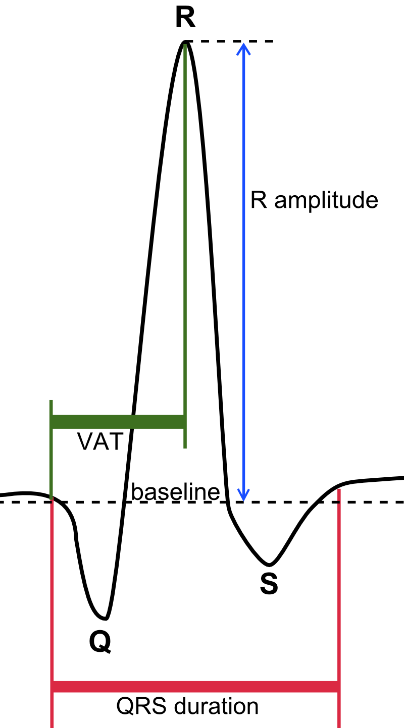
\includegraphics[width=0.25\textwidth]{qrs.png}
    \caption{QRS complex of a typical ECG.}
    \label{fig:qrs}
\end{figure}

The best filter is the cascade of IIR filters. The noise frequencies are not present in the IIR filtered
ECG spectrum. This is also true for the window and optimal FIR filters, but the window filter has a large
transition bandwidth, and the optimal filter has obvious passband ripple. Another advantage of the IIR
filter is that it is far more computationally efficient than the FIR filters. Only 4 memory elements are
needed for the IIR filter, whereas the FIR filters required 399 or 400. The IIR filter is more suitable
for applications with limited resources than the FIR filters. The IIR filter output is faster to compute
because fewer operations are required. The result is less delay in the output of the IIR filter compared
to the FIR filters. The non-linear phase response shown in Fig. 9 must be tolerated with the IIR filter. 

\section{Conclusion}
An ECG signal corrupted by additive noise at 32.6 Hz and 61.7 Hz was filtered by four different notch
filters – three FIR and one IIR. Each FIR filter has two notches at the noise frequencies. They were
designed using the window, optimal, and frequency-sampled methods. Functions from Python’s SciPy
library were used to design the window and optimal filters, and a script was written to implement
the frequency-sampled method. The IIR filter consists of two cascaded IIR notch filters, each with
two zeros and two poles. These were designed analytically with pole-zero placement.\\

\noindent The IIR filter was determined to be the best filter. It was the most computationally efficient.
The noise was not visible in the ECG spectrum after IIR filtering. It also showed less input-to-output
delay than the FIR filters. The disadvantage is that it has a non-linear phase response. The frequency-sampled
FIR filtered ECG signal still had noise present in its spectrum. The window FIR filter has a wide transition
bandwidth at 10 Hz, so frequencies neighbouring the noise were significantly attenuated. The optimal FIR
filter has good attenuation at the noise frequencies and a transition bandwidth equal to the IIR filters
but shows some passband ripple. 

\section*{References}
 

\noindent[1] J. O. Smith, "Spectral Audio Signal Processing," W3K Publishing, 2011.\\

\noindent[2] B. Porr, "Digital Signal Processing," [Online]. Available: \\
https://www.berndporr.me.uk/teaching/dsp\_handout45.pdf. [Accessed 10 08 2020].\\

\noindent[3] L. R. Rabiner, B. Gold and C. A. McGonegal, "An Approach to the Approximation Problem for Nonrecursive Digital Filters," IEEE Transactions on Audio and Electroacoustics, Vols. AU-18, no. 2, pp. 83-106, 1970.\\

\noindent[4] S. Hargittai, "Efficient and fast ECG baseline wander reduction without distortion of important clinical information," in Computers in Cardiology, Bologna, 2008.\\

\noindent[5] S. S. Joshi and P. Shrivastava, "ECG beat detection using wavelet denoising," in Proceedings of the First International Conference on Contours of Computing Technology, Mumbai, 2010.\\

\noindent[6] "ECG interpretation: Characteristics of the normal ECG (P-wave, QRS complex, ST segment, T-wave)," ECG \& Echo Learning, [Online]. Available:\\
https://ecgwaves.com/topic/ecg-normal-p-wave-qrs-complex-st-segment-t-wave-j-point/. [Accessed 10 08 2020].\\
\end{document}